\batchmode
\documentclass[twoside]{book}

% Packages required by doxygen
\usepackage{fixltx2e}
\usepackage{calc}
\usepackage{doxygen}
\usepackage[export]{adjustbox} % also loads graphicx
\usepackage{graphicx}
\usepackage[utf8]{inputenc}
\usepackage{makeidx}
\usepackage{multicol}
\usepackage{multirow}
\PassOptionsToPackage{warn}{textcomp}
\usepackage{textcomp}
\usepackage[nointegrals]{wasysym}
\usepackage[table]{xcolor}

% Font selection
\usepackage[T1]{fontenc}
\usepackage[scaled=.90]{helvet}
\usepackage{courier}
\usepackage{amssymb}
\usepackage{sectsty}
\renewcommand{\familydefault}{\sfdefault}
\allsectionsfont{%
  \fontseries{bc}\selectfont%
  \color{darkgray}%
}
\renewcommand{\DoxyLabelFont}{%
  \fontseries{bc}\selectfont%
  \color{darkgray}%
}
\newcommand{\+}{\discretionary{\mbox{\scriptsize$\hookleftarrow$}}{}{}}

% Page & text layout
\usepackage{geometry}
\geometry{%
  a4paper,%
  top=2.5cm,%
  bottom=2.5cm,%
  left=2.5cm,%
  right=2.5cm%
}
\tolerance=750
\hfuzz=15pt
\hbadness=750
\setlength{\emergencystretch}{15pt}
\setlength{\parindent}{0cm}
\setlength{\parskip}{3ex plus 2ex minus 2ex}
\makeatletter
\renewcommand{\paragraph}{%
  \@startsection{paragraph}{4}{0ex}{-1.0ex}{1.0ex}{%
    \normalfont\normalsize\bfseries\SS@parafont%
  }%
}
\renewcommand{\subparagraph}{%
  \@startsection{subparagraph}{5}{0ex}{-1.0ex}{1.0ex}{%
    \normalfont\normalsize\bfseries\SS@subparafont%
  }%
}
\makeatother

% Headers & footers
\usepackage{fancyhdr}
\pagestyle{fancyplain}
\fancyhead[LE]{\fancyplain{}{\bfseries\thepage}}
\fancyhead[CE]{\fancyplain{}{}}
\fancyhead[RE]{\fancyplain{}{\bfseries\leftmark}}
\fancyhead[LO]{\fancyplain{}{\bfseries\rightmark}}
\fancyhead[CO]{\fancyplain{}{}}
\fancyhead[RO]{\fancyplain{}{\bfseries\thepage}}
\fancyfoot[LE]{\fancyplain{}{}}
\fancyfoot[CE]{\fancyplain{}{}}
\fancyfoot[RE]{\fancyplain{}{\bfseries\scriptsize Generated by Doxygen }}
\fancyfoot[LO]{\fancyplain{}{\bfseries\scriptsize Generated by Doxygen }}
\fancyfoot[CO]{\fancyplain{}{}}
\fancyfoot[RO]{\fancyplain{}{}}
\renewcommand{\footrulewidth}{0.4pt}
\renewcommand{\chaptermark}[1]{%
  \markboth{#1}{}%
}
\renewcommand{\sectionmark}[1]{%
  \markright{\thesection\ #1}%
}

% Indices & bibliography
\usepackage{natbib}
\usepackage[titles]{tocloft}
\setcounter{tocdepth}{3}
\setcounter{secnumdepth}{5}
\makeindex

% Hyperlinks (required, but should be loaded last)
\usepackage{ifpdf}
\ifpdf
  \usepackage[pdftex,pagebackref=true]{hyperref}
\else
  \usepackage[ps2pdf,pagebackref=true]{hyperref}
\fi
\hypersetup{%
  colorlinks=true,%
  linkcolor=blue,%
  citecolor=blue,%
  unicode%
}

% Custom commands
\newcommand{\clearemptydoublepage}{%
  \newpage{\pagestyle{empty}\cleardoublepage}%
}

\usepackage{caption}
\captionsetup{labelsep=space,justification=centering,font={bf},singlelinecheck=off,skip=4pt,position=top}

%===== C O N T E N T S =====

\begin{document}

% Titlepage & ToC
\hypersetup{pageanchor=false,
             bookmarksnumbered=true,
             pdfencoding=unicode
            }
\pagenumbering{alph}
\pagenumbering{arabic}
\hypersetup{pageanchor=true}

%--- Begin generated contents ---
\chapter{The data structure}
\label{index}\hypertarget{index}{}\hypertarget{index_q}{}\section{A few quick questions...}\label{index_q}
Since {\ttfamily oomph-\/lib} is developed as open-\/source software, any evidence that the code is being downloaded and used is very helpful for us as it helps to justify our continued work on this project.

We would therefore be extremely grateful if you could provide the information requested in the form below. Pressing the \char`\"{}submit\char`\"{} button will get you to the actual download page.

{\bfseries Note\+:} 
\begin{DoxyItemize}
\item All information will be treated as confidential. 
\item If you provide your email address and check the appropriate box we will add you to our mailing list to inform you of upgrades and bug fixes to the code. Rest assured that the mailing list is {\bfseries very low volume} -- we have better things to do than to bombard you with email. 
\item If you still feel reluctant to provide any of the information requested, feel free to enter some dummy input. The form will check that {\bfseries some} information has been entered but entering your name as \char`\"{}\+Joe Cool\char`\"{} is perfectly acceptable -- this is to discourage people from not providing the information simply because they are too lazy to type... 
\end{DoxyItemize}



 







 

 \hypertarget{index_pdf}{}\section{P\+D\+F file}\label{index_pdf}
A \href{../latex/refman.pdf}{\tt pdf version} of this document is available. \end{document}

\chapter{Namespace Documentation}
\hypertarget{namespaceAnasazi}{}\section{Anasazi Namespace Reference}
\label{namespaceAnasazi}\index{Anasazi@{Anasazi}}
\subsection*{Classes}
\begin{DoxyCompactItemize}
\item 
class \hyperlink{classAnasazi_1_1MultiVecTraits_3_01double_00_01oomph_1_1DoubleMultiVector_01_4}{Multi\+Vec\+Traits$<$ double, oomph\+::\+Double\+Multi\+Vector $>$}
\item 
class \hyperlink{classAnasazi_1_1OperatorTraits_3_01double_00_01oomph_1_1DoubleMultiVector_00_01oomph_1_1DoubleMultiVectorOperator_01_4}{Operator\+Traits$<$ double, oomph\+::\+Double\+Multi\+Vector, oomph\+::\+Double\+Multi\+Vector\+Operator $>$}
\end{DoxyCompactItemize}

\hypertarget{namespaceoomph}{}\section{oomph Namespace Reference}
\label{namespaceoomph}\index{oomph@{oomph}}
\subsection*{Classes}
\begin{DoxyCompactItemize}
\item 
class \hyperlink{classoomph_1_1BellShellElement}{Bell\+Shell\+Element}
\begin{DoxyCompactList}\small\item\em \hyperlink{classoomph_1_1BellShellElement}{Bell\+Shell\+Element} elements are with subparametric interpolation for the function. \end{DoxyCompactList}\item 
class \hyperlink{classoomph_1_1FaceGeometry_3_01BellShellElement_3_01DIM_00_01NNODE__1D_01_4_01_4}{Face\+Geometry$<$ Bell\+Shell\+Element$<$ D\+I\+M, N\+N\+O\+D\+E\+\_\+1\+D $>$ $>$}
\item 
class \hyperlink{classoomph_1_1MyShellEquations}{My\+Shell\+Equations}
\item 
class \hyperlink{classoomph_1_1Plate}{Plate}
\begin{DoxyCompactList}\small\item\em Elliptical tube with half axes a and b. \end{DoxyCompactList}\end{DoxyCompactItemize}

\hypertarget{namespaceoomph_1_1AxisymmetricLinearElasticityTractionElementHelper}{}\section{oomph\+:\+:Axisymmetric\+Linear\+Elasticity\+Traction\+Element\+Helper Namespace Reference}
\label{namespaceoomph_1_1AxisymmetricLinearElasticityTractionElementHelper}\index{oomph\+::\+Axisymmetric\+Linear\+Elasticity\+Traction\+Element\+Helper@{oomph\+::\+Axisymmetric\+Linear\+Elasticity\+Traction\+Element\+Helper}}
\subsection*{Functions}
\begin{DoxyCompactItemize}
\item 
void \hyperlink{namespaceoomph_1_1AxisymmetricLinearElasticityTractionElementHelper_a1a493ca2845b4c81260fa82e9219063f}{Zero\+\_\+traction\+\_\+fct} (const double \&time, const \hyperlink{classoomph_1_1Vector}{Vector}$<$ double $>$ \&x, const \hyperlink{classoomph_1_1Vector}{Vector}$<$ double $>$ \&N, \hyperlink{classoomph_1_1Vector}{Vector}$<$ double $>$ \&load)
\begin{DoxyCompactList}\small\item\em Default load function (zero traction) \end{DoxyCompactList}\end{DoxyCompactItemize}


\subsection{Detailed Description}
Namespace containing the zero traction function for axisymmetric linear elasticity traction elements 

\subsection{Function Documentation}
\mbox{\Hypertarget{namespaceoomph_1_1AxisymmetricLinearElasticityTractionElementHelper_a1a493ca2845b4c81260fa82e9219063f}\label{namespaceoomph_1_1AxisymmetricLinearElasticityTractionElementHelper_a1a493ca2845b4c81260fa82e9219063f}} 
\index{oomph\+::\+Axisymmetric\+Linear\+Elasticity\+Traction\+Element\+Helper@{oomph\+::\+Axisymmetric\+Linear\+Elasticity\+Traction\+Element\+Helper}!Zero\+\_\+traction\+\_\+fct@{Zero\+\_\+traction\+\_\+fct}}
\index{Zero\+\_\+traction\+\_\+fct@{Zero\+\_\+traction\+\_\+fct}!oomph\+::\+Axisymmetric\+Linear\+Elasticity\+Traction\+Element\+Helper@{oomph\+::\+Axisymmetric\+Linear\+Elasticity\+Traction\+Element\+Helper}}
\subsubsection{\texorpdfstring{Zero\+\_\+traction\+\_\+fct()}{Zero\_traction\_fct()}}
{\footnotesize\ttfamily void oomph\+::\+Axisymmetric\+Linear\+Elasticity\+Traction\+Element\+Helper\+::\+Zero\+\_\+traction\+\_\+fct (\begin{DoxyParamCaption}\item[{const double \&}]{time,  }\item[{const \hyperlink{classoomph_1_1Vector}{Vector}$<$ double $>$ \&}]{x,  }\item[{const \hyperlink{classoomph_1_1Vector}{Vector}$<$ double $>$ \&}]{N,  }\item[{\hyperlink{classoomph_1_1Vector}{Vector}$<$ double $>$ \&}]{load }\end{DoxyParamCaption})}



Default load function (zero traction) 



Definition at line 62 of file axisym\+\_\+linear\+\_\+elasticity\+\_\+traction\+\_\+elements.\+h.



References i.



Referenced by oomph\+::\+Axisymmetric\+Linear\+Elasticity\+Traction\+Element$<$ E\+L\+E\+M\+E\+N\+T $>$\+::\+Axisymmetric\+Linear\+Elasticity\+Traction\+Element().


\hypertarget{namespaceoomph_1_1AxisymmetricNavierStokesTractionElementHelper}{}\section{oomph\+:\+:Axisymmetric\+Navier\+Stokes\+Traction\+Element\+Helper Namespace Reference}
\label{namespaceoomph_1_1AxisymmetricNavierStokesTractionElementHelper}\index{oomph\+::\+Axisymmetric\+Navier\+Stokes\+Traction\+Element\+Helper@{oomph\+::\+Axisymmetric\+Navier\+Stokes\+Traction\+Element\+Helper}}
\subsection*{Functions}
\begin{DoxyCompactItemize}
\item 
void \hyperlink{namespaceoomph_1_1AxisymmetricNavierStokesTractionElementHelper_aea96622278fde43851c31b0a559b829d}{Zero\+\_\+traction\+\_\+fct} (const double \&time, const \hyperlink{classoomph_1_1Vector}{Vector}$<$ double $>$ \&x, const \hyperlink{classoomph_1_1Vector}{Vector}$<$ double $>$ \&N, \hyperlink{classoomph_1_1Vector}{Vector}$<$ double $>$ \&load)
\begin{DoxyCompactList}\small\item\em Default load function (zero traction) \end{DoxyCompactList}\end{DoxyCompactItemize}


\subsection{Detailed Description}
Namespace containing the zero traction function for axisymmetric Navier Stokes traction elements 

\subsection{Function Documentation}
\mbox{\Hypertarget{namespaceoomph_1_1AxisymmetricNavierStokesTractionElementHelper_aea96622278fde43851c31b0a559b829d}\label{namespaceoomph_1_1AxisymmetricNavierStokesTractionElementHelper_aea96622278fde43851c31b0a559b829d}} 
\index{oomph\+::\+Axisymmetric\+Navier\+Stokes\+Traction\+Element\+Helper@{oomph\+::\+Axisymmetric\+Navier\+Stokes\+Traction\+Element\+Helper}!Zero\+\_\+traction\+\_\+fct@{Zero\+\_\+traction\+\_\+fct}}
\index{Zero\+\_\+traction\+\_\+fct@{Zero\+\_\+traction\+\_\+fct}!oomph\+::\+Axisymmetric\+Navier\+Stokes\+Traction\+Element\+Helper@{oomph\+::\+Axisymmetric\+Navier\+Stokes\+Traction\+Element\+Helper}}
\subsubsection{\texorpdfstring{Zero\+\_\+traction\+\_\+fct()}{Zero\_traction\_fct()}}
{\footnotesize\ttfamily void oomph\+::\+Axisymmetric\+Navier\+Stokes\+Traction\+Element\+Helper\+::\+Zero\+\_\+traction\+\_\+fct (\begin{DoxyParamCaption}\item[{const double \&}]{time,  }\item[{const \hyperlink{classoomph_1_1Vector}{Vector}$<$ double $>$ \&}]{x,  }\item[{const \hyperlink{classoomph_1_1Vector}{Vector}$<$ double $>$ \&}]{N,  }\item[{\hyperlink{classoomph_1_1Vector}{Vector}$<$ double $>$ \&}]{load }\end{DoxyParamCaption})}



Default load function (zero traction) 



Definition at line 54 of file axisym\+\_\+fluid\+\_\+traction\+\_\+elements.\+cc.



References i.



Referenced by oomph\+::\+Axisymmetric\+Navier\+Stokes\+Traction\+Element$<$ E\+L\+E\+M\+E\+N\+T $>$\+::\+Axisymmetric\+Navier\+Stokes\+Traction\+Element().


\hypertarget{namespaceoomph_1_1AxisymmetricPoroelasticityTractionElementHelper}{}\section{oomph\+:\+:Axisymmetric\+Poroelasticity\+Traction\+Element\+Helper Namespace Reference}
\label{namespaceoomph_1_1AxisymmetricPoroelasticityTractionElementHelper}\index{oomph\+::\+Axisymmetric\+Poroelasticity\+Traction\+Element\+Helper@{oomph\+::\+Axisymmetric\+Poroelasticity\+Traction\+Element\+Helper}}
\subsection*{Functions}
\begin{DoxyCompactItemize}
\item 
void \hyperlink{namespaceoomph_1_1AxisymmetricPoroelasticityTractionElementHelper_ac1b72b45f96c640e7ddc520ca5c2b251}{Zero\+\_\+traction\+\_\+fct} (const double \&time, const \hyperlink{classoomph_1_1Vector}{Vector}$<$ double $>$ \&x, const \hyperlink{classoomph_1_1Vector}{Vector}$<$ double $>$ \&N, \hyperlink{classoomph_1_1Vector}{Vector}$<$ double $>$ \&load)
\begin{DoxyCompactList}\small\item\em Default load function (zero traction) \end{DoxyCompactList}\item 
void \hyperlink{namespaceoomph_1_1AxisymmetricPoroelasticityTractionElementHelper_a8f4239ad8976b18eb097acb4b6446a6d}{Zero\+\_\+pressure\+\_\+fct} (const double \&time, const \hyperlink{classoomph_1_1Vector}{Vector}$<$ double $>$ \&x, const \hyperlink{classoomph_1_1Vector}{Vector}$<$ double $>$ \&N, double \&load)
\begin{DoxyCompactList}\small\item\em Default load function (zero pressure) \end{DoxyCompactList}\end{DoxyCompactItemize}
\subsection*{Variables}
\begin{DoxyCompactItemize}
\item 
bool \hyperlink{namespaceoomph_1_1AxisymmetricPoroelasticityTractionElementHelper_a3f8d9dbd05b5f4e7cc89157083db2ef0}{Allow\+\_\+gap\+\_\+in\+\_\+\+F\+SI} =false
\begin{DoxyCompactList}\small\item\em Public boolean to allow gap between poro-\/elastic and Navier Stokes element in F\+SI computations. Useful in hybrid linear/nonlinear geometry runs where this will happen. \end{DoxyCompactList}\end{DoxyCompactItemize}


\subsection{Detailed Description}
Namespace containing the zero pressure function for Darcy pressure elements 

\subsection{Function Documentation}
\mbox{\Hypertarget{namespaceoomph_1_1AxisymmetricPoroelasticityTractionElementHelper_a8f4239ad8976b18eb097acb4b6446a6d}\label{namespaceoomph_1_1AxisymmetricPoroelasticityTractionElementHelper_a8f4239ad8976b18eb097acb4b6446a6d}} 
\index{oomph\+::\+Axisymmetric\+Poroelasticity\+Traction\+Element\+Helper@{oomph\+::\+Axisymmetric\+Poroelasticity\+Traction\+Element\+Helper}!Zero\+\_\+pressure\+\_\+fct@{Zero\+\_\+pressure\+\_\+fct}}
\index{Zero\+\_\+pressure\+\_\+fct@{Zero\+\_\+pressure\+\_\+fct}!oomph\+::\+Axisymmetric\+Poroelasticity\+Traction\+Element\+Helper@{oomph\+::\+Axisymmetric\+Poroelasticity\+Traction\+Element\+Helper}}
\subsubsection{\texorpdfstring{Zero\+\_\+pressure\+\_\+fct()}{Zero\_pressure\_fct()}}
{\footnotesize\ttfamily void oomph\+::\+Axisymmetric\+Poroelasticity\+Traction\+Element\+Helper\+::\+Zero\+\_\+pressure\+\_\+fct (\begin{DoxyParamCaption}\item[{const double \&}]{time,  }\item[{const \hyperlink{classoomph_1_1Vector}{Vector}$<$ double $>$ \&}]{x,  }\item[{const \hyperlink{classoomph_1_1Vector}{Vector}$<$ double $>$ \&}]{N,  }\item[{double \&}]{load }\end{DoxyParamCaption})}



Default load function (zero pressure) 



Definition at line 73 of file axisym\+\_\+poroelasticity\+\_\+face\+\_\+elements.\+h.



Referenced by oomph\+::\+Axisymmetric\+Poroelasticity\+Traction\+Element$<$ P\+O\+R\+O\+E\+L\+A\+S\+T\+I\+C\+I\+T\+Y\+\_\+\+B\+U\+L\+K\+\_\+\+E\+L\+E\+M\+E\+N\+T $>$\+::\+Axisymmetric\+Poroelasticity\+Traction\+Element().

\mbox{\Hypertarget{namespaceoomph_1_1AxisymmetricPoroelasticityTractionElementHelper_ac1b72b45f96c640e7ddc520ca5c2b251}\label{namespaceoomph_1_1AxisymmetricPoroelasticityTractionElementHelper_ac1b72b45f96c640e7ddc520ca5c2b251}} 
\index{oomph\+::\+Axisymmetric\+Poroelasticity\+Traction\+Element\+Helper@{oomph\+::\+Axisymmetric\+Poroelasticity\+Traction\+Element\+Helper}!Zero\+\_\+traction\+\_\+fct@{Zero\+\_\+traction\+\_\+fct}}
\index{Zero\+\_\+traction\+\_\+fct@{Zero\+\_\+traction\+\_\+fct}!oomph\+::\+Axisymmetric\+Poroelasticity\+Traction\+Element\+Helper@{oomph\+::\+Axisymmetric\+Poroelasticity\+Traction\+Element\+Helper}}
\subsubsection{\texorpdfstring{Zero\+\_\+traction\+\_\+fct()}{Zero\_traction\_fct()}}
{\footnotesize\ttfamily void oomph\+::\+Axisymmetric\+Poroelasticity\+Traction\+Element\+Helper\+::\+Zero\+\_\+traction\+\_\+fct (\begin{DoxyParamCaption}\item[{const double \&}]{time,  }\item[{const \hyperlink{classoomph_1_1Vector}{Vector}$<$ double $>$ \&}]{x,  }\item[{const \hyperlink{classoomph_1_1Vector}{Vector}$<$ double $>$ \&}]{N,  }\item[{\hyperlink{classoomph_1_1Vector}{Vector}$<$ double $>$ \&}]{load }\end{DoxyParamCaption})}



Default load function (zero traction) 



Definition at line 61 of file axisym\+\_\+poroelasticity\+\_\+face\+\_\+elements.\+h.



References i.



Referenced by oomph\+::\+Axisymmetric\+Poroelasticity\+Traction\+Element$<$ P\+O\+R\+O\+E\+L\+A\+S\+T\+I\+C\+I\+T\+Y\+\_\+\+B\+U\+L\+K\+\_\+\+E\+L\+E\+M\+E\+N\+T $>$\+::\+Axisymmetric\+Poroelasticity\+Traction\+Element().



\subsection{Variable Documentation}
\mbox{\Hypertarget{namespaceoomph_1_1AxisymmetricPoroelasticityTractionElementHelper_a3f8d9dbd05b5f4e7cc89157083db2ef0}\label{namespaceoomph_1_1AxisymmetricPoroelasticityTractionElementHelper_a3f8d9dbd05b5f4e7cc89157083db2ef0}} 
\index{oomph\+::\+Axisymmetric\+Poroelasticity\+Traction\+Element\+Helper@{oomph\+::\+Axisymmetric\+Poroelasticity\+Traction\+Element\+Helper}!Allow\+\_\+gap\+\_\+in\+\_\+\+F\+SI@{Allow\+\_\+gap\+\_\+in\+\_\+\+F\+SI}}
\index{Allow\+\_\+gap\+\_\+in\+\_\+\+F\+SI@{Allow\+\_\+gap\+\_\+in\+\_\+\+F\+SI}!oomph\+::\+Axisymmetric\+Poroelasticity\+Traction\+Element\+Helper@{oomph\+::\+Axisymmetric\+Poroelasticity\+Traction\+Element\+Helper}}
\subsubsection{\texorpdfstring{Allow\+\_\+gap\+\_\+in\+\_\+\+F\+SI}{Allow\_gap\_in\_FSI}}
{\footnotesize\ttfamily bool oomph\+::\+Axisymmetric\+Poroelasticity\+Traction\+Element\+Helper\+::\+Allow\+\_\+gap\+\_\+in\+\_\+\+F\+SI =false}



Public boolean to allow gap between poro-\/elastic and Navier Stokes element in F\+SI computations. Useful in hybrid linear/nonlinear geometry runs where this will happen. 



Definition at line 84 of file axisym\+\_\+poroelasticity\+\_\+face\+\_\+elements.\+h.



Referenced by oomph\+::\+Linearised\+Axisym\+Poroelastic\+B\+J\+S\+\_\+\+F\+S\+I\+Element$<$ F\+L\+U\+I\+D\+\_\+\+B\+U\+L\+K\+\_\+\+E\+L\+E\+M\+E\+N\+T, P\+O\+R\+O\+E\+L\+A\+S\+T\+I\+C\+I\+T\+Y\+\_\+\+B\+U\+L\+K\+\_\+\+E\+L\+E\+M\+E\+N\+T $>$\+::contribution\+\_\+to\+\_\+total\+\_\+porous\+\_\+flux(), oomph\+::\+F\+S\+I\+Linearised\+Axisym\+Poroelastic\+Traction\+Element$<$ P\+O\+R\+O\+E\+L\+A\+S\+T\+I\+C\+I\+T\+Y\+\_\+\+B\+U\+L\+K\+\_\+\+E\+L\+E\+M\+E\+N\+T, N\+A\+V\+I\+E\+R\+\_\+\+S\+T\+O\+K\+E\+S\+\_\+\+B\+U\+L\+K\+\_\+\+E\+L\+E\+M\+E\+N\+T $>$\+::get\+\_\+traction(), and oomph\+::\+Linearised\+Axisym\+Poroelastic\+B\+J\+S\+\_\+\+F\+S\+I\+Element$<$ F\+L\+U\+I\+D\+\_\+\+B\+U\+L\+K\+\_\+\+E\+L\+E\+M\+E\+N\+T, P\+O\+R\+O\+E\+L\+A\+S\+T\+I\+C\+I\+T\+Y\+\_\+\+B\+U\+L\+K\+\_\+\+E\+L\+E\+M\+E\+N\+T $>$\+::output().


\hypertarget{namespaceoomph_1_1Biharmonic__schur__complement__Hypre__defaults}{}\section{oomph\+:\+:Biharmonic\+\_\+schur\+\_\+complement\+\_\+\+Hypre\+\_\+defaults Namespace Reference}
\label{namespaceoomph_1_1Biharmonic__schur__complement__Hypre__defaults}\index{oomph\+::\+Biharmonic\+\_\+schur\+\_\+complement\+\_\+\+Hypre\+\_\+defaults@{oomph\+::\+Biharmonic\+\_\+schur\+\_\+complement\+\_\+\+Hypre\+\_\+defaults}}
\subsection*{Functions}
\begin{DoxyCompactItemize}
\item 
void \hyperlink{namespaceoomph_1_1Biharmonic__schur__complement__Hypre__defaults_acff454a359087ff5bcdc63521c9e6228}{set\+\_\+defaults} (\hyperlink{classoomph_1_1HyprePreconditioner}{Hypre\+Preconditioner} $\ast$hypre\+\_\+prec\+\_\+pt)
\begin{DoxyCompactList}\small\item\em set the defaults \end{DoxyCompactList}\end{DoxyCompactItemize}
\subsection*{Variables}
\begin{DoxyCompactItemize}
\item 
unsigned \hyperlink{namespaceoomph_1_1Biharmonic__schur__complement__Hypre__defaults_ab6c010a72ca50be6be38ea9bd5b44207}{A\+M\+G\+\_\+smoother} = 1
\begin{DoxyCompactList}\small\item\em smoother type -\/ \hyperlink{classoomph_1_1Gauss}{Gauss} Seidel\+: 1 \end{DoxyCompactList}\item 
unsigned \hyperlink{namespaceoomph_1_1Biharmonic__schur__complement__Hypre__defaults_ad2bc859a57f88c9e48b7bada12072a53}{A\+M\+G\+\_\+coarsening} = 1
\begin{DoxyCompactList}\small\item\em amg coarsening strategy\+: classical Ruge Stueben\+: 1 \end{DoxyCompactList}\item 
unsigned \hyperlink{namespaceoomph_1_1Biharmonic__schur__complement__Hypre__defaults_a551840dd4e8b9965373a34d4812737bf}{N\+\_\+cycle} = 2
\begin{DoxyCompactList}\small\item\em number of V cycles\+: 2 \end{DoxyCompactList}\item 
double \hyperlink{namespaceoomph_1_1Biharmonic__schur__complement__Hypre__defaults_add427c041f6e292957a23376feb5bb89}{A\+M\+G\+\_\+strength} = 0.\+25
\begin{DoxyCompactList}\small\item\em amg strength parameter\+: 0.\+25 -- optimal for 2d \end{DoxyCompactList}\item 
double \hyperlink{namespaceoomph_1_1Biharmonic__schur__complement__Hypre__defaults_a88ea130601c20b76b2895c48803d2be5}{A\+M\+G\+\_\+jacobi\+\_\+damping} = 0.\+1
\begin{DoxyCompactList}\small\item\em jacobi damping -- hierher not used 0.\+1 \end{DoxyCompactList}\item 
unsigned \hyperlink{namespaceoomph_1_1Biharmonic__schur__complement__Hypre__defaults_af1e2bbd2c7203fe3166489c111f3b166}{A\+M\+G\+\_\+smoother\+\_\+iterations} =2
\begin{DoxyCompactList}\small\item\em amg smoother iterations \end{DoxyCompactList}\end{DoxyCompactItemize}


\subsection{Function Documentation}
\mbox{\Hypertarget{namespaceoomph_1_1Biharmonic__schur__complement__Hypre__defaults_acff454a359087ff5bcdc63521c9e6228}\label{namespaceoomph_1_1Biharmonic__schur__complement__Hypre__defaults_acff454a359087ff5bcdc63521c9e6228}} 
\index{oomph\+::\+Biharmonic\+\_\+schur\+\_\+complement\+\_\+\+Hypre\+\_\+defaults@{oomph\+::\+Biharmonic\+\_\+schur\+\_\+complement\+\_\+\+Hypre\+\_\+defaults}!set\+\_\+defaults@{set\+\_\+defaults}}
\index{set\+\_\+defaults@{set\+\_\+defaults}!oomph\+::\+Biharmonic\+\_\+schur\+\_\+complement\+\_\+\+Hypre\+\_\+defaults@{oomph\+::\+Biharmonic\+\_\+schur\+\_\+complement\+\_\+\+Hypre\+\_\+defaults}}
\subsubsection{\texorpdfstring{set\+\_\+defaults()}{set\_defaults()}}
{\footnotesize\ttfamily void oomph\+::\+Biharmonic\+\_\+schur\+\_\+complement\+\_\+\+Hypre\+\_\+defaults\+::set\+\_\+defaults (\begin{DoxyParamCaption}\item[{\hyperlink{classoomph_1_1HyprePreconditioner}{Hypre\+Preconditioner} $\ast$}]{hypre\+\_\+prec\+\_\+pt }\end{DoxyParamCaption})}



set the defaults 



Definition at line 72 of file biharmonic\+\_\+preconditioner.\+cc.



References A\+M\+G\+\_\+coarsening, oomph\+::\+Hypre\+Preconditioner\+::amg\+\_\+coarsening(), oomph\+::\+Hypre\+Preconditioner\+::amg\+\_\+iterations(), oomph\+::\+Hypre\+Preconditioner\+::amg\+\_\+simple\+\_\+smoother(), A\+M\+G\+\_\+smoother, A\+M\+G\+\_\+smoother\+\_\+iterations, oomph\+::\+Hypre\+Preconditioner\+::amg\+\_\+smoother\+\_\+iterations(), A\+M\+G\+\_\+strength, oomph\+::\+Hypre\+Preconditioner\+::amg\+\_\+strength(), oomph\+::\+Hypre\+Interface\+::\+Boomer\+A\+MG, oomph\+::\+Hypre\+Preconditioner\+::hypre\+\_\+method(), N\+\_\+cycle, and oomph\+::oomph\+\_\+info.



Referenced by oomph\+::\+Inexact\+Sub\+Biharmonic\+Preconditioner\+::setup().



\subsection{Variable Documentation}
\mbox{\Hypertarget{namespaceoomph_1_1Biharmonic__schur__complement__Hypre__defaults_ad2bc859a57f88c9e48b7bada12072a53}\label{namespaceoomph_1_1Biharmonic__schur__complement__Hypre__defaults_ad2bc859a57f88c9e48b7bada12072a53}} 
\index{oomph\+::\+Biharmonic\+\_\+schur\+\_\+complement\+\_\+\+Hypre\+\_\+defaults@{oomph\+::\+Biharmonic\+\_\+schur\+\_\+complement\+\_\+\+Hypre\+\_\+defaults}!A\+M\+G\+\_\+coarsening@{A\+M\+G\+\_\+coarsening}}
\index{A\+M\+G\+\_\+coarsening@{A\+M\+G\+\_\+coarsening}!oomph\+::\+Biharmonic\+\_\+schur\+\_\+complement\+\_\+\+Hypre\+\_\+defaults@{oomph\+::\+Biharmonic\+\_\+schur\+\_\+complement\+\_\+\+Hypre\+\_\+defaults}}
\subsubsection{\texorpdfstring{A\+M\+G\+\_\+coarsening}{AMG\_coarsening}}
{\footnotesize\ttfamily unsigned oomph\+::\+Biharmonic\+\_\+schur\+\_\+complement\+\_\+\+Hypre\+\_\+defaults\+::\+A\+M\+G\+\_\+coarsening = 1}



amg coarsening strategy\+: classical Ruge Stueben\+: 1 



Definition at line 57 of file biharmonic\+\_\+preconditioner.\+cc.



Referenced by set\+\_\+defaults().

\mbox{\Hypertarget{namespaceoomph_1_1Biharmonic__schur__complement__Hypre__defaults_a88ea130601c20b76b2895c48803d2be5}\label{namespaceoomph_1_1Biharmonic__schur__complement__Hypre__defaults_a88ea130601c20b76b2895c48803d2be5}} 
\index{oomph\+::\+Biharmonic\+\_\+schur\+\_\+complement\+\_\+\+Hypre\+\_\+defaults@{oomph\+::\+Biharmonic\+\_\+schur\+\_\+complement\+\_\+\+Hypre\+\_\+defaults}!A\+M\+G\+\_\+jacobi\+\_\+damping@{A\+M\+G\+\_\+jacobi\+\_\+damping}}
\index{A\+M\+G\+\_\+jacobi\+\_\+damping@{A\+M\+G\+\_\+jacobi\+\_\+damping}!oomph\+::\+Biharmonic\+\_\+schur\+\_\+complement\+\_\+\+Hypre\+\_\+defaults@{oomph\+::\+Biharmonic\+\_\+schur\+\_\+complement\+\_\+\+Hypre\+\_\+defaults}}
\subsubsection{\texorpdfstring{A\+M\+G\+\_\+jacobi\+\_\+damping}{AMG\_jacobi\_damping}}
{\footnotesize\ttfamily double oomph\+::\+Biharmonic\+\_\+schur\+\_\+complement\+\_\+\+Hypre\+\_\+defaults\+::\+A\+M\+G\+\_\+jacobi\+\_\+damping = 0.\+1}



jacobi damping -- hierher not used 0.\+1 

jacobi damping -- hierher not used 0.\+1; 

Definition at line 66 of file biharmonic\+\_\+preconditioner.\+cc.

\mbox{\Hypertarget{namespaceoomph_1_1Biharmonic__schur__complement__Hypre__defaults_ab6c010a72ca50be6be38ea9bd5b44207}\label{namespaceoomph_1_1Biharmonic__schur__complement__Hypre__defaults_ab6c010a72ca50be6be38ea9bd5b44207}} 
\index{oomph\+::\+Biharmonic\+\_\+schur\+\_\+complement\+\_\+\+Hypre\+\_\+defaults@{oomph\+::\+Biharmonic\+\_\+schur\+\_\+complement\+\_\+\+Hypre\+\_\+defaults}!A\+M\+G\+\_\+smoother@{A\+M\+G\+\_\+smoother}}
\index{A\+M\+G\+\_\+smoother@{A\+M\+G\+\_\+smoother}!oomph\+::\+Biharmonic\+\_\+schur\+\_\+complement\+\_\+\+Hypre\+\_\+defaults@{oomph\+::\+Biharmonic\+\_\+schur\+\_\+complement\+\_\+\+Hypre\+\_\+defaults}}
\subsubsection{\texorpdfstring{A\+M\+G\+\_\+smoother}{AMG\_smoother}}
{\footnotesize\ttfamily unsigned oomph\+::\+Biharmonic\+\_\+schur\+\_\+complement\+\_\+\+Hypre\+\_\+defaults\+::\+A\+M\+G\+\_\+smoother = 1}



smoother type -\/ \hyperlink{classoomph_1_1Gauss}{Gauss} Seidel\+: 1 



Definition at line 54 of file biharmonic\+\_\+preconditioner.\+cc.



Referenced by set\+\_\+defaults().

\mbox{\Hypertarget{namespaceoomph_1_1Biharmonic__schur__complement__Hypre__defaults_af1e2bbd2c7203fe3166489c111f3b166}\label{namespaceoomph_1_1Biharmonic__schur__complement__Hypre__defaults_af1e2bbd2c7203fe3166489c111f3b166}} 
\index{oomph\+::\+Biharmonic\+\_\+schur\+\_\+complement\+\_\+\+Hypre\+\_\+defaults@{oomph\+::\+Biharmonic\+\_\+schur\+\_\+complement\+\_\+\+Hypre\+\_\+defaults}!A\+M\+G\+\_\+smoother\+\_\+iterations@{A\+M\+G\+\_\+smoother\+\_\+iterations}}
\index{A\+M\+G\+\_\+smoother\+\_\+iterations@{A\+M\+G\+\_\+smoother\+\_\+iterations}!oomph\+::\+Biharmonic\+\_\+schur\+\_\+complement\+\_\+\+Hypre\+\_\+defaults@{oomph\+::\+Biharmonic\+\_\+schur\+\_\+complement\+\_\+\+Hypre\+\_\+defaults}}
\subsubsection{\texorpdfstring{A\+M\+G\+\_\+smoother\+\_\+iterations}{AMG\_smoother\_iterations}}
{\footnotesize\ttfamily unsigned oomph\+::\+Biharmonic\+\_\+schur\+\_\+complement\+\_\+\+Hypre\+\_\+defaults\+::\+A\+M\+G\+\_\+smoother\+\_\+iterations =2}



amg smoother iterations 

Amg smoother iterations\+: 2. 

Definition at line 69 of file biharmonic\+\_\+preconditioner.\+cc.



Referenced by oomph\+::\+Hypre\+Solver\+::amg\+\_\+smoother\+\_\+iterations(), oomph\+::\+Hypre\+Preconditioner\+::amg\+\_\+smoother\+\_\+iterations(), oomph\+::\+Hypre\+Interface\+::hypre\+\_\+solver\+\_\+setup(), oomph\+::\+Hypre\+Interface\+::\+Hypre\+Interface(), and set\+\_\+defaults().

\mbox{\Hypertarget{namespaceoomph_1_1Biharmonic__schur__complement__Hypre__defaults_add427c041f6e292957a23376feb5bb89}\label{namespaceoomph_1_1Biharmonic__schur__complement__Hypre__defaults_add427c041f6e292957a23376feb5bb89}} 
\index{oomph\+::\+Biharmonic\+\_\+schur\+\_\+complement\+\_\+\+Hypre\+\_\+defaults@{oomph\+::\+Biharmonic\+\_\+schur\+\_\+complement\+\_\+\+Hypre\+\_\+defaults}!A\+M\+G\+\_\+strength@{A\+M\+G\+\_\+strength}}
\index{A\+M\+G\+\_\+strength@{A\+M\+G\+\_\+strength}!oomph\+::\+Biharmonic\+\_\+schur\+\_\+complement\+\_\+\+Hypre\+\_\+defaults@{oomph\+::\+Biharmonic\+\_\+schur\+\_\+complement\+\_\+\+Hypre\+\_\+defaults}}
\subsubsection{\texorpdfstring{A\+M\+G\+\_\+strength}{AMG\_strength}}
{\footnotesize\ttfamily double oomph\+::\+Biharmonic\+\_\+schur\+\_\+complement\+\_\+\+Hypre\+\_\+defaults\+::\+A\+M\+G\+\_\+strength = 0.\+25}



amg strength parameter\+: 0.\+25 -- optimal for 2d 



Definition at line 63 of file biharmonic\+\_\+preconditioner.\+cc.



Referenced by set\+\_\+defaults().

\mbox{\Hypertarget{namespaceoomph_1_1Biharmonic__schur__complement__Hypre__defaults_a551840dd4e8b9965373a34d4812737bf}\label{namespaceoomph_1_1Biharmonic__schur__complement__Hypre__defaults_a551840dd4e8b9965373a34d4812737bf}} 
\index{oomph\+::\+Biharmonic\+\_\+schur\+\_\+complement\+\_\+\+Hypre\+\_\+defaults@{oomph\+::\+Biharmonic\+\_\+schur\+\_\+complement\+\_\+\+Hypre\+\_\+defaults}!N\+\_\+cycle@{N\+\_\+cycle}}
\index{N\+\_\+cycle@{N\+\_\+cycle}!oomph\+::\+Biharmonic\+\_\+schur\+\_\+complement\+\_\+\+Hypre\+\_\+defaults@{oomph\+::\+Biharmonic\+\_\+schur\+\_\+complement\+\_\+\+Hypre\+\_\+defaults}}
\subsubsection{\texorpdfstring{N\+\_\+cycle}{N\_cycle}}
{\footnotesize\ttfamily unsigned oomph\+::\+Biharmonic\+\_\+schur\+\_\+complement\+\_\+\+Hypre\+\_\+defaults\+::\+N\+\_\+cycle = 2}



number of V cycles\+: 2 



Definition at line 60 of file biharmonic\+\_\+preconditioner.\+cc.



Referenced by set\+\_\+defaults().


\hypertarget{namespaceoomph_1_1BinaryTreeNames}{}\section{oomph\+:\+:Binary\+Tree\+Names Namespace Reference}
\label{namespaceoomph_1_1BinaryTreeNames}\index{oomph\+::\+Binary\+Tree\+Names@{oomph\+::\+Binary\+Tree\+Names}}


Namespace for \hyperlink{classoomph_1_1BinaryTree}{Binary\+Tree} directions.  


\subsection*{Enumerations}
\begin{DoxyCompactItemize}
\item 
enum \{ \hyperlink{namespaceoomph_1_1BinaryTreeNames_a7ff5e7e46beae31bf81579531b1f9895a8df863dabb4096fa066f7a6dbf7502d1}{L}, 
\hyperlink{namespaceoomph_1_1BinaryTreeNames_a7ff5e7e46beae31bf81579531b1f9895a1bf47d3f36e6272d94344ae84aca2498}{R}, 
\hyperlink{namespaceoomph_1_1BinaryTreeNames_a7ff5e7e46beae31bf81579531b1f9895afbb1d921b86ded476b8bee384d9059e1}{O\+M\+E\+GA} =26
 \}\begin{DoxyCompactList}\small\item\em Directions (L/R). O\+M\+E\+GA is used if a direction is undefined in a certain context. \end{DoxyCompactList}
\end{DoxyCompactItemize}


\subsection{Detailed Description}
Namespace for \hyperlink{classoomph_1_1BinaryTree}{Binary\+Tree} directions. 

\subsection{Enumeration Type Documentation}
\mbox{\Hypertarget{namespaceoomph_1_1BinaryTreeNames_a7ff5e7e46beae31bf81579531b1f9895}\label{namespaceoomph_1_1BinaryTreeNames_a7ff5e7e46beae31bf81579531b1f9895}} 
\subsubsection{\texorpdfstring{anonymous enum}{anonymous enum}}
{\footnotesize\ttfamily anonymous enum}



Directions (L/R). O\+M\+E\+GA is used if a direction is undefined in a certain context. 

\begin{DoxyEnumFields}{Enumerator}
\raisebox{\heightof{T}}[0pt][0pt]{\index{L@{L}!oomph\+::\+Binary\+Tree\+Names@{oomph\+::\+Binary\+Tree\+Names}}\index{oomph\+::\+Binary\+Tree\+Names@{oomph\+::\+Binary\+Tree\+Names}!L@{L}}}\mbox{\Hypertarget{namespaceoomph_1_1BinaryTreeNames_a7ff5e7e46beae31bf81579531b1f9895a8df863dabb4096fa066f7a6dbf7502d1}\label{namespaceoomph_1_1BinaryTreeNames_a7ff5e7e46beae31bf81579531b1f9895a8df863dabb4096fa066f7a6dbf7502d1}} 
L&\\
\hline

\raisebox{\heightof{T}}[0pt][0pt]{\index{R@{R}!oomph\+::\+Binary\+Tree\+Names@{oomph\+::\+Binary\+Tree\+Names}}\index{oomph\+::\+Binary\+Tree\+Names@{oomph\+::\+Binary\+Tree\+Names}!R@{R}}}\mbox{\Hypertarget{namespaceoomph_1_1BinaryTreeNames_a7ff5e7e46beae31bf81579531b1f9895a1bf47d3f36e6272d94344ae84aca2498}\label{namespaceoomph_1_1BinaryTreeNames_a7ff5e7e46beae31bf81579531b1f9895a1bf47d3f36e6272d94344ae84aca2498}} 
R&\\
\hline

\raisebox{\heightof{T}}[0pt][0pt]{\index{O\+M\+E\+GA@{O\+M\+E\+GA}!oomph\+::\+Binary\+Tree\+Names@{oomph\+::\+Binary\+Tree\+Names}}\index{oomph\+::\+Binary\+Tree\+Names@{oomph\+::\+Binary\+Tree\+Names}!O\+M\+E\+GA@{O\+M\+E\+GA}}}\mbox{\Hypertarget{namespaceoomph_1_1BinaryTreeNames_a7ff5e7e46beae31bf81579531b1f9895afbb1d921b86ded476b8bee384d9059e1}\label{namespaceoomph_1_1BinaryTreeNames_a7ff5e7e46beae31bf81579531b1f9895afbb1d921b86ded476b8bee384d9059e1}} 
O\+M\+E\+GA&\\
\hline

\end{DoxyEnumFields}


Definition at line 52 of file binary\+\_\+tree.\+h.


\hypertarget{namespaceoomph_1_1BlackBoxFDNewtonSolver}{}\section{oomph\+:\+:Black\+Box\+F\+D\+Newton\+Solver Namespace Reference}
\label{namespaceoomph_1_1BlackBoxFDNewtonSolver}\index{oomph\+::\+Black\+Box\+F\+D\+Newton\+Solver@{oomph\+::\+Black\+Box\+F\+D\+Newton\+Solver}}


Namespace for black-\/box FD Newton solver.  


\subsection*{Typedefs}
\begin{DoxyCompactItemize}
\item 
typedef void($\ast$ \hyperlink{namespaceoomph_1_1BlackBoxFDNewtonSolver_a0b45d0bd1b7ae8ff5c24715b6118d1fd}{Residual\+Fct\+Pt}) (const \hyperlink{classoomph_1_1Vector}{Vector}$<$ double $>$ \&, const \hyperlink{classoomph_1_1Vector}{Vector}$<$ double $>$ \&, \hyperlink{classoomph_1_1Vector}{Vector}$<$ double $>$ \&)
\begin{DoxyCompactList}\small\item\em Function pointer for residual function\+: Parameters, unknowns, residuals. \end{DoxyCompactList}\end{DoxyCompactItemize}
\subsection*{Functions}
\begin{DoxyCompactItemize}
\item 
void \hyperlink{namespaceoomph_1_1BlackBoxFDNewtonSolver_ad3ba3031554be43788d296a7a4dddd67}{black\+\_\+box\+\_\+fd\+\_\+newton\+\_\+solve} (\hyperlink{namespaceoomph_1_1BlackBoxFDNewtonSolver_a0b45d0bd1b7ae8ff5c24715b6118d1fd}{Residual\+Fct\+Pt} residual\+\_\+fct, const \hyperlink{classoomph_1_1Vector}{Vector}$<$ double $>$ \&params, \hyperlink{classoomph_1_1Vector}{Vector}$<$ double $>$ \&unknowns)
\begin{DoxyCompactList}\small\item\em Black-\/box FD Newton solver\+: Calling sequence for residual function is. \end{DoxyCompactList}\item 
void \hyperlink{namespaceoomph_1_1BlackBoxFDNewtonSolver_a4a1361a9b08163b59fe82b3042b0f887}{line\+\_\+search} (const \hyperlink{classoomph_1_1Vector}{Vector}$<$ double $>$ \&x\+\_\+old, const double half\+\_\+residual\+\_\+squared\+\_\+old, const \hyperlink{classoomph_1_1Vector}{Vector}$<$ double $>$ \&gradient, \hyperlink{namespaceoomph_1_1BlackBoxFDNewtonSolver_a0b45d0bd1b7ae8ff5c24715b6118d1fd}{Residual\+Fct\+Pt} residual\+\_\+fct, const \hyperlink{classoomph_1_1Vector}{Vector}$<$ double $>$ \&params, \hyperlink{classoomph_1_1Vector}{Vector}$<$ double $>$ \&newton\+\_\+dir, \hyperlink{classoomph_1_1Vector}{Vector}$<$ double $>$ \&x, double \&half\+\_\+residual\+\_\+squared, const double \&stpmax)
\begin{DoxyCompactList}\small\item\em Line search helper for globally convergent Newton method. \end{DoxyCompactList}\end{DoxyCompactItemize}
\subsection*{Variables}
\begin{DoxyCompactItemize}
\item 
unsigned \hyperlink{namespaceoomph_1_1BlackBoxFDNewtonSolver_a20ac8568daf0d63afa3945a817ff3e2d}{Max\+\_\+iter} =20
\begin{DoxyCompactList}\small\item\em Max. \# of Newton iterations. \end{DoxyCompactList}\item 
unsigned \hyperlink{namespaceoomph_1_1BlackBoxFDNewtonSolver_a3067ba88fad991fdb619eae7533028bd}{N\+\_\+iter\+\_\+taken} =0
\begin{DoxyCompactList}\small\item\em Number of Newton iterations taken in most recent invocation. \end{DoxyCompactList}\item 
bool \hyperlink{namespaceoomph_1_1BlackBoxFDNewtonSolver_ac2603699f47446716ca5a818f46a7f17}{Doc\+\_\+\+Progress} =false
\begin{DoxyCompactList}\small\item\em Flag to indicate if progress of Newton iteration is to be documented (defaults to false) \end{DoxyCompactList}\item 
double \hyperlink{namespaceoomph_1_1BlackBoxFDNewtonSolver_a6f0d2ceb4451e66bb7ef4ab4fdb62bcf}{F\+D\+\_\+step} =1.\+0e-\/8
\begin{DoxyCompactList}\small\item\em FD step. \end{DoxyCompactList}\item 
double \hyperlink{namespaceoomph_1_1BlackBoxFDNewtonSolver_a4bacc59c8e1194e553f698530e9e945e}{Tol} =1.\+0e-\/8
\begin{DoxyCompactList}\small\item\em Tolerance. \end{DoxyCompactList}\item 
bool \hyperlink{namespaceoomph_1_1BlackBoxFDNewtonSolver_afd90cb451fb7ae5a8e30cab0a1884568}{Use\+\_\+step\+\_\+length\+\_\+control} =false
\begin{DoxyCompactList}\small\item\em Use steplength control do make globally convergent (default false) \end{DoxyCompactList}\end{DoxyCompactItemize}


\subsection{Detailed Description}
Namespace for black-\/box FD Newton solver. 

\subsection{Typedef Documentation}
\mbox{\Hypertarget{namespaceoomph_1_1BlackBoxFDNewtonSolver_a0b45d0bd1b7ae8ff5c24715b6118d1fd}\label{namespaceoomph_1_1BlackBoxFDNewtonSolver_a0b45d0bd1b7ae8ff5c24715b6118d1fd}} 
\index{oomph\+::\+Black\+Box\+F\+D\+Newton\+Solver@{oomph\+::\+Black\+Box\+F\+D\+Newton\+Solver}!Residual\+Fct\+Pt@{Residual\+Fct\+Pt}}
\index{Residual\+Fct\+Pt@{Residual\+Fct\+Pt}!oomph\+::\+Black\+Box\+F\+D\+Newton\+Solver@{oomph\+::\+Black\+Box\+F\+D\+Newton\+Solver}}
\subsubsection{\texorpdfstring{Residual\+Fct\+Pt}{ResidualFctPt}}
{\footnotesize\ttfamily typedef void($\ast$ oomph\+::\+Black\+Box\+F\+D\+Newton\+Solver\+::\+Residual\+Fct\+Pt)(const \hyperlink{classoomph_1_1Vector}{Vector}$<$ double $>$ \&parameters, const \hyperlink{classoomph_1_1Vector}{Vector}$<$ double $>$ \&unknowns, \hyperlink{classoomph_1_1Vector}{Vector}$<$ double $>$ \&residuals)}



Function pointer for residual function\+: Parameters, unknowns, residuals. 



Definition at line 198 of file oomph\+\_\+utilities.\+cc.



\subsection{Function Documentation}
\mbox{\Hypertarget{namespaceoomph_1_1BlackBoxFDNewtonSolver_ad3ba3031554be43788d296a7a4dddd67}\label{namespaceoomph_1_1BlackBoxFDNewtonSolver_ad3ba3031554be43788d296a7a4dddd67}} 
\index{oomph\+::\+Black\+Box\+F\+D\+Newton\+Solver@{oomph\+::\+Black\+Box\+F\+D\+Newton\+Solver}!black\+\_\+box\+\_\+fd\+\_\+newton\+\_\+solve@{black\+\_\+box\+\_\+fd\+\_\+newton\+\_\+solve}}
\index{black\+\_\+box\+\_\+fd\+\_\+newton\+\_\+solve@{black\+\_\+box\+\_\+fd\+\_\+newton\+\_\+solve}!oomph\+::\+Black\+Box\+F\+D\+Newton\+Solver@{oomph\+::\+Black\+Box\+F\+D\+Newton\+Solver}}
\subsubsection{\texorpdfstring{black\+\_\+box\+\_\+fd\+\_\+newton\+\_\+solve()}{black\_box\_fd\_newton\_solve()}}
{\footnotesize\ttfamily void oomph\+::\+Black\+Box\+F\+D\+Newton\+Solver\+::black\+\_\+box\+\_\+fd\+\_\+newton\+\_\+solve (\begin{DoxyParamCaption}\item[{\hyperlink{namespaceoomph_1_1BlackBoxFDNewtonSolver_a0b45d0bd1b7ae8ff5c24715b6118d1fd}{Residual\+Fct\+Pt}}]{residual\+\_\+fct,  }\item[{const \hyperlink{classoomph_1_1Vector}{Vector}$<$ double $>$ \&}]{params,  }\item[{\hyperlink{classoomph_1_1Vector}{Vector}$<$ double $>$ \&}]{unknowns }\end{DoxyParamCaption})}



Black-\/box FD Newton solver\+: Calling sequence for residual function is. 


\begin{DoxyCode}
residual\_fct(parameters,unknowns,residuals) 
\end{DoxyCode}
 where all arguments are double Vectors. unknowns.\+size() = residuals.\+size() Reset number of Newton iterations taken in most recent invocation 

Definition at line 226 of file oomph\+\_\+utilities.\+cc.



References F\+D\+\_\+step, i, line\+\_\+search(), Max\+\_\+iter, oomph\+::oomph\+\_\+info, and oomph\+::\+Double\+Matrix\+Base\+::solve().

\mbox{\Hypertarget{namespaceoomph_1_1BlackBoxFDNewtonSolver_a4a1361a9b08163b59fe82b3042b0f887}\label{namespaceoomph_1_1BlackBoxFDNewtonSolver_a4a1361a9b08163b59fe82b3042b0f887}} 
\index{oomph\+::\+Black\+Box\+F\+D\+Newton\+Solver@{oomph\+::\+Black\+Box\+F\+D\+Newton\+Solver}!line\+\_\+search@{line\+\_\+search}}
\index{line\+\_\+search@{line\+\_\+search}!oomph\+::\+Black\+Box\+F\+D\+Newton\+Solver@{oomph\+::\+Black\+Box\+F\+D\+Newton\+Solver}}
\subsubsection{\texorpdfstring{line\+\_\+search()}{line\_search()}}
{\footnotesize\ttfamily void oomph\+::\+Black\+Box\+F\+D\+Newton\+Solver\+::line\+\_\+search (\begin{DoxyParamCaption}\item[{const \hyperlink{classoomph_1_1Vector}{Vector}$<$ double $>$ \&}]{x\+\_\+old,  }\item[{const double}]{half\+\_\+residual\+\_\+squared\+\_\+old,  }\item[{const \hyperlink{classoomph_1_1Vector}{Vector}$<$ double $>$ \&}]{gradient,  }\item[{\hyperlink{namespaceoomph_1_1BlackBoxFDNewtonSolver_a0b45d0bd1b7ae8ff5c24715b6118d1fd}{Residual\+Fct\+Pt}}]{residual\+\_\+fct,  }\item[{const \hyperlink{classoomph_1_1Vector}{Vector}$<$ double $>$ \&}]{params,  }\item[{\hyperlink{classoomph_1_1Vector}{Vector}$<$ double $>$ \&}]{newton\+\_\+dir,  }\item[{\hyperlink{classoomph_1_1Vector}{Vector}$<$ double $>$ \&}]{x,  }\item[{double \&}]{half\+\_\+residual\+\_\+squared,  }\item[{const double \&}]{stpmax }\end{DoxyParamCaption})}



Line search helper for globally convergent Newton method. 



Definition at line 390 of file oomph\+\_\+utilities.\+cc.



References i.



Referenced by black\+\_\+box\+\_\+fd\+\_\+newton\+\_\+solve().



\subsection{Variable Documentation}
\mbox{\Hypertarget{namespaceoomph_1_1BlackBoxFDNewtonSolver_ac2603699f47446716ca5a818f46a7f17}\label{namespaceoomph_1_1BlackBoxFDNewtonSolver_ac2603699f47446716ca5a818f46a7f17}} 
\index{oomph\+::\+Black\+Box\+F\+D\+Newton\+Solver@{oomph\+::\+Black\+Box\+F\+D\+Newton\+Solver}!Doc\+\_\+\+Progress@{Doc\+\_\+\+Progress}}
\index{Doc\+\_\+\+Progress@{Doc\+\_\+\+Progress}!oomph\+::\+Black\+Box\+F\+D\+Newton\+Solver@{oomph\+::\+Black\+Box\+F\+D\+Newton\+Solver}}
\subsubsection{\texorpdfstring{Doc\+\_\+\+Progress}{Doc\_Progress}}
{\footnotesize\ttfamily bool oomph\+::\+Black\+Box\+F\+D\+Newton\+Solver\+::\+Doc\+\_\+\+Progress =false}



Flag to indicate if progress of Newton iteration is to be documented (defaults to false) 



Definition at line 210 of file oomph\+\_\+utilities.\+cc.

\mbox{\Hypertarget{namespaceoomph_1_1BlackBoxFDNewtonSolver_a6f0d2ceb4451e66bb7ef4ab4fdb62bcf}\label{namespaceoomph_1_1BlackBoxFDNewtonSolver_a6f0d2ceb4451e66bb7ef4ab4fdb62bcf}} 
\index{oomph\+::\+Black\+Box\+F\+D\+Newton\+Solver@{oomph\+::\+Black\+Box\+F\+D\+Newton\+Solver}!F\+D\+\_\+step@{F\+D\+\_\+step}}
\index{F\+D\+\_\+step@{F\+D\+\_\+step}!oomph\+::\+Black\+Box\+F\+D\+Newton\+Solver@{oomph\+::\+Black\+Box\+F\+D\+Newton\+Solver}}
\subsubsection{\texorpdfstring{F\+D\+\_\+step}{FD\_step}}
{\footnotesize\ttfamily double oomph\+::\+Black\+Box\+F\+D\+Newton\+Solver\+::\+F\+D\+\_\+step =1.\+0e-\/8}



FD step. 



Definition at line 213 of file oomph\+\_\+utilities.\+cc.



Referenced by black\+\_\+box\+\_\+fd\+\_\+newton\+\_\+solve(), oomph\+::\+Problem\+::get\+\_\+derivative\+\_\+wrt\+\_\+global\+\_\+parameter(), oomph\+::\+Problem\+::get\+\_\+fd\+\_\+jacobian(), oomph\+::\+Problem\+::get\+\_\+hessian\+\_\+vector\+\_\+products(), oomph\+::\+Fold\+Handler\+::get\+\_\+jacobian(), oomph\+::\+Pitch\+Fork\+Handler\+::get\+\_\+jacobian(), oomph\+::\+Hopf\+Handler\+::get\+\_\+jacobian(), oomph\+::\+Augmented\+Block\+Fold\+Linear\+Solver\+::resolve(), oomph\+::\+Augmented\+Block\+Pitch\+Fork\+Linear\+Solver\+::resolve(), oomph\+::\+Augmented\+Block\+Fold\+Linear\+Solver\+::solve(), oomph\+::\+Augmented\+Block\+Pitch\+Fork\+Linear\+Solver\+::solve(), oomph\+::\+Block\+Hopf\+Linear\+Solver\+::solve(), and oomph\+::\+Block\+Hopf\+Linear\+Solver\+::solve\+\_\+for\+\_\+two\+\_\+rhs().

\mbox{\Hypertarget{namespaceoomph_1_1BlackBoxFDNewtonSolver_a20ac8568daf0d63afa3945a817ff3e2d}\label{namespaceoomph_1_1BlackBoxFDNewtonSolver_a20ac8568daf0d63afa3945a817ff3e2d}} 
\index{oomph\+::\+Black\+Box\+F\+D\+Newton\+Solver@{oomph\+::\+Black\+Box\+F\+D\+Newton\+Solver}!Max\+\_\+iter@{Max\+\_\+iter}}
\index{Max\+\_\+iter@{Max\+\_\+iter}!oomph\+::\+Black\+Box\+F\+D\+Newton\+Solver@{oomph\+::\+Black\+Box\+F\+D\+Newton\+Solver}}
\subsubsection{\texorpdfstring{Max\+\_\+iter}{Max\_iter}}
{\footnotesize\ttfamily unsigned oomph\+::\+Black\+Box\+F\+D\+Newton\+Solver\+::\+Max\+\_\+iter =20}



Max. \# of Newton iterations. 



Definition at line 203 of file oomph\+\_\+utilities.\+cc.



Referenced by oomph\+::\+Hypre\+Preconditioner\+::amg\+\_\+iterations(), black\+\_\+box\+\_\+fd\+\_\+newton\+\_\+solve(), oomph\+::\+Hypre\+Interface\+::hypre\+\_\+solver\+\_\+setup(), oomph\+::\+Hypre\+Interface\+::\+Hypre\+Interface(), oomph\+::\+Hypre\+Preconditioner\+::\+Hypre\+Preconditioner(), oomph\+::\+Trilinos\+Aztec\+O\+O\+Solver\+::max\+\_\+iter(), oomph\+::\+Hypre\+Solver\+::max\+\_\+iter(), oomph\+::\+Hypre\+Preconditioner\+::set\+\_\+amg\+\_\+iterations(), oomph\+::\+C\+G$<$ M\+A\+T\+R\+I\+X $>$\+::solve\+\_\+helper(), and oomph\+::\+Bi\+C\+G\+Stab$<$ M\+A\+T\+R\+I\+X $>$\+::solve\+\_\+helper().

\mbox{\Hypertarget{namespaceoomph_1_1BlackBoxFDNewtonSolver_a3067ba88fad991fdb619eae7533028bd}\label{namespaceoomph_1_1BlackBoxFDNewtonSolver_a3067ba88fad991fdb619eae7533028bd}} 
\index{oomph\+::\+Black\+Box\+F\+D\+Newton\+Solver@{oomph\+::\+Black\+Box\+F\+D\+Newton\+Solver}!N\+\_\+iter\+\_\+taken@{N\+\_\+iter\+\_\+taken}}
\index{N\+\_\+iter\+\_\+taken@{N\+\_\+iter\+\_\+taken}!oomph\+::\+Black\+Box\+F\+D\+Newton\+Solver@{oomph\+::\+Black\+Box\+F\+D\+Newton\+Solver}}
\subsubsection{\texorpdfstring{N\+\_\+iter\+\_\+taken}{N\_iter\_taken}}
{\footnotesize\ttfamily unsigned oomph\+::\+Black\+Box\+F\+D\+Newton\+Solver\+::\+N\+\_\+iter\+\_\+taken =0}



Number of Newton iterations taken in most recent invocation. 



Definition at line 206 of file oomph\+\_\+utilities.\+cc.

\mbox{\Hypertarget{namespaceoomph_1_1BlackBoxFDNewtonSolver_a4bacc59c8e1194e553f698530e9e945e}\label{namespaceoomph_1_1BlackBoxFDNewtonSolver_a4bacc59c8e1194e553f698530e9e945e}} 
\index{oomph\+::\+Black\+Box\+F\+D\+Newton\+Solver@{oomph\+::\+Black\+Box\+F\+D\+Newton\+Solver}!Tol@{Tol}}
\index{Tol@{Tol}!oomph\+::\+Black\+Box\+F\+D\+Newton\+Solver@{oomph\+::\+Black\+Box\+F\+D\+Newton\+Solver}}
\subsubsection{\texorpdfstring{Tol}{Tol}}
{\footnotesize\ttfamily double oomph\+::\+Black\+Box\+F\+D\+Newton\+Solver\+::\+Tol =1.\+0e-\/8}



Tolerance. 

Relative tolerance to within radius of points on DtN boundary are allowed to deviate from specified value. 

Definition at line 216 of file oomph\+\_\+utilities.\+cc.



Referenced by oomph\+::\+Fourier\+Decomposed\+Helmholtz\+Dt\+N\+Mesh$<$ E\+L\+E\+M\+E\+N\+T $>$\+::setup\+\_\+gamma(), and oomph\+::\+Helmholtz\+Dt\+N\+Mesh$<$ E\+L\+E\+M\+E\+N\+T $>$\+::setup\+\_\+gamma().

\mbox{\Hypertarget{namespaceoomph_1_1BlackBoxFDNewtonSolver_afd90cb451fb7ae5a8e30cab0a1884568}\label{namespaceoomph_1_1BlackBoxFDNewtonSolver_afd90cb451fb7ae5a8e30cab0a1884568}} 
\index{oomph\+::\+Black\+Box\+F\+D\+Newton\+Solver@{oomph\+::\+Black\+Box\+F\+D\+Newton\+Solver}!Use\+\_\+step\+\_\+length\+\_\+control@{Use\+\_\+step\+\_\+length\+\_\+control}}
\index{Use\+\_\+step\+\_\+length\+\_\+control@{Use\+\_\+step\+\_\+length\+\_\+control}!oomph\+::\+Black\+Box\+F\+D\+Newton\+Solver@{oomph\+::\+Black\+Box\+F\+D\+Newton\+Solver}}
\subsubsection{\texorpdfstring{Use\+\_\+step\+\_\+length\+\_\+control}{Use\_step\_length\_control}}
{\footnotesize\ttfamily bool oomph\+::\+Black\+Box\+F\+D\+Newton\+Solver\+::\+Use\+\_\+step\+\_\+length\+\_\+control =false}



Use steplength control do make globally convergent (default false) 



Definition at line 219 of file oomph\+\_\+utilities.\+cc.


\hypertarget{namespaceoomph_1_1BrickFromTetMeshHelper}{}\section{oomph\+:\+:Brick\+From\+Tet\+Mesh\+Helper Namespace Reference}
\label{namespaceoomph_1_1BrickFromTetMeshHelper}\index{oomph\+::\+Brick\+From\+Tet\+Mesh\+Helper@{oomph\+::\+Brick\+From\+Tet\+Mesh\+Helper}}


Helper namespace for generation of brick from tet mesh.  


\subsection*{Variables}
\begin{DoxyCompactItemize}
\item 
double \hyperlink{namespaceoomph_1_1BrickFromTetMeshHelper_a335c5fdfc8d357e88d36d9f1c4be406f}{Face\+\_\+position\+\_\+tolerance} =1.\+0e-\/12
\begin{DoxyCompactList}\small\item\em Tolerance for mismatch during setup of boundary coordinates. \end{DoxyCompactList}\end{DoxyCompactItemize}


\subsection{Detailed Description}
Helper namespace for generation of brick from tet mesh. 

\subsection{Variable Documentation}
\mbox{\Hypertarget{namespaceoomph_1_1BrickFromTetMeshHelper_a335c5fdfc8d357e88d36d9f1c4be406f}\label{namespaceoomph_1_1BrickFromTetMeshHelper_a335c5fdfc8d357e88d36d9f1c4be406f}} 
\index{oomph\+::\+Brick\+From\+Tet\+Mesh\+Helper@{oomph\+::\+Brick\+From\+Tet\+Mesh\+Helper}!Face\+\_\+position\+\_\+tolerance@{Face\+\_\+position\+\_\+tolerance}}
\index{Face\+\_\+position\+\_\+tolerance@{Face\+\_\+position\+\_\+tolerance}!oomph\+::\+Brick\+From\+Tet\+Mesh\+Helper@{oomph\+::\+Brick\+From\+Tet\+Mesh\+Helper}}
\subsubsection{\texorpdfstring{Face\+\_\+position\+\_\+tolerance}{Face\_position\_tolerance}}
{\footnotesize\ttfamily double oomph\+::\+Brick\+From\+Tet\+Mesh\+Helper\+::\+Face\+\_\+position\+\_\+tolerance =1.\+0e-\/12}



Tolerance for mismatch during setup of boundary coordinates. 



Definition at line 43 of file brick\+\_\+mesh.\+cc.



Referenced by oomph\+::\+Brick\+From\+Tet\+Mesh$<$ E\+L\+E\+M\+E\+N\+T $>$\+::build\+\_\+mesh().


\hypertarget{namespaceoomph_1_1BrokenCopy}{}\section{oomph\+:\+:Broken\+Copy Namespace Reference}
\label{namespaceoomph_1_1BrokenCopy}\index{oomph\+::\+Broken\+Copy@{oomph\+::\+Broken\+Copy}}
\subsection*{Functions}
\begin{DoxyCompactItemize}
\item 
void \hyperlink{namespaceoomph_1_1BrokenCopy_a32dc384e671e786bac0c67cbff701f45}{broken\+\_\+assign} (const std\+::string \&class\+\_\+name)
\begin{DoxyCompactList}\small\item\em Issue error message and terminate execution. \end{DoxyCompactList}\item 
void \hyperlink{namespaceoomph_1_1BrokenCopy_a7e5cd7fda8b8c790003151bee77a84ac}{broken\+\_\+copy} (const std\+::string \&class\+\_\+name)
\begin{DoxyCompactList}\small\item\em Issue error message and terminate execution. \end{DoxyCompactList}\end{DoxyCompactItemize}


\subsection{Detailed Description}
Namespace for error messages for broken copy constructors and assignment operators 

\subsection{Function Documentation}
\mbox{\Hypertarget{namespaceoomph_1_1BrokenCopy_a32dc384e671e786bac0c67cbff701f45}\label{namespaceoomph_1_1BrokenCopy_a32dc384e671e786bac0c67cbff701f45}} 
\index{oomph\+::\+Broken\+Copy@{oomph\+::\+Broken\+Copy}!broken\+\_\+assign@{broken\+\_\+assign}}
\index{broken\+\_\+assign@{broken\+\_\+assign}!oomph\+::\+Broken\+Copy@{oomph\+::\+Broken\+Copy}}
\subsubsection{\texorpdfstring{broken\+\_\+assign()}{broken\_assign()}}
{\footnotesize\ttfamily void oomph\+::\+Broken\+Copy\+::broken\+\_\+assign (\begin{DoxyParamCaption}\item[{const std\+::string \&}]{class\+\_\+name }\end{DoxyParamCaption})}



Issue error message and terminate execution. 



Definition at line 90 of file oomph\+\_\+utilities.\+cc.



References oomph\+::\+Global\+\_\+string\+\_\+for\+\_\+annotation\+::string().



Referenced by oomph\+::\+Oomph\+Lib\+Preconditioner\+Epetra\+Operator\+::\+Oomph\+Lib\+Preconditioner\+Epetra\+Operator(), oomph\+::\+Error\+Estimator\+::operator=(), oomph\+::\+Geompack\+Quad\+Scaffold\+Mesh\+::operator=(), oomph\+::\+Super\+L\+U\+Preconditioner\+::operator=(), oomph\+::\+Matrix\+Based\+Diag\+Preconditioner\+::operator=(), oomph\+::\+Preconditioner\+::operator=(), oomph\+::\+Integral\+::operator=(), oomph\+::\+Refineable\+Linear\+Wave\+Equations$<$ D\+I\+M $>$\+::operator=(), oomph\+::\+Line\+Mesh\+Base\+::operator=(), oomph\+::\+Complex\+Matrix\+Base\+::operator=(), oomph\+::\+Refineable\+Line\+Mesh$<$ oomph\+::\+Spectral\+Periodic\+Orbit\+Element$<$ N\+N\+O\+D\+E\+\_\+1\+D $>$ $>$\+::operator=(), Sample\+Point\+::operator=(), oomph\+::\+Eighth\+Sphere\+Domain\+::operator=(), oomph\+::\+Annular\+Domain\+::operator=(), oomph\+::\+Q\+Hermite\+Element\+Base\+::operator=(), oomph\+::\+Quad\+Mesh\+Base\+::operator=(), oomph\+::\+Axisym\+Foepplvon\+Karman\+Equations\+::operator=(), oomph\+::\+Matrix\+Vector\+Product\+::operator=(), oomph\+::\+Mumps\+Solver\+::operator=(), oomph\+::\+Refineable\+Poisson\+Equations$<$ D\+I\+M $>$\+::operator=(), oomph\+::\+Linear\+Wave\+Equations$<$ D\+I\+M $>$\+::operator=(), oomph\+::\+Periodic\+Orbit\+Time\+Discretisation\+::operator=(), oomph\+::\+Refineable\+Advection\+Diffusion\+Equations$<$ D\+I\+M $>$\+::operator=(), oomph\+::\+Refineable\+Advection\+Diffusion\+Reaction\+Equations$<$ N\+R\+E\+A\+G\+E\+N\+T, D\+I\+M $>$\+::operator=(), oomph\+::\+Refineable\+Young\+Laplace\+Equations\+::operator=(), oomph\+::\+Refineable\+Spherical\+Advection\+Diffusion\+Equations\+::operator=(), oomph\+::\+Young\+Laplace\+Contact\+Angle\+Element$<$ E\+L\+E\+M\+E\+N\+T $>$\+::operator=(), oomph\+::\+Refineable\+Generalised\+Advection\+Diffusion\+Equations$<$ D\+I\+M $>$\+::operator=(), oomph\+::\+F\+S\+I\+Fluid\+Element\+::operator=(), oomph\+::\+Triangle\+Scaffold\+Mesh\+::operator=(), oomph\+::\+Explicit\+Time\+Steppable\+Object\+::operator=(), oomph\+::\+T\+Poisson\+Element$<$ D\+I\+M, N\+N\+O\+D\+E\+\_\+1\+D $>$\+::operator=(), oomph\+::\+Generalised\+Time\+Stepper\+::operator=(), oomph\+::\+Poisson\+Flux\+Element$<$ E\+L\+E\+M\+E\+N\+T $>$\+::operator=(), oomph\+::\+Quarter\+Pipe\+Domain\+::operator=(), oomph\+::\+Refineable\+Brick\+Mesh$<$ E\+L\+E\+M\+E\+N\+T $>$\+::operator=(), oomph\+::\+Quarter\+Circle\+Sector\+Domain\+::operator=(), oomph\+::\+Quarter\+Tube\+Domain\+::operator=(), oomph\+::\+T\+Foepplvon\+Karman\+Element$<$ N\+N\+O\+D\+E\+\_\+1\+D $>$\+::operator=(), oomph\+::\+T\+Womersley\+Element$<$ D\+I\+M, N\+N\+O\+D\+E\+\_\+1\+D $>$\+::operator=(), oomph\+::\+Linear\+Wave\+Flux\+Element$<$ E\+L\+E\+M\+E\+N\+T $>$\+::operator=(), oomph\+::\+Fish\+Domain\+::operator=(), oomph\+::\+T\+Axisymmetric\+Linear\+Elasticity\+Element$<$ N\+N\+O\+D\+E\+\_\+1\+D $>$\+::operator=(), oomph\+::\+T\+P\+M\+L\+Time\+Harmonic\+Linear\+Elasticity\+Element$<$ D\+I\+M, N\+N\+O\+D\+E\+\_\+1\+D, P\+M\+L\+\_\+\+E\+L\+E\+M\+E\+N\+T $>$\+::operator=(), oomph\+::\+Poisson\+Equations$<$ D\+I\+M $>$\+::operator=(), oomph\+::\+Domain\+::operator=(), oomph\+::\+Element\+With\+External\+Element\+::operator=(), oomph\+::\+T\+Displacement\+Based\+Foepplvon\+Karman\+Element$<$ N\+N\+O\+D\+E\+\_\+1\+D $>$\+::operator=(), oomph\+::\+Advection\+Diffusion\+Equations$<$ D\+I\+M $>$\+::operator=(), oomph\+::\+Spherical\+Advection\+Diffusion\+Equations\+::operator=(), oomph\+::\+Tree\+::operator=(), oomph\+::\+Advection\+Diffusion\+Flux\+Element$<$ E\+L\+E\+M\+E\+N\+T $>$\+::operator=(), oomph\+::\+Topologically\+Rectangular\+Domain\+::operator=(), oomph\+::\+Foepplvon\+Karman\+Volume\+Constraint\+Element$<$ E\+L\+E\+M\+E\+N\+T, M\+E\+S\+H $>$\+::operator=(), oomph\+::\+Young\+Laplace\+Equations\+::operator=(), oomph\+::\+Foepplvon\+Karman\+Equations\+::operator=(), oomph\+::\+Sample\+Point\+Container\+Parameters\+::operator=(), oomph\+::\+Generalised\+Advection\+Diffusion\+Equations$<$ D\+I\+M $>$\+::operator=(), oomph\+::\+Time\+::operator=(), oomph\+::\+P\+M\+L\+Time\+Harmonic\+Linear\+Elasticity\+Equations\+Base$<$ D\+I\+M, P\+M\+L\+\_\+\+E\+L\+E\+M\+E\+N\+T $>$\+::operator=(), oomph\+::\+Iterative\+Linear\+Solver\+::operator=(), oomph\+::\+Linearised\+Axisym\+Poroelastic\+B\+J\+S\+\_\+\+F\+S\+I\+Element$<$ F\+L\+U\+I\+D\+\_\+\+B\+U\+L\+K\+\_\+\+E\+L\+E\+M\+E\+N\+T, P\+O\+R\+O\+E\+L\+A\+S\+T\+I\+C\+I\+T\+Y\+\_\+\+B\+U\+L\+K\+\_\+\+E\+L\+E\+M\+E\+N\+T $>$\+::operator=(), oomph\+::\+Binary\+Tree\+::operator=(), oomph\+::\+Displacement\+Based\+Foepplvon\+Karman\+Equations\+::operator=(), oomph\+::\+Element\+With\+Moving\+Nodes\+::operator=(), oomph\+::\+Refineable\+Mesh\+Base\+::operator=(), oomph\+::\+Macro\+Element\+::operator=(), oomph\+::\+Advection\+Diffusion\+Reaction\+Equations$<$ N\+R\+E\+A\+G\+E\+N\+T, D\+I\+M $>$\+::operator=(), oomph\+::\+Full\+Circle\+Domain\+::operator=(), oomph\+::\+Element\+With\+Z2\+Error\+Estimator\+::operator=(), oomph\+::\+Linear\+Solver\+::operator=(), oomph\+::\+Tube\+Domain\+::operator=(), oomph\+::\+Quad\+Tree\+::operator=(), oomph\+::\+Oc\+Tree\+::operator=(), oomph\+::\+Solid\+I\+C\+Problem\+::operator=(), oomph\+::\+Matrix\+Based\+Lumped\+Preconditioner$<$ oomph\+::\+C\+R\+Double\+Matrix $>$\+::operator=(), oomph\+::\+Matrix$<$ double, C\+C\+Matrix$<$ double $>$ $>$\+::operator=(), oomph\+::\+Map\+Matrix\+Mixed$<$ unsigned, unsigned, oomph\+::\+C\+R\+Double\+Matrix $\ast$ $>$\+::operator=(), oomph\+::\+Preconditioner\+Array\+::operator=(), oomph\+::\+Storable\+Shape\+Element\+Base\+::operator=(), oomph\+::\+Biharmonic\+Flux\+Element$<$ D\+I\+M $>$\+::operator=(), oomph\+::\+Q\+Hermite\+Element$<$ D\+I\+M-\/1 $>$\+::operator=(), Refineable\+Bin\+::operator=(), oomph\+::\+General\+Purpose\+Block\+Preconditioner$<$ M\+A\+T\+R\+I\+X $>$\+::operator=(), oomph\+::\+Biharmonic\+Preconditioner\+::operator=(), oomph\+::\+H\+S\+L\+\_\+\+M\+A42\+::operator=(), oomph\+::\+Generalised\+Newtonian\+Axisymmetric\+T\+Crouzeix\+Raviart\+Element\+::operator=(), oomph\+::\+Continuation\+Storage\+Scheme\+::operator=(), oomph\+::\+Explicit\+Time\+Stepper\+::operator=(), oomph\+::\+Geom\+Object\+::operator=(), oomph\+::\+Euler\+::operator=(), oomph\+::\+Refineable\+Q\+Young\+Laplace\+Element$<$ N\+N\+O\+D\+E\+\_\+1\+D $>$\+::operator=(), oomph\+::\+Refineable\+Q\+Linear\+Wave\+Element$<$ D\+I\+M, N\+N\+O\+D\+E\+\_\+1\+D $>$\+::operator=(), oomph\+::\+Refineable\+Element\+::operator=(), oomph\+::\+Refineable\+Q\+Poisson\+Element$<$ D\+I\+M, N\+N\+O\+D\+E\+\_\+1\+D $>$\+::operator=(), oomph\+::\+Macro\+Element\+Node\+Update\+Element\+Base\+::operator=(), oomph\+::\+Displacement\+Control\+Element\+::operator=(), oomph\+::\+Lagrange\+Enforced\+Flow\+Preconditioner\+::operator=(), oomph\+::\+Womersley\+Equations$<$ D\+I\+M $>$\+::operator=(), oomph\+::\+Runge\+Kutta$<$ O\+R\+D\+E\+R $>$\+::operator=(), oomph\+::\+Refineable\+Q\+Generalised\+Advection\+Diffusion\+Element$<$ D\+I\+M, N\+N\+O\+D\+E\+\_\+1\+D $>$\+::operator=(), oomph\+::\+Identity\+Preconditioner\+::operator=(), oomph\+::\+Data\+::operator=(), oomph\+::\+Refineable\+Q\+Advection\+Diffusion\+Reaction\+Element$<$ N\+R\+E\+A\+G\+E\+N\+T, D\+I\+M, N\+N\+O\+D\+E\+\_\+1\+D $>$\+::operator=(), oomph\+::\+F\+S\+I\+Wall\+Element\+::operator=(), oomph\+::\+Point\+Integral\+::operator=(), oomph\+::\+Exact\+Sub\+Biharmonic\+Preconditioner\+::operator=(), oomph\+::\+Added\+Main\+Numbering\+Lookup\+::operator=(), oomph\+::\+Hypre\+Interface\+::operator=(), oomph\+::\+Low\+Storage\+Runge\+Kutta$<$ O\+R\+D\+E\+R $>$\+::operator=(), Sample\+Point\+Container\+::operator=(), oomph\+::\+Binary\+Tree\+Root\+::operator=(), oomph\+::\+C\+G\+A\+L\+Sample\+Point\+Container\+Parameters\+::operator=(), oomph\+::\+Dense\+Complex\+Matrix\+::operator=(), oomph\+::\+New\+Mumps\+Preconditioner\+::operator=(), oomph\+::\+Warped\+Cube\+Domain\+::operator=(), oomph\+::\+P\+Refineable\+Q\+Poisson\+Element$<$ D\+I\+M $>$\+::operator=(), oomph\+::\+Pseudo\+Buckling\+Ring\+::operator=(), oomph\+::\+Dense\+L\+U\+::operator=(), oomph\+::\+C\+G$<$ M\+A\+T\+R\+I\+X $>$\+::operator=(), oomph\+::\+Refineable\+Q\+S\+U\+P\+G\+Advection\+Diffusion\+Element$<$ D\+I\+M, N\+N\+O\+D\+E\+\_\+1\+D $>$\+::operator=(), oomph\+::\+Double\+Matrix\+Base\+::operator=(), oomph\+::\+E\+B\+D\+F3\+::operator=(), oomph\+::\+Q\+Macro\+Element$<$ 2 $>$\+::operator=(), oomph\+::\+I\+L\+U\+Zero\+Preconditioner$<$ C\+C\+Double\+Matrix $>$\+::operator=(), oomph\+::\+Bin\+Array\+Parameters\+::operator=(), oomph\+::\+Time\+Stepper\+::operator=(), oomph\+::\+Sum\+Of\+Matrices\+::operator=(), oomph\+::\+Complex\+Damped\+Jacobi$<$ M\+A\+T\+R\+I\+X $>$\+::operator=(), oomph\+::\+Binary\+Tree\+Forest\+::operator=(), oomph\+::\+Gauss$<$ 1, 2 $>$\+::operator=(), oomph\+::\+T\+R\+::operator=(), oomph\+::\+Tree\+Root\+::operator=(), oomph\+::\+Z2\+Error\+Estimator\+::operator=(), oomph\+::\+Quad\+Tree\+Root\+::operator=(), oomph\+::\+Inexact\+Sub\+Biharmonic\+Preconditioner\+::operator=(), oomph\+::\+Trilinos\+Aztec\+O\+O\+Solver\+::operator=(), oomph\+::\+I\+L\+U\+Zero\+Preconditioner$<$ C\+R\+Double\+Matrix $>$\+::operator=(), oomph\+::\+Mesh\+As\+Geom\+Object\+::operator=(), oomph\+::\+Gauss$<$ 1, 3 $>$\+::operator=(), oomph\+::\+Block\+Diagonal\+Preconditioner$<$ M\+A\+T\+R\+I\+X $>$\+::operator=(), oomph\+::\+F\+D\+\_\+\+L\+U\+::operator=(), oomph\+::\+Refineable\+Q\+Advection\+Diffusion\+Element$<$ D\+I\+M, 3 $>$\+::operator=(), oomph\+::\+Refineable\+Q\+Spherical\+Advection\+Diffusion\+Element$<$ N\+N\+O\+D\+E\+\_\+1\+D $>$\+::operator=(), oomph\+::\+Tree\+Based\+Refineable\+Mesh\+Base\+::operator=(), oomph\+::\+Refineable\+Bin\+Array\+Parameters\+::operator=(), oomph\+::\+C\+R\+Complex\+Matrix\+::operator=(), oomph\+::\+Storable\+Shape\+Solid\+Element\+Base\+::operator=(), oomph\+::\+Q\+Macro\+Element$<$ 3 $>$\+::operator=(), oomph\+::\+Mesh\+::operator=(), oomph\+::\+Tree\+Forest\+::operator=(), oomph\+::\+Gauss$<$ 1, 4 $>$\+::operator=(), oomph\+::\+Bi\+C\+G\+Stab$<$ M\+A\+T\+R\+I\+X $>$\+::operator=(), oomph\+::\+Warped\+Circular\+Disk\+::operator=(), oomph\+::\+Axisym\+Foepplvon\+Karman\+Element$<$ N\+N\+O\+D\+E\+\_\+1\+D $>$\+::operator=(), oomph\+::\+Quad\+Tree\+Forest\+::operator=(), oomph\+::\+Q\+Linear\+Wave\+Element$<$ D\+I\+M, N\+N\+O\+D\+E\+\_\+1\+D $>$\+::operator=(), Bin\+Array\+::operator=(), oomph\+::\+Distributable\+Linear\+Algebra\+Object\+::operator=(), oomph\+::\+Gauss$<$ 2, 2 $>$\+::operator=(), oomph\+::\+Super\+L\+U\+Solver\+::operator=(), oomph\+::\+Straight\+Line\+::operator=(), oomph\+::\+Q\+Young\+Laplace\+Element$<$ N\+N\+O\+D\+E\+\_\+1\+D $>$\+::operator=(), oomph\+::\+Diag\+Q\+Hermite\+Element$<$ D\+I\+M $>$\+::operator=(), oomph\+::\+C\+C\+Complex\+Matrix\+::operator=(), oomph\+::\+Quad\+From\+Triangle\+Mesh$<$ E\+L\+E\+M\+E\+N\+T $>$\+::operator=(), oomph\+::\+Q\+Foepplvon\+Karman\+Element$<$ N\+N\+O\+D\+E\+\_\+1\+D $>$\+::operator=(), oomph\+::\+Q\+Spherical\+Advection\+Diffusion\+Element$<$ N\+N\+O\+D\+E\+\_\+1\+D $>$\+::operator=(), oomph\+::\+Block\+Triangular\+Preconditioner$<$ M\+A\+T\+R\+I\+X $>$\+::operator=(), oomph\+::\+Gauss$<$ 2, 3 $>$\+::operator=(), oomph\+::\+Block\+Preconditioner$<$ C\+R\+Double\+Matrix $>$\+::operator=(), oomph\+::\+Shape\+With\+Deep\+Copy\+::operator=(), oomph\+::\+Non\+Refineable\+Bin\+Array\+Parameters\+::operator=(), oomph\+::\+Algebraic\+Element\+Base\+::operator=(), oomph\+::\+Solid\+Q\+Hermite\+Element$<$ 2 $>$\+::operator=(), oomph\+::\+Storable\+Shape\+Element$<$ E\+L\+E\+M\+E\+N\+T $>$\+::operator=(), oomph\+::\+Hypre\+Solver\+::operator=(), oomph\+::\+Hijacked\+Data\+::operator=(), Refineable\+Bin\+Array\+::operator=(), oomph\+::\+Gauss$<$ 2, 4 $>$\+::operator=(), oomph\+::\+Map\+Matrix$<$ unsigned, oomph\+::\+C\+R\+Double\+Matrix $\ast$$>$\+::operator=(), oomph\+::\+Q\+Poisson\+Element$<$ D\+I\+M, 2 $>$\+::operator=(), oomph\+::\+Exact\+Block\+Preconditioner$<$ M\+A\+T\+R\+I\+X $>$\+::operator=(), oomph\+::\+Storable\+Shape\+Solid\+Element$<$ E\+L\+E\+M\+E\+N\+T $>$\+::operator=(), oomph\+::\+P\+Refineable\+Element\+::operator=(), oomph\+::\+Sparse\+Matrix$<$ double, C\+C\+Matrix$<$ double $>$ $>$\+::operator=(), oomph\+::\+Dummy\+Error\+Estimator\+::operator=(), oomph\+::\+Q\+Advection\+Diffusion\+Element$<$ D\+I\+M, 3 $>$\+::operator=(), oomph\+::\+Warped\+Circular\+Disk\+With\+Annular\+Internal\+Boundary\+::operator=(), oomph\+::\+Solid\+Diag\+Q\+Hermite\+Element$<$ 2 $>$\+::operator=(), oomph\+::\+Gauss$<$ 3, 2 $>$\+::operator=(), oomph\+::\+Generalised\+Element\+::operator=(), oomph\+::\+G\+S$<$ M\+A\+T\+R\+I\+X $>$\+::operator=(), oomph\+::\+Copied\+Data\+::operator=(), oomph\+::\+Q\+Generalised\+Advection\+Diffusion\+Element$<$ D\+I\+M, N\+N\+O\+D\+E\+\_\+1\+D $>$\+::operator=(), oomph\+::\+Clamped\+Hermite\+Shell\+Boundary\+Condition\+Element\+::operator=(), oomph\+::\+Generalised\+Newtonian\+Axisymmetric\+T\+Taylor\+Hood\+Element\+::operator=(), oomph\+::\+Q\+Advection\+Diffusion\+Reaction\+Element$<$ N\+R\+E\+A\+G\+E\+N\+T, D\+I\+M, N\+N\+O\+D\+E\+\_\+1\+D $>$\+::operator=(), oomph\+::\+Dummy\+Block\+Preconditioner$<$ M\+A\+T\+R\+I\+X $>$\+::operator=(), oomph\+::\+Tet\+Mesh\+Base\+::operator=(), oomph\+::\+Steady$<$ 0 $>$\+::operator=(), oomph\+::\+Gauss$<$ 3, 3 $>$\+::operator=(), oomph\+::\+Pseudo\+Buckling\+Ring\+Element\+::operator=(), oomph\+::\+Oc\+Tree\+Root\+::operator=(), oomph\+::\+Q\+Womersley\+Element$<$ D\+I\+M, N\+N\+O\+D\+E\+\_\+1\+D $>$\+::operator=(), oomph\+::\+Ellipse\+::operator=(), oomph\+::\+Gauss$<$ 3, 4 $>$\+::operator=(), oomph\+::\+Hang\+Info\+::operator=(), oomph\+::\+Spherical\+Advection\+Diffusion\+Flux\+Element$<$ E\+L\+E\+M\+E\+N\+T $>$\+::operator=(), oomph\+::\+C\+R\+Matrix$<$ std\+::complex$<$ double $>$ $>$\+::operator=(), oomph\+::\+M\+G\+Preconditioner$<$ D\+I\+M $>$\+::operator=(), oomph\+::\+Gauss\+\_\+\+Rescaled$<$ D\+I\+M, N\+P\+T\+S\+\_\+1\+D $>$\+::operator=(), oomph\+::\+Triangle\+Mesh$<$ E\+L\+E\+M\+E\+N\+T $>$\+::operator=(), oomph\+::\+Hypre\+Preconditioner\+::operator=(), oomph\+::\+G\+S$<$ C\+R\+Double\+Matrix $>$\+::operator=(), oomph\+::\+T\+Gauss$<$ 1, 2 $>$\+::operator=(), oomph\+::\+Complex\+G\+M\+R\+E\+S$<$ M\+A\+T\+R\+I\+X $>$\+::operator=(), oomph\+::\+T\+Gauss$<$ 1, 3 $>$\+::operator=(), Non\+Refineable\+Bin\+Array\+::operator=(), oomph\+::\+Newmark$<$ N\+S\+T\+E\+P\+S $>$\+::operator=(), oomph\+::\+C\+R\+Double\+Matrix\+::operator=(), oomph\+::\+Oc\+Tree\+Forest\+::operator=(), oomph\+::\+T\+Gauss$<$ 1, 4 $>$\+::operator=(), oomph\+::\+Node\+::operator=(), oomph\+::\+T\+Gauss$<$ 1, 5 $>$\+::operator=(), oomph\+::\+Circle\+::operator=(), oomph\+::\+T\+Gauss$<$ 2, 2 $>$\+::operator=(), oomph\+::\+Damped\+Jacobi$<$ M\+A\+T\+R\+I\+X $>$\+::operator=(), oomph\+::\+Newmark\+B\+D\+F$<$ N\+S\+T\+E\+P\+S $>$\+::operator=(), oomph\+::\+T\+Gauss$<$ 2, 3 $>$\+::operator=(), C\+G\+A\+L\+Sample\+Point\+Container\+::operator=(), oomph\+::\+T\+Gauss$<$ 2, 4 $>$\+::operator=(), oomph\+::\+Elliptical\+Tube\+::operator=(), oomph\+::\+T\+Gauss$<$ 2, 13 $>$\+::operator=(), oomph\+::\+T\+Gauss$<$ 2, 9 $>$\+::operator=(), oomph\+::\+B\+D\+F$<$ N\+S\+T\+E\+P\+S $>$\+::operator=(), oomph\+::\+T\+Gauss$<$ 2, 16 $>$\+::operator=(), oomph\+::\+Problem\+::operator=(), oomph\+::\+Dense\+Double\+Matrix\+::operator=(), oomph\+::\+G\+M\+R\+E\+S$<$ M\+A\+T\+R\+I\+X $>$\+::operator=(), oomph\+::\+T\+Gauss$<$ 2, 5 $>$\+::operator=(), oomph\+::\+T\+Gauss$<$ 3, 2 $>$\+::operator=(), oomph\+::\+T\+Gauss$<$ 3, 3 $>$\+::operator=(), oomph\+::\+T\+Gauss$<$ 3, 5 $>$\+::operator=(), oomph\+::\+Unstructured\+Two\+D\+Mesh\+Geometry\+Base\+::operator=(), oomph\+::\+Solid\+Node\+::operator=(), oomph\+::\+Helmholtz\+G\+M\+R\+E\+S\+M\+G$<$ M\+A\+T\+R\+I\+X $>$\+::operator=(), Vorticity\+Smoother$<$ E\+L\+E\+M\+E\+N\+T $>$\+::operator=(), oomph\+::\+Boundary\+Node\+Base\+::operator=(), oomph\+::\+Solid\+Mesh\+::operator=(), oomph\+::\+Boundary\+Node$<$ N\+O\+D\+E\+\_\+\+T\+Y\+P\+E $>$\+::operator=(), oomph\+::\+C\+C\+Matrix$<$ std\+::complex$<$ double $>$ $>$\+::operator=(), oomph\+::\+C\+C\+Double\+Matrix\+::operator=(), oomph\+::\+Net\+Flux\+Control\+Element\+For\+Womersley\+Pressure\+Control\+::operator=(), oomph\+::\+Solid\+Initial\+Condition\+::operator=(), oomph\+::\+Helmholtz\+F\+G\+M\+R\+E\+S\+M\+G$<$ M\+A\+T\+R\+I\+X $>$\+::operator=(), oomph\+::\+Bell\+Element$<$ D\+I\+M, N\+N\+O\+D\+E\+\_\+1\+D $>$\+::operator=(), oomph\+::\+Solid\+Element\+With\+Diagonal\+Mass\+Matrix\+::operator=(), oomph\+::\+Navier\+Stokes\+Element\+With\+Diagonal\+Mass\+Matrices\+::operator=(), oomph\+::\+C1\+Curved\+Element$<$ 2, N\+N\+O\+D\+E\+\_\+1\+D $>$\+::operator=(), and oomph\+::\+Complex\+Damped\+Jacobi$<$ M\+A\+T\+R\+I\+X $>$\+::solve().

\mbox{\Hypertarget{namespaceoomph_1_1BrokenCopy_a7e5cd7fda8b8c790003151bee77a84ac}\label{namespaceoomph_1_1BrokenCopy_a7e5cd7fda8b8c790003151bee77a84ac}} 
\index{oomph\+::\+Broken\+Copy@{oomph\+::\+Broken\+Copy}!broken\+\_\+copy@{broken\+\_\+copy}}
\index{broken\+\_\+copy@{broken\+\_\+copy}!oomph\+::\+Broken\+Copy@{oomph\+::\+Broken\+Copy}}
\subsubsection{\texorpdfstring{broken\+\_\+copy()}{broken\_copy()}}
{\footnotesize\ttfamily void oomph\+::\+Broken\+Copy\+::broken\+\_\+copy (\begin{DoxyParamCaption}\item[{const std\+::string \&}]{class\+\_\+name }\end{DoxyParamCaption})}



Issue error message and terminate execution. 



Definition at line 107 of file oomph\+\_\+utilities.\+cc.



References oomph\+::\+Global\+\_\+string\+\_\+for\+\_\+annotation\+::string().



Referenced by oomph\+::\+Added\+Main\+Numbering\+Lookup\+::\+Added\+Main\+Numbering\+Lookup(), oomph\+::\+Advection\+Diffusion\+Equations$<$ D\+I\+M $>$\+::\+Advection\+Diffusion\+Equations(), oomph\+::\+Advection\+Diffusion\+Flux\+Element$<$ E\+L\+E\+M\+E\+N\+T $>$\+::\+Advection\+Diffusion\+Flux\+Element(), oomph\+::\+Advection\+Diffusion\+Reaction\+Equations$<$ N\+R\+E\+A\+G\+E\+N\+T, D\+I\+M $>$\+::\+Advection\+Diffusion\+Reaction\+Equations(), oomph\+::\+Algebraic\+Element$<$ E\+L\+E\+M\+E\+N\+T $>$\+::\+Algebraic\+Element(), oomph\+::\+Algebraic\+Element\+Base\+::\+Algebraic\+Element\+Base(), oomph\+::\+Algebraic\+Mesh\+::\+Algebraic\+Mesh(), oomph\+::\+Algebraic\+Node\+::\+Algebraic\+Node(), oomph\+::\+Annular\+Domain\+::\+Annular\+Domain(), oomph\+::\+Axisym\+Advection\+Diffusion\+Equations\+::\+Axisym\+Advection\+Diffusion\+Equations(), oomph\+::\+Axisym\+Advection\+Diffusion\+Flux\+Element$<$ E\+L\+E\+M\+E\+N\+T $>$\+::\+Axisym\+Advection\+Diffusion\+Flux\+Element(), oomph\+::\+Axisym\+Foepplvon\+Karman\+Element$<$ N\+N\+O\+D\+E\+\_\+1\+D $>$\+::\+Axisym\+Foepplvon\+Karman\+Element(), oomph\+::\+Axisym\+Foepplvon\+Karman\+Equations\+::\+Axisym\+Foepplvon\+Karman\+Equations(), oomph\+::\+Axisymmetric\+T\+Crouzeix\+Raviart\+Element\+::\+Axisymmetric\+T\+Crouzeix\+Raviart\+Element(), oomph\+::\+Axisymmetric\+T\+Taylor\+Hood\+Element\+::\+Axisymmetric\+T\+Taylor\+Hood\+Element(), oomph\+::\+B\+D\+F$<$ N\+S\+T\+E\+P\+S $>$\+::\+B\+D\+F(), oomph\+::\+Bell\+Element$<$ D\+I\+M, N\+N\+O\+D\+E\+\_\+1\+D $>$\+::\+Bell\+Element(), oomph\+::\+Bi\+C\+G\+Stab$<$ M\+A\+T\+R\+I\+X $>$\+::\+Bi\+C\+G\+Stab(), oomph\+::\+Biharmonic\+Flux\+Element$<$ D\+I\+M $>$\+::\+Biharmonic\+Flux\+Element(), oomph\+::\+Biharmonic\+Preconditioner\+::\+Biharmonic\+Preconditioner(), Bin\+Array\+::\+Bin\+Array(), oomph\+::\+Bin\+Array\+Parameters\+::\+Bin\+Array\+Parameters(), oomph\+::\+Binary\+Tree\+::\+Binary\+Tree(), oomph\+::\+Binary\+Tree\+Forest\+::\+Binary\+Tree\+Forest(), oomph\+::\+Binary\+Tree\+Root\+::\+Binary\+Tree\+Root(), oomph\+::\+Block\+Diagonal\+Preconditioner$<$ M\+A\+T\+R\+I\+X $>$\+::\+Block\+Diagonal\+Preconditioner(), oomph\+::\+Block\+Preconditioner$<$ C\+R\+Double\+Matrix $>$\+::\+Block\+Preconditioner(), oomph\+::\+Block\+Triangular\+Preconditioner$<$ M\+A\+T\+R\+I\+X $>$\+::\+Block\+Triangular\+Preconditioner(), oomph\+::\+Boundary\+Node$<$ N\+O\+D\+E\+\_\+\+T\+Y\+P\+E $>$\+::\+Boundary\+Node(), oomph\+::\+Boundary\+Node\+Base\+::\+Boundary\+Node\+Base(), oomph\+::\+Brick\+Mesh\+Base\+::\+Brick\+Mesh\+Base(), oomph\+::\+C1\+Curved\+Element$<$ 2, N\+N\+O\+D\+E\+\_\+1\+D $>$\+::\+C1\+Curved\+Element(), oomph\+::\+C\+C\+Complex\+Matrix\+::\+C\+C\+Complex\+Matrix(), oomph\+::\+C\+C\+Double\+Matrix\+::\+C\+C\+Double\+Matrix(), oomph\+::\+C\+G$<$ M\+A\+T\+R\+I\+X $>$\+::\+C\+G(), C\+G\+A\+L\+Sample\+Point\+Container\+::\+C\+G\+A\+L\+Sample\+Point\+Container(), oomph\+::\+C\+G\+A\+L\+Sample\+Point\+Container\+Parameters\+::\+C\+G\+A\+L\+Sample\+Point\+Container\+Parameters(), oomph\+::\+Circle\+::\+Circle(), oomph\+::\+Clamped\+Hermite\+Shell\+Boundary\+Condition\+Element\+::\+Clamped\+Hermite\+Shell\+Boundary\+Condition\+Element(), oomph\+::\+Clamped\+Sliding\+Hermite\+Beam\+Boundary\+Condition\+Element\+::\+Clamped\+Sliding\+Hermite\+Beam\+Boundary\+Condition\+Element(), oomph\+::\+Complex\+Damped\+Jacobi$<$ M\+A\+T\+R\+I\+X $>$\+::\+Complex\+Damped\+Jacobi(), oomph\+::\+Complex\+G\+M\+R\+E\+S$<$ M\+A\+T\+R\+I\+X $>$\+::\+Complex\+G\+M\+R\+E\+S(), oomph\+::\+Complex\+Matrix\+Base\+::\+Complex\+Matrix\+Base(), oomph\+::\+Continuation\+Storage\+Scheme\+::\+Continuation\+Storage\+Scheme(), oomph\+::\+C\+R\+Complex\+Matrix\+::\+C\+R\+Complex\+Matrix(), oomph\+::\+Damped\+Jacobi$<$ M\+A\+T\+R\+I\+X $>$\+::\+Damped\+Jacobi(), oomph\+::\+Data\+::\+Data(), oomph\+::\+Dense\+Complex\+Matrix\+::\+Dense\+Complex\+Matrix(), oomph\+::\+Dense\+Double\+Matrix\+::\+Dense\+Double\+Matrix(), oomph\+::\+Dense\+L\+U\+::\+Dense\+L\+U(), oomph\+::\+Diag\+Q\+Hermite\+Element$<$ D\+I\+M $>$\+::\+Diag\+Q\+Hermite\+Element(), oomph\+::\+Displacement\+Based\+Foepplvon\+Karman\+Equations\+::\+Displacement\+Based\+Foepplvon\+Karman\+Equations(), oomph\+::\+Displacement\+Control\+Element\+::\+Displacement\+Control\+Element(), oomph\+::\+Distributable\+Linear\+Algebra\+Object\+::\+Distributable\+Linear\+Algebra\+Object(), oomph\+::\+Domain\+::\+Domain(), oomph\+::\+Double\+Matrix\+Base\+::\+Double\+Matrix\+Base(), oomph\+::\+D\+Shape\+::\+D\+Shape(), oomph\+::\+Dummy\+Algebraic\+Mesh\+::\+Dummy\+Algebraic\+Mesh(), oomph\+::\+Dummy\+Block\+Preconditioner$<$ M\+A\+T\+R\+I\+X $>$\+::\+Dummy\+Block\+Preconditioner(), oomph\+::\+Dummy\+Brick\+Element\+::\+Dummy\+Brick\+Element(), oomph\+::\+Dummy\+Error\+Estimator\+::\+Dummy\+Error\+Estimator(), oomph\+::\+E\+B\+D\+F3\+::\+E\+B\+D\+F3(), oomph\+::\+Eighth\+Sphere\+Domain\+::\+Eighth\+Sphere\+Domain(), oomph\+::\+Element\+With\+External\+Element\+::\+Element\+With\+External\+Element(), oomph\+::\+Element\+With\+Moving\+Nodes\+::\+Element\+With\+Moving\+Nodes(), oomph\+::\+Element\+With\+Z2\+Error\+Estimator\+::\+Element\+With\+Z2\+Error\+Estimator(), oomph\+::\+Ellipse\+::\+Ellipse(), oomph\+::\+Elliptical\+Tube\+::\+Elliptical\+Tube(), oomph\+::\+Error\+Estimator\+::\+Error\+Estimator(), oomph\+::\+Euler\+::\+Euler(), oomph\+::\+Exact\+Block\+Preconditioner$<$ M\+A\+T\+R\+I\+X $>$\+::\+Exact\+Block\+Preconditioner(), oomph\+::\+Exact\+Sub\+Biharmonic\+Preconditioner\+::\+Exact\+Sub\+Biharmonic\+Preconditioner(), oomph\+::\+Explicit\+Time\+Steppable\+Object\+::\+Explicit\+Time\+Steppable\+Object(), oomph\+::\+Explicit\+Time\+Stepper\+::\+Explicit\+Time\+Stepper(), oomph\+::\+Face\+Element\+::\+Face\+Element(), oomph\+::\+Face\+Element\+As\+Geom\+Object$<$ E\+L\+E\+M\+E\+N\+T $>$\+::\+Face\+Element\+As\+Geom\+Object(), oomph\+::\+F\+D\+\_\+\+L\+U\+::\+F\+D\+\_\+\+L\+U(), oomph\+::\+Finite\+Element\+::\+Finite\+Element(), oomph\+::\+Fish\+Domain\+::\+Fish\+Domain(), oomph\+::\+Foepplvon\+Karman\+Equations\+::\+Foepplvon\+Karman\+Equations(), oomph\+::\+Foepplvon\+Karman\+Volume\+Constraint\+Element$<$ E\+L\+E\+M\+E\+N\+T, M\+E\+S\+H $>$\+::\+Foepplvon\+Karman\+Volume\+Constraint\+Element(), oomph\+::\+Fourier\+Decomposed\+Helmholtz\+B\+C\+Element\+Base$<$ E\+L\+E\+M\+E\+N\+T $>$\+::\+Fourier\+Decomposed\+Helmholtz\+B\+C\+Element\+Base(), oomph\+::\+Fourier\+Decomposed\+Helmholtz\+Equations\+::\+Fourier\+Decomposed\+Helmholtz\+Equations(), oomph\+::\+Fourier\+Decomposed\+Helmholtz\+Flux\+Element$<$ E\+L\+E\+M\+E\+N\+T $>$\+::\+Fourier\+Decomposed\+Helmholtz\+Flux\+Element(), oomph\+::\+Fourier\+Decomposed\+Helmholtz\+Flux\+From\+Normal\+Displacement\+B\+C\+Element$<$ H\+E\+L\+M\+H\+O\+L\+T\+Z\+\_\+\+B\+U\+L\+K\+\_\+\+E\+L\+E\+M\+E\+N\+T, E\+L\+A\+S\+T\+I\+C\+I\+T\+Y\+\_\+\+B\+U\+L\+K\+\_\+\+E\+L\+E\+M\+E\+N\+T $>$\+::\+Fourier\+Decomposed\+Helmholtz\+Flux\+From\+Normal\+Displacement\+B\+C\+Element(), oomph\+::\+F\+S\+I\+Fluid\+Element\+::\+F\+S\+I\+Fluid\+Element(), oomph\+::\+F\+S\+I\+Preconditioner\+::\+F\+S\+I\+Preconditioner(), oomph\+::\+F\+S\+I\+Wall\+Element\+::\+F\+S\+I\+Wall\+Element(), oomph\+::\+Full\+Circle\+Domain\+::\+Full\+Circle\+Domain(), oomph\+::\+Gauss$<$ 1, 2 $>$\+::\+Gauss(), oomph\+::\+Gauss$<$ 1, 3 $>$\+::\+Gauss(), oomph\+::\+Gauss$<$ 1, 4 $>$\+::\+Gauss(), oomph\+::\+Gauss$<$ 2, 2 $>$\+::\+Gauss(), oomph\+::\+Gauss$<$ 2, 3 $>$\+::\+Gauss(), oomph\+::\+Gauss$<$ 2, 4 $>$\+::\+Gauss(), oomph\+::\+Gauss$<$ 3, 2 $>$\+::\+Gauss(), oomph\+::\+Gauss$<$ 3, 3 $>$\+::\+Gauss(), oomph\+::\+Gauss$<$ 3, 4 $>$\+::\+Gauss(), oomph\+::\+Gauss\+\_\+\+Rescaled$<$ D\+I\+M, N\+P\+T\+S\+\_\+1\+D $>$\+::\+Gauss\+\_\+\+Rescaled(), oomph\+::\+Generalised\+Advection\+Diffusion\+Equations$<$ D\+I\+M $>$\+::\+Generalised\+Advection\+Diffusion\+Equations(), oomph\+::\+Generalised\+Element\+::\+Generalised\+Element(), oomph\+::\+Generalised\+Newtonian\+Axisymmetric\+T\+Crouzeix\+Raviart\+Element\+::\+Generalised\+Newtonian\+Axisymmetric\+T\+Crouzeix\+Raviart\+Element(), oomph\+::\+Generalised\+Newtonian\+Axisymmetric\+T\+Taylor\+Hood\+Element\+::\+Generalised\+Newtonian\+Axisymmetric\+T\+Taylor\+Hood\+Element(), oomph\+::\+Generalised\+Newtonian\+T\+Crouzeix\+Raviart\+Element$<$ D\+I\+M $>$\+::\+Generalised\+Newtonian\+T\+Crouzeix\+Raviart\+Element(), oomph\+::\+Generalised\+Newtonian\+T\+Taylor\+Hood\+Element$<$ D\+I\+M $>$\+::\+Generalised\+Newtonian\+T\+Taylor\+Hood\+Element(), oomph\+::\+Generalised\+Time\+Stepper\+::\+Generalised\+Time\+Stepper(), oomph\+::\+General\+Purpose\+Block\+Preconditioner$<$ M\+A\+T\+R\+I\+X $>$\+::\+General\+Purpose\+Block\+Preconditioner(), oomph\+::\+Geom\+Object\+::\+Geom\+Object(), oomph\+::\+Geompack\+Quad\+Scaffold\+Mesh\+::\+Geompack\+Quad\+Scaffold\+Mesh(), oomph\+::\+G\+M\+R\+E\+S$<$ M\+A\+T\+R\+I\+X $>$\+::\+G\+M\+R\+E\+S(), oomph\+::\+G\+S$<$ M\+A\+T\+R\+I\+X $>$\+::\+G\+S(), oomph\+::\+G\+S$<$ C\+R\+Double\+Matrix $>$\+::\+G\+S(), oomph\+::\+Hang\+Info\+::\+Hang\+Info(), oomph\+::\+Helmholtz\+B\+C\+Element\+Base$<$ E\+L\+E\+M\+E\+N\+T $>$\+::\+Helmholtz\+B\+C\+Element\+Base(), oomph\+::\+Helmholtz\+Equations$<$ D\+I\+M $>$\+::\+Helmholtz\+Equations(), oomph\+::\+Helmholtz\+F\+G\+M\+R\+E\+S\+M\+G$<$ M\+A\+T\+R\+I\+X $>$\+::\+Helmholtz\+F\+G\+M\+R\+E\+S\+M\+G(), oomph\+::\+Helmholtz\+Flux\+Element$<$ E\+L\+E\+M\+E\+N\+T $>$\+::\+Helmholtz\+Flux\+Element(), oomph\+::\+Helmholtz\+Flux\+From\+Normal\+Displacement\+B\+C\+Element$<$ H\+E\+L\+M\+H\+O\+L\+T\+Z\+\_\+\+B\+U\+L\+K\+\_\+\+E\+L\+E\+M\+E\+N\+T, E\+L\+A\+S\+T\+I\+C\+I\+T\+Y\+\_\+\+B\+U\+L\+K\+\_\+\+E\+L\+E\+M\+E\+N\+T $>$\+::\+Helmholtz\+Flux\+From\+Normal\+Displacement\+B\+C\+Element(), oomph\+::\+Helmholtz\+G\+M\+R\+E\+S\+M\+G$<$ M\+A\+T\+R\+I\+X $>$\+::\+Helmholtz\+G\+M\+R\+E\+S\+M\+G(), oomph\+::\+H\+S\+L\+\_\+\+M\+A42\+::\+H\+S\+L\+\_\+\+M\+A42(), oomph\+::\+Hypre\+Interface\+::\+Hypre\+Interface(), oomph\+::\+Hypre\+Preconditioner\+::\+Hypre\+Preconditioner(), oomph\+::\+Hypre\+Solver\+::\+Hypre\+Solver(), oomph\+::\+Identity\+Preconditioner\+::\+Identity\+Preconditioner(), oomph\+::\+I\+L\+U\+Zero\+Preconditioner$<$ C\+C\+Double\+Matrix $>$\+::\+I\+L\+U\+Zero\+Preconditioner(), oomph\+::\+I\+L\+U\+Zero\+Preconditioner$<$ C\+R\+Double\+Matrix $>$\+::\+I\+L\+U\+Zero\+Preconditioner(), oomph\+::\+Inexact\+Sub\+Biharmonic\+Preconditioner\+::\+Inexact\+Sub\+Biharmonic\+Preconditioner(), oomph\+::\+Integral\+::\+Integral(), oomph\+::\+Iterative\+Linear\+Solver\+::\+Iterative\+Linear\+Solver(), oomph\+::\+Lagrange\+Enforced\+Flow\+Preconditioner\+::\+Lagrange\+Enforced\+Flow\+Preconditioner(), oomph\+::\+Linearised\+Axisym\+Poroelastic\+B\+J\+S\+\_\+\+F\+S\+I\+Element$<$ F\+L\+U\+I\+D\+\_\+\+B\+U\+L\+K\+\_\+\+E\+L\+E\+M\+E\+N\+T, P\+O\+R\+O\+E\+L\+A\+S\+T\+I\+C\+I\+T\+Y\+\_\+\+B\+U\+L\+K\+\_\+\+E\+L\+E\+M\+E\+N\+T $>$\+::\+Linearised\+Axisym\+Poroelastic\+B\+J\+S\+\_\+\+F\+S\+I\+Element(), oomph\+::\+Linearised\+F\+S\+I\+Axisymmetric\+N\+St\+No\+Slip\+B\+C\+Element\+Element$<$ F\+L\+U\+I\+D\+\_\+\+B\+U\+L\+K\+\_\+\+E\+L\+E\+M\+E\+N\+T, S\+O\+L\+I\+D\+\_\+\+B\+U\+L\+K\+\_\+\+E\+L\+E\+M\+E\+N\+T $>$\+::\+Linearised\+F\+S\+I\+Axisymmetric\+N\+St\+No\+Slip\+B\+C\+Element\+Element(), oomph\+::\+Linear\+Solver\+::\+Linear\+Solver(), oomph\+::\+Linear\+Wave\+Equations$<$ D\+I\+M $>$\+::\+Linear\+Wave\+Equations(), oomph\+::\+Linear\+Wave\+Flux\+Element$<$ E\+L\+E\+M\+E\+N\+T $>$\+::\+Linear\+Wave\+Flux\+Element(), oomph\+::\+Line\+Mesh\+Base\+::\+Line\+Mesh\+Base(), oomph\+::\+Low\+Storage\+Runge\+Kutta$<$ O\+R\+D\+E\+R $>$\+::\+Low\+Storage\+Runge\+Kutta(), oomph\+::\+Macro\+Element\+::\+Macro\+Element(), oomph\+::\+Macro\+Element\+Node\+Update\+Element$<$ E\+L\+E\+M\+E\+N\+T $>$\+::\+Macro\+Element\+Node\+Update\+Element(), oomph\+::\+Macro\+Element\+Node\+Update\+Element\+Base\+::\+Macro\+Element\+Node\+Update\+Element\+Base(), oomph\+::\+Macro\+Element\+Node\+Update\+Mesh\+::\+Macro\+Element\+Node\+Update\+Mesh(), oomph\+::\+Macro\+Element\+Node\+Update\+Node\+::\+Macro\+Element\+Node\+Update\+Node(), oomph\+::\+Matrix$<$ double, C\+C\+Matrix$<$ double $>$ $>$\+::\+Matrix(), oomph\+::\+Matrix\+Based\+Diag\+Preconditioner\+::\+Matrix\+Based\+Diag\+Preconditioner(), oomph\+::\+Matrix\+Based\+Lumped\+Preconditioner$<$ oomph\+::\+C\+R\+Double\+Matrix $>$\+::\+Matrix\+Based\+Lumped\+Preconditioner(), oomph\+::\+Matrix\+Vector\+Product\+::\+Matrix\+Vector\+Product(), oomph\+::\+Mesh\+::\+Mesh(), oomph\+::\+Mesh\+As\+Geom\+Object\+::\+Mesh\+As\+Geom\+Object(), oomph\+::\+M\+G\+Preconditioner$<$ D\+I\+M $>$\+::\+M\+G\+Preconditioner(), oomph\+::\+Mumps\+Solver\+::\+Mumps\+Solver(), oomph\+::\+Navier\+Stokes\+Element\+With\+Diagonal\+Mass\+Matrices\+::\+Navier\+Stokes\+Element\+With\+Diagonal\+Mass\+Matrices(), oomph\+::\+Navier\+Stokes\+Exact\+Preconditioner$<$ M\+A\+T\+R\+I\+X $>$\+::\+Navier\+Stokes\+Exact\+Preconditioner(), oomph\+::\+Navier\+Stokes\+Schur\+Complement\+Preconditioner\+::\+Navier\+Stokes\+Schur\+Complement\+Preconditioner(), oomph\+::\+Net\+Flux\+Control\+Element\+::\+Net\+Flux\+Control\+Element(), oomph\+::\+Net\+Flux\+Control\+Element\+For\+Womersley\+Pressure\+Control\+::\+Net\+Flux\+Control\+Element\+For\+Womersley\+Pressure\+Control(), oomph\+::\+Newmark$<$ N\+S\+T\+E\+P\+S $>$\+::\+Newmark(), oomph\+::\+Newmark\+B\+D\+F$<$ N\+S\+T\+E\+P\+S $>$\+::\+Newmark\+B\+D\+F(), oomph\+::\+New\+Mumps\+Preconditioner\+::\+New\+Mumps\+Preconditioner(), oomph\+::\+Node\+::\+Node(), Non\+Refineable\+Bin\+Array\+::\+Non\+Refineable\+Bin\+Array(), oomph\+::\+Non\+Refineable\+Bin\+Array\+Parameters\+::\+Non\+Refineable\+Bin\+Array\+Parameters(), oomph\+::\+Oc\+Tree\+::\+Oc\+Tree(), oomph\+::\+Oc\+Tree\+Forest\+::\+Oc\+Tree\+Forest(), oomph\+::\+Oc\+Tree\+Root\+::\+Oc\+Tree\+Root(), oomph\+::\+Oomph\+Lib\+Preconditioner\+Epetra\+Operator\+::\+Oomph\+Lib\+Preconditioner\+Epetra\+Operator(), oomph\+::\+Periodic\+Orbit\+Equations\+::\+Periodic\+Orbit\+Equations(), oomph\+::\+Periodic\+Orbit\+Time\+Discretisation\+::\+Periodic\+Orbit\+Time\+Discretisation(), oomph\+::\+P\+M\+L\+Fourier\+Decomposed\+Helmholtz\+Equations\+Base\+::\+P\+M\+L\+Fourier\+Decomposed\+Helmholtz\+Equations\+Base(), oomph\+::\+P\+M\+L\+Fourier\+Decomposed\+Helmholtz\+Flux\+Element$<$ E\+L\+E\+M\+E\+N\+T $>$\+::\+P\+M\+L\+Fourier\+Decomposed\+Helmholtz\+Flux\+Element(), oomph\+::\+P\+M\+L\+Fourier\+Decomposed\+Helmholtz\+Power\+Monitor\+Element$<$ E\+L\+E\+M\+E\+N\+T $>$\+::\+P\+M\+L\+Fourier\+Decomposed\+Helmholtz\+Power\+Monitor\+Element(), oomph\+::\+P\+M\+L\+Helmholtz\+Equations\+Base$<$ D\+I\+M $>$\+::\+P\+M\+L\+Helmholtz\+Equations\+Base(), oomph\+::\+P\+M\+L\+Helmholtz\+Flux\+Element$<$ E\+L\+E\+M\+E\+N\+T $>$\+::\+P\+M\+L\+Helmholtz\+Flux\+Element(), oomph\+::\+P\+M\+L\+Helmholtz\+Flux\+From\+Normal\+Displacement\+B\+C\+Element$<$ H\+E\+L\+M\+H\+O\+L\+T\+Z\+\_\+\+B\+U\+L\+K\+\_\+\+E\+L\+E\+M\+E\+N\+T, E\+L\+A\+S\+T\+I\+C\+I\+T\+Y\+\_\+\+B\+U\+L\+K\+\_\+\+E\+L\+E\+M\+E\+N\+T $>$\+::\+P\+M\+L\+Helmholtz\+Flux\+From\+Normal\+Displacement\+B\+C\+Element(), oomph\+::\+P\+M\+L\+Helmholtz\+Power\+Element$<$ E\+L\+E\+M\+E\+N\+T $>$\+::\+P\+M\+L\+Helmholtz\+Power\+Element(), oomph\+::\+Point\+Element\+::\+Point\+Element(), oomph\+::\+Point\+Integral\+::\+Point\+Integral(), oomph\+::\+Poisson\+Equations$<$ D\+I\+M $>$\+::\+Poisson\+Equations(), oomph\+::\+Poisson\+Flux\+Element$<$ E\+L\+E\+M\+E\+N\+T $>$\+::\+Poisson\+Flux\+Element(), oomph\+::\+Preconditioner\+::\+Preconditioner(), oomph\+::\+Preconditioner\+Array\+::\+Preconditioner\+Array(), oomph\+::\+P\+Refineable\+Element\+::\+P\+Refineable\+Element(), oomph\+::\+P\+Refineable\+Generalised\+Newtonian\+Q\+Crouzeix\+Raviart\+Element$<$ D\+I\+M $>$\+::\+P\+Refineable\+Generalised\+Newtonian\+Q\+Crouzeix\+Raviart\+Element(), oomph\+::\+P\+Refineable\+Q\+Crouzeix\+Raviart\+Element$<$ D\+I\+M $>$\+::\+P\+Refineable\+Q\+Crouzeix\+Raviart\+Element(), oomph\+::\+P\+Refineable\+Q\+Linear\+Elasticity\+Element$<$ D\+I\+M $>$\+::\+P\+Refineable\+Q\+Linear\+Elasticity\+Element(), oomph\+::\+P\+Refineable\+Q\+Poisson\+Element$<$ D\+I\+M $>$\+::\+P\+Refineable\+Q\+Poisson\+Element(), oomph\+::\+Pressure\+Based\+Solid\+Exact\+Preconditioner$<$ M\+A\+T\+R\+I\+X $>$\+::\+Pressure\+Based\+Solid\+Exact\+Preconditioner(), oomph\+::\+Pressure\+Based\+Solid\+L\+S\+C\+Preconditioner\+::\+Pressure\+Based\+Solid\+L\+S\+C\+Preconditioner(), oomph\+::\+Problem\+::\+Problem(), oomph\+::\+Pseudo\+Buckling\+Ring\+::\+Pseudo\+Buckling\+Ring(), oomph\+::\+Pseudo\+Buckling\+Ring\+Element\+::\+Pseudo\+Buckling\+Ring\+Element(), oomph\+::\+Pseudo\+Elastic\+F\+S\+I\+Preconditioner\+::\+Pseudo\+Elastic\+F\+S\+I\+Preconditioner(), oomph\+::\+Pseudo\+Elastic\+Preconditioner\+::\+Pseudo\+Elastic\+Preconditioner(), oomph\+::\+Pseudo\+Elastic\+Preconditioner\+Old\+::\+Pseudo\+Elastic\+Preconditioner\+Old(), oomph\+::\+Pseudo\+Elastic\+Preconditioner\+Scaling\+Helper\+Old\+::\+Pseudo\+Elastic\+Preconditioner\+Scaling\+Helper\+Old(), oomph\+::\+Pseudo\+Elastic\+Preconditioner\+Subsidiary\+Block\+Preconditioner\+Old\+::\+Pseudo\+Elastic\+Preconditioner\+Subsidiary\+Block\+Preconditioner\+Old(), oomph\+::\+Pseudo\+Elastic\+Preconditioner\+Subsidiary\+Preconditioner\+Old\+::\+Pseudo\+Elastic\+Preconditioner\+Subsidiary\+Preconditioner\+Old(), oomph\+::\+Q\+Advection\+Diffusion\+Element$<$ D\+I\+M, 3 $>$\+::\+Q\+Advection\+Diffusion\+Element(), oomph\+::\+Q\+Advection\+Diffusion\+Reaction\+Element$<$ N\+R\+E\+A\+G\+E\+N\+T, D\+I\+M, N\+N\+O\+D\+E\+\_\+1\+D $>$\+::\+Q\+Advection\+Diffusion\+Reaction\+Element(), oomph\+::\+Q\+Axisym\+Advection\+Diffusion\+Element$<$ N\+N\+O\+D\+E\+\_\+1\+D $>$\+::\+Q\+Axisym\+Advection\+Diffusion\+Element(), oomph\+::\+Q\+Element$<$ 1, N\+N\+O\+D\+E\+\_\+1\+D $>$\+::\+Q\+Element(), oomph\+::\+Q\+Element$<$ 2, N\+N\+O\+D\+E\+\_\+1\+D $>$\+::\+Q\+Element(), oomph\+::\+Q\+Element$<$ 3, N\+N\+O\+D\+E\+\_\+1\+D $>$\+::\+Q\+Element(), oomph\+::\+Q\+Element\+Base\+::\+Q\+Element\+Base(), oomph\+::\+Q\+Element\+Geometric\+Base\+::\+Q\+Element\+Geometric\+Base(), oomph\+::\+Q\+Foepplvon\+Karman\+Element$<$ N\+N\+O\+D\+E\+\_\+1\+D $>$\+::\+Q\+Foepplvon\+Karman\+Element(), oomph\+::\+Q\+Fourier\+Decomposed\+Helmholtz\+Element$<$ N\+N\+O\+D\+E\+\_\+1\+D $>$\+::\+Q\+Fourier\+Decomposed\+Helmholtz\+Element(), oomph\+::\+Q\+Generalised\+Advection\+Diffusion\+Element$<$ D\+I\+M, N\+N\+O\+D\+E\+\_\+1\+D $>$\+::\+Q\+Generalised\+Advection\+Diffusion\+Element(), Q\+Generalised\+Axisym\+Advection\+Diffusion\+Element$<$ N\+N\+O\+D\+E\+\_\+1\+D $>$\+::\+Q\+Generalised\+Axisym\+Advection\+Diffusion\+Element(), oomph\+::\+Q\+Helmholtz\+Element$<$ D\+I\+M, N\+N\+O\+D\+E\+\_\+1\+D $>$\+::\+Q\+Helmholtz\+Element(), oomph\+::\+Q\+Hermite\+Element$<$ D\+I\+M-\/1 $>$\+::\+Q\+Hermite\+Element(), oomph\+::\+Q\+Hermite\+Element\+Base\+::\+Q\+Hermite\+Element\+Base(), oomph\+::\+Q\+Linear\+Wave\+Element$<$ D\+I\+M, N\+N\+O\+D\+E\+\_\+1\+D $>$\+::\+Q\+Linear\+Wave\+Element(), oomph\+::\+Q\+Macro\+Element$<$ 2 $>$\+::\+Q\+Macro\+Element(), oomph\+::\+Q\+Macro\+Element$<$ 3 $>$\+::\+Q\+Macro\+Element(), oomph\+::\+Q\+P\+M\+L\+Fourier\+Decomposed\+Helmholtz\+Element$<$ N\+N\+O\+D\+E\+\_\+1\+D, P\+M\+L\+\_\+\+E\+L\+E\+M\+E\+N\+T $>$\+::\+Q\+P\+M\+L\+Fourier\+Decomposed\+Helmholtz\+Element(), oomph\+::\+Q\+P\+M\+L\+Helmholtz\+Element$<$ 2, N\+N\+O\+D\+E\+\_\+1\+D, P\+M\+L\+\_\+\+E\+L\+E\+M\+E\+N\+T $>$\+::\+Q\+P\+M\+L\+Helmholtz\+Element(), oomph\+::\+Q\+Poisson\+Element$<$ D\+I\+M, 2 $>$\+::\+Q\+Poisson\+Element(), oomph\+::\+Q\+Scalar\+Advection\+Element$<$ 2, N\+N\+O\+D\+E\+\_\+1\+D $>$\+::\+Q\+Scalar\+Advection\+Element(), oomph\+::\+Q\+Solid\+Element\+Base\+::\+Q\+Solid\+Element\+Base(), oomph\+::\+Q\+Spectral\+Euler\+Element$<$ 2, N\+N\+O\+D\+E\+\_\+1\+D $>$\+::\+Q\+Spectral\+Euler\+Element(), oomph\+::\+Q\+Spectral\+Poisson\+Element$<$ D\+I\+M, N\+N\+O\+D\+E\+\_\+1\+D $>$\+::\+Q\+Spectral\+Poisson\+Element(), oomph\+::\+Q\+Spectral\+Scalar\+Advection\+Element$<$ 2, N\+N\+O\+D\+E\+\_\+1\+D $>$\+::\+Q\+Spectral\+Scalar\+Advection\+Element(), oomph\+::\+Q\+Spherical\+Advection\+Diffusion\+Element$<$ N\+N\+O\+D\+E\+\_\+1\+D $>$\+::\+Q\+Spherical\+Advection\+Diffusion\+Element(), oomph\+::\+Q\+Steady\+Axisym\+Advection\+Diffusion\+Element$<$ N\+N\+O\+D\+E\+\_\+1\+D $>$\+::\+Q\+Steady\+Axisym\+Advection\+Diffusion\+Element(), oomph\+::\+Quad\+From\+Triangle\+Mesh$<$ E\+L\+E\+M\+E\+N\+T $>$\+::\+Quad\+From\+Triangle\+Mesh(), oomph\+::\+Quad\+Mesh\+Base\+::\+Quad\+Mesh\+Base(), oomph\+::\+Quad\+Tree\+::\+Quad\+Tree(), oomph\+::\+Quad\+Tree\+Forest\+::\+Quad\+Tree\+Forest(), oomph\+::\+Quad\+Tree\+Root\+::\+Quad\+Tree\+Root(), oomph\+::\+Quarter\+Circle\+Sector\+Domain\+::\+Quarter\+Circle\+Sector\+Domain(), oomph\+::\+Quarter\+Pipe\+Domain\+::\+Quarter\+Pipe\+Domain(), oomph\+::\+Quarter\+Tube\+Domain\+::\+Quarter\+Tube\+Domain(), oomph\+::\+Q\+Unsteady\+Heat\+Element$<$ D\+I\+M, N\+N\+O\+D\+E\+\_\+1\+D $>$\+::\+Q\+Unsteady\+Heat\+Element(), oomph\+::\+Q\+Womersley\+Element$<$ D\+I\+M, N\+N\+O\+D\+E\+\_\+1\+D $>$\+::\+Q\+Womersley\+Element(), oomph\+::\+Q\+Young\+Laplace\+Element$<$ N\+N\+O\+D\+E\+\_\+1\+D $>$\+::\+Q\+Young\+Laplace\+Element(), oomph\+::\+Refineable\+Advection\+Diffusion\+Equations$<$ D\+I\+M $>$\+::\+Refineable\+Advection\+Diffusion\+Equations(), oomph\+::\+Refineable\+Advection\+Diffusion\+Reaction\+Equations$<$ N\+R\+E\+A\+G\+E\+N\+T, D\+I\+M $>$\+::\+Refineable\+Advection\+Diffusion\+Reaction\+Equations(), oomph\+::\+Refineable\+Axisym\+Advection\+Diffusion\+Equations\+::\+Refineable\+Axisym\+Advection\+Diffusion\+Equations(), Refineable\+Bin\+::\+Refineable\+Bin(), Refineable\+Bin\+Array\+::\+Refineable\+Bin\+Array(), oomph\+::\+Refineable\+Bin\+Array\+Parameters\+::\+Refineable\+Bin\+Array\+Parameters(), oomph\+::\+Refineable\+Brick\+Mesh$<$ E\+L\+E\+M\+E\+N\+T $>$\+::\+Refineable\+Brick\+Mesh(), oomph\+::\+Refineable\+Element\+::\+Refineable\+Element(), oomph\+::\+Refineable\+Generalised\+Advection\+Diffusion\+Equations$<$ D\+I\+M $>$\+::\+Refineable\+Generalised\+Advection\+Diffusion\+Equations(), oomph\+::\+Refineable\+Generalised\+Axisym\+Advection\+Diffusion\+Equations\+::\+Refineable\+Generalised\+Axisym\+Advection\+Diffusion\+Equations(), oomph\+::\+Refineable\+Generalised\+Newtonian\+Q\+Crouzeix\+Raviart\+Element$<$ D\+I\+M $>$\+::\+Refineable\+Generalised\+Newtonian\+Q\+Crouzeix\+Raviart\+Element(), oomph\+::\+Refineable\+Helmholtz\+Equations$<$ D\+I\+M $>$\+::\+Refineable\+Helmholtz\+Equations(), oomph\+::\+Refineable\+Linear\+Wave\+Equations$<$ D\+I\+M $>$\+::\+Refineable\+Linear\+Wave\+Equations(), oomph\+::\+Refineable\+Line\+Mesh$<$ oomph\+::\+Spectral\+Periodic\+Orbit\+Element$<$ N\+N\+O\+D\+E\+\_\+1\+D $>$ $>$\+::\+Refineable\+Line\+Mesh(), oomph\+::\+Refineable\+Mesh\+Base\+::\+Refineable\+Mesh\+Base(), oomph\+::\+Refineable\+P\+M\+L\+Helmholtz\+Equations$<$ D\+I\+M, P\+M\+L\+\_\+\+E\+L\+E\+M\+E\+N\+T $>$\+::\+Refineable\+P\+M\+L\+Helmholtz\+Equations(), oomph\+::\+Refineable\+Poisson\+Equations$<$ D\+I\+M $>$\+::\+Refineable\+Poisson\+Equations(), oomph\+::\+Refineable\+Q\+Advection\+Diffusion\+Element$<$ D\+I\+M, 3 $>$\+::\+Refineable\+Q\+Advection\+Diffusion\+Element(), oomph\+::\+Refineable\+Q\+Advection\+Diffusion\+Reaction\+Element$<$ N\+R\+E\+A\+G\+E\+N\+T, D\+I\+M, N\+N\+O\+D\+E\+\_\+1\+D $>$\+::\+Refineable\+Q\+Advection\+Diffusion\+Reaction\+Element(), oomph\+::\+Refineable\+Q\+Axisym\+Advection\+Diffusion\+Element$<$ N\+N\+O\+D\+E\+\_\+1\+D $>$\+::\+Refineable\+Q\+Axisym\+Advection\+Diffusion\+Element(), oomph\+::\+Refineable\+Q\+Crouzeix\+Raviart\+Element$<$ D\+I\+M $>$\+::\+Refineable\+Q\+Crouzeix\+Raviart\+Element(), oomph\+::\+Refineable\+Q\+Element$<$ 3 $>$\+::\+Refineable\+Q\+Element(), oomph\+::\+Refineable\+Q\+Element$<$ 1 $>$\+::\+Refineable\+Q\+Element(), oomph\+::\+Refineable\+Q\+Element$<$ 2 $>$\+::\+Refineable\+Q\+Element(), oomph\+::\+Refineable\+Q\+Generalised\+Advection\+Diffusion\+Element$<$ D\+I\+M, N\+N\+O\+D\+E\+\_\+1\+D $>$\+::\+Refineable\+Q\+Generalised\+Advection\+Diffusion\+Element(), oomph\+::\+Refineable\+Q\+Generalised\+Axisym\+Advection\+Diffusion\+Element$<$ N\+N\+O\+D\+E\+\_\+1\+D $>$\+::\+Refineable\+Q\+Generalised\+Axisym\+Advection\+Diffusion\+Element(), oomph\+::\+Refineable\+Q\+Helmholtz\+Element$<$ D\+I\+M, N\+N\+O\+D\+E\+\_\+1\+D $>$\+::\+Refineable\+Q\+Helmholtz\+Element(), oomph\+::\+Refineable\+Q\+Linear\+Wave\+Element$<$ D\+I\+M, N\+N\+O\+D\+E\+\_\+1\+D $>$\+::\+Refineable\+Q\+Linear\+Wave\+Element(), oomph\+::\+Refineable\+Q\+P\+M\+L\+Helmholtz\+Element$<$ 2, N\+N\+O\+D\+E\+\_\+1\+D, P\+M\+L\+\_\+\+E\+L\+E\+M\+E\+N\+T $>$\+::\+Refineable\+Q\+P\+M\+L\+Helmholtz\+Element(), oomph\+::\+Refineable\+Q\+Poisson\+Element$<$ D\+I\+M, N\+N\+O\+D\+E\+\_\+1\+D $>$\+::\+Refineable\+Q\+Poisson\+Element(), oomph\+::\+Refineable\+Q\+Spectral\+Element$<$ 2 $>$\+::\+Refineable\+Q\+Spectral\+Element(), oomph\+::\+Refineable\+Q\+Spectral\+Element$<$ 3 $>$\+::\+Refineable\+Q\+Spectral\+Element(), oomph\+::\+Refineable\+Q\+Spectral\+Element$<$ 1 $>$\+::\+Refineable\+Q\+Spectral\+Element(), oomph\+::\+Refineable\+Q\+Spectral\+Poisson\+Element$<$ D\+I\+M, N\+N\+O\+D\+E\+\_\+1\+D $>$\+::\+Refineable\+Q\+Spectral\+Poisson\+Element(), oomph\+::\+Refineable\+Q\+Spherical\+Advection\+Diffusion\+Element$<$ N\+N\+O\+D\+E\+\_\+1\+D $>$\+::\+Refineable\+Q\+Spherical\+Advection\+Diffusion\+Element(), oomph\+::\+Refineable\+Q\+S\+U\+P\+G\+Advection\+Diffusion\+Element$<$ D\+I\+M, N\+N\+O\+D\+E\+\_\+1\+D $>$\+::\+Refineable\+Q\+S\+U\+P\+G\+Advection\+Diffusion\+Element(), oomph\+::\+Refineable\+Quad\+Mesh$<$ E\+L\+E\+M\+E\+N\+T $>$\+::\+Refineable\+Quad\+Mesh(), oomph\+::\+Refineable\+Q\+Unsteady\+Heat\+Element$<$ D\+I\+M, N\+N\+O\+D\+E\+\_\+1\+D $>$\+::\+Refineable\+Q\+Unsteady\+Heat\+Element(), oomph\+::\+Refineable\+Q\+Young\+Laplace\+Element$<$ N\+N\+O\+D\+E\+\_\+1\+D $>$\+::\+Refineable\+Q\+Young\+Laplace\+Element(), oomph\+::\+Refineable\+Solid\+Q\+Element$<$ 1 $>$\+::\+Refineable\+Solid\+Q\+Element(), oomph\+::\+Refineable\+Solid\+Q\+Element$<$ 2 $>$\+::\+Refineable\+Solid\+Q\+Element(), oomph\+::\+Refineable\+Solid\+Q\+Element$<$ 3 $>$\+::\+Refineable\+Solid\+Q\+Element(), oomph\+::\+Refineable\+Spherical\+Advection\+Diffusion\+Equations\+::\+Refineable\+Spherical\+Advection\+Diffusion\+Equations(), oomph\+::\+Refineable\+Unsteady\+Heat\+Equations$<$ D\+I\+M $>$\+::\+Refineable\+Unsteady\+Heat\+Equations(), oomph\+::\+Refineable\+Young\+Laplace\+Equations\+::\+Refineable\+Young\+Laplace\+Equations(), oomph\+::\+Runge\+Kutta$<$ O\+R\+D\+E\+R $>$\+::\+Runge\+Kutta(), Sample\+Point\+::\+Sample\+Point(), Sample\+Point\+Container\+::\+Sample\+Point\+Container(), oomph\+::\+Sample\+Point\+Container\+Parameters\+::\+Sample\+Point\+Container\+Parameters(), oomph\+::\+Shape\+::\+Shape(), oomph\+::\+Simple\+F\+S\+I\+Preconditioner$<$ M\+A\+T\+R\+I\+X $>$\+::\+Simple\+F\+S\+I\+Preconditioner(), oomph\+::\+Solid\+Diag\+Q\+Hermite\+Element$<$ 2 $>$\+::\+Solid\+Diag\+Q\+Hermite\+Element(), oomph\+::\+Solid\+Element\+With\+Diagonal\+Mass\+Matrix\+::\+Solid\+Element\+With\+Diagonal\+Mass\+Matrix(), oomph\+::\+Solid\+Finite\+Element\+::\+Solid\+Finite\+Element(), oomph\+::\+Solid\+I\+C\+Problem\+::\+Solid\+I\+C\+Problem(), oomph\+::\+Solid\+Initial\+Condition\+::\+Solid\+Initial\+Condition(), oomph\+::\+Solid\+Mesh\+::\+Solid\+Mesh(), oomph\+::\+Solid\+Node\+::\+Solid\+Node(), oomph\+::\+Solid\+Q\+Element$<$ 1, N\+N\+O\+D\+E\+\_\+1\+D $>$\+::\+Solid\+Q\+Element(), oomph\+::\+Solid\+Q\+Element$<$ 2, N\+N\+O\+D\+E\+\_\+1\+D $>$\+::\+Solid\+Q\+Element(), oomph\+::\+Solid\+Q\+Element$<$ 3, N\+N\+O\+D\+E\+\_\+1\+D $>$\+::\+Solid\+Q\+Element(), oomph\+::\+Solid\+Q\+Hermite\+Element$<$ 2 $>$\+::\+Solid\+Q\+Hermite\+Element(), oomph\+::\+Solid\+T\+Bubble\+Enriched\+Element$<$ D\+I\+M, 3 $>$\+::\+Solid\+T\+Bubble\+Enriched\+Element(), oomph\+::\+Solid\+T\+Element$<$ 1, N\+N\+O\+D\+E\+\_\+1\+D $>$\+::\+Solid\+T\+Element(), oomph\+::\+Solid\+T\+Element$<$ 2, N\+N\+O\+D\+E\+\_\+1\+D $>$\+::\+Solid\+T\+Element(), oomph\+::\+Solid\+T\+Element$<$ 3, N\+N\+O\+D\+E\+\_\+1\+D $>$\+::\+Solid\+T\+Element(), oomph\+::\+Spectral\+Periodic\+Orbit\+Element$<$ N\+N\+O\+D\+E\+\_\+1\+D $>$\+::\+Spectral\+Periodic\+Orbit\+Element(), oomph\+::\+Spherical\+Advection\+Diffusion\+Equations\+::\+Spherical\+Advection\+Diffusion\+Equations(), oomph\+::\+Spherical\+Advection\+Diffusion\+Flux\+Element$<$ E\+L\+E\+M\+E\+N\+T $>$\+::\+Spherical\+Advection\+Diffusion\+Flux\+Element(), oomph\+::\+Steady$<$ 0 $>$\+::\+Steady(), oomph\+::\+Steady\+Axisym\+Advection\+Diffusion\+Equations\+::\+Steady\+Axisym\+Advection\+Diffusion\+Equations(), oomph\+::\+Steady\+Axisym\+Advection\+Diffusion\+Flux\+Element$<$ E\+L\+E\+M\+E\+N\+T $>$\+::\+Steady\+Axisym\+Advection\+Diffusion\+Flux\+Element(), oomph\+::\+Storable\+Shape\+Element$<$ E\+L\+E\+M\+E\+N\+T $>$\+::\+Storable\+Shape\+Element(), oomph\+::\+Storable\+Shape\+Element\+Base\+::\+Storable\+Shape\+Element\+Base(), oomph\+::\+Storable\+Shape\+Solid\+Element$<$ E\+L\+E\+M\+E\+N\+T $>$\+::\+Storable\+Shape\+Solid\+Element(), oomph\+::\+Storable\+Shape\+Solid\+Element\+Base\+::\+Storable\+Shape\+Solid\+Element\+Base(), oomph\+::\+Straight\+Line\+::\+Straight\+Line(), oomph\+::\+Sum\+Of\+Matrices\+::\+Sum\+Of\+Matrices(), oomph\+::\+Super\+L\+U\+Preconditioner\+::\+Super\+L\+U\+Preconditioner(), oomph\+::\+Super\+L\+U\+Solver\+::\+Super\+L\+U\+Solver(), oomph\+::\+T\+Axisymmetric\+Linear\+Elasticity\+Element$<$ N\+N\+O\+D\+E\+\_\+1\+D $>$\+::\+T\+Axisymmetric\+Linear\+Elasticity\+Element(), oomph\+::\+T\+Bubble\+Enriched\+Element$<$ D\+I\+M, 3 $>$\+::\+T\+Bubble\+Enriched\+Element(), oomph\+::\+T\+Crouzeix\+Raviart\+Element$<$ D\+I\+M $>$\+::\+T\+Crouzeix\+Raviart\+Element(), oomph\+::\+T\+Displacement\+Based\+Foepplvon\+Karman\+Element$<$ N\+N\+O\+D\+E\+\_\+1\+D $>$\+::\+T\+Displacement\+Based\+Foepplvon\+Karman\+Element(), oomph\+::\+T\+Element$<$ 1, N\+N\+O\+D\+E\+\_\+1\+D $>$\+::\+T\+Element(), oomph\+::\+T\+Element$<$ 2, N\+N\+O\+D\+E\+\_\+1\+D $>$\+::\+T\+Element(), oomph\+::\+T\+Element$<$ 3, N\+N\+O\+D\+E\+\_\+1\+D $>$\+::\+T\+Element(), oomph\+::\+T\+Element\+Base\+::\+T\+Element\+Base(), oomph\+::\+T\+Element\+Geometric\+Base\+::\+T\+Element\+Geometric\+Base(), oomph\+::\+Tet\+Mesh\+Base\+::\+Tet\+Mesh\+Base(), oomph\+::\+T\+Foepplvon\+Karman\+Element$<$ N\+N\+O\+D\+E\+\_\+1\+D $>$\+::\+T\+Foepplvon\+Karman\+Element(), oomph\+::\+T\+Fourier\+Decomposed\+Helmholtz\+Element$<$ N\+N\+O\+D\+E\+\_\+1\+D $>$\+::\+T\+Fourier\+Decomposed\+Helmholtz\+Element(), oomph\+::\+T\+Gauss$<$ 1, 2 $>$\+::\+T\+Gauss(), oomph\+::\+T\+Gauss$<$ 1, 3 $>$\+::\+T\+Gauss(), oomph\+::\+T\+Gauss$<$ 1, 4 $>$\+::\+T\+Gauss(), oomph\+::\+T\+Gauss$<$ 1, 5 $>$\+::\+T\+Gauss(), oomph\+::\+T\+Gauss$<$ 2, 2 $>$\+::\+T\+Gauss(), oomph\+::\+T\+Gauss$<$ 2, 3 $>$\+::\+T\+Gauss(), oomph\+::\+T\+Gauss$<$ 2, 4 $>$\+::\+T\+Gauss(), oomph\+::\+T\+Gauss$<$ 2, 13 $>$\+::\+T\+Gauss(), oomph\+::\+T\+Gauss$<$ 2, 9 $>$\+::\+T\+Gauss(), oomph\+::\+T\+Gauss$<$ 2, 16 $>$\+::\+T\+Gauss(), oomph\+::\+T\+Gauss$<$ 2, 5 $>$\+::\+T\+Gauss(), oomph\+::\+T\+Gauss$<$ 3, 2 $>$\+::\+T\+Gauss(), oomph\+::\+T\+Gauss$<$ 3, 3 $>$\+::\+T\+Gauss(), oomph\+::\+T\+Gauss$<$ 3, 5 $>$\+::\+T\+Gauss(), oomph\+::\+T\+Helmholtz\+Element$<$ D\+I\+M, N\+N\+O\+D\+E\+\_\+1\+D $>$\+::\+T\+Helmholtz\+Element(), oomph\+::\+Time\+::\+Time(), oomph\+::\+Time\+Stepper\+::\+Time\+Stepper(), oomph\+::\+T\+Linear\+Elasticity\+Element$<$ D\+I\+M, N\+N\+O\+D\+E\+\_\+1\+D $>$\+::\+T\+Linear\+Elasticity\+Element(), oomph\+::\+Topologically\+Rectangular\+Domain\+::\+Topologically\+Rectangular\+Domain(), oomph\+::\+T\+P\+M\+L\+Fourier\+Decomposed\+Helmholtz\+Element$<$ N\+N\+O\+D\+E\+\_\+1\+D, P\+M\+L\+\_\+\+E\+L\+E\+M\+E\+N\+T $>$\+::\+T\+P\+M\+L\+Fourier\+Decomposed\+Helmholtz\+Element(), oomph\+::\+T\+P\+M\+L\+Helmholtz\+Element$<$ D\+I\+M, N\+N\+O\+D\+E\+\_\+1\+D, P\+M\+L\+\_\+\+E\+L\+E\+M\+E\+N\+T $>$\+::\+T\+P\+M\+L\+Helmholtz\+Element(), oomph\+::\+T\+P\+M\+L\+Time\+Harmonic\+Linear\+Elasticity\+Element$<$ D\+I\+M, N\+N\+O\+D\+E\+\_\+1\+D, P\+M\+L\+\_\+\+E\+L\+E\+M\+E\+N\+T $>$\+::\+T\+P\+M\+L\+Time\+Harmonic\+Linear\+Elasticity\+Element(), oomph\+::\+T\+Poisson\+Element$<$ D\+I\+M, N\+N\+O\+D\+E\+\_\+1\+D $>$\+::\+T\+Poisson\+Element(), oomph\+::\+T\+P\+V\+D\+Element\+With\+Continuous\+Pressure$<$ D\+I\+M $>$\+::\+T\+P\+V\+D\+Element\+With\+Continuous\+Pressure(), oomph\+::\+T\+R\+::\+T\+R(), oomph\+::\+Tree\+::\+Tree(), oomph\+::\+Tree\+Based\+Refineable\+Mesh$<$ oomph\+::\+Spectral\+Periodic\+Orbit\+Element$<$ N\+N\+O\+D\+E\+\_\+1\+D $>$ $>$\+::\+Tree\+Based\+Refineable\+Mesh(), oomph\+::\+Tree\+Based\+Refineable\+Mesh\+Base\+::\+Tree\+Based\+Refineable\+Mesh\+Base(), oomph\+::\+Tree\+Forest\+::\+Tree\+Forest(), oomph\+::\+Tree\+Root\+::\+Tree\+Root(), oomph\+::\+Triangle\+Mesh$<$ E\+L\+E\+M\+E\+N\+T $>$\+::\+Triangle\+Mesh(), oomph\+::\+Triangle\+Mesh\+Base\+::\+Triangle\+Mesh\+Base(), oomph\+::\+Triangle\+Scaffold\+Mesh\+::\+Triangle\+Scaffold\+Mesh(), oomph\+::\+Trilinos\+Aztec\+O\+O\+Solver\+::\+Trilinos\+Aztec\+O\+O\+Solver(), oomph\+::\+Trilinos\+I\+F\+P\+A\+C\+K\+Preconditioner\+::\+Trilinos\+I\+F\+P\+A\+C\+K\+Preconditioner(), oomph\+::\+Trilinos\+M\+L\+Preconditioner\+::\+Trilinos\+M\+L\+Preconditioner(), oomph\+::\+Trilinos\+Preconditioner\+Base\+::\+Trilinos\+Preconditioner\+Base(), oomph\+::\+T\+Solid\+Element\+Base\+::\+T\+Solid\+Element\+Base(), oomph\+::\+T\+Taylor\+Hood\+Element$<$ D\+I\+M $>$\+::\+T\+Taylor\+Hood\+Element(), oomph\+::\+T\+Time\+Harmonic\+Linear\+Elasticity\+Element$<$ D\+I\+M, N\+N\+O\+D\+E\+\_\+1\+D $>$\+::\+T\+Time\+Harmonic\+Linear\+Elasticity\+Element(), oomph\+::\+Tube\+Domain\+::\+Tube\+Domain(), oomph\+::\+T\+Unsteady\+Heat\+Element$<$ D\+I\+M, N\+N\+O\+D\+E\+\_\+1\+D $>$\+::\+T\+Unsteady\+Heat\+Element(), oomph\+::\+T\+Womersley\+Element$<$ D\+I\+M, N\+N\+O\+D\+E\+\_\+1\+D $>$\+::\+T\+Womersley\+Element(), oomph\+::\+Unsteady\+Heat\+Equations$<$ D\+I\+M $>$\+::\+Unsteady\+Heat\+Equations(), oomph\+::\+Unsteady\+Heat\+Flux\+Element$<$ E\+L\+E\+M\+E\+N\+T $>$\+::\+Unsteady\+Heat\+Flux\+Element(), oomph\+::\+Unstructured\+Two\+D\+Mesh\+Geometry\+Base\+::\+Unstructured\+Two\+D\+Mesh\+Geometry\+Base(), Vorticity\+Smoother$<$ E\+L\+E\+M\+E\+N\+T $>$\+::\+Vorticity\+Smoother(), oomph\+::\+Warped\+Circular\+Disk\+::\+Warped\+Circular\+Disk(), oomph\+::\+Warped\+Circular\+Disk\+With\+Annular\+Internal\+Boundary\+::\+Warped\+Circular\+Disk\+With\+Annular\+Internal\+Boundary(), oomph\+::\+Warped\+Cube\+Domain\+::\+Warped\+Cube\+Domain(), oomph\+::\+Womersley\+Equations$<$ D\+I\+M $>$\+::\+Womersley\+Equations(), oomph\+::\+Young\+Laplace\+Contact\+Angle\+Element$<$ E\+L\+E\+M\+E\+N\+T $>$\+::\+Young\+Laplace\+Contact\+Angle\+Element(), oomph\+::\+Young\+Laplace\+Equations\+::\+Young\+Laplace\+Equations(), and oomph\+::\+Z2\+Error\+Estimator\+::\+Z2\+Error\+Estimator().


\hypertarget{namespaceoomph_1_1CommandLineArgs}{}\section{oomph\+:\+:Command\+Line\+Args Namespace Reference}
\label{namespaceoomph_1_1CommandLineArgs}\index{oomph\+::\+Command\+Line\+Args@{oomph\+::\+Command\+Line\+Args}}


Namespace for command line arguments.  


\subsection*{Classes}
\begin{DoxyCompactItemize}
\item 
struct \hyperlink{structoomph_1_1CommandLineArgs_1_1ArgInfo}{Arg\+Info}
\begin{DoxyCompactList}\small\item\em Structure to store information on a command line argument. \end{DoxyCompactList}\end{DoxyCompactItemize}
\subsection*{Functions}
\begin{DoxyCompactItemize}
\item 
void \hyperlink{namespaceoomph_1_1CommandLineArgs_a02666c3d933af7c70da94bb0e87ebeb0}{setup} (int argc, char $\ast$$\ast$argv)
\begin{DoxyCompactList}\small\item\em Set values. \end{DoxyCompactList}\item 
void \hyperlink{namespaceoomph_1_1CommandLineArgs_aca07d359a96b9c7b566142112604ea87}{output} ()
\begin{DoxyCompactList}\small\item\em Doc the command line arguments. \end{DoxyCompactList}\item 
void \hyperlink{namespaceoomph_1_1CommandLineArgs_a4b0153b45b4b4e026b2fe767194d8088}{specify\+\_\+command\+\_\+line\+\_\+flag} (const std\+::string \&command\+\_\+line\+\_\+flag, const std\+::string \&doc)
\begin{DoxyCompactList}\small\item\em Specify possible argument-\/free command line flag. \end{DoxyCompactList}\item 
void \hyperlink{namespaceoomph_1_1CommandLineArgs_a1ddbea55361272d5b057bd76ca9550f0}{specify\+\_\+command\+\_\+line\+\_\+flag} (const std\+::string \&command\+\_\+line\+\_\+flag, double $\ast$arg\+\_\+pt, const std\+::string \&doc)
\begin{DoxyCompactList}\small\item\em Specify possible command line flag that specifies a double, accessed via pointer. \end{DoxyCompactList}\item 
void \hyperlink{namespaceoomph_1_1CommandLineArgs_a4f5c63f51f006503cf75dd6fccaf971c}{specify\+\_\+command\+\_\+line\+\_\+flag} (const std\+::string \&command\+\_\+line\+\_\+flag, int $\ast$arg\+\_\+pt, const std\+::string \&doc)
\begin{DoxyCompactList}\small\item\em Specify possible command line flag that specifies an int, accessed via pointer. \end{DoxyCompactList}\item 
void \hyperlink{namespaceoomph_1_1CommandLineArgs_aa5aa20da06e63203c96ae8c78928d405}{specify\+\_\+command\+\_\+line\+\_\+flag} (const std\+::string \&command\+\_\+line\+\_\+flag, unsigned $\ast$arg\+\_\+pt, const std\+::string \&doc)
\begin{DoxyCompactList}\small\item\em Specify possible command line flag that specifies an unsigned, accessed via pointer. \end{DoxyCompactList}\item 
void \hyperlink{namespaceoomph_1_1CommandLineArgs_aa5204d492af173835b5f178dcf1fffca}{specify\+\_\+command\+\_\+line\+\_\+flag} (const std\+::string \&command\+\_\+line\+\_\+flag, std\+::string $\ast$arg\+\_\+pt, const std\+::string \&doc)
\begin{DoxyCompactList}\small\item\em Specify possible command line flag that specifies a string, accessed via pointer. \end{DoxyCompactList}\item 
bool \hyperlink{namespaceoomph_1_1CommandLineArgs_a4127f6d5354aa20af7e5ff55c14a4419}{command\+\_\+line\+\_\+flag\+\_\+has\+\_\+been\+\_\+set} (const std\+::string \&flag)
\begin{DoxyCompactList}\small\item\em Check if command line flag has been set (value will have been assigned directly). \end{DoxyCompactList}\item 
void \hyperlink{namespaceoomph_1_1CommandLineArgs_a5b126e4b3314fd7971ed876b89fc0d94}{doc\+\_\+all\+\_\+flags} (std\+::ostream \&outstream)
\begin{DoxyCompactList}\small\item\em Document the values of all flags (specified or not). \end{DoxyCompactList}\item 
void \hyperlink{namespaceoomph_1_1CommandLineArgs_af1a5dba4897b1fa9e9860e457079d988}{doc\+\_\+specified\+\_\+flags} ()
\begin{DoxyCompactList}\small\item\em Document specified command line flags. \end{DoxyCompactList}\item 
void \hyperlink{namespaceoomph_1_1CommandLineArgs_a17dcadc5a258d8ea6e72c5527961a6eb}{doc\+\_\+available\+\_\+flags} ()
\begin{DoxyCompactList}\small\item\em Document available command line flags. \end{DoxyCompactList}\item 
void \hyperlink{namespaceoomph_1_1CommandLineArgs_a4f5296cb47ecd076ecb7467d58c38084}{check\+\_\+arg\+\_\+index} (const int \&argc, const int \&arg\+\_\+index)
\begin{DoxyCompactList}\small\item\em Helper function to check if command line index is legal. \end{DoxyCompactList}\item 
void \hyperlink{namespaceoomph_1_1CommandLineArgs_a8fee7d9c4bee7cec9121075c1a0dc341}{parse\+\_\+and\+\_\+assign} (int argc, char $\ast$argv\mbox{[}$\,$\mbox{]}, const bool \&throw\+\_\+on\+\_\+unrecognised\+\_\+args)
\begin{DoxyCompactList}\small\item\em Parse command line, check for recognised flags and assign associated values. \end{DoxyCompactList}\item 
void \hyperlink{namespaceoomph_1_1CommandLineArgs_a541bf74c755c9d3f885d075151367e95}{parse\+\_\+and\+\_\+assign} (const bool \&throw\+\_\+on\+\_\+unrecognised\+\_\+args)
\begin{DoxyCompactList}\small\item\em Parse previously specified command line, check for recognised flags and assign associated values. \end{DoxyCompactList}\end{DoxyCompactItemize}
\subsection*{Variables}
\begin{DoxyCompactItemize}
\item 
int \hyperlink{namespaceoomph_1_1CommandLineArgs_ab0f9a1024bd371139a86ee7db3ddfe83}{Argc}
\begin{DoxyCompactList}\small\item\em Number of arguments + 1. \end{DoxyCompactList}\item 
char $\ast$$\ast$ \hyperlink{namespaceoomph_1_1CommandLineArgs_a3b51290f4dc7018bba2e46bfc6f8bedc}{Argv}
\begin{DoxyCompactList}\small\item\em Arguments themselves. \end{DoxyCompactList}\item 
std\+::map$<$ std\+::string, \hyperlink{structoomph_1_1CommandLineArgs_1_1ArgInfo}{Arg\+Info}$<$ bool $>$ $>$ \hyperlink{namespaceoomph_1_1CommandLineArgs_a26248b14a69e0839c647c5c9540a09b3}{Specified\+\_\+command\+\_\+line\+\_\+flag}
\begin{DoxyCompactList}\small\item\em Map to indicate an input flag as having been set. \end{DoxyCompactList}\item 
std\+::map$<$ std\+::string, \hyperlink{structoomph_1_1CommandLineArgs_1_1ArgInfo}{Arg\+Info}$<$ double $>$ $>$ \hyperlink{namespaceoomph_1_1CommandLineArgs_aa4decec3dde9efd1b7e2e447fe656f41}{Specified\+\_\+command\+\_\+line\+\_\+double\+\_\+pt}
\begin{DoxyCompactList}\small\item\em Map to associate an input flag with a double -- specified via pointer. \end{DoxyCompactList}\item 
std\+::map$<$ std\+::string, \hyperlink{structoomph_1_1CommandLineArgs_1_1ArgInfo}{Arg\+Info}$<$ int $>$ $>$ \hyperlink{namespaceoomph_1_1CommandLineArgs_a872a9f3ad510078d12dc24f19dd54f88}{Specified\+\_\+command\+\_\+line\+\_\+int\+\_\+pt}
\begin{DoxyCompactList}\small\item\em Map to associate an input flag with an int -- specified via pointer. \end{DoxyCompactList}\item 
std\+::map$<$ std\+::string, \hyperlink{structoomph_1_1CommandLineArgs_1_1ArgInfo}{Arg\+Info}$<$ unsigned $>$ $>$ \hyperlink{namespaceoomph_1_1CommandLineArgs_ae489c2891e5e891242ed788b2a64d477}{Specified\+\_\+command\+\_\+line\+\_\+unsigned\+\_\+pt}
\begin{DoxyCompactList}\small\item\em Map to associate an input flag with an unsigned -- specified via pointer. \end{DoxyCompactList}\item 
std\+::map$<$ std\+::string, \hyperlink{structoomph_1_1CommandLineArgs_1_1ArgInfo}{Arg\+Info}$<$ std\+::string $>$ $>$ \hyperlink{namespaceoomph_1_1CommandLineArgs_a6801e3bd896891e4c5b40399c56df332}{Specified\+\_\+command\+\_\+line\+\_\+string\+\_\+pt}
\begin{DoxyCompactList}\small\item\em Map to associate an input flag with a string -- specified via pointer. \end{DoxyCompactList}\end{DoxyCompactItemize}


\subsection{Detailed Description}
Namespace for command line arguments. 

\subsection{Function Documentation}
\mbox{\Hypertarget{namespaceoomph_1_1CommandLineArgs_a4f5296cb47ecd076ecb7467d58c38084}\label{namespaceoomph_1_1CommandLineArgs_a4f5296cb47ecd076ecb7467d58c38084}} 
\index{oomph\+::\+Command\+Line\+Args@{oomph\+::\+Command\+Line\+Args}!check\+\_\+arg\+\_\+index@{check\+\_\+arg\+\_\+index}}
\index{check\+\_\+arg\+\_\+index@{check\+\_\+arg\+\_\+index}!oomph\+::\+Command\+Line\+Args@{oomph\+::\+Command\+Line\+Args}}
\subsubsection{\texorpdfstring{check\+\_\+arg\+\_\+index()}{check\_arg\_index()}}
{\footnotesize\ttfamily void oomph\+::\+Command\+Line\+Args\+::check\+\_\+arg\+\_\+index (\begin{DoxyParamCaption}\item[{const int \&}]{argc,  }\item[{const int \&}]{arg\+\_\+index }\end{DoxyParamCaption})}



Helper function to check if command line index is legal. 



Definition at line 958 of file oomph\+\_\+utilities.\+cc.



References doc\+\_\+available\+\_\+flags(), and oomph\+::output().



Referenced by parse\+\_\+and\+\_\+assign().

\mbox{\Hypertarget{namespaceoomph_1_1CommandLineArgs_a4127f6d5354aa20af7e5ff55c14a4419}\label{namespaceoomph_1_1CommandLineArgs_a4127f6d5354aa20af7e5ff55c14a4419}} 
\index{oomph\+::\+Command\+Line\+Args@{oomph\+::\+Command\+Line\+Args}!command\+\_\+line\+\_\+flag\+\_\+has\+\_\+been\+\_\+set@{command\+\_\+line\+\_\+flag\+\_\+has\+\_\+been\+\_\+set}}
\index{command\+\_\+line\+\_\+flag\+\_\+has\+\_\+been\+\_\+set@{command\+\_\+line\+\_\+flag\+\_\+has\+\_\+been\+\_\+set}!oomph\+::\+Command\+Line\+Args@{oomph\+::\+Command\+Line\+Args}}
\subsubsection{\texorpdfstring{command\+\_\+line\+\_\+flag\+\_\+has\+\_\+been\+\_\+set()}{command\_line\_flag\_has\_been\_set()}}
{\footnotesize\ttfamily bool oomph\+::\+Command\+Line\+Args\+::command\+\_\+line\+\_\+flag\+\_\+has\+\_\+been\+\_\+set (\begin{DoxyParamCaption}\item[{const std\+::string \&}]{flag }\end{DoxyParamCaption})}



Check if command line flag has been set (value will have been assigned directly). 

Check if specified flag has been set (the associated value will have been assigned directly) 

Definition at line 729 of file oomph\+\_\+utilities.\+cc.



References Specified\+\_\+command\+\_\+line\+\_\+double\+\_\+pt, Specified\+\_\+command\+\_\+line\+\_\+int\+\_\+pt, Specified\+\_\+command\+\_\+line\+\_\+string\+\_\+pt, Specified\+\_\+command\+\_\+line\+\_\+unsigned\+\_\+pt, and oomph\+::\+Global\+\_\+string\+\_\+for\+\_\+annotation\+::string().

\mbox{\Hypertarget{namespaceoomph_1_1CommandLineArgs_a5b126e4b3314fd7971ed876b89fc0d94}\label{namespaceoomph_1_1CommandLineArgs_a5b126e4b3314fd7971ed876b89fc0d94}} 
\index{oomph\+::\+Command\+Line\+Args@{oomph\+::\+Command\+Line\+Args}!doc\+\_\+all\+\_\+flags@{doc\+\_\+all\+\_\+flags}}
\index{doc\+\_\+all\+\_\+flags@{doc\+\_\+all\+\_\+flags}!oomph\+::\+Command\+Line\+Args@{oomph\+::\+Command\+Line\+Args}}
\subsubsection{\texorpdfstring{doc\+\_\+all\+\_\+flags()}{doc\_all\_flags()}}
{\footnotesize\ttfamily void oomph\+::\+Command\+Line\+Args\+::doc\+\_\+all\+\_\+flags (\begin{DoxyParamCaption}\item[{std\+::ostream \&}]{outstream }\end{DoxyParamCaption})}



Document the values of all flags (specified or not). 

Document the values of all flags (specified or not) 

Definition at line 785 of file oomph\+\_\+utilities.\+cc.



References Specified\+\_\+command\+\_\+line\+\_\+double\+\_\+pt, Specified\+\_\+command\+\_\+line\+\_\+int\+\_\+pt, Specified\+\_\+command\+\_\+line\+\_\+string\+\_\+pt, Specified\+\_\+command\+\_\+line\+\_\+unsigned\+\_\+pt, and oomph\+::\+Global\+\_\+string\+\_\+for\+\_\+annotation\+::string().

\mbox{\Hypertarget{namespaceoomph_1_1CommandLineArgs_a17dcadc5a258d8ea6e72c5527961a6eb}\label{namespaceoomph_1_1CommandLineArgs_a17dcadc5a258d8ea6e72c5527961a6eb}} 
\index{oomph\+::\+Command\+Line\+Args@{oomph\+::\+Command\+Line\+Args}!doc\+\_\+available\+\_\+flags@{doc\+\_\+available\+\_\+flags}}
\index{doc\+\_\+available\+\_\+flags@{doc\+\_\+available\+\_\+flags}!oomph\+::\+Command\+Line\+Args@{oomph\+::\+Command\+Line\+Args}}
\subsubsection{\texorpdfstring{doc\+\_\+available\+\_\+flags()}{doc\_available\_flags()}}
{\footnotesize\ttfamily void oomph\+::\+Command\+Line\+Args\+::doc\+\_\+available\+\_\+flags (\begin{DoxyParamCaption}{ }\end{DoxyParamCaption})}



Document available command line flags. 



Definition at line 901 of file oomph\+\_\+utilities.\+cc.



References oomph\+::oomph\+\_\+info, Specified\+\_\+command\+\_\+line\+\_\+double\+\_\+pt, Specified\+\_\+command\+\_\+line\+\_\+int\+\_\+pt, Specified\+\_\+command\+\_\+line\+\_\+string\+\_\+pt, Specified\+\_\+command\+\_\+line\+\_\+unsigned\+\_\+pt, and oomph\+::\+Global\+\_\+string\+\_\+for\+\_\+annotation\+::string().



Referenced by check\+\_\+arg\+\_\+index(), and parse\+\_\+and\+\_\+assign().

\mbox{\Hypertarget{namespaceoomph_1_1CommandLineArgs_af1a5dba4897b1fa9e9860e457079d988}\label{namespaceoomph_1_1CommandLineArgs_af1a5dba4897b1fa9e9860e457079d988}} 
\index{oomph\+::\+Command\+Line\+Args@{oomph\+::\+Command\+Line\+Args}!doc\+\_\+specified\+\_\+flags@{doc\+\_\+specified\+\_\+flags}}
\index{doc\+\_\+specified\+\_\+flags@{doc\+\_\+specified\+\_\+flags}!oomph\+::\+Command\+Line\+Args@{oomph\+::\+Command\+Line\+Args}}
\subsubsection{\texorpdfstring{doc\+\_\+specified\+\_\+flags()}{doc\_specified\_flags()}}
{\footnotesize\ttfamily void oomph\+::\+Command\+Line\+Args\+::doc\+\_\+specified\+\_\+flags (\begin{DoxyParamCaption}{ }\end{DoxyParamCaption})}



Document specified command line flags. 



Definition at line 832 of file oomph\+\_\+utilities.\+cc.



References oomph\+::oomph\+\_\+info, Specified\+\_\+command\+\_\+line\+\_\+double\+\_\+pt, Specified\+\_\+command\+\_\+line\+\_\+int\+\_\+pt, Specified\+\_\+command\+\_\+line\+\_\+string\+\_\+pt, Specified\+\_\+command\+\_\+line\+\_\+unsigned\+\_\+pt, and oomph\+::\+Global\+\_\+string\+\_\+for\+\_\+annotation\+::string().

\mbox{\Hypertarget{namespaceoomph_1_1CommandLineArgs_aca07d359a96b9c7b566142112604ea87}\label{namespaceoomph_1_1CommandLineArgs_aca07d359a96b9c7b566142112604ea87}} 
\index{oomph\+::\+Command\+Line\+Args@{oomph\+::\+Command\+Line\+Args}!output@{output}}
\index{output@{output}!oomph\+::\+Command\+Line\+Args@{oomph\+::\+Command\+Line\+Args}}
\subsubsection{\texorpdfstring{output()}{output()}}
{\footnotesize\ttfamily void oomph\+::\+Command\+Line\+Args\+::output (\begin{DoxyParamCaption}{ }\end{DoxyParamCaption})}



Doc the command line arguments. 



Definition at line 664 of file oomph\+\_\+utilities.\+cc.



References Argc, Argv, i, and oomph\+::oomph\+\_\+info.

\mbox{\Hypertarget{namespaceoomph_1_1CommandLineArgs_a8fee7d9c4bee7cec9121075c1a0dc341}\label{namespaceoomph_1_1CommandLineArgs_a8fee7d9c4bee7cec9121075c1a0dc341}} 
\index{oomph\+::\+Command\+Line\+Args@{oomph\+::\+Command\+Line\+Args}!parse\+\_\+and\+\_\+assign@{parse\+\_\+and\+\_\+assign}}
\index{parse\+\_\+and\+\_\+assign@{parse\+\_\+and\+\_\+assign}!oomph\+::\+Command\+Line\+Args@{oomph\+::\+Command\+Line\+Args}}
\subsubsection{\texorpdfstring{parse\+\_\+and\+\_\+assign()}{parse\_and\_assign()}\hspace{0.1cm}{\footnotesize\ttfamily [1/2]}}
{\footnotesize\ttfamily void oomph\+::\+Command\+Line\+Args\+::parse\+\_\+and\+\_\+assign (\begin{DoxyParamCaption}\item[{int}]{argc,  }\item[{char $\ast$}]{argv\mbox{[}$\,$\mbox{]},  }\item[{const bool \&}]{throw\+\_\+on\+\_\+unrecognised\+\_\+args }\end{DoxyParamCaption})}



Parse command line, check for recognised flags and assign associated values. 



Definition at line 983 of file oomph\+\_\+utilities.\+cc.



References check\+\_\+arg\+\_\+index(), doc\+\_\+available\+\_\+flags(), oomph\+::\+M\+P\+I\+\_\+\+Helpers\+::finalize(), oomph\+::oomph\+\_\+info, Specified\+\_\+command\+\_\+line\+\_\+double\+\_\+pt, Specified\+\_\+command\+\_\+line\+\_\+int\+\_\+pt, Specified\+\_\+command\+\_\+line\+\_\+string\+\_\+pt, Specified\+\_\+command\+\_\+line\+\_\+unsigned\+\_\+pt, and oomph\+::\+Global\+\_\+string\+\_\+for\+\_\+annotation\+::string().

\mbox{\Hypertarget{namespaceoomph_1_1CommandLineArgs_a541bf74c755c9d3f885d075151367e95}\label{namespaceoomph_1_1CommandLineArgs_a541bf74c755c9d3f885d075151367e95}} 
\index{oomph\+::\+Command\+Line\+Args@{oomph\+::\+Command\+Line\+Args}!parse\+\_\+and\+\_\+assign@{parse\+\_\+and\+\_\+assign}}
\index{parse\+\_\+and\+\_\+assign@{parse\+\_\+and\+\_\+assign}!oomph\+::\+Command\+Line\+Args@{oomph\+::\+Command\+Line\+Args}}
\subsubsection{\texorpdfstring{parse\+\_\+and\+\_\+assign()}{parse\_and\_assign()}\hspace{0.1cm}{\footnotesize\ttfamily [2/2]}}
{\footnotesize\ttfamily void oomph\+::\+Command\+Line\+Args\+::parse\+\_\+and\+\_\+assign (\begin{DoxyParamCaption}\item[{const bool \&}]{throw\+\_\+on\+\_\+unrecognised\+\_\+args }\end{DoxyParamCaption})}



Parse previously specified command line, check for recognised flags and assign associated values. 



Definition at line 1156 of file oomph\+\_\+utilities.\+cc.

\mbox{\Hypertarget{namespaceoomph_1_1CommandLineArgs_a02666c3d933af7c70da94bb0e87ebeb0}\label{namespaceoomph_1_1CommandLineArgs_a02666c3d933af7c70da94bb0e87ebeb0}} 
\index{oomph\+::\+Command\+Line\+Args@{oomph\+::\+Command\+Line\+Args}!setup@{setup}}
\index{setup@{setup}!oomph\+::\+Command\+Line\+Args@{oomph\+::\+Command\+Line\+Args}}
\subsubsection{\texorpdfstring{setup()}{setup()}}
{\footnotesize\ttfamily void oomph\+::\+Command\+Line\+Args\+::setup (\begin{DoxyParamCaption}\item[{int}]{argc,  }\item[{char $\ast$$\ast$}]{argv }\end{DoxyParamCaption})}



Set values. 



Definition at line 657 of file oomph\+\_\+utilities.\+cc.

\mbox{\Hypertarget{namespaceoomph_1_1CommandLineArgs_a4b0153b45b4b4e026b2fe767194d8088}\label{namespaceoomph_1_1CommandLineArgs_a4b0153b45b4b4e026b2fe767194d8088}} 
\index{oomph\+::\+Command\+Line\+Args@{oomph\+::\+Command\+Line\+Args}!specify\+\_\+command\+\_\+line\+\_\+flag@{specify\+\_\+command\+\_\+line\+\_\+flag}}
\index{specify\+\_\+command\+\_\+line\+\_\+flag@{specify\+\_\+command\+\_\+line\+\_\+flag}!oomph\+::\+Command\+Line\+Args@{oomph\+::\+Command\+Line\+Args}}
\subsubsection{\texorpdfstring{specify\+\_\+command\+\_\+line\+\_\+flag()}{specify\_command\_line\_flag()}\hspace{0.1cm}{\footnotesize\ttfamily [1/5]}}
{\footnotesize\ttfamily void oomph\+::\+Command\+Line\+Args\+::specify\+\_\+command\+\_\+line\+\_\+flag (\begin{DoxyParamCaption}\item[{const std\+::string \&}]{command\+\_\+line\+\_\+flag,  }\item[{const std\+::string \&}]{doc }\end{DoxyParamCaption})}



Specify possible argument-\/free command line flag. 



Definition at line 679 of file oomph\+\_\+utilities.\+cc.



References oomph\+::\+Leak\+Check\+Names\+::doc().

\mbox{\Hypertarget{namespaceoomph_1_1CommandLineArgs_a1ddbea55361272d5b057bd76ca9550f0}\label{namespaceoomph_1_1CommandLineArgs_a1ddbea55361272d5b057bd76ca9550f0}} 
\index{oomph\+::\+Command\+Line\+Args@{oomph\+::\+Command\+Line\+Args}!specify\+\_\+command\+\_\+line\+\_\+flag@{specify\+\_\+command\+\_\+line\+\_\+flag}}
\index{specify\+\_\+command\+\_\+line\+\_\+flag@{specify\+\_\+command\+\_\+line\+\_\+flag}!oomph\+::\+Command\+Line\+Args@{oomph\+::\+Command\+Line\+Args}}
\subsubsection{\texorpdfstring{specify\+\_\+command\+\_\+line\+\_\+flag()}{specify\_command\_line\_flag()}\hspace{0.1cm}{\footnotesize\ttfamily [2/5]}}
{\footnotesize\ttfamily void oomph\+::\+Command\+Line\+Args\+::specify\+\_\+command\+\_\+line\+\_\+flag (\begin{DoxyParamCaption}\item[{const std\+::string \&}]{command\+\_\+line\+\_\+flag,  }\item[{double $\ast$}]{arg\+\_\+pt,  }\item[{const std\+::string \&}]{doc }\end{DoxyParamCaption})}



Specify possible command line flag that specifies a double, accessed via pointer. 



Definition at line 688 of file oomph\+\_\+utilities.\+cc.



References oomph\+::\+Leak\+Check\+Names\+::doc(), and Specified\+\_\+command\+\_\+line\+\_\+double\+\_\+pt.

\mbox{\Hypertarget{namespaceoomph_1_1CommandLineArgs_a4f5c63f51f006503cf75dd6fccaf971c}\label{namespaceoomph_1_1CommandLineArgs_a4f5c63f51f006503cf75dd6fccaf971c}} 
\index{oomph\+::\+Command\+Line\+Args@{oomph\+::\+Command\+Line\+Args}!specify\+\_\+command\+\_\+line\+\_\+flag@{specify\+\_\+command\+\_\+line\+\_\+flag}}
\index{specify\+\_\+command\+\_\+line\+\_\+flag@{specify\+\_\+command\+\_\+line\+\_\+flag}!oomph\+::\+Command\+Line\+Args@{oomph\+::\+Command\+Line\+Args}}
\subsubsection{\texorpdfstring{specify\+\_\+command\+\_\+line\+\_\+flag()}{specify\_command\_line\_flag()}\hspace{0.1cm}{\footnotesize\ttfamily [3/5]}}
{\footnotesize\ttfamily void oomph\+::\+Command\+Line\+Args\+::specify\+\_\+command\+\_\+line\+\_\+flag (\begin{DoxyParamCaption}\item[{const std\+::string \&}]{command\+\_\+line\+\_\+flag,  }\item[{int $\ast$}]{arg\+\_\+pt,  }\item[{const std\+::string \&}]{doc }\end{DoxyParamCaption})}



Specify possible command line flag that specifies an int, accessed via pointer. 



Definition at line 698 of file oomph\+\_\+utilities.\+cc.



References oomph\+::\+Leak\+Check\+Names\+::doc(), and Specified\+\_\+command\+\_\+line\+\_\+int\+\_\+pt.

\mbox{\Hypertarget{namespaceoomph_1_1CommandLineArgs_aa5aa20da06e63203c96ae8c78928d405}\label{namespaceoomph_1_1CommandLineArgs_aa5aa20da06e63203c96ae8c78928d405}} 
\index{oomph\+::\+Command\+Line\+Args@{oomph\+::\+Command\+Line\+Args}!specify\+\_\+command\+\_\+line\+\_\+flag@{specify\+\_\+command\+\_\+line\+\_\+flag}}
\index{specify\+\_\+command\+\_\+line\+\_\+flag@{specify\+\_\+command\+\_\+line\+\_\+flag}!oomph\+::\+Command\+Line\+Args@{oomph\+::\+Command\+Line\+Args}}
\subsubsection{\texorpdfstring{specify\+\_\+command\+\_\+line\+\_\+flag()}{specify\_command\_line\_flag()}\hspace{0.1cm}{\footnotesize\ttfamily [4/5]}}
{\footnotesize\ttfamily void oomph\+::\+Command\+Line\+Args\+::specify\+\_\+command\+\_\+line\+\_\+flag (\begin{DoxyParamCaption}\item[{const std\+::string \&}]{command\+\_\+line\+\_\+flag,  }\item[{unsigned $\ast$}]{arg\+\_\+pt,  }\item[{const std\+::string \&}]{doc }\end{DoxyParamCaption})}



Specify possible command line flag that specifies an unsigned, accessed via pointer. 



Definition at line 708 of file oomph\+\_\+utilities.\+cc.



References oomph\+::\+Leak\+Check\+Names\+::doc(), and Specified\+\_\+command\+\_\+line\+\_\+unsigned\+\_\+pt.

\mbox{\Hypertarget{namespaceoomph_1_1CommandLineArgs_aa5204d492af173835b5f178dcf1fffca}\label{namespaceoomph_1_1CommandLineArgs_aa5204d492af173835b5f178dcf1fffca}} 
\index{oomph\+::\+Command\+Line\+Args@{oomph\+::\+Command\+Line\+Args}!specify\+\_\+command\+\_\+line\+\_\+flag@{specify\+\_\+command\+\_\+line\+\_\+flag}}
\index{specify\+\_\+command\+\_\+line\+\_\+flag@{specify\+\_\+command\+\_\+line\+\_\+flag}!oomph\+::\+Command\+Line\+Args@{oomph\+::\+Command\+Line\+Args}}
\subsubsection{\texorpdfstring{specify\+\_\+command\+\_\+line\+\_\+flag()}{specify\_command\_line\_flag()}\hspace{0.1cm}{\footnotesize\ttfamily [5/5]}}
{\footnotesize\ttfamily void oomph\+::\+Command\+Line\+Args\+::specify\+\_\+command\+\_\+line\+\_\+flag (\begin{DoxyParamCaption}\item[{const std\+::string \&}]{command\+\_\+line\+\_\+flag,  }\item[{std\+::string $\ast$}]{arg\+\_\+pt,  }\item[{const std\+::string \&}]{doc }\end{DoxyParamCaption})}



Specify possible command line flag that specifies a string, accessed via pointer. 



Definition at line 718 of file oomph\+\_\+utilities.\+cc.



References oomph\+::\+Leak\+Check\+Names\+::doc(), and Specified\+\_\+command\+\_\+line\+\_\+string\+\_\+pt.



\subsection{Variable Documentation}
\mbox{\Hypertarget{namespaceoomph_1_1CommandLineArgs_ab0f9a1024bd371139a86ee7db3ddfe83}\label{namespaceoomph_1_1CommandLineArgs_ab0f9a1024bd371139a86ee7db3ddfe83}} 
\index{oomph\+::\+Command\+Line\+Args@{oomph\+::\+Command\+Line\+Args}!Argc@{Argc}}
\index{Argc@{Argc}!oomph\+::\+Command\+Line\+Args@{oomph\+::\+Command\+Line\+Args}}
\subsubsection{\texorpdfstring{Argc}{Argc}}
{\footnotesize\ttfamily int oomph\+::\+Command\+Line\+Args\+::\+Argc}



Number of arguments + 1. 



Definition at line 632 of file oomph\+\_\+utilities.\+cc.



Referenced by output(), and print\+\_\+stacktrace().

\mbox{\Hypertarget{namespaceoomph_1_1CommandLineArgs_a3b51290f4dc7018bba2e46bfc6f8bedc}\label{namespaceoomph_1_1CommandLineArgs_a3b51290f4dc7018bba2e46bfc6f8bedc}} 
\index{oomph\+::\+Command\+Line\+Args@{oomph\+::\+Command\+Line\+Args}!Argv@{Argv}}
\index{Argv@{Argv}!oomph\+::\+Command\+Line\+Args@{oomph\+::\+Command\+Line\+Args}}
\subsubsection{\texorpdfstring{Argv}{Argv}}
{\footnotesize\ttfamily char $\ast$$\ast$ oomph\+::\+Command\+Line\+Args\+::\+Argv}



Arguments themselves. 



Definition at line 635 of file oomph\+\_\+utilities.\+cc.



Referenced by output(), and print\+\_\+stacktrace().

\mbox{\Hypertarget{namespaceoomph_1_1CommandLineArgs_aa4decec3dde9efd1b7e2e447fe656f41}\label{namespaceoomph_1_1CommandLineArgs_aa4decec3dde9efd1b7e2e447fe656f41}} 
\index{oomph\+::\+Command\+Line\+Args@{oomph\+::\+Command\+Line\+Args}!Specified\+\_\+command\+\_\+line\+\_\+double\+\_\+pt@{Specified\+\_\+command\+\_\+line\+\_\+double\+\_\+pt}}
\index{Specified\+\_\+command\+\_\+line\+\_\+double\+\_\+pt@{Specified\+\_\+command\+\_\+line\+\_\+double\+\_\+pt}!oomph\+::\+Command\+Line\+Args@{oomph\+::\+Command\+Line\+Args}}
\subsubsection{\texorpdfstring{Specified\+\_\+command\+\_\+line\+\_\+double\+\_\+pt}{Specified\_command\_line\_double\_pt}}
{\footnotesize\ttfamily std\+::map$<$ std\+::string, \hyperlink{structoomph_1_1CommandLineArgs_1_1ArgInfo}{Arg\+Info}$<$ double $>$ $>$ oomph\+::\+Command\+Line\+Args\+::\+Specified\+\_\+command\+\_\+line\+\_\+double\+\_\+pt}



Map to associate an input flag with a double -- specified via pointer. 



Definition at line 642 of file oomph\+\_\+utilities.\+cc.



Referenced by command\+\_\+line\+\_\+flag\+\_\+has\+\_\+been\+\_\+set(), doc\+\_\+all\+\_\+flags(), doc\+\_\+available\+\_\+flags(), doc\+\_\+specified\+\_\+flags(), parse\+\_\+and\+\_\+assign(), and specify\+\_\+command\+\_\+line\+\_\+flag().

\mbox{\Hypertarget{namespaceoomph_1_1CommandLineArgs_a26248b14a69e0839c647c5c9540a09b3}\label{namespaceoomph_1_1CommandLineArgs_a26248b14a69e0839c647c5c9540a09b3}} 
\index{oomph\+::\+Command\+Line\+Args@{oomph\+::\+Command\+Line\+Args}!Specified\+\_\+command\+\_\+line\+\_\+flag@{Specified\+\_\+command\+\_\+line\+\_\+flag}}
\index{Specified\+\_\+command\+\_\+line\+\_\+flag@{Specified\+\_\+command\+\_\+line\+\_\+flag}!oomph\+::\+Command\+Line\+Args@{oomph\+::\+Command\+Line\+Args}}
\subsubsection{\texorpdfstring{Specified\+\_\+command\+\_\+line\+\_\+flag}{Specified\_command\_line\_flag}}
{\footnotesize\ttfamily std\+::map$<$ std\+::string, \hyperlink{structoomph_1_1CommandLineArgs_1_1ArgInfo}{Arg\+Info}$<$ bool $>$ $>$ oomph\+::\+Command\+Line\+Args\+::\+Specified\+\_\+command\+\_\+line\+\_\+flag}



Map to indicate an input flag as having been set. 



Definition at line 638 of file oomph\+\_\+utilities.\+cc.

\mbox{\Hypertarget{namespaceoomph_1_1CommandLineArgs_a872a9f3ad510078d12dc24f19dd54f88}\label{namespaceoomph_1_1CommandLineArgs_a872a9f3ad510078d12dc24f19dd54f88}} 
\index{oomph\+::\+Command\+Line\+Args@{oomph\+::\+Command\+Line\+Args}!Specified\+\_\+command\+\_\+line\+\_\+int\+\_\+pt@{Specified\+\_\+command\+\_\+line\+\_\+int\+\_\+pt}}
\index{Specified\+\_\+command\+\_\+line\+\_\+int\+\_\+pt@{Specified\+\_\+command\+\_\+line\+\_\+int\+\_\+pt}!oomph\+::\+Command\+Line\+Args@{oomph\+::\+Command\+Line\+Args}}
\subsubsection{\texorpdfstring{Specified\+\_\+command\+\_\+line\+\_\+int\+\_\+pt}{Specified\_command\_line\_int\_pt}}
{\footnotesize\ttfamily std\+::map$<$ std\+::string, \hyperlink{structoomph_1_1CommandLineArgs_1_1ArgInfo}{Arg\+Info}$<$ int $>$ $>$ oomph\+::\+Command\+Line\+Args\+::\+Specified\+\_\+command\+\_\+line\+\_\+int\+\_\+pt}



Map to associate an input flag with an int -- specified via pointer. 



Definition at line 646 of file oomph\+\_\+utilities.\+cc.



Referenced by command\+\_\+line\+\_\+flag\+\_\+has\+\_\+been\+\_\+set(), doc\+\_\+all\+\_\+flags(), doc\+\_\+available\+\_\+flags(), doc\+\_\+specified\+\_\+flags(), parse\+\_\+and\+\_\+assign(), and specify\+\_\+command\+\_\+line\+\_\+flag().

\mbox{\Hypertarget{namespaceoomph_1_1CommandLineArgs_a6801e3bd896891e4c5b40399c56df332}\label{namespaceoomph_1_1CommandLineArgs_a6801e3bd896891e4c5b40399c56df332}} 
\index{oomph\+::\+Command\+Line\+Args@{oomph\+::\+Command\+Line\+Args}!Specified\+\_\+command\+\_\+line\+\_\+string\+\_\+pt@{Specified\+\_\+command\+\_\+line\+\_\+string\+\_\+pt}}
\index{Specified\+\_\+command\+\_\+line\+\_\+string\+\_\+pt@{Specified\+\_\+command\+\_\+line\+\_\+string\+\_\+pt}!oomph\+::\+Command\+Line\+Args@{oomph\+::\+Command\+Line\+Args}}
\subsubsection{\texorpdfstring{Specified\+\_\+command\+\_\+line\+\_\+string\+\_\+pt}{Specified\_command\_line\_string\_pt}}
{\footnotesize\ttfamily std\+::map$<$ std\+::string, \hyperlink{structoomph_1_1CommandLineArgs_1_1ArgInfo}{Arg\+Info}$<$ std\+::string $>$ $>$ oomph\+::\+Command\+Line\+Args\+::\+Specified\+\_\+command\+\_\+line\+\_\+string\+\_\+pt}



Map to associate an input flag with a string -- specified via pointer. 



Definition at line 654 of file oomph\+\_\+utilities.\+cc.



Referenced by command\+\_\+line\+\_\+flag\+\_\+has\+\_\+been\+\_\+set(), doc\+\_\+all\+\_\+flags(), doc\+\_\+available\+\_\+flags(), doc\+\_\+specified\+\_\+flags(), parse\+\_\+and\+\_\+assign(), and specify\+\_\+command\+\_\+line\+\_\+flag().

\mbox{\Hypertarget{namespaceoomph_1_1CommandLineArgs_ae489c2891e5e891242ed788b2a64d477}\label{namespaceoomph_1_1CommandLineArgs_ae489c2891e5e891242ed788b2a64d477}} 
\index{oomph\+::\+Command\+Line\+Args@{oomph\+::\+Command\+Line\+Args}!Specified\+\_\+command\+\_\+line\+\_\+unsigned\+\_\+pt@{Specified\+\_\+command\+\_\+line\+\_\+unsigned\+\_\+pt}}
\index{Specified\+\_\+command\+\_\+line\+\_\+unsigned\+\_\+pt@{Specified\+\_\+command\+\_\+line\+\_\+unsigned\+\_\+pt}!oomph\+::\+Command\+Line\+Args@{oomph\+::\+Command\+Line\+Args}}
\subsubsection{\texorpdfstring{Specified\+\_\+command\+\_\+line\+\_\+unsigned\+\_\+pt}{Specified\_command\_line\_unsigned\_pt}}
{\footnotesize\ttfamily std\+::map$<$ std\+::string, \hyperlink{structoomph_1_1CommandLineArgs_1_1ArgInfo}{Arg\+Info}$<$ unsigned $>$ $>$ oomph\+::\+Command\+Line\+Args\+::\+Specified\+\_\+command\+\_\+line\+\_\+unsigned\+\_\+pt}



Map to associate an input flag with an unsigned -- specified via pointer. 



Definition at line 650 of file oomph\+\_\+utilities.\+cc.



Referenced by command\+\_\+line\+\_\+flag\+\_\+has\+\_\+been\+\_\+set(), doc\+\_\+all\+\_\+flags(), doc\+\_\+available\+\_\+flags(), doc\+\_\+specified\+\_\+flags(), parse\+\_\+and\+\_\+assign(), and specify\+\_\+command\+\_\+line\+\_\+flag().


\hypertarget{namespaceoomph_1_1CRDoubleMatrixHelpers}{}\section{oomph\+:\+:C\+R\+Double\+Matrix\+Helpers Namespace Reference}
\label{namespaceoomph_1_1CRDoubleMatrixHelpers}\index{oomph\+::\+C\+R\+Double\+Matrix\+Helpers@{oomph\+::\+C\+R\+Double\+Matrix\+Helpers}}


Namespace for helper functions for C\+R\+Double\+Matrices.  


\subsection*{Functions}
\begin{DoxyCompactItemize}
\item 
void \hyperlink{namespaceoomph_1_1CRDoubleMatrixHelpers_ae3c10e59d5857457c7e34be8e9262035}{create\+\_\+uniformly\+\_\+distributed\+\_\+matrix} (const unsigned \&nrow, const unsigned \&ncol, const \hyperlink{classoomph_1_1OomphCommunicator}{Oomph\+Communicator} $\ast$const comm\+\_\+pt, const \hyperlink{classoomph_1_1Vector}{Vector}$<$ double $>$ \&values, const \hyperlink{classoomph_1_1Vector}{Vector}$<$ int $>$ \&column\+\_\+indices, const \hyperlink{classoomph_1_1Vector}{Vector}$<$ int $>$ \&row\+\_\+start, \hyperlink{classoomph_1_1CRDoubleMatrix}{C\+R\+Double\+Matrix} \&matrix\+\_\+out)
\begin{DoxyCompactList}\small\item\em Builds a uniformly distributed matrix. A locally replicated matrix is constructed then redistributed using O\+O\+M\+P\+H-\/\+L\+IB\textquotesingle{}s default uniform row distribution. This is memory intensive thus should be used for testing or small problems only. \end{DoxyCompactList}\item 
double \hyperlink{namespaceoomph_1_1CRDoubleMatrixHelpers_ad81583a57fba80fee50d14afdf1c86e2}{inf\+\_\+norm} (const \hyperlink{classoomph_1_1DenseMatrix}{Dense\+Matrix}$<$ \hyperlink{classoomph_1_1CRDoubleMatrix}{C\+R\+Double\+Matrix} $\ast$$>$ \&matrix\+\_\+pt)
\begin{DoxyCompactList}\small\item\em Compute infinity (maximum) norm of sub blocks as if it was one matrix. \end{DoxyCompactList}\item 
double \hyperlink{namespaceoomph_1_1CRDoubleMatrixHelpers_ac7abb3c0163ba84dbf12eb5a0240a59c}{gershgorin\+\_\+eigenvalue\+\_\+estimate} (const \hyperlink{classoomph_1_1DenseMatrix}{Dense\+Matrix}$<$ \hyperlink{classoomph_1_1CRDoubleMatrix}{C\+R\+Double\+Matrix} $\ast$$>$ \&matrix\+\_\+pt)
\begin{DoxyCompactList}\small\item\em Calculates the largest Gershgorin disc whilst preserving the sign. Let A be an n by n matrix, with entries aij. For $ i \in \{ 1,...,n \} $ let $ R_i = \sum_{i\neq j} |a_{ij}| $ be the sum of the absolute values of the non-\/diagonal entries in the i-\/th row. Let $ D(a_{ii},R_i) $ be the closed disc centered at $ a_{ii} $ with radius $ R_i $, such a disc is called a Gershgorin disc. \end{DoxyCompactList}\item 
void \hyperlink{namespaceoomph_1_1CRDoubleMatrixHelpers_aba5724bb1f89625f601045ba6ad139bf}{concatenate} (const \hyperlink{classoomph_1_1DenseMatrix}{Dense\+Matrix}$<$ \hyperlink{classoomph_1_1CRDoubleMatrix}{C\+R\+Double\+Matrix} $\ast$$>$ \&matrix\+\_\+pt, \hyperlink{classoomph_1_1CRDoubleMatrix}{C\+R\+Double\+Matrix} \&result\+\_\+matrix)
\begin{DoxyCompactList}\small\item\em Concatenate \hyperlink{classoomph_1_1CRDoubleMatrix}{C\+R\+Double\+Matrix} matrices. The in matrices are concatenated such that the block structure of the in matrices are preserved in the result matrix. Communication between processors is required. If the block structure of the sub matrices does not need to be preserved, consider using \hyperlink{namespaceoomph_1_1CRDoubleMatrixHelpers_ab335593fd53dbb5162fd63f14db95377}{C\+R\+Double\+Matrix\+Helpers\+::concatenate\+\_\+without\+\_\+communication}(...). \end{DoxyCompactList}\item 
void \hyperlink{namespaceoomph_1_1CRDoubleMatrixHelpers_ab335593fd53dbb5162fd63f14db95377}{concatenate\+\_\+without\+\_\+communication} (const \hyperlink{classoomph_1_1Vector}{Vector}$<$ \hyperlink{classoomph_1_1LinearAlgebraDistribution}{Linear\+Algebra\+Distribution} $\ast$$>$ \&row\+\_\+distribution\+\_\+pt, const \hyperlink{classoomph_1_1Vector}{Vector}$<$ \hyperlink{classoomph_1_1LinearAlgebraDistribution}{Linear\+Algebra\+Distribution} $\ast$$>$ \&col\+\_\+distribution\+\_\+pt, const \hyperlink{classoomph_1_1DenseMatrix}{Dense\+Matrix}$<$ \hyperlink{classoomph_1_1CRDoubleMatrix}{C\+R\+Double\+Matrix} $\ast$$>$ \&matrix\+\_\+pt, \hyperlink{classoomph_1_1CRDoubleMatrix}{C\+R\+Double\+Matrix} \&result\+\_\+matrix)
\begin{DoxyCompactList}\small\item\em Concatenate \hyperlink{classoomph_1_1CRDoubleMatrix}{C\+R\+Double\+Matrix} matrices. \end{DoxyCompactList}\item 
void \hyperlink{namespaceoomph_1_1CRDoubleMatrixHelpers_a53d5c536ca841d3d4fae5feb78448b0a}{concatenate\+\_\+without\+\_\+communication} (const \hyperlink{classoomph_1_1Vector}{Vector}$<$ \hyperlink{classoomph_1_1LinearAlgebraDistribution}{Linear\+Algebra\+Distribution} $\ast$$>$ \&block\+\_\+distribution\+\_\+pt, const \hyperlink{classoomph_1_1DenseMatrix}{Dense\+Matrix}$<$ \hyperlink{classoomph_1_1CRDoubleMatrix}{C\+R\+Double\+Matrix} $\ast$$>$ \&matrix\+\_\+pt, \hyperlink{classoomph_1_1CRDoubleMatrix}{C\+R\+Double\+Matrix} \&result\+\_\+matrix)
\begin{DoxyCompactList}\small\item\em Concatenate \hyperlink{classoomph_1_1CRDoubleMatrix}{C\+R\+Double\+Matrix} matrices. This calls the other concatenate\+\_\+without\+\_\+communication(...) function, passing block\+\_\+distribution\+\_\+pt as both the row\+\_\+distribution\+\_\+pt and col\+\_\+distribution\+\_\+pt. This should only be called for block square matrices. \end{DoxyCompactList}\item 
void \hyperlink{namespaceoomph_1_1CRDoubleMatrixHelpers_a157511f700993ab8bc014f9d0d44f4c7}{deep\+\_\+copy} (const \hyperlink{classoomph_1_1CRDoubleMatrix}{C\+R\+Double\+Matrix} $\ast$const in\+\_\+matrix\+\_\+pt, \hyperlink{classoomph_1_1CRDoubleMatrix}{C\+R\+Double\+Matrix} \&out\+\_\+matrix)
\begin{DoxyCompactList}\small\item\em Create a deep copy of the matrix pointed to by in\+\_\+matrix\+\_\+pt. \end{DoxyCompactList}\end{DoxyCompactItemize}


\subsection{Detailed Description}
Namespace for helper functions for C\+R\+Double\+Matrices. 

\subsection{Function Documentation}
\mbox{\Hypertarget{namespaceoomph_1_1CRDoubleMatrixHelpers_aba5724bb1f89625f601045ba6ad139bf}\label{namespaceoomph_1_1CRDoubleMatrixHelpers_aba5724bb1f89625f601045ba6ad139bf}} 
\index{oomph\+::\+C\+R\+Double\+Matrix\+Helpers@{oomph\+::\+C\+R\+Double\+Matrix\+Helpers}!concatenate@{concatenate}}
\index{concatenate@{concatenate}!oomph\+::\+C\+R\+Double\+Matrix\+Helpers@{oomph\+::\+C\+R\+Double\+Matrix\+Helpers}}
\subsubsection{\texorpdfstring{concatenate()}{concatenate()}}
{\footnotesize\ttfamily void oomph\+::\+C\+R\+Double\+Matrix\+Helpers\+::concatenate (\begin{DoxyParamCaption}\item[{const \hyperlink{classoomph_1_1DenseMatrix}{Dense\+Matrix}$<$ \hyperlink{classoomph_1_1CRDoubleMatrix}{C\+R\+Double\+Matrix} $\ast$$>$ \&}]{matrix\+\_\+pt,  }\item[{\hyperlink{classoomph_1_1CRDoubleMatrix}{C\+R\+Double\+Matrix} \&}]{result\+\_\+matrix }\end{DoxyParamCaption})}



Concatenate \hyperlink{classoomph_1_1CRDoubleMatrix}{C\+R\+Double\+Matrix} matrices. The in matrices are concatenated such that the block structure of the in matrices are preserved in the result matrix. Communication between processors is required. If the block structure of the sub matrices does not need to be preserved, consider using \hyperlink{namespaceoomph_1_1CRDoubleMatrixHelpers_ab335593fd53dbb5162fd63f14db95377}{C\+R\+Double\+Matrix\+Helpers\+::concatenate\+\_\+without\+\_\+communication}(...). 

The matrix manipulation functions \hyperlink{namespaceoomph_1_1CRDoubleMatrixHelpers_aba5724bb1f89625f601045ba6ad139bf}{C\+R\+Double\+Matrix\+Helpers\+::concatenate}(...) and \hyperlink{namespaceoomph_1_1CRDoubleMatrixHelpers_ab335593fd53dbb5162fd63f14db95377}{C\+R\+Double\+Matrix\+Helpers\+::concatenate\+\_\+without\+\_\+communication}(...) are analogous to the \hyperlink{classoomph_1_1Vector}{Vector} manipulation functions \hyperlink{namespaceoomph_1_1DoubleVectorHelpers_ae5259ed3ae48ad417c743de0166884f8}{Double\+Vector\+Helpers\+::concatenate}(...) and \hyperlink{namespaceoomph_1_1DoubleVectorHelpers_ac69d6979ffbf4987684c0e025d107947}{Double\+Vector\+Helpers\+::concatenate\+\_\+without\+\_\+communication}(...). Please look at the \hyperlink{classoomph_1_1DoubleVector}{Double\+Vector} functions for an illustration of the differences between concatenate(...) and concatenate\+\_\+without\+\_\+communication(...).

Distribution of the result matrix\+: If the result matrix does not have a distribution built, then it will be given a uniform row distribution. Otherwise we use the existing distribution. This gives the user the ability to define their own distribution, or save computing power if a distribution has been pre-\/built.

N\+O\+TE\+: A\+LL the matrices pointed to by matrix\+\_\+pt has to be built. This is not the case with concatenate\+\_\+without\+\_\+communication(...) 

Definition at line 4309 of file matrices.\+cc.



References oomph\+::\+C\+R\+Double\+Matrix\+::build(), oomph\+::\+Linear\+Algebra\+Distribution\+::built(), oomph\+::\+C\+R\+Double\+Matrix\+::column\+\_\+index(), oomph\+::\+Linear\+Algebra\+Distribution\+::communicator\+\_\+pt(), oomph\+::\+Distributable\+Linear\+Algebra\+Object\+::distributed(), oomph\+::\+Distributable\+Linear\+Algebra\+Object\+::distribution\+\_\+pt(), oomph\+::\+Linear\+Algebra\+Distribution\+::first\+\_\+row(), oomph\+::\+Dense\+Matrix$<$ T $>$\+::ncol(), oomph\+::\+Dense\+Matrix$<$ T $>$\+::nrow(), oomph\+::\+C\+R\+Double\+Matrix\+::nrow(), oomph\+::\+Linear\+Algebra\+Distribution\+::nrow\+\_\+local(), oomph\+::oomph\+\_\+info, oomph\+::\+Linear\+Algebra\+Distribution\+::rank\+\_\+of\+\_\+global\+\_\+row(), oomph\+::\+C\+R\+Double\+Matrix\+::row\+\_\+start(), oomph\+::\+Timing\+Helpers\+::timer(), and oomph\+::\+C\+R\+Double\+Matrix\+::value().

\mbox{\Hypertarget{namespaceoomph_1_1CRDoubleMatrixHelpers_ab335593fd53dbb5162fd63f14db95377}\label{namespaceoomph_1_1CRDoubleMatrixHelpers_ab335593fd53dbb5162fd63f14db95377}} 
\index{oomph\+::\+C\+R\+Double\+Matrix\+Helpers@{oomph\+::\+C\+R\+Double\+Matrix\+Helpers}!concatenate\+\_\+without\+\_\+communication@{concatenate\+\_\+without\+\_\+communication}}
\index{concatenate\+\_\+without\+\_\+communication@{concatenate\+\_\+without\+\_\+communication}!oomph\+::\+C\+R\+Double\+Matrix\+Helpers@{oomph\+::\+C\+R\+Double\+Matrix\+Helpers}}
\subsubsection{\texorpdfstring{concatenate\+\_\+without\+\_\+communication()}{concatenate\_without\_communication()}\hspace{0.1cm}{\footnotesize\ttfamily [1/2]}}
{\footnotesize\ttfamily void oomph\+::\+C\+R\+Double\+Matrix\+Helpers\+::concatenate\+\_\+without\+\_\+communication (\begin{DoxyParamCaption}\item[{const \hyperlink{classoomph_1_1Vector}{Vector}$<$ \hyperlink{classoomph_1_1LinearAlgebraDistribution}{Linear\+Algebra\+Distribution} $\ast$$>$ \&}]{row\+\_\+distribution\+\_\+pt,  }\item[{const \hyperlink{classoomph_1_1Vector}{Vector}$<$ \hyperlink{classoomph_1_1LinearAlgebraDistribution}{Linear\+Algebra\+Distribution} $\ast$$>$ \&}]{col\+\_\+distribution\+\_\+pt,  }\item[{const \hyperlink{classoomph_1_1DenseMatrix}{Dense\+Matrix}$<$ \hyperlink{classoomph_1_1CRDoubleMatrix}{C\+R\+Double\+Matrix} $\ast$$>$ \&}]{matrix\+\_\+pt,  }\item[{\hyperlink{classoomph_1_1CRDoubleMatrix}{C\+R\+Double\+Matrix} \&}]{result\+\_\+matrix }\end{DoxyParamCaption})}



Concatenate \hyperlink{classoomph_1_1CRDoubleMatrix}{C\+R\+Double\+Matrix} matrices. 

The \hyperlink{classoomph_1_1Vector}{Vector} row\+\_\+distribution\+\_\+pt contains the \hyperlink{classoomph_1_1LinearAlgebraDistribution}{Linear\+Algebra\+Distribution} of each block row. The \hyperlink{classoomph_1_1Vector}{Vector} col\+\_\+distribution\+\_\+pt contains the \hyperlink{classoomph_1_1LinearAlgebraDistribution}{Linear\+Algebra\+Distribution} of each block column. The \hyperlink{classoomph_1_1DenseMatrix}{Dense\+Matrix} matrix\+\_\+pt contains pointers to the C\+R\+Double\+Matrices to concatenate. The \hyperlink{classoomph_1_1CRDoubleMatrix}{C\+R\+Double\+Matrix} result\+\_\+matrix is the result matrix.

The result matrix is a permutation of the sub matrices such that the data stays on the same processor when the result matrix is built, there is no communication between processors. Thus the block structure of the sub matrices are N\+OT preserved in the result matrix. The rows are block-\/permuted, defined by the concatenation of the distributions in row\+\_\+distribution\+\_\+pt. Similarly, the columns are block-\/permuted, defined by the concatenation of the distributions in col\+\_\+distribution\+\_\+pt. For more details on the block-\/permutation, see \hyperlink{namespaceoomph_1_1LinearAlgebraDistributionHelpers_ad3ba423fba64e7db91e9155efa7df5d0}{Linear\+Algebra\+Distribution\+Helpers\+::concatenate}(...).

If one wishes to preserve the block structure of the sub matrices in the result matrix, consider using \hyperlink{namespaceoomph_1_1CRDoubleMatrixHelpers_aba5724bb1f89625f601045ba6ad139bf}{C\+R\+Double\+Matrix\+Helpers\+::concatenate}(...), which uses communication between processors to ensure that the block structure of the sub matrices are preserved.

The matrix manipulation functions \hyperlink{namespaceoomph_1_1CRDoubleMatrixHelpers_aba5724bb1f89625f601045ba6ad139bf}{C\+R\+Double\+Matrix\+Helpers\+::concatenate}(...) and \hyperlink{namespaceoomph_1_1CRDoubleMatrixHelpers_ab335593fd53dbb5162fd63f14db95377}{C\+R\+Double\+Matrix\+Helpers\+::concatenate\+\_\+without\+\_\+communication}(...) are analogous to the \hyperlink{classoomph_1_1Vector}{Vector} manipulation functions \hyperlink{namespaceoomph_1_1DoubleVectorHelpers_ae5259ed3ae48ad417c743de0166884f8}{Double\+Vector\+Helpers\+::concatenate}(...) and \hyperlink{namespaceoomph_1_1DoubleVectorHelpers_ac69d6979ffbf4987684c0e025d107947}{Double\+Vector\+Helpers\+::concatenate\+\_\+without\+\_\+communication}(...). Please look at the \hyperlink{classoomph_1_1DoubleVector}{Double\+Vector} functions for an illustration of the differences between concatenate(...) and concatenate\+\_\+without\+\_\+communication(...).

Distribution of the result matrix\+: If the result matrix does not have a distribution built, then it will be given a distribution built from the concatenation of the distributions from row\+\_\+distribution\+\_\+pt, see \hyperlink{namespaceoomph_1_1LinearAlgebraDistributionHelpers_ad3ba423fba64e7db91e9155efa7df5d0}{Linear\+Algebra\+Distribution\+Helpers\+::concatenate}(...) for more detail. Otherwise we use the existing distribution. If there is an existing distribution then it must be the same as the distribution from the concatenation of row distributions as described above. Why don\textquotesingle{}t we always compute the distribution \char`\"{}on the fly\char`\"{}? Because a non-\/uniform distribution requires communication. All block preconditioner distributions are concatenations of the distributions of the individual blocks. 

Definition at line 5164 of file matrices.\+cc.



References oomph\+::\+C\+R\+Double\+Matrix\+::build(), oomph\+::\+C\+R\+Double\+Matrix\+::build\+\_\+without\+\_\+copy(), oomph\+::\+Linear\+Algebra\+Distribution\+::built(), oomph\+::\+Linear\+Algebra\+Distribution\+::communicator\+\_\+pt(), oomph\+::\+Linear\+Algebra\+Distribution\+Helpers\+::concatenate(), oomph\+::\+Distributable\+Linear\+Algebra\+Object\+::distributed(), oomph\+::\+Distributable\+Linear\+Algebra\+Object\+::distribution\+\_\+pt(), i, oomph\+::\+Dense\+Matrix$<$ T $>$\+::ncol(), oomph\+::\+Dense\+Matrix$<$ T $>$\+::nrow(), and oomph\+::\+Linear\+Algebra\+Distribution\+::nrow\+\_\+local().



Referenced by oomph\+::\+Block\+Preconditioner$<$ C\+R\+Double\+Matrix $>$\+::get\+\_\+block(), and oomph\+::\+Block\+Preconditioner$<$ C\+R\+Double\+Matrix $>$\+::get\+\_\+concatenated\+\_\+block().

\mbox{\Hypertarget{namespaceoomph_1_1CRDoubleMatrixHelpers_a53d5c536ca841d3d4fae5feb78448b0a}\label{namespaceoomph_1_1CRDoubleMatrixHelpers_a53d5c536ca841d3d4fae5feb78448b0a}} 
\index{oomph\+::\+C\+R\+Double\+Matrix\+Helpers@{oomph\+::\+C\+R\+Double\+Matrix\+Helpers}!concatenate\+\_\+without\+\_\+communication@{concatenate\+\_\+without\+\_\+communication}}
\index{concatenate\+\_\+without\+\_\+communication@{concatenate\+\_\+without\+\_\+communication}!oomph\+::\+C\+R\+Double\+Matrix\+Helpers@{oomph\+::\+C\+R\+Double\+Matrix\+Helpers}}
\subsubsection{\texorpdfstring{concatenate\+\_\+without\+\_\+communication()}{concatenate\_without\_communication()}\hspace{0.1cm}{\footnotesize\ttfamily [2/2]}}
{\footnotesize\ttfamily void oomph\+::\+C\+R\+Double\+Matrix\+Helpers\+::concatenate\+\_\+without\+\_\+communication (\begin{DoxyParamCaption}\item[{const \hyperlink{classoomph_1_1Vector}{Vector}$<$ \hyperlink{classoomph_1_1LinearAlgebraDistribution}{Linear\+Algebra\+Distribution} $\ast$$>$ \&}]{block\+\_\+distribution\+\_\+pt,  }\item[{const \hyperlink{classoomph_1_1DenseMatrix}{Dense\+Matrix}$<$ \hyperlink{classoomph_1_1CRDoubleMatrix}{C\+R\+Double\+Matrix} $\ast$$>$ \&}]{matrix\+\_\+pt,  }\item[{\hyperlink{classoomph_1_1CRDoubleMatrix}{C\+R\+Double\+Matrix} \&}]{result\+\_\+matrix }\end{DoxyParamCaption})}



Concatenate \hyperlink{classoomph_1_1CRDoubleMatrix}{C\+R\+Double\+Matrix} matrices. This calls the other concatenate\+\_\+without\+\_\+communication(...) function, passing block\+\_\+distribution\+\_\+pt as both the row\+\_\+distribution\+\_\+pt and col\+\_\+distribution\+\_\+pt. This should only be called for block square matrices. 



Definition at line 5816 of file matrices.\+cc.



References oomph\+::\+Dense\+Matrix$<$ T $>$\+::ncol(), and oomph\+::\+Dense\+Matrix$<$ T $>$\+::nrow().

\mbox{\Hypertarget{namespaceoomph_1_1CRDoubleMatrixHelpers_ae3c10e59d5857457c7e34be8e9262035}\label{namespaceoomph_1_1CRDoubleMatrixHelpers_ae3c10e59d5857457c7e34be8e9262035}} 
\index{oomph\+::\+C\+R\+Double\+Matrix\+Helpers@{oomph\+::\+C\+R\+Double\+Matrix\+Helpers}!create\+\_\+uniformly\+\_\+distributed\+\_\+matrix@{create\+\_\+uniformly\+\_\+distributed\+\_\+matrix}}
\index{create\+\_\+uniformly\+\_\+distributed\+\_\+matrix@{create\+\_\+uniformly\+\_\+distributed\+\_\+matrix}!oomph\+::\+C\+R\+Double\+Matrix\+Helpers@{oomph\+::\+C\+R\+Double\+Matrix\+Helpers}}
\subsubsection{\texorpdfstring{create\+\_\+uniformly\+\_\+distributed\+\_\+matrix()}{create\_uniformly\_distributed\_matrix()}}
{\footnotesize\ttfamily void oomph\+::\+C\+R\+Double\+Matrix\+Helpers\+::create\+\_\+uniformly\+\_\+distributed\+\_\+matrix (\begin{DoxyParamCaption}\item[{const unsigned \&}]{nrow,  }\item[{const unsigned \&}]{ncol,  }\item[{const \hyperlink{classoomph_1_1OomphCommunicator}{Oomph\+Communicator} $\ast$const}]{comm\+\_\+pt,  }\item[{const \hyperlink{classoomph_1_1Vector}{Vector}$<$ double $>$ \&}]{values,  }\item[{const \hyperlink{classoomph_1_1Vector}{Vector}$<$ int $>$ \&}]{column\+\_\+indices,  }\item[{const \hyperlink{classoomph_1_1Vector}{Vector}$<$ int $>$ \&}]{row\+\_\+start,  }\item[{\hyperlink{classoomph_1_1CRDoubleMatrix}{C\+R\+Double\+Matrix} \&}]{matrix\+\_\+out }\end{DoxyParamCaption})}



Builds a uniformly distributed matrix. A locally replicated matrix is constructed then redistributed using O\+O\+M\+P\+H-\/\+L\+IB\textquotesingle{}s default uniform row distribution. This is memory intensive thus should be used for testing or small problems only. 

Builds a uniformly distributed matrix. A locally replicated matrix is constructed then redistributed using O\+O\+M\+P\+H-\/\+L\+IB\textquotesingle{}s default uniform row distribution. This is memory intensive thus should be used for testing or small problems only. The resulting matrix (mat\+\_\+out) must not have been built. 

Definition at line 3658 of file matrices.\+cc.



References oomph\+::\+C\+R\+Double\+Matrix\+::build(), oomph\+::\+C\+R\+Double\+Matrix\+::built(), and oomph\+::\+C\+R\+Double\+Matrix\+::redistribute().



Referenced by deep\+\_\+copy().

\mbox{\Hypertarget{namespaceoomph_1_1CRDoubleMatrixHelpers_a157511f700993ab8bc014f9d0d44f4c7}\label{namespaceoomph_1_1CRDoubleMatrixHelpers_a157511f700993ab8bc014f9d0d44f4c7}} 
\index{oomph\+::\+C\+R\+Double\+Matrix\+Helpers@{oomph\+::\+C\+R\+Double\+Matrix\+Helpers}!deep\+\_\+copy@{deep\+\_\+copy}}
\index{deep\+\_\+copy@{deep\+\_\+copy}!oomph\+::\+C\+R\+Double\+Matrix\+Helpers@{oomph\+::\+C\+R\+Double\+Matrix\+Helpers}}
\subsubsection{\texorpdfstring{deep\+\_\+copy()}{deep\_copy()}}
{\footnotesize\ttfamily void oomph\+::\+C\+R\+Double\+Matrix\+Helpers\+::deep\+\_\+copy (\begin{DoxyParamCaption}\item[{const \hyperlink{classoomph_1_1CRDoubleMatrix}{C\+R\+Double\+Matrix} $\ast$const}]{in\+\_\+matrix\+\_\+pt,  }\item[{\hyperlink{classoomph_1_1CRDoubleMatrix}{C\+R\+Double\+Matrix} \&}]{out\+\_\+matrix }\end{DoxyParamCaption})\hspace{0.3cm}{\ttfamily [inline]}}



Create a deep copy of the matrix pointed to by in\+\_\+matrix\+\_\+pt. 



Definition at line 3244 of file matrices.\+h.



References oomph\+::\+C\+R\+Double\+Matrix\+::build(), oomph\+::\+C\+R\+Double\+Matrix\+::build\+\_\+without\+\_\+copy(), oomph\+::\+C\+R\+Double\+Matrix\+::built(), oomph\+::\+C\+R\+Double\+Matrix\+::column\+\_\+index(), oomph\+::\+Double\+Vector\+Helpers\+::concatenate(), oomph\+::\+Double\+Vector\+Helpers\+::concatenate\+\_\+without\+\_\+communication(), create\+\_\+uniformly\+\_\+distributed\+\_\+matrix(), oomph\+::\+C\+R\+Double\+Matrix\+::distributed\+\_\+matrix\+\_\+matrix\+\_\+multiply\+\_\+method(), oomph\+::\+Distributable\+Linear\+Algebra\+Object\+::distribution\+\_\+pt(), gershgorin\+\_\+eigenvalue\+\_\+estimate(), inf\+\_\+norm(), oomph\+::\+Matrix$<$ T, M\+A\+T\+R\+I\+X\+\_\+\+T\+Y\+P\+E $>$\+::ncol(), oomph\+::\+C\+R\+Double\+Matrix\+::ncol(), oomph\+::\+C\+R\+Double\+Matrix\+::nnz(), oomph\+::\+Matrix$<$ T, M\+A\+T\+R\+I\+X\+\_\+\+T\+Y\+P\+E $>$\+::nrow(), oomph\+::\+Distributable\+Linear\+Algebra\+Object\+::nrow\+\_\+local(), oomph\+::\+C\+R\+Double\+Matrix\+::row\+\_\+start(), oomph\+::\+C\+R\+Double\+Matrix\+::serial\+\_\+matrix\+\_\+matrix\+\_\+multiply\+\_\+method(), and oomph\+::\+C\+R\+Double\+Matrix\+::value().



Referenced by oomph\+::\+Double\+Multi\+Vector\+::\+Double\+Multi\+Vector(), oomph\+::\+Block\+Preconditioner$<$ C\+R\+Double\+Matrix $>$\+::get\+\_\+block(), and oomph\+::\+Block\+Preconditioner$<$ C\+R\+Double\+Matrix $>$\+::get\+\_\+dof\+\_\+level\+\_\+block().

\mbox{\Hypertarget{namespaceoomph_1_1CRDoubleMatrixHelpers_ac7abb3c0163ba84dbf12eb5a0240a59c}\label{namespaceoomph_1_1CRDoubleMatrixHelpers_ac7abb3c0163ba84dbf12eb5a0240a59c}} 
\index{oomph\+::\+C\+R\+Double\+Matrix\+Helpers@{oomph\+::\+C\+R\+Double\+Matrix\+Helpers}!gershgorin\+\_\+eigenvalue\+\_\+estimate@{gershgorin\+\_\+eigenvalue\+\_\+estimate}}
\index{gershgorin\+\_\+eigenvalue\+\_\+estimate@{gershgorin\+\_\+eigenvalue\+\_\+estimate}!oomph\+::\+C\+R\+Double\+Matrix\+Helpers@{oomph\+::\+C\+R\+Double\+Matrix\+Helpers}}
\subsubsection{\texorpdfstring{gershgorin\+\_\+eigenvalue\+\_\+estimate()}{gershgorin\_eigenvalue\_estimate()}}
{\footnotesize\ttfamily double oomph\+::\+C\+R\+Double\+Matrix\+Helpers\+::gershgorin\+\_\+eigenvalue\+\_\+estimate (\begin{DoxyParamCaption}\item[{const \hyperlink{classoomph_1_1DenseMatrix}{Dense\+Matrix}$<$ \hyperlink{classoomph_1_1CRDoubleMatrix}{C\+R\+Double\+Matrix} $\ast$$>$ \&}]{matrix\+\_\+pt }\end{DoxyParamCaption})}



Calculates the largest Gershgorin disc whilst preserving the sign. Let A be an n by n matrix, with entries aij. For $ i \in \{ 1,...,n \} $ let $ R_i = \sum_{i\neq j} |a_{ij}| $ be the sum of the absolute values of the non-\/diagonal entries in the i-\/th row. Let $ D(a_{ii},R_i) $ be the closed disc centered at $ a_{ii} $ with radius $ R_i $, such a disc is called a Gershgorin disc. 

Calculates the largest Gershgorin disc whilst preserving the sign. Let A be an n by n matrix, with entries aij. For $ i \in \{ 1,...,n \} $ let $ R_i = \sum_{i\neq j}|a_{ij}| $ be the sum of the absolute values of the non-\/diagonal entries in the i-\/th row. Let $ D(a_{ii},R_i) $ be the closed disc centered at $ a_{ii} $ with radius $ R_i $, such a disc is called a Gershgorin disc.

~\newline
 We calculate $ |D(a_{ii},R_i)|_{max} $ and multiply by the sign of the diagonal entry.

~\newline
 The \hyperlink{classoomph_1_1DenseMatrix}{Dense\+Matrix} of C\+R\+Double\+Matrices are treated as if they are one large matrix. Therefore the dimensions of the sub matrices has to \char`\"{}make sense\char`\"{}, there is a paranoid check for this.

~\newline
 We calculate $ |D(a_{ii},R_i)|_{max} $and multiply by the sign of the diagonal entry.

~\newline
 The \hyperlink{classoomph_1_1DenseMatrix}{Dense\+Matrix} of C\+R\+Double\+Matrices are treated as if they are one large matrix. Therefore the dimensions of the sub matrices has to \char`\"{}make sense\char`\"{}, there is a paranoid check for this. 

Definition at line 3975 of file matrices.\+cc.



References oomph\+::\+Dense\+Matrix$<$ T $>$\+::ncol(), oomph\+::\+Dense\+Matrix$<$ T $>$\+::nrow(), oomph\+::\+C\+R\+Double\+Matrix\+::row\+\_\+start(), oomph\+::\+Sparse\+Matrix$<$ double, C\+C\+Matrix$<$ double $>$ $>$\+::value(), and oomph\+::\+C\+R\+Double\+Matrix\+::value().



Referenced by deep\+\_\+copy().

\mbox{\Hypertarget{namespaceoomph_1_1CRDoubleMatrixHelpers_ad81583a57fba80fee50d14afdf1c86e2}\label{namespaceoomph_1_1CRDoubleMatrixHelpers_ad81583a57fba80fee50d14afdf1c86e2}} 
\index{oomph\+::\+C\+R\+Double\+Matrix\+Helpers@{oomph\+::\+C\+R\+Double\+Matrix\+Helpers}!inf\+\_\+norm@{inf\+\_\+norm}}
\index{inf\+\_\+norm@{inf\+\_\+norm}!oomph\+::\+C\+R\+Double\+Matrix\+Helpers@{oomph\+::\+C\+R\+Double\+Matrix\+Helpers}}
\subsubsection{\texorpdfstring{inf\+\_\+norm()}{inf\_norm()}}
{\footnotesize\ttfamily double oomph\+::\+C\+R\+Double\+Matrix\+Helpers\+::inf\+\_\+norm (\begin{DoxyParamCaption}\item[{const \hyperlink{classoomph_1_1DenseMatrix}{Dense\+Matrix}$<$ \hyperlink{classoomph_1_1CRDoubleMatrix}{C\+R\+Double\+Matrix} $\ast$$>$ \&}]{matrix\+\_\+pt }\end{DoxyParamCaption})}



Compute infinity (maximum) norm of sub blocks as if it was one matrix. 

Calculates the infinity (maximum) norm of a Dense\+Martrix of C\+R\+Double\+Matrices as if it was one large matrix. This avoids creating a concatenation of the sub-\/blocks just to calculate the infinity norm. 

Definition at line 3708 of file matrices.\+cc.



References oomph\+::\+Dense\+Matrix$<$ T $>$\+::ncol(), oomph\+::\+Dense\+Matrix$<$ T $>$\+::nrow(), oomph\+::\+C\+R\+Double\+Matrix\+::row\+\_\+start(), oomph\+::\+Sparse\+Matrix$<$ double, C\+C\+Matrix$<$ double $>$ $>$\+::value(), and oomph\+::\+C\+R\+Double\+Matrix\+::value().



Referenced by oomph\+::\+C\+R\+Double\+Matrix\+::built(), deep\+\_\+copy(), oomph\+::\+Pseudo\+Elastic\+Preconditioner\+::setup(), and oomph\+::\+Lagrange\+Enforced\+Flow\+Preconditioner\+::setup().


\hypertarget{namespaceoomph_1_1CumulativeTimings}{}\section{oomph\+:\+:Cumulative\+Timings Namespace Reference}
\label{namespaceoomph_1_1CumulativeTimings}\index{oomph\+::\+Cumulative\+Timings@{oomph\+::\+Cumulative\+Timings}}


Namespace for global (cumulative) timings.  


\subsection*{Functions}
\begin{DoxyCompactItemize}
\item 
void \hyperlink{namespaceoomph_1_1CumulativeTimings_aeafe5cb81741d54561e4b62572a1e3df}{start} (const unsigned \&\hyperlink{cfortran_8h_adb50e893b86b3e55e751a42eab3cba82}{i})
\begin{DoxyCompactList}\small\item\em (Re-\/)start i-\/th timer \end{DoxyCompactList}\item 
void \hyperlink{namespaceoomph_1_1CumulativeTimings_ab64f3634df4fbe6790069dcc06fdc0bc}{halt} (const unsigned \&\hyperlink{cfortran_8h_adb50e893b86b3e55e751a42eab3cba82}{i})
\begin{DoxyCompactList}\small\item\em Halt i-\/th timer. \end{DoxyCompactList}\item 
double \hyperlink{namespaceoomph_1_1CumulativeTimings_a33447b850b466ef8247b14af6623e07f}{cumulative\+\_\+time} (const unsigned \&\hyperlink{cfortran_8h_adb50e893b86b3e55e751a42eab3cba82}{i})
\begin{DoxyCompactList}\small\item\em Report time accumulated by i-\/th timer. \end{DoxyCompactList}\item 
void \hyperlink{namespaceoomph_1_1CumulativeTimings_a843f5485fc01485965e5547f61ac069f}{reset} (const unsigned \&\hyperlink{cfortran_8h_adb50e893b86b3e55e751a42eab3cba82}{i})
\begin{DoxyCompactList}\small\item\em Reset i-\/th timer. \end{DoxyCompactList}\item 
void \hyperlink{namespaceoomph_1_1CumulativeTimings_a15855a46d3acb353e3ca84c8d696d57d}{reset} ()
\begin{DoxyCompactList}\small\item\em Reset all timers. \end{DoxyCompactList}\item 
void \hyperlink{namespaceoomph_1_1CumulativeTimings_a49a6558826c7842f0e14dbdaccc3ed01}{set\+\_\+ntimers} (const unsigned \&ntimers)
\begin{DoxyCompactList}\small\item\em Set number of timings that can be recorded in parallel. \end{DoxyCompactList}\end{DoxyCompactItemize}
\subsection*{Variables}
\begin{DoxyCompactItemize}
\item 
\hyperlink{classoomph_1_1Vector}{Vector}$<$ clock\+\_\+t $>$ \hyperlink{namespaceoomph_1_1CumulativeTimings_aaa3cc3208ed1f841dd3ff0ddf346a067}{Timing}
\begin{DoxyCompactList}\small\item\em Cumulative timings. \end{DoxyCompactList}\item 
\hyperlink{classoomph_1_1Vector}{Vector}$<$ clock\+\_\+t $>$ \hyperlink{namespaceoomph_1_1CumulativeTimings_ad9ef14aa764288369edd9265b61dc39c}{Start\+\_\+time}
\begin{DoxyCompactList}\small\item\em Start times of active timers. \end{DoxyCompactList}\end{DoxyCompactItemize}


\subsection{Detailed Description}
Namespace for global (cumulative) timings. 

\subsection{Function Documentation}
\mbox{\Hypertarget{namespaceoomph_1_1CumulativeTimings_a33447b850b466ef8247b14af6623e07f}\label{namespaceoomph_1_1CumulativeTimings_a33447b850b466ef8247b14af6623e07f}} 
\index{oomph\+::\+Cumulative\+Timings@{oomph\+::\+Cumulative\+Timings}!cumulative\+\_\+time@{cumulative\+\_\+time}}
\index{cumulative\+\_\+time@{cumulative\+\_\+time}!oomph\+::\+Cumulative\+Timings@{oomph\+::\+Cumulative\+Timings}}
\subsubsection{\texorpdfstring{cumulative\+\_\+time()}{cumulative\_time()}}
{\footnotesize\ttfamily double oomph\+::\+Cumulative\+Timings\+::cumulative\+\_\+time (\begin{DoxyParamCaption}\item[{const unsigned \&}]{i }\end{DoxyParamCaption})}



Report time accumulated by i-\/th timer. 



Definition at line 153 of file oomph\+\_\+utilities.\+cc.



References Timing.



Referenced by oomph\+::\+Type\+Names\+::get\+\_\+type\+\_\+name().

\mbox{\Hypertarget{namespaceoomph_1_1CumulativeTimings_ab64f3634df4fbe6790069dcc06fdc0bc}\label{namespaceoomph_1_1CumulativeTimings_ab64f3634df4fbe6790069dcc06fdc0bc}} 
\index{oomph\+::\+Cumulative\+Timings@{oomph\+::\+Cumulative\+Timings}!halt@{halt}}
\index{halt@{halt}!oomph\+::\+Cumulative\+Timings@{oomph\+::\+Cumulative\+Timings}}
\subsubsection{\texorpdfstring{halt()}{halt()}}
{\footnotesize\ttfamily void oomph\+::\+Cumulative\+Timings\+::halt (\begin{DoxyParamCaption}\item[{const unsigned \&}]{i }\end{DoxyParamCaption})}



Halt i-\/th timer. 



Definition at line 147 of file oomph\+\_\+utilities.\+cc.



References i, Start\+\_\+time, and Timing.



Referenced by oomph\+::\+Type\+Names\+::get\+\_\+type\+\_\+name().

\mbox{\Hypertarget{namespaceoomph_1_1CumulativeTimings_a843f5485fc01485965e5547f61ac069f}\label{namespaceoomph_1_1CumulativeTimings_a843f5485fc01485965e5547f61ac069f}} 
\index{oomph\+::\+Cumulative\+Timings@{oomph\+::\+Cumulative\+Timings}!reset@{reset}}
\index{reset@{reset}!oomph\+::\+Cumulative\+Timings@{oomph\+::\+Cumulative\+Timings}}
\subsubsection{\texorpdfstring{reset()}{reset()}\hspace{0.1cm}{\footnotesize\ttfamily [1/2]}}
{\footnotesize\ttfamily void oomph\+::\+Cumulative\+Timings\+::reset (\begin{DoxyParamCaption}\item[{const unsigned \&}]{i }\end{DoxyParamCaption})}



Reset i-\/th timer. 



Definition at line 159 of file oomph\+\_\+utilities.\+cc.



References i, and Timing.



Referenced by oomph\+::\+Type\+Names\+::get\+\_\+type\+\_\+name(), and oomph\+::\+Non\+Linear\+Elasticity\+Smooth\+Mesh$<$ E\+L\+E\+M\+E\+N\+T $>$\+::operator()().

\mbox{\Hypertarget{namespaceoomph_1_1CumulativeTimings_a15855a46d3acb353e3ca84c8d696d57d}\label{namespaceoomph_1_1CumulativeTimings_a15855a46d3acb353e3ca84c8d696d57d}} 
\index{oomph\+::\+Cumulative\+Timings@{oomph\+::\+Cumulative\+Timings}!reset@{reset}}
\index{reset@{reset}!oomph\+::\+Cumulative\+Timings@{oomph\+::\+Cumulative\+Timings}}
\subsubsection{\texorpdfstring{reset()}{reset()}\hspace{0.1cm}{\footnotesize\ttfamily [2/2]}}
{\footnotesize\ttfamily void oomph\+::\+Cumulative\+Timings\+::reset (\begin{DoxyParamCaption}{ }\end{DoxyParamCaption})}



Reset all timers. 



Definition at line 165 of file oomph\+\_\+utilities.\+cc.



References i, and Timing.

\mbox{\Hypertarget{namespaceoomph_1_1CumulativeTimings_a49a6558826c7842f0e14dbdaccc3ed01}\label{namespaceoomph_1_1CumulativeTimings_a49a6558826c7842f0e14dbdaccc3ed01}} 
\index{oomph\+::\+Cumulative\+Timings@{oomph\+::\+Cumulative\+Timings}!set\+\_\+ntimers@{set\+\_\+ntimers}}
\index{set\+\_\+ntimers@{set\+\_\+ntimers}!oomph\+::\+Cumulative\+Timings@{oomph\+::\+Cumulative\+Timings}}
\subsubsection{\texorpdfstring{set\+\_\+ntimers()}{set\_ntimers()}}
{\footnotesize\ttfamily void oomph\+::\+Cumulative\+Timings\+::set\+\_\+ntimers (\begin{DoxyParamCaption}\item[{const unsigned \&}]{ntimers }\end{DoxyParamCaption})}



Set number of timings that can be recorded in parallel. 



Definition at line 175 of file oomph\+\_\+utilities.\+cc.



References Start\+\_\+time, and Timing.



Referenced by oomph\+::\+Type\+Names\+::get\+\_\+type\+\_\+name(), and oomph\+::\+Timer\+::\+Timer().

\mbox{\Hypertarget{namespaceoomph_1_1CumulativeTimings_aeafe5cb81741d54561e4b62572a1e3df}\label{namespaceoomph_1_1CumulativeTimings_aeafe5cb81741d54561e4b62572a1e3df}} 
\index{oomph\+::\+Cumulative\+Timings@{oomph\+::\+Cumulative\+Timings}!start@{start}}
\index{start@{start}!oomph\+::\+Cumulative\+Timings@{oomph\+::\+Cumulative\+Timings}}
\subsubsection{\texorpdfstring{start()}{start()}}
{\footnotesize\ttfamily void oomph\+::\+Cumulative\+Timings\+::start (\begin{DoxyParamCaption}\item[{const unsigned \&}]{i }\end{DoxyParamCaption})}



(Re-\/)start i-\/th timer 



Definition at line 141 of file oomph\+\_\+utilities.\+cc.



References i, and Start\+\_\+time.



Referenced by oomph\+::\+Refineable\+Tet\+Mesh\+Base\+::compute\+\_\+volume\+\_\+target(), oomph\+::\+Super\+L\+U\+Solver\+::factorise\+\_\+serial(), oomph\+::\+Type\+Names\+::get\+\_\+type\+\_\+name(), oomph\+::\+Refineable\+Q\+Element$<$ 2 $>$\+::interpolated\+\_\+zeta\+\_\+on\+\_\+edge(), oomph\+::\+Refineable\+Q\+Element$<$ 3 $>$\+::interpolated\+\_\+zeta\+\_\+on\+\_\+face(), oomph\+::\+M\+E\+T\+I\+S\+::partition\+\_\+mesh(), oomph\+::\+Block\+Triangular\+Preconditioner$<$ M\+A\+T\+R\+I\+X $>$\+::preconditioner\+\_\+solve(), and oomph\+::\+Pseudo\+Elastic\+Preconditioner\+Subsidiary\+Block\+Preconditioner\+Old\+::preconditioner\+\_\+solve().



\subsection{Variable Documentation}
\mbox{\Hypertarget{namespaceoomph_1_1CumulativeTimings_ad9ef14aa764288369edd9265b61dc39c}\label{namespaceoomph_1_1CumulativeTimings_ad9ef14aa764288369edd9265b61dc39c}} 
\index{oomph\+::\+Cumulative\+Timings@{oomph\+::\+Cumulative\+Timings}!Start\+\_\+time@{Start\+\_\+time}}
\index{Start\+\_\+time@{Start\+\_\+time}!oomph\+::\+Cumulative\+Timings@{oomph\+::\+Cumulative\+Timings}}
\subsubsection{\texorpdfstring{Start\+\_\+time}{Start\_time}}
{\footnotesize\ttfamily \hyperlink{classoomph_1_1Vector}{Vector}$<$ clock\+\_\+t $>$ oomph\+::\+Cumulative\+Timings\+::\+Start\+\_\+time}



Start times of active timers. 



Definition at line 185 of file oomph\+\_\+utilities.\+cc.



Referenced by oomph\+::\+Type\+Names\+::get\+\_\+type\+\_\+name(), halt(), oomph\+::\+Timer\+::halt(), set\+\_\+ntimers(), oomph\+::\+Timer\+::set\+\_\+ntimers(), start(), and oomph\+::\+Timer\+::start().

\mbox{\Hypertarget{namespaceoomph_1_1CumulativeTimings_aaa3cc3208ed1f841dd3ff0ddf346a067}\label{namespaceoomph_1_1CumulativeTimings_aaa3cc3208ed1f841dd3ff0ddf346a067}} 
\index{oomph\+::\+Cumulative\+Timings@{oomph\+::\+Cumulative\+Timings}!Timing@{Timing}}
\index{Timing@{Timing}!oomph\+::\+Cumulative\+Timings@{oomph\+::\+Cumulative\+Timings}}
\subsubsection{\texorpdfstring{Timing}{Timing}}
{\footnotesize\ttfamily \hyperlink{classoomph_1_1Vector}{Vector}$<$ clock\+\_\+t $>$ oomph\+::\+Cumulative\+Timings\+::\+Timing}



Cumulative timings. 



Definition at line 182 of file oomph\+\_\+utilities.\+cc.



Referenced by cumulative\+\_\+time(), oomph\+::\+Timer\+::cumulative\+\_\+time(), oomph\+::\+Type\+Names\+::get\+\_\+type\+\_\+name(), halt(), oomph\+::\+Timer\+::halt(), reset(), oomph\+::\+Timer\+::reset(), set\+\_\+ntimers(), and oomph\+::\+Timer\+::set\+\_\+ntimers().


\hypertarget{namespaceoomph_1_1DarcyFaceElementHelper}{}\section{oomph\+:\+:Darcy\+Face\+Element\+Helper Namespace Reference}
\label{namespaceoomph_1_1DarcyFaceElementHelper}\index{oomph\+::\+Darcy\+Face\+Element\+Helper@{oomph\+::\+Darcy\+Face\+Element\+Helper}}
\subsection*{Functions}
\begin{DoxyCompactItemize}
\item 
void \hyperlink{namespaceoomph_1_1DarcyFaceElementHelper_a088969b1cd5f0c561db82bb4f1697546}{Zero\+\_\+pressure\+\_\+fct} (const double \&time, const \hyperlink{classoomph_1_1Vector}{Vector}$<$ double $>$ \&x, const \hyperlink{classoomph_1_1Vector}{Vector}$<$ double $>$ \&N, double \&load)
\begin{DoxyCompactList}\small\item\em Default load function (zero pressure) \end{DoxyCompactList}\end{DoxyCompactItemize}


\subsection{Detailed Description}
Namespace containing the zero pressure function for Darcy pressure elements 

\subsection{Function Documentation}
\mbox{\Hypertarget{namespaceoomph_1_1DarcyFaceElementHelper_a088969b1cd5f0c561db82bb4f1697546}\label{namespaceoomph_1_1DarcyFaceElementHelper_a088969b1cd5f0c561db82bb4f1697546}} 
\index{oomph\+::\+Darcy\+Face\+Element\+Helper@{oomph\+::\+Darcy\+Face\+Element\+Helper}!Zero\+\_\+pressure\+\_\+fct@{Zero\+\_\+pressure\+\_\+fct}}
\index{Zero\+\_\+pressure\+\_\+fct@{Zero\+\_\+pressure\+\_\+fct}!oomph\+::\+Darcy\+Face\+Element\+Helper@{oomph\+::\+Darcy\+Face\+Element\+Helper}}
\subsubsection{\texorpdfstring{Zero\+\_\+pressure\+\_\+fct()}{Zero\_pressure\_fct()}}
{\footnotesize\ttfamily void oomph\+::\+Darcy\+Face\+Element\+Helper\+::\+Zero\+\_\+pressure\+\_\+fct (\begin{DoxyParamCaption}\item[{const double \&}]{time,  }\item[{const \hyperlink{classoomph_1_1Vector}{Vector}$<$ double $>$ \&}]{x,  }\item[{const \hyperlink{classoomph_1_1Vector}{Vector}$<$ double $>$ \&}]{N,  }\item[{double \&}]{load }\end{DoxyParamCaption})}



Default load function (zero pressure) 



Definition at line 60 of file darcy\+\_\+face\+\_\+elements.\+h.



Referenced by oomph\+::\+Darcy\+Face\+Element$<$ E\+L\+E\+M\+E\+N\+T $>$\+::\+Darcy\+Face\+Element().


\hypertarget{namespaceoomph_1_1DoubleVectorHelpers}{}\section{oomph\+:\+:Double\+Vector\+Helpers Namespace Reference}
\label{namespaceoomph_1_1DoubleVectorHelpers}\index{oomph\+::\+Double\+Vector\+Helpers@{oomph\+::\+Double\+Vector\+Helpers}}


Namespace for helper functions for Double\+Vectors.  


\subsection*{Functions}
\begin{DoxyCompactItemize}
\item 
void \hyperlink{namespaceoomph_1_1DoubleVectorHelpers_ae5259ed3ae48ad417c743de0166884f8}{concatenate} (const \hyperlink{classoomph_1_1Vector}{Vector}$<$ \hyperlink{classoomph_1_1DoubleVector}{Double\+Vector} $\ast$$>$ \&in\+\_\+vector\+\_\+pt, \hyperlink{classoomph_1_1DoubleVector}{Double\+Vector} \&out\+\_\+vector)
\begin{DoxyCompactList}\small\item\em Concatenate Double\+Vectors. Takes a \hyperlink{classoomph_1_1Vector}{Vector} of Double\+Vectors. If the out vector is built, we will not build a new distribution. Otherwise we build a uniform distribution. \end{DoxyCompactList}\item 
void \hyperlink{namespaceoomph_1_1DoubleVectorHelpers_ae2e2b5728675ea85a48158f5d93f6593}{concatenate} (\hyperlink{classoomph_1_1Vector}{Vector}$<$ \hyperlink{classoomph_1_1DoubleVector}{Double\+Vector} $>$ \&in\+\_\+vector, \hyperlink{classoomph_1_1DoubleVector}{Double\+Vector} \&out\+\_\+vector)
\begin{DoxyCompactList}\small\item\em Wrapper around the other concatenate(...) function. Be careful with \hyperlink{classoomph_1_1Vector}{Vector} of vectors. If the Double\+Vectors are resized, there could be reallocation of memory. If we wanted to use the function which takes a \hyperlink{classoomph_1_1Vector}{Vector} of pointers to Double\+Vectors, we would either have to invoke new and remember to delete, or create a temporary \hyperlink{classoomph_1_1Vector}{Vector} to store pointers to the \hyperlink{classoomph_1_1DoubleVector}{Double\+Vector} objects. This wrapper is meant to make life easier for the user by avoiding calls to new/delete A\+ND without creating a temporary vector of pointers to Double\+Vectors. If we had C++ 11, this would be so much nicer since we can use smart pointers which will delete themselves, so we do not have to remember to delete! \end{DoxyCompactList}\item 
void \hyperlink{namespaceoomph_1_1DoubleVectorHelpers_aa6675e6e16aa28b54245bb85b3e918ee}{split} (const \hyperlink{classoomph_1_1DoubleVector}{Double\+Vector} \&in\+\_\+vector, \hyperlink{classoomph_1_1Vector}{Vector}$<$ \hyperlink{classoomph_1_1DoubleVector}{Double\+Vector} $\ast$$>$ \&out\+\_\+vector\+\_\+pt)
\begin{DoxyCompactList}\small\item\em Split a \hyperlink{classoomph_1_1DoubleVector}{Double\+Vector} into the out Double\+Vectors. Let vec\+\_\+A be the in \hyperlink{classoomph_1_1Vector}{Vector}, and let vec\+\_\+B and vec\+\_\+C be the out vectors. Then the splitting of vec\+\_\+A is depicted below\+: vec\+\_\+A\+: \mbox{[}a0 (on p0) a1\mbox{]} (on p0) \mbox{[}a2 (on p1) a3\mbox{]} (on p1) \end{DoxyCompactList}\item 
void \hyperlink{namespaceoomph_1_1DoubleVectorHelpers_a111654d0a7b7bfaae9cdd8101c8005ca}{split} (const \hyperlink{classoomph_1_1DoubleVector}{Double\+Vector} \&in\+\_\+vector, \hyperlink{classoomph_1_1Vector}{Vector}$<$ \hyperlink{classoomph_1_1DoubleVector}{Double\+Vector} $>$ \&out\+\_\+vector)
\begin{DoxyCompactList}\small\item\em Wrapper around the other split(...) function. Be careful with \hyperlink{classoomph_1_1Vector}{Vector} of vectors. If the Double\+Vectors are resized, there could be reallocation of memory. If we wanted to use the function which takes a \hyperlink{classoomph_1_1Vector}{Vector} of pointers to Double\+Vectors, we would either have to invoke new and remember to delete, or create a temporary \hyperlink{classoomph_1_1Vector}{Vector} to store pointers to the \hyperlink{classoomph_1_1DoubleVector}{Double\+Vector} objects. This wrapper is meant to make life easier for the user by avoiding calls to new/delete A\+ND without creating a temporary vector of pointers to Double\+Vectors. If we had C++ 11, this would be so much nicer since we can use smart pointers which will delete themselves, so we do not have to remember to delete! \end{DoxyCompactList}\item 
void \hyperlink{namespaceoomph_1_1DoubleVectorHelpers_ac69d6979ffbf4987684c0e025d107947}{concatenate\+\_\+without\+\_\+communication} (const \hyperlink{classoomph_1_1Vector}{Vector}$<$ \hyperlink{classoomph_1_1DoubleVector}{Double\+Vector} $\ast$$>$ \&in\+\_\+vector\+\_\+pt, \hyperlink{classoomph_1_1DoubleVector}{Double\+Vector} \&out\+\_\+vector)
\begin{DoxyCompactList}\small\item\em Concatenate Double\+Vectors. Takes a \hyperlink{classoomph_1_1Vector}{Vector} of Double\+Vectors. If the out vector is built, we will not build a new distribution. Otherwise a new distribution will be built using Linear\+Algebra\+Distribution\+::concatenate(...). \end{DoxyCompactList}\item 
void \hyperlink{namespaceoomph_1_1DoubleVectorHelpers_a568db46f65c1d234ac6f96ab54fafe60}{concatenate\+\_\+without\+\_\+communication} (\hyperlink{classoomph_1_1Vector}{Vector}$<$ \hyperlink{classoomph_1_1DoubleVector}{Double\+Vector} $>$ \&in\+\_\+vector, \hyperlink{classoomph_1_1DoubleVector}{Double\+Vector} \&out\+\_\+vector)
\begin{DoxyCompactList}\small\item\em Wrapper around the other concatenate\+\_\+without\+\_\+communication(...) function. Be careful with \hyperlink{classoomph_1_1Vector}{Vector} of vectors. If the Double\+Vectors are resized, there could be reallocation of memory. If we wanted to use the function which takes a \hyperlink{classoomph_1_1Vector}{Vector} of pointers to Double\+Vectors, we would either have to invoke new and remember to delete, or create a temporary \hyperlink{classoomph_1_1Vector}{Vector} to store pointers to the \hyperlink{classoomph_1_1DoubleVector}{Double\+Vector} objects. This wrapper is meant to make life easier for the user by avoiding calls to new/delete A\+ND without creating a temporary vector of pointers to Double\+Vectors. If we had C++ 11, this would be so much nicer since we can use smart pointers which will delete themselves, so we do not have to remember to delete! \end{DoxyCompactList}\item 
void \hyperlink{namespaceoomph_1_1DoubleVectorHelpers_ab983914eb27cc57a2184bca42e9a77a0}{split\+\_\+without\+\_\+communication} (const \hyperlink{classoomph_1_1DoubleVector}{Double\+Vector} \&in\+\_\+vector, \hyperlink{classoomph_1_1Vector}{Vector}$<$ \hyperlink{classoomph_1_1DoubleVector}{Double\+Vector} $\ast$$>$ \&out\+\_\+vector\+\_\+pt)
\begin{DoxyCompactList}\small\item\em Split a \hyperlink{classoomph_1_1DoubleVector}{Double\+Vector} into the out Double\+Vectors. \hyperlink{classoomph_1_1Data}{Data} stays on its current processor, no data is sent between processors. This results in our vectors which are a permutation of the in vector. \end{DoxyCompactList}\item 
void \hyperlink{namespaceoomph_1_1DoubleVectorHelpers_a66afcc493558424fb89f26bc23dd5bf2}{split\+\_\+without\+\_\+communication} (const \hyperlink{classoomph_1_1DoubleVector}{Double\+Vector} \&in\+\_\+vector, \hyperlink{classoomph_1_1Vector}{Vector}$<$ \hyperlink{classoomph_1_1DoubleVector}{Double\+Vector} $>$ \&out\+\_\+vector)
\begin{DoxyCompactList}\small\item\em Wrapper around the other split\+\_\+without\+\_\+communication(...) function. Be careful with \hyperlink{classoomph_1_1Vector}{Vector} of vectors. If the Double\+Vectors are resized, there could be reallocation of memory. If we wanted to use the function which takes a \hyperlink{classoomph_1_1Vector}{Vector} of pointers to Double\+Vectors, we would either have to invoke new and remember to delete, or create a temporary \hyperlink{classoomph_1_1Vector}{Vector} to store pointers to the \hyperlink{classoomph_1_1DoubleVector}{Double\+Vector} objects. This wrapper is meant to make life easier for the user by avoiding calls to new/delete A\+ND without creating a temporary vector of pointers to Double\+Vectors. If we had C++ 11, this would be so much nicer since we can use smart pointers which will delete themselves, so we do not have to remember to delete! \end{DoxyCompactList}\end{DoxyCompactItemize}


\subsection{Detailed Description}
Namespace for helper functions for Double\+Vectors. 

\subsection{Function Documentation}
\mbox{\Hypertarget{namespaceoomph_1_1DoubleVectorHelpers_ae5259ed3ae48ad417c743de0166884f8}\label{namespaceoomph_1_1DoubleVectorHelpers_ae5259ed3ae48ad417c743de0166884f8}} 
\index{oomph\+::\+Double\+Vector\+Helpers@{oomph\+::\+Double\+Vector\+Helpers}!concatenate@{concatenate}}
\index{concatenate@{concatenate}!oomph\+::\+Double\+Vector\+Helpers@{oomph\+::\+Double\+Vector\+Helpers}}
\subsubsection{\texorpdfstring{concatenate()}{concatenate()}\hspace{0.1cm}{\footnotesize\ttfamily [1/2]}}
{\footnotesize\ttfamily void oomph\+::\+Double\+Vector\+Helpers\+::concatenate (\begin{DoxyParamCaption}\item[{const \hyperlink{classoomph_1_1Vector}{Vector}$<$ \hyperlink{classoomph_1_1DoubleVector}{Double\+Vector} $\ast$$>$ \&}]{in\+\_\+vector\+\_\+pt,  }\item[{\hyperlink{classoomph_1_1DoubleVector}{Double\+Vector} \&}]{out\+\_\+vector }\end{DoxyParamCaption})}



Concatenate Double\+Vectors. Takes a \hyperlink{classoomph_1_1Vector}{Vector} of Double\+Vectors. If the out vector is built, we will not build a new distribution. Otherwise we build a uniform distribution. 

The rows of the out vector is seen \char`\"{}as it is\char`\"{} in the in vectors. For example, if we have Double\+Vectors with distributions A and B, distributed across two processors (p0 and p1),

A\+: \mbox{[}a0\mbox{]} (on p0) B\+: \mbox{[}b0\mbox{]} (on p0) \mbox{[}a1\mbox{]} (on p1) \mbox{[}b1\mbox{]} (on P1),

then the out\+\_\+vector is

\mbox{[}a0 (on p0) a1\mbox{]} (on p0) \mbox{[}b0\mbox{]} (on p1) b1\mbox{]} (on p1),

Communication is required between processors. The sum of the global number of rows in the in vectors must equal to the global number of rows in the out vector. This condition must be met if one is to supply an out vector with a distribution, otherwise we can let the function generate the out vector distribution itself. 

Definition at line 993 of file double\+\_\+vector.\+cc.



References oomph\+::\+Double\+Vector\+::build(), oomph\+::\+Double\+Vector\+::built(), oomph\+::\+Linear\+Algebra\+Distribution\+::communicator\+\_\+pt(), oomph\+::\+Distributable\+Linear\+Algebra\+Object\+::distributed(), oomph\+::\+Distributable\+Linear\+Algebra\+Object\+::distribution\+\_\+pt(), oomph\+::\+Linear\+Algebra\+Distribution\+::first\+\_\+row(), i, oomph\+::\+Distributable\+Linear\+Algebra\+Object\+::nrow(), oomph\+::\+Linear\+Algebra\+Distribution\+::rank\+\_\+of\+\_\+global\+\_\+row(), and oomph\+::\+Double\+Vector\+::values\+\_\+pt().



Referenced by concatenate(), oomph\+::\+C\+R\+Double\+Matrix\+Helpers\+::deep\+\_\+copy(), and oomph\+::\+Helmholtz\+M\+G\+Preconditioner$<$ D\+I\+M $>$\+::direct\+\_\+solve().

\mbox{\Hypertarget{namespaceoomph_1_1DoubleVectorHelpers_ae2e2b5728675ea85a48158f5d93f6593}\label{namespaceoomph_1_1DoubleVectorHelpers_ae2e2b5728675ea85a48158f5d93f6593}} 
\index{oomph\+::\+Double\+Vector\+Helpers@{oomph\+::\+Double\+Vector\+Helpers}!concatenate@{concatenate}}
\index{concatenate@{concatenate}!oomph\+::\+Double\+Vector\+Helpers@{oomph\+::\+Double\+Vector\+Helpers}}
\subsubsection{\texorpdfstring{concatenate()}{concatenate()}\hspace{0.1cm}{\footnotesize\ttfamily [2/2]}}
{\footnotesize\ttfamily void oomph\+::\+Double\+Vector\+Helpers\+::concatenate (\begin{DoxyParamCaption}\item[{\hyperlink{classoomph_1_1Vector}{Vector}$<$ \hyperlink{classoomph_1_1DoubleVector}{Double\+Vector} $>$ \&}]{in\+\_\+vector,  }\item[{\hyperlink{classoomph_1_1DoubleVector}{Double\+Vector} \&}]{out\+\_\+vector }\end{DoxyParamCaption})}



Wrapper around the other concatenate(...) function. Be careful with \hyperlink{classoomph_1_1Vector}{Vector} of vectors. If the Double\+Vectors are resized, there could be reallocation of memory. If we wanted to use the function which takes a \hyperlink{classoomph_1_1Vector}{Vector} of pointers to Double\+Vectors, we would either have to invoke new and remember to delete, or create a temporary \hyperlink{classoomph_1_1Vector}{Vector} to store pointers to the \hyperlink{classoomph_1_1DoubleVector}{Double\+Vector} objects. This wrapper is meant to make life easier for the user by avoiding calls to new/delete A\+ND without creating a temporary vector of pointers to Double\+Vectors. If we had C++ 11, this would be so much nicer since we can use smart pointers which will delete themselves, so we do not have to remember to delete! 



Definition at line 1367 of file double\+\_\+vector.\+cc.



References concatenate(), and i.

\mbox{\Hypertarget{namespaceoomph_1_1DoubleVectorHelpers_ac69d6979ffbf4987684c0e025d107947}\label{namespaceoomph_1_1DoubleVectorHelpers_ac69d6979ffbf4987684c0e025d107947}} 
\index{oomph\+::\+Double\+Vector\+Helpers@{oomph\+::\+Double\+Vector\+Helpers}!concatenate\+\_\+without\+\_\+communication@{concatenate\+\_\+without\+\_\+communication}}
\index{concatenate\+\_\+without\+\_\+communication@{concatenate\+\_\+without\+\_\+communication}!oomph\+::\+Double\+Vector\+Helpers@{oomph\+::\+Double\+Vector\+Helpers}}
\subsubsection{\texorpdfstring{concatenate\+\_\+without\+\_\+communication()}{concatenate\_without\_communication()}\hspace{0.1cm}{\footnotesize\ttfamily [1/2]}}
{\footnotesize\ttfamily void oomph\+::\+Double\+Vector\+Helpers\+::concatenate\+\_\+without\+\_\+communication (\begin{DoxyParamCaption}\item[{const \hyperlink{classoomph_1_1Vector}{Vector}$<$ \hyperlink{classoomph_1_1DoubleVector}{Double\+Vector} $\ast$$>$ \&}]{in\+\_\+vector\+\_\+pt,  }\item[{\hyperlink{classoomph_1_1DoubleVector}{Double\+Vector} \&}]{out\+\_\+vector }\end{DoxyParamCaption})}



Concatenate Double\+Vectors. Takes a \hyperlink{classoomph_1_1Vector}{Vector} of Double\+Vectors. If the out vector is built, we will not build a new distribution. Otherwise a new distribution will be built using Linear\+Algebra\+Distribution\+::concatenate(...). 

The out vector has its rows permuted according to the individual distributions of the in vectors. For example, if we have Double\+Vectors with distributions A and B, distributed across two processors (p0 and p1),

A\+: \mbox{[}a0\mbox{]} (on p0) B\+: \mbox{[}b0\mbox{]} (on p0) \mbox{[}a1\mbox{]} (on p1) \mbox{[}b1\mbox{]} (on P1),

then the out\+\_\+vector is

\mbox{[}a0 (on p0) b0\mbox{]} (on p0) \mbox{[}a1 (on p1) b1\mbox{]} (on p1),

as opposed to

\mbox{[}a0 (on p0) a1\mbox{]} (on p0) \mbox{[}b0 (on p1) b1\mbox{]} (on p1).

Note (1)\+: The out vector may not be uniformly distributed even if the in vectors have uniform distributions. The nrow\+\_\+local of the out vector will be the sum of the nrow\+\_\+local of the in vectors. Try this out with two distributions of global rows 3 and 5, uniformly distributed across two processors. Compare this against a distribution of global row 8 distributed across two processors.

There are no M\+PI send and receive, the data stays on the processor as defined by the distributions from the in vectors.

The out vector has its rows permuted according to the individual distributions of the in vectors. For example, if we have Double\+Vectors with distributions A and B, distributed across two processors (p0 and p1),

A\+: \mbox{[}a0\mbox{]} (on p0) B\+: \mbox{[}b0\mbox{]} (on p0) \mbox{[}a1\mbox{]} (on p1) \mbox{[}b1\mbox{]} (on P1),

then the out\+\_\+vector is

\mbox{[}a0 (on p0) b0\mbox{]} (on p0) \mbox{[}a1 (on p1) b1\mbox{]} (on p1),

as opposed to

\mbox{[}a0 (on p0) a1\mbox{]} (on p0) \mbox{[}b0 (on p1) b1\mbox{]} (on p1).

Note (1)\+: The out vector may not be uniformly distributed even if the the in vectors have uniform distributions. The nrow\+\_\+local of the out vector will be the sum of the nrow\+\_\+local of the in vectors. Try this out with two distributions of global rows 3 and 5, uniformly distributed across two processors. Compare this against a distribution of global row 8 distributed across two processors.

There are no M\+PI send and receive, the data stays on the processor as defined by the distributions from the in vectors. 

Definition at line 1827 of file double\+\_\+vector.\+cc.



References oomph\+::\+Double\+Vector\+::build(), oomph\+::\+Double\+Vector\+::built(), oomph\+::\+Linear\+Algebra\+Distribution\+::clear(), oomph\+::\+Linear\+Algebra\+Distribution\+::communicator\+\_\+pt(), oomph\+::\+Linear\+Algebra\+Distribution\+Helpers\+::concatenate(), oomph\+::\+Distributable\+Linear\+Algebra\+Object\+::distributed(), oomph\+::\+Distributable\+Linear\+Algebra\+Object\+::distribution\+\_\+pt(), and oomph\+::\+Double\+Vector\+::values\+\_\+pt().



Referenced by concatenate\+\_\+without\+\_\+communication(), oomph\+::\+C\+R\+Double\+Matrix\+Helpers\+::deep\+\_\+copy(), oomph\+::\+Block\+Preconditioner$<$ C\+R\+Double\+Matrix $>$\+::get\+\_\+block\+\_\+vector(), oomph\+::\+Block\+Preconditioner$<$ C\+R\+Double\+Matrix $>$\+::get\+\_\+block\+\_\+vectors(), oomph\+::\+Block\+Preconditioner$<$ C\+R\+Double\+Matrix $>$\+::get\+\_\+concatenated\+\_\+block\+\_\+vector(), and oomph\+::\+Block\+Preconditioner$<$ C\+R\+Double\+Matrix $>$\+::get\+\_\+dof\+\_\+level\+\_\+block().

\mbox{\Hypertarget{namespaceoomph_1_1DoubleVectorHelpers_a568db46f65c1d234ac6f96ab54fafe60}\label{namespaceoomph_1_1DoubleVectorHelpers_a568db46f65c1d234ac6f96ab54fafe60}} 
\index{oomph\+::\+Double\+Vector\+Helpers@{oomph\+::\+Double\+Vector\+Helpers}!concatenate\+\_\+without\+\_\+communication@{concatenate\+\_\+without\+\_\+communication}}
\index{concatenate\+\_\+without\+\_\+communication@{concatenate\+\_\+without\+\_\+communication}!oomph\+::\+Double\+Vector\+Helpers@{oomph\+::\+Double\+Vector\+Helpers}}
\subsubsection{\texorpdfstring{concatenate\+\_\+without\+\_\+communication()}{concatenate\_without\_communication()}\hspace{0.1cm}{\footnotesize\ttfamily [2/2]}}
{\footnotesize\ttfamily void oomph\+::\+Double\+Vector\+Helpers\+::concatenate\+\_\+without\+\_\+communication (\begin{DoxyParamCaption}\item[{\hyperlink{classoomph_1_1Vector}{Vector}$<$ \hyperlink{classoomph_1_1DoubleVector}{Double\+Vector} $>$ \&}]{in\+\_\+vector,  }\item[{\hyperlink{classoomph_1_1DoubleVector}{Double\+Vector} \&}]{out\+\_\+vector }\end{DoxyParamCaption})}



Wrapper around the other concatenate\+\_\+without\+\_\+communication(...) function. Be careful with \hyperlink{classoomph_1_1Vector}{Vector} of vectors. If the Double\+Vectors are resized, there could be reallocation of memory. If we wanted to use the function which takes a \hyperlink{classoomph_1_1Vector}{Vector} of pointers to Double\+Vectors, we would either have to invoke new and remember to delete, or create a temporary \hyperlink{classoomph_1_1Vector}{Vector} to store pointers to the \hyperlink{classoomph_1_1DoubleVector}{Double\+Vector} objects. This wrapper is meant to make life easier for the user by avoiding calls to new/delete A\+ND without creating a temporary vector of pointers to Double\+Vectors. If we had C++ 11, this would be so much nicer since we can use smart pointers which will delete themselves, so we do not have to remember to delete! 



Definition at line 2010 of file double\+\_\+vector.\+cc.



References concatenate\+\_\+without\+\_\+communication(), and i.

\mbox{\Hypertarget{namespaceoomph_1_1DoubleVectorHelpers_aa6675e6e16aa28b54245bb85b3e918ee}\label{namespaceoomph_1_1DoubleVectorHelpers_aa6675e6e16aa28b54245bb85b3e918ee}} 
\index{oomph\+::\+Double\+Vector\+Helpers@{oomph\+::\+Double\+Vector\+Helpers}!split@{split}}
\index{split@{split}!oomph\+::\+Double\+Vector\+Helpers@{oomph\+::\+Double\+Vector\+Helpers}}
\subsubsection{\texorpdfstring{split()}{split()}\hspace{0.1cm}{\footnotesize\ttfamily [1/2]}}
{\footnotesize\ttfamily void oomph\+::\+Double\+Vector\+Helpers\+::split (\begin{DoxyParamCaption}\item[{const \hyperlink{classoomph_1_1DoubleVector}{Double\+Vector} \&}]{in\+\_\+vector,  }\item[{\hyperlink{classoomph_1_1Vector}{Vector}$<$ \hyperlink{classoomph_1_1DoubleVector}{Double\+Vector} $\ast$$>$ \&}]{out\+\_\+vector\+\_\+pt }\end{DoxyParamCaption})}



Split a \hyperlink{classoomph_1_1DoubleVector}{Double\+Vector} into the out Double\+Vectors. Let vec\+\_\+A be the in \hyperlink{classoomph_1_1Vector}{Vector}, and let vec\+\_\+B and vec\+\_\+C be the out vectors. Then the splitting of vec\+\_\+A is depicted below\+: vec\+\_\+A\+: \mbox{[}a0 (on p0) a1\mbox{]} (on p0) \mbox{[}a2 (on p1) a3\mbox{]} (on p1) 

vec\+\_\+B\+: \mbox{[}a0\mbox{]} (on p0) vec\+\_\+C\+: \mbox{[}a2\mbox{]} (on p0) \mbox{[}a1\mbox{]} (on p1) \mbox{[}a3\mbox{]} (on p1)

Communication is required between processors. The out\+\_\+vector\+\_\+pt must contain pointers to \hyperlink{classoomph_1_1DoubleVector}{Double\+Vector} which has already been built with the correct distribution; the sum of the number of global row of the out vectors must be the same the number of global rows of the in vector.

vec\+\_\+B\+: \mbox{[}a0\mbox{]} (on p0) vec\+\_\+C\+: \mbox{[}a2\mbox{]} (on p0) \mbox{[}a1\mbox{]} (on p1) \mbox{[}a3\mbox{]} (on p1)

Communication is required between processors. The out\+\_\+vector\+\_\+pt must contain pointers to \hyperlink{classoomph_1_1DoubleVector}{Double\+Vector} which has already been built with the correct distribution; the sum of the number of global row of the out vectors must be the same the the number of global rows of the in vector. 

Definition at line 1400 of file double\+\_\+vector.\+cc.



References oomph\+::\+Double\+Vector\+::built(), oomph\+::\+Linear\+Algebra\+Distribution\+::communicator\+\_\+pt(), oomph\+::\+Distributable\+Linear\+Algebra\+Object\+::distributed(), oomph\+::\+Distributable\+Linear\+Algebra\+Object\+::distribution\+\_\+pt(), oomph\+::\+Distributable\+Linear\+Algebra\+Object\+::first\+\_\+row(), oomph\+::\+Distributable\+Linear\+Algebra\+Object\+::nrow(), oomph\+::\+Distributable\+Linear\+Algebra\+Object\+::nrow\+\_\+local(), and oomph\+::\+Double\+Vector\+::values\+\_\+pt().



Referenced by oomph\+::\+Helmholtz\+M\+G\+Preconditioner$<$ D\+I\+M $>$\+::direct\+\_\+solve(), and split().

\mbox{\Hypertarget{namespaceoomph_1_1DoubleVectorHelpers_a111654d0a7b7bfaae9cdd8101c8005ca}\label{namespaceoomph_1_1DoubleVectorHelpers_a111654d0a7b7bfaae9cdd8101c8005ca}} 
\index{oomph\+::\+Double\+Vector\+Helpers@{oomph\+::\+Double\+Vector\+Helpers}!split@{split}}
\index{split@{split}!oomph\+::\+Double\+Vector\+Helpers@{oomph\+::\+Double\+Vector\+Helpers}}
\subsubsection{\texorpdfstring{split()}{split()}\hspace{0.1cm}{\footnotesize\ttfamily [2/2]}}
{\footnotesize\ttfamily void oomph\+::\+Double\+Vector\+Helpers\+::split (\begin{DoxyParamCaption}\item[{const \hyperlink{classoomph_1_1DoubleVector}{Double\+Vector} \&}]{in\+\_\+vector,  }\item[{\hyperlink{classoomph_1_1Vector}{Vector}$<$ \hyperlink{classoomph_1_1DoubleVector}{Double\+Vector} $>$ \&}]{out\+\_\+vector }\end{DoxyParamCaption})}



Wrapper around the other split(...) function. Be careful with \hyperlink{classoomph_1_1Vector}{Vector} of vectors. If the Double\+Vectors are resized, there could be reallocation of memory. If we wanted to use the function which takes a \hyperlink{classoomph_1_1Vector}{Vector} of pointers to Double\+Vectors, we would either have to invoke new and remember to delete, or create a temporary \hyperlink{classoomph_1_1Vector}{Vector} to store pointers to the \hyperlink{classoomph_1_1DoubleVector}{Double\+Vector} objects. This wrapper is meant to make life easier for the user by avoiding calls to new/delete A\+ND without creating a temporary vector of pointers to Double\+Vectors. If we had C++ 11, this would be so much nicer since we can use smart pointers which will delete themselves, so we do not have to remember to delete! 



Definition at line 1775 of file double\+\_\+vector.\+cc.



References i, and split().

\mbox{\Hypertarget{namespaceoomph_1_1DoubleVectorHelpers_ab983914eb27cc57a2184bca42e9a77a0}\label{namespaceoomph_1_1DoubleVectorHelpers_ab983914eb27cc57a2184bca42e9a77a0}} 
\index{oomph\+::\+Double\+Vector\+Helpers@{oomph\+::\+Double\+Vector\+Helpers}!split\+\_\+without\+\_\+communication@{split\+\_\+without\+\_\+communication}}
\index{split\+\_\+without\+\_\+communication@{split\+\_\+without\+\_\+communication}!oomph\+::\+Double\+Vector\+Helpers@{oomph\+::\+Double\+Vector\+Helpers}}
\subsubsection{\texorpdfstring{split\+\_\+without\+\_\+communication()}{split\_without\_communication()}\hspace{0.1cm}{\footnotesize\ttfamily [1/2]}}
{\footnotesize\ttfamily void oomph\+::\+Double\+Vector\+Helpers\+::split\+\_\+without\+\_\+communication (\begin{DoxyParamCaption}\item[{const \hyperlink{classoomph_1_1DoubleVector}{Double\+Vector} \&}]{in\+\_\+vector,  }\item[{\hyperlink{classoomph_1_1Vector}{Vector}$<$ \hyperlink{classoomph_1_1DoubleVector}{Double\+Vector} $\ast$$>$ \&}]{out\+\_\+vector\+\_\+pt }\end{DoxyParamCaption})}



Split a \hyperlink{classoomph_1_1DoubleVector}{Double\+Vector} into the out Double\+Vectors. \hyperlink{classoomph_1_1Data}{Data} stays on its current processor, no data is sent between processors. This results in our vectors which are a permutation of the in vector. 

Let vec\+\_\+A be the in \hyperlink{classoomph_1_1Vector}{Vector}, and let vec\+\_\+B and vec\+\_\+C be the out vectors. Then the splitting of vec\+\_\+A is depicted below\+: vec\+\_\+A\+: \mbox{[}a0 (on p0) a1\mbox{]} (on p0) \mbox{[}a2 (on p1) a3\mbox{]} (on p1)

vec\+\_\+B\+: \mbox{[}a0\mbox{]} (on p0) vec\+\_\+C\+: \mbox{[}a1\mbox{]} (on p0) \mbox{[}a2\mbox{]} (on p1) \mbox{[}a3\mbox{]} (on p1).

This means that the distribution of the in vector M\+U\+ST be a concatenation of the out vector distributions, refer to \hyperlink{namespaceoomph_1_1LinearAlgebraDistributionHelpers_ad3ba423fba64e7db91e9155efa7df5d0}{Linear\+Algebra\+Distribution\+Helpers\+::concatenate}(...) to concatenate distributions. 

Definition at line 2047 of file double\+\_\+vector.\+cc.



References oomph\+::\+Double\+Vector\+::built(), oomph\+::\+Linear\+Algebra\+Distribution\+::clear(), oomph\+::\+Linear\+Algebra\+Distribution\+::communicator\+\_\+pt(), oomph\+::\+Linear\+Algebra\+Distribution\+Helpers\+::concatenate(), oomph\+::\+Distributable\+Linear\+Algebra\+Object\+::distributed(), oomph\+::\+Distributable\+Linear\+Algebra\+Object\+::distribution\+\_\+pt(), and oomph\+::\+Double\+Vector\+::values\+\_\+pt().



Referenced by oomph\+::\+Block\+Preconditioner$<$ C\+R\+Double\+Matrix $>$\+::return\+\_\+block\+\_\+vector(), oomph\+::\+Block\+Preconditioner$<$ C\+R\+Double\+Matrix $>$\+::return\+\_\+block\+\_\+vectors(), oomph\+::\+Block\+Preconditioner$<$ C\+R\+Double\+Matrix $>$\+::return\+\_\+concatenated\+\_\+block\+\_\+vector(), and split\+\_\+without\+\_\+communication().

\mbox{\Hypertarget{namespaceoomph_1_1DoubleVectorHelpers_a66afcc493558424fb89f26bc23dd5bf2}\label{namespaceoomph_1_1DoubleVectorHelpers_a66afcc493558424fb89f26bc23dd5bf2}} 
\index{oomph\+::\+Double\+Vector\+Helpers@{oomph\+::\+Double\+Vector\+Helpers}!split\+\_\+without\+\_\+communication@{split\+\_\+without\+\_\+communication}}
\index{split\+\_\+without\+\_\+communication@{split\+\_\+without\+\_\+communication}!oomph\+::\+Double\+Vector\+Helpers@{oomph\+::\+Double\+Vector\+Helpers}}
\subsubsection{\texorpdfstring{split\+\_\+without\+\_\+communication()}{split\_without\_communication()}\hspace{0.1cm}{\footnotesize\ttfamily [2/2]}}
{\footnotesize\ttfamily void oomph\+::\+Double\+Vector\+Helpers\+::split\+\_\+without\+\_\+communication (\begin{DoxyParamCaption}\item[{const \hyperlink{classoomph_1_1DoubleVector}{Double\+Vector} \&}]{in\+\_\+vector,  }\item[{\hyperlink{classoomph_1_1Vector}{Vector}$<$ \hyperlink{classoomph_1_1DoubleVector}{Double\+Vector} $>$ \&}]{out\+\_\+vector }\end{DoxyParamCaption})}



Wrapper around the other split\+\_\+without\+\_\+communication(...) function. Be careful with \hyperlink{classoomph_1_1Vector}{Vector} of vectors. If the Double\+Vectors are resized, there could be reallocation of memory. If we wanted to use the function which takes a \hyperlink{classoomph_1_1Vector}{Vector} of pointers to Double\+Vectors, we would either have to invoke new and remember to delete, or create a temporary \hyperlink{classoomph_1_1Vector}{Vector} to store pointers to the \hyperlink{classoomph_1_1DoubleVector}{Double\+Vector} objects. This wrapper is meant to make life easier for the user by avoiding calls to new/delete A\+ND without creating a temporary vector of pointers to Double\+Vectors. If we had C++ 11, this would be so much nicer since we can use smart pointers which will delete themselves, so we do not have to remember to delete! 



Definition at line 2187 of file double\+\_\+vector.\+cc.



References i, and split\+\_\+without\+\_\+communication().


\hypertarget{namespaceoomph_1_1ElementGeometry}{}\section{oomph\+:\+:Element\+Geometry Namespace Reference}
\label{namespaceoomph_1_1ElementGeometry}\index{oomph\+::\+Element\+Geometry@{oomph\+::\+Element\+Geometry}}
\subsection*{Enumerations}
\begin{DoxyCompactItemize}
\item 
enum \hyperlink{namespaceoomph_1_1ElementGeometry_a86ff99972b0205d7524e294c58c1182a}{Element\+Geometry} \{ \hyperlink{namespaceoomph_1_1ElementGeometry_a86ff99972b0205d7524e294c58c1182aa950f376990cc80d475d36570d59f3ac3}{Q}, 
\hyperlink{namespaceoomph_1_1ElementGeometry_a86ff99972b0205d7524e294c58c1182aa9c3705b667836ab13e1b3b81a3eb28b8}{T}
 \}
\end{DoxyCompactItemize}


\subsection{Detailed Description}
Enumeration a finite element\textquotesingle{}s geometry \char`\"{}type\char`\"{}. Either \char`\"{}\+Q\char`\"{} (square, cubeoid like) or \char`\"{}\+T\char`\"{} (triangle, tetrahedron). 

\subsection{Enumeration Type Documentation}
\mbox{\Hypertarget{namespaceoomph_1_1ElementGeometry_a86ff99972b0205d7524e294c58c1182a}\label{namespaceoomph_1_1ElementGeometry_a86ff99972b0205d7524e294c58c1182a}} 
\index{oomph\+::\+Element\+Geometry@{oomph\+::\+Element\+Geometry}!Element\+Geometry@{Element\+Geometry}}
\index{Element\+Geometry@{Element\+Geometry}!oomph\+::\+Element\+Geometry@{oomph\+::\+Element\+Geometry}}
\subsubsection{\texorpdfstring{Element\+Geometry}{ElementGeometry}}
{\footnotesize\ttfamily enum \hyperlink{namespaceoomph_1_1ElementGeometry_a86ff99972b0205d7524e294c58c1182a}{oomph\+::\+Element\+Geometry\+::\+Element\+Geometry}}

\begin{DoxyEnumFields}{Enumerator}
\raisebox{\heightof{T}}[0pt][0pt]{\index{Q@{Q}!oomph\+::\+Element\+Geometry@{oomph\+::\+Element\+Geometry}}\index{oomph\+::\+Element\+Geometry@{oomph\+::\+Element\+Geometry}!Q@{Q}}}\mbox{\Hypertarget{namespaceoomph_1_1ElementGeometry_a86ff99972b0205d7524e294c58c1182aa950f376990cc80d475d36570d59f3ac3}\label{namespaceoomph_1_1ElementGeometry_a86ff99972b0205d7524e294c58c1182aa950f376990cc80d475d36570d59f3ac3}} 
Q&\\
\hline

\raisebox{\heightof{T}}[0pt][0pt]{\index{T@{T}!oomph\+::\+Element\+Geometry@{oomph\+::\+Element\+Geometry}}\index{oomph\+::\+Element\+Geometry@{oomph\+::\+Element\+Geometry}!T@{T}}}\mbox{\Hypertarget{namespaceoomph_1_1ElementGeometry_a86ff99972b0205d7524e294c58c1182aa9c3705b667836ab13e1b3b81a3eb28b8}\label{namespaceoomph_1_1ElementGeometry_a86ff99972b0205d7524e294c58c1182aa9c3705b667836ab13e1b3b81a3eb28b8}} 
T&\\
\hline

\end{DoxyEnumFields}


Definition at line 1206 of file elements.\+h.


\hypertarget{namespaceoomph_1_1FSI__functions}{}\section{oomph\+:\+:F\+S\+I\+\_\+functions Namespace Reference}
\label{namespaceoomph_1_1FSI__functions}\index{oomph\+::\+F\+S\+I\+\_\+functions@{oomph\+::\+F\+S\+I\+\_\+functions}}


Namespace for \char`\"{}global\char`\"{} F\+SI functions.  


\subsection*{Functions}
\begin{DoxyCompactItemize}
\item 
void \hyperlink{namespaceoomph_1_1FSI__functions_ac1a95cf31d719f6aeceb72554ee75868}{apply\+\_\+no\+\_\+slip\+\_\+on\+\_\+moving\+\_\+wall} (\hyperlink{classoomph_1_1Node}{Node} $\ast$node\+\_\+pt)
\begin{DoxyCompactList}\small\item\em Apply no-\/slip condition for N.\+St. on a moving wall node, u = St d\+R/dt, where the Strouhal number St = a/(UT) is defined by \hyperlink{namespaceoomph_1_1FSI__functions_aa213854665524b0720b63a115ef57fd8}{F\+S\+I\+\_\+functions\+::\+Strouhal\+\_\+for\+\_\+no\+\_\+slip} and is initialised to 1.\+0. Note\+: This requires the x,y,\mbox{[}z\mbox{]} velocity components to be stored in nodal values 0,1,\mbox{[}2\mbox{]}. This is the default for all currently existing Navier-\/\+Stokes elements. If you use any others, use this function at your own risk. \end{DoxyCompactList}\item 
{\footnotesize template$<$class F\+L\+U\+I\+D\+\_\+\+E\+L\+E\+M\+E\+NT , unsigned D\+I\+M\+\_\+\+F\+L\+U\+ID$>$ }\\void \hyperlink{namespaceoomph_1_1FSI__functions_a15e44de21e004a7aed5fd352fb3d8967}{setup\+\_\+fluid\+\_\+load\+\_\+info\+\_\+for\+\_\+solid\+\_\+elements} (\hyperlink{classoomph_1_1Problem}{Problem} $\ast$problem\+\_\+pt, \hyperlink{classoomph_1_1Vector}{Vector}$<$ unsigned $>$ \&boundary\+\_\+in\+\_\+fluid\+\_\+mesh, \hyperlink{classoomph_1_1Mesh}{Mesh} $\ast$const \&fluid\+\_\+mesh\+\_\+pt, \hyperlink{classoomph_1_1Vector}{Vector}$<$ \hyperlink{classoomph_1_1Mesh}{Mesh} $\ast$$>$ \&solid\+\_\+mesh\+\_\+pt, const unsigned \&face=0)
\begin{DoxyCompactList}\small\item\em Set up the information that the F\+S\+I\+Wall\+Elements in the specified solid mesh require to obtain the fluid loading from the adjacent fluid elements in the specified fluid mesh. The parameter b specifies the boundary in the fluid mesh that is adjacent to the solid mesh. The template parameters specify the type of the fluid element and their spatial dimension. The optional final argument, face, identifies the face of the F\+S\+I\+Wall\+Elements that is exposed to the fluid. face defaults to 0, indicating that the front is loaded along the specified fluid mesh boundary. Set it to 1 to set up the F\+SI lookup schemes for fluid loading along the \char`\"{}back\char`\"{} of the F\+S\+I\+Wall\+Elements. This routine uses the procedures in the \hyperlink{namespaceoomph_1_1Multi__domain__functions}{Multi\+\_\+domain\+\_\+functions} namespace to set up the interaction by locating the adjacent (source) elements for each integration point of each solid element. \end{DoxyCompactList}\item 
{\footnotesize template$<$class F\+L\+U\+I\+D\+\_\+\+E\+L\+E\+M\+E\+NT , unsigned D\+I\+M\+\_\+\+F\+L\+U\+ID$>$ }\\void \hyperlink{namespaceoomph_1_1FSI__functions_adccd22c19d99eabffd72f7671df49598}{setup\+\_\+fluid\+\_\+load\+\_\+info\+\_\+for\+\_\+solid\+\_\+elements} (\hyperlink{classoomph_1_1Problem}{Problem} $\ast$problem\+\_\+pt, const unsigned \&boundary\+\_\+in\+\_\+fluid\+\_\+mesh, \hyperlink{classoomph_1_1Mesh}{Mesh} $\ast$const \&fluid\+\_\+mesh\+\_\+pt, \hyperlink{classoomph_1_1Mesh}{Mesh} $\ast$const \&solid\+\_\+mesh\+\_\+pt, const unsigned \&face=0)
\begin{DoxyCompactList}\small\item\em Set up the information that the F\+S\+I\+Wall\+Elements in the specified solid mesh require to obtain the fluid loading from the adjacent fluid elements in the specified fluid mesh. The parameter b specifies the boundary in the fluid mesh that is adjacent to the solid mesh. The template parameters specify the type of the fluid element and their spatial dimension. The optional final argument, face, identifies the face of the F\+S\+I\+Wall\+Elements that is exposed to the fluid. face defaults to 0, indicating that the front is loaded along the specified fluid mesh boundary. Set it to 1 to set up the F\+SI lookup schemes for fluid loading along the \char`\"{}back\char`\"{} of the F\+S\+I\+Wall\+Elements. This routine uses the procedures in the \hyperlink{namespaceoomph_1_1Multi__domain__functions}{Multi\+\_\+domain\+\_\+functions} namespace to set up the interaction by locating the adjacent (source) elements for each integration point of each solid element. \end{DoxyCompactList}\item 
{\footnotesize template$<$class S\+O\+L\+I\+D\+\_\+\+E\+L\+E\+M\+E\+NT , unsigned D\+I\+M\+\_\+\+S\+O\+L\+ID$>$ }\\void \hyperlink{namespaceoomph_1_1FSI__functions_a9173ad6ec03d3542225ef8575e2bc66c}{setup\+\_\+solid\+\_\+elements\+\_\+for\+\_\+displacement\+\_\+bc} (\hyperlink{classoomph_1_1Problem}{Problem} $\ast$problem\+\_\+pt, const \hyperlink{classoomph_1_1Vector}{Vector}$<$ unsigned $>$ \&b\+\_\+solid\+\_\+fsi, \hyperlink{classoomph_1_1Mesh}{Mesh} $\ast$const \&solid\+\_\+mesh\+\_\+pt, \hyperlink{classoomph_1_1Vector}{Vector}$<$ \hyperlink{classoomph_1_1Mesh}{Mesh} $\ast$$>$ \&lagrange\+\_\+multiplier\+\_\+mesh\+\_\+pt)
\begin{DoxyCompactList}\small\item\em Setup multi-\/domain interaction required for imposition of solid displacements onto the pseudo-\/solid fluid mesh by Lagrange multipliers\+: This function locates the bulk solid elements next to boundary b\+\_\+solid\+\_\+fsi (the F\+SI boundary) in the solid mesh pointed to by Solid\+\_\+mesh\+\_\+pt. The deformation of these elements drives the deformation of the pseudo-\/solid fluid mesh via the Lagrange multiplier elements stored in lagrange\+\_\+multiplier\+\_\+mesh\+\_\+pt. The template parameters specify the type of the bulk solid elements and their spatial dimension. \end{DoxyCompactList}\item 
{\footnotesize template$<$class S\+O\+L\+I\+D\+\_\+\+E\+L\+E\+M\+E\+NT , unsigned D\+I\+M\+\_\+\+S\+O\+L\+ID$>$ }\\void \hyperlink{namespaceoomph_1_1FSI__functions_ad638257ef97a089f5367edf5d2911e60}{setup\+\_\+solid\+\_\+elements\+\_\+for\+\_\+displacement\+\_\+bc} (\hyperlink{classoomph_1_1Problem}{Problem} $\ast$problem\+\_\+pt, const unsigned \&b\+\_\+solid\+\_\+fsi, \hyperlink{classoomph_1_1Mesh}{Mesh} $\ast$const \&solid\+\_\+mesh\+\_\+pt, \hyperlink{classoomph_1_1Mesh}{Mesh} $\ast$const \&lagrange\+\_\+multiplier\+\_\+mesh\+\_\+pt)
\begin{DoxyCompactList}\small\item\em Setup multi-\/domain interaction required for imposition of solid displacements onto the pseudo-\/solid fluid mesh by Lagrange multipliers\+: This function locates the bulk solid elements next to boundary b\+\_\+solid\+\_\+fsi (the F\+SI boundary) in the solid mesh pointed to by Solid\+\_\+mesh\+\_\+pt. The deformation of these elements drives the deformation of the pseudo-\/solid fluid mesh via the Lagrange multiplier elements stored in l lagrange\+\_\+multiplier\+\_\+mesh\+\_\+pt. The template parameters specify the type of the bulk solid elements and their spatial dimension. \end{DoxyCompactList}\item 
{\footnotesize template$<$class N\+O\+DE $>$ }\\void \hyperlink{namespaceoomph_1_1FSI__functions_afc4e716b0325ab47465bd6c312c829fe}{doc\+\_\+fsi} (\hyperlink{classoomph_1_1Mesh}{Mesh} $\ast$fluid\+\_\+mesh\+\_\+pt, \hyperlink{classoomph_1_1SolidMesh}{Solid\+Mesh} $\ast$wall\+\_\+mesh\+\_\+pt, \hyperlink{classoomph_1_1DocInfo}{Doc\+Info} \&doc\+\_\+info)
\end{DoxyCompactItemize}
\subsection*{Variables}
\begin{DoxyCompactItemize}
\item 
double \hyperlink{namespaceoomph_1_1FSI__functions_aa213854665524b0720b63a115ef57fd8}{Strouhal\+\_\+for\+\_\+no\+\_\+slip} =1.\+0
\begin{DoxyCompactList}\small\item\em Strouhal number St = a/(UT) for application of no slip condition. Initialised to 1.\+0. \end{DoxyCompactList}\end{DoxyCompactItemize}


\subsection{Detailed Description}
Namespace for \char`\"{}global\char`\"{} F\+SI functions. 

\subsection{Function Documentation}
\mbox{\Hypertarget{namespaceoomph_1_1FSI__functions_ac1a95cf31d719f6aeceb72554ee75868}\label{namespaceoomph_1_1FSI__functions_ac1a95cf31d719f6aeceb72554ee75868}} 
\index{oomph\+::\+F\+S\+I\+\_\+functions@{oomph\+::\+F\+S\+I\+\_\+functions}!apply\+\_\+no\+\_\+slip\+\_\+on\+\_\+moving\+\_\+wall@{apply\+\_\+no\+\_\+slip\+\_\+on\+\_\+moving\+\_\+wall}}
\index{apply\+\_\+no\+\_\+slip\+\_\+on\+\_\+moving\+\_\+wall@{apply\+\_\+no\+\_\+slip\+\_\+on\+\_\+moving\+\_\+wall}!oomph\+::\+F\+S\+I\+\_\+functions@{oomph\+::\+F\+S\+I\+\_\+functions}}
\subsubsection{\texorpdfstring{apply\+\_\+no\+\_\+slip\+\_\+on\+\_\+moving\+\_\+wall()}{apply\_no\_slip\_on\_moving\_wall()}}
{\footnotesize\ttfamily void oomph\+::\+F\+S\+I\+\_\+functions\+::apply\+\_\+no\+\_\+slip\+\_\+on\+\_\+moving\+\_\+wall (\begin{DoxyParamCaption}\item[{\hyperlink{classoomph_1_1Node}{Node} $\ast$}]{node\+\_\+pt }\end{DoxyParamCaption})}



Apply no-\/slip condition for N.\+St. on a moving wall node, u = St d\+R/dt, where the Strouhal number St = a/(UT) is defined by \hyperlink{namespaceoomph_1_1FSI__functions_aa213854665524b0720b63a115ef57fd8}{F\+S\+I\+\_\+functions\+::\+Strouhal\+\_\+for\+\_\+no\+\_\+slip} and is initialised to 1.\+0. Note\+: This requires the x,y,\mbox{[}z\mbox{]} velocity components to be stored in nodal values 0,1,\mbox{[}2\mbox{]}. This is the default for all currently existing Navier-\/\+Stokes elements. If you use any others, use this function at your own risk. 

Apply no-\/slip condition for N.\+St. on a moving wall node u = St d\+R/dt, where the Strouhal number St = a/(UT) is defined by \hyperlink{namespaceoomph_1_1FSI__functions_aa213854665524b0720b63a115ef57fd8}{F\+S\+I\+\_\+functions\+::\+Strouhal\+\_\+for\+\_\+no\+\_\+slip} and is initialised to 1.\+0. Note\+: This requires the x,y,\mbox{[}z\mbox{]} velocity components to be stored in nodal values 0,1,\mbox{[}2\mbox{]}. This is the default for all currently existing Navier-\/\+Stokes elements. If you use any others, use this function at your own risk. 

Definition at line 54 of file fsi.\+cc.



References oomph\+::\+F\+S\+I\+Wall\+Element\+::describe\+\_\+local\+\_\+dofs(), oomph\+::\+F\+S\+I\+Wall\+Element\+::\+Dont\+\_\+warn\+\_\+about\+\_\+missing\+\_\+adjacent\+\_\+fluid\+\_\+elements, oomph\+::\+Node\+::dposition\+\_\+dt(), i, oomph\+::\+Node\+::ndim(), and oomph\+::\+Data\+::set\+\_\+value().

\mbox{\Hypertarget{namespaceoomph_1_1FSI__functions_afc4e716b0325ab47465bd6c312c829fe}\label{namespaceoomph_1_1FSI__functions_afc4e716b0325ab47465bd6c312c829fe}} 
\index{oomph\+::\+F\+S\+I\+\_\+functions@{oomph\+::\+F\+S\+I\+\_\+functions}!doc\+\_\+fsi@{doc\+\_\+fsi}}
\index{doc\+\_\+fsi@{doc\+\_\+fsi}!oomph\+::\+F\+S\+I\+\_\+functions@{oomph\+::\+F\+S\+I\+\_\+functions}}
\subsubsection{\texorpdfstring{doc\+\_\+fsi()}{doc\_fsi()}}
{\footnotesize\ttfamily template$<$class N\+O\+DE $>$ \\
void oomph\+::\+F\+S\+I\+\_\+functions\+::doc\+\_\+fsi (\begin{DoxyParamCaption}\item[{\hyperlink{classoomph_1_1Mesh}{Mesh} $\ast$}]{fluid\+\_\+mesh\+\_\+pt,  }\item[{\hyperlink{classoomph_1_1SolidMesh}{Solid\+Mesh} $\ast$}]{wall\+\_\+mesh\+\_\+pt,  }\item[{\hyperlink{classoomph_1_1DocInfo}{Doc\+Info} \&}]{doc\+\_\+info }\end{DoxyParamCaption})}

Doc F\+SI\+:
\begin{DoxyEnumerate}
\item Which \hyperlink{classoomph_1_1Data}{Data} values affect the traction onto the F\+S\+I\+Wall\+Elements and what type of \hyperlink{classoomph_1_1Data}{Data} is it stored in (\mbox{[}fluid-\/\mbox{]}nodes, internal \hyperlink{classoomph_1_1Data}{Data} \mbox{[}in fluid elements\mbox{]} or Solid\+Nodes?
\item Which Solid\+Nodes affect the node update of the fluid nodes?
\end{DoxyEnumerate}Output is in tecplot readable form\+: Use fs1.\+mcr and fsi2.\+mcr (or straightforward modifications thereof), stored in doc/interaction/fsi\+\_\+collapsible\+\_\+channel/nondist\+\_\+figures to process.

Pass pointer to fluid and solid meshes and pointer to the \hyperlink{classoomph_1_1DocInfo}{Doc\+Info} object that specifies the directory and the overall step number. Template parameter specifies the type of node that is used to implement the node update strategy. 

Definition at line 751 of file fsi.\+h.



References oomph\+::\+Finite\+Element\+::dim(), oomph\+::\+Doc\+Info\+::directory(), e, oomph\+::\+Mesh\+::element\+\_\+pt(), oomph\+::\+Element\+With\+External\+Element\+::external\+\_\+element\+\_\+local\+\_\+coord(), oomph\+::\+Element\+With\+External\+Element\+::external\+\_\+element\+\_\+pt(), oomph\+::\+Mesh\+::external\+\_\+halo\+\_\+element\+\_\+pt(), oomph\+::\+Mesh\+::external\+\_\+halo\+\_\+proc(), oomph\+::\+Element\+With\+External\+Element\+::external\+\_\+interaction\+\_\+field\+\_\+data\+\_\+pt(), oomph\+::\+Element\+With\+External\+Element\+::external\+\_\+interaction\+\_\+geometric\+\_\+data\+\_\+pt(), oomph\+::\+Mesh\+::finite\+\_\+element\+\_\+pt(), i, oomph\+::\+Finite\+Element\+::integral\+\_\+pt(), oomph\+::\+Generalised\+Element\+::internal\+\_\+data\+\_\+pt(), oomph\+::\+Finite\+Element\+::interpolated\+\_\+x(), oomph\+::\+Generalised\+Element\+::is\+\_\+halo(), oomph\+::\+Integral\+::knot(), oomph\+::\+Node\+::ndim(), oomph\+::\+Mesh\+::nelement(), oomph\+::\+Mesh\+::nexternal\+\_\+halo\+\_\+element(), oomph\+::\+Generalised\+Element\+::ninternal\+\_\+data(), oomph\+::\+Mesh\+::nnode(), oomph\+::\+Finite\+Element\+::nodal\+\_\+dimension(), oomph\+::\+Mesh\+::node\+\_\+pt(), oomph\+::\+Solid\+Mesh\+::node\+\_\+pt(), oomph\+::\+Doc\+Info\+::number(), oomph\+::\+Data\+::nvalue(), oomph\+::\+Integral\+::nweight(), oomph\+::\+F\+S\+I\+Wall\+Element\+::only\+\_\+front\+\_\+is\+\_\+loaded\+\_\+by\+\_\+fluid(), oomph\+::\+Mesh\+::output(), s, oomph\+::\+Finite\+Element\+::s\+\_\+max(), oomph\+::\+Finite\+Element\+::s\+\_\+min(), oomph\+::\+Solid\+Node\+::variable\+\_\+position\+\_\+pt(), and oomph\+::\+Node\+::x().

\mbox{\Hypertarget{namespaceoomph_1_1FSI__functions_a15e44de21e004a7aed5fd352fb3d8967}\label{namespaceoomph_1_1FSI__functions_a15e44de21e004a7aed5fd352fb3d8967}} 
\index{oomph\+::\+F\+S\+I\+\_\+functions@{oomph\+::\+F\+S\+I\+\_\+functions}!setup\+\_\+fluid\+\_\+load\+\_\+info\+\_\+for\+\_\+solid\+\_\+elements@{setup\+\_\+fluid\+\_\+load\+\_\+info\+\_\+for\+\_\+solid\+\_\+elements}}
\index{setup\+\_\+fluid\+\_\+load\+\_\+info\+\_\+for\+\_\+solid\+\_\+elements@{setup\+\_\+fluid\+\_\+load\+\_\+info\+\_\+for\+\_\+solid\+\_\+elements}!oomph\+::\+F\+S\+I\+\_\+functions@{oomph\+::\+F\+S\+I\+\_\+functions}}
\subsubsection{\texorpdfstring{setup\+\_\+fluid\+\_\+load\+\_\+info\+\_\+for\+\_\+solid\+\_\+elements()}{setup\_fluid\_load\_info\_for\_solid\_elements()}\hspace{0.1cm}{\footnotesize\ttfamily [1/2]}}
{\footnotesize\ttfamily template$<$class F\+L\+U\+I\+D\+\_\+\+E\+L\+E\+M\+E\+NT , unsigned D\+I\+M\+\_\+\+F\+L\+U\+ID$>$ \\
void oomph\+::\+F\+S\+I\+\_\+functions\+::setup\+\_\+fluid\+\_\+load\+\_\+info\+\_\+for\+\_\+solid\+\_\+elements (\begin{DoxyParamCaption}\item[{\hyperlink{classoomph_1_1Problem}{Problem} $\ast$}]{problem\+\_\+pt,  }\item[{\hyperlink{classoomph_1_1Vector}{Vector}$<$ unsigned $>$ \&}]{boundary\+\_\+in\+\_\+fluid\+\_\+mesh,  }\item[{\hyperlink{classoomph_1_1Mesh}{Mesh} $\ast$const \&}]{fluid\+\_\+mesh\+\_\+pt,  }\item[{\hyperlink{classoomph_1_1Vector}{Vector}$<$ \hyperlink{classoomph_1_1Mesh}{Mesh} $\ast$$>$ \&}]{solid\+\_\+mesh\+\_\+pt,  }\item[{const unsigned \&}]{face = {\ttfamily 0} }\end{DoxyParamCaption})}



Set up the information that the F\+S\+I\+Wall\+Elements in the specified solid mesh require to obtain the fluid loading from the adjacent fluid elements in the specified fluid mesh. The parameter b specifies the boundary in the fluid mesh that is adjacent to the solid mesh. The template parameters specify the type of the fluid element and their spatial dimension. The optional final argument, face, identifies the face of the F\+S\+I\+Wall\+Elements that is exposed to the fluid. face defaults to 0, indicating that the front is loaded along the specified fluid mesh boundary. Set it to 1 to set up the F\+SI lookup schemes for fluid loading along the \char`\"{}back\char`\"{} of the F\+S\+I\+Wall\+Elements. This routine uses the procedures in the \hyperlink{namespaceoomph_1_1Multi__domain__functions}{Multi\+\_\+domain\+\_\+functions} namespace to set up the interaction by locating the adjacent (source) elements for each integration point of each solid element. 

This is the vector based version it works simultaneously on fluid fsi boundaries identified in the vector boundary\+\_\+in\+\_\+fluid\+\_\+mesh and the corresponding solid meshes in solid\+\_\+mesh\+\_\+pt. 

Definition at line 612 of file fsi.\+h.



References oomph\+::\+Multi\+\_\+domain\+\_\+functions\+::setup\+\_\+bulk\+\_\+elements\+\_\+adjacent\+\_\+to\+\_\+face\+\_\+mesh().

\mbox{\Hypertarget{namespaceoomph_1_1FSI__functions_adccd22c19d99eabffd72f7671df49598}\label{namespaceoomph_1_1FSI__functions_adccd22c19d99eabffd72f7671df49598}} 
\index{oomph\+::\+F\+S\+I\+\_\+functions@{oomph\+::\+F\+S\+I\+\_\+functions}!setup\+\_\+fluid\+\_\+load\+\_\+info\+\_\+for\+\_\+solid\+\_\+elements@{setup\+\_\+fluid\+\_\+load\+\_\+info\+\_\+for\+\_\+solid\+\_\+elements}}
\index{setup\+\_\+fluid\+\_\+load\+\_\+info\+\_\+for\+\_\+solid\+\_\+elements@{setup\+\_\+fluid\+\_\+load\+\_\+info\+\_\+for\+\_\+solid\+\_\+elements}!oomph\+::\+F\+S\+I\+\_\+functions@{oomph\+::\+F\+S\+I\+\_\+functions}}
\subsubsection{\texorpdfstring{setup\+\_\+fluid\+\_\+load\+\_\+info\+\_\+for\+\_\+solid\+\_\+elements()}{setup\_fluid\_load\_info\_for\_solid\_elements()}\hspace{0.1cm}{\footnotesize\ttfamily [2/2]}}
{\footnotesize\ttfamily template$<$class F\+L\+U\+I\+D\+\_\+\+E\+L\+E\+M\+E\+NT , unsigned D\+I\+M\+\_\+\+F\+L\+U\+ID$>$ \\
void oomph\+::\+F\+S\+I\+\_\+functions\+::setup\+\_\+fluid\+\_\+load\+\_\+info\+\_\+for\+\_\+solid\+\_\+elements (\begin{DoxyParamCaption}\item[{\hyperlink{classoomph_1_1Problem}{Problem} $\ast$}]{problem\+\_\+pt,  }\item[{const unsigned \&}]{boundary\+\_\+in\+\_\+fluid\+\_\+mesh,  }\item[{\hyperlink{classoomph_1_1Mesh}{Mesh} $\ast$const \&}]{fluid\+\_\+mesh\+\_\+pt,  }\item[{\hyperlink{classoomph_1_1Mesh}{Mesh} $\ast$const \&}]{solid\+\_\+mesh\+\_\+pt,  }\item[{const unsigned \&}]{face = {\ttfamily 0} }\end{DoxyParamCaption})}



Set up the information that the F\+S\+I\+Wall\+Elements in the specified solid mesh require to obtain the fluid loading from the adjacent fluid elements in the specified fluid mesh. The parameter b specifies the boundary in the fluid mesh that is adjacent to the solid mesh. The template parameters specify the type of the fluid element and their spatial dimension. The optional final argument, face, identifies the face of the F\+S\+I\+Wall\+Elements that is exposed to the fluid. face defaults to 0, indicating that the front is loaded along the specified fluid mesh boundary. Set it to 1 to set up the F\+SI lookup schemes for fluid loading along the \char`\"{}back\char`\"{} of the F\+S\+I\+Wall\+Elements. This routine uses the procedures in the \hyperlink{namespaceoomph_1_1Multi__domain__functions}{Multi\+\_\+domain\+\_\+functions} namespace to set up the interaction by locating the adjacent (source) elements for each integration point of each solid element. 



Definition at line 645 of file fsi.\+h.



References oomph\+::\+Multi\+\_\+domain\+\_\+functions\+::setup\+\_\+bulk\+\_\+elements\+\_\+adjacent\+\_\+to\+\_\+face\+\_\+mesh().

\mbox{\Hypertarget{namespaceoomph_1_1FSI__functions_a9173ad6ec03d3542225ef8575e2bc66c}\label{namespaceoomph_1_1FSI__functions_a9173ad6ec03d3542225ef8575e2bc66c}} 
\index{oomph\+::\+F\+S\+I\+\_\+functions@{oomph\+::\+F\+S\+I\+\_\+functions}!setup\+\_\+solid\+\_\+elements\+\_\+for\+\_\+displacement\+\_\+bc@{setup\+\_\+solid\+\_\+elements\+\_\+for\+\_\+displacement\+\_\+bc}}
\index{setup\+\_\+solid\+\_\+elements\+\_\+for\+\_\+displacement\+\_\+bc@{setup\+\_\+solid\+\_\+elements\+\_\+for\+\_\+displacement\+\_\+bc}!oomph\+::\+F\+S\+I\+\_\+functions@{oomph\+::\+F\+S\+I\+\_\+functions}}
\subsubsection{\texorpdfstring{setup\+\_\+solid\+\_\+elements\+\_\+for\+\_\+displacement\+\_\+bc()}{setup\_solid\_elements\_for\_displacement\_bc()}\hspace{0.1cm}{\footnotesize\ttfamily [1/2]}}
{\footnotesize\ttfamily template$<$class S\+O\+L\+I\+D\+\_\+\+E\+L\+E\+M\+E\+NT , unsigned D\+I\+M\+\_\+\+S\+O\+L\+ID$>$ \\
void oomph\+::\+F\+S\+I\+\_\+functions\+::setup\+\_\+solid\+\_\+elements\+\_\+for\+\_\+displacement\+\_\+bc (\begin{DoxyParamCaption}\item[{\hyperlink{classoomph_1_1Problem}{Problem} $\ast$}]{problem\+\_\+pt,  }\item[{const \hyperlink{classoomph_1_1Vector}{Vector}$<$ unsigned $>$ \&}]{b\+\_\+solid\+\_\+fsi,  }\item[{\hyperlink{classoomph_1_1Mesh}{Mesh} $\ast$const \&}]{solid\+\_\+mesh\+\_\+pt,  }\item[{\hyperlink{classoomph_1_1Vector}{Vector}$<$ \hyperlink{classoomph_1_1Mesh}{Mesh} $\ast$$>$ \&}]{lagrange\+\_\+multiplier\+\_\+mesh\+\_\+pt }\end{DoxyParamCaption})}



Setup multi-\/domain interaction required for imposition of solid displacements onto the pseudo-\/solid fluid mesh by Lagrange multipliers\+: This function locates the bulk solid elements next to boundary b\+\_\+solid\+\_\+fsi (the F\+SI boundary) in the solid mesh pointed to by Solid\+\_\+mesh\+\_\+pt. The deformation of these elements drives the deformation of the pseudo-\/solid fluid mesh via the Lagrange multiplier elements stored in lagrange\+\_\+multiplier\+\_\+mesh\+\_\+pt. The template parameters specify the type of the bulk solid elements and their spatial dimension. 

This is the vector based version it works simultaneously on solid fsi boundaries identified in the vector b\+\_\+solid\+\_\+fsi and the corresponding Lagrange multiplier meshes in lagrange\+\_\+multiplier\+\_\+mesh\+\_\+pt. 

Definition at line 682 of file fsi.\+h.



References oomph\+::\+Multi\+\_\+domain\+\_\+functions\+::setup\+\_\+bulk\+\_\+elements\+\_\+adjacent\+\_\+to\+\_\+face\+\_\+mesh().

\mbox{\Hypertarget{namespaceoomph_1_1FSI__functions_ad638257ef97a089f5367edf5d2911e60}\label{namespaceoomph_1_1FSI__functions_ad638257ef97a089f5367edf5d2911e60}} 
\index{oomph\+::\+F\+S\+I\+\_\+functions@{oomph\+::\+F\+S\+I\+\_\+functions}!setup\+\_\+solid\+\_\+elements\+\_\+for\+\_\+displacement\+\_\+bc@{setup\+\_\+solid\+\_\+elements\+\_\+for\+\_\+displacement\+\_\+bc}}
\index{setup\+\_\+solid\+\_\+elements\+\_\+for\+\_\+displacement\+\_\+bc@{setup\+\_\+solid\+\_\+elements\+\_\+for\+\_\+displacement\+\_\+bc}!oomph\+::\+F\+S\+I\+\_\+functions@{oomph\+::\+F\+S\+I\+\_\+functions}}
\subsubsection{\texorpdfstring{setup\+\_\+solid\+\_\+elements\+\_\+for\+\_\+displacement\+\_\+bc()}{setup\_solid\_elements\_for\_displacement\_bc()}\hspace{0.1cm}{\footnotesize\ttfamily [2/2]}}
{\footnotesize\ttfamily template$<$class S\+O\+L\+I\+D\+\_\+\+E\+L\+E\+M\+E\+NT , unsigned D\+I\+M\+\_\+\+S\+O\+L\+ID$>$ \\
void oomph\+::\+F\+S\+I\+\_\+functions\+::setup\+\_\+solid\+\_\+elements\+\_\+for\+\_\+displacement\+\_\+bc (\begin{DoxyParamCaption}\item[{\hyperlink{classoomph_1_1Problem}{Problem} $\ast$}]{problem\+\_\+pt,  }\item[{const unsigned \&}]{b\+\_\+solid\+\_\+fsi,  }\item[{\hyperlink{classoomph_1_1Mesh}{Mesh} $\ast$const \&}]{solid\+\_\+mesh\+\_\+pt,  }\item[{\hyperlink{classoomph_1_1Mesh}{Mesh} $\ast$const \&}]{lagrange\+\_\+multiplier\+\_\+mesh\+\_\+pt }\end{DoxyParamCaption})}



Setup multi-\/domain interaction required for imposition of solid displacements onto the pseudo-\/solid fluid mesh by Lagrange multipliers\+: This function locates the bulk solid elements next to boundary b\+\_\+solid\+\_\+fsi (the F\+SI boundary) in the solid mesh pointed to by Solid\+\_\+mesh\+\_\+pt. The deformation of these elements drives the deformation of the pseudo-\/solid fluid mesh via the Lagrange multiplier elements stored in l lagrange\+\_\+multiplier\+\_\+mesh\+\_\+pt. The template parameters specify the type of the bulk solid elements and their spatial dimension. 



Definition at line 714 of file fsi.\+h.



References oomph\+::\+Multi\+\_\+domain\+\_\+functions\+::setup\+\_\+bulk\+\_\+elements\+\_\+adjacent\+\_\+to\+\_\+face\+\_\+mesh().



\subsection{Variable Documentation}
\mbox{\Hypertarget{namespaceoomph_1_1FSI__functions_aa213854665524b0720b63a115ef57fd8}\label{namespaceoomph_1_1FSI__functions_aa213854665524b0720b63a115ef57fd8}} 
\index{oomph\+::\+F\+S\+I\+\_\+functions@{oomph\+::\+F\+S\+I\+\_\+functions}!Strouhal\+\_\+for\+\_\+no\+\_\+slip@{Strouhal\+\_\+for\+\_\+no\+\_\+slip}}
\index{Strouhal\+\_\+for\+\_\+no\+\_\+slip@{Strouhal\+\_\+for\+\_\+no\+\_\+slip}!oomph\+::\+F\+S\+I\+\_\+functions@{oomph\+::\+F\+S\+I\+\_\+functions}}
\subsubsection{\texorpdfstring{Strouhal\+\_\+for\+\_\+no\+\_\+slip}{Strouhal\_for\_no\_slip}}
{\footnotesize\ttfamily double oomph\+::\+F\+S\+I\+\_\+functions\+::\+Strouhal\+\_\+for\+\_\+no\+\_\+slip =1.\+0}



Strouhal number St = a/(UT) for application of no slip condition. Initialised to 1.\+0. 

Strouhal number St = a/(UT) for application of no slip condition. Initialised to 1.\+0. 

Definition at line 45 of file fsi.\+cc.


\hypertarget{namespaceoomph_1_1Global__output__stream}{}\section{oomph\+:\+:Global\+\_\+output\+\_\+stream Namespace Reference}
\label{namespaceoomph_1_1Global__output__stream}\index{oomph\+::\+Global\+\_\+output\+\_\+stream@{oomph\+::\+Global\+\_\+output\+\_\+stream}}
\subsection*{Variables}
\begin{DoxyCompactItemize}
\item 
std\+::ofstream $\ast$ \hyperlink{namespaceoomph_1_1Global__output__stream_a901672f81bb0b5d8bab3196da94e8867}{Outfile} =0
\begin{DoxyCompactList}\small\item\em Output stream. \end{DoxyCompactList}\end{DoxyCompactItemize}


\subsection{Detailed Description}
Namespace containing an output stream that can be used for debugging. Use at your own risk -- global data is evil! 

\subsection{Variable Documentation}
\mbox{\Hypertarget{namespaceoomph_1_1Global__output__stream_a901672f81bb0b5d8bab3196da94e8867}\label{namespaceoomph_1_1Global__output__stream_a901672f81bb0b5d8bab3196da94e8867}} 
\index{oomph\+::\+Global\+\_\+output\+\_\+stream@{oomph\+::\+Global\+\_\+output\+\_\+stream}!Outfile@{Outfile}}
\index{Outfile@{Outfile}!oomph\+::\+Global\+\_\+output\+\_\+stream@{oomph\+::\+Global\+\_\+output\+\_\+stream}}
\subsubsection{\texorpdfstring{Outfile}{Outfile}}
{\footnotesize\ttfamily std\+::ofstream $\ast$ oomph\+::\+Global\+\_\+output\+\_\+stream\+::\+Outfile =0}



Output stream. 



Definition at line 242 of file oomph\+\_\+definitions.\+cc.



Referenced by oomph\+::\+Output\+Modifier\+::operator()().


\hypertarget{namespaceoomph_1_1Global__string__for__annotation}{}\section{oomph\+:\+:Global\+\_\+string\+\_\+for\+\_\+annotation Namespace Reference}
\label{namespaceoomph_1_1Global__string__for__annotation}\index{oomph\+::\+Global\+\_\+string\+\_\+for\+\_\+annotation@{oomph\+::\+Global\+\_\+string\+\_\+for\+\_\+annotation}}
\subsection*{Functions}
\begin{DoxyCompactItemize}
\item 
std\+::string \hyperlink{namespaceoomph_1_1Global__string__for__annotation_ac5379de2fa7fe44f2cb31785fc208135}{string} (const unsigned \&\hyperlink{cfortran_8h_adb50e893b86b3e55e751a42eab3cba82}{i})
\begin{DoxyCompactList}\small\item\em Return the i-\/th string or \char`\"{}\char`\"{} if the relevant string hasn\textquotesingle{}t been defined. \end{DoxyCompactList}\end{DoxyCompactItemize}
\subsection*{Variables}
\begin{DoxyCompactItemize}
\item 
std\+::vector$<$ std\+::string $>$ \hyperlink{namespaceoomph_1_1Global__string__for__annotation_a3e4fe39c6055ee6fe5c367533905591b}{String}
\begin{DoxyCompactList}\small\item\em Storage for strings that may be used for global annotations. This is global data and you use it at your own risk! \end{DoxyCompactList}\end{DoxyCompactItemize}


\subsection{Detailed Description}
Namespace containing a vector of strings that can be used to to store global output modifiers. This is global data and you use it at your own risk! 

\subsection{Function Documentation}
\mbox{\Hypertarget{namespaceoomph_1_1Global__string__for__annotation_ac5379de2fa7fe44f2cb31785fc208135}\label{namespaceoomph_1_1Global__string__for__annotation_ac5379de2fa7fe44f2cb31785fc208135}} 
\index{oomph\+::\+Global\+\_\+string\+\_\+for\+\_\+annotation@{oomph\+::\+Global\+\_\+string\+\_\+for\+\_\+annotation}!string@{string}}
\index{string@{string}!oomph\+::\+Global\+\_\+string\+\_\+for\+\_\+annotation@{oomph\+::\+Global\+\_\+string\+\_\+for\+\_\+annotation}}
\subsubsection{\texorpdfstring{string()}{string()}}
{\footnotesize\ttfamily std\+::string oomph\+::\+Global\+\_\+string\+\_\+for\+\_\+annotation\+::string (\begin{DoxyParamCaption}\item[{const unsigned \&}]{i }\end{DoxyParamCaption})}



Return the i-\/th string or \char`\"{}\char`\"{} if the relevant string hasn\textquotesingle{}t been defined. 



Definition at line 278 of file oomph\+\_\+definitions.\+cc.



References i, and String.



Referenced by oomph\+::\+I\+M\+R\+By\+B\+D\+F\+::actions\+\_\+after\+\_\+timestep(), oomph\+::\+T\+R\+::actions\+\_\+before\+\_\+timestep(), oomph\+::\+I\+M\+R\+By\+B\+D\+F\+::actions\+\_\+before\+\_\+timestep(), oomph\+::\+Refineable\+Gmsh\+Tet\+Mesh$<$ E\+L\+E\+M\+E\+N\+T $>$\+::adapt(), oomph\+::\+Problem\+::adaptive\+\_\+unsteady\+\_\+newton\+\_\+solve(), oomph\+::\+Sum\+Of\+Matrices\+::add\+\_\+matrix(), oomph\+::\+Advection\+Diffusion\+Flux\+Element$<$ E\+L\+E\+M\+E\+N\+T $>$\+::\+Advection\+Diffusion\+Flux\+Element(), oomph\+::\+Algebraic\+F\+S\+I\+Driven\+Cavity\+Mesh$<$ E\+L\+E\+M\+E\+N\+T $>$\+::algebraic\+\_\+node\+\_\+update(), oomph\+::\+Algebraic\+Fish\+Mesh$<$ E\+L\+E\+M\+E\+N\+T $>$\+::algebraic\+\_\+node\+\_\+update(), oomph\+::\+Algebraic\+Channel\+With\+Leaflet\+Mesh$<$ E\+L\+E\+M\+E\+N\+T $>$\+::algebraic\+\_\+node\+\_\+update(), oomph\+::\+Algebraic\+Collapsible\+Channel\+Mesh$<$ E\+L\+E\+M\+E\+N\+T $>$\+::algebraic\+\_\+node\+\_\+update(), oomph\+::\+Algebraic\+Refineable\+Quarter\+Circle\+Sector\+Mesh$<$ E\+L\+E\+M\+E\+N\+T $>$\+::algebraic\+\_\+node\+\_\+update(), oomph\+::\+Algebraic\+Refineable\+Quarter\+Tube\+Mesh$<$ E\+L\+E\+M\+E\+N\+T $>$\+::algebraic\+\_\+node\+\_\+update(), oomph\+::\+Algebraic\+Refineable\+Quarter\+Circle\+Sector\+Mesh$<$ E\+L\+E\+M\+E\+N\+T $>$\+::\+Algebraic\+Refineable\+Quarter\+Circle\+Sector\+Mesh(), oomph\+::\+Algebraic\+Refineable\+Quarter\+Tube\+Mesh$<$ E\+L\+E\+M\+E\+N\+T $>$\+::\+Algebraic\+Refineable\+Quarter\+Tube\+Mesh(), oomph\+::\+Problem\+::arc\+\_\+length\+\_\+step\+\_\+solve\+\_\+helper(), oomph\+::\+Mesh\+Checker\+::assert\+\_\+geometric\+\_\+element(), oomph\+::\+Solid\+Finite\+Element\+::assign\+\_\+all\+\_\+generic\+\_\+local\+\_\+eqn\+\_\+numbers(), oomph\+::\+I\+M\+R\+Base\+::assign\+\_\+initial\+\_\+positions\+\_\+impulsive(), oomph\+::\+I\+M\+R\+Base\+::assign\+\_\+initial\+\_\+values\+\_\+impulsive(), oomph\+::\+Algebraic\+Refineable\+Quarter\+Tube\+Mesh$<$ E\+L\+E\+M\+E\+N\+T $>$\+::axial\+\_\+spacing\+\_\+fct\+\_\+pt(), oomph\+::\+Algebraic\+Collapsible\+Channel\+Mesh$<$ E\+L\+E\+M\+E\+N\+T $>$\+::axial\+\_\+spacing\+\_\+fct\+\_\+pt(), oomph\+::\+Axisym\+Advection\+Diffusion\+Flux\+Element$<$ E\+L\+E\+M\+E\+N\+T $>$\+::\+Axisym\+Advection\+Diffusion\+Flux\+Element(), oomph\+::\+Solid\+I\+C\+Problem\+::backup\+\_\+original\+\_\+state(), oomph\+::\+Binary\+Tree\+Root\+::\+Binary\+Tree\+Root(), oomph\+::\+Algebraic\+Collapsible\+Channel\+Mesh$<$ E\+L\+E\+M\+E\+N\+T $>$\+::bl\+\_\+squash\+\_\+fct\+\_\+pt(), oomph\+::\+Block\+Preconditioner$<$ C\+R\+Double\+Matrix $>$\+::block\+\_\+setup(), oomph\+::\+Broken\+Copy\+::broken\+\_\+assign(), oomph\+::\+Broken\+Copy\+::broken\+\_\+copy(), oomph\+::\+Added\+Main\+Numbering\+Lookup\+::build(), oomph\+::\+Refineable\+Q\+Element$<$ 3 $>$\+::build(), oomph\+::\+Refineable\+Q\+Element$<$ 1 $>$\+::build(), oomph\+::\+Refineable\+Q\+Element$<$ 2 $>$\+::build(), oomph\+::\+Geompack\+Quad\+Mesh$<$ E\+L\+E\+M\+E\+N\+T $>$\+::build\+\_\+from\+\_\+scaffold(), oomph\+::\+Problem\+::build\+\_\+global\+\_\+mesh(), oomph\+::\+Problem\+::build\+\_\+mesh(), oomph\+::\+Triangle\+Mesh$<$ E\+L\+E\+M\+E\+N\+T $>$\+::build\+\_\+triangulateio(), oomph\+::\+Unstructured\+Two\+D\+Mesh\+Geometry\+Base\+::build\+\_\+triangulateio(), oomph\+::\+Q\+Element$<$ 1, N\+N\+O\+D\+E\+\_\+1\+D $>$\+::bulk\+\_\+coordinate\+\_\+derivatives\+\_\+fct\+\_\+pt(), oomph\+::\+Q\+Element$<$ 2, N\+N\+O\+D\+E\+\_\+1\+D $>$\+::bulk\+\_\+coordinate\+\_\+derivatives\+\_\+fct\+\_\+pt(), oomph\+::\+Q\+Element$<$ 3, N\+N\+O\+D\+E\+\_\+1\+D $>$\+::bulk\+\_\+coordinate\+\_\+derivatives\+\_\+fct\+\_\+pt(), oomph\+::\+Finite\+Element\+::bulk\+\_\+coordinate\+\_\+derivatives\+\_\+fct\+\_\+pt(), oomph\+::\+C1\+Curved\+Element$<$ 2, N\+N\+O\+D\+E\+\_\+1\+D $>$\+::\+C1\+Curved\+Element(), oomph\+::\+Constitutive\+Law\+::calculate\+\_\+contravariant(), oomph\+::\+Constitutive\+Law\+::calculate\+\_\+d\+\_\+contravariant\+\_\+d\+G(), oomph\+::\+I\+M\+R\+Base\+::calculate\+\_\+predicted\+\_\+positions(), oomph\+::\+Problem\+::calculate\+\_\+predictions(), oomph\+::\+Isotropic\+Strain\+Energy\+Function\+Constitutive\+Law\+::calculate\+\_\+second\+\_\+piola\+\_\+kirchhoff\+\_\+stress(), oomph\+::\+One\+D\+Mesh$<$ oomph\+::\+Spectral\+Periodic\+Orbit\+Element$<$ N\+N\+O\+D\+E\+\_\+1\+D $>$ $>$\+::check\+\_\+1d(), oomph\+::\+M\+G\+Solver$<$ D\+I\+M $>$\+::clean\+\_\+up\+\_\+memory(), oomph\+::\+Command\+Line\+Args\+::command\+\_\+line\+\_\+flag\+\_\+has\+\_\+been\+\_\+set(), oomph\+::\+Complex\+Damped\+Jacobi$<$ M\+A\+T\+R\+I\+X $>$\+::complex\+\_\+solve\+\_\+helper(), oomph\+::\+Finite\+Element\+::compute\+\_\+abs\+\_\+error(), oomph\+::\+Finite\+Element\+::compute\+\_\+error(), oomph\+::\+Element\+With\+Z2\+Error\+Estimator\+::compute\+\_\+exact\+\_\+\+Z2\+\_\+error(), oomph\+::\+Generalised\+Element\+::compute\+\_\+norm(), oomph\+::\+Fluid\+Interface\+Bounding\+Element\+::contact\+\_\+angle(), oomph\+::\+Gmsh\+Tet\+Scaffold\+Mesh\+::create\+\_\+mesh\+\_\+from\+\_\+msh\+\_\+file(), oomph\+::\+Refineable\+Triangle\+Mesh$<$ E\+L\+E\+M\+E\+N\+T $>$\+::create\+\_\+polylines\+\_\+from\+\_\+polyfiles(), oomph\+::\+Triangle\+Helper\+::create\+\_\+triangulateio\+\_\+from\+\_\+polyfiles(), oomph\+::\+Unstructured\+Two\+D\+Mesh\+Geometry\+Base\+::create\+\_\+vertex\+\_\+coordinates\+\_\+for\+\_\+polyline\+\_\+connections(), oomph\+::\+Finite\+Element\+::d2shape\+\_\+local(), oomph\+::\+Solution\+Functor\+::derivative(), oomph\+::\+T\+R\+::derivative\+\_\+index(), oomph\+::\+Mesh\+::describe\+\_\+dofs(), oomph\+::\+Generalised\+Element\+::describe\+\_\+dofs(), oomph\+::\+Problem\+::describe\+\_\+dofs(), oomph\+::\+Solid\+Node\+::describe\+\_\+dofs(), oomph\+::\+Element\+With\+Moving\+Nodes\+::describe\+\_\+local\+\_\+dofs(), oomph\+::\+Mesh\+::describe\+\_\+local\+\_\+dofs(), oomph\+::\+Spectral\+Element\+::describe\+\_\+local\+\_\+dofs(), oomph\+::\+F\+S\+I\+Wall\+Element\+::describe\+\_\+local\+\_\+dofs(), oomph\+::\+Element\+With\+External\+Element\+::describe\+\_\+local\+\_\+dofs(), oomph\+::\+Generalised\+Element\+::describe\+\_\+local\+\_\+dofs(), oomph\+::\+Finite\+Element\+::describe\+\_\+nodal\+\_\+local\+\_\+dofs(), oomph\+::\+Solid\+Finite\+Element\+::describe\+\_\+solid\+\_\+local\+\_\+dofs(), oomph\+::\+Spine\+Mesh\+::describe\+\_\+spine\+\_\+dofs(), oomph\+::\+Doc\+Info\+::directory(), oomph\+::\+Oomph\+Lib\+Exception\+::disable\+\_\+error\+\_\+message(), oomph\+::\+Command\+Line\+Args\+::doc\+\_\+all\+\_\+flags(), oomph\+::\+Command\+Line\+Args\+::doc\+\_\+available\+\_\+flags(), oomph\+::\+Command\+Line\+Args\+::doc\+\_\+specified\+\_\+flags(), oomph\+::\+Mesh\+::dump(), oomph\+::\+Problem\+::dump(), oomph\+::\+Finite\+Element\+::element\+\_\+geometry(), oomph\+::\+Spine\+Mesh\+::element\+\_\+node\+\_\+pt(), oomph\+::\+C\+R\+Matrix$<$ std\+::complex$<$ double $>$ $>$\+::entry(), oomph\+::\+C\+C\+Matrix$<$ std\+::complex$<$ double $>$ $>$\+::entry(), oomph\+::\+Constitutive\+Law\+::error\+\_\+checking\+\_\+in\+\_\+input(), oomph\+::\+Element\+With\+External\+Element\+::external\+\_\+geometric\+\_\+data\+\_\+is\+\_\+included(), oomph\+::\+Finite\+Element\+::face\+\_\+node\+\_\+number\+\_\+error\+\_\+check(), oomph\+::\+Q\+Element$<$ 1, N\+N\+O\+D\+E\+\_\+1\+D $>$\+::face\+\_\+outer\+\_\+unit\+\_\+normal\+\_\+sign(), oomph\+::\+Q\+Element$<$ 2, N\+N\+O\+D\+E\+\_\+1\+D $>$\+::face\+\_\+outer\+\_\+unit\+\_\+normal\+\_\+sign(), oomph\+::\+Q\+Element$<$ 3, N\+N\+O\+D\+E\+\_\+1\+D $>$\+::face\+\_\+outer\+\_\+unit\+\_\+normal\+\_\+sign(), oomph\+::\+Finite\+Element\+::face\+\_\+outer\+\_\+unit\+\_\+normal\+\_\+sign(), oomph\+::\+Q\+Element$<$ 1, N\+N\+O\+D\+E\+\_\+1\+D $>$\+::face\+\_\+to\+\_\+bulk\+\_\+coordinate\+\_\+fct\+\_\+pt(), oomph\+::\+Q\+Element$<$ 2, N\+N\+O\+D\+E\+\_\+1\+D $>$\+::face\+\_\+to\+\_\+bulk\+\_\+coordinate\+\_\+fct\+\_\+pt(), oomph\+::\+Q\+Element$<$ 3, N\+N\+O\+D\+E\+\_\+1\+D $>$\+::face\+\_\+to\+\_\+bulk\+\_\+coordinate\+\_\+fct\+\_\+pt(), oomph\+::\+Finite\+Element\+::face\+\_\+to\+\_\+bulk\+\_\+coordinate\+\_\+fct\+\_\+pt(), oomph\+::\+Generalised\+Element\+::fill\+\_\+in\+\_\+contribution\+\_\+to\+\_\+djacobian\+\_\+and\+\_\+dmass\+\_\+matrix\+\_\+dparameter(), oomph\+::\+Generalised\+Element\+::fill\+\_\+in\+\_\+contribution\+\_\+to\+\_\+djacobian\+\_\+dparameter(), oomph\+::\+Generalised\+Element\+::fill\+\_\+in\+\_\+contribution\+\_\+to\+\_\+dresiduals\+\_\+dparameter(), oomph\+::\+Generalised\+Element\+::fill\+\_\+in\+\_\+contribution\+\_\+to\+\_\+hessian\+\_\+vector\+\_\+products(), oomph\+::\+Generalised\+Element\+::fill\+\_\+in\+\_\+contribution\+\_\+to\+\_\+inner\+\_\+product\+\_\+vectors(), oomph\+::\+Generalised\+Element\+::fill\+\_\+in\+\_\+contribution\+\_\+to\+\_\+inner\+\_\+products(), oomph\+::\+P\+V\+D\+Equations\+With\+Pressure$<$ D\+I\+M $>$\+::fill\+\_\+in\+\_\+contribution\+\_\+to\+\_\+jacobian(), oomph\+::\+Generalised\+Element\+::fill\+\_\+in\+\_\+contribution\+\_\+to\+\_\+jacobian\+\_\+and\+\_\+mass\+\_\+matrix(), oomph\+::\+P\+V\+D\+Equations\+With\+Pressure$<$ D\+I\+M $>$\+::fill\+\_\+in\+\_\+contribution\+\_\+to\+\_\+jacobian\+\_\+and\+\_\+mass\+\_\+matrix(), oomph\+::\+Generalised\+Element\+::fill\+\_\+in\+\_\+contribution\+\_\+to\+\_\+mass\+\_\+matrix(), oomph\+::\+Generalised\+Element\+::fill\+\_\+in\+\_\+contribution\+\_\+to\+\_\+residuals(), oomph\+::\+General\+Purpose\+Block\+Preconditioner$<$ M\+A\+T\+R\+I\+X $>$\+::fill\+\_\+in\+\_\+subsidiary\+\_\+preconditioners(), oomph\+::\+Block\+Diagonal\+Preconditioner$<$ M\+A\+T\+R\+I\+X $>$\+::fill\+\_\+in\+\_\+subsidiary\+\_\+preconditioners(), oomph\+::\+Fourier\+Decomposed\+Helmholtz\+B\+C\+Element\+Base$<$ E\+L\+E\+M\+E\+N\+T $>$\+::\+Fourier\+Decomposed\+Helmholtz\+B\+C\+Element\+Base(), oomph\+::\+Fourier\+Decomposed\+Helmholtz\+Flux\+Element$<$ E\+L\+E\+M\+E\+N\+T $>$\+::\+Fourier\+Decomposed\+Helmholtz\+Flux\+Element(), oomph\+::\+Fourier\+Decomposed\+Helmholtz\+Flux\+From\+Normal\+Displacement\+B\+C\+Element$<$ H\+E\+L\+M\+H\+O\+L\+T\+Z\+\_\+\+B\+U\+L\+K\+\_\+\+E\+L\+E\+M\+E\+N\+T, E\+L\+A\+S\+T\+I\+C\+I\+T\+Y\+\_\+\+B\+U\+L\+K\+\_\+\+E\+L\+E\+M\+E\+N\+T $>$\+::\+Fourier\+Decomposed\+Helmholtz\+Flux\+From\+Normal\+Displacement\+B\+C\+Element(), oomph\+::\+Helmholtz\+M\+G\+Preconditioner$<$ D\+I\+M $>$\+::full\+\_\+setup(), oomph\+::\+M\+G\+Solver$<$ D\+I\+M $>$\+::full\+\_\+setup(), oomph\+::\+Full\+Circle\+Mesh$<$ E\+L\+E\+M\+E\+N\+T $>$\+::\+Full\+Circle\+Mesh(), oomph\+::\+Geompack\+Quad\+Scaffold\+Mesh\+::\+Geompack\+Quad\+Scaffold\+Mesh(), oomph\+::\+Q\+Element$<$ 1, N\+N\+O\+D\+E\+\_\+1\+D $>$\+::get\+\_\+bulk\+\_\+node\+\_\+number(), oomph\+::\+Q\+Element$<$ 2, N\+N\+O\+D\+E\+\_\+1\+D $>$\+::get\+\_\+bulk\+\_\+node\+\_\+number(), oomph\+::\+Q\+Element$<$ 3, N\+N\+O\+D\+E\+\_\+1\+D $>$\+::get\+\_\+bulk\+\_\+node\+\_\+number(), oomph\+::\+Finite\+Element\+::get\+\_\+bulk\+\_\+node\+\_\+number(), oomph\+::\+P\+V\+D\+Equations$<$ D\+I\+M $>$\+::get\+\_\+d\+\_\+stress\+\_\+d\+G\+\_\+upper(), oomph\+::\+P\+V\+D\+Equations\+With\+Pressure$<$ D\+I\+M $>$\+::get\+\_\+d\+\_\+stress\+\_\+d\+G\+\_\+upper(), oomph\+::\+Refineable\+Axisymmetric\+Navier\+Stokes\+Equations\+::get\+\_\+dresidual\+\_\+dnodal\+\_\+coordinates(), oomph\+::\+Refineable\+Generalised\+Newtonian\+Axisymmetric\+Navier\+Stokes\+Equations\+::get\+\_\+dresidual\+\_\+dnodal\+\_\+coordinates(), oomph\+::\+Kirchhoff\+Love\+Shell\+Equations\+::get\+\_\+energy(), oomph\+::\+C\+R\+Double\+Matrix\+::get\+\_\+index\+\_\+of\+\_\+diagonal\+\_\+entries(), oomph\+::\+Refineable\+Spherical\+Advection\+Diffusion\+Equations\+::get\+\_\+interpolated\+\_\+values(), oomph\+::\+Refineable\+Poisson\+Equations$<$ D\+I\+M $>$\+::get\+\_\+interpolated\+\_\+values(), oomph\+::\+Refineable\+Axisym\+Advection\+Diffusion\+Equations\+::get\+\_\+interpolated\+\_\+values(), oomph\+::\+Refineable\+Helmholtz\+Equations$<$ D\+I\+M $>$\+::get\+\_\+interpolated\+\_\+values(), oomph\+::\+Refineable\+P\+M\+L\+Helmholtz\+Equations$<$ D\+I\+M, P\+M\+L\+\_\+\+E\+L\+E\+M\+E\+N\+T $>$\+::get\+\_\+interpolated\+\_\+values(), oomph\+::\+Q\+Hermite\+Element$<$ D\+I\+M-\/1 $>$\+::get\+\_\+s\+\_\+plot(), oomph\+::\+Axisymmetric\+P\+V\+D\+Equations\+::get\+\_\+stress(), oomph\+::\+P\+V\+D\+Equations$<$ D\+I\+M $>$\+::get\+\_\+stress(), oomph\+::\+Axisymmetric\+P\+V\+D\+Equations\+With\+Pressure\+::get\+\_\+stress(), oomph\+::\+P\+V\+D\+Equations\+With\+Pressure$<$ D\+I\+M $>$\+::get\+\_\+stress(), oomph\+::\+Type\+Names\+::get\+\_\+type\+\_\+name(), oomph\+::\+Problem\+::global\+\_\+temporal\+\_\+error\+\_\+norm(), oomph\+::\+Gmsh\+Tet\+Scaffold\+Mesh\+::\+Gmsh\+Tet\+Scaffold\+Mesh(), oomph\+::\+Helmholtz\+B\+C\+Element\+Base$<$ E\+L\+E\+M\+E\+N\+T $>$\+::\+Helmholtz\+B\+C\+Element\+Base(), oomph\+::\+Helmholtz\+Flux\+Element$<$ E\+L\+E\+M\+E\+N\+T $>$\+::\+Helmholtz\+Flux\+Element(), oomph\+::\+Helmholtz\+Flux\+From\+Normal\+Displacement\+B\+C\+Element$<$ H\+E\+L\+M\+H\+O\+L\+T\+Z\+\_\+\+B\+U\+L\+K\+\_\+\+E\+L\+E\+M\+E\+N\+T, E\+L\+A\+S\+T\+I\+C\+I\+T\+Y\+\_\+\+B\+U\+L\+K\+\_\+\+E\+L\+E\+M\+E\+N\+T $>$\+::\+Helmholtz\+Flux\+From\+Normal\+Displacement\+B\+C\+Element(), oomph\+::\+Hijacked$<$ Spine\+Element$<$ Face\+Geometry$<$ E\+L\+E\+M\+E\+N\+T $>$ $>$ $>$\+::hijack\+\_\+nodal\+\_\+position\+\_\+value(), oomph\+::\+Hijacked$<$ Spine\+Element$<$ Face\+Geometry$<$ E\+L\+E\+M\+E\+N\+T $>$ $>$ $>$\+::hijack\+\_\+nodal\+\_\+spine\+\_\+value(), oomph\+::\+Dense\+Matrix$<$ bool $>$\+::initialise(), oomph\+::\+Block\+Preconditioner$<$ C\+R\+Double\+Matrix $>$\+::internal\+\_\+get\+\_\+block(), oomph\+::\+Helmholtz\+M\+G\+Preconditioner$<$ D\+I\+M $>$\+::interpolation\+\_\+matrix\+\_\+set(), oomph\+::\+M\+G\+Solver$<$ D\+I\+M $>$\+::interpolation\+\_\+matrix\+\_\+set(), oomph\+::\+M\+G\+Solver$<$ D\+I\+M $>$\+::interpolation\+\_\+self\+\_\+test(), oomph\+::\+Solution\+Functor\+Base\+::jacobian(), oomph\+::\+Linear\+Wave\+Flux\+Element$<$ E\+L\+E\+M\+E\+N\+T $>$\+::\+Linear\+Wave\+Flux\+Element(), oomph\+::\+Finite\+Element\+::local\+\_\+one\+\_\+d\+\_\+fraction\+\_\+of\+\_\+node(), oomph\+::\+Solid\+Finite\+Element\+::local\+\_\+to\+\_\+lagrangian\+\_\+mapping(), oomph\+::\+Macro\+Element\+Node\+Update\+Channel\+With\+Leaflet\+Mesh$<$ E\+L\+E\+M\+E\+N\+T $>$\+::\+Macro\+Element\+Node\+Update\+Channel\+With\+Leaflet\+Mesh(), oomph\+::\+Macro\+Element\+Node\+Update\+Collapsible\+Channel\+Mesh$<$ E\+L\+E\+M\+E\+N\+T $>$\+::\+Macro\+Element\+Node\+Update\+Collapsible\+Channel\+Mesh(), oomph\+::\+Macro\+Element\+Node\+Update\+Refineable\+Fish\+Mesh$<$ E\+L\+E\+M\+E\+N\+T $>$\+::\+Macro\+Element\+Node\+Update\+Refineable\+Fish\+Mesh(), oomph\+::\+Macro\+Element\+Node\+Update\+Refineable\+Quarter\+Circle\+Sector\+Mesh$<$ E\+L\+E\+M\+E\+N\+T $>$\+::\+Macro\+Element\+Node\+Update\+Refineable\+Quarter\+Circle\+Sector\+Mesh(), oomph\+::\+Macro\+Element\+Node\+Update\+Refineable\+Quarter\+Tube\+Mesh$<$ E\+L\+E\+M\+E\+N\+T $>$\+::\+Macro\+Element\+Node\+Update\+Refineable\+Quarter\+Tube\+Mesh(), oomph\+::\+Added\+Main\+Numbering\+Lookup\+::main\+\_\+to\+\_\+added(), oomph\+::\+D\+G\+Mesh\+::neighbour\+\_\+finder(), oomph\+::\+Q\+Hermite\+Element$<$ D\+I\+M-\/1 $>$\+::nnode\+\_\+1d(), oomph\+::\+Finite\+Element\+::nnode\+\_\+on\+\_\+face(), oomph\+::\+Refineable\+Q\+Element$<$ 1 $>$\+::node\+\_\+created\+\_\+by\+\_\+neighbour(), oomph\+::\+Refineable\+Q\+Element$<$ 3 $>$\+::node\+\_\+created\+\_\+by\+\_\+son\+\_\+of\+\_\+neighbour(), oomph\+::\+Refineable\+Q\+Element$<$ 1 $>$\+::node\+\_\+created\+\_\+by\+\_\+son\+\_\+of\+\_\+neighbour(), oomph\+::\+Refineable\+Q\+Element$<$ 2 $>$\+::node\+\_\+created\+\_\+by\+\_\+son\+\_\+of\+\_\+neighbour(), oomph\+::\+Node\+Ordering\+::node\+\_\+global\+\_\+position\+\_\+comparison(), oomph\+::\+Macro\+Element\+Node\+Update\+Refineable\+Fish\+Mesh$<$ E\+L\+E\+M\+E\+N\+T $>$\+::node\+\_\+update(), oomph\+::\+Macro\+Element\+Node\+Update\+Refineable\+Quarter\+Tube\+Mesh$<$ E\+L\+E\+M\+E\+N\+T $>$\+::node\+\_\+update(), oomph\+::\+Macro\+Element\+Node\+Update\+Refineable\+Quarter\+Circle\+Sector\+Mesh$<$ E\+L\+E\+M\+E\+N\+T $>$\+::node\+\_\+update(), oomph\+::\+Macro\+Element\+Node\+Update\+Mesh\+::node\+\_\+update(), oomph\+::\+Algebraic\+Fish\+Mesh$<$ E\+L\+E\+M\+E\+N\+T $>$\+::node\+\_\+update(), oomph\+::\+Algebraic\+Refineable\+Quarter\+Circle\+Sector\+Mesh$<$ E\+L\+E\+M\+E\+N\+T $>$\+::node\+\_\+update(), oomph\+::\+Algebraic\+Refineable\+Quarter\+Tube\+Mesh$<$ E\+L\+E\+M\+E\+N\+T $>$\+::node\+\_\+update(), oomph\+::\+Spine\+Mesh\+::node\+\_\+update(), oomph\+::\+Algebraic\+Mesh\+::node\+\_\+update(), oomph\+::\+Algebraic\+Refineable\+Quarter\+Tube\+Mesh$<$ E\+L\+E\+M\+E\+N\+T $>$\+::node\+\_\+update\+\_\+central\+\_\+region(), oomph\+::\+Algebraic\+Refineable\+Quarter\+Circle\+Sector\+Mesh$<$ E\+L\+E\+M\+E\+N\+T $>$\+::node\+\_\+update\+\_\+in\+\_\+central\+\_\+box(), oomph\+::\+Algebraic\+Refineable\+Quarter\+Circle\+Sector\+Mesh$<$ E\+L\+E\+M\+E\+N\+T $>$\+::node\+\_\+update\+\_\+in\+\_\+lower\+\_\+right\+\_\+box(), oomph\+::\+Algebraic\+Refineable\+Quarter\+Circle\+Sector\+Mesh$<$ E\+L\+E\+M\+E\+N\+T $>$\+::node\+\_\+update\+\_\+in\+\_\+upper\+\_\+left\+\_\+box(), oomph\+::\+Algebraic\+Refineable\+Quarter\+Tube\+Mesh$<$ E\+L\+E\+M\+E\+N\+T $>$\+::node\+\_\+update\+\_\+lower\+\_\+right\+\_\+region(), oomph\+::\+Algebraic\+Refineable\+Quarter\+Tube\+Mesh$<$ E\+L\+E\+M\+E\+N\+T $>$\+::node\+\_\+update\+\_\+upper\+\_\+left\+\_\+region(), oomph\+::\+Z2\+Error\+Estimator\+::nrecovery\+\_\+terms(), oomph\+::\+Data\+::nvalue(), oomph\+::\+Finite\+Element\+::nvertex\+\_\+node(), oomph\+::\+Obsolete\+Code\+::obsolete(), oomph\+::\+Oc\+Tree\+Root\+::\+Oc\+Tree\+Root(), oomph\+::\+Oomph\+Lib\+Exception\+::\+Oomph\+Lib\+Exception(), oomph\+::\+Output\+Modifier\+::operator()(), oomph\+::\+Solution\+Functor\+::operator()(), oomph\+::\+Element\+With\+Moving\+Nodes\+::operator=(), oomph\+::\+Newmark$<$ N\+S\+T\+E\+P\+S $>$\+::order(), oomph\+::\+Block\+Preconditioner$<$ C\+R\+Double\+Matrix $>$\+::output\+\_\+blocks\+\_\+to\+\_\+files(), oomph\+::\+Sparse\+Matrix$<$ double, C\+C\+Matrix$<$ double $>$ $>$\+::output\+\_\+bottom\+\_\+right\+\_\+zero\+\_\+helper(), oomph\+::\+Generalised\+Newtonian\+Navier\+Stokes\+Equations$<$ D\+I\+M $>$\+::output\+\_\+vorticity(), oomph\+::\+Navier\+Stokes\+Equations$<$ D\+I\+M $>$\+::output\+\_\+vorticity(), oomph\+::\+P\+Refineable\+Q\+Element$<$ 1, I\+N\+I\+T\+I\+A\+L\+\_\+\+N\+N\+O\+D\+E\+\_\+1\+D $>$\+::p\+\_\+refine(), oomph\+::\+P\+Refineable\+Q\+Element$<$ 2, I\+N\+I\+T\+I\+A\+L\+\_\+\+N\+N\+O\+D\+E\+\_\+1\+D $>$\+::p\+\_\+refine(), oomph\+::\+P\+Refineable\+Q\+Element$<$ 3, I\+N\+I\+T\+I\+A\+L\+\_\+\+N\+N\+O\+D\+E\+\_\+1\+D $>$\+::p\+\_\+refine(), oomph\+::\+Tree\+::p\+\_\+refine\+\_\+if\+\_\+required(), oomph\+::\+Command\+Line\+Args\+::parse\+\_\+and\+\_\+assign(), oomph\+::pause(), oomph\+::\+P\+M\+L\+Fourier\+Decomposed\+Helmholtz\+Flux\+Element$<$ E\+L\+E\+M\+E\+N\+T $>$\+::\+P\+M\+L\+Fourier\+Decomposed\+Helmholtz\+Flux\+Element(), oomph\+::\+P\+M\+L\+Fourier\+Decomposed\+Helmholtz\+Power\+Monitor\+Element$<$ E\+L\+E\+M\+E\+N\+T $>$\+::\+P\+M\+L\+Fourier\+Decomposed\+Helmholtz\+Power\+Monitor\+Element(), oomph\+::\+P\+M\+L\+Helmholtz\+Flux\+Element$<$ E\+L\+E\+M\+E\+N\+T $>$\+::\+P\+M\+L\+Helmholtz\+Flux\+Element(), oomph\+::\+P\+M\+L\+Helmholtz\+Flux\+From\+Normal\+Displacement\+B\+C\+Element$<$ H\+E\+L\+M\+H\+O\+L\+T\+Z\+\_\+\+B\+U\+L\+K\+\_\+\+E\+L\+E\+M\+E\+N\+T, E\+L\+A\+S\+T\+I\+C\+I\+T\+Y\+\_\+\+B\+U\+L\+K\+\_\+\+E\+L\+E\+M\+E\+N\+T $>$\+::\+P\+M\+L\+Helmholtz\+Flux\+From\+Normal\+Displacement\+B\+C\+Element(), oomph\+::\+P\+M\+L\+Helmholtz\+Power\+Element$<$ E\+L\+E\+M\+E\+N\+T $>$\+::\+P\+M\+L\+Helmholtz\+Power\+Element(), oomph\+::\+Poisson\+Flux\+Element$<$ E\+L\+E\+M\+E\+N\+T $>$\+::\+Poisson\+Flux\+Element(), oomph\+::\+P\+Refineable\+Q\+Element$<$ 2, I\+N\+I\+T\+I\+A\+L\+\_\+\+N\+N\+O\+D\+E\+\_\+1\+D $>$\+::pre\+\_\+build(), oomph\+::\+P\+Refineable\+Q\+Element$<$ 3, I\+N\+I\+T\+I\+A\+L\+\_\+\+N\+N\+O\+D\+E\+\_\+1\+D $>$\+::pre\+\_\+build(), oomph\+::\+Storable\+Shape\+Element\+Base\+::pre\+\_\+compute\+\_\+d2shape\+\_\+local\+\_\+at\+\_\+knots(), oomph\+::\+Storable\+Shape\+Element\+Base\+::pre\+\_\+compute\+\_\+dshape\+\_\+local\+\_\+at\+\_\+knots(), oomph\+::\+Storable\+Shape\+Element\+Base\+::pre\+\_\+compute\+\_\+shape\+\_\+at\+\_\+knots(), oomph\+::\+G\+S$<$ C\+R\+Double\+Matrix $>$\+::preconditioner\+\_\+setup\+\_\+time(), oomph\+::\+Time\+Stepper\+::predictor\+\_\+storage\+\_\+index(), oomph\+::\+Quad\+Tree\+Root\+::\+Quad\+Tree\+Root(), oomph\+::\+Data\+::read(), oomph\+::\+Spine\+Mesh\+::read(), oomph\+::\+Mesh\+::read(), oomph\+::\+Node\+::read(), oomph\+::\+Solid\+Node\+::read(), oomph\+::\+Problem\+::read(), oomph\+::\+Tree\+Based\+Refineable\+Mesh\+Base\+::read\+\_\+refinement(), oomph\+::\+Triangle\+Helper\+::read\+\_\+triangulateio(), oomph\+::\+Triangle\+Mesh$<$ E\+L\+E\+M\+E\+N\+T $>$\+::read\+\_\+unsigned\+\_\+line\+\_\+helper(), oomph\+::\+Refineable\+Q\+Spectral\+Element$<$ 3 $>$\+::rebuild\+\_\+from\+\_\+sons(), oomph\+::\+Refineable\+Q\+Spectral\+Element$<$ 2 $>$\+::rebuild\+\_\+from\+\_\+sons(), oomph\+::\+Refineable\+Q\+Spectral\+Element$<$ 1 $>$\+::rebuild\+\_\+from\+\_\+sons(), oomph\+::\+P\+Refineable\+Q\+Element$<$ 1, I\+N\+I\+T\+I\+A\+L\+\_\+\+N\+N\+O\+D\+E\+\_\+1\+D $>$\+::rebuild\+\_\+from\+\_\+sons(), oomph\+::\+P\+Refineable\+Q\+Element$<$ 2, I\+N\+I\+T\+I\+A\+L\+\_\+\+N\+N\+O\+D\+E\+\_\+1\+D $>$\+::rebuild\+\_\+from\+\_\+sons(), oomph\+::\+P\+Refineable\+Q\+Element$<$ 3, I\+N\+I\+T\+I\+A\+L\+\_\+\+N\+N\+O\+D\+E\+\_\+1\+D $>$\+::rebuild\+\_\+from\+\_\+sons(), oomph\+::\+Refineable\+Gmsh\+Tet\+Mesh$<$ E\+L\+E\+M\+E\+N\+T $>$\+::refine\+\_\+uniformly(), oomph\+::\+Refineable\+Solid\+Q\+Element$<$ 1 $>$\+::\+Refineable\+Solid\+Q\+Element(), oomph\+::\+Tet\+Mesh\+Base\+::region\+\_\+element\+\_\+pt(), oomph\+::\+Triangle\+Mesh\+Base\+::remesh\+\_\+from\+\_\+triangulateio(), oomph\+::\+Solid\+I\+C\+Problem\+::reset\+\_\+original\+\_\+state(), oomph\+::\+M\+G\+Solver$<$ D\+I\+M $>$\+::restriction\+\_\+self\+\_\+test(), oomph\+::\+Memory\+Usage\+::run\+\_\+continous\+\_\+top(), oomph\+::\+M\+G\+Solver$<$ D\+I\+M $>$\+::self\+\_\+test(), oomph\+::\+Doc\+Info\+::set\+\_\+directory(), oomph\+::\+Generalised\+Element\+::set\+\_\+internal\+\_\+data\+\_\+time\+\_\+stepper(), oomph\+::\+Storable\+Shape\+Element\+Base\+::set\+\_\+shape\+\_\+local\+\_\+stored\+\_\+from\+\_\+element(), oomph\+::\+Algebraic\+Refineable\+Quarter\+Tube\+Mesh$<$ E\+L\+E\+M\+E\+N\+T $>$\+::setup\+\_\+algebraic\+\_\+node\+\_\+update(), oomph\+::\+Algebraic\+Refineable\+Quarter\+Circle\+Sector\+Mesh$<$ E\+L\+E\+M\+E\+N\+T $>$\+::setup\+\_\+algebraic\+\_\+node\+\_\+update(), oomph\+::\+Unstructured\+Two\+D\+Mesh\+Geometry\+Base\+::setup\+\_\+boundary\+\_\+coordinates(), oomph\+::\+Line\+Mesh\+Base\+::setup\+\_\+boundary\+\_\+element\+\_\+info(), oomph\+::\+Hermite\+Quad\+Mesh$<$ E\+L\+E\+M\+E\+N\+T $>$\+::setup\+\_\+boundary\+\_\+element\+\_\+info(), oomph\+::\+Line\+Visualiser\+::setup\+\_\+from\+\_\+file(), oomph\+::\+Macro\+Element\+Node\+Update\+Refineable\+Quarter\+Tube\+Mesh$<$ E\+L\+E\+M\+E\+N\+T $>$\+::setup\+\_\+macro\+\_\+element\+\_\+node\+\_\+update(), oomph\+::\+Macro\+Element\+Node\+Update\+Refineable\+Quarter\+Circle\+Sector\+Mesh$<$ E\+L\+E\+M\+E\+N\+T $>$\+::setup\+\_\+macro\+\_\+element\+\_\+node\+\_\+update(), oomph\+::\+Helmholtz\+M\+G\+Preconditioner$<$ D\+I\+M $>$\+::setup\+\_\+mg\+\_\+structures(), oomph\+::\+M\+G\+Solver$<$ D\+I\+M $>$\+::setup\+\_\+mg\+\_\+structures(), oomph\+::\+Solid\+I\+C\+Problem\+::setup\+\_\+problem(), oomph\+::\+Helmholtz\+M\+G\+Preconditioner$<$ D\+I\+M $>$\+::setup\+\_\+smoothers(), oomph\+::\+M\+G\+Solver$<$ D\+I\+M $>$\+::setup\+\_\+smoothers(), oomph\+::\+Tet\+Mesh\+Base\+::snap\+\_\+to\+\_\+quadratic\+\_\+surface(), oomph\+::\+Complex\+G\+M\+R\+E\+S$<$ M\+A\+T\+R\+I\+X $>$\+::solve(), oomph\+::\+C\+G$<$ M\+A\+T\+R\+I\+X $>$\+::solve\+\_\+helper(), oomph\+::\+Bi\+C\+G\+Stab$<$ M\+A\+T\+R\+I\+X $>$\+::solve\+\_\+helper(), oomph\+::\+G\+S$<$ M\+A\+T\+R\+I\+X $>$\+::solve\+\_\+helper(), oomph\+::\+G\+S$<$ C\+R\+Double\+Matrix $>$\+::solve\+\_\+helper(), oomph\+::\+Damped\+Jacobi$<$ M\+A\+T\+R\+I\+X $>$\+::solve\+\_\+helper(), oomph\+::\+G\+M\+R\+E\+S$<$ M\+A\+T\+R\+I\+X $>$\+::solve\+\_\+helper(), oomph\+::\+Helmholtz\+G\+M\+R\+E\+S\+M\+G$<$ M\+A\+T\+R\+I\+X $>$\+::solve\+\_\+helper(), oomph\+::\+Helmholtz\+F\+G\+M\+R\+E\+S\+M\+G$<$ M\+A\+T\+R\+I\+X $>$\+::solve\+\_\+helper(), oomph\+::\+Refineable\+Triangle\+Mesh$<$ E\+L\+E\+M\+E\+N\+T $>$\+::sorted\+\_\+shared\+\_\+boundary\+\_\+node\+\_\+pt(), oomph\+::\+Sparse\+Matrix$<$ double, C\+C\+Matrix$<$ double $>$ $>$\+::sparse\+\_\+indexed\+\_\+output\+\_\+helper(), oomph\+::\+Spherical\+Advection\+Diffusion\+Flux\+Element$<$ E\+L\+E\+M\+E\+N\+T $>$\+::\+Spherical\+Advection\+Diffusion\+Flux\+Element(), oomph\+::\+Tree\+::split\+\_\+if\+\_\+required(), oomph\+::\+String\+Conversion\+::split\+\_\+string(), oomph\+::\+Steady\+Axisym\+Advection\+Diffusion\+Flux\+Element$<$ E\+L\+E\+M\+E\+N\+T $>$\+::\+Steady\+Axisym\+Advection\+Diffusion\+Flux\+Element(), oomph\+::\+Memory\+Usage\+::stop\+\_\+continous\+\_\+top(), oomph\+::\+T\+Element$<$ 1, N\+N\+O\+D\+E\+\_\+1\+D $>$\+::\+T\+Element(), oomph\+::\+T\+Element$<$ 2, N\+N\+O\+D\+E\+\_\+1\+D $>$\+::\+T\+Element(), oomph\+::\+T\+Element$<$ 3, N\+N\+O\+D\+E\+\_\+1\+D $>$\+::\+T\+Element(), oomph\+::\+I\+M\+R\+Base\+::temporal\+\_\+error\+\_\+in\+\_\+position(), oomph\+::\+I\+M\+R\+Base\+::temporal\+\_\+error\+\_\+in\+\_\+value(), oomph\+::\+Tetgen\+Scaffold\+Mesh\+::\+Tetgen\+Scaffold\+Mesh(), oomph\+::\+Time\+::time(), oomph\+::\+Time\+Stepper\+::time(), oomph\+::\+Time\+Stepper\+::time\+\_\+pt(), oomph\+::\+E\+B\+D\+F3\+::timestep(), oomph\+::\+String\+Conversion\+::to\+\_\+lower(), oomph\+::\+String\+Conversion\+::to\+\_\+string(), oomph\+::\+String\+Conversion\+::to\+\_\+upper(), oomph\+::\+Triangle\+Mesh$<$ E\+L\+E\+M\+E\+N\+T $>$\+::\+Triangle\+Mesh(), oomph\+::\+Triangle\+Scaffold\+Mesh\+::\+Triangle\+Scaffold\+Mesh(), oomph\+::\+Triangle\+Mesh\+Base\+::triangulateio\+\_\+representation(), oomph\+::\+Refineable\+Gmsh\+Tet\+Mesh$<$ E\+L\+E\+M\+E\+N\+T $>$\+::unrefine\+\_\+uniformly(), oomph\+::\+Unsteady\+Heat\+Flux\+Element$<$ E\+L\+E\+M\+E\+N\+T $>$\+::\+Unsteady\+Heat\+Flux\+Element(), oomph\+::\+Algebraic\+Refineable\+Quarter\+Circle\+Sector\+Mesh$<$ E\+L\+E\+M\+E\+N\+T $>$\+::update\+\_\+node\+\_\+update(), oomph\+::\+Finite\+Element\+::vertex\+\_\+node\+\_\+pt(), oomph\+::\+Strain\+Energy\+Function\+::\+W(), oomph\+::\+Gmsh\+Tet\+Scaffold\+Mesh\+::write\+\_\+geo\+\_\+file(), oomph\+::\+Xda\+Tet\+Mesh$<$ E\+L\+E\+M\+E\+N\+T $>$\+::\+Xda\+Tet\+Mesh(), and oomph\+::\+Solid\+Node\+::xi\+\_\+gen().



\subsection{Variable Documentation}
\mbox{\Hypertarget{namespaceoomph_1_1Global__string__for__annotation_a3e4fe39c6055ee6fe5c367533905591b}\label{namespaceoomph_1_1Global__string__for__annotation_a3e4fe39c6055ee6fe5c367533905591b}} 
\index{oomph\+::\+Global\+\_\+string\+\_\+for\+\_\+annotation@{oomph\+::\+Global\+\_\+string\+\_\+for\+\_\+annotation}!String@{String}}
\index{String@{String}!oomph\+::\+Global\+\_\+string\+\_\+for\+\_\+annotation@{oomph\+::\+Global\+\_\+string\+\_\+for\+\_\+annotation}}
\subsubsection{\texorpdfstring{String}{String}}
{\footnotesize\ttfamily std\+::vector$<$ std\+::string $>$ oomph\+::\+Global\+\_\+string\+\_\+for\+\_\+annotation\+::\+String}



Storage for strings that may be used for global annotations. This is global data and you use it at your own risk! 



Definition at line 292 of file oomph\+\_\+definitions.\+cc.



Referenced by oomph\+::\+Output\+Modifier\+::operator()(), and string().


\hypertarget{namespaceoomph_1_1Global__timings}{}\section{oomph\+:\+:Global\+\_\+timings Namespace Reference}
\label{namespaceoomph_1_1Global__timings}\index{oomph\+::\+Global\+\_\+timings@{oomph\+::\+Global\+\_\+timings}}
\subsection*{Variables}
\begin{DoxyCompactItemize}
\item 
bool \hyperlink{namespaceoomph_1_1Global__timings_af25dd181537f6e338daadd0a73d269a0}{Doc\+\_\+comprehensive\+\_\+timings} =false
\begin{DoxyCompactList}\small\item\em Global boolean to switch on comprehensive timing -- can probably be declared const false when development on hector is complete. \end{DoxyCompactList}\end{DoxyCompactItemize}


\subsection{Detailed Description}
===================================================================== Namespace to control level of comprehensive timings 

\subsection{Variable Documentation}
\mbox{\Hypertarget{namespaceoomph_1_1Global__timings_af25dd181537f6e338daadd0a73d269a0}\label{namespaceoomph_1_1Global__timings_af25dd181537f6e338daadd0a73d269a0}} 
\index{oomph\+::\+Global\+\_\+timings@{oomph\+::\+Global\+\_\+timings}!Doc\+\_\+comprehensive\+\_\+timings@{Doc\+\_\+comprehensive\+\_\+timings}}
\index{Doc\+\_\+comprehensive\+\_\+timings@{Doc\+\_\+comprehensive\+\_\+timings}!oomph\+::\+Global\+\_\+timings@{oomph\+::\+Global\+\_\+timings}}
\subsubsection{\texorpdfstring{Doc\+\_\+comprehensive\+\_\+timings}{Doc\_comprehensive\_timings}}
{\footnotesize\ttfamily bool oomph\+::\+Global\+\_\+timings\+::\+Doc\+\_\+comprehensive\+\_\+timings =false}



Global boolean to switch on comprehensive timing -- can probably be declared const false when development on hector is complete. 



Definition at line 56 of file oomph\+\_\+definitions.\+cc.



Referenced by oomph\+::\+Problem\+::adapt(), oomph\+::\+Tree\+Based\+Refineable\+Mesh\+Base\+::adapt\+\_\+mesh(), oomph\+::\+Tree\+Based\+Refineable\+Mesh$<$ oomph\+::\+Spectral\+Periodic\+Orbit\+Element$<$ N\+N\+O\+D\+E\+\_\+1\+D $>$ $>$\+::additional\+\_\+synchronise\+\_\+hanging\+\_\+nodes(), oomph\+::\+Problem\+::assign\+\_\+eqn\+\_\+numbers(), oomph\+::\+Tree\+Based\+Refineable\+Mesh\+Base\+::classify\+\_\+halo\+\_\+and\+\_\+haloed\+\_\+nodes(), oomph\+::\+Mesh\+::classify\+\_\+halo\+\_\+and\+\_\+haloed\+\_\+nodes(), oomph\+::\+Problem\+::p\+\_\+adapt(), oomph\+::\+Tree\+Based\+Refineable\+Mesh\+Base\+::p\+\_\+adapt\+\_\+mesh(), oomph\+::\+Problem\+::p\+\_\+refine\+\_\+uniformly\+\_\+aux(), oomph\+::\+Mesh\+::prune\+\_\+halo\+\_\+elements\+\_\+and\+\_\+nodes(), oomph\+::\+Problem\+::prune\+\_\+halo\+\_\+elements\+\_\+and\+\_\+nodes(), oomph\+::\+Problem\+::refine\+\_\+uniformly\+\_\+aux(), oomph\+::\+Refineable\+Triangle\+Mesh$<$ E\+L\+E\+M\+E\+N\+T $>$\+::reset\+\_\+halo\+\_\+haloed\+\_\+scheme(), oomph\+::\+Mesh\+::resize\+\_\+halo\+\_\+nodes(), oomph\+::\+Mesh\+::setup\+\_\+shared\+\_\+node\+\_\+scheme(), oomph\+::\+Problem\+::synchronise\+\_\+eqn\+\_\+numbers(), oomph\+::\+Tree\+Based\+Refineable\+Mesh\+Base\+::synchronise\+\_\+hanging\+\_\+nodes(), oomph\+::\+Tree\+Based\+Refineable\+Mesh\+Base\+::synchronise\+\_\+nonhanging\+\_\+nodes(), and oomph\+::\+Mesh\+::synchronise\+\_\+shared\+\_\+nodes().


\hypertarget{namespaceoomph_1_1Global__unsigned}{}\section{oomph\+:\+:Global\+\_\+unsigned Namespace Reference}
\label{namespaceoomph_1_1Global__unsigned}\index{oomph\+::\+Global\+\_\+unsigned@{oomph\+::\+Global\+\_\+unsigned}}
\subsection*{Variables}
\begin{DoxyCompactItemize}
\item 
unsigned \hyperlink{namespaceoomph_1_1Global__unsigned_aa0b4579f7ee228aaf16302f4b39e0fdf}{Number} =0
\begin{DoxyCompactList}\small\item\em The unsigned. \end{DoxyCompactList}\end{DoxyCompactItemize}


\subsection{Detailed Description}
Namespace containing a number that can be used to annotate things for debugging. Use at your own risk -- global data is evil! 

\subsection{Variable Documentation}
\mbox{\Hypertarget{namespaceoomph_1_1Global__unsigned_aa0b4579f7ee228aaf16302f4b39e0fdf}\label{namespaceoomph_1_1Global__unsigned_aa0b4579f7ee228aaf16302f4b39e0fdf}} 
\index{oomph\+::\+Global\+\_\+unsigned@{oomph\+::\+Global\+\_\+unsigned}!Number@{Number}}
\index{Number@{Number}!oomph\+::\+Global\+\_\+unsigned@{oomph\+::\+Global\+\_\+unsigned}}
\subsubsection{\texorpdfstring{Number}{Number}}
{\footnotesize\ttfamily unsigned oomph\+::\+Global\+\_\+unsigned\+::\+Number =0}



The unsigned. 



Definition at line 260 of file oomph\+\_\+definitions.\+cc.



Referenced by oomph\+::\+Doc\+Info\+::number(), oomph\+::\+Doc\+Info\+::number\+\_\+as\+\_\+string(), oomph\+::\+Output\+Modifier\+::operator()(), oomph\+::\+Refineable\+Q\+Element$<$ 3 $>$\+::output\+\_\+corners(), oomph\+::\+Refineable\+Q\+Element$<$ 1 $>$\+::output\+\_\+corners(), and oomph\+::\+Refineable\+Q\+Element$<$ 2 $>$\+::output\+\_\+corners().


\hypertarget{namespaceoomph_1_1Hankel__functions__for__helmholtz__problem}{}\section{oomph\+:\+:Hankel\+\_\+functions\+\_\+for\+\_\+helmholtz\+\_\+problem Namespace Reference}
\label{namespaceoomph_1_1Hankel__functions__for__helmholtz__problem}\index{oomph\+::\+Hankel\+\_\+functions\+\_\+for\+\_\+helmholtz\+\_\+problem@{oomph\+::\+Hankel\+\_\+functions\+\_\+for\+\_\+helmholtz\+\_\+problem}}
\subsection*{Functions}
\begin{DoxyCompactItemize}
\item 
void \hyperlink{namespaceoomph_1_1Hankel__functions__for__helmholtz__problem_a89d572e5352a2da98d19260165385f6f}{Hankel\+\_\+first} (const unsigned \&n, const double \&x, \hyperlink{classoomph_1_1Vector}{Vector}$<$ std\+::complex$<$ double $>$ $>$ \&h, \hyperlink{classoomph_1_1Vector}{Vector}$<$ std\+::complex$<$ double $>$ $>$ \&hp)
\item 
void \hyperlink{namespaceoomph_1_1Hankel__functions__for__helmholtz__problem_a051f9376947b679c4c117f024fd7528a}{C\+Hankel\+\_\+first} (const unsigned \&n, const std\+::complex$<$ double $>$ \&x, \hyperlink{classoomph_1_1Vector}{Vector}$<$ std\+::complex$<$ double $>$ $>$ \&h, \hyperlink{classoomph_1_1Vector}{Vector}$<$ std\+::complex$<$ double $>$ $>$ \&hp)
\end{DoxyCompactItemize}


\subsection{Detailed Description}
Namespace to provide Hankel function of the first kind and various orders -- needed for Helmholtz computations. 

\subsection{Function Documentation}
\mbox{\Hypertarget{namespaceoomph_1_1Hankel__functions__for__helmholtz__problem_a051f9376947b679c4c117f024fd7528a}\label{namespaceoomph_1_1Hankel__functions__for__helmholtz__problem_a051f9376947b679c4c117f024fd7528a}} 
\index{oomph\+::\+Hankel\+\_\+functions\+\_\+for\+\_\+helmholtz\+\_\+problem@{oomph\+::\+Hankel\+\_\+functions\+\_\+for\+\_\+helmholtz\+\_\+problem}!C\+Hankel\+\_\+first@{C\+Hankel\+\_\+first}}
\index{C\+Hankel\+\_\+first@{C\+Hankel\+\_\+first}!oomph\+::\+Hankel\+\_\+functions\+\_\+for\+\_\+helmholtz\+\_\+problem@{oomph\+::\+Hankel\+\_\+functions\+\_\+for\+\_\+helmholtz\+\_\+problem}}
\subsubsection{\texorpdfstring{C\+Hankel\+\_\+first()}{CHankel\_first()}}
{\footnotesize\ttfamily void oomph\+::\+Hankel\+\_\+functions\+\_\+for\+\_\+helmholtz\+\_\+problem\+::\+C\+Hankel\+\_\+first (\begin{DoxyParamCaption}\item[{const unsigned \&}]{n,  }\item[{const std\+::complex$<$ double $>$ \&}]{x,  }\item[{\hyperlink{classoomph_1_1Vector}{Vector}$<$ std\+::complex$<$ double $>$ $>$ \&}]{h,  }\item[{\hyperlink{classoomph_1_1Vector}{Vector}$<$ std\+::complex$<$ double $>$ $>$ \&}]{hp }\end{DoxyParamCaption})}

Compute Hankel function of the first kind of orders 0...n and its derivates at coordinate x. The function returns the vector then its derivative (complex version). This functionality is only required in the computation of the solution for the complex-\/ shifted Laplacian preconditioner. 

Definition at line 103 of file helmholtz\+\_\+bc\+\_\+elements.\+h.



References oomph\+::\+Mathematical\+Constants\+::\+I(), and i.

\mbox{\Hypertarget{namespaceoomph_1_1Hankel__functions__for__helmholtz__problem_a89d572e5352a2da98d19260165385f6f}\label{namespaceoomph_1_1Hankel__functions__for__helmholtz__problem_a89d572e5352a2da98d19260165385f6f}} 
\index{oomph\+::\+Hankel\+\_\+functions\+\_\+for\+\_\+helmholtz\+\_\+problem@{oomph\+::\+Hankel\+\_\+functions\+\_\+for\+\_\+helmholtz\+\_\+problem}!Hankel\+\_\+first@{Hankel\+\_\+first}}
\index{Hankel\+\_\+first@{Hankel\+\_\+first}!oomph\+::\+Hankel\+\_\+functions\+\_\+for\+\_\+helmholtz\+\_\+problem@{oomph\+::\+Hankel\+\_\+functions\+\_\+for\+\_\+helmholtz\+\_\+problem}}
\subsubsection{\texorpdfstring{Hankel\+\_\+first()}{Hankel\_first()}}
{\footnotesize\ttfamily void oomph\+::\+Hankel\+\_\+functions\+\_\+for\+\_\+helmholtz\+\_\+problem\+::\+Hankel\+\_\+first (\begin{DoxyParamCaption}\item[{const unsigned \&}]{n,  }\item[{const double \&}]{x,  }\item[{\hyperlink{classoomph_1_1Vector}{Vector}$<$ std\+::complex$<$ double $>$ $>$ \&}]{h,  }\item[{\hyperlink{classoomph_1_1Vector}{Vector}$<$ std\+::complex$<$ double $>$ $>$ \&}]{hp }\end{DoxyParamCaption})}

Compute Hankel function of the first kind of orders 0...n and its derivates at coordinate x. The function returns the vector then its derivative. 

Definition at line 67 of file helmholtz\+\_\+bc\+\_\+elements.\+h.



References oomph\+::\+Mathematical\+Constants\+::\+I(), and i.



Referenced by oomph\+::\+Helmholtz\+Dt\+N\+Mesh$<$ E\+L\+E\+M\+E\+N\+T $>$\+::setup\+\_\+gamma().


\hypertarget{namespaceoomph_1_1Helper__namespace__for__mesh__smoothing}{}\section{oomph\+:\+:Helper\+\_\+namespace\+\_\+for\+\_\+mesh\+\_\+smoothing Namespace Reference}
\label{namespaceoomph_1_1Helper__namespace__for__mesh__smoothing}\index{oomph\+::\+Helper\+\_\+namespace\+\_\+for\+\_\+mesh\+\_\+smoothing@{oomph\+::\+Helper\+\_\+namespace\+\_\+for\+\_\+mesh\+\_\+smoothing}}


Helper namespace.  


\subsection*{Functions}
\begin{DoxyCompactItemize}
\item 
\hyperlink{classoomph_1_1IsotropicElasticityTensor}{Isotropic\+Elasticity\+Tensor} \hyperlink{namespaceoomph_1_1Helper__namespace__for__mesh__smoothing_abfbf54a4e1228fd633c57ada920d28cc}{Isotropic\+\_\+elasticity\+\_\+tensor} (\hyperlink{namespaceoomph_1_1Helper__namespace__for__mesh__smoothing_a27eabf4a5c7ca88b62dcb3e87462587e}{Nu})
\begin{DoxyCompactList}\small\item\em The elasticity tensor (for smoothing by linear elasticity) \end{DoxyCompactList}\end{DoxyCompactItemize}
\subsection*{Variables}
\begin{DoxyCompactItemize}
\item 
double \hyperlink{namespaceoomph_1_1Helper__namespace__for__mesh__smoothing_a27eabf4a5c7ca88b62dcb3e87462587e}{Nu} =0.\+3
\begin{DoxyCompactList}\small\item\em Poisson\textquotesingle{}s ratio (for smoothing by linear or nonlinear elasticity) \end{DoxyCompactList}\item 
double \hyperlink{namespaceoomph_1_1Helper__namespace__for__mesh__smoothing_a898d8e0f8dc2e672397917061d06fe03}{E} =1.\+0
\begin{DoxyCompactList}\small\item\em Young\textquotesingle{}s modulus (for smoothing by linear or nonlinear elasticity) \end{DoxyCompactList}\item 
\hyperlink{classoomph_1_1ConstitutiveLaw}{Constitutive\+Law} $\ast$ \hyperlink{namespaceoomph_1_1Helper__namespace__for__mesh__smoothing_a16460050187c2bd5edb4e5ae24578f0f}{Constitutive\+\_\+law\+\_\+pt} =new \hyperlink{classoomph_1_1GeneralisedHookean}{Generalised\+Hookean}(\&\hyperlink{namespaceoomph_1_1Helper__namespace__for__mesh__smoothing_a27eabf4a5c7ca88b62dcb3e87462587e}{Nu},\&\hyperlink{namespaceoomph_1_1Helper__namespace__for__mesh__smoothing_a898d8e0f8dc2e672397917061d06fe03}{E})
\begin{DoxyCompactList}\small\item\em Create constitutive law (for smoothing by nonlinear elasticity) \end{DoxyCompactList}\item 
double \hyperlink{namespaceoomph_1_1Helper__namespace__for__mesh__smoothing_a1becf6969521c3750d1267dd619a2d41}{Scale} =0.\+1
\begin{DoxyCompactList}\small\item\em Scale for displacement of quadratic boundary (0.\+0\+: simplex; 1.\+0\+: quadratic) \end{DoxyCompactList}\item 
double \hyperlink{namespaceoomph_1_1Helper__namespace__for__mesh__smoothing_aba8998d13da8e9dc69ad0a2e2d59f215}{Scale\+\_\+increment} =0.\+1
\begin{DoxyCompactList}\small\item\em Increment for scale factor for displacement of quadratic boundary. \end{DoxyCompactList}\end{DoxyCompactItemize}


\subsection{Detailed Description}
Helper namespace. 

\subsection{Function Documentation}
\mbox{\Hypertarget{namespaceoomph_1_1Helper__namespace__for__mesh__smoothing_abfbf54a4e1228fd633c57ada920d28cc}\label{namespaceoomph_1_1Helper__namespace__for__mesh__smoothing_abfbf54a4e1228fd633c57ada920d28cc}} 
\index{oomph\+::\+Helper\+\_\+namespace\+\_\+for\+\_\+mesh\+\_\+smoothing@{oomph\+::\+Helper\+\_\+namespace\+\_\+for\+\_\+mesh\+\_\+smoothing}!Isotropic\+\_\+elasticity\+\_\+tensor@{Isotropic\+\_\+elasticity\+\_\+tensor}}
\index{Isotropic\+\_\+elasticity\+\_\+tensor@{Isotropic\+\_\+elasticity\+\_\+tensor}!oomph\+::\+Helper\+\_\+namespace\+\_\+for\+\_\+mesh\+\_\+smoothing@{oomph\+::\+Helper\+\_\+namespace\+\_\+for\+\_\+mesh\+\_\+smoothing}}
\subsubsection{\texorpdfstring{Isotropic\+\_\+elasticity\+\_\+tensor()}{Isotropic\_elasticity\_tensor()}}
{\footnotesize\ttfamily \hyperlink{classoomph_1_1IsotropicElasticityTensor}{Isotropic\+Elasticity\+Tensor} oomph\+::\+Helper\+\_\+namespace\+\_\+for\+\_\+mesh\+\_\+smoothing\+::\+Isotropic\+\_\+elasticity\+\_\+tensor (\begin{DoxyParamCaption}\item[{\hyperlink{namespaceoomph_1_1Helper__namespace__for__mesh__smoothing_a27eabf4a5c7ca88b62dcb3e87462587e}{Nu}}]{ }\end{DoxyParamCaption})}



The elasticity tensor (for smoothing by linear elasticity) 



Referenced by oomph\+::\+Linear\+Elasticity\+Smooth\+Mesh$<$ L\+I\+N\+E\+A\+R\+\_\+\+E\+L\+A\+S\+T\+I\+C\+I\+T\+Y\+\_\+\+E\+L\+E\+M\+E\+N\+T $>$\+::operator()().



\subsection{Variable Documentation}
\mbox{\Hypertarget{namespaceoomph_1_1Helper__namespace__for__mesh__smoothing_a16460050187c2bd5edb4e5ae24578f0f}\label{namespaceoomph_1_1Helper__namespace__for__mesh__smoothing_a16460050187c2bd5edb4e5ae24578f0f}} 
\index{oomph\+::\+Helper\+\_\+namespace\+\_\+for\+\_\+mesh\+\_\+smoothing@{oomph\+::\+Helper\+\_\+namespace\+\_\+for\+\_\+mesh\+\_\+smoothing}!Constitutive\+\_\+law\+\_\+pt@{Constitutive\+\_\+law\+\_\+pt}}
\index{Constitutive\+\_\+law\+\_\+pt@{Constitutive\+\_\+law\+\_\+pt}!oomph\+::\+Helper\+\_\+namespace\+\_\+for\+\_\+mesh\+\_\+smoothing@{oomph\+::\+Helper\+\_\+namespace\+\_\+for\+\_\+mesh\+\_\+smoothing}}
\subsubsection{\texorpdfstring{Constitutive\+\_\+law\+\_\+pt}{Constitutive\_law\_pt}}
{\footnotesize\ttfamily \hyperlink{classoomph_1_1ConstitutiveLaw}{Constitutive\+Law}$\ast$ oomph\+::\+Helper\+\_\+namespace\+\_\+for\+\_\+mesh\+\_\+smoothing\+::\+Constitutive\+\_\+law\+\_\+pt =new \hyperlink{classoomph_1_1GeneralisedHookean}{Generalised\+Hookean}(\&\hyperlink{namespaceoomph_1_1Helper__namespace__for__mesh__smoothing_a27eabf4a5c7ca88b62dcb3e87462587e}{Nu},\&\hyperlink{namespaceoomph_1_1Helper__namespace__for__mesh__smoothing_a898d8e0f8dc2e672397917061d06fe03}{E})}



Create constitutive law (for smoothing by nonlinear elasticity) 



Definition at line 63 of file mesh\+\_\+smooth.\+h.



Referenced by oomph\+::\+Refineable\+P\+V\+D\+Equations$<$ D\+I\+M $>$\+::fill\+\_\+in\+\_\+generic\+\_\+contribution\+\_\+to\+\_\+residuals\+\_\+pvd(), oomph\+::\+P\+V\+D\+Equations$<$ D\+I\+M $>$\+::fill\+\_\+in\+\_\+generic\+\_\+contribution\+\_\+to\+\_\+residuals\+\_\+pvd(), oomph\+::\+Refineable\+P\+V\+D\+Equations\+With\+Pressure$<$ D\+I\+M $>$\+::fill\+\_\+in\+\_\+generic\+\_\+residual\+\_\+contribution\+\_\+pvd\+\_\+with\+\_\+pressure(), oomph\+::\+P\+V\+D\+Equations\+With\+Pressure$<$ D\+I\+M $>$\+::fill\+\_\+in\+\_\+generic\+\_\+residual\+\_\+contribution\+\_\+pvd\+\_\+with\+\_\+pressure(), and oomph\+::\+Non\+Linear\+Elasticity\+Smooth\+Mesh$<$ E\+L\+E\+M\+E\+N\+T $>$\+::operator()().

\mbox{\Hypertarget{namespaceoomph_1_1Helper__namespace__for__mesh__smoothing_a898d8e0f8dc2e672397917061d06fe03}\label{namespaceoomph_1_1Helper__namespace__for__mesh__smoothing_a898d8e0f8dc2e672397917061d06fe03}} 
\index{oomph\+::\+Helper\+\_\+namespace\+\_\+for\+\_\+mesh\+\_\+smoothing@{oomph\+::\+Helper\+\_\+namespace\+\_\+for\+\_\+mesh\+\_\+smoothing}!E@{E}}
\index{E@{E}!oomph\+::\+Helper\+\_\+namespace\+\_\+for\+\_\+mesh\+\_\+smoothing@{oomph\+::\+Helper\+\_\+namespace\+\_\+for\+\_\+mesh\+\_\+smoothing}}
\subsubsection{\texorpdfstring{E}{E}}
{\footnotesize\ttfamily double oomph\+::\+Helper\+\_\+namespace\+\_\+for\+\_\+mesh\+\_\+smoothing\+::E =1.\+0}



Young\textquotesingle{}s modulus (for smoothing by linear or nonlinear elasticity) 



Definition at line 57 of file mesh\+\_\+smooth.\+h.

\mbox{\Hypertarget{namespaceoomph_1_1Helper__namespace__for__mesh__smoothing_a27eabf4a5c7ca88b62dcb3e87462587e}\label{namespaceoomph_1_1Helper__namespace__for__mesh__smoothing_a27eabf4a5c7ca88b62dcb3e87462587e}} 
\index{oomph\+::\+Helper\+\_\+namespace\+\_\+for\+\_\+mesh\+\_\+smoothing@{oomph\+::\+Helper\+\_\+namespace\+\_\+for\+\_\+mesh\+\_\+smoothing}!Nu@{Nu}}
\index{Nu@{Nu}!oomph\+::\+Helper\+\_\+namespace\+\_\+for\+\_\+mesh\+\_\+smoothing@{oomph\+::\+Helper\+\_\+namespace\+\_\+for\+\_\+mesh\+\_\+smoothing}}
\subsubsection{\texorpdfstring{Nu}{Nu}}
{\footnotesize\ttfamily double oomph\+::\+Helper\+\_\+namespace\+\_\+for\+\_\+mesh\+\_\+smoothing\+::\+Nu =0.\+3}



Poisson\textquotesingle{}s ratio (for smoothing by linear or nonlinear elasticity) 



Definition at line 54 of file mesh\+\_\+smooth.\+h.



Referenced by oomph\+::\+P\+M\+L\+Time\+Harmonic\+Isotropic\+Elasticity\+Tensor\+::nu().

\mbox{\Hypertarget{namespaceoomph_1_1Helper__namespace__for__mesh__smoothing_a1becf6969521c3750d1267dd619a2d41}\label{namespaceoomph_1_1Helper__namespace__for__mesh__smoothing_a1becf6969521c3750d1267dd619a2d41}} 
\index{oomph\+::\+Helper\+\_\+namespace\+\_\+for\+\_\+mesh\+\_\+smoothing@{oomph\+::\+Helper\+\_\+namespace\+\_\+for\+\_\+mesh\+\_\+smoothing}!Scale@{Scale}}
\index{Scale@{Scale}!oomph\+::\+Helper\+\_\+namespace\+\_\+for\+\_\+mesh\+\_\+smoothing@{oomph\+::\+Helper\+\_\+namespace\+\_\+for\+\_\+mesh\+\_\+smoothing}}
\subsubsection{\texorpdfstring{Scale}{Scale}}
{\footnotesize\ttfamily double oomph\+::\+Helper\+\_\+namespace\+\_\+for\+\_\+mesh\+\_\+smoothing\+::\+Scale =0.\+1}



Scale for displacement of quadratic boundary (0.\+0\+: simplex; 1.\+0\+: quadratic) 



Definition at line 66 of file mesh\+\_\+smooth.\+h.



Referenced by oomph\+::\+Non\+Linear\+Elasticity\+Smooth\+Mesh$<$ E\+L\+E\+M\+E\+N\+T $>$\+::actions\+\_\+before\+\_\+newton\+\_\+solve(), and oomph\+::\+Non\+Linear\+Elasticity\+Smooth\+Mesh$<$ E\+L\+E\+M\+E\+N\+T $>$\+::operator()().

\mbox{\Hypertarget{namespaceoomph_1_1Helper__namespace__for__mesh__smoothing_aba8998d13da8e9dc69ad0a2e2d59f215}\label{namespaceoomph_1_1Helper__namespace__for__mesh__smoothing_aba8998d13da8e9dc69ad0a2e2d59f215}} 
\index{oomph\+::\+Helper\+\_\+namespace\+\_\+for\+\_\+mesh\+\_\+smoothing@{oomph\+::\+Helper\+\_\+namespace\+\_\+for\+\_\+mesh\+\_\+smoothing}!Scale\+\_\+increment@{Scale\+\_\+increment}}
\index{Scale\+\_\+increment@{Scale\+\_\+increment}!oomph\+::\+Helper\+\_\+namespace\+\_\+for\+\_\+mesh\+\_\+smoothing@{oomph\+::\+Helper\+\_\+namespace\+\_\+for\+\_\+mesh\+\_\+smoothing}}
\subsubsection{\texorpdfstring{Scale\+\_\+increment}{Scale\_increment}}
{\footnotesize\ttfamily double oomph\+::\+Helper\+\_\+namespace\+\_\+for\+\_\+mesh\+\_\+smoothing\+::\+Scale\+\_\+increment =0.\+1}



Increment for scale factor for displacement of quadratic boundary. 



Definition at line 69 of file mesh\+\_\+smooth.\+h.



Referenced by oomph\+::\+Non\+Linear\+Elasticity\+Smooth\+Mesh$<$ E\+L\+E\+M\+E\+N\+T $>$\+::operator()().


\hypertarget{namespaceoomph_1_1Hypre__default__settings}{}\section{oomph\+:\+:Hypre\+\_\+default\+\_\+settings Namespace Reference}
\label{namespaceoomph_1_1Hypre__default__settings}\index{oomph\+::\+Hypre\+\_\+default\+\_\+settings@{oomph\+::\+Hypre\+\_\+default\+\_\+settings}}


Default settings for various uses of the H\+Y\+P\+RE solver.  


\subsection*{Functions}
\begin{DoxyCompactItemize}
\item 
void \hyperlink{namespaceoomph_1_1Hypre__default__settings_a8e616a1267ca88b82032b059ab573241}{set\+\_\+defaults\+\_\+for\+\_\+2\+D\+\_\+poisson\+\_\+problem} (\hyperlink{classoomph_1_1HyprePreconditioner}{Hypre\+Preconditioner} $\ast$hypre\+\_\+preconditioner\+\_\+pt)
\begin{DoxyCompactList}\small\item\em Set default parameters for use as preconditioner in 2D Poisson-\/type problem. \end{DoxyCompactList}\item 
void \hyperlink{namespaceoomph_1_1Hypre__default__settings_a8c726c9ee016fbf9257a9cbd667873d6}{set\+\_\+defaults\+\_\+for\+\_\+3\+D\+\_\+poisson\+\_\+problem} (\hyperlink{classoomph_1_1HyprePreconditioner}{Hypre\+Preconditioner} $\ast$hypre\+\_\+preconditioner\+\_\+pt)
\begin{DoxyCompactList}\small\item\em Set default parameters for use as preconditioner in 3D Poisson-\/type problem. \end{DoxyCompactList}\item 
void \hyperlink{namespaceoomph_1_1Hypre__default__settings_a2537d48181e8542f129522a06b457e11}{set\+\_\+defaults\+\_\+for\+\_\+navier\+\_\+stokes\+\_\+momentum\+\_\+block} (\hyperlink{classoomph_1_1HyprePreconditioner}{Hypre\+Preconditioner} $\ast$hypre\+\_\+preconditioner\+\_\+pt)
\begin{DoxyCompactList}\small\item\em Set default parameters for use as preconditioner in for momentum block in Navier-\/\+Stokes problem. \end{DoxyCompactList}\end{DoxyCompactItemize}


\subsection{Detailed Description}
Default settings for various uses of the H\+Y\+P\+RE solver. 

Default settings for various uses of the Hypre solver. 

\subsection{Function Documentation}
\mbox{\Hypertarget{namespaceoomph_1_1Hypre__default__settings_a8e616a1267ca88b82032b059ab573241}\label{namespaceoomph_1_1Hypre__default__settings_a8e616a1267ca88b82032b059ab573241}} 
\index{oomph\+::\+Hypre\+\_\+default\+\_\+settings@{oomph\+::\+Hypre\+\_\+default\+\_\+settings}!set\+\_\+defaults\+\_\+for\+\_\+2\+D\+\_\+poisson\+\_\+problem@{set\+\_\+defaults\+\_\+for\+\_\+2\+D\+\_\+poisson\+\_\+problem}}
\index{set\+\_\+defaults\+\_\+for\+\_\+2\+D\+\_\+poisson\+\_\+problem@{set\+\_\+defaults\+\_\+for\+\_\+2\+D\+\_\+poisson\+\_\+problem}!oomph\+::\+Hypre\+\_\+default\+\_\+settings@{oomph\+::\+Hypre\+\_\+default\+\_\+settings}}
\subsubsection{\texorpdfstring{set\+\_\+defaults\+\_\+for\+\_\+2\+D\+\_\+poisson\+\_\+problem()}{set\_defaults\_for\_2D\_poisson\_problem()}}
{\footnotesize\ttfamily void oomph\+::\+Hypre\+\_\+default\+\_\+settings\+::set\+\_\+defaults\+\_\+for\+\_\+2\+D\+\_\+poisson\+\_\+problem (\begin{DoxyParamCaption}\item[{\hyperlink{classoomph_1_1HyprePreconditioner}{Hypre\+Preconditioner} $\ast$}]{hypre\+\_\+preconditioner\+\_\+pt }\end{DoxyParamCaption})}



Set default parameters for use as preconditioner in 2D Poisson-\/type problem. 



Definition at line 50 of file hypre\+\_\+solver.\+cc.



References oomph\+::\+Hypre\+Preconditioner\+::amg\+\_\+coarsening(), oomph\+::\+Hypre\+Preconditioner\+::amg\+\_\+simple\+\_\+smoother(), oomph\+::\+Hypre\+Preconditioner\+::amg\+\_\+strength(), oomph\+::\+Hypre\+Preconditioner\+::amg\+\_\+using\+\_\+simple\+\_\+smoothing(), oomph\+::\+Hypre\+Interface\+::\+Boomer\+A\+MG, oomph\+::\+Hypre\+Preconditioner\+::hypre\+\_\+method(), and oomph\+::\+Hypre\+Preconditioner\+::set\+\_\+amg\+\_\+iterations().



Referenced by set\+\_\+defaults\+\_\+for\+\_\+3\+D\+\_\+poisson\+\_\+problem(), and set\+\_\+defaults\+\_\+for\+\_\+navier\+\_\+stokes\+\_\+momentum\+\_\+block().

\mbox{\Hypertarget{namespaceoomph_1_1Hypre__default__settings_a8c726c9ee016fbf9257a9cbd667873d6}\label{namespaceoomph_1_1Hypre__default__settings_a8c726c9ee016fbf9257a9cbd667873d6}} 
\index{oomph\+::\+Hypre\+\_\+default\+\_\+settings@{oomph\+::\+Hypre\+\_\+default\+\_\+settings}!set\+\_\+defaults\+\_\+for\+\_\+3\+D\+\_\+poisson\+\_\+problem@{set\+\_\+defaults\+\_\+for\+\_\+3\+D\+\_\+poisson\+\_\+problem}}
\index{set\+\_\+defaults\+\_\+for\+\_\+3\+D\+\_\+poisson\+\_\+problem@{set\+\_\+defaults\+\_\+for\+\_\+3\+D\+\_\+poisson\+\_\+problem}!oomph\+::\+Hypre\+\_\+default\+\_\+settings@{oomph\+::\+Hypre\+\_\+default\+\_\+settings}}
\subsubsection{\texorpdfstring{set\+\_\+defaults\+\_\+for\+\_\+3\+D\+\_\+poisson\+\_\+problem()}{set\_defaults\_for\_3D\_poisson\_problem()}}
{\footnotesize\ttfamily void oomph\+::\+Hypre\+\_\+default\+\_\+settings\+::set\+\_\+defaults\+\_\+for\+\_\+3\+D\+\_\+poisson\+\_\+problem (\begin{DoxyParamCaption}\item[{\hyperlink{classoomph_1_1HyprePreconditioner}{Hypre\+Preconditioner} $\ast$}]{hypre\+\_\+preconditioner\+\_\+pt }\end{DoxyParamCaption})}



Set default parameters for use as preconditioner in 3D Poisson-\/type problem. 



Definition at line 77 of file hypre\+\_\+solver.\+cc.



References oomph\+::\+Hypre\+Preconditioner\+::amg\+\_\+strength(), and set\+\_\+defaults\+\_\+for\+\_\+2\+D\+\_\+poisson\+\_\+problem().

\mbox{\Hypertarget{namespaceoomph_1_1Hypre__default__settings_a2537d48181e8542f129522a06b457e11}\label{namespaceoomph_1_1Hypre__default__settings_a2537d48181e8542f129522a06b457e11}} 
\index{oomph\+::\+Hypre\+\_\+default\+\_\+settings@{oomph\+::\+Hypre\+\_\+default\+\_\+settings}!set\+\_\+defaults\+\_\+for\+\_\+navier\+\_\+stokes\+\_\+momentum\+\_\+block@{set\+\_\+defaults\+\_\+for\+\_\+navier\+\_\+stokes\+\_\+momentum\+\_\+block}}
\index{set\+\_\+defaults\+\_\+for\+\_\+navier\+\_\+stokes\+\_\+momentum\+\_\+block@{set\+\_\+defaults\+\_\+for\+\_\+navier\+\_\+stokes\+\_\+momentum\+\_\+block}!oomph\+::\+Hypre\+\_\+default\+\_\+settings@{oomph\+::\+Hypre\+\_\+default\+\_\+settings}}
\subsubsection{\texorpdfstring{set\+\_\+defaults\+\_\+for\+\_\+navier\+\_\+stokes\+\_\+momentum\+\_\+block()}{set\_defaults\_for\_navier\_stokes\_momentum\_block()}}
{\footnotesize\ttfamily void oomph\+::\+Hypre\+\_\+default\+\_\+settings\+::set\+\_\+defaults\+\_\+for\+\_\+navier\+\_\+stokes\+\_\+momentum\+\_\+block (\begin{DoxyParamCaption}\item[{\hyperlink{classoomph_1_1HyprePreconditioner}{Hypre\+Preconditioner} $\ast$}]{hypre\+\_\+preconditioner\+\_\+pt }\end{DoxyParamCaption})}



Set default parameters for use as preconditioner in for momentum block in Navier-\/\+Stokes problem. 



Definition at line 90 of file hypre\+\_\+solver.\+cc.



References oomph\+::\+Hypre\+Preconditioner\+::amg\+\_\+damping(), oomph\+::\+Hypre\+Preconditioner\+::amg\+\_\+simple\+\_\+smoother(), oomph\+::\+Hypre\+Preconditioner\+::amg\+\_\+strength(), and set\+\_\+defaults\+\_\+for\+\_\+2\+D\+\_\+poisson\+\_\+problem().


\hypertarget{namespaceoomph_1_1HypreHelpers}{}\section{oomph\+:\+:Hypre\+Helpers Namespace Reference}
\label{namespaceoomph_1_1HypreHelpers}\index{oomph\+::\+Hypre\+Helpers@{oomph\+::\+Hypre\+Helpers}}


Helper functions for use with the Hypre library.  


\subsection*{Functions}
\begin{DoxyCompactItemize}
\item 
int \hyperlink{namespaceoomph_1_1HypreHelpers_a65765f3019c585e17822f30423b52096}{check\+\_\+\+H\+Y\+P\+R\+E\+\_\+error\+\_\+flag} (std\+::ostringstream \&message)
\begin{DoxyCompactList}\small\item\em Helper function to check the Hypre error flag, return the message associated with any error, and reset the error flag to zero. \end{DoxyCompactList}\item 
void \hyperlink{namespaceoomph_1_1HypreHelpers_a550031a0d3e8b60296e42ef5e87d7b7f}{create\+\_\+\+H\+Y\+P\+R\+E\+\_\+\+Vector} (const \hyperlink{classoomph_1_1DoubleVector}{Double\+Vector} \&oomph\+\_\+vec, const \hyperlink{classoomph_1_1LinearAlgebraDistribution}{Linear\+Algebra\+Distribution} $\ast$dist\+\_\+pt, H\+Y\+P\+R\+E\+\_\+\+I\+J\+Vector \&hypre\+\_\+ij\+\_\+vector, H\+Y\+P\+R\+E\+\_\+\+Par\+Vector \&hypre\+\_\+par\+\_\+vector)
\begin{DoxyCompactList}\small\item\em Helper function to create a H\+Y\+P\+R\+E\+\_\+\+I\+J\+Vector and H\+Y\+P\+R\+E\+\_\+\+Par\+Vector. \end{DoxyCompactList}\item 
void \hyperlink{namespaceoomph_1_1HypreHelpers_a1954ae1f68448b32a57816f65c478481}{create\+\_\+\+H\+Y\+P\+R\+E\+\_\+\+Vector} (const \hyperlink{classoomph_1_1LinearAlgebraDistribution}{Linear\+Algebra\+Distribution} $\ast$oomph\+\_\+vec, H\+Y\+P\+R\+E\+\_\+\+I\+J\+Vector \&hypre\+\_\+ij\+\_\+vector, H\+Y\+P\+R\+E\+\_\+\+Par\+Vector \&hypre\+\_\+par\+\_\+vector)
\begin{DoxyCompactList}\small\item\em Helper function to create an empty H\+Y\+P\+R\+E\+\_\+\+I\+J\+Vector and H\+Y\+P\+R\+E\+\_\+\+Par\+Vector. \end{DoxyCompactList}\item 
void \hyperlink{namespaceoomph_1_1HypreHelpers_a3c7d0df9c9c2ce939e071a16716d7734}{create\+\_\+\+H\+Y\+P\+R\+E\+\_\+\+Matrix} (\hyperlink{classoomph_1_1CRDoubleMatrix}{C\+R\+Double\+Matrix} $\ast$oomph\+\_\+matrix, H\+Y\+P\+R\+E\+\_\+\+I\+J\+Matrix \&hypre\+\_\+ij\+\_\+matrix, H\+Y\+P\+R\+E\+\_\+\+Par\+C\+S\+R\+Matrix \&hypre\+\_\+par\+\_\+matrix, \hyperlink{classoomph_1_1LinearAlgebraDistribution}{Linear\+Algebra\+Distribution} $\ast$dist\+\_\+pt)
\begin{DoxyCompactList}\small\item\em Helper function to create a serial H\+Y\+P\+R\+E\+\_\+\+I\+J\+Matrix and H\+Y\+P\+R\+E\+\_\+\+Par\+C\+S\+R\+Matrix from a \hyperlink{classoomph_1_1CRDoubleMatrix}{C\+R\+Double\+Matrix}. \end{DoxyCompactList}\item 
void \hyperlink{namespaceoomph_1_1HypreHelpers_ab0a885165f387f79bc30e19810d111d7}{euclid\+\_\+settings\+\_\+helper} (const bool \&use\+\_\+block\+\_\+jacobi, const bool \&use\+\_\+row\+\_\+scaling, const bool \&use\+\_\+ilut, const int \&level, const double \&drop\+\_\+tol, const int \&print\+\_\+level, H\+Y\+P\+R\+E\+\_\+\+Solver \&euclid\+\_\+object)
\begin{DoxyCompactList}\small\item\em Helper function to set Euclid options using a command line like array. \end{DoxyCompactList}\end{DoxyCompactItemize}
\subsection*{Variables}
\begin{DoxyCompactItemize}
\item 
double \hyperlink{namespaceoomph_1_1HypreHelpers_aa3d3b58e30a8eba0adce2c335d2fc437}{A\+M\+G\+\_\+strength} =0.\+25
\begin{DoxyCompactList}\small\item\em Default for A\+MG strength (0.\+25 recommended for 2D problems; larger (0.\+5-\/0.\+75, say) for 3D. \end{DoxyCompactList}\item 
unsigned \hyperlink{namespaceoomph_1_1HypreHelpers_a8d34acec927aff8f150737afaec9651a}{A\+M\+G\+\_\+coarsening} =6
\begin{DoxyCompactList}\small\item\em Default A\+MG coarsening strategy. Coarsening types include\+: 0 = C\+L\+JP (parallel coarsening using independent sets) 1 = classical RS with no boundary treatment (not recommended in parallel) 3 = modified RS with 3rd pass to add C points on the boundaries 6 = Falgout (uses 1 then C\+L\+JP using interior coarse points as first independent set) 8 = P\+M\+IS (parallel coarsening using independent sets -\/ lower complexities than 0, maybe also slower convergence) 10= H\+M\+IS (one pass RS on each processor then P\+M\+IS on interior coarse points as first independent set) 11= One pass RS on each processor (not recommended) \end{DoxyCompactList}\item 
double \hyperlink{namespaceoomph_1_1HypreHelpers_aa32196f0215efa229ced79ce65e3887d}{A\+M\+G\+\_\+truncation} =0.\+0
\begin{DoxyCompactList}\small\item\em A\+MG interpolation truncation factor. \end{DoxyCompactList}\end{DoxyCompactItemize}


\subsection{Detailed Description}
Helper functions for use with the Hypre library. 

\subsection{Function Documentation}
\mbox{\Hypertarget{namespaceoomph_1_1HypreHelpers_a65765f3019c585e17822f30423b52096}\label{namespaceoomph_1_1HypreHelpers_a65765f3019c585e17822f30423b52096}} 
\index{oomph\+::\+Hypre\+Helpers@{oomph\+::\+Hypre\+Helpers}!check\+\_\+\+H\+Y\+P\+R\+E\+\_\+error\+\_\+flag@{check\+\_\+\+H\+Y\+P\+R\+E\+\_\+error\+\_\+flag}}
\index{check\+\_\+\+H\+Y\+P\+R\+E\+\_\+error\+\_\+flag@{check\+\_\+\+H\+Y\+P\+R\+E\+\_\+error\+\_\+flag}!oomph\+::\+Hypre\+Helpers@{oomph\+::\+Hypre\+Helpers}}
\subsubsection{\texorpdfstring{check\+\_\+\+H\+Y\+P\+R\+E\+\_\+error\+\_\+flag()}{check\_HYPRE\_error\_flag()}}
{\footnotesize\ttfamily int oomph\+::\+Hypre\+Helpers\+::check\+\_\+\+H\+Y\+P\+R\+E\+\_\+error\+\_\+flag (\begin{DoxyParamCaption}\item[{std\+::ostringstream \&}]{message }\end{DoxyParamCaption})}



Helper function to check the Hypre error flag, return the message associated with any error, and reset the error flag to zero. 

Helper function to check the Hypre error flag, return the message associated with any error, and reset the global error flag to zero. This function also returns the error value. 

Definition at line 154 of file hypre\+\_\+solver.\+cc.



References hypre\+\_\+\+\_\+global\+\_\+error, and oomph\+::oomph\+\_\+info.



Referenced by oomph\+::\+Hypre\+Interface\+::hypre\+\_\+clean\+\_\+up\+\_\+memory(), oomph\+::\+Hypre\+Interface\+::hypre\+\_\+matrix\+\_\+setup(), oomph\+::\+Hypre\+Interface\+::hypre\+\_\+solve(), and oomph\+::\+Hypre\+Interface\+::hypre\+\_\+solver\+\_\+setup().

\mbox{\Hypertarget{namespaceoomph_1_1HypreHelpers_a3c7d0df9c9c2ce939e071a16716d7734}\label{namespaceoomph_1_1HypreHelpers_a3c7d0df9c9c2ce939e071a16716d7734}} 
\index{oomph\+::\+Hypre\+Helpers@{oomph\+::\+Hypre\+Helpers}!create\+\_\+\+H\+Y\+P\+R\+E\+\_\+\+Matrix@{create\+\_\+\+H\+Y\+P\+R\+E\+\_\+\+Matrix}}
\index{create\+\_\+\+H\+Y\+P\+R\+E\+\_\+\+Matrix@{create\+\_\+\+H\+Y\+P\+R\+E\+\_\+\+Matrix}!oomph\+::\+Hypre\+Helpers@{oomph\+::\+Hypre\+Helpers}}
\subsubsection{\texorpdfstring{create\+\_\+\+H\+Y\+P\+R\+E\+\_\+\+Matrix()}{create\_HYPRE\_Matrix()}}
{\footnotesize\ttfamily void oomph\+::\+Hypre\+Helpers\+::create\+\_\+\+H\+Y\+P\+R\+E\+\_\+\+Matrix (\begin{DoxyParamCaption}\item[{\hyperlink{classoomph_1_1CRDoubleMatrix}{C\+R\+Double\+Matrix} $\ast$}]{oomph\+\_\+matrix,  }\item[{H\+Y\+P\+R\+E\+\_\+\+I\+J\+Matrix \&}]{hypre\+\_\+ij\+\_\+matrix,  }\item[{H\+Y\+P\+R\+E\+\_\+\+Par\+C\+S\+R\+Matrix \&}]{hypre\+\_\+par\+\_\+matrix,  }\item[{\hyperlink{classoomph_1_1LinearAlgebraDistribution}{Linear\+Algebra\+Distribution} $\ast$}]{dist\+\_\+pt }\end{DoxyParamCaption})}



Helper function to create a serial H\+Y\+P\+R\+E\+\_\+\+I\+J\+Matrix and H\+Y\+P\+R\+E\+\_\+\+Par\+C\+S\+R\+Matrix from a \hyperlink{classoomph_1_1CRDoubleMatrix}{C\+R\+Double\+Matrix}. 

Helper function to create a serial H\+Y\+P\+R\+E\+\_\+\+I\+J\+Matrix and H\+Y\+P\+R\+E\+\_\+\+Par\+C\+S\+R\+Matrix from a \hyperlink{classoomph_1_1CRDoubleMatrix}{C\+R\+Double\+Matrix} N\+O\+TE\+: dist\+\_\+pt is rebuilt to match the distribution of the hypre solver which is not necassarily the same as the oomph lib matrix 

Definition at line 278 of file hypre\+\_\+solver.\+cc.



References oomph\+::\+Linear\+Algebra\+Distribution\+::build(), oomph\+::\+C\+R\+Double\+Matrix\+::built(), oomph\+::\+C\+R\+Double\+Matrix\+::column\+\_\+index(), oomph\+::\+Linear\+Algebra\+Distribution\+::communicator\+\_\+pt(), oomph\+::\+Linear\+Algebra\+Distribution\+::distributed(), oomph\+::\+Distributable\+Linear\+Algebra\+Object\+::distributed(), oomph\+::\+Distributable\+Linear\+Algebra\+Object\+::distribution\+\_\+pt(), oomph\+::\+Linear\+Algebra\+Distribution\+::first\+\_\+row(), i, oomph\+::\+M\+P\+I\+\_\+\+Helpers\+::mpi\+\_\+has\+\_\+been\+\_\+initialised(), oomph\+::\+C\+R\+Double\+Matrix\+::ncol(), oomph\+::\+C\+R\+Double\+Matrix\+::nrow(), oomph\+::\+Linear\+Algebra\+Distribution\+::nrow\+\_\+local(), oomph\+::\+C\+R\+Double\+Matrix\+::row\+\_\+start(), and oomph\+::\+C\+R\+Double\+Matrix\+::value().



Referenced by oomph\+::\+Hypre\+Interface\+::hypre\+\_\+matrix\+\_\+setup().

\mbox{\Hypertarget{namespaceoomph_1_1HypreHelpers_a550031a0d3e8b60296e42ef5e87d7b7f}\label{namespaceoomph_1_1HypreHelpers_a550031a0d3e8b60296e42ef5e87d7b7f}} 
\index{oomph\+::\+Hypre\+Helpers@{oomph\+::\+Hypre\+Helpers}!create\+\_\+\+H\+Y\+P\+R\+E\+\_\+\+Vector@{create\+\_\+\+H\+Y\+P\+R\+E\+\_\+\+Vector}}
\index{create\+\_\+\+H\+Y\+P\+R\+E\+\_\+\+Vector@{create\+\_\+\+H\+Y\+P\+R\+E\+\_\+\+Vector}!oomph\+::\+Hypre\+Helpers@{oomph\+::\+Hypre\+Helpers}}
\subsubsection{\texorpdfstring{create\+\_\+\+H\+Y\+P\+R\+E\+\_\+\+Vector()}{create\_HYPRE\_Vector()}\hspace{0.1cm}{\footnotesize\ttfamily [1/2]}}
{\footnotesize\ttfamily void oomph\+::\+Hypre\+Helpers\+::create\+\_\+\+H\+Y\+P\+R\+E\+\_\+\+Vector (\begin{DoxyParamCaption}\item[{const \hyperlink{classoomph_1_1DoubleVector}{Double\+Vector} \&}]{oomph\+\_\+vec,  }\item[{const \hyperlink{classoomph_1_1LinearAlgebraDistribution}{Linear\+Algebra\+Distribution} $\ast$}]{dist\+\_\+pt,  }\item[{H\+Y\+P\+R\+E\+\_\+\+I\+J\+Vector \&}]{hypre\+\_\+ij\+\_\+vector,  }\item[{H\+Y\+P\+R\+E\+\_\+\+Par\+Vector \&}]{hypre\+\_\+par\+\_\+vector }\end{DoxyParamCaption})}



Helper function to create a H\+Y\+P\+R\+E\+\_\+\+I\+J\+Vector and H\+Y\+P\+R\+E\+\_\+\+Par\+Vector. 

Helper function to create a H\+Y\+P\+R\+E\+\_\+\+I\+J\+Vector and H\+Y\+P\+R\+E\+\_\+\+Par\+Vector.
\begin{DoxyItemize}
\item If no M\+PI then serial vectors are created
\item If M\+PI and serial input vector then distributed hypre vectors are created
\item If M\+PI and distributed input vector the distributed output vectors are created.
\item If no M\+PI then serial vectors are created
\item If M\+PI and serial input vector then distributed hypre vectors are created
\item If M\+PI and distributed input vector the distributed output vectors are created. 
\end{DoxyItemize}

Definition at line 185 of file hypre\+\_\+solver.\+cc.



References oomph\+::\+Linear\+Algebra\+Distribution\+::distributed(), oomph\+::\+Distributable\+Linear\+Algebra\+Object\+::distributed(), oomph\+::\+Distributable\+Linear\+Algebra\+Object\+::distribution\+\_\+pt(), oomph\+::\+Linear\+Algebra\+Distribution\+::first\+\_\+row(), i, oomph\+::\+Linear\+Algebra\+Distribution\+::nrow\+\_\+local(), and oomph\+::\+Double\+Vector\+::values\+\_\+pt().



Referenced by oomph\+::\+Hypre\+Interface\+::hypre\+\_\+solve(), and oomph\+::\+Hypre\+Interface\+::hypre\+\_\+solver\+\_\+setup().

\mbox{\Hypertarget{namespaceoomph_1_1HypreHelpers_a1954ae1f68448b32a57816f65c478481}\label{namespaceoomph_1_1HypreHelpers_a1954ae1f68448b32a57816f65c478481}} 
\index{oomph\+::\+Hypre\+Helpers@{oomph\+::\+Hypre\+Helpers}!create\+\_\+\+H\+Y\+P\+R\+E\+\_\+\+Vector@{create\+\_\+\+H\+Y\+P\+R\+E\+\_\+\+Vector}}
\index{create\+\_\+\+H\+Y\+P\+R\+E\+\_\+\+Vector@{create\+\_\+\+H\+Y\+P\+R\+E\+\_\+\+Vector}!oomph\+::\+Hypre\+Helpers@{oomph\+::\+Hypre\+Helpers}}
\subsubsection{\texorpdfstring{create\+\_\+\+H\+Y\+P\+R\+E\+\_\+\+Vector()}{create\_HYPRE\_Vector()}\hspace{0.1cm}{\footnotesize\ttfamily [2/2]}}
{\footnotesize\ttfamily void oomph\+::\+Hypre\+Helpers\+::create\+\_\+\+H\+Y\+P\+R\+E\+\_\+\+Vector (\begin{DoxyParamCaption}\item[{const \hyperlink{classoomph_1_1LinearAlgebraDistribution}{Linear\+Algebra\+Distribution} $\ast$}]{dist\+\_\+pt,  }\item[{H\+Y\+P\+R\+E\+\_\+\+I\+J\+Vector \&}]{hypre\+\_\+ij\+\_\+vector,  }\item[{H\+Y\+P\+R\+E\+\_\+\+Par\+Vector \&}]{hypre\+\_\+par\+\_\+vector }\end{DoxyParamCaption})}



Helper function to create an empty H\+Y\+P\+R\+E\+\_\+\+I\+J\+Vector and H\+Y\+P\+R\+E\+\_\+\+Par\+Vector. 

Helper function to create a H\+Y\+P\+R\+E\+\_\+\+I\+J\+Vector and H\+Y\+P\+R\+E\+\_\+\+Par\+Vector.
\begin{DoxyItemize}
\item If no M\+PI then serial vectors are created
\item If M\+PI and serial input vector then distributed hypre vectors are created
\item If M\+PI and distributed input vector the distributed output vectors are created.
\item If no M\+PI then serial vectors are created
\item If M\+PI and serial distribution then distributed hypre vectors are created
\item If M\+PI and distributed input distribution the distributed output vectors are created. 
\end{DoxyItemize}

Definition at line 246 of file hypre\+\_\+solver.\+cc.



References oomph\+::\+Linear\+Algebra\+Distribution\+::communicator\+\_\+pt(), oomph\+::\+Linear\+Algebra\+Distribution\+::first\+\_\+row(), and oomph\+::\+Linear\+Algebra\+Distribution\+::nrow\+\_\+local().

\mbox{\Hypertarget{namespaceoomph_1_1HypreHelpers_ab0a885165f387f79bc30e19810d111d7}\label{namespaceoomph_1_1HypreHelpers_ab0a885165f387f79bc30e19810d111d7}} 
\index{oomph\+::\+Hypre\+Helpers@{oomph\+::\+Hypre\+Helpers}!euclid\+\_\+settings\+\_\+helper@{euclid\+\_\+settings\+\_\+helper}}
\index{euclid\+\_\+settings\+\_\+helper@{euclid\+\_\+settings\+\_\+helper}!oomph\+::\+Hypre\+Helpers@{oomph\+::\+Hypre\+Helpers}}
\subsubsection{\texorpdfstring{euclid\+\_\+settings\+\_\+helper()}{euclid\_settings\_helper()}}
{\footnotesize\ttfamily void oomph\+::\+Hypre\+Helpers\+::euclid\+\_\+settings\+\_\+helper (\begin{DoxyParamCaption}\item[{const bool \&}]{use\+\_\+block\+\_\+jacobi,  }\item[{const bool \&}]{use\+\_\+row\+\_\+scaling,  }\item[{const bool \&}]{use\+\_\+ilut,  }\item[{const int \&}]{level,  }\item[{const double \&}]{drop\+\_\+tol,  }\item[{const int \&}]{print\+\_\+level,  }\item[{H\+Y\+P\+R\+E\+\_\+\+Solver \&}]{euclid\+\_\+object }\end{DoxyParamCaption})}



Helper function to set Euclid options using a command line like array. 



Definition at line 421 of file hypre\+\_\+solver.\+cc.



Referenced by oomph\+::\+Hypre\+Interface\+::hypre\+\_\+solver\+\_\+setup().



\subsection{Variable Documentation}
\mbox{\Hypertarget{namespaceoomph_1_1HypreHelpers_a8d34acec927aff8f150737afaec9651a}\label{namespaceoomph_1_1HypreHelpers_a8d34acec927aff8f150737afaec9651a}} 
\index{oomph\+::\+Hypre\+Helpers@{oomph\+::\+Hypre\+Helpers}!A\+M\+G\+\_\+coarsening@{A\+M\+G\+\_\+coarsening}}
\index{A\+M\+G\+\_\+coarsening@{A\+M\+G\+\_\+coarsening}!oomph\+::\+Hypre\+Helpers@{oomph\+::\+Hypre\+Helpers}}
\subsubsection{\texorpdfstring{A\+M\+G\+\_\+coarsening}{AMG\_coarsening}}
{\footnotesize\ttfamily unsigned oomph\+::\+Hypre\+Helpers\+::\+A\+M\+G\+\_\+coarsening =6}



Default A\+MG coarsening strategy. Coarsening types include\+: 0 = C\+L\+JP (parallel coarsening using independent sets) 1 = classical RS with no boundary treatment (not recommended in parallel) 3 = modified RS with 3rd pass to add C points on the boundaries 6 = Falgout (uses 1 then C\+L\+JP using interior coarse points as first independent set) 8 = P\+M\+IS (parallel coarsening using independent sets -\/ lower complexities than 0, maybe also slower convergence) 10= H\+M\+IS (one pass RS on each processor then P\+M\+IS on interior coarse points as first independent set) 11= One pass RS on each processor (not recommended) 



Definition at line 141 of file hypre\+\_\+solver.\+cc.



Referenced by oomph\+::\+Hypre\+Solver\+::amg\+\_\+coarsening(), oomph\+::\+Hypre\+Preconditioner\+::amg\+\_\+coarsening(), oomph\+::\+Hypre\+Interface\+::hypre\+\_\+solver\+\_\+setup(), and oomph\+::\+Hypre\+Interface\+::\+Hypre\+Interface().

\mbox{\Hypertarget{namespaceoomph_1_1HypreHelpers_aa3d3b58e30a8eba0adce2c335d2fc437}\label{namespaceoomph_1_1HypreHelpers_aa3d3b58e30a8eba0adce2c335d2fc437}} 
\index{oomph\+::\+Hypre\+Helpers@{oomph\+::\+Hypre\+Helpers}!A\+M\+G\+\_\+strength@{A\+M\+G\+\_\+strength}}
\index{A\+M\+G\+\_\+strength@{A\+M\+G\+\_\+strength}!oomph\+::\+Hypre\+Helpers@{oomph\+::\+Hypre\+Helpers}}
\subsubsection{\texorpdfstring{A\+M\+G\+\_\+strength}{AMG\_strength}}
{\footnotesize\ttfamily double oomph\+::\+Hypre\+Helpers\+::\+A\+M\+G\+\_\+strength =0.\+25}



Default for A\+MG strength (0.\+25 recommended for 2D problems; larger (0.\+5-\/0.\+75, say) for 3D. 



Definition at line 125 of file hypre\+\_\+solver.\+cc.



Referenced by oomph\+::\+Hypre\+Solver\+::amg\+\_\+strength(), oomph\+::\+Hypre\+Preconditioner\+::amg\+\_\+strength(), oomph\+::\+Hypre\+Interface\+::hypre\+\_\+solver\+\_\+setup(), and oomph\+::\+Hypre\+Interface\+::\+Hypre\+Interface().

\mbox{\Hypertarget{namespaceoomph_1_1HypreHelpers_aa32196f0215efa229ced79ce65e3887d}\label{namespaceoomph_1_1HypreHelpers_aa32196f0215efa229ced79ce65e3887d}} 
\index{oomph\+::\+Hypre\+Helpers@{oomph\+::\+Hypre\+Helpers}!A\+M\+G\+\_\+truncation@{A\+M\+G\+\_\+truncation}}
\index{A\+M\+G\+\_\+truncation@{A\+M\+G\+\_\+truncation}!oomph\+::\+Hypre\+Helpers@{oomph\+::\+Hypre\+Helpers}}
\subsubsection{\texorpdfstring{A\+M\+G\+\_\+truncation}{AMG\_truncation}}
{\footnotesize\ttfamily double oomph\+::\+Hypre\+Helpers\+::\+A\+M\+G\+\_\+truncation =0.\+0}



A\+MG interpolation truncation factor. 



Definition at line 147 of file hypre\+\_\+solver.\+cc.



Referenced by oomph\+::\+Hypre\+Solver\+::amg\+\_\+truncation(), oomph\+::\+Hypre\+Preconditioner\+::amg\+\_\+truncation(), oomph\+::\+Hypre\+Interface\+::hypre\+\_\+solver\+\_\+setup(), and oomph\+::\+Hypre\+Interface\+::\+Hypre\+Interface().


\hypertarget{namespaceoomph_1_1Lagrange__Enforced__Flow__Preconditioner__Subsidiary__Operator__Helper}{}\section{oomph\+:\+:Lagrange\+\_\+\+Enforced\+\_\+\+Flow\+\_\+\+Preconditioner\+\_\+\+Subsidiary\+\_\+\+Operator\+\_\+\+Helper Namespace Reference}
\label{namespaceoomph_1_1Lagrange__Enforced__Flow__Preconditioner__Subsidiary__Operator__Helper}\index{oomph\+::\+Lagrange\+\_\+\+Enforced\+\_\+\+Flow\+\_\+\+Preconditioner\+\_\+\+Subsidiary\+\_\+\+Operator\+\_\+\+Helper@{oomph\+::\+Lagrange\+\_\+\+Enforced\+\_\+\+Flow\+\_\+\+Preconditioner\+\_\+\+Subsidiary\+\_\+\+Operator\+\_\+\+Helper}}


Namespace for subsidiary preconditioner creation helper functions.  


\subsection*{Functions}
\begin{DoxyCompactItemize}
\item 
\hyperlink{classoomph_1_1Preconditioner}{Preconditioner} $\ast$ \hyperlink{namespaceoomph_1_1Lagrange__Enforced__Flow__Preconditioner__Subsidiary__Operator__Helper_a41dfc7aee7967142be9f4cba3f34a055}{get\+\_\+w\+\_\+cg\+\_\+preconditioner} ()
\begin{DoxyCompactList}\small\item\em \hyperlink{classoomph_1_1CG}{CG} with diagonal preconditioner for W-\/block subsidiary linear systems. \end{DoxyCompactList}\item 
\hyperlink{classoomph_1_1Preconditioner}{Preconditioner} $\ast$ \hyperlink{namespaceoomph_1_1Lagrange__Enforced__Flow__Preconditioner__Subsidiary__Operator__Helper_aeb0ebb2dda2361258334a18d279ade4f}{boomer\+\_\+amg\+\_\+for\+\_\+2\+D\+\_\+momentum\+\_\+simple\+\_\+visc} ()
\begin{DoxyCompactList}\small\item\em Hypre Boomer A\+MG setting for the augmented momentum block of a 2D Navier-\/\+Stokes problem using the simple form of the viscous term (for serial code). \end{DoxyCompactList}\item 
\hyperlink{classoomph_1_1Preconditioner}{Preconditioner} $\ast$ \hyperlink{namespaceoomph_1_1Lagrange__Enforced__Flow__Preconditioner__Subsidiary__Operator__Helper_a349a343a6d474527ffbbf77bebbb453a}{boomer\+\_\+amg\+\_\+for\+\_\+2\+D\+\_\+momentum\+\_\+stressdiv\+\_\+visc} ()
\begin{DoxyCompactList}\small\item\em Hypre Boomer A\+MG setting for the augmented momentum block of a 2D Navier-\/\+Stokes problem using the stress divergence form of the viscous term (for serial code). \end{DoxyCompactList}\item 
\hyperlink{classoomph_1_1Preconditioner}{Preconditioner} $\ast$ \hyperlink{namespaceoomph_1_1Lagrange__Enforced__Flow__Preconditioner__Subsidiary__Operator__Helper_a3e3a8f1508491e564908310d6eb07a2d}{boomer\+\_\+amg\+\_\+for\+\_\+3\+D\+\_\+momentum} ()
\begin{DoxyCompactList}\small\item\em Hypre Boomer A\+MG setting for the augmented momentum block of a 3D Navier-\/\+Stokes problem (for serial code). \end{DoxyCompactList}\item 
\hyperlink{classoomph_1_1Preconditioner}{Preconditioner} $\ast$ \hyperlink{namespaceoomph_1_1Lagrange__Enforced__Flow__Preconditioner__Subsidiary__Operator__Helper_aede595a2aa5c5a591cc2f31b6f109b89}{boomer\+\_\+amg2v22\+\_\+for\+\_\+3\+D\+\_\+momentum} ()
\begin{DoxyCompactList}\small\item\em Hypre Boomer A\+MG setting for the augmented momentum block of a 3D Navier-\/\+Stokes problem (for serial code). \end{DoxyCompactList}\item 
\hyperlink{classoomph_1_1Preconditioner}{Preconditioner} $\ast$ \hyperlink{namespaceoomph_1_1Lagrange__Enforced__Flow__Preconditioner__Subsidiary__Operator__Helper_a79c7dcff04b79b203184452f2835f0fd}{boomer\+\_\+amg\+\_\+for\+\_\+2\+D\+\_\+poisson\+\_\+problem} ()
\begin{DoxyCompactList}\small\item\em Hypre Boomer A\+MG setting for the 2D Poisson problem (for serial code). \end{DoxyCompactList}\item 
\hyperlink{classoomph_1_1Preconditioner}{Preconditioner} $\ast$ \hyperlink{namespaceoomph_1_1Lagrange__Enforced__Flow__Preconditioner__Subsidiary__Operator__Helper_a5a9bdc5c6ca31c52c123af6964e00d12}{boomer\+\_\+amg\+\_\+for\+\_\+3\+D\+\_\+poisson\+\_\+problem} ()
\begin{DoxyCompactList}\small\item\em Hypre Boomer A\+MG setting for the 3D Poisson problem (for serial code). \end{DoxyCompactList}\end{DoxyCompactItemize}


\subsection{Detailed Description}
Namespace for subsidiary preconditioner creation helper functions. 

\subsection{Function Documentation}
\mbox{\Hypertarget{namespaceoomph_1_1Lagrange__Enforced__Flow__Preconditioner__Subsidiary__Operator__Helper_aede595a2aa5c5a591cc2f31b6f109b89}\label{namespaceoomph_1_1Lagrange__Enforced__Flow__Preconditioner__Subsidiary__Operator__Helper_aede595a2aa5c5a591cc2f31b6f109b89}} 
\index{oomph\+::\+Lagrange\+\_\+\+Enforced\+\_\+\+Flow\+\_\+\+Preconditioner\+\_\+\+Subsidiary\+\_\+\+Operator\+\_\+\+Helper@{oomph\+::\+Lagrange\+\_\+\+Enforced\+\_\+\+Flow\+\_\+\+Preconditioner\+\_\+\+Subsidiary\+\_\+\+Operator\+\_\+\+Helper}!boomer\+\_\+amg2v22\+\_\+for\+\_\+3\+D\+\_\+momentum@{boomer\+\_\+amg2v22\+\_\+for\+\_\+3\+D\+\_\+momentum}}
\index{boomer\+\_\+amg2v22\+\_\+for\+\_\+3\+D\+\_\+momentum@{boomer\+\_\+amg2v22\+\_\+for\+\_\+3\+D\+\_\+momentum}!oomph\+::\+Lagrange\+\_\+\+Enforced\+\_\+\+Flow\+\_\+\+Preconditioner\+\_\+\+Subsidiary\+\_\+\+Operator\+\_\+\+Helper@{oomph\+::\+Lagrange\+\_\+\+Enforced\+\_\+\+Flow\+\_\+\+Preconditioner\+\_\+\+Subsidiary\+\_\+\+Operator\+\_\+\+Helper}}
\subsubsection{\texorpdfstring{boomer\+\_\+amg2v22\+\_\+for\+\_\+3\+D\+\_\+momentum()}{boomer\_amg2v22\_for\_3D\_momentum()}}
{\footnotesize\ttfamily \hyperlink{classoomph_1_1Preconditioner}{Preconditioner} $\ast$ oomph\+::\+Lagrange\+\_\+\+Enforced\+\_\+\+Flow\+\_\+\+Preconditioner\+\_\+\+Subsidiary\+\_\+\+Operator\+\_\+\+Helper\+::boomer\+\_\+amg2v22\+\_\+for\+\_\+3\+D\+\_\+momentum (\begin{DoxyParamCaption}{ }\end{DoxyParamCaption})}



Hypre Boomer A\+MG setting for the augmented momentum block of a 3D Navier-\/\+Stokes problem (for serial code). 



Definition at line 193 of file lagrange\+\_\+enforced\+\_\+flow\+\_\+preconditioner.\+cc.



References oomph\+::\+Hypre\+Preconditioner\+::amg\+\_\+coarsening(), oomph\+::\+Hypre\+Preconditioner\+::amg\+\_\+damping(), oomph\+::\+Hypre\+Preconditioner\+::amg\+\_\+simple\+\_\+smoother(), oomph\+::\+Hypre\+Preconditioner\+::amg\+\_\+smoother\+\_\+iterations(), oomph\+::\+Hypre\+Preconditioner\+::amg\+\_\+strength(), and oomph\+::\+Hypre\+Preconditioner\+::set\+\_\+amg\+\_\+iterations().

\mbox{\Hypertarget{namespaceoomph_1_1Lagrange__Enforced__Flow__Preconditioner__Subsidiary__Operator__Helper_aeb0ebb2dda2361258334a18d279ade4f}\label{namespaceoomph_1_1Lagrange__Enforced__Flow__Preconditioner__Subsidiary__Operator__Helper_aeb0ebb2dda2361258334a18d279ade4f}} 
\index{oomph\+::\+Lagrange\+\_\+\+Enforced\+\_\+\+Flow\+\_\+\+Preconditioner\+\_\+\+Subsidiary\+\_\+\+Operator\+\_\+\+Helper@{oomph\+::\+Lagrange\+\_\+\+Enforced\+\_\+\+Flow\+\_\+\+Preconditioner\+\_\+\+Subsidiary\+\_\+\+Operator\+\_\+\+Helper}!boomer\+\_\+amg\+\_\+for\+\_\+2\+D\+\_\+momentum\+\_\+simple\+\_\+visc@{boomer\+\_\+amg\+\_\+for\+\_\+2\+D\+\_\+momentum\+\_\+simple\+\_\+visc}}
\index{boomer\+\_\+amg\+\_\+for\+\_\+2\+D\+\_\+momentum\+\_\+simple\+\_\+visc@{boomer\+\_\+amg\+\_\+for\+\_\+2\+D\+\_\+momentum\+\_\+simple\+\_\+visc}!oomph\+::\+Lagrange\+\_\+\+Enforced\+\_\+\+Flow\+\_\+\+Preconditioner\+\_\+\+Subsidiary\+\_\+\+Operator\+\_\+\+Helper@{oomph\+::\+Lagrange\+\_\+\+Enforced\+\_\+\+Flow\+\_\+\+Preconditioner\+\_\+\+Subsidiary\+\_\+\+Operator\+\_\+\+Helper}}
\subsubsection{\texorpdfstring{boomer\+\_\+amg\+\_\+for\+\_\+2\+D\+\_\+momentum\+\_\+simple\+\_\+visc()}{boomer\_amg\_for\_2D\_momentum\_simple\_visc()}}
{\footnotesize\ttfamily \hyperlink{classoomph_1_1Preconditioner}{Preconditioner} $\ast$ oomph\+::\+Lagrange\+\_\+\+Enforced\+\_\+\+Flow\+\_\+\+Preconditioner\+\_\+\+Subsidiary\+\_\+\+Operator\+\_\+\+Helper\+::boomer\+\_\+amg\+\_\+for\+\_\+2\+D\+\_\+momentum\+\_\+simple\+\_\+visc (\begin{DoxyParamCaption}{ }\end{DoxyParamCaption})}



Hypre Boomer A\+MG setting for the augmented momentum block of a 2D Navier-\/\+Stokes problem using the simple form of the viscous term (for serial code). 



Definition at line 72 of file lagrange\+\_\+enforced\+\_\+flow\+\_\+preconditioner.\+cc.



References oomph\+::\+Hypre\+Preconditioner\+::amg\+\_\+coarsening(), oomph\+::\+Hypre\+Preconditioner\+::amg\+\_\+damping(), oomph\+::\+Hypre\+Preconditioner\+::amg\+\_\+simple\+\_\+smoother(), oomph\+::\+Hypre\+Preconditioner\+::amg\+\_\+smoother\+\_\+iterations(), oomph\+::\+Hypre\+Preconditioner\+::amg\+\_\+strength(), and oomph\+::\+Hypre\+Preconditioner\+::set\+\_\+amg\+\_\+iterations().

\mbox{\Hypertarget{namespaceoomph_1_1Lagrange__Enforced__Flow__Preconditioner__Subsidiary__Operator__Helper_a349a343a6d474527ffbbf77bebbb453a}\label{namespaceoomph_1_1Lagrange__Enforced__Flow__Preconditioner__Subsidiary__Operator__Helper_a349a343a6d474527ffbbf77bebbb453a}} 
\index{oomph\+::\+Lagrange\+\_\+\+Enforced\+\_\+\+Flow\+\_\+\+Preconditioner\+\_\+\+Subsidiary\+\_\+\+Operator\+\_\+\+Helper@{oomph\+::\+Lagrange\+\_\+\+Enforced\+\_\+\+Flow\+\_\+\+Preconditioner\+\_\+\+Subsidiary\+\_\+\+Operator\+\_\+\+Helper}!boomer\+\_\+amg\+\_\+for\+\_\+2\+D\+\_\+momentum\+\_\+stressdiv\+\_\+visc@{boomer\+\_\+amg\+\_\+for\+\_\+2\+D\+\_\+momentum\+\_\+stressdiv\+\_\+visc}}
\index{boomer\+\_\+amg\+\_\+for\+\_\+2\+D\+\_\+momentum\+\_\+stressdiv\+\_\+visc@{boomer\+\_\+amg\+\_\+for\+\_\+2\+D\+\_\+momentum\+\_\+stressdiv\+\_\+visc}!oomph\+::\+Lagrange\+\_\+\+Enforced\+\_\+\+Flow\+\_\+\+Preconditioner\+\_\+\+Subsidiary\+\_\+\+Operator\+\_\+\+Helper@{oomph\+::\+Lagrange\+\_\+\+Enforced\+\_\+\+Flow\+\_\+\+Preconditioner\+\_\+\+Subsidiary\+\_\+\+Operator\+\_\+\+Helper}}
\subsubsection{\texorpdfstring{boomer\+\_\+amg\+\_\+for\+\_\+2\+D\+\_\+momentum\+\_\+stressdiv\+\_\+visc()}{boomer\_amg\_for\_2D\_momentum\_stressdiv\_visc()}}
{\footnotesize\ttfamily \hyperlink{classoomph_1_1Preconditioner}{Preconditioner} $\ast$ oomph\+::\+Lagrange\+\_\+\+Enforced\+\_\+\+Flow\+\_\+\+Preconditioner\+\_\+\+Subsidiary\+\_\+\+Operator\+\_\+\+Helper\+::boomer\+\_\+amg\+\_\+for\+\_\+2\+D\+\_\+momentum\+\_\+stressdiv\+\_\+visc (\begin{DoxyParamCaption}{ }\end{DoxyParamCaption})}



Hypre Boomer A\+MG setting for the augmented momentum block of a 2D Navier-\/\+Stokes problem using the stress divergence form of the viscous term (for serial code). 



Definition at line 113 of file lagrange\+\_\+enforced\+\_\+flow\+\_\+preconditioner.\+cc.



References oomph\+::\+Hypre\+Preconditioner\+::amg\+\_\+coarsening(), oomph\+::\+Hypre\+Preconditioner\+::amg\+\_\+damping(), oomph\+::\+Hypre\+Preconditioner\+::amg\+\_\+simple\+\_\+smoother(), oomph\+::\+Hypre\+Preconditioner\+::amg\+\_\+smoother\+\_\+iterations(), oomph\+::\+Hypre\+Preconditioner\+::amg\+\_\+strength(), and oomph\+::\+Hypre\+Preconditioner\+::set\+\_\+amg\+\_\+iterations().

\mbox{\Hypertarget{namespaceoomph_1_1Lagrange__Enforced__Flow__Preconditioner__Subsidiary__Operator__Helper_a79c7dcff04b79b203184452f2835f0fd}\label{namespaceoomph_1_1Lagrange__Enforced__Flow__Preconditioner__Subsidiary__Operator__Helper_a79c7dcff04b79b203184452f2835f0fd}} 
\index{oomph\+::\+Lagrange\+\_\+\+Enforced\+\_\+\+Flow\+\_\+\+Preconditioner\+\_\+\+Subsidiary\+\_\+\+Operator\+\_\+\+Helper@{oomph\+::\+Lagrange\+\_\+\+Enforced\+\_\+\+Flow\+\_\+\+Preconditioner\+\_\+\+Subsidiary\+\_\+\+Operator\+\_\+\+Helper}!boomer\+\_\+amg\+\_\+for\+\_\+2\+D\+\_\+poisson\+\_\+problem@{boomer\+\_\+amg\+\_\+for\+\_\+2\+D\+\_\+poisson\+\_\+problem}}
\index{boomer\+\_\+amg\+\_\+for\+\_\+2\+D\+\_\+poisson\+\_\+problem@{boomer\+\_\+amg\+\_\+for\+\_\+2\+D\+\_\+poisson\+\_\+problem}!oomph\+::\+Lagrange\+\_\+\+Enforced\+\_\+\+Flow\+\_\+\+Preconditioner\+\_\+\+Subsidiary\+\_\+\+Operator\+\_\+\+Helper@{oomph\+::\+Lagrange\+\_\+\+Enforced\+\_\+\+Flow\+\_\+\+Preconditioner\+\_\+\+Subsidiary\+\_\+\+Operator\+\_\+\+Helper}}
\subsubsection{\texorpdfstring{boomer\+\_\+amg\+\_\+for\+\_\+2\+D\+\_\+poisson\+\_\+problem()}{boomer\_amg\_for\_2D\_poisson\_problem()}}
{\footnotesize\ttfamily \hyperlink{classoomph_1_1Preconditioner}{Preconditioner} $\ast$ oomph\+::\+Lagrange\+\_\+\+Enforced\+\_\+\+Flow\+\_\+\+Preconditioner\+\_\+\+Subsidiary\+\_\+\+Operator\+\_\+\+Helper\+::boomer\+\_\+amg\+\_\+for\+\_\+2\+D\+\_\+poisson\+\_\+problem (\begin{DoxyParamCaption}{ }\end{DoxyParamCaption})}



Hypre Boomer A\+MG setting for the 2D Poisson problem (for serial code). 



Definition at line 235 of file lagrange\+\_\+enforced\+\_\+flow\+\_\+preconditioner.\+cc.



References oomph\+::\+Hypre\+Preconditioner\+::amg\+\_\+coarsening(), oomph\+::\+Hypre\+Preconditioner\+::amg\+\_\+damping(), oomph\+::\+Hypre\+Preconditioner\+::amg\+\_\+simple\+\_\+smoother(), oomph\+::\+Hypre\+Preconditioner\+::amg\+\_\+smoother\+\_\+iterations(), oomph\+::\+Hypre\+Preconditioner\+::amg\+\_\+strength(), and oomph\+::\+Hypre\+Preconditioner\+::set\+\_\+amg\+\_\+iterations().

\mbox{\Hypertarget{namespaceoomph_1_1Lagrange__Enforced__Flow__Preconditioner__Subsidiary__Operator__Helper_a3e3a8f1508491e564908310d6eb07a2d}\label{namespaceoomph_1_1Lagrange__Enforced__Flow__Preconditioner__Subsidiary__Operator__Helper_a3e3a8f1508491e564908310d6eb07a2d}} 
\index{oomph\+::\+Lagrange\+\_\+\+Enforced\+\_\+\+Flow\+\_\+\+Preconditioner\+\_\+\+Subsidiary\+\_\+\+Operator\+\_\+\+Helper@{oomph\+::\+Lagrange\+\_\+\+Enforced\+\_\+\+Flow\+\_\+\+Preconditioner\+\_\+\+Subsidiary\+\_\+\+Operator\+\_\+\+Helper}!boomer\+\_\+amg\+\_\+for\+\_\+3\+D\+\_\+momentum@{boomer\+\_\+amg\+\_\+for\+\_\+3\+D\+\_\+momentum}}
\index{boomer\+\_\+amg\+\_\+for\+\_\+3\+D\+\_\+momentum@{boomer\+\_\+amg\+\_\+for\+\_\+3\+D\+\_\+momentum}!oomph\+::\+Lagrange\+\_\+\+Enforced\+\_\+\+Flow\+\_\+\+Preconditioner\+\_\+\+Subsidiary\+\_\+\+Operator\+\_\+\+Helper@{oomph\+::\+Lagrange\+\_\+\+Enforced\+\_\+\+Flow\+\_\+\+Preconditioner\+\_\+\+Subsidiary\+\_\+\+Operator\+\_\+\+Helper}}
\subsubsection{\texorpdfstring{boomer\+\_\+amg\+\_\+for\+\_\+3\+D\+\_\+momentum()}{boomer\_amg\_for\_3D\_momentum()}}
{\footnotesize\ttfamily \hyperlink{classoomph_1_1Preconditioner}{Preconditioner} $\ast$ oomph\+::\+Lagrange\+\_\+\+Enforced\+\_\+\+Flow\+\_\+\+Preconditioner\+\_\+\+Subsidiary\+\_\+\+Operator\+\_\+\+Helper\+::boomer\+\_\+amg\+\_\+for\+\_\+3\+D\+\_\+momentum (\begin{DoxyParamCaption}{ }\end{DoxyParamCaption})}



Hypre Boomer A\+MG setting for the augmented momentum block of a 3D Navier-\/\+Stokes problem (for serial code). 



Definition at line 153 of file lagrange\+\_\+enforced\+\_\+flow\+\_\+preconditioner.\+cc.



References oomph\+::\+Hypre\+Preconditioner\+::amg\+\_\+coarsening(), oomph\+::\+Hypre\+Preconditioner\+::amg\+\_\+damping(), oomph\+::\+Hypre\+Preconditioner\+::amg\+\_\+simple\+\_\+smoother(), oomph\+::\+Hypre\+Preconditioner\+::amg\+\_\+smoother\+\_\+iterations(), oomph\+::\+Hypre\+Preconditioner\+::amg\+\_\+strength(), and oomph\+::\+Hypre\+Preconditioner\+::set\+\_\+amg\+\_\+iterations().

\mbox{\Hypertarget{namespaceoomph_1_1Lagrange__Enforced__Flow__Preconditioner__Subsidiary__Operator__Helper_a5a9bdc5c6ca31c52c123af6964e00d12}\label{namespaceoomph_1_1Lagrange__Enforced__Flow__Preconditioner__Subsidiary__Operator__Helper_a5a9bdc5c6ca31c52c123af6964e00d12}} 
\index{oomph\+::\+Lagrange\+\_\+\+Enforced\+\_\+\+Flow\+\_\+\+Preconditioner\+\_\+\+Subsidiary\+\_\+\+Operator\+\_\+\+Helper@{oomph\+::\+Lagrange\+\_\+\+Enforced\+\_\+\+Flow\+\_\+\+Preconditioner\+\_\+\+Subsidiary\+\_\+\+Operator\+\_\+\+Helper}!boomer\+\_\+amg\+\_\+for\+\_\+3\+D\+\_\+poisson\+\_\+problem@{boomer\+\_\+amg\+\_\+for\+\_\+3\+D\+\_\+poisson\+\_\+problem}}
\index{boomer\+\_\+amg\+\_\+for\+\_\+3\+D\+\_\+poisson\+\_\+problem@{boomer\+\_\+amg\+\_\+for\+\_\+3\+D\+\_\+poisson\+\_\+problem}!oomph\+::\+Lagrange\+\_\+\+Enforced\+\_\+\+Flow\+\_\+\+Preconditioner\+\_\+\+Subsidiary\+\_\+\+Operator\+\_\+\+Helper@{oomph\+::\+Lagrange\+\_\+\+Enforced\+\_\+\+Flow\+\_\+\+Preconditioner\+\_\+\+Subsidiary\+\_\+\+Operator\+\_\+\+Helper}}
\subsubsection{\texorpdfstring{boomer\+\_\+amg\+\_\+for\+\_\+3\+D\+\_\+poisson\+\_\+problem()}{boomer\_amg\_for\_3D\_poisson\_problem()}}
{\footnotesize\ttfamily \hyperlink{classoomph_1_1Preconditioner}{Preconditioner} $\ast$ oomph\+::\+Lagrange\+\_\+\+Enforced\+\_\+\+Flow\+\_\+\+Preconditioner\+\_\+\+Subsidiary\+\_\+\+Operator\+\_\+\+Helper\+::boomer\+\_\+amg\+\_\+for\+\_\+3\+D\+\_\+poisson\+\_\+problem (\begin{DoxyParamCaption}{ }\end{DoxyParamCaption})}



Hypre Boomer A\+MG setting for the 3D Poisson problem (for serial code). 



Definition at line 275 of file lagrange\+\_\+enforced\+\_\+flow\+\_\+preconditioner.\+cc.



References oomph\+::\+Hypre\+Preconditioner\+::amg\+\_\+coarsening(), oomph\+::\+Hypre\+Preconditioner\+::amg\+\_\+damping(), oomph\+::\+Hypre\+Preconditioner\+::amg\+\_\+simple\+\_\+smoother(), oomph\+::\+Hypre\+Preconditioner\+::amg\+\_\+smoother\+\_\+iterations(), oomph\+::\+Hypre\+Preconditioner\+::amg\+\_\+strength(), and oomph\+::\+Hypre\+Preconditioner\+::set\+\_\+amg\+\_\+iterations().

\mbox{\Hypertarget{namespaceoomph_1_1Lagrange__Enforced__Flow__Preconditioner__Subsidiary__Operator__Helper_a41dfc7aee7967142be9f4cba3f34a055}\label{namespaceoomph_1_1Lagrange__Enforced__Flow__Preconditioner__Subsidiary__Operator__Helper_a41dfc7aee7967142be9f4cba3f34a055}} 
\index{oomph\+::\+Lagrange\+\_\+\+Enforced\+\_\+\+Flow\+\_\+\+Preconditioner\+\_\+\+Subsidiary\+\_\+\+Operator\+\_\+\+Helper@{oomph\+::\+Lagrange\+\_\+\+Enforced\+\_\+\+Flow\+\_\+\+Preconditioner\+\_\+\+Subsidiary\+\_\+\+Operator\+\_\+\+Helper}!get\+\_\+w\+\_\+cg\+\_\+preconditioner@{get\+\_\+w\+\_\+cg\+\_\+preconditioner}}
\index{get\+\_\+w\+\_\+cg\+\_\+preconditioner@{get\+\_\+w\+\_\+cg\+\_\+preconditioner}!oomph\+::\+Lagrange\+\_\+\+Enforced\+\_\+\+Flow\+\_\+\+Preconditioner\+\_\+\+Subsidiary\+\_\+\+Operator\+\_\+\+Helper@{oomph\+::\+Lagrange\+\_\+\+Enforced\+\_\+\+Flow\+\_\+\+Preconditioner\+\_\+\+Subsidiary\+\_\+\+Operator\+\_\+\+Helper}}
\subsubsection{\texorpdfstring{get\+\_\+w\+\_\+cg\+\_\+preconditioner()}{get\_w\_cg\_preconditioner()}}
{\footnotesize\ttfamily \hyperlink{classoomph_1_1Preconditioner}{Preconditioner} $\ast$ oomph\+::\+Lagrange\+\_\+\+Enforced\+\_\+\+Flow\+\_\+\+Preconditioner\+\_\+\+Subsidiary\+\_\+\+Operator\+\_\+\+Helper\+::get\+\_\+w\+\_\+cg\+\_\+preconditioner (\begin{DoxyParamCaption}{ }\end{DoxyParamCaption})}



\hyperlink{classoomph_1_1CG}{CG} with diagonal preconditioner for W-\/block subsidiary linear systems. 



Definition at line 41 of file lagrange\+\_\+enforced\+\_\+flow\+\_\+preconditioner.\+cc.



References oomph\+::\+Trilinos\+Aztec\+O\+O\+Solver\+::\+CG.


\hypertarget{namespaceoomph_1_1LeakCheckNames}{}\section{oomph\+:\+:Leak\+Check\+Names Namespace Reference}
\label{namespaceoomph_1_1LeakCheckNames}\index{oomph\+::\+Leak\+Check\+Names@{oomph\+::\+Leak\+Check\+Names}}
\subsection*{Functions}
\begin{DoxyCompactItemize}
\item 
void \hyperlink{namespaceoomph_1_1LeakCheckNames_a0ce3a9e079632ff8ff7e5d9c4258c620}{reset} ()
\item 
void \hyperlink{namespaceoomph_1_1LeakCheckNames_ad5ef7bca3a63e643b0eec22dd3bab58b}{doc} ()
\end{DoxyCompactItemize}
\subsection*{Variables}
\begin{DoxyCompactItemize}
\item 
long \hyperlink{namespaceoomph_1_1LeakCheckNames_a351966bc1ea214b5cabfa8a2ddbc11a1}{Quad\+Tree\+\_\+build}
\item 
long \hyperlink{namespaceoomph_1_1LeakCheckNames_ae550f6949511aa03ea98188eca2ad49e}{Oc\+Tree\+\_\+build}
\item 
long \hyperlink{namespaceoomph_1_1LeakCheckNames_a010e35c7b7095d47bfcf7a2f84f0ee47}{Quad\+Tree\+Forest\+\_\+build}
\item 
long \hyperlink{namespaceoomph_1_1LeakCheckNames_a8f27a2ceb410044d17f59cdcd362358d}{Oc\+Tree\+Forest\+\_\+build}
\item 
long \hyperlink{classoomph_1_1RefineableQElement}{Refineable\+Q\+Element}$<$ 2 $>$ \hyperlink{namespaceoomph_1_1LeakCheckNames_a6073b8e2ad2b94519b899f11682b3e07}{\+\_\+build}
\item 
long \hyperlink{namespaceoomph_1_1LeakCheckNames_a476fe9e4ac0c35fd2728482b057eac1d}{Macro\+Element\+\_\+build}
\item 
long \hyperlink{namespaceoomph_1_1LeakCheckNames_a64e19877adeefc340e80e123fda601c0}{Hang\+Info\+\_\+build}
\item 
long \hyperlink{namespaceoomph_1_1LeakCheckNames_a19c2258aca1f7ebedf466b03ac245183}{Node\+\_\+build}
\item 
long \hyperlink{namespaceoomph_1_1LeakCheckNames_abce23df3d85b2382c3a4c96aca9105bb}{Geom\+Reference\+\_\+build}
\item 
long \hyperlink{namespaceoomph_1_1LeakCheckNames_a2f5d29c2e057271177919c9bf0d68eb1}{Algebraic\+Node\+\_\+build}
\item 
long \hyperlink{namespaceoomph_1_1LeakCheckNames_a321ef3e96c25ca67e8d2fd473f24b544}{Algebraic\+Node\+Node\+Update\+Info\+\_\+build}
\end{DoxyCompactItemize}


\subsection{Detailed Description}
Namespace for leak check\+: Keep a running count of all instantiated objects -- add your own if you want to... 

\subsection{Function Documentation}
\mbox{\Hypertarget{namespaceoomph_1_1LeakCheckNames_ad5ef7bca3a63e643b0eec22dd3bab58b}\label{namespaceoomph_1_1LeakCheckNames_ad5ef7bca3a63e643b0eec22dd3bab58b}} 
\index{oomph\+::\+Leak\+Check\+Names@{oomph\+::\+Leak\+Check\+Names}!doc@{doc}}
\index{doc@{doc}!oomph\+::\+Leak\+Check\+Names@{oomph\+::\+Leak\+Check\+Names}}
\subsubsection{\texorpdfstring{doc()}{doc()}}
{\footnotesize\ttfamily void oomph\+::\+Leak\+Check\+Names\+::doc (\begin{DoxyParamCaption}{ }\end{DoxyParamCaption})}



Definition at line 1437 of file oomph\+\_\+utilities.\+cc.



References Algebraic\+Node\+\_\+build, Geom\+Reference\+\_\+build, Hang\+Info\+\_\+build, Macro\+Element\+\_\+build, Node\+\_\+build, Oc\+Tree\+\_\+build, Oc\+Tree\+Forest\+\_\+build, oomph\+::oomph\+\_\+info, Quad\+Tree\+\_\+build, and Quad\+Tree\+Forest\+\_\+build.



Referenced by oomph\+::\+Command\+Line\+Args\+::\+Arg\+Info$<$ T $>$\+::\+Arg\+Info(), oomph\+::\+Super\+L\+U\+Solver\+::backsub\+\_\+distributed(), oomph\+::\+Super\+L\+U\+Solver\+::backsub\+\_\+serial(), oomph\+::\+C\+R\+Complex\+Matrix\+::clean\+\_\+up\+\_\+memory(), oomph\+::\+C\+C\+Complex\+Matrix\+::clean\+\_\+up\+\_\+memory(), oomph\+::\+Super\+L\+U\+Solver\+::clean\+\_\+up\+\_\+memory(), oomph\+::\+Super\+L\+U\+Solver\+::factorise\+\_\+distributed(), oomph\+::\+Super\+L\+U\+Solver\+::factorise\+\_\+serial(), oomph\+::\+C\+R\+Complex\+Matrix\+::lubksub(), oomph\+::\+C\+C\+Complex\+Matrix\+::lubksub(), oomph\+::\+C\+R\+Complex\+Matrix\+::ludecompose(), oomph\+::\+C\+C\+Complex\+Matrix\+::ludecompose(), oomph\+::\+Line\+Mesh\+Base\+::setup\+\_\+boundary\+\_\+element\+\_\+info(), oomph\+::\+Quad\+Mesh\+Base\+::setup\+\_\+boundary\+\_\+element\+\_\+info(), oomph\+::\+Triangle\+Mesh\+Base\+::setup\+\_\+boundary\+\_\+element\+\_\+info(), oomph\+::\+Brick\+Mesh\+Base\+::setup\+\_\+boundary\+\_\+element\+\_\+info(), oomph\+::\+Hermite\+Quad\+Mesh$<$ E\+L\+E\+M\+E\+N\+T $>$\+::setup\+\_\+boundary\+\_\+element\+\_\+info(), oomph\+::\+Tet\+Mesh\+Base\+::setup\+\_\+boundary\+\_\+element\+\_\+info(), oomph\+::\+F\+D\+\_\+\+L\+U\+::solve(), and oomph\+::\+Command\+Line\+Args\+::specify\+\_\+command\+\_\+line\+\_\+flag().

\mbox{\Hypertarget{namespaceoomph_1_1LeakCheckNames_a0ce3a9e079632ff8ff7e5d9c4258c620}\label{namespaceoomph_1_1LeakCheckNames_a0ce3a9e079632ff8ff7e5d9c4258c620}} 
\index{oomph\+::\+Leak\+Check\+Names@{oomph\+::\+Leak\+Check\+Names}!reset@{reset}}
\index{reset@{reset}!oomph\+::\+Leak\+Check\+Names@{oomph\+::\+Leak\+Check\+Names}}
\subsubsection{\texorpdfstring{reset()}{reset()}}
{\footnotesize\ttfamily void oomph\+::\+Leak\+Check\+Names\+::reset (\begin{DoxyParamCaption}{ }\end{DoxyParamCaption})}



Definition at line 1422 of file oomph\+\_\+utilities.\+cc.



\subsection{Variable Documentation}
\mbox{\Hypertarget{namespaceoomph_1_1LeakCheckNames_a6073b8e2ad2b94519b899f11682b3e07}\label{namespaceoomph_1_1LeakCheckNames_a6073b8e2ad2b94519b899f11682b3e07}} 
\index{oomph\+::\+Leak\+Check\+Names@{oomph\+::\+Leak\+Check\+Names}!\+\_\+build@{\+\_\+build}}
\index{\+\_\+build@{\+\_\+build}!oomph\+::\+Leak\+Check\+Names@{oomph\+::\+Leak\+Check\+Names}}
\subsubsection{\texorpdfstring{\+\_\+build}{\_build}}
{\footnotesize\ttfamily long \hyperlink{classoomph_1_1RefineableQElement}{Refineable\+Q\+Element}$<$ 3 $>$ oomph\+::\+Leak\+Check\+Names\+::\+\_\+build}



Definition at line 1414 of file oomph\+\_\+utilities.\+cc.



Referenced by oomph\+::\+Refineable\+Q\+Element$<$ 3 $>$\+::\+Refineable\+Q\+Element(), oomph\+::\+Refineable\+Q\+Element$<$ 1 $>$\+::\+Refineable\+Q\+Element(), oomph\+::\+Refineable\+Q\+Element$<$ 2 $>$\+::\+Refineable\+Q\+Element(), oomph\+::\+Refineable\+Q\+Spectral\+Element$<$ 2 $>$\+::\+Refineable\+Q\+Spectral\+Element(), oomph\+::\+Refineable\+Q\+Spectral\+Element$<$ 3 $>$\+::\+Refineable\+Q\+Spectral\+Element(), oomph\+::\+Refineable\+Q\+Spectral\+Element$<$ 1 $>$\+::\+Refineable\+Q\+Spectral\+Element(), oomph\+::\+Refineable\+Q\+Element$<$ 3 $>$\+::$\sim$\+Refineable\+Q\+Element(), oomph\+::\+Refineable\+Q\+Element$<$ 1 $>$\+::$\sim$\+Refineable\+Q\+Element(), oomph\+::\+Refineable\+Q\+Element$<$ 2 $>$\+::$\sim$\+Refineable\+Q\+Element(), oomph\+::\+Refineable\+Q\+Spectral\+Element$<$ 2 $>$\+::$\sim$\+Refineable\+Q\+Spectral\+Element(), oomph\+::\+Refineable\+Q\+Spectral\+Element$<$ 3 $>$\+::$\sim$\+Refineable\+Q\+Spectral\+Element(), and oomph\+::\+Refineable\+Q\+Spectral\+Element$<$ 1 $>$\+::$\sim$\+Refineable\+Q\+Spectral\+Element().

\mbox{\Hypertarget{namespaceoomph_1_1LeakCheckNames_a2f5d29c2e057271177919c9bf0d68eb1}\label{namespaceoomph_1_1LeakCheckNames_a2f5d29c2e057271177919c9bf0d68eb1}} 
\index{oomph\+::\+Leak\+Check\+Names@{oomph\+::\+Leak\+Check\+Names}!Algebraic\+Node\+\_\+build@{Algebraic\+Node\+\_\+build}}
\index{Algebraic\+Node\+\_\+build@{Algebraic\+Node\+\_\+build}!oomph\+::\+Leak\+Check\+Names@{oomph\+::\+Leak\+Check\+Names}}
\subsubsection{\texorpdfstring{Algebraic\+Node\+\_\+build}{AlgebraicNode\_build}}
{\footnotesize\ttfamily long oomph\+::\+Leak\+Check\+Names\+::\+Algebraic\+Node\+\_\+build}



Definition at line 1420 of file oomph\+\_\+utilities.\+cc.



Referenced by oomph\+::\+Algebraic\+Node\+::\+Algebraic\+Node(), doc(), and oomph\+::\+Algebraic\+Node\+::$\sim$\+Algebraic\+Node().

\mbox{\Hypertarget{namespaceoomph_1_1LeakCheckNames_a321ef3e96c25ca67e8d2fd473f24b544}\label{namespaceoomph_1_1LeakCheckNames_a321ef3e96c25ca67e8d2fd473f24b544}} 
\index{oomph\+::\+Leak\+Check\+Names@{oomph\+::\+Leak\+Check\+Names}!Algebraic\+Node\+Node\+Update\+Info\+\_\+build@{Algebraic\+Node\+Node\+Update\+Info\+\_\+build}}
\index{Algebraic\+Node\+Node\+Update\+Info\+\_\+build@{Algebraic\+Node\+Node\+Update\+Info\+\_\+build}!oomph\+::\+Leak\+Check\+Names@{oomph\+::\+Leak\+Check\+Names}}
\subsubsection{\texorpdfstring{Algebraic\+Node\+Node\+Update\+Info\+\_\+build}{AlgebraicNodeNodeUpdateInfo\_build}}
{\footnotesize\ttfamily long oomph\+::\+Leak\+Check\+Names\+::\+Algebraic\+Node\+Node\+Update\+Info\+\_\+build}

\mbox{\Hypertarget{namespaceoomph_1_1LeakCheckNames_abce23df3d85b2382c3a4c96aca9105bb}\label{namespaceoomph_1_1LeakCheckNames_abce23df3d85b2382c3a4c96aca9105bb}} 
\index{oomph\+::\+Leak\+Check\+Names@{oomph\+::\+Leak\+Check\+Names}!Geom\+Reference\+\_\+build@{Geom\+Reference\+\_\+build}}
\index{Geom\+Reference\+\_\+build@{Geom\+Reference\+\_\+build}!oomph\+::\+Leak\+Check\+Names@{oomph\+::\+Leak\+Check\+Names}}
\subsubsection{\texorpdfstring{Geom\+Reference\+\_\+build}{GeomReference\_build}}
{\footnotesize\ttfamily long oomph\+::\+Leak\+Check\+Names\+::\+Geom\+Reference\+\_\+build}



Definition at line 1419 of file oomph\+\_\+utilities.\+cc.



Referenced by doc().

\mbox{\Hypertarget{namespaceoomph_1_1LeakCheckNames_a64e19877adeefc340e80e123fda601c0}\label{namespaceoomph_1_1LeakCheckNames_a64e19877adeefc340e80e123fda601c0}} 
\index{oomph\+::\+Leak\+Check\+Names@{oomph\+::\+Leak\+Check\+Names}!Hang\+Info\+\_\+build@{Hang\+Info\+\_\+build}}
\index{Hang\+Info\+\_\+build@{Hang\+Info\+\_\+build}!oomph\+::\+Leak\+Check\+Names@{oomph\+::\+Leak\+Check\+Names}}
\subsubsection{\texorpdfstring{Hang\+Info\+\_\+build}{HangInfo\_build}}
{\footnotesize\ttfamily long oomph\+::\+Leak\+Check\+Names\+::\+Hang\+Info\+\_\+build}



Definition at line 1417 of file oomph\+\_\+utilities.\+cc.



Referenced by doc(), oomph\+::\+Hang\+Info\+::\+Hang\+Info(), and oomph\+::\+Hang\+Info\+::$\sim$\+Hang\+Info().

\mbox{\Hypertarget{namespaceoomph_1_1LeakCheckNames_a476fe9e4ac0c35fd2728482b057eac1d}\label{namespaceoomph_1_1LeakCheckNames_a476fe9e4ac0c35fd2728482b057eac1d}} 
\index{oomph\+::\+Leak\+Check\+Names@{oomph\+::\+Leak\+Check\+Names}!Macro\+Element\+\_\+build@{Macro\+Element\+\_\+build}}
\index{Macro\+Element\+\_\+build@{Macro\+Element\+\_\+build}!oomph\+::\+Leak\+Check\+Names@{oomph\+::\+Leak\+Check\+Names}}
\subsubsection{\texorpdfstring{Macro\+Element\+\_\+build}{MacroElement\_build}}
{\footnotesize\ttfamily long oomph\+::\+Leak\+Check\+Names\+::\+Macro\+Element\+\_\+build}



Definition at line 1416 of file oomph\+\_\+utilities.\+cc.



Referenced by doc(), oomph\+::\+Macro\+Element\+::\+Macro\+Element(), and oomph\+::\+Macro\+Element\+::$\sim$\+Macro\+Element().

\mbox{\Hypertarget{namespaceoomph_1_1LeakCheckNames_a19c2258aca1f7ebedf466b03ac245183}\label{namespaceoomph_1_1LeakCheckNames_a19c2258aca1f7ebedf466b03ac245183}} 
\index{oomph\+::\+Leak\+Check\+Names@{oomph\+::\+Leak\+Check\+Names}!Node\+\_\+build@{Node\+\_\+build}}
\index{Node\+\_\+build@{Node\+\_\+build}!oomph\+::\+Leak\+Check\+Names@{oomph\+::\+Leak\+Check\+Names}}
\subsubsection{\texorpdfstring{Node\+\_\+build}{Node\_build}}
{\footnotesize\ttfamily long oomph\+::\+Leak\+Check\+Names\+::\+Node\+\_\+build}



Definition at line 1418 of file oomph\+\_\+utilities.\+cc.



Referenced by doc(), oomph\+::\+Node\+::\+Node(), and oomph\+::\+Node\+::$\sim$\+Node().

\mbox{\Hypertarget{namespaceoomph_1_1LeakCheckNames_ae550f6949511aa03ea98188eca2ad49e}\label{namespaceoomph_1_1LeakCheckNames_ae550f6949511aa03ea98188eca2ad49e}} 
\index{oomph\+::\+Leak\+Check\+Names@{oomph\+::\+Leak\+Check\+Names}!Oc\+Tree\+\_\+build@{Oc\+Tree\+\_\+build}}
\index{Oc\+Tree\+\_\+build@{Oc\+Tree\+\_\+build}!oomph\+::\+Leak\+Check\+Names@{oomph\+::\+Leak\+Check\+Names}}
\subsubsection{\texorpdfstring{Oc\+Tree\+\_\+build}{OcTree\_build}}
{\footnotesize\ttfamily long oomph\+::\+Leak\+Check\+Names\+::\+Oc\+Tree\+\_\+build}



Definition at line 1411 of file oomph\+\_\+utilities.\+cc.



Referenced by doc().

\mbox{\Hypertarget{namespaceoomph_1_1LeakCheckNames_a8f27a2ceb410044d17f59cdcd362358d}\label{namespaceoomph_1_1LeakCheckNames_a8f27a2ceb410044d17f59cdcd362358d}} 
\index{oomph\+::\+Leak\+Check\+Names@{oomph\+::\+Leak\+Check\+Names}!Oc\+Tree\+Forest\+\_\+build@{Oc\+Tree\+Forest\+\_\+build}}
\index{Oc\+Tree\+Forest\+\_\+build@{Oc\+Tree\+Forest\+\_\+build}!oomph\+::\+Leak\+Check\+Names@{oomph\+::\+Leak\+Check\+Names}}
\subsubsection{\texorpdfstring{Oc\+Tree\+Forest\+\_\+build}{OcTreeForest\_build}}
{\footnotesize\ttfamily long oomph\+::\+Leak\+Check\+Names\+::\+Oc\+Tree\+Forest\+\_\+build}



Definition at line 1413 of file oomph\+\_\+utilities.\+cc.



Referenced by doc(), and oomph\+::\+Oc\+Tree\+Forest\+::\+Oc\+Tree\+Forest().

\mbox{\Hypertarget{namespaceoomph_1_1LeakCheckNames_a351966bc1ea214b5cabfa8a2ddbc11a1}\label{namespaceoomph_1_1LeakCheckNames_a351966bc1ea214b5cabfa8a2ddbc11a1}} 
\index{oomph\+::\+Leak\+Check\+Names@{oomph\+::\+Leak\+Check\+Names}!Quad\+Tree\+\_\+build@{Quad\+Tree\+\_\+build}}
\index{Quad\+Tree\+\_\+build@{Quad\+Tree\+\_\+build}!oomph\+::\+Leak\+Check\+Names@{oomph\+::\+Leak\+Check\+Names}}
\subsubsection{\texorpdfstring{Quad\+Tree\+\_\+build}{QuadTree\_build}}
{\footnotesize\ttfamily long oomph\+::\+Leak\+Check\+Names\+::\+Quad\+Tree\+\_\+build}



Definition at line 1410 of file oomph\+\_\+utilities.\+cc.



Referenced by doc().

\mbox{\Hypertarget{namespaceoomph_1_1LeakCheckNames_a010e35c7b7095d47bfcf7a2f84f0ee47}\label{namespaceoomph_1_1LeakCheckNames_a010e35c7b7095d47bfcf7a2f84f0ee47}} 
\index{oomph\+::\+Leak\+Check\+Names@{oomph\+::\+Leak\+Check\+Names}!Quad\+Tree\+Forest\+\_\+build@{Quad\+Tree\+Forest\+\_\+build}}
\index{Quad\+Tree\+Forest\+\_\+build@{Quad\+Tree\+Forest\+\_\+build}!oomph\+::\+Leak\+Check\+Names@{oomph\+::\+Leak\+Check\+Names}}
\subsubsection{\texorpdfstring{Quad\+Tree\+Forest\+\_\+build}{QuadTreeForest\_build}}
{\footnotesize\ttfamily long oomph\+::\+Leak\+Check\+Names\+::\+Quad\+Tree\+Forest\+\_\+build}



Definition at line 1412 of file oomph\+\_\+utilities.\+cc.



Referenced by doc(), and oomph\+::\+Quad\+Tree\+Forest\+::\+Quad\+Tree\+Forest().


\hypertarget{namespaceoomph_1_1Legendre__functions__helper}{}\section{oomph\+:\+:Legendre\+\_\+functions\+\_\+helper Namespace Reference}
\label{namespaceoomph_1_1Legendre__functions__helper}\index{oomph\+::\+Legendre\+\_\+functions\+\_\+helper@{oomph\+::\+Legendre\+\_\+functions\+\_\+helper}}


Helper namespace for functions required for Helmholtz computations.  


\subsection*{Functions}
\begin{DoxyCompactItemize}
\item 
double \hyperlink{namespaceoomph_1_1Legendre__functions__helper_a3dd21a83f1086186315aa4f5445a8287}{factorial} (const unsigned \&l)
\begin{DoxyCompactList}\small\item\em Factorial. \end{DoxyCompactList}\item 
double \hyperlink{namespaceoomph_1_1Legendre__functions__helper_ab30701a5b66d96424a97e10e389be377}{plgndr1} (const unsigned \&n, const double \&x)
\begin{DoxyCompactList}\small\item\em Legendre polynomials depending on one parameter. \end{DoxyCompactList}\item 
double \hyperlink{namespaceoomph_1_1Legendre__functions__helper_ad67fdae863cee220b1051883aac923aa}{plgndr2} (const unsigned \&l, const unsigned \&m, const double \&x)
\begin{DoxyCompactList}\small\item\em Legendre polynomials depending on two parameters. \end{DoxyCompactList}\end{DoxyCompactItemize}


\subsection{Detailed Description}
Helper namespace for functions required for Helmholtz computations. 

\subsection{Function Documentation}
\mbox{\Hypertarget{namespaceoomph_1_1Legendre__functions__helper_a3dd21a83f1086186315aa4f5445a8287}\label{namespaceoomph_1_1Legendre__functions__helper_a3dd21a83f1086186315aa4f5445a8287}} 
\index{oomph\+::\+Legendre\+\_\+functions\+\_\+helper@{oomph\+::\+Legendre\+\_\+functions\+\_\+helper}!factorial@{factorial}}
\index{factorial@{factorial}!oomph\+::\+Legendre\+\_\+functions\+\_\+helper@{oomph\+::\+Legendre\+\_\+functions\+\_\+helper}}
\subsubsection{\texorpdfstring{factorial()}{factorial()}}
{\footnotesize\ttfamily double oomph\+::\+Legendre\+\_\+functions\+\_\+helper\+::factorial (\begin{DoxyParamCaption}\item[{const unsigned \&}]{l }\end{DoxyParamCaption})}



Factorial. 



Definition at line 47 of file fourier\+\_\+decomposed\+\_\+helmholtz\+\_\+elements.\+cc.



Referenced by oomph\+::\+Fourier\+Decomposed\+Helmholtz\+Dt\+N\+Mesh$<$ E\+L\+E\+M\+E\+N\+T $>$\+::setup\+\_\+gamma().

\mbox{\Hypertarget{namespaceoomph_1_1Legendre__functions__helper_ab30701a5b66d96424a97e10e389be377}\label{namespaceoomph_1_1Legendre__functions__helper_ab30701a5b66d96424a97e10e389be377}} 
\index{oomph\+::\+Legendre\+\_\+functions\+\_\+helper@{oomph\+::\+Legendre\+\_\+functions\+\_\+helper}!plgndr1@{plgndr1}}
\index{plgndr1@{plgndr1}!oomph\+::\+Legendre\+\_\+functions\+\_\+helper@{oomph\+::\+Legendre\+\_\+functions\+\_\+helper}}
\subsubsection{\texorpdfstring{plgndr1()}{plgndr1()}}
{\footnotesize\ttfamily double oomph\+::\+Legendre\+\_\+functions\+\_\+helper\+::plgndr1 (\begin{DoxyParamCaption}\item[{const unsigned \&}]{n,  }\item[{const double \&}]{x }\end{DoxyParamCaption})}



Legendre polynomials depending on one parameter. 



Definition at line 57 of file fourier\+\_\+decomposed\+\_\+helmholtz\+\_\+elements.\+cc.



References i.

\mbox{\Hypertarget{namespaceoomph_1_1Legendre__functions__helper_ad67fdae863cee220b1051883aac923aa}\label{namespaceoomph_1_1Legendre__functions__helper_ad67fdae863cee220b1051883aac923aa}} 
\index{oomph\+::\+Legendre\+\_\+functions\+\_\+helper@{oomph\+::\+Legendre\+\_\+functions\+\_\+helper}!plgndr2@{plgndr2}}
\index{plgndr2@{plgndr2}!oomph\+::\+Legendre\+\_\+functions\+\_\+helper@{oomph\+::\+Legendre\+\_\+functions\+\_\+helper}}
\subsubsection{\texorpdfstring{plgndr2()}{plgndr2()}}
{\footnotesize\ttfamily double oomph\+::\+Legendre\+\_\+functions\+\_\+helper\+::plgndr2 (\begin{DoxyParamCaption}\item[{const unsigned \&}]{l,  }\item[{const unsigned \&}]{m,  }\item[{const double \&}]{x }\end{DoxyParamCaption})}



Legendre polynomials depending on two parameters. 



Definition at line 106 of file fourier\+\_\+decomposed\+\_\+helmholtz\+\_\+elements.\+cc.



References oomph\+::\+Fourier\+Decomposed\+Helmholtz\+Equations\+::fill\+\_\+in\+\_\+generic\+\_\+residual\+\_\+contribution\+\_\+fourier\+\_\+decomposed\+\_\+helmholtz(), and i.



Referenced by oomph\+::\+Fourier\+Decomposed\+Helmholtz\+Dt\+N\+Boundary\+Element$<$ E\+L\+E\+M\+E\+N\+T $>$\+::compute\+\_\+gamma\+\_\+contribution().


\hypertarget{namespaceoomph_1_1LinearAlgebraDistributionHelpers}{}\section{oomph\+:\+:Linear\+Algebra\+Distribution\+Helpers Namespace Reference}
\label{namespaceoomph_1_1LinearAlgebraDistributionHelpers}\index{oomph\+::\+Linear\+Algebra\+Distribution\+Helpers@{oomph\+::\+Linear\+Algebra\+Distribution\+Helpers}}


Namespace for helper functions for Linear\+Algebra\+Distributions.  


\subsection*{Functions}
\begin{DoxyCompactItemize}
\item 
void \hyperlink{namespaceoomph_1_1LinearAlgebraDistributionHelpers_ad3ba423fba64e7db91e9155efa7df5d0}{concatenate} (const \hyperlink{classoomph_1_1Vector}{Vector}$<$ \hyperlink{classoomph_1_1LinearAlgebraDistribution}{Linear\+Algebra\+Distribution} $\ast$$>$ \&in\+\_\+distribution\+\_\+pt, \hyperlink{classoomph_1_1LinearAlgebraDistribution}{Linear\+Algebra\+Distribution} \&out\+\_\+distribution)
\begin{DoxyCompactList}\small\item\em Takes a vector of \hyperlink{classoomph_1_1LinearAlgebraDistribution}{Linear\+Algebra\+Distribution} objects and concatenates them such that the nrow\+\_\+local of the out\+\_\+distribution is the sum of the nrow\+\_\+local of all the in\+\_\+distributions and the number of global rows of the out\+\_\+distribution is the sum of the number of global rows of all the in\+\_\+distributions. This results in a permutation of the rows in the out\+\_\+distribution. Think of this in terms of Double\+Vectors, if we have Double\+Vectors with distributions A and B, distributed across two processors (p0 and p1), A\+: \mbox{[}a0\mbox{]} (on p0) B\+: \mbox{[}b0\mbox{]} (on p0) \mbox{[}a1\mbox{]} (on p1) \mbox{[}b1\mbox{]} (on P1),. \end{DoxyCompactList}\end{DoxyCompactItemize}


\subsection{Detailed Description}
Namespace for helper functions for Linear\+Algebra\+Distributions. 

\subsection{Function Documentation}
\mbox{\Hypertarget{namespaceoomph_1_1LinearAlgebraDistributionHelpers_ad3ba423fba64e7db91e9155efa7df5d0}\label{namespaceoomph_1_1LinearAlgebraDistributionHelpers_ad3ba423fba64e7db91e9155efa7df5d0}} 
\index{oomph\+::\+Linear\+Algebra\+Distribution\+Helpers@{oomph\+::\+Linear\+Algebra\+Distribution\+Helpers}!concatenate@{concatenate}}
\index{concatenate@{concatenate}!oomph\+::\+Linear\+Algebra\+Distribution\+Helpers@{oomph\+::\+Linear\+Algebra\+Distribution\+Helpers}}
\subsubsection{\texorpdfstring{concatenate()}{concatenate()}}
{\footnotesize\ttfamily void oomph\+::\+Linear\+Algebra\+Distribution\+Helpers\+::concatenate (\begin{DoxyParamCaption}\item[{const \hyperlink{classoomph_1_1Vector}{Vector}$<$ \hyperlink{classoomph_1_1LinearAlgebraDistribution}{Linear\+Algebra\+Distribution} $\ast$$>$ \&}]{in\+\_\+distribution\+\_\+pt,  }\item[{\hyperlink{classoomph_1_1LinearAlgebraDistribution}{Linear\+Algebra\+Distribution} \&}]{out\+\_\+distribution }\end{DoxyParamCaption})}



Takes a vector of \hyperlink{classoomph_1_1LinearAlgebraDistribution}{Linear\+Algebra\+Distribution} objects and concatenates them such that the nrow\+\_\+local of the out\+\_\+distribution is the sum of the nrow\+\_\+local of all the in\+\_\+distributions and the number of global rows of the out\+\_\+distribution is the sum of the number of global rows of all the in\+\_\+distributions. This results in a permutation of the rows in the out\+\_\+distribution. Think of this in terms of Double\+Vectors, if we have Double\+Vectors with distributions A and B, distributed across two processors (p0 and p1), A\+: \mbox{[}a0\mbox{]} (on p0) B\+: \mbox{[}b0\mbox{]} (on p0) \mbox{[}a1\mbox{]} (on p1) \mbox{[}b1\mbox{]} (on P1),. 

then the out\+\_\+distribution is \mbox{[}a0 (on p0) b0\mbox{]} (on p0) \mbox{[}a1 (on p1) b1\mbox{]} (on p1),

as opposed to \mbox{[}a0 (on p0) a1\mbox{]} (on p0) \mbox{[}b0 (on p1) b1\mbox{]} (on p1).

Note (1)\+: The out\+\_\+distribution may not be uniformly distributed even if the in\+\_\+distributions are uniform distributions. Try this out with two distributions of global rows 3 and 5, uniformly distributed across two processors. Compare this against a distribution of global row 8 distributed across two processors.

Note (2)\+: There is no equivalent function which takes a \hyperlink{classoomph_1_1Vector}{Vector} of \hyperlink{classoomph_1_1LinearAlgebraDistribution}{Linear\+Algebra\+Distribution} objects (as opposed to pointers), there should not be one since we do not want to invoke the assignment operator when creating the \hyperlink{classoomph_1_1Vector}{Vector} of \hyperlink{classoomph_1_1LinearAlgebraDistribution}{Linear\+Algebra\+Distribution} objects. 

Definition at line 367 of file linear\+\_\+algebra\+\_\+distribution.\+cc.



References oomph\+::\+Linear\+Algebra\+Distribution\+::build(), oomph\+::\+Linear\+Algebra\+Distribution\+::built(), and oomph\+::\+Linear\+Algebra\+Distribution\+::distributed().



Referenced by oomph\+::\+Block\+Preconditioner$<$ C\+R\+Double\+Matrix $>$\+::block\+\_\+setup(), oomph\+::\+Double\+Vector\+Helpers\+::concatenate\+\_\+without\+\_\+communication(), oomph\+::\+C\+R\+Double\+Matrix\+Helpers\+::concatenate\+\_\+without\+\_\+communication(), oomph\+::\+Block\+Preconditioner$<$ C\+R\+Double\+Matrix $>$\+::get\+\_\+concatenated\+\_\+block(), oomph\+::\+Block\+Preconditioner$<$ C\+R\+Double\+Matrix $>$\+::get\+\_\+concatenated\+\_\+block\+\_\+vector(), oomph\+::\+Block\+Preconditioner$<$ C\+R\+Double\+Matrix $>$\+::return\+\_\+concatenated\+\_\+block\+\_\+vector(), oomph\+::\+Block\+Preconditioner$<$ C\+R\+Double\+Matrix $>$\+::setup\+\_\+matrix\+\_\+vector\+\_\+product(), and oomph\+::\+Double\+Vector\+Helpers\+::split\+\_\+without\+\_\+communication().


\hypertarget{namespaceoomph_1_1LinearElasticityTractionElementHelper}{}\section{oomph\+:\+:Linear\+Elasticity\+Traction\+Element\+Helper Namespace Reference}
\label{namespaceoomph_1_1LinearElasticityTractionElementHelper}\index{oomph\+::\+Linear\+Elasticity\+Traction\+Element\+Helper@{oomph\+::\+Linear\+Elasticity\+Traction\+Element\+Helper}}
\subsection*{Functions}
\begin{DoxyCompactItemize}
\item 
void \hyperlink{namespaceoomph_1_1LinearElasticityTractionElementHelper_a74b833c7c02c1633b6bf0e49c6e4c38e}{Zero\+\_\+traction\+\_\+fct} (const double \&time, const \hyperlink{classoomph_1_1Vector}{Vector}$<$ double $>$ \&x, const \hyperlink{classoomph_1_1Vector}{Vector}$<$ double $>$ \&N, \hyperlink{classoomph_1_1Vector}{Vector}$<$ double $>$ \&load)
\begin{DoxyCompactList}\small\item\em Default load function (zero traction) \end{DoxyCompactList}\end{DoxyCompactItemize}


\subsection{Detailed Description}
Namespace containing the zero traction function for linear elasticity traction elements 

\subsection{Function Documentation}
\mbox{\Hypertarget{namespaceoomph_1_1LinearElasticityTractionElementHelper_a74b833c7c02c1633b6bf0e49c6e4c38e}\label{namespaceoomph_1_1LinearElasticityTractionElementHelper_a74b833c7c02c1633b6bf0e49c6e4c38e}} 
\index{oomph\+::\+Linear\+Elasticity\+Traction\+Element\+Helper@{oomph\+::\+Linear\+Elasticity\+Traction\+Element\+Helper}!Zero\+\_\+traction\+\_\+fct@{Zero\+\_\+traction\+\_\+fct}}
\index{Zero\+\_\+traction\+\_\+fct@{Zero\+\_\+traction\+\_\+fct}!oomph\+::\+Linear\+Elasticity\+Traction\+Element\+Helper@{oomph\+::\+Linear\+Elasticity\+Traction\+Element\+Helper}}
\subsubsection{\texorpdfstring{Zero\+\_\+traction\+\_\+fct()}{Zero\_traction\_fct()}}
{\footnotesize\ttfamily void oomph\+::\+Linear\+Elasticity\+Traction\+Element\+Helper\+::\+Zero\+\_\+traction\+\_\+fct (\begin{DoxyParamCaption}\item[{const double \&}]{time,  }\item[{const \hyperlink{classoomph_1_1Vector}{Vector}$<$ double $>$ \&}]{x,  }\item[{const \hyperlink{classoomph_1_1Vector}{Vector}$<$ double $>$ \&}]{N,  }\item[{\hyperlink{classoomph_1_1Vector}{Vector}$<$ double $>$ \&}]{load }\end{DoxyParamCaption})}



Default load function (zero traction) 



Definition at line 60 of file linear\+\_\+elasticity\+\_\+traction\+\_\+elements.\+h.



References i.



Referenced by oomph\+::\+Linear\+Elasticity\+Traction\+Element$<$ E\+L\+E\+M\+E\+N\+T $>$\+::\+Linear\+Elasticity\+Traction\+Element().


\hypertarget{namespaceoomph_1_1LinearisedAxisymPoroelasticBJS__FSIHelper}{}\section{oomph\+:\+:Linearised\+Axisym\+Poroelastic\+B\+J\+S\+\_\+\+F\+S\+I\+Helper Namespace Reference}
\label{namespaceoomph_1_1LinearisedAxisymPoroelasticBJS__FSIHelper}\index{oomph\+::\+Linearised\+Axisym\+Poroelastic\+B\+J\+S\+\_\+\+F\+S\+I\+Helper@{oomph\+::\+Linearised\+Axisym\+Poroelastic\+B\+J\+S\+\_\+\+F\+S\+I\+Helper}}
\subsection*{Variables}
\begin{DoxyCompactItemize}
\item 
double \hyperlink{namespaceoomph_1_1LinearisedAxisymPoroelasticBJS__FSIHelper_a5988e6ecbc965011c4cfded713ec68a0}{Default\+\_\+strouhal\+\_\+number} =1.\+0
\begin{DoxyCompactList}\small\item\em Default for fluid Strouhal number. \end{DoxyCompactList}\item 
double \hyperlink{namespaceoomph_1_1LinearisedAxisymPoroelasticBJS__FSIHelper_ab9ad1876a78ec9c7f7baf114560d850c}{Default\+\_\+inverse\+\_\+slip\+\_\+rate\+\_\+coefficient} =0.\+0
\begin{DoxyCompactList}\small\item\em Default for inverse slip rate coefficient\+: no slip. \end{DoxyCompactList}\end{DoxyCompactItemize}


\subsection{Detailed Description}
Namespace containing the default Strouhal number of axisymmetric linearised poroelastic F\+SI. 

\subsection{Variable Documentation}
\mbox{\Hypertarget{namespaceoomph_1_1LinearisedAxisymPoroelasticBJS__FSIHelper_ab9ad1876a78ec9c7f7baf114560d850c}\label{namespaceoomph_1_1LinearisedAxisymPoroelasticBJS__FSIHelper_ab9ad1876a78ec9c7f7baf114560d850c}} 
\index{oomph\+::\+Linearised\+Axisym\+Poroelastic\+B\+J\+S\+\_\+\+F\+S\+I\+Helper@{oomph\+::\+Linearised\+Axisym\+Poroelastic\+B\+J\+S\+\_\+\+F\+S\+I\+Helper}!Default\+\_\+inverse\+\_\+slip\+\_\+rate\+\_\+coefficient@{Default\+\_\+inverse\+\_\+slip\+\_\+rate\+\_\+coefficient}}
\index{Default\+\_\+inverse\+\_\+slip\+\_\+rate\+\_\+coefficient@{Default\+\_\+inverse\+\_\+slip\+\_\+rate\+\_\+coefficient}!oomph\+::\+Linearised\+Axisym\+Poroelastic\+B\+J\+S\+\_\+\+F\+S\+I\+Helper@{oomph\+::\+Linearised\+Axisym\+Poroelastic\+B\+J\+S\+\_\+\+F\+S\+I\+Helper}}
\subsubsection{\texorpdfstring{Default\+\_\+inverse\+\_\+slip\+\_\+rate\+\_\+coefficient}{Default\_inverse\_slip\_rate\_coefficient}}
{\footnotesize\ttfamily double oomph\+::\+Linearised\+Axisym\+Poroelastic\+B\+J\+S\+\_\+\+F\+S\+I\+Helper\+::\+Default\+\_\+inverse\+\_\+slip\+\_\+rate\+\_\+coefficient =0.\+0}



Default for inverse slip rate coefficient\+: no slip. 



Definition at line 62 of file axisym\+\_\+poroelastic\+\_\+fsi\+\_\+face\+\_\+elements.\+h.



Referenced by oomph\+::\+Linearised\+Axisym\+Poroelastic\+B\+J\+S\+\_\+\+F\+S\+I\+Element$<$ F\+L\+U\+I\+D\+\_\+\+B\+U\+L\+K\+\_\+\+E\+L\+E\+M\+E\+N\+T, P\+O\+R\+O\+E\+L\+A\+S\+T\+I\+C\+I\+T\+Y\+\_\+\+B\+U\+L\+K\+\_\+\+E\+L\+E\+M\+E\+N\+T $>$\+::\+Linearised\+Axisym\+Poroelastic\+B\+J\+S\+\_\+\+F\+S\+I\+Element().

\mbox{\Hypertarget{namespaceoomph_1_1LinearisedAxisymPoroelasticBJS__FSIHelper_a5988e6ecbc965011c4cfded713ec68a0}\label{namespaceoomph_1_1LinearisedAxisymPoroelasticBJS__FSIHelper_a5988e6ecbc965011c4cfded713ec68a0}} 
\index{oomph\+::\+Linearised\+Axisym\+Poroelastic\+B\+J\+S\+\_\+\+F\+S\+I\+Helper@{oomph\+::\+Linearised\+Axisym\+Poroelastic\+B\+J\+S\+\_\+\+F\+S\+I\+Helper}!Default\+\_\+strouhal\+\_\+number@{Default\+\_\+strouhal\+\_\+number}}
\index{Default\+\_\+strouhal\+\_\+number@{Default\+\_\+strouhal\+\_\+number}!oomph\+::\+Linearised\+Axisym\+Poroelastic\+B\+J\+S\+\_\+\+F\+S\+I\+Helper@{oomph\+::\+Linearised\+Axisym\+Poroelastic\+B\+J\+S\+\_\+\+F\+S\+I\+Helper}}
\subsubsection{\texorpdfstring{Default\+\_\+strouhal\+\_\+number}{Default\_strouhal\_number}}
{\footnotesize\ttfamily double oomph\+::\+Linearised\+Axisym\+Poroelastic\+B\+J\+S\+\_\+\+F\+S\+I\+Helper\+::\+Default\+\_\+strouhal\+\_\+number =1.\+0}



Default for fluid Strouhal number. 



Definition at line 59 of file axisym\+\_\+poroelastic\+\_\+fsi\+\_\+face\+\_\+elements.\+h.



Referenced by oomph\+::\+Linearised\+Axisym\+Poroelastic\+B\+J\+S\+\_\+\+F\+S\+I\+Element$<$ F\+L\+U\+I\+D\+\_\+\+B\+U\+L\+K\+\_\+\+E\+L\+E\+M\+E\+N\+T, P\+O\+R\+O\+E\+L\+A\+S\+T\+I\+C\+I\+T\+Y\+\_\+\+B\+U\+L\+K\+\_\+\+E\+L\+E\+M\+E\+N\+T $>$\+::\+Linearised\+Axisym\+Poroelastic\+B\+J\+S\+\_\+\+F\+S\+I\+Element().


\hypertarget{namespaceoomph_1_1LinearisedFSIAxisymmetricNStNoSlipBCHelper}{}\section{oomph\+:\+:Linearised\+F\+S\+I\+Axisymmetric\+N\+St\+No\+Slip\+B\+C\+Helper Namespace Reference}
\label{namespaceoomph_1_1LinearisedFSIAxisymmetricNStNoSlipBCHelper}\index{oomph\+::\+Linearised\+F\+S\+I\+Axisymmetric\+N\+St\+No\+Slip\+B\+C\+Helper@{oomph\+::\+Linearised\+F\+S\+I\+Axisymmetric\+N\+St\+No\+Slip\+B\+C\+Helper}}
\subsection*{Variables}
\begin{DoxyCompactItemize}
\item 
double \hyperlink{namespaceoomph_1_1LinearisedFSIAxisymmetricNStNoSlipBCHelper_ae7b6db5ae88b731f215b032085d18694}{Default\+\_\+strouhal\+\_\+number} =1.\+0
\begin{DoxyCompactList}\small\item\em Default for fluid Strouhal number. \end{DoxyCompactList}\end{DoxyCompactItemize}


\subsection{Detailed Description}
Namespace containing the default Strouhal number of axisymmetric linearised F\+SI. 

\subsection{Variable Documentation}
\mbox{\Hypertarget{namespaceoomph_1_1LinearisedFSIAxisymmetricNStNoSlipBCHelper_ae7b6db5ae88b731f215b032085d18694}\label{namespaceoomph_1_1LinearisedFSIAxisymmetricNStNoSlipBCHelper_ae7b6db5ae88b731f215b032085d18694}} 
\index{oomph\+::\+Linearised\+F\+S\+I\+Axisymmetric\+N\+St\+No\+Slip\+B\+C\+Helper@{oomph\+::\+Linearised\+F\+S\+I\+Axisymmetric\+N\+St\+No\+Slip\+B\+C\+Helper}!Default\+\_\+strouhal\+\_\+number@{Default\+\_\+strouhal\+\_\+number}}
\index{Default\+\_\+strouhal\+\_\+number@{Default\+\_\+strouhal\+\_\+number}!oomph\+::\+Linearised\+F\+S\+I\+Axisymmetric\+N\+St\+No\+Slip\+B\+C\+Helper@{oomph\+::\+Linearised\+F\+S\+I\+Axisymmetric\+N\+St\+No\+Slip\+B\+C\+Helper}}
\subsubsection{\texorpdfstring{Default\+\_\+strouhal\+\_\+number}{Default\_strouhal\_number}}
{\footnotesize\ttfamily double oomph\+::\+Linearised\+F\+S\+I\+Axisymmetric\+N\+St\+No\+Slip\+B\+C\+Helper\+::\+Default\+\_\+strouhal\+\_\+number =1.\+0}



Default for fluid Strouhal number. 



Definition at line 78 of file axisym\+\_\+fluid\+\_\+traction\+\_\+elements.\+cc.



Referenced by oomph\+::\+Axisymmetric\+Navier\+Stokes\+Traction\+Element$<$ E\+L\+E\+M\+E\+N\+T $>$\+::fill\+\_\+in\+\_\+contribution\+\_\+to\+\_\+residuals\+\_\+axisymmetric\+\_\+nst\+\_\+traction(), and oomph\+::\+Linearised\+F\+S\+I\+Axisymmetric\+N\+St\+No\+Slip\+B\+C\+Element\+Element$<$ F\+L\+U\+I\+D\+\_\+\+B\+U\+L\+K\+\_\+\+E\+L\+E\+M\+E\+N\+T, S\+O\+L\+I\+D\+\_\+\+B\+U\+L\+K\+\_\+\+E\+L\+E\+M\+E\+N\+T $>$\+::\+Linearised\+F\+S\+I\+Axisymmetric\+N\+St\+No\+Slip\+B\+C\+Element\+Element().


\hypertarget{namespaceoomph_1_1Locate__zeta__helpers}{}\section{oomph\+:\+:Locate\+\_\+zeta\+\_\+helpers Namespace Reference}
\label{namespaceoomph_1_1Locate__zeta__helpers}\index{oomph\+::\+Locate\+\_\+zeta\+\_\+helpers@{oomph\+::\+Locate\+\_\+zeta\+\_\+helpers}}


Helper namespace for tolerances and iterations within the Newton method used in the locate\+\_\+zeta function in Finite\+Elements.  


\subsection*{Variables}
\begin{DoxyCompactItemize}
\item 
double \hyperlink{namespaceoomph_1_1Locate__zeta__helpers_ad78a9bb56905a77e0bb9486ba3fac6b3}{Newton\+\_\+tolerance} = 1.\+0e-\/7
\begin{DoxyCompactList}\small\item\em Convergence tolerance for the newton solver. \end{DoxyCompactList}\item 
unsigned \hyperlink{namespaceoomph_1_1Locate__zeta__helpers_a473b3aa4666ed6dfeb49bff0c6ed0e71}{Max\+\_\+newton\+\_\+iterations} = 10
\begin{DoxyCompactList}\small\item\em Maximum number of newton iterations. \end{DoxyCompactList}\item 
double \hyperlink{namespaceoomph_1_1Locate__zeta__helpers_add7a14717af82a04aea106aa76fa1a94}{Radius\+\_\+multiplier\+\_\+for\+\_\+fast\+\_\+exit\+\_\+from\+\_\+locate\+\_\+zeta} =1.\+5
\begin{DoxyCompactList}\small\item\em Multiplier for (zeta-\/based) outer radius of element used for deciding that point is outside element. Set to negative value to suppress test. \end{DoxyCompactList}\item 
unsigned \hyperlink{namespaceoomph_1_1Locate__zeta__helpers_ad92daa85eb93813c72e1ec57cce15382}{N\+\_\+local\+\_\+points} = 5
\end{DoxyCompactItemize}


\subsection{Detailed Description}
Helper namespace for tolerances and iterations within the Newton method used in the locate\+\_\+zeta function in Finite\+Elements. 

Helper namespace for tolerances, number of iterations, etc used in the locate\+\_\+zeta function in \hyperlink{classoomph_1_1FiniteElement}{Finite\+Element} 

\subsection{Variable Documentation}
\mbox{\Hypertarget{namespaceoomph_1_1Locate__zeta__helpers_a473b3aa4666ed6dfeb49bff0c6ed0e71}\label{namespaceoomph_1_1Locate__zeta__helpers_a473b3aa4666ed6dfeb49bff0c6ed0e71}} 
\index{oomph\+::\+Locate\+\_\+zeta\+\_\+helpers@{oomph\+::\+Locate\+\_\+zeta\+\_\+helpers}!Max\+\_\+newton\+\_\+iterations@{Max\+\_\+newton\+\_\+iterations}}
\index{Max\+\_\+newton\+\_\+iterations@{Max\+\_\+newton\+\_\+iterations}!oomph\+::\+Locate\+\_\+zeta\+\_\+helpers@{oomph\+::\+Locate\+\_\+zeta\+\_\+helpers}}
\subsubsection{\texorpdfstring{Max\+\_\+newton\+\_\+iterations}{Max\_newton\_iterations}}
{\footnotesize\ttfamily unsigned oomph\+::\+Locate\+\_\+zeta\+\_\+helpers\+::\+Max\+\_\+newton\+\_\+iterations = 10}



Maximum number of newton iterations. 

Maximum number of Newton iterations. 

Definition at line 1627 of file elements.\+cc.



Referenced by oomph\+::\+Finite\+Element\+::locate\+\_\+zeta().

\mbox{\Hypertarget{namespaceoomph_1_1Locate__zeta__helpers_ad92daa85eb93813c72e1ec57cce15382}\label{namespaceoomph_1_1Locate__zeta__helpers_ad92daa85eb93813c72e1ec57cce15382}} 
\index{oomph\+::\+Locate\+\_\+zeta\+\_\+helpers@{oomph\+::\+Locate\+\_\+zeta\+\_\+helpers}!N\+\_\+local\+\_\+points@{N\+\_\+local\+\_\+points}}
\index{N\+\_\+local\+\_\+points@{N\+\_\+local\+\_\+points}!oomph\+::\+Locate\+\_\+zeta\+\_\+helpers@{oomph\+::\+Locate\+\_\+zeta\+\_\+helpers}}
\subsubsection{\texorpdfstring{N\+\_\+local\+\_\+points}{N\_local\_points}}
{\footnotesize\ttfamily unsigned oomph\+::\+Locate\+\_\+zeta\+\_\+helpers\+::\+N\+\_\+local\+\_\+points = 5}

Number of points along one dimension of each element used to create coordinates within the element in order to see which has the smallest initial residual (and is therefore used as the initial guess in the Newton method when locating coordinate)

Number of points along one dimension of each element used to create coordinates within the element in order to see which has the smallest initial residual (and is therefore used as the initial guess in the Newton method for locate\+\_\+zeta) 

Definition at line 1638 of file elements.\+cc.



Referenced by oomph\+::\+Finite\+Element\+::locate\+\_\+zeta().

\mbox{\Hypertarget{namespaceoomph_1_1Locate__zeta__helpers_ad78a9bb56905a77e0bb9486ba3fac6b3}\label{namespaceoomph_1_1Locate__zeta__helpers_ad78a9bb56905a77e0bb9486ba3fac6b3}} 
\index{oomph\+::\+Locate\+\_\+zeta\+\_\+helpers@{oomph\+::\+Locate\+\_\+zeta\+\_\+helpers}!Newton\+\_\+tolerance@{Newton\+\_\+tolerance}}
\index{Newton\+\_\+tolerance@{Newton\+\_\+tolerance}!oomph\+::\+Locate\+\_\+zeta\+\_\+helpers@{oomph\+::\+Locate\+\_\+zeta\+\_\+helpers}}
\subsubsection{\texorpdfstring{Newton\+\_\+tolerance}{Newton\_tolerance}}
{\footnotesize\ttfamily double oomph\+::\+Locate\+\_\+zeta\+\_\+helpers\+::\+Newton\+\_\+tolerance = 1.\+0e-\/7}



Convergence tolerance for the newton solver. 

Convergence tolerance for the Newton solver. 

Definition at line 1624 of file elements.\+cc.



Referenced by oomph\+::\+Finite\+Element\+::locate\+\_\+zeta().

\mbox{\Hypertarget{namespaceoomph_1_1Locate__zeta__helpers_add7a14717af82a04aea106aa76fa1a94}\label{namespaceoomph_1_1Locate__zeta__helpers_add7a14717af82a04aea106aa76fa1a94}} 
\index{oomph\+::\+Locate\+\_\+zeta\+\_\+helpers@{oomph\+::\+Locate\+\_\+zeta\+\_\+helpers}!Radius\+\_\+multiplier\+\_\+for\+\_\+fast\+\_\+exit\+\_\+from\+\_\+locate\+\_\+zeta@{Radius\+\_\+multiplier\+\_\+for\+\_\+fast\+\_\+exit\+\_\+from\+\_\+locate\+\_\+zeta}}
\index{Radius\+\_\+multiplier\+\_\+for\+\_\+fast\+\_\+exit\+\_\+from\+\_\+locate\+\_\+zeta@{Radius\+\_\+multiplier\+\_\+for\+\_\+fast\+\_\+exit\+\_\+from\+\_\+locate\+\_\+zeta}!oomph\+::\+Locate\+\_\+zeta\+\_\+helpers@{oomph\+::\+Locate\+\_\+zeta\+\_\+helpers}}
\subsubsection{\texorpdfstring{Radius\+\_\+multiplier\+\_\+for\+\_\+fast\+\_\+exit\+\_\+from\+\_\+locate\+\_\+zeta}{Radius\_multiplier\_for\_fast\_exit\_from\_locate\_zeta}}
{\footnotesize\ttfamily double oomph\+::\+Locate\+\_\+zeta\+\_\+helpers\+::\+Radius\+\_\+multiplier\+\_\+for\+\_\+fast\+\_\+exit\+\_\+from\+\_\+locate\+\_\+zeta =1.\+5}



Multiplier for (zeta-\/based) outer radius of element used for deciding that point is outside element. Set to negative value to suppress test. 



Definition at line 1632 of file elements.\+cc.



Referenced by oomph\+::\+Finite\+Element\+::locate\+\_\+zeta().


\hypertarget{namespaceoomph_1_1MathematicalConstants}{}\section{oomph\+:\+:Mathematical\+Constants Namespace Reference}
\label{namespaceoomph_1_1MathematicalConstants}\index{oomph\+::\+Mathematical\+Constants@{oomph\+::\+Mathematical\+Constants}}
\subsection*{Functions}
\begin{DoxyCompactItemize}
\item 
const std\+::complex$<$ double $>$ \hyperlink{namespaceoomph_1_1MathematicalConstants_ab1bdf76b799abcbe4fdf6eea118bba5d}{I} (0.\+0, 1.\+0)
\begin{DoxyCompactList}\small\item\em The imaginary unit. \end{DoxyCompactList}\end{DoxyCompactItemize}
\subsection*{Variables}
\begin{DoxyCompactItemize}
\item 
const double \hyperlink{namespaceoomph_1_1MathematicalConstants_a61ae4ddbc59fbd0797ebb671e48c8d6d}{Pi} =3.\+1415926535897932384626433832795028841971693993751
\begin{DoxyCompactList}\small\item\em 50 digits from maple \end{DoxyCompactList}\end{DoxyCompactItemize}


\subsection{Detailed Description}
Namespace for mathematical constants 

\subsection{Function Documentation}
\mbox{\Hypertarget{namespaceoomph_1_1MathematicalConstants_ab1bdf76b799abcbe4fdf6eea118bba5d}\label{namespaceoomph_1_1MathematicalConstants_ab1bdf76b799abcbe4fdf6eea118bba5d}} 
\index{oomph\+::\+Mathematical\+Constants@{oomph\+::\+Mathematical\+Constants}!I@{I}}
\index{I@{I}!oomph\+::\+Mathematical\+Constants@{oomph\+::\+Mathematical\+Constants}}
\subsubsection{\texorpdfstring{I()}{I()}}
{\footnotesize\ttfamily const std\+::complex$<$double$>$ oomph\+::\+Mathematical\+Constants\+::I (\begin{DoxyParamCaption}\item[{0.}]{0,  }\item[{1.}]{0 }\end{DoxyParamCaption})}



The imaginary unit. 



Referenced by oomph\+::\+Isotropic\+Strain\+Energy\+Function\+Constitutive\+Law\+::calculate\+\_\+second\+\_\+piola\+\_\+kirchhoff\+\_\+stress(), oomph\+::\+Hankel\+\_\+functions\+\_\+for\+\_\+helmholtz\+\_\+problem\+::\+C\+Hankel\+\_\+first(), oomph\+::\+Helmholtz\+B\+C\+Element\+Base$<$ E\+L\+E\+M\+E\+N\+T $>$\+::compute\+\_\+contribution\+\_\+to\+\_\+fourier\+\_\+components(), oomph\+::\+Fourier\+Decomposed\+Helmholtz\+Dt\+N\+Boundary\+Element$<$ E\+L\+E\+M\+E\+N\+T $>$\+::compute\+\_\+gamma\+\_\+contribution(), oomph\+::\+Helmholtz\+Dt\+N\+Boundary\+Element$<$ E\+L\+E\+M\+E\+N\+T $>$\+::compute\+\_\+gamma\+\_\+contribution(), oomph\+::\+Bermudez\+P\+M\+L\+Mapping\+::dtransformed\+\_\+nu\+\_\+dnu(), oomph\+::\+C1\+Bermudez\+P\+M\+L\+Mapping\+::dtransformed\+\_\+nu\+\_\+dnu(), oomph\+::\+Scale\+Free\+Bermudez\+P\+M\+L\+Mapping\+::dtransformed\+\_\+nu\+\_\+dnu(), oomph\+::\+Time\+Harmonic\+Fourier\+Decomposed\+Linear\+Elasticity\+Equations\+::fill\+\_\+in\+\_\+generic\+\_\+contribution\+\_\+to\+\_\+residuals\+\_\+fourier\+\_\+decomp\+\_\+time\+\_\+harmonic\+\_\+linear\+\_\+elasticity(), oomph\+::\+Time\+Harmonic\+Fourier\+Decomposed\+Linear\+Elasticity\+Equations\+::get\+\_\+strain(), oomph\+::\+Hankel\+\_\+functions\+\_\+for\+\_\+helmholtz\+\_\+problem\+::\+Hankel\+\_\+first(), oomph\+::\+Fourier\+Decomposed\+Helmholtz\+Dt\+N\+Mesh$<$ E\+L\+E\+M\+E\+N\+T $>$\+::setup\+\_\+gamma(), oomph\+::\+Bermudez\+P\+M\+L\+Mapping\+::transformed\+\_\+nu(), oomph\+::\+C1\+Bermudez\+P\+M\+L\+Mapping\+::transformed\+\_\+nu(), and oomph\+::\+Scale\+Free\+Bermudez\+P\+M\+L\+Mapping\+::transformed\+\_\+nu().



\subsection{Variable Documentation}
\mbox{\Hypertarget{namespaceoomph_1_1MathematicalConstants_a61ae4ddbc59fbd0797ebb671e48c8d6d}\label{namespaceoomph_1_1MathematicalConstants_a61ae4ddbc59fbd0797ebb671e48c8d6d}} 
\index{oomph\+::\+Mathematical\+Constants@{oomph\+::\+Mathematical\+Constants}!Pi@{Pi}}
\index{Pi@{Pi}!oomph\+::\+Mathematical\+Constants@{oomph\+::\+Mathematical\+Constants}}
\subsubsection{\texorpdfstring{Pi}{Pi}}
{\footnotesize\ttfamily const double oomph\+::\+Mathematical\+Constants\+::\+Pi =3.\+1415926535897932384626433832795028841971693993751}



50 digits from maple 



Definition at line 116 of file oomph\+\_\+utilities.\+h.



Referenced by oomph\+::\+Pseudo\+Buckling\+Ring\+::accel(), oomph\+::\+Complex\+Damped\+Jacobi$<$ M\+A\+T\+R\+I\+X $>$\+::calculate\+\_\+omega(), oomph\+::\+Refineable\+Triangle\+Mesh$<$ E\+L\+E\+M\+E\+N\+T $>$\+::compute\+\_\+area\+\_\+target(), oomph\+::\+Axisymmetric\+P\+V\+D\+Equations\+::compute\+\_\+physical\+\_\+size(), oomph\+::\+Axisymmetric\+P\+V\+D\+Equations\+With\+Pressure\+::compute\+\_\+physical\+\_\+size(), oomph\+::\+Axisymmetric\+Navier\+Stokes\+Equations\+::compute\+\_\+physical\+\_\+size(), oomph\+::\+Generalised\+Newtonian\+Axisymmetric\+Navier\+Stokes\+Equations\+::compute\+\_\+physical\+\_\+size(), oomph\+::\+Face\+Element\+::continuous\+\_\+tangent\+\_\+and\+\_\+outer\+\_\+unit\+\_\+normal(), oomph\+::\+Linearised\+Axisym\+Poroelastic\+B\+J\+S\+\_\+\+F\+S\+I\+Element$<$ F\+L\+U\+I\+D\+\_\+\+B\+U\+L\+K\+\_\+\+E\+L\+E\+M\+E\+N\+T, P\+O\+R\+O\+E\+L\+A\+S\+T\+I\+C\+I\+T\+Y\+\_\+\+B\+U\+L\+K\+\_\+\+E\+L\+E\+M\+E\+N\+T $>$\+::contribution\+\_\+to\+\_\+enclosed\+\_\+volume(), oomph\+::\+Linearised\+Axisym\+Poroelastic\+B\+J\+S\+\_\+\+F\+S\+I\+Element$<$ F\+L\+U\+I\+D\+\_\+\+B\+U\+L\+K\+\_\+\+E\+L\+E\+M\+E\+N\+T, P\+O\+R\+O\+E\+L\+A\+S\+T\+I\+C\+I\+T\+Y\+\_\+\+B\+U\+L\+K\+\_\+\+E\+L\+E\+M\+E\+N\+T $>$\+::contribution\+\_\+to\+\_\+total\+\_\+porous\+\_\+flux(), oomph\+::\+Axisymmetric\+Poroelasticity\+Traction\+Element$<$ P\+O\+R\+O\+E\+L\+A\+S\+T\+I\+C\+I\+T\+Y\+\_\+\+B\+U\+L\+K\+\_\+\+E\+L\+E\+M\+E\+N\+T $>$\+::contribution\+\_\+to\+\_\+total\+\_\+porous\+\_\+flux(), oomph\+::\+Full\+Circle\+Mesh$<$ E\+L\+E\+M\+E\+N\+T $>$\+::\+Full\+Circle\+Mesh(), oomph\+::\+Orthpoly\+::gl\+\_\+nodes(), oomph\+::\+Orthpoly\+::gll\+\_\+nodes(), oomph\+::\+Fourier\+Decomposed\+Helmholtz\+B\+C\+Element\+Base$<$ E\+L\+E\+M\+E\+N\+T $>$\+::global\+\_\+power\+\_\+contribution(), oomph\+::\+P\+M\+L\+Fourier\+Decomposed\+Helmholtz\+Power\+Monitor\+Element$<$ E\+L\+E\+M\+E\+N\+T $>$\+::global\+\_\+power\+\_\+contribution(), oomph\+::\+Annular\+Domain\+::macro\+\_\+element\+\_\+boundary(), oomph\+::\+Quarter\+Pipe\+Domain\+::macro\+\_\+element\+\_\+boundary(), oomph\+::\+Full\+Circle\+Domain\+::macro\+\_\+element\+\_\+boundary(), oomph\+::\+Tube\+Domain\+::macro\+\_\+element\+\_\+boundary(), oomph\+::\+Pseudo\+Buckling\+Ring\+::position(), oomph\+::\+Pseudo\+Buckling\+Ring\+::\+Pseudo\+Buckling\+Ring(), oomph\+::\+M\+G\+Solver$<$ D\+I\+M $>$\+::set\+\_\+self\+\_\+test\+\_\+vector(), oomph\+::\+Fourier\+Decomposed\+Helmholtz\+Dt\+N\+Mesh$<$ E\+L\+E\+M\+E\+N\+T $>$\+::setup\+\_\+gamma(), oomph\+::\+Helmholtz\+Dt\+N\+Mesh$<$ E\+L\+E\+M\+E\+N\+T $>$\+::setup\+\_\+gamma(), oomph\+::\+Spherical\+Navier\+Stokes\+Equations\+::strain\+\_\+rate(), oomph\+::\+Tube\+Mesh$<$ E\+L\+E\+M\+E\+N\+T $>$\+::\+Tube\+Mesh(), oomph\+::\+Pseudo\+Buckling\+Ring\+::veloc(), oomph\+::\+Warped\+Circular\+Disk\+::\+Warped\+Circular\+Disk(), oomph\+::\+Warped\+Circular\+Disk\+With\+Annular\+Internal\+Boundary\+::\+Warped\+Circular\+Disk\+With\+Annular\+Internal\+Boundary(), and oomph\+::\+Two\+D\+Annular\+Mesh$<$ E\+L\+E\+M\+E\+N\+T $>$\+::wrap\+\_\+into\+\_\+annular\+\_\+shape().


\hypertarget{namespaceoomph_1_1MemoryUsage}{}\section{oomph\+:\+:Memory\+Usage Namespace Reference}
\label{namespaceoomph_1_1MemoryUsage}\index{oomph\+::\+Memory\+Usage@{oomph\+::\+Memory\+Usage}}
\subsection*{Functions}
\begin{DoxyCompactItemize}
\item 
void \hyperlink{namespaceoomph_1_1MemoryUsage_aadcb42d5c4ca8099981d75b2d5adcd96}{empty\+\_\+my\+\_\+memory\+\_\+usage\+\_\+file} ()
\begin{DoxyCompactList}\small\item\em Function to empty file that records my memory usage in file whose name is specified by My\+\_\+memory\+\_\+usage\+\_\+filename. \end{DoxyCompactList}\item 
void \hyperlink{namespaceoomph_1_1MemoryUsage_a43f39ca6f2e6040903ec86b46eb760dd}{doc\+\_\+my\+\_\+memory\+\_\+usage} (const std\+::string \&prefix\+\_\+string)
\begin{DoxyCompactList}\small\item\em Doc my memory usage, prepended by string (which allows identification from where the function is called, say) that records memory usage in file whose name is specified by My\+\_\+memory\+\_\+usage\+\_\+filename. \hyperlink{classoomph_1_1Data}{Data} is appended to that file; wipe it with \hyperlink{namespaceoomph_1_1MemoryUsage_aadcb42d5c4ca8099981d75b2d5adcd96}{empty\+\_\+my\+\_\+memory\+\_\+usage\+\_\+file()}. Note\+: This requires getpid() which is defined in unistd.\+h so if you don\textquotesingle{}t have that we won\textquotesingle{}t build that function! \end{DoxyCompactList}\item 
void \hyperlink{namespaceoomph_1_1MemoryUsage_a8a0031773893f06aac876985e38940e4}{empty\+\_\+total\+\_\+memory\+\_\+usage\+\_\+file} ()
\begin{DoxyCompactList}\small\item\em Function to empty file that records total memory usage in file whose name is specified by Total\+\_\+memory\+\_\+usage\+\_\+filename. \end{DoxyCompactList}\item 
void \hyperlink{namespaceoomph_1_1MemoryUsage_a216dececd7087625de8e2211216cd861}{doc\+\_\+total\+\_\+memory\+\_\+usage} (const std\+::string \&prefix\+\_\+string)
\begin{DoxyCompactList}\small\item\em Doc total memory usage, prepended by string (which allows identification from where the function is called, say) that records memory usage in file whose name is specified by Total\+\_\+memory\+\_\+usage\+\_\+filename. \hyperlink{classoomph_1_1Data}{Data} is appended to that file; wipe it with empty\+\_\+memory\+\_\+usage\+\_\+file(). \end{DoxyCompactList}\item 
void \hyperlink{namespaceoomph_1_1MemoryUsage_a47bde23694eeafe80bdcffb3aaeb07a5}{empty\+\_\+memory\+\_\+usage\+\_\+files} ()
\begin{DoxyCompactList}\small\item\em Function to empty file that records total and local memory usage in appropriate files. \end{DoxyCompactList}\item 
void \hyperlink{namespaceoomph_1_1MemoryUsage_aa714e9e49de96f4ca6a9fd7ae99dbeab}{doc\+\_\+memory\+\_\+usage} (const std\+::string \&prefix\+\_\+string)
\begin{DoxyCompactList}\small\item\em Doc total and local memory usage, prepended by string (which allows identification from where the function is called, say). N\+O\+TE\+: Local memory usage only works if we have unistd.\+h header. \end{DoxyCompactList}\item 
void \hyperlink{namespaceoomph_1_1MemoryUsage_a0034019640ac5f6ffe7e8e40fae1e453}{empty\+\_\+top\+\_\+file} ()
\begin{DoxyCompactList}\small\item\em Function to empty file that records continuous output from top in file whose name is specified by Top\+\_\+output\+\_\+filename. \end{DoxyCompactList}\item 
void \hyperlink{namespaceoomph_1_1MemoryUsage_a53c2afeb4ffd85dd771ace27fcb84136}{run\+\_\+continous\+\_\+top} (const std\+::string \&comment)
\begin{DoxyCompactList}\small\item\em Start running top continuously and output (append) into file specified by Top\+\_\+output\+\_\+filename. Wipe that file with \hyperlink{namespaceoomph_1_1MemoryUsage_a0034019640ac5f6ffe7e8e40fae1e453}{empty\+\_\+top\+\_\+file()} if you wish. Note that this is again quite Linux specific and unlikely to work on other operating systems. Insert optional comment into output file before starting. \end{DoxyCompactList}\item 
void \hyperlink{namespaceoomph_1_1MemoryUsage_a64410078236ee55e630ee6416b4ccdb0}{stop\+\_\+continous\+\_\+top} (const std\+::string \&comment)
\begin{DoxyCompactList}\small\item\em Stop running top continuously. Note that this is again quite Linux specific and unlikely to work on other operating systems. Insert optional comment into output file before stopping. \end{DoxyCompactList}\item 
void \hyperlink{namespaceoomph_1_1MemoryUsage_a3426ed2144d50ce7a0941555b911c701}{insert\+\_\+comment\+\_\+to\+\_\+continous\+\_\+top} (const std\+::string \&comment)
\begin{DoxyCompactList}\small\item\em Insert comment into running continuous top output. \end{DoxyCompactList}\end{DoxyCompactItemize}
\subsection*{Variables}
\begin{DoxyCompactItemize}
\item 
bool \hyperlink{namespaceoomph_1_1MemoryUsage_a77ed83cae1c77e9a046bc6b1ff55645a}{Suppress\+\_\+mpi\+\_\+synchronisation} =true
\begin{DoxyCompactList}\small\item\em Boolean to suppress synchronisation of doc memory usage on processors (via mpi barriers). True (i.\+e. sync is suppressed) by default because not all processors may reach the relevant doc memory usage statements causing the code to hang). \end{DoxyCompactList}\item 
std\+::string \hyperlink{namespaceoomph_1_1MemoryUsage_ae5280b46bc1ce506ba96494d6dacbdbe}{My\+\_\+memory\+\_\+usage\+\_\+system\+\_\+string} =\char`\"{}ps aux\char`\"{}
\begin{DoxyCompactList}\small\item\em String containing system command that obtains memory usage of all processes. Default assignment for linux. \mbox{[}Disclaimer\+: works on my machine(s) -- no guarantees for any other platform; linux or not. MH\mbox{]}. \end{DoxyCompactList}\item 
bool \hyperlink{namespaceoomph_1_1MemoryUsage_a1b52934e2d3ddd6779f5f9581d14abc1}{Bypass\+\_\+all\+\_\+memory\+\_\+usage\+\_\+monitoring} =false
\begin{DoxyCompactList}\small\item\em Bool allowing quick bypassing of A\+LL operations related to memory usage monitoring -- this allows the code to remain \char`\"{}instrumented\char`\"{} without incurring the heavy penalties associated with the system calls and i/o. Default setting\+: false. \end{DoxyCompactList}\item 
std\+::string \hyperlink{namespaceoomph_1_1MemoryUsage_aa764cf2d9bfd321a3784aafdd32714bf}{My\+\_\+memory\+\_\+usage\+\_\+filename} =\char`\"{}my\+\_\+memory\+\_\+usage.\+dat\char`\"{}
\begin{DoxyCompactList}\small\item\em String containing name of file in which we document my memory usage -- you may want to change this to allow different processors to write to separate files (especially in mpi context). Note that file is appended to so it ought to be emptied (either manually or by calling helper function empty\+\_\+memory\+\_\+usage\+\_\+file() \end{DoxyCompactList}\item 
std\+::string \hyperlink{namespaceoomph_1_1MemoryUsage_a9b915316a3658a60e8fa86490c8d013a}{Total\+\_\+memory\+\_\+usage\+\_\+system\+\_\+string}
\begin{DoxyCompactList}\small\item\em String containing system command that obtains total memory usage. Default assignment for linux. \mbox{[}Disclaimer\+: works on my machine(s) -- no guarantees for any other platform; linux or not. MH\mbox{]}. \end{DoxyCompactList}\item 
std\+::string \hyperlink{namespaceoomph_1_1MemoryUsage_afd9a74c901df404ddb665921e408a3a3}{Total\+\_\+memory\+\_\+usage\+\_\+filename} =\char`\"{}memory\+\_\+usage.\+dat\char`\"{}
\begin{DoxyCompactList}\small\item\em String containing name of file in which we document total memory usage -- you may want to change this to allow different processors to write to separate files (especially in mpi context). Note that file is appended to so it ought to be emptied (either manually or by calling helper function empty\+\_\+memory\+\_\+usage\+\_\+file() \end{DoxyCompactList}\item 
std\+::string \hyperlink{namespaceoomph_1_1MemoryUsage_a61c07afc6531dcc4f77ae2f2b738383f}{Top\+\_\+system\+\_\+string} =\char`\"{}while true; do top -\/b -\/n 2 ; done \char`\"{}
\begin{DoxyCompactList}\small\item\em String containing system command that runs \char`\"{}top\char`\"{} (or equivalent) \char`\"{}indefinitely\char`\"{} and writes to file specified in Top\+\_\+output\+\_\+filename. Default assignment for linux. \mbox{[}Disclaimer\+: works on my machine(s) -- no guarantees for any other platform; linux or not. MH\mbox{]}. \end{DoxyCompactList}\item 
std\+::string \hyperlink{namespaceoomph_1_1MemoryUsage_a03231c21b4d9a8b4a08cecc3d688c7d3}{Top\+\_\+output\+\_\+filename} =\char`\"{}top\+\_\+output.\+dat\char`\"{}
\begin{DoxyCompactList}\small\item\em String containing name of file in which we document \char`\"{}continuous\char`\"{} output from \char`\"{}top\char`\"{} (or equivalent)-- you may want to change this to allow different processors to write to separate files (especially in mpi context). Note that file is appended to so it ought to be emptied (either manually or by calling helper function \hyperlink{namespaceoomph_1_1MemoryUsage_a0034019640ac5f6ffe7e8e40fae1e453}{empty\+\_\+top\+\_\+file()} \end{DoxyCompactList}\end{DoxyCompactItemize}


\subsection{Detailed Description}
Namespace with helper functions to assess total memory usage on the fly using system() -- details are very machine specific! This just provides the overall machinery with default settings for our own (linux machines). Uses the system command to spawn a command that computes the total memory usage on the machine where this is called. \mbox{[}Disclaimer\+: works on my machine(s) -- no guarantees for any other platform; linux or not. MH\mbox{]}

Namespace with helper functions to assess total memory usage on the fly using system() -- details are very machine specific! This just provides the overall machinery with default settings for our own (linux machines). Uses the system command to spawn a command that computes the total memory usage on the machine where this is called. \mbox{[}Disclaimer\+: works on my machine(s) -- no guarantees for any other platform; Linux or not. MH\mbox{]} 

\subsection{Function Documentation}
\mbox{\Hypertarget{namespaceoomph_1_1MemoryUsage_aa714e9e49de96f4ca6a9fd7ae99dbeab}\label{namespaceoomph_1_1MemoryUsage_aa714e9e49de96f4ca6a9fd7ae99dbeab}} 
\index{oomph\+::\+Memory\+Usage@{oomph\+::\+Memory\+Usage}!doc\+\_\+memory\+\_\+usage@{doc\+\_\+memory\+\_\+usage}}
\index{doc\+\_\+memory\+\_\+usage@{doc\+\_\+memory\+\_\+usage}!oomph\+::\+Memory\+Usage@{oomph\+::\+Memory\+Usage}}
\subsubsection{\texorpdfstring{doc\+\_\+memory\+\_\+usage()}{doc\_memory\_usage()}}
{\footnotesize\ttfamily void oomph\+::\+Memory\+Usage\+::doc\+\_\+memory\+\_\+usage (\begin{DoxyParamCaption}\item[{const std\+::string \&}]{prefix\+\_\+string }\end{DoxyParamCaption})}



Doc total and local memory usage, prepended by string (which allows identification from where the function is called, say). N\+O\+TE\+: Local memory usage only works if we have unistd.\+h header. 

Doc total and local memory usage, prepended by string (which allows identification from where the function is called, say) 

Definition at line 1726 of file oomph\+\_\+utilities.\+cc.



References doc\+\_\+my\+\_\+memory\+\_\+usage(), and doc\+\_\+total\+\_\+memory\+\_\+usage().

\mbox{\Hypertarget{namespaceoomph_1_1MemoryUsage_a43f39ca6f2e6040903ec86b46eb760dd}\label{namespaceoomph_1_1MemoryUsage_a43f39ca6f2e6040903ec86b46eb760dd}} 
\index{oomph\+::\+Memory\+Usage@{oomph\+::\+Memory\+Usage}!doc\+\_\+my\+\_\+memory\+\_\+usage@{doc\+\_\+my\+\_\+memory\+\_\+usage}}
\index{doc\+\_\+my\+\_\+memory\+\_\+usage@{doc\+\_\+my\+\_\+memory\+\_\+usage}!oomph\+::\+Memory\+Usage@{oomph\+::\+Memory\+Usage}}
\subsubsection{\texorpdfstring{doc\+\_\+my\+\_\+memory\+\_\+usage()}{doc\_my\_memory\_usage()}}
{\footnotesize\ttfamily void oomph\+::\+Memory\+Usage\+::doc\+\_\+my\+\_\+memory\+\_\+usage (\begin{DoxyParamCaption}\item[{const std\+::string \&}]{prefix\+\_\+string }\end{DoxyParamCaption})}



Doc my memory usage, prepended by string (which allows identification from where the function is called, say) that records memory usage in file whose name is specified by My\+\_\+memory\+\_\+usage\+\_\+filename. \hyperlink{classoomph_1_1Data}{Data} is appended to that file; wipe it with \hyperlink{namespaceoomph_1_1MemoryUsage_aadcb42d5c4ca8099981d75b2d5adcd96}{empty\+\_\+my\+\_\+memory\+\_\+usage\+\_\+file()}. Note\+: This requires getpid() which is defined in unistd.\+h so if you don\textquotesingle{}t have that we won\textquotesingle{}t build that function! 



Definition at line 1614 of file oomph\+\_\+utilities.\+cc.



References oomph\+::\+M\+P\+I\+\_\+\+Helpers\+::communicator\+\_\+pt(), oomph\+::\+M\+P\+I\+\_\+\+Helpers\+::mpi\+\_\+has\+\_\+been\+\_\+initialised(), and My\+\_\+memory\+\_\+usage\+\_\+filename.



Referenced by doc\+\_\+memory\+\_\+usage().

\mbox{\Hypertarget{namespaceoomph_1_1MemoryUsage_a216dececd7087625de8e2211216cd861}\label{namespaceoomph_1_1MemoryUsage_a216dececd7087625de8e2211216cd861}} 
\index{oomph\+::\+Memory\+Usage@{oomph\+::\+Memory\+Usage}!doc\+\_\+total\+\_\+memory\+\_\+usage@{doc\+\_\+total\+\_\+memory\+\_\+usage}}
\index{doc\+\_\+total\+\_\+memory\+\_\+usage@{doc\+\_\+total\+\_\+memory\+\_\+usage}!oomph\+::\+Memory\+Usage@{oomph\+::\+Memory\+Usage}}
\subsubsection{\texorpdfstring{doc\+\_\+total\+\_\+memory\+\_\+usage()}{doc\_total\_memory\_usage()}}
{\footnotesize\ttfamily void oomph\+::\+Memory\+Usage\+::doc\+\_\+total\+\_\+memory\+\_\+usage (\begin{DoxyParamCaption}\item[{const std\+::string \&}]{prefix\+\_\+string }\end{DoxyParamCaption})}



Doc total memory usage, prepended by string (which allows identification from where the function is called, say) that records memory usage in file whose name is specified by Total\+\_\+memory\+\_\+usage\+\_\+filename. \hyperlink{classoomph_1_1Data}{Data} is appended to that file; wipe it with empty\+\_\+memory\+\_\+usage\+\_\+file(). 

Doc total memory usage, prepended by string (which allows identification from where the function is called, say) that records mem usage in file whose name is specified by Total\+\_\+memory\+\_\+usage\+\_\+filename. \hyperlink{classoomph_1_1Data}{Data} is appended to that file; wipe it with empty\+\_\+memory\+\_\+usage\+\_\+file(). 

Definition at line 1679 of file oomph\+\_\+utilities.\+cc.



References oomph\+::\+M\+P\+I\+\_\+\+Helpers\+::communicator\+\_\+pt(), oomph\+::\+M\+P\+I\+\_\+\+Helpers\+::mpi\+\_\+has\+\_\+been\+\_\+initialised(), and Total\+\_\+memory\+\_\+usage\+\_\+filename.



Referenced by doc\+\_\+memory\+\_\+usage().

\mbox{\Hypertarget{namespaceoomph_1_1MemoryUsage_a47bde23694eeafe80bdcffb3aaeb07a5}\label{namespaceoomph_1_1MemoryUsage_a47bde23694eeafe80bdcffb3aaeb07a5}} 
\index{oomph\+::\+Memory\+Usage@{oomph\+::\+Memory\+Usage}!empty\+\_\+memory\+\_\+usage\+\_\+files@{empty\+\_\+memory\+\_\+usage\+\_\+files}}
\index{empty\+\_\+memory\+\_\+usage\+\_\+files@{empty\+\_\+memory\+\_\+usage\+\_\+files}!oomph\+::\+Memory\+Usage@{oomph\+::\+Memory\+Usage}}
\subsubsection{\texorpdfstring{empty\+\_\+memory\+\_\+usage\+\_\+files()}{empty\_memory\_usage\_files()}}
{\footnotesize\ttfamily void oomph\+::\+Memory\+Usage\+::empty\+\_\+memory\+\_\+usage\+\_\+files (\begin{DoxyParamCaption}{ }\end{DoxyParamCaption})}



Function to empty file that records total and local memory usage in appropriate files. 



Definition at line 1713 of file oomph\+\_\+utilities.\+cc.



References empty\+\_\+my\+\_\+memory\+\_\+usage\+\_\+file(), empty\+\_\+top\+\_\+file(), and empty\+\_\+total\+\_\+memory\+\_\+usage\+\_\+file().

\mbox{\Hypertarget{namespaceoomph_1_1MemoryUsage_aadcb42d5c4ca8099981d75b2d5adcd96}\label{namespaceoomph_1_1MemoryUsage_aadcb42d5c4ca8099981d75b2d5adcd96}} 
\index{oomph\+::\+Memory\+Usage@{oomph\+::\+Memory\+Usage}!empty\+\_\+my\+\_\+memory\+\_\+usage\+\_\+file@{empty\+\_\+my\+\_\+memory\+\_\+usage\+\_\+file}}
\index{empty\+\_\+my\+\_\+memory\+\_\+usage\+\_\+file@{empty\+\_\+my\+\_\+memory\+\_\+usage\+\_\+file}!oomph\+::\+Memory\+Usage@{oomph\+::\+Memory\+Usage}}
\subsubsection{\texorpdfstring{empty\+\_\+my\+\_\+memory\+\_\+usage\+\_\+file()}{empty\_my\_memory\_usage\_file()}}
{\footnotesize\ttfamily void oomph\+::\+Memory\+Usage\+::empty\+\_\+my\+\_\+memory\+\_\+usage\+\_\+file (\begin{DoxyParamCaption}{ }\end{DoxyParamCaption})}



Function to empty file that records my memory usage in file whose name is specified by My\+\_\+memory\+\_\+usage\+\_\+filename. 



Definition at line 1593 of file oomph\+\_\+utilities.\+cc.



Referenced by empty\+\_\+memory\+\_\+usage\+\_\+files().

\mbox{\Hypertarget{namespaceoomph_1_1MemoryUsage_a0034019640ac5f6ffe7e8e40fae1e453}\label{namespaceoomph_1_1MemoryUsage_a0034019640ac5f6ffe7e8e40fae1e453}} 
\index{oomph\+::\+Memory\+Usage@{oomph\+::\+Memory\+Usage}!empty\+\_\+top\+\_\+file@{empty\+\_\+top\+\_\+file}}
\index{empty\+\_\+top\+\_\+file@{empty\+\_\+top\+\_\+file}!oomph\+::\+Memory\+Usage@{oomph\+::\+Memory\+Usage}}
\subsubsection{\texorpdfstring{empty\+\_\+top\+\_\+file()}{empty\_top\_file()}}
{\footnotesize\ttfamily void oomph\+::\+Memory\+Usage\+::empty\+\_\+top\+\_\+file (\begin{DoxyParamCaption}{ }\end{DoxyParamCaption})}



Function to empty file that records continuous output from top in file whose name is specified by Top\+\_\+output\+\_\+filename. 



Definition at line 1757 of file oomph\+\_\+utilities.\+cc.



Referenced by empty\+\_\+memory\+\_\+usage\+\_\+files().

\mbox{\Hypertarget{namespaceoomph_1_1MemoryUsage_a8a0031773893f06aac876985e38940e4}\label{namespaceoomph_1_1MemoryUsage_a8a0031773893f06aac876985e38940e4}} 
\index{oomph\+::\+Memory\+Usage@{oomph\+::\+Memory\+Usage}!empty\+\_\+total\+\_\+memory\+\_\+usage\+\_\+file@{empty\+\_\+total\+\_\+memory\+\_\+usage\+\_\+file}}
\index{empty\+\_\+total\+\_\+memory\+\_\+usage\+\_\+file@{empty\+\_\+total\+\_\+memory\+\_\+usage\+\_\+file}!oomph\+::\+Memory\+Usage@{oomph\+::\+Memory\+Usage}}
\subsubsection{\texorpdfstring{empty\+\_\+total\+\_\+memory\+\_\+usage\+\_\+file()}{empty\_total\_memory\_usage\_file()}}
{\footnotesize\ttfamily void oomph\+::\+Memory\+Usage\+::empty\+\_\+total\+\_\+memory\+\_\+usage\+\_\+file (\begin{DoxyParamCaption}{ }\end{DoxyParamCaption})}



Function to empty file that records total memory usage in file whose name is specified by Total\+\_\+memory\+\_\+usage\+\_\+filename. 



Definition at line 1663 of file oomph\+\_\+utilities.\+cc.



Referenced by empty\+\_\+memory\+\_\+usage\+\_\+files().

\mbox{\Hypertarget{namespaceoomph_1_1MemoryUsage_a3426ed2144d50ce7a0941555b911c701}\label{namespaceoomph_1_1MemoryUsage_a3426ed2144d50ce7a0941555b911c701}} 
\index{oomph\+::\+Memory\+Usage@{oomph\+::\+Memory\+Usage}!insert\+\_\+comment\+\_\+to\+\_\+continous\+\_\+top@{insert\+\_\+comment\+\_\+to\+\_\+continous\+\_\+top}}
\index{insert\+\_\+comment\+\_\+to\+\_\+continous\+\_\+top@{insert\+\_\+comment\+\_\+to\+\_\+continous\+\_\+top}!oomph\+::\+Memory\+Usage@{oomph\+::\+Memory\+Usage}}
\subsubsection{\texorpdfstring{insert\+\_\+comment\+\_\+to\+\_\+continous\+\_\+top()}{insert\_comment\_to\_continous\_top()}}
{\footnotesize\ttfamily void oomph\+::\+Memory\+Usage\+::insert\+\_\+comment\+\_\+to\+\_\+continous\+\_\+top (\begin{DoxyParamCaption}\item[{const std\+::string \&}]{comment }\end{DoxyParamCaption})}



Insert comment into running continuous top output. 



Definition at line 1876 of file oomph\+\_\+utilities.\+cc.



References Top\+\_\+output\+\_\+filename.



Referenced by run\+\_\+continous\+\_\+top(), and stop\+\_\+continous\+\_\+top().

\mbox{\Hypertarget{namespaceoomph_1_1MemoryUsage_a53c2afeb4ffd85dd771ace27fcb84136}\label{namespaceoomph_1_1MemoryUsage_a53c2afeb4ffd85dd771ace27fcb84136}} 
\index{oomph\+::\+Memory\+Usage@{oomph\+::\+Memory\+Usage}!run\+\_\+continous\+\_\+top@{run\+\_\+continous\+\_\+top}}
\index{run\+\_\+continous\+\_\+top@{run\+\_\+continous\+\_\+top}!oomph\+::\+Memory\+Usage@{oomph\+::\+Memory\+Usage}}
\subsubsection{\texorpdfstring{run\+\_\+continous\+\_\+top()}{run\_continous\_top()}}
{\footnotesize\ttfamily void oomph\+::\+Memory\+Usage\+::run\+\_\+continous\+\_\+top (\begin{DoxyParamCaption}\item[{const std\+::string \&}]{comment }\end{DoxyParamCaption})}



Start running top continuously and output (append) into file specified by Top\+\_\+output\+\_\+filename. Wipe that file with \hyperlink{namespaceoomph_1_1MemoryUsage_a0034019640ac5f6ffe7e8e40fae1e453}{empty\+\_\+top\+\_\+file()} if you wish. Note that this is again quite Linux specific and unlikely to work on other operating systems. Insert optional comment into output file before starting. 

Start running top continuously and output (append) into file specified by Top\+\_\+output\+\_\+filename. Wipe that file with \hyperlink{namespaceoomph_1_1MemoryUsage_a0034019640ac5f6ffe7e8e40fae1e453}{empty\+\_\+top\+\_\+file()} first if you wish. Note that this is again quite Linux specific and unlikely to work on other operating systems. Insert optional comment into output file before starting. 

Definition at line 1776 of file oomph\+\_\+utilities.\+cc.



References oomph\+::\+M\+P\+I\+\_\+\+Helpers\+::communicator\+\_\+pt(), insert\+\_\+comment\+\_\+to\+\_\+continous\+\_\+top(), oomph\+::\+M\+P\+I\+\_\+\+Helpers\+::mpi\+\_\+has\+\_\+been\+\_\+initialised(), and oomph\+::\+Global\+\_\+string\+\_\+for\+\_\+annotation\+::string().

\mbox{\Hypertarget{namespaceoomph_1_1MemoryUsage_a64410078236ee55e630ee6416b4ccdb0}\label{namespaceoomph_1_1MemoryUsage_a64410078236ee55e630ee6416b4ccdb0}} 
\index{oomph\+::\+Memory\+Usage@{oomph\+::\+Memory\+Usage}!stop\+\_\+continous\+\_\+top@{stop\+\_\+continous\+\_\+top}}
\index{stop\+\_\+continous\+\_\+top@{stop\+\_\+continous\+\_\+top}!oomph\+::\+Memory\+Usage@{oomph\+::\+Memory\+Usage}}
\subsubsection{\texorpdfstring{stop\+\_\+continous\+\_\+top()}{stop\_continous\_top()}}
{\footnotesize\ttfamily void oomph\+::\+Memory\+Usage\+::stop\+\_\+continous\+\_\+top (\begin{DoxyParamCaption}\item[{const std\+::string \&}]{comment }\end{DoxyParamCaption})}



Stop running top continuously. Note that this is again quite Linux specific and unlikely to work on other operating systems. Insert optional comment into output file before stopping. 



Definition at line 1837 of file oomph\+\_\+utilities.\+cc.



References oomph\+::\+M\+P\+I\+\_\+\+Helpers\+::communicator\+\_\+pt(), insert\+\_\+comment\+\_\+to\+\_\+continous\+\_\+top(), oomph\+::\+M\+P\+I\+\_\+\+Helpers\+::mpi\+\_\+has\+\_\+been\+\_\+initialised(), and oomph\+::\+Global\+\_\+string\+\_\+for\+\_\+annotation\+::string().



\subsection{Variable Documentation}
\mbox{\Hypertarget{namespaceoomph_1_1MemoryUsage_a1b52934e2d3ddd6779f5f9581d14abc1}\label{namespaceoomph_1_1MemoryUsage_a1b52934e2d3ddd6779f5f9581d14abc1}} 
\index{oomph\+::\+Memory\+Usage@{oomph\+::\+Memory\+Usage}!Bypass\+\_\+all\+\_\+memory\+\_\+usage\+\_\+monitoring@{Bypass\+\_\+all\+\_\+memory\+\_\+usage\+\_\+monitoring}}
\index{Bypass\+\_\+all\+\_\+memory\+\_\+usage\+\_\+monitoring@{Bypass\+\_\+all\+\_\+memory\+\_\+usage\+\_\+monitoring}!oomph\+::\+Memory\+Usage@{oomph\+::\+Memory\+Usage}}
\subsubsection{\texorpdfstring{Bypass\+\_\+all\+\_\+memory\+\_\+usage\+\_\+monitoring}{Bypass\_all\_memory\_usage\_monitoring}}
{\footnotesize\ttfamily bool oomph\+::\+Memory\+Usage\+::\+Bypass\+\_\+all\+\_\+memory\+\_\+usage\+\_\+monitoring =false}



Bool allowing quick bypassing of A\+LL operations related to memory usage monitoring -- this allows the code to remain \char`\"{}instrumented\char`\"{} without incurring the heavy penalties associated with the system calls and i/o. Default setting\+: false. 



Definition at line 1581 of file oomph\+\_\+utilities.\+cc.

\mbox{\Hypertarget{namespaceoomph_1_1MemoryUsage_aa764cf2d9bfd321a3784aafdd32714bf}\label{namespaceoomph_1_1MemoryUsage_aa764cf2d9bfd321a3784aafdd32714bf}} 
\index{oomph\+::\+Memory\+Usage@{oomph\+::\+Memory\+Usage}!My\+\_\+memory\+\_\+usage\+\_\+filename@{My\+\_\+memory\+\_\+usage\+\_\+filename}}
\index{My\+\_\+memory\+\_\+usage\+\_\+filename@{My\+\_\+memory\+\_\+usage\+\_\+filename}!oomph\+::\+Memory\+Usage@{oomph\+::\+Memory\+Usage}}
\subsubsection{\texorpdfstring{My\+\_\+memory\+\_\+usage\+\_\+filename}{My\_memory\_usage\_filename}}
{\footnotesize\ttfamily std\+::string oomph\+::\+Memory\+Usage\+::\+My\+\_\+memory\+\_\+usage\+\_\+filename =\char`\"{}my\+\_\+memory\+\_\+usage.\+dat\char`\"{}}



String containing name of file in which we document my memory usage -- you may want to change this to allow different processors to write to separate files (especially in mpi context). Note that file is appended to so it ought to be emptied (either manually or by calling helper function empty\+\_\+memory\+\_\+usage\+\_\+file() 



Definition at line 1589 of file oomph\+\_\+utilities.\+cc.



Referenced by doc\+\_\+my\+\_\+memory\+\_\+usage().

\mbox{\Hypertarget{namespaceoomph_1_1MemoryUsage_ae5280b46bc1ce506ba96494d6dacbdbe}\label{namespaceoomph_1_1MemoryUsage_ae5280b46bc1ce506ba96494d6dacbdbe}} 
\index{oomph\+::\+Memory\+Usage@{oomph\+::\+Memory\+Usage}!My\+\_\+memory\+\_\+usage\+\_\+system\+\_\+string@{My\+\_\+memory\+\_\+usage\+\_\+system\+\_\+string}}
\index{My\+\_\+memory\+\_\+usage\+\_\+system\+\_\+string@{My\+\_\+memory\+\_\+usage\+\_\+system\+\_\+string}!oomph\+::\+Memory\+Usage@{oomph\+::\+Memory\+Usage}}
\subsubsection{\texorpdfstring{My\+\_\+memory\+\_\+usage\+\_\+system\+\_\+string}{My\_memory\_usage\_system\_string}}
{\footnotesize\ttfamily std\+::string oomph\+::\+Memory\+Usage\+::\+My\+\_\+memory\+\_\+usage\+\_\+system\+\_\+string =\char`\"{}ps aux\char`\"{}}



String containing system command that obtains memory usage of all processes. Default assignment for linux. \mbox{[}Disclaimer\+: works on my machine(s) -- no guarantees for any other platform; linux or not. MH\mbox{]}. 

String containing system command that obtains memory usage of all processes. Default assignment for Linux. \mbox{[}Disclaimer\+: works on my machine(s) -- no guarantees for any other platform; Linux or not. MH\mbox{]}. 

Definition at line 1575 of file oomph\+\_\+utilities.\+cc.

\mbox{\Hypertarget{namespaceoomph_1_1MemoryUsage_a77ed83cae1c77e9a046bc6b1ff55645a}\label{namespaceoomph_1_1MemoryUsage_a77ed83cae1c77e9a046bc6b1ff55645a}} 
\index{oomph\+::\+Memory\+Usage@{oomph\+::\+Memory\+Usage}!Suppress\+\_\+mpi\+\_\+synchronisation@{Suppress\+\_\+mpi\+\_\+synchronisation}}
\index{Suppress\+\_\+mpi\+\_\+synchronisation@{Suppress\+\_\+mpi\+\_\+synchronisation}!oomph\+::\+Memory\+Usage@{oomph\+::\+Memory\+Usage}}
\subsubsection{\texorpdfstring{Suppress\+\_\+mpi\+\_\+synchronisation}{Suppress\_mpi\_synchronisation}}
{\footnotesize\ttfamily bool oomph\+::\+Memory\+Usage\+::\+Suppress\+\_\+mpi\+\_\+synchronisation =true}



Boolean to suppress synchronisation of doc memory usage on processors (via mpi barriers). True (i.\+e. sync is suppressed) by default because not all processors may reach the relevant doc memory usage statements causing the code to hang). 

Boolean to suppress synchronisation of doc memory usage on processors (via mpi barriers). True (i.\+e. sync is is suppressed by default because not all processors may execute the reach the relevant doc memory usage statements causing the code to hang). 

Definition at line 1569 of file oomph\+\_\+utilities.\+cc.

\mbox{\Hypertarget{namespaceoomph_1_1MemoryUsage_a03231c21b4d9a8b4a08cecc3d688c7d3}\label{namespaceoomph_1_1MemoryUsage_a03231c21b4d9a8b4a08cecc3d688c7d3}} 
\index{oomph\+::\+Memory\+Usage@{oomph\+::\+Memory\+Usage}!Top\+\_\+output\+\_\+filename@{Top\+\_\+output\+\_\+filename}}
\index{Top\+\_\+output\+\_\+filename@{Top\+\_\+output\+\_\+filename}!oomph\+::\+Memory\+Usage@{oomph\+::\+Memory\+Usage}}
\subsubsection{\texorpdfstring{Top\+\_\+output\+\_\+filename}{Top\_output\_filename}}
{\footnotesize\ttfamily std\+::string oomph\+::\+Memory\+Usage\+::\+Top\+\_\+output\+\_\+filename =\char`\"{}top\+\_\+output.\+dat\char`\"{}}



String containing name of file in which we document \char`\"{}continuous\char`\"{} output from \char`\"{}top\char`\"{} (or equivalent)-- you may want to change this to allow different processors to write to separate files (especially in mpi context). Note that file is appended to so it ought to be emptied (either manually or by calling helper function \hyperlink{namespaceoomph_1_1MemoryUsage_a0034019640ac5f6ffe7e8e40fae1e453}{empty\+\_\+top\+\_\+file()} 



Definition at line 1753 of file oomph\+\_\+utilities.\+cc.



Referenced by insert\+\_\+comment\+\_\+to\+\_\+continous\+\_\+top().

\mbox{\Hypertarget{namespaceoomph_1_1MemoryUsage_a61c07afc6531dcc4f77ae2f2b738383f}\label{namespaceoomph_1_1MemoryUsage_a61c07afc6531dcc4f77ae2f2b738383f}} 
\index{oomph\+::\+Memory\+Usage@{oomph\+::\+Memory\+Usage}!Top\+\_\+system\+\_\+string@{Top\+\_\+system\+\_\+string}}
\index{Top\+\_\+system\+\_\+string@{Top\+\_\+system\+\_\+string}!oomph\+::\+Memory\+Usage@{oomph\+::\+Memory\+Usage}}
\subsubsection{\texorpdfstring{Top\+\_\+system\+\_\+string}{Top\_system\_string}}
{\footnotesize\ttfamily std\+::string oomph\+::\+Memory\+Usage\+::\+Top\+\_\+system\+\_\+string =\char`\"{}while true; do top -\/b -\/n 2 ; done \char`\"{}}



String containing system command that runs \char`\"{}top\char`\"{} (or equivalent) \char`\"{}indefinitely\char`\"{} and writes to file specified in Top\+\_\+output\+\_\+filename. Default assignment for linux. \mbox{[}Disclaimer\+: works on my machine(s) -- no guarantees for any other platform; linux or not. MH\mbox{]}. 

String containing system command that runs \char`\"{}top\char`\"{} (or equivalent) \char`\"{}indefinitely\char`\"{} and writes to file specified in Top\+\_\+output\+\_\+filename. Default assignment for Linux. \mbox{[}Disclaimer\+: works on my machine(s) -- no guarantees for any other platform; Linux or not. MH\mbox{]}. 

Definition at line 1745 of file oomph\+\_\+utilities.\+cc.

\mbox{\Hypertarget{namespaceoomph_1_1MemoryUsage_afd9a74c901df404ddb665921e408a3a3}\label{namespaceoomph_1_1MemoryUsage_afd9a74c901df404ddb665921e408a3a3}} 
\index{oomph\+::\+Memory\+Usage@{oomph\+::\+Memory\+Usage}!Total\+\_\+memory\+\_\+usage\+\_\+filename@{Total\+\_\+memory\+\_\+usage\+\_\+filename}}
\index{Total\+\_\+memory\+\_\+usage\+\_\+filename@{Total\+\_\+memory\+\_\+usage\+\_\+filename}!oomph\+::\+Memory\+Usage@{oomph\+::\+Memory\+Usage}}
\subsubsection{\texorpdfstring{Total\+\_\+memory\+\_\+usage\+\_\+filename}{Total\_memory\_usage\_filename}}
{\footnotesize\ttfamily std\+::string oomph\+::\+Memory\+Usage\+::\+Total\+\_\+memory\+\_\+usage\+\_\+filename =\char`\"{}memory\+\_\+usage.\+dat\char`\"{}}



String containing name of file in which we document total memory usage -- you may want to change this to allow different processors to write to separate files (especially in mpi context). Note that file is appended to so it ought to be emptied (either manually or by calling helper function empty\+\_\+memory\+\_\+usage\+\_\+file() 



Definition at line 1659 of file oomph\+\_\+utilities.\+cc.



Referenced by doc\+\_\+total\+\_\+memory\+\_\+usage().

\mbox{\Hypertarget{namespaceoomph_1_1MemoryUsage_a9b915316a3658a60e8fa86490c8d013a}\label{namespaceoomph_1_1MemoryUsage_a9b915316a3658a60e8fa86490c8d013a}} 
\index{oomph\+::\+Memory\+Usage@{oomph\+::\+Memory\+Usage}!Total\+\_\+memory\+\_\+usage\+\_\+system\+\_\+string@{Total\+\_\+memory\+\_\+usage\+\_\+system\+\_\+string}}
\index{Total\+\_\+memory\+\_\+usage\+\_\+system\+\_\+string@{Total\+\_\+memory\+\_\+usage\+\_\+system\+\_\+string}!oomph\+::\+Memory\+Usage@{oomph\+::\+Memory\+Usage}}
\subsubsection{\texorpdfstring{Total\+\_\+memory\+\_\+usage\+\_\+system\+\_\+string}{Total\_memory\_usage\_system\_string}}
{\footnotesize\ttfamily std\+::string oomph\+::\+Memory\+Usage\+::\+Total\+\_\+memory\+\_\+usage\+\_\+system\+\_\+string}

{\bfseries Initial value\+:}
\begin{DoxyCode}
=
  \textcolor{stringliteral}{"ps aux | awk 'BEGIN\{sum=0\}\{sum+=$4\}END\{print sum\}'"}
\end{DoxyCode}


String containing system command that obtains total memory usage. Default assignment for linux. \mbox{[}Disclaimer\+: works on my machine(s) -- no guarantees for any other platform; linux or not. MH\mbox{]}. 

String containing system command that obtains total memory usage. Default assignment for Linux. \mbox{[}Disclaimer\+: works on my machine(s) -- no guarantees for any other platform; Linux or not. MH\mbox{]}. 

Definition at line 1650 of file oomph\+\_\+utilities.\+cc.


\hypertarget{namespaceoomph_1_1MeshAsGeomObject__Helper}{}\section{oomph\+:\+:Mesh\+As\+Geom\+Object\+\_\+\+Helper Namespace Reference}
\label{namespaceoomph_1_1MeshAsGeomObject__Helper}\index{oomph\+::\+Mesh\+As\+Geom\+Object\+\_\+\+Helper@{oomph\+::\+Mesh\+As\+Geom\+Object\+\_\+\+Helper}}
\subsection*{Functions}
\begin{DoxyCompactItemize}
\item 
void \hyperlink{namespaceoomph_1_1MeshAsGeomObject__Helper_a4c01eba9e65a9757c7e18ff56cb28122}{create\+\_\+sample\+\_\+point\+\_\+container\+\_\+parameters} (\hyperlink{classoomph_1_1Mesh}{Mesh} $\ast$mesh\+\_\+pt, \hyperlink{classoomph_1_1SamplePointContainerParameters}{Sample\+Point\+Container\+Parameters} $\ast$\&sample\+\_\+point\+\_\+container\+\_\+parameters\+\_\+pt)
\begin{DoxyCompactList}\small\item\em \char`\"{}\+Factory\char`\"{} for \hyperlink{classoomph_1_1SamplePointContainerParameters}{Sample\+Point\+Container\+Parameters} of the right type as selected by Default\+\_\+sample\+\_\+point\+\_\+container\+\_\+version \end{DoxyCompactList}\end{DoxyCompactItemize}
\subsection*{Variables}
\begin{DoxyCompactItemize}
\item 
unsigned \hyperlink{namespaceoomph_1_1MeshAsGeomObject__Helper_a215c84a14b595f33f254c5e059e88958}{Default\+\_\+sample\+\_\+point\+\_\+container\+\_\+version} =\hyperlink{namespaceoomph_a8c0fdc9bd9751811cd49fe6f06c55991a75595ef05f43add7443737e4fe76cd61}{Use\+C\+G\+A\+L\+Sample\+Point\+Container}
\begin{DoxyCompactList}\small\item\em Default sample point container type. Must currently be one of Use\+C\+G\+A\+L\+Sample\+Point\+Container, Use\+Refineable\+Bin\+Array or Use\+Non\+Refineable\+Bin\+Array. \end{DoxyCompactList}\end{DoxyCompactItemize}


\subsection{Detailed Description}
Helper namespace for \hyperlink{classoomph_1_1MeshAsGeomObject}{Mesh\+As\+Geom\+Object} -- its only function creates \hyperlink{classoomph_1_1SamplePointContainerParameters}{Sample\+Point\+Container\+Parameters} of the right type for the default sample point container 

\subsection{Function Documentation}
\mbox{\Hypertarget{namespaceoomph_1_1MeshAsGeomObject__Helper_a4c01eba9e65a9757c7e18ff56cb28122}\label{namespaceoomph_1_1MeshAsGeomObject__Helper_a4c01eba9e65a9757c7e18ff56cb28122}} 
\index{oomph\+::\+Mesh\+As\+Geom\+Object\+\_\+\+Helper@{oomph\+::\+Mesh\+As\+Geom\+Object\+\_\+\+Helper}!create\+\_\+sample\+\_\+point\+\_\+container\+\_\+parameters@{create\+\_\+sample\+\_\+point\+\_\+container\+\_\+parameters}}
\index{create\+\_\+sample\+\_\+point\+\_\+container\+\_\+parameters@{create\+\_\+sample\+\_\+point\+\_\+container\+\_\+parameters}!oomph\+::\+Mesh\+As\+Geom\+Object\+\_\+\+Helper@{oomph\+::\+Mesh\+As\+Geom\+Object\+\_\+\+Helper}}
\subsubsection{\texorpdfstring{create\+\_\+sample\+\_\+point\+\_\+container\+\_\+parameters()}{create\_sample\_point\_container\_parameters()}}
{\footnotesize\ttfamily void oomph\+::\+Mesh\+As\+Geom\+Object\+\_\+\+Helper\+::create\+\_\+sample\+\_\+point\+\_\+container\+\_\+parameters (\begin{DoxyParamCaption}\item[{\hyperlink{classoomph_1_1Mesh}{Mesh} $\ast$}]{mesh\+\_\+pt,  }\item[{\hyperlink{classoomph_1_1SamplePointContainerParameters}{Sample\+Point\+Container\+Parameters} $\ast$\&}]{sample\+\_\+point\+\_\+container\+\_\+parameters\+\_\+pt }\end{DoxyParamCaption})}



\char`\"{}\+Factory\char`\"{} for \hyperlink{classoomph_1_1SamplePointContainerParameters}{Sample\+Point\+Container\+Parameters} of the right type as selected by Default\+\_\+sample\+\_\+point\+\_\+container\+\_\+version 



Definition at line 72 of file mesh\+\_\+as\+\_\+geometric\+\_\+object.\+cc.



References oomph\+::\+Use\+C\+G\+A\+L\+Sample\+Point\+Container, oomph\+::\+Use\+Non\+Refineable\+Bin\+Array, and oomph\+::\+Use\+Refineable\+Bin\+Array.



Referenced by oomph\+::\+Mesh\+As\+Geom\+Object\+::\+Mesh\+As\+Geom\+Object().



\subsection{Variable Documentation}
\mbox{\Hypertarget{namespaceoomph_1_1MeshAsGeomObject__Helper_a215c84a14b595f33f254c5e059e88958}\label{namespaceoomph_1_1MeshAsGeomObject__Helper_a215c84a14b595f33f254c5e059e88958}} 
\index{oomph\+::\+Mesh\+As\+Geom\+Object\+\_\+\+Helper@{oomph\+::\+Mesh\+As\+Geom\+Object\+\_\+\+Helper}!Default\+\_\+sample\+\_\+point\+\_\+container\+\_\+version@{Default\+\_\+sample\+\_\+point\+\_\+container\+\_\+version}}
\index{Default\+\_\+sample\+\_\+point\+\_\+container\+\_\+version@{Default\+\_\+sample\+\_\+point\+\_\+container\+\_\+version}!oomph\+::\+Mesh\+As\+Geom\+Object\+\_\+\+Helper@{oomph\+::\+Mesh\+As\+Geom\+Object\+\_\+\+Helper}}
\subsubsection{\texorpdfstring{Default\+\_\+sample\+\_\+point\+\_\+container\+\_\+version}{Default\_sample\_point\_container\_version}}
{\footnotesize\ttfamily unsigned oomph\+::\+Mesh\+As\+Geom\+Object\+\_\+\+Helper\+::\+Default\+\_\+sample\+\_\+point\+\_\+container\+\_\+version =\hyperlink{namespaceoomph_a8c0fdc9bd9751811cd49fe6f06c55991a75595ef05f43add7443737e4fe76cd61}{Use\+C\+G\+A\+L\+Sample\+Point\+Container}}



Default sample point container type. Must currently be one of Use\+C\+G\+A\+L\+Sample\+Point\+Container, Use\+Refineable\+Bin\+Array or Use\+Non\+Refineable\+Bin\+Array. 

Default sample point container type. 

Definition at line 64 of file mesh\+\_\+as\+\_\+geometric\+\_\+object.\+cc.


\hypertarget{namespaceoomph_1_1MeshChecker}{}\section{oomph\+:\+:Mesh\+Checker Namespace Reference}
\label{namespaceoomph_1_1MeshChecker}\index{oomph\+::\+Mesh\+Checker@{oomph\+::\+Mesh\+Checker}}
\subsection*{Functions}
\begin{DoxyCompactItemize}
\item 
{\footnotesize template$<$class G\+E\+O\+M\+\_\+\+E\+L\+E\+M\+E\+N\+T\+\_\+\+B\+A\+SE , class E\+L\+E\+M\+E\+NT $>$ }\\void \hyperlink{namespaceoomph_1_1MeshChecker_a8e9d9ec5a142aba10ec0f3beb9b61d43}{assert\+\_\+geometric\+\_\+element} (const unsigned \&dim, const unsigned \&nnode\+\_\+1d=0)
\begin{DoxyCompactList}\small\item\em Helper function to assert that finite element of type E\+L\+E\+M\+E\+NT can be cast to base class of type G\+E\+O\+M\+\_\+\+E\+L\+E\+M\+E\+N\+T\+\_\+\+B\+A\+SE -- useful to avoid confusion if a mesh that was written for a specific element type (e.\+g. a \hyperlink{classoomph_1_1QElement}{Q\+Element}) is used with another one (e.\+g. a \hyperlink{classoomph_1_1TElement}{T\+Element}. First argument specifies the required spatial dimension of the element (i.\+e. the number of local coordinates). The optional second argument specifies the required nnode\+\_\+1d (i.\+e. the number of nodes along a 1D element edge). Can be omitted if the mesh can handle any number in which case this test is skipped. \end{DoxyCompactList}\end{DoxyCompactItemize}


\subsection{Detailed Description}
Namespace with helper function to check element type in mesh constructors (say). 

\subsection{Function Documentation}
\mbox{\Hypertarget{namespaceoomph_1_1MeshChecker_a8e9d9ec5a142aba10ec0f3beb9b61d43}\label{namespaceoomph_1_1MeshChecker_a8e9d9ec5a142aba10ec0f3beb9b61d43}} 
\index{oomph\+::\+Mesh\+Checker@{oomph\+::\+Mesh\+Checker}!assert\+\_\+geometric\+\_\+element@{assert\+\_\+geometric\+\_\+element}}
\index{assert\+\_\+geometric\+\_\+element@{assert\+\_\+geometric\+\_\+element}!oomph\+::\+Mesh\+Checker@{oomph\+::\+Mesh\+Checker}}
\subsubsection{\texorpdfstring{assert\+\_\+geometric\+\_\+element()}{assert\_geometric\_element()}}
{\footnotesize\ttfamily template$<$class G\+E\+O\+M\+\_\+\+E\+L\+E\+M\+E\+N\+T\+\_\+\+B\+A\+SE , class E\+L\+E\+M\+E\+NT $>$ \\
void oomph\+::\+Mesh\+Checker\+::assert\+\_\+geometric\+\_\+element (\begin{DoxyParamCaption}\item[{const unsigned \&}]{dim,  }\item[{const unsigned \&}]{nnode\+\_\+1d = {\ttfamily 0} }\end{DoxyParamCaption})}



Helper function to assert that finite element of type E\+L\+E\+M\+E\+NT can be cast to base class of type G\+E\+O\+M\+\_\+\+E\+L\+E\+M\+E\+N\+T\+\_\+\+B\+A\+SE -- useful to avoid confusion if a mesh that was written for a specific element type (e.\+g. a \hyperlink{classoomph_1_1QElement}{Q\+Element}) is used with another one (e.\+g. a \hyperlink{classoomph_1_1TElement}{T\+Element}. First argument specifies the required spatial dimension of the element (i.\+e. the number of local coordinates). The optional second argument specifies the required nnode\+\_\+1d (i.\+e. the number of nodes along a 1D element edge). Can be omitted if the mesh can handle any number in which case this test is skipped. 



Definition at line 2497 of file mesh.\+h.



References oomph\+::\+Global\+\_\+string\+\_\+for\+\_\+annotation\+::string(), oomph\+::\+Paraview\+Helper\+::write\+\_\+pvd\+\_\+footer(), oomph\+::\+Paraview\+Helper\+::write\+\_\+pvd\+\_\+header(), and oomph\+::\+Paraview\+Helper\+::write\+\_\+pvd\+\_\+information().


\hypertarget{namespaceoomph_1_1METIS}{}\section{oomph\+:\+:M\+E\+T\+IS Namespace Reference}
\label{namespaceoomph_1_1METIS}\index{oomph\+::\+M\+E\+T\+IS@{oomph\+::\+M\+E\+T\+IS}}


Namespace for \hyperlink{namespaceoomph_1_1METIS}{M\+E\+T\+IS} graph partitioning routines.  


\subsection*{Typedefs}
\begin{DoxyCompactItemize}
\item 
typedef void($\ast$ \hyperlink{namespaceoomph_1_1METIS_aec228e35df8426d16639b961fcf98df1}{Error\+To\+Weight\+Fct\+Pt}) (const double \&spatial\+\_\+error, const double \&max\+\_\+error, const double \&min\+\_\+error, int \&weight)
\begin{DoxyCompactList}\small\item\em Typedef for function pointer to to function that translates spatial error into weight for \hyperlink{namespaceoomph_1_1METIS}{M\+E\+T\+IS} partitioning. \end{DoxyCompactList}\end{DoxyCompactItemize}
\subsection*{Functions}
\begin{DoxyCompactItemize}
\item 
void \hyperlink{namespaceoomph_1_1METIS_af5633647d4ff099648151db2d7d0a1e5}{default\+\_\+error\+\_\+to\+\_\+weight\+\_\+fct} (const double \&spatial\+\_\+error, const double \&max\+\_\+error, const double \&min\+\_\+error, int \&weight)
\begin{DoxyCompactList}\small\item\em Default function that translates spatial error into weight for \hyperlink{namespaceoomph_1_1METIS}{M\+E\+T\+IS} partitioning (unit weight regardless of input). \end{DoxyCompactList}\item 
void \hyperlink{namespaceoomph_1_1METIS_a58831157b0cfadc57485c3de01df7d78}{uniform\+\_\+partition\+\_\+mesh} (\hyperlink{classoomph_1_1Problem}{Problem} $\ast$problem\+\_\+pt, const unsigned \&ndomain, \hyperlink{classoomph_1_1Vector}{Vector}$<$ unsigned $>$ \&element\+\_\+domain)
\begin{DoxyCompactList}\small\item\em Partition mesh uniformly by dividing elements equally over the partitions, in the order in which they are returned by problem. On return, element\+\_\+domain\mbox{[}ielem\mbox{]} contains the number of the domain \mbox{[}0,1,...,ndomain-\/1\mbox{]} to which element ielem has been assigned. \end{DoxyCompactList}\item 
void \hyperlink{namespaceoomph_1_1METIS_aa3c7e4be46d6148cc60f43354127fc94}{partition\+\_\+mesh} (\hyperlink{classoomph_1_1Problem}{Problem} $\ast$problem\+\_\+pt, const unsigned \&ndomain, const unsigned \&objective, \hyperlink{classoomph_1_1Vector}{Vector}$<$ unsigned $>$ \&element\+\_\+domain)
\begin{DoxyCompactList}\small\item\em Use \hyperlink{namespaceoomph_1_1METIS}{M\+E\+T\+IS} to assign each element to a domain. On return, element\+\_\+domain\mbox{[}ielem\mbox{]} contains the number of the domain \mbox{[}0,1,...,ndomain-\/1\mbox{]} to which element ielem has been assigned. \end{DoxyCompactList}\item 
void \hyperlink{namespaceoomph_1_1METIS_a7504999ec1517cc95d0393753a714fe9}{partition\+\_\+mesh} (\hyperlink{classoomph_1_1OomphCommunicator}{Oomph\+Communicator} $\ast$comm\+\_\+pt, \hyperlink{classoomph_1_1Mesh}{Mesh} $\ast$mesh\+\_\+pt, const unsigned \&ndomain, const unsigned \&objective, \hyperlink{classoomph_1_1Vector}{Vector}$<$ unsigned $>$ \&element\+\_\+domain)
\begin{DoxyCompactList}\small\item\em Use \hyperlink{namespaceoomph_1_1METIS}{M\+E\+T\+IS} to assign each element to a domain. On return, element\+\_\+domain\mbox{[}ielem\mbox{]} contains the number of the domain \mbox{[}0,1,...,ndomain-\/1\mbox{]} to which element ielem has been assigned. \end{DoxyCompactList}\item 
void \hyperlink{namespaceoomph_1_1METIS_a9d95103cfa79d38f80b3b0a6db949701}{partition\+\_\+distributed\+\_\+mesh} (\hyperlink{classoomph_1_1Problem}{Problem} $\ast$problem\+\_\+pt, const unsigned \&objective, \hyperlink{classoomph_1_1Vector}{Vector}$<$ unsigned $>$ \&element\+\_\+domain\+\_\+on\+\_\+this\+\_\+proc, const bool \&bypass\+\_\+metis=false)
\begin{DoxyCompactList}\small\item\em Use \hyperlink{namespaceoomph_1_1METIS}{M\+E\+T\+IS} to assign each element in an already-\/distributed mesh to a domain. On return, element\+\_\+domain\+\_\+on\+\_\+this\+\_\+proc\mbox{[}e\mbox{]} contains the number of the domain \mbox{[}0,1,...,ndomain-\/1\mbox{]} to which non-\/halo element e on T\+HE C\+U\+R\+R\+E\+NT P\+R\+O\+C\+E\+S\+S\+OR O\+N\+LY has been assigned. The order of the non-\/halo elements is the same as in the \hyperlink{classoomph_1_1Problem}{Problem}\textquotesingle{}s mesh, with the halo elements being skipped. \end{DoxyCompactList}\end{DoxyCompactItemize}
\subsection*{Variables}
\begin{DoxyCompactItemize}
\item 
\hyperlink{namespaceoomph_1_1METIS_aec228e35df8426d16639b961fcf98df1}{Error\+To\+Weight\+Fct\+Pt} \hyperlink{namespaceoomph_1_1METIS_af21fbb8dba025be51b3e27c1822243a5}{Error\+\_\+to\+\_\+weight\+\_\+fct\+\_\+pt} =\&\hyperlink{namespaceoomph_1_1METIS_af5633647d4ff099648151db2d7d0a1e5}{default\+\_\+error\+\_\+to\+\_\+weight\+\_\+fct}
\begin{DoxyCompactList}\small\item\em Function pointer to to function that translates spatial error into weight for \hyperlink{namespaceoomph_1_1METIS}{M\+E\+T\+IS} partitioning. \end{DoxyCompactList}\end{DoxyCompactItemize}


\subsection{Detailed Description}
Namespace for \hyperlink{namespaceoomph_1_1METIS}{M\+E\+T\+IS} graph partitioning routines. 

\subsection{Typedef Documentation}
\mbox{\Hypertarget{namespaceoomph_1_1METIS_aec228e35df8426d16639b961fcf98df1}\label{namespaceoomph_1_1METIS_aec228e35df8426d16639b961fcf98df1}} 
\index{oomph\+::\+M\+E\+T\+IS@{oomph\+::\+M\+E\+T\+IS}!Error\+To\+Weight\+Fct\+Pt@{Error\+To\+Weight\+Fct\+Pt}}
\index{Error\+To\+Weight\+Fct\+Pt@{Error\+To\+Weight\+Fct\+Pt}!oomph\+::\+M\+E\+T\+IS@{oomph\+::\+M\+E\+T\+IS}}
\subsubsection{\texorpdfstring{Error\+To\+Weight\+Fct\+Pt}{ErrorToWeightFctPt}}
{\footnotesize\ttfamily typedef void($\ast$ oomph\+::\+M\+E\+T\+I\+S\+::\+Error\+To\+Weight\+Fct\+Pt) (const double \&spatial\+\_\+error, const double \&max\+\_\+error, const double \&min\+\_\+error, int \&weight)}



Typedef for function pointer to to function that translates spatial error into weight for \hyperlink{namespaceoomph_1_1METIS}{M\+E\+T\+IS} partitioning. 



Definition at line 94 of file partitioning.\+h.



\subsection{Function Documentation}
\mbox{\Hypertarget{namespaceoomph_1_1METIS_af5633647d4ff099648151db2d7d0a1e5}\label{namespaceoomph_1_1METIS_af5633647d4ff099648151db2d7d0a1e5}} 
\index{oomph\+::\+M\+E\+T\+IS@{oomph\+::\+M\+E\+T\+IS}!default\+\_\+error\+\_\+to\+\_\+weight\+\_\+fct@{default\+\_\+error\+\_\+to\+\_\+weight\+\_\+fct}}
\index{default\+\_\+error\+\_\+to\+\_\+weight\+\_\+fct@{default\+\_\+error\+\_\+to\+\_\+weight\+\_\+fct}!oomph\+::\+M\+E\+T\+IS@{oomph\+::\+M\+E\+T\+IS}}
\subsubsection{\texorpdfstring{default\+\_\+error\+\_\+to\+\_\+weight\+\_\+fct()}{default\_error\_to\_weight\_fct()}}
{\footnotesize\ttfamily void oomph\+::\+M\+E\+T\+I\+S\+::default\+\_\+error\+\_\+to\+\_\+weight\+\_\+fct (\begin{DoxyParamCaption}\item[{const double \&}]{spatial\+\_\+error,  }\item[{const double \&}]{max\+\_\+error,  }\item[{const double \&}]{min\+\_\+error,  }\item[{int \&}]{weight }\end{DoxyParamCaption})}



Default function that translates spatial error into weight for \hyperlink{namespaceoomph_1_1METIS}{M\+E\+T\+IS} partitioning (unit weight regardless of input). 

Default function that translates spatial error into weight for \hyperlink{namespaceoomph_1_1METIS}{M\+E\+T\+IS} partitioning (unit weight regardless of input) 

Definition at line 53 of file partitioning.\+cc.



Referenced by partition\+\_\+mesh().

\mbox{\Hypertarget{namespaceoomph_1_1METIS_a9d95103cfa79d38f80b3b0a6db949701}\label{namespaceoomph_1_1METIS_a9d95103cfa79d38f80b3b0a6db949701}} 
\index{oomph\+::\+M\+E\+T\+IS@{oomph\+::\+M\+E\+T\+IS}!partition\+\_\+distributed\+\_\+mesh@{partition\+\_\+distributed\+\_\+mesh}}
\index{partition\+\_\+distributed\+\_\+mesh@{partition\+\_\+distributed\+\_\+mesh}!oomph\+::\+M\+E\+T\+IS@{oomph\+::\+M\+E\+T\+IS}}
\subsubsection{\texorpdfstring{partition\+\_\+distributed\+\_\+mesh()}{partition\_distributed\_mesh()}}
{\footnotesize\ttfamily void oomph\+::\+M\+E\+T\+I\+S\+::partition\+\_\+distributed\+\_\+mesh (\begin{DoxyParamCaption}\item[{\hyperlink{classoomph_1_1Problem}{Problem} $\ast$}]{problem\+\_\+pt,  }\item[{const unsigned \&}]{objective,  }\item[{\hyperlink{classoomph_1_1Vector}{Vector}$<$ unsigned $>$ \&}]{element\+\_\+domain\+\_\+on\+\_\+this\+\_\+proc,  }\item[{const bool \&}]{bypass\+\_\+metis = {\ttfamily false} }\end{DoxyParamCaption})}



Use \hyperlink{namespaceoomph_1_1METIS}{M\+E\+T\+IS} to assign each element in an already-\/distributed mesh to a domain. On return, element\+\_\+domain\+\_\+on\+\_\+this\+\_\+proc\mbox{[}e\mbox{]} contains the number of the domain \mbox{[}0,1,...,ndomain-\/1\mbox{]} to which non-\/halo element e on T\+HE C\+U\+R\+R\+E\+NT P\+R\+O\+C\+E\+S\+S\+OR O\+N\+LY has been assigned. The order of the non-\/halo elements is the same as in the \hyperlink{classoomph_1_1Problem}{Problem}\textquotesingle{}s mesh, with the halo elements being skipped. 

Use \hyperlink{namespaceoomph_1_1METIS}{M\+E\+T\+IS} to assign each element in an already-\/distributed mesh to a domain. On return, element\+\_\+domain\+\_\+on\+\_\+this\+\_\+proc\mbox{[}e\mbox{]} contains the number of the domain \mbox{[}0,1,...,ndomain-\/1\mbox{]} to which non-\/halo element e on T\+HE C\+U\+R\+R\+E\+NT P\+R\+O\+C\+E\+S\+S\+OR O\+N\+LY has been assigned. The order of the non-\/halo elements is the same as in the \hyperlink{classoomph_1_1Problem}{Problem}\textquotesingle{}s mesh, with the halo elements being skipped. Objective\+:

Objective\+:
\begin{DoxyItemize}
\item objective=0\+: minimise edgecut.
\item objective=1\+: minimise total communications volume.
\end{DoxyItemize}The partioning is based on the dof graph of the complete mesh by taking into account which global equation numbers are affected by each element and connecting elements which affect the same global equation number. Partitioning is done such that all elements associated with the same tree root move together. Non-\/refineable elements are treated as their own root elements. If the optional boolean flag is set to true (it defaults to false) each processor assigns a dumb-\/but-\/repeatable equidistribution of its non-\/halo elements over the domains and outputs the input that would have gone into \hyperlink{namespaceoomph_1_1METIS}{M\+E\+T\+IS} in the file metis\+\_\+input\+\_\+for\+\_\+validation.\+dat


\begin{DoxyItemize}
\item objective=0\+: minimise edgecut.
\item objective=1\+: minimise total communications volume.
\end{DoxyItemize}The partioning is based on the dof graph of the complete mesh by taking into account which global equation numbers are affected by each element and connecting elements which affect the same global equation number. Partitioning is done such that all elements associated with the same tree root move together. Non-\/refineable elements are treated as their own root elements. If the optional boolean flag is set to true (it defaults to false) each processor assigns a dumb-\/but-\/repeatable equidistribution of its non-\/halo elements over the domains and outputs the input that would have gone into \hyperlink{namespaceoomph_1_1METIS}{M\+E\+T\+IS} in the file metis\+\_\+input\+\_\+for\+\_\+validation.\+dat 

Definition at line 523 of file partitioning.\+cc.



References oomph\+::\+Problem\+::communicator\+\_\+pt(), e, oomph\+::\+Mesh\+::element\+\_\+pt(), oomph\+::\+Problem\+::elemental\+\_\+assembly\+\_\+time(), oomph\+::\+Generalised\+Element\+::eqn\+\_\+number(), i, oomph\+::\+Generalised\+Element\+::is\+\_\+halo(), oomph\+::\+Problem\+::mesh\+\_\+pt(), oomph\+::\+M\+E\+T\+I\+S\+\_\+\+Part\+Graph\+Kway(), oomph\+::\+M\+E\+T\+I\+S\+\_\+\+Part\+Graph\+V\+Kway(), oomph\+::\+Generalised\+Element\+::ndof(), oomph\+::\+Mesh\+::nelement(), oomph\+::oomph\+\_\+info, and oomph\+::\+Refineable\+Element\+::root\+\_\+element\+\_\+pt().



Referenced by oomph\+::\+Problem\+::load\+\_\+balance(), and partition\+\_\+mesh().

\mbox{\Hypertarget{namespaceoomph_1_1METIS_aa3c7e4be46d6148cc60f43354127fc94}\label{namespaceoomph_1_1METIS_aa3c7e4be46d6148cc60f43354127fc94}} 
\index{oomph\+::\+M\+E\+T\+IS@{oomph\+::\+M\+E\+T\+IS}!partition\+\_\+mesh@{partition\+\_\+mesh}}
\index{partition\+\_\+mesh@{partition\+\_\+mesh}!oomph\+::\+M\+E\+T\+IS@{oomph\+::\+M\+E\+T\+IS}}
\subsubsection{\texorpdfstring{partition\+\_\+mesh()}{partition\_mesh()}\hspace{0.1cm}{\footnotesize\ttfamily [1/2]}}
{\footnotesize\ttfamily void oomph\+::\+M\+E\+T\+I\+S\+::partition\+\_\+mesh (\begin{DoxyParamCaption}\item[{\hyperlink{classoomph_1_1Problem}{Problem} $\ast$}]{problem\+\_\+pt,  }\item[{const unsigned \&}]{ndomain,  }\item[{const unsigned \&}]{objective,  }\item[{\hyperlink{classoomph_1_1Vector}{Vector}$<$ unsigned $>$ \&}]{element\+\_\+domain }\end{DoxyParamCaption})}



Use \hyperlink{namespaceoomph_1_1METIS}{M\+E\+T\+IS} to assign each element to a domain. On return, element\+\_\+domain\mbox{[}ielem\mbox{]} contains the number of the domain \mbox{[}0,1,...,ndomain-\/1\mbox{]} to which element ielem has been assigned. 


\begin{DoxyItemize}
\item objective=0\+: minimise edgecut.
\item objective=1\+: minimise total communications volume.
\end{DoxyItemize}Partioning is based on nodal graph of mesh.

Use \hyperlink{namespaceoomph_1_1METIS}{M\+E\+T\+IS} to assign each element to a domain. On return, element\+\_\+domain\mbox{[}ielem\mbox{]} contains the number of the domain \mbox{[}0,1,...,ndomain-\/1\mbox{]} to which element ielem has been assigned.
\begin{DoxyItemize}
\item objective=0\+: minimise edgecut.
\item objective=1\+: minimise total communications volume.
\end{DoxyItemize}Partioning is based on dual graph of mesh. 

Definition at line 122 of file partitioning.\+cc.



References default\+\_\+error\+\_\+to\+\_\+weight\+\_\+fct(), e, oomph\+::\+Mesh\+::element\+\_\+pt(), oomph\+::\+Generalised\+Element\+::eqn\+\_\+number(), Error\+\_\+to\+\_\+weight\+\_\+fct\+\_\+pt, oomph\+::\+Problem\+::mesh\+\_\+pt(), oomph\+::\+M\+E\+T\+I\+S\+\_\+\+Part\+Graph\+Kway(), oomph\+::\+M\+E\+T\+I\+S\+\_\+\+Part\+Graph\+V\+Kway(), oomph\+::\+Generalised\+Element\+::ndof(), oomph\+::\+Mesh\+::nelement(), oomph\+::\+Problem\+::nsub\+\_\+mesh(), oomph\+::oomph\+\_\+info, partition\+\_\+distributed\+\_\+mesh(), oomph\+::\+Refineable\+Mesh\+Base\+::spatial\+\_\+error\+\_\+estimator\+\_\+pt(), and oomph\+::\+Cumulative\+Timings\+::start().



Referenced by oomph\+::\+Problem\+::partition\+\_\+global\+\_\+mesh().

\mbox{\Hypertarget{namespaceoomph_1_1METIS_a7504999ec1517cc95d0393753a714fe9}\label{namespaceoomph_1_1METIS_a7504999ec1517cc95d0393753a714fe9}} 
\index{oomph\+::\+M\+E\+T\+IS@{oomph\+::\+M\+E\+T\+IS}!partition\+\_\+mesh@{partition\+\_\+mesh}}
\index{partition\+\_\+mesh@{partition\+\_\+mesh}!oomph\+::\+M\+E\+T\+IS@{oomph\+::\+M\+E\+T\+IS}}
\subsubsection{\texorpdfstring{partition\+\_\+mesh()}{partition\_mesh()}\hspace{0.1cm}{\footnotesize\ttfamily [2/2]}}
{\footnotesize\ttfamily void oomph\+::\+M\+E\+T\+I\+S\+::partition\+\_\+mesh (\begin{DoxyParamCaption}\item[{\hyperlink{classoomph_1_1OomphCommunicator}{Oomph\+Communicator} $\ast$}]{comm\+\_\+pt,  }\item[{\hyperlink{classoomph_1_1Mesh}{Mesh} $\ast$}]{mesh\+\_\+pt,  }\item[{const unsigned \&}]{ndomain,  }\item[{const unsigned \&}]{objective,  }\item[{\hyperlink{classoomph_1_1Vector}{Vector}$<$ unsigned $>$ \&}]{element\+\_\+domain }\end{DoxyParamCaption})}



Use \hyperlink{namespaceoomph_1_1METIS}{M\+E\+T\+IS} to assign each element to a domain. On return, element\+\_\+domain\mbox{[}ielem\mbox{]} contains the number of the domain \mbox{[}0,1,...,ndomain-\/1\mbox{]} to which element ielem has been assigned. 


\begin{DoxyItemize}
\item objective=0\+: minimise edgecut.
\item objective=1\+: minimise total communications volume.
\end{DoxyItemize}Partioning is based on nodal graph of mesh. \mbox{\Hypertarget{namespaceoomph_1_1METIS_a58831157b0cfadc57485c3de01df7d78}\label{namespaceoomph_1_1METIS_a58831157b0cfadc57485c3de01df7d78}} 
\index{oomph\+::\+M\+E\+T\+IS@{oomph\+::\+M\+E\+T\+IS}!uniform\+\_\+partition\+\_\+mesh@{uniform\+\_\+partition\+\_\+mesh}}
\index{uniform\+\_\+partition\+\_\+mesh@{uniform\+\_\+partition\+\_\+mesh}!oomph\+::\+M\+E\+T\+IS@{oomph\+::\+M\+E\+T\+IS}}
\subsubsection{\texorpdfstring{uniform\+\_\+partition\+\_\+mesh()}{uniform\_partition\_mesh()}}
{\footnotesize\ttfamily void oomph\+::\+M\+E\+T\+I\+S\+::uniform\+\_\+partition\+\_\+mesh (\begin{DoxyParamCaption}\item[{\hyperlink{classoomph_1_1Problem}{Problem} $\ast$}]{problem\+\_\+pt,  }\item[{const unsigned \&}]{ndomain,  }\item[{\hyperlink{classoomph_1_1Vector}{Vector}$<$ unsigned $>$ \&}]{element\+\_\+domain }\end{DoxyParamCaption})}



Partition mesh uniformly by dividing elements equally over the partitions, in the order in which they are returned by problem. On return, element\+\_\+domain\mbox{[}ielem\mbox{]} contains the number of the domain \mbox{[}0,1,...,ndomain-\/1\mbox{]} to which element ielem has been assigned. 

Partition mesh uniformly by dividing elements equally over the partitions, in the order in which they are returned by problem. On return, element\+\_\+domain\mbox{[}ielem\mbox{]} contains the number of the domain \mbox{[}0,1,...,ndomain-\/1\mbox{]} to which element ielem has been assigned. 

Definition at line 78 of file partitioning.\+cc.



References oomph\+::\+Problem\+::mesh\+\_\+pt(), and oomph\+::\+Mesh\+::nelement().



\subsection{Variable Documentation}
\mbox{\Hypertarget{namespaceoomph_1_1METIS_af21fbb8dba025be51b3e27c1822243a5}\label{namespaceoomph_1_1METIS_af21fbb8dba025be51b3e27c1822243a5}} 
\index{oomph\+::\+M\+E\+T\+IS@{oomph\+::\+M\+E\+T\+IS}!Error\+\_\+to\+\_\+weight\+\_\+fct\+\_\+pt@{Error\+\_\+to\+\_\+weight\+\_\+fct\+\_\+pt}}
\index{Error\+\_\+to\+\_\+weight\+\_\+fct\+\_\+pt@{Error\+\_\+to\+\_\+weight\+\_\+fct\+\_\+pt}!oomph\+::\+M\+E\+T\+IS@{oomph\+::\+M\+E\+T\+IS}}
\subsubsection{\texorpdfstring{Error\+\_\+to\+\_\+weight\+\_\+fct\+\_\+pt}{Error\_to\_weight\_fct\_pt}}
{\footnotesize\ttfamily \hyperlink{namespaceoomph_1_1METIS_aec228e35df8426d16639b961fcf98df1}{Error\+To\+Weight\+Fct\+Pt} oomph\+::\+M\+E\+T\+I\+S\+::\+Error\+\_\+to\+\_\+weight\+\_\+fct\+\_\+pt =\&\hyperlink{namespaceoomph_1_1METIS_af5633647d4ff099648151db2d7d0a1e5}{default\+\_\+error\+\_\+to\+\_\+weight\+\_\+fct}}



Function pointer to to function that translates spatial error into weight for \hyperlink{namespaceoomph_1_1METIS}{M\+E\+T\+IS} partitioning. 



Definition at line 63 of file partitioning.\+cc.



Referenced by partition\+\_\+mesh().


\hypertarget{namespaceoomph_1_1Missing__masters__functions}{}\section{oomph\+:\+:Missing\+\_\+masters\+\_\+functions Namespace Reference}
\label{namespaceoomph_1_1Missing__masters__functions}\index{oomph\+::\+Missing\+\_\+masters\+\_\+functions@{oomph\+::\+Missing\+\_\+masters\+\_\+functions}}
\subsection*{Functions}
\begin{DoxyCompactItemize}
\item 
void \hyperlink{namespaceoomph_1_1Missing__masters__functions_a94805dfb28ba45ff7f4d7a0d6fef108d}{add\+\_\+external\+\_\+haloed\+\_\+node\+\_\+to\+\_\+storage} (int \&iproc, \hyperlink{classoomph_1_1Node}{Node} $\ast$nod\+\_\+pt, \hyperlink{classoomph_1_1Mesh}{Mesh} $\ast$const \&mesh\+\_\+pt, int \&n\+\_\+cont\+\_\+inter\+\_\+values, \hyperlink{classoomph_1_1Vector}{Vector}$<$ unsigned $>$ \&send\+\_\+unsigneds, \hyperlink{classoomph_1_1Vector}{Vector}$<$ double $>$ \&send\+\_\+doubles)
\begin{DoxyCompactList}\small\item\em Helper function to add external haloed nodes, including any masters. \end{DoxyCompactList}\item 
void \hyperlink{namespaceoomph_1_1Missing__masters__functions_a954b632d3a93388358723d33bca9c549}{recursively\+\_\+add\+\_\+masters\+\_\+of\+\_\+external\+\_\+haloed\+\_\+node} (int \&iproc, \hyperlink{classoomph_1_1Node}{Node} $\ast$nod\+\_\+pt, \hyperlink{classoomph_1_1Mesh}{Mesh} $\ast$const \&mesh\+\_\+pt, int \&n\+\_\+cont\+\_\+inter\+\_\+values, \hyperlink{classoomph_1_1Vector}{Vector}$<$ unsigned $>$ \&send\+\_\+unsigneds, \hyperlink{classoomph_1_1Vector}{Vector}$<$ double $>$ \&send\+\_\+doubles)
\begin{DoxyCompactList}\small\item\em Recursively add any master nodes (and their master nodes etc) of external haloed nodes. \end{DoxyCompactList}\item 
void \hyperlink{namespaceoomph_1_1Missing__masters__functions_a6034e2c1c81a56272efd35886b2a9543}{add\+\_\+external\+\_\+haloed\+\_\+node\+\_\+helper} (int \&iproc, \hyperlink{classoomph_1_1Node}{Node} $\ast$nod\+\_\+pt, \hyperlink{classoomph_1_1Mesh}{Mesh} $\ast$const \&mesh\+\_\+pt, int \&n\+\_\+cont\+\_\+inter\+\_\+values, \hyperlink{classoomph_1_1Vector}{Vector}$<$ unsigned $>$ \&send\+\_\+unsigneds, \hyperlink{classoomph_1_1Vector}{Vector}$<$ double $>$ \&send\+\_\+doubles)
\begin{DoxyCompactList}\small\item\em Helper to add external haloed node that is not a master. \end{DoxyCompactList}\item 
void \hyperlink{namespaceoomph_1_1Missing__masters__functions_acd3ecd40c8ebcfdb04f2e26c3fc304cc}{add\+\_\+external\+\_\+haloed\+\_\+master\+\_\+node\+\_\+helper} (int \&iproc, \hyperlink{classoomph_1_1Node}{Node} $\ast$master\+\_\+nod\+\_\+pt, \hyperlink{classoomph_1_1Mesh}{Mesh} $\ast$const \&mesh\+\_\+pt, int \&n\+\_\+cont\+\_\+inter\+\_\+values, \hyperlink{classoomph_1_1Vector}{Vector}$<$ unsigned $>$ \&send\+\_\+unsigneds, \hyperlink{classoomph_1_1Vector}{Vector}$<$ double $>$ \&send\+\_\+doubles)
\begin{DoxyCompactList}\small\item\em Helper function to add external haloed node that is a master. \end{DoxyCompactList}\item 
void \hyperlink{namespaceoomph_1_1Missing__masters__functions_acc3c8930de1090a3dd7d4a3ddb55cacb}{get\+\_\+required\+\_\+nodal\+\_\+information\+\_\+helper} (int \&iproc, \hyperlink{classoomph_1_1Node}{Node} $\ast$nod\+\_\+pt, \hyperlink{classoomph_1_1Mesh}{Mesh} $\ast$const \&mesh\+\_\+pt, int \&n\+\_\+cont\+\_\+inter\+\_\+values, \hyperlink{classoomph_1_1Vector}{Vector}$<$ unsigned $>$ \&send\+\_\+unsigneds, \hyperlink{classoomph_1_1Vector}{Vector}$<$ double $>$ \&send\+\_\+doubles)
\begin{DoxyCompactList}\small\item\em Helper function to get the required nodal information from an external haloed node so that a fully-\/functional external halo node (and therefore element) can be created on the receiving process. \end{DoxyCompactList}\item 
void \hyperlink{namespaceoomph_1_1Missing__masters__functions_a56eaf8c8da98960d9929a0c9921c4df7}{get\+\_\+required\+\_\+master\+\_\+nodal\+\_\+information\+\_\+helper} (int \&iproc, \hyperlink{classoomph_1_1Node}{Node} $\ast$master\+\_\+nod\+\_\+pt, \hyperlink{classoomph_1_1Mesh}{Mesh} $\ast$const \&mesh\+\_\+pt, int \&n\+\_\+cont\+\_\+inter\+\_\+values, \hyperlink{classoomph_1_1Vector}{Vector}$<$ unsigned $>$ \&send\+\_\+unsigneds, \hyperlink{classoomph_1_1Vector}{Vector}$<$ double $>$ \&send\+\_\+doubles)
\begin{DoxyCompactList}\small\item\em Helper function to get the required master nodal information from an external haloed master node so that a fully-\/functional external halo master node (and possible element) can be created on the receiving proc. \end{DoxyCompactList}\item 
void \hyperlink{namespaceoomph_1_1Missing__masters__functions_a537b9f129421d1ad4f6915794d9dd66f}{add\+\_\+external\+\_\+halo\+\_\+node\+\_\+helper} (\hyperlink{classoomph_1_1Node}{Node} $\ast$\&new\+\_\+nod\+\_\+pt, \hyperlink{classoomph_1_1Mesh}{Mesh} $\ast$const \&mesh\+\_\+pt, unsigned \&loc\+\_\+p, unsigned \&node\+\_\+index, \hyperlink{classoomph_1_1FiniteElement}{Finite\+Element} $\ast$const \&new\+\_\+el\+\_\+pt, int \&n\+\_\+cont\+\_\+inter\+\_\+values, unsigned \&counter\+\_\+for\+\_\+recv\+\_\+unsigneds, \hyperlink{classoomph_1_1Vector}{Vector}$<$ unsigned $>$ \&recv\+\_\+unsigneds, unsigned \&counter\+\_\+for\+\_\+recv\+\_\+doubles, \hyperlink{classoomph_1_1Vector}{Vector}$<$ double $>$ \&recv\+\_\+doubles)
\begin{DoxyCompactList}\small\item\em Helper functiono to add external halo node that is not a master. \end{DoxyCompactList}\item 
void \hyperlink{namespaceoomph_1_1Missing__masters__functions_ae60b3fe43b4c8a9ccd03d2bc22f437c6}{construct\+\_\+new\+\_\+external\+\_\+halo\+\_\+node\+\_\+helper} (\hyperlink{classoomph_1_1Node}{Node} $\ast$\&new\+\_\+nod\+\_\+pt, unsigned \&loc\+\_\+p, unsigned \&node\+\_\+index, \hyperlink{classoomph_1_1FiniteElement}{Finite\+Element} $\ast$const \&new\+\_\+el\+\_\+pt, \hyperlink{classoomph_1_1Mesh}{Mesh} $\ast$const \&mesh\+\_\+pt, unsigned \&counter\+\_\+for\+\_\+recv\+\_\+unsigneds, \hyperlink{classoomph_1_1Vector}{Vector}$<$ unsigned $>$ \&recv\+\_\+unsigneds, unsigned \&counter\+\_\+for\+\_\+recv\+\_\+doubles, \hyperlink{classoomph_1_1Vector}{Vector}$<$ double $>$ \&recv\+\_\+doubles)
\begin{DoxyCompactList}\small\item\em Helper function which constructs a new external halo node (on an element) with the information sent from the haloed process. \end{DoxyCompactList}\item 
{\footnotesize template$<$class E\+X\+T\+\_\+\+E\+L\+E\+M\+E\+NT $>$ }\\void \hyperlink{namespaceoomph_1_1Missing__masters__functions_a9510959d4583c82a516d520c9da35a93}{add\+\_\+external\+\_\+halo\+\_\+node\+\_\+to\+\_\+storage} (\hyperlink{classoomph_1_1Node}{Node} $\ast$\&new\+\_\+nod\+\_\+pt, \hyperlink{classoomph_1_1Mesh}{Mesh} $\ast$const \&mesh\+\_\+pt, unsigned \&loc\+\_\+p, unsigned \&node\+\_\+index, \hyperlink{classoomph_1_1FiniteElement}{Finite\+Element} $\ast$const \&new\+\_\+el\+\_\+pt, int \&n\+\_\+cont\+\_\+inter\+\_\+values, unsigned \&counter\+\_\+for\+\_\+recv\+\_\+unsigneds, \hyperlink{classoomph_1_1Vector}{Vector}$<$ unsigned $>$ \&recv\+\_\+unsigneds, unsigned \&counter\+\_\+for\+\_\+recv\+\_\+doubles, \hyperlink{classoomph_1_1Vector}{Vector}$<$ double $>$ \&recv\+\_\+doubles)
\begin{DoxyCompactList}\small\item\em Helper function to add external halo nodes, including any masters, based on information received from the haloed process. \end{DoxyCompactList}\item 
{\footnotesize template$<$class E\+X\+T\+\_\+\+E\+L\+E\+M\+E\+NT $>$ }\\void \hyperlink{namespaceoomph_1_1Missing__masters__functions_a5aeedca2c5268a414d83fa7cfd023f14}{recursively\+\_\+add\+\_\+masters\+\_\+of\+\_\+external\+\_\+halo\+\_\+node\+\_\+to\+\_\+storage} (\hyperlink{classoomph_1_1Node}{Node} $\ast$\&new\+\_\+nod\+\_\+pt, \hyperlink{classoomph_1_1Mesh}{Mesh} $\ast$const \&mesh\+\_\+pt, unsigned \&loc\+\_\+p, unsigned \&node\+\_\+index, int \&n\+\_\+cont\+\_\+inter\+\_\+values, unsigned \&counter\+\_\+for\+\_\+recv\+\_\+unsigneds, \hyperlink{classoomph_1_1Vector}{Vector}$<$ unsigned $>$ \&recv\+\_\+unsigneds, unsigned \&counter\+\_\+for\+\_\+recv\+\_\+doubles, \hyperlink{classoomph_1_1Vector}{Vector}$<$ double $>$ \&recv\+\_\+doubles)
\begin{DoxyCompactList}\small\item\em Recursively add masters of external halo nodes (and their masters, etc) based on information received from the haloed process. \end{DoxyCompactList}\item 
{\footnotesize template$<$class E\+X\+T\+\_\+\+E\+L\+E\+M\+E\+NT $>$ }\\void \hyperlink{namespaceoomph_1_1Missing__masters__functions_a9e3bf04e14473cd6671c5b1f17bc4823}{add\+\_\+external\+\_\+halo\+\_\+master\+\_\+node\+\_\+helper} (\hyperlink{classoomph_1_1Node}{Node} $\ast$\&new\+\_\+master\+\_\+nod\+\_\+pt, \hyperlink{classoomph_1_1Node}{Node} $\ast$\&new\+\_\+nod\+\_\+pt, \hyperlink{classoomph_1_1Mesh}{Mesh} $\ast$const \&mesh\+\_\+pt, unsigned \&loc\+\_\+p, int \&n\+\_\+cont\+\_\+inter\+\_\+values, unsigned \&counter\+\_\+for\+\_\+recv\+\_\+unsigneds, \hyperlink{classoomph_1_1Vector}{Vector}$<$ unsigned $>$ \&recv\+\_\+unsigneds, unsigned \&counter\+\_\+for\+\_\+recv\+\_\+doubles, \hyperlink{classoomph_1_1Vector}{Vector}$<$ double $>$ \&recv\+\_\+doubles)
\begin{DoxyCompactList}\small\item\em Helper function to add external halo node that is a master. \end{DoxyCompactList}\item 
{\footnotesize template$<$class E\+X\+T\+\_\+\+E\+L\+E\+M\+E\+NT $>$ }\\void \hyperlink{namespaceoomph_1_1Missing__masters__functions_a97561cb6cf8e5ad1c876173ee5973e41}{construct\+\_\+new\+\_\+external\+\_\+halo\+\_\+master\+\_\+node\+\_\+helper} (\hyperlink{classoomph_1_1Node}{Node} $\ast$\&new\+\_\+master\+\_\+nod\+\_\+pt, \hyperlink{classoomph_1_1Node}{Node} $\ast$\&nod\+\_\+pt, unsigned \&loc\+\_\+p, \hyperlink{classoomph_1_1Mesh}{Mesh} $\ast$const \&mesh\+\_\+pt, unsigned \&counter\+\_\+for\+\_\+recv\+\_\+unsigneds, \hyperlink{classoomph_1_1Vector}{Vector}$<$ unsigned $>$ \&recv\+\_\+unsigneds, unsigned \&counter\+\_\+for\+\_\+recv\+\_\+doubles, \hyperlink{classoomph_1_1Vector}{Vector}$<$ double $>$ \&recv\+\_\+doubles)
\begin{DoxyCompactList}\small\item\em Helper function which constructs a new external halo master node with the information sent from the haloed process. \end{DoxyCompactList}\end{DoxyCompactItemize}
\subsection*{Variables}
\begin{DoxyCompactItemize}
\item 
\hyperlink{classoomph_1_1Vector}{Vector}$<$ std\+::string $>$ \hyperlink{namespaceoomph_1_1Missing__masters__functions_af558db56295524af220b5b4c981d5aa0}{Flat\+\_\+packed\+\_\+unsigneds\+\_\+string}
\item 
bool \hyperlink{namespaceoomph_1_1Missing__masters__functions_acd9cae489a6217b1566a1e40cbca86cf}{Doc\+\_\+timings} =false
\begin{DoxyCompactList}\small\item\em Boolean to indicate whether to doc timings or not. \end{DoxyCompactList}\item 
bool \hyperlink{namespaceoomph_1_1Missing__masters__functions_a86ac04bf0028ba6e66c07466cc9774ce}{Doc\+\_\+stats} =false
\begin{DoxyCompactList}\small\item\em Boolean to indicate whether to output basic info during \hyperlink{namespaceoomph_1_1Multi__domain__functions_ac64183e03f173c69ed6ed6f493a1a67e}{setup\+\_\+multi\+\_\+domain\+\_\+interaction()} routines. \end{DoxyCompactList}\item 
bool \hyperlink{namespaceoomph_1_1Missing__masters__functions_a5059632b6254fcfc11f688e3e643d71c}{Doc\+\_\+full\+\_\+stats} =false
\begin{DoxyCompactList}\small\item\em Boolean to indicate whether to output further info during \hyperlink{namespaceoomph_1_1Multi__domain__functions_ac64183e03f173c69ed6ed6f493a1a67e}{setup\+\_\+multi\+\_\+domain\+\_\+interaction()} routines. \end{DoxyCompactList}\end{DoxyCompactItemize}


\subsection{Function Documentation}
\mbox{\Hypertarget{namespaceoomph_1_1Missing__masters__functions_a9e3bf04e14473cd6671c5b1f17bc4823}\label{namespaceoomph_1_1Missing__masters__functions_a9e3bf04e14473cd6671c5b1f17bc4823}} 
\index{oomph\+::\+Missing\+\_\+masters\+\_\+functions@{oomph\+::\+Missing\+\_\+masters\+\_\+functions}!add\+\_\+external\+\_\+halo\+\_\+master\+\_\+node\+\_\+helper@{add\+\_\+external\+\_\+halo\+\_\+master\+\_\+node\+\_\+helper}}
\index{add\+\_\+external\+\_\+halo\+\_\+master\+\_\+node\+\_\+helper@{add\+\_\+external\+\_\+halo\+\_\+master\+\_\+node\+\_\+helper}!oomph\+::\+Missing\+\_\+masters\+\_\+functions@{oomph\+::\+Missing\+\_\+masters\+\_\+functions}}
\subsubsection{\texorpdfstring{add\+\_\+external\+\_\+halo\+\_\+master\+\_\+node\+\_\+helper()}{add\_external\_halo\_master\_node\_helper()}}
{\footnotesize\ttfamily template$<$class E\+X\+T\+\_\+\+E\+L\+E\+M\+E\+NT $>$ \\
void oomph\+::\+Missing\+\_\+masters\+\_\+functions\+::add\+\_\+external\+\_\+halo\+\_\+master\+\_\+node\+\_\+helper (\begin{DoxyParamCaption}\item[{\hyperlink{classoomph_1_1Node}{Node} $\ast$\&}]{new\+\_\+master\+\_\+nod\+\_\+pt,  }\item[{\hyperlink{classoomph_1_1Node}{Node} $\ast$\&}]{new\+\_\+nod\+\_\+pt,  }\item[{\hyperlink{classoomph_1_1Mesh}{Mesh} $\ast$const \&}]{mesh\+\_\+pt,  }\item[{unsigned \&}]{loc\+\_\+p,  }\item[{int \&}]{n\+\_\+cont\+\_\+inter\+\_\+values,  }\item[{unsigned \&}]{counter\+\_\+for\+\_\+recv\+\_\+unsigneds,  }\item[{\hyperlink{classoomph_1_1Vector}{Vector}$<$ unsigned $>$ \&}]{recv\+\_\+unsigneds,  }\item[{unsigned \&}]{counter\+\_\+for\+\_\+recv\+\_\+doubles,  }\item[{\hyperlink{classoomph_1_1Vector}{Vector}$<$ double $>$ \&}]{recv\+\_\+doubles }\end{DoxyParamCaption})}



Helper function to add external halo node that is a master. 



Definition at line 177 of file missing\+\_\+masters.\+template.\+cc.



References construct\+\_\+new\+\_\+external\+\_\+halo\+\_\+master\+\_\+node\+\_\+helper(), oomph\+::\+Mesh\+::external\+\_\+halo\+\_\+node\+\_\+pt(), oomph\+::oomph\+\_\+info, and oomph\+::\+Mesh\+::shared\+\_\+node\+\_\+pt().



Referenced by recursively\+\_\+add\+\_\+masters\+\_\+of\+\_\+external\+\_\+halo\+\_\+node\+\_\+to\+\_\+storage().

\mbox{\Hypertarget{namespaceoomph_1_1Missing__masters__functions_a537b9f129421d1ad4f6915794d9dd66f}\label{namespaceoomph_1_1Missing__masters__functions_a537b9f129421d1ad4f6915794d9dd66f}} 
\index{oomph\+::\+Missing\+\_\+masters\+\_\+functions@{oomph\+::\+Missing\+\_\+masters\+\_\+functions}!add\+\_\+external\+\_\+halo\+\_\+node\+\_\+helper@{add\+\_\+external\+\_\+halo\+\_\+node\+\_\+helper}}
\index{add\+\_\+external\+\_\+halo\+\_\+node\+\_\+helper@{add\+\_\+external\+\_\+halo\+\_\+node\+\_\+helper}!oomph\+::\+Missing\+\_\+masters\+\_\+functions@{oomph\+::\+Missing\+\_\+masters\+\_\+functions}}
\subsubsection{\texorpdfstring{add\+\_\+external\+\_\+halo\+\_\+node\+\_\+helper()}{add\_external\_halo\_node\_helper()}}
{\footnotesize\ttfamily void oomph\+::\+Missing\+\_\+masters\+\_\+functions\+::add\+\_\+external\+\_\+halo\+\_\+node\+\_\+helper (\begin{DoxyParamCaption}\item[{\hyperlink{classoomph_1_1Node}{Node} $\ast$\&}]{new\+\_\+nod\+\_\+pt,  }\item[{\hyperlink{classoomph_1_1Mesh}{Mesh} $\ast$const \&}]{mesh\+\_\+pt,  }\item[{unsigned \&}]{loc\+\_\+p,  }\item[{unsigned \&}]{node\+\_\+index,  }\item[{\hyperlink{classoomph_1_1FiniteElement}{Finite\+Element} $\ast$const \&}]{new\+\_\+el\+\_\+pt,  }\item[{int \&}]{n\+\_\+cont\+\_\+inter\+\_\+values,  }\item[{unsigned \&}]{counter\+\_\+for\+\_\+recv\+\_\+unsigneds,  }\item[{\hyperlink{classoomph_1_1Vector}{Vector}$<$ unsigned $>$ \&}]{recv\+\_\+unsigneds,  }\item[{unsigned \&}]{counter\+\_\+for\+\_\+recv\+\_\+doubles,  }\item[{\hyperlink{classoomph_1_1Vector}{Vector}$<$ double $>$ \&}]{recv\+\_\+doubles }\end{DoxyParamCaption})}



Helper functiono to add external halo node that is not a master. 

Helper function to add external halo node that is not a master. 

Definition at line 1173 of file missing\+\_\+masters.\+cc.



References construct\+\_\+new\+\_\+external\+\_\+halo\+\_\+node\+\_\+helper(), oomph\+::\+Mesh\+::external\+\_\+halo\+\_\+node\+\_\+pt(), oomph\+::\+Finite\+Element\+::node\+\_\+pt(), oomph\+::oomph\+\_\+info, and oomph\+::\+Mesh\+::shared\+\_\+node\+\_\+pt().



Referenced by add\+\_\+external\+\_\+halo\+\_\+node\+\_\+to\+\_\+storage(), oomph\+::\+Multi\+\_\+domain\+\_\+functions\+::add\+\_\+external\+\_\+halo\+\_\+node\+\_\+to\+\_\+storage(), and get\+\_\+required\+\_\+master\+\_\+nodal\+\_\+information\+\_\+helper().

\mbox{\Hypertarget{namespaceoomph_1_1Missing__masters__functions_a9510959d4583c82a516d520c9da35a93}\label{namespaceoomph_1_1Missing__masters__functions_a9510959d4583c82a516d520c9da35a93}} 
\index{oomph\+::\+Missing\+\_\+masters\+\_\+functions@{oomph\+::\+Missing\+\_\+masters\+\_\+functions}!add\+\_\+external\+\_\+halo\+\_\+node\+\_\+to\+\_\+storage@{add\+\_\+external\+\_\+halo\+\_\+node\+\_\+to\+\_\+storage}}
\index{add\+\_\+external\+\_\+halo\+\_\+node\+\_\+to\+\_\+storage@{add\+\_\+external\+\_\+halo\+\_\+node\+\_\+to\+\_\+storage}!oomph\+::\+Missing\+\_\+masters\+\_\+functions@{oomph\+::\+Missing\+\_\+masters\+\_\+functions}}
\subsubsection{\texorpdfstring{add\+\_\+external\+\_\+halo\+\_\+node\+\_\+to\+\_\+storage()}{add\_external\_halo\_node\_to\_storage()}}
{\footnotesize\ttfamily template$<$class E\+X\+T\+\_\+\+E\+L\+E\+M\+E\+NT $>$ \\
void oomph\+::\+Missing\+\_\+masters\+\_\+functions\+::add\+\_\+external\+\_\+halo\+\_\+node\+\_\+to\+\_\+storage (\begin{DoxyParamCaption}\item[{\hyperlink{classoomph_1_1Node}{Node} $\ast$\&}]{new\+\_\+nod\+\_\+pt,  }\item[{\hyperlink{classoomph_1_1Mesh}{Mesh} $\ast$const \&}]{mesh\+\_\+pt,  }\item[{unsigned \&}]{loc\+\_\+p,  }\item[{unsigned \&}]{node\+\_\+index,  }\item[{\hyperlink{classoomph_1_1FiniteElement}{Finite\+Element} $\ast$const \&}]{new\+\_\+el\+\_\+pt,  }\item[{int \&}]{n\+\_\+cont\+\_\+inter\+\_\+values,  }\item[{unsigned \&}]{counter\+\_\+for\+\_\+recv\+\_\+unsigneds,  }\item[{\hyperlink{classoomph_1_1Vector}{Vector}$<$ unsigned $>$ \&}]{recv\+\_\+unsigneds,  }\item[{unsigned \&}]{counter\+\_\+for\+\_\+recv\+\_\+doubles,  }\item[{\hyperlink{classoomph_1_1Vector}{Vector}$<$ double $>$ \&}]{recv\+\_\+doubles }\end{DoxyParamCaption})}



Helper function to add external halo nodes, including any masters, based on information received from the haloed process. 

Helper function to add external halo nodes, including any masters, based on information received from the haloed process 

Definition at line 68 of file missing\+\_\+masters.\+template.\+cc.



References add\+\_\+external\+\_\+halo\+\_\+node\+\_\+helper(), and recursively\+\_\+add\+\_\+masters\+\_\+of\+\_\+external\+\_\+halo\+\_\+node\+\_\+to\+\_\+storage().

\mbox{\Hypertarget{namespaceoomph_1_1Missing__masters__functions_acd3ecd40c8ebcfdb04f2e26c3fc304cc}\label{namespaceoomph_1_1Missing__masters__functions_acd3ecd40c8ebcfdb04f2e26c3fc304cc}} 
\index{oomph\+::\+Missing\+\_\+masters\+\_\+functions@{oomph\+::\+Missing\+\_\+masters\+\_\+functions}!add\+\_\+external\+\_\+haloed\+\_\+master\+\_\+node\+\_\+helper@{add\+\_\+external\+\_\+haloed\+\_\+master\+\_\+node\+\_\+helper}}
\index{add\+\_\+external\+\_\+haloed\+\_\+master\+\_\+node\+\_\+helper@{add\+\_\+external\+\_\+haloed\+\_\+master\+\_\+node\+\_\+helper}!oomph\+::\+Missing\+\_\+masters\+\_\+functions@{oomph\+::\+Missing\+\_\+masters\+\_\+functions}}
\subsubsection{\texorpdfstring{add\+\_\+external\+\_\+haloed\+\_\+master\+\_\+node\+\_\+helper()}{add\_external\_haloed\_master\_node\_helper()}}
{\footnotesize\ttfamily void oomph\+::\+Missing\+\_\+masters\+\_\+functions\+::add\+\_\+external\+\_\+haloed\+\_\+master\+\_\+node\+\_\+helper (\begin{DoxyParamCaption}\item[{int \&}]{iproc,  }\item[{\hyperlink{classoomph_1_1Node}{Node} $\ast$}]{master\+\_\+nod\+\_\+pt,  }\item[{\hyperlink{classoomph_1_1Mesh}{Mesh} $\ast$const \&}]{mesh\+\_\+pt,  }\item[{int \&}]{n\+\_\+cont\+\_\+inter\+\_\+values,  }\item[{\hyperlink{classoomph_1_1Vector}{Vector}$<$ unsigned $>$ \&}]{send\+\_\+unsigneds,  }\item[{\hyperlink{classoomph_1_1Vector}{Vector}$<$ double $>$ \&}]{send\+\_\+doubles }\end{DoxyParamCaption})}



Helper function to add external haloed node that is a master. 



Definition at line 312 of file missing\+\_\+masters.\+cc.



References oomph\+::\+Mesh\+::add\+\_\+external\+\_\+haloed\+\_\+node\+\_\+pt(), get\+\_\+required\+\_\+master\+\_\+nodal\+\_\+information\+\_\+helper(), oomph\+::\+Mesh\+::get\+\_\+shared\+\_\+node\+\_\+pt(), and oomph\+::\+Mesh\+::nexternal\+\_\+haloed\+\_\+node().



Referenced by recursively\+\_\+add\+\_\+masters\+\_\+of\+\_\+external\+\_\+haloed\+\_\+node().

\mbox{\Hypertarget{namespaceoomph_1_1Missing__masters__functions_a6034e2c1c81a56272efd35886b2a9543}\label{namespaceoomph_1_1Missing__masters__functions_a6034e2c1c81a56272efd35886b2a9543}} 
\index{oomph\+::\+Missing\+\_\+masters\+\_\+functions@{oomph\+::\+Missing\+\_\+masters\+\_\+functions}!add\+\_\+external\+\_\+haloed\+\_\+node\+\_\+helper@{add\+\_\+external\+\_\+haloed\+\_\+node\+\_\+helper}}
\index{add\+\_\+external\+\_\+haloed\+\_\+node\+\_\+helper@{add\+\_\+external\+\_\+haloed\+\_\+node\+\_\+helper}!oomph\+::\+Missing\+\_\+masters\+\_\+functions@{oomph\+::\+Missing\+\_\+masters\+\_\+functions}}
\subsubsection{\texorpdfstring{add\+\_\+external\+\_\+haloed\+\_\+node\+\_\+helper()}{add\_external\_haloed\_node\_helper()}}
{\footnotesize\ttfamily void oomph\+::\+Missing\+\_\+masters\+\_\+functions\+::add\+\_\+external\+\_\+haloed\+\_\+node\+\_\+helper (\begin{DoxyParamCaption}\item[{int \&}]{iproc,  }\item[{\hyperlink{classoomph_1_1Node}{Node} $\ast$}]{nod\+\_\+pt,  }\item[{\hyperlink{classoomph_1_1Mesh}{Mesh} $\ast$const \&}]{mesh\+\_\+pt,  }\item[{int \&}]{n\+\_\+cont\+\_\+inter\+\_\+values,  }\item[{\hyperlink{classoomph_1_1Vector}{Vector}$<$ unsigned $>$ \&}]{send\+\_\+unsigneds,  }\item[{\hyperlink{classoomph_1_1Vector}{Vector}$<$ double $>$ \&}]{send\+\_\+doubles }\end{DoxyParamCaption})}



Helper to add external haloed node that is not a master. 

Helper function to add external haloed node that is not a master. 

Definition at line 177 of file missing\+\_\+masters.\+cc.



References oomph\+::\+Mesh\+::add\+\_\+external\+\_\+haloed\+\_\+node\+\_\+pt(), get\+\_\+required\+\_\+nodal\+\_\+information\+\_\+helper(), oomph\+::\+Mesh\+::get\+\_\+shared\+\_\+node\+\_\+pt(), and oomph\+::\+Mesh\+::nexternal\+\_\+haloed\+\_\+node().



Referenced by add\+\_\+external\+\_\+haloed\+\_\+node\+\_\+to\+\_\+storage().

\mbox{\Hypertarget{namespaceoomph_1_1Missing__masters__functions_a94805dfb28ba45ff7f4d7a0d6fef108d}\label{namespaceoomph_1_1Missing__masters__functions_a94805dfb28ba45ff7f4d7a0d6fef108d}} 
\index{oomph\+::\+Missing\+\_\+masters\+\_\+functions@{oomph\+::\+Missing\+\_\+masters\+\_\+functions}!add\+\_\+external\+\_\+haloed\+\_\+node\+\_\+to\+\_\+storage@{add\+\_\+external\+\_\+haloed\+\_\+node\+\_\+to\+\_\+storage}}
\index{add\+\_\+external\+\_\+haloed\+\_\+node\+\_\+to\+\_\+storage@{add\+\_\+external\+\_\+haloed\+\_\+node\+\_\+to\+\_\+storage}!oomph\+::\+Missing\+\_\+masters\+\_\+functions@{oomph\+::\+Missing\+\_\+masters\+\_\+functions}}
\subsubsection{\texorpdfstring{add\+\_\+external\+\_\+haloed\+\_\+node\+\_\+to\+\_\+storage()}{add\_external\_haloed\_node\_to\_storage()}}
{\footnotesize\ttfamily void oomph\+::\+Missing\+\_\+masters\+\_\+functions\+::add\+\_\+external\+\_\+haloed\+\_\+node\+\_\+to\+\_\+storage (\begin{DoxyParamCaption}\item[{int \&}]{iproc,  }\item[{\hyperlink{classoomph_1_1Node}{Node} $\ast$}]{nod\+\_\+pt,  }\item[{\hyperlink{classoomph_1_1Mesh}{Mesh} $\ast$const \&}]{mesh\+\_\+pt,  }\item[{int \&}]{n\+\_\+cont\+\_\+inter\+\_\+values,  }\item[{\hyperlink{classoomph_1_1Vector}{Vector}$<$ unsigned $>$ \&}]{send\+\_\+unsigneds,  }\item[{\hyperlink{classoomph_1_1Vector}{Vector}$<$ double $>$ \&}]{send\+\_\+doubles }\end{DoxyParamCaption})}



Helper function to add external haloed nodes, including any masters. 

Helper function to add external haloed nodes, inc. masters of external haloed nodes. 

Definition at line 84 of file missing\+\_\+masters.\+cc.



References add\+\_\+external\+\_\+haloed\+\_\+node\+\_\+helper(), and recursively\+\_\+add\+\_\+masters\+\_\+of\+\_\+external\+\_\+haloed\+\_\+node().



Referenced by get\+\_\+required\+\_\+master\+\_\+nodal\+\_\+information\+\_\+helper().

\mbox{\Hypertarget{namespaceoomph_1_1Missing__masters__functions_a97561cb6cf8e5ad1c876173ee5973e41}\label{namespaceoomph_1_1Missing__masters__functions_a97561cb6cf8e5ad1c876173ee5973e41}} 
\index{oomph\+::\+Missing\+\_\+masters\+\_\+functions@{oomph\+::\+Missing\+\_\+masters\+\_\+functions}!construct\+\_\+new\+\_\+external\+\_\+halo\+\_\+master\+\_\+node\+\_\+helper@{construct\+\_\+new\+\_\+external\+\_\+halo\+\_\+master\+\_\+node\+\_\+helper}}
\index{construct\+\_\+new\+\_\+external\+\_\+halo\+\_\+master\+\_\+node\+\_\+helper@{construct\+\_\+new\+\_\+external\+\_\+halo\+\_\+master\+\_\+node\+\_\+helper}!oomph\+::\+Missing\+\_\+masters\+\_\+functions@{oomph\+::\+Missing\+\_\+masters\+\_\+functions}}
\subsubsection{\texorpdfstring{construct\+\_\+new\+\_\+external\+\_\+halo\+\_\+master\+\_\+node\+\_\+helper()}{construct\_new\_external\_halo\_master\_node\_helper()}}
{\footnotesize\ttfamily template$<$class E\+X\+T\+\_\+\+E\+L\+E\+M\+E\+NT $>$ \\
void oomph\+::\+Missing\+\_\+masters\+\_\+functions\+::construct\+\_\+new\+\_\+external\+\_\+halo\+\_\+master\+\_\+node\+\_\+helper (\begin{DoxyParamCaption}\item[{\hyperlink{classoomph_1_1Node}{Node} $\ast$\&}]{new\+\_\+master\+\_\+nod\+\_\+pt,  }\item[{\hyperlink{classoomph_1_1Node}{Node} $\ast$\&}]{nod\+\_\+pt,  }\item[{unsigned \&}]{loc\+\_\+p,  }\item[{\hyperlink{classoomph_1_1Mesh}{Mesh} $\ast$const \&}]{mesh\+\_\+pt,  }\item[{unsigned \&}]{counter\+\_\+for\+\_\+recv\+\_\+unsigneds,  }\item[{\hyperlink{classoomph_1_1Vector}{Vector}$<$ unsigned $>$ \&}]{recv\+\_\+unsigneds,  }\item[{unsigned \&}]{counter\+\_\+for\+\_\+recv\+\_\+doubles,  }\item[{\hyperlink{classoomph_1_1Vector}{Vector}$<$ double $>$ \&}]{recv\+\_\+doubles }\end{DoxyParamCaption})}



Helper function which constructs a new external halo master node with the information sent from the haloed process. 

Helper function which constructs a new external halo master node with the required information sent from the haloed process The first entry of All\+\_\+unsigned\+\_\+values is the default node update id

... so for the specified update\+\_\+id, call add\+\_\+node\+\_\+update\+\_\+info

Now call update\+\_\+node\+\_\+update 

Definition at line 249 of file missing\+\_\+masters.\+template.\+cc.



References oomph\+::\+Mesh\+::add\+\_\+boundary\+\_\+node(), oomph\+::\+Mesh\+::add\+\_\+external\+\_\+halo\+\_\+element\+\_\+pt(), oomph\+::\+Mesh\+::add\+\_\+external\+\_\+halo\+\_\+node\+\_\+pt(), oomph\+::\+Algebraic\+Node\+::add\+\_\+node\+\_\+update\+\_\+info(), oomph\+::\+Finite\+Element\+::dim(), oomph\+::\+Mesh\+::external\+\_\+halo\+\_\+element\+\_\+pt(), oomph\+::\+Algebraic\+Mesh\+::geom\+\_\+object\+\_\+list\+\_\+pt(), oomph\+::\+Macro\+Element\+Node\+Update\+Mesh\+::geom\+\_\+object\+\_\+vector\+\_\+pt(), oomph\+::\+Mesh\+::halo\+\_\+element\+\_\+pt(), i, oomph\+::\+Boundary\+Node\+Base\+::index\+\_\+of\+\_\+first\+\_\+value\+\_\+assigned\+\_\+by\+\_\+face\+\_\+element\+\_\+pt(), oomph\+::\+Refineable\+Element\+::initial\+\_\+setup(), oomph\+::\+Finite\+Element\+::local\+\_\+coordinate\+\_\+of\+\_\+node(), oomph\+::\+Macro\+Element\+Node\+Update\+Mesh\+::macro\+\_\+domain\+\_\+pt(), oomph\+::\+Domain\+::macro\+\_\+element\+\_\+pt(), oomph\+::\+Node\+::ndim(), oomph\+::\+Finite\+Element\+::nnode(), oomph\+::\+Finite\+Element\+::nnode\+\_\+1d(), oomph\+::\+Mesh\+::node\+\_\+pt(), oomph\+::\+Finite\+Element\+::node\+\_\+pt(), oomph\+::\+Macro\+Element\+Node\+Update\+Node\+::node\+\_\+update\+\_\+element\+\_\+pt(), oomph\+::\+Data\+::nvalue(), oomph\+::oomph\+\_\+info, oomph\+::\+Q\+Element\+Base\+::s\+\_\+macro\+\_\+ll(), oomph\+::\+Q\+Element\+Base\+::s\+\_\+macro\+\_\+ur(), oomph\+::\+Data\+::set\+\_\+halo(), oomph\+::\+Finite\+Element\+::set\+\_\+macro\+\_\+elem\+\_\+pt(), oomph\+::\+Macro\+Element\+Node\+Update\+Node\+::set\+\_\+node\+\_\+update\+\_\+info(), oomph\+::\+Data\+::set\+\_\+value(), t, oomph\+::\+Data\+::time\+\_\+stepper\+\_\+pt(), oomph\+::\+Algebraic\+Mesh\+::update\+\_\+node\+\_\+update(), oomph\+::\+Solid\+Node\+::variable\+\_\+position\+\_\+pt(), and oomph\+::\+Node\+::x().



Referenced by add\+\_\+external\+\_\+halo\+\_\+master\+\_\+node\+\_\+helper().

\mbox{\Hypertarget{namespaceoomph_1_1Missing__masters__functions_ae60b3fe43b4c8a9ccd03d2bc22f437c6}\label{namespaceoomph_1_1Missing__masters__functions_ae60b3fe43b4c8a9ccd03d2bc22f437c6}} 
\index{oomph\+::\+Missing\+\_\+masters\+\_\+functions@{oomph\+::\+Missing\+\_\+masters\+\_\+functions}!construct\+\_\+new\+\_\+external\+\_\+halo\+\_\+node\+\_\+helper@{construct\+\_\+new\+\_\+external\+\_\+halo\+\_\+node\+\_\+helper}}
\index{construct\+\_\+new\+\_\+external\+\_\+halo\+\_\+node\+\_\+helper@{construct\+\_\+new\+\_\+external\+\_\+halo\+\_\+node\+\_\+helper}!oomph\+::\+Missing\+\_\+masters\+\_\+functions@{oomph\+::\+Missing\+\_\+masters\+\_\+functions}}
\subsubsection{\texorpdfstring{construct\+\_\+new\+\_\+external\+\_\+halo\+\_\+node\+\_\+helper()}{construct\_new\_external\_halo\_node\_helper()}}
{\footnotesize\ttfamily void oomph\+::\+Missing\+\_\+masters\+\_\+functions\+::construct\+\_\+new\+\_\+external\+\_\+halo\+\_\+node\+\_\+helper (\begin{DoxyParamCaption}\item[{\hyperlink{classoomph_1_1Node}{Node} $\ast$\&}]{new\+\_\+nod\+\_\+pt,  }\item[{unsigned \&}]{loc\+\_\+p,  }\item[{unsigned \&}]{node\+\_\+index,  }\item[{\hyperlink{classoomph_1_1FiniteElement}{Finite\+Element} $\ast$const \&}]{new\+\_\+el\+\_\+pt,  }\item[{\hyperlink{classoomph_1_1Mesh}{Mesh} $\ast$const \&}]{mesh\+\_\+pt,  }\item[{unsigned \&}]{counter\+\_\+for\+\_\+recv\+\_\+unsigneds,  }\item[{\hyperlink{classoomph_1_1Vector}{Vector}$<$ unsigned $>$ \&}]{recv\+\_\+unsigneds,  }\item[{unsigned \&}]{counter\+\_\+for\+\_\+recv\+\_\+doubles,  }\item[{\hyperlink{classoomph_1_1Vector}{Vector}$<$ double $>$ \&}]{recv\+\_\+doubles }\end{DoxyParamCaption})}



Helper function which constructs a new external halo node (on an element) with the information sent from the haloed process. 

Helper function which constructs a new external halo node (on new element) with the required information sent from the haloed process The first entry of All\+\_\+alg\+\_\+nodal\+\_\+info contains the default node update id e.\+g. for the quarter circle there are \char`\"{}\+Upper\+\_\+left\+\_\+box\char`\"{}, \char`\"{}\+Lower right box\char`\"{} etc...

again we need the size of this vector as it varies between meshes; we also need some indication as to which geometric object should be used...

For the received update\+\_\+id, ref\+\_\+value, geom\+\_\+object call add\+\_\+node\+\_\+update\+\_\+info

Now call update\+\_\+node\+\_\+update 

Definition at line 1255 of file missing\+\_\+masters.\+cc.



References oomph\+::\+Mesh\+::add\+\_\+boundary\+\_\+node(), oomph\+::\+Mesh\+::add\+\_\+external\+\_\+halo\+\_\+node\+\_\+pt(), oomph\+::\+Algebraic\+Node\+::add\+\_\+node\+\_\+update\+\_\+info(), oomph\+::\+Finite\+Element\+::construct\+\_\+boundary\+\_\+node(), oomph\+::\+Finite\+Element\+::construct\+\_\+node(), oomph\+::\+Macro\+Element\+Node\+Update\+Mesh\+::geom\+\_\+object\+\_\+vector\+\_\+pt(), i, oomph\+::\+Boundary\+Node\+Base\+::index\+\_\+of\+\_\+first\+\_\+value\+\_\+assigned\+\_\+by\+\_\+face\+\_\+element\+\_\+pt(), oomph\+::\+Finite\+Element\+::local\+\_\+coordinate\+\_\+of\+\_\+node(), oomph\+::\+Node\+::ndim(), oomph\+::\+Mesh\+::node\+\_\+pt(), oomph\+::\+Data\+::nvalue(), oomph\+::oomph\+\_\+info, oomph\+::\+Node\+::resize(), oomph\+::\+Macro\+Element\+Node\+Update\+Node\+::set\+\_\+node\+\_\+update\+\_\+info(), oomph\+::\+Data\+::set\+\_\+value(), t, oomph\+::\+Data\+::time\+\_\+stepper\+\_\+pt(), oomph\+::\+Algebraic\+Mesh\+::update\+\_\+node\+\_\+update(), oomph\+::\+Solid\+Node\+::variable\+\_\+position\+\_\+pt(), and oomph\+::\+Node\+::x().



Referenced by add\+\_\+external\+\_\+halo\+\_\+node\+\_\+helper().

\mbox{\Hypertarget{namespaceoomph_1_1Missing__masters__functions_a56eaf8c8da98960d9929a0c9921c4df7}\label{namespaceoomph_1_1Missing__masters__functions_a56eaf8c8da98960d9929a0c9921c4df7}} 
\index{oomph\+::\+Missing\+\_\+masters\+\_\+functions@{oomph\+::\+Missing\+\_\+masters\+\_\+functions}!get\+\_\+required\+\_\+master\+\_\+nodal\+\_\+information\+\_\+helper@{get\+\_\+required\+\_\+master\+\_\+nodal\+\_\+information\+\_\+helper}}
\index{get\+\_\+required\+\_\+master\+\_\+nodal\+\_\+information\+\_\+helper@{get\+\_\+required\+\_\+master\+\_\+nodal\+\_\+information\+\_\+helper}!oomph\+::\+Missing\+\_\+masters\+\_\+functions@{oomph\+::\+Missing\+\_\+masters\+\_\+functions}}
\subsubsection{\texorpdfstring{get\+\_\+required\+\_\+master\+\_\+nodal\+\_\+information\+\_\+helper()}{get\_required\_master\_nodal\_information\_helper()}}
{\footnotesize\ttfamily void oomph\+::\+Missing\+\_\+masters\+\_\+functions\+::get\+\_\+required\+\_\+master\+\_\+nodal\+\_\+information\+\_\+helper (\begin{DoxyParamCaption}\item[{int \&}]{iproc,  }\item[{\hyperlink{classoomph_1_1Node}{Node} $\ast$}]{master\+\_\+nod\+\_\+pt,  }\item[{\hyperlink{classoomph_1_1Mesh}{Mesh} $\ast$const \&}]{mesh\+\_\+pt,  }\item[{int \&}]{n\+\_\+cont\+\_\+inter\+\_\+values,  }\item[{\hyperlink{classoomph_1_1Vector}{Vector}$<$ unsigned $>$ \&}]{send\+\_\+unsigneds,  }\item[{\hyperlink{classoomph_1_1Vector}{Vector}$<$ double $>$ \&}]{send\+\_\+doubles }\end{DoxyParamCaption})}



Helper function to get the required master nodal information from an external haloed master node so that a fully-\/functional external halo master node (and possible element) can be created on the receiving proc. 

Helper function to get the required master nodal information from an external haloed master node so that a fully-\/functional external halo master node (and possible element) can be created on the receiving process 

Definition at line 662 of file missing\+\_\+masters.\+cc.



References add\+\_\+external\+\_\+halo\+\_\+node\+\_\+helper(), add\+\_\+external\+\_\+haloed\+\_\+node\+\_\+to\+\_\+storage(), oomph\+::\+Mesh\+::communicator\+\_\+pt(), oomph\+::\+Finite\+Element\+::dim(), oomph\+::\+Mesh\+::external\+\_\+haloed\+\_\+element\+\_\+pt(), oomph\+::\+Algebraic\+Mesh\+::geom\+\_\+object\+\_\+list\+\_\+pt(), oomph\+::\+Algebraic\+Node\+::geom\+\_\+object\+\_\+pt(), oomph\+::\+Mesh\+::haloed\+\_\+element\+\_\+pt(), i, oomph\+::\+Boundary\+Node\+Base\+::index\+\_\+of\+\_\+first\+\_\+value\+\_\+assigned\+\_\+by\+\_\+face\+\_\+element\+\_\+pt(), oomph\+::\+Data\+::is\+\_\+halo(), oomph\+::\+Node\+::is\+\_\+on\+\_\+boundary(), oomph\+::\+Finite\+Element\+::macro\+\_\+elem\+\_\+pt(), oomph\+::\+Macro\+Element\+::macro\+\_\+element\+\_\+number(), oomph\+::\+Mesh\+::nboundary(), oomph\+::\+Node\+::ndim(), oomph\+::\+Algebraic\+Node\+::ngeom\+\_\+object(), oomph\+::\+Algebraic\+Mesh\+::ngeom\+\_\+object\+\_\+list\+\_\+pt(), oomph\+::\+Solid\+Node\+::nlagrangian(), oomph\+::\+Solid\+Node\+::nlagrangian\+\_\+type(), oomph\+::\+Finite\+Element\+::nnode(), oomph\+::\+Finite\+Element\+::node\+\_\+pt(), oomph\+::\+Macro\+Element\+Node\+Update\+Node\+::node\+\_\+update\+\_\+element\+\_\+pt(), oomph\+::\+Algebraic\+Node\+::node\+\_\+update\+\_\+fct\+\_\+id(), oomph\+::\+Data\+::non\+\_\+halo\+\_\+proc\+\_\+\+I\+D(), oomph\+::\+Node\+::nposition\+\_\+type(), oomph\+::\+Algebraic\+Node\+::nref\+\_\+value(), oomph\+::\+Time\+Stepper\+::ntstorage(), oomph\+::\+Data\+::nvalue(), oomph\+::oomph\+\_\+info, oomph\+::\+P\+Refineable\+Element\+::p\+\_\+order(), oomph\+::\+Algebraic\+Node\+::ref\+\_\+value(), oomph\+::\+Q\+Element\+Base\+::s\+\_\+macro\+\_\+ll(), oomph\+::\+Q\+Element\+Base\+::s\+\_\+macro\+\_\+ur(), t, oomph\+::\+Data\+::time\+\_\+stepper\+\_\+pt(), oomph\+::\+Node\+::value(), oomph\+::\+Solid\+Node\+::variable\+\_\+position\+\_\+pt(), and oomph\+::\+Node\+::x().



Referenced by add\+\_\+external\+\_\+haloed\+\_\+master\+\_\+node\+\_\+helper(), and get\+\_\+required\+\_\+nodal\+\_\+information\+\_\+helper().

\mbox{\Hypertarget{namespaceoomph_1_1Missing__masters__functions_acc3c8930de1090a3dd7d4a3ddb55cacb}\label{namespaceoomph_1_1Missing__masters__functions_acc3c8930de1090a3dd7d4a3ddb55cacb}} 
\index{oomph\+::\+Missing\+\_\+masters\+\_\+functions@{oomph\+::\+Missing\+\_\+masters\+\_\+functions}!get\+\_\+required\+\_\+nodal\+\_\+information\+\_\+helper@{get\+\_\+required\+\_\+nodal\+\_\+information\+\_\+helper}}
\index{get\+\_\+required\+\_\+nodal\+\_\+information\+\_\+helper@{get\+\_\+required\+\_\+nodal\+\_\+information\+\_\+helper}!oomph\+::\+Missing\+\_\+masters\+\_\+functions@{oomph\+::\+Missing\+\_\+masters\+\_\+functions}}
\subsubsection{\texorpdfstring{get\+\_\+required\+\_\+nodal\+\_\+information\+\_\+helper()}{get\_required\_nodal\_information\_helper()}}
{\footnotesize\ttfamily void oomph\+::\+Missing\+\_\+masters\+\_\+functions\+::get\+\_\+required\+\_\+nodal\+\_\+information\+\_\+helper (\begin{DoxyParamCaption}\item[{int \&}]{iproc,  }\item[{\hyperlink{classoomph_1_1Node}{Node} $\ast$}]{nod\+\_\+pt,  }\item[{\hyperlink{classoomph_1_1Mesh}{Mesh} $\ast$const \&}]{mesh\+\_\+pt,  }\item[{int \&}]{n\+\_\+cont\+\_\+inter\+\_\+values,  }\item[{\hyperlink{classoomph_1_1Vector}{Vector}$<$ unsigned $>$ \&}]{send\+\_\+unsigneds,  }\item[{\hyperlink{classoomph_1_1Vector}{Vector}$<$ double $>$ \&}]{send\+\_\+doubles }\end{DoxyParamCaption})}



Helper function to get the required nodal information from an external haloed node so that a fully-\/functional external halo node (and therefore element) can be created on the receiving process. 

Helper function to get the required nodal information from an external haloed node so that a fully-\/functional external halo node (and therefore element) can be created on the receiving process 

Definition at line 439 of file missing\+\_\+masters.\+cc.



References oomph\+::\+Algebraic\+Mesh\+::geom\+\_\+object\+\_\+list\+\_\+pt(), oomph\+::\+Algebraic\+Node\+::geom\+\_\+object\+\_\+pt(), get\+\_\+required\+\_\+master\+\_\+nodal\+\_\+information\+\_\+helper(), i, oomph\+::\+Boundary\+Node\+Base\+::index\+\_\+of\+\_\+first\+\_\+value\+\_\+assigned\+\_\+by\+\_\+face\+\_\+element\+\_\+pt(), oomph\+::\+Node\+::is\+\_\+on\+\_\+boundary(), oomph\+::\+Mesh\+::nboundary(), oomph\+::\+Node\+::ndim(), oomph\+::\+Algebraic\+Node\+::ngeom\+\_\+object(), oomph\+::\+Algebraic\+Mesh\+::ngeom\+\_\+object\+\_\+list\+\_\+pt(), oomph\+::\+Algebraic\+Node\+::node\+\_\+update\+\_\+fct\+\_\+id(), oomph\+::\+Algebraic\+Node\+::nref\+\_\+value(), oomph\+::\+Time\+Stepper\+::ntstorage(), oomph\+::\+Data\+::nvalue(), oomph\+::\+Algebraic\+Node\+::ref\+\_\+value(), t, oomph\+::\+Data\+::time\+\_\+stepper\+\_\+pt(), oomph\+::\+Node\+::value(), oomph\+::\+Solid\+Node\+::variable\+\_\+position\+\_\+pt(), and oomph\+::\+Node\+::x().



Referenced by add\+\_\+external\+\_\+haloed\+\_\+node\+\_\+helper(), oomph\+::\+Refineable\+Triangle\+Mesh$<$ E\+L\+E\+M\+E\+N\+T $>$\+::add\+\_\+haloed\+\_\+node\+\_\+helper(), and oomph\+::\+Refineable\+Triangle\+Mesh$<$ E\+L\+E\+M\+E\+N\+T $>$\+::try\+\_\+to\+\_\+add\+\_\+haloed\+\_\+node\+\_\+pt().

\mbox{\Hypertarget{namespaceoomph_1_1Missing__masters__functions_a5aeedca2c5268a414d83fa7cfd023f14}\label{namespaceoomph_1_1Missing__masters__functions_a5aeedca2c5268a414d83fa7cfd023f14}} 
\index{oomph\+::\+Missing\+\_\+masters\+\_\+functions@{oomph\+::\+Missing\+\_\+masters\+\_\+functions}!recursively\+\_\+add\+\_\+masters\+\_\+of\+\_\+external\+\_\+halo\+\_\+node\+\_\+to\+\_\+storage@{recursively\+\_\+add\+\_\+masters\+\_\+of\+\_\+external\+\_\+halo\+\_\+node\+\_\+to\+\_\+storage}}
\index{recursively\+\_\+add\+\_\+masters\+\_\+of\+\_\+external\+\_\+halo\+\_\+node\+\_\+to\+\_\+storage@{recursively\+\_\+add\+\_\+masters\+\_\+of\+\_\+external\+\_\+halo\+\_\+node\+\_\+to\+\_\+storage}!oomph\+::\+Missing\+\_\+masters\+\_\+functions@{oomph\+::\+Missing\+\_\+masters\+\_\+functions}}
\subsubsection{\texorpdfstring{recursively\+\_\+add\+\_\+masters\+\_\+of\+\_\+external\+\_\+halo\+\_\+node\+\_\+to\+\_\+storage()}{recursively\_add\_masters\_of\_external\_halo\_node\_to\_storage()}}
{\footnotesize\ttfamily template$<$class E\+X\+T\+\_\+\+E\+L\+E\+M\+E\+NT $>$ \\
void oomph\+::\+Missing\+\_\+masters\+\_\+functions\+::recursively\+\_\+add\+\_\+masters\+\_\+of\+\_\+external\+\_\+halo\+\_\+node\+\_\+to\+\_\+storage (\begin{DoxyParamCaption}\item[{\hyperlink{classoomph_1_1Node}{Node} $\ast$\&}]{new\+\_\+nod\+\_\+pt,  }\item[{\hyperlink{classoomph_1_1Mesh}{Mesh} $\ast$const \&}]{mesh\+\_\+pt,  }\item[{unsigned \&}]{loc\+\_\+p,  }\item[{unsigned \&}]{node\+\_\+index,  }\item[{int \&}]{n\+\_\+cont\+\_\+inter\+\_\+values,  }\item[{unsigned \&}]{counter\+\_\+for\+\_\+recv\+\_\+unsigneds,  }\item[{\hyperlink{classoomph_1_1Vector}{Vector}$<$ unsigned $>$ \&}]{recv\+\_\+unsigneds,  }\item[{unsigned \&}]{counter\+\_\+for\+\_\+recv\+\_\+doubles,  }\item[{\hyperlink{classoomph_1_1Vector}{Vector}$<$ double $>$ \&}]{recv\+\_\+doubles }\end{DoxyParamCaption})}



Recursively add masters of external halo nodes (and their masters, etc) based on information received from the haloed process. 

Recursively add masters of external halo nodes (and their masters, etc) based on information received from the haloed process 

Definition at line 106 of file missing\+\_\+masters.\+template.\+cc.



References add\+\_\+external\+\_\+halo\+\_\+master\+\_\+node\+\_\+helper(), oomph\+::oomph\+\_\+info, oomph\+::\+Node\+::set\+\_\+hanging\+\_\+pt(), and oomph\+::\+Hang\+Info\+::set\+\_\+master\+\_\+node\+\_\+pt().



Referenced by add\+\_\+external\+\_\+halo\+\_\+node\+\_\+to\+\_\+storage().

\mbox{\Hypertarget{namespaceoomph_1_1Missing__masters__functions_a954b632d3a93388358723d33bca9c549}\label{namespaceoomph_1_1Missing__masters__functions_a954b632d3a93388358723d33bca9c549}} 
\index{oomph\+::\+Missing\+\_\+masters\+\_\+functions@{oomph\+::\+Missing\+\_\+masters\+\_\+functions}!recursively\+\_\+add\+\_\+masters\+\_\+of\+\_\+external\+\_\+haloed\+\_\+node@{recursively\+\_\+add\+\_\+masters\+\_\+of\+\_\+external\+\_\+haloed\+\_\+node}}
\index{recursively\+\_\+add\+\_\+masters\+\_\+of\+\_\+external\+\_\+haloed\+\_\+node@{recursively\+\_\+add\+\_\+masters\+\_\+of\+\_\+external\+\_\+haloed\+\_\+node}!oomph\+::\+Missing\+\_\+masters\+\_\+functions@{oomph\+::\+Missing\+\_\+masters\+\_\+functions}}
\subsubsection{\texorpdfstring{recursively\+\_\+add\+\_\+masters\+\_\+of\+\_\+external\+\_\+haloed\+\_\+node()}{recursively\_add\_masters\_of\_external\_haloed\_node()}}
{\footnotesize\ttfamily void oomph\+::\+Missing\+\_\+masters\+\_\+functions\+::recursively\+\_\+add\+\_\+masters\+\_\+of\+\_\+external\+\_\+haloed\+\_\+node (\begin{DoxyParamCaption}\item[{int \&}]{iproc,  }\item[{\hyperlink{classoomph_1_1Node}{Node} $\ast$}]{nod\+\_\+pt,  }\item[{\hyperlink{classoomph_1_1Mesh}{Mesh} $\ast$const \&}]{mesh\+\_\+pt,  }\item[{int \&}]{n\+\_\+cont\+\_\+inter\+\_\+values,  }\item[{\hyperlink{classoomph_1_1Vector}{Vector}$<$ unsigned $>$ \&}]{send\+\_\+unsigneds,  }\item[{\hyperlink{classoomph_1_1Vector}{Vector}$<$ double $>$ \&}]{send\+\_\+doubles }\end{DoxyParamCaption})}



Recursively add any master nodes (and their master nodes etc) of external haloed nodes. 

Recursively add any master nodes (and their master nodes etc) of external nodes 

Definition at line 110 of file missing\+\_\+masters.\+cc.



References add\+\_\+external\+\_\+haloed\+\_\+master\+\_\+node\+\_\+helper(), oomph\+::\+Node\+::hanging\+\_\+pt(), oomph\+::\+Node\+::is\+\_\+hanging(), oomph\+::\+Hang\+Info\+::master\+\_\+node\+\_\+pt(), oomph\+::\+Hang\+Info\+::master\+\_\+weight(), and oomph\+::\+Hang\+Info\+::nmaster().



Referenced by add\+\_\+external\+\_\+haloed\+\_\+node\+\_\+to\+\_\+storage(), and oomph\+::\+Tree\+Based\+Refineable\+Mesh$<$ oomph\+::\+Spectral\+Periodic\+Orbit\+Element$<$ N\+N\+O\+D\+E\+\_\+1\+D $>$ $>$\+::additional\+\_\+synchronise\+\_\+hanging\+\_\+nodes().



\subsection{Variable Documentation}
\mbox{\Hypertarget{namespaceoomph_1_1Missing__masters__functions_a5059632b6254fcfc11f688e3e643d71c}\label{namespaceoomph_1_1Missing__masters__functions_a5059632b6254fcfc11f688e3e643d71c}} 
\index{oomph\+::\+Missing\+\_\+masters\+\_\+functions@{oomph\+::\+Missing\+\_\+masters\+\_\+functions}!Doc\+\_\+full\+\_\+stats@{Doc\+\_\+full\+\_\+stats}}
\index{Doc\+\_\+full\+\_\+stats@{Doc\+\_\+full\+\_\+stats}!oomph\+::\+Missing\+\_\+masters\+\_\+functions@{oomph\+::\+Missing\+\_\+masters\+\_\+functions}}
\subsubsection{\texorpdfstring{Doc\+\_\+full\+\_\+stats}{Doc\_full\_stats}}
{\footnotesize\ttfamily bool oomph\+::\+Missing\+\_\+masters\+\_\+functions\+::\+Doc\+\_\+full\+\_\+stats =false}



Boolean to indicate whether to output further info during \hyperlink{namespaceoomph_1_1Multi__domain__functions_ac64183e03f173c69ed6ed6f493a1a67e}{setup\+\_\+multi\+\_\+domain\+\_\+interaction()} routines. 

Boolean to indicate whether to document further info (to screen) during \hyperlink{namespaceoomph_1_1Multi__domain__functions_ac64183e03f173c69ed6ed6f493a1a67e}{setup\+\_\+multi\+\_\+domain\+\_\+interaction()} routines. 

Definition at line 74 of file missing\+\_\+masters.\+cc.



Referenced by oomph\+::\+Multi\+\_\+domain\+\_\+functions\+::aux\+\_\+setup\+\_\+multi\+\_\+domain\+\_\+interaction().

\mbox{\Hypertarget{namespaceoomph_1_1Missing__masters__functions_a86ac04bf0028ba6e66c07466cc9774ce}\label{namespaceoomph_1_1Missing__masters__functions_a86ac04bf0028ba6e66c07466cc9774ce}} 
\index{oomph\+::\+Missing\+\_\+masters\+\_\+functions@{oomph\+::\+Missing\+\_\+masters\+\_\+functions}!Doc\+\_\+stats@{Doc\+\_\+stats}}
\index{Doc\+\_\+stats@{Doc\+\_\+stats}!oomph\+::\+Missing\+\_\+masters\+\_\+functions@{oomph\+::\+Missing\+\_\+masters\+\_\+functions}}
\subsubsection{\texorpdfstring{Doc\+\_\+stats}{Doc\_stats}}
{\footnotesize\ttfamily bool oomph\+::\+Missing\+\_\+masters\+\_\+functions\+::\+Doc\+\_\+stats =false}



Boolean to indicate whether to output basic info during \hyperlink{namespaceoomph_1_1Multi__domain__functions_ac64183e03f173c69ed6ed6f493a1a67e}{setup\+\_\+multi\+\_\+domain\+\_\+interaction()} routines. 

Boolean to indicate whether to document basic info (to screen) during \hyperlink{namespaceoomph_1_1Multi__domain__functions_ac64183e03f173c69ed6ed6f493a1a67e}{setup\+\_\+multi\+\_\+domain\+\_\+interaction()} routines. 

Definition at line 70 of file missing\+\_\+masters.\+cc.



Referenced by oomph\+::\+Multi\+\_\+domain\+\_\+functions\+::aux\+\_\+setup\+\_\+multi\+\_\+domain\+\_\+interaction(), oomph\+::\+Super\+L\+U\+Solver\+::backsub\+\_\+distributed(), oomph\+::\+Super\+L\+U\+Solver\+::backsub\+\_\+serial(), oomph\+::\+Super\+L\+U\+Solver\+::clean\+\_\+up\+\_\+memory(), oomph\+::\+Super\+L\+U\+Solver\+::disable\+\_\+doc\+\_\+stats(), oomph\+::\+Super\+L\+U\+Solver\+::enable\+\_\+doc\+\_\+stats(), oomph\+::\+Super\+L\+U\+Solver\+::factorise\+\_\+distributed(), oomph\+::\+Super\+L\+U\+Solver\+::factorise\+\_\+serial(), and oomph\+::\+Super\+L\+U\+Solver\+::\+Super\+L\+U\+Solver().

\mbox{\Hypertarget{namespaceoomph_1_1Missing__masters__functions_acd9cae489a6217b1566a1e40cbca86cf}\label{namespaceoomph_1_1Missing__masters__functions_acd9cae489a6217b1566a1e40cbca86cf}} 
\index{oomph\+::\+Missing\+\_\+masters\+\_\+functions@{oomph\+::\+Missing\+\_\+masters\+\_\+functions}!Doc\+\_\+timings@{Doc\+\_\+timings}}
\index{Doc\+\_\+timings@{Doc\+\_\+timings}!oomph\+::\+Missing\+\_\+masters\+\_\+functions@{oomph\+::\+Missing\+\_\+masters\+\_\+functions}}
\subsubsection{\texorpdfstring{Doc\+\_\+timings}{Doc\_timings}}
{\footnotesize\ttfamily bool oomph\+::\+Missing\+\_\+masters\+\_\+functions\+::\+Doc\+\_\+timings =false}



Boolean to indicate whether to doc timings or not. 



Definition at line 66 of file missing\+\_\+masters.\+cc.



Referenced by oomph\+::\+Multi\+\_\+domain\+\_\+functions\+::aux\+\_\+setup\+\_\+multi\+\_\+domain\+\_\+interaction().

\mbox{\Hypertarget{namespaceoomph_1_1Missing__masters__functions_af558db56295524af220b5b4c981d5aa0}\label{namespaceoomph_1_1Missing__masters__functions_af558db56295524af220b5b4c981d5aa0}} 
\index{oomph\+::\+Missing\+\_\+masters\+\_\+functions@{oomph\+::\+Missing\+\_\+masters\+\_\+functions}!Flat\+\_\+packed\+\_\+unsigneds\+\_\+string@{Flat\+\_\+packed\+\_\+unsigneds\+\_\+string}}
\index{Flat\+\_\+packed\+\_\+unsigneds\+\_\+string@{Flat\+\_\+packed\+\_\+unsigneds\+\_\+string}!oomph\+::\+Missing\+\_\+masters\+\_\+functions@{oomph\+::\+Missing\+\_\+masters\+\_\+functions}}
\subsubsection{\texorpdfstring{Flat\+\_\+packed\+\_\+unsigneds\+\_\+string}{Flat\_packed\_unsigneds\_string}}
{\footnotesize\ttfamily \hyperlink{classoomph_1_1Vector}{Vector}$<$ std\+::string $>$ oomph\+::\+Missing\+\_\+masters\+\_\+functions\+::\+Flat\+\_\+packed\+\_\+unsigneds\+\_\+string}



Definition at line 61 of file missing\+\_\+masters.\+cc.



Referenced by oomph\+::\+Refineable\+Triangle\+Mesh$<$ E\+L\+E\+M\+E\+N\+T $>$\+::add\+\_\+haloed\+\_\+node\+\_\+helper(), oomph\+::\+Refineable\+Triangle\+Mesh$<$ E\+L\+E\+M\+E\+N\+T $>$\+::add\+\_\+node\+\_\+load\+\_\+balance\+\_\+helper(), oomph\+::\+Refineable\+Triangle\+Mesh$<$ E\+L\+E\+M\+E\+N\+T $>$\+::get\+\_\+required\+\_\+elemental\+\_\+information\+\_\+helper(), oomph\+::\+Refineable\+Triangle\+Mesh$<$ E\+L\+E\+M\+E\+N\+T $>$\+::get\+\_\+required\+\_\+elemental\+\_\+information\+\_\+load\+\_\+balance\+\_\+helper(), oomph\+::\+Refineable\+Triangle\+Mesh$<$ E\+L\+E\+M\+E\+N\+T $>$\+::get\+\_\+required\+\_\+nodal\+\_\+information\+\_\+helper(), oomph\+::\+Refineable\+Triangle\+Mesh$<$ E\+L\+E\+M\+E\+N\+T $>$\+::get\+\_\+required\+\_\+nodal\+\_\+information\+\_\+load\+\_\+balance\+\_\+helper(), oomph\+::\+Refineable\+Triangle\+Mesh$<$ E\+L\+E\+M\+E\+N\+T $>$\+::load\+\_\+balance(), oomph\+::\+Refineable\+Triangle\+Mesh$<$ E\+L\+E\+M\+E\+N\+T $>$\+::reset\+\_\+halo\+\_\+haloed\+\_\+scheme(), oomph\+::\+Refineable\+Triangle\+Mesh$<$ E\+L\+E\+M\+E\+N\+T $>$\+::reset\+\_\+halo\+\_\+haloed\+\_\+scheme\+\_\+helper(), and oomph\+::\+Refineable\+Triangle\+Mesh$<$ E\+L\+E\+M\+E\+N\+T $>$\+::send\+\_\+and\+\_\+receive\+\_\+elements\+\_\+nodes\+\_\+info().


\hypertarget{namespaceoomph_1_1Multi__domain__functions}{}\section{oomph\+:\+:Multi\+\_\+domain\+\_\+functions Namespace Reference}
\label{namespaceoomph_1_1Multi__domain__functions}\index{oomph\+::\+Multi\+\_\+domain\+\_\+functions@{oomph\+::\+Multi\+\_\+domain\+\_\+functions}}
\subsection*{Enumerations}
\begin{DoxyCompactItemize}
\item 
enum \{ \hyperlink{namespaceoomph_1_1Multi__domain__functions_a82a287ab8a3bad9e68edc3437d9dbfb8a4effe7dd231a015f6e120c3f2d4fdd55}{New}, 
\hyperlink{namespaceoomph_1_1Multi__domain__functions_a82a287ab8a3bad9e68edc3437d9dbfb8ae79558bf4c6d5520127c346350aa1ecd}{Exists}, 
\hyperlink{namespaceoomph_1_1Multi__domain__functions_a82a287ab8a3bad9e68edc3437d9dbfb8abf3c04eff4fec3f0659fac92a035aed9}{Not\+\_\+found}
 \}\begin{DoxyCompactList}\small\item\em Enumerators for element status in location procedure. \end{DoxyCompactList}
\end{DoxyCompactItemize}
\subsection*{Functions}
\begin{DoxyCompactItemize}
\item 
void \hyperlink{namespaceoomph_1_1Multi__domain__functions_a2fb1a620c45f362039bef826b32b6785}{send\+\_\+and\+\_\+receive\+\_\+missing\+\_\+zetas} (\hyperlink{classoomph_1_1Problem}{Problem} $\ast$problem\+\_\+pt)
\begin{DoxyCompactList}\small\item\em Helper function to send any \char`\"{}missing\char`\"{} zeta coordinates to the next process and receive any coordinates from previous process. \end{DoxyCompactList}\item 
void \hyperlink{namespaceoomph_1_1Multi__domain__functions_a131c53d0a1557066df4719d24796b3a8}{send\+\_\+and\+\_\+receive\+\_\+located\+\_\+info} (int \&iproc, \hyperlink{classoomph_1_1Mesh}{Mesh} $\ast$const \&external\+\_\+mesh\+\_\+pt, \hyperlink{classoomph_1_1Problem}{Problem} $\ast$problem\+\_\+pt)
\begin{DoxyCompactList}\small\item\em Helper function to send back any located information. \end{DoxyCompactList}\item 
void \hyperlink{namespaceoomph_1_1Multi__domain__functions_aea9c2b1984158b8f560c6fff7c0adea7}{add\+\_\+external\+\_\+haloed\+\_\+node\+\_\+to\+\_\+storage} (int \&iproc, \hyperlink{classoomph_1_1Node}{Node} $\ast$nod\+\_\+pt, \hyperlink{classoomph_1_1Problem}{Problem} $\ast$problem\+\_\+pt, \hyperlink{classoomph_1_1Mesh}{Mesh} $\ast$const \&external\+\_\+mesh\+\_\+pt, int \&n\+\_\+cont\+\_\+inter\+\_\+values)
\begin{DoxyCompactList}\small\item\em Helper function to add external haloed nodes, including any masters. \end{DoxyCompactList}\item 
void \hyperlink{namespaceoomph_1_1Multi__domain__functions_abaafd14a3e78c1965c294797913b44bf}{recursively\+\_\+add\+\_\+masters\+\_\+of\+\_\+external\+\_\+haloed\+\_\+node} (int \&iproc, \hyperlink{classoomph_1_1Node}{Node} $\ast$nod\+\_\+pt, \hyperlink{classoomph_1_1Problem}{Problem} $\ast$problem\+\_\+pt, \hyperlink{classoomph_1_1Mesh}{Mesh} $\ast$const \&external\+\_\+mesh\+\_\+pt, int \&n\+\_\+cont\+\_\+inter\+\_\+values)
\begin{DoxyCompactList}\small\item\em Recursively add any master nodes (and their master nodes etc) of external haloed nodes. \end{DoxyCompactList}\item 
void \hyperlink{namespaceoomph_1_1Multi__domain__functions_aac4036d305c98081e778e16d568ae560}{add\+\_\+external\+\_\+haloed\+\_\+node\+\_\+helper} (int \&iproc, \hyperlink{classoomph_1_1Node}{Node} $\ast$nod\+\_\+pt, \hyperlink{classoomph_1_1Problem}{Problem} $\ast$problem\+\_\+pt, \hyperlink{classoomph_1_1Mesh}{Mesh} $\ast$const \&external\+\_\+mesh\+\_\+pt, int \&n\+\_\+cont\+\_\+inter\+\_\+values)
\begin{DoxyCompactList}\small\item\em Helper to add external haloed node that is not a master. \end{DoxyCompactList}\item 
void \hyperlink{namespaceoomph_1_1Multi__domain__functions_a7116b75de2083297cc1ab4e4b1ca2e48}{add\+\_\+external\+\_\+haloed\+\_\+master\+\_\+node\+\_\+helper} (int \&iproc, \hyperlink{classoomph_1_1Node}{Node} $\ast$master\+\_\+nod\+\_\+pt, \hyperlink{classoomph_1_1Problem}{Problem} $\ast$problem\+\_\+pt, \hyperlink{classoomph_1_1Mesh}{Mesh} $\ast$const \&external\+\_\+mesh\+\_\+pt, int \&n\+\_\+cont\+\_\+inter\+\_\+values)
\begin{DoxyCompactList}\small\item\em Helper function to add external haloed node that is a master. \end{DoxyCompactList}\item 
void \hyperlink{namespaceoomph_1_1Multi__domain__functions_aaf7f6048aab50adfe33d24f8ff9f8390}{get\+\_\+required\+\_\+nodal\+\_\+information\+\_\+helper} (int \&iproc, \hyperlink{classoomph_1_1Node}{Node} $\ast$nod\+\_\+pt, \hyperlink{classoomph_1_1Problem}{Problem} $\ast$problem\+\_\+pt, \hyperlink{classoomph_1_1Mesh}{Mesh} $\ast$const \&external\+\_\+mesh\+\_\+pt, int \&n\+\_\+cont\+\_\+inter\+\_\+values)
\begin{DoxyCompactList}\small\item\em Helper function to get the required nodal information from an external haloed node so that a fully-\/functional external halo node (and therefore element) can be created on the receiving process. \end{DoxyCompactList}\item 
void \hyperlink{namespaceoomph_1_1Multi__domain__functions_a3b08cda68388e72b4159bbc0fa0826ee}{get\+\_\+required\+\_\+master\+\_\+nodal\+\_\+information\+\_\+helper} (int \&iproc, \hyperlink{classoomph_1_1Node}{Node} $\ast$master\+\_\+nod\+\_\+pt, \hyperlink{classoomph_1_1Problem}{Problem} $\ast$problem\+\_\+pt, \hyperlink{classoomph_1_1Mesh}{Mesh} $\ast$const \&external\+\_\+mesh\+\_\+pt, int \&n\+\_\+cont\+\_\+inter\+\_\+values)
\begin{DoxyCompactList}\small\item\em Helper function to get the required master nodal information from an external haloed master node so that a fully-\/functional external halo master node (and possible element) can be created on the receiving proc. \end{DoxyCompactList}\item 
void \hyperlink{namespaceoomph_1_1Multi__domain__functions_abbec3c28e0cdbe77c6ce3c9021528247}{add\+\_\+external\+\_\+halo\+\_\+node\+\_\+helper} (\hyperlink{classoomph_1_1Node}{Node} $\ast$\&new\+\_\+nod\+\_\+pt, \hyperlink{classoomph_1_1Mesh}{Mesh} $\ast$const \&external\+\_\+mesh\+\_\+pt, unsigned \&loc\+\_\+p, unsigned \&node\+\_\+index, \hyperlink{classoomph_1_1FiniteElement}{Finite\+Element} $\ast$const \&new\+\_\+el\+\_\+pt, int \&n\+\_\+cont\+\_\+inter\+\_\+values, \hyperlink{classoomph_1_1Problem}{Problem} $\ast$problem\+\_\+pt)
\begin{DoxyCompactList}\small\item\em Helper functiono to add external halo node that is not a master. \end{DoxyCompactList}\item 
void \hyperlink{namespaceoomph_1_1Multi__domain__functions_aa0a1707ca80a12f948616e016a1ed191}{construct\+\_\+new\+\_\+external\+\_\+halo\+\_\+node\+\_\+helper} (\hyperlink{classoomph_1_1Node}{Node} $\ast$\&new\+\_\+nod\+\_\+pt, unsigned \&loc\+\_\+p, unsigned \&node\+\_\+index, \hyperlink{classoomph_1_1FiniteElement}{Finite\+Element} $\ast$const \&new\+\_\+el\+\_\+pt, \hyperlink{classoomph_1_1Mesh}{Mesh} $\ast$const \&external\+\_\+mesh\+\_\+pt, \hyperlink{classoomph_1_1Problem}{Problem} $\ast$problem\+\_\+pt)
\begin{DoxyCompactList}\small\item\em Helper function which constructs a new external halo node (on an element) with the information sent from the haloed process. \end{DoxyCompactList}\item 
void \hyperlink{namespaceoomph_1_1Multi__domain__functions_a2fee5918eeeaf87be5e996abb26c2dc1}{locate\+\_\+zeta\+\_\+for\+\_\+missing\+\_\+coordinates} (int \&iproc, \hyperlink{classoomph_1_1Mesh}{Mesh} $\ast$const \&external\+\_\+mesh\+\_\+pt, \hyperlink{classoomph_1_1Problem}{Problem} $\ast$problem\+\_\+pt, \hyperlink{classoomph_1_1Vector}{Vector}$<$ \hyperlink{classoomph_1_1MeshAsGeomObject}{Mesh\+As\+Geom\+Object} $\ast$$>$ \&mesh\+\_\+geom\+\_\+obj\+\_\+pt)
\begin{DoxyCompactList}\small\item\em Locate zeta for current set of missing coordinates; vector-\/based version. \end{DoxyCompactList}\item 
void \hyperlink{namespaceoomph_1_1Multi__domain__functions_a969b893c0f6f013c78076e4013c0f34c}{locate\+\_\+zeta\+\_\+for\+\_\+local\+\_\+coordinates} (const \hyperlink{classoomph_1_1Vector}{Vector}$<$ \hyperlink{classoomph_1_1Mesh}{Mesh} $\ast$ $>$ \&mesh\+\_\+pt, \hyperlink{classoomph_1_1Mesh}{Mesh} $\ast$const \&external\+\_\+mesh\+\_\+pt, \hyperlink{classoomph_1_1Vector}{Vector}$<$ \hyperlink{classoomph_1_1MeshAsGeomObject}{Mesh\+As\+Geom\+Object} $\ast$ $>$ \&mesh\+\_\+geom\+\_\+obj\+\_\+pt, const unsigned \&interaction\+\_\+index)
\begin{DoxyCompactList}\small\item\em Helper function to locate \char`\"{}local\char`\"{} zeta coordinates This is the vector-\/based version which operates simultaenously on the meshes contained in the Vectors. \end{DoxyCompactList}\item 
void \hyperlink{namespaceoomph_1_1Multi__domain__functions_a81f7a581bfb6abfcce009546b80b9898}{get\+\_\+dim\+\_\+helper} (\hyperlink{classoomph_1_1Problem}{Problem} $\ast$problem\+\_\+pt, \hyperlink{classoomph_1_1Mesh}{Mesh} $\ast$const \&mesh\+\_\+pt, \hyperlink{classoomph_1_1Mesh}{Mesh} $\ast$const \&external\+\_\+mesh\+\_\+pt)
\begin{DoxyCompactList}\small\item\em Helper function that computes the dimension of the elements within each of the specified meshes (and checks they are the same) Stores result in Dim. \end{DoxyCompactList}\item 
void \hyperlink{namespaceoomph_1_1Multi__domain__functions_a45a7960bff85287284bea3939dcda5c2}{clean\+\_\+up} ()
\begin{DoxyCompactList}\small\item\em Helper function that clears all the intermediate information used during the external storage creation at the end of the procedure. \end{DoxyCompactList}\item 
bool \hyperlink{namespaceoomph_1_1Multi__domain__functions_aee712f5dc126a26cd46b6f717aa1d6c2}{first\+\_\+closer\+\_\+than\+\_\+second} (const std\+::pair$<$ \hyperlink{classoomph_1_1FiniteElement}{Finite\+Element} $\ast$, \hyperlink{classoomph_1_1Vector}{Vector}$<$ double $>$ $>$ \&p1, const std\+::pair$<$ \hyperlink{classoomph_1_1FiniteElement}{Finite\+Element} $\ast$, \hyperlink{classoomph_1_1Vector}{Vector}$<$ double $>$ $>$ \&p2)
\item 
{\footnotesize template$<$class B\+U\+L\+K\+\_\+\+E\+L\+E\+M\+E\+NT , unsigned D\+IM$>$ }\\void \hyperlink{namespaceoomph_1_1Multi__domain__functions_a183b4aefc3af4799252a35f08e2743ee}{setup\+\_\+bulk\+\_\+elements\+\_\+adjacent\+\_\+to\+\_\+face\+\_\+mesh} (\hyperlink{classoomph_1_1Problem}{Problem} $\ast$problem\+\_\+pt, \hyperlink{classoomph_1_1Vector}{Vector}$<$ unsigned $>$ \&boundary\+\_\+in\+\_\+bulk\+\_\+mesh, \hyperlink{classoomph_1_1Mesh}{Mesh} $\ast$const \&bulk\+\_\+mesh\+\_\+pt, \hyperlink{classoomph_1_1Vector}{Vector}$<$ \hyperlink{classoomph_1_1Mesh}{Mesh} $\ast$$>$ \&face\+\_\+mesh\+\_\+pt, const unsigned \&interaction=0)
\begin{DoxyCompactList}\small\item\em Identify the {\ttfamily Face\+Elements} (stored in the mesh pointed to by {\ttfamily face\+\_\+mesh\+\_\+pt}) that are adjacent to the bulk elements next to the {\ttfamily boundary\+\_\+in\+\_\+bulk\+\_\+mesh} -\/th boundary of the mesh pointed to by {\ttfamily bulk\+\_\+mesh\+\_\+pt}. The {\ttfamily Face\+Elements} must be derived from the {\ttfamily \hyperlink{classoomph_1_1ElementWithExternalElement}{Element\+With\+External\+Element}} base class and the adjacent bulk elements are stored as their external elements. \end{DoxyCompactList}\item 
{\footnotesize template$<$class B\+U\+L\+K\+\_\+\+E\+L\+E\+M\+E\+NT , unsigned D\+IM$>$ }\\void \hyperlink{namespaceoomph_1_1Multi__domain__functions_adcfac96ed755990c71f35b722bacbde7}{setup\+\_\+bulk\+\_\+elements\+\_\+adjacent\+\_\+to\+\_\+face\+\_\+mesh} (\hyperlink{classoomph_1_1Problem}{Problem} $\ast$problem\+\_\+pt, const unsigned \&boundary\+\_\+in\+\_\+bulk\+\_\+mesh, \hyperlink{classoomph_1_1Mesh}{Mesh} $\ast$const \&bulk\+\_\+mesh\+\_\+pt, \hyperlink{classoomph_1_1Mesh}{Mesh} $\ast$const \&face\+\_\+mesh\+\_\+pt, const unsigned \&interaction=0)
\begin{DoxyCompactList}\small\item\em Identify the {\ttfamily Face\+Elements} (stored in the mesh pointed to by {\ttfamily face\+\_\+mesh\+\_\+pt}) that are adjacent to the bulk elements next to the {\ttfamily boundary\+\_\+in\+\_\+bulk\+\_\+mesh} -\/th boundary of the mesh pointed to by {\ttfamily bulk\+\_\+mesh\+\_\+pt}. The {\ttfamily Face\+Elements} must be derived from the {\ttfamily \hyperlink{classoomph_1_1ElementWithExternalElement}{Element\+With\+External\+Element}} base class and the adjacent bulk elements are stored as their external elements. \end{DoxyCompactList}\item 
{\footnotesize template$<$class E\+L\+E\+M\+E\+N\+T\+\_\+0 , class E\+L\+E\+M\+E\+N\+T\+\_\+1 $>$ }\\void \hyperlink{namespaceoomph_1_1Multi__domain__functions_a4a7ac2c45985582b30ed3ecb5d2623d2}{setup\+\_\+multi\+\_\+domain\+\_\+interactions} (\hyperlink{classoomph_1_1Problem}{Problem} $\ast$problem\+\_\+pt, \hyperlink{classoomph_1_1Mesh}{Mesh} $\ast$const \&first\+\_\+mesh\+\_\+pt, \hyperlink{classoomph_1_1Mesh}{Mesh} $\ast$const \&second\+\_\+mesh\+\_\+pt, const unsigned \&first\+\_\+interaction=0, const unsigned \&second\+\_\+interaction=0)
\begin{DoxyCompactList}\small\item\em Set up the two-\/way multi-\/domain interactions for the problem pointed to by {\ttfamily problem\+\_\+pt}. Use this for cases where first\+\_\+mesh\+\_\+pt and second\+\_\+mesh\+\_\+pt occupy the same physical space and are populated by E\+L\+E\+M\+E\+N\+T\+\_\+0 and E\+L\+E\+M\+E\+N\+T\+\_\+1 respectively, and are combined to solve a single problem. The elements in two meshes interact both ways the elements in each mesh act as \char`\"{}external elements\char`\"{} for the elements in the \char`\"{}other\char`\"{} mesh. The interaction indices allow the specification of which interaction we\textquotesingle{}re setting up in the two meshes. They default to zero, which is appropriate if there\textquotesingle{}s only a single interaction. \end{DoxyCompactList}\item 
{\footnotesize template$<$class E\+X\+T\+\_\+\+E\+L\+E\+M\+E\+NT $>$ }\\void \hyperlink{namespaceoomph_1_1Multi__domain__functions_ac64183e03f173c69ed6ed6f493a1a67e}{setup\+\_\+multi\+\_\+domain\+\_\+interaction} (\hyperlink{classoomph_1_1Problem}{Problem} $\ast$problem\+\_\+pt, \hyperlink{classoomph_1_1Mesh}{Mesh} $\ast$const \&mesh\+\_\+pt, \hyperlink{classoomph_1_1Mesh}{Mesh} $\ast$const \&external\+\_\+mesh\+\_\+pt, const unsigned \&interaction\+\_\+index=0)
\begin{DoxyCompactList}\small\item\em Function to set up the one-\/way multi-\/domain interaction for problems where the meshes pointed to by {\ttfamily mesh\+\_\+pt} and {\ttfamily external\+\_\+mesh\+\_\+pt} occupy the same physical space, and the elements in {\ttfamily external\+\_\+mesh\+\_\+pt} act as \char`\"{}external elements\char`\"{} for the {\ttfamily Element\+With\+External\+Elements} in {\ttfamily mesh\+\_\+pt} (but not vice versa)\+: \end{DoxyCompactList}\item 
{\footnotesize template$<$class E\+X\+T\+\_\+\+E\+L\+E\+M\+E\+NT , class F\+A\+C\+E\+\_\+\+E\+L\+E\+M\+E\+N\+T\+\_\+\+G\+E\+O\+M\+\_\+\+O\+B\+J\+E\+CT $>$ }\\void \hyperlink{namespaceoomph_1_1Multi__domain__functions_a5fb45ad7165cc546b5e34e01a53478d8}{setup\+\_\+multi\+\_\+domain\+\_\+interaction} (\hyperlink{classoomph_1_1Problem}{Problem} $\ast$problem\+\_\+pt, \hyperlink{classoomph_1_1Mesh}{Mesh} $\ast$const \&mesh\+\_\+pt, \hyperlink{classoomph_1_1Mesh}{Mesh} $\ast$const \&external\+\_\+mesh\+\_\+pt, \hyperlink{classoomph_1_1Mesh}{Mesh} $\ast$const \&external\+\_\+face\+\_\+mesh\+\_\+pt, const unsigned \&interaction\+\_\+index=0)
\begin{DoxyCompactList}\small\item\em Function to set up the one-\/way multi-\/domain interaction for F\+S\+I-\/like problems. \end{DoxyCompactList}\item 
{\footnotesize template$<$class E\+X\+T\+\_\+\+E\+L\+E\+M\+E\+NT , class F\+A\+C\+E\+\_\+\+E\+L\+E\+M\+E\+N\+T\+\_\+\+G\+E\+O\+M\+\_\+\+O\+B\+J\+E\+CT $>$ }\\void \hyperlink{namespaceoomph_1_1Multi__domain__functions_abb2746a9c7ad6f5de84993e6284ef27b}{setup\+\_\+multi\+\_\+domain\+\_\+interaction} (\hyperlink{classoomph_1_1Problem}{Problem} $\ast$problem\+\_\+pt, const \hyperlink{classoomph_1_1Vector}{Vector}$<$ \hyperlink{classoomph_1_1Mesh}{Mesh} $\ast$$>$ \&mesh\+\_\+pt, \hyperlink{classoomph_1_1Mesh}{Mesh} $\ast$const \&external\+\_\+mesh\+\_\+pt, const \hyperlink{classoomph_1_1Vector}{Vector}$<$ \hyperlink{classoomph_1_1Mesh}{Mesh} $\ast$$>$ \&external\+\_\+face\+\_\+mesh\+\_\+pt, const unsigned \&interaction\+\_\+index=0)
\begin{DoxyCompactList}\small\item\em Function to set up the one-\/way multi-\/domain interaction for F\+S\+I-\/like problems. \end{DoxyCompactList}\item 
{\footnotesize template$<$class E\+X\+T\+\_\+\+E\+L\+E\+M\+E\+NT , class G\+E\+O\+M\+\_\+\+O\+B\+J\+E\+CT $>$ }\\void \hyperlink{namespaceoomph_1_1Multi__domain__functions_ae63441bb68e6512082f1248c65f6208d}{aux\+\_\+setup\+\_\+multi\+\_\+domain\+\_\+interaction} (\hyperlink{classoomph_1_1Problem}{Problem} $\ast$problem\+\_\+pt, \hyperlink{classoomph_1_1Mesh}{Mesh} $\ast$const \&mesh\+\_\+pt, \hyperlink{classoomph_1_1Mesh}{Mesh} $\ast$const \&external\+\_\+mesh\+\_\+pt, const unsigned \&interaction\+\_\+index, \hyperlink{classoomph_1_1Mesh}{Mesh} $\ast$const \&external\+\_\+face\+\_\+mesh\+\_\+pt=0)
\begin{DoxyCompactList}\small\item\em Auxiliary helper function. \end{DoxyCompactList}\item 
{\footnotesize template$<$class E\+X\+T\+\_\+\+E\+L\+E\+M\+E\+NT , class G\+E\+O\+M\+\_\+\+O\+B\+J\+E\+CT $>$ }\\void \hyperlink{namespaceoomph_1_1Multi__domain__functions_a8b31c549df27f7cf183bfb28faf375ce}{aux\+\_\+setup\+\_\+multi\+\_\+domain\+\_\+interaction} (\hyperlink{classoomph_1_1Problem}{Problem} $\ast$problem\+\_\+pt, const \hyperlink{classoomph_1_1Vector}{Vector}$<$ \hyperlink{classoomph_1_1Mesh}{Mesh} $\ast$$>$ \&mesh\+\_\+pt, \hyperlink{classoomph_1_1Mesh}{Mesh} $\ast$const \&external\+\_\+mesh\+\_\+pt, const unsigned \&interaction\+\_\+index, const \hyperlink{classoomph_1_1Vector}{Vector}$<$ \hyperlink{classoomph_1_1Mesh}{Mesh} $\ast$$>$ \&external\+\_\+face\+\_\+mesh\+\_\+pt)
\begin{DoxyCompactList}\small\item\em Auxiliary helper function. \end{DoxyCompactList}\item 
{\footnotesize template$<$class E\+X\+T\+\_\+\+E\+L\+E\+M\+E\+NT $>$ }\\void \hyperlink{namespaceoomph_1_1Multi__domain__functions_a7d9b0f9da301d95c3442860f127ab2ae}{create\+\_\+external\+\_\+halo\+\_\+elements} (int \&iproc, const \hyperlink{classoomph_1_1Vector}{Vector}$<$ \hyperlink{classoomph_1_1Mesh}{Mesh} $\ast$$>$ \&mesh\+\_\+pt, \hyperlink{classoomph_1_1Mesh}{Mesh} $\ast$const \&external\+\_\+mesh\+\_\+pt, \hyperlink{classoomph_1_1Problem}{Problem} $\ast$problem\+\_\+pt, const unsigned \&interaction\+\_\+index)
\begin{DoxyCompactList}\small\item\em Create external (halo) elements on the loop process based on the information received from each locate\+\_\+zeta call on other processes This is the vector-\/based function which operates simultaneously on the meshes contained in the vectors. \end{DoxyCompactList}\item 
{\footnotesize template$<$class E\+X\+T\+\_\+\+E\+L\+E\+M\+E\+NT $>$ }\\void \hyperlink{namespaceoomph_1_1Multi__domain__functions_a6415c5c0119c75e162418a0c9b59b4f7}{add\+\_\+external\+\_\+halo\+\_\+node\+\_\+to\+\_\+storage} (\hyperlink{classoomph_1_1Node}{Node} $\ast$\&new\+\_\+nod\+\_\+pt, \hyperlink{classoomph_1_1Mesh}{Mesh} $\ast$const \&external\+\_\+mesh\+\_\+pt, unsigned \&loc\+\_\+p, unsigned \&node\+\_\+index, \hyperlink{classoomph_1_1FiniteElement}{Finite\+Element} $\ast$const \&new\+\_\+el\+\_\+pt, int \&n\+\_\+cont\+\_\+inter\+\_\+values, \hyperlink{classoomph_1_1Problem}{Problem} $\ast$problem\+\_\+pt)
\begin{DoxyCompactList}\small\item\em Helper function to add external halo nodes, including any masters, based on information received from the haloed process. \end{DoxyCompactList}\item 
{\footnotesize template$<$class E\+X\+T\+\_\+\+E\+L\+E\+M\+E\+NT $>$ }\\void \hyperlink{namespaceoomph_1_1Multi__domain__functions_a8eeb905c3ef62453b87a512e4c3eafdd}{recursively\+\_\+add\+\_\+masters\+\_\+of\+\_\+external\+\_\+halo\+\_\+node\+\_\+to\+\_\+storage} (\hyperlink{classoomph_1_1Node}{Node} $\ast$\&new\+\_\+nod\+\_\+pt, \hyperlink{classoomph_1_1Mesh}{Mesh} $\ast$const \&external\+\_\+mesh\+\_\+pt, unsigned \&loc\+\_\+p, unsigned \&node\+\_\+index, \hyperlink{classoomph_1_1FiniteElement}{Finite\+Element} $\ast$const \&new\+\_\+el\+\_\+pt, int \&n\+\_\+cont\+\_\+inter\+\_\+values, \hyperlink{classoomph_1_1Problem}{Problem} $\ast$problem\+\_\+pt)
\begin{DoxyCompactList}\small\item\em Recursively add masters of external halo nodes (and their masters, etc) based on information received from the haloed process. \end{DoxyCompactList}\item 
{\footnotesize template$<$class E\+X\+T\+\_\+\+E\+L\+E\+M\+E\+NT $>$ }\\void \hyperlink{namespaceoomph_1_1Multi__domain__functions_ab0ce0182a95a673dfcef1abe31e76017}{add\+\_\+external\+\_\+halo\+\_\+master\+\_\+node\+\_\+helper} (\hyperlink{classoomph_1_1Node}{Node} $\ast$\&new\+\_\+master\+\_\+nod\+\_\+pt, \hyperlink{classoomph_1_1Node}{Node} $\ast$\&new\+\_\+nod\+\_\+pt, \hyperlink{classoomph_1_1Mesh}{Mesh} $\ast$const \&external\+\_\+mesh\+\_\+pt, unsigned \&loc\+\_\+p, int \&n\+\_\+cont\+\_\+inter\+\_\+values, \hyperlink{classoomph_1_1Problem}{Problem} $\ast$problem\+\_\+pt)
\begin{DoxyCompactList}\small\item\em Helper function to add external halo node that is a master. \end{DoxyCompactList}\item 
{\footnotesize template$<$class E\+X\+T\+\_\+\+E\+L\+E\+M\+E\+NT $>$ }\\void \hyperlink{namespaceoomph_1_1Multi__domain__functions_aa50dde1349bfc2809a8fb5c1bb971b0b}{construct\+\_\+new\+\_\+external\+\_\+halo\+\_\+master\+\_\+node\+\_\+helper} (\hyperlink{classoomph_1_1Node}{Node} $\ast$\&new\+\_\+master\+\_\+nod\+\_\+pt, \hyperlink{classoomph_1_1Node}{Node} $\ast$\&nod\+\_\+pt, unsigned \&loc\+\_\+p, \hyperlink{classoomph_1_1Mesh}{Mesh} $\ast$const \&external\+\_\+mesh\+\_\+pt, \hyperlink{classoomph_1_1Problem}{Problem} $\ast$problem\+\_\+pt)
\begin{DoxyCompactList}\small\item\em Helper function which constructs a new external halo master node with the information sent from the haloed process. \end{DoxyCompactList}\end{DoxyCompactItemize}
\subsection*{Variables}
\begin{DoxyCompactItemize}
\item 
std\+::ofstream \hyperlink{namespaceoomph_1_1Multi__domain__functions_a87a54c04fcc68b716adf10ca29a1f449}{Doc\+\_\+boundary\+\_\+coordinate\+\_\+file}
\begin{DoxyCompactList}\small\item\em Output file to document the boundary coordinate along the mesh boundary of the bulk mesh during call to setup\+\_\+bulk\+\_\+elements\+\_\+adjacent\+\_\+to\+\_\+face\+\_\+mesh(...) \end{DoxyCompactList}\item 
bool \hyperlink{namespaceoomph_1_1Multi__domain__functions_af4e0a3d3191c370209c6a7830a0dc368}{Accept\+\_\+failed\+\_\+locate\+\_\+zeta\+\_\+in\+\_\+setup\+\_\+multi\+\_\+domain\+\_\+interaction} =false
\begin{DoxyCompactList}\small\item\em Boolean to indicate that failure in setup multi domain functions is acceptable; defaults to false. If set to true external element pointers are set to null for those elements for which external elements couldn\textquotesingle{}t be located. \end{DoxyCompactList}\item 
unsigned \hyperlink{namespaceoomph_1_1Multi__domain__functions_a27cbb5ec7f6fea2f237c11659ffeef58}{Dim}
\begin{DoxyCompactList}\small\item\em Dimension of zeta tuples (set by get\+\_\+dim\+\_\+helper) -- needed because we store the scalar coordinates in flat-\/packed form. \end{DoxyCompactList}\item 
\hyperlink{classoomph_1_1Vector}{Vector}$<$ \hyperlink{classoomph_1_1Vector}{Vector}$<$ unsigned $>$ $>$ \hyperlink{namespaceoomph_1_1Multi__domain__functions_a2325d66c90ff388dfd6b2649a48e9827}{External\+\_\+element\+\_\+located}
\begin{DoxyCompactList}\small\item\em Lookup scheme for whether a local element\textquotesingle{}s integration point has had an external element assigned to it -- essentially boolean. External\+\_\+element\+\_\+located\mbox{[}e\mbox{]}\mbox{[}ipt\mbox{]} = \{0,1\} if external element for ipt-\/th integration in local element e \{has not, has\} been found. Used locally to ensure that we\textquotesingle{}re not searching for the same elements over and over again when we go around the spirals. \end{DoxyCompactList}\item 
\hyperlink{classoomph_1_1Vector}{Vector}$<$ double $>$ \hyperlink{namespaceoomph_1_1Multi__domain__functions_a880374b0f685eeddca0c70b5a5d40a85}{Flat\+\_\+packed\+\_\+zetas\+\_\+not\+\_\+found\+\_\+locally}
\begin{DoxyCompactList}\small\item\em \hyperlink{classoomph_1_1Vector}{Vector} of flat-\/packed zeta coordinates for which the external element could not be found during current local search. These will be sent to the next processor in the ring-\/like parallel search. The zeta coordinates come in groups of Dim (scalar) coordinates. \end{DoxyCompactList}\item 
\hyperlink{classoomph_1_1Vector}{Vector}$<$ double $>$ \hyperlink{namespaceoomph_1_1Multi__domain__functions_aa5bb8d568feb34660caf8f88928f3be7}{Received\+\_\+flat\+\_\+packed\+\_\+zetas\+\_\+to\+\_\+be\+\_\+found}
\begin{DoxyCompactList}\small\item\em \hyperlink{classoomph_1_1Vector}{Vector} of flat-\/packed zeta coordinates for which the external element could not be found on another processor and for which we\textquotesingle{}re currently searching here. Whatever can\textquotesingle{}t be found here, gets written into Flat\+\_\+packed\+\_\+zetas\+\_\+not\+\_\+found\+\_\+locally and then passed on to the next processor during the ring-\/like parallel search. The zeta coordinates come in groups of Dim (scalar) coordinates. \end{DoxyCompactList}\item 
\hyperlink{classoomph_1_1Vector}{Vector}$<$ int $>$ \hyperlink{namespaceoomph_1_1Multi__domain__functions_a05cf6413be5c69ff7535ebf0b8a153e3}{Proc\+\_\+id\+\_\+plus\+\_\+one\+\_\+of\+\_\+external\+\_\+element}
\begin{DoxyCompactList}\small\item\em Proc\+\_\+id\+\_\+plus\+\_\+one\+\_\+of\+\_\+external\+\_\+element\mbox{[}i\mbox{]} contains the processor id (plus one) of the processor on which the i-\/th zeta coordinate tuple received from elsewhere (in the order in which these are stored in Received\+\_\+flat\+\_\+packed\+\_\+zetas\+\_\+to\+\_\+be\+\_\+found) was located; it\textquotesingle{}s zero if it wasn\textquotesingle{}t found during the current stage of the ring-\/like parallel search. \end{DoxyCompactList}\item 
\hyperlink{classoomph_1_1Vector}{Vector}$<$ unsigned $>$ \hyperlink{namespaceoomph_1_1Multi__domain__functions_ae6f22430d0d0df252be95eeda5c03151}{Located\+\_\+element\+\_\+status}
\begin{DoxyCompactList}\small\item\em \hyperlink{classoomph_1_1Vector}{Vector} to indicate (to another processor) whether a located element (that will have to represented as an external halo element on that processor) should be newly created on that processor (2), already exists on that processor (1), or is not on the current processor either (0). \end{DoxyCompactList}\item 
\hyperlink{classoomph_1_1Vector}{Vector}$<$ double $>$ \hyperlink{namespaceoomph_1_1Multi__domain__functions_a095771257db01cdebaaf92facc3057a3}{Flat\+\_\+packed\+\_\+located\+\_\+coordinates}
\begin{DoxyCompactList}\small\item\em \hyperlink{classoomph_1_1Vector}{Vector} of flat-\/packed local coordinates for zeta tuples that have been located. \end{DoxyCompactList}\item 
\hyperlink{classoomph_1_1Vector}{Vector}$<$ double $>$ \hyperlink{namespaceoomph_1_1Multi__domain__functions_a2fa0a4a4e31700e161441b19f88c4bf3}{Flat\+\_\+packed\+\_\+doubles}
\begin{DoxyCompactList}\small\item\em \hyperlink{classoomph_1_1Vector}{Vector} of flat-\/packed doubles to be communicated with other processors. \end{DoxyCompactList}\item 
unsigned \hyperlink{namespaceoomph_1_1Multi__domain__functions_aeb7431547acc61e750fcc456a25ffc13}{Counter\+\_\+for\+\_\+flat\+\_\+packed\+\_\+doubles}
\begin{DoxyCompactList}\small\item\em Counter used when processing vector of flat-\/packed doubles -- this is really \char`\"{}private\char`\"{} data, declared here to avoid having to pass it (and the associated array) between the various helper functions. \end{DoxyCompactList}\item 
\hyperlink{classoomph_1_1Vector}{Vector}$<$ unsigned $>$ \hyperlink{namespaceoomph_1_1Multi__domain__functions_a5748b2389912d36f8f05cb175105c0a3}{Flat\+\_\+packed\+\_\+unsigneds}
\begin{DoxyCompactList}\small\item\em \hyperlink{classoomph_1_1Vector}{Vector} of flat-\/packed unsigneds to be communicated with other processors -- this is really \char`\"{}private\char`\"{} data, declared here to avoid having to pass the array between the various helper functions. \end{DoxyCompactList}\item 
\hyperlink{classoomph_1_1Vector}{Vector}$<$ std\+::string $>$ \hyperlink{namespaceoomph_1_1Multi__domain__functions_a910c65c750d007e76f9175993179d151}{Flat\+\_\+packed\+\_\+unsigneds\+\_\+string}
\item 
unsigned \hyperlink{namespaceoomph_1_1Multi__domain__functions_a20f6de2e1bd15cb40c461d2ca3940bd7}{Counter\+\_\+for\+\_\+flat\+\_\+packed\+\_\+unsigneds}
\begin{DoxyCompactList}\small\item\em Counter used when processing vector of flat-\/packed unsigneds -- this is really \char`\"{}private\char`\"{} data, declared here to avoid having to pass it (and the associated array) between the various helper functions. \end{DoxyCompactList}\item 
bool \hyperlink{namespaceoomph_1_1Multi__domain__functions_abc1119753cf68493ba6ea43c2a8bc378}{Use\+\_\+bulk\+\_\+element\+\_\+as\+\_\+external} =false
\begin{DoxyCompactList}\small\item\em Boolean to indicate when to use the bulk element as the external element. Defaults to false, you must have set up Face\+Elements properly first in order for it to work. \end{DoxyCompactList}\item 
bool \hyperlink{namespaceoomph_1_1Multi__domain__functions_aa3b57b233a416885018e8993db0b291c}{Allow\+\_\+use\+\_\+of\+\_\+halo\+\_\+elements\+\_\+as\+\_\+external\+\_\+elements} =true
\begin{DoxyCompactList}\small\item\em Boolean to indicate if we\textquotesingle{}re allowed to use halo elements as external elements. Can drastically reduce the number of external halo elements -- currently not aware of any problems therefore set to true by default but retention of this flag allows easy return to previous implementation. \end{DoxyCompactList}\item 
bool \hyperlink{namespaceoomph_1_1Multi__domain__functions_aa45f040b8ffc6448777fae76190d308c}{Allow\+\_\+use\+\_\+of\+\_\+halo\+\_\+elements\+\_\+as\+\_\+external\+\_\+elements\+\_\+for\+\_\+projection} =true
\begin{DoxyCompactList}\small\item\em Indicate whether we are allowed to use halo elements as external elements for projection, possibly only required in parallel unstructured mesh generation during the projection stage. Default set to true. \end{DoxyCompactList}\item 
bool \hyperlink{namespaceoomph_1_1Multi__domain__functions_a64dc4667540a9a2591b00635dea88423}{Doc\+\_\+timings} =false
\begin{DoxyCompactList}\small\item\em Boolean to indicate whether to doc timings or not. \end{DoxyCompactList}\item 
bool \hyperlink{namespaceoomph_1_1Multi__domain__functions_aa490ae6349c68dc3c5b40f6a4a40e718}{Doc\+\_\+stats} =false
\begin{DoxyCompactList}\small\item\em Boolean to indicate whether to output basic info during \hyperlink{namespaceoomph_1_1Multi__domain__functions_ac64183e03f173c69ed6ed6f493a1a67e}{setup\+\_\+multi\+\_\+domain\+\_\+interaction()} routines. \end{DoxyCompactList}\item 
bool \hyperlink{namespaceoomph_1_1Multi__domain__functions_aa5969c7c730e13e9d5a2c268f3045203}{Doc\+\_\+full\+\_\+stats} =false
\begin{DoxyCompactList}\small\item\em Boolean to indicate whether to output further info during \hyperlink{namespaceoomph_1_1Multi__domain__functions_ac64183e03f173c69ed6ed6f493a1a67e}{setup\+\_\+multi\+\_\+domain\+\_\+interaction()} routines. \end{DoxyCompactList}\item 
\hyperlink{classoomph_1_1Vector}{Vector}$<$ double $>$ \hyperlink{namespaceoomph_1_1Multi__domain__functions_a5f14db731fddbd057f4099fbdba95cc0}{Zeta\+\_\+coords\+\_\+for\+\_\+further\+\_\+away\+\_\+comparison}
\end{DoxyCompactItemize}


\subsection{Enumeration Type Documentation}
\mbox{\Hypertarget{namespaceoomph_1_1Multi__domain__functions_a82a287ab8a3bad9e68edc3437d9dbfb8}\label{namespaceoomph_1_1Multi__domain__functions_a82a287ab8a3bad9e68edc3437d9dbfb8}} 
\subsubsection{\texorpdfstring{anonymous enum}{anonymous enum}}
{\footnotesize\ttfamily anonymous enum}



Enumerators for element status in location procedure. 

\begin{DoxyEnumFields}{Enumerator}
\raisebox{\heightof{T}}[0pt][0pt]{\index{New@{New}!oomph\+::\+Multi\+\_\+domain\+\_\+functions@{oomph\+::\+Multi\+\_\+domain\+\_\+functions}}\index{oomph\+::\+Multi\+\_\+domain\+\_\+functions@{oomph\+::\+Multi\+\_\+domain\+\_\+functions}!New@{New}}}\mbox{\Hypertarget{namespaceoomph_1_1Multi__domain__functions_a82a287ab8a3bad9e68edc3437d9dbfb8a4effe7dd231a015f6e120c3f2d4fdd55}\label{namespaceoomph_1_1Multi__domain__functions_a82a287ab8a3bad9e68edc3437d9dbfb8a4effe7dd231a015f6e120c3f2d4fdd55}} 
New&\\
\hline

\raisebox{\heightof{T}}[0pt][0pt]{\index{Exists@{Exists}!oomph\+::\+Multi\+\_\+domain\+\_\+functions@{oomph\+::\+Multi\+\_\+domain\+\_\+functions}}\index{oomph\+::\+Multi\+\_\+domain\+\_\+functions@{oomph\+::\+Multi\+\_\+domain\+\_\+functions}!Exists@{Exists}}}\mbox{\Hypertarget{namespaceoomph_1_1Multi__domain__functions_a82a287ab8a3bad9e68edc3437d9dbfb8ae79558bf4c6d5520127c346350aa1ecd}\label{namespaceoomph_1_1Multi__domain__functions_a82a287ab8a3bad9e68edc3437d9dbfb8ae79558bf4c6d5520127c346350aa1ecd}} 
Exists&\\
\hline

\raisebox{\heightof{T}}[0pt][0pt]{\index{Not\+\_\+found@{Not\+\_\+found}!oomph\+::\+Multi\+\_\+domain\+\_\+functions@{oomph\+::\+Multi\+\_\+domain\+\_\+functions}}\index{oomph\+::\+Multi\+\_\+domain\+\_\+functions@{oomph\+::\+Multi\+\_\+domain\+\_\+functions}!Not\+\_\+found@{Not\+\_\+found}}}\mbox{\Hypertarget{namespaceoomph_1_1Multi__domain__functions_a82a287ab8a3bad9e68edc3437d9dbfb8abf3c04eff4fec3f0659fac92a035aed9}\label{namespaceoomph_1_1Multi__domain__functions_a82a287ab8a3bad9e68edc3437d9dbfb8abf3c04eff4fec3f0659fac92a035aed9}} 
Not\+\_\+found&\\
\hline

\end{DoxyEnumFields}


Definition at line 153 of file multi\+\_\+domain.\+h.



\subsection{Function Documentation}
\mbox{\Hypertarget{namespaceoomph_1_1Multi__domain__functions_ab0ce0182a95a673dfcef1abe31e76017}\label{namespaceoomph_1_1Multi__domain__functions_ab0ce0182a95a673dfcef1abe31e76017}} 
\index{oomph\+::\+Multi\+\_\+domain\+\_\+functions@{oomph\+::\+Multi\+\_\+domain\+\_\+functions}!add\+\_\+external\+\_\+halo\+\_\+master\+\_\+node\+\_\+helper@{add\+\_\+external\+\_\+halo\+\_\+master\+\_\+node\+\_\+helper}}
\index{add\+\_\+external\+\_\+halo\+\_\+master\+\_\+node\+\_\+helper@{add\+\_\+external\+\_\+halo\+\_\+master\+\_\+node\+\_\+helper}!oomph\+::\+Multi\+\_\+domain\+\_\+functions@{oomph\+::\+Multi\+\_\+domain\+\_\+functions}}
\subsubsection{\texorpdfstring{add\+\_\+external\+\_\+halo\+\_\+master\+\_\+node\+\_\+helper()}{add\_external\_halo\_master\_node\_helper()}}
{\footnotesize\ttfamily template$<$class E\+X\+T\+\_\+\+E\+L\+E\+M\+E\+NT $>$ \\
void oomph\+::\+Multi\+\_\+domain\+\_\+functions\+::add\+\_\+external\+\_\+halo\+\_\+master\+\_\+node\+\_\+helper (\begin{DoxyParamCaption}\item[{\hyperlink{classoomph_1_1Node}{Node} $\ast$\&}]{new\+\_\+master\+\_\+nod\+\_\+pt,  }\item[{\hyperlink{classoomph_1_1Node}{Node} $\ast$\&}]{new\+\_\+nod\+\_\+pt,  }\item[{\hyperlink{classoomph_1_1Mesh}{Mesh} $\ast$const \&}]{external\+\_\+mesh\+\_\+pt,  }\item[{unsigned \&}]{loc\+\_\+p,  }\item[{int \&}]{n\+\_\+cont\+\_\+inter\+\_\+values,  }\item[{\hyperlink{classoomph_1_1Problem}{Problem} $\ast$}]{problem\+\_\+pt }\end{DoxyParamCaption})}



Helper function to add external halo node that is a master. 



Definition at line 2011 of file multi\+\_\+domain.\+template.\+cc.



References construct\+\_\+new\+\_\+external\+\_\+halo\+\_\+master\+\_\+node\+\_\+helper(), Counter\+\_\+for\+\_\+flat\+\_\+packed\+\_\+unsigneds, oomph\+::\+Mesh\+::external\+\_\+halo\+\_\+node\+\_\+pt(), Flat\+\_\+packed\+\_\+unsigneds, and oomph\+::oomph\+\_\+info.



Referenced by recursively\+\_\+add\+\_\+masters\+\_\+of\+\_\+external\+\_\+halo\+\_\+node\+\_\+to\+\_\+storage().

\mbox{\Hypertarget{namespaceoomph_1_1Multi__domain__functions_abbec3c28e0cdbe77c6ce3c9021528247}\label{namespaceoomph_1_1Multi__domain__functions_abbec3c28e0cdbe77c6ce3c9021528247}} 
\index{oomph\+::\+Multi\+\_\+domain\+\_\+functions@{oomph\+::\+Multi\+\_\+domain\+\_\+functions}!add\+\_\+external\+\_\+halo\+\_\+node\+\_\+helper@{add\+\_\+external\+\_\+halo\+\_\+node\+\_\+helper}}
\index{add\+\_\+external\+\_\+halo\+\_\+node\+\_\+helper@{add\+\_\+external\+\_\+halo\+\_\+node\+\_\+helper}!oomph\+::\+Multi\+\_\+domain\+\_\+functions@{oomph\+::\+Multi\+\_\+domain\+\_\+functions}}
\subsubsection{\texorpdfstring{add\+\_\+external\+\_\+halo\+\_\+node\+\_\+helper()}{add\_external\_halo\_node\_helper()}}
{\footnotesize\ttfamily void oomph\+::\+Multi\+\_\+domain\+\_\+functions\+::add\+\_\+external\+\_\+halo\+\_\+node\+\_\+helper (\begin{DoxyParamCaption}\item[{\hyperlink{classoomph_1_1Node}{Node} $\ast$\&}]{new\+\_\+nod\+\_\+pt,  }\item[{\hyperlink{classoomph_1_1Mesh}{Mesh} $\ast$const \&}]{external\+\_\+mesh\+\_\+pt,  }\item[{unsigned \&}]{loc\+\_\+p,  }\item[{unsigned \&}]{node\+\_\+index,  }\item[{\hyperlink{classoomph_1_1FiniteElement}{Finite\+Element} $\ast$const \&}]{new\+\_\+el\+\_\+pt,  }\item[{int \&}]{n\+\_\+cont\+\_\+inter\+\_\+values,  }\item[{\hyperlink{classoomph_1_1Problem}{Problem} $\ast$}]{problem\+\_\+pt }\end{DoxyParamCaption})}



Helper functiono to add external halo node that is not a master. 

Helper function to add external halo node that is not a master. 

Definition at line 1286 of file multi\+\_\+domain.\+cc.



References construct\+\_\+new\+\_\+external\+\_\+halo\+\_\+node\+\_\+helper(), Counter\+\_\+for\+\_\+flat\+\_\+packed\+\_\+unsigneds, oomph\+::\+Mesh\+::external\+\_\+halo\+\_\+node\+\_\+pt(), oomph\+::\+Finite\+Element\+::node\+\_\+pt(), and oomph\+::oomph\+\_\+info.



Referenced by get\+\_\+required\+\_\+master\+\_\+nodal\+\_\+information\+\_\+helper().

\mbox{\Hypertarget{namespaceoomph_1_1Multi__domain__functions_a6415c5c0119c75e162418a0c9b59b4f7}\label{namespaceoomph_1_1Multi__domain__functions_a6415c5c0119c75e162418a0c9b59b4f7}} 
\index{oomph\+::\+Multi\+\_\+domain\+\_\+functions@{oomph\+::\+Multi\+\_\+domain\+\_\+functions}!add\+\_\+external\+\_\+halo\+\_\+node\+\_\+to\+\_\+storage@{add\+\_\+external\+\_\+halo\+\_\+node\+\_\+to\+\_\+storage}}
\index{add\+\_\+external\+\_\+halo\+\_\+node\+\_\+to\+\_\+storage@{add\+\_\+external\+\_\+halo\+\_\+node\+\_\+to\+\_\+storage}!oomph\+::\+Multi\+\_\+domain\+\_\+functions@{oomph\+::\+Multi\+\_\+domain\+\_\+functions}}
\subsubsection{\texorpdfstring{add\+\_\+external\+\_\+halo\+\_\+node\+\_\+to\+\_\+storage()}{add\_external\_halo\_node\_to\_storage()}}
{\footnotesize\ttfamily template$<$class E\+X\+T\+\_\+\+E\+L\+E\+M\+E\+NT $>$ \\
void oomph\+::\+Multi\+\_\+domain\+\_\+functions\+::add\+\_\+external\+\_\+halo\+\_\+node\+\_\+to\+\_\+storage (\begin{DoxyParamCaption}\item[{\hyperlink{classoomph_1_1Node}{Node} $\ast$\&}]{new\+\_\+nod\+\_\+pt,  }\item[{\hyperlink{classoomph_1_1Mesh}{Mesh} $\ast$const \&}]{external\+\_\+mesh\+\_\+pt,  }\item[{unsigned \&}]{loc\+\_\+p,  }\item[{unsigned \&}]{node\+\_\+index,  }\item[{\hyperlink{classoomph_1_1FiniteElement}{Finite\+Element} $\ast$const \&}]{new\+\_\+el\+\_\+pt,  }\item[{int \&}]{n\+\_\+cont\+\_\+inter\+\_\+values,  }\item[{\hyperlink{classoomph_1_1Problem}{Problem} $\ast$}]{problem\+\_\+pt }\end{DoxyParamCaption})}



Helper function to add external halo nodes, including any masters, based on information received from the haloed process. 

Helper function to add external halo nodes, including any masters, based on information received from the haloed process 

Definition at line 1925 of file multi\+\_\+domain.\+template.\+cc.



References oomph\+::\+Missing\+\_\+masters\+\_\+functions\+::add\+\_\+external\+\_\+halo\+\_\+node\+\_\+helper(), and recursively\+\_\+add\+\_\+masters\+\_\+of\+\_\+external\+\_\+halo\+\_\+node\+\_\+to\+\_\+storage().



Referenced by create\+\_\+external\+\_\+halo\+\_\+elements().

\mbox{\Hypertarget{namespaceoomph_1_1Multi__domain__functions_a7116b75de2083297cc1ab4e4b1ca2e48}\label{namespaceoomph_1_1Multi__domain__functions_a7116b75de2083297cc1ab4e4b1ca2e48}} 
\index{oomph\+::\+Multi\+\_\+domain\+\_\+functions@{oomph\+::\+Multi\+\_\+domain\+\_\+functions}!add\+\_\+external\+\_\+haloed\+\_\+master\+\_\+node\+\_\+helper@{add\+\_\+external\+\_\+haloed\+\_\+master\+\_\+node\+\_\+helper}}
\index{add\+\_\+external\+\_\+haloed\+\_\+master\+\_\+node\+\_\+helper@{add\+\_\+external\+\_\+haloed\+\_\+master\+\_\+node\+\_\+helper}!oomph\+::\+Multi\+\_\+domain\+\_\+functions@{oomph\+::\+Multi\+\_\+domain\+\_\+functions}}
\subsubsection{\texorpdfstring{add\+\_\+external\+\_\+haloed\+\_\+master\+\_\+node\+\_\+helper()}{add\_external\_haloed\_master\_node\_helper()}}
{\footnotesize\ttfamily void oomph\+::\+Multi\+\_\+domain\+\_\+functions\+::add\+\_\+external\+\_\+haloed\+\_\+master\+\_\+node\+\_\+helper (\begin{DoxyParamCaption}\item[{int \&}]{iproc,  }\item[{\hyperlink{classoomph_1_1Node}{Node} $\ast$}]{master\+\_\+nod\+\_\+pt,  }\item[{\hyperlink{classoomph_1_1Problem}{Problem} $\ast$}]{problem\+\_\+pt,  }\item[{\hyperlink{classoomph_1_1Mesh}{Mesh} $\ast$const \&}]{external\+\_\+mesh\+\_\+pt,  }\item[{int \&}]{n\+\_\+cont\+\_\+inter\+\_\+values }\end{DoxyParamCaption})}



Helper function to add external haloed node that is a master. 



Definition at line 590 of file multi\+\_\+domain.\+cc.



References oomph\+::\+Mesh\+::add\+\_\+external\+\_\+haloed\+\_\+node\+\_\+pt(), get\+\_\+required\+\_\+master\+\_\+nodal\+\_\+information\+\_\+helper(), and oomph\+::\+Mesh\+::nexternal\+\_\+haloed\+\_\+node().



Referenced by recursively\+\_\+add\+\_\+masters\+\_\+of\+\_\+external\+\_\+haloed\+\_\+node().

\mbox{\Hypertarget{namespaceoomph_1_1Multi__domain__functions_aac4036d305c98081e778e16d568ae560}\label{namespaceoomph_1_1Multi__domain__functions_aac4036d305c98081e778e16d568ae560}} 
\index{oomph\+::\+Multi\+\_\+domain\+\_\+functions@{oomph\+::\+Multi\+\_\+domain\+\_\+functions}!add\+\_\+external\+\_\+haloed\+\_\+node\+\_\+helper@{add\+\_\+external\+\_\+haloed\+\_\+node\+\_\+helper}}
\index{add\+\_\+external\+\_\+haloed\+\_\+node\+\_\+helper@{add\+\_\+external\+\_\+haloed\+\_\+node\+\_\+helper}!oomph\+::\+Multi\+\_\+domain\+\_\+functions@{oomph\+::\+Multi\+\_\+domain\+\_\+functions}}
\subsubsection{\texorpdfstring{add\+\_\+external\+\_\+haloed\+\_\+node\+\_\+helper()}{add\_external\_haloed\_node\_helper()}}
{\footnotesize\ttfamily void oomph\+::\+Multi\+\_\+domain\+\_\+functions\+::add\+\_\+external\+\_\+haloed\+\_\+node\+\_\+helper (\begin{DoxyParamCaption}\item[{int \&}]{iproc,  }\item[{\hyperlink{classoomph_1_1Node}{Node} $\ast$}]{nod\+\_\+pt,  }\item[{\hyperlink{classoomph_1_1Problem}{Problem} $\ast$}]{problem\+\_\+pt,  }\item[{\hyperlink{classoomph_1_1Mesh}{Mesh} $\ast$const \&}]{external\+\_\+mesh\+\_\+pt,  }\item[{int \&}]{n\+\_\+cont\+\_\+inter\+\_\+values }\end{DoxyParamCaption})}



Helper to add external haloed node that is not a master. 

Helper function to add external haloed node that is not a master. 

Definition at line 532 of file multi\+\_\+domain.\+cc.



References oomph\+::\+Mesh\+::add\+\_\+external\+\_\+haloed\+\_\+node\+\_\+pt(), get\+\_\+required\+\_\+nodal\+\_\+information\+\_\+helper(), and oomph\+::\+Mesh\+::nexternal\+\_\+haloed\+\_\+node().



Referenced by add\+\_\+external\+\_\+haloed\+\_\+node\+\_\+to\+\_\+storage().

\mbox{\Hypertarget{namespaceoomph_1_1Multi__domain__functions_aea9c2b1984158b8f560c6fff7c0adea7}\label{namespaceoomph_1_1Multi__domain__functions_aea9c2b1984158b8f560c6fff7c0adea7}} 
\index{oomph\+::\+Multi\+\_\+domain\+\_\+functions@{oomph\+::\+Multi\+\_\+domain\+\_\+functions}!add\+\_\+external\+\_\+haloed\+\_\+node\+\_\+to\+\_\+storage@{add\+\_\+external\+\_\+haloed\+\_\+node\+\_\+to\+\_\+storage}}
\index{add\+\_\+external\+\_\+haloed\+\_\+node\+\_\+to\+\_\+storage@{add\+\_\+external\+\_\+haloed\+\_\+node\+\_\+to\+\_\+storage}!oomph\+::\+Multi\+\_\+domain\+\_\+functions@{oomph\+::\+Multi\+\_\+domain\+\_\+functions}}
\subsubsection{\texorpdfstring{add\+\_\+external\+\_\+haloed\+\_\+node\+\_\+to\+\_\+storage()}{add\_external\_haloed\_node\_to\_storage()}}
{\footnotesize\ttfamily void oomph\+::\+Multi\+\_\+domain\+\_\+functions\+::add\+\_\+external\+\_\+haloed\+\_\+node\+\_\+to\+\_\+storage (\begin{DoxyParamCaption}\item[{int \&}]{iproc,  }\item[{\hyperlink{classoomph_1_1Node}{Node} $\ast$}]{nod\+\_\+pt,  }\item[{\hyperlink{classoomph_1_1Problem}{Problem} $\ast$}]{problem\+\_\+pt,  }\item[{\hyperlink{classoomph_1_1Mesh}{Mesh} $\ast$const \&}]{external\+\_\+mesh\+\_\+pt,  }\item[{int \&}]{n\+\_\+cont\+\_\+inter\+\_\+values }\end{DoxyParamCaption})}



Helper function to add external haloed nodes, including any masters. 

Helper function to add external haloed nodes, inc. masters of external haloed nodes. 

Definition at line 446 of file multi\+\_\+domain.\+cc.



References add\+\_\+external\+\_\+haloed\+\_\+node\+\_\+helper(), and recursively\+\_\+add\+\_\+masters\+\_\+of\+\_\+external\+\_\+haloed\+\_\+node().



Referenced by get\+\_\+required\+\_\+master\+\_\+nodal\+\_\+information\+\_\+helper(), and locate\+\_\+zeta\+\_\+for\+\_\+missing\+\_\+coordinates().

\mbox{\Hypertarget{namespaceoomph_1_1Multi__domain__functions_ae63441bb68e6512082f1248c65f6208d}\label{namespaceoomph_1_1Multi__domain__functions_ae63441bb68e6512082f1248c65f6208d}} 
\index{oomph\+::\+Multi\+\_\+domain\+\_\+functions@{oomph\+::\+Multi\+\_\+domain\+\_\+functions}!aux\+\_\+setup\+\_\+multi\+\_\+domain\+\_\+interaction@{aux\+\_\+setup\+\_\+multi\+\_\+domain\+\_\+interaction}}
\index{aux\+\_\+setup\+\_\+multi\+\_\+domain\+\_\+interaction@{aux\+\_\+setup\+\_\+multi\+\_\+domain\+\_\+interaction}!oomph\+::\+Multi\+\_\+domain\+\_\+functions@{oomph\+::\+Multi\+\_\+domain\+\_\+functions}}
\subsubsection{\texorpdfstring{aux\+\_\+setup\+\_\+multi\+\_\+domain\+\_\+interaction()}{aux\_setup\_multi\_domain\_interaction()}\hspace{0.1cm}{\footnotesize\ttfamily [1/2]}}
{\footnotesize\ttfamily template$<$class E\+X\+T\+\_\+\+E\+L\+E\+M\+E\+NT , class G\+E\+O\+M\+\_\+\+O\+B\+J\+E\+CT $>$ \\
void oomph\+::\+Multi\+\_\+domain\+\_\+functions\+::aux\+\_\+setup\+\_\+multi\+\_\+domain\+\_\+interaction (\begin{DoxyParamCaption}\item[{\hyperlink{classoomph_1_1Problem}{Problem} $\ast$}]{problem\+\_\+pt,  }\item[{\hyperlink{classoomph_1_1Mesh}{Mesh} $\ast$const \&}]{mesh\+\_\+pt,  }\item[{\hyperlink{classoomph_1_1Mesh}{Mesh} $\ast$const \&}]{external\+\_\+mesh\+\_\+pt,  }\item[{const unsigned \&}]{interaction\+\_\+index,  }\item[{\hyperlink{classoomph_1_1Mesh}{Mesh} $\ast$const \&}]{external\+\_\+face\+\_\+mesh\+\_\+pt = {\ttfamily 0} }\end{DoxyParamCaption})}



Auxiliary helper function. 

This routine calls the locate\+\_\+zeta routine (simultaneously on each processor for each individual processor\textquotesingle{}s element set if necessary) and sets up the external (halo) element and node storage as necessary. The locate\+\_\+zeta procedure here works for all multi-\/domain problems where either two meshes occupy the same physical space but have differing element types (e.\+g. a Boussinesq convection problem where Advection\+Diffusion elements interact with Navier-\/\+Stokes type elements) or two meshes interact along some boundary of the external mesh, represented by a \char`\"{}face mesh\char`\"{}, such as an F\+SI problem. 

Definition at line 496 of file multi\+\_\+domain.\+template.\+cc.



Referenced by setup\+\_\+multi\+\_\+domain\+\_\+interaction().

\mbox{\Hypertarget{namespaceoomph_1_1Multi__domain__functions_a8b31c549df27f7cf183bfb28faf375ce}\label{namespaceoomph_1_1Multi__domain__functions_a8b31c549df27f7cf183bfb28faf375ce}} 
\index{oomph\+::\+Multi\+\_\+domain\+\_\+functions@{oomph\+::\+Multi\+\_\+domain\+\_\+functions}!aux\+\_\+setup\+\_\+multi\+\_\+domain\+\_\+interaction@{aux\+\_\+setup\+\_\+multi\+\_\+domain\+\_\+interaction}}
\index{aux\+\_\+setup\+\_\+multi\+\_\+domain\+\_\+interaction@{aux\+\_\+setup\+\_\+multi\+\_\+domain\+\_\+interaction}!oomph\+::\+Multi\+\_\+domain\+\_\+functions@{oomph\+::\+Multi\+\_\+domain\+\_\+functions}}
\subsubsection{\texorpdfstring{aux\+\_\+setup\+\_\+multi\+\_\+domain\+\_\+interaction()}{aux\_setup\_multi\_domain\_interaction()}\hspace{0.1cm}{\footnotesize\ttfamily [2/2]}}
{\footnotesize\ttfamily template$<$class E\+X\+T\+\_\+\+E\+L\+E\+M\+E\+NT , class G\+E\+O\+M\+\_\+\+O\+B\+J\+E\+CT $>$ \\
void oomph\+::\+Multi\+\_\+domain\+\_\+functions\+::aux\+\_\+setup\+\_\+multi\+\_\+domain\+\_\+interaction (\begin{DoxyParamCaption}\item[{\hyperlink{classoomph_1_1Problem}{Problem} $\ast$}]{problem\+\_\+pt,  }\item[{const \hyperlink{classoomph_1_1Vector}{Vector}$<$ \hyperlink{classoomph_1_1Mesh}{Mesh} $\ast$$>$ \&}]{mesh\+\_\+pt,  }\item[{\hyperlink{classoomph_1_1Mesh}{Mesh} $\ast$const \&}]{external\+\_\+mesh\+\_\+pt,  }\item[{const unsigned \&}]{interaction\+\_\+index,  }\item[{const \hyperlink{classoomph_1_1Vector}{Vector}$<$ \hyperlink{classoomph_1_1Mesh}{Mesh} $\ast$$>$ \&}]{external\+\_\+face\+\_\+mesh\+\_\+pt }\end{DoxyParamCaption})}



Auxiliary helper function. 

This routine calls the locate\+\_\+zeta routine (simultaneously on each processor for each individual processor\textquotesingle{}s element set if necessary) and sets up the external (halo) element and node storage as necessary. The locate\+\_\+zeta procedure here works for all multi-\/domain problems where either two meshes occupy the same physical space but have differing element types (e.\+g. a Boussinesq convection problem where Advection\+Diffusion elements interact with Navier-\/\+Stokes type elements) or two meshes interact along some boundary of the external mesh, represented by a \char`\"{}face mesh\char`\"{}, such as an F\+SI problem.

Vector-\/based version operates simultaneously on the meshes contained in the vectors. If it\textquotesingle{}s is now zero then break out of the spirals loop 

Definition at line 533 of file multi\+\_\+domain.\+template.\+cc.



References Accept\+\_\+failed\+\_\+locate\+\_\+zeta\+\_\+in\+\_\+setup\+\_\+multi\+\_\+domain\+\_\+interaction, clean\+\_\+up(), oomph\+::\+Problem\+::communicator\+\_\+pt(), create\+\_\+external\+\_\+halo\+\_\+elements(), Non\+Refineable\+Bin\+Array\+::current\+\_\+max\+\_\+spiral\+\_\+level(), Non\+Refineable\+Bin\+Array\+::current\+\_\+min\+\_\+spiral\+\_\+level(), oomph\+::\+Sample\+Point\+Container\+Parameters\+::\+Default\+\_\+nsample\+\_\+points\+\_\+generated\+\_\+per\+\_\+element, Dim, oomph\+::\+Finite\+Element\+::dim(), oomph\+::\+Missing\+\_\+masters\+\_\+functions\+::\+Doc\+\_\+full\+\_\+stats, oomph\+::\+Missing\+\_\+masters\+\_\+functions\+::\+Doc\+\_\+stats, oomph\+::\+Missing\+\_\+masters\+\_\+functions\+::\+Doc\+\_\+timings, e, oomph\+::\+Mesh\+::element\+\_\+pt(), External\+\_\+element\+\_\+located, oomph\+::\+Element\+With\+External\+Element\+::external\+\_\+element\+\_\+pt(), oomph\+::\+Mesh\+::finite\+\_\+element\+\_\+pt(), Flat\+\_\+packed\+\_\+zetas\+\_\+not\+\_\+found\+\_\+locally, i, oomph\+::\+Element\+With\+External\+Element\+::initialise\+\_\+external\+\_\+element\+\_\+storage(), oomph\+::\+Finite\+Element\+::integral\+\_\+pt(), oomph\+::\+Finite\+Element\+::interpolated\+\_\+x(), oomph\+::\+Generalised\+Element\+::is\+\_\+halo(), oomph\+::\+Integral\+::knot(), locate\+\_\+zeta\+\_\+for\+\_\+local\+\_\+coordinates(), locate\+\_\+zeta\+\_\+for\+\_\+missing\+\_\+coordinates(), Bin\+Array\+::max\+\_\+bin\+\_\+dimension(), Non\+Refineable\+Bin\+Array\+::n\+\_\+spiral\+\_\+chunk(), oomph\+::\+Node\+::ndim(), oomph\+::\+Mesh\+::nelement(), oomph\+::\+Mesh\+::nexternal\+\_\+halo\+\_\+element(), oomph\+::\+Mesh\+::nexternal\+\_\+halo\+\_\+node(), oomph\+::\+Mesh\+::nexternal\+\_\+haloed\+\_\+element(), oomph\+::\+Mesh\+::nexternal\+\_\+haloed\+\_\+node(), oomph\+::\+Mesh\+::nhalo\+\_\+node(), oomph\+::\+Mesh\+::nhaloed\+\_\+node(), oomph\+::\+Mesh\+::nnode(), oomph\+::\+Finite\+Element\+::node\+\_\+pt(), oomph\+::\+Mesh\+::nroot\+\_\+halo\+\_\+element(), oomph\+::\+Mesh\+::nroot\+\_\+haloed\+\_\+element(), oomph\+::\+Integral\+::nweight(), oomph\+::oomph\+\_\+info, oomph\+::\+Finite\+Element\+::output(), Bin\+Array\+::output\+\_\+bins(), oomph\+::\+Problem\+::problem\+\_\+has\+\_\+been\+\_\+distributed(), s, send\+\_\+and\+\_\+receive\+\_\+located\+\_\+info(), send\+\_\+and\+\_\+receive\+\_\+missing\+\_\+zetas(), t, oomph\+::\+Timing\+Helpers\+::timer(), Use\+\_\+bulk\+\_\+element\+\_\+as\+\_\+external, oomph\+::\+Use\+C\+G\+A\+L\+Sample\+Point\+Container, oomph\+::\+Use\+Non\+Refineable\+Bin\+Array, and oomph\+::\+Use\+Refineable\+Bin\+Array.

\mbox{\Hypertarget{namespaceoomph_1_1Multi__domain__functions_a45a7960bff85287284bea3939dcda5c2}\label{namespaceoomph_1_1Multi__domain__functions_a45a7960bff85287284bea3939dcda5c2}} 
\index{oomph\+::\+Multi\+\_\+domain\+\_\+functions@{oomph\+::\+Multi\+\_\+domain\+\_\+functions}!clean\+\_\+up@{clean\+\_\+up}}
\index{clean\+\_\+up@{clean\+\_\+up}!oomph\+::\+Multi\+\_\+domain\+\_\+functions@{oomph\+::\+Multi\+\_\+domain\+\_\+functions}}
\subsubsection{\texorpdfstring{clean\+\_\+up()}{clean\_up()}}
{\footnotesize\ttfamily void oomph\+::\+Multi\+\_\+domain\+\_\+functions\+::clean\+\_\+up (\begin{DoxyParamCaption}{ }\end{DoxyParamCaption})}



Helper function that clears all the intermediate information used during the external storage creation at the end of the procedure. 

Helper function that clears all the information used during the external storage creation 

Definition at line 2276 of file multi\+\_\+domain.\+cc.



Referenced by aux\+\_\+setup\+\_\+multi\+\_\+domain\+\_\+interaction().

\mbox{\Hypertarget{namespaceoomph_1_1Multi__domain__functions_aa50dde1349bfc2809a8fb5c1bb971b0b}\label{namespaceoomph_1_1Multi__domain__functions_aa50dde1349bfc2809a8fb5c1bb971b0b}} 
\index{oomph\+::\+Multi\+\_\+domain\+\_\+functions@{oomph\+::\+Multi\+\_\+domain\+\_\+functions}!construct\+\_\+new\+\_\+external\+\_\+halo\+\_\+master\+\_\+node\+\_\+helper@{construct\+\_\+new\+\_\+external\+\_\+halo\+\_\+master\+\_\+node\+\_\+helper}}
\index{construct\+\_\+new\+\_\+external\+\_\+halo\+\_\+master\+\_\+node\+\_\+helper@{construct\+\_\+new\+\_\+external\+\_\+halo\+\_\+master\+\_\+node\+\_\+helper}!oomph\+::\+Multi\+\_\+domain\+\_\+functions@{oomph\+::\+Multi\+\_\+domain\+\_\+functions}}
\subsubsection{\texorpdfstring{construct\+\_\+new\+\_\+external\+\_\+halo\+\_\+master\+\_\+node\+\_\+helper()}{construct\_new\_external\_halo\_master\_node\_helper()}}
{\footnotesize\ttfamily template$<$class E\+X\+T\+\_\+\+E\+L\+E\+M\+E\+NT $>$ \\
void oomph\+::\+Multi\+\_\+domain\+\_\+functions\+::construct\+\_\+new\+\_\+external\+\_\+halo\+\_\+master\+\_\+node\+\_\+helper (\begin{DoxyParamCaption}\item[{\hyperlink{classoomph_1_1Node}{Node} $\ast$\&}]{new\+\_\+master\+\_\+nod\+\_\+pt,  }\item[{\hyperlink{classoomph_1_1Node}{Node} $\ast$\&}]{nod\+\_\+pt,  }\item[{unsigned \&}]{loc\+\_\+p,  }\item[{\hyperlink{classoomph_1_1Mesh}{Mesh} $\ast$const \&}]{external\+\_\+mesh\+\_\+pt,  }\item[{\hyperlink{classoomph_1_1Problem}{Problem} $\ast$}]{problem\+\_\+pt }\end{DoxyParamCaption})}



Helper function which constructs a new external halo master node with the information sent from the haloed process. 

Helper function which constructs a new external halo master node with the required information sent from the haloed process The first entry of All\+\_\+unsigned\+\_\+values is the default node update id

... so for the specified update\+\_\+id, call add\+\_\+node\+\_\+update\+\_\+info

Now call update\+\_\+node\+\_\+update 

Definition at line 2050 of file multi\+\_\+domain.\+template.\+cc.



References oomph\+::\+Mesh\+::add\+\_\+boundary\+\_\+node(), oomph\+::\+Mesh\+::add\+\_\+external\+\_\+halo\+\_\+element\+\_\+pt(), oomph\+::\+Mesh\+::add\+\_\+external\+\_\+halo\+\_\+node\+\_\+pt(), oomph\+::\+Algebraic\+Node\+::add\+\_\+node\+\_\+update\+\_\+info(), Counter\+\_\+for\+\_\+flat\+\_\+packed\+\_\+doubles, Counter\+\_\+for\+\_\+flat\+\_\+packed\+\_\+unsigneds, oomph\+::\+Finite\+Element\+::dim(), oomph\+::\+Mesh\+::external\+\_\+halo\+\_\+element\+\_\+pt(), Flat\+\_\+packed\+\_\+doubles, Flat\+\_\+packed\+\_\+unsigneds, oomph\+::\+Algebraic\+Mesh\+::geom\+\_\+object\+\_\+list\+\_\+pt(), oomph\+::\+Macro\+Element\+Node\+Update\+Mesh\+::geom\+\_\+object\+\_\+vector\+\_\+pt(), i, oomph\+::\+Boundary\+Node\+Base\+::index\+\_\+of\+\_\+first\+\_\+value\+\_\+assigned\+\_\+by\+\_\+face\+\_\+element\+\_\+pt(), oomph\+::\+Finite\+Element\+::local\+\_\+coordinate\+\_\+of\+\_\+node(), oomph\+::\+Macro\+Element\+Node\+Update\+Mesh\+::macro\+\_\+domain\+\_\+pt(), oomph\+::\+Domain\+::macro\+\_\+element\+\_\+pt(), oomph\+::\+Node\+::ndim(), oomph\+::\+Finite\+Element\+::nnode(), oomph\+::\+Finite\+Element\+::node\+\_\+pt(), oomph\+::\+Macro\+Element\+Node\+Update\+Node\+::node\+\_\+update\+\_\+element\+\_\+pt(), oomph\+::\+Time\+Stepper\+::ntstorage(), oomph\+::\+Data\+::nvalue(), oomph\+::oomph\+\_\+info, oomph\+::\+Q\+Element\+Base\+::s\+\_\+macro\+\_\+ll(), oomph\+::\+Q\+Element\+Base\+::s\+\_\+macro\+\_\+ur(), oomph\+::\+Finite\+Element\+::set\+\_\+macro\+\_\+elem\+\_\+pt(), oomph\+::\+Macro\+Element\+Node\+Update\+Node\+::set\+\_\+node\+\_\+update\+\_\+info(), oomph\+::\+Data\+::set\+\_\+value(), t, oomph\+::\+Problem\+::time\+\_\+stepper\+\_\+pt(), oomph\+::\+Algebraic\+Mesh\+::update\+\_\+node\+\_\+update(), oomph\+::\+Solid\+Node\+::variable\+\_\+position\+\_\+pt(), and oomph\+::\+Node\+::x().



Referenced by add\+\_\+external\+\_\+halo\+\_\+master\+\_\+node\+\_\+helper().

\mbox{\Hypertarget{namespaceoomph_1_1Multi__domain__functions_aa0a1707ca80a12f948616e016a1ed191}\label{namespaceoomph_1_1Multi__domain__functions_aa0a1707ca80a12f948616e016a1ed191}} 
\index{oomph\+::\+Multi\+\_\+domain\+\_\+functions@{oomph\+::\+Multi\+\_\+domain\+\_\+functions}!construct\+\_\+new\+\_\+external\+\_\+halo\+\_\+node\+\_\+helper@{construct\+\_\+new\+\_\+external\+\_\+halo\+\_\+node\+\_\+helper}}
\index{construct\+\_\+new\+\_\+external\+\_\+halo\+\_\+node\+\_\+helper@{construct\+\_\+new\+\_\+external\+\_\+halo\+\_\+node\+\_\+helper}!oomph\+::\+Multi\+\_\+domain\+\_\+functions@{oomph\+::\+Multi\+\_\+domain\+\_\+functions}}
\subsubsection{\texorpdfstring{construct\+\_\+new\+\_\+external\+\_\+halo\+\_\+node\+\_\+helper()}{construct\_new\_external\_halo\_node\_helper()}}
{\footnotesize\ttfamily void oomph\+::\+Multi\+\_\+domain\+\_\+functions\+::construct\+\_\+new\+\_\+external\+\_\+halo\+\_\+node\+\_\+helper (\begin{DoxyParamCaption}\item[{\hyperlink{classoomph_1_1Node}{Node} $\ast$\&}]{new\+\_\+nod\+\_\+pt,  }\item[{unsigned \&}]{loc\+\_\+p,  }\item[{unsigned \&}]{node\+\_\+index,  }\item[{\hyperlink{classoomph_1_1FiniteElement}{Finite\+Element} $\ast$const \&}]{new\+\_\+el\+\_\+pt,  }\item[{\hyperlink{classoomph_1_1Mesh}{Mesh} $\ast$const \&}]{external\+\_\+mesh\+\_\+pt,  }\item[{\hyperlink{classoomph_1_1Problem}{Problem} $\ast$}]{problem\+\_\+pt }\end{DoxyParamCaption})}



Helper function which constructs a new external halo node (on an element) with the information sent from the haloed process. 

Helper function which constructs a new external halo node (on new element) with the required information sent from the haloed process The first entry of All\+\_\+alg\+\_\+nodal\+\_\+info contains the default node update id e.\+g. for the quarter circle there are \char`\"{}\+Upper\+\_\+left\+\_\+box\char`\"{}, \char`\"{}\+Lower right box\char`\"{} etc...

again we need the size of this vector as it varies between meshes; we also need some indication as to which geometric object should be used...

For the received update\+\_\+id, ref\+\_\+value, geom\+\_\+object call add\+\_\+node\+\_\+update\+\_\+info

Now call update\+\_\+node\+\_\+update 

Definition at line 1333 of file multi\+\_\+domain.\+cc.



References oomph\+::\+Mesh\+::add\+\_\+boundary\+\_\+node(), oomph\+::\+Mesh\+::add\+\_\+external\+\_\+halo\+\_\+node\+\_\+pt(), oomph\+::\+Algebraic\+Node\+::add\+\_\+node\+\_\+update\+\_\+info(), oomph\+::\+Finite\+Element\+::construct\+\_\+boundary\+\_\+node(), oomph\+::\+Finite\+Element\+::construct\+\_\+node(), Counter\+\_\+for\+\_\+flat\+\_\+packed\+\_\+unsigneds, oomph\+::\+Macro\+Element\+Node\+Update\+Mesh\+::geom\+\_\+object\+\_\+vector\+\_\+pt(), i, oomph\+::\+Boundary\+Node\+Base\+::index\+\_\+of\+\_\+first\+\_\+value\+\_\+assigned\+\_\+by\+\_\+face\+\_\+element\+\_\+pt(), oomph\+::\+Finite\+Element\+::local\+\_\+coordinate\+\_\+of\+\_\+node(), locate\+\_\+zeta\+\_\+for\+\_\+missing\+\_\+coordinates(), oomph\+::\+Node\+::ndim(), oomph\+::\+Time\+Stepper\+::ntstorage(), oomph\+::\+Data\+::nvalue(), oomph\+::oomph\+\_\+info, oomph\+::\+Node\+::resize(), oomph\+::\+Macro\+Element\+Node\+Update\+Node\+::set\+\_\+node\+\_\+update\+\_\+info(), oomph\+::\+Data\+::set\+\_\+value(), t, oomph\+::\+Problem\+::time\+\_\+stepper\+\_\+pt(), oomph\+::\+Algebraic\+Mesh\+::update\+\_\+node\+\_\+update(), oomph\+::\+Solid\+Node\+::variable\+\_\+position\+\_\+pt(), and oomph\+::\+Node\+::x().



Referenced by add\+\_\+external\+\_\+halo\+\_\+node\+\_\+helper().

\mbox{\Hypertarget{namespaceoomph_1_1Multi__domain__functions_a7d9b0f9da301d95c3442860f127ab2ae}\label{namespaceoomph_1_1Multi__domain__functions_a7d9b0f9da301d95c3442860f127ab2ae}} 
\index{oomph\+::\+Multi\+\_\+domain\+\_\+functions@{oomph\+::\+Multi\+\_\+domain\+\_\+functions}!create\+\_\+external\+\_\+halo\+\_\+elements@{create\+\_\+external\+\_\+halo\+\_\+elements}}
\index{create\+\_\+external\+\_\+halo\+\_\+elements@{create\+\_\+external\+\_\+halo\+\_\+elements}!oomph\+::\+Multi\+\_\+domain\+\_\+functions@{oomph\+::\+Multi\+\_\+domain\+\_\+functions}}
\subsubsection{\texorpdfstring{create\+\_\+external\+\_\+halo\+\_\+elements()}{create\_external\_halo\_elements()}}
{\footnotesize\ttfamily template$<$class E\+X\+T\+\_\+\+E\+L\+E\+M\+E\+NT $>$ \\
void oomph\+::\+Multi\+\_\+domain\+\_\+functions\+::create\+\_\+external\+\_\+halo\+\_\+elements (\begin{DoxyParamCaption}\item[{int \&}]{iproc,  }\item[{const \hyperlink{classoomph_1_1Vector}{Vector}$<$ \hyperlink{classoomph_1_1Mesh}{Mesh} $\ast$$>$ \&}]{mesh\+\_\+pt,  }\item[{\hyperlink{classoomph_1_1Mesh}{Mesh} $\ast$const \&}]{external\+\_\+mesh\+\_\+pt,  }\item[{\hyperlink{classoomph_1_1Problem}{Problem} $\ast$}]{problem\+\_\+pt,  }\item[{const unsigned \&}]{interaction\+\_\+index }\end{DoxyParamCaption})}



Create external (halo) elements on the loop process based on the information received from each locate\+\_\+zeta call on other processes This is the vector-\/based function which operates simultaneously on the meshes contained in the vectors. 

Creates external (halo) elements on the loop process based on the information received from each locate\+\_\+zeta call on other processes. vector based version 

Definition at line 1683 of file multi\+\_\+domain.\+template.\+cc.



References add\+\_\+external\+\_\+halo\+\_\+node\+\_\+to\+\_\+storage(), oomph\+::\+Problem\+::communicator\+\_\+pt(), Counter\+\_\+for\+\_\+flat\+\_\+packed\+\_\+doubles, Counter\+\_\+for\+\_\+flat\+\_\+packed\+\_\+unsigneds, oomph\+::\+Finite\+Element\+::dim(), e, External\+\_\+element\+\_\+located, oomph\+::\+Element\+With\+External\+Element\+::external\+\_\+element\+\_\+pt(), Flat\+\_\+packed\+\_\+doubles, Flat\+\_\+packed\+\_\+located\+\_\+coordinates, Flat\+\_\+packed\+\_\+unsigneds, i, oomph\+::\+Finite\+Element\+::integral\+\_\+pt(), oomph\+::\+Generalised\+Element\+::is\+\_\+halo(), Located\+\_\+element\+\_\+status, oomph\+::\+Macro\+Element\+Node\+Update\+Mesh\+::macro\+\_\+domain\+\_\+pt(), New, oomph\+::\+Finite\+Element\+::nnode(), oomph\+::\+Integral\+::nweight(), oomph\+::oomph\+\_\+info, Proc\+\_\+id\+\_\+plus\+\_\+one\+\_\+of\+\_\+external\+\_\+element, oomph\+::\+Q\+Element\+Base\+::s\+\_\+macro\+\_\+ll(), oomph\+::\+Q\+Element\+Base\+::s\+\_\+macro\+\_\+ur(), and oomph\+::\+Finite\+Element\+::set\+\_\+macro\+\_\+elem\+\_\+pt().



Referenced by aux\+\_\+setup\+\_\+multi\+\_\+domain\+\_\+interaction().

\mbox{\Hypertarget{namespaceoomph_1_1Multi__domain__functions_aee712f5dc126a26cd46b6f717aa1d6c2}\label{namespaceoomph_1_1Multi__domain__functions_aee712f5dc126a26cd46b6f717aa1d6c2}} 
\index{oomph\+::\+Multi\+\_\+domain\+\_\+functions@{oomph\+::\+Multi\+\_\+domain\+\_\+functions}!first\+\_\+closer\+\_\+than\+\_\+second@{first\+\_\+closer\+\_\+than\+\_\+second}}
\index{first\+\_\+closer\+\_\+than\+\_\+second@{first\+\_\+closer\+\_\+than\+\_\+second}!oomph\+::\+Multi\+\_\+domain\+\_\+functions@{oomph\+::\+Multi\+\_\+domain\+\_\+functions}}
\subsubsection{\texorpdfstring{first\+\_\+closer\+\_\+than\+\_\+second()}{first\_closer\_than\_second()}}
{\footnotesize\ttfamily bool oomph\+::\+Multi\+\_\+domain\+\_\+functions\+::first\+\_\+closer\+\_\+than\+\_\+second (\begin{DoxyParamCaption}\item[{const std\+::pair$<$ \hyperlink{classoomph_1_1FiniteElement}{Finite\+Element} $\ast$, \hyperlink{classoomph_1_1Vector}{Vector}$<$ double $>$ $>$ \&}]{p1,  }\item[{const std\+::pair$<$ \hyperlink{classoomph_1_1FiniteElement}{Finite\+Element} $\ast$, \hyperlink{classoomph_1_1Vector}{Vector}$<$ double $>$ $>$ \&}]{p2 }\end{DoxyParamCaption})}

Comparison function for sorting entries in bin\+: Returns true if point identified by p1 (comprising pointer to finite element and vector of local coordinates within that element) is closer to Zeta\+\_\+coords\+\_\+for\+\_\+further\+\_\+away\+\_\+comparison than p2 

Definition at line 2296 of file multi\+\_\+domain.\+cc.



References Dim, i, oomph\+::\+Finite\+Element\+::interpolated\+\_\+zeta(), and s.

\mbox{\Hypertarget{namespaceoomph_1_1Multi__domain__functions_a81f7a581bfb6abfcce009546b80b9898}\label{namespaceoomph_1_1Multi__domain__functions_a81f7a581bfb6abfcce009546b80b9898}} 
\index{oomph\+::\+Multi\+\_\+domain\+\_\+functions@{oomph\+::\+Multi\+\_\+domain\+\_\+functions}!get\+\_\+dim\+\_\+helper@{get\+\_\+dim\+\_\+helper}}
\index{get\+\_\+dim\+\_\+helper@{get\+\_\+dim\+\_\+helper}!oomph\+::\+Multi\+\_\+domain\+\_\+functions@{oomph\+::\+Multi\+\_\+domain\+\_\+functions}}
\subsubsection{\texorpdfstring{get\+\_\+dim\+\_\+helper()}{get\_dim\_helper()}}
{\footnotesize\ttfamily void oomph\+::\+Multi\+\_\+domain\+\_\+functions\+::get\+\_\+dim\+\_\+helper (\begin{DoxyParamCaption}\item[{\hyperlink{classoomph_1_1Problem}{Problem} $\ast$}]{problem\+\_\+pt,  }\item[{\hyperlink{classoomph_1_1Mesh}{Mesh} $\ast$const \&}]{mesh\+\_\+pt,  }\item[{\hyperlink{classoomph_1_1Mesh}{Mesh} $\ast$const \&}]{external\+\_\+mesh\+\_\+pt }\end{DoxyParamCaption})}



Helper function that computes the dimension of the elements within each of the specified meshes (and checks they are the same) Stores result in Dim. 

Helper function that computes the dimension of the elements within each of the specified meshes (and checks they are the same). Stores result in Dim. 

Definition at line 2212 of file multi\+\_\+domain.\+cc.



References oomph\+::\+Problem\+::communicator\+\_\+pt(), oomph\+::\+Mesh\+::element\+\_\+pt(), and oomph\+::\+Mesh\+::nelement().



Referenced by setup\+\_\+multi\+\_\+domain\+\_\+interaction().

\mbox{\Hypertarget{namespaceoomph_1_1Multi__domain__functions_a3b08cda68388e72b4159bbc0fa0826ee}\label{namespaceoomph_1_1Multi__domain__functions_a3b08cda68388e72b4159bbc0fa0826ee}} 
\index{oomph\+::\+Multi\+\_\+domain\+\_\+functions@{oomph\+::\+Multi\+\_\+domain\+\_\+functions}!get\+\_\+required\+\_\+master\+\_\+nodal\+\_\+information\+\_\+helper@{get\+\_\+required\+\_\+master\+\_\+nodal\+\_\+information\+\_\+helper}}
\index{get\+\_\+required\+\_\+master\+\_\+nodal\+\_\+information\+\_\+helper@{get\+\_\+required\+\_\+master\+\_\+nodal\+\_\+information\+\_\+helper}!oomph\+::\+Multi\+\_\+domain\+\_\+functions@{oomph\+::\+Multi\+\_\+domain\+\_\+functions}}
\subsubsection{\texorpdfstring{get\+\_\+required\+\_\+master\+\_\+nodal\+\_\+information\+\_\+helper()}{get\_required\_master\_nodal\_information\_helper()}}
{\footnotesize\ttfamily void oomph\+::\+Multi\+\_\+domain\+\_\+functions\+::get\+\_\+required\+\_\+master\+\_\+nodal\+\_\+information\+\_\+helper (\begin{DoxyParamCaption}\item[{int \&}]{iproc,  }\item[{\hyperlink{classoomph_1_1Node}{Node} $\ast$}]{master\+\_\+nod\+\_\+pt,  }\item[{\hyperlink{classoomph_1_1Problem}{Problem} $\ast$}]{problem\+\_\+pt,  }\item[{\hyperlink{classoomph_1_1Mesh}{Mesh} $\ast$const \&}]{external\+\_\+mesh\+\_\+pt,  }\item[{int \&}]{n\+\_\+cont\+\_\+inter\+\_\+values }\end{DoxyParamCaption})}



Helper function to get the required master nodal information from an external haloed master node so that a fully-\/functional external halo master node (and possible element) can be created on the receiving proc. 

Helper function to get the required master nodal information from an external haloed master node so that a fully-\/functional external halo master node (and possible element) can be created on the receiving process 

Definition at line 899 of file multi\+\_\+domain.\+cc.



References add\+\_\+external\+\_\+halo\+\_\+node\+\_\+helper(), add\+\_\+external\+\_\+haloed\+\_\+node\+\_\+to\+\_\+storage(), oomph\+::\+Finite\+Element\+::dim(), oomph\+::\+Algebraic\+Mesh\+::geom\+\_\+object\+\_\+list\+\_\+pt(), oomph\+::\+Algebraic\+Node\+::geom\+\_\+object\+\_\+pt(), i, oomph\+::\+Boundary\+Node\+Base\+::index\+\_\+of\+\_\+first\+\_\+value\+\_\+assigned\+\_\+by\+\_\+face\+\_\+element\+\_\+pt(), oomph\+::\+Node\+::is\+\_\+on\+\_\+boundary(), oomph\+::\+Finite\+Element\+::macro\+\_\+elem\+\_\+pt(), oomph\+::\+Macro\+Element\+::macro\+\_\+element\+\_\+number(), oomph\+::\+Mesh\+::nboundary(), oomph\+::\+Node\+::ndim(), oomph\+::\+Algebraic\+Node\+::ngeom\+\_\+object(), oomph\+::\+Algebraic\+Mesh\+::ngeom\+\_\+object\+\_\+list\+\_\+pt(), oomph\+::\+Solid\+Node\+::nlagrangian(), oomph\+::\+Solid\+Node\+::nlagrangian\+\_\+type(), oomph\+::\+Finite\+Element\+::nnode(), oomph\+::\+Finite\+Element\+::node\+\_\+pt(), oomph\+::\+Macro\+Element\+Node\+Update\+Node\+::node\+\_\+update\+\_\+element\+\_\+pt(), oomph\+::\+Algebraic\+Node\+::node\+\_\+update\+\_\+fct\+\_\+id(), oomph\+::\+Node\+::nposition\+\_\+type(), oomph\+::\+Algebraic\+Node\+::nref\+\_\+value(), oomph\+::\+Problem\+::ntime\+\_\+stepper(), oomph\+::\+Time\+Stepper\+::ntstorage(), oomph\+::\+Data\+::nvalue(), oomph\+::\+Algebraic\+Node\+::ref\+\_\+value(), oomph\+::\+Q\+Element\+Base\+::s\+\_\+macro\+\_\+ll(), oomph\+::\+Q\+Element\+Base\+::s\+\_\+macro\+\_\+ur(), t, oomph\+::\+Data\+::time\+\_\+stepper\+\_\+pt(), oomph\+::\+Problem\+::time\+\_\+stepper\+\_\+pt(), oomph\+::\+Node\+::value(), oomph\+::\+Solid\+Node\+::variable\+\_\+position\+\_\+pt(), and oomph\+::\+Node\+::x().



Referenced by add\+\_\+external\+\_\+haloed\+\_\+master\+\_\+node\+\_\+helper(), and get\+\_\+required\+\_\+nodal\+\_\+information\+\_\+helper().

\mbox{\Hypertarget{namespaceoomph_1_1Multi__domain__functions_aaf7f6048aab50adfe33d24f8ff9f8390}\label{namespaceoomph_1_1Multi__domain__functions_aaf7f6048aab50adfe33d24f8ff9f8390}} 
\index{oomph\+::\+Multi\+\_\+domain\+\_\+functions@{oomph\+::\+Multi\+\_\+domain\+\_\+functions}!get\+\_\+required\+\_\+nodal\+\_\+information\+\_\+helper@{get\+\_\+required\+\_\+nodal\+\_\+information\+\_\+helper}}
\index{get\+\_\+required\+\_\+nodal\+\_\+information\+\_\+helper@{get\+\_\+required\+\_\+nodal\+\_\+information\+\_\+helper}!oomph\+::\+Multi\+\_\+domain\+\_\+functions@{oomph\+::\+Multi\+\_\+domain\+\_\+functions}}
\subsubsection{\texorpdfstring{get\+\_\+required\+\_\+nodal\+\_\+information\+\_\+helper()}{get\_required\_nodal\_information\_helper()}}
{\footnotesize\ttfamily void oomph\+::\+Multi\+\_\+domain\+\_\+functions\+::get\+\_\+required\+\_\+nodal\+\_\+information\+\_\+helper (\begin{DoxyParamCaption}\item[{int \&}]{iproc,  }\item[{\hyperlink{classoomph_1_1Node}{Node} $\ast$}]{nod\+\_\+pt,  }\item[{\hyperlink{classoomph_1_1Problem}{Problem} $\ast$}]{problem\+\_\+pt,  }\item[{\hyperlink{classoomph_1_1Mesh}{Mesh} $\ast$const \&}]{external\+\_\+mesh\+\_\+pt,  }\item[{int \&}]{n\+\_\+cont\+\_\+inter\+\_\+values }\end{DoxyParamCaption})}



Helper function to get the required nodal information from an external haloed node so that a fully-\/functional external halo node (and therefore element) can be created on the receiving process. 

Helper function to get the required nodal information from an external haloed node so that a fully-\/functional external halo node (and therefore element) can be created on the receiving process 

Definition at line 643 of file multi\+\_\+domain.\+cc.



References oomph\+::\+Algebraic\+Mesh\+::geom\+\_\+object\+\_\+list\+\_\+pt(), oomph\+::\+Algebraic\+Node\+::geom\+\_\+object\+\_\+pt(), get\+\_\+required\+\_\+master\+\_\+nodal\+\_\+information\+\_\+helper(), i, oomph\+::\+Boundary\+Node\+Base\+::index\+\_\+of\+\_\+first\+\_\+value\+\_\+assigned\+\_\+by\+\_\+face\+\_\+element\+\_\+pt(), oomph\+::\+Node\+::is\+\_\+on\+\_\+boundary(), oomph\+::\+Mesh\+::nboundary(), oomph\+::\+Node\+::ndim(), oomph\+::\+Algebraic\+Node\+::ngeom\+\_\+object(), oomph\+::\+Algebraic\+Mesh\+::ngeom\+\_\+object\+\_\+list\+\_\+pt(), oomph\+::\+Algebraic\+Node\+::node\+\_\+update\+\_\+fct\+\_\+id(), oomph\+::\+Algebraic\+Node\+::nref\+\_\+value(), oomph\+::\+Problem\+::ntime\+\_\+stepper(), oomph\+::\+Time\+Stepper\+::ntstorage(), oomph\+::\+Data\+::nvalue(), oomph\+::\+Algebraic\+Node\+::ref\+\_\+value(), t, oomph\+::\+Data\+::time\+\_\+stepper\+\_\+pt(), oomph\+::\+Problem\+::time\+\_\+stepper\+\_\+pt(), oomph\+::\+Node\+::value(), oomph\+::\+Solid\+Node\+::variable\+\_\+position\+\_\+pt(), and oomph\+::\+Node\+::x().



Referenced by add\+\_\+external\+\_\+haloed\+\_\+node\+\_\+helper().

\mbox{\Hypertarget{namespaceoomph_1_1Multi__domain__functions_a969b893c0f6f013c78076e4013c0f34c}\label{namespaceoomph_1_1Multi__domain__functions_a969b893c0f6f013c78076e4013c0f34c}} 
\index{oomph\+::\+Multi\+\_\+domain\+\_\+functions@{oomph\+::\+Multi\+\_\+domain\+\_\+functions}!locate\+\_\+zeta\+\_\+for\+\_\+local\+\_\+coordinates@{locate\+\_\+zeta\+\_\+for\+\_\+local\+\_\+coordinates}}
\index{locate\+\_\+zeta\+\_\+for\+\_\+local\+\_\+coordinates@{locate\+\_\+zeta\+\_\+for\+\_\+local\+\_\+coordinates}!oomph\+::\+Multi\+\_\+domain\+\_\+functions@{oomph\+::\+Multi\+\_\+domain\+\_\+functions}}
\subsubsection{\texorpdfstring{locate\+\_\+zeta\+\_\+for\+\_\+local\+\_\+coordinates()}{locate\_zeta\_for\_local\_coordinates()}}
{\footnotesize\ttfamily void oomph\+::\+Multi\+\_\+domain\+\_\+functions\+::locate\+\_\+zeta\+\_\+for\+\_\+local\+\_\+coordinates (\begin{DoxyParamCaption}\item[{const \hyperlink{classoomph_1_1Vector}{Vector}$<$ \hyperlink{classoomph_1_1Mesh}{Mesh} $\ast$$>$ \&}]{mesh\+\_\+pt,  }\item[{\hyperlink{classoomph_1_1Mesh}{Mesh} $\ast$const \&}]{external\+\_\+mesh\+\_\+pt,  }\item[{\hyperlink{classoomph_1_1Vector}{Vector}$<$ \hyperlink{classoomph_1_1MeshAsGeomObject}{Mesh\+As\+Geom\+Object} $\ast$$>$ \&}]{mesh\+\_\+geom\+\_\+obj\+\_\+pt,  }\item[{const unsigned \&}]{interaction\+\_\+index }\end{DoxyParamCaption})}



Helper function to locate \char`\"{}local\char`\"{} zeta coordinates This is the vector-\/based version which operates simultaenously on the meshes contained in the Vectors. 

locate zeta for current set of \char`\"{}local\char`\"{} coordinates vector-\/based version 

Definition at line 2022 of file multi\+\_\+domain.\+cc.



References oomph\+::\+Face\+Element\+::bulk\+\_\+element\+\_\+pt(), Dim, oomph\+::\+Finite\+Element\+::dim(), e, oomph\+::\+Element\+With\+External\+Element\+::external\+\_\+element\+\_\+local\+\_\+coord(), oomph\+::\+Element\+With\+External\+Element\+::external\+\_\+element\+\_\+pt(), oomph\+::\+Face\+Element\+::get\+\_\+local\+\_\+coordinate\+\_\+in\+\_\+bulk(), i, oomph\+::\+Finite\+Element\+::integral\+\_\+pt(), oomph\+::\+Finite\+Element\+::interpolated\+\_\+zeta(), oomph\+::\+Generalised\+Element\+::is\+\_\+halo(), oomph\+::\+Integral\+::knot(), and oomph\+::\+Integral\+::nweight().



Referenced by aux\+\_\+setup\+\_\+multi\+\_\+domain\+\_\+interaction(), and locate\+\_\+zeta\+\_\+for\+\_\+missing\+\_\+coordinates().

\mbox{\Hypertarget{namespaceoomph_1_1Multi__domain__functions_a2fee5918eeeaf87be5e996abb26c2dc1}\label{namespaceoomph_1_1Multi__domain__functions_a2fee5918eeeaf87be5e996abb26c2dc1}} 
\index{oomph\+::\+Multi\+\_\+domain\+\_\+functions@{oomph\+::\+Multi\+\_\+domain\+\_\+functions}!locate\+\_\+zeta\+\_\+for\+\_\+missing\+\_\+coordinates@{locate\+\_\+zeta\+\_\+for\+\_\+missing\+\_\+coordinates}}
\index{locate\+\_\+zeta\+\_\+for\+\_\+missing\+\_\+coordinates@{locate\+\_\+zeta\+\_\+for\+\_\+missing\+\_\+coordinates}!oomph\+::\+Multi\+\_\+domain\+\_\+functions@{oomph\+::\+Multi\+\_\+domain\+\_\+functions}}
\subsubsection{\texorpdfstring{locate\+\_\+zeta\+\_\+for\+\_\+missing\+\_\+coordinates()}{locate\_zeta\_for\_missing\_coordinates()}}
{\footnotesize\ttfamily void oomph\+::\+Multi\+\_\+domain\+\_\+functions\+::locate\+\_\+zeta\+\_\+for\+\_\+missing\+\_\+coordinates (\begin{DoxyParamCaption}\item[{int \&}]{iproc,  }\item[{\hyperlink{classoomph_1_1Mesh}{Mesh} $\ast$const \&}]{external\+\_\+mesh\+\_\+pt,  }\item[{\hyperlink{classoomph_1_1Problem}{Problem} $\ast$}]{problem\+\_\+pt,  }\item[{\hyperlink{classoomph_1_1Vector}{Vector}$<$ \hyperlink{classoomph_1_1MeshAsGeomObject}{Mesh\+As\+Geom\+Object} $\ast$$>$ \&}]{mesh\+\_\+geom\+\_\+obj\+\_\+pt }\end{DoxyParamCaption})}



Locate zeta for current set of missing coordinates; vector-\/based version. 

Helper function to locate these \char`\"{}missing\char`\"{} zeta coordinates. This is the vector-\/based function which operates simultaneously on the meshes contained in the vectors. 

Definition at line 1677 of file multi\+\_\+domain.\+cc.



References oomph\+::\+Mesh\+::add\+\_\+external\+\_\+haloed\+\_\+element\+\_\+pt(), add\+\_\+external\+\_\+haloed\+\_\+node\+\_\+to\+\_\+storage(), oomph\+::\+Problem\+::communicator\+\_\+pt(), Dim, oomph\+::\+Finite\+Element\+::dim(), Exists, oomph\+::\+Face\+Element\+::get\+\_\+local\+\_\+coordinate\+\_\+in\+\_\+bulk(), i, oomph\+::\+Generalised\+Element\+::is\+\_\+halo(), locate\+\_\+zeta\+\_\+for\+\_\+local\+\_\+coordinates(), oomph\+::\+Finite\+Element\+::macro\+\_\+elem\+\_\+pt(), oomph\+::\+Macro\+Element\+::macro\+\_\+element\+\_\+number(), New, oomph\+::\+Finite\+Element\+::nnode(), oomph\+::\+Finite\+Element\+::node\+\_\+pt(), Not\+\_\+found, oomph\+::\+Q\+Element\+Base\+::s\+\_\+macro\+\_\+ll(), and oomph\+::\+Q\+Element\+Base\+::s\+\_\+macro\+\_\+ur().



Referenced by aux\+\_\+setup\+\_\+multi\+\_\+domain\+\_\+interaction(), and construct\+\_\+new\+\_\+external\+\_\+halo\+\_\+node\+\_\+helper().

\mbox{\Hypertarget{namespaceoomph_1_1Multi__domain__functions_a8eeb905c3ef62453b87a512e4c3eafdd}\label{namespaceoomph_1_1Multi__domain__functions_a8eeb905c3ef62453b87a512e4c3eafdd}} 
\index{oomph\+::\+Multi\+\_\+domain\+\_\+functions@{oomph\+::\+Multi\+\_\+domain\+\_\+functions}!recursively\+\_\+add\+\_\+masters\+\_\+of\+\_\+external\+\_\+halo\+\_\+node\+\_\+to\+\_\+storage@{recursively\+\_\+add\+\_\+masters\+\_\+of\+\_\+external\+\_\+halo\+\_\+node\+\_\+to\+\_\+storage}}
\index{recursively\+\_\+add\+\_\+masters\+\_\+of\+\_\+external\+\_\+halo\+\_\+node\+\_\+to\+\_\+storage@{recursively\+\_\+add\+\_\+masters\+\_\+of\+\_\+external\+\_\+halo\+\_\+node\+\_\+to\+\_\+storage}!oomph\+::\+Multi\+\_\+domain\+\_\+functions@{oomph\+::\+Multi\+\_\+domain\+\_\+functions}}
\subsubsection{\texorpdfstring{recursively\+\_\+add\+\_\+masters\+\_\+of\+\_\+external\+\_\+halo\+\_\+node\+\_\+to\+\_\+storage()}{recursively\_add\_masters\_of\_external\_halo\_node\_to\_storage()}}
{\footnotesize\ttfamily template$<$class E\+X\+T\+\_\+\+E\+L\+E\+M\+E\+NT $>$ \\
void oomph\+::\+Multi\+\_\+domain\+\_\+functions\+::recursively\+\_\+add\+\_\+masters\+\_\+of\+\_\+external\+\_\+halo\+\_\+node\+\_\+to\+\_\+storage (\begin{DoxyParamCaption}\item[{\hyperlink{classoomph_1_1Node}{Node} $\ast$\&}]{new\+\_\+nod\+\_\+pt,  }\item[{\hyperlink{classoomph_1_1Mesh}{Mesh} $\ast$const \&}]{external\+\_\+mesh\+\_\+pt,  }\item[{unsigned \&}]{loc\+\_\+p,  }\item[{unsigned \&}]{node\+\_\+index,  }\item[{\hyperlink{classoomph_1_1FiniteElement}{Finite\+Element} $\ast$const \&}]{new\+\_\+el\+\_\+pt,  }\item[{int \&}]{n\+\_\+cont\+\_\+inter\+\_\+values,  }\item[{\hyperlink{classoomph_1_1Problem}{Problem} $\ast$}]{problem\+\_\+pt }\end{DoxyParamCaption})}



Recursively add masters of external halo nodes (and their masters, etc) based on information received from the haloed process. 

Recursively add masters of external halo nodes (and their masters, etc) based on information received from the haloed process 

Definition at line 1951 of file multi\+\_\+domain.\+template.\+cc.



References add\+\_\+external\+\_\+halo\+\_\+master\+\_\+node\+\_\+helper(), Counter\+\_\+for\+\_\+flat\+\_\+packed\+\_\+doubles, Counter\+\_\+for\+\_\+flat\+\_\+packed\+\_\+unsigneds, Flat\+\_\+packed\+\_\+doubles, Flat\+\_\+packed\+\_\+unsigneds, oomph\+::oomph\+\_\+info, oomph\+::\+Node\+::set\+\_\+hanging\+\_\+pt(), and oomph\+::\+Hang\+Info\+::set\+\_\+master\+\_\+node\+\_\+pt().



Referenced by add\+\_\+external\+\_\+halo\+\_\+node\+\_\+to\+\_\+storage().

\mbox{\Hypertarget{namespaceoomph_1_1Multi__domain__functions_abaafd14a3e78c1965c294797913b44bf}\label{namespaceoomph_1_1Multi__domain__functions_abaafd14a3e78c1965c294797913b44bf}} 
\index{oomph\+::\+Multi\+\_\+domain\+\_\+functions@{oomph\+::\+Multi\+\_\+domain\+\_\+functions}!recursively\+\_\+add\+\_\+masters\+\_\+of\+\_\+external\+\_\+haloed\+\_\+node@{recursively\+\_\+add\+\_\+masters\+\_\+of\+\_\+external\+\_\+haloed\+\_\+node}}
\index{recursively\+\_\+add\+\_\+masters\+\_\+of\+\_\+external\+\_\+haloed\+\_\+node@{recursively\+\_\+add\+\_\+masters\+\_\+of\+\_\+external\+\_\+haloed\+\_\+node}!oomph\+::\+Multi\+\_\+domain\+\_\+functions@{oomph\+::\+Multi\+\_\+domain\+\_\+functions}}
\subsubsection{\texorpdfstring{recursively\+\_\+add\+\_\+masters\+\_\+of\+\_\+external\+\_\+haloed\+\_\+node()}{recursively\_add\_masters\_of\_external\_haloed\_node()}}
{\footnotesize\ttfamily void oomph\+::\+Multi\+\_\+domain\+\_\+functions\+::recursively\+\_\+add\+\_\+masters\+\_\+of\+\_\+external\+\_\+haloed\+\_\+node (\begin{DoxyParamCaption}\item[{int \&}]{iproc,  }\item[{\hyperlink{classoomph_1_1Node}{Node} $\ast$}]{nod\+\_\+pt,  }\item[{\hyperlink{classoomph_1_1Problem}{Problem} $\ast$}]{problem\+\_\+pt,  }\item[{\hyperlink{classoomph_1_1Mesh}{Mesh} $\ast$const \&}]{external\+\_\+mesh\+\_\+pt,  }\item[{int \&}]{n\+\_\+cont\+\_\+inter\+\_\+values }\end{DoxyParamCaption})}



Recursively add any master nodes (and their master nodes etc) of external haloed nodes. 

Recursively add any master nodes (and their master nodes etc) of external nodes 

Definition at line 468 of file multi\+\_\+domain.\+cc.



References add\+\_\+external\+\_\+haloed\+\_\+master\+\_\+node\+\_\+helper(), oomph\+::\+Node\+::hanging\+\_\+pt(), oomph\+::\+Node\+::is\+\_\+hanging(), oomph\+::\+Hang\+Info\+::master\+\_\+node\+\_\+pt(), oomph\+::\+Hang\+Info\+::master\+\_\+weight(), and oomph\+::\+Hang\+Info\+::nmaster().



Referenced by add\+\_\+external\+\_\+haloed\+\_\+node\+\_\+to\+\_\+storage().

\mbox{\Hypertarget{namespaceoomph_1_1Multi__domain__functions_a131c53d0a1557066df4719d24796b3a8}\label{namespaceoomph_1_1Multi__domain__functions_a131c53d0a1557066df4719d24796b3a8}} 
\index{oomph\+::\+Multi\+\_\+domain\+\_\+functions@{oomph\+::\+Multi\+\_\+domain\+\_\+functions}!send\+\_\+and\+\_\+receive\+\_\+located\+\_\+info@{send\+\_\+and\+\_\+receive\+\_\+located\+\_\+info}}
\index{send\+\_\+and\+\_\+receive\+\_\+located\+\_\+info@{send\+\_\+and\+\_\+receive\+\_\+located\+\_\+info}!oomph\+::\+Multi\+\_\+domain\+\_\+functions@{oomph\+::\+Multi\+\_\+domain\+\_\+functions}}
\subsubsection{\texorpdfstring{send\+\_\+and\+\_\+receive\+\_\+located\+\_\+info()}{send\_and\_receive\_located\_info()}}
{\footnotesize\ttfamily void oomph\+::\+Multi\+\_\+domain\+\_\+functions\+::send\+\_\+and\+\_\+receive\+\_\+located\+\_\+info (\begin{DoxyParamCaption}\item[{int \&}]{iproc,  }\item[{\hyperlink{classoomph_1_1Mesh}{Mesh} $\ast$const \&}]{external\+\_\+mesh\+\_\+pt,  }\item[{\hyperlink{classoomph_1_1Problem}{Problem} $\ast$}]{problem\+\_\+pt }\end{DoxyParamCaption})}



Helper function to send back any located information. 

Send location information from current process; Received location information from (current process + iproc) modulo (nproc) 

Definition at line 248 of file multi\+\_\+domain.\+cc.



References oomph\+::\+Problem\+::communicator\+\_\+pt(), Dim, i, and oomph\+::oomph\+\_\+info.



Referenced by aux\+\_\+setup\+\_\+multi\+\_\+domain\+\_\+interaction(), and send\+\_\+and\+\_\+receive\+\_\+missing\+\_\+zetas().

\mbox{\Hypertarget{namespaceoomph_1_1Multi__domain__functions_a2fb1a620c45f362039bef826b32b6785}\label{namespaceoomph_1_1Multi__domain__functions_a2fb1a620c45f362039bef826b32b6785}} 
\index{oomph\+::\+Multi\+\_\+domain\+\_\+functions@{oomph\+::\+Multi\+\_\+domain\+\_\+functions}!send\+\_\+and\+\_\+receive\+\_\+missing\+\_\+zetas@{send\+\_\+and\+\_\+receive\+\_\+missing\+\_\+zetas}}
\index{send\+\_\+and\+\_\+receive\+\_\+missing\+\_\+zetas@{send\+\_\+and\+\_\+receive\+\_\+missing\+\_\+zetas}!oomph\+::\+Multi\+\_\+domain\+\_\+functions@{oomph\+::\+Multi\+\_\+domain\+\_\+functions}}
\subsubsection{\texorpdfstring{send\+\_\+and\+\_\+receive\+\_\+missing\+\_\+zetas()}{send\_and\_receive\_missing\_zetas()}}
{\footnotesize\ttfamily void oomph\+::\+Multi\+\_\+domain\+\_\+functions\+::send\+\_\+and\+\_\+receive\+\_\+missing\+\_\+zetas (\begin{DoxyParamCaption}\item[{\hyperlink{classoomph_1_1Problem}{Problem} $\ast$}]{problem\+\_\+pt }\end{DoxyParamCaption})}



Helper function to send any \char`\"{}missing\char`\"{} zeta coordinates to the next process and receive any coordinates from previous process. 

Send the zeta coordinates from the current process to the next process; receive from the previous process 

Definition at line 184 of file multi\+\_\+domain.\+cc.



References oomph\+::\+Problem\+::communicator\+\_\+pt(), and send\+\_\+and\+\_\+receive\+\_\+located\+\_\+info().



Referenced by aux\+\_\+setup\+\_\+multi\+\_\+domain\+\_\+interaction().

\mbox{\Hypertarget{namespaceoomph_1_1Multi__domain__functions_a183b4aefc3af4799252a35f08e2743ee}\label{namespaceoomph_1_1Multi__domain__functions_a183b4aefc3af4799252a35f08e2743ee}} 
\index{oomph\+::\+Multi\+\_\+domain\+\_\+functions@{oomph\+::\+Multi\+\_\+domain\+\_\+functions}!setup\+\_\+bulk\+\_\+elements\+\_\+adjacent\+\_\+to\+\_\+face\+\_\+mesh@{setup\+\_\+bulk\+\_\+elements\+\_\+adjacent\+\_\+to\+\_\+face\+\_\+mesh}}
\index{setup\+\_\+bulk\+\_\+elements\+\_\+adjacent\+\_\+to\+\_\+face\+\_\+mesh@{setup\+\_\+bulk\+\_\+elements\+\_\+adjacent\+\_\+to\+\_\+face\+\_\+mesh}!oomph\+::\+Multi\+\_\+domain\+\_\+functions@{oomph\+::\+Multi\+\_\+domain\+\_\+functions}}
\subsubsection{\texorpdfstring{setup\+\_\+bulk\+\_\+elements\+\_\+adjacent\+\_\+to\+\_\+face\+\_\+mesh()}{setup\_bulk\_elements\_adjacent\_to\_face\_mesh()}\hspace{0.1cm}{\footnotesize\ttfamily [1/2]}}
{\footnotesize\ttfamily template$<$class B\+U\+L\+K\+\_\+\+E\+L\+E\+M\+E\+NT , unsigned D\+IM$>$ \\
void oomph\+::\+Multi\+\_\+domain\+\_\+functions\+::setup\+\_\+bulk\+\_\+elements\+\_\+adjacent\+\_\+to\+\_\+face\+\_\+mesh (\begin{DoxyParamCaption}\item[{\hyperlink{classoomph_1_1Problem}{Problem} $\ast$}]{problem\+\_\+pt,  }\item[{\hyperlink{classoomph_1_1Vector}{Vector}$<$ unsigned $>$ \&}]{boundary\+\_\+in\+\_\+bulk\+\_\+mesh,  }\item[{\hyperlink{classoomph_1_1Mesh}{Mesh} $\ast$const \&}]{bulk\+\_\+mesh\+\_\+pt,  }\item[{\hyperlink{classoomph_1_1Vector}{Vector}$<$ \hyperlink{classoomph_1_1Mesh}{Mesh} $\ast$$>$ \&}]{face\+\_\+mesh\+\_\+pt,  }\item[{const unsigned \&}]{interaction = {\ttfamily 0} }\end{DoxyParamCaption})}



Identify the {\ttfamily Face\+Elements} (stored in the mesh pointed to by {\ttfamily face\+\_\+mesh\+\_\+pt}) that are adjacent to the bulk elements next to the {\ttfamily boundary\+\_\+in\+\_\+bulk\+\_\+mesh} -\/th boundary of the mesh pointed to by {\ttfamily bulk\+\_\+mesh\+\_\+pt}. The {\ttfamily Face\+Elements} must be derived from the {\ttfamily \hyperlink{classoomph_1_1ElementWithExternalElement}{Element\+With\+External\+Element}} base class and the adjacent bulk elements are stored as their external elements. 

This is the vector-\/based version which deals with multiple bulk mesh boundaries at the same time.

Identify the {\ttfamily Face\+Elements} (stored in the mesh pointed to by {\ttfamily face\+\_\+mesh\+\_\+pt}) that are adjacent to the bulk elements next to the {\ttfamily boundary\+\_\+in\+\_\+bulk\+\_\+mesh} -\/th boundary of the mesh pointed to by {\ttfamily bulk\+\_\+mesh\+\_\+pt}. The {\ttfamily Face\+Elements} must be derived from the {\ttfamily \hyperlink{classoomph_1_1ElementWithExternalElement}{Element\+With\+External\+Element}} base class and the adjacent bulk elements are stored as their external elements.

This is the vector-\/based version which deals with multiple bulk mesh boundaries at the same time. 

Definition at line 78 of file multi\+\_\+domain.\+template.\+cc.



References Doc\+\_\+boundary\+\_\+coordinate\+\_\+file, e, oomph\+::\+Finite\+Element\+::get\+\_\+s\+\_\+plot(), i, oomph\+::\+Face\+Element\+::interpolated\+\_\+x(), oomph\+::\+Finite\+Element\+::interpolated\+\_\+zeta(), oomph\+::\+Finite\+Element\+::nplot\+\_\+points(), s, oomph\+::\+Face\+Element\+::set\+\_\+boundary\+\_\+number\+\_\+in\+\_\+bulk\+\_\+mesh(), setup\+\_\+multi\+\_\+domain\+\_\+interaction(), oomph\+::\+Finite\+Element\+::tecplot\+\_\+zone\+\_\+string(), and oomph\+::\+Finite\+Element\+::write\+\_\+tecplot\+\_\+zone\+\_\+footer().



Referenced by oomph\+::\+F\+S\+I\+\_\+functions\+::setup\+\_\+fluid\+\_\+load\+\_\+info\+\_\+for\+\_\+solid\+\_\+elements(), and oomph\+::\+F\+S\+I\+\_\+functions\+::setup\+\_\+solid\+\_\+elements\+\_\+for\+\_\+displacement\+\_\+bc().

\mbox{\Hypertarget{namespaceoomph_1_1Multi__domain__functions_adcfac96ed755990c71f35b722bacbde7}\label{namespaceoomph_1_1Multi__domain__functions_adcfac96ed755990c71f35b722bacbde7}} 
\index{oomph\+::\+Multi\+\_\+domain\+\_\+functions@{oomph\+::\+Multi\+\_\+domain\+\_\+functions}!setup\+\_\+bulk\+\_\+elements\+\_\+adjacent\+\_\+to\+\_\+face\+\_\+mesh@{setup\+\_\+bulk\+\_\+elements\+\_\+adjacent\+\_\+to\+\_\+face\+\_\+mesh}}
\index{setup\+\_\+bulk\+\_\+elements\+\_\+adjacent\+\_\+to\+\_\+face\+\_\+mesh@{setup\+\_\+bulk\+\_\+elements\+\_\+adjacent\+\_\+to\+\_\+face\+\_\+mesh}!oomph\+::\+Multi\+\_\+domain\+\_\+functions@{oomph\+::\+Multi\+\_\+domain\+\_\+functions}}
\subsubsection{\texorpdfstring{setup\+\_\+bulk\+\_\+elements\+\_\+adjacent\+\_\+to\+\_\+face\+\_\+mesh()}{setup\_bulk\_elements\_adjacent\_to\_face\_mesh()}\hspace{0.1cm}{\footnotesize\ttfamily [2/2]}}
{\footnotesize\ttfamily template$<$class B\+U\+L\+K\+\_\+\+E\+L\+E\+M\+E\+NT , unsigned D\+IM$>$ \\
void oomph\+::\+Multi\+\_\+domain\+\_\+functions\+::setup\+\_\+bulk\+\_\+elements\+\_\+adjacent\+\_\+to\+\_\+face\+\_\+mesh (\begin{DoxyParamCaption}\item[{\hyperlink{classoomph_1_1Problem}{Problem} $\ast$}]{problem\+\_\+pt,  }\item[{const unsigned \&}]{boundary\+\_\+in\+\_\+bulk\+\_\+mesh,  }\item[{\hyperlink{classoomph_1_1Mesh}{Mesh} $\ast$const \&}]{bulk\+\_\+mesh\+\_\+pt,  }\item[{\hyperlink{classoomph_1_1Mesh}{Mesh} $\ast$const \&}]{face\+\_\+mesh\+\_\+pt,  }\item[{const unsigned \&}]{interaction = {\ttfamily 0} }\end{DoxyParamCaption})}



Identify the {\ttfamily Face\+Elements} (stored in the mesh pointed to by {\ttfamily face\+\_\+mesh\+\_\+pt}) that are adjacent to the bulk elements next to the {\ttfamily boundary\+\_\+in\+\_\+bulk\+\_\+mesh} -\/th boundary of the mesh pointed to by {\ttfamily bulk\+\_\+mesh\+\_\+pt}. The {\ttfamily Face\+Elements} must be derived from the {\ttfamily \hyperlink{classoomph_1_1ElementWithExternalElement}{Element\+With\+External\+Element}} base class and the adjacent bulk elements are stored as their external elements. 

Identify the {\ttfamily Face\+Elements} (stored in the mesh pointed to by {\ttfamily face\+\_\+mesh\+\_\+pt}) that are adjacent to the bulk elements next to the {\ttfamily boundary\+\_\+in\+\_\+bulk\+\_\+mesh} -\/th boundary of the mesh pointed to by {\ttfamily bulk\+\_\+mesh\+\_\+pt}. The {\ttfamily Face\+Elements} must be derived from the {\ttfamily \hyperlink{classoomph_1_1ElementWithExternalElement}{Element\+With\+External\+Element}} base class and the adjacent bulk elements are stored as their external elements. 

Definition at line 216 of file multi\+\_\+domain.\+template.\+cc.



References setup\+\_\+multi\+\_\+domain\+\_\+interactions().

\mbox{\Hypertarget{namespaceoomph_1_1Multi__domain__functions_ac64183e03f173c69ed6ed6f493a1a67e}\label{namespaceoomph_1_1Multi__domain__functions_ac64183e03f173c69ed6ed6f493a1a67e}} 
\index{oomph\+::\+Multi\+\_\+domain\+\_\+functions@{oomph\+::\+Multi\+\_\+domain\+\_\+functions}!setup\+\_\+multi\+\_\+domain\+\_\+interaction@{setup\+\_\+multi\+\_\+domain\+\_\+interaction}}
\index{setup\+\_\+multi\+\_\+domain\+\_\+interaction@{setup\+\_\+multi\+\_\+domain\+\_\+interaction}!oomph\+::\+Multi\+\_\+domain\+\_\+functions@{oomph\+::\+Multi\+\_\+domain\+\_\+functions}}
\subsubsection{\texorpdfstring{setup\+\_\+multi\+\_\+domain\+\_\+interaction()}{setup\_multi\_domain\_interaction()}\hspace{0.1cm}{\footnotesize\ttfamily [1/3]}}
{\footnotesize\ttfamily template$<$class E\+X\+T\+\_\+\+E\+L\+E\+M\+E\+NT $>$ \\
void oomph\+::\+Multi\+\_\+domain\+\_\+functions\+::setup\+\_\+multi\+\_\+domain\+\_\+interaction (\begin{DoxyParamCaption}\item[{\hyperlink{classoomph_1_1Problem}{Problem} $\ast$}]{problem\+\_\+pt,  }\item[{\hyperlink{classoomph_1_1Mesh}{Mesh} $\ast$const \&}]{mesh\+\_\+pt,  }\item[{\hyperlink{classoomph_1_1Mesh}{Mesh} $\ast$const \&}]{external\+\_\+mesh\+\_\+pt,  }\item[{const unsigned \&}]{interaction\+\_\+index = {\ttfamily 0} }\end{DoxyParamCaption})}



Function to set up the one-\/way multi-\/domain interaction for problems where the meshes pointed to by {\ttfamily mesh\+\_\+pt} and {\ttfamily external\+\_\+mesh\+\_\+pt} occupy the same physical space, and the elements in {\ttfamily external\+\_\+mesh\+\_\+pt} act as \char`\"{}external elements\char`\"{} for the {\ttfamily Element\+With\+External\+Elements} in {\ttfamily mesh\+\_\+pt} (but not vice versa)\+: 


\begin{DoxyItemize}
\item {\ttfamily mesh\+\_\+pt} points to the mesh of Elemen\+With\+External\+Elements for which the interaction is set up.
\item {\ttfamily external\+\_\+mesh\+\_\+pt} points to the mesh that contains the elements of type E\+X\+T\+\_\+\+E\+L\+E\+M\+E\+NT that act as \char`\"{}external elements\char`\"{} for the {\ttfamily Element\+With\+External\+Elements} in \textbackslash{} mesh\+\_\+pt.
\item The interaction\+\_\+index parameter defaults to zero and must be otherwise set by the user if there is more than one mesh that provides sources for the \hyperlink{classoomph_1_1Mesh}{Mesh} pointed to by mesh\+\_\+pt.

Function to set up the one-\/way multi-\/domain interaction for problems where the meshes pointed to by {\ttfamily mesh\+\_\+pt} and {\ttfamily external\+\_\+mesh\+\_\+pt} occupy the same physical space, and the elements in {\ttfamily external\+\_\+mesh\+\_\+pt} act as \char`\"{}external elements\char`\"{} for the {\ttfamily Element\+With\+External\+Elements} in {\ttfamily mesh\+\_\+pt} (but not vice versa)\+:
\item {\ttfamily mesh\+\_\+pt} points to the mesh of Elemen\+With\+External\+Elements for which the interaction is set up.
\item {\ttfamily external\+\_\+mesh\+\_\+pt} points to the mesh that contains the elements of type E\+X\+T\+\_\+\+E\+L\+E\+M\+E\+NT that act as \char`\"{}external elements\char`\"{} for the {\ttfamily Element\+With\+External\+Elements} in {\ttfamily mesh\+\_\+pt}.
\item The interaction\+\_\+index parameter defaults to zero and must be otherwise set by the user if there is more than one mesh that provides sources for the \hyperlink{classoomph_1_1Mesh}{Mesh} pointed to by mesh\+\_\+pt. 
\end{DoxyItemize}

Definition at line 286 of file multi\+\_\+domain.\+template.\+cc.



References Dim, get\+\_\+dim\+\_\+helper(), and Use\+\_\+bulk\+\_\+element\+\_\+as\+\_\+external.



Referenced by oomph\+::\+Projection\+Problem$<$ P\+R\+O\+J\+E\+C\+T\+A\+B\+L\+E\+\_\+\+E\+L\+E\+M\+E\+N\+T $>$\+::project(), setup\+\_\+bulk\+\_\+elements\+\_\+adjacent\+\_\+to\+\_\+face\+\_\+mesh(), setup\+\_\+multi\+\_\+domain\+\_\+interaction(), and setup\+\_\+multi\+\_\+domain\+\_\+interactions().

\mbox{\Hypertarget{namespaceoomph_1_1Multi__domain__functions_a5fb45ad7165cc546b5e34e01a53478d8}\label{namespaceoomph_1_1Multi__domain__functions_a5fb45ad7165cc546b5e34e01a53478d8}} 
\index{oomph\+::\+Multi\+\_\+domain\+\_\+functions@{oomph\+::\+Multi\+\_\+domain\+\_\+functions}!setup\+\_\+multi\+\_\+domain\+\_\+interaction@{setup\+\_\+multi\+\_\+domain\+\_\+interaction}}
\index{setup\+\_\+multi\+\_\+domain\+\_\+interaction@{setup\+\_\+multi\+\_\+domain\+\_\+interaction}!oomph\+::\+Multi\+\_\+domain\+\_\+functions@{oomph\+::\+Multi\+\_\+domain\+\_\+functions}}
\subsubsection{\texorpdfstring{setup\+\_\+multi\+\_\+domain\+\_\+interaction()}{setup\_multi\_domain\_interaction()}\hspace{0.1cm}{\footnotesize\ttfamily [2/3]}}
{\footnotesize\ttfamily template$<$class E\+X\+T\+\_\+\+E\+L\+E\+M\+E\+NT , class F\+A\+C\+E\+\_\+\+E\+L\+E\+M\+E\+N\+T\+\_\+\+G\+E\+O\+M\+\_\+\+O\+B\+J\+E\+CT $>$ \\
void oomph\+::\+Multi\+\_\+domain\+\_\+functions\+::setup\+\_\+multi\+\_\+domain\+\_\+interaction (\begin{DoxyParamCaption}\item[{\hyperlink{classoomph_1_1Problem}{Problem} $\ast$}]{problem\+\_\+pt,  }\item[{\hyperlink{classoomph_1_1Mesh}{Mesh} $\ast$const \&}]{mesh\+\_\+pt,  }\item[{\hyperlink{classoomph_1_1Mesh}{Mesh} $\ast$const \&}]{external\+\_\+mesh\+\_\+pt,  }\item[{\hyperlink{classoomph_1_1Mesh}{Mesh} $\ast$const \&}]{external\+\_\+face\+\_\+mesh\+\_\+pt,  }\item[{const unsigned \&}]{interaction\+\_\+index = {\ttfamily 0} }\end{DoxyParamCaption})}



Function to set up the one-\/way multi-\/domain interaction for F\+S\+I-\/like problems. 


\begin{DoxyItemize}
\item {\ttfamily mesh\+\_\+pt} points to the mesh of {\ttfamily Elemen\+With\+External\+Elements} for which the interaction is set up. In an F\+SI example, this mesh would contain the {\ttfamily F\+S\+I\+Wall\+Elements} (either beam/shell elements or the {\ttfamily F\+S\+I\+Solid\+Traction\+Elements} that apply the traction to a \char`\"{}bulk\char`\"{} solid mesh that is loaded by the fluid.)
\item {\ttfamily external\+\_\+mesh\+\_\+pt} points to the mesh that contains the elements of type E\+X\+T\+\_\+\+E\+L\+E\+M\+E\+NT that provide the \char`\"{}source\char`\"{} for the {\ttfamily Element\+With\+External\+Elements}. In an F\+SI example, this mesh would contain the \char`\"{}bulk\char`\"{} fluid elements.
\item {\ttfamily external\+\_\+face\+\_\+mesh\+\_\+pt} points to the mesh of {\ttfamily Face\+Elements} attached to the {\ttfamily external\+\_\+mesh\+\_\+pt}. The mesh pointed to by {\ttfamily external\+\_\+face\+\_\+mesh\+\_\+pt} has the same dimension as {\ttfamily mesh\+\_\+pt}. The elements contained in {\ttfamily external\+\_\+face\+\_\+mesh\+\_\+pt} are of type F\+A\+C\+E\+\_\+\+E\+L\+E\+M\+E\+N\+T\+\_\+\+G\+E\+O\+M\+\_\+\+O\+B\+J\+E\+CT. In an F\+SI example, these elements are usually the {\ttfamily Face\+Element\+As\+Geom\+Objects} (templated by the type of the \char`\"{}bulk\char`\"{} fluid elements to which they are attached) that define the F\+SI boundary of the fluid domain.
\item The interaction\+\_\+index parameter defaults to zero and must otherwise be set by the user if there is more than one mesh that provides \char`\"{}external
  elements\char`\"{} for the \hyperlink{classoomph_1_1Mesh}{Mesh} pointed to by mesh\+\_\+pt (e.\+g. in the case when a beam or shell structure is loaded by fluid from both sides.)
\end{DoxyItemize}

Function to set up the one-\/way multi-\/domain interaction for F\+S\+I-\/like problems.
\begin{DoxyItemize}
\item {\ttfamily mesh\+\_\+pt} points to the mesh of {\ttfamily Elemen\+With\+External\+Elements} for which the interaction is set up. In an F\+SI example, this mesh would contain the {\ttfamily F\+S\+I\+Wall\+Elements} (either beam/shell elements or the {\ttfamily F\+S\+I\+Solid\+Traction\+Elements} that apply the traction to a \char`\"{}bulk\char`\"{} solid mesh that is loaded by the fluid.)
\item {\ttfamily external\+\_\+mesh\+\_\+pt} points to the mesh that contains the elements of type E\+X\+T\+\_\+\+E\+L\+E\+M\+E\+NT that provide the \char`\"{}source\char`\"{} for the {\ttfamily Element\+With\+External\+Elements}. In an F\+SI example, this mesh would contain the \char`\"{}bulk\char`\"{} fluid elements.
\item {\ttfamily external\+\_\+face\+\_\+mesh\+\_\+pt} points to the mesh of {\ttfamily Face\+Elements} attached to the {\ttfamily external\+\_\+mesh\+\_\+pt}. The mesh pointed to by {\ttfamily external\+\_\+face\+\_\+mesh\+\_\+pt} has the same dimension as {\ttfamily mesh\+\_\+pt}. The elements contained in {\ttfamily external\+\_\+face\+\_\+mesh\+\_\+pt} are of type F\+A\+C\+E\+\_\+\+E\+L\+E\+M\+E\+N\+T\+\_\+\+G\+E\+O\+M\+\_\+\+O\+B\+J\+E\+CT. In an F\+SI example, these elements are usually the {\ttfamily Face\+Element\+As\+Geom\+Objects} (templated by the type of the \char`\"{}bulk\char`\"{} fluid elements to which they are attached) that define the F\+SI boundary of the fluid domain.
\item The interaction\+\_\+index parameter defaults to zero and must otherwise be set by the user if there is more than one mesh that provides \char`\"{}external
  elements\char`\"{} for the \hyperlink{classoomph_1_1Mesh}{Mesh} pointed to by mesh\+\_\+pt (e.\+g. in the case when a beam or shell structure is loaded by fluid from both sides.) 
\end{DoxyItemize}

Definition at line 343 of file multi\+\_\+domain.\+template.\+cc.



References aux\+\_\+setup\+\_\+multi\+\_\+domain\+\_\+interaction(), Dim, get\+\_\+dim\+\_\+helper(), setup\+\_\+multi\+\_\+domain\+\_\+interaction(), and Use\+\_\+bulk\+\_\+element\+\_\+as\+\_\+external.

\mbox{\Hypertarget{namespaceoomph_1_1Multi__domain__functions_abb2746a9c7ad6f5de84993e6284ef27b}\label{namespaceoomph_1_1Multi__domain__functions_abb2746a9c7ad6f5de84993e6284ef27b}} 
\index{oomph\+::\+Multi\+\_\+domain\+\_\+functions@{oomph\+::\+Multi\+\_\+domain\+\_\+functions}!setup\+\_\+multi\+\_\+domain\+\_\+interaction@{setup\+\_\+multi\+\_\+domain\+\_\+interaction}}
\index{setup\+\_\+multi\+\_\+domain\+\_\+interaction@{setup\+\_\+multi\+\_\+domain\+\_\+interaction}!oomph\+::\+Multi\+\_\+domain\+\_\+functions@{oomph\+::\+Multi\+\_\+domain\+\_\+functions}}
\subsubsection{\texorpdfstring{setup\+\_\+multi\+\_\+domain\+\_\+interaction()}{setup\_multi\_domain\_interaction()}\hspace{0.1cm}{\footnotesize\ttfamily [3/3]}}
{\footnotesize\ttfamily template$<$class E\+X\+T\+\_\+\+E\+L\+E\+M\+E\+NT , class F\+A\+C\+E\+\_\+\+E\+L\+E\+M\+E\+N\+T\+\_\+\+G\+E\+O\+M\+\_\+\+O\+B\+J\+E\+CT $>$ \\
void oomph\+::\+Multi\+\_\+domain\+\_\+functions\+::setup\+\_\+multi\+\_\+domain\+\_\+interaction (\begin{DoxyParamCaption}\item[{\hyperlink{classoomph_1_1Problem}{Problem} $\ast$}]{problem\+\_\+pt,  }\item[{const \hyperlink{classoomph_1_1Vector}{Vector}$<$ \hyperlink{classoomph_1_1Mesh}{Mesh} $\ast$$>$ \&}]{mesh\+\_\+pt,  }\item[{\hyperlink{classoomph_1_1Mesh}{Mesh} $\ast$const \&}]{external\+\_\+mesh\+\_\+pt,  }\item[{const \hyperlink{classoomph_1_1Vector}{Vector}$<$ \hyperlink{classoomph_1_1Mesh}{Mesh} $\ast$$>$ \&}]{external\+\_\+face\+\_\+mesh\+\_\+pt,  }\item[{const unsigned \&}]{interaction\+\_\+index = {\ttfamily 0} }\end{DoxyParamCaption})}



Function to set up the one-\/way multi-\/domain interaction for F\+S\+I-\/like problems. 


\begin{DoxyItemize}
\item {\ttfamily mesh\+\_\+pt} points to the mesh of {\ttfamily Elemen\+With\+External\+Elements} for which the interaction is set up. In an F\+SI example, this mesh would contain the {\ttfamily F\+S\+I\+Wall\+Elements} (either beam/shell elements or the {\ttfamily F\+S\+I\+Solid\+Traction\+Elements} that apply the traction to a \char`\"{}bulk\char`\"{} solid mesh that is loaded by the fluid.)
\item {\ttfamily external\+\_\+mesh\+\_\+pt} points to the mesh that contains the elements of type E\+X\+T\+\_\+\+E\+L\+E\+M\+E\+NT that provide the \char`\"{}source\char`\"{} for the {\ttfamily Element\+With\+External\+Elements}. In an F\+SI example, this mesh would contain the \char`\"{}bulk\char`\"{} fluid elements.
\item {\ttfamily external\+\_\+face\+\_\+mesh\+\_\+pt} points to the mesh of {\ttfamily Face\+Elements} attached to the {\ttfamily external\+\_\+mesh\+\_\+pt}. The mesh pointed to by {\ttfamily external\+\_\+face\+\_\+mesh\+\_\+pt} has the same dimension as {\ttfamily mesh\+\_\+pt}. The elements contained in {\ttfamily external\+\_\+face\+\_\+mesh\+\_\+pt} are of type F\+A\+C\+E\+\_\+\+E\+L\+E\+M\+E\+N\+T\+\_\+\+G\+E\+O\+M\+\_\+\+O\+B\+J\+E\+CT. In an F\+SI example, these elements are usually the {\ttfamily Face\+Element\+As\+Geom\+Objects} (templated by the type of the \char`\"{}bulk\char`\"{} fluid elements to which they are attached) that define the F\+SI boundary of the fluid domain.
\item The interaction\+\_\+index parameter defaults to zero and must otherwise be set by the user if there is more than one mesh that provides \char`\"{}external
  elements\char`\"{} for the \hyperlink{classoomph_1_1Mesh}{Mesh} pointed to by mesh\+\_\+pt (e.\+g. in the case when a beam or shell structure is loaded by fluid from both sides.)
\end{DoxyItemize}This is the vector-\/based version which operates simultaneously on the meshes contained in the \hyperlink{classoomph_1_1Vector}{Vector} arguments.

Function to set up the one-\/way multi-\/domain interaction for F\+S\+I-\/like problems.
\begin{DoxyItemize}
\item {\ttfamily mesh\+\_\+pt} points to the mesh of {\ttfamily Elemen\+With\+External\+Elements} for which the interaction is set up. In an F\+SI example, this mesh would contain the {\ttfamily F\+S\+I\+Wall\+Elements} (either beam/shell elements or the {\ttfamily F\+S\+I\+Solid\+Traction\+Elements} that apply the traction to a \char`\"{}bulk\char`\"{} solid mesh that is loaded by the fluid.)
\item {\ttfamily external\+\_\+mesh\+\_\+pt} points to the mesh that contains the elements of type E\+X\+T\+\_\+\+E\+L\+E\+M\+E\+NT that provide the \char`\"{}source\char`\"{} for the {\ttfamily Element\+With\+External\+Elements}. In an F\+SI example, this mesh would contain the \char`\"{}bulk\char`\"{} fluid elements.
\item {\ttfamily external\+\_\+face\+\_\+mesh\+\_\+pt} points to the mesh of {\ttfamily Face\+Elements} attached to the {\ttfamily external\+\_\+mesh\+\_\+pt}. The mesh pointed to by {\ttfamily external\+\_\+face\+\_\+mesh\+\_\+pt} has the same dimension as {\ttfamily mesh\+\_\+pt}. The elements contained in {\ttfamily external\+\_\+face\+\_\+mesh\+\_\+pt} are of type F\+A\+C\+E\+\_\+\+E\+L\+E\+M\+E\+N\+T\+\_\+\+G\+E\+O\+M\+\_\+\+O\+B\+J\+E\+CT. In an F\+SI example, these elements are usually the {\ttfamily Face\+Element\+As\+Geom\+Objects} (templated by the type of the \char`\"{}bulk\char`\"{} fluid elements to which they are attached) that define the F\+SI boundary of the fluid domain.
\item The interaction\+\_\+index parameter defaults to zero and must otherwise be set by the user if there is more than one mesh that provides \char`\"{}external
  elements\char`\"{} for the \hyperlink{classoomph_1_1Mesh}{Mesh} pointed to by mesh\+\_\+pt (e.\+g. in the case when a beam or shell structure is loaded by fluid from both sides.)
\end{DoxyItemize}Vector-\/based version operates simultaneously on the meshes contained in the vectors. 

Definition at line 404 of file multi\+\_\+domain.\+template.\+cc.



References aux\+\_\+setup\+\_\+multi\+\_\+domain\+\_\+interaction(), Dim, get\+\_\+dim\+\_\+helper(), i, and Use\+\_\+bulk\+\_\+element\+\_\+as\+\_\+external.

\mbox{\Hypertarget{namespaceoomph_1_1Multi__domain__functions_a4a7ac2c45985582b30ed3ecb5d2623d2}\label{namespaceoomph_1_1Multi__domain__functions_a4a7ac2c45985582b30ed3ecb5d2623d2}} 
\index{oomph\+::\+Multi\+\_\+domain\+\_\+functions@{oomph\+::\+Multi\+\_\+domain\+\_\+functions}!setup\+\_\+multi\+\_\+domain\+\_\+interactions@{setup\+\_\+multi\+\_\+domain\+\_\+interactions}}
\index{setup\+\_\+multi\+\_\+domain\+\_\+interactions@{setup\+\_\+multi\+\_\+domain\+\_\+interactions}!oomph\+::\+Multi\+\_\+domain\+\_\+functions@{oomph\+::\+Multi\+\_\+domain\+\_\+functions}}
\subsubsection{\texorpdfstring{setup\+\_\+multi\+\_\+domain\+\_\+interactions()}{setup\_multi\_domain\_interactions()}}
{\footnotesize\ttfamily template$<$class E\+L\+E\+M\+E\+N\+T\+\_\+0 , class E\+L\+E\+M\+E\+N\+T\+\_\+1 $>$ \\
void oomph\+::\+Multi\+\_\+domain\+\_\+functions\+::setup\+\_\+multi\+\_\+domain\+\_\+interactions (\begin{DoxyParamCaption}\item[{\hyperlink{classoomph_1_1Problem}{Problem} $\ast$}]{problem\+\_\+pt,  }\item[{\hyperlink{classoomph_1_1Mesh}{Mesh} $\ast$const \&}]{first\+\_\+mesh\+\_\+pt,  }\item[{\hyperlink{classoomph_1_1Mesh}{Mesh} $\ast$const \&}]{second\+\_\+mesh\+\_\+pt,  }\item[{const unsigned \&}]{first\+\_\+interaction = {\ttfamily 0},  }\item[{const unsigned \&}]{second\+\_\+interaction = {\ttfamily 0} }\end{DoxyParamCaption})}



Set up the two-\/way multi-\/domain interactions for the problem pointed to by {\ttfamily problem\+\_\+pt}. Use this for cases where first\+\_\+mesh\+\_\+pt and second\+\_\+mesh\+\_\+pt occupy the same physical space and are populated by E\+L\+E\+M\+E\+N\+T\+\_\+0 and E\+L\+E\+M\+E\+N\+T\+\_\+1 respectively, and are combined to solve a single problem. The elements in two meshes interact both ways the elements in each mesh act as \char`\"{}external elements\char`\"{} for the elements in the \char`\"{}other\char`\"{} mesh. The interaction indices allow the specification of which interaction we\textquotesingle{}re setting up in the two meshes. They default to zero, which is appropriate if there\textquotesingle{}s only a single interaction. 

Set up the two-\/way multi-\/domain interactions for the problem pointed to by {\ttfamily problem\+\_\+pt}. Use this for cases where first\+\_\+mesh\+\_\+pt and second\+\_\+mesh\+\_\+pt occupy the same physical space and are populated by E\+L\+E\+M\+E\+N\+T\+\_\+0 and E\+L\+E\+M\+E\+N\+T\+\_\+1 respectively, and are combined to solve a single problem. The elements in two meshes interact both ways the elements in each mesh act as \char`\"{}external elements\char`\"{} for the elements in the \char`\"{}other\char`\"{} mesh. The interaction indices allow the specification of which interaction we\textquotesingle{}re setting up in the two meshes. They default to zero, which is appropriate if there\textquotesingle{}s only a single interaction. 

Definition at line 252 of file multi\+\_\+domain.\+template.\+cc.



References oomph\+::\+Mesh\+::delete\+\_\+all\+\_\+external\+\_\+storage(), and setup\+\_\+multi\+\_\+domain\+\_\+interaction().



Referenced by setup\+\_\+bulk\+\_\+elements\+\_\+adjacent\+\_\+to\+\_\+face\+\_\+mesh().



\subsection{Variable Documentation}
\mbox{\Hypertarget{namespaceoomph_1_1Multi__domain__functions_af4e0a3d3191c370209c6a7830a0dc368}\label{namespaceoomph_1_1Multi__domain__functions_af4e0a3d3191c370209c6a7830a0dc368}} 
\index{oomph\+::\+Multi\+\_\+domain\+\_\+functions@{oomph\+::\+Multi\+\_\+domain\+\_\+functions}!Accept\+\_\+failed\+\_\+locate\+\_\+zeta\+\_\+in\+\_\+setup\+\_\+multi\+\_\+domain\+\_\+interaction@{Accept\+\_\+failed\+\_\+locate\+\_\+zeta\+\_\+in\+\_\+setup\+\_\+multi\+\_\+domain\+\_\+interaction}}
\index{Accept\+\_\+failed\+\_\+locate\+\_\+zeta\+\_\+in\+\_\+setup\+\_\+multi\+\_\+domain\+\_\+interaction@{Accept\+\_\+failed\+\_\+locate\+\_\+zeta\+\_\+in\+\_\+setup\+\_\+multi\+\_\+domain\+\_\+interaction}!oomph\+::\+Multi\+\_\+domain\+\_\+functions@{oomph\+::\+Multi\+\_\+domain\+\_\+functions}}
\subsubsection{\texorpdfstring{Accept\+\_\+failed\+\_\+locate\+\_\+zeta\+\_\+in\+\_\+setup\+\_\+multi\+\_\+domain\+\_\+interaction}{Accept\_failed\_locate\_zeta\_in\_setup\_multi\_domain\_interaction}}
{\footnotesize\ttfamily bool oomph\+::\+Multi\+\_\+domain\+\_\+functions\+::\+Accept\+\_\+failed\+\_\+locate\+\_\+zeta\+\_\+in\+\_\+setup\+\_\+multi\+\_\+domain\+\_\+interaction =false}



Boolean to indicate that failure in setup multi domain functions is acceptable; defaults to false. If set to true external element pointers are set to null for those elements for which external elements couldn\textquotesingle{}t be located. 



Definition at line 62 of file multi\+\_\+domain.\+cc.



Referenced by aux\+\_\+setup\+\_\+multi\+\_\+domain\+\_\+interaction().

\mbox{\Hypertarget{namespaceoomph_1_1Multi__domain__functions_aa3b57b233a416885018e8993db0b291c}\label{namespaceoomph_1_1Multi__domain__functions_aa3b57b233a416885018e8993db0b291c}} 
\index{oomph\+::\+Multi\+\_\+domain\+\_\+functions@{oomph\+::\+Multi\+\_\+domain\+\_\+functions}!Allow\+\_\+use\+\_\+of\+\_\+halo\+\_\+elements\+\_\+as\+\_\+external\+\_\+elements@{Allow\+\_\+use\+\_\+of\+\_\+halo\+\_\+elements\+\_\+as\+\_\+external\+\_\+elements}}
\index{Allow\+\_\+use\+\_\+of\+\_\+halo\+\_\+elements\+\_\+as\+\_\+external\+\_\+elements@{Allow\+\_\+use\+\_\+of\+\_\+halo\+\_\+elements\+\_\+as\+\_\+external\+\_\+elements}!oomph\+::\+Multi\+\_\+domain\+\_\+functions@{oomph\+::\+Multi\+\_\+domain\+\_\+functions}}
\subsubsection{\texorpdfstring{Allow\+\_\+use\+\_\+of\+\_\+halo\+\_\+elements\+\_\+as\+\_\+external\+\_\+elements}{Allow\_use\_of\_halo\_elements\_as\_external\_elements}}
{\footnotesize\ttfamily bool oomph\+::\+Multi\+\_\+domain\+\_\+functions\+::\+Allow\+\_\+use\+\_\+of\+\_\+halo\+\_\+elements\+\_\+as\+\_\+external\+\_\+elements =true}



Boolean to indicate if we\textquotesingle{}re allowed to use halo elements as external elements. Can drastically reduce the number of external halo elements -- currently not aware of any problems therefore set to true by default but retention of this flag allows easy return to previous implementation. 



Definition at line 155 of file multi\+\_\+domain.\+cc.

\mbox{\Hypertarget{namespaceoomph_1_1Multi__domain__functions_aa45f040b8ffc6448777fae76190d308c}\label{namespaceoomph_1_1Multi__domain__functions_aa45f040b8ffc6448777fae76190d308c}} 
\index{oomph\+::\+Multi\+\_\+domain\+\_\+functions@{oomph\+::\+Multi\+\_\+domain\+\_\+functions}!Allow\+\_\+use\+\_\+of\+\_\+halo\+\_\+elements\+\_\+as\+\_\+external\+\_\+elements\+\_\+for\+\_\+projection@{Allow\+\_\+use\+\_\+of\+\_\+halo\+\_\+elements\+\_\+as\+\_\+external\+\_\+elements\+\_\+for\+\_\+projection}}
\index{Allow\+\_\+use\+\_\+of\+\_\+halo\+\_\+elements\+\_\+as\+\_\+external\+\_\+elements\+\_\+for\+\_\+projection@{Allow\+\_\+use\+\_\+of\+\_\+halo\+\_\+elements\+\_\+as\+\_\+external\+\_\+elements\+\_\+for\+\_\+projection}!oomph\+::\+Multi\+\_\+domain\+\_\+functions@{oomph\+::\+Multi\+\_\+domain\+\_\+functions}}
\subsubsection{\texorpdfstring{Allow\+\_\+use\+\_\+of\+\_\+halo\+\_\+elements\+\_\+as\+\_\+external\+\_\+elements\+\_\+for\+\_\+projection}{Allow\_use\_of\_halo\_elements\_as\_external\_elements\_for\_projection}}
{\footnotesize\ttfamily bool oomph\+::\+Multi\+\_\+domain\+\_\+functions\+::\+Allow\+\_\+use\+\_\+of\+\_\+halo\+\_\+elements\+\_\+as\+\_\+external\+\_\+elements\+\_\+for\+\_\+projection =true}



Indicate whether we are allowed to use halo elements as external elements for projection, possibly only required in parallel unstructured mesh generation during the projection stage. Default set to true. 



Definition at line 161 of file multi\+\_\+domain.\+cc.

\mbox{\Hypertarget{namespaceoomph_1_1Multi__domain__functions_aeb7431547acc61e750fcc456a25ffc13}\label{namespaceoomph_1_1Multi__domain__functions_aeb7431547acc61e750fcc456a25ffc13}} 
\index{oomph\+::\+Multi\+\_\+domain\+\_\+functions@{oomph\+::\+Multi\+\_\+domain\+\_\+functions}!Counter\+\_\+for\+\_\+flat\+\_\+packed\+\_\+doubles@{Counter\+\_\+for\+\_\+flat\+\_\+packed\+\_\+doubles}}
\index{Counter\+\_\+for\+\_\+flat\+\_\+packed\+\_\+doubles@{Counter\+\_\+for\+\_\+flat\+\_\+packed\+\_\+doubles}!oomph\+::\+Multi\+\_\+domain\+\_\+functions@{oomph\+::\+Multi\+\_\+domain\+\_\+functions}}
\subsubsection{\texorpdfstring{Counter\+\_\+for\+\_\+flat\+\_\+packed\+\_\+doubles}{Counter\_for\_flat\_packed\_doubles}}
{\footnotesize\ttfamily unsigned oomph\+::\+Multi\+\_\+domain\+\_\+functions\+::\+Counter\+\_\+for\+\_\+flat\+\_\+packed\+\_\+doubles}



Counter used when processing vector of flat-\/packed doubles -- this is really \char`\"{}private\char`\"{} data, declared here to avoid having to pass it (and the associated array) between the various helper functions. 



Definition at line 118 of file multi\+\_\+domain.\+cc.



Referenced by construct\+\_\+new\+\_\+external\+\_\+halo\+\_\+master\+\_\+node\+\_\+helper(), oomph\+::\+Refineable\+Triangle\+Mesh$<$ E\+L\+E\+M\+E\+N\+T $>$\+::construct\+\_\+new\+\_\+halo\+\_\+node\+\_\+helper(), oomph\+::\+Refineable\+Triangle\+Mesh$<$ E\+L\+E\+M\+E\+N\+T $>$\+::construct\+\_\+new\+\_\+node\+\_\+load\+\_\+balance\+\_\+helper(), create\+\_\+external\+\_\+halo\+\_\+elements(), oomph\+::\+Refineable\+Triangle\+Mesh$<$ E\+L\+E\+M\+E\+N\+T $>$\+::load\+\_\+balance(), recursively\+\_\+add\+\_\+masters\+\_\+of\+\_\+external\+\_\+halo\+\_\+node\+\_\+to\+\_\+storage(), oomph\+::\+Refineable\+Triangle\+Mesh$<$ E\+L\+E\+M\+E\+N\+T $>$\+::reset\+\_\+halo\+\_\+haloed\+\_\+scheme(), and oomph\+::\+Refineable\+Triangle\+Mesh$<$ E\+L\+E\+M\+E\+N\+T $>$\+::reset\+\_\+halo\+\_\+haloed\+\_\+scheme\+\_\+helper().

\mbox{\Hypertarget{namespaceoomph_1_1Multi__domain__functions_a20f6de2e1bd15cb40c461d2ca3940bd7}\label{namespaceoomph_1_1Multi__domain__functions_a20f6de2e1bd15cb40c461d2ca3940bd7}} 
\index{oomph\+::\+Multi\+\_\+domain\+\_\+functions@{oomph\+::\+Multi\+\_\+domain\+\_\+functions}!Counter\+\_\+for\+\_\+flat\+\_\+packed\+\_\+unsigneds@{Counter\+\_\+for\+\_\+flat\+\_\+packed\+\_\+unsigneds}}
\index{Counter\+\_\+for\+\_\+flat\+\_\+packed\+\_\+unsigneds@{Counter\+\_\+for\+\_\+flat\+\_\+packed\+\_\+unsigneds}!oomph\+::\+Multi\+\_\+domain\+\_\+functions@{oomph\+::\+Multi\+\_\+domain\+\_\+functions}}
\subsubsection{\texorpdfstring{Counter\+\_\+for\+\_\+flat\+\_\+packed\+\_\+unsigneds}{Counter\_for\_flat\_packed\_unsigneds}}
{\footnotesize\ttfamily unsigned oomph\+::\+Multi\+\_\+domain\+\_\+functions\+::\+Counter\+\_\+for\+\_\+flat\+\_\+packed\+\_\+unsigneds}



Counter used when processing vector of flat-\/packed unsigneds -- this is really \char`\"{}private\char`\"{} data, declared here to avoid having to pass it (and the associated array) between the various helper functions. 



Definition at line 140 of file multi\+\_\+domain.\+cc.



Referenced by oomph\+::\+Refineable\+Triangle\+Mesh$<$ E\+L\+E\+M\+E\+N\+T $>$\+::add\+\_\+element\+\_\+load\+\_\+balance\+\_\+helper(), add\+\_\+external\+\_\+halo\+\_\+master\+\_\+node\+\_\+helper(), add\+\_\+external\+\_\+halo\+\_\+node\+\_\+helper(), oomph\+::\+Refineable\+Triangle\+Mesh$<$ E\+L\+E\+M\+E\+N\+T $>$\+::add\+\_\+halo\+\_\+element\+\_\+helper(), oomph\+::\+Refineable\+Triangle\+Mesh$<$ E\+L\+E\+M\+E\+N\+T $>$\+::add\+\_\+halo\+\_\+node\+\_\+helper(), oomph\+::\+Refineable\+Triangle\+Mesh$<$ E\+L\+E\+M\+E\+N\+T $>$\+::add\+\_\+received\+\_\+node\+\_\+load\+\_\+balance\+\_\+helper(), construct\+\_\+new\+\_\+external\+\_\+halo\+\_\+master\+\_\+node\+\_\+helper(), construct\+\_\+new\+\_\+external\+\_\+halo\+\_\+node\+\_\+helper(), oomph\+::\+Refineable\+Triangle\+Mesh$<$ E\+L\+E\+M\+E\+N\+T $>$\+::construct\+\_\+new\+\_\+halo\+\_\+node\+\_\+helper(), oomph\+::\+Refineable\+Triangle\+Mesh$<$ E\+L\+E\+M\+E\+N\+T $>$\+::construct\+\_\+new\+\_\+node\+\_\+load\+\_\+balance\+\_\+helper(), oomph\+::\+Refineable\+Triangle\+Mesh$<$ E\+L\+E\+M\+E\+N\+T $>$\+::create\+\_\+element\+\_\+load\+\_\+balance\+\_\+helper(), create\+\_\+external\+\_\+halo\+\_\+elements(), oomph\+::\+Refineable\+Triangle\+Mesh$<$ E\+L\+E\+M\+E\+N\+T $>$\+::create\+\_\+halo\+\_\+element(), oomph\+::\+Refineable\+Triangle\+Mesh$<$ E\+L\+E\+M\+E\+N\+T $>$\+::load\+\_\+balance(), recursively\+\_\+add\+\_\+masters\+\_\+of\+\_\+external\+\_\+halo\+\_\+node\+\_\+to\+\_\+storage(), oomph\+::\+Refineable\+Triangle\+Mesh$<$ E\+L\+E\+M\+E\+N\+T $>$\+::reset\+\_\+halo\+\_\+haloed\+\_\+scheme(), and oomph\+::\+Refineable\+Triangle\+Mesh$<$ E\+L\+E\+M\+E\+N\+T $>$\+::reset\+\_\+halo\+\_\+haloed\+\_\+scheme\+\_\+helper().

\mbox{\Hypertarget{namespaceoomph_1_1Multi__domain__functions_a27cbb5ec7f6fea2f237c11659ffeef58}\label{namespaceoomph_1_1Multi__domain__functions_a27cbb5ec7f6fea2f237c11659ffeef58}} 
\index{oomph\+::\+Multi\+\_\+domain\+\_\+functions@{oomph\+::\+Multi\+\_\+domain\+\_\+functions}!Dim@{Dim}}
\index{Dim@{Dim}!oomph\+::\+Multi\+\_\+domain\+\_\+functions@{oomph\+::\+Multi\+\_\+domain\+\_\+functions}}
\subsubsection{\texorpdfstring{Dim}{Dim}}
{\footnotesize\ttfamily unsigned oomph\+::\+Multi\+\_\+domain\+\_\+functions\+::\+Dim}



Dimension of zeta tuples (set by get\+\_\+dim\+\_\+helper) -- needed because we store the scalar coordinates in flat-\/packed form. 



Definition at line 66 of file multi\+\_\+domain.\+cc.



Referenced by aux\+\_\+setup\+\_\+multi\+\_\+domain\+\_\+interaction(), oomph\+::\+Helmholtz\+B\+C\+Element\+Base$<$ E\+L\+E\+M\+E\+N\+T $>$\+::compute\+\_\+contribution\+\_\+to\+\_\+fourier\+\_\+components(), oomph\+::\+Helmholtz\+Dt\+N\+Boundary\+Element$<$ E\+L\+E\+M\+E\+N\+T $>$\+::compute\+\_\+gamma\+\_\+contribution(), oomph\+::\+Linearised\+Axisym\+Poroelastic\+B\+J\+S\+\_\+\+F\+S\+I\+Element$<$ F\+L\+U\+I\+D\+\_\+\+B\+U\+L\+K\+\_\+\+E\+L\+E\+M\+E\+N\+T, P\+O\+R\+O\+E\+L\+A\+S\+T\+I\+C\+I\+T\+Y\+\_\+\+B\+U\+L\+K\+\_\+\+E\+L\+E\+M\+E\+N\+T $>$\+::contribution\+\_\+to\+\_\+total\+\_\+porous\+\_\+flux(), oomph\+::\+Helmholtz\+B\+C\+Element\+Base$<$ E\+L\+E\+M\+E\+N\+T $>$\+::d\+\_\+shape\+\_\+and\+\_\+test\+\_\+local(), oomph\+::\+Net\+Flux\+Control\+Element\+::dim(), oomph\+::\+Q\+S\+U\+P\+G\+Advection\+Diffusion\+Element$<$ D\+I\+M, N\+N\+O\+D\+E\+\_\+1\+D $>$\+::dshape\+\_\+and\+\_\+dtest\+\_\+eulerian\+\_\+at\+\_\+knot\+\_\+adv\+\_\+diff(), oomph\+::\+Navier\+Stokes\+Flux\+Control\+Element$<$ E\+L\+E\+M\+E\+N\+T $>$\+::fill\+\_\+in\+\_\+generic\+\_\+residual\+\_\+contribution\+\_\+fluid\+\_\+traction(), oomph\+::\+Helmholtz\+Absorbing\+B\+C\+Element$<$ E\+L\+E\+M\+E\+N\+T $>$\+::fill\+\_\+in\+\_\+generic\+\_\+residual\+\_\+contribution\+\_\+helmholtz\+\_\+abc(), oomph\+::\+Helmholtz\+Dt\+N\+Boundary\+Element$<$ E\+L\+E\+M\+E\+N\+T $>$\+::fill\+\_\+in\+\_\+generic\+\_\+residual\+\_\+contribution\+\_\+helmholtz\+\_\+\+Dt\+N\+\_\+bc(), first\+\_\+closer\+\_\+than\+\_\+second(), oomph\+::\+Pseudo\+Elastic\+Preconditioner\+::lagrange\+\_\+multiplier\+\_\+preconditioner\+\_\+solve(), oomph\+::\+Pseudo\+Elastic\+Preconditioner\+Old\+::lagrange\+\_\+multiplier\+\_\+preconditioner\+\_\+solve(), locate\+\_\+zeta\+\_\+for\+\_\+local\+\_\+coordinates(), locate\+\_\+zeta\+\_\+for\+\_\+missing\+\_\+coordinates(), oomph\+::\+Navier\+Stokes\+Flux\+Control\+Element$<$ E\+L\+E\+M\+E\+N\+T $>$\+::\+Navier\+Stokes\+Flux\+Control\+Element(), oomph\+::\+Linearised\+Axisym\+Poroelastic\+B\+J\+S\+\_\+\+F\+S\+I\+Element$<$ F\+L\+U\+I\+D\+\_\+\+B\+U\+L\+K\+\_\+\+E\+L\+E\+M\+E\+N\+T, P\+O\+R\+O\+E\+L\+A\+S\+T\+I\+C\+I\+T\+Y\+\_\+\+B\+U\+L\+K\+\_\+\+E\+L\+E\+M\+E\+N\+T $>$\+::output(), oomph\+::\+Helmholtz\+Flux\+From\+Normal\+Displacement\+B\+C\+Element$<$ H\+E\+L\+M\+H\+O\+L\+T\+Z\+\_\+\+B\+U\+L\+K\+\_\+\+E\+L\+E\+M\+E\+N\+T, E\+L\+A\+S\+T\+I\+C\+I\+T\+Y\+\_\+\+B\+U\+L\+K\+\_\+\+E\+L\+E\+M\+E\+N\+T $>$\+::output(), oomph\+::\+Fourier\+Decomposed\+Helmholtz\+Flux\+From\+Normal\+Displacement\+B\+C\+Element$<$ H\+E\+L\+M\+H\+O\+L\+T\+Z\+\_\+\+B\+U\+L\+K\+\_\+\+E\+L\+E\+M\+E\+N\+T, E\+L\+A\+S\+T\+I\+C\+I\+T\+Y\+\_\+\+B\+U\+L\+K\+\_\+\+E\+L\+E\+M\+E\+N\+T $>$\+::output(), oomph\+::\+Linearised\+F\+S\+I\+Axisymmetric\+N\+St\+No\+Slip\+B\+C\+Element\+Element$<$ F\+L\+U\+I\+D\+\_\+\+B\+U\+L\+K\+\_\+\+E\+L\+E\+M\+E\+N\+T, S\+O\+L\+I\+D\+\_\+\+B\+U\+L\+K\+\_\+\+E\+L\+E\+M\+E\+N\+T $>$\+::output(), oomph\+::\+P\+M\+L\+Helmholtz\+Flux\+From\+Normal\+Displacement\+B\+C\+Element$<$ H\+E\+L\+M\+H\+O\+L\+T\+Z\+\_\+\+B\+U\+L\+K\+\_\+\+E\+L\+E\+M\+E\+N\+T, E\+L\+A\+S\+T\+I\+C\+I\+T\+Y\+\_\+\+B\+U\+L\+K\+\_\+\+E\+L\+E\+M\+E\+N\+T $>$\+::output(), oomph\+::\+Storable\+Shape\+Element\+Base\+::pre\+\_\+compute\+\_\+d2shape\+\_\+local\+\_\+at\+\_\+knots(), oomph\+::\+Storable\+Shape\+Element\+Base\+::pre\+\_\+compute\+\_\+dshape\+\_\+local\+\_\+at\+\_\+knots(), oomph\+::\+Refineable\+Navier\+Stokes\+Flux\+Control\+Element$<$ E\+L\+E\+M\+E\+N\+T $>$\+::refineable\+\_\+fill\+\_\+in\+\_\+generic\+\_\+residual\+\_\+contribution\+\_\+fluid\+\_\+traction(), send\+\_\+and\+\_\+receive\+\_\+located\+\_\+info(), oomph\+::\+Pseudo\+Elastic\+Preconditioner\+::setup(), oomph\+::\+Pseudo\+Elastic\+Preconditioner\+Old\+::setup(), setup\+\_\+multi\+\_\+domain\+\_\+interaction(), and oomph\+::\+P\+V\+D\+Equations\+With\+Pressure$<$ D\+I\+M $>$\+::solid\+\_\+pshape\+\_\+at\+\_\+knot().

\mbox{\Hypertarget{namespaceoomph_1_1Multi__domain__functions_a87a54c04fcc68b716adf10ca29a1f449}\label{namespaceoomph_1_1Multi__domain__functions_a87a54c04fcc68b716adf10ca29a1f449}} 
\index{oomph\+::\+Multi\+\_\+domain\+\_\+functions@{oomph\+::\+Multi\+\_\+domain\+\_\+functions}!Doc\+\_\+boundary\+\_\+coordinate\+\_\+file@{Doc\+\_\+boundary\+\_\+coordinate\+\_\+file}}
\index{Doc\+\_\+boundary\+\_\+coordinate\+\_\+file@{Doc\+\_\+boundary\+\_\+coordinate\+\_\+file}!oomph\+::\+Multi\+\_\+domain\+\_\+functions@{oomph\+::\+Multi\+\_\+domain\+\_\+functions}}
\subsubsection{\texorpdfstring{Doc\+\_\+boundary\+\_\+coordinate\+\_\+file}{Doc\_boundary\_coordinate\_file}}
{\footnotesize\ttfamily std\+::ofstream oomph\+::\+Multi\+\_\+domain\+\_\+functions\+::\+Doc\+\_\+boundary\+\_\+coordinate\+\_\+file}



Output file to document the boundary coordinate along the mesh boundary of the bulk mesh during call to setup\+\_\+bulk\+\_\+elements\+\_\+adjacent\+\_\+to\+\_\+face\+\_\+mesh(...) 



Definition at line 53 of file multi\+\_\+domain.\+cc.



Referenced by setup\+\_\+bulk\+\_\+elements\+\_\+adjacent\+\_\+to\+\_\+face\+\_\+mesh().

\mbox{\Hypertarget{namespaceoomph_1_1Multi__domain__functions_aa5969c7c730e13e9d5a2c268f3045203}\label{namespaceoomph_1_1Multi__domain__functions_aa5969c7c730e13e9d5a2c268f3045203}} 
\index{oomph\+::\+Multi\+\_\+domain\+\_\+functions@{oomph\+::\+Multi\+\_\+domain\+\_\+functions}!Doc\+\_\+full\+\_\+stats@{Doc\+\_\+full\+\_\+stats}}
\index{Doc\+\_\+full\+\_\+stats@{Doc\+\_\+full\+\_\+stats}!oomph\+::\+Multi\+\_\+domain\+\_\+functions@{oomph\+::\+Multi\+\_\+domain\+\_\+functions}}
\subsubsection{\texorpdfstring{Doc\+\_\+full\+\_\+stats}{Doc\_full\_stats}}
{\footnotesize\ttfamily bool oomph\+::\+Multi\+\_\+domain\+\_\+functions\+::\+Doc\+\_\+full\+\_\+stats =false}



Boolean to indicate whether to output further info during \hyperlink{namespaceoomph_1_1Multi__domain__functions_ac64183e03f173c69ed6ed6f493a1a67e}{setup\+\_\+multi\+\_\+domain\+\_\+interaction()} routines. 

Boolean to indicate whether to document further info (to screen) during \hyperlink{namespaceoomph_1_1Multi__domain__functions_ac64183e03f173c69ed6ed6f493a1a67e}{setup\+\_\+multi\+\_\+domain\+\_\+interaction()} routines. 

Definition at line 172 of file multi\+\_\+domain.\+cc.



Referenced by oomph\+::\+Refineable\+Triangle\+Mesh$<$ E\+L\+E\+M\+E\+N\+T $>$\+::adapt().

\mbox{\Hypertarget{namespaceoomph_1_1Multi__domain__functions_aa490ae6349c68dc3c5b40f6a4a40e718}\label{namespaceoomph_1_1Multi__domain__functions_aa490ae6349c68dc3c5b40f6a4a40e718}} 
\index{oomph\+::\+Multi\+\_\+domain\+\_\+functions@{oomph\+::\+Multi\+\_\+domain\+\_\+functions}!Doc\+\_\+stats@{Doc\+\_\+stats}}
\index{Doc\+\_\+stats@{Doc\+\_\+stats}!oomph\+::\+Multi\+\_\+domain\+\_\+functions@{oomph\+::\+Multi\+\_\+domain\+\_\+functions}}
\subsubsection{\texorpdfstring{Doc\+\_\+stats}{Doc\_stats}}
{\footnotesize\ttfamily bool oomph\+::\+Multi\+\_\+domain\+\_\+functions\+::\+Doc\+\_\+stats =false}



Boolean to indicate whether to output basic info during \hyperlink{namespaceoomph_1_1Multi__domain__functions_ac64183e03f173c69ed6ed6f493a1a67e}{setup\+\_\+multi\+\_\+domain\+\_\+interaction()} routines. 

Boolean to indicate whether to document basic info (to screen) during \hyperlink{namespaceoomph_1_1Multi__domain__functions_ac64183e03f173c69ed6ed6f493a1a67e}{setup\+\_\+multi\+\_\+domain\+\_\+interaction()} routines. 

Definition at line 168 of file multi\+\_\+domain.\+cc.



Referenced by oomph\+::\+Refineable\+Triangle\+Mesh$<$ E\+L\+E\+M\+E\+N\+T $>$\+::adapt().

\mbox{\Hypertarget{namespaceoomph_1_1Multi__domain__functions_a64dc4667540a9a2591b00635dea88423}\label{namespaceoomph_1_1Multi__domain__functions_a64dc4667540a9a2591b00635dea88423}} 
\index{oomph\+::\+Multi\+\_\+domain\+\_\+functions@{oomph\+::\+Multi\+\_\+domain\+\_\+functions}!Doc\+\_\+timings@{Doc\+\_\+timings}}
\index{Doc\+\_\+timings@{Doc\+\_\+timings}!oomph\+::\+Multi\+\_\+domain\+\_\+functions@{oomph\+::\+Multi\+\_\+domain\+\_\+functions}}
\subsubsection{\texorpdfstring{Doc\+\_\+timings}{Doc\_timings}}
{\footnotesize\ttfamily bool oomph\+::\+Multi\+\_\+domain\+\_\+functions\+::\+Doc\+\_\+timings =false}



Boolean to indicate whether to doc timings or not. 



Definition at line 164 of file multi\+\_\+domain.\+cc.



Referenced by oomph\+::\+Refineable\+Triangle\+Mesh$<$ E\+L\+E\+M\+E\+N\+T $>$\+::adapt().

\mbox{\Hypertarget{namespaceoomph_1_1Multi__domain__functions_a2325d66c90ff388dfd6b2649a48e9827}\label{namespaceoomph_1_1Multi__domain__functions_a2325d66c90ff388dfd6b2649a48e9827}} 
\index{oomph\+::\+Multi\+\_\+domain\+\_\+functions@{oomph\+::\+Multi\+\_\+domain\+\_\+functions}!External\+\_\+element\+\_\+located@{External\+\_\+element\+\_\+located}}
\index{External\+\_\+element\+\_\+located@{External\+\_\+element\+\_\+located}!oomph\+::\+Multi\+\_\+domain\+\_\+functions@{oomph\+::\+Multi\+\_\+domain\+\_\+functions}}
\subsubsection{\texorpdfstring{External\+\_\+element\+\_\+located}{External\_element\_located}}
{\footnotesize\ttfamily \hyperlink{classoomph_1_1Vector}{Vector}$<$ \hyperlink{classoomph_1_1Vector}{Vector}$<$ unsigned $>$ $>$ oomph\+::\+Multi\+\_\+domain\+\_\+functions\+::\+External\+\_\+element\+\_\+located}



Lookup scheme for whether a local element\textquotesingle{}s integration point has had an external element assigned to it -- essentially boolean. External\+\_\+element\+\_\+located\mbox{[}e\mbox{]}\mbox{[}ipt\mbox{]} = \{0,1\} if external element for ipt-\/th integration in local element e \{has not, has\} been found. Used locally to ensure that we\textquotesingle{}re not searching for the same elements over and over again when we go around the spirals. 



Definition at line 74 of file multi\+\_\+domain.\+cc.



Referenced by aux\+\_\+setup\+\_\+multi\+\_\+domain\+\_\+interaction(), and create\+\_\+external\+\_\+halo\+\_\+elements().

\mbox{\Hypertarget{namespaceoomph_1_1Multi__domain__functions_a2fa0a4a4e31700e161441b19f88c4bf3}\label{namespaceoomph_1_1Multi__domain__functions_a2fa0a4a4e31700e161441b19f88c4bf3}} 
\index{oomph\+::\+Multi\+\_\+domain\+\_\+functions@{oomph\+::\+Multi\+\_\+domain\+\_\+functions}!Flat\+\_\+packed\+\_\+doubles@{Flat\+\_\+packed\+\_\+doubles}}
\index{Flat\+\_\+packed\+\_\+doubles@{Flat\+\_\+packed\+\_\+doubles}!oomph\+::\+Multi\+\_\+domain\+\_\+functions@{oomph\+::\+Multi\+\_\+domain\+\_\+functions}}
\subsubsection{\texorpdfstring{Flat\+\_\+packed\+\_\+doubles}{Flat\_packed\_doubles}}
{\footnotesize\ttfamily \hyperlink{classoomph_1_1Vector}{Vector}$<$ double $>$ oomph\+::\+Multi\+\_\+domain\+\_\+functions\+::\+Flat\+\_\+packed\+\_\+doubles}



\hyperlink{classoomph_1_1Vector}{Vector} of flat-\/packed doubles to be communicated with other processors. 



Definition at line 112 of file multi\+\_\+domain.\+cc.



Referenced by construct\+\_\+new\+\_\+external\+\_\+halo\+\_\+master\+\_\+node\+\_\+helper(), oomph\+::\+Refineable\+Triangle\+Mesh$<$ E\+L\+E\+M\+E\+N\+T $>$\+::construct\+\_\+new\+\_\+halo\+\_\+node\+\_\+helper(), oomph\+::\+Refineable\+Triangle\+Mesh$<$ E\+L\+E\+M\+E\+N\+T $>$\+::construct\+\_\+new\+\_\+node\+\_\+load\+\_\+balance\+\_\+helper(), create\+\_\+external\+\_\+halo\+\_\+elements(), oomph\+::\+Refineable\+Triangle\+Mesh$<$ E\+L\+E\+M\+E\+N\+T $>$\+::get\+\_\+required\+\_\+nodal\+\_\+information\+\_\+helper(), oomph\+::\+Refineable\+Triangle\+Mesh$<$ E\+L\+E\+M\+E\+N\+T $>$\+::get\+\_\+required\+\_\+nodal\+\_\+information\+\_\+load\+\_\+balance\+\_\+helper(), oomph\+::\+Refineable\+Triangle\+Mesh$<$ E\+L\+E\+M\+E\+N\+T $>$\+::load\+\_\+balance(), recursively\+\_\+add\+\_\+masters\+\_\+of\+\_\+external\+\_\+halo\+\_\+node\+\_\+to\+\_\+storage(), oomph\+::\+Refineable\+Triangle\+Mesh$<$ E\+L\+E\+M\+E\+N\+T $>$\+::reset\+\_\+halo\+\_\+haloed\+\_\+scheme(), oomph\+::\+Refineable\+Triangle\+Mesh$<$ E\+L\+E\+M\+E\+N\+T $>$\+::reset\+\_\+halo\+\_\+haloed\+\_\+scheme\+\_\+helper(), and oomph\+::\+Refineable\+Triangle\+Mesh$<$ E\+L\+E\+M\+E\+N\+T $>$\+::send\+\_\+and\+\_\+receive\+\_\+elements\+\_\+nodes\+\_\+info().

\mbox{\Hypertarget{namespaceoomph_1_1Multi__domain__functions_a095771257db01cdebaaf92facc3057a3}\label{namespaceoomph_1_1Multi__domain__functions_a095771257db01cdebaaf92facc3057a3}} 
\index{oomph\+::\+Multi\+\_\+domain\+\_\+functions@{oomph\+::\+Multi\+\_\+domain\+\_\+functions}!Flat\+\_\+packed\+\_\+located\+\_\+coordinates@{Flat\+\_\+packed\+\_\+located\+\_\+coordinates}}
\index{Flat\+\_\+packed\+\_\+located\+\_\+coordinates@{Flat\+\_\+packed\+\_\+located\+\_\+coordinates}!oomph\+::\+Multi\+\_\+domain\+\_\+functions@{oomph\+::\+Multi\+\_\+domain\+\_\+functions}}
\subsubsection{\texorpdfstring{Flat\+\_\+packed\+\_\+located\+\_\+coordinates}{Flat\_packed\_located\_coordinates}}
{\footnotesize\ttfamily \hyperlink{classoomph_1_1Vector}{Vector}$<$ double $>$ oomph\+::\+Multi\+\_\+domain\+\_\+functions\+::\+Flat\+\_\+packed\+\_\+located\+\_\+coordinates}



\hyperlink{classoomph_1_1Vector}{Vector} of flat-\/packed local coordinates for zeta tuples that have been located. 



Definition at line 108 of file multi\+\_\+domain.\+cc.



Referenced by create\+\_\+external\+\_\+halo\+\_\+elements().

\mbox{\Hypertarget{namespaceoomph_1_1Multi__domain__functions_a5748b2389912d36f8f05cb175105c0a3}\label{namespaceoomph_1_1Multi__domain__functions_a5748b2389912d36f8f05cb175105c0a3}} 
\index{oomph\+::\+Multi\+\_\+domain\+\_\+functions@{oomph\+::\+Multi\+\_\+domain\+\_\+functions}!Flat\+\_\+packed\+\_\+unsigneds@{Flat\+\_\+packed\+\_\+unsigneds}}
\index{Flat\+\_\+packed\+\_\+unsigneds@{Flat\+\_\+packed\+\_\+unsigneds}!oomph\+::\+Multi\+\_\+domain\+\_\+functions@{oomph\+::\+Multi\+\_\+domain\+\_\+functions}}
\subsubsection{\texorpdfstring{Flat\+\_\+packed\+\_\+unsigneds}{Flat\_packed\_unsigneds}}
{\footnotesize\ttfamily \hyperlink{classoomph_1_1Vector}{Vector}$<$ unsigned $>$ oomph\+::\+Multi\+\_\+domain\+\_\+functions\+::\+Flat\+\_\+packed\+\_\+unsigneds}



\hyperlink{classoomph_1_1Vector}{Vector} of flat-\/packed unsigneds to be communicated with other processors -- this is really \char`\"{}private\char`\"{} data, declared here to avoid having to pass the array between the various helper functions. 



Definition at line 124 of file multi\+\_\+domain.\+cc.



Referenced by oomph\+::\+Refineable\+Triangle\+Mesh$<$ E\+L\+E\+M\+E\+N\+T $>$\+::add\+\_\+element\+\_\+load\+\_\+balance\+\_\+helper(), add\+\_\+external\+\_\+halo\+\_\+master\+\_\+node\+\_\+helper(), oomph\+::\+Refineable\+Triangle\+Mesh$<$ E\+L\+E\+M\+E\+N\+T $>$\+::add\+\_\+halo\+\_\+element\+\_\+helper(), oomph\+::\+Refineable\+Triangle\+Mesh$<$ E\+L\+E\+M\+E\+N\+T $>$\+::add\+\_\+halo\+\_\+node\+\_\+helper(), oomph\+::\+Refineable\+Triangle\+Mesh$<$ E\+L\+E\+M\+E\+N\+T $>$\+::add\+\_\+haloed\+\_\+node\+\_\+helper(), oomph\+::\+Refineable\+Triangle\+Mesh$<$ E\+L\+E\+M\+E\+N\+T $>$\+::add\+\_\+node\+\_\+load\+\_\+balance\+\_\+helper(), oomph\+::\+Refineable\+Triangle\+Mesh$<$ E\+L\+E\+M\+E\+N\+T $>$\+::add\+\_\+received\+\_\+node\+\_\+load\+\_\+balance\+\_\+helper(), construct\+\_\+new\+\_\+external\+\_\+halo\+\_\+master\+\_\+node\+\_\+helper(), oomph\+::\+Refineable\+Triangle\+Mesh$<$ E\+L\+E\+M\+E\+N\+T $>$\+::construct\+\_\+new\+\_\+halo\+\_\+node\+\_\+helper(), oomph\+::\+Refineable\+Triangle\+Mesh$<$ E\+L\+E\+M\+E\+N\+T $>$\+::construct\+\_\+new\+\_\+node\+\_\+load\+\_\+balance\+\_\+helper(), oomph\+::\+Refineable\+Triangle\+Mesh$<$ E\+L\+E\+M\+E\+N\+T $>$\+::create\+\_\+element\+\_\+load\+\_\+balance\+\_\+helper(), create\+\_\+external\+\_\+halo\+\_\+elements(), oomph\+::\+Refineable\+Triangle\+Mesh$<$ E\+L\+E\+M\+E\+N\+T $>$\+::create\+\_\+halo\+\_\+element(), oomph\+::\+Refineable\+Triangle\+Mesh$<$ E\+L\+E\+M\+E\+N\+T $>$\+::get\+\_\+required\+\_\+elemental\+\_\+information\+\_\+helper(), oomph\+::\+Refineable\+Triangle\+Mesh$<$ E\+L\+E\+M\+E\+N\+T $>$\+::get\+\_\+required\+\_\+elemental\+\_\+information\+\_\+load\+\_\+balance\+\_\+helper(), oomph\+::\+Refineable\+Triangle\+Mesh$<$ E\+L\+E\+M\+E\+N\+T $>$\+::get\+\_\+required\+\_\+nodal\+\_\+information\+\_\+helper(), oomph\+::\+Refineable\+Triangle\+Mesh$<$ E\+L\+E\+M\+E\+N\+T $>$\+::get\+\_\+required\+\_\+nodal\+\_\+information\+\_\+load\+\_\+balance\+\_\+helper(), oomph\+::\+Refineable\+Triangle\+Mesh$<$ E\+L\+E\+M\+E\+N\+T $>$\+::load\+\_\+balance(), recursively\+\_\+add\+\_\+masters\+\_\+of\+\_\+external\+\_\+halo\+\_\+node\+\_\+to\+\_\+storage(), oomph\+::\+Refineable\+Triangle\+Mesh$<$ E\+L\+E\+M\+E\+N\+T $>$\+::reset\+\_\+halo\+\_\+haloed\+\_\+scheme(), oomph\+::\+Refineable\+Triangle\+Mesh$<$ E\+L\+E\+M\+E\+N\+T $>$\+::reset\+\_\+halo\+\_\+haloed\+\_\+scheme\+\_\+helper(), and oomph\+::\+Refineable\+Triangle\+Mesh$<$ E\+L\+E\+M\+E\+N\+T $>$\+::send\+\_\+and\+\_\+receive\+\_\+elements\+\_\+nodes\+\_\+info().

\mbox{\Hypertarget{namespaceoomph_1_1Multi__domain__functions_a910c65c750d007e76f9175993179d151}\label{namespaceoomph_1_1Multi__domain__functions_a910c65c750d007e76f9175993179d151}} 
\index{oomph\+::\+Multi\+\_\+domain\+\_\+functions@{oomph\+::\+Multi\+\_\+domain\+\_\+functions}!Flat\+\_\+packed\+\_\+unsigneds\+\_\+string@{Flat\+\_\+packed\+\_\+unsigneds\+\_\+string}}
\index{Flat\+\_\+packed\+\_\+unsigneds\+\_\+string@{Flat\+\_\+packed\+\_\+unsigneds\+\_\+string}!oomph\+::\+Multi\+\_\+domain\+\_\+functions@{oomph\+::\+Multi\+\_\+domain\+\_\+functions}}
\subsubsection{\texorpdfstring{Flat\+\_\+packed\+\_\+unsigneds\+\_\+string}{Flat\_packed\_unsigneds\_string}}
{\footnotesize\ttfamily \hyperlink{classoomph_1_1Vector}{Vector}$<$ std\+::string $>$ oomph\+::\+Multi\+\_\+domain\+\_\+functions\+::\+Flat\+\_\+packed\+\_\+unsigneds\+\_\+string}



Definition at line 131 of file multi\+\_\+domain.\+cc.

\mbox{\Hypertarget{namespaceoomph_1_1Multi__domain__functions_a880374b0f685eeddca0c70b5a5d40a85}\label{namespaceoomph_1_1Multi__domain__functions_a880374b0f685eeddca0c70b5a5d40a85}} 
\index{oomph\+::\+Multi\+\_\+domain\+\_\+functions@{oomph\+::\+Multi\+\_\+domain\+\_\+functions}!Flat\+\_\+packed\+\_\+zetas\+\_\+not\+\_\+found\+\_\+locally@{Flat\+\_\+packed\+\_\+zetas\+\_\+not\+\_\+found\+\_\+locally}}
\index{Flat\+\_\+packed\+\_\+zetas\+\_\+not\+\_\+found\+\_\+locally@{Flat\+\_\+packed\+\_\+zetas\+\_\+not\+\_\+found\+\_\+locally}!oomph\+::\+Multi\+\_\+domain\+\_\+functions@{oomph\+::\+Multi\+\_\+domain\+\_\+functions}}
\subsubsection{\texorpdfstring{Flat\+\_\+packed\+\_\+zetas\+\_\+not\+\_\+found\+\_\+locally}{Flat\_packed\_zetas\_not\_found\_locally}}
{\footnotesize\ttfamily \hyperlink{classoomph_1_1Vector}{Vector}$<$ double $>$ oomph\+::\+Multi\+\_\+domain\+\_\+functions\+::\+Flat\+\_\+packed\+\_\+zetas\+\_\+not\+\_\+found\+\_\+locally}



\hyperlink{classoomph_1_1Vector}{Vector} of flat-\/packed zeta coordinates for which the external element could not be found during current local search. These will be sent to the next processor in the ring-\/like parallel search. The zeta coordinates come in groups of Dim (scalar) coordinates. 



Definition at line 80 of file multi\+\_\+domain.\+cc.



Referenced by aux\+\_\+setup\+\_\+multi\+\_\+domain\+\_\+interaction().

\mbox{\Hypertarget{namespaceoomph_1_1Multi__domain__functions_ae6f22430d0d0df252be95eeda5c03151}\label{namespaceoomph_1_1Multi__domain__functions_ae6f22430d0d0df252be95eeda5c03151}} 
\index{oomph\+::\+Multi\+\_\+domain\+\_\+functions@{oomph\+::\+Multi\+\_\+domain\+\_\+functions}!Located\+\_\+element\+\_\+status@{Located\+\_\+element\+\_\+status}}
\index{Located\+\_\+element\+\_\+status@{Located\+\_\+element\+\_\+status}!oomph\+::\+Multi\+\_\+domain\+\_\+functions@{oomph\+::\+Multi\+\_\+domain\+\_\+functions}}
\subsubsection{\texorpdfstring{Located\+\_\+element\+\_\+status}{Located\_element\_status}}
{\footnotesize\ttfamily \hyperlink{classoomph_1_1Vector}{Vector}$<$ unsigned $>$ oomph\+::\+Multi\+\_\+domain\+\_\+functions\+::\+Located\+\_\+element\+\_\+status}



\hyperlink{classoomph_1_1Vector}{Vector} to indicate (to another processor) whether a located element (that will have to represented as an external halo element on that processor) should be newly created on that processor (2), already exists on that processor (1), or is not on the current processor either (0). 



Definition at line 104 of file multi\+\_\+domain.\+cc.



Referenced by create\+\_\+external\+\_\+halo\+\_\+elements().

\mbox{\Hypertarget{namespaceoomph_1_1Multi__domain__functions_a05cf6413be5c69ff7535ebf0b8a153e3}\label{namespaceoomph_1_1Multi__domain__functions_a05cf6413be5c69ff7535ebf0b8a153e3}} 
\index{oomph\+::\+Multi\+\_\+domain\+\_\+functions@{oomph\+::\+Multi\+\_\+domain\+\_\+functions}!Proc\+\_\+id\+\_\+plus\+\_\+one\+\_\+of\+\_\+external\+\_\+element@{Proc\+\_\+id\+\_\+plus\+\_\+one\+\_\+of\+\_\+external\+\_\+element}}
\index{Proc\+\_\+id\+\_\+plus\+\_\+one\+\_\+of\+\_\+external\+\_\+element@{Proc\+\_\+id\+\_\+plus\+\_\+one\+\_\+of\+\_\+external\+\_\+element}!oomph\+::\+Multi\+\_\+domain\+\_\+functions@{oomph\+::\+Multi\+\_\+domain\+\_\+functions}}
\subsubsection{\texorpdfstring{Proc\+\_\+id\+\_\+plus\+\_\+one\+\_\+of\+\_\+external\+\_\+element}{Proc\_id\_plus\_one\_of\_external\_element}}
{\footnotesize\ttfamily \hyperlink{classoomph_1_1Vector}{Vector}$<$ int $>$ oomph\+::\+Multi\+\_\+domain\+\_\+functions\+::\+Proc\+\_\+id\+\_\+plus\+\_\+one\+\_\+of\+\_\+external\+\_\+element}



Proc\+\_\+id\+\_\+plus\+\_\+one\+\_\+of\+\_\+external\+\_\+element\mbox{[}i\mbox{]} contains the processor id (plus one) of the processor on which the i-\/th zeta coordinate tuple received from elsewhere (in the order in which these are stored in Received\+\_\+flat\+\_\+packed\+\_\+zetas\+\_\+to\+\_\+be\+\_\+found) was located; it\textquotesingle{}s zero if it wasn\textquotesingle{}t found during the current stage of the ring-\/like parallel search. 



Definition at line 97 of file multi\+\_\+domain.\+cc.



Referenced by create\+\_\+external\+\_\+halo\+\_\+elements().

\mbox{\Hypertarget{namespaceoomph_1_1Multi__domain__functions_aa5bb8d568feb34660caf8f88928f3be7}\label{namespaceoomph_1_1Multi__domain__functions_aa5bb8d568feb34660caf8f88928f3be7}} 
\index{oomph\+::\+Multi\+\_\+domain\+\_\+functions@{oomph\+::\+Multi\+\_\+domain\+\_\+functions}!Received\+\_\+flat\+\_\+packed\+\_\+zetas\+\_\+to\+\_\+be\+\_\+found@{Received\+\_\+flat\+\_\+packed\+\_\+zetas\+\_\+to\+\_\+be\+\_\+found}}
\index{Received\+\_\+flat\+\_\+packed\+\_\+zetas\+\_\+to\+\_\+be\+\_\+found@{Received\+\_\+flat\+\_\+packed\+\_\+zetas\+\_\+to\+\_\+be\+\_\+found}!oomph\+::\+Multi\+\_\+domain\+\_\+functions@{oomph\+::\+Multi\+\_\+domain\+\_\+functions}}
\subsubsection{\texorpdfstring{Received\+\_\+flat\+\_\+packed\+\_\+zetas\+\_\+to\+\_\+be\+\_\+found}{Received\_flat\_packed\_zetas\_to\_be\_found}}
{\footnotesize\ttfamily \hyperlink{classoomph_1_1Vector}{Vector}$<$ double $>$ oomph\+::\+Multi\+\_\+domain\+\_\+functions\+::\+Received\+\_\+flat\+\_\+packed\+\_\+zetas\+\_\+to\+\_\+be\+\_\+found}



\hyperlink{classoomph_1_1Vector}{Vector} of flat-\/packed zeta coordinates for which the external element could not be found on another processor and for which we\textquotesingle{}re currently searching here. Whatever can\textquotesingle{}t be found here, gets written into Flat\+\_\+packed\+\_\+zetas\+\_\+not\+\_\+found\+\_\+locally and then passed on to the next processor during the ring-\/like parallel search. The zeta coordinates come in groups of Dim (scalar) coordinates. 



Definition at line 88 of file multi\+\_\+domain.\+cc.

\mbox{\Hypertarget{namespaceoomph_1_1Multi__domain__functions_abc1119753cf68493ba6ea43c2a8bc378}\label{namespaceoomph_1_1Multi__domain__functions_abc1119753cf68493ba6ea43c2a8bc378}} 
\index{oomph\+::\+Multi\+\_\+domain\+\_\+functions@{oomph\+::\+Multi\+\_\+domain\+\_\+functions}!Use\+\_\+bulk\+\_\+element\+\_\+as\+\_\+external@{Use\+\_\+bulk\+\_\+element\+\_\+as\+\_\+external}}
\index{Use\+\_\+bulk\+\_\+element\+\_\+as\+\_\+external@{Use\+\_\+bulk\+\_\+element\+\_\+as\+\_\+external}!oomph\+::\+Multi\+\_\+domain\+\_\+functions@{oomph\+::\+Multi\+\_\+domain\+\_\+functions}}
\subsubsection{\texorpdfstring{Use\+\_\+bulk\+\_\+element\+\_\+as\+\_\+external}{Use\_bulk\_element\_as\_external}}
{\footnotesize\ttfamily bool oomph\+::\+Multi\+\_\+domain\+\_\+functions\+::\+Use\+\_\+bulk\+\_\+element\+\_\+as\+\_\+external =false}



Boolean to indicate when to use the bulk element as the external element. Defaults to false, you must have set up Face\+Elements properly first in order for it to work. 



Definition at line 148 of file multi\+\_\+domain.\+cc.



Referenced by aux\+\_\+setup\+\_\+multi\+\_\+domain\+\_\+interaction(), and setup\+\_\+multi\+\_\+domain\+\_\+interaction().

\mbox{\Hypertarget{namespaceoomph_1_1Multi__domain__functions_a5f14db731fddbd057f4099fbdba95cc0}\label{namespaceoomph_1_1Multi__domain__functions_a5f14db731fddbd057f4099fbdba95cc0}} 
\index{oomph\+::\+Multi\+\_\+domain\+\_\+functions@{oomph\+::\+Multi\+\_\+domain\+\_\+functions}!Zeta\+\_\+coords\+\_\+for\+\_\+further\+\_\+away\+\_\+comparison@{Zeta\+\_\+coords\+\_\+for\+\_\+further\+\_\+away\+\_\+comparison}}
\index{Zeta\+\_\+coords\+\_\+for\+\_\+further\+\_\+away\+\_\+comparison@{Zeta\+\_\+coords\+\_\+for\+\_\+further\+\_\+away\+\_\+comparison}!oomph\+::\+Multi\+\_\+domain\+\_\+functions@{oomph\+::\+Multi\+\_\+domain\+\_\+functions}}
\subsubsection{\texorpdfstring{Zeta\+\_\+coords\+\_\+for\+\_\+further\+\_\+away\+\_\+comparison}{Zeta\_coords\_for\_further\_away\_comparison}}
{\footnotesize\ttfamily \hyperlink{classoomph_1_1Vector}{Vector}$<$double$>$ oomph\+::\+Multi\+\_\+domain\+\_\+functions\+::\+Zeta\+\_\+coords\+\_\+for\+\_\+further\+\_\+away\+\_\+comparison}

\hyperlink{classoomph_1_1Vector}{Vector} of zeta coordinates that we\textquotesingle{}re currently trying to locate; used in sorting of bin entries in further\+\_\+away() comparison function 

Definition at line 2290 of file multi\+\_\+domain.\+cc.


\hypertarget{namespaceoomph_1_1MultiDomainBoussinesqHelper}{}\section{oomph\+:\+:Multi\+Domain\+Boussinesq\+Helper Namespace Reference}
\label{namespaceoomph_1_1MultiDomainBoussinesqHelper}\index{oomph\+::\+Multi\+Domain\+Boussinesq\+Helper@{oomph\+::\+Multi\+Domain\+Boussinesq\+Helper}}


Namespace for default parameters in multi-\/domain Boussinesq.  


\subsection*{Variables}
\begin{DoxyCompactItemize}
\item 
double \hyperlink{namespaceoomph_1_1MultiDomainBoussinesqHelper_ae77c07b69cffe295ac07e2c25c31a8aa}{Default\+\_\+\+Physical\+\_\+\+Constant\+\_\+\+Value} =0.\+0
\begin{DoxyCompactList}\small\item\em Default value for physical constants. \end{DoxyCompactList}\end{DoxyCompactItemize}


\subsection{Detailed Description}
Namespace for default parameters in multi-\/domain Boussinesq. 

\subsection{Variable Documentation}
\mbox{\Hypertarget{namespaceoomph_1_1MultiDomainBoussinesqHelper_ae77c07b69cffe295ac07e2c25c31a8aa}\label{namespaceoomph_1_1MultiDomainBoussinesqHelper_ae77c07b69cffe295ac07e2c25c31a8aa}} 
\index{oomph\+::\+Multi\+Domain\+Boussinesq\+Helper@{oomph\+::\+Multi\+Domain\+Boussinesq\+Helper}!Default\+\_\+\+Physical\+\_\+\+Constant\+\_\+\+Value@{Default\+\_\+\+Physical\+\_\+\+Constant\+\_\+\+Value}}
\index{Default\+\_\+\+Physical\+\_\+\+Constant\+\_\+\+Value@{Default\+\_\+\+Physical\+\_\+\+Constant\+\_\+\+Value}!oomph\+::\+Multi\+Domain\+Boussinesq\+Helper@{oomph\+::\+Multi\+Domain\+Boussinesq\+Helper}}
\subsubsection{\texorpdfstring{Default\+\_\+\+Physical\+\_\+\+Constant\+\_\+\+Value}{Default\_Physical\_Constant\_Value}}
{\footnotesize\ttfamily double oomph\+::\+Multi\+Domain\+Boussinesq\+Helper\+::\+Default\+\_\+\+Physical\+\_\+\+Constant\+\_\+\+Value =0.\+0}



Default value for physical constants. 



Definition at line 55 of file multi\+\_\+domain\+\_\+boussinesq\+\_\+elements.\+h.



Referenced by oomph\+::\+Navier\+Stokes\+Boussinesq\+Element$<$ N\+S\+T\+\_\+\+E\+L\+E\+M\+E\+N\+T, A\+D\+\_\+\+E\+L\+E\+M\+E\+N\+T $>$\+::\+Navier\+Stokes\+Boussinesq\+Element(), and oomph\+::\+Refineable\+Navier\+Stokes\+Boussinesq\+Element$<$ N\+S\+T\+\_\+\+E\+L\+E\+M\+E\+N\+T, A\+D\+\_\+\+E\+L\+E\+M\+E\+N\+T $>$\+::\+Refineable\+Navier\+Stokes\+Boussinesq\+Element().


\hypertarget{namespaceoomph_1_1NodeOrdering}{}\section{oomph\+:\+:Node\+Ordering Namespace Reference}
\label{namespaceoomph_1_1NodeOrdering}\index{oomph\+::\+Node\+Ordering@{oomph\+::\+Node\+Ordering}}
\subsection*{Functions}
\begin{DoxyCompactItemize}
\item 
bool \hyperlink{namespaceoomph_1_1NodeOrdering_ab4b56433bc36410fa77a0038a0996ecb}{node\+\_\+global\+\_\+position\+\_\+comparison} (\hyperlink{classoomph_1_1Node}{Node} $\ast$nd1\+\_\+pt, \hyperlink{classoomph_1_1Node}{Node} $\ast$nd2\+\_\+pt)
\end{DoxyCompactItemize}


\subsection{Function Documentation}
\mbox{\Hypertarget{namespaceoomph_1_1NodeOrdering_ab4b56433bc36410fa77a0038a0996ecb}\label{namespaceoomph_1_1NodeOrdering_ab4b56433bc36410fa77a0038a0996ecb}} 
\index{oomph\+::\+Node\+Ordering@{oomph\+::\+Node\+Ordering}!node\+\_\+global\+\_\+position\+\_\+comparison@{node\+\_\+global\+\_\+position\+\_\+comparison}}
\index{node\+\_\+global\+\_\+position\+\_\+comparison@{node\+\_\+global\+\_\+position\+\_\+comparison}!oomph\+::\+Node\+Ordering@{oomph\+::\+Node\+Ordering}}
\subsubsection{\texorpdfstring{node\+\_\+global\+\_\+position\+\_\+comparison()}{node\_global\_position\_comparison()}}
{\footnotesize\ttfamily bool oomph\+::\+Node\+Ordering\+::node\+\_\+global\+\_\+position\+\_\+comparison (\begin{DoxyParamCaption}\item[{\hyperlink{classoomph_1_1Node}{Node} $\ast$}]{nd1\+\_\+pt,  }\item[{\hyperlink{classoomph_1_1Node}{Node} $\ast$}]{nd2\+\_\+pt }\end{DoxyParamCaption})\hspace{0.3cm}{\ttfamily [inline]}}

Function for ordering nodes. Return true if first node\textquotesingle{}s position is \char`\"{}before\char`\"{} second nodes. Dimension 0 checked first, then... until they are different (by more than tol=1e-\/10). If they are both in exactly the same place an error is thrown. 

Definition at line 2599 of file mesh.\+h.



References e, oomph\+::\+Node\+::ndim(), oomph\+::\+Global\+\_\+string\+\_\+for\+\_\+annotation\+::string(), oomph\+::\+String\+Conversion\+::to\+\_\+string(), and oomph\+::\+Node\+::x().



Referenced by oomph\+::\+Mesh\+::get\+\_\+node\+\_\+reordering().


\hypertarget{namespaceoomph_1_1ObsoleteCode}{}\section{oomph\+:\+:Obsolete\+Code Namespace Reference}
\label{namespaceoomph_1_1ObsoleteCode}\index{oomph\+::\+Obsolete\+Code@{oomph\+::\+Obsolete\+Code}}


Namespace for flagging up obsolete parts of the code.  


\subsection*{Functions}
\begin{DoxyCompactItemize}
\item 
void \hyperlink{namespaceoomph_1_1ObsoleteCode_aad204f6339b477642ef2ef32c3437eb1}{obsolete} ()
\begin{DoxyCompactList}\small\item\em Output warning message. \end{DoxyCompactList}\item 
void \hyperlink{namespaceoomph_1_1ObsoleteCode_a4c85cdf85330cfc731338a8365a1a780}{obsolete} (const std\+::string \&message)
\begin{DoxyCompactList}\small\item\em Ouput a warning message with a string argument. \end{DoxyCompactList}\end{DoxyCompactItemize}
\subsection*{Variables}
\begin{DoxyCompactItemize}
\item 
bool \hyperlink{namespaceoomph_1_1ObsoleteCode_ab78899d2d2bb1a3b5155990811edd717}{Flag\+Obsolete\+Code} =true
\begin{DoxyCompactList}\small\item\em Flag up obsolete parts of the code. \end{DoxyCompactList}\end{DoxyCompactItemize}


\subsection{Detailed Description}
Namespace for flagging up obsolete parts of the code. 

\subsection{Function Documentation}
\mbox{\Hypertarget{namespaceoomph_1_1ObsoleteCode_aad204f6339b477642ef2ef32c3437eb1}\label{namespaceoomph_1_1ObsoleteCode_aad204f6339b477642ef2ef32c3437eb1}} 
\index{oomph\+::\+Obsolete\+Code@{oomph\+::\+Obsolete\+Code}!obsolete@{obsolete}}
\index{obsolete@{obsolete}!oomph\+::\+Obsolete\+Code@{oomph\+::\+Obsolete\+Code}}
\subsubsection{\texorpdfstring{obsolete()}{obsolete()}\hspace{0.1cm}{\footnotesize\ttfamily [1/2]}}
{\footnotesize\ttfamily void oomph\+::\+Obsolete\+Code\+::obsolete (\begin{DoxyParamCaption}{ }\end{DoxyParamCaption})}



Output warning message. 



Definition at line 1319 of file oomph\+\_\+utilities.\+cc.



References oomph\+::oomph\+\_\+info, and oomph\+::\+Global\+\_\+string\+\_\+for\+\_\+annotation\+::string().



Referenced by oomph\+::\+Preconditioner\+::setup().

\mbox{\Hypertarget{namespaceoomph_1_1ObsoleteCode_a4c85cdf85330cfc731338a8365a1a780}\label{namespaceoomph_1_1ObsoleteCode_a4c85cdf85330cfc731338a8365a1a780}} 
\index{oomph\+::\+Obsolete\+Code@{oomph\+::\+Obsolete\+Code}!obsolete@{obsolete}}
\index{obsolete@{obsolete}!oomph\+::\+Obsolete\+Code@{oomph\+::\+Obsolete\+Code}}
\subsubsection{\texorpdfstring{obsolete()}{obsolete()}\hspace{0.1cm}{\footnotesize\ttfamily [2/2]}}
{\footnotesize\ttfamily void oomph\+::\+Obsolete\+Code\+::obsolete (\begin{DoxyParamCaption}\item[{const std\+::string \&}]{message }\end{DoxyParamCaption})}



Ouput a warning message with a string argument. 



Definition at line 1358 of file oomph\+\_\+utilities.\+cc.



References oomph\+::oomph\+\_\+info.



\subsection{Variable Documentation}
\mbox{\Hypertarget{namespaceoomph_1_1ObsoleteCode_ab78899d2d2bb1a3b5155990811edd717}\label{namespaceoomph_1_1ObsoleteCode_ab78899d2d2bb1a3b5155990811edd717}} 
\index{oomph\+::\+Obsolete\+Code@{oomph\+::\+Obsolete\+Code}!Flag\+Obsolete\+Code@{Flag\+Obsolete\+Code}}
\index{Flag\+Obsolete\+Code@{Flag\+Obsolete\+Code}!oomph\+::\+Obsolete\+Code@{oomph\+::\+Obsolete\+Code}}
\subsubsection{\texorpdfstring{Flag\+Obsolete\+Code}{FlagObsoleteCode}}
{\footnotesize\ttfamily bool oomph\+::\+Obsolete\+Code\+::\+Flag\+Obsolete\+Code =true}



Flag up obsolete parts of the code. 



Definition at line 1316 of file oomph\+\_\+utilities.\+cc.


\hypertarget{namespaceoomph_1_1OcTreeNames}{}\section{oomph\+:\+:Oc\+Tree\+Names Namespace Reference}
\label{namespaceoomph_1_1OcTreeNames}\index{oomph\+::\+Oc\+Tree\+Names@{oomph\+::\+Oc\+Tree\+Names}}
\subsection*{Enumerations}
\begin{DoxyCompactItemize}
\item 
enum \{ \newline
\hyperlink{namespaceoomph_1_1OcTreeNames_ae7e7e58298b85825061eeff362656c40abed39d2cabdadba8a0746381691ccf77}{L\+DB}, 
\hyperlink{namespaceoomph_1_1OcTreeNames_ae7e7e58298b85825061eeff362656c40a8f4fba3e9fa2aa0c76ec6bb85fe89e1b}{R\+DB}, 
\hyperlink{namespaceoomph_1_1OcTreeNames_ae7e7e58298b85825061eeff362656c40a9717fc1b8f4e28fe7271b90dba57802d}{L\+UB}, 
\hyperlink{namespaceoomph_1_1OcTreeNames_ae7e7e58298b85825061eeff362656c40a4876386f3bfaed6e524e2a251945b57d}{R\+UB}, 
\newline
\hyperlink{namespaceoomph_1_1OcTreeNames_ae7e7e58298b85825061eeff362656c40a7bf18855ab002d44e301413456917d9c}{L\+DF}, 
\hyperlink{namespaceoomph_1_1OcTreeNames_ae7e7e58298b85825061eeff362656c40a172055f90c2c767808f297a31c9844be}{R\+DF}, 
\hyperlink{namespaceoomph_1_1OcTreeNames_ae7e7e58298b85825061eeff362656c40a6357637fc339bbb6745b6b5ce101b45a}{L\+UF}, 
\hyperlink{namespaceoomph_1_1OcTreeNames_ae7e7e58298b85825061eeff362656c40a9db7ad20ea4f76808cd9cf026229bcdc}{R\+UF}, 
\newline
\hyperlink{namespaceoomph_1_1OcTreeNames_ae7e7e58298b85825061eeff362656c40aff75a49d684424436ad419a818d0f480}{LB}, 
\hyperlink{namespaceoomph_1_1OcTreeNames_ae7e7e58298b85825061eeff362656c40a593ad5f0759943d367efb7f308deabc4}{RB}, 
\hyperlink{namespaceoomph_1_1OcTreeNames_ae7e7e58298b85825061eeff362656c40aeb944d7232b126b9034678f074c3078e}{DB}, 
\hyperlink{namespaceoomph_1_1OcTreeNames_ae7e7e58298b85825061eeff362656c40afd5ae3a92102eb1faf7e8e77c6742831}{UB}, 
\newline
\hyperlink{namespaceoomph_1_1OcTreeNames_ae7e7e58298b85825061eeff362656c40a91fa3c9ccf834f81f50238be7bcc5269}{LD}, 
\hyperlink{namespaceoomph_1_1OcTreeNames_ae7e7e58298b85825061eeff362656c40a37246039cac1119e55029efcae57ef85}{RD}, 
\hyperlink{namespaceoomph_1_1OcTreeNames_ae7e7e58298b85825061eeff362656c40ae7245a89994ff850f2a88ea7bff7e7f8}{LU}, 
\hyperlink{namespaceoomph_1_1OcTreeNames_ae7e7e58298b85825061eeff362656c40a72d8c5c6b2d5fa77e57930951a567546}{RU}, 
\newline
\hyperlink{namespaceoomph_1_1OcTreeNames_ae7e7e58298b85825061eeff362656c40a854222a7a6f7470d6803ffb8d11180bc}{LF}, 
\hyperlink{namespaceoomph_1_1OcTreeNames_ae7e7e58298b85825061eeff362656c40aa2aad9af9821c9f410b188efa95908d1}{RF}, 
\hyperlink{namespaceoomph_1_1OcTreeNames_ae7e7e58298b85825061eeff362656c40a1dd915e02b2435707c33bc9f24b0d5c8}{DF}, 
\hyperlink{namespaceoomph_1_1OcTreeNames_ae7e7e58298b85825061eeff362656c40a5f1bfb03fbc606141a391b7a2f9d4ea7}{UF}, 
\newline
\hyperlink{namespaceoomph_1_1OcTreeNames_ae7e7e58298b85825061eeff362656c40a56b1e55e65e346693677249c84b86176}{L}, 
\hyperlink{namespaceoomph_1_1OcTreeNames_ae7e7e58298b85825061eeff362656c40a5e03c0a30df340df04d44883d52b425d}{R}, 
\hyperlink{namespaceoomph_1_1OcTreeNames_ae7e7e58298b85825061eeff362656c40a51292b8e4d96f2bb9f0d6bb0340d1620}{D}, 
\hyperlink{namespaceoomph_1_1OcTreeNames_ae7e7e58298b85825061eeff362656c40a9d5dc3f8f9d04ae80237132101f4258f}{U}, 
\newline
\hyperlink{namespaceoomph_1_1OcTreeNames_ae7e7e58298b85825061eeff362656c40a43c804e2bcf9862a4bf629d5f01761e8}{B}, 
\hyperlink{namespaceoomph_1_1OcTreeNames_ae7e7e58298b85825061eeff362656c40a755807a4724a0f4d96f0817559c0a927}{F}, 
\hyperlink{namespaceoomph_1_1OcTreeNames_ae7e7e58298b85825061eeff362656c40ad4297fd722627a441c9ed9eacaba3460}{O\+M\+E\+GA} =26
 \}\begin{DoxyCompactList}\small\item\em Directions. O\+M\+E\+GA is used if a direction is undefined in a certain context. \end{DoxyCompactList}
\end{DoxyCompactItemize}


\subsection{Enumeration Type Documentation}
\mbox{\Hypertarget{namespaceoomph_1_1OcTreeNames_ae7e7e58298b85825061eeff362656c40}\label{namespaceoomph_1_1OcTreeNames_ae7e7e58298b85825061eeff362656c40}} 
\subsubsection{\texorpdfstring{anonymous enum}{anonymous enum}}
{\footnotesize\ttfamily anonymous enum}



Directions. O\+M\+E\+GA is used if a direction is undefined in a certain context. 

\begin{DoxyEnumFields}{Enumerator}
\raisebox{\heightof{T}}[0pt][0pt]{\index{L\+DB@{L\+DB}!oomph\+::\+Oc\+Tree\+Names@{oomph\+::\+Oc\+Tree\+Names}}\index{oomph\+::\+Oc\+Tree\+Names@{oomph\+::\+Oc\+Tree\+Names}!L\+DB@{L\+DB}}}\mbox{\Hypertarget{namespaceoomph_1_1OcTreeNames_ae7e7e58298b85825061eeff362656c40abed39d2cabdadba8a0746381691ccf77}\label{namespaceoomph_1_1OcTreeNames_ae7e7e58298b85825061eeff362656c40abed39d2cabdadba8a0746381691ccf77}} 
L\+DB&\\
\hline

\raisebox{\heightof{T}}[0pt][0pt]{\index{R\+DB@{R\+DB}!oomph\+::\+Oc\+Tree\+Names@{oomph\+::\+Oc\+Tree\+Names}}\index{oomph\+::\+Oc\+Tree\+Names@{oomph\+::\+Oc\+Tree\+Names}!R\+DB@{R\+DB}}}\mbox{\Hypertarget{namespaceoomph_1_1OcTreeNames_ae7e7e58298b85825061eeff362656c40a8f4fba3e9fa2aa0c76ec6bb85fe89e1b}\label{namespaceoomph_1_1OcTreeNames_ae7e7e58298b85825061eeff362656c40a8f4fba3e9fa2aa0c76ec6bb85fe89e1b}} 
R\+DB&\\
\hline

\raisebox{\heightof{T}}[0pt][0pt]{\index{L\+UB@{L\+UB}!oomph\+::\+Oc\+Tree\+Names@{oomph\+::\+Oc\+Tree\+Names}}\index{oomph\+::\+Oc\+Tree\+Names@{oomph\+::\+Oc\+Tree\+Names}!L\+UB@{L\+UB}}}\mbox{\Hypertarget{namespaceoomph_1_1OcTreeNames_ae7e7e58298b85825061eeff362656c40a9717fc1b8f4e28fe7271b90dba57802d}\label{namespaceoomph_1_1OcTreeNames_ae7e7e58298b85825061eeff362656c40a9717fc1b8f4e28fe7271b90dba57802d}} 
L\+UB&\\
\hline

\raisebox{\heightof{T}}[0pt][0pt]{\index{R\+UB@{R\+UB}!oomph\+::\+Oc\+Tree\+Names@{oomph\+::\+Oc\+Tree\+Names}}\index{oomph\+::\+Oc\+Tree\+Names@{oomph\+::\+Oc\+Tree\+Names}!R\+UB@{R\+UB}}}\mbox{\Hypertarget{namespaceoomph_1_1OcTreeNames_ae7e7e58298b85825061eeff362656c40a4876386f3bfaed6e524e2a251945b57d}\label{namespaceoomph_1_1OcTreeNames_ae7e7e58298b85825061eeff362656c40a4876386f3bfaed6e524e2a251945b57d}} 
R\+UB&\\
\hline

\raisebox{\heightof{T}}[0pt][0pt]{\index{L\+DF@{L\+DF}!oomph\+::\+Oc\+Tree\+Names@{oomph\+::\+Oc\+Tree\+Names}}\index{oomph\+::\+Oc\+Tree\+Names@{oomph\+::\+Oc\+Tree\+Names}!L\+DF@{L\+DF}}}\mbox{\Hypertarget{namespaceoomph_1_1OcTreeNames_ae7e7e58298b85825061eeff362656c40a7bf18855ab002d44e301413456917d9c}\label{namespaceoomph_1_1OcTreeNames_ae7e7e58298b85825061eeff362656c40a7bf18855ab002d44e301413456917d9c}} 
L\+DF&\\
\hline

\raisebox{\heightof{T}}[0pt][0pt]{\index{R\+DF@{R\+DF}!oomph\+::\+Oc\+Tree\+Names@{oomph\+::\+Oc\+Tree\+Names}}\index{oomph\+::\+Oc\+Tree\+Names@{oomph\+::\+Oc\+Tree\+Names}!R\+DF@{R\+DF}}}\mbox{\Hypertarget{namespaceoomph_1_1OcTreeNames_ae7e7e58298b85825061eeff362656c40a172055f90c2c767808f297a31c9844be}\label{namespaceoomph_1_1OcTreeNames_ae7e7e58298b85825061eeff362656c40a172055f90c2c767808f297a31c9844be}} 
R\+DF&\\
\hline

\raisebox{\heightof{T}}[0pt][0pt]{\index{L\+UF@{L\+UF}!oomph\+::\+Oc\+Tree\+Names@{oomph\+::\+Oc\+Tree\+Names}}\index{oomph\+::\+Oc\+Tree\+Names@{oomph\+::\+Oc\+Tree\+Names}!L\+UF@{L\+UF}}}\mbox{\Hypertarget{namespaceoomph_1_1OcTreeNames_ae7e7e58298b85825061eeff362656c40a6357637fc339bbb6745b6b5ce101b45a}\label{namespaceoomph_1_1OcTreeNames_ae7e7e58298b85825061eeff362656c40a6357637fc339bbb6745b6b5ce101b45a}} 
L\+UF&\\
\hline

\raisebox{\heightof{T}}[0pt][0pt]{\index{R\+UF@{R\+UF}!oomph\+::\+Oc\+Tree\+Names@{oomph\+::\+Oc\+Tree\+Names}}\index{oomph\+::\+Oc\+Tree\+Names@{oomph\+::\+Oc\+Tree\+Names}!R\+UF@{R\+UF}}}\mbox{\Hypertarget{namespaceoomph_1_1OcTreeNames_ae7e7e58298b85825061eeff362656c40a9db7ad20ea4f76808cd9cf026229bcdc}\label{namespaceoomph_1_1OcTreeNames_ae7e7e58298b85825061eeff362656c40a9db7ad20ea4f76808cd9cf026229bcdc}} 
R\+UF&\\
\hline

\raisebox{\heightof{T}}[0pt][0pt]{\index{LB@{LB}!oomph\+::\+Oc\+Tree\+Names@{oomph\+::\+Oc\+Tree\+Names}}\index{oomph\+::\+Oc\+Tree\+Names@{oomph\+::\+Oc\+Tree\+Names}!LB@{LB}}}\mbox{\Hypertarget{namespaceoomph_1_1OcTreeNames_ae7e7e58298b85825061eeff362656c40aff75a49d684424436ad419a818d0f480}\label{namespaceoomph_1_1OcTreeNames_ae7e7e58298b85825061eeff362656c40aff75a49d684424436ad419a818d0f480}} 
LB&\\
\hline

\raisebox{\heightof{T}}[0pt][0pt]{\index{RB@{RB}!oomph\+::\+Oc\+Tree\+Names@{oomph\+::\+Oc\+Tree\+Names}}\index{oomph\+::\+Oc\+Tree\+Names@{oomph\+::\+Oc\+Tree\+Names}!RB@{RB}}}\mbox{\Hypertarget{namespaceoomph_1_1OcTreeNames_ae7e7e58298b85825061eeff362656c40a593ad5f0759943d367efb7f308deabc4}\label{namespaceoomph_1_1OcTreeNames_ae7e7e58298b85825061eeff362656c40a593ad5f0759943d367efb7f308deabc4}} 
RB&\\
\hline

\raisebox{\heightof{T}}[0pt][0pt]{\index{DB@{DB}!oomph\+::\+Oc\+Tree\+Names@{oomph\+::\+Oc\+Tree\+Names}}\index{oomph\+::\+Oc\+Tree\+Names@{oomph\+::\+Oc\+Tree\+Names}!DB@{DB}}}\mbox{\Hypertarget{namespaceoomph_1_1OcTreeNames_ae7e7e58298b85825061eeff362656c40aeb944d7232b126b9034678f074c3078e}\label{namespaceoomph_1_1OcTreeNames_ae7e7e58298b85825061eeff362656c40aeb944d7232b126b9034678f074c3078e}} 
DB&\\
\hline

\raisebox{\heightof{T}}[0pt][0pt]{\index{UB@{UB}!oomph\+::\+Oc\+Tree\+Names@{oomph\+::\+Oc\+Tree\+Names}}\index{oomph\+::\+Oc\+Tree\+Names@{oomph\+::\+Oc\+Tree\+Names}!UB@{UB}}}\mbox{\Hypertarget{namespaceoomph_1_1OcTreeNames_ae7e7e58298b85825061eeff362656c40afd5ae3a92102eb1faf7e8e77c6742831}\label{namespaceoomph_1_1OcTreeNames_ae7e7e58298b85825061eeff362656c40afd5ae3a92102eb1faf7e8e77c6742831}} 
UB&\\
\hline

\raisebox{\heightof{T}}[0pt][0pt]{\index{LD@{LD}!oomph\+::\+Oc\+Tree\+Names@{oomph\+::\+Oc\+Tree\+Names}}\index{oomph\+::\+Oc\+Tree\+Names@{oomph\+::\+Oc\+Tree\+Names}!LD@{LD}}}\mbox{\Hypertarget{namespaceoomph_1_1OcTreeNames_ae7e7e58298b85825061eeff362656c40a91fa3c9ccf834f81f50238be7bcc5269}\label{namespaceoomph_1_1OcTreeNames_ae7e7e58298b85825061eeff362656c40a91fa3c9ccf834f81f50238be7bcc5269}} 
LD&\\
\hline

\raisebox{\heightof{T}}[0pt][0pt]{\index{RD@{RD}!oomph\+::\+Oc\+Tree\+Names@{oomph\+::\+Oc\+Tree\+Names}}\index{oomph\+::\+Oc\+Tree\+Names@{oomph\+::\+Oc\+Tree\+Names}!RD@{RD}}}\mbox{\Hypertarget{namespaceoomph_1_1OcTreeNames_ae7e7e58298b85825061eeff362656c40a37246039cac1119e55029efcae57ef85}\label{namespaceoomph_1_1OcTreeNames_ae7e7e58298b85825061eeff362656c40a37246039cac1119e55029efcae57ef85}} 
RD&\\
\hline

\raisebox{\heightof{T}}[0pt][0pt]{\index{LU@{LU}!oomph\+::\+Oc\+Tree\+Names@{oomph\+::\+Oc\+Tree\+Names}}\index{oomph\+::\+Oc\+Tree\+Names@{oomph\+::\+Oc\+Tree\+Names}!LU@{LU}}}\mbox{\Hypertarget{namespaceoomph_1_1OcTreeNames_ae7e7e58298b85825061eeff362656c40ae7245a89994ff850f2a88ea7bff7e7f8}\label{namespaceoomph_1_1OcTreeNames_ae7e7e58298b85825061eeff362656c40ae7245a89994ff850f2a88ea7bff7e7f8}} 
LU&\\
\hline

\raisebox{\heightof{T}}[0pt][0pt]{\index{RU@{RU}!oomph\+::\+Oc\+Tree\+Names@{oomph\+::\+Oc\+Tree\+Names}}\index{oomph\+::\+Oc\+Tree\+Names@{oomph\+::\+Oc\+Tree\+Names}!RU@{RU}}}\mbox{\Hypertarget{namespaceoomph_1_1OcTreeNames_ae7e7e58298b85825061eeff362656c40a72d8c5c6b2d5fa77e57930951a567546}\label{namespaceoomph_1_1OcTreeNames_ae7e7e58298b85825061eeff362656c40a72d8c5c6b2d5fa77e57930951a567546}} 
RU&\\
\hline

\raisebox{\heightof{T}}[0pt][0pt]{\index{LF@{LF}!oomph\+::\+Oc\+Tree\+Names@{oomph\+::\+Oc\+Tree\+Names}}\index{oomph\+::\+Oc\+Tree\+Names@{oomph\+::\+Oc\+Tree\+Names}!LF@{LF}}}\mbox{\Hypertarget{namespaceoomph_1_1OcTreeNames_ae7e7e58298b85825061eeff362656c40a854222a7a6f7470d6803ffb8d11180bc}\label{namespaceoomph_1_1OcTreeNames_ae7e7e58298b85825061eeff362656c40a854222a7a6f7470d6803ffb8d11180bc}} 
LF&\\
\hline

\raisebox{\heightof{T}}[0pt][0pt]{\index{RF@{RF}!oomph\+::\+Oc\+Tree\+Names@{oomph\+::\+Oc\+Tree\+Names}}\index{oomph\+::\+Oc\+Tree\+Names@{oomph\+::\+Oc\+Tree\+Names}!RF@{RF}}}\mbox{\Hypertarget{namespaceoomph_1_1OcTreeNames_ae7e7e58298b85825061eeff362656c40aa2aad9af9821c9f410b188efa95908d1}\label{namespaceoomph_1_1OcTreeNames_ae7e7e58298b85825061eeff362656c40aa2aad9af9821c9f410b188efa95908d1}} 
RF&\\
\hline

\raisebox{\heightof{T}}[0pt][0pt]{\index{DF@{DF}!oomph\+::\+Oc\+Tree\+Names@{oomph\+::\+Oc\+Tree\+Names}}\index{oomph\+::\+Oc\+Tree\+Names@{oomph\+::\+Oc\+Tree\+Names}!DF@{DF}}}\mbox{\Hypertarget{namespaceoomph_1_1OcTreeNames_ae7e7e58298b85825061eeff362656c40a1dd915e02b2435707c33bc9f24b0d5c8}\label{namespaceoomph_1_1OcTreeNames_ae7e7e58298b85825061eeff362656c40a1dd915e02b2435707c33bc9f24b0d5c8}} 
DF&\\
\hline

\raisebox{\heightof{T}}[0pt][0pt]{\index{UF@{UF}!oomph\+::\+Oc\+Tree\+Names@{oomph\+::\+Oc\+Tree\+Names}}\index{oomph\+::\+Oc\+Tree\+Names@{oomph\+::\+Oc\+Tree\+Names}!UF@{UF}}}\mbox{\Hypertarget{namespaceoomph_1_1OcTreeNames_ae7e7e58298b85825061eeff362656c40a5f1bfb03fbc606141a391b7a2f9d4ea7}\label{namespaceoomph_1_1OcTreeNames_ae7e7e58298b85825061eeff362656c40a5f1bfb03fbc606141a391b7a2f9d4ea7}} 
UF&\\
\hline

\raisebox{\heightof{T}}[0pt][0pt]{\index{L@{L}!oomph\+::\+Oc\+Tree\+Names@{oomph\+::\+Oc\+Tree\+Names}}\index{oomph\+::\+Oc\+Tree\+Names@{oomph\+::\+Oc\+Tree\+Names}!L@{L}}}\mbox{\Hypertarget{namespaceoomph_1_1OcTreeNames_ae7e7e58298b85825061eeff362656c40a56b1e55e65e346693677249c84b86176}\label{namespaceoomph_1_1OcTreeNames_ae7e7e58298b85825061eeff362656c40a56b1e55e65e346693677249c84b86176}} 
L&\\
\hline

\raisebox{\heightof{T}}[0pt][0pt]{\index{R@{R}!oomph\+::\+Oc\+Tree\+Names@{oomph\+::\+Oc\+Tree\+Names}}\index{oomph\+::\+Oc\+Tree\+Names@{oomph\+::\+Oc\+Tree\+Names}!R@{R}}}\mbox{\Hypertarget{namespaceoomph_1_1OcTreeNames_ae7e7e58298b85825061eeff362656c40a5e03c0a30df340df04d44883d52b425d}\label{namespaceoomph_1_1OcTreeNames_ae7e7e58298b85825061eeff362656c40a5e03c0a30df340df04d44883d52b425d}} 
R&\\
\hline

\raisebox{\heightof{T}}[0pt][0pt]{\index{D@{D}!oomph\+::\+Oc\+Tree\+Names@{oomph\+::\+Oc\+Tree\+Names}}\index{oomph\+::\+Oc\+Tree\+Names@{oomph\+::\+Oc\+Tree\+Names}!D@{D}}}\mbox{\Hypertarget{namespaceoomph_1_1OcTreeNames_ae7e7e58298b85825061eeff362656c40a51292b8e4d96f2bb9f0d6bb0340d1620}\label{namespaceoomph_1_1OcTreeNames_ae7e7e58298b85825061eeff362656c40a51292b8e4d96f2bb9f0d6bb0340d1620}} 
D&\\
\hline

\raisebox{\heightof{T}}[0pt][0pt]{\index{U@{U}!oomph\+::\+Oc\+Tree\+Names@{oomph\+::\+Oc\+Tree\+Names}}\index{oomph\+::\+Oc\+Tree\+Names@{oomph\+::\+Oc\+Tree\+Names}!U@{U}}}\mbox{\Hypertarget{namespaceoomph_1_1OcTreeNames_ae7e7e58298b85825061eeff362656c40a9d5dc3f8f9d04ae80237132101f4258f}\label{namespaceoomph_1_1OcTreeNames_ae7e7e58298b85825061eeff362656c40a9d5dc3f8f9d04ae80237132101f4258f}} 
U&\\
\hline

\raisebox{\heightof{T}}[0pt][0pt]{\index{B@{B}!oomph\+::\+Oc\+Tree\+Names@{oomph\+::\+Oc\+Tree\+Names}}\index{oomph\+::\+Oc\+Tree\+Names@{oomph\+::\+Oc\+Tree\+Names}!B@{B}}}\mbox{\Hypertarget{namespaceoomph_1_1OcTreeNames_ae7e7e58298b85825061eeff362656c40a43c804e2bcf9862a4bf629d5f01761e8}\label{namespaceoomph_1_1OcTreeNames_ae7e7e58298b85825061eeff362656c40a43c804e2bcf9862a4bf629d5f01761e8}} 
B&\\
\hline

\raisebox{\heightof{T}}[0pt][0pt]{\index{F@{F}!oomph\+::\+Oc\+Tree\+Names@{oomph\+::\+Oc\+Tree\+Names}}\index{oomph\+::\+Oc\+Tree\+Names@{oomph\+::\+Oc\+Tree\+Names}!F@{F}}}\mbox{\Hypertarget{namespaceoomph_1_1OcTreeNames_ae7e7e58298b85825061eeff362656c40a755807a4724a0f4d96f0817559c0a927}\label{namespaceoomph_1_1OcTreeNames_ae7e7e58298b85825061eeff362656c40a755807a4724a0f4d96f0817559c0a927}} 
F&\\
\hline

\raisebox{\heightof{T}}[0pt][0pt]{\index{O\+M\+E\+GA@{O\+M\+E\+GA}!oomph\+::\+Oc\+Tree\+Names@{oomph\+::\+Oc\+Tree\+Names}}\index{oomph\+::\+Oc\+Tree\+Names@{oomph\+::\+Oc\+Tree\+Names}!O\+M\+E\+GA@{O\+M\+E\+GA}}}\mbox{\Hypertarget{namespaceoomph_1_1OcTreeNames_ae7e7e58298b85825061eeff362656c40ad4297fd722627a441c9ed9eacaba3460}\label{namespaceoomph_1_1OcTreeNames_ae7e7e58298b85825061eeff362656c40ad4297fd722627a441c9ed9eacaba3460}} 
O\+M\+E\+GA&\\
\hline

\end{DoxyEnumFields}


Definition at line 55 of file octree.\+h.


\hypertarget{namespaceoomph_1_1OneDimHermite}{}\section{oomph\+:\+:One\+Dim\+Hermite Namespace Reference}
\label{namespaceoomph_1_1OneDimHermite}\index{oomph\+::\+One\+Dim\+Hermite@{oomph\+::\+One\+Dim\+Hermite}}


One Dimensional Hermite shape functions.  


\subsection*{Functions}
\begin{DoxyCompactItemize}
\item 
void \hyperlink{namespaceoomph_1_1OneDimHermite_aebab8114996e792678738c0b203ee6dc}{shape} (const double \&\hyperlink{cfortran_8h_ab7123126e4885ef647dd9c6e3807a21c}{s}, double Psi\mbox{[}2\mbox{]}\mbox{[}2\mbox{]})
\begin{DoxyCompactList}\small\item\em Constructor sets the values of the shape functions at the position s. \end{DoxyCompactList}\item 
void \hyperlink{namespaceoomph_1_1OneDimHermite_a813edd3bba87119e400fbcf996e48b2d}{dshape} (const double \&\hyperlink{cfortran_8h_ab7123126e4885ef647dd9c6e3807a21c}{s}, double D\+Psi\mbox{[}2\mbox{]}\mbox{[}2\mbox{]})
\begin{DoxyCompactList}\small\item\em Derivatives of 1D Hermite shape functions. \end{DoxyCompactList}\item 
void \hyperlink{namespaceoomph_1_1OneDimHermite_a84928411c3c92bf563b9f04005436fd1}{d2shape} (const double \&\hyperlink{cfortran_8h_ab7123126e4885ef647dd9c6e3807a21c}{s}, double D\+Psi\mbox{[}2\mbox{]}\mbox{[}2\mbox{]})
\begin{DoxyCompactList}\small\item\em Second derivatives of the Hermite shape functions. \end{DoxyCompactList}\end{DoxyCompactItemize}


\subsection{Detailed Description}
One Dimensional Hermite shape functions. 

\subsection{Function Documentation}
\mbox{\Hypertarget{namespaceoomph_1_1OneDimHermite_a84928411c3c92bf563b9f04005436fd1}\label{namespaceoomph_1_1OneDimHermite_a84928411c3c92bf563b9f04005436fd1}} 
\index{oomph\+::\+One\+Dim\+Hermite@{oomph\+::\+One\+Dim\+Hermite}!d2shape@{d2shape}}
\index{d2shape@{d2shape}!oomph\+::\+One\+Dim\+Hermite@{oomph\+::\+One\+Dim\+Hermite}}
\subsubsection{\texorpdfstring{d2shape()}{d2shape()}}
{\footnotesize\ttfamily void oomph\+::\+One\+Dim\+Hermite\+::d2shape (\begin{DoxyParamCaption}\item[{const double \&}]{s,  }\item[{double}]{D\+Psi\mbox{[}2\mbox{]}\mbox{[}2\mbox{]} }\end{DoxyParamCaption})\hspace{0.3cm}{\ttfamily [inline]}}



Second derivatives of the Hermite shape functions. 



Definition at line 734 of file shape.\+h.



References s.



Referenced by oomph\+::\+Q\+Hermite\+Element$<$ D\+I\+M-\/1 $>$\+::d2shape\+\_\+local().

\mbox{\Hypertarget{namespaceoomph_1_1OneDimHermite_a813edd3bba87119e400fbcf996e48b2d}\label{namespaceoomph_1_1OneDimHermite_a813edd3bba87119e400fbcf996e48b2d}} 
\index{oomph\+::\+One\+Dim\+Hermite@{oomph\+::\+One\+Dim\+Hermite}!dshape@{dshape}}
\index{dshape@{dshape}!oomph\+::\+One\+Dim\+Hermite@{oomph\+::\+One\+Dim\+Hermite}}
\subsubsection{\texorpdfstring{dshape()}{dshape()}}
{\footnotesize\ttfamily void oomph\+::\+One\+Dim\+Hermite\+::dshape (\begin{DoxyParamCaption}\item[{const double \&}]{s,  }\item[{double}]{D\+Psi\mbox{[}2\mbox{]}\mbox{[}2\mbox{]} }\end{DoxyParamCaption})\hspace{0.3cm}{\ttfamily [inline]}}



Derivatives of 1D Hermite shape functions. 



Definition at line 723 of file shape.\+h.



References s.



Referenced by oomph\+::\+Q\+Hermite\+Element$<$ D\+I\+M-\/1 $>$\+::d2shape\+\_\+local(), and oomph\+::\+Q\+Hermite\+Element$<$ D\+I\+M-\/1 $>$\+::dshape\+\_\+local().

\mbox{\Hypertarget{namespaceoomph_1_1OneDimHermite_aebab8114996e792678738c0b203ee6dc}\label{namespaceoomph_1_1OneDimHermite_aebab8114996e792678738c0b203ee6dc}} 
\index{oomph\+::\+One\+Dim\+Hermite@{oomph\+::\+One\+Dim\+Hermite}!shape@{shape}}
\index{shape@{shape}!oomph\+::\+One\+Dim\+Hermite@{oomph\+::\+One\+Dim\+Hermite}}
\subsubsection{\texorpdfstring{shape()}{shape()}}
{\footnotesize\ttfamily void oomph\+::\+One\+Dim\+Hermite\+::shape (\begin{DoxyParamCaption}\item[{const double \&}]{s,  }\item[{double}]{Psi\mbox{[}2\mbox{]}\mbox{[}2\mbox{]} }\end{DoxyParamCaption})\hspace{0.3cm}{\ttfamily [inline]}}



Constructor sets the values of the shape functions at the position s. 



Definition at line 711 of file shape.\+h.



References s.



Referenced by oomph\+::\+Q\+Hermite\+Element$<$ D\+I\+M-\/1 $>$\+::d2shape\+\_\+local(), oomph\+::\+Q\+Hermite\+Element$<$ D\+I\+M-\/1 $>$\+::dshape\+\_\+local(), and oomph\+::\+Q\+Hermite\+Element$<$ D\+I\+M-\/1 $>$\+::shape().


\hypertarget{namespaceoomph_1_1OneDimLagrange}{}\section{oomph\+:\+:One\+Dim\+Lagrange Namespace Reference}
\label{namespaceoomph_1_1OneDimLagrange}\index{oomph\+::\+One\+Dim\+Lagrange@{oomph\+::\+One\+Dim\+Lagrange}}
\subsection*{Functions}
\begin{DoxyCompactItemize}
\item 
{\footnotesize template$<$unsigned N\+N\+O\+D\+E\+\_\+1D$>$ }\\void \hyperlink{namespaceoomph_1_1OneDimLagrange_a117f8b892dc89989ecdad99ff261e120}{shape} (const double \&\hyperlink{cfortran_8h_ab7123126e4885ef647dd9c6e3807a21c}{s}, double $\ast$Psi)
\begin{DoxyCompactList}\small\item\em Definition for 1D Lagrange shape functions. The value of all the shape functions at the local coordinate s are returned in the array Psi. \end{DoxyCompactList}\item 
{\footnotesize template$<$unsigned N\+N\+O\+D\+E\+\_\+1D$>$ }\\void \hyperlink{namespaceoomph_1_1OneDimLagrange_af66e48b956c460371ac77032c1efcd72}{dshape} (const double \&\hyperlink{cfortran_8h_ab7123126e4885ef647dd9c6e3807a21c}{s}, double $\ast$D\+Psi)
\begin{DoxyCompactList}\small\item\em Definition for derivatives of 1D Lagrange shape functions. The value of all the shape function derivatives at the local coordinate s are returned in the array D\+Psi. \end{DoxyCompactList}\item 
{\footnotesize template$<$unsigned N\+N\+O\+D\+E\+\_\+1D$>$ }\\void \hyperlink{namespaceoomph_1_1OneDimLagrange_a9515ce1aa8ef987244c379655c41fa01}{d2shape} (const double \&\hyperlink{cfortran_8h_ab7123126e4885ef647dd9c6e3807a21c}{s}, double $\ast$D\+Psi)
\begin{DoxyCompactList}\small\item\em Definition for second derivatives of 1D Lagrange shape functions. The value of all the shape function derivatives at the local coordinate s are returned in the array D\+Psi. \end{DoxyCompactList}\item 
{\footnotesize template$<$$>$ }\\void \hyperlink{namespaceoomph_1_1OneDimLagrange_aec7f5263cb672ddfef50bdd3462ada19}{shape$<$ 2 $>$} (const double \&\hyperlink{cfortran_8h_ab7123126e4885ef647dd9c6e3807a21c}{s}, double $\ast$Psi)
\begin{DoxyCompactList}\small\item\em 1D shape functions specialised to linear order (2 Nodes) \end{DoxyCompactList}\item 
{\footnotesize template$<$$>$ }\\void \hyperlink{namespaceoomph_1_1OneDimLagrange_a956411abc42594a039c368e4ef69f48e}{dshape$<$ 2 $>$} (const double \&\hyperlink{cfortran_8h_ab7123126e4885ef647dd9c6e3807a21c}{s}, double $\ast$D\+Psi)
\begin{DoxyCompactList}\small\item\em Derivatives of 1D shape functions specialised to linear order (2 Nodes) \end{DoxyCompactList}\item 
{\footnotesize template$<$$>$ }\\void \hyperlink{namespaceoomph_1_1OneDimLagrange_a2ee22e982dfd4a46e5b0b7fd9f627498}{d2shape$<$ 2 $>$} (const double \&\hyperlink{cfortran_8h_ab7123126e4885ef647dd9c6e3807a21c}{s}, double $\ast$D\+Psi)
\begin{DoxyCompactList}\small\item\em Second Derivatives of 1D shape functions, specialised to linear order (2 Nodes) \end{DoxyCompactList}\item 
{\footnotesize template$<$$>$ }\\void \hyperlink{namespaceoomph_1_1OneDimLagrange_acccbf08730b769433dd95c7c564fa28a}{shape$<$ 3 $>$} (const double \&\hyperlink{cfortran_8h_ab7123126e4885ef647dd9c6e3807a21c}{s}, double $\ast$Psi)
\begin{DoxyCompactList}\small\item\em 1D shape functions specialised to quadratic order (3 Nodes) \end{DoxyCompactList}\item 
{\footnotesize template$<$$>$ }\\void \hyperlink{namespaceoomph_1_1OneDimLagrange_a5c1810613afa59bde79eecb02996caa3}{dshape$<$ 3 $>$} (const double \&\hyperlink{cfortran_8h_ab7123126e4885ef647dd9c6e3807a21c}{s}, double $\ast$D\+Psi)
\begin{DoxyCompactList}\small\item\em Derivatives of 1D shape functions specialised to quadratic order (3 Nodes) \end{DoxyCompactList}\item 
{\footnotesize template$<$$>$ }\\void \hyperlink{namespaceoomph_1_1OneDimLagrange_a9ed8561ccff2c23c63807c8c1b62d1a8}{d2shape$<$ 3 $>$} (const double \&\hyperlink{cfortran_8h_ab7123126e4885ef647dd9c6e3807a21c}{s}, double $\ast$D\+Psi)
\item 
{\footnotesize template$<$$>$ }\\void \hyperlink{namespaceoomph_1_1OneDimLagrange_aead7e479371c7eb764b8f4ad68986ade}{shape$<$ 4 $>$} (const double \&\hyperlink{cfortran_8h_ab7123126e4885ef647dd9c6e3807a21c}{s}, double $\ast$Psi)
\begin{DoxyCompactList}\small\item\em 1D shape functions specialised to cubic order (4 Nodes) \end{DoxyCompactList}\item 
{\footnotesize template$<$$>$ }\\void \hyperlink{namespaceoomph_1_1OneDimLagrange_aae4d85c677e27103cc7163b298cd4cba}{dshape$<$ 4 $>$} (const double \&\hyperlink{cfortran_8h_ab7123126e4885ef647dd9c6e3807a21c}{s}, double $\ast$D\+Psi)
\begin{DoxyCompactList}\small\item\em Derivatives of 1D shape functions specialised to cubic order (4 Nodes) \end{DoxyCompactList}\item 
{\footnotesize template$<$$>$ }\\void \hyperlink{namespaceoomph_1_1OneDimLagrange_aa79886f1732f57679a30e9632c50a09a}{d2shape$<$ 4 $>$} (const double \&\hyperlink{cfortran_8h_ab7123126e4885ef647dd9c6e3807a21c}{s}, double $\ast$D\+Psi)
\end{DoxyCompactItemize}


\subsection{Function Documentation}
\mbox{\Hypertarget{namespaceoomph_1_1OneDimLagrange_a9515ce1aa8ef987244c379655c41fa01}\label{namespaceoomph_1_1OneDimLagrange_a9515ce1aa8ef987244c379655c41fa01}} 
\index{oomph\+::\+One\+Dim\+Lagrange@{oomph\+::\+One\+Dim\+Lagrange}!d2shape@{d2shape}}
\index{d2shape@{d2shape}!oomph\+::\+One\+Dim\+Lagrange@{oomph\+::\+One\+Dim\+Lagrange}}
\subsubsection{\texorpdfstring{d2shape()}{d2shape()}}
{\footnotesize\ttfamily template$<$unsigned N\+N\+O\+D\+E\+\_\+1D$>$ \\
void oomph\+::\+One\+Dim\+Lagrange\+::d2shape (\begin{DoxyParamCaption}\item[{const double \&}]{s,  }\item[{double $\ast$}]{D\+Psi }\end{DoxyParamCaption})}



Definition for second derivatives of 1D Lagrange shape functions. The value of all the shape function derivatives at the local coordinate s are returned in the array D\+Psi. 



Definition at line 580 of file shape.\+h.

\mbox{\Hypertarget{namespaceoomph_1_1OneDimLagrange_a2ee22e982dfd4a46e5b0b7fd9f627498}\label{namespaceoomph_1_1OneDimLagrange_a2ee22e982dfd4a46e5b0b7fd9f627498}} 
\index{oomph\+::\+One\+Dim\+Lagrange@{oomph\+::\+One\+Dim\+Lagrange}!d2shape$<$ 2 $>$@{d2shape$<$ 2 $>$}}
\index{d2shape$<$ 2 $>$@{d2shape$<$ 2 $>$}!oomph\+::\+One\+Dim\+Lagrange@{oomph\+::\+One\+Dim\+Lagrange}}
\subsubsection{\texorpdfstring{d2shape$<$ 2 $>$()}{d2shape< 2 >()}}
{\footnotesize\ttfamily template$<$$>$ \\
void \hyperlink{namespaceoomph_1_1OneDimLagrange_a9515ce1aa8ef987244c379655c41fa01}{oomph\+::\+One\+Dim\+Lagrange\+::d2shape}$<$ 2 $>$ (\begin{DoxyParamCaption}\item[{const double \&}]{s,  }\item[{double $\ast$}]{D\+Psi }\end{DoxyParamCaption})\hspace{0.3cm}{\ttfamily [inline]}}



Second Derivatives of 1D shape functions, specialised to linear order (2 Nodes) 



Definition at line 613 of file shape.\+h.

\mbox{\Hypertarget{namespaceoomph_1_1OneDimLagrange_a9ed8561ccff2c23c63807c8c1b62d1a8}\label{namespaceoomph_1_1OneDimLagrange_a9ed8561ccff2c23c63807c8c1b62d1a8}} 
\index{oomph\+::\+One\+Dim\+Lagrange@{oomph\+::\+One\+Dim\+Lagrange}!d2shape$<$ 3 $>$@{d2shape$<$ 3 $>$}}
\index{d2shape$<$ 3 $>$@{d2shape$<$ 3 $>$}!oomph\+::\+One\+Dim\+Lagrange@{oomph\+::\+One\+Dim\+Lagrange}}
\subsubsection{\texorpdfstring{d2shape$<$ 3 $>$()}{d2shape< 3 >()}}
{\footnotesize\ttfamily template$<$$>$ \\
void \hyperlink{namespaceoomph_1_1OneDimLagrange_a9515ce1aa8ef987244c379655c41fa01}{oomph\+::\+One\+Dim\+Lagrange\+::d2shape}$<$ 3 $>$ (\begin{DoxyParamCaption}\item[{const double \&}]{s,  }\item[{double $\ast$}]{D\+Psi }\end{DoxyParamCaption})\hspace{0.3cm}{\ttfamily [inline]}}

Second Derivatives of 1D shape functions, specialised to quadratic order (3 Nodes) 

Definition at line 643 of file shape.\+h.

\mbox{\Hypertarget{namespaceoomph_1_1OneDimLagrange_aa79886f1732f57679a30e9632c50a09a}\label{namespaceoomph_1_1OneDimLagrange_aa79886f1732f57679a30e9632c50a09a}} 
\index{oomph\+::\+One\+Dim\+Lagrange@{oomph\+::\+One\+Dim\+Lagrange}!d2shape$<$ 4 $>$@{d2shape$<$ 4 $>$}}
\index{d2shape$<$ 4 $>$@{d2shape$<$ 4 $>$}!oomph\+::\+One\+Dim\+Lagrange@{oomph\+::\+One\+Dim\+Lagrange}}
\subsubsection{\texorpdfstring{d2shape$<$ 4 $>$()}{d2shape< 4 >()}}
{\footnotesize\ttfamily template$<$$>$ \\
void \hyperlink{namespaceoomph_1_1OneDimLagrange_a9515ce1aa8ef987244c379655c41fa01}{oomph\+::\+One\+Dim\+Lagrange\+::d2shape}$<$ 4 $>$ (\begin{DoxyParamCaption}\item[{const double \&}]{s,  }\item[{double $\ast$}]{D\+Psi }\end{DoxyParamCaption})\hspace{0.3cm}{\ttfamily [inline]}}

Second Derivatives of 1D shape functions specialised to cubic order (4 Nodes) 

Definition at line 687 of file shape.\+h.



References s.

\mbox{\Hypertarget{namespaceoomph_1_1OneDimLagrange_af66e48b956c460371ac77032c1efcd72}\label{namespaceoomph_1_1OneDimLagrange_af66e48b956c460371ac77032c1efcd72}} 
\index{oomph\+::\+One\+Dim\+Lagrange@{oomph\+::\+One\+Dim\+Lagrange}!dshape@{dshape}}
\index{dshape@{dshape}!oomph\+::\+One\+Dim\+Lagrange@{oomph\+::\+One\+Dim\+Lagrange}}
\subsubsection{\texorpdfstring{dshape()}{dshape()}}
{\footnotesize\ttfamily template$<$unsigned N\+N\+O\+D\+E\+\_\+1D$>$ \\
void oomph\+::\+One\+Dim\+Lagrange\+::dshape (\begin{DoxyParamCaption}\item[{const double \&}]{s,  }\item[{double $\ast$}]{D\+Psi }\end{DoxyParamCaption})}



Definition for derivatives of 1D Lagrange shape functions. The value of all the shape function derivatives at the local coordinate s are returned in the array D\+Psi. 



Definition at line 564 of file shape.\+h.

\mbox{\Hypertarget{namespaceoomph_1_1OneDimLagrange_a956411abc42594a039c368e4ef69f48e}\label{namespaceoomph_1_1OneDimLagrange_a956411abc42594a039c368e4ef69f48e}} 
\index{oomph\+::\+One\+Dim\+Lagrange@{oomph\+::\+One\+Dim\+Lagrange}!dshape$<$ 2 $>$@{dshape$<$ 2 $>$}}
\index{dshape$<$ 2 $>$@{dshape$<$ 2 $>$}!oomph\+::\+One\+Dim\+Lagrange@{oomph\+::\+One\+Dim\+Lagrange}}
\subsubsection{\texorpdfstring{dshape$<$ 2 $>$()}{dshape< 2 >()}}
{\footnotesize\ttfamily template$<$$>$ \\
void \hyperlink{namespaceoomph_1_1OneDimLagrange_af66e48b956c460371ac77032c1efcd72}{oomph\+::\+One\+Dim\+Lagrange\+::dshape}$<$ 2 $>$ (\begin{DoxyParamCaption}\item[{const double \&}]{s,  }\item[{double $\ast$}]{D\+Psi }\end{DoxyParamCaption})\hspace{0.3cm}{\ttfamily [inline]}}



Derivatives of 1D shape functions specialised to linear order (2 Nodes) 



Definition at line 604 of file shape.\+h.



Referenced by oomph\+::\+Generalised\+Newtonian\+Q\+Taylor\+Hood\+Element$<$ D\+I\+M $>$\+::dpshape\+\_\+and\+\_\+dptest\+\_\+eulerian\+\_\+nst(), and oomph\+::\+Q\+Taylor\+Hood\+Element$<$ D\+I\+M $>$\+::dpshape\+\_\+and\+\_\+dptest\+\_\+eulerian\+\_\+nst().

\mbox{\Hypertarget{namespaceoomph_1_1OneDimLagrange_a5c1810613afa59bde79eecb02996caa3}\label{namespaceoomph_1_1OneDimLagrange_a5c1810613afa59bde79eecb02996caa3}} 
\index{oomph\+::\+One\+Dim\+Lagrange@{oomph\+::\+One\+Dim\+Lagrange}!dshape$<$ 3 $>$@{dshape$<$ 3 $>$}}
\index{dshape$<$ 3 $>$@{dshape$<$ 3 $>$}!oomph\+::\+One\+Dim\+Lagrange@{oomph\+::\+One\+Dim\+Lagrange}}
\subsubsection{\texorpdfstring{dshape$<$ 3 $>$()}{dshape< 3 >()}}
{\footnotesize\ttfamily template$<$$>$ \\
void \hyperlink{namespaceoomph_1_1OneDimLagrange_af66e48b956c460371ac77032c1efcd72}{oomph\+::\+One\+Dim\+Lagrange\+::dshape}$<$ 3 $>$ (\begin{DoxyParamCaption}\item[{const double \&}]{s,  }\item[{double $\ast$}]{D\+Psi }\end{DoxyParamCaption})\hspace{0.3cm}{\ttfamily [inline]}}



Derivatives of 1D shape functions specialised to quadratic order (3 Nodes) 



Definition at line 632 of file shape.\+h.



References s.

\mbox{\Hypertarget{namespaceoomph_1_1OneDimLagrange_aae4d85c677e27103cc7163b298cd4cba}\label{namespaceoomph_1_1OneDimLagrange_aae4d85c677e27103cc7163b298cd4cba}} 
\index{oomph\+::\+One\+Dim\+Lagrange@{oomph\+::\+One\+Dim\+Lagrange}!dshape$<$ 4 $>$@{dshape$<$ 4 $>$}}
\index{dshape$<$ 4 $>$@{dshape$<$ 4 $>$}!oomph\+::\+One\+Dim\+Lagrange@{oomph\+::\+One\+Dim\+Lagrange}}
\subsubsection{\texorpdfstring{dshape$<$ 4 $>$()}{dshape< 4 >()}}
{\footnotesize\ttfamily template$<$$>$ \\
void \hyperlink{namespaceoomph_1_1OneDimLagrange_af66e48b956c460371ac77032c1efcd72}{oomph\+::\+One\+Dim\+Lagrange\+::dshape}$<$ 4 $>$ (\begin{DoxyParamCaption}\item[{const double \&}]{s,  }\item[{double $\ast$}]{D\+Psi }\end{DoxyParamCaption})\hspace{0.3cm}{\ttfamily [inline]}}



Derivatives of 1D shape functions specialised to cubic order (4 Nodes) 



Definition at line 671 of file shape.\+h.



References s.

\mbox{\Hypertarget{namespaceoomph_1_1OneDimLagrange_a117f8b892dc89989ecdad99ff261e120}\label{namespaceoomph_1_1OneDimLagrange_a117f8b892dc89989ecdad99ff261e120}} 
\index{oomph\+::\+One\+Dim\+Lagrange@{oomph\+::\+One\+Dim\+Lagrange}!shape@{shape}}
\index{shape@{shape}!oomph\+::\+One\+Dim\+Lagrange@{oomph\+::\+One\+Dim\+Lagrange}}
\subsubsection{\texorpdfstring{shape()}{shape()}}
{\footnotesize\ttfamily template$<$unsigned N\+N\+O\+D\+E\+\_\+1D$>$ \\
void oomph\+::\+One\+Dim\+Lagrange\+::shape (\begin{DoxyParamCaption}\item[{const double \&}]{s,  }\item[{double $\ast$}]{Psi }\end{DoxyParamCaption})}



Definition for 1D Lagrange shape functions. The value of all the shape functions at the local coordinate s are returned in the array Psi. 



Definition at line 549 of file shape.\+h.



Referenced by oomph\+::\+Navier\+Stokes\+Impedance\+Traction\+Element$<$ B\+U\+L\+K\+\_\+\+N\+A\+V\+I\+E\+R\+\_\+\+S\+T\+O\+K\+E\+S\+\_\+\+E\+L\+E\+M\+E\+N\+T, W\+O\+M\+E\+R\+S\+L\+E\+Y\+\_\+\+E\+L\+E\+M\+E\+N\+T, D\+I\+M $>$\+::add\+\_\+element\+\_\+contribution\+\_\+to\+\_\+aux\+\_\+integral(), oomph\+::\+Bell\+Element$<$ D\+I\+M, N\+N\+O\+D\+E\+\_\+1\+D $>$\+::basis\+\_\+c0(), oomph\+::\+C1\+Curved\+Element$<$ 2, N\+N\+O\+D\+E\+\_\+1\+D $>$\+::basis\+\_\+c0(), oomph\+::\+T\+Element\+Shape$<$ 1, 2 $>$\+::dshape\+\_\+local(), oomph\+::\+T\+Element\+Shape$<$ 1, 3 $>$\+::dshape\+\_\+local(), oomph\+::\+T\+Element\+Shape$<$ 1, 4 $>$\+::dshape\+\_\+local(), oomph\+::\+T\+Element\+Shape$<$ 2, 2 $>$\+::dshape\+\_\+local(), oomph\+::\+T\+Element\+Shape$<$ 2, 3 $>$\+::dshape\+\_\+local(), oomph\+::\+T\+Element\+Shape$<$ 2, 4 $>$\+::dshape\+\_\+local(), oomph\+::\+T\+Bubble\+Enriched\+Element\+Shape$<$ 2, 3 $>$\+::dshape\+\_\+local(), oomph\+::\+T\+Element\+Shape$<$ 3, 2 $>$\+::dshape\+\_\+local(), oomph\+::\+T\+Element\+Shape$<$ 3, 3 $>$\+::dshape\+\_\+local(), oomph\+::\+T\+Bubble\+Enriched\+Element\+Shape$<$ 3, 3 $>$\+::dshape\+\_\+local(), oomph\+::\+Solid\+Finite\+Element\+::fill\+\_\+in\+\_\+generic\+\_\+jacobian\+\_\+for\+\_\+solid\+\_\+ic(), oomph\+::\+Projectable\+Fourier\+Decomposed\+Helmholtz\+Element$<$ F\+O\+U\+R\+I\+E\+R\+\_\+\+D\+E\+C\+O\+M\+P\+O\+S\+E\+D\+\_\+\+H\+E\+L\+M\+H\+O\+L\+T\+Z\+\_\+\+E\+L\+E\+M\+E\+N\+T $>$\+::get\+\_\+field(), oomph\+::\+Projectable\+P\+M\+L\+Fourier\+Decomposed\+Helmholtz\+Element$<$ F\+O\+U\+R\+I\+E\+R\+\_\+\+D\+E\+C\+O\+M\+P\+O\+S\+E\+D\+\_\+\+H\+E\+L\+M\+H\+O\+L\+T\+Z\+\_\+\+E\+L\+E\+M\+E\+N\+T $>$\+::get\+\_\+field(), oomph\+::\+Spectral\+Periodic\+Orbit\+Element$<$ N\+N\+O\+D\+E\+\_\+1\+D $>$\+::get\+\_\+interpolated\+\_\+values(), oomph\+::\+Vorticity\+Smoother\+Element$<$ E\+L\+E\+M\+E\+N\+T $>$\+::get\+\_\+interpolated\+\_\+values(), oomph\+::\+Helmholtz\+B\+C\+Element\+Base$<$ E\+L\+E\+M\+E\+N\+T $>$\+::global\+\_\+power\+\_\+contribution(), oomph\+::\+Finite\+Element\+::integral\+\_\+pt(), oomph\+::\+Finite\+Element\+::interpolated\+\_\+dxdt(), oomph\+::\+Dummy\+Brick\+Element\+::interpolated\+\_\+s\+\_\+tet(), oomph\+::interpolated\+\_\+u\+\_\+cons\+\_\+axisym\+\_\+adv\+\_\+diff(), oomph\+::\+Flux\+Transport\+Equations$<$ D\+I\+M $>$\+::interpolated\+\_\+u\+\_\+flux\+\_\+transport(), oomph\+::\+Fourier\+Decomposed\+Helmholtz\+Equations\+::interpolated\+\_\+u\+\_\+fourier\+\_\+decomposed\+\_\+helmholtz(), oomph\+::\+P\+M\+L\+Fourier\+Decomposed\+Helmholtz\+Equations\+Base\+::interpolated\+\_\+u\+\_\+pml\+\_\+fourier\+\_\+decomposed\+\_\+helmholtz(), oomph\+::\+Womersley\+Equations$<$ D\+I\+M $>$\+::interpolated\+\_\+u\+\_\+womersley(), oomph\+::\+Finite\+Element\+::interpolated\+\_\+x(), oomph\+::\+Solid\+Finite\+Element\+::interpolated\+\_\+xi(), oomph\+::\+Finite\+Element\+::interpolated\+\_\+zeta(), oomph\+::\+Refineable\+Q\+Element$<$ 2 $>$\+::interpolated\+\_\+zeta\+\_\+on\+\_\+edge(), oomph\+::\+Refineable\+Q\+Element$<$ 3 $>$\+::interpolated\+\_\+zeta\+\_\+on\+\_\+face(), oomph\+::\+Q\+Spectral\+Element$<$ 1, N\+N\+O\+D\+E\+\_\+1\+D $>$\+::local\+\_\+one\+\_\+d\+\_\+fraction\+\_\+of\+\_\+node(), oomph\+::\+Q\+Spectral\+Element$<$ 2, N\+N\+O\+D\+E\+\_\+1\+D $>$\+::local\+\_\+one\+\_\+d\+\_\+fraction\+\_\+of\+\_\+node(), oomph\+::\+Q\+Spectral\+Element$<$ 3, N\+N\+O\+D\+E\+\_\+1\+D $>$\+::local\+\_\+one\+\_\+d\+\_\+fraction\+\_\+of\+\_\+node(), oomph\+::\+Bell\+Element\+Base$<$ N\+N\+O\+D\+E\+\_\+1\+D $>$\+::my\+\_\+interpolated\+\_\+x(), oomph\+::\+Axisymmetric\+Linear\+Elasticity\+Traction\+Element$<$ E\+L\+E\+M\+E\+N\+T $>$\+::output(), oomph\+::\+Axisymmetric\+Navier\+Stokes\+Traction\+Element$<$ E\+L\+E\+M\+E\+N\+T $>$\+::output(), oomph\+::\+Q\+Spectral\+Element$<$ 1, N\+N\+O\+D\+E\+\_\+1\+D $>$\+::output(), oomph\+::\+Poroelasticity\+Equations$<$ 2 $>$\+::output(), oomph\+::\+Vorticity\+Smoother\+Element$<$ E\+L\+E\+M\+E\+N\+T $>$\+::output(), oomph\+::\+Impose\+Displacement\+By\+Lagrange\+Multiplier\+Element$<$ E\+L\+E\+M\+E\+N\+T $>$\+::output(), oomph\+::\+F\+S\+I\+Impose\+Displacement\+By\+Lagrange\+Multiplier\+Element$<$ E\+L\+E\+M\+E\+N\+T $>$\+::output(), oomph\+::\+Generalised\+Newtonian\+Navier\+Stokes\+Equations$<$ D\+I\+M $>$\+::output\+\_\+veloc(), oomph\+::\+Navier\+Stokes\+Equations$<$ D\+I\+M $>$\+::output\+\_\+veloc(), oomph\+::\+P\+Refineable\+Q\+Element$<$ 1, I\+N\+I\+T\+I\+A\+L\+\_\+\+N\+N\+O\+D\+E\+\_\+1\+D $>$\+::p\+\_\+refine(), oomph\+::\+P\+Refineable\+Q\+Element$<$ 2, I\+N\+I\+T\+I\+A\+L\+\_\+\+N\+N\+O\+D\+E\+\_\+1\+D $>$\+::p\+\_\+refine(), oomph\+::\+P\+Refineable\+Q\+Element$<$ 3, I\+N\+I\+T\+I\+A\+L\+\_\+\+N\+N\+O\+D\+E\+\_\+1\+D $>$\+::p\+\_\+refine(), oomph\+::\+Point\+Element\+::\+Point\+Element(), oomph\+::\+Projectable\+Element$<$ T\+I\+M\+E\+\_\+\+H\+A\+R\+M\+O\+N\+I\+C\+\_\+\+L\+I\+N\+E\+A\+R\+\_\+\+E\+L\+A\+S\+T\+\_\+\+E\+L\+E\+M\+E\+N\+T $>$\+::residual\+\_\+for\+\_\+projection(), oomph\+::\+Axisymmetric\+Navier\+Stokes\+Traction\+Element$<$ E\+L\+E\+M\+E\+N\+T $>$\+::scalar\+\_\+value\+\_\+paraview(), oomph\+::\+Clamped\+Hermite\+Shell\+Boundary\+Condition\+Element\+::shape(), oomph\+::\+T\+Element$<$ 1, N\+N\+O\+D\+E\+\_\+1\+D $>$\+::shape(), oomph\+::\+T\+Element$<$ 2, N\+N\+O\+D\+E\+\_\+1\+D $>$\+::shape(), oomph\+::\+T\+Element$<$ 3, N\+N\+O\+D\+E\+\_\+1\+D $>$\+::shape(), oomph\+::\+T\+Bubble\+Enriched\+Element$<$ D\+I\+M, 3 $>$\+::shape(), oomph\+::\+Linearised\+Axisym\+Poroelastic\+B\+J\+S\+\_\+\+F\+S\+I\+Element$<$ F\+L\+U\+I\+D\+\_\+\+B\+U\+L\+K\+\_\+\+E\+L\+E\+M\+E\+N\+T, P\+O\+R\+O\+E\+L\+A\+S\+T\+I\+C\+I\+T\+Y\+\_\+\+B\+U\+L\+K\+\_\+\+E\+L\+E\+M\+E\+N\+T $>$\+::shape\+\_\+and\+\_\+test(), oomph\+::\+Linearised\+F\+S\+I\+Axisymmetric\+N\+St\+No\+Slip\+B\+C\+Element\+Element$<$ F\+L\+U\+I\+D\+\_\+\+B\+U\+L\+K\+\_\+\+E\+L\+E\+M\+E\+N\+T, S\+O\+L\+I\+D\+\_\+\+B\+U\+L\+K\+\_\+\+E\+L\+E\+M\+E\+N\+T $>$\+::shape\+\_\+and\+\_\+test(), oomph\+::\+Finite\+Element\+::shape\+\_\+at\+\_\+knot(), oomph\+::\+Bell\+Element$<$ D\+I\+M, N\+N\+O\+D\+E\+\_\+1\+D $>$\+::test(), oomph\+::\+C1\+Curved\+Element$<$ 2, N\+N\+O\+D\+E\+\_\+1\+D $>$\+::test(), oomph\+::\+Helmholtz\+B\+C\+Element\+Base$<$ E\+L\+E\+M\+E\+N\+T $>$\+::test\+\_\+only(), oomph\+::\+Vorticity\+Smoother\+Element$<$ E\+L\+E\+M\+E\+N\+T $>$\+::vorticity\+\_\+and\+\_\+its\+\_\+derivs(), oomph\+::\+P\+Refineable\+Q\+Element$<$ 1, I\+N\+I\+T\+I\+A\+L\+\_\+\+N\+N\+O\+D\+E\+\_\+1\+D $>$\+::$\sim$\+P\+Refineable\+Q\+Element(), oomph\+::\+P\+Refineable\+Q\+Element$<$ 2, I\+N\+I\+T\+I\+A\+L\+\_\+\+N\+N\+O\+D\+E\+\_\+1\+D $>$\+::$\sim$\+P\+Refineable\+Q\+Element(), and oomph\+::\+P\+Refineable\+Q\+Element$<$ 3, I\+N\+I\+T\+I\+A\+L\+\_\+\+N\+N\+O\+D\+E\+\_\+1\+D $>$\+::$\sim$\+P\+Refineable\+Q\+Element().

\mbox{\Hypertarget{namespaceoomph_1_1OneDimLagrange_aec7f5263cb672ddfef50bdd3462ada19}\label{namespaceoomph_1_1OneDimLagrange_aec7f5263cb672ddfef50bdd3462ada19}} 
\index{oomph\+::\+One\+Dim\+Lagrange@{oomph\+::\+One\+Dim\+Lagrange}!shape$<$ 2 $>$@{shape$<$ 2 $>$}}
\index{shape$<$ 2 $>$@{shape$<$ 2 $>$}!oomph\+::\+One\+Dim\+Lagrange@{oomph\+::\+One\+Dim\+Lagrange}}
\subsubsection{\texorpdfstring{shape$<$ 2 $>$()}{shape< 2 >()}}
{\footnotesize\ttfamily template$<$$>$ \\
void \hyperlink{namespaceoomph_1_1OneDimLagrange_a117f8b892dc89989ecdad99ff261e120}{oomph\+::\+One\+Dim\+Lagrange\+::shape}$<$ 2 $>$ (\begin{DoxyParamCaption}\item[{const double \&}]{s,  }\item[{double $\ast$}]{Psi }\end{DoxyParamCaption})\hspace{0.3cm}{\ttfamily [inline]}}



1D shape functions specialised to linear order (2 Nodes) 



Definition at line 596 of file shape.\+h.



References oomph\+::\+Shape\+::\+Psi, and s.



Referenced by oomph\+::\+Generalised\+Newtonian\+Q\+Taylor\+Hood\+Element$<$ D\+I\+M $>$\+::dpshape\+\_\+and\+\_\+dptest\+\_\+eulerian\+\_\+nst(), oomph\+::\+Q\+Taylor\+Hood\+Element$<$ D\+I\+M $>$\+::dpshape\+\_\+and\+\_\+dptest\+\_\+eulerian\+\_\+nst(), oomph\+::\+Axisymmetric\+Q\+Taylor\+Hood\+Element\+::pshape\+\_\+axi\+\_\+nst(), oomph\+::\+Generalised\+Newtonian\+Axisymmetric\+Q\+Taylor\+Hood\+Element\+::pshape\+\_\+axi\+\_\+nst(), oomph\+::\+Linearised\+Axisymmetric\+Q\+Taylor\+Hood\+Element\+::pshape\+\_\+linearised\+\_\+axi\+\_\+nst(), oomph\+::\+Linearised\+Q\+Taylor\+Hood\+Element\+::pshape\+\_\+linearised\+\_\+nst(), oomph\+::\+Generalised\+Newtonian\+Q\+Taylor\+Hood\+Element$<$ D\+I\+M $>$\+::pshape\+\_\+nst(), oomph\+::\+Q\+Taylor\+Hood\+Element$<$ D\+I\+M $>$\+::pshape\+\_\+nst(), oomph\+::\+Polar\+Taylor\+Hood\+Element\+::pshape\+\_\+pnst(), oomph\+::\+Q\+Spherical\+Taylor\+Hood\+Element\+::pshape\+\_\+spherical\+\_\+nst(), and oomph\+::\+Q\+P\+V\+D\+Element\+With\+Continuous\+Pressure$<$ D\+I\+M $>$\+::solid\+\_\+pshape().

\mbox{\Hypertarget{namespaceoomph_1_1OneDimLagrange_acccbf08730b769433dd95c7c564fa28a}\label{namespaceoomph_1_1OneDimLagrange_acccbf08730b769433dd95c7c564fa28a}} 
\index{oomph\+::\+One\+Dim\+Lagrange@{oomph\+::\+One\+Dim\+Lagrange}!shape$<$ 3 $>$@{shape$<$ 3 $>$}}
\index{shape$<$ 3 $>$@{shape$<$ 3 $>$}!oomph\+::\+One\+Dim\+Lagrange@{oomph\+::\+One\+Dim\+Lagrange}}
\subsubsection{\texorpdfstring{shape$<$ 3 $>$()}{shape< 3 >()}}
{\footnotesize\ttfamily template$<$$>$ \\
void \hyperlink{namespaceoomph_1_1OneDimLagrange_a117f8b892dc89989ecdad99ff261e120}{oomph\+::\+One\+Dim\+Lagrange\+::shape}$<$ 3 $>$ (\begin{DoxyParamCaption}\item[{const double \&}]{s,  }\item[{double $\ast$}]{Psi }\end{DoxyParamCaption})\hspace{0.3cm}{\ttfamily [inline]}}



1D shape functions specialised to quadratic order (3 Nodes) 



Definition at line 623 of file shape.\+h.



References oomph\+::\+Shape\+::\+Psi, and s.

\mbox{\Hypertarget{namespaceoomph_1_1OneDimLagrange_aead7e479371c7eb764b8f4ad68986ade}\label{namespaceoomph_1_1OneDimLagrange_aead7e479371c7eb764b8f4ad68986ade}} 
\index{oomph\+::\+One\+Dim\+Lagrange@{oomph\+::\+One\+Dim\+Lagrange}!shape$<$ 4 $>$@{shape$<$ 4 $>$}}
\index{shape$<$ 4 $>$@{shape$<$ 4 $>$}!oomph\+::\+One\+Dim\+Lagrange@{oomph\+::\+One\+Dim\+Lagrange}}
\subsubsection{\texorpdfstring{shape$<$ 4 $>$()}{shape< 4 >()}}
{\footnotesize\ttfamily template$<$$>$ \\
void \hyperlink{namespaceoomph_1_1OneDimLagrange_a117f8b892dc89989ecdad99ff261e120}{oomph\+::\+One\+Dim\+Lagrange\+::shape}$<$ 4 $>$ (\begin{DoxyParamCaption}\item[{const double \&}]{s,  }\item[{double $\ast$}]{Psi }\end{DoxyParamCaption})\hspace{0.3cm}{\ttfamily [inline]}}



1D shape functions specialised to cubic order (4 Nodes) 



Definition at line 652 of file shape.\+h.



References oomph\+::\+Shape\+::\+Psi, and s.


\hypertarget{namespaceoomph_1_1Orthpoly}{}\section{oomph\+:\+:Orthpoly Namespace Reference}
\label{namespaceoomph_1_1Orthpoly}\index{oomph\+::\+Orthpoly@{oomph\+::\+Orthpoly}}
\subsection*{Functions}
\begin{DoxyCompactItemize}
\item 
void \hyperlink{namespaceoomph_1_1Orthpoly_ab6f86bfb7e2a8832560862c47fc60db5}{gll\+\_\+nodes} (const unsigned \&Nnode, \hyperlink{classoomph_1_1Vector}{Vector}$<$ double $>$ \&x)
\begin{DoxyCompactList}\small\item\em Calculates the \hyperlink{classoomph_1_1Gauss}{Gauss} Lobatto Legendre abscissas for degree p = N\+Node-\/1. \end{DoxyCompactList}\item 
void \hyperlink{namespaceoomph_1_1Orthpoly_a49a1cd8050963fdbf455f520e8a8b228}{gll\+\_\+nodes} (const unsigned \&Nnode, \hyperlink{classoomph_1_1Vector}{Vector}$<$ double $>$ \&x, \hyperlink{classoomph_1_1Vector}{Vector}$<$ double $>$ \&w)
\item 
void \hyperlink{namespaceoomph_1_1Orthpoly_a97c90eff7749f215b78cf88324d77e13}{gl\+\_\+nodes} (const unsigned \&Nnode, \hyperlink{classoomph_1_1Vector}{Vector}$<$ double $>$ \&x)
\item 
void \hyperlink{namespaceoomph_1_1Orthpoly_a9b11a3992826d8daf747565d4cfcc819}{gl\+\_\+nodes} (const unsigned \&Nnode, \hyperlink{classoomph_1_1Vector}{Vector}$<$ double $>$ \&x, \hyperlink{classoomph_1_1Vector}{Vector}$<$ double $>$ \&w)
\item 
double \hyperlink{namespaceoomph_1_1Orthpoly_aa71411bff7bff140b78e33bebc5133c0}{legendre} (const unsigned \&p, const double \&x)
\begin{DoxyCompactList}\small\item\em Calculates Legendre polynomial of degree p at x using the three term recurrence relation $ (n+1) P_{n+1} = (2n+1)xP_{n} - nP_{n-1} $. \end{DoxyCompactList}\item 
void \hyperlink{namespaceoomph_1_1Orthpoly_ab6f2929f6ec8fde591799edaebc66380}{legendre\+\_\+vector} (const unsigned \&p, const double \&x, \hyperlink{classoomph_1_1Vector}{Vector}$<$ double $>$ \&polys)
\begin{DoxyCompactList}\small\item\em Calculates Legendre polynomial of degree p at x using three term recursive formula. Returns all polynomials up to order p in the vector. \end{DoxyCompactList}\item 
double \hyperlink{namespaceoomph_1_1Orthpoly_a4062725a9af419d3c0a24927725e5435}{dlegendre} (const unsigned \&p, const double \&x)
\begin{DoxyCompactList}\small\item\em Calculates first derivative of Legendre polynomial of degree p at x using three term recursive formula. $ nP_{n+1}^{'} = (2n+1)xP_{n}^{'} - (n+1)P_{n-1}^{'} $. \end{DoxyCompactList}\item 
double \hyperlink{namespaceoomph_1_1Orthpoly_a560de3e87ebd12628426d853d8b4d5b3}{ddlegendre} (const unsigned \&p, const double \&x)
\begin{DoxyCompactList}\small\item\em Calculates second derivative of Legendre polynomial of degree p at x using three term recursive formula. \end{DoxyCompactList}\item 
double \hyperlink{namespaceoomph_1_1Orthpoly_ac25d63a7188b81c1462d6cb7f9a99790}{jacobi} (const int \&alpha, const int \&beta, const unsigned \&p, const double \&x)
\begin{DoxyCompactList}\small\item\em Calculate the Jacobi polnomials. \end{DoxyCompactList}\item 
void \hyperlink{namespaceoomph_1_1Orthpoly_a47ba7dd85f8851622d734e14e883cb9a}{jacobi} (const int \&alpha, const int \&beta, const unsigned \&p, const double \&x, \hyperlink{classoomph_1_1Vector}{Vector}$<$ double $>$ \&polys)
\begin{DoxyCompactList}\small\item\em Calculate the Jacobi polnomials all in one goe. \end{DoxyCompactList}\end{DoxyCompactItemize}
\subsection*{Variables}
\begin{DoxyCompactItemize}
\item 
const double \hyperlink{namespaceoomph_1_1Orthpoly_a52ec97f3d99bf542a69568fbdddd68ec}{eps} = 1.\+0e-\/15
\end{DoxyCompactItemize}


\subsection{Function Documentation}
\mbox{\Hypertarget{namespaceoomph_1_1Orthpoly_a560de3e87ebd12628426d853d8b4d5b3}\label{namespaceoomph_1_1Orthpoly_a560de3e87ebd12628426d853d8b4d5b3}} 
\index{oomph\+::\+Orthpoly@{oomph\+::\+Orthpoly}!ddlegendre@{ddlegendre}}
\index{ddlegendre@{ddlegendre}!oomph\+::\+Orthpoly@{oomph\+::\+Orthpoly}}
\subsubsection{\texorpdfstring{ddlegendre()}{ddlegendre()}}
{\footnotesize\ttfamily double oomph\+::\+Orthpoly\+::ddlegendre (\begin{DoxyParamCaption}\item[{const unsigned \&}]{p,  }\item[{const double \&}]{x }\end{DoxyParamCaption})\hspace{0.3cm}{\ttfamily [inline]}}



Calculates second derivative of Legendre polynomial of degree p at x using three term recursive formula. 



Definition at line 137 of file orthpoly.\+h.



References i.



Referenced by gll\+\_\+nodes(), oomph\+::\+P\+Refineable\+Q\+Element$<$ 3, I\+N\+I\+T\+I\+A\+L\+\_\+\+N\+N\+O\+D\+E\+\_\+1\+D $>$\+::oc\+\_\+hang\+\_\+helper(), oomph\+::\+One\+Dimensional\+Legendre\+D\+Shape$<$ N\+N\+O\+D\+E\+\_\+1\+D $>$\+::\+One\+Dimensional\+Legendre\+D\+Shape(), oomph\+::\+One\+D\+Legendre\+D\+Shape\+Param\+::\+One\+D\+Legendre\+D\+Shape\+Param(), and oomph\+::\+P\+Refineable\+Q\+Element$<$ 2, I\+N\+I\+T\+I\+A\+L\+\_\+\+N\+N\+O\+D\+E\+\_\+1\+D $>$\+::quad\+\_\+hang\+\_\+helper().

\mbox{\Hypertarget{namespaceoomph_1_1Orthpoly_a4062725a9af419d3c0a24927725e5435}\label{namespaceoomph_1_1Orthpoly_a4062725a9af419d3c0a24927725e5435}} 
\index{oomph\+::\+Orthpoly@{oomph\+::\+Orthpoly}!dlegendre@{dlegendre}}
\index{dlegendre@{dlegendre}!oomph\+::\+Orthpoly@{oomph\+::\+Orthpoly}}
\subsubsection{\texorpdfstring{dlegendre()}{dlegendre()}}
{\footnotesize\ttfamily double oomph\+::\+Orthpoly\+::dlegendre (\begin{DoxyParamCaption}\item[{const unsigned \&}]{p,  }\item[{const double \&}]{x }\end{DoxyParamCaption})\hspace{0.3cm}{\ttfamily [inline]}}



Calculates first derivative of Legendre polynomial of degree p at x using three term recursive formula. $ nP_{n+1}^{'} = (2n+1)xP_{n}^{'} - (n+1)P_{n-1}^{'} $. 



Definition at line 118 of file orthpoly.\+h.



Referenced by gl\+\_\+nodes(), gll\+\_\+nodes(), oomph\+::\+P\+Refineable\+Q\+Element$<$ 3, I\+N\+I\+T\+I\+A\+L\+\_\+\+N\+N\+O\+D\+E\+\_\+1\+D $>$\+::oc\+\_\+hang\+\_\+helper(), oomph\+::\+One\+Dimensional\+Legendre\+D\+Shape$<$ N\+N\+O\+D\+E\+\_\+1\+D $>$\+::\+One\+Dimensional\+Legendre\+D\+Shape(), oomph\+::\+One\+Dimensional\+Legendre\+Shape$<$ N\+N\+O\+D\+E\+\_\+1\+D $>$\+::\+One\+Dimensional\+Legendre\+Shape(), oomph\+::\+One\+Dimensional\+Modal\+D\+Shape\+::\+One\+Dimensional\+Modal\+D\+Shape(), oomph\+::\+One\+D\+Legendre\+D\+Shape\+Param\+::\+One\+D\+Legendre\+D\+Shape\+Param(), oomph\+::\+One\+D\+Legendre\+Shape\+Param\+::\+One\+D\+Legendre\+Shape\+Param(), and oomph\+::\+P\+Refineable\+Q\+Element$<$ 2, I\+N\+I\+T\+I\+A\+L\+\_\+\+N\+N\+O\+D\+E\+\_\+1\+D $>$\+::quad\+\_\+hang\+\_\+helper().

\mbox{\Hypertarget{namespaceoomph_1_1Orthpoly_a97c90eff7749f215b78cf88324d77e13}\label{namespaceoomph_1_1Orthpoly_a97c90eff7749f215b78cf88324d77e13}} 
\index{oomph\+::\+Orthpoly@{oomph\+::\+Orthpoly}!gl\+\_\+nodes@{gl\+\_\+nodes}}
\index{gl\+\_\+nodes@{gl\+\_\+nodes}!oomph\+::\+Orthpoly@{oomph\+::\+Orthpoly}}
\subsubsection{\texorpdfstring{gl\+\_\+nodes()}{gl\_nodes()}\hspace{0.1cm}{\footnotesize\ttfamily [1/2]}}
{\footnotesize\ttfamily void oomph\+::\+Orthpoly\+::gl\+\_\+nodes (\begin{DoxyParamCaption}\item[{const unsigned \&}]{Nnode,  }\item[{\hyperlink{classoomph_1_1Vector}{Vector}$<$ double $>$ \&}]{x }\end{DoxyParamCaption})}



Definition at line 96 of file orthpoly.\+cc.



References dlegendre(), eps, legendre(), and oomph\+::\+Mathematical\+Constants\+::\+Pi.



Referenced by oomph\+::\+Gauss\+Legendre$<$ 1, N\+P\+T\+S\+\_\+1\+D $>$\+::\+Gauss\+Legendre(), oomph\+::\+Gauss\+Legendre$<$ 2, N\+P\+T\+S\+\_\+1\+D $>$\+::\+Gauss\+Legendre(), oomph\+::\+Gauss\+Legendre$<$ 3, N\+P\+T\+S\+\_\+1\+D $>$\+::\+Gauss\+Legendre(), gl\+\_\+nodes(), jacobi(), and oomph\+::\+Runtime\+Calculated\+Gauss\+Legendre\+::\+Runtime\+Calculated\+Gauss\+Legendre().

\mbox{\Hypertarget{namespaceoomph_1_1Orthpoly_a9b11a3992826d8daf747565d4cfcc819}\label{namespaceoomph_1_1Orthpoly_a9b11a3992826d8daf747565d4cfcc819}} 
\index{oomph\+::\+Orthpoly@{oomph\+::\+Orthpoly}!gl\+\_\+nodes@{gl\+\_\+nodes}}
\index{gl\+\_\+nodes@{gl\+\_\+nodes}!oomph\+::\+Orthpoly@{oomph\+::\+Orthpoly}}
\subsubsection{\texorpdfstring{gl\+\_\+nodes()}{gl\_nodes()}\hspace{0.1cm}{\footnotesize\ttfamily [2/2]}}
{\footnotesize\ttfamily void oomph\+::\+Orthpoly\+::gl\+\_\+nodes (\begin{DoxyParamCaption}\item[{const unsigned \&}]{Nnode,  }\item[{\hyperlink{classoomph_1_1Vector}{Vector}$<$ double $>$ \&}]{x,  }\item[{\hyperlink{classoomph_1_1Vector}{Vector}$<$ double $>$ \&}]{w }\end{DoxyParamCaption})}



Definition at line 133 of file orthpoly.\+cc.



References dlegendre(), gl\+\_\+nodes(), and i.

\mbox{\Hypertarget{namespaceoomph_1_1Orthpoly_ab6f86bfb7e2a8832560862c47fc60db5}\label{namespaceoomph_1_1Orthpoly_ab6f86bfb7e2a8832560862c47fc60db5}} 
\index{oomph\+::\+Orthpoly@{oomph\+::\+Orthpoly}!gll\+\_\+nodes@{gll\+\_\+nodes}}
\index{gll\+\_\+nodes@{gll\+\_\+nodes}!oomph\+::\+Orthpoly@{oomph\+::\+Orthpoly}}
\subsubsection{\texorpdfstring{gll\+\_\+nodes()}{gll\_nodes()}\hspace{0.1cm}{\footnotesize\ttfamily [1/2]}}
{\footnotesize\ttfamily void oomph\+::\+Orthpoly\+::gll\+\_\+nodes (\begin{DoxyParamCaption}\item[{const unsigned \&}]{Nnode,  }\item[{\hyperlink{classoomph_1_1Vector}{Vector}$<$ double $>$ \&}]{x }\end{DoxyParamCaption})}



Calculates the \hyperlink{classoomph_1_1Gauss}{Gauss} Lobatto Legendre abscissas for degree p = N\+Node-\/1. 



Definition at line 38 of file orthpoly.\+cc.



References ddlegendre(), dlegendre(), eps, and oomph\+::\+Mathematical\+Constants\+::\+Pi.



Referenced by oomph\+::\+One\+D\+Legendre\+Shape\+Param\+::calculate\+\_\+nodal\+\_\+positions(), oomph\+::\+One\+Dimensional\+Legendre\+Shape$<$ N\+N\+O\+D\+E\+\_\+1\+D $>$\+::calculate\+\_\+nodal\+\_\+positions(), oomph\+::\+Gauss\+Lobatto\+Legendre$<$ 1, N\+P\+T\+S\+\_\+1\+D $>$\+::\+Gauss\+Lobatto\+Legendre(), oomph\+::\+Gauss\+Lobatto\+Legendre$<$ 2, N\+P\+T\+S\+\_\+1\+D $>$\+::\+Gauss\+Lobatto\+Legendre(), oomph\+::\+Gauss\+Lobatto\+Legendre$<$ 3, N\+P\+T\+S\+\_\+1\+D $>$\+::\+Gauss\+Lobatto\+Legendre(), oomph\+::\+P\+Refineable\+Q\+Element$<$ 1, I\+N\+I\+T\+I\+A\+L\+\_\+\+N\+N\+O\+D\+E\+\_\+1\+D $>$\+::get\+\_\+node\+\_\+at\+\_\+local\+\_\+coordinate(), oomph\+::\+P\+Refineable\+Q\+Element$<$ 2, I\+N\+I\+T\+I\+A\+L\+\_\+\+N\+N\+O\+D\+E\+\_\+1\+D $>$\+::get\+\_\+node\+\_\+at\+\_\+local\+\_\+coordinate(), oomph\+::\+P\+Refineable\+Q\+Element$<$ 3, I\+N\+I\+T\+I\+A\+L\+\_\+\+N\+N\+O\+D\+E\+\_\+1\+D $>$\+::get\+\_\+node\+\_\+at\+\_\+local\+\_\+coordinate(), gll\+\_\+nodes(), jacobi(), oomph\+::\+P\+Refineable\+Q\+Element$<$ 3, I\+N\+I\+T\+I\+A\+L\+\_\+\+N\+N\+O\+D\+E\+\_\+1\+D $>$\+::oc\+\_\+hang\+\_\+helper(), and oomph\+::\+P\+Refineable\+Q\+Element$<$ 2, I\+N\+I\+T\+I\+A\+L\+\_\+\+N\+N\+O\+D\+E\+\_\+1\+D $>$\+::quad\+\_\+hang\+\_\+helper().

\mbox{\Hypertarget{namespaceoomph_1_1Orthpoly_a49a1cd8050963fdbf455f520e8a8b228}\label{namespaceoomph_1_1Orthpoly_a49a1cd8050963fdbf455f520e8a8b228}} 
\index{oomph\+::\+Orthpoly@{oomph\+::\+Orthpoly}!gll\+\_\+nodes@{gll\+\_\+nodes}}
\index{gll\+\_\+nodes@{gll\+\_\+nodes}!oomph\+::\+Orthpoly@{oomph\+::\+Orthpoly}}
\subsubsection{\texorpdfstring{gll\+\_\+nodes()}{gll\_nodes()}\hspace{0.1cm}{\footnotesize\ttfamily [2/2]}}
{\footnotesize\ttfamily void oomph\+::\+Orthpoly\+::gll\+\_\+nodes (\begin{DoxyParamCaption}\item[{const unsigned \&}]{Nnode,  }\item[{\hyperlink{classoomph_1_1Vector}{Vector}$<$ double $>$ \&}]{x,  }\item[{\hyperlink{classoomph_1_1Vector}{Vector}$<$ double $>$ \&}]{w }\end{DoxyParamCaption})}



Definition at line 82 of file orthpoly.\+cc.



References gll\+\_\+nodes(), i, and legendre().

\mbox{\Hypertarget{namespaceoomph_1_1Orthpoly_ac25d63a7188b81c1462d6cb7f9a99790}\label{namespaceoomph_1_1Orthpoly_ac25d63a7188b81c1462d6cb7f9a99790}} 
\index{oomph\+::\+Orthpoly@{oomph\+::\+Orthpoly}!jacobi@{jacobi}}
\index{jacobi@{jacobi}!oomph\+::\+Orthpoly@{oomph\+::\+Orthpoly}}
\subsubsection{\texorpdfstring{jacobi()}{jacobi()}\hspace{0.1cm}{\footnotesize\ttfamily [1/2]}}
{\footnotesize\ttfamily double oomph\+::\+Orthpoly\+::jacobi (\begin{DoxyParamCaption}\item[{const int \&}]{alpha,  }\item[{const int \&}]{beta,  }\item[{const unsigned \&}]{p,  }\item[{const double \&}]{x }\end{DoxyParamCaption})\hspace{0.3cm}{\ttfamily [inline]}}



Calculate the Jacobi polnomials. 



Definition at line 155 of file orthpoly.\+h.

\mbox{\Hypertarget{namespaceoomph_1_1Orthpoly_a47ba7dd85f8851622d734e14e883cb9a}\label{namespaceoomph_1_1Orthpoly_a47ba7dd85f8851622d734e14e883cb9a}} 
\index{oomph\+::\+Orthpoly@{oomph\+::\+Orthpoly}!jacobi@{jacobi}}
\index{jacobi@{jacobi}!oomph\+::\+Orthpoly@{oomph\+::\+Orthpoly}}
\subsubsection{\texorpdfstring{jacobi()}{jacobi()}\hspace{0.1cm}{\footnotesize\ttfamily [2/2]}}
{\footnotesize\ttfamily void oomph\+::\+Orthpoly\+::jacobi (\begin{DoxyParamCaption}\item[{const int \&}]{alpha,  }\item[{const int \&}]{beta,  }\item[{const unsigned \&}]{p,  }\item[{const double \&}]{x,  }\item[{\hyperlink{classoomph_1_1Vector}{Vector}$<$ double $>$ \&}]{polys }\end{DoxyParamCaption})\hspace{0.3cm}{\ttfamily [inline]}}



Calculate the Jacobi polnomials all in one goe. 



Definition at line 178 of file orthpoly.\+h.



References gl\+\_\+nodes(), and gll\+\_\+nodes().

\mbox{\Hypertarget{namespaceoomph_1_1Orthpoly_aa71411bff7bff140b78e33bebc5133c0}\label{namespaceoomph_1_1Orthpoly_aa71411bff7bff140b78e33bebc5133c0}} 
\index{oomph\+::\+Orthpoly@{oomph\+::\+Orthpoly}!legendre@{legendre}}
\index{legendre@{legendre}!oomph\+::\+Orthpoly@{oomph\+::\+Orthpoly}}
\subsubsection{\texorpdfstring{legendre()}{legendre()}}
{\footnotesize\ttfamily double oomph\+::\+Orthpoly\+::legendre (\begin{DoxyParamCaption}\item[{const unsigned \&}]{p,  }\item[{const double \&}]{x }\end{DoxyParamCaption})\hspace{0.3cm}{\ttfamily [inline]}}



Calculates Legendre polynomial of degree p at x using the three term recurrence relation $ (n+1) P_{n+1} = (2n+1)xP_{n} - nP_{n-1} $. 



Definition at line 62 of file orthpoly.\+h.



Referenced by gl\+\_\+nodes(), gll\+\_\+nodes(), oomph\+::\+One\+Dimensional\+Legendre\+D\+Shape$<$ N\+N\+O\+D\+E\+\_\+1\+D $>$\+::\+One\+Dimensional\+Legendre\+D\+Shape(), oomph\+::\+One\+Dimensional\+Legendre\+Shape$<$ N\+N\+O\+D\+E\+\_\+1\+D $>$\+::\+One\+Dimensional\+Legendre\+Shape(), oomph\+::\+One\+Dimensional\+Modal\+D\+Shape\+::\+One\+Dimensional\+Modal\+D\+Shape(), oomph\+::\+One\+Dimensional\+Modal\+Shape\+::\+One\+Dimensional\+Modal\+Shape(), oomph\+::\+One\+D\+Legendre\+D\+Shape\+Param\+::\+One\+D\+Legendre\+D\+Shape\+Param(), and oomph\+::\+One\+D\+Legendre\+Shape\+Param\+::\+One\+D\+Legendre\+Shape\+Param().

\mbox{\Hypertarget{namespaceoomph_1_1Orthpoly_ab6f2929f6ec8fde591799edaebc66380}\label{namespaceoomph_1_1Orthpoly_ab6f2929f6ec8fde591799edaebc66380}} 
\index{oomph\+::\+Orthpoly@{oomph\+::\+Orthpoly}!legendre\+\_\+vector@{legendre\+\_\+vector}}
\index{legendre\+\_\+vector@{legendre\+\_\+vector}!oomph\+::\+Orthpoly@{oomph\+::\+Orthpoly}}
\subsubsection{\texorpdfstring{legendre\+\_\+vector()}{legendre\_vector()}}
{\footnotesize\ttfamily void oomph\+::\+Orthpoly\+::legendre\+\_\+vector (\begin{DoxyParamCaption}\item[{const unsigned \&}]{p,  }\item[{const double \&}]{x,  }\item[{\hyperlink{classoomph_1_1Vector}{Vector}$<$ double $>$ \&}]{polys }\end{DoxyParamCaption})\hspace{0.3cm}{\ttfamily [inline]}}



Calculates Legendre polynomial of degree p at x using three term recursive formula. Returns all polynomials up to order p in the vector. 



Definition at line 90 of file orthpoly.\+h.



\subsection{Variable Documentation}
\mbox{\Hypertarget{namespaceoomph_1_1Orthpoly_a52ec97f3d99bf542a69568fbdddd68ec}\label{namespaceoomph_1_1Orthpoly_a52ec97f3d99bf542a69568fbdddd68ec}} 
\index{oomph\+::\+Orthpoly@{oomph\+::\+Orthpoly}!eps@{eps}}
\index{eps@{eps}!oomph\+::\+Orthpoly@{oomph\+::\+Orthpoly}}
\subsubsection{\texorpdfstring{eps}{eps}}
{\footnotesize\ttfamily const double oomph\+::\+Orthpoly\+::eps = 1.\+0e-\/15}



Definition at line 57 of file orthpoly.\+h.



Referenced by oomph\+::\+Herschel\+Bulkley\+Men\+Dut\+Reg\+Constitutive\+Equation$<$ D\+I\+M $>$\+::dviscosity\+\_\+dinvariant(), gl\+\_\+nodes(), gll\+\_\+nodes(), oomph\+::\+One\+Dimensional\+Legendre\+D\+Shape$<$ N\+N\+O\+D\+E\+\_\+1\+D $>$\+::\+One\+Dimensional\+Legendre\+D\+Shape(), oomph\+::\+One\+Dimensional\+Legendre\+Shape$<$ N\+N\+O\+D\+E\+\_\+1\+D $>$\+::\+One\+Dimensional\+Legendre\+Shape(), oomph\+::\+One\+D\+Legendre\+D\+Shape\+Param\+::\+One\+D\+Legendre\+D\+Shape\+Param(), oomph\+::\+One\+D\+Legendre\+Shape\+Param\+::\+One\+D\+Legendre\+Shape\+Param(), and oomph\+::\+Herschel\+Bulkley\+Men\+Dut\+Reg\+Constitutive\+Equation$<$ D\+I\+M $>$\+::viscosity().


\hypertarget{namespaceoomph_1_1ParaviewHelper}{}\section{oomph\+:\+:Paraview\+Helper Namespace Reference}
\label{namespaceoomph_1_1ParaviewHelper}\index{oomph\+::\+Paraview\+Helper@{oomph\+::\+Paraview\+Helper}}


Namespace for paraview-\/style output helper functions.  


\subsection*{Functions}
\begin{DoxyCompactItemize}
\item 
void \hyperlink{namespaceoomph_1_1ParaviewHelper_a5e200ee35119c91fb4ab83ddf5d55373}{write\+\_\+pvd\+\_\+header} (std\+::ofstream \&pvd\+\_\+file)
\begin{DoxyCompactList}\small\item\em Write the pvd file header. \end{DoxyCompactList}\item 
void \hyperlink{namespaceoomph_1_1ParaviewHelper_a970f03dfd06efb8efd2cfcc8d7a5c371}{write\+\_\+pvd\+\_\+information} (std\+::ofstream \&pvd\+\_\+file, const std\+::string \&output\+\_\+filename, const double \&time)
\begin{DoxyCompactList}\small\item\em Add name of output file and associated continuous time to pvd file. \end{DoxyCompactList}\item 
void \hyperlink{namespaceoomph_1_1ParaviewHelper_a41a4f292c2f1f0b10755d940e3aeadad}{write\+\_\+pvd\+\_\+footer} (std\+::ofstream \&pvd\+\_\+file)
\begin{DoxyCompactList}\small\item\em Write the pvd file footer. \end{DoxyCompactList}\end{DoxyCompactItemize}


\subsection{Detailed Description}
Namespace for paraview-\/style output helper functions. 

\subsection{Function Documentation}
\mbox{\Hypertarget{namespaceoomph_1_1ParaviewHelper_a41a4f292c2f1f0b10755d940e3aeadad}\label{namespaceoomph_1_1ParaviewHelper_a41a4f292c2f1f0b10755d940e3aeadad}} 
\index{oomph\+::\+Paraview\+Helper@{oomph\+::\+Paraview\+Helper}!write\+\_\+pvd\+\_\+footer@{write\+\_\+pvd\+\_\+footer}}
\index{write\+\_\+pvd\+\_\+footer@{write\+\_\+pvd\+\_\+footer}!oomph\+::\+Paraview\+Helper@{oomph\+::\+Paraview\+Helper}}
\subsubsection{\texorpdfstring{write\+\_\+pvd\+\_\+footer()}{write\_pvd\_footer()}}
{\footnotesize\ttfamily void oomph\+::\+Paraview\+Helper\+::write\+\_\+pvd\+\_\+footer (\begin{DoxyParamCaption}\item[{std\+::ofstream \&}]{pvd\+\_\+file }\end{DoxyParamCaption})}



Write the pvd file footer. 



Definition at line 9261 of file mesh.\+cc.



Referenced by oomph\+::\+Mesh\+Checker\+::assert\+\_\+geometric\+\_\+element().

\mbox{\Hypertarget{namespaceoomph_1_1ParaviewHelper_a5e200ee35119c91fb4ab83ddf5d55373}\label{namespaceoomph_1_1ParaviewHelper_a5e200ee35119c91fb4ab83ddf5d55373}} 
\index{oomph\+::\+Paraview\+Helper@{oomph\+::\+Paraview\+Helper}!write\+\_\+pvd\+\_\+header@{write\+\_\+pvd\+\_\+header}}
\index{write\+\_\+pvd\+\_\+header@{write\+\_\+pvd\+\_\+header}!oomph\+::\+Paraview\+Helper@{oomph\+::\+Paraview\+Helper}}
\subsubsection{\texorpdfstring{write\+\_\+pvd\+\_\+header()}{write\_pvd\_header()}}
{\footnotesize\ttfamily void oomph\+::\+Paraview\+Helper\+::write\+\_\+pvd\+\_\+header (\begin{DoxyParamCaption}\item[{std\+::ofstream \&}]{pvd\+\_\+file }\end{DoxyParamCaption})}



Write the pvd file header. 



Definition at line 9230 of file mesh.\+cc.



Referenced by oomph\+::\+Mesh\+Checker\+::assert\+\_\+geometric\+\_\+element().

\mbox{\Hypertarget{namespaceoomph_1_1ParaviewHelper_a970f03dfd06efb8efd2cfcc8d7a5c371}\label{namespaceoomph_1_1ParaviewHelper_a970f03dfd06efb8efd2cfcc8d7a5c371}} 
\index{oomph\+::\+Paraview\+Helper@{oomph\+::\+Paraview\+Helper}!write\+\_\+pvd\+\_\+information@{write\+\_\+pvd\+\_\+information}}
\index{write\+\_\+pvd\+\_\+information@{write\+\_\+pvd\+\_\+information}!oomph\+::\+Paraview\+Helper@{oomph\+::\+Paraview\+Helper}}
\subsubsection{\texorpdfstring{write\+\_\+pvd\+\_\+information()}{write\_pvd\_information()}}
{\footnotesize\ttfamily void oomph\+::\+Paraview\+Helper\+::write\+\_\+pvd\+\_\+information (\begin{DoxyParamCaption}\item[{std\+::ofstream \&}]{pvd\+\_\+file,  }\item[{const std\+::string \&}]{output\+\_\+filename,  }\item[{const double \&}]{time }\end{DoxyParamCaption})}



Add name of output file and associated continuous time to pvd file. 



Definition at line 9240 of file mesh.\+cc.



Referenced by oomph\+::\+Mesh\+Checker\+::assert\+\_\+geometric\+\_\+element().


\hypertarget{namespaceoomph_1_1PauseFlags}{}\section{oomph\+:\+:Pause\+Flags Namespace Reference}
\label{namespaceoomph_1_1PauseFlags}\index{oomph\+::\+Pause\+Flags@{oomph\+::\+Pause\+Flags}}


Namespace for \hyperlink{namespaceoomph_a4a82243b0ce4c28469a290fe2d7cd2c4}{pause()} command.  


\subsection*{Variables}
\begin{DoxyCompactItemize}
\item 
bool \hyperlink{namespaceoomph_1_1PauseFlags_a52e5878afedbb6929fb6db45d14c1c20}{Pause\+Flag} =true
\begin{DoxyCompactList}\small\item\em Flag to enable pausing code -- pause the code by default. \end{DoxyCompactList}\end{DoxyCompactItemize}


\subsection{Detailed Description}
Namespace for \hyperlink{namespaceoomph_a4a82243b0ce4c28469a290fe2d7cd2c4}{pause()} command. 

\subsection{Variable Documentation}
\mbox{\Hypertarget{namespaceoomph_1_1PauseFlags_a52e5878afedbb6929fb6db45d14c1c20}\label{namespaceoomph_1_1PauseFlags_a52e5878afedbb6929fb6db45d14c1c20}} 
\index{oomph\+::\+Pause\+Flags@{oomph\+::\+Pause\+Flags}!Pause\+Flag@{Pause\+Flag}}
\index{Pause\+Flag@{Pause\+Flag}!oomph\+::\+Pause\+Flags@{oomph\+::\+Pause\+Flags}}
\subsubsection{\texorpdfstring{Pause\+Flag}{PauseFlag}}
{\footnotesize\ttfamily bool oomph\+::\+Pause\+Flags\+::\+Pause\+Flag =true}



Flag to enable pausing code -- pause the code by default. 



Definition at line 1486 of file oomph\+\_\+utilities.\+cc.



Referenced by oomph\+::pause().


\hypertarget{namespaceoomph_1_1PMLTimeHarmonicLinearElasticityTractionElementHelper}{}\section{oomph\+:\+:P\+M\+L\+Time\+Harmonic\+Linear\+Elasticity\+Traction\+Element\+Helper Namespace Reference}
\label{namespaceoomph_1_1PMLTimeHarmonicLinearElasticityTractionElementHelper}\index{oomph\+::\+P\+M\+L\+Time\+Harmonic\+Linear\+Elasticity\+Traction\+Element\+Helper@{oomph\+::\+P\+M\+L\+Time\+Harmonic\+Linear\+Elasticity\+Traction\+Element\+Helper}}
\subsection*{Functions}
\begin{DoxyCompactItemize}
\item 
void \hyperlink{namespaceoomph_1_1PMLTimeHarmonicLinearElasticityTractionElementHelper_a504c052ae995d440c71bf5cc0a28a72a}{Zero\+\_\+traction\+\_\+fct} (const \hyperlink{classoomph_1_1Vector}{Vector}$<$ double $>$ \&x, const \hyperlink{classoomph_1_1Vector}{Vector}$<$ double $>$ \&N, \hyperlink{classoomph_1_1Vector}{Vector}$<$ std\+::complex$<$ double $>$ $>$ \&load)
\begin{DoxyCompactList}\small\item\em Default load function (zero traction) \end{DoxyCompactList}\end{DoxyCompactItemize}


\subsection{Detailed Description}
Namespace containing the zero traction function for linear elasticity traction elements 

\subsection{Function Documentation}
\mbox{\Hypertarget{namespaceoomph_1_1PMLTimeHarmonicLinearElasticityTractionElementHelper_a504c052ae995d440c71bf5cc0a28a72a}\label{namespaceoomph_1_1PMLTimeHarmonicLinearElasticityTractionElementHelper_a504c052ae995d440c71bf5cc0a28a72a}} 
\index{oomph\+::\+P\+M\+L\+Time\+Harmonic\+Linear\+Elasticity\+Traction\+Element\+Helper@{oomph\+::\+P\+M\+L\+Time\+Harmonic\+Linear\+Elasticity\+Traction\+Element\+Helper}!Zero\+\_\+traction\+\_\+fct@{Zero\+\_\+traction\+\_\+fct}}
\index{Zero\+\_\+traction\+\_\+fct@{Zero\+\_\+traction\+\_\+fct}!oomph\+::\+P\+M\+L\+Time\+Harmonic\+Linear\+Elasticity\+Traction\+Element\+Helper@{oomph\+::\+P\+M\+L\+Time\+Harmonic\+Linear\+Elasticity\+Traction\+Element\+Helper}}
\subsubsection{\texorpdfstring{Zero\+\_\+traction\+\_\+fct()}{Zero\_traction\_fct()}}
{\footnotesize\ttfamily void oomph\+::\+P\+M\+L\+Time\+Harmonic\+Linear\+Elasticity\+Traction\+Element\+Helper\+::\+Zero\+\_\+traction\+\_\+fct (\begin{DoxyParamCaption}\item[{const \hyperlink{classoomph_1_1Vector}{Vector}$<$ double $>$ \&}]{x,  }\item[{const \hyperlink{classoomph_1_1Vector}{Vector}$<$ double $>$ \&}]{N,  }\item[{\hyperlink{classoomph_1_1Vector}{Vector}$<$ std\+::complex$<$ double $>$ $>$ \&}]{load }\end{DoxyParamCaption})}



Default load function (zero traction) 



Definition at line 59 of file pml\+\_\+time\+\_\+harmonic\+\_\+linear\+\_\+elasticity\+\_\+traction\+\_\+elements.\+h.



References i.



Referenced by oomph\+::\+P\+M\+L\+Time\+Harmonic\+Linear\+Elasticity\+Traction\+Element$<$ E\+L\+E\+M\+E\+N\+T $>$\+::\+P\+M\+L\+Time\+Harmonic\+Linear\+Elasticity\+Traction\+Element().


\hypertarget{namespaceoomph_1_1PoroelasticityFaceElementHelper}{}\section{oomph\+:\+:Poroelasticity\+Face\+Element\+Helper Namespace Reference}
\label{namespaceoomph_1_1PoroelasticityFaceElementHelper}\index{oomph\+::\+Poroelasticity\+Face\+Element\+Helper@{oomph\+::\+Poroelasticity\+Face\+Element\+Helper}}
\subsection*{Functions}
\begin{DoxyCompactItemize}
\item 
void \hyperlink{namespaceoomph_1_1PoroelasticityFaceElementHelper_a488acda61b46c3a3fe9e18339160c745}{Zero\+\_\+traction\+\_\+fct} (const double \&time, const \hyperlink{classoomph_1_1Vector}{Vector}$<$ double $>$ \&x, const \hyperlink{classoomph_1_1Vector}{Vector}$<$ double $>$ \&N, \hyperlink{classoomph_1_1Vector}{Vector}$<$ double $>$ \&load)
\begin{DoxyCompactList}\small\item\em Default load function (zero traction) \end{DoxyCompactList}\item 
void \hyperlink{namespaceoomph_1_1PoroelasticityFaceElementHelper_a48a53a85499ac3c4a176a44c1edc397d}{Zero\+\_\+pressure\+\_\+fct} (const double \&time, const \hyperlink{classoomph_1_1Vector}{Vector}$<$ double $>$ \&x, const \hyperlink{classoomph_1_1Vector}{Vector}$<$ double $>$ \&N, double \&load)
\begin{DoxyCompactList}\small\item\em Default load function (zero pressure) \end{DoxyCompactList}\end{DoxyCompactItemize}


\subsection{Detailed Description}
Namespace containing the zero pressure function for Darcy pressure elements 

\subsection{Function Documentation}
\mbox{\Hypertarget{namespaceoomph_1_1PoroelasticityFaceElementHelper_a48a53a85499ac3c4a176a44c1edc397d}\label{namespaceoomph_1_1PoroelasticityFaceElementHelper_a48a53a85499ac3c4a176a44c1edc397d}} 
\index{oomph\+::\+Poroelasticity\+Face\+Element\+Helper@{oomph\+::\+Poroelasticity\+Face\+Element\+Helper}!Zero\+\_\+pressure\+\_\+fct@{Zero\+\_\+pressure\+\_\+fct}}
\index{Zero\+\_\+pressure\+\_\+fct@{Zero\+\_\+pressure\+\_\+fct}!oomph\+::\+Poroelasticity\+Face\+Element\+Helper@{oomph\+::\+Poroelasticity\+Face\+Element\+Helper}}
\subsubsection{\texorpdfstring{Zero\+\_\+pressure\+\_\+fct()}{Zero\_pressure\_fct()}}
{\footnotesize\ttfamily void oomph\+::\+Poroelasticity\+Face\+Element\+Helper\+::\+Zero\+\_\+pressure\+\_\+fct (\begin{DoxyParamCaption}\item[{const double \&}]{time,  }\item[{const \hyperlink{classoomph_1_1Vector}{Vector}$<$ double $>$ \&}]{x,  }\item[{const \hyperlink{classoomph_1_1Vector}{Vector}$<$ double $>$ \&}]{N,  }\item[{double \&}]{load }\end{DoxyParamCaption})}



Default load function (zero pressure) 



Definition at line 72 of file poroelasticity\+\_\+face\+\_\+elements.\+h.



Referenced by oomph\+::\+Poroelasticity\+Face\+Element$<$ E\+L\+E\+M\+E\+N\+T $>$\+::\+Poroelasticity\+Face\+Element().

\mbox{\Hypertarget{namespaceoomph_1_1PoroelasticityFaceElementHelper_a488acda61b46c3a3fe9e18339160c745}\label{namespaceoomph_1_1PoroelasticityFaceElementHelper_a488acda61b46c3a3fe9e18339160c745}} 
\index{oomph\+::\+Poroelasticity\+Face\+Element\+Helper@{oomph\+::\+Poroelasticity\+Face\+Element\+Helper}!Zero\+\_\+traction\+\_\+fct@{Zero\+\_\+traction\+\_\+fct}}
\index{Zero\+\_\+traction\+\_\+fct@{Zero\+\_\+traction\+\_\+fct}!oomph\+::\+Poroelasticity\+Face\+Element\+Helper@{oomph\+::\+Poroelasticity\+Face\+Element\+Helper}}
\subsubsection{\texorpdfstring{Zero\+\_\+traction\+\_\+fct()}{Zero\_traction\_fct()}}
{\footnotesize\ttfamily void oomph\+::\+Poroelasticity\+Face\+Element\+Helper\+::\+Zero\+\_\+traction\+\_\+fct (\begin{DoxyParamCaption}\item[{const double \&}]{time,  }\item[{const \hyperlink{classoomph_1_1Vector}{Vector}$<$ double $>$ \&}]{x,  }\item[{const \hyperlink{classoomph_1_1Vector}{Vector}$<$ double $>$ \&}]{N,  }\item[{\hyperlink{classoomph_1_1Vector}{Vector}$<$ double $>$ \&}]{load }\end{DoxyParamCaption})}



Default load function (zero traction) 



Definition at line 60 of file poroelasticity\+\_\+face\+\_\+elements.\+h.



References i.



Referenced by oomph\+::\+Poroelasticity\+Face\+Element$<$ E\+L\+E\+M\+E\+N\+T $>$\+::\+Poroelasticity\+Face\+Element().


\hypertarget{namespaceoomph_1_1PreconditionerCreationFunctions}{}\section{oomph\+:\+:Preconditioner\+Creation\+Functions Namespace Reference}
\label{namespaceoomph_1_1PreconditionerCreationFunctions}\index{oomph\+::\+Preconditioner\+Creation\+Functions@{oomph\+::\+Preconditioner\+Creation\+Functions}}
\subsection*{Functions}
\begin{DoxyCompactItemize}
\item 
\hyperlink{classoomph_1_1Preconditioner}{Preconditioner} $\ast$ \hyperlink{namespaceoomph_1_1PreconditionerCreationFunctions_a99628579d47aa9048467b02c5acd96a5}{create\+\_\+super\+\_\+lu\+\_\+preconditioner} ()
\begin{DoxyCompactList}\small\item\em Helper function to create a Super\+Lu preconditioner (for use as the default subsididary preconditioner creator in General\+Purpose\+Block\+Preconditioners). \end{DoxyCompactList}\end{DoxyCompactItemize}


\subsection{Function Documentation}
\mbox{\Hypertarget{namespaceoomph_1_1PreconditionerCreationFunctions_a99628579d47aa9048467b02c5acd96a5}\label{namespaceoomph_1_1PreconditionerCreationFunctions_a99628579d47aa9048467b02c5acd96a5}} 
\index{oomph\+::\+Preconditioner\+Creation\+Functions@{oomph\+::\+Preconditioner\+Creation\+Functions}!create\+\_\+super\+\_\+lu\+\_\+preconditioner@{create\+\_\+super\+\_\+lu\+\_\+preconditioner}}
\index{create\+\_\+super\+\_\+lu\+\_\+preconditioner@{create\+\_\+super\+\_\+lu\+\_\+preconditioner}!oomph\+::\+Preconditioner\+Creation\+Functions@{oomph\+::\+Preconditioner\+Creation\+Functions}}
\subsubsection{\texorpdfstring{create\+\_\+super\+\_\+lu\+\_\+preconditioner()}{create\_super\_lu\_preconditioner()}}
{\footnotesize\ttfamily \hyperlink{classoomph_1_1Preconditioner}{Preconditioner}$\ast$ oomph\+::\+Preconditioner\+Creation\+Functions\+::create\+\_\+super\+\_\+lu\+\_\+preconditioner (\begin{DoxyParamCaption}{ }\end{DoxyParamCaption})\hspace{0.3cm}{\ttfamily [inline]}}



Helper function to create a Super\+Lu preconditioner (for use as the default subsididary preconditioner creator in General\+Purpose\+Block\+Preconditioners). 



Definition at line 62 of file general\+\_\+purpose\+\_\+block\+\_\+preconditioners.\+h.



Referenced by oomph\+::\+General\+Purpose\+Block\+Preconditioner$<$ M\+A\+T\+R\+I\+X $>$\+::reset\+\_\+subsidiary\+\_\+preconditioner\+\_\+function\+\_\+to\+\_\+default().


\hypertarget{namespaceoomph_1_1PressureAdvectionDiffusionValidation}{}\section{oomph\+:\+:Pressure\+Advection\+Diffusion\+Validation Namespace Reference}
\label{namespaceoomph_1_1PressureAdvectionDiffusionValidation}\index{oomph\+::\+Pressure\+Advection\+Diffusion\+Validation@{oomph\+::\+Pressure\+Advection\+Diffusion\+Validation}}
\subsection*{Functions}
\begin{DoxyCompactItemize}
\item 
void \hyperlink{namespaceoomph_1_1PressureAdvectionDiffusionValidation_a7bb38b47b4d4efe2e775baf918dda476}{wind\+\_\+function} (const \hyperlink{classoomph_1_1Vector}{Vector}$<$ double $>$ \&x, \hyperlink{classoomph_1_1Vector}{Vector}$<$ double $>$ \&wind)
\begin{DoxyCompactList}\small\item\em Wind. \end{DoxyCompactList}\item 
void \hyperlink{namespaceoomph_1_1PressureAdvectionDiffusionValidation_a4f01cf3a330e714439119ccd6e79f11e}{get\+\_\+exact\+\_\+u} (const \hyperlink{classoomph_1_1Vector}{Vector}$<$ double $>$ \&x, \hyperlink{classoomph_1_1Vector}{Vector}$<$ double $>$ \&u)
\begin{DoxyCompactList}\small\item\em Exact solution as a \hyperlink{classoomph_1_1Vector}{Vector}. \end{DoxyCompactList}\item 
void \hyperlink{namespaceoomph_1_1PressureAdvectionDiffusionValidation_a5edd580baaf74648e888f4deff481218}{get\+\_\+exact\+\_\+u} (const \hyperlink{classoomph_1_1Vector}{Vector}$<$ double $>$ \&x, double \&u)
\begin{DoxyCompactList}\small\item\em Exact solution as a scalar. \end{DoxyCompactList}\item 
double \hyperlink{namespaceoomph_1_1PressureAdvectionDiffusionValidation_a704323835d1c48a60a83670d8694c938}{source\+\_\+function} (const \hyperlink{classoomph_1_1Vector}{Vector}$<$ double $>$ \&x\+\_\+vect)
\begin{DoxyCompactList}\small\item\em Source function required to make the solution above an exact solution. \end{DoxyCompactList}\end{DoxyCompactItemize}
\subsection*{Variables}
\begin{DoxyCompactItemize}
\item 
unsigned \hyperlink{namespaceoomph_1_1PressureAdvectionDiffusionValidation_aa0684ebcce5057df03bfcdecdc3e70f3}{Flag} =0
\begin{DoxyCompactList}\small\item\em Flag for solution. \end{DoxyCompactList}\item 
double \hyperlink{namespaceoomph_1_1PressureAdvectionDiffusionValidation_aec6b0be7e95a7eba69e8aefe0921a5e5}{Peclet} =0.\+0
\begin{DoxyCompactList}\small\item\em Peclet number -- overwrite with actual Reynolds number. \end{DoxyCompactList}\end{DoxyCompactItemize}


\subsection{Detailed Description}
Namespace for exact solution for pressure advection diffusion problem 

\subsection{Function Documentation}
\mbox{\Hypertarget{namespaceoomph_1_1PressureAdvectionDiffusionValidation_a4f01cf3a330e714439119ccd6e79f11e}\label{namespaceoomph_1_1PressureAdvectionDiffusionValidation_a4f01cf3a330e714439119ccd6e79f11e}} 
\index{oomph\+::\+Pressure\+Advection\+Diffusion\+Validation@{oomph\+::\+Pressure\+Advection\+Diffusion\+Validation}!get\+\_\+exact\+\_\+u@{get\+\_\+exact\+\_\+u}}
\index{get\+\_\+exact\+\_\+u@{get\+\_\+exact\+\_\+u}!oomph\+::\+Pressure\+Advection\+Diffusion\+Validation@{oomph\+::\+Pressure\+Advection\+Diffusion\+Validation}}
\subsubsection{\texorpdfstring{get\+\_\+exact\+\_\+u()}{get\_exact\_u()}\hspace{0.1cm}{\footnotesize\ttfamily [1/2]}}
{\footnotesize\ttfamily void oomph\+::\+Pressure\+Advection\+Diffusion\+Validation\+::get\+\_\+exact\+\_\+u (\begin{DoxyParamCaption}\item[{const \hyperlink{classoomph_1_1Vector}{Vector}$<$ double $>$ \&}]{x,  }\item[{\hyperlink{classoomph_1_1Vector}{Vector}$<$ double $>$ \&}]{u }\end{DoxyParamCaption})}



Exact solution as a \hyperlink{classoomph_1_1Vector}{Vector}. 



Definition at line 71 of file navier\+\_\+stokes\+\_\+preconditioners.\+cc.



References wind\+\_\+function().



Referenced by oomph\+::\+Fp\+Pressure\+Advection\+Diffusion\+Problem$<$ E\+L\+E\+M\+E\+N\+T $>$\+::doc\+\_\+solution().

\mbox{\Hypertarget{namespaceoomph_1_1PressureAdvectionDiffusionValidation_a5edd580baaf74648e888f4deff481218}\label{namespaceoomph_1_1PressureAdvectionDiffusionValidation_a5edd580baaf74648e888f4deff481218}} 
\index{oomph\+::\+Pressure\+Advection\+Diffusion\+Validation@{oomph\+::\+Pressure\+Advection\+Diffusion\+Validation}!get\+\_\+exact\+\_\+u@{get\+\_\+exact\+\_\+u}}
\index{get\+\_\+exact\+\_\+u@{get\+\_\+exact\+\_\+u}!oomph\+::\+Pressure\+Advection\+Diffusion\+Validation@{oomph\+::\+Pressure\+Advection\+Diffusion\+Validation}}
\subsubsection{\texorpdfstring{get\+\_\+exact\+\_\+u()}{get\_exact\_u()}\hspace{0.1cm}{\footnotesize\ttfamily [2/2]}}
{\footnotesize\ttfamily void oomph\+::\+Pressure\+Advection\+Diffusion\+Validation\+::get\+\_\+exact\+\_\+u (\begin{DoxyParamCaption}\item[{const \hyperlink{classoomph_1_1Vector}{Vector}$<$ double $>$ \&}]{x,  }\item[{double \&}]{u }\end{DoxyParamCaption})}



Exact solution as a scalar. 



Definition at line 86 of file navier\+\_\+stokes\+\_\+preconditioners.\+cc.

\mbox{\Hypertarget{namespaceoomph_1_1PressureAdvectionDiffusionValidation_a704323835d1c48a60a83670d8694c938}\label{namespaceoomph_1_1PressureAdvectionDiffusionValidation_a704323835d1c48a60a83670d8694c938}} 
\index{oomph\+::\+Pressure\+Advection\+Diffusion\+Validation@{oomph\+::\+Pressure\+Advection\+Diffusion\+Validation}!source\+\_\+function@{source\+\_\+function}}
\index{source\+\_\+function@{source\+\_\+function}!oomph\+::\+Pressure\+Advection\+Diffusion\+Validation@{oomph\+::\+Pressure\+Advection\+Diffusion\+Validation}}
\subsubsection{\texorpdfstring{source\+\_\+function()}{source\_function()}}
{\footnotesize\ttfamily double oomph\+::\+Pressure\+Advection\+Diffusion\+Validation\+::source\+\_\+function (\begin{DoxyParamCaption}\item[{const \hyperlink{classoomph_1_1Vector}{Vector}$<$ double $>$ \&}]{x\+\_\+vect }\end{DoxyParamCaption})}



Source function required to make the solution above an exact solution. 



Definition at line 99 of file navier\+\_\+stokes\+\_\+preconditioners.\+cc.



References Peclet, and oomph\+::\+Navier\+Stokes\+Schur\+Complement\+Preconditioner\+::setup().



Referenced by oomph\+::\+Fp\+Pressure\+Advection\+Diffusion\+Problem$<$ E\+L\+E\+M\+E\+N\+T $>$\+::validate().

\mbox{\Hypertarget{namespaceoomph_1_1PressureAdvectionDiffusionValidation_a7bb38b47b4d4efe2e775baf918dda476}\label{namespaceoomph_1_1PressureAdvectionDiffusionValidation_a7bb38b47b4d4efe2e775baf918dda476}} 
\index{oomph\+::\+Pressure\+Advection\+Diffusion\+Validation@{oomph\+::\+Pressure\+Advection\+Diffusion\+Validation}!wind\+\_\+function@{wind\+\_\+function}}
\index{wind\+\_\+function@{wind\+\_\+function}!oomph\+::\+Pressure\+Advection\+Diffusion\+Validation@{oomph\+::\+Pressure\+Advection\+Diffusion\+Validation}}
\subsubsection{\texorpdfstring{wind\+\_\+function()}{wind\_function()}}
{\footnotesize\ttfamily void oomph\+::\+Pressure\+Advection\+Diffusion\+Validation\+::wind\+\_\+function (\begin{DoxyParamCaption}\item[{const \hyperlink{classoomph_1_1Vector}{Vector}$<$ double $>$ \&}]{x,  }\item[{\hyperlink{classoomph_1_1Vector}{Vector}$<$ double $>$ \&}]{wind }\end{DoxyParamCaption})}



Wind. 



Definition at line 56 of file navier\+\_\+stokes\+\_\+preconditioners.\+cc.



Referenced by get\+\_\+exact\+\_\+u(), and oomph\+::\+Fp\+Pressure\+Advection\+Diffusion\+Problem$<$ E\+L\+E\+M\+E\+N\+T $>$\+::pin\+\_\+all\+\_\+non\+\_\+pressure\+\_\+dofs().



\subsection{Variable Documentation}
\mbox{\Hypertarget{namespaceoomph_1_1PressureAdvectionDiffusionValidation_aa0684ebcce5057df03bfcdecdc3e70f3}\label{namespaceoomph_1_1PressureAdvectionDiffusionValidation_aa0684ebcce5057df03bfcdecdc3e70f3}} 
\index{oomph\+::\+Pressure\+Advection\+Diffusion\+Validation@{oomph\+::\+Pressure\+Advection\+Diffusion\+Validation}!Flag@{Flag}}
\index{Flag@{Flag}!oomph\+::\+Pressure\+Advection\+Diffusion\+Validation@{oomph\+::\+Pressure\+Advection\+Diffusion\+Validation}}
\subsubsection{\texorpdfstring{Flag}{Flag}}
{\footnotesize\ttfamily unsigned oomph\+::\+Pressure\+Advection\+Diffusion\+Validation\+::\+Flag =0}



Flag for solution. 



Definition at line 50 of file navier\+\_\+stokes\+\_\+preconditioners.\+cc.



Referenced by oomph\+::\+Fp\+Pressure\+Advection\+Diffusion\+Problem$<$ E\+L\+E\+M\+E\+N\+T $>$\+::validate().

\mbox{\Hypertarget{namespaceoomph_1_1PressureAdvectionDiffusionValidation_aec6b0be7e95a7eba69e8aefe0921a5e5}\label{namespaceoomph_1_1PressureAdvectionDiffusionValidation_aec6b0be7e95a7eba69e8aefe0921a5e5}} 
\index{oomph\+::\+Pressure\+Advection\+Diffusion\+Validation@{oomph\+::\+Pressure\+Advection\+Diffusion\+Validation}!Peclet@{Peclet}}
\index{Peclet@{Peclet}!oomph\+::\+Pressure\+Advection\+Diffusion\+Validation@{oomph\+::\+Pressure\+Advection\+Diffusion\+Validation}}
\subsubsection{\texorpdfstring{Peclet}{Peclet}}
{\footnotesize\ttfamily double oomph\+::\+Pressure\+Advection\+Diffusion\+Validation\+::\+Peclet =0.\+0}



Peclet number -- overwrite with actual Reynolds number. 



Definition at line 53 of file navier\+\_\+stokes\+\_\+preconditioners.\+cc.



Referenced by source\+\_\+function(), and oomph\+::\+Fp\+Pressure\+Advection\+Diffusion\+Problem$<$ E\+L\+E\+M\+E\+N\+T $>$\+::validate().


\hypertarget{namespaceoomph_1_1Pseudo__Elastic__Preconditioner__Subsidiary__Operator__Helper}{}\section{oomph\+:\+:Pseudo\+\_\+\+Elastic\+\_\+\+Preconditioner\+\_\+\+Subsidiary\+\_\+\+Operator\+\_\+\+Helper Namespace Reference}
\label{namespaceoomph_1_1Pseudo__Elastic__Preconditioner__Subsidiary__Operator__Helper}\index{oomph\+::\+Pseudo\+\_\+\+Elastic\+\_\+\+Preconditioner\+\_\+\+Subsidiary\+\_\+\+Operator\+\_\+\+Helper@{oomph\+::\+Pseudo\+\_\+\+Elastic\+\_\+\+Preconditioner\+\_\+\+Subsidiary\+\_\+\+Operator\+\_\+\+Helper}}


Functions to create instances of optimal subsidiary operators for the \hyperlink{classoomph_1_1PseudoElasticPreconditioner}{Pseudo\+Elastic\+Preconditioner}.  


\subsection*{Functions}
\begin{DoxyCompactItemize}
\item 
\hyperlink{classoomph_1_1Preconditioner}{Preconditioner} $\ast$ \hyperlink{namespaceoomph_1_1Pseudo__Elastic__Preconditioner__Subsidiary__Operator__Helper_aedfcfd828b599566ad795d22850a6960}{get\+\_\+elastic\+\_\+preconditioner\+\_\+hypre} ()
\begin{DoxyCompactList}\small\item\em A\+MG w/ \hyperlink{classoomph_1_1GS}{GS} smoothing for the augmented elastic subsidiary linear systems. \end{DoxyCompactList}\item 
\hyperlink{classoomph_1_1Preconditioner}{Preconditioner} $\ast$ \hyperlink{namespaceoomph_1_1Pseudo__Elastic__Preconditioner__Subsidiary__Operator__Helper_a89297aa38d1b277fe3db3c0281aa4924}{get\+\_\+elastic\+\_\+preconditioner} ()
\begin{DoxyCompactList}\small\item\em A\+MG w/ \hyperlink{classoomph_1_1GS}{GS} smoothing for the augmented elastic subsidiary linear systems -- calls Hypre version to stay consistent with previous default. \end{DoxyCompactList}\item 
\hyperlink{classoomph_1_1Preconditioner}{Preconditioner} $\ast$ \hyperlink{namespaceoomph_1_1Pseudo__Elastic__Preconditioner__Subsidiary__Operator__Helper_ac5df49cd5860e1cd611fa73cc0f60bc6}{get\+\_\+elastic\+\_\+preconditioner\+\_\+trilinos\+\_\+ml} ()
\begin{DoxyCompactList}\small\item\em Trilinos\+ML smoothing for the augmented elastic subsidiary linear systems. \end{DoxyCompactList}\item 
\hyperlink{classoomph_1_1Preconditioner}{Preconditioner} $\ast$ \hyperlink{namespaceoomph_1_1Pseudo__Elastic__Preconditioner__Subsidiary__Operator__Helper_a00a15f5ea18cab0665797ba03a9c9286}{get\+\_\+lagrange\+\_\+multiplier\+\_\+preconditioner} ()
\begin{DoxyCompactList}\small\item\em \hyperlink{classoomph_1_1CG}{CG} with diagonal preconditioner for the lagrange multiplier subsidiary linear systems. \end{DoxyCompactList}\end{DoxyCompactItemize}


\subsection{Detailed Description}
Functions to create instances of optimal subsidiary operators for the \hyperlink{classoomph_1_1PseudoElasticPreconditioner}{Pseudo\+Elastic\+Preconditioner}. 

Functions to create instances of optimal subsidiary operators for the \hyperlink{classoomph_1_1PseudoElasticPreconditioner}{Pseudo\+Elastic\+Preconditioner}. By default we use hypre for the the elastic blocks but can use Trilinos ML too. 

\subsection{Function Documentation}
\mbox{\Hypertarget{namespaceoomph_1_1Pseudo__Elastic__Preconditioner__Subsidiary__Operator__Helper_a89297aa38d1b277fe3db3c0281aa4924}\label{namespaceoomph_1_1Pseudo__Elastic__Preconditioner__Subsidiary__Operator__Helper_a89297aa38d1b277fe3db3c0281aa4924}} 
\index{oomph\+::\+Pseudo\+\_\+\+Elastic\+\_\+\+Preconditioner\+\_\+\+Subsidiary\+\_\+\+Operator\+\_\+\+Helper@{oomph\+::\+Pseudo\+\_\+\+Elastic\+\_\+\+Preconditioner\+\_\+\+Subsidiary\+\_\+\+Operator\+\_\+\+Helper}!get\+\_\+elastic\+\_\+preconditioner@{get\+\_\+elastic\+\_\+preconditioner}}
\index{get\+\_\+elastic\+\_\+preconditioner@{get\+\_\+elastic\+\_\+preconditioner}!oomph\+::\+Pseudo\+\_\+\+Elastic\+\_\+\+Preconditioner\+\_\+\+Subsidiary\+\_\+\+Operator\+\_\+\+Helper@{oomph\+::\+Pseudo\+\_\+\+Elastic\+\_\+\+Preconditioner\+\_\+\+Subsidiary\+\_\+\+Operator\+\_\+\+Helper}}
\subsubsection{\texorpdfstring{get\+\_\+elastic\+\_\+preconditioner()}{get\_elastic\_preconditioner()}}
{\footnotesize\ttfamily \hyperlink{classoomph_1_1Preconditioner}{Preconditioner} $\ast$ oomph\+::\+Pseudo\+\_\+\+Elastic\+\_\+\+Preconditioner\+\_\+\+Subsidiary\+\_\+\+Operator\+\_\+\+Helper\+::get\+\_\+elastic\+\_\+preconditioner (\begin{DoxyParamCaption}{ }\end{DoxyParamCaption})}



A\+MG w/ \hyperlink{classoomph_1_1GS}{GS} smoothing for the augmented elastic subsidiary linear systems -- calls Hypre version to stay consistent with previous default. 



Definition at line 70 of file pseudo\+\_\+elastic\+\_\+preconditioner.\+cc.



References get\+\_\+elastic\+\_\+preconditioner\+\_\+hypre().

\mbox{\Hypertarget{namespaceoomph_1_1Pseudo__Elastic__Preconditioner__Subsidiary__Operator__Helper_aedfcfd828b599566ad795d22850a6960}\label{namespaceoomph_1_1Pseudo__Elastic__Preconditioner__Subsidiary__Operator__Helper_aedfcfd828b599566ad795d22850a6960}} 
\index{oomph\+::\+Pseudo\+\_\+\+Elastic\+\_\+\+Preconditioner\+\_\+\+Subsidiary\+\_\+\+Operator\+\_\+\+Helper@{oomph\+::\+Pseudo\+\_\+\+Elastic\+\_\+\+Preconditioner\+\_\+\+Subsidiary\+\_\+\+Operator\+\_\+\+Helper}!get\+\_\+elastic\+\_\+preconditioner\+\_\+hypre@{get\+\_\+elastic\+\_\+preconditioner\+\_\+hypre}}
\index{get\+\_\+elastic\+\_\+preconditioner\+\_\+hypre@{get\+\_\+elastic\+\_\+preconditioner\+\_\+hypre}!oomph\+::\+Pseudo\+\_\+\+Elastic\+\_\+\+Preconditioner\+\_\+\+Subsidiary\+\_\+\+Operator\+\_\+\+Helper@{oomph\+::\+Pseudo\+\_\+\+Elastic\+\_\+\+Preconditioner\+\_\+\+Subsidiary\+\_\+\+Operator\+\_\+\+Helper}}
\subsubsection{\texorpdfstring{get\+\_\+elastic\+\_\+preconditioner\+\_\+hypre()}{get\_elastic\_preconditioner\_hypre()}}
{\footnotesize\ttfamily \hyperlink{classoomph_1_1Preconditioner}{Preconditioner} $\ast$ oomph\+::\+Pseudo\+\_\+\+Elastic\+\_\+\+Preconditioner\+\_\+\+Subsidiary\+\_\+\+Operator\+\_\+\+Helper\+::get\+\_\+elastic\+\_\+preconditioner\+\_\+hypre (\begin{DoxyParamCaption}{ }\end{DoxyParamCaption})}



A\+MG w/ \hyperlink{classoomph_1_1GS}{GS} smoothing for the augmented elastic subsidiary linear systems. 

Hypre A\+MG w/ \hyperlink{classoomph_1_1GS}{GS} smoothing for the augmented elastic subsidiary linear systems. 

Definition at line 45 of file pseudo\+\_\+elastic\+\_\+preconditioner.\+cc.



References oomph\+::\+Hypre\+Preconditioner\+::amg\+\_\+coarsening(), oomph\+::\+Hypre\+Preconditioner\+::amg\+\_\+damping(), oomph\+::\+Hypre\+Preconditioner\+::amg\+\_\+simple\+\_\+smoother(), oomph\+::\+Hypre\+Preconditioner\+::amg\+\_\+using\+\_\+simple\+\_\+smoothing(), oomph\+::\+Hypre\+Interface\+::\+Boomer\+A\+MG, oomph\+::\+M\+P\+I\+\_\+\+Helpers\+::communicator\+\_\+pt(), oomph\+::\+Hypre\+Preconditioner\+::hypre\+\_\+method(), and oomph\+::\+Hypre\+Preconditioner\+::set\+\_\+amg\+\_\+iterations().



Referenced by get\+\_\+elastic\+\_\+preconditioner().

\mbox{\Hypertarget{namespaceoomph_1_1Pseudo__Elastic__Preconditioner__Subsidiary__Operator__Helper_ac5df49cd5860e1cd611fa73cc0f60bc6}\label{namespaceoomph_1_1Pseudo__Elastic__Preconditioner__Subsidiary__Operator__Helper_ac5df49cd5860e1cd611fa73cc0f60bc6}} 
\index{oomph\+::\+Pseudo\+\_\+\+Elastic\+\_\+\+Preconditioner\+\_\+\+Subsidiary\+\_\+\+Operator\+\_\+\+Helper@{oomph\+::\+Pseudo\+\_\+\+Elastic\+\_\+\+Preconditioner\+\_\+\+Subsidiary\+\_\+\+Operator\+\_\+\+Helper}!get\+\_\+elastic\+\_\+preconditioner\+\_\+trilinos\+\_\+ml@{get\+\_\+elastic\+\_\+preconditioner\+\_\+trilinos\+\_\+ml}}
\index{get\+\_\+elastic\+\_\+preconditioner\+\_\+trilinos\+\_\+ml@{get\+\_\+elastic\+\_\+preconditioner\+\_\+trilinos\+\_\+ml}!oomph\+::\+Pseudo\+\_\+\+Elastic\+\_\+\+Preconditioner\+\_\+\+Subsidiary\+\_\+\+Operator\+\_\+\+Helper@{oomph\+::\+Pseudo\+\_\+\+Elastic\+\_\+\+Preconditioner\+\_\+\+Subsidiary\+\_\+\+Operator\+\_\+\+Helper}}
\subsubsection{\texorpdfstring{get\+\_\+elastic\+\_\+preconditioner\+\_\+trilinos\+\_\+ml()}{get\_elastic\_preconditioner\_trilinos\_ml()}}
{\footnotesize\ttfamily \hyperlink{classoomph_1_1Preconditioner}{Preconditioner} $\ast$ oomph\+::\+Pseudo\+\_\+\+Elastic\+\_\+\+Preconditioner\+\_\+\+Subsidiary\+\_\+\+Operator\+\_\+\+Helper\+::get\+\_\+elastic\+\_\+preconditioner\+\_\+trilinos\+\_\+ml (\begin{DoxyParamCaption}{ }\end{DoxyParamCaption})}



Trilinos\+ML smoothing for the augmented elastic subsidiary linear systems. 



Definition at line 81 of file pseudo\+\_\+elastic\+\_\+preconditioner.\+cc.

\mbox{\Hypertarget{namespaceoomph_1_1Pseudo__Elastic__Preconditioner__Subsidiary__Operator__Helper_a00a15f5ea18cab0665797ba03a9c9286}\label{namespaceoomph_1_1Pseudo__Elastic__Preconditioner__Subsidiary__Operator__Helper_a00a15f5ea18cab0665797ba03a9c9286}} 
\index{oomph\+::\+Pseudo\+\_\+\+Elastic\+\_\+\+Preconditioner\+\_\+\+Subsidiary\+\_\+\+Operator\+\_\+\+Helper@{oomph\+::\+Pseudo\+\_\+\+Elastic\+\_\+\+Preconditioner\+\_\+\+Subsidiary\+\_\+\+Operator\+\_\+\+Helper}!get\+\_\+lagrange\+\_\+multiplier\+\_\+preconditioner@{get\+\_\+lagrange\+\_\+multiplier\+\_\+preconditioner}}
\index{get\+\_\+lagrange\+\_\+multiplier\+\_\+preconditioner@{get\+\_\+lagrange\+\_\+multiplier\+\_\+preconditioner}!oomph\+::\+Pseudo\+\_\+\+Elastic\+\_\+\+Preconditioner\+\_\+\+Subsidiary\+\_\+\+Operator\+\_\+\+Helper@{oomph\+::\+Pseudo\+\_\+\+Elastic\+\_\+\+Preconditioner\+\_\+\+Subsidiary\+\_\+\+Operator\+\_\+\+Helper}}
\subsubsection{\texorpdfstring{get\+\_\+lagrange\+\_\+multiplier\+\_\+preconditioner()}{get\_lagrange\_multiplier\_preconditioner()}}
{\footnotesize\ttfamily \hyperlink{classoomph_1_1Preconditioner}{Preconditioner} $\ast$ oomph\+::\+Pseudo\+\_\+\+Elastic\+\_\+\+Preconditioner\+\_\+\+Subsidiary\+\_\+\+Operator\+\_\+\+Helper\+::get\+\_\+lagrange\+\_\+multiplier\+\_\+preconditioner (\begin{DoxyParamCaption}{ }\end{DoxyParamCaption})}



\hyperlink{classoomph_1_1CG}{CG} with diagonal preconditioner for the lagrange multiplier subsidiary linear systems. 



Definition at line 90 of file pseudo\+\_\+elastic\+\_\+preconditioner.\+cc.



References oomph\+::\+Trilinos\+Aztec\+O\+O\+Solver\+::\+CG.


\hypertarget{namespaceoomph_1_1PseudoSolidHelper}{}\section{oomph\+:\+:Pseudo\+Solid\+Helper Namespace Reference}
\label{namespaceoomph_1_1PseudoSolidHelper}\index{oomph\+::\+Pseudo\+Solid\+Helper@{oomph\+::\+Pseudo\+Solid\+Helper}}


Helper namespace for pseudo-\/elastic elements.  


\subsection*{Variables}
\begin{DoxyCompactItemize}
\item 
double \hyperlink{namespaceoomph_1_1PseudoSolidHelper_a4d6244e865fddd406dc8589beb58a654}{Zero} =0.\+0
\begin{DoxyCompactList}\small\item\em Static variable to hold the default value for the pseudo-\/solid\textquotesingle{}s inertia parameter Lambda$^\wedge$2. \end{DoxyCompactList}\end{DoxyCompactItemize}


\subsection{Detailed Description}
Helper namespace for pseudo-\/elastic elements. 

\subsection{Variable Documentation}
\mbox{\Hypertarget{namespaceoomph_1_1PseudoSolidHelper_a4d6244e865fddd406dc8589beb58a654}\label{namespaceoomph_1_1PseudoSolidHelper_a4d6244e865fddd406dc8589beb58a654}} 
\index{oomph\+::\+Pseudo\+Solid\+Helper@{oomph\+::\+Pseudo\+Solid\+Helper}!Zero@{Zero}}
\index{Zero@{Zero}!oomph\+::\+Pseudo\+Solid\+Helper@{oomph\+::\+Pseudo\+Solid\+Helper}}
\subsubsection{\texorpdfstring{Zero}{Zero}}
{\footnotesize\ttfamily double oomph\+::\+Pseudo\+Solid\+Helper\+::\+Zero =0.\+0}



Static variable to hold the default value for the pseudo-\/solid\textquotesingle{}s inertia parameter Lambda$^\wedge$2. 



Definition at line 43 of file pseudosolid\+\_\+node\+\_\+update\+\_\+elements.\+cc.



Referenced by oomph\+::\+C\+R\+Matrix$<$ std\+::complex$<$ double $>$ $>$\+::get\+\_\+entry(), oomph\+::\+C\+C\+Matrix$<$ std\+::complex$<$ double $>$ $>$\+::get\+\_\+entry(), oomph\+::\+Pseudo\+Solid\+Node\+Update\+Element$<$ B\+A\+S\+I\+C, S\+O\+L\+I\+D $>$\+::\+Pseudo\+Solid\+Node\+Update\+Element(), oomph\+::\+Refineable\+Pseudo\+Solid\+Node\+Update\+Element$<$ B\+A\+S\+I\+C, S\+O\+L\+I\+D $>$\+::\+Refineable\+Pseudo\+Solid\+Node\+Update\+Element(), oomph\+::\+Womersley\+Impedance\+Tube\+Base$<$ W\+O\+M\+E\+R\+S\+L\+E\+Y\+\_\+\+E\+L\+E\+M\+E\+N\+T, D\+I\+M $>$\+::setup(), and oomph\+::\+Steady$<$ 0 $>$\+::weight().


\hypertarget{namespaceoomph_1_1QElement1BulkCoordinateDerivatives}{}\section{oomph\+:\+:Q\+Element1\+Bulk\+Coordinate\+Derivatives Namespace Reference}
\label{namespaceoomph_1_1QElement1BulkCoordinateDerivatives}\index{oomph\+::\+Q\+Element1\+Bulk\+Coordinate\+Derivatives@{oomph\+::\+Q\+Element1\+Bulk\+Coordinate\+Derivatives}}
\subsection*{Functions}
\begin{DoxyCompactItemize}
\item 
void \hyperlink{namespaceoomph_1_1QElement1BulkCoordinateDerivatives_a8ee13e6433c5bcd6c750ad8f142ef273}{faces0} (const \hyperlink{classoomph_1_1Vector}{Vector}$<$ double $>$ \&\hyperlink{cfortran_8h_ab7123126e4885ef647dd9c6e3807a21c}{s}, \hyperlink{classoomph_1_1DenseMatrix}{Dense\+Matrix}$<$ double $>$ \&dsbulk\+\_\+dsface, unsigned \&interior\+\_\+direction)
\begin{DoxyCompactList}\small\item\em Function for both faces -- the bulk coordinate is fixed on both. \end{DoxyCompactList}\end{DoxyCompactItemize}


\subsection{Detailed Description}
Namespace for helper functions that calculate derivatives of the local coordinates in the bulk elements wrt the local coordinates in the face element. 

\subsection{Function Documentation}
\mbox{\Hypertarget{namespaceoomph_1_1QElement1BulkCoordinateDerivatives_a8ee13e6433c5bcd6c750ad8f142ef273}\label{namespaceoomph_1_1QElement1BulkCoordinateDerivatives_a8ee13e6433c5bcd6c750ad8f142ef273}} 
\index{oomph\+::\+Q\+Element1\+Bulk\+Coordinate\+Derivatives@{oomph\+::\+Q\+Element1\+Bulk\+Coordinate\+Derivatives}!faces0@{faces0}}
\index{faces0@{faces0}!oomph\+::\+Q\+Element1\+Bulk\+Coordinate\+Derivatives@{oomph\+::\+Q\+Element1\+Bulk\+Coordinate\+Derivatives}}
\subsubsection{\texorpdfstring{faces0()}{faces0()}}
{\footnotesize\ttfamily void oomph\+::\+Q\+Element1\+Bulk\+Coordinate\+Derivatives\+::faces0 (\begin{DoxyParamCaption}\item[{const \hyperlink{classoomph_1_1Vector}{Vector}$<$ double $>$ \&}]{s,  }\item[{\hyperlink{classoomph_1_1DenseMatrix}{Dense\+Matrix}$<$ double $>$ \&}]{dsbulk\+\_\+dsface,  }\item[{unsigned \&}]{interior\+\_\+direction }\end{DoxyParamCaption})}



Function for both faces -- the bulk coordinate is fixed on both. 



Definition at line 63 of file Qelement\+\_\+face\+\_\+coordinate\+\_\+translation\+\_\+schemes.\+cc.



Referenced by oomph\+::\+Q\+Hermite\+Element$<$ D\+I\+M-\/1 $>$\+::build\+\_\+face\+\_\+element(), oomph\+::\+Q\+Spectral\+Element$<$ 1, N\+N\+O\+D\+E\+\_\+1\+D $>$\+::build\+\_\+face\+\_\+element(), and oomph\+::\+Q\+Element$<$ 1, N\+N\+O\+D\+E\+\_\+1\+D $>$\+::bulk\+\_\+coordinate\+\_\+derivatives\+\_\+fct\+\_\+pt().


\hypertarget{namespaceoomph_1_1QElement1FaceToBulkCoordinates}{}\section{oomph\+:\+:Q\+Element1\+Face\+To\+Bulk\+Coordinates Namespace Reference}
\label{namespaceoomph_1_1QElement1FaceToBulkCoordinates}\index{oomph\+::\+Q\+Element1\+Face\+To\+Bulk\+Coordinates@{oomph\+::\+Q\+Element1\+Face\+To\+Bulk\+Coordinates}}
\subsection*{Functions}
\begin{DoxyCompactItemize}
\item 
void \hyperlink{namespaceoomph_1_1QElement1FaceToBulkCoordinates_ac2d60a1336c3ef162cc4988637e39c7f}{face0} (const \hyperlink{classoomph_1_1Vector}{Vector}$<$ double $>$ \&\hyperlink{cfortran_8h_ab7123126e4885ef647dd9c6e3807a21c}{s}, \hyperlink{classoomph_1_1Vector}{Vector}$<$ double $>$ \&s\+\_\+bulk)
\begin{DoxyCompactList}\small\item\em The translation scheme for the face s0 = -\/1.\+0. \end{DoxyCompactList}\item 
void \hyperlink{namespaceoomph_1_1QElement1FaceToBulkCoordinates_a50a127a1f2d888860d1edfd993807656}{face1} (const \hyperlink{classoomph_1_1Vector}{Vector}$<$ double $>$ \&\hyperlink{cfortran_8h_ab7123126e4885ef647dd9c6e3807a21c}{s}, \hyperlink{classoomph_1_1Vector}{Vector}$<$ double $>$ \&s\+\_\+bulk)
\begin{DoxyCompactList}\small\item\em The translation scheme for the face s0 = 1.\+0. \end{DoxyCompactList}\end{DoxyCompactItemize}


\subsection{Detailed Description}
Namespace for helper functions that return the local coordinates in the bulk elements 

\subsection{Function Documentation}
\mbox{\Hypertarget{namespaceoomph_1_1QElement1FaceToBulkCoordinates_ac2d60a1336c3ef162cc4988637e39c7f}\label{namespaceoomph_1_1QElement1FaceToBulkCoordinates_ac2d60a1336c3ef162cc4988637e39c7f}} 
\index{oomph\+::\+Q\+Element1\+Face\+To\+Bulk\+Coordinates@{oomph\+::\+Q\+Element1\+Face\+To\+Bulk\+Coordinates}!face0@{face0}}
\index{face0@{face0}!oomph\+::\+Q\+Element1\+Face\+To\+Bulk\+Coordinates@{oomph\+::\+Q\+Element1\+Face\+To\+Bulk\+Coordinates}}
\subsubsection{\texorpdfstring{face0()}{face0()}}
{\footnotesize\ttfamily void oomph\+::\+Q\+Element1\+Face\+To\+Bulk\+Coordinates\+::face0 (\begin{DoxyParamCaption}\item[{const \hyperlink{classoomph_1_1Vector}{Vector}$<$ double $>$ \&}]{s,  }\item[{\hyperlink{classoomph_1_1Vector}{Vector}$<$ double $>$ \&}]{s\+\_\+bulk }\end{DoxyParamCaption})}



The translation scheme for the face s0 = -\/1.\+0. 



Definition at line 42 of file Qelement\+\_\+face\+\_\+coordinate\+\_\+translation\+\_\+schemes.\+cc.



Referenced by oomph\+::\+Q\+Hermite\+Element$<$ D\+I\+M-\/1 $>$\+::build\+\_\+face\+\_\+element(), oomph\+::\+Q\+Spectral\+Element$<$ 1, N\+N\+O\+D\+E\+\_\+1\+D $>$\+::build\+\_\+face\+\_\+element(), oomph\+::\+Brick\+From\+Tet\+Mesh$<$ E\+L\+E\+M\+E\+N\+T $>$\+::build\+\_\+mesh(), and oomph\+::\+Q\+Element$<$ 1, N\+N\+O\+D\+E\+\_\+1\+D $>$\+::face\+\_\+to\+\_\+bulk\+\_\+coordinate\+\_\+fct\+\_\+pt().

\mbox{\Hypertarget{namespaceoomph_1_1QElement1FaceToBulkCoordinates_a50a127a1f2d888860d1edfd993807656}\label{namespaceoomph_1_1QElement1FaceToBulkCoordinates_a50a127a1f2d888860d1edfd993807656}} 
\index{oomph\+::\+Q\+Element1\+Face\+To\+Bulk\+Coordinates@{oomph\+::\+Q\+Element1\+Face\+To\+Bulk\+Coordinates}!face1@{face1}}
\index{face1@{face1}!oomph\+::\+Q\+Element1\+Face\+To\+Bulk\+Coordinates@{oomph\+::\+Q\+Element1\+Face\+To\+Bulk\+Coordinates}}
\subsubsection{\texorpdfstring{face1()}{face1()}}
{\footnotesize\ttfamily void oomph\+::\+Q\+Element1\+Face\+To\+Bulk\+Coordinates\+::face1 (\begin{DoxyParamCaption}\item[{const \hyperlink{classoomph_1_1Vector}{Vector}$<$ double $>$ \&}]{s,  }\item[{\hyperlink{classoomph_1_1Vector}{Vector}$<$ double $>$ \&}]{s\+\_\+bulk }\end{DoxyParamCaption})}



The translation scheme for the face s0 = 1.\+0. 



Definition at line 48 of file Qelement\+\_\+face\+\_\+coordinate\+\_\+translation\+\_\+schemes.\+cc.



Referenced by oomph\+::\+Q\+Hermite\+Element$<$ D\+I\+M-\/1 $>$\+::build\+\_\+face\+\_\+element(), oomph\+::\+Q\+Spectral\+Element$<$ 1, N\+N\+O\+D\+E\+\_\+1\+D $>$\+::build\+\_\+face\+\_\+element(), oomph\+::\+Brick\+From\+Tet\+Mesh$<$ E\+L\+E\+M\+E\+N\+T $>$\+::build\+\_\+mesh(), and oomph\+::\+Q\+Element$<$ 1, N\+N\+O\+D\+E\+\_\+1\+D $>$\+::face\+\_\+to\+\_\+bulk\+\_\+coordinate\+\_\+fct\+\_\+pt().


\hypertarget{namespaceoomph_1_1QElement2BulkCoordinateDerivatives}{}\section{oomph\+:\+:Q\+Element2\+Bulk\+Coordinate\+Derivatives Namespace Reference}
\label{namespaceoomph_1_1QElement2BulkCoordinateDerivatives}\index{oomph\+::\+Q\+Element2\+Bulk\+Coordinate\+Derivatives@{oomph\+::\+Q\+Element2\+Bulk\+Coordinate\+Derivatives}}
\subsection*{Functions}
\begin{DoxyCompactItemize}
\item 
void \hyperlink{namespaceoomph_1_1QElement2BulkCoordinateDerivatives_a94c0ba8cb61bc07bdf826604637d0a3b}{faces0} (const \hyperlink{classoomph_1_1Vector}{Vector}$<$ double $>$ \&\hyperlink{cfortran_8h_ab7123126e4885ef647dd9c6e3807a21c}{s}, \hyperlink{classoomph_1_1DenseMatrix}{Dense\+Matrix}$<$ double $>$ \&dsbulk\+\_\+dsface, unsigned \&interior\+\_\+direction)
\begin{DoxyCompactList}\small\item\em Function for the east and west faces, along which s0 is fixed. \end{DoxyCompactList}\item 
void \hyperlink{namespaceoomph_1_1QElement2BulkCoordinateDerivatives_a07953f5dbe4f1e51b98e2a37282c3458}{faces1} (const \hyperlink{classoomph_1_1Vector}{Vector}$<$ double $>$ \&\hyperlink{cfortran_8h_ab7123126e4885ef647dd9c6e3807a21c}{s}, \hyperlink{classoomph_1_1DenseMatrix}{Dense\+Matrix}$<$ double $>$ \&dsbulk\+\_\+dsface, unsigned \&interior\+\_\+direction)
\begin{DoxyCompactList}\small\item\em Function for the north and south faces, along which s1 is fixed. \end{DoxyCompactList}\end{DoxyCompactItemize}


\subsection{Detailed Description}
Namespace for helper functions that calculate derivatives of the local coordinates in the bulk elements wrt the local coordinates in the face element. 

\subsection{Function Documentation}
\mbox{\Hypertarget{namespaceoomph_1_1QElement2BulkCoordinateDerivatives_a94c0ba8cb61bc07bdf826604637d0a3b}\label{namespaceoomph_1_1QElement2BulkCoordinateDerivatives_a94c0ba8cb61bc07bdf826604637d0a3b}} 
\index{oomph\+::\+Q\+Element2\+Bulk\+Coordinate\+Derivatives@{oomph\+::\+Q\+Element2\+Bulk\+Coordinate\+Derivatives}!faces0@{faces0}}
\index{faces0@{faces0}!oomph\+::\+Q\+Element2\+Bulk\+Coordinate\+Derivatives@{oomph\+::\+Q\+Element2\+Bulk\+Coordinate\+Derivatives}}
\subsubsection{\texorpdfstring{faces0()}{faces0()}}
{\footnotesize\ttfamily void oomph\+::\+Q\+Element2\+Bulk\+Coordinate\+Derivatives\+::faces0 (\begin{DoxyParamCaption}\item[{const \hyperlink{classoomph_1_1Vector}{Vector}$<$ double $>$ \&}]{s,  }\item[{\hyperlink{classoomph_1_1DenseMatrix}{Dense\+Matrix}$<$ double $>$ \&}]{dsbulk\+\_\+dsface,  }\item[{unsigned \&}]{interior\+\_\+direction }\end{DoxyParamCaption})}



Function for the east and west faces, along which s0 is fixed. 



Definition at line 122 of file Qelement\+\_\+face\+\_\+coordinate\+\_\+translation\+\_\+schemes.\+cc.



Referenced by oomph\+::\+Q\+Spectral\+Element$<$ 2, N\+N\+O\+D\+E\+\_\+1\+D $>$\+::build\+\_\+face\+\_\+element(), oomph\+::\+Q\+Hermite\+Element$<$ D\+I\+M-\/1 $>$\+::build\+\_\+face\+\_\+element(), and oomph\+::\+Q\+Element$<$ 2, N\+N\+O\+D\+E\+\_\+1\+D $>$\+::bulk\+\_\+coordinate\+\_\+derivatives\+\_\+fct\+\_\+pt().

\mbox{\Hypertarget{namespaceoomph_1_1QElement2BulkCoordinateDerivatives_a07953f5dbe4f1e51b98e2a37282c3458}\label{namespaceoomph_1_1QElement2BulkCoordinateDerivatives_a07953f5dbe4f1e51b98e2a37282c3458}} 
\index{oomph\+::\+Q\+Element2\+Bulk\+Coordinate\+Derivatives@{oomph\+::\+Q\+Element2\+Bulk\+Coordinate\+Derivatives}!faces1@{faces1}}
\index{faces1@{faces1}!oomph\+::\+Q\+Element2\+Bulk\+Coordinate\+Derivatives@{oomph\+::\+Q\+Element2\+Bulk\+Coordinate\+Derivatives}}
\subsubsection{\texorpdfstring{faces1()}{faces1()}}
{\footnotesize\ttfamily void oomph\+::\+Q\+Element2\+Bulk\+Coordinate\+Derivatives\+::faces1 (\begin{DoxyParamCaption}\item[{const \hyperlink{classoomph_1_1Vector}{Vector}$<$ double $>$ \&}]{s,  }\item[{\hyperlink{classoomph_1_1DenseMatrix}{Dense\+Matrix}$<$ double $>$ \&}]{dsbulk\+\_\+dsface,  }\item[{unsigned \&}]{interior\+\_\+direction }\end{DoxyParamCaption})}



Function for the north and south faces, along which s1 is fixed. 



Definition at line 137 of file Qelement\+\_\+face\+\_\+coordinate\+\_\+translation\+\_\+schemes.\+cc.



Referenced by oomph\+::\+Q\+Spectral\+Element$<$ 2, N\+N\+O\+D\+E\+\_\+1\+D $>$\+::build\+\_\+face\+\_\+element(), oomph\+::\+Q\+Hermite\+Element$<$ D\+I\+M-\/1 $>$\+::build\+\_\+face\+\_\+element(), and oomph\+::\+Q\+Element$<$ 2, N\+N\+O\+D\+E\+\_\+1\+D $>$\+::bulk\+\_\+coordinate\+\_\+derivatives\+\_\+fct\+\_\+pt().


\hypertarget{namespaceoomph_1_1QElement2FaceToBulkCoordinates}{}\section{oomph\+:\+:Q\+Element2\+Face\+To\+Bulk\+Coordinates Namespace Reference}
\label{namespaceoomph_1_1QElement2FaceToBulkCoordinates}\index{oomph\+::\+Q\+Element2\+Face\+To\+Bulk\+Coordinates@{oomph\+::\+Q\+Element2\+Face\+To\+Bulk\+Coordinates}}
\subsection*{Functions}
\begin{DoxyCompactItemize}
\item 
void \hyperlink{namespaceoomph_1_1QElement2FaceToBulkCoordinates_a4c5f3ae98dff82f924d0423db0e64d1c}{face0} (const \hyperlink{classoomph_1_1Vector}{Vector}$<$ double $>$ \&\hyperlink{cfortran_8h_ab7123126e4885ef647dd9c6e3807a21c}{s}, \hyperlink{classoomph_1_1Vector}{Vector}$<$ double $>$ \&s\+\_\+bulk)
\begin{DoxyCompactList}\small\item\em The translation scheme for the west face (s0 = -\/1.\+0) \end{DoxyCompactList}\item 
void \hyperlink{namespaceoomph_1_1QElement2FaceToBulkCoordinates_a437c520840c087a1e181a808b169ad7a}{face1} (const \hyperlink{classoomph_1_1Vector}{Vector}$<$ double $>$ \&\hyperlink{cfortran_8h_ab7123126e4885ef647dd9c6e3807a21c}{s}, \hyperlink{classoomph_1_1Vector}{Vector}$<$ double $>$ \&s\+\_\+bulk)
\begin{DoxyCompactList}\small\item\em The translation scheme for the south face (s1 = -\/1.\+0) \end{DoxyCompactList}\item 
void \hyperlink{namespaceoomph_1_1QElement2FaceToBulkCoordinates_a1c978f59cbaabaf63b65480667712840}{face2} (const \hyperlink{classoomph_1_1Vector}{Vector}$<$ double $>$ \&\hyperlink{cfortran_8h_ab7123126e4885ef647dd9c6e3807a21c}{s}, \hyperlink{classoomph_1_1Vector}{Vector}$<$ double $>$ \&s\+\_\+bulk)
\begin{DoxyCompactList}\small\item\em The translation scheme for the east face (s0 = 1.\+0) \end{DoxyCompactList}\item 
void \hyperlink{namespaceoomph_1_1QElement2FaceToBulkCoordinates_af032c8455c159191a98f1b3b64212b9a}{face3} (const \hyperlink{classoomph_1_1Vector}{Vector}$<$ double $>$ \&\hyperlink{cfortran_8h_ab7123126e4885ef647dd9c6e3807a21c}{s}, \hyperlink{classoomph_1_1Vector}{Vector}$<$ double $>$ \&s\+\_\+bulk)
\begin{DoxyCompactList}\small\item\em The translation scheme for the north face (s1 = 1.\+0) \end{DoxyCompactList}\end{DoxyCompactItemize}


\subsection{Detailed Description}
Namespace for the functions that translate local face coordinates to the coordinates in the bulk element 

\subsection{Function Documentation}
\mbox{\Hypertarget{namespaceoomph_1_1QElement2FaceToBulkCoordinates_a4c5f3ae98dff82f924d0423db0e64d1c}\label{namespaceoomph_1_1QElement2FaceToBulkCoordinates_a4c5f3ae98dff82f924d0423db0e64d1c}} 
\index{oomph\+::\+Q\+Element2\+Face\+To\+Bulk\+Coordinates@{oomph\+::\+Q\+Element2\+Face\+To\+Bulk\+Coordinates}!face0@{face0}}
\index{face0@{face0}!oomph\+::\+Q\+Element2\+Face\+To\+Bulk\+Coordinates@{oomph\+::\+Q\+Element2\+Face\+To\+Bulk\+Coordinates}}
\subsubsection{\texorpdfstring{face0()}{face0()}}
{\footnotesize\ttfamily void oomph\+::\+Q\+Element2\+Face\+To\+Bulk\+Coordinates\+::face0 (\begin{DoxyParamCaption}\item[{const \hyperlink{classoomph_1_1Vector}{Vector}$<$ double $>$ \&}]{s,  }\item[{\hyperlink{classoomph_1_1Vector}{Vector}$<$ double $>$ \&}]{s\+\_\+bulk }\end{DoxyParamCaption})}



The translation scheme for the west face (s0 = -\/1.\+0) 



Definition at line 85 of file Qelement\+\_\+face\+\_\+coordinate\+\_\+translation\+\_\+schemes.\+cc.



Referenced by oomph\+::\+Q\+Spectral\+Element$<$ 2, N\+N\+O\+D\+E\+\_\+1\+D $>$\+::build\+\_\+face\+\_\+element(), oomph\+::\+Q\+Hermite\+Element$<$ D\+I\+M-\/1 $>$\+::build\+\_\+face\+\_\+element(), and oomph\+::\+Q\+Element$<$ 2, N\+N\+O\+D\+E\+\_\+1\+D $>$\+::face\+\_\+to\+\_\+bulk\+\_\+coordinate\+\_\+fct\+\_\+pt().

\mbox{\Hypertarget{namespaceoomph_1_1QElement2FaceToBulkCoordinates_a437c520840c087a1e181a808b169ad7a}\label{namespaceoomph_1_1QElement2FaceToBulkCoordinates_a437c520840c087a1e181a808b169ad7a}} 
\index{oomph\+::\+Q\+Element2\+Face\+To\+Bulk\+Coordinates@{oomph\+::\+Q\+Element2\+Face\+To\+Bulk\+Coordinates}!face1@{face1}}
\index{face1@{face1}!oomph\+::\+Q\+Element2\+Face\+To\+Bulk\+Coordinates@{oomph\+::\+Q\+Element2\+Face\+To\+Bulk\+Coordinates}}
\subsubsection{\texorpdfstring{face1()}{face1()}}
{\footnotesize\ttfamily void oomph\+::\+Q\+Element2\+Face\+To\+Bulk\+Coordinates\+::face1 (\begin{DoxyParamCaption}\item[{const \hyperlink{classoomph_1_1Vector}{Vector}$<$ double $>$ \&}]{s,  }\item[{\hyperlink{classoomph_1_1Vector}{Vector}$<$ double $>$ \&}]{s\+\_\+bulk }\end{DoxyParamCaption})}



The translation scheme for the south face (s1 = -\/1.\+0) 



Definition at line 92 of file Qelement\+\_\+face\+\_\+coordinate\+\_\+translation\+\_\+schemes.\+cc.



Referenced by oomph\+::\+Q\+Spectral\+Element$<$ 2, N\+N\+O\+D\+E\+\_\+1\+D $>$\+::build\+\_\+face\+\_\+element(), oomph\+::\+Q\+Hermite\+Element$<$ D\+I\+M-\/1 $>$\+::build\+\_\+face\+\_\+element(), and oomph\+::\+Q\+Element$<$ 2, N\+N\+O\+D\+E\+\_\+1\+D $>$\+::face\+\_\+to\+\_\+bulk\+\_\+coordinate\+\_\+fct\+\_\+pt().

\mbox{\Hypertarget{namespaceoomph_1_1QElement2FaceToBulkCoordinates_a1c978f59cbaabaf63b65480667712840}\label{namespaceoomph_1_1QElement2FaceToBulkCoordinates_a1c978f59cbaabaf63b65480667712840}} 
\index{oomph\+::\+Q\+Element2\+Face\+To\+Bulk\+Coordinates@{oomph\+::\+Q\+Element2\+Face\+To\+Bulk\+Coordinates}!face2@{face2}}
\index{face2@{face2}!oomph\+::\+Q\+Element2\+Face\+To\+Bulk\+Coordinates@{oomph\+::\+Q\+Element2\+Face\+To\+Bulk\+Coordinates}}
\subsubsection{\texorpdfstring{face2()}{face2()}}
{\footnotesize\ttfamily void oomph\+::\+Q\+Element2\+Face\+To\+Bulk\+Coordinates\+::face2 (\begin{DoxyParamCaption}\item[{const \hyperlink{classoomph_1_1Vector}{Vector}$<$ double $>$ \&}]{s,  }\item[{\hyperlink{classoomph_1_1Vector}{Vector}$<$ double $>$ \&}]{s\+\_\+bulk }\end{DoxyParamCaption})}



The translation scheme for the east face (s0 = 1.\+0) 



Definition at line 99 of file Qelement\+\_\+face\+\_\+coordinate\+\_\+translation\+\_\+schemes.\+cc.



Referenced by oomph\+::\+Q\+Spectral\+Element$<$ 2, N\+N\+O\+D\+E\+\_\+1\+D $>$\+::build\+\_\+face\+\_\+element(), oomph\+::\+Q\+Hermite\+Element$<$ D\+I\+M-\/1 $>$\+::build\+\_\+face\+\_\+element(), oomph\+::\+Brick\+From\+Tet\+Mesh$<$ E\+L\+E\+M\+E\+N\+T $>$\+::build\+\_\+mesh(), and oomph\+::\+Q\+Element$<$ 2, N\+N\+O\+D\+E\+\_\+1\+D $>$\+::face\+\_\+to\+\_\+bulk\+\_\+coordinate\+\_\+fct\+\_\+pt().

\mbox{\Hypertarget{namespaceoomph_1_1QElement2FaceToBulkCoordinates_af032c8455c159191a98f1b3b64212b9a}\label{namespaceoomph_1_1QElement2FaceToBulkCoordinates_af032c8455c159191a98f1b3b64212b9a}} 
\index{oomph\+::\+Q\+Element2\+Face\+To\+Bulk\+Coordinates@{oomph\+::\+Q\+Element2\+Face\+To\+Bulk\+Coordinates}!face3@{face3}}
\index{face3@{face3}!oomph\+::\+Q\+Element2\+Face\+To\+Bulk\+Coordinates@{oomph\+::\+Q\+Element2\+Face\+To\+Bulk\+Coordinates}}
\subsubsection{\texorpdfstring{face3()}{face3()}}
{\footnotesize\ttfamily void oomph\+::\+Q\+Element2\+Face\+To\+Bulk\+Coordinates\+::face3 (\begin{DoxyParamCaption}\item[{const \hyperlink{classoomph_1_1Vector}{Vector}$<$ double $>$ \&}]{s,  }\item[{\hyperlink{classoomph_1_1Vector}{Vector}$<$ double $>$ \&}]{s\+\_\+bulk }\end{DoxyParamCaption})}



The translation scheme for the north face (s1 = 1.\+0) 



Definition at line 106 of file Qelement\+\_\+face\+\_\+coordinate\+\_\+translation\+\_\+schemes.\+cc.



Referenced by oomph\+::\+Q\+Spectral\+Element$<$ 2, N\+N\+O\+D\+E\+\_\+1\+D $>$\+::build\+\_\+face\+\_\+element(), oomph\+::\+Q\+Hermite\+Element$<$ D\+I\+M-\/1 $>$\+::build\+\_\+face\+\_\+element(), and oomph\+::\+Q\+Element$<$ 2, N\+N\+O\+D\+E\+\_\+1\+D $>$\+::face\+\_\+to\+\_\+bulk\+\_\+coordinate\+\_\+fct\+\_\+pt().


\hypertarget{namespaceoomph_1_1QElement3BulkCoordinateDerivatives}{}\section{oomph\+:\+:Q\+Element3\+Bulk\+Coordinate\+Derivatives Namespace Reference}
\label{namespaceoomph_1_1QElement3BulkCoordinateDerivatives}\index{oomph\+::\+Q\+Element3\+Bulk\+Coordinate\+Derivatives@{oomph\+::\+Q\+Element3\+Bulk\+Coordinate\+Derivatives}}
\subsection*{Functions}
\begin{DoxyCompactItemize}
\item 
void \hyperlink{namespaceoomph_1_1QElement3BulkCoordinateDerivatives_a5db40fd51122a966dc826e7c692a1218}{faces0} (const \hyperlink{classoomph_1_1Vector}{Vector}$<$ double $>$ \&\hyperlink{cfortran_8h_ab7123126e4885ef647dd9c6e3807a21c}{s}, \hyperlink{classoomph_1_1DenseMatrix}{Dense\+Matrix}$<$ double $>$ \&dsbulk\+\_\+dsface, unsigned \&interior\+\_\+direction)
\begin{DoxyCompactList}\small\item\em Function for the back and front faces, along which s0 is fixed. \end{DoxyCompactList}\item 
void \hyperlink{namespaceoomph_1_1QElement3BulkCoordinateDerivatives_a99b7b4ae34e0a5b95e9f8d7c3396f79a}{faces1} (const \hyperlink{classoomph_1_1Vector}{Vector}$<$ double $>$ \&\hyperlink{cfortran_8h_ab7123126e4885ef647dd9c6e3807a21c}{s}, \hyperlink{classoomph_1_1DenseMatrix}{Dense\+Matrix}$<$ double $>$ \&dsbulk\+\_\+dsface, unsigned \&interior\+\_\+direction)
\begin{DoxyCompactList}\small\item\em Function for the up and down faces, along which s1 is fixed. \end{DoxyCompactList}\item 
void \hyperlink{namespaceoomph_1_1QElement3BulkCoordinateDerivatives_a0026179a7406cf1f5cf254ad2b887172}{faces2} (const \hyperlink{classoomph_1_1Vector}{Vector}$<$ double $>$ \&\hyperlink{cfortran_8h_ab7123126e4885ef647dd9c6e3807a21c}{s}, \hyperlink{classoomph_1_1DenseMatrix}{Dense\+Matrix}$<$ double $>$ \&dsbulk\+\_\+dsface, unsigned \&interior\+\_\+direction)
\begin{DoxyCompactList}\small\item\em Function for the left and right faces, along which s2 is fixed. \end{DoxyCompactList}\end{DoxyCompactItemize}


\subsection{Detailed Description}
Namespace for helper functions that calculate derivatives of the local coordinates in the bulk elements wrt the local coordinates in the face element. 

\subsection{Function Documentation}
\mbox{\Hypertarget{namespaceoomph_1_1QElement3BulkCoordinateDerivatives_a5db40fd51122a966dc826e7c692a1218}\label{namespaceoomph_1_1QElement3BulkCoordinateDerivatives_a5db40fd51122a966dc826e7c692a1218}} 
\index{oomph\+::\+Q\+Element3\+Bulk\+Coordinate\+Derivatives@{oomph\+::\+Q\+Element3\+Bulk\+Coordinate\+Derivatives}!faces0@{faces0}}
\index{faces0@{faces0}!oomph\+::\+Q\+Element3\+Bulk\+Coordinate\+Derivatives@{oomph\+::\+Q\+Element3\+Bulk\+Coordinate\+Derivatives}}
\subsubsection{\texorpdfstring{faces0()}{faces0()}}
{\footnotesize\ttfamily void oomph\+::\+Q\+Element3\+Bulk\+Coordinate\+Derivatives\+::faces0 (\begin{DoxyParamCaption}\item[{const \hyperlink{classoomph_1_1Vector}{Vector}$<$ double $>$ \&}]{s,  }\item[{\hyperlink{classoomph_1_1DenseMatrix}{Dense\+Matrix}$<$ double $>$ \&}]{dsbulk\+\_\+dsface,  }\item[{unsigned \&}]{interior\+\_\+direction }\end{DoxyParamCaption})}



Function for the back and front faces, along which s0 is fixed. 



Definition at line 216 of file Qelement\+\_\+face\+\_\+coordinate\+\_\+translation\+\_\+schemes.\+cc.



Referenced by oomph\+::\+Q\+Spectral\+Element$<$ 3, N\+N\+O\+D\+E\+\_\+1\+D $>$\+::build\+\_\+face\+\_\+element(), and oomph\+::\+Q\+Element$<$ 3, N\+N\+O\+D\+E\+\_\+1\+D $>$\+::bulk\+\_\+coordinate\+\_\+derivatives\+\_\+fct\+\_\+pt().

\mbox{\Hypertarget{namespaceoomph_1_1QElement3BulkCoordinateDerivatives_a99b7b4ae34e0a5b95e9f8d7c3396f79a}\label{namespaceoomph_1_1QElement3BulkCoordinateDerivatives_a99b7b4ae34e0a5b95e9f8d7c3396f79a}} 
\index{oomph\+::\+Q\+Element3\+Bulk\+Coordinate\+Derivatives@{oomph\+::\+Q\+Element3\+Bulk\+Coordinate\+Derivatives}!faces1@{faces1}}
\index{faces1@{faces1}!oomph\+::\+Q\+Element3\+Bulk\+Coordinate\+Derivatives@{oomph\+::\+Q\+Element3\+Bulk\+Coordinate\+Derivatives}}
\subsubsection{\texorpdfstring{faces1()}{faces1()}}
{\footnotesize\ttfamily void oomph\+::\+Q\+Element3\+Bulk\+Coordinate\+Derivatives\+::faces1 (\begin{DoxyParamCaption}\item[{const \hyperlink{classoomph_1_1Vector}{Vector}$<$ double $>$ \&}]{s,  }\item[{\hyperlink{classoomph_1_1DenseMatrix}{Dense\+Matrix}$<$ double $>$ \&}]{dsbulk\+\_\+dsface,  }\item[{unsigned \&}]{interior\+\_\+direction }\end{DoxyParamCaption})}



Function for the up and down faces, along which s1 is fixed. 



Definition at line 236 of file Qelement\+\_\+face\+\_\+coordinate\+\_\+translation\+\_\+schemes.\+cc.



Referenced by oomph\+::\+Q\+Spectral\+Element$<$ 3, N\+N\+O\+D\+E\+\_\+1\+D $>$\+::build\+\_\+face\+\_\+element(), and oomph\+::\+Q\+Element$<$ 3, N\+N\+O\+D\+E\+\_\+1\+D $>$\+::bulk\+\_\+coordinate\+\_\+derivatives\+\_\+fct\+\_\+pt().

\mbox{\Hypertarget{namespaceoomph_1_1QElement3BulkCoordinateDerivatives_a0026179a7406cf1f5cf254ad2b887172}\label{namespaceoomph_1_1QElement3BulkCoordinateDerivatives_a0026179a7406cf1f5cf254ad2b887172}} 
\index{oomph\+::\+Q\+Element3\+Bulk\+Coordinate\+Derivatives@{oomph\+::\+Q\+Element3\+Bulk\+Coordinate\+Derivatives}!faces2@{faces2}}
\index{faces2@{faces2}!oomph\+::\+Q\+Element3\+Bulk\+Coordinate\+Derivatives@{oomph\+::\+Q\+Element3\+Bulk\+Coordinate\+Derivatives}}
\subsubsection{\texorpdfstring{faces2()}{faces2()}}
{\footnotesize\ttfamily void oomph\+::\+Q\+Element3\+Bulk\+Coordinate\+Derivatives\+::faces2 (\begin{DoxyParamCaption}\item[{const \hyperlink{classoomph_1_1Vector}{Vector}$<$ double $>$ \&}]{s,  }\item[{\hyperlink{classoomph_1_1DenseMatrix}{Dense\+Matrix}$<$ double $>$ \&}]{dsbulk\+\_\+dsface,  }\item[{unsigned \&}]{interior\+\_\+direction }\end{DoxyParamCaption})}



Function for the left and right faces, along which s2 is fixed. 



Definition at line 255 of file Qelement\+\_\+face\+\_\+coordinate\+\_\+translation\+\_\+schemes.\+cc.



Referenced by oomph\+::\+Q\+Spectral\+Element$<$ 3, N\+N\+O\+D\+E\+\_\+1\+D $>$\+::build\+\_\+face\+\_\+element(), and oomph\+::\+Q\+Element$<$ 3, N\+N\+O\+D\+E\+\_\+1\+D $>$\+::bulk\+\_\+coordinate\+\_\+derivatives\+\_\+fct\+\_\+pt().


\hypertarget{namespaceoomph_1_1QElement3FaceToBulkCoordinates}{}\section{oomph\+:\+:Q\+Element3\+Face\+To\+Bulk\+Coordinates Namespace Reference}
\label{namespaceoomph_1_1QElement3FaceToBulkCoordinates}\index{oomph\+::\+Q\+Element3\+Face\+To\+Bulk\+Coordinates@{oomph\+::\+Q\+Element3\+Face\+To\+Bulk\+Coordinates}}
\subsection*{Functions}
\begin{DoxyCompactItemize}
\item 
void \hyperlink{namespaceoomph_1_1QElement3FaceToBulkCoordinates_a578392accb58b015e051ac3fd65e9539}{face0} (const \hyperlink{classoomph_1_1Vector}{Vector}$<$ double $>$ \&\hyperlink{cfortran_8h_ab7123126e4885ef647dd9c6e3807a21c}{s}, \hyperlink{classoomph_1_1Vector}{Vector}$<$ double $>$ \&s\+\_\+bulk)
\begin{DoxyCompactList}\small\item\em The translation scheme for the left face (s0 = -\/1.\+0) \end{DoxyCompactList}\item 
void \hyperlink{namespaceoomph_1_1QElement3FaceToBulkCoordinates_a1d59d5d45707d18a3317634a4b29c3a5}{face1} (const \hyperlink{classoomph_1_1Vector}{Vector}$<$ double $>$ \&\hyperlink{cfortran_8h_ab7123126e4885ef647dd9c6e3807a21c}{s}, \hyperlink{classoomph_1_1Vector}{Vector}$<$ double $>$ \&s\+\_\+bulk)
\begin{DoxyCompactList}\small\item\em The translation scheme for the down face (s1 = -\/1.\+0) \end{DoxyCompactList}\item 
void \hyperlink{namespaceoomph_1_1QElement3FaceToBulkCoordinates_a55c787680b0d4526ecbba1f7f8c5b05b}{face2} (const \hyperlink{classoomph_1_1Vector}{Vector}$<$ double $>$ \&\hyperlink{cfortran_8h_ab7123126e4885ef647dd9c6e3807a21c}{s}, \hyperlink{classoomph_1_1Vector}{Vector}$<$ double $>$ \&s\+\_\+bulk)
\begin{DoxyCompactList}\small\item\em The translation scheme for the back face (s2 = -\/1.\+0) \end{DoxyCompactList}\item 
void \hyperlink{namespaceoomph_1_1QElement3FaceToBulkCoordinates_a98113be325f672274d18cb10d5de2389}{face3} (const \hyperlink{classoomph_1_1Vector}{Vector}$<$ double $>$ \&\hyperlink{cfortran_8h_ab7123126e4885ef647dd9c6e3807a21c}{s}, \hyperlink{classoomph_1_1Vector}{Vector}$<$ double $>$ \&s\+\_\+bulk)
\begin{DoxyCompactList}\small\item\em The translation scheme for the right face (s0 = 1.\+0) \end{DoxyCompactList}\item 
void \hyperlink{namespaceoomph_1_1QElement3FaceToBulkCoordinates_a18050dd9aefd4134861982ea39a9c5b5}{face4} (const \hyperlink{classoomph_1_1Vector}{Vector}$<$ double $>$ \&\hyperlink{cfortran_8h_ab7123126e4885ef647dd9c6e3807a21c}{s}, \hyperlink{classoomph_1_1Vector}{Vector}$<$ double $>$ \&s\+\_\+bulk)
\begin{DoxyCompactList}\small\item\em The translation scheme for the up face (s1 = 1.\+0) \end{DoxyCompactList}\item 
void \hyperlink{namespaceoomph_1_1QElement3FaceToBulkCoordinates_a94e7b485fee86028127004c7913831ab}{face5} (const \hyperlink{classoomph_1_1Vector}{Vector}$<$ double $>$ \&\hyperlink{cfortran_8h_ab7123126e4885ef647dd9c6e3807a21c}{s}, \hyperlink{classoomph_1_1Vector}{Vector}$<$ double $>$ \&s\+\_\+bulk)
\begin{DoxyCompactList}\small\item\em The translation scheme for the front face (s2 = 1.\+0) \end{DoxyCompactList}\end{DoxyCompactItemize}


\subsection{Detailed Description}
Namespace for the functions that translate local face coordinates to the coordinates in the bulk element 

\subsection{Function Documentation}
\mbox{\Hypertarget{namespaceoomph_1_1QElement3FaceToBulkCoordinates_a578392accb58b015e051ac3fd65e9539}\label{namespaceoomph_1_1QElement3FaceToBulkCoordinates_a578392accb58b015e051ac3fd65e9539}} 
\index{oomph\+::\+Q\+Element3\+Face\+To\+Bulk\+Coordinates@{oomph\+::\+Q\+Element3\+Face\+To\+Bulk\+Coordinates}!face0@{face0}}
\index{face0@{face0}!oomph\+::\+Q\+Element3\+Face\+To\+Bulk\+Coordinates@{oomph\+::\+Q\+Element3\+Face\+To\+Bulk\+Coordinates}}
\subsubsection{\texorpdfstring{face0()}{face0()}}
{\footnotesize\ttfamily void oomph\+::\+Q\+Element3\+Face\+To\+Bulk\+Coordinates\+::face0 (\begin{DoxyParamCaption}\item[{const \hyperlink{classoomph_1_1Vector}{Vector}$<$ double $>$ \&}]{s,  }\item[{\hyperlink{classoomph_1_1Vector}{Vector}$<$ double $>$ \&}]{s\+\_\+bulk }\end{DoxyParamCaption})}



The translation scheme for the left face (s0 = -\/1.\+0) 



Definition at line 159 of file Qelement\+\_\+face\+\_\+coordinate\+\_\+translation\+\_\+schemes.\+cc.



Referenced by oomph\+::\+Q\+Spectral\+Element$<$ 3, N\+N\+O\+D\+E\+\_\+1\+D $>$\+::build\+\_\+face\+\_\+element(), and oomph\+::\+Q\+Element$<$ 3, N\+N\+O\+D\+E\+\_\+1\+D $>$\+::face\+\_\+to\+\_\+bulk\+\_\+coordinate\+\_\+fct\+\_\+pt().

\mbox{\Hypertarget{namespaceoomph_1_1QElement3FaceToBulkCoordinates_a1d59d5d45707d18a3317634a4b29c3a5}\label{namespaceoomph_1_1QElement3FaceToBulkCoordinates_a1d59d5d45707d18a3317634a4b29c3a5}} 
\index{oomph\+::\+Q\+Element3\+Face\+To\+Bulk\+Coordinates@{oomph\+::\+Q\+Element3\+Face\+To\+Bulk\+Coordinates}!face1@{face1}}
\index{face1@{face1}!oomph\+::\+Q\+Element3\+Face\+To\+Bulk\+Coordinates@{oomph\+::\+Q\+Element3\+Face\+To\+Bulk\+Coordinates}}
\subsubsection{\texorpdfstring{face1()}{face1()}}
{\footnotesize\ttfamily void oomph\+::\+Q\+Element3\+Face\+To\+Bulk\+Coordinates\+::face1 (\begin{DoxyParamCaption}\item[{const \hyperlink{classoomph_1_1Vector}{Vector}$<$ double $>$ \&}]{s,  }\item[{\hyperlink{classoomph_1_1Vector}{Vector}$<$ double $>$ \&}]{s\+\_\+bulk }\end{DoxyParamCaption})}



The translation scheme for the down face (s1 = -\/1.\+0) 



Definition at line 167 of file Qelement\+\_\+face\+\_\+coordinate\+\_\+translation\+\_\+schemes.\+cc.



Referenced by oomph\+::\+Q\+Spectral\+Element$<$ 3, N\+N\+O\+D\+E\+\_\+1\+D $>$\+::build\+\_\+face\+\_\+element(), and oomph\+::\+Q\+Element$<$ 3, N\+N\+O\+D\+E\+\_\+1\+D $>$\+::face\+\_\+to\+\_\+bulk\+\_\+coordinate\+\_\+fct\+\_\+pt().

\mbox{\Hypertarget{namespaceoomph_1_1QElement3FaceToBulkCoordinates_a55c787680b0d4526ecbba1f7f8c5b05b}\label{namespaceoomph_1_1QElement3FaceToBulkCoordinates_a55c787680b0d4526ecbba1f7f8c5b05b}} 
\index{oomph\+::\+Q\+Element3\+Face\+To\+Bulk\+Coordinates@{oomph\+::\+Q\+Element3\+Face\+To\+Bulk\+Coordinates}!face2@{face2}}
\index{face2@{face2}!oomph\+::\+Q\+Element3\+Face\+To\+Bulk\+Coordinates@{oomph\+::\+Q\+Element3\+Face\+To\+Bulk\+Coordinates}}
\subsubsection{\texorpdfstring{face2()}{face2()}}
{\footnotesize\ttfamily void oomph\+::\+Q\+Element3\+Face\+To\+Bulk\+Coordinates\+::face2 (\begin{DoxyParamCaption}\item[{const \hyperlink{classoomph_1_1Vector}{Vector}$<$ double $>$ \&}]{s,  }\item[{\hyperlink{classoomph_1_1Vector}{Vector}$<$ double $>$ \&}]{s\+\_\+bulk }\end{DoxyParamCaption})}



The translation scheme for the back face (s2 = -\/1.\+0) 



Definition at line 175 of file Qelement\+\_\+face\+\_\+coordinate\+\_\+translation\+\_\+schemes.\+cc.



Referenced by oomph\+::\+Q\+Spectral\+Element$<$ 3, N\+N\+O\+D\+E\+\_\+1\+D $>$\+::build\+\_\+face\+\_\+element(), and oomph\+::\+Q\+Element$<$ 3, N\+N\+O\+D\+E\+\_\+1\+D $>$\+::face\+\_\+to\+\_\+bulk\+\_\+coordinate\+\_\+fct\+\_\+pt().

\mbox{\Hypertarget{namespaceoomph_1_1QElement3FaceToBulkCoordinates_a98113be325f672274d18cb10d5de2389}\label{namespaceoomph_1_1QElement3FaceToBulkCoordinates_a98113be325f672274d18cb10d5de2389}} 
\index{oomph\+::\+Q\+Element3\+Face\+To\+Bulk\+Coordinates@{oomph\+::\+Q\+Element3\+Face\+To\+Bulk\+Coordinates}!face3@{face3}}
\index{face3@{face3}!oomph\+::\+Q\+Element3\+Face\+To\+Bulk\+Coordinates@{oomph\+::\+Q\+Element3\+Face\+To\+Bulk\+Coordinates}}
\subsubsection{\texorpdfstring{face3()}{face3()}}
{\footnotesize\ttfamily void oomph\+::\+Q\+Element3\+Face\+To\+Bulk\+Coordinates\+::face3 (\begin{DoxyParamCaption}\item[{const \hyperlink{classoomph_1_1Vector}{Vector}$<$ double $>$ \&}]{s,  }\item[{\hyperlink{classoomph_1_1Vector}{Vector}$<$ double $>$ \&}]{s\+\_\+bulk }\end{DoxyParamCaption})}



The translation scheme for the right face (s0 = 1.\+0) 



Definition at line 183 of file Qelement\+\_\+face\+\_\+coordinate\+\_\+translation\+\_\+schemes.\+cc.



Referenced by oomph\+::\+Q\+Spectral\+Element$<$ 3, N\+N\+O\+D\+E\+\_\+1\+D $>$\+::build\+\_\+face\+\_\+element(), and oomph\+::\+Q\+Element$<$ 3, N\+N\+O\+D\+E\+\_\+1\+D $>$\+::face\+\_\+to\+\_\+bulk\+\_\+coordinate\+\_\+fct\+\_\+pt().

\mbox{\Hypertarget{namespaceoomph_1_1QElement3FaceToBulkCoordinates_a18050dd9aefd4134861982ea39a9c5b5}\label{namespaceoomph_1_1QElement3FaceToBulkCoordinates_a18050dd9aefd4134861982ea39a9c5b5}} 
\index{oomph\+::\+Q\+Element3\+Face\+To\+Bulk\+Coordinates@{oomph\+::\+Q\+Element3\+Face\+To\+Bulk\+Coordinates}!face4@{face4}}
\index{face4@{face4}!oomph\+::\+Q\+Element3\+Face\+To\+Bulk\+Coordinates@{oomph\+::\+Q\+Element3\+Face\+To\+Bulk\+Coordinates}}
\subsubsection{\texorpdfstring{face4()}{face4()}}
{\footnotesize\ttfamily void oomph\+::\+Q\+Element3\+Face\+To\+Bulk\+Coordinates\+::face4 (\begin{DoxyParamCaption}\item[{const \hyperlink{classoomph_1_1Vector}{Vector}$<$ double $>$ \&}]{s,  }\item[{\hyperlink{classoomph_1_1Vector}{Vector}$<$ double $>$ \&}]{s\+\_\+bulk }\end{DoxyParamCaption})}



The translation scheme for the up face (s1 = 1.\+0) 



Definition at line 191 of file Qelement\+\_\+face\+\_\+coordinate\+\_\+translation\+\_\+schemes.\+cc.



Referenced by oomph\+::\+Q\+Spectral\+Element$<$ 3, N\+N\+O\+D\+E\+\_\+1\+D $>$\+::build\+\_\+face\+\_\+element(), and oomph\+::\+Q\+Element$<$ 3, N\+N\+O\+D\+E\+\_\+1\+D $>$\+::face\+\_\+to\+\_\+bulk\+\_\+coordinate\+\_\+fct\+\_\+pt().

\mbox{\Hypertarget{namespaceoomph_1_1QElement3FaceToBulkCoordinates_a94e7b485fee86028127004c7913831ab}\label{namespaceoomph_1_1QElement3FaceToBulkCoordinates_a94e7b485fee86028127004c7913831ab}} 
\index{oomph\+::\+Q\+Element3\+Face\+To\+Bulk\+Coordinates@{oomph\+::\+Q\+Element3\+Face\+To\+Bulk\+Coordinates}!face5@{face5}}
\index{face5@{face5}!oomph\+::\+Q\+Element3\+Face\+To\+Bulk\+Coordinates@{oomph\+::\+Q\+Element3\+Face\+To\+Bulk\+Coordinates}}
\subsubsection{\texorpdfstring{face5()}{face5()}}
{\footnotesize\ttfamily void oomph\+::\+Q\+Element3\+Face\+To\+Bulk\+Coordinates\+::face5 (\begin{DoxyParamCaption}\item[{const \hyperlink{classoomph_1_1Vector}{Vector}$<$ double $>$ \&}]{s,  }\item[{\hyperlink{classoomph_1_1Vector}{Vector}$<$ double $>$ \&}]{s\+\_\+bulk }\end{DoxyParamCaption})}



The translation scheme for the front face (s2 = 1.\+0) 



Definition at line 199 of file Qelement\+\_\+face\+\_\+coordinate\+\_\+translation\+\_\+schemes.\+cc.



Referenced by oomph\+::\+Q\+Spectral\+Element$<$ 3, N\+N\+O\+D\+E\+\_\+1\+D $>$\+::build\+\_\+face\+\_\+element(), and oomph\+::\+Q\+Element$<$ 3, N\+N\+O\+D\+E\+\_\+1\+D $>$\+::face\+\_\+to\+\_\+bulk\+\_\+coordinate\+\_\+fct\+\_\+pt().


\hypertarget{namespaceoomph_1_1QuadTreeNames}{}\section{oomph\+:\+:Quad\+Tree\+Names Namespace Reference}
\label{namespaceoomph_1_1QuadTreeNames}\index{oomph\+::\+Quad\+Tree\+Names@{oomph\+::\+Quad\+Tree\+Names}}


Namespace for \hyperlink{classoomph_1_1QuadTree}{Quad\+Tree} directions.  


\subsection*{Enumerations}
\begin{DoxyCompactItemize}
\item 
enum \{ \newline
\hyperlink{namespaceoomph_1_1QuadTreeNames_a8954a5947b19986b8c4b755bc7639f7dab02ffb52d34a25323447061474613d81}{SW}, 
\hyperlink{namespaceoomph_1_1QuadTreeNames_a8954a5947b19986b8c4b755bc7639f7da03479dd620c853ccd3c767125d6f29a4}{SE}, 
\hyperlink{namespaceoomph_1_1QuadTreeNames_a8954a5947b19986b8c4b755bc7639f7daa01c8378aad2e474250e6ebefb9fa942}{NW}, 
\hyperlink{namespaceoomph_1_1QuadTreeNames_a8954a5947b19986b8c4b755bc7639f7daa66bca2eb077ff943b39305b1965826f}{NE}, 
\newline
\hyperlink{namespaceoomph_1_1QuadTreeNames_a8954a5947b19986b8c4b755bc7639f7dabc60bec4cc294aa2adf92726c6d6823a}{N}, 
\hyperlink{namespaceoomph_1_1QuadTreeNames_a8954a5947b19986b8c4b755bc7639f7da585070bd0e3801c3bbed287ef3c4a265}{E}, 
\hyperlink{namespaceoomph_1_1QuadTreeNames_a8954a5947b19986b8c4b755bc7639f7da85b07d6c087e0cb66bac32a0b6a45198}{S}, 
\hyperlink{namespaceoomph_1_1QuadTreeNames_a8954a5947b19986b8c4b755bc7639f7daabab2a070c062503375f8264f1b6d7d6}{W}, 
\newline
\hyperlink{namespaceoomph_1_1QuadTreeNames_a8954a5947b19986b8c4b755bc7639f7da9eb65052764b429e1b5d7b313d751629}{O\+M\+E\+GA} =26
 \}\begin{DoxyCompactList}\small\item\em Directions. O\+M\+E\+GA is used if a direction is undefined in a certain context. \end{DoxyCompactList}
\end{DoxyCompactItemize}


\subsection{Detailed Description}
Namespace for \hyperlink{classoomph_1_1QuadTree}{Quad\+Tree} directions. 

\subsection{Enumeration Type Documentation}
\mbox{\Hypertarget{namespaceoomph_1_1QuadTreeNames_a8954a5947b19986b8c4b755bc7639f7d}\label{namespaceoomph_1_1QuadTreeNames_a8954a5947b19986b8c4b755bc7639f7d}} 
\subsubsection{\texorpdfstring{anonymous enum}{anonymous enum}}
{\footnotesize\ttfamily anonymous enum}



Directions. O\+M\+E\+GA is used if a direction is undefined in a certain context. 

\begin{DoxyEnumFields}{Enumerator}
\raisebox{\heightof{T}}[0pt][0pt]{\index{SW@{SW}!oomph\+::\+Quad\+Tree\+Names@{oomph\+::\+Quad\+Tree\+Names}}\index{oomph\+::\+Quad\+Tree\+Names@{oomph\+::\+Quad\+Tree\+Names}!SW@{SW}}}\mbox{\Hypertarget{namespaceoomph_1_1QuadTreeNames_a8954a5947b19986b8c4b755bc7639f7dab02ffb52d34a25323447061474613d81}\label{namespaceoomph_1_1QuadTreeNames_a8954a5947b19986b8c4b755bc7639f7dab02ffb52d34a25323447061474613d81}} 
SW&\\
\hline

\raisebox{\heightof{T}}[0pt][0pt]{\index{SE@{SE}!oomph\+::\+Quad\+Tree\+Names@{oomph\+::\+Quad\+Tree\+Names}}\index{oomph\+::\+Quad\+Tree\+Names@{oomph\+::\+Quad\+Tree\+Names}!SE@{SE}}}\mbox{\Hypertarget{namespaceoomph_1_1QuadTreeNames_a8954a5947b19986b8c4b755bc7639f7da03479dd620c853ccd3c767125d6f29a4}\label{namespaceoomph_1_1QuadTreeNames_a8954a5947b19986b8c4b755bc7639f7da03479dd620c853ccd3c767125d6f29a4}} 
SE&\\
\hline

\raisebox{\heightof{T}}[0pt][0pt]{\index{NW@{NW}!oomph\+::\+Quad\+Tree\+Names@{oomph\+::\+Quad\+Tree\+Names}}\index{oomph\+::\+Quad\+Tree\+Names@{oomph\+::\+Quad\+Tree\+Names}!NW@{NW}}}\mbox{\Hypertarget{namespaceoomph_1_1QuadTreeNames_a8954a5947b19986b8c4b755bc7639f7daa01c8378aad2e474250e6ebefb9fa942}\label{namespaceoomph_1_1QuadTreeNames_a8954a5947b19986b8c4b755bc7639f7daa01c8378aad2e474250e6ebefb9fa942}} 
NW&\\
\hline

\raisebox{\heightof{T}}[0pt][0pt]{\index{NE@{NE}!oomph\+::\+Quad\+Tree\+Names@{oomph\+::\+Quad\+Tree\+Names}}\index{oomph\+::\+Quad\+Tree\+Names@{oomph\+::\+Quad\+Tree\+Names}!NE@{NE}}}\mbox{\Hypertarget{namespaceoomph_1_1QuadTreeNames_a8954a5947b19986b8c4b755bc7639f7daa66bca2eb077ff943b39305b1965826f}\label{namespaceoomph_1_1QuadTreeNames_a8954a5947b19986b8c4b755bc7639f7daa66bca2eb077ff943b39305b1965826f}} 
NE&\\
\hline

\raisebox{\heightof{T}}[0pt][0pt]{\index{N@{N}!oomph\+::\+Quad\+Tree\+Names@{oomph\+::\+Quad\+Tree\+Names}}\index{oomph\+::\+Quad\+Tree\+Names@{oomph\+::\+Quad\+Tree\+Names}!N@{N}}}\mbox{\Hypertarget{namespaceoomph_1_1QuadTreeNames_a8954a5947b19986b8c4b755bc7639f7dabc60bec4cc294aa2adf92726c6d6823a}\label{namespaceoomph_1_1QuadTreeNames_a8954a5947b19986b8c4b755bc7639f7dabc60bec4cc294aa2adf92726c6d6823a}} 
N&\\
\hline

\raisebox{\heightof{T}}[0pt][0pt]{\index{E@{E}!oomph\+::\+Quad\+Tree\+Names@{oomph\+::\+Quad\+Tree\+Names}}\index{oomph\+::\+Quad\+Tree\+Names@{oomph\+::\+Quad\+Tree\+Names}!E@{E}}}\mbox{\Hypertarget{namespaceoomph_1_1QuadTreeNames_a8954a5947b19986b8c4b755bc7639f7da585070bd0e3801c3bbed287ef3c4a265}\label{namespaceoomph_1_1QuadTreeNames_a8954a5947b19986b8c4b755bc7639f7da585070bd0e3801c3bbed287ef3c4a265}} 
E&\\
\hline

\raisebox{\heightof{T}}[0pt][0pt]{\index{S@{S}!oomph\+::\+Quad\+Tree\+Names@{oomph\+::\+Quad\+Tree\+Names}}\index{oomph\+::\+Quad\+Tree\+Names@{oomph\+::\+Quad\+Tree\+Names}!S@{S}}}\mbox{\Hypertarget{namespaceoomph_1_1QuadTreeNames_a8954a5947b19986b8c4b755bc7639f7da85b07d6c087e0cb66bac32a0b6a45198}\label{namespaceoomph_1_1QuadTreeNames_a8954a5947b19986b8c4b755bc7639f7da85b07d6c087e0cb66bac32a0b6a45198}} 
S&\\
\hline

\raisebox{\heightof{T}}[0pt][0pt]{\index{W@{W}!oomph\+::\+Quad\+Tree\+Names@{oomph\+::\+Quad\+Tree\+Names}}\index{oomph\+::\+Quad\+Tree\+Names@{oomph\+::\+Quad\+Tree\+Names}!W@{W}}}\mbox{\Hypertarget{namespaceoomph_1_1QuadTreeNames_a8954a5947b19986b8c4b755bc7639f7daabab2a070c062503375f8264f1b6d7d6}\label{namespaceoomph_1_1QuadTreeNames_a8954a5947b19986b8c4b755bc7639f7daabab2a070c062503375f8264f1b6d7d6}} 
W&\\
\hline

\raisebox{\heightof{T}}[0pt][0pt]{\index{O\+M\+E\+GA@{O\+M\+E\+GA}!oomph\+::\+Quad\+Tree\+Names@{oomph\+::\+Quad\+Tree\+Names}}\index{oomph\+::\+Quad\+Tree\+Names@{oomph\+::\+Quad\+Tree\+Names}!O\+M\+E\+GA@{O\+M\+E\+GA}}}\mbox{\Hypertarget{namespaceoomph_1_1QuadTreeNames_a8954a5947b19986b8c4b755bc7639f7da9eb65052764b429e1b5d7b313d751629}\label{namespaceoomph_1_1QuadTreeNames_a8954a5947b19986b8c4b755bc7639f7da9eb65052764b429e1b5d7b313d751629}} 
O\+M\+E\+GA&\\
\hline

\end{DoxyEnumFields}


Definition at line 60 of file quadtree.\+h.


\hypertarget{namespaceoomph_1_1RRR}{}\section{oomph\+:\+:R\+RR Namespace Reference}
\label{namespaceoomph_1_1RRR}\index{oomph\+::\+R\+RR@{oomph\+::\+R\+RR}}
\subsection*{Variables}
\begin{DoxyCompactItemize}
\item 
std\+::string \hyperlink{namespaceoomph_1_1RRR_aeb3f04d09ecf50524c3a913b35a10f82}{Ray\+Str}
\item 
bool \hyperlink{namespaceoomph_1_1RRR_ae792a9ead71fdc3c728f5cf843c257d3}{Ray\+Bool}
\end{DoxyCompactItemize}


\subsection{Variable Documentation}
\mbox{\Hypertarget{namespaceoomph_1_1RRR_ae792a9ead71fdc3c728f5cf843c257d3}\label{namespaceoomph_1_1RRR_ae792a9ead71fdc3c728f5cf843c257d3}} 
\index{oomph\+::\+R\+RR@{oomph\+::\+R\+RR}!Ray\+Bool@{Ray\+Bool}}
\index{Ray\+Bool@{Ray\+Bool}!oomph\+::\+R\+RR@{oomph\+::\+R\+RR}}
\subsubsection{\texorpdfstring{Ray\+Bool}{RayBool}}
{\footnotesize\ttfamily bool oomph\+::\+R\+R\+R\+::\+Ray\+Bool}

\mbox{\Hypertarget{namespaceoomph_1_1RRR_aeb3f04d09ecf50524c3a913b35a10f82}\label{namespaceoomph_1_1RRR_aeb3f04d09ecf50524c3a913b35a10f82}} 
\index{oomph\+::\+R\+RR@{oomph\+::\+R\+RR}!Ray\+Str@{Ray\+Str}}
\index{Ray\+Str@{Ray\+Str}!oomph\+::\+R\+RR@{oomph\+::\+R\+RR}}
\subsubsection{\texorpdfstring{Ray\+Str}{RayStr}}
{\footnotesize\ttfamily std\+::string oomph\+::\+R\+R\+R\+::\+Ray\+Str}


\hypertarget{namespaceoomph_1_1SecondInvariantHelper}{}\section{oomph\+:\+:Second\+Invariant\+Helper Namespace Reference}
\label{namespaceoomph_1_1SecondInvariantHelper}\index{oomph\+::\+Second\+Invariant\+Helper@{oomph\+::\+Second\+Invariant\+Helper}}
\subsection*{Functions}
\begin{DoxyCompactItemize}
\item 
double \hyperlink{namespaceoomph_1_1SecondInvariantHelper_a25244c7a064549dd3f474b0d6ca1fae4}{second\+\_\+invariant} (const \hyperlink{classoomph_1_1DenseMatrix}{Dense\+Matrix}$<$ double $>$ \&tensor)
\begin{DoxyCompactList}\small\item\em Compute second invariant of tensor. \end{DoxyCompactList}\end{DoxyCompactItemize}


\subsection{Detailed Description}
Helper namespace containing function that computes second invariant of tensor 

\subsection{Function Documentation}
\mbox{\Hypertarget{namespaceoomph_1_1SecondInvariantHelper_a25244c7a064549dd3f474b0d6ca1fae4}\label{namespaceoomph_1_1SecondInvariantHelper_a25244c7a064549dd3f474b0d6ca1fae4}} 
\index{oomph\+::\+Second\+Invariant\+Helper@{oomph\+::\+Second\+Invariant\+Helper}!second\+\_\+invariant@{second\+\_\+invariant}}
\index{second\+\_\+invariant@{second\+\_\+invariant}!oomph\+::\+Second\+Invariant\+Helper@{oomph\+::\+Second\+Invariant\+Helper}}
\subsubsection{\texorpdfstring{second\+\_\+invariant()}{second\_invariant()}}
{\footnotesize\ttfamily double oomph\+::\+Second\+Invariant\+Helper\+::second\+\_\+invariant (\begin{DoxyParamCaption}\item[{const \hyperlink{classoomph_1_1DenseMatrix}{Dense\+Matrix}$<$ double $>$ \&}]{tensor }\end{DoxyParamCaption})}



Compute second invariant of tensor. 



Definition at line 57 of file oomph\+\_\+utilities.\+cc.



References i, and oomph\+::\+Dense\+Matrix$<$ T $>$\+::nrow().



Referenced by oomph\+::\+Refineable\+Generalised\+Newtonian\+Axisymmetric\+Navier\+Stokes\+Equations\+::fill\+\_\+in\+\_\+generic\+\_\+residual\+\_\+contribution\+\_\+axi\+\_\+nst(), oomph\+::\+Generalised\+Newtonian\+Axisymmetric\+Navier\+Stokes\+Equations\+::fill\+\_\+in\+\_\+generic\+\_\+residual\+\_\+contribution\+\_\+axi\+\_\+nst(), oomph\+::\+Refineable\+Generalised\+Newtonian\+Navier\+Stokes\+Equations$<$ D\+I\+M $>$\+::fill\+\_\+in\+\_\+generic\+\_\+residual\+\_\+contribution\+\_\+nst(), oomph\+::\+Generalised\+Newtonian\+Navier\+Stokes\+Equations$<$ D\+I\+M $>$\+::fill\+\_\+in\+\_\+generic\+\_\+residual\+\_\+contribution\+\_\+nst(), oomph\+::\+Generalised\+Newtonian\+Navier\+Stokes\+Equations$<$ D\+I\+M $>$\+::get\+\_\+traction(), oomph\+::\+Generalised\+Newtonian\+Navier\+Stokes\+Equations$<$ D\+I\+M $>$\+::max\+\_\+and\+\_\+min\+\_\+invariant\+\_\+and\+\_\+viscosity(), oomph\+::\+Generalised\+Newtonian\+Axisymmetric\+Navier\+Stokes\+Equations\+::max\+\_\+and\+\_\+min\+\_\+invariant\+\_\+and\+\_\+viscosity(), and oomph\+::\+Generalised\+Newtonian\+Axisymmetric\+Navier\+Stokes\+Equations\+::traction().


\hypertarget{namespaceoomph_1_1SolidHelpers}{}\section{oomph\+:\+:Solid\+Helpers Namespace Reference}
\label{namespaceoomph_1_1SolidHelpers}\index{oomph\+::\+Solid\+Helpers@{oomph\+::\+Solid\+Helpers}}


Namespace for solid mechanics helper functions.  


\subsection*{Functions}
\begin{DoxyCompactItemize}
\item 
{\footnotesize template$<$class E\+L\+E\+M\+E\+NT $>$ }\\void \hyperlink{namespaceoomph_1_1SolidHelpers_a3d907f48fd1b520813a79785442a3e1a}{doc\+\_\+2\+D\+\_\+principal\+\_\+stress} (\hyperlink{classoomph_1_1DocInfo}{Doc\+Info} \&doc\+\_\+info, \hyperlink{classoomph_1_1SolidMesh}{Solid\+Mesh} $\ast$mesh\+\_\+pt)
\begin{DoxyCompactList}\small\item\em Document the principal stresses in a 2D \hyperlink{classoomph_1_1SolidMesh}{Solid\+Mesh} pointed to by {\ttfamily mesh\+\_\+pt}, in the directory specified by the \hyperlink{classoomph_1_1DocInfo}{Doc\+Info} object, in a format that can be processed with tecplot macro. \end{DoxyCompactList}\end{DoxyCompactItemize}


\subsection{Detailed Description}
Namespace for solid mechanics helper functions. 

\subsection{Function Documentation}
\mbox{\Hypertarget{namespaceoomph_1_1SolidHelpers_a3d907f48fd1b520813a79785442a3e1a}\label{namespaceoomph_1_1SolidHelpers_a3d907f48fd1b520813a79785442a3e1a}} 
\index{oomph\+::\+Solid\+Helpers@{oomph\+::\+Solid\+Helpers}!doc\+\_\+2\+D\+\_\+principal\+\_\+stress@{doc\+\_\+2\+D\+\_\+principal\+\_\+stress}}
\index{doc\+\_\+2\+D\+\_\+principal\+\_\+stress@{doc\+\_\+2\+D\+\_\+principal\+\_\+stress}!oomph\+::\+Solid\+Helpers@{oomph\+::\+Solid\+Helpers}}
\subsubsection{\texorpdfstring{doc\+\_\+2\+D\+\_\+principal\+\_\+stress()}{doc\_2D\_principal\_stress()}}
{\footnotesize\ttfamily template$<$class E\+L\+E\+M\+E\+NT $>$ \\
void oomph\+::\+Solid\+Helpers\+::doc\+\_\+2\+D\+\_\+principal\+\_\+stress (\begin{DoxyParamCaption}\item[{\hyperlink{classoomph_1_1DocInfo}{Doc\+Info} \&}]{doc\+\_\+info,  }\item[{\hyperlink{classoomph_1_1SolidMesh}{Solid\+Mesh} $\ast$}]{mesh\+\_\+pt }\end{DoxyParamCaption})}



Document the principal stresses in a 2D \hyperlink{classoomph_1_1SolidMesh}{Solid\+Mesh} pointed to by {\ttfamily mesh\+\_\+pt}, in the directory specified by the \hyperlink{classoomph_1_1DocInfo}{Doc\+Info} object, in a format that can be processed with tecplot macro. 



Definition at line 2257 of file solid\+\_\+elements.\+h.



References oomph\+::\+Doc\+Info\+::directory(), e, oomph\+::\+Mesh\+::element\+\_\+pt(), i, oomph\+::\+Mesh\+::nelement(), oomph\+::\+Doc\+Info\+::number(), and s.


\hypertarget{namespaceoomph_1_1SolidTractionElementHelper}{}\section{oomph\+:\+:Solid\+Traction\+Element\+Helper Namespace Reference}
\label{namespaceoomph_1_1SolidTractionElementHelper}\index{oomph\+::\+Solid\+Traction\+Element\+Helper@{oomph\+::\+Solid\+Traction\+Element\+Helper}}
\subsection*{Functions}
\begin{DoxyCompactItemize}
\item 
void \hyperlink{namespaceoomph_1_1SolidTractionElementHelper_a6b68500cbfa68e9f452e989b803ee4cd}{Zero\+\_\+traction\+\_\+fct} (const \hyperlink{classoomph_1_1Vector}{Vector}$<$ double $>$ \&xi, const \hyperlink{classoomph_1_1Vector}{Vector}$<$ double $>$ \&x, const \hyperlink{classoomph_1_1Vector}{Vector}$<$ double $>$ \&N, \hyperlink{classoomph_1_1Vector}{Vector}$<$ double $>$ \&load)
\begin{DoxyCompactList}\small\item\em Default load function (zero traction) \end{DoxyCompactList}\end{DoxyCompactItemize}


\subsection{Detailed Description}
Namespace containing the zero traction function for solid traction elements 

\subsection{Function Documentation}
\mbox{\Hypertarget{namespaceoomph_1_1SolidTractionElementHelper_a6b68500cbfa68e9f452e989b803ee4cd}\label{namespaceoomph_1_1SolidTractionElementHelper_a6b68500cbfa68e9f452e989b803ee4cd}} 
\index{oomph\+::\+Solid\+Traction\+Element\+Helper@{oomph\+::\+Solid\+Traction\+Element\+Helper}!Zero\+\_\+traction\+\_\+fct@{Zero\+\_\+traction\+\_\+fct}}
\index{Zero\+\_\+traction\+\_\+fct@{Zero\+\_\+traction\+\_\+fct}!oomph\+::\+Solid\+Traction\+Element\+Helper@{oomph\+::\+Solid\+Traction\+Element\+Helper}}
\subsubsection{\texorpdfstring{Zero\+\_\+traction\+\_\+fct()}{Zero\_traction\_fct()}}
{\footnotesize\ttfamily void oomph\+::\+Solid\+Traction\+Element\+Helper\+::\+Zero\+\_\+traction\+\_\+fct (\begin{DoxyParamCaption}\item[{const \hyperlink{classoomph_1_1Vector}{Vector}$<$ double $>$ \&}]{xi,  }\item[{const \hyperlink{classoomph_1_1Vector}{Vector}$<$ double $>$ \&}]{x,  }\item[{const \hyperlink{classoomph_1_1Vector}{Vector}$<$ double $>$ \&}]{N,  }\item[{\hyperlink{classoomph_1_1Vector}{Vector}$<$ double $>$ \&}]{load }\end{DoxyParamCaption})}



Default load function (zero traction) 



Definition at line 59 of file solid\+\_\+traction\+\_\+elements.\+h.



References i.



Referenced by oomph\+::\+Solid\+Traction\+Element$<$ E\+L\+E\+M\+E\+N\+T $>$\+::\+Solid\+Traction\+Element().


\hypertarget{namespaceoomph_1_1StringConversion}{}\section{oomph\+:\+:String\+Conversion Namespace Reference}
\label{namespaceoomph_1_1StringConversion}\index{oomph\+::\+String\+Conversion@{oomph\+::\+String\+Conversion}}
\subsection*{Functions}
\begin{DoxyCompactItemize}
\item 
std\+::string \hyperlink{namespaceoomph_1_1StringConversion_aab6637703088959640bd73844a597728}{to\+\_\+lower} (const std\+::string \&input)
\begin{DoxyCompactList}\small\item\em Convert a string to lower case (outputs a copy). \end{DoxyCompactList}\item 
std\+::string \hyperlink{namespaceoomph_1_1StringConversion_afdee5876392b9daa3563484f63a9b55f}{to\+\_\+upper} (const std\+::string \&input)
\begin{DoxyCompactList}\small\item\em Convert a string to upper case (outputs a copy). \end{DoxyCompactList}\item 
void \hyperlink{namespaceoomph_1_1StringConversion_a1fe241d2c1aab5ce0a8a6bcdf7c92a4e}{split\+\_\+string} (const std\+::string \&\hyperlink{cfortran_8h_ab7123126e4885ef647dd9c6e3807a21c}{s}, char delim, \hyperlink{classoomph_1_1Vector}{Vector}$<$ std\+::string $>$ \&elems)
\begin{DoxyCompactList}\small\item\em Split a string, s, into a vector of strings where ever there is an instance of delimiter (i.\+e. is delimiter is \char`\"{} \char`\"{} will give a list of words). Note that mutliple delimiters in a row will give empty strings. \end{DoxyCompactList}\item 
\hyperlink{classoomph_1_1Vector}{Vector}$<$ std\+::string $>$ \hyperlink{namespaceoomph_1_1StringConversion_a15f87a508bc9515945d8c8891e7134a9}{split\+\_\+string} (const std\+::string \&\hyperlink{cfortran_8h_ab7123126e4885ef647dd9c6e3807a21c}{s}, char delim)
\begin{DoxyCompactList}\small\item\em Split a string, s, into a vector of strings where ever there is an instance of delimiter (i.\+e. is delimiter is \char`\"{} \char`\"{} will give a list of words). Note that mutliple delimiters in a row will give empty strings. Return by value. \end{DoxyCompactList}\item 
{\footnotesize template$<$class T $>$ }\\std\+::string \hyperlink{namespaceoomph_1_1StringConversion_a9d30fabdc1a0694bdb91dddd2833bbd6}{to\+\_\+string} (T object, unsigned float\+\_\+precision=8)
\begin{DoxyCompactList}\small\item\em Conversion function that should work for anything with operator$<$$<$ defined (at least all basic types). \end{DoxyCompactList}\end{DoxyCompactItemize}


\subsection{Detailed Description}
Conversion functions for easily making strings (e.\+g. for filenames -\/ to avoid stack smashing problems with cstrings and long filenames). 

\subsection{Function Documentation}
\mbox{\Hypertarget{namespaceoomph_1_1StringConversion_a1fe241d2c1aab5ce0a8a6bcdf7c92a4e}\label{namespaceoomph_1_1StringConversion_a1fe241d2c1aab5ce0a8a6bcdf7c92a4e}} 
\index{oomph\+::\+String\+Conversion@{oomph\+::\+String\+Conversion}!split\+\_\+string@{split\+\_\+string}}
\index{split\+\_\+string@{split\+\_\+string}!oomph\+::\+String\+Conversion@{oomph\+::\+String\+Conversion}}
\subsubsection{\texorpdfstring{split\+\_\+string()}{split\_string()}\hspace{0.1cm}{\footnotesize\ttfamily [1/2]}}
{\footnotesize\ttfamily void oomph\+::\+String\+Conversion\+::split\+\_\+string (\begin{DoxyParamCaption}\item[{const std\+::string \&}]{s,  }\item[{char}]{delim,  }\item[{\hyperlink{classoomph_1_1Vector}{Vector}$<$ std\+::string $>$ \&}]{elems }\end{DoxyParamCaption})}



Split a string, s, into a vector of strings where ever there is an instance of delimiter (i.\+e. is delimiter is \char`\"{} \char`\"{} will give a list of words). Note that mutliple delimiters in a row will give empty strings. 

Split a string, s, into a vector of strings where ever there is an instance of delimiter (i.\+e. is delimiter is \char`\"{} \char`\"{} will give a list of words). Note that multiple delimiters in a row will give empty strings. 

Definition at line 598 of file oomph\+\_\+utilities.\+cc.



References oomph\+::\+Global\+\_\+string\+\_\+for\+\_\+annotation\+::string().



Referenced by to\+\_\+string().

\mbox{\Hypertarget{namespaceoomph_1_1StringConversion_a15f87a508bc9515945d8c8891e7134a9}\label{namespaceoomph_1_1StringConversion_a15f87a508bc9515945d8c8891e7134a9}} 
\index{oomph\+::\+String\+Conversion@{oomph\+::\+String\+Conversion}!split\+\_\+string@{split\+\_\+string}}
\index{split\+\_\+string@{split\+\_\+string}!oomph\+::\+String\+Conversion@{oomph\+::\+String\+Conversion}}
\subsubsection{\texorpdfstring{split\+\_\+string()}{split\_string()}\hspace{0.1cm}{\footnotesize\ttfamily [2/2]}}
{\footnotesize\ttfamily \hyperlink{classoomph_1_1Vector}{Vector}$<$ std\+::string $>$ oomph\+::\+String\+Conversion\+::split\+\_\+string (\begin{DoxyParamCaption}\item[{const std\+::string \&}]{s,  }\item[{char}]{delim }\end{DoxyParamCaption})}



Split a string, s, into a vector of strings where ever there is an instance of delimiter (i.\+e. is delimiter is \char`\"{} \char`\"{} will give a list of words). Note that mutliple delimiters in a row will give empty strings. Return by value. 

Split a string, s, into a vector of strings where ever there is an instance of delimiter (i.\+e. is delimiter is \char`\"{} \char`\"{} will give a list of words). Note that multiple delimiters in a row will give empty strings. Return by value. 

Definition at line 613 of file oomph\+\_\+utilities.\+cc.

\mbox{\Hypertarget{namespaceoomph_1_1StringConversion_aab6637703088959640bd73844a597728}\label{namespaceoomph_1_1StringConversion_aab6637703088959640bd73844a597728}} 
\index{oomph\+::\+String\+Conversion@{oomph\+::\+String\+Conversion}!to\+\_\+lower@{to\+\_\+lower}}
\index{to\+\_\+lower@{to\+\_\+lower}!oomph\+::\+String\+Conversion@{oomph\+::\+String\+Conversion}}
\subsubsection{\texorpdfstring{to\+\_\+lower()}{to\_lower()}}
{\footnotesize\ttfamily std\+::string oomph\+::\+String\+Conversion\+::to\+\_\+lower (\begin{DoxyParamCaption}\item[{const std\+::string \&}]{input }\end{DoxyParamCaption})}



Convert a string to lower case (outputs a copy). 



Definition at line 574 of file oomph\+\_\+utilities.\+cc.



References oomph\+::output(), and oomph\+::\+Global\+\_\+string\+\_\+for\+\_\+annotation\+::string().



Referenced by to\+\_\+string().

\mbox{\Hypertarget{namespaceoomph_1_1StringConversion_a9d30fabdc1a0694bdb91dddd2833bbd6}\label{namespaceoomph_1_1StringConversion_a9d30fabdc1a0694bdb91dddd2833bbd6}} 
\index{oomph\+::\+String\+Conversion@{oomph\+::\+String\+Conversion}!to\+\_\+string@{to\+\_\+string}}
\index{to\+\_\+string@{to\+\_\+string}!oomph\+::\+String\+Conversion@{oomph\+::\+String\+Conversion}}
\subsubsection{\texorpdfstring{to\+\_\+string()}{to\_string()}}
{\footnotesize\ttfamily template$<$class T $>$ \\
std\+::string oomph\+::\+String\+Conversion\+::to\+\_\+string (\begin{DoxyParamCaption}\item[{T}]{object,  }\item[{unsigned}]{float\+\_\+precision = {\ttfamily 8} }\end{DoxyParamCaption})}



Conversion function that should work for anything with operator$<$$<$ defined (at least all basic types). 



Definition at line 149 of file oomph\+\_\+utilities.\+h.



References s, split\+\_\+string(), oomph\+::\+Global\+\_\+string\+\_\+for\+\_\+annotation\+::string(), to\+\_\+lower(), and to\+\_\+upper().



Referenced by oomph\+::\+I\+M\+R\+By\+B\+D\+F\+::actions\+\_\+after\+\_\+timestep(), oomph\+::\+Refineable\+Gmsh\+Tet\+Mesh$<$ E\+L\+E\+M\+E\+N\+T $>$\+::adapt(), oomph\+::\+Sum\+Of\+Matrices\+::add\+\_\+matrix(), oomph\+::\+Problem\+::calculate\+\_\+predictions(), oomph\+::\+Gmsh\+Tet\+Scaffold\+Mesh\+::create\+\_\+mesh\+\_\+from\+\_\+msh\+\_\+file(), oomph\+::\+General\+Purpose\+Block\+Preconditioner$<$ M\+A\+T\+R\+I\+X $>$\+::fill\+\_\+in\+\_\+subsidiary\+\_\+preconditioners(), oomph\+::\+Type\+Names\+::get\+\_\+type\+\_\+name(), oomph\+::\+Added\+Main\+Numbering\+Lookup\+::main\+\_\+to\+\_\+added(), oomph\+::\+Node\+Ordering\+::node\+\_\+global\+\_\+position\+\_\+comparison(), oomph\+::\+Doc\+Info\+::number\+\_\+as\+\_\+string(), oomph\+::\+Block\+Preconditioner$<$ C\+R\+Double\+Matrix $>$\+::output\+\_\+blocks\+\_\+to\+\_\+files(), oomph\+::\+Buoyant\+Q\+Crouzeix\+Raviart\+Element$<$ D\+I\+M $>$\+::scalar\+\_\+name\+\_\+paraview(), oomph\+::\+Advection\+Diffusion\+Equations$<$ D\+I\+M $>$\+::scalar\+\_\+name\+\_\+paraview(), oomph\+::\+Axisym\+Advection\+Diffusion\+Equations\+::scalar\+\_\+name\+\_\+paraview(), oomph\+::\+Axisymmetric\+Navier\+Stokes\+Traction\+Element$<$ E\+L\+E\+M\+E\+N\+T $>$\+::scalar\+\_\+name\+\_\+paraview(), oomph\+::\+Axisymmetric\+Navier\+Stokes\+Equations\+::scalar\+\_\+name\+\_\+paraview(), oomph\+::\+Generalised\+Newtonian\+Navier\+Stokes\+Equations$<$ D\+I\+M $>$\+::scalar\+\_\+name\+\_\+paraview(), oomph\+::\+Generalised\+Newtonian\+Axisymmetric\+Navier\+Stokes\+Equations\+::scalar\+\_\+name\+\_\+paraview(), oomph\+::\+Refineable\+Buoyant\+Q\+Crouzeix\+Raviart\+Element$<$ D\+I\+M $>$\+::scalar\+\_\+name\+\_\+paraview(), oomph\+::\+Navier\+Stokes\+Equations$<$ D\+I\+M $>$\+::scalar\+\_\+name\+\_\+paraview(), oomph\+::\+Vorticity\+Smoother\+Element$<$ E\+L\+E\+M\+E\+N\+T $>$\+::scalar\+\_\+name\+\_\+paraview(), oomph\+::\+Finite\+Element\+::scalar\+\_\+name\+\_\+paraview(), oomph\+::\+Time\+::time(), and oomph\+::\+E\+B\+D\+F3\+::timestep().

\mbox{\Hypertarget{namespaceoomph_1_1StringConversion_afdee5876392b9daa3563484f63a9b55f}\label{namespaceoomph_1_1StringConversion_afdee5876392b9daa3563484f63a9b55f}} 
\index{oomph\+::\+String\+Conversion@{oomph\+::\+String\+Conversion}!to\+\_\+upper@{to\+\_\+upper}}
\index{to\+\_\+upper@{to\+\_\+upper}!oomph\+::\+String\+Conversion@{oomph\+::\+String\+Conversion}}
\subsubsection{\texorpdfstring{to\+\_\+upper()}{to\_upper()}}
{\footnotesize\ttfamily std\+::string oomph\+::\+String\+Conversion\+::to\+\_\+upper (\begin{DoxyParamCaption}\item[{const std\+::string \&}]{input }\end{DoxyParamCaption})}



Convert a string to upper case (outputs a copy). 



Definition at line 585 of file oomph\+\_\+utilities.\+cc.



References oomph\+::output(), and oomph\+::\+Global\+\_\+string\+\_\+for\+\_\+annotation\+::string().



Referenced by to\+\_\+string().


\hypertarget{namespaceoomph_1_1TecplotNames}{}\section{oomph\+:\+:Tecplot\+Names Namespace Reference}
\label{namespaceoomph_1_1TecplotNames}\index{oomph\+::\+Tecplot\+Names@{oomph\+::\+Tecplot\+Names}}


Namespace for tecplot stuff.  


\subsection*{Functions}
\begin{DoxyCompactItemize}
\item 
void \hyperlink{namespaceoomph_1_1TecplotNames_ad453a1e2569435e1d28aed2abe025cdd}{setup} ()
\begin{DoxyCompactList}\small\item\em Setup namespace. \end{DoxyCompactList}\end{DoxyCompactItemize}
\subsection*{Variables}
\begin{DoxyCompactItemize}
\item 
\hyperlink{classoomph_1_1Vector}{Vector}$<$ std\+::string $>$ \hyperlink{namespaceoomph_1_1TecplotNames_a628a7d88afc7542861c9afd2f4ea498c}{colour}
\begin{DoxyCompactList}\small\item\em Tecplot colours. \end{DoxyCompactList}\end{DoxyCompactItemize}


\subsection{Detailed Description}
Namespace for tecplot stuff. 

\subsection{Function Documentation}
\mbox{\Hypertarget{namespaceoomph_1_1TecplotNames_ad453a1e2569435e1d28aed2abe025cdd}\label{namespaceoomph_1_1TecplotNames_ad453a1e2569435e1d28aed2abe025cdd}} 
\index{oomph\+::\+Tecplot\+Names@{oomph\+::\+Tecplot\+Names}!setup@{setup}}
\index{setup@{setup}!oomph\+::\+Tecplot\+Names@{oomph\+::\+Tecplot\+Names}}
\subsubsection{\texorpdfstring{setup()}{setup()}}
{\footnotesize\ttfamily void oomph\+::\+Tecplot\+Names\+::setup (\begin{DoxyParamCaption}{ }\end{DoxyParamCaption})}



Setup namespace. 



Definition at line 1386 of file oomph\+\_\+utilities.\+cc.



\subsection{Variable Documentation}
\mbox{\Hypertarget{namespaceoomph_1_1TecplotNames_a628a7d88afc7542861c9afd2f4ea498c}\label{namespaceoomph_1_1TecplotNames_a628a7d88afc7542861c9afd2f4ea498c}} 
\index{oomph\+::\+Tecplot\+Names@{oomph\+::\+Tecplot\+Names}!colour@{colour}}
\index{colour@{colour}!oomph\+::\+Tecplot\+Names@{oomph\+::\+Tecplot\+Names}}
\subsubsection{\texorpdfstring{colour}{colour}}
{\footnotesize\ttfamily \hyperlink{classoomph_1_1Vector}{Vector}$<$ std\+::string $>$ oomph\+::\+Tecplot\+Names\+::colour}



Tecplot colours. 



Definition at line 1382 of file oomph\+\_\+utilities.\+cc.



Referenced by oomph\+::\+Refineable\+Q\+Element$<$ 3 $>$\+::node\+\_\+created\+\_\+by\+\_\+son\+\_\+of\+\_\+neighbour(), oomph\+::\+Refineable\+Q\+Element$<$ 1 $>$\+::node\+\_\+created\+\_\+by\+\_\+son\+\_\+of\+\_\+neighbour(), and oomph\+::\+Refineable\+Q\+Element$<$ 2 $>$\+::node\+\_\+created\+\_\+by\+\_\+son\+\_\+of\+\_\+neighbour().


\hypertarget{namespaceoomph_1_1TElement1BulkCoordinateDerivatives}{}\section{oomph\+:\+:T\+Element1\+Bulk\+Coordinate\+Derivatives Namespace Reference}
\label{namespaceoomph_1_1TElement1BulkCoordinateDerivatives}\index{oomph\+::\+T\+Element1\+Bulk\+Coordinate\+Derivatives@{oomph\+::\+T\+Element1\+Bulk\+Coordinate\+Derivatives}}
\subsection*{Functions}
\begin{DoxyCompactItemize}
\item 
void \hyperlink{namespaceoomph_1_1TElement1BulkCoordinateDerivatives_a5677b748519a7c79c723143de940a6df}{faces0} (const \hyperlink{classoomph_1_1Vector}{Vector}$<$ double $>$ \&\hyperlink{cfortran_8h_ab7123126e4885ef647dd9c6e3807a21c}{s}, \hyperlink{classoomph_1_1DenseMatrix}{Dense\+Matrix}$<$ double $>$ \&dsbulk\+\_\+dsface, unsigned \&interior\+\_\+direction)
\begin{DoxyCompactList}\small\item\em Function for both faces -- the bulk coordinate is fixed on both. \end{DoxyCompactList}\end{DoxyCompactItemize}


\subsection{Detailed Description}
Namespace for helper functions that calculate derivatives of the local coordinates in the bulk elements wrt the local coordinates in the face element. 

\subsection{Function Documentation}
\mbox{\Hypertarget{namespaceoomph_1_1TElement1BulkCoordinateDerivatives_a5677b748519a7c79c723143de940a6df}\label{namespaceoomph_1_1TElement1BulkCoordinateDerivatives_a5677b748519a7c79c723143de940a6df}} 
\index{oomph\+::\+T\+Element1\+Bulk\+Coordinate\+Derivatives@{oomph\+::\+T\+Element1\+Bulk\+Coordinate\+Derivatives}!faces0@{faces0}}
\index{faces0@{faces0}!oomph\+::\+T\+Element1\+Bulk\+Coordinate\+Derivatives@{oomph\+::\+T\+Element1\+Bulk\+Coordinate\+Derivatives}}
\subsubsection{\texorpdfstring{faces0()}{faces0()}}
{\footnotesize\ttfamily void oomph\+::\+T\+Element1\+Bulk\+Coordinate\+Derivatives\+::faces0 (\begin{DoxyParamCaption}\item[{const \hyperlink{classoomph_1_1Vector}{Vector}$<$ double $>$ \&}]{s,  }\item[{\hyperlink{classoomph_1_1DenseMatrix}{Dense\+Matrix}$<$ double $>$ \&}]{dsbulk\+\_\+dsface,  }\item[{unsigned \&}]{interior\+\_\+direction }\end{DoxyParamCaption})}



Function for both faces -- the bulk coordinate is fixed on both. 



Definition at line 166 of file Telements.\+cc.



Referenced by oomph\+::\+T\+Element$<$ 1, N\+N\+O\+D\+E\+\_\+1\+D $>$\+::build\+\_\+face\+\_\+element().


\hypertarget{namespaceoomph_1_1TElement1FaceToBulkCoordinates}{}\section{oomph\+:\+:T\+Element1\+Face\+To\+Bulk\+Coordinates Namespace Reference}
\label{namespaceoomph_1_1TElement1FaceToBulkCoordinates}\index{oomph\+::\+T\+Element1\+Face\+To\+Bulk\+Coordinates@{oomph\+::\+T\+Element1\+Face\+To\+Bulk\+Coordinates}}
\subsection*{Functions}
\begin{DoxyCompactItemize}
\item 
void \hyperlink{namespaceoomph_1_1TElement1FaceToBulkCoordinates_a8b710a8ffaee12096fd755aba038bcf3}{face0} (const \hyperlink{classoomph_1_1Vector}{Vector}$<$ double $>$ \&\hyperlink{cfortran_8h_ab7123126e4885ef647dd9c6e3807a21c}{s}, \hyperlink{classoomph_1_1Vector}{Vector}$<$ double $>$ \&s\+\_\+bulk)
\begin{DoxyCompactList}\small\item\em The translation scheme for the face s0 = 0.\+0. \end{DoxyCompactList}\item 
void \hyperlink{namespaceoomph_1_1TElement1FaceToBulkCoordinates_a951b607f4bfb58490da5f1892974c202}{face1} (const \hyperlink{classoomph_1_1Vector}{Vector}$<$ double $>$ \&\hyperlink{cfortran_8h_ab7123126e4885ef647dd9c6e3807a21c}{s}, \hyperlink{classoomph_1_1Vector}{Vector}$<$ double $>$ \&s\+\_\+bulk)
\begin{DoxyCompactList}\small\item\em The translation scheme for the face s0 = 1.\+0. \end{DoxyCompactList}\end{DoxyCompactItemize}


\subsection{Detailed Description}
Namespace for helper functions that return the local coordinates in the bulk elements 

\subsection{Function Documentation}
\mbox{\Hypertarget{namespaceoomph_1_1TElement1FaceToBulkCoordinates_a8b710a8ffaee12096fd755aba038bcf3}\label{namespaceoomph_1_1TElement1FaceToBulkCoordinates_a8b710a8ffaee12096fd755aba038bcf3}} 
\index{oomph\+::\+T\+Element1\+Face\+To\+Bulk\+Coordinates@{oomph\+::\+T\+Element1\+Face\+To\+Bulk\+Coordinates}!face0@{face0}}
\index{face0@{face0}!oomph\+::\+T\+Element1\+Face\+To\+Bulk\+Coordinates@{oomph\+::\+T\+Element1\+Face\+To\+Bulk\+Coordinates}}
\subsubsection{\texorpdfstring{face0()}{face0()}}
{\footnotesize\ttfamily void oomph\+::\+T\+Element1\+Face\+To\+Bulk\+Coordinates\+::face0 (\begin{DoxyParamCaption}\item[{const \hyperlink{classoomph_1_1Vector}{Vector}$<$ double $>$ \&}]{s,  }\item[{\hyperlink{classoomph_1_1Vector}{Vector}$<$ double $>$ \&}]{s\+\_\+bulk }\end{DoxyParamCaption})}



The translation scheme for the face s0 = 0.\+0. 



Definition at line 145 of file Telements.\+cc.



Referenced by oomph\+::\+T\+Element$<$ 1, N\+N\+O\+D\+E\+\_\+1\+D $>$\+::build\+\_\+face\+\_\+element().

\mbox{\Hypertarget{namespaceoomph_1_1TElement1FaceToBulkCoordinates_a951b607f4bfb58490da5f1892974c202}\label{namespaceoomph_1_1TElement1FaceToBulkCoordinates_a951b607f4bfb58490da5f1892974c202}} 
\index{oomph\+::\+T\+Element1\+Face\+To\+Bulk\+Coordinates@{oomph\+::\+T\+Element1\+Face\+To\+Bulk\+Coordinates}!face1@{face1}}
\index{face1@{face1}!oomph\+::\+T\+Element1\+Face\+To\+Bulk\+Coordinates@{oomph\+::\+T\+Element1\+Face\+To\+Bulk\+Coordinates}}
\subsubsection{\texorpdfstring{face1()}{face1()}}
{\footnotesize\ttfamily void oomph\+::\+T\+Element1\+Face\+To\+Bulk\+Coordinates\+::face1 (\begin{DoxyParamCaption}\item[{const \hyperlink{classoomph_1_1Vector}{Vector}$<$ double $>$ \&}]{s,  }\item[{\hyperlink{classoomph_1_1Vector}{Vector}$<$ double $>$ \&}]{s\+\_\+bulk }\end{DoxyParamCaption})}



The translation scheme for the face s0 = 1.\+0. 



Definition at line 151 of file Telements.\+cc.



Referenced by oomph\+::\+T\+Element$<$ 1, N\+N\+O\+D\+E\+\_\+1\+D $>$\+::build\+\_\+face\+\_\+element().


\hypertarget{namespaceoomph_1_1TElement2BulkCoordinateDerivatives}{}\section{oomph\+:\+:T\+Element2\+Bulk\+Coordinate\+Derivatives Namespace Reference}
\label{namespaceoomph_1_1TElement2BulkCoordinateDerivatives}\index{oomph\+::\+T\+Element2\+Bulk\+Coordinate\+Derivatives@{oomph\+::\+T\+Element2\+Bulk\+Coordinate\+Derivatives}}
\subsection*{Functions}
\begin{DoxyCompactItemize}
\item 
void \hyperlink{namespaceoomph_1_1TElement2BulkCoordinateDerivatives_a594aa906862feecca4a94fb1b5828539}{face0} (const \hyperlink{classoomph_1_1Vector}{Vector}$<$ double $>$ \&\hyperlink{cfortran_8h_ab7123126e4885ef647dd9c6e3807a21c}{s}, \hyperlink{classoomph_1_1DenseMatrix}{Dense\+Matrix}$<$ double $>$ \&dsbulk\+\_\+dsface, unsigned \&interior\+\_\+direction)
\begin{DoxyCompactList}\small\item\em Function for the \char`\"{}left\char`\"{} face along which s0 is fixed. \end{DoxyCompactList}\item 
void \hyperlink{namespaceoomph_1_1TElement2BulkCoordinateDerivatives_ac0a6a95ed65ef054e597a3defc274644}{face1} (const \hyperlink{classoomph_1_1Vector}{Vector}$<$ double $>$ \&\hyperlink{cfortran_8h_ab7123126e4885ef647dd9c6e3807a21c}{s}, \hyperlink{classoomph_1_1DenseMatrix}{Dense\+Matrix}$<$ double $>$ \&dsbulk\+\_\+dsface, unsigned \&interior\+\_\+direction)
\begin{DoxyCompactList}\small\item\em Function for the \char`\"{}bottom\char`\"{} face along which s1 is fixed. \end{DoxyCompactList}\item 
void \hyperlink{namespaceoomph_1_1TElement2BulkCoordinateDerivatives_ac9d53ae399bc8c272d584004bca77b9d}{face2} (const \hyperlink{classoomph_1_1Vector}{Vector}$<$ double $>$ \&\hyperlink{cfortran_8h_ab7123126e4885ef647dd9c6e3807a21c}{s}, \hyperlink{classoomph_1_1DenseMatrix}{Dense\+Matrix}$<$ double $>$ \&dsbulk\+\_\+dsface, unsigned \&interior\+\_\+direction)
\begin{DoxyCompactList}\small\item\em Function for the sloping face. \end{DoxyCompactList}\end{DoxyCompactItemize}


\subsection{Detailed Description}
Namespace for helper functions that calculate derivatives of the local coordinates in the bulk elements wrt the local coordinates in the face element. 

\subsection{Function Documentation}
\mbox{\Hypertarget{namespaceoomph_1_1TElement2BulkCoordinateDerivatives_a594aa906862feecca4a94fb1b5828539}\label{namespaceoomph_1_1TElement2BulkCoordinateDerivatives_a594aa906862feecca4a94fb1b5828539}} 
\index{oomph\+::\+T\+Element2\+Bulk\+Coordinate\+Derivatives@{oomph\+::\+T\+Element2\+Bulk\+Coordinate\+Derivatives}!face0@{face0}}
\index{face0@{face0}!oomph\+::\+T\+Element2\+Bulk\+Coordinate\+Derivatives@{oomph\+::\+T\+Element2\+Bulk\+Coordinate\+Derivatives}}
\subsubsection{\texorpdfstring{face0()}{face0()}}
{\footnotesize\ttfamily void oomph\+::\+T\+Element2\+Bulk\+Coordinate\+Derivatives\+::face0 (\begin{DoxyParamCaption}\item[{const \hyperlink{classoomph_1_1Vector}{Vector}$<$ double $>$ \&}]{s,  }\item[{\hyperlink{classoomph_1_1DenseMatrix}{Dense\+Matrix}$<$ double $>$ \&}]{dsbulk\+\_\+dsface,  }\item[{unsigned \&}]{interior\+\_\+direction }\end{DoxyParamCaption})}



Function for the \char`\"{}left\char`\"{} face along which s0 is fixed. 



Definition at line 326 of file Telements.\+cc.



Referenced by oomph\+::\+T\+Element$<$ 2, N\+N\+O\+D\+E\+\_\+1\+D $>$\+::build\+\_\+face\+\_\+element().

\mbox{\Hypertarget{namespaceoomph_1_1TElement2BulkCoordinateDerivatives_ac0a6a95ed65ef054e597a3defc274644}\label{namespaceoomph_1_1TElement2BulkCoordinateDerivatives_ac0a6a95ed65ef054e597a3defc274644}} 
\index{oomph\+::\+T\+Element2\+Bulk\+Coordinate\+Derivatives@{oomph\+::\+T\+Element2\+Bulk\+Coordinate\+Derivatives}!face1@{face1}}
\index{face1@{face1}!oomph\+::\+T\+Element2\+Bulk\+Coordinate\+Derivatives@{oomph\+::\+T\+Element2\+Bulk\+Coordinate\+Derivatives}}
\subsubsection{\texorpdfstring{face1()}{face1()}}
{\footnotesize\ttfamily void oomph\+::\+T\+Element2\+Bulk\+Coordinate\+Derivatives\+::face1 (\begin{DoxyParamCaption}\item[{const \hyperlink{classoomph_1_1Vector}{Vector}$<$ double $>$ \&}]{s,  }\item[{\hyperlink{classoomph_1_1DenseMatrix}{Dense\+Matrix}$<$ double $>$ \&}]{dsbulk\+\_\+dsface,  }\item[{unsigned \&}]{interior\+\_\+direction }\end{DoxyParamCaption})}



Function for the \char`\"{}bottom\char`\"{} face along which s1 is fixed. 



Definition at line 341 of file Telements.\+cc.



Referenced by oomph\+::\+T\+Element$<$ 2, N\+N\+O\+D\+E\+\_\+1\+D $>$\+::build\+\_\+face\+\_\+element().

\mbox{\Hypertarget{namespaceoomph_1_1TElement2BulkCoordinateDerivatives_ac9d53ae399bc8c272d584004bca77b9d}\label{namespaceoomph_1_1TElement2BulkCoordinateDerivatives_ac9d53ae399bc8c272d584004bca77b9d}} 
\index{oomph\+::\+T\+Element2\+Bulk\+Coordinate\+Derivatives@{oomph\+::\+T\+Element2\+Bulk\+Coordinate\+Derivatives}!face2@{face2}}
\index{face2@{face2}!oomph\+::\+T\+Element2\+Bulk\+Coordinate\+Derivatives@{oomph\+::\+T\+Element2\+Bulk\+Coordinate\+Derivatives}}
\subsubsection{\texorpdfstring{face2()}{face2()}}
{\footnotesize\ttfamily void oomph\+::\+T\+Element2\+Bulk\+Coordinate\+Derivatives\+::face2 (\begin{DoxyParamCaption}\item[{const \hyperlink{classoomph_1_1Vector}{Vector}$<$ double $>$ \&}]{s,  }\item[{\hyperlink{classoomph_1_1DenseMatrix}{Dense\+Matrix}$<$ double $>$ \&}]{dsbulk\+\_\+dsface,  }\item[{unsigned \&}]{interior\+\_\+direction }\end{DoxyParamCaption})}



Function for the sloping face. 



Definition at line 355 of file Telements.\+cc.



Referenced by oomph\+::\+T\+Element$<$ 2, N\+N\+O\+D\+E\+\_\+1\+D $>$\+::build\+\_\+face\+\_\+element().


\hypertarget{namespaceoomph_1_1TElement2FaceToBulkCoordinates}{}\section{oomph\+:\+:T\+Element2\+Face\+To\+Bulk\+Coordinates Namespace Reference}
\label{namespaceoomph_1_1TElement2FaceToBulkCoordinates}\index{oomph\+::\+T\+Element2\+Face\+To\+Bulk\+Coordinates@{oomph\+::\+T\+Element2\+Face\+To\+Bulk\+Coordinates}}
\subsection*{Functions}
\begin{DoxyCompactItemize}
\item 
void \hyperlink{namespaceoomph_1_1TElement2FaceToBulkCoordinates_ab280231d6d457a710b26ea8fa934e330}{face0} (const \hyperlink{classoomph_1_1Vector}{Vector}$<$ double $>$ \&\hyperlink{cfortran_8h_ab7123126e4885ef647dd9c6e3807a21c}{s}, \hyperlink{classoomph_1_1Vector}{Vector}$<$ double $>$ \&s\+\_\+bulk)
\begin{DoxyCompactList}\small\item\em The translation scheme for the face s0 = 0. \end{DoxyCompactList}\item 
void \hyperlink{namespaceoomph_1_1TElement2FaceToBulkCoordinates_a66ea86f83fa5b215f4fa04b61d8f8ef4}{face1} (const \hyperlink{classoomph_1_1Vector}{Vector}$<$ double $>$ \&\hyperlink{cfortran_8h_ab7123126e4885ef647dd9c6e3807a21c}{s}, \hyperlink{classoomph_1_1Vector}{Vector}$<$ double $>$ \&s\+\_\+bulk)
\begin{DoxyCompactList}\small\item\em The translation scheme for the face s1 = 0. \end{DoxyCompactList}\item 
void \hyperlink{namespaceoomph_1_1TElement2FaceToBulkCoordinates_ab06fc24227192debadc7104abd85cb5b}{face2} (const \hyperlink{classoomph_1_1Vector}{Vector}$<$ double $>$ \&\hyperlink{cfortran_8h_ab7123126e4885ef647dd9c6e3807a21c}{s}, \hyperlink{classoomph_1_1Vector}{Vector}$<$ double $>$ \&s\+\_\+bulk)
\begin{DoxyCompactList}\small\item\em The translation scheme for the face s2 = 0. \end{DoxyCompactList}\end{DoxyCompactItemize}


\subsection{Detailed Description}
Namespace for the functions that translate local face coordinates to the coordinates in the bulk element 

\subsection{Function Documentation}
\mbox{\Hypertarget{namespaceoomph_1_1TElement2FaceToBulkCoordinates_ab280231d6d457a710b26ea8fa934e330}\label{namespaceoomph_1_1TElement2FaceToBulkCoordinates_ab280231d6d457a710b26ea8fa934e330}} 
\index{oomph\+::\+T\+Element2\+Face\+To\+Bulk\+Coordinates@{oomph\+::\+T\+Element2\+Face\+To\+Bulk\+Coordinates}!face0@{face0}}
\index{face0@{face0}!oomph\+::\+T\+Element2\+Face\+To\+Bulk\+Coordinates@{oomph\+::\+T\+Element2\+Face\+To\+Bulk\+Coordinates}}
\subsubsection{\texorpdfstring{face0()}{face0()}}
{\footnotesize\ttfamily void oomph\+::\+T\+Element2\+Face\+To\+Bulk\+Coordinates\+::face0 (\begin{DoxyParamCaption}\item[{const \hyperlink{classoomph_1_1Vector}{Vector}$<$ double $>$ \&}]{s,  }\item[{\hyperlink{classoomph_1_1Vector}{Vector}$<$ double $>$ \&}]{s\+\_\+bulk }\end{DoxyParamCaption})}



The translation scheme for the face s0 = 0. 



Definition at line 296 of file Telements.\+cc.



Referenced by oomph\+::\+T\+Element$<$ 2, N\+N\+O\+D\+E\+\_\+1\+D $>$\+::build\+\_\+face\+\_\+element().

\mbox{\Hypertarget{namespaceoomph_1_1TElement2FaceToBulkCoordinates_a66ea86f83fa5b215f4fa04b61d8f8ef4}\label{namespaceoomph_1_1TElement2FaceToBulkCoordinates_a66ea86f83fa5b215f4fa04b61d8f8ef4}} 
\index{oomph\+::\+T\+Element2\+Face\+To\+Bulk\+Coordinates@{oomph\+::\+T\+Element2\+Face\+To\+Bulk\+Coordinates}!face1@{face1}}
\index{face1@{face1}!oomph\+::\+T\+Element2\+Face\+To\+Bulk\+Coordinates@{oomph\+::\+T\+Element2\+Face\+To\+Bulk\+Coordinates}}
\subsubsection{\texorpdfstring{face1()}{face1()}}
{\footnotesize\ttfamily void oomph\+::\+T\+Element2\+Face\+To\+Bulk\+Coordinates\+::face1 (\begin{DoxyParamCaption}\item[{const \hyperlink{classoomph_1_1Vector}{Vector}$<$ double $>$ \&}]{s,  }\item[{\hyperlink{classoomph_1_1Vector}{Vector}$<$ double $>$ \&}]{s\+\_\+bulk }\end{DoxyParamCaption})}



The translation scheme for the face s1 = 0. 



Definition at line 303 of file Telements.\+cc.



Referenced by oomph\+::\+T\+Element$<$ 2, N\+N\+O\+D\+E\+\_\+1\+D $>$\+::build\+\_\+face\+\_\+element().

\mbox{\Hypertarget{namespaceoomph_1_1TElement2FaceToBulkCoordinates_ab06fc24227192debadc7104abd85cb5b}\label{namespaceoomph_1_1TElement2FaceToBulkCoordinates_ab06fc24227192debadc7104abd85cb5b}} 
\index{oomph\+::\+T\+Element2\+Face\+To\+Bulk\+Coordinates@{oomph\+::\+T\+Element2\+Face\+To\+Bulk\+Coordinates}!face2@{face2}}
\index{face2@{face2}!oomph\+::\+T\+Element2\+Face\+To\+Bulk\+Coordinates@{oomph\+::\+T\+Element2\+Face\+To\+Bulk\+Coordinates}}
\subsubsection{\texorpdfstring{face2()}{face2()}}
{\footnotesize\ttfamily void oomph\+::\+T\+Element2\+Face\+To\+Bulk\+Coordinates\+::face2 (\begin{DoxyParamCaption}\item[{const \hyperlink{classoomph_1_1Vector}{Vector}$<$ double $>$ \&}]{s,  }\item[{\hyperlink{classoomph_1_1Vector}{Vector}$<$ double $>$ \&}]{s\+\_\+bulk }\end{DoxyParamCaption})}



The translation scheme for the face s2 = 0. 



Definition at line 310 of file Telements.\+cc.



Referenced by oomph\+::\+T\+Element$<$ 2, N\+N\+O\+D\+E\+\_\+1\+D $>$\+::build\+\_\+face\+\_\+element().


\hypertarget{namespaceoomph_1_1TElement3FaceToBulkCoordinates}{}\section{oomph\+:\+:T\+Element3\+Face\+To\+Bulk\+Coordinates Namespace Reference}
\label{namespaceoomph_1_1TElement3FaceToBulkCoordinates}\index{oomph\+::\+T\+Element3\+Face\+To\+Bulk\+Coordinates@{oomph\+::\+T\+Element3\+Face\+To\+Bulk\+Coordinates}}
\subsection*{Functions}
\begin{DoxyCompactItemize}
\item 
void \hyperlink{namespaceoomph_1_1TElement3FaceToBulkCoordinates_a5219ed97ede607f460050f82386913d1}{face0} (const \hyperlink{classoomph_1_1Vector}{Vector}$<$ double $>$ \&\hyperlink{cfortran_8h_ab7123126e4885ef647dd9c6e3807a21c}{s}, \hyperlink{classoomph_1_1Vector}{Vector}$<$ double $>$ \&s\+\_\+bulk)
\begin{DoxyCompactList}\small\item\em The translation scheme for the face s0 = 0. \end{DoxyCompactList}\item 
void \hyperlink{namespaceoomph_1_1TElement3FaceToBulkCoordinates_a34958665c3b0f20c4ec8358ed867a6ce}{face1} (const \hyperlink{classoomph_1_1Vector}{Vector}$<$ double $>$ \&\hyperlink{cfortran_8h_ab7123126e4885ef647dd9c6e3807a21c}{s}, \hyperlink{classoomph_1_1Vector}{Vector}$<$ double $>$ \&s\+\_\+bulk)
\begin{DoxyCompactList}\small\item\em The translation scheme for the face s1 = 0. \end{DoxyCompactList}\item 
void \hyperlink{namespaceoomph_1_1TElement3FaceToBulkCoordinates_a453bcd1929cf8dca1e2601f464eda6d1}{face2} (const \hyperlink{classoomph_1_1Vector}{Vector}$<$ double $>$ \&\hyperlink{cfortran_8h_ab7123126e4885ef647dd9c6e3807a21c}{s}, \hyperlink{classoomph_1_1Vector}{Vector}$<$ double $>$ \&s\+\_\+bulk)
\begin{DoxyCompactList}\small\item\em The translation scheme for the face s2 = 0. \end{DoxyCompactList}\item 
void \hyperlink{namespaceoomph_1_1TElement3FaceToBulkCoordinates_a8f67df003a4c5d93579223d95802eb57}{face3} (const \hyperlink{classoomph_1_1Vector}{Vector}$<$ double $>$ \&\hyperlink{cfortran_8h_ab7123126e4885ef647dd9c6e3807a21c}{s}, \hyperlink{classoomph_1_1Vector}{Vector}$<$ double $>$ \&s\+\_\+bulk)
\begin{DoxyCompactList}\small\item\em The translation scheme for the sloping face. \end{DoxyCompactList}\end{DoxyCompactItemize}


\subsection{Detailed Description}
Namespace for the functions that translate local face coordinates to the coordinates in the bulk element 

\subsection{Function Documentation}
\mbox{\Hypertarget{namespaceoomph_1_1TElement3FaceToBulkCoordinates_a5219ed97ede607f460050f82386913d1}\label{namespaceoomph_1_1TElement3FaceToBulkCoordinates_a5219ed97ede607f460050f82386913d1}} 
\index{oomph\+::\+T\+Element3\+Face\+To\+Bulk\+Coordinates@{oomph\+::\+T\+Element3\+Face\+To\+Bulk\+Coordinates}!face0@{face0}}
\index{face0@{face0}!oomph\+::\+T\+Element3\+Face\+To\+Bulk\+Coordinates@{oomph\+::\+T\+Element3\+Face\+To\+Bulk\+Coordinates}}
\subsubsection{\texorpdfstring{face0()}{face0()}}
{\footnotesize\ttfamily void oomph\+::\+T\+Element3\+Face\+To\+Bulk\+Coordinates\+::face0 (\begin{DoxyParamCaption}\item[{const \hyperlink{classoomph_1_1Vector}{Vector}$<$ double $>$ \&}]{s,  }\item[{\hyperlink{classoomph_1_1Vector}{Vector}$<$ double $>$ \&}]{s\+\_\+bulk }\end{DoxyParamCaption})}



The translation scheme for the face s0 = 0. 



Definition at line 701 of file Telements.\+cc.



Referenced by oomph\+::\+T\+Element$<$ 3, N\+N\+O\+D\+E\+\_\+1\+D $>$\+::build\+\_\+face\+\_\+element().

\mbox{\Hypertarget{namespaceoomph_1_1TElement3FaceToBulkCoordinates_a34958665c3b0f20c4ec8358ed867a6ce}\label{namespaceoomph_1_1TElement3FaceToBulkCoordinates_a34958665c3b0f20c4ec8358ed867a6ce}} 
\index{oomph\+::\+T\+Element3\+Face\+To\+Bulk\+Coordinates@{oomph\+::\+T\+Element3\+Face\+To\+Bulk\+Coordinates}!face1@{face1}}
\index{face1@{face1}!oomph\+::\+T\+Element3\+Face\+To\+Bulk\+Coordinates@{oomph\+::\+T\+Element3\+Face\+To\+Bulk\+Coordinates}}
\subsubsection{\texorpdfstring{face1()}{face1()}}
{\footnotesize\ttfamily void oomph\+::\+T\+Element3\+Face\+To\+Bulk\+Coordinates\+::face1 (\begin{DoxyParamCaption}\item[{const \hyperlink{classoomph_1_1Vector}{Vector}$<$ double $>$ \&}]{s,  }\item[{\hyperlink{classoomph_1_1Vector}{Vector}$<$ double $>$ \&}]{s\+\_\+bulk }\end{DoxyParamCaption})}



The translation scheme for the face s1 = 0. 



Definition at line 709 of file Telements.\+cc.



Referenced by oomph\+::\+T\+Element$<$ 3, N\+N\+O\+D\+E\+\_\+1\+D $>$\+::build\+\_\+face\+\_\+element().

\mbox{\Hypertarget{namespaceoomph_1_1TElement3FaceToBulkCoordinates_a453bcd1929cf8dca1e2601f464eda6d1}\label{namespaceoomph_1_1TElement3FaceToBulkCoordinates_a453bcd1929cf8dca1e2601f464eda6d1}} 
\index{oomph\+::\+T\+Element3\+Face\+To\+Bulk\+Coordinates@{oomph\+::\+T\+Element3\+Face\+To\+Bulk\+Coordinates}!face2@{face2}}
\index{face2@{face2}!oomph\+::\+T\+Element3\+Face\+To\+Bulk\+Coordinates@{oomph\+::\+T\+Element3\+Face\+To\+Bulk\+Coordinates}}
\subsubsection{\texorpdfstring{face2()}{face2()}}
{\footnotesize\ttfamily void oomph\+::\+T\+Element3\+Face\+To\+Bulk\+Coordinates\+::face2 (\begin{DoxyParamCaption}\item[{const \hyperlink{classoomph_1_1Vector}{Vector}$<$ double $>$ \&}]{s,  }\item[{\hyperlink{classoomph_1_1Vector}{Vector}$<$ double $>$ \&}]{s\+\_\+bulk }\end{DoxyParamCaption})}



The translation scheme for the face s2 = 0. 



Definition at line 717 of file Telements.\+cc.



Referenced by oomph\+::\+T\+Element$<$ 3, N\+N\+O\+D\+E\+\_\+1\+D $>$\+::build\+\_\+face\+\_\+element().

\mbox{\Hypertarget{namespaceoomph_1_1TElement3FaceToBulkCoordinates_a8f67df003a4c5d93579223d95802eb57}\label{namespaceoomph_1_1TElement3FaceToBulkCoordinates_a8f67df003a4c5d93579223d95802eb57}} 
\index{oomph\+::\+T\+Element3\+Face\+To\+Bulk\+Coordinates@{oomph\+::\+T\+Element3\+Face\+To\+Bulk\+Coordinates}!face3@{face3}}
\index{face3@{face3}!oomph\+::\+T\+Element3\+Face\+To\+Bulk\+Coordinates@{oomph\+::\+T\+Element3\+Face\+To\+Bulk\+Coordinates}}
\subsubsection{\texorpdfstring{face3()}{face3()}}
{\footnotesize\ttfamily void oomph\+::\+T\+Element3\+Face\+To\+Bulk\+Coordinates\+::face3 (\begin{DoxyParamCaption}\item[{const \hyperlink{classoomph_1_1Vector}{Vector}$<$ double $>$ \&}]{s,  }\item[{\hyperlink{classoomph_1_1Vector}{Vector}$<$ double $>$ \&}]{s\+\_\+bulk }\end{DoxyParamCaption})}



The translation scheme for the sloping face. 



Definition at line 725 of file Telements.\+cc.



Referenced by oomph\+::\+T\+Element$<$ 3, N\+N\+O\+D\+E\+\_\+1\+D $>$\+::build\+\_\+face\+\_\+element().


\hypertarget{namespaceoomph_1_1TerminateHelper}{}\section{oomph\+:\+:Terminate\+Helper Namespace Reference}
\label{namespaceoomph_1_1TerminateHelper}\index{oomph\+::\+Terminate\+Helper@{oomph\+::\+Terminate\+Helper}}
\subsection*{Functions}
\begin{DoxyCompactItemize}
\item 
void \hyperlink{namespaceoomph_1_1TerminateHelper_a38ec1b047a4438b6eba8a21b669c229d}{setup} ()
\begin{DoxyCompactList}\small\item\em Setup terminate helper. \end{DoxyCompactList}\item 
void \hyperlink{namespaceoomph_1_1TerminateHelper_a2b5ff4c65cd6891d1852d18ff4b8d9ff}{suppress\+\_\+exception\+\_\+error\+\_\+messages} ()
\begin{DoxyCompactList}\small\item\em Flush string stream of error messages (call when error has been caught) \end{DoxyCompactList}\item 
void \hyperlink{namespaceoomph_1_1TerminateHelper_a9651e6be0ad4ac01e26242c1fd4a66a2}{spawn\+\_\+errors\+\_\+from\+\_\+uncaught\+\_\+errors} ()
\begin{DoxyCompactList}\small\item\em Function to spawn messages from uncaught errors. \end{DoxyCompactList}\end{DoxyCompactItemize}
\subsection*{Variables}
\begin{DoxyCompactItemize}
\item 
std\+::ostream $\ast$ \hyperlink{namespaceoomph_1_1TerminateHelper_af6addb95de25061844f952c23999d2bb}{Error\+\_\+message\+\_\+stream\+\_\+pt} =\&std\+::cerr
\begin{DoxyCompactList}\small\item\em Stream to output error messages. \end{DoxyCompactList}\item 
std\+::stringstream $\ast$ \hyperlink{namespaceoomph_1_1TerminateHelper_ad77707e2dee91388903b687945b908ff}{Exception\+\_\+stringstream\+\_\+pt} =0
\begin{DoxyCompactList}\small\item\em String stream that records the error message. \end{DoxyCompactList}\end{DoxyCompactItemize}


\subsection{Detailed Description}
Helper namespace for set\+\_\+terminate function -- used to spawn \subsection*{messages from uncaught errors }

Helper namespace for set\+\_\+terminate function -- used to spawn \subsection*{messages from uncaught errors (their destructor may not be called) }

\subsection{Function Documentation}
\mbox{\Hypertarget{namespaceoomph_1_1TerminateHelper_a38ec1b047a4438b6eba8a21b669c229d}\label{namespaceoomph_1_1TerminateHelper_a38ec1b047a4438b6eba8a21b669c229d}} 
\index{oomph\+::\+Terminate\+Helper@{oomph\+::\+Terminate\+Helper}!setup@{setup}}
\index{setup@{setup}!oomph\+::\+Terminate\+Helper@{oomph\+::\+Terminate\+Helper}}
\subsubsection{\texorpdfstring{setup()}{setup()}}
{\footnotesize\ttfamily void oomph\+::\+Terminate\+Helper\+::setup (\begin{DoxyParamCaption}{ }\end{DoxyParamCaption})}



Setup terminate helper. 



Definition at line 71 of file oomph\+\_\+definitions.\+cc.



References Exception\+\_\+stringstream\+\_\+pt, and spawn\+\_\+errors\+\_\+from\+\_\+uncaught\+\_\+errors().



Referenced by oomph\+::\+Navier\+Stokes\+Schur\+Complement\+Preconditioner\+::disable\+\_\+accept\+\_\+non\+\_\+\+Navier\+Stokes\+Element\+With\+Diagonal\+Mass\+Matrices\+\_\+elements(), oomph\+::\+Hypre\+Preconditioner\+::disable\+\_\+delete\+\_\+matrix(), oomph\+::\+Navier\+Stokes\+Exact\+Preconditioner$<$ M\+A\+T\+R\+I\+X $>$\+::\+Navier\+Stokes\+Exact\+Preconditioner(), oomph\+::\+Biharmonic\+Preconditioner\+::operator=(), oomph\+::\+Lagrange\+Enforced\+Flow\+Preconditioner\+::operator=(), oomph\+::\+Exact\+Sub\+Biharmonic\+Preconditioner\+::operator=(), oomph\+::\+Inexact\+Sub\+Biharmonic\+Preconditioner\+::operator=(), oomph\+::\+Block\+Diagonal\+Preconditioner$<$ M\+A\+T\+R\+I\+X $>$\+::operator=(), oomph\+::\+Block\+Triangular\+Preconditioner$<$ M\+A\+T\+R\+I\+X $>$\+::operator=(), oomph\+::\+Exact\+Block\+Preconditioner$<$ M\+A\+T\+R\+I\+X $>$\+::operator=(), oomph\+::\+Problem\+::\+Problem(), oomph\+::\+Pseudo\+Elastic\+Preconditioner\+::\+Pseudo\+Elastic\+Preconditioner(), oomph\+::\+Pseudo\+Elastic\+Preconditioner\+Old\+::\+Pseudo\+Elastic\+Preconditioner\+Old(), oomph\+::\+Pseudo\+Elastic\+Preconditioner\+Subsidiary\+Block\+Preconditioner\+Old\+::\+Pseudo\+Elastic\+Preconditioner\+Subsidiary\+Block\+Preconditioner\+Old(), oomph\+::\+Pseudo\+Elastic\+Preconditioner\+Subsidiary\+Preconditioner\+Old\+::\+Pseudo\+Elastic\+Preconditioner\+Subsidiary\+Preconditioner\+Old(), oomph\+::\+Inexact\+Sub\+Biharmonic\+Preconditioner\+::setup(), and oomph\+::\+Womersley\+Impedance\+Tube\+Base$<$ W\+O\+M\+E\+R\+S\+L\+E\+Y\+\_\+\+E\+L\+E\+M\+E\+N\+T, D\+I\+M $>$\+::setup().

\mbox{\Hypertarget{namespaceoomph_1_1TerminateHelper_a9651e6be0ad4ac01e26242c1fd4a66a2}\label{namespaceoomph_1_1TerminateHelper_a9651e6be0ad4ac01e26242c1fd4a66a2}} 
\index{oomph\+::\+Terminate\+Helper@{oomph\+::\+Terminate\+Helper}!spawn\+\_\+errors\+\_\+from\+\_\+uncaught\+\_\+errors@{spawn\+\_\+errors\+\_\+from\+\_\+uncaught\+\_\+errors}}
\index{spawn\+\_\+errors\+\_\+from\+\_\+uncaught\+\_\+errors@{spawn\+\_\+errors\+\_\+from\+\_\+uncaught\+\_\+errors}!oomph\+::\+Terminate\+Helper@{oomph\+::\+Terminate\+Helper}}
\subsubsection{\texorpdfstring{spawn\+\_\+errors\+\_\+from\+\_\+uncaught\+\_\+errors()}{spawn\_errors\_from\_uncaught\_errors()}}
{\footnotesize\ttfamily void oomph\+::\+Terminate\+Helper\+::spawn\+\_\+errors\+\_\+from\+\_\+uncaught\+\_\+errors (\begin{DoxyParamCaption}{ }\end{DoxyParamCaption})}



Function to spawn messages from uncaught errors. 



Definition at line 87 of file oomph\+\_\+definitions.\+cc.



Referenced by setup().

\mbox{\Hypertarget{namespaceoomph_1_1TerminateHelper_a2b5ff4c65cd6891d1852d18ff4b8d9ff}\label{namespaceoomph_1_1TerminateHelper_a2b5ff4c65cd6891d1852d18ff4b8d9ff}} 
\index{oomph\+::\+Terminate\+Helper@{oomph\+::\+Terminate\+Helper}!suppress\+\_\+exception\+\_\+error\+\_\+messages@{suppress\+\_\+exception\+\_\+error\+\_\+messages}}
\index{suppress\+\_\+exception\+\_\+error\+\_\+messages@{suppress\+\_\+exception\+\_\+error\+\_\+messages}!oomph\+::\+Terminate\+Helper@{oomph\+::\+Terminate\+Helper}}
\subsubsection{\texorpdfstring{suppress\+\_\+exception\+\_\+error\+\_\+messages()}{suppress\_exception\_error\_messages()}}
{\footnotesize\ttfamily void oomph\+::\+Terminate\+Helper\+::suppress\+\_\+exception\+\_\+error\+\_\+messages (\begin{DoxyParamCaption}{ }\end{DoxyParamCaption})}



Flush string stream of error messages (call when error has been caught) 

Suppress error messages (e.\+g. because error has been caught) 

Definition at line 80 of file oomph\+\_\+definitions.\+cc.



References Exception\+\_\+stringstream\+\_\+pt.



Referenced by oomph\+::\+Oomph\+Lib\+Exception\+::disable\+\_\+error\+\_\+message().



\subsection{Variable Documentation}
\mbox{\Hypertarget{namespaceoomph_1_1TerminateHelper_af6addb95de25061844f952c23999d2bb}\label{namespaceoomph_1_1TerminateHelper_af6addb95de25061844f952c23999d2bb}} 
\index{oomph\+::\+Terminate\+Helper@{oomph\+::\+Terminate\+Helper}!Error\+\_\+message\+\_\+stream\+\_\+pt@{Error\+\_\+message\+\_\+stream\+\_\+pt}}
\index{Error\+\_\+message\+\_\+stream\+\_\+pt@{Error\+\_\+message\+\_\+stream\+\_\+pt}!oomph\+::\+Terminate\+Helper@{oomph\+::\+Terminate\+Helper}}
\subsubsection{\texorpdfstring{Error\+\_\+message\+\_\+stream\+\_\+pt}{Error\_message\_stream\_pt}}
{\footnotesize\ttfamily std\+::ostream $\ast$ oomph\+::\+Terminate\+Helper\+::\+Error\+\_\+message\+\_\+stream\+\_\+pt =\&std\+::cerr}



Stream to output error messages. 



Definition at line 93 of file oomph\+\_\+definitions.\+cc.

\mbox{\Hypertarget{namespaceoomph_1_1TerminateHelper_ad77707e2dee91388903b687945b908ff}\label{namespaceoomph_1_1TerminateHelper_ad77707e2dee91388903b687945b908ff}} 
\index{oomph\+::\+Terminate\+Helper@{oomph\+::\+Terminate\+Helper}!Exception\+\_\+stringstream\+\_\+pt@{Exception\+\_\+stringstream\+\_\+pt}}
\index{Exception\+\_\+stringstream\+\_\+pt@{Exception\+\_\+stringstream\+\_\+pt}!oomph\+::\+Terminate\+Helper@{oomph\+::\+Terminate\+Helper}}
\subsubsection{\texorpdfstring{Exception\+\_\+stringstream\+\_\+pt}{Exception\_stringstream\_pt}}
{\footnotesize\ttfamily std\+::stringstream $\ast$ oomph\+::\+Terminate\+Helper\+::\+Exception\+\_\+stringstream\+\_\+pt =0}



String stream that records the error message. 



Definition at line 96 of file oomph\+\_\+definitions.\+cc.



Referenced by setup(), suppress\+\_\+exception\+\_\+error\+\_\+messages(), and oomph\+::\+Oomph\+Lib\+Exception\+::$\sim$\+Oomph\+Lib\+Exception().


\hypertarget{namespaceoomph_1_1TimeHarmonicFourierDecomposedLinearElasticityTractionElementHelper}{}\section{oomph\+:\+:Time\+Harmonic\+Fourier\+Decomposed\+Linear\+Elasticity\+Traction\+Element\+Helper Namespace Reference}
\label{namespaceoomph_1_1TimeHarmonicFourierDecomposedLinearElasticityTractionElementHelper}\index{oomph\+::\+Time\+Harmonic\+Fourier\+Decomposed\+Linear\+Elasticity\+Traction\+Element\+Helper@{oomph\+::\+Time\+Harmonic\+Fourier\+Decomposed\+Linear\+Elasticity\+Traction\+Element\+Helper}}
\subsection*{Functions}
\begin{DoxyCompactItemize}
\item 
void \hyperlink{namespaceoomph_1_1TimeHarmonicFourierDecomposedLinearElasticityTractionElementHelper_aa88332ffc4fda33e69898534dd8374ed}{Zero\+\_\+traction\+\_\+fct} (const \hyperlink{classoomph_1_1Vector}{Vector}$<$ double $>$ \&x, const \hyperlink{classoomph_1_1Vector}{Vector}$<$ double $>$ \&N, \hyperlink{classoomph_1_1Vector}{Vector}$<$ std\+::complex$<$ double $>$ $>$ \&load)
\begin{DoxyCompactList}\small\item\em Default load function (zero traction) \end{DoxyCompactList}\end{DoxyCompactItemize}


\subsection{Detailed Description}
Namespace containing the zero traction function for time-\/harmonic Fourier decomposed linear elasticity traction elements 

\subsection{Function Documentation}
\mbox{\Hypertarget{namespaceoomph_1_1TimeHarmonicFourierDecomposedLinearElasticityTractionElementHelper_aa88332ffc4fda33e69898534dd8374ed}\label{namespaceoomph_1_1TimeHarmonicFourierDecomposedLinearElasticityTractionElementHelper_aa88332ffc4fda33e69898534dd8374ed}} 
\index{oomph\+::\+Time\+Harmonic\+Fourier\+Decomposed\+Linear\+Elasticity\+Traction\+Element\+Helper@{oomph\+::\+Time\+Harmonic\+Fourier\+Decomposed\+Linear\+Elasticity\+Traction\+Element\+Helper}!Zero\+\_\+traction\+\_\+fct@{Zero\+\_\+traction\+\_\+fct}}
\index{Zero\+\_\+traction\+\_\+fct@{Zero\+\_\+traction\+\_\+fct}!oomph\+::\+Time\+Harmonic\+Fourier\+Decomposed\+Linear\+Elasticity\+Traction\+Element\+Helper@{oomph\+::\+Time\+Harmonic\+Fourier\+Decomposed\+Linear\+Elasticity\+Traction\+Element\+Helper}}
\subsubsection{\texorpdfstring{Zero\+\_\+traction\+\_\+fct()}{Zero\_traction\_fct()}}
{\footnotesize\ttfamily void oomph\+::\+Time\+Harmonic\+Fourier\+Decomposed\+Linear\+Elasticity\+Traction\+Element\+Helper\+::\+Zero\+\_\+traction\+\_\+fct (\begin{DoxyParamCaption}\item[{const \hyperlink{classoomph_1_1Vector}{Vector}$<$ double $>$ \&}]{x,  }\item[{const \hyperlink{classoomph_1_1Vector}{Vector}$<$ double $>$ \&}]{N,  }\item[{\hyperlink{classoomph_1_1Vector}{Vector}$<$ std\+::complex$<$ double $>$ $>$ \&}]{load }\end{DoxyParamCaption})}



Default load function (zero traction) 



Definition at line 60 of file time\+\_\+harmonic\+\_\+fourier\+\_\+decomposed\+\_\+linear\+\_\+elasticity\+\_\+traction\+\_\+elements.\+h.



References i.



Referenced by oomph\+::\+Time\+Harmonic\+Fourier\+Decomposed\+Linear\+Elasticity\+Traction\+Element$<$ E\+L\+E\+M\+E\+N\+T $>$\+::\+Time\+Harmonic\+Fourier\+Decomposed\+Linear\+Elasticity\+Traction\+Element().


\hypertarget{namespaceoomph_1_1TimeHarmonicLinearElasticityTractionElementHelper}{}\section{oomph\+:\+:Time\+Harmonic\+Linear\+Elasticity\+Traction\+Element\+Helper Namespace Reference}
\label{namespaceoomph_1_1TimeHarmonicLinearElasticityTractionElementHelper}\index{oomph\+::\+Time\+Harmonic\+Linear\+Elasticity\+Traction\+Element\+Helper@{oomph\+::\+Time\+Harmonic\+Linear\+Elasticity\+Traction\+Element\+Helper}}
\subsection*{Functions}
\begin{DoxyCompactItemize}
\item 
void \hyperlink{namespaceoomph_1_1TimeHarmonicLinearElasticityTractionElementHelper_ac5cbbff3b62966048907d7e0ec99eee4}{Zero\+\_\+traction\+\_\+fct} (const \hyperlink{classoomph_1_1Vector}{Vector}$<$ double $>$ \&x, const \hyperlink{classoomph_1_1Vector}{Vector}$<$ double $>$ \&N, \hyperlink{classoomph_1_1Vector}{Vector}$<$ std\+::complex$<$ double $>$ $>$ \&load)
\begin{DoxyCompactList}\small\item\em Default load function (zero traction) \end{DoxyCompactList}\end{DoxyCompactItemize}


\subsection{Detailed Description}
Namespace containing the zero traction function for linear elasticity traction elements 

\subsection{Function Documentation}
\mbox{\Hypertarget{namespaceoomph_1_1TimeHarmonicLinearElasticityTractionElementHelper_ac5cbbff3b62966048907d7e0ec99eee4}\label{namespaceoomph_1_1TimeHarmonicLinearElasticityTractionElementHelper_ac5cbbff3b62966048907d7e0ec99eee4}} 
\index{oomph\+::\+Time\+Harmonic\+Linear\+Elasticity\+Traction\+Element\+Helper@{oomph\+::\+Time\+Harmonic\+Linear\+Elasticity\+Traction\+Element\+Helper}!Zero\+\_\+traction\+\_\+fct@{Zero\+\_\+traction\+\_\+fct}}
\index{Zero\+\_\+traction\+\_\+fct@{Zero\+\_\+traction\+\_\+fct}!oomph\+::\+Time\+Harmonic\+Linear\+Elasticity\+Traction\+Element\+Helper@{oomph\+::\+Time\+Harmonic\+Linear\+Elasticity\+Traction\+Element\+Helper}}
\subsubsection{\texorpdfstring{Zero\+\_\+traction\+\_\+fct()}{Zero\_traction\_fct()}}
{\footnotesize\ttfamily void oomph\+::\+Time\+Harmonic\+Linear\+Elasticity\+Traction\+Element\+Helper\+::\+Zero\+\_\+traction\+\_\+fct (\begin{DoxyParamCaption}\item[{const \hyperlink{classoomph_1_1Vector}{Vector}$<$ double $>$ \&}]{x,  }\item[{const \hyperlink{classoomph_1_1Vector}{Vector}$<$ double $>$ \&}]{N,  }\item[{\hyperlink{classoomph_1_1Vector}{Vector}$<$ std\+::complex$<$ double $>$ $>$ \&}]{load }\end{DoxyParamCaption})}



Default load function (zero traction) 



Definition at line 59 of file time\+\_\+harmonic\+\_\+linear\+\_\+elasticity\+\_\+traction\+\_\+elements.\+h.



References i.



Referenced by oomph\+::\+Time\+Harmonic\+Linear\+Elasticity\+Traction\+Element$<$ E\+L\+E\+M\+E\+N\+T $>$\+::\+Time\+Harmonic\+Linear\+Elasticity\+Traction\+Element().


\hypertarget{namespaceoomph_1_1TimingHelpers}{}\section{oomph\+:\+:Timing\+Helpers Namespace Reference}
\label{namespaceoomph_1_1TimingHelpers}\index{oomph\+::\+Timing\+Helpers@{oomph\+::\+Timing\+Helpers}}


Helper for recording execution time.  


\subsection*{Functions}
\begin{DoxyCompactItemize}
\item 
double \hyperlink{namespaceoomph_1_1TimingHelpers_a9fb6ad7e2e01b0914e9f7072ef9ebfa6}{timer} ()
\begin{DoxyCompactList}\small\item\em returns the time in seconds after some point in past \end{DoxyCompactList}\end{DoxyCompactItemize}


\subsection{Detailed Description}
Helper for recording execution time. 

\subsection{Function Documentation}
\mbox{\Hypertarget{namespaceoomph_1_1TimingHelpers_a9fb6ad7e2e01b0914e9f7072ef9ebfa6}\label{namespaceoomph_1_1TimingHelpers_a9fb6ad7e2e01b0914e9f7072ef9ebfa6}} 
\index{oomph\+::\+Timing\+Helpers@{oomph\+::\+Timing\+Helpers}!timer@{timer}}
\index{timer@{timer}!oomph\+::\+Timing\+Helpers@{oomph\+::\+Timing\+Helpers}}
\subsubsection{\texorpdfstring{timer()}{timer()}}
{\footnotesize\ttfamily double oomph\+::\+Timing\+Helpers\+::timer (\begin{DoxyParamCaption}{ }\end{DoxyParamCaption})}



returns the time in seconds after some point in past 



Definition at line 1528 of file oomph\+\_\+utilities.\+cc.



References oomph\+::\+M\+P\+I\+\_\+\+Helpers\+::mpi\+\_\+has\+\_\+been\+\_\+initialised(), and t.



Referenced by oomph\+::\+Refineable\+Tetgen\+Mesh$<$ E\+L\+E\+M\+E\+N\+T $>$\+::adapt(), oomph\+::\+Refineable\+Gmsh\+Tet\+Mesh$<$ E\+L\+E\+M\+E\+N\+T $>$\+::adapt(), oomph\+::\+Refineable\+Triangle\+Mesh$<$ E\+L\+E\+M\+E\+N\+T $>$\+::adapt(), oomph\+::\+Problem\+::adapt(), oomph\+::\+Tree\+Based\+Refineable\+Mesh\+Base\+::adapt\+\_\+mesh(), oomph\+::\+Tree\+Based\+Refineable\+Mesh$<$ oomph\+::\+Spectral\+Periodic\+Orbit\+Element$<$ N\+N\+O\+D\+E\+\_\+1\+D $>$ $>$\+::additional\+\_\+synchronise\+\_\+hanging\+\_\+nodes(), oomph\+::\+Problem\+::assign\+\_\+eqn\+\_\+numbers(), oomph\+::\+Multi\+\_\+domain\+\_\+functions\+::aux\+\_\+setup\+\_\+multi\+\_\+domain\+\_\+interaction(), oomph\+::\+Mumps\+Solver\+::backsub(), C\+G\+A\+L\+Sample\+Point\+Container\+::\+C\+G\+A\+L\+Sample\+Point\+Container(), oomph\+::\+Tree\+Based\+Refineable\+Mesh\+Base\+::classify\+\_\+halo\+\_\+and\+\_\+haloed\+\_\+nodes(), oomph\+::\+Mesh\+::classify\+\_\+halo\+\_\+and\+\_\+haloed\+\_\+nodes(), oomph\+::\+Complex\+Damped\+Jacobi$<$ M\+A\+T\+R\+I\+X $>$\+::complex\+\_\+solve\+\_\+helper(), oomph\+::\+Complex\+G\+M\+R\+E\+S$<$ M\+A\+T\+R\+I\+X $>$\+::complex\+\_\+solve\+\_\+helper(), oomph\+::\+C\+R\+Double\+Matrix\+Helpers\+::concatenate(), oomph\+::\+Refineable\+Triangle\+Mesh$<$ E\+L\+E\+M\+E\+N\+T $>$\+::create\+\_\+new\+\_\+shared\+\_\+boundaries(), oomph\+::\+Problem\+::distribute(), oomph\+::\+Mumps\+Solver\+::factorise(), oomph\+::\+Helmholtz\+M\+G\+Preconditioner$<$ D\+I\+M $>$\+::full\+\_\+setup(), oomph\+::\+M\+G\+Solver$<$ D\+I\+M $>$\+::full\+\_\+setup(), C\+G\+A\+L\+Sample\+Point\+Container\+::get\+\_\+sample\+\_\+points(), oomph\+::\+Gmsh\+Tet\+Scaffold\+Mesh\+::\+Gmsh\+Tet\+Scaffold\+Mesh(), oomph\+::\+Hypre\+Interface\+::hypre\+\_\+solve(), oomph\+::\+Hypre\+Interface\+::hypre\+\_\+solver\+\_\+setup(), oomph\+::\+Problem\+::load\+\_\+balance(), oomph\+::\+Refineable\+Triangle\+Mesh$<$ E\+L\+E\+M\+E\+N\+T $>$\+::load\+\_\+balance(), oomph\+::\+Helmholtz\+M\+G\+Preconditioner$<$ D\+I\+M $>$\+::mg\+\_\+solve(), oomph\+::\+M\+G\+Solver$<$ D\+I\+M $>$\+::mg\+\_\+solve(), oomph\+::\+Problem\+::newton\+\_\+solve(), Non\+Refineable\+Bin\+Array\+::\+Non\+Refineable\+Bin\+Array(), oomph\+::\+Problem\+::p\+\_\+adapt(), oomph\+::\+Tree\+Based\+Refineable\+Mesh\+Base\+::p\+\_\+adapt\+\_\+mesh(), oomph\+::\+Problem\+::p\+\_\+refine\+\_\+uniformly\+\_\+aux(), oomph\+::\+Problem\+::parallel\+\_\+sparse\+\_\+assemble(), oomph\+::\+Trilinos\+Preconditioner\+Base\+::preconditioner\+\_\+solve(), oomph\+::\+Pressure\+Based\+Solid\+L\+S\+C\+Preconditioner\+::preconditioner\+\_\+solve(), oomph\+::\+Block\+Diagonal\+Preconditioner$<$ M\+A\+T\+R\+I\+X $>$\+::preconditioner\+\_\+solve(), oomph\+::\+Hypre\+Preconditioner\+::preconditioner\+\_\+solve(), Bin\+Array\+::profile\+\_\+get\+\_\+neighbouring\+\_\+bins\+\_\+helper(), oomph\+::\+Projection\+Problem$<$ P\+R\+O\+J\+E\+C\+T\+A\+B\+L\+E\+\_\+\+E\+L\+E\+M\+E\+N\+T $>$\+::project(), oomph\+::\+Mesh\+::prune\+\_\+halo\+\_\+elements\+\_\+and\+\_\+nodes(), oomph\+::\+Problem\+::prune\+\_\+halo\+\_\+elements\+\_\+and\+\_\+nodes(), Vorticity\+Smoother$<$ E\+L\+E\+M\+E\+N\+T $>$\+::recover\+\_\+vorticity(), oomph\+::\+Problem\+::refine\+\_\+uniformly\+\_\+aux(), Refineable\+Bin\+Array\+::\+Refineable\+Bin\+Array(), oomph\+::\+Refineable\+Triangle\+Mesh$<$ E\+L\+E\+M\+E\+N\+T $>$\+::reset\+\_\+halo\+\_\+haloed\+\_\+scheme(), oomph\+::\+Mesh\+::resize\+\_\+halo\+\_\+nodes(), oomph\+::\+Mumps\+Solver\+::resolve(), oomph\+::\+Trilinos\+Aztec\+O\+O\+Solver\+::resolve(), oomph\+::\+Super\+L\+U\+Solver\+::resolve(), oomph\+::\+M\+G\+Solver$<$ D\+I\+M $>$\+::self\+\_\+test(), oomph\+::\+Preconditioner\+::setup(), oomph\+::\+Matrix\+Vector\+Product\+::setup(), oomph\+::\+F\+S\+I\+Preconditioner\+::setup(), oomph\+::\+Pressure\+Based\+Solid\+L\+S\+C\+Preconditioner\+::setup(), oomph\+::\+Block\+Diagonal\+Preconditioner$<$ M\+A\+T\+R\+I\+X $>$\+::setup(), oomph\+::\+Line\+Visualiser\+::setup(), oomph\+::\+Navier\+Stokes\+Schur\+Complement\+Preconditioner\+::setup(), oomph\+::\+Helmholtz\+M\+G\+Preconditioner$<$ D\+I\+M $>$\+::setup\+\_\+coarsest\+\_\+level\+\_\+structures(), oomph\+::\+Helmholtz\+M\+G\+Preconditioner$<$ D\+I\+M $>$\+::setup\+\_\+mg\+\_\+hierarchy(), oomph\+::\+M\+G\+Solver$<$ D\+I\+M $>$\+::setup\+\_\+mg\+\_\+hierarchy(), oomph\+::\+Helmholtz\+M\+G\+Preconditioner$<$ D\+I\+M $>$\+::setup\+\_\+mg\+\_\+structures(), oomph\+::\+M\+G\+Solver$<$ D\+I\+M $>$\+::setup\+\_\+mg\+\_\+structures(), oomph\+::\+Mesh\+::setup\+\_\+shared\+\_\+node\+\_\+scheme(), oomph\+::\+Helmholtz\+M\+G\+Preconditioner$<$ D\+I\+M $>$\+::setup\+\_\+smoothers(), oomph\+::\+M\+G\+Solver$<$ D\+I\+M $>$\+::setup\+\_\+smoothers(), oomph\+::\+Helmholtz\+M\+G\+Preconditioner$<$ D\+I\+M $>$\+::setup\+\_\+transfer\+\_\+matrices(), oomph\+::\+M\+G\+Solver$<$ D\+I\+M $>$\+::setup\+\_\+transfer\+\_\+matrices(), oomph\+::\+Trilinos\+M\+L\+Preconditioner\+::setup\+\_\+trilinos\+\_\+preconditioner(), oomph\+::\+Simple\+Cubic\+Tet\+Mesh$<$ E\+L\+E\+M\+E\+N\+T $>$\+::\+Simple\+Cubic\+Tet\+Mesh(), oomph\+::\+Mumps\+Solver\+::solve(), oomph\+::\+Dense\+L\+U\+::solve(), oomph\+::\+C\+G$<$ M\+A\+T\+R\+I\+X $>$\+::solve(), oomph\+::\+Trilinos\+Aztec\+O\+O\+Solver\+::solve(), oomph\+::\+Bi\+C\+G\+Stab$<$ M\+A\+T\+R\+I\+X $>$\+::solve(), oomph\+::\+Super\+L\+U\+Solver\+::solve(), oomph\+::\+G\+S$<$ M\+A\+T\+R\+I\+X $>$\+::solve(), oomph\+::\+Hypre\+Solver\+::solve(), oomph\+::\+G\+S$<$ C\+R\+Double\+Matrix $>$\+::solve(), oomph\+::\+Damped\+Jacobi$<$ M\+A\+T\+R\+I\+X $>$\+::solve(), oomph\+::\+G\+M\+R\+E\+S$<$ M\+A\+T\+R\+I\+X $>$\+::solve(), oomph\+::\+Helmholtz\+G\+M\+R\+E\+S\+M\+G$<$ M\+A\+T\+R\+I\+X $>$\+::solve(), oomph\+::\+Helmholtz\+F\+G\+M\+R\+E\+S\+M\+G$<$ M\+A\+T\+R\+I\+X $>$\+::solve(), oomph\+::\+C\+G$<$ M\+A\+T\+R\+I\+X $>$\+::solve\+\_\+helper(), oomph\+::\+Bi\+C\+G\+Stab$<$ M\+A\+T\+R\+I\+X $>$\+::solve\+\_\+helper(), oomph\+::\+G\+S$<$ M\+A\+T\+R\+I\+X $>$\+::solve\+\_\+helper(), oomph\+::\+G\+S$<$ C\+R\+Double\+Matrix $>$\+::solve\+\_\+helper(), oomph\+::\+Damped\+Jacobi$<$ M\+A\+T\+R\+I\+X $>$\+::solve\+\_\+helper(), oomph\+::\+G\+M\+R\+E\+S$<$ M\+A\+T\+R\+I\+X $>$\+::solve\+\_\+helper(), oomph\+::\+Helmholtz\+G\+M\+R\+E\+S\+M\+G$<$ M\+A\+T\+R\+I\+X $>$\+::solve\+\_\+helper(), oomph\+::\+Helmholtz\+F\+G\+M\+R\+E\+S\+M\+G$<$ M\+A\+T\+R\+I\+X $>$\+::solve\+\_\+helper(), oomph\+::\+Trilinos\+Aztec\+O\+O\+Solver\+::solver\+\_\+setup(), oomph\+::\+Problem\+::sparse\+\_\+assemble\+\_\+row\+\_\+or\+\_\+column\+\_\+compressed\+\_\+with\+\_\+lists(), oomph\+::\+Problem\+::sparse\+\_\+assemble\+\_\+row\+\_\+or\+\_\+column\+\_\+compressed\+\_\+with\+\_\+maps(), oomph\+::\+Problem\+::sparse\+\_\+assemble\+\_\+row\+\_\+or\+\_\+column\+\_\+compressed\+\_\+with\+\_\+two\+\_\+arrays(), oomph\+::\+Problem\+::sparse\+\_\+assemble\+\_\+row\+\_\+or\+\_\+column\+\_\+compressed\+\_\+with\+\_\+two\+\_\+vectors(), oomph\+::\+Problem\+::sparse\+\_\+assemble\+\_\+row\+\_\+or\+\_\+column\+\_\+compressed\+\_\+with\+\_\+vectors\+\_\+of\+\_\+pairs(), oomph\+::\+Problem\+::synchronise\+\_\+eqn\+\_\+numbers(), oomph\+::\+Tree\+Based\+Refineable\+Mesh\+Base\+::synchronise\+\_\+hanging\+\_\+nodes(), oomph\+::\+Tree\+Based\+Refineable\+Mesh\+Base\+::synchronise\+\_\+nonhanging\+\_\+nodes(), and oomph\+::\+Mesh\+::synchronise\+\_\+shared\+\_\+nodes().


\hypertarget{namespaceoomph_1_1ToleranceForFourierDecomposedHelmholtzOuterBoundary}{}\section{oomph\+:\+:Tolerance\+For\+Fourier\+Decomposed\+Helmholtz\+Outer\+Boundary Namespace Reference}
\label{namespaceoomph_1_1ToleranceForFourierDecomposedHelmholtzOuterBoundary}\index{oomph\+::\+Tolerance\+For\+Fourier\+Decomposed\+Helmholtz\+Outer\+Boundary@{oomph\+::\+Tolerance\+For\+Fourier\+Decomposed\+Helmholtz\+Outer\+Boundary}}


Namespace for checking radius of nodes on (assumed to be circular) DtN boundary.  


\subsection*{Variables}
\begin{DoxyCompactItemize}
\item 
double \hyperlink{namespaceoomph_1_1ToleranceForFourierDecomposedHelmholtzOuterBoundary_a56d158ee0b6e448ce86c142d715b6eaf}{Tol} =1.\+0e-\/3
\begin{DoxyCompactList}\small\item\em Relative tolerance to within radius of points on DtN boundary are allowed to deviate from specified value. \end{DoxyCompactList}\end{DoxyCompactItemize}


\subsection{Detailed Description}
Namespace for checking radius of nodes on (assumed to be circular) DtN boundary. 

\subsection{Variable Documentation}
\mbox{\Hypertarget{namespaceoomph_1_1ToleranceForFourierDecomposedHelmholtzOuterBoundary_a56d158ee0b6e448ce86c142d715b6eaf}\label{namespaceoomph_1_1ToleranceForFourierDecomposedHelmholtzOuterBoundary_a56d158ee0b6e448ce86c142d715b6eaf}} 
\index{oomph\+::\+Tolerance\+For\+Fourier\+Decomposed\+Helmholtz\+Outer\+Boundary@{oomph\+::\+Tolerance\+For\+Fourier\+Decomposed\+Helmholtz\+Outer\+Boundary}!Tol@{Tol}}
\index{Tol@{Tol}!oomph\+::\+Tolerance\+For\+Fourier\+Decomposed\+Helmholtz\+Outer\+Boundary@{oomph\+::\+Tolerance\+For\+Fourier\+Decomposed\+Helmholtz\+Outer\+Boundary}}
\subsubsection{\texorpdfstring{Tol}{Tol}}
{\footnotesize\ttfamily double oomph\+::\+Tolerance\+For\+Fourier\+Decomposed\+Helmholtz\+Outer\+Boundary\+::\+Tol =1.\+0e-\/3}



Relative tolerance to within radius of points on DtN boundary are allowed to deviate from specified value. 

Relative tolerance to within radius of points on DtN boundary are allowed to deviate from specified value. 

Definition at line 922 of file fourier\+\_\+decomposed\+\_\+helmholtz\+\_\+bc\+\_\+elements.\+h.



Referenced by oomph\+::\+Fourier\+Decomposed\+Helmholtz\+Dt\+N\+Mesh$<$ E\+L\+E\+M\+E\+N\+T $>$\+::setup\+\_\+gamma().


\hypertarget{namespaceoomph_1_1ToleranceForHelmholtzOuterBoundary}{}\section{oomph\+:\+:Tolerance\+For\+Helmholtz\+Outer\+Boundary Namespace Reference}
\label{namespaceoomph_1_1ToleranceForHelmholtzOuterBoundary}\index{oomph\+::\+Tolerance\+For\+Helmholtz\+Outer\+Boundary@{oomph\+::\+Tolerance\+For\+Helmholtz\+Outer\+Boundary}}


Namespace for checking radius of nodes on (assumed to be circular) DtN boundary.  


\subsection*{Variables}
\begin{DoxyCompactItemize}
\item 
double \hyperlink{namespaceoomph_1_1ToleranceForHelmholtzOuterBoundary_a8b38c8071a0bd44ff94783e3ebb6c70b}{Tol} =1.\+0e-\/3
\begin{DoxyCompactList}\small\item\em Relative tolerance to within radius of points on DtN boundary are allowed to deviate from specified value. \end{DoxyCompactList}\end{DoxyCompactItemize}


\subsection{Detailed Description}
Namespace for checking radius of nodes on (assumed to be circular) DtN boundary. 

\subsection{Variable Documentation}
\mbox{\Hypertarget{namespaceoomph_1_1ToleranceForHelmholtzOuterBoundary_a8b38c8071a0bd44ff94783e3ebb6c70b}\label{namespaceoomph_1_1ToleranceForHelmholtzOuterBoundary_a8b38c8071a0bd44ff94783e3ebb6c70b}} 
\index{oomph\+::\+Tolerance\+For\+Helmholtz\+Outer\+Boundary@{oomph\+::\+Tolerance\+For\+Helmholtz\+Outer\+Boundary}!Tol@{Tol}}
\index{Tol@{Tol}!oomph\+::\+Tolerance\+For\+Helmholtz\+Outer\+Boundary@{oomph\+::\+Tolerance\+For\+Helmholtz\+Outer\+Boundary}}
\subsubsection{\texorpdfstring{Tol}{Tol}}
{\footnotesize\ttfamily double oomph\+::\+Tolerance\+For\+Helmholtz\+Outer\+Boundary\+::\+Tol =1.\+0e-\/3}



Relative tolerance to within radius of points on DtN boundary are allowed to deviate from specified value. 

Relative tolerance to within radius of points on DtN boundary are allowed to deviate from specified value. 

Definition at line 1615 of file helmholtz\+\_\+bc\+\_\+elements.\+h.



Referenced by oomph\+::\+Helmholtz\+Dt\+N\+Mesh$<$ E\+L\+E\+M\+E\+N\+T $>$\+::setup\+\_\+gamma().


\hypertarget{namespaceoomph_1_1ToleranceForVertexMismatchInPolygons}{}\section{oomph\+:\+:Tolerance\+For\+Vertex\+Mismatch\+In\+Polygons Namespace Reference}
\label{namespaceoomph_1_1ToleranceForVertexMismatchInPolygons}\index{oomph\+::\+Tolerance\+For\+Vertex\+Mismatch\+In\+Polygons@{oomph\+::\+Tolerance\+For\+Vertex\+Mismatch\+In\+Polygons}}


Namespace that allows the specification of a tolerance between vertices at the ends of polylines that are supposed to be at the same position.  


\subsection*{Variables}
\begin{DoxyCompactItemize}
\item 
double \hyperlink{namespaceoomph_1_1ToleranceForVertexMismatchInPolygons_ae1a92a97c2133c8cdc5172dea3c1e896}{Tolerable\+\_\+error} =1.\+0e-\/14
\begin{DoxyCompactList}\small\item\em Acceptable discrepancy for mismatch in vertex coordinates. In paranoid mode, the code will die if the beginning/end of two adjacent polylines differ by more than that. If the discrepancy is smaller (but nonzero) one of the vertex coordinates get adjusted to match perfectly; without paranoia the vertex coordinates are taken as they come... \end{DoxyCompactList}\end{DoxyCompactItemize}


\subsection{Detailed Description}
Namespace that allows the specification of a tolerance between vertices at the ends of polylines that are supposed to be at the same position. 

Namespace that allows the specification of a tolerance between vertices at the ends of polylines that are supposed to be at the same position. 

\subsection{Variable Documentation}
\mbox{\Hypertarget{namespaceoomph_1_1ToleranceForVertexMismatchInPolygons_ae1a92a97c2133c8cdc5172dea3c1e896}\label{namespaceoomph_1_1ToleranceForVertexMismatchInPolygons_ae1a92a97c2133c8cdc5172dea3c1e896}} 
\index{oomph\+::\+Tolerance\+For\+Vertex\+Mismatch\+In\+Polygons@{oomph\+::\+Tolerance\+For\+Vertex\+Mismatch\+In\+Polygons}!Tolerable\+\_\+error@{Tolerable\+\_\+error}}
\index{Tolerable\+\_\+error@{Tolerable\+\_\+error}!oomph\+::\+Tolerance\+For\+Vertex\+Mismatch\+In\+Polygons@{oomph\+::\+Tolerance\+For\+Vertex\+Mismatch\+In\+Polygons}}
\subsubsection{\texorpdfstring{Tolerable\+\_\+error}{Tolerable\_error}}
{\footnotesize\ttfamily double oomph\+::\+Tolerance\+For\+Vertex\+Mismatch\+In\+Polygons\+::\+Tolerable\+\_\+error =1.\+0e-\/14}



Acceptable discrepancy for mismatch in vertex coordinates. In paranoid mode, the code will die if the beginning/end of two adjacent polylines differ by more than that. If the discrepancy is smaller (but nonzero) one of the vertex coordinates get adjusted to match perfectly; without paranoia the vertex coordinates are taken as they come... 

Acceptable discrepancy for mismatch in vertex coordinates. In paranoid mode, the code will die if the beginning/end of two adjacent polylines differ by more than that. If the discrepancy is smaller (but nonzero) one of the vertex coordinates get adjusted to match perfectly; without paranoia the vertex coordinates are taken as they come... 

Definition at line 1107 of file unstructured\+\_\+two\+\_\+d\+\_\+mesh\+\_\+geometry\+\_\+base.\+cc.



Referenced by oomph\+::\+Unstructured\+Two\+D\+Mesh\+Geometry\+Base\+::copy\+\_\+connection\+\_\+information\+\_\+to\+\_\+sub\+\_\+polylines(), oomph\+::\+Refineable\+Triangle\+Mesh$<$ E\+L\+E\+M\+E\+N\+T $>$\+::create\+\_\+sorted\+\_\+face\+\_\+mesh\+\_\+representation(), oomph\+::\+Triangle\+Mesh$<$ E\+L\+E\+M\+E\+N\+T $>$\+::create\+\_\+tmp\+\_\+polygons\+\_\+helper(), oomph\+::\+Unstructured\+Two\+D\+Mesh\+Geometry\+Base\+::get\+\_\+connected\+\_\+vertex\+\_\+number\+\_\+on\+\_\+destination\+\_\+polyline(), oomph\+::\+Refineable\+Triangle\+Mesh$<$ E\+L\+E\+M\+E\+N\+T $>$\+::get\+\_\+connected\+\_\+vertex\+\_\+number\+\_\+on\+\_\+dst\+\_\+boundary(), oomph\+::\+Triangle\+Mesh$<$ E\+L\+E\+M\+E\+N\+T $>$\+::identify\+\_\+boundary\+\_\+segments\+\_\+and\+\_\+assign\+\_\+initial\+\_\+zeta\+\_\+values(), oomph\+::\+Unstructured\+Two\+D\+Mesh\+Geometry\+Base\+::setup\+\_\+boundary\+\_\+coordinates(), oomph\+::\+Triangle\+Mesh\+Closed\+Curve\+::\+Triangle\+Mesh\+Closed\+Curve(), oomph\+::\+Triangle\+Mesh\+Open\+Curve\+::\+Triangle\+Mesh\+Open\+Curve(), oomph\+::\+Triangle\+Mesh\+Polygon\+::\+Triangle\+Mesh\+Polygon(), oomph\+::\+Refineable\+Triangle\+Mesh$<$ E\+L\+E\+M\+E\+N\+T $>$\+::unrefine\+\_\+boundary(), oomph\+::\+Refineable\+Triangle\+Mesh$<$ E\+L\+E\+M\+E\+N\+T $>$\+::unrefine\+\_\+boundary\+\_\+constrained\+\_\+by\+\_\+target\+\_\+area(), oomph\+::\+Refineable\+Triangle\+Mesh$<$ E\+L\+E\+M\+E\+N\+T $>$\+::unrefine\+\_\+shared\+\_\+boundary\+\_\+constrained\+\_\+by\+\_\+target\+\_\+area(), oomph\+::\+Refineable\+Triangle\+Mesh$<$ E\+L\+E\+M\+E\+N\+T $>$\+::update\+\_\+open\+\_\+curve\+\_\+after\+\_\+restart(), oomph\+::\+Refineable\+Triangle\+Mesh$<$ E\+L\+E\+M\+E\+N\+T $>$\+::update\+\_\+open\+\_\+curve\+\_\+using\+\_\+elements\+\_\+area(), oomph\+::\+Refineable\+Triangle\+Mesh$<$ E\+L\+E\+M\+E\+N\+T $>$\+::update\+\_\+open\+\_\+curve\+\_\+using\+\_\+face\+\_\+mesh(), oomph\+::\+Refineable\+Triangle\+Mesh$<$ E\+L\+E\+M\+E\+N\+T $>$\+::update\+\_\+polygon\+\_\+after\+\_\+restart(), oomph\+::\+Refineable\+Triangle\+Mesh$<$ E\+L\+E\+M\+E\+N\+T $>$\+::update\+\_\+polygon\+\_\+using\+\_\+elements\+\_\+area(), and oomph\+::\+Refineable\+Triangle\+Mesh$<$ E\+L\+E\+M\+E\+N\+T $>$\+::update\+\_\+polygon\+\_\+using\+\_\+face\+\_\+mesh().


\hypertarget{namespaceoomph_1_1TriangleBoundaryHelper}{}\section{oomph\+:\+:Triangle\+Boundary\+Helper Namespace Reference}
\label{namespaceoomph_1_1TriangleBoundaryHelper}\index{oomph\+::\+Triangle\+Boundary\+Helper@{oomph\+::\+Triangle\+Boundary\+Helper}}
\subsection*{Classes}
\begin{DoxyCompactItemize}
\item 
struct \hyperlink{structoomph_1_1TriangleBoundaryHelper_1_1BCInfo}{B\+C\+Info}
\begin{DoxyCompactList}\small\item\em Structure for Boundary Informations. \end{DoxyCompactList}\end{DoxyCompactItemize}


\subsection{Detailed Description}
Helper namespace for \hyperlink{structoomph_1_1TriangleBoundaryHelper_1_1BCInfo}{B\+C\+Info} object used in the identification of boundary elements. 
\hypertarget{namespaceoomph_1_1TriangleHelper}{}\section{oomph\+:\+:Triangle\+Helper Namespace Reference}
\label{namespaceoomph_1_1TriangleHelper}\index{oomph\+::\+Triangle\+Helper@{oomph\+::\+Triangle\+Helper}}


Helper namespace for triangle meshes.  


\subsection*{Functions}
\begin{DoxyCompactItemize}
\item 
void \hyperlink{namespaceoomph_1_1TriangleHelper_adb064d7ba88f96c699c26d21b42bca7a}{clear\+\_\+triangulateio} (\hyperlink{structoomph_1_1TriangulateIO}{Triangulate\+IO} \&triangulate\+\_\+io, const bool \&clear\+\_\+hole\+\_\+data)
\begin{DoxyCompactList}\small\item\em Clear \hyperlink{structoomph_1_1TriangulateIO}{Triangulate\+IO} structure. \end{DoxyCompactList}\item 
void \hyperlink{namespaceoomph_1_1TriangleHelper_a884345fd8d03dda0fa3499d2c63a4f5c}{initialise\+\_\+triangulateio} (\hyperlink{structoomph_1_1TriangulateIO}{Triangulate\+IO} \&triangle\+\_\+io)
\begin{DoxyCompactList}\small\item\em Initialise \hyperlink{structoomph_1_1TriangulateIO}{Triangulate\+IO} structure. \end{DoxyCompactList}\item 
\hyperlink{structoomph_1_1TriangulateIO}{Triangulate\+IO} \hyperlink{namespaceoomph_1_1TriangleHelper_aebd618de1bc6e9f00c05e6bdd0169d8a}{deep\+\_\+copy\+\_\+of\+\_\+triangulateio\+\_\+representation} (\hyperlink{structoomph_1_1TriangulateIO}{Triangulate\+IO} \&triangle\+\_\+io, const bool \&quiet)
\begin{DoxyCompactList}\small\item\em Make (partial) deep copy of \hyperlink{structoomph_1_1TriangulateIO}{Triangulate\+IO} object. We only copy those items we need within oomph-\/lib\textquotesingle{}s adaptation procedures. Warnings are issued if triangulate\+\_\+io contains data that is not not copied, unless quiet=true;. \end{DoxyCompactList}\item 
void \hyperlink{namespaceoomph_1_1TriangleHelper_aac66d74842d8c3600be11d2845f4e4a5}{write\+\_\+triangulateio\+\_\+to\+\_\+polyfile} (\hyperlink{structoomph_1_1TriangulateIO}{Triangulate\+IO} \&triangle\+\_\+io, std\+::ostream \&poly\+\_\+file)
\begin{DoxyCompactList}\small\item\em Write the triangulateio data to disk as a poly file, mainly used for debugging. \end{DoxyCompactList}\item 
void \hyperlink{namespaceoomph_1_1TriangleHelper_a5eb84bc982fe19b2f5fab0ea7a26cd78}{create\+\_\+triangulateio\+\_\+from\+\_\+polyfiles} (const std\+::string \&node\+\_\+file\+\_\+name, const std\+::string \&element\+\_\+file\+\_\+name, const std\+::string \&poly\+\_\+file\+\_\+name, \hyperlink{structoomph_1_1TriangulateIO}{Triangulate\+IO} \&triangle\+\_\+io, bool \&use\+\_\+attributes)
\item 
void \hyperlink{namespaceoomph_1_1TriangleHelper_a86bf54d4c238d866b9cbec1377e868bd}{dump\+\_\+triangulateio} (\hyperlink{structoomph_1_1TriangulateIO}{Triangulate\+IO} \&triangle\+\_\+io, std\+::ostream \&dump\+\_\+file)
\begin{DoxyCompactList}\small\item\em Write all the triangulateio data to disk in a dump file that can then be used to restart simulations. \end{DoxyCompactList}\item 
void \hyperlink{namespaceoomph_1_1TriangleHelper_a9b95d3b41c921cd6d8804250a366f715}{read\+\_\+triangulateio} (std\+::istream \&restart\+\_\+file, \hyperlink{structoomph_1_1TriangulateIO}{Triangulate\+IO} \&triangle\+\_\+io)
\begin{DoxyCompactList}\small\item\em Read the triangulateio data from a dump file on disk, which can then be used to restart simulations. \end{DoxyCompactList}\end{DoxyCompactItemize}


\subsection{Detailed Description}
Helper namespace for triangle meshes. 

\subsection{Function Documentation}
\mbox{\Hypertarget{namespaceoomph_1_1TriangleHelper_adb064d7ba88f96c699c26d21b42bca7a}\label{namespaceoomph_1_1TriangleHelper_adb064d7ba88f96c699c26d21b42bca7a}} 
\index{oomph\+::\+Triangle\+Helper@{oomph\+::\+Triangle\+Helper}!clear\+\_\+triangulateio@{clear\+\_\+triangulateio}}
\index{clear\+\_\+triangulateio@{clear\+\_\+triangulateio}!oomph\+::\+Triangle\+Helper@{oomph\+::\+Triangle\+Helper}}
\subsubsection{\texorpdfstring{clear\+\_\+triangulateio()}{clear\_triangulateio()}}
{\footnotesize\ttfamily void oomph\+::\+Triangle\+Helper\+::clear\+\_\+triangulateio (\begin{DoxyParamCaption}\item[{\hyperlink{structoomph_1_1TriangulateIO}{Triangulate\+IO} \&}]{triangulate\+\_\+io,  }\item[{const bool \&}]{clear\+\_\+hole\+\_\+data }\end{DoxyParamCaption})}



Clear \hyperlink{structoomph_1_1TriangulateIO}{Triangulate\+IO} structure. 



Definition at line 49 of file unstructured\+\_\+two\+\_\+d\+\_\+mesh\+\_\+geometry\+\_\+base.\+cc.



References oomph\+::\+Triangulate\+I\+O\+::edgelist, oomph\+::\+Triangulate\+I\+O\+::edgemarkerlist, oomph\+::\+Triangulate\+I\+O\+::holelist, initialise\+\_\+triangulateio(), oomph\+::\+Triangulate\+I\+O\+::neighborlist, oomph\+::\+Triangulate\+I\+O\+::normlist, oomph\+::\+Triangulate\+I\+O\+::numberofcorners, oomph\+::\+Triangulate\+I\+O\+::numberofedges, oomph\+::\+Triangulate\+I\+O\+::numberofholes, oomph\+::\+Triangulate\+I\+O\+::numberofpointattributes, oomph\+::\+Triangulate\+I\+O\+::numberofpoints, oomph\+::\+Triangulate\+I\+O\+::numberofregions, oomph\+::\+Triangulate\+I\+O\+::numberofsegments, oomph\+::\+Triangulate\+I\+O\+::numberoftriangleattributes, oomph\+::\+Triangulate\+I\+O\+::numberoftriangles, oomph\+::\+Triangulate\+I\+O\+::pointattributelist, oomph\+::\+Triangulate\+I\+O\+::pointlist, oomph\+::\+Triangulate\+I\+O\+::pointmarkerlist, oomph\+::\+Triangulate\+I\+O\+::regionlist, oomph\+::\+Triangulate\+I\+O\+::segmentlist, oomph\+::\+Triangulate\+I\+O\+::segmentmarkerlist, oomph\+::\+Triangulate\+I\+O\+::trianglearealist, oomph\+::\+Triangulate\+I\+O\+::triangleattributelist, and oomph\+::\+Triangulate\+I\+O\+::trianglelist.



Referenced by oomph\+::\+Refineable\+Triangle\+Mesh$<$ E\+L\+E\+M\+E\+N\+T $>$\+::adapt(), oomph\+::\+Triangle\+Mesh\+Base\+::clear\+\_\+triangulateio(), oomph\+::\+Quad\+From\+Triangle\+Mesh$<$ E\+L\+E\+M\+E\+N\+T $>$\+::generic\+\_\+constructor(), oomph\+::\+Triangle\+Mesh$<$ E\+L\+E\+M\+E\+N\+T $>$\+::generic\+\_\+constructor(), oomph\+::\+Refineable\+Triangle\+Mesh$<$ E\+L\+E\+M\+E\+N\+T $>$\+::\+Refineable\+Triangle\+Mesh(), oomph\+::\+Triangle\+Mesh\+Base\+::remesh\+\_\+from\+\_\+triangulateio(), oomph\+::\+Triangle\+Mesh$<$ E\+L\+E\+M\+E\+N\+T $>$\+::\+Triangle\+Mesh(), oomph\+::\+Triangle\+Mesh$<$ E\+L\+E\+M\+E\+N\+T $>$\+::$\sim$\+Triangle\+Mesh(), and oomph\+::\+Triangle\+Mesh\+Base\+::$\sim$\+Triangle\+Mesh\+Base().

\mbox{\Hypertarget{namespaceoomph_1_1TriangleHelper_a5eb84bc982fe19b2f5fab0ea7a26cd78}\label{namespaceoomph_1_1TriangleHelper_a5eb84bc982fe19b2f5fab0ea7a26cd78}} 
\index{oomph\+::\+Triangle\+Helper@{oomph\+::\+Triangle\+Helper}!create\+\_\+triangulateio\+\_\+from\+\_\+polyfiles@{create\+\_\+triangulateio\+\_\+from\+\_\+polyfiles}}
\index{create\+\_\+triangulateio\+\_\+from\+\_\+polyfiles@{create\+\_\+triangulateio\+\_\+from\+\_\+polyfiles}!oomph\+::\+Triangle\+Helper@{oomph\+::\+Triangle\+Helper}}
\subsubsection{\texorpdfstring{create\+\_\+triangulateio\+\_\+from\+\_\+polyfiles()}{create\_triangulateio\_from\_polyfiles()}}
{\footnotesize\ttfamily void oomph\+::\+Triangle\+Helper\+::create\+\_\+triangulateio\+\_\+from\+\_\+polyfiles (\begin{DoxyParamCaption}\item[{const std\+::string \&}]{node\+\_\+file\+\_\+name,  }\item[{const std\+::string \&}]{element\+\_\+file\+\_\+name,  }\item[{const std\+::string \&}]{poly\+\_\+file\+\_\+name,  }\item[{\hyperlink{structoomph_1_1TriangulateIO}{Triangulate\+IO} \&}]{triangle\+\_\+io,  }\item[{bool \&}]{use\+\_\+attributes }\end{DoxyParamCaption})}

Create a triangulateio data file from ele node and poly files. This is used if the mesh is generated by using Triangle externally. The triangulateio structure is required to dump the mesh topology for restarts. 

Definition at line 406 of file unstructured\+\_\+two\+\_\+d\+\_\+mesh\+\_\+geometry\+\_\+base.\+cc.



References e, oomph\+::\+Triangulate\+I\+O\+::holelist, i, initialise\+\_\+triangulateio(), oomph\+::\+Triangulate\+I\+O\+::numberofcorners, oomph\+::\+Triangulate\+I\+O\+::numberofholes, oomph\+::\+Triangulate\+I\+O\+::numberofpointattributes, oomph\+::\+Triangulate\+I\+O\+::numberofpoints, oomph\+::\+Triangulate\+I\+O\+::numberofregions, oomph\+::\+Triangulate\+I\+O\+::numberofsegments, oomph\+::\+Triangulate\+I\+O\+::numberoftriangleattributes, oomph\+::\+Triangulate\+I\+O\+::numberoftriangles, oomph\+::\+Triangulate\+I\+O\+::pointattributelist, oomph\+::\+Triangulate\+I\+O\+::pointlist, oomph\+::\+Triangulate\+I\+O\+::pointmarkerlist, oomph\+::\+Triangulate\+I\+O\+::regionlist, oomph\+::\+Triangulate\+I\+O\+::segmentlist, oomph\+::\+Triangulate\+I\+O\+::segmentmarkerlist, oomph\+::\+Global\+\_\+string\+\_\+for\+\_\+annotation\+::string(), oomph\+::\+Triangulate\+I\+O\+::triangleattributelist, and oomph\+::\+Triangulate\+I\+O\+::trianglelist.



Referenced by oomph\+::\+Triangle\+Mesh$<$ E\+L\+E\+M\+E\+N\+T $>$\+::\+Triangle\+Mesh().

\mbox{\Hypertarget{namespaceoomph_1_1TriangleHelper_aebd618de1bc6e9f00c05e6bdd0169d8a}\label{namespaceoomph_1_1TriangleHelper_aebd618de1bc6e9f00c05e6bdd0169d8a}} 
\index{oomph\+::\+Triangle\+Helper@{oomph\+::\+Triangle\+Helper}!deep\+\_\+copy\+\_\+of\+\_\+triangulateio\+\_\+representation@{deep\+\_\+copy\+\_\+of\+\_\+triangulateio\+\_\+representation}}
\index{deep\+\_\+copy\+\_\+of\+\_\+triangulateio\+\_\+representation@{deep\+\_\+copy\+\_\+of\+\_\+triangulateio\+\_\+representation}!oomph\+::\+Triangle\+Helper@{oomph\+::\+Triangle\+Helper}}
\subsubsection{\texorpdfstring{deep\+\_\+copy\+\_\+of\+\_\+triangulateio\+\_\+representation()}{deep\_copy\_of\_triangulateio\_representation()}}
{\footnotesize\ttfamily \hyperlink{structoomph_1_1TriangulateIO}{Triangulate\+IO} oomph\+::\+Triangle\+Helper\+::deep\+\_\+copy\+\_\+of\+\_\+triangulateio\+\_\+representation (\begin{DoxyParamCaption}\item[{\hyperlink{structoomph_1_1TriangulateIO}{Triangulate\+IO} \&}]{triangle\+\_\+io,  }\item[{const bool \&}]{quiet }\end{DoxyParamCaption})}



Make (partial) deep copy of \hyperlink{structoomph_1_1TriangulateIO}{Triangulate\+IO} object. We only copy those items we need within oomph-\/lib\textquotesingle{}s adaptation procedures. Warnings are issued if triangulate\+\_\+io contains data that is not not copied, unless quiet=true;. 



Definition at line 136 of file unstructured\+\_\+two\+\_\+d\+\_\+mesh\+\_\+geometry\+\_\+base.\+cc.



References oomph\+::\+Triangulate\+I\+O\+::edgelist, oomph\+::\+Triangulate\+I\+O\+::edgemarkerlist, oomph\+::\+Triangulate\+I\+O\+::holelist, initialise\+\_\+triangulateio(), oomph\+::\+Triangulate\+I\+O\+::neighborlist, oomph\+::\+Triangulate\+I\+O\+::normlist, oomph\+::\+Triangulate\+I\+O\+::numberofcorners, oomph\+::\+Triangulate\+I\+O\+::numberofedges, oomph\+::\+Triangulate\+I\+O\+::numberofholes, oomph\+::\+Triangulate\+I\+O\+::numberofpointattributes, oomph\+::\+Triangulate\+I\+O\+::numberofpoints, oomph\+::\+Triangulate\+I\+O\+::numberofregions, oomph\+::\+Triangulate\+I\+O\+::numberofsegments, oomph\+::\+Triangulate\+I\+O\+::numberoftriangleattributes, oomph\+::\+Triangulate\+I\+O\+::numberoftriangles, oomph\+::\+Triangulate\+I\+O\+::pointattributelist, oomph\+::\+Triangulate\+I\+O\+::pointlist, oomph\+::\+Triangulate\+I\+O\+::pointmarkerlist, oomph\+::\+Triangulate\+I\+O\+::regionlist, oomph\+::\+Triangulate\+I\+O\+::segmentlist, oomph\+::\+Triangulate\+I\+O\+::segmentmarkerlist, oomph\+::\+Triangulate\+I\+O\+::trianglearealist, oomph\+::\+Triangulate\+I\+O\+::triangleattributelist, and oomph\+::\+Triangulate\+I\+O\+::trianglelist.



Referenced by oomph\+::\+Refineable\+Triangle\+Mesh$<$ E\+L\+E\+M\+E\+N\+T $>$\+::adapt().

\mbox{\Hypertarget{namespaceoomph_1_1TriangleHelper_a86bf54d4c238d866b9cbec1377e868bd}\label{namespaceoomph_1_1TriangleHelper_a86bf54d4c238d866b9cbec1377e868bd}} 
\index{oomph\+::\+Triangle\+Helper@{oomph\+::\+Triangle\+Helper}!dump\+\_\+triangulateio@{dump\+\_\+triangulateio}}
\index{dump\+\_\+triangulateio@{dump\+\_\+triangulateio}!oomph\+::\+Triangle\+Helper@{oomph\+::\+Triangle\+Helper}}
\subsubsection{\texorpdfstring{dump\+\_\+triangulateio()}{dump\_triangulateio()}}
{\footnotesize\ttfamily void oomph\+::\+Triangle\+Helper\+::dump\+\_\+triangulateio (\begin{DoxyParamCaption}\item[{\hyperlink{structoomph_1_1TriangulateIO}{Triangulate\+IO} \&}]{triangle\+\_\+io,  }\item[{std\+::ostream \&}]{dump\+\_\+file }\end{DoxyParamCaption})}



Write all the triangulateio data to disk in a dump file that can then be used to restart simulations. 



Definition at line 713 of file unstructured\+\_\+two\+\_\+d\+\_\+mesh\+\_\+geometry\+\_\+base.\+cc.



References e, oomph\+::\+Triangulate\+I\+O\+::holelist, i, oomph\+::\+Triangulate\+I\+O\+::numberofcorners, oomph\+::\+Triangulate\+I\+O\+::numberofholes, oomph\+::\+Triangulate\+I\+O\+::numberofpointattributes, oomph\+::\+Triangulate\+I\+O\+::numberofpoints, oomph\+::\+Triangulate\+I\+O\+::numberofregions, oomph\+::\+Triangulate\+I\+O\+::numberofsegments, oomph\+::\+Triangulate\+I\+O\+::numberoftriangleattributes, oomph\+::\+Triangulate\+I\+O\+::numberoftriangles, oomph\+::\+Triangulate\+I\+O\+::pointattributelist, oomph\+::\+Triangulate\+I\+O\+::pointlist, oomph\+::\+Triangulate\+I\+O\+::pointmarkerlist, oomph\+::\+Triangulate\+I\+O\+::regionlist, oomph\+::\+Triangulate\+I\+O\+::segmentlist, oomph\+::\+Triangulate\+I\+O\+::segmentmarkerlist, oomph\+::\+Triangulate\+I\+O\+::triangleattributelist, and oomph\+::\+Triangulate\+I\+O\+::trianglelist.



Referenced by oomph\+::\+Triangle\+Mesh\+Base\+::dump\+\_\+triangulateio().

\mbox{\Hypertarget{namespaceoomph_1_1TriangleHelper_a884345fd8d03dda0fa3499d2c63a4f5c}\label{namespaceoomph_1_1TriangleHelper_a884345fd8d03dda0fa3499d2c63a4f5c}} 
\index{oomph\+::\+Triangle\+Helper@{oomph\+::\+Triangle\+Helper}!initialise\+\_\+triangulateio@{initialise\+\_\+triangulateio}}
\index{initialise\+\_\+triangulateio@{initialise\+\_\+triangulateio}!oomph\+::\+Triangle\+Helper@{oomph\+::\+Triangle\+Helper}}
\subsubsection{\texorpdfstring{initialise\+\_\+triangulateio()}{initialise\_triangulateio()}}
{\footnotesize\ttfamily void oomph\+::\+Triangle\+Helper\+::initialise\+\_\+triangulateio (\begin{DoxyParamCaption}\item[{\hyperlink{structoomph_1_1TriangulateIO}{Triangulate\+IO} \&}]{triangle\+\_\+io }\end{DoxyParamCaption})}



Initialise \hyperlink{structoomph_1_1TriangulateIO}{Triangulate\+IO} structure. 



Definition at line 93 of file unstructured\+\_\+two\+\_\+d\+\_\+mesh\+\_\+geometry\+\_\+base.\+cc.



References oomph\+::\+Triangulate\+I\+O\+::edgelist, oomph\+::\+Triangulate\+I\+O\+::edgemarkerlist, oomph\+::\+Triangulate\+I\+O\+::holelist, oomph\+::\+Triangulate\+I\+O\+::neighborlist, oomph\+::\+Triangulate\+I\+O\+::normlist, oomph\+::\+Triangulate\+I\+O\+::numberofcorners, oomph\+::\+Triangulate\+I\+O\+::numberofedges, oomph\+::\+Triangulate\+I\+O\+::numberofholes, oomph\+::\+Triangulate\+I\+O\+::numberofpointattributes, oomph\+::\+Triangulate\+I\+O\+::numberofpoints, oomph\+::\+Triangulate\+I\+O\+::numberofregions, oomph\+::\+Triangulate\+I\+O\+::numberofsegments, oomph\+::\+Triangulate\+I\+O\+::numberoftriangleattributes, oomph\+::\+Triangulate\+I\+O\+::numberoftriangles, oomph\+::\+Triangulate\+I\+O\+::pointattributelist, oomph\+::\+Triangulate\+I\+O\+::pointlist, oomph\+::\+Triangulate\+I\+O\+::pointmarkerlist, oomph\+::\+Triangulate\+I\+O\+::regionlist, oomph\+::\+Triangulate\+I\+O\+::segmentlist, oomph\+::\+Triangulate\+I\+O\+::segmentmarkerlist, oomph\+::\+Triangulate\+I\+O\+::trianglearealist, oomph\+::\+Triangulate\+I\+O\+::triangleattributelist, and oomph\+::\+Triangulate\+I\+O\+::trianglelist.



Referenced by oomph\+::\+Triangle\+Mesh$<$ E\+L\+E\+M\+E\+N\+T $>$\+::build\+\_\+triangulateio(), oomph\+::\+Unstructured\+Two\+D\+Mesh\+Geometry\+Base\+::build\+\_\+triangulateio(), clear\+\_\+triangulateio(), create\+\_\+triangulateio\+\_\+from\+\_\+polyfiles(), deep\+\_\+copy\+\_\+of\+\_\+triangulateio\+\_\+representation(), oomph\+::\+Quad\+From\+Triangle\+Mesh$<$ E\+L\+E\+M\+E\+N\+T $>$\+::generic\+\_\+constructor(), oomph\+::\+Triangle\+Mesh$<$ E\+L\+E\+M\+E\+N\+T $>$\+::generic\+\_\+constructor(), read\+\_\+triangulateio(), oomph\+::\+Refineable\+Triangle\+Mesh$<$ E\+L\+E\+M\+E\+N\+T $>$\+::refine\+\_\+triangulateio(), oomph\+::\+Refineable\+Triangle\+Mesh$<$ E\+L\+E\+M\+E\+N\+T $>$\+::\+Refineable\+Triangle\+Mesh(), and oomph\+::\+Triangle\+Mesh\+Base\+::\+Triangle\+Mesh\+Base().

\mbox{\Hypertarget{namespaceoomph_1_1TriangleHelper_a9b95d3b41c921cd6d8804250a366f715}\label{namespaceoomph_1_1TriangleHelper_a9b95d3b41c921cd6d8804250a366f715}} 
\index{oomph\+::\+Triangle\+Helper@{oomph\+::\+Triangle\+Helper}!read\+\_\+triangulateio@{read\+\_\+triangulateio}}
\index{read\+\_\+triangulateio@{read\+\_\+triangulateio}!oomph\+::\+Triangle\+Helper@{oomph\+::\+Triangle\+Helper}}
\subsubsection{\texorpdfstring{read\+\_\+triangulateio()}{read\_triangulateio()}}
{\footnotesize\ttfamily void oomph\+::\+Triangle\+Helper\+::read\+\_\+triangulateio (\begin{DoxyParamCaption}\item[{std\+::istream \&}]{restart\+\_\+file,  }\item[{\hyperlink{structoomph_1_1TriangulateIO}{Triangulate\+IO} \&}]{triangle\+\_\+io }\end{DoxyParamCaption})}



Read the triangulateio data from a dump file on disk, which can then be used to restart simulations. 



Definition at line 856 of file unstructured\+\_\+two\+\_\+d\+\_\+mesh\+\_\+geometry\+\_\+base.\+cc.



References e, oomph\+::\+Triangulate\+I\+O\+::holelist, i, initialise\+\_\+triangulateio(), oomph\+::\+Triangulate\+I\+O\+::numberofcorners, oomph\+::\+Triangulate\+I\+O\+::numberofholes, oomph\+::\+Triangulate\+I\+O\+::numberofpointattributes, oomph\+::\+Triangulate\+I\+O\+::numberofpoints, oomph\+::\+Triangulate\+I\+O\+::numberofregions, oomph\+::\+Triangulate\+I\+O\+::numberofsegments, oomph\+::\+Triangulate\+I\+O\+::numberoftriangleattributes, oomph\+::\+Triangulate\+I\+O\+::numberoftriangles, oomph\+::\+Triangulate\+I\+O\+::pointattributelist, oomph\+::\+Triangulate\+I\+O\+::pointlist, oomph\+::\+Triangulate\+I\+O\+::pointmarkerlist, oomph\+::\+Triangulate\+I\+O\+::regionlist, oomph\+::\+Triangulate\+I\+O\+::segmentlist, oomph\+::\+Triangulate\+I\+O\+::segmentmarkerlist, oomph\+::\+Global\+\_\+string\+\_\+for\+\_\+annotation\+::string(), oomph\+::\+Triangulate\+I\+O\+::triangleattributelist, and oomph\+::\+Triangulate\+I\+O\+::trianglelist.



Referenced by oomph\+::\+Triangle\+Mesh\+Base\+::remesh\+\_\+from\+\_\+triangulateio().

\mbox{\Hypertarget{namespaceoomph_1_1TriangleHelper_aac66d74842d8c3600be11d2845f4e4a5}\label{namespaceoomph_1_1TriangleHelper_aac66d74842d8c3600be11d2845f4e4a5}} 
\index{oomph\+::\+Triangle\+Helper@{oomph\+::\+Triangle\+Helper}!write\+\_\+triangulateio\+\_\+to\+\_\+polyfile@{write\+\_\+triangulateio\+\_\+to\+\_\+polyfile}}
\index{write\+\_\+triangulateio\+\_\+to\+\_\+polyfile@{write\+\_\+triangulateio\+\_\+to\+\_\+polyfile}!oomph\+::\+Triangle\+Helper@{oomph\+::\+Triangle\+Helper}}
\subsubsection{\texorpdfstring{write\+\_\+triangulateio\+\_\+to\+\_\+polyfile()}{write\_triangulateio\_to\_polyfile()}}
{\footnotesize\ttfamily void oomph\+::\+Triangle\+Helper\+::write\+\_\+triangulateio\+\_\+to\+\_\+polyfile (\begin{DoxyParamCaption}\item[{\hyperlink{structoomph_1_1TriangulateIO}{Triangulate\+IO} \&}]{triangle\+\_\+io,  }\item[{std\+::ostream \&}]{poly\+\_\+file }\end{DoxyParamCaption})}



Write the triangulateio data to disk as a poly file, mainly used for debugging. 



Definition at line 312 of file unstructured\+\_\+two\+\_\+d\+\_\+mesh\+\_\+geometry\+\_\+base.\+cc.



References oomph\+::\+Triangulate\+I\+O\+::holelist, i, oomph\+::\+Triangulate\+I\+O\+::numberofholes, oomph\+::\+Triangulate\+I\+O\+::numberofpointattributes, oomph\+::\+Triangulate\+I\+O\+::numberofpoints, oomph\+::\+Triangulate\+I\+O\+::numberofregions, oomph\+::\+Triangulate\+I\+O\+::numberofsegments, oomph\+::\+Triangulate\+I\+O\+::pointattributelist, oomph\+::\+Triangulate\+I\+O\+::pointlist, oomph\+::\+Triangulate\+I\+O\+::pointmarkerlist, oomph\+::\+Triangulate\+I\+O\+::regionlist, oomph\+::\+Triangulate\+I\+O\+::segmentlist, and oomph\+::\+Triangulate\+I\+O\+::segmentmarkerlist.


\hypertarget{namespaceoomph_1_1TrilinosEpetraHelpers}{}\section{oomph\+:\+:Trilinos\+Epetra\+Helpers Namespace Reference}
\label{namespaceoomph_1_1TrilinosEpetraHelpers}\index{oomph\+::\+Trilinos\+Epetra\+Helpers@{oomph\+::\+Trilinos\+Epetra\+Helpers}}


Helper namespace for use with the Trilinos Epetra package. Contains functions to generate two Epetra containers (Epetra\+\_\+\+Vector and Epetra\+\_\+\+Crs\+Matrix) and provides access to the trilinos matrix-\/matrix and matrix-\/vector product routines.  


\subsection*{Functions}
\begin{DoxyCompactItemize}
\item 
Epetra\+\_\+\+Vector $\ast$ \hyperlink{namespaceoomph_1_1TrilinosEpetraHelpers_a914dd010ddb4896a7af801945a2db912}{create\+\_\+distributed\+\_\+epetra\+\_\+vector} (const \hyperlink{classoomph_1_1DoubleVector}{Double\+Vector} \&oomph\+\_\+vec)
\begin{DoxyCompactList}\small\item\em create an Epetra\+\_\+\+Vector from an oomph-\/lib \hyperlink{classoomph_1_1DoubleVector}{Double\+Vector}. If oomph\+\_\+vec is N\+OT distributed (i.\+e. locally replicated) and on more than one processor, then the returned Epetra\+\_\+\+Vector will be uniformly distributed. If the oomph\+\_\+vec is distributed then the Epetra\+\_\+\+Vector returned will have the same distribution as oomp\+\_\+vec. \end{DoxyCompactList}\item 
Epetra\+\_\+\+Vector $\ast$ \hyperlink{namespaceoomph_1_1TrilinosEpetraHelpers_abdba45d59fca1a4509df5a1c6b44d0bc}{create\+\_\+distributed\+\_\+epetra\+\_\+vector} (const \hyperlink{classoomph_1_1LinearAlgebraDistribution}{Linear\+Algebra\+Distribution} $\ast$dist\+\_\+pt)
\begin{DoxyCompactList}\small\item\em create an Epetra\+\_\+\+Vector based on the argument oomph-\/lib \hyperlink{classoomph_1_1LinearAlgebraDistribution}{Linear\+Algebra\+Distribution} If dist is N\+OT distributed and on more than one processor, then the returned Epetra\+\_\+\+Vector will be uniformly distributed. If dist is distributed then the Epetra\+\_\+\+Vector returned will have the same distribution as dist. The coefficient values are not set. \end{DoxyCompactList}\item 
Epetra\+\_\+\+Vector $\ast$ \hyperlink{namespaceoomph_1_1TrilinosEpetraHelpers_acc7e0619f591ab3b4dc04802444dc92b}{create\+\_\+epetra\+\_\+vector\+\_\+view\+\_\+data} (\hyperlink{classoomph_1_1DoubleVector}{Double\+Vector} \&oomph\+\_\+vec)
\begin{DoxyCompactList}\small\item\em create an Epetra\+\_\+\+Vector equivalent of \hyperlink{classoomph_1_1DoubleVector}{Double\+Vector} The argument \hyperlink{classoomph_1_1DoubleVector}{Double\+Vector} must be built. The Epetra\+\_\+\+Vector will point to, and N\+OT C\+O\+PY the underlying data in the \hyperlink{classoomph_1_1DoubleVector}{Double\+Vector}. The oomph-\/lib \hyperlink{classoomph_1_1DoubleVector}{Double\+Vector} and the returned Epetra\+\_\+\+Vector will have the the same distribution. \end{DoxyCompactList}\item 
void \hyperlink{namespaceoomph_1_1TrilinosEpetraHelpers_a302ed5d22db12175522a3fcf304856c9}{copy\+\_\+to\+\_\+oomphlib\+\_\+vector} (const Epetra\+\_\+\+Vector $\ast$epetra\+\_\+vec\+\_\+pt, \hyperlink{classoomph_1_1DoubleVector}{Double\+Vector} \&oomph\+\_\+vec)
\begin{DoxyCompactList}\small\item\em Helper function to copy the contents of a Trilinos vector to an oomph-\/lib distributed vector. The distribution of the two vectors must be identical. \end{DoxyCompactList}\item 
Epetra\+\_\+\+Crs\+Matrix $\ast$ \hyperlink{namespaceoomph_1_1TrilinosEpetraHelpers_a0a8d24c6cf06d8c71bb414c153a276cf}{create\+\_\+distributed\+\_\+epetra\+\_\+matrix} (const \hyperlink{classoomph_1_1CRDoubleMatrix}{C\+R\+Double\+Matrix} $\ast$oomph\+\_\+matrix\+\_\+pt, const \hyperlink{classoomph_1_1LinearAlgebraDistribution}{Linear\+Algebra\+Distribution} $\ast$dist\+\_\+pt)
\begin{DoxyCompactList}\small\item\em create an Epetra\+\_\+\+Crs\+Matrix from an oomph-\/lib \hyperlink{classoomph_1_1CRDoubleMatrix}{C\+R\+Double\+Matrix}. If oomph\+\_\+matrix\+\_\+pt is N\+OT distributed (i.\+e. locally replicated) and on more than one processor, then the returned Epetra\+\_\+\+Vector will be uniformly distributed. If the oomph\+\_\+matrix\+\_\+pt is distributed then the Epetra\+\_\+\+Crs\+Matrix returned will have the same distribution as oomph\+\_\+matrix\+\_\+pt. The \hyperlink{classoomph_1_1LinearAlgebraDistribution}{Linear\+Algebra\+Distribution} argument dist\+\_\+pt should specify the distribution of the object this matrix will operate on. \end{DoxyCompactList}\item 
Epetra\+\_\+\+Crs\+Matrix $\ast$ \hyperlink{namespaceoomph_1_1TrilinosEpetraHelpers_a1b96bb02b661a770a7b5830af771a249}{create\+\_\+distributed\+\_\+epetra\+\_\+matrix\+\_\+for\+\_\+aztecoo} (\hyperlink{classoomph_1_1CRDoubleMatrix}{C\+R\+Double\+Matrix} $\ast$oomph\+\_\+matrix\+\_\+pt)
\begin{DoxyCompactList}\small\item\em create and Epetra\+\_\+\+Crs\+Matrix from an oomph-\/lib \hyperlink{classoomph_1_1CRDoubleMatrix}{C\+R\+Double\+Matrix}. Specialisation for Trilinos Aztec\+OO. If oomph\+\_\+matrix\+\_\+pt is N\+OT distributed (i.\+e. locally replicated) and on more than one processor, then the returned Epetra\+\_\+\+Vector will be uniformly distributed. If the oomph\+\_\+matrix\+\_\+pt is distributed then the Epetra\+\_\+\+Crs\+Matrix returned will have the same distribution as oomph\+\_\+matrix\+\_\+pt. For Aztec\+OO, the column map is ordered such that the local rows are first. \end{DoxyCompactList}\item 
void \hyperlink{namespaceoomph_1_1TrilinosEpetraHelpers_a595c337ff02ad53b3dcac04ed142f8db}{multiply} (const \hyperlink{classoomph_1_1CRDoubleMatrix}{C\+R\+Double\+Matrix} $\ast$matrix, const \hyperlink{classoomph_1_1DoubleVector}{Double\+Vector} \&x, \hyperlink{classoomph_1_1DoubleVector}{Double\+Vector} \&soln)
\begin{DoxyCompactList}\small\item\em Function to perform a matrix-\/vector multiplication on a oomph-\/lib matrix and vector using Trilinos functionality. N\+O\+TE 1. the matrix and the vectors must have the same communicator. N\+O\+TE 2. The vector will be returned with the same distribution as the matrix, unless a distribution is predefined in the solution vector in which case the vector will be returned with that distribution. \end{DoxyCompactList}\item 
void \hyperlink{namespaceoomph_1_1TrilinosEpetraHelpers_a0d96936ed1e5f3266ef06564ae300103}{multiply} (const \hyperlink{classoomph_1_1CRDoubleMatrix}{C\+R\+Double\+Matrix} \&matrix\+\_\+1, const \hyperlink{classoomph_1_1CRDoubleMatrix}{C\+R\+Double\+Matrix} \&matrix\+\_\+2, \hyperlink{classoomph_1_1CRDoubleMatrix}{C\+R\+Double\+Matrix} \&matrix\+\_\+soln, const bool \&use\+\_\+ml=false)
\begin{DoxyCompactList}\small\item\em Function to perform a matrix-\/matrix multiplication on oomph-\/lib matrices by using Trilinos functionality. {\bfseries N\+O\+TE} 1. There are two Trilinos matrix-\/matrix multiplication methods available, using either the Epetra\+Ext\+::\+Matrix\+Matrix class (if use\+\_\+ml == false) or using ML (Epetra\+\_\+\+Matrix\+Mult method) {\bfseries N\+O\+TE} 2. the solution matrix (matrix\+\_\+soln) will be returned with the same distribution as matrix1 {\bfseries N\+O\+TE} 3. All matrices must share the same communicator. \end{DoxyCompactList}\item 
Epetra\+\_\+\+Map $\ast$ \hyperlink{namespaceoomph_1_1TrilinosEpetraHelpers_a5ccd0dec0ba044834119416b0ed06a2f}{create\+\_\+epetra\+\_\+map} (const \hyperlink{classoomph_1_1LinearAlgebraDistribution}{Linear\+Algebra\+Distribution} $\ast$const dist)
\begin{DoxyCompactList}\small\item\em create an Epetra\+\_\+\+Map corresponding to the \hyperlink{classoomph_1_1LinearAlgebraDistribution}{Linear\+Algebra\+Distribution} \end{DoxyCompactList}\end{DoxyCompactItemize}


\subsection{Detailed Description}
Helper namespace for use with the Trilinos Epetra package. Contains functions to generate two Epetra containers (Epetra\+\_\+\+Vector and Epetra\+\_\+\+Crs\+Matrix) and provides access to the trilinos matrix-\/matrix and matrix-\/vector product routines. 

\subsection{Function Documentation}
\mbox{\Hypertarget{namespaceoomph_1_1TrilinosEpetraHelpers_a302ed5d22db12175522a3fcf304856c9}\label{namespaceoomph_1_1TrilinosEpetraHelpers_a302ed5d22db12175522a3fcf304856c9}} 
\index{oomph\+::\+Trilinos\+Epetra\+Helpers@{oomph\+::\+Trilinos\+Epetra\+Helpers}!copy\+\_\+to\+\_\+oomphlib\+\_\+vector@{copy\+\_\+to\+\_\+oomphlib\+\_\+vector}}
\index{copy\+\_\+to\+\_\+oomphlib\+\_\+vector@{copy\+\_\+to\+\_\+oomphlib\+\_\+vector}!oomph\+::\+Trilinos\+Epetra\+Helpers@{oomph\+::\+Trilinos\+Epetra\+Helpers}}
\subsubsection{\texorpdfstring{copy\+\_\+to\+\_\+oomphlib\+\_\+vector()}{copy\_to\_oomphlib\_vector()}}
{\footnotesize\ttfamily void oomph\+::\+Trilinos\+Epetra\+Helpers\+::copy\+\_\+to\+\_\+oomphlib\+\_\+vector (\begin{DoxyParamCaption}\item[{const Epetra\+\_\+\+Vector $\ast$}]{epetra\+\_\+vec\+\_\+pt,  }\item[{\hyperlink{classoomph_1_1DoubleVector}{Double\+Vector} \&}]{oomph\+\_\+vec }\end{DoxyParamCaption})}



Helper function to copy the contents of a Trilinos vector to an oomph-\/lib distributed vector. The distribution of the two vectors must be identical. 



Definition at line 192 of file trilinos\+\_\+helpers.\+cc.



References oomph\+::\+Double\+Vector\+::built(), oomph\+::\+Linear\+Algebra\+Distribution\+::communicator\+\_\+pt(), create\+\_\+distributed\+\_\+epetra\+\_\+matrix(), oomph\+::\+Distributable\+Linear\+Algebra\+Object\+::distributed(), oomph\+::\+Distributable\+Linear\+Algebra\+Object\+::distribution\+\_\+pt(), i, oomph\+::\+Distributable\+Linear\+Algebra\+Object\+::nrow\+\_\+local(), and oomph\+::\+Double\+Vector\+::values\+\_\+pt().



Referenced by create\+\_\+epetra\+\_\+vector\+\_\+view\+\_\+data(), multiply(), oomph\+::\+Trilinos\+Preconditioner\+Base\+::preconditioner\+\_\+solve(), oomph\+::\+Trilinos\+Aztec\+O\+O\+Solver\+::resolve(), oomph\+::\+Trilinos\+Aztec\+O\+O\+Solver\+::solve(), oomph\+::\+Matrix\+Vector\+Product\+::trilinos\+\_\+multiply\+\_\+helper(), and oomph\+::\+Matrix\+Vector\+Product\+::trilinos\+\_\+multiply\+\_\+transpose\+\_\+helper().

\mbox{\Hypertarget{namespaceoomph_1_1TrilinosEpetraHelpers_a0a8d24c6cf06d8c71bb414c153a276cf}\label{namespaceoomph_1_1TrilinosEpetraHelpers_a0a8d24c6cf06d8c71bb414c153a276cf}} 
\index{oomph\+::\+Trilinos\+Epetra\+Helpers@{oomph\+::\+Trilinos\+Epetra\+Helpers}!create\+\_\+distributed\+\_\+epetra\+\_\+matrix@{create\+\_\+distributed\+\_\+epetra\+\_\+matrix}}
\index{create\+\_\+distributed\+\_\+epetra\+\_\+matrix@{create\+\_\+distributed\+\_\+epetra\+\_\+matrix}!oomph\+::\+Trilinos\+Epetra\+Helpers@{oomph\+::\+Trilinos\+Epetra\+Helpers}}
\subsubsection{\texorpdfstring{create\+\_\+distributed\+\_\+epetra\+\_\+matrix()}{create\_distributed\_epetra\_matrix()}}
{\footnotesize\ttfamily Epetra\+\_\+\+Crs\+Matrix $\ast$ oomph\+::\+Trilinos\+Epetra\+Helpers\+::create\+\_\+distributed\+\_\+epetra\+\_\+matrix (\begin{DoxyParamCaption}\item[{const \hyperlink{classoomph_1_1CRDoubleMatrix}{C\+R\+Double\+Matrix} $\ast$}]{oomph\+\_\+matrix\+\_\+pt,  }\item[{const \hyperlink{classoomph_1_1LinearAlgebraDistribution}{Linear\+Algebra\+Distribution} $\ast$}]{dist\+\_\+pt }\end{DoxyParamCaption})}



create an Epetra\+\_\+\+Crs\+Matrix from an oomph-\/lib \hyperlink{classoomph_1_1CRDoubleMatrix}{C\+R\+Double\+Matrix}. If oomph\+\_\+matrix\+\_\+pt is N\+OT distributed (i.\+e. locally replicated) and on more than one processor, then the returned Epetra\+\_\+\+Vector will be uniformly distributed. If the oomph\+\_\+matrix\+\_\+pt is distributed then the Epetra\+\_\+\+Crs\+Matrix returned will have the same distribution as oomph\+\_\+matrix\+\_\+pt. The \hyperlink{classoomph_1_1LinearAlgebraDistribution}{Linear\+Algebra\+Distribution} argument dist\+\_\+pt should specify the distribution of the object this matrix will operate on. 



Definition at line 284 of file trilinos\+\_\+helpers.\+cc.



References oomph\+::\+C\+R\+Double\+Matrix\+::built(), oomph\+::\+C\+R\+Double\+Matrix\+::column\+\_\+index(), oomph\+::\+Linear\+Algebra\+Distribution\+::communicator\+\_\+pt(), create\+\_\+epetra\+\_\+map(), oomph\+::\+Linear\+Algebra\+Distribution\+::distributed(), oomph\+::\+Distributable\+Linear\+Algebra\+Object\+::distributed(), oomph\+::\+Distributable\+Linear\+Algebra\+Object\+::distribution\+\_\+pt(), oomph\+::\+Linear\+Algebra\+Distribution\+::first\+\_\+row(), oomph\+::\+Linear\+Algebra\+Distribution\+::nrow(), oomph\+::\+C\+R\+Double\+Matrix\+::nrow(), oomph\+::\+Linear\+Algebra\+Distribution\+::nrow\+\_\+local(), oomph\+::\+C\+R\+Double\+Matrix\+::row\+\_\+start(), and oomph\+::\+C\+R\+Double\+Matrix\+::value().



Referenced by copy\+\_\+to\+\_\+oomphlib\+\_\+vector(), multiply(), oomph\+::\+Matrix\+Vector\+Product\+::setup(), oomph\+::\+Trilinos\+Preconditioner\+Base\+::setup(), and oomph\+::\+Trilinos\+Aztec\+O\+O\+Solver\+::solver\+\_\+setup().

\mbox{\Hypertarget{namespaceoomph_1_1TrilinosEpetraHelpers_a1b96bb02b661a770a7b5830af771a249}\label{namespaceoomph_1_1TrilinosEpetraHelpers_a1b96bb02b661a770a7b5830af771a249}} 
\index{oomph\+::\+Trilinos\+Epetra\+Helpers@{oomph\+::\+Trilinos\+Epetra\+Helpers}!create\+\_\+distributed\+\_\+epetra\+\_\+matrix\+\_\+for\+\_\+aztecoo@{create\+\_\+distributed\+\_\+epetra\+\_\+matrix\+\_\+for\+\_\+aztecoo}}
\index{create\+\_\+distributed\+\_\+epetra\+\_\+matrix\+\_\+for\+\_\+aztecoo@{create\+\_\+distributed\+\_\+epetra\+\_\+matrix\+\_\+for\+\_\+aztecoo}!oomph\+::\+Trilinos\+Epetra\+Helpers@{oomph\+::\+Trilinos\+Epetra\+Helpers}}
\subsubsection{\texorpdfstring{create\+\_\+distributed\+\_\+epetra\+\_\+matrix\+\_\+for\+\_\+aztecoo()}{create\_distributed\_epetra\_matrix\_for\_aztecoo()}}
{\footnotesize\ttfamily Epetra\+\_\+\+Crs\+Matrix $\ast$ oomph\+::\+Trilinos\+Epetra\+Helpers\+::create\+\_\+distributed\+\_\+epetra\+\_\+matrix\+\_\+for\+\_\+aztecoo (\begin{DoxyParamCaption}\item[{\hyperlink{classoomph_1_1CRDoubleMatrix}{C\+R\+Double\+Matrix} $\ast$}]{oomph\+\_\+matrix\+\_\+pt }\end{DoxyParamCaption})}



create and Epetra\+\_\+\+Crs\+Matrix from an oomph-\/lib \hyperlink{classoomph_1_1CRDoubleMatrix}{C\+R\+Double\+Matrix}. Specialisation for Trilinos Aztec\+OO. If oomph\+\_\+matrix\+\_\+pt is N\+OT distributed (i.\+e. locally replicated) and on more than one processor, then the returned Epetra\+\_\+\+Vector will be uniformly distributed. If the oomph\+\_\+matrix\+\_\+pt is distributed then the Epetra\+\_\+\+Crs\+Matrix returned will have the same distribution as oomph\+\_\+matrix\+\_\+pt. For Aztec\+OO, the column map is ordered such that the local rows are first. 



Definition at line 486 of file trilinos\+\_\+helpers.\+cc.



References oomph\+::\+C\+R\+Double\+Matrix\+::built(), oomph\+::\+C\+R\+Double\+Matrix\+::column\+\_\+index(), oomph\+::\+Linear\+Algebra\+Distribution\+::communicator\+\_\+pt(), create\+\_\+epetra\+\_\+map(), oomph\+::\+Distributable\+Linear\+Algebra\+Object\+::distributed(), oomph\+::\+Distributable\+Linear\+Algebra\+Object\+::distribution\+\_\+pt(), oomph\+::\+Distribution\+Predicate\+::\+Distribution\+Predicate(), oomph\+::\+Linear\+Algebra\+Distribution\+::first\+\_\+row(), oomph\+::\+Distributable\+Linear\+Algebra\+Object\+::first\+\_\+row(), oomph\+::\+C\+R\+Double\+Matrix\+::ncol(), oomph\+::\+C\+R\+Double\+Matrix\+::nnz(), oomph\+::\+C\+R\+Double\+Matrix\+::nrow(), oomph\+::\+Linear\+Algebra\+Distribution\+::nrow\+\_\+local(), oomph\+::\+Distributable\+Linear\+Algebra\+Object\+::nrow\+\_\+local(), oomph\+::\+C\+R\+Double\+Matrix\+::row\+\_\+start(), and oomph\+::\+C\+R\+Double\+Matrix\+::value().



Referenced by oomph\+::\+Trilinos\+Aztec\+O\+O\+Solver\+::solver\+\_\+setup().

\mbox{\Hypertarget{namespaceoomph_1_1TrilinosEpetraHelpers_a914dd010ddb4896a7af801945a2db912}\label{namespaceoomph_1_1TrilinosEpetraHelpers_a914dd010ddb4896a7af801945a2db912}} 
\index{oomph\+::\+Trilinos\+Epetra\+Helpers@{oomph\+::\+Trilinos\+Epetra\+Helpers}!create\+\_\+distributed\+\_\+epetra\+\_\+vector@{create\+\_\+distributed\+\_\+epetra\+\_\+vector}}
\index{create\+\_\+distributed\+\_\+epetra\+\_\+vector@{create\+\_\+distributed\+\_\+epetra\+\_\+vector}!oomph\+::\+Trilinos\+Epetra\+Helpers@{oomph\+::\+Trilinos\+Epetra\+Helpers}}
\subsubsection{\texorpdfstring{create\+\_\+distributed\+\_\+epetra\+\_\+vector()}{create\_distributed\_epetra\_vector()}\hspace{0.1cm}{\footnotesize\ttfamily [1/2]}}
{\footnotesize\ttfamily Epetra\+\_\+\+Vector $\ast$ oomph\+::\+Trilinos\+Epetra\+Helpers\+::create\+\_\+distributed\+\_\+epetra\+\_\+vector (\begin{DoxyParamCaption}\item[{const \hyperlink{classoomph_1_1DoubleVector}{Double\+Vector} \&}]{oomph\+\_\+vec }\end{DoxyParamCaption})}



create an Epetra\+\_\+\+Vector from an oomph-\/lib \hyperlink{classoomph_1_1DoubleVector}{Double\+Vector}. If oomph\+\_\+vec is N\+OT distributed (i.\+e. locally replicated) and on more than one processor, then the returned Epetra\+\_\+\+Vector will be uniformly distributed. If the oomph\+\_\+vec is distributed then the Epetra\+\_\+\+Vector returned will have the same distribution as oomp\+\_\+vec. 

create an Epetra\+\_\+\+Vector from an oomph-\/lib \hyperlink{classoomph_1_1DoubleVector}{Double\+Vector}. If oomph\+\_\+vec is N\+OT distributed (i.\+e. locally replicated) and on more than one processor, then the returned Epetra\+\_\+\+Vector will be uniformly distributed. If the oomph\+\_\+vec is distributed then the Epetra\+\_\+\+Vector returned will have the same distribution as oomph\+\_\+vec. 

Definition at line 47 of file trilinos\+\_\+helpers.\+cc.



References oomph\+::\+Double\+Vector\+::built(), oomph\+::\+Linear\+Algebra\+Distribution\+::communicator\+\_\+pt(), create\+\_\+epetra\+\_\+map(), oomph\+::\+Distributable\+Linear\+Algebra\+Object\+::distributed(), oomph\+::\+Distributable\+Linear\+Algebra\+Object\+::distribution\+\_\+pt(), oomph\+::\+Distributable\+Linear\+Algebra\+Object\+::nrow(), and oomph\+::\+Double\+Vector\+::values\+\_\+pt().



Referenced by multiply(), oomph\+::\+Trilinos\+Preconditioner\+Base\+::preconditioner\+\_\+solve(), oomph\+::\+Trilinos\+Aztec\+O\+O\+Solver\+::resolve(), oomph\+::\+Trilinos\+Aztec\+O\+O\+Solver\+::solve(), oomph\+::\+Matrix\+Vector\+Product\+::trilinos\+\_\+multiply\+\_\+helper(), and oomph\+::\+Matrix\+Vector\+Product\+::trilinos\+\_\+multiply\+\_\+transpose\+\_\+helper().

\mbox{\Hypertarget{namespaceoomph_1_1TrilinosEpetraHelpers_abdba45d59fca1a4509df5a1c6b44d0bc}\label{namespaceoomph_1_1TrilinosEpetraHelpers_abdba45d59fca1a4509df5a1c6b44d0bc}} 
\index{oomph\+::\+Trilinos\+Epetra\+Helpers@{oomph\+::\+Trilinos\+Epetra\+Helpers}!create\+\_\+distributed\+\_\+epetra\+\_\+vector@{create\+\_\+distributed\+\_\+epetra\+\_\+vector}}
\index{create\+\_\+distributed\+\_\+epetra\+\_\+vector@{create\+\_\+distributed\+\_\+epetra\+\_\+vector}!oomph\+::\+Trilinos\+Epetra\+Helpers@{oomph\+::\+Trilinos\+Epetra\+Helpers}}
\subsubsection{\texorpdfstring{create\+\_\+distributed\+\_\+epetra\+\_\+vector()}{create\_distributed\_epetra\_vector()}\hspace{0.1cm}{\footnotesize\ttfamily [2/2]}}
{\footnotesize\ttfamily Epetra\+\_\+\+Vector $\ast$ oomph\+::\+Trilinos\+Epetra\+Helpers\+::create\+\_\+distributed\+\_\+epetra\+\_\+vector (\begin{DoxyParamCaption}\item[{const \hyperlink{classoomph_1_1LinearAlgebraDistribution}{Linear\+Algebra\+Distribution} $\ast$}]{dist\+\_\+pt }\end{DoxyParamCaption})}



create an Epetra\+\_\+\+Vector based on the argument oomph-\/lib \hyperlink{classoomph_1_1LinearAlgebraDistribution}{Linear\+Algebra\+Distribution} If dist is N\+OT distributed and on more than one processor, then the returned Epetra\+\_\+\+Vector will be uniformly distributed. If dist is distributed then the Epetra\+\_\+\+Vector returned will have the same distribution as dist. The coefficient values are not set. 



Definition at line 108 of file trilinos\+\_\+helpers.\+cc.



References oomph\+::\+Linear\+Algebra\+Distribution\+::built(), oomph\+::\+Linear\+Algebra\+Distribution\+::communicator\+\_\+pt(), create\+\_\+epetra\+\_\+map(), create\+\_\+epetra\+\_\+vector\+\_\+view\+\_\+data(), oomph\+::\+Linear\+Algebra\+Distribution\+::distributed(), and oomph\+::\+Linear\+Algebra\+Distribution\+::nrow().

\mbox{\Hypertarget{namespaceoomph_1_1TrilinosEpetraHelpers_a5ccd0dec0ba044834119416b0ed06a2f}\label{namespaceoomph_1_1TrilinosEpetraHelpers_a5ccd0dec0ba044834119416b0ed06a2f}} 
\index{oomph\+::\+Trilinos\+Epetra\+Helpers@{oomph\+::\+Trilinos\+Epetra\+Helpers}!create\+\_\+epetra\+\_\+map@{create\+\_\+epetra\+\_\+map}}
\index{create\+\_\+epetra\+\_\+map@{create\+\_\+epetra\+\_\+map}!oomph\+::\+Trilinos\+Epetra\+Helpers@{oomph\+::\+Trilinos\+Epetra\+Helpers}}
\subsubsection{\texorpdfstring{create\+\_\+epetra\+\_\+map()}{create\_epetra\_map()}}
{\footnotesize\ttfamily Epetra\+\_\+\+Map $\ast$ oomph\+::\+Trilinos\+Epetra\+Helpers\+::create\+\_\+epetra\+\_\+map (\begin{DoxyParamCaption}\item[{const \hyperlink{classoomph_1_1LinearAlgebraDistribution}{Linear\+Algebra\+Distribution} $\ast$const}]{dist }\end{DoxyParamCaption})}



create an Epetra\+\_\+\+Map corresponding to the \hyperlink{classoomph_1_1LinearAlgebraDistribution}{Linear\+Algebra\+Distribution} 



Definition at line 1025 of file trilinos\+\_\+helpers.\+cc.



References oomph\+::\+Linear\+Algebra\+Distribution\+::communicator\+\_\+pt(), oomph\+::\+Linear\+Algebra\+Distribution\+::distributed(), oomph\+::\+Linear\+Algebra\+Distribution\+::first\+\_\+row(), i, oomph\+::\+Linear\+Algebra\+Distribution\+::nrow(), and oomph\+::\+Linear\+Algebra\+Distribution\+::nrow\+\_\+local().



Referenced by create\+\_\+distributed\+\_\+epetra\+\_\+matrix(), create\+\_\+distributed\+\_\+epetra\+\_\+matrix\+\_\+for\+\_\+aztecoo(), create\+\_\+distributed\+\_\+epetra\+\_\+vector(), create\+\_\+epetra\+\_\+vector\+\_\+view\+\_\+data(), multiply(), and oomph\+::\+Oomph\+Lib\+Preconditioner\+Epetra\+Operator\+::\+Oomph\+Lib\+Preconditioner\+Epetra\+Operator().

\mbox{\Hypertarget{namespaceoomph_1_1TrilinosEpetraHelpers_acc7e0619f591ab3b4dc04802444dc92b}\label{namespaceoomph_1_1TrilinosEpetraHelpers_acc7e0619f591ab3b4dc04802444dc92b}} 
\index{oomph\+::\+Trilinos\+Epetra\+Helpers@{oomph\+::\+Trilinos\+Epetra\+Helpers}!create\+\_\+epetra\+\_\+vector\+\_\+view\+\_\+data@{create\+\_\+epetra\+\_\+vector\+\_\+view\+\_\+data}}
\index{create\+\_\+epetra\+\_\+vector\+\_\+view\+\_\+data@{create\+\_\+epetra\+\_\+vector\+\_\+view\+\_\+data}!oomph\+::\+Trilinos\+Epetra\+Helpers@{oomph\+::\+Trilinos\+Epetra\+Helpers}}
\subsubsection{\texorpdfstring{create\+\_\+epetra\+\_\+vector\+\_\+view\+\_\+data()}{create\_epetra\_vector\_view\_data()}}
{\footnotesize\ttfamily Epetra\+\_\+\+Vector $\ast$ oomph\+::\+Trilinos\+Epetra\+Helpers\+::create\+\_\+epetra\+\_\+vector\+\_\+view\+\_\+data (\begin{DoxyParamCaption}\item[{\hyperlink{classoomph_1_1DoubleVector}{Double\+Vector} \&}]{oomph\+\_\+vec }\end{DoxyParamCaption})}



create an Epetra\+\_\+\+Vector equivalent of \hyperlink{classoomph_1_1DoubleVector}{Double\+Vector} The argument \hyperlink{classoomph_1_1DoubleVector}{Double\+Vector} must be built. The Epetra\+\_\+\+Vector will point to, and N\+OT C\+O\+PY the underlying data in the \hyperlink{classoomph_1_1DoubleVector}{Double\+Vector}. The oomph-\/lib \hyperlink{classoomph_1_1DoubleVector}{Double\+Vector} and the returned Epetra\+\_\+\+Vector will have the the same distribution. 

Create an Epetra\+\_\+\+Vector equivalent of \hyperlink{classoomph_1_1DoubleVector}{Double\+Vector} The argument \hyperlink{classoomph_1_1DoubleVector}{Double\+Vector} must be built. The Epetra\+\_\+\+Vector will point to, and N\+OT C\+O\+PY the underlying data in the \hyperlink{classoomph_1_1DoubleVector}{Double\+Vector}. The oomph-\/lib \hyperlink{classoomph_1_1DoubleVector}{Double\+Vector} and the returned Epetra\+\_\+\+Vector will have the the same distribution. 

Definition at line 157 of file trilinos\+\_\+helpers.\+cc.



References oomph\+::\+Double\+Vector\+::built(), copy\+\_\+to\+\_\+oomphlib\+\_\+vector(), create\+\_\+epetra\+\_\+map(), oomph\+::\+Distributable\+Linear\+Algebra\+Object\+::distribution\+\_\+pt(), and oomph\+::\+Double\+Vector\+::values\+\_\+pt().



Referenced by create\+\_\+distributed\+\_\+epetra\+\_\+vector().

\mbox{\Hypertarget{namespaceoomph_1_1TrilinosEpetraHelpers_a595c337ff02ad53b3dcac04ed142f8db}\label{namespaceoomph_1_1TrilinosEpetraHelpers_a595c337ff02ad53b3dcac04ed142f8db}} 
\index{oomph\+::\+Trilinos\+Epetra\+Helpers@{oomph\+::\+Trilinos\+Epetra\+Helpers}!multiply@{multiply}}
\index{multiply@{multiply}!oomph\+::\+Trilinos\+Epetra\+Helpers@{oomph\+::\+Trilinos\+Epetra\+Helpers}}
\subsubsection{\texorpdfstring{multiply()}{multiply()}\hspace{0.1cm}{\footnotesize\ttfamily [1/2]}}
{\footnotesize\ttfamily void oomph\+::\+Trilinos\+Epetra\+Helpers\+::multiply (\begin{DoxyParamCaption}\item[{const \hyperlink{classoomph_1_1CRDoubleMatrix}{C\+R\+Double\+Matrix} $\ast$}]{matrix,  }\item[{const \hyperlink{classoomph_1_1DoubleVector}{Double\+Vector} \&}]{x,  }\item[{\hyperlink{classoomph_1_1DoubleVector}{Double\+Vector} \&}]{soln }\end{DoxyParamCaption})}



Function to perform a matrix-\/vector multiplication on a oomph-\/lib matrix and vector using Trilinos functionality. N\+O\+TE 1. the matrix and the vectors must have the same communicator. N\+O\+TE 2. The vector will be returned with the same distribution as the matrix, unless a distribution is predefined in the solution vector in which case the vector will be returned with that distribution. 



Definition at line 679 of file trilinos\+\_\+helpers.\+cc.



References oomph\+::\+Double\+Vector\+::build(), oomph\+::\+Double\+Vector\+::built(), oomph\+::\+Linear\+Algebra\+Distribution\+::built(), oomph\+::\+C\+R\+Double\+Matrix\+::built(), copy\+\_\+to\+\_\+oomphlib\+\_\+vector(), create\+\_\+distributed\+\_\+epetra\+\_\+matrix(), create\+\_\+distributed\+\_\+epetra\+\_\+vector(), and oomph\+::\+Distributable\+Linear\+Algebra\+Object\+::distribution\+\_\+pt().



Referenced by oomph\+::\+Helmholtz\+M\+G\+Preconditioner$<$ D\+I\+M $>$\+::interpolate\+\_\+and\+\_\+correct(), oomph\+::\+M\+G\+Solver$<$ D\+I\+M $>$\+::interpolate\+\_\+and\+\_\+correct(), oomph\+::\+M\+G\+Solver$<$ D\+I\+M $>$\+::interpolation\+\_\+self\+\_\+test(), oomph\+::\+Double\+Matrix\+Base\+::max\+\_\+residual(), oomph\+::\+C\+R\+Double\+Matrix\+::multiply(), oomph\+::\+C\+R\+Double\+Matrix\+::multiply\+\_\+transpose(), oomph\+::\+Sum\+Of\+Matrices\+::n\+\_\+added\+\_\+matrix(), oomph\+::\+C\+R\+Double\+Matrix\+::nnz(), oomph\+::\+Dense\+Double\+Matrix\+::operator()(), oomph\+::\+C\+C\+Double\+Matrix\+::operator()(), oomph\+::\+Double\+Matrix\+Base\+::residual(), oomph\+::\+Helmholtz\+M\+G\+Preconditioner$<$ D\+I\+M $>$\+::residual\+\_\+norm(), oomph\+::\+Helmholtz\+M\+G\+Preconditioner$<$ D\+I\+M $>$\+::restrict\+\_\+residual(), oomph\+::\+M\+G\+Solver$<$ D\+I\+M $>$\+::restrict\+\_\+residual(), oomph\+::\+M\+G\+Solver$<$ D\+I\+M $>$\+::restriction\+\_\+self\+\_\+test(), oomph\+::\+Helmholtz\+M\+G\+Preconditioner$<$ D\+I\+M $>$\+::setup\+\_\+mg\+\_\+structures(), and oomph\+::\+M\+G\+Solver$<$ D\+I\+M $>$\+::setup\+\_\+mg\+\_\+structures().

\mbox{\Hypertarget{namespaceoomph_1_1TrilinosEpetraHelpers_a0d96936ed1e5f3266ef06564ae300103}\label{namespaceoomph_1_1TrilinosEpetraHelpers_a0d96936ed1e5f3266ef06564ae300103}} 
\index{oomph\+::\+Trilinos\+Epetra\+Helpers@{oomph\+::\+Trilinos\+Epetra\+Helpers}!multiply@{multiply}}
\index{multiply@{multiply}!oomph\+::\+Trilinos\+Epetra\+Helpers@{oomph\+::\+Trilinos\+Epetra\+Helpers}}
\subsubsection{\texorpdfstring{multiply()}{multiply()}\hspace{0.1cm}{\footnotesize\ttfamily [2/2]}}
{\footnotesize\ttfamily void oomph\+::\+Trilinos\+Epetra\+Helpers\+::multiply (\begin{DoxyParamCaption}\item[{const \hyperlink{classoomph_1_1CRDoubleMatrix}{C\+R\+Double\+Matrix} \&}]{matrix\+\_\+1,  }\item[{const \hyperlink{classoomph_1_1CRDoubleMatrix}{C\+R\+Double\+Matrix} \&}]{matrix\+\_\+2,  }\item[{\hyperlink{classoomph_1_1CRDoubleMatrix}{C\+R\+Double\+Matrix} \&}]{matrix\+\_\+soln,  }\item[{const bool \&}]{use\+\_\+ml = {\ttfamily false} }\end{DoxyParamCaption})}



Function to perform a matrix-\/matrix multiplication on oomph-\/lib matrices by using Trilinos functionality. {\bfseries N\+O\+TE} 1. There are two Trilinos matrix-\/matrix multiplication methods available, using either the Epetra\+Ext\+::\+Matrix\+Matrix class (if use\+\_\+ml == false) or using ML (Epetra\+\_\+\+Matrix\+Mult method) {\bfseries N\+O\+TE} 2. the solution matrix (matrix\+\_\+soln) will be returned with the same distribution as matrix1 {\bfseries N\+O\+TE} 3. All matrices must share the same communicator. 



Definition at line 781 of file trilinos\+\_\+helpers.\+cc.



References oomph\+::\+C\+R\+Double\+Matrix\+::build(), oomph\+::\+C\+R\+Double\+Matrix\+::build\+\_\+without\+\_\+copy(), oomph\+::\+Linear\+Algebra\+Distribution\+::built(), oomph\+::\+C\+R\+Double\+Matrix\+::built(), oomph\+::\+Linear\+Algebra\+Distribution\+::communicator\+\_\+pt(), create\+\_\+distributed\+\_\+epetra\+\_\+matrix(), create\+\_\+epetra\+\_\+map(), oomph\+::\+Distributable\+Linear\+Algebra\+Object\+::distribution\+\_\+pt(), oomph\+::\+Distributable\+Linear\+Algebra\+Object\+::first\+\_\+row(), oomph\+::\+C\+R\+Double\+Matrix\+::ncol(), oomph\+::\+C\+R\+Double\+Matrix\+::nrow(), and oomph\+::\+Distributable\+Linear\+Algebra\+Object\+::nrow\+\_\+local().


\hypertarget{namespaceoomph_1_1TwoDimensionalPMLHelper}{}\section{oomph\+:\+:Two\+Dimensional\+P\+M\+L\+Helper Namespace Reference}
\label{namespaceoomph_1_1TwoDimensionalPMLHelper}\index{oomph\+::\+Two\+Dimensional\+P\+M\+L\+Helper@{oomph\+::\+Two\+Dimensional\+P\+M\+L\+Helper}}


Namespace with functions that allow the construction of P\+ML layers on axis aligned boundaries.  


\subsection*{Functions}
\begin{DoxyCompactItemize}
\item 
bool \hyperlink{namespaceoomph_1_1TwoDimensionalPMLHelper_ae66c595a953e030ae366699eec3ca3ab}{sorter\+\_\+right\+\_\+boundary} (\hyperlink{classoomph_1_1Node}{Node} $\ast$nod\+\_\+i\+\_\+pt, \hyperlink{classoomph_1_1Node}{Node} $\ast$nod\+\_\+j\+\_\+pt)
\begin{DoxyCompactList}\small\item\em helper function for sorting the right boundary nodes \end{DoxyCompactList}\item 
bool \hyperlink{namespaceoomph_1_1TwoDimensionalPMLHelper_a98d2786e22298095bd190435d11c4f0e}{sorter\+\_\+top\+\_\+boundary} (\hyperlink{classoomph_1_1Node}{Node} $\ast$nod\+\_\+i\+\_\+pt, \hyperlink{classoomph_1_1Node}{Node} $\ast$nod\+\_\+j\+\_\+pt)
\begin{DoxyCompactList}\small\item\em helper function for sorting the top boundary nodes \end{DoxyCompactList}\item 
bool \hyperlink{namespaceoomph_1_1TwoDimensionalPMLHelper_aecb74c39efe7c572a9d87b2d11be3d69}{sorter\+\_\+left\+\_\+boundary} (\hyperlink{classoomph_1_1Node}{Node} $\ast$nod\+\_\+i\+\_\+pt, \hyperlink{classoomph_1_1Node}{Node} $\ast$nod\+\_\+j\+\_\+pt)
\begin{DoxyCompactList}\small\item\em helper function for sorting the left boundary nodes \end{DoxyCompactList}\item 
bool \hyperlink{namespaceoomph_1_1TwoDimensionalPMLHelper_a0bd68e9d424ff3f05266786cc6c78baa}{sorter\+\_\+bottom\+\_\+boundary} (\hyperlink{classoomph_1_1Node}{Node} $\ast$nod\+\_\+i\+\_\+pt, \hyperlink{classoomph_1_1Node}{Node} $\ast$nod\+\_\+j\+\_\+pt)
\begin{DoxyCompactList}\small\item\em helper function for sorting the bottom boundary nodes \end{DoxyCompactList}\item 
{\footnotesize template$<$class A\+S\+S\+O\+C\+I\+A\+T\+E\+D\+\_\+\+P\+M\+L\+\_\+\+Q\+U\+A\+D\+\_\+\+E\+L\+E\+M\+E\+NT $>$ }\\\hyperlink{classoomph_1_1Mesh}{Mesh} $\ast$ \hyperlink{namespaceoomph_1_1TwoDimensionalPMLHelper_aefa58c9106ac3bee876a0bff81ab1a64}{create\+\_\+right\+\_\+pml\+\_\+mesh} (\hyperlink{classoomph_1_1Mesh}{Mesh} $\ast$bulk\+\_\+mesh\+\_\+pt, const unsigned \&right\+\_\+boundary\+\_\+id, const unsigned \&n\+\_\+x\+\_\+right\+\_\+pml, const double \&width\+\_\+x\+\_\+right\+\_\+pml, \hyperlink{classoomph_1_1TimeStepper}{Time\+Stepper} $\ast$time\+\_\+stepper\+\_\+pt=\&\hyperlink{classoomph_1_1Mesh_a12243d0fee2b1fcee729ee5a4777ea10}{Mesh\+::\+Default\+\_\+\+Time\+Stepper})
\begin{DoxyCompactList}\small\item\em \char`\"{}\+Constructor\char`\"{} for P\+ML mesh,aligned with the right physical domain boundary \end{DoxyCompactList}\item 
{\footnotesize template$<$class A\+S\+S\+O\+C\+I\+A\+T\+E\+D\+\_\+\+P\+M\+L\+\_\+\+Q\+U\+A\+D\+\_\+\+E\+L\+E\+M\+E\+NT $>$ }\\\hyperlink{classoomph_1_1Mesh}{Mesh} $\ast$ \hyperlink{namespaceoomph_1_1TwoDimensionalPMLHelper_a5f19139e8145fb29caf9be94b1909ed1}{create\+\_\+top\+\_\+pml\+\_\+mesh} (\hyperlink{classoomph_1_1Mesh}{Mesh} $\ast$bulk\+\_\+mesh\+\_\+pt, const unsigned \&top\+\_\+boundary\+\_\+id, const unsigned \&n\+\_\+y\+\_\+top\+\_\+pml, const double \&width\+\_\+y\+\_\+top\+\_\+pml, \hyperlink{classoomph_1_1TimeStepper}{Time\+Stepper} $\ast$time\+\_\+stepper\+\_\+pt=\&\hyperlink{classoomph_1_1Mesh_a12243d0fee2b1fcee729ee5a4777ea10}{Mesh\+::\+Default\+\_\+\+Time\+Stepper})
\begin{DoxyCompactList}\small\item\em \char`\"{}\+Constructor\char`\"{} for P\+ML mesh, aligned with the top physical domain boundary \end{DoxyCompactList}\item 
{\footnotesize template$<$class A\+S\+S\+O\+C\+I\+A\+T\+E\+D\+\_\+\+P\+M\+L\+\_\+\+Q\+U\+A\+D\+\_\+\+E\+L\+E\+M\+E\+NT $>$ }\\\hyperlink{classoomph_1_1Mesh}{Mesh} $\ast$ \hyperlink{namespaceoomph_1_1TwoDimensionalPMLHelper_acc70ea22db897a5e20676d8136759308}{create\+\_\+left\+\_\+pml\+\_\+mesh} (\hyperlink{classoomph_1_1Mesh}{Mesh} $\ast$bulk\+\_\+mesh\+\_\+pt, const unsigned \&left\+\_\+boundary\+\_\+id, const unsigned \&n\+\_\+x\+\_\+left\+\_\+pml, const double \&width\+\_\+x\+\_\+left\+\_\+pml, \hyperlink{classoomph_1_1TimeStepper}{Time\+Stepper} $\ast$time\+\_\+stepper\+\_\+pt=\&\hyperlink{classoomph_1_1Mesh_a12243d0fee2b1fcee729ee5a4777ea10}{Mesh\+::\+Default\+\_\+\+Time\+Stepper})
\begin{DoxyCompactList}\small\item\em \char`\"{}\+Constructor\char`\"{} for P\+ML mesh, aligned with the left physical domain boundary \end{DoxyCompactList}\item 
{\footnotesize template$<$class A\+S\+S\+O\+C\+I\+A\+T\+E\+D\+\_\+\+P\+M\+L\+\_\+\+Q\+U\+A\+D\+\_\+\+E\+L\+E\+M\+E\+NT $>$ }\\\hyperlink{classoomph_1_1Mesh}{Mesh} $\ast$ \hyperlink{namespaceoomph_1_1TwoDimensionalPMLHelper_acaeafd3af9d2d34e4e7e0f8a2bd78216}{create\+\_\+bottom\+\_\+pml\+\_\+mesh} (\hyperlink{classoomph_1_1Mesh}{Mesh} $\ast$bulk\+\_\+mesh\+\_\+pt, const unsigned \&bottom\+\_\+boundary\+\_\+id, const unsigned \&n\+\_\+y\+\_\+bottom\+\_\+pml, const double \&width\+\_\+y\+\_\+bottom\+\_\+pml, \hyperlink{classoomph_1_1TimeStepper}{Time\+Stepper} $\ast$time\+\_\+stepper\+\_\+pt=\&\hyperlink{classoomph_1_1Mesh_a12243d0fee2b1fcee729ee5a4777ea10}{Mesh\+::\+Default\+\_\+\+Time\+Stepper})
\begin{DoxyCompactList}\small\item\em \char`\"{}\+Constructor\char`\"{} for P\+ML mesh,aligned with the bottom physical domain boundary \end{DoxyCompactList}\item 
{\footnotesize template$<$class A\+S\+S\+O\+C\+I\+A\+T\+E\+D\+\_\+\+P\+M\+L\+\_\+\+Q\+U\+A\+D\+\_\+\+E\+L\+E\+M\+E\+NT $>$ }\\\hyperlink{classoomph_1_1Mesh}{Mesh} $\ast$ \hyperlink{namespaceoomph_1_1TwoDimensionalPMLHelper_a3e37eb00dd89dad4cc51531472c9b1ad}{create\+\_\+top\+\_\+right\+\_\+pml\+\_\+mesh} (\hyperlink{classoomph_1_1Mesh}{Mesh} $\ast$pml\+\_\+right\+\_\+mesh\+\_\+pt, \hyperlink{classoomph_1_1Mesh}{Mesh} $\ast$pml\+\_\+top\+\_\+mesh\+\_\+pt, \hyperlink{classoomph_1_1Mesh}{Mesh} $\ast$bulk\+\_\+mesh\+\_\+pt, const unsigned \&right\+\_\+boundary\+\_\+id, \hyperlink{classoomph_1_1TimeStepper}{Time\+Stepper} $\ast$time\+\_\+stepper\+\_\+pt=\&\hyperlink{classoomph_1_1Mesh_a12243d0fee2b1fcee729ee5a4777ea10}{Mesh\+::\+Default\+\_\+\+Time\+Stepper})
\begin{DoxyCompactList}\small\item\em \char`\"{}\+Constructor\char`\"{} for P\+ML top right corner mesh, aligned with the existing P\+ML meshes \end{DoxyCompactList}\item 
{\footnotesize template$<$class A\+S\+S\+O\+C\+I\+A\+T\+E\+D\+\_\+\+P\+M\+L\+\_\+\+Q\+U\+A\+D\+\_\+\+E\+L\+E\+M\+E\+NT $>$ }\\\hyperlink{classoomph_1_1Mesh}{Mesh} $\ast$ \hyperlink{namespaceoomph_1_1TwoDimensionalPMLHelper_a24327201a96ccb79e34caad6a577672a}{create\+\_\+bottom\+\_\+right\+\_\+pml\+\_\+mesh} (\hyperlink{classoomph_1_1Mesh}{Mesh} $\ast$pml\+\_\+right\+\_\+mesh\+\_\+pt, \hyperlink{classoomph_1_1Mesh}{Mesh} $\ast$pml\+\_\+bottom\+\_\+mesh\+\_\+pt, \hyperlink{classoomph_1_1Mesh}{Mesh} $\ast$bulk\+\_\+mesh\+\_\+pt, const unsigned \&right\+\_\+boundary\+\_\+id, \hyperlink{classoomph_1_1TimeStepper}{Time\+Stepper} $\ast$time\+\_\+stepper\+\_\+pt=\&\hyperlink{classoomph_1_1Mesh_a12243d0fee2b1fcee729ee5a4777ea10}{Mesh\+::\+Default\+\_\+\+Time\+Stepper})
\begin{DoxyCompactList}\small\item\em \char`\"{}\+Constructor\char`\"{} for P\+ML bottom right corner mesh, aligned with the existing P\+ML meshes \end{DoxyCompactList}\item 
{\footnotesize template$<$class A\+S\+S\+O\+C\+I\+A\+T\+E\+D\+\_\+\+P\+M\+L\+\_\+\+Q\+U\+A\+D\+\_\+\+E\+L\+E\+M\+E\+NT $>$ }\\\hyperlink{classoomph_1_1Mesh}{Mesh} $\ast$ \hyperlink{namespaceoomph_1_1TwoDimensionalPMLHelper_a60f24bcfa2ad065577e47d97015995ac}{create\+\_\+top\+\_\+left\+\_\+pml\+\_\+mesh} (\hyperlink{classoomph_1_1Mesh}{Mesh} $\ast$pml\+\_\+left\+\_\+mesh\+\_\+pt, \hyperlink{classoomph_1_1Mesh}{Mesh} $\ast$pml\+\_\+top\+\_\+mesh\+\_\+pt, \hyperlink{classoomph_1_1Mesh}{Mesh} $\ast$bulk\+\_\+mesh\+\_\+pt, const unsigned \&left\+\_\+boundary\+\_\+id, \hyperlink{classoomph_1_1TimeStepper}{Time\+Stepper} $\ast$time\+\_\+stepper\+\_\+pt=\&\hyperlink{classoomph_1_1Mesh_a12243d0fee2b1fcee729ee5a4777ea10}{Mesh\+::\+Default\+\_\+\+Time\+Stepper})
\begin{DoxyCompactList}\small\item\em \char`\"{}\+Constructor\char`\"{} for P\+ML top left corner mesh, aligned with the existing P\+ML meshes \end{DoxyCompactList}\item 
{\footnotesize template$<$class A\+S\+S\+O\+C\+I\+A\+T\+E\+D\+\_\+\+P\+M\+L\+\_\+\+Q\+U\+A\+D\+\_\+\+E\+L\+E\+M\+E\+NT $>$ }\\\hyperlink{classoomph_1_1Mesh}{Mesh} $\ast$ \hyperlink{namespaceoomph_1_1TwoDimensionalPMLHelper_aba3dace3fd7f0d481d986e6cc98c770f}{create\+\_\+bottom\+\_\+left\+\_\+pml\+\_\+mesh} (\hyperlink{classoomph_1_1Mesh}{Mesh} $\ast$pml\+\_\+left\+\_\+mesh\+\_\+pt, \hyperlink{classoomph_1_1Mesh}{Mesh} $\ast$pml\+\_\+bottom\+\_\+mesh\+\_\+pt, \hyperlink{classoomph_1_1Mesh}{Mesh} $\ast$bulk\+\_\+mesh\+\_\+pt, const unsigned \&left\+\_\+boundary\+\_\+id, \hyperlink{classoomph_1_1TimeStepper}{Time\+Stepper} $\ast$time\+\_\+stepper\+\_\+pt=\&\hyperlink{classoomph_1_1Mesh_a12243d0fee2b1fcee729ee5a4777ea10}{Mesh\+::\+Default\+\_\+\+Time\+Stepper})
\begin{DoxyCompactList}\small\item\em \char`\"{}\+Constructor\char`\"{} for P\+ML bottom left corner mesh, aligned with the existing P\+ML meshes \end{DoxyCompactList}\end{DoxyCompactItemize}


\subsection{Detailed Description}
Namespace with functions that allow the construction of P\+ML layers on axis aligned boundaries. 

All helper routines for 2D bulk boundary mesh usage in order to generate P\+ML meshes aligned to the main mesh. 

\subsection{Function Documentation}
\mbox{\Hypertarget{namespaceoomph_1_1TwoDimensionalPMLHelper_aba3dace3fd7f0d481d986e6cc98c770f}\label{namespaceoomph_1_1TwoDimensionalPMLHelper_aba3dace3fd7f0d481d986e6cc98c770f}} 
\index{oomph\+::\+Two\+Dimensional\+P\+M\+L\+Helper@{oomph\+::\+Two\+Dimensional\+P\+M\+L\+Helper}!create\+\_\+bottom\+\_\+left\+\_\+pml\+\_\+mesh@{create\+\_\+bottom\+\_\+left\+\_\+pml\+\_\+mesh}}
\index{create\+\_\+bottom\+\_\+left\+\_\+pml\+\_\+mesh@{create\+\_\+bottom\+\_\+left\+\_\+pml\+\_\+mesh}!oomph\+::\+Two\+Dimensional\+P\+M\+L\+Helper@{oomph\+::\+Two\+Dimensional\+P\+M\+L\+Helper}}
\subsubsection{\texorpdfstring{create\+\_\+bottom\+\_\+left\+\_\+pml\+\_\+mesh()}{create\_bottom\_left\_pml\_mesh()}}
{\footnotesize\ttfamily template$<$class A\+S\+S\+O\+C\+I\+A\+T\+E\+D\+\_\+\+P\+M\+L\+\_\+\+Q\+U\+A\+D\+\_\+\+E\+L\+E\+M\+E\+NT $>$ \\
\hyperlink{classoomph_1_1Mesh}{Mesh}$\ast$ oomph\+::\+Two\+Dimensional\+P\+M\+L\+Helper\+::create\+\_\+bottom\+\_\+left\+\_\+pml\+\_\+mesh (\begin{DoxyParamCaption}\item[{\hyperlink{classoomph_1_1Mesh}{Mesh} $\ast$}]{pml\+\_\+left\+\_\+mesh\+\_\+pt,  }\item[{\hyperlink{classoomph_1_1Mesh}{Mesh} $\ast$}]{pml\+\_\+bottom\+\_\+mesh\+\_\+pt,  }\item[{\hyperlink{classoomph_1_1Mesh}{Mesh} $\ast$}]{bulk\+\_\+mesh\+\_\+pt,  }\item[{const unsigned \&}]{left\+\_\+boundary\+\_\+id,  }\item[{\hyperlink{classoomph_1_1TimeStepper}{Time\+Stepper} $\ast$}]{time\+\_\+stepper\+\_\+pt = {\ttfamily \&\hyperlink{classoomph_1_1Mesh_a12243d0fee2b1fcee729ee5a4777ea10}{Mesh\+::\+Default\+\_\+\+Time\+Stepper}} }\end{DoxyParamCaption})}



\char`\"{}\+Constructor\char`\"{} for P\+ML bottom left corner mesh, aligned with the existing P\+ML meshes 

Relevant boundary id\textquotesingle{}s to be used in construction Parent id refers to already existing P\+ML meshes

Sort them from lowest to highest (in y coordinate) sorter\+\_\+right\+\_\+boundary is still functional, as the sorting is performed by the same criterion

Number of elements and boundary nodes to be acted upon during construction are extracted from the \textquotesingle{}parent\textquotesingle{} P\+ML meshes

Specific P\+ML sizes needed, taken directly from physical domain and existing P\+ML meshes

The enabling must be perfromed in both x-\/ and y-\/directions as this is a corner P\+ML mesh

Return the finalized mesh, with P\+ML enabled and boundary conditions added 

Definition at line 2147 of file pml\+\_\+meshes.\+h.



References oomph\+::\+Mesh\+::boundary\+\_\+node\+\_\+pt(), e, oomph\+::\+Mesh\+::element\+\_\+pt(), oomph\+::\+Mesh\+::nboundary(), oomph\+::\+Mesh\+::nelement(), oomph\+::\+Data\+::pin(), oomph\+::\+Data\+::set\+\_\+value(), oomph\+::\+Finite\+Element\+::size(), sorter\+\_\+right\+\_\+boundary(), and oomph\+::\+P\+M\+L\+Element\+Base$<$ D\+I\+M $>$\+::values\+\_\+to\+\_\+be\+\_\+pinned\+\_\+on\+\_\+outer\+\_\+pml\+\_\+boundary().

\mbox{\Hypertarget{namespaceoomph_1_1TwoDimensionalPMLHelper_acaeafd3af9d2d34e4e7e0f8a2bd78216}\label{namespaceoomph_1_1TwoDimensionalPMLHelper_acaeafd3af9d2d34e4e7e0f8a2bd78216}} 
\index{oomph\+::\+Two\+Dimensional\+P\+M\+L\+Helper@{oomph\+::\+Two\+Dimensional\+P\+M\+L\+Helper}!create\+\_\+bottom\+\_\+pml\+\_\+mesh@{create\+\_\+bottom\+\_\+pml\+\_\+mesh}}
\index{create\+\_\+bottom\+\_\+pml\+\_\+mesh@{create\+\_\+bottom\+\_\+pml\+\_\+mesh}!oomph\+::\+Two\+Dimensional\+P\+M\+L\+Helper@{oomph\+::\+Two\+Dimensional\+P\+M\+L\+Helper}}
\subsubsection{\texorpdfstring{create\+\_\+bottom\+\_\+pml\+\_\+mesh()}{create\_bottom\_pml\_mesh()}}
{\footnotesize\ttfamily template$<$class A\+S\+S\+O\+C\+I\+A\+T\+E\+D\+\_\+\+P\+M\+L\+\_\+\+Q\+U\+A\+D\+\_\+\+E\+L\+E\+M\+E\+NT $>$ \\
\hyperlink{classoomph_1_1Mesh}{Mesh}$\ast$ oomph\+::\+Two\+Dimensional\+P\+M\+L\+Helper\+::create\+\_\+bottom\+\_\+pml\+\_\+mesh (\begin{DoxyParamCaption}\item[{\hyperlink{classoomph_1_1Mesh}{Mesh} $\ast$}]{bulk\+\_\+mesh\+\_\+pt,  }\item[{const unsigned \&}]{bottom\+\_\+boundary\+\_\+id,  }\item[{const unsigned \&}]{n\+\_\+y\+\_\+bottom\+\_\+pml,  }\item[{const double \&}]{width\+\_\+y\+\_\+bottom\+\_\+pml,  }\item[{\hyperlink{classoomph_1_1TimeStepper}{Time\+Stepper} $\ast$}]{time\+\_\+stepper\+\_\+pt = {\ttfamily \&\hyperlink{classoomph_1_1Mesh_a12243d0fee2b1fcee729ee5a4777ea10}{Mesh\+::\+Default\+\_\+\+Time\+Stepper}} }\end{DoxyParamCaption})}



\char`\"{}\+Constructor\char`\"{} for P\+ML mesh,aligned with the bottom physical domain boundary 

P\+ML layer width subtracted from the bulk mesh lower boundary coordinate

Return the finalized mesh, with P\+ML enabled and boundary conditions added 

Definition at line 1661 of file pml\+\_\+meshes.\+h.



References oomph\+::\+Mesh\+::boundary\+\_\+node\+\_\+pt(), e, oomph\+::\+Mesh\+::element\+\_\+pt(), oomph\+::\+Mesh\+::nboundary(), oomph\+::\+Mesh\+::nelement(), oomph\+::\+Data\+::pin(), oomph\+::\+Data\+::set\+\_\+value(), oomph\+::\+Finite\+Element\+::size(), sorter\+\_\+bottom\+\_\+boundary(), and oomph\+::\+P\+M\+L\+Element\+Base$<$ D\+I\+M $>$\+::values\+\_\+to\+\_\+be\+\_\+pinned\+\_\+on\+\_\+outer\+\_\+pml\+\_\+boundary().

\mbox{\Hypertarget{namespaceoomph_1_1TwoDimensionalPMLHelper_a24327201a96ccb79e34caad6a577672a}\label{namespaceoomph_1_1TwoDimensionalPMLHelper_a24327201a96ccb79e34caad6a577672a}} 
\index{oomph\+::\+Two\+Dimensional\+P\+M\+L\+Helper@{oomph\+::\+Two\+Dimensional\+P\+M\+L\+Helper}!create\+\_\+bottom\+\_\+right\+\_\+pml\+\_\+mesh@{create\+\_\+bottom\+\_\+right\+\_\+pml\+\_\+mesh}}
\index{create\+\_\+bottom\+\_\+right\+\_\+pml\+\_\+mesh@{create\+\_\+bottom\+\_\+right\+\_\+pml\+\_\+mesh}!oomph\+::\+Two\+Dimensional\+P\+M\+L\+Helper@{oomph\+::\+Two\+Dimensional\+P\+M\+L\+Helper}}
\subsubsection{\texorpdfstring{create\+\_\+bottom\+\_\+right\+\_\+pml\+\_\+mesh()}{create\_bottom\_right\_pml\_mesh()}}
{\footnotesize\ttfamily template$<$class A\+S\+S\+O\+C\+I\+A\+T\+E\+D\+\_\+\+P\+M\+L\+\_\+\+Q\+U\+A\+D\+\_\+\+E\+L\+E\+M\+E\+NT $>$ \\
\hyperlink{classoomph_1_1Mesh}{Mesh}$\ast$ oomph\+::\+Two\+Dimensional\+P\+M\+L\+Helper\+::create\+\_\+bottom\+\_\+right\+\_\+pml\+\_\+mesh (\begin{DoxyParamCaption}\item[{\hyperlink{classoomph_1_1Mesh}{Mesh} $\ast$}]{pml\+\_\+right\+\_\+mesh\+\_\+pt,  }\item[{\hyperlink{classoomph_1_1Mesh}{Mesh} $\ast$}]{pml\+\_\+bottom\+\_\+mesh\+\_\+pt,  }\item[{\hyperlink{classoomph_1_1Mesh}{Mesh} $\ast$}]{bulk\+\_\+mesh\+\_\+pt,  }\item[{const unsigned \&}]{right\+\_\+boundary\+\_\+id,  }\item[{\hyperlink{classoomph_1_1TimeStepper}{Time\+Stepper} $\ast$}]{time\+\_\+stepper\+\_\+pt = {\ttfamily \&\hyperlink{classoomph_1_1Mesh_a12243d0fee2b1fcee729ee5a4777ea10}{Mesh\+::\+Default\+\_\+\+Time\+Stepper}} }\end{DoxyParamCaption})}



\char`\"{}\+Constructor\char`\"{} for P\+ML bottom right corner mesh, aligned with the existing P\+ML meshes 

Relevant boundary id\textquotesingle{}s to be used in construction Parent id refers to already existing P\+ML meshes

Number of elements and boundary nodes to be acted upon during construction are extracted from the \textquotesingle{}parent\textquotesingle{} P\+ML meshes

Specific P\+ML sizes needed, taken directly from physical domain and existing P\+ML meshes

The enabling must be perfromed in both x-\/ and y-\/directions as this is a corner P\+ML mesh

Return the finalized mesh, with P\+ML enabled and boundary conditions added 

Definition at line 1894 of file pml\+\_\+meshes.\+h.



References oomph\+::\+Mesh\+::boundary\+\_\+node\+\_\+pt(), e, oomph\+::\+Mesh\+::element\+\_\+pt(), oomph\+::\+Mesh\+::nboundary(), oomph\+::\+Mesh\+::nelement(), oomph\+::\+Data\+::pin(), oomph\+::\+Data\+::set\+\_\+value(), oomph\+::\+Finite\+Element\+::size(), sorter\+\_\+right\+\_\+boundary(), and oomph\+::\+P\+M\+L\+Element\+Base$<$ D\+I\+M $>$\+::values\+\_\+to\+\_\+be\+\_\+pinned\+\_\+on\+\_\+outer\+\_\+pml\+\_\+boundary().

\mbox{\Hypertarget{namespaceoomph_1_1TwoDimensionalPMLHelper_acc70ea22db897a5e20676d8136759308}\label{namespaceoomph_1_1TwoDimensionalPMLHelper_acc70ea22db897a5e20676d8136759308}} 
\index{oomph\+::\+Two\+Dimensional\+P\+M\+L\+Helper@{oomph\+::\+Two\+Dimensional\+P\+M\+L\+Helper}!create\+\_\+left\+\_\+pml\+\_\+mesh@{create\+\_\+left\+\_\+pml\+\_\+mesh}}
\index{create\+\_\+left\+\_\+pml\+\_\+mesh@{create\+\_\+left\+\_\+pml\+\_\+mesh}!oomph\+::\+Two\+Dimensional\+P\+M\+L\+Helper@{oomph\+::\+Two\+Dimensional\+P\+M\+L\+Helper}}
\subsubsection{\texorpdfstring{create\+\_\+left\+\_\+pml\+\_\+mesh()}{create\_left\_pml\_mesh()}}
{\footnotesize\ttfamily template$<$class A\+S\+S\+O\+C\+I\+A\+T\+E\+D\+\_\+\+P\+M\+L\+\_\+\+Q\+U\+A\+D\+\_\+\+E\+L\+E\+M\+E\+NT $>$ \\
\hyperlink{classoomph_1_1Mesh}{Mesh}$\ast$ oomph\+::\+Two\+Dimensional\+P\+M\+L\+Helper\+::create\+\_\+left\+\_\+pml\+\_\+mesh (\begin{DoxyParamCaption}\item[{\hyperlink{classoomph_1_1Mesh}{Mesh} $\ast$}]{bulk\+\_\+mesh\+\_\+pt,  }\item[{const unsigned \&}]{left\+\_\+boundary\+\_\+id,  }\item[{const unsigned \&}]{n\+\_\+x\+\_\+left\+\_\+pml,  }\item[{const double \&}]{width\+\_\+x\+\_\+left\+\_\+pml,  }\item[{\hyperlink{classoomph_1_1TimeStepper}{Time\+Stepper} $\ast$}]{time\+\_\+stepper\+\_\+pt = {\ttfamily \&\hyperlink{classoomph_1_1Mesh_a12243d0fee2b1fcee729ee5a4777ea10}{Mesh\+::\+Default\+\_\+\+Time\+Stepper}} }\end{DoxyParamCaption})}



\char`\"{}\+Constructor\char`\"{} for P\+ML mesh, aligned with the left physical domain boundary 

P\+ML layer width subtracted from left bulk mesh coordinate

Return the finalized mesh, with P\+ML enabled and boundary conditions added 

Definition at line 1557 of file pml\+\_\+meshes.\+h.



References oomph\+::\+Mesh\+::boundary\+\_\+node\+\_\+pt(), e, oomph\+::\+Mesh\+::element\+\_\+pt(), oomph\+::\+Mesh\+::nboundary(), oomph\+::\+Mesh\+::nelement(), oomph\+::\+Data\+::pin(), oomph\+::\+Data\+::set\+\_\+value(), oomph\+::\+Finite\+Element\+::size(), sorter\+\_\+left\+\_\+boundary(), and oomph\+::\+P\+M\+L\+Element\+Base$<$ D\+I\+M $>$\+::values\+\_\+to\+\_\+be\+\_\+pinned\+\_\+on\+\_\+outer\+\_\+pml\+\_\+boundary().

\mbox{\Hypertarget{namespaceoomph_1_1TwoDimensionalPMLHelper_aefa58c9106ac3bee876a0bff81ab1a64}\label{namespaceoomph_1_1TwoDimensionalPMLHelper_aefa58c9106ac3bee876a0bff81ab1a64}} 
\index{oomph\+::\+Two\+Dimensional\+P\+M\+L\+Helper@{oomph\+::\+Two\+Dimensional\+P\+M\+L\+Helper}!create\+\_\+right\+\_\+pml\+\_\+mesh@{create\+\_\+right\+\_\+pml\+\_\+mesh}}
\index{create\+\_\+right\+\_\+pml\+\_\+mesh@{create\+\_\+right\+\_\+pml\+\_\+mesh}!oomph\+::\+Two\+Dimensional\+P\+M\+L\+Helper@{oomph\+::\+Two\+Dimensional\+P\+M\+L\+Helper}}
\subsubsection{\texorpdfstring{create\+\_\+right\+\_\+pml\+\_\+mesh()}{create\_right\_pml\_mesh()}}
{\footnotesize\ttfamily template$<$class A\+S\+S\+O\+C\+I\+A\+T\+E\+D\+\_\+\+P\+M\+L\+\_\+\+Q\+U\+A\+D\+\_\+\+E\+L\+E\+M\+E\+NT $>$ \\
\hyperlink{classoomph_1_1Mesh}{Mesh}$\ast$ oomph\+::\+Two\+Dimensional\+P\+M\+L\+Helper\+::create\+\_\+right\+\_\+pml\+\_\+mesh (\begin{DoxyParamCaption}\item[{\hyperlink{classoomph_1_1Mesh}{Mesh} $\ast$}]{bulk\+\_\+mesh\+\_\+pt,  }\item[{const unsigned \&}]{right\+\_\+boundary\+\_\+id,  }\item[{const unsigned \&}]{n\+\_\+x\+\_\+right\+\_\+pml,  }\item[{const double \&}]{width\+\_\+x\+\_\+right\+\_\+pml,  }\item[{\hyperlink{classoomph_1_1TimeStepper}{Time\+Stepper} $\ast$}]{time\+\_\+stepper\+\_\+pt = {\ttfamily \&\hyperlink{classoomph_1_1Mesh_a12243d0fee2b1fcee729ee5a4777ea10}{Mesh\+::\+Default\+\_\+\+Time\+Stepper}} }\end{DoxyParamCaption})}



\char`\"{}\+Constructor\char`\"{} for P\+ML mesh,aligned with the right physical domain boundary 

P\+ML layer with added to the bulk mesh coordinate

Return the finalized mesh, with P\+ML enabled and boundary conditions added 

Definition at line 1348 of file pml\+\_\+meshes.\+h.



References oomph\+::\+Mesh\+::boundary\+\_\+node\+\_\+pt(), e, oomph\+::\+Mesh\+::element\+\_\+pt(), oomph\+::\+Mesh\+::nboundary(), oomph\+::\+Mesh\+::nelement(), oomph\+::\+Data\+::pin(), oomph\+::\+Data\+::set\+\_\+value(), oomph\+::\+Finite\+Element\+::size(), sorter\+\_\+right\+\_\+boundary(), and oomph\+::\+P\+M\+L\+Element\+Base$<$ D\+I\+M $>$\+::values\+\_\+to\+\_\+be\+\_\+pinned\+\_\+on\+\_\+outer\+\_\+pml\+\_\+boundary().

\mbox{\Hypertarget{namespaceoomph_1_1TwoDimensionalPMLHelper_a60f24bcfa2ad065577e47d97015995ac}\label{namespaceoomph_1_1TwoDimensionalPMLHelper_a60f24bcfa2ad065577e47d97015995ac}} 
\index{oomph\+::\+Two\+Dimensional\+P\+M\+L\+Helper@{oomph\+::\+Two\+Dimensional\+P\+M\+L\+Helper}!create\+\_\+top\+\_\+left\+\_\+pml\+\_\+mesh@{create\+\_\+top\+\_\+left\+\_\+pml\+\_\+mesh}}
\index{create\+\_\+top\+\_\+left\+\_\+pml\+\_\+mesh@{create\+\_\+top\+\_\+left\+\_\+pml\+\_\+mesh}!oomph\+::\+Two\+Dimensional\+P\+M\+L\+Helper@{oomph\+::\+Two\+Dimensional\+P\+M\+L\+Helper}}
\subsubsection{\texorpdfstring{create\+\_\+top\+\_\+left\+\_\+pml\+\_\+mesh()}{create\_top\_left\_pml\_mesh()}}
{\footnotesize\ttfamily template$<$class A\+S\+S\+O\+C\+I\+A\+T\+E\+D\+\_\+\+P\+M\+L\+\_\+\+Q\+U\+A\+D\+\_\+\+E\+L\+E\+M\+E\+NT $>$ \\
\hyperlink{classoomph_1_1Mesh}{Mesh}$\ast$ oomph\+::\+Two\+Dimensional\+P\+M\+L\+Helper\+::create\+\_\+top\+\_\+left\+\_\+pml\+\_\+mesh (\begin{DoxyParamCaption}\item[{\hyperlink{classoomph_1_1Mesh}{Mesh} $\ast$}]{pml\+\_\+left\+\_\+mesh\+\_\+pt,  }\item[{\hyperlink{classoomph_1_1Mesh}{Mesh} $\ast$}]{pml\+\_\+top\+\_\+mesh\+\_\+pt,  }\item[{\hyperlink{classoomph_1_1Mesh}{Mesh} $\ast$}]{bulk\+\_\+mesh\+\_\+pt,  }\item[{const unsigned \&}]{left\+\_\+boundary\+\_\+id,  }\item[{\hyperlink{classoomph_1_1TimeStepper}{Time\+Stepper} $\ast$}]{time\+\_\+stepper\+\_\+pt = {\ttfamily \&\hyperlink{classoomph_1_1Mesh_a12243d0fee2b1fcee729ee5a4777ea10}{Mesh\+::\+Default\+\_\+\+Time\+Stepper}} }\end{DoxyParamCaption})}



\char`\"{}\+Constructor\char`\"{} for P\+ML top left corner mesh, aligned with the existing P\+ML meshes 

Relevant boundary id\textquotesingle{}s to be used in construction Parent id refers to already existing P\+ML meshes

Sort them from lowest to highest (in y coordinate) sorter\+\_\+right\+\_\+boundary is still functional, as the sorting is performed by the same criterion

Number of elements and boundary nodes to be acted upon during construction are extracted from the \textquotesingle{}parent\textquotesingle{} P\+ML meshes

Specific P\+ML sizes needed, taken directly from physical domain and existing P\+ML meshes

The enabling must be perfromed in both x-\/ and y-\/directions as this is a corner P\+ML mesh

Return the finalized mesh, with P\+ML enabled and boundary conditions added 

Definition at line 2020 of file pml\+\_\+meshes.\+h.



References oomph\+::\+Mesh\+::boundary\+\_\+node\+\_\+pt(), e, oomph\+::\+Mesh\+::element\+\_\+pt(), oomph\+::\+Mesh\+::nboundary(), oomph\+::\+Mesh\+::nelement(), oomph\+::\+Data\+::pin(), oomph\+::\+Data\+::set\+\_\+value(), oomph\+::\+Finite\+Element\+::size(), sorter\+\_\+right\+\_\+boundary(), and oomph\+::\+P\+M\+L\+Element\+Base$<$ D\+I\+M $>$\+::values\+\_\+to\+\_\+be\+\_\+pinned\+\_\+on\+\_\+outer\+\_\+pml\+\_\+boundary().

\mbox{\Hypertarget{namespaceoomph_1_1TwoDimensionalPMLHelper_a5f19139e8145fb29caf9be94b1909ed1}\label{namespaceoomph_1_1TwoDimensionalPMLHelper_a5f19139e8145fb29caf9be94b1909ed1}} 
\index{oomph\+::\+Two\+Dimensional\+P\+M\+L\+Helper@{oomph\+::\+Two\+Dimensional\+P\+M\+L\+Helper}!create\+\_\+top\+\_\+pml\+\_\+mesh@{create\+\_\+top\+\_\+pml\+\_\+mesh}}
\index{create\+\_\+top\+\_\+pml\+\_\+mesh@{create\+\_\+top\+\_\+pml\+\_\+mesh}!oomph\+::\+Two\+Dimensional\+P\+M\+L\+Helper@{oomph\+::\+Two\+Dimensional\+P\+M\+L\+Helper}}
\subsubsection{\texorpdfstring{create\+\_\+top\+\_\+pml\+\_\+mesh()}{create\_top\_pml\_mesh()}}
{\footnotesize\ttfamily template$<$class A\+S\+S\+O\+C\+I\+A\+T\+E\+D\+\_\+\+P\+M\+L\+\_\+\+Q\+U\+A\+D\+\_\+\+E\+L\+E\+M\+E\+NT $>$ \\
\hyperlink{classoomph_1_1Mesh}{Mesh}$\ast$ oomph\+::\+Two\+Dimensional\+P\+M\+L\+Helper\+::create\+\_\+top\+\_\+pml\+\_\+mesh (\begin{DoxyParamCaption}\item[{\hyperlink{classoomph_1_1Mesh}{Mesh} $\ast$}]{bulk\+\_\+mesh\+\_\+pt,  }\item[{const unsigned \&}]{top\+\_\+boundary\+\_\+id,  }\item[{const unsigned \&}]{n\+\_\+y\+\_\+top\+\_\+pml,  }\item[{const double \&}]{width\+\_\+y\+\_\+top\+\_\+pml,  }\item[{\hyperlink{classoomph_1_1TimeStepper}{Time\+Stepper} $\ast$}]{time\+\_\+stepper\+\_\+pt = {\ttfamily \&\hyperlink{classoomph_1_1Mesh_a12243d0fee2b1fcee729ee5a4777ea10}{Mesh\+::\+Default\+\_\+\+Time\+Stepper}} }\end{DoxyParamCaption})}



\char`\"{}\+Constructor\char`\"{} for P\+ML mesh, aligned with the top physical domain boundary 

P\+ML layer width added to the bulk mesh coordinate

Return the finalized mesh, with P\+ML enabled and boundary conditions added 

Definition at line 1453 of file pml\+\_\+meshes.\+h.



References oomph\+::\+Mesh\+::boundary\+\_\+node\+\_\+pt(), e, oomph\+::\+Mesh\+::element\+\_\+pt(), oomph\+::\+Mesh\+::nboundary(), oomph\+::\+Mesh\+::nelement(), oomph\+::\+Data\+::pin(), oomph\+::\+Data\+::set\+\_\+value(), oomph\+::\+Finite\+Element\+::size(), sorter\+\_\+top\+\_\+boundary(), and oomph\+::\+P\+M\+L\+Element\+Base$<$ D\+I\+M $>$\+::values\+\_\+to\+\_\+be\+\_\+pinned\+\_\+on\+\_\+outer\+\_\+pml\+\_\+boundary().

\mbox{\Hypertarget{namespaceoomph_1_1TwoDimensionalPMLHelper_a3e37eb00dd89dad4cc51531472c9b1ad}\label{namespaceoomph_1_1TwoDimensionalPMLHelper_a3e37eb00dd89dad4cc51531472c9b1ad}} 
\index{oomph\+::\+Two\+Dimensional\+P\+M\+L\+Helper@{oomph\+::\+Two\+Dimensional\+P\+M\+L\+Helper}!create\+\_\+top\+\_\+right\+\_\+pml\+\_\+mesh@{create\+\_\+top\+\_\+right\+\_\+pml\+\_\+mesh}}
\index{create\+\_\+top\+\_\+right\+\_\+pml\+\_\+mesh@{create\+\_\+top\+\_\+right\+\_\+pml\+\_\+mesh}!oomph\+::\+Two\+Dimensional\+P\+M\+L\+Helper@{oomph\+::\+Two\+Dimensional\+P\+M\+L\+Helper}}
\subsubsection{\texorpdfstring{create\+\_\+top\+\_\+right\+\_\+pml\+\_\+mesh()}{create\_top\_right\_pml\_mesh()}}
{\footnotesize\ttfamily template$<$class A\+S\+S\+O\+C\+I\+A\+T\+E\+D\+\_\+\+P\+M\+L\+\_\+\+Q\+U\+A\+D\+\_\+\+E\+L\+E\+M\+E\+NT $>$ \\
\hyperlink{classoomph_1_1Mesh}{Mesh}$\ast$ oomph\+::\+Two\+Dimensional\+P\+M\+L\+Helper\+::create\+\_\+top\+\_\+right\+\_\+pml\+\_\+mesh (\begin{DoxyParamCaption}\item[{\hyperlink{classoomph_1_1Mesh}{Mesh} $\ast$}]{pml\+\_\+right\+\_\+mesh\+\_\+pt,  }\item[{\hyperlink{classoomph_1_1Mesh}{Mesh} $\ast$}]{pml\+\_\+top\+\_\+mesh\+\_\+pt,  }\item[{\hyperlink{classoomph_1_1Mesh}{Mesh} $\ast$}]{bulk\+\_\+mesh\+\_\+pt,  }\item[{const unsigned \&}]{right\+\_\+boundary\+\_\+id,  }\item[{\hyperlink{classoomph_1_1TimeStepper}{Time\+Stepper} $\ast$}]{time\+\_\+stepper\+\_\+pt = {\ttfamily \&\hyperlink{classoomph_1_1Mesh_a12243d0fee2b1fcee729ee5a4777ea10}{Mesh\+::\+Default\+\_\+\+Time\+Stepper}} }\end{DoxyParamCaption})}



\char`\"{}\+Constructor\char`\"{} for P\+ML top right corner mesh, aligned with the existing P\+ML meshes 

Relevant boundary id\textquotesingle{}s to be used in construction Parent id refers to already existing P\+ML meshes

Number of elements and boundary nodes to be acted upon during construction are extracted from the \textquotesingle{}parent\textquotesingle{} P\+ML meshes

Specific P\+ML sizes needed, taken directly from physical domain and existing P\+ML meshes

The enabling must be perfromed in both x-\/ and y-\/directions as this is a corner P\+ML mesh

Return the finalized mesh, with P\+ML enabled and boundary conditions added 

Definition at line 1768 of file pml\+\_\+meshes.\+h.



References oomph\+::\+Mesh\+::boundary\+\_\+node\+\_\+pt(), e, oomph\+::\+Mesh\+::element\+\_\+pt(), oomph\+::\+Mesh\+::nboundary(), oomph\+::\+Mesh\+::nelement(), oomph\+::\+Data\+::pin(), oomph\+::\+Data\+::set\+\_\+value(), oomph\+::\+Finite\+Element\+::size(), sorter\+\_\+right\+\_\+boundary(), and oomph\+::\+P\+M\+L\+Element\+Base$<$ D\+I\+M $>$\+::values\+\_\+to\+\_\+be\+\_\+pinned\+\_\+on\+\_\+outer\+\_\+pml\+\_\+boundary().

\mbox{\Hypertarget{namespaceoomph_1_1TwoDimensionalPMLHelper_a0bd68e9d424ff3f05266786cc6c78baa}\label{namespaceoomph_1_1TwoDimensionalPMLHelper_a0bd68e9d424ff3f05266786cc6c78baa}} 
\index{oomph\+::\+Two\+Dimensional\+P\+M\+L\+Helper@{oomph\+::\+Two\+Dimensional\+P\+M\+L\+Helper}!sorter\+\_\+bottom\+\_\+boundary@{sorter\+\_\+bottom\+\_\+boundary}}
\index{sorter\+\_\+bottom\+\_\+boundary@{sorter\+\_\+bottom\+\_\+boundary}!oomph\+::\+Two\+Dimensional\+P\+M\+L\+Helper@{oomph\+::\+Two\+Dimensional\+P\+M\+L\+Helper}}
\subsubsection{\texorpdfstring{sorter\+\_\+bottom\+\_\+boundary()}{sorter\_bottom\_boundary()}}
{\footnotesize\ttfamily bool oomph\+::\+Two\+Dimensional\+P\+M\+L\+Helper\+::sorter\+\_\+bottom\+\_\+boundary (\begin{DoxyParamCaption}\item[{\hyperlink{classoomph_1_1Node}{Node} $\ast$}]{nod\+\_\+i\+\_\+pt,  }\item[{\hyperlink{classoomph_1_1Node}{Node} $\ast$}]{nod\+\_\+j\+\_\+pt }\end{DoxyParamCaption})}



helper function for sorting the bottom boundary nodes 



Definition at line 62 of file pml\+\_\+meshes.\+cc.



Referenced by create\+\_\+bottom\+\_\+pml\+\_\+mesh(), and oomph\+::\+P\+M\+L\+Quad\+Mesh$<$ E\+L\+E\+M\+E\+N\+T $>$\+::\+P\+M\+L\+Quad\+Mesh().

\mbox{\Hypertarget{namespaceoomph_1_1TwoDimensionalPMLHelper_aecb74c39efe7c572a9d87b2d11be3d69}\label{namespaceoomph_1_1TwoDimensionalPMLHelper_aecb74c39efe7c572a9d87b2d11be3d69}} 
\index{oomph\+::\+Two\+Dimensional\+P\+M\+L\+Helper@{oomph\+::\+Two\+Dimensional\+P\+M\+L\+Helper}!sorter\+\_\+left\+\_\+boundary@{sorter\+\_\+left\+\_\+boundary}}
\index{sorter\+\_\+left\+\_\+boundary@{sorter\+\_\+left\+\_\+boundary}!oomph\+::\+Two\+Dimensional\+P\+M\+L\+Helper@{oomph\+::\+Two\+Dimensional\+P\+M\+L\+Helper}}
\subsubsection{\texorpdfstring{sorter\+\_\+left\+\_\+boundary()}{sorter\_left\_boundary()}}
{\footnotesize\ttfamily bool oomph\+::\+Two\+Dimensional\+P\+M\+L\+Helper\+::sorter\+\_\+left\+\_\+boundary (\begin{DoxyParamCaption}\item[{\hyperlink{classoomph_1_1Node}{Node} $\ast$}]{nod\+\_\+i\+\_\+pt,  }\item[{\hyperlink{classoomph_1_1Node}{Node} $\ast$}]{nod\+\_\+j\+\_\+pt }\end{DoxyParamCaption})}



helper function for sorting the left boundary nodes 



Definition at line 56 of file pml\+\_\+meshes.\+cc.



Referenced by create\+\_\+left\+\_\+pml\+\_\+mesh(), and oomph\+::\+P\+M\+L\+Quad\+Mesh$<$ E\+L\+E\+M\+E\+N\+T $>$\+::\+P\+M\+L\+Quad\+Mesh().

\mbox{\Hypertarget{namespaceoomph_1_1TwoDimensionalPMLHelper_ae66c595a953e030ae366699eec3ca3ab}\label{namespaceoomph_1_1TwoDimensionalPMLHelper_ae66c595a953e030ae366699eec3ca3ab}} 
\index{oomph\+::\+Two\+Dimensional\+P\+M\+L\+Helper@{oomph\+::\+Two\+Dimensional\+P\+M\+L\+Helper}!sorter\+\_\+right\+\_\+boundary@{sorter\+\_\+right\+\_\+boundary}}
\index{sorter\+\_\+right\+\_\+boundary@{sorter\+\_\+right\+\_\+boundary}!oomph\+::\+Two\+Dimensional\+P\+M\+L\+Helper@{oomph\+::\+Two\+Dimensional\+P\+M\+L\+Helper}}
\subsubsection{\texorpdfstring{sorter\+\_\+right\+\_\+boundary()}{sorter\_right\_boundary()}}
{\footnotesize\ttfamily bool oomph\+::\+Two\+Dimensional\+P\+M\+L\+Helper\+::sorter\+\_\+right\+\_\+boundary (\begin{DoxyParamCaption}\item[{\hyperlink{classoomph_1_1Node}{Node} $\ast$}]{nod\+\_\+i\+\_\+pt,  }\item[{\hyperlink{classoomph_1_1Node}{Node} $\ast$}]{nod\+\_\+j\+\_\+pt }\end{DoxyParamCaption})}



helper function for sorting the right boundary nodes 



Definition at line 44 of file pml\+\_\+meshes.\+cc.



Referenced by create\+\_\+bottom\+\_\+left\+\_\+pml\+\_\+mesh(), create\+\_\+bottom\+\_\+right\+\_\+pml\+\_\+mesh(), create\+\_\+right\+\_\+pml\+\_\+mesh(), create\+\_\+top\+\_\+left\+\_\+pml\+\_\+mesh(), create\+\_\+top\+\_\+right\+\_\+pml\+\_\+mesh(), oomph\+::\+P\+M\+L\+Corner\+Quad\+Mesh$<$ E\+L\+E\+M\+E\+N\+T $>$\+::\+P\+M\+L\+Corner\+Quad\+Mesh(), and oomph\+::\+P\+M\+L\+Quad\+Mesh$<$ E\+L\+E\+M\+E\+N\+T $>$\+::\+P\+M\+L\+Quad\+Mesh().

\mbox{\Hypertarget{namespaceoomph_1_1TwoDimensionalPMLHelper_a98d2786e22298095bd190435d11c4f0e}\label{namespaceoomph_1_1TwoDimensionalPMLHelper_a98d2786e22298095bd190435d11c4f0e}} 
\index{oomph\+::\+Two\+Dimensional\+P\+M\+L\+Helper@{oomph\+::\+Two\+Dimensional\+P\+M\+L\+Helper}!sorter\+\_\+top\+\_\+boundary@{sorter\+\_\+top\+\_\+boundary}}
\index{sorter\+\_\+top\+\_\+boundary@{sorter\+\_\+top\+\_\+boundary}!oomph\+::\+Two\+Dimensional\+P\+M\+L\+Helper@{oomph\+::\+Two\+Dimensional\+P\+M\+L\+Helper}}
\subsubsection{\texorpdfstring{sorter\+\_\+top\+\_\+boundary()}{sorter\_top\_boundary()}}
{\footnotesize\ttfamily bool oomph\+::\+Two\+Dimensional\+P\+M\+L\+Helper\+::sorter\+\_\+top\+\_\+boundary (\begin{DoxyParamCaption}\item[{\hyperlink{classoomph_1_1Node}{Node} $\ast$}]{nod\+\_\+i\+\_\+pt,  }\item[{\hyperlink{classoomph_1_1Node}{Node} $\ast$}]{nod\+\_\+j\+\_\+pt }\end{DoxyParamCaption})}



helper function for sorting the top boundary nodes 



Definition at line 50 of file pml\+\_\+meshes.\+cc.



Referenced by create\+\_\+top\+\_\+pml\+\_\+mesh(), oomph\+::\+P\+M\+L\+Corner\+Quad\+Mesh$<$ E\+L\+E\+M\+E\+N\+T $>$\+::\+P\+M\+L\+Corner\+Quad\+Mesh(), and oomph\+::\+P\+M\+L\+Quad\+Mesh$<$ E\+L\+E\+M\+E\+N\+T $>$\+::\+P\+M\+L\+Quad\+Mesh().


\hypertarget{namespaceoomph_1_1TypeNames}{}\section{oomph\+:\+:Type\+Names Namespace Reference}
\label{namespaceoomph_1_1TypeNames}\index{oomph\+::\+Type\+Names@{oomph\+::\+Type\+Names}}
\subsection*{Functions}
\begin{DoxyCompactItemize}
\item 
{\footnotesize template$<$class T $>$ }\\std\+::string \hyperlink{namespaceoomph_1_1TypeNames_aa1ac15f9594d19e6dab530390ecf1e79}{get\+\_\+type\+\_\+name} (T \&obj)
\begin{DoxyCompactList}\small\item\em Get the type name of an object. Only for use in debugging, do not write real code using this function as it is implementation dependant! \end{DoxyCompactList}\item 
{\footnotesize template$<$class T $>$ }\\std\+::string \hyperlink{namespaceoomph_1_1TypeNames_ab0532785ab096d82cdec476b948da06f}{get\+\_\+type\+\_\+name} (T $\ast$obj)
\begin{DoxyCompactList}\small\item\em Get the type name of an object from a pointer to the object (we usually want the type of the object itself not the pointer because the type of the pointer may be a base class). Only for use in debugging, do not write real code using this function as it is implementation dependant! \end{DoxyCompactList}\end{DoxyCompactItemize}


\subsection{Function Documentation}
\mbox{\Hypertarget{namespaceoomph_1_1TypeNames_aa1ac15f9594d19e6dab530390ecf1e79}\label{namespaceoomph_1_1TypeNames_aa1ac15f9594d19e6dab530390ecf1e79}} 
\index{oomph\+::\+Type\+Names@{oomph\+::\+Type\+Names}!get\+\_\+type\+\_\+name@{get\+\_\+type\+\_\+name}}
\index{get\+\_\+type\+\_\+name@{get\+\_\+type\+\_\+name}!oomph\+::\+Type\+Names@{oomph\+::\+Type\+Names}}
\subsubsection{\texorpdfstring{get\+\_\+type\+\_\+name()}{get\_type\_name()}\hspace{0.1cm}{\footnotesize\ttfamily [1/2]}}
{\footnotesize\ttfamily template$<$class T $>$ \\
std\+::string oomph\+::\+Type\+Names\+::get\+\_\+type\+\_\+name (\begin{DoxyParamCaption}\item[{T \&}]{obj }\end{DoxyParamCaption})}



Get the type name of an object. Only for use in debugging, do not write real code using this function as it is implementation dependant! 



Definition at line 184 of file oomph\+\_\+utilities.\+h.



References oomph\+::\+Global\+\_\+string\+\_\+for\+\_\+annotation\+::string(), and oomph\+::\+String\+Conversion\+::to\+\_\+string().

\mbox{\Hypertarget{namespaceoomph_1_1TypeNames_ab0532785ab096d82cdec476b948da06f}\label{namespaceoomph_1_1TypeNames_ab0532785ab096d82cdec476b948da06f}} 
\index{oomph\+::\+Type\+Names@{oomph\+::\+Type\+Names}!get\+\_\+type\+\_\+name@{get\+\_\+type\+\_\+name}}
\index{get\+\_\+type\+\_\+name@{get\+\_\+type\+\_\+name}!oomph\+::\+Type\+Names@{oomph\+::\+Type\+Names}}
\subsubsection{\texorpdfstring{get\+\_\+type\+\_\+name()}{get\_type\_name()}\hspace{0.1cm}{\footnotesize\ttfamily [2/2]}}
{\footnotesize\ttfamily template$<$class T $>$ \\
std\+::string oomph\+::\+Type\+Names\+::get\+\_\+type\+\_\+name (\begin{DoxyParamCaption}\item[{T $\ast$}]{obj }\end{DoxyParamCaption})}



Get the type name of an object from a pointer to the object (we usually want the type of the object itself not the pointer because the type of the pointer may be a base class). Only for use in debugging, do not write real code using this function as it is implementation dependant! 



Definition at line 207 of file oomph\+\_\+utilities.\+h.



References oomph\+::\+Cumulative\+Timings\+::cumulative\+\_\+time(), oomph\+::\+Cumulative\+Timings\+::halt(), i, oomph\+::\+Cumulative\+Timings\+::reset(), oomph\+::\+Cumulative\+Timings\+::set\+\_\+ntimers(), oomph\+::\+Cumulative\+Timings\+::start(), oomph\+::\+Cumulative\+Timings\+::\+Start\+\_\+time, and oomph\+::\+Cumulative\+Timings\+::\+Timing.


\hypertarget{namespaceoomph_1_1VectorHelpers}{}\section{oomph\+:\+:Vector\+Helpers Namespace Reference}
\label{namespaceoomph_1_1VectorHelpers}\index{oomph\+::\+Vector\+Helpers@{oomph\+::\+Vector\+Helpers}}


Namespace for helper functions for \hyperlink{classoomph_1_1Vector}{Vector$<$double$>$}  


\subsection*{Functions}
\begin{DoxyCompactItemize}
\item 
void \hyperlink{namespaceoomph_1_1VectorHelpers_adf5dc760c5f0c03365628b293544f838}{check\+\_\+lengths\+\_\+match} (const \hyperlink{classoomph_1_1Vector}{Vector}$<$ double $>$ \&a, const \hyperlink{classoomph_1_1Vector}{Vector}$<$ double $>$ \&b)
\begin{DoxyCompactList}\small\item\em Check the lengths if two Vectors are the same length. \end{DoxyCompactList}\item 
double \hyperlink{namespaceoomph_1_1VectorHelpers_a3df72a05fe435265c5b42dc232ff351c}{dot} (const \hyperlink{classoomph_1_1Vector}{Vector}$<$ double $>$ \&a, const \hyperlink{classoomph_1_1Vector}{Vector}$<$ double $>$ \&b)
\begin{DoxyCompactList}\small\item\em Probably not always best/fastest because not optimised for dimension but useful... \end{DoxyCompactList}\item 
double \hyperlink{namespaceoomph_1_1VectorHelpers_af92401cf726dc1712b7fb861b8416e69}{magnitude} (const \hyperlink{classoomph_1_1Vector}{Vector}$<$ double $>$ \&a)
\begin{DoxyCompactList}\small\item\em Get the magnitude of a vector. \end{DoxyCompactList}\item 
double \hyperlink{namespaceoomph_1_1VectorHelpers_aa1e3f6ce0472f978e750514448f8ca06}{angle} (const \hyperlink{classoomph_1_1Vector}{Vector}$<$ double $>$ \&a, const \hyperlink{classoomph_1_1Vector}{Vector}$<$ double $>$ \&b)
\begin{DoxyCompactList}\small\item\em Get the angle between two vector. \end{DoxyCompactList}\item 
void \hyperlink{namespaceoomph_1_1VectorHelpers_a462a66b178a1be39913a4b62c9d72eda}{cross} (const \hyperlink{classoomph_1_1Vector}{Vector}$<$ double $>$ \&A, const \hyperlink{classoomph_1_1Vector}{Vector}$<$ double $>$ \&B, \hyperlink{classoomph_1_1Vector}{Vector}$<$ double $>$ \&C)
\begin{DoxyCompactList}\small\item\em Cross product using \char`\"{}proper\char`\"{} output (move semantics means this is ok nowadays). \end{DoxyCompactList}\item 
\hyperlink{classoomph_1_1Vector}{Vector}$<$ double $>$ \hyperlink{namespaceoomph_1_1VectorHelpers_aa016aa8f2db73ad16bf65c218e5e0da2}{cross} (const \hyperlink{classoomph_1_1Vector}{Vector}$<$ double $>$ \&A, const \hyperlink{classoomph_1_1Vector}{Vector}$<$ double $>$ \&B)
\begin{DoxyCompactList}\small\item\em Cross product using \char`\"{}proper\char`\"{} output (move semantics means this is ok This calls the other cross(...) function. \end{DoxyCompactList}\end{DoxyCompactItemize}


\subsection{Detailed Description}
Namespace for helper functions for \hyperlink{classoomph_1_1Vector}{Vector$<$double$>$} 

\subsection{Function Documentation}
\mbox{\Hypertarget{namespaceoomph_1_1VectorHelpers_aa1e3f6ce0472f978e750514448f8ca06}\label{namespaceoomph_1_1VectorHelpers_aa1e3f6ce0472f978e750514448f8ca06}} 
\index{oomph\+::\+Vector\+Helpers@{oomph\+::\+Vector\+Helpers}!angle@{angle}}
\index{angle@{angle}!oomph\+::\+Vector\+Helpers@{oomph\+::\+Vector\+Helpers}}
\subsubsection{\texorpdfstring{angle()}{angle()}}
{\footnotesize\ttfamily double oomph\+::\+Vector\+Helpers\+::angle (\begin{DoxyParamCaption}\item[{const \hyperlink{classoomph_1_1Vector}{Vector}$<$ double $>$ \&}]{a,  }\item[{const \hyperlink{classoomph_1_1Vector}{Vector}$<$ double $>$ \&}]{b }\end{DoxyParamCaption})\hspace{0.3cm}{\ttfamily [inline]}}



Get the angle between two vector. 



Definition at line 307 of file Vector.\+h.



References dot().



Referenced by oomph\+::\+Oc\+Tree\+::construct\+\_\+rotation\+\_\+matrix(), and oomph\+::\+Face\+Element\+::continuous\+\_\+tangent\+\_\+and\+\_\+outer\+\_\+unit\+\_\+normal().

\mbox{\Hypertarget{namespaceoomph_1_1VectorHelpers_adf5dc760c5f0c03365628b293544f838}\label{namespaceoomph_1_1VectorHelpers_adf5dc760c5f0c03365628b293544f838}} 
\index{oomph\+::\+Vector\+Helpers@{oomph\+::\+Vector\+Helpers}!check\+\_\+lengths\+\_\+match@{check\+\_\+lengths\+\_\+match}}
\index{check\+\_\+lengths\+\_\+match@{check\+\_\+lengths\+\_\+match}!oomph\+::\+Vector\+Helpers@{oomph\+::\+Vector\+Helpers}}
\subsubsection{\texorpdfstring{check\+\_\+lengths\+\_\+match()}{check\_lengths\_match()}}
{\footnotesize\ttfamily void oomph\+::\+Vector\+Helpers\+::check\+\_\+lengths\+\_\+match (\begin{DoxyParamCaption}\item[{const \hyperlink{classoomph_1_1Vector}{Vector}$<$ double $>$ \&}]{a,  }\item[{const \hyperlink{classoomph_1_1Vector}{Vector}$<$ double $>$ \&}]{b }\end{DoxyParamCaption})\hspace{0.3cm}{\ttfamily [inline]}}



Check the lengths if two Vectors are the same length. 



Definition at line 269 of file Vector.\+h.



Referenced by dot().

\mbox{\Hypertarget{namespaceoomph_1_1VectorHelpers_a462a66b178a1be39913a4b62c9d72eda}\label{namespaceoomph_1_1VectorHelpers_a462a66b178a1be39913a4b62c9d72eda}} 
\index{oomph\+::\+Vector\+Helpers@{oomph\+::\+Vector\+Helpers}!cross@{cross}}
\index{cross@{cross}!oomph\+::\+Vector\+Helpers@{oomph\+::\+Vector\+Helpers}}
\subsubsection{\texorpdfstring{cross()}{cross()}\hspace{0.1cm}{\footnotesize\ttfamily [1/2]}}
{\footnotesize\ttfamily void oomph\+::\+Vector\+Helpers\+::cross (\begin{DoxyParamCaption}\item[{const \hyperlink{classoomph_1_1Vector}{Vector}$<$ double $>$ \&}]{A,  }\item[{const \hyperlink{classoomph_1_1Vector}{Vector}$<$ double $>$ \&}]{B,  }\item[{\hyperlink{classoomph_1_1Vector}{Vector}$<$ double $>$ \&}]{C }\end{DoxyParamCaption})\hspace{0.3cm}{\ttfamily [inline]}}



Cross product using \char`\"{}proper\char`\"{} output (move semantics means this is ok nowadays). 



Definition at line 317 of file Vector.\+h.



Referenced by oomph\+::\+Face\+Element\+::continuous\+\_\+tangent\+\_\+and\+\_\+outer\+\_\+unit\+\_\+normal(), oomph\+::\+Triangle\+Mesh$<$ E\+L\+E\+M\+E\+N\+T $>$\+::convex\+\_\+hull(), and oomph\+::\+Face\+Element\+::outer\+\_\+unit\+\_\+normal().

\mbox{\Hypertarget{namespaceoomph_1_1VectorHelpers_aa016aa8f2db73ad16bf65c218e5e0da2}\label{namespaceoomph_1_1VectorHelpers_aa016aa8f2db73ad16bf65c218e5e0da2}} 
\index{oomph\+::\+Vector\+Helpers@{oomph\+::\+Vector\+Helpers}!cross@{cross}}
\index{cross@{cross}!oomph\+::\+Vector\+Helpers@{oomph\+::\+Vector\+Helpers}}
\subsubsection{\texorpdfstring{cross()}{cross()}\hspace{0.1cm}{\footnotesize\ttfamily [2/2]}}
{\footnotesize\ttfamily \hyperlink{classoomph_1_1Vector}{Vector}$<$double$>$ oomph\+::\+Vector\+Helpers\+::cross (\begin{DoxyParamCaption}\item[{const \hyperlink{classoomph_1_1Vector}{Vector}$<$ double $>$ \&}]{A,  }\item[{const \hyperlink{classoomph_1_1Vector}{Vector}$<$ double $>$ \&}]{B }\end{DoxyParamCaption})\hspace{0.3cm}{\ttfamily [inline]}}



Cross product using \char`\"{}proper\char`\"{} output (move semantics means this is ok This calls the other cross(...) function. 



Definition at line 341 of file Vector.\+h.



References oomph\+::output().

\mbox{\Hypertarget{namespaceoomph_1_1VectorHelpers_a3df72a05fe435265c5b42dc232ff351c}\label{namespaceoomph_1_1VectorHelpers_a3df72a05fe435265c5b42dc232ff351c}} 
\index{oomph\+::\+Vector\+Helpers@{oomph\+::\+Vector\+Helpers}!dot@{dot}}
\index{dot@{dot}!oomph\+::\+Vector\+Helpers@{oomph\+::\+Vector\+Helpers}}
\subsubsection{\texorpdfstring{dot()}{dot()}}
{\footnotesize\ttfamily double oomph\+::\+Vector\+Helpers\+::dot (\begin{DoxyParamCaption}\item[{const \hyperlink{classoomph_1_1Vector}{Vector}$<$ double $>$ \&}]{a,  }\item[{const \hyperlink{classoomph_1_1Vector}{Vector}$<$ double $>$ \&}]{b }\end{DoxyParamCaption})\hspace{0.3cm}{\ttfamily [inline]}}



Probably not always best/fastest because not optimised for dimension but useful... 



Definition at line 289 of file Vector.\+h.



References check\+\_\+lengths\+\_\+match(), and i.



Referenced by angle(), oomph\+::\+Face\+Element\+::continuous\+\_\+tangent\+\_\+and\+\_\+outer\+\_\+unit\+\_\+normal(), oomph\+::\+Linearised\+Axisym\+Poroelastic\+B\+J\+S\+\_\+\+F\+S\+I\+Element$<$ F\+L\+U\+I\+D\+\_\+\+B\+U\+L\+K\+\_\+\+E\+L\+E\+M\+E\+N\+T, P\+O\+R\+O\+E\+L\+A\+S\+T\+I\+C\+I\+T\+Y\+\_\+\+B\+U\+L\+K\+\_\+\+E\+L\+E\+M\+E\+N\+T $>$\+::contribution\+\_\+to\+\_\+enclosed\+\_\+volume(), oomph\+::\+Line\+Volume\+Constraint\+Bounding\+Element\+::contribution\+\_\+to\+\_\+enclosed\+\_\+volume(), oomph\+::\+Axisymmetric\+Volume\+Constraint\+Bounding\+Element\+::contribution\+\_\+to\+\_\+enclosed\+\_\+volume(), oomph\+::\+Axisymmetric\+Volume\+Constraint\+Bounding\+Element\+::contribution\+\_\+to\+\_\+volume\+\_\+flux(), oomph\+::\+Point\+Fluid\+Interface\+Bounding\+Element\+::fill\+\_\+in\+\_\+generic\+\_\+residual\+\_\+contribution\+\_\+interface\+\_\+boundary(), oomph\+::\+Line\+Fluid\+Interface\+Bounding\+Element\+::fill\+\_\+in\+\_\+generic\+\_\+residual\+\_\+contribution\+\_\+interface\+\_\+boundary(), oomph\+::\+Line\+Volume\+Constraint\+Bounding\+Element\+::fill\+\_\+in\+\_\+generic\+\_\+residual\+\_\+contribution\+\_\+volume\+\_\+constraint(), oomph\+::\+Axisymmetric\+Volume\+Constraint\+Bounding\+Element\+::fill\+\_\+in\+\_\+generic\+\_\+residual\+\_\+contribution\+\_\+volume\+\_\+constraint(), oomph\+::\+Surface\+Volume\+Constraint\+Bounding\+Element\+::fill\+\_\+in\+\_\+generic\+\_\+residual\+\_\+contribution\+\_\+volume\+\_\+constraint(), oomph\+::\+D\+G\+Euler\+Face\+Reflection\+Element$<$ E\+L\+E\+M\+E\+N\+T $>$\+::interpolated\+\_\+u(), magnitude(), and oomph\+::\+D\+G\+Scalar\+Advection\+Face\+Element$<$ E\+L\+E\+M\+E\+N\+T $>$\+::numerical\+\_\+flux().

\mbox{\Hypertarget{namespaceoomph_1_1VectorHelpers_af92401cf726dc1712b7fb861b8416e69}\label{namespaceoomph_1_1VectorHelpers_af92401cf726dc1712b7fb861b8416e69}} 
\index{oomph\+::\+Vector\+Helpers@{oomph\+::\+Vector\+Helpers}!magnitude@{magnitude}}
\index{magnitude@{magnitude}!oomph\+::\+Vector\+Helpers@{oomph\+::\+Vector\+Helpers}}
\subsubsection{\texorpdfstring{magnitude()}{magnitude()}}
{\footnotesize\ttfamily double oomph\+::\+Vector\+Helpers\+::magnitude (\begin{DoxyParamCaption}\item[{const \hyperlink{classoomph_1_1Vector}{Vector}$<$ double $>$ \&}]{a }\end{DoxyParamCaption})\hspace{0.3cm}{\ttfamily [inline]}}



Get the magnitude of a vector. 



Definition at line 301 of file Vector.\+h.



References dot().



Referenced by oomph\+::\+Face\+Element\+::continuous\+\_\+tangent\+\_\+and\+\_\+outer\+\_\+unit\+\_\+normal(), oomph\+::\+Face\+Element\+::outer\+\_\+unit\+\_\+normal(), and oomph\+::\+C1\+Curved\+Element\+Shape$<$ 2, N\+N\+O\+D\+E\+\_\+1\+D $>$\+::set\+\_\+of\+\_\+value().


\hypertarget{namespaceVorticityRecoveryHelpers}{}\section{Vorticity\+Recovery\+Helpers Namespace Reference}
\label{namespaceVorticityRecoveryHelpers}\index{Vorticity\+Recovery\+Helpers@{Vorticity\+Recovery\+Helpers}}
\subsection*{Classes}
\begin{DoxyCompactItemize}
\item 
class \hyperlink{classVorticityRecoveryHelpers_1_1RecoveryHelper}{Recovery\+Helper}
\begin{DoxyCompactList}\small\item\em Class to indicate which derivatives of the vorticity/ velocity we want to recover. We choose to immediately instantiate an object of this class by dropping the semi-\/colon after the class description. \end{DoxyCompactList}\end{DoxyCompactItemize}
\subsection*{Variables}
\begin{DoxyCompactItemize}
\item 
class \hyperlink{classVorticityRecoveryHelpers_1_1RecoveryHelper}{Vorticity\+Recovery\+Helpers\+::\+Recovery\+Helper} \hyperlink{namespaceVorticityRecoveryHelpers_a699a0ecf8f71305987b8c00cccedcb53}{Recovery\+\_\+helper}
\end{DoxyCompactItemize}


\subsection{Detailed Description}
Namespace with helper functions for (2D) vorticity (and derivatives) recovery 

\subsection{Variable Documentation}
\mbox{\Hypertarget{namespaceVorticityRecoveryHelpers_a699a0ecf8f71305987b8c00cccedcb53}\label{namespaceVorticityRecoveryHelpers_a699a0ecf8f71305987b8c00cccedcb53}} 
\index{Vorticity\+Recovery\+Helpers@{Vorticity\+Recovery\+Helpers}!Recovery\+\_\+helper@{Recovery\+\_\+helper}}
\index{Recovery\+\_\+helper@{Recovery\+\_\+helper}!Vorticity\+Recovery\+Helpers@{Vorticity\+Recovery\+Helpers}}
\subsubsection{\texorpdfstring{Recovery\+\_\+helper}{Recovery\_helper}}
{\footnotesize\ttfamily class \hyperlink{classVorticityRecoveryHelpers_1_1RecoveryHelper}{Vorticity\+Recovery\+Helpers\+::\+Recovery\+Helper}  Vorticity\+Recovery\+Helpers\+::\+Recovery\+\_\+helper}



Referenced by oomph\+::\+Vorticity\+Smoother\+Element$<$ E\+L\+E\+M\+E\+N\+T $>$\+::npartial\+\_\+derivative(), and oomph\+::\+Vorticity\+Smoother\+Element$<$ E\+L\+E\+M\+E\+N\+T $>$\+::\+Vorticity\+Smoother\+Element().


\chapter{Class Documentation}
\hypertarget{classoomph_1_1AbsCmp}{}\section{oomph\+:\+:Abs\+Cmp$<$ T $>$ Class Template Reference}
\label{classoomph_1_1AbsCmp}\index{oomph\+::\+Abs\+Cmp$<$ T $>$@{oomph\+::\+Abs\+Cmp$<$ T $>$}}


{\ttfamily \#include $<$oomph\+\_\+utilities.\+h$>$}

\subsection*{Public Member Functions}
\begin{DoxyCompactItemize}
\item 
bool \hyperlink{classoomph_1_1AbsCmp_a6593dec1867ed74370c425cb612fb057}{operator()} (const T \&x, const T \&y) const
\begin{DoxyCompactList}\small\item\em Comparison. Are the values identical or not? \end{DoxyCompactList}\end{DoxyCompactItemize}


\subsection{Detailed Description}
\subsubsection*{template$<$class T$>$\newline
class oomph\+::\+Abs\+Cmp$<$ T $>$}

Function-\/type-\/object to perform absolute comparison of objects. Apparently this inlines better 

Definition at line 128 of file oomph\+\_\+utilities.\+h.



\subsection{Member Function Documentation}
\mbox{\Hypertarget{classoomph_1_1AbsCmp_a6593dec1867ed74370c425cb612fb057}\label{classoomph_1_1AbsCmp_a6593dec1867ed74370c425cb612fb057}} 
\index{oomph\+::\+Abs\+Cmp@{oomph\+::\+Abs\+Cmp}!operator()@{operator()}}
\index{operator()@{operator()}!oomph\+::\+Abs\+Cmp@{oomph\+::\+Abs\+Cmp}}
\subsubsection{\texorpdfstring{operator()()}{operator()()}}
{\footnotesize\ttfamily template$<$class T $>$ \\
bool \hyperlink{classoomph_1_1AbsCmp}{oomph\+::\+Abs\+Cmp}$<$ T $>$\+::operator() (\begin{DoxyParamCaption}\item[{const T \&}]{x,  }\item[{const T \&}]{y }\end{DoxyParamCaption}) const\hspace{0.3cm}{\ttfamily [inline]}}



Comparison. Are the values identical or not? 



Definition at line 133 of file oomph\+\_\+utilities.\+h.



The documentation for this class was generated from the following file\+:\begin{DoxyCompactItemize}
\item 
\hyperlink{oomph__utilities_8h}{oomph\+\_\+utilities.\+h}\end{DoxyCompactItemize}

\hypertarget{classoomph_1_1AddedMainNumberingLookup}{}\section{oomph\+:\+:Added\+Main\+Numbering\+Lookup Class Reference}
\label{classoomph_1_1AddedMainNumberingLookup}\index{oomph\+::\+Added\+Main\+Numbering\+Lookup@{oomph\+::\+Added\+Main\+Numbering\+Lookup}}


{\ttfamily \#include $<$sum\+\_\+of\+\_\+matrices.\+h$>$}

\subsection*{Public Member Functions}
\begin{DoxyCompactItemize}
\item 
\hyperlink{classoomph_1_1AddedMainNumberingLookup_a46fceb572186ca8f41f158c9fddfc623}{Added\+Main\+Numbering\+Lookup} ()
\begin{DoxyCompactList}\small\item\em Default constructor. \end{DoxyCompactList}\item 
\hyperlink{classoomph_1_1AddedMainNumberingLookup_a2697ff1ddcd2f6b0b7f22fb7cd56651b}{Added\+Main\+Numbering\+Lookup} (const \hyperlink{classoomph_1_1Mesh}{Mesh} $\ast$mesh\+\_\+pt, const unsigned \&dof\+\_\+index)
\item 
\hyperlink{classoomph_1_1AddedMainNumberingLookup_a643646f38ca0d58f7e1ed32c06a18aa8}{Added\+Main\+Numbering\+Lookup} (const int $\ast$lookup\+\_\+array, const unsigned \&length)
\item 
\hyperlink{classoomph_1_1AddedMainNumberingLookup_ae2748af464febc0fb1150e8cc7ab0d73}{$\sim$\+Added\+Main\+Numbering\+Lookup} ()
\begin{DoxyCompactList}\small\item\em Destructor. \end{DoxyCompactList}\item 
unsigned \hyperlink{classoomph_1_1AddedMainNumberingLookup_a3602f98bdd41d51ac36efeafdb58ceb0}{main\+\_\+to\+\_\+added} (const int \&main) const
\begin{DoxyCompactList}\small\item\em Given a main matrix row/col number get the equivalent row/col in the added matrix. Throw an error if not found. \end{DoxyCompactList}\item 
int \hyperlink{classoomph_1_1AddedMainNumberingLookup_a880b713fdcd217099c6f8bbedd133d15}{unsafe\+\_\+main\+\_\+to\+\_\+added} (const int \&main) const
\begin{DoxyCompactList}\small\item\em Given a main matrix row/col number get the equivalent row/col in the added matrix. Return -\/1 if not found. \end{DoxyCompactList}\item 
unsigned \hyperlink{classoomph_1_1AddedMainNumberingLookup_a65297d7f82675ef555e59a98875ead4d}{added\+\_\+to\+\_\+main} (const unsigned \&added) const
\item 
void \hyperlink{classoomph_1_1AddedMainNumberingLookup_a8b0c78b4c7048915b3912af0b87f5a76}{build} (const \hyperlink{classoomph_1_1Mesh}{Mesh} $\ast$mesh\+\_\+pt, const unsigned \&dof\+\_\+index)
\item 
void \hyperlink{classoomph_1_1AddedMainNumberingLookup_aea76ee043104c63f3ecbd641f98ae10d}{build} (const int $\ast$lookup\+\_\+array, const unsigned \&length)
\item 
void \hyperlink{classoomph_1_1AddedMainNumberingLookup_a98201561fb51621a105d4100ea92ee53}{build} (const \hyperlink{classoomph_1_1Vector}{Vector}$<$ const \hyperlink{classoomph_1_1Node}{Node} $\ast$$>$ \&bem\+\_\+lookup, const unsigned \&dof\+\_\+index)
\begin{DoxyCompactList}\small\item\em Construct lookup using node vector. \end{DoxyCompactList}\item 
void \hyperlink{classoomph_1_1AddedMainNumberingLookup_a9c7ba1fc62b5943637f8e9f813a24e99}{build\+\_\+identity\+\_\+map} (const unsigned \&n)
\begin{DoxyCompactList}\small\item\em Construct an identity map (mostly for testing). \end{DoxyCompactList}\item 
const \hyperlink{classoomph_1_1Vector}{Vector}$<$ unsigned $>$ $\ast$ \hyperlink{classoomph_1_1AddedMainNumberingLookup_a28e014d37c7dffa2365cb187464e02d7}{added\+\_\+to\+\_\+main\+\_\+mapping\+\_\+pt} () const
\begin{DoxyCompactList}\small\item\em Const access function for mapping. \end{DoxyCompactList}\item 
const std\+::map$<$ unsigned, unsigned $>$ $\ast$ \hyperlink{classoomph_1_1AddedMainNumberingLookup_aa9cd986afc15cd147266fce053d5cded}{main\+\_\+to\+\_\+added\+\_\+mapping\+\_\+pt} () const
\begin{DoxyCompactList}\small\item\em Const access function for mapping. \end{DoxyCompactList}\end{DoxyCompactItemize}
\subsection*{Private Member Functions}
\begin{DoxyCompactItemize}
\item 
void \hyperlink{classoomph_1_1AddedMainNumberingLookup_a9fb7ccbac5f6339de912449531e69cba}{construct\+\_\+added\+\_\+to\+\_\+main\+\_\+mapping} (const \hyperlink{classoomph_1_1Mesh}{Mesh} $\ast$mesh\+\_\+pt, const unsigned \&dof\+\_\+index)
\begin{DoxyCompactList}\small\item\em Set up the lookup from added matrix row/col to main matrix. \end{DoxyCompactList}\item 
void \hyperlink{classoomph_1_1AddedMainNumberingLookup_a4ec4ec12b1dc296741d228be01deb96f}{construct\+\_\+reverse\+\_\+mapping} ()
\begin{DoxyCompactList}\small\item\em Set up the main to added mapping using the added to main mapping. \end{DoxyCompactList}\item 
\hyperlink{classoomph_1_1AddedMainNumberingLookup_a97713d9017f25616e315b85d869db35a}{Added\+Main\+Numbering\+Lookup} (const \hyperlink{classoomph_1_1AddedMainNumberingLookup}{Added\+Main\+Numbering\+Lookup} \&dummy)
\begin{DoxyCompactList}\small\item\em Inaccessible copy constructor. \end{DoxyCompactList}\item 
void \hyperlink{classoomph_1_1AddedMainNumberingLookup_a9ccd56aeaa1b14bd688dac407b05f381}{operator=} (const \hyperlink{classoomph_1_1AddedMainNumberingLookup}{Added\+Main\+Numbering\+Lookup} \&dummy)
\begin{DoxyCompactList}\small\item\em Inaccessible assignment operator. \end{DoxyCompactList}\end{DoxyCompactItemize}
\subsection*{Private Attributes}
\begin{DoxyCompactItemize}
\item 
\hyperlink{classoomph_1_1Vector}{Vector}$<$ unsigned $>$ \hyperlink{classoomph_1_1AddedMainNumberingLookup_a6c172dfd7d00b7af01c83e46b072955b}{Added\+\_\+to\+\_\+main\+\_\+mapping}
\begin{DoxyCompactList}\small\item\em Mapping from added matrix row/col numbers to main matrix row/col numbers. \end{DoxyCompactList}\item 
std\+::map$<$ unsigned, unsigned $>$ \hyperlink{classoomph_1_1AddedMainNumberingLookup_ac37dc1a1c43aec35b3cdf57a6aaf838c}{Main\+\_\+to\+\_\+added\+\_\+mapping}
\end{DoxyCompactItemize}


\subsection{Detailed Description}
Class to store bi-\/directional lookup between added matrix row/col numbers to main matrix (Sum\+Of\+Matrix) row/col numbers. 

Definition at line 51 of file sum\+\_\+of\+\_\+matrices.\+h.



\subsection{Constructor \& Destructor Documentation}
\mbox{\Hypertarget{classoomph_1_1AddedMainNumberingLookup_a46fceb572186ca8f41f158c9fddfc623}\label{classoomph_1_1AddedMainNumberingLookup_a46fceb572186ca8f41f158c9fddfc623}} 
\index{oomph\+::\+Added\+Main\+Numbering\+Lookup@{oomph\+::\+Added\+Main\+Numbering\+Lookup}!Added\+Main\+Numbering\+Lookup@{Added\+Main\+Numbering\+Lookup}}
\index{Added\+Main\+Numbering\+Lookup@{Added\+Main\+Numbering\+Lookup}!oomph\+::\+Added\+Main\+Numbering\+Lookup@{oomph\+::\+Added\+Main\+Numbering\+Lookup}}
\subsubsection{\texorpdfstring{Added\+Main\+Numbering\+Lookup()}{AddedMainNumberingLookup()}\hspace{0.1cm}{\footnotesize\ttfamily [1/4]}}
{\footnotesize\ttfamily oomph\+::\+Added\+Main\+Numbering\+Lookup\+::\+Added\+Main\+Numbering\+Lookup (\begin{DoxyParamCaption}{ }\end{DoxyParamCaption})\hspace{0.3cm}{\ttfamily [inline]}}



Default constructor. 



Definition at line 57 of file sum\+\_\+of\+\_\+matrices.\+h.

\mbox{\Hypertarget{classoomph_1_1AddedMainNumberingLookup_a2697ff1ddcd2f6b0b7f22fb7cd56651b}\label{classoomph_1_1AddedMainNumberingLookup_a2697ff1ddcd2f6b0b7f22fb7cd56651b}} 
\index{oomph\+::\+Added\+Main\+Numbering\+Lookup@{oomph\+::\+Added\+Main\+Numbering\+Lookup}!Added\+Main\+Numbering\+Lookup@{Added\+Main\+Numbering\+Lookup}}
\index{Added\+Main\+Numbering\+Lookup@{Added\+Main\+Numbering\+Lookup}!oomph\+::\+Added\+Main\+Numbering\+Lookup@{oomph\+::\+Added\+Main\+Numbering\+Lookup}}
\subsubsection{\texorpdfstring{Added\+Main\+Numbering\+Lookup()}{AddedMainNumberingLookup()}\hspace{0.1cm}{\footnotesize\ttfamily [2/4]}}
{\footnotesize\ttfamily oomph\+::\+Added\+Main\+Numbering\+Lookup\+::\+Added\+Main\+Numbering\+Lookup (\begin{DoxyParamCaption}\item[{const \hyperlink{classoomph_1_1Mesh}{Mesh} $\ast$}]{mesh\+\_\+pt,  }\item[{const unsigned \&}]{dof\+\_\+index }\end{DoxyParamCaption})\hspace{0.3cm}{\ttfamily [inline]}}

Real constructor\+: construct lookup from node numbers in mesh and global equation numbers. Useful for the case when the main matrix is a Jacobian and the added matrix is a contribution only on a certain mesh. 

Definition at line 63 of file sum\+\_\+of\+\_\+matrices.\+h.

\mbox{\Hypertarget{classoomph_1_1AddedMainNumberingLookup_a643646f38ca0d58f7e1ed32c06a18aa8}\label{classoomph_1_1AddedMainNumberingLookup_a643646f38ca0d58f7e1ed32c06a18aa8}} 
\index{oomph\+::\+Added\+Main\+Numbering\+Lookup@{oomph\+::\+Added\+Main\+Numbering\+Lookup}!Added\+Main\+Numbering\+Lookup@{Added\+Main\+Numbering\+Lookup}}
\index{Added\+Main\+Numbering\+Lookup@{Added\+Main\+Numbering\+Lookup}!oomph\+::\+Added\+Main\+Numbering\+Lookup@{oomph\+::\+Added\+Main\+Numbering\+Lookup}}
\subsubsection{\texorpdfstring{Added\+Main\+Numbering\+Lookup()}{AddedMainNumberingLookup()}\hspace{0.1cm}{\footnotesize\ttfamily [3/4]}}
{\footnotesize\ttfamily oomph\+::\+Added\+Main\+Numbering\+Lookup\+::\+Added\+Main\+Numbering\+Lookup (\begin{DoxyParamCaption}\item[{const int $\ast$}]{lookup\+\_\+array,  }\item[{const unsigned \&}]{length }\end{DoxyParamCaption})\hspace{0.3cm}{\ttfamily [inline]}}

Construct lookup schemes from int array (H\+Lib\textquotesingle{}s format for this data). 

Definition at line 70 of file sum\+\_\+of\+\_\+matrices.\+h.

\mbox{\Hypertarget{classoomph_1_1AddedMainNumberingLookup_ae2748af464febc0fb1150e8cc7ab0d73}\label{classoomph_1_1AddedMainNumberingLookup_ae2748af464febc0fb1150e8cc7ab0d73}} 
\index{oomph\+::\+Added\+Main\+Numbering\+Lookup@{oomph\+::\+Added\+Main\+Numbering\+Lookup}!````~Added\+Main\+Numbering\+Lookup@{$\sim$\+Added\+Main\+Numbering\+Lookup}}
\index{````~Added\+Main\+Numbering\+Lookup@{$\sim$\+Added\+Main\+Numbering\+Lookup}!oomph\+::\+Added\+Main\+Numbering\+Lookup@{oomph\+::\+Added\+Main\+Numbering\+Lookup}}
\subsubsection{\texorpdfstring{$\sim$\+Added\+Main\+Numbering\+Lookup()}{~AddedMainNumberingLookup()}}
{\footnotesize\ttfamily oomph\+::\+Added\+Main\+Numbering\+Lookup\+::$\sim$\+Added\+Main\+Numbering\+Lookup (\begin{DoxyParamCaption}{ }\end{DoxyParamCaption})\hspace{0.3cm}{\ttfamily [inline]}}



Destructor. 



Definition at line 76 of file sum\+\_\+of\+\_\+matrices.\+h.

\mbox{\Hypertarget{classoomph_1_1AddedMainNumberingLookup_a97713d9017f25616e315b85d869db35a}\label{classoomph_1_1AddedMainNumberingLookup_a97713d9017f25616e315b85d869db35a}} 
\index{oomph\+::\+Added\+Main\+Numbering\+Lookup@{oomph\+::\+Added\+Main\+Numbering\+Lookup}!Added\+Main\+Numbering\+Lookup@{Added\+Main\+Numbering\+Lookup}}
\index{Added\+Main\+Numbering\+Lookup@{Added\+Main\+Numbering\+Lookup}!oomph\+::\+Added\+Main\+Numbering\+Lookup@{oomph\+::\+Added\+Main\+Numbering\+Lookup}}
\subsubsection{\texorpdfstring{Added\+Main\+Numbering\+Lookup()}{AddedMainNumberingLookup()}\hspace{0.1cm}{\footnotesize\ttfamily [4/4]}}
{\footnotesize\ttfamily oomph\+::\+Added\+Main\+Numbering\+Lookup\+::\+Added\+Main\+Numbering\+Lookup (\begin{DoxyParamCaption}\item[{const \hyperlink{classoomph_1_1AddedMainNumberingLookup}{Added\+Main\+Numbering\+Lookup} \&}]{dummy }\end{DoxyParamCaption})\hspace{0.3cm}{\ttfamily [inline]}, {\ttfamily [private]}}



Inaccessible copy constructor. 



Definition at line 247 of file sum\+\_\+of\+\_\+matrices.\+h.



References oomph\+::\+Broken\+Copy\+::broken\+\_\+copy().



\subsection{Member Function Documentation}
\mbox{\Hypertarget{classoomph_1_1AddedMainNumberingLookup_a65297d7f82675ef555e59a98875ead4d}\label{classoomph_1_1AddedMainNumberingLookup_a65297d7f82675ef555e59a98875ead4d}} 
\index{oomph\+::\+Added\+Main\+Numbering\+Lookup@{oomph\+::\+Added\+Main\+Numbering\+Lookup}!added\+\_\+to\+\_\+main@{added\+\_\+to\+\_\+main}}
\index{added\+\_\+to\+\_\+main@{added\+\_\+to\+\_\+main}!oomph\+::\+Added\+Main\+Numbering\+Lookup@{oomph\+::\+Added\+Main\+Numbering\+Lookup}}
\subsubsection{\texorpdfstring{added\+\_\+to\+\_\+main()}{added\_to\_main()}}
{\footnotesize\ttfamily unsigned oomph\+::\+Added\+Main\+Numbering\+Lookup\+::added\+\_\+to\+\_\+main (\begin{DoxyParamCaption}\item[{const unsigned \&}]{added }\end{DoxyParamCaption}) const\hspace{0.3cm}{\ttfamily [inline]}}

Given a row/col number in the added matrix return the equivalent row/col number in the main matrix. 

Definition at line 125 of file sum\+\_\+of\+\_\+matrices.\+h.

\mbox{\Hypertarget{classoomph_1_1AddedMainNumberingLookup_a28e014d37c7dffa2365cb187464e02d7}\label{classoomph_1_1AddedMainNumberingLookup_a28e014d37c7dffa2365cb187464e02d7}} 
\index{oomph\+::\+Added\+Main\+Numbering\+Lookup@{oomph\+::\+Added\+Main\+Numbering\+Lookup}!added\+\_\+to\+\_\+main\+\_\+mapping\+\_\+pt@{added\+\_\+to\+\_\+main\+\_\+mapping\+\_\+pt}}
\index{added\+\_\+to\+\_\+main\+\_\+mapping\+\_\+pt@{added\+\_\+to\+\_\+main\+\_\+mapping\+\_\+pt}!oomph\+::\+Added\+Main\+Numbering\+Lookup@{oomph\+::\+Added\+Main\+Numbering\+Lookup}}
\subsubsection{\texorpdfstring{added\+\_\+to\+\_\+main\+\_\+mapping\+\_\+pt()}{added\_to\_main\_mapping\_pt()}}
{\footnotesize\ttfamily const \hyperlink{classoomph_1_1Vector}{Vector}$<$unsigned$>$$\ast$ oomph\+::\+Added\+Main\+Numbering\+Lookup\+::added\+\_\+to\+\_\+main\+\_\+mapping\+\_\+pt (\begin{DoxyParamCaption}{ }\end{DoxyParamCaption}) const\hspace{0.3cm}{\ttfamily [inline]}}



Const access function for mapping. 



Definition at line 190 of file sum\+\_\+of\+\_\+matrices.\+h.



Referenced by oomph\+::\+Sum\+Of\+Matrices\+::add\+\_\+matrix().

\mbox{\Hypertarget{classoomph_1_1AddedMainNumberingLookup_a8b0c78b4c7048915b3912af0b87f5a76}\label{classoomph_1_1AddedMainNumberingLookup_a8b0c78b4c7048915b3912af0b87f5a76}} 
\index{oomph\+::\+Added\+Main\+Numbering\+Lookup@{oomph\+::\+Added\+Main\+Numbering\+Lookup}!build@{build}}
\index{build@{build}!oomph\+::\+Added\+Main\+Numbering\+Lookup@{oomph\+::\+Added\+Main\+Numbering\+Lookup}}
\subsubsection{\texorpdfstring{build()}{build()}\hspace{0.1cm}{\footnotesize\ttfamily [1/3]}}
{\footnotesize\ttfamily void oomph\+::\+Added\+Main\+Numbering\+Lookup\+::build (\begin{DoxyParamCaption}\item[{const \hyperlink{classoomph_1_1Mesh}{Mesh} $\ast$}]{mesh\+\_\+pt,  }\item[{const unsigned \&}]{dof\+\_\+index }\end{DoxyParamCaption})\hspace{0.3cm}{\ttfamily [inline]}}

Construct the lookup schemes given a mesh and the degree of freedom to lookup main equation numbers for. 

Definition at line 130 of file sum\+\_\+of\+\_\+matrices.\+h.

\mbox{\Hypertarget{classoomph_1_1AddedMainNumberingLookup_aea76ee043104c63f3ecbd641f98ae10d}\label{classoomph_1_1AddedMainNumberingLookup_aea76ee043104c63f3ecbd641f98ae10d}} 
\index{oomph\+::\+Added\+Main\+Numbering\+Lookup@{oomph\+::\+Added\+Main\+Numbering\+Lookup}!build@{build}}
\index{build@{build}!oomph\+::\+Added\+Main\+Numbering\+Lookup@{oomph\+::\+Added\+Main\+Numbering\+Lookup}}
\subsubsection{\texorpdfstring{build()}{build()}\hspace{0.1cm}{\footnotesize\ttfamily [2/3]}}
{\footnotesize\ttfamily void oomph\+::\+Added\+Main\+Numbering\+Lookup\+::build (\begin{DoxyParamCaption}\item[{const int $\ast$}]{lookup\+\_\+array,  }\item[{const unsigned \&}]{length }\end{DoxyParamCaption})\hspace{0.3cm}{\ttfamily [inline]}}

Construct lookup schemes from int array (H\+Lib\textquotesingle{}s format for this data). 

Definition at line 138 of file sum\+\_\+of\+\_\+matrices.\+h.



References oomph\+::\+Global\+\_\+string\+\_\+for\+\_\+annotation\+::string().

\mbox{\Hypertarget{classoomph_1_1AddedMainNumberingLookup_a98201561fb51621a105d4100ea92ee53}\label{classoomph_1_1AddedMainNumberingLookup_a98201561fb51621a105d4100ea92ee53}} 
\index{oomph\+::\+Added\+Main\+Numbering\+Lookup@{oomph\+::\+Added\+Main\+Numbering\+Lookup}!build@{build}}
\index{build@{build}!oomph\+::\+Added\+Main\+Numbering\+Lookup@{oomph\+::\+Added\+Main\+Numbering\+Lookup}}
\subsubsection{\texorpdfstring{build()}{build()}\hspace{0.1cm}{\footnotesize\ttfamily [3/3]}}
{\footnotesize\ttfamily void oomph\+::\+Added\+Main\+Numbering\+Lookup\+::build (\begin{DoxyParamCaption}\item[{const \hyperlink{classoomph_1_1Vector}{Vector}$<$ const \hyperlink{classoomph_1_1Node}{Node} $\ast$$>$ \&}]{bem\+\_\+lookup,  }\item[{const unsigned \&}]{dof\+\_\+index }\end{DoxyParamCaption})\hspace{0.3cm}{\ttfamily [inline]}}



Construct lookup using node vector. 



Definition at line 160 of file sum\+\_\+of\+\_\+matrices.\+h.



References i.

\mbox{\Hypertarget{classoomph_1_1AddedMainNumberingLookup_a9c7ba1fc62b5943637f8e9f813a24e99}\label{classoomph_1_1AddedMainNumberingLookup_a9c7ba1fc62b5943637f8e9f813a24e99}} 
\index{oomph\+::\+Added\+Main\+Numbering\+Lookup@{oomph\+::\+Added\+Main\+Numbering\+Lookup}!build\+\_\+identity\+\_\+map@{build\+\_\+identity\+\_\+map}}
\index{build\+\_\+identity\+\_\+map@{build\+\_\+identity\+\_\+map}!oomph\+::\+Added\+Main\+Numbering\+Lookup@{oomph\+::\+Added\+Main\+Numbering\+Lookup}}
\subsubsection{\texorpdfstring{build\+\_\+identity\+\_\+map()}{build\_identity\_map()}}
{\footnotesize\ttfamily void oomph\+::\+Added\+Main\+Numbering\+Lookup\+::build\+\_\+identity\+\_\+map (\begin{DoxyParamCaption}\item[{const unsigned \&}]{n }\end{DoxyParamCaption})\hspace{0.3cm}{\ttfamily [inline]}}



Construct an identity map (mostly for testing). 



Definition at line 175 of file sum\+\_\+of\+\_\+matrices.\+h.

\mbox{\Hypertarget{classoomph_1_1AddedMainNumberingLookup_a9fb7ccbac5f6339de912449531e69cba}\label{classoomph_1_1AddedMainNumberingLookup_a9fb7ccbac5f6339de912449531e69cba}} 
\index{oomph\+::\+Added\+Main\+Numbering\+Lookup@{oomph\+::\+Added\+Main\+Numbering\+Lookup}!construct\+\_\+added\+\_\+to\+\_\+main\+\_\+mapping@{construct\+\_\+added\+\_\+to\+\_\+main\+\_\+mapping}}
\index{construct\+\_\+added\+\_\+to\+\_\+main\+\_\+mapping@{construct\+\_\+added\+\_\+to\+\_\+main\+\_\+mapping}!oomph\+::\+Added\+Main\+Numbering\+Lookup@{oomph\+::\+Added\+Main\+Numbering\+Lookup}}
\subsubsection{\texorpdfstring{construct\+\_\+added\+\_\+to\+\_\+main\+\_\+mapping()}{construct\_added\_to\_main\_mapping()}}
{\footnotesize\ttfamily void oomph\+::\+Added\+Main\+Numbering\+Lookup\+::construct\+\_\+added\+\_\+to\+\_\+main\+\_\+mapping (\begin{DoxyParamCaption}\item[{const \hyperlink{classoomph_1_1Mesh}{Mesh} $\ast$}]{mesh\+\_\+pt,  }\item[{const unsigned \&}]{dof\+\_\+index }\end{DoxyParamCaption})\hspace{0.3cm}{\ttfamily [inline]}, {\ttfamily [private]}}



Set up the lookup from added matrix row/col to main matrix. 



Definition at line 200 of file sum\+\_\+of\+\_\+matrices.\+h.



References oomph\+::\+Data\+::eqn\+\_\+number(), oomph\+::\+Mesh\+::nnode(), and oomph\+::\+Mesh\+::node\+\_\+pt().

\mbox{\Hypertarget{classoomph_1_1AddedMainNumberingLookup_a4ec4ec12b1dc296741d228be01deb96f}\label{classoomph_1_1AddedMainNumberingLookup_a4ec4ec12b1dc296741d228be01deb96f}} 
\index{oomph\+::\+Added\+Main\+Numbering\+Lookup@{oomph\+::\+Added\+Main\+Numbering\+Lookup}!construct\+\_\+reverse\+\_\+mapping@{construct\+\_\+reverse\+\_\+mapping}}
\index{construct\+\_\+reverse\+\_\+mapping@{construct\+\_\+reverse\+\_\+mapping}!oomph\+::\+Added\+Main\+Numbering\+Lookup@{oomph\+::\+Added\+Main\+Numbering\+Lookup}}
\subsubsection{\texorpdfstring{construct\+\_\+reverse\+\_\+mapping()}{construct\_reverse\_mapping()}}
{\footnotesize\ttfamily void oomph\+::\+Added\+Main\+Numbering\+Lookup\+::construct\+\_\+reverse\+\_\+mapping (\begin{DoxyParamCaption}{ }\end{DoxyParamCaption})\hspace{0.3cm}{\ttfamily [inline]}, {\ttfamily [private]}}



Set up the main to added mapping using the added to main mapping. 



Definition at line 212 of file sum\+\_\+of\+\_\+matrices.\+h.

\mbox{\Hypertarget{classoomph_1_1AddedMainNumberingLookup_a3602f98bdd41d51ac36efeafdb58ceb0}\label{classoomph_1_1AddedMainNumberingLookup_a3602f98bdd41d51ac36efeafdb58ceb0}} 
\index{oomph\+::\+Added\+Main\+Numbering\+Lookup@{oomph\+::\+Added\+Main\+Numbering\+Lookup}!main\+\_\+to\+\_\+added@{main\+\_\+to\+\_\+added}}
\index{main\+\_\+to\+\_\+added@{main\+\_\+to\+\_\+added}!oomph\+::\+Added\+Main\+Numbering\+Lookup@{oomph\+::\+Added\+Main\+Numbering\+Lookup}}
\subsubsection{\texorpdfstring{main\+\_\+to\+\_\+added()}{main\_to\_added()}}
{\footnotesize\ttfamily unsigned oomph\+::\+Added\+Main\+Numbering\+Lookup\+::main\+\_\+to\+\_\+added (\begin{DoxyParamCaption}\item[{const int \&}]{main }\end{DoxyParamCaption}) const\hspace{0.3cm}{\ttfamily [inline]}}



Given a main matrix row/col number get the equivalent row/col in the added matrix. Throw an error if not found. 



Definition at line 80 of file sum\+\_\+of\+\_\+matrices.\+h.



References oomph\+::\+Global\+\_\+string\+\_\+for\+\_\+annotation\+::string(), and oomph\+::\+String\+Conversion\+::to\+\_\+string().

\mbox{\Hypertarget{classoomph_1_1AddedMainNumberingLookup_aa9cd986afc15cd147266fce053d5cded}\label{classoomph_1_1AddedMainNumberingLookup_aa9cd986afc15cd147266fce053d5cded}} 
\index{oomph\+::\+Added\+Main\+Numbering\+Lookup@{oomph\+::\+Added\+Main\+Numbering\+Lookup}!main\+\_\+to\+\_\+added\+\_\+mapping\+\_\+pt@{main\+\_\+to\+\_\+added\+\_\+mapping\+\_\+pt}}
\index{main\+\_\+to\+\_\+added\+\_\+mapping\+\_\+pt@{main\+\_\+to\+\_\+added\+\_\+mapping\+\_\+pt}!oomph\+::\+Added\+Main\+Numbering\+Lookup@{oomph\+::\+Added\+Main\+Numbering\+Lookup}}
\subsubsection{\texorpdfstring{main\+\_\+to\+\_\+added\+\_\+mapping\+\_\+pt()}{main\_to\_added\_mapping\_pt()}}
{\footnotesize\ttfamily const std\+::map$<$unsigned, unsigned$>$$\ast$ oomph\+::\+Added\+Main\+Numbering\+Lookup\+::main\+\_\+to\+\_\+added\+\_\+mapping\+\_\+pt (\begin{DoxyParamCaption}{ }\end{DoxyParamCaption}) const\hspace{0.3cm}{\ttfamily [inline]}}



Const access function for mapping. 



Definition at line 194 of file sum\+\_\+of\+\_\+matrices.\+h.



Referenced by oomph\+::\+Sum\+Of\+Matrices\+::add\+\_\+matrix().

\mbox{\Hypertarget{classoomph_1_1AddedMainNumberingLookup_a9ccd56aeaa1b14bd688dac407b05f381}\label{classoomph_1_1AddedMainNumberingLookup_a9ccd56aeaa1b14bd688dac407b05f381}} 
\index{oomph\+::\+Added\+Main\+Numbering\+Lookup@{oomph\+::\+Added\+Main\+Numbering\+Lookup}!operator=@{operator=}}
\index{operator=@{operator=}!oomph\+::\+Added\+Main\+Numbering\+Lookup@{oomph\+::\+Added\+Main\+Numbering\+Lookup}}
\subsubsection{\texorpdfstring{operator=()}{operator=()}}
{\footnotesize\ttfamily void oomph\+::\+Added\+Main\+Numbering\+Lookup\+::operator= (\begin{DoxyParamCaption}\item[{const \hyperlink{classoomph_1_1AddedMainNumberingLookup}{Added\+Main\+Numbering\+Lookup} \&}]{dummy }\end{DoxyParamCaption})\hspace{0.3cm}{\ttfamily [inline]}, {\ttfamily [private]}}



Inaccessible assignment operator. 



Definition at line 251 of file sum\+\_\+of\+\_\+matrices.\+h.



References oomph\+::\+Broken\+Copy\+::broken\+\_\+assign().

\mbox{\Hypertarget{classoomph_1_1AddedMainNumberingLookup_a880b713fdcd217099c6f8bbedd133d15}\label{classoomph_1_1AddedMainNumberingLookup_a880b713fdcd217099c6f8bbedd133d15}} 
\index{oomph\+::\+Added\+Main\+Numbering\+Lookup@{oomph\+::\+Added\+Main\+Numbering\+Lookup}!unsafe\+\_\+main\+\_\+to\+\_\+added@{unsafe\+\_\+main\+\_\+to\+\_\+added}}
\index{unsafe\+\_\+main\+\_\+to\+\_\+added@{unsafe\+\_\+main\+\_\+to\+\_\+added}!oomph\+::\+Added\+Main\+Numbering\+Lookup@{oomph\+::\+Added\+Main\+Numbering\+Lookup}}
\subsubsection{\texorpdfstring{unsafe\+\_\+main\+\_\+to\+\_\+added()}{unsafe\_main\_to\_added()}}
{\footnotesize\ttfamily int oomph\+::\+Added\+Main\+Numbering\+Lookup\+::unsafe\+\_\+main\+\_\+to\+\_\+added (\begin{DoxyParamCaption}\item[{const int \&}]{main }\end{DoxyParamCaption}) const\hspace{0.3cm}{\ttfamily [inline]}}



Given a main matrix row/col number get the equivalent row/col in the added matrix. Return -\/1 if not found. 



Definition at line 106 of file sum\+\_\+of\+\_\+matrices.\+h.



\subsection{Member Data Documentation}
\mbox{\Hypertarget{classoomph_1_1AddedMainNumberingLookup_a6c172dfd7d00b7af01c83e46b072955b}\label{classoomph_1_1AddedMainNumberingLookup_a6c172dfd7d00b7af01c83e46b072955b}} 
\index{oomph\+::\+Added\+Main\+Numbering\+Lookup@{oomph\+::\+Added\+Main\+Numbering\+Lookup}!Added\+\_\+to\+\_\+main\+\_\+mapping@{Added\+\_\+to\+\_\+main\+\_\+mapping}}
\index{Added\+\_\+to\+\_\+main\+\_\+mapping@{Added\+\_\+to\+\_\+main\+\_\+mapping}!oomph\+::\+Added\+Main\+Numbering\+Lookup@{oomph\+::\+Added\+Main\+Numbering\+Lookup}}
\subsubsection{\texorpdfstring{Added\+\_\+to\+\_\+main\+\_\+mapping}{Added\_to\_main\_mapping}}
{\footnotesize\ttfamily \hyperlink{classoomph_1_1Vector}{Vector}$<$unsigned$>$ oomph\+::\+Added\+Main\+Numbering\+Lookup\+::\+Added\+\_\+to\+\_\+main\+\_\+mapping\hspace{0.3cm}{\ttfamily [private]}}



Mapping from added matrix row/col numbers to main matrix row/col numbers. 



Definition at line 237 of file sum\+\_\+of\+\_\+matrices.\+h.

\mbox{\Hypertarget{classoomph_1_1AddedMainNumberingLookup_ac37dc1a1c43aec35b3cdf57a6aaf838c}\label{classoomph_1_1AddedMainNumberingLookup_ac37dc1a1c43aec35b3cdf57a6aaf838c}} 
\index{oomph\+::\+Added\+Main\+Numbering\+Lookup@{oomph\+::\+Added\+Main\+Numbering\+Lookup}!Main\+\_\+to\+\_\+added\+\_\+mapping@{Main\+\_\+to\+\_\+added\+\_\+mapping}}
\index{Main\+\_\+to\+\_\+added\+\_\+mapping@{Main\+\_\+to\+\_\+added\+\_\+mapping}!oomph\+::\+Added\+Main\+Numbering\+Lookup@{oomph\+::\+Added\+Main\+Numbering\+Lookup}}
\subsubsection{\texorpdfstring{Main\+\_\+to\+\_\+added\+\_\+mapping}{Main\_to\_added\_mapping}}
{\footnotesize\ttfamily std\+::map$<$unsigned, unsigned$>$ oomph\+::\+Added\+Main\+Numbering\+Lookup\+::\+Main\+\_\+to\+\_\+added\+\_\+mapping\hspace{0.3cm}{\ttfamily [private]}}

Mapping from main matrix row/col numbers to added matrix row/col numbers. Note that we cannot use a vector here because the main matrix rows/cols mapped onto are probably not contiguous. Access times are O(log N) so if you need to iterate over all elements then use the pointer access functions and use stl iterators properly. 

Definition at line 244 of file sum\+\_\+of\+\_\+matrices.\+h.



The documentation for this class was generated from the following file\+:\begin{DoxyCompactItemize}
\item 
\hyperlink{sum__of__matrices_8h}{sum\+\_\+of\+\_\+matrices.\+h}\end{DoxyCompactItemize}

\hypertarget{classoomph_1_1AdvectionDiffusionBoussinesqElement}{}\section{oomph\+:\+:Advection\+Diffusion\+Boussinesq\+Element$<$ A\+D\+\_\+\+E\+L\+E\+M\+E\+NT, N\+S\+T\+\_\+\+E\+L\+E\+M\+E\+NT $>$ Class Template Reference}
\label{classoomph_1_1AdvectionDiffusionBoussinesqElement}\index{oomph\+::\+Advection\+Diffusion\+Boussinesq\+Element$<$ A\+D\+\_\+\+E\+L\+E\+M\+E\+N\+T, N\+S\+T\+\_\+\+E\+L\+E\+M\+E\+N\+T $>$@{oomph\+::\+Advection\+Diffusion\+Boussinesq\+Element$<$ A\+D\+\_\+\+E\+L\+E\+M\+E\+N\+T, N\+S\+T\+\_\+\+E\+L\+E\+M\+E\+N\+T $>$}}


{\ttfamily \#include $<$multi\+\_\+domain\+\_\+boussinesq\+\_\+elements.\+h$>$}

Inheritance diagram for oomph\+:\+:Advection\+Diffusion\+Boussinesq\+Element$<$ A\+D\+\_\+\+E\+L\+E\+M\+E\+NT, N\+S\+T\+\_\+\+E\+L\+E\+M\+E\+NT $>$\+:\begin{figure}[H]
\begin{center}
\leavevmode
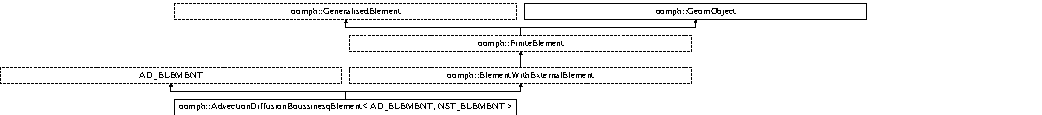
\includegraphics[height=1.161826cm]{classoomph_1_1AdvectionDiffusionBoussinesqElement}
\end{center}
\end{figure}
\subsection*{Public Member Functions}
\begin{DoxyCompactItemize}
\item 
\hyperlink{classoomph_1_1AdvectionDiffusionBoussinesqElement_a733c18518938e3b85e06de5a618cd49f}{Advection\+Diffusion\+Boussinesq\+Element} ()
\begin{DoxyCompactList}\small\item\em Constructor\+: call the underlying constructors. \end{DoxyCompactList}\item 
void \hyperlink{classoomph_1_1AdvectionDiffusionBoussinesqElement_a86ec5858acc0a562cee7bccedfecb252}{get\+\_\+wind\+\_\+adv\+\_\+diff} (const unsigned \&ipt, const Vector$<$ double $>$ \&s, const Vector$<$ double $>$ \&x, Vector$<$ double $>$ \&wind) const
\begin{DoxyCompactList}\small\item\em Overload the wind function in the advection-\/diffusion equations. This provides the coupling from the Navier--Stokes equations to the advection-\/diffusion equations because the wind is the fluid velocity, obtained from the source element in the other mesh. \end{DoxyCompactList}\item 
void \hyperlink{classoomph_1_1AdvectionDiffusionBoussinesqElement_afcb2b136650ecca8fd47eb4278616d29}{output} (std\+::ostream \&outfile, const unsigned \&nplot)
\begin{DoxyCompactList}\small\item\em Output function\+: Output x, y, theta at Nplot$^\wedge$\+D\+IM plot points. \end{DoxyCompactList}\item 
void \hyperlink{classoomph_1_1AdvectionDiffusionBoussinesqElement_acc615c265bef2c3f5c30c6be95c0f50d}{output} (std\+::ostream \&outfile)
\begin{DoxyCompactList}\small\item\em Overload the standard output function with the broken default. \end{DoxyCompactList}\item 
void \hyperlink{classoomph_1_1AdvectionDiffusionBoussinesqElement_adbd60fca6201bc2cd80ff39303323053}{output} (F\+I\+LE $\ast$file\+\_\+pt)
\begin{DoxyCompactList}\small\item\em C-\/style output function\+: Broken default. \end{DoxyCompactList}\item 
void \hyperlink{classoomph_1_1AdvectionDiffusionBoussinesqElement_adbe60877f205b36d76a87695afb28caa}{output} (F\+I\+LE $\ast$file\+\_\+pt, const unsigned \&n\+\_\+plot)
\begin{DoxyCompactList}\small\item\em C-\/style output function\+: Broken default. \end{DoxyCompactList}\item 
void \hyperlink{classoomph_1_1AdvectionDiffusionBoussinesqElement_a89ea74af5d011a3866999c3760621edf}{get\+\_\+dwind\+\_\+adv\+\_\+diff\+\_\+dexternal\+\_\+element\+\_\+data} (const unsigned \&ipt, const unsigned \&i, Vector$<$ double $>$ \&result, Vector$<$ unsigned $>$ \&global\+\_\+eqn\+\_\+number)
\begin{DoxyCompactList}\small\item\em Fill in the derivatives of the wind with respect to the external unknowns. \end{DoxyCompactList}\item 
void \hyperlink{classoomph_1_1AdvectionDiffusionBoussinesqElement_afc63db5ad4e397df7809447ee3ca56ac}{fill\+\_\+in\+\_\+contribution\+\_\+to\+\_\+jacobian} (Vector$<$ double $>$ \&residuals, Dense\+Matrix$<$ double $>$ \&jacobian)
\begin{DoxyCompactList}\small\item\em Compute the element\textquotesingle{}s residual vector and the Jacobian matrix. Jacobian is computed by finite-\/differencing. \end{DoxyCompactList}\item 
void \hyperlink{classoomph_1_1AdvectionDiffusionBoussinesqElement_a375fb98e225dbd5ac716ed3f68831069}{fill\+\_\+in\+\_\+contribution\+\_\+to\+\_\+jacobian\+\_\+and\+\_\+mass\+\_\+matrix} (Vector$<$ double $>$ \&residuals, Dense\+Matrix$<$ double $>$ \&jacobian, Dense\+Matrix$<$ double $>$ \&mass\+\_\+matrix)
\begin{DoxyCompactList}\small\item\em Add the element\textquotesingle{}s contribution to its residuals vector, jacobian matrix and mass matrix. \end{DoxyCompactList}\item 
void \hyperlink{classoomph_1_1AdvectionDiffusionBoussinesqElement_a9e859b487d8398ae696de72104c76271}{fill\+\_\+in\+\_\+off\+\_\+diagonal\+\_\+block\+\_\+analytic} (Vector$<$ double $>$ \&residuals, Dense\+Matrix$<$ double $>$ \&jacobian)
\begin{DoxyCompactList}\small\item\em Compute the contribution of the external degrees of freedom (velocities) on the Advection\+Diffusion equations. \end{DoxyCompactList}\end{DoxyCompactItemize}


\subsection{Detailed Description}
\subsubsection*{template$<$class A\+D\+\_\+\+E\+L\+E\+M\+E\+NT, class N\+S\+T\+\_\+\+E\+L\+E\+M\+E\+NT$>$\newline
class oomph\+::\+Advection\+Diffusion\+Boussinesq\+Element$<$ A\+D\+\_\+\+E\+L\+E\+M\+E\+N\+T, N\+S\+T\+\_\+\+E\+L\+E\+M\+E\+N\+T $>$}

Build \hyperlink{classoomph_1_1AdvectionDiffusionBoussinesqElement}{Advection\+Diffusion\+Boussinesq\+Element} that inherits from Element\+With\+External\+Element so that it can \char`\"{}communicate\char`\"{} with the Navier Stokes element 

Definition at line 1054 of file multi\+\_\+domain\+\_\+boussinesq\+\_\+elements.\+h.



\subsection{Constructor \& Destructor Documentation}
\mbox{\Hypertarget{classoomph_1_1AdvectionDiffusionBoussinesqElement_a733c18518938e3b85e06de5a618cd49f}\label{classoomph_1_1AdvectionDiffusionBoussinesqElement_a733c18518938e3b85e06de5a618cd49f}} 
\index{oomph\+::\+Advection\+Diffusion\+Boussinesq\+Element@{oomph\+::\+Advection\+Diffusion\+Boussinesq\+Element}!Advection\+Diffusion\+Boussinesq\+Element@{Advection\+Diffusion\+Boussinesq\+Element}}
\index{Advection\+Diffusion\+Boussinesq\+Element@{Advection\+Diffusion\+Boussinesq\+Element}!oomph\+::\+Advection\+Diffusion\+Boussinesq\+Element@{oomph\+::\+Advection\+Diffusion\+Boussinesq\+Element}}
\subsubsection{\texorpdfstring{Advection\+Diffusion\+Boussinesq\+Element()}{AdvectionDiffusionBoussinesqElement()}}
{\footnotesize\ttfamily template$<$class A\+D\+\_\+\+E\+L\+E\+M\+E\+NT , class N\+S\+T\+\_\+\+E\+L\+E\+M\+E\+NT $>$ \\
\hyperlink{classoomph_1_1AdvectionDiffusionBoussinesqElement}{oomph\+::\+Advection\+Diffusion\+Boussinesq\+Element}$<$ A\+D\+\_\+\+E\+L\+E\+M\+E\+NT, N\+S\+T\+\_\+\+E\+L\+E\+M\+E\+NT $>$\+::\hyperlink{classoomph_1_1AdvectionDiffusionBoussinesqElement}{Advection\+Diffusion\+Boussinesq\+Element} (\begin{DoxyParamCaption}{ }\end{DoxyParamCaption})\hspace{0.3cm}{\ttfamily [inline]}}



Constructor\+: call the underlying constructors. 



Definition at line 1061 of file multi\+\_\+domain\+\_\+boussinesq\+\_\+elements.\+h.



\subsection{Member Function Documentation}
\mbox{\Hypertarget{classoomph_1_1AdvectionDiffusionBoussinesqElement_afc63db5ad4e397df7809447ee3ca56ac}\label{classoomph_1_1AdvectionDiffusionBoussinesqElement_afc63db5ad4e397df7809447ee3ca56ac}} 
\index{oomph\+::\+Advection\+Diffusion\+Boussinesq\+Element@{oomph\+::\+Advection\+Diffusion\+Boussinesq\+Element}!fill\+\_\+in\+\_\+contribution\+\_\+to\+\_\+jacobian@{fill\+\_\+in\+\_\+contribution\+\_\+to\+\_\+jacobian}}
\index{fill\+\_\+in\+\_\+contribution\+\_\+to\+\_\+jacobian@{fill\+\_\+in\+\_\+contribution\+\_\+to\+\_\+jacobian}!oomph\+::\+Advection\+Diffusion\+Boussinesq\+Element@{oomph\+::\+Advection\+Diffusion\+Boussinesq\+Element}}
\subsubsection{\texorpdfstring{fill\+\_\+in\+\_\+contribution\+\_\+to\+\_\+jacobian()}{fill\_in\_contribution\_to\_jacobian()}}
{\footnotesize\ttfamily template$<$class A\+D\+\_\+\+E\+L\+E\+M\+E\+NT , class N\+S\+T\+\_\+\+E\+L\+E\+M\+E\+NT $>$ \\
void \hyperlink{classoomph_1_1AdvectionDiffusionBoussinesqElement}{oomph\+::\+Advection\+Diffusion\+Boussinesq\+Element}$<$ A\+D\+\_\+\+E\+L\+E\+M\+E\+NT, N\+S\+T\+\_\+\+E\+L\+E\+M\+E\+NT $>$\+::fill\+\_\+in\+\_\+contribution\+\_\+to\+\_\+jacobian (\begin{DoxyParamCaption}\item[{Vector$<$ double $>$ \&}]{residuals,  }\item[{Dense\+Matrix$<$ double $>$ \&}]{jacobian }\end{DoxyParamCaption})\hspace{0.3cm}{\ttfamily [inline]}}



Compute the element\textquotesingle{}s residual vector and the Jacobian matrix. Jacobian is computed by finite-\/differencing. 



Definition at line 1142 of file multi\+\_\+domain\+\_\+boussinesq\+\_\+elements.\+h.

\mbox{\Hypertarget{classoomph_1_1AdvectionDiffusionBoussinesqElement_a375fb98e225dbd5ac716ed3f68831069}\label{classoomph_1_1AdvectionDiffusionBoussinesqElement_a375fb98e225dbd5ac716ed3f68831069}} 
\index{oomph\+::\+Advection\+Diffusion\+Boussinesq\+Element@{oomph\+::\+Advection\+Diffusion\+Boussinesq\+Element}!fill\+\_\+in\+\_\+contribution\+\_\+to\+\_\+jacobian\+\_\+and\+\_\+mass\+\_\+matrix@{fill\+\_\+in\+\_\+contribution\+\_\+to\+\_\+jacobian\+\_\+and\+\_\+mass\+\_\+matrix}}
\index{fill\+\_\+in\+\_\+contribution\+\_\+to\+\_\+jacobian\+\_\+and\+\_\+mass\+\_\+matrix@{fill\+\_\+in\+\_\+contribution\+\_\+to\+\_\+jacobian\+\_\+and\+\_\+mass\+\_\+matrix}!oomph\+::\+Advection\+Diffusion\+Boussinesq\+Element@{oomph\+::\+Advection\+Diffusion\+Boussinesq\+Element}}
\subsubsection{\texorpdfstring{fill\+\_\+in\+\_\+contribution\+\_\+to\+\_\+jacobian\+\_\+and\+\_\+mass\+\_\+matrix()}{fill\_in\_contribution\_to\_jacobian\_and\_mass\_matrix()}}
{\footnotesize\ttfamily template$<$class A\+D\+\_\+\+E\+L\+E\+M\+E\+NT , class N\+S\+T\+\_\+\+E\+L\+E\+M\+E\+NT $>$ \\
void \hyperlink{classoomph_1_1AdvectionDiffusionBoussinesqElement}{oomph\+::\+Advection\+Diffusion\+Boussinesq\+Element}$<$ A\+D\+\_\+\+E\+L\+E\+M\+E\+NT, N\+S\+T\+\_\+\+E\+L\+E\+M\+E\+NT $>$\+::fill\+\_\+in\+\_\+contribution\+\_\+to\+\_\+jacobian\+\_\+and\+\_\+mass\+\_\+matrix (\begin{DoxyParamCaption}\item[{Vector$<$ double $>$ \&}]{residuals,  }\item[{Dense\+Matrix$<$ double $>$ \&}]{jacobian,  }\item[{Dense\+Matrix$<$ double $>$ \&}]{mass\+\_\+matrix }\end{DoxyParamCaption})\hspace{0.3cm}{\ttfamily [inline]}}



Add the element\textquotesingle{}s contribution to its residuals vector, jacobian matrix and mass matrix. 



Definition at line 1164 of file multi\+\_\+domain\+\_\+boussinesq\+\_\+elements.\+h.

\mbox{\Hypertarget{classoomph_1_1AdvectionDiffusionBoussinesqElement_a9e859b487d8398ae696de72104c76271}\label{classoomph_1_1AdvectionDiffusionBoussinesqElement_a9e859b487d8398ae696de72104c76271}} 
\index{oomph\+::\+Advection\+Diffusion\+Boussinesq\+Element@{oomph\+::\+Advection\+Diffusion\+Boussinesq\+Element}!fill\+\_\+in\+\_\+off\+\_\+diagonal\+\_\+block\+\_\+analytic@{fill\+\_\+in\+\_\+off\+\_\+diagonal\+\_\+block\+\_\+analytic}}
\index{fill\+\_\+in\+\_\+off\+\_\+diagonal\+\_\+block\+\_\+analytic@{fill\+\_\+in\+\_\+off\+\_\+diagonal\+\_\+block\+\_\+analytic}!oomph\+::\+Advection\+Diffusion\+Boussinesq\+Element@{oomph\+::\+Advection\+Diffusion\+Boussinesq\+Element}}
\subsubsection{\texorpdfstring{fill\+\_\+in\+\_\+off\+\_\+diagonal\+\_\+block\+\_\+analytic()}{fill\_in\_off\_diagonal\_block\_analytic()}}
{\footnotesize\ttfamily template$<$class A\+D\+\_\+\+E\+L\+E\+M\+E\+NT , class N\+S\+T\+\_\+\+E\+L\+E\+M\+E\+NT $>$ \\
void \hyperlink{classoomph_1_1AdvectionDiffusionBoussinesqElement}{oomph\+::\+Advection\+Diffusion\+Boussinesq\+Element}$<$ A\+D\+\_\+\+E\+L\+E\+M\+E\+NT, N\+S\+T\+\_\+\+E\+L\+E\+M\+E\+NT $>$\+::fill\+\_\+in\+\_\+off\+\_\+diagonal\+\_\+block\+\_\+analytic (\begin{DoxyParamCaption}\item[{Vector$<$ double $>$ \&}]{residuals,  }\item[{Dense\+Matrix$<$ double $>$ \&}]{jacobian }\end{DoxyParamCaption})\hspace{0.3cm}{\ttfamily [inline]}}



Compute the contribution of the external degrees of freedom (velocities) on the Advection\+Diffusion equations. 



Definition at line 1178 of file multi\+\_\+domain\+\_\+boussinesq\+\_\+elements.\+h.



References oomph\+::\+Advection\+Diffusion\+Boussinesq\+Element$<$ A\+D\+\_\+\+E\+L\+E\+M\+E\+N\+T, N\+S\+T\+\_\+\+E\+L\+E\+M\+E\+N\+T $>$\+::get\+\_\+wind\+\_\+adv\+\_\+diff().

\mbox{\Hypertarget{classoomph_1_1AdvectionDiffusionBoussinesqElement_a89ea74af5d011a3866999c3760621edf}\label{classoomph_1_1AdvectionDiffusionBoussinesqElement_a89ea74af5d011a3866999c3760621edf}} 
\index{oomph\+::\+Advection\+Diffusion\+Boussinesq\+Element@{oomph\+::\+Advection\+Diffusion\+Boussinesq\+Element}!get\+\_\+dwind\+\_\+adv\+\_\+diff\+\_\+dexternal\+\_\+element\+\_\+data@{get\+\_\+dwind\+\_\+adv\+\_\+diff\+\_\+dexternal\+\_\+element\+\_\+data}}
\index{get\+\_\+dwind\+\_\+adv\+\_\+diff\+\_\+dexternal\+\_\+element\+\_\+data@{get\+\_\+dwind\+\_\+adv\+\_\+diff\+\_\+dexternal\+\_\+element\+\_\+data}!oomph\+::\+Advection\+Diffusion\+Boussinesq\+Element@{oomph\+::\+Advection\+Diffusion\+Boussinesq\+Element}}
\subsubsection{\texorpdfstring{get\+\_\+dwind\+\_\+adv\+\_\+diff\+\_\+dexternal\+\_\+element\+\_\+data()}{get\_dwind\_adv\_diff\_dexternal\_element\_data()}}
{\footnotesize\ttfamily template$<$class A\+D\+\_\+\+E\+L\+E\+M\+E\+NT , class N\+S\+T\+\_\+\+E\+L\+E\+M\+E\+NT $>$ \\
void \hyperlink{classoomph_1_1AdvectionDiffusionBoussinesqElement}{oomph\+::\+Advection\+Diffusion\+Boussinesq\+Element}$<$ A\+D\+\_\+\+E\+L\+E\+M\+E\+NT, N\+S\+T\+\_\+\+E\+L\+E\+M\+E\+NT $>$\+::get\+\_\+dwind\+\_\+adv\+\_\+diff\+\_\+dexternal\+\_\+element\+\_\+data (\begin{DoxyParamCaption}\item[{const unsigned \&}]{ipt,  }\item[{const unsigned \&}]{i,  }\item[{Vector$<$ double $>$ \&}]{result,  }\item[{Vector$<$ unsigned $>$ \&}]{global\+\_\+eqn\+\_\+number }\end{DoxyParamCaption})}



Fill in the derivatives of the wind with respect to the external unknowns. 

Fill in the derivatives of the wind with respect to the external unknowns in the advection-\/diffusion equations 

Definition at line 1317 of file multi\+\_\+domain\+\_\+boussinesq\+\_\+elements.\+h.



References oomph\+::\+Navier\+Stokes\+Boussinesq\+Element$<$ N\+S\+T\+\_\+\+E\+L\+E\+M\+E\+N\+T, A\+D\+\_\+\+E\+L\+E\+M\+E\+N\+T $>$\+::get\+\_\+dbody\+\_\+force\+\_\+nst\+\_\+dexternal\+\_\+element\+\_\+data().



Referenced by oomph\+::\+Advection\+Diffusion\+Boussinesq\+Element$<$ A\+D\+\_\+\+E\+L\+E\+M\+E\+N\+T, N\+S\+T\+\_\+\+E\+L\+E\+M\+E\+N\+T $>$\+::get\+\_\+wind\+\_\+adv\+\_\+diff().

\mbox{\Hypertarget{classoomph_1_1AdvectionDiffusionBoussinesqElement_a86ec5858acc0a562cee7bccedfecb252}\label{classoomph_1_1AdvectionDiffusionBoussinesqElement_a86ec5858acc0a562cee7bccedfecb252}} 
\index{oomph\+::\+Advection\+Diffusion\+Boussinesq\+Element@{oomph\+::\+Advection\+Diffusion\+Boussinesq\+Element}!get\+\_\+wind\+\_\+adv\+\_\+diff@{get\+\_\+wind\+\_\+adv\+\_\+diff}}
\index{get\+\_\+wind\+\_\+adv\+\_\+diff@{get\+\_\+wind\+\_\+adv\+\_\+diff}!oomph\+::\+Advection\+Diffusion\+Boussinesq\+Element@{oomph\+::\+Advection\+Diffusion\+Boussinesq\+Element}}
\subsubsection{\texorpdfstring{get\+\_\+wind\+\_\+adv\+\_\+diff()}{get\_wind\_adv\_diff()}}
{\footnotesize\ttfamily template$<$class A\+D\+\_\+\+E\+L\+E\+M\+E\+NT , class N\+S\+T\+\_\+\+E\+L\+E\+M\+E\+NT $>$ \\
void \hyperlink{classoomph_1_1AdvectionDiffusionBoussinesqElement}{oomph\+::\+Advection\+Diffusion\+Boussinesq\+Element}$<$ A\+D\+\_\+\+E\+L\+E\+M\+E\+NT, N\+S\+T\+\_\+\+E\+L\+E\+M\+E\+NT $>$\+::get\+\_\+wind\+\_\+adv\+\_\+diff (\begin{DoxyParamCaption}\item[{const unsigned \&}]{ipt,  }\item[{const Vector$<$ double $>$ \&}]{s,  }\item[{const Vector$<$ double $>$ \&}]{x,  }\item[{Vector$<$ double $>$ \&}]{wind }\end{DoxyParamCaption}) const}



Overload the wind function in the advection-\/diffusion equations. This provides the coupling from the Navier--Stokes equations to the advection-\/diffusion equations because the wind is the fluid velocity, obtained from the source element in the other mesh. 

Overload the wind function in the advection-\/diffusion equations. This provides the coupling from the Navier--Stokes equations to the advection-\/diffusion equations because the wind is the fluid velocity, obtained from the source elements in the other mesh. 

Definition at line 1296 of file multi\+\_\+domain\+\_\+boussinesq\+\_\+elements.\+h.



References oomph\+::\+Advection\+Diffusion\+Boussinesq\+Element$<$ A\+D\+\_\+\+E\+L\+E\+M\+E\+N\+T, N\+S\+T\+\_\+\+E\+L\+E\+M\+E\+N\+T $>$\+::get\+\_\+dwind\+\_\+adv\+\_\+diff\+\_\+dexternal\+\_\+element\+\_\+data().



Referenced by oomph\+::\+Advection\+Diffusion\+Boussinesq\+Element$<$ A\+D\+\_\+\+E\+L\+E\+M\+E\+N\+T, N\+S\+T\+\_\+\+E\+L\+E\+M\+E\+N\+T $>$\+::fill\+\_\+in\+\_\+off\+\_\+diagonal\+\_\+block\+\_\+analytic().

\mbox{\Hypertarget{classoomph_1_1AdvectionDiffusionBoussinesqElement_afcb2b136650ecca8fd47eb4278616d29}\label{classoomph_1_1AdvectionDiffusionBoussinesqElement_afcb2b136650ecca8fd47eb4278616d29}} 
\index{oomph\+::\+Advection\+Diffusion\+Boussinesq\+Element@{oomph\+::\+Advection\+Diffusion\+Boussinesq\+Element}!output@{output}}
\index{output@{output}!oomph\+::\+Advection\+Diffusion\+Boussinesq\+Element@{oomph\+::\+Advection\+Diffusion\+Boussinesq\+Element}}
\subsubsection{\texorpdfstring{output()}{output()}\hspace{0.1cm}{\footnotesize\ttfamily [1/4]}}
{\footnotesize\ttfamily template$<$class A\+D\+\_\+\+E\+L\+E\+M\+E\+NT , class N\+S\+T\+\_\+\+E\+L\+E\+M\+E\+NT $>$ \\
void \hyperlink{classoomph_1_1AdvectionDiffusionBoussinesqElement}{oomph\+::\+Advection\+Diffusion\+Boussinesq\+Element}$<$ A\+D\+\_\+\+E\+L\+E\+M\+E\+NT, N\+S\+T\+\_\+\+E\+L\+E\+M\+E\+NT $>$\+::output (\begin{DoxyParamCaption}\item[{std\+::ostream \&}]{outfile,  }\item[{const unsigned \&}]{nplot }\end{DoxyParamCaption})\hspace{0.3cm}{\ttfamily [inline]}}



Output function\+: Output x, y, theta at Nplot$^\wedge$\+D\+IM plot points. 



Definition at line 1087 of file multi\+\_\+domain\+\_\+boussinesq\+\_\+elements.\+h.

\mbox{\Hypertarget{classoomph_1_1AdvectionDiffusionBoussinesqElement_acc615c265bef2c3f5c30c6be95c0f50d}\label{classoomph_1_1AdvectionDiffusionBoussinesqElement_acc615c265bef2c3f5c30c6be95c0f50d}} 
\index{oomph\+::\+Advection\+Diffusion\+Boussinesq\+Element@{oomph\+::\+Advection\+Diffusion\+Boussinesq\+Element}!output@{output}}
\index{output@{output}!oomph\+::\+Advection\+Diffusion\+Boussinesq\+Element@{oomph\+::\+Advection\+Diffusion\+Boussinesq\+Element}}
\subsubsection{\texorpdfstring{output()}{output()}\hspace{0.1cm}{\footnotesize\ttfamily [2/4]}}
{\footnotesize\ttfamily template$<$class A\+D\+\_\+\+E\+L\+E\+M\+E\+NT , class N\+S\+T\+\_\+\+E\+L\+E\+M\+E\+NT $>$ \\
void \hyperlink{classoomph_1_1AdvectionDiffusionBoussinesqElement}{oomph\+::\+Advection\+Diffusion\+Boussinesq\+Element}$<$ A\+D\+\_\+\+E\+L\+E\+M\+E\+NT, N\+S\+T\+\_\+\+E\+L\+E\+M\+E\+NT $>$\+::output (\begin{DoxyParamCaption}\item[{std\+::ostream \&}]{outfile }\end{DoxyParamCaption})\hspace{0.3cm}{\ttfamily [inline]}}



Overload the standard output function with the broken default. 



Definition at line 1121 of file multi\+\_\+domain\+\_\+boussinesq\+\_\+elements.\+h.

\mbox{\Hypertarget{classoomph_1_1AdvectionDiffusionBoussinesqElement_adbd60fca6201bc2cd80ff39303323053}\label{classoomph_1_1AdvectionDiffusionBoussinesqElement_adbd60fca6201bc2cd80ff39303323053}} 
\index{oomph\+::\+Advection\+Diffusion\+Boussinesq\+Element@{oomph\+::\+Advection\+Diffusion\+Boussinesq\+Element}!output@{output}}
\index{output@{output}!oomph\+::\+Advection\+Diffusion\+Boussinesq\+Element@{oomph\+::\+Advection\+Diffusion\+Boussinesq\+Element}}
\subsubsection{\texorpdfstring{output()}{output()}\hspace{0.1cm}{\footnotesize\ttfamily [3/4]}}
{\footnotesize\ttfamily template$<$class A\+D\+\_\+\+E\+L\+E\+M\+E\+NT , class N\+S\+T\+\_\+\+E\+L\+E\+M\+E\+NT $>$ \\
void \hyperlink{classoomph_1_1AdvectionDiffusionBoussinesqElement}{oomph\+::\+Advection\+Diffusion\+Boussinesq\+Element}$<$ A\+D\+\_\+\+E\+L\+E\+M\+E\+NT, N\+S\+T\+\_\+\+E\+L\+E\+M\+E\+NT $>$\+::output (\begin{DoxyParamCaption}\item[{F\+I\+LE $\ast$}]{file\+\_\+pt }\end{DoxyParamCaption})\hspace{0.3cm}{\ttfamily [inline]}}



C-\/style output function\+: Broken default. 



Definition at line 1124 of file multi\+\_\+domain\+\_\+boussinesq\+\_\+elements.\+h.

\mbox{\Hypertarget{classoomph_1_1AdvectionDiffusionBoussinesqElement_adbe60877f205b36d76a87695afb28caa}\label{classoomph_1_1AdvectionDiffusionBoussinesqElement_adbe60877f205b36d76a87695afb28caa}} 
\index{oomph\+::\+Advection\+Diffusion\+Boussinesq\+Element@{oomph\+::\+Advection\+Diffusion\+Boussinesq\+Element}!output@{output}}
\index{output@{output}!oomph\+::\+Advection\+Diffusion\+Boussinesq\+Element@{oomph\+::\+Advection\+Diffusion\+Boussinesq\+Element}}
\subsubsection{\texorpdfstring{output()}{output()}\hspace{0.1cm}{\footnotesize\ttfamily [4/4]}}
{\footnotesize\ttfamily template$<$class A\+D\+\_\+\+E\+L\+E\+M\+E\+NT , class N\+S\+T\+\_\+\+E\+L\+E\+M\+E\+NT $>$ \\
void \hyperlink{classoomph_1_1AdvectionDiffusionBoussinesqElement}{oomph\+::\+Advection\+Diffusion\+Boussinesq\+Element}$<$ A\+D\+\_\+\+E\+L\+E\+M\+E\+NT, N\+S\+T\+\_\+\+E\+L\+E\+M\+E\+NT $>$\+::output (\begin{DoxyParamCaption}\item[{F\+I\+LE $\ast$}]{file\+\_\+pt,  }\item[{const unsigned \&}]{n\+\_\+plot }\end{DoxyParamCaption})\hspace{0.3cm}{\ttfamily [inline]}}



C-\/style output function\+: Broken default. 



Definition at line 1128 of file multi\+\_\+domain\+\_\+boussinesq\+\_\+elements.\+h.



The documentation for this class was generated from the following file\+:\begin{DoxyCompactItemize}
\item 
\hyperlink{multi__domain__boussinesq__elements_8h}{multi\+\_\+domain\+\_\+boussinesq\+\_\+elements.\+h}\end{DoxyCompactItemize}

\hypertarget{classoomph_1_1AdvectionDiffusionEquations}{}\section{oomph\+:\+:Advection\+Diffusion\+Equations$<$ D\+IM $>$ Class Template Reference}
\label{classoomph_1_1AdvectionDiffusionEquations}\index{oomph\+::\+Advection\+Diffusion\+Equations$<$ D\+I\+M $>$@{oomph\+::\+Advection\+Diffusion\+Equations$<$ D\+I\+M $>$}}


A class for all elements that solve the Advection Diffusion equations using isoparametric elements. \[ \frac{\partial^2 u}{\partial x_i^2} = Pe w_i(x_k) \frac{\partial u}{\partial x_i} + f(x_j) \] This contains the generic maths. \hyperlink{classoomph_1_1Shape}{Shape} functions, geometric mapping etc. must get implemented in derived class.  




{\ttfamily \#include $<$advection\+\_\+diffusion\+\_\+elements.\+h$>$}

Inheritance diagram for oomph\+:\+:Advection\+Diffusion\+Equations$<$ D\+IM $>$\+:\begin{figure}[H]
\begin{center}
\leavevmode
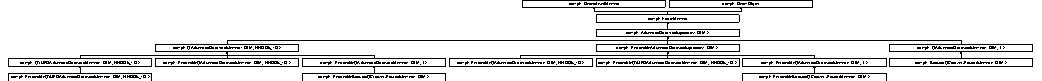
\includegraphics[height=1.088435cm]{classoomph_1_1AdvectionDiffusionEquations}
\end{center}
\end{figure}
\subsection*{Public Types}
\begin{DoxyCompactItemize}
\item 
typedef void($\ast$ \hyperlink{classoomph_1_1AdvectionDiffusionEquations_aa892578e0cffe209775da9f5ac84bd03}{Advection\+Diffusion\+Source\+Fct\+Pt}) (const \hyperlink{classoomph_1_1Vector}{Vector}$<$ double $>$ \&x, double \&f)
\begin{DoxyCompactList}\small\item\em Function pointer to source function fct(x,f(x)) -- x is a Vector! \end{DoxyCompactList}\item 
typedef void($\ast$ \hyperlink{classoomph_1_1AdvectionDiffusionEquations_a341db90b2eaf704f3286a9fcde7c614a}{Advection\+Diffusion\+Wind\+Fct\+Pt}) (const \hyperlink{classoomph_1_1Vector}{Vector}$<$ double $>$ \&x, \hyperlink{classoomph_1_1Vector}{Vector}$<$ double $>$ \&wind)
\begin{DoxyCompactList}\small\item\em Function pointer to wind function fct(x,w(x)) -- x is a Vector! \end{DoxyCompactList}\end{DoxyCompactItemize}
\subsection*{Public Member Functions}
\begin{DoxyCompactItemize}
\item 
\hyperlink{classoomph_1_1AdvectionDiffusionEquations_a29a6689bdcd6f14bc30bbeaa6e7ccafe}{Advection\+Diffusion\+Equations} ()
\begin{DoxyCompactList}\small\item\em Constructor\+: Initialise the Source\+\_\+fct\+\_\+pt and Wind\+\_\+fct\+\_\+pt to null and set (pointer to) Peclet number to default. \end{DoxyCompactList}\item 
\hyperlink{classoomph_1_1AdvectionDiffusionEquations_aad53e287ed605e9f1080a94d3b351ab7}{Advection\+Diffusion\+Equations} (const \hyperlink{classoomph_1_1AdvectionDiffusionEquations}{Advection\+Diffusion\+Equations} \&dummy)
\begin{DoxyCompactList}\small\item\em Broken copy constructor. \end{DoxyCompactList}\item 
void \hyperlink{classoomph_1_1AdvectionDiffusionEquations_aa80b72531531a916f3b0691b679d5b2a}{operator=} (const \hyperlink{classoomph_1_1AdvectionDiffusionEquations}{Advection\+Diffusion\+Equations} \&)
\begin{DoxyCompactList}\small\item\em Broken assignment operator. \end{DoxyCompactList}\item 
virtual unsigned \hyperlink{classoomph_1_1AdvectionDiffusionEquations_aadffa26c42be5d4a1156a7467de48fb8}{u\+\_\+index\+\_\+adv\+\_\+diff} () const
\begin{DoxyCompactList}\small\item\em Return the index at which the unknown value is stored. The default value, 0, is appropriate for single-\/physics problems, when there is only one variable, the value that satisfies the advection-\/diffusion equation. In derived multi-\/physics elements, this function should be overloaded to reflect the chosen storage scheme. Note that these equations require that the unknown is always stored at the same index at each node. \end{DoxyCompactList}\item 
double \hyperlink{classoomph_1_1AdvectionDiffusionEquations_a2c94e14a6b53e3cce43b83d8c8329174}{du\+\_\+dt\+\_\+adv\+\_\+diff} (const unsigned \&n) const
\begin{DoxyCompactList}\small\item\em du/dt at local node n. \end{DoxyCompactList}\item 
void \hyperlink{classoomph_1_1AdvectionDiffusionEquations_aa635388e5e1139e0a1eae97ca89279d0}{disable\+\_\+\+A\+LE} ()
\begin{DoxyCompactList}\small\item\em Disable A\+LE, i.\+e. assert the mesh is not moving -- you do this at your own risk! \end{DoxyCompactList}\item 
void \hyperlink{classoomph_1_1AdvectionDiffusionEquations_a949dd5a3eb9803c993c1f4506cfd5d82}{enable\+\_\+\+A\+LE} ()
\begin{DoxyCompactList}\small\item\em (Re-\/)enable A\+LE, i.\+e. take possible mesh motion into account when evaluating the time-\/derivative. Note\+: By default, A\+LE is enabled, at the expense of possibly creating unnecessary work in problems where the mesh is, in fact, stationary. \end{DoxyCompactList}\item 
unsigned \hyperlink{classoomph_1_1AdvectionDiffusionEquations_a70205e9d39d7ff9660a53402d5636c1f}{nscalar\+\_\+paraview} () const
\begin{DoxyCompactList}\small\item\em Number of scalars/fields output by this element. Reimplements. \end{DoxyCompactList}\item 
void \hyperlink{classoomph_1_1AdvectionDiffusionEquations_a7e4c60334ef457e6155e84a9d24062cf}{scalar\+\_\+value\+\_\+paraview} (std\+::ofstream \&file\+\_\+out, const unsigned \&\hyperlink{cfortran_8h_adb50e893b86b3e55e751a42eab3cba82}{i}, const unsigned \&nplot) const
\begin{DoxyCompactList}\small\item\em Write values of the i-\/th scalar field at the plot points. Needs to be implemented for each new specific element type. \end{DoxyCompactList}\item 
std\+::string \hyperlink{classoomph_1_1AdvectionDiffusionEquations_a37c30bb64389d12ffef51f046d846886}{scalar\+\_\+name\+\_\+paraview} (const unsigned \&\hyperlink{cfortran_8h_adb50e893b86b3e55e751a42eab3cba82}{i}) const
\begin{DoxyCompactList}\small\item\em Name of the i-\/th scalar field. Default implementation returns V1 for the first one, V2 for the second etc. Can (should!) be overloaded with more meaningful names in specific elements. \end{DoxyCompactList}\item 
void \hyperlink{classoomph_1_1AdvectionDiffusionEquations_a3016c7a56e7f7178b4d9ae8604d0c10b}{output} (std\+::ostream \&outfile)
\begin{DoxyCompactList}\small\item\em Output with default number of plot points. \end{DoxyCompactList}\item 
void \hyperlink{classoomph_1_1AdvectionDiffusionEquations_ade5e445c7b99593a68fc8e42631d79be}{output} (std\+::ostream \&outfile, const unsigned \&nplot)
\begin{DoxyCompactList}\small\item\em Output FE representation of soln\+: x,y,u or x,y,z,u at nplot$^\wedge$\+D\+IM plot points. \end{DoxyCompactList}\item 
void \hyperlink{classoomph_1_1AdvectionDiffusionEquations_a063f08a2825608d32eaac5666c2ccec5}{output} (F\+I\+LE $\ast$file\+\_\+pt)
\begin{DoxyCompactList}\small\item\em C\+\_\+style output with default number of plot points. \end{DoxyCompactList}\item 
void \hyperlink{classoomph_1_1AdvectionDiffusionEquations_a03a096ff864ee53c8823b08e0d2f6091}{output} (F\+I\+LE $\ast$file\+\_\+pt, const unsigned \&n\+\_\+plot)
\begin{DoxyCompactList}\small\item\em C-\/style output FE representation of soln\+: x,y,u or x,y,z,u at n\+\_\+plot$^\wedge$\+D\+IM plot points. \end{DoxyCompactList}\item 
void \hyperlink{classoomph_1_1AdvectionDiffusionEquations_ab1d0f6bc8d3c9c9826ac1d71f1fd148f}{output\+\_\+fct} (std\+::ostream \&outfile, const unsigned \&nplot, \hyperlink{classoomph_1_1FiniteElement_a690fd33af26cc3e84f39bba6d5a85202}{Finite\+Element\+::\+Steady\+Exact\+Solution\+Fct\+Pt} exact\+\_\+soln\+\_\+pt)
\begin{DoxyCompactList}\small\item\em Output exact soln\+: x,y,u\+\_\+exact or x,y,z,u\+\_\+exact at nplot$^\wedge$\+D\+IM plot points. \end{DoxyCompactList}\item 
virtual void \hyperlink{classoomph_1_1AdvectionDiffusionEquations_affb6feff30ffb8617315e555e1bb7185}{output\+\_\+fct} (std\+::ostream \&outfile, const unsigned \&nplot, const double \&time, \hyperlink{classoomph_1_1FiniteElement_ad4ecf2b61b158a4b4d351a60d23c633e}{Finite\+Element\+::\+Unsteady\+Exact\+Solution\+Fct\+Pt} exact\+\_\+soln\+\_\+pt)
\begin{DoxyCompactList}\small\item\em Output exact soln\+: x,y,u\+\_\+exact or x,y,z,u\+\_\+exact at nplot$^\wedge$\+D\+IM plot points (dummy time-\/dependent version to keep intel compiler happy) \end{DoxyCompactList}\item 
void \hyperlink{classoomph_1_1AdvectionDiffusionEquations_acb1fcfb29911210ad7c0bc252f0ed665}{compute\+\_\+error} (std\+::ostream \&outfile, \hyperlink{classoomph_1_1FiniteElement_a690fd33af26cc3e84f39bba6d5a85202}{Finite\+Element\+::\+Steady\+Exact\+Solution\+Fct\+Pt} exact\+\_\+soln\+\_\+pt, double \&error, double \&norm)
\begin{DoxyCompactList}\small\item\em Get error against and norm of exact solution. \end{DoxyCompactList}\item 
void \hyperlink{classoomph_1_1AdvectionDiffusionEquations_a87c8c4e8ff5ea6e6dcb243ec83bb4fd2}{compute\+\_\+error} (std\+::ostream \&outfile, \hyperlink{classoomph_1_1FiniteElement_ad4ecf2b61b158a4b4d351a60d23c633e}{Finite\+Element\+::\+Unsteady\+Exact\+Solution\+Fct\+Pt} exact\+\_\+soln\+\_\+pt, const double \&time, double \&error, double \&norm)
\begin{DoxyCompactList}\small\item\em Dummy, time dependent error checker. \end{DoxyCompactList}\item 
\hyperlink{classoomph_1_1AdvectionDiffusionEquations_aa892578e0cffe209775da9f5ac84bd03}{Advection\+Diffusion\+Source\+Fct\+Pt} \& \hyperlink{classoomph_1_1AdvectionDiffusionEquations_af760c608d973514288373c11a4180002}{source\+\_\+fct\+\_\+pt} ()
\begin{DoxyCompactList}\small\item\em Access function\+: Pointer to source function. \end{DoxyCompactList}\item 
\hyperlink{classoomph_1_1AdvectionDiffusionEquations_aa892578e0cffe209775da9f5ac84bd03}{Advection\+Diffusion\+Source\+Fct\+Pt} \hyperlink{classoomph_1_1AdvectionDiffusionEquations_a7579712ec3c4ec95c5144d37bf4264a6}{source\+\_\+fct\+\_\+pt} () const
\begin{DoxyCompactList}\small\item\em Access function\+: Pointer to source function. Const version. \end{DoxyCompactList}\item 
\hyperlink{classoomph_1_1AdvectionDiffusionEquations_a341db90b2eaf704f3286a9fcde7c614a}{Advection\+Diffusion\+Wind\+Fct\+Pt} \& \hyperlink{classoomph_1_1AdvectionDiffusionEquations_a6f2e7c920f9789137fa6680832a5c338}{wind\+\_\+fct\+\_\+pt} ()
\begin{DoxyCompactList}\small\item\em Access function\+: Pointer to wind function. \end{DoxyCompactList}\item 
\hyperlink{classoomph_1_1AdvectionDiffusionEquations_a341db90b2eaf704f3286a9fcde7c614a}{Advection\+Diffusion\+Wind\+Fct\+Pt} \hyperlink{classoomph_1_1AdvectionDiffusionEquations_aafac11232d7d543efc4d08536b026f9a}{wind\+\_\+fct\+\_\+pt} () const
\begin{DoxyCompactList}\small\item\em Access function\+: Pointer to wind function. Const version. \end{DoxyCompactList}\item 
const double \& \hyperlink{classoomph_1_1AdvectionDiffusionEquations_ae1dd3fb5d07e98ad2a6b1e38f2f4dc3c}{pe} () const
\begin{DoxyCompactList}\small\item\em Peclet number. \end{DoxyCompactList}\item 
double $\ast$\& \hyperlink{classoomph_1_1AdvectionDiffusionEquations_a6757b4e9313b562812a21b49f167a114}{pe\+\_\+pt} ()
\begin{DoxyCompactList}\small\item\em Pointer to Peclet number. \end{DoxyCompactList}\item 
const double \& \hyperlink{classoomph_1_1AdvectionDiffusionEquations_ad23f5906cc0b088d778e1694719138e0}{pe\+\_\+st} () const
\begin{DoxyCompactList}\small\item\em Peclet number multiplied by Strouhal number. \end{DoxyCompactList}\item 
double $\ast$\& \hyperlink{classoomph_1_1AdvectionDiffusionEquations_aab0fe6d25a1506aea517e359e0e5e807}{pe\+\_\+st\+\_\+pt} ()
\begin{DoxyCompactList}\small\item\em Pointer to Peclet number multipled by Strouha number. \end{DoxyCompactList}\item 
virtual void \hyperlink{classoomph_1_1AdvectionDiffusionEquations_a3b8feaba7519dee3ed4a056c5dcf2bc2}{get\+\_\+source\+\_\+adv\+\_\+diff} (const unsigned \&ipt, const \hyperlink{classoomph_1_1Vector}{Vector}$<$ double $>$ \&x, double \&source) const
\begin{DoxyCompactList}\small\item\em Get source term at (Eulerian) position x. This function is virtual to allow overloading in multi-\/physics problems where the strength of the source function might be determined by another system of equations. \end{DoxyCompactList}\item 
virtual void \hyperlink{classoomph_1_1AdvectionDiffusionEquations_a32cb2f977b32fabfc23d1134749371ed}{get\+\_\+wind\+\_\+adv\+\_\+diff} (const unsigned \&ipt, const \hyperlink{classoomph_1_1Vector}{Vector}$<$ double $>$ \&\hyperlink{cfortran_8h_ab7123126e4885ef647dd9c6e3807a21c}{s}, const \hyperlink{classoomph_1_1Vector}{Vector}$<$ double $>$ \&x, \hyperlink{classoomph_1_1Vector}{Vector}$<$ double $>$ \&wind) const
\begin{DoxyCompactList}\small\item\em Get wind at (Eulerian) position x and/or local coordinate s. This function is virtual to allow overloading in multi-\/physics problems where the wind function might be determined by another system of equations. \end{DoxyCompactList}\item 
void \hyperlink{classoomph_1_1AdvectionDiffusionEquations_a9c0fdde918adc761bb6f212cd9625e64}{get\+\_\+flux} (const \hyperlink{classoomph_1_1Vector}{Vector}$<$ double $>$ \&\hyperlink{cfortran_8h_ab7123126e4885ef647dd9c6e3807a21c}{s}, \hyperlink{classoomph_1_1Vector}{Vector}$<$ double $>$ \&flux) const
\begin{DoxyCompactList}\small\item\em Get flux\+: $\mbox{flux}[i] = \mbox{d}u / \mbox{d}x_i $. \end{DoxyCompactList}\item 
void \hyperlink{classoomph_1_1AdvectionDiffusionEquations_ae56ee6b085c75be438a598244c527fb5}{fill\+\_\+in\+\_\+contribution\+\_\+to\+\_\+residuals} (\hyperlink{classoomph_1_1Vector}{Vector}$<$ double $>$ \&residuals)
\begin{DoxyCompactList}\small\item\em Add the element\textquotesingle{}s contribution to its residual vector (wrapper) \end{DoxyCompactList}\item 
void \hyperlink{classoomph_1_1AdvectionDiffusionEquations_a6ec1e0f92fa79998be9340ecfda4bcd5}{fill\+\_\+in\+\_\+contribution\+\_\+to\+\_\+jacobian} (\hyperlink{classoomph_1_1Vector}{Vector}$<$ double $>$ \&residuals, \hyperlink{classoomph_1_1DenseMatrix}{Dense\+Matrix}$<$ double $>$ \&jacobian)
\begin{DoxyCompactList}\small\item\em Add the element\textquotesingle{}s contribution to its residual vector and the element Jacobian matrix (wrapper) \end{DoxyCompactList}\item 
void \hyperlink{classoomph_1_1AdvectionDiffusionEquations_aed50fe00556434c01bc855766edeb564}{fill\+\_\+in\+\_\+contribution\+\_\+to\+\_\+jacobian\+\_\+and\+\_\+mass\+\_\+matrix} (\hyperlink{classoomph_1_1Vector}{Vector}$<$ double $>$ \&residuals, \hyperlink{classoomph_1_1DenseMatrix}{Dense\+Matrix}$<$ double $>$ \&jacobian, \hyperlink{classoomph_1_1DenseMatrix}{Dense\+Matrix}$<$ double $>$ \&mass\+\_\+matrix)
\item 
double \hyperlink{classoomph_1_1AdvectionDiffusionEquations_a2c5d80050fd9586bcf2d87951c346f58}{interpolated\+\_\+u\+\_\+adv\+\_\+diff} (const \hyperlink{classoomph_1_1Vector}{Vector}$<$ double $>$ \&\hyperlink{cfortran_8h_ab7123126e4885ef647dd9c6e3807a21c}{s}) const
\begin{DoxyCompactList}\small\item\em Return FE representation of function value u(s) at local coordinate s. \end{DoxyCompactList}\item 
virtual void \hyperlink{classoomph_1_1AdvectionDiffusionEquations_a7b264e70255fa420e443e60cbd8d7dbc}{dinterpolated\+\_\+u\+\_\+adv\+\_\+diff\+\_\+ddata} (const \hyperlink{classoomph_1_1Vector}{Vector}$<$ double $>$ \&\hyperlink{cfortran_8h_ab7123126e4885ef647dd9c6e3807a21c}{s}, \hyperlink{classoomph_1_1Vector}{Vector}$<$ double $>$ \&du\+\_\+ddata, \hyperlink{classoomph_1_1Vector}{Vector}$<$ unsigned $>$ \&global\+\_\+eqn\+\_\+number)
\begin{DoxyCompactList}\small\item\em Return derivative of u at point s with respect to all data that can affect its value. In addition, return the global equation numbers corresponding to the data. This is virtual so that it can be overloaded in the refineable version. \end{DoxyCompactList}\item 
unsigned \hyperlink{classoomph_1_1AdvectionDiffusionEquations_ac9f27a62a29a9c3c850505f4cb9c00b7}{self\+\_\+test} ()
\begin{DoxyCompactList}\small\item\em Self-\/test\+: Return 0 for OK. \end{DoxyCompactList}\end{DoxyCompactItemize}
\subsection*{Protected Member Functions}
\begin{DoxyCompactItemize}
\item 
virtual double \hyperlink{classoomph_1_1AdvectionDiffusionEquations_ac3c3b0bec7f34f53eb330cd777dcbe59}{dshape\+\_\+and\+\_\+dtest\+\_\+eulerian\+\_\+adv\+\_\+diff} (const \hyperlink{classoomph_1_1Vector}{Vector}$<$ double $>$ \&\hyperlink{cfortran_8h_ab7123126e4885ef647dd9c6e3807a21c}{s}, \hyperlink{classoomph_1_1Shape}{Shape} \&psi, \hyperlink{classoomph_1_1DShape}{D\+Shape} \&dpsidx, \hyperlink{classoomph_1_1Shape}{Shape} \&test, \hyperlink{classoomph_1_1DShape}{D\+Shape} \&dtestdx) const =0
\begin{DoxyCompactList}\small\item\em Shape/test functions and derivs w.\+r.\+t. to global coords at local coord. s; return Jacobian of mapping. \end{DoxyCompactList}\item 
virtual double \hyperlink{classoomph_1_1AdvectionDiffusionEquations_a354827df2a149258310ffdd0e4c0d40b}{dshape\+\_\+and\+\_\+dtest\+\_\+eulerian\+\_\+at\+\_\+knot\+\_\+adv\+\_\+diff} (const unsigned \&ipt, \hyperlink{classoomph_1_1Shape}{Shape} \&psi, \hyperlink{classoomph_1_1DShape}{D\+Shape} \&dpsidx, \hyperlink{classoomph_1_1Shape}{Shape} \&test, \hyperlink{classoomph_1_1DShape}{D\+Shape} \&dtestdx) const =0
\begin{DoxyCompactList}\small\item\em Shape/test functions and derivs w.\+r.\+t. to global coords at integration point ipt; return Jacobian of mapping. \end{DoxyCompactList}\item 
virtual void \hyperlink{classoomph_1_1AdvectionDiffusionEquations_a399995609ea6d997496e3bcbdc5383f7}{fill\+\_\+in\+\_\+generic\+\_\+residual\+\_\+contribution\+\_\+adv\+\_\+diff} (\hyperlink{classoomph_1_1Vector}{Vector}$<$ double $>$ \&residuals, \hyperlink{classoomph_1_1DenseMatrix}{Dense\+Matrix}$<$ double $>$ \&jacobian, \hyperlink{classoomph_1_1DenseMatrix}{Dense\+Matrix}$<$ double $>$ \&mass\+\_\+matrix, unsigned flag)
\begin{DoxyCompactList}\small\item\em Add the element\textquotesingle{}s contribution to its residual vector only (if flag=and/or element Jacobian matrix. \end{DoxyCompactList}\end{DoxyCompactItemize}
\subsection*{Protected Attributes}
\begin{DoxyCompactItemize}
\item 
double $\ast$ \hyperlink{classoomph_1_1AdvectionDiffusionEquations_a3b712468732df04ff28d4efe0bd5cbe5}{Pe\+\_\+pt}
\begin{DoxyCompactList}\small\item\em Pointer to global Peclet number. \end{DoxyCompactList}\item 
double $\ast$ \hyperlink{classoomph_1_1AdvectionDiffusionEquations_aa9368fa0d1bd18604c9482b14022502f}{Pe\+St\+\_\+pt}
\begin{DoxyCompactList}\small\item\em Pointer to global Peclet number multiplied by Strouhal number. \end{DoxyCompactList}\item 
\hyperlink{classoomph_1_1AdvectionDiffusionEquations_aa892578e0cffe209775da9f5ac84bd03}{Advection\+Diffusion\+Source\+Fct\+Pt} \hyperlink{classoomph_1_1AdvectionDiffusionEquations_a7c6a2bebf33ebc0ad7ec2aea03c8804b}{Source\+\_\+fct\+\_\+pt}
\begin{DoxyCompactList}\small\item\em Pointer to source function\+: \end{DoxyCompactList}\item 
\hyperlink{classoomph_1_1AdvectionDiffusionEquations_a341db90b2eaf704f3286a9fcde7c614a}{Advection\+Diffusion\+Wind\+Fct\+Pt} \hyperlink{classoomph_1_1AdvectionDiffusionEquations_a9e8d2e67d6d5738f811a40391ceda9aa}{Wind\+\_\+fct\+\_\+pt}
\begin{DoxyCompactList}\small\item\em Pointer to wind function\+: \end{DoxyCompactList}\item 
bool \hyperlink{classoomph_1_1AdvectionDiffusionEquations_a049fe0ee23a9dda3de6edb2ca582e48c}{A\+L\+E\+\_\+is\+\_\+disabled}
\begin{DoxyCompactList}\small\item\em Boolean flag to indicate if A\+LE formulation is disabled when time-\/derivatives are computed. Only set to true if you\textquotesingle{}re sure that the mesh is stationary. \end{DoxyCompactList}\end{DoxyCompactItemize}
\subsection*{Static Private Attributes}
\begin{DoxyCompactItemize}
\item 
static double \hyperlink{classoomph_1_1AdvectionDiffusionEquations_a7760f126f92f6926928263b9c7831764}{Default\+\_\+peclet\+\_\+number} =0.\+0
\begin{DoxyCompactList}\small\item\em Static default value for the Peclet number. \end{DoxyCompactList}\end{DoxyCompactItemize}
\subsection*{Additional Inherited Members}


\subsection{Detailed Description}
\subsubsection*{template$<$unsigned D\+IM$>$\newline
class oomph\+::\+Advection\+Diffusion\+Equations$<$ D\+I\+M $>$}

A class for all elements that solve the Advection Diffusion equations using isoparametric elements. \[ \frac{\partial^2 u}{\partial x_i^2} = Pe w_i(x_k) \frac{\partial u}{\partial x_i} + f(x_j) \] This contains the generic maths. \hyperlink{classoomph_1_1Shape}{Shape} functions, geometric mapping etc. must get implemented in derived class. 

Definition at line 59 of file advection\+\_\+diffusion\+\_\+elements.\+h.



\subsection{Member Typedef Documentation}
\mbox{\Hypertarget{classoomph_1_1AdvectionDiffusionEquations_aa892578e0cffe209775da9f5ac84bd03}\label{classoomph_1_1AdvectionDiffusionEquations_aa892578e0cffe209775da9f5ac84bd03}} 
\index{oomph\+::\+Advection\+Diffusion\+Equations@{oomph\+::\+Advection\+Diffusion\+Equations}!Advection\+Diffusion\+Source\+Fct\+Pt@{Advection\+Diffusion\+Source\+Fct\+Pt}}
\index{Advection\+Diffusion\+Source\+Fct\+Pt@{Advection\+Diffusion\+Source\+Fct\+Pt}!oomph\+::\+Advection\+Diffusion\+Equations@{oomph\+::\+Advection\+Diffusion\+Equations}}
\subsubsection{\texorpdfstring{Advection\+Diffusion\+Source\+Fct\+Pt}{AdvectionDiffusionSourceFctPt}}
{\footnotesize\ttfamily template$<$unsigned D\+IM$>$ \\
typedef void($\ast$ \hyperlink{classoomph_1_1AdvectionDiffusionEquations}{oomph\+::\+Advection\+Diffusion\+Equations}$<$ D\+IM $>$\+::Advection\+Diffusion\+Source\+Fct\+Pt) (const \hyperlink{classoomph_1_1Vector}{Vector}$<$ double $>$ \&x, double \&f)}



Function pointer to source function fct(x,f(x)) -- x is a Vector! 



Definition at line 66 of file advection\+\_\+diffusion\+\_\+elements.\+h.

\mbox{\Hypertarget{classoomph_1_1AdvectionDiffusionEquations_a341db90b2eaf704f3286a9fcde7c614a}\label{classoomph_1_1AdvectionDiffusionEquations_a341db90b2eaf704f3286a9fcde7c614a}} 
\index{oomph\+::\+Advection\+Diffusion\+Equations@{oomph\+::\+Advection\+Diffusion\+Equations}!Advection\+Diffusion\+Wind\+Fct\+Pt@{Advection\+Diffusion\+Wind\+Fct\+Pt}}
\index{Advection\+Diffusion\+Wind\+Fct\+Pt@{Advection\+Diffusion\+Wind\+Fct\+Pt}!oomph\+::\+Advection\+Diffusion\+Equations@{oomph\+::\+Advection\+Diffusion\+Equations}}
\subsubsection{\texorpdfstring{Advection\+Diffusion\+Wind\+Fct\+Pt}{AdvectionDiffusionWindFctPt}}
{\footnotesize\ttfamily template$<$unsigned D\+IM$>$ \\
typedef void($\ast$ \hyperlink{classoomph_1_1AdvectionDiffusionEquations}{oomph\+::\+Advection\+Diffusion\+Equations}$<$ D\+IM $>$\+::Advection\+Diffusion\+Wind\+Fct\+Pt) (const \hyperlink{classoomph_1_1Vector}{Vector}$<$ double $>$ \&x, \hyperlink{classoomph_1_1Vector}{Vector}$<$ double $>$ \&wind)}



Function pointer to wind function fct(x,w(x)) -- x is a Vector! 



Definition at line 72 of file advection\+\_\+diffusion\+\_\+elements.\+h.



\subsection{Constructor \& Destructor Documentation}
\mbox{\Hypertarget{classoomph_1_1AdvectionDiffusionEquations_a29a6689bdcd6f14bc30bbeaa6e7ccafe}\label{classoomph_1_1AdvectionDiffusionEquations_a29a6689bdcd6f14bc30bbeaa6e7ccafe}} 
\index{oomph\+::\+Advection\+Diffusion\+Equations@{oomph\+::\+Advection\+Diffusion\+Equations}!Advection\+Diffusion\+Equations@{Advection\+Diffusion\+Equations}}
\index{Advection\+Diffusion\+Equations@{Advection\+Diffusion\+Equations}!oomph\+::\+Advection\+Diffusion\+Equations@{oomph\+::\+Advection\+Diffusion\+Equations}}
\subsubsection{\texorpdfstring{Advection\+Diffusion\+Equations()}{AdvectionDiffusionEquations()}\hspace{0.1cm}{\footnotesize\ttfamily [1/2]}}
{\footnotesize\ttfamily template$<$unsigned D\+IM$>$ \\
\hyperlink{classoomph_1_1AdvectionDiffusionEquations}{oomph\+::\+Advection\+Diffusion\+Equations}$<$ D\+IM $>$\+::\hyperlink{classoomph_1_1AdvectionDiffusionEquations}{Advection\+Diffusion\+Equations} (\begin{DoxyParamCaption}{ }\end{DoxyParamCaption})\hspace{0.3cm}{\ttfamily [inline]}}



Constructor\+: Initialise the Source\+\_\+fct\+\_\+pt and Wind\+\_\+fct\+\_\+pt to null and set (pointer to) Peclet number to default. 



Definition at line 78 of file advection\+\_\+diffusion\+\_\+elements.\+h.



References oomph\+::\+Advection\+Diffusion\+Equations$<$ D\+I\+M $>$\+::\+Default\+\_\+peclet\+\_\+number, oomph\+::\+Advection\+Diffusion\+Equations$<$ D\+I\+M $>$\+::\+Pe\+\_\+pt, and oomph\+::\+Advection\+Diffusion\+Equations$<$ D\+I\+M $>$\+::\+Pe\+St\+\_\+pt.

\mbox{\Hypertarget{classoomph_1_1AdvectionDiffusionEquations_aad53e287ed605e9f1080a94d3b351ab7}\label{classoomph_1_1AdvectionDiffusionEquations_aad53e287ed605e9f1080a94d3b351ab7}} 
\index{oomph\+::\+Advection\+Diffusion\+Equations@{oomph\+::\+Advection\+Diffusion\+Equations}!Advection\+Diffusion\+Equations@{Advection\+Diffusion\+Equations}}
\index{Advection\+Diffusion\+Equations@{Advection\+Diffusion\+Equations}!oomph\+::\+Advection\+Diffusion\+Equations@{oomph\+::\+Advection\+Diffusion\+Equations}}
\subsubsection{\texorpdfstring{Advection\+Diffusion\+Equations()}{AdvectionDiffusionEquations()}\hspace{0.1cm}{\footnotesize\ttfamily [2/2]}}
{\footnotesize\ttfamily template$<$unsigned D\+IM$>$ \\
\hyperlink{classoomph_1_1AdvectionDiffusionEquations}{oomph\+::\+Advection\+Diffusion\+Equations}$<$ D\+IM $>$\+::\hyperlink{classoomph_1_1AdvectionDiffusionEquations}{Advection\+Diffusion\+Equations} (\begin{DoxyParamCaption}\item[{const \hyperlink{classoomph_1_1AdvectionDiffusionEquations}{Advection\+Diffusion\+Equations}$<$ D\+IM $>$ \&}]{dummy }\end{DoxyParamCaption})\hspace{0.3cm}{\ttfamily [inline]}}



Broken copy constructor. 



Definition at line 88 of file advection\+\_\+diffusion\+\_\+elements.\+h.



References oomph\+::\+Broken\+Copy\+::broken\+\_\+copy().



\subsection{Member Function Documentation}
\mbox{\Hypertarget{classoomph_1_1AdvectionDiffusionEquations_acb1fcfb29911210ad7c0bc252f0ed665}\label{classoomph_1_1AdvectionDiffusionEquations_acb1fcfb29911210ad7c0bc252f0ed665}} 
\index{oomph\+::\+Advection\+Diffusion\+Equations@{oomph\+::\+Advection\+Diffusion\+Equations}!compute\+\_\+error@{compute\+\_\+error}}
\index{compute\+\_\+error@{compute\+\_\+error}!oomph\+::\+Advection\+Diffusion\+Equations@{oomph\+::\+Advection\+Diffusion\+Equations}}
\subsubsection{\texorpdfstring{compute\+\_\+error()}{compute\_error()}\hspace{0.1cm}{\footnotesize\ttfamily [1/2]}}
{\footnotesize\ttfamily template$<$unsigned D\+IM$>$ \\
void \hyperlink{classoomph_1_1AdvectionDiffusionEquations}{oomph\+::\+Advection\+Diffusion\+Equations}$<$ D\+IM $>$\+::compute\+\_\+error (\begin{DoxyParamCaption}\item[{std\+::ostream \&}]{outfile,  }\item[{\hyperlink{classoomph_1_1FiniteElement_a690fd33af26cc3e84f39bba6d5a85202}{Finite\+Element\+::\+Steady\+Exact\+Solution\+Fct\+Pt}}]{exact\+\_\+soln\+\_\+pt,  }\item[{double \&}]{error,  }\item[{double \&}]{norm }\end{DoxyParamCaption})\hspace{0.3cm}{\ttfamily [virtual]}}



Get error against and norm of exact solution. 

Validate against exact solution.

Solution is provided via function pointer. Plot error at a given number of plot points. 

Reimplemented from \hyperlink{classoomph_1_1FiniteElement_a73c79a1f1e5b1d334757812a6bbd58ff}{oomph\+::\+Finite\+Element}.



Reimplemented in \hyperlink{classoomph_1_1RefineableBuoyantQCrouzeixRaviartElement_a078039343f5f9bb467a1183f725d1873}{oomph\+::\+Refineable\+Buoyant\+Q\+Crouzeix\+Raviart\+Element$<$ D\+I\+M $>$}, and \hyperlink{classoomph_1_1BuoyantQCrouzeixRaviartElement_a2aa63b1b2ec1130835ee87cbf52cc086}{oomph\+::\+Buoyant\+Q\+Crouzeix\+Raviart\+Element$<$ D\+I\+M $>$}.



Definition at line 414 of file advection\+\_\+diffusion\+\_\+elements.\+cc.



References i, s, and oomph\+::\+Quad\+Tree\+Names\+::W.



Referenced by oomph\+::\+Advection\+Diffusion\+Equations$<$ D\+I\+M $>$\+::output\+\_\+fct().

\mbox{\Hypertarget{classoomph_1_1AdvectionDiffusionEquations_a87c8c4e8ff5ea6e6dcb243ec83bb4fd2}\label{classoomph_1_1AdvectionDiffusionEquations_a87c8c4e8ff5ea6e6dcb243ec83bb4fd2}} 
\index{oomph\+::\+Advection\+Diffusion\+Equations@{oomph\+::\+Advection\+Diffusion\+Equations}!compute\+\_\+error@{compute\+\_\+error}}
\index{compute\+\_\+error@{compute\+\_\+error}!oomph\+::\+Advection\+Diffusion\+Equations@{oomph\+::\+Advection\+Diffusion\+Equations}}
\subsubsection{\texorpdfstring{compute\+\_\+error()}{compute\_error()}\hspace{0.1cm}{\footnotesize\ttfamily [2/2]}}
{\footnotesize\ttfamily template$<$unsigned D\+IM$>$ \\
void \hyperlink{classoomph_1_1AdvectionDiffusionEquations}{oomph\+::\+Advection\+Diffusion\+Equations}$<$ D\+IM $>$\+::compute\+\_\+error (\begin{DoxyParamCaption}\item[{std\+::ostream \&}]{outfile,  }\item[{\hyperlink{classoomph_1_1FiniteElement_ad4ecf2b61b158a4b4d351a60d23c633e}{Finite\+Element\+::\+Unsteady\+Exact\+Solution\+Fct\+Pt}}]{exact\+\_\+soln\+\_\+pt,  }\item[{const double \&}]{time,  }\item[{double \&}]{error,  }\item[{double \&}]{norm }\end{DoxyParamCaption})\hspace{0.3cm}{\ttfamily [inline]}, {\ttfamily [virtual]}}



Dummy, time dependent error checker. 



Reimplemented from \hyperlink{classoomph_1_1FiniteElement_a7f67853506dc73fa6b7505108de22d1f}{oomph\+::\+Finite\+Element}.



Reimplemented in \hyperlink{classoomph_1_1RefineableBuoyantQCrouzeixRaviartElement_ad239e9a0ebe88136d68e1521fc51e0bb}{oomph\+::\+Refineable\+Buoyant\+Q\+Crouzeix\+Raviart\+Element$<$ D\+I\+M $>$}, and \hyperlink{classoomph_1_1BuoyantQCrouzeixRaviartElement_a53d343548b707c62e9f11a04d2dda986}{oomph\+::\+Buoyant\+Q\+Crouzeix\+Raviart\+Element$<$ D\+I\+M $>$}.



Definition at line 291 of file advection\+\_\+diffusion\+\_\+elements.\+h.

\mbox{\Hypertarget{classoomph_1_1AdvectionDiffusionEquations_a7b264e70255fa420e443e60cbd8d7dbc}\label{classoomph_1_1AdvectionDiffusionEquations_a7b264e70255fa420e443e60cbd8d7dbc}} 
\index{oomph\+::\+Advection\+Diffusion\+Equations@{oomph\+::\+Advection\+Diffusion\+Equations}!dinterpolated\+\_\+u\+\_\+adv\+\_\+diff\+\_\+ddata@{dinterpolated\+\_\+u\+\_\+adv\+\_\+diff\+\_\+ddata}}
\index{dinterpolated\+\_\+u\+\_\+adv\+\_\+diff\+\_\+ddata@{dinterpolated\+\_\+u\+\_\+adv\+\_\+diff\+\_\+ddata}!oomph\+::\+Advection\+Diffusion\+Equations@{oomph\+::\+Advection\+Diffusion\+Equations}}
\subsubsection{\texorpdfstring{dinterpolated\+\_\+u\+\_\+adv\+\_\+diff\+\_\+ddata()}{dinterpolated\_u\_adv\_diff\_ddata()}}
{\footnotesize\ttfamily template$<$unsigned D\+IM$>$ \\
virtual void \hyperlink{classoomph_1_1AdvectionDiffusionEquations}{oomph\+::\+Advection\+Diffusion\+Equations}$<$ D\+IM $>$\+::dinterpolated\+\_\+u\+\_\+adv\+\_\+diff\+\_\+ddata (\begin{DoxyParamCaption}\item[{const \hyperlink{classoomph_1_1Vector}{Vector}$<$ double $>$ \&}]{s,  }\item[{\hyperlink{classoomph_1_1Vector}{Vector}$<$ double $>$ \&}]{du\+\_\+ddata,  }\item[{\hyperlink{classoomph_1_1Vector}{Vector}$<$ unsigned $>$ \&}]{global\+\_\+eqn\+\_\+number }\end{DoxyParamCaption})\hspace{0.3cm}{\ttfamily [inline]}, {\ttfamily [virtual]}}



Return derivative of u at point s with respect to all data that can affect its value. In addition, return the global equation numbers corresponding to the data. This is virtual so that it can be overloaded in the refineable version. 



Reimplemented in \hyperlink{classoomph_1_1RefineableAdvectionDiffusionEquations_abebbab739a9f15f659ad6039499c7e59}{oomph\+::\+Refineable\+Advection\+Diffusion\+Equations$<$ D\+I\+M $>$}.



Definition at line 467 of file advection\+\_\+diffusion\+\_\+elements.\+h.



References oomph\+::\+Advection\+Diffusion\+Equations$<$ D\+I\+M $>$\+::dshape\+\_\+and\+\_\+dtest\+\_\+eulerian\+\_\+adv\+\_\+diff(), oomph\+::\+Advection\+Diffusion\+Equations$<$ D\+I\+M $>$\+::dshape\+\_\+and\+\_\+dtest\+\_\+eulerian\+\_\+at\+\_\+knot\+\_\+adv\+\_\+diff(), oomph\+::\+Data\+::eqn\+\_\+number(), oomph\+::\+Advection\+Diffusion\+Equations$<$ D\+I\+M $>$\+::fill\+\_\+in\+\_\+generic\+\_\+residual\+\_\+contribution\+\_\+adv\+\_\+diff(), oomph\+::\+Finite\+Element\+::nnode(), oomph\+::\+Finite\+Element\+::node\+\_\+pt(), s, oomph\+::\+Advection\+Diffusion\+Equations$<$ D\+I\+M $>$\+::self\+\_\+test(), oomph\+::\+Finite\+Element\+::shape(), and oomph\+::\+Advection\+Diffusion\+Equations$<$ D\+I\+M $>$\+::u\+\_\+index\+\_\+adv\+\_\+diff().

\mbox{\Hypertarget{classoomph_1_1AdvectionDiffusionEquations_aa635388e5e1139e0a1eae97ca89279d0}\label{classoomph_1_1AdvectionDiffusionEquations_aa635388e5e1139e0a1eae97ca89279d0}} 
\index{oomph\+::\+Advection\+Diffusion\+Equations@{oomph\+::\+Advection\+Diffusion\+Equations}!disable\+\_\+\+A\+LE@{disable\+\_\+\+A\+LE}}
\index{disable\+\_\+\+A\+LE@{disable\+\_\+\+A\+LE}!oomph\+::\+Advection\+Diffusion\+Equations@{oomph\+::\+Advection\+Diffusion\+Equations}}
\subsubsection{\texorpdfstring{disable\+\_\+\+A\+L\+E()}{disable\_ALE()}}
{\footnotesize\ttfamily template$<$unsigned D\+IM$>$ \\
void \hyperlink{classoomph_1_1AdvectionDiffusionEquations}{oomph\+::\+Advection\+Diffusion\+Equations}$<$ D\+IM $>$\+::disable\+\_\+\+A\+LE (\begin{DoxyParamCaption}{ }\end{DoxyParamCaption})\hspace{0.3cm}{\ttfamily [inline]}, {\ttfamily [virtual]}}



Disable A\+LE, i.\+e. assert the mesh is not moving -- you do this at your own risk! 



Reimplemented from \hyperlink{classoomph_1_1FiniteElement_a625ea6d3f9baccfbdd1323315fb3ec71}{oomph\+::\+Finite\+Element}.



Reimplemented in \hyperlink{classoomph_1_1RefineableBuoyantQCrouzeixRaviartElement_a7fdb84a7d69740668514e0dae2d07f7e}{oomph\+::\+Refineable\+Buoyant\+Q\+Crouzeix\+Raviart\+Element$<$ D\+I\+M $>$}, and \hyperlink{classoomph_1_1BuoyantQCrouzeixRaviartElement_a534fc134280b7447eecc4cad46b2e4c5}{oomph\+::\+Buoyant\+Q\+Crouzeix\+Raviart\+Element$<$ D\+I\+M $>$}.



Definition at line 136 of file advection\+\_\+diffusion\+\_\+elements.\+h.



References oomph\+::\+Advection\+Diffusion\+Equations$<$ D\+I\+M $>$\+::\+A\+L\+E\+\_\+is\+\_\+disabled.



Referenced by oomph\+::\+Buoyant\+Q\+Crouzeix\+Raviart\+Element$<$ D\+I\+M $>$\+::disable\+\_\+\+A\+L\+E(), and oomph\+::\+Refineable\+Buoyant\+Q\+Crouzeix\+Raviart\+Element$<$ D\+I\+M $>$\+::disable\+\_\+\+A\+L\+E().

\mbox{\Hypertarget{classoomph_1_1AdvectionDiffusionEquations_ac3c3b0bec7f34f53eb330cd777dcbe59}\label{classoomph_1_1AdvectionDiffusionEquations_ac3c3b0bec7f34f53eb330cd777dcbe59}} 
\index{oomph\+::\+Advection\+Diffusion\+Equations@{oomph\+::\+Advection\+Diffusion\+Equations}!dshape\+\_\+and\+\_\+dtest\+\_\+eulerian\+\_\+adv\+\_\+diff@{dshape\+\_\+and\+\_\+dtest\+\_\+eulerian\+\_\+adv\+\_\+diff}}
\index{dshape\+\_\+and\+\_\+dtest\+\_\+eulerian\+\_\+adv\+\_\+diff@{dshape\+\_\+and\+\_\+dtest\+\_\+eulerian\+\_\+adv\+\_\+diff}!oomph\+::\+Advection\+Diffusion\+Equations@{oomph\+::\+Advection\+Diffusion\+Equations}}
\subsubsection{\texorpdfstring{dshape\+\_\+and\+\_\+dtest\+\_\+eulerian\+\_\+adv\+\_\+diff()}{dshape\_and\_dtest\_eulerian\_adv\_diff()}}
{\footnotesize\ttfamily template$<$unsigned D\+IM$>$ \\
virtual double \hyperlink{classoomph_1_1AdvectionDiffusionEquations}{oomph\+::\+Advection\+Diffusion\+Equations}$<$ D\+IM $>$\+::dshape\+\_\+and\+\_\+dtest\+\_\+eulerian\+\_\+adv\+\_\+diff (\begin{DoxyParamCaption}\item[{const \hyperlink{classoomph_1_1Vector}{Vector}$<$ double $>$ \&}]{s,  }\item[{\hyperlink{classoomph_1_1Shape}{Shape} \&}]{psi,  }\item[{\hyperlink{classoomph_1_1DShape}{D\+Shape} \&}]{dpsidx,  }\item[{\hyperlink{classoomph_1_1Shape}{Shape} \&}]{test,  }\item[{\hyperlink{classoomph_1_1DShape}{D\+Shape} \&}]{dtestdx }\end{DoxyParamCaption}) const\hspace{0.3cm}{\ttfamily [protected]}, {\ttfamily [pure virtual]}}



Shape/test functions and derivs w.\+r.\+t. to global coords at local coord. s; return Jacobian of mapping. 



Implemented in \hyperlink{classoomph_1_1QAdvectionDiffusionElement_a968920ec8057c9b5a49154c5845c7dbd}{oomph\+::\+Q\+Advection\+Diffusion\+Element$<$ D\+I\+M, N\+N\+O\+D\+E\+\_\+1\+D $>$}, \hyperlink{classoomph_1_1QAdvectionDiffusionElement_a968920ec8057c9b5a49154c5845c7dbd}{oomph\+::\+Q\+Advection\+Diffusion\+Element$<$ D\+I\+M, 3 $>$}, and \hyperlink{classoomph_1_1QSUPGAdvectionDiffusionElement_a07f5aafc7171048c0237574bf74ab265}{oomph\+::\+Q\+S\+U\+P\+G\+Advection\+Diffusion\+Element$<$ D\+I\+M, N\+N\+O\+D\+E\+\_\+1\+D $>$}.



Referenced by oomph\+::\+Advection\+Diffusion\+Equations$<$ D\+I\+M $>$\+::dinterpolated\+\_\+u\+\_\+adv\+\_\+diff\+\_\+ddata(), and oomph\+::\+Q\+Advection\+Diffusion\+Element$<$ D\+I\+M, 3 $>$\+::output\+\_\+fct().

\mbox{\Hypertarget{classoomph_1_1AdvectionDiffusionEquations_a354827df2a149258310ffdd0e4c0d40b}\label{classoomph_1_1AdvectionDiffusionEquations_a354827df2a149258310ffdd0e4c0d40b}} 
\index{oomph\+::\+Advection\+Diffusion\+Equations@{oomph\+::\+Advection\+Diffusion\+Equations}!dshape\+\_\+and\+\_\+dtest\+\_\+eulerian\+\_\+at\+\_\+knot\+\_\+adv\+\_\+diff@{dshape\+\_\+and\+\_\+dtest\+\_\+eulerian\+\_\+at\+\_\+knot\+\_\+adv\+\_\+diff}}
\index{dshape\+\_\+and\+\_\+dtest\+\_\+eulerian\+\_\+at\+\_\+knot\+\_\+adv\+\_\+diff@{dshape\+\_\+and\+\_\+dtest\+\_\+eulerian\+\_\+at\+\_\+knot\+\_\+adv\+\_\+diff}!oomph\+::\+Advection\+Diffusion\+Equations@{oomph\+::\+Advection\+Diffusion\+Equations}}
\subsubsection{\texorpdfstring{dshape\+\_\+and\+\_\+dtest\+\_\+eulerian\+\_\+at\+\_\+knot\+\_\+adv\+\_\+diff()}{dshape\_and\_dtest\_eulerian\_at\_knot\_adv\_diff()}}
{\footnotesize\ttfamily template$<$unsigned D\+IM$>$ \\
virtual double \hyperlink{classoomph_1_1AdvectionDiffusionEquations}{oomph\+::\+Advection\+Diffusion\+Equations}$<$ D\+IM $>$\+::dshape\+\_\+and\+\_\+dtest\+\_\+eulerian\+\_\+at\+\_\+knot\+\_\+adv\+\_\+diff (\begin{DoxyParamCaption}\item[{const unsigned \&}]{ipt,  }\item[{\hyperlink{classoomph_1_1Shape}{Shape} \&}]{psi,  }\item[{\hyperlink{classoomph_1_1DShape}{D\+Shape} \&}]{dpsidx,  }\item[{\hyperlink{classoomph_1_1Shape}{Shape} \&}]{test,  }\item[{\hyperlink{classoomph_1_1DShape}{D\+Shape} \&}]{dtestdx }\end{DoxyParamCaption}) const\hspace{0.3cm}{\ttfamily [protected]}, {\ttfamily [pure virtual]}}



Shape/test functions and derivs w.\+r.\+t. to global coords at integration point ipt; return Jacobian of mapping. 



Implemented in \hyperlink{classoomph_1_1QAdvectionDiffusionElement_afc66bf00b79622cc6580787b9d86f215}{oomph\+::\+Q\+Advection\+Diffusion\+Element$<$ D\+I\+M, N\+N\+O\+D\+E\+\_\+1\+D $>$}, \hyperlink{classoomph_1_1QAdvectionDiffusionElement_afc66bf00b79622cc6580787b9d86f215}{oomph\+::\+Q\+Advection\+Diffusion\+Element$<$ D\+I\+M, 3 $>$}, and \hyperlink{classoomph_1_1QSUPGAdvectionDiffusionElement_af77acfc13df8c460118d2c1bfbf0d74d}{oomph\+::\+Q\+S\+U\+P\+G\+Advection\+Diffusion\+Element$<$ D\+I\+M, N\+N\+O\+D\+E\+\_\+1\+D $>$}.



Referenced by oomph\+::\+Advection\+Diffusion\+Equations$<$ D\+I\+M $>$\+::dinterpolated\+\_\+u\+\_\+adv\+\_\+diff\+\_\+ddata(), and oomph\+::\+Q\+Advection\+Diffusion\+Element$<$ D\+I\+M, 3 $>$\+::output\+\_\+fct().

\mbox{\Hypertarget{classoomph_1_1AdvectionDiffusionEquations_a2c94e14a6b53e3cce43b83d8c8329174}\label{classoomph_1_1AdvectionDiffusionEquations_a2c94e14a6b53e3cce43b83d8c8329174}} 
\index{oomph\+::\+Advection\+Diffusion\+Equations@{oomph\+::\+Advection\+Diffusion\+Equations}!du\+\_\+dt\+\_\+adv\+\_\+diff@{du\+\_\+dt\+\_\+adv\+\_\+diff}}
\index{du\+\_\+dt\+\_\+adv\+\_\+diff@{du\+\_\+dt\+\_\+adv\+\_\+diff}!oomph\+::\+Advection\+Diffusion\+Equations@{oomph\+::\+Advection\+Diffusion\+Equations}}
\subsubsection{\texorpdfstring{du\+\_\+dt\+\_\+adv\+\_\+diff()}{du\_dt\_adv\_diff()}}
{\footnotesize\ttfamily template$<$unsigned D\+IM$>$ \\
double \hyperlink{classoomph_1_1AdvectionDiffusionEquations}{oomph\+::\+Advection\+Diffusion\+Equations}$<$ D\+IM $>$\+::du\+\_\+dt\+\_\+adv\+\_\+diff (\begin{DoxyParamCaption}\item[{const unsigned \&}]{n }\end{DoxyParamCaption}) const\hspace{0.3cm}{\ttfamily [inline]}}



du/dt at local node n. 

Uses suitably interpolated value for hanging nodes. 

Definition at line 110 of file advection\+\_\+diffusion\+\_\+elements.\+h.



References oomph\+::\+Time\+Stepper\+::is\+\_\+steady(), oomph\+::\+Finite\+Element\+::nodal\+\_\+value(), oomph\+::\+Finite\+Element\+::node\+\_\+pt(), oomph\+::\+Time\+Stepper\+::ntstorage(), t, oomph\+::\+Geom\+Object\+::time\+\_\+stepper\+\_\+pt(), oomph\+::\+Data\+::time\+\_\+stepper\+\_\+pt(), oomph\+::\+Advection\+Diffusion\+Equations$<$ D\+I\+M $>$\+::u\+\_\+index\+\_\+adv\+\_\+diff(), and oomph\+::\+Time\+Stepper\+::weight().

\mbox{\Hypertarget{classoomph_1_1AdvectionDiffusionEquations_a949dd5a3eb9803c993c1f4506cfd5d82}\label{classoomph_1_1AdvectionDiffusionEquations_a949dd5a3eb9803c993c1f4506cfd5d82}} 
\index{oomph\+::\+Advection\+Diffusion\+Equations@{oomph\+::\+Advection\+Diffusion\+Equations}!enable\+\_\+\+A\+LE@{enable\+\_\+\+A\+LE}}
\index{enable\+\_\+\+A\+LE@{enable\+\_\+\+A\+LE}!oomph\+::\+Advection\+Diffusion\+Equations@{oomph\+::\+Advection\+Diffusion\+Equations}}
\subsubsection{\texorpdfstring{enable\+\_\+\+A\+L\+E()}{enable\_ALE()}}
{\footnotesize\ttfamily template$<$unsigned D\+IM$>$ \\
void \hyperlink{classoomph_1_1AdvectionDiffusionEquations}{oomph\+::\+Advection\+Diffusion\+Equations}$<$ D\+IM $>$\+::enable\+\_\+\+A\+LE (\begin{DoxyParamCaption}{ }\end{DoxyParamCaption})\hspace{0.3cm}{\ttfamily [inline]}, {\ttfamily [virtual]}}



(Re-\/)enable A\+LE, i.\+e. take possible mesh motion into account when evaluating the time-\/derivative. Note\+: By default, A\+LE is enabled, at the expense of possibly creating unnecessary work in problems where the mesh is, in fact, stationary. 



Reimplemented from \hyperlink{classoomph_1_1FiniteElement_a92ef8967fa4e2d6c33c51ea3efa3aa82}{oomph\+::\+Finite\+Element}.



Reimplemented in \hyperlink{classoomph_1_1RefineableBuoyantQCrouzeixRaviartElement_a7006ef1edd1ac4a178e38945fae581ee}{oomph\+::\+Refineable\+Buoyant\+Q\+Crouzeix\+Raviart\+Element$<$ D\+I\+M $>$}, and \hyperlink{classoomph_1_1BuoyantQCrouzeixRaviartElement_af551bb70aa118a8db4498f41272fe776}{oomph\+::\+Buoyant\+Q\+Crouzeix\+Raviart\+Element$<$ D\+I\+M $>$}.



Definition at line 146 of file advection\+\_\+diffusion\+\_\+elements.\+h.



References oomph\+::\+Advection\+Diffusion\+Equations$<$ D\+I\+M $>$\+::\+A\+L\+E\+\_\+is\+\_\+disabled.



Referenced by oomph\+::\+Buoyant\+Q\+Crouzeix\+Raviart\+Element$<$ D\+I\+M $>$\+::enable\+\_\+\+A\+L\+E(), and oomph\+::\+Refineable\+Buoyant\+Q\+Crouzeix\+Raviart\+Element$<$ D\+I\+M $>$\+::enable\+\_\+\+A\+L\+E().

\mbox{\Hypertarget{classoomph_1_1AdvectionDiffusionEquations_a6ec1e0f92fa79998be9340ecfda4bcd5}\label{classoomph_1_1AdvectionDiffusionEquations_a6ec1e0f92fa79998be9340ecfda4bcd5}} 
\index{oomph\+::\+Advection\+Diffusion\+Equations@{oomph\+::\+Advection\+Diffusion\+Equations}!fill\+\_\+in\+\_\+contribution\+\_\+to\+\_\+jacobian@{fill\+\_\+in\+\_\+contribution\+\_\+to\+\_\+jacobian}}
\index{fill\+\_\+in\+\_\+contribution\+\_\+to\+\_\+jacobian@{fill\+\_\+in\+\_\+contribution\+\_\+to\+\_\+jacobian}!oomph\+::\+Advection\+Diffusion\+Equations@{oomph\+::\+Advection\+Diffusion\+Equations}}
\subsubsection{\texorpdfstring{fill\+\_\+in\+\_\+contribution\+\_\+to\+\_\+jacobian()}{fill\_in\_contribution\_to\_jacobian()}}
{\footnotesize\ttfamily template$<$unsigned D\+IM$>$ \\
void \hyperlink{classoomph_1_1AdvectionDiffusionEquations}{oomph\+::\+Advection\+Diffusion\+Equations}$<$ D\+IM $>$\+::fill\+\_\+in\+\_\+contribution\+\_\+to\+\_\+jacobian (\begin{DoxyParamCaption}\item[{\hyperlink{classoomph_1_1Vector}{Vector}$<$ double $>$ \&}]{residuals,  }\item[{\hyperlink{classoomph_1_1DenseMatrix}{Dense\+Matrix}$<$ double $>$ \&}]{jacobian }\end{DoxyParamCaption})\hspace{0.3cm}{\ttfamily [inline]}, {\ttfamily [virtual]}}



Add the element\textquotesingle{}s contribution to its residual vector and the element Jacobian matrix (wrapper) 



Reimplemented from \hyperlink{classoomph_1_1GeneralisedElement_a6ae09fc0d68e4309ac1b03583d252845}{oomph\+::\+Generalised\+Element}.



Reimplemented in \hyperlink{classoomph_1_1RefineableBuoyantQCrouzeixRaviartElement_a0d05a727999c7f102f3fe2bacce38f6b}{oomph\+::\+Refineable\+Buoyant\+Q\+Crouzeix\+Raviart\+Element$<$ D\+I\+M $>$}, \hyperlink{classoomph_1_1BuoyantQCrouzeixRaviartElement_a7bd9313dd697c1219cee4a65692388b5}{oomph\+::\+Buoyant\+Q\+Crouzeix\+Raviart\+Element$<$ D\+I\+M $>$}, \hyperlink{classoomph_1_1BuoyantQCrouzeixRaviartElement_a7bd9313dd697c1219cee4a65692388b5}{oomph\+::\+Buoyant\+Q\+Crouzeix\+Raviart\+Element$<$ D\+I\+M $>$}, and \hyperlink{classoomph_1_1BuoyantQCrouzeixRaviartElement_a7bd9313dd697c1219cee4a65692388b5}{oomph\+::\+Buoyant\+Q\+Crouzeix\+Raviart\+Element$<$ D\+I\+M $>$}.



Definition at line 413 of file advection\+\_\+diffusion\+\_\+elements.\+h.



References oomph\+::\+Generalised\+Element\+::\+Dummy\+\_\+matrix, and oomph\+::\+Advection\+Diffusion\+Equations$<$ D\+I\+M $>$\+::fill\+\_\+in\+\_\+generic\+\_\+residual\+\_\+contribution\+\_\+adv\+\_\+diff().



Referenced by oomph\+::\+Buoyant\+Q\+Crouzeix\+Raviart\+Element$<$ D\+I\+M $>$\+::fill\+\_\+in\+\_\+contribution\+\_\+to\+\_\+jacobian(), and oomph\+::\+Refineable\+Buoyant\+Q\+Crouzeix\+Raviart\+Element$<$ D\+I\+M $>$\+::fill\+\_\+in\+\_\+contribution\+\_\+to\+\_\+jacobian().

\mbox{\Hypertarget{classoomph_1_1AdvectionDiffusionEquations_aed50fe00556434c01bc855766edeb564}\label{classoomph_1_1AdvectionDiffusionEquations_aed50fe00556434c01bc855766edeb564}} 
\index{oomph\+::\+Advection\+Diffusion\+Equations@{oomph\+::\+Advection\+Diffusion\+Equations}!fill\+\_\+in\+\_\+contribution\+\_\+to\+\_\+jacobian\+\_\+and\+\_\+mass\+\_\+matrix@{fill\+\_\+in\+\_\+contribution\+\_\+to\+\_\+jacobian\+\_\+and\+\_\+mass\+\_\+matrix}}
\index{fill\+\_\+in\+\_\+contribution\+\_\+to\+\_\+jacobian\+\_\+and\+\_\+mass\+\_\+matrix@{fill\+\_\+in\+\_\+contribution\+\_\+to\+\_\+jacobian\+\_\+and\+\_\+mass\+\_\+matrix}!oomph\+::\+Advection\+Diffusion\+Equations@{oomph\+::\+Advection\+Diffusion\+Equations}}
\subsubsection{\texorpdfstring{fill\+\_\+in\+\_\+contribution\+\_\+to\+\_\+jacobian\+\_\+and\+\_\+mass\+\_\+matrix()}{fill\_in\_contribution\_to\_jacobian\_and\_mass\_matrix()}}
{\footnotesize\ttfamily template$<$unsigned D\+IM$>$ \\
void \hyperlink{classoomph_1_1AdvectionDiffusionEquations}{oomph\+::\+Advection\+Diffusion\+Equations}$<$ D\+IM $>$\+::fill\+\_\+in\+\_\+contribution\+\_\+to\+\_\+jacobian\+\_\+and\+\_\+mass\+\_\+matrix (\begin{DoxyParamCaption}\item[{\hyperlink{classoomph_1_1Vector}{Vector}$<$ double $>$ \&}]{residuals,  }\item[{\hyperlink{classoomph_1_1DenseMatrix}{Dense\+Matrix}$<$ double $>$ \&}]{jacobian,  }\item[{\hyperlink{classoomph_1_1DenseMatrix}{Dense\+Matrix}$<$ double $>$ \&}]{mass\+\_\+matrix }\end{DoxyParamCaption})\hspace{0.3cm}{\ttfamily [inline]}, {\ttfamily [virtual]}}

Add the element\textquotesingle{}s contribution to its residuals vector, jacobian matrix and mass matrix 

Reimplemented from \hyperlink{classoomph_1_1GeneralisedElement_a2b6294a730647cf865da94f2531466f8}{oomph\+::\+Generalised\+Element}.



Reimplemented in \hyperlink{classoomph_1_1RefineableBuoyantQCrouzeixRaviartElement_a06f1e2dbdf7a8ebaa964d421aee453ee}{oomph\+::\+Refineable\+Buoyant\+Q\+Crouzeix\+Raviart\+Element$<$ D\+I\+M $>$}, \hyperlink{classoomph_1_1BuoyantQCrouzeixRaviartElement_a7d22156d87949e4c64d597d60fe00225}{oomph\+::\+Buoyant\+Q\+Crouzeix\+Raviart\+Element$<$ D\+I\+M $>$}, \hyperlink{classoomph_1_1BuoyantQCrouzeixRaviartElement_a7d22156d87949e4c64d597d60fe00225}{oomph\+::\+Buoyant\+Q\+Crouzeix\+Raviart\+Element$<$ D\+I\+M $>$}, and \hyperlink{classoomph_1_1BuoyantQCrouzeixRaviartElement_a7d22156d87949e4c64d597d60fe00225}{oomph\+::\+Buoyant\+Q\+Crouzeix\+Raviart\+Element$<$ D\+I\+M $>$}.



Definition at line 424 of file advection\+\_\+diffusion\+\_\+elements.\+h.



References oomph\+::\+Advection\+Diffusion\+Equations$<$ D\+I\+M $>$\+::fill\+\_\+in\+\_\+generic\+\_\+residual\+\_\+contribution\+\_\+adv\+\_\+diff().



Referenced by oomph\+::\+Buoyant\+Q\+Crouzeix\+Raviart\+Element$<$ D\+I\+M $>$\+::fill\+\_\+in\+\_\+contribution\+\_\+to\+\_\+jacobian\+\_\+and\+\_\+mass\+\_\+matrix().

\mbox{\Hypertarget{classoomph_1_1AdvectionDiffusionEquations_ae56ee6b085c75be438a598244c527fb5}\label{classoomph_1_1AdvectionDiffusionEquations_ae56ee6b085c75be438a598244c527fb5}} 
\index{oomph\+::\+Advection\+Diffusion\+Equations@{oomph\+::\+Advection\+Diffusion\+Equations}!fill\+\_\+in\+\_\+contribution\+\_\+to\+\_\+residuals@{fill\+\_\+in\+\_\+contribution\+\_\+to\+\_\+residuals}}
\index{fill\+\_\+in\+\_\+contribution\+\_\+to\+\_\+residuals@{fill\+\_\+in\+\_\+contribution\+\_\+to\+\_\+residuals}!oomph\+::\+Advection\+Diffusion\+Equations@{oomph\+::\+Advection\+Diffusion\+Equations}}
\subsubsection{\texorpdfstring{fill\+\_\+in\+\_\+contribution\+\_\+to\+\_\+residuals()}{fill\_in\_contribution\_to\_residuals()}}
{\footnotesize\ttfamily template$<$unsigned D\+IM$>$ \\
void \hyperlink{classoomph_1_1AdvectionDiffusionEquations}{oomph\+::\+Advection\+Diffusion\+Equations}$<$ D\+IM $>$\+::fill\+\_\+in\+\_\+contribution\+\_\+to\+\_\+residuals (\begin{DoxyParamCaption}\item[{\hyperlink{classoomph_1_1Vector}{Vector}$<$ double $>$ \&}]{residuals }\end{DoxyParamCaption})\hspace{0.3cm}{\ttfamily [inline]}, {\ttfamily [virtual]}}



Add the element\textquotesingle{}s contribution to its residual vector (wrapper) 



Reimplemented from \hyperlink{classoomph_1_1GeneralisedElement_a310c97f515e8504a48179c0e72c550d7}{oomph\+::\+Generalised\+Element}.



Reimplemented in \hyperlink{classoomph_1_1RefineableBuoyantQCrouzeixRaviartElement_a102b3aeb79d9af430b9ce0a7c8d5bd33}{oomph\+::\+Refineable\+Buoyant\+Q\+Crouzeix\+Raviart\+Element$<$ D\+I\+M $>$}, and \hyperlink{classoomph_1_1BuoyantQCrouzeixRaviartElement_ab87ed100a54d40884a70a67fcc305ecf}{oomph\+::\+Buoyant\+Q\+Crouzeix\+Raviart\+Element$<$ D\+I\+M $>$}.



Definition at line 401 of file advection\+\_\+diffusion\+\_\+elements.\+h.



References oomph\+::\+Generalised\+Element\+::\+Dummy\+\_\+matrix, and oomph\+::\+Advection\+Diffusion\+Equations$<$ D\+I\+M $>$\+::fill\+\_\+in\+\_\+generic\+\_\+residual\+\_\+contribution\+\_\+adv\+\_\+diff().



Referenced by oomph\+::\+Buoyant\+Q\+Crouzeix\+Raviart\+Element$<$ D\+I\+M $>$\+::fill\+\_\+in\+\_\+contribution\+\_\+to\+\_\+residuals(), oomph\+::\+Refineable\+Buoyant\+Q\+Crouzeix\+Raviart\+Element$<$ D\+I\+M $>$\+::fill\+\_\+in\+\_\+contribution\+\_\+to\+\_\+residuals(), and oomph\+::\+Buoyant\+Q\+Crouzeix\+Raviart\+Element$<$ D\+I\+M $>$\+::fill\+\_\+in\+\_\+off\+\_\+diagonal\+\_\+jacobian\+\_\+blocks\+\_\+by\+\_\+fd().

\mbox{\Hypertarget{classoomph_1_1AdvectionDiffusionEquations_a399995609ea6d997496e3bcbdc5383f7}\label{classoomph_1_1AdvectionDiffusionEquations_a399995609ea6d997496e3bcbdc5383f7}} 
\index{oomph\+::\+Advection\+Diffusion\+Equations@{oomph\+::\+Advection\+Diffusion\+Equations}!fill\+\_\+in\+\_\+generic\+\_\+residual\+\_\+contribution\+\_\+adv\+\_\+diff@{fill\+\_\+in\+\_\+generic\+\_\+residual\+\_\+contribution\+\_\+adv\+\_\+diff}}
\index{fill\+\_\+in\+\_\+generic\+\_\+residual\+\_\+contribution\+\_\+adv\+\_\+diff@{fill\+\_\+in\+\_\+generic\+\_\+residual\+\_\+contribution\+\_\+adv\+\_\+diff}!oomph\+::\+Advection\+Diffusion\+Equations@{oomph\+::\+Advection\+Diffusion\+Equations}}
\subsubsection{\texorpdfstring{fill\+\_\+in\+\_\+generic\+\_\+residual\+\_\+contribution\+\_\+adv\+\_\+diff()}{fill\_in\_generic\_residual\_contribution\_adv\_diff()}}
{\footnotesize\ttfamily template$<$unsigned D\+IM$>$ \\
void \hyperlink{classoomph_1_1AdvectionDiffusionEquations}{oomph\+::\+Advection\+Diffusion\+Equations}$<$ D\+IM $>$\+::fill\+\_\+in\+\_\+generic\+\_\+residual\+\_\+contribution\+\_\+adv\+\_\+diff (\begin{DoxyParamCaption}\item[{\hyperlink{classoomph_1_1Vector}{Vector}$<$ double $>$ \&}]{residuals,  }\item[{\hyperlink{classoomph_1_1DenseMatrix}{Dense\+Matrix}$<$ double $>$ \&}]{jacobian,  }\item[{\hyperlink{classoomph_1_1DenseMatrix}{Dense\+Matrix}$<$ double $>$ \&}]{mass\+\_\+matrix,  }\item[{unsigned}]{flag }\end{DoxyParamCaption})\hspace{0.3cm}{\ttfamily [protected]}, {\ttfamily [virtual]}}



Add the element\textquotesingle{}s contribution to its residual vector only (if flag=and/or element Jacobian matrix. 

Compute element residual \hyperlink{classoomph_1_1Vector}{Vector} and/or element Jacobian matrix.

flag=1\+: compute both flag=0\+: compute only residual \hyperlink{classoomph_1_1Vector}{Vector}

Pure version without hanging nodes 

Reimplemented in \hyperlink{classoomph_1_1RefineableAdvectionDiffusionEquations_aa42c5000c45380b8370565fac3990320}{oomph\+::\+Refineable\+Advection\+Diffusion\+Equations$<$ D\+I\+M $>$}.



Definition at line 53 of file advection\+\_\+diffusion\+\_\+elements.\+cc.



References oomph\+::\+A\+L\+E\+\_\+is\+\_\+disabled, i, oomph\+::pe(), oomph\+::pe\+\_\+st(), s, and oomph\+::\+Quad\+Tree\+Names\+::W.



Referenced by oomph\+::\+Advection\+Diffusion\+Equations$<$ D\+I\+M $>$\+::dinterpolated\+\_\+u\+\_\+adv\+\_\+diff\+\_\+ddata(), oomph\+::\+Advection\+Diffusion\+Equations$<$ D\+I\+M $>$\+::fill\+\_\+in\+\_\+contribution\+\_\+to\+\_\+jacobian(), oomph\+::\+Advection\+Diffusion\+Equations$<$ D\+I\+M $>$\+::fill\+\_\+in\+\_\+contribution\+\_\+to\+\_\+jacobian\+\_\+and\+\_\+mass\+\_\+matrix(), and oomph\+::\+Advection\+Diffusion\+Equations$<$ D\+I\+M $>$\+::fill\+\_\+in\+\_\+contribution\+\_\+to\+\_\+residuals().

\mbox{\Hypertarget{classoomph_1_1AdvectionDiffusionEquations_a9c0fdde918adc761bb6f212cd9625e64}\label{classoomph_1_1AdvectionDiffusionEquations_a9c0fdde918adc761bb6f212cd9625e64}} 
\index{oomph\+::\+Advection\+Diffusion\+Equations@{oomph\+::\+Advection\+Diffusion\+Equations}!get\+\_\+flux@{get\+\_\+flux}}
\index{get\+\_\+flux@{get\+\_\+flux}!oomph\+::\+Advection\+Diffusion\+Equations@{oomph\+::\+Advection\+Diffusion\+Equations}}
\subsubsection{\texorpdfstring{get\+\_\+flux()}{get\_flux()}}
{\footnotesize\ttfamily template$<$unsigned D\+IM$>$ \\
void \hyperlink{classoomph_1_1AdvectionDiffusionEquations}{oomph\+::\+Advection\+Diffusion\+Equations}$<$ D\+IM $>$\+::get\+\_\+flux (\begin{DoxyParamCaption}\item[{const \hyperlink{classoomph_1_1Vector}{Vector}$<$ double $>$ \&}]{s,  }\item[{\hyperlink{classoomph_1_1Vector}{Vector}$<$ double $>$ \&}]{flux }\end{DoxyParamCaption}) const\hspace{0.3cm}{\ttfamily [inline]}}



Get flux\+: $\mbox{flux}[i] = \mbox{d}u / \mbox{d}x_i $. 



Definition at line 370 of file advection\+\_\+diffusion\+\_\+elements.\+h.



References oomph\+::\+Finite\+Element\+::dshape\+\_\+eulerian(), oomph\+::\+Finite\+Element\+::nnode(), oomph\+::\+Finite\+Element\+::nodal\+\_\+value(), and oomph\+::\+Advection\+Diffusion\+Equations$<$ D\+I\+M $>$\+::u\+\_\+index\+\_\+adv\+\_\+diff().



Referenced by oomph\+::\+Refineable\+Advection\+Diffusion\+Equations$<$ D\+I\+M $>$\+::get\+\_\+\+Z2\+\_\+flux().

\mbox{\Hypertarget{classoomph_1_1AdvectionDiffusionEquations_a3b8feaba7519dee3ed4a056c5dcf2bc2}\label{classoomph_1_1AdvectionDiffusionEquations_a3b8feaba7519dee3ed4a056c5dcf2bc2}} 
\index{oomph\+::\+Advection\+Diffusion\+Equations@{oomph\+::\+Advection\+Diffusion\+Equations}!get\+\_\+source\+\_\+adv\+\_\+diff@{get\+\_\+source\+\_\+adv\+\_\+diff}}
\index{get\+\_\+source\+\_\+adv\+\_\+diff@{get\+\_\+source\+\_\+adv\+\_\+diff}!oomph\+::\+Advection\+Diffusion\+Equations@{oomph\+::\+Advection\+Diffusion\+Equations}}
\subsubsection{\texorpdfstring{get\+\_\+source\+\_\+adv\+\_\+diff()}{get\_source\_adv\_diff()}}
{\footnotesize\ttfamily template$<$unsigned D\+IM$>$ \\
virtual void \hyperlink{classoomph_1_1AdvectionDiffusionEquations}{oomph\+::\+Advection\+Diffusion\+Equations}$<$ D\+IM $>$\+::get\+\_\+source\+\_\+adv\+\_\+diff (\begin{DoxyParamCaption}\item[{const unsigned \&}]{ipt,  }\item[{const \hyperlink{classoomph_1_1Vector}{Vector}$<$ double $>$ \&}]{x,  }\item[{double \&}]{source }\end{DoxyParamCaption}) const\hspace{0.3cm}{\ttfamily [inline]}, {\ttfamily [virtual]}}



Get source term at (Eulerian) position x. This function is virtual to allow overloading in multi-\/physics problems where the strength of the source function might be determined by another system of equations. 



Definition at line 334 of file advection\+\_\+diffusion\+\_\+elements.\+h.



References oomph\+::\+Advection\+Diffusion\+Equations$<$ D\+I\+M $>$\+::\+Source\+\_\+fct\+\_\+pt.

\mbox{\Hypertarget{classoomph_1_1AdvectionDiffusionEquations_a32cb2f977b32fabfc23d1134749371ed}\label{classoomph_1_1AdvectionDiffusionEquations_a32cb2f977b32fabfc23d1134749371ed}} 
\index{oomph\+::\+Advection\+Diffusion\+Equations@{oomph\+::\+Advection\+Diffusion\+Equations}!get\+\_\+wind\+\_\+adv\+\_\+diff@{get\+\_\+wind\+\_\+adv\+\_\+diff}}
\index{get\+\_\+wind\+\_\+adv\+\_\+diff@{get\+\_\+wind\+\_\+adv\+\_\+diff}!oomph\+::\+Advection\+Diffusion\+Equations@{oomph\+::\+Advection\+Diffusion\+Equations}}
\subsubsection{\texorpdfstring{get\+\_\+wind\+\_\+adv\+\_\+diff()}{get\_wind\_adv\_diff()}}
{\footnotesize\ttfamily template$<$unsigned D\+IM$>$ \\
virtual void \hyperlink{classoomph_1_1AdvectionDiffusionEquations}{oomph\+::\+Advection\+Diffusion\+Equations}$<$ D\+IM $>$\+::get\+\_\+wind\+\_\+adv\+\_\+diff (\begin{DoxyParamCaption}\item[{const unsigned \&}]{ipt,  }\item[{const \hyperlink{classoomph_1_1Vector}{Vector}$<$ double $>$ \&}]{s,  }\item[{const \hyperlink{classoomph_1_1Vector}{Vector}$<$ double $>$ \&}]{x,  }\item[{\hyperlink{classoomph_1_1Vector}{Vector}$<$ double $>$ \&}]{wind }\end{DoxyParamCaption}) const\hspace{0.3cm}{\ttfamily [inline]}, {\ttfamily [virtual]}}



Get wind at (Eulerian) position x and/or local coordinate s. This function is virtual to allow overloading in multi-\/physics problems where the wind function might be determined by another system of equations. 



Reimplemented in \hyperlink{classoomph_1_1RefineableBuoyantQCrouzeixRaviartElement_a093f484b86df6e7cb59d4cc9e605fb51}{oomph\+::\+Refineable\+Buoyant\+Q\+Crouzeix\+Raviart\+Element$<$ D\+I\+M $>$}, and \hyperlink{classoomph_1_1BuoyantQCrouzeixRaviartElement_ade5820ae7c44a9371dcc348ca5a3ab1c}{oomph\+::\+Buoyant\+Q\+Crouzeix\+Raviart\+Element$<$ D\+I\+M $>$}.



Definition at line 352 of file advection\+\_\+diffusion\+\_\+elements.\+h.



References i, and oomph\+::\+Advection\+Diffusion\+Equations$<$ D\+I\+M $>$\+::\+Wind\+\_\+fct\+\_\+pt.



Referenced by oomph\+::\+Q\+S\+U\+P\+G\+Advection\+Diffusion\+Element$<$ D\+I\+M, N\+N\+O\+D\+E\+\_\+1\+D $>$\+::compute\+\_\+stabilisation\+\_\+parameter(), oomph\+::\+Q\+S\+U\+P\+G\+Advection\+Diffusion\+Element$<$ D\+I\+M, N\+N\+O\+D\+E\+\_\+1\+D $>$\+::output(), and oomph\+::\+Advection\+Diffusion\+Equations$<$ D\+I\+M $>$\+::scalar\+\_\+value\+\_\+paraview().

\mbox{\Hypertarget{classoomph_1_1AdvectionDiffusionEquations_a2c5d80050fd9586bcf2d87951c346f58}\label{classoomph_1_1AdvectionDiffusionEquations_a2c5d80050fd9586bcf2d87951c346f58}} 
\index{oomph\+::\+Advection\+Diffusion\+Equations@{oomph\+::\+Advection\+Diffusion\+Equations}!interpolated\+\_\+u\+\_\+adv\+\_\+diff@{interpolated\+\_\+u\+\_\+adv\+\_\+diff}}
\index{interpolated\+\_\+u\+\_\+adv\+\_\+diff@{interpolated\+\_\+u\+\_\+adv\+\_\+diff}!oomph\+::\+Advection\+Diffusion\+Equations@{oomph\+::\+Advection\+Diffusion\+Equations}}
\subsubsection{\texorpdfstring{interpolated\+\_\+u\+\_\+adv\+\_\+diff()}{interpolated\_u\_adv\_diff()}}
{\footnotesize\ttfamily template$<$unsigned D\+IM$>$ \\
double \hyperlink{classoomph_1_1AdvectionDiffusionEquations}{oomph\+::\+Advection\+Diffusion\+Equations}$<$ D\+IM $>$\+::interpolated\+\_\+u\+\_\+adv\+\_\+diff (\begin{DoxyParamCaption}\item[{const \hyperlink{classoomph_1_1Vector}{Vector}$<$ double $>$ \&}]{s }\end{DoxyParamCaption}) const\hspace{0.3cm}{\ttfamily [inline]}}



Return FE representation of function value u(s) at local coordinate s. 



Definition at line 435 of file advection\+\_\+diffusion\+\_\+elements.\+h.



References oomph\+::\+Finite\+Element\+::nnode(), oomph\+::\+Finite\+Element\+::nodal\+\_\+value(), oomph\+::\+Finite\+Element\+::shape(), and oomph\+::\+Advection\+Diffusion\+Equations$<$ D\+I\+M $>$\+::u\+\_\+index\+\_\+adv\+\_\+diff().



Referenced by oomph\+::\+Buoyant\+Q\+Crouzeix\+Raviart\+Element$<$ D\+I\+M $>$\+::get\+\_\+body\+\_\+force\+\_\+nst(), oomph\+::\+Refineable\+Buoyant\+Q\+Crouzeix\+Raviart\+Element$<$ D\+I\+M $>$\+::get\+\_\+body\+\_\+force\+\_\+nst(), oomph\+::\+Buoyant\+Q\+Crouzeix\+Raviart\+Element$<$ D\+I\+M $>$\+::output(), oomph\+::\+Q\+S\+U\+P\+G\+Advection\+Diffusion\+Element$<$ D\+I\+M, N\+N\+O\+D\+E\+\_\+1\+D $>$\+::output(), oomph\+::\+Refineable\+Buoyant\+Q\+Crouzeix\+Raviart\+Element$<$ D\+I\+M $>$\+::output(), and oomph\+::\+Advection\+Diffusion\+Equations$<$ D\+I\+M $>$\+::scalar\+\_\+value\+\_\+paraview().

\mbox{\Hypertarget{classoomph_1_1AdvectionDiffusionEquations_a70205e9d39d7ff9660a53402d5636c1f}\label{classoomph_1_1AdvectionDiffusionEquations_a70205e9d39d7ff9660a53402d5636c1f}} 
\index{oomph\+::\+Advection\+Diffusion\+Equations@{oomph\+::\+Advection\+Diffusion\+Equations}!nscalar\+\_\+paraview@{nscalar\+\_\+paraview}}
\index{nscalar\+\_\+paraview@{nscalar\+\_\+paraview}!oomph\+::\+Advection\+Diffusion\+Equations@{oomph\+::\+Advection\+Diffusion\+Equations}}
\subsubsection{\texorpdfstring{nscalar\+\_\+paraview()}{nscalar\_paraview()}}
{\footnotesize\ttfamily template$<$unsigned D\+IM$>$ \\
unsigned \hyperlink{classoomph_1_1AdvectionDiffusionEquations}{oomph\+::\+Advection\+Diffusion\+Equations}$<$ D\+IM $>$\+::nscalar\+\_\+paraview (\begin{DoxyParamCaption}{ }\end{DoxyParamCaption}) const\hspace{0.3cm}{\ttfamily [inline]}, {\ttfamily [virtual]}}



Number of scalars/fields output by this element. Reimplements. 

broken virtual function in base class. 

Reimplemented from \hyperlink{classoomph_1_1FiniteElement_a865e2e5586552ba80babdbe26a77fe8c}{oomph\+::\+Finite\+Element}.



Reimplemented in \hyperlink{classoomph_1_1RefineableBuoyantQCrouzeixRaviartElement_a2167093a1902a2ed4c79d45eff457ca8}{oomph\+::\+Refineable\+Buoyant\+Q\+Crouzeix\+Raviart\+Element$<$ D\+I\+M $>$}, and \hyperlink{classoomph_1_1BuoyantQCrouzeixRaviartElement_a5103e49416e1a0e36a2e8e117fb78623}{oomph\+::\+Buoyant\+Q\+Crouzeix\+Raviart\+Element$<$ D\+I\+M $>$}.



Definition at line 153 of file advection\+\_\+diffusion\+\_\+elements.\+h.

\mbox{\Hypertarget{classoomph_1_1AdvectionDiffusionEquations_aa80b72531531a916f3b0691b679d5b2a}\label{classoomph_1_1AdvectionDiffusionEquations_aa80b72531531a916f3b0691b679d5b2a}} 
\index{oomph\+::\+Advection\+Diffusion\+Equations@{oomph\+::\+Advection\+Diffusion\+Equations}!operator=@{operator=}}
\index{operator=@{operator=}!oomph\+::\+Advection\+Diffusion\+Equations@{oomph\+::\+Advection\+Diffusion\+Equations}}
\subsubsection{\texorpdfstring{operator=()}{operator=()}}
{\footnotesize\ttfamily template$<$unsigned D\+IM$>$ \\
void \hyperlink{classoomph_1_1AdvectionDiffusionEquations}{oomph\+::\+Advection\+Diffusion\+Equations}$<$ D\+IM $>$\+::operator= (\begin{DoxyParamCaption}\item[{const \hyperlink{classoomph_1_1AdvectionDiffusionEquations}{Advection\+Diffusion\+Equations}$<$ D\+IM $>$ \&}]{ }\end{DoxyParamCaption})\hspace{0.3cm}{\ttfamily [inline]}}



Broken assignment operator. 



Definition at line 94 of file advection\+\_\+diffusion\+\_\+elements.\+h.



References oomph\+::\+Broken\+Copy\+::broken\+\_\+assign().

\mbox{\Hypertarget{classoomph_1_1AdvectionDiffusionEquations_a3016c7a56e7f7178b4d9ae8604d0c10b}\label{classoomph_1_1AdvectionDiffusionEquations_a3016c7a56e7f7178b4d9ae8604d0c10b}} 
\index{oomph\+::\+Advection\+Diffusion\+Equations@{oomph\+::\+Advection\+Diffusion\+Equations}!output@{output}}
\index{output@{output}!oomph\+::\+Advection\+Diffusion\+Equations@{oomph\+::\+Advection\+Diffusion\+Equations}}
\subsubsection{\texorpdfstring{output()}{output()}\hspace{0.1cm}{\footnotesize\ttfamily [1/4]}}
{\footnotesize\ttfamily template$<$unsigned D\+IM$>$ \\
void \hyperlink{classoomph_1_1AdvectionDiffusionEquations}{oomph\+::\+Advection\+Diffusion\+Equations}$<$ D\+IM $>$\+::output (\begin{DoxyParamCaption}\item[{std\+::ostream \&}]{outfile }\end{DoxyParamCaption})\hspace{0.3cm}{\ttfamily [inline]}, {\ttfamily [virtual]}}



Output with default number of plot points. 



Reimplemented from \hyperlink{classoomph_1_1FiniteElement_a2ad98a3d2ef4999f1bef62c0ff13f2a7}{oomph\+::\+Finite\+Element}.



Reimplemented in \hyperlink{classoomph_1_1RefineableBuoyantQCrouzeixRaviartElement_abbe05b977edbfec7752ed417b90e09fa}{oomph\+::\+Refineable\+Buoyant\+Q\+Crouzeix\+Raviart\+Element$<$ D\+I\+M $>$}, \hyperlink{classoomph_1_1QAdvectionDiffusionElement_af30152cc8ea671b103239fc6b3e506ce}{oomph\+::\+Q\+Advection\+Diffusion\+Element$<$ D\+I\+M, N\+N\+O\+D\+E\+\_\+1\+D $>$}, \hyperlink{classoomph_1_1QAdvectionDiffusionElement_af30152cc8ea671b103239fc6b3e506ce}{oomph\+::\+Q\+Advection\+Diffusion\+Element$<$ D\+I\+M, 3 $>$}, \hyperlink{classoomph_1_1QSUPGAdvectionDiffusionElement_a13469ca1c2520461e62374e600ecf84d}{oomph\+::\+Q\+S\+U\+P\+G\+Advection\+Diffusion\+Element$<$ D\+I\+M, N\+N\+O\+D\+E\+\_\+1\+D $>$}, and \hyperlink{classoomph_1_1BuoyantQCrouzeixRaviartElement_a3817706dbf3c755b4029917dac80bad7}{oomph\+::\+Buoyant\+Q\+Crouzeix\+Raviart\+Element$<$ D\+I\+M $>$}.



Definition at line 242 of file advection\+\_\+diffusion\+\_\+elements.\+h.



Referenced by oomph\+::\+Advection\+Diffusion\+Equations$<$ D\+I\+M $>$\+::output(), and oomph\+::\+Q\+Advection\+Diffusion\+Element$<$ D\+I\+M, 3 $>$\+::output().

\mbox{\Hypertarget{classoomph_1_1AdvectionDiffusionEquations_ade5e445c7b99593a68fc8e42631d79be}\label{classoomph_1_1AdvectionDiffusionEquations_ade5e445c7b99593a68fc8e42631d79be}} 
\index{oomph\+::\+Advection\+Diffusion\+Equations@{oomph\+::\+Advection\+Diffusion\+Equations}!output@{output}}
\index{output@{output}!oomph\+::\+Advection\+Diffusion\+Equations@{oomph\+::\+Advection\+Diffusion\+Equations}}
\subsubsection{\texorpdfstring{output()}{output()}\hspace{0.1cm}{\footnotesize\ttfamily [2/4]}}
{\footnotesize\ttfamily template$<$unsigned D\+IM$>$ \\
void \hyperlink{classoomph_1_1AdvectionDiffusionEquations}{oomph\+::\+Advection\+Diffusion\+Equations}$<$ D\+IM $>$\+::output (\begin{DoxyParamCaption}\item[{std\+::ostream \&}]{outfile,  }\item[{const unsigned \&}]{nplot }\end{DoxyParamCaption})\hspace{0.3cm}{\ttfamily [virtual]}}



Output FE representation of soln\+: x,y,u or x,y,z,u at nplot$^\wedge$\+D\+IM plot points. 

Output function\+:

x,y,u,w\+\_\+x,w\+\_\+y or x,y,z,u,w\+\_\+x,w\+\_\+y,w\+\_\+z

nplot points in each coordinate direction 

Reimplemented from \hyperlink{classoomph_1_1FiniteElement_afa9d9b2670f999b43e6679c9dd28c457}{oomph\+::\+Finite\+Element}.



Reimplemented in \hyperlink{classoomph_1_1RefineableBuoyantQCrouzeixRaviartElement_a36bc6dc9052947f0932a605dd4d0e8f0}{oomph\+::\+Refineable\+Buoyant\+Q\+Crouzeix\+Raviart\+Element$<$ D\+I\+M $>$}, \hyperlink{classoomph_1_1QAdvectionDiffusionElement_a248d31c455b267075d437ae2833540c6}{oomph\+::\+Q\+Advection\+Diffusion\+Element$<$ D\+I\+M, N\+N\+O\+D\+E\+\_\+1\+D $>$}, \hyperlink{classoomph_1_1QAdvectionDiffusionElement_a248d31c455b267075d437ae2833540c6}{oomph\+::\+Q\+Advection\+Diffusion\+Element$<$ D\+I\+M, 3 $>$}, \hyperlink{classoomph_1_1QSUPGAdvectionDiffusionElement_a9055a63b9b8c9f3bf606192e52413326}{oomph\+::\+Q\+S\+U\+P\+G\+Advection\+Diffusion\+Element$<$ D\+I\+M, N\+N\+O\+D\+E\+\_\+1\+D $>$}, and \hyperlink{classoomph_1_1BuoyantQCrouzeixRaviartElement_a855783400ac22a61e151d1611ad8e47e}{oomph\+::\+Buoyant\+Q\+Crouzeix\+Raviart\+Element$<$ D\+I\+M $>$}.



Definition at line 264 of file advection\+\_\+diffusion\+\_\+elements.\+cc.



References i, and s.

\mbox{\Hypertarget{classoomph_1_1AdvectionDiffusionEquations_a063f08a2825608d32eaac5666c2ccec5}\label{classoomph_1_1AdvectionDiffusionEquations_a063f08a2825608d32eaac5666c2ccec5}} 
\index{oomph\+::\+Advection\+Diffusion\+Equations@{oomph\+::\+Advection\+Diffusion\+Equations}!output@{output}}
\index{output@{output}!oomph\+::\+Advection\+Diffusion\+Equations@{oomph\+::\+Advection\+Diffusion\+Equations}}
\subsubsection{\texorpdfstring{output()}{output()}\hspace{0.1cm}{\footnotesize\ttfamily [3/4]}}
{\footnotesize\ttfamily template$<$unsigned D\+IM$>$ \\
void \hyperlink{classoomph_1_1AdvectionDiffusionEquations}{oomph\+::\+Advection\+Diffusion\+Equations}$<$ D\+IM $>$\+::output (\begin{DoxyParamCaption}\item[{F\+I\+LE $\ast$}]{file\+\_\+pt }\end{DoxyParamCaption})\hspace{0.3cm}{\ttfamily [inline]}, {\ttfamily [virtual]}}



C\+\_\+style output with default number of plot points. 



Reimplemented from \hyperlink{classoomph_1_1FiniteElement_a72cddd09f8ddbee1a20a1ff404c6943e}{oomph\+::\+Finite\+Element}.



Reimplemented in \hyperlink{classoomph_1_1RefineableBuoyantQCrouzeixRaviartElement_a90579086f991da7fbaf7d92b29abf994}{oomph\+::\+Refineable\+Buoyant\+Q\+Crouzeix\+Raviart\+Element$<$ D\+I\+M $>$}, \hyperlink{classoomph_1_1QAdvectionDiffusionElement_a792f83bb2d8c22365cce60c43853396c}{oomph\+::\+Q\+Advection\+Diffusion\+Element$<$ D\+I\+M, N\+N\+O\+D\+E\+\_\+1\+D $>$}, \hyperlink{classoomph_1_1QAdvectionDiffusionElement_a792f83bb2d8c22365cce60c43853396c}{oomph\+::\+Q\+Advection\+Diffusion\+Element$<$ D\+I\+M, 3 $>$}, \hyperlink{classoomph_1_1QSUPGAdvectionDiffusionElement_a57517d0b9c06ffee384f70fe587076c2}{oomph\+::\+Q\+S\+U\+P\+G\+Advection\+Diffusion\+Element$<$ D\+I\+M, N\+N\+O\+D\+E\+\_\+1\+D $>$}, and \hyperlink{classoomph_1_1BuoyantQCrouzeixRaviartElement_a9ba77409f12b80862262f6695829055b}{oomph\+::\+Buoyant\+Q\+Crouzeix\+Raviart\+Element$<$ D\+I\+M $>$}.



Definition at line 254 of file advection\+\_\+diffusion\+\_\+elements.\+h.



References oomph\+::\+Advection\+Diffusion\+Equations$<$ D\+I\+M $>$\+::output(), and oomph\+::\+Advection\+Diffusion\+Equations$<$ D\+I\+M $>$\+::output\+\_\+fct().

\mbox{\Hypertarget{classoomph_1_1AdvectionDiffusionEquations_a03a096ff864ee53c8823b08e0d2f6091}\label{classoomph_1_1AdvectionDiffusionEquations_a03a096ff864ee53c8823b08e0d2f6091}} 
\index{oomph\+::\+Advection\+Diffusion\+Equations@{oomph\+::\+Advection\+Diffusion\+Equations}!output@{output}}
\index{output@{output}!oomph\+::\+Advection\+Diffusion\+Equations@{oomph\+::\+Advection\+Diffusion\+Equations}}
\subsubsection{\texorpdfstring{output()}{output()}\hspace{0.1cm}{\footnotesize\ttfamily [4/4]}}
{\footnotesize\ttfamily template$<$unsigned D\+IM$>$ \\
void \hyperlink{classoomph_1_1AdvectionDiffusionEquations}{oomph\+::\+Advection\+Diffusion\+Equations}$<$ D\+IM $>$\+::output (\begin{DoxyParamCaption}\item[{F\+I\+LE $\ast$}]{file\+\_\+pt,  }\item[{const unsigned \&}]{nplot }\end{DoxyParamCaption})\hspace{0.3cm}{\ttfamily [virtual]}}



C-\/style output FE representation of soln\+: x,y,u or x,y,z,u at n\+\_\+plot$^\wedge$\+D\+IM plot points. 

C-\/style output function\+:

x,y,u or x,y,z,u

nplot points in each coordinate direction 

Reimplemented from \hyperlink{classoomph_1_1FiniteElement_adfaee690bb0608f03320eeb9d110d48c}{oomph\+::\+Finite\+Element}.



Reimplemented in \hyperlink{classoomph_1_1RefineableBuoyantQCrouzeixRaviartElement_a650e1b0428cd160c72dbc3deda287b26}{oomph\+::\+Refineable\+Buoyant\+Q\+Crouzeix\+Raviart\+Element$<$ D\+I\+M $>$}, \hyperlink{classoomph_1_1QAdvectionDiffusionElement_a891cdaba60a0cd6b3438f161fb537933}{oomph\+::\+Q\+Advection\+Diffusion\+Element$<$ D\+I\+M, N\+N\+O\+D\+E\+\_\+1\+D $>$}, \hyperlink{classoomph_1_1QAdvectionDiffusionElement_a891cdaba60a0cd6b3438f161fb537933}{oomph\+::\+Q\+Advection\+Diffusion\+Element$<$ D\+I\+M, 3 $>$}, \hyperlink{classoomph_1_1QSUPGAdvectionDiffusionElement_ac567806bf5318e95b1517cb80e8a3b78}{oomph\+::\+Q\+S\+U\+P\+G\+Advection\+Diffusion\+Element$<$ D\+I\+M, N\+N\+O\+D\+E\+\_\+1\+D $>$}, and \hyperlink{classoomph_1_1BuoyantQCrouzeixRaviartElement_a48039bbb2f32897b70fb0858ff739516}{oomph\+::\+Buoyant\+Q\+Crouzeix\+Raviart\+Element$<$ D\+I\+M $>$}.



Definition at line 318 of file advection\+\_\+diffusion\+\_\+elements.\+cc.



References i, and s.

\mbox{\Hypertarget{classoomph_1_1AdvectionDiffusionEquations_ab1d0f6bc8d3c9c9826ac1d71f1fd148f}\label{classoomph_1_1AdvectionDiffusionEquations_ab1d0f6bc8d3c9c9826ac1d71f1fd148f}} 
\index{oomph\+::\+Advection\+Diffusion\+Equations@{oomph\+::\+Advection\+Diffusion\+Equations}!output\+\_\+fct@{output\+\_\+fct}}
\index{output\+\_\+fct@{output\+\_\+fct}!oomph\+::\+Advection\+Diffusion\+Equations@{oomph\+::\+Advection\+Diffusion\+Equations}}
\subsubsection{\texorpdfstring{output\+\_\+fct()}{output\_fct()}\hspace{0.1cm}{\footnotesize\ttfamily [1/2]}}
{\footnotesize\ttfamily template$<$unsigned D\+IM$>$ \\
void \hyperlink{classoomph_1_1AdvectionDiffusionEquations}{oomph\+::\+Advection\+Diffusion\+Equations}$<$ D\+IM $>$\+::output\+\_\+fct (\begin{DoxyParamCaption}\item[{std\+::ostream \&}]{outfile,  }\item[{const unsigned \&}]{nplot,  }\item[{\hyperlink{classoomph_1_1FiniteElement_a690fd33af26cc3e84f39bba6d5a85202}{Finite\+Element\+::\+Steady\+Exact\+Solution\+Fct\+Pt}}]{exact\+\_\+soln\+\_\+pt }\end{DoxyParamCaption})\hspace{0.3cm}{\ttfamily [virtual]}}



Output exact soln\+: x,y,u\+\_\+exact or x,y,z,u\+\_\+exact at nplot$^\wedge$\+D\+IM plot points. 

Output exact solution.

Solution is provided via function pointer. Plot at a given number of plot points.

x,y,u\+\_\+exact or x,y,z,u\+\_\+exact 

Reimplemented from \hyperlink{classoomph_1_1FiniteElement_a22b695c714f60ee6cd145be348042035}{oomph\+::\+Finite\+Element}.



Reimplemented in \hyperlink{classoomph_1_1RefineableBuoyantQCrouzeixRaviartElement_a9f9feaf2d6003f2328741de2987fd0d1}{oomph\+::\+Refineable\+Buoyant\+Q\+Crouzeix\+Raviart\+Element$<$ D\+I\+M $>$}, \hyperlink{classoomph_1_1QAdvectionDiffusionElement_a42d9f526bc4bcc8fe51c6dbb1d216b4c}{oomph\+::\+Q\+Advection\+Diffusion\+Element$<$ D\+I\+M, N\+N\+O\+D\+E\+\_\+1\+D $>$}, \hyperlink{classoomph_1_1QAdvectionDiffusionElement_a42d9f526bc4bcc8fe51c6dbb1d216b4c}{oomph\+::\+Q\+Advection\+Diffusion\+Element$<$ D\+I\+M, 3 $>$}, and \hyperlink{classoomph_1_1BuoyantQCrouzeixRaviartElement_ad36c2a18f2de8b00f76baccc15b768c2}{oomph\+::\+Buoyant\+Q\+Crouzeix\+Raviart\+Element$<$ D\+I\+M $>$}.



Definition at line 359 of file advection\+\_\+diffusion\+\_\+elements.\+cc.



References i, and s.



Referenced by oomph\+::\+Advection\+Diffusion\+Equations$<$ D\+I\+M $>$\+::output(), and oomph\+::\+Q\+Advection\+Diffusion\+Element$<$ D\+I\+M, 3 $>$\+::output\+\_\+fct().

\mbox{\Hypertarget{classoomph_1_1AdvectionDiffusionEquations_affb6feff30ffb8617315e555e1bb7185}\label{classoomph_1_1AdvectionDiffusionEquations_affb6feff30ffb8617315e555e1bb7185}} 
\index{oomph\+::\+Advection\+Diffusion\+Equations@{oomph\+::\+Advection\+Diffusion\+Equations}!output\+\_\+fct@{output\+\_\+fct}}
\index{output\+\_\+fct@{output\+\_\+fct}!oomph\+::\+Advection\+Diffusion\+Equations@{oomph\+::\+Advection\+Diffusion\+Equations}}
\subsubsection{\texorpdfstring{output\+\_\+fct()}{output\_fct()}\hspace{0.1cm}{\footnotesize\ttfamily [2/2]}}
{\footnotesize\ttfamily template$<$unsigned D\+IM$>$ \\
virtual void \hyperlink{classoomph_1_1AdvectionDiffusionEquations}{oomph\+::\+Advection\+Diffusion\+Equations}$<$ D\+IM $>$\+::output\+\_\+fct (\begin{DoxyParamCaption}\item[{std\+::ostream \&}]{outfile,  }\item[{const unsigned \&}]{nplot,  }\item[{const double \&}]{time,  }\item[{\hyperlink{classoomph_1_1FiniteElement_ad4ecf2b61b158a4b4d351a60d23c633e}{Finite\+Element\+::\+Unsteady\+Exact\+Solution\+Fct\+Pt}}]{exact\+\_\+soln\+\_\+pt }\end{DoxyParamCaption})\hspace{0.3cm}{\ttfamily [inline]}, {\ttfamily [virtual]}}



Output exact soln\+: x,y,u\+\_\+exact or x,y,z,u\+\_\+exact at nplot$^\wedge$\+D\+IM plot points (dummy time-\/dependent version to keep intel compiler happy) 



Reimplemented from \hyperlink{classoomph_1_1FiniteElement_a2a8426dccd57b927be0ae0eec00d0479}{oomph\+::\+Finite\+Element}.



Reimplemented in \hyperlink{classoomph_1_1RefineableBuoyantQCrouzeixRaviartElement_aa1eaab23a14039a18701b5666629b5bc}{oomph\+::\+Refineable\+Buoyant\+Q\+Crouzeix\+Raviart\+Element$<$ D\+I\+M $>$}, \hyperlink{classoomph_1_1QAdvectionDiffusionElement_a0e5d05a939eebc797ec8d6b400296bfd}{oomph\+::\+Q\+Advection\+Diffusion\+Element$<$ D\+I\+M, N\+N\+O\+D\+E\+\_\+1\+D $>$}, \hyperlink{classoomph_1_1QAdvectionDiffusionElement_a0e5d05a939eebc797ec8d6b400296bfd}{oomph\+::\+Q\+Advection\+Diffusion\+Element$<$ D\+I\+M, 3 $>$}, and \hyperlink{classoomph_1_1BuoyantQCrouzeixRaviartElement_ae1c6dc6850532af9ec618415ba31e053}{oomph\+::\+Buoyant\+Q\+Crouzeix\+Raviart\+Element$<$ D\+I\+M $>$}.



Definition at line 273 of file advection\+\_\+diffusion\+\_\+elements.\+h.



References oomph\+::\+Advection\+Diffusion\+Equations$<$ D\+I\+M $>$\+::compute\+\_\+error().

\mbox{\Hypertarget{classoomph_1_1AdvectionDiffusionEquations_ae1dd3fb5d07e98ad2a6b1e38f2f4dc3c}\label{classoomph_1_1AdvectionDiffusionEquations_ae1dd3fb5d07e98ad2a6b1e38f2f4dc3c}} 
\index{oomph\+::\+Advection\+Diffusion\+Equations@{oomph\+::\+Advection\+Diffusion\+Equations}!pe@{pe}}
\index{pe@{pe}!oomph\+::\+Advection\+Diffusion\+Equations@{oomph\+::\+Advection\+Diffusion\+Equations}}
\subsubsection{\texorpdfstring{pe()}{pe()}}
{\footnotesize\ttfamily template$<$unsigned D\+IM$>$ \\
const double\& \hyperlink{classoomph_1_1AdvectionDiffusionEquations}{oomph\+::\+Advection\+Diffusion\+Equations}$<$ D\+IM $>$\+::pe (\begin{DoxyParamCaption}{ }\end{DoxyParamCaption}) const\hspace{0.3cm}{\ttfamily [inline]}}



Peclet number. 



Definition at line 319 of file advection\+\_\+diffusion\+\_\+elements.\+h.



References oomph\+::\+Advection\+Diffusion\+Equations$<$ D\+I\+M $>$\+::\+Pe\+\_\+pt.



Referenced by oomph\+::\+Q\+S\+U\+P\+G\+Advection\+Diffusion\+Element$<$ D\+I\+M, N\+N\+O\+D\+E\+\_\+1\+D $>$\+::compute\+\_\+stabilisation\+\_\+parameter(), oomph\+::\+Buoyant\+Q\+Crouzeix\+Raviart\+Element$<$ D\+I\+M $>$\+::fill\+\_\+in\+\_\+off\+\_\+diagonal\+\_\+jacobian\+\_\+blocks\+\_\+analytic(), and oomph\+::\+Refineable\+Buoyant\+Q\+Crouzeix\+Raviart\+Element$<$ D\+I\+M $>$\+::fill\+\_\+in\+\_\+off\+\_\+diagonal\+\_\+jacobian\+\_\+blocks\+\_\+analytic().

\mbox{\Hypertarget{classoomph_1_1AdvectionDiffusionEquations_a6757b4e9313b562812a21b49f167a114}\label{classoomph_1_1AdvectionDiffusionEquations_a6757b4e9313b562812a21b49f167a114}} 
\index{oomph\+::\+Advection\+Diffusion\+Equations@{oomph\+::\+Advection\+Diffusion\+Equations}!pe\+\_\+pt@{pe\+\_\+pt}}
\index{pe\+\_\+pt@{pe\+\_\+pt}!oomph\+::\+Advection\+Diffusion\+Equations@{oomph\+::\+Advection\+Diffusion\+Equations}}
\subsubsection{\texorpdfstring{pe\+\_\+pt()}{pe\_pt()}}
{\footnotesize\ttfamily template$<$unsigned D\+IM$>$ \\
double$\ast$ \& \hyperlink{classoomph_1_1AdvectionDiffusionEquations}{oomph\+::\+Advection\+Diffusion\+Equations}$<$ D\+IM $>$\+::pe\+\_\+pt (\begin{DoxyParamCaption}{ }\end{DoxyParamCaption})\hspace{0.3cm}{\ttfamily [inline]}}



Pointer to Peclet number. 



Definition at line 322 of file advection\+\_\+diffusion\+\_\+elements.\+h.



References oomph\+::\+Advection\+Diffusion\+Equations$<$ D\+I\+M $>$\+::\+Pe\+\_\+pt.



Referenced by oomph\+::\+Refineable\+Advection\+Diffusion\+Equations$<$ D\+I\+M $>$\+::further\+\_\+build().

\mbox{\Hypertarget{classoomph_1_1AdvectionDiffusionEquations_ad23f5906cc0b088d778e1694719138e0}\label{classoomph_1_1AdvectionDiffusionEquations_ad23f5906cc0b088d778e1694719138e0}} 
\index{oomph\+::\+Advection\+Diffusion\+Equations@{oomph\+::\+Advection\+Diffusion\+Equations}!pe\+\_\+st@{pe\+\_\+st}}
\index{pe\+\_\+st@{pe\+\_\+st}!oomph\+::\+Advection\+Diffusion\+Equations@{oomph\+::\+Advection\+Diffusion\+Equations}}
\subsubsection{\texorpdfstring{pe\+\_\+st()}{pe\_st()}}
{\footnotesize\ttfamily template$<$unsigned D\+IM$>$ \\
const double\& \hyperlink{classoomph_1_1AdvectionDiffusionEquations}{oomph\+::\+Advection\+Diffusion\+Equations}$<$ D\+IM $>$\+::pe\+\_\+st (\begin{DoxyParamCaption}{ }\end{DoxyParamCaption}) const\hspace{0.3cm}{\ttfamily [inline]}}



Peclet number multiplied by Strouhal number. 



Definition at line 325 of file advection\+\_\+diffusion\+\_\+elements.\+h.



References oomph\+::\+Advection\+Diffusion\+Equations$<$ D\+I\+M $>$\+::\+Pe\+St\+\_\+pt.

\mbox{\Hypertarget{classoomph_1_1AdvectionDiffusionEquations_aab0fe6d25a1506aea517e359e0e5e807}\label{classoomph_1_1AdvectionDiffusionEquations_aab0fe6d25a1506aea517e359e0e5e807}} 
\index{oomph\+::\+Advection\+Diffusion\+Equations@{oomph\+::\+Advection\+Diffusion\+Equations}!pe\+\_\+st\+\_\+pt@{pe\+\_\+st\+\_\+pt}}
\index{pe\+\_\+st\+\_\+pt@{pe\+\_\+st\+\_\+pt}!oomph\+::\+Advection\+Diffusion\+Equations@{oomph\+::\+Advection\+Diffusion\+Equations}}
\subsubsection{\texorpdfstring{pe\+\_\+st\+\_\+pt()}{pe\_st\_pt()}}
{\footnotesize\ttfamily template$<$unsigned D\+IM$>$ \\
double$\ast$ \& \hyperlink{classoomph_1_1AdvectionDiffusionEquations}{oomph\+::\+Advection\+Diffusion\+Equations}$<$ D\+IM $>$\+::pe\+\_\+st\+\_\+pt (\begin{DoxyParamCaption}{ }\end{DoxyParamCaption})\hspace{0.3cm}{\ttfamily [inline]}}



Pointer to Peclet number multipled by Strouha number. 



Definition at line 328 of file advection\+\_\+diffusion\+\_\+elements.\+h.



References oomph\+::\+Advection\+Diffusion\+Equations$<$ D\+I\+M $>$\+::\+Pe\+St\+\_\+pt.



Referenced by oomph\+::\+Refineable\+Advection\+Diffusion\+Equations$<$ D\+I\+M $>$\+::further\+\_\+build().

\mbox{\Hypertarget{classoomph_1_1AdvectionDiffusionEquations_a37c30bb64389d12ffef51f046d846886}\label{classoomph_1_1AdvectionDiffusionEquations_a37c30bb64389d12ffef51f046d846886}} 
\index{oomph\+::\+Advection\+Diffusion\+Equations@{oomph\+::\+Advection\+Diffusion\+Equations}!scalar\+\_\+name\+\_\+paraview@{scalar\+\_\+name\+\_\+paraview}}
\index{scalar\+\_\+name\+\_\+paraview@{scalar\+\_\+name\+\_\+paraview}!oomph\+::\+Advection\+Diffusion\+Equations@{oomph\+::\+Advection\+Diffusion\+Equations}}
\subsubsection{\texorpdfstring{scalar\+\_\+name\+\_\+paraview()}{scalar\_name\_paraview()}}
{\footnotesize\ttfamily template$<$unsigned D\+IM$>$ \\
std\+::string \hyperlink{classoomph_1_1AdvectionDiffusionEquations}{oomph\+::\+Advection\+Diffusion\+Equations}$<$ D\+IM $>$\+::scalar\+\_\+name\+\_\+paraview (\begin{DoxyParamCaption}\item[{const unsigned \&}]{i }\end{DoxyParamCaption}) const\hspace{0.3cm}{\ttfamily [inline]}, {\ttfamily [virtual]}}



Name of the i-\/th scalar field. Default implementation returns V1 for the first one, V2 for the second etc. Can (should!) be overloaded with more meaningful names in specific elements. 



Reimplemented from \hyperlink{classoomph_1_1FiniteElement_a49cc2d4f7ed5772bbc96f06760372b51}{oomph\+::\+Finite\+Element}.



Reimplemented in \hyperlink{classoomph_1_1RefineableBuoyantQCrouzeixRaviartElement_ae9b9687a5a15a0089431ad1b143356e5}{oomph\+::\+Refineable\+Buoyant\+Q\+Crouzeix\+Raviart\+Element$<$ D\+I\+M $>$}, and \hyperlink{classoomph_1_1BuoyantQCrouzeixRaviartElement_a26f8112d2ba9c77087e534145a2477c9}{oomph\+::\+Buoyant\+Q\+Crouzeix\+Raviart\+Element$<$ D\+I\+M $>$}.



Definition at line 213 of file advection\+\_\+diffusion\+\_\+elements.\+h.



References oomph\+::\+String\+Conversion\+::to\+\_\+string().

\mbox{\Hypertarget{classoomph_1_1AdvectionDiffusionEquations_a7e4c60334ef457e6155e84a9d24062cf}\label{classoomph_1_1AdvectionDiffusionEquations_a7e4c60334ef457e6155e84a9d24062cf}} 
\index{oomph\+::\+Advection\+Diffusion\+Equations@{oomph\+::\+Advection\+Diffusion\+Equations}!scalar\+\_\+value\+\_\+paraview@{scalar\+\_\+value\+\_\+paraview}}
\index{scalar\+\_\+value\+\_\+paraview@{scalar\+\_\+value\+\_\+paraview}!oomph\+::\+Advection\+Diffusion\+Equations@{oomph\+::\+Advection\+Diffusion\+Equations}}
\subsubsection{\texorpdfstring{scalar\+\_\+value\+\_\+paraview()}{scalar\_value\_paraview()}}
{\footnotesize\ttfamily template$<$unsigned D\+IM$>$ \\
void \hyperlink{classoomph_1_1AdvectionDiffusionEquations}{oomph\+::\+Advection\+Diffusion\+Equations}$<$ D\+IM $>$\+::scalar\+\_\+value\+\_\+paraview (\begin{DoxyParamCaption}\item[{std\+::ofstream \&}]{file\+\_\+out,  }\item[{const unsigned \&}]{i,  }\item[{const unsigned \&}]{nplot }\end{DoxyParamCaption}) const\hspace{0.3cm}{\ttfamily [inline]}, {\ttfamily [virtual]}}



Write values of the i-\/th scalar field at the plot points. Needs to be implemented for each new specific element type. 



Reimplemented from \hyperlink{classoomph_1_1FiniteElement_a02cf8832a5e2886f1572bd36f7a7c1e3}{oomph\+::\+Finite\+Element}.



Reimplemented in \hyperlink{classoomph_1_1RefineableBuoyantQCrouzeixRaviartElement_a9a8ee12b27daa327e97fbacc89c341c6}{oomph\+::\+Refineable\+Buoyant\+Q\+Crouzeix\+Raviart\+Element$<$ D\+I\+M $>$}, and \hyperlink{classoomph_1_1BuoyantQCrouzeixRaviartElement_a33130eacdbdee41536fce76166c4a769}{oomph\+::\+Buoyant\+Q\+Crouzeix\+Raviart\+Element$<$ D\+I\+M $>$}.



Definition at line 160 of file advection\+\_\+diffusion\+\_\+elements.\+h.



References oomph\+::\+Finite\+Element\+::get\+\_\+s\+\_\+plot(), oomph\+::\+Advection\+Diffusion\+Equations$<$ D\+I\+M $>$\+::get\+\_\+wind\+\_\+adv\+\_\+diff(), i, oomph\+::\+Advection\+Diffusion\+Equations$<$ D\+I\+M $>$\+::interpolated\+\_\+u\+\_\+adv\+\_\+diff(), oomph\+::\+Finite\+Element\+::interpolated\+\_\+x(), oomph\+::\+Finite\+Element\+::nplot\+\_\+points\+\_\+paraview(), and s.

\mbox{\Hypertarget{classoomph_1_1AdvectionDiffusionEquations_ac9f27a62a29a9c3c850505f4cb9c00b7}\label{classoomph_1_1AdvectionDiffusionEquations_ac9f27a62a29a9c3c850505f4cb9c00b7}} 
\index{oomph\+::\+Advection\+Diffusion\+Equations@{oomph\+::\+Advection\+Diffusion\+Equations}!self\+\_\+test@{self\+\_\+test}}
\index{self\+\_\+test@{self\+\_\+test}!oomph\+::\+Advection\+Diffusion\+Equations@{oomph\+::\+Advection\+Diffusion\+Equations}}
\subsubsection{\texorpdfstring{self\+\_\+test()}{self\_test()}}
{\footnotesize\ttfamily template$<$unsigned D\+IM$>$ \\
unsigned \hyperlink{classoomph_1_1AdvectionDiffusionEquations}{oomph\+::\+Advection\+Diffusion\+Equations}$<$ D\+IM $>$\+::self\+\_\+test (\begin{DoxyParamCaption}{ }\end{DoxyParamCaption})\hspace{0.3cm}{\ttfamily [virtual]}}



Self-\/test\+: Return 0 for OK. 



Reimplemented from \hyperlink{classoomph_1_1FiniteElement_af94c5a5e22175d5420b33b3b79e46ed3}{oomph\+::\+Finite\+Element}.



Definition at line 231 of file advection\+\_\+diffusion\+\_\+elements.\+cc.



References oomph\+::\+Finite\+Element\+::self\+\_\+test().



Referenced by oomph\+::\+Advection\+Diffusion\+Equations$<$ D\+I\+M $>$\+::dinterpolated\+\_\+u\+\_\+adv\+\_\+diff\+\_\+ddata().

\mbox{\Hypertarget{classoomph_1_1AdvectionDiffusionEquations_af760c608d973514288373c11a4180002}\label{classoomph_1_1AdvectionDiffusionEquations_af760c608d973514288373c11a4180002}} 
\index{oomph\+::\+Advection\+Diffusion\+Equations@{oomph\+::\+Advection\+Diffusion\+Equations}!source\+\_\+fct\+\_\+pt@{source\+\_\+fct\+\_\+pt}}
\index{source\+\_\+fct\+\_\+pt@{source\+\_\+fct\+\_\+pt}!oomph\+::\+Advection\+Diffusion\+Equations@{oomph\+::\+Advection\+Diffusion\+Equations}}
\subsubsection{\texorpdfstring{source\+\_\+fct\+\_\+pt()}{source\_fct\_pt()}\hspace{0.1cm}{\footnotesize\ttfamily [1/2]}}
{\footnotesize\ttfamily template$<$unsigned D\+IM$>$ \\
\hyperlink{classoomph_1_1AdvectionDiffusionEquations_aa892578e0cffe209775da9f5ac84bd03}{Advection\+Diffusion\+Source\+Fct\+Pt}\& \hyperlink{classoomph_1_1AdvectionDiffusionEquations}{oomph\+::\+Advection\+Diffusion\+Equations}$<$ D\+IM $>$\+::source\+\_\+fct\+\_\+pt (\begin{DoxyParamCaption}{ }\end{DoxyParamCaption})\hspace{0.3cm}{\ttfamily [inline]}}



Access function\+: Pointer to source function. 



Definition at line 304 of file advection\+\_\+diffusion\+\_\+elements.\+h.



References oomph\+::\+Advection\+Diffusion\+Equations$<$ D\+I\+M $>$\+::\+Source\+\_\+fct\+\_\+pt.



Referenced by oomph\+::\+Refineable\+Advection\+Diffusion\+Equations$<$ D\+I\+M $>$\+::further\+\_\+build().

\mbox{\Hypertarget{classoomph_1_1AdvectionDiffusionEquations_a7579712ec3c4ec95c5144d37bf4264a6}\label{classoomph_1_1AdvectionDiffusionEquations_a7579712ec3c4ec95c5144d37bf4264a6}} 
\index{oomph\+::\+Advection\+Diffusion\+Equations@{oomph\+::\+Advection\+Diffusion\+Equations}!source\+\_\+fct\+\_\+pt@{source\+\_\+fct\+\_\+pt}}
\index{source\+\_\+fct\+\_\+pt@{source\+\_\+fct\+\_\+pt}!oomph\+::\+Advection\+Diffusion\+Equations@{oomph\+::\+Advection\+Diffusion\+Equations}}
\subsubsection{\texorpdfstring{source\+\_\+fct\+\_\+pt()}{source\_fct\_pt()}\hspace{0.1cm}{\footnotesize\ttfamily [2/2]}}
{\footnotesize\ttfamily template$<$unsigned D\+IM$>$ \\
\hyperlink{classoomph_1_1AdvectionDiffusionEquations_aa892578e0cffe209775da9f5ac84bd03}{Advection\+Diffusion\+Source\+Fct\+Pt} \hyperlink{classoomph_1_1AdvectionDiffusionEquations}{oomph\+::\+Advection\+Diffusion\+Equations}$<$ D\+IM $>$\+::source\+\_\+fct\+\_\+pt (\begin{DoxyParamCaption}{ }\end{DoxyParamCaption}) const\hspace{0.3cm}{\ttfamily [inline]}}



Access function\+: Pointer to source function. Const version. 



Definition at line 308 of file advection\+\_\+diffusion\+\_\+elements.\+h.



References oomph\+::\+Advection\+Diffusion\+Equations$<$ D\+I\+M $>$\+::\+Source\+\_\+fct\+\_\+pt.

\mbox{\Hypertarget{classoomph_1_1AdvectionDiffusionEquations_aadffa26c42be5d4a1156a7467de48fb8}\label{classoomph_1_1AdvectionDiffusionEquations_aadffa26c42be5d4a1156a7467de48fb8}} 
\index{oomph\+::\+Advection\+Diffusion\+Equations@{oomph\+::\+Advection\+Diffusion\+Equations}!u\+\_\+index\+\_\+adv\+\_\+diff@{u\+\_\+index\+\_\+adv\+\_\+diff}}
\index{u\+\_\+index\+\_\+adv\+\_\+diff@{u\+\_\+index\+\_\+adv\+\_\+diff}!oomph\+::\+Advection\+Diffusion\+Equations@{oomph\+::\+Advection\+Diffusion\+Equations}}
\subsubsection{\texorpdfstring{u\+\_\+index\+\_\+adv\+\_\+diff()}{u\_index\_adv\_diff()}}
{\footnotesize\ttfamily template$<$unsigned D\+IM$>$ \\
virtual unsigned \hyperlink{classoomph_1_1AdvectionDiffusionEquations}{oomph\+::\+Advection\+Diffusion\+Equations}$<$ D\+IM $>$\+::u\+\_\+index\+\_\+adv\+\_\+diff (\begin{DoxyParamCaption}{ }\end{DoxyParamCaption}) const\hspace{0.3cm}{\ttfamily [inline]}, {\ttfamily [virtual]}}



Return the index at which the unknown value is stored. The default value, 0, is appropriate for single-\/physics problems, when there is only one variable, the value that satisfies the advection-\/diffusion equation. In derived multi-\/physics elements, this function should be overloaded to reflect the chosen storage scheme. Note that these equations require that the unknown is always stored at the same index at each node. 



Reimplemented in \hyperlink{classoomph_1_1RefineableBuoyantQCrouzeixRaviartElement_ac6a973ee5e4d7425db2e7f9a259bab46}{oomph\+::\+Refineable\+Buoyant\+Q\+Crouzeix\+Raviart\+Element$<$ D\+I\+M $>$}, and \hyperlink{classoomph_1_1BuoyantQCrouzeixRaviartElement_acf5fa44f694c5374c61a964020437bf4}{oomph\+::\+Buoyant\+Q\+Crouzeix\+Raviart\+Element$<$ D\+I\+M $>$}.



Definition at line 106 of file advection\+\_\+diffusion\+\_\+elements.\+h.



Referenced by oomph\+::\+Advection\+Diffusion\+Flux\+Element$<$ E\+L\+E\+M\+E\+N\+T $>$\+::\+Advection\+Diffusion\+Flux\+Element(), oomph\+::\+Refineable\+Advection\+Diffusion\+Equations$<$ D\+I\+M $>$\+::dinterpolated\+\_\+u\+\_\+adv\+\_\+diff\+\_\+ddata(), oomph\+::\+Advection\+Diffusion\+Equations$<$ D\+I\+M $>$\+::dinterpolated\+\_\+u\+\_\+adv\+\_\+diff\+\_\+ddata(), oomph\+::\+Advection\+Diffusion\+Equations$<$ D\+I\+M $>$\+::du\+\_\+dt\+\_\+adv\+\_\+diff(), oomph\+::\+Advection\+Diffusion\+Equations$<$ D\+I\+M $>$\+::get\+\_\+flux(), oomph\+::\+Refineable\+Advection\+Diffusion\+Equations$<$ D\+I\+M $>$\+::get\+\_\+interpolated\+\_\+values(), and oomph\+::\+Advection\+Diffusion\+Equations$<$ D\+I\+M $>$\+::interpolated\+\_\+u\+\_\+adv\+\_\+diff().

\mbox{\Hypertarget{classoomph_1_1AdvectionDiffusionEquations_a6f2e7c920f9789137fa6680832a5c338}\label{classoomph_1_1AdvectionDiffusionEquations_a6f2e7c920f9789137fa6680832a5c338}} 
\index{oomph\+::\+Advection\+Diffusion\+Equations@{oomph\+::\+Advection\+Diffusion\+Equations}!wind\+\_\+fct\+\_\+pt@{wind\+\_\+fct\+\_\+pt}}
\index{wind\+\_\+fct\+\_\+pt@{wind\+\_\+fct\+\_\+pt}!oomph\+::\+Advection\+Diffusion\+Equations@{oomph\+::\+Advection\+Diffusion\+Equations}}
\subsubsection{\texorpdfstring{wind\+\_\+fct\+\_\+pt()}{wind\_fct\_pt()}\hspace{0.1cm}{\footnotesize\ttfamily [1/2]}}
{\footnotesize\ttfamily template$<$unsigned D\+IM$>$ \\
\hyperlink{classoomph_1_1AdvectionDiffusionEquations_a341db90b2eaf704f3286a9fcde7c614a}{Advection\+Diffusion\+Wind\+Fct\+Pt}\& \hyperlink{classoomph_1_1AdvectionDiffusionEquations}{oomph\+::\+Advection\+Diffusion\+Equations}$<$ D\+IM $>$\+::wind\+\_\+fct\+\_\+pt (\begin{DoxyParamCaption}{ }\end{DoxyParamCaption})\hspace{0.3cm}{\ttfamily [inline]}}



Access function\+: Pointer to wind function. 



Definition at line 312 of file advection\+\_\+diffusion\+\_\+elements.\+h.



References oomph\+::\+Advection\+Diffusion\+Equations$<$ D\+I\+M $>$\+::\+Wind\+\_\+fct\+\_\+pt.



Referenced by oomph\+::\+Refineable\+Advection\+Diffusion\+Equations$<$ D\+I\+M $>$\+::further\+\_\+build().

\mbox{\Hypertarget{classoomph_1_1AdvectionDiffusionEquations_aafac11232d7d543efc4d08536b026f9a}\label{classoomph_1_1AdvectionDiffusionEquations_aafac11232d7d543efc4d08536b026f9a}} 
\index{oomph\+::\+Advection\+Diffusion\+Equations@{oomph\+::\+Advection\+Diffusion\+Equations}!wind\+\_\+fct\+\_\+pt@{wind\+\_\+fct\+\_\+pt}}
\index{wind\+\_\+fct\+\_\+pt@{wind\+\_\+fct\+\_\+pt}!oomph\+::\+Advection\+Diffusion\+Equations@{oomph\+::\+Advection\+Diffusion\+Equations}}
\subsubsection{\texorpdfstring{wind\+\_\+fct\+\_\+pt()}{wind\_fct\_pt()}\hspace{0.1cm}{\footnotesize\ttfamily [2/2]}}
{\footnotesize\ttfamily template$<$unsigned D\+IM$>$ \\
\hyperlink{classoomph_1_1AdvectionDiffusionEquations_a341db90b2eaf704f3286a9fcde7c614a}{Advection\+Diffusion\+Wind\+Fct\+Pt} \hyperlink{classoomph_1_1AdvectionDiffusionEquations}{oomph\+::\+Advection\+Diffusion\+Equations}$<$ D\+IM $>$\+::wind\+\_\+fct\+\_\+pt (\begin{DoxyParamCaption}{ }\end{DoxyParamCaption}) const\hspace{0.3cm}{\ttfamily [inline]}}



Access function\+: Pointer to wind function. Const version. 



Definition at line 316 of file advection\+\_\+diffusion\+\_\+elements.\+h.



References oomph\+::\+Advection\+Diffusion\+Equations$<$ D\+I\+M $>$\+::\+Wind\+\_\+fct\+\_\+pt.



\subsection{Member Data Documentation}
\mbox{\Hypertarget{classoomph_1_1AdvectionDiffusionEquations_a049fe0ee23a9dda3de6edb2ca582e48c}\label{classoomph_1_1AdvectionDiffusionEquations_a049fe0ee23a9dda3de6edb2ca582e48c}} 
\index{oomph\+::\+Advection\+Diffusion\+Equations@{oomph\+::\+Advection\+Diffusion\+Equations}!A\+L\+E\+\_\+is\+\_\+disabled@{A\+L\+E\+\_\+is\+\_\+disabled}}
\index{A\+L\+E\+\_\+is\+\_\+disabled@{A\+L\+E\+\_\+is\+\_\+disabled}!oomph\+::\+Advection\+Diffusion\+Equations@{oomph\+::\+Advection\+Diffusion\+Equations}}
\subsubsection{\texorpdfstring{A\+L\+E\+\_\+is\+\_\+disabled}{ALE\_is\_disabled}}
{\footnotesize\ttfamily template$<$unsigned D\+IM$>$ \\
bool \hyperlink{classoomph_1_1AdvectionDiffusionEquations}{oomph\+::\+Advection\+Diffusion\+Equations}$<$ D\+IM $>$\+::A\+L\+E\+\_\+is\+\_\+disabled\hspace{0.3cm}{\ttfamily [protected]}}



Boolean flag to indicate if A\+LE formulation is disabled when time-\/derivatives are computed. Only set to true if you\textquotesingle{}re sure that the mesh is stationary. 



Definition at line 561 of file advection\+\_\+diffusion\+\_\+elements.\+h.



Referenced by oomph\+::\+Advection\+Diffusion\+Equations$<$ D\+I\+M $>$\+::disable\+\_\+\+A\+L\+E(), oomph\+::\+Advection\+Diffusion\+Equations$<$ D\+I\+M $>$\+::enable\+\_\+\+A\+L\+E(), and oomph\+::\+Refineable\+Advection\+Diffusion\+Equations$<$ D\+I\+M $>$\+::further\+\_\+build().

\mbox{\Hypertarget{classoomph_1_1AdvectionDiffusionEquations_a7760f126f92f6926928263b9c7831764}\label{classoomph_1_1AdvectionDiffusionEquations_a7760f126f92f6926928263b9c7831764}} 
\index{oomph\+::\+Advection\+Diffusion\+Equations@{oomph\+::\+Advection\+Diffusion\+Equations}!Default\+\_\+peclet\+\_\+number@{Default\+\_\+peclet\+\_\+number}}
\index{Default\+\_\+peclet\+\_\+number@{Default\+\_\+peclet\+\_\+number}!oomph\+::\+Advection\+Diffusion\+Equations@{oomph\+::\+Advection\+Diffusion\+Equations}}
\subsubsection{\texorpdfstring{Default\+\_\+peclet\+\_\+number}{Default\_peclet\_number}}
{\footnotesize\ttfamily template$<$unsigned D\+IM$>$ \\
double \hyperlink{classoomph_1_1AdvectionDiffusionEquations}{oomph\+::\+Advection\+Diffusion\+Equations}$<$ D\+IM $>$\+::Default\+\_\+peclet\+\_\+number =0.\+0\hspace{0.3cm}{\ttfamily [static]}, {\ttfamily [private]}}



Static default value for the Peclet number. 

2D Advection Diffusion elements

Default value for Peclet number 

Definition at line 566 of file advection\+\_\+diffusion\+\_\+elements.\+h.



Referenced by oomph\+::\+Advection\+Diffusion\+Equations$<$ D\+I\+M $>$\+::\+Advection\+Diffusion\+Equations().

\mbox{\Hypertarget{classoomph_1_1AdvectionDiffusionEquations_a3b712468732df04ff28d4efe0bd5cbe5}\label{classoomph_1_1AdvectionDiffusionEquations_a3b712468732df04ff28d4efe0bd5cbe5}} 
\index{oomph\+::\+Advection\+Diffusion\+Equations@{oomph\+::\+Advection\+Diffusion\+Equations}!Pe\+\_\+pt@{Pe\+\_\+pt}}
\index{Pe\+\_\+pt@{Pe\+\_\+pt}!oomph\+::\+Advection\+Diffusion\+Equations@{oomph\+::\+Advection\+Diffusion\+Equations}}
\subsubsection{\texorpdfstring{Pe\+\_\+pt}{Pe\_pt}}
{\footnotesize\ttfamily template$<$unsigned D\+IM$>$ \\
double$\ast$ \hyperlink{classoomph_1_1AdvectionDiffusionEquations}{oomph\+::\+Advection\+Diffusion\+Equations}$<$ D\+IM $>$\+::Pe\+\_\+pt\hspace{0.3cm}{\ttfamily [protected]}}



Pointer to global Peclet number. 



Definition at line 547 of file advection\+\_\+diffusion\+\_\+elements.\+h.



Referenced by oomph\+::\+Advection\+Diffusion\+Equations$<$ D\+I\+M $>$\+::\+Advection\+Diffusion\+Equations(), oomph\+::\+Refineable\+Advection\+Diffusion\+Equations$<$ D\+I\+M $>$\+::further\+\_\+build(), oomph\+::\+Advection\+Diffusion\+Equations$<$ D\+I\+M $>$\+::pe(), and oomph\+::\+Advection\+Diffusion\+Equations$<$ D\+I\+M $>$\+::pe\+\_\+pt().

\mbox{\Hypertarget{classoomph_1_1AdvectionDiffusionEquations_aa9368fa0d1bd18604c9482b14022502f}\label{classoomph_1_1AdvectionDiffusionEquations_aa9368fa0d1bd18604c9482b14022502f}} 
\index{oomph\+::\+Advection\+Diffusion\+Equations@{oomph\+::\+Advection\+Diffusion\+Equations}!Pe\+St\+\_\+pt@{Pe\+St\+\_\+pt}}
\index{Pe\+St\+\_\+pt@{Pe\+St\+\_\+pt}!oomph\+::\+Advection\+Diffusion\+Equations@{oomph\+::\+Advection\+Diffusion\+Equations}}
\subsubsection{\texorpdfstring{Pe\+St\+\_\+pt}{PeSt\_pt}}
{\footnotesize\ttfamily template$<$unsigned D\+IM$>$ \\
double$\ast$ \hyperlink{classoomph_1_1AdvectionDiffusionEquations}{oomph\+::\+Advection\+Diffusion\+Equations}$<$ D\+IM $>$\+::Pe\+St\+\_\+pt\hspace{0.3cm}{\ttfamily [protected]}}



Pointer to global Peclet number multiplied by Strouhal number. 



Definition at line 550 of file advection\+\_\+diffusion\+\_\+elements.\+h.



Referenced by oomph\+::\+Advection\+Diffusion\+Equations$<$ D\+I\+M $>$\+::\+Advection\+Diffusion\+Equations(), oomph\+::\+Refineable\+Advection\+Diffusion\+Equations$<$ D\+I\+M $>$\+::further\+\_\+build(), oomph\+::\+Advection\+Diffusion\+Equations$<$ D\+I\+M $>$\+::pe\+\_\+st(), and oomph\+::\+Advection\+Diffusion\+Equations$<$ D\+I\+M $>$\+::pe\+\_\+st\+\_\+pt().

\mbox{\Hypertarget{classoomph_1_1AdvectionDiffusionEquations_a7c6a2bebf33ebc0ad7ec2aea03c8804b}\label{classoomph_1_1AdvectionDiffusionEquations_a7c6a2bebf33ebc0ad7ec2aea03c8804b}} 
\index{oomph\+::\+Advection\+Diffusion\+Equations@{oomph\+::\+Advection\+Diffusion\+Equations}!Source\+\_\+fct\+\_\+pt@{Source\+\_\+fct\+\_\+pt}}
\index{Source\+\_\+fct\+\_\+pt@{Source\+\_\+fct\+\_\+pt}!oomph\+::\+Advection\+Diffusion\+Equations@{oomph\+::\+Advection\+Diffusion\+Equations}}
\subsubsection{\texorpdfstring{Source\+\_\+fct\+\_\+pt}{Source\_fct\_pt}}
{\footnotesize\ttfamily template$<$unsigned D\+IM$>$ \\
\hyperlink{classoomph_1_1AdvectionDiffusionEquations_aa892578e0cffe209775da9f5ac84bd03}{Advection\+Diffusion\+Source\+Fct\+Pt} \hyperlink{classoomph_1_1AdvectionDiffusionEquations}{oomph\+::\+Advection\+Diffusion\+Equations}$<$ D\+IM $>$\+::Source\+\_\+fct\+\_\+pt\hspace{0.3cm}{\ttfamily [protected]}}



Pointer to source function\+: 



Definition at line 553 of file advection\+\_\+diffusion\+\_\+elements.\+h.



Referenced by oomph\+::\+Refineable\+Advection\+Diffusion\+Equations$<$ D\+I\+M $>$\+::further\+\_\+build(), oomph\+::\+Advection\+Diffusion\+Equations$<$ D\+I\+M $>$\+::get\+\_\+source\+\_\+adv\+\_\+diff(), and oomph\+::\+Advection\+Diffusion\+Equations$<$ D\+I\+M $>$\+::source\+\_\+fct\+\_\+pt().

\mbox{\Hypertarget{classoomph_1_1AdvectionDiffusionEquations_a9e8d2e67d6d5738f811a40391ceda9aa}\label{classoomph_1_1AdvectionDiffusionEquations_a9e8d2e67d6d5738f811a40391ceda9aa}} 
\index{oomph\+::\+Advection\+Diffusion\+Equations@{oomph\+::\+Advection\+Diffusion\+Equations}!Wind\+\_\+fct\+\_\+pt@{Wind\+\_\+fct\+\_\+pt}}
\index{Wind\+\_\+fct\+\_\+pt@{Wind\+\_\+fct\+\_\+pt}!oomph\+::\+Advection\+Diffusion\+Equations@{oomph\+::\+Advection\+Diffusion\+Equations}}
\subsubsection{\texorpdfstring{Wind\+\_\+fct\+\_\+pt}{Wind\_fct\_pt}}
{\footnotesize\ttfamily template$<$unsigned D\+IM$>$ \\
\hyperlink{classoomph_1_1AdvectionDiffusionEquations_a341db90b2eaf704f3286a9fcde7c614a}{Advection\+Diffusion\+Wind\+Fct\+Pt} \hyperlink{classoomph_1_1AdvectionDiffusionEquations}{oomph\+::\+Advection\+Diffusion\+Equations}$<$ D\+IM $>$\+::Wind\+\_\+fct\+\_\+pt\hspace{0.3cm}{\ttfamily [protected]}}



Pointer to wind function\+: 



Definition at line 556 of file advection\+\_\+diffusion\+\_\+elements.\+h.



Referenced by oomph\+::\+Refineable\+Advection\+Diffusion\+Equations$<$ D\+I\+M $>$\+::further\+\_\+build(), oomph\+::\+Advection\+Diffusion\+Equations$<$ D\+I\+M $>$\+::get\+\_\+wind\+\_\+adv\+\_\+diff(), and oomph\+::\+Advection\+Diffusion\+Equations$<$ D\+I\+M $>$\+::wind\+\_\+fct\+\_\+pt().



The documentation for this class was generated from the following files\+:\begin{DoxyCompactItemize}
\item 
\hyperlink{advection__diffusion__elements_8h}{advection\+\_\+diffusion\+\_\+elements.\+h}\item 
\hyperlink{advection__diffusion__elements_8cc}{advection\+\_\+diffusion\+\_\+elements.\+cc}\end{DoxyCompactItemize}

\hypertarget{classoomph_1_1AdvectionDiffusionFluxElement}{}\section{oomph\+:\+:Advection\+Diffusion\+Flux\+Element$<$ E\+L\+E\+M\+E\+NT $>$ Class Template Reference}
\label{classoomph_1_1AdvectionDiffusionFluxElement}\index{oomph\+::\+Advection\+Diffusion\+Flux\+Element$<$ E\+L\+E\+M\+E\+N\+T $>$@{oomph\+::\+Advection\+Diffusion\+Flux\+Element$<$ E\+L\+E\+M\+E\+N\+T $>$}}


A class for elements that allow the imposition of an applied flux on the boundaries of Advection Diffusion elements. The element geometry is obtained from the Face\+Geometry$<$\+E\+L\+E\+M\+E\+N\+T$>$ policy class.  




{\ttfamily \#include $<$advection\+\_\+diffusion\+\_\+flux\+\_\+elements.\+h$>$}

Inheritance diagram for oomph\+:\+:Advection\+Diffusion\+Flux\+Element$<$ E\+L\+E\+M\+E\+NT $>$\+:\begin{figure}[H]
\begin{center}
\leavevmode
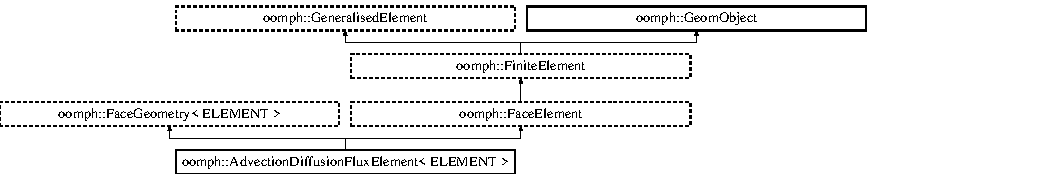
\includegraphics[height=2.333333cm]{classoomph_1_1AdvectionDiffusionFluxElement}
\end{center}
\end{figure}
\subsection*{Public Types}
\begin{DoxyCompactItemize}
\item 
typedef void($\ast$ \hyperlink{classoomph_1_1AdvectionDiffusionFluxElement_aeb9eb0a65d6dfe3673f6910a6fd7cf59}{Advection\+Diffusion\+Prescribed\+Flux\+Fct\+Pt}) (const \hyperlink{classoomph_1_1Vector}{Vector}$<$ double $>$ \&x, double \&flux)
\begin{DoxyCompactList}\small\item\em Function pointer to the prescribed-\/flux function fct(x,f(x)) -- x is a Vector! \end{DoxyCompactList}\end{DoxyCompactItemize}
\subsection*{Public Member Functions}
\begin{DoxyCompactItemize}
\item 
\hyperlink{classoomph_1_1AdvectionDiffusionFluxElement_acdb4a523d9680f6f42128044591c73e0}{Advection\+Diffusion\+Flux\+Element} (\hyperlink{classoomph_1_1FiniteElement}{Finite\+Element} $\ast$const \&bulk\+\_\+el\+\_\+pt, const int \&\hyperlink{classoomph_1_1FaceElement_a478d577ac6db67ecc80f1f02ae3ab170}{face\+\_\+index})
\begin{DoxyCompactList}\small\item\em Constructor, takes the pointer to the \char`\"{}bulk\char`\"{} element and the index of the face to be created. \end{DoxyCompactList}\item 
\hyperlink{classoomph_1_1AdvectionDiffusionFluxElement_af91991cc6e255d038f0f8443e0339643}{Advection\+Diffusion\+Flux\+Element} ()
\begin{DoxyCompactList}\small\item\em Broken empty constructor. \end{DoxyCompactList}\item 
\hyperlink{classoomph_1_1AdvectionDiffusionFluxElement_a187a597274ed7d129da3b1cd89196f44}{Advection\+Diffusion\+Flux\+Element} (const \hyperlink{classoomph_1_1AdvectionDiffusionFluxElement}{Advection\+Diffusion\+Flux\+Element} \&dummy)
\begin{DoxyCompactList}\small\item\em Broken copy constructor. \end{DoxyCompactList}\item 
void \hyperlink{classoomph_1_1AdvectionDiffusionFluxElement_ad14ac8c65798fc1ed5e28ec2d969f147}{operator=} (const \hyperlink{classoomph_1_1AdvectionDiffusionFluxElement}{Advection\+Diffusion\+Flux\+Element} \&)
\begin{DoxyCompactList}\small\item\em Broken assignment operator. \end{DoxyCompactList}\item 
\hyperlink{classoomph_1_1AdvectionDiffusionFluxElement_aeb9eb0a65d6dfe3673f6910a6fd7cf59}{Advection\+Diffusion\+Prescribed\+Flux\+Fct\+Pt} \& \hyperlink{classoomph_1_1AdvectionDiffusionFluxElement_a8d78c95241fe2615ea63040e4072627d}{flux\+\_\+fct\+\_\+pt} ()
\begin{DoxyCompactList}\small\item\em Access function for the prescribed-\/flux function pointer. \end{DoxyCompactList}\item 
void \hyperlink{classoomph_1_1AdvectionDiffusionFluxElement_a7448e4359840f5090f879bc82b2319f8}{fill\+\_\+in\+\_\+contribution\+\_\+to\+\_\+residuals} (\hyperlink{classoomph_1_1Vector}{Vector}$<$ double $>$ \&residuals)
\begin{DoxyCompactList}\small\item\em Add the element\textquotesingle{}s contribution to its residual vector. \end{DoxyCompactList}\item 
void \hyperlink{classoomph_1_1AdvectionDiffusionFluxElement_a5c8e409a31f90858e556fe359b996b9d}{fill\+\_\+in\+\_\+contribution\+\_\+to\+\_\+jacobian} (\hyperlink{classoomph_1_1Vector}{Vector}$<$ double $>$ \&residuals, \hyperlink{classoomph_1_1DenseMatrix}{Dense\+Matrix}$<$ double $>$ \&jacobian)
\begin{DoxyCompactList}\small\item\em Add the element\textquotesingle{}s contribution to its residual vector and its Jacobian matrix. \end{DoxyCompactList}\item 
double \hyperlink{classoomph_1_1AdvectionDiffusionFluxElement_aaf962dc2e0fccdafa7210bbaaf2fbbd6}{zeta\+\_\+nodal} (const unsigned \&n, const unsigned \&k, const unsigned \&\hyperlink{cfortran_8h_adb50e893b86b3e55e751a42eab3cba82}{i}) const
\begin{DoxyCompactList}\small\item\em The \char`\"{}global\char`\"{} intrinsic coordinate of the element when viewed as part of a geometric object should be given by the \hyperlink{classoomph_1_1FaceElement}{Face\+Element} representation, by default (needed to break indeterminacy if bulk element is Solid\+Element) \end{DoxyCompactList}\item 
void \hyperlink{classoomph_1_1AdvectionDiffusionFluxElement_a23efe876b380f81188dcb506ac24266b}{output} (std\+::ostream \&outfile)
\begin{DoxyCompactList}\small\item\em Output function -- forward to broken version in \hyperlink{classoomph_1_1FiniteElement}{Finite\+Element} until somebody decides what exactly they want to plot here... \end{DoxyCompactList}\item 
void \hyperlink{classoomph_1_1AdvectionDiffusionFluxElement_a6a080d1e107612072d9069f909a2b5b0}{output} (std\+::ostream \&outfile, const unsigned \&nplot)
\begin{DoxyCompactList}\small\item\em Output function -- forward to broken version in \hyperlink{classoomph_1_1FiniteElement}{Finite\+Element} until somebody decides what exactly they want to plot here... \end{DoxyCompactList}\end{DoxyCompactItemize}
\subsection*{Protected Member Functions}
\begin{DoxyCompactItemize}
\item 
double \hyperlink{classoomph_1_1AdvectionDiffusionFluxElement_a735b7f2134a85a1f856582f52ad773b1}{shape\+\_\+and\+\_\+test} (const \hyperlink{classoomph_1_1Vector}{Vector}$<$ double $>$ \&\hyperlink{cfortran_8h_ab7123126e4885ef647dd9c6e3807a21c}{s}, \hyperlink{classoomph_1_1Shape}{Shape} \&psi, \hyperlink{classoomph_1_1Shape}{Shape} \&test) const
\begin{DoxyCompactList}\small\item\em Function to compute the shape and test functions and to return the Jacobian of mapping between local and global (Eulerian) coordinates. \end{DoxyCompactList}\item 
double \hyperlink{classoomph_1_1AdvectionDiffusionFluxElement_a32af9be97192954538f40cba54facd83}{shape\+\_\+and\+\_\+test\+\_\+at\+\_\+knot} (const unsigned \&ipt, \hyperlink{classoomph_1_1Shape}{Shape} \&psi, \hyperlink{classoomph_1_1Shape}{Shape} \&test) const
\begin{DoxyCompactList}\small\item\em Function to compute the shape and test functions and to return the Jacobian of mapping between local and global (Eulerian) coordinates. \end{DoxyCompactList}\item 
void \hyperlink{classoomph_1_1AdvectionDiffusionFluxElement_ab21b7655c7d09d338bc4be4baf4dfca6}{get\+\_\+flux} (const \hyperlink{classoomph_1_1Vector}{Vector}$<$ double $>$ \&x, double \&flux)
\begin{DoxyCompactList}\small\item\em Function to calculate the prescribed flux at a given spatial position. \end{DoxyCompactList}\end{DoxyCompactItemize}
\subsection*{Private Member Functions}
\begin{DoxyCompactItemize}
\item 
void \hyperlink{classoomph_1_1AdvectionDiffusionFluxElement_acbc0c8e1e486601c0f09f7ecbb1995c4}{fill\+\_\+in\+\_\+generic\+\_\+residual\+\_\+contribution\+\_\+adv\+\_\+diff\+\_\+flux} (\hyperlink{classoomph_1_1Vector}{Vector}$<$ double $>$ \&residuals, \hyperlink{classoomph_1_1DenseMatrix}{Dense\+Matrix}$<$ double $>$ \&jacobian, unsigned flag)
\begin{DoxyCompactList}\small\item\em Add the element\textquotesingle{}s contribution to its residual vector. flag=1(or 0)\+: do (or don\textquotesingle{}t) compute the Jacobian as well. \end{DoxyCompactList}\end{DoxyCompactItemize}
\subsection*{Private Attributes}
\begin{DoxyCompactItemize}
\item 
\hyperlink{classoomph_1_1AdvectionDiffusionFluxElement_aeb9eb0a65d6dfe3673f6910a6fd7cf59}{Advection\+Diffusion\+Prescribed\+Flux\+Fct\+Pt} \hyperlink{classoomph_1_1AdvectionDiffusionFluxElement_a7c0b0eda4c03c14b18963c59b2c80a67}{Flux\+\_\+fct\+\_\+pt}
\begin{DoxyCompactList}\small\item\em Function pointer to the (global) prescribed-\/flux function. \end{DoxyCompactList}\item 
unsigned \hyperlink{classoomph_1_1AdvectionDiffusionFluxElement_a9418de31c96e89d011b6627cb5756e1e}{Dim}
\begin{DoxyCompactList}\small\item\em The spatial dimension of the problem. \end{DoxyCompactList}\item 
unsigned \hyperlink{classoomph_1_1AdvectionDiffusionFluxElement_a70092d79adb469c7b8fb34b1c31903a1}{U\+\_\+index\+\_\+adv\+\_\+diff}
\begin{DoxyCompactList}\small\item\em The index at which the unknown is stored at the nodes. \end{DoxyCompactList}\end{DoxyCompactItemize}
\subsection*{Additional Inherited Members}


\subsection{Detailed Description}
\subsubsection*{template$<$class E\+L\+E\+M\+E\+NT$>$\newline
class oomph\+::\+Advection\+Diffusion\+Flux\+Element$<$ E\+L\+E\+M\+E\+N\+T $>$}

A class for elements that allow the imposition of an applied flux on the boundaries of Advection Diffusion elements. The element geometry is obtained from the Face\+Geometry$<$\+E\+L\+E\+M\+E\+N\+T$>$ policy class. 

Definition at line 60 of file advection\+\_\+diffusion\+\_\+flux\+\_\+elements.\+h.



\subsection{Member Typedef Documentation}
\mbox{\Hypertarget{classoomph_1_1AdvectionDiffusionFluxElement_aeb9eb0a65d6dfe3673f6910a6fd7cf59}\label{classoomph_1_1AdvectionDiffusionFluxElement_aeb9eb0a65d6dfe3673f6910a6fd7cf59}} 
\index{oomph\+::\+Advection\+Diffusion\+Flux\+Element@{oomph\+::\+Advection\+Diffusion\+Flux\+Element}!Advection\+Diffusion\+Prescribed\+Flux\+Fct\+Pt@{Advection\+Diffusion\+Prescribed\+Flux\+Fct\+Pt}}
\index{Advection\+Diffusion\+Prescribed\+Flux\+Fct\+Pt@{Advection\+Diffusion\+Prescribed\+Flux\+Fct\+Pt}!oomph\+::\+Advection\+Diffusion\+Flux\+Element@{oomph\+::\+Advection\+Diffusion\+Flux\+Element}}
\subsubsection{\texorpdfstring{Advection\+Diffusion\+Prescribed\+Flux\+Fct\+Pt}{AdvectionDiffusionPrescribedFluxFctPt}}
{\footnotesize\ttfamily template$<$class E\+L\+E\+M\+E\+NT $>$ \\
typedef void($\ast$ \hyperlink{classoomph_1_1AdvectionDiffusionFluxElement}{oomph\+::\+Advection\+Diffusion\+Flux\+Element}$<$ E\+L\+E\+M\+E\+NT $>$\+::Advection\+Diffusion\+Prescribed\+Flux\+Fct\+Pt) (const \hyperlink{classoomph_1_1Vector}{Vector}$<$ double $>$ \&x, double \&flux)}



Function pointer to the prescribed-\/flux function fct(x,f(x)) -- x is a Vector! 



Definition at line 70 of file advection\+\_\+diffusion\+\_\+flux\+\_\+elements.\+h.



\subsection{Constructor \& Destructor Documentation}
\mbox{\Hypertarget{classoomph_1_1AdvectionDiffusionFluxElement_acdb4a523d9680f6f42128044591c73e0}\label{classoomph_1_1AdvectionDiffusionFluxElement_acdb4a523d9680f6f42128044591c73e0}} 
\index{oomph\+::\+Advection\+Diffusion\+Flux\+Element@{oomph\+::\+Advection\+Diffusion\+Flux\+Element}!Advection\+Diffusion\+Flux\+Element@{Advection\+Diffusion\+Flux\+Element}}
\index{Advection\+Diffusion\+Flux\+Element@{Advection\+Diffusion\+Flux\+Element}!oomph\+::\+Advection\+Diffusion\+Flux\+Element@{oomph\+::\+Advection\+Diffusion\+Flux\+Element}}
\subsubsection{\texorpdfstring{Advection\+Diffusion\+Flux\+Element()}{AdvectionDiffusionFluxElement()}\hspace{0.1cm}{\footnotesize\ttfamily [1/3]}}
{\footnotesize\ttfamily template$<$class E\+L\+E\+M\+E\+NT $>$ \\
\hyperlink{classoomph_1_1AdvectionDiffusionFluxElement}{oomph\+::\+Advection\+Diffusion\+Flux\+Element}$<$ E\+L\+E\+M\+E\+NT $>$\+::\hyperlink{classoomph_1_1AdvectionDiffusionFluxElement}{Advection\+Diffusion\+Flux\+Element} (\begin{DoxyParamCaption}\item[{\hyperlink{classoomph_1_1FiniteElement}{Finite\+Element} $\ast$const \&}]{bulk\+\_\+el\+\_\+pt,  }\item[{const int \&}]{face\+\_\+index }\end{DoxyParamCaption})}



Constructor, takes the pointer to the \char`\"{}bulk\char`\"{} element and the index of the face to be created. 



Definition at line 240 of file advection\+\_\+diffusion\+\_\+flux\+\_\+elements.\+h.



References oomph\+::\+Finite\+Element\+::build\+\_\+face\+\_\+element(), oomph\+::\+Advection\+Diffusion\+Flux\+Element$<$ E\+L\+E\+M\+E\+N\+T $>$\+::\+Dim, oomph\+::\+Advection\+Diffusion\+Flux\+Element$<$ E\+L\+E\+M\+E\+N\+T $>$\+::fill\+\_\+in\+\_\+generic\+\_\+residual\+\_\+contribution\+\_\+adv\+\_\+diff\+\_\+flux(), oomph\+::\+Advection\+Diffusion\+Flux\+Element$<$ E\+L\+E\+M\+E\+N\+T $>$\+::\+Flux\+\_\+fct\+\_\+pt, oomph\+::\+Finite\+Element\+::has\+\_\+hanging\+\_\+nodes(), oomph\+::\+Node\+::ndim(), oomph\+::\+Finite\+Element\+::node\+\_\+pt(), oomph\+::\+Global\+\_\+string\+\_\+for\+\_\+annotation\+::string(), oomph\+::\+Advection\+Diffusion\+Equations$<$ D\+I\+M $>$\+::u\+\_\+index\+\_\+adv\+\_\+diff(), and oomph\+::\+Advection\+Diffusion\+Flux\+Element$<$ E\+L\+E\+M\+E\+N\+T $>$\+::\+U\+\_\+index\+\_\+adv\+\_\+diff.

\mbox{\Hypertarget{classoomph_1_1AdvectionDiffusionFluxElement_af91991cc6e255d038f0f8443e0339643}\label{classoomph_1_1AdvectionDiffusionFluxElement_af91991cc6e255d038f0f8443e0339643}} 
\index{oomph\+::\+Advection\+Diffusion\+Flux\+Element@{oomph\+::\+Advection\+Diffusion\+Flux\+Element}!Advection\+Diffusion\+Flux\+Element@{Advection\+Diffusion\+Flux\+Element}}
\index{Advection\+Diffusion\+Flux\+Element@{Advection\+Diffusion\+Flux\+Element}!oomph\+::\+Advection\+Diffusion\+Flux\+Element@{oomph\+::\+Advection\+Diffusion\+Flux\+Element}}
\subsubsection{\texorpdfstring{Advection\+Diffusion\+Flux\+Element()}{AdvectionDiffusionFluxElement()}\hspace{0.1cm}{\footnotesize\ttfamily [2/3]}}
{\footnotesize\ttfamily template$<$class E\+L\+E\+M\+E\+NT $>$ \\
\hyperlink{classoomph_1_1AdvectionDiffusionFluxElement}{oomph\+::\+Advection\+Diffusion\+Flux\+Element}$<$ E\+L\+E\+M\+E\+NT $>$\+::\hyperlink{classoomph_1_1AdvectionDiffusionFluxElement}{Advection\+Diffusion\+Flux\+Element} (\begin{DoxyParamCaption}{ }\end{DoxyParamCaption})\hspace{0.3cm}{\ttfamily [inline]}}



Broken empty constructor. 



Definition at line 80 of file advection\+\_\+diffusion\+\_\+flux\+\_\+elements.\+h.

\mbox{\Hypertarget{classoomph_1_1AdvectionDiffusionFluxElement_a187a597274ed7d129da3b1cd89196f44}\label{classoomph_1_1AdvectionDiffusionFluxElement_a187a597274ed7d129da3b1cd89196f44}} 
\index{oomph\+::\+Advection\+Diffusion\+Flux\+Element@{oomph\+::\+Advection\+Diffusion\+Flux\+Element}!Advection\+Diffusion\+Flux\+Element@{Advection\+Diffusion\+Flux\+Element}}
\index{Advection\+Diffusion\+Flux\+Element@{Advection\+Diffusion\+Flux\+Element}!oomph\+::\+Advection\+Diffusion\+Flux\+Element@{oomph\+::\+Advection\+Diffusion\+Flux\+Element}}
\subsubsection{\texorpdfstring{Advection\+Diffusion\+Flux\+Element()}{AdvectionDiffusionFluxElement()}\hspace{0.1cm}{\footnotesize\ttfamily [3/3]}}
{\footnotesize\ttfamily template$<$class E\+L\+E\+M\+E\+NT $>$ \\
\hyperlink{classoomph_1_1AdvectionDiffusionFluxElement}{oomph\+::\+Advection\+Diffusion\+Flux\+Element}$<$ E\+L\+E\+M\+E\+NT $>$\+::\hyperlink{classoomph_1_1AdvectionDiffusionFluxElement}{Advection\+Diffusion\+Flux\+Element} (\begin{DoxyParamCaption}\item[{const \hyperlink{classoomph_1_1AdvectionDiffusionFluxElement}{Advection\+Diffusion\+Flux\+Element}$<$ E\+L\+E\+M\+E\+NT $>$ \&}]{dummy }\end{DoxyParamCaption})\hspace{0.3cm}{\ttfamily [inline]}}



Broken copy constructor. 



Definition at line 89 of file advection\+\_\+diffusion\+\_\+flux\+\_\+elements.\+h.



References oomph\+::\+Broken\+Copy\+::broken\+\_\+copy().



\subsection{Member Function Documentation}
\mbox{\Hypertarget{classoomph_1_1AdvectionDiffusionFluxElement_a5c8e409a31f90858e556fe359b996b9d}\label{classoomph_1_1AdvectionDiffusionFluxElement_a5c8e409a31f90858e556fe359b996b9d}} 
\index{oomph\+::\+Advection\+Diffusion\+Flux\+Element@{oomph\+::\+Advection\+Diffusion\+Flux\+Element}!fill\+\_\+in\+\_\+contribution\+\_\+to\+\_\+jacobian@{fill\+\_\+in\+\_\+contribution\+\_\+to\+\_\+jacobian}}
\index{fill\+\_\+in\+\_\+contribution\+\_\+to\+\_\+jacobian@{fill\+\_\+in\+\_\+contribution\+\_\+to\+\_\+jacobian}!oomph\+::\+Advection\+Diffusion\+Flux\+Element@{oomph\+::\+Advection\+Diffusion\+Flux\+Element}}
\subsubsection{\texorpdfstring{fill\+\_\+in\+\_\+contribution\+\_\+to\+\_\+jacobian()}{fill\_in\_contribution\_to\_jacobian()}}
{\footnotesize\ttfamily template$<$class E\+L\+E\+M\+E\+NT $>$ \\
void \hyperlink{classoomph_1_1AdvectionDiffusionFluxElement}{oomph\+::\+Advection\+Diffusion\+Flux\+Element}$<$ E\+L\+E\+M\+E\+NT $>$\+::fill\+\_\+in\+\_\+contribution\+\_\+to\+\_\+jacobian (\begin{DoxyParamCaption}\item[{\hyperlink{classoomph_1_1Vector}{Vector}$<$ double $>$ \&}]{residuals,  }\item[{\hyperlink{classoomph_1_1DenseMatrix}{Dense\+Matrix}$<$ double $>$ \&}]{jacobian }\end{DoxyParamCaption})\hspace{0.3cm}{\ttfamily [inline]}, {\ttfamily [virtual]}}



Add the element\textquotesingle{}s contribution to its residual vector and its Jacobian matrix. 



Reimplemented from \hyperlink{classoomph_1_1GeneralisedElement_a6ae09fc0d68e4309ac1b03583d252845}{oomph\+::\+Generalised\+Element}.



Definition at line 116 of file advection\+\_\+diffusion\+\_\+flux\+\_\+elements.\+h.



References oomph\+::\+Advection\+Diffusion\+Flux\+Element$<$ E\+L\+E\+M\+E\+N\+T $>$\+::fill\+\_\+in\+\_\+generic\+\_\+residual\+\_\+contribution\+\_\+adv\+\_\+diff\+\_\+flux().

\mbox{\Hypertarget{classoomph_1_1AdvectionDiffusionFluxElement_a7448e4359840f5090f879bc82b2319f8}\label{classoomph_1_1AdvectionDiffusionFluxElement_a7448e4359840f5090f879bc82b2319f8}} 
\index{oomph\+::\+Advection\+Diffusion\+Flux\+Element@{oomph\+::\+Advection\+Diffusion\+Flux\+Element}!fill\+\_\+in\+\_\+contribution\+\_\+to\+\_\+residuals@{fill\+\_\+in\+\_\+contribution\+\_\+to\+\_\+residuals}}
\index{fill\+\_\+in\+\_\+contribution\+\_\+to\+\_\+residuals@{fill\+\_\+in\+\_\+contribution\+\_\+to\+\_\+residuals}!oomph\+::\+Advection\+Diffusion\+Flux\+Element@{oomph\+::\+Advection\+Diffusion\+Flux\+Element}}
\subsubsection{\texorpdfstring{fill\+\_\+in\+\_\+contribution\+\_\+to\+\_\+residuals()}{fill\_in\_contribution\_to\_residuals()}}
{\footnotesize\ttfamily template$<$class E\+L\+E\+M\+E\+NT $>$ \\
void \hyperlink{classoomph_1_1AdvectionDiffusionFluxElement}{oomph\+::\+Advection\+Diffusion\+Flux\+Element}$<$ E\+L\+E\+M\+E\+NT $>$\+::fill\+\_\+in\+\_\+contribution\+\_\+to\+\_\+residuals (\begin{DoxyParamCaption}\item[{\hyperlink{classoomph_1_1Vector}{Vector}$<$ double $>$ \&}]{residuals }\end{DoxyParamCaption})\hspace{0.3cm}{\ttfamily [inline]}, {\ttfamily [virtual]}}



Add the element\textquotesingle{}s contribution to its residual vector. 



Reimplemented from \hyperlink{classoomph_1_1GeneralisedElement_a310c97f515e8504a48179c0e72c550d7}{oomph\+::\+Generalised\+Element}.



Definition at line 105 of file advection\+\_\+diffusion\+\_\+flux\+\_\+elements.\+h.



References oomph\+::\+Generalised\+Element\+::\+Dummy\+\_\+matrix, and oomph\+::\+Advection\+Diffusion\+Flux\+Element$<$ E\+L\+E\+M\+E\+N\+T $>$\+::fill\+\_\+in\+\_\+generic\+\_\+residual\+\_\+contribution\+\_\+adv\+\_\+diff\+\_\+flux().

\mbox{\Hypertarget{classoomph_1_1AdvectionDiffusionFluxElement_acbc0c8e1e486601c0f09f7ecbb1995c4}\label{classoomph_1_1AdvectionDiffusionFluxElement_acbc0c8e1e486601c0f09f7ecbb1995c4}} 
\index{oomph\+::\+Advection\+Diffusion\+Flux\+Element@{oomph\+::\+Advection\+Diffusion\+Flux\+Element}!fill\+\_\+in\+\_\+generic\+\_\+residual\+\_\+contribution\+\_\+adv\+\_\+diff\+\_\+flux@{fill\+\_\+in\+\_\+generic\+\_\+residual\+\_\+contribution\+\_\+adv\+\_\+diff\+\_\+flux}}
\index{fill\+\_\+in\+\_\+generic\+\_\+residual\+\_\+contribution\+\_\+adv\+\_\+diff\+\_\+flux@{fill\+\_\+in\+\_\+generic\+\_\+residual\+\_\+contribution\+\_\+adv\+\_\+diff\+\_\+flux}!oomph\+::\+Advection\+Diffusion\+Flux\+Element@{oomph\+::\+Advection\+Diffusion\+Flux\+Element}}
\subsubsection{\texorpdfstring{fill\+\_\+in\+\_\+generic\+\_\+residual\+\_\+contribution\+\_\+adv\+\_\+diff\+\_\+flux()}{fill\_in\_generic\_residual\_contribution\_adv\_diff\_flux()}}
{\footnotesize\ttfamily template$<$class E\+L\+E\+M\+E\+NT $>$ \\
void \hyperlink{classoomph_1_1AdvectionDiffusionFluxElement}{oomph\+::\+Advection\+Diffusion\+Flux\+Element}$<$ E\+L\+E\+M\+E\+NT $>$\+::fill\+\_\+in\+\_\+generic\+\_\+residual\+\_\+contribution\+\_\+adv\+\_\+diff\+\_\+flux (\begin{DoxyParamCaption}\item[{\hyperlink{classoomph_1_1Vector}{Vector}$<$ double $>$ \&}]{residuals,  }\item[{\hyperlink{classoomph_1_1DenseMatrix}{Dense\+Matrix}$<$ double $>$ \&}]{jacobian,  }\item[{unsigned}]{flag }\end{DoxyParamCaption})\hspace{0.3cm}{\ttfamily [private]}}



Add the element\textquotesingle{}s contribution to its residual vector. flag=1(or 0)\+: do (or don\textquotesingle{}t) compute the Jacobian as well. 

Compute the element\textquotesingle{}s residual vector and the (zero) Jacobian matrix. 

Definition at line 400 of file advection\+\_\+diffusion\+\_\+flux\+\_\+elements.\+h.



References oomph\+::\+Advection\+Diffusion\+Flux\+Element$<$ E\+L\+E\+M\+E\+N\+T $>$\+::\+Dim, oomph\+::\+Advection\+Diffusion\+Flux\+Element$<$ E\+L\+E\+M\+E\+N\+T $>$\+::get\+\_\+flux(), i, oomph\+::\+Finite\+Element\+::integral\+\_\+pt(), oomph\+::\+Face\+Element\+::interpolated\+\_\+x(), oomph\+::\+Integral\+::knot(), oomph\+::\+Finite\+Element\+::nnode(), oomph\+::\+Finite\+Element\+::nodal\+\_\+local\+\_\+eqn(), oomph\+::\+Finite\+Element\+::nodal\+\_\+position(), oomph\+::\+Integral\+::nweight(), s, oomph\+::\+Advection\+Diffusion\+Flux\+Element$<$ E\+L\+E\+M\+E\+N\+T $>$\+::shape\+\_\+and\+\_\+test(), oomph\+::\+Advection\+Diffusion\+Flux\+Element$<$ E\+L\+E\+M\+E\+N\+T $>$\+::\+U\+\_\+index\+\_\+adv\+\_\+diff, oomph\+::\+Quad\+Tree\+Names\+::W, and oomph\+::\+Integral\+::weight().



Referenced by oomph\+::\+Advection\+Diffusion\+Flux\+Element$<$ E\+L\+E\+M\+E\+N\+T $>$\+::\+Advection\+Diffusion\+Flux\+Element(), oomph\+::\+Advection\+Diffusion\+Flux\+Element$<$ E\+L\+E\+M\+E\+N\+T $>$\+::fill\+\_\+in\+\_\+contribution\+\_\+to\+\_\+jacobian(), oomph\+::\+Advection\+Diffusion\+Flux\+Element$<$ E\+L\+E\+M\+E\+N\+T $>$\+::fill\+\_\+in\+\_\+contribution\+\_\+to\+\_\+residuals(), and oomph\+::\+Advection\+Diffusion\+Flux\+Element$<$ E\+L\+E\+M\+E\+N\+T $>$\+::get\+\_\+flux().

\mbox{\Hypertarget{classoomph_1_1AdvectionDiffusionFluxElement_a8d78c95241fe2615ea63040e4072627d}\label{classoomph_1_1AdvectionDiffusionFluxElement_a8d78c95241fe2615ea63040e4072627d}} 
\index{oomph\+::\+Advection\+Diffusion\+Flux\+Element@{oomph\+::\+Advection\+Diffusion\+Flux\+Element}!flux\+\_\+fct\+\_\+pt@{flux\+\_\+fct\+\_\+pt}}
\index{flux\+\_\+fct\+\_\+pt@{flux\+\_\+fct\+\_\+pt}!oomph\+::\+Advection\+Diffusion\+Flux\+Element@{oomph\+::\+Advection\+Diffusion\+Flux\+Element}}
\subsubsection{\texorpdfstring{flux\+\_\+fct\+\_\+pt()}{flux\_fct\_pt()}}
{\footnotesize\ttfamily template$<$class E\+L\+E\+M\+E\+NT $>$ \\
\hyperlink{classoomph_1_1AdvectionDiffusionFluxElement_aeb9eb0a65d6dfe3673f6910a6fd7cf59}{Advection\+Diffusion\+Prescribed\+Flux\+Fct\+Pt}\& \hyperlink{classoomph_1_1AdvectionDiffusionFluxElement}{oomph\+::\+Advection\+Diffusion\+Flux\+Element}$<$ E\+L\+E\+M\+E\+NT $>$\+::flux\+\_\+fct\+\_\+pt (\begin{DoxyParamCaption}{ }\end{DoxyParamCaption})\hspace{0.3cm}{\ttfamily [inline]}}



Access function for the prescribed-\/flux function pointer. 



Definition at line 101 of file advection\+\_\+diffusion\+\_\+flux\+\_\+elements.\+h.



References oomph\+::\+Advection\+Diffusion\+Flux\+Element$<$ E\+L\+E\+M\+E\+N\+T $>$\+::\+Flux\+\_\+fct\+\_\+pt.

\mbox{\Hypertarget{classoomph_1_1AdvectionDiffusionFluxElement_ab21b7655c7d09d338bc4be4baf4dfca6}\label{classoomph_1_1AdvectionDiffusionFluxElement_ab21b7655c7d09d338bc4be4baf4dfca6}} 
\index{oomph\+::\+Advection\+Diffusion\+Flux\+Element@{oomph\+::\+Advection\+Diffusion\+Flux\+Element}!get\+\_\+flux@{get\+\_\+flux}}
\index{get\+\_\+flux@{get\+\_\+flux}!oomph\+::\+Advection\+Diffusion\+Flux\+Element@{oomph\+::\+Advection\+Diffusion\+Flux\+Element}}
\subsubsection{\texorpdfstring{get\+\_\+flux()}{get\_flux()}}
{\footnotesize\ttfamily template$<$class E\+L\+E\+M\+E\+NT $>$ \\
void \hyperlink{classoomph_1_1AdvectionDiffusionFluxElement}{oomph\+::\+Advection\+Diffusion\+Flux\+Element}$<$ E\+L\+E\+M\+E\+NT $>$\+::get\+\_\+flux (\begin{DoxyParamCaption}\item[{const \hyperlink{classoomph_1_1Vector}{Vector}$<$ double $>$ \&}]{x,  }\item[{double \&}]{flux }\end{DoxyParamCaption})\hspace{0.3cm}{\ttfamily [inline]}, {\ttfamily [protected]}}



Function to calculate the prescribed flux at a given spatial position. 



Definition at line 188 of file advection\+\_\+diffusion\+\_\+flux\+\_\+elements.\+h.



References oomph\+::\+Advection\+Diffusion\+Flux\+Element$<$ E\+L\+E\+M\+E\+N\+T $>$\+::fill\+\_\+in\+\_\+generic\+\_\+residual\+\_\+contribution\+\_\+adv\+\_\+diff\+\_\+flux(), and oomph\+::\+Advection\+Diffusion\+Flux\+Element$<$ E\+L\+E\+M\+E\+N\+T $>$\+::\+Flux\+\_\+fct\+\_\+pt.



Referenced by oomph\+::\+Advection\+Diffusion\+Flux\+Element$<$ E\+L\+E\+M\+E\+N\+T $>$\+::fill\+\_\+in\+\_\+generic\+\_\+residual\+\_\+contribution\+\_\+adv\+\_\+diff\+\_\+flux().

\mbox{\Hypertarget{classoomph_1_1AdvectionDiffusionFluxElement_ad14ac8c65798fc1ed5e28ec2d969f147}\label{classoomph_1_1AdvectionDiffusionFluxElement_ad14ac8c65798fc1ed5e28ec2d969f147}} 
\index{oomph\+::\+Advection\+Diffusion\+Flux\+Element@{oomph\+::\+Advection\+Diffusion\+Flux\+Element}!operator=@{operator=}}
\index{operator=@{operator=}!oomph\+::\+Advection\+Diffusion\+Flux\+Element@{oomph\+::\+Advection\+Diffusion\+Flux\+Element}}
\subsubsection{\texorpdfstring{operator=()}{operator=()}}
{\footnotesize\ttfamily template$<$class E\+L\+E\+M\+E\+NT $>$ \\
void \hyperlink{classoomph_1_1AdvectionDiffusionFluxElement}{oomph\+::\+Advection\+Diffusion\+Flux\+Element}$<$ E\+L\+E\+M\+E\+NT $>$\+::operator= (\begin{DoxyParamCaption}\item[{const \hyperlink{classoomph_1_1AdvectionDiffusionFluxElement}{Advection\+Diffusion\+Flux\+Element}$<$ E\+L\+E\+M\+E\+NT $>$ \&}]{ }\end{DoxyParamCaption})\hspace{0.3cm}{\ttfamily [inline]}}



Broken assignment operator. 



Definition at line 95 of file advection\+\_\+diffusion\+\_\+flux\+\_\+elements.\+h.



References oomph\+::\+Broken\+Copy\+::broken\+\_\+assign().

\mbox{\Hypertarget{classoomph_1_1AdvectionDiffusionFluxElement_a23efe876b380f81188dcb506ac24266b}\label{classoomph_1_1AdvectionDiffusionFluxElement_a23efe876b380f81188dcb506ac24266b}} 
\index{oomph\+::\+Advection\+Diffusion\+Flux\+Element@{oomph\+::\+Advection\+Diffusion\+Flux\+Element}!output@{output}}
\index{output@{output}!oomph\+::\+Advection\+Diffusion\+Flux\+Element@{oomph\+::\+Advection\+Diffusion\+Flux\+Element}}
\subsubsection{\texorpdfstring{output()}{output()}\hspace{0.1cm}{\footnotesize\ttfamily [1/2]}}
{\footnotesize\ttfamily template$<$class E\+L\+E\+M\+E\+NT $>$ \\
void \hyperlink{classoomph_1_1AdvectionDiffusionFluxElement}{oomph\+::\+Advection\+Diffusion\+Flux\+Element}$<$ E\+L\+E\+M\+E\+NT $>$\+::output (\begin{DoxyParamCaption}\item[{std\+::ostream \&}]{outfile }\end{DoxyParamCaption})\hspace{0.3cm}{\ttfamily [inline]}, {\ttfamily [virtual]}}



Output function -- forward to broken version in \hyperlink{classoomph_1_1FiniteElement}{Finite\+Element} until somebody decides what exactly they want to plot here... 



Reimplemented from \hyperlink{classoomph_1_1FiniteElement_a2ad98a3d2ef4999f1bef62c0ff13f2a7}{oomph\+::\+Finite\+Element}.



Definition at line 134 of file advection\+\_\+diffusion\+\_\+flux\+\_\+elements.\+h.



References oomph\+::\+Finite\+Element\+::output().

\mbox{\Hypertarget{classoomph_1_1AdvectionDiffusionFluxElement_a6a080d1e107612072d9069f909a2b5b0}\label{classoomph_1_1AdvectionDiffusionFluxElement_a6a080d1e107612072d9069f909a2b5b0}} 
\index{oomph\+::\+Advection\+Diffusion\+Flux\+Element@{oomph\+::\+Advection\+Diffusion\+Flux\+Element}!output@{output}}
\index{output@{output}!oomph\+::\+Advection\+Diffusion\+Flux\+Element@{oomph\+::\+Advection\+Diffusion\+Flux\+Element}}
\subsubsection{\texorpdfstring{output()}{output()}\hspace{0.1cm}{\footnotesize\ttfamily [2/2]}}
{\footnotesize\ttfamily template$<$class E\+L\+E\+M\+E\+NT $>$ \\
void \hyperlink{classoomph_1_1AdvectionDiffusionFluxElement}{oomph\+::\+Advection\+Diffusion\+Flux\+Element}$<$ E\+L\+E\+M\+E\+NT $>$\+::output (\begin{DoxyParamCaption}\item[{std\+::ostream \&}]{outfile,  }\item[{const unsigned \&}]{nplot }\end{DoxyParamCaption})\hspace{0.3cm}{\ttfamily [inline]}, {\ttfamily [virtual]}}



Output function -- forward to broken version in \hyperlink{classoomph_1_1FiniteElement}{Finite\+Element} until somebody decides what exactly they want to plot here... 



Reimplemented from \hyperlink{classoomph_1_1FiniteElement_afa9d9b2670f999b43e6679c9dd28c457}{oomph\+::\+Finite\+Element}.



Definition at line 138 of file advection\+\_\+diffusion\+\_\+flux\+\_\+elements.\+h.



References oomph\+::\+Finite\+Element\+::output().

\mbox{\Hypertarget{classoomph_1_1AdvectionDiffusionFluxElement_a735b7f2134a85a1f856582f52ad773b1}\label{classoomph_1_1AdvectionDiffusionFluxElement_a735b7f2134a85a1f856582f52ad773b1}} 
\index{oomph\+::\+Advection\+Diffusion\+Flux\+Element@{oomph\+::\+Advection\+Diffusion\+Flux\+Element}!shape\+\_\+and\+\_\+test@{shape\+\_\+and\+\_\+test}}
\index{shape\+\_\+and\+\_\+test@{shape\+\_\+and\+\_\+test}!oomph\+::\+Advection\+Diffusion\+Flux\+Element@{oomph\+::\+Advection\+Diffusion\+Flux\+Element}}
\subsubsection{\texorpdfstring{shape\+\_\+and\+\_\+test()}{shape\_and\_test()}}
{\footnotesize\ttfamily template$<$class E\+L\+E\+M\+E\+NT $>$ \\
double \hyperlink{classoomph_1_1AdvectionDiffusionFluxElement}{oomph\+::\+Advection\+Diffusion\+Flux\+Element}$<$ E\+L\+E\+M\+E\+NT $>$\+::shape\+\_\+and\+\_\+test (\begin{DoxyParamCaption}\item[{const \hyperlink{classoomph_1_1Vector}{Vector}$<$ double $>$ \&}]{s,  }\item[{\hyperlink{classoomph_1_1Shape}{Shape} \&}]{psi,  }\item[{\hyperlink{classoomph_1_1Shape}{Shape} \&}]{test }\end{DoxyParamCaption}) const\hspace{0.3cm}{\ttfamily [inline]}, {\ttfamily [protected]}}



Function to compute the shape and test functions and to return the Jacobian of mapping between local and global (Eulerian) coordinates. 



Definition at line 147 of file advection\+\_\+diffusion\+\_\+flux\+\_\+elements.\+h.



References i, oomph\+::\+Face\+Element\+::\+J\+\_\+eulerian(), oomph\+::\+Finite\+Element\+::nnode(), and oomph\+::\+Finite\+Element\+::shape().



Referenced by oomph\+::\+Advection\+Diffusion\+Flux\+Element$<$ E\+L\+E\+M\+E\+N\+T $>$\+::fill\+\_\+in\+\_\+generic\+\_\+residual\+\_\+contribution\+\_\+adv\+\_\+diff\+\_\+flux().

\mbox{\Hypertarget{classoomph_1_1AdvectionDiffusionFluxElement_a32af9be97192954538f40cba54facd83}\label{classoomph_1_1AdvectionDiffusionFluxElement_a32af9be97192954538f40cba54facd83}} 
\index{oomph\+::\+Advection\+Diffusion\+Flux\+Element@{oomph\+::\+Advection\+Diffusion\+Flux\+Element}!shape\+\_\+and\+\_\+test\+\_\+at\+\_\+knot@{shape\+\_\+and\+\_\+test\+\_\+at\+\_\+knot}}
\index{shape\+\_\+and\+\_\+test\+\_\+at\+\_\+knot@{shape\+\_\+and\+\_\+test\+\_\+at\+\_\+knot}!oomph\+::\+Advection\+Diffusion\+Flux\+Element@{oomph\+::\+Advection\+Diffusion\+Flux\+Element}}
\subsubsection{\texorpdfstring{shape\+\_\+and\+\_\+test\+\_\+at\+\_\+knot()}{shape\_and\_test\_at\_knot()}}
{\footnotesize\ttfamily template$<$class E\+L\+E\+M\+E\+NT $>$ \\
double \hyperlink{classoomph_1_1AdvectionDiffusionFluxElement}{oomph\+::\+Advection\+Diffusion\+Flux\+Element}$<$ E\+L\+E\+M\+E\+NT $>$\+::shape\+\_\+and\+\_\+test\+\_\+at\+\_\+knot (\begin{DoxyParamCaption}\item[{const unsigned \&}]{ipt,  }\item[{\hyperlink{classoomph_1_1Shape}{Shape} \&}]{psi,  }\item[{\hyperlink{classoomph_1_1Shape}{Shape} \&}]{test }\end{DoxyParamCaption}) const\hspace{0.3cm}{\ttfamily [inline]}, {\ttfamily [protected]}}



Function to compute the shape and test functions and to return the Jacobian of mapping between local and global (Eulerian) coordinates. 



Definition at line 167 of file advection\+\_\+diffusion\+\_\+flux\+\_\+elements.\+h.



References i, oomph\+::\+Face\+Element\+::\+J\+\_\+eulerian\+\_\+at\+\_\+knot(), oomph\+::\+Finite\+Element\+::nnode(), and oomph\+::\+Finite\+Element\+::shape\+\_\+at\+\_\+knot().

\mbox{\Hypertarget{classoomph_1_1AdvectionDiffusionFluxElement_aaf962dc2e0fccdafa7210bbaaf2fbbd6}\label{classoomph_1_1AdvectionDiffusionFluxElement_aaf962dc2e0fccdafa7210bbaaf2fbbd6}} 
\index{oomph\+::\+Advection\+Diffusion\+Flux\+Element@{oomph\+::\+Advection\+Diffusion\+Flux\+Element}!zeta\+\_\+nodal@{zeta\+\_\+nodal}}
\index{zeta\+\_\+nodal@{zeta\+\_\+nodal}!oomph\+::\+Advection\+Diffusion\+Flux\+Element@{oomph\+::\+Advection\+Diffusion\+Flux\+Element}}
\subsubsection{\texorpdfstring{zeta\+\_\+nodal()}{zeta\_nodal()}}
{\footnotesize\ttfamily template$<$class E\+L\+E\+M\+E\+NT $>$ \\
double \hyperlink{classoomph_1_1AdvectionDiffusionFluxElement}{oomph\+::\+Advection\+Diffusion\+Flux\+Element}$<$ E\+L\+E\+M\+E\+NT $>$\+::zeta\+\_\+nodal (\begin{DoxyParamCaption}\item[{const unsigned \&}]{n,  }\item[{const unsigned \&}]{k,  }\item[{const unsigned \&}]{i }\end{DoxyParamCaption}) const\hspace{0.3cm}{\ttfamily [inline]}, {\ttfamily [virtual]}}



The \char`\"{}global\char`\"{} intrinsic coordinate of the element when viewed as part of a geometric object should be given by the \hyperlink{classoomph_1_1FaceElement}{Face\+Element} representation, by default (needed to break indeterminacy if bulk element is Solid\+Element) 

Specify the value of nodal zeta from the face geometry 

Reimplemented from \hyperlink{classoomph_1_1FiniteElement_a849561c5fbcbc07dc49d2dc6cca68559}{oomph\+::\+Finite\+Element}.



Definition at line 128 of file advection\+\_\+diffusion\+\_\+flux\+\_\+elements.\+h.



References oomph\+::\+Face\+Element\+::zeta\+\_\+nodal().



\subsection{Member Data Documentation}
\mbox{\Hypertarget{classoomph_1_1AdvectionDiffusionFluxElement_a9418de31c96e89d011b6627cb5756e1e}\label{classoomph_1_1AdvectionDiffusionFluxElement_a9418de31c96e89d011b6627cb5756e1e}} 
\index{oomph\+::\+Advection\+Diffusion\+Flux\+Element@{oomph\+::\+Advection\+Diffusion\+Flux\+Element}!Dim@{Dim}}
\index{Dim@{Dim}!oomph\+::\+Advection\+Diffusion\+Flux\+Element@{oomph\+::\+Advection\+Diffusion\+Flux\+Element}}
\subsubsection{\texorpdfstring{Dim}{Dim}}
{\footnotesize\ttfamily template$<$class E\+L\+E\+M\+E\+NT $>$ \\
unsigned \hyperlink{classoomph_1_1AdvectionDiffusionFluxElement}{oomph\+::\+Advection\+Diffusion\+Flux\+Element}$<$ E\+L\+E\+M\+E\+NT $>$\+::Dim\hspace{0.3cm}{\ttfamily [private]}}



The spatial dimension of the problem. 



Definition at line 216 of file advection\+\_\+diffusion\+\_\+flux\+\_\+elements.\+h.



Referenced by oomph\+::\+Advection\+Diffusion\+Flux\+Element$<$ E\+L\+E\+M\+E\+N\+T $>$\+::\+Advection\+Diffusion\+Flux\+Element(), and oomph\+::\+Advection\+Diffusion\+Flux\+Element$<$ E\+L\+E\+M\+E\+N\+T $>$\+::fill\+\_\+in\+\_\+generic\+\_\+residual\+\_\+contribution\+\_\+adv\+\_\+diff\+\_\+flux().

\mbox{\Hypertarget{classoomph_1_1AdvectionDiffusionFluxElement_a7c0b0eda4c03c14b18963c59b2c80a67}\label{classoomph_1_1AdvectionDiffusionFluxElement_a7c0b0eda4c03c14b18963c59b2c80a67}} 
\index{oomph\+::\+Advection\+Diffusion\+Flux\+Element@{oomph\+::\+Advection\+Diffusion\+Flux\+Element}!Flux\+\_\+fct\+\_\+pt@{Flux\+\_\+fct\+\_\+pt}}
\index{Flux\+\_\+fct\+\_\+pt@{Flux\+\_\+fct\+\_\+pt}!oomph\+::\+Advection\+Diffusion\+Flux\+Element@{oomph\+::\+Advection\+Diffusion\+Flux\+Element}}
\subsubsection{\texorpdfstring{Flux\+\_\+fct\+\_\+pt}{Flux\_fct\_pt}}
{\footnotesize\ttfamily template$<$class E\+L\+E\+M\+E\+NT $>$ \\
\hyperlink{classoomph_1_1AdvectionDiffusionFluxElement_aeb9eb0a65d6dfe3673f6910a6fd7cf59}{Advection\+Diffusion\+Prescribed\+Flux\+Fct\+Pt} \hyperlink{classoomph_1_1AdvectionDiffusionFluxElement}{oomph\+::\+Advection\+Diffusion\+Flux\+Element}$<$ E\+L\+E\+M\+E\+NT $>$\+::Flux\+\_\+fct\+\_\+pt\hspace{0.3cm}{\ttfamily [private]}}



Function pointer to the (global) prescribed-\/flux function. 



Definition at line 213 of file advection\+\_\+diffusion\+\_\+flux\+\_\+elements.\+h.



Referenced by oomph\+::\+Advection\+Diffusion\+Flux\+Element$<$ E\+L\+E\+M\+E\+N\+T $>$\+::\+Advection\+Diffusion\+Flux\+Element(), oomph\+::\+Advection\+Diffusion\+Flux\+Element$<$ E\+L\+E\+M\+E\+N\+T $>$\+::flux\+\_\+fct\+\_\+pt(), and oomph\+::\+Advection\+Diffusion\+Flux\+Element$<$ E\+L\+E\+M\+E\+N\+T $>$\+::get\+\_\+flux().

\mbox{\Hypertarget{classoomph_1_1AdvectionDiffusionFluxElement_a70092d79adb469c7b8fb34b1c31903a1}\label{classoomph_1_1AdvectionDiffusionFluxElement_a70092d79adb469c7b8fb34b1c31903a1}} 
\index{oomph\+::\+Advection\+Diffusion\+Flux\+Element@{oomph\+::\+Advection\+Diffusion\+Flux\+Element}!U\+\_\+index\+\_\+adv\+\_\+diff@{U\+\_\+index\+\_\+adv\+\_\+diff}}
\index{U\+\_\+index\+\_\+adv\+\_\+diff@{U\+\_\+index\+\_\+adv\+\_\+diff}!oomph\+::\+Advection\+Diffusion\+Flux\+Element@{oomph\+::\+Advection\+Diffusion\+Flux\+Element}}
\subsubsection{\texorpdfstring{U\+\_\+index\+\_\+adv\+\_\+diff}{U\_index\_adv\_diff}}
{\footnotesize\ttfamily template$<$class E\+L\+E\+M\+E\+NT $>$ \\
unsigned \hyperlink{classoomph_1_1AdvectionDiffusionFluxElement}{oomph\+::\+Advection\+Diffusion\+Flux\+Element}$<$ E\+L\+E\+M\+E\+NT $>$\+::U\+\_\+index\+\_\+adv\+\_\+diff\hspace{0.3cm}{\ttfamily [private]}}



The index at which the unknown is stored at the nodes. 



Definition at line 219 of file advection\+\_\+diffusion\+\_\+flux\+\_\+elements.\+h.



Referenced by oomph\+::\+Advection\+Diffusion\+Flux\+Element$<$ E\+L\+E\+M\+E\+N\+T $>$\+::\+Advection\+Diffusion\+Flux\+Element(), and oomph\+::\+Advection\+Diffusion\+Flux\+Element$<$ E\+L\+E\+M\+E\+N\+T $>$\+::fill\+\_\+in\+\_\+generic\+\_\+residual\+\_\+contribution\+\_\+adv\+\_\+diff\+\_\+flux().



The documentation for this class was generated from the following file\+:\begin{DoxyCompactItemize}
\item 
\hyperlink{advection__diffusion__flux__elements_8h}{advection\+\_\+diffusion\+\_\+flux\+\_\+elements.\+h}\end{DoxyCompactItemize}

\hypertarget{classoomph_1_1AdvectionDiffusionReactionEquations}{}\section{oomph\+:\+:Advection\+Diffusion\+Reaction\+Equations$<$ N\+R\+E\+A\+G\+E\+NT, D\+IM $>$ Class Template Reference}
\label{classoomph_1_1AdvectionDiffusionReactionEquations}\index{oomph\+::\+Advection\+Diffusion\+Reaction\+Equations$<$ N\+R\+E\+A\+G\+E\+N\+T, D\+I\+M $>$@{oomph\+::\+Advection\+Diffusion\+Reaction\+Equations$<$ N\+R\+E\+A\+G\+E\+N\+T, D\+I\+M $>$}}


A class for all elements that solve the Advection Diffusion Reaction equations using isoparametric elements. \[ \tau_{i} \frac{\partial C_{i}}{\partial t} + w_{j} \frac{\partial C_{i}}{\partial x_{j}} = D_{i}\frac{\partial^2 C_{i}}{\partial x_j^2} = - R_{i}(C_{i}) + f_{i} \] This contains the generic maths. \hyperlink{classoomph_1_1Shape}{Shape} functions, geometric mapping etc. must get implemented in derived class.  




{\ttfamily \#include $<$advection\+\_\+diffusion\+\_\+reaction\+\_\+elements.\+h$>$}

Inheritance diagram for oomph\+:\+:Advection\+Diffusion\+Reaction\+Equations$<$ N\+R\+E\+A\+G\+E\+NT, D\+IM $>$\+:\begin{figure}[H]
\begin{center}
\leavevmode
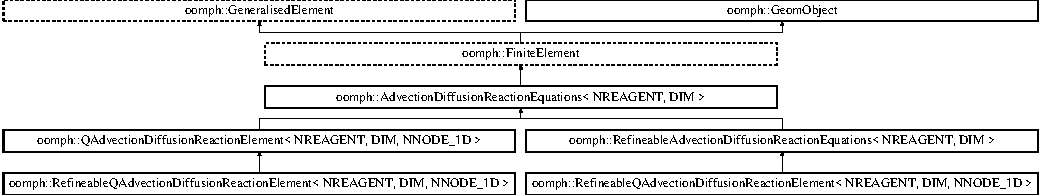
\includegraphics[height=2.626642cm]{classoomph_1_1AdvectionDiffusionReactionEquations}
\end{center}
\end{figure}
\subsection*{Public Types}
\begin{DoxyCompactItemize}
\item 
typedef void($\ast$ \hyperlink{classoomph_1_1AdvectionDiffusionReactionEquations_a3443e579e62414ecc50595403982e686}{Advection\+Diffusion\+Reaction\+Source\+Fct\+Pt}) (const \hyperlink{classoomph_1_1Vector}{Vector}$<$ double $>$ \&x, \hyperlink{classoomph_1_1Vector}{Vector}$<$ double $>$ \&f)
\begin{DoxyCompactList}\small\item\em Function pointer to source function fct(x,f(x)) -- x is a Vector! \end{DoxyCompactList}\item 
typedef void($\ast$ \hyperlink{classoomph_1_1AdvectionDiffusionReactionEquations_a74f8f0492147a5600b075cc64479f850}{Advection\+Diffusion\+Reaction\+Reaction\+Fct\+Pt}) (const \hyperlink{classoomph_1_1Vector}{Vector}$<$ double $>$ \&c, \hyperlink{classoomph_1_1Vector}{Vector}$<$ double $>$ \&R)
\begin{DoxyCompactList}\small\item\em Function pointer to reaction terms. \end{DoxyCompactList}\item 
typedef void($\ast$ \hyperlink{classoomph_1_1AdvectionDiffusionReactionEquations_af7afb472439d8e83b825c0a3c03190a7}{Advection\+Diffusion\+Reaction\+Reaction\+Deriv\+Fct\+Pt}) (const \hyperlink{classoomph_1_1Vector}{Vector}$<$ double $>$ \&c, \hyperlink{classoomph_1_1DenseMatrix}{Dense\+Matrix}$<$ double $>$ \&d\+RdC)
\begin{DoxyCompactList}\small\item\em Function pointer to derivative of reaction terms. \end{DoxyCompactList}\item 
typedef void($\ast$ \hyperlink{classoomph_1_1AdvectionDiffusionReactionEquations_a2fff621b5b44c64bd5b3f0412201055f}{Advection\+Diffusion\+Reaction\+Wind\+Fct\+Pt}) (const double \&time, const \hyperlink{classoomph_1_1Vector}{Vector}$<$ double $>$ \&x, \hyperlink{classoomph_1_1Vector}{Vector}$<$ double $>$ \&wind)
\begin{DoxyCompactList}\small\item\em Function pointer to wind function fct(x,w(x)) -- x is a Vector! \end{DoxyCompactList}\end{DoxyCompactItemize}
\subsection*{Public Member Functions}
\begin{DoxyCompactItemize}
\item 
\hyperlink{classoomph_1_1AdvectionDiffusionReactionEquations_a08b9a88de687860d51f0f811bfda46ce}{Advection\+Diffusion\+Reaction\+Equations} ()
\begin{DoxyCompactList}\small\item\em Constructor\+: Initialise the Source\+\_\+fct\+\_\+pt, Wind\+\_\+fct\+\_\+pt, Reaction\+\_\+fct\+\_\+pt to null and initialise the dimensionless timescale and diffusion ratios. \end{DoxyCompactList}\item 
\hyperlink{classoomph_1_1AdvectionDiffusionReactionEquations_a887f0a40932b1ca0aeb97cba56446a84}{Advection\+Diffusion\+Reaction\+Equations} (const \hyperlink{classoomph_1_1AdvectionDiffusionReactionEquations}{Advection\+Diffusion\+Reaction\+Equations} \&dummy)
\begin{DoxyCompactList}\small\item\em Broken copy constructor. \end{DoxyCompactList}\item 
void \hyperlink{classoomph_1_1AdvectionDiffusionReactionEquations_a79994ad90aba1dad5fb054d963e696be}{operator=} (const \hyperlink{classoomph_1_1AdvectionDiffusionReactionEquations}{Advection\+Diffusion\+Reaction\+Equations} \&)
\begin{DoxyCompactList}\small\item\em Broken assignment operator. \end{DoxyCompactList}\item 
virtual unsigned \hyperlink{classoomph_1_1AdvectionDiffusionReactionEquations_ad7564620f4b3313b09d2a3e675958e10}{c\+\_\+index\+\_\+adv\+\_\+diff\+\_\+react} (const unsigned \&\hyperlink{cfortran_8h_adb50e893b86b3e55e751a42eab3cba82}{i}) const
\begin{DoxyCompactList}\small\item\em Return the index at which the unknown i-\/th reagent is stored. The default value, i, is appropriate for single-\/physics problems, when there are only i variables, the values that satisfies the advection-\/diffusion-\/reaction equation. In derived multi-\/physics elements, this function should be overloaded to reflect the chosen storage scheme. Note that these equations require that the unknown is always stored at the same index at each node. \end{DoxyCompactList}\item 
double \hyperlink{classoomph_1_1AdvectionDiffusionReactionEquations_adf47eb6be16a1d42bdb4019fde6f4b82}{dc\+\_\+dt\+\_\+adv\+\_\+diff\+\_\+react} (const unsigned \&n, const unsigned \&r) const
\begin{DoxyCompactList}\small\item\em dc\+\_\+r/dt at local node n. \end{DoxyCompactList}\item 
void \hyperlink{classoomph_1_1AdvectionDiffusionReactionEquations_a39154d834bca6581eab17920e8b4e20a}{dc\+\_\+dt\+\_\+adv\+\_\+diff\+\_\+react} (const unsigned \&n, \hyperlink{classoomph_1_1Vector}{Vector}$<$ double $>$ \&dc\+\_\+dt) const
\begin{DoxyCompactList}\small\item\em dc/dt at local node n. \end{DoxyCompactList}\item 
void \hyperlink{classoomph_1_1AdvectionDiffusionReactionEquations_abe712696eb8db1c8b4f2eb5103a54c3f}{disable\+\_\+\+A\+LE} ()
\begin{DoxyCompactList}\small\item\em Disable A\+LE, i.\+e. assert the mesh is not moving -- you do this at your own risk! \end{DoxyCompactList}\item 
void \hyperlink{classoomph_1_1AdvectionDiffusionReactionEquations_a8c90c9aa40fbe311742b18a2c979730a}{enable\+\_\+\+A\+LE} ()
\begin{DoxyCompactList}\small\item\em (Re-\/)enable A\+LE, i.\+e. take possible mesh motion into account when evaluating the time-\/derivative. Note\+: By default, A\+LE is enabled, at the expense of possibly creating unnecessary work in problems where the mesh is, in fact, stationary. \end{DoxyCompactList}\item 
void \hyperlink{classoomph_1_1AdvectionDiffusionReactionEquations_a70be6733b56f27104a4a849c296b5b62}{output} (std\+::ostream \&outfile)
\begin{DoxyCompactList}\small\item\em Output with default number of plot points. \end{DoxyCompactList}\item 
void \hyperlink{classoomph_1_1AdvectionDiffusionReactionEquations_a38aa99ed50cc082f0c9c7079a13a11da}{output} (std\+::ostream \&outfile, const unsigned \&nplot)
\begin{DoxyCompactList}\small\item\em Output FE representation of soln\+: x,y,u or x,y,z,u at nplot$^\wedge$\+D\+IM plot points. \end{DoxyCompactList}\item 
void \hyperlink{classoomph_1_1AdvectionDiffusionReactionEquations_abb205e32ac157870312dd5d1180233b1}{output} (F\+I\+LE $\ast$file\+\_\+pt)
\begin{DoxyCompactList}\small\item\em C\+\_\+style output with default number of plot points. \end{DoxyCompactList}\item 
void \hyperlink{classoomph_1_1AdvectionDiffusionReactionEquations_a1ada1e57cac4bff9ecf73520a907b7c8}{output} (F\+I\+LE $\ast$file\+\_\+pt, const unsigned \&n\+\_\+plot)
\begin{DoxyCompactList}\small\item\em C-\/style output FE representation of soln\+: x,y,u or x,y,z,u at n\+\_\+plot$^\wedge$\+D\+IM plot points. \end{DoxyCompactList}\item 
void \hyperlink{classoomph_1_1AdvectionDiffusionReactionEquations_af540c03c411843c566c81af918d620c2}{output\+\_\+fct} (std\+::ostream \&outfile, const unsigned \&nplot, \hyperlink{classoomph_1_1FiniteElement_a690fd33af26cc3e84f39bba6d5a85202}{Finite\+Element\+::\+Steady\+Exact\+Solution\+Fct\+Pt} exact\+\_\+soln\+\_\+pt)
\begin{DoxyCompactList}\small\item\em Output exact soln\+: x,y,u\+\_\+exact or x,y,z,u\+\_\+exact at nplot$^\wedge$\+D\+IM plot points. \end{DoxyCompactList}\item 
virtual void \hyperlink{classoomph_1_1AdvectionDiffusionReactionEquations_abfb9e33a5575df7f36cdee7e44b3d282}{output\+\_\+fct} (std\+::ostream \&outfile, const unsigned \&nplot, const double \&time, \hyperlink{classoomph_1_1FiniteElement_ad4ecf2b61b158a4b4d351a60d23c633e}{Finite\+Element\+::\+Unsteady\+Exact\+Solution\+Fct\+Pt} exact\+\_\+soln\+\_\+pt)
\begin{DoxyCompactList}\small\item\em Output exact soln\+: x,y,u\+\_\+exact or x,y,z,u\+\_\+exact at nplot$^\wedge$\+D\+IM plot points (dummy time-\/dependent version to keep intel compiler happy) \end{DoxyCompactList}\item 
void \hyperlink{classoomph_1_1AdvectionDiffusionReactionEquations_a19c48ef418ac58dede7b397971fa7379}{compute\+\_\+error} (std\+::ostream \&outfile, \hyperlink{classoomph_1_1FiniteElement_a690fd33af26cc3e84f39bba6d5a85202}{Finite\+Element\+::\+Steady\+Exact\+Solution\+Fct\+Pt} exact\+\_\+soln\+\_\+pt, double \&error, double \&norm)
\begin{DoxyCompactList}\small\item\em Get error against and norm of exact solution. \end{DoxyCompactList}\item 
void \hyperlink{classoomph_1_1AdvectionDiffusionReactionEquations_a4a177abea269ae6063013fe5b3d25ac3}{compute\+\_\+error} (std\+::ostream \&outfile, \hyperlink{classoomph_1_1FiniteElement_ad4ecf2b61b158a4b4d351a60d23c633e}{Finite\+Element\+::\+Unsteady\+Exact\+Solution\+Fct\+Pt} exact\+\_\+soln\+\_\+pt, const double \&time, double \&error, double \&norm)
\begin{DoxyCompactList}\small\item\em Dummy, time dependent error checker. \end{DoxyCompactList}\item 
\hyperlink{classoomph_1_1AdvectionDiffusionReactionEquations_a3443e579e62414ecc50595403982e686}{Advection\+Diffusion\+Reaction\+Source\+Fct\+Pt} \& \hyperlink{classoomph_1_1AdvectionDiffusionReactionEquations_acf51066b96a5406d5ef7dd88c0b7393d}{source\+\_\+fct\+\_\+pt} ()
\begin{DoxyCompactList}\small\item\em Access function\+: Pointer to source function. \end{DoxyCompactList}\item 
\hyperlink{classoomph_1_1AdvectionDiffusionReactionEquations_a3443e579e62414ecc50595403982e686}{Advection\+Diffusion\+Reaction\+Source\+Fct\+Pt} \hyperlink{classoomph_1_1AdvectionDiffusionReactionEquations_a6daf73f5f943bf4ec674b796fe4c36d2}{source\+\_\+fct\+\_\+pt} () const
\begin{DoxyCompactList}\small\item\em Access function\+: Pointer to source function. Const version. \end{DoxyCompactList}\item 
\hyperlink{classoomph_1_1AdvectionDiffusionReactionEquations_a2fff621b5b44c64bd5b3f0412201055f}{Advection\+Diffusion\+Reaction\+Wind\+Fct\+Pt} \& \hyperlink{classoomph_1_1AdvectionDiffusionReactionEquations_a68cbfaf5625359cee3b97d82929feaf9}{wind\+\_\+fct\+\_\+pt} ()
\begin{DoxyCompactList}\small\item\em Access function\+: Pointer to wind function. \end{DoxyCompactList}\item 
\hyperlink{classoomph_1_1AdvectionDiffusionReactionEquations_a2fff621b5b44c64bd5b3f0412201055f}{Advection\+Diffusion\+Reaction\+Wind\+Fct\+Pt} \hyperlink{classoomph_1_1AdvectionDiffusionReactionEquations_a17fba6f4ed57ff9908e4fb3d55aaf5c9}{wind\+\_\+fct\+\_\+pt} () const
\begin{DoxyCompactList}\small\item\em Access function\+: Pointer to reaction function. Const version. \end{DoxyCompactList}\item 
\hyperlink{classoomph_1_1AdvectionDiffusionReactionEquations_a74f8f0492147a5600b075cc64479f850}{Advection\+Diffusion\+Reaction\+Reaction\+Fct\+Pt} \& \hyperlink{classoomph_1_1AdvectionDiffusionReactionEquations_a4c7f533fafad4d0db6f2e4cf0b3f97ca}{reaction\+\_\+fct\+\_\+pt} ()
\begin{DoxyCompactList}\small\item\em Access function\+: Pointer to reaction function. \end{DoxyCompactList}\item 
\hyperlink{classoomph_1_1AdvectionDiffusionReactionEquations_a74f8f0492147a5600b075cc64479f850}{Advection\+Diffusion\+Reaction\+Reaction\+Fct\+Pt} \hyperlink{classoomph_1_1AdvectionDiffusionReactionEquations_a45552eb74d1da4b7c21c7e71b95faa3f}{reaction\+\_\+fct\+\_\+pt} () const
\begin{DoxyCompactList}\small\item\em Access function\+: Pointer to reaction function. Const version. \end{DoxyCompactList}\item 
\hyperlink{classoomph_1_1AdvectionDiffusionReactionEquations_af7afb472439d8e83b825c0a3c03190a7}{Advection\+Diffusion\+Reaction\+Reaction\+Deriv\+Fct\+Pt} \& \hyperlink{classoomph_1_1AdvectionDiffusionReactionEquations_a26fd863a25ebcff9dfb17ea3fa3c99ee}{reaction\+\_\+deriv\+\_\+fct\+\_\+pt} ()
\begin{DoxyCompactList}\small\item\em Access function\+: Pointer to reaction derivatives function. \end{DoxyCompactList}\item 
\hyperlink{classoomph_1_1AdvectionDiffusionReactionEquations_af7afb472439d8e83b825c0a3c03190a7}{Advection\+Diffusion\+Reaction\+Reaction\+Deriv\+Fct\+Pt} \hyperlink{classoomph_1_1AdvectionDiffusionReactionEquations_ab015795d32200187c4ff16b63ef04066}{reaction\+\_\+deriv\+\_\+fct\+\_\+pt} () const
\begin{DoxyCompactList}\small\item\em Access function\+: Pointer to reaction function. Const version. \end{DoxyCompactList}\item 
const \hyperlink{classoomph_1_1Vector}{Vector}$<$ double $>$ \& \hyperlink{classoomph_1_1AdvectionDiffusionReactionEquations_ad59a0d4f89e443358553e4802233dc1d}{diff} () const
\begin{DoxyCompactList}\small\item\em \hyperlink{classoomph_1_1Vector}{Vector} of diffusion coefficients. \end{DoxyCompactList}\item 
\hyperlink{classoomph_1_1Vector}{Vector}$<$ double $>$ $\ast$\& \hyperlink{classoomph_1_1AdvectionDiffusionReactionEquations_a70db4dae4524ac4c2d6af262c4e4d47e}{diff\+\_\+pt} ()
\begin{DoxyCompactList}\small\item\em Pointer to vector of diffusion coefficients. \end{DoxyCompactList}\item 
const \hyperlink{classoomph_1_1Vector}{Vector}$<$ double $>$ \& \hyperlink{classoomph_1_1AdvectionDiffusionReactionEquations_a8976ed911125695578edfa5c2c23755b}{tau} () const
\begin{DoxyCompactList}\small\item\em \hyperlink{classoomph_1_1Vector}{Vector} of dimensionless timescales. \end{DoxyCompactList}\item 
\hyperlink{classoomph_1_1Vector}{Vector}$<$ double $>$ $\ast$\& \hyperlink{classoomph_1_1AdvectionDiffusionReactionEquations_ac3e7834f33607cc560e7a1dd08eb9b7a}{tau\+\_\+pt} ()
\begin{DoxyCompactList}\small\item\em Pointer to vector of dimensionless timescales. \end{DoxyCompactList}\item 
virtual void \hyperlink{classoomph_1_1AdvectionDiffusionReactionEquations_a2a279f4485b7a46a8684cda2678ae825}{get\+\_\+source\+\_\+adv\+\_\+diff\+\_\+react} (const unsigned \&ipt, const \hyperlink{classoomph_1_1Vector}{Vector}$<$ double $>$ \&x, \hyperlink{classoomph_1_1Vector}{Vector}$<$ double $>$ \&source) const
\begin{DoxyCompactList}\small\item\em Get source term at (Eulerian) position x. This function is virtual to allow overloading in multi-\/physics problems where the strength of the source function might be determined by another system of equations. \end{DoxyCompactList}\item 
virtual void \hyperlink{classoomph_1_1AdvectionDiffusionReactionEquations_a2f4bc51e9f535f951f6b1d5827ee3264}{get\+\_\+wind\+\_\+adv\+\_\+diff\+\_\+react} (const unsigned \&ipt, const \hyperlink{classoomph_1_1Vector}{Vector}$<$ double $>$ \&\hyperlink{cfortran_8h_ab7123126e4885ef647dd9c6e3807a21c}{s}, const \hyperlink{classoomph_1_1Vector}{Vector}$<$ double $>$ \&x, \hyperlink{classoomph_1_1Vector}{Vector}$<$ double $>$ \&wind) const
\begin{DoxyCompactList}\small\item\em Get wind at (Eulerian) position x and/or local coordinate s. This function is virtual to allow overloading in multi-\/physics problems where the wind function might be determined by another system of equations. \end{DoxyCompactList}\item 
virtual void \hyperlink{classoomph_1_1AdvectionDiffusionReactionEquations_afcd57b515d90c0a55406d11ec6316856}{get\+\_\+reaction\+\_\+adv\+\_\+diff\+\_\+react} (const unsigned \&ipt, const \hyperlink{classoomph_1_1Vector}{Vector}$<$ double $>$ \&C, \hyperlink{classoomph_1_1Vector}{Vector}$<$ double $>$ \&R) const
\begin{DoxyCompactList}\small\item\em Get reaction as a function of the given reagent concentrations This function is virtual to allow overloading in multi-\/physics problems where the reaction function might be determined by another system of equations. \end{DoxyCompactList}\item 
virtual void \hyperlink{classoomph_1_1AdvectionDiffusionReactionEquations_a14deb197bcb3ddb01798c98b2942f5d0}{get\+\_\+reaction\+\_\+deriv\+\_\+adv\+\_\+diff\+\_\+react} (const unsigned \&ipt, const \hyperlink{classoomph_1_1Vector}{Vector}$<$ double $>$ \&C, \hyperlink{classoomph_1_1DenseMatrix}{Dense\+Matrix}$<$ double $>$ \&d\+RdC) const
\begin{DoxyCompactList}\small\item\em Get the derivatives of the reaction terms with respect to the concentration variables. If no explicit function pointer is set, these will be calculated by finite differences. \end{DoxyCompactList}\item 
void \hyperlink{classoomph_1_1AdvectionDiffusionReactionEquations_a492af587e1c592b0fb9ffe525d6509d2}{get\+\_\+flux} (const \hyperlink{classoomph_1_1Vector}{Vector}$<$ double $>$ \&\hyperlink{cfortran_8h_ab7123126e4885ef647dd9c6e3807a21c}{s}, \hyperlink{classoomph_1_1Vector}{Vector}$<$ double $>$ \&flux) const
\begin{DoxyCompactList}\small\item\em Get flux\+: $\mbox{flux}[DIM r + i] = \mbox{d}C_{r} / \mbox{d}x_i $. \end{DoxyCompactList}\item 
void \hyperlink{classoomph_1_1AdvectionDiffusionReactionEquations_a0cf72be1f384151d58b26ced55b1ade0}{fill\+\_\+in\+\_\+contribution\+\_\+to\+\_\+residuals} (\hyperlink{classoomph_1_1Vector}{Vector}$<$ double $>$ \&residuals)
\begin{DoxyCompactList}\small\item\em Add the element\textquotesingle{}s contribution to its residual vector (wrapper) \end{DoxyCompactList}\item 
void \hyperlink{classoomph_1_1AdvectionDiffusionReactionEquations_a32feca5a89aee13169544e2eb0af975a}{fill\+\_\+in\+\_\+contribution\+\_\+to\+\_\+jacobian} (\hyperlink{classoomph_1_1Vector}{Vector}$<$ double $>$ \&residuals, \hyperlink{classoomph_1_1DenseMatrix}{Dense\+Matrix}$<$ double $>$ \&jacobian)
\begin{DoxyCompactList}\small\item\em Add the element\textquotesingle{}s contribution to its residual vector and the element Jacobian matrix (wrapper) \end{DoxyCompactList}\item 
void \hyperlink{classoomph_1_1AdvectionDiffusionReactionEquations_ae316c9cbe79a215744dc52bd19fb1a27}{fill\+\_\+in\+\_\+contribution\+\_\+to\+\_\+jacobian\+\_\+and\+\_\+mass\+\_\+matrix} (\hyperlink{classoomph_1_1Vector}{Vector}$<$ double $>$ \&residuals, \hyperlink{classoomph_1_1DenseMatrix}{Dense\+Matrix}$<$ double $>$ \&jacobian, \hyperlink{classoomph_1_1DenseMatrix}{Dense\+Matrix}$<$ double $>$ \&mass\+\_\+matrix)
\item 
double \hyperlink{classoomph_1_1AdvectionDiffusionReactionEquations_a9346b9c6e14ebc68149dc2a571416112}{interpolated\+\_\+c\+\_\+adv\+\_\+diff\+\_\+react} (const \hyperlink{classoomph_1_1Vector}{Vector}$<$ double $>$ \&\hyperlink{cfortran_8h_ab7123126e4885ef647dd9c6e3807a21c}{s}, const unsigned \&\hyperlink{cfortran_8h_adb50e893b86b3e55e751a42eab3cba82}{i}) const
\begin{DoxyCompactList}\small\item\em Return FE representation of function value c\+\_\+i(s) at local coordinate s. \end{DoxyCompactList}\item 
unsigned \hyperlink{classoomph_1_1AdvectionDiffusionReactionEquations_a30b954f7ec758cf93a4b477a8652c9e2}{self\+\_\+test} ()
\begin{DoxyCompactList}\small\item\em Self-\/test\+: Return 0 for OK. \end{DoxyCompactList}\item 
void \hyperlink{classoomph_1_1AdvectionDiffusionReactionEquations_a75c644617090bfec77366b455bb5e91a}{integrate\+\_\+reagents} (\hyperlink{classoomph_1_1Vector}{Vector}$<$ double $>$ \&C) const
\begin{DoxyCompactList}\small\item\em Return the integrated reagent concentrations. \end{DoxyCompactList}\end{DoxyCompactItemize}
\subsection*{Protected Member Functions}
\begin{DoxyCompactItemize}
\item 
virtual double \hyperlink{classoomph_1_1AdvectionDiffusionReactionEquations_a227bda2d1384aaa46dff37ccd370e6d6}{dshape\+\_\+and\+\_\+dtest\+\_\+eulerian\+\_\+adv\+\_\+diff\+\_\+react} (const \hyperlink{classoomph_1_1Vector}{Vector}$<$ double $>$ \&\hyperlink{cfortran_8h_ab7123126e4885ef647dd9c6e3807a21c}{s}, \hyperlink{classoomph_1_1Shape}{Shape} \&psi, \hyperlink{classoomph_1_1DShape}{D\+Shape} \&dpsidx, \hyperlink{classoomph_1_1Shape}{Shape} \&test, \hyperlink{classoomph_1_1DShape}{D\+Shape} \&dtestdx) const =0
\begin{DoxyCompactList}\small\item\em Shape/test functions and derivs w.\+r.\+t. to global coords at local coord. s; return Jacobian of mapping. \end{DoxyCompactList}\item 
virtual double \hyperlink{classoomph_1_1AdvectionDiffusionReactionEquations_acd01ced36610cb5e69ee359df778ba09}{dshape\+\_\+and\+\_\+dtest\+\_\+eulerian\+\_\+at\+\_\+knot\+\_\+adv\+\_\+diff\+\_\+react} (const unsigned \&ipt, \hyperlink{classoomph_1_1Shape}{Shape} \&psi, \hyperlink{classoomph_1_1DShape}{D\+Shape} \&dpsidx, \hyperlink{classoomph_1_1Shape}{Shape} \&test, \hyperlink{classoomph_1_1DShape}{D\+Shape} \&dtestdx) const =0
\begin{DoxyCompactList}\small\item\em Shape/test functions and derivs w.\+r.\+t. to global coords at integration point ipt; return Jacobian of mapping. \end{DoxyCompactList}\item 
virtual void \hyperlink{classoomph_1_1AdvectionDiffusionReactionEquations_a66d61f635f3d733b5e70de9552cdaf6b}{fill\+\_\+in\+\_\+generic\+\_\+residual\+\_\+contribution\+\_\+adv\+\_\+diff\+\_\+react} (\hyperlink{classoomph_1_1Vector}{Vector}$<$ double $>$ \&residuals, \hyperlink{classoomph_1_1DenseMatrix}{Dense\+Matrix}$<$ double $>$ \&jacobian, \hyperlink{classoomph_1_1DenseMatrix}{Dense\+Matrix}$<$ double $>$ \&mass\+\_\+matrix, unsigned flag)
\begin{DoxyCompactList}\small\item\em Add the element\textquotesingle{}s contribution to its residual vector only (if flag=and/or element Jacobian matrix. \end{DoxyCompactList}\end{DoxyCompactItemize}
\subsection*{Protected Attributes}
\begin{DoxyCompactItemize}
\item 
\hyperlink{classoomph_1_1Vector}{Vector}$<$ double $>$ $\ast$ \hyperlink{classoomph_1_1AdvectionDiffusionReactionEquations_af88a7b3b2daee6c339ee75914ae1c23e}{Diff\+\_\+pt}
\begin{DoxyCompactList}\small\item\em Pointer to global diffusion coefficients. \end{DoxyCompactList}\item 
\hyperlink{classoomph_1_1Vector}{Vector}$<$ double $>$ $\ast$ \hyperlink{classoomph_1_1AdvectionDiffusionReactionEquations_a50ac4110c6bf38ada794fd25cb88431b}{Tau\+\_\+pt}
\begin{DoxyCompactList}\small\item\em Pointer to global timescales. \end{DoxyCompactList}\item 
\hyperlink{classoomph_1_1AdvectionDiffusionReactionEquations_a3443e579e62414ecc50595403982e686}{Advection\+Diffusion\+Reaction\+Source\+Fct\+Pt} \hyperlink{classoomph_1_1AdvectionDiffusionReactionEquations_a1a79762a4b988e4feda96a5a8678c9ce}{Source\+\_\+fct\+\_\+pt}
\begin{DoxyCompactList}\small\item\em Pointer to source function\+: \end{DoxyCompactList}\item 
\hyperlink{classoomph_1_1AdvectionDiffusionReactionEquations_a2fff621b5b44c64bd5b3f0412201055f}{Advection\+Diffusion\+Reaction\+Wind\+Fct\+Pt} \hyperlink{classoomph_1_1AdvectionDiffusionReactionEquations_aa45dd8734c1d321329c522b6db8d0590}{Wind\+\_\+fct\+\_\+pt}
\begin{DoxyCompactList}\small\item\em Pointer to wind function\+: \end{DoxyCompactList}\item 
\hyperlink{classoomph_1_1AdvectionDiffusionReactionEquations_a74f8f0492147a5600b075cc64479f850}{Advection\+Diffusion\+Reaction\+Reaction\+Fct\+Pt} \hyperlink{classoomph_1_1AdvectionDiffusionReactionEquations_ae0232ca6f0b4cf18afbd893ec289f097}{Reaction\+\_\+fct\+\_\+pt}
\begin{DoxyCompactList}\small\item\em Pointer to reaction function. \end{DoxyCompactList}\item 
\hyperlink{classoomph_1_1AdvectionDiffusionReactionEquations_af7afb472439d8e83b825c0a3c03190a7}{Advection\+Diffusion\+Reaction\+Reaction\+Deriv\+Fct\+Pt} \hyperlink{classoomph_1_1AdvectionDiffusionReactionEquations_a2544062d28d4f81014474ca9e47fa2ac}{Reaction\+\_\+deriv\+\_\+fct\+\_\+pt}
\begin{DoxyCompactList}\small\item\em Pointer to reaction derivatives. \end{DoxyCompactList}\item 
bool \hyperlink{classoomph_1_1AdvectionDiffusionReactionEquations_a1b28c2757c2b2c64030230c3a7a2fb91}{A\+L\+E\+\_\+is\+\_\+disabled}
\begin{DoxyCompactList}\small\item\em Boolean flag to indicate if A\+LE formulation is disabled when time-\/derivatives are computed. Only set to true if you\textquotesingle{}re sure that the mesh is stationary. \end{DoxyCompactList}\end{DoxyCompactItemize}
\subsection*{Static Private Attributes}
\begin{DoxyCompactItemize}
\item 
static \hyperlink{classoomph_1_1Vector}{Vector}$<$ double $>$ \hyperlink{classoomph_1_1AdvectionDiffusionReactionEquations_abac46550a5b363e6b08a7505e689ae18}{Default\+\_\+dimensionless\+\_\+number}
\begin{DoxyCompactList}\small\item\em Static default value for the dimensionless numbers. \end{DoxyCompactList}\end{DoxyCompactItemize}
\subsection*{Additional Inherited Members}


\subsection{Detailed Description}
\subsubsection*{template$<$unsigned N\+R\+E\+A\+G\+E\+NT, unsigned D\+IM$>$\newline
class oomph\+::\+Advection\+Diffusion\+Reaction\+Equations$<$ N\+R\+E\+A\+G\+E\+N\+T, D\+I\+M $>$}

A class for all elements that solve the Advection Diffusion Reaction equations using isoparametric elements. \[ \tau_{i} \frac{\partial C_{i}}{\partial t} + w_{j} \frac{\partial C_{i}}{\partial x_{j}} = D_{i}\frac{\partial^2 C_{i}}{\partial x_j^2} = - R_{i}(C_{i}) + f_{i} \] This contains the generic maths. \hyperlink{classoomph_1_1Shape}{Shape} functions, geometric mapping etc. must get implemented in derived class. 

Definition at line 61 of file advection\+\_\+diffusion\+\_\+reaction\+\_\+elements.\+h.



\subsection{Member Typedef Documentation}
\mbox{\Hypertarget{classoomph_1_1AdvectionDiffusionReactionEquations_af7afb472439d8e83b825c0a3c03190a7}\label{classoomph_1_1AdvectionDiffusionReactionEquations_af7afb472439d8e83b825c0a3c03190a7}} 
\index{oomph\+::\+Advection\+Diffusion\+Reaction\+Equations@{oomph\+::\+Advection\+Diffusion\+Reaction\+Equations}!Advection\+Diffusion\+Reaction\+Reaction\+Deriv\+Fct\+Pt@{Advection\+Diffusion\+Reaction\+Reaction\+Deriv\+Fct\+Pt}}
\index{Advection\+Diffusion\+Reaction\+Reaction\+Deriv\+Fct\+Pt@{Advection\+Diffusion\+Reaction\+Reaction\+Deriv\+Fct\+Pt}!oomph\+::\+Advection\+Diffusion\+Reaction\+Equations@{oomph\+::\+Advection\+Diffusion\+Reaction\+Equations}}
\subsubsection{\texorpdfstring{Advection\+Diffusion\+Reaction\+Reaction\+Deriv\+Fct\+Pt}{AdvectionDiffusionReactionReactionDerivFctPt}}
{\footnotesize\ttfamily template$<$unsigned N\+R\+E\+A\+G\+E\+NT, unsigned D\+IM$>$ \\
typedef void($\ast$ \hyperlink{classoomph_1_1AdvectionDiffusionReactionEquations}{oomph\+::\+Advection\+Diffusion\+Reaction\+Equations}$<$ N\+R\+E\+A\+G\+E\+NT, D\+IM $>$\+::Advection\+Diffusion\+Reaction\+Reaction\+Deriv\+Fct\+Pt) (const \hyperlink{classoomph_1_1Vector}{Vector}$<$ double $>$ \&c, \hyperlink{classoomph_1_1DenseMatrix}{Dense\+Matrix}$<$ double $>$ \&d\+RdC)}



Function pointer to derivative of reaction terms. 



Definition at line 76 of file advection\+\_\+diffusion\+\_\+reaction\+\_\+elements.\+h.

\mbox{\Hypertarget{classoomph_1_1AdvectionDiffusionReactionEquations_a74f8f0492147a5600b075cc64479f850}\label{classoomph_1_1AdvectionDiffusionReactionEquations_a74f8f0492147a5600b075cc64479f850}} 
\index{oomph\+::\+Advection\+Diffusion\+Reaction\+Equations@{oomph\+::\+Advection\+Diffusion\+Reaction\+Equations}!Advection\+Diffusion\+Reaction\+Reaction\+Fct\+Pt@{Advection\+Diffusion\+Reaction\+Reaction\+Fct\+Pt}}
\index{Advection\+Diffusion\+Reaction\+Reaction\+Fct\+Pt@{Advection\+Diffusion\+Reaction\+Reaction\+Fct\+Pt}!oomph\+::\+Advection\+Diffusion\+Reaction\+Equations@{oomph\+::\+Advection\+Diffusion\+Reaction\+Equations}}
\subsubsection{\texorpdfstring{Advection\+Diffusion\+Reaction\+Reaction\+Fct\+Pt}{AdvectionDiffusionReactionReactionFctPt}}
{\footnotesize\ttfamily template$<$unsigned N\+R\+E\+A\+G\+E\+NT, unsigned D\+IM$>$ \\
typedef void($\ast$ \hyperlink{classoomph_1_1AdvectionDiffusionReactionEquations}{oomph\+::\+Advection\+Diffusion\+Reaction\+Equations}$<$ N\+R\+E\+A\+G\+E\+NT, D\+IM $>$\+::Advection\+Diffusion\+Reaction\+Reaction\+Fct\+Pt) (const \hyperlink{classoomph_1_1Vector}{Vector}$<$ double $>$ \&c, \hyperlink{classoomph_1_1Vector}{Vector}$<$ double $>$ \&R)}



Function pointer to reaction terms. 



Definition at line 72 of file advection\+\_\+diffusion\+\_\+reaction\+\_\+elements.\+h.

\mbox{\Hypertarget{classoomph_1_1AdvectionDiffusionReactionEquations_a3443e579e62414ecc50595403982e686}\label{classoomph_1_1AdvectionDiffusionReactionEquations_a3443e579e62414ecc50595403982e686}} 
\index{oomph\+::\+Advection\+Diffusion\+Reaction\+Equations@{oomph\+::\+Advection\+Diffusion\+Reaction\+Equations}!Advection\+Diffusion\+Reaction\+Source\+Fct\+Pt@{Advection\+Diffusion\+Reaction\+Source\+Fct\+Pt}}
\index{Advection\+Diffusion\+Reaction\+Source\+Fct\+Pt@{Advection\+Diffusion\+Reaction\+Source\+Fct\+Pt}!oomph\+::\+Advection\+Diffusion\+Reaction\+Equations@{oomph\+::\+Advection\+Diffusion\+Reaction\+Equations}}
\subsubsection{\texorpdfstring{Advection\+Diffusion\+Reaction\+Source\+Fct\+Pt}{AdvectionDiffusionReactionSourceFctPt}}
{\footnotesize\ttfamily template$<$unsigned N\+R\+E\+A\+G\+E\+NT, unsigned D\+IM$>$ \\
typedef void($\ast$ \hyperlink{classoomph_1_1AdvectionDiffusionReactionEquations}{oomph\+::\+Advection\+Diffusion\+Reaction\+Equations}$<$ N\+R\+E\+A\+G\+E\+NT, D\+IM $>$\+::Advection\+Diffusion\+Reaction\+Source\+Fct\+Pt) (const \hyperlink{classoomph_1_1Vector}{Vector}$<$ double $>$ \&x, \hyperlink{classoomph_1_1Vector}{Vector}$<$ double $>$ \&f)}



Function pointer to source function fct(x,f(x)) -- x is a Vector! 



Definition at line 68 of file advection\+\_\+diffusion\+\_\+reaction\+\_\+elements.\+h.

\mbox{\Hypertarget{classoomph_1_1AdvectionDiffusionReactionEquations_a2fff621b5b44c64bd5b3f0412201055f}\label{classoomph_1_1AdvectionDiffusionReactionEquations_a2fff621b5b44c64bd5b3f0412201055f}} 
\index{oomph\+::\+Advection\+Diffusion\+Reaction\+Equations@{oomph\+::\+Advection\+Diffusion\+Reaction\+Equations}!Advection\+Diffusion\+Reaction\+Wind\+Fct\+Pt@{Advection\+Diffusion\+Reaction\+Wind\+Fct\+Pt}}
\index{Advection\+Diffusion\+Reaction\+Wind\+Fct\+Pt@{Advection\+Diffusion\+Reaction\+Wind\+Fct\+Pt}!oomph\+::\+Advection\+Diffusion\+Reaction\+Equations@{oomph\+::\+Advection\+Diffusion\+Reaction\+Equations}}
\subsubsection{\texorpdfstring{Advection\+Diffusion\+Reaction\+Wind\+Fct\+Pt}{AdvectionDiffusionReactionWindFctPt}}
{\footnotesize\ttfamily template$<$unsigned N\+R\+E\+A\+G\+E\+NT, unsigned D\+IM$>$ \\
typedef void($\ast$ \hyperlink{classoomph_1_1AdvectionDiffusionReactionEquations}{oomph\+::\+Advection\+Diffusion\+Reaction\+Equations}$<$ N\+R\+E\+A\+G\+E\+NT, D\+IM $>$\+::Advection\+Diffusion\+Reaction\+Wind\+Fct\+Pt) (const double \&time, const \hyperlink{classoomph_1_1Vector}{Vector}$<$ double $>$ \&x, \hyperlink{classoomph_1_1Vector}{Vector}$<$ double $>$ \&wind)}



Function pointer to wind function fct(x,w(x)) -- x is a Vector! 



Definition at line 82 of file advection\+\_\+diffusion\+\_\+reaction\+\_\+elements.\+h.



\subsection{Constructor \& Destructor Documentation}
\mbox{\Hypertarget{classoomph_1_1AdvectionDiffusionReactionEquations_a08b9a88de687860d51f0f811bfda46ce}\label{classoomph_1_1AdvectionDiffusionReactionEquations_a08b9a88de687860d51f0f811bfda46ce}} 
\index{oomph\+::\+Advection\+Diffusion\+Reaction\+Equations@{oomph\+::\+Advection\+Diffusion\+Reaction\+Equations}!Advection\+Diffusion\+Reaction\+Equations@{Advection\+Diffusion\+Reaction\+Equations}}
\index{Advection\+Diffusion\+Reaction\+Equations@{Advection\+Diffusion\+Reaction\+Equations}!oomph\+::\+Advection\+Diffusion\+Reaction\+Equations@{oomph\+::\+Advection\+Diffusion\+Reaction\+Equations}}
\subsubsection{\texorpdfstring{Advection\+Diffusion\+Reaction\+Equations()}{AdvectionDiffusionReactionEquations()}\hspace{0.1cm}{\footnotesize\ttfamily [1/2]}}
{\footnotesize\ttfamily template$<$unsigned N\+R\+E\+A\+G\+E\+NT, unsigned D\+IM$>$ \\
\hyperlink{classoomph_1_1AdvectionDiffusionReactionEquations}{oomph\+::\+Advection\+Diffusion\+Reaction\+Equations}$<$ N\+R\+E\+A\+G\+E\+NT, D\+IM $>$\+::\hyperlink{classoomph_1_1AdvectionDiffusionReactionEquations}{Advection\+Diffusion\+Reaction\+Equations} (\begin{DoxyParamCaption}{ }\end{DoxyParamCaption})\hspace{0.3cm}{\ttfamily [inline]}}



Constructor\+: Initialise the Source\+\_\+fct\+\_\+pt, Wind\+\_\+fct\+\_\+pt, Reaction\+\_\+fct\+\_\+pt to null and initialise the dimensionless timescale and diffusion ratios. 



Definition at line 90 of file advection\+\_\+diffusion\+\_\+reaction\+\_\+elements.\+h.



References oomph\+::\+Advection\+Diffusion\+Reaction\+Equations$<$ N\+R\+E\+A\+G\+E\+N\+T, D\+I\+M $>$\+::\+Default\+\_\+dimensionless\+\_\+number, oomph\+::\+Advection\+Diffusion\+Reaction\+Equations$<$ N\+R\+E\+A\+G\+E\+N\+T, D\+I\+M $>$\+::\+Diff\+\_\+pt, and oomph\+::\+Advection\+Diffusion\+Reaction\+Equations$<$ N\+R\+E\+A\+G\+E\+N\+T, D\+I\+M $>$\+::\+Tau\+\_\+pt.

\mbox{\Hypertarget{classoomph_1_1AdvectionDiffusionReactionEquations_a887f0a40932b1ca0aeb97cba56446a84}\label{classoomph_1_1AdvectionDiffusionReactionEquations_a887f0a40932b1ca0aeb97cba56446a84}} 
\index{oomph\+::\+Advection\+Diffusion\+Reaction\+Equations@{oomph\+::\+Advection\+Diffusion\+Reaction\+Equations}!Advection\+Diffusion\+Reaction\+Equations@{Advection\+Diffusion\+Reaction\+Equations}}
\index{Advection\+Diffusion\+Reaction\+Equations@{Advection\+Diffusion\+Reaction\+Equations}!oomph\+::\+Advection\+Diffusion\+Reaction\+Equations@{oomph\+::\+Advection\+Diffusion\+Reaction\+Equations}}
\subsubsection{\texorpdfstring{Advection\+Diffusion\+Reaction\+Equations()}{AdvectionDiffusionReactionEquations()}\hspace{0.1cm}{\footnotesize\ttfamily [2/2]}}
{\footnotesize\ttfamily template$<$unsigned N\+R\+E\+A\+G\+E\+NT, unsigned D\+IM$>$ \\
\hyperlink{classoomph_1_1AdvectionDiffusionReactionEquations}{oomph\+::\+Advection\+Diffusion\+Reaction\+Equations}$<$ N\+R\+E\+A\+G\+E\+NT, D\+IM $>$\+::\hyperlink{classoomph_1_1AdvectionDiffusionReactionEquations}{Advection\+Diffusion\+Reaction\+Equations} (\begin{DoxyParamCaption}\item[{const \hyperlink{classoomph_1_1AdvectionDiffusionReactionEquations}{Advection\+Diffusion\+Reaction\+Equations}$<$ N\+R\+E\+A\+G\+E\+NT, D\+IM $>$ \&}]{dummy }\end{DoxyParamCaption})\hspace{0.3cm}{\ttfamily [inline]}}



Broken copy constructor. 



Definition at line 101 of file advection\+\_\+diffusion\+\_\+reaction\+\_\+elements.\+h.



References oomph\+::\+Broken\+Copy\+::broken\+\_\+copy().



\subsection{Member Function Documentation}
\mbox{\Hypertarget{classoomph_1_1AdvectionDiffusionReactionEquations_ad7564620f4b3313b09d2a3e675958e10}\label{classoomph_1_1AdvectionDiffusionReactionEquations_ad7564620f4b3313b09d2a3e675958e10}} 
\index{oomph\+::\+Advection\+Diffusion\+Reaction\+Equations@{oomph\+::\+Advection\+Diffusion\+Reaction\+Equations}!c\+\_\+index\+\_\+adv\+\_\+diff\+\_\+react@{c\+\_\+index\+\_\+adv\+\_\+diff\+\_\+react}}
\index{c\+\_\+index\+\_\+adv\+\_\+diff\+\_\+react@{c\+\_\+index\+\_\+adv\+\_\+diff\+\_\+react}!oomph\+::\+Advection\+Diffusion\+Reaction\+Equations@{oomph\+::\+Advection\+Diffusion\+Reaction\+Equations}}
\subsubsection{\texorpdfstring{c\+\_\+index\+\_\+adv\+\_\+diff\+\_\+react()}{c\_index\_adv\_diff\_react()}}
{\footnotesize\ttfamily template$<$unsigned N\+R\+E\+A\+G\+E\+NT, unsigned D\+IM$>$ \\
virtual unsigned \hyperlink{classoomph_1_1AdvectionDiffusionReactionEquations}{oomph\+::\+Advection\+Diffusion\+Reaction\+Equations}$<$ N\+R\+E\+A\+G\+E\+NT, D\+IM $>$\+::c\+\_\+index\+\_\+adv\+\_\+diff\+\_\+react (\begin{DoxyParamCaption}\item[{const unsigned \&}]{i }\end{DoxyParamCaption}) const\hspace{0.3cm}{\ttfamily [inline]}, {\ttfamily [virtual]}}



Return the index at which the unknown i-\/th reagent is stored. The default value, i, is appropriate for single-\/physics problems, when there are only i variables, the values that satisfies the advection-\/diffusion-\/reaction equation. In derived multi-\/physics elements, this function should be overloaded to reflect the chosen storage scheme. Note that these equations require that the unknown is always stored at the same index at each node. 



Definition at line 120 of file advection\+\_\+diffusion\+\_\+reaction\+\_\+elements.\+h.



References i.



Referenced by oomph\+::\+Advection\+Diffusion\+Reaction\+Equations$<$ N\+R\+E\+A\+G\+E\+N\+T, D\+I\+M $>$\+::dc\+\_\+dt\+\_\+adv\+\_\+diff\+\_\+react(), oomph\+::\+Advection\+Diffusion\+Reaction\+Equations$<$ N\+R\+E\+A\+G\+E\+N\+T, D\+I\+M $>$\+::get\+\_\+flux(), oomph\+::\+Refineable\+Advection\+Diffusion\+Reaction\+Equations$<$ N\+R\+E\+A\+G\+E\+N\+T, D\+I\+M $>$\+::get\+\_\+interpolated\+\_\+values(), and oomph\+::\+Advection\+Diffusion\+Reaction\+Equations$<$ N\+R\+E\+A\+G\+E\+N\+T, D\+I\+M $>$\+::interpolated\+\_\+c\+\_\+adv\+\_\+diff\+\_\+react().

\mbox{\Hypertarget{classoomph_1_1AdvectionDiffusionReactionEquations_a19c48ef418ac58dede7b397971fa7379}\label{classoomph_1_1AdvectionDiffusionReactionEquations_a19c48ef418ac58dede7b397971fa7379}} 
\index{oomph\+::\+Advection\+Diffusion\+Reaction\+Equations@{oomph\+::\+Advection\+Diffusion\+Reaction\+Equations}!compute\+\_\+error@{compute\+\_\+error}}
\index{compute\+\_\+error@{compute\+\_\+error}!oomph\+::\+Advection\+Diffusion\+Reaction\+Equations@{oomph\+::\+Advection\+Diffusion\+Reaction\+Equations}}
\subsubsection{\texorpdfstring{compute\+\_\+error()}{compute\_error()}\hspace{0.1cm}{\footnotesize\ttfamily [1/2]}}
{\footnotesize\ttfamily template$<$unsigned N\+R\+E\+A\+G\+E\+NT, unsigned D\+IM$>$ \\
void \hyperlink{classoomph_1_1AdvectionDiffusionReactionEquations}{oomph\+::\+Advection\+Diffusion\+Reaction\+Equations}$<$ N\+R\+E\+A\+G\+E\+NT, D\+IM $>$\+::compute\+\_\+error (\begin{DoxyParamCaption}\item[{std\+::ostream \&}]{outfile,  }\item[{\hyperlink{classoomph_1_1FiniteElement_a690fd33af26cc3e84f39bba6d5a85202}{Finite\+Element\+::\+Steady\+Exact\+Solution\+Fct\+Pt}}]{exact\+\_\+soln\+\_\+pt,  }\item[{double \&}]{error,  }\item[{double \&}]{norm }\end{DoxyParamCaption})\hspace{0.3cm}{\ttfamily [virtual]}}



Get error against and norm of exact solution. 

Validate against exact solution.

Solution is provided via function pointer. Plot error at a given number of plot points. 

Reimplemented from \hyperlink{classoomph_1_1FiniteElement_a73c79a1f1e5b1d334757812a6bbd58ff}{oomph\+::\+Finite\+Element}.



Definition at line 531 of file advection\+\_\+diffusion\+\_\+reaction\+\_\+elements.\+cc.



References i, s, and oomph\+::\+Quad\+Tree\+Names\+::W.



Referenced by oomph\+::\+Advection\+Diffusion\+Reaction\+Equations$<$ N\+R\+E\+A\+G\+E\+N\+T, D\+I\+M $>$\+::output\+\_\+fct().

\mbox{\Hypertarget{classoomph_1_1AdvectionDiffusionReactionEquations_a4a177abea269ae6063013fe5b3d25ac3}\label{classoomph_1_1AdvectionDiffusionReactionEquations_a4a177abea269ae6063013fe5b3d25ac3}} 
\index{oomph\+::\+Advection\+Diffusion\+Reaction\+Equations@{oomph\+::\+Advection\+Diffusion\+Reaction\+Equations}!compute\+\_\+error@{compute\+\_\+error}}
\index{compute\+\_\+error@{compute\+\_\+error}!oomph\+::\+Advection\+Diffusion\+Reaction\+Equations@{oomph\+::\+Advection\+Diffusion\+Reaction\+Equations}}
\subsubsection{\texorpdfstring{compute\+\_\+error()}{compute\_error()}\hspace{0.1cm}{\footnotesize\ttfamily [2/2]}}
{\footnotesize\ttfamily template$<$unsigned N\+R\+E\+A\+G\+E\+NT, unsigned D\+IM$>$ \\
void \hyperlink{classoomph_1_1AdvectionDiffusionReactionEquations}{oomph\+::\+Advection\+Diffusion\+Reaction\+Equations}$<$ N\+R\+E\+A\+G\+E\+NT, D\+IM $>$\+::compute\+\_\+error (\begin{DoxyParamCaption}\item[{std\+::ostream \&}]{outfile,  }\item[{\hyperlink{classoomph_1_1FiniteElement_ad4ecf2b61b158a4b4d351a60d23c633e}{Finite\+Element\+::\+Unsteady\+Exact\+Solution\+Fct\+Pt}}]{exact\+\_\+soln\+\_\+pt,  }\item[{const double \&}]{time,  }\item[{double \&}]{error,  }\item[{double \&}]{norm }\end{DoxyParamCaption})\hspace{0.3cm}{\ttfamily [inline]}, {\ttfamily [virtual]}}



Dummy, time dependent error checker. 



Reimplemented from \hyperlink{classoomph_1_1FiniteElement_a7f67853506dc73fa6b7505108de22d1f}{oomph\+::\+Finite\+Element}.



Definition at line 251 of file advection\+\_\+diffusion\+\_\+reaction\+\_\+elements.\+h.

\mbox{\Hypertarget{classoomph_1_1AdvectionDiffusionReactionEquations_adf47eb6be16a1d42bdb4019fde6f4b82}\label{classoomph_1_1AdvectionDiffusionReactionEquations_adf47eb6be16a1d42bdb4019fde6f4b82}} 
\index{oomph\+::\+Advection\+Diffusion\+Reaction\+Equations@{oomph\+::\+Advection\+Diffusion\+Reaction\+Equations}!dc\+\_\+dt\+\_\+adv\+\_\+diff\+\_\+react@{dc\+\_\+dt\+\_\+adv\+\_\+diff\+\_\+react}}
\index{dc\+\_\+dt\+\_\+adv\+\_\+diff\+\_\+react@{dc\+\_\+dt\+\_\+adv\+\_\+diff\+\_\+react}!oomph\+::\+Advection\+Diffusion\+Reaction\+Equations@{oomph\+::\+Advection\+Diffusion\+Reaction\+Equations}}
\subsubsection{\texorpdfstring{dc\+\_\+dt\+\_\+adv\+\_\+diff\+\_\+react()}{dc\_dt\_adv\_diff\_react()}\hspace{0.1cm}{\footnotesize\ttfamily [1/2]}}
{\footnotesize\ttfamily template$<$unsigned N\+R\+E\+A\+G\+E\+NT, unsigned D\+IM$>$ \\
double \hyperlink{classoomph_1_1AdvectionDiffusionReactionEquations}{oomph\+::\+Advection\+Diffusion\+Reaction\+Equations}$<$ N\+R\+E\+A\+G\+E\+NT, D\+IM $>$\+::dc\+\_\+dt\+\_\+adv\+\_\+diff\+\_\+react (\begin{DoxyParamCaption}\item[{const unsigned \&}]{n,  }\item[{const unsigned \&}]{r }\end{DoxyParamCaption}) const\hspace{0.3cm}{\ttfamily [inline]}}



dc\+\_\+r/dt at local node n. 

Uses suitably interpolated value for hanging nodes. 

Definition at line 125 of file advection\+\_\+diffusion\+\_\+reaction\+\_\+elements.\+h.



References oomph\+::\+Advection\+Diffusion\+Reaction\+Equations$<$ N\+R\+E\+A\+G\+E\+N\+T, D\+I\+M $>$\+::c\+\_\+index\+\_\+adv\+\_\+diff\+\_\+react(), oomph\+::\+Time\+Stepper\+::is\+\_\+steady(), oomph\+::\+Finite\+Element\+::nodal\+\_\+value(), oomph\+::\+Finite\+Element\+::node\+\_\+pt(), oomph\+::\+Time\+Stepper\+::ntstorage(), t, oomph\+::\+Geom\+Object\+::time\+\_\+stepper\+\_\+pt(), oomph\+::\+Data\+::time\+\_\+stepper\+\_\+pt(), and oomph\+::\+Time\+Stepper\+::weight().

\mbox{\Hypertarget{classoomph_1_1AdvectionDiffusionReactionEquations_a39154d834bca6581eab17920e8b4e20a}\label{classoomph_1_1AdvectionDiffusionReactionEquations_a39154d834bca6581eab17920e8b4e20a}} 
\index{oomph\+::\+Advection\+Diffusion\+Reaction\+Equations@{oomph\+::\+Advection\+Diffusion\+Reaction\+Equations}!dc\+\_\+dt\+\_\+adv\+\_\+diff\+\_\+react@{dc\+\_\+dt\+\_\+adv\+\_\+diff\+\_\+react}}
\index{dc\+\_\+dt\+\_\+adv\+\_\+diff\+\_\+react@{dc\+\_\+dt\+\_\+adv\+\_\+diff\+\_\+react}!oomph\+::\+Advection\+Diffusion\+Reaction\+Equations@{oomph\+::\+Advection\+Diffusion\+Reaction\+Equations}}
\subsubsection{\texorpdfstring{dc\+\_\+dt\+\_\+adv\+\_\+diff\+\_\+react()}{dc\_dt\_adv\_diff\_react()}\hspace{0.1cm}{\footnotesize\ttfamily [2/2]}}
{\footnotesize\ttfamily template$<$unsigned N\+R\+E\+A\+G\+E\+NT, unsigned D\+IM$>$ \\
void \hyperlink{classoomph_1_1AdvectionDiffusionReactionEquations}{oomph\+::\+Advection\+Diffusion\+Reaction\+Equations}$<$ N\+R\+E\+A\+G\+E\+NT, D\+IM $>$\+::dc\+\_\+dt\+\_\+adv\+\_\+diff\+\_\+react (\begin{DoxyParamCaption}\item[{const unsigned \&}]{n,  }\item[{\hyperlink{classoomph_1_1Vector}{Vector}$<$ double $>$ \&}]{dc\+\_\+dt }\end{DoxyParamCaption}) const\hspace{0.3cm}{\ttfamily [inline]}}



dc/dt at local node n. 

Uses suitably interpolated value for hanging nodes. 

Definition at line 152 of file advection\+\_\+diffusion\+\_\+reaction\+\_\+elements.\+h.



References oomph\+::\+Advection\+Diffusion\+Reaction\+Equations$<$ N\+R\+E\+A\+G\+E\+N\+T, D\+I\+M $>$\+::c\+\_\+index\+\_\+adv\+\_\+diff\+\_\+react(), oomph\+::\+Time\+Stepper\+::is\+\_\+steady(), oomph\+::\+Finite\+Element\+::nodal\+\_\+value(), oomph\+::\+Finite\+Element\+::node\+\_\+pt(), oomph\+::\+Time\+Stepper\+::ntstorage(), t, oomph\+::\+Geom\+Object\+::time\+\_\+stepper\+\_\+pt(), oomph\+::\+Data\+::time\+\_\+stepper\+\_\+pt(), and oomph\+::\+Time\+Stepper\+::weight().

\mbox{\Hypertarget{classoomph_1_1AdvectionDiffusionReactionEquations_ad59a0d4f89e443358553e4802233dc1d}\label{classoomph_1_1AdvectionDiffusionReactionEquations_ad59a0d4f89e443358553e4802233dc1d}} 
\index{oomph\+::\+Advection\+Diffusion\+Reaction\+Equations@{oomph\+::\+Advection\+Diffusion\+Reaction\+Equations}!diff@{diff}}
\index{diff@{diff}!oomph\+::\+Advection\+Diffusion\+Reaction\+Equations@{oomph\+::\+Advection\+Diffusion\+Reaction\+Equations}}
\subsubsection{\texorpdfstring{diff()}{diff()}}
{\footnotesize\ttfamily template$<$unsigned N\+R\+E\+A\+G\+E\+NT, unsigned D\+IM$>$ \\
const \hyperlink{classoomph_1_1Vector}{Vector}$<$double$>$\& \hyperlink{classoomph_1_1AdvectionDiffusionReactionEquations}{oomph\+::\+Advection\+Diffusion\+Reaction\+Equations}$<$ N\+R\+E\+A\+G\+E\+NT, D\+IM $>$\+::diff (\begin{DoxyParamCaption}{ }\end{DoxyParamCaption}) const\hspace{0.3cm}{\ttfamily [inline]}}



\hyperlink{classoomph_1_1Vector}{Vector} of diffusion coefficients. 



Definition at line 298 of file advection\+\_\+diffusion\+\_\+reaction\+\_\+elements.\+h.



References oomph\+::\+Advection\+Diffusion\+Reaction\+Equations$<$ N\+R\+E\+A\+G\+E\+N\+T, D\+I\+M $>$\+::\+Diff\+\_\+pt.

\mbox{\Hypertarget{classoomph_1_1AdvectionDiffusionReactionEquations_a70db4dae4524ac4c2d6af262c4e4d47e}\label{classoomph_1_1AdvectionDiffusionReactionEquations_a70db4dae4524ac4c2d6af262c4e4d47e}} 
\index{oomph\+::\+Advection\+Diffusion\+Reaction\+Equations@{oomph\+::\+Advection\+Diffusion\+Reaction\+Equations}!diff\+\_\+pt@{diff\+\_\+pt}}
\index{diff\+\_\+pt@{diff\+\_\+pt}!oomph\+::\+Advection\+Diffusion\+Reaction\+Equations@{oomph\+::\+Advection\+Diffusion\+Reaction\+Equations}}
\subsubsection{\texorpdfstring{diff\+\_\+pt()}{diff\_pt()}}
{\footnotesize\ttfamily template$<$unsigned N\+R\+E\+A\+G\+E\+NT, unsigned D\+IM$>$ \\
\hyperlink{classoomph_1_1Vector}{Vector}$<$double$>$$\ast$ \& \hyperlink{classoomph_1_1AdvectionDiffusionReactionEquations}{oomph\+::\+Advection\+Diffusion\+Reaction\+Equations}$<$ N\+R\+E\+A\+G\+E\+NT, D\+IM $>$\+::diff\+\_\+pt (\begin{DoxyParamCaption}{ }\end{DoxyParamCaption})\hspace{0.3cm}{\ttfamily [inline]}}



Pointer to vector of diffusion coefficients. 



Definition at line 301 of file advection\+\_\+diffusion\+\_\+reaction\+\_\+elements.\+h.



References oomph\+::\+Advection\+Diffusion\+Reaction\+Equations$<$ N\+R\+E\+A\+G\+E\+N\+T, D\+I\+M $>$\+::\+Diff\+\_\+pt.



Referenced by oomph\+::\+Refineable\+Advection\+Diffusion\+Reaction\+Equations$<$ N\+R\+E\+A\+G\+E\+N\+T, D\+I\+M $>$\+::further\+\_\+build().

\mbox{\Hypertarget{classoomph_1_1AdvectionDiffusionReactionEquations_abe712696eb8db1c8b4f2eb5103a54c3f}\label{classoomph_1_1AdvectionDiffusionReactionEquations_abe712696eb8db1c8b4f2eb5103a54c3f}} 
\index{oomph\+::\+Advection\+Diffusion\+Reaction\+Equations@{oomph\+::\+Advection\+Diffusion\+Reaction\+Equations}!disable\+\_\+\+A\+LE@{disable\+\_\+\+A\+LE}}
\index{disable\+\_\+\+A\+LE@{disable\+\_\+\+A\+LE}!oomph\+::\+Advection\+Diffusion\+Reaction\+Equations@{oomph\+::\+Advection\+Diffusion\+Reaction\+Equations}}
\subsubsection{\texorpdfstring{disable\+\_\+\+A\+L\+E()}{disable\_ALE()}}
{\footnotesize\ttfamily template$<$unsigned N\+R\+E\+A\+G\+E\+NT, unsigned D\+IM$>$ \\
void \hyperlink{classoomph_1_1AdvectionDiffusionReactionEquations}{oomph\+::\+Advection\+Diffusion\+Reaction\+Equations}$<$ N\+R\+E\+A\+G\+E\+NT, D\+IM $>$\+::disable\+\_\+\+A\+LE (\begin{DoxyParamCaption}{ }\end{DoxyParamCaption})\hspace{0.3cm}{\ttfamily [inline]}, {\ttfamily [virtual]}}



Disable A\+LE, i.\+e. assert the mesh is not moving -- you do this at your own risk! 



Reimplemented from \hyperlink{classoomph_1_1FiniteElement_a625ea6d3f9baccfbdd1323315fb3ec71}{oomph\+::\+Finite\+Element}.



Definition at line 186 of file advection\+\_\+diffusion\+\_\+reaction\+\_\+elements.\+h.



References oomph\+::\+Advection\+Diffusion\+Reaction\+Equations$<$ N\+R\+E\+A\+G\+E\+N\+T, D\+I\+M $>$\+::\+A\+L\+E\+\_\+is\+\_\+disabled.

\mbox{\Hypertarget{classoomph_1_1AdvectionDiffusionReactionEquations_a227bda2d1384aaa46dff37ccd370e6d6}\label{classoomph_1_1AdvectionDiffusionReactionEquations_a227bda2d1384aaa46dff37ccd370e6d6}} 
\index{oomph\+::\+Advection\+Diffusion\+Reaction\+Equations@{oomph\+::\+Advection\+Diffusion\+Reaction\+Equations}!dshape\+\_\+and\+\_\+dtest\+\_\+eulerian\+\_\+adv\+\_\+diff\+\_\+react@{dshape\+\_\+and\+\_\+dtest\+\_\+eulerian\+\_\+adv\+\_\+diff\+\_\+react}}
\index{dshape\+\_\+and\+\_\+dtest\+\_\+eulerian\+\_\+adv\+\_\+diff\+\_\+react@{dshape\+\_\+and\+\_\+dtest\+\_\+eulerian\+\_\+adv\+\_\+diff\+\_\+react}!oomph\+::\+Advection\+Diffusion\+Reaction\+Equations@{oomph\+::\+Advection\+Diffusion\+Reaction\+Equations}}
\subsubsection{\texorpdfstring{dshape\+\_\+and\+\_\+dtest\+\_\+eulerian\+\_\+adv\+\_\+diff\+\_\+react()}{dshape\_and\_dtest\_eulerian\_adv\_diff\_react()}}
{\footnotesize\ttfamily template$<$unsigned N\+R\+E\+A\+G\+E\+NT, unsigned D\+IM$>$ \\
virtual double \hyperlink{classoomph_1_1AdvectionDiffusionReactionEquations}{oomph\+::\+Advection\+Diffusion\+Reaction\+Equations}$<$ N\+R\+E\+A\+G\+E\+NT, D\+IM $>$\+::dshape\+\_\+and\+\_\+dtest\+\_\+eulerian\+\_\+adv\+\_\+diff\+\_\+react (\begin{DoxyParamCaption}\item[{const \hyperlink{classoomph_1_1Vector}{Vector}$<$ double $>$ \&}]{s,  }\item[{\hyperlink{classoomph_1_1Shape}{Shape} \&}]{psi,  }\item[{\hyperlink{classoomph_1_1DShape}{D\+Shape} \&}]{dpsidx,  }\item[{\hyperlink{classoomph_1_1Shape}{Shape} \&}]{test,  }\item[{\hyperlink{classoomph_1_1DShape}{D\+Shape} \&}]{dtestdx }\end{DoxyParamCaption}) const\hspace{0.3cm}{\ttfamily [protected]}, {\ttfamily [pure virtual]}}



Shape/test functions and derivs w.\+r.\+t. to global coords at local coord. s; return Jacobian of mapping. 



Implemented in \hyperlink{classoomph_1_1QAdvectionDiffusionReactionElement_acb2af6c72ae97ffe0c762c9df692c3ab}{oomph\+::\+Q\+Advection\+Diffusion\+Reaction\+Element$<$ N\+R\+E\+A\+G\+E\+N\+T, D\+I\+M, N\+N\+O\+D\+E\+\_\+1\+D $>$}.



Referenced by oomph\+::\+Advection\+Diffusion\+Reaction\+Equations$<$ N\+R\+E\+A\+G\+E\+N\+T, D\+I\+M $>$\+::interpolated\+\_\+c\+\_\+adv\+\_\+diff\+\_\+react(), and oomph\+::\+Q\+Advection\+Diffusion\+Reaction\+Element$<$ N\+R\+E\+A\+G\+E\+N\+T, D\+I\+M, N\+N\+O\+D\+E\+\_\+1\+D $>$\+::output\+\_\+fct().

\mbox{\Hypertarget{classoomph_1_1AdvectionDiffusionReactionEquations_acd01ced36610cb5e69ee359df778ba09}\label{classoomph_1_1AdvectionDiffusionReactionEquations_acd01ced36610cb5e69ee359df778ba09}} 
\index{oomph\+::\+Advection\+Diffusion\+Reaction\+Equations@{oomph\+::\+Advection\+Diffusion\+Reaction\+Equations}!dshape\+\_\+and\+\_\+dtest\+\_\+eulerian\+\_\+at\+\_\+knot\+\_\+adv\+\_\+diff\+\_\+react@{dshape\+\_\+and\+\_\+dtest\+\_\+eulerian\+\_\+at\+\_\+knot\+\_\+adv\+\_\+diff\+\_\+react}}
\index{dshape\+\_\+and\+\_\+dtest\+\_\+eulerian\+\_\+at\+\_\+knot\+\_\+adv\+\_\+diff\+\_\+react@{dshape\+\_\+and\+\_\+dtest\+\_\+eulerian\+\_\+at\+\_\+knot\+\_\+adv\+\_\+diff\+\_\+react}!oomph\+::\+Advection\+Diffusion\+Reaction\+Equations@{oomph\+::\+Advection\+Diffusion\+Reaction\+Equations}}
\subsubsection{\texorpdfstring{dshape\+\_\+and\+\_\+dtest\+\_\+eulerian\+\_\+at\+\_\+knot\+\_\+adv\+\_\+diff\+\_\+react()}{dshape\_and\_dtest\_eulerian\_at\_knot\_adv\_diff\_react()}}
{\footnotesize\ttfamily template$<$unsigned N\+R\+E\+A\+G\+E\+NT, unsigned D\+IM$>$ \\
virtual double \hyperlink{classoomph_1_1AdvectionDiffusionReactionEquations}{oomph\+::\+Advection\+Diffusion\+Reaction\+Equations}$<$ N\+R\+E\+A\+G\+E\+NT, D\+IM $>$\+::dshape\+\_\+and\+\_\+dtest\+\_\+eulerian\+\_\+at\+\_\+knot\+\_\+adv\+\_\+diff\+\_\+react (\begin{DoxyParamCaption}\item[{const unsigned \&}]{ipt,  }\item[{\hyperlink{classoomph_1_1Shape}{Shape} \&}]{psi,  }\item[{\hyperlink{classoomph_1_1DShape}{D\+Shape} \&}]{dpsidx,  }\item[{\hyperlink{classoomph_1_1Shape}{Shape} \&}]{test,  }\item[{\hyperlink{classoomph_1_1DShape}{D\+Shape} \&}]{dtestdx }\end{DoxyParamCaption}) const\hspace{0.3cm}{\ttfamily [protected]}, {\ttfamily [pure virtual]}}



Shape/test functions and derivs w.\+r.\+t. to global coords at integration point ipt; return Jacobian of mapping. 



Implemented in \hyperlink{classoomph_1_1QAdvectionDiffusionReactionElement_a2a52a7accae36bd8e3bb46e659f9c983}{oomph\+::\+Q\+Advection\+Diffusion\+Reaction\+Element$<$ N\+R\+E\+A\+G\+E\+N\+T, D\+I\+M, N\+N\+O\+D\+E\+\_\+1\+D $>$}.



Referenced by oomph\+::\+Advection\+Diffusion\+Reaction\+Equations$<$ N\+R\+E\+A\+G\+E\+N\+T, D\+I\+M $>$\+::interpolated\+\_\+c\+\_\+adv\+\_\+diff\+\_\+react(), and oomph\+::\+Q\+Advection\+Diffusion\+Reaction\+Element$<$ N\+R\+E\+A\+G\+E\+N\+T, D\+I\+M, N\+N\+O\+D\+E\+\_\+1\+D $>$\+::output\+\_\+fct().

\mbox{\Hypertarget{classoomph_1_1AdvectionDiffusionReactionEquations_a8c90c9aa40fbe311742b18a2c979730a}\label{classoomph_1_1AdvectionDiffusionReactionEquations_a8c90c9aa40fbe311742b18a2c979730a}} 
\index{oomph\+::\+Advection\+Diffusion\+Reaction\+Equations@{oomph\+::\+Advection\+Diffusion\+Reaction\+Equations}!enable\+\_\+\+A\+LE@{enable\+\_\+\+A\+LE}}
\index{enable\+\_\+\+A\+LE@{enable\+\_\+\+A\+LE}!oomph\+::\+Advection\+Diffusion\+Reaction\+Equations@{oomph\+::\+Advection\+Diffusion\+Reaction\+Equations}}
\subsubsection{\texorpdfstring{enable\+\_\+\+A\+L\+E()}{enable\_ALE()}}
{\footnotesize\ttfamily template$<$unsigned N\+R\+E\+A\+G\+E\+NT, unsigned D\+IM$>$ \\
void \hyperlink{classoomph_1_1AdvectionDiffusionReactionEquations}{oomph\+::\+Advection\+Diffusion\+Reaction\+Equations}$<$ N\+R\+E\+A\+G\+E\+NT, D\+IM $>$\+::enable\+\_\+\+A\+LE (\begin{DoxyParamCaption}{ }\end{DoxyParamCaption})\hspace{0.3cm}{\ttfamily [inline]}, {\ttfamily [virtual]}}



(Re-\/)enable A\+LE, i.\+e. take possible mesh motion into account when evaluating the time-\/derivative. Note\+: By default, A\+LE is enabled, at the expense of possibly creating unnecessary work in problems where the mesh is, in fact, stationary. 



Reimplemented from \hyperlink{classoomph_1_1FiniteElement_a92ef8967fa4e2d6c33c51ea3efa3aa82}{oomph\+::\+Finite\+Element}.



Definition at line 195 of file advection\+\_\+diffusion\+\_\+reaction\+\_\+elements.\+h.



References oomph\+::\+Advection\+Diffusion\+Reaction\+Equations$<$ N\+R\+E\+A\+G\+E\+N\+T, D\+I\+M $>$\+::\+A\+L\+E\+\_\+is\+\_\+disabled.

\mbox{\Hypertarget{classoomph_1_1AdvectionDiffusionReactionEquations_a32feca5a89aee13169544e2eb0af975a}\label{classoomph_1_1AdvectionDiffusionReactionEquations_a32feca5a89aee13169544e2eb0af975a}} 
\index{oomph\+::\+Advection\+Diffusion\+Reaction\+Equations@{oomph\+::\+Advection\+Diffusion\+Reaction\+Equations}!fill\+\_\+in\+\_\+contribution\+\_\+to\+\_\+jacobian@{fill\+\_\+in\+\_\+contribution\+\_\+to\+\_\+jacobian}}
\index{fill\+\_\+in\+\_\+contribution\+\_\+to\+\_\+jacobian@{fill\+\_\+in\+\_\+contribution\+\_\+to\+\_\+jacobian}!oomph\+::\+Advection\+Diffusion\+Reaction\+Equations@{oomph\+::\+Advection\+Diffusion\+Reaction\+Equations}}
\subsubsection{\texorpdfstring{fill\+\_\+in\+\_\+contribution\+\_\+to\+\_\+jacobian()}{fill\_in\_contribution\_to\_jacobian()}}
{\footnotesize\ttfamily template$<$unsigned N\+R\+E\+A\+G\+E\+NT, unsigned D\+IM$>$ \\
void \hyperlink{classoomph_1_1AdvectionDiffusionReactionEquations}{oomph\+::\+Advection\+Diffusion\+Reaction\+Equations}$<$ N\+R\+E\+A\+G\+E\+NT, D\+IM $>$\+::fill\+\_\+in\+\_\+contribution\+\_\+to\+\_\+jacobian (\begin{DoxyParamCaption}\item[{\hyperlink{classoomph_1_1Vector}{Vector}$<$ double $>$ \&}]{residuals,  }\item[{\hyperlink{classoomph_1_1DenseMatrix}{Dense\+Matrix}$<$ double $>$ \&}]{jacobian }\end{DoxyParamCaption})\hspace{0.3cm}{\ttfamily [inline]}, {\ttfamily [virtual]}}



Add the element\textquotesingle{}s contribution to its residual vector and the element Jacobian matrix (wrapper) 



Reimplemented from \hyperlink{classoomph_1_1GeneralisedElement_a6ae09fc0d68e4309ac1b03583d252845}{oomph\+::\+Generalised\+Element}.



Definition at line 490 of file advection\+\_\+diffusion\+\_\+reaction\+\_\+elements.\+h.



References oomph\+::\+Generalised\+Element\+::\+Dummy\+\_\+matrix, and oomph\+::\+Advection\+Diffusion\+Reaction\+Equations$<$ N\+R\+E\+A\+G\+E\+N\+T, D\+I\+M $>$\+::fill\+\_\+in\+\_\+generic\+\_\+residual\+\_\+contribution\+\_\+adv\+\_\+diff\+\_\+react().

\mbox{\Hypertarget{classoomph_1_1AdvectionDiffusionReactionEquations_ae316c9cbe79a215744dc52bd19fb1a27}\label{classoomph_1_1AdvectionDiffusionReactionEquations_ae316c9cbe79a215744dc52bd19fb1a27}} 
\index{oomph\+::\+Advection\+Diffusion\+Reaction\+Equations@{oomph\+::\+Advection\+Diffusion\+Reaction\+Equations}!fill\+\_\+in\+\_\+contribution\+\_\+to\+\_\+jacobian\+\_\+and\+\_\+mass\+\_\+matrix@{fill\+\_\+in\+\_\+contribution\+\_\+to\+\_\+jacobian\+\_\+and\+\_\+mass\+\_\+matrix}}
\index{fill\+\_\+in\+\_\+contribution\+\_\+to\+\_\+jacobian\+\_\+and\+\_\+mass\+\_\+matrix@{fill\+\_\+in\+\_\+contribution\+\_\+to\+\_\+jacobian\+\_\+and\+\_\+mass\+\_\+matrix}!oomph\+::\+Advection\+Diffusion\+Reaction\+Equations@{oomph\+::\+Advection\+Diffusion\+Reaction\+Equations}}
\subsubsection{\texorpdfstring{fill\+\_\+in\+\_\+contribution\+\_\+to\+\_\+jacobian\+\_\+and\+\_\+mass\+\_\+matrix()}{fill\_in\_contribution\_to\_jacobian\_and\_mass\_matrix()}}
{\footnotesize\ttfamily template$<$unsigned N\+R\+E\+A\+G\+E\+NT, unsigned D\+IM$>$ \\
void \hyperlink{classoomph_1_1AdvectionDiffusionReactionEquations}{oomph\+::\+Advection\+Diffusion\+Reaction\+Equations}$<$ N\+R\+E\+A\+G\+E\+NT, D\+IM $>$\+::fill\+\_\+in\+\_\+contribution\+\_\+to\+\_\+jacobian\+\_\+and\+\_\+mass\+\_\+matrix (\begin{DoxyParamCaption}\item[{\hyperlink{classoomph_1_1Vector}{Vector}$<$ double $>$ \&}]{residuals,  }\item[{\hyperlink{classoomph_1_1DenseMatrix}{Dense\+Matrix}$<$ double $>$ \&}]{jacobian,  }\item[{\hyperlink{classoomph_1_1DenseMatrix}{Dense\+Matrix}$<$ double $>$ \&}]{mass\+\_\+matrix }\end{DoxyParamCaption})\hspace{0.3cm}{\ttfamily [inline]}, {\ttfamily [virtual]}}

Add the element\textquotesingle{}s contribution to its residuals vector, jacobian matrix and mass matrix 

Reimplemented from \hyperlink{classoomph_1_1GeneralisedElement_a2b6294a730647cf865da94f2531466f8}{oomph\+::\+Generalised\+Element}.



Definition at line 501 of file advection\+\_\+diffusion\+\_\+reaction\+\_\+elements.\+h.



References oomph\+::\+Advection\+Diffusion\+Reaction\+Equations$<$ N\+R\+E\+A\+G\+E\+N\+T, D\+I\+M $>$\+::fill\+\_\+in\+\_\+generic\+\_\+residual\+\_\+contribution\+\_\+adv\+\_\+diff\+\_\+react().

\mbox{\Hypertarget{classoomph_1_1AdvectionDiffusionReactionEquations_a0cf72be1f384151d58b26ced55b1ade0}\label{classoomph_1_1AdvectionDiffusionReactionEquations_a0cf72be1f384151d58b26ced55b1ade0}} 
\index{oomph\+::\+Advection\+Diffusion\+Reaction\+Equations@{oomph\+::\+Advection\+Diffusion\+Reaction\+Equations}!fill\+\_\+in\+\_\+contribution\+\_\+to\+\_\+residuals@{fill\+\_\+in\+\_\+contribution\+\_\+to\+\_\+residuals}}
\index{fill\+\_\+in\+\_\+contribution\+\_\+to\+\_\+residuals@{fill\+\_\+in\+\_\+contribution\+\_\+to\+\_\+residuals}!oomph\+::\+Advection\+Diffusion\+Reaction\+Equations@{oomph\+::\+Advection\+Diffusion\+Reaction\+Equations}}
\subsubsection{\texorpdfstring{fill\+\_\+in\+\_\+contribution\+\_\+to\+\_\+residuals()}{fill\_in\_contribution\_to\_residuals()}}
{\footnotesize\ttfamily template$<$unsigned N\+R\+E\+A\+G\+E\+NT, unsigned D\+IM$>$ \\
void \hyperlink{classoomph_1_1AdvectionDiffusionReactionEquations}{oomph\+::\+Advection\+Diffusion\+Reaction\+Equations}$<$ N\+R\+E\+A\+G\+E\+NT, D\+IM $>$\+::fill\+\_\+in\+\_\+contribution\+\_\+to\+\_\+residuals (\begin{DoxyParamCaption}\item[{\hyperlink{classoomph_1_1Vector}{Vector}$<$ double $>$ \&}]{residuals }\end{DoxyParamCaption})\hspace{0.3cm}{\ttfamily [inline]}, {\ttfamily [virtual]}}



Add the element\textquotesingle{}s contribution to its residual vector (wrapper) 



Reimplemented from \hyperlink{classoomph_1_1GeneralisedElement_a310c97f515e8504a48179c0e72c550d7}{oomph\+::\+Generalised\+Element}.



Definition at line 478 of file advection\+\_\+diffusion\+\_\+reaction\+\_\+elements.\+h.



References oomph\+::\+Generalised\+Element\+::\+Dummy\+\_\+matrix, and oomph\+::\+Advection\+Diffusion\+Reaction\+Equations$<$ N\+R\+E\+A\+G\+E\+N\+T, D\+I\+M $>$\+::fill\+\_\+in\+\_\+generic\+\_\+residual\+\_\+contribution\+\_\+adv\+\_\+diff\+\_\+react().

\mbox{\Hypertarget{classoomph_1_1AdvectionDiffusionReactionEquations_a66d61f635f3d733b5e70de9552cdaf6b}\label{classoomph_1_1AdvectionDiffusionReactionEquations_a66d61f635f3d733b5e70de9552cdaf6b}} 
\index{oomph\+::\+Advection\+Diffusion\+Reaction\+Equations@{oomph\+::\+Advection\+Diffusion\+Reaction\+Equations}!fill\+\_\+in\+\_\+generic\+\_\+residual\+\_\+contribution\+\_\+adv\+\_\+diff\+\_\+react@{fill\+\_\+in\+\_\+generic\+\_\+residual\+\_\+contribution\+\_\+adv\+\_\+diff\+\_\+react}}
\index{fill\+\_\+in\+\_\+generic\+\_\+residual\+\_\+contribution\+\_\+adv\+\_\+diff\+\_\+react@{fill\+\_\+in\+\_\+generic\+\_\+residual\+\_\+contribution\+\_\+adv\+\_\+diff\+\_\+react}!oomph\+::\+Advection\+Diffusion\+Reaction\+Equations@{oomph\+::\+Advection\+Diffusion\+Reaction\+Equations}}
\subsubsection{\texorpdfstring{fill\+\_\+in\+\_\+generic\+\_\+residual\+\_\+contribution\+\_\+adv\+\_\+diff\+\_\+react()}{fill\_in\_generic\_residual\_contribution\_adv\_diff\_react()}}
{\footnotesize\ttfamily template$<$unsigned N\+R\+E\+A\+G\+E\+NT, unsigned D\+IM$>$ \\
void \hyperlink{classoomph_1_1AdvectionDiffusionReactionEquations}{oomph\+::\+Advection\+Diffusion\+Reaction\+Equations}$<$ N\+R\+E\+A\+G\+E\+NT, D\+IM $>$\+::fill\+\_\+in\+\_\+generic\+\_\+residual\+\_\+contribution\+\_\+adv\+\_\+diff\+\_\+react (\begin{DoxyParamCaption}\item[{\hyperlink{classoomph_1_1Vector}{Vector}$<$ double $>$ \&}]{residuals,  }\item[{\hyperlink{classoomph_1_1DenseMatrix}{Dense\+Matrix}$<$ double $>$ \&}]{jacobian,  }\item[{\hyperlink{classoomph_1_1DenseMatrix}{Dense\+Matrix}$<$ double $>$ \&}]{mass\+\_\+matrix,  }\item[{unsigned}]{flag }\end{DoxyParamCaption})\hspace{0.3cm}{\ttfamily [protected]}, {\ttfamily [virtual]}}



Add the element\textquotesingle{}s contribution to its residual vector only (if flag=and/or element Jacobian matrix. 

Compute element residual \hyperlink{classoomph_1_1Vector}{Vector} and/or element Jacobian matrix and/or the mass matrix.

flag=2\+: compute Jacobian, residuals and mass matrix flag=1\+: compute Jacobian and residuals flag=0\+: compute only residual \hyperlink{classoomph_1_1Vector}{Vector}

Pure version without hanging nodes 

Reimplemented in \hyperlink{classoomph_1_1RefineableAdvectionDiffusionReactionEquations_ac00be5fb705024129d006f2ed2d80eab}{oomph\+::\+Refineable\+Advection\+Diffusion\+Reaction\+Equations$<$ N\+R\+E\+A\+G\+E\+N\+T, D\+I\+M $>$}.



Definition at line 56 of file advection\+\_\+diffusion\+\_\+reaction\+\_\+elements.\+cc.



References oomph\+::\+A\+L\+E\+\_\+is\+\_\+disabled, oomph\+::\+Oc\+Tree\+Names\+::D, i, oomph\+::\+Binary\+Tree\+Names\+::R, s, oomph\+::\+Element\+Geometry\+::T, and oomph\+::\+Quad\+Tree\+Names\+::W.



Referenced by oomph\+::\+Advection\+Diffusion\+Reaction\+Equations$<$ N\+R\+E\+A\+G\+E\+N\+T, D\+I\+M $>$\+::fill\+\_\+in\+\_\+contribution\+\_\+to\+\_\+jacobian(), oomph\+::\+Advection\+Diffusion\+Reaction\+Equations$<$ N\+R\+E\+A\+G\+E\+N\+T, D\+I\+M $>$\+::fill\+\_\+in\+\_\+contribution\+\_\+to\+\_\+jacobian\+\_\+and\+\_\+mass\+\_\+matrix(), oomph\+::\+Advection\+Diffusion\+Reaction\+Equations$<$ N\+R\+E\+A\+G\+E\+N\+T, D\+I\+M $>$\+::fill\+\_\+in\+\_\+contribution\+\_\+to\+\_\+residuals(), and oomph\+::\+Advection\+Diffusion\+Reaction\+Equations$<$ N\+R\+E\+A\+G\+E\+N\+T, D\+I\+M $>$\+::interpolated\+\_\+c\+\_\+adv\+\_\+diff\+\_\+react().

\mbox{\Hypertarget{classoomph_1_1AdvectionDiffusionReactionEquations_a492af587e1c592b0fb9ffe525d6509d2}\label{classoomph_1_1AdvectionDiffusionReactionEquations_a492af587e1c592b0fb9ffe525d6509d2}} 
\index{oomph\+::\+Advection\+Diffusion\+Reaction\+Equations@{oomph\+::\+Advection\+Diffusion\+Reaction\+Equations}!get\+\_\+flux@{get\+\_\+flux}}
\index{get\+\_\+flux@{get\+\_\+flux}!oomph\+::\+Advection\+Diffusion\+Reaction\+Equations@{oomph\+::\+Advection\+Diffusion\+Reaction\+Equations}}
\subsubsection{\texorpdfstring{get\+\_\+flux()}{get\_flux()}}
{\footnotesize\ttfamily template$<$unsigned N\+R\+E\+A\+G\+E\+NT, unsigned D\+IM$>$ \\
void \hyperlink{classoomph_1_1AdvectionDiffusionReactionEquations}{oomph\+::\+Advection\+Diffusion\+Reaction\+Equations}$<$ N\+R\+E\+A\+G\+E\+NT, D\+IM $>$\+::get\+\_\+flux (\begin{DoxyParamCaption}\item[{const \hyperlink{classoomph_1_1Vector}{Vector}$<$ double $>$ \&}]{s,  }\item[{\hyperlink{classoomph_1_1Vector}{Vector}$<$ double $>$ \&}]{flux }\end{DoxyParamCaption}) const\hspace{0.3cm}{\ttfamily [inline]}}



Get flux\+: $\mbox{flux}[DIM r + i] = \mbox{d}C_{r} / \mbox{d}x_i $. 



Definition at line 443 of file advection\+\_\+diffusion\+\_\+reaction\+\_\+elements.\+h.



References oomph\+::\+Advection\+Diffusion\+Reaction\+Equations$<$ N\+R\+E\+A\+G\+E\+N\+T, D\+I\+M $>$\+::c\+\_\+index\+\_\+adv\+\_\+diff\+\_\+react(), oomph\+::\+Finite\+Element\+::dshape\+\_\+eulerian(), oomph\+::\+Finite\+Element\+::nnode(), and oomph\+::\+Finite\+Element\+::nodal\+\_\+value().



Referenced by oomph\+::\+Refineable\+Advection\+Diffusion\+Reaction\+Equations$<$ N\+R\+E\+A\+G\+E\+N\+T, D\+I\+M $>$\+::get\+\_\+\+Z2\+\_\+flux().

\mbox{\Hypertarget{classoomph_1_1AdvectionDiffusionReactionEquations_afcd57b515d90c0a55406d11ec6316856}\label{classoomph_1_1AdvectionDiffusionReactionEquations_afcd57b515d90c0a55406d11ec6316856}} 
\index{oomph\+::\+Advection\+Diffusion\+Reaction\+Equations@{oomph\+::\+Advection\+Diffusion\+Reaction\+Equations}!get\+\_\+reaction\+\_\+adv\+\_\+diff\+\_\+react@{get\+\_\+reaction\+\_\+adv\+\_\+diff\+\_\+react}}
\index{get\+\_\+reaction\+\_\+adv\+\_\+diff\+\_\+react@{get\+\_\+reaction\+\_\+adv\+\_\+diff\+\_\+react}!oomph\+::\+Advection\+Diffusion\+Reaction\+Equations@{oomph\+::\+Advection\+Diffusion\+Reaction\+Equations}}
\subsubsection{\texorpdfstring{get\+\_\+reaction\+\_\+adv\+\_\+diff\+\_\+react()}{get\_reaction\_adv\_diff\_react()}}
{\footnotesize\ttfamily template$<$unsigned N\+R\+E\+A\+G\+E\+NT, unsigned D\+IM$>$ \\
virtual void \hyperlink{classoomph_1_1AdvectionDiffusionReactionEquations}{oomph\+::\+Advection\+Diffusion\+Reaction\+Equations}$<$ N\+R\+E\+A\+G\+E\+NT, D\+IM $>$\+::get\+\_\+reaction\+\_\+adv\+\_\+diff\+\_\+react (\begin{DoxyParamCaption}\item[{const unsigned \&}]{ipt,  }\item[{const \hyperlink{classoomph_1_1Vector}{Vector}$<$ double $>$ \&}]{C,  }\item[{\hyperlink{classoomph_1_1Vector}{Vector}$<$ double $>$ \&}]{R }\end{DoxyParamCaption}) const\hspace{0.3cm}{\ttfamily [inline]}, {\ttfamily [virtual]}}



Get reaction as a function of the given reagent concentrations This function is virtual to allow overloading in multi-\/physics problems where the reaction function might be determined by another system of equations. 



Definition at line 360 of file advection\+\_\+diffusion\+\_\+reaction\+\_\+elements.\+h.



References oomph\+::\+Binary\+Tree\+Names\+::R, and oomph\+::\+Advection\+Diffusion\+Reaction\+Equations$<$ N\+R\+E\+A\+G\+E\+N\+T, D\+I\+M $>$\+::\+Reaction\+\_\+fct\+\_\+pt.

\mbox{\Hypertarget{classoomph_1_1AdvectionDiffusionReactionEquations_a14deb197bcb3ddb01798c98b2942f5d0}\label{classoomph_1_1AdvectionDiffusionReactionEquations_a14deb197bcb3ddb01798c98b2942f5d0}} 
\index{oomph\+::\+Advection\+Diffusion\+Reaction\+Equations@{oomph\+::\+Advection\+Diffusion\+Reaction\+Equations}!get\+\_\+reaction\+\_\+deriv\+\_\+adv\+\_\+diff\+\_\+react@{get\+\_\+reaction\+\_\+deriv\+\_\+adv\+\_\+diff\+\_\+react}}
\index{get\+\_\+reaction\+\_\+deriv\+\_\+adv\+\_\+diff\+\_\+react@{get\+\_\+reaction\+\_\+deriv\+\_\+adv\+\_\+diff\+\_\+react}!oomph\+::\+Advection\+Diffusion\+Reaction\+Equations@{oomph\+::\+Advection\+Diffusion\+Reaction\+Equations}}
\subsubsection{\texorpdfstring{get\+\_\+reaction\+\_\+deriv\+\_\+adv\+\_\+diff\+\_\+react()}{get\_reaction\_deriv\_adv\_diff\_react()}}
{\footnotesize\ttfamily template$<$unsigned N\+R\+E\+A\+G\+E\+NT, unsigned D\+IM$>$ \\
virtual void \hyperlink{classoomph_1_1AdvectionDiffusionReactionEquations}{oomph\+::\+Advection\+Diffusion\+Reaction\+Equations}$<$ N\+R\+E\+A\+G\+E\+NT, D\+IM $>$\+::get\+\_\+reaction\+\_\+deriv\+\_\+adv\+\_\+diff\+\_\+react (\begin{DoxyParamCaption}\item[{const unsigned \&}]{ipt,  }\item[{const \hyperlink{classoomph_1_1Vector}{Vector}$<$ double $>$ \&}]{C,  }\item[{\hyperlink{classoomph_1_1DenseMatrix}{Dense\+Matrix}$<$ double $>$ \&}]{d\+RdC }\end{DoxyParamCaption}) const\hspace{0.3cm}{\ttfamily [inline]}, {\ttfamily [virtual]}}



Get the derivatives of the reaction terms with respect to the concentration variables. If no explicit function pointer is set, these will be calculated by finite differences. 



Definition at line 379 of file advection\+\_\+diffusion\+\_\+reaction\+\_\+elements.\+h.



References oomph\+::\+Generalised\+Element\+::\+Default\+\_\+fd\+\_\+jacobian\+\_\+step, oomph\+::\+Binary\+Tree\+Names\+::R, oomph\+::\+Advection\+Diffusion\+Reaction\+Equations$<$ N\+R\+E\+A\+G\+E\+N\+T, D\+I\+M $>$\+::\+Reaction\+\_\+deriv\+\_\+fct\+\_\+pt, and oomph\+::\+Advection\+Diffusion\+Reaction\+Equations$<$ N\+R\+E\+A\+G\+E\+N\+T, D\+I\+M $>$\+::\+Reaction\+\_\+fct\+\_\+pt.

\mbox{\Hypertarget{classoomph_1_1AdvectionDiffusionReactionEquations_a2a279f4485b7a46a8684cda2678ae825}\label{classoomph_1_1AdvectionDiffusionReactionEquations_a2a279f4485b7a46a8684cda2678ae825}} 
\index{oomph\+::\+Advection\+Diffusion\+Reaction\+Equations@{oomph\+::\+Advection\+Diffusion\+Reaction\+Equations}!get\+\_\+source\+\_\+adv\+\_\+diff\+\_\+react@{get\+\_\+source\+\_\+adv\+\_\+diff\+\_\+react}}
\index{get\+\_\+source\+\_\+adv\+\_\+diff\+\_\+react@{get\+\_\+source\+\_\+adv\+\_\+diff\+\_\+react}!oomph\+::\+Advection\+Diffusion\+Reaction\+Equations@{oomph\+::\+Advection\+Diffusion\+Reaction\+Equations}}
\subsubsection{\texorpdfstring{get\+\_\+source\+\_\+adv\+\_\+diff\+\_\+react()}{get\_source\_adv\_diff\_react()}}
{\footnotesize\ttfamily template$<$unsigned N\+R\+E\+A\+G\+E\+NT, unsigned D\+IM$>$ \\
virtual void \hyperlink{classoomph_1_1AdvectionDiffusionReactionEquations}{oomph\+::\+Advection\+Diffusion\+Reaction\+Equations}$<$ N\+R\+E\+A\+G\+E\+NT, D\+IM $>$\+::get\+\_\+source\+\_\+adv\+\_\+diff\+\_\+react (\begin{DoxyParamCaption}\item[{const unsigned \&}]{ipt,  }\item[{const \hyperlink{classoomph_1_1Vector}{Vector}$<$ double $>$ \&}]{x,  }\item[{\hyperlink{classoomph_1_1Vector}{Vector}$<$ double $>$ \&}]{source }\end{DoxyParamCaption}) const\hspace{0.3cm}{\ttfamily [inline]}, {\ttfamily [virtual]}}



Get source term at (Eulerian) position x. This function is virtual to allow overloading in multi-\/physics problems where the strength of the source function might be determined by another system of equations. 



Definition at line 313 of file advection\+\_\+diffusion\+\_\+reaction\+\_\+elements.\+h.



References oomph\+::\+Advection\+Diffusion\+Reaction\+Equations$<$ N\+R\+E\+A\+G\+E\+N\+T, D\+I\+M $>$\+::\+Source\+\_\+fct\+\_\+pt.

\mbox{\Hypertarget{classoomph_1_1AdvectionDiffusionReactionEquations_a2f4bc51e9f535f951f6b1d5827ee3264}\label{classoomph_1_1AdvectionDiffusionReactionEquations_a2f4bc51e9f535f951f6b1d5827ee3264}} 
\index{oomph\+::\+Advection\+Diffusion\+Reaction\+Equations@{oomph\+::\+Advection\+Diffusion\+Reaction\+Equations}!get\+\_\+wind\+\_\+adv\+\_\+diff\+\_\+react@{get\+\_\+wind\+\_\+adv\+\_\+diff\+\_\+react}}
\index{get\+\_\+wind\+\_\+adv\+\_\+diff\+\_\+react@{get\+\_\+wind\+\_\+adv\+\_\+diff\+\_\+react}!oomph\+::\+Advection\+Diffusion\+Reaction\+Equations@{oomph\+::\+Advection\+Diffusion\+Reaction\+Equations}}
\subsubsection{\texorpdfstring{get\+\_\+wind\+\_\+adv\+\_\+diff\+\_\+react()}{get\_wind\_adv\_diff\_react()}}
{\footnotesize\ttfamily template$<$unsigned N\+R\+E\+A\+G\+E\+NT, unsigned D\+IM$>$ \\
virtual void \hyperlink{classoomph_1_1AdvectionDiffusionReactionEquations}{oomph\+::\+Advection\+Diffusion\+Reaction\+Equations}$<$ N\+R\+E\+A\+G\+E\+NT, D\+IM $>$\+::get\+\_\+wind\+\_\+adv\+\_\+diff\+\_\+react (\begin{DoxyParamCaption}\item[{const unsigned \&}]{ipt,  }\item[{const \hyperlink{classoomph_1_1Vector}{Vector}$<$ double $>$ \&}]{s,  }\item[{const \hyperlink{classoomph_1_1Vector}{Vector}$<$ double $>$ \&}]{x,  }\item[{\hyperlink{classoomph_1_1Vector}{Vector}$<$ double $>$ \&}]{wind }\end{DoxyParamCaption}) const\hspace{0.3cm}{\ttfamily [inline]}, {\ttfamily [virtual]}}



Get wind at (Eulerian) position x and/or local coordinate s. This function is virtual to allow overloading in multi-\/physics problems where the wind function might be determined by another system of equations. 



Definition at line 334 of file advection\+\_\+diffusion\+\_\+reaction\+\_\+elements.\+h.



References i, oomph\+::\+Finite\+Element\+::node\+\_\+pt(), oomph\+::\+Time\+::time(), oomph\+::\+Time\+Stepper\+::time\+\_\+pt(), oomph\+::\+Data\+::time\+\_\+stepper\+\_\+pt(), and oomph\+::\+Advection\+Diffusion\+Reaction\+Equations$<$ N\+R\+E\+A\+G\+E\+N\+T, D\+I\+M $>$\+::\+Wind\+\_\+fct\+\_\+pt.

\mbox{\Hypertarget{classoomph_1_1AdvectionDiffusionReactionEquations_a75c644617090bfec77366b455bb5e91a}\label{classoomph_1_1AdvectionDiffusionReactionEquations_a75c644617090bfec77366b455bb5e91a}} 
\index{oomph\+::\+Advection\+Diffusion\+Reaction\+Equations@{oomph\+::\+Advection\+Diffusion\+Reaction\+Equations}!integrate\+\_\+reagents@{integrate\+\_\+reagents}}
\index{integrate\+\_\+reagents@{integrate\+\_\+reagents}!oomph\+::\+Advection\+Diffusion\+Reaction\+Equations@{oomph\+::\+Advection\+Diffusion\+Reaction\+Equations}}
\subsubsection{\texorpdfstring{integrate\+\_\+reagents()}{integrate\_reagents()}}
{\footnotesize\ttfamily template$<$unsigned N\+R\+E\+A\+G\+E\+NT, unsigned D\+IM$>$ \\
void \hyperlink{classoomph_1_1AdvectionDiffusionReactionEquations}{oomph\+::\+Advection\+Diffusion\+Reaction\+Equations}$<$ N\+R\+E\+A\+G\+E\+NT, D\+IM $>$\+::integrate\+\_\+reagents (\begin{DoxyParamCaption}\item[{\hyperlink{classoomph_1_1Vector}{Vector}$<$ double $>$ \&}]{C }\end{DoxyParamCaption}) const}



Return the integrated reagent concentrations. 

Integrate the reagent concentrations over the element. 

Definition at line 304 of file advection\+\_\+diffusion\+\_\+reaction\+\_\+elements.\+cc.



References oomph\+::\+Advection\+Diffusion\+Reaction\+Equations$<$ N\+R\+E\+A\+G\+E\+N\+T, D\+I\+M $>$\+::output(), and oomph\+::\+Quad\+Tree\+Names\+::W.



Referenced by oomph\+::\+Advection\+Diffusion\+Reaction\+Equations$<$ N\+R\+E\+A\+G\+E\+N\+T, D\+I\+M $>$\+::interpolated\+\_\+c\+\_\+adv\+\_\+diff\+\_\+react(), and oomph\+::\+Advection\+Diffusion\+Reaction\+Equations$<$ N\+R\+E\+A\+G\+E\+N\+T, D\+I\+M $>$\+::self\+\_\+test().

\mbox{\Hypertarget{classoomph_1_1AdvectionDiffusionReactionEquations_a9346b9c6e14ebc68149dc2a571416112}\label{classoomph_1_1AdvectionDiffusionReactionEquations_a9346b9c6e14ebc68149dc2a571416112}} 
\index{oomph\+::\+Advection\+Diffusion\+Reaction\+Equations@{oomph\+::\+Advection\+Diffusion\+Reaction\+Equations}!interpolated\+\_\+c\+\_\+adv\+\_\+diff\+\_\+react@{interpolated\+\_\+c\+\_\+adv\+\_\+diff\+\_\+react}}
\index{interpolated\+\_\+c\+\_\+adv\+\_\+diff\+\_\+react@{interpolated\+\_\+c\+\_\+adv\+\_\+diff\+\_\+react}!oomph\+::\+Advection\+Diffusion\+Reaction\+Equations@{oomph\+::\+Advection\+Diffusion\+Reaction\+Equations}}
\subsubsection{\texorpdfstring{interpolated\+\_\+c\+\_\+adv\+\_\+diff\+\_\+react()}{interpolated\_c\_adv\_diff\_react()}}
{\footnotesize\ttfamily template$<$unsigned N\+R\+E\+A\+G\+E\+NT, unsigned D\+IM$>$ \\
double \hyperlink{classoomph_1_1AdvectionDiffusionReactionEquations}{oomph\+::\+Advection\+Diffusion\+Reaction\+Equations}$<$ N\+R\+E\+A\+G\+E\+NT, D\+IM $>$\+::interpolated\+\_\+c\+\_\+adv\+\_\+diff\+\_\+react (\begin{DoxyParamCaption}\item[{const \hyperlink{classoomph_1_1Vector}{Vector}$<$ double $>$ \&}]{s,  }\item[{const unsigned \&}]{i }\end{DoxyParamCaption}) const\hspace{0.3cm}{\ttfamily [inline]}}



Return FE representation of function value c\+\_\+i(s) at local coordinate s. 



Definition at line 513 of file advection\+\_\+diffusion\+\_\+reaction\+\_\+elements.\+h.



References oomph\+::\+Advection\+Diffusion\+Reaction\+Equations$<$ N\+R\+E\+A\+G\+E\+N\+T, D\+I\+M $>$\+::c\+\_\+index\+\_\+adv\+\_\+diff\+\_\+react(), oomph\+::\+Advection\+Diffusion\+Reaction\+Equations$<$ N\+R\+E\+A\+G\+E\+N\+T, D\+I\+M $>$\+::dshape\+\_\+and\+\_\+dtest\+\_\+eulerian\+\_\+adv\+\_\+diff\+\_\+react(), oomph\+::\+Advection\+Diffusion\+Reaction\+Equations$<$ N\+R\+E\+A\+G\+E\+N\+T, D\+I\+M $>$\+::dshape\+\_\+and\+\_\+dtest\+\_\+eulerian\+\_\+at\+\_\+knot\+\_\+adv\+\_\+diff\+\_\+react(), oomph\+::\+Advection\+Diffusion\+Reaction\+Equations$<$ N\+R\+E\+A\+G\+E\+N\+T, D\+I\+M $>$\+::fill\+\_\+in\+\_\+generic\+\_\+residual\+\_\+contribution\+\_\+adv\+\_\+diff\+\_\+react(), oomph\+::\+Advection\+Diffusion\+Reaction\+Equations$<$ N\+R\+E\+A\+G\+E\+N\+T, D\+I\+M $>$\+::integrate\+\_\+reagents(), oomph\+::\+Finite\+Element\+::nnode(), oomph\+::\+Finite\+Element\+::nodal\+\_\+value(), s, oomph\+::\+Advection\+Diffusion\+Reaction\+Equations$<$ N\+R\+E\+A\+G\+E\+N\+T, D\+I\+M $>$\+::self\+\_\+test(), and oomph\+::\+Finite\+Element\+::shape().

\mbox{\Hypertarget{classoomph_1_1AdvectionDiffusionReactionEquations_a79994ad90aba1dad5fb054d963e696be}\label{classoomph_1_1AdvectionDiffusionReactionEquations_a79994ad90aba1dad5fb054d963e696be}} 
\index{oomph\+::\+Advection\+Diffusion\+Reaction\+Equations@{oomph\+::\+Advection\+Diffusion\+Reaction\+Equations}!operator=@{operator=}}
\index{operator=@{operator=}!oomph\+::\+Advection\+Diffusion\+Reaction\+Equations@{oomph\+::\+Advection\+Diffusion\+Reaction\+Equations}}
\subsubsection{\texorpdfstring{operator=()}{operator=()}}
{\footnotesize\ttfamily template$<$unsigned N\+R\+E\+A\+G\+E\+NT, unsigned D\+IM$>$ \\
void \hyperlink{classoomph_1_1AdvectionDiffusionReactionEquations}{oomph\+::\+Advection\+Diffusion\+Reaction\+Equations}$<$ N\+R\+E\+A\+G\+E\+NT, D\+IM $>$\+::operator= (\begin{DoxyParamCaption}\item[{const \hyperlink{classoomph_1_1AdvectionDiffusionReactionEquations}{Advection\+Diffusion\+Reaction\+Equations}$<$ N\+R\+E\+A\+G\+E\+NT, D\+IM $>$ \&}]{ }\end{DoxyParamCaption})\hspace{0.3cm}{\ttfamily [inline]}}



Broken assignment operator. 



Definition at line 108 of file advection\+\_\+diffusion\+\_\+reaction\+\_\+elements.\+h.



References oomph\+::\+Broken\+Copy\+::broken\+\_\+assign().

\mbox{\Hypertarget{classoomph_1_1AdvectionDiffusionReactionEquations_a70be6733b56f27104a4a849c296b5b62}\label{classoomph_1_1AdvectionDiffusionReactionEquations_a70be6733b56f27104a4a849c296b5b62}} 
\index{oomph\+::\+Advection\+Diffusion\+Reaction\+Equations@{oomph\+::\+Advection\+Diffusion\+Reaction\+Equations}!output@{output}}
\index{output@{output}!oomph\+::\+Advection\+Diffusion\+Reaction\+Equations@{oomph\+::\+Advection\+Diffusion\+Reaction\+Equations}}
\subsubsection{\texorpdfstring{output()}{output()}\hspace{0.1cm}{\footnotesize\ttfamily [1/4]}}
{\footnotesize\ttfamily template$<$unsigned N\+R\+E\+A\+G\+E\+NT, unsigned D\+IM$>$ \\
void \hyperlink{classoomph_1_1AdvectionDiffusionReactionEquations}{oomph\+::\+Advection\+Diffusion\+Reaction\+Equations}$<$ N\+R\+E\+A\+G\+E\+NT, D\+IM $>$\+::output (\begin{DoxyParamCaption}\item[{std\+::ostream \&}]{outfile }\end{DoxyParamCaption})\hspace{0.3cm}{\ttfamily [inline]}, {\ttfamily [virtual]}}



Output with default number of plot points. 



Reimplemented from \hyperlink{classoomph_1_1FiniteElement_a2ad98a3d2ef4999f1bef62c0ff13f2a7}{oomph\+::\+Finite\+Element}.



Reimplemented in \hyperlink{classoomph_1_1QAdvectionDiffusionReactionElement_abea67b1715ee4b70086ee68dcddbc0b1}{oomph\+::\+Q\+Advection\+Diffusion\+Reaction\+Element$<$ N\+R\+E\+A\+G\+E\+N\+T, D\+I\+M, N\+N\+O\+D\+E\+\_\+1\+D $>$}.



Definition at line 202 of file advection\+\_\+diffusion\+\_\+reaction\+\_\+elements.\+h.



Referenced by oomph\+::\+Advection\+Diffusion\+Reaction\+Equations$<$ N\+R\+E\+A\+G\+E\+N\+T, D\+I\+M $>$\+::integrate\+\_\+reagents(), oomph\+::\+Advection\+Diffusion\+Reaction\+Equations$<$ N\+R\+E\+A\+G\+E\+N\+T, D\+I\+M $>$\+::output(), and oomph\+::\+Q\+Advection\+Diffusion\+Reaction\+Element$<$ N\+R\+E\+A\+G\+E\+N\+T, D\+I\+M, N\+N\+O\+D\+E\+\_\+1\+D $>$\+::output().

\mbox{\Hypertarget{classoomph_1_1AdvectionDiffusionReactionEquations_a38aa99ed50cc082f0c9c7079a13a11da}\label{classoomph_1_1AdvectionDiffusionReactionEquations_a38aa99ed50cc082f0c9c7079a13a11da}} 
\index{oomph\+::\+Advection\+Diffusion\+Reaction\+Equations@{oomph\+::\+Advection\+Diffusion\+Reaction\+Equations}!output@{output}}
\index{output@{output}!oomph\+::\+Advection\+Diffusion\+Reaction\+Equations@{oomph\+::\+Advection\+Diffusion\+Reaction\+Equations}}
\subsubsection{\texorpdfstring{output()}{output()}\hspace{0.1cm}{\footnotesize\ttfamily [2/4]}}
{\footnotesize\ttfamily template$<$unsigned N\+R\+E\+A\+G\+E\+NT, unsigned D\+IM$>$ \\
void \hyperlink{classoomph_1_1AdvectionDiffusionReactionEquations}{oomph\+::\+Advection\+Diffusion\+Reaction\+Equations}$<$ N\+R\+E\+A\+G\+E\+NT, D\+IM $>$\+::output (\begin{DoxyParamCaption}\item[{std\+::ostream \&}]{outfile,  }\item[{const unsigned \&}]{nplot }\end{DoxyParamCaption})\hspace{0.3cm}{\ttfamily [virtual]}}



Output FE representation of soln\+: x,y,u or x,y,z,u at nplot$^\wedge$\+D\+IM plot points. 

Output function\+:

x,y,u,w\+\_\+x,w\+\_\+y or x,y,z,u,w\+\_\+x,w\+\_\+y,w\+\_\+z

nplot points in each coordinate direction 

Reimplemented from \hyperlink{classoomph_1_1FiniteElement_afa9d9b2670f999b43e6679c9dd28c457}{oomph\+::\+Finite\+Element}.



Reimplemented in \hyperlink{classoomph_1_1QAdvectionDiffusionReactionElement_acafd4d0efa43a6c63600c8f1e8823c5b}{oomph\+::\+Q\+Advection\+Diffusion\+Reaction\+Element$<$ N\+R\+E\+A\+G\+E\+N\+T, D\+I\+M, N\+N\+O\+D\+E\+\_\+1\+D $>$}.



Definition at line 374 of file advection\+\_\+diffusion\+\_\+reaction\+\_\+elements.\+cc.



References i, oomph\+::\+Advection\+Diffusion\+Reaction\+Equations$<$ N\+R\+E\+A\+G\+E\+N\+T, D\+I\+M $>$\+::output(), and s.

\mbox{\Hypertarget{classoomph_1_1AdvectionDiffusionReactionEquations_abb205e32ac157870312dd5d1180233b1}\label{classoomph_1_1AdvectionDiffusionReactionEquations_abb205e32ac157870312dd5d1180233b1}} 
\index{oomph\+::\+Advection\+Diffusion\+Reaction\+Equations@{oomph\+::\+Advection\+Diffusion\+Reaction\+Equations}!output@{output}}
\index{output@{output}!oomph\+::\+Advection\+Diffusion\+Reaction\+Equations@{oomph\+::\+Advection\+Diffusion\+Reaction\+Equations}}
\subsubsection{\texorpdfstring{output()}{output()}\hspace{0.1cm}{\footnotesize\ttfamily [3/4]}}
{\footnotesize\ttfamily template$<$unsigned N\+R\+E\+A\+G\+E\+NT, unsigned D\+IM$>$ \\
void \hyperlink{classoomph_1_1AdvectionDiffusionReactionEquations}{oomph\+::\+Advection\+Diffusion\+Reaction\+Equations}$<$ N\+R\+E\+A\+G\+E\+NT, D\+IM $>$\+::output (\begin{DoxyParamCaption}\item[{F\+I\+LE $\ast$}]{file\+\_\+pt }\end{DoxyParamCaption})\hspace{0.3cm}{\ttfamily [inline]}, {\ttfamily [virtual]}}



C\+\_\+style output with default number of plot points. 



Reimplemented from \hyperlink{classoomph_1_1FiniteElement_a72cddd09f8ddbee1a20a1ff404c6943e}{oomph\+::\+Finite\+Element}.



Reimplemented in \hyperlink{classoomph_1_1QAdvectionDiffusionReactionElement_a5a3333fcb25ba0d5e74e74c2964d8d1c}{oomph\+::\+Q\+Advection\+Diffusion\+Reaction\+Element$<$ N\+R\+E\+A\+G\+E\+N\+T, D\+I\+M, N\+N\+O\+D\+E\+\_\+1\+D $>$}.



Definition at line 214 of file advection\+\_\+diffusion\+\_\+reaction\+\_\+elements.\+h.



References oomph\+::\+Advection\+Diffusion\+Reaction\+Equations$<$ N\+R\+E\+A\+G\+E\+N\+T, D\+I\+M $>$\+::output(), and oomph\+::\+Advection\+Diffusion\+Reaction\+Equations$<$ N\+R\+E\+A\+G\+E\+N\+T, D\+I\+M $>$\+::output\+\_\+fct().

\mbox{\Hypertarget{classoomph_1_1AdvectionDiffusionReactionEquations_a1ada1e57cac4bff9ecf73520a907b7c8}\label{classoomph_1_1AdvectionDiffusionReactionEquations_a1ada1e57cac4bff9ecf73520a907b7c8}} 
\index{oomph\+::\+Advection\+Diffusion\+Reaction\+Equations@{oomph\+::\+Advection\+Diffusion\+Reaction\+Equations}!output@{output}}
\index{output@{output}!oomph\+::\+Advection\+Diffusion\+Reaction\+Equations@{oomph\+::\+Advection\+Diffusion\+Reaction\+Equations}}
\subsubsection{\texorpdfstring{output()}{output()}\hspace{0.1cm}{\footnotesize\ttfamily [4/4]}}
{\footnotesize\ttfamily template$<$unsigned N\+R\+E\+A\+G\+E\+NT, unsigned D\+IM$>$ \\
void \hyperlink{classoomph_1_1AdvectionDiffusionReactionEquations}{oomph\+::\+Advection\+Diffusion\+Reaction\+Equations}$<$ N\+R\+E\+A\+G\+E\+NT, D\+IM $>$\+::output (\begin{DoxyParamCaption}\item[{F\+I\+LE $\ast$}]{file\+\_\+pt,  }\item[{const unsigned \&}]{nplot }\end{DoxyParamCaption})\hspace{0.3cm}{\ttfamily [virtual]}}



C-\/style output FE representation of soln\+: x,y,u or x,y,z,u at n\+\_\+plot$^\wedge$\+D\+IM plot points. 

C-\/style output function\+:

x,y,u or x,y,z,u

nplot points in each coordinate direction 

Reimplemented from \hyperlink{classoomph_1_1FiniteElement_adfaee690bb0608f03320eeb9d110d48c}{oomph\+::\+Finite\+Element}.



Reimplemented in \hyperlink{classoomph_1_1QAdvectionDiffusionReactionElement_abd8dbb087ca525304f3328d823311d6f}{oomph\+::\+Q\+Advection\+Diffusion\+Reaction\+Element$<$ N\+R\+E\+A\+G\+E\+N\+T, D\+I\+M, N\+N\+O\+D\+E\+\_\+1\+D $>$}.



Definition at line 431 of file advection\+\_\+diffusion\+\_\+reaction\+\_\+elements.\+cc.



References i, oomph\+::\+Advection\+Diffusion\+Reaction\+Equations$<$ N\+R\+E\+A\+G\+E\+N\+T, D\+I\+M $>$\+::output\+\_\+fct(), and s.

\mbox{\Hypertarget{classoomph_1_1AdvectionDiffusionReactionEquations_af540c03c411843c566c81af918d620c2}\label{classoomph_1_1AdvectionDiffusionReactionEquations_af540c03c411843c566c81af918d620c2}} 
\index{oomph\+::\+Advection\+Diffusion\+Reaction\+Equations@{oomph\+::\+Advection\+Diffusion\+Reaction\+Equations}!output\+\_\+fct@{output\+\_\+fct}}
\index{output\+\_\+fct@{output\+\_\+fct}!oomph\+::\+Advection\+Diffusion\+Reaction\+Equations@{oomph\+::\+Advection\+Diffusion\+Reaction\+Equations}}
\subsubsection{\texorpdfstring{output\+\_\+fct()}{output\_fct()}\hspace{0.1cm}{\footnotesize\ttfamily [1/2]}}
{\footnotesize\ttfamily template$<$unsigned N\+R\+E\+A\+G\+E\+NT, unsigned D\+IM$>$ \\
void \hyperlink{classoomph_1_1AdvectionDiffusionReactionEquations}{oomph\+::\+Advection\+Diffusion\+Reaction\+Equations}$<$ N\+R\+E\+A\+G\+E\+NT, D\+IM $>$\+::output\+\_\+fct (\begin{DoxyParamCaption}\item[{std\+::ostream \&}]{outfile,  }\item[{const unsigned \&}]{nplot,  }\item[{\hyperlink{classoomph_1_1FiniteElement_a690fd33af26cc3e84f39bba6d5a85202}{Finite\+Element\+::\+Steady\+Exact\+Solution\+Fct\+Pt}}]{exact\+\_\+soln\+\_\+pt }\end{DoxyParamCaption})\hspace{0.3cm}{\ttfamily [virtual]}}



Output exact soln\+: x,y,u\+\_\+exact or x,y,z,u\+\_\+exact at nplot$^\wedge$\+D\+IM plot points. 

Output exact solution.

Solution is provided via function pointer. Plot at a given number of plot points.

x,y,u\+\_\+exact or x,y,z,u\+\_\+exact 

Reimplemented from \hyperlink{classoomph_1_1FiniteElement_a22b695c714f60ee6cd145be348042035}{oomph\+::\+Finite\+Element}.



Reimplemented in \hyperlink{classoomph_1_1QAdvectionDiffusionReactionElement_a4dcfb4e1778ee7e46c86609ea4d1ce30}{oomph\+::\+Q\+Advection\+Diffusion\+Reaction\+Element$<$ N\+R\+E\+A\+G\+E\+N\+T, D\+I\+M, N\+N\+O\+D\+E\+\_\+1\+D $>$}.



Definition at line 475 of file advection\+\_\+diffusion\+\_\+reaction\+\_\+elements.\+cc.



References oomph\+::\+Advection\+Diffusion\+Reaction\+Equations$<$ N\+R\+E\+A\+G\+E\+N\+T, D\+I\+M $>$\+::compute\+\_\+error(), i, and s.



Referenced by oomph\+::\+Advection\+Diffusion\+Reaction\+Equations$<$ N\+R\+E\+A\+G\+E\+N\+T, D\+I\+M $>$\+::output(), and oomph\+::\+Q\+Advection\+Diffusion\+Reaction\+Element$<$ N\+R\+E\+A\+G\+E\+N\+T, D\+I\+M, N\+N\+O\+D\+E\+\_\+1\+D $>$\+::output\+\_\+fct().

\mbox{\Hypertarget{classoomph_1_1AdvectionDiffusionReactionEquations_abfb9e33a5575df7f36cdee7e44b3d282}\label{classoomph_1_1AdvectionDiffusionReactionEquations_abfb9e33a5575df7f36cdee7e44b3d282}} 
\index{oomph\+::\+Advection\+Diffusion\+Reaction\+Equations@{oomph\+::\+Advection\+Diffusion\+Reaction\+Equations}!output\+\_\+fct@{output\+\_\+fct}}
\index{output\+\_\+fct@{output\+\_\+fct}!oomph\+::\+Advection\+Diffusion\+Reaction\+Equations@{oomph\+::\+Advection\+Diffusion\+Reaction\+Equations}}
\subsubsection{\texorpdfstring{output\+\_\+fct()}{output\_fct()}\hspace{0.1cm}{\footnotesize\ttfamily [2/2]}}
{\footnotesize\ttfamily template$<$unsigned N\+R\+E\+A\+G\+E\+NT, unsigned D\+IM$>$ \\
virtual void \hyperlink{classoomph_1_1AdvectionDiffusionReactionEquations}{oomph\+::\+Advection\+Diffusion\+Reaction\+Equations}$<$ N\+R\+E\+A\+G\+E\+NT, D\+IM $>$\+::output\+\_\+fct (\begin{DoxyParamCaption}\item[{std\+::ostream \&}]{outfile,  }\item[{const unsigned \&}]{nplot,  }\item[{const double \&}]{time,  }\item[{\hyperlink{classoomph_1_1FiniteElement_ad4ecf2b61b158a4b4d351a60d23c633e}{Finite\+Element\+::\+Unsteady\+Exact\+Solution\+Fct\+Pt}}]{exact\+\_\+soln\+\_\+pt }\end{DoxyParamCaption})\hspace{0.3cm}{\ttfamily [inline]}, {\ttfamily [virtual]}}



Output exact soln\+: x,y,u\+\_\+exact or x,y,z,u\+\_\+exact at nplot$^\wedge$\+D\+IM plot points (dummy time-\/dependent version to keep intel compiler happy) 



Reimplemented from \hyperlink{classoomph_1_1FiniteElement_a2a8426dccd57b927be0ae0eec00d0479}{oomph\+::\+Finite\+Element}.



Reimplemented in \hyperlink{classoomph_1_1QAdvectionDiffusionReactionElement_aced1d7c07e1e49b95aff9b354676808b}{oomph\+::\+Q\+Advection\+Diffusion\+Reaction\+Element$<$ N\+R\+E\+A\+G\+E\+N\+T, D\+I\+M, N\+N\+O\+D\+E\+\_\+1\+D $>$}.



Definition at line 233 of file advection\+\_\+diffusion\+\_\+reaction\+\_\+elements.\+h.



References oomph\+::\+Advection\+Diffusion\+Reaction\+Equations$<$ N\+R\+E\+A\+G\+E\+N\+T, D\+I\+M $>$\+::compute\+\_\+error().

\mbox{\Hypertarget{classoomph_1_1AdvectionDiffusionReactionEquations_a26fd863a25ebcff9dfb17ea3fa3c99ee}\label{classoomph_1_1AdvectionDiffusionReactionEquations_a26fd863a25ebcff9dfb17ea3fa3c99ee}} 
\index{oomph\+::\+Advection\+Diffusion\+Reaction\+Equations@{oomph\+::\+Advection\+Diffusion\+Reaction\+Equations}!reaction\+\_\+deriv\+\_\+fct\+\_\+pt@{reaction\+\_\+deriv\+\_\+fct\+\_\+pt}}
\index{reaction\+\_\+deriv\+\_\+fct\+\_\+pt@{reaction\+\_\+deriv\+\_\+fct\+\_\+pt}!oomph\+::\+Advection\+Diffusion\+Reaction\+Equations@{oomph\+::\+Advection\+Diffusion\+Reaction\+Equations}}
\subsubsection{\texorpdfstring{reaction\+\_\+deriv\+\_\+fct\+\_\+pt()}{reaction\_deriv\_fct\_pt()}\hspace{0.1cm}{\footnotesize\ttfamily [1/2]}}
{\footnotesize\ttfamily template$<$unsigned N\+R\+E\+A\+G\+E\+NT, unsigned D\+IM$>$ \\
\hyperlink{classoomph_1_1AdvectionDiffusionReactionEquations_af7afb472439d8e83b825c0a3c03190a7}{Advection\+Diffusion\+Reaction\+Reaction\+Deriv\+Fct\+Pt}\& \hyperlink{classoomph_1_1AdvectionDiffusionReactionEquations}{oomph\+::\+Advection\+Diffusion\+Reaction\+Equations}$<$ N\+R\+E\+A\+G\+E\+NT, D\+IM $>$\+::reaction\+\_\+deriv\+\_\+fct\+\_\+pt (\begin{DoxyParamCaption}{ }\end{DoxyParamCaption})\hspace{0.3cm}{\ttfamily [inline]}}



Access function\+: Pointer to reaction derivatives function. 



Definition at line 290 of file advection\+\_\+diffusion\+\_\+reaction\+\_\+elements.\+h.



References oomph\+::\+Advection\+Diffusion\+Reaction\+Equations$<$ N\+R\+E\+A\+G\+E\+N\+T, D\+I\+M $>$\+::\+Reaction\+\_\+deriv\+\_\+fct\+\_\+pt.



Referenced by oomph\+::\+Refineable\+Advection\+Diffusion\+Reaction\+Equations$<$ N\+R\+E\+A\+G\+E\+N\+T, D\+I\+M $>$\+::further\+\_\+build().

\mbox{\Hypertarget{classoomph_1_1AdvectionDiffusionReactionEquations_ab015795d32200187c4ff16b63ef04066}\label{classoomph_1_1AdvectionDiffusionReactionEquations_ab015795d32200187c4ff16b63ef04066}} 
\index{oomph\+::\+Advection\+Diffusion\+Reaction\+Equations@{oomph\+::\+Advection\+Diffusion\+Reaction\+Equations}!reaction\+\_\+deriv\+\_\+fct\+\_\+pt@{reaction\+\_\+deriv\+\_\+fct\+\_\+pt}}
\index{reaction\+\_\+deriv\+\_\+fct\+\_\+pt@{reaction\+\_\+deriv\+\_\+fct\+\_\+pt}!oomph\+::\+Advection\+Diffusion\+Reaction\+Equations@{oomph\+::\+Advection\+Diffusion\+Reaction\+Equations}}
\subsubsection{\texorpdfstring{reaction\+\_\+deriv\+\_\+fct\+\_\+pt()}{reaction\_deriv\_fct\_pt()}\hspace{0.1cm}{\footnotesize\ttfamily [2/2]}}
{\footnotesize\ttfamily template$<$unsigned N\+R\+E\+A\+G\+E\+NT, unsigned D\+IM$>$ \\
\hyperlink{classoomph_1_1AdvectionDiffusionReactionEquations_af7afb472439d8e83b825c0a3c03190a7}{Advection\+Diffusion\+Reaction\+Reaction\+Deriv\+Fct\+Pt} \hyperlink{classoomph_1_1AdvectionDiffusionReactionEquations}{oomph\+::\+Advection\+Diffusion\+Reaction\+Equations}$<$ N\+R\+E\+A\+G\+E\+NT, D\+IM $>$\+::reaction\+\_\+deriv\+\_\+fct\+\_\+pt (\begin{DoxyParamCaption}{ }\end{DoxyParamCaption}) const\hspace{0.3cm}{\ttfamily [inline]}}



Access function\+: Pointer to reaction function. Const version. 



Definition at line 294 of file advection\+\_\+diffusion\+\_\+reaction\+\_\+elements.\+h.



References oomph\+::\+Advection\+Diffusion\+Reaction\+Equations$<$ N\+R\+E\+A\+G\+E\+N\+T, D\+I\+M $>$\+::\+Reaction\+\_\+deriv\+\_\+fct\+\_\+pt.

\mbox{\Hypertarget{classoomph_1_1AdvectionDiffusionReactionEquations_a4c7f533fafad4d0db6f2e4cf0b3f97ca}\label{classoomph_1_1AdvectionDiffusionReactionEquations_a4c7f533fafad4d0db6f2e4cf0b3f97ca}} 
\index{oomph\+::\+Advection\+Diffusion\+Reaction\+Equations@{oomph\+::\+Advection\+Diffusion\+Reaction\+Equations}!reaction\+\_\+fct\+\_\+pt@{reaction\+\_\+fct\+\_\+pt}}
\index{reaction\+\_\+fct\+\_\+pt@{reaction\+\_\+fct\+\_\+pt}!oomph\+::\+Advection\+Diffusion\+Reaction\+Equations@{oomph\+::\+Advection\+Diffusion\+Reaction\+Equations}}
\subsubsection{\texorpdfstring{reaction\+\_\+fct\+\_\+pt()}{reaction\_fct\_pt()}\hspace{0.1cm}{\footnotesize\ttfamily [1/2]}}
{\footnotesize\ttfamily template$<$unsigned N\+R\+E\+A\+G\+E\+NT, unsigned D\+IM$>$ \\
\hyperlink{classoomph_1_1AdvectionDiffusionReactionEquations_a74f8f0492147a5600b075cc64479f850}{Advection\+Diffusion\+Reaction\+Reaction\+Fct\+Pt}\& \hyperlink{classoomph_1_1AdvectionDiffusionReactionEquations}{oomph\+::\+Advection\+Diffusion\+Reaction\+Equations}$<$ N\+R\+E\+A\+G\+E\+NT, D\+IM $>$\+::reaction\+\_\+fct\+\_\+pt (\begin{DoxyParamCaption}{ }\end{DoxyParamCaption})\hspace{0.3cm}{\ttfamily [inline]}}



Access function\+: Pointer to reaction function. 



Definition at line 282 of file advection\+\_\+diffusion\+\_\+reaction\+\_\+elements.\+h.



References oomph\+::\+Advection\+Diffusion\+Reaction\+Equations$<$ N\+R\+E\+A\+G\+E\+N\+T, D\+I\+M $>$\+::\+Reaction\+\_\+fct\+\_\+pt.



Referenced by oomph\+::\+Refineable\+Advection\+Diffusion\+Reaction\+Equations$<$ N\+R\+E\+A\+G\+E\+N\+T, D\+I\+M $>$\+::further\+\_\+build().

\mbox{\Hypertarget{classoomph_1_1AdvectionDiffusionReactionEquations_a45552eb74d1da4b7c21c7e71b95faa3f}\label{classoomph_1_1AdvectionDiffusionReactionEquations_a45552eb74d1da4b7c21c7e71b95faa3f}} 
\index{oomph\+::\+Advection\+Diffusion\+Reaction\+Equations@{oomph\+::\+Advection\+Diffusion\+Reaction\+Equations}!reaction\+\_\+fct\+\_\+pt@{reaction\+\_\+fct\+\_\+pt}}
\index{reaction\+\_\+fct\+\_\+pt@{reaction\+\_\+fct\+\_\+pt}!oomph\+::\+Advection\+Diffusion\+Reaction\+Equations@{oomph\+::\+Advection\+Diffusion\+Reaction\+Equations}}
\subsubsection{\texorpdfstring{reaction\+\_\+fct\+\_\+pt()}{reaction\_fct\_pt()}\hspace{0.1cm}{\footnotesize\ttfamily [2/2]}}
{\footnotesize\ttfamily template$<$unsigned N\+R\+E\+A\+G\+E\+NT, unsigned D\+IM$>$ \\
\hyperlink{classoomph_1_1AdvectionDiffusionReactionEquations_a74f8f0492147a5600b075cc64479f850}{Advection\+Diffusion\+Reaction\+Reaction\+Fct\+Pt} \hyperlink{classoomph_1_1AdvectionDiffusionReactionEquations}{oomph\+::\+Advection\+Diffusion\+Reaction\+Equations}$<$ N\+R\+E\+A\+G\+E\+NT, D\+IM $>$\+::reaction\+\_\+fct\+\_\+pt (\begin{DoxyParamCaption}{ }\end{DoxyParamCaption}) const\hspace{0.3cm}{\ttfamily [inline]}}



Access function\+: Pointer to reaction function. Const version. 



Definition at line 286 of file advection\+\_\+diffusion\+\_\+reaction\+\_\+elements.\+h.



References oomph\+::\+Advection\+Diffusion\+Reaction\+Equations$<$ N\+R\+E\+A\+G\+E\+N\+T, D\+I\+M $>$\+::\+Reaction\+\_\+fct\+\_\+pt.

\mbox{\Hypertarget{classoomph_1_1AdvectionDiffusionReactionEquations_a30b954f7ec758cf93a4b477a8652c9e2}\label{classoomph_1_1AdvectionDiffusionReactionEquations_a30b954f7ec758cf93a4b477a8652c9e2}} 
\index{oomph\+::\+Advection\+Diffusion\+Reaction\+Equations@{oomph\+::\+Advection\+Diffusion\+Reaction\+Equations}!self\+\_\+test@{self\+\_\+test}}
\index{self\+\_\+test@{self\+\_\+test}!oomph\+::\+Advection\+Diffusion\+Reaction\+Equations@{oomph\+::\+Advection\+Diffusion\+Reaction\+Equations}}
\subsubsection{\texorpdfstring{self\+\_\+test()}{self\_test()}}
{\footnotesize\ttfamily template$<$unsigned N\+R\+E\+A\+G\+E\+NT, unsigned D\+IM$>$ \\
unsigned \hyperlink{classoomph_1_1AdvectionDiffusionReactionEquations}{oomph\+::\+Advection\+Diffusion\+Reaction\+Equations}$<$ N\+R\+E\+A\+G\+E\+NT, D\+IM $>$\+::self\+\_\+test (\begin{DoxyParamCaption}{ }\end{DoxyParamCaption})\hspace{0.3cm}{\ttfamily [virtual]}}



Self-\/test\+: Return 0 for OK. 



Reimplemented from \hyperlink{classoomph_1_1FiniteElement_af94c5a5e22175d5420b33b3b79e46ed3}{oomph\+::\+Finite\+Element}.



Definition at line 275 of file advection\+\_\+diffusion\+\_\+reaction\+\_\+elements.\+cc.



References oomph\+::\+Advection\+Diffusion\+Reaction\+Equations$<$ N\+R\+E\+A\+G\+E\+N\+T, D\+I\+M $>$\+::integrate\+\_\+reagents(), and oomph\+::\+Finite\+Element\+::self\+\_\+test().



Referenced by oomph\+::\+Advection\+Diffusion\+Reaction\+Equations$<$ N\+R\+E\+A\+G\+E\+N\+T, D\+I\+M $>$\+::interpolated\+\_\+c\+\_\+adv\+\_\+diff\+\_\+react().

\mbox{\Hypertarget{classoomph_1_1AdvectionDiffusionReactionEquations_acf51066b96a5406d5ef7dd88c0b7393d}\label{classoomph_1_1AdvectionDiffusionReactionEquations_acf51066b96a5406d5ef7dd88c0b7393d}} 
\index{oomph\+::\+Advection\+Diffusion\+Reaction\+Equations@{oomph\+::\+Advection\+Diffusion\+Reaction\+Equations}!source\+\_\+fct\+\_\+pt@{source\+\_\+fct\+\_\+pt}}
\index{source\+\_\+fct\+\_\+pt@{source\+\_\+fct\+\_\+pt}!oomph\+::\+Advection\+Diffusion\+Reaction\+Equations@{oomph\+::\+Advection\+Diffusion\+Reaction\+Equations}}
\subsubsection{\texorpdfstring{source\+\_\+fct\+\_\+pt()}{source\_fct\_pt()}\hspace{0.1cm}{\footnotesize\ttfamily [1/2]}}
{\footnotesize\ttfamily template$<$unsigned N\+R\+E\+A\+G\+E\+NT, unsigned D\+IM$>$ \\
\hyperlink{classoomph_1_1AdvectionDiffusionReactionEquations_a3443e579e62414ecc50595403982e686}{Advection\+Diffusion\+Reaction\+Source\+Fct\+Pt}\& \hyperlink{classoomph_1_1AdvectionDiffusionReactionEquations}{oomph\+::\+Advection\+Diffusion\+Reaction\+Equations}$<$ N\+R\+E\+A\+G\+E\+NT, D\+IM $>$\+::source\+\_\+fct\+\_\+pt (\begin{DoxyParamCaption}{ }\end{DoxyParamCaption})\hspace{0.3cm}{\ttfamily [inline]}}



Access function\+: Pointer to source function. 



Definition at line 264 of file advection\+\_\+diffusion\+\_\+reaction\+\_\+elements.\+h.



References oomph\+::\+Advection\+Diffusion\+Reaction\+Equations$<$ N\+R\+E\+A\+G\+E\+N\+T, D\+I\+M $>$\+::\+Source\+\_\+fct\+\_\+pt.



Referenced by oomph\+::\+Refineable\+Advection\+Diffusion\+Reaction\+Equations$<$ N\+R\+E\+A\+G\+E\+N\+T, D\+I\+M $>$\+::further\+\_\+build().

\mbox{\Hypertarget{classoomph_1_1AdvectionDiffusionReactionEquations_a6daf73f5f943bf4ec674b796fe4c36d2}\label{classoomph_1_1AdvectionDiffusionReactionEquations_a6daf73f5f943bf4ec674b796fe4c36d2}} 
\index{oomph\+::\+Advection\+Diffusion\+Reaction\+Equations@{oomph\+::\+Advection\+Diffusion\+Reaction\+Equations}!source\+\_\+fct\+\_\+pt@{source\+\_\+fct\+\_\+pt}}
\index{source\+\_\+fct\+\_\+pt@{source\+\_\+fct\+\_\+pt}!oomph\+::\+Advection\+Diffusion\+Reaction\+Equations@{oomph\+::\+Advection\+Diffusion\+Reaction\+Equations}}
\subsubsection{\texorpdfstring{source\+\_\+fct\+\_\+pt()}{source\_fct\_pt()}\hspace{0.1cm}{\footnotesize\ttfamily [2/2]}}
{\footnotesize\ttfamily template$<$unsigned N\+R\+E\+A\+G\+E\+NT, unsigned D\+IM$>$ \\
\hyperlink{classoomph_1_1AdvectionDiffusionReactionEquations_a3443e579e62414ecc50595403982e686}{Advection\+Diffusion\+Reaction\+Source\+Fct\+Pt} \hyperlink{classoomph_1_1AdvectionDiffusionReactionEquations}{oomph\+::\+Advection\+Diffusion\+Reaction\+Equations}$<$ N\+R\+E\+A\+G\+E\+NT, D\+IM $>$\+::source\+\_\+fct\+\_\+pt (\begin{DoxyParamCaption}{ }\end{DoxyParamCaption}) const\hspace{0.3cm}{\ttfamily [inline]}}



Access function\+: Pointer to source function. Const version. 



Definition at line 269 of file advection\+\_\+diffusion\+\_\+reaction\+\_\+elements.\+h.



References oomph\+::\+Advection\+Diffusion\+Reaction\+Equations$<$ N\+R\+E\+A\+G\+E\+N\+T, D\+I\+M $>$\+::\+Source\+\_\+fct\+\_\+pt.

\mbox{\Hypertarget{classoomph_1_1AdvectionDiffusionReactionEquations_a8976ed911125695578edfa5c2c23755b}\label{classoomph_1_1AdvectionDiffusionReactionEquations_a8976ed911125695578edfa5c2c23755b}} 
\index{oomph\+::\+Advection\+Diffusion\+Reaction\+Equations@{oomph\+::\+Advection\+Diffusion\+Reaction\+Equations}!tau@{tau}}
\index{tau@{tau}!oomph\+::\+Advection\+Diffusion\+Reaction\+Equations@{oomph\+::\+Advection\+Diffusion\+Reaction\+Equations}}
\subsubsection{\texorpdfstring{tau()}{tau()}}
{\footnotesize\ttfamily template$<$unsigned N\+R\+E\+A\+G\+E\+NT, unsigned D\+IM$>$ \\
const \hyperlink{classoomph_1_1Vector}{Vector}$<$double$>$\& \hyperlink{classoomph_1_1AdvectionDiffusionReactionEquations}{oomph\+::\+Advection\+Diffusion\+Reaction\+Equations}$<$ N\+R\+E\+A\+G\+E\+NT, D\+IM $>$\+::tau (\begin{DoxyParamCaption}{ }\end{DoxyParamCaption}) const\hspace{0.3cm}{\ttfamily [inline]}}



\hyperlink{classoomph_1_1Vector}{Vector} of dimensionless timescales. 



Definition at line 304 of file advection\+\_\+diffusion\+\_\+reaction\+\_\+elements.\+h.



References oomph\+::\+Advection\+Diffusion\+Reaction\+Equations$<$ N\+R\+E\+A\+G\+E\+N\+T, D\+I\+M $>$\+::\+Tau\+\_\+pt.

\mbox{\Hypertarget{classoomph_1_1AdvectionDiffusionReactionEquations_ac3e7834f33607cc560e7a1dd08eb9b7a}\label{classoomph_1_1AdvectionDiffusionReactionEquations_ac3e7834f33607cc560e7a1dd08eb9b7a}} 
\index{oomph\+::\+Advection\+Diffusion\+Reaction\+Equations@{oomph\+::\+Advection\+Diffusion\+Reaction\+Equations}!tau\+\_\+pt@{tau\+\_\+pt}}
\index{tau\+\_\+pt@{tau\+\_\+pt}!oomph\+::\+Advection\+Diffusion\+Reaction\+Equations@{oomph\+::\+Advection\+Diffusion\+Reaction\+Equations}}
\subsubsection{\texorpdfstring{tau\+\_\+pt()}{tau\_pt()}}
{\footnotesize\ttfamily template$<$unsigned N\+R\+E\+A\+G\+E\+NT, unsigned D\+IM$>$ \\
\hyperlink{classoomph_1_1Vector}{Vector}$<$double$>$$\ast$ \& \hyperlink{classoomph_1_1AdvectionDiffusionReactionEquations}{oomph\+::\+Advection\+Diffusion\+Reaction\+Equations}$<$ N\+R\+E\+A\+G\+E\+NT, D\+IM $>$\+::tau\+\_\+pt (\begin{DoxyParamCaption}{ }\end{DoxyParamCaption})\hspace{0.3cm}{\ttfamily [inline]}}



Pointer to vector of dimensionless timescales. 



Definition at line 307 of file advection\+\_\+diffusion\+\_\+reaction\+\_\+elements.\+h.



References oomph\+::\+Advection\+Diffusion\+Reaction\+Equations$<$ N\+R\+E\+A\+G\+E\+N\+T, D\+I\+M $>$\+::\+Tau\+\_\+pt.



Referenced by oomph\+::\+Refineable\+Advection\+Diffusion\+Reaction\+Equations$<$ N\+R\+E\+A\+G\+E\+N\+T, D\+I\+M $>$\+::further\+\_\+build().

\mbox{\Hypertarget{classoomph_1_1AdvectionDiffusionReactionEquations_a68cbfaf5625359cee3b97d82929feaf9}\label{classoomph_1_1AdvectionDiffusionReactionEquations_a68cbfaf5625359cee3b97d82929feaf9}} 
\index{oomph\+::\+Advection\+Diffusion\+Reaction\+Equations@{oomph\+::\+Advection\+Diffusion\+Reaction\+Equations}!wind\+\_\+fct\+\_\+pt@{wind\+\_\+fct\+\_\+pt}}
\index{wind\+\_\+fct\+\_\+pt@{wind\+\_\+fct\+\_\+pt}!oomph\+::\+Advection\+Diffusion\+Reaction\+Equations@{oomph\+::\+Advection\+Diffusion\+Reaction\+Equations}}
\subsubsection{\texorpdfstring{wind\+\_\+fct\+\_\+pt()}{wind\_fct\_pt()}\hspace{0.1cm}{\footnotesize\ttfamily [1/2]}}
{\footnotesize\ttfamily template$<$unsigned N\+R\+E\+A\+G\+E\+NT, unsigned D\+IM$>$ \\
\hyperlink{classoomph_1_1AdvectionDiffusionReactionEquations_a2fff621b5b44c64bd5b3f0412201055f}{Advection\+Diffusion\+Reaction\+Wind\+Fct\+Pt}\& \hyperlink{classoomph_1_1AdvectionDiffusionReactionEquations}{oomph\+::\+Advection\+Diffusion\+Reaction\+Equations}$<$ N\+R\+E\+A\+G\+E\+NT, D\+IM $>$\+::wind\+\_\+fct\+\_\+pt (\begin{DoxyParamCaption}{ }\end{DoxyParamCaption})\hspace{0.3cm}{\ttfamily [inline]}}



Access function\+: Pointer to wind function. 



Definition at line 274 of file advection\+\_\+diffusion\+\_\+reaction\+\_\+elements.\+h.



References oomph\+::\+Advection\+Diffusion\+Reaction\+Equations$<$ N\+R\+E\+A\+G\+E\+N\+T, D\+I\+M $>$\+::\+Wind\+\_\+fct\+\_\+pt.



Referenced by oomph\+::\+Refineable\+Advection\+Diffusion\+Reaction\+Equations$<$ N\+R\+E\+A\+G\+E\+N\+T, D\+I\+M $>$\+::further\+\_\+build().

\mbox{\Hypertarget{classoomph_1_1AdvectionDiffusionReactionEquations_a17fba6f4ed57ff9908e4fb3d55aaf5c9}\label{classoomph_1_1AdvectionDiffusionReactionEquations_a17fba6f4ed57ff9908e4fb3d55aaf5c9}} 
\index{oomph\+::\+Advection\+Diffusion\+Reaction\+Equations@{oomph\+::\+Advection\+Diffusion\+Reaction\+Equations}!wind\+\_\+fct\+\_\+pt@{wind\+\_\+fct\+\_\+pt}}
\index{wind\+\_\+fct\+\_\+pt@{wind\+\_\+fct\+\_\+pt}!oomph\+::\+Advection\+Diffusion\+Reaction\+Equations@{oomph\+::\+Advection\+Diffusion\+Reaction\+Equations}}
\subsubsection{\texorpdfstring{wind\+\_\+fct\+\_\+pt()}{wind\_fct\_pt()}\hspace{0.1cm}{\footnotesize\ttfamily [2/2]}}
{\footnotesize\ttfamily template$<$unsigned N\+R\+E\+A\+G\+E\+NT, unsigned D\+IM$>$ \\
\hyperlink{classoomph_1_1AdvectionDiffusionReactionEquations_a2fff621b5b44c64bd5b3f0412201055f}{Advection\+Diffusion\+Reaction\+Wind\+Fct\+Pt} \hyperlink{classoomph_1_1AdvectionDiffusionReactionEquations}{oomph\+::\+Advection\+Diffusion\+Reaction\+Equations}$<$ N\+R\+E\+A\+G\+E\+NT, D\+IM $>$\+::wind\+\_\+fct\+\_\+pt (\begin{DoxyParamCaption}{ }\end{DoxyParamCaption}) const\hspace{0.3cm}{\ttfamily [inline]}}



Access function\+: Pointer to reaction function. Const version. 



Definition at line 278 of file advection\+\_\+diffusion\+\_\+reaction\+\_\+elements.\+h.



References oomph\+::\+Advection\+Diffusion\+Reaction\+Equations$<$ N\+R\+E\+A\+G\+E\+N\+T, D\+I\+M $>$\+::\+Wind\+\_\+fct\+\_\+pt.



\subsection{Member Data Documentation}
\mbox{\Hypertarget{classoomph_1_1AdvectionDiffusionReactionEquations_a1b28c2757c2b2c64030230c3a7a2fb91}\label{classoomph_1_1AdvectionDiffusionReactionEquations_a1b28c2757c2b2c64030230c3a7a2fb91}} 
\index{oomph\+::\+Advection\+Diffusion\+Reaction\+Equations@{oomph\+::\+Advection\+Diffusion\+Reaction\+Equations}!A\+L\+E\+\_\+is\+\_\+disabled@{A\+L\+E\+\_\+is\+\_\+disabled}}
\index{A\+L\+E\+\_\+is\+\_\+disabled@{A\+L\+E\+\_\+is\+\_\+disabled}!oomph\+::\+Advection\+Diffusion\+Reaction\+Equations@{oomph\+::\+Advection\+Diffusion\+Reaction\+Equations}}
\subsubsection{\texorpdfstring{A\+L\+E\+\_\+is\+\_\+disabled}{ALE\_is\_disabled}}
{\footnotesize\ttfamily template$<$unsigned N\+R\+E\+A\+G\+E\+NT, unsigned D\+IM$>$ \\
bool \hyperlink{classoomph_1_1AdvectionDiffusionReactionEquations}{oomph\+::\+Advection\+Diffusion\+Reaction\+Equations}$<$ N\+R\+E\+A\+G\+E\+NT, D\+IM $>$\+::A\+L\+E\+\_\+is\+\_\+disabled\hspace{0.3cm}{\ttfamily [protected]}}



Boolean flag to indicate if A\+LE formulation is disabled when time-\/derivatives are computed. Only set to true if you\textquotesingle{}re sure that the mesh is stationary. 



Definition at line 596 of file advection\+\_\+diffusion\+\_\+reaction\+\_\+elements.\+h.



Referenced by oomph\+::\+Advection\+Diffusion\+Reaction\+Equations$<$ N\+R\+E\+A\+G\+E\+N\+T, D\+I\+M $>$\+::disable\+\_\+\+A\+L\+E(), oomph\+::\+Advection\+Diffusion\+Reaction\+Equations$<$ N\+R\+E\+A\+G\+E\+N\+T, D\+I\+M $>$\+::enable\+\_\+\+A\+L\+E(), and oomph\+::\+Refineable\+Advection\+Diffusion\+Reaction\+Equations$<$ N\+R\+E\+A\+G\+E\+N\+T, D\+I\+M $>$\+::further\+\_\+build().

\mbox{\Hypertarget{classoomph_1_1AdvectionDiffusionReactionEquations_abac46550a5b363e6b08a7505e689ae18}\label{classoomph_1_1AdvectionDiffusionReactionEquations_abac46550a5b363e6b08a7505e689ae18}} 
\index{oomph\+::\+Advection\+Diffusion\+Reaction\+Equations@{oomph\+::\+Advection\+Diffusion\+Reaction\+Equations}!Default\+\_\+dimensionless\+\_\+number@{Default\+\_\+dimensionless\+\_\+number}}
\index{Default\+\_\+dimensionless\+\_\+number@{Default\+\_\+dimensionless\+\_\+number}!oomph\+::\+Advection\+Diffusion\+Reaction\+Equations@{oomph\+::\+Advection\+Diffusion\+Reaction\+Equations}}
\subsubsection{\texorpdfstring{Default\+\_\+dimensionless\+\_\+number}{Default\_dimensionless\_number}}
{\footnotesize\ttfamily template$<$unsigned N\+R\+E\+A\+G\+E\+NT, unsigned D\+IM$>$ \\
\hyperlink{classoomph_1_1Vector}{Vector}$<$ double $>$ \hyperlink{classoomph_1_1AdvectionDiffusionReactionEquations}{oomph\+::\+Advection\+Diffusion\+Reaction\+Equations}$<$ N\+R\+E\+A\+G\+E\+NT, D\+IM $>$\+::Default\+\_\+dimensionless\+\_\+number\hspace{0.3cm}{\ttfamily [static]}, {\ttfamily [private]}}



Static default value for the dimensionless numbers. 

2D Advection Diffusion elements

Default value for Peclet number 

Definition at line 601 of file advection\+\_\+diffusion\+\_\+reaction\+\_\+elements.\+h.



Referenced by oomph\+::\+Advection\+Diffusion\+Reaction\+Equations$<$ N\+R\+E\+A\+G\+E\+N\+T, D\+I\+M $>$\+::\+Advection\+Diffusion\+Reaction\+Equations().

\mbox{\Hypertarget{classoomph_1_1AdvectionDiffusionReactionEquations_af88a7b3b2daee6c339ee75914ae1c23e}\label{classoomph_1_1AdvectionDiffusionReactionEquations_af88a7b3b2daee6c339ee75914ae1c23e}} 
\index{oomph\+::\+Advection\+Diffusion\+Reaction\+Equations@{oomph\+::\+Advection\+Diffusion\+Reaction\+Equations}!Diff\+\_\+pt@{Diff\+\_\+pt}}
\index{Diff\+\_\+pt@{Diff\+\_\+pt}!oomph\+::\+Advection\+Diffusion\+Reaction\+Equations@{oomph\+::\+Advection\+Diffusion\+Reaction\+Equations}}
\subsubsection{\texorpdfstring{Diff\+\_\+pt}{Diff\_pt}}
{\footnotesize\ttfamily template$<$unsigned N\+R\+E\+A\+G\+E\+NT, unsigned D\+IM$>$ \\
\hyperlink{classoomph_1_1Vector}{Vector}$<$double$>$$\ast$ \hyperlink{classoomph_1_1AdvectionDiffusionReactionEquations}{oomph\+::\+Advection\+Diffusion\+Reaction\+Equations}$<$ N\+R\+E\+A\+G\+E\+NT, D\+IM $>$\+::Diff\+\_\+pt\hspace{0.3cm}{\ttfamily [protected]}}



Pointer to global diffusion coefficients. 



Definition at line 576 of file advection\+\_\+diffusion\+\_\+reaction\+\_\+elements.\+h.



Referenced by oomph\+::\+Advection\+Diffusion\+Reaction\+Equations$<$ N\+R\+E\+A\+G\+E\+N\+T, D\+I\+M $>$\+::\+Advection\+Diffusion\+Reaction\+Equations(), oomph\+::\+Advection\+Diffusion\+Reaction\+Equations$<$ N\+R\+E\+A\+G\+E\+N\+T, D\+I\+M $>$\+::diff(), oomph\+::\+Advection\+Diffusion\+Reaction\+Equations$<$ N\+R\+E\+A\+G\+E\+N\+T, D\+I\+M $>$\+::diff\+\_\+pt(), and oomph\+::\+Refineable\+Advection\+Diffusion\+Reaction\+Equations$<$ N\+R\+E\+A\+G\+E\+N\+T, D\+I\+M $>$\+::further\+\_\+build().

\mbox{\Hypertarget{classoomph_1_1AdvectionDiffusionReactionEquations_a2544062d28d4f81014474ca9e47fa2ac}\label{classoomph_1_1AdvectionDiffusionReactionEquations_a2544062d28d4f81014474ca9e47fa2ac}} 
\index{oomph\+::\+Advection\+Diffusion\+Reaction\+Equations@{oomph\+::\+Advection\+Diffusion\+Reaction\+Equations}!Reaction\+\_\+deriv\+\_\+fct\+\_\+pt@{Reaction\+\_\+deriv\+\_\+fct\+\_\+pt}}
\index{Reaction\+\_\+deriv\+\_\+fct\+\_\+pt@{Reaction\+\_\+deriv\+\_\+fct\+\_\+pt}!oomph\+::\+Advection\+Diffusion\+Reaction\+Equations@{oomph\+::\+Advection\+Diffusion\+Reaction\+Equations}}
\subsubsection{\texorpdfstring{Reaction\+\_\+deriv\+\_\+fct\+\_\+pt}{Reaction\_deriv\_fct\_pt}}
{\footnotesize\ttfamily template$<$unsigned N\+R\+E\+A\+G\+E\+NT, unsigned D\+IM$>$ \\
\hyperlink{classoomph_1_1AdvectionDiffusionReactionEquations_af7afb472439d8e83b825c0a3c03190a7}{Advection\+Diffusion\+Reaction\+Reaction\+Deriv\+Fct\+Pt} \hyperlink{classoomph_1_1AdvectionDiffusionReactionEquations}{oomph\+::\+Advection\+Diffusion\+Reaction\+Equations}$<$ N\+R\+E\+A\+G\+E\+NT, D\+IM $>$\+::Reaction\+\_\+deriv\+\_\+fct\+\_\+pt\hspace{0.3cm}{\ttfamily [protected]}}



Pointer to reaction derivatives. 



Definition at line 591 of file advection\+\_\+diffusion\+\_\+reaction\+\_\+elements.\+h.



Referenced by oomph\+::\+Refineable\+Advection\+Diffusion\+Reaction\+Equations$<$ N\+R\+E\+A\+G\+E\+N\+T, D\+I\+M $>$\+::further\+\_\+build(), oomph\+::\+Advection\+Diffusion\+Reaction\+Equations$<$ N\+R\+E\+A\+G\+E\+N\+T, D\+I\+M $>$\+::get\+\_\+reaction\+\_\+deriv\+\_\+adv\+\_\+diff\+\_\+react(), and oomph\+::\+Advection\+Diffusion\+Reaction\+Equations$<$ N\+R\+E\+A\+G\+E\+N\+T, D\+I\+M $>$\+::reaction\+\_\+deriv\+\_\+fct\+\_\+pt().

\mbox{\Hypertarget{classoomph_1_1AdvectionDiffusionReactionEquations_ae0232ca6f0b4cf18afbd893ec289f097}\label{classoomph_1_1AdvectionDiffusionReactionEquations_ae0232ca6f0b4cf18afbd893ec289f097}} 
\index{oomph\+::\+Advection\+Diffusion\+Reaction\+Equations@{oomph\+::\+Advection\+Diffusion\+Reaction\+Equations}!Reaction\+\_\+fct\+\_\+pt@{Reaction\+\_\+fct\+\_\+pt}}
\index{Reaction\+\_\+fct\+\_\+pt@{Reaction\+\_\+fct\+\_\+pt}!oomph\+::\+Advection\+Diffusion\+Reaction\+Equations@{oomph\+::\+Advection\+Diffusion\+Reaction\+Equations}}
\subsubsection{\texorpdfstring{Reaction\+\_\+fct\+\_\+pt}{Reaction\_fct\_pt}}
{\footnotesize\ttfamily template$<$unsigned N\+R\+E\+A\+G\+E\+NT, unsigned D\+IM$>$ \\
\hyperlink{classoomph_1_1AdvectionDiffusionReactionEquations_a74f8f0492147a5600b075cc64479f850}{Advection\+Diffusion\+Reaction\+Reaction\+Fct\+Pt} \hyperlink{classoomph_1_1AdvectionDiffusionReactionEquations}{oomph\+::\+Advection\+Diffusion\+Reaction\+Equations}$<$ N\+R\+E\+A\+G\+E\+NT, D\+IM $>$\+::Reaction\+\_\+fct\+\_\+pt\hspace{0.3cm}{\ttfamily [protected]}}



Pointer to reaction function. 



Definition at line 588 of file advection\+\_\+diffusion\+\_\+reaction\+\_\+elements.\+h.



Referenced by oomph\+::\+Refineable\+Advection\+Diffusion\+Reaction\+Equations$<$ N\+R\+E\+A\+G\+E\+N\+T, D\+I\+M $>$\+::further\+\_\+build(), oomph\+::\+Advection\+Diffusion\+Reaction\+Equations$<$ N\+R\+E\+A\+G\+E\+N\+T, D\+I\+M $>$\+::get\+\_\+reaction\+\_\+adv\+\_\+diff\+\_\+react(), oomph\+::\+Advection\+Diffusion\+Reaction\+Equations$<$ N\+R\+E\+A\+G\+E\+N\+T, D\+I\+M $>$\+::get\+\_\+reaction\+\_\+deriv\+\_\+adv\+\_\+diff\+\_\+react(), and oomph\+::\+Advection\+Diffusion\+Reaction\+Equations$<$ N\+R\+E\+A\+G\+E\+N\+T, D\+I\+M $>$\+::reaction\+\_\+fct\+\_\+pt().

\mbox{\Hypertarget{classoomph_1_1AdvectionDiffusionReactionEquations_a1a79762a4b988e4feda96a5a8678c9ce}\label{classoomph_1_1AdvectionDiffusionReactionEquations_a1a79762a4b988e4feda96a5a8678c9ce}} 
\index{oomph\+::\+Advection\+Diffusion\+Reaction\+Equations@{oomph\+::\+Advection\+Diffusion\+Reaction\+Equations}!Source\+\_\+fct\+\_\+pt@{Source\+\_\+fct\+\_\+pt}}
\index{Source\+\_\+fct\+\_\+pt@{Source\+\_\+fct\+\_\+pt}!oomph\+::\+Advection\+Diffusion\+Reaction\+Equations@{oomph\+::\+Advection\+Diffusion\+Reaction\+Equations}}
\subsubsection{\texorpdfstring{Source\+\_\+fct\+\_\+pt}{Source\_fct\_pt}}
{\footnotesize\ttfamily template$<$unsigned N\+R\+E\+A\+G\+E\+NT, unsigned D\+IM$>$ \\
\hyperlink{classoomph_1_1AdvectionDiffusionReactionEquations_a3443e579e62414ecc50595403982e686}{Advection\+Diffusion\+Reaction\+Source\+Fct\+Pt} \hyperlink{classoomph_1_1AdvectionDiffusionReactionEquations}{oomph\+::\+Advection\+Diffusion\+Reaction\+Equations}$<$ N\+R\+E\+A\+G\+E\+NT, D\+IM $>$\+::Source\+\_\+fct\+\_\+pt\hspace{0.3cm}{\ttfamily [protected]}}



Pointer to source function\+: 



Definition at line 582 of file advection\+\_\+diffusion\+\_\+reaction\+\_\+elements.\+h.



Referenced by oomph\+::\+Refineable\+Advection\+Diffusion\+Reaction\+Equations$<$ N\+R\+E\+A\+G\+E\+N\+T, D\+I\+M $>$\+::further\+\_\+build(), oomph\+::\+Advection\+Diffusion\+Reaction\+Equations$<$ N\+R\+E\+A\+G\+E\+N\+T, D\+I\+M $>$\+::get\+\_\+source\+\_\+adv\+\_\+diff\+\_\+react(), and oomph\+::\+Advection\+Diffusion\+Reaction\+Equations$<$ N\+R\+E\+A\+G\+E\+N\+T, D\+I\+M $>$\+::source\+\_\+fct\+\_\+pt().

\mbox{\Hypertarget{classoomph_1_1AdvectionDiffusionReactionEquations_a50ac4110c6bf38ada794fd25cb88431b}\label{classoomph_1_1AdvectionDiffusionReactionEquations_a50ac4110c6bf38ada794fd25cb88431b}} 
\index{oomph\+::\+Advection\+Diffusion\+Reaction\+Equations@{oomph\+::\+Advection\+Diffusion\+Reaction\+Equations}!Tau\+\_\+pt@{Tau\+\_\+pt}}
\index{Tau\+\_\+pt@{Tau\+\_\+pt}!oomph\+::\+Advection\+Diffusion\+Reaction\+Equations@{oomph\+::\+Advection\+Diffusion\+Reaction\+Equations}}
\subsubsection{\texorpdfstring{Tau\+\_\+pt}{Tau\_pt}}
{\footnotesize\ttfamily template$<$unsigned N\+R\+E\+A\+G\+E\+NT, unsigned D\+IM$>$ \\
\hyperlink{classoomph_1_1Vector}{Vector}$<$double$>$$\ast$ \hyperlink{classoomph_1_1AdvectionDiffusionReactionEquations}{oomph\+::\+Advection\+Diffusion\+Reaction\+Equations}$<$ N\+R\+E\+A\+G\+E\+NT, D\+IM $>$\+::Tau\+\_\+pt\hspace{0.3cm}{\ttfamily [protected]}}



Pointer to global timescales. 



Definition at line 579 of file advection\+\_\+diffusion\+\_\+reaction\+\_\+elements.\+h.



Referenced by oomph\+::\+Advection\+Diffusion\+Reaction\+Equations$<$ N\+R\+E\+A\+G\+E\+N\+T, D\+I\+M $>$\+::\+Advection\+Diffusion\+Reaction\+Equations(), oomph\+::\+Refineable\+Advection\+Diffusion\+Reaction\+Equations$<$ N\+R\+E\+A\+G\+E\+N\+T, D\+I\+M $>$\+::further\+\_\+build(), oomph\+::\+Advection\+Diffusion\+Reaction\+Equations$<$ N\+R\+E\+A\+G\+E\+N\+T, D\+I\+M $>$\+::tau(), and oomph\+::\+Advection\+Diffusion\+Reaction\+Equations$<$ N\+R\+E\+A\+G\+E\+N\+T, D\+I\+M $>$\+::tau\+\_\+pt().

\mbox{\Hypertarget{classoomph_1_1AdvectionDiffusionReactionEquations_aa45dd8734c1d321329c522b6db8d0590}\label{classoomph_1_1AdvectionDiffusionReactionEquations_aa45dd8734c1d321329c522b6db8d0590}} 
\index{oomph\+::\+Advection\+Diffusion\+Reaction\+Equations@{oomph\+::\+Advection\+Diffusion\+Reaction\+Equations}!Wind\+\_\+fct\+\_\+pt@{Wind\+\_\+fct\+\_\+pt}}
\index{Wind\+\_\+fct\+\_\+pt@{Wind\+\_\+fct\+\_\+pt}!oomph\+::\+Advection\+Diffusion\+Reaction\+Equations@{oomph\+::\+Advection\+Diffusion\+Reaction\+Equations}}
\subsubsection{\texorpdfstring{Wind\+\_\+fct\+\_\+pt}{Wind\_fct\_pt}}
{\footnotesize\ttfamily template$<$unsigned N\+R\+E\+A\+G\+E\+NT, unsigned D\+IM$>$ \\
\hyperlink{classoomph_1_1AdvectionDiffusionReactionEquations_a2fff621b5b44c64bd5b3f0412201055f}{Advection\+Diffusion\+Reaction\+Wind\+Fct\+Pt} \hyperlink{classoomph_1_1AdvectionDiffusionReactionEquations}{oomph\+::\+Advection\+Diffusion\+Reaction\+Equations}$<$ N\+R\+E\+A\+G\+E\+NT, D\+IM $>$\+::Wind\+\_\+fct\+\_\+pt\hspace{0.3cm}{\ttfamily [protected]}}



Pointer to wind function\+: 



Definition at line 585 of file advection\+\_\+diffusion\+\_\+reaction\+\_\+elements.\+h.



Referenced by oomph\+::\+Refineable\+Advection\+Diffusion\+Reaction\+Equations$<$ N\+R\+E\+A\+G\+E\+N\+T, D\+I\+M $>$\+::further\+\_\+build(), oomph\+::\+Advection\+Diffusion\+Reaction\+Equations$<$ N\+R\+E\+A\+G\+E\+N\+T, D\+I\+M $>$\+::get\+\_\+wind\+\_\+adv\+\_\+diff\+\_\+react(), and oomph\+::\+Advection\+Diffusion\+Reaction\+Equations$<$ N\+R\+E\+A\+G\+E\+N\+T, D\+I\+M $>$\+::wind\+\_\+fct\+\_\+pt().



The documentation for this class was generated from the following files\+:\begin{DoxyCompactItemize}
\item 
\hyperlink{advection__diffusion__reaction__elements_8h}{advection\+\_\+diffusion\+\_\+reaction\+\_\+elements.\+h}\item 
\hyperlink{advection__diffusion__reaction__elements_8cc}{advection\+\_\+diffusion\+\_\+reaction\+\_\+elements.\+cc}\end{DoxyCompactItemize}

\hypertarget{classoomph_1_1AlgebraicChannelWithLeafletMesh}{}\section{oomph\+:\+:Algebraic\+Channel\+With\+Leaflet\+Mesh$<$ E\+L\+E\+M\+E\+NT $>$ Class Template Reference}
\label{classoomph_1_1AlgebraicChannelWithLeafletMesh}\index{oomph\+::\+Algebraic\+Channel\+With\+Leaflet\+Mesh$<$ E\+L\+E\+M\+E\+N\+T $>$@{oomph\+::\+Algebraic\+Channel\+With\+Leaflet\+Mesh$<$ E\+L\+E\+M\+E\+N\+T $>$}}


{\ttfamily \#include $<$channel\+\_\+with\+\_\+leaflet\+\_\+mesh.\+template.\+h$>$}

Inheritance diagram for oomph\+:\+:Algebraic\+Channel\+With\+Leaflet\+Mesh$<$ E\+L\+E\+M\+E\+NT $>$\+:\begin{figure}[H]
\begin{center}
\leavevmode
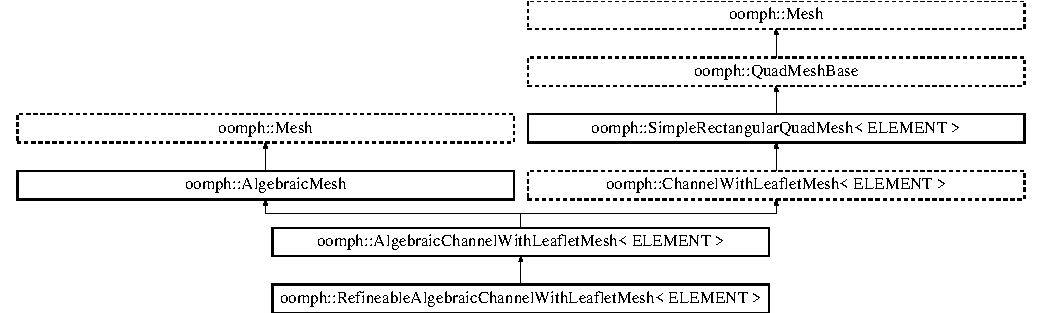
\includegraphics[height=4.200000cm]{classoomph_1_1AlgebraicChannelWithLeafletMesh}
\end{center}
\end{figure}
\subsection*{Public Member Functions}
\begin{DoxyCompactItemize}
\item 
\hyperlink{classoomph_1_1AlgebraicChannelWithLeafletMesh_a1e72e11c9971ed132efc95b808c83ccd}{Algebraic\+Channel\+With\+Leaflet\+Mesh} (\hyperlink{classoomph_1_1GeomObject}{Geom\+Object} $\ast$leaflet\+\_\+pt, const double \&lleft, const double \&lright, const double \&hleaflet, const double \&htot, const unsigned \&nleft, const unsigned \&nright, const unsigned \&ny1, const unsigned \&ny2, \hyperlink{classoomph_1_1TimeStepper}{Time\+Stepper} $\ast$time\+\_\+stepper\+\_\+pt=\&\hyperlink{classoomph_1_1Mesh_a12243d0fee2b1fcee729ee5a4777ea10}{Mesh\+::\+Default\+\_\+\+Time\+Stepper})
\begin{DoxyCompactList}\small\item\em Constructor\+: Pass pointer to \hyperlink{classoomph_1_1GeomObject}{Geom\+Object} that represents the leaflet, the length of the domain to left and right of the leaflet, the height of the leaflet and the overall height of the channel, the number of element columns to the left and right of the leaflet, the number of rows of elements from the bottom of the channel to the end of the leaflet, the number of rows of elements above the end of the leaflet. Timestepper defaults to \hyperlink{classoomph_1_1Steady}{Steady} default Timestepper defined in the \hyperlink{classoomph_1_1Mesh}{Mesh} base class. \end{DoxyCompactList}\item 
virtual \hyperlink{classoomph_1_1AlgebraicChannelWithLeafletMesh_a5b7c6a5f91427eae728c397b38de7c54}{$\sim$\+Algebraic\+Channel\+With\+Leaflet\+Mesh} ()
\begin{DoxyCompactList}\small\item\em Destructor\+: empty. \end{DoxyCompactList}\item 
void \hyperlink{classoomph_1_1AlgebraicChannelWithLeafletMesh_ace3a90b4e530c75bec8301e2291151eb}{update\+\_\+node\+\_\+update} (\hyperlink{classoomph_1_1AlgebraicNode}{Algebraic\+Node} $\ast$\&\hyperlink{classoomph_1_1AlgebraicMesh_aedeebbe95d2f8e67e9939cecd1be3933}{node\+\_\+pt})
\begin{DoxyCompactList}\small\item\em Update the geometric references that are used to update node after mesh adaptation. Empty -- no update of node update required without adaptivity. \end{DoxyCompactList}\item 
void \hyperlink{classoomph_1_1AlgebraicChannelWithLeafletMesh_a4c01b99ca83286f872c517fc5269a890}{algebraic\+\_\+node\+\_\+update} (const unsigned \&\hyperlink{cfortran_8h_af6f0bd3dc13317f895c91323c25c2b8f}{t}, \hyperlink{classoomph_1_1AlgebraicNode}{Algebraic\+Node} $\ast$\&\hyperlink{classoomph_1_1AlgebraicMesh_aedeebbe95d2f8e67e9939cecd1be3933}{node\+\_\+pt})
\begin{DoxyCompactList}\small\item\em Update nodal position at time level t (t=0\+: present; t$>$0\+: previous) \end{DoxyCompactList}\end{DoxyCompactItemize}
\subsection*{Protected Member Functions}
\begin{DoxyCompactItemize}
\item 
void \hyperlink{classoomph_1_1AlgebraicChannelWithLeafletMesh_a0d6cb8a8ffa830cdd73aa0f6686f150f}{setup\+\_\+algebraic\+\_\+node\+\_\+update} ()
\begin{DoxyCompactList}\small\item\em Function to setup the algebraic node update. \end{DoxyCompactList}\item 
void \hyperlink{classoomph_1_1AlgebraicChannelWithLeafletMesh_a53de0d31556bc78e22b5c06bb66bdd73}{node\+\_\+update\+\_\+I} (const unsigned \&\hyperlink{cfortran_8h_af6f0bd3dc13317f895c91323c25c2b8f}{t}, \hyperlink{classoomph_1_1AlgebraicNode}{Algebraic\+Node} $\ast$\&\hyperlink{classoomph_1_1AlgebraicMesh_aedeebbe95d2f8e67e9939cecd1be3933}{node\+\_\+pt})
\begin{DoxyCompactList}\small\item\em Update function for nodes in lower left region (I) \end{DoxyCompactList}\item 
void \hyperlink{classoomph_1_1AlgebraicChannelWithLeafletMesh_aafaeee96d0e7602cc990229abbd9c8fd}{node\+\_\+update\+\_\+\+II} (const unsigned \&\hyperlink{cfortran_8h_af6f0bd3dc13317f895c91323c25c2b8f}{t}, \hyperlink{classoomph_1_1AlgebraicNode}{Algebraic\+Node} $\ast$\&\hyperlink{classoomph_1_1AlgebraicMesh_aedeebbe95d2f8e67e9939cecd1be3933}{node\+\_\+pt})
\begin{DoxyCompactList}\small\item\em Update function for nodes in lower right region (II) \end{DoxyCompactList}\item 
void \hyperlink{classoomph_1_1AlgebraicChannelWithLeafletMesh_a5aed6f41b197dc7aab1d5d86b1b7d6d5}{node\+\_\+update\+\_\+\+I\+II} (const unsigned \&\hyperlink{cfortran_8h_af6f0bd3dc13317f895c91323c25c2b8f}{t}, \hyperlink{classoomph_1_1AlgebraicNode}{Algebraic\+Node} $\ast$\&\hyperlink{classoomph_1_1AlgebraicMesh_aedeebbe95d2f8e67e9939cecd1be3933}{node\+\_\+pt})
\begin{DoxyCompactList}\small\item\em Update function for nodes in upper left region (I\+II) \end{DoxyCompactList}\item 
void \hyperlink{classoomph_1_1AlgebraicChannelWithLeafletMesh_ac960faed226fa81f52ca605cffe3d1af}{node\+\_\+update\+\_\+\+IV} (const unsigned \&\hyperlink{cfortran_8h_af6f0bd3dc13317f895c91323c25c2b8f}{t}, \hyperlink{classoomph_1_1AlgebraicNode}{Algebraic\+Node} $\ast$\&\hyperlink{classoomph_1_1AlgebraicMesh_aedeebbe95d2f8e67e9939cecd1be3933}{node\+\_\+pt})
\begin{DoxyCompactList}\small\item\em Update function for nodes in upper right region (IV) \end{DoxyCompactList}\item 
void \hyperlink{classoomph_1_1AlgebraicChannelWithLeafletMesh_ab3659949ea5faac4ffa981828e98cf53}{slanted\+\_\+bound\+\_\+up} (const unsigned \&\hyperlink{cfortran_8h_af6f0bd3dc13317f895c91323c25c2b8f}{t}, const \hyperlink{classoomph_1_1Vector}{Vector}$<$ double $>$ \&zeta, \hyperlink{classoomph_1_1Vector}{Vector}$<$ double $>$ \&r)
\begin{DoxyCompactList}\small\item\em Helper function. \end{DoxyCompactList}\end{DoxyCompactItemize}
\subsection*{Protected Attributes}
\begin{DoxyCompactItemize}
\item 
double \hyperlink{classoomph_1_1AlgebraicChannelWithLeafletMesh_a1577beb584df4ad0f8517563934855fc}{X\+\_\+0}
\item 
double \hyperlink{classoomph_1_1AlgebraicChannelWithLeafletMesh_a22e6274b52941ae60cbe66287dd02fb4}{Hleaflet}
\end{DoxyCompactItemize}
\subsection*{Additional Inherited Members}


\subsection{Detailed Description}
\subsubsection*{template$<$class E\+L\+E\+M\+E\+NT$>$\newline
class oomph\+::\+Algebraic\+Channel\+With\+Leaflet\+Mesh$<$ E\+L\+E\+M\+E\+N\+T $>$}

Algebraic version of \hyperlink{classoomph_1_1ChannelWithLeafletMesh}{Channel\+With\+Leaflet\+Mesh}. Leaflet is assumed to be in its undeformed (straight vertical) position when the algebraic node update is set up. 

Definition at line 333 of file channel\+\_\+with\+\_\+leaflet\+\_\+mesh.\+template.\+h.



\subsection{Constructor \& Destructor Documentation}
\mbox{\Hypertarget{classoomph_1_1AlgebraicChannelWithLeafletMesh_a1e72e11c9971ed132efc95b808c83ccd}\label{classoomph_1_1AlgebraicChannelWithLeafletMesh_a1e72e11c9971ed132efc95b808c83ccd}} 
\index{oomph\+::\+Algebraic\+Channel\+With\+Leaflet\+Mesh@{oomph\+::\+Algebraic\+Channel\+With\+Leaflet\+Mesh}!Algebraic\+Channel\+With\+Leaflet\+Mesh@{Algebraic\+Channel\+With\+Leaflet\+Mesh}}
\index{Algebraic\+Channel\+With\+Leaflet\+Mesh@{Algebraic\+Channel\+With\+Leaflet\+Mesh}!oomph\+::\+Algebraic\+Channel\+With\+Leaflet\+Mesh@{oomph\+::\+Algebraic\+Channel\+With\+Leaflet\+Mesh}}
\subsubsection{\texorpdfstring{Algebraic\+Channel\+With\+Leaflet\+Mesh()}{AlgebraicChannelWithLeafletMesh()}}
{\footnotesize\ttfamily template$<$class E\+L\+E\+M\+E\+NT $>$ \\
\hyperlink{classoomph_1_1AlgebraicChannelWithLeafletMesh}{oomph\+::\+Algebraic\+Channel\+With\+Leaflet\+Mesh}$<$ E\+L\+E\+M\+E\+NT $>$\+::\hyperlink{classoomph_1_1AlgebraicChannelWithLeafletMesh}{Algebraic\+Channel\+With\+Leaflet\+Mesh} (\begin{DoxyParamCaption}\item[{\hyperlink{classoomph_1_1GeomObject}{Geom\+Object} $\ast$}]{leaflet\+\_\+pt,  }\item[{const double \&}]{lleft,  }\item[{const double \&}]{lright,  }\item[{const double \&}]{hleaflet,  }\item[{const double \&}]{htot,  }\item[{const unsigned \&}]{nleft,  }\item[{const unsigned \&}]{nright,  }\item[{const unsigned \&}]{ny1,  }\item[{const unsigned \&}]{ny2,  }\item[{\hyperlink{classoomph_1_1TimeStepper}{Time\+Stepper} $\ast$}]{time\+\_\+stepper\+\_\+pt = {\ttfamily \&\hyperlink{classoomph_1_1Mesh_a12243d0fee2b1fcee729ee5a4777ea10}{Mesh\+::\+Default\+\_\+\+Time\+Stepper}} }\end{DoxyParamCaption})\hspace{0.3cm}{\ttfamily [inline]}}



Constructor\+: Pass pointer to \hyperlink{classoomph_1_1GeomObject}{Geom\+Object} that represents the leaflet, the length of the domain to left and right of the leaflet, the height of the leaflet and the overall height of the channel, the number of element columns to the left and right of the leaflet, the number of rows of elements from the bottom of the channel to the end of the leaflet, the number of rows of elements above the end of the leaflet. Timestepper defaults to \hyperlink{classoomph_1_1Steady}{Steady} default Timestepper defined in the \hyperlink{classoomph_1_1Mesh}{Mesh} base class. 



Definition at line 346 of file channel\+\_\+with\+\_\+leaflet\+\_\+mesh.\+template.\+h.



References oomph\+::\+Algebraic\+Mesh\+::add\+\_\+geom\+\_\+object\+\_\+list\+\_\+pt(), oomph\+::\+Channel\+With\+Leaflet\+Mesh$<$ E\+L\+E\+M\+E\+N\+T $>$\+::\+Leaflet\+\_\+pt, and oomph\+::\+Geom\+Object\+::position().

\mbox{\Hypertarget{classoomph_1_1AlgebraicChannelWithLeafletMesh_a5b7c6a5f91427eae728c397b38de7c54}\label{classoomph_1_1AlgebraicChannelWithLeafletMesh_a5b7c6a5f91427eae728c397b38de7c54}} 
\index{oomph\+::\+Algebraic\+Channel\+With\+Leaflet\+Mesh@{oomph\+::\+Algebraic\+Channel\+With\+Leaflet\+Mesh}!````~Algebraic\+Channel\+With\+Leaflet\+Mesh@{$\sim$\+Algebraic\+Channel\+With\+Leaflet\+Mesh}}
\index{````~Algebraic\+Channel\+With\+Leaflet\+Mesh@{$\sim$\+Algebraic\+Channel\+With\+Leaflet\+Mesh}!oomph\+::\+Algebraic\+Channel\+With\+Leaflet\+Mesh@{oomph\+::\+Algebraic\+Channel\+With\+Leaflet\+Mesh}}
\subsubsection{\texorpdfstring{$\sim$\+Algebraic\+Channel\+With\+Leaflet\+Mesh()}{~AlgebraicChannelWithLeafletMesh()}}
{\footnotesize\ttfamily template$<$class E\+L\+E\+M\+E\+NT $>$ \\
virtual \hyperlink{classoomph_1_1AlgebraicChannelWithLeafletMesh}{oomph\+::\+Algebraic\+Channel\+With\+Leaflet\+Mesh}$<$ E\+L\+E\+M\+E\+NT $>$\+::$\sim$\hyperlink{classoomph_1_1AlgebraicChannelWithLeafletMesh}{Algebraic\+Channel\+With\+Leaflet\+Mesh} (\begin{DoxyParamCaption}{ }\end{DoxyParamCaption})\hspace{0.3cm}{\ttfamily [inline]}, {\ttfamily [virtual]}}



Destructor\+: empty. 



Definition at line 377 of file channel\+\_\+with\+\_\+leaflet\+\_\+mesh.\+template.\+h.



\subsection{Member Function Documentation}
\mbox{\Hypertarget{classoomph_1_1AlgebraicChannelWithLeafletMesh_a4c01b99ca83286f872c517fc5269a890}\label{classoomph_1_1AlgebraicChannelWithLeafletMesh_a4c01b99ca83286f872c517fc5269a890}} 
\index{oomph\+::\+Algebraic\+Channel\+With\+Leaflet\+Mesh@{oomph\+::\+Algebraic\+Channel\+With\+Leaflet\+Mesh}!algebraic\+\_\+node\+\_\+update@{algebraic\+\_\+node\+\_\+update}}
\index{algebraic\+\_\+node\+\_\+update@{algebraic\+\_\+node\+\_\+update}!oomph\+::\+Algebraic\+Channel\+With\+Leaflet\+Mesh@{oomph\+::\+Algebraic\+Channel\+With\+Leaflet\+Mesh}}
\subsubsection{\texorpdfstring{algebraic\+\_\+node\+\_\+update()}{algebraic\_node\_update()}}
{\footnotesize\ttfamily template$<$class E\+L\+E\+M\+E\+NT $>$ \\
void \hyperlink{classoomph_1_1AlgebraicChannelWithLeafletMesh}{oomph\+::\+Algebraic\+Channel\+With\+Leaflet\+Mesh}$<$ E\+L\+E\+M\+E\+NT $>$\+::algebraic\+\_\+node\+\_\+update (\begin{DoxyParamCaption}\item[{const unsigned \&}]{t,  }\item[{\hyperlink{classoomph_1_1AlgebraicNode}{Algebraic\+Node} $\ast$\&}]{node\+\_\+pt }\end{DoxyParamCaption})\hspace{0.3cm}{\ttfamily [virtual]}}



Update nodal position at time level t (t=0\+: present; t$>$0\+: previous) 

Perform algebraic node update. 

Implements \hyperlink{classoomph_1_1AlgebraicMesh_ab01d6f93354f3c4e5c9d1f0a5885a65b}{oomph\+::\+Algebraic\+Mesh}.



Definition at line 425 of file channel\+\_\+with\+\_\+leaflet\+\_\+mesh.\+template.\+cc.



References oomph\+::\+Algebraic\+Node\+::node\+\_\+update\+\_\+fct\+\_\+id(), and oomph\+::\+Global\+\_\+string\+\_\+for\+\_\+annotation\+::string().

\mbox{\Hypertarget{classoomph_1_1AlgebraicChannelWithLeafletMesh_a53de0d31556bc78e22b5c06bb66bdd73}\label{classoomph_1_1AlgebraicChannelWithLeafletMesh_a53de0d31556bc78e22b5c06bb66bdd73}} 
\index{oomph\+::\+Algebraic\+Channel\+With\+Leaflet\+Mesh@{oomph\+::\+Algebraic\+Channel\+With\+Leaflet\+Mesh}!node\+\_\+update\+\_\+I@{node\+\_\+update\+\_\+I}}
\index{node\+\_\+update\+\_\+I@{node\+\_\+update\+\_\+I}!oomph\+::\+Algebraic\+Channel\+With\+Leaflet\+Mesh@{oomph\+::\+Algebraic\+Channel\+With\+Leaflet\+Mesh}}
\subsubsection{\texorpdfstring{node\+\_\+update\+\_\+\+I()}{node\_update\_I()}}
{\footnotesize\ttfamily template$<$class E\+L\+E\+M\+E\+NT $>$ \\
void \hyperlink{classoomph_1_1AlgebraicChannelWithLeafletMesh}{oomph\+::\+Algebraic\+Channel\+With\+Leaflet\+Mesh}$<$ E\+L\+E\+M\+E\+NT $>$\+::node\+\_\+update\+\_\+I (\begin{DoxyParamCaption}\item[{const unsigned \&}]{t,  }\item[{\hyperlink{classoomph_1_1AlgebraicNode}{Algebraic\+Node} $\ast$\&}]{node\+\_\+pt }\end{DoxyParamCaption})\hspace{0.3cm}{\ttfamily [protected]}}



Update function for nodes in lower left region (I) 

\hyperlink{classoomph_1_1Node}{Node} update for region I. 

Definition at line 471 of file channel\+\_\+with\+\_\+leaflet\+\_\+mesh.\+template.\+cc.



References oomph\+::\+Channel\+With\+Leaflet\+Mesh$<$ E\+L\+E\+M\+E\+N\+T $>$\+::domain\+\_\+pt(), oomph\+::\+Channel\+With\+Leaflet\+Domain\+::lleft(), s, oomph\+::\+Algebraic\+Node\+::vector\+\_\+geom\+\_\+object\+\_\+pt(), oomph\+::\+Algebraic\+Node\+::vector\+\_\+ref\+\_\+value(), and oomph\+::\+Node\+::x().

\mbox{\Hypertarget{classoomph_1_1AlgebraicChannelWithLeafletMesh_aafaeee96d0e7602cc990229abbd9c8fd}\label{classoomph_1_1AlgebraicChannelWithLeafletMesh_aafaeee96d0e7602cc990229abbd9c8fd}} 
\index{oomph\+::\+Algebraic\+Channel\+With\+Leaflet\+Mesh@{oomph\+::\+Algebraic\+Channel\+With\+Leaflet\+Mesh}!node\+\_\+update\+\_\+\+II@{node\+\_\+update\+\_\+\+II}}
\index{node\+\_\+update\+\_\+\+II@{node\+\_\+update\+\_\+\+II}!oomph\+::\+Algebraic\+Channel\+With\+Leaflet\+Mesh@{oomph\+::\+Algebraic\+Channel\+With\+Leaflet\+Mesh}}
\subsubsection{\texorpdfstring{node\+\_\+update\+\_\+\+I\+I()}{node\_update\_II()}}
{\footnotesize\ttfamily template$<$class E\+L\+E\+M\+E\+NT $>$ \\
void \hyperlink{classoomph_1_1AlgebraicChannelWithLeafletMesh}{oomph\+::\+Algebraic\+Channel\+With\+Leaflet\+Mesh}$<$ E\+L\+E\+M\+E\+NT $>$\+::node\+\_\+update\+\_\+\+II (\begin{DoxyParamCaption}\item[{const unsigned \&}]{t,  }\item[{\hyperlink{classoomph_1_1AlgebraicNode}{Algebraic\+Node} $\ast$\&}]{node\+\_\+pt }\end{DoxyParamCaption})\hspace{0.3cm}{\ttfamily [protected]}}



Update function for nodes in lower right region (II) 

\hyperlink{classoomph_1_1Node}{Node} update for region II. 

Definition at line 516 of file channel\+\_\+with\+\_\+leaflet\+\_\+mesh.\+template.\+cc.



References oomph\+::\+Channel\+With\+Leaflet\+Mesh$<$ E\+L\+E\+M\+E\+N\+T $>$\+::domain\+\_\+pt(), oomph\+::\+Channel\+With\+Leaflet\+Domain\+::lright(), s, oomph\+::\+Algebraic\+Node\+::vector\+\_\+geom\+\_\+object\+\_\+pt(), oomph\+::\+Algebraic\+Node\+::vector\+\_\+ref\+\_\+value(), and oomph\+::\+Node\+::x().

\mbox{\Hypertarget{classoomph_1_1AlgebraicChannelWithLeafletMesh_a5aed6f41b197dc7aab1d5d86b1b7d6d5}\label{classoomph_1_1AlgebraicChannelWithLeafletMesh_a5aed6f41b197dc7aab1d5d86b1b7d6d5}} 
\index{oomph\+::\+Algebraic\+Channel\+With\+Leaflet\+Mesh@{oomph\+::\+Algebraic\+Channel\+With\+Leaflet\+Mesh}!node\+\_\+update\+\_\+\+I\+II@{node\+\_\+update\+\_\+\+I\+II}}
\index{node\+\_\+update\+\_\+\+I\+II@{node\+\_\+update\+\_\+\+I\+II}!oomph\+::\+Algebraic\+Channel\+With\+Leaflet\+Mesh@{oomph\+::\+Algebraic\+Channel\+With\+Leaflet\+Mesh}}
\subsubsection{\texorpdfstring{node\+\_\+update\+\_\+\+I\+I\+I()}{node\_update\_III()}}
{\footnotesize\ttfamily template$<$class E\+L\+E\+M\+E\+NT $>$ \\
void \hyperlink{classoomph_1_1AlgebraicChannelWithLeafletMesh}{oomph\+::\+Algebraic\+Channel\+With\+Leaflet\+Mesh}$<$ E\+L\+E\+M\+E\+NT $>$\+::node\+\_\+update\+\_\+\+I\+II (\begin{DoxyParamCaption}\item[{const unsigned \&}]{t,  }\item[{\hyperlink{classoomph_1_1AlgebraicNode}{Algebraic\+Node} $\ast$\&}]{node\+\_\+pt }\end{DoxyParamCaption})\hspace{0.3cm}{\ttfamily [protected]}}



Update function for nodes in upper left region (I\+II) 

\hyperlink{classoomph_1_1Node}{Node} update for region I\+II. 

Definition at line 582 of file channel\+\_\+with\+\_\+leaflet\+\_\+mesh.\+template.\+cc.



References oomph\+::\+Channel\+With\+Leaflet\+Mesh$<$ E\+L\+E\+M\+E\+N\+T $>$\+::domain\+\_\+pt(), oomph\+::\+Channel\+With\+Leaflet\+Domain\+::lleft(), s, oomph\+::\+Algebraic\+Node\+::vector\+\_\+ref\+\_\+value(), and oomph\+::\+Node\+::x().

\mbox{\Hypertarget{classoomph_1_1AlgebraicChannelWithLeafletMesh_ac960faed226fa81f52ca605cffe3d1af}\label{classoomph_1_1AlgebraicChannelWithLeafletMesh_ac960faed226fa81f52ca605cffe3d1af}} 
\index{oomph\+::\+Algebraic\+Channel\+With\+Leaflet\+Mesh@{oomph\+::\+Algebraic\+Channel\+With\+Leaflet\+Mesh}!node\+\_\+update\+\_\+\+IV@{node\+\_\+update\+\_\+\+IV}}
\index{node\+\_\+update\+\_\+\+IV@{node\+\_\+update\+\_\+\+IV}!oomph\+::\+Algebraic\+Channel\+With\+Leaflet\+Mesh@{oomph\+::\+Algebraic\+Channel\+With\+Leaflet\+Mesh}}
\subsubsection{\texorpdfstring{node\+\_\+update\+\_\+\+I\+V()}{node\_update\_IV()}}
{\footnotesize\ttfamily template$<$class E\+L\+E\+M\+E\+NT $>$ \\
void \hyperlink{classoomph_1_1AlgebraicChannelWithLeafletMesh}{oomph\+::\+Algebraic\+Channel\+With\+Leaflet\+Mesh}$<$ E\+L\+E\+M\+E\+NT $>$\+::node\+\_\+update\+\_\+\+IV (\begin{DoxyParamCaption}\item[{const unsigned \&}]{t,  }\item[{\hyperlink{classoomph_1_1AlgebraicNode}{Algebraic\+Node} $\ast$\&}]{node\+\_\+pt }\end{DoxyParamCaption})\hspace{0.3cm}{\ttfamily [protected]}}



Update function for nodes in upper right region (IV) 

\hyperlink{classoomph_1_1Node}{Node} update for region IV. 

Definition at line 616 of file channel\+\_\+with\+\_\+leaflet\+\_\+mesh.\+template.\+cc.



References oomph\+::\+Channel\+With\+Leaflet\+Mesh$<$ E\+L\+E\+M\+E\+N\+T $>$\+::domain\+\_\+pt(), oomph\+::\+Channel\+With\+Leaflet\+Domain\+::lright(), s, oomph\+::\+Algebraic\+Node\+::vector\+\_\+ref\+\_\+value(), and oomph\+::\+Node\+::x().

\mbox{\Hypertarget{classoomph_1_1AlgebraicChannelWithLeafletMesh_a0d6cb8a8ffa830cdd73aa0f6686f150f}\label{classoomph_1_1AlgebraicChannelWithLeafletMesh_a0d6cb8a8ffa830cdd73aa0f6686f150f}} 
\index{oomph\+::\+Algebraic\+Channel\+With\+Leaflet\+Mesh@{oomph\+::\+Algebraic\+Channel\+With\+Leaflet\+Mesh}!setup\+\_\+algebraic\+\_\+node\+\_\+update@{setup\+\_\+algebraic\+\_\+node\+\_\+update}}
\index{setup\+\_\+algebraic\+\_\+node\+\_\+update@{setup\+\_\+algebraic\+\_\+node\+\_\+update}!oomph\+::\+Algebraic\+Channel\+With\+Leaflet\+Mesh@{oomph\+::\+Algebraic\+Channel\+With\+Leaflet\+Mesh}}
\subsubsection{\texorpdfstring{setup\+\_\+algebraic\+\_\+node\+\_\+update()}{setup\_algebraic\_node\_update()}}
{\footnotesize\ttfamily template$<$class E\+L\+E\+M\+E\+NT $>$ \\
void \hyperlink{classoomph_1_1AlgebraicChannelWithLeafletMesh}{oomph\+::\+Algebraic\+Channel\+With\+Leaflet\+Mesh}$<$ E\+L\+E\+M\+E\+NT $>$\+::setup\+\_\+algebraic\+\_\+node\+\_\+update (\begin{DoxyParamCaption}{ }\end{DoxyParamCaption})\hspace{0.3cm}{\ttfamily [protected]}}



Function to setup the algebraic node update. 

Setup algebraic node update. Leaflet is assumed to be in its undeformed (straight vertical) position! 

Definition at line 246 of file channel\+\_\+with\+\_\+leaflet\+\_\+mesh.\+template.\+cc.



References oomph\+::\+Algebraic\+Node\+::add\+\_\+node\+\_\+update\+\_\+info(), oomph\+::\+Channel\+With\+Leaflet\+Mesh$<$ E\+L\+E\+M\+E\+N\+T $>$\+::domain\+\_\+pt(), oomph\+::\+Channel\+With\+Leaflet\+Domain\+::hleaflet(), oomph\+::\+Channel\+With\+Leaflet\+Domain\+::htot(), oomph\+::\+Channel\+With\+Leaflet\+Mesh$<$ E\+L\+E\+M\+E\+N\+T $>$\+::\+Leaflet\+\_\+pt, oomph\+::\+Channel\+With\+Leaflet\+Domain\+::lleft(), oomph\+::\+Geom\+Object\+::locate\+\_\+zeta(), oomph\+::\+Channel\+With\+Leaflet\+Domain\+::lright(), oomph\+::\+Mesh\+::nnode(), oomph\+::\+Mesh\+::node\+\_\+pt(), oomph\+::\+Geom\+Object\+::position(), s, and oomph\+::\+Node\+::x().

\mbox{\Hypertarget{classoomph_1_1AlgebraicChannelWithLeafletMesh_ab3659949ea5faac4ffa981828e98cf53}\label{classoomph_1_1AlgebraicChannelWithLeafletMesh_ab3659949ea5faac4ffa981828e98cf53}} 
\index{oomph\+::\+Algebraic\+Channel\+With\+Leaflet\+Mesh@{oomph\+::\+Algebraic\+Channel\+With\+Leaflet\+Mesh}!slanted\+\_\+bound\+\_\+up@{slanted\+\_\+bound\+\_\+up}}
\index{slanted\+\_\+bound\+\_\+up@{slanted\+\_\+bound\+\_\+up}!oomph\+::\+Algebraic\+Channel\+With\+Leaflet\+Mesh@{oomph\+::\+Algebraic\+Channel\+With\+Leaflet\+Mesh}}
\subsubsection{\texorpdfstring{slanted\+\_\+bound\+\_\+up()}{slanted\_bound\_up()}}
{\footnotesize\ttfamily template$<$class E\+L\+E\+M\+E\+NT $>$ \\
void \hyperlink{classoomph_1_1AlgebraicChannelWithLeafletMesh}{oomph\+::\+Algebraic\+Channel\+With\+Leaflet\+Mesh}$<$ E\+L\+E\+M\+E\+NT $>$\+::slanted\+\_\+bound\+\_\+up (\begin{DoxyParamCaption}\item[{const unsigned \&}]{t,  }\item[{const \hyperlink{classoomph_1_1Vector}{Vector}$<$ double $>$ \&}]{zeta,  }\item[{\hyperlink{classoomph_1_1Vector}{Vector}$<$ double $>$ \&}]{r }\end{DoxyParamCaption})\hspace{0.3cm}{\ttfamily [protected]}}



Helper function. 

Slanted bound \+: helper function. Coordinates of the point on the boundary beetween the upper and the lower part, in the same column, at the east. 

Definition at line 558 of file channel\+\_\+with\+\_\+leaflet\+\_\+mesh.\+template.\+cc.



References oomph\+::\+Channel\+With\+Leaflet\+Mesh$<$ E\+L\+E\+M\+E\+N\+T $>$\+::domain\+\_\+pt(), oomph\+::\+Channel\+With\+Leaflet\+Domain\+::htot(), oomph\+::\+Channel\+With\+Leaflet\+Mesh$<$ E\+L\+E\+M\+E\+N\+T $>$\+::\+Leaflet\+\_\+pt, and oomph\+::\+Geom\+Object\+::position().

\mbox{\Hypertarget{classoomph_1_1AlgebraicChannelWithLeafletMesh_ace3a90b4e530c75bec8301e2291151eb}\label{classoomph_1_1AlgebraicChannelWithLeafletMesh_ace3a90b4e530c75bec8301e2291151eb}} 
\index{oomph\+::\+Algebraic\+Channel\+With\+Leaflet\+Mesh@{oomph\+::\+Algebraic\+Channel\+With\+Leaflet\+Mesh}!update\+\_\+node\+\_\+update@{update\+\_\+node\+\_\+update}}
\index{update\+\_\+node\+\_\+update@{update\+\_\+node\+\_\+update}!oomph\+::\+Algebraic\+Channel\+With\+Leaflet\+Mesh@{oomph\+::\+Algebraic\+Channel\+With\+Leaflet\+Mesh}}
\subsubsection{\texorpdfstring{update\+\_\+node\+\_\+update()}{update\_node\_update()}}
{\footnotesize\ttfamily template$<$class E\+L\+E\+M\+E\+NT $>$ \\
void \hyperlink{classoomph_1_1AlgebraicChannelWithLeafletMesh}{oomph\+::\+Algebraic\+Channel\+With\+Leaflet\+Mesh}$<$ E\+L\+E\+M\+E\+NT $>$\+::update\+\_\+node\+\_\+update (\begin{DoxyParamCaption}\item[{\hyperlink{classoomph_1_1AlgebraicNode}{Algebraic\+Node} $\ast$\&}]{node\+\_\+pt }\end{DoxyParamCaption})\hspace{0.3cm}{\ttfamily [inline]}, {\ttfamily [virtual]}}



Update the geometric references that are used to update node after mesh adaptation. Empty -- no update of node update required without adaptivity. 



Implements \hyperlink{classoomph_1_1AlgebraicMesh_a6c6a35ae2be6e2766f5b80d85693c1ce}{oomph\+::\+Algebraic\+Mesh}.



Reimplemented in \hyperlink{classoomph_1_1RefineableAlgebraicChannelWithLeafletMesh_a8ee7168fbb84bb87880a2590dd52eaa8}{oomph\+::\+Refineable\+Algebraic\+Channel\+With\+Leaflet\+Mesh$<$ E\+L\+E\+M\+E\+N\+T $>$}.



Definition at line 383 of file channel\+\_\+with\+\_\+leaflet\+\_\+mesh.\+template.\+h.



References oomph\+::\+Mesh\+::node\+\_\+pt(), and t.



\subsection{Member Data Documentation}
\mbox{\Hypertarget{classoomph_1_1AlgebraicChannelWithLeafletMesh_a22e6274b52941ae60cbe66287dd02fb4}\label{classoomph_1_1AlgebraicChannelWithLeafletMesh_a22e6274b52941ae60cbe66287dd02fb4}} 
\index{oomph\+::\+Algebraic\+Channel\+With\+Leaflet\+Mesh@{oomph\+::\+Algebraic\+Channel\+With\+Leaflet\+Mesh}!Hleaflet@{Hleaflet}}
\index{Hleaflet@{Hleaflet}!oomph\+::\+Algebraic\+Channel\+With\+Leaflet\+Mesh@{oomph\+::\+Algebraic\+Channel\+With\+Leaflet\+Mesh}}
\subsubsection{\texorpdfstring{Hleaflet}{Hleaflet}}
{\footnotesize\ttfamily template$<$class E\+L\+E\+M\+E\+NT $>$ \\
double \hyperlink{classoomph_1_1AlgebraicChannelWithLeafletMesh}{oomph\+::\+Algebraic\+Channel\+With\+Leaflet\+Mesh}$<$ E\+L\+E\+M\+E\+NT $>$\+::Hleaflet\hspace{0.3cm}{\ttfamily [protected]}}

Length of the leaflet (stored explicitly for reference in algebraic node update -- it\textquotesingle{}s also stored independently in domain....) 

Definition at line 418 of file channel\+\_\+with\+\_\+leaflet\+\_\+mesh.\+template.\+h.

\mbox{\Hypertarget{classoomph_1_1AlgebraicChannelWithLeafletMesh_a1577beb584df4ad0f8517563934855fc}\label{classoomph_1_1AlgebraicChannelWithLeafletMesh_a1577beb584df4ad0f8517563934855fc}} 
\index{oomph\+::\+Algebraic\+Channel\+With\+Leaflet\+Mesh@{oomph\+::\+Algebraic\+Channel\+With\+Leaflet\+Mesh}!X\+\_\+0@{X\+\_\+0}}
\index{X\+\_\+0@{X\+\_\+0}!oomph\+::\+Algebraic\+Channel\+With\+Leaflet\+Mesh@{oomph\+::\+Algebraic\+Channel\+With\+Leaflet\+Mesh}}
\subsubsection{\texorpdfstring{X\+\_\+0}{X\_0}}
{\footnotesize\ttfamily template$<$class E\+L\+E\+M\+E\+NT $>$ \\
double \hyperlink{classoomph_1_1AlgebraicChannelWithLeafletMesh}{oomph\+::\+Algebraic\+Channel\+With\+Leaflet\+Mesh}$<$ E\+L\+E\+M\+E\+NT $>$\+::X\+\_\+0\hspace{0.3cm}{\ttfamily [protected]}}

Origin of the wall (stored explicitly for reference in algebraic node update -- it\textquotesingle{}s also stored independently in domain....) 

Definition at line 413 of file channel\+\_\+with\+\_\+leaflet\+\_\+mesh.\+template.\+h.



The documentation for this class was generated from the following files\+:\begin{DoxyCompactItemize}
\item 
\hyperlink{channel__with__leaflet__mesh_8template_8h}{channel\+\_\+with\+\_\+leaflet\+\_\+mesh.\+template.\+h}\item 
\hyperlink{channel__with__leaflet__mesh_8template_8cc}{channel\+\_\+with\+\_\+leaflet\+\_\+mesh.\+template.\+cc}\end{DoxyCompactItemize}

\hypertarget{classoomph_1_1AlgebraicCollapsibleChannelMesh}{}\section{oomph\+:\+:Algebraic\+Collapsible\+Channel\+Mesh$<$ E\+L\+E\+M\+E\+NT $>$ Class Template Reference}
\label{classoomph_1_1AlgebraicCollapsibleChannelMesh}\index{oomph\+::\+Algebraic\+Collapsible\+Channel\+Mesh$<$ E\+L\+E\+M\+E\+N\+T $>$@{oomph\+::\+Algebraic\+Collapsible\+Channel\+Mesh$<$ E\+L\+E\+M\+E\+N\+T $>$}}


Collapsible channel mesh with algebraic node update.  




{\ttfamily \#include $<$collapsible\+\_\+channel\+\_\+mesh.\+template.\+h$>$}

Inheritance diagram for oomph\+:\+:Algebraic\+Collapsible\+Channel\+Mesh$<$ E\+L\+E\+M\+E\+NT $>$\+:\begin{figure}[H]
\begin{center}
\leavevmode
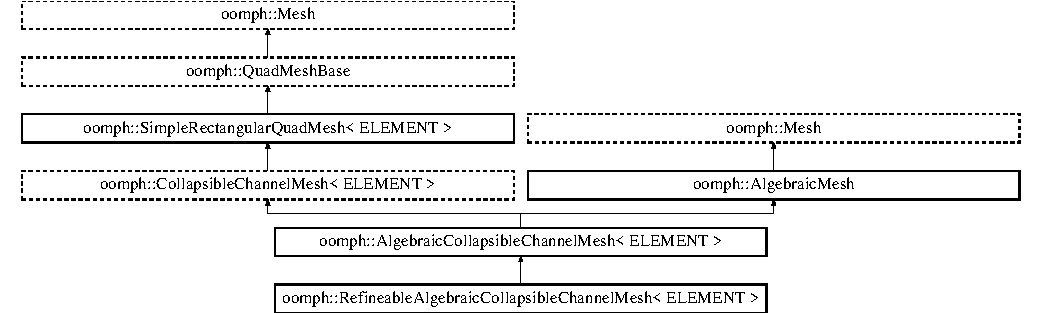
\includegraphics[height=3.500000cm]{classoomph_1_1AlgebraicCollapsibleChannelMesh}
\end{center}
\end{figure}
\subsection*{Public Member Functions}
\begin{DoxyCompactItemize}
\item 
\hyperlink{classoomph_1_1AlgebraicCollapsibleChannelMesh_ac2e77539dfed482cc3d8b7c9e17a9567}{Algebraic\+Collapsible\+Channel\+Mesh} (const unsigned \&nup, const unsigned \&ncollapsible, const unsigned \&ndown, const unsigned \&\hyperlink{classoomph_1_1SimpleRectangularQuadMesh_a45011f22dedd480392b1f376e4269921}{ny}, const double \&lup, const double \&lcollapsible, const double \&ldown, const double \&ly, Geom\+Object $\ast$\hyperlink{classoomph_1_1CollapsibleChannelMesh_a04ffeb61678763dfd250962ea9ba614b}{wall\+\_\+pt}, Time\+Stepper $\ast$time\+\_\+stepper\+\_\+pt=\&Mesh\+::\+Default\+\_\+\+Time\+Stepper)
\begin{DoxyCompactList}\small\item\em Constructor\+: Pass number of elements in upstream/collapsible/ downstream segment and across the channel; lengths of upstream/ collapsible/downstream segments and width of channel, pointer to Geom\+Object that defines the collapsible segment and pointer to Time\+Stepper (defaults to the default timestepper, Steady). \end{DoxyCompactList}\item 
virtual \hyperlink{classoomph_1_1AlgebraicCollapsibleChannelMesh_ab921ed3dbc5678fc5d39626fdf32c4ed}{$\sim$\+Algebraic\+Collapsible\+Channel\+Mesh} ()
\begin{DoxyCompactList}\small\item\em Destructor\+: empty. \end{DoxyCompactList}\item 
\hyperlink{classoomph_1_1AlgebraicCollapsibleChannelMesh_a3c19524e69a9408c79047d130b79d6b3}{Algebraic\+Collapsible\+Channel\+Mesh} (const unsigned \&nup, const unsigned \&ncollapsible, const unsigned \&ndown, const unsigned \&\hyperlink{classoomph_1_1SimpleRectangularQuadMesh_a45011f22dedd480392b1f376e4269921}{ny}, const double \&lup, const double \&lcollapsible, const double \&ldown, const double \&ly, Geom\+Object $\ast$\hyperlink{classoomph_1_1CollapsibleChannelMesh_a04ffeb61678763dfd250962ea9ba614b}{wall\+\_\+pt}, \hyperlink{classoomph_1_1CollapsibleChannelDomain_a2bf1d7943bfac134a5c27a54c7e1faed}{Collapsible\+Channel\+Domain\+::\+B\+L\+Squash\+Fct\+Pt} bl\+\_\+squash\+\_\+function\+\_\+pt, Time\+Stepper $\ast$time\+\_\+stepper\+\_\+pt=\&Mesh\+::\+Default\+\_\+\+Time\+Stepper)
\begin{DoxyCompactList}\small\item\em Constructor\+: Pass number of elements in upstream/collapsible/ downstream segment and across the channel; lengths of upstream/ collapsible/downstream segments and width of channel, pointer to Geom\+Object that defines the collapsible segment and pointer to Time\+Stepper (defaults to the default timestepper, Steady). \end{DoxyCompactList}\item 
\hyperlink{classoomph_1_1CollapsibleChannelDomain_a2bf1d7943bfac134a5c27a54c7e1faed}{Collapsible\+Channel\+Domain\+::\+B\+L\+Squash\+Fct\+Pt} \& \hyperlink{classoomph_1_1AlgebraicCollapsibleChannelMesh_abf1848b49f57419af4379a637464587d}{bl\+\_\+squash\+\_\+fct\+\_\+pt} ()
\begin{DoxyCompactList}\small\item\em Function pointer for function that squashes the mesh near the walls. Default trivial mapping (the identity) leaves vertical nodal positions unchanged. Mapping is used in underlying \hyperlink{classoomph_1_1CollapsibleChannelDomain}{Collapsible\+Channel\+Domain}. Broken function that overloads the version in the \hyperlink{classoomph_1_1CollapsibleChannelMesh}{Collapsible\+Channel\+Mesh}. It does not make sense to specify the function pointer after the mesh has been set up! \end{DoxyCompactList}\item 
\hyperlink{classoomph_1_1CollapsibleChannelDomain_a2bf1d7943bfac134a5c27a54c7e1faed}{Collapsible\+Channel\+Domain\+::\+B\+L\+Squash\+Fct\+Pt} \& \hyperlink{classoomph_1_1AlgebraicCollapsibleChannelMesh_afa53bd526ff0903526afbdf5e6f4f532}{axial\+\_\+spacing\+\_\+fct\+\_\+pt} ()
\begin{DoxyCompactList}\small\item\em Function pointer for function that redistributes nodes axially. Default trivial mapping (the identity) leaves vertical nodal positions unchanged. Mapping is used in underlying \hyperlink{classoomph_1_1CollapsibleChannelDomain}{Collapsible\+Channel\+Domain}. Broken function that overloads the version in the \hyperlink{classoomph_1_1CollapsibleChannelMesh}{Collapsible\+Channel\+Mesh}. It does not make sense to specify the function pointer after the mesh has been set up! \end{DoxyCompactList}\item 
void \hyperlink{classoomph_1_1AlgebraicCollapsibleChannelMesh_ae1ea6d9baa12e2ca87d21d4370f41870}{algebraic\+\_\+node\+\_\+update} (const unsigned \&t, Algebraic\+Node $\ast$\&node\+\_\+pt)
\begin{DoxyCompactList}\small\item\em Update nodal position at time level t (t=0\+: present; t$>$0\+: previous) \end{DoxyCompactList}\item 
void \hyperlink{classoomph_1_1AlgebraicCollapsibleChannelMesh_abad38fb50d067a126af1161a3a603972}{update\+\_\+node\+\_\+update} (Algebraic\+Node $\ast$\&node\+\_\+pt)
\begin{DoxyCompactList}\small\item\em Update the node-\/udate data after mesh adaptation. Empty -- no update of node update required as this is non-\/refineable mesh. \end{DoxyCompactList}\end{DoxyCompactItemize}
\subsection*{Protected Member Functions}
\begin{DoxyCompactItemize}
\item 
void \hyperlink{classoomph_1_1AlgebraicCollapsibleChannelMesh_a54e93316a561cd77a68c0774d2772030}{setup\+\_\+algebraic\+\_\+node\+\_\+update} ()
\begin{DoxyCompactList}\small\item\em Function to setup the algebraic node update. \end{DoxyCompactList}\end{DoxyCompactItemize}
\subsection*{Protected Attributes}
\begin{DoxyCompactItemize}
\item 
\hyperlink{classoomph_1_1CollapsibleChannelDomain_a2bf1d7943bfac134a5c27a54c7e1faed}{Collapsible\+Channel\+Domain\+::\+B\+L\+Squash\+Fct\+Pt} \hyperlink{classoomph_1_1AlgebraicCollapsibleChannelMesh_ab3848ae5c357f45addf4bcfeca1a9d18}{Dummy\+\_\+fct\+\_\+pt}
\begin{DoxyCompactList}\small\item\em Dummy function pointer. \end{DoxyCompactList}\end{DoxyCompactItemize}


\subsection{Detailed Description}
\subsubsection*{template$<$class E\+L\+E\+M\+E\+NT$>$\newline
class oomph\+::\+Algebraic\+Collapsible\+Channel\+Mesh$<$ E\+L\+E\+M\+E\+N\+T $>$}

Collapsible channel mesh with algebraic node update. 

Definition at line 434 of file collapsible\+\_\+channel\+\_\+mesh.\+template.\+h.



\subsection{Constructor \& Destructor Documentation}
\mbox{\Hypertarget{classoomph_1_1AlgebraicCollapsibleChannelMesh_ac2e77539dfed482cc3d8b7c9e17a9567}\label{classoomph_1_1AlgebraicCollapsibleChannelMesh_ac2e77539dfed482cc3d8b7c9e17a9567}} 
\index{oomph\+::\+Algebraic\+Collapsible\+Channel\+Mesh@{oomph\+::\+Algebraic\+Collapsible\+Channel\+Mesh}!Algebraic\+Collapsible\+Channel\+Mesh@{Algebraic\+Collapsible\+Channel\+Mesh}}
\index{Algebraic\+Collapsible\+Channel\+Mesh@{Algebraic\+Collapsible\+Channel\+Mesh}!oomph\+::\+Algebraic\+Collapsible\+Channel\+Mesh@{oomph\+::\+Algebraic\+Collapsible\+Channel\+Mesh}}
\subsubsection{\texorpdfstring{Algebraic\+Collapsible\+Channel\+Mesh()}{AlgebraicCollapsibleChannelMesh()}\hspace{0.1cm}{\footnotesize\ttfamily [1/2]}}
{\footnotesize\ttfamily template$<$class E\+L\+E\+M\+E\+NT $>$ \\
\hyperlink{classoomph_1_1AlgebraicCollapsibleChannelMesh}{oomph\+::\+Algebraic\+Collapsible\+Channel\+Mesh}$<$ E\+L\+E\+M\+E\+NT $>$\+::\hyperlink{classoomph_1_1AlgebraicCollapsibleChannelMesh}{Algebraic\+Collapsible\+Channel\+Mesh} (\begin{DoxyParamCaption}\item[{const unsigned \&}]{nup,  }\item[{const unsigned \&}]{ncollapsible,  }\item[{const unsigned \&}]{ndown,  }\item[{const unsigned \&}]{ny,  }\item[{const double \&}]{lup,  }\item[{const double \&}]{lcollapsible,  }\item[{const double \&}]{ldown,  }\item[{const double \&}]{ly,  }\item[{Geom\+Object $\ast$}]{wall\+\_\+pt,  }\item[{Time\+Stepper $\ast$}]{time\+\_\+stepper\+\_\+pt = {\ttfamily \&Mesh\+:\+:Default\+\_\+TimeStepper} }\end{DoxyParamCaption})\hspace{0.3cm}{\ttfamily [inline]}}



Constructor\+: Pass number of elements in upstream/collapsible/ downstream segment and across the channel; lengths of upstream/ collapsible/downstream segments and width of channel, pointer to Geom\+Object that defines the collapsible segment and pointer to Time\+Stepper (defaults to the default timestepper, Steady). 



Definition at line 447 of file collapsible\+\_\+channel\+\_\+mesh.\+template.\+h.

\mbox{\Hypertarget{classoomph_1_1AlgebraicCollapsibleChannelMesh_ab921ed3dbc5678fc5d39626fdf32c4ed}\label{classoomph_1_1AlgebraicCollapsibleChannelMesh_ab921ed3dbc5678fc5d39626fdf32c4ed}} 
\index{oomph\+::\+Algebraic\+Collapsible\+Channel\+Mesh@{oomph\+::\+Algebraic\+Collapsible\+Channel\+Mesh}!````~Algebraic\+Collapsible\+Channel\+Mesh@{$\sim$\+Algebraic\+Collapsible\+Channel\+Mesh}}
\index{````~Algebraic\+Collapsible\+Channel\+Mesh@{$\sim$\+Algebraic\+Collapsible\+Channel\+Mesh}!oomph\+::\+Algebraic\+Collapsible\+Channel\+Mesh@{oomph\+::\+Algebraic\+Collapsible\+Channel\+Mesh}}
\subsubsection{\texorpdfstring{$\sim$\+Algebraic\+Collapsible\+Channel\+Mesh()}{~AlgebraicCollapsibleChannelMesh()}}
{\footnotesize\ttfamily template$<$class E\+L\+E\+M\+E\+NT $>$ \\
virtual \hyperlink{classoomph_1_1AlgebraicCollapsibleChannelMesh}{oomph\+::\+Algebraic\+Collapsible\+Channel\+Mesh}$<$ E\+L\+E\+M\+E\+NT $>$\+::$\sim$\hyperlink{classoomph_1_1AlgebraicCollapsibleChannelMesh}{Algebraic\+Collapsible\+Channel\+Mesh} (\begin{DoxyParamCaption}{ }\end{DoxyParamCaption})\hspace{0.3cm}{\ttfamily [inline]}, {\ttfamily [virtual]}}



Destructor\+: empty. 



Definition at line 471 of file collapsible\+\_\+channel\+\_\+mesh.\+template.\+h.

\mbox{\Hypertarget{classoomph_1_1AlgebraicCollapsibleChannelMesh_a3c19524e69a9408c79047d130b79d6b3}\label{classoomph_1_1AlgebraicCollapsibleChannelMesh_a3c19524e69a9408c79047d130b79d6b3}} 
\index{oomph\+::\+Algebraic\+Collapsible\+Channel\+Mesh@{oomph\+::\+Algebraic\+Collapsible\+Channel\+Mesh}!Algebraic\+Collapsible\+Channel\+Mesh@{Algebraic\+Collapsible\+Channel\+Mesh}}
\index{Algebraic\+Collapsible\+Channel\+Mesh@{Algebraic\+Collapsible\+Channel\+Mesh}!oomph\+::\+Algebraic\+Collapsible\+Channel\+Mesh@{oomph\+::\+Algebraic\+Collapsible\+Channel\+Mesh}}
\subsubsection{\texorpdfstring{Algebraic\+Collapsible\+Channel\+Mesh()}{AlgebraicCollapsibleChannelMesh()}\hspace{0.1cm}{\footnotesize\ttfamily [2/2]}}
{\footnotesize\ttfamily template$<$class E\+L\+E\+M\+E\+NT $>$ \\
\hyperlink{classoomph_1_1AlgebraicCollapsibleChannelMesh}{oomph\+::\+Algebraic\+Collapsible\+Channel\+Mesh}$<$ E\+L\+E\+M\+E\+NT $>$\+::\hyperlink{classoomph_1_1AlgebraicCollapsibleChannelMesh}{Algebraic\+Collapsible\+Channel\+Mesh} (\begin{DoxyParamCaption}\item[{const unsigned \&}]{nup,  }\item[{const unsigned \&}]{ncollapsible,  }\item[{const unsigned \&}]{ndown,  }\item[{const unsigned \&}]{ny,  }\item[{const double \&}]{lup,  }\item[{const double \&}]{lcollapsible,  }\item[{const double \&}]{ldown,  }\item[{const double \&}]{ly,  }\item[{Geom\+Object $\ast$}]{wall\+\_\+pt,  }\item[{\hyperlink{classoomph_1_1CollapsibleChannelDomain_a2bf1d7943bfac134a5c27a54c7e1faed}{Collapsible\+Channel\+Domain\+::\+B\+L\+Squash\+Fct\+Pt}}]{bl\+\_\+squash\+\_\+function\+\_\+pt,  }\item[{Time\+Stepper $\ast$}]{time\+\_\+stepper\+\_\+pt = {\ttfamily \&Mesh\+:\+:Default\+\_\+TimeStepper} }\end{DoxyParamCaption})\hspace{0.3cm}{\ttfamily [inline]}}



Constructor\+: Pass number of elements in upstream/collapsible/ downstream segment and across the channel; lengths of upstream/ collapsible/downstream segments and width of channel, pointer to Geom\+Object that defines the collapsible segment and pointer to Time\+Stepper (defaults to the default timestepper, Steady). 



Definition at line 479 of file collapsible\+\_\+channel\+\_\+mesh.\+template.\+h.



References oomph\+::\+Collapsible\+Channel\+Domain\+::bl\+\_\+squash\+\_\+fct\+\_\+pt(), and oomph\+::\+Collapsible\+Channel\+Mesh$<$ E\+L\+E\+M\+E\+N\+T $>$\+::\+Domain\+\_\+pt.



\subsection{Member Function Documentation}
\mbox{\Hypertarget{classoomph_1_1AlgebraicCollapsibleChannelMesh_ae1ea6d9baa12e2ca87d21d4370f41870}\label{classoomph_1_1AlgebraicCollapsibleChannelMesh_ae1ea6d9baa12e2ca87d21d4370f41870}} 
\index{oomph\+::\+Algebraic\+Collapsible\+Channel\+Mesh@{oomph\+::\+Algebraic\+Collapsible\+Channel\+Mesh}!algebraic\+\_\+node\+\_\+update@{algebraic\+\_\+node\+\_\+update}}
\index{algebraic\+\_\+node\+\_\+update@{algebraic\+\_\+node\+\_\+update}!oomph\+::\+Algebraic\+Collapsible\+Channel\+Mesh@{oomph\+::\+Algebraic\+Collapsible\+Channel\+Mesh}}
\subsubsection{\texorpdfstring{algebraic\+\_\+node\+\_\+update()}{algebraic\_node\_update()}}
{\footnotesize\ttfamily template$<$class E\+L\+E\+M\+E\+NT $>$ \\
void \hyperlink{classoomph_1_1AlgebraicCollapsibleChannelMesh}{oomph\+::\+Algebraic\+Collapsible\+Channel\+Mesh}$<$ E\+L\+E\+M\+E\+NT $>$\+::algebraic\+\_\+node\+\_\+update (\begin{DoxyParamCaption}\item[{const unsigned \&}]{t,  }\item[{Algebraic\+Node $\ast$\&}]{node\+\_\+pt }\end{DoxyParamCaption})}



Update nodal position at time level t (t=0\+: present; t$>$0\+: previous) 

Perform algebraic mesh update at time level t (t=0\+: present; t$>$0\+: previous) 

Definition at line 240 of file collapsible\+\_\+channel\+\_\+mesh.\+template.\+cc.

\mbox{\Hypertarget{classoomph_1_1AlgebraicCollapsibleChannelMesh_afa53bd526ff0903526afbdf5e6f4f532}\label{classoomph_1_1AlgebraicCollapsibleChannelMesh_afa53bd526ff0903526afbdf5e6f4f532}} 
\index{oomph\+::\+Algebraic\+Collapsible\+Channel\+Mesh@{oomph\+::\+Algebraic\+Collapsible\+Channel\+Mesh}!axial\+\_\+spacing\+\_\+fct\+\_\+pt@{axial\+\_\+spacing\+\_\+fct\+\_\+pt}}
\index{axial\+\_\+spacing\+\_\+fct\+\_\+pt@{axial\+\_\+spacing\+\_\+fct\+\_\+pt}!oomph\+::\+Algebraic\+Collapsible\+Channel\+Mesh@{oomph\+::\+Algebraic\+Collapsible\+Channel\+Mesh}}
\subsubsection{\texorpdfstring{axial\+\_\+spacing\+\_\+fct\+\_\+pt()}{axial\_spacing\_fct\_pt()}}
{\footnotesize\ttfamily template$<$class E\+L\+E\+M\+E\+NT $>$ \\
\hyperlink{classoomph_1_1CollapsibleChannelDomain_a2bf1d7943bfac134a5c27a54c7e1faed}{Collapsible\+Channel\+Domain\+::\+B\+L\+Squash\+Fct\+Pt}\& \hyperlink{classoomph_1_1AlgebraicCollapsibleChannelMesh}{oomph\+::\+Algebraic\+Collapsible\+Channel\+Mesh}$<$ E\+L\+E\+M\+E\+NT $>$\+::axial\+\_\+spacing\+\_\+fct\+\_\+pt (\begin{DoxyParamCaption}{ }\end{DoxyParamCaption})\hspace{0.3cm}{\ttfamily [inline]}, {\ttfamily [virtual]}}



Function pointer for function that redistributes nodes axially. Default trivial mapping (the identity) leaves vertical nodal positions unchanged. Mapping is used in underlying \hyperlink{classoomph_1_1CollapsibleChannelDomain}{Collapsible\+Channel\+Domain}. Broken function that overloads the version in the \hyperlink{classoomph_1_1CollapsibleChannelMesh}{Collapsible\+Channel\+Mesh}. It does not make sense to specify the function pointer after the mesh has been set up! 



Reimplemented from \hyperlink{classoomph_1_1CollapsibleChannelMesh_ac7913dca6b8b11240caede54414f3c11}{oomph\+::\+Collapsible\+Channel\+Mesh$<$ E\+L\+E\+M\+E\+N\+T $>$}.



Definition at line 544 of file collapsible\+\_\+channel\+\_\+mesh.\+template.\+h.

\mbox{\Hypertarget{classoomph_1_1AlgebraicCollapsibleChannelMesh_abf1848b49f57419af4379a637464587d}\label{classoomph_1_1AlgebraicCollapsibleChannelMesh_abf1848b49f57419af4379a637464587d}} 
\index{oomph\+::\+Algebraic\+Collapsible\+Channel\+Mesh@{oomph\+::\+Algebraic\+Collapsible\+Channel\+Mesh}!bl\+\_\+squash\+\_\+fct\+\_\+pt@{bl\+\_\+squash\+\_\+fct\+\_\+pt}}
\index{bl\+\_\+squash\+\_\+fct\+\_\+pt@{bl\+\_\+squash\+\_\+fct\+\_\+pt}!oomph\+::\+Algebraic\+Collapsible\+Channel\+Mesh@{oomph\+::\+Algebraic\+Collapsible\+Channel\+Mesh}}
\subsubsection{\texorpdfstring{bl\+\_\+squash\+\_\+fct\+\_\+pt()}{bl\_squash\_fct\_pt()}}
{\footnotesize\ttfamily template$<$class E\+L\+E\+M\+E\+NT $>$ \\
\hyperlink{classoomph_1_1CollapsibleChannelDomain_a2bf1d7943bfac134a5c27a54c7e1faed}{Collapsible\+Channel\+Domain\+::\+B\+L\+Squash\+Fct\+Pt}\& \hyperlink{classoomph_1_1AlgebraicCollapsibleChannelMesh}{oomph\+::\+Algebraic\+Collapsible\+Channel\+Mesh}$<$ E\+L\+E\+M\+E\+NT $>$\+::bl\+\_\+squash\+\_\+fct\+\_\+pt (\begin{DoxyParamCaption}{ }\end{DoxyParamCaption})\hspace{0.3cm}{\ttfamily [inline]}, {\ttfamily [virtual]}}



Function pointer for function that squashes the mesh near the walls. Default trivial mapping (the identity) leaves vertical nodal positions unchanged. Mapping is used in underlying \hyperlink{classoomph_1_1CollapsibleChannelDomain}{Collapsible\+Channel\+Domain}. Broken function that overloads the version in the \hyperlink{classoomph_1_1CollapsibleChannelMesh}{Collapsible\+Channel\+Mesh}. It does not make sense to specify the function pointer after the mesh has been set up! 



Reimplemented from \hyperlink{classoomph_1_1CollapsibleChannelMesh_aac6057b4e572cb47923570b5e9c781c4}{oomph\+::\+Collapsible\+Channel\+Mesh$<$ E\+L\+E\+M\+E\+N\+T $>$}.



Definition at line 518 of file collapsible\+\_\+channel\+\_\+mesh.\+template.\+h.

\mbox{\Hypertarget{classoomph_1_1AlgebraicCollapsibleChannelMesh_a54e93316a561cd77a68c0774d2772030}\label{classoomph_1_1AlgebraicCollapsibleChannelMesh_a54e93316a561cd77a68c0774d2772030}} 
\index{oomph\+::\+Algebraic\+Collapsible\+Channel\+Mesh@{oomph\+::\+Algebraic\+Collapsible\+Channel\+Mesh}!setup\+\_\+algebraic\+\_\+node\+\_\+update@{setup\+\_\+algebraic\+\_\+node\+\_\+update}}
\index{setup\+\_\+algebraic\+\_\+node\+\_\+update@{setup\+\_\+algebraic\+\_\+node\+\_\+update}!oomph\+::\+Algebraic\+Collapsible\+Channel\+Mesh@{oomph\+::\+Algebraic\+Collapsible\+Channel\+Mesh}}
\subsubsection{\texorpdfstring{setup\+\_\+algebraic\+\_\+node\+\_\+update()}{setup\_algebraic\_node\_update()}}
{\footnotesize\ttfamily template$<$class E\+L\+E\+M\+E\+NT $>$ \\
void \hyperlink{classoomph_1_1AlgebraicCollapsibleChannelMesh}{oomph\+::\+Algebraic\+Collapsible\+Channel\+Mesh}$<$ E\+L\+E\+M\+E\+NT $>$\+::setup\+\_\+algebraic\+\_\+node\+\_\+update (\begin{DoxyParamCaption}{ }\end{DoxyParamCaption})\hspace{0.3cm}{\ttfamily [protected]}}



Function to setup the algebraic node update. 

Setup algebraic mesh update -- assumes that mesh has initially been set up with a flush upper wall 

Definition at line 330 of file collapsible\+\_\+channel\+\_\+mesh.\+template.\+cc.



References oomph\+::\+Collapsible\+Channel\+Mesh$<$ E\+L\+E\+M\+E\+N\+T $>$\+::domain\+\_\+pt(), oomph\+::\+Collapsible\+Channel\+Domain\+::l\+\_\+collapsible(), oomph\+::\+Collapsible\+Channel\+Domain\+::l\+\_\+up(), and oomph\+::\+Collapsible\+Channel\+Mesh$<$ E\+L\+E\+M\+E\+N\+T $>$\+::\+Wall\+\_\+pt.

\mbox{\Hypertarget{classoomph_1_1AlgebraicCollapsibleChannelMesh_abad38fb50d067a126af1161a3a603972}\label{classoomph_1_1AlgebraicCollapsibleChannelMesh_abad38fb50d067a126af1161a3a603972}} 
\index{oomph\+::\+Algebraic\+Collapsible\+Channel\+Mesh@{oomph\+::\+Algebraic\+Collapsible\+Channel\+Mesh}!update\+\_\+node\+\_\+update@{update\+\_\+node\+\_\+update}}
\index{update\+\_\+node\+\_\+update@{update\+\_\+node\+\_\+update}!oomph\+::\+Algebraic\+Collapsible\+Channel\+Mesh@{oomph\+::\+Algebraic\+Collapsible\+Channel\+Mesh}}
\subsubsection{\texorpdfstring{update\+\_\+node\+\_\+update()}{update\_node\_update()}}
{\footnotesize\ttfamily template$<$class E\+L\+E\+M\+E\+NT $>$ \\
void \hyperlink{classoomph_1_1AlgebraicCollapsibleChannelMesh}{oomph\+::\+Algebraic\+Collapsible\+Channel\+Mesh}$<$ E\+L\+E\+M\+E\+NT $>$\+::update\+\_\+node\+\_\+update (\begin{DoxyParamCaption}\item[{Algebraic\+Node $\ast$\&}]{node\+\_\+pt }\end{DoxyParamCaption})\hspace{0.3cm}{\ttfamily [inline]}}



Update the node-\/udate data after mesh adaptation. Empty -- no update of node update required as this is non-\/refineable mesh. 



Definition at line 570 of file collapsible\+\_\+channel\+\_\+mesh.\+template.\+h.



\subsection{Member Data Documentation}
\mbox{\Hypertarget{classoomph_1_1AlgebraicCollapsibleChannelMesh_ab3848ae5c357f45addf4bcfeca1a9d18}\label{classoomph_1_1AlgebraicCollapsibleChannelMesh_ab3848ae5c357f45addf4bcfeca1a9d18}} 
\index{oomph\+::\+Algebraic\+Collapsible\+Channel\+Mesh@{oomph\+::\+Algebraic\+Collapsible\+Channel\+Mesh}!Dummy\+\_\+fct\+\_\+pt@{Dummy\+\_\+fct\+\_\+pt}}
\index{Dummy\+\_\+fct\+\_\+pt@{Dummy\+\_\+fct\+\_\+pt}!oomph\+::\+Algebraic\+Collapsible\+Channel\+Mesh@{oomph\+::\+Algebraic\+Collapsible\+Channel\+Mesh}}
\subsubsection{\texorpdfstring{Dummy\+\_\+fct\+\_\+pt}{Dummy\_fct\_pt}}
{\footnotesize\ttfamily template$<$class E\+L\+E\+M\+E\+NT $>$ \\
\hyperlink{classoomph_1_1CollapsibleChannelDomain_a2bf1d7943bfac134a5c27a54c7e1faed}{Collapsible\+Channel\+Domain\+::\+B\+L\+Squash\+Fct\+Pt} \hyperlink{classoomph_1_1AlgebraicCollapsibleChannelMesh}{oomph\+::\+Algebraic\+Collapsible\+Channel\+Mesh}$<$ E\+L\+E\+M\+E\+NT $>$\+::Dummy\+\_\+fct\+\_\+pt\hspace{0.3cm}{\ttfamily [protected]}}



Dummy function pointer. 



Definition at line 578 of file collapsible\+\_\+channel\+\_\+mesh.\+template.\+h.



The documentation for this class was generated from the following files\+:\begin{DoxyCompactItemize}
\item 
\hyperlink{collapsible__channel__mesh_8template_8h}{collapsible\+\_\+channel\+\_\+mesh.\+template.\+h}\item 
\hyperlink{collapsible__channel__mesh_8template_8cc}{collapsible\+\_\+channel\+\_\+mesh.\+template.\+cc}\end{DoxyCompactItemize}

\hypertarget{classoomph_1_1AlgebraicCylinderWithFlagMesh}{}\section{oomph\+:\+:Algebraic\+Cylinder\+With\+Flag\+Mesh$<$ E\+L\+E\+M\+E\+NT $>$ Class Template Reference}
\label{classoomph_1_1AlgebraicCylinderWithFlagMesh}\index{oomph\+::\+Algebraic\+Cylinder\+With\+Flag\+Mesh$<$ E\+L\+E\+M\+E\+N\+T $>$@{oomph\+::\+Algebraic\+Cylinder\+With\+Flag\+Mesh$<$ E\+L\+E\+M\+E\+N\+T $>$}}


Algebraic version of \hyperlink{classoomph_1_1CylinderWithFlagMesh}{Cylinder\+With\+Flag\+Mesh}.  




{\ttfamily \#include $<$cylinder\+\_\+with\+\_\+flag\+\_\+mesh.\+template.\+h$>$}

Inheritance diagram for oomph\+:\+:Algebraic\+Cylinder\+With\+Flag\+Mesh$<$ E\+L\+E\+M\+E\+NT $>$\+:\begin{figure}[H]
\begin{center}
\leavevmode
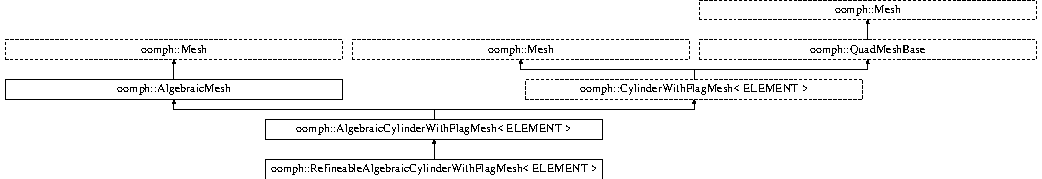
\includegraphics[height=1.924399cm]{classoomph_1_1AlgebraicCylinderWithFlagMesh}
\end{center}
\end{figure}
\subsection*{Public Member Functions}
\begin{DoxyCompactItemize}
\item 
\hyperlink{classoomph_1_1AlgebraicCylinderWithFlagMesh_a2c307b804fee56aa620ea414b41883d5}{Algebraic\+Cylinder\+With\+Flag\+Mesh} (Circle $\ast$cylinder\+\_\+pt, Geom\+Object $\ast$\hyperlink{classoomph_1_1AlgebraicCylinderWithFlagMesh_a06bc13adad4aaa037d989bba9e3bf79d}{top\+\_\+flag\+\_\+pt}, Geom\+Object $\ast$\hyperlink{classoomph_1_1AlgebraicCylinderWithFlagMesh_a9c362fcc5edeb1b6e773f27a83778495}{bottom\+\_\+flag\+\_\+pt}, Geom\+Object $\ast$\hyperlink{classoomph_1_1AlgebraicCylinderWithFlagMesh_ad6d22aaa02d79e3c740b06d98a1597ea}{tip\+\_\+flag\+\_\+pt}, const double \&length, const double \&height, const double \&flag\+\_\+length, const double \&flag\+\_\+height, const double \&centre\+\_\+x, const double \&centre\+\_\+y, const double \&a, Time\+Stepper $\ast$time\+\_\+stepper\+\_\+pt=\&Mesh\+::\+Default\+\_\+\+Time\+Stepper)
\begin{DoxyCompactList}\small\item\em Constructor. Pass the pointers to the Geom\+Objects that parametrise the cylinder, the three edges of the flag, the length and height of the domain, the length and height of the flag, the coordinates of the centre of the cylinder and its radius. Timestepper defaults to Steady default timestepper. \end{DoxyCompactList}\item 
virtual \hyperlink{classoomph_1_1AlgebraicCylinderWithFlagMesh_ac7e92a8dc3add0cd1f666dc8c9f8ca6f}{$\sim$\+Algebraic\+Cylinder\+With\+Flag\+Mesh} ()
\begin{DoxyCompactList}\small\item\em Destructor\+: empty. \end{DoxyCompactList}\item 
void \hyperlink{classoomph_1_1AlgebraicCylinderWithFlagMesh_a6aeef710528a9d8dd51023dd6ee131ea}{set\+\_\+bottom\+\_\+flag\+\_\+pt} (Geom\+Object $\ast$\hyperlink{classoomph_1_1AlgebraicCylinderWithFlagMesh_a9c362fcc5edeb1b6e773f27a83778495}{bottom\+\_\+flag\+\_\+pt})
\begin{DoxyCompactList}\small\item\em Set geometric object that defines the bottom face of the flag. \end{DoxyCompactList}\item 
void \hyperlink{classoomph_1_1AlgebraicCylinderWithFlagMesh_a9d7f04acdaed3e9f2133d9665dd4b799}{set\+\_\+top\+\_\+flag\+\_\+pt} (Geom\+Object $\ast$\hyperlink{classoomph_1_1AlgebraicCylinderWithFlagMesh_a06bc13adad4aaa037d989bba9e3bf79d}{top\+\_\+flag\+\_\+pt})
\begin{DoxyCompactList}\small\item\em Set the geometric object that defines the top face of the flag. \end{DoxyCompactList}\item 
void \hyperlink{classoomph_1_1AlgebraicCylinderWithFlagMesh_a191d736d9acbeb5927fc5f472420e9f6}{set\+\_\+tip\+\_\+flag\+\_\+pt} (Geom\+Object $\ast$\hyperlink{classoomph_1_1AlgebraicCylinderWithFlagMesh_ad6d22aaa02d79e3c740b06d98a1597ea}{tip\+\_\+flag\+\_\+pt})
\begin{DoxyCompactList}\small\item\em Set the geometric object that defines the tip of the flag. \end{DoxyCompactList}\item 
Geom\+Object $\ast$ \hyperlink{classoomph_1_1AlgebraicCylinderWithFlagMesh_a9c362fcc5edeb1b6e773f27a83778495}{bottom\+\_\+flag\+\_\+pt} () const
\begin{DoxyCompactList}\small\item\em Read-\/only access to geometric object that defines the bottom face of the flag. \end{DoxyCompactList}\item 
Geom\+Object $\ast$ \hyperlink{classoomph_1_1AlgebraicCylinderWithFlagMesh_a06bc13adad4aaa037d989bba9e3bf79d}{top\+\_\+flag\+\_\+pt} () const
\begin{DoxyCompactList}\small\item\em Read-\/only access to geometric object that defines the top face of the flag. \end{DoxyCompactList}\item 
Geom\+Object $\ast$ \hyperlink{classoomph_1_1AlgebraicCylinderWithFlagMesh_ad6d22aaa02d79e3c740b06d98a1597ea}{tip\+\_\+flag\+\_\+pt} () const
\begin{DoxyCompactList}\small\item\em Read-\/only access to geometric object that defines the tip of the flag. \end{DoxyCompactList}\item 
void \hyperlink{classoomph_1_1AlgebraicCylinderWithFlagMesh_a9d909de1db84a3b7e42494535b152d92}{update\+\_\+node\+\_\+update} (Algebraic\+Node $\ast$\&node\+\_\+pt)
\begin{DoxyCompactList}\small\item\em Update the geometric references that are used to update node after mesh adaptation. Empty -- no update of node update required without adaptativity. \end{DoxyCompactList}\item 
void \hyperlink{classoomph_1_1AlgebraicCylinderWithFlagMesh_a5e1e770e82577e5702470d8b87f8599d}{algebraic\+\_\+node\+\_\+update} (const unsigned \&t, Algebraic\+Node $\ast$\&node\+\_\+pt)
\begin{DoxyCompactList}\small\item\em Update nodal position at time level t (t=0\+: present;. \end{DoxyCompactList}\end{DoxyCompactItemize}
\subsection*{Protected Member Functions}
\begin{DoxyCompactItemize}
\item 
void \hyperlink{classoomph_1_1AlgebraicCylinderWithFlagMesh_ad6af2e420e0f152a7fb055f25400a5d0}{setup\+\_\+algebraic\+\_\+node\+\_\+update} ()
\begin{DoxyCompactList}\small\item\em Function to setup the algebraic node update. \end{DoxyCompactList}\item 
void \hyperlink{classoomph_1_1AlgebraicCylinderWithFlagMesh_a713cf7c2e1be91eae2667dc3e1fd8644}{node\+\_\+update\+\_\+I} (const unsigned \&t, Algebraic\+Node $\ast$\&node\+\_\+pt)
\begin{DoxyCompactList}\small\item\em Helper function. \end{DoxyCompactList}\item 
void \hyperlink{classoomph_1_1AlgebraicCylinderWithFlagMesh_a2717b4ae70a9641c24becc8176410b3e}{node\+\_\+update\+\_\+\+II} (const unsigned \&t, Algebraic\+Node $\ast$\&node\+\_\+pt)
\begin{DoxyCompactList}\small\item\em Helper function. \end{DoxyCompactList}\item 
void \hyperlink{classoomph_1_1AlgebraicCylinderWithFlagMesh_a3e8c71cc3ab123864b4f999e612345ee}{node\+\_\+update\+\_\+\+I\+II} (const unsigned \&t, Algebraic\+Node $\ast$\&node\+\_\+pt)
\begin{DoxyCompactList}\small\item\em Helper function. \end{DoxyCompactList}\item 
void \hyperlink{classoomph_1_1AlgebraicCylinderWithFlagMesh_a69ab465aa28dd9a65a0c50762c0a6d89}{node\+\_\+update\+\_\+\+IV} (const unsigned \&t, Algebraic\+Node $\ast$\&node\+\_\+pt)
\begin{DoxyCompactList}\small\item\em Helper function. \end{DoxyCompactList}\item 
void \hyperlink{classoomph_1_1AlgebraicCylinderWithFlagMesh_a035216f13c9758881ce2b7e33ad27926}{node\+\_\+update\+\_\+V} (const unsigned \&t, Algebraic\+Node $\ast$\&node\+\_\+pt)
\begin{DoxyCompactList}\small\item\em Helper function. \end{DoxyCompactList}\item 
void \hyperlink{classoomph_1_1AlgebraicCylinderWithFlagMesh_a989fe557f03ac20812e69a8de2dbb9a4}{node\+\_\+update\+\_\+\+VI} (const unsigned \&t, Algebraic\+Node $\ast$\&node\+\_\+pt)
\begin{DoxyCompactList}\small\item\em Helper function. \end{DoxyCompactList}\item 
void \hyperlink{classoomph_1_1AlgebraicCylinderWithFlagMesh_abb0565f0624583d2549f38602fd11e48}{node\+\_\+update\+\_\+\+V\+II} (const unsigned \&t, Algebraic\+Node $\ast$\&node\+\_\+pt)
\begin{DoxyCompactList}\small\item\em Helper function. \end{DoxyCompactList}\item 
void \hyperlink{classoomph_1_1AlgebraicCylinderWithFlagMesh_a85336e587d9c4cac7f4d77890dd7690b}{node\+\_\+update\+\_\+\+V\+I\+II} (const unsigned \&t, Algebraic\+Node $\ast$\&node\+\_\+pt)
\begin{DoxyCompactList}\small\item\em Helper function. \end{DoxyCompactList}\item 
void \hyperlink{classoomph_1_1AlgebraicCylinderWithFlagMesh_ae8e85400abd282b64463b67e21e9c13a}{node\+\_\+update\+\_\+\+IX} (const unsigned \&t, Algebraic\+Node $\ast$\&node\+\_\+pt)
\begin{DoxyCompactList}\small\item\em Helper function. \end{DoxyCompactList}\end{DoxyCompactItemize}
\subsection*{Protected Attributes}
\begin{DoxyCompactItemize}
\item 
Geom\+Object $\ast$ \hyperlink{classoomph_1_1AlgebraicCylinderWithFlagMesh_a423d4aa7ffcca5e707b2e5d820984957}{Cylinder\+\_\+pt}
\begin{DoxyCompactList}\small\item\em Cylinder. \end{DoxyCompactList}\item 
Geom\+Object $\ast$ \hyperlink{classoomph_1_1AlgebraicCylinderWithFlagMesh_a326e4789fe96b3052a8beb51ec9e94d0}{Top\+\_\+flag\+\_\+pt}
\begin{DoxyCompactList}\small\item\em Top flag. \end{DoxyCompactList}\item 
Geom\+Object $\ast$ \hyperlink{classoomph_1_1AlgebraicCylinderWithFlagMesh_ac1f7e1ba183ba813229302c5688ea1ba}{Bottom\+\_\+flag\+\_\+pt}
\begin{DoxyCompactList}\small\item\em Bottom flag. \end{DoxyCompactList}\item 
Geom\+Object $\ast$ \hyperlink{classoomph_1_1AlgebraicCylinderWithFlagMesh_ad22c8bfa595f4b1f129be85a1904762f}{Tip\+\_\+flag\+\_\+pt}
\begin{DoxyCompactList}\small\item\em Tip flag. \end{DoxyCompactList}\item 
double \hyperlink{classoomph_1_1AlgebraicCylinderWithFlagMesh_a7620fa5a4c36f638fb22c81b346b74a2}{Length}
\begin{DoxyCompactList}\small\item\em Length of the domain. \end{DoxyCompactList}\item 
double \hyperlink{classoomph_1_1AlgebraicCylinderWithFlagMesh_a29a0c970a11d46bdf03f3b5053d3ece2}{Height}
\begin{DoxyCompactList}\small\item\em Height of the domain. \end{DoxyCompactList}\item 
double \hyperlink{classoomph_1_1AlgebraicCylinderWithFlagMesh_a822ed90585320576084667f88c236396}{Flag\+\_\+length}
\begin{DoxyCompactList}\small\item\em Flag length. \end{DoxyCompactList}\item 
double \hyperlink{classoomph_1_1AlgebraicCylinderWithFlagMesh_a76a19a39dd500d5a48c10baae59797e0}{Flag\+\_\+height}
\begin{DoxyCompactList}\small\item\em Flag thickness. \end{DoxyCompactList}\item 
double \hyperlink{classoomph_1_1AlgebraicCylinderWithFlagMesh_a3290ac9103e43f4a4a997fe4692b6506}{Centre\+\_\+x}
\begin{DoxyCompactList}\small\item\em x position of the centre of the cylinder \end{DoxyCompactList}\item 
double \hyperlink{classoomph_1_1AlgebraicCylinderWithFlagMesh_a6b4575a9c3818e04bdb00d4150d49290}{Centre\+\_\+y}
\begin{DoxyCompactList}\small\item\em x position of the centre of the cylinder \end{DoxyCompactList}\item 
double \hyperlink{classoomph_1_1AlgebraicCylinderWithFlagMesh_aabc6cdfe508f04a4b1c92f2c2f1639c4}{A}
\begin{DoxyCompactList}\small\item\em radius of the cylinder \end{DoxyCompactList}\end{DoxyCompactItemize}


\subsection{Detailed Description}
\subsubsection*{template$<$class E\+L\+E\+M\+E\+NT$>$\newline
class oomph\+::\+Algebraic\+Cylinder\+With\+Flag\+Mesh$<$ E\+L\+E\+M\+E\+N\+T $>$}

Algebraic version of \hyperlink{classoomph_1_1CylinderWithFlagMesh}{Cylinder\+With\+Flag\+Mesh}. 

Definition at line 161 of file cylinder\+\_\+with\+\_\+flag\+\_\+mesh.\+template.\+h.



\subsection{Constructor \& Destructor Documentation}
\mbox{\Hypertarget{classoomph_1_1AlgebraicCylinderWithFlagMesh_a2c307b804fee56aa620ea414b41883d5}\label{classoomph_1_1AlgebraicCylinderWithFlagMesh_a2c307b804fee56aa620ea414b41883d5}} 
\index{oomph\+::\+Algebraic\+Cylinder\+With\+Flag\+Mesh@{oomph\+::\+Algebraic\+Cylinder\+With\+Flag\+Mesh}!Algebraic\+Cylinder\+With\+Flag\+Mesh@{Algebraic\+Cylinder\+With\+Flag\+Mesh}}
\index{Algebraic\+Cylinder\+With\+Flag\+Mesh@{Algebraic\+Cylinder\+With\+Flag\+Mesh}!oomph\+::\+Algebraic\+Cylinder\+With\+Flag\+Mesh@{oomph\+::\+Algebraic\+Cylinder\+With\+Flag\+Mesh}}
\subsubsection{\texorpdfstring{Algebraic\+Cylinder\+With\+Flag\+Mesh()}{AlgebraicCylinderWithFlagMesh()}}
{\footnotesize\ttfamily template$<$class E\+L\+E\+M\+E\+NT $>$ \\
\hyperlink{classoomph_1_1AlgebraicCylinderWithFlagMesh}{oomph\+::\+Algebraic\+Cylinder\+With\+Flag\+Mesh}$<$ E\+L\+E\+M\+E\+NT $>$\+::\hyperlink{classoomph_1_1AlgebraicCylinderWithFlagMesh}{Algebraic\+Cylinder\+With\+Flag\+Mesh} (\begin{DoxyParamCaption}\item[{Circle $\ast$}]{cylinder\+\_\+pt,  }\item[{Geom\+Object $\ast$}]{top\+\_\+flag\+\_\+pt,  }\item[{Geom\+Object $\ast$}]{bottom\+\_\+flag\+\_\+pt,  }\item[{Geom\+Object $\ast$}]{tip\+\_\+flag\+\_\+pt,  }\item[{const double \&}]{length,  }\item[{const double \&}]{height,  }\item[{const double \&}]{flag\+\_\+length,  }\item[{const double \&}]{flag\+\_\+height,  }\item[{const double \&}]{centre\+\_\+x,  }\item[{const double \&}]{centre\+\_\+y,  }\item[{const double \&}]{a,  }\item[{Time\+Stepper $\ast$}]{time\+\_\+stepper\+\_\+pt = {\ttfamily \&Mesh\+:\+:Default\+\_\+TimeStepper} }\end{DoxyParamCaption})\hspace{0.3cm}{\ttfamily [inline]}}



Constructor. Pass the pointers to the Geom\+Objects that parametrise the cylinder, the three edges of the flag, the length and height of the domain, the length and height of the flag, the coordinates of the centre of the cylinder and its radius. Timestepper defaults to Steady default timestepper. 



Definition at line 172 of file cylinder\+\_\+with\+\_\+flag\+\_\+mesh.\+template.\+h.

\mbox{\Hypertarget{classoomph_1_1AlgebraicCylinderWithFlagMesh_ac7e92a8dc3add0cd1f666dc8c9f8ca6f}\label{classoomph_1_1AlgebraicCylinderWithFlagMesh_ac7e92a8dc3add0cd1f666dc8c9f8ca6f}} 
\index{oomph\+::\+Algebraic\+Cylinder\+With\+Flag\+Mesh@{oomph\+::\+Algebraic\+Cylinder\+With\+Flag\+Mesh}!````~Algebraic\+Cylinder\+With\+Flag\+Mesh@{$\sim$\+Algebraic\+Cylinder\+With\+Flag\+Mesh}}
\index{````~Algebraic\+Cylinder\+With\+Flag\+Mesh@{$\sim$\+Algebraic\+Cylinder\+With\+Flag\+Mesh}!oomph\+::\+Algebraic\+Cylinder\+With\+Flag\+Mesh@{oomph\+::\+Algebraic\+Cylinder\+With\+Flag\+Mesh}}
\subsubsection{\texorpdfstring{$\sim$\+Algebraic\+Cylinder\+With\+Flag\+Mesh()}{~AlgebraicCylinderWithFlagMesh()}}
{\footnotesize\ttfamily template$<$class E\+L\+E\+M\+E\+NT $>$ \\
virtual \hyperlink{classoomph_1_1AlgebraicCylinderWithFlagMesh}{oomph\+::\+Algebraic\+Cylinder\+With\+Flag\+Mesh}$<$ E\+L\+E\+M\+E\+NT $>$\+::$\sim$\hyperlink{classoomph_1_1AlgebraicCylinderWithFlagMesh}{Algebraic\+Cylinder\+With\+Flag\+Mesh} (\begin{DoxyParamCaption}{ }\end{DoxyParamCaption})\hspace{0.3cm}{\ttfamily [inline]}, {\ttfamily [virtual]}}



Destructor\+: empty. 



Definition at line 205 of file cylinder\+\_\+with\+\_\+flag\+\_\+mesh.\+template.\+h.



\subsection{Member Function Documentation}
\mbox{\Hypertarget{classoomph_1_1AlgebraicCylinderWithFlagMesh_a5e1e770e82577e5702470d8b87f8599d}\label{classoomph_1_1AlgebraicCylinderWithFlagMesh_a5e1e770e82577e5702470d8b87f8599d}} 
\index{oomph\+::\+Algebraic\+Cylinder\+With\+Flag\+Mesh@{oomph\+::\+Algebraic\+Cylinder\+With\+Flag\+Mesh}!algebraic\+\_\+node\+\_\+update@{algebraic\+\_\+node\+\_\+update}}
\index{algebraic\+\_\+node\+\_\+update@{algebraic\+\_\+node\+\_\+update}!oomph\+::\+Algebraic\+Cylinder\+With\+Flag\+Mesh@{oomph\+::\+Algebraic\+Cylinder\+With\+Flag\+Mesh}}
\subsubsection{\texorpdfstring{algebraic\+\_\+node\+\_\+update()}{algebraic\_node\_update()}}
{\footnotesize\ttfamily template$<$class E\+L\+E\+M\+E\+NT $>$ \\
void \hyperlink{classoomph_1_1AlgebraicCylinderWithFlagMesh}{oomph\+::\+Algebraic\+Cylinder\+With\+Flag\+Mesh}$<$ E\+L\+E\+M\+E\+NT $>$\+::algebraic\+\_\+node\+\_\+update (\begin{DoxyParamCaption}\item[{const unsigned \&}]{t,  }\item[{Algebraic\+Node $\ast$\&}]{node\+\_\+pt }\end{DoxyParamCaption})}



Update nodal position at time level t (t=0\+: present;. 

The algebraic node update function.

t$>$0\+: previous) 

Definition at line 1367 of file cylinder\+\_\+with\+\_\+flag\+\_\+mesh.\+template.\+cc.

\mbox{\Hypertarget{classoomph_1_1AlgebraicCylinderWithFlagMesh_a9c362fcc5edeb1b6e773f27a83778495}\label{classoomph_1_1AlgebraicCylinderWithFlagMesh_a9c362fcc5edeb1b6e773f27a83778495}} 
\index{oomph\+::\+Algebraic\+Cylinder\+With\+Flag\+Mesh@{oomph\+::\+Algebraic\+Cylinder\+With\+Flag\+Mesh}!bottom\+\_\+flag\+\_\+pt@{bottom\+\_\+flag\+\_\+pt}}
\index{bottom\+\_\+flag\+\_\+pt@{bottom\+\_\+flag\+\_\+pt}!oomph\+::\+Algebraic\+Cylinder\+With\+Flag\+Mesh@{oomph\+::\+Algebraic\+Cylinder\+With\+Flag\+Mesh}}
\subsubsection{\texorpdfstring{bottom\+\_\+flag\+\_\+pt()}{bottom\_flag\_pt()}}
{\footnotesize\ttfamily template$<$class E\+L\+E\+M\+E\+NT $>$ \\
Geom\+Object$\ast$ \hyperlink{classoomph_1_1AlgebraicCylinderWithFlagMesh}{oomph\+::\+Algebraic\+Cylinder\+With\+Flag\+Mesh}$<$ E\+L\+E\+M\+E\+NT $>$\+::bottom\+\_\+flag\+\_\+pt (\begin{DoxyParamCaption}{ }\end{DoxyParamCaption}) const\hspace{0.3cm}{\ttfamily [inline]}}



Read-\/only access to geometric object that defines the bottom face of the flag. 



Definition at line 237 of file cylinder\+\_\+with\+\_\+flag\+\_\+mesh.\+template.\+h.

\mbox{\Hypertarget{classoomph_1_1AlgebraicCylinderWithFlagMesh_a713cf7c2e1be91eae2667dc3e1fd8644}\label{classoomph_1_1AlgebraicCylinderWithFlagMesh_a713cf7c2e1be91eae2667dc3e1fd8644}} 
\index{oomph\+::\+Algebraic\+Cylinder\+With\+Flag\+Mesh@{oomph\+::\+Algebraic\+Cylinder\+With\+Flag\+Mesh}!node\+\_\+update\+\_\+I@{node\+\_\+update\+\_\+I}}
\index{node\+\_\+update\+\_\+I@{node\+\_\+update\+\_\+I}!oomph\+::\+Algebraic\+Cylinder\+With\+Flag\+Mesh@{oomph\+::\+Algebraic\+Cylinder\+With\+Flag\+Mesh}}
\subsubsection{\texorpdfstring{node\+\_\+update\+\_\+\+I()}{node\_update\_I()}}
{\footnotesize\ttfamily template$<$class E\+L\+E\+M\+E\+NT $>$ \\
void \hyperlink{classoomph_1_1AlgebraicCylinderWithFlagMesh}{oomph\+::\+Algebraic\+Cylinder\+With\+Flag\+Mesh}$<$ E\+L\+E\+M\+E\+NT $>$\+::node\+\_\+update\+\_\+I (\begin{DoxyParamCaption}\item[{const unsigned \&}]{t,  }\item[{Algebraic\+Node $\ast$\&}]{node\+\_\+pt }\end{DoxyParamCaption})\hspace{0.3cm}{\ttfamily [protected]}}



Helper function. 

Node update for region I. 

Definition at line 1426 of file cylinder\+\_\+with\+\_\+flag\+\_\+mesh.\+template.\+cc.

\mbox{\Hypertarget{classoomph_1_1AlgebraicCylinderWithFlagMesh_a2717b4ae70a9641c24becc8176410b3e}\label{classoomph_1_1AlgebraicCylinderWithFlagMesh_a2717b4ae70a9641c24becc8176410b3e}} 
\index{oomph\+::\+Algebraic\+Cylinder\+With\+Flag\+Mesh@{oomph\+::\+Algebraic\+Cylinder\+With\+Flag\+Mesh}!node\+\_\+update\+\_\+\+II@{node\+\_\+update\+\_\+\+II}}
\index{node\+\_\+update\+\_\+\+II@{node\+\_\+update\+\_\+\+II}!oomph\+::\+Algebraic\+Cylinder\+With\+Flag\+Mesh@{oomph\+::\+Algebraic\+Cylinder\+With\+Flag\+Mesh}}
\subsubsection{\texorpdfstring{node\+\_\+update\+\_\+\+I\+I()}{node\_update\_II()}}
{\footnotesize\ttfamily template$<$class E\+L\+E\+M\+E\+NT $>$ \\
void \hyperlink{classoomph_1_1AlgebraicCylinderWithFlagMesh}{oomph\+::\+Algebraic\+Cylinder\+With\+Flag\+Mesh}$<$ E\+L\+E\+M\+E\+NT $>$\+::node\+\_\+update\+\_\+\+II (\begin{DoxyParamCaption}\item[{const unsigned \&}]{t,  }\item[{Algebraic\+Node $\ast$\&}]{node\+\_\+pt }\end{DoxyParamCaption})\hspace{0.3cm}{\ttfamily [protected]}}



Helper function. 

Node update for region II. 

Definition at line 1465 of file cylinder\+\_\+with\+\_\+flag\+\_\+mesh.\+template.\+cc.

\mbox{\Hypertarget{classoomph_1_1AlgebraicCylinderWithFlagMesh_a3e8c71cc3ab123864b4f999e612345ee}\label{classoomph_1_1AlgebraicCylinderWithFlagMesh_a3e8c71cc3ab123864b4f999e612345ee}} 
\index{oomph\+::\+Algebraic\+Cylinder\+With\+Flag\+Mesh@{oomph\+::\+Algebraic\+Cylinder\+With\+Flag\+Mesh}!node\+\_\+update\+\_\+\+I\+II@{node\+\_\+update\+\_\+\+I\+II}}
\index{node\+\_\+update\+\_\+\+I\+II@{node\+\_\+update\+\_\+\+I\+II}!oomph\+::\+Algebraic\+Cylinder\+With\+Flag\+Mesh@{oomph\+::\+Algebraic\+Cylinder\+With\+Flag\+Mesh}}
\subsubsection{\texorpdfstring{node\+\_\+update\+\_\+\+I\+I\+I()}{node\_update\_III()}}
{\footnotesize\ttfamily template$<$class E\+L\+E\+M\+E\+NT $>$ \\
void \hyperlink{classoomph_1_1AlgebraicCylinderWithFlagMesh}{oomph\+::\+Algebraic\+Cylinder\+With\+Flag\+Mesh}$<$ E\+L\+E\+M\+E\+NT $>$\+::node\+\_\+update\+\_\+\+I\+II (\begin{DoxyParamCaption}\item[{const unsigned \&}]{t,  }\item[{Algebraic\+Node $\ast$\&}]{node\+\_\+pt }\end{DoxyParamCaption})\hspace{0.3cm}{\ttfamily [protected]}}



Helper function. 

Node update for region I\+II. 

Definition at line 1501 of file cylinder\+\_\+with\+\_\+flag\+\_\+mesh.\+template.\+cc.

\mbox{\Hypertarget{classoomph_1_1AlgebraicCylinderWithFlagMesh_a69ab465aa28dd9a65a0c50762c0a6d89}\label{classoomph_1_1AlgebraicCylinderWithFlagMesh_a69ab465aa28dd9a65a0c50762c0a6d89}} 
\index{oomph\+::\+Algebraic\+Cylinder\+With\+Flag\+Mesh@{oomph\+::\+Algebraic\+Cylinder\+With\+Flag\+Mesh}!node\+\_\+update\+\_\+\+IV@{node\+\_\+update\+\_\+\+IV}}
\index{node\+\_\+update\+\_\+\+IV@{node\+\_\+update\+\_\+\+IV}!oomph\+::\+Algebraic\+Cylinder\+With\+Flag\+Mesh@{oomph\+::\+Algebraic\+Cylinder\+With\+Flag\+Mesh}}
\subsubsection{\texorpdfstring{node\+\_\+update\+\_\+\+I\+V()}{node\_update\_IV()}}
{\footnotesize\ttfamily template$<$class E\+L\+E\+M\+E\+NT $>$ \\
void \hyperlink{classoomph_1_1AlgebraicCylinderWithFlagMesh}{oomph\+::\+Algebraic\+Cylinder\+With\+Flag\+Mesh}$<$ E\+L\+E\+M\+E\+NT $>$\+::node\+\_\+update\+\_\+\+IV (\begin{DoxyParamCaption}\item[{const unsigned \&}]{t,  }\item[{Algebraic\+Node $\ast$\&}]{node\+\_\+pt }\end{DoxyParamCaption})\hspace{0.3cm}{\ttfamily [protected]}}



Helper function. 

Node update for region IV. 

Definition at line 1549 of file cylinder\+\_\+with\+\_\+flag\+\_\+mesh.\+template.\+cc.

\mbox{\Hypertarget{classoomph_1_1AlgebraicCylinderWithFlagMesh_ae8e85400abd282b64463b67e21e9c13a}\label{classoomph_1_1AlgebraicCylinderWithFlagMesh_ae8e85400abd282b64463b67e21e9c13a}} 
\index{oomph\+::\+Algebraic\+Cylinder\+With\+Flag\+Mesh@{oomph\+::\+Algebraic\+Cylinder\+With\+Flag\+Mesh}!node\+\_\+update\+\_\+\+IX@{node\+\_\+update\+\_\+\+IX}}
\index{node\+\_\+update\+\_\+\+IX@{node\+\_\+update\+\_\+\+IX}!oomph\+::\+Algebraic\+Cylinder\+With\+Flag\+Mesh@{oomph\+::\+Algebraic\+Cylinder\+With\+Flag\+Mesh}}
\subsubsection{\texorpdfstring{node\+\_\+update\+\_\+\+I\+X()}{node\_update\_IX()}}
{\footnotesize\ttfamily template$<$class E\+L\+E\+M\+E\+NT $>$ \\
void \hyperlink{classoomph_1_1AlgebraicCylinderWithFlagMesh}{oomph\+::\+Algebraic\+Cylinder\+With\+Flag\+Mesh}$<$ E\+L\+E\+M\+E\+NT $>$\+::node\+\_\+update\+\_\+\+IX (\begin{DoxyParamCaption}\item[{const unsigned \&}]{t,  }\item[{Algebraic\+Node $\ast$\&}]{node\+\_\+pt }\end{DoxyParamCaption})\hspace{0.3cm}{\ttfamily [protected]}}



Helper function. 

Node update for region IX. Extreme angles on circle 

Definition at line 1816 of file cylinder\+\_\+with\+\_\+flag\+\_\+mesh.\+template.\+cc.

\mbox{\Hypertarget{classoomph_1_1AlgebraicCylinderWithFlagMesh_a035216f13c9758881ce2b7e33ad27926}\label{classoomph_1_1AlgebraicCylinderWithFlagMesh_a035216f13c9758881ce2b7e33ad27926}} 
\index{oomph\+::\+Algebraic\+Cylinder\+With\+Flag\+Mesh@{oomph\+::\+Algebraic\+Cylinder\+With\+Flag\+Mesh}!node\+\_\+update\+\_\+V@{node\+\_\+update\+\_\+V}}
\index{node\+\_\+update\+\_\+V@{node\+\_\+update\+\_\+V}!oomph\+::\+Algebraic\+Cylinder\+With\+Flag\+Mesh@{oomph\+::\+Algebraic\+Cylinder\+With\+Flag\+Mesh}}
\subsubsection{\texorpdfstring{node\+\_\+update\+\_\+\+V()}{node\_update\_V()}}
{\footnotesize\ttfamily template$<$class E\+L\+E\+M\+E\+NT $>$ \\
void \hyperlink{classoomph_1_1AlgebraicCylinderWithFlagMesh}{oomph\+::\+Algebraic\+Cylinder\+With\+Flag\+Mesh}$<$ E\+L\+E\+M\+E\+NT $>$\+::node\+\_\+update\+\_\+V (\begin{DoxyParamCaption}\item[{const unsigned \&}]{t,  }\item[{Algebraic\+Node $\ast$\&}]{node\+\_\+pt }\end{DoxyParamCaption})\hspace{0.3cm}{\ttfamily [protected]}}



Helper function. 

Node update for region V. 

Definition at line 1596 of file cylinder\+\_\+with\+\_\+flag\+\_\+mesh.\+template.\+cc.

\mbox{\Hypertarget{classoomph_1_1AlgebraicCylinderWithFlagMesh_a989fe557f03ac20812e69a8de2dbb9a4}\label{classoomph_1_1AlgebraicCylinderWithFlagMesh_a989fe557f03ac20812e69a8de2dbb9a4}} 
\index{oomph\+::\+Algebraic\+Cylinder\+With\+Flag\+Mesh@{oomph\+::\+Algebraic\+Cylinder\+With\+Flag\+Mesh}!node\+\_\+update\+\_\+\+VI@{node\+\_\+update\+\_\+\+VI}}
\index{node\+\_\+update\+\_\+\+VI@{node\+\_\+update\+\_\+\+VI}!oomph\+::\+Algebraic\+Cylinder\+With\+Flag\+Mesh@{oomph\+::\+Algebraic\+Cylinder\+With\+Flag\+Mesh}}
\subsubsection{\texorpdfstring{node\+\_\+update\+\_\+\+V\+I()}{node\_update\_VI()}}
{\footnotesize\ttfamily template$<$class E\+L\+E\+M\+E\+NT $>$ \\
void \hyperlink{classoomph_1_1AlgebraicCylinderWithFlagMesh}{oomph\+::\+Algebraic\+Cylinder\+With\+Flag\+Mesh}$<$ E\+L\+E\+M\+E\+NT $>$\+::node\+\_\+update\+\_\+\+VI (\begin{DoxyParamCaption}\item[{const unsigned \&}]{t,  }\item[{Algebraic\+Node $\ast$\&}]{node\+\_\+pt }\end{DoxyParamCaption})\hspace{0.3cm}{\ttfamily [protected]}}



Helper function. 

Node update for region VI. 

Definition at line 1645 of file cylinder\+\_\+with\+\_\+flag\+\_\+mesh.\+template.\+cc.

\mbox{\Hypertarget{classoomph_1_1AlgebraicCylinderWithFlagMesh_abb0565f0624583d2549f38602fd11e48}\label{classoomph_1_1AlgebraicCylinderWithFlagMesh_abb0565f0624583d2549f38602fd11e48}} 
\index{oomph\+::\+Algebraic\+Cylinder\+With\+Flag\+Mesh@{oomph\+::\+Algebraic\+Cylinder\+With\+Flag\+Mesh}!node\+\_\+update\+\_\+\+V\+II@{node\+\_\+update\+\_\+\+V\+II}}
\index{node\+\_\+update\+\_\+\+V\+II@{node\+\_\+update\+\_\+\+V\+II}!oomph\+::\+Algebraic\+Cylinder\+With\+Flag\+Mesh@{oomph\+::\+Algebraic\+Cylinder\+With\+Flag\+Mesh}}
\subsubsection{\texorpdfstring{node\+\_\+update\+\_\+\+V\+I\+I()}{node\_update\_VII()}}
{\footnotesize\ttfamily template$<$class E\+L\+E\+M\+E\+NT $>$ \\
void \hyperlink{classoomph_1_1AlgebraicCylinderWithFlagMesh}{oomph\+::\+Algebraic\+Cylinder\+With\+Flag\+Mesh}$<$ E\+L\+E\+M\+E\+NT $>$\+::node\+\_\+update\+\_\+\+V\+II (\begin{DoxyParamCaption}\item[{const unsigned \&}]{t,  }\item[{Algebraic\+Node $\ast$\&}]{node\+\_\+pt }\end{DoxyParamCaption})\hspace{0.3cm}{\ttfamily [protected]}}



Helper function. 

Node update for region V\+II. 

Definition at line 1688 of file cylinder\+\_\+with\+\_\+flag\+\_\+mesh.\+template.\+cc.

\mbox{\Hypertarget{classoomph_1_1AlgebraicCylinderWithFlagMesh_a85336e587d9c4cac7f4d77890dd7690b}\label{classoomph_1_1AlgebraicCylinderWithFlagMesh_a85336e587d9c4cac7f4d77890dd7690b}} 
\index{oomph\+::\+Algebraic\+Cylinder\+With\+Flag\+Mesh@{oomph\+::\+Algebraic\+Cylinder\+With\+Flag\+Mesh}!node\+\_\+update\+\_\+\+V\+I\+II@{node\+\_\+update\+\_\+\+V\+I\+II}}
\index{node\+\_\+update\+\_\+\+V\+I\+II@{node\+\_\+update\+\_\+\+V\+I\+II}!oomph\+::\+Algebraic\+Cylinder\+With\+Flag\+Mesh@{oomph\+::\+Algebraic\+Cylinder\+With\+Flag\+Mesh}}
\subsubsection{\texorpdfstring{node\+\_\+update\+\_\+\+V\+I\+I\+I()}{node\_update\_VIII()}}
{\footnotesize\ttfamily template$<$class E\+L\+E\+M\+E\+NT $>$ \\
void \hyperlink{classoomph_1_1AlgebraicCylinderWithFlagMesh}{oomph\+::\+Algebraic\+Cylinder\+With\+Flag\+Mesh}$<$ E\+L\+E\+M\+E\+NT $>$\+::node\+\_\+update\+\_\+\+V\+I\+II (\begin{DoxyParamCaption}\item[{const unsigned \&}]{t,  }\item[{Algebraic\+Node $\ast$\&}]{node\+\_\+pt }\end{DoxyParamCaption})\hspace{0.3cm}{\ttfamily [protected]}}



Helper function. 

Node update for region V\+I\+II. Extreme angles on circle 

Definition at line 1732 of file cylinder\+\_\+with\+\_\+flag\+\_\+mesh.\+template.\+cc.

\mbox{\Hypertarget{classoomph_1_1AlgebraicCylinderWithFlagMesh_a6aeef710528a9d8dd51023dd6ee131ea}\label{classoomph_1_1AlgebraicCylinderWithFlagMesh_a6aeef710528a9d8dd51023dd6ee131ea}} 
\index{oomph\+::\+Algebraic\+Cylinder\+With\+Flag\+Mesh@{oomph\+::\+Algebraic\+Cylinder\+With\+Flag\+Mesh}!set\+\_\+bottom\+\_\+flag\+\_\+pt@{set\+\_\+bottom\+\_\+flag\+\_\+pt}}
\index{set\+\_\+bottom\+\_\+flag\+\_\+pt@{set\+\_\+bottom\+\_\+flag\+\_\+pt}!oomph\+::\+Algebraic\+Cylinder\+With\+Flag\+Mesh@{oomph\+::\+Algebraic\+Cylinder\+With\+Flag\+Mesh}}
\subsubsection{\texorpdfstring{set\+\_\+bottom\+\_\+flag\+\_\+pt()}{set\_bottom\_flag\_pt()}}
{\footnotesize\ttfamily template$<$class E\+L\+E\+M\+E\+NT $>$ \\
void \hyperlink{classoomph_1_1AlgebraicCylinderWithFlagMesh}{oomph\+::\+Algebraic\+Cylinder\+With\+Flag\+Mesh}$<$ E\+L\+E\+M\+E\+NT $>$\+::set\+\_\+bottom\+\_\+flag\+\_\+pt (\begin{DoxyParamCaption}\item[{Geom\+Object $\ast$}]{bottom\+\_\+flag\+\_\+pt }\end{DoxyParamCaption})\hspace{0.3cm}{\ttfamily [inline]}}



Set geometric object that defines the bottom face of the flag. 



Definition at line 210 of file cylinder\+\_\+with\+\_\+flag\+\_\+mesh.\+template.\+h.



References oomph\+::\+Cylinder\+With\+Flag\+Domain\+::bottom\+\_\+flag\+\_\+pt(), and oomph\+::\+Cylinder\+With\+Flag\+Mesh$<$ E\+L\+E\+M\+E\+N\+T $>$\+::domain\+\_\+pt().

\mbox{\Hypertarget{classoomph_1_1AlgebraicCylinderWithFlagMesh_a191d736d9acbeb5927fc5f472420e9f6}\label{classoomph_1_1AlgebraicCylinderWithFlagMesh_a191d736d9acbeb5927fc5f472420e9f6}} 
\index{oomph\+::\+Algebraic\+Cylinder\+With\+Flag\+Mesh@{oomph\+::\+Algebraic\+Cylinder\+With\+Flag\+Mesh}!set\+\_\+tip\+\_\+flag\+\_\+pt@{set\+\_\+tip\+\_\+flag\+\_\+pt}}
\index{set\+\_\+tip\+\_\+flag\+\_\+pt@{set\+\_\+tip\+\_\+flag\+\_\+pt}!oomph\+::\+Algebraic\+Cylinder\+With\+Flag\+Mesh@{oomph\+::\+Algebraic\+Cylinder\+With\+Flag\+Mesh}}
\subsubsection{\texorpdfstring{set\+\_\+tip\+\_\+flag\+\_\+pt()}{set\_tip\_flag\_pt()}}
{\footnotesize\ttfamily template$<$class E\+L\+E\+M\+E\+NT $>$ \\
void \hyperlink{classoomph_1_1AlgebraicCylinderWithFlagMesh}{oomph\+::\+Algebraic\+Cylinder\+With\+Flag\+Mesh}$<$ E\+L\+E\+M\+E\+NT $>$\+::set\+\_\+tip\+\_\+flag\+\_\+pt (\begin{DoxyParamCaption}\item[{Geom\+Object $\ast$}]{tip\+\_\+flag\+\_\+pt }\end{DoxyParamCaption})\hspace{0.3cm}{\ttfamily [inline]}}



Set the geometric object that defines the tip of the flag. 



Definition at line 228 of file cylinder\+\_\+with\+\_\+flag\+\_\+mesh.\+template.\+h.



References oomph\+::\+Cylinder\+With\+Flag\+Mesh$<$ E\+L\+E\+M\+E\+N\+T $>$\+::domain\+\_\+pt(), and oomph\+::\+Cylinder\+With\+Flag\+Domain\+::tip\+\_\+flag\+\_\+pt().

\mbox{\Hypertarget{classoomph_1_1AlgebraicCylinderWithFlagMesh_a9d7f04acdaed3e9f2133d9665dd4b799}\label{classoomph_1_1AlgebraicCylinderWithFlagMesh_a9d7f04acdaed3e9f2133d9665dd4b799}} 
\index{oomph\+::\+Algebraic\+Cylinder\+With\+Flag\+Mesh@{oomph\+::\+Algebraic\+Cylinder\+With\+Flag\+Mesh}!set\+\_\+top\+\_\+flag\+\_\+pt@{set\+\_\+top\+\_\+flag\+\_\+pt}}
\index{set\+\_\+top\+\_\+flag\+\_\+pt@{set\+\_\+top\+\_\+flag\+\_\+pt}!oomph\+::\+Algebraic\+Cylinder\+With\+Flag\+Mesh@{oomph\+::\+Algebraic\+Cylinder\+With\+Flag\+Mesh}}
\subsubsection{\texorpdfstring{set\+\_\+top\+\_\+flag\+\_\+pt()}{set\_top\_flag\_pt()}}
{\footnotesize\ttfamily template$<$class E\+L\+E\+M\+E\+NT $>$ \\
void \hyperlink{classoomph_1_1AlgebraicCylinderWithFlagMesh}{oomph\+::\+Algebraic\+Cylinder\+With\+Flag\+Mesh}$<$ E\+L\+E\+M\+E\+NT $>$\+::set\+\_\+top\+\_\+flag\+\_\+pt (\begin{DoxyParamCaption}\item[{Geom\+Object $\ast$}]{top\+\_\+flag\+\_\+pt }\end{DoxyParamCaption})\hspace{0.3cm}{\ttfamily [inline]}}



Set the geometric object that defines the top face of the flag. 



Definition at line 219 of file cylinder\+\_\+with\+\_\+flag\+\_\+mesh.\+template.\+h.



References oomph\+::\+Cylinder\+With\+Flag\+Mesh$<$ E\+L\+E\+M\+E\+N\+T $>$\+::domain\+\_\+pt(), and oomph\+::\+Cylinder\+With\+Flag\+Domain\+::top\+\_\+flag\+\_\+pt().

\mbox{\Hypertarget{classoomph_1_1AlgebraicCylinderWithFlagMesh_ad6af2e420e0f152a7fb055f25400a5d0}\label{classoomph_1_1AlgebraicCylinderWithFlagMesh_ad6af2e420e0f152a7fb055f25400a5d0}} 
\index{oomph\+::\+Algebraic\+Cylinder\+With\+Flag\+Mesh@{oomph\+::\+Algebraic\+Cylinder\+With\+Flag\+Mesh}!setup\+\_\+algebraic\+\_\+node\+\_\+update@{setup\+\_\+algebraic\+\_\+node\+\_\+update}}
\index{setup\+\_\+algebraic\+\_\+node\+\_\+update@{setup\+\_\+algebraic\+\_\+node\+\_\+update}!oomph\+::\+Algebraic\+Cylinder\+With\+Flag\+Mesh@{oomph\+::\+Algebraic\+Cylinder\+With\+Flag\+Mesh}}
\subsubsection{\texorpdfstring{setup\+\_\+algebraic\+\_\+node\+\_\+update()}{setup\_algebraic\_node\_update()}}
{\footnotesize\ttfamily template$<$class E\+L\+E\+M\+E\+NT $>$ \\
void \hyperlink{classoomph_1_1AlgebraicCylinderWithFlagMesh}{oomph\+::\+Algebraic\+Cylinder\+With\+Flag\+Mesh}$<$ E\+L\+E\+M\+E\+NT $>$\+::setup\+\_\+algebraic\+\_\+node\+\_\+update (\begin{DoxyParamCaption}{ }\end{DoxyParamCaption})\hspace{0.3cm}{\ttfamily [protected]}}



Function to setup the algebraic node update. 

Setup algebraic node update. set the size ?? 

Definition at line 935 of file cylinder\+\_\+with\+\_\+flag\+\_\+mesh.\+template.\+cc.

\mbox{\Hypertarget{classoomph_1_1AlgebraicCylinderWithFlagMesh_ad6d22aaa02d79e3c740b06d98a1597ea}\label{classoomph_1_1AlgebraicCylinderWithFlagMesh_ad6d22aaa02d79e3c740b06d98a1597ea}} 
\index{oomph\+::\+Algebraic\+Cylinder\+With\+Flag\+Mesh@{oomph\+::\+Algebraic\+Cylinder\+With\+Flag\+Mesh}!tip\+\_\+flag\+\_\+pt@{tip\+\_\+flag\+\_\+pt}}
\index{tip\+\_\+flag\+\_\+pt@{tip\+\_\+flag\+\_\+pt}!oomph\+::\+Algebraic\+Cylinder\+With\+Flag\+Mesh@{oomph\+::\+Algebraic\+Cylinder\+With\+Flag\+Mesh}}
\subsubsection{\texorpdfstring{tip\+\_\+flag\+\_\+pt()}{tip\_flag\_pt()}}
{\footnotesize\ttfamily template$<$class E\+L\+E\+M\+E\+NT $>$ \\
Geom\+Object$\ast$ \hyperlink{classoomph_1_1AlgebraicCylinderWithFlagMesh}{oomph\+::\+Algebraic\+Cylinder\+With\+Flag\+Mesh}$<$ E\+L\+E\+M\+E\+NT $>$\+::tip\+\_\+flag\+\_\+pt (\begin{DoxyParamCaption}{ }\end{DoxyParamCaption}) const\hspace{0.3cm}{\ttfamily [inline]}}



Read-\/only access to geometric object that defines the tip of the flag. 



Definition at line 252 of file cylinder\+\_\+with\+\_\+flag\+\_\+mesh.\+template.\+h.

\mbox{\Hypertarget{classoomph_1_1AlgebraicCylinderWithFlagMesh_a06bc13adad4aaa037d989bba9e3bf79d}\label{classoomph_1_1AlgebraicCylinderWithFlagMesh_a06bc13adad4aaa037d989bba9e3bf79d}} 
\index{oomph\+::\+Algebraic\+Cylinder\+With\+Flag\+Mesh@{oomph\+::\+Algebraic\+Cylinder\+With\+Flag\+Mesh}!top\+\_\+flag\+\_\+pt@{top\+\_\+flag\+\_\+pt}}
\index{top\+\_\+flag\+\_\+pt@{top\+\_\+flag\+\_\+pt}!oomph\+::\+Algebraic\+Cylinder\+With\+Flag\+Mesh@{oomph\+::\+Algebraic\+Cylinder\+With\+Flag\+Mesh}}
\subsubsection{\texorpdfstring{top\+\_\+flag\+\_\+pt()}{top\_flag\_pt()}}
{\footnotesize\ttfamily template$<$class E\+L\+E\+M\+E\+NT $>$ \\
Geom\+Object$\ast$ \hyperlink{classoomph_1_1AlgebraicCylinderWithFlagMesh}{oomph\+::\+Algebraic\+Cylinder\+With\+Flag\+Mesh}$<$ E\+L\+E\+M\+E\+NT $>$\+::top\+\_\+flag\+\_\+pt (\begin{DoxyParamCaption}{ }\end{DoxyParamCaption}) const\hspace{0.3cm}{\ttfamily [inline]}}



Read-\/only access to geometric object that defines the top face of the flag. 



Definition at line 245 of file cylinder\+\_\+with\+\_\+flag\+\_\+mesh.\+template.\+h.

\mbox{\Hypertarget{classoomph_1_1AlgebraicCylinderWithFlagMesh_a9d909de1db84a3b7e42494535b152d92}\label{classoomph_1_1AlgebraicCylinderWithFlagMesh_a9d909de1db84a3b7e42494535b152d92}} 
\index{oomph\+::\+Algebraic\+Cylinder\+With\+Flag\+Mesh@{oomph\+::\+Algebraic\+Cylinder\+With\+Flag\+Mesh}!update\+\_\+node\+\_\+update@{update\+\_\+node\+\_\+update}}
\index{update\+\_\+node\+\_\+update@{update\+\_\+node\+\_\+update}!oomph\+::\+Algebraic\+Cylinder\+With\+Flag\+Mesh@{oomph\+::\+Algebraic\+Cylinder\+With\+Flag\+Mesh}}
\subsubsection{\texorpdfstring{update\+\_\+node\+\_\+update()}{update\_node\_update()}}
{\footnotesize\ttfamily template$<$class E\+L\+E\+M\+E\+NT $>$ \\
void \hyperlink{classoomph_1_1AlgebraicCylinderWithFlagMesh}{oomph\+::\+Algebraic\+Cylinder\+With\+Flag\+Mesh}$<$ E\+L\+E\+M\+E\+NT $>$\+::update\+\_\+node\+\_\+update (\begin{DoxyParamCaption}\item[{Algebraic\+Node $\ast$\&}]{node\+\_\+pt }\end{DoxyParamCaption})\hspace{0.3cm}{\ttfamily [inline]}}



Update the geometric references that are used to update node after mesh adaptation. Empty -- no update of node update required without adaptativity. 



Definition at line 261 of file cylinder\+\_\+with\+\_\+flag\+\_\+mesh.\+template.\+h.



\subsection{Member Data Documentation}
\mbox{\Hypertarget{classoomph_1_1AlgebraicCylinderWithFlagMesh_aabc6cdfe508f04a4b1c92f2c2f1639c4}\label{classoomph_1_1AlgebraicCylinderWithFlagMesh_aabc6cdfe508f04a4b1c92f2c2f1639c4}} 
\index{oomph\+::\+Algebraic\+Cylinder\+With\+Flag\+Mesh@{oomph\+::\+Algebraic\+Cylinder\+With\+Flag\+Mesh}!A@{A}}
\index{A@{A}!oomph\+::\+Algebraic\+Cylinder\+With\+Flag\+Mesh@{oomph\+::\+Algebraic\+Cylinder\+With\+Flag\+Mesh}}
\subsubsection{\texorpdfstring{A}{A}}
{\footnotesize\ttfamily template$<$class E\+L\+E\+M\+E\+NT $>$ \\
double \hyperlink{classoomph_1_1AlgebraicCylinderWithFlagMesh}{oomph\+::\+Algebraic\+Cylinder\+With\+Flag\+Mesh}$<$ E\+L\+E\+M\+E\+NT $>$\+::A\hspace{0.3cm}{\ttfamily [protected]}}



radius of the cylinder 



Definition at line 331 of file cylinder\+\_\+with\+\_\+flag\+\_\+mesh.\+template.\+h.

\mbox{\Hypertarget{classoomph_1_1AlgebraicCylinderWithFlagMesh_ac1f7e1ba183ba813229302c5688ea1ba}\label{classoomph_1_1AlgebraicCylinderWithFlagMesh_ac1f7e1ba183ba813229302c5688ea1ba}} 
\index{oomph\+::\+Algebraic\+Cylinder\+With\+Flag\+Mesh@{oomph\+::\+Algebraic\+Cylinder\+With\+Flag\+Mesh}!Bottom\+\_\+flag\+\_\+pt@{Bottom\+\_\+flag\+\_\+pt}}
\index{Bottom\+\_\+flag\+\_\+pt@{Bottom\+\_\+flag\+\_\+pt}!oomph\+::\+Algebraic\+Cylinder\+With\+Flag\+Mesh@{oomph\+::\+Algebraic\+Cylinder\+With\+Flag\+Mesh}}
\subsubsection{\texorpdfstring{Bottom\+\_\+flag\+\_\+pt}{Bottom\_flag\_pt}}
{\footnotesize\ttfamily template$<$class E\+L\+E\+M\+E\+NT $>$ \\
Geom\+Object$\ast$ \hyperlink{classoomph_1_1AlgebraicCylinderWithFlagMesh}{oomph\+::\+Algebraic\+Cylinder\+With\+Flag\+Mesh}$<$ E\+L\+E\+M\+E\+NT $>$\+::Bottom\+\_\+flag\+\_\+pt\hspace{0.3cm}{\ttfamily [protected]}}



Bottom flag. 



Definition at line 307 of file cylinder\+\_\+with\+\_\+flag\+\_\+mesh.\+template.\+h.

\mbox{\Hypertarget{classoomph_1_1AlgebraicCylinderWithFlagMesh_a3290ac9103e43f4a4a997fe4692b6506}\label{classoomph_1_1AlgebraicCylinderWithFlagMesh_a3290ac9103e43f4a4a997fe4692b6506}} 
\index{oomph\+::\+Algebraic\+Cylinder\+With\+Flag\+Mesh@{oomph\+::\+Algebraic\+Cylinder\+With\+Flag\+Mesh}!Centre\+\_\+x@{Centre\+\_\+x}}
\index{Centre\+\_\+x@{Centre\+\_\+x}!oomph\+::\+Algebraic\+Cylinder\+With\+Flag\+Mesh@{oomph\+::\+Algebraic\+Cylinder\+With\+Flag\+Mesh}}
\subsubsection{\texorpdfstring{Centre\+\_\+x}{Centre\_x}}
{\footnotesize\ttfamily template$<$class E\+L\+E\+M\+E\+NT $>$ \\
double \hyperlink{classoomph_1_1AlgebraicCylinderWithFlagMesh}{oomph\+::\+Algebraic\+Cylinder\+With\+Flag\+Mesh}$<$ E\+L\+E\+M\+E\+NT $>$\+::Centre\+\_\+x\hspace{0.3cm}{\ttfamily [protected]}}



x position of the centre of the cylinder 



Definition at line 325 of file cylinder\+\_\+with\+\_\+flag\+\_\+mesh.\+template.\+h.

\mbox{\Hypertarget{classoomph_1_1AlgebraicCylinderWithFlagMesh_a6b4575a9c3818e04bdb00d4150d49290}\label{classoomph_1_1AlgebraicCylinderWithFlagMesh_a6b4575a9c3818e04bdb00d4150d49290}} 
\index{oomph\+::\+Algebraic\+Cylinder\+With\+Flag\+Mesh@{oomph\+::\+Algebraic\+Cylinder\+With\+Flag\+Mesh}!Centre\+\_\+y@{Centre\+\_\+y}}
\index{Centre\+\_\+y@{Centre\+\_\+y}!oomph\+::\+Algebraic\+Cylinder\+With\+Flag\+Mesh@{oomph\+::\+Algebraic\+Cylinder\+With\+Flag\+Mesh}}
\subsubsection{\texorpdfstring{Centre\+\_\+y}{Centre\_y}}
{\footnotesize\ttfamily template$<$class E\+L\+E\+M\+E\+NT $>$ \\
double \hyperlink{classoomph_1_1AlgebraicCylinderWithFlagMesh}{oomph\+::\+Algebraic\+Cylinder\+With\+Flag\+Mesh}$<$ E\+L\+E\+M\+E\+NT $>$\+::Centre\+\_\+y\hspace{0.3cm}{\ttfamily [protected]}}



x position of the centre of the cylinder 



Definition at line 328 of file cylinder\+\_\+with\+\_\+flag\+\_\+mesh.\+template.\+h.

\mbox{\Hypertarget{classoomph_1_1AlgebraicCylinderWithFlagMesh_a423d4aa7ffcca5e707b2e5d820984957}\label{classoomph_1_1AlgebraicCylinderWithFlagMesh_a423d4aa7ffcca5e707b2e5d820984957}} 
\index{oomph\+::\+Algebraic\+Cylinder\+With\+Flag\+Mesh@{oomph\+::\+Algebraic\+Cylinder\+With\+Flag\+Mesh}!Cylinder\+\_\+pt@{Cylinder\+\_\+pt}}
\index{Cylinder\+\_\+pt@{Cylinder\+\_\+pt}!oomph\+::\+Algebraic\+Cylinder\+With\+Flag\+Mesh@{oomph\+::\+Algebraic\+Cylinder\+With\+Flag\+Mesh}}
\subsubsection{\texorpdfstring{Cylinder\+\_\+pt}{Cylinder\_pt}}
{\footnotesize\ttfamily template$<$class E\+L\+E\+M\+E\+NT $>$ \\
Geom\+Object$\ast$ \hyperlink{classoomph_1_1AlgebraicCylinderWithFlagMesh}{oomph\+::\+Algebraic\+Cylinder\+With\+Flag\+Mesh}$<$ E\+L\+E\+M\+E\+NT $>$\+::Cylinder\+\_\+pt\hspace{0.3cm}{\ttfamily [protected]}}



Cylinder. 



Definition at line 301 of file cylinder\+\_\+with\+\_\+flag\+\_\+mesh.\+template.\+h.

\mbox{\Hypertarget{classoomph_1_1AlgebraicCylinderWithFlagMesh_a76a19a39dd500d5a48c10baae59797e0}\label{classoomph_1_1AlgebraicCylinderWithFlagMesh_a76a19a39dd500d5a48c10baae59797e0}} 
\index{oomph\+::\+Algebraic\+Cylinder\+With\+Flag\+Mesh@{oomph\+::\+Algebraic\+Cylinder\+With\+Flag\+Mesh}!Flag\+\_\+height@{Flag\+\_\+height}}
\index{Flag\+\_\+height@{Flag\+\_\+height}!oomph\+::\+Algebraic\+Cylinder\+With\+Flag\+Mesh@{oomph\+::\+Algebraic\+Cylinder\+With\+Flag\+Mesh}}
\subsubsection{\texorpdfstring{Flag\+\_\+height}{Flag\_height}}
{\footnotesize\ttfamily template$<$class E\+L\+E\+M\+E\+NT $>$ \\
double \hyperlink{classoomph_1_1AlgebraicCylinderWithFlagMesh}{oomph\+::\+Algebraic\+Cylinder\+With\+Flag\+Mesh}$<$ E\+L\+E\+M\+E\+NT $>$\+::Flag\+\_\+height\hspace{0.3cm}{\ttfamily [protected]}}



Flag thickness. 



Definition at line 322 of file cylinder\+\_\+with\+\_\+flag\+\_\+mesh.\+template.\+h.

\mbox{\Hypertarget{classoomph_1_1AlgebraicCylinderWithFlagMesh_a822ed90585320576084667f88c236396}\label{classoomph_1_1AlgebraicCylinderWithFlagMesh_a822ed90585320576084667f88c236396}} 
\index{oomph\+::\+Algebraic\+Cylinder\+With\+Flag\+Mesh@{oomph\+::\+Algebraic\+Cylinder\+With\+Flag\+Mesh}!Flag\+\_\+length@{Flag\+\_\+length}}
\index{Flag\+\_\+length@{Flag\+\_\+length}!oomph\+::\+Algebraic\+Cylinder\+With\+Flag\+Mesh@{oomph\+::\+Algebraic\+Cylinder\+With\+Flag\+Mesh}}
\subsubsection{\texorpdfstring{Flag\+\_\+length}{Flag\_length}}
{\footnotesize\ttfamily template$<$class E\+L\+E\+M\+E\+NT $>$ \\
double \hyperlink{classoomph_1_1AlgebraicCylinderWithFlagMesh}{oomph\+::\+Algebraic\+Cylinder\+With\+Flag\+Mesh}$<$ E\+L\+E\+M\+E\+NT $>$\+::Flag\+\_\+length\hspace{0.3cm}{\ttfamily [protected]}}



Flag length. 



Definition at line 319 of file cylinder\+\_\+with\+\_\+flag\+\_\+mesh.\+template.\+h.

\mbox{\Hypertarget{classoomph_1_1AlgebraicCylinderWithFlagMesh_a29a0c970a11d46bdf03f3b5053d3ece2}\label{classoomph_1_1AlgebraicCylinderWithFlagMesh_a29a0c970a11d46bdf03f3b5053d3ece2}} 
\index{oomph\+::\+Algebraic\+Cylinder\+With\+Flag\+Mesh@{oomph\+::\+Algebraic\+Cylinder\+With\+Flag\+Mesh}!Height@{Height}}
\index{Height@{Height}!oomph\+::\+Algebraic\+Cylinder\+With\+Flag\+Mesh@{oomph\+::\+Algebraic\+Cylinder\+With\+Flag\+Mesh}}
\subsubsection{\texorpdfstring{Height}{Height}}
{\footnotesize\ttfamily template$<$class E\+L\+E\+M\+E\+NT $>$ \\
double \hyperlink{classoomph_1_1AlgebraicCylinderWithFlagMesh}{oomph\+::\+Algebraic\+Cylinder\+With\+Flag\+Mesh}$<$ E\+L\+E\+M\+E\+NT $>$\+::Height\hspace{0.3cm}{\ttfamily [protected]}}



Height of the domain. 



Definition at line 316 of file cylinder\+\_\+with\+\_\+flag\+\_\+mesh.\+template.\+h.

\mbox{\Hypertarget{classoomph_1_1AlgebraicCylinderWithFlagMesh_a7620fa5a4c36f638fb22c81b346b74a2}\label{classoomph_1_1AlgebraicCylinderWithFlagMesh_a7620fa5a4c36f638fb22c81b346b74a2}} 
\index{oomph\+::\+Algebraic\+Cylinder\+With\+Flag\+Mesh@{oomph\+::\+Algebraic\+Cylinder\+With\+Flag\+Mesh}!Length@{Length}}
\index{Length@{Length}!oomph\+::\+Algebraic\+Cylinder\+With\+Flag\+Mesh@{oomph\+::\+Algebraic\+Cylinder\+With\+Flag\+Mesh}}
\subsubsection{\texorpdfstring{Length}{Length}}
{\footnotesize\ttfamily template$<$class E\+L\+E\+M\+E\+NT $>$ \\
double \hyperlink{classoomph_1_1AlgebraicCylinderWithFlagMesh}{oomph\+::\+Algebraic\+Cylinder\+With\+Flag\+Mesh}$<$ E\+L\+E\+M\+E\+NT $>$\+::Length\hspace{0.3cm}{\ttfamily [protected]}}



Length of the domain. 



Definition at line 313 of file cylinder\+\_\+with\+\_\+flag\+\_\+mesh.\+template.\+h.

\mbox{\Hypertarget{classoomph_1_1AlgebraicCylinderWithFlagMesh_ad22c8bfa595f4b1f129be85a1904762f}\label{classoomph_1_1AlgebraicCylinderWithFlagMesh_ad22c8bfa595f4b1f129be85a1904762f}} 
\index{oomph\+::\+Algebraic\+Cylinder\+With\+Flag\+Mesh@{oomph\+::\+Algebraic\+Cylinder\+With\+Flag\+Mesh}!Tip\+\_\+flag\+\_\+pt@{Tip\+\_\+flag\+\_\+pt}}
\index{Tip\+\_\+flag\+\_\+pt@{Tip\+\_\+flag\+\_\+pt}!oomph\+::\+Algebraic\+Cylinder\+With\+Flag\+Mesh@{oomph\+::\+Algebraic\+Cylinder\+With\+Flag\+Mesh}}
\subsubsection{\texorpdfstring{Tip\+\_\+flag\+\_\+pt}{Tip\_flag\_pt}}
{\footnotesize\ttfamily template$<$class E\+L\+E\+M\+E\+NT $>$ \\
Geom\+Object$\ast$ \hyperlink{classoomph_1_1AlgebraicCylinderWithFlagMesh}{oomph\+::\+Algebraic\+Cylinder\+With\+Flag\+Mesh}$<$ E\+L\+E\+M\+E\+NT $>$\+::Tip\+\_\+flag\+\_\+pt\hspace{0.3cm}{\ttfamily [protected]}}



Tip flag. 



Definition at line 310 of file cylinder\+\_\+with\+\_\+flag\+\_\+mesh.\+template.\+h.

\mbox{\Hypertarget{classoomph_1_1AlgebraicCylinderWithFlagMesh_a326e4789fe96b3052a8beb51ec9e94d0}\label{classoomph_1_1AlgebraicCylinderWithFlagMesh_a326e4789fe96b3052a8beb51ec9e94d0}} 
\index{oomph\+::\+Algebraic\+Cylinder\+With\+Flag\+Mesh@{oomph\+::\+Algebraic\+Cylinder\+With\+Flag\+Mesh}!Top\+\_\+flag\+\_\+pt@{Top\+\_\+flag\+\_\+pt}}
\index{Top\+\_\+flag\+\_\+pt@{Top\+\_\+flag\+\_\+pt}!oomph\+::\+Algebraic\+Cylinder\+With\+Flag\+Mesh@{oomph\+::\+Algebraic\+Cylinder\+With\+Flag\+Mesh}}
\subsubsection{\texorpdfstring{Top\+\_\+flag\+\_\+pt}{Top\_flag\_pt}}
{\footnotesize\ttfamily template$<$class E\+L\+E\+M\+E\+NT $>$ \\
Geom\+Object$\ast$ \hyperlink{classoomph_1_1AlgebraicCylinderWithFlagMesh}{oomph\+::\+Algebraic\+Cylinder\+With\+Flag\+Mesh}$<$ E\+L\+E\+M\+E\+NT $>$\+::Top\+\_\+flag\+\_\+pt\hspace{0.3cm}{\ttfamily [protected]}}



Top flag. 



Definition at line 304 of file cylinder\+\_\+with\+\_\+flag\+\_\+mesh.\+template.\+h.



The documentation for this class was generated from the following files\+:\begin{DoxyCompactItemize}
\item 
\hyperlink{cylinder__with__flag__mesh_8template_8h}{cylinder\+\_\+with\+\_\+flag\+\_\+mesh.\+template.\+h}\item 
\hyperlink{cylinder__with__flag__mesh_8template_8cc}{cylinder\+\_\+with\+\_\+flag\+\_\+mesh.\+template.\+cc}\end{DoxyCompactItemize}

\hypertarget{classoomph_1_1AlgebraicElement}{}\section{oomph\+:\+:Algebraic\+Element$<$ E\+L\+E\+M\+E\+NT $>$ Class Template Reference}
\label{classoomph_1_1AlgebraicElement}\index{oomph\+::\+Algebraic\+Element$<$ E\+L\+E\+M\+E\+N\+T $>$@{oomph\+::\+Algebraic\+Element$<$ E\+L\+E\+M\+E\+N\+T $>$}}


{\ttfamily \#include $<$algebraic\+\_\+elements.\+h$>$}

Inheritance diagram for oomph\+:\+:Algebraic\+Element$<$ E\+L\+E\+M\+E\+NT $>$\+:\begin{figure}[H]
\begin{center}
\leavevmode
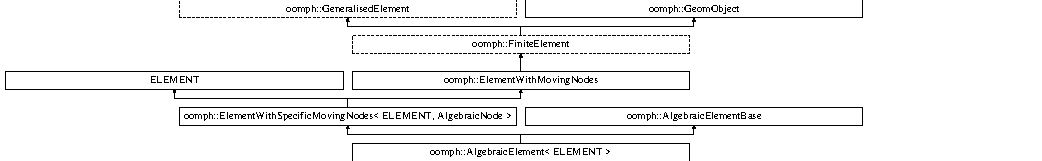
\includegraphics[height=2.165506cm]{classoomph_1_1AlgebraicElement}
\end{center}
\end{figure}
\subsection*{Public Member Functions}
\begin{DoxyCompactItemize}
\item 
\hyperlink{classoomph_1_1AlgebraicElement_acc029b6daf56771f0f691e9e82d3f674}{Algebraic\+Element} ()
\begin{DoxyCompactList}\small\item\em Constructor -- simply calls the constructor of the underlying E\+L\+E\+M\+E\+NT. \end{DoxyCompactList}\item 
\hyperlink{classoomph_1_1AlgebraicElement_af4ad322eea2c6fab36c1a74c18ecd781}{Algebraic\+Element} (\hyperlink{classoomph_1_1FiniteElement}{Finite\+Element} $\ast$const \&element\+\_\+pt, const int \&face\+\_\+index)
\begin{DoxyCompactList}\small\item\em Constructor for face elements. \end{DoxyCompactList}\item 
\hyperlink{classoomph_1_1AlgebraicElement_a2a0f43e92929bc56efa19ce12613c605}{Algebraic\+Element} (const \hyperlink{classoomph_1_1AlgebraicElement}{Algebraic\+Element} \&)
\begin{DoxyCompactList}\small\item\em Broken copy constructor. \end{DoxyCompactList}\item 
\hyperlink{classoomph_1_1AlgebraicElement_a46a4575a8a218302acb4753b1675fdd7}{$\sim$\+Algebraic\+Element} ()
\begin{DoxyCompactList}\small\item\em Broken assignment operator. \end{DoxyCompactList}\end{DoxyCompactItemize}
\subsection*{Additional Inherited Members}


\subsection{Detailed Description}
\subsubsection*{template$<$class E\+L\+E\+M\+E\+NT$>$\newline
class oomph\+::\+Algebraic\+Element$<$ E\+L\+E\+M\+E\+N\+T $>$}

Algebraic elements are elements that have Algebraic\+Nodes whose position is determined by the geometric \hyperlink{classoomph_1_1Data}{Data} in the Geom\+Objects that are involved in their node update functions. Algebraic Elements include the derivatives w.\+r.\+t. any unknowns that are stored in this geometric \hyperlink{classoomph_1_1Data}{Data} into the element\textquotesingle{}s Jacobian matrix. Otherwise they behave exactly like the templace element. 

Definition at line 563 of file algebraic\+\_\+elements.\+h.



\subsection{Constructor \& Destructor Documentation}
\mbox{\Hypertarget{classoomph_1_1AlgebraicElement_acc029b6daf56771f0f691e9e82d3f674}\label{classoomph_1_1AlgebraicElement_acc029b6daf56771f0f691e9e82d3f674}} 
\index{oomph\+::\+Algebraic\+Element@{oomph\+::\+Algebraic\+Element}!Algebraic\+Element@{Algebraic\+Element}}
\index{Algebraic\+Element@{Algebraic\+Element}!oomph\+::\+Algebraic\+Element@{oomph\+::\+Algebraic\+Element}}
\subsubsection{\texorpdfstring{Algebraic\+Element()}{AlgebraicElement()}\hspace{0.1cm}{\footnotesize\ttfamily [1/3]}}
{\footnotesize\ttfamily template$<$class E\+L\+E\+M\+E\+NT $>$ \\
\hyperlink{classoomph_1_1AlgebraicElement}{oomph\+::\+Algebraic\+Element}$<$ E\+L\+E\+M\+E\+NT $>$\+::\hyperlink{classoomph_1_1AlgebraicElement}{Algebraic\+Element} (\begin{DoxyParamCaption}{ }\end{DoxyParamCaption})\hspace{0.3cm}{\ttfamily [inline]}}



Constructor -- simply calls the constructor of the underlying E\+L\+E\+M\+E\+NT. 



Definition at line 572 of file algebraic\+\_\+elements.\+h.

\mbox{\Hypertarget{classoomph_1_1AlgebraicElement_af4ad322eea2c6fab36c1a74c18ecd781}\label{classoomph_1_1AlgebraicElement_af4ad322eea2c6fab36c1a74c18ecd781}} 
\index{oomph\+::\+Algebraic\+Element@{oomph\+::\+Algebraic\+Element}!Algebraic\+Element@{Algebraic\+Element}}
\index{Algebraic\+Element@{Algebraic\+Element}!oomph\+::\+Algebraic\+Element@{oomph\+::\+Algebraic\+Element}}
\subsubsection{\texorpdfstring{Algebraic\+Element()}{AlgebraicElement()}\hspace{0.1cm}{\footnotesize\ttfamily [2/3]}}
{\footnotesize\ttfamily template$<$class E\+L\+E\+M\+E\+NT $>$ \\
\hyperlink{classoomph_1_1AlgebraicElement}{oomph\+::\+Algebraic\+Element}$<$ E\+L\+E\+M\+E\+NT $>$\+::\hyperlink{classoomph_1_1AlgebraicElement}{Algebraic\+Element} (\begin{DoxyParamCaption}\item[{\hyperlink{classoomph_1_1FiniteElement}{Finite\+Element} $\ast$const \&}]{element\+\_\+pt,  }\item[{const int \&}]{face\+\_\+index }\end{DoxyParamCaption})\hspace{0.3cm}{\ttfamily [inline]}}



Constructor for face elements. 



Definition at line 578 of file algebraic\+\_\+elements.\+h.

\mbox{\Hypertarget{classoomph_1_1AlgebraicElement_a2a0f43e92929bc56efa19ce12613c605}\label{classoomph_1_1AlgebraicElement_a2a0f43e92929bc56efa19ce12613c605}} 
\index{oomph\+::\+Algebraic\+Element@{oomph\+::\+Algebraic\+Element}!Algebraic\+Element@{Algebraic\+Element}}
\index{Algebraic\+Element@{Algebraic\+Element}!oomph\+::\+Algebraic\+Element@{oomph\+::\+Algebraic\+Element}}
\subsubsection{\texorpdfstring{Algebraic\+Element()}{AlgebraicElement()}\hspace{0.1cm}{\footnotesize\ttfamily [3/3]}}
{\footnotesize\ttfamily template$<$class E\+L\+E\+M\+E\+NT $>$ \\
\hyperlink{classoomph_1_1AlgebraicElement}{oomph\+::\+Algebraic\+Element}$<$ E\+L\+E\+M\+E\+NT $>$\+::\hyperlink{classoomph_1_1AlgebraicElement}{Algebraic\+Element} (\begin{DoxyParamCaption}\item[{const \hyperlink{classoomph_1_1AlgebraicElement}{Algebraic\+Element}$<$ E\+L\+E\+M\+E\+NT $>$ \&}]{ }\end{DoxyParamCaption})\hspace{0.3cm}{\ttfamily [inline]}}



Broken copy constructor. 



Definition at line 586 of file algebraic\+\_\+elements.\+h.



References oomph\+::\+Broken\+Copy\+::broken\+\_\+copy().

\mbox{\Hypertarget{classoomph_1_1AlgebraicElement_a46a4575a8a218302acb4753b1675fdd7}\label{classoomph_1_1AlgebraicElement_a46a4575a8a218302acb4753b1675fdd7}} 
\index{oomph\+::\+Algebraic\+Element@{oomph\+::\+Algebraic\+Element}!````~Algebraic\+Element@{$\sim$\+Algebraic\+Element}}
\index{````~Algebraic\+Element@{$\sim$\+Algebraic\+Element}!oomph\+::\+Algebraic\+Element@{oomph\+::\+Algebraic\+Element}}
\subsubsection{\texorpdfstring{$\sim$\+Algebraic\+Element()}{~AlgebraicElement()}}
{\footnotesize\ttfamily template$<$class E\+L\+E\+M\+E\+NT $>$ \\
\hyperlink{classoomph_1_1AlgebraicElement}{oomph\+::\+Algebraic\+Element}$<$ E\+L\+E\+M\+E\+NT $>$\+::$\sim$\hyperlink{classoomph_1_1AlgebraicElement}{Algebraic\+Element} (\begin{DoxyParamCaption}{ }\end{DoxyParamCaption})\hspace{0.3cm}{\ttfamily [inline]}}



Broken assignment operator. 

Empty Destructor must clean up the allocated memory 

Definition at line 599 of file algebraic\+\_\+elements.\+h.



The documentation for this class was generated from the following file\+:\begin{DoxyCompactItemize}
\item 
\hyperlink{algebraic__elements_8h}{algebraic\+\_\+elements.\+h}\end{DoxyCompactItemize}

\hypertarget{classoomph_1_1AlgebraicElementBase}{}\section{oomph\+:\+:Algebraic\+Element\+Base Class Reference}
\label{classoomph_1_1AlgebraicElementBase}\index{oomph\+::\+Algebraic\+Element\+Base@{oomph\+::\+Algebraic\+Element\+Base}}


{\ttfamily \#include $<$algebraic\+\_\+elements.\+h$>$}

Inheritance diagram for oomph\+:\+:Algebraic\+Element\+Base\+:\begin{figure}[H]
\begin{center}
\leavevmode
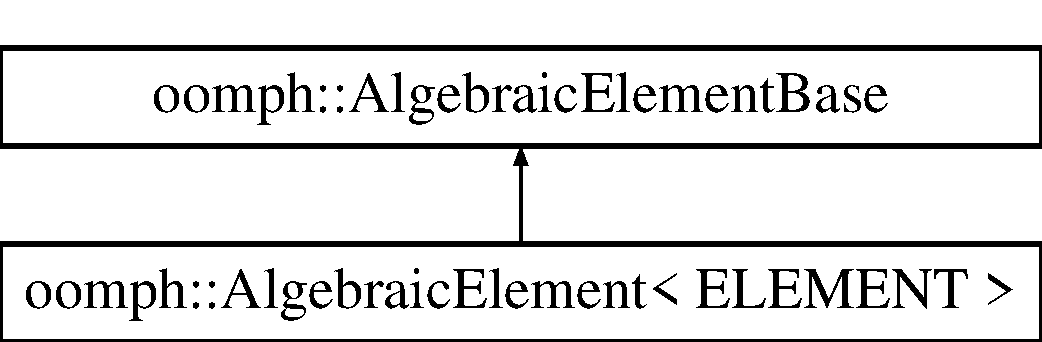
\includegraphics[height=2.000000cm]{classoomph_1_1AlgebraicElementBase}
\end{center}
\end{figure}
\subsection*{Public Member Functions}
\begin{DoxyCompactItemize}
\item 
\hyperlink{classoomph_1_1AlgebraicElementBase_ac94e4a7116416add9539def19791f1b4}{Algebraic\+Element\+Base} ()
\begin{DoxyCompactList}\small\item\em Empty constructor. \end{DoxyCompactList}\item 
\hyperlink{classoomph_1_1AlgebraicElementBase_a992e105cff9c261ef9c809eb36ba288e}{Algebraic\+Element\+Base} (const \hyperlink{classoomph_1_1AlgebraicElementBase}{Algebraic\+Element\+Base} \&)
\begin{DoxyCompactList}\small\item\em Broken copy constructor. \end{DoxyCompactList}\item 
void \hyperlink{classoomph_1_1AlgebraicElementBase_a4eff2e63c21f61259e5625a622cc985f}{operator=} (const \hyperlink{classoomph_1_1AlgebraicElementBase}{Algebraic\+Element\+Base} \&)
\begin{DoxyCompactList}\small\item\em Broken assignment operator. \end{DoxyCompactList}\item 
void \hyperlink{classoomph_1_1AlgebraicElementBase_ab9ada27015d5cb28ae00b086ace3600f}{setup\+\_\+algebraic\+\_\+node\+\_\+update} (\hyperlink{classoomph_1_1Node}{Node} $\ast$\&node\+\_\+pt, const \hyperlink{classoomph_1_1Vector}{Vector}$<$ double $>$ \&s\+\_\+father, \hyperlink{classoomph_1_1FiniteElement}{Finite\+Element} $\ast$father\+\_\+el\+\_\+pt) const
\begin{DoxyCompactList}\small\item\em Set up node update info for (newly created) algebraic node\+: I.\+e. work out its node update information by interpolation from the father element. Pass pointer to father element and the newly created node\textquotesingle{}s local coordinate in the father element. \end{DoxyCompactList}\end{DoxyCompactItemize}


\subsection{Detailed Description}
Base class for algebraic elements. 

Definition at line 520 of file algebraic\+\_\+elements.\+h.



\subsection{Constructor \& Destructor Documentation}
\mbox{\Hypertarget{classoomph_1_1AlgebraicElementBase_ac94e4a7116416add9539def19791f1b4}\label{classoomph_1_1AlgebraicElementBase_ac94e4a7116416add9539def19791f1b4}} 
\index{oomph\+::\+Algebraic\+Element\+Base@{oomph\+::\+Algebraic\+Element\+Base}!Algebraic\+Element\+Base@{Algebraic\+Element\+Base}}
\index{Algebraic\+Element\+Base@{Algebraic\+Element\+Base}!oomph\+::\+Algebraic\+Element\+Base@{oomph\+::\+Algebraic\+Element\+Base}}
\subsubsection{\texorpdfstring{Algebraic\+Element\+Base()}{AlgebraicElementBase()}\hspace{0.1cm}{\footnotesize\ttfamily [1/2]}}
{\footnotesize\ttfamily oomph\+::\+Algebraic\+Element\+Base\+::\+Algebraic\+Element\+Base (\begin{DoxyParamCaption}{ }\end{DoxyParamCaption})\hspace{0.3cm}{\ttfamily [inline]}}



Empty constructor. 



Definition at line 526 of file algebraic\+\_\+elements.\+h.

\mbox{\Hypertarget{classoomph_1_1AlgebraicElementBase_a992e105cff9c261ef9c809eb36ba288e}\label{classoomph_1_1AlgebraicElementBase_a992e105cff9c261ef9c809eb36ba288e}} 
\index{oomph\+::\+Algebraic\+Element\+Base@{oomph\+::\+Algebraic\+Element\+Base}!Algebraic\+Element\+Base@{Algebraic\+Element\+Base}}
\index{Algebraic\+Element\+Base@{Algebraic\+Element\+Base}!oomph\+::\+Algebraic\+Element\+Base@{oomph\+::\+Algebraic\+Element\+Base}}
\subsubsection{\texorpdfstring{Algebraic\+Element\+Base()}{AlgebraicElementBase()}\hspace{0.1cm}{\footnotesize\ttfamily [2/2]}}
{\footnotesize\ttfamily oomph\+::\+Algebraic\+Element\+Base\+::\+Algebraic\+Element\+Base (\begin{DoxyParamCaption}\item[{const \hyperlink{classoomph_1_1AlgebraicElementBase}{Algebraic\+Element\+Base} \&}]{ }\end{DoxyParamCaption})\hspace{0.3cm}{\ttfamily [inline]}}



Broken copy constructor. 



Definition at line 529 of file algebraic\+\_\+elements.\+h.



References oomph\+::\+Broken\+Copy\+::broken\+\_\+copy().



\subsection{Member Function Documentation}
\mbox{\Hypertarget{classoomph_1_1AlgebraicElementBase_a4eff2e63c21f61259e5625a622cc985f}\label{classoomph_1_1AlgebraicElementBase_a4eff2e63c21f61259e5625a622cc985f}} 
\index{oomph\+::\+Algebraic\+Element\+Base@{oomph\+::\+Algebraic\+Element\+Base}!operator=@{operator=}}
\index{operator=@{operator=}!oomph\+::\+Algebraic\+Element\+Base@{oomph\+::\+Algebraic\+Element\+Base}}
\subsubsection{\texorpdfstring{operator=()}{operator=()}}
{\footnotesize\ttfamily void oomph\+::\+Algebraic\+Element\+Base\+::operator= (\begin{DoxyParamCaption}\item[{const \hyperlink{classoomph_1_1AlgebraicElementBase}{Algebraic\+Element\+Base} \&}]{ }\end{DoxyParamCaption})\hspace{0.3cm}{\ttfamily [inline]}}



Broken assignment operator. 



Definition at line 535 of file algebraic\+\_\+elements.\+h.



References oomph\+::\+Broken\+Copy\+::broken\+\_\+assign().

\mbox{\Hypertarget{classoomph_1_1AlgebraicElementBase_ab9ada27015d5cb28ae00b086ace3600f}\label{classoomph_1_1AlgebraicElementBase_ab9ada27015d5cb28ae00b086ace3600f}} 
\index{oomph\+::\+Algebraic\+Element\+Base@{oomph\+::\+Algebraic\+Element\+Base}!setup\+\_\+algebraic\+\_\+node\+\_\+update@{setup\+\_\+algebraic\+\_\+node\+\_\+update}}
\index{setup\+\_\+algebraic\+\_\+node\+\_\+update@{setup\+\_\+algebraic\+\_\+node\+\_\+update}!oomph\+::\+Algebraic\+Element\+Base@{oomph\+::\+Algebraic\+Element\+Base}}
\subsubsection{\texorpdfstring{setup\+\_\+algebraic\+\_\+node\+\_\+update()}{setup\_algebraic\_node\_update()}}
{\footnotesize\ttfamily void oomph\+::\+Algebraic\+Element\+Base\+::setup\+\_\+algebraic\+\_\+node\+\_\+update (\begin{DoxyParamCaption}\item[{\hyperlink{classoomph_1_1Node}{Node} $\ast$\&}]{node\+\_\+pt,  }\item[{const \hyperlink{classoomph_1_1Vector}{Vector}$<$ double $>$ \&}]{s\+\_\+father,  }\item[{\hyperlink{classoomph_1_1FiniteElement}{Finite\+Element} $\ast$}]{father\+\_\+el\+\_\+pt }\end{DoxyParamCaption}) const}



Set up node update info for (newly created) algebraic node\+: I.\+e. work out its node update information by interpolation from the father element. Pass pointer to father element and the newly created node\textquotesingle{}s local coordinate in the father element. 

Set up node update info for (newly created) algebraic node\+: Work out its node update information by interpolation from its father element, based on pointer to father element and its local coordinate in the father element. We\textquotesingle{}re creating the node update info for update functions that are shared by all nodes in the father element. Now loop over the ids and check if they appear in all nodes 

Definition at line 54 of file algebraic\+\_\+elements.\+cc.



References oomph\+::\+Algebraic\+Node\+::add\+\_\+node\+\_\+update\+\_\+info(), oomph\+::\+Algebraic\+Node\+::\+Dummy\+\_\+geom\+\_\+object\+\_\+pt, oomph\+::\+Algebraic\+Node\+::\+Dummy\+\_\+mesh, oomph\+::\+Algebraic\+Node\+::\+Dummy\+\_\+mesh\+\_\+pt, oomph\+::\+Algebraic\+Node\+::\+Dummy\+\_\+node\+\_\+update\+\_\+fct\+\_\+id, oomph\+::\+Algebraic\+Node\+::\+Dummy\+\_\+ref\+\_\+value, i, oomph\+::\+Algebraic\+Node\+::\+Max\+\_\+allowed\+\_\+difference\+\_\+between\+\_\+node\+\_\+update\+\_\+fcts, oomph\+::\+Algebraic\+Node\+::mesh\+\_\+pt(), oomph\+::\+Finite\+Element\+::nnode(), oomph\+::\+Finite\+Element\+::node\+\_\+pt(), oomph\+::\+Algebraic\+Node\+::node\+\_\+update(), oomph\+::\+Algebraic\+Node\+::nref\+\_\+value(), oomph\+::\+Finite\+Element\+::shape(), and oomph\+::\+Algebraic\+Mesh\+::update\+\_\+node\+\_\+update().



Referenced by oomph\+::\+Refineable\+Q\+Element$<$ 3 $>$\+::build(), oomph\+::\+Refineable\+Q\+Element$<$ 1 $>$\+::build(), oomph\+::\+Refineable\+Q\+Element$<$ 2 $>$\+::build(), oomph\+::\+P\+Refineable\+Q\+Element$<$ 1, I\+N\+I\+T\+I\+A\+L\+\_\+\+N\+N\+O\+D\+E\+\_\+1\+D $>$\+::p\+\_\+refine(), oomph\+::\+P\+Refineable\+Q\+Element$<$ 2, I\+N\+I\+T\+I\+A\+L\+\_\+\+N\+N\+O\+D\+E\+\_\+1\+D $>$\+::p\+\_\+refine(), and oomph\+::\+P\+Refineable\+Q\+Element$<$ 3, I\+N\+I\+T\+I\+A\+L\+\_\+\+N\+N\+O\+D\+E\+\_\+1\+D $>$\+::p\+\_\+refine().



The documentation for this class was generated from the following files\+:\begin{DoxyCompactItemize}
\item 
\hyperlink{algebraic__elements_8h}{algebraic\+\_\+elements.\+h}\item 
\hyperlink{algebraic__elements_8cc}{algebraic\+\_\+elements.\+cc}\end{DoxyCompactItemize}

\hypertarget{classoomph_1_1AlgebraicFishMesh}{}\section{oomph\+:\+:Algebraic\+Fish\+Mesh$<$ E\+L\+E\+M\+E\+NT $>$ Class Template Reference}
\label{classoomph_1_1AlgebraicFishMesh}\index{oomph\+::\+Algebraic\+Fish\+Mesh$<$ E\+L\+E\+M\+E\+N\+T $>$@{oomph\+::\+Algebraic\+Fish\+Mesh$<$ E\+L\+E\+M\+E\+N\+T $>$}}


Fish shaped mesh with algebraic node update function for nodes.  




{\ttfamily \#include $<$fish\+\_\+mesh.\+template.\+h$>$}

Inheritance diagram for oomph\+:\+:Algebraic\+Fish\+Mesh$<$ E\+L\+E\+M\+E\+NT $>$\+:\begin{figure}[H]
\begin{center}
\leavevmode
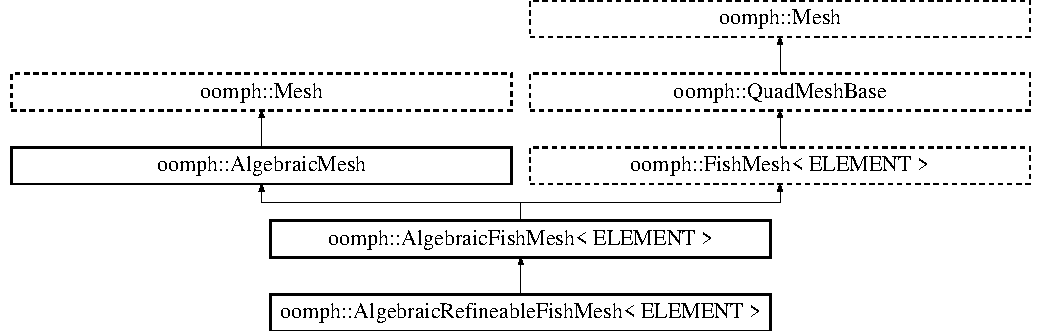
\includegraphics[height=3.555556cm]{classoomph_1_1AlgebraicFishMesh}
\end{center}
\end{figure}
\subsection*{Public Member Functions}
\begin{DoxyCompactItemize}
\item 
\hyperlink{classoomph_1_1AlgebraicFishMesh_a4382cbf0c75b2b76c9b28e9bae45fd4f}{Algebraic\+Fish\+Mesh} (Time\+Stepper $\ast$time\+\_\+stepper\+\_\+pt=\&Mesh\+::\+Default\+\_\+\+Time\+Stepper)
\begin{DoxyCompactList}\small\item\em Constructor\+: Pass pointer to timestepper. (defaults to (Steady) default timestepper defined in Mesh) \end{DoxyCompactList}\item 
\hyperlink{classoomph_1_1AlgebraicFishMesh_aac4b7f18a6e1d10c64edf431af921ce7}{Algebraic\+Fish\+Mesh} (Geom\+Object $\ast$back\+\_\+pt, Time\+Stepper $\ast$time\+\_\+stepper\+\_\+pt=\&Mesh\+::\+Default\+\_\+\+Time\+Stepper)
\begin{DoxyCompactList}\small\item\em Constructor\+: Pass pointer Geom\+Object that defines the fish\textquotesingle{}s back and pointer to timestepper (defaults to (Steady) default timestepper defined in Mesh). \end{DoxyCompactList}\item 
virtual \hyperlink{classoomph_1_1AlgebraicFishMesh_a027d54d158e22ce8fe3c1246cb030440}{$\sim$\+Algebraic\+Fish\+Mesh} ()
\begin{DoxyCompactList}\small\item\em Destructor\+: empty. \end{DoxyCompactList}\item 
void \hyperlink{classoomph_1_1AlgebraicFishMesh_ac66d6542472dac702a7414aa9d7f995f}{algebraic\+\_\+node\+\_\+update} (const unsigned \&t, Algebraic\+Node $\ast$\&node\+\_\+pt)
\begin{DoxyCompactList}\small\item\em Update nodal position at time level t (t=0\+: present; t$>$0\+: previous) \end{DoxyCompactList}\item 
virtual void \hyperlink{classoomph_1_1AlgebraicFishMesh_a39cd5a86b0f762efd09f4fefba6da1c3}{node\+\_\+update} (const bool \&update\+\_\+all\+\_\+solid\+\_\+nodes=false)
\begin{DoxyCompactList}\small\item\em Resolve the node update function (we neither want the broken empty one in the Mesh base class nor the macro-\/element-\/based one in the Refineable\+Quad\+Mesh base class but the Algebraic\+Element one). \mbox{[}It doesn\textquotesingle{}t make sense to use this mesh with Solid\+Elements so we buffer the case if update\+\_\+all\+\_\+solid\+\_\+nodes is set to true.\mbox{]}. \end{DoxyCompactList}\item 
void \hyperlink{classoomph_1_1AlgebraicFishMesh_a4f992939c299f87abc762c14aab50b5c}{update\+\_\+node\+\_\+update} (Algebraic\+Node $\ast$\&node\+\_\+pt)
\begin{DoxyCompactList}\small\item\em Update the geometric references that are used to update node after mesh adaptation. We\textquotesingle{}re assuming that the Geom\+Object that specifies the fish back does not have sub-\/objects, therefore no update is required -- all reference values can simply be scaled. We simply paranoid-\/check that this is actually the case, by checking if locate\+\_\+zeta() returns the original data. \end{DoxyCompactList}\end{DoxyCompactItemize}
\subsection*{Protected Member Functions}
\begin{DoxyCompactItemize}
\item 
void \hyperlink{classoomph_1_1AlgebraicFishMesh_a4aee83d1b0a42418fe886b2f244c1d49}{node\+\_\+update\+\_\+in\+\_\+body} (const unsigned \&t, Algebraic\+Node $\ast$\&node\+\_\+pt)
\begin{DoxyCompactList}\small\item\em Algebraic update function for nodes in upper/lower body. \end{DoxyCompactList}\item 
void \hyperlink{classoomph_1_1AlgebraicFishMesh_ad4a6f95e21e3d81b9defde90636e7d45}{node\+\_\+update\+\_\+in\+\_\+fin} (const unsigned \&t, Algebraic\+Node $\ast$\&node\+\_\+pt)
\begin{DoxyCompactList}\small\item\em Algebraic update function for nodes in upper/lower fin. \end{DoxyCompactList}\item 
void \hyperlink{classoomph_1_1AlgebraicFishMesh_a1a6d22eedc77299d843274e8ce34b560}{setup\+\_\+algebraic\+\_\+node\+\_\+update} ()
\begin{DoxyCompactList}\small\item\em Setup algebraic update operation for all nodes (separate function because this task needs to be performed by both constructors) \end{DoxyCompactList}\end{DoxyCompactItemize}
\subsection*{Additional Inherited Members}


\subsection{Detailed Description}
\subsubsection*{template$<$class E\+L\+E\+M\+E\+NT$>$\newline
class oomph\+::\+Algebraic\+Fish\+Mesh$<$ E\+L\+E\+M\+E\+N\+T $>$}

Fish shaped mesh with algebraic node update function for nodes. 

Definition at line 349 of file fish\+\_\+mesh.\+template.\+h.



\subsection{Constructor \& Destructor Documentation}
\mbox{\Hypertarget{classoomph_1_1AlgebraicFishMesh_a4382cbf0c75b2b76c9b28e9bae45fd4f}\label{classoomph_1_1AlgebraicFishMesh_a4382cbf0c75b2b76c9b28e9bae45fd4f}} 
\index{oomph\+::\+Algebraic\+Fish\+Mesh@{oomph\+::\+Algebraic\+Fish\+Mesh}!Algebraic\+Fish\+Mesh@{Algebraic\+Fish\+Mesh}}
\index{Algebraic\+Fish\+Mesh@{Algebraic\+Fish\+Mesh}!oomph\+::\+Algebraic\+Fish\+Mesh@{oomph\+::\+Algebraic\+Fish\+Mesh}}
\subsubsection{\texorpdfstring{Algebraic\+Fish\+Mesh()}{AlgebraicFishMesh()}\hspace{0.1cm}{\footnotesize\ttfamily [1/2]}}
{\footnotesize\ttfamily template$<$class E\+L\+E\+M\+E\+NT $>$ \\
\hyperlink{classoomph_1_1AlgebraicFishMesh}{oomph\+::\+Algebraic\+Fish\+Mesh}$<$ E\+L\+E\+M\+E\+NT $>$\+::\hyperlink{classoomph_1_1AlgebraicFishMesh}{Algebraic\+Fish\+Mesh} (\begin{DoxyParamCaption}\item[{Time\+Stepper $\ast$}]{time\+\_\+stepper\+\_\+pt = {\ttfamily \&Mesh\+:\+:Default\+\_\+TimeStepper} }\end{DoxyParamCaption})\hspace{0.3cm}{\ttfamily [inline]}}



Constructor\+: Pass pointer to timestepper. (defaults to (Steady) default timestepper defined in Mesh) 



Definition at line 357 of file fish\+\_\+mesh.\+template.\+h.

\mbox{\Hypertarget{classoomph_1_1AlgebraicFishMesh_aac4b7f18a6e1d10c64edf431af921ce7}\label{classoomph_1_1AlgebraicFishMesh_aac4b7f18a6e1d10c64edf431af921ce7}} 
\index{oomph\+::\+Algebraic\+Fish\+Mesh@{oomph\+::\+Algebraic\+Fish\+Mesh}!Algebraic\+Fish\+Mesh@{Algebraic\+Fish\+Mesh}}
\index{Algebraic\+Fish\+Mesh@{Algebraic\+Fish\+Mesh}!oomph\+::\+Algebraic\+Fish\+Mesh@{oomph\+::\+Algebraic\+Fish\+Mesh}}
\subsubsection{\texorpdfstring{Algebraic\+Fish\+Mesh()}{AlgebraicFishMesh()}\hspace{0.1cm}{\footnotesize\ttfamily [2/2]}}
{\footnotesize\ttfamily template$<$class E\+L\+E\+M\+E\+NT $>$ \\
\hyperlink{classoomph_1_1AlgebraicFishMesh}{oomph\+::\+Algebraic\+Fish\+Mesh}$<$ E\+L\+E\+M\+E\+NT $>$\+::\hyperlink{classoomph_1_1AlgebraicFishMesh}{Algebraic\+Fish\+Mesh} (\begin{DoxyParamCaption}\item[{Geom\+Object $\ast$}]{back\+\_\+pt,  }\item[{Time\+Stepper $\ast$}]{time\+\_\+stepper\+\_\+pt = {\ttfamily \&Mesh\+:\+:Default\+\_\+TimeStepper} }\end{DoxyParamCaption})\hspace{0.3cm}{\ttfamily [inline]}}



Constructor\+: Pass pointer Geom\+Object that defines the fish\textquotesingle{}s back and pointer to timestepper (defaults to (Steady) default timestepper defined in Mesh). 



Definition at line 367 of file fish\+\_\+mesh.\+template.\+h.

\mbox{\Hypertarget{classoomph_1_1AlgebraicFishMesh_a027d54d158e22ce8fe3c1246cb030440}\label{classoomph_1_1AlgebraicFishMesh_a027d54d158e22ce8fe3c1246cb030440}} 
\index{oomph\+::\+Algebraic\+Fish\+Mesh@{oomph\+::\+Algebraic\+Fish\+Mesh}!````~Algebraic\+Fish\+Mesh@{$\sim$\+Algebraic\+Fish\+Mesh}}
\index{````~Algebraic\+Fish\+Mesh@{$\sim$\+Algebraic\+Fish\+Mesh}!oomph\+::\+Algebraic\+Fish\+Mesh@{oomph\+::\+Algebraic\+Fish\+Mesh}}
\subsubsection{\texorpdfstring{$\sim$\+Algebraic\+Fish\+Mesh()}{~AlgebraicFishMesh()}}
{\footnotesize\ttfamily template$<$class E\+L\+E\+M\+E\+NT $>$ \\
virtual \hyperlink{classoomph_1_1AlgebraicFishMesh}{oomph\+::\+Algebraic\+Fish\+Mesh}$<$ E\+L\+E\+M\+E\+NT $>$\+::$\sim$\hyperlink{classoomph_1_1AlgebraicFishMesh}{Algebraic\+Fish\+Mesh} (\begin{DoxyParamCaption}{ }\end{DoxyParamCaption})\hspace{0.3cm}{\ttfamily [inline]}, {\ttfamily [virtual]}}



Destructor\+: empty. 



Definition at line 379 of file fish\+\_\+mesh.\+template.\+h.



\subsection{Member Function Documentation}
\mbox{\Hypertarget{classoomph_1_1AlgebraicFishMesh_ac66d6542472dac702a7414aa9d7f995f}\label{classoomph_1_1AlgebraicFishMesh_ac66d6542472dac702a7414aa9d7f995f}} 
\index{oomph\+::\+Algebraic\+Fish\+Mesh@{oomph\+::\+Algebraic\+Fish\+Mesh}!algebraic\+\_\+node\+\_\+update@{algebraic\+\_\+node\+\_\+update}}
\index{algebraic\+\_\+node\+\_\+update@{algebraic\+\_\+node\+\_\+update}!oomph\+::\+Algebraic\+Fish\+Mesh@{oomph\+::\+Algebraic\+Fish\+Mesh}}
\subsubsection{\texorpdfstring{algebraic\+\_\+node\+\_\+update()}{algebraic\_node\_update()}}
{\footnotesize\ttfamily template$<$class E\+L\+E\+M\+E\+NT $>$ \\
void \hyperlink{classoomph_1_1AlgebraicFishMesh}{oomph\+::\+Algebraic\+Fish\+Mesh}$<$ E\+L\+E\+M\+E\+NT $>$\+::algebraic\+\_\+node\+\_\+update (\begin{DoxyParamCaption}\item[{const unsigned \&}]{t,  }\item[{Algebraic\+Node $\ast$\&}]{node\+\_\+pt }\end{DoxyParamCaption})\hspace{0.3cm}{\ttfamily [inline]}}



Update nodal position at time level t (t=0\+: present; t$>$0\+: previous) 



Definition at line 383 of file fish\+\_\+mesh.\+template.\+h.



References oomph\+::\+Fish\+Mesh$<$ E\+L\+E\+M\+E\+N\+T $>$\+::\+Lower\+\_\+body, oomph\+::\+Fish\+Mesh$<$ E\+L\+E\+M\+E\+N\+T $>$\+::\+Lower\+\_\+fin, oomph\+::\+Fish\+Mesh$<$ E\+L\+E\+M\+E\+N\+T $>$\+::\+Upper\+\_\+body, and oomph\+::\+Fish\+Mesh$<$ E\+L\+E\+M\+E\+N\+T $>$\+::\+Upper\+\_\+fin.

\mbox{\Hypertarget{classoomph_1_1AlgebraicFishMesh_a39cd5a86b0f762efd09f4fefba6da1c3}\label{classoomph_1_1AlgebraicFishMesh_a39cd5a86b0f762efd09f4fefba6da1c3}} 
\index{oomph\+::\+Algebraic\+Fish\+Mesh@{oomph\+::\+Algebraic\+Fish\+Mesh}!node\+\_\+update@{node\+\_\+update}}
\index{node\+\_\+update@{node\+\_\+update}!oomph\+::\+Algebraic\+Fish\+Mesh@{oomph\+::\+Algebraic\+Fish\+Mesh}}
\subsubsection{\texorpdfstring{node\+\_\+update()}{node\_update()}}
{\footnotesize\ttfamily template$<$class E\+L\+E\+M\+E\+NT $>$ \\
virtual void \hyperlink{classoomph_1_1AlgebraicFishMesh}{oomph\+::\+Algebraic\+Fish\+Mesh}$<$ E\+L\+E\+M\+E\+NT $>$\+::node\+\_\+update (\begin{DoxyParamCaption}\item[{const bool \&}]{update\+\_\+all\+\_\+solid\+\_\+nodes = {\ttfamily false} }\end{DoxyParamCaption})\hspace{0.3cm}{\ttfamily [inline]}, {\ttfamily [virtual]}}



Resolve the node update function (we neither want the broken empty one in the Mesh base class nor the macro-\/element-\/based one in the Refineable\+Quad\+Mesh base class but the Algebraic\+Element one). \mbox{[}It doesn\textquotesingle{}t make sense to use this mesh with Solid\+Elements so we buffer the case if update\+\_\+all\+\_\+solid\+\_\+nodes is set to true.\mbox{]}. 



Reimplemented in \hyperlink{classoomph_1_1AlgebraicRefineableFishMesh_a8123da4b48355b39f19e0494a9d4545c}{oomph\+::\+Algebraic\+Refineable\+Fish\+Mesh$<$ E\+L\+E\+M\+E\+N\+T $>$}.



Definition at line 422 of file fish\+\_\+mesh.\+template.\+h.



Referenced by oomph\+::\+Algebraic\+Refineable\+Fish\+Mesh$<$ E\+L\+E\+M\+E\+N\+T $>$\+::node\+\_\+update().

\mbox{\Hypertarget{classoomph_1_1AlgebraicFishMesh_a4aee83d1b0a42418fe886b2f244c1d49}\label{classoomph_1_1AlgebraicFishMesh_a4aee83d1b0a42418fe886b2f244c1d49}} 
\index{oomph\+::\+Algebraic\+Fish\+Mesh@{oomph\+::\+Algebraic\+Fish\+Mesh}!node\+\_\+update\+\_\+in\+\_\+body@{node\+\_\+update\+\_\+in\+\_\+body}}
\index{node\+\_\+update\+\_\+in\+\_\+body@{node\+\_\+update\+\_\+in\+\_\+body}!oomph\+::\+Algebraic\+Fish\+Mesh@{oomph\+::\+Algebraic\+Fish\+Mesh}}
\subsubsection{\texorpdfstring{node\+\_\+update\+\_\+in\+\_\+body()}{node\_update\_in\_body()}}
{\footnotesize\ttfamily template$<$class E\+L\+E\+M\+E\+NT $>$ \\
void \hyperlink{classoomph_1_1AlgebraicFishMesh}{oomph\+::\+Algebraic\+Fish\+Mesh}$<$ E\+L\+E\+M\+E\+NT $>$\+::node\+\_\+update\+\_\+in\+\_\+body (\begin{DoxyParamCaption}\item[{const unsigned \&}]{t,  }\item[{Algebraic\+Node $\ast$\&}]{node\+\_\+pt }\end{DoxyParamCaption})\hspace{0.3cm}{\ttfamily [protected]}}



Algebraic update function for nodes in upper/lower body. 

Algebraic update function\+: Update in (upper or lower) body according to wall shape at time level t (t=0\+: present; t$>$0\+: previous) 

Definition at line 950 of file fish\+\_\+mesh.\+template.\+cc.



References oomph\+::\+Fish\+Mesh$<$ E\+L\+E\+M\+E\+N\+T $>$\+::\+Domain\+\_\+pt, oomph\+::\+Fish\+Domain\+::x\+\_\+mouth(), oomph\+::\+Fish\+Domain\+::xi\+\_\+nose(), and oomph\+::\+Fish\+Domain\+::xi\+\_\+tail().

\mbox{\Hypertarget{classoomph_1_1AlgebraicFishMesh_ad4a6f95e21e3d81b9defde90636e7d45}\label{classoomph_1_1AlgebraicFishMesh_ad4a6f95e21e3d81b9defde90636e7d45}} 
\index{oomph\+::\+Algebraic\+Fish\+Mesh@{oomph\+::\+Algebraic\+Fish\+Mesh}!node\+\_\+update\+\_\+in\+\_\+fin@{node\+\_\+update\+\_\+in\+\_\+fin}}
\index{node\+\_\+update\+\_\+in\+\_\+fin@{node\+\_\+update\+\_\+in\+\_\+fin}!oomph\+::\+Algebraic\+Fish\+Mesh@{oomph\+::\+Algebraic\+Fish\+Mesh}}
\subsubsection{\texorpdfstring{node\+\_\+update\+\_\+in\+\_\+fin()}{node\_update\_in\_fin()}}
{\footnotesize\ttfamily template$<$class E\+L\+E\+M\+E\+NT $>$ \\
void \hyperlink{classoomph_1_1AlgebraicFishMesh}{oomph\+::\+Algebraic\+Fish\+Mesh}$<$ E\+L\+E\+M\+E\+NT $>$\+::node\+\_\+update\+\_\+in\+\_\+fin (\begin{DoxyParamCaption}\item[{const unsigned \&}]{t,  }\item[{Algebraic\+Node $\ast$\&}]{node\+\_\+pt }\end{DoxyParamCaption})\hspace{0.3cm}{\ttfamily [protected]}}



Algebraic update function for nodes in upper/lower fin. 

Algebraic update function\+: Update in (upper or lower) fin according to wall shape at time level t (t=0\+: present; t$>$0\+: previous) 

Definition at line 1010 of file fish\+\_\+mesh.\+template.\+cc.



References oomph\+::\+Fish\+Mesh$<$ E\+L\+E\+M\+E\+N\+T $>$\+::\+Domain\+\_\+pt, oomph\+::\+Fish\+Domain\+::x\+\_\+fin(), oomph\+::\+Fish\+Domain\+::xi\+\_\+tail(), and oomph\+::\+Fish\+Domain\+::y\+\_\+fin().

\mbox{\Hypertarget{classoomph_1_1AlgebraicFishMesh_a1a6d22eedc77299d843274e8ce34b560}\label{classoomph_1_1AlgebraicFishMesh_a1a6d22eedc77299d843274e8ce34b560}} 
\index{oomph\+::\+Algebraic\+Fish\+Mesh@{oomph\+::\+Algebraic\+Fish\+Mesh}!setup\+\_\+algebraic\+\_\+node\+\_\+update@{setup\+\_\+algebraic\+\_\+node\+\_\+update}}
\index{setup\+\_\+algebraic\+\_\+node\+\_\+update@{setup\+\_\+algebraic\+\_\+node\+\_\+update}!oomph\+::\+Algebraic\+Fish\+Mesh@{oomph\+::\+Algebraic\+Fish\+Mesh}}
\subsubsection{\texorpdfstring{setup\+\_\+algebraic\+\_\+node\+\_\+update()}{setup\_algebraic\_node\_update()}}
{\footnotesize\ttfamily template$<$class E\+L\+E\+M\+E\+NT $>$ \\
void \hyperlink{classoomph_1_1AlgebraicFishMesh}{oomph\+::\+Algebraic\+Fish\+Mesh}$<$ E\+L\+E\+M\+E\+NT $>$\+::setup\+\_\+algebraic\+\_\+node\+\_\+update (\begin{DoxyParamCaption}{ }\end{DoxyParamCaption})\hspace{0.3cm}{\ttfamily [protected]}}



Setup algebraic update operation for all nodes (separate function because this task needs to be performed by both constructors) 

Setup algebraic update operation. Nodes are \char`\"{}suspended\char`\"{} from the fish\textquotesingle{}s back and the upper edge of the fin. Nodes in the lower half are placed symmetrically. Pointer to algebraic element in lower body 

Definition at line 728 of file fish\+\_\+mesh.\+template.\+cc.



References oomph\+::\+Fish\+Mesh$<$ E\+L\+E\+M\+E\+N\+T $>$\+::\+Back\+\_\+pt, oomph\+::\+Fish\+Mesh$<$ E\+L\+E\+M\+E\+N\+T $>$\+::\+Lower\+\_\+body, oomph\+::\+Fish\+Mesh$<$ E\+L\+E\+M\+E\+N\+T $>$\+::\+Lower\+\_\+fin, oomph\+::\+Fish\+Mesh$<$ E\+L\+E\+M\+E\+N\+T $>$\+::\+Upper\+\_\+body, and oomph\+::\+Fish\+Mesh$<$ E\+L\+E\+M\+E\+N\+T $>$\+::\+Upper\+\_\+fin.

\mbox{\Hypertarget{classoomph_1_1AlgebraicFishMesh_a4f992939c299f87abc762c14aab50b5c}\label{classoomph_1_1AlgebraicFishMesh_a4f992939c299f87abc762c14aab50b5c}} 
\index{oomph\+::\+Algebraic\+Fish\+Mesh@{oomph\+::\+Algebraic\+Fish\+Mesh}!update\+\_\+node\+\_\+update@{update\+\_\+node\+\_\+update}}
\index{update\+\_\+node\+\_\+update@{update\+\_\+node\+\_\+update}!oomph\+::\+Algebraic\+Fish\+Mesh@{oomph\+::\+Algebraic\+Fish\+Mesh}}
\subsubsection{\texorpdfstring{update\+\_\+node\+\_\+update()}{update\_node\_update()}}
{\footnotesize\ttfamily template$<$class E\+L\+E\+M\+E\+NT $>$ \\
void \hyperlink{classoomph_1_1AlgebraicFishMesh}{oomph\+::\+Algebraic\+Fish\+Mesh}$<$ E\+L\+E\+M\+E\+NT $>$\+::update\+\_\+node\+\_\+update (\begin{DoxyParamCaption}\item[{Algebraic\+Node $\ast$\&}]{node\+\_\+pt }\end{DoxyParamCaption})\hspace{0.3cm}{\ttfamily [inline]}}



Update the geometric references that are used to update node after mesh adaptation. We\textquotesingle{}re assuming that the Geom\+Object that specifies the fish back does not have sub-\/objects, therefore no update is required -- all reference values can simply be scaled. We simply paranoid-\/check that this is actually the case, by checking if locate\+\_\+zeta() returns the original data. 

Start coordinate on wall (near nose)

End coordinate on wall (near tail)

Check halfway along the object 

Definition at line 453 of file fish\+\_\+mesh.\+template.\+h.



References oomph\+::\+Fish\+Mesh$<$ E\+L\+E\+M\+E\+N\+T $>$\+::\+Back\+\_\+pt, oomph\+::\+Fish\+Mesh$<$ E\+L\+E\+M\+E\+N\+T $>$\+::\+Domain\+\_\+pt, oomph\+::\+Fish\+Domain\+::xi\+\_\+nose(), and oomph\+::\+Fish\+Domain\+::xi\+\_\+tail().



The documentation for this class was generated from the following files\+:\begin{DoxyCompactItemize}
\item 
\hyperlink{fish__mesh_8template_8h}{fish\+\_\+mesh.\+template.\+h}\item 
\hyperlink{fish__mesh_8template_8cc}{fish\+\_\+mesh.\+template.\+cc}\end{DoxyCompactItemize}

\hypertarget{classoomph_1_1AlgebraicFSIDrivenCavityMesh}{}\section{oomph\+:\+:Algebraic\+F\+S\+I\+Driven\+Cavity\+Mesh$<$ E\+L\+E\+M\+E\+NT $>$ Class Template Reference}
\label{classoomph_1_1AlgebraicFSIDrivenCavityMesh}\index{oomph\+::\+Algebraic\+F\+S\+I\+Driven\+Cavity\+Mesh$<$ E\+L\+E\+M\+E\+N\+T $>$@{oomph\+::\+Algebraic\+F\+S\+I\+Driven\+Cavity\+Mesh$<$ E\+L\+E\+M\+E\+N\+T $>$}}


{\ttfamily \#include $<$fsi\+\_\+driven\+\_\+cavity\+\_\+mesh.\+template.\+h$>$}

Inheritance diagram for oomph\+:\+:Algebraic\+F\+S\+I\+Driven\+Cavity\+Mesh$<$ E\+L\+E\+M\+E\+NT $>$\+:\begin{figure}[H]
\begin{center}
\leavevmode
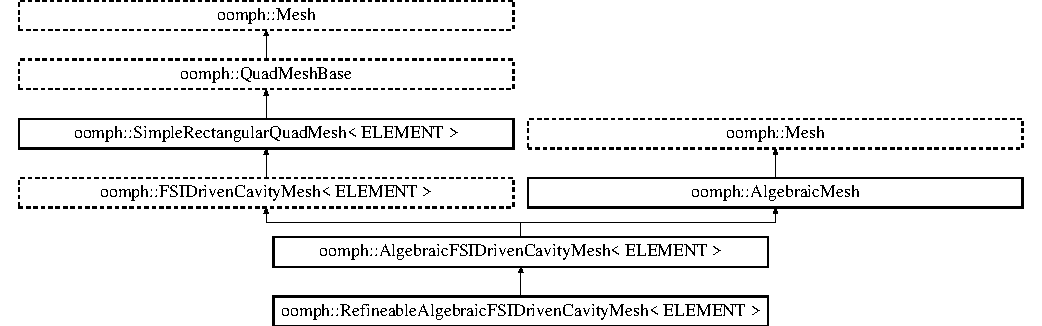
\includegraphics[height=4.375000cm]{classoomph_1_1AlgebraicFSIDrivenCavityMesh}
\end{center}
\end{figure}
\subsection*{Public Member Functions}
\begin{DoxyCompactItemize}
\item 
\hyperlink{classoomph_1_1AlgebraicFSIDrivenCavityMesh_a973ccadc769d98fed6bc9dd4eff32083}{Algebraic\+F\+S\+I\+Driven\+Cavity\+Mesh} (const unsigned \&\hyperlink{classoomph_1_1SimpleRectangularQuadMesh_a4ff7678ec433180e2245ea2147f222b7}{nx}, const unsigned \&\hyperlink{classoomph_1_1SimpleRectangularQuadMesh_a45011f22dedd480392b1f376e4269921}{ny}, const double \&lx, const double \&ly, const double \&gap\+\_\+fraction, \hyperlink{classoomph_1_1GeomObject}{Geom\+Object} $\ast$wall\+\_\+pt, \hyperlink{classoomph_1_1TimeStepper}{Time\+Stepper} $\ast$time\+\_\+stepper\+\_\+pt=\&\hyperlink{classoomph_1_1Mesh_a12243d0fee2b1fcee729ee5a4777ea10}{Mesh\+::\+Default\+\_\+\+Time\+Stepper})
\begin{DoxyCompactList}\small\item\em Constructor\+: Pass number of elements, lengths, pointer to \hyperlink{classoomph_1_1GeomObject}{Geom\+Object} that defines the collapsible segment and pointer to \hyperlink{classoomph_1_1TimeStepper}{Time\+Stepper} (defaults to the default timestepper, \hyperlink{classoomph_1_1Steady}{Steady}). \end{DoxyCompactList}\item 
virtual \hyperlink{classoomph_1_1AlgebraicFSIDrivenCavityMesh_a048a142aff0ca5fd62273f756bce4ab6}{$\sim$\+Algebraic\+F\+S\+I\+Driven\+Cavity\+Mesh} ()
\begin{DoxyCompactList}\small\item\em Destructor\+: empty. \end{DoxyCompactList}\item 
void \hyperlink{classoomph_1_1AlgebraicFSIDrivenCavityMesh_a56c72b78935e84f7fef3f6b5d85556c3}{algebraic\+\_\+node\+\_\+update} (const unsigned \&\hyperlink{cfortran_8h_af6f0bd3dc13317f895c91323c25c2b8f}{t}, \hyperlink{classoomph_1_1AlgebraicNode}{Algebraic\+Node} $\ast$\&\hyperlink{classoomph_1_1AlgebraicMesh_aedeebbe95d2f8e67e9939cecd1be3933}{node\+\_\+pt})
\begin{DoxyCompactList}\small\item\em Update nodal position at time level t (t=0\+: present; t$>$0\+: previous) \end{DoxyCompactList}\item 
void \hyperlink{classoomph_1_1AlgebraicFSIDrivenCavityMesh_a87d34d6cf84c62a9049773451c664176}{update\+\_\+node\+\_\+update} (\hyperlink{classoomph_1_1AlgebraicNode}{Algebraic\+Node} $\ast$\&\hyperlink{classoomph_1_1AlgebraicMesh_aedeebbe95d2f8e67e9939cecd1be3933}{node\+\_\+pt})
\begin{DoxyCompactList}\small\item\em Update the node-\/udate data after mesh adaptation. Empty -- no update of node update required as this is non-\/refineable mesh. \end{DoxyCompactList}\end{DoxyCompactItemize}
\subsection*{Protected Member Functions}
\begin{DoxyCompactItemize}
\item 
void \hyperlink{classoomph_1_1AlgebraicFSIDrivenCavityMesh_a7f6b7c3dae1c61c2cdb0cbd229173114}{setup\+\_\+algebraic\+\_\+node\+\_\+update} ()
\begin{DoxyCompactList}\small\item\em Function to setup the algebraic node update. \end{DoxyCompactList}\end{DoxyCompactItemize}
\subsection*{Additional Inherited Members}


\subsection{Detailed Description}
\subsubsection*{template$<$class E\+L\+E\+M\+E\+NT$>$\newline
class oomph\+::\+Algebraic\+F\+S\+I\+Driven\+Cavity\+Mesh$<$ E\+L\+E\+M\+E\+N\+T $>$}

Alebraic node update version of \hyperlink{classoomph_1_1FSIDrivenCavityMesh}{F\+S\+I\+Driven\+Cavity\+Mesh}
\begin{DoxyItemize}
\item Boundary 0 is the moving lid.
\item Boundary 1 is the gap above the moving lid on the right wall
\item Boundary 2 is the rigid part of the right wall
\item Boundary 3 is the moving (elastic) wall
\item Boundary 4 is the rigid part of the left wall
\item Boundary 5 is the gap above the moving lid on the left wall 
\end{DoxyItemize}

Definition at line 173 of file fsi\+\_\+driven\+\_\+cavity\+\_\+mesh.\+template.\+h.



\subsection{Constructor \& Destructor Documentation}
\mbox{\Hypertarget{classoomph_1_1AlgebraicFSIDrivenCavityMesh_a973ccadc769d98fed6bc9dd4eff32083}\label{classoomph_1_1AlgebraicFSIDrivenCavityMesh_a973ccadc769d98fed6bc9dd4eff32083}} 
\index{oomph\+::\+Algebraic\+F\+S\+I\+Driven\+Cavity\+Mesh@{oomph\+::\+Algebraic\+F\+S\+I\+Driven\+Cavity\+Mesh}!Algebraic\+F\+S\+I\+Driven\+Cavity\+Mesh@{Algebraic\+F\+S\+I\+Driven\+Cavity\+Mesh}}
\index{Algebraic\+F\+S\+I\+Driven\+Cavity\+Mesh@{Algebraic\+F\+S\+I\+Driven\+Cavity\+Mesh}!oomph\+::\+Algebraic\+F\+S\+I\+Driven\+Cavity\+Mesh@{oomph\+::\+Algebraic\+F\+S\+I\+Driven\+Cavity\+Mesh}}
\subsubsection{\texorpdfstring{Algebraic\+F\+S\+I\+Driven\+Cavity\+Mesh()}{AlgebraicFSIDrivenCavityMesh()}}
{\footnotesize\ttfamily template$<$class E\+L\+E\+M\+E\+NT $>$ \\
\hyperlink{classoomph_1_1AlgebraicFSIDrivenCavityMesh}{oomph\+::\+Algebraic\+F\+S\+I\+Driven\+Cavity\+Mesh}$<$ E\+L\+E\+M\+E\+NT $>$\+::\hyperlink{classoomph_1_1AlgebraicFSIDrivenCavityMesh}{Algebraic\+F\+S\+I\+Driven\+Cavity\+Mesh} (\begin{DoxyParamCaption}\item[{const unsigned \&}]{nx,  }\item[{const unsigned \&}]{ny,  }\item[{const double \&}]{lx,  }\item[{const double \&}]{ly,  }\item[{const double \&}]{gap\+\_\+fraction,  }\item[{\hyperlink{classoomph_1_1GeomObject}{Geom\+Object} $\ast$}]{wall\+\_\+pt,  }\item[{\hyperlink{classoomph_1_1TimeStepper}{Time\+Stepper} $\ast$}]{time\+\_\+stepper\+\_\+pt = {\ttfamily \&\hyperlink{classoomph_1_1Mesh_a12243d0fee2b1fcee729ee5a4777ea10}{Mesh\+::\+Default\+\_\+\+Time\+Stepper}} }\end{DoxyParamCaption})\hspace{0.3cm}{\ttfamily [inline]}}



Constructor\+: Pass number of elements, lengths, pointer to \hyperlink{classoomph_1_1GeomObject}{Geom\+Object} that defines the collapsible segment and pointer to \hyperlink{classoomph_1_1TimeStepper}{Time\+Stepper} (defaults to the default timestepper, \hyperlink{classoomph_1_1Steady}{Steady}). 



Definition at line 184 of file fsi\+\_\+driven\+\_\+cavity\+\_\+mesh.\+template.\+h.



References oomph\+::\+Algebraic\+Mesh\+::add\+\_\+geom\+\_\+object\+\_\+list\+\_\+pt().

\mbox{\Hypertarget{classoomph_1_1AlgebraicFSIDrivenCavityMesh_a048a142aff0ca5fd62273f756bce4ab6}\label{classoomph_1_1AlgebraicFSIDrivenCavityMesh_a048a142aff0ca5fd62273f756bce4ab6}} 
\index{oomph\+::\+Algebraic\+F\+S\+I\+Driven\+Cavity\+Mesh@{oomph\+::\+Algebraic\+F\+S\+I\+Driven\+Cavity\+Mesh}!````~Algebraic\+F\+S\+I\+Driven\+Cavity\+Mesh@{$\sim$\+Algebraic\+F\+S\+I\+Driven\+Cavity\+Mesh}}
\index{````~Algebraic\+F\+S\+I\+Driven\+Cavity\+Mesh@{$\sim$\+Algebraic\+F\+S\+I\+Driven\+Cavity\+Mesh}!oomph\+::\+Algebraic\+F\+S\+I\+Driven\+Cavity\+Mesh@{oomph\+::\+Algebraic\+F\+S\+I\+Driven\+Cavity\+Mesh}}
\subsubsection{\texorpdfstring{$\sim$\+Algebraic\+F\+S\+I\+Driven\+Cavity\+Mesh()}{~AlgebraicFSIDrivenCavityMesh()}}
{\footnotesize\ttfamily template$<$class E\+L\+E\+M\+E\+NT $>$ \\
virtual \hyperlink{classoomph_1_1AlgebraicFSIDrivenCavityMesh}{oomph\+::\+Algebraic\+F\+S\+I\+Driven\+Cavity\+Mesh}$<$ E\+L\+E\+M\+E\+NT $>$\+::$\sim$\hyperlink{classoomph_1_1AlgebraicFSIDrivenCavityMesh}{Algebraic\+F\+S\+I\+Driven\+Cavity\+Mesh} (\begin{DoxyParamCaption}{ }\end{DoxyParamCaption})\hspace{0.3cm}{\ttfamily [inline]}, {\ttfamily [virtual]}}



Destructor\+: empty. 



Definition at line 203 of file fsi\+\_\+driven\+\_\+cavity\+\_\+mesh.\+template.\+h.



References oomph\+::\+Mesh\+::node\+\_\+pt(), and t.



\subsection{Member Function Documentation}
\mbox{\Hypertarget{classoomph_1_1AlgebraicFSIDrivenCavityMesh_a56c72b78935e84f7fef3f6b5d85556c3}\label{classoomph_1_1AlgebraicFSIDrivenCavityMesh_a56c72b78935e84f7fef3f6b5d85556c3}} 
\index{oomph\+::\+Algebraic\+F\+S\+I\+Driven\+Cavity\+Mesh@{oomph\+::\+Algebraic\+F\+S\+I\+Driven\+Cavity\+Mesh}!algebraic\+\_\+node\+\_\+update@{algebraic\+\_\+node\+\_\+update}}
\index{algebraic\+\_\+node\+\_\+update@{algebraic\+\_\+node\+\_\+update}!oomph\+::\+Algebraic\+F\+S\+I\+Driven\+Cavity\+Mesh@{oomph\+::\+Algebraic\+F\+S\+I\+Driven\+Cavity\+Mesh}}
\subsubsection{\texorpdfstring{algebraic\+\_\+node\+\_\+update()}{algebraic\_node\_update()}}
{\footnotesize\ttfamily template$<$class E\+L\+E\+M\+E\+NT $>$ \\
void \hyperlink{classoomph_1_1AlgebraicFSIDrivenCavityMesh}{oomph\+::\+Algebraic\+F\+S\+I\+Driven\+Cavity\+Mesh}$<$ E\+L\+E\+M\+E\+NT $>$\+::algebraic\+\_\+node\+\_\+update (\begin{DoxyParamCaption}\item[{const unsigned \&}]{t,  }\item[{\hyperlink{classoomph_1_1AlgebraicNode}{Algebraic\+Node} $\ast$\&}]{node\+\_\+pt }\end{DoxyParamCaption})\hspace{0.3cm}{\ttfamily [virtual]}}



Update nodal position at time level t (t=0\+: present; t$>$0\+: previous) 

Perform algebraic mesh update at time level t (t=0\+: present; t$>$0\+: previous) 

Implements \hyperlink{classoomph_1_1AlgebraicMesh_ab01d6f93354f3c4e5c9d1f0a5885a65b}{oomph\+::\+Algebraic\+Mesh}.



Definition at line 203 of file fsi\+\_\+driven\+\_\+cavity\+\_\+mesh.\+template.\+cc.



References oomph\+::\+Time\+Stepper\+::nprev\+\_\+values(), oomph\+::\+Node\+::position\+\_\+time\+\_\+stepper\+\_\+pt(), s, oomph\+::\+Global\+\_\+string\+\_\+for\+\_\+annotation\+::string(), oomph\+::\+Algebraic\+Node\+::vector\+\_\+geom\+\_\+object\+\_\+pt(), oomph\+::\+Algebraic\+Node\+::vector\+\_\+ref\+\_\+value(), and oomph\+::\+Node\+::x().

\mbox{\Hypertarget{classoomph_1_1AlgebraicFSIDrivenCavityMesh_a7f6b7c3dae1c61c2cdb0cbd229173114}\label{classoomph_1_1AlgebraicFSIDrivenCavityMesh_a7f6b7c3dae1c61c2cdb0cbd229173114}} 
\index{oomph\+::\+Algebraic\+F\+S\+I\+Driven\+Cavity\+Mesh@{oomph\+::\+Algebraic\+F\+S\+I\+Driven\+Cavity\+Mesh}!setup\+\_\+algebraic\+\_\+node\+\_\+update@{setup\+\_\+algebraic\+\_\+node\+\_\+update}}
\index{setup\+\_\+algebraic\+\_\+node\+\_\+update@{setup\+\_\+algebraic\+\_\+node\+\_\+update}!oomph\+::\+Algebraic\+F\+S\+I\+Driven\+Cavity\+Mesh@{oomph\+::\+Algebraic\+F\+S\+I\+Driven\+Cavity\+Mesh}}
\subsubsection{\texorpdfstring{setup\+\_\+algebraic\+\_\+node\+\_\+update()}{setup\_algebraic\_node\_update()}}
{\footnotesize\ttfamily template$<$class E\+L\+E\+M\+E\+NT $>$ \\
void \hyperlink{classoomph_1_1AlgebraicFSIDrivenCavityMesh}{oomph\+::\+Algebraic\+F\+S\+I\+Driven\+Cavity\+Mesh}$<$ E\+L\+E\+M\+E\+NT $>$\+::setup\+\_\+algebraic\+\_\+node\+\_\+update (\begin{DoxyParamCaption}{ }\end{DoxyParamCaption})\hspace{0.3cm}{\ttfamily [protected]}}



Function to setup the algebraic node update. 

Setup algebraic mesh update -- assumes that mesh has initially been set up with a flush upper wall. 

Definition at line 293 of file fsi\+\_\+driven\+\_\+cavity\+\_\+mesh.\+template.\+cc.



References oomph\+::\+Algebraic\+Node\+::add\+\_\+node\+\_\+update\+\_\+info(), e, oomph\+::\+Geom\+Object\+::locate\+\_\+zeta(), oomph\+::\+Mesh\+::nnode(), oomph\+::\+Mesh\+::node\+\_\+pt(), oomph\+::\+Geom\+Object\+::position(), s, oomph\+::\+F\+S\+I\+Driven\+Cavity\+Mesh$<$ E\+L\+E\+M\+E\+N\+T $>$\+::\+Wall\+\_\+pt, and oomph\+::\+Node\+::x().

\mbox{\Hypertarget{classoomph_1_1AlgebraicFSIDrivenCavityMesh_a87d34d6cf84c62a9049773451c664176}\label{classoomph_1_1AlgebraicFSIDrivenCavityMesh_a87d34d6cf84c62a9049773451c664176}} 
\index{oomph\+::\+Algebraic\+F\+S\+I\+Driven\+Cavity\+Mesh@{oomph\+::\+Algebraic\+F\+S\+I\+Driven\+Cavity\+Mesh}!update\+\_\+node\+\_\+update@{update\+\_\+node\+\_\+update}}
\index{update\+\_\+node\+\_\+update@{update\+\_\+node\+\_\+update}!oomph\+::\+Algebraic\+F\+S\+I\+Driven\+Cavity\+Mesh@{oomph\+::\+Algebraic\+F\+S\+I\+Driven\+Cavity\+Mesh}}
\subsubsection{\texorpdfstring{update\+\_\+node\+\_\+update()}{update\_node\_update()}}
{\footnotesize\ttfamily template$<$class E\+L\+E\+M\+E\+NT $>$ \\
void \hyperlink{classoomph_1_1AlgebraicFSIDrivenCavityMesh}{oomph\+::\+Algebraic\+F\+S\+I\+Driven\+Cavity\+Mesh}$<$ E\+L\+E\+M\+E\+NT $>$\+::update\+\_\+node\+\_\+update (\begin{DoxyParamCaption}\item[{\hyperlink{classoomph_1_1AlgebraicNode}{Algebraic\+Node} $\ast$\&}]{node\+\_\+pt }\end{DoxyParamCaption})\hspace{0.3cm}{\ttfamily [inline]}, {\ttfamily [virtual]}}



Update the node-\/udate data after mesh adaptation. Empty -- no update of node update required as this is non-\/refineable mesh. 



Implements \hyperlink{classoomph_1_1AlgebraicMesh_a6c6a35ae2be6e2766f5b80d85693c1ce}{oomph\+::\+Algebraic\+Mesh}.



Reimplemented in \hyperlink{classoomph_1_1RefineableAlgebraicFSIDrivenCavityMesh_aa68685323573763e1ded0cceed5ad14f}{oomph\+::\+Refineable\+Algebraic\+F\+S\+I\+Driven\+Cavity\+Mesh$<$ E\+L\+E\+M\+E\+N\+T $>$}.



Definition at line 212 of file fsi\+\_\+driven\+\_\+cavity\+\_\+mesh.\+template.\+h.



The documentation for this class was generated from the following files\+:\begin{DoxyCompactItemize}
\item 
\hyperlink{fsi__driven__cavity__mesh_8template_8h}{fsi\+\_\+driven\+\_\+cavity\+\_\+mesh.\+template.\+h}\item 
\hyperlink{fsi__driven__cavity__mesh_8template_8cc}{fsi\+\_\+driven\+\_\+cavity\+\_\+mesh.\+template.\+cc}\end{DoxyCompactItemize}

\hypertarget{classoomph_1_1AlgebraicMesh}{}\section{oomph\+:\+:Algebraic\+Mesh Class Reference}
\label{classoomph_1_1AlgebraicMesh}\index{oomph\+::\+Algebraic\+Mesh@{oomph\+::\+Algebraic\+Mesh}}


{\ttfamily \#include $<$algebraic\+\_\+elements.\+h$>$}

Inheritance diagram for oomph\+:\+:Algebraic\+Mesh\+:\begin{figure}[H]
\begin{center}
\leavevmode
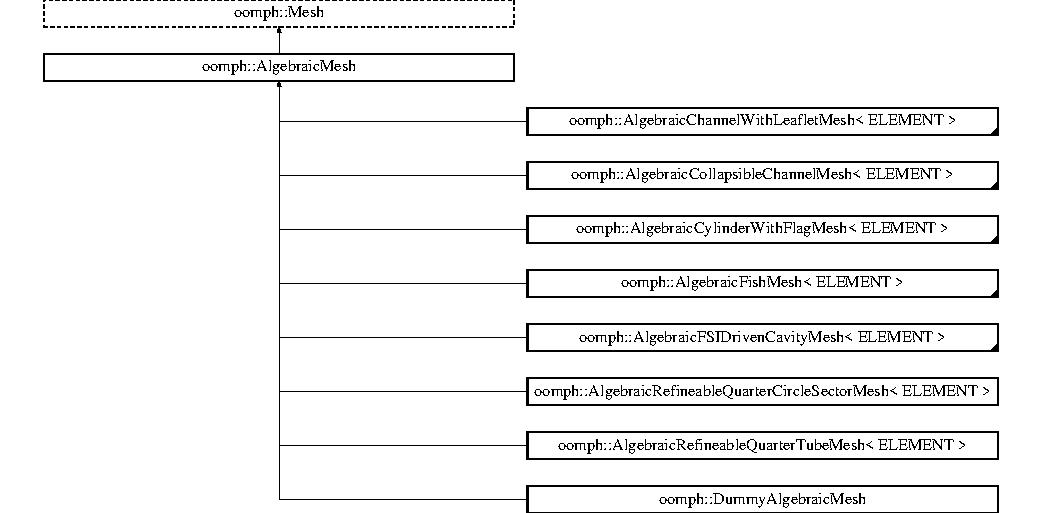
\includegraphics[height=6.896552cm]{classoomph_1_1AlgebraicMesh}
\end{center}
\end{figure}
\subsection*{Public Member Functions}
\begin{DoxyCompactItemize}
\item 
\hyperlink{classoomph_1_1AlgebraicMesh_a27bab6278bc48a4bf5d22874fc1a0e16}{Algebraic\+Mesh} ()
\item 
\hyperlink{classoomph_1_1AlgebraicMesh_a83aeb848d30991ccb959c553769e00e3}{Algebraic\+Mesh} (const \hyperlink{classoomph_1_1AlgebraicMesh}{Algebraic\+Mesh} \&)
\begin{DoxyCompactList}\small\item\em Broken copy constructor. \end{DoxyCompactList}\item 
\hyperlink{classoomph_1_1AlgebraicMesh_a148dc4078a5fa2cc9ae651003e3a14ca}{$\sim$\+Algebraic\+Mesh} ()
\begin{DoxyCompactList}\small\item\em Broken assignment operator. \end{DoxyCompactList}\item 
\hyperlink{classoomph_1_1AlgebraicNode}{Algebraic\+Node} $\ast$ \hyperlink{classoomph_1_1AlgebraicMesh_aedeebbe95d2f8e67e9939cecd1be3933}{node\+\_\+pt} (const unsigned long \&n)
\begin{DoxyCompactList}\small\item\em Return a pointer to the n-\/th global \hyperlink{classoomph_1_1AlgebraicNode}{Algebraic\+Node}. \end{DoxyCompactList}\item 
virtual void \hyperlink{classoomph_1_1AlgebraicMesh_ab01d6f93354f3c4e5c9d1f0a5885a65b}{algebraic\+\_\+node\+\_\+update} (const unsigned \&\hyperlink{cfortran_8h_af6f0bd3dc13317f895c91323c25c2b8f}{t}, \hyperlink{classoomph_1_1AlgebraicNode}{Algebraic\+Node} $\ast$\&\hyperlink{classoomph_1_1AlgebraicMesh_aedeebbe95d2f8e67e9939cecd1be3933}{node\+\_\+pt})=0
\begin{DoxyCompactList}\small\item\em Update the nodal position posn at time level t (t=0\+: present; t$>$0\+: previous). Must be implemented for every specific algebraic mesh. \end{DoxyCompactList}\item 
virtual void \hyperlink{classoomph_1_1AlgebraicMesh_a6c6a35ae2be6e2766f5b80d85693c1ce}{update\+\_\+node\+\_\+update} (\hyperlink{classoomph_1_1AlgebraicNode}{Algebraic\+Node} $\ast$\&\hyperlink{classoomph_1_1AlgebraicMesh_aedeebbe95d2f8e67e9939cecd1be3933}{node\+\_\+pt})=0
\begin{DoxyCompactList}\small\item\em Update the node update info for given node, following mesh adaptation. Must be implemented for every specific algebraic mesh, though it may, of course, be left empty. \end{DoxyCompactList}\item 
void \hyperlink{classoomph_1_1AlgebraicMesh_ad3a5638cacb6df1a47c475bb177b6ed7}{node\+\_\+update} (const bool \&update\+\_\+all\+\_\+solid\+\_\+nodes=false)
\begin{DoxyCompactList}\small\item\em Update all nodal positions via algebraic node update functions \mbox{[}Doesn\textquotesingle{}t make sense to use this mesh with Solid\+Elements anyway, so we buffer the case if update\+\_\+all\+\_\+solid\+\_\+nodes is set to true.\mbox{]}. \end{DoxyCompactList}\item 
unsigned \hyperlink{classoomph_1_1AlgebraicMesh_adfac67a6cb78db3955e20a241f2f4df4}{self\+\_\+test} ()
\begin{DoxyCompactList}\small\item\em Self test\+: check consistentency of multiple node updates. \end{DoxyCompactList}\item 
void \hyperlink{classoomph_1_1AlgebraicMesh_ae3be691428fed5ec4b60cc5b7f7db49f}{add\+\_\+geom\+\_\+object\+\_\+list\+\_\+pt} (\hyperlink{classoomph_1_1GeomObject}{Geom\+Object} $\ast$geom\+\_\+object\+\_\+pt)
\begin{DoxyCompactList}\small\item\em Add the specified \hyperlink{classoomph_1_1GeomObject}{Geom\+Object} to the list of geometric objects associated with this \hyperlink{classoomph_1_1AlgebraicMesh}{Algebraic\+Mesh}; remembering that the zeroth entry is null (set in the constructor above) \end{DoxyCompactList}\item 
unsigned \hyperlink{classoomph_1_1AlgebraicMesh_ab6a636ffb928e10e004747988fb03404}{ngeom\+\_\+object\+\_\+list\+\_\+pt} ()
\begin{DoxyCompactList}\small\item\em Return number of geometric objects associated with \hyperlink{classoomph_1_1AlgebraicMesh}{Algebraic\+Mesh}. \end{DoxyCompactList}\item 
\hyperlink{classoomph_1_1GeomObject}{Geom\+Object} $\ast$ \hyperlink{classoomph_1_1AlgebraicMesh_aad2902d3afa811449f484d3174f19a5e}{geom\+\_\+object\+\_\+list\+\_\+pt} (const unsigned \&\hyperlink{cfortran_8h_adb50e893b86b3e55e751a42eab3cba82}{i})
\begin{DoxyCompactList}\small\item\em Access function to the ith \hyperlink{classoomph_1_1GeomObject}{Geom\+Object}. \end{DoxyCompactList}\end{DoxyCompactItemize}
\subsection*{Private Attributes}
\begin{DoxyCompactItemize}
\item 
\hyperlink{classoomph_1_1Vector}{Vector}$<$ \hyperlink{classoomph_1_1GeomObject}{Geom\+Object} $\ast$ $>$ \hyperlink{classoomph_1_1AlgebraicMesh_ab823bbf2e61cf588a2ae2299c5717141}{Geom\+\_\+object\+\_\+list\+\_\+pt}
\begin{DoxyCompactList}\small\item\em \hyperlink{classoomph_1_1Vector}{Vector} of Geom\+Objects associated with this \hyperlink{classoomph_1_1AlgebraicMesh}{Algebraic\+Mesh} The zeroth entry is null, proper entries from the 1st index onwards... \end{DoxyCompactList}\end{DoxyCompactItemize}
\subsection*{Additional Inherited Members}


\subsection{Detailed Description}
Algebraic meshes contain Algebraic\+Elements and Algebraic\+Nodes. They implement the node update functions that are used by the Algebraic\+Nodes to update their positions. 

Definition at line 635 of file algebraic\+\_\+elements.\+h.



\subsection{Constructor \& Destructor Documentation}
\mbox{\Hypertarget{classoomph_1_1AlgebraicMesh_a27bab6278bc48a4bf5d22874fc1a0e16}\label{classoomph_1_1AlgebraicMesh_a27bab6278bc48a4bf5d22874fc1a0e16}} 
\index{oomph\+::\+Algebraic\+Mesh@{oomph\+::\+Algebraic\+Mesh}!Algebraic\+Mesh@{Algebraic\+Mesh}}
\index{Algebraic\+Mesh@{Algebraic\+Mesh}!oomph\+::\+Algebraic\+Mesh@{oomph\+::\+Algebraic\+Mesh}}
\subsubsection{\texorpdfstring{Algebraic\+Mesh()}{AlgebraicMesh()}\hspace{0.1cm}{\footnotesize\ttfamily [1/2]}}
{\footnotesize\ttfamily oomph\+::\+Algebraic\+Mesh\+::\+Algebraic\+Mesh (\begin{DoxyParamCaption}{ }\end{DoxyParamCaption})\hspace{0.3cm}{\ttfamily [inline]}}

Constructor\+: create a null zeroth entry in the Geom\+\_\+object\+\_\+list\+\_\+pt \hyperlink{classoomph_1_1Vector}{Vector} (each \hyperlink{classoomph_1_1AlgebraicMesh}{Algebraic\+Mesh}\textquotesingle{}s constructor should add any other geometric objects to this list) 

Definition at line 643 of file algebraic\+\_\+elements.\+h.

\mbox{\Hypertarget{classoomph_1_1AlgebraicMesh_a83aeb848d30991ccb959c553769e00e3}\label{classoomph_1_1AlgebraicMesh_a83aeb848d30991ccb959c553769e00e3}} 
\index{oomph\+::\+Algebraic\+Mesh@{oomph\+::\+Algebraic\+Mesh}!Algebraic\+Mesh@{Algebraic\+Mesh}}
\index{Algebraic\+Mesh@{Algebraic\+Mesh}!oomph\+::\+Algebraic\+Mesh@{oomph\+::\+Algebraic\+Mesh}}
\subsubsection{\texorpdfstring{Algebraic\+Mesh()}{AlgebraicMesh()}\hspace{0.1cm}{\footnotesize\ttfamily [2/2]}}
{\footnotesize\ttfamily oomph\+::\+Algebraic\+Mesh\+::\+Algebraic\+Mesh (\begin{DoxyParamCaption}\item[{const \hyperlink{classoomph_1_1AlgebraicMesh}{Algebraic\+Mesh} \&}]{ }\end{DoxyParamCaption})\hspace{0.3cm}{\ttfamily [inline]}}



Broken copy constructor. 



Definition at line 649 of file algebraic\+\_\+elements.\+h.



References oomph\+::\+Broken\+Copy\+::broken\+\_\+copy().

\mbox{\Hypertarget{classoomph_1_1AlgebraicMesh_a148dc4078a5fa2cc9ae651003e3a14ca}\label{classoomph_1_1AlgebraicMesh_a148dc4078a5fa2cc9ae651003e3a14ca}} 
\index{oomph\+::\+Algebraic\+Mesh@{oomph\+::\+Algebraic\+Mesh}!````~Algebraic\+Mesh@{$\sim$\+Algebraic\+Mesh}}
\index{````~Algebraic\+Mesh@{$\sim$\+Algebraic\+Mesh}!oomph\+::\+Algebraic\+Mesh@{oomph\+::\+Algebraic\+Mesh}}
\subsubsection{\texorpdfstring{$\sim$\+Algebraic\+Mesh()}{~AlgebraicMesh()}}
{\footnotesize\ttfamily oomph\+::\+Algebraic\+Mesh\+::$\sim$\+Algebraic\+Mesh (\begin{DoxyParamCaption}{ }\end{DoxyParamCaption})\hspace{0.3cm}{\ttfamily [inline]}}



Broken assignment operator. 

Surely a proper destructor is required... ? 

Definition at line 661 of file algebraic\+\_\+elements.\+h.



\subsection{Member Function Documentation}
\mbox{\Hypertarget{classoomph_1_1AlgebraicMesh_ae3be691428fed5ec4b60cc5b7f7db49f}\label{classoomph_1_1AlgebraicMesh_ae3be691428fed5ec4b60cc5b7f7db49f}} 
\index{oomph\+::\+Algebraic\+Mesh@{oomph\+::\+Algebraic\+Mesh}!add\+\_\+geom\+\_\+object\+\_\+list\+\_\+pt@{add\+\_\+geom\+\_\+object\+\_\+list\+\_\+pt}}
\index{add\+\_\+geom\+\_\+object\+\_\+list\+\_\+pt@{add\+\_\+geom\+\_\+object\+\_\+list\+\_\+pt}!oomph\+::\+Algebraic\+Mesh@{oomph\+::\+Algebraic\+Mesh}}
\subsubsection{\texorpdfstring{add\+\_\+geom\+\_\+object\+\_\+list\+\_\+pt()}{add\_geom\_object\_list\_pt()}}
{\footnotesize\ttfamily void oomph\+::\+Algebraic\+Mesh\+::add\+\_\+geom\+\_\+object\+\_\+list\+\_\+pt (\begin{DoxyParamCaption}\item[{\hyperlink{classoomph_1_1GeomObject}{Geom\+Object} $\ast$}]{geom\+\_\+object\+\_\+pt }\end{DoxyParamCaption})\hspace{0.3cm}{\ttfamily [inline]}}



Add the specified \hyperlink{classoomph_1_1GeomObject}{Geom\+Object} to the list of geometric objects associated with this \hyperlink{classoomph_1_1AlgebraicMesh}{Algebraic\+Mesh}; remembering that the zeroth entry is null (set in the constructor above) 



Definition at line 867 of file algebraic\+\_\+elements.\+h.



Referenced by oomph\+::\+Algebraic\+Channel\+With\+Leaflet\+Mesh$<$ E\+L\+E\+M\+E\+N\+T $>$\+::\+Algebraic\+Channel\+With\+Leaflet\+Mesh(), oomph\+::\+Algebraic\+Collapsible\+Channel\+Mesh$<$ E\+L\+E\+M\+E\+N\+T $>$\+::\+Algebraic\+Collapsible\+Channel\+Mesh(), oomph\+::\+Algebraic\+Cylinder\+With\+Flag\+Mesh$<$ E\+L\+E\+M\+E\+N\+T $>$\+::\+Algebraic\+Cylinder\+With\+Flag\+Mesh(), oomph\+::\+Algebraic\+Fish\+Mesh$<$ E\+L\+E\+M\+E\+N\+T $>$\+::\+Algebraic\+Fish\+Mesh(), oomph\+::\+Algebraic\+F\+S\+I\+Driven\+Cavity\+Mesh$<$ E\+L\+E\+M\+E\+N\+T $>$\+::\+Algebraic\+F\+S\+I\+Driven\+Cavity\+Mesh(), oomph\+::\+Algebraic\+Refineable\+Quarter\+Circle\+Sector\+Mesh$<$ E\+L\+E\+M\+E\+N\+T $>$\+::\+Algebraic\+Refineable\+Quarter\+Circle\+Sector\+Mesh(), and oomph\+::\+Algebraic\+Refineable\+Quarter\+Tube\+Mesh$<$ E\+L\+E\+M\+E\+N\+T $>$\+::\+Algebraic\+Refineable\+Quarter\+Tube\+Mesh().

\mbox{\Hypertarget{classoomph_1_1AlgebraicMesh_ab01d6f93354f3c4e5c9d1f0a5885a65b}\label{classoomph_1_1AlgebraicMesh_ab01d6f93354f3c4e5c9d1f0a5885a65b}} 
\index{oomph\+::\+Algebraic\+Mesh@{oomph\+::\+Algebraic\+Mesh}!algebraic\+\_\+node\+\_\+update@{algebraic\+\_\+node\+\_\+update}}
\index{algebraic\+\_\+node\+\_\+update@{algebraic\+\_\+node\+\_\+update}!oomph\+::\+Algebraic\+Mesh@{oomph\+::\+Algebraic\+Mesh}}
\subsubsection{\texorpdfstring{algebraic\+\_\+node\+\_\+update()}{algebraic\_node\_update()}}
{\footnotesize\ttfamily virtual void oomph\+::\+Algebraic\+Mesh\+::algebraic\+\_\+node\+\_\+update (\begin{DoxyParamCaption}\item[{const unsigned \&}]{t,  }\item[{\hyperlink{classoomph_1_1AlgebraicNode}{Algebraic\+Node} $\ast$\&}]{node\+\_\+pt }\end{DoxyParamCaption})\hspace{0.3cm}{\ttfamily [pure virtual]}}



Update the nodal position posn at time level t (t=0\+: present; t$>$0\+: previous). Must be implemented for every specific algebraic mesh. 



Implemented in \hyperlink{classoomph_1_1DummyAlgebraicMesh_ae13a52cb8561a07233851e2d1db7b4e4}{oomph\+::\+Dummy\+Algebraic\+Mesh}, \hyperlink{classoomph_1_1AlgebraicRefineableQuarterTubeMesh_af98a0aaff29c54ffa35f72f7dcf6b8c7}{oomph\+::\+Algebraic\+Refineable\+Quarter\+Tube\+Mesh$<$ E\+L\+E\+M\+E\+N\+T $>$}, \hyperlink{classoomph_1_1AlgebraicRefineableQuarterCircleSectorMesh_ac591df8f18ad687e1dc9b70b731c2de1}{oomph\+::\+Algebraic\+Refineable\+Quarter\+Circle\+Sector\+Mesh$<$ E\+L\+E\+M\+E\+N\+T $>$}, \hyperlink{classoomph_1_1AlgebraicCollapsibleChannelMesh_ae1ea6d9baa12e2ca87d21d4370f41870}{oomph\+::\+Algebraic\+Collapsible\+Channel\+Mesh$<$ E\+L\+E\+M\+E\+N\+T $>$}, \hyperlink{classoomph_1_1AlgebraicChannelWithLeafletMesh_a4c01b99ca83286f872c517fc5269a890}{oomph\+::\+Algebraic\+Channel\+With\+Leaflet\+Mesh$<$ E\+L\+E\+M\+E\+N\+T $>$}, \hyperlink{classoomph_1_1AlgebraicFishMesh_ac66d6542472dac702a7414aa9d7f995f}{oomph\+::\+Algebraic\+Fish\+Mesh$<$ E\+L\+E\+M\+E\+N\+T $>$}, \hyperlink{classoomph_1_1AlgebraicCylinderWithFlagMesh_a5e1e770e82577e5702470d8b87f8599d}{oomph\+::\+Algebraic\+Cylinder\+With\+Flag\+Mesh$<$ E\+L\+E\+M\+E\+N\+T $>$}, and \hyperlink{classoomph_1_1AlgebraicFSIDrivenCavityMesh_a56c72b78935e84f7fef3f6b5d85556c3}{oomph\+::\+Algebraic\+F\+S\+I\+Driven\+Cavity\+Mesh$<$ E\+L\+E\+M\+E\+N\+T $>$}.



Referenced by oomph\+::\+Algebraic\+Node\+::node\+\_\+update().

\mbox{\Hypertarget{classoomph_1_1AlgebraicMesh_aad2902d3afa811449f484d3174f19a5e}\label{classoomph_1_1AlgebraicMesh_aad2902d3afa811449f484d3174f19a5e}} 
\index{oomph\+::\+Algebraic\+Mesh@{oomph\+::\+Algebraic\+Mesh}!geom\+\_\+object\+\_\+list\+\_\+pt@{geom\+\_\+object\+\_\+list\+\_\+pt}}
\index{geom\+\_\+object\+\_\+list\+\_\+pt@{geom\+\_\+object\+\_\+list\+\_\+pt}!oomph\+::\+Algebraic\+Mesh@{oomph\+::\+Algebraic\+Mesh}}
\subsubsection{\texorpdfstring{geom\+\_\+object\+\_\+list\+\_\+pt()}{geom\_object\_list\_pt()}}
{\footnotesize\ttfamily \hyperlink{classoomph_1_1GeomObject}{Geom\+Object}$\ast$ oomph\+::\+Algebraic\+Mesh\+::geom\+\_\+object\+\_\+list\+\_\+pt (\begin{DoxyParamCaption}\item[{const unsigned \&}]{i }\end{DoxyParamCaption})\hspace{0.3cm}{\ttfamily [inline]}}



Access function to the ith \hyperlink{classoomph_1_1GeomObject}{Geom\+Object}. 



Definition at line 879 of file algebraic\+\_\+elements.\+h.



References i.



Referenced by oomph\+::\+Missing\+\_\+masters\+\_\+functions\+::construct\+\_\+new\+\_\+external\+\_\+halo\+\_\+master\+\_\+node\+\_\+helper(), oomph\+::\+Multi\+\_\+domain\+\_\+functions\+::construct\+\_\+new\+\_\+external\+\_\+halo\+\_\+master\+\_\+node\+\_\+helper(), oomph\+::\+Missing\+\_\+masters\+\_\+functions\+::get\+\_\+required\+\_\+master\+\_\+nodal\+\_\+information\+\_\+helper(), oomph\+::\+Multi\+\_\+domain\+\_\+functions\+::get\+\_\+required\+\_\+master\+\_\+nodal\+\_\+information\+\_\+helper(), oomph\+::\+Missing\+\_\+masters\+\_\+functions\+::get\+\_\+required\+\_\+nodal\+\_\+information\+\_\+helper(), oomph\+::\+Multi\+\_\+domain\+\_\+functions\+::get\+\_\+required\+\_\+nodal\+\_\+information\+\_\+helper(), oomph\+::\+Refineable\+Triangle\+Mesh$<$ E\+L\+E\+M\+E\+N\+T $>$\+::get\+\_\+required\+\_\+nodal\+\_\+information\+\_\+helper(), and oomph\+::\+Refineable\+Triangle\+Mesh$<$ E\+L\+E\+M\+E\+N\+T $>$\+::get\+\_\+required\+\_\+nodal\+\_\+information\+\_\+load\+\_\+balance\+\_\+helper().

\mbox{\Hypertarget{classoomph_1_1AlgebraicMesh_ab6a636ffb928e10e004747988fb03404}\label{classoomph_1_1AlgebraicMesh_ab6a636ffb928e10e004747988fb03404}} 
\index{oomph\+::\+Algebraic\+Mesh@{oomph\+::\+Algebraic\+Mesh}!ngeom\+\_\+object\+\_\+list\+\_\+pt@{ngeom\+\_\+object\+\_\+list\+\_\+pt}}
\index{ngeom\+\_\+object\+\_\+list\+\_\+pt@{ngeom\+\_\+object\+\_\+list\+\_\+pt}!oomph\+::\+Algebraic\+Mesh@{oomph\+::\+Algebraic\+Mesh}}
\subsubsection{\texorpdfstring{ngeom\+\_\+object\+\_\+list\+\_\+pt()}{ngeom\_object\_list\_pt()}}
{\footnotesize\ttfamily unsigned oomph\+::\+Algebraic\+Mesh\+::ngeom\+\_\+object\+\_\+list\+\_\+pt (\begin{DoxyParamCaption}{ }\end{DoxyParamCaption})\hspace{0.3cm}{\ttfamily [inline]}}



Return number of geometric objects associated with \hyperlink{classoomph_1_1AlgebraicMesh}{Algebraic\+Mesh}. 



Definition at line 873 of file algebraic\+\_\+elements.\+h.



Referenced by oomph\+::\+Missing\+\_\+masters\+\_\+functions\+::get\+\_\+required\+\_\+master\+\_\+nodal\+\_\+information\+\_\+helper(), oomph\+::\+Multi\+\_\+domain\+\_\+functions\+::get\+\_\+required\+\_\+master\+\_\+nodal\+\_\+information\+\_\+helper(), oomph\+::\+Missing\+\_\+masters\+\_\+functions\+::get\+\_\+required\+\_\+nodal\+\_\+information\+\_\+helper(), oomph\+::\+Multi\+\_\+domain\+\_\+functions\+::get\+\_\+required\+\_\+nodal\+\_\+information\+\_\+helper(), oomph\+::\+Refineable\+Triangle\+Mesh$<$ E\+L\+E\+M\+E\+N\+T $>$\+::get\+\_\+required\+\_\+nodal\+\_\+information\+\_\+helper(), and oomph\+::\+Refineable\+Triangle\+Mesh$<$ E\+L\+E\+M\+E\+N\+T $>$\+::get\+\_\+required\+\_\+nodal\+\_\+information\+\_\+load\+\_\+balance\+\_\+helper().

\mbox{\Hypertarget{classoomph_1_1AlgebraicMesh_aedeebbe95d2f8e67e9939cecd1be3933}\label{classoomph_1_1AlgebraicMesh_aedeebbe95d2f8e67e9939cecd1be3933}} 
\index{oomph\+::\+Algebraic\+Mesh@{oomph\+::\+Algebraic\+Mesh}!node\+\_\+pt@{node\+\_\+pt}}
\index{node\+\_\+pt@{node\+\_\+pt}!oomph\+::\+Algebraic\+Mesh@{oomph\+::\+Algebraic\+Mesh}}
\subsubsection{\texorpdfstring{node\+\_\+pt()}{node\_pt()}}
{\footnotesize\ttfamily \hyperlink{classoomph_1_1AlgebraicNode}{Algebraic\+Node}$\ast$ oomph\+::\+Algebraic\+Mesh\+::node\+\_\+pt (\begin{DoxyParamCaption}\item[{const unsigned long \&}]{n }\end{DoxyParamCaption})\hspace{0.3cm}{\ttfamily [inline]}}



Return a pointer to the n-\/th global \hyperlink{classoomph_1_1AlgebraicNode}{Algebraic\+Node}. 



Definition at line 665 of file algebraic\+\_\+elements.\+h.



References t.

\mbox{\Hypertarget{classoomph_1_1AlgebraicMesh_ad3a5638cacb6df1a47c475bb177b6ed7}\label{classoomph_1_1AlgebraicMesh_ad3a5638cacb6df1a47c475bb177b6ed7}} 
\index{oomph\+::\+Algebraic\+Mesh@{oomph\+::\+Algebraic\+Mesh}!node\+\_\+update@{node\+\_\+update}}
\index{node\+\_\+update@{node\+\_\+update}!oomph\+::\+Algebraic\+Mesh@{oomph\+::\+Algebraic\+Mesh}}
\subsubsection{\texorpdfstring{node\+\_\+update()}{node\_update()}}
{\footnotesize\ttfamily void oomph\+::\+Algebraic\+Mesh\+::node\+\_\+update (\begin{DoxyParamCaption}\item[{const bool \&}]{update\+\_\+all\+\_\+solid\+\_\+nodes = {\ttfamily false} }\end{DoxyParamCaption})\hspace{0.3cm}{\ttfamily [inline]}, {\ttfamily [virtual]}}



Update all nodal positions via algebraic node update functions \mbox{[}Doesn\textquotesingle{}t make sense to use this mesh with Solid\+Elements anyway, so we buffer the case if update\+\_\+all\+\_\+solid\+\_\+nodes is set to true.\mbox{]}. 



Reimplemented from \hyperlink{classoomph_1_1Mesh_a95bf112e5e1b3892e70a41f91b3cc523}{oomph\+::\+Mesh}.



Reimplemented in \hyperlink{classoomph_1_1AlgebraicRefineableFishMesh_a8123da4b48355b39f19e0494a9d4545c}{oomph\+::\+Algebraic\+Refineable\+Fish\+Mesh$<$ E\+L\+E\+M\+E\+N\+T $>$}, \hyperlink{classoomph_1_1AlgebraicRefineableQuarterTubeMesh_af521c0a76cf0bd14692979bd7747507d}{oomph\+::\+Algebraic\+Refineable\+Quarter\+Tube\+Mesh$<$ E\+L\+E\+M\+E\+N\+T $>$}, \hyperlink{classoomph_1_1AlgebraicRefineableQuarterCircleSectorMesh_a32a096b894031167a90bafdab167ffc7}{oomph\+::\+Algebraic\+Refineable\+Quarter\+Circle\+Sector\+Mesh$<$ E\+L\+E\+M\+E\+N\+T $>$}, and \hyperlink{classoomph_1_1AlgebraicFishMesh_a39cd5a86b0f762efd09f4fefba6da1c3}{oomph\+::\+Algebraic\+Fish\+Mesh$<$ E\+L\+E\+M\+E\+N\+T $>$}.



Definition at line 699 of file algebraic\+\_\+elements.\+h.



References oomph\+::\+Node\+::hanging\+\_\+pt(), i, oomph\+::\+Node\+::is\+\_\+hanging(), oomph\+::\+Hang\+Info\+::master\+\_\+weight(), oomph\+::\+Node\+::ndim(), oomph\+::\+Hang\+Info\+::nmaster(), oomph\+::\+Algebraic\+Node\+::node\+\_\+update(), oomph\+::\+Node\+::perform\+\_\+auxiliary\+\_\+node\+\_\+update\+\_\+fct(), oomph\+::\+Global\+\_\+string\+\_\+for\+\_\+annotation\+::string(), and oomph\+::\+Node\+::x().



Referenced by oomph\+::\+Algebraic\+Fish\+Mesh$<$ E\+L\+E\+M\+E\+N\+T $>$\+::node\+\_\+update(), oomph\+::\+Algebraic\+Refineable\+Quarter\+Circle\+Sector\+Mesh$<$ E\+L\+E\+M\+E\+N\+T $>$\+::node\+\_\+update(), and oomph\+::\+Algebraic\+Refineable\+Quarter\+Tube\+Mesh$<$ E\+L\+E\+M\+E\+N\+T $>$\+::node\+\_\+update().

\mbox{\Hypertarget{classoomph_1_1AlgebraicMesh_adfac67a6cb78db3955e20a241f2f4df4}\label{classoomph_1_1AlgebraicMesh_adfac67a6cb78db3955e20a241f2f4df4}} 
\index{oomph\+::\+Algebraic\+Mesh@{oomph\+::\+Algebraic\+Mesh}!self\+\_\+test@{self\+\_\+test}}
\index{self\+\_\+test@{self\+\_\+test}!oomph\+::\+Algebraic\+Mesh@{oomph\+::\+Algebraic\+Mesh}}
\subsubsection{\texorpdfstring{self\+\_\+test()}{self\_test()}}
{\footnotesize\ttfamily unsigned oomph\+::\+Algebraic\+Mesh\+::self\+\_\+test (\begin{DoxyParamCaption}{ }\end{DoxyParamCaption})\hspace{0.3cm}{\ttfamily [inline]}}



Self test\+: check consistentency of multiple node updates. 



Definition at line 834 of file algebraic\+\_\+elements.\+h.



References oomph\+::oomph\+\_\+info, oomph\+::\+Algebraic\+Node\+::self\+\_\+test(), and oomph\+::\+Mesh\+::self\+\_\+test().



Referenced by oomph\+::\+Algebraic\+Refineable\+Quarter\+Tube\+Mesh$<$ E\+L\+E\+M\+E\+N\+T $>$\+::self\+\_\+test(), and oomph\+::\+Algebraic\+Refineable\+Quarter\+Circle\+Sector\+Mesh$<$ E\+L\+E\+M\+E\+N\+T $>$\+::self\+\_\+test().

\mbox{\Hypertarget{classoomph_1_1AlgebraicMesh_a6c6a35ae2be6e2766f5b80d85693c1ce}\label{classoomph_1_1AlgebraicMesh_a6c6a35ae2be6e2766f5b80d85693c1ce}} 
\index{oomph\+::\+Algebraic\+Mesh@{oomph\+::\+Algebraic\+Mesh}!update\+\_\+node\+\_\+update@{update\+\_\+node\+\_\+update}}
\index{update\+\_\+node\+\_\+update@{update\+\_\+node\+\_\+update}!oomph\+::\+Algebraic\+Mesh@{oomph\+::\+Algebraic\+Mesh}}
\subsubsection{\texorpdfstring{update\+\_\+node\+\_\+update()}{update\_node\_update()}}
{\footnotesize\ttfamily virtual void oomph\+::\+Algebraic\+Mesh\+::update\+\_\+node\+\_\+update (\begin{DoxyParamCaption}\item[{\hyperlink{classoomph_1_1AlgebraicNode}{Algebraic\+Node} $\ast$\&}]{node\+\_\+pt }\end{DoxyParamCaption})\hspace{0.3cm}{\ttfamily [pure virtual]}}



Update the node update info for given node, following mesh adaptation. Must be implemented for every specific algebraic mesh, though it may, of course, be left empty. 



Implemented in \hyperlink{classoomph_1_1DummyAlgebraicMesh_a8797e6bf088b172b5d7e1de8a2dfc326}{oomph\+::\+Dummy\+Algebraic\+Mesh}, \hyperlink{classoomph_1_1RefineableAlgebraicCollapsibleChannelMesh_a4bc2b99f24e5e5dc534fe5906d4f4e6e}{oomph\+::\+Refineable\+Algebraic\+Collapsible\+Channel\+Mesh$<$ E\+L\+E\+M\+E\+N\+T $>$}, \hyperlink{classoomph_1_1AlgebraicRefineableQuarterTubeMesh_a7ed9f4ce0442a6f962a1561318542a67}{oomph\+::\+Algebraic\+Refineable\+Quarter\+Tube\+Mesh$<$ E\+L\+E\+M\+E\+N\+T $>$}, \hyperlink{classoomph_1_1AlgebraicRefineableQuarterCircleSectorMesh_a08abc1bf64e0637fc87c36638c41b846}{oomph\+::\+Algebraic\+Refineable\+Quarter\+Circle\+Sector\+Mesh$<$ E\+L\+E\+M\+E\+N\+T $>$}, \hyperlink{classoomph_1_1AlgebraicCollapsibleChannelMesh_abad38fb50d067a126af1161a3a603972}{oomph\+::\+Algebraic\+Collapsible\+Channel\+Mesh$<$ E\+L\+E\+M\+E\+N\+T $>$}, \hyperlink{classoomph_1_1RefineableAlgebraicChannelWithLeafletMesh_a8ee7168fbb84bb87880a2590dd52eaa8}{oomph\+::\+Refineable\+Algebraic\+Channel\+With\+Leaflet\+Mesh$<$ E\+L\+E\+M\+E\+N\+T $>$}, \hyperlink{classoomph_1_1AlgebraicFishMesh_a4f992939c299f87abc762c14aab50b5c}{oomph\+::\+Algebraic\+Fish\+Mesh$<$ E\+L\+E\+M\+E\+N\+T $>$}, \hyperlink{classoomph_1_1RefineableAlgebraicCylinderWithFlagMesh_a186963cf4b1fc118929e49e012eba4d2}{oomph\+::\+Refineable\+Algebraic\+Cylinder\+With\+Flag\+Mesh$<$ E\+L\+E\+M\+E\+N\+T $>$}, \hyperlink{classoomph_1_1AlgebraicChannelWithLeafletMesh_ace3a90b4e530c75bec8301e2291151eb}{oomph\+::\+Algebraic\+Channel\+With\+Leaflet\+Mesh$<$ E\+L\+E\+M\+E\+N\+T $>$}, \hyperlink{classoomph_1_1RefineableAlgebraicFSIDrivenCavityMesh_aa68685323573763e1ded0cceed5ad14f}{oomph\+::\+Refineable\+Algebraic\+F\+S\+I\+Driven\+Cavity\+Mesh$<$ E\+L\+E\+M\+E\+N\+T $>$}, \hyperlink{classoomph_1_1AlgebraicCylinderWithFlagMesh_a9d909de1db84a3b7e42494535b152d92}{oomph\+::\+Algebraic\+Cylinder\+With\+Flag\+Mesh$<$ E\+L\+E\+M\+E\+N\+T $>$}, and \hyperlink{classoomph_1_1AlgebraicFSIDrivenCavityMesh_a87d34d6cf84c62a9049773451c664176}{oomph\+::\+Algebraic\+F\+S\+I\+Driven\+Cavity\+Mesh$<$ E\+L\+E\+M\+E\+N\+T $>$}.



Referenced by oomph\+::\+Missing\+\_\+masters\+\_\+functions\+::construct\+\_\+new\+\_\+external\+\_\+halo\+\_\+master\+\_\+node\+\_\+helper(), oomph\+::\+Multi\+\_\+domain\+\_\+functions\+::construct\+\_\+new\+\_\+external\+\_\+halo\+\_\+master\+\_\+node\+\_\+helper(), oomph\+::\+Missing\+\_\+masters\+\_\+functions\+::construct\+\_\+new\+\_\+external\+\_\+halo\+\_\+node\+\_\+helper(), oomph\+::\+Multi\+\_\+domain\+\_\+functions\+::construct\+\_\+new\+\_\+external\+\_\+halo\+\_\+node\+\_\+helper(), oomph\+::\+Refineable\+Triangle\+Mesh$<$ E\+L\+E\+M\+E\+N\+T $>$\+::construct\+\_\+new\+\_\+halo\+\_\+node\+\_\+helper(), oomph\+::\+Refineable\+Triangle\+Mesh$<$ E\+L\+E\+M\+E\+N\+T $>$\+::construct\+\_\+new\+\_\+node\+\_\+load\+\_\+balance\+\_\+helper(), and oomph\+::\+Algebraic\+Element\+Base\+::setup\+\_\+algebraic\+\_\+node\+\_\+update().



\subsection{Member Data Documentation}
\mbox{\Hypertarget{classoomph_1_1AlgebraicMesh_ab823bbf2e61cf588a2ae2299c5717141}\label{classoomph_1_1AlgebraicMesh_ab823bbf2e61cf588a2ae2299c5717141}} 
\index{oomph\+::\+Algebraic\+Mesh@{oomph\+::\+Algebraic\+Mesh}!Geom\+\_\+object\+\_\+list\+\_\+pt@{Geom\+\_\+object\+\_\+list\+\_\+pt}}
\index{Geom\+\_\+object\+\_\+list\+\_\+pt@{Geom\+\_\+object\+\_\+list\+\_\+pt}!oomph\+::\+Algebraic\+Mesh@{oomph\+::\+Algebraic\+Mesh}}
\subsubsection{\texorpdfstring{Geom\+\_\+object\+\_\+list\+\_\+pt}{Geom\_object\_list\_pt}}
{\footnotesize\ttfamily \hyperlink{classoomph_1_1Vector}{Vector}$<$\hyperlink{classoomph_1_1GeomObject}{Geom\+Object}$\ast$$>$ oomph\+::\+Algebraic\+Mesh\+::\+Geom\+\_\+object\+\_\+list\+\_\+pt\hspace{0.3cm}{\ttfamily [private]}}



\hyperlink{classoomph_1_1Vector}{Vector} of Geom\+Objects associated with this \hyperlink{classoomph_1_1AlgebraicMesh}{Algebraic\+Mesh} The zeroth entry is null, proper entries from the 1st index onwards... 



Definition at line 889 of file algebraic\+\_\+elements.\+h.



The documentation for this class was generated from the following file\+:\begin{DoxyCompactItemize}
\item 
\hyperlink{algebraic__elements_8h}{algebraic\+\_\+elements.\+h}\end{DoxyCompactItemize}

\hypertarget{classoomph_1_1AlgebraicNode}{}\section{oomph\+:\+:Algebraic\+Node Class Reference}
\label{classoomph_1_1AlgebraicNode}\index{oomph\+::\+Algebraic\+Node@{oomph\+::\+Algebraic\+Node}}


{\ttfamily \#include $<$algebraic\+\_\+elements.\+h$>$}

Inheritance diagram for oomph\+:\+:Algebraic\+Node\+:\begin{figure}[H]
\begin{center}
\leavevmode
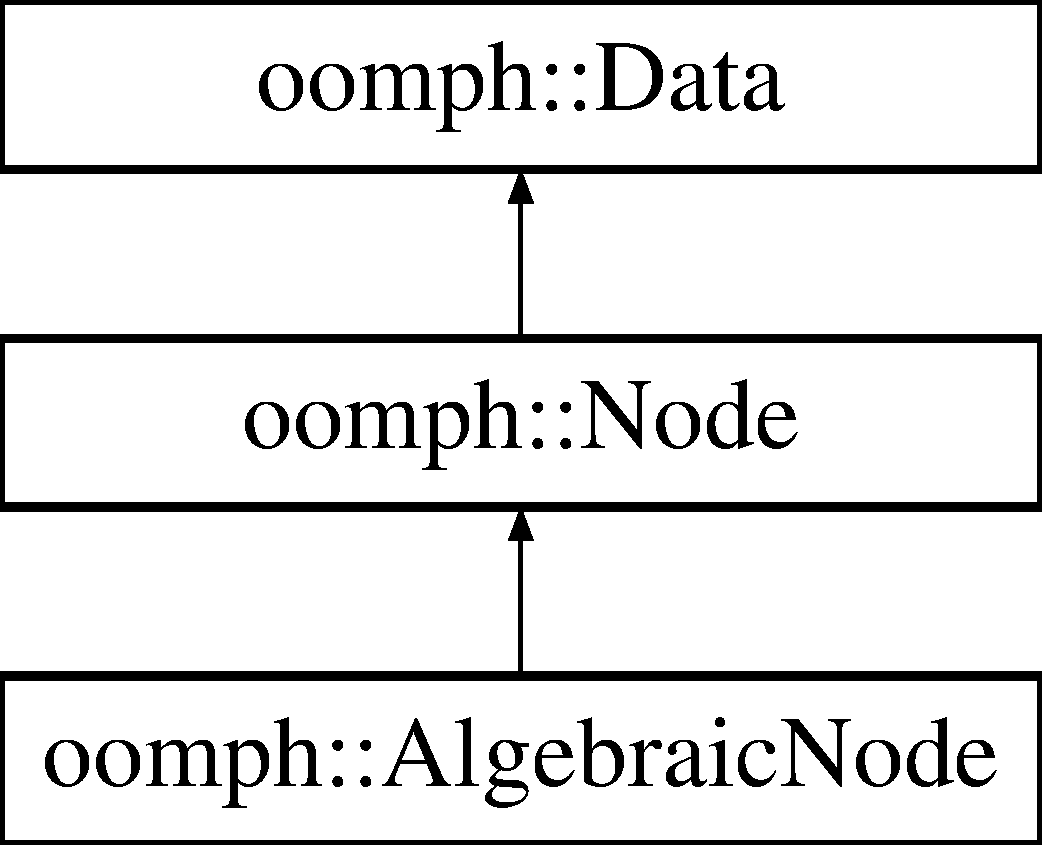
\includegraphics[height=3.000000cm]{classoomph_1_1AlgebraicNode}
\end{center}
\end{figure}
\subsection*{Public Member Functions}
\begin{DoxyCompactItemize}
\item 
\hyperlink{classoomph_1_1AlgebraicNode_a7e421172a1063fc49f37559f23837763}{Algebraic\+Node} ()
\begin{DoxyCompactList}\small\item\em Default Constructor. \end{DoxyCompactList}\item 
\hyperlink{classoomph_1_1AlgebraicNode_a88eb17187c750f1f1a04d0dd554dd9b5}{Algebraic\+Node} (const unsigned \&n\+\_\+dim, const unsigned \&n\+\_\+position\+\_\+type, const unsigned \&initial\+\_\+nvalue)
\begin{DoxyCompactList}\small\item\em Constructor for steady algebraic node of spatial dimension n\+\_\+dim, with n\+\_\+position\+\_\+type generalised coordinates and with initial\+\_\+nvalue dofs. \end{DoxyCompactList}\item 
\hyperlink{classoomph_1_1AlgebraicNode_ab97ffb4a9663ce90e4d7788315ba31a1}{Algebraic\+Node} (\hyperlink{classoomph_1_1TimeStepper}{Time\+Stepper} $\ast$\hyperlink{classoomph_1_1Data_a5b34970d16205921dca3ada720da8445}{time\+\_\+stepper\+\_\+pt}, const unsigned \&n\+\_\+dim, const unsigned \&n\+\_\+position\+\_\+type, const unsigned \&initial\+\_\+nvalue)
\begin{DoxyCompactList}\small\item\em Constructor for bog-\/standard algebraic node of spatial dimension n\+\_\+dim, with n\+\_\+position\+\_\+type generalised coordinates, with initial\+\_\+nvalue dofs and with time dependence. \end{DoxyCompactList}\item 
virtual \hyperlink{classoomph_1_1AlgebraicNode_af1fef20e4dd950f70003c3db5d289044}{$\sim$\+Algebraic\+Node} ()
\begin{DoxyCompactList}\small\item\em Destructor (empty) \end{DoxyCompactList}\item 
\hyperlink{classoomph_1_1AlgebraicNode_a2dc795a77c106b7dd6bd3ab2c8034956}{Algebraic\+Node} (const \hyperlink{classoomph_1_1AlgebraicNode}{Algebraic\+Node} \&)
\begin{DoxyCompactList}\small\item\em Broken copy constructor. \end{DoxyCompactList}\item 
void \hyperlink{classoomph_1_1AlgebraicNode_a754dc8fcac3382a07f60262c9792c84c}{node\+\_\+update} (const bool \&update\+\_\+all\+\_\+time\+\_\+levels\+\_\+for\+\_\+new\+\_\+node=false)
\begin{DoxyCompactList}\small\item\em Broken assignment operator. \end{DoxyCompactList}\item 
unsigned \hyperlink{classoomph_1_1AlgebraicNode_a8c9e49f378f2dc9e93e62e281bf58d27}{nnode\+\_\+update\+\_\+fcts} ()
\begin{DoxyCompactList}\small\item\em Number of node update fcts. \end{DoxyCompactList}\item 
int \hyperlink{classoomph_1_1AlgebraicNode_a8887f3a7c445b098835a7703c3a19bd2}{node\+\_\+update\+\_\+fct\+\_\+id} ()
\begin{DoxyCompactList}\small\item\em Default (usually first if there are multiple ones) node update fct id. \end{DoxyCompactList}\item 
void \hyperlink{classoomph_1_1AlgebraicNode_a6b910e50ee47113aa0256e46043b0f27}{node\+\_\+update\+\_\+fct\+\_\+id} (\hyperlink{classoomph_1_1Vector}{Vector}$<$ int $>$ \&id)
\begin{DoxyCompactList}\small\item\em Return vector of node update fct ids (vector is resized to contain the correct number of entries). Somewhat costly to call as map needs to be copied into vector. \end{DoxyCompactList}\item 
\hyperlink{classoomph_1_1AlgebraicMesh}{Algebraic\+Mesh} $\ast$ \hyperlink{classoomph_1_1AlgebraicNode_a929a96691397e1990fdf785dfcea5c07}{mesh\+\_\+pt} ()
\begin{DoxyCompactList}\small\item\em Default (usually first) mesh that implements update function. \end{DoxyCompactList}\item 
\hyperlink{classoomph_1_1AlgebraicMesh}{Algebraic\+Mesh} $\ast$ \hyperlink{classoomph_1_1AlgebraicNode_ae07189bb28dcba7d31e736de391fe54f}{mesh\+\_\+pt} (const int \&id)
\begin{DoxyCompactList}\small\item\em \hyperlink{classoomph_1_1Mesh}{Mesh} that implements the id-\/th node update function. \end{DoxyCompactList}\item 
unsigned \hyperlink{classoomph_1_1AlgebraicNode_a0e1fa66d3543da39a5e728d8af5c1734}{ngeom\+\_\+object} (const int \&id)
\begin{DoxyCompactList}\small\item\em Number of geometric objects involved in id-\/th update function. \end{DoxyCompactList}\item 
unsigned \hyperlink{classoomph_1_1AlgebraicNode_a10f49849e0942e68c6791810ffc6fb31}{ngeom\+\_\+object} () const
\begin{DoxyCompactList}\small\item\em Number of geometric objects involved in default (usually first) update function. \end{DoxyCompactList}\item 
\hyperlink{classoomph_1_1Vector}{Vector}$<$ \hyperlink{classoomph_1_1GeomObject}{Geom\+Object} $\ast$ $>$ \& \hyperlink{classoomph_1_1AlgebraicNode_aa82f9b47f4b7fb1cc49178c48c2873d3}{vector\+\_\+geom\+\_\+object\+\_\+pt} (const int \&id)
\begin{DoxyCompactList}\small\item\em Return vector of geometric objects involved in id-\/th update function. \end{DoxyCompactList}\item 
\hyperlink{classoomph_1_1Vector}{Vector}$<$ \hyperlink{classoomph_1_1GeomObject}{Geom\+Object} $\ast$ $>$ \& \hyperlink{classoomph_1_1AlgebraicNode_aa242d4039f28e65c407bf90033489a75}{vector\+\_\+geom\+\_\+object\+\_\+pt} ()
\begin{DoxyCompactList}\small\item\em Return vector of geometric objects involved in default (usually first) update function. \end{DoxyCompactList}\item 
\hyperlink{classoomph_1_1GeomObject}{Geom\+Object} $\ast$$\ast$ \hyperlink{classoomph_1_1AlgebraicNode_aac2c907cb2258892583d38e8c3e52326}{all\+\_\+geom\+\_\+object\+\_\+pt} ()
\begin{DoxyCompactList}\small\item\em Return the vector of all geometric objects. \end{DoxyCompactList}\item 
\hyperlink{classoomph_1_1GeomObject}{Geom\+Object} $\ast$ \hyperlink{classoomph_1_1AlgebraicNode_a6ea1dc01f3b657b5c63d6de2b67ea990}{geom\+\_\+object\+\_\+pt} (const unsigned \&\hyperlink{cfortran_8h_adb50e893b86b3e55e751a42eab3cba82}{i})
\begin{DoxyCompactList}\small\item\em Return pointer to i-\/th geometric object involved in default (usually first) update function. \end{DoxyCompactList}\item 
unsigned \hyperlink{classoomph_1_1AlgebraicNode_a18b508012bc638d85539568219865383}{nref\+\_\+value} (const int \&id)
\begin{DoxyCompactList}\small\item\em Number of reference values involved in id-\/th update function. \end{DoxyCompactList}\item 
unsigned \hyperlink{classoomph_1_1AlgebraicNode_a1d5805d44950ad5783720ba7bb5a372a}{nref\+\_\+value} ()
\begin{DoxyCompactList}\small\item\em Number of reference values involved in default (usually first) update function. \end{DoxyCompactList}\item 
\hyperlink{classoomph_1_1Vector}{Vector}$<$ double $>$ \& \hyperlink{classoomph_1_1AlgebraicNode_ad2236d78dd07f59345ee7a8275d3fefb}{vector\+\_\+ref\+\_\+value} ()
\begin{DoxyCompactList}\small\item\em Return vector of reference values involved in default (usually first) update function. \end{DoxyCompactList}\item 
\hyperlink{classoomph_1_1Vector}{Vector}$<$ double $>$ \& \hyperlink{classoomph_1_1AlgebraicNode_a95a41fd3d3aa47a6928715bc7f1059a0}{vector\+\_\+ref\+\_\+value} (const int \&id)
\begin{DoxyCompactList}\small\item\em Return vector of reference values involved in id-\/th update function. \end{DoxyCompactList}\item 
double \hyperlink{classoomph_1_1AlgebraicNode_a9658be0ccdb312e7cf0175663407f463}{ref\+\_\+value} (const unsigned \&\hyperlink{cfortran_8h_adb50e893b86b3e55e751a42eab3cba82}{i})
\begin{DoxyCompactList}\small\item\em Return i-\/th reference value involved in default (usually first) update function. \end{DoxyCompactList}\item 
void \hyperlink{classoomph_1_1AlgebraicNode_a91900aebc9ddbceaf5fb24b977f25e44}{add\+\_\+node\+\_\+update\+\_\+info} (const int \&id, \hyperlink{classoomph_1_1AlgebraicMesh}{Algebraic\+Mesh} $\ast$\hyperlink{classoomph_1_1AlgebraicNode_a929a96691397e1990fdf785dfcea5c07}{mesh\+\_\+pt}, const \hyperlink{classoomph_1_1Vector}{Vector}$<$ \hyperlink{classoomph_1_1GeomObject}{Geom\+Object} $\ast$$>$ \&\hyperlink{classoomph_1_1AlgebraicNode_a6ea1dc01f3b657b5c63d6de2b67ea990}{geom\+\_\+object\+\_\+pt}, const \hyperlink{classoomph_1_1Vector}{Vector}$<$ double $>$ \&\hyperlink{classoomph_1_1AlgebraicNode_a9658be0ccdb312e7cf0175663407f463}{ref\+\_\+value}, const bool \&called\+\_\+from\+\_\+constructor=false)
\begin{DoxyCompactList}\small\item\em Add algebraic update information for node\+: What\textquotesingle{}s the ID of the mesh update function (typically used within the mesh) Which \hyperlink{classoomph_1_1Mesh}{Mesh} implements the update operation? Also, pass the vector of geometric objects and the vectors of reference values that are needed for the update operation. Negative values for ID are only allowed when called from node constructor, as indicated by the final argument which defaults to false. \end{DoxyCompactList}\item 
void \hyperlink{classoomph_1_1AlgebraicNode_a646b087c73a6b355709369d30081fb4a}{add\+\_\+node\+\_\+update\+\_\+info} (\hyperlink{classoomph_1_1AlgebraicMesh}{Algebraic\+Mesh} $\ast$\hyperlink{classoomph_1_1AlgebraicNode_a929a96691397e1990fdf785dfcea5c07}{mesh\+\_\+pt}, const \hyperlink{classoomph_1_1Vector}{Vector}$<$ \hyperlink{classoomph_1_1GeomObject}{Geom\+Object} $\ast$$>$ \&\hyperlink{classoomph_1_1AlgebraicNode_a6ea1dc01f3b657b5c63d6de2b67ea990}{geom\+\_\+object\+\_\+pt}, const \hyperlink{classoomph_1_1Vector}{Vector}$<$ double $>$ \&\hyperlink{classoomph_1_1AlgebraicNode_a9658be0ccdb312e7cf0175663407f463}{ref\+\_\+value})
\begin{DoxyCompactList}\small\item\em Add algebraic update information for node\+: Which \hyperlink{classoomph_1_1Mesh}{Mesh} implements the update operation? Also, pass the vector of geometric objects and the vectors of reference values that are needed for the update operation. We\textquotesingle{}re assigning a default node update fct id of 0. \end{DoxyCompactList}\item 
void \hyperlink{classoomph_1_1AlgebraicNode_a9de65e71efa3050187d41f05602accfe}{kill\+\_\+node\+\_\+update\+\_\+info} (const int \&id=0)
\begin{DoxyCompactList}\small\item\em Erase algebraic node update information for id-\/th node update function. Id defaults to 0. \end{DoxyCompactList}\item 
unsigned \hyperlink{classoomph_1_1AlgebraicNode_a68b0fc5d9b38bb087f889424382a3ecd}{self\+\_\+test} ()
\begin{DoxyCompactList}\small\item\em Perform self test\+: If the node has multiple node update functions, check that they all give the same result. Return 1/0 for failure/success. (Failure if max. difference between the nodal positions for different update functions exceeds \hyperlink{classoomph_1_1AlgebraicNode_a5696d589c11a229f402d68476c7fe435}{Algebraic\+Node\+::\+Max\+\_\+allowed\+\_\+difference\+\_\+between\+\_\+node\+\_\+update\+\_\+fcts}. \end{DoxyCompactList}\end{DoxyCompactItemize}
\subsection*{Private Member Functions}
\begin{DoxyCompactItemize}
\item 
void \hyperlink{classoomph_1_1AlgebraicNode_a5f9d80a2826974b63376a4c58e0812fc}{set\+\_\+default\+\_\+node\+\_\+update} (const int \&id)
\begin{DoxyCompactList}\small\item\em Make id-\/th node update function the default. \end{DoxyCompactList}\end{DoxyCompactItemize}
\subsection*{Private Attributes}
\begin{DoxyCompactItemize}
\item 
std\+::map$<$ int, \hyperlink{classoomph_1_1AlgebraicMesh}{Algebraic\+Mesh} $\ast$$>$ \hyperlink{classoomph_1_1AlgebraicNode_af60d3301f8ffd16bcd3ee32809beebd8}{Mesh\+\_\+pt}
\begin{DoxyCompactList}\small\item\em Pointer to mesh that performs the specified node update operation (Map because this node may only use the \hyperlink{classoomph_1_1Mesh}{Mesh}\textquotesingle{}s 116th node update fct. There\textquotesingle{}s no point in wasting an entire vector for the non-\/existing entries) \end{DoxyCompactList}\item 
std\+::map$<$ int, \hyperlink{classoomph_1_1Vector}{Vector}$<$ \hyperlink{classoomph_1_1GeomObject}{Geom\+Object} $\ast$ $>$ $>$ \hyperlink{classoomph_1_1AlgebraicNode_a1e378862db7979494c3d224df3f98b2b}{Geom\+\_\+object\+\_\+pt}
\begin{DoxyCompactList}\small\item\em \hyperlink{classoomph_1_1Vector}{Vector} of geometric objects that are involved in the specified node update operation. (Map because this node may only use the \hyperlink{classoomph_1_1Mesh}{Mesh}\textquotesingle{}s 116th node update fct. There\textquotesingle{}s no point in wasting an entire vector for the non-\/existing entries) \end{DoxyCompactList}\item 
std\+::map$<$ int, \hyperlink{classoomph_1_1Vector}{Vector}$<$ double $>$ $>$ \hyperlink{classoomph_1_1AlgebraicNode_a64362fcb07761e9d523c5c6de01612e0}{Ref\+\_\+value}
\begin{DoxyCompactList}\small\item\em \hyperlink{classoomph_1_1Vector}{Vector} of reference values that are required for the specified node update operation. (Map because this node may only use the \hyperlink{classoomph_1_1Mesh}{Mesh}\textquotesingle{}s 116th node update fct. There\textquotesingle{}s no point in wasting an entire vector for the non-\/existing entries) \end{DoxyCompactList}\item 
std\+::map$<$ int, \hyperlink{classoomph_1_1AlgebraicMesh}{Algebraic\+Mesh} $\ast$ $>$\+::iterator \hyperlink{classoomph_1_1AlgebraicNode_ac8cb7e56e80f1c0f3e200562d2b1d39e}{Default\+\_\+it\+\_\+mesh\+\_\+pt}
\begin{DoxyCompactList}\small\item\em Default iterator for mesh\+: This mesh performs the default update. \end{DoxyCompactList}\item 
std\+::map$<$ int, \hyperlink{classoomph_1_1Vector}{Vector}$<$ \hyperlink{classoomph_1_1GeomObject}{Geom\+Object} $\ast$ $>$ $>$\+::iterator \hyperlink{classoomph_1_1AlgebraicNode_a37df439c4a73665cf04548f245419150}{Default\+\_\+it\+\_\+geom\+\_\+object\+\_\+pt}
\begin{DoxyCompactList}\small\item\em Default iterator for vector of geom objects. These Geom\+Objects are involved in the default update. \end{DoxyCompactList}\item 
std\+::map$<$ int, \hyperlink{classoomph_1_1Vector}{Vector}$<$ double $>$ $>$\+::iterator \hyperlink{classoomph_1_1AlgebraicNode_a49673336a201aca02390f13ceb72dd19}{Default\+\_\+it\+\_\+ref\+\_\+value}
\item 
int \hyperlink{classoomph_1_1AlgebraicNode_adba92e804261f449a9142920661c339a}{Default\+\_\+node\+\_\+update\+\_\+fct\+\_\+id}
\begin{DoxyCompactList}\small\item\em Default node update function ID. \end{DoxyCompactList}\end{DoxyCompactItemize}
\subsection*{Static Private Attributes}
\begin{DoxyCompactItemize}
\item 
static double \hyperlink{classoomph_1_1AlgebraicNode_a5696d589c11a229f402d68476c7fe435}{Max\+\_\+allowed\+\_\+difference\+\_\+between\+\_\+node\+\_\+update\+\_\+fcts} =1.\+0e-\/10
\item 
static int \hyperlink{classoomph_1_1AlgebraicNode_af6d3b50db54114b5cf22f86c0ceed2f8}{Dummy\+\_\+node\+\_\+update\+\_\+fct\+\_\+id} =-\/100
\begin{DoxyCompactList}\small\item\em Default (negative!) remesh fct id for nodes for which no remesh fct is defined. \end{DoxyCompactList}\item 
static \hyperlink{classoomph_1_1AlgebraicMesh}{Algebraic\+Mesh} $\ast$ \hyperlink{classoomph_1_1AlgebraicNode_a21f78f61150e308456db352907aa26c6}{Dummy\+\_\+mesh\+\_\+pt} =\&\hyperlink{classoomph_1_1AlgebraicNode_aa89c19c1d7c5e5efd1b501098491bf5c}{Algebraic\+Node\+::\+Dummy\+\_\+mesh}
\begin{DoxyCompactList}\small\item\em Default dummy mesh to point to for nodes for which no remesh fct is defined. \end{DoxyCompactList}\item 
static \hyperlink{classoomph_1_1DummyAlgebraicMesh}{Dummy\+Algebraic\+Mesh} \hyperlink{classoomph_1_1AlgebraicNode_aa89c19c1d7c5e5efd1b501098491bf5c}{Dummy\+\_\+mesh}
\begin{DoxyCompactList}\small\item\em Static Dummy mesh to which the pointer is addressed. \end{DoxyCompactList}\item 
static \hyperlink{classoomph_1_1Vector}{Vector}$<$ \hyperlink{classoomph_1_1GeomObject}{Geom\+Object} $\ast$ $>$ \hyperlink{classoomph_1_1AlgebraicNode_a74bfe556a50b852ee06245e6a374d5fc}{Dummy\+\_\+geom\+\_\+object\+\_\+pt}
\begin{DoxyCompactList}\small\item\em Default dummy vector of geom objects to point to for nodes for which no remesh fct is defined. \end{DoxyCompactList}\item 
static \hyperlink{classoomph_1_1Vector}{Vector}$<$ double $>$ \hyperlink{classoomph_1_1AlgebraicNode_af73f0a803e1bdf2a7a1c7f1f4384df61}{Dummy\+\_\+ref\+\_\+value}
\begin{DoxyCompactList}\small\item\em Default dummy vector of reference values to point to for nodes for which no remesh fct is defined. \end{DoxyCompactList}\end{DoxyCompactItemize}
\subsection*{Additional Inherited Members}


\subsection{Detailed Description}
Algebraic nodes are nodes with an algebraic positional update function. 

Definition at line 61 of file algebraic\+\_\+elements.\+h.



\subsection{Constructor \& Destructor Documentation}
\mbox{\Hypertarget{classoomph_1_1AlgebraicNode_a7e421172a1063fc49f37559f23837763}\label{classoomph_1_1AlgebraicNode_a7e421172a1063fc49f37559f23837763}} 
\index{oomph\+::\+Algebraic\+Node@{oomph\+::\+Algebraic\+Node}!Algebraic\+Node@{Algebraic\+Node}}
\index{Algebraic\+Node@{Algebraic\+Node}!oomph\+::\+Algebraic\+Node@{oomph\+::\+Algebraic\+Node}}
\subsubsection{\texorpdfstring{Algebraic\+Node()}{AlgebraicNode()}\hspace{0.1cm}{\footnotesize\ttfamily [1/4]}}
{\footnotesize\ttfamily oomph\+::\+Algebraic\+Node\+::\+Algebraic\+Node (\begin{DoxyParamCaption}{ }\end{DoxyParamCaption})\hspace{0.3cm}{\ttfamily [inline]}}



Default Constructor. 



Definition at line 68 of file algebraic\+\_\+elements.\+h.

\mbox{\Hypertarget{classoomph_1_1AlgebraicNode_a88eb17187c750f1f1a04d0dd554dd9b5}\label{classoomph_1_1AlgebraicNode_a88eb17187c750f1f1a04d0dd554dd9b5}} 
\index{oomph\+::\+Algebraic\+Node@{oomph\+::\+Algebraic\+Node}!Algebraic\+Node@{Algebraic\+Node}}
\index{Algebraic\+Node@{Algebraic\+Node}!oomph\+::\+Algebraic\+Node@{oomph\+::\+Algebraic\+Node}}
\subsubsection{\texorpdfstring{Algebraic\+Node()}{AlgebraicNode()}\hspace{0.1cm}{\footnotesize\ttfamily [2/4]}}
{\footnotesize\ttfamily oomph\+::\+Algebraic\+Node\+::\+Algebraic\+Node (\begin{DoxyParamCaption}\item[{const unsigned \&}]{n\+\_\+dim,  }\item[{const unsigned \&}]{n\+\_\+position\+\_\+type,  }\item[{const unsigned \&}]{initial\+\_\+nvalue }\end{DoxyParamCaption})\hspace{0.3cm}{\ttfamily [inline]}}



Constructor for steady algebraic node of spatial dimension n\+\_\+dim, with n\+\_\+position\+\_\+type generalised coordinates and with initial\+\_\+nvalue dofs. 



Definition at line 73 of file algebraic\+\_\+elements.\+h.



References add\+\_\+node\+\_\+update\+\_\+info(), oomph\+::\+Leak\+Check\+Names\+::\+Algebraic\+Node\+\_\+build, Dummy\+\_\+geom\+\_\+object\+\_\+pt, Dummy\+\_\+mesh\+\_\+pt, Dummy\+\_\+node\+\_\+update\+\_\+fct\+\_\+id, and Dummy\+\_\+ref\+\_\+value.

\mbox{\Hypertarget{classoomph_1_1AlgebraicNode_ab97ffb4a9663ce90e4d7788315ba31a1}\label{classoomph_1_1AlgebraicNode_ab97ffb4a9663ce90e4d7788315ba31a1}} 
\index{oomph\+::\+Algebraic\+Node@{oomph\+::\+Algebraic\+Node}!Algebraic\+Node@{Algebraic\+Node}}
\index{Algebraic\+Node@{Algebraic\+Node}!oomph\+::\+Algebraic\+Node@{oomph\+::\+Algebraic\+Node}}
\subsubsection{\texorpdfstring{Algebraic\+Node()}{AlgebraicNode()}\hspace{0.1cm}{\footnotesize\ttfamily [3/4]}}
{\footnotesize\ttfamily oomph\+::\+Algebraic\+Node\+::\+Algebraic\+Node (\begin{DoxyParamCaption}\item[{\hyperlink{classoomph_1_1TimeStepper}{Time\+Stepper} $\ast$}]{time\+\_\+stepper\+\_\+pt,  }\item[{const unsigned \&}]{n\+\_\+dim,  }\item[{const unsigned \&}]{n\+\_\+position\+\_\+type,  }\item[{const unsigned \&}]{initial\+\_\+nvalue }\end{DoxyParamCaption})\hspace{0.3cm}{\ttfamily [inline]}}



Constructor for bog-\/standard algebraic node of spatial dimension n\+\_\+dim, with n\+\_\+position\+\_\+type generalised coordinates, with initial\+\_\+nvalue dofs and with time dependence. 



Definition at line 95 of file algebraic\+\_\+elements.\+h.



References add\+\_\+node\+\_\+update\+\_\+info(), oomph\+::\+Leak\+Check\+Names\+::\+Algebraic\+Node\+\_\+build, Dummy\+\_\+geom\+\_\+object\+\_\+pt, Dummy\+\_\+mesh\+\_\+pt, Dummy\+\_\+node\+\_\+update\+\_\+fct\+\_\+id, and Dummy\+\_\+ref\+\_\+value.

\mbox{\Hypertarget{classoomph_1_1AlgebraicNode_af1fef20e4dd950f70003c3db5d289044}\label{classoomph_1_1AlgebraicNode_af1fef20e4dd950f70003c3db5d289044}} 
\index{oomph\+::\+Algebraic\+Node@{oomph\+::\+Algebraic\+Node}!````~Algebraic\+Node@{$\sim$\+Algebraic\+Node}}
\index{````~Algebraic\+Node@{$\sim$\+Algebraic\+Node}!oomph\+::\+Algebraic\+Node@{oomph\+::\+Algebraic\+Node}}
\subsubsection{\texorpdfstring{$\sim$\+Algebraic\+Node()}{~AlgebraicNode()}}
{\footnotesize\ttfamily virtual oomph\+::\+Algebraic\+Node\+::$\sim$\+Algebraic\+Node (\begin{DoxyParamCaption}{ }\end{DoxyParamCaption})\hspace{0.3cm}{\ttfamily [inline]}, {\ttfamily [virtual]}}



Destructor (empty) 



Definition at line 115 of file algebraic\+\_\+elements.\+h.



References oomph\+::\+Leak\+Check\+Names\+::\+Algebraic\+Node\+\_\+build.

\mbox{\Hypertarget{classoomph_1_1AlgebraicNode_a2dc795a77c106b7dd6bd3ab2c8034956}\label{classoomph_1_1AlgebraicNode_a2dc795a77c106b7dd6bd3ab2c8034956}} 
\index{oomph\+::\+Algebraic\+Node@{oomph\+::\+Algebraic\+Node}!Algebraic\+Node@{Algebraic\+Node}}
\index{Algebraic\+Node@{Algebraic\+Node}!oomph\+::\+Algebraic\+Node@{oomph\+::\+Algebraic\+Node}}
\subsubsection{\texorpdfstring{Algebraic\+Node()}{AlgebraicNode()}\hspace{0.1cm}{\footnotesize\ttfamily [4/4]}}
{\footnotesize\ttfamily oomph\+::\+Algebraic\+Node\+::\+Algebraic\+Node (\begin{DoxyParamCaption}\item[{const \hyperlink{classoomph_1_1AlgebraicNode}{Algebraic\+Node} \&}]{ }\end{DoxyParamCaption})\hspace{0.3cm}{\ttfamily [inline]}}



Broken copy constructor. 



Definition at line 123 of file algebraic\+\_\+elements.\+h.



References oomph\+::\+Broken\+Copy\+::broken\+\_\+copy(), and node\+\_\+update().



\subsection{Member Function Documentation}
\mbox{\Hypertarget{classoomph_1_1AlgebraicNode_a91900aebc9ddbceaf5fb24b977f25e44}\label{classoomph_1_1AlgebraicNode_a91900aebc9ddbceaf5fb24b977f25e44}} 
\index{oomph\+::\+Algebraic\+Node@{oomph\+::\+Algebraic\+Node}!add\+\_\+node\+\_\+update\+\_\+info@{add\+\_\+node\+\_\+update\+\_\+info}}
\index{add\+\_\+node\+\_\+update\+\_\+info@{add\+\_\+node\+\_\+update\+\_\+info}!oomph\+::\+Algebraic\+Node@{oomph\+::\+Algebraic\+Node}}
\subsubsection{\texorpdfstring{add\+\_\+node\+\_\+update\+\_\+info()}{add\_node\_update\_info()}\hspace{0.1cm}{\footnotesize\ttfamily [1/2]}}
{\footnotesize\ttfamily void oomph\+::\+Algebraic\+Node\+::add\+\_\+node\+\_\+update\+\_\+info (\begin{DoxyParamCaption}\item[{const int \&}]{id,  }\item[{\hyperlink{classoomph_1_1AlgebraicMesh}{Algebraic\+Mesh} $\ast$}]{mesh\+\_\+pt,  }\item[{const \hyperlink{classoomph_1_1Vector}{Vector}$<$ \hyperlink{classoomph_1_1GeomObject}{Geom\+Object} $\ast$$>$ \&}]{geom\+\_\+object\+\_\+pt,  }\item[{const \hyperlink{classoomph_1_1Vector}{Vector}$<$ double $>$ \&}]{ref\+\_\+value,  }\item[{const bool \&}]{called\+\_\+from\+\_\+constructor = {\ttfamily false} }\end{DoxyParamCaption})\hspace{0.3cm}{\ttfamily [inline]}}



Add algebraic update information for node\+: What\textquotesingle{}s the ID of the mesh update function (typically used within the mesh) Which \hyperlink{classoomph_1_1Mesh}{Mesh} implements the update operation? Also, pass the vector of geometric objects and the vectors of reference values that are needed for the update operation. Negative values for ID are only allowed when called from node constructor, as indicated by the final argument which defaults to false. 



Definition at line 289 of file algebraic\+\_\+elements.\+h.



References Default\+\_\+it\+\_\+mesh\+\_\+pt, Dummy\+\_\+mesh\+\_\+pt, Dummy\+\_\+node\+\_\+update\+\_\+fct\+\_\+id, Geom\+\_\+object\+\_\+pt, kill\+\_\+node\+\_\+update\+\_\+info(), Mesh\+\_\+pt, Ref\+\_\+value, and set\+\_\+default\+\_\+node\+\_\+update().



Referenced by Algebraic\+Node(), oomph\+::\+Missing\+\_\+masters\+\_\+functions\+::construct\+\_\+new\+\_\+external\+\_\+halo\+\_\+master\+\_\+node\+\_\+helper(), oomph\+::\+Multi\+\_\+domain\+\_\+functions\+::construct\+\_\+new\+\_\+external\+\_\+halo\+\_\+master\+\_\+node\+\_\+helper(), oomph\+::\+Missing\+\_\+masters\+\_\+functions\+::construct\+\_\+new\+\_\+external\+\_\+halo\+\_\+node\+\_\+helper(), oomph\+::\+Multi\+\_\+domain\+\_\+functions\+::construct\+\_\+new\+\_\+external\+\_\+halo\+\_\+node\+\_\+helper(), oomph\+::\+Refineable\+Triangle\+Mesh$<$ E\+L\+E\+M\+E\+N\+T $>$\+::construct\+\_\+new\+\_\+halo\+\_\+node\+\_\+helper(), oomph\+::\+Refineable\+Triangle\+Mesh$<$ E\+L\+E\+M\+E\+N\+T $>$\+::construct\+\_\+new\+\_\+node\+\_\+load\+\_\+balance\+\_\+helper(), oomph\+::\+Algebraic\+F\+S\+I\+Driven\+Cavity\+Mesh$<$ E\+L\+E\+M\+E\+N\+T $>$\+::setup\+\_\+algebraic\+\_\+node\+\_\+update(), oomph\+::\+Algebraic\+Channel\+With\+Leaflet\+Mesh$<$ E\+L\+E\+M\+E\+N\+T $>$\+::setup\+\_\+algebraic\+\_\+node\+\_\+update(), oomph\+::\+Algebraic\+Element\+Base\+::setup\+\_\+algebraic\+\_\+node\+\_\+update(), oomph\+::\+Algebraic\+Collapsible\+Channel\+Mesh$<$ E\+L\+E\+M\+E\+N\+T $>$\+::setup\+\_\+algebraic\+\_\+node\+\_\+update(), oomph\+::\+Refineable\+Algebraic\+F\+S\+I\+Driven\+Cavity\+Mesh$<$ E\+L\+E\+M\+E\+N\+T $>$\+::update\+\_\+node\+\_\+update(), oomph\+::\+Refineable\+Algebraic\+Cylinder\+With\+Flag\+Mesh$<$ E\+L\+E\+M\+E\+N\+T $>$\+::update\+\_\+node\+\_\+update(), oomph\+::\+Refineable\+Algebraic\+Channel\+With\+Leaflet\+Mesh$<$ E\+L\+E\+M\+E\+N\+T $>$\+::update\+\_\+node\+\_\+update(), oomph\+::\+Refineable\+Algebraic\+Collapsible\+Channel\+Mesh$<$ E\+L\+E\+M\+E\+N\+T $>$\+::update\+\_\+node\+\_\+update(), oomph\+::\+Algebraic\+Refineable\+Quarter\+Circle\+Sector\+Mesh$<$ E\+L\+E\+M\+E\+N\+T $>$\+::update\+\_\+node\+\_\+update\+\_\+in\+\_\+lower\+\_\+right\+\_\+box(), oomph\+::\+Algebraic\+Refineable\+Quarter\+Tube\+Mesh$<$ E\+L\+E\+M\+E\+N\+T $>$\+::update\+\_\+node\+\_\+update\+\_\+in\+\_\+region(), and oomph\+::\+Algebraic\+Refineable\+Quarter\+Circle\+Sector\+Mesh$<$ E\+L\+E\+M\+E\+N\+T $>$\+::update\+\_\+node\+\_\+update\+\_\+in\+\_\+upper\+\_\+left\+\_\+box().

\mbox{\Hypertarget{classoomph_1_1AlgebraicNode_a646b087c73a6b355709369d30081fb4a}\label{classoomph_1_1AlgebraicNode_a646b087c73a6b355709369d30081fb4a}} 
\index{oomph\+::\+Algebraic\+Node@{oomph\+::\+Algebraic\+Node}!add\+\_\+node\+\_\+update\+\_\+info@{add\+\_\+node\+\_\+update\+\_\+info}}
\index{add\+\_\+node\+\_\+update\+\_\+info@{add\+\_\+node\+\_\+update\+\_\+info}!oomph\+::\+Algebraic\+Node@{oomph\+::\+Algebraic\+Node}}
\subsubsection{\texorpdfstring{add\+\_\+node\+\_\+update\+\_\+info()}{add\_node\_update\_info()}\hspace{0.1cm}{\footnotesize\ttfamily [2/2]}}
{\footnotesize\ttfamily void oomph\+::\+Algebraic\+Node\+::add\+\_\+node\+\_\+update\+\_\+info (\begin{DoxyParamCaption}\item[{\hyperlink{classoomph_1_1AlgebraicMesh}{Algebraic\+Mesh} $\ast$}]{mesh\+\_\+pt,  }\item[{const \hyperlink{classoomph_1_1Vector}{Vector}$<$ \hyperlink{classoomph_1_1GeomObject}{Geom\+Object} $\ast$$>$ \&}]{geom\+\_\+object\+\_\+pt,  }\item[{const \hyperlink{classoomph_1_1Vector}{Vector}$<$ double $>$ \&}]{ref\+\_\+value }\end{DoxyParamCaption})\hspace{0.3cm}{\ttfamily [inline]}}



Add algebraic update information for node\+: Which \hyperlink{classoomph_1_1Mesh}{Mesh} implements the update operation? Also, pass the vector of geometric objects and the vectors of reference values that are needed for the update operation. We\textquotesingle{}re assigning a default node update fct id of 0. 



Definition at line 342 of file algebraic\+\_\+elements.\+h.



References Default\+\_\+it\+\_\+mesh\+\_\+pt, Dummy\+\_\+mesh\+\_\+pt, Dummy\+\_\+node\+\_\+update\+\_\+fct\+\_\+id, Geom\+\_\+object\+\_\+pt, kill\+\_\+node\+\_\+update\+\_\+info(), Mesh\+\_\+pt, Ref\+\_\+value, and set\+\_\+default\+\_\+node\+\_\+update().

\mbox{\Hypertarget{classoomph_1_1AlgebraicNode_aac2c907cb2258892583d38e8c3e52326}\label{classoomph_1_1AlgebraicNode_aac2c907cb2258892583d38e8c3e52326}} 
\index{oomph\+::\+Algebraic\+Node@{oomph\+::\+Algebraic\+Node}!all\+\_\+geom\+\_\+object\+\_\+pt@{all\+\_\+geom\+\_\+object\+\_\+pt}}
\index{all\+\_\+geom\+\_\+object\+\_\+pt@{all\+\_\+geom\+\_\+object\+\_\+pt}!oomph\+::\+Algebraic\+Node@{oomph\+::\+Algebraic\+Node}}
\subsubsection{\texorpdfstring{all\+\_\+geom\+\_\+object\+\_\+pt()}{all\_geom\_object\_pt()}}
{\footnotesize\ttfamily \hyperlink{classoomph_1_1GeomObject}{Geom\+Object}$\ast$$\ast$ oomph\+::\+Algebraic\+Node\+::all\+\_\+geom\+\_\+object\+\_\+pt (\begin{DoxyParamCaption}{ }\end{DoxyParamCaption})\hspace{0.3cm}{\ttfamily [inline]}, {\ttfamily [virtual]}}



Return the vector of all geometric objects. 



Reimplemented from \hyperlink{classoomph_1_1Node_a2e05b79b6b3249e3ebd9096a550c93b6}{oomph\+::\+Node}.



Definition at line 230 of file algebraic\+\_\+elements.\+h.



References Default\+\_\+it\+\_\+geom\+\_\+object\+\_\+pt, and ngeom\+\_\+object().

\mbox{\Hypertarget{classoomph_1_1AlgebraicNode_a6ea1dc01f3b657b5c63d6de2b67ea990}\label{classoomph_1_1AlgebraicNode_a6ea1dc01f3b657b5c63d6de2b67ea990}} 
\index{oomph\+::\+Algebraic\+Node@{oomph\+::\+Algebraic\+Node}!geom\+\_\+object\+\_\+pt@{geom\+\_\+object\+\_\+pt}}
\index{geom\+\_\+object\+\_\+pt@{geom\+\_\+object\+\_\+pt}!oomph\+::\+Algebraic\+Node@{oomph\+::\+Algebraic\+Node}}
\subsubsection{\texorpdfstring{geom\+\_\+object\+\_\+pt()}{geom\_object\_pt()}}
{\footnotesize\ttfamily \hyperlink{classoomph_1_1GeomObject}{Geom\+Object}$\ast$ oomph\+::\+Algebraic\+Node\+::geom\+\_\+object\+\_\+pt (\begin{DoxyParamCaption}\item[{const unsigned \&}]{i }\end{DoxyParamCaption})\hspace{0.3cm}{\ttfamily [inline]}}



Return pointer to i-\/th geometric object involved in default (usually first) update function. 



Definition at line 238 of file algebraic\+\_\+elements.\+h.



References Default\+\_\+it\+\_\+geom\+\_\+object\+\_\+pt, and i.



Referenced by oomph\+::\+Missing\+\_\+masters\+\_\+functions\+::get\+\_\+required\+\_\+master\+\_\+nodal\+\_\+information\+\_\+helper(), oomph\+::\+Multi\+\_\+domain\+\_\+functions\+::get\+\_\+required\+\_\+master\+\_\+nodal\+\_\+information\+\_\+helper(), oomph\+::\+Missing\+\_\+masters\+\_\+functions\+::get\+\_\+required\+\_\+nodal\+\_\+information\+\_\+helper(), oomph\+::\+Multi\+\_\+domain\+\_\+functions\+::get\+\_\+required\+\_\+nodal\+\_\+information\+\_\+helper(), oomph\+::\+Refineable\+Triangle\+Mesh$<$ E\+L\+E\+M\+E\+N\+T $>$\+::get\+\_\+required\+\_\+nodal\+\_\+information\+\_\+helper(), oomph\+::\+Refineable\+Triangle\+Mesh$<$ E\+L\+E\+M\+E\+N\+T $>$\+::get\+\_\+required\+\_\+nodal\+\_\+information\+\_\+load\+\_\+balance\+\_\+helper(), oomph\+::\+Algebraic\+Fish\+Mesh$<$ E\+L\+E\+M\+E\+N\+T $>$\+::node\+\_\+update\+\_\+in\+\_\+body(), oomph\+::\+Algebraic\+Fish\+Mesh$<$ E\+L\+E\+M\+E\+N\+T $>$\+::node\+\_\+update\+\_\+in\+\_\+fin(), oomph\+::\+Algebraic\+Refineable\+Quarter\+Circle\+Sector\+Mesh$<$ E\+L\+E\+M\+E\+N\+T $>$\+::node\+\_\+update\+\_\+in\+\_\+upper\+\_\+left\+\_\+box(), and oomph\+::\+Algebraic\+Refineable\+Quarter\+Tube\+Mesh$<$ E\+L\+E\+M\+E\+N\+T $>$\+::node\+\_\+update\+\_\+upper\+\_\+left\+\_\+region().

\mbox{\Hypertarget{classoomph_1_1AlgebraicNode_a9de65e71efa3050187d41f05602accfe}\label{classoomph_1_1AlgebraicNode_a9de65e71efa3050187d41f05602accfe}} 
\index{oomph\+::\+Algebraic\+Node@{oomph\+::\+Algebraic\+Node}!kill\+\_\+node\+\_\+update\+\_\+info@{kill\+\_\+node\+\_\+update\+\_\+info}}
\index{kill\+\_\+node\+\_\+update\+\_\+info@{kill\+\_\+node\+\_\+update\+\_\+info}!oomph\+::\+Algebraic\+Node@{oomph\+::\+Algebraic\+Node}}
\subsubsection{\texorpdfstring{kill\+\_\+node\+\_\+update\+\_\+info()}{kill\_node\_update\_info()}}
{\footnotesize\ttfamily void oomph\+::\+Algebraic\+Node\+::kill\+\_\+node\+\_\+update\+\_\+info (\begin{DoxyParamCaption}\item[{const int \&}]{id = {\ttfamily 0} }\end{DoxyParamCaption})\hspace{0.3cm}{\ttfamily [inline]}}



Erase algebraic node update information for id-\/th node update function. Id defaults to 0. 



Definition at line 377 of file algebraic\+\_\+elements.\+h.



References Geom\+\_\+object\+\_\+pt, Mesh\+\_\+pt, Ref\+\_\+value, and self\+\_\+test().



Referenced by add\+\_\+node\+\_\+update\+\_\+info(), oomph\+::\+Refineable\+Algebraic\+F\+S\+I\+Driven\+Cavity\+Mesh$<$ E\+L\+E\+M\+E\+N\+T $>$\+::update\+\_\+node\+\_\+update(), oomph\+::\+Refineable\+Algebraic\+Cylinder\+With\+Flag\+Mesh$<$ E\+L\+E\+M\+E\+N\+T $>$\+::update\+\_\+node\+\_\+update(), oomph\+::\+Refineable\+Algebraic\+Channel\+With\+Leaflet\+Mesh$<$ E\+L\+E\+M\+E\+N\+T $>$\+::update\+\_\+node\+\_\+update(), oomph\+::\+Refineable\+Algebraic\+Collapsible\+Channel\+Mesh$<$ E\+L\+E\+M\+E\+N\+T $>$\+::update\+\_\+node\+\_\+update(), oomph\+::\+Algebraic\+Refineable\+Quarter\+Circle\+Sector\+Mesh$<$ E\+L\+E\+M\+E\+N\+T $>$\+::update\+\_\+node\+\_\+update\+\_\+in\+\_\+lower\+\_\+right\+\_\+box(), oomph\+::\+Algebraic\+Refineable\+Quarter\+Tube\+Mesh$<$ E\+L\+E\+M\+E\+N\+T $>$\+::update\+\_\+node\+\_\+update\+\_\+in\+\_\+region(), and oomph\+::\+Algebraic\+Refineable\+Quarter\+Circle\+Sector\+Mesh$<$ E\+L\+E\+M\+E\+N\+T $>$\+::update\+\_\+node\+\_\+update\+\_\+in\+\_\+upper\+\_\+left\+\_\+box().

\mbox{\Hypertarget{classoomph_1_1AlgebraicNode_a929a96691397e1990fdf785dfcea5c07}\label{classoomph_1_1AlgebraicNode_a929a96691397e1990fdf785dfcea5c07}} 
\index{oomph\+::\+Algebraic\+Node@{oomph\+::\+Algebraic\+Node}!mesh\+\_\+pt@{mesh\+\_\+pt}}
\index{mesh\+\_\+pt@{mesh\+\_\+pt}!oomph\+::\+Algebraic\+Node@{oomph\+::\+Algebraic\+Node}}
\subsubsection{\texorpdfstring{mesh\+\_\+pt()}{mesh\_pt()}\hspace{0.1cm}{\footnotesize\ttfamily [1/2]}}
{\footnotesize\ttfamily \hyperlink{classoomph_1_1AlgebraicMesh}{Algebraic\+Mesh}$\ast$ oomph\+::\+Algebraic\+Node\+::mesh\+\_\+pt (\begin{DoxyParamCaption}{ }\end{DoxyParamCaption})\hspace{0.3cm}{\ttfamily [inline]}}



Default (usually first) mesh that implements update function. 



Definition at line 185 of file algebraic\+\_\+elements.\+h.



References Default\+\_\+it\+\_\+mesh\+\_\+pt.



Referenced by oomph\+::\+Algebraic\+Element\+Base\+::setup\+\_\+algebraic\+\_\+node\+\_\+update().

\mbox{\Hypertarget{classoomph_1_1AlgebraicNode_ae07189bb28dcba7d31e736de391fe54f}\label{classoomph_1_1AlgebraicNode_ae07189bb28dcba7d31e736de391fe54f}} 
\index{oomph\+::\+Algebraic\+Node@{oomph\+::\+Algebraic\+Node}!mesh\+\_\+pt@{mesh\+\_\+pt}}
\index{mesh\+\_\+pt@{mesh\+\_\+pt}!oomph\+::\+Algebraic\+Node@{oomph\+::\+Algebraic\+Node}}
\subsubsection{\texorpdfstring{mesh\+\_\+pt()}{mesh\_pt()}\hspace{0.1cm}{\footnotesize\ttfamily [2/2]}}
{\footnotesize\ttfamily \hyperlink{classoomph_1_1AlgebraicMesh}{Algebraic\+Mesh}$\ast$ oomph\+::\+Algebraic\+Node\+::mesh\+\_\+pt (\begin{DoxyParamCaption}\item[{const int \&}]{id }\end{DoxyParamCaption})\hspace{0.3cm}{\ttfamily [inline]}}



\hyperlink{classoomph_1_1Mesh}{Mesh} that implements the id-\/th node update function. 



Definition at line 192 of file algebraic\+\_\+elements.\+h.



References Mesh\+\_\+pt.

\mbox{\Hypertarget{classoomph_1_1AlgebraicNode_a0e1fa66d3543da39a5e728d8af5c1734}\label{classoomph_1_1AlgebraicNode_a0e1fa66d3543da39a5e728d8af5c1734}} 
\index{oomph\+::\+Algebraic\+Node@{oomph\+::\+Algebraic\+Node}!ngeom\+\_\+object@{ngeom\+\_\+object}}
\index{ngeom\+\_\+object@{ngeom\+\_\+object}!oomph\+::\+Algebraic\+Node@{oomph\+::\+Algebraic\+Node}}
\subsubsection{\texorpdfstring{ngeom\+\_\+object()}{ngeom\_object()}\hspace{0.1cm}{\footnotesize\ttfamily [1/2]}}
{\footnotesize\ttfamily unsigned oomph\+::\+Algebraic\+Node\+::ngeom\+\_\+object (\begin{DoxyParamCaption}\item[{const int \&}]{id }\end{DoxyParamCaption})\hspace{0.3cm}{\ttfamily [inline]}}



Number of geometric objects involved in id-\/th update function. 



Definition at line 199 of file algebraic\+\_\+elements.\+h.



References Geom\+\_\+object\+\_\+pt.



Referenced by oomph\+::\+Missing\+\_\+masters\+\_\+functions\+::get\+\_\+required\+\_\+master\+\_\+nodal\+\_\+information\+\_\+helper(), oomph\+::\+Multi\+\_\+domain\+\_\+functions\+::get\+\_\+required\+\_\+master\+\_\+nodal\+\_\+information\+\_\+helper(), oomph\+::\+Missing\+\_\+masters\+\_\+functions\+::get\+\_\+required\+\_\+nodal\+\_\+information\+\_\+helper(), oomph\+::\+Multi\+\_\+domain\+\_\+functions\+::get\+\_\+required\+\_\+nodal\+\_\+information\+\_\+helper(), oomph\+::\+Refineable\+Triangle\+Mesh$<$ E\+L\+E\+M\+E\+N\+T $>$\+::get\+\_\+required\+\_\+nodal\+\_\+information\+\_\+helper(), and oomph\+::\+Refineable\+Triangle\+Mesh$<$ E\+L\+E\+M\+E\+N\+T $>$\+::get\+\_\+required\+\_\+nodal\+\_\+information\+\_\+load\+\_\+balance\+\_\+helper().

\mbox{\Hypertarget{classoomph_1_1AlgebraicNode_a10f49849e0942e68c6791810ffc6fb31}\label{classoomph_1_1AlgebraicNode_a10f49849e0942e68c6791810ffc6fb31}} 
\index{oomph\+::\+Algebraic\+Node@{oomph\+::\+Algebraic\+Node}!ngeom\+\_\+object@{ngeom\+\_\+object}}
\index{ngeom\+\_\+object@{ngeom\+\_\+object}!oomph\+::\+Algebraic\+Node@{oomph\+::\+Algebraic\+Node}}
\subsubsection{\texorpdfstring{ngeom\+\_\+object()}{ngeom\_object()}\hspace{0.1cm}{\footnotesize\ttfamily [2/2]}}
{\footnotesize\ttfamily unsigned oomph\+::\+Algebraic\+Node\+::ngeom\+\_\+object (\begin{DoxyParamCaption}{ }\end{DoxyParamCaption}) const\hspace{0.3cm}{\ttfamily [inline]}, {\ttfamily [virtual]}}



Number of geometric objects involved in default (usually first) update function. 



Reimplemented from \hyperlink{classoomph_1_1Node_a2c0fb79493f94d2ce19736737ebf5447}{oomph\+::\+Node}.



Definition at line 207 of file algebraic\+\_\+elements.\+h.



References Default\+\_\+it\+\_\+geom\+\_\+object\+\_\+pt.



Referenced by all\+\_\+geom\+\_\+object\+\_\+pt().

\mbox{\Hypertarget{classoomph_1_1AlgebraicNode_a8c9e49f378f2dc9e93e62e281bf58d27}\label{classoomph_1_1AlgebraicNode_a8c9e49f378f2dc9e93e62e281bf58d27}} 
\index{oomph\+::\+Algebraic\+Node@{oomph\+::\+Algebraic\+Node}!nnode\+\_\+update\+\_\+fcts@{nnode\+\_\+update\+\_\+fcts}}
\index{nnode\+\_\+update\+\_\+fcts@{nnode\+\_\+update\+\_\+fcts}!oomph\+::\+Algebraic\+Node@{oomph\+::\+Algebraic\+Node}}
\subsubsection{\texorpdfstring{nnode\+\_\+update\+\_\+fcts()}{nnode\_update\_fcts()}}
{\footnotesize\ttfamily unsigned oomph\+::\+Algebraic\+Node\+::nnode\+\_\+update\+\_\+fcts (\begin{DoxyParamCaption}{ }\end{DoxyParamCaption})\hspace{0.3cm}{\ttfamily [inline]}}



Number of node update fcts. 



Definition at line 151 of file algebraic\+\_\+elements.\+h.



References Mesh\+\_\+pt.

\mbox{\Hypertarget{classoomph_1_1AlgebraicNode_a754dc8fcac3382a07f60262c9792c84c}\label{classoomph_1_1AlgebraicNode_a754dc8fcac3382a07f60262c9792c84c}} 
\index{oomph\+::\+Algebraic\+Node@{oomph\+::\+Algebraic\+Node}!node\+\_\+update@{node\+\_\+update}}
\index{node\+\_\+update@{node\+\_\+update}!oomph\+::\+Algebraic\+Node@{oomph\+::\+Algebraic\+Node}}
\subsubsection{\texorpdfstring{node\+\_\+update()}{node\_update()}}
{\footnotesize\ttfamily void oomph\+::\+Algebraic\+Node\+::node\+\_\+update (\begin{DoxyParamCaption}\item[{const bool \&}]{update\+\_\+all\+\_\+time\+\_\+levels\+\_\+for\+\_\+new\+\_\+node = {\ttfamily false} }\end{DoxyParamCaption})\hspace{0.3cm}{\ttfamily [virtual]}}



Broken assignment operator. 

Update the current nodal position, using the first (default) update function if there are multiple ones. If required perform the auxiliary update of nodal values. If update\+\_\+all\+\_\+time\+\_\+levels\+\_\+for\+\_\+new\+\_\+node==true, previous positions are also updated -- as indicated by the name of this flag, this should only be done for newly created nodes, when this function is called from \hyperlink{classoomph_1_1AlgebraicElementBase_ab9ada27015d5cb28ae00b086ace3600f}{Algebraic\+Element\+Base\+::setup\+\_\+algebraic\+\_\+node\+\_\+update}(...)

Excute the node update function\+: Update the current (and if update\+\_\+all\+\_\+time\+\_\+levels\+\_\+for\+\_\+new\+\_\+node==true also the previous) nodal position. Also update the current nodal values if an auxiliary update function is defined. Note\+: updating of previous positions is only required (and should only be performed for) newly created Algebraic\+Nodes i.\+e. when this function is called from \hyperlink{classoomph_1_1AlgebraicElementBase_ab9ada27015d5cb28ae00b086ace3600f}{Algebraic\+Element\+Base\+::setup\+\_\+algebraic\+\_\+node\+\_\+update}(...). We create the history of its nodal positions from the time-\/dependent version of the specific \hyperlink{classoomph_1_1AlgebraicMesh}{Algebraic\+Mesh}\textquotesingle{}s algebraic\+\_\+node\+\_\+update(...) function. Perform auxiliary update of function values? 

Reimplemented from \hyperlink{classoomph_1_1Node_aecf8c979266300d3609de2b4ddfa3cc8}{oomph\+::\+Node}.



Definition at line 246 of file algebraic\+\_\+elements.\+cc.



References oomph\+::\+Algebraic\+Mesh\+::algebraic\+\_\+node\+\_\+update(), and t.



Referenced by oomph\+::\+Tree\+Based\+Refineable\+Mesh\+Base\+::adapt\+\_\+mesh(), Algebraic\+Node(), oomph\+::\+Mesh\+::delete\+\_\+all\+\_\+external\+\_\+storage(), oomph\+::\+Algebraic\+Mesh\+::node\+\_\+update(), oomph\+::\+Tree\+Based\+Refineable\+Mesh\+Base\+::p\+\_\+adapt\+\_\+mesh(), and oomph\+::\+Algebraic\+Element\+Base\+::setup\+\_\+algebraic\+\_\+node\+\_\+update().

\mbox{\Hypertarget{classoomph_1_1AlgebraicNode_a8887f3a7c445b098835a7703c3a19bd2}\label{classoomph_1_1AlgebraicNode_a8887f3a7c445b098835a7703c3a19bd2}} 
\index{oomph\+::\+Algebraic\+Node@{oomph\+::\+Algebraic\+Node}!node\+\_\+update\+\_\+fct\+\_\+id@{node\+\_\+update\+\_\+fct\+\_\+id}}
\index{node\+\_\+update\+\_\+fct\+\_\+id@{node\+\_\+update\+\_\+fct\+\_\+id}!oomph\+::\+Algebraic\+Node@{oomph\+::\+Algebraic\+Node}}
\subsubsection{\texorpdfstring{node\+\_\+update\+\_\+fct\+\_\+id()}{node\_update\_fct\_id()}\hspace{0.1cm}{\footnotesize\ttfamily [1/2]}}
{\footnotesize\ttfamily int oomph\+::\+Algebraic\+Node\+::node\+\_\+update\+\_\+fct\+\_\+id (\begin{DoxyParamCaption}{ }\end{DoxyParamCaption})\hspace{0.3cm}{\ttfamily [inline]}}



Default (usually first if there are multiple ones) node update fct id. 



Definition at line 161 of file algebraic\+\_\+elements.\+h.



References Default\+\_\+node\+\_\+update\+\_\+fct\+\_\+id.



Referenced by oomph\+::\+Algebraic\+Cylinder\+With\+Flag\+Mesh$<$ E\+L\+E\+M\+E\+N\+T $>$\+::algebraic\+\_\+node\+\_\+update(), oomph\+::\+Algebraic\+Fish\+Mesh$<$ E\+L\+E\+M\+E\+N\+T $>$\+::algebraic\+\_\+node\+\_\+update(), oomph\+::\+Algebraic\+Channel\+With\+Leaflet\+Mesh$<$ E\+L\+E\+M\+E\+N\+T $>$\+::algebraic\+\_\+node\+\_\+update(), oomph\+::\+Algebraic\+Refineable\+Quarter\+Circle\+Sector\+Mesh$<$ E\+L\+E\+M\+E\+N\+T $>$\+::algebraic\+\_\+node\+\_\+update(), oomph\+::\+Algebraic\+Refineable\+Quarter\+Tube\+Mesh$<$ E\+L\+E\+M\+E\+N\+T $>$\+::algebraic\+\_\+node\+\_\+update(), oomph\+::\+Missing\+\_\+masters\+\_\+functions\+::get\+\_\+required\+\_\+master\+\_\+nodal\+\_\+information\+\_\+helper(), oomph\+::\+Multi\+\_\+domain\+\_\+functions\+::get\+\_\+required\+\_\+master\+\_\+nodal\+\_\+information\+\_\+helper(), oomph\+::\+Missing\+\_\+masters\+\_\+functions\+::get\+\_\+required\+\_\+nodal\+\_\+information\+\_\+helper(), oomph\+::\+Multi\+\_\+domain\+\_\+functions\+::get\+\_\+required\+\_\+nodal\+\_\+information\+\_\+helper(), oomph\+::\+Refineable\+Triangle\+Mesh$<$ E\+L\+E\+M\+E\+N\+T $>$\+::get\+\_\+required\+\_\+nodal\+\_\+information\+\_\+helper(), oomph\+::\+Refineable\+Triangle\+Mesh$<$ E\+L\+E\+M\+E\+N\+T $>$\+::get\+\_\+required\+\_\+nodal\+\_\+information\+\_\+load\+\_\+balance\+\_\+helper(), oomph\+::\+Refineable\+Algebraic\+Cylinder\+With\+Flag\+Mesh$<$ E\+L\+E\+M\+E\+N\+T $>$\+::update\+\_\+node\+\_\+update(), oomph\+::\+Refineable\+Algebraic\+Channel\+With\+Leaflet\+Mesh$<$ E\+L\+E\+M\+E\+N\+T $>$\+::update\+\_\+node\+\_\+update(), oomph\+::\+Algebraic\+Refineable\+Quarter\+Circle\+Sector\+Mesh$<$ E\+L\+E\+M\+E\+N\+T $>$\+::update\+\_\+node\+\_\+update(), and oomph\+::\+Algebraic\+Refineable\+Quarter\+Tube\+Mesh$<$ E\+L\+E\+M\+E\+N\+T $>$\+::update\+\_\+node\+\_\+update().

\mbox{\Hypertarget{classoomph_1_1AlgebraicNode_a6b910e50ee47113aa0256e46043b0f27}\label{classoomph_1_1AlgebraicNode_a6b910e50ee47113aa0256e46043b0f27}} 
\index{oomph\+::\+Algebraic\+Node@{oomph\+::\+Algebraic\+Node}!node\+\_\+update\+\_\+fct\+\_\+id@{node\+\_\+update\+\_\+fct\+\_\+id}}
\index{node\+\_\+update\+\_\+fct\+\_\+id@{node\+\_\+update\+\_\+fct\+\_\+id}!oomph\+::\+Algebraic\+Node@{oomph\+::\+Algebraic\+Node}}
\subsubsection{\texorpdfstring{node\+\_\+update\+\_\+fct\+\_\+id()}{node\_update\_fct\_id()}\hspace{0.1cm}{\footnotesize\ttfamily [2/2]}}
{\footnotesize\ttfamily void oomph\+::\+Algebraic\+Node\+::node\+\_\+update\+\_\+fct\+\_\+id (\begin{DoxyParamCaption}\item[{\hyperlink{classoomph_1_1Vector}{Vector}$<$ int $>$ \&}]{id }\end{DoxyParamCaption})\hspace{0.3cm}{\ttfamily [inline]}}



Return vector of node update fct ids (vector is resized to contain the correct number of entries). Somewhat costly to call as map needs to be copied into vector. 



Definition at line 169 of file algebraic\+\_\+elements.\+h.



References Mesh\+\_\+pt.

\mbox{\Hypertarget{classoomph_1_1AlgebraicNode_a18b508012bc638d85539568219865383}\label{classoomph_1_1AlgebraicNode_a18b508012bc638d85539568219865383}} 
\index{oomph\+::\+Algebraic\+Node@{oomph\+::\+Algebraic\+Node}!nref\+\_\+value@{nref\+\_\+value}}
\index{nref\+\_\+value@{nref\+\_\+value}!oomph\+::\+Algebraic\+Node@{oomph\+::\+Algebraic\+Node}}
\subsubsection{\texorpdfstring{nref\+\_\+value()}{nref\_value()}\hspace{0.1cm}{\footnotesize\ttfamily [1/2]}}
{\footnotesize\ttfamily unsigned oomph\+::\+Algebraic\+Node\+::nref\+\_\+value (\begin{DoxyParamCaption}\item[{const int \&}]{id }\end{DoxyParamCaption})\hspace{0.3cm}{\ttfamily [inline]}}



Number of reference values involved in id-\/th update function. 



Definition at line 244 of file algebraic\+\_\+elements.\+h.



References Ref\+\_\+value.



Referenced by oomph\+::\+Missing\+\_\+masters\+\_\+functions\+::get\+\_\+required\+\_\+master\+\_\+nodal\+\_\+information\+\_\+helper(), oomph\+::\+Multi\+\_\+domain\+\_\+functions\+::get\+\_\+required\+\_\+master\+\_\+nodal\+\_\+information\+\_\+helper(), oomph\+::\+Missing\+\_\+masters\+\_\+functions\+::get\+\_\+required\+\_\+nodal\+\_\+information\+\_\+helper(), oomph\+::\+Multi\+\_\+domain\+\_\+functions\+::get\+\_\+required\+\_\+nodal\+\_\+information\+\_\+helper(), oomph\+::\+Refineable\+Triangle\+Mesh$<$ E\+L\+E\+M\+E\+N\+T $>$\+::get\+\_\+required\+\_\+nodal\+\_\+information\+\_\+helper(), oomph\+::\+Refineable\+Triangle\+Mesh$<$ E\+L\+E\+M\+E\+N\+T $>$\+::get\+\_\+required\+\_\+nodal\+\_\+information\+\_\+load\+\_\+balance\+\_\+helper(), and oomph\+::\+Algebraic\+Element\+Base\+::setup\+\_\+algebraic\+\_\+node\+\_\+update().

\mbox{\Hypertarget{classoomph_1_1AlgebraicNode_a1d5805d44950ad5783720ba7bb5a372a}\label{classoomph_1_1AlgebraicNode_a1d5805d44950ad5783720ba7bb5a372a}} 
\index{oomph\+::\+Algebraic\+Node@{oomph\+::\+Algebraic\+Node}!nref\+\_\+value@{nref\+\_\+value}}
\index{nref\+\_\+value@{nref\+\_\+value}!oomph\+::\+Algebraic\+Node@{oomph\+::\+Algebraic\+Node}}
\subsubsection{\texorpdfstring{nref\+\_\+value()}{nref\_value()}\hspace{0.1cm}{\footnotesize\ttfamily [2/2]}}
{\footnotesize\ttfamily unsigned oomph\+::\+Algebraic\+Node\+::nref\+\_\+value (\begin{DoxyParamCaption}{ }\end{DoxyParamCaption})\hspace{0.3cm}{\ttfamily [inline]}}



Number of reference values involved in default (usually first) update function. 



Definition at line 252 of file algebraic\+\_\+elements.\+h.



References Default\+\_\+it\+\_\+ref\+\_\+value.

\mbox{\Hypertarget{classoomph_1_1AlgebraicNode_a9658be0ccdb312e7cf0175663407f463}\label{classoomph_1_1AlgebraicNode_a9658be0ccdb312e7cf0175663407f463}} 
\index{oomph\+::\+Algebraic\+Node@{oomph\+::\+Algebraic\+Node}!ref\+\_\+value@{ref\+\_\+value}}
\index{ref\+\_\+value@{ref\+\_\+value}!oomph\+::\+Algebraic\+Node@{oomph\+::\+Algebraic\+Node}}
\subsubsection{\texorpdfstring{ref\+\_\+value()}{ref\_value()}}
{\footnotesize\ttfamily double oomph\+::\+Algebraic\+Node\+::ref\+\_\+value (\begin{DoxyParamCaption}\item[{const unsigned \&}]{i }\end{DoxyParamCaption})\hspace{0.3cm}{\ttfamily [inline]}}



Return i-\/th reference value involved in default (usually first) update function. 



Definition at line 276 of file algebraic\+\_\+elements.\+h.



References Default\+\_\+it\+\_\+ref\+\_\+value, and i.



Referenced by oomph\+::\+Missing\+\_\+masters\+\_\+functions\+::get\+\_\+required\+\_\+master\+\_\+nodal\+\_\+information\+\_\+helper(), oomph\+::\+Multi\+\_\+domain\+\_\+functions\+::get\+\_\+required\+\_\+master\+\_\+nodal\+\_\+information\+\_\+helper(), oomph\+::\+Missing\+\_\+masters\+\_\+functions\+::get\+\_\+required\+\_\+nodal\+\_\+information\+\_\+helper(), oomph\+::\+Multi\+\_\+domain\+\_\+functions\+::get\+\_\+required\+\_\+nodal\+\_\+information\+\_\+helper(), oomph\+::\+Refineable\+Triangle\+Mesh$<$ E\+L\+E\+M\+E\+N\+T $>$\+::get\+\_\+required\+\_\+nodal\+\_\+information\+\_\+helper(), oomph\+::\+Refineable\+Triangle\+Mesh$<$ E\+L\+E\+M\+E\+N\+T $>$\+::get\+\_\+required\+\_\+nodal\+\_\+information\+\_\+load\+\_\+balance\+\_\+helper(), oomph\+::\+Algebraic\+Fish\+Mesh$<$ E\+L\+E\+M\+E\+N\+T $>$\+::node\+\_\+update\+\_\+in\+\_\+body(), oomph\+::\+Algebraic\+Fish\+Mesh$<$ E\+L\+E\+M\+E\+N\+T $>$\+::node\+\_\+update\+\_\+in\+\_\+fin(), and oomph\+::\+Algebraic\+Refineable\+Quarter\+Circle\+Sector\+Mesh$<$ E\+L\+E\+M\+E\+N\+T $>$\+::node\+\_\+update\+\_\+in\+\_\+upper\+\_\+left\+\_\+box().

\mbox{\Hypertarget{classoomph_1_1AlgebraicNode_a68b0fc5d9b38bb087f889424382a3ecd}\label{classoomph_1_1AlgebraicNode_a68b0fc5d9b38bb087f889424382a3ecd}} 
\index{oomph\+::\+Algebraic\+Node@{oomph\+::\+Algebraic\+Node}!self\+\_\+test@{self\+\_\+test}}
\index{self\+\_\+test@{self\+\_\+test}!oomph\+::\+Algebraic\+Node@{oomph\+::\+Algebraic\+Node}}
\subsubsection{\texorpdfstring{self\+\_\+test()}{self\_test()}}
{\footnotesize\ttfamily unsigned oomph\+::\+Algebraic\+Node\+::self\+\_\+test (\begin{DoxyParamCaption}{ }\end{DoxyParamCaption})}



Perform self test\+: If the node has multiple node update functions, check that they all give the same result. Return 1/0 for failure/success. (Failure if max. difference between the nodal positions for different update functions exceeds \hyperlink{classoomph_1_1AlgebraicNode_a5696d589c11a229f402d68476c7fe435}{Algebraic\+Node\+::\+Max\+\_\+allowed\+\_\+difference\+\_\+between\+\_\+node\+\_\+update\+\_\+fcts}. 

Perform self test\+: If the node has multiple update functions, check that all update functions give the same result (with a tolerance of \hyperlink{classoomph_1_1AlgebraicNode_a5696d589c11a229f402d68476c7fe435}{Algebraic\+Node\+::\+Max\+\_\+allowed\+\_\+difference\+\_\+between\+\_\+node\+\_\+update\+\_\+fcts} 

Definition at line 315 of file algebraic\+\_\+elements.\+cc.



References i, oomph\+::oomph\+\_\+info, and oomph\+::\+Data\+::self\+\_\+test().



Referenced by kill\+\_\+node\+\_\+update\+\_\+info(), and oomph\+::\+Algebraic\+Mesh\+::self\+\_\+test().

\mbox{\Hypertarget{classoomph_1_1AlgebraicNode_a5f9d80a2826974b63376a4c58e0812fc}\label{classoomph_1_1AlgebraicNode_a5f9d80a2826974b63376a4c58e0812fc}} 
\index{oomph\+::\+Algebraic\+Node@{oomph\+::\+Algebraic\+Node}!set\+\_\+default\+\_\+node\+\_\+update@{set\+\_\+default\+\_\+node\+\_\+update}}
\index{set\+\_\+default\+\_\+node\+\_\+update@{set\+\_\+default\+\_\+node\+\_\+update}!oomph\+::\+Algebraic\+Node@{oomph\+::\+Algebraic\+Node}}
\subsubsection{\texorpdfstring{set\+\_\+default\+\_\+node\+\_\+update()}{set\_default\_node\_update()}}
{\footnotesize\ttfamily void oomph\+::\+Algebraic\+Node\+::set\+\_\+default\+\_\+node\+\_\+update (\begin{DoxyParamCaption}\item[{const int \&}]{id }\end{DoxyParamCaption})\hspace{0.3cm}{\ttfamily [inline]}, {\ttfamily [private]}}



Make id-\/th node update function the default. 



Definition at line 397 of file algebraic\+\_\+elements.\+h.



References Default\+\_\+it\+\_\+geom\+\_\+object\+\_\+pt, Default\+\_\+it\+\_\+mesh\+\_\+pt, Default\+\_\+it\+\_\+ref\+\_\+value, Default\+\_\+node\+\_\+update\+\_\+fct\+\_\+id, Geom\+\_\+object\+\_\+pt, Mesh\+\_\+pt, and Ref\+\_\+value.



Referenced by add\+\_\+node\+\_\+update\+\_\+info().

\mbox{\Hypertarget{classoomph_1_1AlgebraicNode_aa82f9b47f4b7fb1cc49178c48c2873d3}\label{classoomph_1_1AlgebraicNode_aa82f9b47f4b7fb1cc49178c48c2873d3}} 
\index{oomph\+::\+Algebraic\+Node@{oomph\+::\+Algebraic\+Node}!vector\+\_\+geom\+\_\+object\+\_\+pt@{vector\+\_\+geom\+\_\+object\+\_\+pt}}
\index{vector\+\_\+geom\+\_\+object\+\_\+pt@{vector\+\_\+geom\+\_\+object\+\_\+pt}!oomph\+::\+Algebraic\+Node@{oomph\+::\+Algebraic\+Node}}
\subsubsection{\texorpdfstring{vector\+\_\+geom\+\_\+object\+\_\+pt()}{vector\_geom\_object\_pt()}\hspace{0.1cm}{\footnotesize\ttfamily [1/2]}}
{\footnotesize\ttfamily \hyperlink{classoomph_1_1Vector}{Vector}$<$\hyperlink{classoomph_1_1GeomObject}{Geom\+Object}$\ast$$>$\& oomph\+::\+Algebraic\+Node\+::vector\+\_\+geom\+\_\+object\+\_\+pt (\begin{DoxyParamCaption}\item[{const int \&}]{id }\end{DoxyParamCaption})\hspace{0.3cm}{\ttfamily [inline]}}



Return vector of geometric objects involved in id-\/th update function. 



Definition at line 215 of file algebraic\+\_\+elements.\+h.



References Geom\+\_\+object\+\_\+pt.



Referenced by oomph\+::\+Algebraic\+F\+S\+I\+Driven\+Cavity\+Mesh$<$ E\+L\+E\+M\+E\+N\+T $>$\+::algebraic\+\_\+node\+\_\+update(), oomph\+::\+Algebraic\+Collapsible\+Channel\+Mesh$<$ E\+L\+E\+M\+E\+N\+T $>$\+::algebraic\+\_\+node\+\_\+update(), oomph\+::\+Algebraic\+Cylinder\+With\+Flag\+Mesh$<$ E\+L\+E\+M\+E\+N\+T $>$\+::node\+\_\+update\+\_\+\+I(), oomph\+::\+Algebraic\+Channel\+With\+Leaflet\+Mesh$<$ E\+L\+E\+M\+E\+N\+T $>$\+::node\+\_\+update\+\_\+\+I(), oomph\+::\+Algebraic\+Cylinder\+With\+Flag\+Mesh$<$ E\+L\+E\+M\+E\+N\+T $>$\+::node\+\_\+update\+\_\+\+I\+I(), oomph\+::\+Algebraic\+Channel\+With\+Leaflet\+Mesh$<$ E\+L\+E\+M\+E\+N\+T $>$\+::node\+\_\+update\+\_\+\+I\+I(), oomph\+::\+Algebraic\+Cylinder\+With\+Flag\+Mesh$<$ E\+L\+E\+M\+E\+N\+T $>$\+::node\+\_\+update\+\_\+\+I\+I\+I(), oomph\+::\+Algebraic\+Cylinder\+With\+Flag\+Mesh$<$ E\+L\+E\+M\+E\+N\+T $>$\+::node\+\_\+update\+\_\+\+I\+V(), oomph\+::\+Algebraic\+Cylinder\+With\+Flag\+Mesh$<$ E\+L\+E\+M\+E\+N\+T $>$\+::node\+\_\+update\+\_\+\+I\+X(), oomph\+::\+Algebraic\+Refineable\+Quarter\+Tube\+Mesh$<$ E\+L\+E\+M\+E\+N\+T $>$\+::node\+\_\+update\+\_\+lower\+\_\+right\+\_\+region(), oomph\+::\+Algebraic\+Refineable\+Quarter\+Tube\+Mesh$<$ E\+L\+E\+M\+E\+N\+T $>$\+::node\+\_\+update\+\_\+upper\+\_\+left\+\_\+region(), oomph\+::\+Algebraic\+Cylinder\+With\+Flag\+Mesh$<$ E\+L\+E\+M\+E\+N\+T $>$\+::node\+\_\+update\+\_\+\+V(), oomph\+::\+Algebraic\+Cylinder\+With\+Flag\+Mesh$<$ E\+L\+E\+M\+E\+N\+T $>$\+::node\+\_\+update\+\_\+\+V\+I(), oomph\+::\+Algebraic\+Cylinder\+With\+Flag\+Mesh$<$ E\+L\+E\+M\+E\+N\+T $>$\+::node\+\_\+update\+\_\+\+V\+I\+I(), oomph\+::\+Algebraic\+Cylinder\+With\+Flag\+Mesh$<$ E\+L\+E\+M\+E\+N\+T $>$\+::node\+\_\+update\+\_\+\+V\+I\+I\+I(), oomph\+::\+Refineable\+Algebraic\+F\+S\+I\+Driven\+Cavity\+Mesh$<$ E\+L\+E\+M\+E\+N\+T $>$\+::update\+\_\+node\+\_\+update(), oomph\+::\+Refineable\+Algebraic\+Cylinder\+With\+Flag\+Mesh$<$ E\+L\+E\+M\+E\+N\+T $>$\+::update\+\_\+node\+\_\+update(), oomph\+::\+Refineable\+Algebraic\+Channel\+With\+Leaflet\+Mesh$<$ E\+L\+E\+M\+E\+N\+T $>$\+::update\+\_\+node\+\_\+update(), oomph\+::\+Refineable\+Algebraic\+Collapsible\+Channel\+Mesh$<$ E\+L\+E\+M\+E\+N\+T $>$\+::update\+\_\+node\+\_\+update(), and oomph\+::\+Algebraic\+Refineable\+Quarter\+Tube\+Mesh$<$ E\+L\+E\+M\+E\+N\+T $>$\+::update\+\_\+node\+\_\+update\+\_\+in\+\_\+region().

\mbox{\Hypertarget{classoomph_1_1AlgebraicNode_aa242d4039f28e65c407bf90033489a75}\label{classoomph_1_1AlgebraicNode_aa242d4039f28e65c407bf90033489a75}} 
\index{oomph\+::\+Algebraic\+Node@{oomph\+::\+Algebraic\+Node}!vector\+\_\+geom\+\_\+object\+\_\+pt@{vector\+\_\+geom\+\_\+object\+\_\+pt}}
\index{vector\+\_\+geom\+\_\+object\+\_\+pt@{vector\+\_\+geom\+\_\+object\+\_\+pt}!oomph\+::\+Algebraic\+Node@{oomph\+::\+Algebraic\+Node}}
\subsubsection{\texorpdfstring{vector\+\_\+geom\+\_\+object\+\_\+pt()}{vector\_geom\_object\_pt()}\hspace{0.1cm}{\footnotesize\ttfamily [2/2]}}
{\footnotesize\ttfamily \hyperlink{classoomph_1_1Vector}{Vector}$<$\hyperlink{classoomph_1_1GeomObject}{Geom\+Object}$\ast$$>$\& oomph\+::\+Algebraic\+Node\+::vector\+\_\+geom\+\_\+object\+\_\+pt (\begin{DoxyParamCaption}{ }\end{DoxyParamCaption})\hspace{0.3cm}{\ttfamily [inline]}}



Return vector of geometric objects involved in default (usually first) update function. 



Definition at line 223 of file algebraic\+\_\+elements.\+h.



References Default\+\_\+it\+\_\+geom\+\_\+object\+\_\+pt.

\mbox{\Hypertarget{classoomph_1_1AlgebraicNode_ad2236d78dd07f59345ee7a8275d3fefb}\label{classoomph_1_1AlgebraicNode_ad2236d78dd07f59345ee7a8275d3fefb}} 
\index{oomph\+::\+Algebraic\+Node@{oomph\+::\+Algebraic\+Node}!vector\+\_\+ref\+\_\+value@{vector\+\_\+ref\+\_\+value}}
\index{vector\+\_\+ref\+\_\+value@{vector\+\_\+ref\+\_\+value}!oomph\+::\+Algebraic\+Node@{oomph\+::\+Algebraic\+Node}}
\subsubsection{\texorpdfstring{vector\+\_\+ref\+\_\+value()}{vector\_ref\_value()}\hspace{0.1cm}{\footnotesize\ttfamily [1/2]}}
{\footnotesize\ttfamily \hyperlink{classoomph_1_1Vector}{Vector}$<$double$>$\& oomph\+::\+Algebraic\+Node\+::vector\+\_\+ref\+\_\+value (\begin{DoxyParamCaption}{ }\end{DoxyParamCaption})\hspace{0.3cm}{\ttfamily [inline]}}



Return vector of reference values involved in default (usually first) update function. 



Definition at line 260 of file algebraic\+\_\+elements.\+h.



References Default\+\_\+it\+\_\+ref\+\_\+value.



Referenced by oomph\+::\+Algebraic\+F\+S\+I\+Driven\+Cavity\+Mesh$<$ E\+L\+E\+M\+E\+N\+T $>$\+::algebraic\+\_\+node\+\_\+update(), oomph\+::\+Algebraic\+Collapsible\+Channel\+Mesh$<$ E\+L\+E\+M\+E\+N\+T $>$\+::algebraic\+\_\+node\+\_\+update(), oomph\+::\+Algebraic\+Refineable\+Quarter\+Tube\+Mesh$<$ E\+L\+E\+M\+E\+N\+T $>$\+::node\+\_\+update\+\_\+central\+\_\+region(), oomph\+::\+Algebraic\+Cylinder\+With\+Flag\+Mesh$<$ E\+L\+E\+M\+E\+N\+T $>$\+::node\+\_\+update\+\_\+\+I(), oomph\+::\+Algebraic\+Channel\+With\+Leaflet\+Mesh$<$ E\+L\+E\+M\+E\+N\+T $>$\+::node\+\_\+update\+\_\+\+I(), oomph\+::\+Algebraic\+Cylinder\+With\+Flag\+Mesh$<$ E\+L\+E\+M\+E\+N\+T $>$\+::node\+\_\+update\+\_\+\+I\+I(), oomph\+::\+Algebraic\+Channel\+With\+Leaflet\+Mesh$<$ E\+L\+E\+M\+E\+N\+T $>$\+::node\+\_\+update\+\_\+\+I\+I(), oomph\+::\+Algebraic\+Cylinder\+With\+Flag\+Mesh$<$ E\+L\+E\+M\+E\+N\+T $>$\+::node\+\_\+update\+\_\+\+I\+I\+I(), oomph\+::\+Algebraic\+Channel\+With\+Leaflet\+Mesh$<$ E\+L\+E\+M\+E\+N\+T $>$\+::node\+\_\+update\+\_\+\+I\+I\+I(), oomph\+::\+Algebraic\+Refineable\+Quarter\+Circle\+Sector\+Mesh$<$ E\+L\+E\+M\+E\+N\+T $>$\+::node\+\_\+update\+\_\+in\+\_\+central\+\_\+box(), oomph\+::\+Algebraic\+Cylinder\+With\+Flag\+Mesh$<$ E\+L\+E\+M\+E\+N\+T $>$\+::node\+\_\+update\+\_\+\+I\+V(), oomph\+::\+Algebraic\+Channel\+With\+Leaflet\+Mesh$<$ E\+L\+E\+M\+E\+N\+T $>$\+::node\+\_\+update\+\_\+\+I\+V(), oomph\+::\+Algebraic\+Cylinder\+With\+Flag\+Mesh$<$ E\+L\+E\+M\+E\+N\+T $>$\+::node\+\_\+update\+\_\+\+I\+X(), oomph\+::\+Algebraic\+Refineable\+Quarter\+Tube\+Mesh$<$ E\+L\+E\+M\+E\+N\+T $>$\+::node\+\_\+update\+\_\+lower\+\_\+right\+\_\+region(), oomph\+::\+Algebraic\+Refineable\+Quarter\+Tube\+Mesh$<$ E\+L\+E\+M\+E\+N\+T $>$\+::node\+\_\+update\+\_\+upper\+\_\+left\+\_\+region(), oomph\+::\+Algebraic\+Cylinder\+With\+Flag\+Mesh$<$ E\+L\+E\+M\+E\+N\+T $>$\+::node\+\_\+update\+\_\+\+V(), oomph\+::\+Algebraic\+Cylinder\+With\+Flag\+Mesh$<$ E\+L\+E\+M\+E\+N\+T $>$\+::node\+\_\+update\+\_\+\+V\+I(), oomph\+::\+Algebraic\+Cylinder\+With\+Flag\+Mesh$<$ E\+L\+E\+M\+E\+N\+T $>$\+::node\+\_\+update\+\_\+\+V\+I\+I(), oomph\+::\+Algebraic\+Cylinder\+With\+Flag\+Mesh$<$ E\+L\+E\+M\+E\+N\+T $>$\+::node\+\_\+update\+\_\+\+V\+I\+I\+I(), oomph\+::\+Refineable\+Algebraic\+F\+S\+I\+Driven\+Cavity\+Mesh$<$ E\+L\+E\+M\+E\+N\+T $>$\+::update\+\_\+node\+\_\+update(), oomph\+::\+Refineable\+Algebraic\+Cylinder\+With\+Flag\+Mesh$<$ E\+L\+E\+M\+E\+N\+T $>$\+::update\+\_\+node\+\_\+update(), oomph\+::\+Refineable\+Algebraic\+Channel\+With\+Leaflet\+Mesh$<$ E\+L\+E\+M\+E\+N\+T $>$\+::update\+\_\+node\+\_\+update(), oomph\+::\+Refineable\+Algebraic\+Collapsible\+Channel\+Mesh$<$ E\+L\+E\+M\+E\+N\+T $>$\+::update\+\_\+node\+\_\+update(), and oomph\+::\+Algebraic\+Refineable\+Quarter\+Tube\+Mesh$<$ E\+L\+E\+M\+E\+N\+T $>$\+::update\+\_\+node\+\_\+update\+\_\+in\+\_\+region().

\mbox{\Hypertarget{classoomph_1_1AlgebraicNode_a95a41fd3d3aa47a6928715bc7f1059a0}\label{classoomph_1_1AlgebraicNode_a95a41fd3d3aa47a6928715bc7f1059a0}} 
\index{oomph\+::\+Algebraic\+Node@{oomph\+::\+Algebraic\+Node}!vector\+\_\+ref\+\_\+value@{vector\+\_\+ref\+\_\+value}}
\index{vector\+\_\+ref\+\_\+value@{vector\+\_\+ref\+\_\+value}!oomph\+::\+Algebraic\+Node@{oomph\+::\+Algebraic\+Node}}
\subsubsection{\texorpdfstring{vector\+\_\+ref\+\_\+value()}{vector\_ref\_value()}\hspace{0.1cm}{\footnotesize\ttfamily [2/2]}}
{\footnotesize\ttfamily \hyperlink{classoomph_1_1Vector}{Vector}$<$double$>$\& oomph\+::\+Algebraic\+Node\+::vector\+\_\+ref\+\_\+value (\begin{DoxyParamCaption}\item[{const int \&}]{id }\end{DoxyParamCaption})\hspace{0.3cm}{\ttfamily [inline]}}



Return vector of reference values involved in id-\/th update function. 



Definition at line 268 of file algebraic\+\_\+elements.\+h.



References Ref\+\_\+value.



\subsection{Member Data Documentation}
\mbox{\Hypertarget{classoomph_1_1AlgebraicNode_a37df439c4a73665cf04548f245419150}\label{classoomph_1_1AlgebraicNode_a37df439c4a73665cf04548f245419150}} 
\index{oomph\+::\+Algebraic\+Node@{oomph\+::\+Algebraic\+Node}!Default\+\_\+it\+\_\+geom\+\_\+object\+\_\+pt@{Default\+\_\+it\+\_\+geom\+\_\+object\+\_\+pt}}
\index{Default\+\_\+it\+\_\+geom\+\_\+object\+\_\+pt@{Default\+\_\+it\+\_\+geom\+\_\+object\+\_\+pt}!oomph\+::\+Algebraic\+Node@{oomph\+::\+Algebraic\+Node}}
\subsubsection{\texorpdfstring{Default\+\_\+it\+\_\+geom\+\_\+object\+\_\+pt}{Default\_it\_geom\_object\_pt}}
{\footnotesize\ttfamily std\+::map$<$int,\hyperlink{classoomph_1_1Vector}{Vector}$<$\hyperlink{classoomph_1_1GeomObject}{Geom\+Object}$\ast$$>$ $>$\+::iterator oomph\+::\+Algebraic\+Node\+::\+Default\+\_\+it\+\_\+geom\+\_\+object\+\_\+pt\hspace{0.3cm}{\ttfamily [private]}}



Default iterator for vector of geom objects. These Geom\+Objects are involved in the default update. 



Definition at line 473 of file algebraic\+\_\+elements.\+h.



Referenced by all\+\_\+geom\+\_\+object\+\_\+pt(), geom\+\_\+object\+\_\+pt(), ngeom\+\_\+object(), set\+\_\+default\+\_\+node\+\_\+update(), and vector\+\_\+geom\+\_\+object\+\_\+pt().

\mbox{\Hypertarget{classoomph_1_1AlgebraicNode_ac8cb7e56e80f1c0f3e200562d2b1d39e}\label{classoomph_1_1AlgebraicNode_ac8cb7e56e80f1c0f3e200562d2b1d39e}} 
\index{oomph\+::\+Algebraic\+Node@{oomph\+::\+Algebraic\+Node}!Default\+\_\+it\+\_\+mesh\+\_\+pt@{Default\+\_\+it\+\_\+mesh\+\_\+pt}}
\index{Default\+\_\+it\+\_\+mesh\+\_\+pt@{Default\+\_\+it\+\_\+mesh\+\_\+pt}!oomph\+::\+Algebraic\+Node@{oomph\+::\+Algebraic\+Node}}
\subsubsection{\texorpdfstring{Default\+\_\+it\+\_\+mesh\+\_\+pt}{Default\_it\_mesh\_pt}}
{\footnotesize\ttfamily std\+::map$<$int,\hyperlink{classoomph_1_1AlgebraicMesh}{Algebraic\+Mesh}$\ast$$>$\+::iterator oomph\+::\+Algebraic\+Node\+::\+Default\+\_\+it\+\_\+mesh\+\_\+pt\hspace{0.3cm}{\ttfamily [private]}}



Default iterator for mesh\+: This mesh performs the default update. 



Definition at line 468 of file algebraic\+\_\+elements.\+h.



Referenced by add\+\_\+node\+\_\+update\+\_\+info(), mesh\+\_\+pt(), and set\+\_\+default\+\_\+node\+\_\+update().

\mbox{\Hypertarget{classoomph_1_1AlgebraicNode_a49673336a201aca02390f13ceb72dd19}\label{classoomph_1_1AlgebraicNode_a49673336a201aca02390f13ceb72dd19}} 
\index{oomph\+::\+Algebraic\+Node@{oomph\+::\+Algebraic\+Node}!Default\+\_\+it\+\_\+ref\+\_\+value@{Default\+\_\+it\+\_\+ref\+\_\+value}}
\index{Default\+\_\+it\+\_\+ref\+\_\+value@{Default\+\_\+it\+\_\+ref\+\_\+value}!oomph\+::\+Algebraic\+Node@{oomph\+::\+Algebraic\+Node}}
\subsubsection{\texorpdfstring{Default\+\_\+it\+\_\+ref\+\_\+value}{Default\_it\_ref\_value}}
{\footnotesize\ttfamily std\+::map$<$int,\hyperlink{classoomph_1_1Vector}{Vector}$<$double$>$ $>$\+::iterator oomph\+::\+Algebraic\+Node\+::\+Default\+\_\+it\+\_\+ref\+\_\+value\hspace{0.3cm}{\ttfamily [private]}}

Default iterator for vector of ref values. These reference values are involved in the default update. 

Definition at line 478 of file algebraic\+\_\+elements.\+h.



Referenced by nref\+\_\+value(), ref\+\_\+value(), set\+\_\+default\+\_\+node\+\_\+update(), and vector\+\_\+ref\+\_\+value().

\mbox{\Hypertarget{classoomph_1_1AlgebraicNode_adba92e804261f449a9142920661c339a}\label{classoomph_1_1AlgebraicNode_adba92e804261f449a9142920661c339a}} 
\index{oomph\+::\+Algebraic\+Node@{oomph\+::\+Algebraic\+Node}!Default\+\_\+node\+\_\+update\+\_\+fct\+\_\+id@{Default\+\_\+node\+\_\+update\+\_\+fct\+\_\+id}}
\index{Default\+\_\+node\+\_\+update\+\_\+fct\+\_\+id@{Default\+\_\+node\+\_\+update\+\_\+fct\+\_\+id}!oomph\+::\+Algebraic\+Node@{oomph\+::\+Algebraic\+Node}}
\subsubsection{\texorpdfstring{Default\+\_\+node\+\_\+update\+\_\+fct\+\_\+id}{Default\_node\_update\_fct\_id}}
{\footnotesize\ttfamily int oomph\+::\+Algebraic\+Node\+::\+Default\+\_\+node\+\_\+update\+\_\+fct\+\_\+id\hspace{0.3cm}{\ttfamily [private]}}



Default node update function ID. 



Definition at line 481 of file algebraic\+\_\+elements.\+h.



Referenced by node\+\_\+update\+\_\+fct\+\_\+id(), and set\+\_\+default\+\_\+node\+\_\+update().

\mbox{\Hypertarget{classoomph_1_1AlgebraicNode_a74bfe556a50b852ee06245e6a374d5fc}\label{classoomph_1_1AlgebraicNode_a74bfe556a50b852ee06245e6a374d5fc}} 
\index{oomph\+::\+Algebraic\+Node@{oomph\+::\+Algebraic\+Node}!Dummy\+\_\+geom\+\_\+object\+\_\+pt@{Dummy\+\_\+geom\+\_\+object\+\_\+pt}}
\index{Dummy\+\_\+geom\+\_\+object\+\_\+pt@{Dummy\+\_\+geom\+\_\+object\+\_\+pt}!oomph\+::\+Algebraic\+Node@{oomph\+::\+Algebraic\+Node}}
\subsubsection{\texorpdfstring{Dummy\+\_\+geom\+\_\+object\+\_\+pt}{Dummy\_geom\_object\_pt}}
{\footnotesize\ttfamily \hyperlink{classoomph_1_1Vector}{Vector}$<$ \hyperlink{classoomph_1_1GeomObject}{Geom\+Object} $\ast$ $>$ oomph\+::\+Algebraic\+Node\+::\+Dummy\+\_\+geom\+\_\+object\+\_\+pt\hspace{0.3cm}{\ttfamily [static]}, {\ttfamily [private]}}



Default dummy vector of geom objects to point to for nodes for which no remesh fct is defined. 

Zero-\/sized default dummy vector of geom objects to point to for nodes for which no remesh fct is defined 

Definition at line 500 of file algebraic\+\_\+elements.\+h.



Referenced by Algebraic\+Node(), and oomph\+::\+Algebraic\+Element\+Base\+::setup\+\_\+algebraic\+\_\+node\+\_\+update().

\mbox{\Hypertarget{classoomph_1_1AlgebraicNode_aa89c19c1d7c5e5efd1b501098491bf5c}\label{classoomph_1_1AlgebraicNode_aa89c19c1d7c5e5efd1b501098491bf5c}} 
\index{oomph\+::\+Algebraic\+Node@{oomph\+::\+Algebraic\+Node}!Dummy\+\_\+mesh@{Dummy\+\_\+mesh}}
\index{Dummy\+\_\+mesh@{Dummy\+\_\+mesh}!oomph\+::\+Algebraic\+Node@{oomph\+::\+Algebraic\+Node}}
\subsubsection{\texorpdfstring{Dummy\+\_\+mesh}{Dummy\_mesh}}
{\footnotesize\ttfamily \hyperlink{classoomph_1_1DummyAlgebraicMesh}{Dummy\+Algebraic\+Mesh} oomph\+::\+Algebraic\+Node\+::\+Dummy\+\_\+mesh\hspace{0.3cm}{\ttfamily [static]}, {\ttfamily [private]}}



Static Dummy mesh to which the pointer is addressed. 

Set the dummy mesh. 

Definition at line 496 of file algebraic\+\_\+elements.\+h.



Referenced by oomph\+::\+Algebraic\+Element\+Base\+::setup\+\_\+algebraic\+\_\+node\+\_\+update().

\mbox{\Hypertarget{classoomph_1_1AlgebraicNode_a21f78f61150e308456db352907aa26c6}\label{classoomph_1_1AlgebraicNode_a21f78f61150e308456db352907aa26c6}} 
\index{oomph\+::\+Algebraic\+Node@{oomph\+::\+Algebraic\+Node}!Dummy\+\_\+mesh\+\_\+pt@{Dummy\+\_\+mesh\+\_\+pt}}
\index{Dummy\+\_\+mesh\+\_\+pt@{Dummy\+\_\+mesh\+\_\+pt}!oomph\+::\+Algebraic\+Node@{oomph\+::\+Algebraic\+Node}}
\subsubsection{\texorpdfstring{Dummy\+\_\+mesh\+\_\+pt}{Dummy\_mesh\_pt}}
{\footnotesize\ttfamily \hyperlink{classoomph_1_1AlgebraicMesh}{Algebraic\+Mesh} $\ast$ oomph\+::\+Algebraic\+Node\+::\+Dummy\+\_\+mesh\+\_\+pt =\&\hyperlink{classoomph_1_1AlgebraicNode_aa89c19c1d7c5e5efd1b501098491bf5c}{Algebraic\+Node\+::\+Dummy\+\_\+mesh}\hspace{0.3cm}{\ttfamily [static]}, {\ttfamily [private]}}



Default dummy mesh to point to for nodes for which no remesh fct is defined. 

Default dummy mesh to point to for nodes for which no remesh fct is defined 

Definition at line 493 of file algebraic\+\_\+elements.\+h.



Referenced by add\+\_\+node\+\_\+update\+\_\+info(), Algebraic\+Node(), and oomph\+::\+Algebraic\+Element\+Base\+::setup\+\_\+algebraic\+\_\+node\+\_\+update().

\mbox{\Hypertarget{classoomph_1_1AlgebraicNode_af6d3b50db54114b5cf22f86c0ceed2f8}\label{classoomph_1_1AlgebraicNode_af6d3b50db54114b5cf22f86c0ceed2f8}} 
\index{oomph\+::\+Algebraic\+Node@{oomph\+::\+Algebraic\+Node}!Dummy\+\_\+node\+\_\+update\+\_\+fct\+\_\+id@{Dummy\+\_\+node\+\_\+update\+\_\+fct\+\_\+id}}
\index{Dummy\+\_\+node\+\_\+update\+\_\+fct\+\_\+id@{Dummy\+\_\+node\+\_\+update\+\_\+fct\+\_\+id}!oomph\+::\+Algebraic\+Node@{oomph\+::\+Algebraic\+Node}}
\subsubsection{\texorpdfstring{Dummy\+\_\+node\+\_\+update\+\_\+fct\+\_\+id}{Dummy\_node\_update\_fct\_id}}
{\footnotesize\ttfamily int oomph\+::\+Algebraic\+Node\+::\+Dummy\+\_\+node\+\_\+update\+\_\+fct\+\_\+id =-\/100\hspace{0.3cm}{\ttfamily [static]}, {\ttfamily [private]}}



Default (negative!) remesh fct id for nodes for which no remesh fct is defined. 

Default (negative!) remesh fct id for nodes for which no remesh fct is defined 

Definition at line 489 of file algebraic\+\_\+elements.\+h.



Referenced by add\+\_\+node\+\_\+update\+\_\+info(), Algebraic\+Node(), and oomph\+::\+Algebraic\+Element\+Base\+::setup\+\_\+algebraic\+\_\+node\+\_\+update().

\mbox{\Hypertarget{classoomph_1_1AlgebraicNode_af73f0a803e1bdf2a7a1c7f1f4384df61}\label{classoomph_1_1AlgebraicNode_af73f0a803e1bdf2a7a1c7f1f4384df61}} 
\index{oomph\+::\+Algebraic\+Node@{oomph\+::\+Algebraic\+Node}!Dummy\+\_\+ref\+\_\+value@{Dummy\+\_\+ref\+\_\+value}}
\index{Dummy\+\_\+ref\+\_\+value@{Dummy\+\_\+ref\+\_\+value}!oomph\+::\+Algebraic\+Node@{oomph\+::\+Algebraic\+Node}}
\subsubsection{\texorpdfstring{Dummy\+\_\+ref\+\_\+value}{Dummy\_ref\_value}}
{\footnotesize\ttfamily \hyperlink{classoomph_1_1Vector}{Vector}$<$ double $>$ oomph\+::\+Algebraic\+Node\+::\+Dummy\+\_\+ref\+\_\+value\hspace{0.3cm}{\ttfamily [static]}, {\ttfamily [private]}}



Default dummy vector of reference values to point to for nodes for which no remesh fct is defined. 

Zero-\/sized default dummy vector of reference values to point to for nodes for which no remesh fct is defined 

Definition at line 504 of file algebraic\+\_\+elements.\+h.



Referenced by Algebraic\+Node(), and oomph\+::\+Algebraic\+Element\+Base\+::setup\+\_\+algebraic\+\_\+node\+\_\+update().

\mbox{\Hypertarget{classoomph_1_1AlgebraicNode_a1e378862db7979494c3d224df3f98b2b}\label{classoomph_1_1AlgebraicNode_a1e378862db7979494c3d224df3f98b2b}} 
\index{oomph\+::\+Algebraic\+Node@{oomph\+::\+Algebraic\+Node}!Geom\+\_\+object\+\_\+pt@{Geom\+\_\+object\+\_\+pt}}
\index{Geom\+\_\+object\+\_\+pt@{Geom\+\_\+object\+\_\+pt}!oomph\+::\+Algebraic\+Node@{oomph\+::\+Algebraic\+Node}}
\subsubsection{\texorpdfstring{Geom\+\_\+object\+\_\+pt}{Geom\_object\_pt}}
{\footnotesize\ttfamily std\+::map$<$int,\hyperlink{classoomph_1_1Vector}{Vector}$<$\hyperlink{classoomph_1_1GeomObject}{Geom\+Object}$\ast$$>$ $>$ oomph\+::\+Algebraic\+Node\+::\+Geom\+\_\+object\+\_\+pt\hspace{0.3cm}{\ttfamily [private]}}



\hyperlink{classoomph_1_1Vector}{Vector} of geometric objects that are involved in the specified node update operation. (Map because this node may only use the \hyperlink{classoomph_1_1Mesh}{Mesh}\textquotesingle{}s 116th node update fct. There\textquotesingle{}s no point in wasting an entire vector for the non-\/existing entries) 



Definition at line 459 of file algebraic\+\_\+elements.\+h.



Referenced by add\+\_\+node\+\_\+update\+\_\+info(), kill\+\_\+node\+\_\+update\+\_\+info(), ngeom\+\_\+object(), set\+\_\+default\+\_\+node\+\_\+update(), and vector\+\_\+geom\+\_\+object\+\_\+pt().

\mbox{\Hypertarget{classoomph_1_1AlgebraicNode_a5696d589c11a229f402d68476c7fe435}\label{classoomph_1_1AlgebraicNode_a5696d589c11a229f402d68476c7fe435}} 
\index{oomph\+::\+Algebraic\+Node@{oomph\+::\+Algebraic\+Node}!Max\+\_\+allowed\+\_\+difference\+\_\+between\+\_\+node\+\_\+update\+\_\+fcts@{Max\+\_\+allowed\+\_\+difference\+\_\+between\+\_\+node\+\_\+update\+\_\+fcts}}
\index{Max\+\_\+allowed\+\_\+difference\+\_\+between\+\_\+node\+\_\+update\+\_\+fcts@{Max\+\_\+allowed\+\_\+difference\+\_\+between\+\_\+node\+\_\+update\+\_\+fcts}!oomph\+::\+Algebraic\+Node@{oomph\+::\+Algebraic\+Node}}
\subsubsection{\texorpdfstring{Max\+\_\+allowed\+\_\+difference\+\_\+between\+\_\+node\+\_\+update\+\_\+fcts}{Max\_allowed\_difference\_between\_node\_update\_fcts}}
{\footnotesize\ttfamily double oomph\+::\+Algebraic\+Node\+::\+Max\+\_\+allowed\+\_\+difference\+\_\+between\+\_\+node\+\_\+update\+\_\+fcts =1.\+0e-\/10\hspace{0.3cm}{\ttfamily [static]}, {\ttfamily [private]}}

What it says\+: Used in self-\/test to check if different node update functions produce the same result.

Assign default value for test if different node update functions produce the same result. 

Definition at line 485 of file algebraic\+\_\+elements.\+h.



Referenced by oomph\+::\+Algebraic\+Element\+Base\+::setup\+\_\+algebraic\+\_\+node\+\_\+update().

\mbox{\Hypertarget{classoomph_1_1AlgebraicNode_af60d3301f8ffd16bcd3ee32809beebd8}\label{classoomph_1_1AlgebraicNode_af60d3301f8ffd16bcd3ee32809beebd8}} 
\index{oomph\+::\+Algebraic\+Node@{oomph\+::\+Algebraic\+Node}!Mesh\+\_\+pt@{Mesh\+\_\+pt}}
\index{Mesh\+\_\+pt@{Mesh\+\_\+pt}!oomph\+::\+Algebraic\+Node@{oomph\+::\+Algebraic\+Node}}
\subsubsection{\texorpdfstring{Mesh\+\_\+pt}{Mesh\_pt}}
{\footnotesize\ttfamily std\+::map$<$int,\hyperlink{classoomph_1_1AlgebraicMesh}{Algebraic\+Mesh}$\ast$ $>$ oomph\+::\+Algebraic\+Node\+::\+Mesh\+\_\+pt\hspace{0.3cm}{\ttfamily [private]}}



Pointer to mesh that performs the specified node update operation (Map because this node may only use the \hyperlink{classoomph_1_1Mesh}{Mesh}\textquotesingle{}s 116th node update fct. There\textquotesingle{}s no point in wasting an entire vector for the non-\/existing entries) 



Definition at line 453 of file algebraic\+\_\+elements.\+h.



Referenced by add\+\_\+node\+\_\+update\+\_\+info(), kill\+\_\+node\+\_\+update\+\_\+info(), mesh\+\_\+pt(), nnode\+\_\+update\+\_\+fcts(), node\+\_\+update\+\_\+fct\+\_\+id(), and set\+\_\+default\+\_\+node\+\_\+update().

\mbox{\Hypertarget{classoomph_1_1AlgebraicNode_a64362fcb07761e9d523c5c6de01612e0}\label{classoomph_1_1AlgebraicNode_a64362fcb07761e9d523c5c6de01612e0}} 
\index{oomph\+::\+Algebraic\+Node@{oomph\+::\+Algebraic\+Node}!Ref\+\_\+value@{Ref\+\_\+value}}
\index{Ref\+\_\+value@{Ref\+\_\+value}!oomph\+::\+Algebraic\+Node@{oomph\+::\+Algebraic\+Node}}
\subsubsection{\texorpdfstring{Ref\+\_\+value}{Ref\_value}}
{\footnotesize\ttfamily std\+::map$<$int,\hyperlink{classoomph_1_1Vector}{Vector}$<$double$>$ $>$ oomph\+::\+Algebraic\+Node\+::\+Ref\+\_\+value\hspace{0.3cm}{\ttfamily [private]}}



\hyperlink{classoomph_1_1Vector}{Vector} of reference values that are required for the specified node update operation. (Map because this node may only use the \hyperlink{classoomph_1_1Mesh}{Mesh}\textquotesingle{}s 116th node update fct. There\textquotesingle{}s no point in wasting an entire vector for the non-\/existing entries) 



Definition at line 465 of file algebraic\+\_\+elements.\+h.



Referenced by add\+\_\+node\+\_\+update\+\_\+info(), kill\+\_\+node\+\_\+update\+\_\+info(), nref\+\_\+value(), set\+\_\+default\+\_\+node\+\_\+update(), and vector\+\_\+ref\+\_\+value().



The documentation for this class was generated from the following files\+:\begin{DoxyCompactItemize}
\item 
\hyperlink{algebraic__elements_8h}{algebraic\+\_\+elements.\+h}\item 
\hyperlink{algebraic__elements_8cc}{algebraic\+\_\+elements.\+cc}\end{DoxyCompactItemize}

\hypertarget{classoomph_1_1AlgebraicRefineableFishMesh}{}\section{oomph\+:\+:Algebraic\+Refineable\+Fish\+Mesh$<$ E\+L\+E\+M\+E\+NT $>$ Class Template Reference}
\label{classoomph_1_1AlgebraicRefineableFishMesh}\index{oomph\+::\+Algebraic\+Refineable\+Fish\+Mesh$<$ E\+L\+E\+M\+E\+N\+T $>$@{oomph\+::\+Algebraic\+Refineable\+Fish\+Mesh$<$ E\+L\+E\+M\+E\+N\+T $>$}}


Refineable fish shaped mesh with algebraic node update function.  




{\ttfamily \#include $<$fish\+\_\+mesh.\+template.\+h$>$}

Inheritance diagram for oomph\+:\+:Algebraic\+Refineable\+Fish\+Mesh$<$ E\+L\+E\+M\+E\+NT $>$\+:\begin{figure}[H]
\begin{center}
\leavevmode
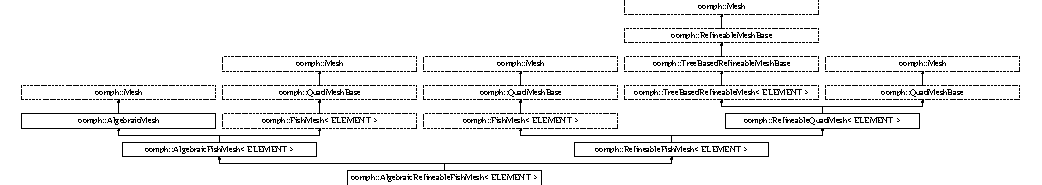
\includegraphics[height=2.488889cm]{classoomph_1_1AlgebraicRefineableFishMesh}
\end{center}
\end{figure}
\subsection*{Public Member Functions}
\begin{DoxyCompactItemize}
\item 
\hyperlink{classoomph_1_1AlgebraicRefineableFishMesh_afe4643b107e47fbad0c8836bc0516518}{Algebraic\+Refineable\+Fish\+Mesh} (\hyperlink{classoomph_1_1TimeStepper}{Time\+Stepper} $\ast$time\+\_\+stepper\+\_\+pt=\&\hyperlink{classoomph_1_1Mesh_a12243d0fee2b1fcee729ee5a4777ea10}{Mesh\+::\+Default\+\_\+\+Time\+Stepper})
\item 
\hyperlink{classoomph_1_1AlgebraicRefineableFishMesh_a04f6b6114c70638b4f26ac6b70f5c0fe}{Algebraic\+Refineable\+Fish\+Mesh} (\hyperlink{classoomph_1_1GeomObject}{Geom\+Object} $\ast$back\+\_\+pt, \hyperlink{classoomph_1_1TimeStepper}{Time\+Stepper} $\ast$time\+\_\+stepper\+\_\+pt=\&\hyperlink{classoomph_1_1Mesh_a12243d0fee2b1fcee729ee5a4777ea10}{Mesh\+::\+Default\+\_\+\+Time\+Stepper})
\begin{DoxyCompactList}\small\item\em Constructor\+: Pass pointer \hyperlink{classoomph_1_1GeomObject}{Geom\+Object} that defines the fish\textquotesingle{}s back and pointer to timestepper. (defaults to (\hyperlink{classoomph_1_1Steady}{Steady}) default timestepper defined in \hyperlink{classoomph_1_1Mesh}{Mesh}) \end{DoxyCompactList}\item 
virtual \hyperlink{classoomph_1_1AlgebraicRefineableFishMesh_a69145c9bf09e0fbc1a4bffe7bee379cd}{$\sim$\+Algebraic\+Refineable\+Fish\+Mesh} ()
\begin{DoxyCompactList}\small\item\em Destructor\+: empty. \end{DoxyCompactList}\item 
void \hyperlink{classoomph_1_1AlgebraicRefineableFishMesh_a8123da4b48355b39f19e0494a9d4545c}{node\+\_\+update} (const bool \&update\+\_\+all\+\_\+solid\+\_\+nodes=false)
\begin{DoxyCompactList}\small\item\em Resolve node update function\+: Use the one defined in the \hyperlink{classoomph_1_1AlgebraicFishMesh}{Algebraic\+Fish\+Mesh} (where the bool flag is explained) \end{DoxyCompactList}\end{DoxyCompactItemize}
\subsection*{Additional Inherited Members}


\subsection{Detailed Description}
\subsubsection*{template$<$class E\+L\+E\+M\+E\+NT$>$\newline
class oomph\+::\+Algebraic\+Refineable\+Fish\+Mesh$<$ E\+L\+E\+M\+E\+N\+T $>$}

Refineable fish shaped mesh with algebraic node update function. 

Definition at line 523 of file fish\+\_\+mesh.\+template.\+h.



\subsection{Constructor \& Destructor Documentation}
\mbox{\Hypertarget{classoomph_1_1AlgebraicRefineableFishMesh_afe4643b107e47fbad0c8836bc0516518}\label{classoomph_1_1AlgebraicRefineableFishMesh_afe4643b107e47fbad0c8836bc0516518}} 
\index{oomph\+::\+Algebraic\+Refineable\+Fish\+Mesh@{oomph\+::\+Algebraic\+Refineable\+Fish\+Mesh}!Algebraic\+Refineable\+Fish\+Mesh@{Algebraic\+Refineable\+Fish\+Mesh}}
\index{Algebraic\+Refineable\+Fish\+Mesh@{Algebraic\+Refineable\+Fish\+Mesh}!oomph\+::\+Algebraic\+Refineable\+Fish\+Mesh@{oomph\+::\+Algebraic\+Refineable\+Fish\+Mesh}}
\subsubsection{\texorpdfstring{Algebraic\+Refineable\+Fish\+Mesh()}{AlgebraicRefineableFishMesh()}\hspace{0.1cm}{\footnotesize\ttfamily [1/2]}}
{\footnotesize\ttfamily template$<$class E\+L\+E\+M\+E\+NT $>$ \\
\hyperlink{classoomph_1_1AlgebraicRefineableFishMesh}{oomph\+::\+Algebraic\+Refineable\+Fish\+Mesh}$<$ E\+L\+E\+M\+E\+NT $>$\+::\hyperlink{classoomph_1_1AlgebraicRefineableFishMesh}{Algebraic\+Refineable\+Fish\+Mesh} (\begin{DoxyParamCaption}\item[{\hyperlink{classoomph_1_1TimeStepper}{Time\+Stepper} $\ast$}]{time\+\_\+stepper\+\_\+pt = {\ttfamily \&\hyperlink{classoomph_1_1Mesh_a12243d0fee2b1fcee729ee5a4777ea10}{Mesh\+::\+Default\+\_\+\+Time\+Stepper}} }\end{DoxyParamCaption})\hspace{0.3cm}{\ttfamily [inline]}}

Constructor\+: Pass pointer to timestepper. (defaults to (\hyperlink{classoomph_1_1Steady}{Steady}) default timestepper defined in \hyperlink{classoomph_1_1Mesh}{Mesh}) 

Definition at line 537 of file fish\+\_\+mesh.\+template.\+h.

\mbox{\Hypertarget{classoomph_1_1AlgebraicRefineableFishMesh_a04f6b6114c70638b4f26ac6b70f5c0fe}\label{classoomph_1_1AlgebraicRefineableFishMesh_a04f6b6114c70638b4f26ac6b70f5c0fe}} 
\index{oomph\+::\+Algebraic\+Refineable\+Fish\+Mesh@{oomph\+::\+Algebraic\+Refineable\+Fish\+Mesh}!Algebraic\+Refineable\+Fish\+Mesh@{Algebraic\+Refineable\+Fish\+Mesh}}
\index{Algebraic\+Refineable\+Fish\+Mesh@{Algebraic\+Refineable\+Fish\+Mesh}!oomph\+::\+Algebraic\+Refineable\+Fish\+Mesh@{oomph\+::\+Algebraic\+Refineable\+Fish\+Mesh}}
\subsubsection{\texorpdfstring{Algebraic\+Refineable\+Fish\+Mesh()}{AlgebraicRefineableFishMesh()}\hspace{0.1cm}{\footnotesize\ttfamily [2/2]}}
{\footnotesize\ttfamily template$<$class E\+L\+E\+M\+E\+NT $>$ \\
\hyperlink{classoomph_1_1AlgebraicRefineableFishMesh}{oomph\+::\+Algebraic\+Refineable\+Fish\+Mesh}$<$ E\+L\+E\+M\+E\+NT $>$\+::\hyperlink{classoomph_1_1AlgebraicRefineableFishMesh}{Algebraic\+Refineable\+Fish\+Mesh} (\begin{DoxyParamCaption}\item[{\hyperlink{classoomph_1_1GeomObject}{Geom\+Object} $\ast$}]{back\+\_\+pt,  }\item[{\hyperlink{classoomph_1_1TimeStepper}{Time\+Stepper} $\ast$}]{time\+\_\+stepper\+\_\+pt = {\ttfamily \&\hyperlink{classoomph_1_1Mesh_a12243d0fee2b1fcee729ee5a4777ea10}{Mesh\+::\+Default\+\_\+\+Time\+Stepper}} }\end{DoxyParamCaption})\hspace{0.3cm}{\ttfamily [inline]}}



Constructor\+: Pass pointer \hyperlink{classoomph_1_1GeomObject}{Geom\+Object} that defines the fish\textquotesingle{}s back and pointer to timestepper. (defaults to (\hyperlink{classoomph_1_1Steady}{Steady}) default timestepper defined in \hyperlink{classoomph_1_1Mesh}{Mesh}) 



Definition at line 553 of file fish\+\_\+mesh.\+template.\+h.

\mbox{\Hypertarget{classoomph_1_1AlgebraicRefineableFishMesh_a69145c9bf09e0fbc1a4bffe7bee379cd}\label{classoomph_1_1AlgebraicRefineableFishMesh_a69145c9bf09e0fbc1a4bffe7bee379cd}} 
\index{oomph\+::\+Algebraic\+Refineable\+Fish\+Mesh@{oomph\+::\+Algebraic\+Refineable\+Fish\+Mesh}!````~Algebraic\+Refineable\+Fish\+Mesh@{$\sim$\+Algebraic\+Refineable\+Fish\+Mesh}}
\index{````~Algebraic\+Refineable\+Fish\+Mesh@{$\sim$\+Algebraic\+Refineable\+Fish\+Mesh}!oomph\+::\+Algebraic\+Refineable\+Fish\+Mesh@{oomph\+::\+Algebraic\+Refineable\+Fish\+Mesh}}
\subsubsection{\texorpdfstring{$\sim$\+Algebraic\+Refineable\+Fish\+Mesh()}{~AlgebraicRefineableFishMesh()}}
{\footnotesize\ttfamily template$<$class E\+L\+E\+M\+E\+NT $>$ \\
virtual \hyperlink{classoomph_1_1AlgebraicRefineableFishMesh}{oomph\+::\+Algebraic\+Refineable\+Fish\+Mesh}$<$ E\+L\+E\+M\+E\+NT $>$\+::$\sim$\hyperlink{classoomph_1_1AlgebraicRefineableFishMesh}{Algebraic\+Refineable\+Fish\+Mesh} (\begin{DoxyParamCaption}{ }\end{DoxyParamCaption})\hspace{0.3cm}{\ttfamily [inline]}, {\ttfamily [virtual]}}



Destructor\+: empty. 



Definition at line 563 of file fish\+\_\+mesh.\+template.\+h.



\subsection{Member Function Documentation}
\mbox{\Hypertarget{classoomph_1_1AlgebraicRefineableFishMesh_a8123da4b48355b39f19e0494a9d4545c}\label{classoomph_1_1AlgebraicRefineableFishMesh_a8123da4b48355b39f19e0494a9d4545c}} 
\index{oomph\+::\+Algebraic\+Refineable\+Fish\+Mesh@{oomph\+::\+Algebraic\+Refineable\+Fish\+Mesh}!node\+\_\+update@{node\+\_\+update}}
\index{node\+\_\+update@{node\+\_\+update}!oomph\+::\+Algebraic\+Refineable\+Fish\+Mesh@{oomph\+::\+Algebraic\+Refineable\+Fish\+Mesh}}
\subsubsection{\texorpdfstring{node\+\_\+update()}{node\_update()}}
{\footnotesize\ttfamily template$<$class E\+L\+E\+M\+E\+NT $>$ \\
void \hyperlink{classoomph_1_1AlgebraicRefineableFishMesh}{oomph\+::\+Algebraic\+Refineable\+Fish\+Mesh}$<$ E\+L\+E\+M\+E\+NT $>$\+::node\+\_\+update (\begin{DoxyParamCaption}\item[{const bool \&}]{update\+\_\+all\+\_\+solid\+\_\+nodes = {\ttfamily false} }\end{DoxyParamCaption})\hspace{0.3cm}{\ttfamily [inline]}, {\ttfamily [virtual]}}



Resolve node update function\+: Use the one defined in the \hyperlink{classoomph_1_1AlgebraicFishMesh}{Algebraic\+Fish\+Mesh} (where the bool flag is explained) 



Reimplemented from \hyperlink{classoomph_1_1AlgebraicFishMesh_a39cd5a86b0f762efd09f4fefba6da1c3}{oomph\+::\+Algebraic\+Fish\+Mesh$<$ E\+L\+E\+M\+E\+N\+T $>$}.



Definition at line 567 of file fish\+\_\+mesh.\+template.\+h.



References oomph\+::\+Algebraic\+Fish\+Mesh$<$ E\+L\+E\+M\+E\+N\+T $>$\+::node\+\_\+update().



The documentation for this class was generated from the following file\+:\begin{DoxyCompactItemize}
\item 
\hyperlink{fish__mesh_8template_8h}{fish\+\_\+mesh.\+template.\+h}\end{DoxyCompactItemize}

\hypertarget{classoomph_1_1AlgebraicRefineableQuarterCircleSectorMesh}{}\section{oomph\+:\+:Algebraic\+Refineable\+Quarter\+Circle\+Sector\+Mesh$<$ E\+L\+E\+M\+E\+NT $>$ Class Template Reference}
\label{classoomph_1_1AlgebraicRefineableQuarterCircleSectorMesh}\index{oomph\+::\+Algebraic\+Refineable\+Quarter\+Circle\+Sector\+Mesh$<$ E\+L\+E\+M\+E\+N\+T $>$@{oomph\+::\+Algebraic\+Refineable\+Quarter\+Circle\+Sector\+Mesh$<$ E\+L\+E\+M\+E\+N\+T $>$}}


{\ttfamily \#include $<$quarter\+\_\+circle\+\_\+sector\+\_\+mesh.\+template.\+h$>$}

Inheritance diagram for oomph\+:\+:Algebraic\+Refineable\+Quarter\+Circle\+Sector\+Mesh$<$ E\+L\+E\+M\+E\+NT $>$\+:\begin{figure}[H]
\begin{center}
\leavevmode
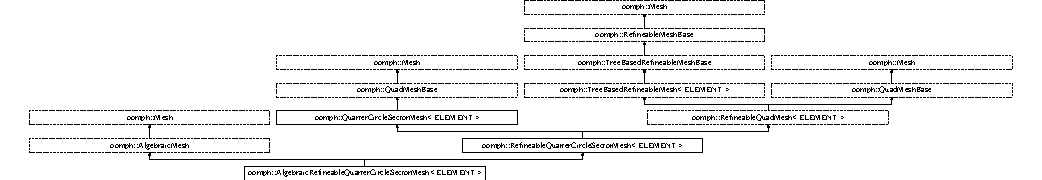
\includegraphics[height=1.839080cm]{classoomph_1_1AlgebraicRefineableQuarterCircleSectorMesh}
\end{center}
\end{figure}
\subsection*{Public Member Functions}
\begin{DoxyCompactItemize}
\item 
\hyperlink{classoomph_1_1AlgebraicRefineableQuarterCircleSectorMesh_a4245d6f0499af21053a0381bc69de271}{Algebraic\+Refineable\+Quarter\+Circle\+Sector\+Mesh} (Geom\+Object $\ast$\hyperlink{classoomph_1_1QuarterCircleSectorMesh_a0b03071bbe7e95cc6723c221ddc0998a}{wall\+\_\+pt}, const double \&xi\+\_\+lo, const double \&fract\+\_\+mid, const double \&xi\+\_\+hi, Time\+Stepper $\ast$time\+\_\+stepper\+\_\+pt=\&Mesh\+::\+Default\+\_\+\+Time\+Stepper)
\begin{DoxyCompactList}\small\item\em Constructor\+: Pass pointer to geometric object, start and end coordinates on the geometric object and the fraction along which the dividing line is to be placed when updating the nodal positions, and timestepper (defaults to (Steady) default timestepper defined in Mesh). Setup the refineable mesh (by calling the constructor for the underlying \hyperlink{classoomph_1_1RefineableQuarterCircleSectorMesh}{Refineable\+Quarter\+Circle\+Sector\+Mesh}) and the algebraic update functions for nodes. \end{DoxyCompactList}\item 
unsigned \hyperlink{classoomph_1_1AlgebraicRefineableQuarterCircleSectorMesh_a68d9738e3d3eedc4d2dd8e1b7fb09d8c}{self\+\_\+test} ()
\begin{DoxyCompactList}\small\item\em Run self-\/test for algebraic mesh -- return 0/1 for O\+K/failure. \end{DoxyCompactList}\item 
void \hyperlink{classoomph_1_1AlgebraicRefineableQuarterCircleSectorMesh_a32a096b894031167a90bafdab167ffc7}{node\+\_\+update} (const bool \&update\+\_\+all\+\_\+solid\+\_\+nodes=false)
\begin{DoxyCompactList}\small\item\em Resolve mesh update\+: Update current nodal positions via algebraic node update. \mbox{[}Doesn\textquotesingle{}t make sense to use this mesh with Solid\+Elements anyway, so we buffer the case if update\+\_\+all\+\_\+solid\+\_\+nodes is set to true.\mbox{]}. \end{DoxyCompactList}\item 
void \hyperlink{classoomph_1_1AlgebraicRefineableQuarterCircleSectorMesh_ac591df8f18ad687e1dc9b70b731c2de1}{algebraic\+\_\+node\+\_\+update} (const unsigned \&t, Algebraic\+Node $\ast$\&node\+\_\+pt)
\begin{DoxyCompactList}\small\item\em Implement the algebraic node update function for a node at time level t (t=0\+: present; t$>$0\+: previous)\+: Update with the node\textquotesingle{}s first (default) update function. \end{DoxyCompactList}\item 
void \hyperlink{classoomph_1_1AlgebraicRefineableQuarterCircleSectorMesh_a08abc1bf64e0637fc87c36638c41b846}{update\+\_\+node\+\_\+update} (Algebraic\+Node $\ast$\&node\+\_\+pt)
\begin{DoxyCompactList}\small\item\em Update the node update info for specified algebraic node following any spatial mesh adaptation. \end{DoxyCompactList}\end{DoxyCompactItemize}
\subsection*{Private Types}
\begin{DoxyCompactItemize}
\item 
enum \{ \hyperlink{classoomph_1_1AlgebraicRefineableQuarterCircleSectorMesh_a85eef4c11c2a88ba4bb5f99bc8406e67a070fa32a21fc9ed7e0ea2e4ee49bb226}{Central\+\_\+box}, 
\hyperlink{classoomph_1_1AlgebraicRefineableQuarterCircleSectorMesh_a85eef4c11c2a88ba4bb5f99bc8406e67a04eaf51389d87a087fa1e9b2b2bd0315}{Lower\+\_\+right\+\_\+box}, 
\hyperlink{classoomph_1_1AlgebraicRefineableQuarterCircleSectorMesh_a85eef4c11c2a88ba4bb5f99bc8406e67a5ff22a2cd960ec680a42f181d6cbdfb0}{Upper\+\_\+left\+\_\+box}
 \}\begin{DoxyCompactList}\small\item\em Remesh function ids. \end{DoxyCompactList}
\end{DoxyCompactItemize}
\subsection*{Private Member Functions}
\begin{DoxyCompactItemize}
\item 
void \hyperlink{classoomph_1_1AlgebraicRefineableQuarterCircleSectorMesh_a89dc4a592e3f188f9bfbffd5c7fdbbcc}{node\+\_\+update\+\_\+in\+\_\+central\+\_\+box} (const unsigned \&t, Algebraic\+Node $\ast$\&node\+\_\+pt)
\begin{DoxyCompactList}\small\item\em Algebraic update function for a node that is located in the central box. \end{DoxyCompactList}\item 
void \hyperlink{classoomph_1_1AlgebraicRefineableQuarterCircleSectorMesh_a9a7d3e4a2126346cdae3bde51eff7b36}{node\+\_\+update\+\_\+in\+\_\+lower\+\_\+right\+\_\+box} (const unsigned \&t, Algebraic\+Node $\ast$\&node\+\_\+pt)
\begin{DoxyCompactList}\small\item\em Algebraic update function for a node that is located in the lower right box. \end{DoxyCompactList}\item 
void \hyperlink{classoomph_1_1AlgebraicRefineableQuarterCircleSectorMesh_aeb36f6747d14cd68d4857169fa0f22d1}{node\+\_\+update\+\_\+in\+\_\+upper\+\_\+left\+\_\+box} (const unsigned \&t, Algebraic\+Node $\ast$\&node\+\_\+pt)
\begin{DoxyCompactList}\small\item\em Algebraic update function for a node that is located in the upper left box. \end{DoxyCompactList}\item 
void \hyperlink{classoomph_1_1AlgebraicRefineableQuarterCircleSectorMesh_a3eb269dc5c26355a808d1c5035190017}{setup\+\_\+algebraic\+\_\+node\+\_\+update} ()
\begin{DoxyCompactList}\small\item\em Setup algebraic update operation for all nodes. \end{DoxyCompactList}\item 
void \hyperlink{classoomph_1_1AlgebraicRefineableQuarterCircleSectorMesh_a77154a45d65fa66d220bad2a3e860c8e}{update\+\_\+node\+\_\+update\+\_\+in\+\_\+lower\+\_\+right\+\_\+box} (Algebraic\+Node $\ast$\&node\+\_\+pt)
\begin{DoxyCompactList}\small\item\em Update algebraic node update function for nodes in lower right box. \end{DoxyCompactList}\item 
void \hyperlink{classoomph_1_1AlgebraicRefineableQuarterCircleSectorMesh_ab1e4847ffef953e66aafff14f35b7141}{update\+\_\+node\+\_\+update\+\_\+in\+\_\+upper\+\_\+left\+\_\+box} (Algebraic\+Node $\ast$\&node\+\_\+pt)
\begin{DoxyCompactList}\small\item\em Update algebraic node update function for nodes in upper left box. \end{DoxyCompactList}\end{DoxyCompactItemize}
\subsection*{Private Attributes}
\begin{DoxyCompactItemize}
\item 
double \hyperlink{classoomph_1_1AlgebraicRefineableQuarterCircleSectorMesh_aed38fed1e464c86e3dedd377e2459de7}{Lambda\+\_\+x}
\begin{DoxyCompactList}\small\item\em Fractional width of central box. \end{DoxyCompactList}\item 
double \hyperlink{classoomph_1_1AlgebraicRefineableQuarterCircleSectorMesh_a2690e44e43dd4ed1e45b02f4b71ae43f}{Lambda\+\_\+y}
\begin{DoxyCompactList}\small\item\em Fractional height of central box. \end{DoxyCompactList}\end{DoxyCompactItemize}
\subsection*{Additional Inherited Members}


\subsection{Detailed Description}
\subsubsection*{template$<$class E\+L\+E\+M\+E\+NT$>$\newline
class oomph\+::\+Algebraic\+Refineable\+Quarter\+Circle\+Sector\+Mesh$<$ E\+L\+E\+M\+E\+N\+T $>$}

Algebraic version of \hyperlink{classoomph_1_1RefineableQuarterCircleSectorMesh}{Refineable\+Quarter\+Circle\+Sector\+Mesh}


\begin{DoxyCode}
                     ---\_\_\_
                    |      ---\_\_\_\_
                    |              -   BOUNDARY 1
                    |               /  
                    |     [2]      /  |  
                    |             /     | 
                    | N          /        |  
                    | |\_ E      /          |    
     BOUNDARY 2     |-----------           |  
                    |          |    [1]    |
                    |   [0]    |           |  ^
                    |          |           | / \(\backslash\)  direction of
                    | N        |    N      |  |   Lagrangian 
                    | |\_ E     |    |\_ E   |  |   coordinate 
                    |\_\_\_\_\_\_\_\_\_\_|\_\_\_\_\_\_\_\_\_\_\_|  |   along wall GeomObject

                         BOUNDARY 0

Within the elements (MacroElements), the local coordinates
are such that the (E)astern direction coincides with the positive 
s\_0 direction,  \textcolor{keywordflow}{while} the (N)orther direction coincides with the positive 
s\_1 direction.
\end{DoxyCode}


Domain is parametrised by three macro elements as sketched. Elements need to be derived from Algebraic\+Element\+Base. In addition to all the refinement procedures available for \hyperlink{classoomph_1_1RefineableQuarterCircleSectorMesh}{Refineable\+Quarter\+Circle\+Sector\+Mesh} which forms the basis for this mesh, we implement algebraic node update functions for the nodes. 

Definition at line 469 of file quarter\+\_\+circle\+\_\+sector\+\_\+mesh.\+template.\+h.



\subsection{Member Enumeration Documentation}
\mbox{\Hypertarget{classoomph_1_1AlgebraicRefineableQuarterCircleSectorMesh_a85eef4c11c2a88ba4bb5f99bc8406e67}\label{classoomph_1_1AlgebraicRefineableQuarterCircleSectorMesh_a85eef4c11c2a88ba4bb5f99bc8406e67}} 
\subsubsection{\texorpdfstring{anonymous enum}{anonymous enum}}
{\footnotesize\ttfamily template$<$class E\+L\+E\+M\+E\+NT $>$ \\
anonymous enum\hspace{0.3cm}{\ttfamily [private]}}



Remesh function ids. 

\begin{DoxyEnumFields}{Enumerator}
\raisebox{\heightof{T}}[0pt][0pt]{\index{Central\+\_\+box@{Central\+\_\+box}!oomph\+::\+Algebraic\+Refineable\+Quarter\+Circle\+Sector\+Mesh@{oomph\+::\+Algebraic\+Refineable\+Quarter\+Circle\+Sector\+Mesh}}\index{oomph\+::\+Algebraic\+Refineable\+Quarter\+Circle\+Sector\+Mesh@{oomph\+::\+Algebraic\+Refineable\+Quarter\+Circle\+Sector\+Mesh}!Central\+\_\+box@{Central\+\_\+box}}}\mbox{\Hypertarget{classoomph_1_1AlgebraicRefineableQuarterCircleSectorMesh_a85eef4c11c2a88ba4bb5f99bc8406e67a070fa32a21fc9ed7e0ea2e4ee49bb226}\label{classoomph_1_1AlgebraicRefineableQuarterCircleSectorMesh_a85eef4c11c2a88ba4bb5f99bc8406e67a070fa32a21fc9ed7e0ea2e4ee49bb226}} 
Central\+\_\+box&\\
\hline

\raisebox{\heightof{T}}[0pt][0pt]{\index{Lower\+\_\+right\+\_\+box@{Lower\+\_\+right\+\_\+box}!oomph\+::\+Algebraic\+Refineable\+Quarter\+Circle\+Sector\+Mesh@{oomph\+::\+Algebraic\+Refineable\+Quarter\+Circle\+Sector\+Mesh}}\index{oomph\+::\+Algebraic\+Refineable\+Quarter\+Circle\+Sector\+Mesh@{oomph\+::\+Algebraic\+Refineable\+Quarter\+Circle\+Sector\+Mesh}!Lower\+\_\+right\+\_\+box@{Lower\+\_\+right\+\_\+box}}}\mbox{\Hypertarget{classoomph_1_1AlgebraicRefineableQuarterCircleSectorMesh_a85eef4c11c2a88ba4bb5f99bc8406e67a04eaf51389d87a087fa1e9b2b2bd0315}\label{classoomph_1_1AlgebraicRefineableQuarterCircleSectorMesh_a85eef4c11c2a88ba4bb5f99bc8406e67a04eaf51389d87a087fa1e9b2b2bd0315}} 
Lower\+\_\+right\+\_\+box&\\
\hline

\raisebox{\heightof{T}}[0pt][0pt]{\index{Upper\+\_\+left\+\_\+box@{Upper\+\_\+left\+\_\+box}!oomph\+::\+Algebraic\+Refineable\+Quarter\+Circle\+Sector\+Mesh@{oomph\+::\+Algebraic\+Refineable\+Quarter\+Circle\+Sector\+Mesh}}\index{oomph\+::\+Algebraic\+Refineable\+Quarter\+Circle\+Sector\+Mesh@{oomph\+::\+Algebraic\+Refineable\+Quarter\+Circle\+Sector\+Mesh}!Upper\+\_\+left\+\_\+box@{Upper\+\_\+left\+\_\+box}}}\mbox{\Hypertarget{classoomph_1_1AlgebraicRefineableQuarterCircleSectorMesh_a85eef4c11c2a88ba4bb5f99bc8406e67a5ff22a2cd960ec680a42f181d6cbdfb0}\label{classoomph_1_1AlgebraicRefineableQuarterCircleSectorMesh_a85eef4c11c2a88ba4bb5f99bc8406e67a5ff22a2cd960ec680a42f181d6cbdfb0}} 
Upper\+\_\+left\+\_\+box&\\
\hline

\end{DoxyEnumFields}


Definition at line 674 of file quarter\+\_\+circle\+\_\+sector\+\_\+mesh.\+template.\+h.



\subsection{Constructor \& Destructor Documentation}
\mbox{\Hypertarget{classoomph_1_1AlgebraicRefineableQuarterCircleSectorMesh_a4245d6f0499af21053a0381bc69de271}\label{classoomph_1_1AlgebraicRefineableQuarterCircleSectorMesh_a4245d6f0499af21053a0381bc69de271}} 
\index{oomph\+::\+Algebraic\+Refineable\+Quarter\+Circle\+Sector\+Mesh@{oomph\+::\+Algebraic\+Refineable\+Quarter\+Circle\+Sector\+Mesh}!Algebraic\+Refineable\+Quarter\+Circle\+Sector\+Mesh@{Algebraic\+Refineable\+Quarter\+Circle\+Sector\+Mesh}}
\index{Algebraic\+Refineable\+Quarter\+Circle\+Sector\+Mesh@{Algebraic\+Refineable\+Quarter\+Circle\+Sector\+Mesh}!oomph\+::\+Algebraic\+Refineable\+Quarter\+Circle\+Sector\+Mesh@{oomph\+::\+Algebraic\+Refineable\+Quarter\+Circle\+Sector\+Mesh}}
\subsubsection{\texorpdfstring{Algebraic\+Refineable\+Quarter\+Circle\+Sector\+Mesh()}{AlgebraicRefineableQuarterCircleSectorMesh()}}
{\footnotesize\ttfamily template$<$class E\+L\+E\+M\+E\+NT $>$ \\
\hyperlink{classoomph_1_1AlgebraicRefineableQuarterCircleSectorMesh}{oomph\+::\+Algebraic\+Refineable\+Quarter\+Circle\+Sector\+Mesh}$<$ E\+L\+E\+M\+E\+NT $>$\+::\hyperlink{classoomph_1_1AlgebraicRefineableQuarterCircleSectorMesh}{Algebraic\+Refineable\+Quarter\+Circle\+Sector\+Mesh} (\begin{DoxyParamCaption}\item[{Geom\+Object $\ast$}]{wall\+\_\+pt,  }\item[{const double \&}]{xi\+\_\+lo,  }\item[{const double \&}]{fract\+\_\+mid,  }\item[{const double \&}]{xi\+\_\+hi,  }\item[{Time\+Stepper $\ast$}]{time\+\_\+stepper\+\_\+pt = {\ttfamily \&Mesh\+:\+:Default\+\_\+TimeStepper} }\end{DoxyParamCaption})\hspace{0.3cm}{\ttfamily [inline]}}



Constructor\+: Pass pointer to geometric object, start and end coordinates on the geometric object and the fraction along which the dividing line is to be placed when updating the nodal positions, and timestepper (defaults to (Steady) default timestepper defined in Mesh). Setup the refineable mesh (by calling the constructor for the underlying \hyperlink{classoomph_1_1RefineableQuarterCircleSectorMesh}{Refineable\+Quarter\+Circle\+Sector\+Mesh}) and the algebraic update functions for nodes. 



Definition at line 486 of file quarter\+\_\+circle\+\_\+sector\+\_\+mesh.\+template.\+h.



\subsection{Member Function Documentation}
\mbox{\Hypertarget{classoomph_1_1AlgebraicRefineableQuarterCircleSectorMesh_ac591df8f18ad687e1dc9b70b731c2de1}\label{classoomph_1_1AlgebraicRefineableQuarterCircleSectorMesh_ac591df8f18ad687e1dc9b70b731c2de1}} 
\index{oomph\+::\+Algebraic\+Refineable\+Quarter\+Circle\+Sector\+Mesh@{oomph\+::\+Algebraic\+Refineable\+Quarter\+Circle\+Sector\+Mesh}!algebraic\+\_\+node\+\_\+update@{algebraic\+\_\+node\+\_\+update}}
\index{algebraic\+\_\+node\+\_\+update@{algebraic\+\_\+node\+\_\+update}!oomph\+::\+Algebraic\+Refineable\+Quarter\+Circle\+Sector\+Mesh@{oomph\+::\+Algebraic\+Refineable\+Quarter\+Circle\+Sector\+Mesh}}
\subsubsection{\texorpdfstring{algebraic\+\_\+node\+\_\+update()}{algebraic\_node\_update()}}
{\footnotesize\ttfamily template$<$class E\+L\+E\+M\+E\+NT $>$ \\
void \hyperlink{classoomph_1_1AlgebraicRefineableQuarterCircleSectorMesh}{oomph\+::\+Algebraic\+Refineable\+Quarter\+Circle\+Sector\+Mesh}$<$ E\+L\+E\+M\+E\+NT $>$\+::algebraic\+\_\+node\+\_\+update (\begin{DoxyParamCaption}\item[{const unsigned \&}]{t,  }\item[{Algebraic\+Node $\ast$\&}]{node\+\_\+pt }\end{DoxyParamCaption})\hspace{0.3cm}{\ttfamily [inline]}}



Implement the algebraic node update function for a node at time level t (t=0\+: present; t$>$0\+: previous)\+: Update with the node\textquotesingle{}s first (default) update function. 



Definition at line 566 of file quarter\+\_\+circle\+\_\+sector\+\_\+mesh.\+template.\+h.

\mbox{\Hypertarget{classoomph_1_1AlgebraicRefineableQuarterCircleSectorMesh_a32a096b894031167a90bafdab167ffc7}\label{classoomph_1_1AlgebraicRefineableQuarterCircleSectorMesh_a32a096b894031167a90bafdab167ffc7}} 
\index{oomph\+::\+Algebraic\+Refineable\+Quarter\+Circle\+Sector\+Mesh@{oomph\+::\+Algebraic\+Refineable\+Quarter\+Circle\+Sector\+Mesh}!node\+\_\+update@{node\+\_\+update}}
\index{node\+\_\+update@{node\+\_\+update}!oomph\+::\+Algebraic\+Refineable\+Quarter\+Circle\+Sector\+Mesh@{oomph\+::\+Algebraic\+Refineable\+Quarter\+Circle\+Sector\+Mesh}}
\subsubsection{\texorpdfstring{node\+\_\+update()}{node\_update()}}
{\footnotesize\ttfamily template$<$class E\+L\+E\+M\+E\+NT $>$ \\
void \hyperlink{classoomph_1_1AlgebraicRefineableQuarterCircleSectorMesh}{oomph\+::\+Algebraic\+Refineable\+Quarter\+Circle\+Sector\+Mesh}$<$ E\+L\+E\+M\+E\+NT $>$\+::node\+\_\+update (\begin{DoxyParamCaption}\item[{const bool \&}]{update\+\_\+all\+\_\+solid\+\_\+nodes = {\ttfamily false} }\end{DoxyParamCaption})\hspace{0.3cm}{\ttfamily [inline]}}



Resolve mesh update\+: Update current nodal positions via algebraic node update. \mbox{[}Doesn\textquotesingle{}t make sense to use this mesh with Solid\+Elements anyway, so we buffer the case if update\+\_\+all\+\_\+solid\+\_\+nodes is set to true.\mbox{]}. 



Definition at line 538 of file quarter\+\_\+circle\+\_\+sector\+\_\+mesh.\+template.\+h.

\mbox{\Hypertarget{classoomph_1_1AlgebraicRefineableQuarterCircleSectorMesh_a89dc4a592e3f188f9bfbffd5c7fdbbcc}\label{classoomph_1_1AlgebraicRefineableQuarterCircleSectorMesh_a89dc4a592e3f188f9bfbffd5c7fdbbcc}} 
\index{oomph\+::\+Algebraic\+Refineable\+Quarter\+Circle\+Sector\+Mesh@{oomph\+::\+Algebraic\+Refineable\+Quarter\+Circle\+Sector\+Mesh}!node\+\_\+update\+\_\+in\+\_\+central\+\_\+box@{node\+\_\+update\+\_\+in\+\_\+central\+\_\+box}}
\index{node\+\_\+update\+\_\+in\+\_\+central\+\_\+box@{node\+\_\+update\+\_\+in\+\_\+central\+\_\+box}!oomph\+::\+Algebraic\+Refineable\+Quarter\+Circle\+Sector\+Mesh@{oomph\+::\+Algebraic\+Refineable\+Quarter\+Circle\+Sector\+Mesh}}
\subsubsection{\texorpdfstring{node\+\_\+update\+\_\+in\+\_\+central\+\_\+box()}{node\_update\_in\_central\_box()}}
{\footnotesize\ttfamily template$<$class E\+L\+E\+M\+E\+NT $>$ \\
void \hyperlink{classoomph_1_1AlgebraicRefineableQuarterCircleSectorMesh}{oomph\+::\+Algebraic\+Refineable\+Quarter\+Circle\+Sector\+Mesh}$<$ E\+L\+E\+M\+E\+NT $>$\+::node\+\_\+update\+\_\+in\+\_\+central\+\_\+box (\begin{DoxyParamCaption}\item[{const unsigned \&}]{t,  }\item[{Algebraic\+Node $\ast$\&}]{node\+\_\+pt }\end{DoxyParamCaption})\hspace{0.3cm}{\ttfamily [private]}}



Algebraic update function for a node that is located in the central box. 

Algebraic update function\+: Update in central box according to wall shape at time level t (t=0\+: present; t$>$0\+: previous) 

Definition at line 870 of file quarter\+\_\+circle\+\_\+sector\+\_\+mesh.\+template.\+cc.



References oomph\+::\+Algebraic\+Refineable\+Quarter\+Circle\+Sector\+Mesh$<$ E\+L\+E\+M\+E\+N\+T $>$\+::node\+\_\+update\+\_\+in\+\_\+lower\+\_\+right\+\_\+box().



Referenced by oomph\+::\+Algebraic\+Refineable\+Quarter\+Circle\+Sector\+Mesh$<$ E\+L\+E\+M\+E\+N\+T $>$\+::setup\+\_\+algebraic\+\_\+node\+\_\+update().

\mbox{\Hypertarget{classoomph_1_1AlgebraicRefineableQuarterCircleSectorMesh_a9a7d3e4a2126346cdae3bde51eff7b36}\label{classoomph_1_1AlgebraicRefineableQuarterCircleSectorMesh_a9a7d3e4a2126346cdae3bde51eff7b36}} 
\index{oomph\+::\+Algebraic\+Refineable\+Quarter\+Circle\+Sector\+Mesh@{oomph\+::\+Algebraic\+Refineable\+Quarter\+Circle\+Sector\+Mesh}!node\+\_\+update\+\_\+in\+\_\+lower\+\_\+right\+\_\+box@{node\+\_\+update\+\_\+in\+\_\+lower\+\_\+right\+\_\+box}}
\index{node\+\_\+update\+\_\+in\+\_\+lower\+\_\+right\+\_\+box@{node\+\_\+update\+\_\+in\+\_\+lower\+\_\+right\+\_\+box}!oomph\+::\+Algebraic\+Refineable\+Quarter\+Circle\+Sector\+Mesh@{oomph\+::\+Algebraic\+Refineable\+Quarter\+Circle\+Sector\+Mesh}}
\subsubsection{\texorpdfstring{node\+\_\+update\+\_\+in\+\_\+lower\+\_\+right\+\_\+box()}{node\_update\_in\_lower\_right\_box()}}
{\footnotesize\ttfamily template$<$class E\+L\+E\+M\+E\+NT $>$ \\
void \hyperlink{classoomph_1_1AlgebraicRefineableQuarterCircleSectorMesh}{oomph\+::\+Algebraic\+Refineable\+Quarter\+Circle\+Sector\+Mesh}$<$ E\+L\+E\+M\+E\+NT $>$\+::node\+\_\+update\+\_\+in\+\_\+lower\+\_\+right\+\_\+box (\begin{DoxyParamCaption}\item[{const unsigned \&}]{t,  }\item[{Algebraic\+Node $\ast$\&}]{node\+\_\+pt }\end{DoxyParamCaption})\hspace{0.3cm}{\ttfamily [private]}}



Algebraic update function for a node that is located in the lower right box. 

Algebraic update function\+: Update in lower right box according to wall shape at time level t (t=0\+: present; t$>$0\+: previous) 

Definition at line 961 of file quarter\+\_\+circle\+\_\+sector\+\_\+mesh.\+template.\+cc.



References oomph\+::\+Algebraic\+Refineable\+Quarter\+Circle\+Sector\+Mesh$<$ E\+L\+E\+M\+E\+N\+T $>$\+::node\+\_\+update\+\_\+in\+\_\+upper\+\_\+left\+\_\+box().



Referenced by oomph\+::\+Algebraic\+Refineable\+Quarter\+Circle\+Sector\+Mesh$<$ E\+L\+E\+M\+E\+N\+T $>$\+::node\+\_\+update\+\_\+in\+\_\+central\+\_\+box().

\mbox{\Hypertarget{classoomph_1_1AlgebraicRefineableQuarterCircleSectorMesh_aeb36f6747d14cd68d4857169fa0f22d1}\label{classoomph_1_1AlgebraicRefineableQuarterCircleSectorMesh_aeb36f6747d14cd68d4857169fa0f22d1}} 
\index{oomph\+::\+Algebraic\+Refineable\+Quarter\+Circle\+Sector\+Mesh@{oomph\+::\+Algebraic\+Refineable\+Quarter\+Circle\+Sector\+Mesh}!node\+\_\+update\+\_\+in\+\_\+upper\+\_\+left\+\_\+box@{node\+\_\+update\+\_\+in\+\_\+upper\+\_\+left\+\_\+box}}
\index{node\+\_\+update\+\_\+in\+\_\+upper\+\_\+left\+\_\+box@{node\+\_\+update\+\_\+in\+\_\+upper\+\_\+left\+\_\+box}!oomph\+::\+Algebraic\+Refineable\+Quarter\+Circle\+Sector\+Mesh@{oomph\+::\+Algebraic\+Refineable\+Quarter\+Circle\+Sector\+Mesh}}
\subsubsection{\texorpdfstring{node\+\_\+update\+\_\+in\+\_\+upper\+\_\+left\+\_\+box()}{node\_update\_in\_upper\_left\_box()}}
{\footnotesize\ttfamily template$<$class E\+L\+E\+M\+E\+NT $>$ \\
void \hyperlink{classoomph_1_1AlgebraicRefineableQuarterCircleSectorMesh}{oomph\+::\+Algebraic\+Refineable\+Quarter\+Circle\+Sector\+Mesh}$<$ E\+L\+E\+M\+E\+NT $>$\+::node\+\_\+update\+\_\+in\+\_\+upper\+\_\+left\+\_\+box (\begin{DoxyParamCaption}\item[{const unsigned \&}]{t,  }\item[{Algebraic\+Node $\ast$\&}]{node\+\_\+pt }\end{DoxyParamCaption})\hspace{0.3cm}{\ttfamily [private]}}



Algebraic update function for a node that is located in the upper left box. 

Algebraic update function\+: Update in upper left box according to wall shape at time level t (t=0\+: present; t$>$0\+: previous) 

Definition at line 1073 of file quarter\+\_\+circle\+\_\+sector\+\_\+mesh.\+template.\+cc.



References oomph\+::\+Algebraic\+Refineable\+Quarter\+Circle\+Sector\+Mesh$<$ E\+L\+E\+M\+E\+N\+T $>$\+::update\+\_\+node\+\_\+update\+\_\+in\+\_\+lower\+\_\+right\+\_\+box().



Referenced by oomph\+::\+Algebraic\+Refineable\+Quarter\+Circle\+Sector\+Mesh$<$ E\+L\+E\+M\+E\+N\+T $>$\+::node\+\_\+update\+\_\+in\+\_\+lower\+\_\+right\+\_\+box().

\mbox{\Hypertarget{classoomph_1_1AlgebraicRefineableQuarterCircleSectorMesh_a68d9738e3d3eedc4d2dd8e1b7fb09d8c}\label{classoomph_1_1AlgebraicRefineableQuarterCircleSectorMesh_a68d9738e3d3eedc4d2dd8e1b7fb09d8c}} 
\index{oomph\+::\+Algebraic\+Refineable\+Quarter\+Circle\+Sector\+Mesh@{oomph\+::\+Algebraic\+Refineable\+Quarter\+Circle\+Sector\+Mesh}!self\+\_\+test@{self\+\_\+test}}
\index{self\+\_\+test@{self\+\_\+test}!oomph\+::\+Algebraic\+Refineable\+Quarter\+Circle\+Sector\+Mesh@{oomph\+::\+Algebraic\+Refineable\+Quarter\+Circle\+Sector\+Mesh}}
\subsubsection{\texorpdfstring{self\+\_\+test()}{self\_test()}}
{\footnotesize\ttfamily template$<$class E\+L\+E\+M\+E\+NT $>$ \\
unsigned \hyperlink{classoomph_1_1AlgebraicRefineableQuarterCircleSectorMesh}{oomph\+::\+Algebraic\+Refineable\+Quarter\+Circle\+Sector\+Mesh}$<$ E\+L\+E\+M\+E\+NT $>$\+::self\+\_\+test (\begin{DoxyParamCaption}{ }\end{DoxyParamCaption})\hspace{0.3cm}{\ttfamily [inline]}}



Run self-\/test for algebraic mesh -- return 0/1 for O\+K/failure. 



Definition at line 528 of file quarter\+\_\+circle\+\_\+sector\+\_\+mesh.\+template.\+h.

\mbox{\Hypertarget{classoomph_1_1AlgebraicRefineableQuarterCircleSectorMesh_a3eb269dc5c26355a808d1c5035190017}\label{classoomph_1_1AlgebraicRefineableQuarterCircleSectorMesh_a3eb269dc5c26355a808d1c5035190017}} 
\index{oomph\+::\+Algebraic\+Refineable\+Quarter\+Circle\+Sector\+Mesh@{oomph\+::\+Algebraic\+Refineable\+Quarter\+Circle\+Sector\+Mesh}!setup\+\_\+algebraic\+\_\+node\+\_\+update@{setup\+\_\+algebraic\+\_\+node\+\_\+update}}
\index{setup\+\_\+algebraic\+\_\+node\+\_\+update@{setup\+\_\+algebraic\+\_\+node\+\_\+update}!oomph\+::\+Algebraic\+Refineable\+Quarter\+Circle\+Sector\+Mesh@{oomph\+::\+Algebraic\+Refineable\+Quarter\+Circle\+Sector\+Mesh}}
\subsubsection{\texorpdfstring{setup\+\_\+algebraic\+\_\+node\+\_\+update()}{setup\_algebraic\_node\_update()}}
{\footnotesize\ttfamily template$<$class E\+L\+E\+M\+E\+NT $>$ \\
void \hyperlink{classoomph_1_1AlgebraicRefineableQuarterCircleSectorMesh}{oomph\+::\+Algebraic\+Refineable\+Quarter\+Circle\+Sector\+Mesh}$<$ E\+L\+E\+M\+E\+NT $>$\+::setup\+\_\+algebraic\+\_\+node\+\_\+update (\begin{DoxyParamCaption}{ }\end{DoxyParamCaption})\hspace{0.3cm}{\ttfamily [private]}}



Setup algebraic update operation for all nodes. 

Setup algebraic update operation, based on individual blocks. Mesh is suspended from the `wall\textquotesingle{} Geom\+Object pointed to by wall\+\_\+pt. The lower right corner of the mesh is located at the wall\textquotesingle{}s coordinate xi\+\_\+lo, the upper left corner at xi\+\_\+hi; The dividing line between the two blocks at the outer ring is located at the fraction fract\+\_\+mid between these two coordinates. Node updating strategy\+:
\begin{DoxyItemize}
\item the shape of the central box remains rectangular; the position of its top right corner is located at a fixed fraction of the width and height of the domain. Nodes in this region are located at fixed horizontal and vertical fractions of the box.
\item Nodes in the two outer \char`\"{}ring\char`\"{} elements (bottom right and top left) are located on straight lines running from the edges of the central box to the outer wall. 
\end{DoxyItemize}Pointer to algebraic element in central box 

Definition at line 574 of file quarter\+\_\+circle\+\_\+sector\+\_\+mesh.\+template.\+cc.



References oomph\+::\+Algebraic\+Refineable\+Quarter\+Circle\+Sector\+Mesh$<$ E\+L\+E\+M\+E\+N\+T $>$\+::node\+\_\+update\+\_\+in\+\_\+central\+\_\+box(), and oomph\+::\+Quarter\+Circle\+Sector\+Mesh$<$ E\+L\+E\+M\+E\+N\+T $>$\+::\+Wall\+\_\+pt.



Referenced by oomph\+::\+Quarter\+Circle\+Sector\+Mesh$<$ E\+L\+E\+M\+E\+N\+T $>$\+::\+Quarter\+Circle\+Sector\+Mesh().

\mbox{\Hypertarget{classoomph_1_1AlgebraicRefineableQuarterCircleSectorMesh_a08abc1bf64e0637fc87c36638c41b846}\label{classoomph_1_1AlgebraicRefineableQuarterCircleSectorMesh_a08abc1bf64e0637fc87c36638c41b846}} 
\index{oomph\+::\+Algebraic\+Refineable\+Quarter\+Circle\+Sector\+Mesh@{oomph\+::\+Algebraic\+Refineable\+Quarter\+Circle\+Sector\+Mesh}!update\+\_\+node\+\_\+update@{update\+\_\+node\+\_\+update}}
\index{update\+\_\+node\+\_\+update@{update\+\_\+node\+\_\+update}!oomph\+::\+Algebraic\+Refineable\+Quarter\+Circle\+Sector\+Mesh@{oomph\+::\+Algebraic\+Refineable\+Quarter\+Circle\+Sector\+Mesh}}
\subsubsection{\texorpdfstring{update\+\_\+node\+\_\+update()}{update\_node\_update()}}
{\footnotesize\ttfamily template$<$class E\+L\+E\+M\+E\+NT $>$ \\
void \hyperlink{classoomph_1_1AlgebraicRefineableQuarterCircleSectorMesh}{oomph\+::\+Algebraic\+Refineable\+Quarter\+Circle\+Sector\+Mesh}$<$ E\+L\+E\+M\+E\+NT $>$\+::update\+\_\+node\+\_\+update (\begin{DoxyParamCaption}\item[{Algebraic\+Node $\ast$\&}]{node\+\_\+pt }\end{DoxyParamCaption})\hspace{0.3cm}{\ttfamily [inline]}}



Update the node update info for specified algebraic node following any spatial mesh adaptation. 



Definition at line 617 of file quarter\+\_\+circle\+\_\+sector\+\_\+mesh.\+template.\+h.

\mbox{\Hypertarget{classoomph_1_1AlgebraicRefineableQuarterCircleSectorMesh_a77154a45d65fa66d220bad2a3e860c8e}\label{classoomph_1_1AlgebraicRefineableQuarterCircleSectorMesh_a77154a45d65fa66d220bad2a3e860c8e}} 
\index{oomph\+::\+Algebraic\+Refineable\+Quarter\+Circle\+Sector\+Mesh@{oomph\+::\+Algebraic\+Refineable\+Quarter\+Circle\+Sector\+Mesh}!update\+\_\+node\+\_\+update\+\_\+in\+\_\+lower\+\_\+right\+\_\+box@{update\+\_\+node\+\_\+update\+\_\+in\+\_\+lower\+\_\+right\+\_\+box}}
\index{update\+\_\+node\+\_\+update\+\_\+in\+\_\+lower\+\_\+right\+\_\+box@{update\+\_\+node\+\_\+update\+\_\+in\+\_\+lower\+\_\+right\+\_\+box}!oomph\+::\+Algebraic\+Refineable\+Quarter\+Circle\+Sector\+Mesh@{oomph\+::\+Algebraic\+Refineable\+Quarter\+Circle\+Sector\+Mesh}}
\subsubsection{\texorpdfstring{update\+\_\+node\+\_\+update\+\_\+in\+\_\+lower\+\_\+right\+\_\+box()}{update\_node\_update\_in\_lower\_right\_box()}}
{\footnotesize\ttfamily template$<$class E\+L\+E\+M\+E\+NT $>$ \\
void \hyperlink{classoomph_1_1AlgebraicRefineableQuarterCircleSectorMesh}{oomph\+::\+Algebraic\+Refineable\+Quarter\+Circle\+Sector\+Mesh}$<$ E\+L\+E\+M\+E\+NT $>$\+::update\+\_\+node\+\_\+update\+\_\+in\+\_\+lower\+\_\+right\+\_\+box (\begin{DoxyParamCaption}\item[{Algebraic\+Node $\ast$\&}]{node\+\_\+pt }\end{DoxyParamCaption})\hspace{0.3cm}{\ttfamily [private]}}



Update algebraic node update function for nodes in lower right box. 

Update algebraic update function for nodes in lower right box. 

Definition at line 1187 of file quarter\+\_\+circle\+\_\+sector\+\_\+mesh.\+template.\+cc.



References oomph\+::\+Algebraic\+Refineable\+Quarter\+Circle\+Sector\+Mesh$<$ E\+L\+E\+M\+E\+N\+T $>$\+::update\+\_\+node\+\_\+update\+\_\+in\+\_\+upper\+\_\+left\+\_\+box(), and oomph\+::\+Quarter\+Circle\+Sector\+Mesh$<$ E\+L\+E\+M\+E\+N\+T $>$\+::\+Wall\+\_\+pt.



Referenced by oomph\+::\+Algebraic\+Refineable\+Quarter\+Circle\+Sector\+Mesh$<$ E\+L\+E\+M\+E\+N\+T $>$\+::node\+\_\+update\+\_\+in\+\_\+upper\+\_\+left\+\_\+box().

\mbox{\Hypertarget{classoomph_1_1AlgebraicRefineableQuarterCircleSectorMesh_ab1e4847ffef953e66aafff14f35b7141}\label{classoomph_1_1AlgebraicRefineableQuarterCircleSectorMesh_ab1e4847ffef953e66aafff14f35b7141}} 
\index{oomph\+::\+Algebraic\+Refineable\+Quarter\+Circle\+Sector\+Mesh@{oomph\+::\+Algebraic\+Refineable\+Quarter\+Circle\+Sector\+Mesh}!update\+\_\+node\+\_\+update\+\_\+in\+\_\+upper\+\_\+left\+\_\+box@{update\+\_\+node\+\_\+update\+\_\+in\+\_\+upper\+\_\+left\+\_\+box}}
\index{update\+\_\+node\+\_\+update\+\_\+in\+\_\+upper\+\_\+left\+\_\+box@{update\+\_\+node\+\_\+update\+\_\+in\+\_\+upper\+\_\+left\+\_\+box}!oomph\+::\+Algebraic\+Refineable\+Quarter\+Circle\+Sector\+Mesh@{oomph\+::\+Algebraic\+Refineable\+Quarter\+Circle\+Sector\+Mesh}}
\subsubsection{\texorpdfstring{update\+\_\+node\+\_\+update\+\_\+in\+\_\+upper\+\_\+left\+\_\+box()}{update\_node\_update\_in\_upper\_left\_box()}}
{\footnotesize\ttfamily template$<$class E\+L\+E\+M\+E\+NT $>$ \\
void \hyperlink{classoomph_1_1AlgebraicRefineableQuarterCircleSectorMesh}{oomph\+::\+Algebraic\+Refineable\+Quarter\+Circle\+Sector\+Mesh}$<$ E\+L\+E\+M\+E\+NT $>$\+::update\+\_\+node\+\_\+update\+\_\+in\+\_\+upper\+\_\+left\+\_\+box (\begin{DoxyParamCaption}\item[{Algebraic\+Node $\ast$\&}]{node\+\_\+pt }\end{DoxyParamCaption})\hspace{0.3cm}{\ttfamily [private]}}



Update algebraic node update function for nodes in upper left box. 

Update algebraic update function for nodes in upper left box. 

Definition at line 1292 of file quarter\+\_\+circle\+\_\+sector\+\_\+mesh.\+template.\+cc.



References oomph\+::\+Quarter\+Circle\+Sector\+Mesh$<$ E\+L\+E\+M\+E\+N\+T $>$\+::\+Wall\+\_\+pt.



Referenced by oomph\+::\+Algebraic\+Refineable\+Quarter\+Circle\+Sector\+Mesh$<$ E\+L\+E\+M\+E\+N\+T $>$\+::update\+\_\+node\+\_\+update\+\_\+in\+\_\+lower\+\_\+right\+\_\+box().



\subsection{Member Data Documentation}
\mbox{\Hypertarget{classoomph_1_1AlgebraicRefineableQuarterCircleSectorMesh_aed38fed1e464c86e3dedd377e2459de7}\label{classoomph_1_1AlgebraicRefineableQuarterCircleSectorMesh_aed38fed1e464c86e3dedd377e2459de7}} 
\index{oomph\+::\+Algebraic\+Refineable\+Quarter\+Circle\+Sector\+Mesh@{oomph\+::\+Algebraic\+Refineable\+Quarter\+Circle\+Sector\+Mesh}!Lambda\+\_\+x@{Lambda\+\_\+x}}
\index{Lambda\+\_\+x@{Lambda\+\_\+x}!oomph\+::\+Algebraic\+Refineable\+Quarter\+Circle\+Sector\+Mesh@{oomph\+::\+Algebraic\+Refineable\+Quarter\+Circle\+Sector\+Mesh}}
\subsubsection{\texorpdfstring{Lambda\+\_\+x}{Lambda\_x}}
{\footnotesize\ttfamily template$<$class E\+L\+E\+M\+E\+NT $>$ \\
double \hyperlink{classoomph_1_1AlgebraicRefineableQuarterCircleSectorMesh}{oomph\+::\+Algebraic\+Refineable\+Quarter\+Circle\+Sector\+Mesh}$<$ E\+L\+E\+M\+E\+NT $>$\+::Lambda\+\_\+x\hspace{0.3cm}{\ttfamily [private]}}



Fractional width of central box. 



Definition at line 678 of file quarter\+\_\+circle\+\_\+sector\+\_\+mesh.\+template.\+h.

\mbox{\Hypertarget{classoomph_1_1AlgebraicRefineableQuarterCircleSectorMesh_a2690e44e43dd4ed1e45b02f4b71ae43f}\label{classoomph_1_1AlgebraicRefineableQuarterCircleSectorMesh_a2690e44e43dd4ed1e45b02f4b71ae43f}} 
\index{oomph\+::\+Algebraic\+Refineable\+Quarter\+Circle\+Sector\+Mesh@{oomph\+::\+Algebraic\+Refineable\+Quarter\+Circle\+Sector\+Mesh}!Lambda\+\_\+y@{Lambda\+\_\+y}}
\index{Lambda\+\_\+y@{Lambda\+\_\+y}!oomph\+::\+Algebraic\+Refineable\+Quarter\+Circle\+Sector\+Mesh@{oomph\+::\+Algebraic\+Refineable\+Quarter\+Circle\+Sector\+Mesh}}
\subsubsection{\texorpdfstring{Lambda\+\_\+y}{Lambda\_y}}
{\footnotesize\ttfamily template$<$class E\+L\+E\+M\+E\+NT $>$ \\
double \hyperlink{classoomph_1_1AlgebraicRefineableQuarterCircleSectorMesh}{oomph\+::\+Algebraic\+Refineable\+Quarter\+Circle\+Sector\+Mesh}$<$ E\+L\+E\+M\+E\+NT $>$\+::Lambda\+\_\+y\hspace{0.3cm}{\ttfamily [private]}}



Fractional height of central box. 



Definition at line 681 of file quarter\+\_\+circle\+\_\+sector\+\_\+mesh.\+template.\+h.



The documentation for this class was generated from the following files\+:\begin{DoxyCompactItemize}
\item 
\hyperlink{quarter__circle__sector__mesh_8template_8h}{quarter\+\_\+circle\+\_\+sector\+\_\+mesh.\+template.\+h}\item 
\hyperlink{quarter__circle__sector__mesh_8template_8cc}{quarter\+\_\+circle\+\_\+sector\+\_\+mesh.\+template.\+cc}\end{DoxyCompactItemize}

\hypertarget{classoomph_1_1AlgebraicRefineableQuarterTubeMesh}{}\section{oomph\+:\+:Algebraic\+Refineable\+Quarter\+Tube\+Mesh$<$ E\+L\+E\+M\+E\+NT $>$ Class Template Reference}
\label{classoomph_1_1AlgebraicRefineableQuarterTubeMesh}\index{oomph\+::\+Algebraic\+Refineable\+Quarter\+Tube\+Mesh$<$ E\+L\+E\+M\+E\+N\+T $>$@{oomph\+::\+Algebraic\+Refineable\+Quarter\+Tube\+Mesh$<$ E\+L\+E\+M\+E\+N\+T $>$}}


\hyperlink{classoomph_1_1AlgebraicMesh}{Algebraic\+Mesh} version of \hyperlink{classoomph_1_1RefineableQuarterTubeMesh}{Refineable\+Quarter\+Tube\+Mesh}.  




{\ttfamily \#include $<$quarter\+\_\+tube\+\_\+mesh.\+template.\+h$>$}

Inheritance diagram for oomph\+:\+:Algebraic\+Refineable\+Quarter\+Tube\+Mesh$<$ E\+L\+E\+M\+E\+NT $>$\+:\begin{figure}[H]
\begin{center}
\leavevmode
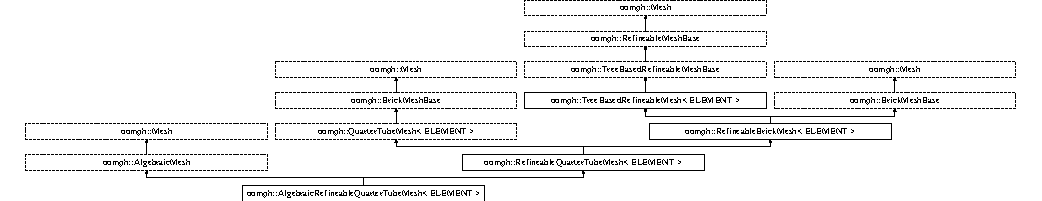
\includegraphics[height=2.699725cm]{classoomph_1_1AlgebraicRefineableQuarterTubeMesh}
\end{center}
\end{figure}
\subsection*{Public Member Functions}
\begin{DoxyCompactItemize}
\item 
\hyperlink{classoomph_1_1AlgebraicRefineableQuarterTubeMesh_ad8ff9f32d4d180d815da65ddc3c4b90a}{Algebraic\+Refineable\+Quarter\+Tube\+Mesh} (\hyperlink{classoomph_1_1GeomObject}{Geom\+Object} $\ast$\hyperlink{classoomph_1_1QuarterTubeMesh_af59c4cde343ddd76caea4bc8c8ad8b94}{wall\+\_\+pt}, const \hyperlink{classoomph_1_1Vector}{Vector}$<$ double $>$ \&xi\+\_\+lo, const double \&fract\+\_\+mid, const \hyperlink{classoomph_1_1Vector}{Vector}$<$ double $>$ \&xi\+\_\+hi, const unsigned \&nlayer, const double centre\+\_\+box\+\_\+size=1.\+0, \hyperlink{classoomph_1_1TimeStepper}{Time\+Stepper} $\ast$time\+\_\+stepper\+\_\+pt=\&\hyperlink{classoomph_1_1Mesh_a12243d0fee2b1fcee729ee5a4777ea10}{Mesh\+::\+Default\+\_\+\+Time\+Stepper})
\begin{DoxyCompactList}\small\item\em Constructor\+: Pass pointer to geometric object, start and end coordinates of the geometric object and the fraction along the 2nd Lagrangian coordinate at which the dividing line between region 1 and region 2 is to be placed, and timestepper (defaults to (\hyperlink{classoomph_1_1Steady}{Steady}) default timestepper defined in \hyperlink{classoomph_1_1Mesh}{Mesh}). Sets up the refineable mesh (by calling the constructor for the underlying \hyperlink{classoomph_1_1RefineableQuarterTubeMesh}{Refineable\+Quarter\+Tube\+Mesh}). \end{DoxyCompactList}\item 
unsigned \hyperlink{classoomph_1_1AlgebraicRefineableQuarterTubeMesh_a1ad71be8274f4073b7e18cb53d574f10}{self\+\_\+test} ()
\begin{DoxyCompactList}\small\item\em Run self-\/test for algebraic mesh -- return 0/1 for O\+K/failure. \end{DoxyCompactList}\item 
\hyperlink{classoomph_1_1QuarterTubeDomain_ae347af42a5dcb9b3b82c2247975b01db}{Quarter\+Tube\+Domain\+::\+Axial\+Spacing\+Fct\+Pt} \& \hyperlink{classoomph_1_1AlgebraicRefineableQuarterTubeMesh_ac6518f83dd81c5ef1a8d908be8c9f473}{axial\+\_\+spacing\+\_\+fct\+\_\+pt} ()
\begin{DoxyCompactList}\small\item\em Broken version of the \hyperlink{classoomph_1_1QuarterTubeDomain}{Quarter\+Tube\+Domain} function Function is broken because axial spacing isn\textquotesingle{}t implemented yet for the Algebraic version of the \hyperlink{classoomph_1_1RefineableQuarterTubeMesh}{Refineable\+Quarter\+Tube\+Mesh}. Note\+: this function must be used B\+E\+F\+O\+RE algebraic\+\_\+node\+\_\+update(...) is called. \end{DoxyCompactList}\item 
void \hyperlink{classoomph_1_1AlgebraicRefineableQuarterTubeMesh_af521c0a76cf0bd14692979bd7747507d}{node\+\_\+update} (const bool \&update\+\_\+all\+\_\+solid\+\_\+nodes=false)
\begin{DoxyCompactList}\small\item\em Resolve mesh update\+: Update current nodal positions via algebraic node update. \mbox{[}Doesn\textquotesingle{}t make sense to use this mesh with Solid\+Elements anyway, so we buffer the case if update\+\_\+all\+\_\+solid\+\_\+nodes is set to true.\mbox{]}. \end{DoxyCompactList}\item 
void \hyperlink{classoomph_1_1AlgebraicRefineableQuarterTubeMesh_af98a0aaff29c54ffa35f72f7dcf6b8c7}{algebraic\+\_\+node\+\_\+update} (const unsigned \&\hyperlink{cfortran_8h_af6f0bd3dc13317f895c91323c25c2b8f}{t}, \hyperlink{classoomph_1_1AlgebraicNode}{Algebraic\+Node} $\ast$\&\hyperlink{classoomph_1_1AlgebraicMesh_aedeebbe95d2f8e67e9939cecd1be3933}{node\+\_\+pt})
\begin{DoxyCompactList}\small\item\em Implement the algebraic node update function for a node at time level t (t=0\+: present; t$>$0\+: previous)\+: Update with the node\textquotesingle{}s first (default) update function. \end{DoxyCompactList}\item 
void \hyperlink{classoomph_1_1AlgebraicRefineableQuarterTubeMesh_a7ed9f4ce0442a6f962a1561318542a67}{update\+\_\+node\+\_\+update} (\hyperlink{classoomph_1_1AlgebraicNode}{Algebraic\+Node} $\ast$\&\hyperlink{classoomph_1_1AlgebraicMesh_aedeebbe95d2f8e67e9939cecd1be3933}{node\+\_\+pt})
\begin{DoxyCompactList}\small\item\em Update the node update info for specified algebraic node following any spatial mesh adaptation. \end{DoxyCompactList}\end{DoxyCompactItemize}
\subsection*{Private Types}
\begin{DoxyCompactItemize}
\item 
enum \{ \hyperlink{classoomph_1_1AlgebraicRefineableQuarterTubeMesh_a215c0430765f10553590b0d47203393da516de7eb4676b7b88ebd50f5967a5579}{Central\+\_\+region}, 
\hyperlink{classoomph_1_1AlgebraicRefineableQuarterTubeMesh_a215c0430765f10553590b0d47203393da05c833cf7edf44c3bd94251628400da3}{Lower\+\_\+right\+\_\+region}, 
\hyperlink{classoomph_1_1AlgebraicRefineableQuarterTubeMesh_a215c0430765f10553590b0d47203393da4e534010f6f42e81a575935509ace9ab}{Upper\+\_\+left\+\_\+region}
 \}\begin{DoxyCompactList}\small\item\em Remesh function ids. \end{DoxyCompactList}
\end{DoxyCompactItemize}
\subsection*{Private Member Functions}
\begin{DoxyCompactItemize}
\item 
void \hyperlink{classoomph_1_1AlgebraicRefineableQuarterTubeMesh_a064653020f5d2a0c7de789283dac305c}{node\+\_\+update\+\_\+central\+\_\+region} (const unsigned \&\hyperlink{cfortran_8h_af6f0bd3dc13317f895c91323c25c2b8f}{t}, \hyperlink{classoomph_1_1AlgebraicNode}{Algebraic\+Node} $\ast$\&\hyperlink{classoomph_1_1AlgebraicMesh_aedeebbe95d2f8e67e9939cecd1be3933}{node\+\_\+pt})
\begin{DoxyCompactList}\small\item\em Algebraic update function for a node that is located in the central region. \end{DoxyCompactList}\item 
void \hyperlink{classoomph_1_1AlgebraicRefineableQuarterTubeMesh_a52fb1161ebff25b5c638ac35cb541817}{node\+\_\+update\+\_\+lower\+\_\+right\+\_\+region} (const unsigned \&\hyperlink{cfortran_8h_af6f0bd3dc13317f895c91323c25c2b8f}{t}, \hyperlink{classoomph_1_1AlgebraicNode}{Algebraic\+Node} $\ast$\&\hyperlink{classoomph_1_1AlgebraicMesh_aedeebbe95d2f8e67e9939cecd1be3933}{node\+\_\+pt})
\begin{DoxyCompactList}\small\item\em Algebraic update function for a node that is located in the lower-\/right region. \end{DoxyCompactList}\item 
void \hyperlink{classoomph_1_1AlgebraicRefineableQuarterTubeMesh_ac82a39ccaed8016a9b1e841d91658a75}{node\+\_\+update\+\_\+upper\+\_\+left\+\_\+region} (const unsigned \&\hyperlink{cfortran_8h_af6f0bd3dc13317f895c91323c25c2b8f}{t}, \hyperlink{classoomph_1_1AlgebraicNode}{Algebraic\+Node} $\ast$\&\hyperlink{classoomph_1_1AlgebraicMesh_aedeebbe95d2f8e67e9939cecd1be3933}{node\+\_\+pt})
\begin{DoxyCompactList}\small\item\em Algebraic update function for a node that is located in the upper-\/left region. \end{DoxyCompactList}\item 
void \hyperlink{classoomph_1_1AlgebraicRefineableQuarterTubeMesh_a2d0312615834a2aec8d0d6d4e2c846ef}{setup\+\_\+algebraic\+\_\+node\+\_\+update} ()
\begin{DoxyCompactList}\small\item\em Setup algebraic update operation for all nodes. \end{DoxyCompactList}\item 
void \hyperlink{classoomph_1_1AlgebraicRefineableQuarterTubeMesh_ae2014e91ad7f5a226b35aa96964f4bf1}{update\+\_\+node\+\_\+update\+\_\+in\+\_\+region} (\hyperlink{classoomph_1_1AlgebraicNode}{Algebraic\+Node} $\ast$\&\hyperlink{classoomph_1_1AlgebraicMesh_aedeebbe95d2f8e67e9939cecd1be3933}{node\+\_\+pt}, int \&region\+\_\+id)
\begin{DoxyCompactList}\small\item\em Update algebraic node update function for nodes in the region defined by region\+\_\+id. \end{DoxyCompactList}\end{DoxyCompactItemize}
\subsection*{Private Attributes}
\begin{DoxyCompactItemize}
\item 
double \hyperlink{classoomph_1_1AlgebraicRefineableQuarterTubeMesh_a6006bcac5688f832ff2b6cbaae65102a}{Centre\+\_\+box\+\_\+size}
\begin{DoxyCompactList}\small\item\em Size of centre box. \end{DoxyCompactList}\item 
double \hyperlink{classoomph_1_1AlgebraicRefineableQuarterTubeMesh_a5bb15683ec46078f9e3ab6d9caba54cf}{Lambda\+\_\+x}
\begin{DoxyCompactList}\small\item\em Fractional width of central region. \end{DoxyCompactList}\item 
double \hyperlink{classoomph_1_1AlgebraicRefineableQuarterTubeMesh_a8e3b05ebb0b69e3ca3cbedb39b5b8e47}{Lambda\+\_\+y}
\begin{DoxyCompactList}\small\item\em Fractional height of central region. \end{DoxyCompactList}\end{DoxyCompactItemize}
\subsection*{Additional Inherited Members}


\subsection{Detailed Description}
\subsubsection*{template$<$class E\+L\+E\+M\+E\+NT$>$\newline
class oomph\+::\+Algebraic\+Refineable\+Quarter\+Tube\+Mesh$<$ E\+L\+E\+M\+E\+N\+T $>$}

\hyperlink{classoomph_1_1AlgebraicMesh}{Algebraic\+Mesh} version of \hyperlink{classoomph_1_1RefineableQuarterTubeMesh}{Refineable\+Quarter\+Tube\+Mesh}. 

Algebraic 3D quarter tube mesh class.

The mesh boundaries are numbered as follows\+:
\begin{DoxyItemize}
\item Boundary 0\+: \char`\"{}\+Inflow\char`\"{} cross section; located along the line parametrised by $ \xi_0 = \xi_0^{lo} $ on the geometric object that specifies the wall.
\item Boundary 1\+: Plane x=0
\item Boundary 2\+: Plane y=0
\item Boundary 3\+: The curved wall -\/ specified by the \hyperlink{classoomph_1_1GeomObject}{Geom\+Object} passed to the mesh constructor.
\item Boundary 4\+: \char`\"{}\+Outflow\char`\"{} cross section; located along the line parametrised by $ \xi_0 = \xi_0^{hi} $ on the geometric object that specifies the wall. Algebraic version of \hyperlink{classoomph_1_1RefineableQuarterTubeMesh}{Refineable\+Quarter\+Tube\+Mesh}
\end{DoxyItemize}

Cross section through mesh looking along tube......... \begin{DoxyVerb}                 ---___
                |      ---____
                |              -   BOUNDARY 3
                |                /
                |  [Region 2]   /  |
                |              /     |
                | N           /        |
                | |_ E       /          |
  BOUNDARY 1    |------------            |
                |            |            |
                | [Region 0] | [Region 1] |  ^
                |            |            | / \  direction of
                | N          |    N       |  |   2nd Lagrangian
                | |_ E       |    |_ E    |  |   coordinate
                |____________|____________|  |   along wall GeomObject

                      BOUNDARY 2
\end{DoxyVerb}


The \hyperlink{classoomph_1_1Domain}{Domain} is built of slices each consisting of three Macro\+Elements as sketched. The local coordinates are such that the (E)astern direction coincides with the positive s\+\_\+0 direction, while the (N)orther direction coincides with the positive s\+\_\+1 direction. The positive s\+\_\+2 direction points down the tube.

Elements need to be derived from \hyperlink{classoomph_1_1AlgebraicElementBase}{Algebraic\+Element\+Base}. In addition to the refinement procedures available for the \hyperlink{classoomph_1_1RefineableQuarterTubeMesh}{Refineable\+Quarter\+Tube\+Mesh} which forms the basis for this mesh, three algebraic node update functions are implemented for the nodes in the three regions defined by the \hyperlink{classoomph_1_1Domain}{Domain} Macro\+Elements. Note\+: it is assumed the cross section down the tube is uniform when \hyperlink{classoomph_1_1AlgebraicRefineableQuarterTubeMesh_a2d0312615834a2aec8d0d6d4e2c846ef}{setup\+\_\+algebraic\+\_\+node\+\_\+update()} is called. 

Definition at line 462 of file quarter\+\_\+tube\+\_\+mesh.\+template.\+h.



\subsection{Member Enumeration Documentation}
\mbox{\Hypertarget{classoomph_1_1AlgebraicRefineableQuarterTubeMesh_a215c0430765f10553590b0d47203393d}\label{classoomph_1_1AlgebraicRefineableQuarterTubeMesh_a215c0430765f10553590b0d47203393d}} 
\subsubsection{\texorpdfstring{anonymous enum}{anonymous enum}}
{\footnotesize\ttfamily template$<$class E\+L\+E\+M\+E\+NT $>$ \\
anonymous enum\hspace{0.3cm}{\ttfamily [private]}}



Remesh function ids. 

\begin{DoxyEnumFields}{Enumerator}
\raisebox{\heightof{T}}[0pt][0pt]{\index{Central\+\_\+region@{Central\+\_\+region}!oomph\+::\+Algebraic\+Refineable\+Quarter\+Tube\+Mesh@{oomph\+::\+Algebraic\+Refineable\+Quarter\+Tube\+Mesh}}\index{oomph\+::\+Algebraic\+Refineable\+Quarter\+Tube\+Mesh@{oomph\+::\+Algebraic\+Refineable\+Quarter\+Tube\+Mesh}!Central\+\_\+region@{Central\+\_\+region}}}\mbox{\Hypertarget{classoomph_1_1AlgebraicRefineableQuarterTubeMesh_a215c0430765f10553590b0d47203393da516de7eb4676b7b88ebd50f5967a5579}\label{classoomph_1_1AlgebraicRefineableQuarterTubeMesh_a215c0430765f10553590b0d47203393da516de7eb4676b7b88ebd50f5967a5579}} 
Central\+\_\+region&\\
\hline

\raisebox{\heightof{T}}[0pt][0pt]{\index{Lower\+\_\+right\+\_\+region@{Lower\+\_\+right\+\_\+region}!oomph\+::\+Algebraic\+Refineable\+Quarter\+Tube\+Mesh@{oomph\+::\+Algebraic\+Refineable\+Quarter\+Tube\+Mesh}}\index{oomph\+::\+Algebraic\+Refineable\+Quarter\+Tube\+Mesh@{oomph\+::\+Algebraic\+Refineable\+Quarter\+Tube\+Mesh}!Lower\+\_\+right\+\_\+region@{Lower\+\_\+right\+\_\+region}}}\mbox{\Hypertarget{classoomph_1_1AlgebraicRefineableQuarterTubeMesh_a215c0430765f10553590b0d47203393da05c833cf7edf44c3bd94251628400da3}\label{classoomph_1_1AlgebraicRefineableQuarterTubeMesh_a215c0430765f10553590b0d47203393da05c833cf7edf44c3bd94251628400da3}} 
Lower\+\_\+right\+\_\+region&\\
\hline

\raisebox{\heightof{T}}[0pt][0pt]{\index{Upper\+\_\+left\+\_\+region@{Upper\+\_\+left\+\_\+region}!oomph\+::\+Algebraic\+Refineable\+Quarter\+Tube\+Mesh@{oomph\+::\+Algebraic\+Refineable\+Quarter\+Tube\+Mesh}}\index{oomph\+::\+Algebraic\+Refineable\+Quarter\+Tube\+Mesh@{oomph\+::\+Algebraic\+Refineable\+Quarter\+Tube\+Mesh}!Upper\+\_\+left\+\_\+region@{Upper\+\_\+left\+\_\+region}}}\mbox{\Hypertarget{classoomph_1_1AlgebraicRefineableQuarterTubeMesh_a215c0430765f10553590b0d47203393da4e534010f6f42e81a575935509ace9ab}\label{classoomph_1_1AlgebraicRefineableQuarterTubeMesh_a215c0430765f10553590b0d47203393da4e534010f6f42e81a575935509ace9ab}} 
Upper\+\_\+left\+\_\+region&\\
\hline

\end{DoxyEnumFields}


Definition at line 653 of file quarter\+\_\+tube\+\_\+mesh.\+template.\+h.



\subsection{Constructor \& Destructor Documentation}
\mbox{\Hypertarget{classoomph_1_1AlgebraicRefineableQuarterTubeMesh_ad8ff9f32d4d180d815da65ddc3c4b90a}\label{classoomph_1_1AlgebraicRefineableQuarterTubeMesh_ad8ff9f32d4d180d815da65ddc3c4b90a}} 
\index{oomph\+::\+Algebraic\+Refineable\+Quarter\+Tube\+Mesh@{oomph\+::\+Algebraic\+Refineable\+Quarter\+Tube\+Mesh}!Algebraic\+Refineable\+Quarter\+Tube\+Mesh@{Algebraic\+Refineable\+Quarter\+Tube\+Mesh}}
\index{Algebraic\+Refineable\+Quarter\+Tube\+Mesh@{Algebraic\+Refineable\+Quarter\+Tube\+Mesh}!oomph\+::\+Algebraic\+Refineable\+Quarter\+Tube\+Mesh@{oomph\+::\+Algebraic\+Refineable\+Quarter\+Tube\+Mesh}}
\subsubsection{\texorpdfstring{Algebraic\+Refineable\+Quarter\+Tube\+Mesh()}{AlgebraicRefineableQuarterTubeMesh()}}
{\footnotesize\ttfamily template$<$class E\+L\+E\+M\+E\+NT $>$ \\
\hyperlink{classoomph_1_1AlgebraicRefineableQuarterTubeMesh}{oomph\+::\+Algebraic\+Refineable\+Quarter\+Tube\+Mesh}$<$ E\+L\+E\+M\+E\+NT $>$\+::\hyperlink{classoomph_1_1AlgebraicRefineableQuarterTubeMesh}{Algebraic\+Refineable\+Quarter\+Tube\+Mesh} (\begin{DoxyParamCaption}\item[{\hyperlink{classoomph_1_1GeomObject}{Geom\+Object} $\ast$}]{wall\+\_\+pt,  }\item[{const \hyperlink{classoomph_1_1Vector}{Vector}$<$ double $>$ \&}]{xi\+\_\+lo,  }\item[{const double \&}]{fract\+\_\+mid,  }\item[{const \hyperlink{classoomph_1_1Vector}{Vector}$<$ double $>$ \&}]{xi\+\_\+hi,  }\item[{const unsigned \&}]{nlayer,  }\item[{const double}]{centre\+\_\+box\+\_\+size = {\ttfamily 1.0},  }\item[{\hyperlink{classoomph_1_1TimeStepper}{Time\+Stepper} $\ast$}]{time\+\_\+stepper\+\_\+pt = {\ttfamily \&\hyperlink{classoomph_1_1Mesh_a12243d0fee2b1fcee729ee5a4777ea10}{Mesh\+::\+Default\+\_\+\+Time\+Stepper}} }\end{DoxyParamCaption})\hspace{0.3cm}{\ttfamily [inline]}}



Constructor\+: Pass pointer to geometric object, start and end coordinates of the geometric object and the fraction along the 2nd Lagrangian coordinate at which the dividing line between region 1 and region 2 is to be placed, and timestepper (defaults to (\hyperlink{classoomph_1_1Steady}{Steady}) default timestepper defined in \hyperlink{classoomph_1_1Mesh}{Mesh}). Sets up the refineable mesh (by calling the constructor for the underlying \hyperlink{classoomph_1_1RefineableQuarterTubeMesh}{Refineable\+Quarter\+Tube\+Mesh}). 



Definition at line 476 of file quarter\+\_\+tube\+\_\+mesh.\+template.\+h.



References oomph\+::\+Algebraic\+Mesh\+::add\+\_\+geom\+\_\+object\+\_\+list\+\_\+pt(), oomph\+::\+Mesh\+::node\+\_\+update(), and oomph\+::\+Global\+\_\+string\+\_\+for\+\_\+annotation\+::string().



\subsection{Member Function Documentation}
\mbox{\Hypertarget{classoomph_1_1AlgebraicRefineableQuarterTubeMesh_af98a0aaff29c54ffa35f72f7dcf6b8c7}\label{classoomph_1_1AlgebraicRefineableQuarterTubeMesh_af98a0aaff29c54ffa35f72f7dcf6b8c7}} 
\index{oomph\+::\+Algebraic\+Refineable\+Quarter\+Tube\+Mesh@{oomph\+::\+Algebraic\+Refineable\+Quarter\+Tube\+Mesh}!algebraic\+\_\+node\+\_\+update@{algebraic\+\_\+node\+\_\+update}}
\index{algebraic\+\_\+node\+\_\+update@{algebraic\+\_\+node\+\_\+update}!oomph\+::\+Algebraic\+Refineable\+Quarter\+Tube\+Mesh@{oomph\+::\+Algebraic\+Refineable\+Quarter\+Tube\+Mesh}}
\subsubsection{\texorpdfstring{algebraic\+\_\+node\+\_\+update()}{algebraic\_node\_update()}}
{\footnotesize\ttfamily template$<$class E\+L\+E\+M\+E\+NT $>$ \\
void \hyperlink{classoomph_1_1AlgebraicRefineableQuarterTubeMesh}{oomph\+::\+Algebraic\+Refineable\+Quarter\+Tube\+Mesh}$<$ E\+L\+E\+M\+E\+NT $>$\+::algebraic\+\_\+node\+\_\+update (\begin{DoxyParamCaption}\item[{const unsigned \&}]{t,  }\item[{\hyperlink{classoomph_1_1AlgebraicNode}{Algebraic\+Node} $\ast$\&}]{node\+\_\+pt }\end{DoxyParamCaption})\hspace{0.3cm}{\ttfamily [inline]}, {\ttfamily [virtual]}}



Implement the algebraic node update function for a node at time level t (t=0\+: present; t$>$0\+: previous)\+: Update with the node\textquotesingle{}s first (default) update function. 



Implements \hyperlink{classoomph_1_1AlgebraicMesh_ab01d6f93354f3c4e5c9d1f0a5885a65b}{oomph\+::\+Algebraic\+Mesh}.



Definition at line 585 of file quarter\+\_\+tube\+\_\+mesh.\+template.\+h.



References oomph\+::\+Algebraic\+Node\+::node\+\_\+update\+\_\+fct\+\_\+id(), and oomph\+::\+Global\+\_\+string\+\_\+for\+\_\+annotation\+::string().

\mbox{\Hypertarget{classoomph_1_1AlgebraicRefineableQuarterTubeMesh_ac6518f83dd81c5ef1a8d908be8c9f473}\label{classoomph_1_1AlgebraicRefineableQuarterTubeMesh_ac6518f83dd81c5ef1a8d908be8c9f473}} 
\index{oomph\+::\+Algebraic\+Refineable\+Quarter\+Tube\+Mesh@{oomph\+::\+Algebraic\+Refineable\+Quarter\+Tube\+Mesh}!axial\+\_\+spacing\+\_\+fct\+\_\+pt@{axial\+\_\+spacing\+\_\+fct\+\_\+pt}}
\index{axial\+\_\+spacing\+\_\+fct\+\_\+pt@{axial\+\_\+spacing\+\_\+fct\+\_\+pt}!oomph\+::\+Algebraic\+Refineable\+Quarter\+Tube\+Mesh@{oomph\+::\+Algebraic\+Refineable\+Quarter\+Tube\+Mesh}}
\subsubsection{\texorpdfstring{axial\+\_\+spacing\+\_\+fct\+\_\+pt()}{axial\_spacing\_fct\_pt()}}
{\footnotesize\ttfamily template$<$class E\+L\+E\+M\+E\+NT $>$ \\
\hyperlink{classoomph_1_1QuarterTubeDomain_ae347af42a5dcb9b3b82c2247975b01db}{Quarter\+Tube\+Domain\+::\+Axial\+Spacing\+Fct\+Pt}\& \hyperlink{classoomph_1_1AlgebraicRefineableQuarterTubeMesh}{oomph\+::\+Algebraic\+Refineable\+Quarter\+Tube\+Mesh}$<$ E\+L\+E\+M\+E\+NT $>$\+::axial\+\_\+spacing\+\_\+fct\+\_\+pt (\begin{DoxyParamCaption}{ }\end{DoxyParamCaption})\hspace{0.3cm}{\ttfamily [inline]}, {\ttfamily [virtual]}}



Broken version of the \hyperlink{classoomph_1_1QuarterTubeDomain}{Quarter\+Tube\+Domain} function Function is broken because axial spacing isn\textquotesingle{}t implemented yet for the Algebraic version of the \hyperlink{classoomph_1_1RefineableQuarterTubeMesh}{Refineable\+Quarter\+Tube\+Mesh}. Note\+: this function must be used B\+E\+F\+O\+RE algebraic\+\_\+node\+\_\+update(...) is called. 



Reimplemented from \hyperlink{classoomph_1_1QuarterTubeMesh_a5c880d6214a07676a533227f813634d8}{oomph\+::\+Quarter\+Tube\+Mesh$<$ E\+L\+E\+M\+E\+N\+T $>$}.



Definition at line 536 of file quarter\+\_\+tube\+\_\+mesh.\+template.\+h.



References oomph\+::\+Quarter\+Tube\+Domain\+::axial\+\_\+spacing\+\_\+fct\+\_\+pt(), oomph\+::\+Quarter\+Tube\+Mesh$<$ E\+L\+E\+M\+E\+N\+T $>$\+::\+Domain\+\_\+pt, and oomph\+::\+Global\+\_\+string\+\_\+for\+\_\+annotation\+::string().

\mbox{\Hypertarget{classoomph_1_1AlgebraicRefineableQuarterTubeMesh_af521c0a76cf0bd14692979bd7747507d}\label{classoomph_1_1AlgebraicRefineableQuarterTubeMesh_af521c0a76cf0bd14692979bd7747507d}} 
\index{oomph\+::\+Algebraic\+Refineable\+Quarter\+Tube\+Mesh@{oomph\+::\+Algebraic\+Refineable\+Quarter\+Tube\+Mesh}!node\+\_\+update@{node\+\_\+update}}
\index{node\+\_\+update@{node\+\_\+update}!oomph\+::\+Algebraic\+Refineable\+Quarter\+Tube\+Mesh@{oomph\+::\+Algebraic\+Refineable\+Quarter\+Tube\+Mesh}}
\subsubsection{\texorpdfstring{node\+\_\+update()}{node\_update()}}
{\footnotesize\ttfamily template$<$class E\+L\+E\+M\+E\+NT $>$ \\
void \hyperlink{classoomph_1_1AlgebraicRefineableQuarterTubeMesh}{oomph\+::\+Algebraic\+Refineable\+Quarter\+Tube\+Mesh}$<$ E\+L\+E\+M\+E\+NT $>$\+::node\+\_\+update (\begin{DoxyParamCaption}\item[{const bool \&}]{update\+\_\+all\+\_\+solid\+\_\+nodes = {\ttfamily false} }\end{DoxyParamCaption})\hspace{0.3cm}{\ttfamily [inline]}, {\ttfamily [virtual]}}



Resolve mesh update\+: Update current nodal positions via algebraic node update. \mbox{[}Doesn\textquotesingle{}t make sense to use this mesh with Solid\+Elements anyway, so we buffer the case if update\+\_\+all\+\_\+solid\+\_\+nodes is set to true.\mbox{]}. 



Reimplemented from \hyperlink{classoomph_1_1AlgebraicMesh_ad3a5638cacb6df1a47c475bb177b6ed7}{oomph\+::\+Algebraic\+Mesh}.



Definition at line 557 of file quarter\+\_\+tube\+\_\+mesh.\+template.\+h.



References oomph\+::\+Algebraic\+Mesh\+::node\+\_\+update(), and oomph\+::\+Global\+\_\+string\+\_\+for\+\_\+annotation\+::string().

\mbox{\Hypertarget{classoomph_1_1AlgebraicRefineableQuarterTubeMesh_a064653020f5d2a0c7de789283dac305c}\label{classoomph_1_1AlgebraicRefineableQuarterTubeMesh_a064653020f5d2a0c7de789283dac305c}} 
\index{oomph\+::\+Algebraic\+Refineable\+Quarter\+Tube\+Mesh@{oomph\+::\+Algebraic\+Refineable\+Quarter\+Tube\+Mesh}!node\+\_\+update\+\_\+central\+\_\+region@{node\+\_\+update\+\_\+central\+\_\+region}}
\index{node\+\_\+update\+\_\+central\+\_\+region@{node\+\_\+update\+\_\+central\+\_\+region}!oomph\+::\+Algebraic\+Refineable\+Quarter\+Tube\+Mesh@{oomph\+::\+Algebraic\+Refineable\+Quarter\+Tube\+Mesh}}
\subsubsection{\texorpdfstring{node\+\_\+update\+\_\+central\+\_\+region()}{node\_update\_central\_region()}}
{\footnotesize\ttfamily template$<$class E\+L\+E\+M\+E\+NT $>$ \\
void \hyperlink{classoomph_1_1AlgebraicRefineableQuarterTubeMesh}{oomph\+::\+Algebraic\+Refineable\+Quarter\+Tube\+Mesh}$<$ E\+L\+E\+M\+E\+NT $>$\+::node\+\_\+update\+\_\+central\+\_\+region (\begin{DoxyParamCaption}\item[{const unsigned \&}]{t,  }\item[{\hyperlink{classoomph_1_1AlgebraicNode}{Algebraic\+Node} $\ast$\&}]{node\+\_\+pt }\end{DoxyParamCaption})\hspace{0.3cm}{\ttfamily [private]}}



Algebraic update function for a node that is located in the central region. 

Algebraic update function\+: Update in central region according to wall shape at time level t (t=0\+: present; t$>$0\+: previous) 

Definition at line 1000 of file quarter\+\_\+tube\+\_\+mesh.\+template.\+cc.



References oomph\+::\+Geom\+Object\+::ndim(), oomph\+::\+Algebraic\+Refineable\+Quarter\+Tube\+Mesh$<$ E\+L\+E\+M\+E\+N\+T $>$\+::node\+\_\+update\+\_\+lower\+\_\+right\+\_\+region(), oomph\+::\+Time\+Stepper\+::nprev\+\_\+values(), oomph\+::\+Geom\+Object\+::position(), oomph\+::\+Node\+::position\+\_\+time\+\_\+stepper\+\_\+pt(), oomph\+::\+Global\+\_\+string\+\_\+for\+\_\+annotation\+::string(), oomph\+::\+Algebraic\+Node\+::vector\+\_\+ref\+\_\+value(), and oomph\+::\+Node\+::x().



Referenced by oomph\+::\+Algebraic\+Refineable\+Quarter\+Tube\+Mesh$<$ E\+L\+E\+M\+E\+N\+T $>$\+::setup\+\_\+algebraic\+\_\+node\+\_\+update().

\mbox{\Hypertarget{classoomph_1_1AlgebraicRefineableQuarterTubeMesh_a52fb1161ebff25b5c638ac35cb541817}\label{classoomph_1_1AlgebraicRefineableQuarterTubeMesh_a52fb1161ebff25b5c638ac35cb541817}} 
\index{oomph\+::\+Algebraic\+Refineable\+Quarter\+Tube\+Mesh@{oomph\+::\+Algebraic\+Refineable\+Quarter\+Tube\+Mesh}!node\+\_\+update\+\_\+lower\+\_\+right\+\_\+region@{node\+\_\+update\+\_\+lower\+\_\+right\+\_\+region}}
\index{node\+\_\+update\+\_\+lower\+\_\+right\+\_\+region@{node\+\_\+update\+\_\+lower\+\_\+right\+\_\+region}!oomph\+::\+Algebraic\+Refineable\+Quarter\+Tube\+Mesh@{oomph\+::\+Algebraic\+Refineable\+Quarter\+Tube\+Mesh}}
\subsubsection{\texorpdfstring{node\+\_\+update\+\_\+lower\+\_\+right\+\_\+region()}{node\_update\_lower\_right\_region()}}
{\footnotesize\ttfamily template$<$class E\+L\+E\+M\+E\+NT $>$ \\
void \hyperlink{classoomph_1_1AlgebraicRefineableQuarterTubeMesh}{oomph\+::\+Algebraic\+Refineable\+Quarter\+Tube\+Mesh}$<$ E\+L\+E\+M\+E\+NT $>$\+::node\+\_\+update\+\_\+lower\+\_\+right\+\_\+region (\begin{DoxyParamCaption}\item[{const unsigned \&}]{t,  }\item[{\hyperlink{classoomph_1_1AlgebraicNode}{Algebraic\+Node} $\ast$\&}]{node\+\_\+pt }\end{DoxyParamCaption})\hspace{0.3cm}{\ttfamily [private]}}



Algebraic update function for a node that is located in the lower-\/right region. 

Algebraic update function\+: Update in lower-\/right region according to wall shape at time level t (t=0\+: present; t$>$0\+: previous) 

Definition at line 1091 of file quarter\+\_\+tube\+\_\+mesh.\+template.\+cc.



References oomph\+::\+Quarter\+Tube\+Mesh$<$ E\+L\+E\+M\+E\+N\+T $>$\+::\+Domain\+\_\+pt, oomph\+::\+Geom\+Object\+::ndim(), oomph\+::\+Algebraic\+Refineable\+Quarter\+Tube\+Mesh$<$ E\+L\+E\+M\+E\+N\+T $>$\+::node\+\_\+update\+\_\+upper\+\_\+left\+\_\+region(), oomph\+::\+Time\+Stepper\+::nprev\+\_\+values(), oomph\+::\+Geom\+Object\+::position(), oomph\+::\+Node\+::position\+\_\+time\+\_\+stepper\+\_\+pt(), oomph\+::\+Quarter\+Tube\+Domain\+::s\+\_\+squashed(), oomph\+::\+Global\+\_\+string\+\_\+for\+\_\+annotation\+::string(), oomph\+::\+Algebraic\+Node\+::vector\+\_\+geom\+\_\+object\+\_\+pt(), oomph\+::\+Algebraic\+Node\+::vector\+\_\+ref\+\_\+value(), and oomph\+::\+Node\+::x().



Referenced by oomph\+::\+Algebraic\+Refineable\+Quarter\+Tube\+Mesh$<$ E\+L\+E\+M\+E\+N\+T $>$\+::node\+\_\+update\+\_\+central\+\_\+region().

\mbox{\Hypertarget{classoomph_1_1AlgebraicRefineableQuarterTubeMesh_ac82a39ccaed8016a9b1e841d91658a75}\label{classoomph_1_1AlgebraicRefineableQuarterTubeMesh_ac82a39ccaed8016a9b1e841d91658a75}} 
\index{oomph\+::\+Algebraic\+Refineable\+Quarter\+Tube\+Mesh@{oomph\+::\+Algebraic\+Refineable\+Quarter\+Tube\+Mesh}!node\+\_\+update\+\_\+upper\+\_\+left\+\_\+region@{node\+\_\+update\+\_\+upper\+\_\+left\+\_\+region}}
\index{node\+\_\+update\+\_\+upper\+\_\+left\+\_\+region@{node\+\_\+update\+\_\+upper\+\_\+left\+\_\+region}!oomph\+::\+Algebraic\+Refineable\+Quarter\+Tube\+Mesh@{oomph\+::\+Algebraic\+Refineable\+Quarter\+Tube\+Mesh}}
\subsubsection{\texorpdfstring{node\+\_\+update\+\_\+upper\+\_\+left\+\_\+region()}{node\_update\_upper\_left\_region()}}
{\footnotesize\ttfamily template$<$class E\+L\+E\+M\+E\+NT $>$ \\
void \hyperlink{classoomph_1_1AlgebraicRefineableQuarterTubeMesh}{oomph\+::\+Algebraic\+Refineable\+Quarter\+Tube\+Mesh}$<$ E\+L\+E\+M\+E\+NT $>$\+::node\+\_\+update\+\_\+upper\+\_\+left\+\_\+region (\begin{DoxyParamCaption}\item[{const unsigned \&}]{t,  }\item[{\hyperlink{classoomph_1_1AlgebraicNode}{Algebraic\+Node} $\ast$\&}]{node\+\_\+pt }\end{DoxyParamCaption})\hspace{0.3cm}{\ttfamily [private]}}



Algebraic update function for a node that is located in the upper-\/left region. 

Algebraic update function\+: Update in upper left region according to wall shape at time level t (t=0\+: present; t$>$0\+: previous) 

Definition at line 1211 of file quarter\+\_\+tube\+\_\+mesh.\+template.\+cc.



References oomph\+::\+Quarter\+Tube\+Mesh$<$ E\+L\+E\+M\+E\+N\+T $>$\+::\+Domain\+\_\+pt, oomph\+::\+Algebraic\+Node\+::geom\+\_\+object\+\_\+pt(), oomph\+::\+Geom\+Object\+::ndim(), oomph\+::\+Time\+Stepper\+::nprev\+\_\+values(), oomph\+::\+Geom\+Object\+::position(), oomph\+::\+Node\+::position\+\_\+time\+\_\+stepper\+\_\+pt(), oomph\+::\+Quarter\+Tube\+Domain\+::s\+\_\+squashed(), oomph\+::\+Global\+\_\+string\+\_\+for\+\_\+annotation\+::string(), oomph\+::\+Algebraic\+Refineable\+Quarter\+Tube\+Mesh$<$ E\+L\+E\+M\+E\+N\+T $>$\+::update\+\_\+node\+\_\+update\+\_\+in\+\_\+region(), oomph\+::\+Algebraic\+Node\+::vector\+\_\+geom\+\_\+object\+\_\+pt(), oomph\+::\+Algebraic\+Node\+::vector\+\_\+ref\+\_\+value(), and oomph\+::\+Node\+::x().



Referenced by oomph\+::\+Algebraic\+Refineable\+Quarter\+Tube\+Mesh$<$ E\+L\+E\+M\+E\+N\+T $>$\+::node\+\_\+update\+\_\+lower\+\_\+right\+\_\+region().

\mbox{\Hypertarget{classoomph_1_1AlgebraicRefineableQuarterTubeMesh_a1ad71be8274f4073b7e18cb53d574f10}\label{classoomph_1_1AlgebraicRefineableQuarterTubeMesh_a1ad71be8274f4073b7e18cb53d574f10}} 
\index{oomph\+::\+Algebraic\+Refineable\+Quarter\+Tube\+Mesh@{oomph\+::\+Algebraic\+Refineable\+Quarter\+Tube\+Mesh}!self\+\_\+test@{self\+\_\+test}}
\index{self\+\_\+test@{self\+\_\+test}!oomph\+::\+Algebraic\+Refineable\+Quarter\+Tube\+Mesh@{oomph\+::\+Algebraic\+Refineable\+Quarter\+Tube\+Mesh}}
\subsubsection{\texorpdfstring{self\+\_\+test()}{self\_test()}}
{\footnotesize\ttfamily template$<$class E\+L\+E\+M\+E\+NT $>$ \\
unsigned \hyperlink{classoomph_1_1AlgebraicRefineableQuarterTubeMesh}{oomph\+::\+Algebraic\+Refineable\+Quarter\+Tube\+Mesh}$<$ E\+L\+E\+M\+E\+NT $>$\+::self\+\_\+test (\begin{DoxyParamCaption}{ }\end{DoxyParamCaption})\hspace{0.3cm}{\ttfamily [inline]}}



Run self-\/test for algebraic mesh -- return 0/1 for O\+K/failure. 



Definition at line 526 of file quarter\+\_\+tube\+\_\+mesh.\+template.\+h.



References oomph\+::\+Algebraic\+Mesh\+::self\+\_\+test().

\mbox{\Hypertarget{classoomph_1_1AlgebraicRefineableQuarterTubeMesh_a2d0312615834a2aec8d0d6d4e2c846ef}\label{classoomph_1_1AlgebraicRefineableQuarterTubeMesh_a2d0312615834a2aec8d0d6d4e2c846ef}} 
\index{oomph\+::\+Algebraic\+Refineable\+Quarter\+Tube\+Mesh@{oomph\+::\+Algebraic\+Refineable\+Quarter\+Tube\+Mesh}!setup\+\_\+algebraic\+\_\+node\+\_\+update@{setup\+\_\+algebraic\+\_\+node\+\_\+update}}
\index{setup\+\_\+algebraic\+\_\+node\+\_\+update@{setup\+\_\+algebraic\+\_\+node\+\_\+update}!oomph\+::\+Algebraic\+Refineable\+Quarter\+Tube\+Mesh@{oomph\+::\+Algebraic\+Refineable\+Quarter\+Tube\+Mesh}}
\subsubsection{\texorpdfstring{setup\+\_\+algebraic\+\_\+node\+\_\+update()}{setup\_algebraic\_node\_update()}}
{\footnotesize\ttfamily template$<$class E\+L\+E\+M\+E\+NT $>$ \\
void \hyperlink{classoomph_1_1AlgebraicRefineableQuarterTubeMesh}{oomph\+::\+Algebraic\+Refineable\+Quarter\+Tube\+Mesh}$<$ E\+L\+E\+M\+E\+NT $>$\+::setup\+\_\+algebraic\+\_\+node\+\_\+update (\begin{DoxyParamCaption}{ }\end{DoxyParamCaption})\hspace{0.3cm}{\ttfamily [private]}}



Setup algebraic update operation for all nodes. 

Setup algebraic node update data, based on 3 regions, each undergoing a different node update strategy. These regions are defined by the three Macro\+Elements in each of the nlayer slices of the \hyperlink{classoomph_1_1QuarterTubeDomain}{Quarter\+Tube\+Domain} used to build the mesh. The \hyperlink{classoomph_1_1Mesh}{Mesh} is suspended from the `wall\textquotesingle{} \hyperlink{classoomph_1_1GeomObject}{Geom\+Object} pointed to by wall\+\_\+pt. The lower right edge of the mesh is located at the wall\textquotesingle{}s coordinate xi\mbox{[}1\mbox{]}==xi\+\_\+lo\mbox{[}1\mbox{]}, the upper left edge at xi\mbox{[}1\mbox{]}=xi\+\_\+hi\mbox{[}1\mbox{]}, i.\+e. a view looking down the tube length. The dividing line between the two outer regions is located at the fraction fract\+\_\+mid between these two coordinates. \hyperlink{classoomph_1_1Node}{Node} updating strategy\+:
\begin{DoxyItemize}
\item the starting cross sectional shape along the tube length is assumed to be uniform
\item the cross sectional shape of the central region remains rectangular; the position of its top right corner is located at a fixed fraction of the starting width and height of the domain measured at xi\mbox{[}1\mbox{]}==xi\+\_\+lo\mbox{[}1\mbox{]} and xi\mbox{[}1\mbox{]}==xi\+\_\+hi\mbox{[}1\mbox{]} respectively. Nodes in this region are located at fixed horizontal and vertical fractions of the region.
\item Nodes in the two outer regions (bottom right and top left) are located on straight lines running from the edges of the central region to the outer wall. 
\end{DoxyItemize}Pointer to first algebraic element in central region 

Definition at line 691 of file quarter\+\_\+tube\+\_\+mesh.\+template.\+cc.



References e, oomph\+::\+Mesh\+::element\+\_\+pt(), oomph\+::\+Mesh\+::finite\+\_\+element\+\_\+pt(), oomph\+::\+Geom\+Object\+::locate\+\_\+zeta(), oomph\+::\+Mesh\+::nelement(), oomph\+::\+Finite\+Element\+::nnode(), oomph\+::\+Finite\+Element\+::nnode\+\_\+1d(), oomph\+::\+Finite\+Element\+::node\+\_\+pt(), oomph\+::\+Algebraic\+Refineable\+Quarter\+Tube\+Mesh$<$ E\+L\+E\+M\+E\+N\+T $>$\+::node\+\_\+update\+\_\+central\+\_\+region(), oomph\+::\+Global\+\_\+string\+\_\+for\+\_\+annotation\+::string(), oomph\+::\+Quarter\+Tube\+Mesh$<$ E\+L\+E\+M\+E\+N\+T $>$\+::\+Wall\+\_\+pt, and oomph\+::\+Node\+::x().



Referenced by oomph\+::\+Quarter\+Tube\+Mesh$<$ E\+L\+E\+M\+E\+N\+T $>$\+::\+Quarter\+Tube\+Mesh().

\mbox{\Hypertarget{classoomph_1_1AlgebraicRefineableQuarterTubeMesh_a7ed9f4ce0442a6f962a1561318542a67}\label{classoomph_1_1AlgebraicRefineableQuarterTubeMesh_a7ed9f4ce0442a6f962a1561318542a67}} 
\index{oomph\+::\+Algebraic\+Refineable\+Quarter\+Tube\+Mesh@{oomph\+::\+Algebraic\+Refineable\+Quarter\+Tube\+Mesh}!update\+\_\+node\+\_\+update@{update\+\_\+node\+\_\+update}}
\index{update\+\_\+node\+\_\+update@{update\+\_\+node\+\_\+update}!oomph\+::\+Algebraic\+Refineable\+Quarter\+Tube\+Mesh@{oomph\+::\+Algebraic\+Refineable\+Quarter\+Tube\+Mesh}}
\subsubsection{\texorpdfstring{update\+\_\+node\+\_\+update()}{update\_node\_update()}}
{\footnotesize\ttfamily template$<$class E\+L\+E\+M\+E\+NT $>$ \\
void \hyperlink{classoomph_1_1AlgebraicRefineableQuarterTubeMesh}{oomph\+::\+Algebraic\+Refineable\+Quarter\+Tube\+Mesh}$<$ E\+L\+E\+M\+E\+NT $>$\+::update\+\_\+node\+\_\+update (\begin{DoxyParamCaption}\item[{\hyperlink{classoomph_1_1AlgebraicNode}{Algebraic\+Node} $\ast$\&}]{node\+\_\+pt }\end{DoxyParamCaption})\hspace{0.3cm}{\ttfamily [inline]}, {\ttfamily [virtual]}}



Update the node update info for specified algebraic node following any spatial mesh adaptation. 



Implements \hyperlink{classoomph_1_1AlgebraicMesh_a6c6a35ae2be6e2766f5b80d85693c1ce}{oomph\+::\+Algebraic\+Mesh}.



Definition at line 632 of file quarter\+\_\+tube\+\_\+mesh.\+template.\+h.



References i, and oomph\+::\+Algebraic\+Node\+::node\+\_\+update\+\_\+fct\+\_\+id().

\mbox{\Hypertarget{classoomph_1_1AlgebraicRefineableQuarterTubeMesh_ae2014e91ad7f5a226b35aa96964f4bf1}\label{classoomph_1_1AlgebraicRefineableQuarterTubeMesh_ae2014e91ad7f5a226b35aa96964f4bf1}} 
\index{oomph\+::\+Algebraic\+Refineable\+Quarter\+Tube\+Mesh@{oomph\+::\+Algebraic\+Refineable\+Quarter\+Tube\+Mesh}!update\+\_\+node\+\_\+update\+\_\+in\+\_\+region@{update\+\_\+node\+\_\+update\+\_\+in\+\_\+region}}
\index{update\+\_\+node\+\_\+update\+\_\+in\+\_\+region@{update\+\_\+node\+\_\+update\+\_\+in\+\_\+region}!oomph\+::\+Algebraic\+Refineable\+Quarter\+Tube\+Mesh@{oomph\+::\+Algebraic\+Refineable\+Quarter\+Tube\+Mesh}}
\subsubsection{\texorpdfstring{update\+\_\+node\+\_\+update\+\_\+in\+\_\+region()}{update\_node\_update\_in\_region()}}
{\footnotesize\ttfamily template$<$class E\+L\+E\+M\+E\+NT $>$ \\
void \hyperlink{classoomph_1_1AlgebraicRefineableQuarterTubeMesh}{oomph\+::\+Algebraic\+Refineable\+Quarter\+Tube\+Mesh}$<$ E\+L\+E\+M\+E\+NT $>$\+::update\+\_\+node\+\_\+update\+\_\+in\+\_\+region (\begin{DoxyParamCaption}\item[{\hyperlink{classoomph_1_1AlgebraicNode}{Algebraic\+Node} $\ast$\&}]{node\+\_\+pt,  }\item[{int \&}]{region\+\_\+id }\end{DoxyParamCaption})\hspace{0.3cm}{\ttfamily [private]}}



Update algebraic node update function for nodes in the region defined by region\+\_\+id. 

Update algebraic update function for nodes in region defined by region\+\_\+id. 

Definition at line 1334 of file quarter\+\_\+tube\+\_\+mesh.\+template.\+cc.



References oomph\+::\+Algebraic\+Node\+::add\+\_\+node\+\_\+update\+\_\+info(), oomph\+::\+Algebraic\+Node\+::kill\+\_\+node\+\_\+update\+\_\+info(), oomph\+::\+Geom\+Object\+::locate\+\_\+zeta(), oomph\+::\+Algebraic\+Node\+::vector\+\_\+geom\+\_\+object\+\_\+pt(), oomph\+::\+Algebraic\+Node\+::vector\+\_\+ref\+\_\+value(), and oomph\+::\+Quarter\+Tube\+Mesh$<$ E\+L\+E\+M\+E\+N\+T $>$\+::\+Wall\+\_\+pt.



Referenced by oomph\+::\+Algebraic\+Refineable\+Quarter\+Tube\+Mesh$<$ E\+L\+E\+M\+E\+N\+T $>$\+::node\+\_\+update\+\_\+upper\+\_\+left\+\_\+region().



\subsection{Member Data Documentation}
\mbox{\Hypertarget{classoomph_1_1AlgebraicRefineableQuarterTubeMesh_a6006bcac5688f832ff2b6cbaae65102a}\label{classoomph_1_1AlgebraicRefineableQuarterTubeMesh_a6006bcac5688f832ff2b6cbaae65102a}} 
\index{oomph\+::\+Algebraic\+Refineable\+Quarter\+Tube\+Mesh@{oomph\+::\+Algebraic\+Refineable\+Quarter\+Tube\+Mesh}!Centre\+\_\+box\+\_\+size@{Centre\+\_\+box\+\_\+size}}
\index{Centre\+\_\+box\+\_\+size@{Centre\+\_\+box\+\_\+size}!oomph\+::\+Algebraic\+Refineable\+Quarter\+Tube\+Mesh@{oomph\+::\+Algebraic\+Refineable\+Quarter\+Tube\+Mesh}}
\subsubsection{\texorpdfstring{Centre\+\_\+box\+\_\+size}{Centre\_box\_size}}
{\footnotesize\ttfamily template$<$class E\+L\+E\+M\+E\+NT $>$ \\
double \hyperlink{classoomph_1_1AlgebraicRefineableQuarterTubeMesh}{oomph\+::\+Algebraic\+Refineable\+Quarter\+Tube\+Mesh}$<$ E\+L\+E\+M\+E\+NT $>$\+::Centre\+\_\+box\+\_\+size\hspace{0.3cm}{\ttfamily [private]}}



Size of centre box. 



Definition at line 650 of file quarter\+\_\+tube\+\_\+mesh.\+template.\+h.

\mbox{\Hypertarget{classoomph_1_1AlgebraicRefineableQuarterTubeMesh_a5bb15683ec46078f9e3ab6d9caba54cf}\label{classoomph_1_1AlgebraicRefineableQuarterTubeMesh_a5bb15683ec46078f9e3ab6d9caba54cf}} 
\index{oomph\+::\+Algebraic\+Refineable\+Quarter\+Tube\+Mesh@{oomph\+::\+Algebraic\+Refineable\+Quarter\+Tube\+Mesh}!Lambda\+\_\+x@{Lambda\+\_\+x}}
\index{Lambda\+\_\+x@{Lambda\+\_\+x}!oomph\+::\+Algebraic\+Refineable\+Quarter\+Tube\+Mesh@{oomph\+::\+Algebraic\+Refineable\+Quarter\+Tube\+Mesh}}
\subsubsection{\texorpdfstring{Lambda\+\_\+x}{Lambda\_x}}
{\footnotesize\ttfamily template$<$class E\+L\+E\+M\+E\+NT $>$ \\
double \hyperlink{classoomph_1_1AlgebraicRefineableQuarterTubeMesh}{oomph\+::\+Algebraic\+Refineable\+Quarter\+Tube\+Mesh}$<$ E\+L\+E\+M\+E\+NT $>$\+::Lambda\+\_\+x\hspace{0.3cm}{\ttfamily [private]}}



Fractional width of central region. 



Definition at line 656 of file quarter\+\_\+tube\+\_\+mesh.\+template.\+h.

\mbox{\Hypertarget{classoomph_1_1AlgebraicRefineableQuarterTubeMesh_a8e3b05ebb0b69e3ca3cbedb39b5b8e47}\label{classoomph_1_1AlgebraicRefineableQuarterTubeMesh_a8e3b05ebb0b69e3ca3cbedb39b5b8e47}} 
\index{oomph\+::\+Algebraic\+Refineable\+Quarter\+Tube\+Mesh@{oomph\+::\+Algebraic\+Refineable\+Quarter\+Tube\+Mesh}!Lambda\+\_\+y@{Lambda\+\_\+y}}
\index{Lambda\+\_\+y@{Lambda\+\_\+y}!oomph\+::\+Algebraic\+Refineable\+Quarter\+Tube\+Mesh@{oomph\+::\+Algebraic\+Refineable\+Quarter\+Tube\+Mesh}}
\subsubsection{\texorpdfstring{Lambda\+\_\+y}{Lambda\_y}}
{\footnotesize\ttfamily template$<$class E\+L\+E\+M\+E\+NT $>$ \\
double \hyperlink{classoomph_1_1AlgebraicRefineableQuarterTubeMesh}{oomph\+::\+Algebraic\+Refineable\+Quarter\+Tube\+Mesh}$<$ E\+L\+E\+M\+E\+NT $>$\+::Lambda\+\_\+y\hspace{0.3cm}{\ttfamily [private]}}



Fractional height of central region. 



Definition at line 659 of file quarter\+\_\+tube\+\_\+mesh.\+template.\+h.



The documentation for this class was generated from the following files\+:\begin{DoxyCompactItemize}
\item 
\hyperlink{quarter__tube__mesh_8template_8h}{quarter\+\_\+tube\+\_\+mesh.\+template.\+h}\item 
\hyperlink{quarter__tube__mesh_8template_8cc}{quarter\+\_\+tube\+\_\+mesh.\+template.\+cc}\end{DoxyCompactItemize}

\hypertarget{classoomph_1_1ANASAZI}{}\section{oomph\+:\+:A\+N\+A\+S\+A\+ZI Class Reference}
\label{classoomph_1_1ANASAZI}\index{oomph\+::\+A\+N\+A\+S\+A\+ZI@{oomph\+::\+A\+N\+A\+S\+A\+ZI}}


Class for the \hyperlink{namespaceAnasazi}{Anasazi} eigensolver.  




{\ttfamily \#include $<$trilinos\+\_\+eigen\+\_\+solver.\+h$>$}

Inheritance diagram for oomph\+:\+:A\+N\+A\+S\+A\+ZI\+:\begin{figure}[H]
\begin{center}
\leavevmode
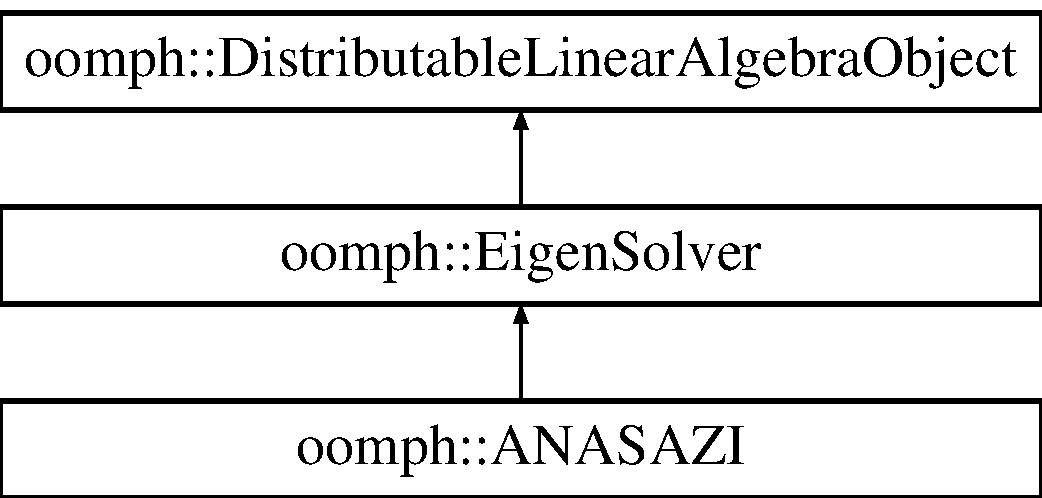
\includegraphics[height=3.000000cm]{classoomph_1_1ANASAZI}
\end{center}
\end{figure}
\subsection*{Public Member Functions}
\begin{DoxyCompactItemize}
\item 
\hyperlink{classoomph_1_1ANASAZI_af90440448c3cbbb7c21bc6ce3bbb2d0a}{A\+N\+A\+S\+A\+ZI} ()
\begin{DoxyCompactList}\small\item\em Constructor. \end{DoxyCompactList}\item 
\hyperlink{classoomph_1_1ANASAZI_abfab863205ce697807b4a1ac5e74ac8f}{A\+N\+A\+S\+A\+ZI} (const \hyperlink{classoomph_1_1ANASAZI}{A\+N\+A\+S\+A\+ZI} \&)
\begin{DoxyCompactList}\small\item\em Empty copy constructor. \end{DoxyCompactList}\item 
virtual \hyperlink{classoomph_1_1ANASAZI_a3f7e7f7fdc23c04c419fba24474f95a7}{$\sim$\+A\+N\+A\+S\+A\+ZI} ()
\begin{DoxyCompactList}\small\item\em Destructor, delete the linear solver. \end{DoxyCompactList}\item 
int \& \hyperlink{classoomph_1_1ANASAZI_a525fd6b30a06a869c50983d6ccad0801}{narnoldi} ()
\begin{DoxyCompactList}\small\item\em Access function for the number of Arnoldi vectors. \end{DoxyCompactList}\item 
const int \& \hyperlink{classoomph_1_1ANASAZI_a5f0489a5b0cd830ba93e1ae33cc14c24}{narnoldi} () const
\begin{DoxyCompactList}\small\item\em Access function for the number of Arnoldi vectors (const version) \end{DoxyCompactList}\item 
void \hyperlink{classoomph_1_1ANASAZI_aa965449f7db8c881305665ba83d4b9b6}{enable\+\_\+compute\+\_\+eigenvectors} ()
\begin{DoxyCompactList}\small\item\em Set to enable the computation of the eigenvectors (default) \end{DoxyCompactList}\item 
void \hyperlink{classoomph_1_1ANASAZI_a7e2035b9291fdc43d9e514c2f97a2b95}{disable\+\_\+compute\+\_\+eigenvectors} ()
\begin{DoxyCompactList}\small\item\em Set to disable the computation of the eigenvectors. \end{DoxyCompactList}\item 
void \hyperlink{classoomph_1_1ANASAZI_a5b13a2a77a422033c6a522ec68549fa5}{solve\+\_\+eigenproblem} (\hyperlink{classoomph_1_1Problem}{Problem} $\ast$const \&problem\+\_\+pt, const int \&n\+\_\+eval, \hyperlink{classoomph_1_1Vector}{Vector}$<$ std\+::complex$<$ double $>$ $>$ \&eigenvalue, \hyperlink{classoomph_1_1Vector}{Vector}$<$ \hyperlink{classoomph_1_1DoubleVector}{Double\+Vector} $>$ \&eigenvector)
\begin{DoxyCompactList}\small\item\em Solve the eigen problem. \end{DoxyCompactList}\item 
void \hyperlink{classoomph_1_1ANASAZI_a914ad9d78433c746b46f22bc429db8e9}{get\+\_\+eigenvalues\+\_\+left\+\_\+of\+\_\+shift} ()
\begin{DoxyCompactList}\small\item\em Set the desired eigenvalues to be left of the shift. \end{DoxyCompactList}\item 
void \hyperlink{classoomph_1_1ANASAZI_a1fba291e41996df19379a383befaa4f9}{get\+\_\+eigenvalues\+\_\+right\+\_\+of\+\_\+shift} ()
\begin{DoxyCompactList}\small\item\em Set the desired eigenvalues to be right of the shift. \end{DoxyCompactList}\item 
void \hyperlink{classoomph_1_1ANASAZI_a8c2be3c7a1f810306b1c606ec2d8f90b}{track\+\_\+eigenvalue\+\_\+real\+\_\+part} ()
\begin{DoxyCompactList}\small\item\em Set the real part to be the quantity of interest (default) \end{DoxyCompactList}\item 
void \hyperlink{classoomph_1_1ANASAZI_ab68875d414ab91de32715ab87e20b5ce}{track\+\_\+eigenvalue\+\_\+imaginary\+\_\+part} ()
\begin{DoxyCompactList}\small\item\em Set the imaginary part fo the quantity of interest. \end{DoxyCompactList}\item 
void \hyperlink{classoomph_1_1ANASAZI_a08a235118d10b28a6f03cc9f6d6ca503}{track\+\_\+eigenvalue\+\_\+magnitude} ()
\begin{DoxyCompactList}\small\item\em Set the magnitude to be the quantity of interest. \end{DoxyCompactList}\item 
\hyperlink{classoomph_1_1LinearSolver}{Linear\+Solver} $\ast$\& \hyperlink{classoomph_1_1ANASAZI_aaaab3d8263b5bdf21eef4aecdc3273c7}{linear\+\_\+solver\+\_\+pt} ()
\begin{DoxyCompactList}\small\item\em Return a pointer to the linear solver object. \end{DoxyCompactList}\item 
\hyperlink{classoomph_1_1LinearSolver}{Linear\+Solver} $\ast$const  \& \hyperlink{classoomph_1_1ANASAZI_a8abde7ddc8a5785c9db713c45ed61e24}{linear\+\_\+solver\+\_\+pt} () const
\begin{DoxyCompactList}\small\item\em Return a pointer to the linear solver object (const version) \end{DoxyCompactList}\end{DoxyCompactItemize}
\subsection*{Private Types}
\begin{DoxyCompactItemize}
\item 
typedef double \hyperlink{classoomph_1_1ANASAZI_a604b8dc6a0618d81dfce82849d5b47a7}{ST}
\item 
typedef Teuchos\+::\+Scalar\+Traits$<$ \hyperlink{classoomph_1_1ANASAZI_a604b8dc6a0618d81dfce82849d5b47a7}{ST} $>$ \hyperlink{classoomph_1_1ANASAZI_a1bb5eb9f072ed92f48fdd32ca22abd0e}{S\+CT}
\item 
typedef S\+C\+T\+::magnitude\+Type \hyperlink{classoomph_1_1ANASAZI_a8c8982a3b6f716d4ea9b497235351cf2}{MT}
\item 
typedef Anasazi\+::\+Multi\+Vec$<$ \hyperlink{classoomph_1_1ANASAZI_a604b8dc6a0618d81dfce82849d5b47a7}{ST} $>$ \hyperlink{classoomph_1_1ANASAZI_aa1922409eb193949b0cb4e89d43316ed}{MV}
\item 
typedef Anasazi\+::\+Operator$<$ \hyperlink{classoomph_1_1ANASAZI_a604b8dc6a0618d81dfce82849d5b47a7}{ST} $>$ \hyperlink{classoomph_1_1ANASAZI_ac89159c0da5e64ce641a2bcb8bd2d2be}{OP}
\item 
typedef Anasazi\+::\+Multi\+Vec\+Traits$<$ \hyperlink{classoomph_1_1ANASAZI_a604b8dc6a0618d81dfce82849d5b47a7}{ST}, \hyperlink{classoomph_1_1ANASAZI_aa1922409eb193949b0cb4e89d43316ed}{MV} $>$ \hyperlink{classoomph_1_1ANASAZI_a7c667c5531aff020a4dbd95f0cebba8b}{M\+VT}
\item 
typedef Anasazi\+::\+Operator\+Traits$<$ \hyperlink{classoomph_1_1ANASAZI_a604b8dc6a0618d81dfce82849d5b47a7}{ST}, \hyperlink{classoomph_1_1ANASAZI_aa1922409eb193949b0cb4e89d43316ed}{MV}, \hyperlink{classoomph_1_1ANASAZI_ac89159c0da5e64ce641a2bcb8bd2d2be}{OP} $>$ \hyperlink{classoomph_1_1ANASAZI_ab1bca328746775f4d6adcb6709afe57f}{O\+PT}
\end{DoxyCompactItemize}
\subsection*{Private Attributes}
\begin{DoxyCompactItemize}
\item 
Anasazi\+::\+Output\+Manager$<$ \hyperlink{classoomph_1_1ANASAZI_a604b8dc6a0618d81dfce82849d5b47a7}{ST} $>$ $\ast$ \hyperlink{classoomph_1_1ANASAZI_a10a57e0c5468fd511c7458dda6f99dce}{Output\+\_\+manager\+\_\+pt}
\begin{DoxyCompactList}\small\item\em Pointer to output manager. \end{DoxyCompactList}\item 
\hyperlink{classoomph_1_1LinearSolver}{Linear\+Solver} $\ast$ \hyperlink{classoomph_1_1ANASAZI_a4af90db68a430f129f360c00a669e809}{Linear\+\_\+solver\+\_\+pt}
\begin{DoxyCompactList}\small\item\em Pointer to a linear solver. \end{DoxyCompactList}\item 
\hyperlink{classoomph_1_1LinearSolver}{Linear\+Solver} $\ast$ \hyperlink{classoomph_1_1ANASAZI_a0d68fe86419ff9260bd2dd8c5e75b1e8}{Default\+\_\+linear\+\_\+solver\+\_\+pt}
\begin{DoxyCompactList}\small\item\em Pointer to a default linear solver. \end{DoxyCompactList}\item 
int \hyperlink{classoomph_1_1ANASAZI_a244c2eac42edb80948da8bcef92cf003}{Spectrum}
\begin{DoxyCompactList}\small\item\em Integer to set whether the real, imaginary or magnitude is required to be small or large. \end{DoxyCompactList}\item 
int \hyperlink{classoomph_1_1ANASAZI_a4ace6fc3f5e4503d9d1e42eb81c52fd8}{N\+Arnoldi}
\begin{DoxyCompactList}\small\item\em Number of Arnoldi vectors to compute. \end{DoxyCompactList}\item 
double \hyperlink{classoomph_1_1ANASAZI_a7af7f7211016ec745689d203078f6199}{Sigma}
\begin{DoxyCompactList}\small\item\em Set the shifted value. \end{DoxyCompactList}\item 
bool \hyperlink{classoomph_1_1ANASAZI_abb61aa274f84bda2752fb0e7bcc4cbee}{Small}
\begin{DoxyCompactList}\small\item\em Boolean to set which part of the spectrum left (default) or right of the shifted value. \end{DoxyCompactList}\item 
bool \hyperlink{classoomph_1_1ANASAZI_a4493c071c706cab869df34248f2dcdbf}{Compute\+\_\+eigenvectors}
\begin{DoxyCompactList}\small\item\em Boolean to indicate whether or not to compute the eigenvectors. \end{DoxyCompactList}\end{DoxyCompactItemize}
\subsection*{Additional Inherited Members}


\subsection{Detailed Description}
Class for the \hyperlink{namespaceAnasazi}{Anasazi} eigensolver. 

Definition at line 538 of file trilinos\+\_\+eigen\+\_\+solver.\+h.



\subsection{Member Typedef Documentation}
\mbox{\Hypertarget{classoomph_1_1ANASAZI_a8c8982a3b6f716d4ea9b497235351cf2}\label{classoomph_1_1ANASAZI_a8c8982a3b6f716d4ea9b497235351cf2}} 
\index{oomph\+::\+A\+N\+A\+S\+A\+ZI@{oomph\+::\+A\+N\+A\+S\+A\+ZI}!MT@{MT}}
\index{MT@{MT}!oomph\+::\+A\+N\+A\+S\+A\+ZI@{oomph\+::\+A\+N\+A\+S\+A\+ZI}}
\subsubsection{\texorpdfstring{MT}{MT}}
{\footnotesize\ttfamily typedef S\+C\+T\+::magnitude\+Type \hyperlink{classoomph_1_1ANASAZI_a8c8982a3b6f716d4ea9b497235351cf2}{oomph\+::\+A\+N\+A\+S\+A\+Z\+I\+::\+MT}\hspace{0.3cm}{\ttfamily [private]}}



Definition at line 544 of file trilinos\+\_\+eigen\+\_\+solver.\+h.

\mbox{\Hypertarget{classoomph_1_1ANASAZI_aa1922409eb193949b0cb4e89d43316ed}\label{classoomph_1_1ANASAZI_aa1922409eb193949b0cb4e89d43316ed}} 
\index{oomph\+::\+A\+N\+A\+S\+A\+ZI@{oomph\+::\+A\+N\+A\+S\+A\+ZI}!MV@{MV}}
\index{MV@{MV}!oomph\+::\+A\+N\+A\+S\+A\+ZI@{oomph\+::\+A\+N\+A\+S\+A\+ZI}}
\subsubsection{\texorpdfstring{MV}{MV}}
{\footnotesize\ttfamily typedef Anasazi\+::\+Multi\+Vec$<$\hyperlink{classoomph_1_1ANASAZI_a604b8dc6a0618d81dfce82849d5b47a7}{ST}$>$ \hyperlink{classoomph_1_1ANASAZI_aa1922409eb193949b0cb4e89d43316ed}{oomph\+::\+A\+N\+A\+S\+A\+Z\+I\+::\+MV}\hspace{0.3cm}{\ttfamily [private]}}



Definition at line 545 of file trilinos\+\_\+eigen\+\_\+solver.\+h.

\mbox{\Hypertarget{classoomph_1_1ANASAZI_a7c667c5531aff020a4dbd95f0cebba8b}\label{classoomph_1_1ANASAZI_a7c667c5531aff020a4dbd95f0cebba8b}} 
\index{oomph\+::\+A\+N\+A\+S\+A\+ZI@{oomph\+::\+A\+N\+A\+S\+A\+ZI}!M\+VT@{M\+VT}}
\index{M\+VT@{M\+VT}!oomph\+::\+A\+N\+A\+S\+A\+ZI@{oomph\+::\+A\+N\+A\+S\+A\+ZI}}
\subsubsection{\texorpdfstring{M\+VT}{MVT}}
{\footnotesize\ttfamily typedef Anasazi\+::\+Multi\+Vec\+Traits$<$\hyperlink{classoomph_1_1ANASAZI_a604b8dc6a0618d81dfce82849d5b47a7}{ST},\hyperlink{classoomph_1_1ANASAZI_aa1922409eb193949b0cb4e89d43316ed}{MV}$>$ \hyperlink{classoomph_1_1ANASAZI_a7c667c5531aff020a4dbd95f0cebba8b}{oomph\+::\+A\+N\+A\+S\+A\+Z\+I\+::\+M\+VT}\hspace{0.3cm}{\ttfamily [private]}}



Definition at line 547 of file trilinos\+\_\+eigen\+\_\+solver.\+h.

\mbox{\Hypertarget{classoomph_1_1ANASAZI_ac89159c0da5e64ce641a2bcb8bd2d2be}\label{classoomph_1_1ANASAZI_ac89159c0da5e64ce641a2bcb8bd2d2be}} 
\index{oomph\+::\+A\+N\+A\+S\+A\+ZI@{oomph\+::\+A\+N\+A\+S\+A\+ZI}!OP@{OP}}
\index{OP@{OP}!oomph\+::\+A\+N\+A\+S\+A\+ZI@{oomph\+::\+A\+N\+A\+S\+A\+ZI}}
\subsubsection{\texorpdfstring{OP}{OP}}
{\footnotesize\ttfamily typedef Anasazi\+::\+Operator$<$\hyperlink{classoomph_1_1ANASAZI_a604b8dc6a0618d81dfce82849d5b47a7}{ST}$>$ \hyperlink{classoomph_1_1ANASAZI_ac89159c0da5e64ce641a2bcb8bd2d2be}{oomph\+::\+A\+N\+A\+S\+A\+Z\+I\+::\+OP}\hspace{0.3cm}{\ttfamily [private]}}



Definition at line 546 of file trilinos\+\_\+eigen\+\_\+solver.\+h.

\mbox{\Hypertarget{classoomph_1_1ANASAZI_ab1bca328746775f4d6adcb6709afe57f}\label{classoomph_1_1ANASAZI_ab1bca328746775f4d6adcb6709afe57f}} 
\index{oomph\+::\+A\+N\+A\+S\+A\+ZI@{oomph\+::\+A\+N\+A\+S\+A\+ZI}!O\+PT@{O\+PT}}
\index{O\+PT@{O\+PT}!oomph\+::\+A\+N\+A\+S\+A\+ZI@{oomph\+::\+A\+N\+A\+S\+A\+ZI}}
\subsubsection{\texorpdfstring{O\+PT}{OPT}}
{\footnotesize\ttfamily typedef Anasazi\+::\+Operator\+Traits$<$\hyperlink{classoomph_1_1ANASAZI_a604b8dc6a0618d81dfce82849d5b47a7}{ST},\hyperlink{classoomph_1_1ANASAZI_aa1922409eb193949b0cb4e89d43316ed}{MV},\hyperlink{classoomph_1_1ANASAZI_ac89159c0da5e64ce641a2bcb8bd2d2be}{OP}$>$ \hyperlink{classoomph_1_1ANASAZI_ab1bca328746775f4d6adcb6709afe57f}{oomph\+::\+A\+N\+A\+S\+A\+Z\+I\+::\+O\+PT}\hspace{0.3cm}{\ttfamily [private]}}



Definition at line 548 of file trilinos\+\_\+eigen\+\_\+solver.\+h.

\mbox{\Hypertarget{classoomph_1_1ANASAZI_a1bb5eb9f072ed92f48fdd32ca22abd0e}\label{classoomph_1_1ANASAZI_a1bb5eb9f072ed92f48fdd32ca22abd0e}} 
\index{oomph\+::\+A\+N\+A\+S\+A\+ZI@{oomph\+::\+A\+N\+A\+S\+A\+ZI}!S\+CT@{S\+CT}}
\index{S\+CT@{S\+CT}!oomph\+::\+A\+N\+A\+S\+A\+ZI@{oomph\+::\+A\+N\+A\+S\+A\+ZI}}
\subsubsection{\texorpdfstring{S\+CT}{SCT}}
{\footnotesize\ttfamily typedef Teuchos\+::\+Scalar\+Traits$<$\hyperlink{classoomph_1_1ANASAZI_a604b8dc6a0618d81dfce82849d5b47a7}{ST}$>$ \hyperlink{classoomph_1_1ANASAZI_a1bb5eb9f072ed92f48fdd32ca22abd0e}{oomph\+::\+A\+N\+A\+S\+A\+Z\+I\+::\+S\+CT}\hspace{0.3cm}{\ttfamily [private]}}



Definition at line 543 of file trilinos\+\_\+eigen\+\_\+solver.\+h.

\mbox{\Hypertarget{classoomph_1_1ANASAZI_a604b8dc6a0618d81dfce82849d5b47a7}\label{classoomph_1_1ANASAZI_a604b8dc6a0618d81dfce82849d5b47a7}} 
\index{oomph\+::\+A\+N\+A\+S\+A\+ZI@{oomph\+::\+A\+N\+A\+S\+A\+ZI}!ST@{ST}}
\index{ST@{ST}!oomph\+::\+A\+N\+A\+S\+A\+ZI@{oomph\+::\+A\+N\+A\+S\+A\+ZI}}
\subsubsection{\texorpdfstring{ST}{ST}}
{\footnotesize\ttfamily typedef double \hyperlink{classoomph_1_1ANASAZI_a604b8dc6a0618d81dfce82849d5b47a7}{oomph\+::\+A\+N\+A\+S\+A\+Z\+I\+::\+ST}\hspace{0.3cm}{\ttfamily [private]}}



Definition at line 542 of file trilinos\+\_\+eigen\+\_\+solver.\+h.



\subsection{Constructor \& Destructor Documentation}
\mbox{\Hypertarget{classoomph_1_1ANASAZI_af90440448c3cbbb7c21bc6ce3bbb2d0a}\label{classoomph_1_1ANASAZI_af90440448c3cbbb7c21bc6ce3bbb2d0a}} 
\index{oomph\+::\+A\+N\+A\+S\+A\+ZI@{oomph\+::\+A\+N\+A\+S\+A\+ZI}!A\+N\+A\+S\+A\+ZI@{A\+N\+A\+S\+A\+ZI}}
\index{A\+N\+A\+S\+A\+ZI@{A\+N\+A\+S\+A\+ZI}!oomph\+::\+A\+N\+A\+S\+A\+ZI@{oomph\+::\+A\+N\+A\+S\+A\+ZI}}
\subsubsection{\texorpdfstring{A\+N\+A\+S\+A\+Z\+I()}{ANASAZI()}\hspace{0.1cm}{\footnotesize\ttfamily [1/2]}}
{\footnotesize\ttfamily oomph\+::\+A\+N\+A\+S\+A\+Z\+I\+::\+A\+N\+A\+S\+A\+ZI (\begin{DoxyParamCaption}{ }\end{DoxyParamCaption})\hspace{0.3cm}{\ttfamily [inline]}}



Constructor. 



Definition at line 580 of file trilinos\+\_\+eigen\+\_\+solver.\+h.

\mbox{\Hypertarget{classoomph_1_1ANASAZI_abfab863205ce697807b4a1ac5e74ac8f}\label{classoomph_1_1ANASAZI_abfab863205ce697807b4a1ac5e74ac8f}} 
\index{oomph\+::\+A\+N\+A\+S\+A\+ZI@{oomph\+::\+A\+N\+A\+S\+A\+ZI}!A\+N\+A\+S\+A\+ZI@{A\+N\+A\+S\+A\+ZI}}
\index{A\+N\+A\+S\+A\+ZI@{A\+N\+A\+S\+A\+ZI}!oomph\+::\+A\+N\+A\+S\+A\+ZI@{oomph\+::\+A\+N\+A\+S\+A\+ZI}}
\subsubsection{\texorpdfstring{A\+N\+A\+S\+A\+Z\+I()}{ANASAZI()}\hspace{0.1cm}{\footnotesize\ttfamily [2/2]}}
{\footnotesize\ttfamily oomph\+::\+A\+N\+A\+S\+A\+Z\+I\+::\+A\+N\+A\+S\+A\+ZI (\begin{DoxyParamCaption}\item[{const \hyperlink{classoomph_1_1ANASAZI}{A\+N\+A\+S\+A\+ZI} \&}]{ }\end{DoxyParamCaption})\hspace{0.3cm}{\ttfamily [inline]}}



Empty copy constructor. 



Definition at line 596 of file trilinos\+\_\+eigen\+\_\+solver.\+h.

\mbox{\Hypertarget{classoomph_1_1ANASAZI_a3f7e7f7fdc23c04c419fba24474f95a7}\label{classoomph_1_1ANASAZI_a3f7e7f7fdc23c04c419fba24474f95a7}} 
\index{oomph\+::\+A\+N\+A\+S\+A\+ZI@{oomph\+::\+A\+N\+A\+S\+A\+ZI}!````~A\+N\+A\+S\+A\+ZI@{$\sim$\+A\+N\+A\+S\+A\+ZI}}
\index{````~A\+N\+A\+S\+A\+ZI@{$\sim$\+A\+N\+A\+S\+A\+ZI}!oomph\+::\+A\+N\+A\+S\+A\+ZI@{oomph\+::\+A\+N\+A\+S\+A\+ZI}}
\subsubsection{\texorpdfstring{$\sim$\+A\+N\+A\+S\+A\+Z\+I()}{~ANASAZI()}}
{\footnotesize\ttfamily virtual oomph\+::\+A\+N\+A\+S\+A\+Z\+I\+::$\sim$\+A\+N\+A\+S\+A\+ZI (\begin{DoxyParamCaption}{ }\end{DoxyParamCaption})\hspace{0.3cm}{\ttfamily [inline]}, {\ttfamily [virtual]}}



Destructor, delete the linear solver. 



Definition at line 599 of file trilinos\+\_\+eigen\+\_\+solver.\+h.



\subsection{Member Function Documentation}
\mbox{\Hypertarget{classoomph_1_1ANASAZI_a7e2035b9291fdc43d9e514c2f97a2b95}\label{classoomph_1_1ANASAZI_a7e2035b9291fdc43d9e514c2f97a2b95}} 
\index{oomph\+::\+A\+N\+A\+S\+A\+ZI@{oomph\+::\+A\+N\+A\+S\+A\+ZI}!disable\+\_\+compute\+\_\+eigenvectors@{disable\+\_\+compute\+\_\+eigenvectors}}
\index{disable\+\_\+compute\+\_\+eigenvectors@{disable\+\_\+compute\+\_\+eigenvectors}!oomph\+::\+A\+N\+A\+S\+A\+ZI@{oomph\+::\+A\+N\+A\+S\+A\+ZI}}
\subsubsection{\texorpdfstring{disable\+\_\+compute\+\_\+eigenvectors()}{disable\_compute\_eigenvectors()}}
{\footnotesize\ttfamily void oomph\+::\+A\+N\+A\+S\+A\+Z\+I\+::disable\+\_\+compute\+\_\+eigenvectors (\begin{DoxyParamCaption}{ }\end{DoxyParamCaption})\hspace{0.3cm}{\ttfamily [inline]}}



Set to disable the computation of the eigenvectors. 



Definition at line 614 of file trilinos\+\_\+eigen\+\_\+solver.\+h.

\mbox{\Hypertarget{classoomph_1_1ANASAZI_aa965449f7db8c881305665ba83d4b9b6}\label{classoomph_1_1ANASAZI_aa965449f7db8c881305665ba83d4b9b6}} 
\index{oomph\+::\+A\+N\+A\+S\+A\+ZI@{oomph\+::\+A\+N\+A\+S\+A\+ZI}!enable\+\_\+compute\+\_\+eigenvectors@{enable\+\_\+compute\+\_\+eigenvectors}}
\index{enable\+\_\+compute\+\_\+eigenvectors@{enable\+\_\+compute\+\_\+eigenvectors}!oomph\+::\+A\+N\+A\+S\+A\+ZI@{oomph\+::\+A\+N\+A\+S\+A\+ZI}}
\subsubsection{\texorpdfstring{enable\+\_\+compute\+\_\+eigenvectors()}{enable\_compute\_eigenvectors()}}
{\footnotesize\ttfamily void oomph\+::\+A\+N\+A\+S\+A\+Z\+I\+::enable\+\_\+compute\+\_\+eigenvectors (\begin{DoxyParamCaption}{ }\end{DoxyParamCaption})\hspace{0.3cm}{\ttfamily [inline]}}



Set to enable the computation of the eigenvectors (default) 



Definition at line 611 of file trilinos\+\_\+eigen\+\_\+solver.\+h.

\mbox{\Hypertarget{classoomph_1_1ANASAZI_a914ad9d78433c746b46f22bc429db8e9}\label{classoomph_1_1ANASAZI_a914ad9d78433c746b46f22bc429db8e9}} 
\index{oomph\+::\+A\+N\+A\+S\+A\+ZI@{oomph\+::\+A\+N\+A\+S\+A\+ZI}!get\+\_\+eigenvalues\+\_\+left\+\_\+of\+\_\+shift@{get\+\_\+eigenvalues\+\_\+left\+\_\+of\+\_\+shift}}
\index{get\+\_\+eigenvalues\+\_\+left\+\_\+of\+\_\+shift@{get\+\_\+eigenvalues\+\_\+left\+\_\+of\+\_\+shift}!oomph\+::\+A\+N\+A\+S\+A\+ZI@{oomph\+::\+A\+N\+A\+S\+A\+ZI}}
\subsubsection{\texorpdfstring{get\+\_\+eigenvalues\+\_\+left\+\_\+of\+\_\+shift()}{get\_eigenvalues\_left\_of\_shift()}}
{\footnotesize\ttfamily void oomph\+::\+A\+N\+A\+S\+A\+Z\+I\+::get\+\_\+eigenvalues\+\_\+left\+\_\+of\+\_\+shift (\begin{DoxyParamCaption}{ }\end{DoxyParamCaption})\hspace{0.3cm}{\ttfamily [inline]}}



Set the desired eigenvalues to be left of the shift. 



Definition at line 719 of file trilinos\+\_\+eigen\+\_\+solver.\+h.

\mbox{\Hypertarget{classoomph_1_1ANASAZI_a1fba291e41996df19379a383befaa4f9}\label{classoomph_1_1ANASAZI_a1fba291e41996df19379a383befaa4f9}} 
\index{oomph\+::\+A\+N\+A\+S\+A\+ZI@{oomph\+::\+A\+N\+A\+S\+A\+ZI}!get\+\_\+eigenvalues\+\_\+right\+\_\+of\+\_\+shift@{get\+\_\+eigenvalues\+\_\+right\+\_\+of\+\_\+shift}}
\index{get\+\_\+eigenvalues\+\_\+right\+\_\+of\+\_\+shift@{get\+\_\+eigenvalues\+\_\+right\+\_\+of\+\_\+shift}!oomph\+::\+A\+N\+A\+S\+A\+ZI@{oomph\+::\+A\+N\+A\+S\+A\+ZI}}
\subsubsection{\texorpdfstring{get\+\_\+eigenvalues\+\_\+right\+\_\+of\+\_\+shift()}{get\_eigenvalues\_right\_of\_shift()}}
{\footnotesize\ttfamily void oomph\+::\+A\+N\+A\+S\+A\+Z\+I\+::get\+\_\+eigenvalues\+\_\+right\+\_\+of\+\_\+shift (\begin{DoxyParamCaption}{ }\end{DoxyParamCaption})\hspace{0.3cm}{\ttfamily [inline]}}



Set the desired eigenvalues to be right of the shift. 



Definition at line 722 of file trilinos\+\_\+eigen\+\_\+solver.\+h.

\mbox{\Hypertarget{classoomph_1_1ANASAZI_aaaab3d8263b5bdf21eef4aecdc3273c7}\label{classoomph_1_1ANASAZI_aaaab3d8263b5bdf21eef4aecdc3273c7}} 
\index{oomph\+::\+A\+N\+A\+S\+A\+ZI@{oomph\+::\+A\+N\+A\+S\+A\+ZI}!linear\+\_\+solver\+\_\+pt@{linear\+\_\+solver\+\_\+pt}}
\index{linear\+\_\+solver\+\_\+pt@{linear\+\_\+solver\+\_\+pt}!oomph\+::\+A\+N\+A\+S\+A\+ZI@{oomph\+::\+A\+N\+A\+S\+A\+ZI}}
\subsubsection{\texorpdfstring{linear\+\_\+solver\+\_\+pt()}{linear\_solver\_pt()}\hspace{0.1cm}{\footnotesize\ttfamily [1/2]}}
{\footnotesize\ttfamily \hyperlink{classoomph_1_1LinearSolver}{Linear\+Solver}$\ast$ \& oomph\+::\+A\+N\+A\+S\+A\+Z\+I\+::linear\+\_\+solver\+\_\+pt (\begin{DoxyParamCaption}{ }\end{DoxyParamCaption})\hspace{0.3cm}{\ttfamily [inline]}}



Return a pointer to the linear solver object. 



Definition at line 734 of file trilinos\+\_\+eigen\+\_\+solver.\+h.

\mbox{\Hypertarget{classoomph_1_1ANASAZI_a8abde7ddc8a5785c9db713c45ed61e24}\label{classoomph_1_1ANASAZI_a8abde7ddc8a5785c9db713c45ed61e24}} 
\index{oomph\+::\+A\+N\+A\+S\+A\+ZI@{oomph\+::\+A\+N\+A\+S\+A\+ZI}!linear\+\_\+solver\+\_\+pt@{linear\+\_\+solver\+\_\+pt}}
\index{linear\+\_\+solver\+\_\+pt@{linear\+\_\+solver\+\_\+pt}!oomph\+::\+A\+N\+A\+S\+A\+ZI@{oomph\+::\+A\+N\+A\+S\+A\+ZI}}
\subsubsection{\texorpdfstring{linear\+\_\+solver\+\_\+pt()}{linear\_solver\_pt()}\hspace{0.1cm}{\footnotesize\ttfamily [2/2]}}
{\footnotesize\ttfamily \hyperlink{classoomph_1_1LinearSolver}{Linear\+Solver}$\ast$ const\& oomph\+::\+A\+N\+A\+S\+A\+Z\+I\+::linear\+\_\+solver\+\_\+pt (\begin{DoxyParamCaption}{ }\end{DoxyParamCaption}) const\hspace{0.3cm}{\ttfamily [inline]}}



Return a pointer to the linear solver object (const version) 



Definition at line 737 of file trilinos\+\_\+eigen\+\_\+solver.\+h.

\mbox{\Hypertarget{classoomph_1_1ANASAZI_a525fd6b30a06a869c50983d6ccad0801}\label{classoomph_1_1ANASAZI_a525fd6b30a06a869c50983d6ccad0801}} 
\index{oomph\+::\+A\+N\+A\+S\+A\+ZI@{oomph\+::\+A\+N\+A\+S\+A\+ZI}!narnoldi@{narnoldi}}
\index{narnoldi@{narnoldi}!oomph\+::\+A\+N\+A\+S\+A\+ZI@{oomph\+::\+A\+N\+A\+S\+A\+ZI}}
\subsubsection{\texorpdfstring{narnoldi()}{narnoldi()}\hspace{0.1cm}{\footnotesize\ttfamily [1/2]}}
{\footnotesize\ttfamily int\& oomph\+::\+A\+N\+A\+S\+A\+Z\+I\+::narnoldi (\begin{DoxyParamCaption}{ }\end{DoxyParamCaption})\hspace{0.3cm}{\ttfamily [inline]}}



Access function for the number of Arnoldi vectors. 



Definition at line 605 of file trilinos\+\_\+eigen\+\_\+solver.\+h.

\mbox{\Hypertarget{classoomph_1_1ANASAZI_a5f0489a5b0cd830ba93e1ae33cc14c24}\label{classoomph_1_1ANASAZI_a5f0489a5b0cd830ba93e1ae33cc14c24}} 
\index{oomph\+::\+A\+N\+A\+S\+A\+ZI@{oomph\+::\+A\+N\+A\+S\+A\+ZI}!narnoldi@{narnoldi}}
\index{narnoldi@{narnoldi}!oomph\+::\+A\+N\+A\+S\+A\+ZI@{oomph\+::\+A\+N\+A\+S\+A\+ZI}}
\subsubsection{\texorpdfstring{narnoldi()}{narnoldi()}\hspace{0.1cm}{\footnotesize\ttfamily [2/2]}}
{\footnotesize\ttfamily const int\& oomph\+::\+A\+N\+A\+S\+A\+Z\+I\+::narnoldi (\begin{DoxyParamCaption}{ }\end{DoxyParamCaption}) const\hspace{0.3cm}{\ttfamily [inline]}}



Access function for the number of Arnoldi vectors (const version) 



Definition at line 608 of file trilinos\+\_\+eigen\+\_\+solver.\+h.

\mbox{\Hypertarget{classoomph_1_1ANASAZI_a5b13a2a77a422033c6a522ec68549fa5}\label{classoomph_1_1ANASAZI_a5b13a2a77a422033c6a522ec68549fa5}} 
\index{oomph\+::\+A\+N\+A\+S\+A\+ZI@{oomph\+::\+A\+N\+A\+S\+A\+ZI}!solve\+\_\+eigenproblem@{solve\+\_\+eigenproblem}}
\index{solve\+\_\+eigenproblem@{solve\+\_\+eigenproblem}!oomph\+::\+A\+N\+A\+S\+A\+ZI@{oomph\+::\+A\+N\+A\+S\+A\+ZI}}
\subsubsection{\texorpdfstring{solve\+\_\+eigenproblem()}{solve\_eigenproblem()}}
{\footnotesize\ttfamily void oomph\+::\+A\+N\+A\+S\+A\+Z\+I\+::solve\+\_\+eigenproblem (\begin{DoxyParamCaption}\item[{\hyperlink{classoomph_1_1Problem}{Problem} $\ast$const \&}]{problem\+\_\+pt,  }\item[{const int \&}]{n\+\_\+eval,  }\item[{\hyperlink{classoomph_1_1Vector}{Vector}$<$ std\+::complex$<$ double $>$ $>$ \&}]{eigenvalue,  }\item[{\hyperlink{classoomph_1_1Vector}{Vector}$<$ \hyperlink{classoomph_1_1DoubleVector}{Double\+Vector} $>$ \&}]{eigenvector }\end{DoxyParamCaption})\hspace{0.3cm}{\ttfamily [inline]}, {\ttfamily [virtual]}}



Solve the eigen problem. 



Implements \hyperlink{classoomph_1_1EigenSolver_a6a6b09612ce16457b26fa0cfe996fa71}{oomph\+::\+Eigen\+Solver}.



Definition at line 617 of file trilinos\+\_\+eigen\+\_\+solver.\+h.



References oomph\+::\+Problem\+::dof\+\_\+distribution\+\_\+pt(), i, oomph\+::\+Problem\+::linear\+\_\+solver\+\_\+pt(), and oomph\+::oomph\+\_\+info.

\mbox{\Hypertarget{classoomph_1_1ANASAZI_ab68875d414ab91de32715ab87e20b5ce}\label{classoomph_1_1ANASAZI_ab68875d414ab91de32715ab87e20b5ce}} 
\index{oomph\+::\+A\+N\+A\+S\+A\+ZI@{oomph\+::\+A\+N\+A\+S\+A\+ZI}!track\+\_\+eigenvalue\+\_\+imaginary\+\_\+part@{track\+\_\+eigenvalue\+\_\+imaginary\+\_\+part}}
\index{track\+\_\+eigenvalue\+\_\+imaginary\+\_\+part@{track\+\_\+eigenvalue\+\_\+imaginary\+\_\+part}!oomph\+::\+A\+N\+A\+S\+A\+ZI@{oomph\+::\+A\+N\+A\+S\+A\+ZI}}
\subsubsection{\texorpdfstring{track\+\_\+eigenvalue\+\_\+imaginary\+\_\+part()}{track\_eigenvalue\_imaginary\_part()}}
{\footnotesize\ttfamily void oomph\+::\+A\+N\+A\+S\+A\+Z\+I\+::track\+\_\+eigenvalue\+\_\+imaginary\+\_\+part (\begin{DoxyParamCaption}{ }\end{DoxyParamCaption})\hspace{0.3cm}{\ttfamily [inline]}}



Set the imaginary part fo the quantity of interest. 



Definition at line 728 of file trilinos\+\_\+eigen\+\_\+solver.\+h.

\mbox{\Hypertarget{classoomph_1_1ANASAZI_a08a235118d10b28a6f03cc9f6d6ca503}\label{classoomph_1_1ANASAZI_a08a235118d10b28a6f03cc9f6d6ca503}} 
\index{oomph\+::\+A\+N\+A\+S\+A\+ZI@{oomph\+::\+A\+N\+A\+S\+A\+ZI}!track\+\_\+eigenvalue\+\_\+magnitude@{track\+\_\+eigenvalue\+\_\+magnitude}}
\index{track\+\_\+eigenvalue\+\_\+magnitude@{track\+\_\+eigenvalue\+\_\+magnitude}!oomph\+::\+A\+N\+A\+S\+A\+ZI@{oomph\+::\+A\+N\+A\+S\+A\+ZI}}
\subsubsection{\texorpdfstring{track\+\_\+eigenvalue\+\_\+magnitude()}{track\_eigenvalue\_magnitude()}}
{\footnotesize\ttfamily void oomph\+::\+A\+N\+A\+S\+A\+Z\+I\+::track\+\_\+eigenvalue\+\_\+magnitude (\begin{DoxyParamCaption}{ }\end{DoxyParamCaption})\hspace{0.3cm}{\ttfamily [inline]}}



Set the magnitude to be the quantity of interest. 



Definition at line 731 of file trilinos\+\_\+eigen\+\_\+solver.\+h.

\mbox{\Hypertarget{classoomph_1_1ANASAZI_a8c2be3c7a1f810306b1c606ec2d8f90b}\label{classoomph_1_1ANASAZI_a8c2be3c7a1f810306b1c606ec2d8f90b}} 
\index{oomph\+::\+A\+N\+A\+S\+A\+ZI@{oomph\+::\+A\+N\+A\+S\+A\+ZI}!track\+\_\+eigenvalue\+\_\+real\+\_\+part@{track\+\_\+eigenvalue\+\_\+real\+\_\+part}}
\index{track\+\_\+eigenvalue\+\_\+real\+\_\+part@{track\+\_\+eigenvalue\+\_\+real\+\_\+part}!oomph\+::\+A\+N\+A\+S\+A\+ZI@{oomph\+::\+A\+N\+A\+S\+A\+ZI}}
\subsubsection{\texorpdfstring{track\+\_\+eigenvalue\+\_\+real\+\_\+part()}{track\_eigenvalue\_real\_part()}}
{\footnotesize\ttfamily void oomph\+::\+A\+N\+A\+S\+A\+Z\+I\+::track\+\_\+eigenvalue\+\_\+real\+\_\+part (\begin{DoxyParamCaption}{ }\end{DoxyParamCaption})\hspace{0.3cm}{\ttfamily [inline]}}



Set the real part to be the quantity of interest (default) 



Definition at line 725 of file trilinos\+\_\+eigen\+\_\+solver.\+h.



\subsection{Member Data Documentation}
\mbox{\Hypertarget{classoomph_1_1ANASAZI_a4493c071c706cab869df34248f2dcdbf}\label{classoomph_1_1ANASAZI_a4493c071c706cab869df34248f2dcdbf}} 
\index{oomph\+::\+A\+N\+A\+S\+A\+ZI@{oomph\+::\+A\+N\+A\+S\+A\+ZI}!Compute\+\_\+eigenvectors@{Compute\+\_\+eigenvectors}}
\index{Compute\+\_\+eigenvectors@{Compute\+\_\+eigenvectors}!oomph\+::\+A\+N\+A\+S\+A\+ZI@{oomph\+::\+A\+N\+A\+S\+A\+ZI}}
\subsubsection{\texorpdfstring{Compute\+\_\+eigenvectors}{Compute\_eigenvectors}}
{\footnotesize\ttfamily bool oomph\+::\+A\+N\+A\+S\+A\+Z\+I\+::\+Compute\+\_\+eigenvectors\hspace{0.3cm}{\ttfamily [private]}}



Boolean to indicate whether or not to compute the eigenvectors. 



Definition at line 574 of file trilinos\+\_\+eigen\+\_\+solver.\+h.

\mbox{\Hypertarget{classoomph_1_1ANASAZI_a0d68fe86419ff9260bd2dd8c5e75b1e8}\label{classoomph_1_1ANASAZI_a0d68fe86419ff9260bd2dd8c5e75b1e8}} 
\index{oomph\+::\+A\+N\+A\+S\+A\+ZI@{oomph\+::\+A\+N\+A\+S\+A\+ZI}!Default\+\_\+linear\+\_\+solver\+\_\+pt@{Default\+\_\+linear\+\_\+solver\+\_\+pt}}
\index{Default\+\_\+linear\+\_\+solver\+\_\+pt@{Default\+\_\+linear\+\_\+solver\+\_\+pt}!oomph\+::\+A\+N\+A\+S\+A\+ZI@{oomph\+::\+A\+N\+A\+S\+A\+ZI}}
\subsubsection{\texorpdfstring{Default\+\_\+linear\+\_\+solver\+\_\+pt}{Default\_linear\_solver\_pt}}
{\footnotesize\ttfamily \hyperlink{classoomph_1_1LinearSolver}{Linear\+Solver}$\ast$ oomph\+::\+A\+N\+A\+S\+A\+Z\+I\+::\+Default\+\_\+linear\+\_\+solver\+\_\+pt\hspace{0.3cm}{\ttfamily [private]}}



Pointer to a default linear solver. 



Definition at line 557 of file trilinos\+\_\+eigen\+\_\+solver.\+h.

\mbox{\Hypertarget{classoomph_1_1ANASAZI_a4af90db68a430f129f360c00a669e809}\label{classoomph_1_1ANASAZI_a4af90db68a430f129f360c00a669e809}} 
\index{oomph\+::\+A\+N\+A\+S\+A\+ZI@{oomph\+::\+A\+N\+A\+S\+A\+ZI}!Linear\+\_\+solver\+\_\+pt@{Linear\+\_\+solver\+\_\+pt}}
\index{Linear\+\_\+solver\+\_\+pt@{Linear\+\_\+solver\+\_\+pt}!oomph\+::\+A\+N\+A\+S\+A\+ZI@{oomph\+::\+A\+N\+A\+S\+A\+ZI}}
\subsubsection{\texorpdfstring{Linear\+\_\+solver\+\_\+pt}{Linear\_solver\_pt}}
{\footnotesize\ttfamily \hyperlink{classoomph_1_1LinearSolver}{Linear\+Solver}$\ast$ oomph\+::\+A\+N\+A\+S\+A\+Z\+I\+::\+Linear\+\_\+solver\+\_\+pt\hspace{0.3cm}{\ttfamily [private]}}



Pointer to a linear solver. 



Definition at line 554 of file trilinos\+\_\+eigen\+\_\+solver.\+h.

\mbox{\Hypertarget{classoomph_1_1ANASAZI_a4ace6fc3f5e4503d9d1e42eb81c52fd8}\label{classoomph_1_1ANASAZI_a4ace6fc3f5e4503d9d1e42eb81c52fd8}} 
\index{oomph\+::\+A\+N\+A\+S\+A\+ZI@{oomph\+::\+A\+N\+A\+S\+A\+ZI}!N\+Arnoldi@{N\+Arnoldi}}
\index{N\+Arnoldi@{N\+Arnoldi}!oomph\+::\+A\+N\+A\+S\+A\+ZI@{oomph\+::\+A\+N\+A\+S\+A\+ZI}}
\subsubsection{\texorpdfstring{N\+Arnoldi}{NArnoldi}}
{\footnotesize\ttfamily int oomph\+::\+A\+N\+A\+S\+A\+Z\+I\+::\+N\+Arnoldi\hspace{0.3cm}{\ttfamily [private]}}



Number of Arnoldi vectors to compute. 



Definition at line 564 of file trilinos\+\_\+eigen\+\_\+solver.\+h.

\mbox{\Hypertarget{classoomph_1_1ANASAZI_a10a57e0c5468fd511c7458dda6f99dce}\label{classoomph_1_1ANASAZI_a10a57e0c5468fd511c7458dda6f99dce}} 
\index{oomph\+::\+A\+N\+A\+S\+A\+ZI@{oomph\+::\+A\+N\+A\+S\+A\+ZI}!Output\+\_\+manager\+\_\+pt@{Output\+\_\+manager\+\_\+pt}}
\index{Output\+\_\+manager\+\_\+pt@{Output\+\_\+manager\+\_\+pt}!oomph\+::\+A\+N\+A\+S\+A\+ZI@{oomph\+::\+A\+N\+A\+S\+A\+ZI}}
\subsubsection{\texorpdfstring{Output\+\_\+manager\+\_\+pt}{Output\_manager\_pt}}
{\footnotesize\ttfamily Anasazi\+::\+Output\+Manager$<$\hyperlink{classoomph_1_1ANASAZI_a604b8dc6a0618d81dfce82849d5b47a7}{ST}$>$$\ast$ oomph\+::\+A\+N\+A\+S\+A\+Z\+I\+::\+Output\+\_\+manager\+\_\+pt\hspace{0.3cm}{\ttfamily [private]}}



Pointer to output manager. 



Definition at line 551 of file trilinos\+\_\+eigen\+\_\+solver.\+h.

\mbox{\Hypertarget{classoomph_1_1ANASAZI_a7af7f7211016ec745689d203078f6199}\label{classoomph_1_1ANASAZI_a7af7f7211016ec745689d203078f6199}} 
\index{oomph\+::\+A\+N\+A\+S\+A\+ZI@{oomph\+::\+A\+N\+A\+S\+A\+ZI}!Sigma@{Sigma}}
\index{Sigma@{Sigma}!oomph\+::\+A\+N\+A\+S\+A\+ZI@{oomph\+::\+A\+N\+A\+S\+A\+ZI}}
\subsubsection{\texorpdfstring{Sigma}{Sigma}}
{\footnotesize\ttfamily double oomph\+::\+A\+N\+A\+S\+A\+Z\+I\+::\+Sigma\hspace{0.3cm}{\ttfamily [private]}}



Set the shifted value. 



Definition at line 567 of file trilinos\+\_\+eigen\+\_\+solver.\+h.

\mbox{\Hypertarget{classoomph_1_1ANASAZI_abb61aa274f84bda2752fb0e7bcc4cbee}\label{classoomph_1_1ANASAZI_abb61aa274f84bda2752fb0e7bcc4cbee}} 
\index{oomph\+::\+A\+N\+A\+S\+A\+ZI@{oomph\+::\+A\+N\+A\+S\+A\+ZI}!Small@{Small}}
\index{Small@{Small}!oomph\+::\+A\+N\+A\+S\+A\+ZI@{oomph\+::\+A\+N\+A\+S\+A\+ZI}}
\subsubsection{\texorpdfstring{Small}{Small}}
{\footnotesize\ttfamily bool oomph\+::\+A\+N\+A\+S\+A\+Z\+I\+::\+Small\hspace{0.3cm}{\ttfamily [private]}}



Boolean to set which part of the spectrum left (default) or right of the shifted value. 



Definition at line 571 of file trilinos\+\_\+eigen\+\_\+solver.\+h.

\mbox{\Hypertarget{classoomph_1_1ANASAZI_a244c2eac42edb80948da8bcef92cf003}\label{classoomph_1_1ANASAZI_a244c2eac42edb80948da8bcef92cf003}} 
\index{oomph\+::\+A\+N\+A\+S\+A\+ZI@{oomph\+::\+A\+N\+A\+S\+A\+ZI}!Spectrum@{Spectrum}}
\index{Spectrum@{Spectrum}!oomph\+::\+A\+N\+A\+S\+A\+ZI@{oomph\+::\+A\+N\+A\+S\+A\+ZI}}
\subsubsection{\texorpdfstring{Spectrum}{Spectrum}}
{\footnotesize\ttfamily int oomph\+::\+A\+N\+A\+S\+A\+Z\+I\+::\+Spectrum\hspace{0.3cm}{\ttfamily [private]}}



Integer to set whether the real, imaginary or magnitude is required to be small or large. 



Definition at line 561 of file trilinos\+\_\+eigen\+\_\+solver.\+h.



The documentation for this class was generated from the following file\+:\begin{DoxyCompactItemize}
\item 
\hyperlink{trilinos__eigen__solver_8h}{trilinos\+\_\+eigen\+\_\+solver.\+h}\end{DoxyCompactItemize}

\hypertarget{classoomph_1_1AnnularDomain}{}\section{oomph\+:\+:Annular\+Domain Class Reference}
\label{classoomph_1_1AnnularDomain}\index{oomph\+::\+Annular\+Domain@{oomph\+::\+Annular\+Domain}}


Annular domain.  




{\ttfamily \#include $<$annular\+\_\+domain.\+h$>$}

Inheritance diagram for oomph\+:\+:Annular\+Domain\+:\begin{figure}[H]
\begin{center}
\leavevmode
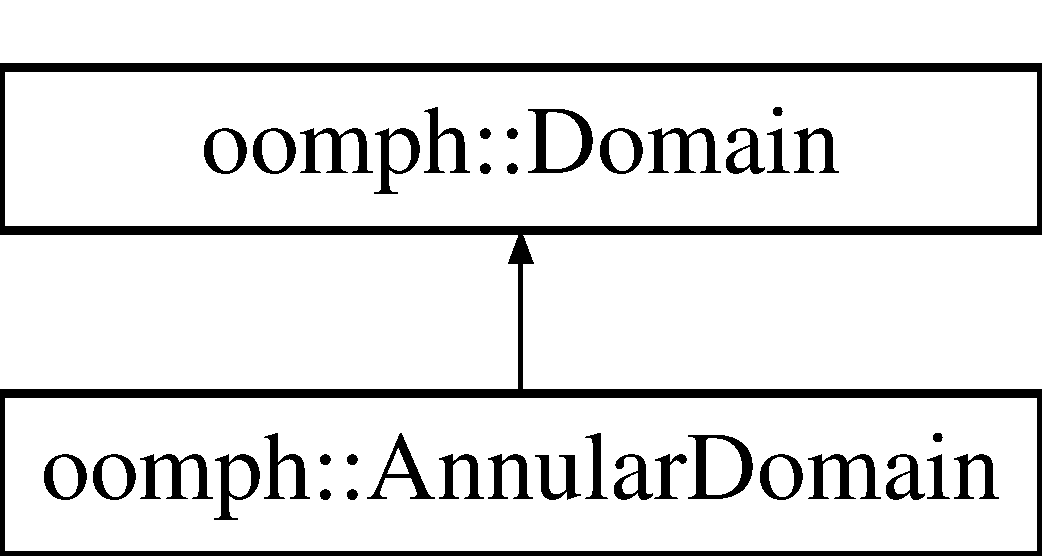
\includegraphics[height=2.000000cm]{classoomph_1_1AnnularDomain}
\end{center}
\end{figure}
\subsection*{Public Member Functions}
\begin{DoxyCompactItemize}
\item 
\hyperlink{classoomph_1_1AnnularDomain_aa0b4ad9d8e63de8aa0dc2d462a016143}{Annular\+Domain} (const double \&azimuthal\+\_\+fraction, const unsigned \&ntheta, const unsigned \&nr, const double \&a, const double \&h, const double \&phi)
\begin{DoxyCompactList}\small\item\em Constructor\+: Specify azimuthal fraction (1.\+0 is 360 degrees) number of macro elements in azimuthal and radial direction, inner radius and thickness. Rotate mesh by angle phi. \end{DoxyCompactList}\item 
\hyperlink{classoomph_1_1AnnularDomain_ad081791409dc419594d0a64e1c17fb09}{Annular\+Domain} (const \hyperlink{classoomph_1_1AnnularDomain}{Annular\+Domain} \&)
\begin{DoxyCompactList}\small\item\em Broken copy constructor. \end{DoxyCompactList}\item 
void \hyperlink{classoomph_1_1AnnularDomain_a1e66e1208af0b6d0ec4a7006a77dbb5f}{operator=} (const \hyperlink{classoomph_1_1AnnularDomain}{Annular\+Domain} \&)
\begin{DoxyCompactList}\small\item\em Broken assignment operator. \end{DoxyCompactList}\item 
\hyperlink{classoomph_1_1AnnularDomain_a99ee51c9e5fd12fdd123ede8da09c483}{$\sim$\+Annular\+Domain} ()
\begin{DoxyCompactList}\small\item\em Destructor\+: Kill all macro elements. \end{DoxyCompactList}\item 
void \hyperlink{classoomph_1_1AnnularDomain_ade8cfa0e6f2d41e7d3877250321bfff3}{macro\+\_\+element\+\_\+boundary} (const unsigned \&t, const unsigned \&i\+\_\+macro, const unsigned \&i\+\_\+direct, const Vector$<$ double $>$ \&s, Vector$<$ double $>$ \&f)
\begin{DoxyCompactList}\small\item\em Vector representation of the i\+\_\+macro-\/th macro element boundary i\+\_\+direct (N/\+S/\+W/E) at time level t (t=0\+: present; t$>$0\+: previous)\+: f(s). \end{DoxyCompactList}\end{DoxyCompactItemize}
\subsection*{Private Attributes}
\begin{DoxyCompactItemize}
\item 
double \hyperlink{classoomph_1_1AnnularDomain_ac6ea648ff2b80c412c6aec3a071945af}{Azimuthal\+\_\+fraction}
\begin{DoxyCompactList}\small\item\em Azimuthal fraction. \end{DoxyCompactList}\item 
double \hyperlink{classoomph_1_1AnnularDomain_a41bead396f1b49783caf334e56a6eb23}{Inner\+\_\+radius}
\begin{DoxyCompactList}\small\item\em Inner radius. \end{DoxyCompactList}\item 
double \hyperlink{classoomph_1_1AnnularDomain_a34008644354ffc3e7f48505557d95755}{Thickness}
\begin{DoxyCompactList}\small\item\em Thickness. \end{DoxyCompactList}\item 
unsigned \hyperlink{classoomph_1_1AnnularDomain_a42f197d2b806a961395f905d947b3e6e}{Ntheta}
\begin{DoxyCompactList}\small\item\em Number of macro elements in azimuthal direction. \end{DoxyCompactList}\item 
unsigned \hyperlink{classoomph_1_1AnnularDomain_a0cbd02650762aa5b6baf32936e553b64}{Nr}
\begin{DoxyCompactList}\small\item\em Number of macro elements in radial direction. \end{DoxyCompactList}\item 
double \hyperlink{classoomph_1_1AnnularDomain_a0280549bd7a88cabb84a7223ed114040}{Phi}
\begin{DoxyCompactList}\small\item\em Rotation angle. \end{DoxyCompactList}\end{DoxyCompactItemize}


\subsection{Detailed Description}
Annular domain. 

Definition at line 44 of file annular\+\_\+domain.\+h.



\subsection{Constructor \& Destructor Documentation}
\mbox{\Hypertarget{classoomph_1_1AnnularDomain_aa0b4ad9d8e63de8aa0dc2d462a016143}\label{classoomph_1_1AnnularDomain_aa0b4ad9d8e63de8aa0dc2d462a016143}} 
\index{oomph\+::\+Annular\+Domain@{oomph\+::\+Annular\+Domain}!Annular\+Domain@{Annular\+Domain}}
\index{Annular\+Domain@{Annular\+Domain}!oomph\+::\+Annular\+Domain@{oomph\+::\+Annular\+Domain}}
\subsubsection{\texorpdfstring{Annular\+Domain()}{AnnularDomain()}\hspace{0.1cm}{\footnotesize\ttfamily [1/2]}}
{\footnotesize\ttfamily oomph\+::\+Annular\+Domain\+::\+Annular\+Domain (\begin{DoxyParamCaption}\item[{const double \&}]{azimuthal\+\_\+fraction,  }\item[{const unsigned \&}]{ntheta,  }\item[{const unsigned \&}]{nr,  }\item[{const double \&}]{a,  }\item[{const double \&}]{h,  }\item[{const double \&}]{phi }\end{DoxyParamCaption})\hspace{0.3cm}{\ttfamily [inline]}}



Constructor\+: Specify azimuthal fraction (1.\+0 is 360 degrees) number of macro elements in azimuthal and radial direction, inner radius and thickness. Rotate mesh by angle phi. 



Definition at line 52 of file annular\+\_\+domain.\+h.

\mbox{\Hypertarget{classoomph_1_1AnnularDomain_ad081791409dc419594d0a64e1c17fb09}\label{classoomph_1_1AnnularDomain_ad081791409dc419594d0a64e1c17fb09}} 
\index{oomph\+::\+Annular\+Domain@{oomph\+::\+Annular\+Domain}!Annular\+Domain@{Annular\+Domain}}
\index{Annular\+Domain@{Annular\+Domain}!oomph\+::\+Annular\+Domain@{oomph\+::\+Annular\+Domain}}
\subsubsection{\texorpdfstring{Annular\+Domain()}{AnnularDomain()}\hspace{0.1cm}{\footnotesize\ttfamily [2/2]}}
{\footnotesize\ttfamily oomph\+::\+Annular\+Domain\+::\+Annular\+Domain (\begin{DoxyParamCaption}\item[{const \hyperlink{classoomph_1_1AnnularDomain}{Annular\+Domain} \&}]{ }\end{DoxyParamCaption})\hspace{0.3cm}{\ttfamily [inline]}}



Broken copy constructor. 



Definition at line 69 of file annular\+\_\+domain.\+h.

\mbox{\Hypertarget{classoomph_1_1AnnularDomain_a99ee51c9e5fd12fdd123ede8da09c483}\label{classoomph_1_1AnnularDomain_a99ee51c9e5fd12fdd123ede8da09c483}} 
\index{oomph\+::\+Annular\+Domain@{oomph\+::\+Annular\+Domain}!````~Annular\+Domain@{$\sim$\+Annular\+Domain}}
\index{````~Annular\+Domain@{$\sim$\+Annular\+Domain}!oomph\+::\+Annular\+Domain@{oomph\+::\+Annular\+Domain}}
\subsubsection{\texorpdfstring{$\sim$\+Annular\+Domain()}{~AnnularDomain()}}
{\footnotesize\ttfamily oomph\+::\+Annular\+Domain\+::$\sim$\+Annular\+Domain (\begin{DoxyParamCaption}{ }\end{DoxyParamCaption})\hspace{0.3cm}{\ttfamily [inline]}}



Destructor\+: Kill all macro elements. 



Definition at line 82 of file annular\+\_\+domain.\+h.



References macro\+\_\+element\+\_\+boundary().



\subsection{Member Function Documentation}
\mbox{\Hypertarget{classoomph_1_1AnnularDomain_ade8cfa0e6f2d41e7d3877250321bfff3}\label{classoomph_1_1AnnularDomain_ade8cfa0e6f2d41e7d3877250321bfff3}} 
\index{oomph\+::\+Annular\+Domain@{oomph\+::\+Annular\+Domain}!macro\+\_\+element\+\_\+boundary@{macro\+\_\+element\+\_\+boundary}}
\index{macro\+\_\+element\+\_\+boundary@{macro\+\_\+element\+\_\+boundary}!oomph\+::\+Annular\+Domain@{oomph\+::\+Annular\+Domain}}
\subsubsection{\texorpdfstring{macro\+\_\+element\+\_\+boundary()}{macro\_element\_boundary()}}
{\footnotesize\ttfamily void oomph\+::\+Annular\+Domain\+::macro\+\_\+element\+\_\+boundary (\begin{DoxyParamCaption}\item[{const unsigned \&}]{t,  }\item[{const unsigned \&}]{i\+\_\+macro,  }\item[{const unsigned \&}]{i\+\_\+direct,  }\item[{const Vector$<$ double $>$ \&}]{s,  }\item[{Vector$<$ double $>$ \&}]{f }\end{DoxyParamCaption})}



Vector representation of the i\+\_\+macro-\/th macro element boundary i\+\_\+direct (N/\+S/\+W/E) at time level t (t=0\+: present; t$>$0\+: previous)\+: f(s). 

Vector representation of the imacro-\/th macro element boundary idirect (N/\+S/\+W/E) at time level t (t=0\+: present; t$>$0\+: previous)\+: f(s) 

Definition at line 136 of file annular\+\_\+domain.\+h.



References Azimuthal\+\_\+fraction, Inner\+\_\+radius, Nr, Ntheta, Phi, and Thickness.



Referenced by $\sim$\+Annular\+Domain().

\mbox{\Hypertarget{classoomph_1_1AnnularDomain_a1e66e1208af0b6d0ec4a7006a77dbb5f}\label{classoomph_1_1AnnularDomain_a1e66e1208af0b6d0ec4a7006a77dbb5f}} 
\index{oomph\+::\+Annular\+Domain@{oomph\+::\+Annular\+Domain}!operator=@{operator=}}
\index{operator=@{operator=}!oomph\+::\+Annular\+Domain@{oomph\+::\+Annular\+Domain}}
\subsubsection{\texorpdfstring{operator=()}{operator=()}}
{\footnotesize\ttfamily void oomph\+::\+Annular\+Domain\+::operator= (\begin{DoxyParamCaption}\item[{const \hyperlink{classoomph_1_1AnnularDomain}{Annular\+Domain} \&}]{ }\end{DoxyParamCaption})\hspace{0.3cm}{\ttfamily [inline]}}



Broken assignment operator. 



Definition at line 75 of file annular\+\_\+domain.\+h.



\subsection{Member Data Documentation}
\mbox{\Hypertarget{classoomph_1_1AnnularDomain_ac6ea648ff2b80c412c6aec3a071945af}\label{classoomph_1_1AnnularDomain_ac6ea648ff2b80c412c6aec3a071945af}} 
\index{oomph\+::\+Annular\+Domain@{oomph\+::\+Annular\+Domain}!Azimuthal\+\_\+fraction@{Azimuthal\+\_\+fraction}}
\index{Azimuthal\+\_\+fraction@{Azimuthal\+\_\+fraction}!oomph\+::\+Annular\+Domain@{oomph\+::\+Annular\+Domain}}
\subsubsection{\texorpdfstring{Azimuthal\+\_\+fraction}{Azimuthal\_fraction}}
{\footnotesize\ttfamily double oomph\+::\+Annular\+Domain\+::\+Azimuthal\+\_\+fraction\hspace{0.3cm}{\ttfamily [private]}}



Azimuthal fraction. 



Definition at line 105 of file annular\+\_\+domain.\+h.



Referenced by macro\+\_\+element\+\_\+boundary().

\mbox{\Hypertarget{classoomph_1_1AnnularDomain_a41bead396f1b49783caf334e56a6eb23}\label{classoomph_1_1AnnularDomain_a41bead396f1b49783caf334e56a6eb23}} 
\index{oomph\+::\+Annular\+Domain@{oomph\+::\+Annular\+Domain}!Inner\+\_\+radius@{Inner\+\_\+radius}}
\index{Inner\+\_\+radius@{Inner\+\_\+radius}!oomph\+::\+Annular\+Domain@{oomph\+::\+Annular\+Domain}}
\subsubsection{\texorpdfstring{Inner\+\_\+radius}{Inner\_radius}}
{\footnotesize\ttfamily double oomph\+::\+Annular\+Domain\+::\+Inner\+\_\+radius\hspace{0.3cm}{\ttfamily [private]}}



Inner radius. 



Definition at line 108 of file annular\+\_\+domain.\+h.



Referenced by macro\+\_\+element\+\_\+boundary().

\mbox{\Hypertarget{classoomph_1_1AnnularDomain_a0cbd02650762aa5b6baf32936e553b64}\label{classoomph_1_1AnnularDomain_a0cbd02650762aa5b6baf32936e553b64}} 
\index{oomph\+::\+Annular\+Domain@{oomph\+::\+Annular\+Domain}!Nr@{Nr}}
\index{Nr@{Nr}!oomph\+::\+Annular\+Domain@{oomph\+::\+Annular\+Domain}}
\subsubsection{\texorpdfstring{Nr}{Nr}}
{\footnotesize\ttfamily unsigned oomph\+::\+Annular\+Domain\+::\+Nr\hspace{0.3cm}{\ttfamily [private]}}



Number of macro elements in radial direction. 



Definition at line 117 of file annular\+\_\+domain.\+h.



Referenced by macro\+\_\+element\+\_\+boundary().

\mbox{\Hypertarget{classoomph_1_1AnnularDomain_a42f197d2b806a961395f905d947b3e6e}\label{classoomph_1_1AnnularDomain_a42f197d2b806a961395f905d947b3e6e}} 
\index{oomph\+::\+Annular\+Domain@{oomph\+::\+Annular\+Domain}!Ntheta@{Ntheta}}
\index{Ntheta@{Ntheta}!oomph\+::\+Annular\+Domain@{oomph\+::\+Annular\+Domain}}
\subsubsection{\texorpdfstring{Ntheta}{Ntheta}}
{\footnotesize\ttfamily unsigned oomph\+::\+Annular\+Domain\+::\+Ntheta\hspace{0.3cm}{\ttfamily [private]}}



Number of macro elements in azimuthal direction. 



Definition at line 114 of file annular\+\_\+domain.\+h.



Referenced by macro\+\_\+element\+\_\+boundary().

\mbox{\Hypertarget{classoomph_1_1AnnularDomain_a0280549bd7a88cabb84a7223ed114040}\label{classoomph_1_1AnnularDomain_a0280549bd7a88cabb84a7223ed114040}} 
\index{oomph\+::\+Annular\+Domain@{oomph\+::\+Annular\+Domain}!Phi@{Phi}}
\index{Phi@{Phi}!oomph\+::\+Annular\+Domain@{oomph\+::\+Annular\+Domain}}
\subsubsection{\texorpdfstring{Phi}{Phi}}
{\footnotesize\ttfamily double oomph\+::\+Annular\+Domain\+::\+Phi\hspace{0.3cm}{\ttfamily [private]}}



Rotation angle. 



Definition at line 120 of file annular\+\_\+domain.\+h.



Referenced by macro\+\_\+element\+\_\+boundary().

\mbox{\Hypertarget{classoomph_1_1AnnularDomain_a34008644354ffc3e7f48505557d95755}\label{classoomph_1_1AnnularDomain_a34008644354ffc3e7f48505557d95755}} 
\index{oomph\+::\+Annular\+Domain@{oomph\+::\+Annular\+Domain}!Thickness@{Thickness}}
\index{Thickness@{Thickness}!oomph\+::\+Annular\+Domain@{oomph\+::\+Annular\+Domain}}
\subsubsection{\texorpdfstring{Thickness}{Thickness}}
{\footnotesize\ttfamily double oomph\+::\+Annular\+Domain\+::\+Thickness\hspace{0.3cm}{\ttfamily [private]}}



Thickness. 



Definition at line 111 of file annular\+\_\+domain.\+h.



Referenced by macro\+\_\+element\+\_\+boundary().



The documentation for this class was generated from the following file\+:\begin{DoxyCompactItemize}
\item 
\hyperlink{annular__domain_8h}{annular\+\_\+domain.\+h}\end{DoxyCompactItemize}

\hypertarget{classoomph_1_1AnnularFromCartesianPMLElement}{}\section{oomph\+:\+:Annular\+From\+Cartesian\+P\+M\+L\+Element Class Reference}
\label{classoomph_1_1AnnularFromCartesianPMLElement}\index{oomph\+::\+Annular\+From\+Cartesian\+P\+M\+L\+Element@{oomph\+::\+Annular\+From\+Cartesian\+P\+M\+L\+Element}}


{\ttfamily \#include $<$pml\+\_\+elements.\+h$>$}

Inheritance diagram for oomph\+:\+:Annular\+From\+Cartesian\+P\+M\+L\+Element\+:\begin{figure}[H]
\begin{center}
\leavevmode
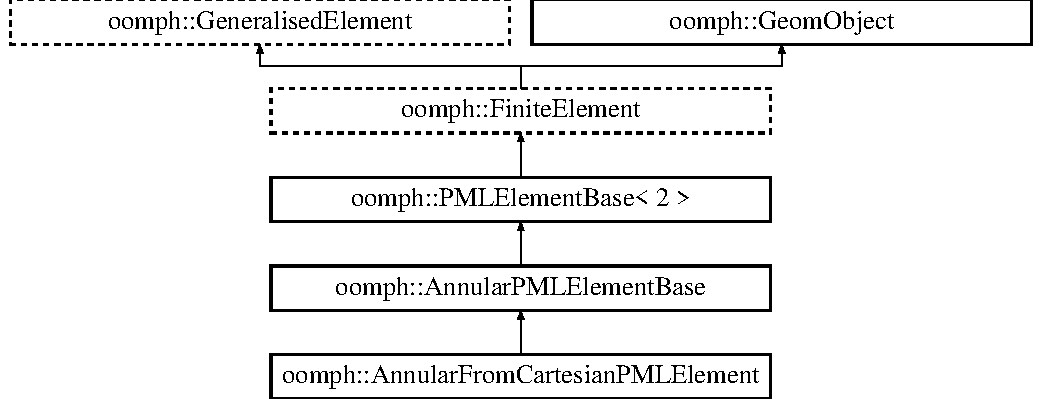
\includegraphics[height=5.000000cm]{classoomph_1_1AnnularFromCartesianPMLElement}
\end{center}
\end{figure}
\subsection*{Public Member Functions}
\begin{DoxyCompactItemize}
\item 
\hyperlink{classoomph_1_1AnnularFromCartesianPMLElement_aa54f360cf010ad8f30c3dbf27f699ae3}{Annular\+From\+Cartesian\+P\+M\+L\+Element} ()
\begin{DoxyCompactList}\small\item\em Constructor. \end{DoxyCompactList}\item 
virtual void \hyperlink{classoomph_1_1AnnularFromCartesianPMLElement_ad5ac4bafd6684b1cff949e74493aff83}{enable\+\_\+pml} (const double \&inner\+\_\+pml\+\_\+radius, const double \&outer\+\_\+pml\+\_\+radius, const \hyperlink{classoomph_1_1Vector}{Vector}$<$ double $>$ \&origin, \hyperlink{classoomph_1_1UniaxialPMLMapping}{Uniaxial\+P\+M\+L\+Mapping} $\ast$pml\+\_\+mapping\+\_\+pt)
\begin{DoxyCompactList}\small\item\em Enable pml. Specify the inner and outer radius of P\+ML and the origin. \end{DoxyCompactList}\item 
double \hyperlink{classoomph_1_1AnnularFromCartesianPMLElement_acb66a5412d96aef573a498ffc8f7a72d}{radius} (const \hyperlink{classoomph_1_1Vector}{Vector}$<$ double $>$ \&\hyperlink{cfortran_8h_ab7123126e4885ef647dd9c6e3807a21c}{s}, const \hyperlink{classoomph_1_1Vector}{Vector}$<$ double $>$ \&x)
\item 
double \hyperlink{classoomph_1_1AnnularFromCartesianPMLElement_acac12e9f2f6df3e9edebb7747ce4fab8}{nu} (const \hyperlink{classoomph_1_1Vector}{Vector}$<$ double $>$ \&\hyperlink{cfortran_8h_ab7123126e4885ef647dd9c6e3807a21c}{s}, const \hyperlink{classoomph_1_1Vector}{Vector}$<$ double $>$ \&x)
\begin{DoxyCompactList}\small\item\em Coordinate which goes through the P\+ML. \end{DoxyCompactList}\item 
double \hyperlink{classoomph_1_1AnnularFromCartesianPMLElement_a28f1b489affa8a37c0c0973cf9324157}{nu} (const double \&r)
\begin{DoxyCompactList}\small\item\em Coordinate which goes through the P\+ML. \end{DoxyCompactList}\item 
double \hyperlink{classoomph_1_1AnnularFromCartesianPMLElement_a9cf84a8abb2f74bf71b6dbf4cc3958f1}{delta} ()
\begin{DoxyCompactList}\small\item\em Thickness of P\+ML. \end{DoxyCompactList}\item 
double \hyperlink{classoomph_1_1AnnularFromCartesianPMLElement_a7c681a8ec4f83f5e9989a8d2fee4de91}{theta} (const \hyperlink{classoomph_1_1Vector}{Vector}$<$ double $>$ \&x)
\begin{DoxyCompactList}\small\item\em Angle relative to origin. \end{DoxyCompactList}\item 
virtual void \hyperlink{classoomph_1_1AnnularFromCartesianPMLElement_a4095e343d2a36dac4e1d5f69402a4ff3}{radial\+\_\+transformation\+\_\+jacobian} (const double \&\hyperlink{classoomph_1_1AnnularFromCartesianPMLElement_acac12e9f2f6df3e9edebb7747ce4fab8}{nu}, const double \&\hyperlink{classoomph_1_1AnnularFromCartesianPMLElement_a9cf84a8abb2f74bf71b6dbf4cc3958f1}{delta}, std\+::complex$<$ double $>$ \&transformed\+\_\+r, std\+::complex$<$ double $>$ \&dtransformed\+\_\+r\+\_\+dr)
\begin{DoxyCompactList}\small\item\em get the Jacobian of the mapping from transformed r to the radial through-\/the-\/pml coordinate. Also returns the transformed\+\_\+r at this point too as it is required for the transformation to cartesian coordinates \end{DoxyCompactList}\end{DoxyCompactItemize}
\subsection*{Protected Attributes}
\begin{DoxyCompactItemize}
\item 
double \hyperlink{classoomph_1_1AnnularFromCartesianPMLElement_ab456fc3ba012d0fe871df2f580298a52}{Pml\+\_\+inner\+\_\+radius}
\begin{DoxyCompactList}\small\item\em Coordinate direction along which pml boundary is constant; alternatively\+: coordinate direction in which coordinate stretching is performed. \end{DoxyCompactList}\item 
double \hyperlink{classoomph_1_1AnnularFromCartesianPMLElement_a2dd7b0074775618fcb2e1072fd81d10a}{Pml\+\_\+outer\+\_\+radius}
\begin{DoxyCompactList}\small\item\em Coordinate of inner pml boundary (Storage is provided for any coordinate direction; only the entries for \char`\"{}active\char`\"{} directions is used.) \end{DoxyCompactList}\item 
\hyperlink{classoomph_1_1Vector}{Vector}$<$ double $>$ \hyperlink{classoomph_1_1AnnularFromCartesianPMLElement_aa31e399eca5049053bce373144a52de0}{Origin}
\begin{DoxyCompactList}\small\item\em Coordinate of outer pml boundary (Storage is provided for any coordinate direction; only the entries for \char`\"{}active\char`\"{} directions is used.) \end{DoxyCompactList}\item 
\hyperlink{classoomph_1_1UniaxialPMLMapping}{Uniaxial\+P\+M\+L\+Mapping} $\ast$ \hyperlink{classoomph_1_1AnnularFromCartesianPMLElement_aae716d46c00db3cec8b6cf2816440f55}{Pml\+\_\+mapping\+\_\+pt}
\end{DoxyCompactItemize}
\subsection*{Additional Inherited Members}


\subsection{Detailed Description}


Definition at line 368 of file pml\+\_\+elements.\+h.



\subsection{Constructor \& Destructor Documentation}
\mbox{\Hypertarget{classoomph_1_1AnnularFromCartesianPMLElement_aa54f360cf010ad8f30c3dbf27f699ae3}\label{classoomph_1_1AnnularFromCartesianPMLElement_aa54f360cf010ad8f30c3dbf27f699ae3}} 
\index{oomph\+::\+Annular\+From\+Cartesian\+P\+M\+L\+Element@{oomph\+::\+Annular\+From\+Cartesian\+P\+M\+L\+Element}!Annular\+From\+Cartesian\+P\+M\+L\+Element@{Annular\+From\+Cartesian\+P\+M\+L\+Element}}
\index{Annular\+From\+Cartesian\+P\+M\+L\+Element@{Annular\+From\+Cartesian\+P\+M\+L\+Element}!oomph\+::\+Annular\+From\+Cartesian\+P\+M\+L\+Element@{oomph\+::\+Annular\+From\+Cartesian\+P\+M\+L\+Element}}
\subsubsection{\texorpdfstring{Annular\+From\+Cartesian\+P\+M\+L\+Element()}{AnnularFromCartesianPMLElement()}}
{\footnotesize\ttfamily oomph\+::\+Annular\+From\+Cartesian\+P\+M\+L\+Element\+::\+Annular\+From\+Cartesian\+P\+M\+L\+Element (\begin{DoxyParamCaption}{ }\end{DoxyParamCaption})\hspace{0.3cm}{\ttfamily [inline]}}



Constructor. 



Definition at line 373 of file pml\+\_\+elements.\+h.



\subsection{Member Function Documentation}
\mbox{\Hypertarget{classoomph_1_1AnnularFromCartesianPMLElement_a9cf84a8abb2f74bf71b6dbf4cc3958f1}\label{classoomph_1_1AnnularFromCartesianPMLElement_a9cf84a8abb2f74bf71b6dbf4cc3958f1}} 
\index{oomph\+::\+Annular\+From\+Cartesian\+P\+M\+L\+Element@{oomph\+::\+Annular\+From\+Cartesian\+P\+M\+L\+Element}!delta@{delta}}
\index{delta@{delta}!oomph\+::\+Annular\+From\+Cartesian\+P\+M\+L\+Element@{oomph\+::\+Annular\+From\+Cartesian\+P\+M\+L\+Element}}
\subsubsection{\texorpdfstring{delta()}{delta()}}
{\footnotesize\ttfamily double oomph\+::\+Annular\+From\+Cartesian\+P\+M\+L\+Element\+::delta (\begin{DoxyParamCaption}{ }\end{DoxyParamCaption})\hspace{0.3cm}{\ttfamily [inline]}, {\ttfamily [virtual]}}



Thickness of P\+ML. 



Implements \hyperlink{classoomph_1_1AnnularPMLElementBase_ad76f02aa6eb19a5757e7d4cc26ec45fa}{oomph\+::\+Annular\+P\+M\+L\+Element\+Base}.



Definition at line 412 of file pml\+\_\+elements.\+h.

\mbox{\Hypertarget{classoomph_1_1AnnularFromCartesianPMLElement_ad5ac4bafd6684b1cff949e74493aff83}\label{classoomph_1_1AnnularFromCartesianPMLElement_ad5ac4bafd6684b1cff949e74493aff83}} 
\index{oomph\+::\+Annular\+From\+Cartesian\+P\+M\+L\+Element@{oomph\+::\+Annular\+From\+Cartesian\+P\+M\+L\+Element}!enable\+\_\+pml@{enable\+\_\+pml}}
\index{enable\+\_\+pml@{enable\+\_\+pml}!oomph\+::\+Annular\+From\+Cartesian\+P\+M\+L\+Element@{oomph\+::\+Annular\+From\+Cartesian\+P\+M\+L\+Element}}
\subsubsection{\texorpdfstring{enable\+\_\+pml()}{enable\_pml()}}
{\footnotesize\ttfamily virtual void oomph\+::\+Annular\+From\+Cartesian\+P\+M\+L\+Element\+::enable\+\_\+pml (\begin{DoxyParamCaption}\item[{const double \&}]{inner\+\_\+pml\+\_\+radius,  }\item[{const double \&}]{outer\+\_\+pml\+\_\+radius,  }\item[{const \hyperlink{classoomph_1_1Vector}{Vector}$<$ double $>$ \&}]{origin,  }\item[{\hyperlink{classoomph_1_1UniaxialPMLMapping}{Uniaxial\+P\+M\+L\+Mapping} $\ast$}]{pml\+\_\+mapping\+\_\+pt }\end{DoxyParamCaption})\hspace{0.3cm}{\ttfamily [inline]}, {\ttfamily [virtual]}}



Enable pml. Specify the inner and outer radius of P\+ML and the origin. 



Definition at line 381 of file pml\+\_\+elements.\+h.



References oomph\+::\+P\+M\+L\+Element\+Base$<$ D\+I\+M $>$\+::enable\+\_\+pml().

\mbox{\Hypertarget{classoomph_1_1AnnularFromCartesianPMLElement_acac12e9f2f6df3e9edebb7747ce4fab8}\label{classoomph_1_1AnnularFromCartesianPMLElement_acac12e9f2f6df3e9edebb7747ce4fab8}} 
\index{oomph\+::\+Annular\+From\+Cartesian\+P\+M\+L\+Element@{oomph\+::\+Annular\+From\+Cartesian\+P\+M\+L\+Element}!nu@{nu}}
\index{nu@{nu}!oomph\+::\+Annular\+From\+Cartesian\+P\+M\+L\+Element@{oomph\+::\+Annular\+From\+Cartesian\+P\+M\+L\+Element}}
\subsubsection{\texorpdfstring{nu()}{nu()}\hspace{0.1cm}{\footnotesize\ttfamily [1/2]}}
{\footnotesize\ttfamily double oomph\+::\+Annular\+From\+Cartesian\+P\+M\+L\+Element\+::nu (\begin{DoxyParamCaption}\item[{const \hyperlink{classoomph_1_1Vector}{Vector}$<$ double $>$ \&}]{s,  }\item[{const \hyperlink{classoomph_1_1Vector}{Vector}$<$ double $>$ \&}]{x }\end{DoxyParamCaption})\hspace{0.3cm}{\ttfamily [inline]}, {\ttfamily [virtual]}}



Coordinate which goes through the P\+ML. 



Implements \hyperlink{classoomph_1_1AnnularPMLElementBase_ac6671111f31c3a5012d0df53a1c24b76}{oomph\+::\+Annular\+P\+M\+L\+Element\+Base}.



Definition at line 400 of file pml\+\_\+elements.\+h.

\mbox{\Hypertarget{classoomph_1_1AnnularFromCartesianPMLElement_a28f1b489affa8a37c0c0973cf9324157}\label{classoomph_1_1AnnularFromCartesianPMLElement_a28f1b489affa8a37c0c0973cf9324157}} 
\index{oomph\+::\+Annular\+From\+Cartesian\+P\+M\+L\+Element@{oomph\+::\+Annular\+From\+Cartesian\+P\+M\+L\+Element}!nu@{nu}}
\index{nu@{nu}!oomph\+::\+Annular\+From\+Cartesian\+P\+M\+L\+Element@{oomph\+::\+Annular\+From\+Cartesian\+P\+M\+L\+Element}}
\subsubsection{\texorpdfstring{nu()}{nu()}\hspace{0.1cm}{\footnotesize\ttfamily [2/2]}}
{\footnotesize\ttfamily double oomph\+::\+Annular\+From\+Cartesian\+P\+M\+L\+Element\+::nu (\begin{DoxyParamCaption}\item[{const double \&}]{r }\end{DoxyParamCaption})\hspace{0.3cm}{\ttfamily [inline]}}



Coordinate which goes through the P\+ML. 



Definition at line 406 of file pml\+\_\+elements.\+h.

\mbox{\Hypertarget{classoomph_1_1AnnularFromCartesianPMLElement_a4095e343d2a36dac4e1d5f69402a4ff3}\label{classoomph_1_1AnnularFromCartesianPMLElement_a4095e343d2a36dac4e1d5f69402a4ff3}} 
\index{oomph\+::\+Annular\+From\+Cartesian\+P\+M\+L\+Element@{oomph\+::\+Annular\+From\+Cartesian\+P\+M\+L\+Element}!radial\+\_\+transformation\+\_\+jacobian@{radial\+\_\+transformation\+\_\+jacobian}}
\index{radial\+\_\+transformation\+\_\+jacobian@{radial\+\_\+transformation\+\_\+jacobian}!oomph\+::\+Annular\+From\+Cartesian\+P\+M\+L\+Element@{oomph\+::\+Annular\+From\+Cartesian\+P\+M\+L\+Element}}
\subsubsection{\texorpdfstring{radial\+\_\+transformation\+\_\+jacobian()}{radial\_transformation\_jacobian()}}
{\footnotesize\ttfamily virtual void oomph\+::\+Annular\+From\+Cartesian\+P\+M\+L\+Element\+::radial\+\_\+transformation\+\_\+jacobian (\begin{DoxyParamCaption}\item[{const double \&}]{nu,  }\item[{const double \&}]{delta,  }\item[{std\+::complex$<$ double $>$ \&}]{transformed\+\_\+r,  }\item[{std\+::complex$<$ double $>$ \&}]{dtransformed\+\_\+r\+\_\+dr }\end{DoxyParamCaption})\hspace{0.3cm}{\ttfamily [inline]}, {\ttfamily [virtual]}}



get the Jacobian of the mapping from transformed r to the radial through-\/the-\/pml coordinate. Also returns the transformed\+\_\+r at this point too as it is required for the transformation to cartesian coordinates 



Definition at line 423 of file pml\+\_\+elements.\+h.

\mbox{\Hypertarget{classoomph_1_1AnnularFromCartesianPMLElement_acb66a5412d96aef573a498ffc8f7a72d}\label{classoomph_1_1AnnularFromCartesianPMLElement_acb66a5412d96aef573a498ffc8f7a72d}} 
\index{oomph\+::\+Annular\+From\+Cartesian\+P\+M\+L\+Element@{oomph\+::\+Annular\+From\+Cartesian\+P\+M\+L\+Element}!radius@{radius}}
\index{radius@{radius}!oomph\+::\+Annular\+From\+Cartesian\+P\+M\+L\+Element@{oomph\+::\+Annular\+From\+Cartesian\+P\+M\+L\+Element}}
\subsubsection{\texorpdfstring{radius()}{radius()}}
{\footnotesize\ttfamily double oomph\+::\+Annular\+From\+Cartesian\+P\+M\+L\+Element\+::radius (\begin{DoxyParamCaption}\item[{const \hyperlink{classoomph_1_1Vector}{Vector}$<$ double $>$ \&}]{s,  }\item[{const \hyperlink{classoomph_1_1Vector}{Vector}$<$ double $>$ \&}]{x }\end{DoxyParamCaption})\hspace{0.3cm}{\ttfamily [inline]}, {\ttfamily [virtual]}}



Implements \hyperlink{classoomph_1_1AnnularPMLElementBase_a5d3de2d99d848942e6fb533fd9cf58da}{oomph\+::\+Annular\+P\+M\+L\+Element\+Base}.



Definition at line 394 of file pml\+\_\+elements.\+h.

\mbox{\Hypertarget{classoomph_1_1AnnularFromCartesianPMLElement_a7c681a8ec4f83f5e9989a8d2fee4de91}\label{classoomph_1_1AnnularFromCartesianPMLElement_a7c681a8ec4f83f5e9989a8d2fee4de91}} 
\index{oomph\+::\+Annular\+From\+Cartesian\+P\+M\+L\+Element@{oomph\+::\+Annular\+From\+Cartesian\+P\+M\+L\+Element}!theta@{theta}}
\index{theta@{theta}!oomph\+::\+Annular\+From\+Cartesian\+P\+M\+L\+Element@{oomph\+::\+Annular\+From\+Cartesian\+P\+M\+L\+Element}}
\subsubsection{\texorpdfstring{theta()}{theta()}}
{\footnotesize\ttfamily double oomph\+::\+Annular\+From\+Cartesian\+P\+M\+L\+Element\+::theta (\begin{DoxyParamCaption}\item[{const \hyperlink{classoomph_1_1Vector}{Vector}$<$ double $>$ \&}]{x }\end{DoxyParamCaption})\hspace{0.3cm}{\ttfamily [inline]}}



Angle relative to origin. 



Definition at line 415 of file pml\+\_\+elements.\+h.



\subsection{Member Data Documentation}
\mbox{\Hypertarget{classoomph_1_1AnnularFromCartesianPMLElement_aa31e399eca5049053bce373144a52de0}\label{classoomph_1_1AnnularFromCartesianPMLElement_aa31e399eca5049053bce373144a52de0}} 
\index{oomph\+::\+Annular\+From\+Cartesian\+P\+M\+L\+Element@{oomph\+::\+Annular\+From\+Cartesian\+P\+M\+L\+Element}!Origin@{Origin}}
\index{Origin@{Origin}!oomph\+::\+Annular\+From\+Cartesian\+P\+M\+L\+Element@{oomph\+::\+Annular\+From\+Cartesian\+P\+M\+L\+Element}}
\subsubsection{\texorpdfstring{Origin}{Origin}}
{\footnotesize\ttfamily \hyperlink{classoomph_1_1Vector}{Vector}$<$double$>$ oomph\+::\+Annular\+From\+Cartesian\+P\+M\+L\+Element\+::\+Origin\hspace{0.3cm}{\ttfamily [protected]}}



Coordinate of outer pml boundary (Storage is provided for any coordinate direction; only the entries for \char`\"{}active\char`\"{} directions is used.) 



Definition at line 450 of file pml\+\_\+elements.\+h.

\mbox{\Hypertarget{classoomph_1_1AnnularFromCartesianPMLElement_ab456fc3ba012d0fe871df2f580298a52}\label{classoomph_1_1AnnularFromCartesianPMLElement_ab456fc3ba012d0fe871df2f580298a52}} 
\index{oomph\+::\+Annular\+From\+Cartesian\+P\+M\+L\+Element@{oomph\+::\+Annular\+From\+Cartesian\+P\+M\+L\+Element}!Pml\+\_\+inner\+\_\+radius@{Pml\+\_\+inner\+\_\+radius}}
\index{Pml\+\_\+inner\+\_\+radius@{Pml\+\_\+inner\+\_\+radius}!oomph\+::\+Annular\+From\+Cartesian\+P\+M\+L\+Element@{oomph\+::\+Annular\+From\+Cartesian\+P\+M\+L\+Element}}
\subsubsection{\texorpdfstring{Pml\+\_\+inner\+\_\+radius}{Pml\_inner\_radius}}
{\footnotesize\ttfamily double oomph\+::\+Annular\+From\+Cartesian\+P\+M\+L\+Element\+::\+Pml\+\_\+inner\+\_\+radius\hspace{0.3cm}{\ttfamily [protected]}}



Coordinate direction along which pml boundary is constant; alternatively\+: coordinate direction in which coordinate stretching is performed. 



Definition at line 440 of file pml\+\_\+elements.\+h.

\mbox{\Hypertarget{classoomph_1_1AnnularFromCartesianPMLElement_aae716d46c00db3cec8b6cf2816440f55}\label{classoomph_1_1AnnularFromCartesianPMLElement_aae716d46c00db3cec8b6cf2816440f55}} 
\index{oomph\+::\+Annular\+From\+Cartesian\+P\+M\+L\+Element@{oomph\+::\+Annular\+From\+Cartesian\+P\+M\+L\+Element}!Pml\+\_\+mapping\+\_\+pt@{Pml\+\_\+mapping\+\_\+pt}}
\index{Pml\+\_\+mapping\+\_\+pt@{Pml\+\_\+mapping\+\_\+pt}!oomph\+::\+Annular\+From\+Cartesian\+P\+M\+L\+Element@{oomph\+::\+Annular\+From\+Cartesian\+P\+M\+L\+Element}}
\subsubsection{\texorpdfstring{Pml\+\_\+mapping\+\_\+pt}{Pml\_mapping\_pt}}
{\footnotesize\ttfamily \hyperlink{classoomph_1_1UniaxialPMLMapping}{Uniaxial\+P\+M\+L\+Mapping}$\ast$ oomph\+::\+Annular\+From\+Cartesian\+P\+M\+L\+Element\+::\+Pml\+\_\+mapping\+\_\+pt\hspace{0.3cm}{\ttfamily [protected]}}



Definition at line 453 of file pml\+\_\+elements.\+h.

\mbox{\Hypertarget{classoomph_1_1AnnularFromCartesianPMLElement_a2dd7b0074775618fcb2e1072fd81d10a}\label{classoomph_1_1AnnularFromCartesianPMLElement_a2dd7b0074775618fcb2e1072fd81d10a}} 
\index{oomph\+::\+Annular\+From\+Cartesian\+P\+M\+L\+Element@{oomph\+::\+Annular\+From\+Cartesian\+P\+M\+L\+Element}!Pml\+\_\+outer\+\_\+radius@{Pml\+\_\+outer\+\_\+radius}}
\index{Pml\+\_\+outer\+\_\+radius@{Pml\+\_\+outer\+\_\+radius}!oomph\+::\+Annular\+From\+Cartesian\+P\+M\+L\+Element@{oomph\+::\+Annular\+From\+Cartesian\+P\+M\+L\+Element}}
\subsubsection{\texorpdfstring{Pml\+\_\+outer\+\_\+radius}{Pml\_outer\_radius}}
{\footnotesize\ttfamily double oomph\+::\+Annular\+From\+Cartesian\+P\+M\+L\+Element\+::\+Pml\+\_\+outer\+\_\+radius\hspace{0.3cm}{\ttfamily [protected]}}



Coordinate of inner pml boundary (Storage is provided for any coordinate direction; only the entries for \char`\"{}active\char`\"{} directions is used.) 



Definition at line 445 of file pml\+\_\+elements.\+h.



The documentation for this class was generated from the following file\+:\begin{DoxyCompactItemize}
\item 
\hyperlink{pml__elements_8h}{pml\+\_\+elements.\+h}\end{DoxyCompactItemize}

\hypertarget{classoomph_1_1AnnularFromLocalCoordinatePMLElement}{}\section{oomph\+:\+:Annular\+From\+Local\+Coordinate\+P\+M\+L\+Element Class Reference}
\label{classoomph_1_1AnnularFromLocalCoordinatePMLElement}\index{oomph\+::\+Annular\+From\+Local\+Coordinate\+P\+M\+L\+Element@{oomph\+::\+Annular\+From\+Local\+Coordinate\+P\+M\+L\+Element}}


{\ttfamily \#include $<$pml\+\_\+elements.\+h$>$}

Inheritance diagram for oomph\+:\+:Annular\+From\+Local\+Coordinate\+P\+M\+L\+Element\+:\begin{figure}[H]
\begin{center}
\leavevmode
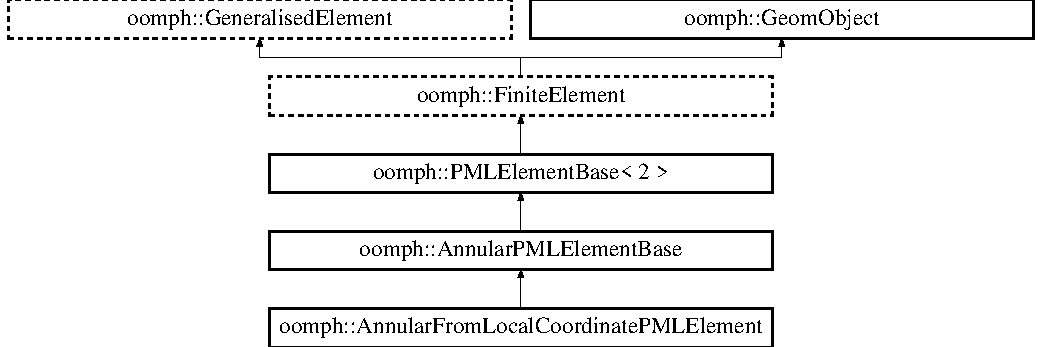
\includegraphics[height=4.666667cm]{classoomph_1_1AnnularFromLocalCoordinatePMLElement}
\end{center}
\end{figure}
\subsection*{Public Member Functions}
\begin{DoxyCompactItemize}
\item 
\hyperlink{classoomph_1_1AnnularFromLocalCoordinatePMLElement_a3e7cb53dd208524cb5378d1ec2ee1e89}{Annular\+From\+Local\+Coordinate\+P\+M\+L\+Element} ()
\begin{DoxyCompactList}\small\item\em Constructor. \end{DoxyCompactList}\item 
\hyperlink{classoomph_1_1AnnularFromLocalCoordinatePMLElement_a32ef4115b2cce33d4ec93a5620807685}{Annular\+From\+Local\+Coordinate\+P\+M\+L\+Element} (unsigned nu\+\_\+s\+\_\+index, double nu\+\_\+at\+\_\+s\+\_\+min, double nu\+\_\+at\+\_\+s\+\_\+max, unsigned theta\+\_\+s\+\_\+index, double theta\+\_\+at\+\_\+s\+\_\+min, double theta\+\_\+at\+\_\+s\+\_\+max, double pml\+\_\+inner\+\_\+radius, double pml\+\_\+outer\+\_\+radius)
\begin{DoxyCompactList}\small\item\em Constructor. \end{DoxyCompactList}\item 
virtual void \hyperlink{classoomph_1_1AnnularFromLocalCoordinatePMLElement_a232008f72c0ee625d59b1e588c850dfe}{enable\+\_\+pml} (const double \&inner\+\_\+pml\+\_\+radius, const double \&outer\+\_\+pml\+\_\+radius, const \hyperlink{classoomph_1_1Vector}{Vector}$<$ double $>$ \&origin)
\begin{DoxyCompactList}\small\item\em Enable pml. Specify the inner and outer radius of P\+ML and the origin. \end{DoxyCompactList}\item 
virtual double \hyperlink{classoomph_1_1AnnularFromLocalCoordinatePMLElement_a7d0f2e25ee965d08b067c5a0a8d3bef2}{s\+\_\+min} ()
\item 
virtual double \hyperlink{classoomph_1_1AnnularFromLocalCoordinatePMLElement_ab4e7e9103ffc587755a6149db1559688}{s\+\_\+max} ()
\item 
double \hyperlink{classoomph_1_1AnnularFromLocalCoordinatePMLElement_a161e427b6f1fc6349b9667caf346cf8a}{nu} (const \hyperlink{classoomph_1_1Vector}{Vector}$<$ double $>$ \&\hyperlink{cfortran_8h_ab7123126e4885ef647dd9c6e3807a21c}{s}, const \hyperlink{classoomph_1_1Vector}{Vector}$<$ double $>$ \&x)
\begin{DoxyCompactList}\small\item\em Coordinate which goes through the P\+ML in terms of local coordinate. \end{DoxyCompactList}\item 
double \hyperlink{classoomph_1_1AnnularFromLocalCoordinatePMLElement_affe7de11a2275aac57b0ea2c0594ce7d}{delta} ()
\begin{DoxyCompactList}\small\item\em Thickness of P\+ML. \end{DoxyCompactList}\item 
double \hyperlink{classoomph_1_1AnnularFromLocalCoordinatePMLElement_ae9f56654db4d7979163db0529d9a1408}{theta} (const \hyperlink{classoomph_1_1Vector}{Vector}$<$ double $>$ \&\hyperlink{cfortran_8h_ab7123126e4885ef647dd9c6e3807a21c}{s}, const \hyperlink{classoomph_1_1Vector}{Vector}$<$ double $>$ \&x)
\begin{DoxyCompactList}\small\item\em Angle relative to origin. \end{DoxyCompactList}\item 
virtual void \hyperlink{classoomph_1_1AnnularFromLocalCoordinatePMLElement_ab44027b0ebf468154752cc09d46d3a5d}{radial\+\_\+transformation\+\_\+jacobian} (const double \&\hyperlink{classoomph_1_1AnnularFromLocalCoordinatePMLElement_a161e427b6f1fc6349b9667caf346cf8a}{nu}, const double \&\hyperlink{classoomph_1_1AnnularFromLocalCoordinatePMLElement_affe7de11a2275aac57b0ea2c0594ce7d}{delta}, std\+::complex$<$ double $>$ \&transformed\+\_\+r, std\+::complex$<$ double $>$ \&dtransformed\+\_\+r\+\_\+dr)
\begin{DoxyCompactList}\small\item\em get the Jacobian of the mapping from transformed r to the radial through-\/the-\/pml coordinate. Also returns the transformed\+\_\+r at this point too as it is required for the transformation to cartesian coordinates \end{DoxyCompactList}\end{DoxyCompactItemize}
\subsection*{Protected Attributes}
\begin{DoxyCompactItemize}
\item 
unsigned \hyperlink{classoomph_1_1AnnularFromLocalCoordinatePMLElement_a83bac6e18a318693e37b69f658d522e9}{Nu\+\_\+s\+\_\+index}
\begin{DoxyCompactList}\small\item\em Index of local coordinate which nu (through the P\+ML coordinate) is parametrised by. \end{DoxyCompactList}\item 
double \hyperlink{classoomph_1_1AnnularFromLocalCoordinatePMLElement_ae858cd7ca5348175f26b2d662a607e43}{Nu\+\_\+at\+\_\+s\+\_\+min}
\begin{DoxyCompactList}\small\item\em Value of nu at the minimum value of local coordinate. \end{DoxyCompactList}\item 
double \hyperlink{classoomph_1_1AnnularFromLocalCoordinatePMLElement_abeba5fad805f67b4806361f9c2c43d70}{Nu\+\_\+at\+\_\+s\+\_\+max}
\begin{DoxyCompactList}\small\item\em Value of nu at the maximum value of local coordinate. \end{DoxyCompactList}\item 
unsigned \hyperlink{classoomph_1_1AnnularFromLocalCoordinatePMLElement_ac4bc071b8e8c384504a4a61113ec2ecd}{Theta\+\_\+s\+\_\+index}
\begin{DoxyCompactList}\small\item\em Index of local coordinate which theta is parametrised by. \end{DoxyCompactList}\item 
double \hyperlink{classoomph_1_1AnnularFromLocalCoordinatePMLElement_a6f88cc81d5f43c10da316bd6b56b3fb1}{Theta\+\_\+at\+\_\+s\+\_\+min}
\begin{DoxyCompactList}\small\item\em Value of theta at the minimum value of local coordinate. \end{DoxyCompactList}\item 
double \hyperlink{classoomph_1_1AnnularFromLocalCoordinatePMLElement_ae191ccf4540974d4923b80353955dbf1}{Theta\+\_\+at\+\_\+s\+\_\+max}
\begin{DoxyCompactList}\small\item\em Value of theta at the maximum value of local coordinate. \end{DoxyCompactList}\item 
double \hyperlink{classoomph_1_1AnnularFromLocalCoordinatePMLElement_a90aa4d2d40c250c35e0bfbac50c9a9d1}{Pml\+\_\+inner\+\_\+radius}
\begin{DoxyCompactList}\small\item\em Value of radius at inner P\+ML boundary. \end{DoxyCompactList}\item 
double \hyperlink{classoomph_1_1AnnularFromLocalCoordinatePMLElement_a360bd3ab9afbcfd1007a626b780d51d8}{Pml\+\_\+outer\+\_\+radius}
\begin{DoxyCompactList}\small\item\em Value of radius at outer P\+ML boundary. \end{DoxyCompactList}\item 
\hyperlink{classoomph_1_1UniaxialPMLMapping}{Uniaxial\+P\+M\+L\+Mapping} $\ast$ \hyperlink{classoomph_1_1AnnularFromLocalCoordinatePMLElement_a51049d96dbdb41fc740bdabd5657b99b}{Pml\+\_\+mapping\+\_\+pt}
\end{DoxyCompactItemize}
\subsection*{Additional Inherited Members}


\subsection{Detailed Description}


Definition at line 457 of file pml\+\_\+elements.\+h.



\subsection{Constructor \& Destructor Documentation}
\mbox{\Hypertarget{classoomph_1_1AnnularFromLocalCoordinatePMLElement_a3e7cb53dd208524cb5378d1ec2ee1e89}\label{classoomph_1_1AnnularFromLocalCoordinatePMLElement_a3e7cb53dd208524cb5378d1ec2ee1e89}} 
\index{oomph\+::\+Annular\+From\+Local\+Coordinate\+P\+M\+L\+Element@{oomph\+::\+Annular\+From\+Local\+Coordinate\+P\+M\+L\+Element}!Annular\+From\+Local\+Coordinate\+P\+M\+L\+Element@{Annular\+From\+Local\+Coordinate\+P\+M\+L\+Element}}
\index{Annular\+From\+Local\+Coordinate\+P\+M\+L\+Element@{Annular\+From\+Local\+Coordinate\+P\+M\+L\+Element}!oomph\+::\+Annular\+From\+Local\+Coordinate\+P\+M\+L\+Element@{oomph\+::\+Annular\+From\+Local\+Coordinate\+P\+M\+L\+Element}}
\subsubsection{\texorpdfstring{Annular\+From\+Local\+Coordinate\+P\+M\+L\+Element()}{AnnularFromLocalCoordinatePMLElement()}\hspace{0.1cm}{\footnotesize\ttfamily [1/2]}}
{\footnotesize\ttfamily oomph\+::\+Annular\+From\+Local\+Coordinate\+P\+M\+L\+Element\+::\+Annular\+From\+Local\+Coordinate\+P\+M\+L\+Element (\begin{DoxyParamCaption}{ }\end{DoxyParamCaption})\hspace{0.3cm}{\ttfamily [inline]}}



Constructor. 



Definition at line 462 of file pml\+\_\+elements.\+h.

\mbox{\Hypertarget{classoomph_1_1AnnularFromLocalCoordinatePMLElement_a32ef4115b2cce33d4ec93a5620807685}\label{classoomph_1_1AnnularFromLocalCoordinatePMLElement_a32ef4115b2cce33d4ec93a5620807685}} 
\index{oomph\+::\+Annular\+From\+Local\+Coordinate\+P\+M\+L\+Element@{oomph\+::\+Annular\+From\+Local\+Coordinate\+P\+M\+L\+Element}!Annular\+From\+Local\+Coordinate\+P\+M\+L\+Element@{Annular\+From\+Local\+Coordinate\+P\+M\+L\+Element}}
\index{Annular\+From\+Local\+Coordinate\+P\+M\+L\+Element@{Annular\+From\+Local\+Coordinate\+P\+M\+L\+Element}!oomph\+::\+Annular\+From\+Local\+Coordinate\+P\+M\+L\+Element@{oomph\+::\+Annular\+From\+Local\+Coordinate\+P\+M\+L\+Element}}
\subsubsection{\texorpdfstring{Annular\+From\+Local\+Coordinate\+P\+M\+L\+Element()}{AnnularFromLocalCoordinatePMLElement()}\hspace{0.1cm}{\footnotesize\ttfamily [2/2]}}
{\footnotesize\ttfamily oomph\+::\+Annular\+From\+Local\+Coordinate\+P\+M\+L\+Element\+::\+Annular\+From\+Local\+Coordinate\+P\+M\+L\+Element (\begin{DoxyParamCaption}\item[{unsigned}]{nu\+\_\+s\+\_\+index,  }\item[{double}]{nu\+\_\+at\+\_\+s\+\_\+min,  }\item[{double}]{nu\+\_\+at\+\_\+s\+\_\+max,  }\item[{unsigned}]{theta\+\_\+s\+\_\+index,  }\item[{double}]{theta\+\_\+at\+\_\+s\+\_\+min,  }\item[{double}]{theta\+\_\+at\+\_\+s\+\_\+max,  }\item[{double}]{pml\+\_\+inner\+\_\+radius,  }\item[{double}]{pml\+\_\+outer\+\_\+radius }\end{DoxyParamCaption})\hspace{0.3cm}{\ttfamily [inline]}}



Constructor. 



Definition at line 474 of file pml\+\_\+elements.\+h.



\subsection{Member Function Documentation}
\mbox{\Hypertarget{classoomph_1_1AnnularFromLocalCoordinatePMLElement_affe7de11a2275aac57b0ea2c0594ce7d}\label{classoomph_1_1AnnularFromLocalCoordinatePMLElement_affe7de11a2275aac57b0ea2c0594ce7d}} 
\index{oomph\+::\+Annular\+From\+Local\+Coordinate\+P\+M\+L\+Element@{oomph\+::\+Annular\+From\+Local\+Coordinate\+P\+M\+L\+Element}!delta@{delta}}
\index{delta@{delta}!oomph\+::\+Annular\+From\+Local\+Coordinate\+P\+M\+L\+Element@{oomph\+::\+Annular\+From\+Local\+Coordinate\+P\+M\+L\+Element}}
\subsubsection{\texorpdfstring{delta()}{delta()}}
{\footnotesize\ttfamily double oomph\+::\+Annular\+From\+Local\+Coordinate\+P\+M\+L\+Element\+::delta (\begin{DoxyParamCaption}{ }\end{DoxyParamCaption})\hspace{0.3cm}{\ttfamily [inline]}, {\ttfamily [virtual]}}



Thickness of P\+ML. 



Implements \hyperlink{classoomph_1_1AnnularPMLElementBase_ad76f02aa6eb19a5757e7d4cc26ec45fa}{oomph\+::\+Annular\+P\+M\+L\+Element\+Base}.



Definition at line 512 of file pml\+\_\+elements.\+h.

\mbox{\Hypertarget{classoomph_1_1AnnularFromLocalCoordinatePMLElement_a232008f72c0ee625d59b1e588c850dfe}\label{classoomph_1_1AnnularFromLocalCoordinatePMLElement_a232008f72c0ee625d59b1e588c850dfe}} 
\index{oomph\+::\+Annular\+From\+Local\+Coordinate\+P\+M\+L\+Element@{oomph\+::\+Annular\+From\+Local\+Coordinate\+P\+M\+L\+Element}!enable\+\_\+pml@{enable\+\_\+pml}}
\index{enable\+\_\+pml@{enable\+\_\+pml}!oomph\+::\+Annular\+From\+Local\+Coordinate\+P\+M\+L\+Element@{oomph\+::\+Annular\+From\+Local\+Coordinate\+P\+M\+L\+Element}}
\subsubsection{\texorpdfstring{enable\+\_\+pml()}{enable\_pml()}}
{\footnotesize\ttfamily virtual void oomph\+::\+Annular\+From\+Local\+Coordinate\+P\+M\+L\+Element\+::enable\+\_\+pml (\begin{DoxyParamCaption}\item[{const double \&}]{inner\+\_\+pml\+\_\+radius,  }\item[{const double \&}]{outer\+\_\+pml\+\_\+radius,  }\item[{const \hyperlink{classoomph_1_1Vector}{Vector}$<$ double $>$ \&}]{origin }\end{DoxyParamCaption})\hspace{0.3cm}{\ttfamily [inline]}, {\ttfamily [virtual]}}



Enable pml. Specify the inner and outer radius of P\+ML and the origin. 



Definition at line 494 of file pml\+\_\+elements.\+h.



References oomph\+::\+P\+M\+L\+Element\+Base$<$ D\+I\+M $>$\+::enable\+\_\+pml().

\mbox{\Hypertarget{classoomph_1_1AnnularFromLocalCoordinatePMLElement_a161e427b6f1fc6349b9667caf346cf8a}\label{classoomph_1_1AnnularFromLocalCoordinatePMLElement_a161e427b6f1fc6349b9667caf346cf8a}} 
\index{oomph\+::\+Annular\+From\+Local\+Coordinate\+P\+M\+L\+Element@{oomph\+::\+Annular\+From\+Local\+Coordinate\+P\+M\+L\+Element}!nu@{nu}}
\index{nu@{nu}!oomph\+::\+Annular\+From\+Local\+Coordinate\+P\+M\+L\+Element@{oomph\+::\+Annular\+From\+Local\+Coordinate\+P\+M\+L\+Element}}
\subsubsection{\texorpdfstring{nu()}{nu()}}
{\footnotesize\ttfamily double oomph\+::\+Annular\+From\+Local\+Coordinate\+P\+M\+L\+Element\+::nu (\begin{DoxyParamCaption}\item[{const \hyperlink{classoomph_1_1Vector}{Vector}$<$ double $>$ \&}]{s,  }\item[{const \hyperlink{classoomph_1_1Vector}{Vector}$<$ double $>$ \&}]{x }\end{DoxyParamCaption})\hspace{0.3cm}{\ttfamily [inline]}, {\ttfamily [virtual]}}



Coordinate which goes through the P\+ML in terms of local coordinate. 



Implements \hyperlink{classoomph_1_1AnnularPMLElementBase_ac6671111f31c3a5012d0df53a1c24b76}{oomph\+::\+Annular\+P\+M\+L\+Element\+Base}.



Definition at line 505 of file pml\+\_\+elements.\+h.

\mbox{\Hypertarget{classoomph_1_1AnnularFromLocalCoordinatePMLElement_ab44027b0ebf468154752cc09d46d3a5d}\label{classoomph_1_1AnnularFromLocalCoordinatePMLElement_ab44027b0ebf468154752cc09d46d3a5d}} 
\index{oomph\+::\+Annular\+From\+Local\+Coordinate\+P\+M\+L\+Element@{oomph\+::\+Annular\+From\+Local\+Coordinate\+P\+M\+L\+Element}!radial\+\_\+transformation\+\_\+jacobian@{radial\+\_\+transformation\+\_\+jacobian}}
\index{radial\+\_\+transformation\+\_\+jacobian@{radial\+\_\+transformation\+\_\+jacobian}!oomph\+::\+Annular\+From\+Local\+Coordinate\+P\+M\+L\+Element@{oomph\+::\+Annular\+From\+Local\+Coordinate\+P\+M\+L\+Element}}
\subsubsection{\texorpdfstring{radial\+\_\+transformation\+\_\+jacobian()}{radial\_transformation\_jacobian()}}
{\footnotesize\ttfamily virtual void oomph\+::\+Annular\+From\+Local\+Coordinate\+P\+M\+L\+Element\+::radial\+\_\+transformation\+\_\+jacobian (\begin{DoxyParamCaption}\item[{const double \&}]{nu,  }\item[{const double \&}]{delta,  }\item[{std\+::complex$<$ double $>$ \&}]{transformed\+\_\+r,  }\item[{std\+::complex$<$ double $>$ \&}]{dtransformed\+\_\+r\+\_\+dr }\end{DoxyParamCaption})\hspace{0.3cm}{\ttfamily [inline]}, {\ttfamily [virtual]}}



get the Jacobian of the mapping from transformed r to the radial through-\/the-\/pml coordinate. Also returns the transformed\+\_\+r at this point too as it is required for the transformation to cartesian coordinates 



Definition at line 525 of file pml\+\_\+elements.\+h.

\mbox{\Hypertarget{classoomph_1_1AnnularFromLocalCoordinatePMLElement_ab4e7e9103ffc587755a6149db1559688}\label{classoomph_1_1AnnularFromLocalCoordinatePMLElement_ab4e7e9103ffc587755a6149db1559688}} 
\index{oomph\+::\+Annular\+From\+Local\+Coordinate\+P\+M\+L\+Element@{oomph\+::\+Annular\+From\+Local\+Coordinate\+P\+M\+L\+Element}!s\+\_\+max@{s\+\_\+max}}
\index{s\+\_\+max@{s\+\_\+max}!oomph\+::\+Annular\+From\+Local\+Coordinate\+P\+M\+L\+Element@{oomph\+::\+Annular\+From\+Local\+Coordinate\+P\+M\+L\+Element}}
\subsubsection{\texorpdfstring{s\+\_\+max()}{s\_max()}}
{\footnotesize\ttfamily virtual double oomph\+::\+Annular\+From\+Local\+Coordinate\+P\+M\+L\+Element\+::s\+\_\+max (\begin{DoxyParamCaption}{ }\end{DoxyParamCaption})\hspace{0.3cm}{\ttfamily [virtual]}}

\mbox{\Hypertarget{classoomph_1_1AnnularFromLocalCoordinatePMLElement_a7d0f2e25ee965d08b067c5a0a8d3bef2}\label{classoomph_1_1AnnularFromLocalCoordinatePMLElement_a7d0f2e25ee965d08b067c5a0a8d3bef2}} 
\index{oomph\+::\+Annular\+From\+Local\+Coordinate\+P\+M\+L\+Element@{oomph\+::\+Annular\+From\+Local\+Coordinate\+P\+M\+L\+Element}!s\+\_\+min@{s\+\_\+min}}
\index{s\+\_\+min@{s\+\_\+min}!oomph\+::\+Annular\+From\+Local\+Coordinate\+P\+M\+L\+Element@{oomph\+::\+Annular\+From\+Local\+Coordinate\+P\+M\+L\+Element}}
\subsubsection{\texorpdfstring{s\+\_\+min()}{s\_min()}}
{\footnotesize\ttfamily virtual double oomph\+::\+Annular\+From\+Local\+Coordinate\+P\+M\+L\+Element\+::s\+\_\+min (\begin{DoxyParamCaption}{ }\end{DoxyParamCaption})\hspace{0.3cm}{\ttfamily [virtual]}}

\mbox{\Hypertarget{classoomph_1_1AnnularFromLocalCoordinatePMLElement_ae9f56654db4d7979163db0529d9a1408}\label{classoomph_1_1AnnularFromLocalCoordinatePMLElement_ae9f56654db4d7979163db0529d9a1408}} 
\index{oomph\+::\+Annular\+From\+Local\+Coordinate\+P\+M\+L\+Element@{oomph\+::\+Annular\+From\+Local\+Coordinate\+P\+M\+L\+Element}!theta@{theta}}
\index{theta@{theta}!oomph\+::\+Annular\+From\+Local\+Coordinate\+P\+M\+L\+Element@{oomph\+::\+Annular\+From\+Local\+Coordinate\+P\+M\+L\+Element}}
\subsubsection{\texorpdfstring{theta()}{theta()}}
{\footnotesize\ttfamily double oomph\+::\+Annular\+From\+Local\+Coordinate\+P\+M\+L\+Element\+::theta (\begin{DoxyParamCaption}\item[{const \hyperlink{classoomph_1_1Vector}{Vector}$<$ double $>$ \&}]{s,  }\item[{const \hyperlink{classoomph_1_1Vector}{Vector}$<$ double $>$ \&}]{x }\end{DoxyParamCaption})\hspace{0.3cm}{\ttfamily [inline]}, {\ttfamily [virtual]}}



Angle relative to origin. 



Implements \hyperlink{classoomph_1_1AnnularPMLElementBase_a74036190f87f79129cdcda562664dd18}{oomph\+::\+Annular\+P\+M\+L\+Element\+Base}.



Definition at line 515 of file pml\+\_\+elements.\+h.



\subsection{Member Data Documentation}
\mbox{\Hypertarget{classoomph_1_1AnnularFromLocalCoordinatePMLElement_abeba5fad805f67b4806361f9c2c43d70}\label{classoomph_1_1AnnularFromLocalCoordinatePMLElement_abeba5fad805f67b4806361f9c2c43d70}} 
\index{oomph\+::\+Annular\+From\+Local\+Coordinate\+P\+M\+L\+Element@{oomph\+::\+Annular\+From\+Local\+Coordinate\+P\+M\+L\+Element}!Nu\+\_\+at\+\_\+s\+\_\+max@{Nu\+\_\+at\+\_\+s\+\_\+max}}
\index{Nu\+\_\+at\+\_\+s\+\_\+max@{Nu\+\_\+at\+\_\+s\+\_\+max}!oomph\+::\+Annular\+From\+Local\+Coordinate\+P\+M\+L\+Element@{oomph\+::\+Annular\+From\+Local\+Coordinate\+P\+M\+L\+Element}}
\subsubsection{\texorpdfstring{Nu\+\_\+at\+\_\+s\+\_\+max}{Nu\_at\_s\_max}}
{\footnotesize\ttfamily double oomph\+::\+Annular\+From\+Local\+Coordinate\+P\+M\+L\+Element\+::\+Nu\+\_\+at\+\_\+s\+\_\+max\hspace{0.3cm}{\ttfamily [protected]}}



Value of nu at the maximum value of local coordinate. 



Definition at line 547 of file pml\+\_\+elements.\+h.

\mbox{\Hypertarget{classoomph_1_1AnnularFromLocalCoordinatePMLElement_ae858cd7ca5348175f26b2d662a607e43}\label{classoomph_1_1AnnularFromLocalCoordinatePMLElement_ae858cd7ca5348175f26b2d662a607e43}} 
\index{oomph\+::\+Annular\+From\+Local\+Coordinate\+P\+M\+L\+Element@{oomph\+::\+Annular\+From\+Local\+Coordinate\+P\+M\+L\+Element}!Nu\+\_\+at\+\_\+s\+\_\+min@{Nu\+\_\+at\+\_\+s\+\_\+min}}
\index{Nu\+\_\+at\+\_\+s\+\_\+min@{Nu\+\_\+at\+\_\+s\+\_\+min}!oomph\+::\+Annular\+From\+Local\+Coordinate\+P\+M\+L\+Element@{oomph\+::\+Annular\+From\+Local\+Coordinate\+P\+M\+L\+Element}}
\subsubsection{\texorpdfstring{Nu\+\_\+at\+\_\+s\+\_\+min}{Nu\_at\_s\_min}}
{\footnotesize\ttfamily double oomph\+::\+Annular\+From\+Local\+Coordinate\+P\+M\+L\+Element\+::\+Nu\+\_\+at\+\_\+s\+\_\+min\hspace{0.3cm}{\ttfamily [protected]}}



Value of nu at the minimum value of local coordinate. 



Definition at line 544 of file pml\+\_\+elements.\+h.

\mbox{\Hypertarget{classoomph_1_1AnnularFromLocalCoordinatePMLElement_a83bac6e18a318693e37b69f658d522e9}\label{classoomph_1_1AnnularFromLocalCoordinatePMLElement_a83bac6e18a318693e37b69f658d522e9}} 
\index{oomph\+::\+Annular\+From\+Local\+Coordinate\+P\+M\+L\+Element@{oomph\+::\+Annular\+From\+Local\+Coordinate\+P\+M\+L\+Element}!Nu\+\_\+s\+\_\+index@{Nu\+\_\+s\+\_\+index}}
\index{Nu\+\_\+s\+\_\+index@{Nu\+\_\+s\+\_\+index}!oomph\+::\+Annular\+From\+Local\+Coordinate\+P\+M\+L\+Element@{oomph\+::\+Annular\+From\+Local\+Coordinate\+P\+M\+L\+Element}}
\subsubsection{\texorpdfstring{Nu\+\_\+s\+\_\+index}{Nu\_s\_index}}
{\footnotesize\ttfamily unsigned oomph\+::\+Annular\+From\+Local\+Coordinate\+P\+M\+L\+Element\+::\+Nu\+\_\+s\+\_\+index\hspace{0.3cm}{\ttfamily [protected]}}



Index of local coordinate which nu (through the P\+ML coordinate) is parametrised by. 



Definition at line 541 of file pml\+\_\+elements.\+h.

\mbox{\Hypertarget{classoomph_1_1AnnularFromLocalCoordinatePMLElement_a90aa4d2d40c250c35e0bfbac50c9a9d1}\label{classoomph_1_1AnnularFromLocalCoordinatePMLElement_a90aa4d2d40c250c35e0bfbac50c9a9d1}} 
\index{oomph\+::\+Annular\+From\+Local\+Coordinate\+P\+M\+L\+Element@{oomph\+::\+Annular\+From\+Local\+Coordinate\+P\+M\+L\+Element}!Pml\+\_\+inner\+\_\+radius@{Pml\+\_\+inner\+\_\+radius}}
\index{Pml\+\_\+inner\+\_\+radius@{Pml\+\_\+inner\+\_\+radius}!oomph\+::\+Annular\+From\+Local\+Coordinate\+P\+M\+L\+Element@{oomph\+::\+Annular\+From\+Local\+Coordinate\+P\+M\+L\+Element}}
\subsubsection{\texorpdfstring{Pml\+\_\+inner\+\_\+radius}{Pml\_inner\_radius}}
{\footnotesize\ttfamily double oomph\+::\+Annular\+From\+Local\+Coordinate\+P\+M\+L\+Element\+::\+Pml\+\_\+inner\+\_\+radius\hspace{0.3cm}{\ttfamily [protected]}}



Value of radius at inner P\+ML boundary. 



Definition at line 559 of file pml\+\_\+elements.\+h.

\mbox{\Hypertarget{classoomph_1_1AnnularFromLocalCoordinatePMLElement_a51049d96dbdb41fc740bdabd5657b99b}\label{classoomph_1_1AnnularFromLocalCoordinatePMLElement_a51049d96dbdb41fc740bdabd5657b99b}} 
\index{oomph\+::\+Annular\+From\+Local\+Coordinate\+P\+M\+L\+Element@{oomph\+::\+Annular\+From\+Local\+Coordinate\+P\+M\+L\+Element}!Pml\+\_\+mapping\+\_\+pt@{Pml\+\_\+mapping\+\_\+pt}}
\index{Pml\+\_\+mapping\+\_\+pt@{Pml\+\_\+mapping\+\_\+pt}!oomph\+::\+Annular\+From\+Local\+Coordinate\+P\+M\+L\+Element@{oomph\+::\+Annular\+From\+Local\+Coordinate\+P\+M\+L\+Element}}
\subsubsection{\texorpdfstring{Pml\+\_\+mapping\+\_\+pt}{Pml\_mapping\_pt}}
{\footnotesize\ttfamily \hyperlink{classoomph_1_1UniaxialPMLMapping}{Uniaxial\+P\+M\+L\+Mapping}$\ast$ oomph\+::\+Annular\+From\+Local\+Coordinate\+P\+M\+L\+Element\+::\+Pml\+\_\+mapping\+\_\+pt\hspace{0.3cm}{\ttfamily [protected]}}



Definition at line 565 of file pml\+\_\+elements.\+h.

\mbox{\Hypertarget{classoomph_1_1AnnularFromLocalCoordinatePMLElement_a360bd3ab9afbcfd1007a626b780d51d8}\label{classoomph_1_1AnnularFromLocalCoordinatePMLElement_a360bd3ab9afbcfd1007a626b780d51d8}} 
\index{oomph\+::\+Annular\+From\+Local\+Coordinate\+P\+M\+L\+Element@{oomph\+::\+Annular\+From\+Local\+Coordinate\+P\+M\+L\+Element}!Pml\+\_\+outer\+\_\+radius@{Pml\+\_\+outer\+\_\+radius}}
\index{Pml\+\_\+outer\+\_\+radius@{Pml\+\_\+outer\+\_\+radius}!oomph\+::\+Annular\+From\+Local\+Coordinate\+P\+M\+L\+Element@{oomph\+::\+Annular\+From\+Local\+Coordinate\+P\+M\+L\+Element}}
\subsubsection{\texorpdfstring{Pml\+\_\+outer\+\_\+radius}{Pml\_outer\_radius}}
{\footnotesize\ttfamily double oomph\+::\+Annular\+From\+Local\+Coordinate\+P\+M\+L\+Element\+::\+Pml\+\_\+outer\+\_\+radius\hspace{0.3cm}{\ttfamily [protected]}}



Value of radius at outer P\+ML boundary. 



Definition at line 562 of file pml\+\_\+elements.\+h.

\mbox{\Hypertarget{classoomph_1_1AnnularFromLocalCoordinatePMLElement_ae191ccf4540974d4923b80353955dbf1}\label{classoomph_1_1AnnularFromLocalCoordinatePMLElement_ae191ccf4540974d4923b80353955dbf1}} 
\index{oomph\+::\+Annular\+From\+Local\+Coordinate\+P\+M\+L\+Element@{oomph\+::\+Annular\+From\+Local\+Coordinate\+P\+M\+L\+Element}!Theta\+\_\+at\+\_\+s\+\_\+max@{Theta\+\_\+at\+\_\+s\+\_\+max}}
\index{Theta\+\_\+at\+\_\+s\+\_\+max@{Theta\+\_\+at\+\_\+s\+\_\+max}!oomph\+::\+Annular\+From\+Local\+Coordinate\+P\+M\+L\+Element@{oomph\+::\+Annular\+From\+Local\+Coordinate\+P\+M\+L\+Element}}
\subsubsection{\texorpdfstring{Theta\+\_\+at\+\_\+s\+\_\+max}{Theta\_at\_s\_max}}
{\footnotesize\ttfamily double oomph\+::\+Annular\+From\+Local\+Coordinate\+P\+M\+L\+Element\+::\+Theta\+\_\+at\+\_\+s\+\_\+max\hspace{0.3cm}{\ttfamily [protected]}}



Value of theta at the maximum value of local coordinate. 



Definition at line 556 of file pml\+\_\+elements.\+h.

\mbox{\Hypertarget{classoomph_1_1AnnularFromLocalCoordinatePMLElement_a6f88cc81d5f43c10da316bd6b56b3fb1}\label{classoomph_1_1AnnularFromLocalCoordinatePMLElement_a6f88cc81d5f43c10da316bd6b56b3fb1}} 
\index{oomph\+::\+Annular\+From\+Local\+Coordinate\+P\+M\+L\+Element@{oomph\+::\+Annular\+From\+Local\+Coordinate\+P\+M\+L\+Element}!Theta\+\_\+at\+\_\+s\+\_\+min@{Theta\+\_\+at\+\_\+s\+\_\+min}}
\index{Theta\+\_\+at\+\_\+s\+\_\+min@{Theta\+\_\+at\+\_\+s\+\_\+min}!oomph\+::\+Annular\+From\+Local\+Coordinate\+P\+M\+L\+Element@{oomph\+::\+Annular\+From\+Local\+Coordinate\+P\+M\+L\+Element}}
\subsubsection{\texorpdfstring{Theta\+\_\+at\+\_\+s\+\_\+min}{Theta\_at\_s\_min}}
{\footnotesize\ttfamily double oomph\+::\+Annular\+From\+Local\+Coordinate\+P\+M\+L\+Element\+::\+Theta\+\_\+at\+\_\+s\+\_\+min\hspace{0.3cm}{\ttfamily [protected]}}



Value of theta at the minimum value of local coordinate. 



Definition at line 553 of file pml\+\_\+elements.\+h.

\mbox{\Hypertarget{classoomph_1_1AnnularFromLocalCoordinatePMLElement_ac4bc071b8e8c384504a4a61113ec2ecd}\label{classoomph_1_1AnnularFromLocalCoordinatePMLElement_ac4bc071b8e8c384504a4a61113ec2ecd}} 
\index{oomph\+::\+Annular\+From\+Local\+Coordinate\+P\+M\+L\+Element@{oomph\+::\+Annular\+From\+Local\+Coordinate\+P\+M\+L\+Element}!Theta\+\_\+s\+\_\+index@{Theta\+\_\+s\+\_\+index}}
\index{Theta\+\_\+s\+\_\+index@{Theta\+\_\+s\+\_\+index}!oomph\+::\+Annular\+From\+Local\+Coordinate\+P\+M\+L\+Element@{oomph\+::\+Annular\+From\+Local\+Coordinate\+P\+M\+L\+Element}}
\subsubsection{\texorpdfstring{Theta\+\_\+s\+\_\+index}{Theta\_s\_index}}
{\footnotesize\ttfamily unsigned oomph\+::\+Annular\+From\+Local\+Coordinate\+P\+M\+L\+Element\+::\+Theta\+\_\+s\+\_\+index\hspace{0.3cm}{\ttfamily [protected]}}



Index of local coordinate which theta is parametrised by. 



Definition at line 550 of file pml\+\_\+elements.\+h.



The documentation for this class was generated from the following file\+:\begin{DoxyCompactItemize}
\item 
\hyperlink{pml__elements_8h}{pml\+\_\+elements.\+h}\end{DoxyCompactItemize}

\hypertarget{classoomph_1_1AnnularPMLElementBase}{}\section{oomph\+:\+:Annular\+P\+M\+L\+Element\+Base Class Reference}
\label{classoomph_1_1AnnularPMLElementBase}\index{oomph\+::\+Annular\+P\+M\+L\+Element\+Base@{oomph\+::\+Annular\+P\+M\+L\+Element\+Base}}


{\ttfamily \#include $<$pml\+\_\+elements.\+h$>$}

Inheritance diagram for oomph\+:\+:Annular\+P\+M\+L\+Element\+Base\+:\begin{figure}[H]
\begin{center}
\leavevmode
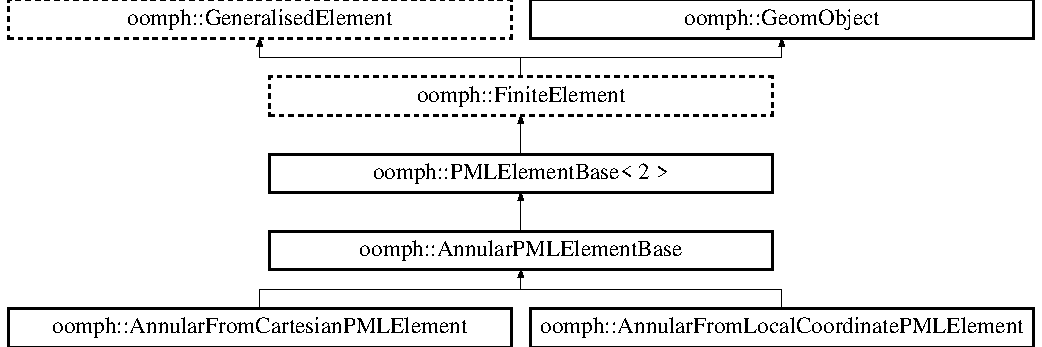
\includegraphics[height=4.666667cm]{classoomph_1_1AnnularPMLElementBase}
\end{center}
\end{figure}
\subsection*{Public Member Functions}
\begin{DoxyCompactItemize}
\item 
virtual void \hyperlink{classoomph_1_1AnnularPMLElementBase_a2f79efade3e4be24515b2960f447e10e}{pml\+\_\+transformation\+\_\+jacobian} (const unsigned \&ipt, const \hyperlink{classoomph_1_1Vector}{Vector}$<$ double $>$ \&\hyperlink{cfortran_8h_ab7123126e4885ef647dd9c6e3807a21c}{s}, const \hyperlink{classoomph_1_1Vector}{Vector}$<$ double $>$ \&x, \hyperlink{classoomph_1_1DenseComplexMatrix}{Dense\+Complex\+Matrix} \&jacobian)=0
\begin{DoxyCompactList}\small\item\em Implements an interface between the polar mapping and the Cartesian output which the get residuals expects. \end{DoxyCompactList}\item 
virtual void \hyperlink{classoomph_1_1AnnularPMLElementBase_a071a64f7677e50ee93c5c568ca59fff2}{pml\+\_\+transformation\+\_\+jacobian} (const unsigned \&ipt, const \hyperlink{classoomph_1_1Vector}{Vector}$<$ double $>$ \&\hyperlink{cfortran_8h_ab7123126e4885ef647dd9c6e3807a21c}{s}, const \hyperlink{classoomph_1_1Vector}{Vector}$<$ double $>$ \&x, \hyperlink{classoomph_1_1DenseComplexMatrix}{Dense\+Complex\+Matrix} \&jacobian\+\_\+matrix, \hyperlink{classoomph_1_1Vector}{Vector}$<$ std\+::complex$<$ double $>$ $>$ \&transformed\+\_\+x)=0
\begin{DoxyCompactList}\small\item\em Implements an interface between the polar mapping and the Cartesian output which the get residuals expects. \end{DoxyCompactList}\item 
void \hyperlink{classoomph_1_1AnnularPMLElementBase_a5e8b3cd8afddc6405af4d686afb578be}{radial\+\_\+to\+\_\+cartesian\+\_\+jacobian} (const double \&r, const double \&\hyperlink{classoomph_1_1AnnularPMLElementBase_a74036190f87f79129cdcda562664dd18}{theta}, const std\+::complex$<$ double $>$ \&transformed\+\_\+r, const std\+::complex$<$ double $>$ \&dtransformed\+\_\+r\+\_\+dr, \hyperlink{classoomph_1_1DenseComplexMatrix}{Dense\+Complex\+Matrix} \&cartesian\+\_\+jacobian) const
\item 
void \hyperlink{classoomph_1_1AnnularPMLElementBase_a584becc7b1b83823c334704117b3de12}{radial\+\_\+to\+\_\+cartesian\+\_\+jacobian} (const double \&r, const double \&\hyperlink{classoomph_1_1AnnularPMLElementBase_a74036190f87f79129cdcda562664dd18}{theta}, const std\+::complex$<$ double $>$ \&rt, const \hyperlink{classoomph_1_1DenseComplexMatrix}{Dense\+Complex\+Matrix} \&radial\+\_\+jacobian, \hyperlink{classoomph_1_1DenseComplexMatrix}{Dense\+Complex\+Matrix} \&cartesian\+\_\+jacobian) const
\item 
virtual void \hyperlink{classoomph_1_1AnnularPMLElementBase_a609c9b6bb60d9bc0de871e9731654805}{radial\+\_\+transformation\+\_\+jacobian} (const double \&\hyperlink{classoomph_1_1AnnularPMLElementBase_ac6671111f31c3a5012d0df53a1c24b76}{nu}, const double \&\hyperlink{classoomph_1_1AnnularPMLElementBase_ad76f02aa6eb19a5757e7d4cc26ec45fa}{delta}, std\+::complex$<$ double $>$ \&transformed\+\_\+r, std\+::complex$<$ double $>$ \&dtransformed\+\_\+r\+\_\+dr) const =0
\begin{DoxyCompactList}\small\item\em get the Jacobian of the mapping from transformed r to the radial through-\/the-\/pml coordinate. Also returns the transformed\+\_\+r at this point too as it is required for the transformation to cartesian coordinates \end{DoxyCompactList}\item 
virtual double \hyperlink{classoomph_1_1AnnularPMLElementBase_a5d3de2d99d848942e6fb533fd9cf58da}{radius} (const \hyperlink{classoomph_1_1Vector}{Vector}$<$ double $>$ \&\hyperlink{cfortran_8h_ab7123126e4885ef647dd9c6e3807a21c}{s}, const \hyperlink{classoomph_1_1Vector}{Vector}$<$ double $>$ \&x)=0
\item 
virtual double \hyperlink{classoomph_1_1AnnularPMLElementBase_ac6671111f31c3a5012d0df53a1c24b76}{nu} (const \hyperlink{classoomph_1_1Vector}{Vector}$<$ double $>$ \&\hyperlink{cfortran_8h_ab7123126e4885ef647dd9c6e3807a21c}{s}, const \hyperlink{classoomph_1_1Vector}{Vector}$<$ double $>$ \&x)=0
\item 
virtual double \hyperlink{classoomph_1_1AnnularPMLElementBase_a74036190f87f79129cdcda562664dd18}{theta} (const \hyperlink{classoomph_1_1Vector}{Vector}$<$ double $>$ \&\hyperlink{cfortran_8h_ab7123126e4885ef647dd9c6e3807a21c}{s}, const \hyperlink{classoomph_1_1Vector}{Vector}$<$ double $>$ \&x)=0
\item 
virtual double \hyperlink{classoomph_1_1AnnularPMLElementBase_ad76f02aa6eb19a5757e7d4cc26ec45fa}{delta} ()=0
\end{DoxyCompactItemize}
\subsection*{Additional Inherited Members}


\subsection{Detailed Description}


Definition at line 310 of file pml\+\_\+elements.\+h.



\subsection{Member Function Documentation}
\mbox{\Hypertarget{classoomph_1_1AnnularPMLElementBase_ad76f02aa6eb19a5757e7d4cc26ec45fa}\label{classoomph_1_1AnnularPMLElementBase_ad76f02aa6eb19a5757e7d4cc26ec45fa}} 
\index{oomph\+::\+Annular\+P\+M\+L\+Element\+Base@{oomph\+::\+Annular\+P\+M\+L\+Element\+Base}!delta@{delta}}
\index{delta@{delta}!oomph\+::\+Annular\+P\+M\+L\+Element\+Base@{oomph\+::\+Annular\+P\+M\+L\+Element\+Base}}
\subsubsection{\texorpdfstring{delta()}{delta()}}
{\footnotesize\ttfamily virtual double oomph\+::\+Annular\+P\+M\+L\+Element\+Base\+::delta (\begin{DoxyParamCaption}{ }\end{DoxyParamCaption})\hspace{0.3cm}{\ttfamily [pure virtual]}}



Implemented in \hyperlink{classoomph_1_1AnnularFromLocalCoordinatePMLElement_affe7de11a2275aac57b0ea2c0594ce7d}{oomph\+::\+Annular\+From\+Local\+Coordinate\+P\+M\+L\+Element}, and \hyperlink{classoomph_1_1AnnularFromCartesianPMLElement_a9cf84a8abb2f74bf71b6dbf4cc3958f1}{oomph\+::\+Annular\+From\+Cartesian\+P\+M\+L\+Element}.

\mbox{\Hypertarget{classoomph_1_1AnnularPMLElementBase_ac6671111f31c3a5012d0df53a1c24b76}\label{classoomph_1_1AnnularPMLElementBase_ac6671111f31c3a5012d0df53a1c24b76}} 
\index{oomph\+::\+Annular\+P\+M\+L\+Element\+Base@{oomph\+::\+Annular\+P\+M\+L\+Element\+Base}!nu@{nu}}
\index{nu@{nu}!oomph\+::\+Annular\+P\+M\+L\+Element\+Base@{oomph\+::\+Annular\+P\+M\+L\+Element\+Base}}
\subsubsection{\texorpdfstring{nu()}{nu()}}
{\footnotesize\ttfamily virtual double oomph\+::\+Annular\+P\+M\+L\+Element\+Base\+::nu (\begin{DoxyParamCaption}\item[{const \hyperlink{classoomph_1_1Vector}{Vector}$<$ double $>$ \&}]{s,  }\item[{const \hyperlink{classoomph_1_1Vector}{Vector}$<$ double $>$ \&}]{x }\end{DoxyParamCaption})\hspace{0.3cm}{\ttfamily [pure virtual]}}



Implemented in \hyperlink{classoomph_1_1AnnularFromLocalCoordinatePMLElement_a161e427b6f1fc6349b9667caf346cf8a}{oomph\+::\+Annular\+From\+Local\+Coordinate\+P\+M\+L\+Element}, and \hyperlink{classoomph_1_1AnnularFromCartesianPMLElement_acac12e9f2f6df3e9edebb7747ce4fab8}{oomph\+::\+Annular\+From\+Cartesian\+P\+M\+L\+Element}.

\mbox{\Hypertarget{classoomph_1_1AnnularPMLElementBase_a2f79efade3e4be24515b2960f447e10e}\label{classoomph_1_1AnnularPMLElementBase_a2f79efade3e4be24515b2960f447e10e}} 
\index{oomph\+::\+Annular\+P\+M\+L\+Element\+Base@{oomph\+::\+Annular\+P\+M\+L\+Element\+Base}!pml\+\_\+transformation\+\_\+jacobian@{pml\+\_\+transformation\+\_\+jacobian}}
\index{pml\+\_\+transformation\+\_\+jacobian@{pml\+\_\+transformation\+\_\+jacobian}!oomph\+::\+Annular\+P\+M\+L\+Element\+Base@{oomph\+::\+Annular\+P\+M\+L\+Element\+Base}}
\subsubsection{\texorpdfstring{pml\+\_\+transformation\+\_\+jacobian()}{pml\_transformation\_jacobian()}\hspace{0.1cm}{\footnotesize\ttfamily [1/2]}}
{\footnotesize\ttfamily void oomph\+::\+Annular\+P\+M\+L\+Element\+Base\+::pml\+\_\+transformation\+\_\+jacobian (\begin{DoxyParamCaption}\item[{const unsigned \&}]{ipt,  }\item[{const \hyperlink{classoomph_1_1Vector}{Vector}$<$ double $>$ \&}]{s,  }\item[{const \hyperlink{classoomph_1_1Vector}{Vector}$<$ double $>$ \&}]{x,  }\item[{\hyperlink{classoomph_1_1DenseComplexMatrix}{Dense\+Complex\+Matrix} \&}]{jacobian }\end{DoxyParamCaption})\hspace{0.3cm}{\ttfamily [pure virtual]}}



Implements an interface between the polar mapping and the Cartesian output which the get residuals expects. 



Implements \hyperlink{classoomph_1_1PMLElementBase_a770d8de20d8ae2d55f5f006052a39b3f}{oomph\+::\+P\+M\+L\+Element\+Base$<$ 2 $>$}.



Definition at line 421 of file pml\+\_\+elements.\+cc.

\mbox{\Hypertarget{classoomph_1_1AnnularPMLElementBase_a071a64f7677e50ee93c5c568ca59fff2}\label{classoomph_1_1AnnularPMLElementBase_a071a64f7677e50ee93c5c568ca59fff2}} 
\index{oomph\+::\+Annular\+P\+M\+L\+Element\+Base@{oomph\+::\+Annular\+P\+M\+L\+Element\+Base}!pml\+\_\+transformation\+\_\+jacobian@{pml\+\_\+transformation\+\_\+jacobian}}
\index{pml\+\_\+transformation\+\_\+jacobian@{pml\+\_\+transformation\+\_\+jacobian}!oomph\+::\+Annular\+P\+M\+L\+Element\+Base@{oomph\+::\+Annular\+P\+M\+L\+Element\+Base}}
\subsubsection{\texorpdfstring{pml\+\_\+transformation\+\_\+jacobian()}{pml\_transformation\_jacobian()}\hspace{0.1cm}{\footnotesize\ttfamily [2/2]}}
{\footnotesize\ttfamily void oomph\+::\+Annular\+P\+M\+L\+Element\+Base\+::pml\+\_\+transformation\+\_\+jacobian (\begin{DoxyParamCaption}\item[{const unsigned \&}]{ipt,  }\item[{const \hyperlink{classoomph_1_1Vector}{Vector}$<$ double $>$ \&}]{s,  }\item[{const \hyperlink{classoomph_1_1Vector}{Vector}$<$ double $>$ \&}]{x,  }\item[{\hyperlink{classoomph_1_1DenseComplexMatrix}{Dense\+Complex\+Matrix} \&}]{jacobian\+\_\+matrix,  }\item[{\hyperlink{classoomph_1_1Vector}{Vector}$<$ std\+::complex$<$ double $>$ $>$ \&}]{transformed\+\_\+x }\end{DoxyParamCaption})\hspace{0.3cm}{\ttfamily [pure virtual]}}



Implements an interface between the polar mapping and the Cartesian output which the get residuals expects. 



Implements \hyperlink{classoomph_1_1PMLElementBase_a4b9d6d74aa15e6395590b27686477b20}{oomph\+::\+P\+M\+L\+Element\+Base$<$ 2 $>$}.



Definition at line 444 of file pml\+\_\+elements.\+cc.

\mbox{\Hypertarget{classoomph_1_1AnnularPMLElementBase_a5e8b3cd8afddc6405af4d686afb578be}\label{classoomph_1_1AnnularPMLElementBase_a5e8b3cd8afddc6405af4d686afb578be}} 
\index{oomph\+::\+Annular\+P\+M\+L\+Element\+Base@{oomph\+::\+Annular\+P\+M\+L\+Element\+Base}!radial\+\_\+to\+\_\+cartesian\+\_\+jacobian@{radial\+\_\+to\+\_\+cartesian\+\_\+jacobian}}
\index{radial\+\_\+to\+\_\+cartesian\+\_\+jacobian@{radial\+\_\+to\+\_\+cartesian\+\_\+jacobian}!oomph\+::\+Annular\+P\+M\+L\+Element\+Base@{oomph\+::\+Annular\+P\+M\+L\+Element\+Base}}
\subsubsection{\texorpdfstring{radial\+\_\+to\+\_\+cartesian\+\_\+jacobian()}{radial\_to\_cartesian\_jacobian()}\hspace{0.1cm}{\footnotesize\ttfamily [1/2]}}
{\footnotesize\ttfamily void oomph\+::\+Annular\+P\+M\+L\+Element\+Base\+::radial\+\_\+to\+\_\+cartesian\+\_\+jacobian (\begin{DoxyParamCaption}\item[{const double \&}]{r,  }\item[{const double \&}]{theta,  }\item[{const std\+::complex$<$ double $>$ \&}]{transformed\+\_\+r,  }\item[{const std\+::complex$<$ double $>$ \&}]{dtransformed\+\_\+r\+\_\+dr,  }\item[{\hyperlink{classoomph_1_1DenseComplexMatrix}{Dense\+Complex\+Matrix} \&}]{cartesian\+\_\+jacobian }\end{DoxyParamCaption}) const}



Definition at line 370 of file pml\+\_\+elements.\+cc.

\mbox{\Hypertarget{classoomph_1_1AnnularPMLElementBase_a584becc7b1b83823c334704117b3de12}\label{classoomph_1_1AnnularPMLElementBase_a584becc7b1b83823c334704117b3de12}} 
\index{oomph\+::\+Annular\+P\+M\+L\+Element\+Base@{oomph\+::\+Annular\+P\+M\+L\+Element\+Base}!radial\+\_\+to\+\_\+cartesian\+\_\+jacobian@{radial\+\_\+to\+\_\+cartesian\+\_\+jacobian}}
\index{radial\+\_\+to\+\_\+cartesian\+\_\+jacobian@{radial\+\_\+to\+\_\+cartesian\+\_\+jacobian}!oomph\+::\+Annular\+P\+M\+L\+Element\+Base@{oomph\+::\+Annular\+P\+M\+L\+Element\+Base}}
\subsubsection{\texorpdfstring{radial\+\_\+to\+\_\+cartesian\+\_\+jacobian()}{radial\_to\_cartesian\_jacobian()}\hspace{0.1cm}{\footnotesize\ttfamily [2/2]}}
{\footnotesize\ttfamily void oomph\+::\+Annular\+P\+M\+L\+Element\+Base\+::radial\+\_\+to\+\_\+cartesian\+\_\+jacobian (\begin{DoxyParamCaption}\item[{const double \&}]{r,  }\item[{const double \&}]{theta,  }\item[{const std\+::complex$<$ double $>$ \&}]{rt,  }\item[{const \hyperlink{classoomph_1_1DenseComplexMatrix}{Dense\+Complex\+Matrix} \&}]{radial\+\_\+jacobian,  }\item[{\hyperlink{classoomph_1_1DenseComplexMatrix}{Dense\+Complex\+Matrix} \&}]{cartesian\+\_\+jacobian }\end{DoxyParamCaption}) const}



Definition at line 386 of file pml\+\_\+elements.\+cc.



References oomph\+::\+Dense\+Complex\+Matrix\+::multiply().

\mbox{\Hypertarget{classoomph_1_1AnnularPMLElementBase_a609c9b6bb60d9bc0de871e9731654805}\label{classoomph_1_1AnnularPMLElementBase_a609c9b6bb60d9bc0de871e9731654805}} 
\index{oomph\+::\+Annular\+P\+M\+L\+Element\+Base@{oomph\+::\+Annular\+P\+M\+L\+Element\+Base}!radial\+\_\+transformation\+\_\+jacobian@{radial\+\_\+transformation\+\_\+jacobian}}
\index{radial\+\_\+transformation\+\_\+jacobian@{radial\+\_\+transformation\+\_\+jacobian}!oomph\+::\+Annular\+P\+M\+L\+Element\+Base@{oomph\+::\+Annular\+P\+M\+L\+Element\+Base}}
\subsubsection{\texorpdfstring{radial\+\_\+transformation\+\_\+jacobian()}{radial\_transformation\_jacobian()}}
{\footnotesize\ttfamily virtual void oomph\+::\+Annular\+P\+M\+L\+Element\+Base\+::radial\+\_\+transformation\+\_\+jacobian (\begin{DoxyParamCaption}\item[{const double \&}]{nu,  }\item[{const double \&}]{delta,  }\item[{std\+::complex$<$ double $>$ \&}]{transformed\+\_\+r,  }\item[{std\+::complex$<$ double $>$ \&}]{dtransformed\+\_\+r\+\_\+dr }\end{DoxyParamCaption}) const\hspace{0.3cm}{\ttfamily [pure virtual]}}



get the Jacobian of the mapping from transformed r to the radial through-\/the-\/pml coordinate. Also returns the transformed\+\_\+r at this point too as it is required for the transformation to cartesian coordinates 

\mbox{\Hypertarget{classoomph_1_1AnnularPMLElementBase_a5d3de2d99d848942e6fb533fd9cf58da}\label{classoomph_1_1AnnularPMLElementBase_a5d3de2d99d848942e6fb533fd9cf58da}} 
\index{oomph\+::\+Annular\+P\+M\+L\+Element\+Base@{oomph\+::\+Annular\+P\+M\+L\+Element\+Base}!radius@{radius}}
\index{radius@{radius}!oomph\+::\+Annular\+P\+M\+L\+Element\+Base@{oomph\+::\+Annular\+P\+M\+L\+Element\+Base}}
\subsubsection{\texorpdfstring{radius()}{radius()}}
{\footnotesize\ttfamily virtual double oomph\+::\+Annular\+P\+M\+L\+Element\+Base\+::radius (\begin{DoxyParamCaption}\item[{const \hyperlink{classoomph_1_1Vector}{Vector}$<$ double $>$ \&}]{s,  }\item[{const \hyperlink{classoomph_1_1Vector}{Vector}$<$ double $>$ \&}]{x }\end{DoxyParamCaption})\hspace{0.3cm}{\ttfamily [pure virtual]}}



Implemented in \hyperlink{classoomph_1_1AnnularFromCartesianPMLElement_acb66a5412d96aef573a498ffc8f7a72d}{oomph\+::\+Annular\+From\+Cartesian\+P\+M\+L\+Element}.

\mbox{\Hypertarget{classoomph_1_1AnnularPMLElementBase_a74036190f87f79129cdcda562664dd18}\label{classoomph_1_1AnnularPMLElementBase_a74036190f87f79129cdcda562664dd18}} 
\index{oomph\+::\+Annular\+P\+M\+L\+Element\+Base@{oomph\+::\+Annular\+P\+M\+L\+Element\+Base}!theta@{theta}}
\index{theta@{theta}!oomph\+::\+Annular\+P\+M\+L\+Element\+Base@{oomph\+::\+Annular\+P\+M\+L\+Element\+Base}}
\subsubsection{\texorpdfstring{theta()}{theta()}}
{\footnotesize\ttfamily virtual double oomph\+::\+Annular\+P\+M\+L\+Element\+Base\+::theta (\begin{DoxyParamCaption}\item[{const \hyperlink{classoomph_1_1Vector}{Vector}$<$ double $>$ \&}]{s,  }\item[{const \hyperlink{classoomph_1_1Vector}{Vector}$<$ double $>$ \&}]{x }\end{DoxyParamCaption})\hspace{0.3cm}{\ttfamily [pure virtual]}}



Implemented in \hyperlink{classoomph_1_1AnnularFromLocalCoordinatePMLElement_ae9f56654db4d7979163db0529d9a1408}{oomph\+::\+Annular\+From\+Local\+Coordinate\+P\+M\+L\+Element}.



The documentation for this class was generated from the following files\+:\begin{DoxyCompactItemize}
\item 
\hyperlink{pml__elements_8h}{pml\+\_\+elements.\+h}\item 
\hyperlink{pml__elements_8cc}{pml\+\_\+elements.\+cc}\end{DoxyCompactItemize}

\hypertarget{structoomph_1_1CommandLineArgs_1_1ArgInfo}{}\section{oomph\+:\+:Command\+Line\+Args\+:\+:Arg\+Info$<$ T $>$ Struct Template Reference}
\label{structoomph_1_1CommandLineArgs_1_1ArgInfo}\index{oomph\+::\+Command\+Line\+Args\+::\+Arg\+Info$<$ T $>$@{oomph\+::\+Command\+Line\+Args\+::\+Arg\+Info$<$ T $>$}}


Structure to store information on a command line argument.  




{\ttfamily \#include $<$oomph\+\_\+utilities.\+h$>$}

\subsection*{Public Member Functions}
\begin{DoxyCompactItemize}
\item 
\hyperlink{structoomph_1_1CommandLineArgs_1_1ArgInfo_ad20c82222bfd72e5139590b2832136cc}{Arg\+Info} (const bool \&\hyperlink{structoomph_1_1CommandLineArgs_1_1ArgInfo_af45e9ad65b7fa4e29eed6a1e13b5d1e9}{is\+\_\+set}, T $\ast$\hyperlink{structoomph_1_1CommandLineArgs_1_1ArgInfo_a28a76e6c1d710bffb4cc9bc0e93332fd}{arg\+\_\+pt}, const std\+::string \&\hyperlink{structoomph_1_1CommandLineArgs_1_1ArgInfo_ab6bd266840a459d7171a3f532630564d}{doc})
\begin{DoxyCompactList}\small\item\em Proper constructor. \end{DoxyCompactList}\item 
\hyperlink{structoomph_1_1CommandLineArgs_1_1ArgInfo_a1dc69aa3f31ccc1b163156df58757dd8}{Arg\+Info} ()
\end{DoxyCompactItemize}
\subsection*{Public Attributes}
\begin{DoxyCompactItemize}
\item 
bool \hyperlink{structoomph_1_1CommandLineArgs_1_1ArgInfo_af45e9ad65b7fa4e29eed6a1e13b5d1e9}{is\+\_\+set}
\begin{DoxyCompactList}\small\item\em Has this argument been set? \end{DoxyCompactList}\item 
T $\ast$ \hyperlink{structoomph_1_1CommandLineArgs_1_1ArgInfo_a28a76e6c1d710bffb4cc9bc0e93332fd}{arg\+\_\+pt}
\begin{DoxyCompactList}\small\item\em The place to put the argument\textquotesingle{}s value when it is set. \end{DoxyCompactList}\item 
std\+::string \hyperlink{structoomph_1_1CommandLineArgs_1_1ArgInfo_ab6bd266840a459d7171a3f532630564d}{doc}
\begin{DoxyCompactList}\small\item\em Information about what the argument does. \end{DoxyCompactList}\end{DoxyCompactItemize}


\subsection{Detailed Description}
\subsubsection*{template$<$class T$>$\newline
struct oomph\+::\+Command\+Line\+Args\+::\+Arg\+Info$<$ T $>$}

Structure to store information on a command line argument. 

Definition at line 605 of file oomph\+\_\+utilities.\+h.



\subsection{Constructor \& Destructor Documentation}
\mbox{\Hypertarget{structoomph_1_1CommandLineArgs_1_1ArgInfo_ad20c82222bfd72e5139590b2832136cc}\label{structoomph_1_1CommandLineArgs_1_1ArgInfo_ad20c82222bfd72e5139590b2832136cc}} 
\index{oomph\+::\+Command\+Line\+Args\+::\+Arg\+Info@{oomph\+::\+Command\+Line\+Args\+::\+Arg\+Info}!Arg\+Info@{Arg\+Info}}
\index{Arg\+Info@{Arg\+Info}!oomph\+::\+Command\+Line\+Args\+::\+Arg\+Info@{oomph\+::\+Command\+Line\+Args\+::\+Arg\+Info}}
\subsubsection{\texorpdfstring{Arg\+Info()}{ArgInfo()}\hspace{0.1cm}{\footnotesize\ttfamily [1/2]}}
{\footnotesize\ttfamily template$<$class T$>$ \\
\hyperlink{structoomph_1_1CommandLineArgs_1_1ArgInfo}{oomph\+::\+Command\+Line\+Args\+::\+Arg\+Info}$<$ T $>$\+::\hyperlink{structoomph_1_1CommandLineArgs_1_1ArgInfo}{Arg\+Info} (\begin{DoxyParamCaption}\item[{const bool \&}]{is\+\_\+set,  }\item[{T $\ast$}]{arg\+\_\+pt,  }\item[{const std\+::string \&}]{doc }\end{DoxyParamCaption})\hspace{0.3cm}{\ttfamily [inline]}}



Proper constructor. 



Definition at line 609 of file oomph\+\_\+utilities.\+h.



References oomph\+::\+Leak\+Check\+Names\+::doc().

\mbox{\Hypertarget{structoomph_1_1CommandLineArgs_1_1ArgInfo_a1dc69aa3f31ccc1b163156df58757dd8}\label{structoomph_1_1CommandLineArgs_1_1ArgInfo_a1dc69aa3f31ccc1b163156df58757dd8}} 
\index{oomph\+::\+Command\+Line\+Args\+::\+Arg\+Info@{oomph\+::\+Command\+Line\+Args\+::\+Arg\+Info}!Arg\+Info@{Arg\+Info}}
\index{Arg\+Info@{Arg\+Info}!oomph\+::\+Command\+Line\+Args\+::\+Arg\+Info@{oomph\+::\+Command\+Line\+Args\+::\+Arg\+Info}}
\subsubsection{\texorpdfstring{Arg\+Info()}{ArgInfo()}\hspace{0.1cm}{\footnotesize\ttfamily [2/2]}}
{\footnotesize\ttfamily template$<$class T$>$ \\
\hyperlink{structoomph_1_1CommandLineArgs_1_1ArgInfo}{oomph\+::\+Command\+Line\+Args\+::\+Arg\+Info}$<$ T $>$\+::\hyperlink{structoomph_1_1CommandLineArgs_1_1ArgInfo}{Arg\+Info} (\begin{DoxyParamCaption}{ }\end{DoxyParamCaption})\hspace{0.3cm}{\ttfamily [inline]}}

Default constructor. We need this to be able to store these things in maps. 

Definition at line 620 of file oomph\+\_\+utilities.\+h.



References oomph\+::\+Leak\+Check\+Names\+::doc().



\subsection{Member Data Documentation}
\mbox{\Hypertarget{structoomph_1_1CommandLineArgs_1_1ArgInfo_a28a76e6c1d710bffb4cc9bc0e93332fd}\label{structoomph_1_1CommandLineArgs_1_1ArgInfo_a28a76e6c1d710bffb4cc9bc0e93332fd}} 
\index{oomph\+::\+Command\+Line\+Args\+::\+Arg\+Info@{oomph\+::\+Command\+Line\+Args\+::\+Arg\+Info}!arg\+\_\+pt@{arg\+\_\+pt}}
\index{arg\+\_\+pt@{arg\+\_\+pt}!oomph\+::\+Command\+Line\+Args\+::\+Arg\+Info@{oomph\+::\+Command\+Line\+Args\+::\+Arg\+Info}}
\subsubsection{\texorpdfstring{arg\+\_\+pt}{arg\_pt}}
{\footnotesize\ttfamily template$<$class T$>$ \\
T$\ast$ \hyperlink{structoomph_1_1CommandLineArgs_1_1ArgInfo}{oomph\+::\+Command\+Line\+Args\+::\+Arg\+Info}$<$ T $>$\+::arg\+\_\+pt}



The place to put the argument\textquotesingle{}s value when it is set. 



Definition at line 640 of file oomph\+\_\+utilities.\+h.

\mbox{\Hypertarget{structoomph_1_1CommandLineArgs_1_1ArgInfo_ab6bd266840a459d7171a3f532630564d}\label{structoomph_1_1CommandLineArgs_1_1ArgInfo_ab6bd266840a459d7171a3f532630564d}} 
\index{oomph\+::\+Command\+Line\+Args\+::\+Arg\+Info@{oomph\+::\+Command\+Line\+Args\+::\+Arg\+Info}!doc@{doc}}
\index{doc@{doc}!oomph\+::\+Command\+Line\+Args\+::\+Arg\+Info@{oomph\+::\+Command\+Line\+Args\+::\+Arg\+Info}}
\subsubsection{\texorpdfstring{doc}{doc}}
{\footnotesize\ttfamily template$<$class T$>$ \\
std\+::string \hyperlink{structoomph_1_1CommandLineArgs_1_1ArgInfo}{oomph\+::\+Command\+Line\+Args\+::\+Arg\+Info}$<$ T $>$\+::doc}



Information about what the argument does. 



Definition at line 643 of file oomph\+\_\+utilities.\+h.

\mbox{\Hypertarget{structoomph_1_1CommandLineArgs_1_1ArgInfo_af45e9ad65b7fa4e29eed6a1e13b5d1e9}\label{structoomph_1_1CommandLineArgs_1_1ArgInfo_af45e9ad65b7fa4e29eed6a1e13b5d1e9}} 
\index{oomph\+::\+Command\+Line\+Args\+::\+Arg\+Info@{oomph\+::\+Command\+Line\+Args\+::\+Arg\+Info}!is\+\_\+set@{is\+\_\+set}}
\index{is\+\_\+set@{is\+\_\+set}!oomph\+::\+Command\+Line\+Args\+::\+Arg\+Info@{oomph\+::\+Command\+Line\+Args\+::\+Arg\+Info}}
\subsubsection{\texorpdfstring{is\+\_\+set}{is\_set}}
{\footnotesize\ttfamily template$<$class T$>$ \\
bool \hyperlink{structoomph_1_1CommandLineArgs_1_1ArgInfo}{oomph\+::\+Command\+Line\+Args\+::\+Arg\+Info}$<$ T $>$\+::is\+\_\+set}



Has this argument been set? 



Definition at line 637 of file oomph\+\_\+utilities.\+h.



The documentation for this struct was generated from the following file\+:\begin{DoxyCompactItemize}
\item 
\hyperlink{oomph__utilities_8h}{oomph\+\_\+utilities.\+h}\end{DoxyCompactItemize}

\hypertarget{classoomph_1_1ARPACK}{}\section{oomph\+:\+:A\+R\+P\+A\+CK Class Reference}
\label{classoomph_1_1ARPACK}\index{oomph\+::\+A\+R\+P\+A\+CK@{oomph\+::\+A\+R\+P\+A\+CK}}


Class for the \hyperlink{classoomph_1_1ARPACK}{A\+R\+P\+A\+CK} eigensolver.  




{\ttfamily \#include $<$eigen\+\_\+solver.\+h$>$}

Inheritance diagram for oomph\+:\+:A\+R\+P\+A\+CK\+:\begin{figure}[H]
\begin{center}
\leavevmode
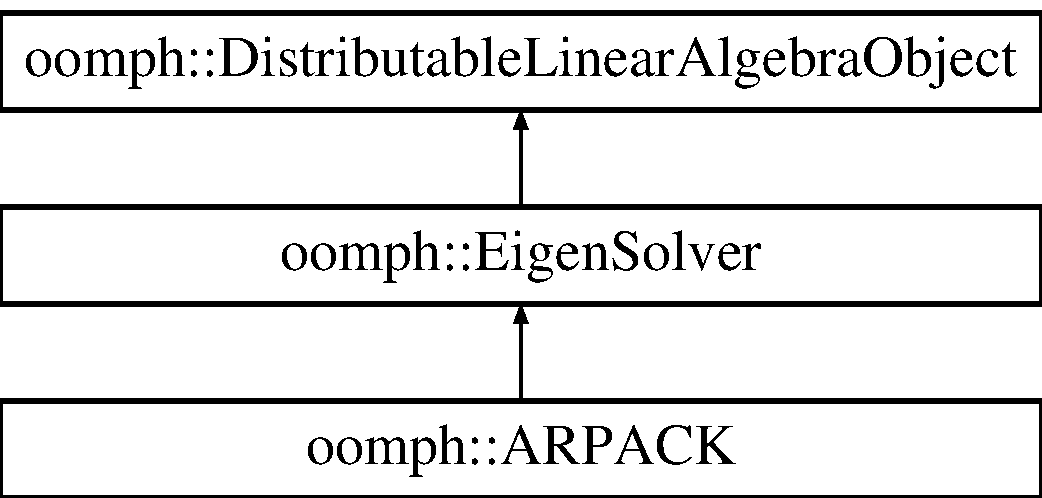
\includegraphics[height=3.000000cm]{classoomph_1_1ARPACK}
\end{center}
\end{figure}
\subsection*{Public Member Functions}
\begin{DoxyCompactItemize}
\item 
\hyperlink{classoomph_1_1ARPACK_aef258a621d2ba000382d8e0cc9118e8d}{A\+R\+P\+A\+CK} ()
\begin{DoxyCompactList}\small\item\em Constructor. \end{DoxyCompactList}\item 
\hyperlink{classoomph_1_1ARPACK_a0461252a3602e71c52400b5994cb9efa}{A\+R\+P\+A\+CK} (const \hyperlink{classoomph_1_1ARPACK}{A\+R\+P\+A\+CK} \&)
\begin{DoxyCompactList}\small\item\em Empty copy constructor. \end{DoxyCompactList}\item 
virtual \hyperlink{classoomph_1_1ARPACK_a67b999708483787f4211a15feb71ed11}{$\sim$\+A\+R\+P\+A\+CK} ()
\begin{DoxyCompactList}\small\item\em Destructor, delete the linear solver. \end{DoxyCompactList}\item 
int \& \hyperlink{classoomph_1_1ARPACK_a4e398ee962b8843668a76904b3302bb0}{narnoldi} ()
\begin{DoxyCompactList}\small\item\em Access function for the number of Arnoldi vectors. \end{DoxyCompactList}\item 
const int \& \hyperlink{classoomph_1_1ARPACK_a4b7b996589dfe4f61868be9ce381a41e}{narnoldi} () const
\begin{DoxyCompactList}\small\item\em Access function for the number of Arnoldi vectors (const version) \end{DoxyCompactList}\item 
void \hyperlink{classoomph_1_1ARPACK_a9945e2656f93850112f8836a585b32b0}{enable\+\_\+compute\+\_\+eigenvectors} ()
\begin{DoxyCompactList}\small\item\em Set to enable the computation of the eigenvectors (default) \end{DoxyCompactList}\item 
void \hyperlink{classoomph_1_1ARPACK_adfd771b9ef52ec5b0ee78918027679c0}{disable\+\_\+compute\+\_\+eigenvectors} ()
\begin{DoxyCompactList}\small\item\em Set to disable the computation of the eigenvectors. \end{DoxyCompactList}\item 
void \hyperlink{classoomph_1_1ARPACK_ac644213623ea3d91a42cf1ea4608cdf3}{solve\+\_\+eigenproblem} (\hyperlink{classoomph_1_1Problem}{Problem} $\ast$const \&problem\+\_\+pt, const int \&n\+\_\+eval, \hyperlink{classoomph_1_1Vector}{Vector}$<$ std\+::complex$<$ double $>$ $>$ \&eigenvalue, \hyperlink{classoomph_1_1Vector}{Vector}$<$ \hyperlink{classoomph_1_1DoubleVector}{Double\+Vector} $>$ \&eigenvector)
\begin{DoxyCompactList}\small\item\em Solve the eigen problem. \end{DoxyCompactList}\item 
void \hyperlink{classoomph_1_1ARPACK_a513c4cadda58eb9a0f1319f8b3159852}{get\+\_\+eigenvalues\+\_\+left\+\_\+of\+\_\+shift} ()
\begin{DoxyCompactList}\small\item\em Use the eigensolver to find the eigenvalues of a given matrix. \end{DoxyCompactList}\item 
void \hyperlink{classoomph_1_1ARPACK_a177485cda9de5e207917adfdd6c6cdbb}{get\+\_\+eigenvalues\+\_\+right\+\_\+of\+\_\+shift} ()
\begin{DoxyCompactList}\small\item\em Set the desired eigenvalues to be right of the shift. \end{DoxyCompactList}\item 
void \hyperlink{classoomph_1_1ARPACK_aa936a369ba1e4fd65e971ba5945ae2d8}{track\+\_\+eigenvalue\+\_\+real\+\_\+part} ()
\begin{DoxyCompactList}\small\item\em Set the real part to be the quantity of interest (default) \end{DoxyCompactList}\item 
void \hyperlink{classoomph_1_1ARPACK_a41e0454599dbf2db541fc66280ea60e3}{track\+\_\+eigenvalue\+\_\+imaginary\+\_\+part} ()
\begin{DoxyCompactList}\small\item\em Set the imaginary part fo the quantity of interest. \end{DoxyCompactList}\item 
void \hyperlink{classoomph_1_1ARPACK_a94e5065868bc3c3187f15e9220314383}{track\+\_\+eigenvalue\+\_\+magnitude} ()
\begin{DoxyCompactList}\small\item\em Set the magnitude to be the quantity of interest. \end{DoxyCompactList}\item 
\hyperlink{classoomph_1_1LinearSolver}{Linear\+Solver} $\ast$\& \hyperlink{classoomph_1_1ARPACK_a2118c6975be7d72dada95331201d518a}{linear\+\_\+solver\+\_\+pt} ()
\begin{DoxyCompactList}\small\item\em Return a pointer to the linear solver object. \end{DoxyCompactList}\item 
\hyperlink{classoomph_1_1LinearSolver}{Linear\+Solver} $\ast$const  \& \hyperlink{classoomph_1_1ARPACK_a48d9a6ff92914c0126dbfa85815b7d1f}{linear\+\_\+solver\+\_\+pt} () const
\begin{DoxyCompactList}\small\item\em Return a pointer to the linear solver object (const version) \end{DoxyCompactList}\end{DoxyCompactItemize}
\subsection*{Private Attributes}
\begin{DoxyCompactItemize}
\item 
\hyperlink{classoomph_1_1LinearSolver}{Linear\+Solver} $\ast$ \hyperlink{classoomph_1_1ARPACK_a647a45676349ba86abd5d2ff9aff022d}{Linear\+\_\+solver\+\_\+pt}
\begin{DoxyCompactList}\small\item\em Pointer to a linear solver. \end{DoxyCompactList}\item 
\hyperlink{classoomph_1_1LinearSolver}{Linear\+Solver} $\ast$ \hyperlink{classoomph_1_1ARPACK_ad6d487dfc1f84d8008e52fc87d83c644}{Default\+\_\+linear\+\_\+solver\+\_\+pt}
\begin{DoxyCompactList}\small\item\em Pointer to a default linear solver. \end{DoxyCompactList}\item 
int \hyperlink{classoomph_1_1ARPACK_a212ff2ad05b73b8f1e4f0d8d10733015}{Spectrum}
\begin{DoxyCompactList}\small\item\em Integer to set whether the real, imaginary or magnitude is required to be small or large. \end{DoxyCompactList}\item 
int \hyperlink{classoomph_1_1ARPACK_a2f430dc8c1a8d890a90a95bdd66e97cc}{N\+Arnoldi}
\begin{DoxyCompactList}\small\item\em Number of Arnoldi vectors to compute. \end{DoxyCompactList}\item 
bool \hyperlink{classoomph_1_1ARPACK_aa92552280868d74242f71c6f98db79e8}{Small}
\begin{DoxyCompactList}\small\item\em Boolean to set which part of the spectrum left (default) or right of the shifted value. \end{DoxyCompactList}\item 
bool \hyperlink{classoomph_1_1ARPACK_af8a6dba4dca423fd67488e34970886df}{Compute\+\_\+eigenvectors}
\begin{DoxyCompactList}\small\item\em Boolean to indicate whether or not to compute the eigenvectors. \end{DoxyCompactList}\end{DoxyCompactItemize}
\subsection*{Additional Inherited Members}


\subsection{Detailed Description}
Class for the \hyperlink{classoomph_1_1ARPACK}{A\+R\+P\+A\+CK} eigensolver. 

Definition at line 103 of file eigen\+\_\+solver.\+h.



\subsection{Constructor \& Destructor Documentation}
\mbox{\Hypertarget{classoomph_1_1ARPACK_aef258a621d2ba000382d8e0cc9118e8d}\label{classoomph_1_1ARPACK_aef258a621d2ba000382d8e0cc9118e8d}} 
\index{oomph\+::\+A\+R\+P\+A\+CK@{oomph\+::\+A\+R\+P\+A\+CK}!A\+R\+P\+A\+CK@{A\+R\+P\+A\+CK}}
\index{A\+R\+P\+A\+CK@{A\+R\+P\+A\+CK}!oomph\+::\+A\+R\+P\+A\+CK@{oomph\+::\+A\+R\+P\+A\+CK}}
\subsubsection{\texorpdfstring{A\+R\+P\+A\+C\+K()}{ARPACK()}\hspace{0.1cm}{\footnotesize\ttfamily [1/2]}}
{\footnotesize\ttfamily oomph\+::\+A\+R\+P\+A\+C\+K\+::\+A\+R\+P\+A\+CK (\begin{DoxyParamCaption}{ }\end{DoxyParamCaption})}



Constructor. 

Constructor, set default values and set the initial linear solver to be superlu 

Definition at line 53 of file eigen\+\_\+solver.\+cc.



References Default\+\_\+linear\+\_\+solver\+\_\+pt, and Linear\+\_\+solver\+\_\+pt.

\mbox{\Hypertarget{classoomph_1_1ARPACK_a0461252a3602e71c52400b5994cb9efa}\label{classoomph_1_1ARPACK_a0461252a3602e71c52400b5994cb9efa}} 
\index{oomph\+::\+A\+R\+P\+A\+CK@{oomph\+::\+A\+R\+P\+A\+CK}!A\+R\+P\+A\+CK@{A\+R\+P\+A\+CK}}
\index{A\+R\+P\+A\+CK@{A\+R\+P\+A\+CK}!oomph\+::\+A\+R\+P\+A\+CK@{oomph\+::\+A\+R\+P\+A\+CK}}
\subsubsection{\texorpdfstring{A\+R\+P\+A\+C\+K()}{ARPACK()}\hspace{0.1cm}{\footnotesize\ttfamily [2/2]}}
{\footnotesize\ttfamily oomph\+::\+A\+R\+P\+A\+C\+K\+::\+A\+R\+P\+A\+CK (\begin{DoxyParamCaption}\item[{const \hyperlink{classoomph_1_1ARPACK}{A\+R\+P\+A\+CK} \&}]{ }\end{DoxyParamCaption})\hspace{0.3cm}{\ttfamily [inline]}}



Empty copy constructor. 



Definition at line 136 of file eigen\+\_\+solver.\+h.

\mbox{\Hypertarget{classoomph_1_1ARPACK_a67b999708483787f4211a15feb71ed11}\label{classoomph_1_1ARPACK_a67b999708483787f4211a15feb71ed11}} 
\index{oomph\+::\+A\+R\+P\+A\+CK@{oomph\+::\+A\+R\+P\+A\+CK}!````~A\+R\+P\+A\+CK@{$\sim$\+A\+R\+P\+A\+CK}}
\index{````~A\+R\+P\+A\+CK@{$\sim$\+A\+R\+P\+A\+CK}!oomph\+::\+A\+R\+P\+A\+CK@{oomph\+::\+A\+R\+P\+A\+CK}}
\subsubsection{\texorpdfstring{$\sim$\+A\+R\+P\+A\+C\+K()}{~ARPACK()}}
{\footnotesize\ttfamily oomph\+::\+A\+R\+P\+A\+C\+K\+::$\sim$\+A\+R\+P\+A\+CK (\begin{DoxyParamCaption}{ }\end{DoxyParamCaption})\hspace{0.3cm}{\ttfamily [virtual]}}



Destructor, delete the linear solver. 

Destructor, delete the default linear solver. 

Definition at line 60 of file eigen\+\_\+solver.\+cc.



References Default\+\_\+linear\+\_\+solver\+\_\+pt.



\subsection{Member Function Documentation}
\mbox{\Hypertarget{classoomph_1_1ARPACK_adfd771b9ef52ec5b0ee78918027679c0}\label{classoomph_1_1ARPACK_adfd771b9ef52ec5b0ee78918027679c0}} 
\index{oomph\+::\+A\+R\+P\+A\+CK@{oomph\+::\+A\+R\+P\+A\+CK}!disable\+\_\+compute\+\_\+eigenvectors@{disable\+\_\+compute\+\_\+eigenvectors}}
\index{disable\+\_\+compute\+\_\+eigenvectors@{disable\+\_\+compute\+\_\+eigenvectors}!oomph\+::\+A\+R\+P\+A\+CK@{oomph\+::\+A\+R\+P\+A\+CK}}
\subsubsection{\texorpdfstring{disable\+\_\+compute\+\_\+eigenvectors()}{disable\_compute\_eigenvectors()}}
{\footnotesize\ttfamily void oomph\+::\+A\+R\+P\+A\+C\+K\+::disable\+\_\+compute\+\_\+eigenvectors (\begin{DoxyParamCaption}{ }\end{DoxyParamCaption})\hspace{0.3cm}{\ttfamily [inline]}}



Set to disable the computation of the eigenvectors. 



Definition at line 151 of file eigen\+\_\+solver.\+h.



References oomph\+::\+Eigen\+Solver\+::solve\+\_\+eigenproblem().

\mbox{\Hypertarget{classoomph_1_1ARPACK_a9945e2656f93850112f8836a585b32b0}\label{classoomph_1_1ARPACK_a9945e2656f93850112f8836a585b32b0}} 
\index{oomph\+::\+A\+R\+P\+A\+CK@{oomph\+::\+A\+R\+P\+A\+CK}!enable\+\_\+compute\+\_\+eigenvectors@{enable\+\_\+compute\+\_\+eigenvectors}}
\index{enable\+\_\+compute\+\_\+eigenvectors@{enable\+\_\+compute\+\_\+eigenvectors}!oomph\+::\+A\+R\+P\+A\+CK@{oomph\+::\+A\+R\+P\+A\+CK}}
\subsubsection{\texorpdfstring{enable\+\_\+compute\+\_\+eigenvectors()}{enable\_compute\_eigenvectors()}}
{\footnotesize\ttfamily void oomph\+::\+A\+R\+P\+A\+C\+K\+::enable\+\_\+compute\+\_\+eigenvectors (\begin{DoxyParamCaption}{ }\end{DoxyParamCaption})\hspace{0.3cm}{\ttfamily [inline]}}



Set to enable the computation of the eigenvectors (default) 



Definition at line 148 of file eigen\+\_\+solver.\+h.

\mbox{\Hypertarget{classoomph_1_1ARPACK_a513c4cadda58eb9a0f1319f8b3159852}\label{classoomph_1_1ARPACK_a513c4cadda58eb9a0f1319f8b3159852}} 
\index{oomph\+::\+A\+R\+P\+A\+CK@{oomph\+::\+A\+R\+P\+A\+CK}!get\+\_\+eigenvalues\+\_\+left\+\_\+of\+\_\+shift@{get\+\_\+eigenvalues\+\_\+left\+\_\+of\+\_\+shift}}
\index{get\+\_\+eigenvalues\+\_\+left\+\_\+of\+\_\+shift@{get\+\_\+eigenvalues\+\_\+left\+\_\+of\+\_\+shift}!oomph\+::\+A\+R\+P\+A\+CK@{oomph\+::\+A\+R\+P\+A\+CK}}
\subsubsection{\texorpdfstring{get\+\_\+eigenvalues\+\_\+left\+\_\+of\+\_\+shift()}{get\_eigenvalues\_left\_of\_shift()}}
{\footnotesize\ttfamily void oomph\+::\+A\+R\+P\+A\+C\+K\+::get\+\_\+eigenvalues\+\_\+left\+\_\+of\+\_\+shift (\begin{DoxyParamCaption}{ }\end{DoxyParamCaption})\hspace{0.3cm}{\ttfamily [inline]}}



Use the eigensolver to find the eigenvalues of a given matrix. 

Set the desired eigenvalues to be left of the shift 

Definition at line 166 of file eigen\+\_\+solver.\+h.

\mbox{\Hypertarget{classoomph_1_1ARPACK_a177485cda9de5e207917adfdd6c6cdbb}\label{classoomph_1_1ARPACK_a177485cda9de5e207917adfdd6c6cdbb}} 
\index{oomph\+::\+A\+R\+P\+A\+CK@{oomph\+::\+A\+R\+P\+A\+CK}!get\+\_\+eigenvalues\+\_\+right\+\_\+of\+\_\+shift@{get\+\_\+eigenvalues\+\_\+right\+\_\+of\+\_\+shift}}
\index{get\+\_\+eigenvalues\+\_\+right\+\_\+of\+\_\+shift@{get\+\_\+eigenvalues\+\_\+right\+\_\+of\+\_\+shift}!oomph\+::\+A\+R\+P\+A\+CK@{oomph\+::\+A\+R\+P\+A\+CK}}
\subsubsection{\texorpdfstring{get\+\_\+eigenvalues\+\_\+right\+\_\+of\+\_\+shift()}{get\_eigenvalues\_right\_of\_shift()}}
{\footnotesize\ttfamily void oomph\+::\+A\+R\+P\+A\+C\+K\+::get\+\_\+eigenvalues\+\_\+right\+\_\+of\+\_\+shift (\begin{DoxyParamCaption}{ }\end{DoxyParamCaption})\hspace{0.3cm}{\ttfamily [inline]}}



Set the desired eigenvalues to be right of the shift. 



Definition at line 169 of file eigen\+\_\+solver.\+h.

\mbox{\Hypertarget{classoomph_1_1ARPACK_a2118c6975be7d72dada95331201d518a}\label{classoomph_1_1ARPACK_a2118c6975be7d72dada95331201d518a}} 
\index{oomph\+::\+A\+R\+P\+A\+CK@{oomph\+::\+A\+R\+P\+A\+CK}!linear\+\_\+solver\+\_\+pt@{linear\+\_\+solver\+\_\+pt}}
\index{linear\+\_\+solver\+\_\+pt@{linear\+\_\+solver\+\_\+pt}!oomph\+::\+A\+R\+P\+A\+CK@{oomph\+::\+A\+R\+P\+A\+CK}}
\subsubsection{\texorpdfstring{linear\+\_\+solver\+\_\+pt()}{linear\_solver\_pt()}\hspace{0.1cm}{\footnotesize\ttfamily [1/2]}}
{\footnotesize\ttfamily \hyperlink{classoomph_1_1LinearSolver}{Linear\+Solver}$\ast$ \& oomph\+::\+A\+R\+P\+A\+C\+K\+::linear\+\_\+solver\+\_\+pt (\begin{DoxyParamCaption}{ }\end{DoxyParamCaption})\hspace{0.3cm}{\ttfamily [inline]}}



Return a pointer to the linear solver object. 



Definition at line 181 of file eigen\+\_\+solver.\+h.

\mbox{\Hypertarget{classoomph_1_1ARPACK_a48d9a6ff92914c0126dbfa85815b7d1f}\label{classoomph_1_1ARPACK_a48d9a6ff92914c0126dbfa85815b7d1f}} 
\index{oomph\+::\+A\+R\+P\+A\+CK@{oomph\+::\+A\+R\+P\+A\+CK}!linear\+\_\+solver\+\_\+pt@{linear\+\_\+solver\+\_\+pt}}
\index{linear\+\_\+solver\+\_\+pt@{linear\+\_\+solver\+\_\+pt}!oomph\+::\+A\+R\+P\+A\+CK@{oomph\+::\+A\+R\+P\+A\+CK}}
\subsubsection{\texorpdfstring{linear\+\_\+solver\+\_\+pt()}{linear\_solver\_pt()}\hspace{0.1cm}{\footnotesize\ttfamily [2/2]}}
{\footnotesize\ttfamily \hyperlink{classoomph_1_1LinearSolver}{Linear\+Solver}$\ast$ const\& oomph\+::\+A\+R\+P\+A\+C\+K\+::linear\+\_\+solver\+\_\+pt (\begin{DoxyParamCaption}{ }\end{DoxyParamCaption}) const\hspace{0.3cm}{\ttfamily [inline]}}



Return a pointer to the linear solver object (const version) 



Definition at line 184 of file eigen\+\_\+solver.\+h.

\mbox{\Hypertarget{classoomph_1_1ARPACK_a4e398ee962b8843668a76904b3302bb0}\label{classoomph_1_1ARPACK_a4e398ee962b8843668a76904b3302bb0}} 
\index{oomph\+::\+A\+R\+P\+A\+CK@{oomph\+::\+A\+R\+P\+A\+CK}!narnoldi@{narnoldi}}
\index{narnoldi@{narnoldi}!oomph\+::\+A\+R\+P\+A\+CK@{oomph\+::\+A\+R\+P\+A\+CK}}
\subsubsection{\texorpdfstring{narnoldi()}{narnoldi()}\hspace{0.1cm}{\footnotesize\ttfamily [1/2]}}
{\footnotesize\ttfamily int\& oomph\+::\+A\+R\+P\+A\+C\+K\+::narnoldi (\begin{DoxyParamCaption}{ }\end{DoxyParamCaption})\hspace{0.3cm}{\ttfamily [inline]}}



Access function for the number of Arnoldi vectors. 



Definition at line 142 of file eigen\+\_\+solver.\+h.

\mbox{\Hypertarget{classoomph_1_1ARPACK_a4b7b996589dfe4f61868be9ce381a41e}\label{classoomph_1_1ARPACK_a4b7b996589dfe4f61868be9ce381a41e}} 
\index{oomph\+::\+A\+R\+P\+A\+CK@{oomph\+::\+A\+R\+P\+A\+CK}!narnoldi@{narnoldi}}
\index{narnoldi@{narnoldi}!oomph\+::\+A\+R\+P\+A\+CK@{oomph\+::\+A\+R\+P\+A\+CK}}
\subsubsection{\texorpdfstring{narnoldi()}{narnoldi()}\hspace{0.1cm}{\footnotesize\ttfamily [2/2]}}
{\footnotesize\ttfamily const int\& oomph\+::\+A\+R\+P\+A\+C\+K\+::narnoldi (\begin{DoxyParamCaption}{ }\end{DoxyParamCaption}) const\hspace{0.3cm}{\ttfamily [inline]}}



Access function for the number of Arnoldi vectors (const version) 



Definition at line 145 of file eigen\+\_\+solver.\+h.

\mbox{\Hypertarget{classoomph_1_1ARPACK_ac644213623ea3d91a42cf1ea4608cdf3}\label{classoomph_1_1ARPACK_ac644213623ea3d91a42cf1ea4608cdf3}} 
\index{oomph\+::\+A\+R\+P\+A\+CK@{oomph\+::\+A\+R\+P\+A\+CK}!solve\+\_\+eigenproblem@{solve\+\_\+eigenproblem}}
\index{solve\+\_\+eigenproblem@{solve\+\_\+eigenproblem}!oomph\+::\+A\+R\+P\+A\+CK@{oomph\+::\+A\+R\+P\+A\+CK}}
\subsubsection{\texorpdfstring{solve\+\_\+eigenproblem()}{solve\_eigenproblem()}}
{\footnotesize\ttfamily void oomph\+::\+A\+R\+P\+A\+C\+K\+::solve\+\_\+eigenproblem (\begin{DoxyParamCaption}\item[{\hyperlink{classoomph_1_1Problem}{Problem} $\ast$const \&}]{problem\+\_\+pt,  }\item[{const int \&}]{n\+\_\+eval,  }\item[{\hyperlink{classoomph_1_1Vector}{Vector}$<$ std\+::complex$<$ double $>$ $>$ \&}]{eigenvalue,  }\item[{\hyperlink{classoomph_1_1Vector}{Vector}$<$ \hyperlink{classoomph_1_1DoubleVector}{Double\+Vector} $>$ \&}]{eigenvector }\end{DoxyParamCaption})\hspace{0.3cm}{\ttfamily [virtual]}}



Solve the eigen problem. 

Use \hyperlink{classoomph_1_1ARPACK}{A\+R\+P\+A\+CK} to solve an eigen problem that is assembled by elements in a mesh in a \hyperlink{classoomph_1_1Problem}{Problem} object. 

Implements \hyperlink{classoomph_1_1EigenSolver_a6a6b09612ce16457b26fa0cfe996fa71}{oomph\+::\+Eigen\+Solver}.



Definition at line 67 of file eigen\+\_\+solver.\+cc.



References oomph\+::\+Distributable\+Linear\+Algebra\+Object\+::build\+\_\+distribution(), oomph\+::\+Double\+Vector\+::clear(), oomph\+::\+Problem\+::communicator\+\_\+pt(), Compute\+\_\+eigenvectors, oomph\+::\+Linear\+Solver\+::disable\+\_\+doc\+\_\+time(), oomph\+::\+Linear\+Solver\+::disable\+\_\+resolve(), oomph\+::\+Distributable\+Linear\+Algebra\+Object\+::distribution\+\_\+pt(), oomph\+::\+Linear\+Solver\+::enable\+\_\+resolve(), oomph\+::\+Problem\+::get\+\_\+eigenproblem\+\_\+matrices(), i, Linear\+\_\+solver\+\_\+pt, N\+Arnoldi, oomph\+::\+Problem\+::ndof(), oomph\+::oomph\+\_\+info, oomph\+::\+Linear\+Solver\+::resolve(), oomph\+::\+Eigen\+Solver\+::\+Sigma\+\_\+real, Small, oomph\+::\+Linear\+Solver\+::solve(), and Spectrum.

\mbox{\Hypertarget{classoomph_1_1ARPACK_a41e0454599dbf2db541fc66280ea60e3}\label{classoomph_1_1ARPACK_a41e0454599dbf2db541fc66280ea60e3}} 
\index{oomph\+::\+A\+R\+P\+A\+CK@{oomph\+::\+A\+R\+P\+A\+CK}!track\+\_\+eigenvalue\+\_\+imaginary\+\_\+part@{track\+\_\+eigenvalue\+\_\+imaginary\+\_\+part}}
\index{track\+\_\+eigenvalue\+\_\+imaginary\+\_\+part@{track\+\_\+eigenvalue\+\_\+imaginary\+\_\+part}!oomph\+::\+A\+R\+P\+A\+CK@{oomph\+::\+A\+R\+P\+A\+CK}}
\subsubsection{\texorpdfstring{track\+\_\+eigenvalue\+\_\+imaginary\+\_\+part()}{track\_eigenvalue\_imaginary\_part()}}
{\footnotesize\ttfamily void oomph\+::\+A\+R\+P\+A\+C\+K\+::track\+\_\+eigenvalue\+\_\+imaginary\+\_\+part (\begin{DoxyParamCaption}{ }\end{DoxyParamCaption})\hspace{0.3cm}{\ttfamily [inline]}}



Set the imaginary part fo the quantity of interest. 



Definition at line 175 of file eigen\+\_\+solver.\+h.

\mbox{\Hypertarget{classoomph_1_1ARPACK_a94e5065868bc3c3187f15e9220314383}\label{classoomph_1_1ARPACK_a94e5065868bc3c3187f15e9220314383}} 
\index{oomph\+::\+A\+R\+P\+A\+CK@{oomph\+::\+A\+R\+P\+A\+CK}!track\+\_\+eigenvalue\+\_\+magnitude@{track\+\_\+eigenvalue\+\_\+magnitude}}
\index{track\+\_\+eigenvalue\+\_\+magnitude@{track\+\_\+eigenvalue\+\_\+magnitude}!oomph\+::\+A\+R\+P\+A\+CK@{oomph\+::\+A\+R\+P\+A\+CK}}
\subsubsection{\texorpdfstring{track\+\_\+eigenvalue\+\_\+magnitude()}{track\_eigenvalue\_magnitude()}}
{\footnotesize\ttfamily void oomph\+::\+A\+R\+P\+A\+C\+K\+::track\+\_\+eigenvalue\+\_\+magnitude (\begin{DoxyParamCaption}{ }\end{DoxyParamCaption})\hspace{0.3cm}{\ttfamily [inline]}}



Set the magnitude to be the quantity of interest. 



Definition at line 178 of file eigen\+\_\+solver.\+h.

\mbox{\Hypertarget{classoomph_1_1ARPACK_aa936a369ba1e4fd65e971ba5945ae2d8}\label{classoomph_1_1ARPACK_aa936a369ba1e4fd65e971ba5945ae2d8}} 
\index{oomph\+::\+A\+R\+P\+A\+CK@{oomph\+::\+A\+R\+P\+A\+CK}!track\+\_\+eigenvalue\+\_\+real\+\_\+part@{track\+\_\+eigenvalue\+\_\+real\+\_\+part}}
\index{track\+\_\+eigenvalue\+\_\+real\+\_\+part@{track\+\_\+eigenvalue\+\_\+real\+\_\+part}!oomph\+::\+A\+R\+P\+A\+CK@{oomph\+::\+A\+R\+P\+A\+CK}}
\subsubsection{\texorpdfstring{track\+\_\+eigenvalue\+\_\+real\+\_\+part()}{track\_eigenvalue\_real\_part()}}
{\footnotesize\ttfamily void oomph\+::\+A\+R\+P\+A\+C\+K\+::track\+\_\+eigenvalue\+\_\+real\+\_\+part (\begin{DoxyParamCaption}{ }\end{DoxyParamCaption})\hspace{0.3cm}{\ttfamily [inline]}}



Set the real part to be the quantity of interest (default) 



Definition at line 172 of file eigen\+\_\+solver.\+h.



\subsection{Member Data Documentation}
\mbox{\Hypertarget{classoomph_1_1ARPACK_af8a6dba4dca423fd67488e34970886df}\label{classoomph_1_1ARPACK_af8a6dba4dca423fd67488e34970886df}} 
\index{oomph\+::\+A\+R\+P\+A\+CK@{oomph\+::\+A\+R\+P\+A\+CK}!Compute\+\_\+eigenvectors@{Compute\+\_\+eigenvectors}}
\index{Compute\+\_\+eigenvectors@{Compute\+\_\+eigenvectors}!oomph\+::\+A\+R\+P\+A\+CK@{oomph\+::\+A\+R\+P\+A\+CK}}
\subsubsection{\texorpdfstring{Compute\+\_\+eigenvectors}{Compute\_eigenvectors}}
{\footnotesize\ttfamily bool oomph\+::\+A\+R\+P\+A\+C\+K\+::\+Compute\+\_\+eigenvectors\hspace{0.3cm}{\ttfamily [private]}}



Boolean to indicate whether or not to compute the eigenvectors. 



Definition at line 127 of file eigen\+\_\+solver.\+h.



Referenced by solve\+\_\+eigenproblem().

\mbox{\Hypertarget{classoomph_1_1ARPACK_ad6d487dfc1f84d8008e52fc87d83c644}\label{classoomph_1_1ARPACK_ad6d487dfc1f84d8008e52fc87d83c644}} 
\index{oomph\+::\+A\+R\+P\+A\+CK@{oomph\+::\+A\+R\+P\+A\+CK}!Default\+\_\+linear\+\_\+solver\+\_\+pt@{Default\+\_\+linear\+\_\+solver\+\_\+pt}}
\index{Default\+\_\+linear\+\_\+solver\+\_\+pt@{Default\+\_\+linear\+\_\+solver\+\_\+pt}!oomph\+::\+A\+R\+P\+A\+CK@{oomph\+::\+A\+R\+P\+A\+CK}}
\subsubsection{\texorpdfstring{Default\+\_\+linear\+\_\+solver\+\_\+pt}{Default\_linear\_solver\_pt}}
{\footnotesize\ttfamily \hyperlink{classoomph_1_1LinearSolver}{Linear\+Solver}$\ast$ oomph\+::\+A\+R\+P\+A\+C\+K\+::\+Default\+\_\+linear\+\_\+solver\+\_\+pt\hspace{0.3cm}{\ttfamily [private]}}



Pointer to a default linear solver. 



Definition at line 111 of file eigen\+\_\+solver.\+h.



Referenced by A\+R\+P\+A\+C\+K(), and $\sim$\+A\+R\+P\+A\+C\+K().

\mbox{\Hypertarget{classoomph_1_1ARPACK_a647a45676349ba86abd5d2ff9aff022d}\label{classoomph_1_1ARPACK_a647a45676349ba86abd5d2ff9aff022d}} 
\index{oomph\+::\+A\+R\+P\+A\+CK@{oomph\+::\+A\+R\+P\+A\+CK}!Linear\+\_\+solver\+\_\+pt@{Linear\+\_\+solver\+\_\+pt}}
\index{Linear\+\_\+solver\+\_\+pt@{Linear\+\_\+solver\+\_\+pt}!oomph\+::\+A\+R\+P\+A\+CK@{oomph\+::\+A\+R\+P\+A\+CK}}
\subsubsection{\texorpdfstring{Linear\+\_\+solver\+\_\+pt}{Linear\_solver\_pt}}
{\footnotesize\ttfamily \hyperlink{classoomph_1_1LinearSolver}{Linear\+Solver}$\ast$ oomph\+::\+A\+R\+P\+A\+C\+K\+::\+Linear\+\_\+solver\+\_\+pt\hspace{0.3cm}{\ttfamily [private]}}



Pointer to a linear solver. 



Definition at line 108 of file eigen\+\_\+solver.\+h.



Referenced by A\+R\+P\+A\+C\+K(), and solve\+\_\+eigenproblem().

\mbox{\Hypertarget{classoomph_1_1ARPACK_a2f430dc8c1a8d890a90a95bdd66e97cc}\label{classoomph_1_1ARPACK_a2f430dc8c1a8d890a90a95bdd66e97cc}} 
\index{oomph\+::\+A\+R\+P\+A\+CK@{oomph\+::\+A\+R\+P\+A\+CK}!N\+Arnoldi@{N\+Arnoldi}}
\index{N\+Arnoldi@{N\+Arnoldi}!oomph\+::\+A\+R\+P\+A\+CK@{oomph\+::\+A\+R\+P\+A\+CK}}
\subsubsection{\texorpdfstring{N\+Arnoldi}{NArnoldi}}
{\footnotesize\ttfamily int oomph\+::\+A\+R\+P\+A\+C\+K\+::\+N\+Arnoldi\hspace{0.3cm}{\ttfamily [private]}}



Number of Arnoldi vectors to compute. 



Definition at line 119 of file eigen\+\_\+solver.\+h.



Referenced by solve\+\_\+eigenproblem().

\mbox{\Hypertarget{classoomph_1_1ARPACK_aa92552280868d74242f71c6f98db79e8}\label{classoomph_1_1ARPACK_aa92552280868d74242f71c6f98db79e8}} 
\index{oomph\+::\+A\+R\+P\+A\+CK@{oomph\+::\+A\+R\+P\+A\+CK}!Small@{Small}}
\index{Small@{Small}!oomph\+::\+A\+R\+P\+A\+CK@{oomph\+::\+A\+R\+P\+A\+CK}}
\subsubsection{\texorpdfstring{Small}{Small}}
{\footnotesize\ttfamily bool oomph\+::\+A\+R\+P\+A\+C\+K\+::\+Small\hspace{0.3cm}{\ttfamily [private]}}



Boolean to set which part of the spectrum left (default) or right of the shifted value. 



Definition at line 124 of file eigen\+\_\+solver.\+h.



Referenced by solve\+\_\+eigenproblem().

\mbox{\Hypertarget{classoomph_1_1ARPACK_a212ff2ad05b73b8f1e4f0d8d10733015}\label{classoomph_1_1ARPACK_a212ff2ad05b73b8f1e4f0d8d10733015}} 
\index{oomph\+::\+A\+R\+P\+A\+CK@{oomph\+::\+A\+R\+P\+A\+CK}!Spectrum@{Spectrum}}
\index{Spectrum@{Spectrum}!oomph\+::\+A\+R\+P\+A\+CK@{oomph\+::\+A\+R\+P\+A\+CK}}
\subsubsection{\texorpdfstring{Spectrum}{Spectrum}}
{\footnotesize\ttfamily int oomph\+::\+A\+R\+P\+A\+C\+K\+::\+Spectrum\hspace{0.3cm}{\ttfamily [private]}}



Integer to set whether the real, imaginary or magnitude is required to be small or large. 



Definition at line 115 of file eigen\+\_\+solver.\+h.



Referenced by solve\+\_\+eigenproblem().



The documentation for this class was generated from the following files\+:\begin{DoxyCompactItemize}
\item 
\hyperlink{eigen__solver_8h}{eigen\+\_\+solver.\+h}\item 
\hyperlink{eigen__solver_8cc}{eigen\+\_\+solver.\+cc}\end{DoxyCompactItemize}

\hypertarget{classoomph_1_1AssemblyHandler}{}\section{oomph\+:\+:Assembly\+Handler Class Reference}
\label{classoomph_1_1AssemblyHandler}\index{oomph\+::\+Assembly\+Handler@{oomph\+::\+Assembly\+Handler}}


A class that is used to define the functions used to assemble the elemental contributions to the residuals vector and Jacobian matrix that define the problem being solved. The main use of this class is to assemble and solve the augmented systems used in bifurcation detection and tracking. The default implementation merely calls the underlying elemental functions with no augmentation.  




{\ttfamily \#include $<$assembly\+\_\+handler.\+h$>$}

Inheritance diagram for oomph\+:\+:Assembly\+Handler\+:\begin{figure}[H]
\begin{center}
\leavevmode
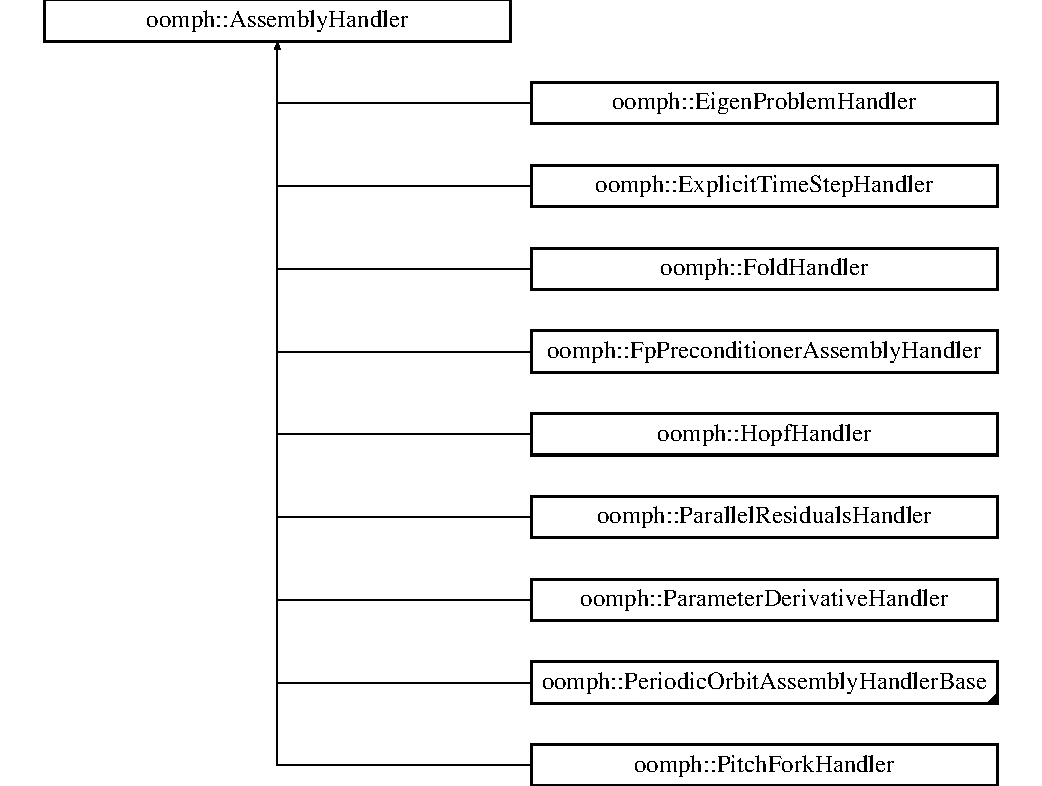
\includegraphics[height=10.000000cm]{classoomph_1_1AssemblyHandler}
\end{center}
\end{figure}
\subsection*{Public Member Functions}
\begin{DoxyCompactItemize}
\item 
\hyperlink{classoomph_1_1AssemblyHandler_af3ab79744dce0b50370defdbf7981691}{Assembly\+Handler} ()
\begin{DoxyCompactList}\small\item\em Empty constructor. \end{DoxyCompactList}\item 
virtual unsigned \hyperlink{classoomph_1_1AssemblyHandler_a09213be8f4aa009e0366460a7ed78e68}{ndof} (\hyperlink{classoomph_1_1GeneralisedElement}{Generalised\+Element} $\ast$const \&elem\+\_\+pt)
\begin{DoxyCompactList}\small\item\em Return the number of degrees of freedom in the element elem\+\_\+pt. \end{DoxyCompactList}\item 
virtual void \hyperlink{classoomph_1_1AssemblyHandler_abfd15243fce76ce8f1ea0248c700a3f4}{dof\+\_\+vector} (\hyperlink{classoomph_1_1GeneralisedElement}{Generalised\+Element} $\ast$const \&elem\+\_\+pt, const unsigned \&\hyperlink{cfortran_8h_af6f0bd3dc13317f895c91323c25c2b8f}{t}, \hyperlink{classoomph_1_1Vector}{Vector}$<$ double $>$ \&dof)
\begin{DoxyCompactList}\small\item\em Return vector of dofs at time level t in the element elem\+\_\+pt. \end{DoxyCompactList}\item 
virtual void \hyperlink{classoomph_1_1AssemblyHandler_ac4ea8b24799a4d71e74c195ba85500ee}{dof\+\_\+pt\+\_\+vector} (\hyperlink{classoomph_1_1GeneralisedElement}{Generalised\+Element} $\ast$const \&elem\+\_\+pt, \hyperlink{classoomph_1_1Vector}{Vector}$<$ double $\ast$$>$ \&dof\+\_\+pt)
\begin{DoxyCompactList}\small\item\em Return vector of pointers to dofs in the element elem\+\_\+pt. \end{DoxyCompactList}\item 
virtual double \& \hyperlink{classoomph_1_1AssemblyHandler_ab61559fc5df46871c1eebd103f7bf08b}{local\+\_\+problem\+\_\+dof} (\hyperlink{classoomph_1_1Problem}{Problem} $\ast$const \&problem\+\_\+pt, const unsigned \&\hyperlink{cfortran_8h_af6f0bd3dc13317f895c91323c25c2b8f}{t}, const unsigned \&\hyperlink{cfortran_8h_adb50e893b86b3e55e751a42eab3cba82}{i})
\begin{DoxyCompactList}\small\item\em Return the t-\/th level of storage associated with the i-\/th (local) dof stored in the problem. \end{DoxyCompactList}\item 
virtual unsigned long \hyperlink{classoomph_1_1AssemblyHandler_a94d28e2de2559cde803d1ba2195b5290}{eqn\+\_\+number} (\hyperlink{classoomph_1_1GeneralisedElement}{Generalised\+Element} $\ast$const \&elem\+\_\+pt, const unsigned \&ieqn\+\_\+local)
\begin{DoxyCompactList}\small\item\em Return the global equation number of the local unknown ieqn\+\_\+local in elem\+\_\+pt. \end{DoxyCompactList}\item 
virtual void \hyperlink{classoomph_1_1AssemblyHandler_a7a6203b0ab90da62b4da2af8a26d08b3}{get\+\_\+residuals} (\hyperlink{classoomph_1_1GeneralisedElement}{Generalised\+Element} $\ast$const \&elem\+\_\+pt, \hyperlink{classoomph_1_1Vector}{Vector}$<$ double $>$ \&residuals)
\begin{DoxyCompactList}\small\item\em Return the contribution to the residuals of the element elem\+\_\+pt. \end{DoxyCompactList}\item 
virtual void \hyperlink{classoomph_1_1AssemblyHandler_ad43c3d8760be0ba6ebee8d82509458e5}{get\+\_\+jacobian} (\hyperlink{classoomph_1_1GeneralisedElement}{Generalised\+Element} $\ast$const \&elem\+\_\+pt, \hyperlink{classoomph_1_1Vector}{Vector}$<$ double $>$ \&residuals, \hyperlink{classoomph_1_1DenseMatrix}{Dense\+Matrix}$<$ double $>$ \&jacobian)
\begin{DoxyCompactList}\small\item\em Calculate the elemental Jacobian matrix \char`\"{}d equation 
/ d variable\char`\"{} for elem\+\_\+pt. \end{DoxyCompactList}\item 
virtual void \hyperlink{classoomph_1_1AssemblyHandler_ab2e4ee4623116b18245ca90cfe9ba144}{get\+\_\+all\+\_\+vectors\+\_\+and\+\_\+matrices} (\hyperlink{classoomph_1_1GeneralisedElement}{Generalised\+Element} $\ast$const \&elem\+\_\+pt, \hyperlink{classoomph_1_1Vector}{Vector}$<$ \hyperlink{classoomph_1_1Vector}{Vector}$<$ double $>$ $>$ \&vec, \hyperlink{classoomph_1_1Vector}{Vector}$<$ \hyperlink{classoomph_1_1DenseMatrix}{Dense\+Matrix}$<$ double $>$ $>$ \&matrix)
\begin{DoxyCompactList}\small\item\em Calculate all desired vectors and matrices provided by the element elem\+\_\+pt. \end{DoxyCompactList}\item 
virtual void \hyperlink{classoomph_1_1AssemblyHandler_a2ee980ccabe0ad82f98e694eecf270bb}{get\+\_\+dresiduals\+\_\+dparameter} (\hyperlink{classoomph_1_1GeneralisedElement}{Generalised\+Element} $\ast$const \&elem\+\_\+pt, double $\ast$const \&parameter\+\_\+pt, \hyperlink{classoomph_1_1Vector}{Vector}$<$ double $>$ \&dres\+\_\+dparam)
\begin{DoxyCompactList}\small\item\em Calculate the derivative of the residuals with respect to a parameter. \end{DoxyCompactList}\item 
virtual void \hyperlink{classoomph_1_1AssemblyHandler_aefc0c13a65342806c167c5d53f014803}{get\+\_\+djacobian\+\_\+dparameter} (\hyperlink{classoomph_1_1GeneralisedElement}{Generalised\+Element} $\ast$const \&elem\+\_\+pt, double $\ast$const \&parameter\+\_\+pt, \hyperlink{classoomph_1_1Vector}{Vector}$<$ double $>$ \&dres\+\_\+dparam, \hyperlink{classoomph_1_1DenseMatrix}{Dense\+Matrix}$<$ double $>$ \&djac\+\_\+dparam)
\begin{DoxyCompactList}\small\item\em Calculate the derivative of the residuals and jacobian with respect to a parameter. \end{DoxyCompactList}\item 
virtual void \hyperlink{classoomph_1_1AssemblyHandler_a296bef49838d23522bb660c4c5207f03}{get\+\_\+hessian\+\_\+vector\+\_\+products} (\hyperlink{classoomph_1_1GeneralisedElement}{Generalised\+Element} $\ast$const \&elem\+\_\+pt, \hyperlink{classoomph_1_1Vector}{Vector}$<$ double $>$ const \&Y, \hyperlink{classoomph_1_1DenseMatrix}{Dense\+Matrix}$<$ double $>$ const \&C, \hyperlink{classoomph_1_1DenseMatrix}{Dense\+Matrix}$<$ double $>$ \&product)
\begin{DoxyCompactList}\small\item\em Calculate the product of the Hessian (derivative of Jacobian with respect to all variables) an eigenvector, Y, and other specified vectors, C (d(J\+\_\+\{ij\})/d u\+\_\+\{k\}) Y\+\_\+\{j\} C\+\_\+\{k\}. \end{DoxyCompactList}\item 
virtual int \hyperlink{classoomph_1_1AssemblyHandler_a22c5f240674e4f6cee12006790c11dae}{bifurcation\+\_\+type} () const
\begin{DoxyCompactList}\small\item\em Return an unsigned integer to indicate whether the handler is a bifurcation tracking handler. The default is zero (not) \end{DoxyCompactList}\item 
virtual double $\ast$ \hyperlink{classoomph_1_1AssemblyHandler_a3e369ec692c3d36a4a2a8a64dab7fe2b}{bifurcation\+\_\+parameter\+\_\+pt} () const
\begin{DoxyCompactList}\small\item\em Return a pointer to the bifurcation parameter in bifurcation tracking problems. \end{DoxyCompactList}\item 
virtual void \hyperlink{classoomph_1_1AssemblyHandler_a6d614b1b3809d0eb7ceb393e3ae9594f}{get\+\_\+eigenfunction} (\hyperlink{classoomph_1_1Vector}{Vector}$<$ \hyperlink{classoomph_1_1DoubleVector}{Double\+Vector} $>$ \&eigenfunction)
\begin{DoxyCompactList}\small\item\em Return the eigenfunction(s) associated with the bifurcation that has been detected in bifurcation tracking problems. \end{DoxyCompactList}\item 
virtual void \hyperlink{classoomph_1_1AssemblyHandler_a60c8efc6756825df9cd41389cdeac6cc}{get\+\_\+inner\+\_\+products} (\hyperlink{classoomph_1_1GeneralisedElement}{Generalised\+Element} $\ast$const \&elem\+\_\+pt, \hyperlink{classoomph_1_1Vector}{Vector}$<$ std\+::pair$<$ unsigned, unsigned $>$ $>$ const \&history\+\_\+index, \hyperlink{classoomph_1_1Vector}{Vector}$<$ double $>$ \&inner\+\_\+product)
\begin{DoxyCompactList}\small\item\em Compute the inner products of the given vector of pairs of history values over the element. \end{DoxyCompactList}\item 
virtual void \hyperlink{classoomph_1_1AssemblyHandler_a2300910f43476551318d74e3a90e7713}{get\+\_\+inner\+\_\+product\+\_\+vectors} (\hyperlink{classoomph_1_1GeneralisedElement}{Generalised\+Element} $\ast$const \&elem\+\_\+pt, \hyperlink{classoomph_1_1Vector}{Vector}$<$ unsigned $>$ const \&history\+\_\+index, \hyperlink{classoomph_1_1Vector}{Vector}$<$ \hyperlink{classoomph_1_1Vector}{Vector}$<$ double $>$ $>$ \&inner\+\_\+product\+\_\+vector)
\begin{DoxyCompactList}\small\item\em Compute the vectors that when taken as a dot product with other history values give the inner product over the element. \end{DoxyCompactList}\item 
virtual void \hyperlink{classoomph_1_1AssemblyHandler_a0ccef21253d997dd1a78ed26c2b99fce}{synchronise} ()
\begin{DoxyCompactList}\small\item\em Function that is used to perform any synchronisation required during the solution. \end{DoxyCompactList}\item 
virtual \hyperlink{classoomph_1_1AssemblyHandler_ab26633238200230ab57a20cc49e731de}{$\sim$\+Assembly\+Handler} ()
\begin{DoxyCompactList}\small\item\em Empty virtual destructor. \end{DoxyCompactList}\end{DoxyCompactItemize}


\subsection{Detailed Description}
A class that is used to define the functions used to assemble the elemental contributions to the residuals vector and Jacobian matrix that define the problem being solved. The main use of this class is to assemble and solve the augmented systems used in bifurcation detection and tracking. The default implementation merely calls the underlying elemental functions with no augmentation. 

Definition at line 66 of file assembly\+\_\+handler.\+h.



\subsection{Constructor \& Destructor Documentation}
\mbox{\Hypertarget{classoomph_1_1AssemblyHandler_af3ab79744dce0b50370defdbf7981691}\label{classoomph_1_1AssemblyHandler_af3ab79744dce0b50370defdbf7981691}} 
\index{oomph\+::\+Assembly\+Handler@{oomph\+::\+Assembly\+Handler}!Assembly\+Handler@{Assembly\+Handler}}
\index{Assembly\+Handler@{Assembly\+Handler}!oomph\+::\+Assembly\+Handler@{oomph\+::\+Assembly\+Handler}}
\subsubsection{\texorpdfstring{Assembly\+Handler()}{AssemblyHandler()}}
{\footnotesize\ttfamily oomph\+::\+Assembly\+Handler\+::\+Assembly\+Handler (\begin{DoxyParamCaption}{ }\end{DoxyParamCaption})\hspace{0.3cm}{\ttfamily [inline]}}



Empty constructor. 



Definition at line 71 of file assembly\+\_\+handler.\+h.



References dof\+\_\+pt\+\_\+vector(), dof\+\_\+vector(), eqn\+\_\+number(), get\+\_\+all\+\_\+vectors\+\_\+and\+\_\+matrices(), get\+\_\+djacobian\+\_\+dparameter(), get\+\_\+dresiduals\+\_\+dparameter(), get\+\_\+hessian\+\_\+vector\+\_\+products(), get\+\_\+jacobian(), get\+\_\+residuals(), i, local\+\_\+problem\+\_\+dof(), ndof(), and t.

\mbox{\Hypertarget{classoomph_1_1AssemblyHandler_ab26633238200230ab57a20cc49e731de}\label{classoomph_1_1AssemblyHandler_ab26633238200230ab57a20cc49e731de}} 
\index{oomph\+::\+Assembly\+Handler@{oomph\+::\+Assembly\+Handler}!````~Assembly\+Handler@{$\sim$\+Assembly\+Handler}}
\index{````~Assembly\+Handler@{$\sim$\+Assembly\+Handler}!oomph\+::\+Assembly\+Handler@{oomph\+::\+Assembly\+Handler}}
\subsubsection{\texorpdfstring{$\sim$\+Assembly\+Handler()}{~AssemblyHandler()}}
{\footnotesize\ttfamily virtual oomph\+::\+Assembly\+Handler\+::$\sim$\+Assembly\+Handler (\begin{DoxyParamCaption}{ }\end{DoxyParamCaption})\hspace{0.3cm}{\ttfamily [inline]}, {\ttfamily [virtual]}}



Empty virtual destructor. 



Definition at line 169 of file assembly\+\_\+handler.\+h.



\subsection{Member Function Documentation}
\mbox{\Hypertarget{classoomph_1_1AssemblyHandler_a3e369ec692c3d36a4a2a8a64dab7fe2b}\label{classoomph_1_1AssemblyHandler_a3e369ec692c3d36a4a2a8a64dab7fe2b}} 
\index{oomph\+::\+Assembly\+Handler@{oomph\+::\+Assembly\+Handler}!bifurcation\+\_\+parameter\+\_\+pt@{bifurcation\+\_\+parameter\+\_\+pt}}
\index{bifurcation\+\_\+parameter\+\_\+pt@{bifurcation\+\_\+parameter\+\_\+pt}!oomph\+::\+Assembly\+Handler@{oomph\+::\+Assembly\+Handler}}
\subsubsection{\texorpdfstring{bifurcation\+\_\+parameter\+\_\+pt()}{bifurcation\_parameter\_pt()}}
{\footnotesize\ttfamily double $\ast$ oomph\+::\+Assembly\+Handler\+::bifurcation\+\_\+parameter\+\_\+pt (\begin{DoxyParamCaption}{ }\end{DoxyParamCaption}) const\hspace{0.3cm}{\ttfamily [virtual]}}



Return a pointer to the bifurcation parameter in bifurcation tracking problems. 

Return the eigenfunction(s) associated with the bifurcation that has been detected in bifurcation tracking problems. Default Broken implementation 

Reimplemented in \hyperlink{classoomph_1_1HopfHandler_a49f4d0a78ac46ea1412d71d3bb9cc6a1}{oomph\+::\+Hopf\+Handler}, \hyperlink{classoomph_1_1PitchForkHandler_a7363cb34d716d64d891af5018e09d807}{oomph\+::\+Pitch\+Fork\+Handler}, and \hyperlink{classoomph_1_1FoldHandler_a0e35268f1b13aa94739aaaaa366f4586}{oomph\+::\+Fold\+Handler}.



Definition at line 157 of file assembly\+\_\+handler.\+cc.



Referenced by oomph\+::\+Problem\+::bifurcation\+\_\+parameter\+\_\+pt(), and bifurcation\+\_\+type().

\mbox{\Hypertarget{classoomph_1_1AssemblyHandler_a22c5f240674e4f6cee12006790c11dae}\label{classoomph_1_1AssemblyHandler_a22c5f240674e4f6cee12006790c11dae}} 
\index{oomph\+::\+Assembly\+Handler@{oomph\+::\+Assembly\+Handler}!bifurcation\+\_\+type@{bifurcation\+\_\+type}}
\index{bifurcation\+\_\+type@{bifurcation\+\_\+type}!oomph\+::\+Assembly\+Handler@{oomph\+::\+Assembly\+Handler}}
\subsubsection{\texorpdfstring{bifurcation\+\_\+type()}{bifurcation\_type()}}
{\footnotesize\ttfamily virtual int oomph\+::\+Assembly\+Handler\+::bifurcation\+\_\+type (\begin{DoxyParamCaption}{ }\end{DoxyParamCaption}) const\hspace{0.3cm}{\ttfamily [inline]}, {\ttfamily [virtual]}}



Return an unsigned integer to indicate whether the handler is a bifurcation tracking handler. The default is zero (not) 



Reimplemented in \hyperlink{classoomph_1_1HopfHandler_a789de82e82adaac82b366bbaa7f7ce59}{oomph\+::\+Hopf\+Handler}, \hyperlink{classoomph_1_1PitchForkHandler_aadc4f0b5dfb82cf171b91432536d1679}{oomph\+::\+Pitch\+Fork\+Handler}, and \hyperlink{classoomph_1_1FoldHandler_adb2878f53be92ea2be6cc012cbfc27ba}{oomph\+::\+Fold\+Handler}.



Definition at line 137 of file assembly\+\_\+handler.\+h.



References bifurcation\+\_\+parameter\+\_\+pt(), get\+\_\+eigenfunction(), get\+\_\+inner\+\_\+product\+\_\+vectors(), and get\+\_\+inner\+\_\+products().



Referenced by oomph\+::\+Problem\+::adapt(), oomph\+::\+Problem\+::doc\+\_\+errors(), and oomph\+::\+Problem\+::p\+\_\+adapt().

\mbox{\Hypertarget{classoomph_1_1AssemblyHandler_ac4ea8b24799a4d71e74c195ba85500ee}\label{classoomph_1_1AssemblyHandler_ac4ea8b24799a4d71e74c195ba85500ee}} 
\index{oomph\+::\+Assembly\+Handler@{oomph\+::\+Assembly\+Handler}!dof\+\_\+pt\+\_\+vector@{dof\+\_\+pt\+\_\+vector}}
\index{dof\+\_\+pt\+\_\+vector@{dof\+\_\+pt\+\_\+vector}!oomph\+::\+Assembly\+Handler@{oomph\+::\+Assembly\+Handler}}
\subsubsection{\texorpdfstring{dof\+\_\+pt\+\_\+vector()}{dof\_pt\_vector()}}
{\footnotesize\ttfamily void oomph\+::\+Assembly\+Handler\+::dof\+\_\+pt\+\_\+vector (\begin{DoxyParamCaption}\item[{\hyperlink{classoomph_1_1GeneralisedElement}{Generalised\+Element} $\ast$const \&}]{elem\+\_\+pt,  }\item[{\hyperlink{classoomph_1_1Vector}{Vector}$<$ double $\ast$$>$ \&}]{dof\+\_\+pt }\end{DoxyParamCaption})\hspace{0.3cm}{\ttfamily [virtual]}}



Return vector of pointers to dofs in the element elem\+\_\+pt. 

Get the vector of pointers to dofs in the element elem\+\_\+pt Direct call to the function in the element. 

Definition at line 61 of file assembly\+\_\+handler.\+cc.



References oomph\+::\+Generalised\+Element\+::dof\+\_\+pt\+\_\+vector().



Referenced by Assembly\+Handler().

\mbox{\Hypertarget{classoomph_1_1AssemblyHandler_abfd15243fce76ce8f1ea0248c700a3f4}\label{classoomph_1_1AssemblyHandler_abfd15243fce76ce8f1ea0248c700a3f4}} 
\index{oomph\+::\+Assembly\+Handler@{oomph\+::\+Assembly\+Handler}!dof\+\_\+vector@{dof\+\_\+vector}}
\index{dof\+\_\+vector@{dof\+\_\+vector}!oomph\+::\+Assembly\+Handler@{oomph\+::\+Assembly\+Handler}}
\subsubsection{\texorpdfstring{dof\+\_\+vector()}{dof\_vector()}}
{\footnotesize\ttfamily void oomph\+::\+Assembly\+Handler\+::dof\+\_\+vector (\begin{DoxyParamCaption}\item[{\hyperlink{classoomph_1_1GeneralisedElement}{Generalised\+Element} $\ast$const \&}]{elem\+\_\+pt,  }\item[{const unsigned \&}]{t,  }\item[{\hyperlink{classoomph_1_1Vector}{Vector}$<$ double $>$ \&}]{dof }\end{DoxyParamCaption})\hspace{0.3cm}{\ttfamily [virtual]}}



Return vector of dofs at time level t in the element elem\+\_\+pt. 

Get the vector of dofs in the element elem\+\_\+pt at time level t Direct call to the function in the element. 

Definition at line 53 of file assembly\+\_\+handler.\+cc.



References oomph\+::\+Generalised\+Element\+::dof\+\_\+vector().



Referenced by Assembly\+Handler().

\mbox{\Hypertarget{classoomph_1_1AssemblyHandler_a94d28e2de2559cde803d1ba2195b5290}\label{classoomph_1_1AssemblyHandler_a94d28e2de2559cde803d1ba2195b5290}} 
\index{oomph\+::\+Assembly\+Handler@{oomph\+::\+Assembly\+Handler}!eqn\+\_\+number@{eqn\+\_\+number}}
\index{eqn\+\_\+number@{eqn\+\_\+number}!oomph\+::\+Assembly\+Handler@{oomph\+::\+Assembly\+Handler}}
\subsubsection{\texorpdfstring{eqn\+\_\+number()}{eqn\_number()}}
{\footnotesize\ttfamily unsigned long oomph\+::\+Assembly\+Handler\+::eqn\+\_\+number (\begin{DoxyParamCaption}\item[{\hyperlink{classoomph_1_1GeneralisedElement}{Generalised\+Element} $\ast$const \&}]{elem\+\_\+pt,  }\item[{const unsigned \&}]{ieqn\+\_\+local }\end{DoxyParamCaption})\hspace{0.3cm}{\ttfamily [virtual]}}



Return the global equation number of the local unknown ieqn\+\_\+local in elem\+\_\+pt. 

Get the global equation number of the local unknown. Direct call to the function in the element. 

Reimplemented in \hyperlink{classoomph_1_1HopfHandler_a9feb8087e8b9554164c0de002f4ec056}{oomph\+::\+Hopf\+Handler}, \hyperlink{classoomph_1_1PeriodicOrbitAssemblyHandler_ac4d1e4e7e566061c2129157c67adab5b}{oomph\+::\+Periodic\+Orbit\+Assembly\+Handler$<$ N\+N\+O\+D\+E\+\_\+1\+D $>$}, \hyperlink{classoomph_1_1PitchForkHandler_ab29e58e25bd5bebd836e30015f01ac8d}{oomph\+::\+Pitch\+Fork\+Handler}, \hyperlink{classoomph_1_1FoldHandler_a30f2973860c13a183d5647a63b0c2ead}{oomph\+::\+Fold\+Handler}, \hyperlink{classoomph_1_1ParameterDerivativeHandler_a359b3b627532773b4606db1989f9c844}{oomph\+::\+Parameter\+Derivative\+Handler}, \hyperlink{classoomph_1_1ParallelResidualsHandler_a0541d552e54eb2ca8681054180eafb87}{oomph\+::\+Parallel\+Residuals\+Handler}, \hyperlink{classoomph_1_1EigenProblemHandler_ab94bef9c8135c9d2701e96d8205c797d}{oomph\+::\+Eigen\+Problem\+Handler}, and \hyperlink{classoomph_1_1ExplicitTimeStepHandler_a491d39988264739332c3e9c7dbb38344}{oomph\+::\+Explicit\+Time\+Step\+Handler}.



Definition at line 78 of file assembly\+\_\+handler.\+cc.



References oomph\+::\+Generalised\+Element\+::eqn\+\_\+number().



Referenced by Assembly\+Handler(), oomph\+::\+Eigen\+Problem\+Handler\+::\+Eigen\+Problem\+Handler(), oomph\+::\+Parallel\+Residuals\+Handler\+::eqn\+\_\+number(), oomph\+::\+Parameter\+Derivative\+Handler\+::eqn\+\_\+number(), oomph\+::\+Explicit\+Time\+Step\+Handler\+::\+Explicit\+Time\+Step\+Handler(), oomph\+::\+Problem\+::get\+\_\+hessian\+\_\+vector\+\_\+products(), oomph\+::\+Pitch\+Fork\+Handler\+::get\+\_\+jacobian(), oomph\+::\+Problem\+::get\+\_\+jacobian(), oomph\+::\+Problem\+::get\+\_\+my\+\_\+eqns(), oomph\+::\+Problem\+::get\+\_\+residuals(), oomph\+::\+Pitch\+Fork\+Handler\+::global\+\_\+eqn\+\_\+number(), oomph\+::\+Problem\+::parallel\+\_\+sparse\+\_\+assemble(), oomph\+::\+Pitch\+Fork\+Handler\+::\+Pitch\+Fork\+Handler(), oomph\+::\+H\+S\+L\+\_\+\+M\+A42\+::reorder\+\_\+elements(), oomph\+::\+Augmented\+Block\+Fold\+Linear\+Solver\+::resolve(), oomph\+::\+Problem\+::setup\+\_\+element\+\_\+count\+\_\+per\+\_\+dof(), oomph\+::\+H\+S\+L\+\_\+\+M\+A42\+::solve(), oomph\+::\+Augmented\+Block\+Fold\+Linear\+Solver\+::solve(), oomph\+::\+Problem\+::sparse\+\_\+assemble\+\_\+row\+\_\+or\+\_\+column\+\_\+compressed\+\_\+with\+\_\+lists(), oomph\+::\+Problem\+::sparse\+\_\+assemble\+\_\+row\+\_\+or\+\_\+column\+\_\+compressed\+\_\+with\+\_\+maps(), oomph\+::\+Problem\+::sparse\+\_\+assemble\+\_\+row\+\_\+or\+\_\+column\+\_\+compressed\+\_\+with\+\_\+two\+\_\+arrays(), oomph\+::\+Problem\+::sparse\+\_\+assemble\+\_\+row\+\_\+or\+\_\+column\+\_\+compressed\+\_\+with\+\_\+two\+\_\+vectors(), and oomph\+::\+Problem\+::sparse\+\_\+assemble\+\_\+row\+\_\+or\+\_\+column\+\_\+compressed\+\_\+with\+\_\+vectors\+\_\+of\+\_\+pairs().

\mbox{\Hypertarget{classoomph_1_1AssemblyHandler_ab2e4ee4623116b18245ca90cfe9ba144}\label{classoomph_1_1AssemblyHandler_ab2e4ee4623116b18245ca90cfe9ba144}} 
\index{oomph\+::\+Assembly\+Handler@{oomph\+::\+Assembly\+Handler}!get\+\_\+all\+\_\+vectors\+\_\+and\+\_\+matrices@{get\+\_\+all\+\_\+vectors\+\_\+and\+\_\+matrices}}
\index{get\+\_\+all\+\_\+vectors\+\_\+and\+\_\+matrices@{get\+\_\+all\+\_\+vectors\+\_\+and\+\_\+matrices}!oomph\+::\+Assembly\+Handler@{oomph\+::\+Assembly\+Handler}}
\subsubsection{\texorpdfstring{get\+\_\+all\+\_\+vectors\+\_\+and\+\_\+matrices()}{get\_all\_vectors\_and\_matrices()}}
{\footnotesize\ttfamily void oomph\+::\+Assembly\+Handler\+::get\+\_\+all\+\_\+vectors\+\_\+and\+\_\+matrices (\begin{DoxyParamCaption}\item[{\hyperlink{classoomph_1_1GeneralisedElement}{Generalised\+Element} $\ast$const \&}]{elem\+\_\+pt,  }\item[{\hyperlink{classoomph_1_1Vector}{Vector}$<$ \hyperlink{classoomph_1_1Vector}{Vector}$<$ double $>$ $>$ \&}]{vec,  }\item[{\hyperlink{classoomph_1_1Vector}{Vector}$<$ \hyperlink{classoomph_1_1DenseMatrix}{Dense\+Matrix}$<$ double $>$ $>$ \&}]{matrix }\end{DoxyParamCaption})\hspace{0.3cm}{\ttfamily [virtual]}}



Calculate all desired vectors and matrices provided by the element elem\+\_\+pt. 

Calculate all desired vectors and matrices that are required by the element by calling the get\+\_\+jacobian function 

Reimplemented in \hyperlink{classoomph_1_1ParallelResidualsHandler_adea071e3131e4e84b7c3e9400892fb17}{oomph\+::\+Parallel\+Residuals\+Handler}, \hyperlink{classoomph_1_1EigenProblemHandler_aa88f56b5c724c41e0c2926434ae920da}{oomph\+::\+Eigen\+Problem\+Handler}, and \hyperlink{classoomph_1_1ExplicitTimeStepHandler_a842529121fbe177ea6900d668d8b2a65}{oomph\+::\+Explicit\+Time\+Step\+Handler}.



Definition at line 103 of file assembly\+\_\+handler.\+cc.



References get\+\_\+jacobian().



Referenced by Assembly\+Handler(), oomph\+::\+Eigen\+Problem\+Handler\+::\+Eigen\+Problem\+Handler(), and oomph\+::\+Explicit\+Time\+Step\+Handler\+::\+Explicit\+Time\+Step\+Handler().

\mbox{\Hypertarget{classoomph_1_1AssemblyHandler_aefc0c13a65342806c167c5d53f014803}\label{classoomph_1_1AssemblyHandler_aefc0c13a65342806c167c5d53f014803}} 
\index{oomph\+::\+Assembly\+Handler@{oomph\+::\+Assembly\+Handler}!get\+\_\+djacobian\+\_\+dparameter@{get\+\_\+djacobian\+\_\+dparameter}}
\index{get\+\_\+djacobian\+\_\+dparameter@{get\+\_\+djacobian\+\_\+dparameter}!oomph\+::\+Assembly\+Handler@{oomph\+::\+Assembly\+Handler}}
\subsubsection{\texorpdfstring{get\+\_\+djacobian\+\_\+dparameter()}{get\_djacobian\_dparameter()}}
{\footnotesize\ttfamily void oomph\+::\+Assembly\+Handler\+::get\+\_\+djacobian\+\_\+dparameter (\begin{DoxyParamCaption}\item[{\hyperlink{classoomph_1_1GeneralisedElement}{Generalised\+Element} $\ast$const \&}]{elem\+\_\+pt,  }\item[{double $\ast$const \&}]{parameter\+\_\+pt,  }\item[{\hyperlink{classoomph_1_1Vector}{Vector}$<$ double $>$ \&}]{dres\+\_\+dparam,  }\item[{\hyperlink{classoomph_1_1DenseMatrix}{Dense\+Matrix}$<$ double $>$ \&}]{djac\+\_\+dparam }\end{DoxyParamCaption})\hspace{0.3cm}{\ttfamily [virtual]}}



Calculate the derivative of the residuals and jacobian with respect to a parameter. 

Calculate the derivative of the residuals and jacobian with respect to a parameter by calling the elemental function. 

Reimplemented in \hyperlink{classoomph_1_1HopfHandler_a59fb2c41d850cfe1fdccc3e97ca75135}{oomph\+::\+Hopf\+Handler}, \hyperlink{classoomph_1_1PitchForkHandler_aa16d6770f6d46b7db4101f417373b191}{oomph\+::\+Pitch\+Fork\+Handler}, and \hyperlink{classoomph_1_1FoldHandler_a674cf9fe7c065e54c95813c2baeea84c}{oomph\+::\+Fold\+Handler}.



Definition at line 127 of file assembly\+\_\+handler.\+cc.



References oomph\+::\+Generalised\+Element\+::get\+\_\+djacobian\+\_\+dparameter().



Referenced by Assembly\+Handler(), oomph\+::\+Parameter\+Derivative\+Handler\+::get\+\_\+jacobian(), and oomph\+::\+Pitch\+Fork\+Handler\+::global\+\_\+eqn\+\_\+number().

\mbox{\Hypertarget{classoomph_1_1AssemblyHandler_a2ee980ccabe0ad82f98e694eecf270bb}\label{classoomph_1_1AssemblyHandler_a2ee980ccabe0ad82f98e694eecf270bb}} 
\index{oomph\+::\+Assembly\+Handler@{oomph\+::\+Assembly\+Handler}!get\+\_\+dresiduals\+\_\+dparameter@{get\+\_\+dresiduals\+\_\+dparameter}}
\index{get\+\_\+dresiduals\+\_\+dparameter@{get\+\_\+dresiduals\+\_\+dparameter}!oomph\+::\+Assembly\+Handler@{oomph\+::\+Assembly\+Handler}}
\subsubsection{\texorpdfstring{get\+\_\+dresiduals\+\_\+dparameter()}{get\_dresiduals\_dparameter()}}
{\footnotesize\ttfamily void oomph\+::\+Assembly\+Handler\+::get\+\_\+dresiduals\+\_\+dparameter (\begin{DoxyParamCaption}\item[{\hyperlink{classoomph_1_1GeneralisedElement}{Generalised\+Element} $\ast$const \&}]{elem\+\_\+pt,  }\item[{double $\ast$const \&}]{parameter\+\_\+pt,  }\item[{\hyperlink{classoomph_1_1Vector}{Vector}$<$ double $>$ \&}]{dres\+\_\+dparam }\end{DoxyParamCaption})\hspace{0.3cm}{\ttfamily [virtual]}}



Calculate the derivative of the residuals with respect to a parameter. 

Calculate the derivative of the residuals with respect to a parameter, by calling the elemental function. 

Reimplemented in \hyperlink{classoomph_1_1HopfHandler_a2953368ecc48dc22f8ea1f563064ece2}{oomph\+::\+Hopf\+Handler}, \hyperlink{classoomph_1_1PitchForkHandler_a6510803afcbcfce1ae5b1c1c5d82a541}{oomph\+::\+Pitch\+Fork\+Handler}, and \hyperlink{classoomph_1_1FoldHandler_ad98b98488b683fa3ad9497b662e6e5b6}{oomph\+::\+Fold\+Handler}.



Definition at line 114 of file assembly\+\_\+handler.\+cc.



References oomph\+::\+Generalised\+Element\+::get\+\_\+dresiduals\+\_\+dparameter().



Referenced by Assembly\+Handler(), oomph\+::\+Parameter\+Derivative\+Handler\+::get\+\_\+residuals(), and oomph\+::\+Pitch\+Fork\+Handler\+::global\+\_\+eqn\+\_\+number().

\mbox{\Hypertarget{classoomph_1_1AssemblyHandler_a6d614b1b3809d0eb7ceb393e3ae9594f}\label{classoomph_1_1AssemblyHandler_a6d614b1b3809d0eb7ceb393e3ae9594f}} 
\index{oomph\+::\+Assembly\+Handler@{oomph\+::\+Assembly\+Handler}!get\+\_\+eigenfunction@{get\+\_\+eigenfunction}}
\index{get\+\_\+eigenfunction@{get\+\_\+eigenfunction}!oomph\+::\+Assembly\+Handler@{oomph\+::\+Assembly\+Handler}}
\subsubsection{\texorpdfstring{get\+\_\+eigenfunction()}{get\_eigenfunction()}}
{\footnotesize\ttfamily void oomph\+::\+Assembly\+Handler\+::get\+\_\+eigenfunction (\begin{DoxyParamCaption}\item[{\hyperlink{classoomph_1_1Vector}{Vector}$<$ \hyperlink{classoomph_1_1DoubleVector}{Double\+Vector} $>$ \&}]{eigenfunction }\end{DoxyParamCaption})\hspace{0.3cm}{\ttfamily [virtual]}}



Return the eigenfunction(s) associated with the bifurcation that has been detected in bifurcation tracking problems. 

Return the eigenfunction(s) associated with the bifurcation that has been detected in bifurcation tracking problems. Default Broken implementation 

Reimplemented in \hyperlink{classoomph_1_1HopfHandler_a9d1ee586e6274cfa0baa15f82b9fa0ae}{oomph\+::\+Hopf\+Handler}, \hyperlink{classoomph_1_1PitchForkHandler_a9d5e1388fe0ede6834a249b98168b71a}{oomph\+::\+Pitch\+Fork\+Handler}, and \hyperlink{classoomph_1_1FoldHandler_aca97058722ccc1482ae8180ea8dde74c}{oomph\+::\+Fold\+Handler}.



Definition at line 179 of file assembly\+\_\+handler.\+cc.



Referenced by oomph\+::\+Fold\+Handler\+::bifurcation\+\_\+parameter\+\_\+pt(), oomph\+::\+Pitch\+Fork\+Handler\+::bifurcation\+\_\+parameter\+\_\+pt(), oomph\+::\+Hopf\+Handler\+::bifurcation\+\_\+parameter\+\_\+pt(), bifurcation\+\_\+type(), and oomph\+::\+Problem\+::get\+\_\+bifurcation\+\_\+eigenfunction().

\mbox{\Hypertarget{classoomph_1_1AssemblyHandler_a296bef49838d23522bb660c4c5207f03}\label{classoomph_1_1AssemblyHandler_a296bef49838d23522bb660c4c5207f03}} 
\index{oomph\+::\+Assembly\+Handler@{oomph\+::\+Assembly\+Handler}!get\+\_\+hessian\+\_\+vector\+\_\+products@{get\+\_\+hessian\+\_\+vector\+\_\+products}}
\index{get\+\_\+hessian\+\_\+vector\+\_\+products@{get\+\_\+hessian\+\_\+vector\+\_\+products}!oomph\+::\+Assembly\+Handler@{oomph\+::\+Assembly\+Handler}}
\subsubsection{\texorpdfstring{get\+\_\+hessian\+\_\+vector\+\_\+products()}{get\_hessian\_vector\_products()}}
{\footnotesize\ttfamily void oomph\+::\+Assembly\+Handler\+::get\+\_\+hessian\+\_\+vector\+\_\+products (\begin{DoxyParamCaption}\item[{\hyperlink{classoomph_1_1GeneralisedElement}{Generalised\+Element} $\ast$const \&}]{elem\+\_\+pt,  }\item[{\hyperlink{classoomph_1_1Vector}{Vector}$<$ double $>$ const \&}]{Y,  }\item[{\hyperlink{classoomph_1_1DenseMatrix}{Dense\+Matrix}$<$ double $>$ const \&}]{C,  }\item[{\hyperlink{classoomph_1_1DenseMatrix}{Dense\+Matrix}$<$ double $>$ \&}]{product }\end{DoxyParamCaption})\hspace{0.3cm}{\ttfamily [virtual]}}



Calculate the product of the Hessian (derivative of Jacobian with respect to all variables) an eigenvector, Y, and other specified vectors, C (d(J\+\_\+\{ij\})/d u\+\_\+\{k\}) Y\+\_\+\{j\} C\+\_\+\{k\}. 

Calculate the product of the Hessian (derivative of Jacobian with respect to all variables) an eigenvector, Y, and other specified vectors, C (d(J\+\_\+\{ij\})/d u\+\_\+\{k\}) Y\+\_\+\{j\} C\+\_\+\{k\} At the moment the dof pointer is passed in to enable easy calculation of finite difference default. 

Reimplemented in \hyperlink{classoomph_1_1HopfHandler_a74b0266ee15bcb294dbb946156095f8c}{oomph\+::\+Hopf\+Handler}, \hyperlink{classoomph_1_1PitchForkHandler_a85e7dba2d21c9fe95a575a115cf3ee9f}{oomph\+::\+Pitch\+Fork\+Handler}, and \hyperlink{classoomph_1_1FoldHandler_aa633b80f1ebdb322350c6832fe6c2b6c}{oomph\+::\+Fold\+Handler}.



Definition at line 142 of file assembly\+\_\+handler.\+cc.



References oomph\+::\+Generalised\+Element\+::get\+\_\+hessian\+\_\+vector\+\_\+products().



Referenced by Assembly\+Handler(), oomph\+::\+Problem\+::get\+\_\+hessian\+\_\+vector\+\_\+products(), and oomph\+::\+Pitch\+Fork\+Handler\+::global\+\_\+eqn\+\_\+number().

\mbox{\Hypertarget{classoomph_1_1AssemblyHandler_a2300910f43476551318d74e3a90e7713}\label{classoomph_1_1AssemblyHandler_a2300910f43476551318d74e3a90e7713}} 
\index{oomph\+::\+Assembly\+Handler@{oomph\+::\+Assembly\+Handler}!get\+\_\+inner\+\_\+product\+\_\+vectors@{get\+\_\+inner\+\_\+product\+\_\+vectors}}
\index{get\+\_\+inner\+\_\+product\+\_\+vectors@{get\+\_\+inner\+\_\+product\+\_\+vectors}!oomph\+::\+Assembly\+Handler@{oomph\+::\+Assembly\+Handler}}
\subsubsection{\texorpdfstring{get\+\_\+inner\+\_\+product\+\_\+vectors()}{get\_inner\_product\_vectors()}}
{\footnotesize\ttfamily void oomph\+::\+Assembly\+Handler\+::get\+\_\+inner\+\_\+product\+\_\+vectors (\begin{DoxyParamCaption}\item[{\hyperlink{classoomph_1_1GeneralisedElement}{Generalised\+Element} $\ast$const \&}]{elem\+\_\+pt,  }\item[{\hyperlink{classoomph_1_1Vector}{Vector}$<$ unsigned $>$ const \&}]{history\+\_\+index,  }\item[{\hyperlink{classoomph_1_1Vector}{Vector}$<$ \hyperlink{classoomph_1_1Vector}{Vector}$<$ double $>$ $>$ \&}]{inner\+\_\+product\+\_\+vector }\end{DoxyParamCaption})\hspace{0.3cm}{\ttfamily [virtual]}}



Compute the vectors that when taken as a dot product with other history values give the inner product over the element. 

Compute the vectors that when taken as a dot product with other history values give the inner product over the element. In other words if we call get\+\_\+inner\+\_\+product\+\_\+vectors(\{0,1\},output) output\mbox{[}0\mbox{]} will be a vector such that dofs.\+output\mbox{[}0\mbox{]} gives the inner product of current dofs with themselves. 

Definition at line 215 of file assembly\+\_\+handler.\+cc.



References oomph\+::\+Generalised\+Element\+::get\+\_\+inner\+\_\+product\+\_\+vectors().



Referenced by bifurcation\+\_\+type().

\mbox{\Hypertarget{classoomph_1_1AssemblyHandler_a60c8efc6756825df9cd41389cdeac6cc}\label{classoomph_1_1AssemblyHandler_a60c8efc6756825df9cd41389cdeac6cc}} 
\index{oomph\+::\+Assembly\+Handler@{oomph\+::\+Assembly\+Handler}!get\+\_\+inner\+\_\+products@{get\+\_\+inner\+\_\+products}}
\index{get\+\_\+inner\+\_\+products@{get\+\_\+inner\+\_\+products}!oomph\+::\+Assembly\+Handler@{oomph\+::\+Assembly\+Handler}}
\subsubsection{\texorpdfstring{get\+\_\+inner\+\_\+products()}{get\_inner\_products()}}
{\footnotesize\ttfamily void oomph\+::\+Assembly\+Handler\+::get\+\_\+inner\+\_\+products (\begin{DoxyParamCaption}\item[{\hyperlink{classoomph_1_1GeneralisedElement}{Generalised\+Element} $\ast$const \&}]{elem\+\_\+pt,  }\item[{\hyperlink{classoomph_1_1Vector}{Vector}$<$ std\+::pair$<$ unsigned, unsigned $>$ $>$ const \&}]{history\+\_\+index,  }\item[{\hyperlink{classoomph_1_1Vector}{Vector}$<$ double $>$ \&}]{inner\+\_\+product }\end{DoxyParamCaption})\hspace{0.3cm}{\ttfamily [virtual]}}



Compute the inner products of the given vector of pairs of history values over the element. 

========================================================================== Compute the inner products of the given vector of pairs of history values over the element. The values of the index in the pair may be the same. 

Definition at line 200 of file assembly\+\_\+handler.\+cc.



References oomph\+::\+Generalised\+Element\+::get\+\_\+inner\+\_\+products().



Referenced by bifurcation\+\_\+type().

\mbox{\Hypertarget{classoomph_1_1AssemblyHandler_ad43c3d8760be0ba6ebee8d82509458e5}\label{classoomph_1_1AssemblyHandler_ad43c3d8760be0ba6ebee8d82509458e5}} 
\index{oomph\+::\+Assembly\+Handler@{oomph\+::\+Assembly\+Handler}!get\+\_\+jacobian@{get\+\_\+jacobian}}
\index{get\+\_\+jacobian@{get\+\_\+jacobian}!oomph\+::\+Assembly\+Handler@{oomph\+::\+Assembly\+Handler}}
\subsubsection{\texorpdfstring{get\+\_\+jacobian()}{get\_jacobian()}}
{\footnotesize\ttfamily void oomph\+::\+Assembly\+Handler\+::get\+\_\+jacobian (\begin{DoxyParamCaption}\item[{\hyperlink{classoomph_1_1GeneralisedElement}{Generalised\+Element} $\ast$const \&}]{elem\+\_\+pt,  }\item[{\hyperlink{classoomph_1_1Vector}{Vector}$<$ double $>$ \&}]{residuals,  }\item[{\hyperlink{classoomph_1_1DenseMatrix}{Dense\+Matrix}$<$ double $>$ \&}]{jacobian }\end{DoxyParamCaption})\hspace{0.3cm}{\ttfamily [virtual]}}



Calculate the elemental Jacobian matrix \char`\"{}d equation 
/ d variable\char`\"{} for elem\+\_\+pt. 

Calculate the elemental Jacobian matrix \char`\"{}d equation / d variable\char`\"{} by calling the element\textquotesingle{}s get\+\_\+jacobian function. 

Reimplemented in \hyperlink{classoomph_1_1HopfHandler_ab36c50421f53accced01dd9e04d904ef}{oomph\+::\+Hopf\+Handler}, \hyperlink{classoomph_1_1PeriodicOrbitAssemblyHandler_a6d901ecdefca1c59403a4ae4b215446f}{oomph\+::\+Periodic\+Orbit\+Assembly\+Handler$<$ N\+N\+O\+D\+E\+\_\+1\+D $>$}, \hyperlink{classoomph_1_1PitchForkHandler_aa6728813a099111bee2b6c79dec20fc4}{oomph\+::\+Pitch\+Fork\+Handler}, \hyperlink{classoomph_1_1FoldHandler_ad1bec54a2e0c5bd483ff0bf633bd6542}{oomph\+::\+Fold\+Handler}, \hyperlink{classoomph_1_1ParameterDerivativeHandler_a0bdfd879c1e63cc74923cf956b4f4310}{oomph\+::\+Parameter\+Derivative\+Handler}, \hyperlink{classoomph_1_1ParallelResidualsHandler_a366186bb0905d7251390ec726fe33797}{oomph\+::\+Parallel\+Residuals\+Handler}, \hyperlink{classoomph_1_1EigenProblemHandler_aaaf7c3aa3713030ff4859117941b3a39}{oomph\+::\+Eigen\+Problem\+Handler}, \hyperlink{classoomph_1_1ExplicitTimeStepHandler_ad2c849833e4b35199a79d9d9965af32f}{oomph\+::\+Explicit\+Time\+Step\+Handler}, and \hyperlink{classoomph_1_1FpPreconditionerAssemblyHandler_a6360dd27d3530576487cb7e239dfe17e}{oomph\+::\+Fp\+Preconditioner\+Assembly\+Handler}.



Definition at line 94 of file assembly\+\_\+handler.\+cc.



References oomph\+::\+Generalised\+Element\+::get\+\_\+jacobian().



Referenced by Assembly\+Handler(), oomph\+::\+Eigen\+Problem\+Handler\+::\+Eigen\+Problem\+Handler(), oomph\+::\+Explicit\+Time\+Step\+Handler\+::\+Explicit\+Time\+Step\+Handler(), get\+\_\+all\+\_\+vectors\+\_\+and\+\_\+matrices(), oomph\+::\+Problem\+::get\+\_\+hessian\+\_\+vector\+\_\+products(), oomph\+::\+Parallel\+Residuals\+Handler\+::get\+\_\+jacobian(), oomph\+::\+Problem\+::get\+\_\+jacobian(), oomph\+::\+Pitch\+Fork\+Handler\+::global\+\_\+eqn\+\_\+number(), oomph\+::\+H\+S\+L\+\_\+\+M\+A42\+::solve(), and oomph\+::\+H\+S\+L\+\_\+\+M\+A42\+::solve\+\_\+for\+\_\+one\+\_\+dof().

\mbox{\Hypertarget{classoomph_1_1AssemblyHandler_a7a6203b0ab90da62b4da2af8a26d08b3}\label{classoomph_1_1AssemblyHandler_a7a6203b0ab90da62b4da2af8a26d08b3}} 
\index{oomph\+::\+Assembly\+Handler@{oomph\+::\+Assembly\+Handler}!get\+\_\+residuals@{get\+\_\+residuals}}
\index{get\+\_\+residuals@{get\+\_\+residuals}!oomph\+::\+Assembly\+Handler@{oomph\+::\+Assembly\+Handler}}
\subsubsection{\texorpdfstring{get\+\_\+residuals()}{get\_residuals()}}
{\footnotesize\ttfamily void oomph\+::\+Assembly\+Handler\+::get\+\_\+residuals (\begin{DoxyParamCaption}\item[{\hyperlink{classoomph_1_1GeneralisedElement}{Generalised\+Element} $\ast$const \&}]{elem\+\_\+pt,  }\item[{\hyperlink{classoomph_1_1Vector}{Vector}$<$ double $>$ \&}]{residuals }\end{DoxyParamCaption})\hspace{0.3cm}{\ttfamily [virtual]}}



Return the contribution to the residuals of the element elem\+\_\+pt. 

Get the residuals by calling the underlying element\textquotesingle{}s residuals directly. 

Reimplemented in \hyperlink{classoomph_1_1HopfHandler_a61a4006161da6532a9acfec0f979aafa}{oomph\+::\+Hopf\+Handler}, \hyperlink{classoomph_1_1PeriodicOrbitAssemblyHandler_af43abc524b34d8e8035e2c2323e2fc87}{oomph\+::\+Periodic\+Orbit\+Assembly\+Handler$<$ N\+N\+O\+D\+E\+\_\+1\+D $>$}, \hyperlink{classoomph_1_1PitchForkHandler_a461b24284da88b9489d720e484a6925c}{oomph\+::\+Pitch\+Fork\+Handler}, \hyperlink{classoomph_1_1FoldHandler_abfbec6da3dffeaf3b4df0ee4955101fd}{oomph\+::\+Fold\+Handler}, \hyperlink{classoomph_1_1ParameterDerivativeHandler_a8ba1dbc805c00ac75e6d5d53f1b014c1}{oomph\+::\+Parameter\+Derivative\+Handler}, \hyperlink{classoomph_1_1ParallelResidualsHandler_a9a4e40b86cfb1db2b4c770d8d7241ad1}{oomph\+::\+Parallel\+Residuals\+Handler}, \hyperlink{classoomph_1_1EigenProblemHandler_a0dc97e08638986970c7ca5f3903c8b6d}{oomph\+::\+Eigen\+Problem\+Handler}, \hyperlink{classoomph_1_1ExplicitTimeStepHandler_aef8ab1b61aef072b2bcb061dd287a00f}{oomph\+::\+Explicit\+Time\+Step\+Handler}, and \hyperlink{classoomph_1_1FpPreconditionerAssemblyHandler_adfebe7f48f6fc715c258e1733218b12b}{oomph\+::\+Fp\+Preconditioner\+Assembly\+Handler}.



Definition at line 86 of file assembly\+\_\+handler.\+cc.



References oomph\+::\+Generalised\+Element\+::get\+\_\+residuals().



Referenced by Assembly\+Handler(), oomph\+::\+Eigen\+Problem\+Handler\+::\+Eigen\+Problem\+Handler(), oomph\+::\+Explicit\+Time\+Step\+Handler\+::\+Explicit\+Time\+Step\+Handler(), oomph\+::\+Parallel\+Residuals\+Handler\+::get\+\_\+all\+\_\+vectors\+\_\+and\+\_\+matrices(), oomph\+::\+Parallel\+Residuals\+Handler\+::get\+\_\+residuals(), oomph\+::\+Problem\+::get\+\_\+residuals(), and oomph\+::\+Pitch\+Fork\+Handler\+::global\+\_\+eqn\+\_\+number().

\mbox{\Hypertarget{classoomph_1_1AssemblyHandler_ab61559fc5df46871c1eebd103f7bf08b}\label{classoomph_1_1AssemblyHandler_ab61559fc5df46871c1eebd103f7bf08b}} 
\index{oomph\+::\+Assembly\+Handler@{oomph\+::\+Assembly\+Handler}!local\+\_\+problem\+\_\+dof@{local\+\_\+problem\+\_\+dof}}
\index{local\+\_\+problem\+\_\+dof@{local\+\_\+problem\+\_\+dof}!oomph\+::\+Assembly\+Handler@{oomph\+::\+Assembly\+Handler}}
\subsubsection{\texorpdfstring{local\+\_\+problem\+\_\+dof()}{local\_problem\_dof()}}
{\footnotesize\ttfamily double \& oomph\+::\+Assembly\+Handler\+::local\+\_\+problem\+\_\+dof (\begin{DoxyParamCaption}\item[{\hyperlink{classoomph_1_1Problem}{Problem} $\ast$const \&}]{problem\+\_\+pt,  }\item[{const unsigned \&}]{t,  }\item[{const unsigned \&}]{i }\end{DoxyParamCaption})\hspace{0.3cm}{\ttfamily [virtual]}}



Return the t-\/th level of storage associated with the i-\/th (local) dof stored in the problem. 



Definition at line 67 of file assembly\+\_\+handler.\+cc.



References oomph\+::\+Problem\+::dof\+\_\+pt(), and t.



Referenced by Assembly\+Handler().

\mbox{\Hypertarget{classoomph_1_1AssemblyHandler_a09213be8f4aa009e0366460a7ed78e68}\label{classoomph_1_1AssemblyHandler_a09213be8f4aa009e0366460a7ed78e68}} 
\index{oomph\+::\+Assembly\+Handler@{oomph\+::\+Assembly\+Handler}!ndof@{ndof}}
\index{ndof@{ndof}!oomph\+::\+Assembly\+Handler@{oomph\+::\+Assembly\+Handler}}
\subsubsection{\texorpdfstring{ndof()}{ndof()}}
{\footnotesize\ttfamily unsigned oomph\+::\+Assembly\+Handler\+::ndof (\begin{DoxyParamCaption}\item[{\hyperlink{classoomph_1_1GeneralisedElement}{Generalised\+Element} $\ast$const \&}]{elem\+\_\+pt }\end{DoxyParamCaption})\hspace{0.3cm}{\ttfamily [virtual]}}



Return the number of degrees of freedom in the element elem\+\_\+pt. 

Get the number of elemental degrees of freedom. Direct call to the function in the element. 

Reimplemented in \hyperlink{classoomph_1_1HopfHandler_a8d1b73ec4e9b8b27252b4bacf2ef7f38}{oomph\+::\+Hopf\+Handler}, \hyperlink{classoomph_1_1PeriodicOrbitAssemblyHandler_ab960ecaac9239cfbc47f1036893362ff}{oomph\+::\+Periodic\+Orbit\+Assembly\+Handler$<$ N\+N\+O\+D\+E\+\_\+1\+D $>$}, \hyperlink{classoomph_1_1PitchForkHandler_ae066fa45e9f1bf10601286ca2d083a42}{oomph\+::\+Pitch\+Fork\+Handler}, \hyperlink{classoomph_1_1FoldHandler_af8e766d1faa7867a0161329566865867}{oomph\+::\+Fold\+Handler}, \hyperlink{classoomph_1_1ParameterDerivativeHandler_a341d4e7cfaab7e66df43913d775a6871}{oomph\+::\+Parameter\+Derivative\+Handler}, \hyperlink{classoomph_1_1ParallelResidualsHandler_a16eb9ec097e85c5da57b2e588d9683b6}{oomph\+::\+Parallel\+Residuals\+Handler}, \hyperlink{classoomph_1_1EigenProblemHandler_ae9e44eeceee6e19c60c51b08195730eb}{oomph\+::\+Eigen\+Problem\+Handler}, and \hyperlink{classoomph_1_1ExplicitTimeStepHandler_a723bec764e9e59025f052f6ca0135181}{oomph\+::\+Explicit\+Time\+Step\+Handler}.



Definition at line 46 of file assembly\+\_\+handler.\+cc.



References oomph\+::\+Generalised\+Element\+::ndof().



Referenced by Assembly\+Handler(), oomph\+::\+Eigen\+Problem\+Handler\+::\+Eigen\+Problem\+Handler(), oomph\+::\+Explicit\+Time\+Step\+Handler\+::\+Explicit\+Time\+Step\+Handler(), oomph\+::\+Problem\+::get\+\_\+hessian\+\_\+vector\+\_\+products(), oomph\+::\+Problem\+::get\+\_\+jacobian(), oomph\+::\+Problem\+::get\+\_\+my\+\_\+eqns(), oomph\+::\+Problem\+::get\+\_\+residuals(), oomph\+::\+Pitch\+Fork\+Handler\+::global\+\_\+eqn\+\_\+number(), oomph\+::\+Parallel\+Residuals\+Handler\+::ndof(), oomph\+::\+Parameter\+Derivative\+Handler\+::ndof(), oomph\+::\+Problem\+::parallel\+\_\+sparse\+\_\+assemble(), oomph\+::\+Pitch\+Fork\+Handler\+::\+Pitch\+Fork\+Handler(), oomph\+::\+H\+S\+L\+\_\+\+M\+A42\+::reorder\+\_\+elements(), oomph\+::\+Problem\+::setup\+\_\+element\+\_\+count\+\_\+per\+\_\+dof(), oomph\+::\+H\+S\+L\+\_\+\+M\+A42\+::solve(), oomph\+::\+H\+S\+L\+\_\+\+M\+A42\+::solve\+\_\+for\+\_\+one\+\_\+dof(), oomph\+::\+Problem\+::sparse\+\_\+assemble\+\_\+row\+\_\+or\+\_\+column\+\_\+compressed\+\_\+with\+\_\+lists(), oomph\+::\+Problem\+::sparse\+\_\+assemble\+\_\+row\+\_\+or\+\_\+column\+\_\+compressed\+\_\+with\+\_\+maps(), oomph\+::\+Problem\+::sparse\+\_\+assemble\+\_\+row\+\_\+or\+\_\+column\+\_\+compressed\+\_\+with\+\_\+two\+\_\+arrays(), oomph\+::\+Problem\+::sparse\+\_\+assemble\+\_\+row\+\_\+or\+\_\+column\+\_\+compressed\+\_\+with\+\_\+two\+\_\+vectors(), and oomph\+::\+Problem\+::sparse\+\_\+assemble\+\_\+row\+\_\+or\+\_\+column\+\_\+compressed\+\_\+with\+\_\+vectors\+\_\+of\+\_\+pairs().

\mbox{\Hypertarget{classoomph_1_1AssemblyHandler_a0ccef21253d997dd1a78ed26c2b99fce}\label{classoomph_1_1AssemblyHandler_a0ccef21253d997dd1a78ed26c2b99fce}} 
\index{oomph\+::\+Assembly\+Handler@{oomph\+::\+Assembly\+Handler}!synchronise@{synchronise}}
\index{synchronise@{synchronise}!oomph\+::\+Assembly\+Handler@{oomph\+::\+Assembly\+Handler}}
\subsubsection{\texorpdfstring{synchronise()}{synchronise()}}
{\footnotesize\ttfamily virtual void oomph\+::\+Assembly\+Handler\+::synchronise (\begin{DoxyParamCaption}{ }\end{DoxyParamCaption})\hspace{0.3cm}{\ttfamily [inline]}, {\ttfamily [virtual]}}



Function that is used to perform any synchronisation required during the solution. 



Reimplemented in \hyperlink{classoomph_1_1PitchForkHandler_a23a67d7212e25108e40cf9b4606f4478}{oomph\+::\+Pitch\+Fork\+Handler}.



Definition at line 165 of file assembly\+\_\+handler.\+h.



Referenced by oomph\+::\+Pitch\+Fork\+Handler\+::bifurcation\+\_\+parameter\+\_\+pt(), and oomph\+::\+Problem\+::synchronise\+\_\+all\+\_\+dofs().



The documentation for this class was generated from the following files\+:\begin{DoxyCompactItemize}
\item 
\hyperlink{assembly__handler_8h}{assembly\+\_\+handler.\+h}\item 
\hyperlink{assembly__handler_8cc}{assembly\+\_\+handler.\+cc}\end{DoxyCompactItemize}

\hypertarget{classoomph_1_1AugmentedBlockFoldLinearSolver}{}\section{oomph\+:\+:Augmented\+Block\+Fold\+Linear\+Solver Class Reference}
\label{classoomph_1_1AugmentedBlockFoldLinearSolver}\index{oomph\+::\+Augmented\+Block\+Fold\+Linear\+Solver@{oomph\+::\+Augmented\+Block\+Fold\+Linear\+Solver}}


{\ttfamily \#include $<$assembly\+\_\+handler.\+h$>$}

Inheritance diagram for oomph\+:\+:Augmented\+Block\+Fold\+Linear\+Solver\+:\begin{figure}[H]
\begin{center}
\leavevmode
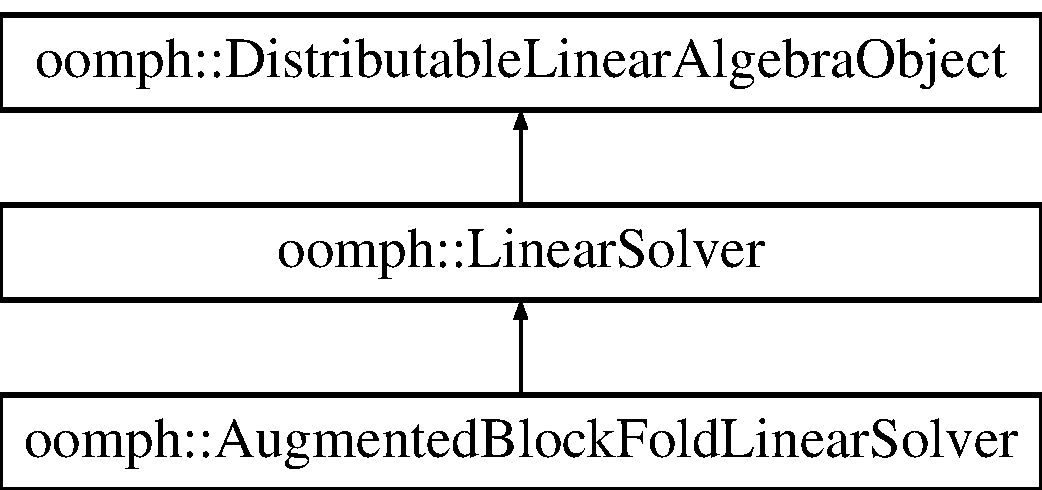
\includegraphics[height=3.000000cm]{classoomph_1_1AugmentedBlockFoldLinearSolver}
\end{center}
\end{figure}
\subsection*{Public Member Functions}
\begin{DoxyCompactItemize}
\item 
\hyperlink{classoomph_1_1AugmentedBlockFoldLinearSolver_a40e92987fc351227d16cb4c65c56988b}{Augmented\+Block\+Fold\+Linear\+Solver} (\hyperlink{classoomph_1_1LinearSolver}{Linear\+Solver} $\ast$const \hyperlink{classoomph_1_1AugmentedBlockFoldLinearSolver_a565f2b65d78f91ccac3fe2b03ac57dfc}{linear\+\_\+solver\+\_\+pt})
\begin{DoxyCompactList}\small\item\em Constructor, inherits the original linear solver. \end{DoxyCompactList}\item 
\hyperlink{classoomph_1_1AugmentedBlockFoldLinearSolver_adae26b8b348384e909bee9e57da6301d}{$\sim$\+Augmented\+Block\+Fold\+Linear\+Solver} ()
\begin{DoxyCompactList}\small\item\em Destructor\+: clean up the allocated memory. \end{DoxyCompactList}\item 
void \hyperlink{classoomph_1_1AugmentedBlockFoldLinearSolver_a11690b33089e999d0c894b4e4b0646d9}{solve} (\hyperlink{classoomph_1_1Problem}{Problem} $\ast$const \&problem\+\_\+pt, \hyperlink{classoomph_1_1DoubleVector}{Double\+Vector} \&result)
\begin{DoxyCompactList}\small\item\em The solve function uses the block factorisation. \end{DoxyCompactList}\item 
void \hyperlink{classoomph_1_1AugmentedBlockFoldLinearSolver_afdea4d6668393ad1cccc810b81fdc957}{solve} (\hyperlink{classoomph_1_1DoubleMatrixBase}{Double\+Matrix\+Base} $\ast$const \&matrix\+\_\+pt, const \hyperlink{classoomph_1_1DoubleVector}{Double\+Vector} \&rhs, \hyperlink{classoomph_1_1DoubleVector}{Double\+Vector} \&result)
\begin{DoxyCompactList}\small\item\em The linear-\/algebra-\/type solver does not make sense. The interface is deliberately broken. \end{DoxyCompactList}\item 
void \hyperlink{classoomph_1_1AugmentedBlockFoldLinearSolver_ae7f5f1459fef68479b39f0d1a1dce243}{solve} (\hyperlink{classoomph_1_1DoubleMatrixBase}{Double\+Matrix\+Base} $\ast$const \&matrix\+\_\+pt, const \hyperlink{classoomph_1_1Vector}{Vector}$<$ double $>$ \&rhs, \hyperlink{classoomph_1_1Vector}{Vector}$<$ double $>$ \&result)
\begin{DoxyCompactList}\small\item\em The linear-\/algebra-\/type solver does not make sense. The interface is deliberately broken. \end{DoxyCompactList}\item 
void \hyperlink{classoomph_1_1AugmentedBlockFoldLinearSolver_a7728fc74802b6802ed966765bc1e62d9}{resolve} (const \hyperlink{classoomph_1_1DoubleVector}{Double\+Vector} \&rhs, \hyperlink{classoomph_1_1DoubleVector}{Double\+Vector} \&result)
\begin{DoxyCompactList}\small\item\em The resolve function also uses the block factorisation. \end{DoxyCompactList}\item 
\hyperlink{classoomph_1_1LinearSolver}{Linear\+Solver} $\ast$ \hyperlink{classoomph_1_1AugmentedBlockFoldLinearSolver_a565f2b65d78f91ccac3fe2b03ac57dfc}{linear\+\_\+solver\+\_\+pt} () const
\begin{DoxyCompactList}\small\item\em Access function to the original linear solver. \end{DoxyCompactList}\end{DoxyCompactItemize}
\subsection*{Private Attributes}
\begin{DoxyCompactItemize}
\item 
\hyperlink{classoomph_1_1LinearSolver}{Linear\+Solver} $\ast$ \hyperlink{classoomph_1_1AugmentedBlockFoldLinearSolver_a1e8706ee6a97424bcbaf1992a09549ee}{Linear\+\_\+solver\+\_\+pt}
\begin{DoxyCompactList}\small\item\em Pointer to the original linear solver. \end{DoxyCompactList}\item 
\hyperlink{classoomph_1_1Problem}{Problem} $\ast$ \hyperlink{classoomph_1_1AugmentedBlockFoldLinearSolver_a65a5a2a87943d506cf4afc5cdbcfc06f}{Problem\+\_\+pt}
\item 
\hyperlink{classoomph_1_1DoubleVector}{Double\+Vector} $\ast$ \hyperlink{classoomph_1_1AugmentedBlockFoldLinearSolver_ae4f2e27925a6ceef247bac84f49fdb90}{Alpha\+\_\+pt}
\begin{DoxyCompactList}\small\item\em Pointer to the storage for the vector alpha. \end{DoxyCompactList}\item 
\hyperlink{classoomph_1_1DoubleVector}{Double\+Vector} $\ast$ \hyperlink{classoomph_1_1AugmentedBlockFoldLinearSolver_a6793e6c00a07d6a037f12b78c7d32182}{E\+\_\+pt}
\begin{DoxyCompactList}\small\item\em Pointer to the storage for the vector e. \end{DoxyCompactList}\end{DoxyCompactItemize}
\subsection*{Additional Inherited Members}


\subsection{Detailed Description}
A custom linear solver class that is used to solve a block-\/factorised version of the Fold bifurcation detection problem. 

Definition at line 388 of file assembly\+\_\+handler.\+h.



\subsection{Constructor \& Destructor Documentation}
\mbox{\Hypertarget{classoomph_1_1AugmentedBlockFoldLinearSolver_a40e92987fc351227d16cb4c65c56988b}\label{classoomph_1_1AugmentedBlockFoldLinearSolver_a40e92987fc351227d16cb4c65c56988b}} 
\index{oomph\+::\+Augmented\+Block\+Fold\+Linear\+Solver@{oomph\+::\+Augmented\+Block\+Fold\+Linear\+Solver}!Augmented\+Block\+Fold\+Linear\+Solver@{Augmented\+Block\+Fold\+Linear\+Solver}}
\index{Augmented\+Block\+Fold\+Linear\+Solver@{Augmented\+Block\+Fold\+Linear\+Solver}!oomph\+::\+Augmented\+Block\+Fold\+Linear\+Solver@{oomph\+::\+Augmented\+Block\+Fold\+Linear\+Solver}}
\subsubsection{\texorpdfstring{Augmented\+Block\+Fold\+Linear\+Solver()}{AugmentedBlockFoldLinearSolver()}}
{\footnotesize\ttfamily oomph\+::\+Augmented\+Block\+Fold\+Linear\+Solver\+::\+Augmented\+Block\+Fold\+Linear\+Solver (\begin{DoxyParamCaption}\item[{\hyperlink{classoomph_1_1LinearSolver}{Linear\+Solver} $\ast$const}]{linear\+\_\+solver\+\_\+pt }\end{DoxyParamCaption})\hspace{0.3cm}{\ttfamily [inline]}}



Constructor, inherits the original linear solver. 



Definition at line 405 of file assembly\+\_\+handler.\+h.

\mbox{\Hypertarget{classoomph_1_1AugmentedBlockFoldLinearSolver_adae26b8b348384e909bee9e57da6301d}\label{classoomph_1_1AugmentedBlockFoldLinearSolver_adae26b8b348384e909bee9e57da6301d}} 
\index{oomph\+::\+Augmented\+Block\+Fold\+Linear\+Solver@{oomph\+::\+Augmented\+Block\+Fold\+Linear\+Solver}!````~Augmented\+Block\+Fold\+Linear\+Solver@{$\sim$\+Augmented\+Block\+Fold\+Linear\+Solver}}
\index{````~Augmented\+Block\+Fold\+Linear\+Solver@{$\sim$\+Augmented\+Block\+Fold\+Linear\+Solver}!oomph\+::\+Augmented\+Block\+Fold\+Linear\+Solver@{oomph\+::\+Augmented\+Block\+Fold\+Linear\+Solver}}
\subsubsection{\texorpdfstring{$\sim$\+Augmented\+Block\+Fold\+Linear\+Solver()}{~AugmentedBlockFoldLinearSolver()}}
{\footnotesize\ttfamily oomph\+::\+Augmented\+Block\+Fold\+Linear\+Solver\+::$\sim$\+Augmented\+Block\+Fold\+Linear\+Solver (\begin{DoxyParamCaption}{ }\end{DoxyParamCaption})}



Destructor\+: clean up the allocated memory. 

Clean up the memory that may have been allocated by the solver. 

Definition at line 377 of file assembly\+\_\+handler.\+cc.



\subsection{Member Function Documentation}
\mbox{\Hypertarget{classoomph_1_1AugmentedBlockFoldLinearSolver_a565f2b65d78f91ccac3fe2b03ac57dfc}\label{classoomph_1_1AugmentedBlockFoldLinearSolver_a565f2b65d78f91ccac3fe2b03ac57dfc}} 
\index{oomph\+::\+Augmented\+Block\+Fold\+Linear\+Solver@{oomph\+::\+Augmented\+Block\+Fold\+Linear\+Solver}!linear\+\_\+solver\+\_\+pt@{linear\+\_\+solver\+\_\+pt}}
\index{linear\+\_\+solver\+\_\+pt@{linear\+\_\+solver\+\_\+pt}!oomph\+::\+Augmented\+Block\+Fold\+Linear\+Solver@{oomph\+::\+Augmented\+Block\+Fold\+Linear\+Solver}}
\subsubsection{\texorpdfstring{linear\+\_\+solver\+\_\+pt()}{linear\_solver\_pt()}}
{\footnotesize\ttfamily \hyperlink{classoomph_1_1LinearSolver}{Linear\+Solver}$\ast$ oomph\+::\+Augmented\+Block\+Fold\+Linear\+Solver\+::linear\+\_\+solver\+\_\+pt (\begin{DoxyParamCaption}{ }\end{DoxyParamCaption}) const\hspace{0.3cm}{\ttfamily [inline]}}



Access function to the original linear solver. 



Definition at line 442 of file assembly\+\_\+handler.\+h.



Referenced by oomph\+::\+Fold\+Handler\+::$\sim$\+Fold\+Handler().

\mbox{\Hypertarget{classoomph_1_1AugmentedBlockFoldLinearSolver_a7728fc74802b6802ed966765bc1e62d9}\label{classoomph_1_1AugmentedBlockFoldLinearSolver_a7728fc74802b6802ed966765bc1e62d9}} 
\index{oomph\+::\+Augmented\+Block\+Fold\+Linear\+Solver@{oomph\+::\+Augmented\+Block\+Fold\+Linear\+Solver}!resolve@{resolve}}
\index{resolve@{resolve}!oomph\+::\+Augmented\+Block\+Fold\+Linear\+Solver@{oomph\+::\+Augmented\+Block\+Fold\+Linear\+Solver}}
\subsubsection{\texorpdfstring{resolve()}{resolve()}}
{\footnotesize\ttfamily void oomph\+::\+Augmented\+Block\+Fold\+Linear\+Solver\+::resolve (\begin{DoxyParamCaption}\item[{const \hyperlink{classoomph_1_1DoubleVector}{Double\+Vector} \&}]{rhs,  }\item[{\hyperlink{classoomph_1_1DoubleVector}{Double\+Vector} \&}]{result }\end{DoxyParamCaption})\hspace{0.3cm}{\ttfamily [virtual]}}



The resolve function also uses the block factorisation. 



Reimplemented from \hyperlink{classoomph_1_1LinearSolver_a3b310d08333033edc119b2a5bd7dcbfb}{oomph\+::\+Linear\+Solver}.



Definition at line 638 of file assembly\+\_\+handler.\+cc.



References oomph\+::\+Problem\+::actions\+\_\+after\+\_\+change\+\_\+in\+\_\+bifurcation\+\_\+parameter(), oomph\+::\+Problem\+::assembly\+\_\+handler\+\_\+pt(), oomph\+::\+Double\+Vector\+::build(), oomph\+::\+Double\+Vector\+::built(), oomph\+::\+Distributable\+Linear\+Algebra\+Object\+::distributed(), oomph\+::\+Distributable\+Linear\+Algebra\+Object\+::distribution\+\_\+pt(), oomph\+::\+Problem\+::dof(), e, oomph\+::\+Mesh\+::element\+\_\+pt(), oomph\+::\+Assembly\+Handler\+::eqn\+\_\+number(), oomph\+::\+Fold\+Handler\+::eqn\+\_\+number(), oomph\+::\+Black\+Box\+F\+D\+Newton\+Solver\+::\+F\+D\+\_\+step, oomph\+::\+Fold\+Handler\+::get\+\_\+jacobian(), oomph\+::\+Problem\+::mesh\+\_\+pt(), oomph\+::\+Fold\+Handler\+::ndof(), oomph\+::\+Problem\+::ndof(), oomph\+::\+Mesh\+::nelement(), oomph\+::\+Fold\+Handler\+::solve\+\_\+augmented\+\_\+block\+\_\+system(), oomph\+::\+Fold\+Handler\+::solve\+\_\+full\+\_\+system(), and oomph\+::\+Fold\+Handler\+::Y.

\mbox{\Hypertarget{classoomph_1_1AugmentedBlockFoldLinearSolver_a11690b33089e999d0c894b4e4b0646d9}\label{classoomph_1_1AugmentedBlockFoldLinearSolver_a11690b33089e999d0c894b4e4b0646d9}} 
\index{oomph\+::\+Augmented\+Block\+Fold\+Linear\+Solver@{oomph\+::\+Augmented\+Block\+Fold\+Linear\+Solver}!solve@{solve}}
\index{solve@{solve}!oomph\+::\+Augmented\+Block\+Fold\+Linear\+Solver@{oomph\+::\+Augmented\+Block\+Fold\+Linear\+Solver}}
\subsubsection{\texorpdfstring{solve()}{solve()}\hspace{0.1cm}{\footnotesize\ttfamily [1/3]}}
{\footnotesize\ttfamily void oomph\+::\+Augmented\+Block\+Fold\+Linear\+Solver\+::solve (\begin{DoxyParamCaption}\item[{\hyperlink{classoomph_1_1Problem}{Problem} $\ast$const \&}]{problem\+\_\+pt,  }\item[{\hyperlink{classoomph_1_1DoubleVector}{Double\+Vector} \&}]{result }\end{DoxyParamCaption})\hspace{0.3cm}{\ttfamily [virtual]}}



The solve function uses the block factorisation. 

Use a block factorisation to solve the augmented system associated with a Pitch\+Fork bifurcation. 

Implements \hyperlink{classoomph_1_1LinearSolver_a15ce22542b74ed1826ea485edacbeb6e}{oomph\+::\+Linear\+Solver}.



Definition at line 387 of file assembly\+\_\+handler.\+cc.



References oomph\+::\+Problem\+::actions\+\_\+after\+\_\+change\+\_\+in\+\_\+bifurcation\+\_\+parameter(), oomph\+::\+Problem\+::assembly\+\_\+handler\+\_\+pt(), oomph\+::\+Double\+Vector\+::build(), oomph\+::\+Double\+Vector\+::built(), oomph\+::\+Problem\+::communicator\+\_\+pt(), oomph\+::\+Distributable\+Linear\+Algebra\+Object\+::distributed(), oomph\+::\+Problem\+::dof(), e, oomph\+::\+Mesh\+::element\+\_\+pt(), oomph\+::\+Assembly\+Handler\+::eqn\+\_\+number(), oomph\+::\+Fold\+Handler\+::eqn\+\_\+number(), oomph\+::\+Generalised\+Element\+::eqn\+\_\+number(), oomph\+::\+Black\+Box\+F\+D\+Newton\+Solver\+::\+F\+D\+\_\+step, oomph\+::\+Fold\+Handler\+::get\+\_\+jacobian(), oomph\+::\+Generalised\+Element\+::get\+\_\+jacobian(), oomph\+::\+Problem\+::mesh\+\_\+pt(), oomph\+::\+Fold\+Handler\+::ndof(), oomph\+::\+Generalised\+Element\+::ndof(), oomph\+::\+Problem\+::ndof(), oomph\+::\+Mesh\+::nelement(), oomph\+::\+Problem\+::sign\+\_\+of\+\_\+jacobian(), oomph\+::\+Fold\+Handler\+::solve\+\_\+augmented\+\_\+block\+\_\+system(), oomph\+::\+Fold\+Handler\+::solve\+\_\+full\+\_\+system(), and oomph\+::\+Fold\+Handler\+::Y.

\mbox{\Hypertarget{classoomph_1_1AugmentedBlockFoldLinearSolver_afdea4d6668393ad1cccc810b81fdc957}\label{classoomph_1_1AugmentedBlockFoldLinearSolver_afdea4d6668393ad1cccc810b81fdc957}} 
\index{oomph\+::\+Augmented\+Block\+Fold\+Linear\+Solver@{oomph\+::\+Augmented\+Block\+Fold\+Linear\+Solver}!solve@{solve}}
\index{solve@{solve}!oomph\+::\+Augmented\+Block\+Fold\+Linear\+Solver@{oomph\+::\+Augmented\+Block\+Fold\+Linear\+Solver}}
\subsubsection{\texorpdfstring{solve()}{solve()}\hspace{0.1cm}{\footnotesize\ttfamily [2/3]}}
{\footnotesize\ttfamily void oomph\+::\+Augmented\+Block\+Fold\+Linear\+Solver\+::solve (\begin{DoxyParamCaption}\item[{\hyperlink{classoomph_1_1DoubleMatrixBase}{Double\+Matrix\+Base} $\ast$const \&}]{matrix\+\_\+pt,  }\item[{const \hyperlink{classoomph_1_1DoubleVector}{Double\+Vector} \&}]{rhs,  }\item[{\hyperlink{classoomph_1_1DoubleVector}{Double\+Vector} \&}]{result }\end{DoxyParamCaption})\hspace{0.3cm}{\ttfamily [inline]}, {\ttfamily [virtual]}}



The linear-\/algebra-\/type solver does not make sense. The interface is deliberately broken. 



Reimplemented from \hyperlink{classoomph_1_1LinearSolver_a546c09822d18191df14caed864c04c09}{oomph\+::\+Linear\+Solver}.



Definition at line 416 of file assembly\+\_\+handler.\+h.

\mbox{\Hypertarget{classoomph_1_1AugmentedBlockFoldLinearSolver_ae7f5f1459fef68479b39f0d1a1dce243}\label{classoomph_1_1AugmentedBlockFoldLinearSolver_ae7f5f1459fef68479b39f0d1a1dce243}} 
\index{oomph\+::\+Augmented\+Block\+Fold\+Linear\+Solver@{oomph\+::\+Augmented\+Block\+Fold\+Linear\+Solver}!solve@{solve}}
\index{solve@{solve}!oomph\+::\+Augmented\+Block\+Fold\+Linear\+Solver@{oomph\+::\+Augmented\+Block\+Fold\+Linear\+Solver}}
\subsubsection{\texorpdfstring{solve()}{solve()}\hspace{0.1cm}{\footnotesize\ttfamily [3/3]}}
{\footnotesize\ttfamily void oomph\+::\+Augmented\+Block\+Fold\+Linear\+Solver\+::solve (\begin{DoxyParamCaption}\item[{\hyperlink{classoomph_1_1DoubleMatrixBase}{Double\+Matrix\+Base} $\ast$const \&}]{matrix\+\_\+pt,  }\item[{const \hyperlink{classoomph_1_1Vector}{Vector}$<$ double $>$ \&}]{rhs,  }\item[{\hyperlink{classoomph_1_1Vector}{Vector}$<$ double $>$ \&}]{result }\end{DoxyParamCaption})\hspace{0.3cm}{\ttfamily [inline]}, {\ttfamily [virtual]}}



The linear-\/algebra-\/type solver does not make sense. The interface is deliberately broken. 



Reimplemented from \hyperlink{classoomph_1_1LinearSolver_a1f7a2ee2cd18d3dafc20a61ca2f52dbb}{oomph\+::\+Linear\+Solver}.



Definition at line 428 of file assembly\+\_\+handler.\+h.



\subsection{Member Data Documentation}
\mbox{\Hypertarget{classoomph_1_1AugmentedBlockFoldLinearSolver_ae4f2e27925a6ceef247bac84f49fdb90}\label{classoomph_1_1AugmentedBlockFoldLinearSolver_ae4f2e27925a6ceef247bac84f49fdb90}} 
\index{oomph\+::\+Augmented\+Block\+Fold\+Linear\+Solver@{oomph\+::\+Augmented\+Block\+Fold\+Linear\+Solver}!Alpha\+\_\+pt@{Alpha\+\_\+pt}}
\index{Alpha\+\_\+pt@{Alpha\+\_\+pt}!oomph\+::\+Augmented\+Block\+Fold\+Linear\+Solver@{oomph\+::\+Augmented\+Block\+Fold\+Linear\+Solver}}
\subsubsection{\texorpdfstring{Alpha\+\_\+pt}{Alpha\_pt}}
{\footnotesize\ttfamily \hyperlink{classoomph_1_1DoubleVector}{Double\+Vector}$\ast$ oomph\+::\+Augmented\+Block\+Fold\+Linear\+Solver\+::\+Alpha\+\_\+pt\hspace{0.3cm}{\ttfamily [private]}}



Pointer to the storage for the vector alpha. 



Definition at line 397 of file assembly\+\_\+handler.\+h.

\mbox{\Hypertarget{classoomph_1_1AugmentedBlockFoldLinearSolver_a6793e6c00a07d6a037f12b78c7d32182}\label{classoomph_1_1AugmentedBlockFoldLinearSolver_a6793e6c00a07d6a037f12b78c7d32182}} 
\index{oomph\+::\+Augmented\+Block\+Fold\+Linear\+Solver@{oomph\+::\+Augmented\+Block\+Fold\+Linear\+Solver}!E\+\_\+pt@{E\+\_\+pt}}
\index{E\+\_\+pt@{E\+\_\+pt}!oomph\+::\+Augmented\+Block\+Fold\+Linear\+Solver@{oomph\+::\+Augmented\+Block\+Fold\+Linear\+Solver}}
\subsubsection{\texorpdfstring{E\+\_\+pt}{E\_pt}}
{\footnotesize\ttfamily \hyperlink{classoomph_1_1DoubleVector}{Double\+Vector}$\ast$ oomph\+::\+Augmented\+Block\+Fold\+Linear\+Solver\+::\+E\+\_\+pt\hspace{0.3cm}{\ttfamily [private]}}



Pointer to the storage for the vector e. 



Definition at line 400 of file assembly\+\_\+handler.\+h.

\mbox{\Hypertarget{classoomph_1_1AugmentedBlockFoldLinearSolver_a1e8706ee6a97424bcbaf1992a09549ee}\label{classoomph_1_1AugmentedBlockFoldLinearSolver_a1e8706ee6a97424bcbaf1992a09549ee}} 
\index{oomph\+::\+Augmented\+Block\+Fold\+Linear\+Solver@{oomph\+::\+Augmented\+Block\+Fold\+Linear\+Solver}!Linear\+\_\+solver\+\_\+pt@{Linear\+\_\+solver\+\_\+pt}}
\index{Linear\+\_\+solver\+\_\+pt@{Linear\+\_\+solver\+\_\+pt}!oomph\+::\+Augmented\+Block\+Fold\+Linear\+Solver@{oomph\+::\+Augmented\+Block\+Fold\+Linear\+Solver}}
\subsubsection{\texorpdfstring{Linear\+\_\+solver\+\_\+pt}{Linear\_solver\_pt}}
{\footnotesize\ttfamily \hyperlink{classoomph_1_1LinearSolver}{Linear\+Solver}$\ast$ oomph\+::\+Augmented\+Block\+Fold\+Linear\+Solver\+::\+Linear\+\_\+solver\+\_\+pt\hspace{0.3cm}{\ttfamily [private]}}



Pointer to the original linear solver. 



Definition at line 391 of file assembly\+\_\+handler.\+h.

\mbox{\Hypertarget{classoomph_1_1AugmentedBlockFoldLinearSolver_a65a5a2a87943d506cf4afc5cdbcfc06f}\label{classoomph_1_1AugmentedBlockFoldLinearSolver_a65a5a2a87943d506cf4afc5cdbcfc06f}} 
\index{oomph\+::\+Augmented\+Block\+Fold\+Linear\+Solver@{oomph\+::\+Augmented\+Block\+Fold\+Linear\+Solver}!Problem\+\_\+pt@{Problem\+\_\+pt}}
\index{Problem\+\_\+pt@{Problem\+\_\+pt}!oomph\+::\+Augmented\+Block\+Fold\+Linear\+Solver@{oomph\+::\+Augmented\+Block\+Fold\+Linear\+Solver}}
\subsubsection{\texorpdfstring{Problem\+\_\+pt}{Problem\_pt}}
{\footnotesize\ttfamily \hyperlink{classoomph_1_1Problem}{Problem}$\ast$ oomph\+::\+Augmented\+Block\+Fold\+Linear\+Solver\+::\+Problem\+\_\+pt\hspace{0.3cm}{\ttfamily [private]}}



Definition at line 394 of file assembly\+\_\+handler.\+h.



The documentation for this class was generated from the following files\+:\begin{DoxyCompactItemize}
\item 
\hyperlink{assembly__handler_8h}{assembly\+\_\+handler.\+h}\item 
\hyperlink{assembly__handler_8cc}{assembly\+\_\+handler.\+cc}\end{DoxyCompactItemize}

\hypertarget{classoomph_1_1AugmentedBlockPitchForkLinearSolver}{}\section{oomph\+:\+:Augmented\+Block\+Pitch\+Fork\+Linear\+Solver Class Reference}
\label{classoomph_1_1AugmentedBlockPitchForkLinearSolver}\index{oomph\+::\+Augmented\+Block\+Pitch\+Fork\+Linear\+Solver@{oomph\+::\+Augmented\+Block\+Pitch\+Fork\+Linear\+Solver}}


{\ttfamily \#include $<$assembly\+\_\+handler.\+h$>$}

Inheritance diagram for oomph\+:\+:Augmented\+Block\+Pitch\+Fork\+Linear\+Solver\+:\begin{figure}[H]
\begin{center}
\leavevmode
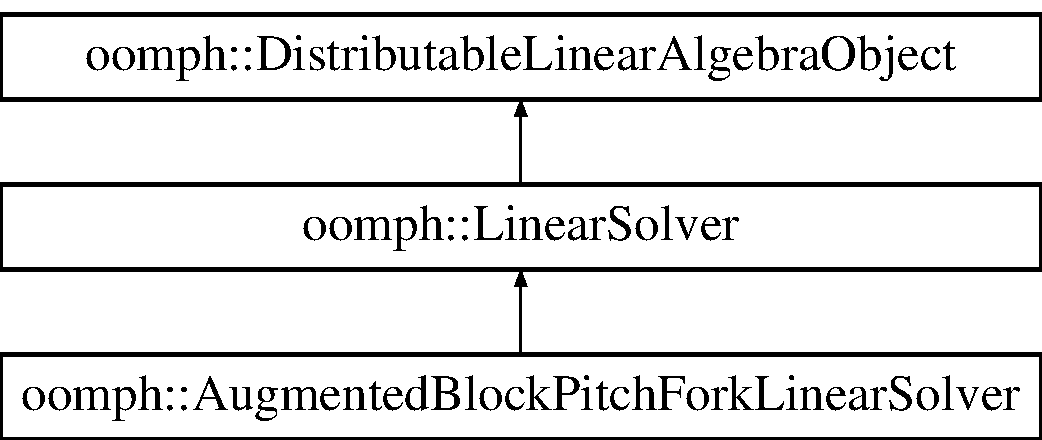
\includegraphics[height=3.000000cm]{classoomph_1_1AugmentedBlockPitchForkLinearSolver}
\end{center}
\end{figure}
\subsection*{Public Member Functions}
\begin{DoxyCompactItemize}
\item 
\hyperlink{classoomph_1_1AugmentedBlockPitchForkLinearSolver_a50d533e694ceb1c5a7f2edb10710f98a}{Augmented\+Block\+Pitch\+Fork\+Linear\+Solver} (\hyperlink{classoomph_1_1LinearSolver}{Linear\+Solver} $\ast$const \hyperlink{classoomph_1_1AugmentedBlockPitchForkLinearSolver_a96ac14c60f20314f5be075a68a620b3f}{linear\+\_\+solver\+\_\+pt})
\begin{DoxyCompactList}\small\item\em Constructor, inherits the original linear solver. \end{DoxyCompactList}\item 
\hyperlink{classoomph_1_1AugmentedBlockPitchForkLinearSolver_ab2d75883791a469b2ce32295ed39ab7d}{$\sim$\+Augmented\+Block\+Pitch\+Fork\+Linear\+Solver} ()
\begin{DoxyCompactList}\small\item\em Destructor\+: clean up the allocated memory. \end{DoxyCompactList}\item 
void \hyperlink{classoomph_1_1AugmentedBlockPitchForkLinearSolver_a0cbeb150ac83d5be1a1e30c0f728a70b}{solve} (\hyperlink{classoomph_1_1Problem}{Problem} $\ast$const \&problem\+\_\+pt, \hyperlink{classoomph_1_1DoubleVector}{Double\+Vector} \&result)
\begin{DoxyCompactList}\small\item\em The solve function uses the block factorisation. \end{DoxyCompactList}\item 
void \hyperlink{classoomph_1_1AugmentedBlockPitchForkLinearSolver_a495eeac9b790841fb0b8b1d1c8222667}{solve} (\hyperlink{classoomph_1_1DoubleMatrixBase}{Double\+Matrix\+Base} $\ast$const \&matrix\+\_\+pt, const \hyperlink{classoomph_1_1DoubleVector}{Double\+Vector} \&rhs, \hyperlink{classoomph_1_1DoubleVector}{Double\+Vector} \&result)
\begin{DoxyCompactList}\small\item\em The linear-\/algebra-\/type solver does not make sense. \end{DoxyCompactList}\item 
void \hyperlink{classoomph_1_1AugmentedBlockPitchForkLinearSolver_a8569368b8772d6642a50fb1279f4b61f}{solve} (\hyperlink{classoomph_1_1DoubleMatrixBase}{Double\+Matrix\+Base} $\ast$const \&matrix\+\_\+pt, const \hyperlink{classoomph_1_1Vector}{Vector}$<$ double $>$ \&rhs, \hyperlink{classoomph_1_1Vector}{Vector}$<$ double $>$ \&result)
\begin{DoxyCompactList}\small\item\em The linear-\/algebra-\/type solver does not make sense. The interface is deliberately broken. \end{DoxyCompactList}\item 
void \hyperlink{classoomph_1_1AugmentedBlockPitchForkLinearSolver_a1d617896a3f1c1b1236ff18dc87ed8d7}{resolve} (const \hyperlink{classoomph_1_1DoubleVector}{Double\+Vector} \&rhs, \hyperlink{classoomph_1_1DoubleVector}{Double\+Vector} \&result)
\begin{DoxyCompactList}\small\item\em The resolve function also uses the block factorisation. \end{DoxyCompactList}\item 
\hyperlink{classoomph_1_1LinearSolver}{Linear\+Solver} $\ast$ \hyperlink{classoomph_1_1AugmentedBlockPitchForkLinearSolver_a96ac14c60f20314f5be075a68a620b3f}{linear\+\_\+solver\+\_\+pt} () const
\begin{DoxyCompactList}\small\item\em Access function to the original linear solver. \end{DoxyCompactList}\end{DoxyCompactItemize}
\subsection*{Private Attributes}
\begin{DoxyCompactItemize}
\item 
\hyperlink{classoomph_1_1LinearSolver}{Linear\+Solver} $\ast$ \hyperlink{classoomph_1_1AugmentedBlockPitchForkLinearSolver_a1a3e1949c94c04c3b4ec19f0b895f97c}{Linear\+\_\+solver\+\_\+pt}
\begin{DoxyCompactList}\small\item\em Pointer to the original linear solver. \end{DoxyCompactList}\item 
\hyperlink{classoomph_1_1Problem}{Problem} $\ast$ \hyperlink{classoomph_1_1AugmentedBlockPitchForkLinearSolver_ad9e72a0a848aebe2b107a56b45aa4552}{Problem\+\_\+pt}
\begin{DoxyCompactList}\small\item\em Pointer to the problem, used in the resolve. \end{DoxyCompactList}\item 
\hyperlink{classoomph_1_1DoubleVector}{Double\+Vector} $\ast$ \hyperlink{classoomph_1_1AugmentedBlockPitchForkLinearSolver_a37d6d7eb053d062cabc6688f7c8fe240}{Alpha\+\_\+pt}
\begin{DoxyCompactList}\small\item\em Pointer to the storage for the vector alpha. \end{DoxyCompactList}\item 
\hyperlink{classoomph_1_1DoubleVector}{Double\+Vector} $\ast$ \hyperlink{classoomph_1_1AugmentedBlockPitchForkLinearSolver_a478bca515ee961576f523b1b5152651f}{E\+\_\+pt}
\begin{DoxyCompactList}\small\item\em Pointer to the storage for the vector e. \end{DoxyCompactList}\end{DoxyCompactItemize}
\subsection*{Additional Inherited Members}


\subsection{Detailed Description}
A custom linear solver class that is used to solve a block-\/factorised version of the Pitch\+Fork bifurcation detection problem. 

Definition at line 665 of file assembly\+\_\+handler.\+h.



\subsection{Constructor \& Destructor Documentation}
\mbox{\Hypertarget{classoomph_1_1AugmentedBlockPitchForkLinearSolver_a50d533e694ceb1c5a7f2edb10710f98a}\label{classoomph_1_1AugmentedBlockPitchForkLinearSolver_a50d533e694ceb1c5a7f2edb10710f98a}} 
\index{oomph\+::\+Augmented\+Block\+Pitch\+Fork\+Linear\+Solver@{oomph\+::\+Augmented\+Block\+Pitch\+Fork\+Linear\+Solver}!Augmented\+Block\+Pitch\+Fork\+Linear\+Solver@{Augmented\+Block\+Pitch\+Fork\+Linear\+Solver}}
\index{Augmented\+Block\+Pitch\+Fork\+Linear\+Solver@{Augmented\+Block\+Pitch\+Fork\+Linear\+Solver}!oomph\+::\+Augmented\+Block\+Pitch\+Fork\+Linear\+Solver@{oomph\+::\+Augmented\+Block\+Pitch\+Fork\+Linear\+Solver}}
\subsubsection{\texorpdfstring{Augmented\+Block\+Pitch\+Fork\+Linear\+Solver()}{AugmentedBlockPitchForkLinearSolver()}}
{\footnotesize\ttfamily oomph\+::\+Augmented\+Block\+Pitch\+Fork\+Linear\+Solver\+::\+Augmented\+Block\+Pitch\+Fork\+Linear\+Solver (\begin{DoxyParamCaption}\item[{\hyperlink{classoomph_1_1LinearSolver}{Linear\+Solver} $\ast$const}]{linear\+\_\+solver\+\_\+pt }\end{DoxyParamCaption})\hspace{0.3cm}{\ttfamily [inline]}}



Constructor, inherits the original linear solver. 



Definition at line 682 of file assembly\+\_\+handler.\+h.

\mbox{\Hypertarget{classoomph_1_1AugmentedBlockPitchForkLinearSolver_ab2d75883791a469b2ce32295ed39ab7d}\label{classoomph_1_1AugmentedBlockPitchForkLinearSolver_ab2d75883791a469b2ce32295ed39ab7d}} 
\index{oomph\+::\+Augmented\+Block\+Pitch\+Fork\+Linear\+Solver@{oomph\+::\+Augmented\+Block\+Pitch\+Fork\+Linear\+Solver}!````~Augmented\+Block\+Pitch\+Fork\+Linear\+Solver@{$\sim$\+Augmented\+Block\+Pitch\+Fork\+Linear\+Solver}}
\index{````~Augmented\+Block\+Pitch\+Fork\+Linear\+Solver@{$\sim$\+Augmented\+Block\+Pitch\+Fork\+Linear\+Solver}!oomph\+::\+Augmented\+Block\+Pitch\+Fork\+Linear\+Solver@{oomph\+::\+Augmented\+Block\+Pitch\+Fork\+Linear\+Solver}}
\subsubsection{\texorpdfstring{$\sim$\+Augmented\+Block\+Pitch\+Fork\+Linear\+Solver()}{~AugmentedBlockPitchForkLinearSolver()}}
{\footnotesize\ttfamily oomph\+::\+Augmented\+Block\+Pitch\+Fork\+Linear\+Solver\+::$\sim$\+Augmented\+Block\+Pitch\+Fork\+Linear\+Solver (\begin{DoxyParamCaption}{ }\end{DoxyParamCaption})}



Destructor\+: clean up the allocated memory. 

Clean up the memory that may have been allocated by the solver. 

Definition at line 2154 of file assembly\+\_\+handler.\+cc.



\subsection{Member Function Documentation}
\mbox{\Hypertarget{classoomph_1_1AugmentedBlockPitchForkLinearSolver_a96ac14c60f20314f5be075a68a620b3f}\label{classoomph_1_1AugmentedBlockPitchForkLinearSolver_a96ac14c60f20314f5be075a68a620b3f}} 
\index{oomph\+::\+Augmented\+Block\+Pitch\+Fork\+Linear\+Solver@{oomph\+::\+Augmented\+Block\+Pitch\+Fork\+Linear\+Solver}!linear\+\_\+solver\+\_\+pt@{linear\+\_\+solver\+\_\+pt}}
\index{linear\+\_\+solver\+\_\+pt@{linear\+\_\+solver\+\_\+pt}!oomph\+::\+Augmented\+Block\+Pitch\+Fork\+Linear\+Solver@{oomph\+::\+Augmented\+Block\+Pitch\+Fork\+Linear\+Solver}}
\subsubsection{\texorpdfstring{linear\+\_\+solver\+\_\+pt()}{linear\_solver\_pt()}}
{\footnotesize\ttfamily \hyperlink{classoomph_1_1LinearSolver}{Linear\+Solver}$\ast$ oomph\+::\+Augmented\+Block\+Pitch\+Fork\+Linear\+Solver\+::linear\+\_\+solver\+\_\+pt (\begin{DoxyParamCaption}{ }\end{DoxyParamCaption}) const\hspace{0.3cm}{\ttfamily [inline]}}



Access function to the original linear solver. 



Definition at line 721 of file assembly\+\_\+handler.\+h.



Referenced by oomph\+::\+Pitch\+Fork\+Handler\+::$\sim$\+Pitch\+Fork\+Handler().

\mbox{\Hypertarget{classoomph_1_1AugmentedBlockPitchForkLinearSolver_a1d617896a3f1c1b1236ff18dc87ed8d7}\label{classoomph_1_1AugmentedBlockPitchForkLinearSolver_a1d617896a3f1c1b1236ff18dc87ed8d7}} 
\index{oomph\+::\+Augmented\+Block\+Pitch\+Fork\+Linear\+Solver@{oomph\+::\+Augmented\+Block\+Pitch\+Fork\+Linear\+Solver}!resolve@{resolve}}
\index{resolve@{resolve}!oomph\+::\+Augmented\+Block\+Pitch\+Fork\+Linear\+Solver@{oomph\+::\+Augmented\+Block\+Pitch\+Fork\+Linear\+Solver}}
\subsubsection{\texorpdfstring{resolve()}{resolve()}}
{\footnotesize\ttfamily void oomph\+::\+Augmented\+Block\+Pitch\+Fork\+Linear\+Solver\+::resolve (\begin{DoxyParamCaption}\item[{const \hyperlink{classoomph_1_1DoubleVector}{Double\+Vector} \&}]{rhs,  }\item[{\hyperlink{classoomph_1_1DoubleVector}{Double\+Vector} \&}]{result }\end{DoxyParamCaption})\hspace{0.3cm}{\ttfamily [virtual]}}



The resolve function also uses the block factorisation. 



Reimplemented from \hyperlink{classoomph_1_1LinearSolver_a3b310d08333033edc119b2a5bd7dcbfb}{oomph\+::\+Linear\+Solver}.



Definition at line 2380 of file assembly\+\_\+handler.\+cc.



References oomph\+::\+Problem\+::actions\+\_\+after\+\_\+change\+\_\+in\+\_\+bifurcation\+\_\+parameter(), oomph\+::\+Problem\+::assembly\+\_\+handler\+\_\+pt(), oomph\+::\+Double\+Vector\+::build(), oomph\+::\+Double\+Vector\+::built(), oomph\+::\+Problem\+::communicator\+\_\+pt(), oomph\+::\+Problem\+::dof(), e, oomph\+::\+Mesh\+::element\+\_\+pt(), oomph\+::\+Fold\+Handler\+::eqn\+\_\+number(), oomph\+::\+Pitch\+Fork\+Handler\+::eqn\+\_\+number(), oomph\+::\+Black\+Box\+F\+D\+Newton\+Solver\+::\+F\+D\+\_\+step, oomph\+::\+Pitch\+Fork\+Handler\+::get\+\_\+jacobian(), oomph\+::\+Problem\+::mesh\+\_\+pt(), oomph\+::\+Pitch\+Fork\+Handler\+::ndof(), oomph\+::\+Problem\+::ndof(), oomph\+::\+Mesh\+::nelement(), oomph\+::\+Fold\+Handler\+::\+Problem\+\_\+pt, oomph\+::\+Pitch\+Fork\+Handler\+::solve\+\_\+augmented\+\_\+block\+\_\+system(), oomph\+::\+Pitch\+Fork\+Handler\+::solve\+\_\+full\+\_\+system(), and oomph\+::\+Pitch\+Fork\+Handler\+::Y.

\mbox{\Hypertarget{classoomph_1_1AugmentedBlockPitchForkLinearSolver_a0cbeb150ac83d5be1a1e30c0f728a70b}\label{classoomph_1_1AugmentedBlockPitchForkLinearSolver_a0cbeb150ac83d5be1a1e30c0f728a70b}} 
\index{oomph\+::\+Augmented\+Block\+Pitch\+Fork\+Linear\+Solver@{oomph\+::\+Augmented\+Block\+Pitch\+Fork\+Linear\+Solver}!solve@{solve}}
\index{solve@{solve}!oomph\+::\+Augmented\+Block\+Pitch\+Fork\+Linear\+Solver@{oomph\+::\+Augmented\+Block\+Pitch\+Fork\+Linear\+Solver}}
\subsubsection{\texorpdfstring{solve()}{solve()}\hspace{0.1cm}{\footnotesize\ttfamily [1/3]}}
{\footnotesize\ttfamily void oomph\+::\+Augmented\+Block\+Pitch\+Fork\+Linear\+Solver\+::solve (\begin{DoxyParamCaption}\item[{\hyperlink{classoomph_1_1Problem}{Problem} $\ast$const \&}]{problem\+\_\+pt,  }\item[{\hyperlink{classoomph_1_1DoubleVector}{Double\+Vector} \&}]{result }\end{DoxyParamCaption})\hspace{0.3cm}{\ttfamily [virtual]}}



The solve function uses the block factorisation. 

Use a block factorisation to solve the augmented system associated with a Pitch\+Fork bifurcation. 

Implements \hyperlink{classoomph_1_1LinearSolver_a15ce22542b74ed1826ea485edacbeb6e}{oomph\+::\+Linear\+Solver}.



Definition at line 2164 of file assembly\+\_\+handler.\+cc.



References oomph\+::\+Problem\+::actions\+\_\+after\+\_\+change\+\_\+in\+\_\+bifurcation\+\_\+parameter(), oomph\+::\+Problem\+::assembly\+\_\+handler\+\_\+pt(), oomph\+::\+Double\+Vector\+::build(), oomph\+::\+Double\+Vector\+::built(), oomph\+::\+Problem\+::communicator\+\_\+pt(), oomph\+::\+Distributable\+Linear\+Algebra\+Object\+::distributed(), oomph\+::\+Problem\+::dof(), e, oomph\+::\+Mesh\+::element\+\_\+pt(), oomph\+::\+Fold\+Handler\+::eqn\+\_\+number(), oomph\+::\+Pitch\+Fork\+Handler\+::eqn\+\_\+number(), oomph\+::\+Black\+Box\+F\+D\+Newton\+Solver\+::\+F\+D\+\_\+step, oomph\+::\+Pitch\+Fork\+Handler\+::get\+\_\+jacobian(), oomph\+::\+Problem\+::mesh\+\_\+pt(), oomph\+::\+Pitch\+Fork\+Handler\+::ndof(), oomph\+::\+Problem\+::ndof(), oomph\+::\+Mesh\+::nelement(), oomph\+::\+Fold\+Handler\+::\+Problem\+\_\+pt, oomph\+::\+Pitch\+Fork\+Handler\+::\+Psi, oomph\+::\+Problem\+::sign\+\_\+of\+\_\+jacobian(), oomph\+::\+Pitch\+Fork\+Handler\+::solve\+\_\+augmented\+\_\+block\+\_\+system(), oomph\+::\+Pitch\+Fork\+Handler\+::solve\+\_\+full\+\_\+system(), and oomph\+::\+Pitch\+Fork\+Handler\+::Y.

\mbox{\Hypertarget{classoomph_1_1AugmentedBlockPitchForkLinearSolver_a495eeac9b790841fb0b8b1d1c8222667}\label{classoomph_1_1AugmentedBlockPitchForkLinearSolver_a495eeac9b790841fb0b8b1d1c8222667}} 
\index{oomph\+::\+Augmented\+Block\+Pitch\+Fork\+Linear\+Solver@{oomph\+::\+Augmented\+Block\+Pitch\+Fork\+Linear\+Solver}!solve@{solve}}
\index{solve@{solve}!oomph\+::\+Augmented\+Block\+Pitch\+Fork\+Linear\+Solver@{oomph\+::\+Augmented\+Block\+Pitch\+Fork\+Linear\+Solver}}
\subsubsection{\texorpdfstring{solve()}{solve()}\hspace{0.1cm}{\footnotesize\ttfamily [2/3]}}
{\footnotesize\ttfamily void oomph\+::\+Augmented\+Block\+Pitch\+Fork\+Linear\+Solver\+::solve (\begin{DoxyParamCaption}\item[{\hyperlink{classoomph_1_1DoubleMatrixBase}{Double\+Matrix\+Base} $\ast$const \&}]{matrix\+\_\+pt,  }\item[{const \hyperlink{classoomph_1_1DoubleVector}{Double\+Vector} \&}]{rhs,  }\item[{\hyperlink{classoomph_1_1DoubleVector}{Double\+Vector} \&}]{result }\end{DoxyParamCaption})\hspace{0.3cm}{\ttfamily [inline]}, {\ttfamily [virtual]}}



The linear-\/algebra-\/type solver does not make sense. 

The interface is deliberately broken 

Reimplemented from \hyperlink{classoomph_1_1LinearSolver_a546c09822d18191df14caed864c04c09}{oomph\+::\+Linear\+Solver}.



Definition at line 694 of file assembly\+\_\+handler.\+h.

\mbox{\Hypertarget{classoomph_1_1AugmentedBlockPitchForkLinearSolver_a8569368b8772d6642a50fb1279f4b61f}\label{classoomph_1_1AugmentedBlockPitchForkLinearSolver_a8569368b8772d6642a50fb1279f4b61f}} 
\index{oomph\+::\+Augmented\+Block\+Pitch\+Fork\+Linear\+Solver@{oomph\+::\+Augmented\+Block\+Pitch\+Fork\+Linear\+Solver}!solve@{solve}}
\index{solve@{solve}!oomph\+::\+Augmented\+Block\+Pitch\+Fork\+Linear\+Solver@{oomph\+::\+Augmented\+Block\+Pitch\+Fork\+Linear\+Solver}}
\subsubsection{\texorpdfstring{solve()}{solve()}\hspace{0.1cm}{\footnotesize\ttfamily [3/3]}}
{\footnotesize\ttfamily void oomph\+::\+Augmented\+Block\+Pitch\+Fork\+Linear\+Solver\+::solve (\begin{DoxyParamCaption}\item[{\hyperlink{classoomph_1_1DoubleMatrixBase}{Double\+Matrix\+Base} $\ast$const \&}]{matrix\+\_\+pt,  }\item[{const \hyperlink{classoomph_1_1Vector}{Vector}$<$ double $>$ \&}]{rhs,  }\item[{\hyperlink{classoomph_1_1Vector}{Vector}$<$ double $>$ \&}]{result }\end{DoxyParamCaption})\hspace{0.3cm}{\ttfamily [inline]}, {\ttfamily [virtual]}}



The linear-\/algebra-\/type solver does not make sense. The interface is deliberately broken. 



Reimplemented from \hyperlink{classoomph_1_1LinearSolver_a1f7a2ee2cd18d3dafc20a61ca2f52dbb}{oomph\+::\+Linear\+Solver}.



Definition at line 706 of file assembly\+\_\+handler.\+h.



\subsection{Member Data Documentation}
\mbox{\Hypertarget{classoomph_1_1AugmentedBlockPitchForkLinearSolver_a37d6d7eb053d062cabc6688f7c8fe240}\label{classoomph_1_1AugmentedBlockPitchForkLinearSolver_a37d6d7eb053d062cabc6688f7c8fe240}} 
\index{oomph\+::\+Augmented\+Block\+Pitch\+Fork\+Linear\+Solver@{oomph\+::\+Augmented\+Block\+Pitch\+Fork\+Linear\+Solver}!Alpha\+\_\+pt@{Alpha\+\_\+pt}}
\index{Alpha\+\_\+pt@{Alpha\+\_\+pt}!oomph\+::\+Augmented\+Block\+Pitch\+Fork\+Linear\+Solver@{oomph\+::\+Augmented\+Block\+Pitch\+Fork\+Linear\+Solver}}
\subsubsection{\texorpdfstring{Alpha\+\_\+pt}{Alpha\_pt}}
{\footnotesize\ttfamily \hyperlink{classoomph_1_1DoubleVector}{Double\+Vector}$\ast$ oomph\+::\+Augmented\+Block\+Pitch\+Fork\+Linear\+Solver\+::\+Alpha\+\_\+pt\hspace{0.3cm}{\ttfamily [private]}}



Pointer to the storage for the vector alpha. 



Definition at line 674 of file assembly\+\_\+handler.\+h.

\mbox{\Hypertarget{classoomph_1_1AugmentedBlockPitchForkLinearSolver_a478bca515ee961576f523b1b5152651f}\label{classoomph_1_1AugmentedBlockPitchForkLinearSolver_a478bca515ee961576f523b1b5152651f}} 
\index{oomph\+::\+Augmented\+Block\+Pitch\+Fork\+Linear\+Solver@{oomph\+::\+Augmented\+Block\+Pitch\+Fork\+Linear\+Solver}!E\+\_\+pt@{E\+\_\+pt}}
\index{E\+\_\+pt@{E\+\_\+pt}!oomph\+::\+Augmented\+Block\+Pitch\+Fork\+Linear\+Solver@{oomph\+::\+Augmented\+Block\+Pitch\+Fork\+Linear\+Solver}}
\subsubsection{\texorpdfstring{E\+\_\+pt}{E\_pt}}
{\footnotesize\ttfamily \hyperlink{classoomph_1_1DoubleVector}{Double\+Vector}$\ast$ oomph\+::\+Augmented\+Block\+Pitch\+Fork\+Linear\+Solver\+::\+E\+\_\+pt\hspace{0.3cm}{\ttfamily [private]}}



Pointer to the storage for the vector e. 



Definition at line 677 of file assembly\+\_\+handler.\+h.

\mbox{\Hypertarget{classoomph_1_1AugmentedBlockPitchForkLinearSolver_a1a3e1949c94c04c3b4ec19f0b895f97c}\label{classoomph_1_1AugmentedBlockPitchForkLinearSolver_a1a3e1949c94c04c3b4ec19f0b895f97c}} 
\index{oomph\+::\+Augmented\+Block\+Pitch\+Fork\+Linear\+Solver@{oomph\+::\+Augmented\+Block\+Pitch\+Fork\+Linear\+Solver}!Linear\+\_\+solver\+\_\+pt@{Linear\+\_\+solver\+\_\+pt}}
\index{Linear\+\_\+solver\+\_\+pt@{Linear\+\_\+solver\+\_\+pt}!oomph\+::\+Augmented\+Block\+Pitch\+Fork\+Linear\+Solver@{oomph\+::\+Augmented\+Block\+Pitch\+Fork\+Linear\+Solver}}
\subsubsection{\texorpdfstring{Linear\+\_\+solver\+\_\+pt}{Linear\_solver\_pt}}
{\footnotesize\ttfamily \hyperlink{classoomph_1_1LinearSolver}{Linear\+Solver}$\ast$ oomph\+::\+Augmented\+Block\+Pitch\+Fork\+Linear\+Solver\+::\+Linear\+\_\+solver\+\_\+pt\hspace{0.3cm}{\ttfamily [private]}}



Pointer to the original linear solver. 



Definition at line 668 of file assembly\+\_\+handler.\+h.

\mbox{\Hypertarget{classoomph_1_1AugmentedBlockPitchForkLinearSolver_ad9e72a0a848aebe2b107a56b45aa4552}\label{classoomph_1_1AugmentedBlockPitchForkLinearSolver_ad9e72a0a848aebe2b107a56b45aa4552}} 
\index{oomph\+::\+Augmented\+Block\+Pitch\+Fork\+Linear\+Solver@{oomph\+::\+Augmented\+Block\+Pitch\+Fork\+Linear\+Solver}!Problem\+\_\+pt@{Problem\+\_\+pt}}
\index{Problem\+\_\+pt@{Problem\+\_\+pt}!oomph\+::\+Augmented\+Block\+Pitch\+Fork\+Linear\+Solver@{oomph\+::\+Augmented\+Block\+Pitch\+Fork\+Linear\+Solver}}
\subsubsection{\texorpdfstring{Problem\+\_\+pt}{Problem\_pt}}
{\footnotesize\ttfamily \hyperlink{classoomph_1_1Problem}{Problem}$\ast$ oomph\+::\+Augmented\+Block\+Pitch\+Fork\+Linear\+Solver\+::\+Problem\+\_\+pt\hspace{0.3cm}{\ttfamily [private]}}



Pointer to the problem, used in the resolve. 



Definition at line 671 of file assembly\+\_\+handler.\+h.



The documentation for this class was generated from the following files\+:\begin{DoxyCompactItemize}
\item 
\hyperlink{assembly__handler_8h}{assembly\+\_\+handler.\+h}\item 
\hyperlink{assembly__handler_8cc}{assembly\+\_\+handler.\+cc}\end{DoxyCompactItemize}

\hypertarget{classoomph_1_1AxisAlignedPMLElement}{}\section{oomph\+:\+:Axis\+Aligned\+P\+M\+L\+Element$<$ D\+IM $>$ Class Template Reference}
\label{classoomph_1_1AxisAlignedPMLElement}\index{oomph\+::\+Axis\+Aligned\+P\+M\+L\+Element$<$ D\+I\+M $>$@{oomph\+::\+Axis\+Aligned\+P\+M\+L\+Element$<$ D\+I\+M $>$}}


{\ttfamily \#include $<$pml\+\_\+elements.\+h$>$}

Inheritance diagram for oomph\+:\+:Axis\+Aligned\+P\+M\+L\+Element$<$ D\+IM $>$\+:\begin{figure}[H]
\begin{center}
\leavevmode
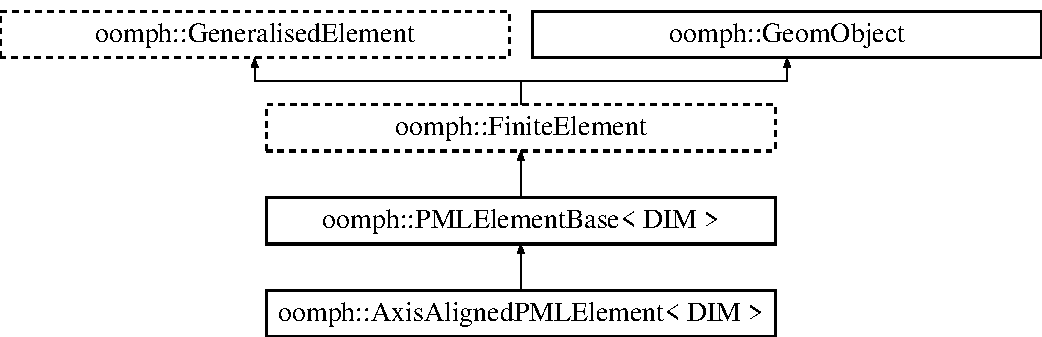
\includegraphics[height=4.000000cm]{classoomph_1_1AxisAlignedPMLElement}
\end{center}
\end{figure}
\subsection*{Public Member Functions}
\begin{DoxyCompactItemize}
\item 
\hyperlink{classoomph_1_1AxisAlignedPMLElement_acb3d0ce377bf928f0fa83deedef775f0}{Axis\+Aligned\+P\+M\+L\+Element} ()
\begin{DoxyCompactList}\small\item\em Constructor. \end{DoxyCompactList}\item 
virtual void \hyperlink{classoomph_1_1AxisAlignedPMLElement_af93221809a1b5deaabe7cd818e30d9c9}{pml\+\_\+transformation\+\_\+jacobian} (const unsigned \&ipt, const \hyperlink{classoomph_1_1Vector}{Vector}$<$ double $>$ \&\hyperlink{cfortran_8h_ab7123126e4885ef647dd9c6e3807a21c}{s}, const \hyperlink{classoomph_1_1Vector}{Vector}$<$ double $>$ \&x, \hyperlink{classoomph_1_1DiagonalComplexMatrix}{Diagonal\+Complex\+Matrix} \&jacobian)
\item 
virtual void \hyperlink{classoomph_1_1AxisAlignedPMLElement_a9fba3c6d10af49f64833ecfe97b730c5}{pml\+\_\+transformation\+\_\+jacobian} (const unsigned \&ipt, const \hyperlink{classoomph_1_1Vector}{Vector}$<$ double $>$ \&\hyperlink{cfortran_8h_ab7123126e4885ef647dd9c6e3807a21c}{s}, const \hyperlink{classoomph_1_1Vector}{Vector}$<$ double $>$ \&x, \hyperlink{classoomph_1_1DenseComplexMatrix}{Dense\+Complex\+Matrix} \&jacobian)
\item 
virtual void \hyperlink{classoomph_1_1AxisAlignedPMLElement_a6407fbc195aab8b5a3c3746df1f4aa63}{pml\+\_\+transformation\+\_\+jacobian} (const unsigned \&ipt, const \hyperlink{classoomph_1_1Vector}{Vector}$<$ double $>$ \&\hyperlink{cfortran_8h_ab7123126e4885ef647dd9c6e3807a21c}{s}, const \hyperlink{classoomph_1_1Vector}{Vector}$<$ double $>$ \&x, \hyperlink{classoomph_1_1DiagonalComplexMatrix}{Diagonal\+Complex\+Matrix} \&jacobian\+\_\+matrix, \hyperlink{classoomph_1_1Vector}{Vector}$<$ std\+::complex$<$ double $>$ $>$ \&transformed\+\_\+x)
\item 
virtual void \hyperlink{classoomph_1_1AxisAlignedPMLElement_a808e638b642342a84da6749cdcdf78e4}{pml\+\_\+transformation\+\_\+jacobian} (const unsigned \&ipt, const \hyperlink{classoomph_1_1Vector}{Vector}$<$ double $>$ \&\hyperlink{cfortran_8h_ab7123126e4885ef647dd9c6e3807a21c}{s}, const \hyperlink{classoomph_1_1Vector}{Vector}$<$ double $>$ \&x, \hyperlink{classoomph_1_1DenseComplexMatrix}{Dense\+Complex\+Matrix} \&jacobian\+\_\+matrix, \hyperlink{classoomph_1_1Vector}{Vector}$<$ std\+::complex$<$ double $>$ $>$ \&transformed\+\_\+x)
\item 
virtual void \hyperlink{classoomph_1_1AxisAlignedPMLElement_ace457b4782c083fd8b0925ae6b19a3e3}{disable\+\_\+pml} ()
\begin{DoxyCompactList}\small\item\em Disable pml. Ensures the P\+M\+L-\/ification in all directions has been deactivated. \end{DoxyCompactList}\item 
virtual void \hyperlink{classoomph_1_1AxisAlignedPMLElement_a76a879c7122fc2e5b723fbc7ce6b602b}{enable\+\_\+pml} (const int \&direction, const double \&pml\+\_\+inner\+\_\+boundary, const double \&pml\+\_\+outer\+\_\+boundary)
\begin{DoxyCompactList}\small\item\em Enable pml. Specify the coordinate direction along which pml boundary is constant, as well as the coordinate along the dimension for the interface between the physical and artificial domains and the coordinate for the outer boundary. All of these are used to adjust the perfectly matched layer mechanism. Needs to be called separately for each pml-\/ified direction (if needed -- e.\+g. in corner elements) \end{DoxyCompactList}\item 
virtual void \hyperlink{classoomph_1_1AxisAlignedPMLElement_a157cd9d30c5d1f86d17b4b25bc705f76}{enable\+\_\+pml} (const int \&direction, const double \&pml\+\_\+inner\+\_\+boundary, const double \&pml\+\_\+outer\+\_\+boundary, \hyperlink{classoomph_1_1UniaxialPMLMapping}{Uniaxial\+P\+M\+L\+Mapping} $\ast$\hyperlink{classoomph_1_1AxisAlignedPMLElement_adcb4bb14ff2f185cdfd31aa51b1f015d}{pml\+\_\+mapping\+\_\+pt})
\item 
\hyperlink{classoomph_1_1UniaxialPMLMapping}{Uniaxial\+P\+M\+L\+Mapping} $\ast$\& \hyperlink{classoomph_1_1AxisAlignedPMLElement_adcb4bb14ff2f185cdfd31aa51b1f015d}{pml\+\_\+mapping\+\_\+pt} ()
\begin{DoxyCompactList}\small\item\em Return a pointer to the P\+ML Mapping object. \end{DoxyCompactList}\item 
\hyperlink{classoomph_1_1UniaxialPMLMapping}{Uniaxial\+P\+M\+L\+Mapping} $\ast$const  \& \hyperlink{classoomph_1_1AxisAlignedPMLElement_ab67dd8501cbdeb896ff34d3cd8645434}{pml\+\_\+mapping\+\_\+pt} () const
\begin{DoxyCompactList}\small\item\em Return a pointer to the P\+ML Mapping object (const version) \end{DoxyCompactList}\item 
double \hyperlink{classoomph_1_1AxisAlignedPMLElement_a554c5768cdf2543b76a507dacd7fe54b}{nu} (const \hyperlink{classoomph_1_1Vector}{Vector}$<$ double $>$ \&x, const unsigned \&\hyperlink{cfortran_8h_adb50e893b86b3e55e751a42eab3cba82}{i}) const
\begin{DoxyCompactList}\small\item\em \hyperlink{classoomph_1_1Vector}{Vector} which points from the inner boundary to x. \end{DoxyCompactList}\item 
void \hyperlink{classoomph_1_1AxisAlignedPMLElement_ae278a54184e8134f57aa361bfc1cc975}{nu} (const \hyperlink{classoomph_1_1Vector}{Vector}$<$ double $>$ \&x, \hyperlink{classoomph_1_1Vector}{Vector}$<$ double $>$ nu\+\_\+vec) const
\begin{DoxyCompactList}\small\item\em \hyperlink{classoomph_1_1Vector}{Vector} which points from the inner boundary to x. \end{DoxyCompactList}\item 
double \hyperlink{classoomph_1_1AxisAlignedPMLElement_af5689e98392072da121eafa0b438e44c}{delta} (const unsigned \&\hyperlink{cfortran_8h_adb50e893b86b3e55e751a42eab3cba82}{i}) const
\begin{DoxyCompactList}\small\item\em \hyperlink{classoomph_1_1Vector}{Vector} which points from the inner boundary to x. \end{DoxyCompactList}\item 
void \hyperlink{classoomph_1_1AxisAlignedPMLElement_a37d292c06ab74db30dcb6e8f7cea4033}{delta} (const \hyperlink{classoomph_1_1Vector}{Vector}$<$ double $>$ \&x, \hyperlink{classoomph_1_1Vector}{Vector}$<$ double $>$ delta) const
\begin{DoxyCompactList}\small\item\em \hyperlink{classoomph_1_1Vector}{Vector} which points from the inner boundary to x. \end{DoxyCompactList}\end{DoxyCompactItemize}
\subsection*{Protected Attributes}
\begin{DoxyCompactItemize}
\item 
std\+::vector$<$ bool $>$ \hyperlink{classoomph_1_1AxisAlignedPMLElement_a6cc25fecc2e0f0b8a4920aae2e64964a}{Pml\+\_\+direction\+\_\+active}
\begin{DoxyCompactList}\small\item\em Coordinate direction along which pml boundary is constant; alternatively\+: coordinate direction in which coordinate stretching is performed. \end{DoxyCompactList}\item 
\hyperlink{classoomph_1_1Vector}{Vector}$<$ double $>$ \hyperlink{classoomph_1_1AxisAlignedPMLElement_adecf1b401aeab5399ce576c19667e455}{Pml\+\_\+inner\+\_\+boundary}
\begin{DoxyCompactList}\small\item\em Coordinate of inner pml boundary (Storage is provided for any coordinate direction; only the entries for \char`\"{}active\char`\"{} directions is used.) \end{DoxyCompactList}\item 
\hyperlink{classoomph_1_1Vector}{Vector}$<$ double $>$ \hyperlink{classoomph_1_1AxisAlignedPMLElement_aff04e9e225d24b9ce877204b7ae22921}{Pml\+\_\+outer\+\_\+boundary}
\begin{DoxyCompactList}\small\item\em Coordinate of outer pml boundary (Storage is provided for any coordinate direction; only the entries for \char`\"{}active\char`\"{} directions is used.) \end{DoxyCompactList}\item 
\hyperlink{classoomph_1_1UniaxialPMLMapping}{Uniaxial\+P\+M\+L\+Mapping} $\ast$ \hyperlink{classoomph_1_1AxisAlignedPMLElement_abb5b63cb5d08885239627640a74dd9d9}{Pml\+\_\+mapping\+\_\+pt}
\end{DoxyCompactItemize}
\subsection*{Additional Inherited Members}


\subsection{Detailed Description}
\subsubsection*{template$<$unsigned D\+IM$>$\newline
class oomph\+::\+Axis\+Aligned\+P\+M\+L\+Element$<$ D\+I\+M $>$}



Definition at line 160 of file pml\+\_\+elements.\+h.



\subsection{Constructor \& Destructor Documentation}
\mbox{\Hypertarget{classoomph_1_1AxisAlignedPMLElement_acb3d0ce377bf928f0fa83deedef775f0}\label{classoomph_1_1AxisAlignedPMLElement_acb3d0ce377bf928f0fa83deedef775f0}} 
\index{oomph\+::\+Axis\+Aligned\+P\+M\+L\+Element@{oomph\+::\+Axis\+Aligned\+P\+M\+L\+Element}!Axis\+Aligned\+P\+M\+L\+Element@{Axis\+Aligned\+P\+M\+L\+Element}}
\index{Axis\+Aligned\+P\+M\+L\+Element@{Axis\+Aligned\+P\+M\+L\+Element}!oomph\+::\+Axis\+Aligned\+P\+M\+L\+Element@{oomph\+::\+Axis\+Aligned\+P\+M\+L\+Element}}
\subsubsection{\texorpdfstring{Axis\+Aligned\+P\+M\+L\+Element()}{AxisAlignedPMLElement()}}
{\footnotesize\ttfamily template$<$unsigned D\+IM$>$ \\
\hyperlink{classoomph_1_1AxisAlignedPMLElement}{oomph\+::\+Axis\+Aligned\+P\+M\+L\+Element}$<$ D\+IM $>$\+::\hyperlink{classoomph_1_1AxisAlignedPMLElement}{Axis\+Aligned\+P\+M\+L\+Element} (\begin{DoxyParamCaption}{ }\end{DoxyParamCaption})\hspace{0.3cm}{\ttfamily [inline]}}



Constructor. 



Definition at line 165 of file pml\+\_\+elements.\+h.



References s.



\subsection{Member Function Documentation}
\mbox{\Hypertarget{classoomph_1_1AxisAlignedPMLElement_af5689e98392072da121eafa0b438e44c}\label{classoomph_1_1AxisAlignedPMLElement_af5689e98392072da121eafa0b438e44c}} 
\index{oomph\+::\+Axis\+Aligned\+P\+M\+L\+Element@{oomph\+::\+Axis\+Aligned\+P\+M\+L\+Element}!delta@{delta}}
\index{delta@{delta}!oomph\+::\+Axis\+Aligned\+P\+M\+L\+Element@{oomph\+::\+Axis\+Aligned\+P\+M\+L\+Element}}
\subsubsection{\texorpdfstring{delta()}{delta()}\hspace{0.1cm}{\footnotesize\ttfamily [1/2]}}
{\footnotesize\ttfamily template$<$unsigned D\+IM$>$ \\
double \hyperlink{classoomph_1_1AxisAlignedPMLElement}{oomph\+::\+Axis\+Aligned\+P\+M\+L\+Element}$<$ D\+IM $>$\+::delta (\begin{DoxyParamCaption}\item[{const unsigned \&}]{i }\end{DoxyParamCaption}) const\hspace{0.3cm}{\ttfamily [inline]}}



\hyperlink{classoomph_1_1Vector}{Vector} which points from the inner boundary to x. 



Definition at line 276 of file pml\+\_\+elements.\+h.



References i.

\mbox{\Hypertarget{classoomph_1_1AxisAlignedPMLElement_a37d292c06ab74db30dcb6e8f7cea4033}\label{classoomph_1_1AxisAlignedPMLElement_a37d292c06ab74db30dcb6e8f7cea4033}} 
\index{oomph\+::\+Axis\+Aligned\+P\+M\+L\+Element@{oomph\+::\+Axis\+Aligned\+P\+M\+L\+Element}!delta@{delta}}
\index{delta@{delta}!oomph\+::\+Axis\+Aligned\+P\+M\+L\+Element@{oomph\+::\+Axis\+Aligned\+P\+M\+L\+Element}}
\subsubsection{\texorpdfstring{delta()}{delta()}\hspace{0.1cm}{\footnotesize\ttfamily [2/2]}}
{\footnotesize\ttfamily template$<$unsigned D\+IM$>$ \\
void \hyperlink{classoomph_1_1AxisAlignedPMLElement}{oomph\+::\+Axis\+Aligned\+P\+M\+L\+Element}$<$ D\+IM $>$\+::delta (\begin{DoxyParamCaption}\item[{const \hyperlink{classoomph_1_1Vector}{Vector}$<$ double $>$ \&}]{x,  }\item[{\hyperlink{classoomph_1_1Vector}{Vector}$<$ double $>$}]{delta }\end{DoxyParamCaption}) const\hspace{0.3cm}{\ttfamily [inline]}}



\hyperlink{classoomph_1_1Vector}{Vector} which points from the inner boundary to x. 



Definition at line 282 of file pml\+\_\+elements.\+h.



References i.

\mbox{\Hypertarget{classoomph_1_1AxisAlignedPMLElement_ace457b4782c083fd8b0925ae6b19a3e3}\label{classoomph_1_1AxisAlignedPMLElement_ace457b4782c083fd8b0925ae6b19a3e3}} 
\index{oomph\+::\+Axis\+Aligned\+P\+M\+L\+Element@{oomph\+::\+Axis\+Aligned\+P\+M\+L\+Element}!disable\+\_\+pml@{disable\+\_\+pml}}
\index{disable\+\_\+pml@{disable\+\_\+pml}!oomph\+::\+Axis\+Aligned\+P\+M\+L\+Element@{oomph\+::\+Axis\+Aligned\+P\+M\+L\+Element}}
\subsubsection{\texorpdfstring{disable\+\_\+pml()}{disable\_pml()}}
{\footnotesize\ttfamily template$<$unsigned D\+IM$>$ \\
virtual void \hyperlink{classoomph_1_1AxisAlignedPMLElement}{oomph\+::\+Axis\+Aligned\+P\+M\+L\+Element}$<$ D\+IM $>$\+::disable\+\_\+pml (\begin{DoxyParamCaption}{ }\end{DoxyParamCaption})\hspace{0.3cm}{\ttfamily [inline]}, {\ttfamily [virtual]}}



Disable pml. Ensures the P\+M\+L-\/ification in all directions has been deactivated. 



Reimplemented from \hyperlink{classoomph_1_1PMLElementBase_a751943790221819c111da99455275bbc}{oomph\+::\+P\+M\+L\+Element\+Base$<$ D\+I\+M $>$}.



Definition at line 214 of file pml\+\_\+elements.\+h.



References oomph\+::\+P\+M\+L\+Element\+Base$<$ D\+I\+M $>$\+::disable\+\_\+pml().

\mbox{\Hypertarget{classoomph_1_1AxisAlignedPMLElement_a76a879c7122fc2e5b723fbc7ce6b602b}\label{classoomph_1_1AxisAlignedPMLElement_a76a879c7122fc2e5b723fbc7ce6b602b}} 
\index{oomph\+::\+Axis\+Aligned\+P\+M\+L\+Element@{oomph\+::\+Axis\+Aligned\+P\+M\+L\+Element}!enable\+\_\+pml@{enable\+\_\+pml}}
\index{enable\+\_\+pml@{enable\+\_\+pml}!oomph\+::\+Axis\+Aligned\+P\+M\+L\+Element@{oomph\+::\+Axis\+Aligned\+P\+M\+L\+Element}}
\subsubsection{\texorpdfstring{enable\+\_\+pml()}{enable\_pml()}\hspace{0.1cm}{\footnotesize\ttfamily [1/2]}}
{\footnotesize\ttfamily template$<$unsigned D\+IM$>$ \\
virtual void \hyperlink{classoomph_1_1AxisAlignedPMLElement}{oomph\+::\+Axis\+Aligned\+P\+M\+L\+Element}$<$ D\+IM $>$\+::enable\+\_\+pml (\begin{DoxyParamCaption}\item[{const int \&}]{direction,  }\item[{const double \&}]{pml\+\_\+inner\+\_\+boundary,  }\item[{const double \&}]{pml\+\_\+outer\+\_\+boundary }\end{DoxyParamCaption})\hspace{0.3cm}{\ttfamily [inline]}, {\ttfamily [virtual]}}



Enable pml. Specify the coordinate direction along which pml boundary is constant, as well as the coordinate along the dimension for the interface between the physical and artificial domains and the coordinate for the outer boundary. All of these are used to adjust the perfectly matched layer mechanism. Needs to be called separately for each pml-\/ified direction (if needed -- e.\+g. in corner elements) 



Definition at line 235 of file pml\+\_\+elements.\+h.



References oomph\+::\+P\+M\+L\+Element\+Base$<$ D\+I\+M $>$\+::enable\+\_\+pml().

\mbox{\Hypertarget{classoomph_1_1AxisAlignedPMLElement_a157cd9d30c5d1f86d17b4b25bc705f76}\label{classoomph_1_1AxisAlignedPMLElement_a157cd9d30c5d1f86d17b4b25bc705f76}} 
\index{oomph\+::\+Axis\+Aligned\+P\+M\+L\+Element@{oomph\+::\+Axis\+Aligned\+P\+M\+L\+Element}!enable\+\_\+pml@{enable\+\_\+pml}}
\index{enable\+\_\+pml@{enable\+\_\+pml}!oomph\+::\+Axis\+Aligned\+P\+M\+L\+Element@{oomph\+::\+Axis\+Aligned\+P\+M\+L\+Element}}
\subsubsection{\texorpdfstring{enable\+\_\+pml()}{enable\_pml()}\hspace{0.1cm}{\footnotesize\ttfamily [2/2]}}
{\footnotesize\ttfamily template$<$unsigned D\+IM$>$ \\
virtual void \hyperlink{classoomph_1_1AxisAlignedPMLElement}{oomph\+::\+Axis\+Aligned\+P\+M\+L\+Element}$<$ D\+IM $>$\+::enable\+\_\+pml (\begin{DoxyParamCaption}\item[{const int \&}]{direction,  }\item[{const double \&}]{pml\+\_\+inner\+\_\+boundary,  }\item[{const double \&}]{pml\+\_\+outer\+\_\+boundary,  }\item[{\hyperlink{classoomph_1_1UniaxialPMLMapping}{Uniaxial\+P\+M\+L\+Mapping} $\ast$}]{pml\+\_\+mapping\+\_\+pt }\end{DoxyParamCaption})\hspace{0.3cm}{\ttfamily [inline]}, {\ttfamily [virtual]}}



Definition at line 245 of file pml\+\_\+elements.\+h.

\mbox{\Hypertarget{classoomph_1_1AxisAlignedPMLElement_a554c5768cdf2543b76a507dacd7fe54b}\label{classoomph_1_1AxisAlignedPMLElement_a554c5768cdf2543b76a507dacd7fe54b}} 
\index{oomph\+::\+Axis\+Aligned\+P\+M\+L\+Element@{oomph\+::\+Axis\+Aligned\+P\+M\+L\+Element}!nu@{nu}}
\index{nu@{nu}!oomph\+::\+Axis\+Aligned\+P\+M\+L\+Element@{oomph\+::\+Axis\+Aligned\+P\+M\+L\+Element}}
\subsubsection{\texorpdfstring{nu()}{nu()}\hspace{0.1cm}{\footnotesize\ttfamily [1/2]}}
{\footnotesize\ttfamily template$<$unsigned D\+IM$>$ \\
double \hyperlink{classoomph_1_1AxisAlignedPMLElement}{oomph\+::\+Axis\+Aligned\+P\+M\+L\+Element}$<$ D\+IM $>$\+::nu (\begin{DoxyParamCaption}\item[{const \hyperlink{classoomph_1_1Vector}{Vector}$<$ double $>$ \&}]{x,  }\item[{const unsigned \&}]{i }\end{DoxyParamCaption}) const\hspace{0.3cm}{\ttfamily [inline]}}



\hyperlink{classoomph_1_1Vector}{Vector} which points from the inner boundary to x. 



Definition at line 261 of file pml\+\_\+elements.\+h.



References i.

\mbox{\Hypertarget{classoomph_1_1AxisAlignedPMLElement_ae278a54184e8134f57aa361bfc1cc975}\label{classoomph_1_1AxisAlignedPMLElement_ae278a54184e8134f57aa361bfc1cc975}} 
\index{oomph\+::\+Axis\+Aligned\+P\+M\+L\+Element@{oomph\+::\+Axis\+Aligned\+P\+M\+L\+Element}!nu@{nu}}
\index{nu@{nu}!oomph\+::\+Axis\+Aligned\+P\+M\+L\+Element@{oomph\+::\+Axis\+Aligned\+P\+M\+L\+Element}}
\subsubsection{\texorpdfstring{nu()}{nu()}\hspace{0.1cm}{\footnotesize\ttfamily [2/2]}}
{\footnotesize\ttfamily template$<$unsigned D\+IM$>$ \\
void \hyperlink{classoomph_1_1AxisAlignedPMLElement}{oomph\+::\+Axis\+Aligned\+P\+M\+L\+Element}$<$ D\+IM $>$\+::nu (\begin{DoxyParamCaption}\item[{const \hyperlink{classoomph_1_1Vector}{Vector}$<$ double $>$ \&}]{x,  }\item[{\hyperlink{classoomph_1_1Vector}{Vector}$<$ double $>$}]{nu\+\_\+vec }\end{DoxyParamCaption}) const\hspace{0.3cm}{\ttfamily [inline]}}



\hyperlink{classoomph_1_1Vector}{Vector} which points from the inner boundary to x. 



Definition at line 267 of file pml\+\_\+elements.\+h.



References i.

\mbox{\Hypertarget{classoomph_1_1AxisAlignedPMLElement_adcb4bb14ff2f185cdfd31aa51b1f015d}\label{classoomph_1_1AxisAlignedPMLElement_adcb4bb14ff2f185cdfd31aa51b1f015d}} 
\index{oomph\+::\+Axis\+Aligned\+P\+M\+L\+Element@{oomph\+::\+Axis\+Aligned\+P\+M\+L\+Element}!pml\+\_\+mapping\+\_\+pt@{pml\+\_\+mapping\+\_\+pt}}
\index{pml\+\_\+mapping\+\_\+pt@{pml\+\_\+mapping\+\_\+pt}!oomph\+::\+Axis\+Aligned\+P\+M\+L\+Element@{oomph\+::\+Axis\+Aligned\+P\+M\+L\+Element}}
\subsubsection{\texorpdfstring{pml\+\_\+mapping\+\_\+pt()}{pml\_mapping\_pt()}\hspace{0.1cm}{\footnotesize\ttfamily [1/2]}}
{\footnotesize\ttfamily template$<$unsigned D\+IM$>$ \\
\hyperlink{classoomph_1_1UniaxialPMLMapping}{Uniaxial\+P\+M\+L\+Mapping}$\ast$ \& \hyperlink{classoomph_1_1AxisAlignedPMLElement}{oomph\+::\+Axis\+Aligned\+P\+M\+L\+Element}$<$ D\+IM $>$\+::pml\+\_\+mapping\+\_\+pt (\begin{DoxyParamCaption}{ }\end{DoxyParamCaption})\hspace{0.3cm}{\ttfamily [inline]}}



Return a pointer to the P\+ML Mapping object. 



Definition at line 255 of file pml\+\_\+elements.\+h.

\mbox{\Hypertarget{classoomph_1_1AxisAlignedPMLElement_ab67dd8501cbdeb896ff34d3cd8645434}\label{classoomph_1_1AxisAlignedPMLElement_ab67dd8501cbdeb896ff34d3cd8645434}} 
\index{oomph\+::\+Axis\+Aligned\+P\+M\+L\+Element@{oomph\+::\+Axis\+Aligned\+P\+M\+L\+Element}!pml\+\_\+mapping\+\_\+pt@{pml\+\_\+mapping\+\_\+pt}}
\index{pml\+\_\+mapping\+\_\+pt@{pml\+\_\+mapping\+\_\+pt}!oomph\+::\+Axis\+Aligned\+P\+M\+L\+Element@{oomph\+::\+Axis\+Aligned\+P\+M\+L\+Element}}
\subsubsection{\texorpdfstring{pml\+\_\+mapping\+\_\+pt()}{pml\_mapping\_pt()}\hspace{0.1cm}{\footnotesize\ttfamily [2/2]}}
{\footnotesize\ttfamily template$<$unsigned D\+IM$>$ \\
\hyperlink{classoomph_1_1UniaxialPMLMapping}{Uniaxial\+P\+M\+L\+Mapping}$\ast$ const\& \hyperlink{classoomph_1_1AxisAlignedPMLElement}{oomph\+::\+Axis\+Aligned\+P\+M\+L\+Element}$<$ D\+IM $>$\+::pml\+\_\+mapping\+\_\+pt (\begin{DoxyParamCaption}{ }\end{DoxyParamCaption}) const\hspace{0.3cm}{\ttfamily [inline]}}



Return a pointer to the P\+ML Mapping object (const version) 



Definition at line 258 of file pml\+\_\+elements.\+h.

\mbox{\Hypertarget{classoomph_1_1AxisAlignedPMLElement_af93221809a1b5deaabe7cd818e30d9c9}\label{classoomph_1_1AxisAlignedPMLElement_af93221809a1b5deaabe7cd818e30d9c9}} 
\index{oomph\+::\+Axis\+Aligned\+P\+M\+L\+Element@{oomph\+::\+Axis\+Aligned\+P\+M\+L\+Element}!pml\+\_\+transformation\+\_\+jacobian@{pml\+\_\+transformation\+\_\+jacobian}}
\index{pml\+\_\+transformation\+\_\+jacobian@{pml\+\_\+transformation\+\_\+jacobian}!oomph\+::\+Axis\+Aligned\+P\+M\+L\+Element@{oomph\+::\+Axis\+Aligned\+P\+M\+L\+Element}}
\subsubsection{\texorpdfstring{pml\+\_\+transformation\+\_\+jacobian()}{pml\_transformation\_jacobian()}\hspace{0.1cm}{\footnotesize\ttfamily [1/4]}}
{\footnotesize\ttfamily template$<$unsigned D\+IM$>$ \\
void \hyperlink{classoomph_1_1AxisAlignedPMLElement}{oomph\+::\+Axis\+Aligned\+P\+M\+L\+Element}$<$ D\+IM $>$\+::pml\+\_\+transformation\+\_\+jacobian (\begin{DoxyParamCaption}\item[{const unsigned \&}]{ipt,  }\item[{const \hyperlink{classoomph_1_1Vector}{Vector}$<$ double $>$ \&}]{s,  }\item[{const \hyperlink{classoomph_1_1Vector}{Vector}$<$ double $>$ \&}]{x,  }\item[{\hyperlink{classoomph_1_1DiagonalComplexMatrix}{Diagonal\+Complex\+Matrix} \&}]{jacobian }\end{DoxyParamCaption})\hspace{0.3cm}{\ttfamily [virtual]}}



Definition at line 296 of file pml\+\_\+elements.\+cc.



References i.

\mbox{\Hypertarget{classoomph_1_1AxisAlignedPMLElement_a9fba3c6d10af49f64833ecfe97b730c5}\label{classoomph_1_1AxisAlignedPMLElement_a9fba3c6d10af49f64833ecfe97b730c5}} 
\index{oomph\+::\+Axis\+Aligned\+P\+M\+L\+Element@{oomph\+::\+Axis\+Aligned\+P\+M\+L\+Element}!pml\+\_\+transformation\+\_\+jacobian@{pml\+\_\+transformation\+\_\+jacobian}}
\index{pml\+\_\+transformation\+\_\+jacobian@{pml\+\_\+transformation\+\_\+jacobian}!oomph\+::\+Axis\+Aligned\+P\+M\+L\+Element@{oomph\+::\+Axis\+Aligned\+P\+M\+L\+Element}}
\subsubsection{\texorpdfstring{pml\+\_\+transformation\+\_\+jacobian()}{pml\_transformation\_jacobian()}\hspace{0.1cm}{\footnotesize\ttfamily [2/4]}}
{\footnotesize\ttfamily template$<$unsigned D\+IM$>$ \\
virtual void \hyperlink{classoomph_1_1AxisAlignedPMLElement}{oomph\+::\+Axis\+Aligned\+P\+M\+L\+Element}$<$ D\+IM $>$\+::pml\+\_\+transformation\+\_\+jacobian (\begin{DoxyParamCaption}\item[{const unsigned \&}]{ipt,  }\item[{const \hyperlink{classoomph_1_1Vector}{Vector}$<$ double $>$ \&}]{s,  }\item[{const \hyperlink{classoomph_1_1Vector}{Vector}$<$ double $>$ \&}]{x,  }\item[{\hyperlink{classoomph_1_1DenseComplexMatrix}{Dense\+Complex\+Matrix} \&}]{jacobian }\end{DoxyParamCaption})\hspace{0.3cm}{\ttfamily [inline]}, {\ttfamily [virtual]}}



Implements \hyperlink{classoomph_1_1PMLElementBase_a770d8de20d8ae2d55f5f006052a39b3f}{oomph\+::\+P\+M\+L\+Element\+Base$<$ D\+I\+M $>$}.



Definition at line 178 of file pml\+\_\+elements.\+h.

\mbox{\Hypertarget{classoomph_1_1AxisAlignedPMLElement_a6407fbc195aab8b5a3c3746df1f4aa63}\label{classoomph_1_1AxisAlignedPMLElement_a6407fbc195aab8b5a3c3746df1f4aa63}} 
\index{oomph\+::\+Axis\+Aligned\+P\+M\+L\+Element@{oomph\+::\+Axis\+Aligned\+P\+M\+L\+Element}!pml\+\_\+transformation\+\_\+jacobian@{pml\+\_\+transformation\+\_\+jacobian}}
\index{pml\+\_\+transformation\+\_\+jacobian@{pml\+\_\+transformation\+\_\+jacobian}!oomph\+::\+Axis\+Aligned\+P\+M\+L\+Element@{oomph\+::\+Axis\+Aligned\+P\+M\+L\+Element}}
\subsubsection{\texorpdfstring{pml\+\_\+transformation\+\_\+jacobian()}{pml\_transformation\_jacobian()}\hspace{0.1cm}{\footnotesize\ttfamily [3/4]}}
{\footnotesize\ttfamily template$<$unsigned D\+IM$>$ \\
void \hyperlink{classoomph_1_1AxisAlignedPMLElement}{oomph\+::\+Axis\+Aligned\+P\+M\+L\+Element}$<$ D\+IM $>$\+::pml\+\_\+transformation\+\_\+jacobian (\begin{DoxyParamCaption}\item[{const unsigned \&}]{ipt,  }\item[{const \hyperlink{classoomph_1_1Vector}{Vector}$<$ double $>$ \&}]{s,  }\item[{const \hyperlink{classoomph_1_1Vector}{Vector}$<$ double $>$ \&}]{x,  }\item[{\hyperlink{classoomph_1_1DiagonalComplexMatrix}{Diagonal\+Complex\+Matrix} \&}]{jacobian\+\_\+matrix,  }\item[{\hyperlink{classoomph_1_1Vector}{Vector}$<$ std\+::complex$<$ double $>$ $>$ \&}]{transformed\+\_\+x }\end{DoxyParamCaption})\hspace{0.3cm}{\ttfamily [virtual]}}



Definition at line 331 of file pml\+\_\+elements.\+cc.



References i.

\mbox{\Hypertarget{classoomph_1_1AxisAlignedPMLElement_a808e638b642342a84da6749cdcdf78e4}\label{classoomph_1_1AxisAlignedPMLElement_a808e638b642342a84da6749cdcdf78e4}} 
\index{oomph\+::\+Axis\+Aligned\+P\+M\+L\+Element@{oomph\+::\+Axis\+Aligned\+P\+M\+L\+Element}!pml\+\_\+transformation\+\_\+jacobian@{pml\+\_\+transformation\+\_\+jacobian}}
\index{pml\+\_\+transformation\+\_\+jacobian@{pml\+\_\+transformation\+\_\+jacobian}!oomph\+::\+Axis\+Aligned\+P\+M\+L\+Element@{oomph\+::\+Axis\+Aligned\+P\+M\+L\+Element}}
\subsubsection{\texorpdfstring{pml\+\_\+transformation\+\_\+jacobian()}{pml\_transformation\_jacobian()}\hspace{0.1cm}{\footnotesize\ttfamily [4/4]}}
{\footnotesize\ttfamily template$<$unsigned D\+IM$>$ \\
virtual void \hyperlink{classoomph_1_1AxisAlignedPMLElement}{oomph\+::\+Axis\+Aligned\+P\+M\+L\+Element}$<$ D\+IM $>$\+::pml\+\_\+transformation\+\_\+jacobian (\begin{DoxyParamCaption}\item[{const unsigned \&}]{ipt,  }\item[{const \hyperlink{classoomph_1_1Vector}{Vector}$<$ double $>$ \&}]{s,  }\item[{const \hyperlink{classoomph_1_1Vector}{Vector}$<$ double $>$ \&}]{x,  }\item[{\hyperlink{classoomph_1_1DenseComplexMatrix}{Dense\+Complex\+Matrix} \&}]{jacobian\+\_\+matrix,  }\item[{\hyperlink{classoomph_1_1Vector}{Vector}$<$ std\+::complex$<$ double $>$ $>$ \&}]{transformed\+\_\+x }\end{DoxyParamCaption})\hspace{0.3cm}{\ttfamily [inline]}, {\ttfamily [virtual]}}



Implements \hyperlink{classoomph_1_1PMLElementBase_a4b9d6d74aa15e6395590b27686477b20}{oomph\+::\+P\+M\+L\+Element\+Base$<$ D\+I\+M $>$}.



Definition at line 199 of file pml\+\_\+elements.\+h.



\subsection{Member Data Documentation}
\mbox{\Hypertarget{classoomph_1_1AxisAlignedPMLElement_a6cc25fecc2e0f0b8a4920aae2e64964a}\label{classoomph_1_1AxisAlignedPMLElement_a6cc25fecc2e0f0b8a4920aae2e64964a}} 
\index{oomph\+::\+Axis\+Aligned\+P\+M\+L\+Element@{oomph\+::\+Axis\+Aligned\+P\+M\+L\+Element}!Pml\+\_\+direction\+\_\+active@{Pml\+\_\+direction\+\_\+active}}
\index{Pml\+\_\+direction\+\_\+active@{Pml\+\_\+direction\+\_\+active}!oomph\+::\+Axis\+Aligned\+P\+M\+L\+Element@{oomph\+::\+Axis\+Aligned\+P\+M\+L\+Element}}
\subsubsection{\texorpdfstring{Pml\+\_\+direction\+\_\+active}{Pml\_direction\_active}}
{\footnotesize\ttfamily template$<$unsigned D\+IM$>$ \\
std\+::vector$<$bool$>$ \hyperlink{classoomph_1_1AxisAlignedPMLElement}{oomph\+::\+Axis\+Aligned\+P\+M\+L\+Element}$<$ D\+IM $>$\+::Pml\+\_\+direction\+\_\+active\hspace{0.3cm}{\ttfamily [protected]}}



Coordinate direction along which pml boundary is constant; alternatively\+: coordinate direction in which coordinate stretching is performed. 



Definition at line 295 of file pml\+\_\+elements.\+h.

\mbox{\Hypertarget{classoomph_1_1AxisAlignedPMLElement_adecf1b401aeab5399ce576c19667e455}\label{classoomph_1_1AxisAlignedPMLElement_adecf1b401aeab5399ce576c19667e455}} 
\index{oomph\+::\+Axis\+Aligned\+P\+M\+L\+Element@{oomph\+::\+Axis\+Aligned\+P\+M\+L\+Element}!Pml\+\_\+inner\+\_\+boundary@{Pml\+\_\+inner\+\_\+boundary}}
\index{Pml\+\_\+inner\+\_\+boundary@{Pml\+\_\+inner\+\_\+boundary}!oomph\+::\+Axis\+Aligned\+P\+M\+L\+Element@{oomph\+::\+Axis\+Aligned\+P\+M\+L\+Element}}
\subsubsection{\texorpdfstring{Pml\+\_\+inner\+\_\+boundary}{Pml\_inner\_boundary}}
{\footnotesize\ttfamily template$<$unsigned D\+IM$>$ \\
\hyperlink{classoomph_1_1Vector}{Vector}$<$double$>$ \hyperlink{classoomph_1_1AxisAlignedPMLElement}{oomph\+::\+Axis\+Aligned\+P\+M\+L\+Element}$<$ D\+IM $>$\+::Pml\+\_\+inner\+\_\+boundary\hspace{0.3cm}{\ttfamily [protected]}}



Coordinate of inner pml boundary (Storage is provided for any coordinate direction; only the entries for \char`\"{}active\char`\"{} directions is used.) 



Definition at line 300 of file pml\+\_\+elements.\+h.

\mbox{\Hypertarget{classoomph_1_1AxisAlignedPMLElement_abb5b63cb5d08885239627640a74dd9d9}\label{classoomph_1_1AxisAlignedPMLElement_abb5b63cb5d08885239627640a74dd9d9}} 
\index{oomph\+::\+Axis\+Aligned\+P\+M\+L\+Element@{oomph\+::\+Axis\+Aligned\+P\+M\+L\+Element}!Pml\+\_\+mapping\+\_\+pt@{Pml\+\_\+mapping\+\_\+pt}}
\index{Pml\+\_\+mapping\+\_\+pt@{Pml\+\_\+mapping\+\_\+pt}!oomph\+::\+Axis\+Aligned\+P\+M\+L\+Element@{oomph\+::\+Axis\+Aligned\+P\+M\+L\+Element}}
\subsubsection{\texorpdfstring{Pml\+\_\+mapping\+\_\+pt}{Pml\_mapping\_pt}}
{\footnotesize\ttfamily template$<$unsigned D\+IM$>$ \\
\hyperlink{classoomph_1_1UniaxialPMLMapping}{Uniaxial\+P\+M\+L\+Mapping}$\ast$ \hyperlink{classoomph_1_1AxisAlignedPMLElement}{oomph\+::\+Axis\+Aligned\+P\+M\+L\+Element}$<$ D\+IM $>$\+::Pml\+\_\+mapping\+\_\+pt\hspace{0.3cm}{\ttfamily [protected]}}



Definition at line 307 of file pml\+\_\+elements.\+h.

\mbox{\Hypertarget{classoomph_1_1AxisAlignedPMLElement_aff04e9e225d24b9ce877204b7ae22921}\label{classoomph_1_1AxisAlignedPMLElement_aff04e9e225d24b9ce877204b7ae22921}} 
\index{oomph\+::\+Axis\+Aligned\+P\+M\+L\+Element@{oomph\+::\+Axis\+Aligned\+P\+M\+L\+Element}!Pml\+\_\+outer\+\_\+boundary@{Pml\+\_\+outer\+\_\+boundary}}
\index{Pml\+\_\+outer\+\_\+boundary@{Pml\+\_\+outer\+\_\+boundary}!oomph\+::\+Axis\+Aligned\+P\+M\+L\+Element@{oomph\+::\+Axis\+Aligned\+P\+M\+L\+Element}}
\subsubsection{\texorpdfstring{Pml\+\_\+outer\+\_\+boundary}{Pml\_outer\_boundary}}
{\footnotesize\ttfamily template$<$unsigned D\+IM$>$ \\
\hyperlink{classoomph_1_1Vector}{Vector}$<$double$>$ \hyperlink{classoomph_1_1AxisAlignedPMLElement}{oomph\+::\+Axis\+Aligned\+P\+M\+L\+Element}$<$ D\+IM $>$\+::Pml\+\_\+outer\+\_\+boundary\hspace{0.3cm}{\ttfamily [protected]}}



Coordinate of outer pml boundary (Storage is provided for any coordinate direction; only the entries for \char`\"{}active\char`\"{} directions is used.) 



Definition at line 305 of file pml\+\_\+elements.\+h.



The documentation for this class was generated from the following files\+:\begin{DoxyCompactItemize}
\item 
\hyperlink{pml__elements_8h}{pml\+\_\+elements.\+h}\item 
\hyperlink{pml__elements_8cc}{pml\+\_\+elements.\+cc}\end{DoxyCompactItemize}

\hypertarget{classoomph_1_1AxisymAdvectionDiffusionEquations}{}\section{oomph\+:\+:Axisym\+Advection\+Diffusion\+Equations Class Reference}
\label{classoomph_1_1AxisymAdvectionDiffusionEquations}\index{oomph\+::\+Axisym\+Advection\+Diffusion\+Equations@{oomph\+::\+Axisym\+Advection\+Diffusion\+Equations}}


A class for all elements that solve the Advection Diffusion equations in a cylindrical polar coordinate system using isoparametric elements. \[ Pe \mathbf{w}\cdot(\mathbf{x}) \nabla u = \nabla \cdot \left( \nabla u \right) + f(\mathbf{x}) \] This contains the generic maths. \hyperlink{classoomph_1_1Shape}{Shape} functions, geometric mapping etc. must get implemented in derived class.  




{\ttfamily \#include $<$axisym\+\_\+advection\+\_\+diffusion\+\_\+elements.\+h$>$}

Inheritance diagram for oomph\+:\+:Axisym\+Advection\+Diffusion\+Equations\+:\begin{figure}[H]
\begin{center}
\leavevmode
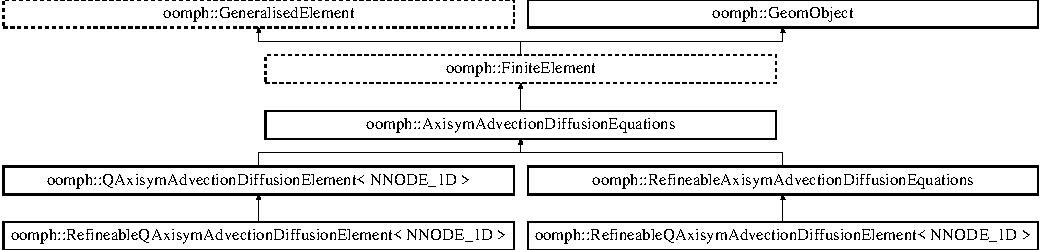
\includegraphics[height=3.365385cm]{classoomph_1_1AxisymAdvectionDiffusionEquations}
\end{center}
\end{figure}
\subsection*{Public Types}
\begin{DoxyCompactItemize}
\item 
typedef void($\ast$ \hyperlink{classoomph_1_1AxisymAdvectionDiffusionEquations_a5110527308cbe58e90fb9ac146d172a0}{Axisym\+Advection\+Diffusion\+Source\+Fct\+Pt}) (const \hyperlink{classoomph_1_1Vector}{Vector}$<$ double $>$ \&x, double \&f)
\begin{DoxyCompactList}\small\item\em Function pointer to source function fct(x,f(x)) -- x is a Vector! \end{DoxyCompactList}\item 
typedef void($\ast$ \hyperlink{classoomph_1_1AxisymAdvectionDiffusionEquations_a53ee8d4a13b53896d66020591a8224b0}{Axisym\+Advection\+Diffusion\+Wind\+Fct\+Pt}) (const \hyperlink{classoomph_1_1Vector}{Vector}$<$ double $>$ \&x, \hyperlink{classoomph_1_1Vector}{Vector}$<$ double $>$ \&wind)
\begin{DoxyCompactList}\small\item\em Function pointer to wind function fct(x,w(x)) -- x is a Vector! \end{DoxyCompactList}\end{DoxyCompactItemize}
\subsection*{Public Member Functions}
\begin{DoxyCompactItemize}
\item 
\hyperlink{classoomph_1_1AxisymAdvectionDiffusionEquations_ab095111fa0c06ea10810534711d3e25d}{Axisym\+Advection\+Diffusion\+Equations} ()
\begin{DoxyCompactList}\small\item\em Constructor\+: Initialise the Source\+\_\+fct\+\_\+pt and Wind\+\_\+fct\+\_\+pt to null and set (pointer to) Peclet number to default. \end{DoxyCompactList}\item 
\hyperlink{classoomph_1_1AxisymAdvectionDiffusionEquations_a6932ab2bbb743d14a97d26fd9f0000d4}{Axisym\+Advection\+Diffusion\+Equations} (const \hyperlink{classoomph_1_1AxisymAdvectionDiffusionEquations}{Axisym\+Advection\+Diffusion\+Equations} \&dummy)
\begin{DoxyCompactList}\small\item\em Broken copy constructor. \end{DoxyCompactList}\item 
virtual unsigned \hyperlink{classoomph_1_1AxisymAdvectionDiffusionEquations_a5638fd954bd0427e5470646c523fa3ac}{u\+\_\+index\+\_\+axi\+\_\+adv\+\_\+diff} () const
\begin{DoxyCompactList}\small\item\em Broken assignment operator. \end{DoxyCompactList}\item 
double \hyperlink{classoomph_1_1AxisymAdvectionDiffusionEquations_a5d89673630363ecbf7fe1e1b7f2d6c31}{du\+\_\+dt\+\_\+axi\+\_\+adv\+\_\+diff} (const unsigned \&n) const
\begin{DoxyCompactList}\small\item\em du/dt at local node n. \end{DoxyCompactList}\item 
void \hyperlink{classoomph_1_1AxisymAdvectionDiffusionEquations_a366b53e0b3af1fc245f2d5173503a241}{disable\+\_\+\+A\+LE} ()
\begin{DoxyCompactList}\small\item\em Disable A\+LE, i.\+e. assert the mesh is not moving -- you do this at your own risk! \end{DoxyCompactList}\item 
void \hyperlink{classoomph_1_1AxisymAdvectionDiffusionEquations_aed501802a434d3143650fe2215660bd5}{enable\+\_\+\+A\+LE} ()
\begin{DoxyCompactList}\small\item\em (Re-\/)enable A\+LE, i.\+e. take possible mesh motion into account when evaluating the time-\/derivative. Note\+: By default, A\+LE is enabled, at the expense of possibly creating unnecessary work in problems where the mesh is, in fact, stationary. \end{DoxyCompactList}\item 
unsigned \hyperlink{classoomph_1_1AxisymAdvectionDiffusionEquations_a0015b0dfe81d34d01169a5e457751e06}{nscalar\+\_\+paraview} () const
\begin{DoxyCompactList}\small\item\em Number of scalars/fields output by this element. Reimplements broken virtual function in base class. \end{DoxyCompactList}\item 
void \hyperlink{classoomph_1_1AxisymAdvectionDiffusionEquations_aa39915ea1370a7785e8b046ab5660471}{scalar\+\_\+value\+\_\+paraview} (std\+::ofstream \&file\+\_\+out, const unsigned \&\hyperlink{cfortran_8h_adb50e893b86b3e55e751a42eab3cba82}{i}, const unsigned \&nplot) const
\begin{DoxyCompactList}\small\item\em Write values of the i-\/th scalar field at the plot points. Needs to be implemented for each new specific element type. \end{DoxyCompactList}\item 
std\+::string \hyperlink{classoomph_1_1AxisymAdvectionDiffusionEquations_aef90d6d8a1262ae8caab9cd571b61392}{scalar\+\_\+name\+\_\+paraview} (const unsigned \&\hyperlink{cfortran_8h_adb50e893b86b3e55e751a42eab3cba82}{i}) const
\begin{DoxyCompactList}\small\item\em Name of the i-\/th scalar field. Default implementation returns V1 for the first one, V2 for the second etc. Can (should!) be overloaded with more meaningful names in specific elements. \end{DoxyCompactList}\item 
void \hyperlink{classoomph_1_1AxisymAdvectionDiffusionEquations_ae8cc538907edda147270ae26696919bd}{output} (std\+::ostream \&outfile)
\begin{DoxyCompactList}\small\item\em Output with default number of plot points. \end{DoxyCompactList}\item 
void \hyperlink{classoomph_1_1AxisymAdvectionDiffusionEquations_a37f231fce2fd5b8bbe51899469b2896b}{output} (std\+::ostream \&outfile, const unsigned \&nplot)
\begin{DoxyCompactList}\small\item\em Output FE representation of soln\+: r,z,u at nplot$^\wedge$2 plot points. \end{DoxyCompactList}\item 
void \hyperlink{classoomph_1_1AxisymAdvectionDiffusionEquations_a79345d7ee2f42aa679538839b5128a58}{output} (F\+I\+LE $\ast$file\+\_\+pt)
\begin{DoxyCompactList}\small\item\em C\+\_\+style output with default number of plot points. \end{DoxyCompactList}\item 
void \hyperlink{classoomph_1_1AxisymAdvectionDiffusionEquations_ae8f5071aa83c8b71e3d455ae56a25214}{output} (F\+I\+LE $\ast$file\+\_\+pt, const unsigned \&n\+\_\+plot)
\begin{DoxyCompactList}\small\item\em C-\/style output FE representation of soln\+: r,z,u at n\+\_\+plot$^\wedge$2 plot points. \end{DoxyCompactList}\item 
void \hyperlink{classoomph_1_1AxisymAdvectionDiffusionEquations_a7e09458177108a164dbc0dbf45179d0e}{output\+\_\+fct} (std\+::ostream \&outfile, const unsigned \&nplot, \hyperlink{classoomph_1_1FiniteElement_a690fd33af26cc3e84f39bba6d5a85202}{Finite\+Element\+::\+Steady\+Exact\+Solution\+Fct\+Pt} exact\+\_\+soln\+\_\+pt)
\begin{DoxyCompactList}\small\item\em Output exact soln\+: r,z,u\+\_\+exact at nplot$^\wedge$2 plot points. \end{DoxyCompactList}\item 
void \hyperlink{classoomph_1_1AxisymAdvectionDiffusionEquations_a9370e0782ee86c2bc2fe3a083979910b}{compute\+\_\+error} (std\+::ostream \&outfile, \hyperlink{classoomph_1_1FiniteElement_a690fd33af26cc3e84f39bba6d5a85202}{Finite\+Element\+::\+Steady\+Exact\+Solution\+Fct\+Pt} exact\+\_\+soln\+\_\+pt, double \&error, double \&norm)
\begin{DoxyCompactList}\small\item\em Get error against and norm of exact solution. \end{DoxyCompactList}\item 
\hyperlink{classoomph_1_1AxisymAdvectionDiffusionEquations_a5110527308cbe58e90fb9ac146d172a0}{Axisym\+Advection\+Diffusion\+Source\+Fct\+Pt} \& \hyperlink{classoomph_1_1AxisymAdvectionDiffusionEquations_abfa1361d267d17ee38baa667f00b9553}{source\+\_\+fct\+\_\+pt} ()
\begin{DoxyCompactList}\small\item\em Access function\+: Pointer to source function. \end{DoxyCompactList}\item 
\hyperlink{classoomph_1_1AxisymAdvectionDiffusionEquations_a5110527308cbe58e90fb9ac146d172a0}{Axisym\+Advection\+Diffusion\+Source\+Fct\+Pt} \hyperlink{classoomph_1_1AxisymAdvectionDiffusionEquations_a17c388ee58d922f5dc26e8d315aead58}{source\+\_\+fct\+\_\+pt} () const
\begin{DoxyCompactList}\small\item\em Access function\+: Pointer to source function. Const version. \end{DoxyCompactList}\item 
\hyperlink{classoomph_1_1AxisymAdvectionDiffusionEquations_a53ee8d4a13b53896d66020591a8224b0}{Axisym\+Advection\+Diffusion\+Wind\+Fct\+Pt} \& \hyperlink{classoomph_1_1AxisymAdvectionDiffusionEquations_a961d34684ce6d565ad387b41b2bd92de}{wind\+\_\+fct\+\_\+pt} ()
\begin{DoxyCompactList}\small\item\em Access function\+: Pointer to wind function. \end{DoxyCompactList}\item 
\hyperlink{classoomph_1_1AxisymAdvectionDiffusionEquations_a53ee8d4a13b53896d66020591a8224b0}{Axisym\+Advection\+Diffusion\+Wind\+Fct\+Pt} \hyperlink{classoomph_1_1AxisymAdvectionDiffusionEquations_ab3b0dcb5dd4d30914b34c4628fe45288}{wind\+\_\+fct\+\_\+pt} () const
\begin{DoxyCompactList}\small\item\em Access function\+: Pointer to wind function. Const version. \end{DoxyCompactList}\item 
const double \& \hyperlink{classoomph_1_1AxisymAdvectionDiffusionEquations_a5fe8ad73aa3e51e071b61aa928f4d49a}{pe} () const
\begin{DoxyCompactList}\small\item\em Peclet number. \end{DoxyCompactList}\item 
double $\ast$\& \hyperlink{classoomph_1_1AxisymAdvectionDiffusionEquations_af993c9e10b06b7f909569db2e9f9459f}{pe\+\_\+pt} ()
\begin{DoxyCompactList}\small\item\em Pointer to Peclet number. \end{DoxyCompactList}\item 
const double \& \hyperlink{classoomph_1_1AxisymAdvectionDiffusionEquations_af1431215d3df6c1299e0e3f34504b423}{pe\+\_\+st} () const
\begin{DoxyCompactList}\small\item\em Peclet number multiplied by Strouhal number. \end{DoxyCompactList}\item 
double $\ast$\& \hyperlink{classoomph_1_1AxisymAdvectionDiffusionEquations_aaa4a657d824e300f7509f5f0f954c30f}{pe\+\_\+st\+\_\+pt} ()
\begin{DoxyCompactList}\small\item\em Pointer to Peclet number multipled by Strouha number. \end{DoxyCompactList}\item 
const double \& \hyperlink{classoomph_1_1AxisymAdvectionDiffusionEquations_a986c66e2d8e39d56e79633c905cf6833}{d} () const
\begin{DoxyCompactList}\small\item\em Peclet number multiplied by Strouhal number. \end{DoxyCompactList}\item 
double $\ast$\& \hyperlink{classoomph_1_1AxisymAdvectionDiffusionEquations_a06ebb3defb017029d98fdff300cef261}{d\+\_\+pt} ()
\begin{DoxyCompactList}\small\item\em Pointer to Peclet number multipled by Strouha number. \end{DoxyCompactList}\item 
virtual void \hyperlink{classoomph_1_1AxisymAdvectionDiffusionEquations_ac1e5dd8bfd42847320137152e3bd3e41}{get\+\_\+source\+\_\+axi\+\_\+adv\+\_\+diff} (const unsigned \&ipt, const \hyperlink{classoomph_1_1Vector}{Vector}$<$ double $>$ \&x, double \&source) const
\begin{DoxyCompactList}\small\item\em Get source term at (Eulerian) position x. This function is virtual to allow overloading in multi-\/physics problems where the strength of the source function might be determined by another system of equations. \end{DoxyCompactList}\item 
virtual void \hyperlink{classoomph_1_1AxisymAdvectionDiffusionEquations_a5572befdf0d7410e7443dc44c4440595}{get\+\_\+wind\+\_\+axi\+\_\+adv\+\_\+diff} (const unsigned \&ipt, const \hyperlink{classoomph_1_1Vector}{Vector}$<$ double $>$ \&\hyperlink{cfortran_8h_ab7123126e4885ef647dd9c6e3807a21c}{s}, const \hyperlink{classoomph_1_1Vector}{Vector}$<$ double $>$ \&x, \hyperlink{classoomph_1_1Vector}{Vector}$<$ double $>$ \&wind) const
\begin{DoxyCompactList}\small\item\em Get wind at (Eulerian) position x and/or local coordinate s. This function is virtual to allow overloading in multi-\/physics problems where the wind function might be determined by another system of equations. \end{DoxyCompactList}\item 
void \hyperlink{classoomph_1_1AxisymAdvectionDiffusionEquations_a47f44dc0f9ba78e0db3a72c9b1f90633}{get\+\_\+flux} (const \hyperlink{classoomph_1_1Vector}{Vector}$<$ double $>$ \&\hyperlink{cfortran_8h_ab7123126e4885ef647dd9c6e3807a21c}{s}, \hyperlink{classoomph_1_1Vector}{Vector}$<$ double $>$ \&flux) const
\begin{DoxyCompactList}\small\item\em Get flux\+: \end{DoxyCompactList}\item 
void \hyperlink{classoomph_1_1AxisymAdvectionDiffusionEquations_a00d9356ebf0f2fe1a5f470db379c9bd9}{fill\+\_\+in\+\_\+contribution\+\_\+to\+\_\+residuals} (\hyperlink{classoomph_1_1Vector}{Vector}$<$ double $>$ \&residuals)
\begin{DoxyCompactList}\small\item\em Add the element\textquotesingle{}s contribution to its residual vector (wrapper) \end{DoxyCompactList}\item 
void \hyperlink{classoomph_1_1AxisymAdvectionDiffusionEquations_a4afbd032aca7d93c1e4402bd3ccc2379}{fill\+\_\+in\+\_\+contribution\+\_\+to\+\_\+jacobian} (\hyperlink{classoomph_1_1Vector}{Vector}$<$ double $>$ \&residuals, \hyperlink{classoomph_1_1DenseMatrix}{Dense\+Matrix}$<$ double $>$ \&jacobian)
\begin{DoxyCompactList}\small\item\em Add the element\textquotesingle{}s contribution to its residual vector and the element Jacobian matrix (wrapper) \end{DoxyCompactList}\item 
double \hyperlink{classoomph_1_1AxisymAdvectionDiffusionEquations_a91e4ff18062a265f7ed265902914e15a}{interpolated\+\_\+u\+\_\+axi\+\_\+adv\+\_\+diff} (const \hyperlink{classoomph_1_1Vector}{Vector}$<$ double $>$ \&\hyperlink{cfortran_8h_ab7123126e4885ef647dd9c6e3807a21c}{s}) const
\begin{DoxyCompactList}\small\item\em Return FE representation of function value u(s) at local coordinate s. \end{DoxyCompactList}\item 
virtual void \hyperlink{classoomph_1_1AxisymAdvectionDiffusionEquations_a83fd782e690a7ca9f6ac4995c964e4b5}{dinterpolated\+\_\+u\+\_\+axi\+\_\+adv\+\_\+diff\+\_\+ddata} (const \hyperlink{classoomph_1_1Vector}{Vector}$<$ double $>$ \&\hyperlink{cfortran_8h_ab7123126e4885ef647dd9c6e3807a21c}{s}, \hyperlink{classoomph_1_1Vector}{Vector}$<$ double $>$ \&du\+\_\+ddata, \hyperlink{classoomph_1_1Vector}{Vector}$<$ unsigned $>$ \&global\+\_\+eqn\+\_\+number)
\begin{DoxyCompactList}\small\item\em Return derivative of u at point s with respect to all data that can affect its value. In addition, return the global equation numbers corresponding to the data. This is virtual so that it can be overloaded in the refineable version. \end{DoxyCompactList}\item 
unsigned \hyperlink{classoomph_1_1AxisymAdvectionDiffusionEquations_a43146d9ddd728dd85340629acb726183}{self\+\_\+test} ()
\begin{DoxyCompactList}\small\item\em Self-\/test\+: Return 0 for OK. \end{DoxyCompactList}\end{DoxyCompactItemize}
\subsection*{Protected Member Functions}
\begin{DoxyCompactItemize}
\item 
virtual double \hyperlink{classoomph_1_1AxisymAdvectionDiffusionEquations_a92b918f392733e6128e192c2fbdb478c}{dshape\+\_\+and\+\_\+dtest\+\_\+eulerian\+\_\+axi\+\_\+adv\+\_\+diff} (const \hyperlink{classoomph_1_1Vector}{Vector}$<$ double $>$ \&\hyperlink{cfortran_8h_ab7123126e4885ef647dd9c6e3807a21c}{s}, \hyperlink{classoomph_1_1Shape}{Shape} \&psi, \hyperlink{classoomph_1_1DShape}{D\+Shape} \&dpsidx, \hyperlink{classoomph_1_1Shape}{Shape} \&test, \hyperlink{classoomph_1_1DShape}{D\+Shape} \&dtestdx) const =0
\begin{DoxyCompactList}\small\item\em Shape/test functions and derivs w.\+r.\+t. to global coords at local coord. s; return Jacobian of mapping. \end{DoxyCompactList}\item 
virtual double \hyperlink{classoomph_1_1AxisymAdvectionDiffusionEquations_a6d844cf194aa8fa462bbfcda811b24ca}{dshape\+\_\+and\+\_\+dtest\+\_\+eulerian\+\_\+at\+\_\+knot\+\_\+axi\+\_\+adv\+\_\+diff} (const unsigned \&ipt, \hyperlink{classoomph_1_1Shape}{Shape} \&psi, \hyperlink{classoomph_1_1DShape}{D\+Shape} \&dpsidx, \hyperlink{classoomph_1_1Shape}{Shape} \&test, \hyperlink{classoomph_1_1DShape}{D\+Shape} \&dtestdx) const =0
\begin{DoxyCompactList}\small\item\em Shape/test functions and derivs w.\+r.\+t. to global coords at integration point ipt; return Jacobian of mapping. \end{DoxyCompactList}\item 
virtual void \hyperlink{classoomph_1_1AxisymAdvectionDiffusionEquations_a19bf92fed341de2d09b444b3ab71096e}{fill\+\_\+in\+\_\+generic\+\_\+residual\+\_\+contribution\+\_\+axi\+\_\+adv\+\_\+diff} (\hyperlink{classoomph_1_1Vector}{Vector}$<$ double $>$ \&residuals, \hyperlink{classoomph_1_1DenseMatrix}{Dense\+Matrix}$<$ double $>$ \&jacobian, \hyperlink{classoomph_1_1DenseMatrix}{Dense\+Matrix}$<$ double $>$ \&mass\+\_\+matrix, unsigned flag)
\begin{DoxyCompactList}\small\item\em Add the element\textquotesingle{}s contribution to its residual vector only (if flag=and/or element Jacobian matrix. \end{DoxyCompactList}\end{DoxyCompactItemize}
\subsection*{Protected Attributes}
\begin{DoxyCompactItemize}
\item 
double $\ast$ \hyperlink{classoomph_1_1AxisymAdvectionDiffusionEquations_af1bc964a4a10482e926d7f241218413b}{Pe\+\_\+pt}
\begin{DoxyCompactList}\small\item\em Pointer to global Peclet number. \end{DoxyCompactList}\item 
double $\ast$ \hyperlink{classoomph_1_1AxisymAdvectionDiffusionEquations_a1b2246dfb6f3a23bf84a90c1b483b0ba}{Pe\+St\+\_\+pt}
\begin{DoxyCompactList}\small\item\em Pointer to global Peclet number multiplied by Strouhal number. \end{DoxyCompactList}\item 
double $\ast$ \hyperlink{classoomph_1_1AxisymAdvectionDiffusionEquations_add199570bdd8e75ffe12a37a8bc99ee2}{D\+\_\+pt}
\begin{DoxyCompactList}\small\item\em Pointer to global Diffusion parameter. \end{DoxyCompactList}\item 
\hyperlink{classoomph_1_1AxisymAdvectionDiffusionEquations_a5110527308cbe58e90fb9ac146d172a0}{Axisym\+Advection\+Diffusion\+Source\+Fct\+Pt} \hyperlink{classoomph_1_1AxisymAdvectionDiffusionEquations_a498d9045921930191e9a8022b7f5f1e5}{Source\+\_\+fct\+\_\+pt}
\begin{DoxyCompactList}\small\item\em Pointer to source function\+: \end{DoxyCompactList}\item 
\hyperlink{classoomph_1_1AxisymAdvectionDiffusionEquations_a53ee8d4a13b53896d66020591a8224b0}{Axisym\+Advection\+Diffusion\+Wind\+Fct\+Pt} \hyperlink{classoomph_1_1AxisymAdvectionDiffusionEquations_a8249037271ae5094b9682ea42731068a}{Wind\+\_\+fct\+\_\+pt}
\begin{DoxyCompactList}\small\item\em Pointer to wind function\+: \end{DoxyCompactList}\item 
bool \hyperlink{classoomph_1_1AxisymAdvectionDiffusionEquations_abef82e8104dd76a7ff53935efe41765d}{A\+L\+E\+\_\+is\+\_\+disabled}
\begin{DoxyCompactList}\small\item\em Boolean flag to indicate whether AlE formulation is disable. \end{DoxyCompactList}\end{DoxyCompactItemize}
\subsection*{Static Private Attributes}
\begin{DoxyCompactItemize}
\item 
static double \hyperlink{classoomph_1_1AxisymAdvectionDiffusionEquations_a8597f955eb2780f02d9479ebc678ba24}{Default\+\_\+peclet\+\_\+number} = 0.\+0
\begin{DoxyCompactList}\small\item\em Static default value for the Peclet number. \end{DoxyCompactList}\item 
static double \hyperlink{classoomph_1_1AxisymAdvectionDiffusionEquations_abef5adeae70c304fda61918174a100db}{Default\+\_\+diffusion\+\_\+parameter} = 1.\+0
\begin{DoxyCompactList}\small\item\em Static default value for the Peclet number. \end{DoxyCompactList}\end{DoxyCompactItemize}
\subsection*{Additional Inherited Members}


\subsection{Detailed Description}
A class for all elements that solve the Advection Diffusion equations in a cylindrical polar coordinate system using isoparametric elements. \[ Pe \mathbf{w}\cdot(\mathbf{x}) \nabla u = \nabla \cdot \left( \nabla u \right) + f(\mathbf{x}) \] This contains the generic maths. \hyperlink{classoomph_1_1Shape}{Shape} functions, geometric mapping etc. must get implemented in derived class. 

Definition at line 61 of file axisym\+\_\+advection\+\_\+diffusion\+\_\+elements.\+h.



\subsection{Member Typedef Documentation}
\mbox{\Hypertarget{classoomph_1_1AxisymAdvectionDiffusionEquations_a5110527308cbe58e90fb9ac146d172a0}\label{classoomph_1_1AxisymAdvectionDiffusionEquations_a5110527308cbe58e90fb9ac146d172a0}} 
\index{oomph\+::\+Axisym\+Advection\+Diffusion\+Equations@{oomph\+::\+Axisym\+Advection\+Diffusion\+Equations}!Axisym\+Advection\+Diffusion\+Source\+Fct\+Pt@{Axisym\+Advection\+Diffusion\+Source\+Fct\+Pt}}
\index{Axisym\+Advection\+Diffusion\+Source\+Fct\+Pt@{Axisym\+Advection\+Diffusion\+Source\+Fct\+Pt}!oomph\+::\+Axisym\+Advection\+Diffusion\+Equations@{oomph\+::\+Axisym\+Advection\+Diffusion\+Equations}}
\subsubsection{\texorpdfstring{Axisym\+Advection\+Diffusion\+Source\+Fct\+Pt}{AxisymAdvectionDiffusionSourceFctPt}}
{\footnotesize\ttfamily typedef void($\ast$ oomph\+::\+Axisym\+Advection\+Diffusion\+Equations\+::\+Axisym\+Advection\+Diffusion\+Source\+Fct\+Pt) (const \hyperlink{classoomph_1_1Vector}{Vector}$<$ double $>$ \&x, double \&f)}



Function pointer to source function fct(x,f(x)) -- x is a Vector! 



Definition at line 69 of file axisym\+\_\+advection\+\_\+diffusion\+\_\+elements.\+h.

\mbox{\Hypertarget{classoomph_1_1AxisymAdvectionDiffusionEquations_a53ee8d4a13b53896d66020591a8224b0}\label{classoomph_1_1AxisymAdvectionDiffusionEquations_a53ee8d4a13b53896d66020591a8224b0}} 
\index{oomph\+::\+Axisym\+Advection\+Diffusion\+Equations@{oomph\+::\+Axisym\+Advection\+Diffusion\+Equations}!Axisym\+Advection\+Diffusion\+Wind\+Fct\+Pt@{Axisym\+Advection\+Diffusion\+Wind\+Fct\+Pt}}
\index{Axisym\+Advection\+Diffusion\+Wind\+Fct\+Pt@{Axisym\+Advection\+Diffusion\+Wind\+Fct\+Pt}!oomph\+::\+Axisym\+Advection\+Diffusion\+Equations@{oomph\+::\+Axisym\+Advection\+Diffusion\+Equations}}
\subsubsection{\texorpdfstring{Axisym\+Advection\+Diffusion\+Wind\+Fct\+Pt}{AxisymAdvectionDiffusionWindFctPt}}
{\footnotesize\ttfamily typedef void($\ast$ oomph\+::\+Axisym\+Advection\+Diffusion\+Equations\+::\+Axisym\+Advection\+Diffusion\+Wind\+Fct\+Pt) (const \hyperlink{classoomph_1_1Vector}{Vector}$<$ double $>$ \&x, \hyperlink{classoomph_1_1Vector}{Vector}$<$ double $>$ \&wind)}



Function pointer to wind function fct(x,w(x)) -- x is a Vector! 



Definition at line 74 of file axisym\+\_\+advection\+\_\+diffusion\+\_\+elements.\+h.



\subsection{Constructor \& Destructor Documentation}
\mbox{\Hypertarget{classoomph_1_1AxisymAdvectionDiffusionEquations_ab095111fa0c06ea10810534711d3e25d}\label{classoomph_1_1AxisymAdvectionDiffusionEquations_ab095111fa0c06ea10810534711d3e25d}} 
\index{oomph\+::\+Axisym\+Advection\+Diffusion\+Equations@{oomph\+::\+Axisym\+Advection\+Diffusion\+Equations}!Axisym\+Advection\+Diffusion\+Equations@{Axisym\+Advection\+Diffusion\+Equations}}
\index{Axisym\+Advection\+Diffusion\+Equations@{Axisym\+Advection\+Diffusion\+Equations}!oomph\+::\+Axisym\+Advection\+Diffusion\+Equations@{oomph\+::\+Axisym\+Advection\+Diffusion\+Equations}}
\subsubsection{\texorpdfstring{Axisym\+Advection\+Diffusion\+Equations()}{AxisymAdvectionDiffusionEquations()}\hspace{0.1cm}{\footnotesize\ttfamily [1/2]}}
{\footnotesize\ttfamily oomph\+::\+Axisym\+Advection\+Diffusion\+Equations\+::\+Axisym\+Advection\+Diffusion\+Equations (\begin{DoxyParamCaption}{ }\end{DoxyParamCaption})\hspace{0.3cm}{\ttfamily [inline]}}



Constructor\+: Initialise the Source\+\_\+fct\+\_\+pt and Wind\+\_\+fct\+\_\+pt to null and set (pointer to) Peclet number to default. 



Definition at line 80 of file axisym\+\_\+advection\+\_\+diffusion\+\_\+elements.\+h.



References D\+\_\+pt, Default\+\_\+diffusion\+\_\+parameter, Default\+\_\+peclet\+\_\+number, Pe\+\_\+pt, and Pe\+St\+\_\+pt.

\mbox{\Hypertarget{classoomph_1_1AxisymAdvectionDiffusionEquations_a6932ab2bbb743d14a97d26fd9f0000d4}\label{classoomph_1_1AxisymAdvectionDiffusionEquations_a6932ab2bbb743d14a97d26fd9f0000d4}} 
\index{oomph\+::\+Axisym\+Advection\+Diffusion\+Equations@{oomph\+::\+Axisym\+Advection\+Diffusion\+Equations}!Axisym\+Advection\+Diffusion\+Equations@{Axisym\+Advection\+Diffusion\+Equations}}
\index{Axisym\+Advection\+Diffusion\+Equations@{Axisym\+Advection\+Diffusion\+Equations}!oomph\+::\+Axisym\+Advection\+Diffusion\+Equations@{oomph\+::\+Axisym\+Advection\+Diffusion\+Equations}}
\subsubsection{\texorpdfstring{Axisym\+Advection\+Diffusion\+Equations()}{AxisymAdvectionDiffusionEquations()}\hspace{0.1cm}{\footnotesize\ttfamily [2/2]}}
{\footnotesize\ttfamily oomph\+::\+Axisym\+Advection\+Diffusion\+Equations\+::\+Axisym\+Advection\+Diffusion\+Equations (\begin{DoxyParamCaption}\item[{const \hyperlink{classoomph_1_1AxisymAdvectionDiffusionEquations}{Axisym\+Advection\+Diffusion\+Equations} \&}]{dummy }\end{DoxyParamCaption})\hspace{0.3cm}{\ttfamily [inline]}}



Broken copy constructor. 



Definition at line 90 of file axisym\+\_\+advection\+\_\+diffusion\+\_\+elements.\+h.



References oomph\+::\+Broken\+Copy\+::broken\+\_\+copy().



\subsection{Member Function Documentation}
\mbox{\Hypertarget{classoomph_1_1AxisymAdvectionDiffusionEquations_a9370e0782ee86c2bc2fe3a083979910b}\label{classoomph_1_1AxisymAdvectionDiffusionEquations_a9370e0782ee86c2bc2fe3a083979910b}} 
\index{oomph\+::\+Axisym\+Advection\+Diffusion\+Equations@{oomph\+::\+Axisym\+Advection\+Diffusion\+Equations}!compute\+\_\+error@{compute\+\_\+error}}
\index{compute\+\_\+error@{compute\+\_\+error}!oomph\+::\+Axisym\+Advection\+Diffusion\+Equations@{oomph\+::\+Axisym\+Advection\+Diffusion\+Equations}}
\subsubsection{\texorpdfstring{compute\+\_\+error()}{compute\_error()}}
{\footnotesize\ttfamily void oomph\+::\+Axisym\+Advection\+Diffusion\+Equations\+::compute\+\_\+error (\begin{DoxyParamCaption}\item[{std\+::ostream \&}]{outfile,  }\item[{\hyperlink{classoomph_1_1FiniteElement_a690fd33af26cc3e84f39bba6d5a85202}{Finite\+Element\+::\+Steady\+Exact\+Solution\+Fct\+Pt}}]{exact\+\_\+soln\+\_\+pt,  }\item[{double \&}]{error,  }\item[{double \&}]{norm }\end{DoxyParamCaption})\hspace{0.3cm}{\ttfamily [virtual]}}



Get error against and norm of exact solution. 

Validate against exact solution.

Solution is provided via function pointer. Plot error at a given number of plot points. 

Reimplemented from \hyperlink{classoomph_1_1FiniteElement_a73c79a1f1e5b1d334757812a6bbd58ff}{oomph\+::\+Finite\+Element}.



Definition at line 428 of file axisym\+\_\+advection\+\_\+diffusion\+\_\+elements.\+cc.



References i, oomph\+::\+Finite\+Element\+::integral\+\_\+pt(), interpolated\+\_\+u\+\_\+axi\+\_\+adv\+\_\+diff(), oomph\+::\+Finite\+Element\+::interpolated\+\_\+x(), oomph\+::\+Finite\+Element\+::\+J\+\_\+eulerian(), oomph\+::\+Integral\+::knot(), oomph\+::\+Finite\+Element\+::nnode(), oomph\+::\+Integral\+::nweight(), s, oomph\+::\+Quad\+Tree\+Names\+::W, and oomph\+::\+Integral\+::weight().



Referenced by output().

\mbox{\Hypertarget{classoomph_1_1AxisymAdvectionDiffusionEquations_a986c66e2d8e39d56e79633c905cf6833}\label{classoomph_1_1AxisymAdvectionDiffusionEquations_a986c66e2d8e39d56e79633c905cf6833}} 
\index{oomph\+::\+Axisym\+Advection\+Diffusion\+Equations@{oomph\+::\+Axisym\+Advection\+Diffusion\+Equations}!d@{d}}
\index{d@{d}!oomph\+::\+Axisym\+Advection\+Diffusion\+Equations@{oomph\+::\+Axisym\+Advection\+Diffusion\+Equations}}
\subsubsection{\texorpdfstring{d()}{d()}}
{\footnotesize\ttfamily const double\& oomph\+::\+Axisym\+Advection\+Diffusion\+Equations\+::d (\begin{DoxyParamCaption}{ }\end{DoxyParamCaption}) const\hspace{0.3cm}{\ttfamily [inline]}}



Peclet number multiplied by Strouhal number. 



Definition at line 323 of file axisym\+\_\+advection\+\_\+diffusion\+\_\+elements.\+h.



References D\+\_\+pt.



Referenced by fill\+\_\+in\+\_\+generic\+\_\+residual\+\_\+contribution\+\_\+axi\+\_\+adv\+\_\+diff().

\mbox{\Hypertarget{classoomph_1_1AxisymAdvectionDiffusionEquations_a06ebb3defb017029d98fdff300cef261}\label{classoomph_1_1AxisymAdvectionDiffusionEquations_a06ebb3defb017029d98fdff300cef261}} 
\index{oomph\+::\+Axisym\+Advection\+Diffusion\+Equations@{oomph\+::\+Axisym\+Advection\+Diffusion\+Equations}!d\+\_\+pt@{d\+\_\+pt}}
\index{d\+\_\+pt@{d\+\_\+pt}!oomph\+::\+Axisym\+Advection\+Diffusion\+Equations@{oomph\+::\+Axisym\+Advection\+Diffusion\+Equations}}
\subsubsection{\texorpdfstring{d\+\_\+pt()}{d\_pt()}}
{\footnotesize\ttfamily double$\ast$ \& oomph\+::\+Axisym\+Advection\+Diffusion\+Equations\+::d\+\_\+pt (\begin{DoxyParamCaption}{ }\end{DoxyParamCaption})\hspace{0.3cm}{\ttfamily [inline]}}



Pointer to Peclet number multipled by Strouha number. 



Definition at line 326 of file axisym\+\_\+advection\+\_\+diffusion\+\_\+elements.\+h.



References D\+\_\+pt.

\mbox{\Hypertarget{classoomph_1_1AxisymAdvectionDiffusionEquations_a83fd782e690a7ca9f6ac4995c964e4b5}\label{classoomph_1_1AxisymAdvectionDiffusionEquations_a83fd782e690a7ca9f6ac4995c964e4b5}} 
\index{oomph\+::\+Axisym\+Advection\+Diffusion\+Equations@{oomph\+::\+Axisym\+Advection\+Diffusion\+Equations}!dinterpolated\+\_\+u\+\_\+axi\+\_\+adv\+\_\+diff\+\_\+ddata@{dinterpolated\+\_\+u\+\_\+axi\+\_\+adv\+\_\+diff\+\_\+ddata}}
\index{dinterpolated\+\_\+u\+\_\+axi\+\_\+adv\+\_\+diff\+\_\+ddata@{dinterpolated\+\_\+u\+\_\+axi\+\_\+adv\+\_\+diff\+\_\+ddata}!oomph\+::\+Axisym\+Advection\+Diffusion\+Equations@{oomph\+::\+Axisym\+Advection\+Diffusion\+Equations}}
\subsubsection{\texorpdfstring{dinterpolated\+\_\+u\+\_\+axi\+\_\+adv\+\_\+diff\+\_\+ddata()}{dinterpolated\_u\_axi\_adv\_diff\_ddata()}}
{\footnotesize\ttfamily virtual void oomph\+::\+Axisym\+Advection\+Diffusion\+Equations\+::dinterpolated\+\_\+u\+\_\+axi\+\_\+adv\+\_\+diff\+\_\+ddata (\begin{DoxyParamCaption}\item[{const \hyperlink{classoomph_1_1Vector}{Vector}$<$ double $>$ \&}]{s,  }\item[{\hyperlink{classoomph_1_1Vector}{Vector}$<$ double $>$ \&}]{du\+\_\+ddata,  }\item[{\hyperlink{classoomph_1_1Vector}{Vector}$<$ unsigned $>$ \&}]{global\+\_\+eqn\+\_\+number }\end{DoxyParamCaption})\hspace{0.3cm}{\ttfamily [inline]}, {\ttfamily [virtual]}}



Return derivative of u at point s with respect to all data that can affect its value. In addition, return the global equation numbers corresponding to the data. This is virtual so that it can be overloaded in the refineable version. 



Definition at line 464 of file axisym\+\_\+advection\+\_\+diffusion\+\_\+elements.\+h.



References dshape\+\_\+and\+\_\+dtest\+\_\+eulerian\+\_\+at\+\_\+knot\+\_\+axi\+\_\+adv\+\_\+diff(), dshape\+\_\+and\+\_\+dtest\+\_\+eulerian\+\_\+axi\+\_\+adv\+\_\+diff(), oomph\+::\+Data\+::eqn\+\_\+number(), fill\+\_\+in\+\_\+generic\+\_\+residual\+\_\+contribution\+\_\+axi\+\_\+adv\+\_\+diff(), oomph\+::\+Finite\+Element\+::nnode(), oomph\+::\+Finite\+Element\+::node\+\_\+pt(), s, self\+\_\+test(), oomph\+::\+Finite\+Element\+::shape(), and u\+\_\+index\+\_\+axi\+\_\+adv\+\_\+diff().

\mbox{\Hypertarget{classoomph_1_1AxisymAdvectionDiffusionEquations_a366b53e0b3af1fc245f2d5173503a241}\label{classoomph_1_1AxisymAdvectionDiffusionEquations_a366b53e0b3af1fc245f2d5173503a241}} 
\index{oomph\+::\+Axisym\+Advection\+Diffusion\+Equations@{oomph\+::\+Axisym\+Advection\+Diffusion\+Equations}!disable\+\_\+\+A\+LE@{disable\+\_\+\+A\+LE}}
\index{disable\+\_\+\+A\+LE@{disable\+\_\+\+A\+LE}!oomph\+::\+Axisym\+Advection\+Diffusion\+Equations@{oomph\+::\+Axisym\+Advection\+Diffusion\+Equations}}
\subsubsection{\texorpdfstring{disable\+\_\+\+A\+L\+E()}{disable\_ALE()}}
{\footnotesize\ttfamily void oomph\+::\+Axisym\+Advection\+Diffusion\+Equations\+::disable\+\_\+\+A\+LE (\begin{DoxyParamCaption}{ }\end{DoxyParamCaption})\hspace{0.3cm}{\ttfamily [inline]}, {\ttfamily [virtual]}}



Disable A\+LE, i.\+e. assert the mesh is not moving -- you do this at your own risk! 



Reimplemented from \hyperlink{classoomph_1_1FiniteElement_a625ea6d3f9baccfbdd1323315fb3ec71}{oomph\+::\+Finite\+Element}.



Definition at line 147 of file axisym\+\_\+advection\+\_\+diffusion\+\_\+elements.\+h.



References A\+L\+E\+\_\+is\+\_\+disabled.

\mbox{\Hypertarget{classoomph_1_1AxisymAdvectionDiffusionEquations_a6d844cf194aa8fa462bbfcda811b24ca}\label{classoomph_1_1AxisymAdvectionDiffusionEquations_a6d844cf194aa8fa462bbfcda811b24ca}} 
\index{oomph\+::\+Axisym\+Advection\+Diffusion\+Equations@{oomph\+::\+Axisym\+Advection\+Diffusion\+Equations}!dshape\+\_\+and\+\_\+dtest\+\_\+eulerian\+\_\+at\+\_\+knot\+\_\+axi\+\_\+adv\+\_\+diff@{dshape\+\_\+and\+\_\+dtest\+\_\+eulerian\+\_\+at\+\_\+knot\+\_\+axi\+\_\+adv\+\_\+diff}}
\index{dshape\+\_\+and\+\_\+dtest\+\_\+eulerian\+\_\+at\+\_\+knot\+\_\+axi\+\_\+adv\+\_\+diff@{dshape\+\_\+and\+\_\+dtest\+\_\+eulerian\+\_\+at\+\_\+knot\+\_\+axi\+\_\+adv\+\_\+diff}!oomph\+::\+Axisym\+Advection\+Diffusion\+Equations@{oomph\+::\+Axisym\+Advection\+Diffusion\+Equations}}
\subsubsection{\texorpdfstring{dshape\+\_\+and\+\_\+dtest\+\_\+eulerian\+\_\+at\+\_\+knot\+\_\+axi\+\_\+adv\+\_\+diff()}{dshape\_and\_dtest\_eulerian\_at\_knot\_axi\_adv\_diff()}}
{\footnotesize\ttfamily virtual double oomph\+::\+Axisym\+Advection\+Diffusion\+Equations\+::dshape\+\_\+and\+\_\+dtest\+\_\+eulerian\+\_\+at\+\_\+knot\+\_\+axi\+\_\+adv\+\_\+diff (\begin{DoxyParamCaption}\item[{const unsigned \&}]{ipt,  }\item[{\hyperlink{classoomph_1_1Shape}{Shape} \&}]{psi,  }\item[{\hyperlink{classoomph_1_1DShape}{D\+Shape} \&}]{dpsidx,  }\item[{\hyperlink{classoomph_1_1Shape}{Shape} \&}]{test,  }\item[{\hyperlink{classoomph_1_1DShape}{D\+Shape} \&}]{dtestdx }\end{DoxyParamCaption}) const\hspace{0.3cm}{\ttfamily [protected]}, {\ttfamily [pure virtual]}}



Shape/test functions and derivs w.\+r.\+t. to global coords at integration point ipt; return Jacobian of mapping. 



Implemented in \hyperlink{classoomph_1_1QAxisymAdvectionDiffusionElement_a4bb026009c2c69e6870ff45450382418}{oomph\+::\+Q\+Axisym\+Advection\+Diffusion\+Element$<$ N\+N\+O\+D\+E\+\_\+1\+D $>$}.



Referenced by dinterpolated\+\_\+u\+\_\+axi\+\_\+adv\+\_\+diff\+\_\+ddata(), oomph\+::\+Refineable\+Axisym\+Advection\+Diffusion\+Equations\+::fill\+\_\+in\+\_\+generic\+\_\+residual\+\_\+contribution\+\_\+axi\+\_\+adv\+\_\+diff(), fill\+\_\+in\+\_\+generic\+\_\+residual\+\_\+contribution\+\_\+axi\+\_\+adv\+\_\+diff(), and oomph\+::\+Q\+Axisym\+Advection\+Diffusion\+Element$<$ N\+N\+O\+D\+E\+\_\+1\+D $>$\+::output\+\_\+fct().

\mbox{\Hypertarget{classoomph_1_1AxisymAdvectionDiffusionEquations_a92b918f392733e6128e192c2fbdb478c}\label{classoomph_1_1AxisymAdvectionDiffusionEquations_a92b918f392733e6128e192c2fbdb478c}} 
\index{oomph\+::\+Axisym\+Advection\+Diffusion\+Equations@{oomph\+::\+Axisym\+Advection\+Diffusion\+Equations}!dshape\+\_\+and\+\_\+dtest\+\_\+eulerian\+\_\+axi\+\_\+adv\+\_\+diff@{dshape\+\_\+and\+\_\+dtest\+\_\+eulerian\+\_\+axi\+\_\+adv\+\_\+diff}}
\index{dshape\+\_\+and\+\_\+dtest\+\_\+eulerian\+\_\+axi\+\_\+adv\+\_\+diff@{dshape\+\_\+and\+\_\+dtest\+\_\+eulerian\+\_\+axi\+\_\+adv\+\_\+diff}!oomph\+::\+Axisym\+Advection\+Diffusion\+Equations@{oomph\+::\+Axisym\+Advection\+Diffusion\+Equations}}
\subsubsection{\texorpdfstring{dshape\+\_\+and\+\_\+dtest\+\_\+eulerian\+\_\+axi\+\_\+adv\+\_\+diff()}{dshape\_and\_dtest\_eulerian\_axi\_adv\_diff()}}
{\footnotesize\ttfamily virtual double oomph\+::\+Axisym\+Advection\+Diffusion\+Equations\+::dshape\+\_\+and\+\_\+dtest\+\_\+eulerian\+\_\+axi\+\_\+adv\+\_\+diff (\begin{DoxyParamCaption}\item[{const \hyperlink{classoomph_1_1Vector}{Vector}$<$ double $>$ \&}]{s,  }\item[{\hyperlink{classoomph_1_1Shape}{Shape} \&}]{psi,  }\item[{\hyperlink{classoomph_1_1DShape}{D\+Shape} \&}]{dpsidx,  }\item[{\hyperlink{classoomph_1_1Shape}{Shape} \&}]{test,  }\item[{\hyperlink{classoomph_1_1DShape}{D\+Shape} \&}]{dtestdx }\end{DoxyParamCaption}) const\hspace{0.3cm}{\ttfamily [protected]}, {\ttfamily [pure virtual]}}



Shape/test functions and derivs w.\+r.\+t. to global coords at local coord. s; return Jacobian of mapping. 



Implemented in \hyperlink{classoomph_1_1QAxisymAdvectionDiffusionElement_aa940ad09f185dfde0eaeff61bc9c0a31}{oomph\+::\+Q\+Axisym\+Advection\+Diffusion\+Element$<$ N\+N\+O\+D\+E\+\_\+1\+D $>$}.



Referenced by dinterpolated\+\_\+u\+\_\+axi\+\_\+adv\+\_\+diff\+\_\+ddata(), and oomph\+::\+Q\+Axisym\+Advection\+Diffusion\+Element$<$ N\+N\+O\+D\+E\+\_\+1\+D $>$\+::output\+\_\+fct().

\mbox{\Hypertarget{classoomph_1_1AxisymAdvectionDiffusionEquations_a5d89673630363ecbf7fe1e1b7f2d6c31}\label{classoomph_1_1AxisymAdvectionDiffusionEquations_a5d89673630363ecbf7fe1e1b7f2d6c31}} 
\index{oomph\+::\+Axisym\+Advection\+Diffusion\+Equations@{oomph\+::\+Axisym\+Advection\+Diffusion\+Equations}!du\+\_\+dt\+\_\+axi\+\_\+adv\+\_\+diff@{du\+\_\+dt\+\_\+axi\+\_\+adv\+\_\+diff}}
\index{du\+\_\+dt\+\_\+axi\+\_\+adv\+\_\+diff@{du\+\_\+dt\+\_\+axi\+\_\+adv\+\_\+diff}!oomph\+::\+Axisym\+Advection\+Diffusion\+Equations@{oomph\+::\+Axisym\+Advection\+Diffusion\+Equations}}
\subsubsection{\texorpdfstring{du\+\_\+dt\+\_\+axi\+\_\+adv\+\_\+diff()}{du\_dt\_axi\_adv\_diff()}}
{\footnotesize\ttfamily double oomph\+::\+Axisym\+Advection\+Diffusion\+Equations\+::du\+\_\+dt\+\_\+axi\+\_\+adv\+\_\+diff (\begin{DoxyParamCaption}\item[{const unsigned \&}]{n }\end{DoxyParamCaption}) const\hspace{0.3cm}{\ttfamily [inline]}}



du/dt at local node n. 

Uses suitably interpolated value for hanging nodes. 

Definition at line 121 of file axisym\+\_\+advection\+\_\+diffusion\+\_\+elements.\+h.



References oomph\+::\+Time\+Stepper\+::is\+\_\+steady(), oomph\+::\+Finite\+Element\+::nodal\+\_\+value(), oomph\+::\+Finite\+Element\+::node\+\_\+pt(), oomph\+::\+Time\+Stepper\+::ntstorage(), t, oomph\+::\+Geom\+Object\+::time\+\_\+stepper\+\_\+pt(), oomph\+::\+Data\+::time\+\_\+stepper\+\_\+pt(), u\+\_\+index\+\_\+axi\+\_\+adv\+\_\+diff(), and oomph\+::\+Time\+Stepper\+::weight().



Referenced by oomph\+::\+Refineable\+Axisym\+Advection\+Diffusion\+Equations\+::fill\+\_\+in\+\_\+generic\+\_\+residual\+\_\+contribution\+\_\+axi\+\_\+adv\+\_\+diff(), and fill\+\_\+in\+\_\+generic\+\_\+residual\+\_\+contribution\+\_\+axi\+\_\+adv\+\_\+diff().

\mbox{\Hypertarget{classoomph_1_1AxisymAdvectionDiffusionEquations_aed501802a434d3143650fe2215660bd5}\label{classoomph_1_1AxisymAdvectionDiffusionEquations_aed501802a434d3143650fe2215660bd5}} 
\index{oomph\+::\+Axisym\+Advection\+Diffusion\+Equations@{oomph\+::\+Axisym\+Advection\+Diffusion\+Equations}!enable\+\_\+\+A\+LE@{enable\+\_\+\+A\+LE}}
\index{enable\+\_\+\+A\+LE@{enable\+\_\+\+A\+LE}!oomph\+::\+Axisym\+Advection\+Diffusion\+Equations@{oomph\+::\+Axisym\+Advection\+Diffusion\+Equations}}
\subsubsection{\texorpdfstring{enable\+\_\+\+A\+L\+E()}{enable\_ALE()}}
{\footnotesize\ttfamily void oomph\+::\+Axisym\+Advection\+Diffusion\+Equations\+::enable\+\_\+\+A\+LE (\begin{DoxyParamCaption}{ }\end{DoxyParamCaption})\hspace{0.3cm}{\ttfamily [inline]}, {\ttfamily [virtual]}}



(Re-\/)enable A\+LE, i.\+e. take possible mesh motion into account when evaluating the time-\/derivative. Note\+: By default, A\+LE is enabled, at the expense of possibly creating unnecessary work in problems where the mesh is, in fact, stationary. 



Reimplemented from \hyperlink{classoomph_1_1FiniteElement_a92ef8967fa4e2d6c33c51ea3efa3aa82}{oomph\+::\+Finite\+Element}.



Definition at line 157 of file axisym\+\_\+advection\+\_\+diffusion\+\_\+elements.\+h.



References A\+L\+E\+\_\+is\+\_\+disabled.

\mbox{\Hypertarget{classoomph_1_1AxisymAdvectionDiffusionEquations_a4afbd032aca7d93c1e4402bd3ccc2379}\label{classoomph_1_1AxisymAdvectionDiffusionEquations_a4afbd032aca7d93c1e4402bd3ccc2379}} 
\index{oomph\+::\+Axisym\+Advection\+Diffusion\+Equations@{oomph\+::\+Axisym\+Advection\+Diffusion\+Equations}!fill\+\_\+in\+\_\+contribution\+\_\+to\+\_\+jacobian@{fill\+\_\+in\+\_\+contribution\+\_\+to\+\_\+jacobian}}
\index{fill\+\_\+in\+\_\+contribution\+\_\+to\+\_\+jacobian@{fill\+\_\+in\+\_\+contribution\+\_\+to\+\_\+jacobian}!oomph\+::\+Axisym\+Advection\+Diffusion\+Equations@{oomph\+::\+Axisym\+Advection\+Diffusion\+Equations}}
\subsubsection{\texorpdfstring{fill\+\_\+in\+\_\+contribution\+\_\+to\+\_\+jacobian()}{fill\_in\_contribution\_to\_jacobian()}}
{\footnotesize\ttfamily void oomph\+::\+Axisym\+Advection\+Diffusion\+Equations\+::fill\+\_\+in\+\_\+contribution\+\_\+to\+\_\+jacobian (\begin{DoxyParamCaption}\item[{\hyperlink{classoomph_1_1Vector}{Vector}$<$ double $>$ \&}]{residuals,  }\item[{\hyperlink{classoomph_1_1DenseMatrix}{Dense\+Matrix}$<$ double $>$ \&}]{jacobian }\end{DoxyParamCaption})\hspace{0.3cm}{\ttfamily [inline]}, {\ttfamily [virtual]}}



Add the element\textquotesingle{}s contribution to its residual vector and the element Jacobian matrix (wrapper) 



Reimplemented from \hyperlink{classoomph_1_1GeneralisedElement_a6ae09fc0d68e4309ac1b03583d252845}{oomph\+::\+Generalised\+Element}.



Definition at line 420 of file axisym\+\_\+advection\+\_\+diffusion\+\_\+elements.\+h.



References oomph\+::\+Generalised\+Element\+::\+Dummy\+\_\+matrix, and fill\+\_\+in\+\_\+generic\+\_\+residual\+\_\+contribution\+\_\+axi\+\_\+adv\+\_\+diff().

\mbox{\Hypertarget{classoomph_1_1AxisymAdvectionDiffusionEquations_a00d9356ebf0f2fe1a5f470db379c9bd9}\label{classoomph_1_1AxisymAdvectionDiffusionEquations_a00d9356ebf0f2fe1a5f470db379c9bd9}} 
\index{oomph\+::\+Axisym\+Advection\+Diffusion\+Equations@{oomph\+::\+Axisym\+Advection\+Diffusion\+Equations}!fill\+\_\+in\+\_\+contribution\+\_\+to\+\_\+residuals@{fill\+\_\+in\+\_\+contribution\+\_\+to\+\_\+residuals}}
\index{fill\+\_\+in\+\_\+contribution\+\_\+to\+\_\+residuals@{fill\+\_\+in\+\_\+contribution\+\_\+to\+\_\+residuals}!oomph\+::\+Axisym\+Advection\+Diffusion\+Equations@{oomph\+::\+Axisym\+Advection\+Diffusion\+Equations}}
\subsubsection{\texorpdfstring{fill\+\_\+in\+\_\+contribution\+\_\+to\+\_\+residuals()}{fill\_in\_contribution\_to\_residuals()}}
{\footnotesize\ttfamily void oomph\+::\+Axisym\+Advection\+Diffusion\+Equations\+::fill\+\_\+in\+\_\+contribution\+\_\+to\+\_\+residuals (\begin{DoxyParamCaption}\item[{\hyperlink{classoomph_1_1Vector}{Vector}$<$ double $>$ \&}]{residuals }\end{DoxyParamCaption})\hspace{0.3cm}{\ttfamily [inline]}, {\ttfamily [virtual]}}



Add the element\textquotesingle{}s contribution to its residual vector (wrapper) 



Reimplemented from \hyperlink{classoomph_1_1GeneralisedElement_a310c97f515e8504a48179c0e72c550d7}{oomph\+::\+Generalised\+Element}.



Definition at line 406 of file axisym\+\_\+advection\+\_\+diffusion\+\_\+elements.\+h.



References oomph\+::\+Generalised\+Element\+::\+Dummy\+\_\+matrix, and fill\+\_\+in\+\_\+generic\+\_\+residual\+\_\+contribution\+\_\+axi\+\_\+adv\+\_\+diff().

\mbox{\Hypertarget{classoomph_1_1AxisymAdvectionDiffusionEquations_a19bf92fed341de2d09b444b3ab71096e}\label{classoomph_1_1AxisymAdvectionDiffusionEquations_a19bf92fed341de2d09b444b3ab71096e}} 
\index{oomph\+::\+Axisym\+Advection\+Diffusion\+Equations@{oomph\+::\+Axisym\+Advection\+Diffusion\+Equations}!fill\+\_\+in\+\_\+generic\+\_\+residual\+\_\+contribution\+\_\+axi\+\_\+adv\+\_\+diff@{fill\+\_\+in\+\_\+generic\+\_\+residual\+\_\+contribution\+\_\+axi\+\_\+adv\+\_\+diff}}
\index{fill\+\_\+in\+\_\+generic\+\_\+residual\+\_\+contribution\+\_\+axi\+\_\+adv\+\_\+diff@{fill\+\_\+in\+\_\+generic\+\_\+residual\+\_\+contribution\+\_\+axi\+\_\+adv\+\_\+diff}!oomph\+::\+Axisym\+Advection\+Diffusion\+Equations@{oomph\+::\+Axisym\+Advection\+Diffusion\+Equations}}
\subsubsection{\texorpdfstring{fill\+\_\+in\+\_\+generic\+\_\+residual\+\_\+contribution\+\_\+axi\+\_\+adv\+\_\+diff()}{fill\_in\_generic\_residual\_contribution\_axi\_adv\_diff()}}
{\footnotesize\ttfamily void oomph\+::\+Axisym\+Advection\+Diffusion\+Equations\+::fill\+\_\+in\+\_\+generic\+\_\+residual\+\_\+contribution\+\_\+axi\+\_\+adv\+\_\+diff (\begin{DoxyParamCaption}\item[{\hyperlink{classoomph_1_1Vector}{Vector}$<$ double $>$ \&}]{residuals,  }\item[{\hyperlink{classoomph_1_1DenseMatrix}{Dense\+Matrix}$<$ double $>$ \&}]{jacobian,  }\item[{\hyperlink{classoomph_1_1DenseMatrix}{Dense\+Matrix}$<$ double $>$ \&}]{mass\+\_\+matrix,  }\item[{unsigned}]{flag }\end{DoxyParamCaption})\hspace{0.3cm}{\ttfamily [protected]}, {\ttfamily [virtual]}}



Add the element\textquotesingle{}s contribution to its residual vector only (if flag=and/or element Jacobian matrix. 

Compute element residual \hyperlink{classoomph_1_1Vector}{Vector} and/or element Jacobian matrix.

flag=1\+: compute both flag=0\+: compute only residual \hyperlink{classoomph_1_1Vector}{Vector}

Pure version without hanging nodes 

Reimplemented in \hyperlink{classoomph_1_1RefineableAxisymAdvectionDiffusionEquations_aa55874822c3be3ca10bbf4ab908fc844}{oomph\+::\+Refineable\+Axisym\+Advection\+Diffusion\+Equations}.



Definition at line 54 of file axisym\+\_\+advection\+\_\+diffusion\+\_\+elements.\+cc.



References A\+L\+E\+\_\+is\+\_\+disabled, d(), dshape\+\_\+and\+\_\+dtest\+\_\+eulerian\+\_\+at\+\_\+knot\+\_\+axi\+\_\+adv\+\_\+diff(), du\+\_\+dt\+\_\+axi\+\_\+adv\+\_\+diff(), get\+\_\+source\+\_\+axi\+\_\+adv\+\_\+diff(), get\+\_\+wind\+\_\+axi\+\_\+adv\+\_\+diff(), i, oomph\+::\+Finite\+Element\+::integral\+\_\+pt(), oomph\+::\+Finite\+Element\+::interpolated\+\_\+x(), oomph\+::\+Integral\+::knot(), oomph\+::\+Finite\+Element\+::nnode(), oomph\+::\+Finite\+Element\+::nodal\+\_\+local\+\_\+eqn(), oomph\+::\+Finite\+Element\+::node\+\_\+pt(), oomph\+::\+Integral\+::nweight(), pe(), pe\+\_\+st(), oomph\+::\+Finite\+Element\+::raw\+\_\+dnodal\+\_\+position\+\_\+dt(), oomph\+::\+Finite\+Element\+::raw\+\_\+nodal\+\_\+position(), oomph\+::\+Finite\+Element\+::raw\+\_\+nodal\+\_\+value(), s, oomph\+::\+Data\+::time\+\_\+stepper\+\_\+pt(), u\+\_\+index\+\_\+axi\+\_\+adv\+\_\+diff(), oomph\+::\+Quad\+Tree\+Names\+::W, oomph\+::\+Integral\+::weight(), and oomph\+::\+Time\+Stepper\+::weight().



Referenced by dinterpolated\+\_\+u\+\_\+axi\+\_\+adv\+\_\+diff\+\_\+ddata(), fill\+\_\+in\+\_\+contribution\+\_\+to\+\_\+jacobian(), and fill\+\_\+in\+\_\+contribution\+\_\+to\+\_\+residuals().

\mbox{\Hypertarget{classoomph_1_1AxisymAdvectionDiffusionEquations_a47f44dc0f9ba78e0db3a72c9b1f90633}\label{classoomph_1_1AxisymAdvectionDiffusionEquations_a47f44dc0f9ba78e0db3a72c9b1f90633}} 
\index{oomph\+::\+Axisym\+Advection\+Diffusion\+Equations@{oomph\+::\+Axisym\+Advection\+Diffusion\+Equations}!get\+\_\+flux@{get\+\_\+flux}}
\index{get\+\_\+flux@{get\+\_\+flux}!oomph\+::\+Axisym\+Advection\+Diffusion\+Equations@{oomph\+::\+Axisym\+Advection\+Diffusion\+Equations}}
\subsubsection{\texorpdfstring{get\+\_\+flux()}{get\_flux()}}
{\footnotesize\ttfamily void oomph\+::\+Axisym\+Advection\+Diffusion\+Equations\+::get\+\_\+flux (\begin{DoxyParamCaption}\item[{const \hyperlink{classoomph_1_1Vector}{Vector}$<$ double $>$ \&}]{s,  }\item[{\hyperlink{classoomph_1_1Vector}{Vector}$<$ double $>$ \&}]{flux }\end{DoxyParamCaption}) const\hspace{0.3cm}{\ttfamily [inline]}}



Get flux\+: 



Definition at line 376 of file axisym\+\_\+advection\+\_\+diffusion\+\_\+elements.\+h.



References oomph\+::\+Finite\+Element\+::dshape\+\_\+eulerian(), oomph\+::\+Finite\+Element\+::nnode(), oomph\+::\+Finite\+Element\+::nodal\+\_\+value(), and u\+\_\+index\+\_\+axi\+\_\+adv\+\_\+diff().



Referenced by oomph\+::\+Refineable\+Axisym\+Advection\+Diffusion\+Equations\+::get\+\_\+\+Z2\+\_\+flux().

\mbox{\Hypertarget{classoomph_1_1AxisymAdvectionDiffusionEquations_ac1e5dd8bfd42847320137152e3bd3e41}\label{classoomph_1_1AxisymAdvectionDiffusionEquations_ac1e5dd8bfd42847320137152e3bd3e41}} 
\index{oomph\+::\+Axisym\+Advection\+Diffusion\+Equations@{oomph\+::\+Axisym\+Advection\+Diffusion\+Equations}!get\+\_\+source\+\_\+axi\+\_\+adv\+\_\+diff@{get\+\_\+source\+\_\+axi\+\_\+adv\+\_\+diff}}
\index{get\+\_\+source\+\_\+axi\+\_\+adv\+\_\+diff@{get\+\_\+source\+\_\+axi\+\_\+adv\+\_\+diff}!oomph\+::\+Axisym\+Advection\+Diffusion\+Equations@{oomph\+::\+Axisym\+Advection\+Diffusion\+Equations}}
\subsubsection{\texorpdfstring{get\+\_\+source\+\_\+axi\+\_\+adv\+\_\+diff()}{get\_source\_axi\_adv\_diff()}}
{\footnotesize\ttfamily virtual void oomph\+::\+Axisym\+Advection\+Diffusion\+Equations\+::get\+\_\+source\+\_\+axi\+\_\+adv\+\_\+diff (\begin{DoxyParamCaption}\item[{const unsigned \&}]{ipt,  }\item[{const \hyperlink{classoomph_1_1Vector}{Vector}$<$ double $>$ \&}]{x,  }\item[{double \&}]{source }\end{DoxyParamCaption}) const\hspace{0.3cm}{\ttfamily [inline]}, {\ttfamily [virtual]}}



Get source term at (Eulerian) position x. This function is virtual to allow overloading in multi-\/physics problems where the strength of the source function might be determined by another system of equations. 



Definition at line 332 of file axisym\+\_\+advection\+\_\+diffusion\+\_\+elements.\+h.



References Source\+\_\+fct\+\_\+pt.



Referenced by oomph\+::\+Refineable\+Axisym\+Advection\+Diffusion\+Equations\+::fill\+\_\+in\+\_\+generic\+\_\+residual\+\_\+contribution\+\_\+axi\+\_\+adv\+\_\+diff(), and fill\+\_\+in\+\_\+generic\+\_\+residual\+\_\+contribution\+\_\+axi\+\_\+adv\+\_\+diff().

\mbox{\Hypertarget{classoomph_1_1AxisymAdvectionDiffusionEquations_a5572befdf0d7410e7443dc44c4440595}\label{classoomph_1_1AxisymAdvectionDiffusionEquations_a5572befdf0d7410e7443dc44c4440595}} 
\index{oomph\+::\+Axisym\+Advection\+Diffusion\+Equations@{oomph\+::\+Axisym\+Advection\+Diffusion\+Equations}!get\+\_\+wind\+\_\+axi\+\_\+adv\+\_\+diff@{get\+\_\+wind\+\_\+axi\+\_\+adv\+\_\+diff}}
\index{get\+\_\+wind\+\_\+axi\+\_\+adv\+\_\+diff@{get\+\_\+wind\+\_\+axi\+\_\+adv\+\_\+diff}!oomph\+::\+Axisym\+Advection\+Diffusion\+Equations@{oomph\+::\+Axisym\+Advection\+Diffusion\+Equations}}
\subsubsection{\texorpdfstring{get\+\_\+wind\+\_\+axi\+\_\+adv\+\_\+diff()}{get\_wind\_axi\_adv\_diff()}}
{\footnotesize\ttfamily virtual void oomph\+::\+Axisym\+Advection\+Diffusion\+Equations\+::get\+\_\+wind\+\_\+axi\+\_\+adv\+\_\+diff (\begin{DoxyParamCaption}\item[{const unsigned \&}]{ipt,  }\item[{const \hyperlink{classoomph_1_1Vector}{Vector}$<$ double $>$ \&}]{s,  }\item[{const \hyperlink{classoomph_1_1Vector}{Vector}$<$ double $>$ \&}]{x,  }\item[{\hyperlink{classoomph_1_1Vector}{Vector}$<$ double $>$ \&}]{wind }\end{DoxyParamCaption}) const\hspace{0.3cm}{\ttfamily [inline]}, {\ttfamily [virtual]}}



Get wind at (Eulerian) position x and/or local coordinate s. This function is virtual to allow overloading in multi-\/physics problems where the wind function might be determined by another system of equations. 



Definition at line 353 of file axisym\+\_\+advection\+\_\+diffusion\+\_\+elements.\+h.



References i, and Wind\+\_\+fct\+\_\+pt.



Referenced by oomph\+::\+Refineable\+Axisym\+Advection\+Diffusion\+Equations\+::fill\+\_\+in\+\_\+generic\+\_\+residual\+\_\+contribution\+\_\+axi\+\_\+adv\+\_\+diff(), fill\+\_\+in\+\_\+generic\+\_\+residual\+\_\+contribution\+\_\+axi\+\_\+adv\+\_\+diff(), output(), and scalar\+\_\+value\+\_\+paraview().

\mbox{\Hypertarget{classoomph_1_1AxisymAdvectionDiffusionEquations_a91e4ff18062a265f7ed265902914e15a}\label{classoomph_1_1AxisymAdvectionDiffusionEquations_a91e4ff18062a265f7ed265902914e15a}} 
\index{oomph\+::\+Axisym\+Advection\+Diffusion\+Equations@{oomph\+::\+Axisym\+Advection\+Diffusion\+Equations}!interpolated\+\_\+u\+\_\+axi\+\_\+adv\+\_\+diff@{interpolated\+\_\+u\+\_\+axi\+\_\+adv\+\_\+diff}}
\index{interpolated\+\_\+u\+\_\+axi\+\_\+adv\+\_\+diff@{interpolated\+\_\+u\+\_\+axi\+\_\+adv\+\_\+diff}!oomph\+::\+Axisym\+Advection\+Diffusion\+Equations@{oomph\+::\+Axisym\+Advection\+Diffusion\+Equations}}
\subsubsection{\texorpdfstring{interpolated\+\_\+u\+\_\+axi\+\_\+adv\+\_\+diff()}{interpolated\_u\_axi\_adv\_diff()}}
{\footnotesize\ttfamily double oomph\+::\+Axisym\+Advection\+Diffusion\+Equations\+::interpolated\+\_\+u\+\_\+axi\+\_\+adv\+\_\+diff (\begin{DoxyParamCaption}\item[{const \hyperlink{classoomph_1_1Vector}{Vector}$<$ double $>$ \&}]{s }\end{DoxyParamCaption}) const\hspace{0.3cm}{\ttfamily [inline]}}



Return FE representation of function value u(s) at local coordinate s. 



Definition at line 432 of file axisym\+\_\+advection\+\_\+diffusion\+\_\+elements.\+h.



References oomph\+::\+Finite\+Element\+::nnode(), oomph\+::\+Finite\+Element\+::nodal\+\_\+value(), oomph\+::\+Finite\+Element\+::shape(), and u\+\_\+index\+\_\+axi\+\_\+adv\+\_\+diff().



Referenced by compute\+\_\+error(), output(), and scalar\+\_\+value\+\_\+paraview().

\mbox{\Hypertarget{classoomph_1_1AxisymAdvectionDiffusionEquations_a0015b0dfe81d34d01169a5e457751e06}\label{classoomph_1_1AxisymAdvectionDiffusionEquations_a0015b0dfe81d34d01169a5e457751e06}} 
\index{oomph\+::\+Axisym\+Advection\+Diffusion\+Equations@{oomph\+::\+Axisym\+Advection\+Diffusion\+Equations}!nscalar\+\_\+paraview@{nscalar\+\_\+paraview}}
\index{nscalar\+\_\+paraview@{nscalar\+\_\+paraview}!oomph\+::\+Axisym\+Advection\+Diffusion\+Equations@{oomph\+::\+Axisym\+Advection\+Diffusion\+Equations}}
\subsubsection{\texorpdfstring{nscalar\+\_\+paraview()}{nscalar\_paraview()}}
{\footnotesize\ttfamily unsigned oomph\+::\+Axisym\+Advection\+Diffusion\+Equations\+::nscalar\+\_\+paraview (\begin{DoxyParamCaption}{ }\end{DoxyParamCaption}) const\hspace{0.3cm}{\ttfamily [inline]}, {\ttfamily [virtual]}}



Number of scalars/fields output by this element. Reimplements broken virtual function in base class. 



Reimplemented from \hyperlink{classoomph_1_1FiniteElement_a865e2e5586552ba80babdbe26a77fe8c}{oomph\+::\+Finite\+Element}.



Definition at line 165 of file axisym\+\_\+advection\+\_\+diffusion\+\_\+elements.\+h.

\mbox{\Hypertarget{classoomph_1_1AxisymAdvectionDiffusionEquations_ae8cc538907edda147270ae26696919bd}\label{classoomph_1_1AxisymAdvectionDiffusionEquations_ae8cc538907edda147270ae26696919bd}} 
\index{oomph\+::\+Axisym\+Advection\+Diffusion\+Equations@{oomph\+::\+Axisym\+Advection\+Diffusion\+Equations}!output@{output}}
\index{output@{output}!oomph\+::\+Axisym\+Advection\+Diffusion\+Equations@{oomph\+::\+Axisym\+Advection\+Diffusion\+Equations}}
\subsubsection{\texorpdfstring{output()}{output()}\hspace{0.1cm}{\footnotesize\ttfamily [1/4]}}
{\footnotesize\ttfamily void oomph\+::\+Axisym\+Advection\+Diffusion\+Equations\+::output (\begin{DoxyParamCaption}\item[{std\+::ostream \&}]{outfile }\end{DoxyParamCaption})\hspace{0.3cm}{\ttfamily [inline]}, {\ttfamily [virtual]}}



Output with default number of plot points. 



Reimplemented from \hyperlink{classoomph_1_1FiniteElement_a2ad98a3d2ef4999f1bef62c0ff13f2a7}{oomph\+::\+Finite\+Element}.



Reimplemented in \hyperlink{classoomph_1_1QAxisymAdvectionDiffusionElement_a398cd25b07bc4709163369e2db6e8202}{oomph\+::\+Q\+Axisym\+Advection\+Diffusion\+Element$<$ N\+N\+O\+D\+E\+\_\+1\+D $>$}.



Definition at line 254 of file axisym\+\_\+advection\+\_\+diffusion\+\_\+elements.\+h.



Referenced by output(), and oomph\+::\+Q\+Axisym\+Advection\+Diffusion\+Element$<$ N\+N\+O\+D\+E\+\_\+1\+D $>$\+::output().

\mbox{\Hypertarget{classoomph_1_1AxisymAdvectionDiffusionEquations_a37f231fce2fd5b8bbe51899469b2896b}\label{classoomph_1_1AxisymAdvectionDiffusionEquations_a37f231fce2fd5b8bbe51899469b2896b}} 
\index{oomph\+::\+Axisym\+Advection\+Diffusion\+Equations@{oomph\+::\+Axisym\+Advection\+Diffusion\+Equations}!output@{output}}
\index{output@{output}!oomph\+::\+Axisym\+Advection\+Diffusion\+Equations@{oomph\+::\+Axisym\+Advection\+Diffusion\+Equations}}
\subsubsection{\texorpdfstring{output()}{output()}\hspace{0.1cm}{\footnotesize\ttfamily [2/4]}}
{\footnotesize\ttfamily void oomph\+::\+Axisym\+Advection\+Diffusion\+Equations\+::output (\begin{DoxyParamCaption}\item[{std\+::ostream \&}]{outfile,  }\item[{const unsigned \&}]{nplot }\end{DoxyParamCaption})\hspace{0.3cm}{\ttfamily [virtual]}}



Output FE representation of soln\+: r,z,u at nplot$^\wedge$2 plot points. 

Output function\+:

r,z,u,w\+\_\+r,w\+\_\+z

nplot points in each coordinate direction 

Reimplemented from \hyperlink{classoomph_1_1FiniteElement_afa9d9b2670f999b43e6679c9dd28c457}{oomph\+::\+Finite\+Element}.



Reimplemented in \hyperlink{classoomph_1_1QAxisymAdvectionDiffusionElement_a20cbe0ae52a064c6c5f6a065596beea5}{oomph\+::\+Q\+Axisym\+Advection\+Diffusion\+Element$<$ N\+N\+O\+D\+E\+\_\+1\+D $>$}.



Definition at line 279 of file axisym\+\_\+advection\+\_\+diffusion\+\_\+elements.\+cc.



References oomph\+::\+Finite\+Element\+::get\+\_\+s\+\_\+plot(), get\+\_\+wind\+\_\+axi\+\_\+adv\+\_\+diff(), i, interpolated\+\_\+u\+\_\+axi\+\_\+adv\+\_\+diff(), oomph\+::\+Finite\+Element\+::interpolated\+\_\+x(), oomph\+::\+Finite\+Element\+::nplot\+\_\+points(), s, oomph\+::\+Finite\+Element\+::tecplot\+\_\+zone\+\_\+string(), and oomph\+::\+Finite\+Element\+::write\+\_\+tecplot\+\_\+zone\+\_\+footer().

\mbox{\Hypertarget{classoomph_1_1AxisymAdvectionDiffusionEquations_a79345d7ee2f42aa679538839b5128a58}\label{classoomph_1_1AxisymAdvectionDiffusionEquations_a79345d7ee2f42aa679538839b5128a58}} 
\index{oomph\+::\+Axisym\+Advection\+Diffusion\+Equations@{oomph\+::\+Axisym\+Advection\+Diffusion\+Equations}!output@{output}}
\index{output@{output}!oomph\+::\+Axisym\+Advection\+Diffusion\+Equations@{oomph\+::\+Axisym\+Advection\+Diffusion\+Equations}}
\subsubsection{\texorpdfstring{output()}{output()}\hspace{0.1cm}{\footnotesize\ttfamily [3/4]}}
{\footnotesize\ttfamily void oomph\+::\+Axisym\+Advection\+Diffusion\+Equations\+::output (\begin{DoxyParamCaption}\item[{F\+I\+LE $\ast$}]{file\+\_\+pt }\end{DoxyParamCaption})\hspace{0.3cm}{\ttfamily [inline]}, {\ttfamily [virtual]}}



C\+\_\+style output with default number of plot points. 



Reimplemented from \hyperlink{classoomph_1_1FiniteElement_a72cddd09f8ddbee1a20a1ff404c6943e}{oomph\+::\+Finite\+Element}.



Reimplemented in \hyperlink{classoomph_1_1QAxisymAdvectionDiffusionElement_ac095435d0ae6a5f3d74fa474d93906f8}{oomph\+::\+Q\+Axisym\+Advection\+Diffusion\+Element$<$ N\+N\+O\+D\+E\+\_\+1\+D $>$}.



Definition at line 266 of file axisym\+\_\+advection\+\_\+diffusion\+\_\+elements.\+h.



References compute\+\_\+error(), output(), and output\+\_\+fct().

\mbox{\Hypertarget{classoomph_1_1AxisymAdvectionDiffusionEquations_ae8f5071aa83c8b71e3d455ae56a25214}\label{classoomph_1_1AxisymAdvectionDiffusionEquations_ae8f5071aa83c8b71e3d455ae56a25214}} 
\index{oomph\+::\+Axisym\+Advection\+Diffusion\+Equations@{oomph\+::\+Axisym\+Advection\+Diffusion\+Equations}!output@{output}}
\index{output@{output}!oomph\+::\+Axisym\+Advection\+Diffusion\+Equations@{oomph\+::\+Axisym\+Advection\+Diffusion\+Equations}}
\subsubsection{\texorpdfstring{output()}{output()}\hspace{0.1cm}{\footnotesize\ttfamily [4/4]}}
{\footnotesize\ttfamily void oomph\+::\+Axisym\+Advection\+Diffusion\+Equations\+::output (\begin{DoxyParamCaption}\item[{F\+I\+LE $\ast$}]{file\+\_\+pt,  }\item[{const unsigned \&}]{nplot }\end{DoxyParamCaption})\hspace{0.3cm}{\ttfamily [virtual]}}



C-\/style output FE representation of soln\+: r,z,u at n\+\_\+plot$^\wedge$2 plot points. 

C-\/style output function\+:

r,z,u

nplot points in each coordinate direction 

Reimplemented from \hyperlink{classoomph_1_1FiniteElement_adfaee690bb0608f03320eeb9d110d48c}{oomph\+::\+Finite\+Element}.



Reimplemented in \hyperlink{classoomph_1_1QAxisymAdvectionDiffusionElement_a636e99ae2ec6ac0c5e691acb89c3f5ef}{oomph\+::\+Q\+Axisym\+Advection\+Diffusion\+Element$<$ N\+N\+O\+D\+E\+\_\+1\+D $>$}.



Definition at line 334 of file axisym\+\_\+advection\+\_\+diffusion\+\_\+elements.\+cc.



References oomph\+::\+Finite\+Element\+::get\+\_\+s\+\_\+plot(), i, interpolated\+\_\+u\+\_\+axi\+\_\+adv\+\_\+diff(), oomph\+::\+Finite\+Element\+::interpolated\+\_\+x(), oomph\+::\+Finite\+Element\+::nplot\+\_\+points(), s, oomph\+::\+Finite\+Element\+::tecplot\+\_\+zone\+\_\+string(), and oomph\+::\+Finite\+Element\+::write\+\_\+tecplot\+\_\+zone\+\_\+footer().

\mbox{\Hypertarget{classoomph_1_1AxisymAdvectionDiffusionEquations_a7e09458177108a164dbc0dbf45179d0e}\label{classoomph_1_1AxisymAdvectionDiffusionEquations_a7e09458177108a164dbc0dbf45179d0e}} 
\index{oomph\+::\+Axisym\+Advection\+Diffusion\+Equations@{oomph\+::\+Axisym\+Advection\+Diffusion\+Equations}!output\+\_\+fct@{output\+\_\+fct}}
\index{output\+\_\+fct@{output\+\_\+fct}!oomph\+::\+Axisym\+Advection\+Diffusion\+Equations@{oomph\+::\+Axisym\+Advection\+Diffusion\+Equations}}
\subsubsection{\texorpdfstring{output\+\_\+fct()}{output\_fct()}}
{\footnotesize\ttfamily void oomph\+::\+Axisym\+Advection\+Diffusion\+Equations\+::output\+\_\+fct (\begin{DoxyParamCaption}\item[{std\+::ostream \&}]{outfile,  }\item[{const unsigned \&}]{nplot,  }\item[{\hyperlink{classoomph_1_1FiniteElement_a690fd33af26cc3e84f39bba6d5a85202}{Finite\+Element\+::\+Steady\+Exact\+Solution\+Fct\+Pt}}]{exact\+\_\+soln\+\_\+pt }\end{DoxyParamCaption})\hspace{0.3cm}{\ttfamily [virtual]}}



Output exact soln\+: r,z,u\+\_\+exact at nplot$^\wedge$2 plot points. 

Output exact solution.

Solution is provided via function pointer. Plot at a given number of plot points.

r,z,u\+\_\+exact 

Reimplemented from \hyperlink{classoomph_1_1FiniteElement_a22b695c714f60ee6cd145be348042035}{oomph\+::\+Finite\+Element}.



Reimplemented in \hyperlink{classoomph_1_1QAxisymAdvectionDiffusionElement_a07a6680226c412753604695d77b19467}{oomph\+::\+Q\+Axisym\+Advection\+Diffusion\+Element$<$ N\+N\+O\+D\+E\+\_\+1\+D $>$}.



Definition at line 374 of file axisym\+\_\+advection\+\_\+diffusion\+\_\+elements.\+cc.



References oomph\+::\+Finite\+Element\+::get\+\_\+s\+\_\+plot(), i, oomph\+::\+Finite\+Element\+::interpolated\+\_\+x(), oomph\+::\+Finite\+Element\+::nplot\+\_\+points(), s, oomph\+::\+Finite\+Element\+::tecplot\+\_\+zone\+\_\+string(), and oomph\+::\+Finite\+Element\+::write\+\_\+tecplot\+\_\+zone\+\_\+footer().



Referenced by output(), and oomph\+::\+Q\+Axisym\+Advection\+Diffusion\+Element$<$ N\+N\+O\+D\+E\+\_\+1\+D $>$\+::output\+\_\+fct().

\mbox{\Hypertarget{classoomph_1_1AxisymAdvectionDiffusionEquations_a5fe8ad73aa3e51e071b61aa928f4d49a}\label{classoomph_1_1AxisymAdvectionDiffusionEquations_a5fe8ad73aa3e51e071b61aa928f4d49a}} 
\index{oomph\+::\+Axisym\+Advection\+Diffusion\+Equations@{oomph\+::\+Axisym\+Advection\+Diffusion\+Equations}!pe@{pe}}
\index{pe@{pe}!oomph\+::\+Axisym\+Advection\+Diffusion\+Equations@{oomph\+::\+Axisym\+Advection\+Diffusion\+Equations}}
\subsubsection{\texorpdfstring{pe()}{pe()}}
{\footnotesize\ttfamily const double\& oomph\+::\+Axisym\+Advection\+Diffusion\+Equations\+::pe (\begin{DoxyParamCaption}{ }\end{DoxyParamCaption}) const\hspace{0.3cm}{\ttfamily [inline]}}



Peclet number. 



Definition at line 311 of file axisym\+\_\+advection\+\_\+diffusion\+\_\+elements.\+h.



References Pe\+\_\+pt.



Referenced by oomph\+::\+Refineable\+Axisym\+Advection\+Diffusion\+Equations\+::fill\+\_\+in\+\_\+generic\+\_\+residual\+\_\+contribution\+\_\+axi\+\_\+adv\+\_\+diff(), and fill\+\_\+in\+\_\+generic\+\_\+residual\+\_\+contribution\+\_\+axi\+\_\+adv\+\_\+diff().

\mbox{\Hypertarget{classoomph_1_1AxisymAdvectionDiffusionEquations_af993c9e10b06b7f909569db2e9f9459f}\label{classoomph_1_1AxisymAdvectionDiffusionEquations_af993c9e10b06b7f909569db2e9f9459f}} 
\index{oomph\+::\+Axisym\+Advection\+Diffusion\+Equations@{oomph\+::\+Axisym\+Advection\+Diffusion\+Equations}!pe\+\_\+pt@{pe\+\_\+pt}}
\index{pe\+\_\+pt@{pe\+\_\+pt}!oomph\+::\+Axisym\+Advection\+Diffusion\+Equations@{oomph\+::\+Axisym\+Advection\+Diffusion\+Equations}}
\subsubsection{\texorpdfstring{pe\+\_\+pt()}{pe\_pt()}}
{\footnotesize\ttfamily double$\ast$ \& oomph\+::\+Axisym\+Advection\+Diffusion\+Equations\+::pe\+\_\+pt (\begin{DoxyParamCaption}{ }\end{DoxyParamCaption})\hspace{0.3cm}{\ttfamily [inline]}}



Pointer to Peclet number. 



Definition at line 314 of file axisym\+\_\+advection\+\_\+diffusion\+\_\+elements.\+h.



References Pe\+\_\+pt.



Referenced by oomph\+::\+Refineable\+Axisym\+Advection\+Diffusion\+Equations\+::further\+\_\+build().

\mbox{\Hypertarget{classoomph_1_1AxisymAdvectionDiffusionEquations_af1431215d3df6c1299e0e3f34504b423}\label{classoomph_1_1AxisymAdvectionDiffusionEquations_af1431215d3df6c1299e0e3f34504b423}} 
\index{oomph\+::\+Axisym\+Advection\+Diffusion\+Equations@{oomph\+::\+Axisym\+Advection\+Diffusion\+Equations}!pe\+\_\+st@{pe\+\_\+st}}
\index{pe\+\_\+st@{pe\+\_\+st}!oomph\+::\+Axisym\+Advection\+Diffusion\+Equations@{oomph\+::\+Axisym\+Advection\+Diffusion\+Equations}}
\subsubsection{\texorpdfstring{pe\+\_\+st()}{pe\_st()}}
{\footnotesize\ttfamily const double\& oomph\+::\+Axisym\+Advection\+Diffusion\+Equations\+::pe\+\_\+st (\begin{DoxyParamCaption}{ }\end{DoxyParamCaption}) const\hspace{0.3cm}{\ttfamily [inline]}}



Peclet number multiplied by Strouhal number. 



Definition at line 317 of file axisym\+\_\+advection\+\_\+diffusion\+\_\+elements.\+h.



References Pe\+St\+\_\+pt.



Referenced by oomph\+::\+Refineable\+Axisym\+Advection\+Diffusion\+Equations\+::fill\+\_\+in\+\_\+generic\+\_\+residual\+\_\+contribution\+\_\+axi\+\_\+adv\+\_\+diff(), and fill\+\_\+in\+\_\+generic\+\_\+residual\+\_\+contribution\+\_\+axi\+\_\+adv\+\_\+diff().

\mbox{\Hypertarget{classoomph_1_1AxisymAdvectionDiffusionEquations_aaa4a657d824e300f7509f5f0f954c30f}\label{classoomph_1_1AxisymAdvectionDiffusionEquations_aaa4a657d824e300f7509f5f0f954c30f}} 
\index{oomph\+::\+Axisym\+Advection\+Diffusion\+Equations@{oomph\+::\+Axisym\+Advection\+Diffusion\+Equations}!pe\+\_\+st\+\_\+pt@{pe\+\_\+st\+\_\+pt}}
\index{pe\+\_\+st\+\_\+pt@{pe\+\_\+st\+\_\+pt}!oomph\+::\+Axisym\+Advection\+Diffusion\+Equations@{oomph\+::\+Axisym\+Advection\+Diffusion\+Equations}}
\subsubsection{\texorpdfstring{pe\+\_\+st\+\_\+pt()}{pe\_st\_pt()}}
{\footnotesize\ttfamily double$\ast$ \& oomph\+::\+Axisym\+Advection\+Diffusion\+Equations\+::pe\+\_\+st\+\_\+pt (\begin{DoxyParamCaption}{ }\end{DoxyParamCaption})\hspace{0.3cm}{\ttfamily [inline]}}



Pointer to Peclet number multipled by Strouha number. 



Definition at line 320 of file axisym\+\_\+advection\+\_\+diffusion\+\_\+elements.\+h.



References Pe\+St\+\_\+pt.



Referenced by oomph\+::\+Refineable\+Axisym\+Advection\+Diffusion\+Equations\+::further\+\_\+build().

\mbox{\Hypertarget{classoomph_1_1AxisymAdvectionDiffusionEquations_aef90d6d8a1262ae8caab9cd571b61392}\label{classoomph_1_1AxisymAdvectionDiffusionEquations_aef90d6d8a1262ae8caab9cd571b61392}} 
\index{oomph\+::\+Axisym\+Advection\+Diffusion\+Equations@{oomph\+::\+Axisym\+Advection\+Diffusion\+Equations}!scalar\+\_\+name\+\_\+paraview@{scalar\+\_\+name\+\_\+paraview}}
\index{scalar\+\_\+name\+\_\+paraview@{scalar\+\_\+name\+\_\+paraview}!oomph\+::\+Axisym\+Advection\+Diffusion\+Equations@{oomph\+::\+Axisym\+Advection\+Diffusion\+Equations}}
\subsubsection{\texorpdfstring{scalar\+\_\+name\+\_\+paraview()}{scalar\_name\_paraview()}}
{\footnotesize\ttfamily std\+::string oomph\+::\+Axisym\+Advection\+Diffusion\+Equations\+::scalar\+\_\+name\+\_\+paraview (\begin{DoxyParamCaption}\item[{const unsigned \&}]{i }\end{DoxyParamCaption}) const\hspace{0.3cm}{\ttfamily [inline]}, {\ttfamily [virtual]}}



Name of the i-\/th scalar field. Default implementation returns V1 for the first one, V2 for the second etc. Can (should!) be overloaded with more meaningful names in specific elements. 



Reimplemented from \hyperlink{classoomph_1_1FiniteElement_a49cc2d4f7ed5772bbc96f06760372b51}{oomph\+::\+Finite\+Element}.



Definition at line 225 of file axisym\+\_\+advection\+\_\+diffusion\+\_\+elements.\+h.



References oomph\+::\+String\+Conversion\+::to\+\_\+string().

\mbox{\Hypertarget{classoomph_1_1AxisymAdvectionDiffusionEquations_aa39915ea1370a7785e8b046ab5660471}\label{classoomph_1_1AxisymAdvectionDiffusionEquations_aa39915ea1370a7785e8b046ab5660471}} 
\index{oomph\+::\+Axisym\+Advection\+Diffusion\+Equations@{oomph\+::\+Axisym\+Advection\+Diffusion\+Equations}!scalar\+\_\+value\+\_\+paraview@{scalar\+\_\+value\+\_\+paraview}}
\index{scalar\+\_\+value\+\_\+paraview@{scalar\+\_\+value\+\_\+paraview}!oomph\+::\+Axisym\+Advection\+Diffusion\+Equations@{oomph\+::\+Axisym\+Advection\+Diffusion\+Equations}}
\subsubsection{\texorpdfstring{scalar\+\_\+value\+\_\+paraview()}{scalar\_value\_paraview()}}
{\footnotesize\ttfamily void oomph\+::\+Axisym\+Advection\+Diffusion\+Equations\+::scalar\+\_\+value\+\_\+paraview (\begin{DoxyParamCaption}\item[{std\+::ofstream \&}]{file\+\_\+out,  }\item[{const unsigned \&}]{i,  }\item[{const unsigned \&}]{nplot }\end{DoxyParamCaption}) const\hspace{0.3cm}{\ttfamily [inline]}, {\ttfamily [virtual]}}



Write values of the i-\/th scalar field at the plot points. Needs to be implemented for each new specific element type. 



Reimplemented from \hyperlink{classoomph_1_1FiniteElement_a02cf8832a5e2886f1572bd36f7a7c1e3}{oomph\+::\+Finite\+Element}.



Definition at line 172 of file axisym\+\_\+advection\+\_\+diffusion\+\_\+elements.\+h.



References oomph\+::\+Finite\+Element\+::get\+\_\+s\+\_\+plot(), get\+\_\+wind\+\_\+axi\+\_\+adv\+\_\+diff(), i, interpolated\+\_\+u\+\_\+axi\+\_\+adv\+\_\+diff(), oomph\+::\+Finite\+Element\+::interpolated\+\_\+x(), oomph\+::\+Finite\+Element\+::nplot\+\_\+points\+\_\+paraview(), and s.

\mbox{\Hypertarget{classoomph_1_1AxisymAdvectionDiffusionEquations_a43146d9ddd728dd85340629acb726183}\label{classoomph_1_1AxisymAdvectionDiffusionEquations_a43146d9ddd728dd85340629acb726183}} 
\index{oomph\+::\+Axisym\+Advection\+Diffusion\+Equations@{oomph\+::\+Axisym\+Advection\+Diffusion\+Equations}!self\+\_\+test@{self\+\_\+test}}
\index{self\+\_\+test@{self\+\_\+test}!oomph\+::\+Axisym\+Advection\+Diffusion\+Equations@{oomph\+::\+Axisym\+Advection\+Diffusion\+Equations}}
\subsubsection{\texorpdfstring{self\+\_\+test()}{self\_test()}}
{\footnotesize\ttfamily unsigned oomph\+::\+Axisym\+Advection\+Diffusion\+Equations\+::self\+\_\+test (\begin{DoxyParamCaption}{ }\end{DoxyParamCaption})\hspace{0.3cm}{\ttfamily [virtual]}}



Self-\/test\+: Return 0 for OK. 



Reimplemented from \hyperlink{classoomph_1_1FiniteElement_af94c5a5e22175d5420b33b3b79e46ed3}{oomph\+::\+Finite\+Element}.



Definition at line 247 of file axisym\+\_\+advection\+\_\+diffusion\+\_\+elements.\+cc.



References oomph\+::\+Finite\+Element\+::self\+\_\+test().



Referenced by dinterpolated\+\_\+u\+\_\+axi\+\_\+adv\+\_\+diff\+\_\+ddata().

\mbox{\Hypertarget{classoomph_1_1AxisymAdvectionDiffusionEquations_abfa1361d267d17ee38baa667f00b9553}\label{classoomph_1_1AxisymAdvectionDiffusionEquations_abfa1361d267d17ee38baa667f00b9553}} 
\index{oomph\+::\+Axisym\+Advection\+Diffusion\+Equations@{oomph\+::\+Axisym\+Advection\+Diffusion\+Equations}!source\+\_\+fct\+\_\+pt@{source\+\_\+fct\+\_\+pt}}
\index{source\+\_\+fct\+\_\+pt@{source\+\_\+fct\+\_\+pt}!oomph\+::\+Axisym\+Advection\+Diffusion\+Equations@{oomph\+::\+Axisym\+Advection\+Diffusion\+Equations}}
\subsubsection{\texorpdfstring{source\+\_\+fct\+\_\+pt()}{source\_fct\_pt()}\hspace{0.1cm}{\footnotesize\ttfamily [1/2]}}
{\footnotesize\ttfamily \hyperlink{classoomph_1_1AxisymAdvectionDiffusionEquations_a5110527308cbe58e90fb9ac146d172a0}{Axisym\+Advection\+Diffusion\+Source\+Fct\+Pt}\& oomph\+::\+Axisym\+Advection\+Diffusion\+Equations\+::source\+\_\+fct\+\_\+pt (\begin{DoxyParamCaption}{ }\end{DoxyParamCaption})\hspace{0.3cm}{\ttfamily [inline]}}



Access function\+: Pointer to source function. 



Definition at line 290 of file axisym\+\_\+advection\+\_\+diffusion\+\_\+elements.\+h.



References Source\+\_\+fct\+\_\+pt.



Referenced by oomph\+::\+Refineable\+Axisym\+Advection\+Diffusion\+Equations\+::further\+\_\+build().

\mbox{\Hypertarget{classoomph_1_1AxisymAdvectionDiffusionEquations_a17c388ee58d922f5dc26e8d315aead58}\label{classoomph_1_1AxisymAdvectionDiffusionEquations_a17c388ee58d922f5dc26e8d315aead58}} 
\index{oomph\+::\+Axisym\+Advection\+Diffusion\+Equations@{oomph\+::\+Axisym\+Advection\+Diffusion\+Equations}!source\+\_\+fct\+\_\+pt@{source\+\_\+fct\+\_\+pt}}
\index{source\+\_\+fct\+\_\+pt@{source\+\_\+fct\+\_\+pt}!oomph\+::\+Axisym\+Advection\+Diffusion\+Equations@{oomph\+::\+Axisym\+Advection\+Diffusion\+Equations}}
\subsubsection{\texorpdfstring{source\+\_\+fct\+\_\+pt()}{source\_fct\_pt()}\hspace{0.1cm}{\footnotesize\ttfamily [2/2]}}
{\footnotesize\ttfamily \hyperlink{classoomph_1_1AxisymAdvectionDiffusionEquations_a5110527308cbe58e90fb9ac146d172a0}{Axisym\+Advection\+Diffusion\+Source\+Fct\+Pt} oomph\+::\+Axisym\+Advection\+Diffusion\+Equations\+::source\+\_\+fct\+\_\+pt (\begin{DoxyParamCaption}{ }\end{DoxyParamCaption}) const\hspace{0.3cm}{\ttfamily [inline]}}



Access function\+: Pointer to source function. Const version. 



Definition at line 295 of file axisym\+\_\+advection\+\_\+diffusion\+\_\+elements.\+h.



References Source\+\_\+fct\+\_\+pt.

\mbox{\Hypertarget{classoomph_1_1AxisymAdvectionDiffusionEquations_a5638fd954bd0427e5470646c523fa3ac}\label{classoomph_1_1AxisymAdvectionDiffusionEquations_a5638fd954bd0427e5470646c523fa3ac}} 
\index{oomph\+::\+Axisym\+Advection\+Diffusion\+Equations@{oomph\+::\+Axisym\+Advection\+Diffusion\+Equations}!u\+\_\+index\+\_\+axi\+\_\+adv\+\_\+diff@{u\+\_\+index\+\_\+axi\+\_\+adv\+\_\+diff}}
\index{u\+\_\+index\+\_\+axi\+\_\+adv\+\_\+diff@{u\+\_\+index\+\_\+axi\+\_\+adv\+\_\+diff}!oomph\+::\+Axisym\+Advection\+Diffusion\+Equations@{oomph\+::\+Axisym\+Advection\+Diffusion\+Equations}}
\subsubsection{\texorpdfstring{u\+\_\+index\+\_\+axi\+\_\+adv\+\_\+diff()}{u\_index\_axi\_adv\_diff()}}
{\footnotesize\ttfamily virtual unsigned oomph\+::\+Axisym\+Advection\+Diffusion\+Equations\+::u\+\_\+index\+\_\+axi\+\_\+adv\+\_\+diff (\begin{DoxyParamCaption}{ }\end{DoxyParamCaption}) const\hspace{0.3cm}{\ttfamily [inline]}, {\ttfamily [virtual]}}



Broken assignment operator. 

Return the index at which the unknown value is stored. The default value, 0, is appropriate for single-\/physics problems, when there is only one variable, the value that satisfies the spherical advection-\/diffusion equation. In derived multi-\/physics elements, this function should be overloaded to reflect the chosen storage scheme. Note that these equations require that the unknown is always stored at the same index at each node. 

Definition at line 113 of file axisym\+\_\+advection\+\_\+diffusion\+\_\+elements.\+h.



Referenced by oomph\+::\+Axisym\+Advection\+Diffusion\+Flux\+Element$<$ E\+L\+E\+M\+E\+N\+T $>$\+::\+Axisym\+Advection\+Diffusion\+Flux\+Element(), oomph\+::\+Refineable\+Axisym\+Advection\+Diffusion\+Equations\+::dinterpolated\+\_\+u\+\_\+adv\+\_\+diff\+\_\+ddata(), dinterpolated\+\_\+u\+\_\+axi\+\_\+adv\+\_\+diff\+\_\+ddata(), du\+\_\+dt\+\_\+axi\+\_\+adv\+\_\+diff(), oomph\+::\+Refineable\+Axisym\+Advection\+Diffusion\+Equations\+::fill\+\_\+in\+\_\+generic\+\_\+residual\+\_\+contribution\+\_\+axi\+\_\+adv\+\_\+diff(), fill\+\_\+in\+\_\+generic\+\_\+residual\+\_\+contribution\+\_\+axi\+\_\+adv\+\_\+diff(), get\+\_\+flux(), oomph\+::\+Refineable\+Axisym\+Advection\+Diffusion\+Equations\+::get\+\_\+interpolated\+\_\+values(), and interpolated\+\_\+u\+\_\+axi\+\_\+adv\+\_\+diff().

\mbox{\Hypertarget{classoomph_1_1AxisymAdvectionDiffusionEquations_a961d34684ce6d565ad387b41b2bd92de}\label{classoomph_1_1AxisymAdvectionDiffusionEquations_a961d34684ce6d565ad387b41b2bd92de}} 
\index{oomph\+::\+Axisym\+Advection\+Diffusion\+Equations@{oomph\+::\+Axisym\+Advection\+Diffusion\+Equations}!wind\+\_\+fct\+\_\+pt@{wind\+\_\+fct\+\_\+pt}}
\index{wind\+\_\+fct\+\_\+pt@{wind\+\_\+fct\+\_\+pt}!oomph\+::\+Axisym\+Advection\+Diffusion\+Equations@{oomph\+::\+Axisym\+Advection\+Diffusion\+Equations}}
\subsubsection{\texorpdfstring{wind\+\_\+fct\+\_\+pt()}{wind\_fct\_pt()}\hspace{0.1cm}{\footnotesize\ttfamily [1/2]}}
{\footnotesize\ttfamily \hyperlink{classoomph_1_1AxisymAdvectionDiffusionEquations_a53ee8d4a13b53896d66020591a8224b0}{Axisym\+Advection\+Diffusion\+Wind\+Fct\+Pt}\& oomph\+::\+Axisym\+Advection\+Diffusion\+Equations\+::wind\+\_\+fct\+\_\+pt (\begin{DoxyParamCaption}{ }\end{DoxyParamCaption})\hspace{0.3cm}{\ttfamily [inline]}}



Access function\+: Pointer to wind function. 



Definition at line 300 of file axisym\+\_\+advection\+\_\+diffusion\+\_\+elements.\+h.



References Wind\+\_\+fct\+\_\+pt.



Referenced by oomph\+::\+Refineable\+Axisym\+Advection\+Diffusion\+Equations\+::further\+\_\+build().

\mbox{\Hypertarget{classoomph_1_1AxisymAdvectionDiffusionEquations_ab3b0dcb5dd4d30914b34c4628fe45288}\label{classoomph_1_1AxisymAdvectionDiffusionEquations_ab3b0dcb5dd4d30914b34c4628fe45288}} 
\index{oomph\+::\+Axisym\+Advection\+Diffusion\+Equations@{oomph\+::\+Axisym\+Advection\+Diffusion\+Equations}!wind\+\_\+fct\+\_\+pt@{wind\+\_\+fct\+\_\+pt}}
\index{wind\+\_\+fct\+\_\+pt@{wind\+\_\+fct\+\_\+pt}!oomph\+::\+Axisym\+Advection\+Diffusion\+Equations@{oomph\+::\+Axisym\+Advection\+Diffusion\+Equations}}
\subsubsection{\texorpdfstring{wind\+\_\+fct\+\_\+pt()}{wind\_fct\_pt()}\hspace{0.1cm}{\footnotesize\ttfamily [2/2]}}
{\footnotesize\ttfamily \hyperlink{classoomph_1_1AxisymAdvectionDiffusionEquations_a53ee8d4a13b53896d66020591a8224b0}{Axisym\+Advection\+Diffusion\+Wind\+Fct\+Pt} oomph\+::\+Axisym\+Advection\+Diffusion\+Equations\+::wind\+\_\+fct\+\_\+pt (\begin{DoxyParamCaption}{ }\end{DoxyParamCaption}) const\hspace{0.3cm}{\ttfamily [inline]}}



Access function\+: Pointer to wind function. Const version. 



Definition at line 305 of file axisym\+\_\+advection\+\_\+diffusion\+\_\+elements.\+h.



References Wind\+\_\+fct\+\_\+pt.



\subsection{Member Data Documentation}
\mbox{\Hypertarget{classoomph_1_1AxisymAdvectionDiffusionEquations_abef82e8104dd76a7ff53935efe41765d}\label{classoomph_1_1AxisymAdvectionDiffusionEquations_abef82e8104dd76a7ff53935efe41765d}} 
\index{oomph\+::\+Axisym\+Advection\+Diffusion\+Equations@{oomph\+::\+Axisym\+Advection\+Diffusion\+Equations}!A\+L\+E\+\_\+is\+\_\+disabled@{A\+L\+E\+\_\+is\+\_\+disabled}}
\index{A\+L\+E\+\_\+is\+\_\+disabled@{A\+L\+E\+\_\+is\+\_\+disabled}!oomph\+::\+Axisym\+Advection\+Diffusion\+Equations@{oomph\+::\+Axisym\+Advection\+Diffusion\+Equations}}
\subsubsection{\texorpdfstring{A\+L\+E\+\_\+is\+\_\+disabled}{ALE\_is\_disabled}}
{\footnotesize\ttfamily bool oomph\+::\+Axisym\+Advection\+Diffusion\+Equations\+::\+A\+L\+E\+\_\+is\+\_\+disabled\hspace{0.3cm}{\ttfamily [protected]}}



Boolean flag to indicate whether AlE formulation is disable. 



Definition at line 566 of file axisym\+\_\+advection\+\_\+diffusion\+\_\+elements.\+h.



Referenced by disable\+\_\+\+A\+L\+E(), enable\+\_\+\+A\+L\+E(), oomph\+::\+Refineable\+Axisym\+Advection\+Diffusion\+Equations\+::fill\+\_\+in\+\_\+generic\+\_\+residual\+\_\+contribution\+\_\+axi\+\_\+adv\+\_\+diff(), and fill\+\_\+in\+\_\+generic\+\_\+residual\+\_\+contribution\+\_\+axi\+\_\+adv\+\_\+diff().

\mbox{\Hypertarget{classoomph_1_1AxisymAdvectionDiffusionEquations_add199570bdd8e75ffe12a37a8bc99ee2}\label{classoomph_1_1AxisymAdvectionDiffusionEquations_add199570bdd8e75ffe12a37a8bc99ee2}} 
\index{oomph\+::\+Axisym\+Advection\+Diffusion\+Equations@{oomph\+::\+Axisym\+Advection\+Diffusion\+Equations}!D\+\_\+pt@{D\+\_\+pt}}
\index{D\+\_\+pt@{D\+\_\+pt}!oomph\+::\+Axisym\+Advection\+Diffusion\+Equations@{oomph\+::\+Axisym\+Advection\+Diffusion\+Equations}}
\subsubsection{\texorpdfstring{D\+\_\+pt}{D\_pt}}
{\footnotesize\ttfamily double$\ast$ oomph\+::\+Axisym\+Advection\+Diffusion\+Equations\+::\+D\+\_\+pt\hspace{0.3cm}{\ttfamily [protected]}}



Pointer to global Diffusion parameter. 



Definition at line 557 of file axisym\+\_\+advection\+\_\+diffusion\+\_\+elements.\+h.



Referenced by Axisym\+Advection\+Diffusion\+Equations(), d(), and d\+\_\+pt().

\mbox{\Hypertarget{classoomph_1_1AxisymAdvectionDiffusionEquations_abef5adeae70c304fda61918174a100db}\label{classoomph_1_1AxisymAdvectionDiffusionEquations_abef5adeae70c304fda61918174a100db}} 
\index{oomph\+::\+Axisym\+Advection\+Diffusion\+Equations@{oomph\+::\+Axisym\+Advection\+Diffusion\+Equations}!Default\+\_\+diffusion\+\_\+parameter@{Default\+\_\+diffusion\+\_\+parameter}}
\index{Default\+\_\+diffusion\+\_\+parameter@{Default\+\_\+diffusion\+\_\+parameter}!oomph\+::\+Axisym\+Advection\+Diffusion\+Equations@{oomph\+::\+Axisym\+Advection\+Diffusion\+Equations}}
\subsubsection{\texorpdfstring{Default\+\_\+diffusion\+\_\+parameter}{Default\_diffusion\_parameter}}
{\footnotesize\ttfamily double oomph\+::\+Axisym\+Advection\+Diffusion\+Equations\+::\+Default\+\_\+diffusion\+\_\+parameter = 1.\+0\hspace{0.3cm}{\ttfamily [static]}, {\ttfamily [private]}}



Static default value for the Peclet number. 

Default Diffusion coefficient. 

Definition at line 574 of file axisym\+\_\+advection\+\_\+diffusion\+\_\+elements.\+h.



Referenced by Axisym\+Advection\+Diffusion\+Equations().

\mbox{\Hypertarget{classoomph_1_1AxisymAdvectionDiffusionEquations_a8597f955eb2780f02d9479ebc678ba24}\label{classoomph_1_1AxisymAdvectionDiffusionEquations_a8597f955eb2780f02d9479ebc678ba24}} 
\index{oomph\+::\+Axisym\+Advection\+Diffusion\+Equations@{oomph\+::\+Axisym\+Advection\+Diffusion\+Equations}!Default\+\_\+peclet\+\_\+number@{Default\+\_\+peclet\+\_\+number}}
\index{Default\+\_\+peclet\+\_\+number@{Default\+\_\+peclet\+\_\+number}!oomph\+::\+Axisym\+Advection\+Diffusion\+Equations@{oomph\+::\+Axisym\+Advection\+Diffusion\+Equations}}
\subsubsection{\texorpdfstring{Default\+\_\+peclet\+\_\+number}{Default\_peclet\_number}}
{\footnotesize\ttfamily double oomph\+::\+Axisym\+Advection\+Diffusion\+Equations\+::\+Default\+\_\+peclet\+\_\+number = 0.\+0\hspace{0.3cm}{\ttfamily [static]}, {\ttfamily [private]}}



Static default value for the Peclet number. 

Default value for Peclet number. 

Definition at line 571 of file axisym\+\_\+advection\+\_\+diffusion\+\_\+elements.\+h.



Referenced by Axisym\+Advection\+Diffusion\+Equations().

\mbox{\Hypertarget{classoomph_1_1AxisymAdvectionDiffusionEquations_af1bc964a4a10482e926d7f241218413b}\label{classoomph_1_1AxisymAdvectionDiffusionEquations_af1bc964a4a10482e926d7f241218413b}} 
\index{oomph\+::\+Axisym\+Advection\+Diffusion\+Equations@{oomph\+::\+Axisym\+Advection\+Diffusion\+Equations}!Pe\+\_\+pt@{Pe\+\_\+pt}}
\index{Pe\+\_\+pt@{Pe\+\_\+pt}!oomph\+::\+Axisym\+Advection\+Diffusion\+Equations@{oomph\+::\+Axisym\+Advection\+Diffusion\+Equations}}
\subsubsection{\texorpdfstring{Pe\+\_\+pt}{Pe\_pt}}
{\footnotesize\ttfamily double$\ast$ oomph\+::\+Axisym\+Advection\+Diffusion\+Equations\+::\+Pe\+\_\+pt\hspace{0.3cm}{\ttfamily [protected]}}



Pointer to global Peclet number. 



Definition at line 551 of file axisym\+\_\+advection\+\_\+diffusion\+\_\+elements.\+h.



Referenced by Axisym\+Advection\+Diffusion\+Equations(), oomph\+::\+Refineable\+Axisym\+Advection\+Diffusion\+Equations\+::further\+\_\+build(), pe(), and pe\+\_\+pt().

\mbox{\Hypertarget{classoomph_1_1AxisymAdvectionDiffusionEquations_a1b2246dfb6f3a23bf84a90c1b483b0ba}\label{classoomph_1_1AxisymAdvectionDiffusionEquations_a1b2246dfb6f3a23bf84a90c1b483b0ba}} 
\index{oomph\+::\+Axisym\+Advection\+Diffusion\+Equations@{oomph\+::\+Axisym\+Advection\+Diffusion\+Equations}!Pe\+St\+\_\+pt@{Pe\+St\+\_\+pt}}
\index{Pe\+St\+\_\+pt@{Pe\+St\+\_\+pt}!oomph\+::\+Axisym\+Advection\+Diffusion\+Equations@{oomph\+::\+Axisym\+Advection\+Diffusion\+Equations}}
\subsubsection{\texorpdfstring{Pe\+St\+\_\+pt}{PeSt\_pt}}
{\footnotesize\ttfamily double$\ast$ oomph\+::\+Axisym\+Advection\+Diffusion\+Equations\+::\+Pe\+St\+\_\+pt\hspace{0.3cm}{\ttfamily [protected]}}



Pointer to global Peclet number multiplied by Strouhal number. 



Definition at line 554 of file axisym\+\_\+advection\+\_\+diffusion\+\_\+elements.\+h.



Referenced by Axisym\+Advection\+Diffusion\+Equations(), oomph\+::\+Refineable\+Axisym\+Advection\+Diffusion\+Equations\+::further\+\_\+build(), pe\+\_\+st(), and pe\+\_\+st\+\_\+pt().

\mbox{\Hypertarget{classoomph_1_1AxisymAdvectionDiffusionEquations_a498d9045921930191e9a8022b7f5f1e5}\label{classoomph_1_1AxisymAdvectionDiffusionEquations_a498d9045921930191e9a8022b7f5f1e5}} 
\index{oomph\+::\+Axisym\+Advection\+Diffusion\+Equations@{oomph\+::\+Axisym\+Advection\+Diffusion\+Equations}!Source\+\_\+fct\+\_\+pt@{Source\+\_\+fct\+\_\+pt}}
\index{Source\+\_\+fct\+\_\+pt@{Source\+\_\+fct\+\_\+pt}!oomph\+::\+Axisym\+Advection\+Diffusion\+Equations@{oomph\+::\+Axisym\+Advection\+Diffusion\+Equations}}
\subsubsection{\texorpdfstring{Source\+\_\+fct\+\_\+pt}{Source\_fct\_pt}}
{\footnotesize\ttfamily \hyperlink{classoomph_1_1AxisymAdvectionDiffusionEquations_a5110527308cbe58e90fb9ac146d172a0}{Axisym\+Advection\+Diffusion\+Source\+Fct\+Pt} oomph\+::\+Axisym\+Advection\+Diffusion\+Equations\+::\+Source\+\_\+fct\+\_\+pt\hspace{0.3cm}{\ttfamily [protected]}}



Pointer to source function\+: 



Definition at line 560 of file axisym\+\_\+advection\+\_\+diffusion\+\_\+elements.\+h.



Referenced by oomph\+::\+Refineable\+Axisym\+Advection\+Diffusion\+Equations\+::further\+\_\+build(), get\+\_\+source\+\_\+axi\+\_\+adv\+\_\+diff(), and source\+\_\+fct\+\_\+pt().

\mbox{\Hypertarget{classoomph_1_1AxisymAdvectionDiffusionEquations_a8249037271ae5094b9682ea42731068a}\label{classoomph_1_1AxisymAdvectionDiffusionEquations_a8249037271ae5094b9682ea42731068a}} 
\index{oomph\+::\+Axisym\+Advection\+Diffusion\+Equations@{oomph\+::\+Axisym\+Advection\+Diffusion\+Equations}!Wind\+\_\+fct\+\_\+pt@{Wind\+\_\+fct\+\_\+pt}}
\index{Wind\+\_\+fct\+\_\+pt@{Wind\+\_\+fct\+\_\+pt}!oomph\+::\+Axisym\+Advection\+Diffusion\+Equations@{oomph\+::\+Axisym\+Advection\+Diffusion\+Equations}}
\subsubsection{\texorpdfstring{Wind\+\_\+fct\+\_\+pt}{Wind\_fct\_pt}}
{\footnotesize\ttfamily \hyperlink{classoomph_1_1AxisymAdvectionDiffusionEquations_a53ee8d4a13b53896d66020591a8224b0}{Axisym\+Advection\+Diffusion\+Wind\+Fct\+Pt} oomph\+::\+Axisym\+Advection\+Diffusion\+Equations\+::\+Wind\+\_\+fct\+\_\+pt\hspace{0.3cm}{\ttfamily [protected]}}



Pointer to wind function\+: 



Definition at line 563 of file axisym\+\_\+advection\+\_\+diffusion\+\_\+elements.\+h.



Referenced by oomph\+::\+Refineable\+Axisym\+Advection\+Diffusion\+Equations\+::further\+\_\+build(), get\+\_\+wind\+\_\+axi\+\_\+adv\+\_\+diff(), and wind\+\_\+fct\+\_\+pt().



The documentation for this class was generated from the following files\+:\begin{DoxyCompactItemize}
\item 
\hyperlink{axisym__advection__diffusion__elements_8h}{axisym\+\_\+advection\+\_\+diffusion\+\_\+elements.\+h}\item 
\hyperlink{axisym__advection__diffusion__elements_8cc}{axisym\+\_\+advection\+\_\+diffusion\+\_\+elements.\+cc}\end{DoxyCompactItemize}

\hypertarget{classoomph_1_1AxisymAdvectionDiffusionFluxElement}{}\section{oomph\+:\+:Axisym\+Advection\+Diffusion\+Flux\+Element$<$ E\+L\+E\+M\+E\+NT $>$ Class Template Reference}
\label{classoomph_1_1AxisymAdvectionDiffusionFluxElement}\index{oomph\+::\+Axisym\+Advection\+Diffusion\+Flux\+Element$<$ E\+L\+E\+M\+E\+N\+T $>$@{oomph\+::\+Axisym\+Advection\+Diffusion\+Flux\+Element$<$ E\+L\+E\+M\+E\+N\+T $>$}}


A class for elements that allow the imposition of an applied Robin boundary condition on the boundaries of \hyperlink{classoomph_1_1Steady}{Steady} Axisymmnetric Advection Diffusion Flux elements. \[ -\Delta u \cdot \mathbf{n} + \alpha(r,z) u = \beta(r,z) \] The element geometry is obtained from the Face\+Geometry$<$\+E\+L\+E\+M\+E\+N\+T$>$ policy class.  




{\ttfamily \#include $<$axisym\+\_\+advection\+\_\+diffusion\+\_\+elements.\+h$>$}

Inheritance diagram for oomph\+:\+:Axisym\+Advection\+Diffusion\+Flux\+Element$<$ E\+L\+E\+M\+E\+NT $>$\+:\begin{figure}[H]
\begin{center}
\leavevmode
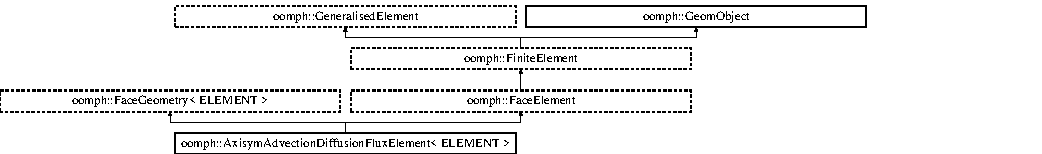
\includegraphics[height=2.074074cm]{classoomph_1_1AxisymAdvectionDiffusionFluxElement}
\end{center}
\end{figure}
\subsection*{Public Types}
\begin{DoxyCompactItemize}
\item 
typedef void($\ast$ \hyperlink{classoomph_1_1AxisymAdvectionDiffusionFluxElement_ad4453706dae676758946691686e1a1c3}{Axisym\+Advection\+Diffusion\+Prescribed\+Beta\+Fct\+Pt}) (const \hyperlink{classoomph_1_1Vector}{Vector}$<$ double $>$ \&x, double \&beta)
\begin{DoxyCompactList}\small\item\em Function pointer to the prescribed-\/beta function fct(x,beta(x)) -- x is a Vector! \end{DoxyCompactList}\item 
typedef void($\ast$ \hyperlink{classoomph_1_1AxisymAdvectionDiffusionFluxElement_aa0922f19043ccc259c61c704fa3b5767}{Axisym\+Advection\+Diffusion\+Prescribed\+Alpha\+Fct\+Pt}) (const \hyperlink{classoomph_1_1Vector}{Vector}$<$ double $>$ \&x, double \&alpha)
\begin{DoxyCompactList}\small\item\em Function pointer to the prescribed-\/alpha function fct(x,alpha(x)) -- x is a Vector! \end{DoxyCompactList}\end{DoxyCompactItemize}
\subsection*{Public Member Functions}
\begin{DoxyCompactItemize}
\item 
\hyperlink{classoomph_1_1AxisymAdvectionDiffusionFluxElement_af3cf91c225808270375927c1b4dbfeb1}{Axisym\+Advection\+Diffusion\+Flux\+Element} (\hyperlink{classoomph_1_1FiniteElement}{Finite\+Element} $\ast$const \&bulk\+\_\+el\+\_\+pt, const int \&\hyperlink{classoomph_1_1FaceElement_a478d577ac6db67ecc80f1f02ae3ab170}{face\+\_\+index})
\begin{DoxyCompactList}\small\item\em Constructor, takes the pointer to the \char`\"{}bulk\char`\"{} element and the index of the face to be created. \end{DoxyCompactList}\item 
\hyperlink{classoomph_1_1AxisymAdvectionDiffusionFluxElement_aa1cd0aff254aebe43bc0709769040291}{Axisym\+Advection\+Diffusion\+Flux\+Element} ()
\begin{DoxyCompactList}\small\item\em Broken empty constructor. \end{DoxyCompactList}\item 
\hyperlink{classoomph_1_1AxisymAdvectionDiffusionFluxElement_ab37a5f165394c2a03a3d8d6de6fae148}{Axisym\+Advection\+Diffusion\+Flux\+Element} (const \hyperlink{classoomph_1_1AxisymAdvectionDiffusionFluxElement}{Axisym\+Advection\+Diffusion\+Flux\+Element} \&dummy)
\begin{DoxyCompactList}\small\item\em Broken copy constructor. \end{DoxyCompactList}\item 
\hyperlink{classoomph_1_1AxisymAdvectionDiffusionFluxElement_ad4453706dae676758946691686e1a1c3}{Axisym\+Advection\+Diffusion\+Prescribed\+Beta\+Fct\+Pt} \& \hyperlink{classoomph_1_1AxisymAdvectionDiffusionFluxElement_a3f81fc1578f2cec5a54a8a5671610dbb}{beta\+\_\+fct\+\_\+pt} ()
\begin{DoxyCompactList}\small\item\em Broken assignment operator. \end{DoxyCompactList}\item 
\hyperlink{classoomph_1_1AxisymAdvectionDiffusionFluxElement_aa0922f19043ccc259c61c704fa3b5767}{Axisym\+Advection\+Diffusion\+Prescribed\+Alpha\+Fct\+Pt} \& \hyperlink{classoomph_1_1AxisymAdvectionDiffusionFluxElement_a6e19586f128e5a8be0c5592147a49938}{alpha\+\_\+fct\+\_\+pt} ()
\begin{DoxyCompactList}\small\item\em Access function for the prescribed-\/alpha function pointer. \end{DoxyCompactList}\item 
void \hyperlink{classoomph_1_1AxisymAdvectionDiffusionFluxElement_a2264f12223ccbcc2f4e3f89403fddea4}{fill\+\_\+in\+\_\+contribution\+\_\+to\+\_\+residuals} (\hyperlink{classoomph_1_1Vector}{Vector}$<$ double $>$ \&residuals)
\begin{DoxyCompactList}\small\item\em Add the element\textquotesingle{}s contribution to its residual vector. \end{DoxyCompactList}\item 
void \hyperlink{classoomph_1_1AxisymAdvectionDiffusionFluxElement_a6dc7a3bc74b66449b6588d8ea64e7cd7}{fill\+\_\+in\+\_\+contribution\+\_\+to\+\_\+jacobian} (\hyperlink{classoomph_1_1Vector}{Vector}$<$ double $>$ \&residuals, \hyperlink{classoomph_1_1DenseMatrix}{Dense\+Matrix}$<$ double $>$ \&jacobian)
\begin{DoxyCompactList}\small\item\em Add the element\textquotesingle{}s contribution to its residual vector and its Jacobian matrix. \end{DoxyCompactList}\item 
double \hyperlink{classoomph_1_1AxisymAdvectionDiffusionFluxElement_a889e0d213add699c8237bf4fbe10abfe}{zeta\+\_\+nodal} (const unsigned \&n, const unsigned \&k, const unsigned \&\hyperlink{cfortran_8h_adb50e893b86b3e55e751a42eab3cba82}{i}) const
\begin{DoxyCompactList}\small\item\em Specify the value of nodal zeta from the face geometry The \char`\"{}global\char`\"{} intrinsic coordinate of the element when viewed as part of a geometric object should be given by the \hyperlink{classoomph_1_1FaceElement}{Face\+Element} representation, by default (needed to break indeterminacy if bulk element is Solid\+Element) \end{DoxyCompactList}\item 
void \hyperlink{classoomph_1_1AxisymAdvectionDiffusionFluxElement_a5f97a254586d93abb151a25a4a148622}{output} (std\+::ostream \&outfile)
\begin{DoxyCompactList}\small\item\em Output function -- forward to broken version in \hyperlink{classoomph_1_1FiniteElement}{Finite\+Element} until somebody decides what exactly they want to plot here... \end{DoxyCompactList}\item 
void \hyperlink{classoomph_1_1AxisymAdvectionDiffusionFluxElement_ab2ba0c3df1b8ba82db067be66e83ce5b}{output} (std\+::ostream \&outfile, const unsigned \&nplot)
\begin{DoxyCompactList}\small\item\em Output function -- forward to broken version in \hyperlink{classoomph_1_1FiniteElement}{Finite\+Element} until somebody decides what exactly they want to plot here... \end{DoxyCompactList}\end{DoxyCompactItemize}
\subsection*{Protected Member Functions}
\begin{DoxyCompactItemize}
\item 
double \hyperlink{classoomph_1_1AxisymAdvectionDiffusionFluxElement_a328aa887d66fa0f5e2bec3ccc8db60fc}{shape\+\_\+and\+\_\+test} (const \hyperlink{classoomph_1_1Vector}{Vector}$<$ double $>$ \&\hyperlink{cfortran_8h_ab7123126e4885ef647dd9c6e3807a21c}{s}, \hyperlink{classoomph_1_1Shape}{Shape} \&psi, \hyperlink{classoomph_1_1Shape}{Shape} \&test) const
\begin{DoxyCompactList}\small\item\em Function to compute the shape and test functions and to return the Jacobian of mapping between local and global (Eulerian) coordinates. \end{DoxyCompactList}\item 
double \hyperlink{classoomph_1_1AxisymAdvectionDiffusionFluxElement_a5e1b027b49e09642d2dc39c61479c782}{shape\+\_\+and\+\_\+test\+\_\+at\+\_\+knot} (const unsigned \&ipt, \hyperlink{classoomph_1_1Shape}{Shape} \&psi, \hyperlink{classoomph_1_1Shape}{Shape} \&test) const
\begin{DoxyCompactList}\small\item\em Function to compute the shape and test functions and to return the Jacobian of mapping between local and global (Eulerian) coordinates. \end{DoxyCompactList}\item 
void \hyperlink{classoomph_1_1AxisymAdvectionDiffusionFluxElement_ae221b92f7bf3ea7eeb26a1cc2b353941}{get\+\_\+beta} (const \hyperlink{classoomph_1_1Vector}{Vector}$<$ double $>$ \&x, double \&beta)
\begin{DoxyCompactList}\small\item\em Function to calculate the prescribed beta at a given spatial position. \end{DoxyCompactList}\item 
void \hyperlink{classoomph_1_1AxisymAdvectionDiffusionFluxElement_a556be18a2a9c91d5da9c3611422efa87}{get\+\_\+alpha} (const \hyperlink{classoomph_1_1Vector}{Vector}$<$ double $>$ \&x, double \&alpha)
\begin{DoxyCompactList}\small\item\em Function to calculate the prescribed alpha at a given spatial position. \end{DoxyCompactList}\end{DoxyCompactItemize}
\subsection*{Private Member Functions}
\begin{DoxyCompactItemize}
\item 
void \hyperlink{classoomph_1_1AxisymAdvectionDiffusionFluxElement_a2c11d285cf27d758e1863b15c95f7b31}{fill\+\_\+in\+\_\+generic\+\_\+residual\+\_\+contribution\+\_\+axi\+\_\+adv\+\_\+diff\+\_\+flux} (\hyperlink{classoomph_1_1Vector}{Vector}$<$ double $>$ \&residuals, \hyperlink{classoomph_1_1DenseMatrix}{Dense\+Matrix}$<$ double $>$ \&jacobian, unsigned flag)
\begin{DoxyCompactList}\small\item\em Add the element\textquotesingle{}s contribution to its residual vector. flag=1(or 0)\+: do (or don\textquotesingle{}t) compute the Jacobian as well. \end{DoxyCompactList}\end{DoxyCompactItemize}
\subsection*{Private Attributes}
\begin{DoxyCompactItemize}
\item 
\hyperlink{classoomph_1_1AxisymAdvectionDiffusionFluxElement_ad4453706dae676758946691686e1a1c3}{Axisym\+Advection\+Diffusion\+Prescribed\+Beta\+Fct\+Pt} \hyperlink{classoomph_1_1AxisymAdvectionDiffusionFluxElement_a410eebdc595edf787822c63e98766beb}{Beta\+\_\+fct\+\_\+pt}
\begin{DoxyCompactList}\small\item\em Function pointer to the (global) prescribed-\/beta function. \end{DoxyCompactList}\item 
\hyperlink{classoomph_1_1AxisymAdvectionDiffusionFluxElement_aa0922f19043ccc259c61c704fa3b5767}{Axisym\+Advection\+Diffusion\+Prescribed\+Alpha\+Fct\+Pt} \hyperlink{classoomph_1_1AxisymAdvectionDiffusionFluxElement_a5e700f50fff5fcdcf9701afe3719ab12}{Alpha\+\_\+fct\+\_\+pt}
\begin{DoxyCompactList}\small\item\em Function pointer to the (global) prescribed-\/alpha function. \end{DoxyCompactList}\item 
unsigned \hyperlink{classoomph_1_1AxisymAdvectionDiffusionFluxElement_a9a1a5af501dd6839ffdfe132a2f9c515}{U\+\_\+index\+\_\+adv\+\_\+diff}
\begin{DoxyCompactList}\small\item\em The index at which the unknown is stored at the nodes. \end{DoxyCompactList}\end{DoxyCompactItemize}
\subsection*{Additional Inherited Members}


\subsection{Detailed Description}
\subsubsection*{template$<$class E\+L\+E\+M\+E\+NT$>$\newline
class oomph\+::\+Axisym\+Advection\+Diffusion\+Flux\+Element$<$ E\+L\+E\+M\+E\+N\+T $>$}

A class for elements that allow the imposition of an applied Robin boundary condition on the boundaries of \hyperlink{classoomph_1_1Steady}{Steady} Axisymmnetric Advection Diffusion Flux elements. \[ -\Delta u \cdot \mathbf{n} + \alpha(r,z) u = \beta(r,z) \] The element geometry is obtained from the Face\+Geometry$<$\+E\+L\+E\+M\+E\+N\+T$>$ policy class. 

Definition at line 789 of file axisym\+\_\+advection\+\_\+diffusion\+\_\+elements.\+h.



\subsection{Member Typedef Documentation}
\mbox{\Hypertarget{classoomph_1_1AxisymAdvectionDiffusionFluxElement_aa0922f19043ccc259c61c704fa3b5767}\label{classoomph_1_1AxisymAdvectionDiffusionFluxElement_aa0922f19043ccc259c61c704fa3b5767}} 
\index{oomph\+::\+Axisym\+Advection\+Diffusion\+Flux\+Element@{oomph\+::\+Axisym\+Advection\+Diffusion\+Flux\+Element}!Axisym\+Advection\+Diffusion\+Prescribed\+Alpha\+Fct\+Pt@{Axisym\+Advection\+Diffusion\+Prescribed\+Alpha\+Fct\+Pt}}
\index{Axisym\+Advection\+Diffusion\+Prescribed\+Alpha\+Fct\+Pt@{Axisym\+Advection\+Diffusion\+Prescribed\+Alpha\+Fct\+Pt}!oomph\+::\+Axisym\+Advection\+Diffusion\+Flux\+Element@{oomph\+::\+Axisym\+Advection\+Diffusion\+Flux\+Element}}
\subsubsection{\texorpdfstring{Axisym\+Advection\+Diffusion\+Prescribed\+Alpha\+Fct\+Pt}{AxisymAdvectionDiffusionPrescribedAlphaFctPt}}
{\footnotesize\ttfamily template$<$class E\+L\+E\+M\+E\+NT $>$ \\
typedef void($\ast$ \hyperlink{classoomph_1_1AxisymAdvectionDiffusionFluxElement}{oomph\+::\+Axisym\+Advection\+Diffusion\+Flux\+Element}$<$ E\+L\+E\+M\+E\+NT $>$\+::Axisym\+Advection\+Diffusion\+Prescribed\+Alpha\+Fct\+Pt) (const \hyperlink{classoomph_1_1Vector}{Vector}$<$ double $>$ \&x, double \&alpha)}



Function pointer to the prescribed-\/alpha function fct(x,alpha(x)) -- x is a Vector! 



Definition at line 805 of file axisym\+\_\+advection\+\_\+diffusion\+\_\+elements.\+h.

\mbox{\Hypertarget{classoomph_1_1AxisymAdvectionDiffusionFluxElement_ad4453706dae676758946691686e1a1c3}\label{classoomph_1_1AxisymAdvectionDiffusionFluxElement_ad4453706dae676758946691686e1a1c3}} 
\index{oomph\+::\+Axisym\+Advection\+Diffusion\+Flux\+Element@{oomph\+::\+Axisym\+Advection\+Diffusion\+Flux\+Element}!Axisym\+Advection\+Diffusion\+Prescribed\+Beta\+Fct\+Pt@{Axisym\+Advection\+Diffusion\+Prescribed\+Beta\+Fct\+Pt}}
\index{Axisym\+Advection\+Diffusion\+Prescribed\+Beta\+Fct\+Pt@{Axisym\+Advection\+Diffusion\+Prescribed\+Beta\+Fct\+Pt}!oomph\+::\+Axisym\+Advection\+Diffusion\+Flux\+Element@{oomph\+::\+Axisym\+Advection\+Diffusion\+Flux\+Element}}
\subsubsection{\texorpdfstring{Axisym\+Advection\+Diffusion\+Prescribed\+Beta\+Fct\+Pt}{AxisymAdvectionDiffusionPrescribedBetaFctPt}}
{\footnotesize\ttfamily template$<$class E\+L\+E\+M\+E\+NT $>$ \\
typedef void($\ast$ \hyperlink{classoomph_1_1AxisymAdvectionDiffusionFluxElement}{oomph\+::\+Axisym\+Advection\+Diffusion\+Flux\+Element}$<$ E\+L\+E\+M\+E\+NT $>$\+::Axisym\+Advection\+Diffusion\+Prescribed\+Beta\+Fct\+Pt) (const \hyperlink{classoomph_1_1Vector}{Vector}$<$ double $>$ \&x, double \&beta)}



Function pointer to the prescribed-\/beta function fct(x,beta(x)) -- x is a Vector! 



Definition at line 799 of file axisym\+\_\+advection\+\_\+diffusion\+\_\+elements.\+h.



\subsection{Constructor \& Destructor Documentation}
\mbox{\Hypertarget{classoomph_1_1AxisymAdvectionDiffusionFluxElement_af3cf91c225808270375927c1b4dbfeb1}\label{classoomph_1_1AxisymAdvectionDiffusionFluxElement_af3cf91c225808270375927c1b4dbfeb1}} 
\index{oomph\+::\+Axisym\+Advection\+Diffusion\+Flux\+Element@{oomph\+::\+Axisym\+Advection\+Diffusion\+Flux\+Element}!Axisym\+Advection\+Diffusion\+Flux\+Element@{Axisym\+Advection\+Diffusion\+Flux\+Element}}
\index{Axisym\+Advection\+Diffusion\+Flux\+Element@{Axisym\+Advection\+Diffusion\+Flux\+Element}!oomph\+::\+Axisym\+Advection\+Diffusion\+Flux\+Element@{oomph\+::\+Axisym\+Advection\+Diffusion\+Flux\+Element}}
\subsubsection{\texorpdfstring{Axisym\+Advection\+Diffusion\+Flux\+Element()}{AxisymAdvectionDiffusionFluxElement()}\hspace{0.1cm}{\footnotesize\ttfamily [1/3]}}
{\footnotesize\ttfamily template$<$class E\+L\+E\+M\+E\+NT $>$ \\
\hyperlink{classoomph_1_1AxisymAdvectionDiffusionFluxElement}{oomph\+::\+Axisym\+Advection\+Diffusion\+Flux\+Element}$<$ E\+L\+E\+M\+E\+NT $>$\+::\hyperlink{classoomph_1_1AxisymAdvectionDiffusionFluxElement}{Axisym\+Advection\+Diffusion\+Flux\+Element} (\begin{DoxyParamCaption}\item[{\hyperlink{classoomph_1_1FiniteElement}{Finite\+Element} $\ast$const \&}]{bulk\+\_\+el\+\_\+pt,  }\item[{const int \&}]{face\+\_\+index }\end{DoxyParamCaption})}



Constructor, takes the pointer to the \char`\"{}bulk\char`\"{} element and the index of the face to be created. 



Definition at line 1014 of file axisym\+\_\+advection\+\_\+diffusion\+\_\+elements.\+h.



References oomph\+::\+Axisym\+Advection\+Diffusion\+Flux\+Element$<$ E\+L\+E\+M\+E\+N\+T $>$\+::\+Beta\+\_\+fct\+\_\+pt, oomph\+::\+Finite\+Element\+::build\+\_\+face\+\_\+element(), oomph\+::\+Axisym\+Advection\+Diffusion\+Flux\+Element$<$ E\+L\+E\+M\+E\+N\+T $>$\+::fill\+\_\+in\+\_\+generic\+\_\+residual\+\_\+contribution\+\_\+axi\+\_\+adv\+\_\+diff\+\_\+flux(), oomph\+::\+Finite\+Element\+::has\+\_\+hanging\+\_\+nodes(), oomph\+::\+Global\+\_\+string\+\_\+for\+\_\+annotation\+::string(), oomph\+::\+Axisym\+Advection\+Diffusion\+Flux\+Element$<$ E\+L\+E\+M\+E\+N\+T $>$\+::\+U\+\_\+index\+\_\+adv\+\_\+diff, and oomph\+::\+Axisym\+Advection\+Diffusion\+Equations\+::u\+\_\+index\+\_\+axi\+\_\+adv\+\_\+diff().

\mbox{\Hypertarget{classoomph_1_1AxisymAdvectionDiffusionFluxElement_aa1cd0aff254aebe43bc0709769040291}\label{classoomph_1_1AxisymAdvectionDiffusionFluxElement_aa1cd0aff254aebe43bc0709769040291}} 
\index{oomph\+::\+Axisym\+Advection\+Diffusion\+Flux\+Element@{oomph\+::\+Axisym\+Advection\+Diffusion\+Flux\+Element}!Axisym\+Advection\+Diffusion\+Flux\+Element@{Axisym\+Advection\+Diffusion\+Flux\+Element}}
\index{Axisym\+Advection\+Diffusion\+Flux\+Element@{Axisym\+Advection\+Diffusion\+Flux\+Element}!oomph\+::\+Axisym\+Advection\+Diffusion\+Flux\+Element@{oomph\+::\+Axisym\+Advection\+Diffusion\+Flux\+Element}}
\subsubsection{\texorpdfstring{Axisym\+Advection\+Diffusion\+Flux\+Element()}{AxisymAdvectionDiffusionFluxElement()}\hspace{0.1cm}{\footnotesize\ttfamily [2/3]}}
{\footnotesize\ttfamily template$<$class E\+L\+E\+M\+E\+NT $>$ \\
\hyperlink{classoomph_1_1AxisymAdvectionDiffusionFluxElement}{oomph\+::\+Axisym\+Advection\+Diffusion\+Flux\+Element}$<$ E\+L\+E\+M\+E\+NT $>$\+::\hyperlink{classoomph_1_1AxisymAdvectionDiffusionFluxElement}{Axisym\+Advection\+Diffusion\+Flux\+Element} (\begin{DoxyParamCaption}{ }\end{DoxyParamCaption})\hspace{0.3cm}{\ttfamily [inline]}}



Broken empty constructor. 



Definition at line 817 of file axisym\+\_\+advection\+\_\+diffusion\+\_\+elements.\+h.

\mbox{\Hypertarget{classoomph_1_1AxisymAdvectionDiffusionFluxElement_ab37a5f165394c2a03a3d8d6de6fae148}\label{classoomph_1_1AxisymAdvectionDiffusionFluxElement_ab37a5f165394c2a03a3d8d6de6fae148}} 
\index{oomph\+::\+Axisym\+Advection\+Diffusion\+Flux\+Element@{oomph\+::\+Axisym\+Advection\+Diffusion\+Flux\+Element}!Axisym\+Advection\+Diffusion\+Flux\+Element@{Axisym\+Advection\+Diffusion\+Flux\+Element}}
\index{Axisym\+Advection\+Diffusion\+Flux\+Element@{Axisym\+Advection\+Diffusion\+Flux\+Element}!oomph\+::\+Axisym\+Advection\+Diffusion\+Flux\+Element@{oomph\+::\+Axisym\+Advection\+Diffusion\+Flux\+Element}}
\subsubsection{\texorpdfstring{Axisym\+Advection\+Diffusion\+Flux\+Element()}{AxisymAdvectionDiffusionFluxElement()}\hspace{0.1cm}{\footnotesize\ttfamily [3/3]}}
{\footnotesize\ttfamily template$<$class E\+L\+E\+M\+E\+NT $>$ \\
\hyperlink{classoomph_1_1AxisymAdvectionDiffusionFluxElement}{oomph\+::\+Axisym\+Advection\+Diffusion\+Flux\+Element}$<$ E\+L\+E\+M\+E\+NT $>$\+::\hyperlink{classoomph_1_1AxisymAdvectionDiffusionFluxElement}{Axisym\+Advection\+Diffusion\+Flux\+Element} (\begin{DoxyParamCaption}\item[{const \hyperlink{classoomph_1_1AxisymAdvectionDiffusionFluxElement}{Axisym\+Advection\+Diffusion\+Flux\+Element}$<$ E\+L\+E\+M\+E\+NT $>$ \&}]{dummy }\end{DoxyParamCaption})\hspace{0.3cm}{\ttfamily [inline]}}



Broken copy constructor. 



Definition at line 826 of file axisym\+\_\+advection\+\_\+diffusion\+\_\+elements.\+h.



References oomph\+::\+Broken\+Copy\+::broken\+\_\+copy().



\subsection{Member Function Documentation}
\mbox{\Hypertarget{classoomph_1_1AxisymAdvectionDiffusionFluxElement_a6e19586f128e5a8be0c5592147a49938}\label{classoomph_1_1AxisymAdvectionDiffusionFluxElement_a6e19586f128e5a8be0c5592147a49938}} 
\index{oomph\+::\+Axisym\+Advection\+Diffusion\+Flux\+Element@{oomph\+::\+Axisym\+Advection\+Diffusion\+Flux\+Element}!alpha\+\_\+fct\+\_\+pt@{alpha\+\_\+fct\+\_\+pt}}
\index{alpha\+\_\+fct\+\_\+pt@{alpha\+\_\+fct\+\_\+pt}!oomph\+::\+Axisym\+Advection\+Diffusion\+Flux\+Element@{oomph\+::\+Axisym\+Advection\+Diffusion\+Flux\+Element}}
\subsubsection{\texorpdfstring{alpha\+\_\+fct\+\_\+pt()}{alpha\_fct\_pt()}}
{\footnotesize\ttfamily template$<$class E\+L\+E\+M\+E\+NT $>$ \\
\hyperlink{classoomph_1_1AxisymAdvectionDiffusionFluxElement_aa0922f19043ccc259c61c704fa3b5767}{Axisym\+Advection\+Diffusion\+Prescribed\+Alpha\+Fct\+Pt}\& \hyperlink{classoomph_1_1AxisymAdvectionDiffusionFluxElement}{oomph\+::\+Axisym\+Advection\+Diffusion\+Flux\+Element}$<$ E\+L\+E\+M\+E\+NT $>$\+::alpha\+\_\+fct\+\_\+pt (\begin{DoxyParamCaption}{ }\end{DoxyParamCaption})\hspace{0.3cm}{\ttfamily [inline]}}



Access function for the prescribed-\/alpha function pointer. 



Definition at line 845 of file axisym\+\_\+advection\+\_\+diffusion\+\_\+elements.\+h.

\mbox{\Hypertarget{classoomph_1_1AxisymAdvectionDiffusionFluxElement_a3f81fc1578f2cec5a54a8a5671610dbb}\label{classoomph_1_1AxisymAdvectionDiffusionFluxElement_a3f81fc1578f2cec5a54a8a5671610dbb}} 
\index{oomph\+::\+Axisym\+Advection\+Diffusion\+Flux\+Element@{oomph\+::\+Axisym\+Advection\+Diffusion\+Flux\+Element}!beta\+\_\+fct\+\_\+pt@{beta\+\_\+fct\+\_\+pt}}
\index{beta\+\_\+fct\+\_\+pt@{beta\+\_\+fct\+\_\+pt}!oomph\+::\+Axisym\+Advection\+Diffusion\+Flux\+Element@{oomph\+::\+Axisym\+Advection\+Diffusion\+Flux\+Element}}
\subsubsection{\texorpdfstring{beta\+\_\+fct\+\_\+pt()}{beta\_fct\_pt()}}
{\footnotesize\ttfamily template$<$class E\+L\+E\+M\+E\+NT $>$ \\
\hyperlink{classoomph_1_1AxisymAdvectionDiffusionFluxElement_ad4453706dae676758946691686e1a1c3}{Axisym\+Advection\+Diffusion\+Prescribed\+Beta\+Fct\+Pt}\& \hyperlink{classoomph_1_1AxisymAdvectionDiffusionFluxElement}{oomph\+::\+Axisym\+Advection\+Diffusion\+Flux\+Element}$<$ E\+L\+E\+M\+E\+NT $>$\+::beta\+\_\+fct\+\_\+pt (\begin{DoxyParamCaption}{ }\end{DoxyParamCaption})\hspace{0.3cm}{\ttfamily [inline]}}



Broken assignment operator. 

Access function for the prescribed-\/beta function pointer 

Definition at line 839 of file axisym\+\_\+advection\+\_\+diffusion\+\_\+elements.\+h.

\mbox{\Hypertarget{classoomph_1_1AxisymAdvectionDiffusionFluxElement_a6dc7a3bc74b66449b6588d8ea64e7cd7}\label{classoomph_1_1AxisymAdvectionDiffusionFluxElement_a6dc7a3bc74b66449b6588d8ea64e7cd7}} 
\index{oomph\+::\+Axisym\+Advection\+Diffusion\+Flux\+Element@{oomph\+::\+Axisym\+Advection\+Diffusion\+Flux\+Element}!fill\+\_\+in\+\_\+contribution\+\_\+to\+\_\+jacobian@{fill\+\_\+in\+\_\+contribution\+\_\+to\+\_\+jacobian}}
\index{fill\+\_\+in\+\_\+contribution\+\_\+to\+\_\+jacobian@{fill\+\_\+in\+\_\+contribution\+\_\+to\+\_\+jacobian}!oomph\+::\+Axisym\+Advection\+Diffusion\+Flux\+Element@{oomph\+::\+Axisym\+Advection\+Diffusion\+Flux\+Element}}
\subsubsection{\texorpdfstring{fill\+\_\+in\+\_\+contribution\+\_\+to\+\_\+jacobian()}{fill\_in\_contribution\_to\_jacobian()}}
{\footnotesize\ttfamily template$<$class E\+L\+E\+M\+E\+NT $>$ \\
void \hyperlink{classoomph_1_1AxisymAdvectionDiffusionFluxElement}{oomph\+::\+Axisym\+Advection\+Diffusion\+Flux\+Element}$<$ E\+L\+E\+M\+E\+NT $>$\+::fill\+\_\+in\+\_\+contribution\+\_\+to\+\_\+jacobian (\begin{DoxyParamCaption}\item[{\hyperlink{classoomph_1_1Vector}{Vector}$<$ double $>$ \&}]{residuals,  }\item[{\hyperlink{classoomph_1_1DenseMatrix}{Dense\+Matrix}$<$ double $>$ \&}]{jacobian }\end{DoxyParamCaption})\hspace{0.3cm}{\ttfamily [inline]}, {\ttfamily [virtual]}}



Add the element\textquotesingle{}s contribution to its residual vector and its Jacobian matrix. 



Reimplemented from \hyperlink{classoomph_1_1GeneralisedElement_a6ae09fc0d68e4309ac1b03583d252845}{oomph\+::\+Generalised\+Element}.



Definition at line 864 of file axisym\+\_\+advection\+\_\+diffusion\+\_\+elements.\+h.

\mbox{\Hypertarget{classoomph_1_1AxisymAdvectionDiffusionFluxElement_a2264f12223ccbcc2f4e3f89403fddea4}\label{classoomph_1_1AxisymAdvectionDiffusionFluxElement_a2264f12223ccbcc2f4e3f89403fddea4}} 
\index{oomph\+::\+Axisym\+Advection\+Diffusion\+Flux\+Element@{oomph\+::\+Axisym\+Advection\+Diffusion\+Flux\+Element}!fill\+\_\+in\+\_\+contribution\+\_\+to\+\_\+residuals@{fill\+\_\+in\+\_\+contribution\+\_\+to\+\_\+residuals}}
\index{fill\+\_\+in\+\_\+contribution\+\_\+to\+\_\+residuals@{fill\+\_\+in\+\_\+contribution\+\_\+to\+\_\+residuals}!oomph\+::\+Axisym\+Advection\+Diffusion\+Flux\+Element@{oomph\+::\+Axisym\+Advection\+Diffusion\+Flux\+Element}}
\subsubsection{\texorpdfstring{fill\+\_\+in\+\_\+contribution\+\_\+to\+\_\+residuals()}{fill\_in\_contribution\_to\_residuals()}}
{\footnotesize\ttfamily template$<$class E\+L\+E\+M\+E\+NT $>$ \\
void \hyperlink{classoomph_1_1AxisymAdvectionDiffusionFluxElement}{oomph\+::\+Axisym\+Advection\+Diffusion\+Flux\+Element}$<$ E\+L\+E\+M\+E\+NT $>$\+::fill\+\_\+in\+\_\+contribution\+\_\+to\+\_\+residuals (\begin{DoxyParamCaption}\item[{\hyperlink{classoomph_1_1Vector}{Vector}$<$ double $>$ \&}]{residuals }\end{DoxyParamCaption})\hspace{0.3cm}{\ttfamily [inline]}, {\ttfamily [virtual]}}



Add the element\textquotesingle{}s contribution to its residual vector. 



Reimplemented from \hyperlink{classoomph_1_1GeneralisedElement_a310c97f515e8504a48179c0e72c550d7}{oomph\+::\+Generalised\+Element}.



Definition at line 852 of file axisym\+\_\+advection\+\_\+diffusion\+\_\+elements.\+h.



References oomph\+::\+Generalised\+Element\+::\+Dummy\+\_\+matrix.

\mbox{\Hypertarget{classoomph_1_1AxisymAdvectionDiffusionFluxElement_a2c11d285cf27d758e1863b15c95f7b31}\label{classoomph_1_1AxisymAdvectionDiffusionFluxElement_a2c11d285cf27d758e1863b15c95f7b31}} 
\index{oomph\+::\+Axisym\+Advection\+Diffusion\+Flux\+Element@{oomph\+::\+Axisym\+Advection\+Diffusion\+Flux\+Element}!fill\+\_\+in\+\_\+generic\+\_\+residual\+\_\+contribution\+\_\+axi\+\_\+adv\+\_\+diff\+\_\+flux@{fill\+\_\+in\+\_\+generic\+\_\+residual\+\_\+contribution\+\_\+axi\+\_\+adv\+\_\+diff\+\_\+flux}}
\index{fill\+\_\+in\+\_\+generic\+\_\+residual\+\_\+contribution\+\_\+axi\+\_\+adv\+\_\+diff\+\_\+flux@{fill\+\_\+in\+\_\+generic\+\_\+residual\+\_\+contribution\+\_\+axi\+\_\+adv\+\_\+diff\+\_\+flux}!oomph\+::\+Axisym\+Advection\+Diffusion\+Flux\+Element@{oomph\+::\+Axisym\+Advection\+Diffusion\+Flux\+Element}}
\subsubsection{\texorpdfstring{fill\+\_\+in\+\_\+generic\+\_\+residual\+\_\+contribution\+\_\+axi\+\_\+adv\+\_\+diff\+\_\+flux()}{fill\_in\_generic\_residual\_contribution\_axi\_adv\_diff\_flux()}}
{\footnotesize\ttfamily template$<$class E\+L\+E\+M\+E\+NT $>$ \\
void \hyperlink{classoomph_1_1AxisymAdvectionDiffusionFluxElement}{oomph\+::\+Axisym\+Advection\+Diffusion\+Flux\+Element}$<$ E\+L\+E\+M\+E\+NT $>$\+::fill\+\_\+in\+\_\+generic\+\_\+residual\+\_\+contribution\+\_\+axi\+\_\+adv\+\_\+diff\+\_\+flux (\begin{DoxyParamCaption}\item[{\hyperlink{classoomph_1_1Vector}{Vector}$<$ double $>$ \&}]{residuals,  }\item[{\hyperlink{classoomph_1_1DenseMatrix}{Dense\+Matrix}$<$ double $>$ \&}]{jacobian,  }\item[{unsigned}]{flag }\end{DoxyParamCaption})\hspace{0.3cm}{\ttfamily [private]}}



Add the element\textquotesingle{}s contribution to its residual vector. flag=1(or 0)\+: do (or don\textquotesingle{}t) compute the Jacobian as well. 

Compute the element\textquotesingle{}s residual vector and the (zero) Jacobian matrix for the Robin boundary condition\+: \[ \Delta u \cdot \mathbf{n} + \alpha (\mathbf{x}) = \beta (\mathbf{x}) \]. 

Definition at line 1097 of file axisym\+\_\+advection\+\_\+diffusion\+\_\+elements.\+h.



References oomph\+::\+Axisym\+Advection\+Diffusion\+Flux\+Element$<$ E\+L\+E\+M\+E\+N\+T $>$\+::get\+\_\+alpha(), oomph\+::\+Axisym\+Advection\+Diffusion\+Flux\+Element$<$ E\+L\+E\+M\+E\+N\+T $>$\+::get\+\_\+beta(), i, oomph\+::\+Finite\+Element\+::integral\+\_\+pt(), oomph\+::\+Face\+Element\+::interpolated\+\_\+x(), oomph\+::\+Integral\+::knot(), oomph\+::\+Finite\+Element\+::nnode(), oomph\+::\+Finite\+Element\+::nodal\+\_\+local\+\_\+eqn(), oomph\+::\+Finite\+Element\+::nodal\+\_\+position(), oomph\+::\+Integral\+::nweight(), oomph\+::\+Finite\+Element\+::raw\+\_\+nodal\+\_\+value(), s, oomph\+::\+Axisym\+Advection\+Diffusion\+Flux\+Element$<$ E\+L\+E\+M\+E\+N\+T $>$\+::shape\+\_\+and\+\_\+test(), oomph\+::\+Axisym\+Advection\+Diffusion\+Flux\+Element$<$ E\+L\+E\+M\+E\+N\+T $>$\+::\+U\+\_\+index\+\_\+adv\+\_\+diff, oomph\+::\+Quad\+Tree\+Names\+::W, and oomph\+::\+Integral\+::weight().



Referenced by oomph\+::\+Axisym\+Advection\+Diffusion\+Flux\+Element$<$ E\+L\+E\+M\+E\+N\+T $>$\+::\+Axisym\+Advection\+Diffusion\+Flux\+Element().

\mbox{\Hypertarget{classoomph_1_1AxisymAdvectionDiffusionFluxElement_a556be18a2a9c91d5da9c3611422efa87}\label{classoomph_1_1AxisymAdvectionDiffusionFluxElement_a556be18a2a9c91d5da9c3611422efa87}} 
\index{oomph\+::\+Axisym\+Advection\+Diffusion\+Flux\+Element@{oomph\+::\+Axisym\+Advection\+Diffusion\+Flux\+Element}!get\+\_\+alpha@{get\+\_\+alpha}}
\index{get\+\_\+alpha@{get\+\_\+alpha}!oomph\+::\+Axisym\+Advection\+Diffusion\+Flux\+Element@{oomph\+::\+Axisym\+Advection\+Diffusion\+Flux\+Element}}
\subsubsection{\texorpdfstring{get\+\_\+alpha()}{get\_alpha()}}
{\footnotesize\ttfamily template$<$class E\+L\+E\+M\+E\+NT $>$ \\
void \hyperlink{classoomph_1_1AxisymAdvectionDiffusionFluxElement}{oomph\+::\+Axisym\+Advection\+Diffusion\+Flux\+Element}$<$ E\+L\+E\+M\+E\+NT $>$\+::get\+\_\+alpha (\begin{DoxyParamCaption}\item[{const \hyperlink{classoomph_1_1Vector}{Vector}$<$ double $>$ \&}]{x,  }\item[{double \&}]{alpha }\end{DoxyParamCaption})\hspace{0.3cm}{\ttfamily [inline]}, {\ttfamily [protected]}}



Function to calculate the prescribed alpha at a given spatial position. 



Definition at line 966 of file axisym\+\_\+advection\+\_\+diffusion\+\_\+elements.\+h.



Referenced by oomph\+::\+Axisym\+Advection\+Diffusion\+Flux\+Element$<$ E\+L\+E\+M\+E\+N\+T $>$\+::fill\+\_\+in\+\_\+generic\+\_\+residual\+\_\+contribution\+\_\+axi\+\_\+adv\+\_\+diff\+\_\+flux().

\mbox{\Hypertarget{classoomph_1_1AxisymAdvectionDiffusionFluxElement_ae221b92f7bf3ea7eeb26a1cc2b353941}\label{classoomph_1_1AxisymAdvectionDiffusionFluxElement_ae221b92f7bf3ea7eeb26a1cc2b353941}} 
\index{oomph\+::\+Axisym\+Advection\+Diffusion\+Flux\+Element@{oomph\+::\+Axisym\+Advection\+Diffusion\+Flux\+Element}!get\+\_\+beta@{get\+\_\+beta}}
\index{get\+\_\+beta@{get\+\_\+beta}!oomph\+::\+Axisym\+Advection\+Diffusion\+Flux\+Element@{oomph\+::\+Axisym\+Advection\+Diffusion\+Flux\+Element}}
\subsubsection{\texorpdfstring{get\+\_\+beta()}{get\_beta()}}
{\footnotesize\ttfamily template$<$class E\+L\+E\+M\+E\+NT $>$ \\
void \hyperlink{classoomph_1_1AxisymAdvectionDiffusionFluxElement}{oomph\+::\+Axisym\+Advection\+Diffusion\+Flux\+Element}$<$ E\+L\+E\+M\+E\+NT $>$\+::get\+\_\+beta (\begin{DoxyParamCaption}\item[{const \hyperlink{classoomph_1_1Vector}{Vector}$<$ double $>$ \&}]{x,  }\item[{double \&}]{beta }\end{DoxyParamCaption})\hspace{0.3cm}{\ttfamily [inline]}, {\ttfamily [protected]}}



Function to calculate the prescribed beta at a given spatial position. 



Definition at line 950 of file axisym\+\_\+advection\+\_\+diffusion\+\_\+elements.\+h.



Referenced by oomph\+::\+Axisym\+Advection\+Diffusion\+Flux\+Element$<$ E\+L\+E\+M\+E\+N\+T $>$\+::fill\+\_\+in\+\_\+generic\+\_\+residual\+\_\+contribution\+\_\+axi\+\_\+adv\+\_\+diff\+\_\+flux().

\mbox{\Hypertarget{classoomph_1_1AxisymAdvectionDiffusionFluxElement_a5f97a254586d93abb151a25a4a148622}\label{classoomph_1_1AxisymAdvectionDiffusionFluxElement_a5f97a254586d93abb151a25a4a148622}} 
\index{oomph\+::\+Axisym\+Advection\+Diffusion\+Flux\+Element@{oomph\+::\+Axisym\+Advection\+Diffusion\+Flux\+Element}!output@{output}}
\index{output@{output}!oomph\+::\+Axisym\+Advection\+Diffusion\+Flux\+Element@{oomph\+::\+Axisym\+Advection\+Diffusion\+Flux\+Element}}
\subsubsection{\texorpdfstring{output()}{output()}\hspace{0.1cm}{\footnotesize\ttfamily [1/2]}}
{\footnotesize\ttfamily template$<$class E\+L\+E\+M\+E\+NT $>$ \\
void \hyperlink{classoomph_1_1AxisymAdvectionDiffusionFluxElement}{oomph\+::\+Axisym\+Advection\+Diffusion\+Flux\+Element}$<$ E\+L\+E\+M\+E\+NT $>$\+::output (\begin{DoxyParamCaption}\item[{std\+::ostream \&}]{outfile }\end{DoxyParamCaption})\hspace{0.3cm}{\ttfamily [inline]}, {\ttfamily [virtual]}}



Output function -- forward to broken version in \hyperlink{classoomph_1_1FiniteElement}{Finite\+Element} until somebody decides what exactly they want to plot here... 



Reimplemented from \hyperlink{classoomph_1_1FiniteElement_a2ad98a3d2ef4999f1bef62c0ff13f2a7}{oomph\+::\+Finite\+Element}.



Definition at line 886 of file axisym\+\_\+advection\+\_\+diffusion\+\_\+elements.\+h.



References oomph\+::\+Finite\+Element\+::output().

\mbox{\Hypertarget{classoomph_1_1AxisymAdvectionDiffusionFluxElement_ab2ba0c3df1b8ba82db067be66e83ce5b}\label{classoomph_1_1AxisymAdvectionDiffusionFluxElement_ab2ba0c3df1b8ba82db067be66e83ce5b}} 
\index{oomph\+::\+Axisym\+Advection\+Diffusion\+Flux\+Element@{oomph\+::\+Axisym\+Advection\+Diffusion\+Flux\+Element}!output@{output}}
\index{output@{output}!oomph\+::\+Axisym\+Advection\+Diffusion\+Flux\+Element@{oomph\+::\+Axisym\+Advection\+Diffusion\+Flux\+Element}}
\subsubsection{\texorpdfstring{output()}{output()}\hspace{0.1cm}{\footnotesize\ttfamily [2/2]}}
{\footnotesize\ttfamily template$<$class E\+L\+E\+M\+E\+NT $>$ \\
void \hyperlink{classoomph_1_1AxisymAdvectionDiffusionFluxElement}{oomph\+::\+Axisym\+Advection\+Diffusion\+Flux\+Element}$<$ E\+L\+E\+M\+E\+NT $>$\+::output (\begin{DoxyParamCaption}\item[{std\+::ostream \&}]{outfile,  }\item[{const unsigned \&}]{nplot }\end{DoxyParamCaption})\hspace{0.3cm}{\ttfamily [inline]}, {\ttfamily [virtual]}}



Output function -- forward to broken version in \hyperlink{classoomph_1_1FiniteElement}{Finite\+Element} until somebody decides what exactly they want to plot here... 



Reimplemented from \hyperlink{classoomph_1_1FiniteElement_afa9d9b2670f999b43e6679c9dd28c457}{oomph\+::\+Finite\+Element}.



Definition at line 893 of file axisym\+\_\+advection\+\_\+diffusion\+\_\+elements.\+h.



References oomph\+::\+Finite\+Element\+::output().

\mbox{\Hypertarget{classoomph_1_1AxisymAdvectionDiffusionFluxElement_a328aa887d66fa0f5e2bec3ccc8db60fc}\label{classoomph_1_1AxisymAdvectionDiffusionFluxElement_a328aa887d66fa0f5e2bec3ccc8db60fc}} 
\index{oomph\+::\+Axisym\+Advection\+Diffusion\+Flux\+Element@{oomph\+::\+Axisym\+Advection\+Diffusion\+Flux\+Element}!shape\+\_\+and\+\_\+test@{shape\+\_\+and\+\_\+test}}
\index{shape\+\_\+and\+\_\+test@{shape\+\_\+and\+\_\+test}!oomph\+::\+Axisym\+Advection\+Diffusion\+Flux\+Element@{oomph\+::\+Axisym\+Advection\+Diffusion\+Flux\+Element}}
\subsubsection{\texorpdfstring{shape\+\_\+and\+\_\+test()}{shape\_and\_test()}}
{\footnotesize\ttfamily template$<$class E\+L\+E\+M\+E\+NT $>$ \\
double \hyperlink{classoomph_1_1AxisymAdvectionDiffusionFluxElement}{oomph\+::\+Axisym\+Advection\+Diffusion\+Flux\+Element}$<$ E\+L\+E\+M\+E\+NT $>$\+::shape\+\_\+and\+\_\+test (\begin{DoxyParamCaption}\item[{const \hyperlink{classoomph_1_1Vector}{Vector}$<$ double $>$ \&}]{s,  }\item[{\hyperlink{classoomph_1_1Shape}{Shape} \&}]{psi,  }\item[{\hyperlink{classoomph_1_1Shape}{Shape} \&}]{test }\end{DoxyParamCaption}) const\hspace{0.3cm}{\ttfamily [inline]}, {\ttfamily [protected]}}



Function to compute the shape and test functions and to return the Jacobian of mapping between local and global (Eulerian) coordinates. 



Definition at line 904 of file axisym\+\_\+advection\+\_\+diffusion\+\_\+elements.\+h.



References i, oomph\+::\+Finite\+Element\+::\+J\+\_\+eulerian(), oomph\+::\+Finite\+Element\+::nnode(), and oomph\+::\+Finite\+Element\+::shape().



Referenced by oomph\+::\+Axisym\+Advection\+Diffusion\+Flux\+Element$<$ E\+L\+E\+M\+E\+N\+T $>$\+::fill\+\_\+in\+\_\+generic\+\_\+residual\+\_\+contribution\+\_\+axi\+\_\+adv\+\_\+diff\+\_\+flux().

\mbox{\Hypertarget{classoomph_1_1AxisymAdvectionDiffusionFluxElement_a5e1b027b49e09642d2dc39c61479c782}\label{classoomph_1_1AxisymAdvectionDiffusionFluxElement_a5e1b027b49e09642d2dc39c61479c782}} 
\index{oomph\+::\+Axisym\+Advection\+Diffusion\+Flux\+Element@{oomph\+::\+Axisym\+Advection\+Diffusion\+Flux\+Element}!shape\+\_\+and\+\_\+test\+\_\+at\+\_\+knot@{shape\+\_\+and\+\_\+test\+\_\+at\+\_\+knot}}
\index{shape\+\_\+and\+\_\+test\+\_\+at\+\_\+knot@{shape\+\_\+and\+\_\+test\+\_\+at\+\_\+knot}!oomph\+::\+Axisym\+Advection\+Diffusion\+Flux\+Element@{oomph\+::\+Axisym\+Advection\+Diffusion\+Flux\+Element}}
\subsubsection{\texorpdfstring{shape\+\_\+and\+\_\+test\+\_\+at\+\_\+knot()}{shape\_and\_test\_at\_knot()}}
{\footnotesize\ttfamily template$<$class E\+L\+E\+M\+E\+NT $>$ \\
double \hyperlink{classoomph_1_1AxisymAdvectionDiffusionFluxElement}{oomph\+::\+Axisym\+Advection\+Diffusion\+Flux\+Element}$<$ E\+L\+E\+M\+E\+NT $>$\+::shape\+\_\+and\+\_\+test\+\_\+at\+\_\+knot (\begin{DoxyParamCaption}\item[{const unsigned \&}]{ipt,  }\item[{\hyperlink{classoomph_1_1Shape}{Shape} \&}]{psi,  }\item[{\hyperlink{classoomph_1_1Shape}{Shape} \&}]{test }\end{DoxyParamCaption}) const\hspace{0.3cm}{\ttfamily [inline]}, {\ttfamily [protected]}}



Function to compute the shape and test functions and to return the Jacobian of mapping between local and global (Eulerian) coordinates. 



Definition at line 928 of file axisym\+\_\+advection\+\_\+diffusion\+\_\+elements.\+h.



References i, oomph\+::\+Finite\+Element\+::\+J\+\_\+eulerian\+\_\+at\+\_\+knot(), oomph\+::\+Finite\+Element\+::nnode(), and oomph\+::\+Finite\+Element\+::shape\+\_\+at\+\_\+knot().

\mbox{\Hypertarget{classoomph_1_1AxisymAdvectionDiffusionFluxElement_a889e0d213add699c8237bf4fbe10abfe}\label{classoomph_1_1AxisymAdvectionDiffusionFluxElement_a889e0d213add699c8237bf4fbe10abfe}} 
\index{oomph\+::\+Axisym\+Advection\+Diffusion\+Flux\+Element@{oomph\+::\+Axisym\+Advection\+Diffusion\+Flux\+Element}!zeta\+\_\+nodal@{zeta\+\_\+nodal}}
\index{zeta\+\_\+nodal@{zeta\+\_\+nodal}!oomph\+::\+Axisym\+Advection\+Diffusion\+Flux\+Element@{oomph\+::\+Axisym\+Advection\+Diffusion\+Flux\+Element}}
\subsubsection{\texorpdfstring{zeta\+\_\+nodal()}{zeta\_nodal()}}
{\footnotesize\ttfamily template$<$class E\+L\+E\+M\+E\+NT $>$ \\
double \hyperlink{classoomph_1_1AxisymAdvectionDiffusionFluxElement}{oomph\+::\+Axisym\+Advection\+Diffusion\+Flux\+Element}$<$ E\+L\+E\+M\+E\+NT $>$\+::zeta\+\_\+nodal (\begin{DoxyParamCaption}\item[{const unsigned \&}]{n,  }\item[{const unsigned \&}]{k,  }\item[{const unsigned \&}]{i }\end{DoxyParamCaption}) const\hspace{0.3cm}{\ttfamily [inline]}, {\ttfamily [virtual]}}



Specify the value of nodal zeta from the face geometry The \char`\"{}global\char`\"{} intrinsic coordinate of the element when viewed as part of a geometric object should be given by the \hyperlink{classoomph_1_1FaceElement}{Face\+Element} representation, by default (needed to break indeterminacy if bulk element is Solid\+Element) 



Reimplemented from \hyperlink{classoomph_1_1FiniteElement_a849561c5fbcbc07dc49d2dc6cca68559}{oomph\+::\+Finite\+Element}.



Definition at line 878 of file axisym\+\_\+advection\+\_\+diffusion\+\_\+elements.\+h.



References oomph\+::\+Face\+Element\+::zeta\+\_\+nodal().



\subsection{Member Data Documentation}
\mbox{\Hypertarget{classoomph_1_1AxisymAdvectionDiffusionFluxElement_a5e700f50fff5fcdcf9701afe3719ab12}\label{classoomph_1_1AxisymAdvectionDiffusionFluxElement_a5e700f50fff5fcdcf9701afe3719ab12}} 
\index{oomph\+::\+Axisym\+Advection\+Diffusion\+Flux\+Element@{oomph\+::\+Axisym\+Advection\+Diffusion\+Flux\+Element}!Alpha\+\_\+fct\+\_\+pt@{Alpha\+\_\+fct\+\_\+pt}}
\index{Alpha\+\_\+fct\+\_\+pt@{Alpha\+\_\+fct\+\_\+pt}!oomph\+::\+Axisym\+Advection\+Diffusion\+Flux\+Element@{oomph\+::\+Axisym\+Advection\+Diffusion\+Flux\+Element}}
\subsubsection{\texorpdfstring{Alpha\+\_\+fct\+\_\+pt}{Alpha\_fct\_pt}}
{\footnotesize\ttfamily template$<$class E\+L\+E\+M\+E\+NT $>$ \\
\hyperlink{classoomph_1_1AxisymAdvectionDiffusionFluxElement_aa0922f19043ccc259c61c704fa3b5767}{Axisym\+Advection\+Diffusion\+Prescribed\+Alpha\+Fct\+Pt} \hyperlink{classoomph_1_1AxisymAdvectionDiffusionFluxElement}{oomph\+::\+Axisym\+Advection\+Diffusion\+Flux\+Element}$<$ E\+L\+E\+M\+E\+NT $>$\+::Alpha\+\_\+fct\+\_\+pt\hspace{0.3cm}{\ttfamily [private]}}



Function pointer to the (global) prescribed-\/alpha function. 



Definition at line 994 of file axisym\+\_\+advection\+\_\+diffusion\+\_\+elements.\+h.

\mbox{\Hypertarget{classoomph_1_1AxisymAdvectionDiffusionFluxElement_a410eebdc595edf787822c63e98766beb}\label{classoomph_1_1AxisymAdvectionDiffusionFluxElement_a410eebdc595edf787822c63e98766beb}} 
\index{oomph\+::\+Axisym\+Advection\+Diffusion\+Flux\+Element@{oomph\+::\+Axisym\+Advection\+Diffusion\+Flux\+Element}!Beta\+\_\+fct\+\_\+pt@{Beta\+\_\+fct\+\_\+pt}}
\index{Beta\+\_\+fct\+\_\+pt@{Beta\+\_\+fct\+\_\+pt}!oomph\+::\+Axisym\+Advection\+Diffusion\+Flux\+Element@{oomph\+::\+Axisym\+Advection\+Diffusion\+Flux\+Element}}
\subsubsection{\texorpdfstring{Beta\+\_\+fct\+\_\+pt}{Beta\_fct\_pt}}
{\footnotesize\ttfamily template$<$class E\+L\+E\+M\+E\+NT $>$ \\
\hyperlink{classoomph_1_1AxisymAdvectionDiffusionFluxElement_ad4453706dae676758946691686e1a1c3}{Axisym\+Advection\+Diffusion\+Prescribed\+Beta\+Fct\+Pt} \hyperlink{classoomph_1_1AxisymAdvectionDiffusionFluxElement}{oomph\+::\+Axisym\+Advection\+Diffusion\+Flux\+Element}$<$ E\+L\+E\+M\+E\+NT $>$\+::Beta\+\_\+fct\+\_\+pt\hspace{0.3cm}{\ttfamily [private]}}



Function pointer to the (global) prescribed-\/beta function. 



Definition at line 991 of file axisym\+\_\+advection\+\_\+diffusion\+\_\+elements.\+h.



Referenced by oomph\+::\+Axisym\+Advection\+Diffusion\+Flux\+Element$<$ E\+L\+E\+M\+E\+N\+T $>$\+::\+Axisym\+Advection\+Diffusion\+Flux\+Element().

\mbox{\Hypertarget{classoomph_1_1AxisymAdvectionDiffusionFluxElement_a9a1a5af501dd6839ffdfe132a2f9c515}\label{classoomph_1_1AxisymAdvectionDiffusionFluxElement_a9a1a5af501dd6839ffdfe132a2f9c515}} 
\index{oomph\+::\+Axisym\+Advection\+Diffusion\+Flux\+Element@{oomph\+::\+Axisym\+Advection\+Diffusion\+Flux\+Element}!U\+\_\+index\+\_\+adv\+\_\+diff@{U\+\_\+index\+\_\+adv\+\_\+diff}}
\index{U\+\_\+index\+\_\+adv\+\_\+diff@{U\+\_\+index\+\_\+adv\+\_\+diff}!oomph\+::\+Axisym\+Advection\+Diffusion\+Flux\+Element@{oomph\+::\+Axisym\+Advection\+Diffusion\+Flux\+Element}}
\subsubsection{\texorpdfstring{U\+\_\+index\+\_\+adv\+\_\+diff}{U\_index\_adv\_diff}}
{\footnotesize\ttfamily template$<$class E\+L\+E\+M\+E\+NT $>$ \\
unsigned \hyperlink{classoomph_1_1AxisymAdvectionDiffusionFluxElement}{oomph\+::\+Axisym\+Advection\+Diffusion\+Flux\+Element}$<$ E\+L\+E\+M\+E\+NT $>$\+::U\+\_\+index\+\_\+adv\+\_\+diff\hspace{0.3cm}{\ttfamily [private]}}



The index at which the unknown is stored at the nodes. 



Definition at line 997 of file axisym\+\_\+advection\+\_\+diffusion\+\_\+elements.\+h.



Referenced by oomph\+::\+Axisym\+Advection\+Diffusion\+Flux\+Element$<$ E\+L\+E\+M\+E\+N\+T $>$\+::\+Axisym\+Advection\+Diffusion\+Flux\+Element(), and oomph\+::\+Axisym\+Advection\+Diffusion\+Flux\+Element$<$ E\+L\+E\+M\+E\+N\+T $>$\+::fill\+\_\+in\+\_\+generic\+\_\+residual\+\_\+contribution\+\_\+axi\+\_\+adv\+\_\+diff\+\_\+flux().



The documentation for this class was generated from the following file\+:\begin{DoxyCompactItemize}
\item 
\hyperlink{axisym__advection__diffusion__elements_8h}{axisym\+\_\+advection\+\_\+diffusion\+\_\+elements.\+h}\end{DoxyCompactItemize}

\hypertarget{classoomph_1_1AxisymDiagHermitePVDElement}{}\section{oomph\+:\+:Axisym\+Diag\+Hermite\+P\+V\+D\+Element Class Reference}
\label{classoomph_1_1AxisymDiagHermitePVDElement}\index{oomph\+::\+Axisym\+Diag\+Hermite\+P\+V\+D\+Element@{oomph\+::\+Axisym\+Diag\+Hermite\+P\+V\+D\+Element}}


{\ttfamily \#include $<$axisym\+\_\+solid\+\_\+elements.\+h$>$}

Inheritance diagram for oomph\+:\+:Axisym\+Diag\+Hermite\+P\+V\+D\+Element\+:\begin{figure}[H]
\begin{center}
\leavevmode
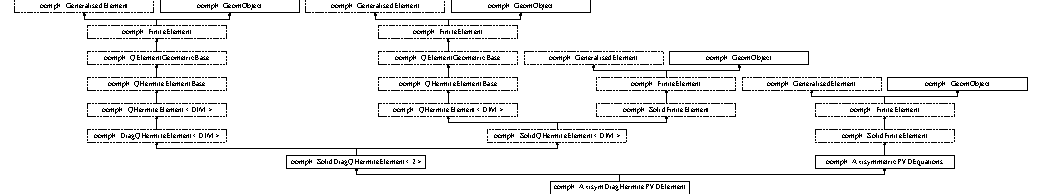
\includegraphics[height=2.612245cm]{classoomph_1_1AxisymDiagHermitePVDElement}
\end{center}
\end{figure}
\subsection*{Public Member Functions}
\begin{DoxyCompactItemize}
\item 
\hyperlink{classoomph_1_1AxisymDiagHermitePVDElement_aecf4d648813650af46a492b1aef2c8d4}{Axisym\+Diag\+Hermite\+P\+V\+D\+Element} ()
\begin{DoxyCompactList}\small\item\em Constructor, there are no internal data points. \end{DoxyCompactList}\item 
void \hyperlink{classoomph_1_1AxisymDiagHermitePVDElement_a6b513539d6607d36d0e048a289fc7a46}{output} (std\+::ostream \&outfile)
\begin{DoxyCompactList}\small\item\em Overload the output function. \end{DoxyCompactList}\item 
void \hyperlink{classoomph_1_1AxisymDiagHermitePVDElement_af5a83e5da70d404bc5e158704d757b56}{output} (std\+::ostream \&outfile, const unsigned \&n\+\_\+plot)
\begin{DoxyCompactList}\small\item\em Output function. \end{DoxyCompactList}\item 
void \hyperlink{classoomph_1_1AxisymDiagHermitePVDElement_a96c36dd119e64e6afb19b813ecbf33b8}{output} (F\+I\+LE $\ast$file\+\_\+pt)
\begin{DoxyCompactList}\small\item\em Overload the output function. \end{DoxyCompactList}\item 
void \hyperlink{classoomph_1_1AxisymDiagHermitePVDElement_adb95d8bc9f3177ae6c49f62fe48a1902}{output} (F\+I\+LE $\ast$file\+\_\+pt, const unsigned \&n\+\_\+plot)
\begin{DoxyCompactList}\small\item\em Output function. \end{DoxyCompactList}\end{DoxyCompactItemize}
\subsection*{Additional Inherited Members}


\subsection{Detailed Description}
An element that solved the \hyperlink{classoomph_1_1AxisymmetricPVDEquations}{Axisymmetric\+P\+V\+D\+Equations} with (diagonal) Hermite interpolation for the positions -- the local and global (Lagrangian) coordinates are assumed to be aligned! 

Definition at line 527 of file axisym\+\_\+solid\+\_\+elements.\+h.



\subsection{Constructor \& Destructor Documentation}
\mbox{\Hypertarget{classoomph_1_1AxisymDiagHermitePVDElement_aecf4d648813650af46a492b1aef2c8d4}\label{classoomph_1_1AxisymDiagHermitePVDElement_aecf4d648813650af46a492b1aef2c8d4}} 
\index{oomph\+::\+Axisym\+Diag\+Hermite\+P\+V\+D\+Element@{oomph\+::\+Axisym\+Diag\+Hermite\+P\+V\+D\+Element}!Axisym\+Diag\+Hermite\+P\+V\+D\+Element@{Axisym\+Diag\+Hermite\+P\+V\+D\+Element}}
\index{Axisym\+Diag\+Hermite\+P\+V\+D\+Element@{Axisym\+Diag\+Hermite\+P\+V\+D\+Element}!oomph\+::\+Axisym\+Diag\+Hermite\+P\+V\+D\+Element@{oomph\+::\+Axisym\+Diag\+Hermite\+P\+V\+D\+Element}}
\subsubsection{\texorpdfstring{Axisym\+Diag\+Hermite\+P\+V\+D\+Element()}{AxisymDiagHermitePVDElement()}}
{\footnotesize\ttfamily oomph\+::\+Axisym\+Diag\+Hermite\+P\+V\+D\+Element\+::\+Axisym\+Diag\+Hermite\+P\+V\+D\+Element (\begin{DoxyParamCaption}{ }\end{DoxyParamCaption})\hspace{0.3cm}{\ttfamily [inline]}}



Constructor, there are no internal data points. 



Definition at line 534 of file axisym\+\_\+solid\+\_\+elements.\+h.



\subsection{Member Function Documentation}
\mbox{\Hypertarget{classoomph_1_1AxisymDiagHermitePVDElement_a6b513539d6607d36d0e048a289fc7a46}\label{classoomph_1_1AxisymDiagHermitePVDElement_a6b513539d6607d36d0e048a289fc7a46}} 
\index{oomph\+::\+Axisym\+Diag\+Hermite\+P\+V\+D\+Element@{oomph\+::\+Axisym\+Diag\+Hermite\+P\+V\+D\+Element}!output@{output}}
\index{output@{output}!oomph\+::\+Axisym\+Diag\+Hermite\+P\+V\+D\+Element@{oomph\+::\+Axisym\+Diag\+Hermite\+P\+V\+D\+Element}}
\subsubsection{\texorpdfstring{output()}{output()}\hspace{0.1cm}{\footnotesize\ttfamily [1/4]}}
{\footnotesize\ttfamily void oomph\+::\+Axisym\+Diag\+Hermite\+P\+V\+D\+Element\+::output (\begin{DoxyParamCaption}\item[{std\+::ostream \&}]{outfile }\end{DoxyParamCaption})\hspace{0.3cm}{\ttfamily [inline]}, {\ttfamily [virtual]}}



Overload the output function. 



Reimplemented from \hyperlink{classoomph_1_1AxisymmetricPVDEquations_a70c01efa665238ec7a574588209d3edb}{oomph\+::\+Axisymmetric\+P\+V\+D\+Equations}.



Definition at line 538 of file axisym\+\_\+solid\+\_\+elements.\+h.



References oomph\+::\+Finite\+Element\+::output().

\mbox{\Hypertarget{classoomph_1_1AxisymDiagHermitePVDElement_af5a83e5da70d404bc5e158704d757b56}\label{classoomph_1_1AxisymDiagHermitePVDElement_af5a83e5da70d404bc5e158704d757b56}} 
\index{oomph\+::\+Axisym\+Diag\+Hermite\+P\+V\+D\+Element@{oomph\+::\+Axisym\+Diag\+Hermite\+P\+V\+D\+Element}!output@{output}}
\index{output@{output}!oomph\+::\+Axisym\+Diag\+Hermite\+P\+V\+D\+Element@{oomph\+::\+Axisym\+Diag\+Hermite\+P\+V\+D\+Element}}
\subsubsection{\texorpdfstring{output()}{output()}\hspace{0.1cm}{\footnotesize\ttfamily [2/4]}}
{\footnotesize\ttfamily void oomph\+::\+Axisym\+Diag\+Hermite\+P\+V\+D\+Element\+::output (\begin{DoxyParamCaption}\item[{std\+::ostream \&}]{outfile,  }\item[{const unsigned \&}]{n\+\_\+plot }\end{DoxyParamCaption})\hspace{0.3cm}{\ttfamily [inline]}, {\ttfamily [virtual]}}



Output function. 



Reimplemented from \hyperlink{classoomph_1_1AxisymmetricPVDEquations_a35cf174ca1692f817e3182166e22ef4b}{oomph\+::\+Axisymmetric\+P\+V\+D\+Equations}.



Definition at line 541 of file axisym\+\_\+solid\+\_\+elements.\+h.



References i, oomph\+::\+Finite\+Element\+::interpolated\+\_\+x(), oomph\+::\+Solid\+Finite\+Element\+::interpolated\+\_\+xi(), and s.

\mbox{\Hypertarget{classoomph_1_1AxisymDiagHermitePVDElement_a96c36dd119e64e6afb19b813ecbf33b8}\label{classoomph_1_1AxisymDiagHermitePVDElement_a96c36dd119e64e6afb19b813ecbf33b8}} 
\index{oomph\+::\+Axisym\+Diag\+Hermite\+P\+V\+D\+Element@{oomph\+::\+Axisym\+Diag\+Hermite\+P\+V\+D\+Element}!output@{output}}
\index{output@{output}!oomph\+::\+Axisym\+Diag\+Hermite\+P\+V\+D\+Element@{oomph\+::\+Axisym\+Diag\+Hermite\+P\+V\+D\+Element}}
\subsubsection{\texorpdfstring{output()}{output()}\hspace{0.1cm}{\footnotesize\ttfamily [3/4]}}
{\footnotesize\ttfamily void oomph\+::\+Axisym\+Diag\+Hermite\+P\+V\+D\+Element\+::output (\begin{DoxyParamCaption}\item[{F\+I\+LE $\ast$}]{file\+\_\+pt }\end{DoxyParamCaption})\hspace{0.3cm}{\ttfamily [inline]}, {\ttfamily [virtual]}}



Overload the output function. 



Reimplemented from \hyperlink{classoomph_1_1AxisymmetricPVDEquations_a3b271e966cc554c21231503f7a965549}{oomph\+::\+Axisymmetric\+P\+V\+D\+Equations}.



Definition at line 574 of file axisym\+\_\+solid\+\_\+elements.\+h.



References oomph\+::\+Finite\+Element\+::output().

\mbox{\Hypertarget{classoomph_1_1AxisymDiagHermitePVDElement_adb95d8bc9f3177ae6c49f62fe48a1902}\label{classoomph_1_1AxisymDiagHermitePVDElement_adb95d8bc9f3177ae6c49f62fe48a1902}} 
\index{oomph\+::\+Axisym\+Diag\+Hermite\+P\+V\+D\+Element@{oomph\+::\+Axisym\+Diag\+Hermite\+P\+V\+D\+Element}!output@{output}}
\index{output@{output}!oomph\+::\+Axisym\+Diag\+Hermite\+P\+V\+D\+Element@{oomph\+::\+Axisym\+Diag\+Hermite\+P\+V\+D\+Element}}
\subsubsection{\texorpdfstring{output()}{output()}\hspace{0.1cm}{\footnotesize\ttfamily [4/4]}}
{\footnotesize\ttfamily void oomph\+::\+Axisym\+Diag\+Hermite\+P\+V\+D\+Element\+::output (\begin{DoxyParamCaption}\item[{F\+I\+LE $\ast$}]{file\+\_\+pt,  }\item[{const unsigned \&}]{n\+\_\+plot }\end{DoxyParamCaption})\hspace{0.3cm}{\ttfamily [inline]}, {\ttfamily [virtual]}}



Output function. 



Reimplemented from \hyperlink{classoomph_1_1AxisymmetricPVDEquations_a780e6e426869eec81758bf7396a54bad}{oomph\+::\+Axisymmetric\+P\+V\+D\+Equations}.



Definition at line 578 of file axisym\+\_\+solid\+\_\+elements.\+h.



References i, oomph\+::\+Finite\+Element\+::interpolated\+\_\+x(), oomph\+::\+Solid\+Finite\+Element\+::interpolated\+\_\+xi(), and s.



The documentation for this class was generated from the following file\+:\begin{DoxyCompactItemize}
\item 
\hyperlink{axisym__solid__elements_8h}{axisym\+\_\+solid\+\_\+elements.\+h}\end{DoxyCompactItemize}

\hypertarget{classoomph_1_1AxisymFoepplvonKarmanElement}{}\section{oomph\+:\+:Axisym\+Foepplvon\+Karman\+Element$<$ N\+N\+O\+D\+E\+\_\+1D $>$ Class Template Reference}
\label{classoomph_1_1AxisymFoepplvonKarmanElement}\index{oomph\+::\+Axisym\+Foepplvon\+Karman\+Element$<$ N\+N\+O\+D\+E\+\_\+1\+D $>$@{oomph\+::\+Axisym\+Foepplvon\+Karman\+Element$<$ N\+N\+O\+D\+E\+\_\+1\+D $>$}}


{\ttfamily \#include $<$axisym\+\_\+displ\+\_\+based\+\_\+fvk\+\_\+elements.\+h$>$}

Inheritance diagram for oomph\+:\+:Axisym\+Foepplvon\+Karman\+Element$<$ N\+N\+O\+D\+E\+\_\+1D $>$\+:\begin{figure}[H]
\begin{center}
\leavevmode
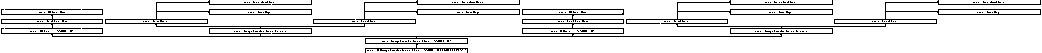
\includegraphics[height=0.714894cm]{classoomph_1_1AxisymFoepplvonKarmanElement}
\end{center}
\end{figure}
\subsection*{Public Member Functions}
\begin{DoxyCompactItemize}
\item 
\hyperlink{classoomph_1_1AxisymFoepplvonKarmanElement_ae05df596899638a8ee2800266412d163}{Axisym\+Foepplvon\+Karman\+Element} ()
\begin{DoxyCompactList}\small\item\em Constructor\+: Call constructors for \hyperlink{classoomph_1_1QElement}{Q\+Element} and \hyperlink{classoomph_1_1AxisymFoepplvonKarmanEquations}{Axisym\+Foepplvon\+Karman\+Equations}. \end{DoxyCompactList}\item 
\hyperlink{classoomph_1_1AxisymFoepplvonKarmanElement_a3258341718feafc5196b85594911fd19}{Axisym\+Foepplvon\+Karman\+Element} (const \hyperlink{classoomph_1_1AxisymFoepplvonKarmanElement}{Axisym\+Foepplvon\+Karman\+Element}$<$ N\+N\+O\+D\+E\+\_\+1D $>$ \&dummy)
\begin{DoxyCompactList}\small\item\em Broken copy constructor. \end{DoxyCompactList}\item 
void \hyperlink{classoomph_1_1AxisymFoepplvonKarmanElement_a2fc69c8a64430a00d344eb55562ab8f2}{operator=} (const \hyperlink{classoomph_1_1AxisymFoepplvonKarmanElement}{Axisym\+Foepplvon\+Karman\+Element}$<$ N\+N\+O\+D\+E\+\_\+1D $>$ \&)
\begin{DoxyCompactList}\small\item\em Broken assignment operator. \end{DoxyCompactList}\item 
unsigned \hyperlink{classoomph_1_1AxisymFoepplvonKarmanElement_ab481ef11edd5211f38bb6e9936d2351f}{required\+\_\+nvalue} (const unsigned \&n) const
\begin{DoxyCompactList}\small\item\em Required \# of `values\textquotesingle{} (pinned or dofs) at node n. \end{DoxyCompactList}\item 
void \hyperlink{classoomph_1_1AxisymFoepplvonKarmanElement_a76cf09e19fc810a96251a64572248f76}{output} (std\+::ostream \&outfile)
\begin{DoxyCompactList}\small\item\em Output function\+: r,w,sigma\+\_\+r\+\_\+r,sigma\+\_\+phi\+\_\+phi. \end{DoxyCompactList}\item 
void \hyperlink{classoomph_1_1AxisymFoepplvonKarmanElement_a435aab946dfcaa0b23e7df59e9bc3933}{output} (std\+::ostream \&outfile, const unsigned \&n\+\_\+plot)
\begin{DoxyCompactList}\small\item\em Output function\+: r,w,sigma\+\_\+r\+\_\+r,sigma\+\_\+phi\+\_\+phi at n\+\_\+plot plot points. \end{DoxyCompactList}\item 
void \hyperlink{classoomph_1_1AxisymFoepplvonKarmanElement_a17a94d66cf74c7be11d8e0a514db1d92}{output} (F\+I\+LE $\ast$file\+\_\+pt)
\begin{DoxyCompactList}\small\item\em C-\/style output function\+: r,w. \end{DoxyCompactList}\item 
void \hyperlink{classoomph_1_1AxisymFoepplvonKarmanElement_a09a7d0ec1c8c495c7703e6c034d8eafc}{output} (F\+I\+LE $\ast$file\+\_\+pt, const unsigned \&n\+\_\+plot)
\begin{DoxyCompactList}\small\item\em C-\/style output function\+: r,w at n\+\_\+plot plot points. \end{DoxyCompactList}\item 
void \hyperlink{classoomph_1_1AxisymFoepplvonKarmanElement_aee745c3439aa18c82ddbe8b90fade1c0}{output\+\_\+fct} (std\+::ostream \&outfile, const unsigned \&n\+\_\+plot, \hyperlink{classoomph_1_1FiniteElement_a690fd33af26cc3e84f39bba6d5a85202}{Finite\+Element\+::\+Steady\+Exact\+Solution\+Fct\+Pt} exact\+\_\+soln\+\_\+pt)
\begin{DoxyCompactList}\small\item\em Output function for an exact solution\+: r,w\+\_\+exact at n\+\_\+plot plot points. \end{DoxyCompactList}\item 
void \hyperlink{classoomph_1_1AxisymFoepplvonKarmanElement_a290c4391d1da3688805466cf2852a93e}{output\+\_\+fct} (std\+::ostream \&outfile, const unsigned \&n\+\_\+plot, const double \&time, \hyperlink{classoomph_1_1FiniteElement_ad4ecf2b61b158a4b4d351a60d23c633e}{Finite\+Element\+::\+Unsteady\+Exact\+Solution\+Fct\+Pt} exact\+\_\+soln\+\_\+pt)
\begin{DoxyCompactList}\small\item\em Output function for a time-\/dependent exact solution. r,w\+\_\+exact at n\+\_\+plot plot points (Calls the steady version) \end{DoxyCompactList}\item 
\hyperlink{classoomph_1_1AxisymFoepplvonKarmanElement_ae05df596899638a8ee2800266412d163}{Axisym\+Foepplvon\+Karman\+Element} ()
\begin{DoxyCompactList}\small\item\em Constructor\+: Call constructors for \hyperlink{classoomph_1_1QElement}{Q\+Element} and \hyperlink{classoomph_1_1AxisymFoepplvonKarmanEquations}{Axisym\+Foepplvon\+Karman\+Equations}. \end{DoxyCompactList}\item 
\hyperlink{classoomph_1_1AxisymFoepplvonKarmanElement_a3258341718feafc5196b85594911fd19}{Axisym\+Foepplvon\+Karman\+Element} (const \hyperlink{classoomph_1_1AxisymFoepplvonKarmanElement}{Axisym\+Foepplvon\+Karman\+Element}$<$ N\+N\+O\+D\+E\+\_\+1D $>$ \&dummy)
\begin{DoxyCompactList}\small\item\em Broken copy constructor. \end{DoxyCompactList}\item 
void \hyperlink{classoomph_1_1AxisymFoepplvonKarmanElement_a2fc69c8a64430a00d344eb55562ab8f2}{operator=} (const \hyperlink{classoomph_1_1AxisymFoepplvonKarmanElement}{Axisym\+Foepplvon\+Karman\+Element}$<$ N\+N\+O\+D\+E\+\_\+1D $>$ \&)
\begin{DoxyCompactList}\small\item\em Broken assignment operator. \end{DoxyCompactList}\item 
unsigned \hyperlink{classoomph_1_1AxisymFoepplvonKarmanElement_ab481ef11edd5211f38bb6e9936d2351f}{required\+\_\+nvalue} (const unsigned \&n) const
\begin{DoxyCompactList}\small\item\em Required \# of `values\textquotesingle{} (pinned or dofs) at node n. \end{DoxyCompactList}\item 
void \hyperlink{classoomph_1_1AxisymFoepplvonKarmanElement_a76cf09e19fc810a96251a64572248f76}{output} (std\+::ostream \&outfile)
\begin{DoxyCompactList}\small\item\em Output function\+: r,w,sigma\+\_\+r\+\_\+r,sigma\+\_\+phi\+\_\+phi. \end{DoxyCompactList}\item 
void \hyperlink{classoomph_1_1AxisymFoepplvonKarmanElement_a435aab946dfcaa0b23e7df59e9bc3933}{output} (std\+::ostream \&outfile, const unsigned \&n\+\_\+plot)
\begin{DoxyCompactList}\small\item\em Output function\+: r,w,sigma\+\_\+r\+\_\+r,sigma\+\_\+phi\+\_\+phi at n\+\_\+plot plot points. \end{DoxyCompactList}\item 
void \hyperlink{classoomph_1_1AxisymFoepplvonKarmanElement_a17a94d66cf74c7be11d8e0a514db1d92}{output} (F\+I\+LE $\ast$file\+\_\+pt)
\begin{DoxyCompactList}\small\item\em C-\/style output function\+: r,w. \end{DoxyCompactList}\item 
void \hyperlink{classoomph_1_1AxisymFoepplvonKarmanElement_a09a7d0ec1c8c495c7703e6c034d8eafc}{output} (F\+I\+LE $\ast$file\+\_\+pt, const unsigned \&n\+\_\+plot)
\begin{DoxyCompactList}\small\item\em C-\/style output function\+: r,w at n\+\_\+plot plot points. \end{DoxyCompactList}\item 
void \hyperlink{classoomph_1_1AxisymFoepplvonKarmanElement_aee745c3439aa18c82ddbe8b90fade1c0}{output\+\_\+fct} (std\+::ostream \&outfile, const unsigned \&n\+\_\+plot, \hyperlink{classoomph_1_1FiniteElement_a690fd33af26cc3e84f39bba6d5a85202}{Finite\+Element\+::\+Steady\+Exact\+Solution\+Fct\+Pt} exact\+\_\+soln\+\_\+pt)
\begin{DoxyCompactList}\small\item\em Output function for an exact solution\+: r,w\+\_\+exact at n\+\_\+plot plot points. \end{DoxyCompactList}\item 
void \hyperlink{classoomph_1_1AxisymFoepplvonKarmanElement_a290c4391d1da3688805466cf2852a93e}{output\+\_\+fct} (std\+::ostream \&outfile, const unsigned \&n\+\_\+plot, const double \&time, \hyperlink{classoomph_1_1FiniteElement_ad4ecf2b61b158a4b4d351a60d23c633e}{Finite\+Element\+::\+Unsteady\+Exact\+Solution\+Fct\+Pt} exact\+\_\+soln\+\_\+pt)
\begin{DoxyCompactList}\small\item\em Output function for a time-\/dependent exact solution. r,w\+\_\+exact at n\+\_\+plot plot points (Calls the steady version) \end{DoxyCompactList}\end{DoxyCompactItemize}
\subsection*{Protected Member Functions}
\begin{DoxyCompactItemize}
\item 
double \hyperlink{classoomph_1_1AxisymFoepplvonKarmanElement_a0eb2dfad7aef696dfeabb51595db46db}{dshape\+\_\+and\+\_\+dtest\+\_\+eulerian\+\_\+axisym\+\_\+fvk} (const \hyperlink{classoomph_1_1Vector}{Vector}$<$ double $>$ \&\hyperlink{cfortran_8h_ab7123126e4885ef647dd9c6e3807a21c}{s}, \hyperlink{classoomph_1_1Shape}{Shape} \&psi, \hyperlink{classoomph_1_1DShape}{D\+Shape} \&dpsidr, \hyperlink{classoomph_1_1Shape}{Shape} \&test, \hyperlink{classoomph_1_1DShape}{D\+Shape} \&dtestdr) const
\begin{DoxyCompactList}\small\item\em \hyperlink{classoomph_1_1Shape}{Shape}, test functions \& derivs. w.\+r.\+t. to global coords. Return Jacobian. \end{DoxyCompactList}\item 
double \hyperlink{classoomph_1_1AxisymFoepplvonKarmanElement_a20841d263ec4590d5614d43f2f813ae7}{dshape\+\_\+and\+\_\+dtest\+\_\+eulerian\+\_\+at\+\_\+knot\+\_\+axisym\+\_\+fvk} (const unsigned \&ipt, \hyperlink{classoomph_1_1Shape}{Shape} \&psi, \hyperlink{classoomph_1_1DShape}{D\+Shape} \&dpsidr, \hyperlink{classoomph_1_1Shape}{Shape} \&test, \hyperlink{classoomph_1_1DShape}{D\+Shape} \&dtestdr) const
\begin{DoxyCompactList}\small\item\em \hyperlink{classoomph_1_1Shape}{Shape}, test functions \& derivs. w.\+r.\+t. to global coords. at integration point ipt. Return Jacobian. \end{DoxyCompactList}\item 
double \hyperlink{classoomph_1_1AxisymFoepplvonKarmanElement_a0eb2dfad7aef696dfeabb51595db46db}{dshape\+\_\+and\+\_\+dtest\+\_\+eulerian\+\_\+axisym\+\_\+fvk} (const \hyperlink{classoomph_1_1Vector}{Vector}$<$ double $>$ \&\hyperlink{cfortran_8h_ab7123126e4885ef647dd9c6e3807a21c}{s}, \hyperlink{classoomph_1_1Shape}{Shape} \&psi, \hyperlink{classoomph_1_1DShape}{D\+Shape} \&dpsidr, \hyperlink{classoomph_1_1Shape}{Shape} \&test, \hyperlink{classoomph_1_1DShape}{D\+Shape} \&dtestdr) const
\begin{DoxyCompactList}\small\item\em \hyperlink{classoomph_1_1Shape}{Shape}, test functions \& derivs. w.\+r.\+t. to global coords. Return Jacobian. \end{DoxyCompactList}\item 
double \hyperlink{classoomph_1_1AxisymFoepplvonKarmanElement_a20841d263ec4590d5614d43f2f813ae7}{dshape\+\_\+and\+\_\+dtest\+\_\+eulerian\+\_\+at\+\_\+knot\+\_\+axisym\+\_\+fvk} (const unsigned \&ipt, \hyperlink{classoomph_1_1Shape}{Shape} \&psi, \hyperlink{classoomph_1_1DShape}{D\+Shape} \&dpsidr, \hyperlink{classoomph_1_1Shape}{Shape} \&test, \hyperlink{classoomph_1_1DShape}{D\+Shape} \&dtestdr) const
\begin{DoxyCompactList}\small\item\em \hyperlink{classoomph_1_1Shape}{Shape}, test functions \& derivs. w.\+r.\+t. to global coords. at integration point ipt. Return Jacobian. \end{DoxyCompactList}\end{DoxyCompactItemize}
\subsection*{Static Private Attributes}
\begin{DoxyCompactItemize}
\item 
static const unsigned \hyperlink{classoomph_1_1AxisymFoepplvonKarmanElement_a881cfa4e7a54d746002871a99337eae8}{Initial\+\_\+\+Nvalue} = 3
\begin{DoxyCompactList}\small\item\em Static int that holds the number of variables at nodes\+: always the same. \end{DoxyCompactList}\end{DoxyCompactItemize}
\subsection*{Additional Inherited Members}


\subsection{Detailed Description}
\subsubsection*{template$<$unsigned N\+N\+O\+D\+E\+\_\+1D$>$\newline
class oomph\+::\+Axisym\+Foepplvon\+Karman\+Element$<$ N\+N\+O\+D\+E\+\_\+1\+D $>$}

Axisym Foepplvon\+Karman\+Element elements are 1D Foeppl von Karman elements with isoparametric interpolation for the function. 

Definition at line 402 of file axisym\+\_\+displ\+\_\+based\+\_\+fvk\+\_\+elements.\+h.



\subsection{Constructor \& Destructor Documentation}
\mbox{\Hypertarget{classoomph_1_1AxisymFoepplvonKarmanElement_ae05df596899638a8ee2800266412d163}\label{classoomph_1_1AxisymFoepplvonKarmanElement_ae05df596899638a8ee2800266412d163}} 
\index{oomph\+::\+Axisym\+Foepplvon\+Karman\+Element@{oomph\+::\+Axisym\+Foepplvon\+Karman\+Element}!Axisym\+Foepplvon\+Karman\+Element@{Axisym\+Foepplvon\+Karman\+Element}}
\index{Axisym\+Foepplvon\+Karman\+Element@{Axisym\+Foepplvon\+Karman\+Element}!oomph\+::\+Axisym\+Foepplvon\+Karman\+Element@{oomph\+::\+Axisym\+Foepplvon\+Karman\+Element}}
\subsubsection{\texorpdfstring{Axisym\+Foepplvon\+Karman\+Element()}{AxisymFoepplvonKarmanElement()}\hspace{0.1cm}{\footnotesize\ttfamily [1/4]}}
{\footnotesize\ttfamily template$<$unsigned N\+N\+O\+D\+E\+\_\+1D$>$ \\
\hyperlink{classoomph_1_1AxisymFoepplvonKarmanElement}{oomph\+::\+Axisym\+Foepplvon\+Karman\+Element}$<$ N\+N\+O\+D\+E\+\_\+1D $>$\+::\hyperlink{classoomph_1_1AxisymFoepplvonKarmanElement}{Axisym\+Foepplvon\+Karman\+Element} (\begin{DoxyParamCaption}{ }\end{DoxyParamCaption})\hspace{0.3cm}{\ttfamily [inline]}}



Constructor\+: Call constructors for \hyperlink{classoomph_1_1QElement}{Q\+Element} and \hyperlink{classoomph_1_1AxisymFoepplvonKarmanEquations}{Axisym\+Foepplvon\+Karman\+Equations}. 



Definition at line 416 of file axisym\+\_\+displ\+\_\+based\+\_\+fvk\+\_\+elements.\+h.

\mbox{\Hypertarget{classoomph_1_1AxisymFoepplvonKarmanElement_a3258341718feafc5196b85594911fd19}\label{classoomph_1_1AxisymFoepplvonKarmanElement_a3258341718feafc5196b85594911fd19}} 
\index{oomph\+::\+Axisym\+Foepplvon\+Karman\+Element@{oomph\+::\+Axisym\+Foepplvon\+Karman\+Element}!Axisym\+Foepplvon\+Karman\+Element@{Axisym\+Foepplvon\+Karman\+Element}}
\index{Axisym\+Foepplvon\+Karman\+Element@{Axisym\+Foepplvon\+Karman\+Element}!oomph\+::\+Axisym\+Foepplvon\+Karman\+Element@{oomph\+::\+Axisym\+Foepplvon\+Karman\+Element}}
\subsubsection{\texorpdfstring{Axisym\+Foepplvon\+Karman\+Element()}{AxisymFoepplvonKarmanElement()}\hspace{0.1cm}{\footnotesize\ttfamily [2/4]}}
{\footnotesize\ttfamily template$<$unsigned N\+N\+O\+D\+E\+\_\+1D$>$ \\
\hyperlink{classoomph_1_1AxisymFoepplvonKarmanElement}{oomph\+::\+Axisym\+Foepplvon\+Karman\+Element}$<$ N\+N\+O\+D\+E\+\_\+1D $>$\+::\hyperlink{classoomph_1_1AxisymFoepplvonKarmanElement}{Axisym\+Foepplvon\+Karman\+Element} (\begin{DoxyParamCaption}\item[{const \hyperlink{classoomph_1_1AxisymFoepplvonKarmanElement}{Axisym\+Foepplvon\+Karman\+Element}$<$ N\+N\+O\+D\+E\+\_\+1D $>$ \&}]{dummy }\end{DoxyParamCaption})\hspace{0.3cm}{\ttfamily [inline]}}



Broken copy constructor. 



Definition at line 422 of file axisym\+\_\+displ\+\_\+based\+\_\+fvk\+\_\+elements.\+h.



References oomph\+::\+Broken\+Copy\+::broken\+\_\+copy().

\mbox{\Hypertarget{classoomph_1_1AxisymFoepplvonKarmanElement_ae05df596899638a8ee2800266412d163}\label{classoomph_1_1AxisymFoepplvonKarmanElement_ae05df596899638a8ee2800266412d163}} 
\index{oomph\+::\+Axisym\+Foepplvon\+Karman\+Element@{oomph\+::\+Axisym\+Foepplvon\+Karman\+Element}!Axisym\+Foepplvon\+Karman\+Element@{Axisym\+Foepplvon\+Karman\+Element}}
\index{Axisym\+Foepplvon\+Karman\+Element@{Axisym\+Foepplvon\+Karman\+Element}!oomph\+::\+Axisym\+Foepplvon\+Karman\+Element@{oomph\+::\+Axisym\+Foepplvon\+Karman\+Element}}
\subsubsection{\texorpdfstring{Axisym\+Foepplvon\+Karman\+Element()}{AxisymFoepplvonKarmanElement()}\hspace{0.1cm}{\footnotesize\ttfamily [3/4]}}
{\footnotesize\ttfamily template$<$unsigned N\+N\+O\+D\+E\+\_\+1D$>$ \\
\hyperlink{classoomph_1_1AxisymFoepplvonKarmanElement}{oomph\+::\+Axisym\+Foepplvon\+Karman\+Element}$<$ N\+N\+O\+D\+E\+\_\+1D $>$\+::\hyperlink{classoomph_1_1AxisymFoepplvonKarmanElement}{Axisym\+Foepplvon\+Karman\+Element} (\begin{DoxyParamCaption}{ }\end{DoxyParamCaption})\hspace{0.3cm}{\ttfamily [inline]}}



Constructor\+: Call constructors for \hyperlink{classoomph_1_1QElement}{Q\+Element} and \hyperlink{classoomph_1_1AxisymFoepplvonKarmanEquations}{Axisym\+Foepplvon\+Karman\+Equations}. 



Definition at line 395 of file axisym\+\_\+fvk\+\_\+elements.\+h.

\mbox{\Hypertarget{classoomph_1_1AxisymFoepplvonKarmanElement_a3258341718feafc5196b85594911fd19}\label{classoomph_1_1AxisymFoepplvonKarmanElement_a3258341718feafc5196b85594911fd19}} 
\index{oomph\+::\+Axisym\+Foepplvon\+Karman\+Element@{oomph\+::\+Axisym\+Foepplvon\+Karman\+Element}!Axisym\+Foepplvon\+Karman\+Element@{Axisym\+Foepplvon\+Karman\+Element}}
\index{Axisym\+Foepplvon\+Karman\+Element@{Axisym\+Foepplvon\+Karman\+Element}!oomph\+::\+Axisym\+Foepplvon\+Karman\+Element@{oomph\+::\+Axisym\+Foepplvon\+Karman\+Element}}
\subsubsection{\texorpdfstring{Axisym\+Foepplvon\+Karman\+Element()}{AxisymFoepplvonKarmanElement()}\hspace{0.1cm}{\footnotesize\ttfamily [4/4]}}
{\footnotesize\ttfamily template$<$unsigned N\+N\+O\+D\+E\+\_\+1D$>$ \\
\hyperlink{classoomph_1_1AxisymFoepplvonKarmanElement}{oomph\+::\+Axisym\+Foepplvon\+Karman\+Element}$<$ N\+N\+O\+D\+E\+\_\+1D $>$\+::\hyperlink{classoomph_1_1AxisymFoepplvonKarmanElement}{Axisym\+Foepplvon\+Karman\+Element} (\begin{DoxyParamCaption}\item[{const \hyperlink{classoomph_1_1AxisymFoepplvonKarmanElement}{Axisym\+Foepplvon\+Karman\+Element}$<$ N\+N\+O\+D\+E\+\_\+1D $>$ \&}]{dummy }\end{DoxyParamCaption})\hspace{0.3cm}{\ttfamily [inline]}}



Broken copy constructor. 



Definition at line 401 of file axisym\+\_\+fvk\+\_\+elements.\+h.



References oomph\+::\+Broken\+Copy\+::broken\+\_\+copy().



\subsection{Member Function Documentation}
\mbox{\Hypertarget{classoomph_1_1AxisymFoepplvonKarmanElement_a20841d263ec4590d5614d43f2f813ae7}\label{classoomph_1_1AxisymFoepplvonKarmanElement_a20841d263ec4590d5614d43f2f813ae7}} 
\index{oomph\+::\+Axisym\+Foepplvon\+Karman\+Element@{oomph\+::\+Axisym\+Foepplvon\+Karman\+Element}!dshape\+\_\+and\+\_\+dtest\+\_\+eulerian\+\_\+at\+\_\+knot\+\_\+axisym\+\_\+fvk@{dshape\+\_\+and\+\_\+dtest\+\_\+eulerian\+\_\+at\+\_\+knot\+\_\+axisym\+\_\+fvk}}
\index{dshape\+\_\+and\+\_\+dtest\+\_\+eulerian\+\_\+at\+\_\+knot\+\_\+axisym\+\_\+fvk@{dshape\+\_\+and\+\_\+dtest\+\_\+eulerian\+\_\+at\+\_\+knot\+\_\+axisym\+\_\+fvk}!oomph\+::\+Axisym\+Foepplvon\+Karman\+Element@{oomph\+::\+Axisym\+Foepplvon\+Karman\+Element}}
\subsubsection{\texorpdfstring{dshape\+\_\+and\+\_\+dtest\+\_\+eulerian\+\_\+at\+\_\+knot\+\_\+axisym\+\_\+fvk()}{dshape\_and\_dtest\_eulerian\_at\_knot\_axisym\_fvk()}\hspace{0.1cm}{\footnotesize\ttfamily [1/2]}}
{\footnotesize\ttfamily template$<$unsigned N\+N\+O\+D\+E\+\_\+1D$>$ \\
double \hyperlink{classoomph_1_1AxisymFoepplvonKarmanElement}{oomph\+::\+Axisym\+Foepplvon\+Karman\+Element}$<$ N\+N\+O\+D\+E\+\_\+1D $>$\+::dshape\+\_\+and\+\_\+dtest\+\_\+eulerian\+\_\+at\+\_\+knot\+\_\+axisym\+\_\+fvk (\begin{DoxyParamCaption}\item[{const unsigned \&}]{ipt,  }\item[{\hyperlink{classoomph_1_1Shape}{Shape} \&}]{psi,  }\item[{\hyperlink{classoomph_1_1DShape}{D\+Shape} \&}]{dpsidr,  }\item[{\hyperlink{classoomph_1_1Shape}{Shape} \&}]{test,  }\item[{\hyperlink{classoomph_1_1DShape}{D\+Shape} \&}]{dtestdr }\end{DoxyParamCaption}) const\hspace{0.3cm}{\ttfamily [inline]}, {\ttfamily [protected]}, {\ttfamily [virtual]}}



\hyperlink{classoomph_1_1Shape}{Shape}, test functions \& derivs. w.\+r.\+t. to global coords. at integration point ipt. Return Jacobian. 



Implements \hyperlink{classoomph_1_1AxisymFoepplvonKarmanEquations_a456a9c27c326d6d1e55e3ab822ac1a5f}{oomph\+::\+Axisym\+Foepplvon\+Karman\+Equations}.

\mbox{\Hypertarget{classoomph_1_1AxisymFoepplvonKarmanElement_a20841d263ec4590d5614d43f2f813ae7}\label{classoomph_1_1AxisymFoepplvonKarmanElement_a20841d263ec4590d5614d43f2f813ae7}} 
\index{oomph\+::\+Axisym\+Foepplvon\+Karman\+Element@{oomph\+::\+Axisym\+Foepplvon\+Karman\+Element}!dshape\+\_\+and\+\_\+dtest\+\_\+eulerian\+\_\+at\+\_\+knot\+\_\+axisym\+\_\+fvk@{dshape\+\_\+and\+\_\+dtest\+\_\+eulerian\+\_\+at\+\_\+knot\+\_\+axisym\+\_\+fvk}}
\index{dshape\+\_\+and\+\_\+dtest\+\_\+eulerian\+\_\+at\+\_\+knot\+\_\+axisym\+\_\+fvk@{dshape\+\_\+and\+\_\+dtest\+\_\+eulerian\+\_\+at\+\_\+knot\+\_\+axisym\+\_\+fvk}!oomph\+::\+Axisym\+Foepplvon\+Karman\+Element@{oomph\+::\+Axisym\+Foepplvon\+Karman\+Element}}
\subsubsection{\texorpdfstring{dshape\+\_\+and\+\_\+dtest\+\_\+eulerian\+\_\+at\+\_\+knot\+\_\+axisym\+\_\+fvk()}{dshape\_and\_dtest\_eulerian\_at\_knot\_axisym\_fvk()}\hspace{0.1cm}{\footnotesize\ttfamily [2/2]}}
{\footnotesize\ttfamily template$<$unsigned N\+N\+O\+D\+E\+\_\+1D$>$ \\
double \hyperlink{classoomph_1_1AxisymFoepplvonKarmanElement}{oomph\+::\+Axisym\+Foepplvon\+Karman\+Element}$<$ N\+N\+O\+D\+E\+\_\+1D $>$\+::dshape\+\_\+and\+\_\+dtest\+\_\+eulerian\+\_\+at\+\_\+knot\+\_\+axisym\+\_\+fvk (\begin{DoxyParamCaption}\item[{const unsigned \&}]{ipt,  }\item[{\hyperlink{classoomph_1_1Shape}{Shape} \&}]{psi,  }\item[{\hyperlink{classoomph_1_1DShape}{D\+Shape} \&}]{dpsidr,  }\item[{\hyperlink{classoomph_1_1Shape}{Shape} \&}]{test,  }\item[{\hyperlink{classoomph_1_1DShape}{D\+Shape} \&}]{dtestdr }\end{DoxyParamCaption}) const\hspace{0.3cm}{\ttfamily [inline]}, {\ttfamily [protected]}, {\ttfamily [virtual]}}



\hyperlink{classoomph_1_1Shape}{Shape}, test functions \& derivs. w.\+r.\+t. to global coords. at integration point ipt. Return Jacobian. 

Define the shape functions and test functions and derivatives w.\+r.\+t. global coordinates and return Jacobian of mapping.

Galerkin\+: Test functions = shape functions 

Implements \hyperlink{classoomph_1_1AxisymFoepplvonKarmanEquations_a456a9c27c326d6d1e55e3ab822ac1a5f}{oomph\+::\+Axisym\+Foepplvon\+Karman\+Equations}.



Definition at line 536 of file axisym\+\_\+displ\+\_\+based\+\_\+fvk\+\_\+elements.\+h.



References oomph\+::\+Finite\+Element\+::dshape\+\_\+eulerian\+\_\+at\+\_\+knot().



Referenced by oomph\+::\+Axisym\+Foepplvon\+Karman\+Element$<$ N\+N\+O\+D\+E\+\_\+1\+D $>$\+::dshape\+\_\+and\+\_\+dtest\+\_\+eulerian\+\_\+axisym\+\_\+fvk(), and oomph\+::\+Axisym\+Foepplvon\+Karman\+Element$<$ N\+N\+O\+D\+E\+\_\+1\+D $>$\+::output\+\_\+fct().

\mbox{\Hypertarget{classoomph_1_1AxisymFoepplvonKarmanElement_a0eb2dfad7aef696dfeabb51595db46db}\label{classoomph_1_1AxisymFoepplvonKarmanElement_a0eb2dfad7aef696dfeabb51595db46db}} 
\index{oomph\+::\+Axisym\+Foepplvon\+Karman\+Element@{oomph\+::\+Axisym\+Foepplvon\+Karman\+Element}!dshape\+\_\+and\+\_\+dtest\+\_\+eulerian\+\_\+axisym\+\_\+fvk@{dshape\+\_\+and\+\_\+dtest\+\_\+eulerian\+\_\+axisym\+\_\+fvk}}
\index{dshape\+\_\+and\+\_\+dtest\+\_\+eulerian\+\_\+axisym\+\_\+fvk@{dshape\+\_\+and\+\_\+dtest\+\_\+eulerian\+\_\+axisym\+\_\+fvk}!oomph\+::\+Axisym\+Foepplvon\+Karman\+Element@{oomph\+::\+Axisym\+Foepplvon\+Karman\+Element}}
\subsubsection{\texorpdfstring{dshape\+\_\+and\+\_\+dtest\+\_\+eulerian\+\_\+axisym\+\_\+fvk()}{dshape\_and\_dtest\_eulerian\_axisym\_fvk()}\hspace{0.1cm}{\footnotesize\ttfamily [1/2]}}
{\footnotesize\ttfamily template$<$unsigned N\+N\+O\+D\+E\+\_\+1D$>$ \\
double \hyperlink{classoomph_1_1AxisymFoepplvonKarmanElement}{oomph\+::\+Axisym\+Foepplvon\+Karman\+Element}$<$ N\+N\+O\+D\+E\+\_\+1D $>$\+::dshape\+\_\+and\+\_\+dtest\+\_\+eulerian\+\_\+axisym\+\_\+fvk (\begin{DoxyParamCaption}\item[{const \hyperlink{classoomph_1_1Vector}{Vector}$<$ double $>$ \&}]{s,  }\item[{\hyperlink{classoomph_1_1Shape}{Shape} \&}]{psi,  }\item[{\hyperlink{classoomph_1_1DShape}{D\+Shape} \&}]{dpsidr,  }\item[{\hyperlink{classoomph_1_1Shape}{Shape} \&}]{test,  }\item[{\hyperlink{classoomph_1_1DShape}{D\+Shape} \&}]{dtestdr }\end{DoxyParamCaption}) const\hspace{0.3cm}{\ttfamily [inline]}, {\ttfamily [protected]}, {\ttfamily [virtual]}}



\hyperlink{classoomph_1_1Shape}{Shape}, test functions \& derivs. w.\+r.\+t. to global coords. Return Jacobian. 



Implements \hyperlink{classoomph_1_1AxisymFoepplvonKarmanEquations_a838cd424e2666b007113de0a95f5d999}{oomph\+::\+Axisym\+Foepplvon\+Karman\+Equations}.

\mbox{\Hypertarget{classoomph_1_1AxisymFoepplvonKarmanElement_a0eb2dfad7aef696dfeabb51595db46db}\label{classoomph_1_1AxisymFoepplvonKarmanElement_a0eb2dfad7aef696dfeabb51595db46db}} 
\index{oomph\+::\+Axisym\+Foepplvon\+Karman\+Element@{oomph\+::\+Axisym\+Foepplvon\+Karman\+Element}!dshape\+\_\+and\+\_\+dtest\+\_\+eulerian\+\_\+axisym\+\_\+fvk@{dshape\+\_\+and\+\_\+dtest\+\_\+eulerian\+\_\+axisym\+\_\+fvk}}
\index{dshape\+\_\+and\+\_\+dtest\+\_\+eulerian\+\_\+axisym\+\_\+fvk@{dshape\+\_\+and\+\_\+dtest\+\_\+eulerian\+\_\+axisym\+\_\+fvk}!oomph\+::\+Axisym\+Foepplvon\+Karman\+Element@{oomph\+::\+Axisym\+Foepplvon\+Karman\+Element}}
\subsubsection{\texorpdfstring{dshape\+\_\+and\+\_\+dtest\+\_\+eulerian\+\_\+axisym\+\_\+fvk()}{dshape\_and\_dtest\_eulerian\_axisym\_fvk()}\hspace{0.1cm}{\footnotesize\ttfamily [2/2]}}
{\footnotesize\ttfamily template$<$unsigned N\+N\+O\+D\+E\+\_\+1D$>$ \\
double \hyperlink{classoomph_1_1AxisymFoepplvonKarmanElement}{oomph\+::\+Axisym\+Foepplvon\+Karman\+Element}$<$ N\+N\+O\+D\+E\+\_\+1D $>$\+::dshape\+\_\+and\+\_\+dtest\+\_\+eulerian\+\_\+axisym\+\_\+fvk (\begin{DoxyParamCaption}\item[{const \hyperlink{classoomph_1_1Vector}{Vector}$<$ double $>$ \&}]{s,  }\item[{\hyperlink{classoomph_1_1Shape}{Shape} \&}]{psi,  }\item[{\hyperlink{classoomph_1_1DShape}{D\+Shape} \&}]{dpsidr,  }\item[{\hyperlink{classoomph_1_1Shape}{Shape} \&}]{test,  }\item[{\hyperlink{classoomph_1_1DShape}{D\+Shape} \&}]{dtestdr }\end{DoxyParamCaption}) const\hspace{0.3cm}{\ttfamily [inline]}, {\ttfamily [protected]}, {\ttfamily [virtual]}}



\hyperlink{classoomph_1_1Shape}{Shape}, test functions \& derivs. w.\+r.\+t. to global coords. Return Jacobian. 

Define the shape functions and test functions and derivatives w.\+r.\+t. global coordinates and return Jacobian of mapping.

Galerkin\+: Test functions = shape functions 

Implements \hyperlink{classoomph_1_1AxisymFoepplvonKarmanEquations_a838cd424e2666b007113de0a95f5d999}{oomph\+::\+Axisym\+Foepplvon\+Karman\+Equations}.



Definition at line 508 of file axisym\+\_\+displ\+\_\+based\+\_\+fvk\+\_\+elements.\+h.



References oomph\+::\+Axisym\+Foepplvon\+Karman\+Element$<$ N\+N\+O\+D\+E\+\_\+1\+D $>$\+::dshape\+\_\+and\+\_\+dtest\+\_\+eulerian\+\_\+at\+\_\+knot\+\_\+axisym\+\_\+fvk(), and oomph\+::\+Finite\+Element\+::dshape\+\_\+eulerian().



Referenced by oomph\+::\+Axisym\+Foepplvon\+Karman\+Element$<$ N\+N\+O\+D\+E\+\_\+1\+D $>$\+::output\+\_\+fct().

\mbox{\Hypertarget{classoomph_1_1AxisymFoepplvonKarmanElement_a2fc69c8a64430a00d344eb55562ab8f2}\label{classoomph_1_1AxisymFoepplvonKarmanElement_a2fc69c8a64430a00d344eb55562ab8f2}} 
\index{oomph\+::\+Axisym\+Foepplvon\+Karman\+Element@{oomph\+::\+Axisym\+Foepplvon\+Karman\+Element}!operator=@{operator=}}
\index{operator=@{operator=}!oomph\+::\+Axisym\+Foepplvon\+Karman\+Element@{oomph\+::\+Axisym\+Foepplvon\+Karman\+Element}}
\subsubsection{\texorpdfstring{operator=()}{operator=()}\hspace{0.1cm}{\footnotesize\ttfamily [1/2]}}
{\footnotesize\ttfamily template$<$unsigned N\+N\+O\+D\+E\+\_\+1D$>$ \\
void \hyperlink{classoomph_1_1AxisymFoepplvonKarmanElement}{oomph\+::\+Axisym\+Foepplvon\+Karman\+Element}$<$ N\+N\+O\+D\+E\+\_\+1D $>$\+::operator= (\begin{DoxyParamCaption}\item[{const \hyperlink{classoomph_1_1AxisymFoepplvonKarmanElement}{Axisym\+Foepplvon\+Karman\+Element}$<$ N\+N\+O\+D\+E\+\_\+1D $>$ \&}]{ }\end{DoxyParamCaption})\hspace{0.3cm}{\ttfamily [inline]}}



Broken assignment operator. 



Definition at line 407 of file axisym\+\_\+fvk\+\_\+elements.\+h.



References oomph\+::\+Broken\+Copy\+::broken\+\_\+assign().

\mbox{\Hypertarget{classoomph_1_1AxisymFoepplvonKarmanElement_a2fc69c8a64430a00d344eb55562ab8f2}\label{classoomph_1_1AxisymFoepplvonKarmanElement_a2fc69c8a64430a00d344eb55562ab8f2}} 
\index{oomph\+::\+Axisym\+Foepplvon\+Karman\+Element@{oomph\+::\+Axisym\+Foepplvon\+Karman\+Element}!operator=@{operator=}}
\index{operator=@{operator=}!oomph\+::\+Axisym\+Foepplvon\+Karman\+Element@{oomph\+::\+Axisym\+Foepplvon\+Karman\+Element}}
\subsubsection{\texorpdfstring{operator=()}{operator=()}\hspace{0.1cm}{\footnotesize\ttfamily [2/2]}}
{\footnotesize\ttfamily template$<$unsigned N\+N\+O\+D\+E\+\_\+1D$>$ \\
void \hyperlink{classoomph_1_1AxisymFoepplvonKarmanElement}{oomph\+::\+Axisym\+Foepplvon\+Karman\+Element}$<$ N\+N\+O\+D\+E\+\_\+1D $>$\+::operator= (\begin{DoxyParamCaption}\item[{const \hyperlink{classoomph_1_1AxisymFoepplvonKarmanElement}{Axisym\+Foepplvon\+Karman\+Element}$<$ N\+N\+O\+D\+E\+\_\+1D $>$ \&}]{ }\end{DoxyParamCaption})\hspace{0.3cm}{\ttfamily [inline]}}



Broken assignment operator. 



Definition at line 428 of file axisym\+\_\+displ\+\_\+based\+\_\+fvk\+\_\+elements.\+h.



References oomph\+::\+Broken\+Copy\+::broken\+\_\+assign().

\mbox{\Hypertarget{classoomph_1_1AxisymFoepplvonKarmanElement_a76cf09e19fc810a96251a64572248f76}\label{classoomph_1_1AxisymFoepplvonKarmanElement_a76cf09e19fc810a96251a64572248f76}} 
\index{oomph\+::\+Axisym\+Foepplvon\+Karman\+Element@{oomph\+::\+Axisym\+Foepplvon\+Karman\+Element}!output@{output}}
\index{output@{output}!oomph\+::\+Axisym\+Foepplvon\+Karman\+Element@{oomph\+::\+Axisym\+Foepplvon\+Karman\+Element}}
\subsubsection{\texorpdfstring{output()}{output()}\hspace{0.1cm}{\footnotesize\ttfamily [1/8]}}
{\footnotesize\ttfamily template$<$unsigned N\+N\+O\+D\+E\+\_\+1D$>$ \\
void \hyperlink{classoomph_1_1AxisymFoepplvonKarmanElement}{oomph\+::\+Axisym\+Foepplvon\+Karman\+Element}$<$ N\+N\+O\+D\+E\+\_\+1D $>$\+::output (\begin{DoxyParamCaption}\item[{std\+::ostream \&}]{outfile }\end{DoxyParamCaption})\hspace{0.3cm}{\ttfamily [inline]}, {\ttfamily [virtual]}}



Output function\+: r,w,sigma\+\_\+r\+\_\+r,sigma\+\_\+phi\+\_\+phi. 



Reimplemented from \hyperlink{classoomph_1_1AxisymFoepplvonKarmanEquations_a162b507ce3d9126a558790e77ec86e70}{oomph\+::\+Axisym\+Foepplvon\+Karman\+Equations}.



Definition at line 420 of file axisym\+\_\+fvk\+\_\+elements.\+h.



References oomph\+::\+Axisym\+Foepplvon\+Karman\+Equations\+::output().

\mbox{\Hypertarget{classoomph_1_1AxisymFoepplvonKarmanElement_a435aab946dfcaa0b23e7df59e9bc3933}\label{classoomph_1_1AxisymFoepplvonKarmanElement_a435aab946dfcaa0b23e7df59e9bc3933}} 
\index{oomph\+::\+Axisym\+Foepplvon\+Karman\+Element@{oomph\+::\+Axisym\+Foepplvon\+Karman\+Element}!output@{output}}
\index{output@{output}!oomph\+::\+Axisym\+Foepplvon\+Karman\+Element@{oomph\+::\+Axisym\+Foepplvon\+Karman\+Element}}
\subsubsection{\texorpdfstring{output()}{output()}\hspace{0.1cm}{\footnotesize\ttfamily [2/8]}}
{\footnotesize\ttfamily template$<$unsigned N\+N\+O\+D\+E\+\_\+1D$>$ \\
void \hyperlink{classoomph_1_1AxisymFoepplvonKarmanElement}{oomph\+::\+Axisym\+Foepplvon\+Karman\+Element}$<$ N\+N\+O\+D\+E\+\_\+1D $>$\+::output (\begin{DoxyParamCaption}\item[{std\+::ostream \&}]{outfile,  }\item[{const unsigned \&}]{n\+\_\+plot }\end{DoxyParamCaption})\hspace{0.3cm}{\ttfamily [inline]}, {\ttfamily [virtual]}}



Output function\+: r,w,sigma\+\_\+r\+\_\+r,sigma\+\_\+phi\+\_\+phi at n\+\_\+plot plot points. 



Reimplemented from \hyperlink{classoomph_1_1AxisymFoepplvonKarmanEquations_a704051a00a2c8624edb98f3ba05e63a2}{oomph\+::\+Axisym\+Foepplvon\+Karman\+Equations}.



Reimplemented in \hyperlink{classoomph_1_1FSIAxisymFoepplvonKarmanElement_a03c82e935db8c1c93dfe2f443ec5e817}{oomph\+::\+F\+S\+I\+Axisym\+Foepplvon\+Karman\+Element$<$ N\+N\+O\+D\+E\+\_\+1\+D, F\+L\+U\+I\+D\+\_\+\+E\+L\+E\+M\+E\+N\+T $>$}.



Definition at line 425 of file axisym\+\_\+fvk\+\_\+elements.\+h.



References oomph\+::\+Axisym\+Foepplvon\+Karman\+Equations\+::output().

\mbox{\Hypertarget{classoomph_1_1AxisymFoepplvonKarmanElement_a17a94d66cf74c7be11d8e0a514db1d92}\label{classoomph_1_1AxisymFoepplvonKarmanElement_a17a94d66cf74c7be11d8e0a514db1d92}} 
\index{oomph\+::\+Axisym\+Foepplvon\+Karman\+Element@{oomph\+::\+Axisym\+Foepplvon\+Karman\+Element}!output@{output}}
\index{output@{output}!oomph\+::\+Axisym\+Foepplvon\+Karman\+Element@{oomph\+::\+Axisym\+Foepplvon\+Karman\+Element}}
\subsubsection{\texorpdfstring{output()}{output()}\hspace{0.1cm}{\footnotesize\ttfamily [3/8]}}
{\footnotesize\ttfamily template$<$unsigned N\+N\+O\+D\+E\+\_\+1D$>$ \\
void \hyperlink{classoomph_1_1AxisymFoepplvonKarmanElement}{oomph\+::\+Axisym\+Foepplvon\+Karman\+Element}$<$ N\+N\+O\+D\+E\+\_\+1D $>$\+::output (\begin{DoxyParamCaption}\item[{F\+I\+LE $\ast$}]{file\+\_\+pt }\end{DoxyParamCaption})\hspace{0.3cm}{\ttfamily [inline]}, {\ttfamily [virtual]}}



C-\/style output function\+: r,w. 



Reimplemented from \hyperlink{classoomph_1_1AxisymFoepplvonKarmanEquations_a236f169caf08c0214ff686e939b9dd33}{oomph\+::\+Axisym\+Foepplvon\+Karman\+Equations}.



Definition at line 430 of file axisym\+\_\+fvk\+\_\+elements.\+h.



References oomph\+::\+Axisym\+Foepplvon\+Karman\+Equations\+::output().

\mbox{\Hypertarget{classoomph_1_1AxisymFoepplvonKarmanElement_a09a7d0ec1c8c495c7703e6c034d8eafc}\label{classoomph_1_1AxisymFoepplvonKarmanElement_a09a7d0ec1c8c495c7703e6c034d8eafc}} 
\index{oomph\+::\+Axisym\+Foepplvon\+Karman\+Element@{oomph\+::\+Axisym\+Foepplvon\+Karman\+Element}!output@{output}}
\index{output@{output}!oomph\+::\+Axisym\+Foepplvon\+Karman\+Element@{oomph\+::\+Axisym\+Foepplvon\+Karman\+Element}}
\subsubsection{\texorpdfstring{output()}{output()}\hspace{0.1cm}{\footnotesize\ttfamily [4/8]}}
{\footnotesize\ttfamily template$<$unsigned N\+N\+O\+D\+E\+\_\+1D$>$ \\
void \hyperlink{classoomph_1_1AxisymFoepplvonKarmanElement}{oomph\+::\+Axisym\+Foepplvon\+Karman\+Element}$<$ N\+N\+O\+D\+E\+\_\+1D $>$\+::output (\begin{DoxyParamCaption}\item[{F\+I\+LE $\ast$}]{file\+\_\+pt,  }\item[{const unsigned \&}]{n\+\_\+plot }\end{DoxyParamCaption})\hspace{0.3cm}{\ttfamily [inline]}, {\ttfamily [virtual]}}



C-\/style output function\+: r,w at n\+\_\+plot plot points. 



Reimplemented from \hyperlink{classoomph_1_1AxisymFoepplvonKarmanEquations_a5278f37c336b7a4bd2931fdedd2945f8}{oomph\+::\+Axisym\+Foepplvon\+Karman\+Equations}.



Definition at line 435 of file axisym\+\_\+fvk\+\_\+elements.\+h.



References oomph\+::\+Axisym\+Foepplvon\+Karman\+Equations\+::output().

\mbox{\Hypertarget{classoomph_1_1AxisymFoepplvonKarmanElement_a76cf09e19fc810a96251a64572248f76}\label{classoomph_1_1AxisymFoepplvonKarmanElement_a76cf09e19fc810a96251a64572248f76}} 
\index{oomph\+::\+Axisym\+Foepplvon\+Karman\+Element@{oomph\+::\+Axisym\+Foepplvon\+Karman\+Element}!output@{output}}
\index{output@{output}!oomph\+::\+Axisym\+Foepplvon\+Karman\+Element@{oomph\+::\+Axisym\+Foepplvon\+Karman\+Element}}
\subsubsection{\texorpdfstring{output()}{output()}\hspace{0.1cm}{\footnotesize\ttfamily [5/8]}}
{\footnotesize\ttfamily template$<$unsigned N\+N\+O\+D\+E\+\_\+1D$>$ \\
void \hyperlink{classoomph_1_1AxisymFoepplvonKarmanElement}{oomph\+::\+Axisym\+Foepplvon\+Karman\+Element}$<$ N\+N\+O\+D\+E\+\_\+1D $>$\+::output (\begin{DoxyParamCaption}\item[{std\+::ostream \&}]{outfile }\end{DoxyParamCaption})\hspace{0.3cm}{\ttfamily [inline]}, {\ttfamily [virtual]}}



Output function\+: r,w,sigma\+\_\+r\+\_\+r,sigma\+\_\+phi\+\_\+phi. 



Reimplemented from \hyperlink{classoomph_1_1AxisymFoepplvonKarmanEquations_a162b507ce3d9126a558790e77ec86e70}{oomph\+::\+Axisym\+Foepplvon\+Karman\+Equations}.



Definition at line 441 of file axisym\+\_\+displ\+\_\+based\+\_\+fvk\+\_\+elements.\+h.



References oomph\+::\+Axisym\+Foepplvon\+Karman\+Equations\+::output().

\mbox{\Hypertarget{classoomph_1_1AxisymFoepplvonKarmanElement_a435aab946dfcaa0b23e7df59e9bc3933}\label{classoomph_1_1AxisymFoepplvonKarmanElement_a435aab946dfcaa0b23e7df59e9bc3933}} 
\index{oomph\+::\+Axisym\+Foepplvon\+Karman\+Element@{oomph\+::\+Axisym\+Foepplvon\+Karman\+Element}!output@{output}}
\index{output@{output}!oomph\+::\+Axisym\+Foepplvon\+Karman\+Element@{oomph\+::\+Axisym\+Foepplvon\+Karman\+Element}}
\subsubsection{\texorpdfstring{output()}{output()}\hspace{0.1cm}{\footnotesize\ttfamily [6/8]}}
{\footnotesize\ttfamily template$<$unsigned N\+N\+O\+D\+E\+\_\+1D$>$ \\
void \hyperlink{classoomph_1_1AxisymFoepplvonKarmanElement}{oomph\+::\+Axisym\+Foepplvon\+Karman\+Element}$<$ N\+N\+O\+D\+E\+\_\+1D $>$\+::output (\begin{DoxyParamCaption}\item[{std\+::ostream \&}]{outfile,  }\item[{const unsigned \&}]{n\+\_\+plot }\end{DoxyParamCaption})\hspace{0.3cm}{\ttfamily [inline]}, {\ttfamily [virtual]}}



Output function\+: r,w,sigma\+\_\+r\+\_\+r,sigma\+\_\+phi\+\_\+phi at n\+\_\+plot plot points. 



Reimplemented from \hyperlink{classoomph_1_1AxisymFoepplvonKarmanEquations_a704051a00a2c8624edb98f3ba05e63a2}{oomph\+::\+Axisym\+Foepplvon\+Karman\+Equations}.



Reimplemented in \hyperlink{classoomph_1_1FSIAxisymFoepplvonKarmanElement_a03c82e935db8c1c93dfe2f443ec5e817}{oomph\+::\+F\+S\+I\+Axisym\+Foepplvon\+Karman\+Element$<$ N\+N\+O\+D\+E\+\_\+1\+D, F\+L\+U\+I\+D\+\_\+\+E\+L\+E\+M\+E\+N\+T $>$}.



Definition at line 446 of file axisym\+\_\+displ\+\_\+based\+\_\+fvk\+\_\+elements.\+h.



References oomph\+::\+Axisym\+Foepplvon\+Karman\+Equations\+::output().

\mbox{\Hypertarget{classoomph_1_1AxisymFoepplvonKarmanElement_a17a94d66cf74c7be11d8e0a514db1d92}\label{classoomph_1_1AxisymFoepplvonKarmanElement_a17a94d66cf74c7be11d8e0a514db1d92}} 
\index{oomph\+::\+Axisym\+Foepplvon\+Karman\+Element@{oomph\+::\+Axisym\+Foepplvon\+Karman\+Element}!output@{output}}
\index{output@{output}!oomph\+::\+Axisym\+Foepplvon\+Karman\+Element@{oomph\+::\+Axisym\+Foepplvon\+Karman\+Element}}
\subsubsection{\texorpdfstring{output()}{output()}\hspace{0.1cm}{\footnotesize\ttfamily [7/8]}}
{\footnotesize\ttfamily template$<$unsigned N\+N\+O\+D\+E\+\_\+1D$>$ \\
void \hyperlink{classoomph_1_1AxisymFoepplvonKarmanElement}{oomph\+::\+Axisym\+Foepplvon\+Karman\+Element}$<$ N\+N\+O\+D\+E\+\_\+1D $>$\+::output (\begin{DoxyParamCaption}\item[{F\+I\+LE $\ast$}]{file\+\_\+pt }\end{DoxyParamCaption})\hspace{0.3cm}{\ttfamily [inline]}, {\ttfamily [virtual]}}



C-\/style output function\+: r,w. 



Reimplemented from \hyperlink{classoomph_1_1AxisymFoepplvonKarmanEquations_a236f169caf08c0214ff686e939b9dd33}{oomph\+::\+Axisym\+Foepplvon\+Karman\+Equations}.



Definition at line 451 of file axisym\+\_\+displ\+\_\+based\+\_\+fvk\+\_\+elements.\+h.



References oomph\+::\+Axisym\+Foepplvon\+Karman\+Equations\+::output().

\mbox{\Hypertarget{classoomph_1_1AxisymFoepplvonKarmanElement_a09a7d0ec1c8c495c7703e6c034d8eafc}\label{classoomph_1_1AxisymFoepplvonKarmanElement_a09a7d0ec1c8c495c7703e6c034d8eafc}} 
\index{oomph\+::\+Axisym\+Foepplvon\+Karman\+Element@{oomph\+::\+Axisym\+Foepplvon\+Karman\+Element}!output@{output}}
\index{output@{output}!oomph\+::\+Axisym\+Foepplvon\+Karman\+Element@{oomph\+::\+Axisym\+Foepplvon\+Karman\+Element}}
\subsubsection{\texorpdfstring{output()}{output()}\hspace{0.1cm}{\footnotesize\ttfamily [8/8]}}
{\footnotesize\ttfamily template$<$unsigned N\+N\+O\+D\+E\+\_\+1D$>$ \\
void \hyperlink{classoomph_1_1AxisymFoepplvonKarmanElement}{oomph\+::\+Axisym\+Foepplvon\+Karman\+Element}$<$ N\+N\+O\+D\+E\+\_\+1D $>$\+::output (\begin{DoxyParamCaption}\item[{F\+I\+LE $\ast$}]{file\+\_\+pt,  }\item[{const unsigned \&}]{n\+\_\+plot }\end{DoxyParamCaption})\hspace{0.3cm}{\ttfamily [inline]}, {\ttfamily [virtual]}}



C-\/style output function\+: r,w at n\+\_\+plot plot points. 



Reimplemented from \hyperlink{classoomph_1_1AxisymFoepplvonKarmanEquations_a5278f37c336b7a4bd2931fdedd2945f8}{oomph\+::\+Axisym\+Foepplvon\+Karman\+Equations}.



Definition at line 456 of file axisym\+\_\+displ\+\_\+based\+\_\+fvk\+\_\+elements.\+h.



References oomph\+::\+Axisym\+Foepplvon\+Karman\+Equations\+::output().

\mbox{\Hypertarget{classoomph_1_1AxisymFoepplvonKarmanElement_aee745c3439aa18c82ddbe8b90fade1c0}\label{classoomph_1_1AxisymFoepplvonKarmanElement_aee745c3439aa18c82ddbe8b90fade1c0}} 
\index{oomph\+::\+Axisym\+Foepplvon\+Karman\+Element@{oomph\+::\+Axisym\+Foepplvon\+Karman\+Element}!output\+\_\+fct@{output\+\_\+fct}}
\index{output\+\_\+fct@{output\+\_\+fct}!oomph\+::\+Axisym\+Foepplvon\+Karman\+Element@{oomph\+::\+Axisym\+Foepplvon\+Karman\+Element}}
\subsubsection{\texorpdfstring{output\+\_\+fct()}{output\_fct()}\hspace{0.1cm}{\footnotesize\ttfamily [1/4]}}
{\footnotesize\ttfamily template$<$unsigned N\+N\+O\+D\+E\+\_\+1D$>$ \\
void \hyperlink{classoomph_1_1AxisymFoepplvonKarmanElement}{oomph\+::\+Axisym\+Foepplvon\+Karman\+Element}$<$ N\+N\+O\+D\+E\+\_\+1D $>$\+::output\+\_\+fct (\begin{DoxyParamCaption}\item[{std\+::ostream \&}]{outfile,  }\item[{const unsigned \&}]{n\+\_\+plot,  }\item[{\hyperlink{classoomph_1_1FiniteElement_a690fd33af26cc3e84f39bba6d5a85202}{Finite\+Element\+::\+Steady\+Exact\+Solution\+Fct\+Pt}}]{exact\+\_\+soln\+\_\+pt }\end{DoxyParamCaption})\hspace{0.3cm}{\ttfamily [inline]}, {\ttfamily [virtual]}}



Output function for an exact solution\+: r,w\+\_\+exact at n\+\_\+plot plot points. 



Reimplemented from \hyperlink{classoomph_1_1AxisymFoepplvonKarmanEquations_aae7ed0c9ae0e1a1e2656534807a24527}{oomph\+::\+Axisym\+Foepplvon\+Karman\+Equations}.



Definition at line 440 of file axisym\+\_\+fvk\+\_\+elements.\+h.



References oomph\+::\+Axisym\+Foepplvon\+Karman\+Equations\+::output\+\_\+fct().

\mbox{\Hypertarget{classoomph_1_1AxisymFoepplvonKarmanElement_a290c4391d1da3688805466cf2852a93e}\label{classoomph_1_1AxisymFoepplvonKarmanElement_a290c4391d1da3688805466cf2852a93e}} 
\index{oomph\+::\+Axisym\+Foepplvon\+Karman\+Element@{oomph\+::\+Axisym\+Foepplvon\+Karman\+Element}!output\+\_\+fct@{output\+\_\+fct}}
\index{output\+\_\+fct@{output\+\_\+fct}!oomph\+::\+Axisym\+Foepplvon\+Karman\+Element@{oomph\+::\+Axisym\+Foepplvon\+Karman\+Element}}
\subsubsection{\texorpdfstring{output\+\_\+fct()}{output\_fct()}\hspace{0.1cm}{\footnotesize\ttfamily [2/4]}}
{\footnotesize\ttfamily template$<$unsigned N\+N\+O\+D\+E\+\_\+1D$>$ \\
void \hyperlink{classoomph_1_1AxisymFoepplvonKarmanElement}{oomph\+::\+Axisym\+Foepplvon\+Karman\+Element}$<$ N\+N\+O\+D\+E\+\_\+1D $>$\+::output\+\_\+fct (\begin{DoxyParamCaption}\item[{std\+::ostream \&}]{outfile,  }\item[{const unsigned \&}]{n\+\_\+plot,  }\item[{const double \&}]{time,  }\item[{\hyperlink{classoomph_1_1FiniteElement_ad4ecf2b61b158a4b4d351a60d23c633e}{Finite\+Element\+::\+Unsteady\+Exact\+Solution\+Fct\+Pt}}]{exact\+\_\+soln\+\_\+pt }\end{DoxyParamCaption})\hspace{0.3cm}{\ttfamily [inline]}, {\ttfamily [virtual]}}



Output function for a time-\/dependent exact solution. r,w\+\_\+exact at n\+\_\+plot plot points (Calls the steady version) 



Reimplemented from \hyperlink{classoomph_1_1AxisymFoepplvonKarmanEquations_a14d84273c5e7a3cdec8fb9b228d675c3}{oomph\+::\+Axisym\+Foepplvon\+Karman\+Equations}.



Definition at line 447 of file axisym\+\_\+fvk\+\_\+elements.\+h.



References oomph\+::\+Axisym\+Foepplvon\+Karman\+Equations\+::dshape\+\_\+and\+\_\+dtest\+\_\+eulerian\+\_\+at\+\_\+knot\+\_\+axisym\+\_\+fvk(), oomph\+::\+Axisym\+Foepplvon\+Karman\+Element$<$ N\+N\+O\+D\+E\+\_\+1\+D $>$\+::dshape\+\_\+and\+\_\+dtest\+\_\+eulerian\+\_\+at\+\_\+knot\+\_\+axisym\+\_\+fvk(), oomph\+::\+Axisym\+Foepplvon\+Karman\+Equations\+::dshape\+\_\+and\+\_\+dtest\+\_\+eulerian\+\_\+axisym\+\_\+fvk(), oomph\+::\+Axisym\+Foepplvon\+Karman\+Element$<$ N\+N\+O\+D\+E\+\_\+1\+D $>$\+::dshape\+\_\+and\+\_\+dtest\+\_\+eulerian\+\_\+axisym\+\_\+fvk(), oomph\+::\+Finite\+Element\+::dshape\+\_\+eulerian(), oomph\+::\+Finite\+Element\+::dshape\+\_\+eulerian\+\_\+at\+\_\+knot(), oomph\+::\+Axisym\+Foepplvon\+Karman\+Equations\+::output\+\_\+fct(), and s.

\mbox{\Hypertarget{classoomph_1_1AxisymFoepplvonKarmanElement_aee745c3439aa18c82ddbe8b90fade1c0}\label{classoomph_1_1AxisymFoepplvonKarmanElement_aee745c3439aa18c82ddbe8b90fade1c0}} 
\index{oomph\+::\+Axisym\+Foepplvon\+Karman\+Element@{oomph\+::\+Axisym\+Foepplvon\+Karman\+Element}!output\+\_\+fct@{output\+\_\+fct}}
\index{output\+\_\+fct@{output\+\_\+fct}!oomph\+::\+Axisym\+Foepplvon\+Karman\+Element@{oomph\+::\+Axisym\+Foepplvon\+Karman\+Element}}
\subsubsection{\texorpdfstring{output\+\_\+fct()}{output\_fct()}\hspace{0.1cm}{\footnotesize\ttfamily [3/4]}}
{\footnotesize\ttfamily template$<$unsigned N\+N\+O\+D\+E\+\_\+1D$>$ \\
void \hyperlink{classoomph_1_1AxisymFoepplvonKarmanElement}{oomph\+::\+Axisym\+Foepplvon\+Karman\+Element}$<$ N\+N\+O\+D\+E\+\_\+1D $>$\+::output\+\_\+fct (\begin{DoxyParamCaption}\item[{std\+::ostream \&}]{outfile,  }\item[{const unsigned \&}]{n\+\_\+plot,  }\item[{\hyperlink{classoomph_1_1FiniteElement_a690fd33af26cc3e84f39bba6d5a85202}{Finite\+Element\+::\+Steady\+Exact\+Solution\+Fct\+Pt}}]{exact\+\_\+soln\+\_\+pt }\end{DoxyParamCaption})\hspace{0.3cm}{\ttfamily [inline]}, {\ttfamily [virtual]}}



Output function for an exact solution\+: r,w\+\_\+exact at n\+\_\+plot plot points. 



Reimplemented from \hyperlink{classoomph_1_1AxisymFoepplvonKarmanEquations_aae7ed0c9ae0e1a1e2656534807a24527}{oomph\+::\+Axisym\+Foepplvon\+Karman\+Equations}.



Definition at line 461 of file axisym\+\_\+displ\+\_\+based\+\_\+fvk\+\_\+elements.\+h.



References oomph\+::\+Axisym\+Foepplvon\+Karman\+Equations\+::output\+\_\+fct().

\mbox{\Hypertarget{classoomph_1_1AxisymFoepplvonKarmanElement_a290c4391d1da3688805466cf2852a93e}\label{classoomph_1_1AxisymFoepplvonKarmanElement_a290c4391d1da3688805466cf2852a93e}} 
\index{oomph\+::\+Axisym\+Foepplvon\+Karman\+Element@{oomph\+::\+Axisym\+Foepplvon\+Karman\+Element}!output\+\_\+fct@{output\+\_\+fct}}
\index{output\+\_\+fct@{output\+\_\+fct}!oomph\+::\+Axisym\+Foepplvon\+Karman\+Element@{oomph\+::\+Axisym\+Foepplvon\+Karman\+Element}}
\subsubsection{\texorpdfstring{output\+\_\+fct()}{output\_fct()}\hspace{0.1cm}{\footnotesize\ttfamily [4/4]}}
{\footnotesize\ttfamily template$<$unsigned N\+N\+O\+D\+E\+\_\+1D$>$ \\
void \hyperlink{classoomph_1_1AxisymFoepplvonKarmanElement}{oomph\+::\+Axisym\+Foepplvon\+Karman\+Element}$<$ N\+N\+O\+D\+E\+\_\+1D $>$\+::output\+\_\+fct (\begin{DoxyParamCaption}\item[{std\+::ostream \&}]{outfile,  }\item[{const unsigned \&}]{n\+\_\+plot,  }\item[{const double \&}]{time,  }\item[{\hyperlink{classoomph_1_1FiniteElement_ad4ecf2b61b158a4b4d351a60d23c633e}{Finite\+Element\+::\+Unsteady\+Exact\+Solution\+Fct\+Pt}}]{exact\+\_\+soln\+\_\+pt }\end{DoxyParamCaption})\hspace{0.3cm}{\ttfamily [inline]}, {\ttfamily [virtual]}}



Output function for a time-\/dependent exact solution. r,w\+\_\+exact at n\+\_\+plot plot points (Calls the steady version) 



Reimplemented from \hyperlink{classoomph_1_1AxisymFoepplvonKarmanEquations_a14d84273c5e7a3cdec8fb9b228d675c3}{oomph\+::\+Axisym\+Foepplvon\+Karman\+Equations}.



Definition at line 469 of file axisym\+\_\+displ\+\_\+based\+\_\+fvk\+\_\+elements.\+h.



References oomph\+::\+Axisym\+Foepplvon\+Karman\+Equations\+::dshape\+\_\+and\+\_\+dtest\+\_\+eulerian\+\_\+at\+\_\+knot\+\_\+axisym\+\_\+fvk(), oomph\+::\+Axisym\+Foepplvon\+Karman\+Equations\+::dshape\+\_\+and\+\_\+dtest\+\_\+eulerian\+\_\+axisym\+\_\+fvk(), oomph\+::\+Axisym\+Foepplvon\+Karman\+Element$<$ N\+N\+O\+D\+E\+\_\+1\+D $>$\+::dshape\+\_\+and\+\_\+dtest\+\_\+eulerian\+\_\+axisym\+\_\+fvk(), oomph\+::\+Axisym\+Foepplvon\+Karman\+Equations\+::output\+\_\+fct(), and s.

\mbox{\Hypertarget{classoomph_1_1AxisymFoepplvonKarmanElement_ab481ef11edd5211f38bb6e9936d2351f}\label{classoomph_1_1AxisymFoepplvonKarmanElement_ab481ef11edd5211f38bb6e9936d2351f}} 
\index{oomph\+::\+Axisym\+Foepplvon\+Karman\+Element@{oomph\+::\+Axisym\+Foepplvon\+Karman\+Element}!required\+\_\+nvalue@{required\+\_\+nvalue}}
\index{required\+\_\+nvalue@{required\+\_\+nvalue}!oomph\+::\+Axisym\+Foepplvon\+Karman\+Element@{oomph\+::\+Axisym\+Foepplvon\+Karman\+Element}}
\subsubsection{\texorpdfstring{required\+\_\+nvalue()}{required\_nvalue()}\hspace{0.1cm}{\footnotesize\ttfamily [1/2]}}
{\footnotesize\ttfamily template$<$unsigned N\+N\+O\+D\+E\+\_\+1D$>$ \\
unsigned \hyperlink{classoomph_1_1AxisymFoepplvonKarmanElement}{oomph\+::\+Axisym\+Foepplvon\+Karman\+Element}$<$ N\+N\+O\+D\+E\+\_\+1D $>$\+::required\+\_\+nvalue (\begin{DoxyParamCaption}\item[{const unsigned \&}]{n }\end{DoxyParamCaption}) const\hspace{0.3cm}{\ttfamily [inline]}, {\ttfamily [virtual]}}



Required \# of `values\textquotesingle{} (pinned or dofs) at node n. 



Reimplemented from \hyperlink{classoomph_1_1FiniteElement_a56610c60d5bc2d7c27407a1455471b1a}{oomph\+::\+Finite\+Element}.



Definition at line 414 of file axisym\+\_\+fvk\+\_\+elements.\+h.

\mbox{\Hypertarget{classoomph_1_1AxisymFoepplvonKarmanElement_ab481ef11edd5211f38bb6e9936d2351f}\label{classoomph_1_1AxisymFoepplvonKarmanElement_ab481ef11edd5211f38bb6e9936d2351f}} 
\index{oomph\+::\+Axisym\+Foepplvon\+Karman\+Element@{oomph\+::\+Axisym\+Foepplvon\+Karman\+Element}!required\+\_\+nvalue@{required\+\_\+nvalue}}
\index{required\+\_\+nvalue@{required\+\_\+nvalue}!oomph\+::\+Axisym\+Foepplvon\+Karman\+Element@{oomph\+::\+Axisym\+Foepplvon\+Karman\+Element}}
\subsubsection{\texorpdfstring{required\+\_\+nvalue()}{required\_nvalue()}\hspace{0.1cm}{\footnotesize\ttfamily [2/2]}}
{\footnotesize\ttfamily template$<$unsigned N\+N\+O\+D\+E\+\_\+1D$>$ \\
unsigned \hyperlink{classoomph_1_1AxisymFoepplvonKarmanElement}{oomph\+::\+Axisym\+Foepplvon\+Karman\+Element}$<$ N\+N\+O\+D\+E\+\_\+1D $>$\+::required\+\_\+nvalue (\begin{DoxyParamCaption}\item[{const unsigned \&}]{n }\end{DoxyParamCaption}) const\hspace{0.3cm}{\ttfamily [inline]}, {\ttfamily [virtual]}}



Required \# of `values\textquotesingle{} (pinned or dofs) at node n. 



Reimplemented from \hyperlink{classoomph_1_1FiniteElement_a56610c60d5bc2d7c27407a1455471b1a}{oomph\+::\+Finite\+Element}.



Definition at line 435 of file axisym\+\_\+displ\+\_\+based\+\_\+fvk\+\_\+elements.\+h.



\subsection{Member Data Documentation}
\mbox{\Hypertarget{classoomph_1_1AxisymFoepplvonKarmanElement_a881cfa4e7a54d746002871a99337eae8}\label{classoomph_1_1AxisymFoepplvonKarmanElement_a881cfa4e7a54d746002871a99337eae8}} 
\index{oomph\+::\+Axisym\+Foepplvon\+Karman\+Element@{oomph\+::\+Axisym\+Foepplvon\+Karman\+Element}!Initial\+\_\+\+Nvalue@{Initial\+\_\+\+Nvalue}}
\index{Initial\+\_\+\+Nvalue@{Initial\+\_\+\+Nvalue}!oomph\+::\+Axisym\+Foepplvon\+Karman\+Element@{oomph\+::\+Axisym\+Foepplvon\+Karman\+Element}}
\subsubsection{\texorpdfstring{Initial\+\_\+\+Nvalue}{Initial\_Nvalue}}
{\footnotesize\ttfamily template$<$unsigned N\+N\+O\+D\+E\+\_\+1D$>$ \\
static const unsigned \hyperlink{classoomph_1_1AxisymFoepplvonKarmanElement}{oomph\+::\+Axisym\+Foepplvon\+Karman\+Element}$<$ N\+N\+O\+D\+E\+\_\+1D $>$\+::Initial\+\_\+\+Nvalue = 3\hspace{0.3cm}{\ttfamily [static]}, {\ttfamily [private]}}



Static int that holds the number of variables at nodes\+: always the same. 

Set the data for the number of Variables at each node\+: 6.

Set the data for the number of Variables at each node -\/ 3. 

Definition at line 410 of file axisym\+\_\+displ\+\_\+based\+\_\+fvk\+\_\+elements.\+h.



The documentation for this class was generated from the following files\+:\begin{DoxyCompactItemize}
\item 
\hyperlink{axisym__displ__based__fvk__elements_8h}{axisym\+\_\+displ\+\_\+based\+\_\+fvk\+\_\+elements.\+h}\item 
\hyperlink{axisym__fvk__elements_8h}{axisym\+\_\+fvk\+\_\+elements.\+h}\item 
\hyperlink{axisym__displ__based__fvk__elements_8cc}{axisym\+\_\+displ\+\_\+based\+\_\+fvk\+\_\+elements.\+cc}\item 
\hyperlink{axisym__fvk__elements_8cc}{axisym\+\_\+fvk\+\_\+elements.\+cc}\end{DoxyCompactItemize}

\hypertarget{classoomph_1_1AxisymFoepplvonKarmanEquations}{}\section{oomph\+:\+:Axisym\+Foepplvon\+Karman\+Equations Class Reference}
\label{classoomph_1_1AxisymFoepplvonKarmanEquations}\index{oomph\+::\+Axisym\+Foepplvon\+Karman\+Equations@{oomph\+::\+Axisym\+Foepplvon\+Karman\+Equations}}


{\ttfamily \#include $<$axisym\+\_\+displ\+\_\+based\+\_\+fvk\+\_\+elements.\+h$>$}

Inheritance diagram for oomph\+:\+:Axisym\+Foepplvon\+Karman\+Equations\+:\begin{figure}[H]
\begin{center}
\leavevmode
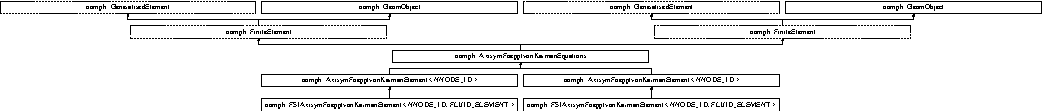
\includegraphics[height=1.489362cm]{classoomph_1_1AxisymFoepplvonKarmanEquations}
\end{center}
\end{figure}
\subsection*{Public Types}
\begin{DoxyCompactItemize}
\item 
typedef void($\ast$ \hyperlink{classoomph_1_1AxisymFoepplvonKarmanEquations_a504878b18d793ef8a6540eb0f2b086c8}{Axisym\+Foepplvon\+Karman\+Pressure\+Fct\+Pt}) (const double \&r, double \&f)
\begin{DoxyCompactList}\small\item\em Function pointer to pressure function fct(r,f(r)) -- r is a Vector! \end{DoxyCompactList}\item 
typedef void($\ast$ \hyperlink{classoomph_1_1AxisymFoepplvonKarmanEquations_a504878b18d793ef8a6540eb0f2b086c8}{Axisym\+Foepplvon\+Karman\+Pressure\+Fct\+Pt}) (const double \&r, double \&f)
\begin{DoxyCompactList}\small\item\em Function pointer to pressure function fct(r,f(r)) -- r is a Vector! \end{DoxyCompactList}\end{DoxyCompactItemize}
\subsection*{Public Member Functions}
\begin{DoxyCompactItemize}
\item 
\hyperlink{classoomph_1_1AxisymFoepplvonKarmanEquations_a73d54781a9dbf02beb79ccfeb5cc34e2}{Axisym\+Foepplvon\+Karman\+Equations} ()
\begin{DoxyCompactList}\small\item\em Constructor (must initialise the Pressure\+\_\+fct\+\_\+pt). Also set physical parameters to their default values. \end{DoxyCompactList}\item 
\hyperlink{classoomph_1_1AxisymFoepplvonKarmanEquations_acd3d7267a7be9c94ff44fad533806e57}{Axisym\+Foepplvon\+Karman\+Equations} (const \hyperlink{classoomph_1_1AxisymFoepplvonKarmanEquations}{Axisym\+Foepplvon\+Karman\+Equations} \&dummy)
\begin{DoxyCompactList}\small\item\em Broken copy constructor. \end{DoxyCompactList}\item 
void \hyperlink{classoomph_1_1AxisymFoepplvonKarmanEquations_aaac38681e3450e4c9159e9b0c1b39b85}{operator=} (const \hyperlink{classoomph_1_1AxisymFoepplvonKarmanEquations}{Axisym\+Foepplvon\+Karman\+Equations} \&)
\begin{DoxyCompactList}\small\item\em Broken assignment operator. \end{DoxyCompactList}\item 
const double \& \hyperlink{classoomph_1_1AxisymFoepplvonKarmanEquations_af9e39f4e7643aaecc50d3535ac976f35}{nu} () const
\begin{DoxyCompactList}\small\item\em Poisson\textquotesingle{}s ratio. \end{DoxyCompactList}\item 
double $\ast$\& \hyperlink{classoomph_1_1AxisymFoepplvonKarmanEquations_a10ca08ff9306d643f6ffb0f644ab2cbc}{nu\+\_\+pt} ()
\begin{DoxyCompactList}\small\item\em Pointer to Poisson\textquotesingle{}s ratio. \end{DoxyCompactList}\item 
const double \& \hyperlink{classoomph_1_1AxisymFoepplvonKarmanEquations_a89a897222e4a40e2d258f4e95eb4ceeb}{eta} () const
\begin{DoxyCompactList}\small\item\em FvK parameter. \end{DoxyCompactList}\item 
double $\ast$\& \hyperlink{classoomph_1_1AxisymFoepplvonKarmanEquations_acdc1b386f9d5bf16512080ce0bfbbdee}{eta\+\_\+pt} ()
\begin{DoxyCompactList}\small\item\em Pointer to FvK parameter. \end{DoxyCompactList}\item 
virtual unsigned \hyperlink{classoomph_1_1AxisymFoepplvonKarmanEquations_a481e2bbbd87723e7b91a79bcb83e361c}{nodal\+\_\+index\+\_\+fvk} (const unsigned \&\hyperlink{cfortran_8h_adb50e893b86b3e55e751a42eab3cba82}{i}=0) const
\begin{DoxyCompactList}\small\item\em Return the index at which the i-\/th unknown value is stored. The default value, i, is appropriate for single-\/physics problems. By default, these are\+: 0\+: transverse displacement w 1\+: laplacian w 2\+: radial displacement u In derived multi-\/physics elements, this function should be overloaded to reflect the chosen storage scheme. Note that these equations require that the unknown is always stored at the same index at each node. \end{DoxyCompactList}\item 
void \hyperlink{classoomph_1_1AxisymFoepplvonKarmanEquations_a162b507ce3d9126a558790e77ec86e70}{output} (std\+::ostream \&outfile)
\begin{DoxyCompactList}\small\item\em Output with default number of plot points. \end{DoxyCompactList}\item 
void \hyperlink{classoomph_1_1AxisymFoepplvonKarmanEquations_a704051a00a2c8624edb98f3ba05e63a2}{output} (std\+::ostream \&outfile, const unsigned \&n\+\_\+plot)
\begin{DoxyCompactList}\small\item\em Output FE representation of soln\+: r,w,sigma\+\_\+r\+\_\+r,sigma\+\_\+phi\+\_\+phi at n\+\_\+plot plot points. \end{DoxyCompactList}\item 
void \hyperlink{classoomph_1_1AxisymFoepplvonKarmanEquations_a236f169caf08c0214ff686e939b9dd33}{output} (F\+I\+LE $\ast$file\+\_\+pt)
\begin{DoxyCompactList}\small\item\em C\+\_\+style output with default number of plot points. \end{DoxyCompactList}\item 
void \hyperlink{classoomph_1_1AxisymFoepplvonKarmanEquations_a5278f37c336b7a4bd2931fdedd2945f8}{output} (F\+I\+LE $\ast$file\+\_\+pt, const unsigned \&n\+\_\+plot)
\begin{DoxyCompactList}\small\item\em C-\/style output FE representation of soln\+: r,w at n\+\_\+plot plot points. \end{DoxyCompactList}\item 
void \hyperlink{classoomph_1_1AxisymFoepplvonKarmanEquations_aae7ed0c9ae0e1a1e2656534807a24527}{output\+\_\+fct} (std\+::ostream \&outfile, const unsigned \&n\+\_\+plot, \hyperlink{classoomph_1_1FiniteElement_a690fd33af26cc3e84f39bba6d5a85202}{Finite\+Element\+::\+Steady\+Exact\+Solution\+Fct\+Pt} exact\+\_\+soln\+\_\+pt)
\begin{DoxyCompactList}\small\item\em Output exact soln\+: r,w\+\_\+exact at n\+\_\+plot plot points. \end{DoxyCompactList}\item 
virtual void \hyperlink{classoomph_1_1AxisymFoepplvonKarmanEquations_a14d84273c5e7a3cdec8fb9b228d675c3}{output\+\_\+fct} (std\+::ostream \&outfile, const unsigned \&n\+\_\+plot, const double \&time, \hyperlink{classoomph_1_1FiniteElement_ad4ecf2b61b158a4b4d351a60d23c633e}{Finite\+Element\+::\+Unsteady\+Exact\+Solution\+Fct\+Pt} exact\+\_\+soln\+\_\+pt)
\begin{DoxyCompactList}\small\item\em Output exact soln\+: r,w\+\_\+exact at n\+\_\+plot plot points (dummy time-\/dependent version to keep intel compiler happy) \end{DoxyCompactList}\item 
void \hyperlink{classoomph_1_1AxisymFoepplvonKarmanEquations_abbcf5312db19fdbe66f5dab3bbe9bfda}{compute\+\_\+error} (std\+::ostream \&outfile, \hyperlink{classoomph_1_1FiniteElement_a690fd33af26cc3e84f39bba6d5a85202}{Finite\+Element\+::\+Steady\+Exact\+Solution\+Fct\+Pt} exact\+\_\+soln\+\_\+pt, double \&error, double \&norm)
\begin{DoxyCompactList}\small\item\em Get error against and norm of exact solution. \end{DoxyCompactList}\item 
void \hyperlink{classoomph_1_1AxisymFoepplvonKarmanEquations_a239536a30ed45a68f678037b9bdc7c9b}{compute\+\_\+error} (std\+::ostream \&outfile, \hyperlink{classoomph_1_1FiniteElement_ad4ecf2b61b158a4b4d351a60d23c633e}{Finite\+Element\+::\+Unsteady\+Exact\+Solution\+Fct\+Pt} exact\+\_\+soln\+\_\+pt, const double \&time, double \&error, double \&norm)
\begin{DoxyCompactList}\small\item\em Dummy, time dependent error checker. \end{DoxyCompactList}\item 
\hyperlink{classoomph_1_1AxisymFoepplvonKarmanEquations_a504878b18d793ef8a6540eb0f2b086c8}{Axisym\+Foepplvon\+Karman\+Pressure\+Fct\+Pt} \& \hyperlink{classoomph_1_1AxisymFoepplvonKarmanEquations_a65fd07792735f269b470f4e4cb3c06a2}{pressure\+\_\+fct\+\_\+pt} ()
\begin{DoxyCompactList}\small\item\em Access function\+: Pointer to pressure function. \end{DoxyCompactList}\item 
\hyperlink{classoomph_1_1AxisymFoepplvonKarmanEquations_a504878b18d793ef8a6540eb0f2b086c8}{Axisym\+Foepplvon\+Karman\+Pressure\+Fct\+Pt} \hyperlink{classoomph_1_1AxisymFoepplvonKarmanEquations_a02dd3dab84e6492d88fdd144a2eed64b}{pressure\+\_\+fct\+\_\+pt} () const
\begin{DoxyCompactList}\small\item\em Access function\+: Pointer to pressure function. Const version. \end{DoxyCompactList}\item 
virtual void \hyperlink{classoomph_1_1AxisymFoepplvonKarmanEquations_acadd8cb7ef617690c79c0c76d7ed0000}{get\+\_\+pressure\+\_\+fvk} (const unsigned \&ipt, const double \&r, double \&pressure) const
\begin{DoxyCompactList}\small\item\em Get pressure term at (Eulerian) position r. This function is virtual to allow overloading in multi-\/physics problems where the strength of the pressure function might be determined by another system of equations. \end{DoxyCompactList}\item 
void \hyperlink{classoomph_1_1AxisymFoepplvonKarmanEquations_a564c34e37df2ed58d16903221528e94c}{get\+\_\+gradient\+\_\+of\+\_\+deflection} (const \hyperlink{classoomph_1_1Vector}{Vector}$<$ double $>$ \&\hyperlink{cfortran_8h_ab7123126e4885ef647dd9c6e3807a21c}{s}, \hyperlink{classoomph_1_1Vector}{Vector}$<$ double $>$ \&gradient) const
\begin{DoxyCompactList}\small\item\em Get gradient of deflection\+: gradient\mbox{[}i\mbox{]} = dw/dr\+\_\+i $\ast$/. \end{DoxyCompactList}\item 
void \hyperlink{classoomph_1_1AxisymFoepplvonKarmanEquations_a18148b60b9a4addc513f1aed354bd63d}{fill\+\_\+in\+\_\+contribution\+\_\+to\+\_\+residuals} (\hyperlink{classoomph_1_1Vector}{Vector}$<$ double $>$ \&residuals)
\begin{DoxyCompactList}\small\item\em Fill in the residuals with this element\textquotesingle{}s contribution. \end{DoxyCompactList}\item 
double \hyperlink{classoomph_1_1AxisymFoepplvonKarmanEquations_aca5188335be3d0432fbf92d493026558}{interpolated\+\_\+w\+\_\+fvk} (const \hyperlink{classoomph_1_1Vector}{Vector}$<$ double $>$ \&\hyperlink{cfortran_8h_ab7123126e4885ef647dd9c6e3807a21c}{s}) const
\begin{DoxyCompactList}\small\item\em Return FE representation of transverse displacement. \end{DoxyCompactList}\item 
double \hyperlink{classoomph_1_1AxisymFoepplvonKarmanEquations_ac24fc0416243162170ad09c7f3261ebd}{interpolated\+\_\+u\+\_\+fvk} (const \hyperlink{classoomph_1_1Vector}{Vector}$<$ double $>$ \&\hyperlink{cfortran_8h_ab7123126e4885ef647dd9c6e3807a21c}{s}) const
\begin{DoxyCompactList}\small\item\em Return FE representation of radial displacement. \end{DoxyCompactList}\item 
bool \hyperlink{classoomph_1_1AxisymFoepplvonKarmanEquations_a22d4a63c862395cae211773748c4c896}{interpolated\+\_\+stress} (const \hyperlink{classoomph_1_1Vector}{Vector}$<$ double $>$ \&\hyperlink{cfortran_8h_ab7123126e4885ef647dd9c6e3807a21c}{s}, double \&sigma\+\_\+r\+\_\+r, double \&sigma\+\_\+phi\+\_\+phi) const
\begin{DoxyCompactList}\small\item\em Compute in-\/plane stresses. Return boolean to indicate success (false if attempt to evaluate stresses at zero radius) \end{DoxyCompactList}\item 
unsigned \hyperlink{classoomph_1_1AxisymFoepplvonKarmanEquations_a2ececacf1a7dd89188a4a20e5abbb7c0}{self\+\_\+test} ()
\begin{DoxyCompactList}\small\item\em Self-\/test\+: Return 0 for OK. \end{DoxyCompactList}\item 
void \hyperlink{classoomph_1_1AxisymFoepplvonKarmanEquations_abddb3d7358a6039420bf6ed58e7a5547}{use\+\_\+linear\+\_\+bending\+\_\+model} ()
\begin{DoxyCompactList}\small\item\em Sets a flag to signify that we are solving the linear, pure bending equations, and pin all the nodal values that will not be used in this case. \end{DoxyCompactList}\item 
\hyperlink{classoomph_1_1AxisymFoepplvonKarmanEquations_a73d54781a9dbf02beb79ccfeb5cc34e2}{Axisym\+Foepplvon\+Karman\+Equations} ()
\begin{DoxyCompactList}\small\item\em Constructor (must initialise the Pressure\+\_\+fct\+\_\+pt and Airy\+\_\+forcing\+\_\+fct\+\_\+pt to null). Also set physical parameters to their default values. \end{DoxyCompactList}\item 
\hyperlink{classoomph_1_1AxisymFoepplvonKarmanEquations_acd3d7267a7be9c94ff44fad533806e57}{Axisym\+Foepplvon\+Karman\+Equations} (const \hyperlink{classoomph_1_1AxisymFoepplvonKarmanEquations}{Axisym\+Foepplvon\+Karman\+Equations} \&dummy)
\begin{DoxyCompactList}\small\item\em Broken copy constructor. \end{DoxyCompactList}\item 
void \hyperlink{classoomph_1_1AxisymFoepplvonKarmanEquations_aaac38681e3450e4c9159e9b0c1b39b85}{operator=} (const \hyperlink{classoomph_1_1AxisymFoepplvonKarmanEquations}{Axisym\+Foepplvon\+Karman\+Equations} \&)
\begin{DoxyCompactList}\small\item\em Broken assignment operator. \end{DoxyCompactList}\item 
const double \& \hyperlink{classoomph_1_1AxisymFoepplvonKarmanEquations_a89a897222e4a40e2d258f4e95eb4ceeb}{eta} () const
\begin{DoxyCompactList}\small\item\em FvK parameter. \end{DoxyCompactList}\item 
double $\ast$\& \hyperlink{classoomph_1_1AxisymFoepplvonKarmanEquations_acdc1b386f9d5bf16512080ce0bfbbdee}{eta\+\_\+pt} ()
\begin{DoxyCompactList}\small\item\em Pointer to FvK parameter. \end{DoxyCompactList}\item 
virtual unsigned \hyperlink{classoomph_1_1AxisymFoepplvonKarmanEquations_a481e2bbbd87723e7b91a79bcb83e361c}{nodal\+\_\+index\+\_\+fvk} (const unsigned \&\hyperlink{cfortran_8h_adb50e893b86b3e55e751a42eab3cba82}{i}=0) const
\begin{DoxyCompactList}\small\item\em Return the index at which the i-\/th unknown value is stored. The default value, i, is appropriate for single-\/physics problems. By default, these are\+: 0\+: w 1\+: laplacian w 2\+: phi 3\+: laplacian phi 4-\/5\+: smooth first derivatives In derived multi-\/physics elements, this function should be overloaded to reflect the chosen storage scheme. Note that these equations require that the unknown is always stored at the same index at each node. \end{DoxyCompactList}\item 
void \hyperlink{classoomph_1_1AxisymFoepplvonKarmanEquations_a162b507ce3d9126a558790e77ec86e70}{output} (std\+::ostream \&outfile)
\begin{DoxyCompactList}\small\item\em Output with default number of plot points. \end{DoxyCompactList}\item 
void \hyperlink{classoomph_1_1AxisymFoepplvonKarmanEquations_a704051a00a2c8624edb98f3ba05e63a2}{output} (std\+::ostream \&outfile, const unsigned \&n\+\_\+plot)
\begin{DoxyCompactList}\small\item\em Output FE representation of soln\+: r,w,sigma\+\_\+r\+\_\+r,sigma\+\_\+phi\+\_\+phi at n\+\_\+plot plot points. \end{DoxyCompactList}\item 
void \hyperlink{classoomph_1_1AxisymFoepplvonKarmanEquations_a236f169caf08c0214ff686e939b9dd33}{output} (F\+I\+LE $\ast$file\+\_\+pt)
\begin{DoxyCompactList}\small\item\em C\+\_\+style output with default number of plot points. \end{DoxyCompactList}\item 
void \hyperlink{classoomph_1_1AxisymFoepplvonKarmanEquations_a5278f37c336b7a4bd2931fdedd2945f8}{output} (F\+I\+LE $\ast$file\+\_\+pt, const unsigned \&n\+\_\+plot)
\begin{DoxyCompactList}\small\item\em C-\/style output FE representation of soln\+: r,w at n\+\_\+plot plot points. \end{DoxyCompactList}\item 
void \hyperlink{classoomph_1_1AxisymFoepplvonKarmanEquations_aae7ed0c9ae0e1a1e2656534807a24527}{output\+\_\+fct} (std\+::ostream \&outfile, const unsigned \&n\+\_\+plot, \hyperlink{classoomph_1_1FiniteElement_a690fd33af26cc3e84f39bba6d5a85202}{Finite\+Element\+::\+Steady\+Exact\+Solution\+Fct\+Pt} exact\+\_\+soln\+\_\+pt)
\begin{DoxyCompactList}\small\item\em Output exact soln\+: r,w\+\_\+exact at n\+\_\+plot plot points. \end{DoxyCompactList}\item 
virtual void \hyperlink{classoomph_1_1AxisymFoepplvonKarmanEquations_a14d84273c5e7a3cdec8fb9b228d675c3}{output\+\_\+fct} (std\+::ostream \&outfile, const unsigned \&n\+\_\+plot, const double \&time, \hyperlink{classoomph_1_1FiniteElement_ad4ecf2b61b158a4b4d351a60d23c633e}{Finite\+Element\+::\+Unsteady\+Exact\+Solution\+Fct\+Pt} exact\+\_\+soln\+\_\+pt)
\begin{DoxyCompactList}\small\item\em Output exact soln\+: r,w\+\_\+exact at n\+\_\+plot plot points (dummy time-\/dependent version to keep intel compiler happy) \end{DoxyCompactList}\item 
void \hyperlink{classoomph_1_1AxisymFoepplvonKarmanEquations_abbcf5312db19fdbe66f5dab3bbe9bfda}{compute\+\_\+error} (std\+::ostream \&outfile, \hyperlink{classoomph_1_1FiniteElement_a690fd33af26cc3e84f39bba6d5a85202}{Finite\+Element\+::\+Steady\+Exact\+Solution\+Fct\+Pt} exact\+\_\+soln\+\_\+pt, double \&error, double \&norm)
\begin{DoxyCompactList}\small\item\em Get error against and norm of exact solution. \end{DoxyCompactList}\item 
void \hyperlink{classoomph_1_1AxisymFoepplvonKarmanEquations_a239536a30ed45a68f678037b9bdc7c9b}{compute\+\_\+error} (std\+::ostream \&outfile, \hyperlink{classoomph_1_1FiniteElement_ad4ecf2b61b158a4b4d351a60d23c633e}{Finite\+Element\+::\+Unsteady\+Exact\+Solution\+Fct\+Pt} exact\+\_\+soln\+\_\+pt, const double \&time, double \&error, double \&norm)
\begin{DoxyCompactList}\small\item\em Dummy, time dependent error checker. \end{DoxyCompactList}\item 
\hyperlink{classoomph_1_1AxisymFoepplvonKarmanEquations_a504878b18d793ef8a6540eb0f2b086c8}{Axisym\+Foepplvon\+Karman\+Pressure\+Fct\+Pt} \& \hyperlink{classoomph_1_1AxisymFoepplvonKarmanEquations_a65fd07792735f269b470f4e4cb3c06a2}{pressure\+\_\+fct\+\_\+pt} ()
\begin{DoxyCompactList}\small\item\em Access function\+: Pointer to pressure function. \end{DoxyCompactList}\item 
\hyperlink{classoomph_1_1AxisymFoepplvonKarmanEquations_a504878b18d793ef8a6540eb0f2b086c8}{Axisym\+Foepplvon\+Karman\+Pressure\+Fct\+Pt} \hyperlink{classoomph_1_1AxisymFoepplvonKarmanEquations_a02dd3dab84e6492d88fdd144a2eed64b}{pressure\+\_\+fct\+\_\+pt} () const
\begin{DoxyCompactList}\small\item\em Access function\+: Pointer to pressure function. Const version. \end{DoxyCompactList}\item 
\hyperlink{classoomph_1_1AxisymFoepplvonKarmanEquations_a504878b18d793ef8a6540eb0f2b086c8}{Axisym\+Foepplvon\+Karman\+Pressure\+Fct\+Pt} \& \hyperlink{classoomph_1_1AxisymFoepplvonKarmanEquations_a644b70b3796d567b158d8708b811a601}{airy\+\_\+forcing\+\_\+fct\+\_\+pt} ()
\begin{DoxyCompactList}\small\item\em Access function\+: Pointer to Airy forcing function. \end{DoxyCompactList}\item 
\hyperlink{classoomph_1_1AxisymFoepplvonKarmanEquations_a504878b18d793ef8a6540eb0f2b086c8}{Axisym\+Foepplvon\+Karman\+Pressure\+Fct\+Pt} \hyperlink{classoomph_1_1AxisymFoepplvonKarmanEquations_af38f42d03989cb589ad127b2ccbc7ae8}{airy\+\_\+forcing\+\_\+fct\+\_\+pt} () const
\begin{DoxyCompactList}\small\item\em Access function\+: Pointer to Airy forcing function. Const version. \end{DoxyCompactList}\item 
virtual void \hyperlink{classoomph_1_1AxisymFoepplvonKarmanEquations_acadd8cb7ef617690c79c0c76d7ed0000}{get\+\_\+pressure\+\_\+fvk} (const unsigned \&ipt, const double \&r, double \&pressure) const
\begin{DoxyCompactList}\small\item\em Get pressure term at (Eulerian) position r. This function is virtual to allow overloading in multi-\/physics problems where the strength of the pressure function might be determined by another system of equations. \end{DoxyCompactList}\item 
virtual void \hyperlink{classoomph_1_1AxisymFoepplvonKarmanEquations_aecb0dc1f5c1da058c7519ed64f2748c1}{get\+\_\+airy\+\_\+forcing\+\_\+fvk} (const unsigned \&ipt, const double \&r, double \&airy\+\_\+forcing) const
\begin{DoxyCompactList}\small\item\em Get Airy forcing term at (Eulerian) position r. This function is virtual to allow overloading in multi-\/physics problems where the strength of the pressure function might be determined by another system of equations. \end{DoxyCompactList}\item 
void \hyperlink{classoomph_1_1AxisymFoepplvonKarmanEquations_a564c34e37df2ed58d16903221528e94c}{get\+\_\+gradient\+\_\+of\+\_\+deflection} (const \hyperlink{classoomph_1_1Vector}{Vector}$<$ double $>$ \&\hyperlink{cfortran_8h_ab7123126e4885ef647dd9c6e3807a21c}{s}, \hyperlink{classoomph_1_1Vector}{Vector}$<$ double $>$ \&gradient) const
\begin{DoxyCompactList}\small\item\em Get gradient of deflection\+: gradient\mbox{[}i\mbox{]} = dw/dr\+\_\+i $\ast$/. \end{DoxyCompactList}\item 
void \hyperlink{classoomph_1_1AxisymFoepplvonKarmanEquations_a18148b60b9a4addc513f1aed354bd63d}{fill\+\_\+in\+\_\+contribution\+\_\+to\+\_\+residuals} (\hyperlink{classoomph_1_1Vector}{Vector}$<$ double $>$ \&residuals)
\begin{DoxyCompactList}\small\item\em Fill in the residuals with this element\textquotesingle{}s contribution. \end{DoxyCompactList}\item 
double \hyperlink{classoomph_1_1AxisymFoepplvonKarmanEquations_aca5188335be3d0432fbf92d493026558}{interpolated\+\_\+w\+\_\+fvk} (const \hyperlink{classoomph_1_1Vector}{Vector}$<$ double $>$ \&\hyperlink{cfortran_8h_ab7123126e4885ef647dd9c6e3807a21c}{s}) const
\begin{DoxyCompactList}\small\item\em Return FE representation of vertical displacement, w\+\_\+fvk(s) at local coordinate s. \end{DoxyCompactList}\item 
bool \hyperlink{classoomph_1_1AxisymFoepplvonKarmanEquations_a3462c52b14649baaea863ea664a41c16}{interpolated\+\_\+stress} (const \hyperlink{classoomph_1_1Vector}{Vector}$<$ double $>$ \&\hyperlink{cfortran_8h_ab7123126e4885ef647dd9c6e3807a21c}{s}, double \&sigma\+\_\+r\+\_\+r, double \&sigma\+\_\+phi\+\_\+phi)
\begin{DoxyCompactList}\small\item\em Compute in-\/plane stresses. Return boolean to indicate success (false if attempt to evaluate stresses at zero radius) \end{DoxyCompactList}\item 
unsigned \hyperlink{classoomph_1_1AxisymFoepplvonKarmanEquations_a2ececacf1a7dd89188a4a20e5abbb7c0}{self\+\_\+test} ()
\begin{DoxyCompactList}\small\item\em Self-\/test\+: Return 0 for OK. \end{DoxyCompactList}\item 
void \hyperlink{classoomph_1_1AxisymFoepplvonKarmanEquations_abddb3d7358a6039420bf6ed58e7a5547}{use\+\_\+linear\+\_\+bending\+\_\+model} ()
\begin{DoxyCompactList}\small\item\em Sets a flag to signify that we are solving the linear, pure bending equations, and pin all the nodal values that will not be used in this case. \end{DoxyCompactList}\end{DoxyCompactItemize}
\subsection*{Protected Member Functions}
\begin{DoxyCompactItemize}
\item 
virtual double \hyperlink{classoomph_1_1AxisymFoepplvonKarmanEquations_a838cd424e2666b007113de0a95f5d999}{dshape\+\_\+and\+\_\+dtest\+\_\+eulerian\+\_\+axisym\+\_\+fvk} (const \hyperlink{classoomph_1_1Vector}{Vector}$<$ double $>$ \&\hyperlink{cfortran_8h_ab7123126e4885ef647dd9c6e3807a21c}{s}, \hyperlink{classoomph_1_1Shape}{Shape} \&psi, \hyperlink{classoomph_1_1DShape}{D\+Shape} \&dpsidr, \hyperlink{classoomph_1_1Shape}{Shape} \&test, \hyperlink{classoomph_1_1DShape}{D\+Shape} \&dtestdr) const =0
\begin{DoxyCompactList}\small\item\em Shape/test functions and derivs w.\+r.\+t. to global coords at local coord. s; return Jacobian of mapping. \end{DoxyCompactList}\item 
virtual double \hyperlink{classoomph_1_1AxisymFoepplvonKarmanEquations_a456a9c27c326d6d1e55e3ab822ac1a5f}{dshape\+\_\+and\+\_\+dtest\+\_\+eulerian\+\_\+at\+\_\+knot\+\_\+axisym\+\_\+fvk} (const unsigned \&ipt, \hyperlink{classoomph_1_1Shape}{Shape} \&psi, \hyperlink{classoomph_1_1DShape}{D\+Shape} \&dpsidr, \hyperlink{classoomph_1_1Shape}{Shape} \&test, \hyperlink{classoomph_1_1DShape}{D\+Shape} \&dtestdr) const =0
\begin{DoxyCompactList}\small\item\em Shape/test functions and derivs w.\+r.\+t. to global coords at integration point ipt; return Jacobian of mapping. \end{DoxyCompactList}\item 
virtual double \hyperlink{classoomph_1_1AxisymFoepplvonKarmanEquations_a838cd424e2666b007113de0a95f5d999}{dshape\+\_\+and\+\_\+dtest\+\_\+eulerian\+\_\+axisym\+\_\+fvk} (const \hyperlink{classoomph_1_1Vector}{Vector}$<$ double $>$ \&\hyperlink{cfortran_8h_ab7123126e4885ef647dd9c6e3807a21c}{s}, \hyperlink{classoomph_1_1Shape}{Shape} \&psi, \hyperlink{classoomph_1_1DShape}{D\+Shape} \&dpsidr, \hyperlink{classoomph_1_1Shape}{Shape} \&test, \hyperlink{classoomph_1_1DShape}{D\+Shape} \&dtestdr) const =0
\begin{DoxyCompactList}\small\item\em Shape/test functions and derivs w.\+r.\+t. to global coords at local coord. s; return Jacobian of mapping. \end{DoxyCompactList}\item 
virtual double \hyperlink{classoomph_1_1AxisymFoepplvonKarmanEquations_a456a9c27c326d6d1e55e3ab822ac1a5f}{dshape\+\_\+and\+\_\+dtest\+\_\+eulerian\+\_\+at\+\_\+knot\+\_\+axisym\+\_\+fvk} (const unsigned \&ipt, \hyperlink{classoomph_1_1Shape}{Shape} \&psi, \hyperlink{classoomph_1_1DShape}{D\+Shape} \&dpsidr, \hyperlink{classoomph_1_1Shape}{Shape} \&test, \hyperlink{classoomph_1_1DShape}{D\+Shape} \&dtestdr) const =0
\begin{DoxyCompactList}\small\item\em Shape/test functions and derivs w.\+r.\+t. to global coords at integration point ipt; return Jacobian of mapping. \end{DoxyCompactList}\end{DoxyCompactItemize}
\subsection*{Protected Attributes}
\begin{DoxyCompactItemize}
\item 
double $\ast$ \hyperlink{classoomph_1_1AxisymFoepplvonKarmanEquations_a31a8e3c278b1c2ce7238b71902812ffd}{Eta\+\_\+pt}
\begin{DoxyCompactList}\small\item\em Pointer to FvK parameter. \end{DoxyCompactList}\item 
\hyperlink{classoomph_1_1AxisymFoepplvonKarmanEquations_a504878b18d793ef8a6540eb0f2b086c8}{Axisym\+Foepplvon\+Karman\+Pressure\+Fct\+Pt} \hyperlink{classoomph_1_1AxisymFoepplvonKarmanEquations_a06ebccc2c0b2638657c98f6137de7d4b}{Pressure\+\_\+fct\+\_\+pt}
\begin{DoxyCompactList}\small\item\em Pointer to pressure function\+: \end{DoxyCompactList}\item 
double $\ast$ \hyperlink{classoomph_1_1AxisymFoepplvonKarmanEquations_a02dd0294aa3239752ea7c21018ac65b6}{Nu\+\_\+pt}
\begin{DoxyCompactList}\small\item\em Pointer to Poisson\textquotesingle{}s ratio. \end{DoxyCompactList}\item 
bool \hyperlink{classoomph_1_1AxisymFoepplvonKarmanEquations_a86ab587e241e8950409e38698692c109}{Linear\+\_\+bending\+\_\+model}
\begin{DoxyCompactList}\small\item\em Flag which stores whether we are using a linear, pure bending model instead of the full non-\/linear Foeppl-\/von Karman. \end{DoxyCompactList}\item 
\hyperlink{classoomph_1_1AxisymFoepplvonKarmanEquations_a504878b18d793ef8a6540eb0f2b086c8}{Axisym\+Foepplvon\+Karman\+Pressure\+Fct\+Pt} \hyperlink{classoomph_1_1AxisymFoepplvonKarmanEquations_a30c50341cb3b091ad9ee9a96a62b10bf}{Airy\+\_\+forcing\+\_\+fct\+\_\+pt}
\begin{DoxyCompactList}\small\item\em Pointer to Airy forcing function. \end{DoxyCompactList}\end{DoxyCompactItemize}
\subsection*{Static Private Attributes}
\begin{DoxyCompactItemize}
\item 
static double \hyperlink{classoomph_1_1AxisymFoepplvonKarmanEquations_a0b63093c406541a97199a2a68dcd29e7}{Default\+\_\+\+Physical\+\_\+\+Constant\+\_\+\+Value} = 0.\+0
\begin{DoxyCompactList}\small\item\em Default value for physical constants. \end{DoxyCompactList}\end{DoxyCompactItemize}
\subsection*{Additional Inherited Members}


\subsection{Detailed Description}
A class for all isoparametric elements that solve the axis\+Ym Foeppl von Karman equations in a displacement based formulation.

This contains the generic maths. \hyperlink{classoomph_1_1Shape}{Shape} functions, geometric mapping etc. must get implemented in derived class.

A class for all isoparametric elements that solve the axisum Foeppl von Karman equations.

This contains the generic maths. \hyperlink{classoomph_1_1Shape}{Shape} functions, geometric mapping etc. must get implemented in derived class. 

Definition at line 55 of file axisym\+\_\+displ\+\_\+based\+\_\+fvk\+\_\+elements.\+h.



\subsection{Member Typedef Documentation}
\mbox{\Hypertarget{classoomph_1_1AxisymFoepplvonKarmanEquations_a504878b18d793ef8a6540eb0f2b086c8}\label{classoomph_1_1AxisymFoepplvonKarmanEquations_a504878b18d793ef8a6540eb0f2b086c8}} 
\index{oomph\+::\+Axisym\+Foepplvon\+Karman\+Equations@{oomph\+::\+Axisym\+Foepplvon\+Karman\+Equations}!Axisym\+Foepplvon\+Karman\+Pressure\+Fct\+Pt@{Axisym\+Foepplvon\+Karman\+Pressure\+Fct\+Pt}}
\index{Axisym\+Foepplvon\+Karman\+Pressure\+Fct\+Pt@{Axisym\+Foepplvon\+Karman\+Pressure\+Fct\+Pt}!oomph\+::\+Axisym\+Foepplvon\+Karman\+Equations@{oomph\+::\+Axisym\+Foepplvon\+Karman\+Equations}}
\subsubsection{\texorpdfstring{Axisym\+Foepplvon\+Karman\+Pressure\+Fct\+Pt}{AxisymFoepplvonKarmanPressureFctPt}\hspace{0.1cm}{\footnotesize\ttfamily [1/2]}}
{\footnotesize\ttfamily typedef void($\ast$ oomph\+::\+Axisym\+Foepplvon\+Karman\+Equations\+::\+Axisym\+Foepplvon\+Karman\+Pressure\+Fct\+Pt) (const double \&r, double \&f)}



Function pointer to pressure function fct(r,f(r)) -- r is a Vector! 



Definition at line 62 of file axisym\+\_\+fvk\+\_\+elements.\+h.

\mbox{\Hypertarget{classoomph_1_1AxisymFoepplvonKarmanEquations_a504878b18d793ef8a6540eb0f2b086c8}\label{classoomph_1_1AxisymFoepplvonKarmanEquations_a504878b18d793ef8a6540eb0f2b086c8}} 
\index{oomph\+::\+Axisym\+Foepplvon\+Karman\+Equations@{oomph\+::\+Axisym\+Foepplvon\+Karman\+Equations}!Axisym\+Foepplvon\+Karman\+Pressure\+Fct\+Pt@{Axisym\+Foepplvon\+Karman\+Pressure\+Fct\+Pt}}
\index{Axisym\+Foepplvon\+Karman\+Pressure\+Fct\+Pt@{Axisym\+Foepplvon\+Karman\+Pressure\+Fct\+Pt}!oomph\+::\+Axisym\+Foepplvon\+Karman\+Equations@{oomph\+::\+Axisym\+Foepplvon\+Karman\+Equations}}
\subsubsection{\texorpdfstring{Axisym\+Foepplvon\+Karman\+Pressure\+Fct\+Pt}{AxisymFoepplvonKarmanPressureFctPt}\hspace{0.1cm}{\footnotesize\ttfamily [2/2]}}
{\footnotesize\ttfamily typedef void($\ast$ oomph\+::\+Axisym\+Foepplvon\+Karman\+Equations\+::\+Axisym\+Foepplvon\+Karman\+Pressure\+Fct\+Pt) (const double \&r, double \&f)}



Function pointer to pressure function fct(r,f(r)) -- r is a Vector! 



Definition at line 62 of file axisym\+\_\+displ\+\_\+based\+\_\+fvk\+\_\+elements.\+h.



\subsection{Constructor \& Destructor Documentation}
\mbox{\Hypertarget{classoomph_1_1AxisymFoepplvonKarmanEquations_a73d54781a9dbf02beb79ccfeb5cc34e2}\label{classoomph_1_1AxisymFoepplvonKarmanEquations_a73d54781a9dbf02beb79ccfeb5cc34e2}} 
\index{oomph\+::\+Axisym\+Foepplvon\+Karman\+Equations@{oomph\+::\+Axisym\+Foepplvon\+Karman\+Equations}!Axisym\+Foepplvon\+Karman\+Equations@{Axisym\+Foepplvon\+Karman\+Equations}}
\index{Axisym\+Foepplvon\+Karman\+Equations@{Axisym\+Foepplvon\+Karman\+Equations}!oomph\+::\+Axisym\+Foepplvon\+Karman\+Equations@{oomph\+::\+Axisym\+Foepplvon\+Karman\+Equations}}
\subsubsection{\texorpdfstring{Axisym\+Foepplvon\+Karman\+Equations()}{AxisymFoepplvonKarmanEquations()}\hspace{0.1cm}{\footnotesize\ttfamily [1/4]}}
{\footnotesize\ttfamily oomph\+::\+Axisym\+Foepplvon\+Karman\+Equations\+::\+Axisym\+Foepplvon\+Karman\+Equations (\begin{DoxyParamCaption}{ }\end{DoxyParamCaption})\hspace{0.3cm}{\ttfamily [inline]}}



Constructor (must initialise the Pressure\+\_\+fct\+\_\+pt). Also set physical parameters to their default values. 



Definition at line 67 of file axisym\+\_\+displ\+\_\+based\+\_\+fvk\+\_\+elements.\+h.

\mbox{\Hypertarget{classoomph_1_1AxisymFoepplvonKarmanEquations_acd3d7267a7be9c94ff44fad533806e57}\label{classoomph_1_1AxisymFoepplvonKarmanEquations_acd3d7267a7be9c94ff44fad533806e57}} 
\index{oomph\+::\+Axisym\+Foepplvon\+Karman\+Equations@{oomph\+::\+Axisym\+Foepplvon\+Karman\+Equations}!Axisym\+Foepplvon\+Karman\+Equations@{Axisym\+Foepplvon\+Karman\+Equations}}
\index{Axisym\+Foepplvon\+Karman\+Equations@{Axisym\+Foepplvon\+Karman\+Equations}!oomph\+::\+Axisym\+Foepplvon\+Karman\+Equations@{oomph\+::\+Axisym\+Foepplvon\+Karman\+Equations}}
\subsubsection{\texorpdfstring{Axisym\+Foepplvon\+Karman\+Equations()}{AxisymFoepplvonKarmanEquations()}\hspace{0.1cm}{\footnotesize\ttfamily [2/4]}}
{\footnotesize\ttfamily oomph\+::\+Axisym\+Foepplvon\+Karman\+Equations\+::\+Axisym\+Foepplvon\+Karman\+Equations (\begin{DoxyParamCaption}\item[{const \hyperlink{classoomph_1_1AxisymFoepplvonKarmanEquations}{Axisym\+Foepplvon\+Karman\+Equations} \&}]{dummy }\end{DoxyParamCaption})\hspace{0.3cm}{\ttfamily [inline]}}



Broken copy constructor. 



Definition at line 71 of file axisym\+\_\+displ\+\_\+based\+\_\+fvk\+\_\+elements.\+h.



References oomph\+::\+Broken\+Copy\+::broken\+\_\+copy().

\mbox{\Hypertarget{classoomph_1_1AxisymFoepplvonKarmanEquations_a73d54781a9dbf02beb79ccfeb5cc34e2}\label{classoomph_1_1AxisymFoepplvonKarmanEquations_a73d54781a9dbf02beb79ccfeb5cc34e2}} 
\index{oomph\+::\+Axisym\+Foepplvon\+Karman\+Equations@{oomph\+::\+Axisym\+Foepplvon\+Karman\+Equations}!Axisym\+Foepplvon\+Karman\+Equations@{Axisym\+Foepplvon\+Karman\+Equations}}
\index{Axisym\+Foepplvon\+Karman\+Equations@{Axisym\+Foepplvon\+Karman\+Equations}!oomph\+::\+Axisym\+Foepplvon\+Karman\+Equations@{oomph\+::\+Axisym\+Foepplvon\+Karman\+Equations}}
\subsubsection{\texorpdfstring{Axisym\+Foepplvon\+Karman\+Equations()}{AxisymFoepplvonKarmanEquations()}\hspace{0.1cm}{\footnotesize\ttfamily [3/4]}}
{\footnotesize\ttfamily oomph\+::\+Axisym\+Foepplvon\+Karman\+Equations\+::\+Axisym\+Foepplvon\+Karman\+Equations (\begin{DoxyParamCaption}{ }\end{DoxyParamCaption})\hspace{0.3cm}{\ttfamily [inline]}}



Constructor (must initialise the Pressure\+\_\+fct\+\_\+pt and Airy\+\_\+forcing\+\_\+fct\+\_\+pt to null). Also set physical parameters to their default values. 



Definition at line 67 of file axisym\+\_\+fvk\+\_\+elements.\+h.



References Default\+\_\+\+Physical\+\_\+\+Constant\+\_\+\+Value, Eta\+\_\+pt, and Linear\+\_\+bending\+\_\+model.

\mbox{\Hypertarget{classoomph_1_1AxisymFoepplvonKarmanEquations_acd3d7267a7be9c94ff44fad533806e57}\label{classoomph_1_1AxisymFoepplvonKarmanEquations_acd3d7267a7be9c94ff44fad533806e57}} 
\index{oomph\+::\+Axisym\+Foepplvon\+Karman\+Equations@{oomph\+::\+Axisym\+Foepplvon\+Karman\+Equations}!Axisym\+Foepplvon\+Karman\+Equations@{Axisym\+Foepplvon\+Karman\+Equations}}
\index{Axisym\+Foepplvon\+Karman\+Equations@{Axisym\+Foepplvon\+Karman\+Equations}!oomph\+::\+Axisym\+Foepplvon\+Karman\+Equations@{oomph\+::\+Axisym\+Foepplvon\+Karman\+Equations}}
\subsubsection{\texorpdfstring{Axisym\+Foepplvon\+Karman\+Equations()}{AxisymFoepplvonKarmanEquations()}\hspace{0.1cm}{\footnotesize\ttfamily [4/4]}}
{\footnotesize\ttfamily oomph\+::\+Axisym\+Foepplvon\+Karman\+Equations\+::\+Axisym\+Foepplvon\+Karman\+Equations (\begin{DoxyParamCaption}\item[{const \hyperlink{classoomph_1_1AxisymFoepplvonKarmanEquations}{Axisym\+Foepplvon\+Karman\+Equations} \&}]{dummy }\end{DoxyParamCaption})\hspace{0.3cm}{\ttfamily [inline]}}



Broken copy constructor. 



Definition at line 76 of file axisym\+\_\+fvk\+\_\+elements.\+h.



References oomph\+::\+Broken\+Copy\+::broken\+\_\+copy().



\subsection{Member Function Documentation}
\mbox{\Hypertarget{classoomph_1_1AxisymFoepplvonKarmanEquations_a644b70b3796d567b158d8708b811a601}\label{classoomph_1_1AxisymFoepplvonKarmanEquations_a644b70b3796d567b158d8708b811a601}} 
\index{oomph\+::\+Axisym\+Foepplvon\+Karman\+Equations@{oomph\+::\+Axisym\+Foepplvon\+Karman\+Equations}!airy\+\_\+forcing\+\_\+fct\+\_\+pt@{airy\+\_\+forcing\+\_\+fct\+\_\+pt}}
\index{airy\+\_\+forcing\+\_\+fct\+\_\+pt@{airy\+\_\+forcing\+\_\+fct\+\_\+pt}!oomph\+::\+Axisym\+Foepplvon\+Karman\+Equations@{oomph\+::\+Axisym\+Foepplvon\+Karman\+Equations}}
\subsubsection{\texorpdfstring{airy\+\_\+forcing\+\_\+fct\+\_\+pt()}{airy\_forcing\_fct\_pt()}\hspace{0.1cm}{\footnotesize\ttfamily [1/2]}}
{\footnotesize\ttfamily \hyperlink{classoomph_1_1AxisymFoepplvonKarmanEquations_a504878b18d793ef8a6540eb0f2b086c8}{Axisym\+Foepplvon\+Karman\+Pressure\+Fct\+Pt}\& oomph\+::\+Axisym\+Foepplvon\+Karman\+Equations\+::airy\+\_\+forcing\+\_\+fct\+\_\+pt (\begin{DoxyParamCaption}{ }\end{DoxyParamCaption})\hspace{0.3cm}{\ttfamily [inline]}}



Access function\+: Pointer to Airy forcing function. 



Definition at line 175 of file axisym\+\_\+fvk\+\_\+elements.\+h.



References Airy\+\_\+forcing\+\_\+fct\+\_\+pt.

\mbox{\Hypertarget{classoomph_1_1AxisymFoepplvonKarmanEquations_af38f42d03989cb589ad127b2ccbc7ae8}\label{classoomph_1_1AxisymFoepplvonKarmanEquations_af38f42d03989cb589ad127b2ccbc7ae8}} 
\index{oomph\+::\+Axisym\+Foepplvon\+Karman\+Equations@{oomph\+::\+Axisym\+Foepplvon\+Karman\+Equations}!airy\+\_\+forcing\+\_\+fct\+\_\+pt@{airy\+\_\+forcing\+\_\+fct\+\_\+pt}}
\index{airy\+\_\+forcing\+\_\+fct\+\_\+pt@{airy\+\_\+forcing\+\_\+fct\+\_\+pt}!oomph\+::\+Axisym\+Foepplvon\+Karman\+Equations@{oomph\+::\+Axisym\+Foepplvon\+Karman\+Equations}}
\subsubsection{\texorpdfstring{airy\+\_\+forcing\+\_\+fct\+\_\+pt()}{airy\_forcing\_fct\_pt()}\hspace{0.1cm}{\footnotesize\ttfamily [2/2]}}
{\footnotesize\ttfamily \hyperlink{classoomph_1_1AxisymFoepplvonKarmanEquations_a504878b18d793ef8a6540eb0f2b086c8}{Axisym\+Foepplvon\+Karman\+Pressure\+Fct\+Pt} oomph\+::\+Axisym\+Foepplvon\+Karman\+Equations\+::airy\+\_\+forcing\+\_\+fct\+\_\+pt (\begin{DoxyParamCaption}{ }\end{DoxyParamCaption}) const\hspace{0.3cm}{\ttfamily [inline]}}



Access function\+: Pointer to Airy forcing function. Const version. 



Definition at line 179 of file axisym\+\_\+fvk\+\_\+elements.\+h.



References Airy\+\_\+forcing\+\_\+fct\+\_\+pt.

\mbox{\Hypertarget{classoomph_1_1AxisymFoepplvonKarmanEquations_abbcf5312db19fdbe66f5dab3bbe9bfda}\label{classoomph_1_1AxisymFoepplvonKarmanEquations_abbcf5312db19fdbe66f5dab3bbe9bfda}} 
\index{oomph\+::\+Axisym\+Foepplvon\+Karman\+Equations@{oomph\+::\+Axisym\+Foepplvon\+Karman\+Equations}!compute\+\_\+error@{compute\+\_\+error}}
\index{compute\+\_\+error@{compute\+\_\+error}!oomph\+::\+Axisym\+Foepplvon\+Karman\+Equations@{oomph\+::\+Axisym\+Foepplvon\+Karman\+Equations}}
\subsubsection{\texorpdfstring{compute\+\_\+error()}{compute\_error()}\hspace{0.1cm}{\footnotesize\ttfamily [1/4]}}
{\footnotesize\ttfamily void oomph\+::\+Axisym\+Foepplvon\+Karman\+Equations\+::compute\+\_\+error (\begin{DoxyParamCaption}\item[{std\+::ostream \&}]{outfile,  }\item[{\hyperlink{classoomph_1_1FiniteElement_a690fd33af26cc3e84f39bba6d5a85202}{Finite\+Element\+::\+Steady\+Exact\+Solution\+Fct\+Pt}}]{exact\+\_\+soln\+\_\+pt,  }\item[{double \&}]{error,  }\item[{double \&}]{norm }\end{DoxyParamCaption})\hspace{0.3cm}{\ttfamily [virtual]}}



Get error against and norm of exact solution. 



Reimplemented from \hyperlink{classoomph_1_1FiniteElement_a73c79a1f1e5b1d334757812a6bbd58ff}{oomph\+::\+Finite\+Element}.

\mbox{\Hypertarget{classoomph_1_1AxisymFoepplvonKarmanEquations_a239536a30ed45a68f678037b9bdc7c9b}\label{classoomph_1_1AxisymFoepplvonKarmanEquations_a239536a30ed45a68f678037b9bdc7c9b}} 
\index{oomph\+::\+Axisym\+Foepplvon\+Karman\+Equations@{oomph\+::\+Axisym\+Foepplvon\+Karman\+Equations}!compute\+\_\+error@{compute\+\_\+error}}
\index{compute\+\_\+error@{compute\+\_\+error}!oomph\+::\+Axisym\+Foepplvon\+Karman\+Equations@{oomph\+::\+Axisym\+Foepplvon\+Karman\+Equations}}
\subsubsection{\texorpdfstring{compute\+\_\+error()}{compute\_error()}\hspace{0.1cm}{\footnotesize\ttfamily [2/4]}}
{\footnotesize\ttfamily void oomph\+::\+Axisym\+Foepplvon\+Karman\+Equations\+::compute\+\_\+error (\begin{DoxyParamCaption}\item[{std\+::ostream \&}]{outfile,  }\item[{\hyperlink{classoomph_1_1FiniteElement_ad4ecf2b61b158a4b4d351a60d23c633e}{Finite\+Element\+::\+Unsteady\+Exact\+Solution\+Fct\+Pt}}]{exact\+\_\+soln\+\_\+pt,  }\item[{const double \&}]{time,  }\item[{double \&}]{error,  }\item[{double \&}]{norm }\end{DoxyParamCaption})\hspace{0.3cm}{\ttfamily [inline]}, {\ttfamily [virtual]}}



Dummy, time dependent error checker. 



Reimplemented from \hyperlink{classoomph_1_1FiniteElement_a7f67853506dc73fa6b7505108de22d1f}{oomph\+::\+Finite\+Element}.



Definition at line 155 of file axisym\+\_\+fvk\+\_\+elements.\+h.

\mbox{\Hypertarget{classoomph_1_1AxisymFoepplvonKarmanEquations_abbcf5312db19fdbe66f5dab3bbe9bfda}\label{classoomph_1_1AxisymFoepplvonKarmanEquations_abbcf5312db19fdbe66f5dab3bbe9bfda}} 
\index{oomph\+::\+Axisym\+Foepplvon\+Karman\+Equations@{oomph\+::\+Axisym\+Foepplvon\+Karman\+Equations}!compute\+\_\+error@{compute\+\_\+error}}
\index{compute\+\_\+error@{compute\+\_\+error}!oomph\+::\+Axisym\+Foepplvon\+Karman\+Equations@{oomph\+::\+Axisym\+Foepplvon\+Karman\+Equations}}
\subsubsection{\texorpdfstring{compute\+\_\+error()}{compute\_error()}\hspace{0.1cm}{\footnotesize\ttfamily [3/4]}}
{\footnotesize\ttfamily void oomph\+::\+Axisym\+Foepplvon\+Karman\+Equations\+::compute\+\_\+error (\begin{DoxyParamCaption}\item[{std\+::ostream \&}]{outfile,  }\item[{\hyperlink{classoomph_1_1FiniteElement_a690fd33af26cc3e84f39bba6d5a85202}{Finite\+Element\+::\+Steady\+Exact\+Solution\+Fct\+Pt}}]{exact\+\_\+soln\+\_\+pt,  }\item[{double \&}]{error,  }\item[{double \&}]{norm }\end{DoxyParamCaption})\hspace{0.3cm}{\ttfamily [virtual]}}



Get error against and norm of exact solution. 

Validate against exact solution

Solution is provided via function pointer. Plot error at a given number of plot points. 

Reimplemented from \hyperlink{classoomph_1_1FiniteElement_a73c79a1f1e5b1d334757812a6bbd58ff}{oomph\+::\+Finite\+Element}.



Definition at line 438 of file axisym\+\_\+displ\+\_\+based\+\_\+fvk\+\_\+elements.\+cc.



References oomph\+::\+Finite\+Element\+::integral\+\_\+pt(), interpolated\+\_\+w\+\_\+fvk(), oomph\+::\+Finite\+Element\+::interpolated\+\_\+x(), oomph\+::\+Finite\+Element\+::\+J\+\_\+eulerian(), oomph\+::\+Integral\+::knot(), oomph\+::\+Finite\+Element\+::nnode(), oomph\+::\+Integral\+::nweight(), s, oomph\+::\+Quad\+Tree\+Names\+::W, and oomph\+::\+Integral\+::weight().



Referenced by interpolated\+\_\+stress(), and output\+\_\+fct().

\mbox{\Hypertarget{classoomph_1_1AxisymFoepplvonKarmanEquations_a239536a30ed45a68f678037b9bdc7c9b}\label{classoomph_1_1AxisymFoepplvonKarmanEquations_a239536a30ed45a68f678037b9bdc7c9b}} 
\index{oomph\+::\+Axisym\+Foepplvon\+Karman\+Equations@{oomph\+::\+Axisym\+Foepplvon\+Karman\+Equations}!compute\+\_\+error@{compute\+\_\+error}}
\index{compute\+\_\+error@{compute\+\_\+error}!oomph\+::\+Axisym\+Foepplvon\+Karman\+Equations@{oomph\+::\+Axisym\+Foepplvon\+Karman\+Equations}}
\subsubsection{\texorpdfstring{compute\+\_\+error()}{compute\_error()}\hspace{0.1cm}{\footnotesize\ttfamily [4/4]}}
{\footnotesize\ttfamily void oomph\+::\+Axisym\+Foepplvon\+Karman\+Equations\+::compute\+\_\+error (\begin{DoxyParamCaption}\item[{std\+::ostream \&}]{outfile,  }\item[{\hyperlink{classoomph_1_1FiniteElement_ad4ecf2b61b158a4b4d351a60d23c633e}{Finite\+Element\+::\+Unsteady\+Exact\+Solution\+Fct\+Pt}}]{exact\+\_\+soln\+\_\+pt,  }\item[{const double \&}]{time,  }\item[{double \&}]{error,  }\item[{double \&}]{norm }\end{DoxyParamCaption})\hspace{0.3cm}{\ttfamily [inline]}, {\ttfamily [virtual]}}



Dummy, time dependent error checker. 



Reimplemented from \hyperlink{classoomph_1_1FiniteElement_a7f67853506dc73fa6b7505108de22d1f}{oomph\+::\+Finite\+Element}.



Definition at line 169 of file axisym\+\_\+displ\+\_\+based\+\_\+fvk\+\_\+elements.\+h.

\mbox{\Hypertarget{classoomph_1_1AxisymFoepplvonKarmanEquations_a456a9c27c326d6d1e55e3ab822ac1a5f}\label{classoomph_1_1AxisymFoepplvonKarmanEquations_a456a9c27c326d6d1e55e3ab822ac1a5f}} 
\index{oomph\+::\+Axisym\+Foepplvon\+Karman\+Equations@{oomph\+::\+Axisym\+Foepplvon\+Karman\+Equations}!dshape\+\_\+and\+\_\+dtest\+\_\+eulerian\+\_\+at\+\_\+knot\+\_\+axisym\+\_\+fvk@{dshape\+\_\+and\+\_\+dtest\+\_\+eulerian\+\_\+at\+\_\+knot\+\_\+axisym\+\_\+fvk}}
\index{dshape\+\_\+and\+\_\+dtest\+\_\+eulerian\+\_\+at\+\_\+knot\+\_\+axisym\+\_\+fvk@{dshape\+\_\+and\+\_\+dtest\+\_\+eulerian\+\_\+at\+\_\+knot\+\_\+axisym\+\_\+fvk}!oomph\+::\+Axisym\+Foepplvon\+Karman\+Equations@{oomph\+::\+Axisym\+Foepplvon\+Karman\+Equations}}
\subsubsection{\texorpdfstring{dshape\+\_\+and\+\_\+dtest\+\_\+eulerian\+\_\+at\+\_\+knot\+\_\+axisym\+\_\+fvk()}{dshape\_and\_dtest\_eulerian\_at\_knot\_axisym\_fvk()}\hspace{0.1cm}{\footnotesize\ttfamily [1/2]}}
{\footnotesize\ttfamily virtual double oomph\+::\+Axisym\+Foepplvon\+Karman\+Equations\+::dshape\+\_\+and\+\_\+dtest\+\_\+eulerian\+\_\+at\+\_\+knot\+\_\+axisym\+\_\+fvk (\begin{DoxyParamCaption}\item[{const unsigned \&}]{ipt,  }\item[{\hyperlink{classoomph_1_1Shape}{Shape} \&}]{psi,  }\item[{\hyperlink{classoomph_1_1DShape}{D\+Shape} \&}]{dpsidr,  }\item[{\hyperlink{classoomph_1_1Shape}{Shape} \&}]{test,  }\item[{\hyperlink{classoomph_1_1DShape}{D\+Shape} \&}]{dtestdr }\end{DoxyParamCaption}) const\hspace{0.3cm}{\ttfamily [protected]}, {\ttfamily [pure virtual]}}



Shape/test functions and derivs w.\+r.\+t. to global coords at integration point ipt; return Jacobian of mapping. 



Implemented in \hyperlink{classoomph_1_1AxisymFoepplvonKarmanElement_a20841d263ec4590d5614d43f2f813ae7}{oomph\+::\+Axisym\+Foepplvon\+Karman\+Element$<$ N\+N\+O\+D\+E\+\_\+1\+D $>$}, and \hyperlink{classoomph_1_1AxisymFoepplvonKarmanElement_a20841d263ec4590d5614d43f2f813ae7}{oomph\+::\+Axisym\+Foepplvon\+Karman\+Element$<$ N\+N\+O\+D\+E\+\_\+1\+D $>$}.

\mbox{\Hypertarget{classoomph_1_1AxisymFoepplvonKarmanEquations_a456a9c27c326d6d1e55e3ab822ac1a5f}\label{classoomph_1_1AxisymFoepplvonKarmanEquations_a456a9c27c326d6d1e55e3ab822ac1a5f}} 
\index{oomph\+::\+Axisym\+Foepplvon\+Karman\+Equations@{oomph\+::\+Axisym\+Foepplvon\+Karman\+Equations}!dshape\+\_\+and\+\_\+dtest\+\_\+eulerian\+\_\+at\+\_\+knot\+\_\+axisym\+\_\+fvk@{dshape\+\_\+and\+\_\+dtest\+\_\+eulerian\+\_\+at\+\_\+knot\+\_\+axisym\+\_\+fvk}}
\index{dshape\+\_\+and\+\_\+dtest\+\_\+eulerian\+\_\+at\+\_\+knot\+\_\+axisym\+\_\+fvk@{dshape\+\_\+and\+\_\+dtest\+\_\+eulerian\+\_\+at\+\_\+knot\+\_\+axisym\+\_\+fvk}!oomph\+::\+Axisym\+Foepplvon\+Karman\+Equations@{oomph\+::\+Axisym\+Foepplvon\+Karman\+Equations}}
\subsubsection{\texorpdfstring{dshape\+\_\+and\+\_\+dtest\+\_\+eulerian\+\_\+at\+\_\+knot\+\_\+axisym\+\_\+fvk()}{dshape\_and\_dtest\_eulerian\_at\_knot\_axisym\_fvk()}\hspace{0.1cm}{\footnotesize\ttfamily [2/2]}}
{\footnotesize\ttfamily virtual double oomph\+::\+Axisym\+Foepplvon\+Karman\+Equations\+::dshape\+\_\+and\+\_\+dtest\+\_\+eulerian\+\_\+at\+\_\+knot\+\_\+axisym\+\_\+fvk (\begin{DoxyParamCaption}\item[{const unsigned \&}]{ipt,  }\item[{\hyperlink{classoomph_1_1Shape}{Shape} \&}]{psi,  }\item[{\hyperlink{classoomph_1_1DShape}{D\+Shape} \&}]{dpsidr,  }\item[{\hyperlink{classoomph_1_1Shape}{Shape} \&}]{test,  }\item[{\hyperlink{classoomph_1_1DShape}{D\+Shape} \&}]{dtestdr }\end{DoxyParamCaption}) const\hspace{0.3cm}{\ttfamily [protected]}, {\ttfamily [pure virtual]}}



Shape/test functions and derivs w.\+r.\+t. to global coords at integration point ipt; return Jacobian of mapping. 



Implemented in \hyperlink{classoomph_1_1AxisymFoepplvonKarmanElement_a20841d263ec4590d5614d43f2f813ae7}{oomph\+::\+Axisym\+Foepplvon\+Karman\+Element$<$ N\+N\+O\+D\+E\+\_\+1\+D $>$}, and \hyperlink{classoomph_1_1AxisymFoepplvonKarmanElement_a20841d263ec4590d5614d43f2f813ae7}{oomph\+::\+Axisym\+Foepplvon\+Karman\+Element$<$ N\+N\+O\+D\+E\+\_\+1\+D $>$}.



Referenced by fill\+\_\+in\+\_\+contribution\+\_\+to\+\_\+residuals(), oomph\+::\+Axisym\+Foepplvon\+Karman\+Element$<$ N\+N\+O\+D\+E\+\_\+1\+D $>$\+::output\+\_\+fct(), and use\+\_\+linear\+\_\+bending\+\_\+model().

\mbox{\Hypertarget{classoomph_1_1AxisymFoepplvonKarmanEquations_a838cd424e2666b007113de0a95f5d999}\label{classoomph_1_1AxisymFoepplvonKarmanEquations_a838cd424e2666b007113de0a95f5d999}} 
\index{oomph\+::\+Axisym\+Foepplvon\+Karman\+Equations@{oomph\+::\+Axisym\+Foepplvon\+Karman\+Equations}!dshape\+\_\+and\+\_\+dtest\+\_\+eulerian\+\_\+axisym\+\_\+fvk@{dshape\+\_\+and\+\_\+dtest\+\_\+eulerian\+\_\+axisym\+\_\+fvk}}
\index{dshape\+\_\+and\+\_\+dtest\+\_\+eulerian\+\_\+axisym\+\_\+fvk@{dshape\+\_\+and\+\_\+dtest\+\_\+eulerian\+\_\+axisym\+\_\+fvk}!oomph\+::\+Axisym\+Foepplvon\+Karman\+Equations@{oomph\+::\+Axisym\+Foepplvon\+Karman\+Equations}}
\subsubsection{\texorpdfstring{dshape\+\_\+and\+\_\+dtest\+\_\+eulerian\+\_\+axisym\+\_\+fvk()}{dshape\_and\_dtest\_eulerian\_axisym\_fvk()}\hspace{0.1cm}{\footnotesize\ttfamily [1/2]}}
{\footnotesize\ttfamily virtual double oomph\+::\+Axisym\+Foepplvon\+Karman\+Equations\+::dshape\+\_\+and\+\_\+dtest\+\_\+eulerian\+\_\+axisym\+\_\+fvk (\begin{DoxyParamCaption}\item[{const \hyperlink{classoomph_1_1Vector}{Vector}$<$ double $>$ \&}]{s,  }\item[{\hyperlink{classoomph_1_1Shape}{Shape} \&}]{psi,  }\item[{\hyperlink{classoomph_1_1DShape}{D\+Shape} \&}]{dpsidr,  }\item[{\hyperlink{classoomph_1_1Shape}{Shape} \&}]{test,  }\item[{\hyperlink{classoomph_1_1DShape}{D\+Shape} \&}]{dtestdr }\end{DoxyParamCaption}) const\hspace{0.3cm}{\ttfamily [protected]}, {\ttfamily [pure virtual]}}



Shape/test functions and derivs w.\+r.\+t. to global coords at local coord. s; return Jacobian of mapping. 



Implemented in \hyperlink{classoomph_1_1AxisymFoepplvonKarmanElement_a0eb2dfad7aef696dfeabb51595db46db}{oomph\+::\+Axisym\+Foepplvon\+Karman\+Element$<$ N\+N\+O\+D\+E\+\_\+1\+D $>$}, and \hyperlink{classoomph_1_1AxisymFoepplvonKarmanElement_a0eb2dfad7aef696dfeabb51595db46db}{oomph\+::\+Axisym\+Foepplvon\+Karman\+Element$<$ N\+N\+O\+D\+E\+\_\+1\+D $>$}.

\mbox{\Hypertarget{classoomph_1_1AxisymFoepplvonKarmanEquations_a838cd424e2666b007113de0a95f5d999}\label{classoomph_1_1AxisymFoepplvonKarmanEquations_a838cd424e2666b007113de0a95f5d999}} 
\index{oomph\+::\+Axisym\+Foepplvon\+Karman\+Equations@{oomph\+::\+Axisym\+Foepplvon\+Karman\+Equations}!dshape\+\_\+and\+\_\+dtest\+\_\+eulerian\+\_\+axisym\+\_\+fvk@{dshape\+\_\+and\+\_\+dtest\+\_\+eulerian\+\_\+axisym\+\_\+fvk}}
\index{dshape\+\_\+and\+\_\+dtest\+\_\+eulerian\+\_\+axisym\+\_\+fvk@{dshape\+\_\+and\+\_\+dtest\+\_\+eulerian\+\_\+axisym\+\_\+fvk}!oomph\+::\+Axisym\+Foepplvon\+Karman\+Equations@{oomph\+::\+Axisym\+Foepplvon\+Karman\+Equations}}
\subsubsection{\texorpdfstring{dshape\+\_\+and\+\_\+dtest\+\_\+eulerian\+\_\+axisym\+\_\+fvk()}{dshape\_and\_dtest\_eulerian\_axisym\_fvk()}\hspace{0.1cm}{\footnotesize\ttfamily [2/2]}}
{\footnotesize\ttfamily virtual double oomph\+::\+Axisym\+Foepplvon\+Karman\+Equations\+::dshape\+\_\+and\+\_\+dtest\+\_\+eulerian\+\_\+axisym\+\_\+fvk (\begin{DoxyParamCaption}\item[{const \hyperlink{classoomph_1_1Vector}{Vector}$<$ double $>$ \&}]{s,  }\item[{\hyperlink{classoomph_1_1Shape}{Shape} \&}]{psi,  }\item[{\hyperlink{classoomph_1_1DShape}{D\+Shape} \&}]{dpsidr,  }\item[{\hyperlink{classoomph_1_1Shape}{Shape} \&}]{test,  }\item[{\hyperlink{classoomph_1_1DShape}{D\+Shape} \&}]{dtestdr }\end{DoxyParamCaption}) const\hspace{0.3cm}{\ttfamily [protected]}, {\ttfamily [pure virtual]}}



Shape/test functions and derivs w.\+r.\+t. to global coords at local coord. s; return Jacobian of mapping. 



Implemented in \hyperlink{classoomph_1_1AxisymFoepplvonKarmanElement_a0eb2dfad7aef696dfeabb51595db46db}{oomph\+::\+Axisym\+Foepplvon\+Karman\+Element$<$ N\+N\+O\+D\+E\+\_\+1\+D $>$}, and \hyperlink{classoomph_1_1AxisymFoepplvonKarmanElement_a0eb2dfad7aef696dfeabb51595db46db}{oomph\+::\+Axisym\+Foepplvon\+Karman\+Element$<$ N\+N\+O\+D\+E\+\_\+1\+D $>$}.



Referenced by oomph\+::\+Axisym\+Foepplvon\+Karman\+Element$<$ N\+N\+O\+D\+E\+\_\+1\+D $>$\+::output\+\_\+fct(), and use\+\_\+linear\+\_\+bending\+\_\+model().

\mbox{\Hypertarget{classoomph_1_1AxisymFoepplvonKarmanEquations_a89a897222e4a40e2d258f4e95eb4ceeb}\label{classoomph_1_1AxisymFoepplvonKarmanEquations_a89a897222e4a40e2d258f4e95eb4ceeb}} 
\index{oomph\+::\+Axisym\+Foepplvon\+Karman\+Equations@{oomph\+::\+Axisym\+Foepplvon\+Karman\+Equations}!eta@{eta}}
\index{eta@{eta}!oomph\+::\+Axisym\+Foepplvon\+Karman\+Equations@{oomph\+::\+Axisym\+Foepplvon\+Karman\+Equations}}
\subsubsection{\texorpdfstring{eta()}{eta()}\hspace{0.1cm}{\footnotesize\ttfamily [1/2]}}
{\footnotesize\ttfamily const double\& oomph\+::\+Axisym\+Foepplvon\+Karman\+Equations\+::eta (\begin{DoxyParamCaption}{ }\end{DoxyParamCaption}) const\hspace{0.3cm}{\ttfamily [inline]}}



FvK parameter. 



Definition at line 88 of file axisym\+\_\+fvk\+\_\+elements.\+h.



References Eta\+\_\+pt.

\mbox{\Hypertarget{classoomph_1_1AxisymFoepplvonKarmanEquations_a89a897222e4a40e2d258f4e95eb4ceeb}\label{classoomph_1_1AxisymFoepplvonKarmanEquations_a89a897222e4a40e2d258f4e95eb4ceeb}} 
\index{oomph\+::\+Axisym\+Foepplvon\+Karman\+Equations@{oomph\+::\+Axisym\+Foepplvon\+Karman\+Equations}!eta@{eta}}
\index{eta@{eta}!oomph\+::\+Axisym\+Foepplvon\+Karman\+Equations@{oomph\+::\+Axisym\+Foepplvon\+Karman\+Equations}}
\subsubsection{\texorpdfstring{eta()}{eta()}\hspace{0.1cm}{\footnotesize\ttfamily [2/2]}}
{\footnotesize\ttfamily const double\& oomph\+::\+Axisym\+Foepplvon\+Karman\+Equations\+::eta (\begin{DoxyParamCaption}{ }\end{DoxyParamCaption}) const\hspace{0.3cm}{\ttfamily [inline]}}



FvK parameter. 



Definition at line 104 of file axisym\+\_\+displ\+\_\+based\+\_\+fvk\+\_\+elements.\+h.



References Eta\+\_\+pt.



Referenced by fill\+\_\+in\+\_\+contribution\+\_\+to\+\_\+residuals().

\mbox{\Hypertarget{classoomph_1_1AxisymFoepplvonKarmanEquations_acdc1b386f9d5bf16512080ce0bfbbdee}\label{classoomph_1_1AxisymFoepplvonKarmanEquations_acdc1b386f9d5bf16512080ce0bfbbdee}} 
\index{oomph\+::\+Axisym\+Foepplvon\+Karman\+Equations@{oomph\+::\+Axisym\+Foepplvon\+Karman\+Equations}!eta\+\_\+pt@{eta\+\_\+pt}}
\index{eta\+\_\+pt@{eta\+\_\+pt}!oomph\+::\+Axisym\+Foepplvon\+Karman\+Equations@{oomph\+::\+Axisym\+Foepplvon\+Karman\+Equations}}
\subsubsection{\texorpdfstring{eta\+\_\+pt()}{eta\_pt()}\hspace{0.1cm}{\footnotesize\ttfamily [1/2]}}
{\footnotesize\ttfamily double$\ast$ \& oomph\+::\+Axisym\+Foepplvon\+Karman\+Equations\+::eta\+\_\+pt (\begin{DoxyParamCaption}{ }\end{DoxyParamCaption})\hspace{0.3cm}{\ttfamily [inline]}}



Pointer to FvK parameter. 



Definition at line 91 of file axisym\+\_\+fvk\+\_\+elements.\+h.



References Eta\+\_\+pt.

\mbox{\Hypertarget{classoomph_1_1AxisymFoepplvonKarmanEquations_acdc1b386f9d5bf16512080ce0bfbbdee}\label{classoomph_1_1AxisymFoepplvonKarmanEquations_acdc1b386f9d5bf16512080ce0bfbbdee}} 
\index{oomph\+::\+Axisym\+Foepplvon\+Karman\+Equations@{oomph\+::\+Axisym\+Foepplvon\+Karman\+Equations}!eta\+\_\+pt@{eta\+\_\+pt}}
\index{eta\+\_\+pt@{eta\+\_\+pt}!oomph\+::\+Axisym\+Foepplvon\+Karman\+Equations@{oomph\+::\+Axisym\+Foepplvon\+Karman\+Equations}}
\subsubsection{\texorpdfstring{eta\+\_\+pt()}{eta\_pt()}\hspace{0.1cm}{\footnotesize\ttfamily [2/2]}}
{\footnotesize\ttfamily double$\ast$ \& oomph\+::\+Axisym\+Foepplvon\+Karman\+Equations\+::eta\+\_\+pt (\begin{DoxyParamCaption}{ }\end{DoxyParamCaption})\hspace{0.3cm}{\ttfamily [inline]}}



Pointer to FvK parameter. 



Definition at line 107 of file axisym\+\_\+displ\+\_\+based\+\_\+fvk\+\_\+elements.\+h.



References Eta\+\_\+pt.

\mbox{\Hypertarget{classoomph_1_1AxisymFoepplvonKarmanEquations_a18148b60b9a4addc513f1aed354bd63d}\label{classoomph_1_1AxisymFoepplvonKarmanEquations_a18148b60b9a4addc513f1aed354bd63d}} 
\index{oomph\+::\+Axisym\+Foepplvon\+Karman\+Equations@{oomph\+::\+Axisym\+Foepplvon\+Karman\+Equations}!fill\+\_\+in\+\_\+contribution\+\_\+to\+\_\+residuals@{fill\+\_\+in\+\_\+contribution\+\_\+to\+\_\+residuals}}
\index{fill\+\_\+in\+\_\+contribution\+\_\+to\+\_\+residuals@{fill\+\_\+in\+\_\+contribution\+\_\+to\+\_\+residuals}!oomph\+::\+Axisym\+Foepplvon\+Karman\+Equations@{oomph\+::\+Axisym\+Foepplvon\+Karman\+Equations}}
\subsubsection{\texorpdfstring{fill\+\_\+in\+\_\+contribution\+\_\+to\+\_\+residuals()}{fill\_in\_contribution\_to\_residuals()}\hspace{0.1cm}{\footnotesize\ttfamily [1/2]}}
{\footnotesize\ttfamily void oomph\+::\+Axisym\+Foepplvon\+Karman\+Equations\+::fill\+\_\+in\+\_\+contribution\+\_\+to\+\_\+residuals (\begin{DoxyParamCaption}\item[{\hyperlink{classoomph_1_1Vector}{Vector}$<$ double $>$ \&}]{residuals }\end{DoxyParamCaption})\hspace{0.3cm}{\ttfamily [virtual]}}



Fill in the residuals with this element\textquotesingle{}s contribution. 

Compute contribution to element residual \hyperlink{classoomph_1_1Vector}{Vector}

Pure version without hanging nodes 

Reimplemented from \hyperlink{classoomph_1_1GeneralisedElement_a310c97f515e8504a48179c0e72c550d7}{oomph\+::\+Generalised\+Element}.



Definition at line 52 of file axisym\+\_\+displ\+\_\+based\+\_\+fvk\+\_\+elements.\+cc.



References dshape\+\_\+and\+\_\+dtest\+\_\+eulerian\+\_\+at\+\_\+knot\+\_\+axisym\+\_\+fvk(), eta(), get\+\_\+pressure\+\_\+fvk(), oomph\+::\+Finite\+Element\+::integral\+\_\+pt(), Linear\+\_\+bending\+\_\+model, oomph\+::\+Finite\+Element\+::nnode(), nodal\+\_\+index\+\_\+fvk(), oomph\+::\+Finite\+Element\+::nodal\+\_\+local\+\_\+eqn(), oomph\+::\+Finite\+Element\+::nodal\+\_\+value(), nu(), oomph\+::\+Integral\+::nweight(), oomph\+::\+Finite\+Element\+::raw\+\_\+nodal\+\_\+position(), oomph\+::\+Finite\+Element\+::raw\+\_\+nodal\+\_\+value(), oomph\+::\+Quad\+Tree\+Names\+::W, and oomph\+::\+Integral\+::weight().



Referenced by get\+\_\+gradient\+\_\+of\+\_\+deflection().

\mbox{\Hypertarget{classoomph_1_1AxisymFoepplvonKarmanEquations_a18148b60b9a4addc513f1aed354bd63d}\label{classoomph_1_1AxisymFoepplvonKarmanEquations_a18148b60b9a4addc513f1aed354bd63d}} 
\index{oomph\+::\+Axisym\+Foepplvon\+Karman\+Equations@{oomph\+::\+Axisym\+Foepplvon\+Karman\+Equations}!fill\+\_\+in\+\_\+contribution\+\_\+to\+\_\+residuals@{fill\+\_\+in\+\_\+contribution\+\_\+to\+\_\+residuals}}
\index{fill\+\_\+in\+\_\+contribution\+\_\+to\+\_\+residuals@{fill\+\_\+in\+\_\+contribution\+\_\+to\+\_\+residuals}!oomph\+::\+Axisym\+Foepplvon\+Karman\+Equations@{oomph\+::\+Axisym\+Foepplvon\+Karman\+Equations}}
\subsubsection{\texorpdfstring{fill\+\_\+in\+\_\+contribution\+\_\+to\+\_\+residuals()}{fill\_in\_contribution\_to\_residuals()}\hspace{0.1cm}{\footnotesize\ttfamily [2/2]}}
{\footnotesize\ttfamily void oomph\+::\+Axisym\+Foepplvon\+Karman\+Equations\+::fill\+\_\+in\+\_\+contribution\+\_\+to\+\_\+residuals (\begin{DoxyParamCaption}\item[{\hyperlink{classoomph_1_1Vector}{Vector}$<$ double $>$ \&}]{residuals }\end{DoxyParamCaption})\hspace{0.3cm}{\ttfamily [virtual]}}



Fill in the residuals with this element\textquotesingle{}s contribution. 



Reimplemented from \hyperlink{classoomph_1_1GeneralisedElement_a310c97f515e8504a48179c0e72c550d7}{oomph\+::\+Generalised\+Element}.

\mbox{\Hypertarget{classoomph_1_1AxisymFoepplvonKarmanEquations_aecb0dc1f5c1da058c7519ed64f2748c1}\label{classoomph_1_1AxisymFoepplvonKarmanEquations_aecb0dc1f5c1da058c7519ed64f2748c1}} 
\index{oomph\+::\+Axisym\+Foepplvon\+Karman\+Equations@{oomph\+::\+Axisym\+Foepplvon\+Karman\+Equations}!get\+\_\+airy\+\_\+forcing\+\_\+fvk@{get\+\_\+airy\+\_\+forcing\+\_\+fvk}}
\index{get\+\_\+airy\+\_\+forcing\+\_\+fvk@{get\+\_\+airy\+\_\+forcing\+\_\+fvk}!oomph\+::\+Axisym\+Foepplvon\+Karman\+Equations@{oomph\+::\+Axisym\+Foepplvon\+Karman\+Equations}}
\subsubsection{\texorpdfstring{get\+\_\+airy\+\_\+forcing\+\_\+fvk()}{get\_airy\_forcing\_fvk()}}
{\footnotesize\ttfamily virtual void oomph\+::\+Axisym\+Foepplvon\+Karman\+Equations\+::get\+\_\+airy\+\_\+forcing\+\_\+fvk (\begin{DoxyParamCaption}\item[{const unsigned \&}]{ipt,  }\item[{const double \&}]{r,  }\item[{double \&}]{airy\+\_\+forcing }\end{DoxyParamCaption}) const\hspace{0.3cm}{\ttfamily [inline]}, {\ttfamily [virtual]}}



Get Airy forcing term at (Eulerian) position r. This function is virtual to allow overloading in multi-\/physics problems where the strength of the pressure function might be determined by another system of equations. 



Definition at line 206 of file axisym\+\_\+fvk\+\_\+elements.\+h.



References Airy\+\_\+forcing\+\_\+fct\+\_\+pt.

\mbox{\Hypertarget{classoomph_1_1AxisymFoepplvonKarmanEquations_a564c34e37df2ed58d16903221528e94c}\label{classoomph_1_1AxisymFoepplvonKarmanEquations_a564c34e37df2ed58d16903221528e94c}} 
\index{oomph\+::\+Axisym\+Foepplvon\+Karman\+Equations@{oomph\+::\+Axisym\+Foepplvon\+Karman\+Equations}!get\+\_\+gradient\+\_\+of\+\_\+deflection@{get\+\_\+gradient\+\_\+of\+\_\+deflection}}
\index{get\+\_\+gradient\+\_\+of\+\_\+deflection@{get\+\_\+gradient\+\_\+of\+\_\+deflection}!oomph\+::\+Axisym\+Foepplvon\+Karman\+Equations@{oomph\+::\+Axisym\+Foepplvon\+Karman\+Equations}}
\subsubsection{\texorpdfstring{get\+\_\+gradient\+\_\+of\+\_\+deflection()}{get\_gradient\_of\_deflection()}\hspace{0.1cm}{\footnotesize\ttfamily [1/2]}}
{\footnotesize\ttfamily void oomph\+::\+Axisym\+Foepplvon\+Karman\+Equations\+::get\+\_\+gradient\+\_\+of\+\_\+deflection (\begin{DoxyParamCaption}\item[{const \hyperlink{classoomph_1_1Vector}{Vector}$<$ double $>$ \&}]{s,  }\item[{\hyperlink{classoomph_1_1Vector}{Vector}$<$ double $>$ \&}]{gradient }\end{DoxyParamCaption}) const\hspace{0.3cm}{\ttfamily [inline]}}



Get gradient of deflection\+: gradient\mbox{[}i\mbox{]} = dw/dr\+\_\+i $\ast$/. 



Definition at line 209 of file axisym\+\_\+displ\+\_\+based\+\_\+fvk\+\_\+elements.\+h.



References oomph\+::\+Finite\+Element\+::dshape\+\_\+eulerian(), fill\+\_\+in\+\_\+contribution\+\_\+to\+\_\+residuals(), oomph\+::\+Finite\+Element\+::nnode(), nodal\+\_\+index\+\_\+fvk(), and oomph\+::\+Finite\+Element\+::nodal\+\_\+value().

\mbox{\Hypertarget{classoomph_1_1AxisymFoepplvonKarmanEquations_a564c34e37df2ed58d16903221528e94c}\label{classoomph_1_1AxisymFoepplvonKarmanEquations_a564c34e37df2ed58d16903221528e94c}} 
\index{oomph\+::\+Axisym\+Foepplvon\+Karman\+Equations@{oomph\+::\+Axisym\+Foepplvon\+Karman\+Equations}!get\+\_\+gradient\+\_\+of\+\_\+deflection@{get\+\_\+gradient\+\_\+of\+\_\+deflection}}
\index{get\+\_\+gradient\+\_\+of\+\_\+deflection@{get\+\_\+gradient\+\_\+of\+\_\+deflection}!oomph\+::\+Axisym\+Foepplvon\+Karman\+Equations@{oomph\+::\+Axisym\+Foepplvon\+Karman\+Equations}}
\subsubsection{\texorpdfstring{get\+\_\+gradient\+\_\+of\+\_\+deflection()}{get\_gradient\_of\_deflection()}\hspace{0.1cm}{\footnotesize\ttfamily [2/2]}}
{\footnotesize\ttfamily void oomph\+::\+Axisym\+Foepplvon\+Karman\+Equations\+::get\+\_\+gradient\+\_\+of\+\_\+deflection (\begin{DoxyParamCaption}\item[{const \hyperlink{classoomph_1_1Vector}{Vector}$<$ double $>$ \&}]{s,  }\item[{\hyperlink{classoomph_1_1Vector}{Vector}$<$ double $>$ \&}]{gradient }\end{DoxyParamCaption}) const\hspace{0.3cm}{\ttfamily [inline]}}



Get gradient of deflection\+: gradient\mbox{[}i\mbox{]} = dw/dr\+\_\+i $\ast$/. 



Definition at line 223 of file axisym\+\_\+fvk\+\_\+elements.\+h.



References oomph\+::\+Finite\+Element\+::dshape\+\_\+eulerian(), fill\+\_\+in\+\_\+contribution\+\_\+to\+\_\+residuals(), oomph\+::\+Finite\+Element\+::nnode(), nodal\+\_\+index\+\_\+fvk(), and oomph\+::\+Finite\+Element\+::nodal\+\_\+value().

\mbox{\Hypertarget{classoomph_1_1AxisymFoepplvonKarmanEquations_acadd8cb7ef617690c79c0c76d7ed0000}\label{classoomph_1_1AxisymFoepplvonKarmanEquations_acadd8cb7ef617690c79c0c76d7ed0000}} 
\index{oomph\+::\+Axisym\+Foepplvon\+Karman\+Equations@{oomph\+::\+Axisym\+Foepplvon\+Karman\+Equations}!get\+\_\+pressure\+\_\+fvk@{get\+\_\+pressure\+\_\+fvk}}
\index{get\+\_\+pressure\+\_\+fvk@{get\+\_\+pressure\+\_\+fvk}!oomph\+::\+Axisym\+Foepplvon\+Karman\+Equations@{oomph\+::\+Axisym\+Foepplvon\+Karman\+Equations}}
\subsubsection{\texorpdfstring{get\+\_\+pressure\+\_\+fvk()}{get\_pressure\_fvk()}\hspace{0.1cm}{\footnotesize\ttfamily [1/2]}}
{\footnotesize\ttfamily virtual void oomph\+::\+Axisym\+Foepplvon\+Karman\+Equations\+::get\+\_\+pressure\+\_\+fvk (\begin{DoxyParamCaption}\item[{const unsigned \&}]{ipt,  }\item[{const double \&}]{r,  }\item[{double \&}]{pressure }\end{DoxyParamCaption}) const\hspace{0.3cm}{\ttfamily [inline]}, {\ttfamily [virtual]}}



Get pressure term at (Eulerian) position r. This function is virtual to allow overloading in multi-\/physics problems where the strength of the pressure function might be determined by another system of equations. 



Reimplemented in \hyperlink{classoomph_1_1FSIAxisymFoepplvonKarmanElement_a96b9277c8b9ff3ca40f25851fa30b34e}{oomph\+::\+F\+S\+I\+Axisym\+Foepplvon\+Karman\+Element$<$ N\+N\+O\+D\+E\+\_\+1\+D, F\+L\+U\+I\+D\+\_\+\+E\+L\+E\+M\+E\+N\+T $>$}.



Definition at line 186 of file axisym\+\_\+fvk\+\_\+elements.\+h.



References Pressure\+\_\+fct\+\_\+pt.

\mbox{\Hypertarget{classoomph_1_1AxisymFoepplvonKarmanEquations_acadd8cb7ef617690c79c0c76d7ed0000}\label{classoomph_1_1AxisymFoepplvonKarmanEquations_acadd8cb7ef617690c79c0c76d7ed0000}} 
\index{oomph\+::\+Axisym\+Foepplvon\+Karman\+Equations@{oomph\+::\+Axisym\+Foepplvon\+Karman\+Equations}!get\+\_\+pressure\+\_\+fvk@{get\+\_\+pressure\+\_\+fvk}}
\index{get\+\_\+pressure\+\_\+fvk@{get\+\_\+pressure\+\_\+fvk}!oomph\+::\+Axisym\+Foepplvon\+Karman\+Equations@{oomph\+::\+Axisym\+Foepplvon\+Karman\+Equations}}
\subsubsection{\texorpdfstring{get\+\_\+pressure\+\_\+fvk()}{get\_pressure\_fvk()}\hspace{0.1cm}{\footnotesize\ttfamily [2/2]}}
{\footnotesize\ttfamily virtual void oomph\+::\+Axisym\+Foepplvon\+Karman\+Equations\+::get\+\_\+pressure\+\_\+fvk (\begin{DoxyParamCaption}\item[{const unsigned \&}]{ipt,  }\item[{const double \&}]{r,  }\item[{double \&}]{pressure }\end{DoxyParamCaption}) const\hspace{0.3cm}{\ttfamily [inline]}, {\ttfamily [virtual]}}



Get pressure term at (Eulerian) position r. This function is virtual to allow overloading in multi-\/physics problems where the strength of the pressure function might be determined by another system of equations. 



Reimplemented in \hyperlink{classoomph_1_1FSIAxisymFoepplvonKarmanElement_a96b9277c8b9ff3ca40f25851fa30b34e}{oomph\+::\+F\+S\+I\+Axisym\+Foepplvon\+Karman\+Element$<$ N\+N\+O\+D\+E\+\_\+1\+D, F\+L\+U\+I\+D\+\_\+\+E\+L\+E\+M\+E\+N\+T $>$}.



Definition at line 192 of file axisym\+\_\+displ\+\_\+based\+\_\+fvk\+\_\+elements.\+h.



References Pressure\+\_\+fct\+\_\+pt.



Referenced by fill\+\_\+in\+\_\+contribution\+\_\+to\+\_\+residuals(), and oomph\+::\+F\+S\+I\+Axisym\+Foepplvon\+Karman\+Element$<$ N\+N\+O\+D\+E\+\_\+1\+D, F\+L\+U\+I\+D\+\_\+\+E\+L\+E\+M\+E\+N\+T $>$\+::get\+\_\+pressure\+\_\+fvk().

\mbox{\Hypertarget{classoomph_1_1AxisymFoepplvonKarmanEquations_a3462c52b14649baaea863ea664a41c16}\label{classoomph_1_1AxisymFoepplvonKarmanEquations_a3462c52b14649baaea863ea664a41c16}} 
\index{oomph\+::\+Axisym\+Foepplvon\+Karman\+Equations@{oomph\+::\+Axisym\+Foepplvon\+Karman\+Equations}!interpolated\+\_\+stress@{interpolated\+\_\+stress}}
\index{interpolated\+\_\+stress@{interpolated\+\_\+stress}!oomph\+::\+Axisym\+Foepplvon\+Karman\+Equations@{oomph\+::\+Axisym\+Foepplvon\+Karman\+Equations}}
\subsubsection{\texorpdfstring{interpolated\+\_\+stress()}{interpolated\_stress()}\hspace{0.1cm}{\footnotesize\ttfamily [1/2]}}
{\footnotesize\ttfamily bool oomph\+::\+Axisym\+Foepplvon\+Karman\+Equations\+::interpolated\+\_\+stress (\begin{DoxyParamCaption}\item[{const \hyperlink{classoomph_1_1Vector}{Vector}$<$ double $>$ \&}]{s,  }\item[{double \&}]{sigma\+\_\+r\+\_\+r,  }\item[{double \&}]{sigma\+\_\+phi\+\_\+phi }\end{DoxyParamCaption})}



Compute in-\/plane stresses. Return boolean to indicate success (false if attempt to evaluate stresses at zero radius) 

Compute in-\/plane stresses. Return boolean to indicate success (false if attempt to evaluate stresses at zero radius) 

Definition at line 287 of file axisym\+\_\+fvk\+\_\+elements.\+cc.



References compute\+\_\+error(), oomph\+::\+Finite\+Element\+::dim(), oomph\+::\+Finite\+Element\+::dshape\+\_\+eulerian(), oomph\+::\+Finite\+Element\+::get\+\_\+s\+\_\+plot(), oomph\+::\+Finite\+Element\+::integral\+\_\+pt(), interpolated\+\_\+stress(), interpolated\+\_\+w\+\_\+fvk(), oomph\+::\+Finite\+Element\+::interpolated\+\_\+x(), oomph\+::\+Finite\+Element\+::\+J\+\_\+eulerian(), oomph\+::\+Integral\+::knot(), Linear\+\_\+bending\+\_\+model, oomph\+::\+Finite\+Element\+::nnode(), nodal\+\_\+index\+\_\+fvk(), oomph\+::\+Finite\+Element\+::nodal\+\_\+value(), oomph\+::\+Finite\+Element\+::nplot\+\_\+points(), oomph\+::\+Integral\+::nweight(), output(), output\+\_\+fct(), oomph\+::\+Finite\+Element\+::raw\+\_\+nodal\+\_\+position(), s, oomph\+::\+Finite\+Element\+::tecplot\+\_\+zone\+\_\+string(), oomph\+::\+Quad\+Tree\+Names\+::W, oomph\+::\+Integral\+::weight(), and oomph\+::\+Finite\+Element\+::write\+\_\+tecplot\+\_\+zone\+\_\+footer().

\mbox{\Hypertarget{classoomph_1_1AxisymFoepplvonKarmanEquations_a22d4a63c862395cae211773748c4c896}\label{classoomph_1_1AxisymFoepplvonKarmanEquations_a22d4a63c862395cae211773748c4c896}} 
\index{oomph\+::\+Axisym\+Foepplvon\+Karman\+Equations@{oomph\+::\+Axisym\+Foepplvon\+Karman\+Equations}!interpolated\+\_\+stress@{interpolated\+\_\+stress}}
\index{interpolated\+\_\+stress@{interpolated\+\_\+stress}!oomph\+::\+Axisym\+Foepplvon\+Karman\+Equations@{oomph\+::\+Axisym\+Foepplvon\+Karman\+Equations}}
\subsubsection{\texorpdfstring{interpolated\+\_\+stress()}{interpolated\_stress()}\hspace{0.1cm}{\footnotesize\ttfamily [2/2]}}
{\footnotesize\ttfamily bool oomph\+::\+Axisym\+Foepplvon\+Karman\+Equations\+::interpolated\+\_\+stress (\begin{DoxyParamCaption}\item[{const \hyperlink{classoomph_1_1Vector}{Vector}$<$ double $>$ \&}]{s,  }\item[{double \&}]{sigma\+\_\+r\+\_\+r,  }\item[{double \&}]{sigma\+\_\+phi\+\_\+phi }\end{DoxyParamCaption}) const}



Compute in-\/plane stresses. Return boolean to indicate success (false if attempt to evaluate stresses at zero radius) 

Compute in-\/plane stresses. Return boolean to indicate success (false if attempt to evaluate stresses at zero radius) 

Definition at line 238 of file axisym\+\_\+displ\+\_\+based\+\_\+fvk\+\_\+elements.\+cc.



References oomph\+::\+Finite\+Element\+::dim(), oomph\+::\+Finite\+Element\+::dshape\+\_\+eulerian(), oomph\+::\+Finite\+Element\+::interpolated\+\_\+x(), Linear\+\_\+bending\+\_\+model, oomph\+::\+Finite\+Element\+::nnode(), nodal\+\_\+index\+\_\+fvk(), nu(), oomph\+::\+Finite\+Element\+::raw\+\_\+nodal\+\_\+position(), and oomph\+::\+Finite\+Element\+::raw\+\_\+nodal\+\_\+value().



Referenced by interpolated\+\_\+stress(), interpolated\+\_\+u\+\_\+fvk(), interpolated\+\_\+w\+\_\+fvk(), output(), oomph\+::\+F\+S\+I\+Axisym\+Foepplvon\+Karman\+Element$<$ N\+N\+O\+D\+E\+\_\+1\+D, F\+L\+U\+I\+D\+\_\+\+E\+L\+E\+M\+E\+N\+T $>$\+::output(), and self\+\_\+test().

\mbox{\Hypertarget{classoomph_1_1AxisymFoepplvonKarmanEquations_ac24fc0416243162170ad09c7f3261ebd}\label{classoomph_1_1AxisymFoepplvonKarmanEquations_ac24fc0416243162170ad09c7f3261ebd}} 
\index{oomph\+::\+Axisym\+Foepplvon\+Karman\+Equations@{oomph\+::\+Axisym\+Foepplvon\+Karman\+Equations}!interpolated\+\_\+u\+\_\+fvk@{interpolated\+\_\+u\+\_\+fvk}}
\index{interpolated\+\_\+u\+\_\+fvk@{interpolated\+\_\+u\+\_\+fvk}!oomph\+::\+Axisym\+Foepplvon\+Karman\+Equations@{oomph\+::\+Axisym\+Foepplvon\+Karman\+Equations}}
\subsubsection{\texorpdfstring{interpolated\+\_\+u\+\_\+fvk()}{interpolated\_u\_fvk()}}
{\footnotesize\ttfamily double oomph\+::\+Axisym\+Foepplvon\+Karman\+Equations\+::interpolated\+\_\+u\+\_\+fvk (\begin{DoxyParamCaption}\item[{const \hyperlink{classoomph_1_1Vector}{Vector}$<$ double $>$ \&}]{s }\end{DoxyParamCaption}) const\hspace{0.3cm}{\ttfamily [inline]}}



Return FE representation of radial displacement. 



Definition at line 273 of file axisym\+\_\+displ\+\_\+based\+\_\+fvk\+\_\+elements.\+h.



References interpolated\+\_\+stress(), oomph\+::\+Finite\+Element\+::nnode(), nodal\+\_\+index\+\_\+fvk(), oomph\+::\+Finite\+Element\+::nodal\+\_\+value(), s, self\+\_\+test(), and oomph\+::\+Finite\+Element\+::shape().



Referenced by output().

\mbox{\Hypertarget{classoomph_1_1AxisymFoepplvonKarmanEquations_aca5188335be3d0432fbf92d493026558}\label{classoomph_1_1AxisymFoepplvonKarmanEquations_aca5188335be3d0432fbf92d493026558}} 
\index{oomph\+::\+Axisym\+Foepplvon\+Karman\+Equations@{oomph\+::\+Axisym\+Foepplvon\+Karman\+Equations}!interpolated\+\_\+w\+\_\+fvk@{interpolated\+\_\+w\+\_\+fvk}}
\index{interpolated\+\_\+w\+\_\+fvk@{interpolated\+\_\+w\+\_\+fvk}!oomph\+::\+Axisym\+Foepplvon\+Karman\+Equations@{oomph\+::\+Axisym\+Foepplvon\+Karman\+Equations}}
\subsubsection{\texorpdfstring{interpolated\+\_\+w\+\_\+fvk()}{interpolated\_w\_fvk()}\hspace{0.1cm}{\footnotesize\ttfamily [1/2]}}
{\footnotesize\ttfamily double oomph\+::\+Axisym\+Foepplvon\+Karman\+Equations\+::interpolated\+\_\+w\+\_\+fvk (\begin{DoxyParamCaption}\item[{const \hyperlink{classoomph_1_1Vector}{Vector}$<$ double $>$ \&}]{s }\end{DoxyParamCaption}) const\hspace{0.3cm}{\ttfamily [inline]}}



Return FE representation of transverse displacement. 



Definition at line 245 of file axisym\+\_\+displ\+\_\+based\+\_\+fvk\+\_\+elements.\+h.



References oomph\+::\+Finite\+Element\+::nnode(), nodal\+\_\+index\+\_\+fvk(), oomph\+::\+Finite\+Element\+::nodal\+\_\+value(), and oomph\+::\+Finite\+Element\+::shape().



Referenced by compute\+\_\+error(), interpolated\+\_\+stress(), output(), and oomph\+::\+F\+S\+I\+Axisym\+Foepplvon\+Karman\+Element$<$ N\+N\+O\+D\+E\+\_\+1\+D, F\+L\+U\+I\+D\+\_\+\+E\+L\+E\+M\+E\+N\+T $>$\+::output().

\mbox{\Hypertarget{classoomph_1_1AxisymFoepplvonKarmanEquations_aca5188335be3d0432fbf92d493026558}\label{classoomph_1_1AxisymFoepplvonKarmanEquations_aca5188335be3d0432fbf92d493026558}} 
\index{oomph\+::\+Axisym\+Foepplvon\+Karman\+Equations@{oomph\+::\+Axisym\+Foepplvon\+Karman\+Equations}!interpolated\+\_\+w\+\_\+fvk@{interpolated\+\_\+w\+\_\+fvk}}
\index{interpolated\+\_\+w\+\_\+fvk@{interpolated\+\_\+w\+\_\+fvk}!oomph\+::\+Axisym\+Foepplvon\+Karman\+Equations@{oomph\+::\+Axisym\+Foepplvon\+Karman\+Equations}}
\subsubsection{\texorpdfstring{interpolated\+\_\+w\+\_\+fvk()}{interpolated\_w\_fvk()}\hspace{0.1cm}{\footnotesize\ttfamily [2/2]}}
{\footnotesize\ttfamily double oomph\+::\+Axisym\+Foepplvon\+Karman\+Equations\+::interpolated\+\_\+w\+\_\+fvk (\begin{DoxyParamCaption}\item[{const \hyperlink{classoomph_1_1Vector}{Vector}$<$ double $>$ \&}]{s }\end{DoxyParamCaption}) const\hspace{0.3cm}{\ttfamily [inline]}}



Return FE representation of vertical displacement, w\+\_\+fvk(s) at local coordinate s. 



Definition at line 259 of file axisym\+\_\+fvk\+\_\+elements.\+h.



References interpolated\+\_\+stress(), oomph\+::\+Finite\+Element\+::nnode(), nodal\+\_\+index\+\_\+fvk(), oomph\+::\+Finite\+Element\+::nodal\+\_\+value(), s, self\+\_\+test(), and oomph\+::\+Finite\+Element\+::shape().

\mbox{\Hypertarget{classoomph_1_1AxisymFoepplvonKarmanEquations_a481e2bbbd87723e7b91a79bcb83e361c}\label{classoomph_1_1AxisymFoepplvonKarmanEquations_a481e2bbbd87723e7b91a79bcb83e361c}} 
\index{oomph\+::\+Axisym\+Foepplvon\+Karman\+Equations@{oomph\+::\+Axisym\+Foepplvon\+Karman\+Equations}!nodal\+\_\+index\+\_\+fvk@{nodal\+\_\+index\+\_\+fvk}}
\index{nodal\+\_\+index\+\_\+fvk@{nodal\+\_\+index\+\_\+fvk}!oomph\+::\+Axisym\+Foepplvon\+Karman\+Equations@{oomph\+::\+Axisym\+Foepplvon\+Karman\+Equations}}
\subsubsection{\texorpdfstring{nodal\+\_\+index\+\_\+fvk()}{nodal\_index\_fvk()}\hspace{0.1cm}{\footnotesize\ttfamily [1/2]}}
{\footnotesize\ttfamily virtual unsigned oomph\+::\+Axisym\+Foepplvon\+Karman\+Equations\+::nodal\+\_\+index\+\_\+fvk (\begin{DoxyParamCaption}\item[{const unsigned \&}]{i = {\ttfamily 0} }\end{DoxyParamCaption}) const\hspace{0.3cm}{\ttfamily [inline]}, {\ttfamily [virtual]}}



Return the index at which the i-\/th unknown value is stored. The default value, i, is appropriate for single-\/physics problems. By default, these are\+: 0\+: w 1\+: laplacian w 2\+: phi 3\+: laplacian phi 4-\/5\+: smooth first derivatives In derived multi-\/physics elements, this function should be overloaded to reflect the chosen storage scheme. Note that these equations require that the unknown is always stored at the same index at each node. 



Definition at line 104 of file axisym\+\_\+fvk\+\_\+elements.\+h.



References i.

\mbox{\Hypertarget{classoomph_1_1AxisymFoepplvonKarmanEquations_a481e2bbbd87723e7b91a79bcb83e361c}\label{classoomph_1_1AxisymFoepplvonKarmanEquations_a481e2bbbd87723e7b91a79bcb83e361c}} 
\index{oomph\+::\+Axisym\+Foepplvon\+Karman\+Equations@{oomph\+::\+Axisym\+Foepplvon\+Karman\+Equations}!nodal\+\_\+index\+\_\+fvk@{nodal\+\_\+index\+\_\+fvk}}
\index{nodal\+\_\+index\+\_\+fvk@{nodal\+\_\+index\+\_\+fvk}!oomph\+::\+Axisym\+Foepplvon\+Karman\+Equations@{oomph\+::\+Axisym\+Foepplvon\+Karman\+Equations}}
\subsubsection{\texorpdfstring{nodal\+\_\+index\+\_\+fvk()}{nodal\_index\_fvk()}\hspace{0.1cm}{\footnotesize\ttfamily [2/2]}}
{\footnotesize\ttfamily virtual unsigned oomph\+::\+Axisym\+Foepplvon\+Karman\+Equations\+::nodal\+\_\+index\+\_\+fvk (\begin{DoxyParamCaption}\item[{const unsigned \&}]{i = {\ttfamily 0} }\end{DoxyParamCaption}) const\hspace{0.3cm}{\ttfamily [inline]}, {\ttfamily [virtual]}}



Return the index at which the i-\/th unknown value is stored. The default value, i, is appropriate for single-\/physics problems. By default, these are\+: 0\+: transverse displacement w 1\+: laplacian w 2\+: radial displacement u In derived multi-\/physics elements, this function should be overloaded to reflect the chosen storage scheme. Note that these equations require that the unknown is always stored at the same index at each node. 



Definition at line 118 of file axisym\+\_\+displ\+\_\+based\+\_\+fvk\+\_\+elements.\+h.



References i.



Referenced by oomph\+::\+F\+S\+I\+Axisym\+Foepplvon\+Karman\+Element$<$ N\+N\+O\+D\+E\+\_\+1\+D, F\+L\+U\+I\+D\+\_\+\+E\+L\+E\+M\+E\+N\+T $>$\+::dposition\+\_\+dt(), fill\+\_\+in\+\_\+contribution\+\_\+to\+\_\+residuals(), get\+\_\+gradient\+\_\+of\+\_\+deflection(), interpolated\+\_\+stress(), interpolated\+\_\+u\+\_\+fvk(), interpolated\+\_\+w\+\_\+fvk(), oomph\+::\+F\+S\+I\+Axisym\+Foepplvon\+Karman\+Element$<$ N\+N\+O\+D\+E\+\_\+1\+D, F\+L\+U\+I\+D\+\_\+\+E\+L\+E\+M\+E\+N\+T $>$\+::output\+\_\+integration\+\_\+points(), oomph\+::\+F\+S\+I\+Axisym\+Foepplvon\+Karman\+Element$<$ N\+N\+O\+D\+E\+\_\+1\+D, F\+L\+U\+I\+D\+\_\+\+E\+L\+E\+M\+E\+N\+T $>$\+::position(), and use\+\_\+linear\+\_\+bending\+\_\+model().

\mbox{\Hypertarget{classoomph_1_1AxisymFoepplvonKarmanEquations_af9e39f4e7643aaecc50d3535ac976f35}\label{classoomph_1_1AxisymFoepplvonKarmanEquations_af9e39f4e7643aaecc50d3535ac976f35}} 
\index{oomph\+::\+Axisym\+Foepplvon\+Karman\+Equations@{oomph\+::\+Axisym\+Foepplvon\+Karman\+Equations}!nu@{nu}}
\index{nu@{nu}!oomph\+::\+Axisym\+Foepplvon\+Karman\+Equations@{oomph\+::\+Axisym\+Foepplvon\+Karman\+Equations}}
\subsubsection{\texorpdfstring{nu()}{nu()}}
{\footnotesize\ttfamily const double\& oomph\+::\+Axisym\+Foepplvon\+Karman\+Equations\+::nu (\begin{DoxyParamCaption}{ }\end{DoxyParamCaption}) const\hspace{0.3cm}{\ttfamily [inline]}}



Poisson\textquotesingle{}s ratio. 



Definition at line 83 of file axisym\+\_\+displ\+\_\+based\+\_\+fvk\+\_\+elements.\+h.



References Nu\+\_\+pt.



Referenced by fill\+\_\+in\+\_\+contribution\+\_\+to\+\_\+residuals(), and interpolated\+\_\+stress().

\mbox{\Hypertarget{classoomph_1_1AxisymFoepplvonKarmanEquations_a10ca08ff9306d643f6ffb0f644ab2cbc}\label{classoomph_1_1AxisymFoepplvonKarmanEquations_a10ca08ff9306d643f6ffb0f644ab2cbc}} 
\index{oomph\+::\+Axisym\+Foepplvon\+Karman\+Equations@{oomph\+::\+Axisym\+Foepplvon\+Karman\+Equations}!nu\+\_\+pt@{nu\+\_\+pt}}
\index{nu\+\_\+pt@{nu\+\_\+pt}!oomph\+::\+Axisym\+Foepplvon\+Karman\+Equations@{oomph\+::\+Axisym\+Foepplvon\+Karman\+Equations}}
\subsubsection{\texorpdfstring{nu\+\_\+pt()}{nu\_pt()}}
{\footnotesize\ttfamily double$\ast$ \& oomph\+::\+Axisym\+Foepplvon\+Karman\+Equations\+::nu\+\_\+pt (\begin{DoxyParamCaption}{ }\end{DoxyParamCaption})\hspace{0.3cm}{\ttfamily [inline]}}



Pointer to Poisson\textquotesingle{}s ratio. 



Definition at line 101 of file axisym\+\_\+displ\+\_\+based\+\_\+fvk\+\_\+elements.\+h.



References Nu\+\_\+pt.

\mbox{\Hypertarget{classoomph_1_1AxisymFoepplvonKarmanEquations_aaac38681e3450e4c9159e9b0c1b39b85}\label{classoomph_1_1AxisymFoepplvonKarmanEquations_aaac38681e3450e4c9159e9b0c1b39b85}} 
\index{oomph\+::\+Axisym\+Foepplvon\+Karman\+Equations@{oomph\+::\+Axisym\+Foepplvon\+Karman\+Equations}!operator=@{operator=}}
\index{operator=@{operator=}!oomph\+::\+Axisym\+Foepplvon\+Karman\+Equations@{oomph\+::\+Axisym\+Foepplvon\+Karman\+Equations}}
\subsubsection{\texorpdfstring{operator=()}{operator=()}\hspace{0.1cm}{\footnotesize\ttfamily [1/2]}}
{\footnotesize\ttfamily void oomph\+::\+Axisym\+Foepplvon\+Karman\+Equations\+::operator= (\begin{DoxyParamCaption}\item[{const \hyperlink{classoomph_1_1AxisymFoepplvonKarmanEquations}{Axisym\+Foepplvon\+Karman\+Equations} \&}]{ }\end{DoxyParamCaption})\hspace{0.3cm}{\ttfamily [inline]}}



Broken assignment operator. 



Definition at line 77 of file axisym\+\_\+displ\+\_\+based\+\_\+fvk\+\_\+elements.\+h.



References oomph\+::\+Broken\+Copy\+::broken\+\_\+assign().

\mbox{\Hypertarget{classoomph_1_1AxisymFoepplvonKarmanEquations_aaac38681e3450e4c9159e9b0c1b39b85}\label{classoomph_1_1AxisymFoepplvonKarmanEquations_aaac38681e3450e4c9159e9b0c1b39b85}} 
\index{oomph\+::\+Axisym\+Foepplvon\+Karman\+Equations@{oomph\+::\+Axisym\+Foepplvon\+Karman\+Equations}!operator=@{operator=}}
\index{operator=@{operator=}!oomph\+::\+Axisym\+Foepplvon\+Karman\+Equations@{oomph\+::\+Axisym\+Foepplvon\+Karman\+Equations}}
\subsubsection{\texorpdfstring{operator=()}{operator=()}\hspace{0.1cm}{\footnotesize\ttfamily [2/2]}}
{\footnotesize\ttfamily void oomph\+::\+Axisym\+Foepplvon\+Karman\+Equations\+::operator= (\begin{DoxyParamCaption}\item[{const \hyperlink{classoomph_1_1AxisymFoepplvonKarmanEquations}{Axisym\+Foepplvon\+Karman\+Equations} \&}]{ }\end{DoxyParamCaption})\hspace{0.3cm}{\ttfamily [inline]}}



Broken assignment operator. 



Definition at line 82 of file axisym\+\_\+fvk\+\_\+elements.\+h.



References oomph\+::\+Broken\+Copy\+::broken\+\_\+assign().

\mbox{\Hypertarget{classoomph_1_1AxisymFoepplvonKarmanEquations_a162b507ce3d9126a558790e77ec86e70}\label{classoomph_1_1AxisymFoepplvonKarmanEquations_a162b507ce3d9126a558790e77ec86e70}} 
\index{oomph\+::\+Axisym\+Foepplvon\+Karman\+Equations@{oomph\+::\+Axisym\+Foepplvon\+Karman\+Equations}!output@{output}}
\index{output@{output}!oomph\+::\+Axisym\+Foepplvon\+Karman\+Equations@{oomph\+::\+Axisym\+Foepplvon\+Karman\+Equations}}
\subsubsection{\texorpdfstring{output()}{output()}\hspace{0.1cm}{\footnotesize\ttfamily [1/8]}}
{\footnotesize\ttfamily void oomph\+::\+Axisym\+Foepplvon\+Karman\+Equations\+::output (\begin{DoxyParamCaption}\item[{std\+::ostream \&}]{outfile }\end{DoxyParamCaption})\hspace{0.3cm}{\ttfamily [inline]}, {\ttfamily [virtual]}}



Output with default number of plot points. 



Reimplemented from \hyperlink{classoomph_1_1FiniteElement_a2ad98a3d2ef4999f1bef62c0ff13f2a7}{oomph\+::\+Finite\+Element}.



Reimplemented in \hyperlink{classoomph_1_1AxisymFoepplvonKarmanElement_a76cf09e19fc810a96251a64572248f76}{oomph\+::\+Axisym\+Foepplvon\+Karman\+Element$<$ N\+N\+O\+D\+E\+\_\+1\+D $>$}.



Definition at line 108 of file axisym\+\_\+fvk\+\_\+elements.\+h.



References output().

\mbox{\Hypertarget{classoomph_1_1AxisymFoepplvonKarmanEquations_a704051a00a2c8624edb98f3ba05e63a2}\label{classoomph_1_1AxisymFoepplvonKarmanEquations_a704051a00a2c8624edb98f3ba05e63a2}} 
\index{oomph\+::\+Axisym\+Foepplvon\+Karman\+Equations@{oomph\+::\+Axisym\+Foepplvon\+Karman\+Equations}!output@{output}}
\index{output@{output}!oomph\+::\+Axisym\+Foepplvon\+Karman\+Equations@{oomph\+::\+Axisym\+Foepplvon\+Karman\+Equations}}
\subsubsection{\texorpdfstring{output()}{output()}\hspace{0.1cm}{\footnotesize\ttfamily [2/8]}}
{\footnotesize\ttfamily void oomph\+::\+Axisym\+Foepplvon\+Karman\+Equations\+::output (\begin{DoxyParamCaption}\item[{std\+::ostream \&}]{outfile,  }\item[{const unsigned \&}]{n\+\_\+plot }\end{DoxyParamCaption})\hspace{0.3cm}{\ttfamily [virtual]}}



Output FE representation of soln\+: r,w,sigma\+\_\+r\+\_\+r,sigma\+\_\+phi\+\_\+phi at n\+\_\+plot plot points. 



Reimplemented from \hyperlink{classoomph_1_1FiniteElement_afa9d9b2670f999b43e6679c9dd28c457}{oomph\+::\+Finite\+Element}.



Reimplemented in \hyperlink{classoomph_1_1FSIAxisymFoepplvonKarmanElement_a03c82e935db8c1c93dfe2f443ec5e817}{oomph\+::\+F\+S\+I\+Axisym\+Foepplvon\+Karman\+Element$<$ N\+N\+O\+D\+E\+\_\+1\+D, F\+L\+U\+I\+D\+\_\+\+E\+L\+E\+M\+E\+N\+T $>$}, and \hyperlink{classoomph_1_1AxisymFoepplvonKarmanElement_a435aab946dfcaa0b23e7df59e9bc3933}{oomph\+::\+Axisym\+Foepplvon\+Karman\+Element$<$ N\+N\+O\+D\+E\+\_\+1\+D $>$}.

\mbox{\Hypertarget{classoomph_1_1AxisymFoepplvonKarmanEquations_a236f169caf08c0214ff686e939b9dd33}\label{classoomph_1_1AxisymFoepplvonKarmanEquations_a236f169caf08c0214ff686e939b9dd33}} 
\index{oomph\+::\+Axisym\+Foepplvon\+Karman\+Equations@{oomph\+::\+Axisym\+Foepplvon\+Karman\+Equations}!output@{output}}
\index{output@{output}!oomph\+::\+Axisym\+Foepplvon\+Karman\+Equations@{oomph\+::\+Axisym\+Foepplvon\+Karman\+Equations}}
\subsubsection{\texorpdfstring{output()}{output()}\hspace{0.1cm}{\footnotesize\ttfamily [3/8]}}
{\footnotesize\ttfamily void oomph\+::\+Axisym\+Foepplvon\+Karman\+Equations\+::output (\begin{DoxyParamCaption}\item[{F\+I\+LE $\ast$}]{file\+\_\+pt }\end{DoxyParamCaption})\hspace{0.3cm}{\ttfamily [inline]}, {\ttfamily [virtual]}}



C\+\_\+style output with default number of plot points. 



Reimplemented from \hyperlink{classoomph_1_1FiniteElement_a72cddd09f8ddbee1a20a1ff404c6943e}{oomph\+::\+Finite\+Element}.



Reimplemented in \hyperlink{classoomph_1_1AxisymFoepplvonKarmanElement_a17a94d66cf74c7be11d8e0a514db1d92}{oomph\+::\+Axisym\+Foepplvon\+Karman\+Element$<$ N\+N\+O\+D\+E\+\_\+1\+D $>$}.



Definition at line 119 of file axisym\+\_\+fvk\+\_\+elements.\+h.



References output(), and output\+\_\+fct().

\mbox{\Hypertarget{classoomph_1_1AxisymFoepplvonKarmanEquations_a162b507ce3d9126a558790e77ec86e70}\label{classoomph_1_1AxisymFoepplvonKarmanEquations_a162b507ce3d9126a558790e77ec86e70}} 
\index{oomph\+::\+Axisym\+Foepplvon\+Karman\+Equations@{oomph\+::\+Axisym\+Foepplvon\+Karman\+Equations}!output@{output}}
\index{output@{output}!oomph\+::\+Axisym\+Foepplvon\+Karman\+Equations@{oomph\+::\+Axisym\+Foepplvon\+Karman\+Equations}}
\subsubsection{\texorpdfstring{output()}{output()}\hspace{0.1cm}{\footnotesize\ttfamily [4/8]}}
{\footnotesize\ttfamily void oomph\+::\+Axisym\+Foepplvon\+Karman\+Equations\+::output (\begin{DoxyParamCaption}\item[{std\+::ostream \&}]{outfile }\end{DoxyParamCaption})\hspace{0.3cm}{\ttfamily [inline]}, {\ttfamily [virtual]}}



Output with default number of plot points. 



Reimplemented from \hyperlink{classoomph_1_1FiniteElement_a2ad98a3d2ef4999f1bef62c0ff13f2a7}{oomph\+::\+Finite\+Element}.



Reimplemented in \hyperlink{classoomph_1_1AxisymFoepplvonKarmanElement_a76cf09e19fc810a96251a64572248f76}{oomph\+::\+Axisym\+Foepplvon\+Karman\+Element$<$ N\+N\+O\+D\+E\+\_\+1\+D $>$}, and \hyperlink{classoomph_1_1AxisymFoepplvonKarmanElement_a76cf09e19fc810a96251a64572248f76}{oomph\+::\+Axisym\+Foepplvon\+Karman\+Element$<$ N\+N\+O\+D\+E\+\_\+1\+D $>$}.



Definition at line 122 of file axisym\+\_\+displ\+\_\+based\+\_\+fvk\+\_\+elements.\+h.



Referenced by interpolated\+\_\+stress(), output(), and oomph\+::\+Axisym\+Foepplvon\+Karman\+Element$<$ N\+N\+O\+D\+E\+\_\+1\+D $>$\+::output().

\mbox{\Hypertarget{classoomph_1_1AxisymFoepplvonKarmanEquations_a5278f37c336b7a4bd2931fdedd2945f8}\label{classoomph_1_1AxisymFoepplvonKarmanEquations_a5278f37c336b7a4bd2931fdedd2945f8}} 
\index{oomph\+::\+Axisym\+Foepplvon\+Karman\+Equations@{oomph\+::\+Axisym\+Foepplvon\+Karman\+Equations}!output@{output}}
\index{output@{output}!oomph\+::\+Axisym\+Foepplvon\+Karman\+Equations@{oomph\+::\+Axisym\+Foepplvon\+Karman\+Equations}}
\subsubsection{\texorpdfstring{output()}{output()}\hspace{0.1cm}{\footnotesize\ttfamily [5/8]}}
{\footnotesize\ttfamily void oomph\+::\+Axisym\+Foepplvon\+Karman\+Equations\+::output (\begin{DoxyParamCaption}\item[{F\+I\+LE $\ast$}]{file\+\_\+pt,  }\item[{const unsigned \&}]{n\+\_\+plot }\end{DoxyParamCaption})\hspace{0.3cm}{\ttfamily [virtual]}}



C-\/style output FE representation of soln\+: r,w at n\+\_\+plot plot points. 



Reimplemented from \hyperlink{classoomph_1_1FiniteElement_adfaee690bb0608f03320eeb9d110d48c}{oomph\+::\+Finite\+Element}.



Reimplemented in \hyperlink{classoomph_1_1AxisymFoepplvonKarmanElement_a09a7d0ec1c8c495c7703e6c034d8eafc}{oomph\+::\+Axisym\+Foepplvon\+Karman\+Element$<$ N\+N\+O\+D\+E\+\_\+1\+D $>$}.

\mbox{\Hypertarget{classoomph_1_1AxisymFoepplvonKarmanEquations_a704051a00a2c8624edb98f3ba05e63a2}\label{classoomph_1_1AxisymFoepplvonKarmanEquations_a704051a00a2c8624edb98f3ba05e63a2}} 
\index{oomph\+::\+Axisym\+Foepplvon\+Karman\+Equations@{oomph\+::\+Axisym\+Foepplvon\+Karman\+Equations}!output@{output}}
\index{output@{output}!oomph\+::\+Axisym\+Foepplvon\+Karman\+Equations@{oomph\+::\+Axisym\+Foepplvon\+Karman\+Equations}}
\subsubsection{\texorpdfstring{output()}{output()}\hspace{0.1cm}{\footnotesize\ttfamily [6/8]}}
{\footnotesize\ttfamily void oomph\+::\+Axisym\+Foepplvon\+Karman\+Equations\+::output (\begin{DoxyParamCaption}\item[{std\+::ostream \&}]{outfile,  }\item[{const unsigned \&}]{nplot }\end{DoxyParamCaption})\hspace{0.3cm}{\ttfamily [virtual]}}



Output FE representation of soln\+: r,w,sigma\+\_\+r\+\_\+r,sigma\+\_\+phi\+\_\+phi at n\+\_\+plot plot points. 

Output function\+: r, w, sigma\+\_\+r\+\_\+r, sigma\+\_\+phi\+\_\+phi nplot points 

Reimplemented from \hyperlink{classoomph_1_1FiniteElement_afa9d9b2670f999b43e6679c9dd28c457}{oomph\+::\+Finite\+Element}.



Reimplemented in \hyperlink{classoomph_1_1FSIAxisymFoepplvonKarmanElement_a03c82e935db8c1c93dfe2f443ec5e817}{oomph\+::\+F\+S\+I\+Axisym\+Foepplvon\+Karman\+Element$<$ N\+N\+O\+D\+E\+\_\+1\+D, F\+L\+U\+I\+D\+\_\+\+E\+L\+E\+M\+E\+N\+T $>$}, \hyperlink{classoomph_1_1AxisymFoepplvonKarmanElement_a435aab946dfcaa0b23e7df59e9bc3933}{oomph\+::\+Axisym\+Foepplvon\+Karman\+Element$<$ N\+N\+O\+D\+E\+\_\+1\+D $>$}, and \hyperlink{classoomph_1_1AxisymFoepplvonKarmanElement_a435aab946dfcaa0b23e7df59e9bc3933}{oomph\+::\+Axisym\+Foepplvon\+Karman\+Element$<$ N\+N\+O\+D\+E\+\_\+1\+D $>$}.



Definition at line 317 of file axisym\+\_\+displ\+\_\+based\+\_\+fvk\+\_\+elements.\+cc.



References oomph\+::\+Finite\+Element\+::get\+\_\+s\+\_\+plot(), interpolated\+\_\+stress(), interpolated\+\_\+u\+\_\+fvk(), interpolated\+\_\+w\+\_\+fvk(), oomph\+::\+Finite\+Element\+::interpolated\+\_\+x(), oomph\+::\+Finite\+Element\+::nplot\+\_\+points(), and s.

\mbox{\Hypertarget{classoomph_1_1AxisymFoepplvonKarmanEquations_a236f169caf08c0214ff686e939b9dd33}\label{classoomph_1_1AxisymFoepplvonKarmanEquations_a236f169caf08c0214ff686e939b9dd33}} 
\index{oomph\+::\+Axisym\+Foepplvon\+Karman\+Equations@{oomph\+::\+Axisym\+Foepplvon\+Karman\+Equations}!output@{output}}
\index{output@{output}!oomph\+::\+Axisym\+Foepplvon\+Karman\+Equations@{oomph\+::\+Axisym\+Foepplvon\+Karman\+Equations}}
\subsubsection{\texorpdfstring{output()}{output()}\hspace{0.1cm}{\footnotesize\ttfamily [7/8]}}
{\footnotesize\ttfamily void oomph\+::\+Axisym\+Foepplvon\+Karman\+Equations\+::output (\begin{DoxyParamCaption}\item[{F\+I\+LE $\ast$}]{file\+\_\+pt }\end{DoxyParamCaption})\hspace{0.3cm}{\ttfamily [inline]}, {\ttfamily [virtual]}}



C\+\_\+style output with default number of plot points. 



Reimplemented from \hyperlink{classoomph_1_1FiniteElement_a72cddd09f8ddbee1a20a1ff404c6943e}{oomph\+::\+Finite\+Element}.



Reimplemented in \hyperlink{classoomph_1_1AxisymFoepplvonKarmanElement_a17a94d66cf74c7be11d8e0a514db1d92}{oomph\+::\+Axisym\+Foepplvon\+Karman\+Element$<$ N\+N\+O\+D\+E\+\_\+1\+D $>$}, and \hyperlink{classoomph_1_1AxisymFoepplvonKarmanElement_a17a94d66cf74c7be11d8e0a514db1d92}{oomph\+::\+Axisym\+Foepplvon\+Karman\+Element$<$ N\+N\+O\+D\+E\+\_\+1\+D $>$}.



Definition at line 133 of file axisym\+\_\+displ\+\_\+based\+\_\+fvk\+\_\+elements.\+h.



References output(), and output\+\_\+fct().

\mbox{\Hypertarget{classoomph_1_1AxisymFoepplvonKarmanEquations_a5278f37c336b7a4bd2931fdedd2945f8}\label{classoomph_1_1AxisymFoepplvonKarmanEquations_a5278f37c336b7a4bd2931fdedd2945f8}} 
\index{oomph\+::\+Axisym\+Foepplvon\+Karman\+Equations@{oomph\+::\+Axisym\+Foepplvon\+Karman\+Equations}!output@{output}}
\index{output@{output}!oomph\+::\+Axisym\+Foepplvon\+Karman\+Equations@{oomph\+::\+Axisym\+Foepplvon\+Karman\+Equations}}
\subsubsection{\texorpdfstring{output()}{output()}\hspace{0.1cm}{\footnotesize\ttfamily [8/8]}}
{\footnotesize\ttfamily void oomph\+::\+Axisym\+Foepplvon\+Karman\+Equations\+::output (\begin{DoxyParamCaption}\item[{F\+I\+LE $\ast$}]{file\+\_\+pt,  }\item[{const unsigned \&}]{nplot }\end{DoxyParamCaption})\hspace{0.3cm}{\ttfamily [virtual]}}



C-\/style output FE representation of soln\+: r,w at n\+\_\+plot plot points. 

C-\/style output function\+: r,w nplot points 

Reimplemented from \hyperlink{classoomph_1_1FiniteElement_adfaee690bb0608f03320eeb9d110d48c}{oomph\+::\+Finite\+Element}.



Reimplemented in \hyperlink{classoomph_1_1AxisymFoepplvonKarmanElement_a09a7d0ec1c8c495c7703e6c034d8eafc}{oomph\+::\+Axisym\+Foepplvon\+Karman\+Element$<$ N\+N\+O\+D\+E\+\_\+1\+D $>$}, and \hyperlink{classoomph_1_1AxisymFoepplvonKarmanElement_a09a7d0ec1c8c495c7703e6c034d8eafc}{oomph\+::\+Axisym\+Foepplvon\+Karman\+Element$<$ N\+N\+O\+D\+E\+\_\+1\+D $>$}.



Definition at line 355 of file axisym\+\_\+displ\+\_\+based\+\_\+fvk\+\_\+elements.\+cc.



References oomph\+::\+Finite\+Element\+::get\+\_\+s\+\_\+plot(), interpolated\+\_\+u\+\_\+fvk(), interpolated\+\_\+w\+\_\+fvk(), oomph\+::\+Finite\+Element\+::interpolated\+\_\+x(), oomph\+::\+Finite\+Element\+::nplot\+\_\+points(), output\+\_\+fct(), s, oomph\+::\+Finite\+Element\+::tecplot\+\_\+zone\+\_\+string(), and oomph\+::\+Finite\+Element\+::write\+\_\+tecplot\+\_\+zone\+\_\+footer().

\mbox{\Hypertarget{classoomph_1_1AxisymFoepplvonKarmanEquations_aae7ed0c9ae0e1a1e2656534807a24527}\label{classoomph_1_1AxisymFoepplvonKarmanEquations_aae7ed0c9ae0e1a1e2656534807a24527}} 
\index{oomph\+::\+Axisym\+Foepplvon\+Karman\+Equations@{oomph\+::\+Axisym\+Foepplvon\+Karman\+Equations}!output\+\_\+fct@{output\+\_\+fct}}
\index{output\+\_\+fct@{output\+\_\+fct}!oomph\+::\+Axisym\+Foepplvon\+Karman\+Equations@{oomph\+::\+Axisym\+Foepplvon\+Karman\+Equations}}
\subsubsection{\texorpdfstring{output\+\_\+fct()}{output\_fct()}\hspace{0.1cm}{\footnotesize\ttfamily [1/4]}}
{\footnotesize\ttfamily void oomph\+::\+Axisym\+Foepplvon\+Karman\+Equations\+::output\+\_\+fct (\begin{DoxyParamCaption}\item[{std\+::ostream \&}]{outfile,  }\item[{const unsigned \&}]{n\+\_\+plot,  }\item[{\hyperlink{classoomph_1_1FiniteElement_a690fd33af26cc3e84f39bba6d5a85202}{Finite\+Element\+::\+Steady\+Exact\+Solution\+Fct\+Pt}}]{exact\+\_\+soln\+\_\+pt }\end{DoxyParamCaption})\hspace{0.3cm}{\ttfamily [virtual]}}



Output exact soln\+: r,w\+\_\+exact at n\+\_\+plot plot points. 



Reimplemented from \hyperlink{classoomph_1_1FiniteElement_a22b695c714f60ee6cd145be348042035}{oomph\+::\+Finite\+Element}.



Reimplemented in \hyperlink{classoomph_1_1AxisymFoepplvonKarmanElement_aee745c3439aa18c82ddbe8b90fade1c0}{oomph\+::\+Axisym\+Foepplvon\+Karman\+Element$<$ N\+N\+O\+D\+E\+\_\+1\+D $>$}.

\mbox{\Hypertarget{classoomph_1_1AxisymFoepplvonKarmanEquations_a14d84273c5e7a3cdec8fb9b228d675c3}\label{classoomph_1_1AxisymFoepplvonKarmanEquations_a14d84273c5e7a3cdec8fb9b228d675c3}} 
\index{oomph\+::\+Axisym\+Foepplvon\+Karman\+Equations@{oomph\+::\+Axisym\+Foepplvon\+Karman\+Equations}!output\+\_\+fct@{output\+\_\+fct}}
\index{output\+\_\+fct@{output\+\_\+fct}!oomph\+::\+Axisym\+Foepplvon\+Karman\+Equations@{oomph\+::\+Axisym\+Foepplvon\+Karman\+Equations}}
\subsubsection{\texorpdfstring{output\+\_\+fct()}{output\_fct()}\hspace{0.1cm}{\footnotesize\ttfamily [2/4]}}
{\footnotesize\ttfamily virtual void oomph\+::\+Axisym\+Foepplvon\+Karman\+Equations\+::output\+\_\+fct (\begin{DoxyParamCaption}\item[{std\+::ostream \&}]{outfile,  }\item[{const unsigned \&}]{n\+\_\+plot,  }\item[{const double \&}]{time,  }\item[{\hyperlink{classoomph_1_1FiniteElement_ad4ecf2b61b158a4b4d351a60d23c633e}{Finite\+Element\+::\+Unsteady\+Exact\+Solution\+Fct\+Pt}}]{exact\+\_\+soln\+\_\+pt }\end{DoxyParamCaption})\hspace{0.3cm}{\ttfamily [inline]}, {\ttfamily [virtual]}}



Output exact soln\+: r,w\+\_\+exact at n\+\_\+plot plot points (dummy time-\/dependent version to keep intel compiler happy) 



Reimplemented from \hyperlink{classoomph_1_1FiniteElement_a2a8426dccd57b927be0ae0eec00d0479}{oomph\+::\+Finite\+Element}.



Reimplemented in \hyperlink{classoomph_1_1AxisymFoepplvonKarmanElement_a290c4391d1da3688805466cf2852a93e}{oomph\+::\+Axisym\+Foepplvon\+Karman\+Element$<$ N\+N\+O\+D\+E\+\_\+1\+D $>$}, and \hyperlink{classoomph_1_1AxisymFoepplvonKarmanElement_a290c4391d1da3688805466cf2852a93e}{oomph\+::\+Axisym\+Foepplvon\+Karman\+Element$<$ N\+N\+O\+D\+E\+\_\+1\+D $>$}.



Definition at line 136 of file axisym\+\_\+fvk\+\_\+elements.\+h.



References compute\+\_\+error().

\mbox{\Hypertarget{classoomph_1_1AxisymFoepplvonKarmanEquations_aae7ed0c9ae0e1a1e2656534807a24527}\label{classoomph_1_1AxisymFoepplvonKarmanEquations_aae7ed0c9ae0e1a1e2656534807a24527}} 
\index{oomph\+::\+Axisym\+Foepplvon\+Karman\+Equations@{oomph\+::\+Axisym\+Foepplvon\+Karman\+Equations}!output\+\_\+fct@{output\+\_\+fct}}
\index{output\+\_\+fct@{output\+\_\+fct}!oomph\+::\+Axisym\+Foepplvon\+Karman\+Equations@{oomph\+::\+Axisym\+Foepplvon\+Karman\+Equations}}
\subsubsection{\texorpdfstring{output\+\_\+fct()}{output\_fct()}\hspace{0.1cm}{\footnotesize\ttfamily [3/4]}}
{\footnotesize\ttfamily void oomph\+::\+Axisym\+Foepplvon\+Karman\+Equations\+::output\+\_\+fct (\begin{DoxyParamCaption}\item[{std\+::ostream \&}]{outfile,  }\item[{const unsigned \&}]{nplot,  }\item[{\hyperlink{classoomph_1_1FiniteElement_a690fd33af26cc3e84f39bba6d5a85202}{Finite\+Element\+::\+Steady\+Exact\+Solution\+Fct\+Pt}}]{exact\+\_\+soln\+\_\+pt }\end{DoxyParamCaption})\hspace{0.3cm}{\ttfamily [virtual]}}



Output exact soln\+: r,w\+\_\+exact at n\+\_\+plot plot points. 

Output exact solution

Solution is provided via function pointer. Plot at a given number of plot points.

r,w\+\_\+exact 

Reimplemented from \hyperlink{classoomph_1_1FiniteElement_a22b695c714f60ee6cd145be348042035}{oomph\+::\+Finite\+Element}.



Reimplemented in \hyperlink{classoomph_1_1AxisymFoepplvonKarmanElement_aee745c3439aa18c82ddbe8b90fade1c0}{oomph\+::\+Axisym\+Foepplvon\+Karman\+Element$<$ N\+N\+O\+D\+E\+\_\+1\+D $>$}, and \hyperlink{classoomph_1_1AxisymFoepplvonKarmanElement_aee745c3439aa18c82ddbe8b90fade1c0}{oomph\+::\+Axisym\+Foepplvon\+Karman\+Element$<$ N\+N\+O\+D\+E\+\_\+1\+D $>$}.



Definition at line 390 of file axisym\+\_\+displ\+\_\+based\+\_\+fvk\+\_\+elements.\+cc.



References compute\+\_\+error(), oomph\+::\+Finite\+Element\+::get\+\_\+s\+\_\+plot(), oomph\+::\+Finite\+Element\+::interpolated\+\_\+x(), oomph\+::\+Finite\+Element\+::nplot\+\_\+points(), s, oomph\+::\+Finite\+Element\+::tecplot\+\_\+zone\+\_\+string(), and oomph\+::\+Finite\+Element\+::write\+\_\+tecplot\+\_\+zone\+\_\+footer().



Referenced by interpolated\+\_\+stress(), output(), and oomph\+::\+Axisym\+Foepplvon\+Karman\+Element$<$ N\+N\+O\+D\+E\+\_\+1\+D $>$\+::output\+\_\+fct().

\mbox{\Hypertarget{classoomph_1_1AxisymFoepplvonKarmanEquations_a14d84273c5e7a3cdec8fb9b228d675c3}\label{classoomph_1_1AxisymFoepplvonKarmanEquations_a14d84273c5e7a3cdec8fb9b228d675c3}} 
\index{oomph\+::\+Axisym\+Foepplvon\+Karman\+Equations@{oomph\+::\+Axisym\+Foepplvon\+Karman\+Equations}!output\+\_\+fct@{output\+\_\+fct}}
\index{output\+\_\+fct@{output\+\_\+fct}!oomph\+::\+Axisym\+Foepplvon\+Karman\+Equations@{oomph\+::\+Axisym\+Foepplvon\+Karman\+Equations}}
\subsubsection{\texorpdfstring{output\+\_\+fct()}{output\_fct()}\hspace{0.1cm}{\footnotesize\ttfamily [4/4]}}
{\footnotesize\ttfamily virtual void oomph\+::\+Axisym\+Foepplvon\+Karman\+Equations\+::output\+\_\+fct (\begin{DoxyParamCaption}\item[{std\+::ostream \&}]{outfile,  }\item[{const unsigned \&}]{n\+\_\+plot,  }\item[{const double \&}]{time,  }\item[{\hyperlink{classoomph_1_1FiniteElement_ad4ecf2b61b158a4b4d351a60d23c633e}{Finite\+Element\+::\+Unsteady\+Exact\+Solution\+Fct\+Pt}}]{exact\+\_\+soln\+\_\+pt }\end{DoxyParamCaption})\hspace{0.3cm}{\ttfamily [inline]}, {\ttfamily [virtual]}}



Output exact soln\+: r,w\+\_\+exact at n\+\_\+plot plot points (dummy time-\/dependent version to keep intel compiler happy) 



Reimplemented from \hyperlink{classoomph_1_1FiniteElement_a2a8426dccd57b927be0ae0eec00d0479}{oomph\+::\+Finite\+Element}.



Reimplemented in \hyperlink{classoomph_1_1AxisymFoepplvonKarmanElement_a290c4391d1da3688805466cf2852a93e}{oomph\+::\+Axisym\+Foepplvon\+Karman\+Element$<$ N\+N\+O\+D\+E\+\_\+1\+D $>$}, and \hyperlink{classoomph_1_1AxisymFoepplvonKarmanElement_a290c4391d1da3688805466cf2852a93e}{oomph\+::\+Axisym\+Foepplvon\+Karman\+Element$<$ N\+N\+O\+D\+E\+\_\+1\+D $>$}.



Definition at line 150 of file axisym\+\_\+displ\+\_\+based\+\_\+fvk\+\_\+elements.\+h.



References compute\+\_\+error().

\mbox{\Hypertarget{classoomph_1_1AxisymFoepplvonKarmanEquations_a65fd07792735f269b470f4e4cb3c06a2}\label{classoomph_1_1AxisymFoepplvonKarmanEquations_a65fd07792735f269b470f4e4cb3c06a2}} 
\index{oomph\+::\+Axisym\+Foepplvon\+Karman\+Equations@{oomph\+::\+Axisym\+Foepplvon\+Karman\+Equations}!pressure\+\_\+fct\+\_\+pt@{pressure\+\_\+fct\+\_\+pt}}
\index{pressure\+\_\+fct\+\_\+pt@{pressure\+\_\+fct\+\_\+pt}!oomph\+::\+Axisym\+Foepplvon\+Karman\+Equations@{oomph\+::\+Axisym\+Foepplvon\+Karman\+Equations}}
\subsubsection{\texorpdfstring{pressure\+\_\+fct\+\_\+pt()}{pressure\_fct\_pt()}\hspace{0.1cm}{\footnotesize\ttfamily [1/4]}}
{\footnotesize\ttfamily \hyperlink{classoomph_1_1AxisymFoepplvonKarmanEquations_a504878b18d793ef8a6540eb0f2b086c8}{Axisym\+Foepplvon\+Karman\+Pressure\+Fct\+Pt}\& oomph\+::\+Axisym\+Foepplvon\+Karman\+Equations\+::pressure\+\_\+fct\+\_\+pt (\begin{DoxyParamCaption}{ }\end{DoxyParamCaption})\hspace{0.3cm}{\ttfamily [inline]}}



Access function\+: Pointer to pressure function. 



Definition at line 167 of file axisym\+\_\+fvk\+\_\+elements.\+h.



References Pressure\+\_\+fct\+\_\+pt.

\mbox{\Hypertarget{classoomph_1_1AxisymFoepplvonKarmanEquations_a02dd3dab84e6492d88fdd144a2eed64b}\label{classoomph_1_1AxisymFoepplvonKarmanEquations_a02dd3dab84e6492d88fdd144a2eed64b}} 
\index{oomph\+::\+Axisym\+Foepplvon\+Karman\+Equations@{oomph\+::\+Axisym\+Foepplvon\+Karman\+Equations}!pressure\+\_\+fct\+\_\+pt@{pressure\+\_\+fct\+\_\+pt}}
\index{pressure\+\_\+fct\+\_\+pt@{pressure\+\_\+fct\+\_\+pt}!oomph\+::\+Axisym\+Foepplvon\+Karman\+Equations@{oomph\+::\+Axisym\+Foepplvon\+Karman\+Equations}}
\subsubsection{\texorpdfstring{pressure\+\_\+fct\+\_\+pt()}{pressure\_fct\_pt()}\hspace{0.1cm}{\footnotesize\ttfamily [2/4]}}
{\footnotesize\ttfamily \hyperlink{classoomph_1_1AxisymFoepplvonKarmanEquations_a504878b18d793ef8a6540eb0f2b086c8}{Axisym\+Foepplvon\+Karman\+Pressure\+Fct\+Pt} oomph\+::\+Axisym\+Foepplvon\+Karman\+Equations\+::pressure\+\_\+fct\+\_\+pt (\begin{DoxyParamCaption}{ }\end{DoxyParamCaption}) const\hspace{0.3cm}{\ttfamily [inline]}}



Access function\+: Pointer to pressure function. Const version. 



Definition at line 171 of file axisym\+\_\+fvk\+\_\+elements.\+h.



References Pressure\+\_\+fct\+\_\+pt.

\mbox{\Hypertarget{classoomph_1_1AxisymFoepplvonKarmanEquations_a65fd07792735f269b470f4e4cb3c06a2}\label{classoomph_1_1AxisymFoepplvonKarmanEquations_a65fd07792735f269b470f4e4cb3c06a2}} 
\index{oomph\+::\+Axisym\+Foepplvon\+Karman\+Equations@{oomph\+::\+Axisym\+Foepplvon\+Karman\+Equations}!pressure\+\_\+fct\+\_\+pt@{pressure\+\_\+fct\+\_\+pt}}
\index{pressure\+\_\+fct\+\_\+pt@{pressure\+\_\+fct\+\_\+pt}!oomph\+::\+Axisym\+Foepplvon\+Karman\+Equations@{oomph\+::\+Axisym\+Foepplvon\+Karman\+Equations}}
\subsubsection{\texorpdfstring{pressure\+\_\+fct\+\_\+pt()}{pressure\_fct\_pt()}\hspace{0.1cm}{\footnotesize\ttfamily [3/4]}}
{\footnotesize\ttfamily \hyperlink{classoomph_1_1AxisymFoepplvonKarmanEquations_a504878b18d793ef8a6540eb0f2b086c8}{Axisym\+Foepplvon\+Karman\+Pressure\+Fct\+Pt}\& oomph\+::\+Axisym\+Foepplvon\+Karman\+Equations\+::pressure\+\_\+fct\+\_\+pt (\begin{DoxyParamCaption}{ }\end{DoxyParamCaption})\hspace{0.3cm}{\ttfamily [inline]}}



Access function\+: Pointer to pressure function. 



Definition at line 181 of file axisym\+\_\+displ\+\_\+based\+\_\+fvk\+\_\+elements.\+h.



References Pressure\+\_\+fct\+\_\+pt.

\mbox{\Hypertarget{classoomph_1_1AxisymFoepplvonKarmanEquations_a02dd3dab84e6492d88fdd144a2eed64b}\label{classoomph_1_1AxisymFoepplvonKarmanEquations_a02dd3dab84e6492d88fdd144a2eed64b}} 
\index{oomph\+::\+Axisym\+Foepplvon\+Karman\+Equations@{oomph\+::\+Axisym\+Foepplvon\+Karman\+Equations}!pressure\+\_\+fct\+\_\+pt@{pressure\+\_\+fct\+\_\+pt}}
\index{pressure\+\_\+fct\+\_\+pt@{pressure\+\_\+fct\+\_\+pt}!oomph\+::\+Axisym\+Foepplvon\+Karman\+Equations@{oomph\+::\+Axisym\+Foepplvon\+Karman\+Equations}}
\subsubsection{\texorpdfstring{pressure\+\_\+fct\+\_\+pt()}{pressure\_fct\_pt()}\hspace{0.1cm}{\footnotesize\ttfamily [4/4]}}
{\footnotesize\ttfamily \hyperlink{classoomph_1_1AxisymFoepplvonKarmanEquations_a504878b18d793ef8a6540eb0f2b086c8}{Axisym\+Foepplvon\+Karman\+Pressure\+Fct\+Pt} oomph\+::\+Axisym\+Foepplvon\+Karman\+Equations\+::pressure\+\_\+fct\+\_\+pt (\begin{DoxyParamCaption}{ }\end{DoxyParamCaption}) const\hspace{0.3cm}{\ttfamily [inline]}}



Access function\+: Pointer to pressure function. Const version. 



Definition at line 185 of file axisym\+\_\+displ\+\_\+based\+\_\+fvk\+\_\+elements.\+h.



References Pressure\+\_\+fct\+\_\+pt.

\mbox{\Hypertarget{classoomph_1_1AxisymFoepplvonKarmanEquations_a2ececacf1a7dd89188a4a20e5abbb7c0}\label{classoomph_1_1AxisymFoepplvonKarmanEquations_a2ececacf1a7dd89188a4a20e5abbb7c0}} 
\index{oomph\+::\+Axisym\+Foepplvon\+Karman\+Equations@{oomph\+::\+Axisym\+Foepplvon\+Karman\+Equations}!self\+\_\+test@{self\+\_\+test}}
\index{self\+\_\+test@{self\+\_\+test}!oomph\+::\+Axisym\+Foepplvon\+Karman\+Equations@{oomph\+::\+Axisym\+Foepplvon\+Karman\+Equations}}
\subsubsection{\texorpdfstring{self\+\_\+test()}{self\_test()}\hspace{0.1cm}{\footnotesize\ttfamily [1/2]}}
{\footnotesize\ttfamily unsigned oomph\+::\+Axisym\+Foepplvon\+Karman\+Equations\+::self\+\_\+test (\begin{DoxyParamCaption}{ }\end{DoxyParamCaption})\hspace{0.3cm}{\ttfamily [virtual]}}



Self-\/test\+: Return 0 for OK. 



Reimplemented from \hyperlink{classoomph_1_1FiniteElement_af94c5a5e22175d5420b33b3b79e46ed3}{oomph\+::\+Finite\+Element}.

\mbox{\Hypertarget{classoomph_1_1AxisymFoepplvonKarmanEquations_a2ececacf1a7dd89188a4a20e5abbb7c0}\label{classoomph_1_1AxisymFoepplvonKarmanEquations_a2ececacf1a7dd89188a4a20e5abbb7c0}} 
\index{oomph\+::\+Axisym\+Foepplvon\+Karman\+Equations@{oomph\+::\+Axisym\+Foepplvon\+Karman\+Equations}!self\+\_\+test@{self\+\_\+test}}
\index{self\+\_\+test@{self\+\_\+test}!oomph\+::\+Axisym\+Foepplvon\+Karman\+Equations@{oomph\+::\+Axisym\+Foepplvon\+Karman\+Equations}}
\subsubsection{\texorpdfstring{self\+\_\+test()}{self\_test()}\hspace{0.1cm}{\footnotesize\ttfamily [2/2]}}
{\footnotesize\ttfamily unsigned oomph\+::\+Axisym\+Foepplvon\+Karman\+Equations\+::self\+\_\+test (\begin{DoxyParamCaption}{ }\end{DoxyParamCaption})\hspace{0.3cm}{\ttfamily [virtual]}}



Self-\/test\+: Return 0 for OK. 



Reimplemented from \hyperlink{classoomph_1_1FiniteElement_af94c5a5e22175d5420b33b3b79e46ed3}{oomph\+::\+Finite\+Element}.



Definition at line 209 of file axisym\+\_\+displ\+\_\+based\+\_\+fvk\+\_\+elements.\+cc.



References interpolated\+\_\+stress(), and oomph\+::\+Finite\+Element\+::self\+\_\+test().



Referenced by interpolated\+\_\+u\+\_\+fvk(), and interpolated\+\_\+w\+\_\+fvk().

\mbox{\Hypertarget{classoomph_1_1AxisymFoepplvonKarmanEquations_abddb3d7358a6039420bf6ed58e7a5547}\label{classoomph_1_1AxisymFoepplvonKarmanEquations_abddb3d7358a6039420bf6ed58e7a5547}} 
\index{oomph\+::\+Axisym\+Foepplvon\+Karman\+Equations@{oomph\+::\+Axisym\+Foepplvon\+Karman\+Equations}!use\+\_\+linear\+\_\+bending\+\_\+model@{use\+\_\+linear\+\_\+bending\+\_\+model}}
\index{use\+\_\+linear\+\_\+bending\+\_\+model@{use\+\_\+linear\+\_\+bending\+\_\+model}!oomph\+::\+Axisym\+Foepplvon\+Karman\+Equations@{oomph\+::\+Axisym\+Foepplvon\+Karman\+Equations}}
\subsubsection{\texorpdfstring{use\+\_\+linear\+\_\+bending\+\_\+model()}{use\_linear\_bending\_model()}\hspace{0.1cm}{\footnotesize\ttfamily [1/2]}}
{\footnotesize\ttfamily void oomph\+::\+Axisym\+Foepplvon\+Karman\+Equations\+::use\+\_\+linear\+\_\+bending\+\_\+model (\begin{DoxyParamCaption}{ }\end{DoxyParamCaption})\hspace{0.3cm}{\ttfamily [inline]}}



Sets a flag to signify that we are solving the linear, pure bending equations, and pin all the nodal values that will not be used in this case. 



Definition at line 297 of file axisym\+\_\+fvk\+\_\+elements.\+h.



References dshape\+\_\+and\+\_\+dtest\+\_\+eulerian\+\_\+at\+\_\+knot\+\_\+axisym\+\_\+fvk(), dshape\+\_\+and\+\_\+dtest\+\_\+eulerian\+\_\+axisym\+\_\+fvk(), Eta\+\_\+pt, Linear\+\_\+bending\+\_\+model, oomph\+::\+Finite\+Element\+::nnode(), nodal\+\_\+index\+\_\+fvk(), oomph\+::\+Finite\+Element\+::node\+\_\+pt(), oomph\+::\+Data\+::pin(), and Pressure\+\_\+fct\+\_\+pt.

\mbox{\Hypertarget{classoomph_1_1AxisymFoepplvonKarmanEquations_abddb3d7358a6039420bf6ed58e7a5547}\label{classoomph_1_1AxisymFoepplvonKarmanEquations_abddb3d7358a6039420bf6ed58e7a5547}} 
\index{oomph\+::\+Axisym\+Foepplvon\+Karman\+Equations@{oomph\+::\+Axisym\+Foepplvon\+Karman\+Equations}!use\+\_\+linear\+\_\+bending\+\_\+model@{use\+\_\+linear\+\_\+bending\+\_\+model}}
\index{use\+\_\+linear\+\_\+bending\+\_\+model@{use\+\_\+linear\+\_\+bending\+\_\+model}!oomph\+::\+Axisym\+Foepplvon\+Karman\+Equations@{oomph\+::\+Axisym\+Foepplvon\+Karman\+Equations}}
\subsubsection{\texorpdfstring{use\+\_\+linear\+\_\+bending\+\_\+model()}{use\_linear\_bending\_model()}\hspace{0.1cm}{\footnotesize\ttfamily [2/2]}}
{\footnotesize\ttfamily void oomph\+::\+Axisym\+Foepplvon\+Karman\+Equations\+::use\+\_\+linear\+\_\+bending\+\_\+model (\begin{DoxyParamCaption}{ }\end{DoxyParamCaption})\hspace{0.3cm}{\ttfamily [inline]}}



Sets a flag to signify that we are solving the linear, pure bending equations, and pin all the nodal values that will not be used in this case. 



Definition at line 316 of file axisym\+\_\+displ\+\_\+based\+\_\+fvk\+\_\+elements.\+h.



References dshape\+\_\+and\+\_\+dtest\+\_\+eulerian\+\_\+at\+\_\+knot\+\_\+axisym\+\_\+fvk(), dshape\+\_\+and\+\_\+dtest\+\_\+eulerian\+\_\+axisym\+\_\+fvk(), Linear\+\_\+bending\+\_\+model, oomph\+::\+Finite\+Element\+::nnode(), nodal\+\_\+index\+\_\+fvk(), oomph\+::\+Finite\+Element\+::node\+\_\+pt(), and oomph\+::\+Data\+::pin().



\subsection{Member Data Documentation}
\mbox{\Hypertarget{classoomph_1_1AxisymFoepplvonKarmanEquations_a30c50341cb3b091ad9ee9a96a62b10bf}\label{classoomph_1_1AxisymFoepplvonKarmanEquations_a30c50341cb3b091ad9ee9a96a62b10bf}} 
\index{oomph\+::\+Axisym\+Foepplvon\+Karman\+Equations@{oomph\+::\+Axisym\+Foepplvon\+Karman\+Equations}!Airy\+\_\+forcing\+\_\+fct\+\_\+pt@{Airy\+\_\+forcing\+\_\+fct\+\_\+pt}}
\index{Airy\+\_\+forcing\+\_\+fct\+\_\+pt@{Airy\+\_\+forcing\+\_\+fct\+\_\+pt}!oomph\+::\+Axisym\+Foepplvon\+Karman\+Equations@{oomph\+::\+Axisym\+Foepplvon\+Karman\+Equations}}
\subsubsection{\texorpdfstring{Airy\+\_\+forcing\+\_\+fct\+\_\+pt}{Airy\_forcing\_fct\_pt}}
{\footnotesize\ttfamily \hyperlink{classoomph_1_1AxisymFoepplvonKarmanEquations_a504878b18d793ef8a6540eb0f2b086c8}{Axisym\+Foepplvon\+Karman\+Pressure\+Fct\+Pt} oomph\+::\+Axisym\+Foepplvon\+Karman\+Equations\+::\+Airy\+\_\+forcing\+\_\+fct\+\_\+pt\hspace{0.3cm}{\ttfamily [protected]}}



Pointer to Airy forcing function. 



Definition at line 357 of file axisym\+\_\+fvk\+\_\+elements.\+h.



Referenced by airy\+\_\+forcing\+\_\+fct\+\_\+pt(), and get\+\_\+airy\+\_\+forcing\+\_\+fvk().

\mbox{\Hypertarget{classoomph_1_1AxisymFoepplvonKarmanEquations_a0b63093c406541a97199a2a68dcd29e7}\label{classoomph_1_1AxisymFoepplvonKarmanEquations_a0b63093c406541a97199a2a68dcd29e7}} 
\index{oomph\+::\+Axisym\+Foepplvon\+Karman\+Equations@{oomph\+::\+Axisym\+Foepplvon\+Karman\+Equations}!Default\+\_\+\+Physical\+\_\+\+Constant\+\_\+\+Value@{Default\+\_\+\+Physical\+\_\+\+Constant\+\_\+\+Value}}
\index{Default\+\_\+\+Physical\+\_\+\+Constant\+\_\+\+Value@{Default\+\_\+\+Physical\+\_\+\+Constant\+\_\+\+Value}!oomph\+::\+Axisym\+Foepplvon\+Karman\+Equations@{oomph\+::\+Axisym\+Foepplvon\+Karman\+Equations}}
\subsubsection{\texorpdfstring{Default\+\_\+\+Physical\+\_\+\+Constant\+\_\+\+Value}{Default\_Physical\_Constant\_Value}}
{\footnotesize\ttfamily static double oomph\+::\+Axisym\+Foepplvon\+Karman\+Equations\+::\+Default\+\_\+\+Physical\+\_\+\+Constant\+\_\+\+Value = 0.\+0\hspace{0.3cm}{\ttfamily [static]}, {\ttfamily [private]}}



Default value for physical constants. 

Default value physical constants. 

Definition at line 385 of file axisym\+\_\+displ\+\_\+based\+\_\+fvk\+\_\+elements.\+h.



Referenced by Axisym\+Foepplvon\+Karman\+Equations().

\mbox{\Hypertarget{classoomph_1_1AxisymFoepplvonKarmanEquations_a31a8e3c278b1c2ce7238b71902812ffd}\label{classoomph_1_1AxisymFoepplvonKarmanEquations_a31a8e3c278b1c2ce7238b71902812ffd}} 
\index{oomph\+::\+Axisym\+Foepplvon\+Karman\+Equations@{oomph\+::\+Axisym\+Foepplvon\+Karman\+Equations}!Eta\+\_\+pt@{Eta\+\_\+pt}}
\index{Eta\+\_\+pt@{Eta\+\_\+pt}!oomph\+::\+Axisym\+Foepplvon\+Karman\+Equations@{oomph\+::\+Axisym\+Foepplvon\+Karman\+Equations}}
\subsubsection{\texorpdfstring{Eta\+\_\+pt}{Eta\_pt}}
{\footnotesize\ttfamily double $\ast$ oomph\+::\+Axisym\+Foepplvon\+Karman\+Equations\+::\+Eta\+\_\+pt\hspace{0.3cm}{\ttfamily [protected]}}



Pointer to FvK parameter. 



Definition at line 370 of file axisym\+\_\+displ\+\_\+based\+\_\+fvk\+\_\+elements.\+h.



Referenced by Axisym\+Foepplvon\+Karman\+Equations(), eta(), eta\+\_\+pt(), and use\+\_\+linear\+\_\+bending\+\_\+model().

\mbox{\Hypertarget{classoomph_1_1AxisymFoepplvonKarmanEquations_a86ab587e241e8950409e38698692c109}\label{classoomph_1_1AxisymFoepplvonKarmanEquations_a86ab587e241e8950409e38698692c109}} 
\index{oomph\+::\+Axisym\+Foepplvon\+Karman\+Equations@{oomph\+::\+Axisym\+Foepplvon\+Karman\+Equations}!Linear\+\_\+bending\+\_\+model@{Linear\+\_\+bending\+\_\+model}}
\index{Linear\+\_\+bending\+\_\+model@{Linear\+\_\+bending\+\_\+model}!oomph\+::\+Axisym\+Foepplvon\+Karman\+Equations@{oomph\+::\+Axisym\+Foepplvon\+Karman\+Equations}}
\subsubsection{\texorpdfstring{Linear\+\_\+bending\+\_\+model}{Linear\_bending\_model}}
{\footnotesize\ttfamily bool oomph\+::\+Axisym\+Foepplvon\+Karman\+Equations\+::\+Linear\+\_\+bending\+\_\+model\hspace{0.3cm}{\ttfamily [protected]}}



Flag which stores whether we are using a linear, pure bending model instead of the full non-\/linear Foeppl-\/von Karman. 



Definition at line 380 of file axisym\+\_\+displ\+\_\+based\+\_\+fvk\+\_\+elements.\+h.



Referenced by Axisym\+Foepplvon\+Karman\+Equations(), fill\+\_\+in\+\_\+contribution\+\_\+to\+\_\+residuals(), interpolated\+\_\+stress(), and use\+\_\+linear\+\_\+bending\+\_\+model().

\mbox{\Hypertarget{classoomph_1_1AxisymFoepplvonKarmanEquations_a02dd0294aa3239752ea7c21018ac65b6}\label{classoomph_1_1AxisymFoepplvonKarmanEquations_a02dd0294aa3239752ea7c21018ac65b6}} 
\index{oomph\+::\+Axisym\+Foepplvon\+Karman\+Equations@{oomph\+::\+Axisym\+Foepplvon\+Karman\+Equations}!Nu\+\_\+pt@{Nu\+\_\+pt}}
\index{Nu\+\_\+pt@{Nu\+\_\+pt}!oomph\+::\+Axisym\+Foepplvon\+Karman\+Equations@{oomph\+::\+Axisym\+Foepplvon\+Karman\+Equations}}
\subsubsection{\texorpdfstring{Nu\+\_\+pt}{Nu\_pt}}
{\footnotesize\ttfamily double$\ast$ oomph\+::\+Axisym\+Foepplvon\+Karman\+Equations\+::\+Nu\+\_\+pt\hspace{0.3cm}{\ttfamily [protected]}}



Pointer to Poisson\textquotesingle{}s ratio. 



Definition at line 376 of file axisym\+\_\+displ\+\_\+based\+\_\+fvk\+\_\+elements.\+h.



Referenced by nu(), and nu\+\_\+pt().

\mbox{\Hypertarget{classoomph_1_1AxisymFoepplvonKarmanEquations_a06ebccc2c0b2638657c98f6137de7d4b}\label{classoomph_1_1AxisymFoepplvonKarmanEquations_a06ebccc2c0b2638657c98f6137de7d4b}} 
\index{oomph\+::\+Axisym\+Foepplvon\+Karman\+Equations@{oomph\+::\+Axisym\+Foepplvon\+Karman\+Equations}!Pressure\+\_\+fct\+\_\+pt@{Pressure\+\_\+fct\+\_\+pt}}
\index{Pressure\+\_\+fct\+\_\+pt@{Pressure\+\_\+fct\+\_\+pt}!oomph\+::\+Axisym\+Foepplvon\+Karman\+Equations@{oomph\+::\+Axisym\+Foepplvon\+Karman\+Equations}}
\subsubsection{\texorpdfstring{Pressure\+\_\+fct\+\_\+pt}{Pressure\_fct\_pt}}
{\footnotesize\ttfamily \hyperlink{classoomph_1_1AxisymFoepplvonKarmanEquations_a504878b18d793ef8a6540eb0f2b086c8}{Axisym\+Foepplvon\+Karman\+Pressure\+Fct\+Pt} oomph\+::\+Axisym\+Foepplvon\+Karman\+Equations\+::\+Pressure\+\_\+fct\+\_\+pt\hspace{0.3cm}{\ttfamily [protected]}}



Pointer to pressure function\+: 



Definition at line 373 of file axisym\+\_\+displ\+\_\+based\+\_\+fvk\+\_\+elements.\+h.



Referenced by get\+\_\+pressure\+\_\+fvk(), pressure\+\_\+fct\+\_\+pt(), and use\+\_\+linear\+\_\+bending\+\_\+model().



The documentation for this class was generated from the following files\+:\begin{DoxyCompactItemize}
\item 
\hyperlink{axisym__displ__based__fvk__elements_8h}{axisym\+\_\+displ\+\_\+based\+\_\+fvk\+\_\+elements.\+h}\item 
\hyperlink{axisym__fvk__elements_8h}{axisym\+\_\+fvk\+\_\+elements.\+h}\item 
\hyperlink{axisym__displ__based__fvk__elements_8cc}{axisym\+\_\+displ\+\_\+based\+\_\+fvk\+\_\+elements.\+cc}\item 
\hyperlink{axisym__fvk__elements_8cc}{axisym\+\_\+fvk\+\_\+elements.\+cc}\end{DoxyCompactItemize}

\hypertarget{classoomph_1_1AxisymmetricDerivatives}{}\section{oomph\+:\+:Axisymmetric\+Derivatives Class Reference}
\label{classoomph_1_1AxisymmetricDerivatives}\index{oomph\+::\+Axisymmetric\+Derivatives@{oomph\+::\+Axisymmetric\+Derivatives}}


{\ttfamily \#include $<$interface\+\_\+elements.\+h$>$}

Inheritance diagram for oomph\+:\+:Axisymmetric\+Derivatives\+:\begin{figure}[H]
\begin{center}
\leavevmode
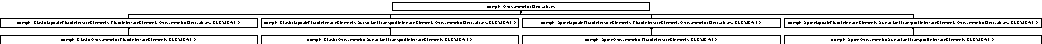
\includegraphics[height=0.794326cm]{classoomph_1_1AxisymmetricDerivatives}
\end{center}
\end{figure}
\subsection*{Public Member Functions}
\begin{DoxyCompactItemize}
\item 
\hyperlink{classoomph_1_1AxisymmetricDerivatives_a91b259ef45c7563b05bf79de4b0fe4bf}{Axisymmetric\+Derivatives} ()
\end{DoxyCompactItemize}
\subsection*{Protected Member Functions}
\begin{DoxyCompactItemize}
\item 
double \hyperlink{classoomph_1_1AxisymmetricDerivatives_a306ea6b57d09d57e87e8d74a13c2f828}{compute\+\_\+surface\+\_\+derivatives} (const Shape \&psi, const D\+Shape \&dpsids, const Dense\+Matrix$<$ double $>$ \&interpolated\+\_\+t, const Vector$<$ double $>$ \&interpolated\+\_\+x, D\+Shape \&surface\+\_\+gradient, D\+Shape \&surface\+\_\+divergence)
\begin{DoxyCompactList}\small\item\em Fill in the specific surface derivative calculations. \end{DoxyCompactList}\end{DoxyCompactItemize}


\subsection{Detailed Description}
Class that establishes the surface derivative functions for Axisymmetric\+Interface\+Elements. These are defined in a separate class so that they can be used by other interface equation-\/type classes. 

Definition at line 669 of file interface\+\_\+elements.\+h.



\subsection{Constructor \& Destructor Documentation}
\mbox{\Hypertarget{classoomph_1_1AxisymmetricDerivatives_a91b259ef45c7563b05bf79de4b0fe4bf}\label{classoomph_1_1AxisymmetricDerivatives_a91b259ef45c7563b05bf79de4b0fe4bf}} 
\index{oomph\+::\+Axisymmetric\+Derivatives@{oomph\+::\+Axisymmetric\+Derivatives}!Axisymmetric\+Derivatives@{Axisymmetric\+Derivatives}}
\index{Axisymmetric\+Derivatives@{Axisymmetric\+Derivatives}!oomph\+::\+Axisymmetric\+Derivatives@{oomph\+::\+Axisymmetric\+Derivatives}}
\subsubsection{\texorpdfstring{Axisymmetric\+Derivatives()}{AxisymmetricDerivatives()}}
{\footnotesize\ttfamily oomph\+::\+Axisymmetric\+Derivatives\+::\+Axisymmetric\+Derivatives (\begin{DoxyParamCaption}{ }\end{DoxyParamCaption})\hspace{0.3cm}{\ttfamily [inline]}}



Definition at line 673 of file interface\+\_\+elements.\+h.



\subsection{Member Function Documentation}
\mbox{\Hypertarget{classoomph_1_1AxisymmetricDerivatives_a306ea6b57d09d57e87e8d74a13c2f828}\label{classoomph_1_1AxisymmetricDerivatives_a306ea6b57d09d57e87e8d74a13c2f828}} 
\index{oomph\+::\+Axisymmetric\+Derivatives@{oomph\+::\+Axisymmetric\+Derivatives}!compute\+\_\+surface\+\_\+derivatives@{compute\+\_\+surface\+\_\+derivatives}}
\index{compute\+\_\+surface\+\_\+derivatives@{compute\+\_\+surface\+\_\+derivatives}!oomph\+::\+Axisymmetric\+Derivatives@{oomph\+::\+Axisymmetric\+Derivatives}}
\subsubsection{\texorpdfstring{compute\+\_\+surface\+\_\+derivatives()}{compute\_surface\_derivatives()}}
{\footnotesize\ttfamily double oomph\+::\+Axisymmetric\+Derivatives\+::compute\+\_\+surface\+\_\+derivatives (\begin{DoxyParamCaption}\item[{const Shape \&}]{psi,  }\item[{const D\+Shape \&}]{dpsids,  }\item[{const Dense\+Matrix$<$ double $>$ \&}]{interpolated\+\_\+t,  }\item[{const Vector$<$ double $>$ \&}]{interpolated\+\_\+x,  }\item[{D\+Shape \&}]{surface\+\_\+gradient,  }\item[{D\+Shape \&}]{surface\+\_\+divergence }\end{DoxyParamCaption})\hspace{0.3cm}{\ttfamily [protected]}}



Fill in the specific surface derivative calculations. 

Specialise the surface derivatives for the axisymmetric interface case. 

Definition at line 803 of file interface\+\_\+elements.\+cc.



The documentation for this class was generated from the following files\+:\begin{DoxyCompactItemize}
\item 
\hyperlink{interface__elements_8h}{interface\+\_\+elements.\+h}\item 
\hyperlink{interface__elements_8cc}{interface\+\_\+elements.\+cc}\end{DoxyCompactItemize}

\hypertarget{classoomph_1_1AxisymmetricLinearElasticityEquations}{}\section{oomph\+:\+:Axisymmetric\+Linear\+Elasticity\+Equations Class Reference}
\label{classoomph_1_1AxisymmetricLinearElasticityEquations}\index{oomph\+::\+Axisymmetric\+Linear\+Elasticity\+Equations@{oomph\+::\+Axisymmetric\+Linear\+Elasticity\+Equations}}


{\ttfamily \#include $<$axisym\+\_\+linear\+\_\+elasticity\+\_\+elements.\+h$>$}

Inheritance diagram for oomph\+:\+:Axisymmetric\+Linear\+Elasticity\+Equations\+:\begin{figure}[H]
\begin{center}
\leavevmode
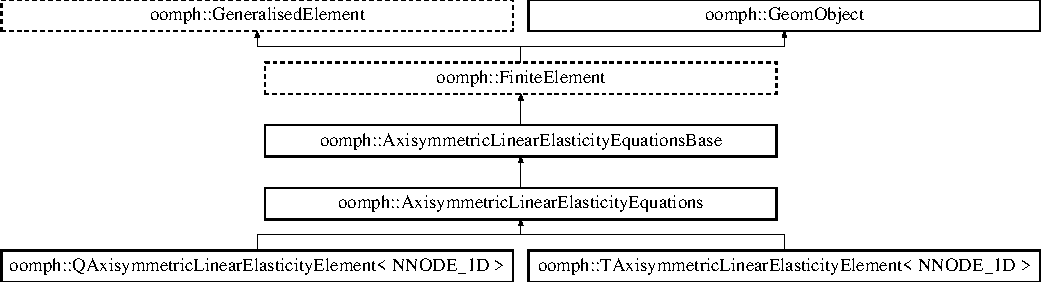
\includegraphics[height=3.794038cm]{classoomph_1_1AxisymmetricLinearElasticityEquations}
\end{center}
\end{figure}
\subsection*{Public Member Functions}
\begin{DoxyCompactItemize}
\item 
\hyperlink{classoomph_1_1AxisymmetricLinearElasticityEquations_a858da85e306cdaea7215e05fac652632}{Axisymmetric\+Linear\+Elasticity\+Equations} ()
\begin{DoxyCompactList}\small\item\em Constructor. \end{DoxyCompactList}\item 
unsigned \hyperlink{classoomph_1_1AxisymmetricLinearElasticityEquations_a9545ca241d42981a9d3561857af7cbb9}{required\+\_\+nvalue} (const unsigned \&n) const
\begin{DoxyCompactList}\small\item\em Number of values required at node n. \end{DoxyCompactList}\item 
void \hyperlink{classoomph_1_1AxisymmetricLinearElasticityEquations_adadd2893e700f16f0866b558a687aadb}{fill\+\_\+in\+\_\+contribution\+\_\+to\+\_\+residuals} (\hyperlink{classoomph_1_1Vector}{Vector}$<$ double $>$ \&residuals)
\begin{DoxyCompactList}\small\item\em Return the residuals for the equations (the discretised principle of virtual displacements) \end{DoxyCompactList}\item 
void \hyperlink{classoomph_1_1AxisymmetricLinearElasticityEquations_ab773f8081f53cd71666eca2d0031ecec}{fill\+\_\+in\+\_\+contribution\+\_\+to\+\_\+jacobian} (\hyperlink{classoomph_1_1Vector}{Vector}$<$ double $>$ \&residuals, \hyperlink{classoomph_1_1DenseMatrix}{Dense\+Matrix}$<$ double $>$ \&jacobian)
\item 
void \hyperlink{classoomph_1_1AxisymmetricLinearElasticityEquations_a079d1722a01188f2e06911932af3da1f}{get\+\_\+strain} (const \hyperlink{classoomph_1_1Vector}{Vector}$<$ double $>$ \&\hyperlink{cfortran_8h_ab7123126e4885ef647dd9c6e3807a21c}{s}, \hyperlink{classoomph_1_1DenseMatrix}{Dense\+Matrix}$<$ double $>$ \&strain)
\begin{DoxyCompactList}\small\item\em Get strain (3x3 entries; r, z, phi) \end{DoxyCompactList}\item 
void \hyperlink{classoomph_1_1AxisymmetricLinearElasticityEquations_ae1b89f9d9c661385fe2bfcf0cbf4df20}{output\+\_\+fct} (std\+::ostream \&outfile, const unsigned \&nplot, \hyperlink{classoomph_1_1FiniteElement_a690fd33af26cc3e84f39bba6d5a85202}{Finite\+Element\+::\+Steady\+Exact\+Solution\+Fct\+Pt} exact\+\_\+soln\+\_\+pt)
\begin{DoxyCompactList}\small\item\em Output exact solution\+: r,z, u\+\_\+r, u\+\_\+z, u\+\_\+theta. \end{DoxyCompactList}\item 
void \hyperlink{classoomph_1_1AxisymmetricLinearElasticityEquations_aab25e54e0e6b64c7f758d815884329e4}{output\+\_\+fct} (std\+::ostream \&outfile, const unsigned \&nplot, const double \&time, \hyperlink{classoomph_1_1FiniteElement_ad4ecf2b61b158a4b4d351a60d23c633e}{Finite\+Element\+::\+Unsteady\+Exact\+Solution\+Fct\+Pt} exact\+\_\+soln\+\_\+pt)
\item 
void \hyperlink{classoomph_1_1AxisymmetricLinearElasticityEquations_a798627057a8d79bccc17d277e1717f67}{output} (std\+::ostream \&outfile)
\begin{DoxyCompactList}\small\item\em Output\+: r,z, u\+\_\+r, u\+\_\+z, u\+\_\+theta. \end{DoxyCompactList}\item 
void \hyperlink{classoomph_1_1AxisymmetricLinearElasticityEquations_a55d90a70997efe0a5cf34e269e0cf6b8}{output} (std\+::ostream \&outfile, const unsigned \&n\+\_\+plot)
\begin{DoxyCompactList}\small\item\em Output\+: r,z, u\+\_\+r, u\+\_\+z, u\+\_\+theta. \end{DoxyCompactList}\item 
void \hyperlink{classoomph_1_1AxisymmetricLinearElasticityEquations_a8a96657fee4dd85fdbbf25d0855c27f2}{output} (F\+I\+LE $\ast$file\+\_\+pt)
\begin{DoxyCompactList}\small\item\em C-\/style output\+: r,z, u\+\_\+r, u\+\_\+z, u\+\_\+theta. \end{DoxyCompactList}\item 
void \hyperlink{classoomph_1_1AxisymmetricLinearElasticityEquations_ae706158f52c6251de990b640787e608b}{output} (F\+I\+LE $\ast$file\+\_\+pt, const unsigned \&n\+\_\+plot)
\begin{DoxyCompactList}\small\item\em Output\+: r,z, u\+\_\+r, u\+\_\+z, u\+\_\+theta. \end{DoxyCompactList}\item 
void \hyperlink{classoomph_1_1AxisymmetricLinearElasticityEquations_ac8d00d39dc3bbfe9125fffe3f498982b}{compute\+\_\+error} (std\+::ostream \&outfile, \hyperlink{classoomph_1_1FiniteElement_a690fd33af26cc3e84f39bba6d5a85202}{Finite\+Element\+::\+Steady\+Exact\+Solution\+Fct\+Pt} exact\+\_\+soln\+\_\+pt, double \&error, double \&norm)
\item 
void \hyperlink{classoomph_1_1AxisymmetricLinearElasticityEquations_ad6a1568c8d02d11a25c4b19c9f6763a2}{compute\+\_\+error} (std\+::ostream \&outfile, \hyperlink{classoomph_1_1FiniteElement_ad4ecf2b61b158a4b4d351a60d23c633e}{Finite\+Element\+::\+Unsteady\+Exact\+Solution\+Fct\+Pt} exact\+\_\+soln\+\_\+pt, const double \&time, double \&error, double \&norm)
\end{DoxyCompactItemize}
\subsection*{Protected Member Functions}
\begin{DoxyCompactItemize}
\item 
virtual void \hyperlink{classoomph_1_1AxisymmetricLinearElasticityEquations_a47f493fe9f183efebce35bd708cbb78d}{fill\+\_\+in\+\_\+generic\+\_\+contribution\+\_\+to\+\_\+residuals\+\_\+axisymmetric\+\_\+linear\+\_\+elasticity} (\hyperlink{classoomph_1_1Vector}{Vector}$<$ double $>$ \&residuals, \hyperlink{classoomph_1_1DenseMatrix}{Dense\+Matrix}$<$ double $>$ \&jacobian, unsigned flag)
\begin{DoxyCompactList}\small\item\em Private helper function to compute residuals and (if requested via flag) also the Jacobian matrix. \end{DoxyCompactList}\end{DoxyCompactItemize}
\subsection*{Additional Inherited Members}


\subsection{Detailed Description}
A class for elements that solve the axisymmetric (in cylindrical polars) equations of linear elasticity 

Definition at line 421 of file axisym\+\_\+linear\+\_\+elasticity\+\_\+elements.\+h.



\subsection{Constructor \& Destructor Documentation}
\mbox{\Hypertarget{classoomph_1_1AxisymmetricLinearElasticityEquations_a858da85e306cdaea7215e05fac652632}\label{classoomph_1_1AxisymmetricLinearElasticityEquations_a858da85e306cdaea7215e05fac652632}} 
\index{oomph\+::\+Axisymmetric\+Linear\+Elasticity\+Equations@{oomph\+::\+Axisymmetric\+Linear\+Elasticity\+Equations}!Axisymmetric\+Linear\+Elasticity\+Equations@{Axisymmetric\+Linear\+Elasticity\+Equations}}
\index{Axisymmetric\+Linear\+Elasticity\+Equations@{Axisymmetric\+Linear\+Elasticity\+Equations}!oomph\+::\+Axisymmetric\+Linear\+Elasticity\+Equations@{oomph\+::\+Axisymmetric\+Linear\+Elasticity\+Equations}}
\subsubsection{\texorpdfstring{Axisymmetric\+Linear\+Elasticity\+Equations()}{AxisymmetricLinearElasticityEquations()}}
{\footnotesize\ttfamily oomph\+::\+Axisymmetric\+Linear\+Elasticity\+Equations\+::\+Axisymmetric\+Linear\+Elasticity\+Equations (\begin{DoxyParamCaption}{ }\end{DoxyParamCaption})\hspace{0.3cm}{\ttfamily [inline]}}



Constructor. 



Definition at line 427 of file axisym\+\_\+linear\+\_\+elasticity\+\_\+elements.\+h.



\subsection{Member Function Documentation}
\mbox{\Hypertarget{classoomph_1_1AxisymmetricLinearElasticityEquations_ac8d00d39dc3bbfe9125fffe3f498982b}\label{classoomph_1_1AxisymmetricLinearElasticityEquations_ac8d00d39dc3bbfe9125fffe3f498982b}} 
\index{oomph\+::\+Axisymmetric\+Linear\+Elasticity\+Equations@{oomph\+::\+Axisymmetric\+Linear\+Elasticity\+Equations}!compute\+\_\+error@{compute\+\_\+error}}
\index{compute\+\_\+error@{compute\+\_\+error}!oomph\+::\+Axisymmetric\+Linear\+Elasticity\+Equations@{oomph\+::\+Axisymmetric\+Linear\+Elasticity\+Equations}}
\subsubsection{\texorpdfstring{compute\+\_\+error()}{compute\_error()}\hspace{0.1cm}{\footnotesize\ttfamily [1/2]}}
{\footnotesize\ttfamily void oomph\+::\+Axisymmetric\+Linear\+Elasticity\+Equations\+::compute\+\_\+error (\begin{DoxyParamCaption}\item[{std\+::ostream \&}]{outfile,  }\item[{\hyperlink{classoomph_1_1FiniteElement_a690fd33af26cc3e84f39bba6d5a85202}{Finite\+Element\+::\+Steady\+Exact\+Solution\+Fct\+Pt}}]{exact\+\_\+soln\+\_\+pt,  }\item[{double \&}]{error,  }\item[{double \&}]{norm }\end{DoxyParamCaption})\hspace{0.3cm}{\ttfamily [virtual]}}

Validate against exact solution. Solution is provided via function pointer. Plot at a given number of plot points and compute L2 error and L2 norm of displacement solution over element

Validate against exact solution Solution is provided via function pointer. Plot at a given number of plot points and compute L2 error and L2 norm of velocity solution over element. 

Reimplemented from \hyperlink{classoomph_1_1FiniteElement_a73c79a1f1e5b1d334757812a6bbd58ff}{oomph\+::\+Finite\+Element}.



Definition at line 682 of file axisym\+\_\+linear\+\_\+elasticity\+\_\+elements.\+cc.



References i, oomph\+::\+Finite\+Element\+::integral\+\_\+pt(), oomph\+::\+Axisymmetric\+Linear\+Elasticity\+Equations\+Base\+::interpolated\+\_\+u\+\_\+axisymmetric\+\_\+linear\+\_\+elasticity(), oomph\+::\+Finite\+Element\+::interpolated\+\_\+x(), oomph\+::\+Finite\+Element\+::\+J\+\_\+eulerian(), oomph\+::\+Integral\+::knot(), oomph\+::\+Integral\+::nweight(), s, oomph\+::\+Quad\+Tree\+Names\+::W, and oomph\+::\+Integral\+::weight().

\mbox{\Hypertarget{classoomph_1_1AxisymmetricLinearElasticityEquations_ad6a1568c8d02d11a25c4b19c9f6763a2}\label{classoomph_1_1AxisymmetricLinearElasticityEquations_ad6a1568c8d02d11a25c4b19c9f6763a2}} 
\index{oomph\+::\+Axisymmetric\+Linear\+Elasticity\+Equations@{oomph\+::\+Axisymmetric\+Linear\+Elasticity\+Equations}!compute\+\_\+error@{compute\+\_\+error}}
\index{compute\+\_\+error@{compute\+\_\+error}!oomph\+::\+Axisymmetric\+Linear\+Elasticity\+Equations@{oomph\+::\+Axisymmetric\+Linear\+Elasticity\+Equations}}
\subsubsection{\texorpdfstring{compute\+\_\+error()}{compute\_error()}\hspace{0.1cm}{\footnotesize\ttfamily [2/2]}}
{\footnotesize\ttfamily void oomph\+::\+Axisymmetric\+Linear\+Elasticity\+Equations\+::compute\+\_\+error (\begin{DoxyParamCaption}\item[{std\+::ostream \&}]{outfile,  }\item[{\hyperlink{classoomph_1_1FiniteElement_ad4ecf2b61b158a4b4d351a60d23c633e}{Finite\+Element\+::\+Unsteady\+Exact\+Solution\+Fct\+Pt}}]{exact\+\_\+soln\+\_\+pt,  }\item[{const double \&}]{time,  }\item[{double \&}]{error,  }\item[{double \&}]{norm }\end{DoxyParamCaption})\hspace{0.3cm}{\ttfamily [virtual]}}

Validate against exact solution. Time-\/dependent version

Validate against exact solution Solution is provided via function pointer. Plot at a given number of plot points and compute L2 error and L2 norm of velocity solution over element. 

Reimplemented from \hyperlink{classoomph_1_1FiniteElement_a7f67853506dc73fa6b7505108de22d1f}{oomph\+::\+Finite\+Element}.



Definition at line 769 of file axisym\+\_\+linear\+\_\+elasticity\+\_\+elements.\+cc.



References i, oomph\+::\+Finite\+Element\+::integral\+\_\+pt(), oomph\+::\+Axisymmetric\+Linear\+Elasticity\+Equations\+Base\+::interpolated\+\_\+u\+\_\+axisymmetric\+\_\+linear\+\_\+elasticity(), oomph\+::\+Finite\+Element\+::interpolated\+\_\+x(), oomph\+::\+Finite\+Element\+::\+J\+\_\+eulerian(), oomph\+::\+Integral\+::knot(), oomph\+::\+Integral\+::nweight(), s, oomph\+::\+Quad\+Tree\+Names\+::W, and oomph\+::\+Integral\+::weight().

\mbox{\Hypertarget{classoomph_1_1AxisymmetricLinearElasticityEquations_ab773f8081f53cd71666eca2d0031ecec}\label{classoomph_1_1AxisymmetricLinearElasticityEquations_ab773f8081f53cd71666eca2d0031ecec}} 
\index{oomph\+::\+Axisymmetric\+Linear\+Elasticity\+Equations@{oomph\+::\+Axisymmetric\+Linear\+Elasticity\+Equations}!fill\+\_\+in\+\_\+contribution\+\_\+to\+\_\+jacobian@{fill\+\_\+in\+\_\+contribution\+\_\+to\+\_\+jacobian}}
\index{fill\+\_\+in\+\_\+contribution\+\_\+to\+\_\+jacobian@{fill\+\_\+in\+\_\+contribution\+\_\+to\+\_\+jacobian}!oomph\+::\+Axisymmetric\+Linear\+Elasticity\+Equations@{oomph\+::\+Axisymmetric\+Linear\+Elasticity\+Equations}}
\subsubsection{\texorpdfstring{fill\+\_\+in\+\_\+contribution\+\_\+to\+\_\+jacobian()}{fill\_in\_contribution\_to\_jacobian()}}
{\footnotesize\ttfamily void oomph\+::\+Axisymmetric\+Linear\+Elasticity\+Equations\+::fill\+\_\+in\+\_\+contribution\+\_\+to\+\_\+jacobian (\begin{DoxyParamCaption}\item[{\hyperlink{classoomph_1_1Vector}{Vector}$<$ double $>$ \&}]{residuals,  }\item[{\hyperlink{classoomph_1_1DenseMatrix}{Dense\+Matrix}$<$ double $>$ \&}]{jacobian }\end{DoxyParamCaption})\hspace{0.3cm}{\ttfamily [inline]}, {\ttfamily [virtual]}}

The jacobian is calculated by finite differences by default, We need only to take finite differences w.\+r.\+t. positional variables For this element 

Reimplemented from \hyperlink{classoomph_1_1GeneralisedElement_a6ae09fc0d68e4309ac1b03583d252845}{oomph\+::\+Generalised\+Element}.



Definition at line 444 of file axisym\+\_\+linear\+\_\+elasticity\+\_\+elements.\+h.



References oomph\+::\+Finite\+Element\+::output\+\_\+fct(), and s.

\mbox{\Hypertarget{classoomph_1_1AxisymmetricLinearElasticityEquations_adadd2893e700f16f0866b558a687aadb}\label{classoomph_1_1AxisymmetricLinearElasticityEquations_adadd2893e700f16f0866b558a687aadb}} 
\index{oomph\+::\+Axisymmetric\+Linear\+Elasticity\+Equations@{oomph\+::\+Axisymmetric\+Linear\+Elasticity\+Equations}!fill\+\_\+in\+\_\+contribution\+\_\+to\+\_\+residuals@{fill\+\_\+in\+\_\+contribution\+\_\+to\+\_\+residuals}}
\index{fill\+\_\+in\+\_\+contribution\+\_\+to\+\_\+residuals@{fill\+\_\+in\+\_\+contribution\+\_\+to\+\_\+residuals}!oomph\+::\+Axisymmetric\+Linear\+Elasticity\+Equations@{oomph\+::\+Axisymmetric\+Linear\+Elasticity\+Equations}}
\subsubsection{\texorpdfstring{fill\+\_\+in\+\_\+contribution\+\_\+to\+\_\+residuals()}{fill\_in\_contribution\_to\_residuals()}}
{\footnotesize\ttfamily void oomph\+::\+Axisymmetric\+Linear\+Elasticity\+Equations\+::fill\+\_\+in\+\_\+contribution\+\_\+to\+\_\+residuals (\begin{DoxyParamCaption}\item[{\hyperlink{classoomph_1_1Vector}{Vector}$<$ double $>$ \&}]{residuals }\end{DoxyParamCaption})\hspace{0.3cm}{\ttfamily [inline]}, {\ttfamily [virtual]}}



Return the residuals for the equations (the discretised principle of virtual displacements) 



Reimplemented from \hyperlink{classoomph_1_1GeneralisedElement_a310c97f515e8504a48179c0e72c550d7}{oomph\+::\+Generalised\+Element}.



Definition at line 434 of file axisym\+\_\+linear\+\_\+elasticity\+\_\+elements.\+h.



References oomph\+::\+Generalised\+Element\+::\+Dummy\+\_\+matrix.

\mbox{\Hypertarget{classoomph_1_1AxisymmetricLinearElasticityEquations_a47f493fe9f183efebce35bd708cbb78d}\label{classoomph_1_1AxisymmetricLinearElasticityEquations_a47f493fe9f183efebce35bd708cbb78d}} 
\index{oomph\+::\+Axisymmetric\+Linear\+Elasticity\+Equations@{oomph\+::\+Axisymmetric\+Linear\+Elasticity\+Equations}!fill\+\_\+in\+\_\+generic\+\_\+contribution\+\_\+to\+\_\+residuals\+\_\+axisymmetric\+\_\+linear\+\_\+elasticity@{fill\+\_\+in\+\_\+generic\+\_\+contribution\+\_\+to\+\_\+residuals\+\_\+axisymmetric\+\_\+linear\+\_\+elasticity}}
\index{fill\+\_\+in\+\_\+generic\+\_\+contribution\+\_\+to\+\_\+residuals\+\_\+axisymmetric\+\_\+linear\+\_\+elasticity@{fill\+\_\+in\+\_\+generic\+\_\+contribution\+\_\+to\+\_\+residuals\+\_\+axisymmetric\+\_\+linear\+\_\+elasticity}!oomph\+::\+Axisymmetric\+Linear\+Elasticity\+Equations@{oomph\+::\+Axisymmetric\+Linear\+Elasticity\+Equations}}
\subsubsection{\texorpdfstring{fill\+\_\+in\+\_\+generic\+\_\+contribution\+\_\+to\+\_\+residuals\+\_\+axisymmetric\+\_\+linear\+\_\+elasticity()}{fill\_in\_generic\_contribution\_to\_residuals\_axisymmetric\_linear\_elasticity()}}
{\footnotesize\ttfamily void oomph\+::\+Axisymmetric\+Linear\+Elasticity\+Equations\+::fill\+\_\+in\+\_\+generic\+\_\+contribution\+\_\+to\+\_\+residuals\+\_\+axisymmetric\+\_\+linear\+\_\+elasticity (\begin{DoxyParamCaption}\item[{\hyperlink{classoomph_1_1Vector}{Vector}$<$ double $>$ \&}]{residuals,  }\item[{\hyperlink{classoomph_1_1DenseMatrix}{Dense\+Matrix}$<$ double $>$ \&}]{jacobian,  }\item[{unsigned}]{flag }\end{DoxyParamCaption})\hspace{0.3cm}{\ttfamily [protected]}, {\ttfamily [virtual]}}



Private helper function to compute residuals and (if requested via flag) also the Jacobian matrix. 

Compute the residuals for the axisymmetric (in cyl. polars) linear elasticity equations in. Flag indicates if we want Jacobian too. 

Definition at line 170 of file axisym\+\_\+linear\+\_\+elasticity\+\_\+elements.\+cc.



References oomph\+::\+Axisymmetric\+Linear\+Elasticity\+Equations\+Base\+::body\+\_\+force(), oomph\+::\+Axisymmetric\+Linear\+Elasticity\+Equations\+Base\+::d2u\+\_\+dt2\+\_\+axisymmetric\+\_\+linear\+\_\+elasticity(), oomph\+::\+Finite\+Element\+::dshape\+\_\+eulerian\+\_\+at\+\_\+knot(), i, oomph\+::\+Finite\+Element\+::integral\+\_\+pt(), oomph\+::\+Finite\+Element\+::interpolated\+\_\+x(), oomph\+::\+Integral\+::knot(), oomph\+::\+Axisymmetric\+Linear\+Elasticity\+Equations\+Base\+::lambda\+\_\+sq(), oomph\+::\+Finite\+Element\+::nnodal\+\_\+position\+\_\+type(), oomph\+::\+Finite\+Element\+::nnode(), oomph\+::\+Finite\+Element\+::nodal\+\_\+local\+\_\+eqn(), oomph\+::\+Finite\+Element\+::node\+\_\+pt(), oomph\+::\+Axisymmetric\+Linear\+Elasticity\+Equations\+Base\+::nu(), oomph\+::\+Integral\+::nweight(), oomph\+::\+Finite\+Element\+::raw\+\_\+nodal\+\_\+position(), oomph\+::\+Finite\+Element\+::raw\+\_\+nodal\+\_\+value(), s, oomph\+::\+Time\+::time(), oomph\+::\+Time\+Stepper\+::time\+\_\+pt(), oomph\+::\+Geom\+Object\+::time\+\_\+stepper\+\_\+pt(), oomph\+::\+Data\+::time\+\_\+stepper\+\_\+pt(), oomph\+::\+Axisymmetric\+Linear\+Elasticity\+Equations\+Base\+::u\+\_\+index\+\_\+axisymmetric\+\_\+linear\+\_\+elasticity(), oomph\+::\+Quad\+Tree\+Names\+::W, oomph\+::\+Integral\+::weight(), oomph\+::\+Time\+Stepper\+::weight(), and oomph\+::\+Axisymmetric\+Linear\+Elasticity\+Equations\+Base\+::youngs\+\_\+modulus().



Referenced by get\+\_\+strain().

\mbox{\Hypertarget{classoomph_1_1AxisymmetricLinearElasticityEquations_a079d1722a01188f2e06911932af3da1f}\label{classoomph_1_1AxisymmetricLinearElasticityEquations_a079d1722a01188f2e06911932af3da1f}} 
\index{oomph\+::\+Axisymmetric\+Linear\+Elasticity\+Equations@{oomph\+::\+Axisymmetric\+Linear\+Elasticity\+Equations}!get\+\_\+strain@{get\+\_\+strain}}
\index{get\+\_\+strain@{get\+\_\+strain}!oomph\+::\+Axisymmetric\+Linear\+Elasticity\+Equations@{oomph\+::\+Axisymmetric\+Linear\+Elasticity\+Equations}}
\subsubsection{\texorpdfstring{get\+\_\+strain()}{get\_strain()}}
{\footnotesize\ttfamily void oomph\+::\+Axisymmetric\+Linear\+Elasticity\+Equations\+::get\+\_\+strain (\begin{DoxyParamCaption}\item[{const \hyperlink{classoomph_1_1Vector}{Vector}$<$ double $>$ \&}]{s,  }\item[{\hyperlink{classoomph_1_1DenseMatrix}{Dense\+Matrix}$<$ double $>$ \&}]{strain }\end{DoxyParamCaption})}



Get strain (3x3 entries; r, z, phi) 



Definition at line 60 of file axisym\+\_\+linear\+\_\+elasticity\+\_\+elements.\+cc.



References fill\+\_\+in\+\_\+generic\+\_\+contribution\+\_\+to\+\_\+residuals\+\_\+axisymmetric\+\_\+linear\+\_\+elasticity(), i, oomph\+::\+Finite\+Element\+::interpolated\+\_\+x(), oomph\+::\+Finite\+Element\+::nnodal\+\_\+position\+\_\+type(), oomph\+::\+Finite\+Element\+::nnode(), oomph\+::\+Finite\+Element\+::raw\+\_\+nodal\+\_\+position(), oomph\+::\+Finite\+Element\+::raw\+\_\+nodal\+\_\+value(), and oomph\+::\+Axisymmetric\+Linear\+Elasticity\+Equations\+Base\+::u\+\_\+index\+\_\+axisymmetric\+\_\+linear\+\_\+elasticity().



Referenced by oomph\+::\+T\+Axisymmetric\+Linear\+Elasticity\+Element$<$ N\+N\+O\+D\+E\+\_\+1\+D $>$\+::get\+\_\+\+Z2\+\_\+flux().

\mbox{\Hypertarget{classoomph_1_1AxisymmetricLinearElasticityEquations_a798627057a8d79bccc17d277e1717f67}\label{classoomph_1_1AxisymmetricLinearElasticityEquations_a798627057a8d79bccc17d277e1717f67}} 
\index{oomph\+::\+Axisymmetric\+Linear\+Elasticity\+Equations@{oomph\+::\+Axisymmetric\+Linear\+Elasticity\+Equations}!output@{output}}
\index{output@{output}!oomph\+::\+Axisymmetric\+Linear\+Elasticity\+Equations@{oomph\+::\+Axisymmetric\+Linear\+Elasticity\+Equations}}
\subsubsection{\texorpdfstring{output()}{output()}\hspace{0.1cm}{\footnotesize\ttfamily [1/4]}}
{\footnotesize\ttfamily void oomph\+::\+Axisymmetric\+Linear\+Elasticity\+Equations\+::output (\begin{DoxyParamCaption}\item[{std\+::ostream \&}]{outfile }\end{DoxyParamCaption})\hspace{0.3cm}{\ttfamily [inline]}, {\ttfamily [virtual]}}



Output\+: r,z, u\+\_\+r, u\+\_\+z, u\+\_\+theta. 



Reimplemented from \hyperlink{classoomph_1_1FiniteElement_a2ad98a3d2ef4999f1bef62c0ff13f2a7}{oomph\+::\+Finite\+Element}.



Reimplemented in \hyperlink{classoomph_1_1QAxisymmetricLinearElasticityElement_adfd535d5ee563df242c0ff5febca99e2}{oomph\+::\+Q\+Axisymmetric\+Linear\+Elasticity\+Element$<$ N\+N\+O\+D\+E\+\_\+1\+D $>$}, and \hyperlink{classoomph_1_1TAxisymmetricLinearElasticityElement_a803cb886b6c610f021fdfd41113eeab8}{oomph\+::\+T\+Axisymmetric\+Linear\+Elasticity\+Element$<$ N\+N\+O\+D\+E\+\_\+1\+D $>$}.



Definition at line 471 of file axisym\+\_\+linear\+\_\+elasticity\+\_\+elements.\+h.



References oomph\+::\+Finite\+Element\+::output().



Referenced by oomph\+::\+T\+Axisymmetric\+Linear\+Elasticity\+Element$<$ N\+N\+O\+D\+E\+\_\+1\+D $>$\+::output(), oomph\+::\+Q\+Axisymmetric\+Linear\+Elasticity\+Element$<$ N\+N\+O\+D\+E\+\_\+1\+D $>$\+::output(), and output\+\_\+fct().

\mbox{\Hypertarget{classoomph_1_1AxisymmetricLinearElasticityEquations_a55d90a70997efe0a5cf34e269e0cf6b8}\label{classoomph_1_1AxisymmetricLinearElasticityEquations_a55d90a70997efe0a5cf34e269e0cf6b8}} 
\index{oomph\+::\+Axisymmetric\+Linear\+Elasticity\+Equations@{oomph\+::\+Axisymmetric\+Linear\+Elasticity\+Equations}!output@{output}}
\index{output@{output}!oomph\+::\+Axisymmetric\+Linear\+Elasticity\+Equations@{oomph\+::\+Axisymmetric\+Linear\+Elasticity\+Equations}}
\subsubsection{\texorpdfstring{output()}{output()}\hspace{0.1cm}{\footnotesize\ttfamily [2/4]}}
{\footnotesize\ttfamily void oomph\+::\+Axisymmetric\+Linear\+Elasticity\+Equations\+::output (\begin{DoxyParamCaption}\item[{std\+::ostream \&}]{outfile,  }\item[{const unsigned \&}]{n\+\_\+plot }\end{DoxyParamCaption})\hspace{0.3cm}{\ttfamily [virtual]}}



Output\+: r,z, u\+\_\+r, u\+\_\+z, u\+\_\+theta. 



Reimplemented from \hyperlink{classoomph_1_1FiniteElement_afa9d9b2670f999b43e6679c9dd28c457}{oomph\+::\+Finite\+Element}.



Reimplemented in \hyperlink{classoomph_1_1QAxisymmetricLinearElasticityElement_a3339817db6273a1285615d05d0e99a07}{oomph\+::\+Q\+Axisymmetric\+Linear\+Elasticity\+Element$<$ N\+N\+O\+D\+E\+\_\+1\+D $>$}, and \hyperlink{classoomph_1_1TAxisymmetricLinearElasticityElement_aa56d730cdb3e5e31f4edeb9d270c8218}{oomph\+::\+T\+Axisymmetric\+Linear\+Elasticity\+Element$<$ N\+N\+O\+D\+E\+\_\+1\+D $>$}.



Definition at line 583 of file axisym\+\_\+linear\+\_\+elasticity\+\_\+elements.\+cc.



References oomph\+::\+Finite\+Element\+::get\+\_\+s\+\_\+plot(), i, oomph\+::\+Axisymmetric\+Linear\+Elasticity\+Equations\+Base\+::interpolated\+\_\+d2u\+\_\+dt2\+\_\+axisymmetric\+\_\+linear\+\_\+elasticity(), oomph\+::\+Axisymmetric\+Linear\+Elasticity\+Equations\+Base\+::interpolated\+\_\+du\+\_\+dt\+\_\+axisymmetric\+\_\+linear\+\_\+elasticity(), oomph\+::\+Axisymmetric\+Linear\+Elasticity\+Equations\+Base\+::interpolated\+\_\+u\+\_\+axisymmetric\+\_\+linear\+\_\+elasticity(), oomph\+::\+Finite\+Element\+::interpolated\+\_\+x(), oomph\+::\+Finite\+Element\+::nplot\+\_\+points(), s, oomph\+::\+Finite\+Element\+::tecplot\+\_\+zone\+\_\+string(), and oomph\+::\+Finite\+Element\+::write\+\_\+tecplot\+\_\+zone\+\_\+footer().

\mbox{\Hypertarget{classoomph_1_1AxisymmetricLinearElasticityEquations_a8a96657fee4dd85fdbbf25d0855c27f2}\label{classoomph_1_1AxisymmetricLinearElasticityEquations_a8a96657fee4dd85fdbbf25d0855c27f2}} 
\index{oomph\+::\+Axisymmetric\+Linear\+Elasticity\+Equations@{oomph\+::\+Axisymmetric\+Linear\+Elasticity\+Equations}!output@{output}}
\index{output@{output}!oomph\+::\+Axisymmetric\+Linear\+Elasticity\+Equations@{oomph\+::\+Axisymmetric\+Linear\+Elasticity\+Equations}}
\subsubsection{\texorpdfstring{output()}{output()}\hspace{0.1cm}{\footnotesize\ttfamily [3/4]}}
{\footnotesize\ttfamily void oomph\+::\+Axisymmetric\+Linear\+Elasticity\+Equations\+::output (\begin{DoxyParamCaption}\item[{F\+I\+LE $\ast$}]{file\+\_\+pt }\end{DoxyParamCaption})\hspace{0.3cm}{\ttfamily [inline]}, {\ttfamily [virtual]}}



C-\/style output\+: r,z, u\+\_\+r, u\+\_\+z, u\+\_\+theta. 



Reimplemented from \hyperlink{classoomph_1_1FiniteElement_a72cddd09f8ddbee1a20a1ff404c6943e}{oomph\+::\+Finite\+Element}.



Reimplemented in \hyperlink{classoomph_1_1QAxisymmetricLinearElasticityElement_abc4653b755224731a24d641619b2c14e}{oomph\+::\+Q\+Axisymmetric\+Linear\+Elasticity\+Element$<$ N\+N\+O\+D\+E\+\_\+1\+D $>$}, and \hyperlink{classoomph_1_1TAxisymmetricLinearElasticityElement_a8a33c1d33c51c47f563aed46f5a9d835}{oomph\+::\+T\+Axisymmetric\+Linear\+Elasticity\+Element$<$ N\+N\+O\+D\+E\+\_\+1\+D $>$}.



Definition at line 481 of file axisym\+\_\+linear\+\_\+elasticity\+\_\+elements.\+h.



References oomph\+::\+Finite\+Element\+::compute\+\_\+error(), and oomph\+::\+Finite\+Element\+::output().

\mbox{\Hypertarget{classoomph_1_1AxisymmetricLinearElasticityEquations_ae706158f52c6251de990b640787e608b}\label{classoomph_1_1AxisymmetricLinearElasticityEquations_ae706158f52c6251de990b640787e608b}} 
\index{oomph\+::\+Axisymmetric\+Linear\+Elasticity\+Equations@{oomph\+::\+Axisymmetric\+Linear\+Elasticity\+Equations}!output@{output}}
\index{output@{output}!oomph\+::\+Axisymmetric\+Linear\+Elasticity\+Equations@{oomph\+::\+Axisymmetric\+Linear\+Elasticity\+Equations}}
\subsubsection{\texorpdfstring{output()}{output()}\hspace{0.1cm}{\footnotesize\ttfamily [4/4]}}
{\footnotesize\ttfamily void oomph\+::\+Axisymmetric\+Linear\+Elasticity\+Equations\+::output (\begin{DoxyParamCaption}\item[{F\+I\+LE $\ast$}]{file\+\_\+pt,  }\item[{const unsigned \&}]{n\+\_\+plot }\end{DoxyParamCaption})\hspace{0.3cm}{\ttfamily [virtual]}}



Output\+: r,z, u\+\_\+r, u\+\_\+z, u\+\_\+theta. 

C-\/style output\+:r,z, u\+\_\+r, u\+\_\+z, u\+\_\+theta. 

Reimplemented from \hyperlink{classoomph_1_1FiniteElement_adfaee690bb0608f03320eeb9d110d48c}{oomph\+::\+Finite\+Element}.



Reimplemented in \hyperlink{classoomph_1_1QAxisymmetricLinearElasticityElement_a50c3225e93aad5867288cf55aac73195}{oomph\+::\+Q\+Axisymmetric\+Linear\+Elasticity\+Element$<$ N\+N\+O\+D\+E\+\_\+1\+D $>$}, and \hyperlink{classoomph_1_1TAxisymmetricLinearElasticityElement_a834bb7feb673a5cf90b07ee16f6b1fa5}{oomph\+::\+T\+Axisymmetric\+Linear\+Elasticity\+Element$<$ N\+N\+O\+D\+E\+\_\+1\+D $>$}.



Definition at line 638 of file axisym\+\_\+linear\+\_\+elasticity\+\_\+elements.\+cc.



References oomph\+::\+Finite\+Element\+::get\+\_\+s\+\_\+plot(), i, oomph\+::\+Axisymmetric\+Linear\+Elasticity\+Equations\+Base\+::interpolated\+\_\+u\+\_\+axisymmetric\+\_\+linear\+\_\+elasticity(), oomph\+::\+Finite\+Element\+::interpolated\+\_\+x(), oomph\+::\+Finite\+Element\+::nplot\+\_\+points(), s, oomph\+::\+Finite\+Element\+::tecplot\+\_\+zone\+\_\+string(), and oomph\+::\+Finite\+Element\+::write\+\_\+tecplot\+\_\+zone\+\_\+footer().

\mbox{\Hypertarget{classoomph_1_1AxisymmetricLinearElasticityEquations_ae1b89f9d9c661385fe2bfcf0cbf4df20}\label{classoomph_1_1AxisymmetricLinearElasticityEquations_ae1b89f9d9c661385fe2bfcf0cbf4df20}} 
\index{oomph\+::\+Axisymmetric\+Linear\+Elasticity\+Equations@{oomph\+::\+Axisymmetric\+Linear\+Elasticity\+Equations}!output\+\_\+fct@{output\+\_\+fct}}
\index{output\+\_\+fct@{output\+\_\+fct}!oomph\+::\+Axisymmetric\+Linear\+Elasticity\+Equations@{oomph\+::\+Axisymmetric\+Linear\+Elasticity\+Equations}}
\subsubsection{\texorpdfstring{output\+\_\+fct()}{output\_fct()}\hspace{0.1cm}{\footnotesize\ttfamily [1/2]}}
{\footnotesize\ttfamily void oomph\+::\+Axisymmetric\+Linear\+Elasticity\+Equations\+::output\+\_\+fct (\begin{DoxyParamCaption}\item[{std\+::ostream \&}]{outfile,  }\item[{const unsigned \&}]{nplot,  }\item[{\hyperlink{classoomph_1_1FiniteElement_a690fd33af26cc3e84f39bba6d5a85202}{Finite\+Element\+::\+Steady\+Exact\+Solution\+Fct\+Pt}}]{exact\+\_\+soln\+\_\+pt }\end{DoxyParamCaption})\hspace{0.3cm}{\ttfamily [virtual]}}



Output exact solution\+: r,z, u\+\_\+r, u\+\_\+z, u\+\_\+theta. 

Output exact solution r,z, u\+\_\+r, u\+\_\+z, u\+\_\+theta. 

Reimplemented from \hyperlink{classoomph_1_1FiniteElement_a22b695c714f60ee6cd145be348042035}{oomph\+::\+Finite\+Element}.



Definition at line 476 of file axisym\+\_\+linear\+\_\+elasticity\+\_\+elements.\+cc.



References oomph\+::\+Finite\+Element\+::get\+\_\+s\+\_\+plot(), i, oomph\+::\+Finite\+Element\+::interpolated\+\_\+x(), oomph\+::\+Finite\+Element\+::nplot\+\_\+points(), s, oomph\+::\+Finite\+Element\+::tecplot\+\_\+zone\+\_\+string(), and oomph\+::\+Finite\+Element\+::write\+\_\+tecplot\+\_\+zone\+\_\+footer().

\mbox{\Hypertarget{classoomph_1_1AxisymmetricLinearElasticityEquations_aab25e54e0e6b64c7f758d815884329e4}\label{classoomph_1_1AxisymmetricLinearElasticityEquations_aab25e54e0e6b64c7f758d815884329e4}} 
\index{oomph\+::\+Axisymmetric\+Linear\+Elasticity\+Equations@{oomph\+::\+Axisymmetric\+Linear\+Elasticity\+Equations}!output\+\_\+fct@{output\+\_\+fct}}
\index{output\+\_\+fct@{output\+\_\+fct}!oomph\+::\+Axisymmetric\+Linear\+Elasticity\+Equations@{oomph\+::\+Axisymmetric\+Linear\+Elasticity\+Equations}}
\subsubsection{\texorpdfstring{output\+\_\+fct()}{output\_fct()}\hspace{0.1cm}{\footnotesize\ttfamily [2/2]}}
{\footnotesize\ttfamily void oomph\+::\+Axisymmetric\+Linear\+Elasticity\+Equations\+::output\+\_\+fct (\begin{DoxyParamCaption}\item[{std\+::ostream \&}]{outfile,  }\item[{const unsigned \&}]{nplot,  }\item[{const double \&}]{time,  }\item[{\hyperlink{classoomph_1_1FiniteElement_ad4ecf2b61b158a4b4d351a60d23c633e}{Finite\+Element\+::\+Unsteady\+Exact\+Solution\+Fct\+Pt}}]{exact\+\_\+soln\+\_\+pt }\end{DoxyParamCaption})\hspace{0.3cm}{\ttfamily [virtual]}}

Output exact solution\+: r,z, u\+\_\+r, u\+\_\+z, u\+\_\+theta \hyperlink{classoomph_1_1Time}{Time} dependent version

Output exact solution r,z, u\+\_\+r, u\+\_\+z, u\+\_\+theta \hyperlink{classoomph_1_1Time}{Time} dependent version 

Reimplemented from \hyperlink{classoomph_1_1FiniteElement_a2a8426dccd57b927be0ae0eec00d0479}{oomph\+::\+Finite\+Element}.



Definition at line 529 of file axisym\+\_\+linear\+\_\+elasticity\+\_\+elements.\+cc.



References oomph\+::\+Finite\+Element\+::get\+\_\+s\+\_\+plot(), i, oomph\+::\+Finite\+Element\+::interpolated\+\_\+x(), oomph\+::\+Finite\+Element\+::nplot\+\_\+points(), output(), s, oomph\+::\+Finite\+Element\+::tecplot\+\_\+zone\+\_\+string(), and oomph\+::\+Finite\+Element\+::write\+\_\+tecplot\+\_\+zone\+\_\+footer().

\mbox{\Hypertarget{classoomph_1_1AxisymmetricLinearElasticityEquations_a9545ca241d42981a9d3561857af7cbb9}\label{classoomph_1_1AxisymmetricLinearElasticityEquations_a9545ca241d42981a9d3561857af7cbb9}} 
\index{oomph\+::\+Axisymmetric\+Linear\+Elasticity\+Equations@{oomph\+::\+Axisymmetric\+Linear\+Elasticity\+Equations}!required\+\_\+nvalue@{required\+\_\+nvalue}}
\index{required\+\_\+nvalue@{required\+\_\+nvalue}!oomph\+::\+Axisymmetric\+Linear\+Elasticity\+Equations@{oomph\+::\+Axisymmetric\+Linear\+Elasticity\+Equations}}
\subsubsection{\texorpdfstring{required\+\_\+nvalue()}{required\_nvalue()}}
{\footnotesize\ttfamily unsigned oomph\+::\+Axisymmetric\+Linear\+Elasticity\+Equations\+::required\+\_\+nvalue (\begin{DoxyParamCaption}\item[{const unsigned \&}]{n }\end{DoxyParamCaption}) const\hspace{0.3cm}{\ttfamily [inline]}, {\ttfamily [virtual]}}



Number of values required at node n. 



Reimplemented from \hyperlink{classoomph_1_1FiniteElement_a56610c60d5bc2d7c27407a1455471b1a}{oomph\+::\+Finite\+Element}.



Definition at line 430 of file axisym\+\_\+linear\+\_\+elasticity\+\_\+elements.\+h.



The documentation for this class was generated from the following files\+:\begin{DoxyCompactItemize}
\item 
\hyperlink{axisym__linear__elasticity__elements_8h}{axisym\+\_\+linear\+\_\+elasticity\+\_\+elements.\+h}\item 
\hyperlink{axisym__linear__elasticity__elements_8cc}{axisym\+\_\+linear\+\_\+elasticity\+\_\+elements.\+cc}\end{DoxyCompactItemize}

\hypertarget{classoomph_1_1AxisymmetricLinearElasticityEquationsBase}{}\section{oomph\+:\+:Axisymmetric\+Linear\+Elasticity\+Equations\+Base Class Reference}
\label{classoomph_1_1AxisymmetricLinearElasticityEquationsBase}\index{oomph\+::\+Axisymmetric\+Linear\+Elasticity\+Equations\+Base@{oomph\+::\+Axisymmetric\+Linear\+Elasticity\+Equations\+Base}}


{\ttfamily \#include $<$axisym\+\_\+linear\+\_\+elasticity\+\_\+elements.\+h$>$}

Inheritance diagram for oomph\+:\+:Axisymmetric\+Linear\+Elasticity\+Equations\+Base\+:\begin{figure}[H]
\begin{center}
\leavevmode
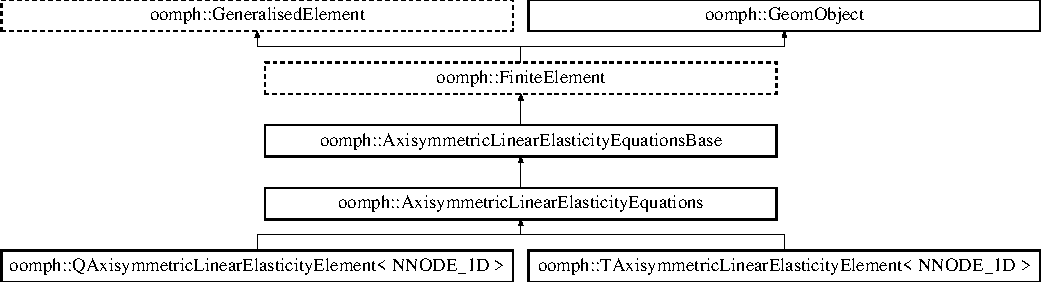
\includegraphics[height=3.794038cm]{classoomph_1_1AxisymmetricLinearElasticityEquationsBase}
\end{center}
\end{figure}
\subsection*{Public Types}
\begin{DoxyCompactItemize}
\item 
typedef void($\ast$ \hyperlink{classoomph_1_1AxisymmetricLinearElasticityEquationsBase_afa35b69a888eecae4b5f199a1adf88c5}{Body\+Force\+Fct\+Pt}) (const double \&time, const \hyperlink{classoomph_1_1Vector}{Vector}$<$ double $>$ \&x, \hyperlink{classoomph_1_1Vector}{Vector}$<$ double $>$ \&b)
\begin{DoxyCompactList}\small\item\em Function pointer to function that specifies the body force as a function of the Cartesian coordinates and time F\+C\+T(x,b) -- x and b are Vectors! \end{DoxyCompactList}\end{DoxyCompactItemize}
\subsection*{Public Member Functions}
\begin{DoxyCompactItemize}
\item 
virtual unsigned \hyperlink{classoomph_1_1AxisymmetricLinearElasticityEquationsBase_a89f40d1bc15ebc4128ea8a22032d31f5}{u\+\_\+index\+\_\+axisymmetric\+\_\+linear\+\_\+elasticity} (const unsigned \&\hyperlink{cfortran_8h_adb50e893b86b3e55e751a42eab3cba82}{i}) const
\begin{DoxyCompactList}\small\item\em Return the index at which the i-\/th (i=0\+: r, i=1\+: z; i=2\+: theta) unknown displacement component is stored at the nodes. The default assignment here (u\+\_\+r, u\+\_\+z, u\+\_\+theta) is appropriate for single-\/physics problems. \end{DoxyCompactList}\item 
double \hyperlink{classoomph_1_1AxisymmetricLinearElasticityEquationsBase_a352c704cb283b27e5c4d8549f5e380d7}{d2u\+\_\+dt2\+\_\+axisymmetric\+\_\+linear\+\_\+elasticity} (const unsigned \&n, const unsigned \&\hyperlink{cfortran_8h_adb50e893b86b3e55e751a42eab3cba82}{i}) const
\begin{DoxyCompactList}\small\item\em d$^\wedge$2u/dt$^\wedge$2 at local node n \end{DoxyCompactList}\item 
double \hyperlink{classoomph_1_1AxisymmetricLinearElasticityEquationsBase_aa340a3d1068cb5f65ebbfabf1bf07b1e}{du\+\_\+dt\+\_\+axisymmetric\+\_\+linear\+\_\+elasticity} (const unsigned \&n, const unsigned \&\hyperlink{cfortran_8h_adb50e893b86b3e55e751a42eab3cba82}{i}) const
\begin{DoxyCompactList}\small\item\em du/dt at local node n \end{DoxyCompactList}\item 
void \hyperlink{classoomph_1_1AxisymmetricLinearElasticityEquationsBase_afeb2209aa0968aed5fa1ac59bc942991}{interpolated\+\_\+u\+\_\+axisymmetric\+\_\+linear\+\_\+elasticity} (const \hyperlink{classoomph_1_1Vector}{Vector}$<$ double $>$ \&\hyperlink{cfortran_8h_ab7123126e4885ef647dd9c6e3807a21c}{s}, \hyperlink{classoomph_1_1Vector}{Vector}$<$ double $>$ \&disp) const
\begin{DoxyCompactList}\small\item\em Compute vector of FE interpolated displacement u at local coordinate s. \end{DoxyCompactList}\item 
double \hyperlink{classoomph_1_1AxisymmetricLinearElasticityEquationsBase_af7660a53ff93c55f3c0c6f634ac2dd80}{interpolated\+\_\+u\+\_\+axisymmetric\+\_\+linear\+\_\+elasticity} (const \hyperlink{classoomph_1_1Vector}{Vector}$<$ double $>$ \&\hyperlink{cfortran_8h_ab7123126e4885ef647dd9c6e3807a21c}{s}, const unsigned \&\hyperlink{cfortran_8h_adb50e893b86b3e55e751a42eab3cba82}{i}) const
\begin{DoxyCompactList}\small\item\em Return FE interpolated displacement u\mbox{[}i\mbox{]} (i=0\+: r, i=1\+: z; i=2\+: theta) at local coordinate s. \end{DoxyCompactList}\item 
void \hyperlink{classoomph_1_1AxisymmetricLinearElasticityEquationsBase_a9b517ddf75cc1a62fbce45d8333cbcaa}{interpolated\+\_\+du\+\_\+dt\+\_\+axisymmetric\+\_\+linear\+\_\+elasticity} (const \hyperlink{classoomph_1_1Vector}{Vector}$<$ double $>$ \&\hyperlink{cfortran_8h_ab7123126e4885ef647dd9c6e3807a21c}{s}, \hyperlink{classoomph_1_1Vector}{Vector}$<$ double $>$ \&du\+\_\+dt) const
\begin{DoxyCompactList}\small\item\em Compute vector of FE interpolated velocity du/dt at local coordinate s. \end{DoxyCompactList}\item 
void \hyperlink{classoomph_1_1AxisymmetricLinearElasticityEquationsBase_a5fd012d570d52057193e0799a3150f20}{interpolated\+\_\+d2u\+\_\+dt2\+\_\+axisymmetric\+\_\+linear\+\_\+elasticity} (const \hyperlink{classoomph_1_1Vector}{Vector}$<$ double $>$ \&\hyperlink{cfortran_8h_ab7123126e4885ef647dd9c6e3807a21c}{s}, \hyperlink{classoomph_1_1Vector}{Vector}$<$ double $>$ \&d2u\+\_\+dt2) const
\begin{DoxyCompactList}\small\item\em Compute vector of FE interpolated accel d2u/dt2 at local coordinate s. \end{DoxyCompactList}\item 
\hyperlink{classoomph_1_1AxisymmetricLinearElasticityEquationsBase_aa37df6e9aef3ee1326187b1c51197527}{Axisymmetric\+Linear\+Elasticity\+Equations\+Base} ()
\begin{DoxyCompactList}\small\item\em Constructor\+: Set null pointers for constitutive law. Set physical parameter values to default values, and set body force to zero. \end{DoxyCompactList}\item 
double $\ast$\& \hyperlink{classoomph_1_1AxisymmetricLinearElasticityEquationsBase_aa57bf5389ce79d81fe1ba6dce32b6263}{youngs\+\_\+modulus\+\_\+pt} ()
\begin{DoxyCompactList}\small\item\em Return the pointer to Young\textquotesingle{}s modulus. \end{DoxyCompactList}\item 
double \hyperlink{classoomph_1_1AxisymmetricLinearElasticityEquationsBase_a8e7ec15db5634c6fd8fac7a848baf19d}{youngs\+\_\+modulus} () const
\begin{DoxyCompactList}\small\item\em Access function to Young\textquotesingle{}s modulus. \end{DoxyCompactList}\item 
double \& \hyperlink{classoomph_1_1AxisymmetricLinearElasticityEquationsBase_a73ee5401b8cfcd059cec299c0e0ff616}{nu} () const
\begin{DoxyCompactList}\small\item\em Access function for Poisson\textquotesingle{}s ratio. \end{DoxyCompactList}\item 
double $\ast$\& \hyperlink{classoomph_1_1AxisymmetricLinearElasticityEquationsBase_a8d4444efaba59fb74e5c68b78e67d616}{nu\+\_\+pt} ()
\begin{DoxyCompactList}\small\item\em Access function for pointer to Poisson\textquotesingle{}s ratio. \end{DoxyCompactList}\item 
double $\ast$\& \hyperlink{classoomph_1_1AxisymmetricLinearElasticityEquationsBase_ab001e2105e0f6e606299bdf8e7b8189e}{lambda\+\_\+sq\+\_\+pt} ()
\begin{DoxyCompactList}\small\item\em Access function for pointer to timescale ratio (nondim density) \end{DoxyCompactList}\item 
const double \& \hyperlink{classoomph_1_1AxisymmetricLinearElasticityEquationsBase_a7e165403d6dad7263f10fe65b3f60301}{lambda\+\_\+sq} () const
\begin{DoxyCompactList}\small\item\em Access function for timescale ratio (nondim density) \end{DoxyCompactList}\item 
\hyperlink{classoomph_1_1AxisymmetricLinearElasticityEquationsBase_afa35b69a888eecae4b5f199a1adf88c5}{Body\+Force\+Fct\+Pt} \& \hyperlink{classoomph_1_1AxisymmetricLinearElasticityEquationsBase_ae7bcc29e716871544ba2742a282a58dc}{body\+\_\+force\+\_\+fct\+\_\+pt} ()
\begin{DoxyCompactList}\small\item\em Access function\+: Pointer to body force function. \end{DoxyCompactList}\item 
\hyperlink{classoomph_1_1AxisymmetricLinearElasticityEquationsBase_afa35b69a888eecae4b5f199a1adf88c5}{Body\+Force\+Fct\+Pt} \hyperlink{classoomph_1_1AxisymmetricLinearElasticityEquationsBase_add2664f22e677925a3163547a1dd5ffa}{body\+\_\+force\+\_\+fct\+\_\+pt} () const
\begin{DoxyCompactList}\small\item\em Access function\+: Pointer to body force function (const version) \end{DoxyCompactList}\item 
void \hyperlink{classoomph_1_1AxisymmetricLinearElasticityEquationsBase_ad388a41f086f181a3c1608a5fb337ac6}{body\+\_\+force} (const double \&time, const \hyperlink{classoomph_1_1Vector}{Vector}$<$ double $>$ \&x, \hyperlink{classoomph_1_1Vector}{Vector}$<$ double $>$ \&b) const
\begin{DoxyCompactList}\small\item\em Evaluate body force at Eulerian coordinate x at present time (returns zero vector if no body force function pointer has been set) \end{DoxyCompactList}\item 
unsigned \hyperlink{classoomph_1_1AxisymmetricLinearElasticityEquationsBase_a46c5dca6d1bc3e471f71cb44bdc06284}{ndof\+\_\+types} () const
\begin{DoxyCompactList}\small\item\em The number of \char`\"{}\+D\+O\+F types\char`\"{} that degrees of freedom in this element are sub-\/divided into\+: for now lump them all into one D\+OF type. Can be adjusted later. \end{DoxyCompactList}\item 
void \hyperlink{classoomph_1_1AxisymmetricLinearElasticityEquationsBase_a714fb359257e5a262e2e1368fcfc1ccb}{get\+\_\+dof\+\_\+numbers\+\_\+for\+\_\+unknowns} (std\+::list$<$ std\+::pair$<$ unsigned long, unsigned $>$ $>$ \&dof\+\_\+lookup\+\_\+list) const
\begin{DoxyCompactList}\small\item\em Create a list of pairs for all unknowns in this element, so that the first entry in each pair contains the global equation number of the unknown, while the second one contains the number of the \char`\"{}\+D\+O\+F type\char`\"{} that this unknown is associated with. (Function can obviously only be called if the equation numbering scheme has been set up.) \end{DoxyCompactList}\end{DoxyCompactItemize}
\subsection*{Protected Attributes}
\begin{DoxyCompactItemize}
\item 
double $\ast$ \hyperlink{classoomph_1_1AxisymmetricLinearElasticityEquationsBase_a26867c1c3519bfc2910aaf0ec506dc0e}{Youngs\+\_\+modulus\+\_\+pt}
\begin{DoxyCompactList}\small\item\em Pointer to the Young\textquotesingle{}s modulus. \end{DoxyCompactList}\item 
double $\ast$ \hyperlink{classoomph_1_1AxisymmetricLinearElasticityEquationsBase_a8cfaabdb9413b153d83b27d3efd9a28c}{Nu\+\_\+pt}
\begin{DoxyCompactList}\small\item\em Pointer to Poisson\textquotesingle{}s ratio. \end{DoxyCompactList}\item 
double $\ast$ \hyperlink{classoomph_1_1AxisymmetricLinearElasticityEquationsBase_af4c300075ee05691d784682a7b02e2a6}{Lambda\+\_\+sq\+\_\+pt}
\begin{DoxyCompactList}\small\item\em Timescale ratio (non-\/dim. density) \end{DoxyCompactList}\item 
\hyperlink{classoomph_1_1AxisymmetricLinearElasticityEquationsBase_afa35b69a888eecae4b5f199a1adf88c5}{Body\+Force\+Fct\+Pt} \hyperlink{classoomph_1_1AxisymmetricLinearElasticityEquationsBase_adf2730220f65eb1fdd05715d1d1d9a78}{Body\+\_\+force\+\_\+fct\+\_\+pt}
\begin{DoxyCompactList}\small\item\em Pointer to body force function. \end{DoxyCompactList}\end{DoxyCompactItemize}
\subsection*{Static Protected Attributes}
\begin{DoxyCompactItemize}
\item 
static double \hyperlink{classoomph_1_1AxisymmetricLinearElasticityEquationsBase_ab805f3d2d1a92be924b68367c6f002dd}{Default\+\_\+youngs\+\_\+modulus\+\_\+value}
\begin{DoxyCompactList}\small\item\em Static default value for Young\textquotesingle{}s modulus (1.\+0 -- for natural scaling, i.\+e. all stresses have been non-\/dimensionalised by the same reference Young\textquotesingle{}s modulus. Setting the \char`\"{}non-\/dimensional\char`\"{} Young\textquotesingle{}s modulus (obtained by de-\/referencing Youngs\+\_\+modulus\+\_\+pt) to a number larger than one means that the material is stiffer than assumed in the non-\/dimensionalisation. \end{DoxyCompactList}\item 
static double \hyperlink{classoomph_1_1AxisymmetricLinearElasticityEquationsBase_a9788b32107b4eacd99bdffe73e83245a}{Default\+\_\+lambda\+\_\+sq\+\_\+value} = 1.\+0
\begin{DoxyCompactList}\small\item\em Static default value for timescale ratio (1.\+0 for natural scaling) \end{DoxyCompactList}\end{DoxyCompactItemize}
\subsection*{Additional Inherited Members}


\subsection{Detailed Description}
A base class for elements that solve the axisymmetric (in cylindrical polars) equations of linear elasticity. 

Definition at line 57 of file axisym\+\_\+linear\+\_\+elasticity\+\_\+elements.\+h.



\subsection{Member Typedef Documentation}
\mbox{\Hypertarget{classoomph_1_1AxisymmetricLinearElasticityEquationsBase_afa35b69a888eecae4b5f199a1adf88c5}\label{classoomph_1_1AxisymmetricLinearElasticityEquationsBase_afa35b69a888eecae4b5f199a1adf88c5}} 
\index{oomph\+::\+Axisymmetric\+Linear\+Elasticity\+Equations\+Base@{oomph\+::\+Axisymmetric\+Linear\+Elasticity\+Equations\+Base}!Body\+Force\+Fct\+Pt@{Body\+Force\+Fct\+Pt}}
\index{Body\+Force\+Fct\+Pt@{Body\+Force\+Fct\+Pt}!oomph\+::\+Axisymmetric\+Linear\+Elasticity\+Equations\+Base@{oomph\+::\+Axisymmetric\+Linear\+Elasticity\+Equations\+Base}}
\subsubsection{\texorpdfstring{Body\+Force\+Fct\+Pt}{BodyForceFctPt}}
{\footnotesize\ttfamily typedef void($\ast$ oomph\+::\+Axisymmetric\+Linear\+Elasticity\+Equations\+Base\+::\+Body\+Force\+Fct\+Pt) (const double \&time, const \hyperlink{classoomph_1_1Vector}{Vector}$<$ double $>$ \&x, \hyperlink{classoomph_1_1Vector}{Vector}$<$ double $>$ \&b)}



Function pointer to function that specifies the body force as a function of the Cartesian coordinates and time F\+C\+T(x,b) -- x and b are Vectors! 



Definition at line 257 of file axisym\+\_\+linear\+\_\+elasticity\+\_\+elements.\+h.



\subsection{Constructor \& Destructor Documentation}
\mbox{\Hypertarget{classoomph_1_1AxisymmetricLinearElasticityEquationsBase_aa37df6e9aef3ee1326187b1c51197527}\label{classoomph_1_1AxisymmetricLinearElasticityEquationsBase_aa37df6e9aef3ee1326187b1c51197527}} 
\index{oomph\+::\+Axisymmetric\+Linear\+Elasticity\+Equations\+Base@{oomph\+::\+Axisymmetric\+Linear\+Elasticity\+Equations\+Base}!Axisymmetric\+Linear\+Elasticity\+Equations\+Base@{Axisymmetric\+Linear\+Elasticity\+Equations\+Base}}
\index{Axisymmetric\+Linear\+Elasticity\+Equations\+Base@{Axisymmetric\+Linear\+Elasticity\+Equations\+Base}!oomph\+::\+Axisymmetric\+Linear\+Elasticity\+Equations\+Base@{oomph\+::\+Axisymmetric\+Linear\+Elasticity\+Equations\+Base}}
\subsubsection{\texorpdfstring{Axisymmetric\+Linear\+Elasticity\+Equations\+Base()}{AxisymmetricLinearElasticityEquationsBase()}}
{\footnotesize\ttfamily oomph\+::\+Axisymmetric\+Linear\+Elasticity\+Equations\+Base\+::\+Axisymmetric\+Linear\+Elasticity\+Equations\+Base (\begin{DoxyParamCaption}{ }\end{DoxyParamCaption})\hspace{0.3cm}{\ttfamily [inline]}}



Constructor\+: Set null pointers for constitutive law. Set physical parameter values to default values, and set body force to zero. 



Definition at line 264 of file axisym\+\_\+linear\+\_\+elasticity\+\_\+elements.\+h.



\subsection{Member Function Documentation}
\mbox{\Hypertarget{classoomph_1_1AxisymmetricLinearElasticityEquationsBase_ad388a41f086f181a3c1608a5fb337ac6}\label{classoomph_1_1AxisymmetricLinearElasticityEquationsBase_ad388a41f086f181a3c1608a5fb337ac6}} 
\index{oomph\+::\+Axisymmetric\+Linear\+Elasticity\+Equations\+Base@{oomph\+::\+Axisymmetric\+Linear\+Elasticity\+Equations\+Base}!body\+\_\+force@{body\+\_\+force}}
\index{body\+\_\+force@{body\+\_\+force}!oomph\+::\+Axisymmetric\+Linear\+Elasticity\+Equations\+Base@{oomph\+::\+Axisymmetric\+Linear\+Elasticity\+Equations\+Base}}
\subsubsection{\texorpdfstring{body\+\_\+force()}{body\_force()}}
{\footnotesize\ttfamily void oomph\+::\+Axisymmetric\+Linear\+Elasticity\+Equations\+Base\+::body\+\_\+force (\begin{DoxyParamCaption}\item[{const double \&}]{time,  }\item[{const \hyperlink{classoomph_1_1Vector}{Vector}$<$ double $>$ \&}]{x,  }\item[{\hyperlink{classoomph_1_1Vector}{Vector}$<$ double $>$ \&}]{b }\end{DoxyParamCaption}) const\hspace{0.3cm}{\ttfamily [inline]}}



Evaluate body force at Eulerian coordinate x at present time (returns zero vector if no body force function pointer has been set) 



Definition at line 312 of file axisym\+\_\+linear\+\_\+elasticity\+\_\+elements.\+h.



References Body\+\_\+force\+\_\+fct\+\_\+pt, oomph\+::\+Finite\+Element\+::dim(), and i.



Referenced by oomph\+::\+Axisymmetric\+Linear\+Elasticity\+Equations\+::fill\+\_\+in\+\_\+generic\+\_\+contribution\+\_\+to\+\_\+residuals\+\_\+axisymmetric\+\_\+linear\+\_\+elasticity().

\mbox{\Hypertarget{classoomph_1_1AxisymmetricLinearElasticityEquationsBase_ae7bcc29e716871544ba2742a282a58dc}\label{classoomph_1_1AxisymmetricLinearElasticityEquationsBase_ae7bcc29e716871544ba2742a282a58dc}} 
\index{oomph\+::\+Axisymmetric\+Linear\+Elasticity\+Equations\+Base@{oomph\+::\+Axisymmetric\+Linear\+Elasticity\+Equations\+Base}!body\+\_\+force\+\_\+fct\+\_\+pt@{body\+\_\+force\+\_\+fct\+\_\+pt}}
\index{body\+\_\+force\+\_\+fct\+\_\+pt@{body\+\_\+force\+\_\+fct\+\_\+pt}!oomph\+::\+Axisymmetric\+Linear\+Elasticity\+Equations\+Base@{oomph\+::\+Axisymmetric\+Linear\+Elasticity\+Equations\+Base}}
\subsubsection{\texorpdfstring{body\+\_\+force\+\_\+fct\+\_\+pt()}{body\_force\_fct\_pt()}\hspace{0.1cm}{\footnotesize\ttfamily [1/2]}}
{\footnotesize\ttfamily \hyperlink{classoomph_1_1AxisymmetricLinearElasticityEquationsBase_afa35b69a888eecae4b5f199a1adf88c5}{Body\+Force\+Fct\+Pt}\& oomph\+::\+Axisymmetric\+Linear\+Elasticity\+Equations\+Base\+::body\+\_\+force\+\_\+fct\+\_\+pt (\begin{DoxyParamCaption}{ }\end{DoxyParamCaption})\hspace{0.3cm}{\ttfamily [inline]}}



Access function\+: Pointer to body force function. 



Definition at line 305 of file axisym\+\_\+linear\+\_\+elasticity\+\_\+elements.\+h.



References Body\+\_\+force\+\_\+fct\+\_\+pt.

\mbox{\Hypertarget{classoomph_1_1AxisymmetricLinearElasticityEquationsBase_add2664f22e677925a3163547a1dd5ffa}\label{classoomph_1_1AxisymmetricLinearElasticityEquationsBase_add2664f22e677925a3163547a1dd5ffa}} 
\index{oomph\+::\+Axisymmetric\+Linear\+Elasticity\+Equations\+Base@{oomph\+::\+Axisymmetric\+Linear\+Elasticity\+Equations\+Base}!body\+\_\+force\+\_\+fct\+\_\+pt@{body\+\_\+force\+\_\+fct\+\_\+pt}}
\index{body\+\_\+force\+\_\+fct\+\_\+pt@{body\+\_\+force\+\_\+fct\+\_\+pt}!oomph\+::\+Axisymmetric\+Linear\+Elasticity\+Equations\+Base@{oomph\+::\+Axisymmetric\+Linear\+Elasticity\+Equations\+Base}}
\subsubsection{\texorpdfstring{body\+\_\+force\+\_\+fct\+\_\+pt()}{body\_force\_fct\_pt()}\hspace{0.1cm}{\footnotesize\ttfamily [2/2]}}
{\footnotesize\ttfamily \hyperlink{classoomph_1_1AxisymmetricLinearElasticityEquationsBase_afa35b69a888eecae4b5f199a1adf88c5}{Body\+Force\+Fct\+Pt} oomph\+::\+Axisymmetric\+Linear\+Elasticity\+Equations\+Base\+::body\+\_\+force\+\_\+fct\+\_\+pt (\begin{DoxyParamCaption}{ }\end{DoxyParamCaption}) const\hspace{0.3cm}{\ttfamily [inline]}}



Access function\+: Pointer to body force function (const version) 



Definition at line 308 of file axisym\+\_\+linear\+\_\+elasticity\+\_\+elements.\+h.



References Body\+\_\+force\+\_\+fct\+\_\+pt.

\mbox{\Hypertarget{classoomph_1_1AxisymmetricLinearElasticityEquationsBase_a352c704cb283b27e5c4d8549f5e380d7}\label{classoomph_1_1AxisymmetricLinearElasticityEquationsBase_a352c704cb283b27e5c4d8549f5e380d7}} 
\index{oomph\+::\+Axisymmetric\+Linear\+Elasticity\+Equations\+Base@{oomph\+::\+Axisymmetric\+Linear\+Elasticity\+Equations\+Base}!d2u\+\_\+dt2\+\_\+axisymmetric\+\_\+linear\+\_\+elasticity@{d2u\+\_\+dt2\+\_\+axisymmetric\+\_\+linear\+\_\+elasticity}}
\index{d2u\+\_\+dt2\+\_\+axisymmetric\+\_\+linear\+\_\+elasticity@{d2u\+\_\+dt2\+\_\+axisymmetric\+\_\+linear\+\_\+elasticity}!oomph\+::\+Axisymmetric\+Linear\+Elasticity\+Equations\+Base@{oomph\+::\+Axisymmetric\+Linear\+Elasticity\+Equations\+Base}}
\subsubsection{\texorpdfstring{d2u\+\_\+dt2\+\_\+axisymmetric\+\_\+linear\+\_\+elasticity()}{d2u\_dt2\_axisymmetric\_linear\_elasticity()}}
{\footnotesize\ttfamily double oomph\+::\+Axisymmetric\+Linear\+Elasticity\+Equations\+Base\+::d2u\+\_\+dt2\+\_\+axisymmetric\+\_\+linear\+\_\+elasticity (\begin{DoxyParamCaption}\item[{const unsigned \&}]{n,  }\item[{const unsigned \&}]{i }\end{DoxyParamCaption}) const\hspace{0.3cm}{\ttfamily [inline]}}



d$^\wedge$2u/dt$^\wedge$2 at local node n 



Definition at line 73 of file axisym\+\_\+linear\+\_\+elasticity\+\_\+elements.\+h.



References oomph\+::\+Time\+Stepper\+::is\+\_\+steady(), oomph\+::\+Finite\+Element\+::nodal\+\_\+value(), oomph\+::\+Finite\+Element\+::node\+\_\+pt(), oomph\+::\+Time\+Stepper\+::ntstorage(), t, oomph\+::\+Geom\+Object\+::time\+\_\+stepper\+\_\+pt(), oomph\+::\+Data\+::time\+\_\+stepper\+\_\+pt(), u\+\_\+index\+\_\+axisymmetric\+\_\+linear\+\_\+elasticity(), and oomph\+::\+Time\+Stepper\+::weight().



Referenced by oomph\+::\+Axisymmetric\+Linear\+Elasticity\+Equations\+::fill\+\_\+in\+\_\+generic\+\_\+contribution\+\_\+to\+\_\+residuals\+\_\+axisymmetric\+\_\+linear\+\_\+elasticity(), and interpolated\+\_\+d2u\+\_\+dt2\+\_\+axisymmetric\+\_\+linear\+\_\+elasticity().

\mbox{\Hypertarget{classoomph_1_1AxisymmetricLinearElasticityEquationsBase_aa340a3d1068cb5f65ebbfabf1bf07b1e}\label{classoomph_1_1AxisymmetricLinearElasticityEquationsBase_aa340a3d1068cb5f65ebbfabf1bf07b1e}} 
\index{oomph\+::\+Axisymmetric\+Linear\+Elasticity\+Equations\+Base@{oomph\+::\+Axisymmetric\+Linear\+Elasticity\+Equations\+Base}!du\+\_\+dt\+\_\+axisymmetric\+\_\+linear\+\_\+elasticity@{du\+\_\+dt\+\_\+axisymmetric\+\_\+linear\+\_\+elasticity}}
\index{du\+\_\+dt\+\_\+axisymmetric\+\_\+linear\+\_\+elasticity@{du\+\_\+dt\+\_\+axisymmetric\+\_\+linear\+\_\+elasticity}!oomph\+::\+Axisymmetric\+Linear\+Elasticity\+Equations\+Base@{oomph\+::\+Axisymmetric\+Linear\+Elasticity\+Equations\+Base}}
\subsubsection{\texorpdfstring{du\+\_\+dt\+\_\+axisymmetric\+\_\+linear\+\_\+elasticity()}{du\_dt\_axisymmetric\_linear\_elasticity()}}
{\footnotesize\ttfamily double oomph\+::\+Axisymmetric\+Linear\+Elasticity\+Equations\+Base\+::du\+\_\+dt\+\_\+axisymmetric\+\_\+linear\+\_\+elasticity (\begin{DoxyParamCaption}\item[{const unsigned \&}]{n,  }\item[{const unsigned \&}]{i }\end{DoxyParamCaption}) const\hspace{0.3cm}{\ttfamily [inline]}}



du/dt at local node n 



Definition at line 104 of file axisym\+\_\+linear\+\_\+elasticity\+\_\+elements.\+h.



References oomph\+::\+Time\+Stepper\+::is\+\_\+steady(), oomph\+::\+Finite\+Element\+::nodal\+\_\+value(), oomph\+::\+Finite\+Element\+::node\+\_\+pt(), oomph\+::\+Time\+Stepper\+::ntstorage(), t, oomph\+::\+Geom\+Object\+::time\+\_\+stepper\+\_\+pt(), oomph\+::\+Data\+::time\+\_\+stepper\+\_\+pt(), u\+\_\+index\+\_\+axisymmetric\+\_\+linear\+\_\+elasticity(), and oomph\+::\+Time\+Stepper\+::weight().



Referenced by interpolated\+\_\+du\+\_\+dt\+\_\+axisymmetric\+\_\+linear\+\_\+elasticity().

\mbox{\Hypertarget{classoomph_1_1AxisymmetricLinearElasticityEquationsBase_a714fb359257e5a262e2e1368fcfc1ccb}\label{classoomph_1_1AxisymmetricLinearElasticityEquationsBase_a714fb359257e5a262e2e1368fcfc1ccb}} 
\index{oomph\+::\+Axisymmetric\+Linear\+Elasticity\+Equations\+Base@{oomph\+::\+Axisymmetric\+Linear\+Elasticity\+Equations\+Base}!get\+\_\+dof\+\_\+numbers\+\_\+for\+\_\+unknowns@{get\+\_\+dof\+\_\+numbers\+\_\+for\+\_\+unknowns}}
\index{get\+\_\+dof\+\_\+numbers\+\_\+for\+\_\+unknowns@{get\+\_\+dof\+\_\+numbers\+\_\+for\+\_\+unknowns}!oomph\+::\+Axisymmetric\+Linear\+Elasticity\+Equations\+Base@{oomph\+::\+Axisymmetric\+Linear\+Elasticity\+Equations\+Base}}
\subsubsection{\texorpdfstring{get\+\_\+dof\+\_\+numbers\+\_\+for\+\_\+unknowns()}{get\_dof\_numbers\_for\_unknowns()}}
{\footnotesize\ttfamily void oomph\+::\+Axisymmetric\+Linear\+Elasticity\+Equations\+Base\+::get\+\_\+dof\+\_\+numbers\+\_\+for\+\_\+unknowns (\begin{DoxyParamCaption}\item[{std\+::list$<$ std\+::pair$<$ unsigned long, unsigned $>$ $>$ \&}]{dof\+\_\+lookup\+\_\+list }\end{DoxyParamCaption}) const\hspace{0.3cm}{\ttfamily [inline]}, {\ttfamily [virtual]}}



Create a list of pairs for all unknowns in this element, so that the first entry in each pair contains the global equation number of the unknown, while the second one contains the number of the \char`\"{}\+D\+O\+F type\char`\"{} that this unknown is associated with. (Function can obviously only be called if the equation numbering scheme has been set up.) 



Reimplemented from \hyperlink{classoomph_1_1GeneralisedElement_a069f59bfc3e607a5bebba52c6314d777}{oomph\+::\+Generalised\+Element}.



Definition at line 346 of file axisym\+\_\+linear\+\_\+elasticity\+\_\+elements.\+h.



References oomph\+::\+Generalised\+Element\+::eqn\+\_\+number(), i, oomph\+::\+Finite\+Element\+::nnode(), and oomph\+::\+Finite\+Element\+::nodal\+\_\+local\+\_\+eqn().

\mbox{\Hypertarget{classoomph_1_1AxisymmetricLinearElasticityEquationsBase_a5fd012d570d52057193e0799a3150f20}\label{classoomph_1_1AxisymmetricLinearElasticityEquationsBase_a5fd012d570d52057193e0799a3150f20}} 
\index{oomph\+::\+Axisymmetric\+Linear\+Elasticity\+Equations\+Base@{oomph\+::\+Axisymmetric\+Linear\+Elasticity\+Equations\+Base}!interpolated\+\_\+d2u\+\_\+dt2\+\_\+axisymmetric\+\_\+linear\+\_\+elasticity@{interpolated\+\_\+d2u\+\_\+dt2\+\_\+axisymmetric\+\_\+linear\+\_\+elasticity}}
\index{interpolated\+\_\+d2u\+\_\+dt2\+\_\+axisymmetric\+\_\+linear\+\_\+elasticity@{interpolated\+\_\+d2u\+\_\+dt2\+\_\+axisymmetric\+\_\+linear\+\_\+elasticity}!oomph\+::\+Axisymmetric\+Linear\+Elasticity\+Equations\+Base@{oomph\+::\+Axisymmetric\+Linear\+Elasticity\+Equations\+Base}}
\subsubsection{\texorpdfstring{interpolated\+\_\+d2u\+\_\+dt2\+\_\+axisymmetric\+\_\+linear\+\_\+elasticity()}{interpolated\_d2u\_dt2\_axisymmetric\_linear\_elasticity()}}
{\footnotesize\ttfamily void oomph\+::\+Axisymmetric\+Linear\+Elasticity\+Equations\+Base\+::interpolated\+\_\+d2u\+\_\+dt2\+\_\+axisymmetric\+\_\+linear\+\_\+elasticity (\begin{DoxyParamCaption}\item[{const \hyperlink{classoomph_1_1Vector}{Vector}$<$ double $>$ \&}]{s,  }\item[{\hyperlink{classoomph_1_1Vector}{Vector}$<$ double $>$ \&}]{d2u\+\_\+dt2 }\end{DoxyParamCaption}) const\hspace{0.3cm}{\ttfamily [inline]}}



Compute vector of FE interpolated accel d2u/dt2 at local coordinate s. 



Definition at line 228 of file axisym\+\_\+linear\+\_\+elasticity\+\_\+elements.\+h.



References d2u\+\_\+dt2\+\_\+axisymmetric\+\_\+linear\+\_\+elasticity(), i, oomph\+::\+Finite\+Element\+::nnode(), and oomph\+::\+Finite\+Element\+::shape().



Referenced by oomph\+::\+Axisymmetric\+Linear\+Elasticity\+Equations\+::output().

\mbox{\Hypertarget{classoomph_1_1AxisymmetricLinearElasticityEquationsBase_a9b517ddf75cc1a62fbce45d8333cbcaa}\label{classoomph_1_1AxisymmetricLinearElasticityEquationsBase_a9b517ddf75cc1a62fbce45d8333cbcaa}} 
\index{oomph\+::\+Axisymmetric\+Linear\+Elasticity\+Equations\+Base@{oomph\+::\+Axisymmetric\+Linear\+Elasticity\+Equations\+Base}!interpolated\+\_\+du\+\_\+dt\+\_\+axisymmetric\+\_\+linear\+\_\+elasticity@{interpolated\+\_\+du\+\_\+dt\+\_\+axisymmetric\+\_\+linear\+\_\+elasticity}}
\index{interpolated\+\_\+du\+\_\+dt\+\_\+axisymmetric\+\_\+linear\+\_\+elasticity@{interpolated\+\_\+du\+\_\+dt\+\_\+axisymmetric\+\_\+linear\+\_\+elasticity}!oomph\+::\+Axisymmetric\+Linear\+Elasticity\+Equations\+Base@{oomph\+::\+Axisymmetric\+Linear\+Elasticity\+Equations\+Base}}
\subsubsection{\texorpdfstring{interpolated\+\_\+du\+\_\+dt\+\_\+axisymmetric\+\_\+linear\+\_\+elasticity()}{interpolated\_du\_dt\_axisymmetric\_linear\_elasticity()}}
{\footnotesize\ttfamily void oomph\+::\+Axisymmetric\+Linear\+Elasticity\+Equations\+Base\+::interpolated\+\_\+du\+\_\+dt\+\_\+axisymmetric\+\_\+linear\+\_\+elasticity (\begin{DoxyParamCaption}\item[{const \hyperlink{classoomph_1_1Vector}{Vector}$<$ double $>$ \&}]{s,  }\item[{\hyperlink{classoomph_1_1Vector}{Vector}$<$ double $>$ \&}]{du\+\_\+dt }\end{DoxyParamCaption}) const\hspace{0.3cm}{\ttfamily [inline]}}



Compute vector of FE interpolated velocity du/dt at local coordinate s. 



Definition at line 201 of file axisym\+\_\+linear\+\_\+elasticity\+\_\+elements.\+h.



References du\+\_\+dt\+\_\+axisymmetric\+\_\+linear\+\_\+elasticity(), i, oomph\+::\+Finite\+Element\+::nnode(), and oomph\+::\+Finite\+Element\+::shape().



Referenced by oomph\+::\+Axisymmetric\+Linear\+Elasticity\+Equations\+::output().

\mbox{\Hypertarget{classoomph_1_1AxisymmetricLinearElasticityEquationsBase_afeb2209aa0968aed5fa1ac59bc942991}\label{classoomph_1_1AxisymmetricLinearElasticityEquationsBase_afeb2209aa0968aed5fa1ac59bc942991}} 
\index{oomph\+::\+Axisymmetric\+Linear\+Elasticity\+Equations\+Base@{oomph\+::\+Axisymmetric\+Linear\+Elasticity\+Equations\+Base}!interpolated\+\_\+u\+\_\+axisymmetric\+\_\+linear\+\_\+elasticity@{interpolated\+\_\+u\+\_\+axisymmetric\+\_\+linear\+\_\+elasticity}}
\index{interpolated\+\_\+u\+\_\+axisymmetric\+\_\+linear\+\_\+elasticity@{interpolated\+\_\+u\+\_\+axisymmetric\+\_\+linear\+\_\+elasticity}!oomph\+::\+Axisymmetric\+Linear\+Elasticity\+Equations\+Base@{oomph\+::\+Axisymmetric\+Linear\+Elasticity\+Equations\+Base}}
\subsubsection{\texorpdfstring{interpolated\+\_\+u\+\_\+axisymmetric\+\_\+linear\+\_\+elasticity()}{interpolated\_u\_axisymmetric\_linear\_elasticity()}\hspace{0.1cm}{\footnotesize\ttfamily [1/2]}}
{\footnotesize\ttfamily void oomph\+::\+Axisymmetric\+Linear\+Elasticity\+Equations\+Base\+::interpolated\+\_\+u\+\_\+axisymmetric\+\_\+linear\+\_\+elasticity (\begin{DoxyParamCaption}\item[{const \hyperlink{classoomph_1_1Vector}{Vector}$<$ double $>$ \&}]{s,  }\item[{\hyperlink{classoomph_1_1Vector}{Vector}$<$ double $>$ \&}]{disp }\end{DoxyParamCaption}) const\hspace{0.3cm}{\ttfamily [inline]}}



Compute vector of FE interpolated displacement u at local coordinate s. 



Definition at line 133 of file axisym\+\_\+linear\+\_\+elasticity\+\_\+elements.\+h.



References i, oomph\+::\+Finite\+Element\+::nnode(), oomph\+::\+Finite\+Element\+::nodal\+\_\+value(), oomph\+::\+Finite\+Element\+::shape(), and u\+\_\+index\+\_\+axisymmetric\+\_\+linear\+\_\+elasticity().



Referenced by oomph\+::\+Axisymmetric\+Linear\+Elasticity\+Equations\+::compute\+\_\+error(), and oomph\+::\+Axisymmetric\+Linear\+Elasticity\+Equations\+::output().

\mbox{\Hypertarget{classoomph_1_1AxisymmetricLinearElasticityEquationsBase_af7660a53ff93c55f3c0c6f634ac2dd80}\label{classoomph_1_1AxisymmetricLinearElasticityEquationsBase_af7660a53ff93c55f3c0c6f634ac2dd80}} 
\index{oomph\+::\+Axisymmetric\+Linear\+Elasticity\+Equations\+Base@{oomph\+::\+Axisymmetric\+Linear\+Elasticity\+Equations\+Base}!interpolated\+\_\+u\+\_\+axisymmetric\+\_\+linear\+\_\+elasticity@{interpolated\+\_\+u\+\_\+axisymmetric\+\_\+linear\+\_\+elasticity}}
\index{interpolated\+\_\+u\+\_\+axisymmetric\+\_\+linear\+\_\+elasticity@{interpolated\+\_\+u\+\_\+axisymmetric\+\_\+linear\+\_\+elasticity}!oomph\+::\+Axisymmetric\+Linear\+Elasticity\+Equations\+Base@{oomph\+::\+Axisymmetric\+Linear\+Elasticity\+Equations\+Base}}
\subsubsection{\texorpdfstring{interpolated\+\_\+u\+\_\+axisymmetric\+\_\+linear\+\_\+elasticity()}{interpolated\_u\_axisymmetric\_linear\_elasticity()}\hspace{0.1cm}{\footnotesize\ttfamily [2/2]}}
{\footnotesize\ttfamily double oomph\+::\+Axisymmetric\+Linear\+Elasticity\+Equations\+Base\+::interpolated\+\_\+u\+\_\+axisymmetric\+\_\+linear\+\_\+elasticity (\begin{DoxyParamCaption}\item[{const \hyperlink{classoomph_1_1Vector}{Vector}$<$ double $>$ \&}]{s,  }\item[{const unsigned \&}]{i }\end{DoxyParamCaption}) const\hspace{0.3cm}{\ttfamily [inline]}}



Return FE interpolated displacement u\mbox{[}i\mbox{]} (i=0\+: r, i=1\+: z; i=2\+: theta) at local coordinate s. 



Definition at line 168 of file axisym\+\_\+linear\+\_\+elasticity\+\_\+elements.\+h.



References oomph\+::\+Finite\+Element\+::nnode(), oomph\+::\+Finite\+Element\+::nodal\+\_\+value(), oomph\+::\+Finite\+Element\+::shape(), and u\+\_\+index\+\_\+axisymmetric\+\_\+linear\+\_\+elasticity().

\mbox{\Hypertarget{classoomph_1_1AxisymmetricLinearElasticityEquationsBase_a7e165403d6dad7263f10fe65b3f60301}\label{classoomph_1_1AxisymmetricLinearElasticityEquationsBase_a7e165403d6dad7263f10fe65b3f60301}} 
\index{oomph\+::\+Axisymmetric\+Linear\+Elasticity\+Equations\+Base@{oomph\+::\+Axisymmetric\+Linear\+Elasticity\+Equations\+Base}!lambda\+\_\+sq@{lambda\+\_\+sq}}
\index{lambda\+\_\+sq@{lambda\+\_\+sq}!oomph\+::\+Axisymmetric\+Linear\+Elasticity\+Equations\+Base@{oomph\+::\+Axisymmetric\+Linear\+Elasticity\+Equations\+Base}}
\subsubsection{\texorpdfstring{lambda\+\_\+sq()}{lambda\_sq()}}
{\footnotesize\ttfamily const double\& oomph\+::\+Axisymmetric\+Linear\+Elasticity\+Equations\+Base\+::lambda\+\_\+sq (\begin{DoxyParamCaption}{ }\end{DoxyParamCaption}) const\hspace{0.3cm}{\ttfamily [inline]}}



Access function for timescale ratio (nondim density) 



Definition at line 302 of file axisym\+\_\+linear\+\_\+elasticity\+\_\+elements.\+h.



References Lambda\+\_\+sq\+\_\+pt.



Referenced by oomph\+::\+Axisymmetric\+Linear\+Elasticity\+Equations\+::fill\+\_\+in\+\_\+generic\+\_\+contribution\+\_\+to\+\_\+residuals\+\_\+axisymmetric\+\_\+linear\+\_\+elasticity().

\mbox{\Hypertarget{classoomph_1_1AxisymmetricLinearElasticityEquationsBase_ab001e2105e0f6e606299bdf8e7b8189e}\label{classoomph_1_1AxisymmetricLinearElasticityEquationsBase_ab001e2105e0f6e606299bdf8e7b8189e}} 
\index{oomph\+::\+Axisymmetric\+Linear\+Elasticity\+Equations\+Base@{oomph\+::\+Axisymmetric\+Linear\+Elasticity\+Equations\+Base}!lambda\+\_\+sq\+\_\+pt@{lambda\+\_\+sq\+\_\+pt}}
\index{lambda\+\_\+sq\+\_\+pt@{lambda\+\_\+sq\+\_\+pt}!oomph\+::\+Axisymmetric\+Linear\+Elasticity\+Equations\+Base@{oomph\+::\+Axisymmetric\+Linear\+Elasticity\+Equations\+Base}}
\subsubsection{\texorpdfstring{lambda\+\_\+sq\+\_\+pt()}{lambda\_sq\_pt()}}
{\footnotesize\ttfamily double$\ast$\& oomph\+::\+Axisymmetric\+Linear\+Elasticity\+Equations\+Base\+::lambda\+\_\+sq\+\_\+pt (\begin{DoxyParamCaption}{ }\end{DoxyParamCaption})\hspace{0.3cm}{\ttfamily [inline]}}



Access function for pointer to timescale ratio (nondim density) 



Definition at line 299 of file axisym\+\_\+linear\+\_\+elasticity\+\_\+elements.\+h.



References Lambda\+\_\+sq\+\_\+pt.

\mbox{\Hypertarget{classoomph_1_1AxisymmetricLinearElasticityEquationsBase_a46c5dca6d1bc3e471f71cb44bdc06284}\label{classoomph_1_1AxisymmetricLinearElasticityEquationsBase_a46c5dca6d1bc3e471f71cb44bdc06284}} 
\index{oomph\+::\+Axisymmetric\+Linear\+Elasticity\+Equations\+Base@{oomph\+::\+Axisymmetric\+Linear\+Elasticity\+Equations\+Base}!ndof\+\_\+types@{ndof\+\_\+types}}
\index{ndof\+\_\+types@{ndof\+\_\+types}!oomph\+::\+Axisymmetric\+Linear\+Elasticity\+Equations\+Base@{oomph\+::\+Axisymmetric\+Linear\+Elasticity\+Equations\+Base}}
\subsubsection{\texorpdfstring{ndof\+\_\+types()}{ndof\_types()}}
{\footnotesize\ttfamily unsigned oomph\+::\+Axisymmetric\+Linear\+Elasticity\+Equations\+Base\+::ndof\+\_\+types (\begin{DoxyParamCaption}{ }\end{DoxyParamCaption}) const\hspace{0.3cm}{\ttfamily [inline]}, {\ttfamily [virtual]}}



The number of \char`\"{}\+D\+O\+F types\char`\"{} that degrees of freedom in this element are sub-\/divided into\+: for now lump them all into one D\+OF type. Can be adjusted later. 



Reimplemented from \hyperlink{classoomph_1_1GeneralisedElement_a0c6037a870597b35dcf1c780710b9a56}{oomph\+::\+Generalised\+Element}.



Definition at line 335 of file axisym\+\_\+linear\+\_\+elasticity\+\_\+elements.\+h.

\mbox{\Hypertarget{classoomph_1_1AxisymmetricLinearElasticityEquationsBase_a73ee5401b8cfcd059cec299c0e0ff616}\label{classoomph_1_1AxisymmetricLinearElasticityEquationsBase_a73ee5401b8cfcd059cec299c0e0ff616}} 
\index{oomph\+::\+Axisymmetric\+Linear\+Elasticity\+Equations\+Base@{oomph\+::\+Axisymmetric\+Linear\+Elasticity\+Equations\+Base}!nu@{nu}}
\index{nu@{nu}!oomph\+::\+Axisymmetric\+Linear\+Elasticity\+Equations\+Base@{oomph\+::\+Axisymmetric\+Linear\+Elasticity\+Equations\+Base}}
\subsubsection{\texorpdfstring{nu()}{nu()}}
{\footnotesize\ttfamily double\& oomph\+::\+Axisymmetric\+Linear\+Elasticity\+Equations\+Base\+::nu (\begin{DoxyParamCaption}{ }\end{DoxyParamCaption}) const\hspace{0.3cm}{\ttfamily [inline]}}



Access function for Poisson\textquotesingle{}s ratio. 



Definition at line 279 of file axisym\+\_\+linear\+\_\+elasticity\+\_\+elements.\+h.



References Nu\+\_\+pt.



Referenced by oomph\+::\+Axisymmetric\+Linear\+Elasticity\+Equations\+::fill\+\_\+in\+\_\+generic\+\_\+contribution\+\_\+to\+\_\+residuals\+\_\+axisymmetric\+\_\+linear\+\_\+elasticity().

\mbox{\Hypertarget{classoomph_1_1AxisymmetricLinearElasticityEquationsBase_a8d4444efaba59fb74e5c68b78e67d616}\label{classoomph_1_1AxisymmetricLinearElasticityEquationsBase_a8d4444efaba59fb74e5c68b78e67d616}} 
\index{oomph\+::\+Axisymmetric\+Linear\+Elasticity\+Equations\+Base@{oomph\+::\+Axisymmetric\+Linear\+Elasticity\+Equations\+Base}!nu\+\_\+pt@{nu\+\_\+pt}}
\index{nu\+\_\+pt@{nu\+\_\+pt}!oomph\+::\+Axisymmetric\+Linear\+Elasticity\+Equations\+Base@{oomph\+::\+Axisymmetric\+Linear\+Elasticity\+Equations\+Base}}
\subsubsection{\texorpdfstring{nu\+\_\+pt()}{nu\_pt()}}
{\footnotesize\ttfamily double$\ast$\& oomph\+::\+Axisymmetric\+Linear\+Elasticity\+Equations\+Base\+::nu\+\_\+pt (\begin{DoxyParamCaption}{ }\end{DoxyParamCaption})\hspace{0.3cm}{\ttfamily [inline]}}



Access function for pointer to Poisson\textquotesingle{}s ratio. 



Definition at line 296 of file axisym\+\_\+linear\+\_\+elasticity\+\_\+elements.\+h.



References Nu\+\_\+pt.

\mbox{\Hypertarget{classoomph_1_1AxisymmetricLinearElasticityEquationsBase_a89f40d1bc15ebc4128ea8a22032d31f5}\label{classoomph_1_1AxisymmetricLinearElasticityEquationsBase_a89f40d1bc15ebc4128ea8a22032d31f5}} 
\index{oomph\+::\+Axisymmetric\+Linear\+Elasticity\+Equations\+Base@{oomph\+::\+Axisymmetric\+Linear\+Elasticity\+Equations\+Base}!u\+\_\+index\+\_\+axisymmetric\+\_\+linear\+\_\+elasticity@{u\+\_\+index\+\_\+axisymmetric\+\_\+linear\+\_\+elasticity}}
\index{u\+\_\+index\+\_\+axisymmetric\+\_\+linear\+\_\+elasticity@{u\+\_\+index\+\_\+axisymmetric\+\_\+linear\+\_\+elasticity}!oomph\+::\+Axisymmetric\+Linear\+Elasticity\+Equations\+Base@{oomph\+::\+Axisymmetric\+Linear\+Elasticity\+Equations\+Base}}
\subsubsection{\texorpdfstring{u\+\_\+index\+\_\+axisymmetric\+\_\+linear\+\_\+elasticity()}{u\_index\_axisymmetric\_linear\_elasticity()}}
{\footnotesize\ttfamily virtual unsigned oomph\+::\+Axisymmetric\+Linear\+Elasticity\+Equations\+Base\+::u\+\_\+index\+\_\+axisymmetric\+\_\+linear\+\_\+elasticity (\begin{DoxyParamCaption}\item[{const unsigned \&}]{i }\end{DoxyParamCaption}) const\hspace{0.3cm}{\ttfamily [inline]}, {\ttfamily [virtual]}}



Return the index at which the i-\/th (i=0\+: r, i=1\+: z; i=2\+: theta) unknown displacement component is stored at the nodes. The default assignment here (u\+\_\+r, u\+\_\+z, u\+\_\+theta) is appropriate for single-\/physics problems. 



Definition at line 67 of file axisym\+\_\+linear\+\_\+elasticity\+\_\+elements.\+h.



References i.



Referenced by d2u\+\_\+dt2\+\_\+axisymmetric\+\_\+linear\+\_\+elasticity(), du\+\_\+dt\+\_\+axisymmetric\+\_\+linear\+\_\+elasticity(), oomph\+::\+Axisymmetric\+Linear\+Elasticity\+Equations\+::fill\+\_\+in\+\_\+generic\+\_\+contribution\+\_\+to\+\_\+residuals\+\_\+axisymmetric\+\_\+linear\+\_\+elasticity(), oomph\+::\+Axisymmetric\+Linear\+Elasticity\+Equations\+::get\+\_\+strain(), and interpolated\+\_\+u\+\_\+axisymmetric\+\_\+linear\+\_\+elasticity().

\mbox{\Hypertarget{classoomph_1_1AxisymmetricLinearElasticityEquationsBase_a8e7ec15db5634c6fd8fac7a848baf19d}\label{classoomph_1_1AxisymmetricLinearElasticityEquationsBase_a8e7ec15db5634c6fd8fac7a848baf19d}} 
\index{oomph\+::\+Axisymmetric\+Linear\+Elasticity\+Equations\+Base@{oomph\+::\+Axisymmetric\+Linear\+Elasticity\+Equations\+Base}!youngs\+\_\+modulus@{youngs\+\_\+modulus}}
\index{youngs\+\_\+modulus@{youngs\+\_\+modulus}!oomph\+::\+Axisymmetric\+Linear\+Elasticity\+Equations\+Base@{oomph\+::\+Axisymmetric\+Linear\+Elasticity\+Equations\+Base}}
\subsubsection{\texorpdfstring{youngs\+\_\+modulus()}{youngs\_modulus()}}
{\footnotesize\ttfamily double oomph\+::\+Axisymmetric\+Linear\+Elasticity\+Equations\+Base\+::youngs\+\_\+modulus (\begin{DoxyParamCaption}{ }\end{DoxyParamCaption}) const\hspace{0.3cm}{\ttfamily [inline]}}



Access function to Young\textquotesingle{}s modulus. 



Definition at line 273 of file axisym\+\_\+linear\+\_\+elasticity\+\_\+elements.\+h.



References Youngs\+\_\+modulus\+\_\+pt.



Referenced by oomph\+::\+Axisymmetric\+Linear\+Elasticity\+Equations\+::fill\+\_\+in\+\_\+generic\+\_\+contribution\+\_\+to\+\_\+residuals\+\_\+axisymmetric\+\_\+linear\+\_\+elasticity().

\mbox{\Hypertarget{classoomph_1_1AxisymmetricLinearElasticityEquationsBase_aa57bf5389ce79d81fe1ba6dce32b6263}\label{classoomph_1_1AxisymmetricLinearElasticityEquationsBase_aa57bf5389ce79d81fe1ba6dce32b6263}} 
\index{oomph\+::\+Axisymmetric\+Linear\+Elasticity\+Equations\+Base@{oomph\+::\+Axisymmetric\+Linear\+Elasticity\+Equations\+Base}!youngs\+\_\+modulus\+\_\+pt@{youngs\+\_\+modulus\+\_\+pt}}
\index{youngs\+\_\+modulus\+\_\+pt@{youngs\+\_\+modulus\+\_\+pt}!oomph\+::\+Axisymmetric\+Linear\+Elasticity\+Equations\+Base@{oomph\+::\+Axisymmetric\+Linear\+Elasticity\+Equations\+Base}}
\subsubsection{\texorpdfstring{youngs\+\_\+modulus\+\_\+pt()}{youngs\_modulus\_pt()}}
{\footnotesize\ttfamily double$\ast$\& oomph\+::\+Axisymmetric\+Linear\+Elasticity\+Equations\+Base\+::youngs\+\_\+modulus\+\_\+pt (\begin{DoxyParamCaption}{ }\end{DoxyParamCaption})\hspace{0.3cm}{\ttfamily [inline]}}



Return the pointer to Young\textquotesingle{}s modulus. 



Definition at line 270 of file axisym\+\_\+linear\+\_\+elasticity\+\_\+elements.\+h.



References Youngs\+\_\+modulus\+\_\+pt.



\subsection{Member Data Documentation}
\mbox{\Hypertarget{classoomph_1_1AxisymmetricLinearElasticityEquationsBase_adf2730220f65eb1fdd05715d1d1d9a78}\label{classoomph_1_1AxisymmetricLinearElasticityEquationsBase_adf2730220f65eb1fdd05715d1d1d9a78}} 
\index{oomph\+::\+Axisymmetric\+Linear\+Elasticity\+Equations\+Base@{oomph\+::\+Axisymmetric\+Linear\+Elasticity\+Equations\+Base}!Body\+\_\+force\+\_\+fct\+\_\+pt@{Body\+\_\+force\+\_\+fct\+\_\+pt}}
\index{Body\+\_\+force\+\_\+fct\+\_\+pt@{Body\+\_\+force\+\_\+fct\+\_\+pt}!oomph\+::\+Axisymmetric\+Linear\+Elasticity\+Equations\+Base@{oomph\+::\+Axisymmetric\+Linear\+Elasticity\+Equations\+Base}}
\subsubsection{\texorpdfstring{Body\+\_\+force\+\_\+fct\+\_\+pt}{Body\_force\_fct\_pt}}
{\footnotesize\ttfamily \hyperlink{classoomph_1_1AxisymmetricLinearElasticityEquationsBase_afa35b69a888eecae4b5f199a1adf88c5}{Body\+Force\+Fct\+Pt} oomph\+::\+Axisymmetric\+Linear\+Elasticity\+Equations\+Base\+::\+Body\+\_\+force\+\_\+fct\+\_\+pt\hspace{0.3cm}{\ttfamily [protected]}}



Pointer to body force function. 



Definition at line 397 of file axisym\+\_\+linear\+\_\+elasticity\+\_\+elements.\+h.



Referenced by body\+\_\+force(), and body\+\_\+force\+\_\+fct\+\_\+pt().

\mbox{\Hypertarget{classoomph_1_1AxisymmetricLinearElasticityEquationsBase_a9788b32107b4eacd99bdffe73e83245a}\label{classoomph_1_1AxisymmetricLinearElasticityEquationsBase_a9788b32107b4eacd99bdffe73e83245a}} 
\index{oomph\+::\+Axisymmetric\+Linear\+Elasticity\+Equations\+Base@{oomph\+::\+Axisymmetric\+Linear\+Elasticity\+Equations\+Base}!Default\+\_\+lambda\+\_\+sq\+\_\+value@{Default\+\_\+lambda\+\_\+sq\+\_\+value}}
\index{Default\+\_\+lambda\+\_\+sq\+\_\+value@{Default\+\_\+lambda\+\_\+sq\+\_\+value}!oomph\+::\+Axisymmetric\+Linear\+Elasticity\+Equations\+Base@{oomph\+::\+Axisymmetric\+Linear\+Elasticity\+Equations\+Base}}
\subsubsection{\texorpdfstring{Default\+\_\+lambda\+\_\+sq\+\_\+value}{Default\_lambda\_sq\_value}}
{\footnotesize\ttfamily double oomph\+::\+Axisymmetric\+Linear\+Elasticity\+Equations\+Base\+::\+Default\+\_\+lambda\+\_\+sq\+\_\+value = 1.\+0\hspace{0.3cm}{\ttfamily [static]}, {\ttfamily [protected]}}



Static default value for timescale ratio (1.\+0 for natural scaling) 

Static default value for timescale ratio (1.\+0 -- for natural scaling) 

Definition at line 408 of file axisym\+\_\+linear\+\_\+elasticity\+\_\+elements.\+h.

\mbox{\Hypertarget{classoomph_1_1AxisymmetricLinearElasticityEquationsBase_ab805f3d2d1a92be924b68367c6f002dd}\label{classoomph_1_1AxisymmetricLinearElasticityEquationsBase_ab805f3d2d1a92be924b68367c6f002dd}} 
\index{oomph\+::\+Axisymmetric\+Linear\+Elasticity\+Equations\+Base@{oomph\+::\+Axisymmetric\+Linear\+Elasticity\+Equations\+Base}!Default\+\_\+youngs\+\_\+modulus\+\_\+value@{Default\+\_\+youngs\+\_\+modulus\+\_\+value}}
\index{Default\+\_\+youngs\+\_\+modulus\+\_\+value@{Default\+\_\+youngs\+\_\+modulus\+\_\+value}!oomph\+::\+Axisymmetric\+Linear\+Elasticity\+Equations\+Base@{oomph\+::\+Axisymmetric\+Linear\+Elasticity\+Equations\+Base}}
\subsubsection{\texorpdfstring{Default\+\_\+youngs\+\_\+modulus\+\_\+value}{Default\_youngs\_modulus\_value}}
{\footnotesize\ttfamily double oomph\+::\+Axisymmetric\+Linear\+Elasticity\+Equations\+Base\+::\+Default\+\_\+youngs\+\_\+modulus\+\_\+value\hspace{0.3cm}{\ttfamily [static]}, {\ttfamily [protected]}}



Static default value for Young\textquotesingle{}s modulus (1.\+0 -- for natural scaling, i.\+e. all stresses have been non-\/dimensionalised by the same reference Young\textquotesingle{}s modulus. Setting the \char`\"{}non-\/dimensional\char`\"{} Young\textquotesingle{}s modulus (obtained by de-\/referencing Youngs\+\_\+modulus\+\_\+pt) to a number larger than one means that the material is stiffer than assumed in the non-\/dimensionalisation. 



Definition at line 405 of file axisym\+\_\+linear\+\_\+elasticity\+\_\+elements.\+h.

\mbox{\Hypertarget{classoomph_1_1AxisymmetricLinearElasticityEquationsBase_af4c300075ee05691d784682a7b02e2a6}\label{classoomph_1_1AxisymmetricLinearElasticityEquationsBase_af4c300075ee05691d784682a7b02e2a6}} 
\index{oomph\+::\+Axisymmetric\+Linear\+Elasticity\+Equations\+Base@{oomph\+::\+Axisymmetric\+Linear\+Elasticity\+Equations\+Base}!Lambda\+\_\+sq\+\_\+pt@{Lambda\+\_\+sq\+\_\+pt}}
\index{Lambda\+\_\+sq\+\_\+pt@{Lambda\+\_\+sq\+\_\+pt}!oomph\+::\+Axisymmetric\+Linear\+Elasticity\+Equations\+Base@{oomph\+::\+Axisymmetric\+Linear\+Elasticity\+Equations\+Base}}
\subsubsection{\texorpdfstring{Lambda\+\_\+sq\+\_\+pt}{Lambda\_sq\_pt}}
{\footnotesize\ttfamily double$\ast$ oomph\+::\+Axisymmetric\+Linear\+Elasticity\+Equations\+Base\+::\+Lambda\+\_\+sq\+\_\+pt\hspace{0.3cm}{\ttfamily [protected]}}



Timescale ratio (non-\/dim. density) 



Definition at line 394 of file axisym\+\_\+linear\+\_\+elasticity\+\_\+elements.\+h.



Referenced by lambda\+\_\+sq(), and lambda\+\_\+sq\+\_\+pt().

\mbox{\Hypertarget{classoomph_1_1AxisymmetricLinearElasticityEquationsBase_a8cfaabdb9413b153d83b27d3efd9a28c}\label{classoomph_1_1AxisymmetricLinearElasticityEquationsBase_a8cfaabdb9413b153d83b27d3efd9a28c}} 
\index{oomph\+::\+Axisymmetric\+Linear\+Elasticity\+Equations\+Base@{oomph\+::\+Axisymmetric\+Linear\+Elasticity\+Equations\+Base}!Nu\+\_\+pt@{Nu\+\_\+pt}}
\index{Nu\+\_\+pt@{Nu\+\_\+pt}!oomph\+::\+Axisymmetric\+Linear\+Elasticity\+Equations\+Base@{oomph\+::\+Axisymmetric\+Linear\+Elasticity\+Equations\+Base}}
\subsubsection{\texorpdfstring{Nu\+\_\+pt}{Nu\_pt}}
{\footnotesize\ttfamily double$\ast$ oomph\+::\+Axisymmetric\+Linear\+Elasticity\+Equations\+Base\+::\+Nu\+\_\+pt\hspace{0.3cm}{\ttfamily [protected]}}



Pointer to Poisson\textquotesingle{}s ratio. 



Definition at line 391 of file axisym\+\_\+linear\+\_\+elasticity\+\_\+elements.\+h.



Referenced by nu(), and nu\+\_\+pt().

\mbox{\Hypertarget{classoomph_1_1AxisymmetricLinearElasticityEquationsBase_a26867c1c3519bfc2910aaf0ec506dc0e}\label{classoomph_1_1AxisymmetricLinearElasticityEquationsBase_a26867c1c3519bfc2910aaf0ec506dc0e}} 
\index{oomph\+::\+Axisymmetric\+Linear\+Elasticity\+Equations\+Base@{oomph\+::\+Axisymmetric\+Linear\+Elasticity\+Equations\+Base}!Youngs\+\_\+modulus\+\_\+pt@{Youngs\+\_\+modulus\+\_\+pt}}
\index{Youngs\+\_\+modulus\+\_\+pt@{Youngs\+\_\+modulus\+\_\+pt}!oomph\+::\+Axisymmetric\+Linear\+Elasticity\+Equations\+Base@{oomph\+::\+Axisymmetric\+Linear\+Elasticity\+Equations\+Base}}
\subsubsection{\texorpdfstring{Youngs\+\_\+modulus\+\_\+pt}{Youngs\_modulus\_pt}}
{\footnotesize\ttfamily double$\ast$ oomph\+::\+Axisymmetric\+Linear\+Elasticity\+Equations\+Base\+::\+Youngs\+\_\+modulus\+\_\+pt\hspace{0.3cm}{\ttfamily [protected]}}



Pointer to the Young\textquotesingle{}s modulus. 



Definition at line 388 of file axisym\+\_\+linear\+\_\+elasticity\+\_\+elements.\+h.



Referenced by youngs\+\_\+modulus(), and youngs\+\_\+modulus\+\_\+pt().



The documentation for this class was generated from the following files\+:\begin{DoxyCompactItemize}
\item 
\hyperlink{axisym__linear__elasticity__elements_8h}{axisym\+\_\+linear\+\_\+elasticity\+\_\+elements.\+h}\item 
\hyperlink{axisym__linear__elasticity__elements_8cc}{axisym\+\_\+linear\+\_\+elasticity\+\_\+elements.\+cc}\end{DoxyCompactItemize}

\hypertarget{classoomph_1_1AxisymmetricLinearElasticityTractionElement}{}\section{oomph\+:\+:Axisymmetric\+Linear\+Elasticity\+Traction\+Element$<$ E\+L\+E\+M\+E\+NT $>$ Class Template Reference}
\label{classoomph_1_1AxisymmetricLinearElasticityTractionElement}\index{oomph\+::\+Axisymmetric\+Linear\+Elasticity\+Traction\+Element$<$ E\+L\+E\+M\+E\+N\+T $>$@{oomph\+::\+Axisymmetric\+Linear\+Elasticity\+Traction\+Element$<$ E\+L\+E\+M\+E\+N\+T $>$}}


{\ttfamily \#include $<$axisym\+\_\+linear\+\_\+elasticity\+\_\+traction\+\_\+elements.\+h$>$}

Inheritance diagram for oomph\+:\+:Axisymmetric\+Linear\+Elasticity\+Traction\+Element$<$ E\+L\+E\+M\+E\+NT $>$\+:\begin{figure}[H]
\begin{center}
\leavevmode
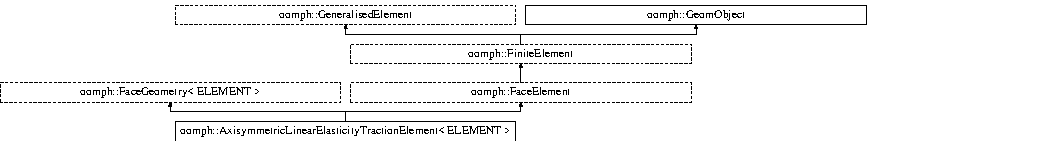
\includegraphics[height=1.890295cm]{classoomph_1_1AxisymmetricLinearElasticityTractionElement}
\end{center}
\end{figure}
\subsection*{Public Member Functions}
\begin{DoxyCompactItemize}
\item 
\hyperlink{classoomph_1_1AxisymmetricLinearElasticityTractionElement_a9b68dc55eee5ecabeaaab18d47af9008}{Axisymmetric\+Linear\+Elasticity\+Traction\+Element} (\hyperlink{classoomph_1_1FiniteElement}{Finite\+Element} $\ast$const \&element\+\_\+pt, const int \&\hyperlink{classoomph_1_1FaceElement_a478d577ac6db67ecc80f1f02ae3ab170}{face\+\_\+index})
\begin{DoxyCompactList}\small\item\em Constructor, which takes a \char`\"{}bulk\char`\"{} element and the value of the index and its limit. \end{DoxyCompactList}\item 
void \hyperlink{classoomph_1_1AxisymmetricLinearElasticityTractionElement_aeaffd515a63ba1bfc91868005545ef55}{fill\+\_\+in\+\_\+contribution\+\_\+to\+\_\+residuals} (\hyperlink{classoomph_1_1Vector}{Vector}$<$ double $>$ \&residuals)
\begin{DoxyCompactList}\small\item\em Return the residuals. \end{DoxyCompactList}\item 
void \hyperlink{classoomph_1_1AxisymmetricLinearElasticityTractionElement_a2a94d08c2f96f71ecd6edcfdfbceb4ab}{fill\+\_\+in\+\_\+contribution\+\_\+to\+\_\+jacobian} (\hyperlink{classoomph_1_1Vector}{Vector}$<$ double $>$ \&residuals, \hyperlink{classoomph_1_1DenseMatrix}{Dense\+Matrix}$<$ double $>$ \&jacobian)
\begin{DoxyCompactList}\small\item\em Fill in contribution from Jacobian. \end{DoxyCompactList}\item 
double \hyperlink{classoomph_1_1AxisymmetricLinearElasticityTractionElement_a1eeca70977b3ba93cffc2d811b054a9a}{zeta\+\_\+nodal} (const unsigned \&n, const unsigned \&k, const unsigned \&\hyperlink{cfortran_8h_adb50e893b86b3e55e751a42eab3cba82}{i}) const
\begin{DoxyCompactList}\small\item\em The \char`\"{}global\char`\"{} intrinsic coordinate of the element when viewed as part of a geometric object should be given by the \hyperlink{classoomph_1_1FaceElement}{Face\+Element} representation, by default (needed to break indeterminacy if bulk element is Solid\+Element) \end{DoxyCompactList}\item 
void \hyperlink{classoomph_1_1AxisymmetricLinearElasticityTractionElement_a5823855e2697fcf80ab41378d29cff5b}{output} (std\+::ostream \&outfile)
\begin{DoxyCompactList}\small\item\em Output function. \end{DoxyCompactList}\item 
void \hyperlink{classoomph_1_1AxisymmetricLinearElasticityTractionElement_ad2f848b61c90a1c1424ad0480eee4ba0}{output} (std\+::ostream \&outfile, const unsigned \&n\+\_\+plot)
\begin{DoxyCompactList}\small\item\em Output function. \end{DoxyCompactList}\item 
void \hyperlink{classoomph_1_1AxisymmetricLinearElasticityTractionElement_a3d7e3ee90159e221abb5ff860dd27cc6}{output} (F\+I\+LE $\ast$file\+\_\+pt)
\begin{DoxyCompactList}\small\item\em C\+\_\+style output function. \end{DoxyCompactList}\item 
void \hyperlink{classoomph_1_1AxisymmetricLinearElasticityTractionElement_a0c3231cf4b9d70b1b3080f195b1bf813}{output} (F\+I\+LE $\ast$file\+\_\+pt, const unsigned \&n\+\_\+plot)
\begin{DoxyCompactList}\small\item\em C-\/style output function. \end{DoxyCompactList}\item 
void \hyperlink{classoomph_1_1AxisymmetricLinearElasticityTractionElement_a28af87bac3d8d0c935564e69277e215e}{traction} (const double \&time, const \hyperlink{classoomph_1_1Vector}{Vector}$<$ double $>$ \&\hyperlink{cfortran_8h_ab7123126e4885ef647dd9c6e3807a21c}{s}, \hyperlink{classoomph_1_1Vector}{Vector}$<$ double $>$ \&traction)
\begin{DoxyCompactList}\small\item\em Compute traction vector at specified local coordinate Should only be used for post-\/processing; ignores dependence on integration point! \end{DoxyCompactList}\end{DoxyCompactItemize}
\subsection*{Public Attributes}
\begin{DoxyCompactItemize}
\item 
void($\ast$\&)(const double \&time, const \hyperlink{classoomph_1_1Vector}{Vector}$<$ double $>$ \&x, const \hyperlink{classoomph_1_1Vector}{Vector}$<$ double $>$ \&n, \hyperlink{classoomph_1_1Vector}{Vector}$<$ double $>$ \&\hyperlink{classoomph_1_1AxisymmetricLinearElasticityTractionElement_a28af87bac3d8d0c935564e69277e215e}{traction}) \hyperlink{classoomph_1_1AxisymmetricLinearElasticityTractionElement_a9c705a2b7379c63cc70c8e1e2aa6676d}{traction\+\_\+fct\+\_\+pt} ()
\begin{DoxyCompactList}\small\item\em Reference to the traction function pointer. \end{DoxyCompactList}\end{DoxyCompactItemize}
\subsection*{Protected Member Functions}
\begin{DoxyCompactItemize}
\item 
virtual void \hyperlink{classoomph_1_1AxisymmetricLinearElasticityTractionElement_a4ec6aee7438ab15aef197407e9c7ef8b}{get\+\_\+traction} (const double \&time, const unsigned \&intpt, const \hyperlink{classoomph_1_1Vector}{Vector}$<$ double $>$ \&x, const \hyperlink{classoomph_1_1Vector}{Vector}$<$ double $>$ \&n, \hyperlink{classoomph_1_1Vector}{Vector}$<$ double $>$ \&\hyperlink{classoomph_1_1AxisymmetricLinearElasticityTractionElement_a28af87bac3d8d0c935564e69277e215e}{traction})
\begin{DoxyCompactList}\small\item\em Get the traction vector\+: Pass number of integration point (dummy), Eulerian coordinate and normal vector and return the load vector (not all of the input arguments will be required for all specific load functions but the list should cover all cases). This function is virtual so it can be overloaded for F\+SI. \end{DoxyCompactList}\item 
void \hyperlink{classoomph_1_1AxisymmetricLinearElasticityTractionElement_aa263f7ced169d93b2e4fbb03738d059b}{fill\+\_\+in\+\_\+contribution\+\_\+to\+\_\+residuals\+\_\+axisymmetric\+\_\+linear\+\_\+elasticity\+\_\+traction} (\hyperlink{classoomph_1_1Vector}{Vector}$<$ double $>$ \&residuals)
\begin{DoxyCompactList}\small\item\em Helper function that actually calculates the residuals. \end{DoxyCompactList}\end{DoxyCompactItemize}
\subsection*{Protected Attributes}
\begin{DoxyCompactItemize}
\item 
\hyperlink{classoomph_1_1Vector}{Vector}$<$ unsigned $>$ \hyperlink{classoomph_1_1AxisymmetricLinearElasticityTractionElement_a2b4e580e5a53714c55b606575ad89669}{U\+\_\+index\+\_\+axisymmetric\+\_\+linear\+\_\+elasticity\+\_\+traction}
\begin{DoxyCompactList}\small\item\em Index at which the i-\/th displacement component is stored. \end{DoxyCompactList}\item 
void($\ast$ \hyperlink{classoomph_1_1AxisymmetricLinearElasticityTractionElement_a4e8f5cdb73984c400c4297a0f963a520}{Traction\+\_\+fct\+\_\+pt} )(const double \&time, const \hyperlink{classoomph_1_1Vector}{Vector}$<$ double $>$ \&x, const \hyperlink{classoomph_1_1Vector}{Vector}$<$ double $>$ \&n, \hyperlink{classoomph_1_1Vector}{Vector}$<$ double $>$ \&result)
\begin{DoxyCompactList}\small\item\em Pointer to an imposed traction function. Arguments\+: Eulerian coordinate; outer unit normal; applied traction. (Not all of the input arguments will be required for all specific load functions but the list should cover all cases) \end{DoxyCompactList}\end{DoxyCompactItemize}
\subsection*{Additional Inherited Members}


\subsection{Detailed Description}
\subsubsection*{template$<$class E\+L\+E\+M\+E\+NT$>$\newline
class oomph\+::\+Axisymmetric\+Linear\+Elasticity\+Traction\+Element$<$ E\+L\+E\+M\+E\+N\+T $>$}

A class for elements that allow the imposition of an applied traction in the equations of axisymmetric linear elasticity. The geometrical information can be read from the Face\+Geometry$<$\+E\+L\+E\+M\+E\+N\+T$>$ class and and thus, we can be generic enough without the need to have a separate equations class. 

Definition at line 82 of file axisym\+\_\+linear\+\_\+elasticity\+\_\+traction\+\_\+elements.\+h.



\subsection{Constructor \& Destructor Documentation}
\mbox{\Hypertarget{classoomph_1_1AxisymmetricLinearElasticityTractionElement_a9b68dc55eee5ecabeaaab18d47af9008}\label{classoomph_1_1AxisymmetricLinearElasticityTractionElement_a9b68dc55eee5ecabeaaab18d47af9008}} 
\index{oomph\+::\+Axisymmetric\+Linear\+Elasticity\+Traction\+Element@{oomph\+::\+Axisymmetric\+Linear\+Elasticity\+Traction\+Element}!Axisymmetric\+Linear\+Elasticity\+Traction\+Element@{Axisymmetric\+Linear\+Elasticity\+Traction\+Element}}
\index{Axisymmetric\+Linear\+Elasticity\+Traction\+Element@{Axisymmetric\+Linear\+Elasticity\+Traction\+Element}!oomph\+::\+Axisymmetric\+Linear\+Elasticity\+Traction\+Element@{oomph\+::\+Axisymmetric\+Linear\+Elasticity\+Traction\+Element}}
\subsubsection{\texorpdfstring{Axisymmetric\+Linear\+Elasticity\+Traction\+Element()}{AxisymmetricLinearElasticityTractionElement()}}
{\footnotesize\ttfamily template$<$class E\+L\+E\+M\+E\+NT $>$ \\
\hyperlink{classoomph_1_1AxisymmetricLinearElasticityTractionElement}{oomph\+::\+Axisymmetric\+Linear\+Elasticity\+Traction\+Element}$<$ E\+L\+E\+M\+E\+NT $>$\+::\hyperlink{classoomph_1_1AxisymmetricLinearElasticityTractionElement}{Axisymmetric\+Linear\+Elasticity\+Traction\+Element} (\begin{DoxyParamCaption}\item[{\hyperlink{classoomph_1_1FiniteElement}{Finite\+Element} $\ast$const \&}]{element\+\_\+pt,  }\item[{const int \&}]{face\+\_\+index }\end{DoxyParamCaption})\hspace{0.3cm}{\ttfamily [inline]}}



Constructor, which takes a \char`\"{}bulk\char`\"{} element and the value of the index and its limit. 



Definition at line 132 of file axisym\+\_\+linear\+\_\+elasticity\+\_\+traction\+\_\+elements.\+h.



References oomph\+::\+Finite\+Element\+::build\+\_\+face\+\_\+element(), i, oomph\+::\+Finite\+Element\+::nodal\+\_\+dimension(), and oomph\+::\+Axisymmetric\+Linear\+Elasticity\+Traction\+Element\+Helper\+::\+Zero\+\_\+traction\+\_\+fct().



\subsection{Member Function Documentation}
\mbox{\Hypertarget{classoomph_1_1AxisymmetricLinearElasticityTractionElement_a2a94d08c2f96f71ecd6edcfdfbceb4ab}\label{classoomph_1_1AxisymmetricLinearElasticityTractionElement_a2a94d08c2f96f71ecd6edcfdfbceb4ab}} 
\index{oomph\+::\+Axisymmetric\+Linear\+Elasticity\+Traction\+Element@{oomph\+::\+Axisymmetric\+Linear\+Elasticity\+Traction\+Element}!fill\+\_\+in\+\_\+contribution\+\_\+to\+\_\+jacobian@{fill\+\_\+in\+\_\+contribution\+\_\+to\+\_\+jacobian}}
\index{fill\+\_\+in\+\_\+contribution\+\_\+to\+\_\+jacobian@{fill\+\_\+in\+\_\+contribution\+\_\+to\+\_\+jacobian}!oomph\+::\+Axisymmetric\+Linear\+Elasticity\+Traction\+Element@{oomph\+::\+Axisymmetric\+Linear\+Elasticity\+Traction\+Element}}
\subsubsection{\texorpdfstring{fill\+\_\+in\+\_\+contribution\+\_\+to\+\_\+jacobian()}{fill\_in\_contribution\_to\_jacobian()}}
{\footnotesize\ttfamily template$<$class E\+L\+E\+M\+E\+NT $>$ \\
void \hyperlink{classoomph_1_1AxisymmetricLinearElasticityTractionElement}{oomph\+::\+Axisymmetric\+Linear\+Elasticity\+Traction\+Element}$<$ E\+L\+E\+M\+E\+NT $>$\+::fill\+\_\+in\+\_\+contribution\+\_\+to\+\_\+jacobian (\begin{DoxyParamCaption}\item[{\hyperlink{classoomph_1_1Vector}{Vector}$<$ double $>$ \&}]{residuals,  }\item[{\hyperlink{classoomph_1_1DenseMatrix}{Dense\+Matrix}$<$ double $>$ \&}]{jacobian }\end{DoxyParamCaption})\hspace{0.3cm}{\ttfamily [inline]}, {\ttfamily [virtual]}}



Fill in contribution from Jacobian. 



Reimplemented from \hyperlink{classoomph_1_1GeneralisedElement_a6ae09fc0d68e4309ac1b03583d252845}{oomph\+::\+Generalised\+Element}.



Definition at line 178 of file axisym\+\_\+linear\+\_\+elasticity\+\_\+traction\+\_\+elements.\+h.

\mbox{\Hypertarget{classoomph_1_1AxisymmetricLinearElasticityTractionElement_aeaffd515a63ba1bfc91868005545ef55}\label{classoomph_1_1AxisymmetricLinearElasticityTractionElement_aeaffd515a63ba1bfc91868005545ef55}} 
\index{oomph\+::\+Axisymmetric\+Linear\+Elasticity\+Traction\+Element@{oomph\+::\+Axisymmetric\+Linear\+Elasticity\+Traction\+Element}!fill\+\_\+in\+\_\+contribution\+\_\+to\+\_\+residuals@{fill\+\_\+in\+\_\+contribution\+\_\+to\+\_\+residuals}}
\index{fill\+\_\+in\+\_\+contribution\+\_\+to\+\_\+residuals@{fill\+\_\+in\+\_\+contribution\+\_\+to\+\_\+residuals}!oomph\+::\+Axisymmetric\+Linear\+Elasticity\+Traction\+Element@{oomph\+::\+Axisymmetric\+Linear\+Elasticity\+Traction\+Element}}
\subsubsection{\texorpdfstring{fill\+\_\+in\+\_\+contribution\+\_\+to\+\_\+residuals()}{fill\_in\_contribution\_to\_residuals()}}
{\footnotesize\ttfamily template$<$class E\+L\+E\+M\+E\+NT $>$ \\
void \hyperlink{classoomph_1_1AxisymmetricLinearElasticityTractionElement}{oomph\+::\+Axisymmetric\+Linear\+Elasticity\+Traction\+Element}$<$ E\+L\+E\+M\+E\+NT $>$\+::fill\+\_\+in\+\_\+contribution\+\_\+to\+\_\+residuals (\begin{DoxyParamCaption}\item[{\hyperlink{classoomph_1_1Vector}{Vector}$<$ double $>$ \&}]{residuals }\end{DoxyParamCaption})\hspace{0.3cm}{\ttfamily [inline]}, {\ttfamily [virtual]}}



Return the residuals. 



Reimplemented from \hyperlink{classoomph_1_1GeneralisedElement_a310c97f515e8504a48179c0e72c550d7}{oomph\+::\+Generalised\+Element}.



Definition at line 169 of file axisym\+\_\+linear\+\_\+elasticity\+\_\+traction\+\_\+elements.\+h.

\mbox{\Hypertarget{classoomph_1_1AxisymmetricLinearElasticityTractionElement_aa263f7ced169d93b2e4fbb03738d059b}\label{classoomph_1_1AxisymmetricLinearElasticityTractionElement_aa263f7ced169d93b2e4fbb03738d059b}} 
\index{oomph\+::\+Axisymmetric\+Linear\+Elasticity\+Traction\+Element@{oomph\+::\+Axisymmetric\+Linear\+Elasticity\+Traction\+Element}!fill\+\_\+in\+\_\+contribution\+\_\+to\+\_\+residuals\+\_\+axisymmetric\+\_\+linear\+\_\+elasticity\+\_\+traction@{fill\+\_\+in\+\_\+contribution\+\_\+to\+\_\+residuals\+\_\+axisymmetric\+\_\+linear\+\_\+elasticity\+\_\+traction}}
\index{fill\+\_\+in\+\_\+contribution\+\_\+to\+\_\+residuals\+\_\+axisymmetric\+\_\+linear\+\_\+elasticity\+\_\+traction@{fill\+\_\+in\+\_\+contribution\+\_\+to\+\_\+residuals\+\_\+axisymmetric\+\_\+linear\+\_\+elasticity\+\_\+traction}!oomph\+::\+Axisymmetric\+Linear\+Elasticity\+Traction\+Element@{oomph\+::\+Axisymmetric\+Linear\+Elasticity\+Traction\+Element}}
\subsubsection{\texorpdfstring{fill\+\_\+in\+\_\+contribution\+\_\+to\+\_\+residuals\+\_\+axisymmetric\+\_\+linear\+\_\+elasticity\+\_\+traction()}{fill\_in\_contribution\_to\_residuals\_axisymmetric\_linear\_elasticity\_traction()}}
{\footnotesize\ttfamily template$<$class E\+L\+E\+M\+E\+NT $>$ \\
void \hyperlink{classoomph_1_1AxisymmetricLinearElasticityTractionElement}{oomph\+::\+Axisymmetric\+Linear\+Elasticity\+Traction\+Element}$<$ E\+L\+E\+M\+E\+NT $>$\+::fill\+\_\+in\+\_\+contribution\+\_\+to\+\_\+residuals\+\_\+axisymmetric\+\_\+linear\+\_\+elasticity\+\_\+traction (\begin{DoxyParamCaption}\item[{\hyperlink{classoomph_1_1Vector}{Vector}$<$ double $>$ \&}]{residuals }\end{DoxyParamCaption})\hspace{0.3cm}{\ttfamily [protected]}}



Helper function that actually calculates the residuals. 

Return the residuals for the \hyperlink{classoomph_1_1AxisymmetricLinearElasticityTractionElement}{Axisymmetric\+Linear\+Elasticity\+Traction\+Element} equations 

Definition at line 340 of file axisym\+\_\+linear\+\_\+elasticity\+\_\+traction\+\_\+elements.\+h.



References i, and oomph\+::\+Quad\+Tree\+Names\+::W.



Referenced by oomph\+::\+Axisymmetric\+Linear\+Elasticity\+Traction\+Element$<$ E\+L\+E\+M\+E\+N\+T $>$\+::traction().

\mbox{\Hypertarget{classoomph_1_1AxisymmetricLinearElasticityTractionElement_a4ec6aee7438ab15aef197407e9c7ef8b}\label{classoomph_1_1AxisymmetricLinearElasticityTractionElement_a4ec6aee7438ab15aef197407e9c7ef8b}} 
\index{oomph\+::\+Axisymmetric\+Linear\+Elasticity\+Traction\+Element@{oomph\+::\+Axisymmetric\+Linear\+Elasticity\+Traction\+Element}!get\+\_\+traction@{get\+\_\+traction}}
\index{get\+\_\+traction@{get\+\_\+traction}!oomph\+::\+Axisymmetric\+Linear\+Elasticity\+Traction\+Element@{oomph\+::\+Axisymmetric\+Linear\+Elasticity\+Traction\+Element}}
\subsubsection{\texorpdfstring{get\+\_\+traction()}{get\_traction()}}
{\footnotesize\ttfamily template$<$class E\+L\+E\+M\+E\+NT $>$ \\
virtual void \hyperlink{classoomph_1_1AxisymmetricLinearElasticityTractionElement}{oomph\+::\+Axisymmetric\+Linear\+Elasticity\+Traction\+Element}$<$ E\+L\+E\+M\+E\+NT $>$\+::get\+\_\+traction (\begin{DoxyParamCaption}\item[{const double \&}]{time,  }\item[{const unsigned \&}]{intpt,  }\item[{const \hyperlink{classoomph_1_1Vector}{Vector}$<$ double $>$ \&}]{x,  }\item[{const \hyperlink{classoomph_1_1Vector}{Vector}$<$ double $>$ \&}]{n,  }\item[{\hyperlink{classoomph_1_1Vector}{Vector}$<$ double $>$ \&}]{traction }\end{DoxyParamCaption})\hspace{0.3cm}{\ttfamily [inline]}, {\ttfamily [protected]}, {\ttfamily [virtual]}}



Get the traction vector\+: Pass number of integration point (dummy), Eulerian coordinate and normal vector and return the load vector (not all of the input arguments will be required for all specific load functions but the list should cover all cases). This function is virtual so it can be overloaded for F\+SI. 



Definition at line 109 of file axisym\+\_\+linear\+\_\+elasticity\+\_\+traction\+\_\+elements.\+h.

\mbox{\Hypertarget{classoomph_1_1AxisymmetricLinearElasticityTractionElement_a5823855e2697fcf80ab41378d29cff5b}\label{classoomph_1_1AxisymmetricLinearElasticityTractionElement_a5823855e2697fcf80ab41378d29cff5b}} 
\index{oomph\+::\+Axisymmetric\+Linear\+Elasticity\+Traction\+Element@{oomph\+::\+Axisymmetric\+Linear\+Elasticity\+Traction\+Element}!output@{output}}
\index{output@{output}!oomph\+::\+Axisymmetric\+Linear\+Elasticity\+Traction\+Element@{oomph\+::\+Axisymmetric\+Linear\+Elasticity\+Traction\+Element}}
\subsubsection{\texorpdfstring{output()}{output()}\hspace{0.1cm}{\footnotesize\ttfamily [1/4]}}
{\footnotesize\ttfamily template$<$class E\+L\+E\+M\+E\+NT $>$ \\
void \hyperlink{classoomph_1_1AxisymmetricLinearElasticityTractionElement}{oomph\+::\+Axisymmetric\+Linear\+Elasticity\+Traction\+Element}$<$ E\+L\+E\+M\+E\+NT $>$\+::output (\begin{DoxyParamCaption}\item[{std\+::ostream \&}]{outfile }\end{DoxyParamCaption})\hspace{0.3cm}{\ttfamily [inline]}, {\ttfamily [virtual]}}



Output function. 



Reimplemented from \hyperlink{classoomph_1_1FiniteElement_a2ad98a3d2ef4999f1bef62c0ff13f2a7}{oomph\+::\+Finite\+Element}.



Definition at line 196 of file axisym\+\_\+linear\+\_\+elasticity\+\_\+traction\+\_\+elements.\+h.



References oomph\+::output().

\mbox{\Hypertarget{classoomph_1_1AxisymmetricLinearElasticityTractionElement_ad2f848b61c90a1c1424ad0480eee4ba0}\label{classoomph_1_1AxisymmetricLinearElasticityTractionElement_ad2f848b61c90a1c1424ad0480eee4ba0}} 
\index{oomph\+::\+Axisymmetric\+Linear\+Elasticity\+Traction\+Element@{oomph\+::\+Axisymmetric\+Linear\+Elasticity\+Traction\+Element}!output@{output}}
\index{output@{output}!oomph\+::\+Axisymmetric\+Linear\+Elasticity\+Traction\+Element@{oomph\+::\+Axisymmetric\+Linear\+Elasticity\+Traction\+Element}}
\subsubsection{\texorpdfstring{output()}{output()}\hspace{0.1cm}{\footnotesize\ttfamily [2/4]}}
{\footnotesize\ttfamily template$<$class E\+L\+E\+M\+E\+NT $>$ \\
void \hyperlink{classoomph_1_1AxisymmetricLinearElasticityTractionElement}{oomph\+::\+Axisymmetric\+Linear\+Elasticity\+Traction\+Element}$<$ E\+L\+E\+M\+E\+NT $>$\+::output (\begin{DoxyParamCaption}\item[{std\+::ostream \&}]{outfile,  }\item[{const unsigned \&}]{n\+\_\+plot }\end{DoxyParamCaption})\hspace{0.3cm}{\ttfamily [inline]}, {\ttfamily [virtual]}}



Output function. 



Reimplemented from \hyperlink{classoomph_1_1FiniteElement_afa9d9b2670f999b43e6679c9dd28c457}{oomph\+::\+Finite\+Element}.



Definition at line 203 of file axisym\+\_\+linear\+\_\+elasticity\+\_\+traction\+\_\+elements.\+h.



References i, s, and oomph\+::\+One\+Dim\+Lagrange\+::shape().

\mbox{\Hypertarget{classoomph_1_1AxisymmetricLinearElasticityTractionElement_a3d7e3ee90159e221abb5ff860dd27cc6}\label{classoomph_1_1AxisymmetricLinearElasticityTractionElement_a3d7e3ee90159e221abb5ff860dd27cc6}} 
\index{oomph\+::\+Axisymmetric\+Linear\+Elasticity\+Traction\+Element@{oomph\+::\+Axisymmetric\+Linear\+Elasticity\+Traction\+Element}!output@{output}}
\index{output@{output}!oomph\+::\+Axisymmetric\+Linear\+Elasticity\+Traction\+Element@{oomph\+::\+Axisymmetric\+Linear\+Elasticity\+Traction\+Element}}
\subsubsection{\texorpdfstring{output()}{output()}\hspace{0.1cm}{\footnotesize\ttfamily [3/4]}}
{\footnotesize\ttfamily template$<$class E\+L\+E\+M\+E\+NT $>$ \\
void \hyperlink{classoomph_1_1AxisymmetricLinearElasticityTractionElement}{oomph\+::\+Axisymmetric\+Linear\+Elasticity\+Traction\+Element}$<$ E\+L\+E\+M\+E\+NT $>$\+::output (\begin{DoxyParamCaption}\item[{F\+I\+LE $\ast$}]{file\+\_\+pt }\end{DoxyParamCaption})\hspace{0.3cm}{\ttfamily [inline]}, {\ttfamily [virtual]}}



C\+\_\+style output function. 



Reimplemented from \hyperlink{classoomph_1_1FiniteElement_a72cddd09f8ddbee1a20a1ff404c6943e}{oomph\+::\+Finite\+Element}.



Definition at line 285 of file axisym\+\_\+linear\+\_\+elasticity\+\_\+traction\+\_\+elements.\+h.



References oomph\+::\+Finite\+Element\+::output().

\mbox{\Hypertarget{classoomph_1_1AxisymmetricLinearElasticityTractionElement_a0c3231cf4b9d70b1b3080f195b1bf813}\label{classoomph_1_1AxisymmetricLinearElasticityTractionElement_a0c3231cf4b9d70b1b3080f195b1bf813}} 
\index{oomph\+::\+Axisymmetric\+Linear\+Elasticity\+Traction\+Element@{oomph\+::\+Axisymmetric\+Linear\+Elasticity\+Traction\+Element}!output@{output}}
\index{output@{output}!oomph\+::\+Axisymmetric\+Linear\+Elasticity\+Traction\+Element@{oomph\+::\+Axisymmetric\+Linear\+Elasticity\+Traction\+Element}}
\subsubsection{\texorpdfstring{output()}{output()}\hspace{0.1cm}{\footnotesize\ttfamily [4/4]}}
{\footnotesize\ttfamily template$<$class E\+L\+E\+M\+E\+NT $>$ \\
void \hyperlink{classoomph_1_1AxisymmetricLinearElasticityTractionElement}{oomph\+::\+Axisymmetric\+Linear\+Elasticity\+Traction\+Element}$<$ E\+L\+E\+M\+E\+NT $>$\+::output (\begin{DoxyParamCaption}\item[{F\+I\+LE $\ast$}]{file\+\_\+pt,  }\item[{const unsigned \&}]{n\+\_\+plot }\end{DoxyParamCaption})\hspace{0.3cm}{\ttfamily [inline]}, {\ttfamily [virtual]}}



C-\/style output function. 



Reimplemented from \hyperlink{classoomph_1_1FiniteElement_adfaee690bb0608f03320eeb9d110d48c}{oomph\+::\+Finite\+Element}.



Definition at line 289 of file axisym\+\_\+linear\+\_\+elasticity\+\_\+traction\+\_\+elements.\+h.



References oomph\+::\+Finite\+Element\+::output(), s, and oomph\+::\+Axisymmetric\+Linear\+Elasticity\+Traction\+Element$<$ E\+L\+E\+M\+E\+N\+T $>$\+::traction().

\mbox{\Hypertarget{classoomph_1_1AxisymmetricLinearElasticityTractionElement_a28af87bac3d8d0c935564e69277e215e}\label{classoomph_1_1AxisymmetricLinearElasticityTractionElement_a28af87bac3d8d0c935564e69277e215e}} 
\index{oomph\+::\+Axisymmetric\+Linear\+Elasticity\+Traction\+Element@{oomph\+::\+Axisymmetric\+Linear\+Elasticity\+Traction\+Element}!traction@{traction}}
\index{traction@{traction}!oomph\+::\+Axisymmetric\+Linear\+Elasticity\+Traction\+Element@{oomph\+::\+Axisymmetric\+Linear\+Elasticity\+Traction\+Element}}
\subsubsection{\texorpdfstring{traction()}{traction()}}
{\footnotesize\ttfamily template$<$class E\+L\+E\+M\+E\+NT $>$ \\
void \hyperlink{classoomph_1_1AxisymmetricLinearElasticityTractionElement}{oomph\+::\+Axisymmetric\+Linear\+Elasticity\+Traction\+Element}$<$ E\+L\+E\+M\+E\+NT $>$\+::traction (\begin{DoxyParamCaption}\item[{const double \&}]{time,  }\item[{const \hyperlink{classoomph_1_1Vector}{Vector}$<$ double $>$ \&}]{s,  }\item[{\hyperlink{classoomph_1_1Vector}{Vector}$<$ double $>$ \&}]{traction }\end{DoxyParamCaption})}



Compute traction vector at specified local coordinate Should only be used for post-\/processing; ignores dependence on integration point! 

Compute traction vector at specified local coordinate Should only be used for post-\/processing; ignores dependence on integration point! 

Definition at line 313 of file axisym\+\_\+linear\+\_\+elasticity\+\_\+traction\+\_\+elements.\+h.



References oomph\+::\+Axisymmetric\+Linear\+Elasticity\+Traction\+Element$<$ E\+L\+E\+M\+E\+N\+T $>$\+::fill\+\_\+in\+\_\+contribution\+\_\+to\+\_\+residuals\+\_\+axisymmetric\+\_\+linear\+\_\+elasticity\+\_\+traction().



Referenced by oomph\+::\+Axisymmetric\+Linear\+Elasticity\+Traction\+Element$<$ E\+L\+E\+M\+E\+N\+T $>$\+::output().

\mbox{\Hypertarget{classoomph_1_1AxisymmetricLinearElasticityTractionElement_a1eeca70977b3ba93cffc2d811b054a9a}\label{classoomph_1_1AxisymmetricLinearElasticityTractionElement_a1eeca70977b3ba93cffc2d811b054a9a}} 
\index{oomph\+::\+Axisymmetric\+Linear\+Elasticity\+Traction\+Element@{oomph\+::\+Axisymmetric\+Linear\+Elasticity\+Traction\+Element}!zeta\+\_\+nodal@{zeta\+\_\+nodal}}
\index{zeta\+\_\+nodal@{zeta\+\_\+nodal}!oomph\+::\+Axisymmetric\+Linear\+Elasticity\+Traction\+Element@{oomph\+::\+Axisymmetric\+Linear\+Elasticity\+Traction\+Element}}
\subsubsection{\texorpdfstring{zeta\+\_\+nodal()}{zeta\_nodal()}}
{\footnotesize\ttfamily template$<$class E\+L\+E\+M\+E\+NT $>$ \\
double \hyperlink{classoomph_1_1AxisymmetricLinearElasticityTractionElement}{oomph\+::\+Axisymmetric\+Linear\+Elasticity\+Traction\+Element}$<$ E\+L\+E\+M\+E\+NT $>$\+::zeta\+\_\+nodal (\begin{DoxyParamCaption}\item[{const unsigned \&}]{n,  }\item[{const unsigned \&}]{k,  }\item[{const unsigned \&}]{i }\end{DoxyParamCaption}) const\hspace{0.3cm}{\ttfamily [inline]}, {\ttfamily [virtual]}}



The \char`\"{}global\char`\"{} intrinsic coordinate of the element when viewed as part of a geometric object should be given by the \hyperlink{classoomph_1_1FaceElement}{Face\+Element} representation, by default (needed to break indeterminacy if bulk element is Solid\+Element) 

Specify the value of nodal zeta from the face geometry 

Reimplemented from \hyperlink{classoomph_1_1FiniteElement_a849561c5fbcbc07dc49d2dc6cca68559}{oomph\+::\+Finite\+Element}.



Definition at line 191 of file axisym\+\_\+linear\+\_\+elasticity\+\_\+traction\+\_\+elements.\+h.



References oomph\+::\+Face\+Element\+::zeta\+\_\+nodal().



\subsection{Member Data Documentation}
\mbox{\Hypertarget{classoomph_1_1AxisymmetricLinearElasticityTractionElement_a4e8f5cdb73984c400c4297a0f963a520}\label{classoomph_1_1AxisymmetricLinearElasticityTractionElement_a4e8f5cdb73984c400c4297a0f963a520}} 
\index{oomph\+::\+Axisymmetric\+Linear\+Elasticity\+Traction\+Element@{oomph\+::\+Axisymmetric\+Linear\+Elasticity\+Traction\+Element}!Traction\+\_\+fct\+\_\+pt@{Traction\+\_\+fct\+\_\+pt}}
\index{Traction\+\_\+fct\+\_\+pt@{Traction\+\_\+fct\+\_\+pt}!oomph\+::\+Axisymmetric\+Linear\+Elasticity\+Traction\+Element@{oomph\+::\+Axisymmetric\+Linear\+Elasticity\+Traction\+Element}}
\subsubsection{\texorpdfstring{Traction\+\_\+fct\+\_\+pt}{Traction\_fct\_pt}}
{\footnotesize\ttfamily template$<$class E\+L\+E\+M\+E\+NT $>$ \\
void($\ast$ \hyperlink{classoomph_1_1AxisymmetricLinearElasticityTractionElement}{oomph\+::\+Axisymmetric\+Linear\+Elasticity\+Traction\+Element}$<$ E\+L\+E\+M\+E\+NT $>$\+::Traction\+\_\+fct\+\_\+pt) (const double \&time, const \hyperlink{classoomph_1_1Vector}{Vector}$<$ double $>$ \&x, const \hyperlink{classoomph_1_1Vector}{Vector}$<$ double $>$ \&n, \hyperlink{classoomph_1_1Vector}{Vector}$<$ double $>$ \&result)\hspace{0.3cm}{\ttfamily [protected]}}



Pointer to an imposed traction function. Arguments\+: Eulerian coordinate; outer unit normal; applied traction. (Not all of the input arguments will be required for all specific load functions but the list should cover all cases) 



Definition at line 97 of file axisym\+\_\+linear\+\_\+elasticity\+\_\+traction\+\_\+elements.\+h.

\mbox{\Hypertarget{classoomph_1_1AxisymmetricLinearElasticityTractionElement_a9c705a2b7379c63cc70c8e1e2aa6676d}\label{classoomph_1_1AxisymmetricLinearElasticityTractionElement_a9c705a2b7379c63cc70c8e1e2aa6676d}} 
\index{oomph\+::\+Axisymmetric\+Linear\+Elasticity\+Traction\+Element@{oomph\+::\+Axisymmetric\+Linear\+Elasticity\+Traction\+Element}!traction\+\_\+fct\+\_\+pt@{traction\+\_\+fct\+\_\+pt}}
\index{traction\+\_\+fct\+\_\+pt@{traction\+\_\+fct\+\_\+pt}!oomph\+::\+Axisymmetric\+Linear\+Elasticity\+Traction\+Element@{oomph\+::\+Axisymmetric\+Linear\+Elasticity\+Traction\+Element}}
\subsubsection{\texorpdfstring{traction\+\_\+fct\+\_\+pt}{traction\_fct\_pt}}
{\footnotesize\ttfamily template$<$class E\+L\+E\+M\+E\+NT $>$ \\
void($\ast$ \&)(const double\& time, const \hyperlink{classoomph_1_1Vector}{Vector}$<$double$>$\& x, const \hyperlink{classoomph_1_1Vector}{Vector}$<$double$>$\& n, \hyperlink{classoomph_1_1Vector}{Vector}$<$double$>$\& \hyperlink{classoomph_1_1AxisymmetricLinearElasticityTractionElement_a28af87bac3d8d0c935564e69277e215e}{traction}) \hyperlink{classoomph_1_1AxisymmetricLinearElasticityTractionElement}{oomph\+::\+Axisymmetric\+Linear\+Elasticity\+Traction\+Element}$<$ E\+L\+E\+M\+E\+NT $>$\+::traction\+\_\+fct\+\_\+pt()\hspace{0.3cm}{\ttfamily [inline]}}



Reference to the traction function pointer. 



Definition at line 161 of file axisym\+\_\+linear\+\_\+elasticity\+\_\+traction\+\_\+elements.\+h.

\mbox{\Hypertarget{classoomph_1_1AxisymmetricLinearElasticityTractionElement_a2b4e580e5a53714c55b606575ad89669}\label{classoomph_1_1AxisymmetricLinearElasticityTractionElement_a2b4e580e5a53714c55b606575ad89669}} 
\index{oomph\+::\+Axisymmetric\+Linear\+Elasticity\+Traction\+Element@{oomph\+::\+Axisymmetric\+Linear\+Elasticity\+Traction\+Element}!U\+\_\+index\+\_\+axisymmetric\+\_\+linear\+\_\+elasticity\+\_\+traction@{U\+\_\+index\+\_\+axisymmetric\+\_\+linear\+\_\+elasticity\+\_\+traction}}
\index{U\+\_\+index\+\_\+axisymmetric\+\_\+linear\+\_\+elasticity\+\_\+traction@{U\+\_\+index\+\_\+axisymmetric\+\_\+linear\+\_\+elasticity\+\_\+traction}!oomph\+::\+Axisymmetric\+Linear\+Elasticity\+Traction\+Element@{oomph\+::\+Axisymmetric\+Linear\+Elasticity\+Traction\+Element}}
\subsubsection{\texorpdfstring{U\+\_\+index\+\_\+axisymmetric\+\_\+linear\+\_\+elasticity\+\_\+traction}{U\_index\_axisymmetric\_linear\_elasticity\_traction}}
{\footnotesize\ttfamily template$<$class E\+L\+E\+M\+E\+NT $>$ \\
\hyperlink{classoomph_1_1Vector}{Vector}$<$unsigned$>$ \hyperlink{classoomph_1_1AxisymmetricLinearElasticityTractionElement}{oomph\+::\+Axisymmetric\+Linear\+Elasticity\+Traction\+Element}$<$ E\+L\+E\+M\+E\+NT $>$\+::U\+\_\+index\+\_\+axisymmetric\+\_\+linear\+\_\+elasticity\+\_\+traction\hspace{0.3cm}{\ttfamily [protected]}}



Index at which the i-\/th displacement component is stored. 



Definition at line 90 of file axisym\+\_\+linear\+\_\+elasticity\+\_\+traction\+\_\+elements.\+h.



The documentation for this class was generated from the following file\+:\begin{DoxyCompactItemize}
\item 
\hyperlink{axisym__linear__elasticity__traction__elements_8h}{axisym\+\_\+linear\+\_\+elasticity\+\_\+traction\+\_\+elements.\+h}\end{DoxyCompactItemize}

\hypertarget{classoomph_1_1AxisymmetricNavierStokesEquations}{}\section{oomph\+:\+:Axisymmetric\+Navier\+Stokes\+Equations Class Reference}
\label{classoomph_1_1AxisymmetricNavierStokesEquations}\index{oomph\+::\+Axisymmetric\+Navier\+Stokes\+Equations@{oomph\+::\+Axisymmetric\+Navier\+Stokes\+Equations}}


{\ttfamily \#include $<$axisym\+\_\+navier\+\_\+stokes\+\_\+elements.\+h$>$}

Inheritance diagram for oomph\+:\+:Axisymmetric\+Navier\+Stokes\+Equations\+:\begin{figure}[H]
\begin{center}
\leavevmode
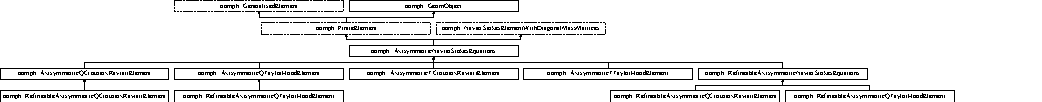
\includegraphics[height=1.368524cm]{classoomph_1_1AxisymmetricNavierStokesEquations}
\end{center}
\end{figure}
\subsection*{Public Member Functions}
\begin{DoxyCompactItemize}
\item 
\hyperlink{classoomph_1_1AxisymmetricNavierStokesEquations_a639d6998fea9b62d0341b8ae6547aecf}{Axisymmetric\+Navier\+Stokes\+Equations} ()
\begin{DoxyCompactList}\small\item\em Constructor\+: N\+U\+LL the body force and source function. \end{DoxyCompactList}\item 
const double \& \hyperlink{classoomph_1_1AxisymmetricNavierStokesEquations_a5326eb9f37e9ca42103ea7c72622a415}{re} () const
\begin{DoxyCompactList}\small\item\em Reynolds number. \end{DoxyCompactList}\item 
const double \& \hyperlink{classoomph_1_1AxisymmetricNavierStokesEquations_aa951cf371f58231f3c0967255843a50a}{re\+\_\+st} () const
\begin{DoxyCompactList}\small\item\em Product of Reynolds and Strouhal number (=Womersley number) \end{DoxyCompactList}\item 
double $\ast$\& \hyperlink{classoomph_1_1AxisymmetricNavierStokesEquations_a783cd0439da3951032dcf984d7c98433}{re\+\_\+pt} ()
\begin{DoxyCompactList}\small\item\em Pointer to Reynolds number. \end{DoxyCompactList}\item 
double $\ast$\& \hyperlink{classoomph_1_1AxisymmetricNavierStokesEquations_a64f354d90dcae78352e08b369a4c2a02}{re\+\_\+st\+\_\+pt} ()
\begin{DoxyCompactList}\small\item\em Pointer to product of Reynolds and Strouhal number (=Womersley number) \end{DoxyCompactList}\item 
const double \& \hyperlink{classoomph_1_1AxisymmetricNavierStokesEquations_aab647203e95cec99d25d42cee76a5e38}{re\+\_\+invfr} () const
\begin{DoxyCompactList}\small\item\em Global inverse Froude number. \end{DoxyCompactList}\item 
double $\ast$\& \hyperlink{classoomph_1_1AxisymmetricNavierStokesEquations_a2b2641a17d3406043cdf535fb6ede367}{re\+\_\+invfr\+\_\+pt} ()
\begin{DoxyCompactList}\small\item\em Pointer to global inverse Froude number. \end{DoxyCompactList}\item 
const double \& \hyperlink{classoomph_1_1AxisymmetricNavierStokesEquations_a30e9502122f5c88cdfb33edb45d88c5f}{re\+\_\+invro} () const
\begin{DoxyCompactList}\small\item\em Global Reynolds number multiplied by inverse Rossby number. \end{DoxyCompactList}\item 
double $\ast$\& \hyperlink{classoomph_1_1AxisymmetricNavierStokesEquations_a5f10cf57b03c4a76b70151df35a249e3}{re\+\_\+invro\+\_\+pt} ()
\begin{DoxyCompactList}\small\item\em Pointer to global inverse Froude number. \end{DoxyCompactList}\item 
const \hyperlink{classoomph_1_1Vector}{Vector}$<$ double $>$ \& \hyperlink{classoomph_1_1AxisymmetricNavierStokesEquations_a518c31629e6ef42334cd031e2901efea}{g} () const
\begin{DoxyCompactList}\small\item\em \hyperlink{classoomph_1_1Vector}{Vector} of gravitational components. \end{DoxyCompactList}\item 
\hyperlink{classoomph_1_1Vector}{Vector}$<$ double $>$ $\ast$\& \hyperlink{classoomph_1_1AxisymmetricNavierStokesEquations_ac3d87734f99afe1ea996aa66e8211693}{g\+\_\+pt} ()
\begin{DoxyCompactList}\small\item\em Pointer to \hyperlink{classoomph_1_1Vector}{Vector} of gravitational components. \end{DoxyCompactList}\item 
const double \& \hyperlink{classoomph_1_1AxisymmetricNavierStokesEquations_a26df65fe19563b703fe274179e829900}{density\+\_\+ratio} () const
\begin{DoxyCompactList}\small\item\em Density ratio for element\+: Element\textquotesingle{}s density relative to the viscosity used in the definition of the Reynolds number. \end{DoxyCompactList}\item 
double $\ast$\& \hyperlink{classoomph_1_1AxisymmetricNavierStokesEquations_a41b0018805380d1673308198128fc4b7}{density\+\_\+ratio\+\_\+pt} ()
\begin{DoxyCompactList}\small\item\em Pointer to Density ratio. \end{DoxyCompactList}\item 
const double \& \hyperlink{classoomph_1_1AxisymmetricNavierStokesEquations_a4cf2dc737978f76fc7e0ad6358414f88}{viscosity\+\_\+ratio} () const
\begin{DoxyCompactList}\small\item\em Viscosity ratio for element\+: Element\textquotesingle{}s viscosity relative to the viscosity used in the definition of the Reynolds number. \end{DoxyCompactList}\item 
double $\ast$\& \hyperlink{classoomph_1_1AxisymmetricNavierStokesEquations_a50dcf24d5162fa8f5fd8a6efc4df17b7}{viscosity\+\_\+ratio\+\_\+pt} ()
\begin{DoxyCompactList}\small\item\em Pointer to Viscosity Ratio. \end{DoxyCompactList}\item 
virtual unsigned \hyperlink{classoomph_1_1AxisymmetricNavierStokesEquations_a89edaffb4913131cc14a5f6e45ed117a}{npres\+\_\+axi\+\_\+nst} () const =0
\begin{DoxyCompactList}\small\item\em Function to return number of pressure degrees of freedom. \end{DoxyCompactList}\item 
virtual unsigned \hyperlink{classoomph_1_1AxisymmetricNavierStokesEquations_afbdea50fcf4799e2e4e5209ee3249bf0}{u\+\_\+index\+\_\+axi\+\_\+nst} (const unsigned \&\hyperlink{cfortran_8h_adb50e893b86b3e55e751a42eab3cba82}{i}) const
\begin{DoxyCompactList}\small\item\em Return the index at which the i-\/th unknown velocity component. \end{DoxyCompactList}\item 
unsigned \hyperlink{classoomph_1_1AxisymmetricNavierStokesEquations_a14098e563e5329282612425f629eb196}{u\+\_\+index\+\_\+nst} (const unsigned \&\hyperlink{cfortran_8h_adb50e893b86b3e55e751a42eab3cba82}{i}) const
\begin{DoxyCompactList}\small\item\em Return the index at which the i-\/th unknown velocity component is stored with a common interface for use in general Fluid\+Interface and similar elements. To do\+: Merge all common storage etc to a common base class for Navier--Stokes elements in all coordinate systems. \end{DoxyCompactList}\item 
unsigned \hyperlink{classoomph_1_1AxisymmetricNavierStokesEquations_aa1749260b72bab92bc64234d9c8c57d8}{n\+\_\+u\+\_\+nst} () const
\begin{DoxyCompactList}\small\item\em Return the number of velocity components for use in general Fluid\+Interface clas. \end{DoxyCompactList}\item 
double \hyperlink{classoomph_1_1AxisymmetricNavierStokesEquations_a80b3415e150243f8fff3f8eb87082b24}{du\+\_\+dt\+\_\+axi\+\_\+nst} (const unsigned \&n, const unsigned \&\hyperlink{cfortran_8h_adb50e893b86b3e55e751a42eab3cba82}{i}) const
\begin{DoxyCompactList}\small\item\em i-\/th component of du/dt at local node n. Uses suitably interpolated value for hanging nodes. \end{DoxyCompactList}\item 
void \hyperlink{classoomph_1_1AxisymmetricNavierStokesEquations_a737e9a0e65aa0e88a63d740ea56717ec}{disable\+\_\+\+A\+LE} ()
\begin{DoxyCompactList}\small\item\em Disable A\+LE, i.\+e. assert the mesh is not moving -- you do this at your own risk! \end{DoxyCompactList}\item 
void \hyperlink{classoomph_1_1AxisymmetricNavierStokesEquations_ac5b7a740769b0e5cb1e95db6dab34800}{enable\+\_\+\+A\+LE} ()
\begin{DoxyCompactList}\small\item\em (Re-\/)enable A\+LE, i.\+e. take possible mesh motion into account when evaluating the time-\/derivative. Note\+: By default, A\+LE is enabled, at the expense of possibly creating unnecessary work in problems where the mesh is, in fact, stationary. \end{DoxyCompactList}\item 
virtual double \hyperlink{classoomph_1_1AxisymmetricNavierStokesEquations_a3aa173227f477a40fb4adba84a337f5b}{p\+\_\+axi\+\_\+nst} (const unsigned \&n\+\_\+p) const =0
\begin{DoxyCompactList}\small\item\em Pressure at local pressure \char`\"{}node\char`\"{} n\+\_\+p Uses suitably interpolated value for hanging nodes. \end{DoxyCompactList}\item 
virtual int \hyperlink{classoomph_1_1AxisymmetricNavierStokesEquations_a47c61dbb8a32fd785c99ab3aa8bc35f9}{p\+\_\+nodal\+\_\+index\+\_\+axi\+\_\+nst} () const
\begin{DoxyCompactList}\small\item\em Which nodal value represents the pressure? \end{DoxyCompactList}\item 
double \hyperlink{classoomph_1_1AxisymmetricNavierStokesEquations_a056e6c406e93a62763a0ac8912ce9e1b}{pressure\+\_\+integral} () const
\begin{DoxyCompactList}\small\item\em \hyperlink{classoomph_1_1Integral}{Integral} of pressure over element. \end{DoxyCompactList}\item 
double \hyperlink{classoomph_1_1AxisymmetricNavierStokesEquations_a002f84742337fbf2dcba83866b1d089e}{dissipation} () const
\begin{DoxyCompactList}\small\item\em Return integral of dissipation over element. \end{DoxyCompactList}\item 
double \hyperlink{classoomph_1_1AxisymmetricNavierStokesEquations_a17b8b46a8ebbb5d75486077c960d5844}{dissipation} (const \hyperlink{classoomph_1_1Vector}{Vector}$<$ double $>$ \&\hyperlink{cfortran_8h_ab7123126e4885ef647dd9c6e3807a21c}{s}) const
\begin{DoxyCompactList}\small\item\em Return dissipation at local coordinate s. \end{DoxyCompactList}\item 
double \hyperlink{classoomph_1_1AxisymmetricNavierStokesEquations_a823b3494f75b435cf8d0fbe5572937a8}{kin\+\_\+energy} () const
\begin{DoxyCompactList}\small\item\em Get integral of kinetic energy over element. \end{DoxyCompactList}\item 
void \hyperlink{classoomph_1_1AxisymmetricNavierStokesEquations_ad12929a11d71f7d91627f3edc8f2cdce}{strain\+\_\+rate} (const \hyperlink{classoomph_1_1Vector}{Vector}$<$ double $>$ \&\hyperlink{cfortran_8h_ab7123126e4885ef647dd9c6e3807a21c}{s}, \hyperlink{classoomph_1_1DenseMatrix}{Dense\+Matrix}$<$ double $>$ \&strain\+\_\+rate) const
\begin{DoxyCompactList}\small\item\em Strain-\/rate tensor\+: $ e_{ij} $ where $ i,j = r,z,\theta $ (in that order) \end{DoxyCompactList}\item 
void \hyperlink{classoomph_1_1AxisymmetricNavierStokesEquations_a0a5523b91d5191c2f9e23fe8d74f4e07}{traction} (const \hyperlink{classoomph_1_1Vector}{Vector}$<$ double $>$ \&\hyperlink{cfortran_8h_ab7123126e4885ef647dd9c6e3807a21c}{s}, const \hyperlink{classoomph_1_1Vector}{Vector}$<$ double $>$ \&N, \hyperlink{classoomph_1_1Vector}{Vector}$<$ double $>$ \&traction) const
\begin{DoxyCompactList}\small\item\em Compute traction (on the viscous scale) at local coordinate s for outer unit normal N. \end{DoxyCompactList}\item 
void \hyperlink{classoomph_1_1AxisymmetricNavierStokesEquations_ac0c850c7a41b408784f3a103f9aba982}{get\+\_\+pressure\+\_\+and\+\_\+velocity\+\_\+mass\+\_\+matrix\+\_\+diagonal} (\hyperlink{classoomph_1_1Vector}{Vector}$<$ double $>$ \&press\+\_\+mass\+\_\+diag, \hyperlink{classoomph_1_1Vector}{Vector}$<$ double $>$ \&veloc\+\_\+mass\+\_\+diag, const unsigned \&which\+\_\+one=0)
\begin{DoxyCompactList}\small\item\em Compute the diagonal of the velocity/pressure mass matrices. If which one=0, both are computed, otherwise only the pressure (which\+\_\+one=1) or the velocity mass matrix (which\+\_\+one=2 -- the L\+SC version of the preconditioner only needs that one) N\+O\+TE\+: pressure versions isn\textquotesingle{}t implemented yet because this element has never been tried with Fp preconditoner. \end{DoxyCompactList}\item 
unsigned \hyperlink{classoomph_1_1AxisymmetricNavierStokesEquations_a1383f2cbddcd5a9b69ed41aab82dca36}{nscalar\+\_\+paraview} () const
\begin{DoxyCompactList}\small\item\em Number of scalars/fields output by this element. Reimplements broken virtual function in base class. \end{DoxyCompactList}\item 
void \hyperlink{classoomph_1_1AxisymmetricNavierStokesEquations_a2971656a8fa501ac3e4710c3f1c44275}{scalar\+\_\+value\+\_\+paraview} (std\+::ofstream \&file\+\_\+out, const unsigned \&\hyperlink{cfortran_8h_adb50e893b86b3e55e751a42eab3cba82}{i}, const unsigned \&nplot) const
\begin{DoxyCompactList}\small\item\em Write values of the i-\/th scalar field at the plot points. Needs to be implemented for each new specific element type. \end{DoxyCompactList}\item 
std\+::string \hyperlink{classoomph_1_1AxisymmetricNavierStokesEquations_a44ffef8f80dd1419fd6a7b281e2185b3}{scalar\+\_\+name\+\_\+paraview} (const unsigned \&\hyperlink{cfortran_8h_adb50e893b86b3e55e751a42eab3cba82}{i}) const
\begin{DoxyCompactList}\small\item\em Name of the i-\/th scalar field. Default implementation returns V1 for the first one, V2 for the second etc. Can (should!) be overloaded with more meaningful names in specific elements. \end{DoxyCompactList}\item 
void \hyperlink{classoomph_1_1AxisymmetricNavierStokesEquations_a011b01b75649aaeba4cf759ba5e4b9e8}{point\+\_\+output\+\_\+data} (const \hyperlink{classoomph_1_1Vector}{Vector}$<$ double $>$ \&\hyperlink{cfortran_8h_ab7123126e4885ef647dd9c6e3807a21c}{s}, \hyperlink{classoomph_1_1Vector}{Vector}$<$ double $>$ \&data)
\begin{DoxyCompactList}\small\item\em Output solution in data vector at local cordinates s\+: r,z,u\+\_\+r,u\+\_\+z,u\+\_\+phi,p. \end{DoxyCompactList}\item 
void \hyperlink{classoomph_1_1AxisymmetricNavierStokesEquations_afe0c7b607ec3fd03a73b7db4f1fe6252}{output} (std\+::ostream \&outfile)
\begin{DoxyCompactList}\small\item\em Output function\+: x,y,\mbox{[}z\mbox{]},u,v,\mbox{[}w\mbox{]},p in tecplot format. Default number of plot points. \end{DoxyCompactList}\item 
void \hyperlink{classoomph_1_1AxisymmetricNavierStokesEquations_a94a243ca05ba3b995e366564e6cf7695}{output} (std\+::ostream \&outfile, const unsigned \&nplot)
\begin{DoxyCompactList}\small\item\em Output function\+: x,y,\mbox{[}z\mbox{]},u,v,\mbox{[}w\mbox{]},p in tecplot format. nplot points in each coordinate direction. \end{DoxyCompactList}\item 
void \hyperlink{classoomph_1_1AxisymmetricNavierStokesEquations_a61129dd7505ac363862946bd8b3ea5bf}{output} (F\+I\+LE $\ast$file\+\_\+pt)
\begin{DoxyCompactList}\small\item\em Output function\+: x,y,\mbox{[}z\mbox{]},u,v,\mbox{[}w\mbox{]},p in tecplot format. Default number of plot points. \end{DoxyCompactList}\item 
void \hyperlink{classoomph_1_1AxisymmetricNavierStokesEquations_abc2ca00250845e243da3f4e0845b2c96}{output} (F\+I\+LE $\ast$file\+\_\+pt, const unsigned \&nplot)
\begin{DoxyCompactList}\small\item\em Output function\+: x,y,\mbox{[}z\mbox{]},u,v,\mbox{[}w\mbox{]},p in tecplot format. nplot points in each coordinate direction. \end{DoxyCompactList}\item 
void \hyperlink{classoomph_1_1AxisymmetricNavierStokesEquations_a3993d25e1ae47080505ec2570ba8c41f}{output\+\_\+veloc} (std\+::ostream \&outfile, const unsigned \&nplot, const unsigned \&\hyperlink{cfortran_8h_af6f0bd3dc13317f895c91323c25c2b8f}{t})
\begin{DoxyCompactList}\small\item\em Output function\+: x,y,\mbox{[}z\mbox{]},u,v,\mbox{[}w\mbox{]} in tecplot format. nplot points in each coordinate direction at timestep t (t=0\+: present; t$>$0\+: previous timestep) \end{DoxyCompactList}\item 
void \hyperlink{classoomph_1_1AxisymmetricNavierStokesEquations_a454a2d627bad75944359e90be0a535a5}{output\+\_\+fct} (std\+::ostream \&outfile, const unsigned \&nplot, \hyperlink{classoomph_1_1FiniteElement_a690fd33af26cc3e84f39bba6d5a85202}{Finite\+Element\+::\+Steady\+Exact\+Solution\+Fct\+Pt} exact\+\_\+soln\+\_\+pt)
\begin{DoxyCompactList}\small\item\em Output exact solution specified via function pointer at a given number of plot points. Function prints as many components as are returned in solution \hyperlink{classoomph_1_1Vector}{Vector}. \end{DoxyCompactList}\item 
void \hyperlink{classoomph_1_1AxisymmetricNavierStokesEquations_a4a706a0922fc624f337fc5e5376002ae}{output\+\_\+fct} (std\+::ostream \&outfile, const unsigned \&nplot, const double \&time, \hyperlink{classoomph_1_1FiniteElement_ad4ecf2b61b158a4b4d351a60d23c633e}{Finite\+Element\+::\+Unsteady\+Exact\+Solution\+Fct\+Pt} exact\+\_\+soln\+\_\+pt)
\begin{DoxyCompactList}\small\item\em Output exact solution specified via function pointer at a given time and at a given number of plot points. Function prints as many components as are returned in solution \hyperlink{classoomph_1_1Vector}{Vector}. \end{DoxyCompactList}\item 
void \hyperlink{classoomph_1_1AxisymmetricNavierStokesEquations_a827372afbe927e224d3648b7d6477f2d}{compute\+\_\+error} (std\+::ostream \&outfile, \hyperlink{classoomph_1_1FiniteElement_ad4ecf2b61b158a4b4d351a60d23c633e}{Finite\+Element\+::\+Unsteady\+Exact\+Solution\+Fct\+Pt} exact\+\_\+soln\+\_\+pt, const double \&time, double \&error, double \&norm)
\begin{DoxyCompactList}\small\item\em Validate against exact solution at given time Solution is provided via function pointer. Plot at a given number of plot points and compute L2 error and L2 norm of velocity solution over element. \end{DoxyCompactList}\item 
void \hyperlink{classoomph_1_1AxisymmetricNavierStokesEquations_af7cc7591c11d44f8d426502b3bd5c81f}{compute\+\_\+error} (std\+::ostream \&outfile, \hyperlink{classoomph_1_1FiniteElement_a690fd33af26cc3e84f39bba6d5a85202}{Finite\+Element\+::\+Steady\+Exact\+Solution\+Fct\+Pt} exact\+\_\+soln\+\_\+pt, double \&error, double \&norm)
\begin{DoxyCompactList}\small\item\em Validate against exact solution. Solution is provided via function pointer. Plot at a given number of plot points and compute L2 error and L2 norm of velocity solution over element. \end{DoxyCompactList}\item 
void \hyperlink{classoomph_1_1AxisymmetricNavierStokesEquations_a3b9eb44ce84a06cee51b9fac3fb75673}{fill\+\_\+in\+\_\+contribution\+\_\+to\+\_\+residuals} (\hyperlink{classoomph_1_1Vector}{Vector}$<$ double $>$ \&residuals)
\begin{DoxyCompactList}\small\item\em Compute the element\textquotesingle{}s residual \hyperlink{classoomph_1_1Vector}{Vector}. \end{DoxyCompactList}\item 
void \hyperlink{classoomph_1_1AxisymmetricNavierStokesEquations_a59e4868055f70d2d230f1642ffa0be11}{fill\+\_\+in\+\_\+contribution\+\_\+to\+\_\+jacobian} (\hyperlink{classoomph_1_1Vector}{Vector}$<$ double $>$ \&residuals, \hyperlink{classoomph_1_1DenseMatrix}{Dense\+Matrix}$<$ double $>$ \&jacobian)
\begin{DoxyCompactList}\small\item\em Compute the element\textquotesingle{}s residual \hyperlink{classoomph_1_1Vector}{Vector} and the jacobian matrix Virtual function can be overloaded by hanging-\/node version. \end{DoxyCompactList}\item 
void \hyperlink{classoomph_1_1AxisymmetricNavierStokesEquations_ab56a4ee5ee2ffcee5499560ea1b323bc}{fill\+\_\+in\+\_\+contribution\+\_\+to\+\_\+jacobian\+\_\+and\+\_\+mass\+\_\+matrix} (\hyperlink{classoomph_1_1Vector}{Vector}$<$ double $>$ \&residuals, \hyperlink{classoomph_1_1DenseMatrix}{Dense\+Matrix}$<$ double $>$ \&jacobian, \hyperlink{classoomph_1_1DenseMatrix}{Dense\+Matrix}$<$ double $>$ \&mass\+\_\+matrix)
\item 
virtual void \hyperlink{classoomph_1_1AxisymmetricNavierStokesEquations_aea99b11bfac734a5c868aaafffadd820}{get\+\_\+dresidual\+\_\+dnodal\+\_\+coordinates} (\hyperlink{classoomph_1_1RankThreeTensor}{Rank\+Three\+Tensor}$<$ double $>$ \&dresidual\+\_\+dnodal\+\_\+coordinates)
\begin{DoxyCompactList}\small\item\em Compute derivatives of elemental residual vector with respect to nodal coordinates. This function computes these terms analytically and overwrites the default implementation in the \hyperlink{classoomph_1_1FiniteElement}{Finite\+Element} base class. dresidual\+\_\+dnodal\+\_\+coordinates(l,i,j) = d res(l) / d\+X\+\_\+\{ij\}. \end{DoxyCompactList}\item 
void \hyperlink{classoomph_1_1AxisymmetricNavierStokesEquations_aa43f48866735deb28609372232b8cd2a}{fill\+\_\+in\+\_\+contribution\+\_\+to\+\_\+dresiduals\+\_\+dparameter} (double $\ast$const \&parameter\+\_\+pt, \hyperlink{classoomph_1_1Vector}{Vector}$<$ double $>$ \&dres\+\_\+dparam)
\begin{DoxyCompactList}\small\item\em Compute the element\textquotesingle{}s residual \hyperlink{classoomph_1_1Vector}{Vector}. \end{DoxyCompactList}\item 
void \hyperlink{classoomph_1_1AxisymmetricNavierStokesEquations_ad8ac18903e3e4e63301bfe67d5e08361}{fill\+\_\+in\+\_\+contribution\+\_\+to\+\_\+djacobian\+\_\+dparameter} (double $\ast$const \&parameter\+\_\+pt, \hyperlink{classoomph_1_1Vector}{Vector}$<$ double $>$ \&dres\+\_\+dparam, \hyperlink{classoomph_1_1DenseMatrix}{Dense\+Matrix}$<$ double $>$ \&djac\+\_\+dparam)
\begin{DoxyCompactList}\small\item\em Compute the element\textquotesingle{}s residual \hyperlink{classoomph_1_1Vector}{Vector} and the jacobian matrix Virtual function can be overloaded by hanging-\/node version. \end{DoxyCompactList}\item 
void \hyperlink{classoomph_1_1AxisymmetricNavierStokesEquations_aa52f3f082e2dc8b2c0bc99215dc3ce02}{fill\+\_\+in\+\_\+contribution\+\_\+to\+\_\+djacobian\+\_\+and\+\_\+dmass\+\_\+matrix\+\_\+dparameter} (double $\ast$const \&parameter\+\_\+pt, \hyperlink{classoomph_1_1Vector}{Vector}$<$ double $>$ \&dres\+\_\+dparam, \hyperlink{classoomph_1_1DenseMatrix}{Dense\+Matrix}$<$ double $>$ \&djac\+\_\+dparam, \hyperlink{classoomph_1_1DenseMatrix}{Dense\+Matrix}$<$ double $>$ \&dmass\+\_\+matrix\+\_\+dparam)
\item 
void \hyperlink{classoomph_1_1AxisymmetricNavierStokesEquations_a6be05bce8f257044e1bb6929aa5e791e}{interpolated\+\_\+u\+\_\+axi\+\_\+nst} (const \hyperlink{classoomph_1_1Vector}{Vector}$<$ double $>$ \&\hyperlink{cfortran_8h_ab7123126e4885ef647dd9c6e3807a21c}{s}, \hyperlink{classoomph_1_1Vector}{Vector}$<$ double $>$ \&veloc) const
\begin{DoxyCompactList}\small\item\em Compute vector of FE interpolated velocity u at local coordinate s. \end{DoxyCompactList}\item 
double \hyperlink{classoomph_1_1AxisymmetricNavierStokesEquations_a3b2a46a33adcb2ceae75c3419ac86b19}{interpolated\+\_\+u\+\_\+axi\+\_\+nst} (const \hyperlink{classoomph_1_1Vector}{Vector}$<$ double $>$ \&\hyperlink{cfortran_8h_ab7123126e4885ef647dd9c6e3807a21c}{s}, const unsigned \&\hyperlink{cfortran_8h_adb50e893b86b3e55e751a42eab3cba82}{i}) const
\begin{DoxyCompactList}\small\item\em Return FE interpolated velocity u\mbox{[}i\mbox{]} at local coordinate s. \end{DoxyCompactList}\item 
double \hyperlink{classoomph_1_1AxisymmetricNavierStokesEquations_a48cccf419d71149e07ece0010490d4aa}{interpolated\+\_\+u\+\_\+axi\+\_\+nst} (const unsigned \&\hyperlink{cfortran_8h_af6f0bd3dc13317f895c91323c25c2b8f}{t}, const \hyperlink{classoomph_1_1Vector}{Vector}$<$ double $>$ \&\hyperlink{cfortran_8h_ab7123126e4885ef647dd9c6e3807a21c}{s}, const unsigned \&\hyperlink{cfortran_8h_adb50e893b86b3e55e751a42eab3cba82}{i}) const
\begin{DoxyCompactList}\small\item\em Return FE interpolated velocity u\mbox{[}i\mbox{]} at local coordinate s. \end{DoxyCompactList}\item 
virtual void \hyperlink{classoomph_1_1AxisymmetricNavierStokesEquations_ac2104aa72b43d60bb3fd20d63eab7844}{dinterpolated\+\_\+u\+\_\+axi\+\_\+nst\+\_\+ddata} (const \hyperlink{classoomph_1_1Vector}{Vector}$<$ double $>$ \&\hyperlink{cfortran_8h_ab7123126e4885ef647dd9c6e3807a21c}{s}, const unsigned \&\hyperlink{cfortran_8h_adb50e893b86b3e55e751a42eab3cba82}{i}, \hyperlink{classoomph_1_1Vector}{Vector}$<$ double $>$ \&du\+\_\+ddata, \hyperlink{classoomph_1_1Vector}{Vector}$<$ unsigned $>$ \&global\+\_\+eqn\+\_\+number)
\begin{DoxyCompactList}\small\item\em Compute the derivatives of the i-\/th component of velocity at point s with respect to all data that can affect its value. In addition, return the global equation numbers corresponding to the data. The function is virtual so that it can be overloaded in the refineable version. \end{DoxyCompactList}\item 
double \hyperlink{classoomph_1_1AxisymmetricNavierStokesEquations_ab355488fd99663f08df3aa24d8a8eec4}{interpolated\+\_\+p\+\_\+axi\+\_\+nst} (const \hyperlink{classoomph_1_1Vector}{Vector}$<$ double $>$ \&\hyperlink{cfortran_8h_ab7123126e4885ef647dd9c6e3807a21c}{s}) const
\begin{DoxyCompactList}\small\item\em Return FE interpolated pressure at local coordinate s. \end{DoxyCompactList}\item 
double \hyperlink{classoomph_1_1AxisymmetricNavierStokesEquations_a1cc63eac8d17b2973b5fde4a3dc8f767}{interpolated\+\_\+duds\+\_\+axi\+\_\+nst} (const \hyperlink{classoomph_1_1Vector}{Vector}$<$ double $>$ \&\hyperlink{cfortran_8h_ab7123126e4885ef647dd9c6e3807a21c}{s}, const unsigned \&\hyperlink{cfortran_8h_adb50e893b86b3e55e751a42eab3cba82}{i}, const unsigned \&j) const
\item 
double \hyperlink{classoomph_1_1AxisymmetricNavierStokesEquations_a233e8e9b387e218ed8047f66778561b2}{interpolated\+\_\+dudx\+\_\+axi\+\_\+nst} (const \hyperlink{classoomph_1_1Vector}{Vector}$<$ double $>$ \&\hyperlink{cfortran_8h_ab7123126e4885ef647dd9c6e3807a21c}{s}, const unsigned \&\hyperlink{cfortran_8h_adb50e893b86b3e55e751a42eab3cba82}{i}, const unsigned \&j) const
\item 
double \hyperlink{classoomph_1_1AxisymmetricNavierStokesEquations_a9273991703fe6e7fb0fa48d61135426d}{interpolated\+\_\+dudt\+\_\+axi\+\_\+nst} (const \hyperlink{classoomph_1_1Vector}{Vector}$<$ double $>$ \&\hyperlink{cfortran_8h_ab7123126e4885ef647dd9c6e3807a21c}{s}, const unsigned \&\hyperlink{cfortran_8h_adb50e893b86b3e55e751a42eab3cba82}{i}) const
\item 
double \hyperlink{classoomph_1_1AxisymmetricNavierStokesEquations_a6b9d0da30e29b199c962ed943317e4f0}{interpolated\+\_\+d\+\_\+dudx\+\_\+d\+X\+\_\+axi\+\_\+nst} (const \hyperlink{classoomph_1_1Vector}{Vector}$<$ double $>$ \&\hyperlink{cfortran_8h_ab7123126e4885ef647dd9c6e3807a21c}{s}, const unsigned \&p, const unsigned \&q, const unsigned \&\hyperlink{cfortran_8h_adb50e893b86b3e55e751a42eab3cba82}{i}, const unsigned \&k) const
\begin{DoxyCompactList}\small\item\em Return FE interpolated derivatives w.\+r.\+t. nodal coordinates X\+\_\+\{pq\} of the spatial derivatives of the velocity components du\+\_\+i/dx\+\_\+k at local coordinate s. \end{DoxyCompactList}\item 
double \hyperlink{classoomph_1_1AxisymmetricNavierStokesEquations_a37e908e68b52093af52ace8b0df0e173}{compute\+\_\+physical\+\_\+size} () const
\begin{DoxyCompactList}\small\item\em Compute the volume of the element. \end{DoxyCompactList}\end{DoxyCompactItemize}
\subsection*{Public Attributes}
\begin{DoxyCompactItemize}
\item 
void($\ast$\&)(const double \&time, const \hyperlink{classoomph_1_1Vector}{Vector}$<$ double $>$ \&x, \hyperlink{classoomph_1_1Vector}{Vector}$<$ double $>$ \&f) \hyperlink{classoomph_1_1AxisymmetricNavierStokesEquations_a11107d49963497a968799a6df6e6c015}{axi\+\_\+nst\+\_\+body\+\_\+force\+\_\+fct\+\_\+pt} ()
\begin{DoxyCompactList}\small\item\em Access function for the body-\/force pointer. \end{DoxyCompactList}\item 
double($\ast$\&)(const double \&time, const \hyperlink{classoomph_1_1Vector}{Vector}$<$ double $>$ \&x) \hyperlink{classoomph_1_1AxisymmetricNavierStokesEquations_a08d61d929d288c3584ebcab183ec68cc}{source\+\_\+fct\+\_\+pt} ()
\begin{DoxyCompactList}\small\item\em Access function for the source-\/function pointer. \end{DoxyCompactList}\end{DoxyCompactItemize}
\subsection*{Static Public Attributes}
\begin{DoxyCompactItemize}
\item 
static \hyperlink{classoomph_1_1Vector}{Vector}$<$ double $>$ \hyperlink{classoomph_1_1AxisymmetricNavierStokesEquations_aff943b6b83128398a0320cae90c6b94c}{Gamma}
\begin{DoxyCompactList}\small\item\em \hyperlink{classoomph_1_1Vector}{Vector} to decide whether the stress-\/divergence form is used or not. \end{DoxyCompactList}\end{DoxyCompactItemize}
\subsection*{Protected Member Functions}
\begin{DoxyCompactItemize}
\item 
virtual int \hyperlink{classoomph_1_1AxisymmetricNavierStokesEquations_ad6ac62ca5fa411c365fd2ecc72aa25e8}{p\+\_\+local\+\_\+eqn} (const unsigned \&n) const =0
\begin{DoxyCompactList}\small\item\em Access function for the local equation number information for the pressure. p\+\_\+local\+\_\+eqn\mbox{[}n\mbox{]} = local equation number or $<$ 0 if pinned. \end{DoxyCompactList}\item 
virtual double \hyperlink{classoomph_1_1AxisymmetricNavierStokesEquations_a8d958da8ef73dcf5c68360edc9d9f565}{dshape\+\_\+and\+\_\+dtest\+\_\+eulerian\+\_\+axi\+\_\+nst} (const \hyperlink{classoomph_1_1Vector}{Vector}$<$ double $>$ \&\hyperlink{cfortran_8h_ab7123126e4885ef647dd9c6e3807a21c}{s}, \hyperlink{classoomph_1_1Shape}{Shape} \&psi, \hyperlink{classoomph_1_1DShape}{D\+Shape} \&dpsidx, \hyperlink{classoomph_1_1Shape}{Shape} \&test, \hyperlink{classoomph_1_1DShape}{D\+Shape} \&dtestdx) const =0
\begin{DoxyCompactList}\small\item\em Compute the shape functions and derivatives w.\+r.\+t. global coords at local coordinate s. Return Jacobian of mapping between local and global coordinates. \end{DoxyCompactList}\item 
virtual double \hyperlink{classoomph_1_1AxisymmetricNavierStokesEquations_a76e090fdac4507d10eb9f81feb53a51b}{dshape\+\_\+and\+\_\+dtest\+\_\+eulerian\+\_\+at\+\_\+knot\+\_\+axi\+\_\+nst} (const unsigned \&ipt, \hyperlink{classoomph_1_1Shape}{Shape} \&psi, \hyperlink{classoomph_1_1DShape}{D\+Shape} \&dpsidx, \hyperlink{classoomph_1_1Shape}{Shape} \&test, \hyperlink{classoomph_1_1DShape}{D\+Shape} \&dtestdx) const =0
\begin{DoxyCompactList}\small\item\em Compute the shape functions and derivatives w.\+r.\+t. global coords at ipt-\/th integration point Return Jacobian of mapping between local and global coordinates. \end{DoxyCompactList}\item 
virtual double \hyperlink{classoomph_1_1AxisymmetricNavierStokesEquations_a2cd0715a679af81bd0e3d7448a5560cb}{dshape\+\_\+and\+\_\+dtest\+\_\+eulerian\+\_\+at\+\_\+knot\+\_\+axi\+\_\+nst} (const unsigned \&ipt, \hyperlink{classoomph_1_1Shape}{Shape} \&psi, \hyperlink{classoomph_1_1DShape}{D\+Shape} \&dpsidx, \hyperlink{classoomph_1_1RankFourTensor}{Rank\+Four\+Tensor}$<$ double $>$ \&d\+\_\+dpsidx\+\_\+dX, \hyperlink{classoomph_1_1Shape}{Shape} \&test, \hyperlink{classoomph_1_1DShape}{D\+Shape} \&dtestdx, \hyperlink{classoomph_1_1RankFourTensor}{Rank\+Four\+Tensor}$<$ double $>$ \&d\+\_\+dtestdx\+\_\+dX, \hyperlink{classoomph_1_1DenseMatrix}{Dense\+Matrix}$<$ double $>$ \&djacobian\+\_\+dX) const =0
\begin{DoxyCompactList}\small\item\em Shape/test functions and derivs w.\+r.\+t. to global coords at integration point ipt; return Jacobian of mapping (J). Also compute derivatives of dpsidx, dtestdx and J w.\+r.\+t. nodal coordinates. \end{DoxyCompactList}\item 
virtual void \hyperlink{classoomph_1_1AxisymmetricNavierStokesEquations_a6309780fd1964c4df0cca0818ccff158}{pshape\+\_\+axi\+\_\+nst} (const \hyperlink{classoomph_1_1Vector}{Vector}$<$ double $>$ \&\hyperlink{cfortran_8h_ab7123126e4885ef647dd9c6e3807a21c}{s}, \hyperlink{classoomph_1_1Shape}{Shape} \&psi) const =0
\begin{DoxyCompactList}\small\item\em Compute the pressure shape functions at local coordinate s. \end{DoxyCompactList}\item 
virtual void \hyperlink{classoomph_1_1AxisymmetricNavierStokesEquations_a19a4135581356bf368a7ecae2b315f85}{pshape\+\_\+axi\+\_\+nst} (const \hyperlink{classoomph_1_1Vector}{Vector}$<$ double $>$ \&\hyperlink{cfortran_8h_ab7123126e4885ef647dd9c6e3807a21c}{s}, \hyperlink{classoomph_1_1Shape}{Shape} \&psi, \hyperlink{classoomph_1_1Shape}{Shape} \&test) const =0
\begin{DoxyCompactList}\small\item\em Compute the pressure shape and test functions at local coordinate s. \end{DoxyCompactList}\item 
virtual void \hyperlink{classoomph_1_1AxisymmetricNavierStokesEquations_adf10fc1309b9aeb92dc11be274ae65a2}{get\+\_\+body\+\_\+force\+\_\+axi\+\_\+nst} (const double \&time, const unsigned \&ipt, const \hyperlink{classoomph_1_1Vector}{Vector}$<$ double $>$ \&\hyperlink{cfortran_8h_ab7123126e4885ef647dd9c6e3807a21c}{s}, const \hyperlink{classoomph_1_1Vector}{Vector}$<$ double $>$ \&x, \hyperlink{classoomph_1_1Vector}{Vector}$<$ double $>$ \&result)
\begin{DoxyCompactList}\small\item\em Calculate the body force fct at a given time and Eulerian position. \end{DoxyCompactList}\item 
virtual void \hyperlink{classoomph_1_1AxisymmetricNavierStokesEquations_ab4a21f4cfb33ae0561d572126d672964}{get\+\_\+body\+\_\+force\+\_\+gradient\+\_\+axi\+\_\+nst} (const double \&time, const unsigned \&ipt, const \hyperlink{classoomph_1_1Vector}{Vector}$<$ double $>$ \&\hyperlink{cfortran_8h_ab7123126e4885ef647dd9c6e3807a21c}{s}, const \hyperlink{classoomph_1_1Vector}{Vector}$<$ double $>$ \&x, \hyperlink{classoomph_1_1DenseMatrix}{Dense\+Matrix}$<$ double $>$ \&d\+\_\+body\+\_\+force\+\_\+dx)
\begin{DoxyCompactList}\small\item\em Get gradient of body force term at (Eulerian) position x. Computed via function pointer (if set) or by finite differencing (default) \end{DoxyCompactList}\item 
double \hyperlink{classoomph_1_1AxisymmetricNavierStokesEquations_a7b965ac308b3a398a9365d76aa21a65f}{get\+\_\+source\+\_\+fct} (const double \&time, const unsigned \&ipt, const \hyperlink{classoomph_1_1Vector}{Vector}$<$ double $>$ \&x)
\begin{DoxyCompactList}\small\item\em Calculate the source fct at given time and Eulerian position. \end{DoxyCompactList}\item 
virtual void \hyperlink{classoomph_1_1AxisymmetricNavierStokesEquations_a9b7e10587877daae2ef6be75cc35bef8}{get\+\_\+source\+\_\+fct\+\_\+gradient} (const double \&time, const unsigned \&ipt, const \hyperlink{classoomph_1_1Vector}{Vector}$<$ double $>$ \&x, \hyperlink{classoomph_1_1Vector}{Vector}$<$ double $>$ \&gradient)
\item 
virtual void \hyperlink{classoomph_1_1AxisymmetricNavierStokesEquations_a6b75b0e3184053cbf32458df944ec330}{get\+\_\+viscosity\+\_\+ratio\+\_\+axisym\+\_\+nst} (const unsigned \&ipt, const \hyperlink{classoomph_1_1Vector}{Vector}$<$ double $>$ \&\hyperlink{cfortran_8h_ab7123126e4885ef647dd9c6e3807a21c}{s}, const \hyperlink{classoomph_1_1Vector}{Vector}$<$ double $>$ \&x, double \&visc\+\_\+ratio)
\begin{DoxyCompactList}\small\item\em Calculate the viscosity ratio relative to the viscosity used in the definition of the Reynolds number at given time and Eulerian position. \end{DoxyCompactList}\item 
virtual void \hyperlink{classoomph_1_1AxisymmetricNavierStokesEquations_a9a19729ca5b08abca8e8202614e70b29}{fill\+\_\+in\+\_\+generic\+\_\+residual\+\_\+contribution\+\_\+axi\+\_\+nst} (\hyperlink{classoomph_1_1Vector}{Vector}$<$ double $>$ \&residuals, \hyperlink{classoomph_1_1DenseMatrix}{Dense\+Matrix}$<$ double $>$ \&jacobian, \hyperlink{classoomph_1_1DenseMatrix}{Dense\+Matrix}$<$ double $>$ \&mass\+\_\+matrix, unsigned flag)
\begin{DoxyCompactList}\small\item\em Compute the residuals for the Navier--Stokes equations; flag=2 or 1 or 0\+: compute the Jacobian and/or mass matrix as well. \end{DoxyCompactList}\item 
virtual void \hyperlink{classoomph_1_1AxisymmetricNavierStokesEquations_a19a4b0c9d98bd79212fe8b507d44f7ab}{fill\+\_\+in\+\_\+generic\+\_\+dresidual\+\_\+contribution\+\_\+axi\+\_\+nst} (double $\ast$const \&parameter\+\_\+pt, \hyperlink{classoomph_1_1Vector}{Vector}$<$ double $>$ \&dres\+\_\+dparam, \hyperlink{classoomph_1_1DenseMatrix}{Dense\+Matrix}$<$ double $>$ \&djac\+\_\+dparam, \hyperlink{classoomph_1_1DenseMatrix}{Dense\+Matrix}$<$ double $>$ \&dmass\+\_\+matrix\+\_\+dparam, unsigned flag)
\begin{DoxyCompactList}\small\item\em Compute the derivative of residuals for the Navier--Stokes equations; with respect to a parameeter flag=2 or 1 or 0\+: compute the Jacobian and/or mass matrix as well. \end{DoxyCompactList}\item 
void \hyperlink{classoomph_1_1AxisymmetricNavierStokesEquations_a295dab32c432e6f2597db7aa78c306d9}{fill\+\_\+in\+\_\+contribution\+\_\+to\+\_\+hessian\+\_\+vector\+\_\+products} (\hyperlink{classoomph_1_1Vector}{Vector}$<$ double $>$ const \&Y, \hyperlink{classoomph_1_1DenseMatrix}{Dense\+Matrix}$<$ double $>$ const \&C, \hyperlink{classoomph_1_1DenseMatrix}{Dense\+Matrix}$<$ double $>$ \&product)
\begin{DoxyCompactList}\small\item\em Compute the hessian tensor vector products required to perform continuation of bifurcations analytically. \end{DoxyCompactList}\end{DoxyCompactItemize}
\subsection*{Protected Attributes}
\begin{DoxyCompactItemize}
\item 
double $\ast$ \hyperlink{classoomph_1_1AxisymmetricNavierStokesEquations_ae41d608ac948d93ee57630389571b745}{Viscosity\+\_\+\+Ratio\+\_\+pt}
\begin{DoxyCompactList}\small\item\em Pointer to the viscosity ratio (relative to the viscosity used in the definition of the Reynolds number) \end{DoxyCompactList}\item 
double $\ast$ \hyperlink{classoomph_1_1AxisymmetricNavierStokesEquations_a7bc75d01b93ec6ccb838616211421727}{Density\+\_\+\+Ratio\+\_\+pt}
\begin{DoxyCompactList}\small\item\em Pointer to the density ratio (relative to the density used in the definition of the Reynolds number) \end{DoxyCompactList}\item 
double $\ast$ \hyperlink{classoomph_1_1AxisymmetricNavierStokesEquations_a623385a5197597302d8fcb21e201c50a}{Re\+\_\+pt}
\begin{DoxyCompactList}\small\item\em Pointer to global Reynolds number. \end{DoxyCompactList}\item 
double $\ast$ \hyperlink{classoomph_1_1AxisymmetricNavierStokesEquations_a7219a5382596279026ef665be7e47569}{Re\+St\+\_\+pt}
\begin{DoxyCompactList}\small\item\em Pointer to global Reynolds number x Strouhal number (=Womersley) \end{DoxyCompactList}\item 
double $\ast$ \hyperlink{classoomph_1_1AxisymmetricNavierStokesEquations_a2eaed0ea722b1c5dda31d8aa411afe7b}{Re\+Inv\+Fr\+\_\+pt}
\begin{DoxyCompactList}\small\item\em Pointer to global Reynolds number x inverse Froude number (= Bond number / Capillary number) \end{DoxyCompactList}\item 
double $\ast$ \hyperlink{classoomph_1_1AxisymmetricNavierStokesEquations_ac010dc41fcd5c882e820e1888d157d7f}{Re\+Inv\+Ro\+\_\+pt}
\begin{DoxyCompactList}\small\item\em Pointer to global Reynolds number x inverse Rossby number (used when in a rotating frame) \end{DoxyCompactList}\item 
\hyperlink{classoomph_1_1Vector}{Vector}$<$ double $>$ $\ast$ \hyperlink{classoomph_1_1AxisymmetricNavierStokesEquations_a1a2ff96126d9077ab3da76ee81149b78}{G\+\_\+pt}
\begin{DoxyCompactList}\small\item\em Pointer to global gravity \hyperlink{classoomph_1_1Vector}{Vector}. \end{DoxyCompactList}\item 
void($\ast$ \hyperlink{classoomph_1_1AxisymmetricNavierStokesEquations_a83815184422697e10d9ebe3b13640704}{Body\+\_\+force\+\_\+fct\+\_\+pt} )(const double \&time, const \hyperlink{classoomph_1_1Vector}{Vector}$<$ double $>$ \&x, \hyperlink{classoomph_1_1Vector}{Vector}$<$ double $>$ \&result)
\begin{DoxyCompactList}\small\item\em Pointer to body force function. \end{DoxyCompactList}\item 
double($\ast$ \hyperlink{classoomph_1_1AxisymmetricNavierStokesEquations_a147fe7513792db73d175d5100808903c}{Source\+\_\+fct\+\_\+pt} )(const double \&time, const \hyperlink{classoomph_1_1Vector}{Vector}$<$ double $>$ \&x)
\begin{DoxyCompactList}\small\item\em Pointer to volumetric source function. \end{DoxyCompactList}\item 
bool \hyperlink{classoomph_1_1AxisymmetricNavierStokesEquations_a97f46e5472537187107d0454b6013b5f}{A\+L\+E\+\_\+is\+\_\+disabled}
\begin{DoxyCompactList}\small\item\em Boolean flag to indicate if A\+LE formulation is disabled when the time-\/derivatives are computed. Only set to true if you\textquotesingle{}re sure that the mesh is stationary. \end{DoxyCompactList}\end{DoxyCompactItemize}
\subsection*{Static Private Attributes}
\begin{DoxyCompactItemize}
\item 
static int \hyperlink{classoomph_1_1AxisymmetricNavierStokesEquations_a7de6189781f4b7f59de7ae96f669a93b}{Pressure\+\_\+not\+\_\+stored\+\_\+at\+\_\+node} = -\/100
\begin{DoxyCompactList}\small\item\em Static \char`\"{}magic\char`\"{} number that indicates that the pressure is not stored at a node. \end{DoxyCompactList}\item 
static double \hyperlink{classoomph_1_1AxisymmetricNavierStokesEquations_a8ee03721082e7ca463e79083f4029b24}{Default\+\_\+\+Physical\+\_\+\+Constant\+\_\+\+Value} = 0.\+0
\begin{DoxyCompactList}\small\item\em Static default value for the physical constants (all initialised to zero) \end{DoxyCompactList}\item 
static double \hyperlink{classoomph_1_1AxisymmetricNavierStokesEquations_a817781d8e3ef49e200ab675d3b48c541}{Default\+\_\+\+Physical\+\_\+\+Ratio\+\_\+\+Value} = 1.\+0
\begin{DoxyCompactList}\small\item\em Static default value for the physical ratios (all are initialised to one) \end{DoxyCompactList}\item 
static \hyperlink{classoomph_1_1Vector}{Vector}$<$ double $>$ \hyperlink{classoomph_1_1AxisymmetricNavierStokesEquations_a03822b722ac8aa9adceaa52aa4f7dafa}{Default\+\_\+\+Gravity\+\_\+vector}
\begin{DoxyCompactList}\small\item\em Static default value for the gravity vector. \end{DoxyCompactList}\end{DoxyCompactItemize}
\subsection*{Additional Inherited Members}


\subsection{Detailed Description}
A class for elements that solve the unsteady axisymmetric Navier--Stokes equations in cylindrical polar coordinates, $ x_0^* = r^*$ and $ x_1^* = z^* $ with $ \partial / \partial \theta = 0 $. We\textquotesingle{}re solving for the radial, axial and azimuthal (swirl) velocities, $ u_0^* = u_r^*(r^*,z^*,t^*) = u^*(r^*,z^*,t^*), \ u_1^* = u_z^*(r^*,z^*,t^*) = w^*(r^*,z^*,t^*)$ and $ u_2^* = u_\theta^*(r^*,z^*,t^*) = v^*(r^*,z^*,t^*) $, respectively, and the pressure $ p(r^*,z^*,t^*) $. This class contains the generic maths -- any concrete implementation must be derived from this.

In dimensional form the axisymmetric Navier-\/\+Stokes equations are given by the momentum equations (for the $ r^* $, $ z^* $ and $ \theta $ directions, respectively) \[ \rho\left(\frac{\partial u^*}{\partial t^*} + {u^*}\frac{\partial u^*}{\partial r^*} - \frac{{v^*}^2}{r^*} + {w^*}\frac{\partial u^*}{\partial z^*} \right) = B_r^*\left(r^*,z^*,t^*\right)+ \rho G_r^*+ \frac{1}{r^*} \frac{\partial\left({r^*}\sigma_{rr}^*\right)}{\partial r^*} - \frac{\sigma_{\theta\theta}^*}{r^*} + \frac{\partial\sigma_{rz}^*}{\partial z^*}, \] \[ \rho\left(\frac{\partial w^*}{\partial t^*} + {u^*}\frac{\partial w^*}{\partial r^*} + {w^*}\frac{\partial w^*}{\partial z^*} \right) = B_z^*\left(r^*,z^*,t^*\right)+\rho G_z^*+ \frac{1}{r^*}\frac{\partial\left({r^*}\sigma_{zr}^*\right)}{\partial r^*} + \frac{\partial\sigma_{zz}^*}{\partial z^*}, \] \[ \rho\left(\frac{\partial v^*}{\partial t^*} + {u^*}\frac{\partial v^*}{\partial r^*} + \frac{u^* v^*}{r^*} +{w^*}\frac{\partial v^*}{\partial z^*} \right)= B_\theta^*\left(r^*,z^*,t^*\right)+ \rho G_\theta^*+ \frac{1}{r^*}\frac{\partial\left({r^*}\sigma_{\theta r}^*\right)}{\partial r^*} + \frac{\sigma_{r\theta}^*}{r^*} + \frac{\partial\sigma_{\theta z}^*}{\partial z^*}, \] and \[ \frac{1}{r^*}\frac{\partial\left(r^*u^*\right)}{\partial r^*} + \frac{\partial w^*}{\partial z^*} = Q^*. \] The dimensional, symmetric stress tensor is defined as\+: \[ \sigma_{rr}^* = -p^* + 2\mu\frac{\partial u^*}{\partial r^*}, \qquad \sigma_{\theta\theta}^* = -p^* +2\mu\frac{u^*}{r^*}, \] \[ \sigma_{zz}^* = -p^* + 2\mu\frac{\partial w^*}{\partial z^*}, \qquad \sigma_{rz}^* = \mu\left(\frac{\partial u^*}{\partial z^*} + \frac{\partial w^*}{\partial r^*}\right), \] \[ \sigma_{\theta r}^* = \mu r^*\frac{\partial}{\partial r^*} \left(\frac{v^*}{r^*}\right), \qquad \sigma_{\theta z}^* = \mu\frac{\partial v^*}{\partial z^*}. \] Here, the (dimensional) velocity components are denoted by $ u^* $, $ w^* $ and $ v^* $ for the radial, axial and azimuthal velocities, respectively, and we have split the body force into two components\+: A constant vector $ \rho \ G_i^* $ which typically represents gravitational forces; and a variable body force, $ B_i^*(r^*,z^*,t^*) $. $ Q^*(r^*,z^*,t^*) $ is a volumetric source term for the continuity equation and is typically equal to zero. ~\newline
~\newline
We non-\/dimensionalise the equations, using problem-\/specific reference quantities for the velocity, $ U $, length, $ L $, and time, $ T $, and scale the constant body force vector on the gravitational acceleration, $ g $, so that \[ u^* = U\, u, \qquad w^* = U\, w, \qquad v^* = U\, v, \] \[ r^* = L\, r, \qquad z^* = L\, z, \qquad t^* = T\, t, \] \[ G_i^* = g\, G_i, \qquad B_i^* = \frac{U\mu_{ref}}{L^2}\, B_i, \qquad p^* = \frac{\mu_{ref} U}{L}\, p, \qquad Q^* = \frac{U}{L}\, Q. \] where we note that the pressure and the variable body force have been non-\/dimensionalised on the viscous scale. $ \mu_{ref} $ and $ \rho_{ref} $ (used below) are reference values for the fluid viscosity and density, respectively. In single-\/fluid problems, they are identical to the viscosity $ \mu $ and density $ \rho $ of the (one and only) fluid in the problem. ~\newline
~\newline
The non-\/dimensional form of the axisymmetric Navier-\/\+Stokes equations is then given by \[ R_{\rho} Re\left(St\frac{\partial u}{\partial t} + {u}\frac{\partial u}{\partial r} - \frac{{v}^2}{r} + {w}\frac{\partial u}{\partial z} \right) = B_r\left(r,z,t\right)+ R_\rho \frac{Re}{Fr} G_r + \frac{1}{r} \frac{\partial\left({r}\sigma_{rr}\right)}{\partial r} - \frac{\sigma_{\theta\theta}}{r} + \frac{\partial\sigma_{rz}}{\partial z}, \] \[ R_{\rho} Re\left(St\frac{\partial w}{\partial t} + {u}\frac{\partial w}{\partial r} + {w}\frac{\partial w}{\partial z} \right) = B_z\left(r,z,t\right)+ R_\rho \frac{Re}{Fr} G_z+ \frac{1}{r}\frac{\partial\left({r}\sigma_{zr}\right)}{\partial r} + \frac{\partial\sigma_{zz}}{\partial z}, \] \[ R_{\rho} Re\left(St\frac{\partial v}{\partial t} + {u}\frac{\partial v}{\partial r} + \frac{u v}{r} +{w}\frac{\partial v}{\partial z} \right)= B_\theta\left(r,z,t\right)+ R_\rho \frac{Re}{Fr} G_\theta+ \frac{1}{r}\frac{\partial\left({r}\sigma_{\theta r}\right)}{\partial r} + \frac{\sigma_{r\theta}}{r} + \frac{\partial\sigma_{\theta z}}{\partial z}, \] and \[ \frac{1}{r}\frac{\partial\left(ru\right)}{\partial r} + \frac{\partial w}{\partial z} = Q. \] Here the non-\/dimensional, symmetric stress tensor is defined as\+: \[ \sigma_{rr} = -p + 2R_\mu \frac{\partial u}{\partial r}, \qquad \sigma_{\theta\theta} = -p +2R_\mu \frac{u}{r}, \] \[ \sigma_{zz} = -p + 2R_\mu \frac{\partial w}{\partial z}, \qquad \sigma_{rz} = R_\mu \left(\frac{\partial u}{\partial z} + \frac{\partial w}{\partial r}\right), \] \[ \sigma_{\theta r} = R_\mu r \frac{\partial}{\partial r}\left(\frac{v}{r}\right), \qquad \sigma_{\theta z} = R_\mu \frac{\partial v}{\partial z}. \] and the dimensionless parameters \[ Re = \frac{UL\rho_{ref}}{\mu_{ref}}, \qquad St = \frac{L}{UT}, \qquad Fr = \frac{U^2}{gL}, \] are the Reynolds number, Strouhal number and Froude number respectively. $ R_\rho=\rho/\rho_{ref} $ and $ R_\mu(T) =\mu(T)/\mu_{ref}$ represent the ratios of the fluid\textquotesingle{}s density and its dynamic viscosity, relative to the density and viscosity values used to form the non-\/dimensional parameters (By default, $ R_\rho = R_\mu = 1 $; other values tend to be used in problems involving multiple fluids). 

Definition at line 221 of file axisym\+\_\+navier\+\_\+stokes\+\_\+elements.\+h.



\subsection{Constructor \& Destructor Documentation}
\mbox{\Hypertarget{classoomph_1_1AxisymmetricNavierStokesEquations_a639d6998fea9b62d0341b8ae6547aecf}\label{classoomph_1_1AxisymmetricNavierStokesEquations_a639d6998fea9b62d0341b8ae6547aecf}} 
\index{oomph\+::\+Axisymmetric\+Navier\+Stokes\+Equations@{oomph\+::\+Axisymmetric\+Navier\+Stokes\+Equations}!Axisymmetric\+Navier\+Stokes\+Equations@{Axisymmetric\+Navier\+Stokes\+Equations}}
\index{Axisymmetric\+Navier\+Stokes\+Equations@{Axisymmetric\+Navier\+Stokes\+Equations}!oomph\+::\+Axisymmetric\+Navier\+Stokes\+Equations@{oomph\+::\+Axisymmetric\+Navier\+Stokes\+Equations}}
\subsubsection{\texorpdfstring{Axisymmetric\+Navier\+Stokes\+Equations()}{AxisymmetricNavierStokesEquations()}}
{\footnotesize\ttfamily oomph\+::\+Axisymmetric\+Navier\+Stokes\+Equations\+::\+Axisymmetric\+Navier\+Stokes\+Equations (\begin{DoxyParamCaption}{ }\end{DoxyParamCaption})\hspace{0.3cm}{\ttfamily [inline]}}



Constructor\+: N\+U\+LL the body force and source function. 



Definition at line 474 of file axisym\+\_\+navier\+\_\+stokes\+\_\+elements.\+h.



References Default\+\_\+\+Gravity\+\_\+vector, Default\+\_\+\+Physical\+\_\+\+Constant\+\_\+\+Value, and Default\+\_\+\+Physical\+\_\+\+Ratio\+\_\+\+Value.



\subsection{Member Function Documentation}
\mbox{\Hypertarget{classoomph_1_1AxisymmetricNavierStokesEquations_a827372afbe927e224d3648b7d6477f2d}\label{classoomph_1_1AxisymmetricNavierStokesEquations_a827372afbe927e224d3648b7d6477f2d}} 
\index{oomph\+::\+Axisymmetric\+Navier\+Stokes\+Equations@{oomph\+::\+Axisymmetric\+Navier\+Stokes\+Equations}!compute\+\_\+error@{compute\+\_\+error}}
\index{compute\+\_\+error@{compute\+\_\+error}!oomph\+::\+Axisymmetric\+Navier\+Stokes\+Equations@{oomph\+::\+Axisymmetric\+Navier\+Stokes\+Equations}}
\subsubsection{\texorpdfstring{compute\+\_\+error()}{compute\_error()}\hspace{0.1cm}{\footnotesize\ttfamily [1/2]}}
{\footnotesize\ttfamily void oomph\+::\+Axisymmetric\+Navier\+Stokes\+Equations\+::compute\+\_\+error (\begin{DoxyParamCaption}\item[{std\+::ostream \&}]{outfile,  }\item[{\hyperlink{classoomph_1_1FiniteElement_ad4ecf2b61b158a4b4d351a60d23c633e}{Finite\+Element\+::\+Unsteady\+Exact\+Solution\+Fct\+Pt}}]{exact\+\_\+soln\+\_\+pt,  }\item[{const double \&}]{time,  }\item[{double \&}]{error,  }\item[{double \&}]{norm }\end{DoxyParamCaption})\hspace{0.3cm}{\ttfamily [virtual]}}



Validate against exact solution at given time Solution is provided via function pointer. Plot at a given number of plot points and compute L2 error and L2 norm of velocity solution over element. 

Validate against exact velocity solution at given time. Solution is provided via function pointer. Plot at a given number of plot points and compute L2 error and L2 norm of velocity solution over element. 

Reimplemented from \hyperlink{classoomph_1_1FiniteElement_a7f67853506dc73fa6b7505108de22d1f}{oomph\+::\+Finite\+Element}.



Definition at line 164 of file axisym\+\_\+navier\+\_\+stokes\+\_\+elements.\+cc.



References i, oomph\+::\+Finite\+Element\+::integral\+\_\+pt(), interpolated\+\_\+u\+\_\+axi\+\_\+nst(), oomph\+::\+Finite\+Element\+::interpolated\+\_\+x(), oomph\+::\+Finite\+Element\+::\+J\+\_\+eulerian(), oomph\+::\+Integral\+::knot(), oomph\+::\+Integral\+::nweight(), s, oomph\+::\+Quad\+Tree\+Names\+::W, and oomph\+::\+Integral\+::weight().



Referenced by get\+\_\+pressure\+\_\+and\+\_\+velocity\+\_\+mass\+\_\+matrix\+\_\+diagonal(), and output().

\mbox{\Hypertarget{classoomph_1_1AxisymmetricNavierStokesEquations_af7cc7591c11d44f8d426502b3bd5c81f}\label{classoomph_1_1AxisymmetricNavierStokesEquations_af7cc7591c11d44f8d426502b3bd5c81f}} 
\index{oomph\+::\+Axisymmetric\+Navier\+Stokes\+Equations@{oomph\+::\+Axisymmetric\+Navier\+Stokes\+Equations}!compute\+\_\+error@{compute\+\_\+error}}
\index{compute\+\_\+error@{compute\+\_\+error}!oomph\+::\+Axisymmetric\+Navier\+Stokes\+Equations@{oomph\+::\+Axisymmetric\+Navier\+Stokes\+Equations}}
\subsubsection{\texorpdfstring{compute\+\_\+error()}{compute\_error()}\hspace{0.1cm}{\footnotesize\ttfamily [2/2]}}
{\footnotesize\ttfamily void oomph\+::\+Axisymmetric\+Navier\+Stokes\+Equations\+::compute\+\_\+error (\begin{DoxyParamCaption}\item[{std\+::ostream \&}]{outfile,  }\item[{\hyperlink{classoomph_1_1FiniteElement_a690fd33af26cc3e84f39bba6d5a85202}{Finite\+Element\+::\+Steady\+Exact\+Solution\+Fct\+Pt}}]{exact\+\_\+soln\+\_\+pt,  }\item[{double \&}]{error,  }\item[{double \&}]{norm }\end{DoxyParamCaption})\hspace{0.3cm}{\ttfamily [virtual]}}



Validate against exact solution. Solution is provided via function pointer. Plot at a given number of plot points and compute L2 error and L2 norm of velocity solution over element. 

Validate against exact velocity solution Solution is provided via function pointer. Plot at a given number of plot points and compute L2 error and L2 norm of velocity solution over element. 

Reimplemented from \hyperlink{classoomph_1_1FiniteElement_a73c79a1f1e5b1d334757812a6bbd58ff}{oomph\+::\+Finite\+Element}.



Definition at line 233 of file axisym\+\_\+navier\+\_\+stokes\+\_\+elements.\+cc.



References i, oomph\+::\+Finite\+Element\+::integral\+\_\+pt(), interpolated\+\_\+u\+\_\+axi\+\_\+nst(), oomph\+::\+Finite\+Element\+::interpolated\+\_\+x(), oomph\+::\+Finite\+Element\+::\+J\+\_\+eulerian(), oomph\+::\+Integral\+::knot(), oomph\+::\+Integral\+::nweight(), output\+\_\+fct(), s, oomph\+::\+Quad\+Tree\+Names\+::W, and oomph\+::\+Integral\+::weight().

\mbox{\Hypertarget{classoomph_1_1AxisymmetricNavierStokesEquations_a37e908e68b52093af52ace8b0df0e173}\label{classoomph_1_1AxisymmetricNavierStokesEquations_a37e908e68b52093af52ace8b0df0e173}} 
\index{oomph\+::\+Axisymmetric\+Navier\+Stokes\+Equations@{oomph\+::\+Axisymmetric\+Navier\+Stokes\+Equations}!compute\+\_\+physical\+\_\+size@{compute\+\_\+physical\+\_\+size}}
\index{compute\+\_\+physical\+\_\+size@{compute\+\_\+physical\+\_\+size}!oomph\+::\+Axisymmetric\+Navier\+Stokes\+Equations@{oomph\+::\+Axisymmetric\+Navier\+Stokes\+Equations}}
\subsubsection{\texorpdfstring{compute\+\_\+physical\+\_\+size()}{compute\_physical\_size()}}
{\footnotesize\ttfamily double oomph\+::\+Axisymmetric\+Navier\+Stokes\+Equations\+::compute\+\_\+physical\+\_\+size (\begin{DoxyParamCaption}{ }\end{DoxyParamCaption}) const\hspace{0.3cm}{\ttfamily [inline]}, {\ttfamily [virtual]}}



Compute the volume of the element. 



Reimplemented from \hyperlink{classoomph_1_1FiniteElement_a782a540035dc31cb6ef548d9d930d8b8}{oomph\+::\+Finite\+Element}.



Definition at line 1208 of file axisym\+\_\+navier\+\_\+stokes\+\_\+elements.\+h.



References oomph\+::\+Finite\+Element\+::dim(), i, oomph\+::\+Finite\+Element\+::integral\+\_\+pt(), oomph\+::\+Finite\+Element\+::interpolated\+\_\+x(), oomph\+::\+Finite\+Element\+::\+J\+\_\+eulerian(), oomph\+::\+Integral\+::knot(), oomph\+::\+Finite\+Element\+::nodal\+\_\+dimension(), oomph\+::\+Integral\+::nweight(), oomph\+::\+Mathematical\+Constants\+::\+Pi, s, and oomph\+::\+Integral\+::weight().

\mbox{\Hypertarget{classoomph_1_1AxisymmetricNavierStokesEquations_a26df65fe19563b703fe274179e829900}\label{classoomph_1_1AxisymmetricNavierStokesEquations_a26df65fe19563b703fe274179e829900}} 
\index{oomph\+::\+Axisymmetric\+Navier\+Stokes\+Equations@{oomph\+::\+Axisymmetric\+Navier\+Stokes\+Equations}!density\+\_\+ratio@{density\+\_\+ratio}}
\index{density\+\_\+ratio@{density\+\_\+ratio}!oomph\+::\+Axisymmetric\+Navier\+Stokes\+Equations@{oomph\+::\+Axisymmetric\+Navier\+Stokes\+Equations}}
\subsubsection{\texorpdfstring{density\+\_\+ratio()}{density\_ratio()}}
{\footnotesize\ttfamily const double\& oomph\+::\+Axisymmetric\+Navier\+Stokes\+Equations\+::density\+\_\+ratio (\begin{DoxyParamCaption}{ }\end{DoxyParamCaption}) const\hspace{0.3cm}{\ttfamily [inline]}}



Density ratio for element\+: Element\textquotesingle{}s density relative to the viscosity used in the definition of the Reynolds number. 



Definition at line 530 of file axisym\+\_\+navier\+\_\+stokes\+\_\+elements.\+h.



References Density\+\_\+\+Ratio\+\_\+pt.



Referenced by fill\+\_\+in\+\_\+contribution\+\_\+to\+\_\+hessian\+\_\+vector\+\_\+products(), fill\+\_\+in\+\_\+generic\+\_\+dresidual\+\_\+contribution\+\_\+axi\+\_\+nst(), oomph\+::\+Refineable\+Axisymmetric\+Navier\+Stokes\+Equations\+::fill\+\_\+in\+\_\+generic\+\_\+residual\+\_\+contribution\+\_\+axi\+\_\+nst(), fill\+\_\+in\+\_\+generic\+\_\+residual\+\_\+contribution\+\_\+axi\+\_\+nst(), oomph\+::\+Refineable\+Axisymmetric\+Navier\+Stokes\+Equations\+::get\+\_\+dresidual\+\_\+dnodal\+\_\+coordinates(), and get\+\_\+dresidual\+\_\+dnodal\+\_\+coordinates().

\mbox{\Hypertarget{classoomph_1_1AxisymmetricNavierStokesEquations_a41b0018805380d1673308198128fc4b7}\label{classoomph_1_1AxisymmetricNavierStokesEquations_a41b0018805380d1673308198128fc4b7}} 
\index{oomph\+::\+Axisymmetric\+Navier\+Stokes\+Equations@{oomph\+::\+Axisymmetric\+Navier\+Stokes\+Equations}!density\+\_\+ratio\+\_\+pt@{density\+\_\+ratio\+\_\+pt}}
\index{density\+\_\+ratio\+\_\+pt@{density\+\_\+ratio\+\_\+pt}!oomph\+::\+Axisymmetric\+Navier\+Stokes\+Equations@{oomph\+::\+Axisymmetric\+Navier\+Stokes\+Equations}}
\subsubsection{\texorpdfstring{density\+\_\+ratio\+\_\+pt()}{density\_ratio\_pt()}}
{\footnotesize\ttfamily double$\ast$ \& oomph\+::\+Axisymmetric\+Navier\+Stokes\+Equations\+::density\+\_\+ratio\+\_\+pt (\begin{DoxyParamCaption}{ }\end{DoxyParamCaption})\hspace{0.3cm}{\ttfamily [inline]}}



Pointer to Density ratio. 



Definition at line 533 of file axisym\+\_\+navier\+\_\+stokes\+\_\+elements.\+h.



References Density\+\_\+\+Ratio\+\_\+pt.



Referenced by oomph\+::\+Refineable\+Axisymmetric\+Navier\+Stokes\+Equations\+::further\+\_\+build().

\mbox{\Hypertarget{classoomph_1_1AxisymmetricNavierStokesEquations_ac2104aa72b43d60bb3fd20d63eab7844}\label{classoomph_1_1AxisymmetricNavierStokesEquations_ac2104aa72b43d60bb3fd20d63eab7844}} 
\index{oomph\+::\+Axisymmetric\+Navier\+Stokes\+Equations@{oomph\+::\+Axisymmetric\+Navier\+Stokes\+Equations}!dinterpolated\+\_\+u\+\_\+axi\+\_\+nst\+\_\+ddata@{dinterpolated\+\_\+u\+\_\+axi\+\_\+nst\+\_\+ddata}}
\index{dinterpolated\+\_\+u\+\_\+axi\+\_\+nst\+\_\+ddata@{dinterpolated\+\_\+u\+\_\+axi\+\_\+nst\+\_\+ddata}!oomph\+::\+Axisymmetric\+Navier\+Stokes\+Equations@{oomph\+::\+Axisymmetric\+Navier\+Stokes\+Equations}}
\subsubsection{\texorpdfstring{dinterpolated\+\_\+u\+\_\+axi\+\_\+nst\+\_\+ddata()}{dinterpolated\_u\_axi\_nst\_ddata()}}
{\footnotesize\ttfamily virtual void oomph\+::\+Axisymmetric\+Navier\+Stokes\+Equations\+::dinterpolated\+\_\+u\+\_\+axi\+\_\+nst\+\_\+ddata (\begin{DoxyParamCaption}\item[{const \hyperlink{classoomph_1_1Vector}{Vector}$<$ double $>$ \&}]{s,  }\item[{const unsigned \&}]{i,  }\item[{\hyperlink{classoomph_1_1Vector}{Vector}$<$ double $>$ \&}]{du\+\_\+ddata,  }\item[{\hyperlink{classoomph_1_1Vector}{Vector}$<$ unsigned $>$ \&}]{global\+\_\+eqn\+\_\+number }\end{DoxyParamCaption})\hspace{0.3cm}{\ttfamily [inline]}, {\ttfamily [virtual]}}



Compute the derivatives of the i-\/th component of velocity at point s with respect to all data that can affect its value. In addition, return the global equation numbers corresponding to the data. The function is virtual so that it can be overloaded in the refineable version. 



Reimplemented in \hyperlink{classoomph_1_1RefineableAxisymmetricNavierStokesEquations_ac1a49ddb1942c4ee2d5cacb94b1c9251}{oomph\+::\+Refineable\+Axisymmetric\+Navier\+Stokes\+Equations}.



Definition at line 987 of file axisym\+\_\+navier\+\_\+stokes\+\_\+elements.\+h.



References oomph\+::\+Data\+::eqn\+\_\+number(), oomph\+::\+Finite\+Element\+::nnode(), oomph\+::\+Finite\+Element\+::node\+\_\+pt(), oomph\+::\+Finite\+Element\+::shape(), and u\+\_\+index\+\_\+axi\+\_\+nst().

\mbox{\Hypertarget{classoomph_1_1AxisymmetricNavierStokesEquations_a737e9a0e65aa0e88a63d740ea56717ec}\label{classoomph_1_1AxisymmetricNavierStokesEquations_a737e9a0e65aa0e88a63d740ea56717ec}} 
\index{oomph\+::\+Axisymmetric\+Navier\+Stokes\+Equations@{oomph\+::\+Axisymmetric\+Navier\+Stokes\+Equations}!disable\+\_\+\+A\+LE@{disable\+\_\+\+A\+LE}}
\index{disable\+\_\+\+A\+LE@{disable\+\_\+\+A\+LE}!oomph\+::\+Axisymmetric\+Navier\+Stokes\+Equations@{oomph\+::\+Axisymmetric\+Navier\+Stokes\+Equations}}
\subsubsection{\texorpdfstring{disable\+\_\+\+A\+L\+E()}{disable\_ALE()}}
{\footnotesize\ttfamily void oomph\+::\+Axisymmetric\+Navier\+Stokes\+Equations\+::disable\+\_\+\+A\+LE (\begin{DoxyParamCaption}{ }\end{DoxyParamCaption})\hspace{0.3cm}{\ttfamily [inline]}, {\ttfamily [virtual]}}



Disable A\+LE, i.\+e. assert the mesh is not moving -- you do this at your own risk! 



Reimplemented from \hyperlink{classoomph_1_1FiniteElement_a625ea6d3f9baccfbdd1323315fb3ec71}{oomph\+::\+Finite\+Element}.



Definition at line 607 of file axisym\+\_\+navier\+\_\+stokes\+\_\+elements.\+h.

\mbox{\Hypertarget{classoomph_1_1AxisymmetricNavierStokesEquations_a002f84742337fbf2dcba83866b1d089e}\label{classoomph_1_1AxisymmetricNavierStokesEquations_a002f84742337fbf2dcba83866b1d089e}} 
\index{oomph\+::\+Axisymmetric\+Navier\+Stokes\+Equations@{oomph\+::\+Axisymmetric\+Navier\+Stokes\+Equations}!dissipation@{dissipation}}
\index{dissipation@{dissipation}!oomph\+::\+Axisymmetric\+Navier\+Stokes\+Equations@{oomph\+::\+Axisymmetric\+Navier\+Stokes\+Equations}}
\subsubsection{\texorpdfstring{dissipation()}{dissipation()}\hspace{0.1cm}{\footnotesize\ttfamily [1/2]}}
{\footnotesize\ttfamily double oomph\+::\+Axisymmetric\+Navier\+Stokes\+Equations\+::dissipation (\begin{DoxyParamCaption}{ }\end{DoxyParamCaption}) const}



Return integral of dissipation over element. 



Definition at line 586 of file axisym\+\_\+navier\+\_\+stokes\+\_\+elements.\+cc.



References i, oomph\+::\+Finite\+Element\+::integral\+\_\+pt(), oomph\+::\+Finite\+Element\+::\+J\+\_\+eulerian(), oomph\+::\+Integral\+::knot(), oomph\+::\+Integral\+::nweight(), s, strain\+\_\+rate(), and oomph\+::\+Integral\+::weight().



Referenced by p\+\_\+nodal\+\_\+index\+\_\+axi\+\_\+nst(), and traction().

\mbox{\Hypertarget{classoomph_1_1AxisymmetricNavierStokesEquations_a17b8b46a8ebbb5d75486077c960d5844}\label{classoomph_1_1AxisymmetricNavierStokesEquations_a17b8b46a8ebbb5d75486077c960d5844}} 
\index{oomph\+::\+Axisymmetric\+Navier\+Stokes\+Equations@{oomph\+::\+Axisymmetric\+Navier\+Stokes\+Equations}!dissipation@{dissipation}}
\index{dissipation@{dissipation}!oomph\+::\+Axisymmetric\+Navier\+Stokes\+Equations@{oomph\+::\+Axisymmetric\+Navier\+Stokes\+Equations}}
\subsubsection{\texorpdfstring{dissipation()}{dissipation()}\hspace{0.1cm}{\footnotesize\ttfamily [2/2]}}
{\footnotesize\ttfamily double oomph\+::\+Axisymmetric\+Navier\+Stokes\+Equations\+::dissipation (\begin{DoxyParamCaption}\item[{const \hyperlink{classoomph_1_1Vector}{Vector}$<$ double $>$ \&}]{s }\end{DoxyParamCaption}) const}



Return dissipation at local coordinate s. 



Definition at line 690 of file axisym\+\_\+navier\+\_\+stokes\+\_\+elements.\+cc.



References i, and strain\+\_\+rate().

\mbox{\Hypertarget{classoomph_1_1AxisymmetricNavierStokesEquations_a76e090fdac4507d10eb9f81feb53a51b}\label{classoomph_1_1AxisymmetricNavierStokesEquations_a76e090fdac4507d10eb9f81feb53a51b}} 
\index{oomph\+::\+Axisymmetric\+Navier\+Stokes\+Equations@{oomph\+::\+Axisymmetric\+Navier\+Stokes\+Equations}!dshape\+\_\+and\+\_\+dtest\+\_\+eulerian\+\_\+at\+\_\+knot\+\_\+axi\+\_\+nst@{dshape\+\_\+and\+\_\+dtest\+\_\+eulerian\+\_\+at\+\_\+knot\+\_\+axi\+\_\+nst}}
\index{dshape\+\_\+and\+\_\+dtest\+\_\+eulerian\+\_\+at\+\_\+knot\+\_\+axi\+\_\+nst@{dshape\+\_\+and\+\_\+dtest\+\_\+eulerian\+\_\+at\+\_\+knot\+\_\+axi\+\_\+nst}!oomph\+::\+Axisymmetric\+Navier\+Stokes\+Equations@{oomph\+::\+Axisymmetric\+Navier\+Stokes\+Equations}}
\subsubsection{\texorpdfstring{dshape\+\_\+and\+\_\+dtest\+\_\+eulerian\+\_\+at\+\_\+knot\+\_\+axi\+\_\+nst()}{dshape\_and\_dtest\_eulerian\_at\_knot\_axi\_nst()}\hspace{0.1cm}{\footnotesize\ttfamily [1/2]}}
{\footnotesize\ttfamily virtual double oomph\+::\+Axisymmetric\+Navier\+Stokes\+Equations\+::dshape\+\_\+and\+\_\+dtest\+\_\+eulerian\+\_\+at\+\_\+knot\+\_\+axi\+\_\+nst (\begin{DoxyParamCaption}\item[{const unsigned \&}]{ipt,  }\item[{\hyperlink{classoomph_1_1Shape}{Shape} \&}]{psi,  }\item[{\hyperlink{classoomph_1_1DShape}{D\+Shape} \&}]{dpsidx,  }\item[{\hyperlink{classoomph_1_1Shape}{Shape} \&}]{test,  }\item[{\hyperlink{classoomph_1_1DShape}{D\+Shape} \&}]{dtestdx }\end{DoxyParamCaption}) const\hspace{0.3cm}{\ttfamily [protected]}, {\ttfamily [pure virtual]}}



Compute the shape functions and derivatives w.\+r.\+t. global coords at ipt-\/th integration point Return Jacobian of mapping between local and global coordinates. 



Implemented in \hyperlink{classoomph_1_1AxisymmetricQTaylorHoodElement_abd3de2e051bca2f697560e907a53abde}{oomph\+::\+Axisymmetric\+Q\+Taylor\+Hood\+Element}, \hyperlink{classoomph_1_1AxisymmetricQCrouzeixRaviartElement_a84026f3c225ef35731a04cc5866c7d6b}{oomph\+::\+Axisymmetric\+Q\+Crouzeix\+Raviart\+Element}, \hyperlink{classoomph_1_1AxisymmetricTTaylorHoodElement_a1a696cb60dd4f10db4e6d5a8b4571a7d}{oomph\+::\+Axisymmetric\+T\+Taylor\+Hood\+Element}, and \hyperlink{classoomph_1_1AxisymmetricTCrouzeixRaviartElement_a7744f0666fd5005b65300843281efe81}{oomph\+::\+Axisymmetric\+T\+Crouzeix\+Raviart\+Element}.



Referenced by fill\+\_\+in\+\_\+contribution\+\_\+to\+\_\+hessian\+\_\+vector\+\_\+products(), fill\+\_\+in\+\_\+generic\+\_\+dresidual\+\_\+contribution\+\_\+axi\+\_\+nst(), oomph\+::\+Refineable\+Axisymmetric\+Navier\+Stokes\+Equations\+::fill\+\_\+in\+\_\+generic\+\_\+residual\+\_\+contribution\+\_\+axi\+\_\+nst(), fill\+\_\+in\+\_\+generic\+\_\+residual\+\_\+contribution\+\_\+axi\+\_\+nst(), oomph\+::\+Refineable\+Axisymmetric\+Navier\+Stokes\+Equations\+::get\+\_\+dresidual\+\_\+dnodal\+\_\+coordinates(), and get\+\_\+dresidual\+\_\+dnodal\+\_\+coordinates().

\mbox{\Hypertarget{classoomph_1_1AxisymmetricNavierStokesEquations_a2cd0715a679af81bd0e3d7448a5560cb}\label{classoomph_1_1AxisymmetricNavierStokesEquations_a2cd0715a679af81bd0e3d7448a5560cb}} 
\index{oomph\+::\+Axisymmetric\+Navier\+Stokes\+Equations@{oomph\+::\+Axisymmetric\+Navier\+Stokes\+Equations}!dshape\+\_\+and\+\_\+dtest\+\_\+eulerian\+\_\+at\+\_\+knot\+\_\+axi\+\_\+nst@{dshape\+\_\+and\+\_\+dtest\+\_\+eulerian\+\_\+at\+\_\+knot\+\_\+axi\+\_\+nst}}
\index{dshape\+\_\+and\+\_\+dtest\+\_\+eulerian\+\_\+at\+\_\+knot\+\_\+axi\+\_\+nst@{dshape\+\_\+and\+\_\+dtest\+\_\+eulerian\+\_\+at\+\_\+knot\+\_\+axi\+\_\+nst}!oomph\+::\+Axisymmetric\+Navier\+Stokes\+Equations@{oomph\+::\+Axisymmetric\+Navier\+Stokes\+Equations}}
\subsubsection{\texorpdfstring{dshape\+\_\+and\+\_\+dtest\+\_\+eulerian\+\_\+at\+\_\+knot\+\_\+axi\+\_\+nst()}{dshape\_and\_dtest\_eulerian\_at\_knot\_axi\_nst()}\hspace{0.1cm}{\footnotesize\ttfamily [2/2]}}
{\footnotesize\ttfamily virtual double oomph\+::\+Axisymmetric\+Navier\+Stokes\+Equations\+::dshape\+\_\+and\+\_\+dtest\+\_\+eulerian\+\_\+at\+\_\+knot\+\_\+axi\+\_\+nst (\begin{DoxyParamCaption}\item[{const unsigned \&}]{ipt,  }\item[{\hyperlink{classoomph_1_1Shape}{Shape} \&}]{psi,  }\item[{\hyperlink{classoomph_1_1DShape}{D\+Shape} \&}]{dpsidx,  }\item[{\hyperlink{classoomph_1_1RankFourTensor}{Rank\+Four\+Tensor}$<$ double $>$ \&}]{d\+\_\+dpsidx\+\_\+dX,  }\item[{\hyperlink{classoomph_1_1Shape}{Shape} \&}]{test,  }\item[{\hyperlink{classoomph_1_1DShape}{D\+Shape} \&}]{dtestdx,  }\item[{\hyperlink{classoomph_1_1RankFourTensor}{Rank\+Four\+Tensor}$<$ double $>$ \&}]{d\+\_\+dtestdx\+\_\+dX,  }\item[{\hyperlink{classoomph_1_1DenseMatrix}{Dense\+Matrix}$<$ double $>$ \&}]{djacobian\+\_\+dX }\end{DoxyParamCaption}) const\hspace{0.3cm}{\ttfamily [protected]}, {\ttfamily [pure virtual]}}



Shape/test functions and derivs w.\+r.\+t. to global coords at integration point ipt; return Jacobian of mapping (J). Also compute derivatives of dpsidx, dtestdx and J w.\+r.\+t. nodal coordinates. 



Implemented in \hyperlink{classoomph_1_1AxisymmetricQTaylorHoodElement_a77fe7f0caef36c951f99a923b94c2f7a}{oomph\+::\+Axisymmetric\+Q\+Taylor\+Hood\+Element}, \hyperlink{classoomph_1_1AxisymmetricQCrouzeixRaviartElement_abef9fe3b35d6a0eb08b18a33aa6b03c7}{oomph\+::\+Axisymmetric\+Q\+Crouzeix\+Raviart\+Element}, \hyperlink{classoomph_1_1AxisymmetricTTaylorHoodElement_a6bfdf91d1ce67542d27bee00ab026a20}{oomph\+::\+Axisymmetric\+T\+Taylor\+Hood\+Element}, and \hyperlink{classoomph_1_1AxisymmetricTCrouzeixRaviartElement_a63923a44d4da4e1720449521c82f1c42}{oomph\+::\+Axisymmetric\+T\+Crouzeix\+Raviart\+Element}.

\mbox{\Hypertarget{classoomph_1_1AxisymmetricNavierStokesEquations_a8d958da8ef73dcf5c68360edc9d9f565}\label{classoomph_1_1AxisymmetricNavierStokesEquations_a8d958da8ef73dcf5c68360edc9d9f565}} 
\index{oomph\+::\+Axisymmetric\+Navier\+Stokes\+Equations@{oomph\+::\+Axisymmetric\+Navier\+Stokes\+Equations}!dshape\+\_\+and\+\_\+dtest\+\_\+eulerian\+\_\+axi\+\_\+nst@{dshape\+\_\+and\+\_\+dtest\+\_\+eulerian\+\_\+axi\+\_\+nst}}
\index{dshape\+\_\+and\+\_\+dtest\+\_\+eulerian\+\_\+axi\+\_\+nst@{dshape\+\_\+and\+\_\+dtest\+\_\+eulerian\+\_\+axi\+\_\+nst}!oomph\+::\+Axisymmetric\+Navier\+Stokes\+Equations@{oomph\+::\+Axisymmetric\+Navier\+Stokes\+Equations}}
\subsubsection{\texorpdfstring{dshape\+\_\+and\+\_\+dtest\+\_\+eulerian\+\_\+axi\+\_\+nst()}{dshape\_and\_dtest\_eulerian\_axi\_nst()}}
{\footnotesize\ttfamily virtual double oomph\+::\+Axisymmetric\+Navier\+Stokes\+Equations\+::dshape\+\_\+and\+\_\+dtest\+\_\+eulerian\+\_\+axi\+\_\+nst (\begin{DoxyParamCaption}\item[{const \hyperlink{classoomph_1_1Vector}{Vector}$<$ double $>$ \&}]{s,  }\item[{\hyperlink{classoomph_1_1Shape}{Shape} \&}]{psi,  }\item[{\hyperlink{classoomph_1_1DShape}{D\+Shape} \&}]{dpsidx,  }\item[{\hyperlink{classoomph_1_1Shape}{Shape} \&}]{test,  }\item[{\hyperlink{classoomph_1_1DShape}{D\+Shape} \&}]{dtestdx }\end{DoxyParamCaption}) const\hspace{0.3cm}{\ttfamily [protected]}, {\ttfamily [pure virtual]}}



Compute the shape functions and derivatives w.\+r.\+t. global coords at local coordinate s. Return Jacobian of mapping between local and global coordinates. 



Implemented in \hyperlink{classoomph_1_1AxisymmetricQTaylorHoodElement_a413aba20f944dc30c84bb432c408cbc1}{oomph\+::\+Axisymmetric\+Q\+Taylor\+Hood\+Element}, \hyperlink{classoomph_1_1AxisymmetricQCrouzeixRaviartElement_a48bd4be228495e97e5d8bf8a70162182}{oomph\+::\+Axisymmetric\+Q\+Crouzeix\+Raviart\+Element}, \hyperlink{classoomph_1_1AxisymmetricTTaylorHoodElement_ae5d9f04db6805c64a9c1f6d5ba68c3a4}{oomph\+::\+Axisymmetric\+T\+Taylor\+Hood\+Element}, and \hyperlink{classoomph_1_1AxisymmetricTCrouzeixRaviartElement_a0ee2d8653afb290ec3215e976f34830d}{oomph\+::\+Axisymmetric\+T\+Crouzeix\+Raviart\+Element}.



Referenced by oomph\+::\+Projectable\+Axisymmetric\+Taylor\+Hood\+Element$<$ T\+A\+Y\+L\+O\+R\+\_\+\+H\+O\+O\+D\+\_\+\+E\+L\+E\+M\+E\+N\+T $>$\+::jacobian\+\_\+and\+\_\+shape\+\_\+of\+\_\+field(), and oomph\+::\+Projectable\+Axisymmetric\+Crouzeix\+Raviart\+Element$<$ C\+R\+O\+U\+Z\+E\+I\+X\+\_\+\+R\+A\+V\+I\+A\+R\+T\+\_\+\+E\+L\+E\+M\+E\+N\+T $>$\+::jacobian\+\_\+and\+\_\+shape\+\_\+of\+\_\+field().

\mbox{\Hypertarget{classoomph_1_1AxisymmetricNavierStokesEquations_a80b3415e150243f8fff3f8eb87082b24}\label{classoomph_1_1AxisymmetricNavierStokesEquations_a80b3415e150243f8fff3f8eb87082b24}} 
\index{oomph\+::\+Axisymmetric\+Navier\+Stokes\+Equations@{oomph\+::\+Axisymmetric\+Navier\+Stokes\+Equations}!du\+\_\+dt\+\_\+axi\+\_\+nst@{du\+\_\+dt\+\_\+axi\+\_\+nst}}
\index{du\+\_\+dt\+\_\+axi\+\_\+nst@{du\+\_\+dt\+\_\+axi\+\_\+nst}!oomph\+::\+Axisymmetric\+Navier\+Stokes\+Equations@{oomph\+::\+Axisymmetric\+Navier\+Stokes\+Equations}}
\subsubsection{\texorpdfstring{du\+\_\+dt\+\_\+axi\+\_\+nst()}{du\_dt\_axi\_nst()}}
{\footnotesize\ttfamily double oomph\+::\+Axisymmetric\+Navier\+Stokes\+Equations\+::du\+\_\+dt\+\_\+axi\+\_\+nst (\begin{DoxyParamCaption}\item[{const unsigned \&}]{n,  }\item[{const unsigned \&}]{i }\end{DoxyParamCaption}) const\hspace{0.3cm}{\ttfamily [inline]}}



i-\/th component of du/dt at local node n. Uses suitably interpolated value for hanging nodes. 



Definition at line 579 of file axisym\+\_\+navier\+\_\+stokes\+\_\+elements.\+h.



References oomph\+::\+Time\+Stepper\+::is\+\_\+steady(), oomph\+::\+Finite\+Element\+::nodal\+\_\+value(), oomph\+::\+Finite\+Element\+::node\+\_\+pt(), oomph\+::\+Time\+Stepper\+::ntstorage(), t, oomph\+::\+Geom\+Object\+::time\+\_\+stepper\+\_\+pt(), oomph\+::\+Data\+::time\+\_\+stepper\+\_\+pt(), u\+\_\+index\+\_\+axi\+\_\+nst(), and oomph\+::\+Time\+Stepper\+::weight().



Referenced by fill\+\_\+in\+\_\+generic\+\_\+dresidual\+\_\+contribution\+\_\+axi\+\_\+nst(), oomph\+::\+Refineable\+Axisymmetric\+Navier\+Stokes\+Equations\+::fill\+\_\+in\+\_\+generic\+\_\+residual\+\_\+contribution\+\_\+axi\+\_\+nst(), fill\+\_\+in\+\_\+generic\+\_\+residual\+\_\+contribution\+\_\+axi\+\_\+nst(), oomph\+::\+Refineable\+Axisymmetric\+Navier\+Stokes\+Equations\+::get\+\_\+dresidual\+\_\+dnodal\+\_\+coordinates(), get\+\_\+dresidual\+\_\+dnodal\+\_\+coordinates(), and interpolated\+\_\+dudt\+\_\+axi\+\_\+nst().

\mbox{\Hypertarget{classoomph_1_1AxisymmetricNavierStokesEquations_ac5b7a740769b0e5cb1e95db6dab34800}\label{classoomph_1_1AxisymmetricNavierStokesEquations_ac5b7a740769b0e5cb1e95db6dab34800}} 
\index{oomph\+::\+Axisymmetric\+Navier\+Stokes\+Equations@{oomph\+::\+Axisymmetric\+Navier\+Stokes\+Equations}!enable\+\_\+\+A\+LE@{enable\+\_\+\+A\+LE}}
\index{enable\+\_\+\+A\+LE@{enable\+\_\+\+A\+LE}!oomph\+::\+Axisymmetric\+Navier\+Stokes\+Equations@{oomph\+::\+Axisymmetric\+Navier\+Stokes\+Equations}}
\subsubsection{\texorpdfstring{enable\+\_\+\+A\+L\+E()}{enable\_ALE()}}
{\footnotesize\ttfamily void oomph\+::\+Axisymmetric\+Navier\+Stokes\+Equations\+::enable\+\_\+\+A\+LE (\begin{DoxyParamCaption}{ }\end{DoxyParamCaption})\hspace{0.3cm}{\ttfamily [inline]}, {\ttfamily [virtual]}}



(Re-\/)enable A\+LE, i.\+e. take possible mesh motion into account when evaluating the time-\/derivative. Note\+: By default, A\+LE is enabled, at the expense of possibly creating unnecessary work in problems where the mesh is, in fact, stationary. 



Reimplemented from \hyperlink{classoomph_1_1FiniteElement_a92ef8967fa4e2d6c33c51ea3efa3aa82}{oomph\+::\+Finite\+Element}.



Definition at line 616 of file axisym\+\_\+navier\+\_\+stokes\+\_\+elements.\+h.



References p\+\_\+axi\+\_\+nst().

\mbox{\Hypertarget{classoomph_1_1AxisymmetricNavierStokesEquations_aa52f3f082e2dc8b2c0bc99215dc3ce02}\label{classoomph_1_1AxisymmetricNavierStokesEquations_aa52f3f082e2dc8b2c0bc99215dc3ce02}} 
\index{oomph\+::\+Axisymmetric\+Navier\+Stokes\+Equations@{oomph\+::\+Axisymmetric\+Navier\+Stokes\+Equations}!fill\+\_\+in\+\_\+contribution\+\_\+to\+\_\+djacobian\+\_\+and\+\_\+dmass\+\_\+matrix\+\_\+dparameter@{fill\+\_\+in\+\_\+contribution\+\_\+to\+\_\+djacobian\+\_\+and\+\_\+dmass\+\_\+matrix\+\_\+dparameter}}
\index{fill\+\_\+in\+\_\+contribution\+\_\+to\+\_\+djacobian\+\_\+and\+\_\+dmass\+\_\+matrix\+\_\+dparameter@{fill\+\_\+in\+\_\+contribution\+\_\+to\+\_\+djacobian\+\_\+and\+\_\+dmass\+\_\+matrix\+\_\+dparameter}!oomph\+::\+Axisymmetric\+Navier\+Stokes\+Equations@{oomph\+::\+Axisymmetric\+Navier\+Stokes\+Equations}}
\subsubsection{\texorpdfstring{fill\+\_\+in\+\_\+contribution\+\_\+to\+\_\+djacobian\+\_\+and\+\_\+dmass\+\_\+matrix\+\_\+dparameter()}{fill\_in\_contribution\_to\_djacobian\_and\_dmass\_matrix\_dparameter()}}
{\footnotesize\ttfamily void oomph\+::\+Axisymmetric\+Navier\+Stokes\+Equations\+::fill\+\_\+in\+\_\+contribution\+\_\+to\+\_\+djacobian\+\_\+and\+\_\+dmass\+\_\+matrix\+\_\+dparameter (\begin{DoxyParamCaption}\item[{double $\ast$const \&}]{parameter\+\_\+pt,  }\item[{\hyperlink{classoomph_1_1Vector}{Vector}$<$ double $>$ \&}]{dres\+\_\+dparam,  }\item[{\hyperlink{classoomph_1_1DenseMatrix}{Dense\+Matrix}$<$ double $>$ \&}]{djac\+\_\+dparam,  }\item[{\hyperlink{classoomph_1_1DenseMatrix}{Dense\+Matrix}$<$ double $>$ \&}]{dmass\+\_\+matrix\+\_\+dparam }\end{DoxyParamCaption})\hspace{0.3cm}{\ttfamily [inline]}, {\ttfamily [virtual]}}

Add the element\textquotesingle{}s contribution to its residuals vector, jacobian matrix and mass matrix 

Reimplemented from \hyperlink{classoomph_1_1GeneralisedElement_a2d6e3c918ebc1f270eebdf4eb1027093}{oomph\+::\+Generalised\+Element}.



Definition at line 891 of file axisym\+\_\+navier\+\_\+stokes\+\_\+elements.\+h.



References fill\+\_\+in\+\_\+generic\+\_\+dresidual\+\_\+contribution\+\_\+axi\+\_\+nst().

\mbox{\Hypertarget{classoomph_1_1AxisymmetricNavierStokesEquations_ad8ac18903e3e4e63301bfe67d5e08361}\label{classoomph_1_1AxisymmetricNavierStokesEquations_ad8ac18903e3e4e63301bfe67d5e08361}} 
\index{oomph\+::\+Axisymmetric\+Navier\+Stokes\+Equations@{oomph\+::\+Axisymmetric\+Navier\+Stokes\+Equations}!fill\+\_\+in\+\_\+contribution\+\_\+to\+\_\+djacobian\+\_\+dparameter@{fill\+\_\+in\+\_\+contribution\+\_\+to\+\_\+djacobian\+\_\+dparameter}}
\index{fill\+\_\+in\+\_\+contribution\+\_\+to\+\_\+djacobian\+\_\+dparameter@{fill\+\_\+in\+\_\+contribution\+\_\+to\+\_\+djacobian\+\_\+dparameter}!oomph\+::\+Axisymmetric\+Navier\+Stokes\+Equations@{oomph\+::\+Axisymmetric\+Navier\+Stokes\+Equations}}
\subsubsection{\texorpdfstring{fill\+\_\+in\+\_\+contribution\+\_\+to\+\_\+djacobian\+\_\+dparameter()}{fill\_in\_contribution\_to\_djacobian\_dparameter()}}
{\footnotesize\ttfamily void oomph\+::\+Axisymmetric\+Navier\+Stokes\+Equations\+::fill\+\_\+in\+\_\+contribution\+\_\+to\+\_\+djacobian\+\_\+dparameter (\begin{DoxyParamCaption}\item[{double $\ast$const \&}]{parameter\+\_\+pt,  }\item[{\hyperlink{classoomph_1_1Vector}{Vector}$<$ double $>$ \&}]{dres\+\_\+dparam,  }\item[{\hyperlink{classoomph_1_1DenseMatrix}{Dense\+Matrix}$<$ double $>$ \&}]{djac\+\_\+dparam }\end{DoxyParamCaption})\hspace{0.3cm}{\ttfamily [inline]}, {\ttfamily [virtual]}}



Compute the element\textquotesingle{}s residual \hyperlink{classoomph_1_1Vector}{Vector} and the jacobian matrix Virtual function can be overloaded by hanging-\/node version. 



Reimplemented from \hyperlink{classoomph_1_1GeneralisedElement_a90ee6ee39dd3950f625148d960f1ba67}{oomph\+::\+Generalised\+Element}.



Definition at line 879 of file axisym\+\_\+navier\+\_\+stokes\+\_\+elements.\+h.



References oomph\+::\+Generalised\+Element\+::\+Dummy\+\_\+matrix, and fill\+\_\+in\+\_\+generic\+\_\+dresidual\+\_\+contribution\+\_\+axi\+\_\+nst().

\mbox{\Hypertarget{classoomph_1_1AxisymmetricNavierStokesEquations_aa43f48866735deb28609372232b8cd2a}\label{classoomph_1_1AxisymmetricNavierStokesEquations_aa43f48866735deb28609372232b8cd2a}} 
\index{oomph\+::\+Axisymmetric\+Navier\+Stokes\+Equations@{oomph\+::\+Axisymmetric\+Navier\+Stokes\+Equations}!fill\+\_\+in\+\_\+contribution\+\_\+to\+\_\+dresiduals\+\_\+dparameter@{fill\+\_\+in\+\_\+contribution\+\_\+to\+\_\+dresiduals\+\_\+dparameter}}
\index{fill\+\_\+in\+\_\+contribution\+\_\+to\+\_\+dresiduals\+\_\+dparameter@{fill\+\_\+in\+\_\+contribution\+\_\+to\+\_\+dresiduals\+\_\+dparameter}!oomph\+::\+Axisymmetric\+Navier\+Stokes\+Equations@{oomph\+::\+Axisymmetric\+Navier\+Stokes\+Equations}}
\subsubsection{\texorpdfstring{fill\+\_\+in\+\_\+contribution\+\_\+to\+\_\+dresiduals\+\_\+dparameter()}{fill\_in\_contribution\_to\_dresiduals\_dparameter()}}
{\footnotesize\ttfamily void oomph\+::\+Axisymmetric\+Navier\+Stokes\+Equations\+::fill\+\_\+in\+\_\+contribution\+\_\+to\+\_\+dresiduals\+\_\+dparameter (\begin{DoxyParamCaption}\item[{double $\ast$const \&}]{parameter\+\_\+pt,  }\item[{\hyperlink{classoomph_1_1Vector}{Vector}$<$ double $>$ \&}]{dres\+\_\+dparam }\end{DoxyParamCaption})\hspace{0.3cm}{\ttfamily [inline]}, {\ttfamily [virtual]}}



Compute the element\textquotesingle{}s residual \hyperlink{classoomph_1_1Vector}{Vector}. 



Reimplemented from \hyperlink{classoomph_1_1GeneralisedElement_a64d31806fcbe7c5b689a3281932e8073}{oomph\+::\+Generalised\+Element}.



Definition at line 867 of file axisym\+\_\+navier\+\_\+stokes\+\_\+elements.\+h.



References oomph\+::\+Generalised\+Element\+::\+Dummy\+\_\+matrix, and fill\+\_\+in\+\_\+generic\+\_\+dresidual\+\_\+contribution\+\_\+axi\+\_\+nst().

\mbox{\Hypertarget{classoomph_1_1AxisymmetricNavierStokesEquations_a295dab32c432e6f2597db7aa78c306d9}\label{classoomph_1_1AxisymmetricNavierStokesEquations_a295dab32c432e6f2597db7aa78c306d9}} 
\index{oomph\+::\+Axisymmetric\+Navier\+Stokes\+Equations@{oomph\+::\+Axisymmetric\+Navier\+Stokes\+Equations}!fill\+\_\+in\+\_\+contribution\+\_\+to\+\_\+hessian\+\_\+vector\+\_\+products@{fill\+\_\+in\+\_\+contribution\+\_\+to\+\_\+hessian\+\_\+vector\+\_\+products}}
\index{fill\+\_\+in\+\_\+contribution\+\_\+to\+\_\+hessian\+\_\+vector\+\_\+products@{fill\+\_\+in\+\_\+contribution\+\_\+to\+\_\+hessian\+\_\+vector\+\_\+products}!oomph\+::\+Axisymmetric\+Navier\+Stokes\+Equations@{oomph\+::\+Axisymmetric\+Navier\+Stokes\+Equations}}
\subsubsection{\texorpdfstring{fill\+\_\+in\+\_\+contribution\+\_\+to\+\_\+hessian\+\_\+vector\+\_\+products()}{fill\_in\_contribution\_to\_hessian\_vector\_products()}}
{\footnotesize\ttfamily void oomph\+::\+Axisymmetric\+Navier\+Stokes\+Equations\+::fill\+\_\+in\+\_\+contribution\+\_\+to\+\_\+hessian\+\_\+vector\+\_\+products (\begin{DoxyParamCaption}\item[{\hyperlink{classoomph_1_1Vector}{Vector}$<$ double $>$ const \&}]{Y,  }\item[{\hyperlink{classoomph_1_1DenseMatrix}{Dense\+Matrix}$<$ double $>$ const \&}]{C,  }\item[{\hyperlink{classoomph_1_1DenseMatrix}{Dense\+Matrix}$<$ double $>$ \&}]{product }\end{DoxyParamCaption})\hspace{0.3cm}{\ttfamily [protected]}, {\ttfamily [virtual]}}



Compute the hessian tensor vector products required to perform continuation of bifurcations analytically. 



Reimplemented from \hyperlink{classoomph_1_1GeneralisedElement_a94e118d65f31ce404963509e462b2d0e}{oomph\+::\+Generalised\+Element}.



Reimplemented in \hyperlink{classoomph_1_1RefineableAxisymmetricNavierStokesEquations_aceeb8beea173139f943043d2dd47bb19}{oomph\+::\+Refineable\+Axisymmetric\+Navier\+Stokes\+Equations}.



Definition at line 3051 of file axisym\+\_\+navier\+\_\+stokes\+\_\+elements.\+cc.



References A\+L\+E\+\_\+is\+\_\+disabled, density\+\_\+ratio(), dshape\+\_\+and\+\_\+dtest\+\_\+eulerian\+\_\+at\+\_\+knot\+\_\+axi\+\_\+nst(), g(), i, oomph\+::\+Finite\+Element\+::integral\+\_\+pt(), oomph\+::\+Finite\+Element\+::interpolated\+\_\+x(), oomph\+::\+Integral\+::knot(), oomph\+::\+Generalised\+Element\+::ndof(), oomph\+::\+Finite\+Element\+::nnode(), oomph\+::\+Finite\+Element\+::nodal\+\_\+local\+\_\+eqn(), oomph\+::\+Dense\+Matrix$<$ T $>$\+::nrow(), oomph\+::\+Integral\+::nweight(), oomph\+::\+Finite\+Element\+::raw\+\_\+nodal\+\_\+position(), oomph\+::\+Finite\+Element\+::raw\+\_\+nodal\+\_\+value(), re(), s, u\+\_\+index\+\_\+axi\+\_\+nst(), oomph\+::\+Quad\+Tree\+Names\+::W, and oomph\+::\+Integral\+::weight().



Referenced by fill\+\_\+in\+\_\+generic\+\_\+dresidual\+\_\+contribution\+\_\+axi\+\_\+nst(), and get\+\_\+viscosity\+\_\+ratio\+\_\+axisym\+\_\+nst().

\mbox{\Hypertarget{classoomph_1_1AxisymmetricNavierStokesEquations_a59e4868055f70d2d230f1642ffa0be11}\label{classoomph_1_1AxisymmetricNavierStokesEquations_a59e4868055f70d2d230f1642ffa0be11}} 
\index{oomph\+::\+Axisymmetric\+Navier\+Stokes\+Equations@{oomph\+::\+Axisymmetric\+Navier\+Stokes\+Equations}!fill\+\_\+in\+\_\+contribution\+\_\+to\+\_\+jacobian@{fill\+\_\+in\+\_\+contribution\+\_\+to\+\_\+jacobian}}
\index{fill\+\_\+in\+\_\+contribution\+\_\+to\+\_\+jacobian@{fill\+\_\+in\+\_\+contribution\+\_\+to\+\_\+jacobian}!oomph\+::\+Axisymmetric\+Navier\+Stokes\+Equations@{oomph\+::\+Axisymmetric\+Navier\+Stokes\+Equations}}
\subsubsection{\texorpdfstring{fill\+\_\+in\+\_\+contribution\+\_\+to\+\_\+jacobian()}{fill\_in\_contribution\_to\_jacobian()}}
{\footnotesize\ttfamily void oomph\+::\+Axisymmetric\+Navier\+Stokes\+Equations\+::fill\+\_\+in\+\_\+contribution\+\_\+to\+\_\+jacobian (\begin{DoxyParamCaption}\item[{\hyperlink{classoomph_1_1Vector}{Vector}$<$ double $>$ \&}]{residuals,  }\item[{\hyperlink{classoomph_1_1DenseMatrix}{Dense\+Matrix}$<$ double $>$ \&}]{jacobian }\end{DoxyParamCaption})\hspace{0.3cm}{\ttfamily [inline]}, {\ttfamily [virtual]}}



Compute the element\textquotesingle{}s residual \hyperlink{classoomph_1_1Vector}{Vector} and the jacobian matrix Virtual function can be overloaded by hanging-\/node version. 



Reimplemented from \hyperlink{classoomph_1_1GeneralisedElement_a6ae09fc0d68e4309ac1b03583d252845}{oomph\+::\+Generalised\+Element}.



Definition at line 839 of file axisym\+\_\+navier\+\_\+stokes\+\_\+elements.\+h.



References oomph\+::\+Generalised\+Element\+::\+Dummy\+\_\+matrix, and fill\+\_\+in\+\_\+generic\+\_\+residual\+\_\+contribution\+\_\+axi\+\_\+nst().

\mbox{\Hypertarget{classoomph_1_1AxisymmetricNavierStokesEquations_ab56a4ee5ee2ffcee5499560ea1b323bc}\label{classoomph_1_1AxisymmetricNavierStokesEquations_ab56a4ee5ee2ffcee5499560ea1b323bc}} 
\index{oomph\+::\+Axisymmetric\+Navier\+Stokes\+Equations@{oomph\+::\+Axisymmetric\+Navier\+Stokes\+Equations}!fill\+\_\+in\+\_\+contribution\+\_\+to\+\_\+jacobian\+\_\+and\+\_\+mass\+\_\+matrix@{fill\+\_\+in\+\_\+contribution\+\_\+to\+\_\+jacobian\+\_\+and\+\_\+mass\+\_\+matrix}}
\index{fill\+\_\+in\+\_\+contribution\+\_\+to\+\_\+jacobian\+\_\+and\+\_\+mass\+\_\+matrix@{fill\+\_\+in\+\_\+contribution\+\_\+to\+\_\+jacobian\+\_\+and\+\_\+mass\+\_\+matrix}!oomph\+::\+Axisymmetric\+Navier\+Stokes\+Equations@{oomph\+::\+Axisymmetric\+Navier\+Stokes\+Equations}}
\subsubsection{\texorpdfstring{fill\+\_\+in\+\_\+contribution\+\_\+to\+\_\+jacobian\+\_\+and\+\_\+mass\+\_\+matrix()}{fill\_in\_contribution\_to\_jacobian\_and\_mass\_matrix()}}
{\footnotesize\ttfamily void oomph\+::\+Axisymmetric\+Navier\+Stokes\+Equations\+::fill\+\_\+in\+\_\+contribution\+\_\+to\+\_\+jacobian\+\_\+and\+\_\+mass\+\_\+matrix (\begin{DoxyParamCaption}\item[{\hyperlink{classoomph_1_1Vector}{Vector}$<$ double $>$ \&}]{residuals,  }\item[{\hyperlink{classoomph_1_1DenseMatrix}{Dense\+Matrix}$<$ double $>$ \&}]{jacobian,  }\item[{\hyperlink{classoomph_1_1DenseMatrix}{Dense\+Matrix}$<$ double $>$ \&}]{mass\+\_\+matrix }\end{DoxyParamCaption})\hspace{0.3cm}{\ttfamily [inline]}, {\ttfamily [virtual]}}

Add the element\textquotesingle{}s contribution to its residuals vector, jacobian matrix and mass matrix 

Reimplemented from \hyperlink{classoomph_1_1GeneralisedElement_a2b6294a730647cf865da94f2531466f8}{oomph\+::\+Generalised\+Element}.



Definition at line 849 of file axisym\+\_\+navier\+\_\+stokes\+\_\+elements.\+h.



References fill\+\_\+in\+\_\+generic\+\_\+residual\+\_\+contribution\+\_\+axi\+\_\+nst(), and get\+\_\+dresidual\+\_\+dnodal\+\_\+coordinates().

\mbox{\Hypertarget{classoomph_1_1AxisymmetricNavierStokesEquations_a3b9eb44ce84a06cee51b9fac3fb75673}\label{classoomph_1_1AxisymmetricNavierStokesEquations_a3b9eb44ce84a06cee51b9fac3fb75673}} 
\index{oomph\+::\+Axisymmetric\+Navier\+Stokes\+Equations@{oomph\+::\+Axisymmetric\+Navier\+Stokes\+Equations}!fill\+\_\+in\+\_\+contribution\+\_\+to\+\_\+residuals@{fill\+\_\+in\+\_\+contribution\+\_\+to\+\_\+residuals}}
\index{fill\+\_\+in\+\_\+contribution\+\_\+to\+\_\+residuals@{fill\+\_\+in\+\_\+contribution\+\_\+to\+\_\+residuals}!oomph\+::\+Axisymmetric\+Navier\+Stokes\+Equations@{oomph\+::\+Axisymmetric\+Navier\+Stokes\+Equations}}
\subsubsection{\texorpdfstring{fill\+\_\+in\+\_\+contribution\+\_\+to\+\_\+residuals()}{fill\_in\_contribution\_to\_residuals()}}
{\footnotesize\ttfamily void oomph\+::\+Axisymmetric\+Navier\+Stokes\+Equations\+::fill\+\_\+in\+\_\+contribution\+\_\+to\+\_\+residuals (\begin{DoxyParamCaption}\item[{\hyperlink{classoomph_1_1Vector}{Vector}$<$ double $>$ \&}]{residuals }\end{DoxyParamCaption})\hspace{0.3cm}{\ttfamily [inline]}, {\ttfamily [virtual]}}



Compute the element\textquotesingle{}s residual \hyperlink{classoomph_1_1Vector}{Vector}. 



Reimplemented from \hyperlink{classoomph_1_1GeneralisedElement_a310c97f515e8504a48179c0e72c550d7}{oomph\+::\+Generalised\+Element}.



Definition at line 828 of file axisym\+\_\+navier\+\_\+stokes\+\_\+elements.\+h.



References oomph\+::\+Generalised\+Element\+::\+Dummy\+\_\+matrix, and fill\+\_\+in\+\_\+generic\+\_\+residual\+\_\+contribution\+\_\+axi\+\_\+nst().

\mbox{\Hypertarget{classoomph_1_1AxisymmetricNavierStokesEquations_a19a4b0c9d98bd79212fe8b507d44f7ab}\label{classoomph_1_1AxisymmetricNavierStokesEquations_a19a4b0c9d98bd79212fe8b507d44f7ab}} 
\index{oomph\+::\+Axisymmetric\+Navier\+Stokes\+Equations@{oomph\+::\+Axisymmetric\+Navier\+Stokes\+Equations}!fill\+\_\+in\+\_\+generic\+\_\+dresidual\+\_\+contribution\+\_\+axi\+\_\+nst@{fill\+\_\+in\+\_\+generic\+\_\+dresidual\+\_\+contribution\+\_\+axi\+\_\+nst}}
\index{fill\+\_\+in\+\_\+generic\+\_\+dresidual\+\_\+contribution\+\_\+axi\+\_\+nst@{fill\+\_\+in\+\_\+generic\+\_\+dresidual\+\_\+contribution\+\_\+axi\+\_\+nst}!oomph\+::\+Axisymmetric\+Navier\+Stokes\+Equations@{oomph\+::\+Axisymmetric\+Navier\+Stokes\+Equations}}
\subsubsection{\texorpdfstring{fill\+\_\+in\+\_\+generic\+\_\+dresidual\+\_\+contribution\+\_\+axi\+\_\+nst()}{fill\_in\_generic\_dresidual\_contribution\_axi\_nst()}}
{\footnotesize\ttfamily void oomph\+::\+Axisymmetric\+Navier\+Stokes\+Equations\+::fill\+\_\+in\+\_\+generic\+\_\+dresidual\+\_\+contribution\+\_\+axi\+\_\+nst (\begin{DoxyParamCaption}\item[{double $\ast$const \&}]{parameter\+\_\+pt,  }\item[{\hyperlink{classoomph_1_1Vector}{Vector}$<$ double $>$ \&}]{dres\+\_\+dparam,  }\item[{\hyperlink{classoomph_1_1DenseMatrix}{Dense\+Matrix}$<$ double $>$ \&}]{djac\+\_\+dparam,  }\item[{\hyperlink{classoomph_1_1DenseMatrix}{Dense\+Matrix}$<$ double $>$ \&}]{dmass\+\_\+matrix\+\_\+dparam,  }\item[{unsigned}]{flag }\end{DoxyParamCaption})\hspace{0.3cm}{\ttfamily [protected]}, {\ttfamily [virtual]}}



Compute the derivative of residuals for the Navier--Stokes equations; with respect to a parameeter flag=2 or 1 or 0\+: compute the Jacobian and/or mass matrix as well. 

Compute the residuals for the Navier--Stokes equations; flag=1(or 0)\+: do (or don\textquotesingle{}t) compute the Jacobian as well. 

Reimplemented in \hyperlink{classoomph_1_1RefineableAxisymmetricNavierStokesEquations_a649f00dc4b0e086c90ebefb5c72ee481}{oomph\+::\+Refineable\+Axisymmetric\+Navier\+Stokes\+Equations}.



Definition at line 2362 of file axisym\+\_\+navier\+\_\+stokes\+\_\+elements.\+cc.



References A\+L\+E\+\_\+is\+\_\+disabled, density\+\_\+ratio(), dshape\+\_\+and\+\_\+dtest\+\_\+eulerian\+\_\+at\+\_\+knot\+\_\+axi\+\_\+nst(), du\+\_\+dt\+\_\+axi\+\_\+nst(), fill\+\_\+in\+\_\+contribution\+\_\+to\+\_\+hessian\+\_\+vector\+\_\+products(), g(), get\+\_\+viscosity\+\_\+ratio\+\_\+axisym\+\_\+nst(), i, oomph\+::\+Finite\+Element\+::integral\+\_\+pt(), oomph\+::\+Finite\+Element\+::interpolated\+\_\+x(), oomph\+::\+Integral\+::knot(), oomph\+::\+Finite\+Element\+::nnode(), oomph\+::\+Finite\+Element\+::nodal\+\_\+local\+\_\+eqn(), oomph\+::\+Finite\+Element\+::node\+\_\+pt(), npres\+\_\+axi\+\_\+nst(), oomph\+::\+Integral\+::nweight(), p\+\_\+axi\+\_\+nst(), pshape\+\_\+axi\+\_\+nst(), oomph\+::\+Finite\+Element\+::raw\+\_\+dnodal\+\_\+position\+\_\+dt(), oomph\+::\+Finite\+Element\+::raw\+\_\+nodal\+\_\+position(), oomph\+::\+Finite\+Element\+::raw\+\_\+nodal\+\_\+value(), re\+\_\+invfr\+\_\+pt(), re\+\_\+invro\+\_\+pt(), Re\+\_\+pt, re\+\_\+pt(), re\+\_\+st\+\_\+pt(), s, oomph\+::\+Data\+::time\+\_\+stepper\+\_\+pt(), u\+\_\+index\+\_\+axi\+\_\+nst(), oomph\+::\+Quad\+Tree\+Names\+::W, oomph\+::\+Integral\+::weight(), and oomph\+::\+Time\+Stepper\+::weight().



Referenced by fill\+\_\+in\+\_\+contribution\+\_\+to\+\_\+djacobian\+\_\+and\+\_\+dmass\+\_\+matrix\+\_\+dparameter(), fill\+\_\+in\+\_\+contribution\+\_\+to\+\_\+djacobian\+\_\+dparameter(), fill\+\_\+in\+\_\+contribution\+\_\+to\+\_\+dresiduals\+\_\+dparameter(), get\+\_\+dresidual\+\_\+dnodal\+\_\+coordinates(), and get\+\_\+viscosity\+\_\+ratio\+\_\+axisym\+\_\+nst().

\mbox{\Hypertarget{classoomph_1_1AxisymmetricNavierStokesEquations_a9a19729ca5b08abca8e8202614e70b29}\label{classoomph_1_1AxisymmetricNavierStokesEquations_a9a19729ca5b08abca8e8202614e70b29}} 
\index{oomph\+::\+Axisymmetric\+Navier\+Stokes\+Equations@{oomph\+::\+Axisymmetric\+Navier\+Stokes\+Equations}!fill\+\_\+in\+\_\+generic\+\_\+residual\+\_\+contribution\+\_\+axi\+\_\+nst@{fill\+\_\+in\+\_\+generic\+\_\+residual\+\_\+contribution\+\_\+axi\+\_\+nst}}
\index{fill\+\_\+in\+\_\+generic\+\_\+residual\+\_\+contribution\+\_\+axi\+\_\+nst@{fill\+\_\+in\+\_\+generic\+\_\+residual\+\_\+contribution\+\_\+axi\+\_\+nst}!oomph\+::\+Axisymmetric\+Navier\+Stokes\+Equations@{oomph\+::\+Axisymmetric\+Navier\+Stokes\+Equations}}
\subsubsection{\texorpdfstring{fill\+\_\+in\+\_\+generic\+\_\+residual\+\_\+contribution\+\_\+axi\+\_\+nst()}{fill\_in\_generic\_residual\_contribution\_axi\_nst()}}
{\footnotesize\ttfamily void oomph\+::\+Axisymmetric\+Navier\+Stokes\+Equations\+::fill\+\_\+in\+\_\+generic\+\_\+residual\+\_\+contribution\+\_\+axi\+\_\+nst (\begin{DoxyParamCaption}\item[{\hyperlink{classoomph_1_1Vector}{Vector}$<$ double $>$ \&}]{residuals,  }\item[{\hyperlink{classoomph_1_1DenseMatrix}{Dense\+Matrix}$<$ double $>$ \&}]{jacobian,  }\item[{\hyperlink{classoomph_1_1DenseMatrix}{Dense\+Matrix}$<$ double $>$ \&}]{mass\+\_\+matrix,  }\item[{unsigned}]{flag }\end{DoxyParamCaption})\hspace{0.3cm}{\ttfamily [protected]}, {\ttfamily [virtual]}}



Compute the residuals for the Navier--Stokes equations; flag=2 or 1 or 0\+: compute the Jacobian and/or mass matrix as well. 

Compute the residuals for the Navier--Stokes equations; flag=1(or 0)\+: do (or don\textquotesingle{}t) compute the Jacobian as well. 

Reimplemented in \hyperlink{classoomph_1_1RefineableAxisymmetricNavierStokesEquations_a9ac92aefcee6fd7ef3e7c61af9bd305f}{oomph\+::\+Refineable\+Axisymmetric\+Navier\+Stokes\+Equations}.



Definition at line 910 of file axisym\+\_\+navier\+\_\+stokes\+\_\+elements.\+cc.



References A\+L\+E\+\_\+is\+\_\+disabled, density\+\_\+ratio(), dshape\+\_\+and\+\_\+dtest\+\_\+eulerian\+\_\+at\+\_\+knot\+\_\+axi\+\_\+nst(), du\+\_\+dt\+\_\+axi\+\_\+nst(), g(), Gamma, get\+\_\+body\+\_\+force\+\_\+axi\+\_\+nst(), get\+\_\+dresidual\+\_\+dnodal\+\_\+coordinates(), get\+\_\+source\+\_\+fct(), get\+\_\+viscosity\+\_\+ratio\+\_\+axisym\+\_\+nst(), i, oomph\+::\+Finite\+Element\+::integral\+\_\+pt(), oomph\+::\+Finite\+Element\+::interpolated\+\_\+x(), oomph\+::\+Integral\+::knot(), oomph\+::\+Finite\+Element\+::nnode(), oomph\+::\+Finite\+Element\+::nodal\+\_\+local\+\_\+eqn(), oomph\+::\+Finite\+Element\+::node\+\_\+pt(), npres\+\_\+axi\+\_\+nst(), oomph\+::\+Integral\+::nweight(), p\+\_\+axi\+\_\+nst(), p\+\_\+local\+\_\+eqn(), pshape\+\_\+axi\+\_\+nst(), oomph\+::\+Finite\+Element\+::raw\+\_\+dnodal\+\_\+position\+\_\+dt(), oomph\+::\+Finite\+Element\+::raw\+\_\+nodal\+\_\+position(), oomph\+::\+Finite\+Element\+::raw\+\_\+nodal\+\_\+value(), re(), re\+\_\+invfr(), re\+\_\+invro(), re\+\_\+st(), s, oomph\+::\+Time\+::time(), oomph\+::\+Time\+Stepper\+::time\+\_\+pt(), oomph\+::\+Data\+::time\+\_\+stepper\+\_\+pt(), u\+\_\+index\+\_\+axi\+\_\+nst(), oomph\+::\+Quad\+Tree\+Names\+::W, oomph\+::\+Integral\+::weight(), and oomph\+::\+Time\+Stepper\+::weight().



Referenced by fill\+\_\+in\+\_\+contribution\+\_\+to\+\_\+jacobian(), fill\+\_\+in\+\_\+contribution\+\_\+to\+\_\+jacobian\+\_\+and\+\_\+mass\+\_\+matrix(), fill\+\_\+in\+\_\+contribution\+\_\+to\+\_\+residuals(), get\+\_\+viscosity\+\_\+ratio\+\_\+axisym\+\_\+nst(), and pressure\+\_\+integral().

\mbox{\Hypertarget{classoomph_1_1AxisymmetricNavierStokesEquations_a518c31629e6ef42334cd031e2901efea}\label{classoomph_1_1AxisymmetricNavierStokesEquations_a518c31629e6ef42334cd031e2901efea}} 
\index{oomph\+::\+Axisymmetric\+Navier\+Stokes\+Equations@{oomph\+::\+Axisymmetric\+Navier\+Stokes\+Equations}!g@{g}}
\index{g@{g}!oomph\+::\+Axisymmetric\+Navier\+Stokes\+Equations@{oomph\+::\+Axisymmetric\+Navier\+Stokes\+Equations}}
\subsubsection{\texorpdfstring{g()}{g()}}
{\footnotesize\ttfamily const \hyperlink{classoomph_1_1Vector}{Vector}$<$double$>$\& oomph\+::\+Axisymmetric\+Navier\+Stokes\+Equations\+::g (\begin{DoxyParamCaption}{ }\end{DoxyParamCaption}) const\hspace{0.3cm}{\ttfamily [inline]}}



\hyperlink{classoomph_1_1Vector}{Vector} of gravitational components. 



Definition at line 523 of file axisym\+\_\+navier\+\_\+stokes\+\_\+elements.\+h.



References G\+\_\+pt.



Referenced by fill\+\_\+in\+\_\+contribution\+\_\+to\+\_\+hessian\+\_\+vector\+\_\+products(), fill\+\_\+in\+\_\+generic\+\_\+dresidual\+\_\+contribution\+\_\+axi\+\_\+nst(), oomph\+::\+Refineable\+Axisymmetric\+Navier\+Stokes\+Equations\+::fill\+\_\+in\+\_\+generic\+\_\+residual\+\_\+contribution\+\_\+axi\+\_\+nst(), fill\+\_\+in\+\_\+generic\+\_\+residual\+\_\+contribution\+\_\+axi\+\_\+nst(), oomph\+::\+Refineable\+Axisymmetric\+Navier\+Stokes\+Equations\+::get\+\_\+dresidual\+\_\+dnodal\+\_\+coordinates(), and get\+\_\+dresidual\+\_\+dnodal\+\_\+coordinates().

\mbox{\Hypertarget{classoomph_1_1AxisymmetricNavierStokesEquations_ac3d87734f99afe1ea996aa66e8211693}\label{classoomph_1_1AxisymmetricNavierStokesEquations_ac3d87734f99afe1ea996aa66e8211693}} 
\index{oomph\+::\+Axisymmetric\+Navier\+Stokes\+Equations@{oomph\+::\+Axisymmetric\+Navier\+Stokes\+Equations}!g\+\_\+pt@{g\+\_\+pt}}
\index{g\+\_\+pt@{g\+\_\+pt}!oomph\+::\+Axisymmetric\+Navier\+Stokes\+Equations@{oomph\+::\+Axisymmetric\+Navier\+Stokes\+Equations}}
\subsubsection{\texorpdfstring{g\+\_\+pt()}{g\_pt()}}
{\footnotesize\ttfamily \hyperlink{classoomph_1_1Vector}{Vector}$<$double$>$$\ast$ \& oomph\+::\+Axisymmetric\+Navier\+Stokes\+Equations\+::g\+\_\+pt (\begin{DoxyParamCaption}{ }\end{DoxyParamCaption})\hspace{0.3cm}{\ttfamily [inline]}}



Pointer to \hyperlink{classoomph_1_1Vector}{Vector} of gravitational components. 



Definition at line 526 of file axisym\+\_\+navier\+\_\+stokes\+\_\+elements.\+h.



References G\+\_\+pt.



Referenced by oomph\+::\+Refineable\+Axisymmetric\+Navier\+Stokes\+Equations\+::further\+\_\+build().

\mbox{\Hypertarget{classoomph_1_1AxisymmetricNavierStokesEquations_adf10fc1309b9aeb92dc11be274ae65a2}\label{classoomph_1_1AxisymmetricNavierStokesEquations_adf10fc1309b9aeb92dc11be274ae65a2}} 
\index{oomph\+::\+Axisymmetric\+Navier\+Stokes\+Equations@{oomph\+::\+Axisymmetric\+Navier\+Stokes\+Equations}!get\+\_\+body\+\_\+force\+\_\+axi\+\_\+nst@{get\+\_\+body\+\_\+force\+\_\+axi\+\_\+nst}}
\index{get\+\_\+body\+\_\+force\+\_\+axi\+\_\+nst@{get\+\_\+body\+\_\+force\+\_\+axi\+\_\+nst}!oomph\+::\+Axisymmetric\+Navier\+Stokes\+Equations@{oomph\+::\+Axisymmetric\+Navier\+Stokes\+Equations}}
\subsubsection{\texorpdfstring{get\+\_\+body\+\_\+force\+\_\+axi\+\_\+nst()}{get\_body\_force\_axi\_nst()}}
{\footnotesize\ttfamily virtual void oomph\+::\+Axisymmetric\+Navier\+Stokes\+Equations\+::get\+\_\+body\+\_\+force\+\_\+axi\+\_\+nst (\begin{DoxyParamCaption}\item[{const double \&}]{time,  }\item[{const unsigned \&}]{ipt,  }\item[{const \hyperlink{classoomph_1_1Vector}{Vector}$<$ double $>$ \&}]{s,  }\item[{const \hyperlink{classoomph_1_1Vector}{Vector}$<$ double $>$ \&}]{x,  }\item[{\hyperlink{classoomph_1_1Vector}{Vector}$<$ double $>$ \&}]{result }\end{DoxyParamCaption})\hspace{0.3cm}{\ttfamily [inline]}, {\ttfamily [protected]}, {\ttfamily [virtual]}}



Calculate the body force fct at a given time and Eulerian position. 



Definition at line 329 of file axisym\+\_\+navier\+\_\+stokes\+\_\+elements.\+h.



References Body\+\_\+force\+\_\+fct\+\_\+pt, and i.



Referenced by oomph\+::\+Refineable\+Axisymmetric\+Navier\+Stokes\+Equations\+::fill\+\_\+in\+\_\+generic\+\_\+residual\+\_\+contribution\+\_\+axi\+\_\+nst(), fill\+\_\+in\+\_\+generic\+\_\+residual\+\_\+contribution\+\_\+axi\+\_\+nst(), get\+\_\+body\+\_\+force\+\_\+gradient\+\_\+axi\+\_\+nst(), oomph\+::\+Refineable\+Axisymmetric\+Navier\+Stokes\+Equations\+::get\+\_\+dresidual\+\_\+dnodal\+\_\+coordinates(), and get\+\_\+dresidual\+\_\+dnodal\+\_\+coordinates().

\mbox{\Hypertarget{classoomph_1_1AxisymmetricNavierStokesEquations_ab4a21f4cfb33ae0561d572126d672964}\label{classoomph_1_1AxisymmetricNavierStokesEquations_ab4a21f4cfb33ae0561d572126d672964}} 
\index{oomph\+::\+Axisymmetric\+Navier\+Stokes\+Equations@{oomph\+::\+Axisymmetric\+Navier\+Stokes\+Equations}!get\+\_\+body\+\_\+force\+\_\+gradient\+\_\+axi\+\_\+nst@{get\+\_\+body\+\_\+force\+\_\+gradient\+\_\+axi\+\_\+nst}}
\index{get\+\_\+body\+\_\+force\+\_\+gradient\+\_\+axi\+\_\+nst@{get\+\_\+body\+\_\+force\+\_\+gradient\+\_\+axi\+\_\+nst}!oomph\+::\+Axisymmetric\+Navier\+Stokes\+Equations@{oomph\+::\+Axisymmetric\+Navier\+Stokes\+Equations}}
\subsubsection{\texorpdfstring{get\+\_\+body\+\_\+force\+\_\+gradient\+\_\+axi\+\_\+nst()}{get\_body\_force\_gradient\_axi\_nst()}}
{\footnotesize\ttfamily virtual void oomph\+::\+Axisymmetric\+Navier\+Stokes\+Equations\+::get\+\_\+body\+\_\+force\+\_\+gradient\+\_\+axi\+\_\+nst (\begin{DoxyParamCaption}\item[{const double \&}]{time,  }\item[{const unsigned \&}]{ipt,  }\item[{const \hyperlink{classoomph_1_1Vector}{Vector}$<$ double $>$ \&}]{s,  }\item[{const \hyperlink{classoomph_1_1Vector}{Vector}$<$ double $>$ \&}]{x,  }\item[{\hyperlink{classoomph_1_1DenseMatrix}{Dense\+Matrix}$<$ double $>$ \&}]{d\+\_\+body\+\_\+force\+\_\+dx }\end{DoxyParamCaption})\hspace{0.3cm}{\ttfamily [inline]}, {\ttfamily [protected]}, {\ttfamily [virtual]}}



Get gradient of body force term at (Eulerian) position x. Computed via function pointer (if set) or by finite differencing (default) 



Definition at line 351 of file axisym\+\_\+navier\+\_\+stokes\+\_\+elements.\+h.



References oomph\+::\+Generalised\+Element\+::\+Default\+\_\+fd\+\_\+jacobian\+\_\+step, get\+\_\+body\+\_\+force\+\_\+axi\+\_\+nst(), and i.



Referenced by oomph\+::\+Refineable\+Axisymmetric\+Navier\+Stokes\+Equations\+::get\+\_\+dresidual\+\_\+dnodal\+\_\+coordinates(), and get\+\_\+dresidual\+\_\+dnodal\+\_\+coordinates().

\mbox{\Hypertarget{classoomph_1_1AxisymmetricNavierStokesEquations_aea99b11bfac734a5c868aaafffadd820}\label{classoomph_1_1AxisymmetricNavierStokesEquations_aea99b11bfac734a5c868aaafffadd820}} 
\index{oomph\+::\+Axisymmetric\+Navier\+Stokes\+Equations@{oomph\+::\+Axisymmetric\+Navier\+Stokes\+Equations}!get\+\_\+dresidual\+\_\+dnodal\+\_\+coordinates@{get\+\_\+dresidual\+\_\+dnodal\+\_\+coordinates}}
\index{get\+\_\+dresidual\+\_\+dnodal\+\_\+coordinates@{get\+\_\+dresidual\+\_\+dnodal\+\_\+coordinates}!oomph\+::\+Axisymmetric\+Navier\+Stokes\+Equations@{oomph\+::\+Axisymmetric\+Navier\+Stokes\+Equations}}
\subsubsection{\texorpdfstring{get\+\_\+dresidual\+\_\+dnodal\+\_\+coordinates()}{get\_dresidual\_dnodal\_coordinates()}}
{\footnotesize\ttfamily void oomph\+::\+Axisymmetric\+Navier\+Stokes\+Equations\+::get\+\_\+dresidual\+\_\+dnodal\+\_\+coordinates (\begin{DoxyParamCaption}\item[{\hyperlink{classoomph_1_1RankThreeTensor}{Rank\+Three\+Tensor}$<$ double $>$ \&}]{dresidual\+\_\+dnodal\+\_\+coordinates }\end{DoxyParamCaption})\hspace{0.3cm}{\ttfamily [virtual]}}



Compute derivatives of elemental residual vector with respect to nodal coordinates. This function computes these terms analytically and overwrites the default implementation in the \hyperlink{classoomph_1_1FiniteElement}{Finite\+Element} base class. dresidual\+\_\+dnodal\+\_\+coordinates(l,i,j) = d res(l) / d\+X\+\_\+\{ij\}. 

Compute derivatives of elemental residual vector with respect to nodal coordinates. dresidual\+\_\+dnodal\+\_\+coordinates(l,i,j) = d res(l) / d\+X\+\_\+\{ij\} Overloads the F\+D-\/based version in the \hyperlink{classoomph_1_1FiniteElement}{Finite\+Element} base class. 

Reimplemented from \hyperlink{classoomph_1_1FiniteElement_ae4b85a31a983a52d3010930f9e0851b8}{oomph\+::\+Finite\+Element}.



Reimplemented in \hyperlink{classoomph_1_1RefineableAxisymmetricNavierStokesEquations_ab790c42884b501ba2d6d58f92eb26a6a}{oomph\+::\+Refineable\+Axisymmetric\+Navier\+Stokes\+Equations}.



Definition at line 1532 of file axisym\+\_\+navier\+\_\+stokes\+\_\+elements.\+cc.



References A\+L\+E\+\_\+is\+\_\+disabled, oomph\+::\+Generalised\+Element\+::\+Default\+\_\+fd\+\_\+jacobian\+\_\+step, density\+\_\+ratio(), dshape\+\_\+and\+\_\+dtest\+\_\+eulerian\+\_\+at\+\_\+knot\+\_\+axi\+\_\+nst(), du\+\_\+dt\+\_\+axi\+\_\+nst(), fill\+\_\+in\+\_\+generic\+\_\+dresidual\+\_\+contribution\+\_\+axi\+\_\+nst(), g(), Gamma, get\+\_\+body\+\_\+force\+\_\+axi\+\_\+nst(), get\+\_\+body\+\_\+force\+\_\+gradient\+\_\+axi\+\_\+nst(), get\+\_\+source\+\_\+fct(), get\+\_\+source\+\_\+fct\+\_\+gradient(), oomph\+::\+Node\+::has\+\_\+auxiliary\+\_\+node\+\_\+update\+\_\+fct\+\_\+pt(), i, oomph\+::\+Finite\+Element\+::integral\+\_\+pt(), oomph\+::\+Finite\+Element\+::interpolated\+\_\+x(), oomph\+::\+Integral\+::knot(), oomph\+::\+Generalised\+Element\+::ndof(), oomph\+::\+Finite\+Element\+::nnode(), oomph\+::\+Finite\+Element\+::nodal\+\_\+local\+\_\+eqn(), oomph\+::\+Finite\+Element\+::node\+\_\+pt(), npres\+\_\+axi\+\_\+nst(), oomph\+::\+Integral\+::nweight(), p\+\_\+axi\+\_\+nst(), p\+\_\+local\+\_\+eqn(), oomph\+::\+Node\+::perform\+\_\+auxiliary\+\_\+node\+\_\+update\+\_\+fct(), oomph\+::\+Node\+::position\+\_\+time\+\_\+stepper\+\_\+pt(), pshape\+\_\+axi\+\_\+nst(), oomph\+::\+Finite\+Element\+::raw\+\_\+dnodal\+\_\+position\+\_\+dt(), oomph\+::\+Finite\+Element\+::raw\+\_\+nodal\+\_\+position(), oomph\+::\+Finite\+Element\+::raw\+\_\+nodal\+\_\+value(), re(), re\+\_\+invfr(), re\+\_\+invro(), re\+\_\+st(), s, oomph\+::\+Time\+::time(), oomph\+::\+Time\+Stepper\+::time\+\_\+pt(), oomph\+::\+Data\+::time\+\_\+stepper\+\_\+pt(), u\+\_\+index\+\_\+axi\+\_\+nst(), oomph\+::\+Data\+::value\+\_\+pt(), viscosity\+\_\+ratio(), oomph\+::\+Integral\+::weight(), oomph\+::\+Time\+Stepper\+::weight(), and oomph\+::\+Node\+::x().



Referenced by fill\+\_\+in\+\_\+contribution\+\_\+to\+\_\+jacobian\+\_\+and\+\_\+mass\+\_\+matrix(), and fill\+\_\+in\+\_\+generic\+\_\+residual\+\_\+contribution\+\_\+axi\+\_\+nst().

\mbox{\Hypertarget{classoomph_1_1AxisymmetricNavierStokesEquations_ac0c850c7a41b408784f3a103f9aba982}\label{classoomph_1_1AxisymmetricNavierStokesEquations_ac0c850c7a41b408784f3a103f9aba982}} 
\index{oomph\+::\+Axisymmetric\+Navier\+Stokes\+Equations@{oomph\+::\+Axisymmetric\+Navier\+Stokes\+Equations}!get\+\_\+pressure\+\_\+and\+\_\+velocity\+\_\+mass\+\_\+matrix\+\_\+diagonal@{get\+\_\+pressure\+\_\+and\+\_\+velocity\+\_\+mass\+\_\+matrix\+\_\+diagonal}}
\index{get\+\_\+pressure\+\_\+and\+\_\+velocity\+\_\+mass\+\_\+matrix\+\_\+diagonal@{get\+\_\+pressure\+\_\+and\+\_\+velocity\+\_\+mass\+\_\+matrix\+\_\+diagonal}!oomph\+::\+Axisymmetric\+Navier\+Stokes\+Equations@{oomph\+::\+Axisymmetric\+Navier\+Stokes\+Equations}}
\subsubsection{\texorpdfstring{get\+\_\+pressure\+\_\+and\+\_\+velocity\+\_\+mass\+\_\+matrix\+\_\+diagonal()}{get\_pressure\_and\_velocity\_mass\_matrix\_diagonal()}}
{\footnotesize\ttfamily void oomph\+::\+Axisymmetric\+Navier\+Stokes\+Equations\+::get\+\_\+pressure\+\_\+and\+\_\+velocity\+\_\+mass\+\_\+matrix\+\_\+diagonal (\begin{DoxyParamCaption}\item[{\hyperlink{classoomph_1_1Vector}{Vector}$<$ double $>$ \&}]{press\+\_\+mass\+\_\+diag,  }\item[{\hyperlink{classoomph_1_1Vector}{Vector}$<$ double $>$ \&}]{veloc\+\_\+mass\+\_\+diag,  }\item[{const unsigned \&}]{which\+\_\+one = {\ttfamily 0} }\end{DoxyParamCaption})\hspace{0.3cm}{\ttfamily [virtual]}}



Compute the diagonal of the velocity/pressure mass matrices. If which one=0, both are computed, otherwise only the pressure (which\+\_\+one=1) or the velocity mass matrix (which\+\_\+one=2 -- the L\+SC version of the preconditioner only needs that one) N\+O\+TE\+: pressure versions isn\textquotesingle{}t implemented yet because this element has never been tried with Fp preconditoner. 

Compute the diagonal of the velocity/pressure mass matrices. If which one=0, both are computed, otherwise only the pressure (which\+\_\+one=1) or the velocity mass matrix (which\+\_\+one=2 -- the L\+SC version of the preconditioner only needs that one) N\+O\+TE\+: pressure versions isn\textquotesingle{}t implemented yet because this element has never been tried with Fp preconditoner. 

Implements \hyperlink{classoomph_1_1NavierStokesElementWithDiagonalMassMatrices_a4d491d10823eee10381a9b14bce6c244}{oomph\+::\+Navier\+Stokes\+Element\+With\+Diagonal\+Mass\+Matrices}.



Definition at line 69 of file axisym\+\_\+navier\+\_\+stokes\+\_\+elements.\+cc.



References compute\+\_\+error(), i, oomph\+::\+Finite\+Element\+::integral\+\_\+pt(), oomph\+::\+Finite\+Element\+::\+J\+\_\+eulerian\+\_\+at\+\_\+knot(), oomph\+::\+Generalised\+Element\+::ndof(), oomph\+::\+Finite\+Element\+::nnode(), oomph\+::\+Finite\+Element\+::nodal\+\_\+local\+\_\+eqn(), oomph\+::\+Finite\+Element\+::nodal\+\_\+position(), oomph\+::\+Integral\+::nweight(), oomph\+::\+Finite\+Element\+::shape\+\_\+at\+\_\+knot(), u\+\_\+index\+\_\+axi\+\_\+nst(), oomph\+::\+Quad\+Tree\+Names\+::W, and oomph\+::\+Integral\+::weight().



Referenced by p\+\_\+nodal\+\_\+index\+\_\+axi\+\_\+nst().

\mbox{\Hypertarget{classoomph_1_1AxisymmetricNavierStokesEquations_a7b965ac308b3a398a9365d76aa21a65f}\label{classoomph_1_1AxisymmetricNavierStokesEquations_a7b965ac308b3a398a9365d76aa21a65f}} 
\index{oomph\+::\+Axisymmetric\+Navier\+Stokes\+Equations@{oomph\+::\+Axisymmetric\+Navier\+Stokes\+Equations}!get\+\_\+source\+\_\+fct@{get\+\_\+source\+\_\+fct}}
\index{get\+\_\+source\+\_\+fct@{get\+\_\+source\+\_\+fct}!oomph\+::\+Axisymmetric\+Navier\+Stokes\+Equations@{oomph\+::\+Axisymmetric\+Navier\+Stokes\+Equations}}
\subsubsection{\texorpdfstring{get\+\_\+source\+\_\+fct()}{get\_source\_fct()}}
{\footnotesize\ttfamily double oomph\+::\+Axisymmetric\+Navier\+Stokes\+Equations\+::get\+\_\+source\+\_\+fct (\begin{DoxyParamCaption}\item[{const double \&}]{time,  }\item[{const unsigned \&}]{ipt,  }\item[{const \hyperlink{classoomph_1_1Vector}{Vector}$<$ double $>$ \&}]{x }\end{DoxyParamCaption})\hspace{0.3cm}{\ttfamily [inline]}, {\ttfamily [protected]}}



Calculate the source fct at given time and Eulerian position. 



Definition at line 389 of file axisym\+\_\+navier\+\_\+stokes\+\_\+elements.\+h.



References Source\+\_\+fct\+\_\+pt.



Referenced by oomph\+::\+Refineable\+Axisymmetric\+Navier\+Stokes\+Equations\+::fill\+\_\+in\+\_\+generic\+\_\+residual\+\_\+contribution\+\_\+axi\+\_\+nst(), fill\+\_\+in\+\_\+generic\+\_\+residual\+\_\+contribution\+\_\+axi\+\_\+nst(), oomph\+::\+Refineable\+Axisymmetric\+Navier\+Stokes\+Equations\+::get\+\_\+dresidual\+\_\+dnodal\+\_\+coordinates(), get\+\_\+dresidual\+\_\+dnodal\+\_\+coordinates(), and get\+\_\+source\+\_\+fct\+\_\+gradient().

\mbox{\Hypertarget{classoomph_1_1AxisymmetricNavierStokesEquations_a9b7e10587877daae2ef6be75cc35bef8}\label{classoomph_1_1AxisymmetricNavierStokesEquations_a9b7e10587877daae2ef6be75cc35bef8}} 
\index{oomph\+::\+Axisymmetric\+Navier\+Stokes\+Equations@{oomph\+::\+Axisymmetric\+Navier\+Stokes\+Equations}!get\+\_\+source\+\_\+fct\+\_\+gradient@{get\+\_\+source\+\_\+fct\+\_\+gradient}}
\index{get\+\_\+source\+\_\+fct\+\_\+gradient@{get\+\_\+source\+\_\+fct\+\_\+gradient}!oomph\+::\+Axisymmetric\+Navier\+Stokes\+Equations@{oomph\+::\+Axisymmetric\+Navier\+Stokes\+Equations}}
\subsubsection{\texorpdfstring{get\+\_\+source\+\_\+fct\+\_\+gradient()}{get\_source\_fct\_gradient()}}
{\footnotesize\ttfamily virtual void oomph\+::\+Axisymmetric\+Navier\+Stokes\+Equations\+::get\+\_\+source\+\_\+fct\+\_\+gradient (\begin{DoxyParamCaption}\item[{const double \&}]{time,  }\item[{const unsigned \&}]{ipt,  }\item[{const \hyperlink{classoomph_1_1Vector}{Vector}$<$ double $>$ \&}]{x,  }\item[{\hyperlink{classoomph_1_1Vector}{Vector}$<$ double $>$ \&}]{gradient }\end{DoxyParamCaption})\hspace{0.3cm}{\ttfamily [inline]}, {\ttfamily [protected]}, {\ttfamily [virtual]}}

Get gradient of source term at (Eulerian) position x. Computed via function pointer (if set) or by finite differencing (default) 

Definition at line 402 of file axisym\+\_\+navier\+\_\+stokes\+\_\+elements.\+h.



References oomph\+::\+Generalised\+Element\+::\+Default\+\_\+fd\+\_\+jacobian\+\_\+step, get\+\_\+source\+\_\+fct(), and i.



Referenced by oomph\+::\+Refineable\+Axisymmetric\+Navier\+Stokes\+Equations\+::get\+\_\+dresidual\+\_\+dnodal\+\_\+coordinates(), and get\+\_\+dresidual\+\_\+dnodal\+\_\+coordinates().

\mbox{\Hypertarget{classoomph_1_1AxisymmetricNavierStokesEquations_a6b75b0e3184053cbf32458df944ec330}\label{classoomph_1_1AxisymmetricNavierStokesEquations_a6b75b0e3184053cbf32458df944ec330}} 
\index{oomph\+::\+Axisymmetric\+Navier\+Stokes\+Equations@{oomph\+::\+Axisymmetric\+Navier\+Stokes\+Equations}!get\+\_\+viscosity\+\_\+ratio\+\_\+axisym\+\_\+nst@{get\+\_\+viscosity\+\_\+ratio\+\_\+axisym\+\_\+nst}}
\index{get\+\_\+viscosity\+\_\+ratio\+\_\+axisym\+\_\+nst@{get\+\_\+viscosity\+\_\+ratio\+\_\+axisym\+\_\+nst}!oomph\+::\+Axisymmetric\+Navier\+Stokes\+Equations@{oomph\+::\+Axisymmetric\+Navier\+Stokes\+Equations}}
\subsubsection{\texorpdfstring{get\+\_\+viscosity\+\_\+ratio\+\_\+axisym\+\_\+nst()}{get\_viscosity\_ratio\_axisym\_nst()}}
{\footnotesize\ttfamily virtual void oomph\+::\+Axisymmetric\+Navier\+Stokes\+Equations\+::get\+\_\+viscosity\+\_\+ratio\+\_\+axisym\+\_\+nst (\begin{DoxyParamCaption}\item[{const unsigned \&}]{ipt,  }\item[{const \hyperlink{classoomph_1_1Vector}{Vector}$<$ double $>$ \&}]{s,  }\item[{const \hyperlink{classoomph_1_1Vector}{Vector}$<$ double $>$ \&}]{x,  }\item[{double \&}]{visc\+\_\+ratio }\end{DoxyParamCaption})\hspace{0.3cm}{\ttfamily [inline]}, {\ttfamily [protected]}, {\ttfamily [virtual]}}



Calculate the viscosity ratio relative to the viscosity used in the definition of the Reynolds number at given time and Eulerian position. 



Definition at line 437 of file axisym\+\_\+navier\+\_\+stokes\+\_\+elements.\+h.



References fill\+\_\+in\+\_\+contribution\+\_\+to\+\_\+hessian\+\_\+vector\+\_\+products(), fill\+\_\+in\+\_\+generic\+\_\+dresidual\+\_\+contribution\+\_\+axi\+\_\+nst(), fill\+\_\+in\+\_\+generic\+\_\+residual\+\_\+contribution\+\_\+axi\+\_\+nst(), and Viscosity\+\_\+\+Ratio\+\_\+pt.



Referenced by fill\+\_\+in\+\_\+generic\+\_\+dresidual\+\_\+contribution\+\_\+axi\+\_\+nst(), and fill\+\_\+in\+\_\+generic\+\_\+residual\+\_\+contribution\+\_\+axi\+\_\+nst().

\mbox{\Hypertarget{classoomph_1_1AxisymmetricNavierStokesEquations_a6b9d0da30e29b199c962ed943317e4f0}\label{classoomph_1_1AxisymmetricNavierStokesEquations_a6b9d0da30e29b199c962ed943317e4f0}} 
\index{oomph\+::\+Axisymmetric\+Navier\+Stokes\+Equations@{oomph\+::\+Axisymmetric\+Navier\+Stokes\+Equations}!interpolated\+\_\+d\+\_\+dudx\+\_\+d\+X\+\_\+axi\+\_\+nst@{interpolated\+\_\+d\+\_\+dudx\+\_\+d\+X\+\_\+axi\+\_\+nst}}
\index{interpolated\+\_\+d\+\_\+dudx\+\_\+d\+X\+\_\+axi\+\_\+nst@{interpolated\+\_\+d\+\_\+dudx\+\_\+d\+X\+\_\+axi\+\_\+nst}!oomph\+::\+Axisymmetric\+Navier\+Stokes\+Equations@{oomph\+::\+Axisymmetric\+Navier\+Stokes\+Equations}}
\subsubsection{\texorpdfstring{interpolated\+\_\+d\+\_\+dudx\+\_\+d\+X\+\_\+axi\+\_\+nst()}{interpolated\_d\_dudx\_dX\_axi\_nst()}}
{\footnotesize\ttfamily double oomph\+::\+Axisymmetric\+Navier\+Stokes\+Equations\+::interpolated\+\_\+d\+\_\+dudx\+\_\+d\+X\+\_\+axi\+\_\+nst (\begin{DoxyParamCaption}\item[{const \hyperlink{classoomph_1_1Vector}{Vector}$<$ double $>$ \&}]{s,  }\item[{const unsigned \&}]{p,  }\item[{const unsigned \&}]{q,  }\item[{const unsigned \&}]{i,  }\item[{const unsigned \&}]{k }\end{DoxyParamCaption}) const\hspace{0.3cm}{\ttfamily [inline]}}



Return FE interpolated derivatives w.\+r.\+t. nodal coordinates X\+\_\+\{pq\} of the spatial derivatives of the velocity components du\+\_\+i/dx\+\_\+k at local coordinate s. 



Definition at line 1150 of file axisym\+\_\+navier\+\_\+stokes\+\_\+elements.\+h.



References oomph\+::\+Finite\+Element\+::d\+\_\+dshape\+\_\+eulerian\+\_\+dnodal\+\_\+coordinates(), oomph\+::\+Finite\+Element\+::d\+J\+\_\+eulerian\+\_\+dnodal\+\_\+coordinates(), oomph\+::\+Finite\+Element\+::dshape\+\_\+local(), oomph\+::\+Finite\+Element\+::local\+\_\+to\+\_\+eulerian\+\_\+mapping(), oomph\+::\+Finite\+Element\+::nnode(), oomph\+::\+Finite\+Element\+::nodal\+\_\+value(), and u\+\_\+index\+\_\+axi\+\_\+nst().

\mbox{\Hypertarget{classoomph_1_1AxisymmetricNavierStokesEquations_a1cc63eac8d17b2973b5fde4a3dc8f767}\label{classoomph_1_1AxisymmetricNavierStokesEquations_a1cc63eac8d17b2973b5fde4a3dc8f767}} 
\index{oomph\+::\+Axisymmetric\+Navier\+Stokes\+Equations@{oomph\+::\+Axisymmetric\+Navier\+Stokes\+Equations}!interpolated\+\_\+duds\+\_\+axi\+\_\+nst@{interpolated\+\_\+duds\+\_\+axi\+\_\+nst}}
\index{interpolated\+\_\+duds\+\_\+axi\+\_\+nst@{interpolated\+\_\+duds\+\_\+axi\+\_\+nst}!oomph\+::\+Axisymmetric\+Navier\+Stokes\+Equations@{oomph\+::\+Axisymmetric\+Navier\+Stokes\+Equations}}
\subsubsection{\texorpdfstring{interpolated\+\_\+duds\+\_\+axi\+\_\+nst()}{interpolated\_duds\_axi\_nst()}}
{\footnotesize\ttfamily double oomph\+::\+Axisymmetric\+Navier\+Stokes\+Equations\+::interpolated\+\_\+duds\+\_\+axi\+\_\+nst (\begin{DoxyParamCaption}\item[{const \hyperlink{classoomph_1_1Vector}{Vector}$<$ double $>$ \&}]{s,  }\item[{const unsigned \&}]{i,  }\item[{const unsigned \&}]{j }\end{DoxyParamCaption}) const\hspace{0.3cm}{\ttfamily [inline]}}

Return FE interpolated derivatives of velocity component u\mbox{[}i\mbox{]} w.\+r.\+t spatial local coordinate direction s\mbox{[}j\mbox{]} at local coordinate s 

Definition at line 1059 of file axisym\+\_\+navier\+\_\+stokes\+\_\+elements.\+h.



References oomph\+::\+Finite\+Element\+::dshape\+\_\+local(), oomph\+::\+Finite\+Element\+::nnode(), oomph\+::\+Finite\+Element\+::nodal\+\_\+value(), and u\+\_\+index\+\_\+axi\+\_\+nst().

\mbox{\Hypertarget{classoomph_1_1AxisymmetricNavierStokesEquations_a9273991703fe6e7fb0fa48d61135426d}\label{classoomph_1_1AxisymmetricNavierStokesEquations_a9273991703fe6e7fb0fa48d61135426d}} 
\index{oomph\+::\+Axisymmetric\+Navier\+Stokes\+Equations@{oomph\+::\+Axisymmetric\+Navier\+Stokes\+Equations}!interpolated\+\_\+dudt\+\_\+axi\+\_\+nst@{interpolated\+\_\+dudt\+\_\+axi\+\_\+nst}}
\index{interpolated\+\_\+dudt\+\_\+axi\+\_\+nst@{interpolated\+\_\+dudt\+\_\+axi\+\_\+nst}!oomph\+::\+Axisymmetric\+Navier\+Stokes\+Equations@{oomph\+::\+Axisymmetric\+Navier\+Stokes\+Equations}}
\subsubsection{\texorpdfstring{interpolated\+\_\+dudt\+\_\+axi\+\_\+nst()}{interpolated\_dudt\_axi\_nst()}}
{\footnotesize\ttfamily double oomph\+::\+Axisymmetric\+Navier\+Stokes\+Equations\+::interpolated\+\_\+dudt\+\_\+axi\+\_\+nst (\begin{DoxyParamCaption}\item[{const \hyperlink{classoomph_1_1Vector}{Vector}$<$ double $>$ \&}]{s,  }\item[{const unsigned \&}]{i }\end{DoxyParamCaption}) const\hspace{0.3cm}{\ttfamily [inline]}}

Return FE interpolated derivatives of velocity component u\mbox{[}i\mbox{]} w.\+r.\+t time at local coordinate s 

Definition at line 1123 of file axisym\+\_\+navier\+\_\+stokes\+\_\+elements.\+h.



References du\+\_\+dt\+\_\+axi\+\_\+nst(), oomph\+::\+Finite\+Element\+::nnode(), and oomph\+::\+Finite\+Element\+::shape().

\mbox{\Hypertarget{classoomph_1_1AxisymmetricNavierStokesEquations_a233e8e9b387e218ed8047f66778561b2}\label{classoomph_1_1AxisymmetricNavierStokesEquations_a233e8e9b387e218ed8047f66778561b2}} 
\index{oomph\+::\+Axisymmetric\+Navier\+Stokes\+Equations@{oomph\+::\+Axisymmetric\+Navier\+Stokes\+Equations}!interpolated\+\_\+dudx\+\_\+axi\+\_\+nst@{interpolated\+\_\+dudx\+\_\+axi\+\_\+nst}}
\index{interpolated\+\_\+dudx\+\_\+axi\+\_\+nst@{interpolated\+\_\+dudx\+\_\+axi\+\_\+nst}!oomph\+::\+Axisymmetric\+Navier\+Stokes\+Equations@{oomph\+::\+Axisymmetric\+Navier\+Stokes\+Equations}}
\subsubsection{\texorpdfstring{interpolated\+\_\+dudx\+\_\+axi\+\_\+nst()}{interpolated\_dudx\_axi\_nst()}}
{\footnotesize\ttfamily double oomph\+::\+Axisymmetric\+Navier\+Stokes\+Equations\+::interpolated\+\_\+dudx\+\_\+axi\+\_\+nst (\begin{DoxyParamCaption}\item[{const \hyperlink{classoomph_1_1Vector}{Vector}$<$ double $>$ \&}]{s,  }\item[{const unsigned \&}]{i,  }\item[{const unsigned \&}]{j }\end{DoxyParamCaption}) const\hspace{0.3cm}{\ttfamily [inline]}}

Return FE interpolated derivatives of velocity component u\mbox{[}i\mbox{]} w.\+r.\+t spatial global coordinate direction x\mbox{[}j\mbox{]} at local coordinate s 

Definition at line 1091 of file axisym\+\_\+navier\+\_\+stokes\+\_\+elements.\+h.



References oomph\+::\+Finite\+Element\+::dshape\+\_\+eulerian(), oomph\+::\+Finite\+Element\+::nnode(), oomph\+::\+Finite\+Element\+::nodal\+\_\+value(), and u\+\_\+index\+\_\+axi\+\_\+nst().



Referenced by Linearised\+Axisymmetric\+Q\+Taylor\+Hood\+Multi\+Domain\+Element\+::get\+\_\+base\+\_\+flow\+\_\+dudx(), Linearised\+Axisymmetric\+Q\+Crouzeix\+Raviart\+Multi\+Domain\+Element\+::get\+\_\+base\+\_\+flow\+\_\+dudx(), Refineable\+Linearised\+Axisymmetric\+Q\+Taylor\+Hood\+Multi\+Domain\+Element\+::get\+\_\+base\+\_\+flow\+\_\+dudx(), and Refineable\+Linearised\+Axisymmetric\+Q\+Crouzeix\+Raviart\+Multi\+Domain\+Element\+::get\+\_\+base\+\_\+flow\+\_\+dudx().

\mbox{\Hypertarget{classoomph_1_1AxisymmetricNavierStokesEquations_ab355488fd99663f08df3aa24d8a8eec4}\label{classoomph_1_1AxisymmetricNavierStokesEquations_ab355488fd99663f08df3aa24d8a8eec4}} 
\index{oomph\+::\+Axisymmetric\+Navier\+Stokes\+Equations@{oomph\+::\+Axisymmetric\+Navier\+Stokes\+Equations}!interpolated\+\_\+p\+\_\+axi\+\_\+nst@{interpolated\+\_\+p\+\_\+axi\+\_\+nst}}
\index{interpolated\+\_\+p\+\_\+axi\+\_\+nst@{interpolated\+\_\+p\+\_\+axi\+\_\+nst}!oomph\+::\+Axisymmetric\+Navier\+Stokes\+Equations@{oomph\+::\+Axisymmetric\+Navier\+Stokes\+Equations}}
\subsubsection{\texorpdfstring{interpolated\+\_\+p\+\_\+axi\+\_\+nst()}{interpolated\_p\_axi\_nst()}}
{\footnotesize\ttfamily double oomph\+::\+Axisymmetric\+Navier\+Stokes\+Equations\+::interpolated\+\_\+p\+\_\+axi\+\_\+nst (\begin{DoxyParamCaption}\item[{const \hyperlink{classoomph_1_1Vector}{Vector}$<$ double $>$ \&}]{s }\end{DoxyParamCaption}) const\hspace{0.3cm}{\ttfamily [inline]}}



Return FE interpolated pressure at local coordinate s. 



Definition at line 1037 of file axisym\+\_\+navier\+\_\+stokes\+\_\+elements.\+h.



References npres\+\_\+axi\+\_\+nst(), p\+\_\+axi\+\_\+nst(), and pshape\+\_\+axi\+\_\+nst().



Referenced by oomph\+::\+Refineable\+Axisymmetric\+Q\+Crouzeix\+Raviart\+Element\+::further\+\_\+build(), oomph\+::\+Projectable\+Axisymmetric\+Taylor\+Hood\+Element$<$ T\+A\+Y\+L\+O\+R\+\_\+\+H\+O\+O\+D\+\_\+\+E\+L\+E\+M\+E\+N\+T $>$\+::get\+\_\+field(), oomph\+::\+Projectable\+Axisymmetric\+Crouzeix\+Raviart\+Element$<$ C\+R\+O\+U\+Z\+E\+I\+X\+\_\+\+R\+A\+V\+I\+A\+R\+T\+\_\+\+E\+L\+E\+M\+E\+N\+T $>$\+::get\+\_\+field(), oomph\+::\+Refineable\+Axisymmetric\+Q\+Taylor\+Hood\+Element\+::get\+\_\+interpolated\+\_\+values(), output(), point\+\_\+output\+\_\+data(), pressure\+\_\+integral(), scalar\+\_\+value\+\_\+paraview(), and traction().

\mbox{\Hypertarget{classoomph_1_1AxisymmetricNavierStokesEquations_a6be05bce8f257044e1bb6929aa5e791e}\label{classoomph_1_1AxisymmetricNavierStokesEquations_a6be05bce8f257044e1bb6929aa5e791e}} 
\index{oomph\+::\+Axisymmetric\+Navier\+Stokes\+Equations@{oomph\+::\+Axisymmetric\+Navier\+Stokes\+Equations}!interpolated\+\_\+u\+\_\+axi\+\_\+nst@{interpolated\+\_\+u\+\_\+axi\+\_\+nst}}
\index{interpolated\+\_\+u\+\_\+axi\+\_\+nst@{interpolated\+\_\+u\+\_\+axi\+\_\+nst}!oomph\+::\+Axisymmetric\+Navier\+Stokes\+Equations@{oomph\+::\+Axisymmetric\+Navier\+Stokes\+Equations}}
\subsubsection{\texorpdfstring{interpolated\+\_\+u\+\_\+axi\+\_\+nst()}{interpolated\_u\_axi\_nst()}\hspace{0.1cm}{\footnotesize\ttfamily [1/3]}}
{\footnotesize\ttfamily void oomph\+::\+Axisymmetric\+Navier\+Stokes\+Equations\+::interpolated\+\_\+u\+\_\+axi\+\_\+nst (\begin{DoxyParamCaption}\item[{const \hyperlink{classoomph_1_1Vector}{Vector}$<$ double $>$ \&}]{s,  }\item[{\hyperlink{classoomph_1_1Vector}{Vector}$<$ double $>$ \&}]{veloc }\end{DoxyParamCaption}) const\hspace{0.3cm}{\ttfamily [inline]}}



Compute vector of FE interpolated velocity u at local coordinate s. 



Definition at line 904 of file axisym\+\_\+navier\+\_\+stokes\+\_\+elements.\+h.



References i, oomph\+::\+Finite\+Element\+::nnode(), oomph\+::\+Finite\+Element\+::nodal\+\_\+value(), oomph\+::\+Finite\+Element\+::shape(), and u\+\_\+index\+\_\+axi\+\_\+nst().



Referenced by compute\+\_\+error(), Linearised\+Axisymmetric\+Q\+Taylor\+Hood\+Multi\+Domain\+Element\+::get\+\_\+base\+\_\+flow\+\_\+u(), Linearised\+Axisymmetric\+Q\+Crouzeix\+Raviart\+Multi\+Domain\+Element\+::get\+\_\+base\+\_\+flow\+\_\+u(), Refineable\+Linearised\+Axisymmetric\+Q\+Taylor\+Hood\+Multi\+Domain\+Element\+::get\+\_\+base\+\_\+flow\+\_\+u(), Refineable\+Linearised\+Axisymmetric\+Q\+Crouzeix\+Raviart\+Multi\+Domain\+Element\+::get\+\_\+base\+\_\+flow\+\_\+u(), oomph\+::\+Projectable\+Axisymmetric\+Crouzeix\+Raviart\+Element$<$ C\+R\+O\+U\+Z\+E\+I\+X\+\_\+\+R\+A\+V\+I\+A\+R\+T\+\_\+\+E\+L\+E\+M\+E\+N\+T $>$\+::get\+\_\+field(), oomph\+::\+Refineable\+Axisymmetric\+Q\+Taylor\+Hood\+Element\+::get\+\_\+interpolated\+\_\+values(), oomph\+::\+Refineable\+Axisymmetric\+Q\+Crouzeix\+Raviart\+Element\+::get\+\_\+interpolated\+\_\+values(), kin\+\_\+energy(), output(), point\+\_\+output\+\_\+data(), and scalar\+\_\+value\+\_\+paraview().

\mbox{\Hypertarget{classoomph_1_1AxisymmetricNavierStokesEquations_a3b2a46a33adcb2ceae75c3419ac86b19}\label{classoomph_1_1AxisymmetricNavierStokesEquations_a3b2a46a33adcb2ceae75c3419ac86b19}} 
\index{oomph\+::\+Axisymmetric\+Navier\+Stokes\+Equations@{oomph\+::\+Axisymmetric\+Navier\+Stokes\+Equations}!interpolated\+\_\+u\+\_\+axi\+\_\+nst@{interpolated\+\_\+u\+\_\+axi\+\_\+nst}}
\index{interpolated\+\_\+u\+\_\+axi\+\_\+nst@{interpolated\+\_\+u\+\_\+axi\+\_\+nst}!oomph\+::\+Axisymmetric\+Navier\+Stokes\+Equations@{oomph\+::\+Axisymmetric\+Navier\+Stokes\+Equations}}
\subsubsection{\texorpdfstring{interpolated\+\_\+u\+\_\+axi\+\_\+nst()}{interpolated\_u\_axi\_nst()}\hspace{0.1cm}{\footnotesize\ttfamily [2/3]}}
{\footnotesize\ttfamily double oomph\+::\+Axisymmetric\+Navier\+Stokes\+Equations\+::interpolated\+\_\+u\+\_\+axi\+\_\+nst (\begin{DoxyParamCaption}\item[{const \hyperlink{classoomph_1_1Vector}{Vector}$<$ double $>$ \&}]{s,  }\item[{const unsigned \&}]{i }\end{DoxyParamCaption}) const\hspace{0.3cm}{\ttfamily [inline]}}



Return FE interpolated velocity u\mbox{[}i\mbox{]} at local coordinate s. 



Definition at line 929 of file axisym\+\_\+navier\+\_\+stokes\+\_\+elements.\+h.



References oomph\+::\+Finite\+Element\+::nnode(), oomph\+::\+Finite\+Element\+::nodal\+\_\+value(), oomph\+::\+Finite\+Element\+::shape(), and u\+\_\+index\+\_\+axi\+\_\+nst().

\mbox{\Hypertarget{classoomph_1_1AxisymmetricNavierStokesEquations_a48cccf419d71149e07ece0010490d4aa}\label{classoomph_1_1AxisymmetricNavierStokesEquations_a48cccf419d71149e07ece0010490d4aa}} 
\index{oomph\+::\+Axisymmetric\+Navier\+Stokes\+Equations@{oomph\+::\+Axisymmetric\+Navier\+Stokes\+Equations}!interpolated\+\_\+u\+\_\+axi\+\_\+nst@{interpolated\+\_\+u\+\_\+axi\+\_\+nst}}
\index{interpolated\+\_\+u\+\_\+axi\+\_\+nst@{interpolated\+\_\+u\+\_\+axi\+\_\+nst}!oomph\+::\+Axisymmetric\+Navier\+Stokes\+Equations@{oomph\+::\+Axisymmetric\+Navier\+Stokes\+Equations}}
\subsubsection{\texorpdfstring{interpolated\+\_\+u\+\_\+axi\+\_\+nst()}{interpolated\_u\_axi\_nst()}\hspace{0.1cm}{\footnotesize\ttfamily [3/3]}}
{\footnotesize\ttfamily double oomph\+::\+Axisymmetric\+Navier\+Stokes\+Equations\+::interpolated\+\_\+u\+\_\+axi\+\_\+nst (\begin{DoxyParamCaption}\item[{const unsigned \&}]{t,  }\item[{const \hyperlink{classoomph_1_1Vector}{Vector}$<$ double $>$ \&}]{s,  }\item[{const unsigned \&}]{i }\end{DoxyParamCaption}) const\hspace{0.3cm}{\ttfamily [inline]}}



Return FE interpolated velocity u\mbox{[}i\mbox{]} at local coordinate s. 



Definition at line 956 of file axisym\+\_\+navier\+\_\+stokes\+\_\+elements.\+h.



References oomph\+::\+Finite\+Element\+::nnode(), oomph\+::\+Finite\+Element\+::nodal\+\_\+value(), oomph\+::\+Finite\+Element\+::shape(), and u\+\_\+index\+\_\+axi\+\_\+nst().

\mbox{\Hypertarget{classoomph_1_1AxisymmetricNavierStokesEquations_a823b3494f75b435cf8d0fbe5572937a8}\label{classoomph_1_1AxisymmetricNavierStokesEquations_a823b3494f75b435cf8d0fbe5572937a8}} 
\index{oomph\+::\+Axisymmetric\+Navier\+Stokes\+Equations@{oomph\+::\+Axisymmetric\+Navier\+Stokes\+Equations}!kin\+\_\+energy@{kin\+\_\+energy}}
\index{kin\+\_\+energy@{kin\+\_\+energy}!oomph\+::\+Axisymmetric\+Navier\+Stokes\+Equations@{oomph\+::\+Axisymmetric\+Navier\+Stokes\+Equations}}
\subsubsection{\texorpdfstring{kin\+\_\+energy()}{kin\_energy()}}
{\footnotesize\ttfamily double oomph\+::\+Axisymmetric\+Navier\+Stokes\+Equations\+::kin\+\_\+energy (\begin{DoxyParamCaption}{ }\end{DoxyParamCaption}) const}



Get integral of kinetic energy over element. 

Get integral of kinetic energy over element\+: 

Definition at line 815 of file axisym\+\_\+navier\+\_\+stokes\+\_\+elements.\+cc.



References i, oomph\+::\+Finite\+Element\+::integral\+\_\+pt(), interpolated\+\_\+u\+\_\+axi\+\_\+nst(), oomph\+::\+Finite\+Element\+::interpolated\+\_\+x(), oomph\+::\+Finite\+Element\+::\+J\+\_\+eulerian(), oomph\+::\+Integral\+::knot(), oomph\+::\+Integral\+::nweight(), s, and oomph\+::\+Integral\+::weight().



Referenced by p\+\_\+nodal\+\_\+index\+\_\+axi\+\_\+nst().

\mbox{\Hypertarget{classoomph_1_1AxisymmetricNavierStokesEquations_aa1749260b72bab92bc64234d9c8c57d8}\label{classoomph_1_1AxisymmetricNavierStokesEquations_aa1749260b72bab92bc64234d9c8c57d8}} 
\index{oomph\+::\+Axisymmetric\+Navier\+Stokes\+Equations@{oomph\+::\+Axisymmetric\+Navier\+Stokes\+Equations}!n\+\_\+u\+\_\+nst@{n\+\_\+u\+\_\+nst}}
\index{n\+\_\+u\+\_\+nst@{n\+\_\+u\+\_\+nst}!oomph\+::\+Axisymmetric\+Navier\+Stokes\+Equations@{oomph\+::\+Axisymmetric\+Navier\+Stokes\+Equations}}
\subsubsection{\texorpdfstring{n\+\_\+u\+\_\+nst()}{n\_u\_nst()}}
{\footnotesize\ttfamily unsigned oomph\+::\+Axisymmetric\+Navier\+Stokes\+Equations\+::n\+\_\+u\+\_\+nst (\begin{DoxyParamCaption}{ }\end{DoxyParamCaption}) const\hspace{0.3cm}{\ttfamily [inline]}}



Return the number of velocity components for use in general Fluid\+Interface clas. 



Definition at line 574 of file axisym\+\_\+navier\+\_\+stokes\+\_\+elements.\+h.

\mbox{\Hypertarget{classoomph_1_1AxisymmetricNavierStokesEquations_a89edaffb4913131cc14a5f6e45ed117a}\label{classoomph_1_1AxisymmetricNavierStokesEquations_a89edaffb4913131cc14a5f6e45ed117a}} 
\index{oomph\+::\+Axisymmetric\+Navier\+Stokes\+Equations@{oomph\+::\+Axisymmetric\+Navier\+Stokes\+Equations}!npres\+\_\+axi\+\_\+nst@{npres\+\_\+axi\+\_\+nst}}
\index{npres\+\_\+axi\+\_\+nst@{npres\+\_\+axi\+\_\+nst}!oomph\+::\+Axisymmetric\+Navier\+Stokes\+Equations@{oomph\+::\+Axisymmetric\+Navier\+Stokes\+Equations}}
\subsubsection{\texorpdfstring{npres\+\_\+axi\+\_\+nst()}{npres\_axi\_nst()}}
{\footnotesize\ttfamily virtual unsigned oomph\+::\+Axisymmetric\+Navier\+Stokes\+Equations\+::npres\+\_\+axi\+\_\+nst (\begin{DoxyParamCaption}{ }\end{DoxyParamCaption}) const\hspace{0.3cm}{\ttfamily [pure virtual]}}



Function to return number of pressure degrees of freedom. 



Implemented in \hyperlink{classoomph_1_1AxisymmetricQTaylorHoodElement_a636d0c75c75483f9da193d0192f4e05e}{oomph\+::\+Axisymmetric\+Q\+Taylor\+Hood\+Element}, \hyperlink{classoomph_1_1AxisymmetricQCrouzeixRaviartElement_a923c2ccbc5bd523118273e63cc18fd5f}{oomph\+::\+Axisymmetric\+Q\+Crouzeix\+Raviart\+Element}, \hyperlink{classoomph_1_1AxisymmetricTTaylorHoodElement_a39217f9f550c3488f8f660ae861a61a7}{oomph\+::\+Axisymmetric\+T\+Taylor\+Hood\+Element}, and \hyperlink{classoomph_1_1AxisymmetricTCrouzeixRaviartElement_a2614b5ab31a1cbac9a7f7887ce24c11a}{oomph\+::\+Axisymmetric\+T\+Crouzeix\+Raviart\+Element}.



Referenced by oomph\+::\+Projectable\+Axisymmetric\+Crouzeix\+Raviart\+Element$<$ C\+R\+O\+U\+Z\+E\+I\+X\+\_\+\+R\+A\+V\+I\+A\+R\+T\+\_\+\+E\+L\+E\+M\+E\+N\+T $>$\+::data\+\_\+values\+\_\+of\+\_\+field(), fill\+\_\+in\+\_\+generic\+\_\+dresidual\+\_\+contribution\+\_\+axi\+\_\+nst(), oomph\+::\+Refineable\+Axisymmetric\+Navier\+Stokes\+Equations\+::fill\+\_\+in\+\_\+generic\+\_\+residual\+\_\+contribution\+\_\+axi\+\_\+nst(), fill\+\_\+in\+\_\+generic\+\_\+residual\+\_\+contribution\+\_\+axi\+\_\+nst(), oomph\+::\+Axisymmetric\+Q\+Crouzeix\+Raviart\+Element\+::get\+\_\+dof\+\_\+numbers\+\_\+for\+\_\+unknowns(), oomph\+::\+Refineable\+Axisymmetric\+Navier\+Stokes\+Equations\+::get\+\_\+dresidual\+\_\+dnodal\+\_\+coordinates(), get\+\_\+dresidual\+\_\+dnodal\+\_\+coordinates(), interpolated\+\_\+p\+\_\+axi\+\_\+nst(), oomph\+::\+Projectable\+Axisymmetric\+Taylor\+Hood\+Element$<$ T\+A\+Y\+L\+O\+R\+\_\+\+H\+O\+O\+D\+\_\+\+E\+L\+E\+M\+E\+N\+T $>$\+::nvalue\+\_\+of\+\_\+field(), oomph\+::\+Projectable\+Axisymmetric\+Crouzeix\+Raviart\+Element$<$ C\+R\+O\+U\+Z\+E\+I\+X\+\_\+\+R\+A\+V\+I\+A\+R\+T\+\_\+\+E\+L\+E\+M\+E\+N\+T $>$\+::nvalue\+\_\+of\+\_\+field(), oomph\+::\+Refineable\+Axisymmetric\+Q\+Taylor\+Hood\+Element\+::pin\+\_\+elemental\+\_\+redundant\+\_\+nodal\+\_\+pressure\+\_\+dofs(), and oomph\+::\+Refineable\+Axisymmetric\+Q\+Crouzeix\+Raviart\+Element\+::unpin\+\_\+elemental\+\_\+pressure\+\_\+dofs().

\mbox{\Hypertarget{classoomph_1_1AxisymmetricNavierStokesEquations_a1383f2cbddcd5a9b69ed41aab82dca36}\label{classoomph_1_1AxisymmetricNavierStokesEquations_a1383f2cbddcd5a9b69ed41aab82dca36}} 
\index{oomph\+::\+Axisymmetric\+Navier\+Stokes\+Equations@{oomph\+::\+Axisymmetric\+Navier\+Stokes\+Equations}!nscalar\+\_\+paraview@{nscalar\+\_\+paraview}}
\index{nscalar\+\_\+paraview@{nscalar\+\_\+paraview}!oomph\+::\+Axisymmetric\+Navier\+Stokes\+Equations@{oomph\+::\+Axisymmetric\+Navier\+Stokes\+Equations}}
\subsubsection{\texorpdfstring{nscalar\+\_\+paraview()}{nscalar\_paraview()}}
{\footnotesize\ttfamily unsigned oomph\+::\+Axisymmetric\+Navier\+Stokes\+Equations\+::nscalar\+\_\+paraview (\begin{DoxyParamCaption}{ }\end{DoxyParamCaption}) const\hspace{0.3cm}{\ttfamily [inline]}, {\ttfamily [virtual]}}



Number of scalars/fields output by this element. Reimplements broken virtual function in base class. 



Reimplemented from \hyperlink{classoomph_1_1FiniteElement_a865e2e5586552ba80babdbe26a77fe8c}{oomph\+::\+Finite\+Element}.



Definition at line 664 of file axisym\+\_\+navier\+\_\+stokes\+\_\+elements.\+h.

\mbox{\Hypertarget{classoomph_1_1AxisymmetricNavierStokesEquations_afe0c7b607ec3fd03a73b7db4f1fe6252}\label{classoomph_1_1AxisymmetricNavierStokesEquations_afe0c7b607ec3fd03a73b7db4f1fe6252}} 
\index{oomph\+::\+Axisymmetric\+Navier\+Stokes\+Equations@{oomph\+::\+Axisymmetric\+Navier\+Stokes\+Equations}!output@{output}}
\index{output@{output}!oomph\+::\+Axisymmetric\+Navier\+Stokes\+Equations@{oomph\+::\+Axisymmetric\+Navier\+Stokes\+Equations}}
\subsubsection{\texorpdfstring{output()}{output()}\hspace{0.1cm}{\footnotesize\ttfamily [1/4]}}
{\footnotesize\ttfamily void oomph\+::\+Axisymmetric\+Navier\+Stokes\+Equations\+::output (\begin{DoxyParamCaption}\item[{std\+::ostream \&}]{outfile }\end{DoxyParamCaption})\hspace{0.3cm}{\ttfamily [inline]}, {\ttfamily [virtual]}}



Output function\+: x,y,\mbox{[}z\mbox{]},u,v,\mbox{[}w\mbox{]},p in tecplot format. Default number of plot points. 



Reimplemented from \hyperlink{classoomph_1_1FiniteElement_a2ad98a3d2ef4999f1bef62c0ff13f2a7}{oomph\+::\+Finite\+Element}.



Reimplemented in \hyperlink{classoomph_1_1AxisymmetricQTaylorHoodElement_aa092b03db26878057c3d3c92496d752d}{oomph\+::\+Axisymmetric\+Q\+Taylor\+Hood\+Element}, \hyperlink{classoomph_1_1AxisymmetricQCrouzeixRaviartElement_af7811d55e87a839fb5c01d9e306cfda8}{oomph\+::\+Axisymmetric\+Q\+Crouzeix\+Raviart\+Element}, \hyperlink{classoomph_1_1AxisymmetricTTaylorHoodElement_a538cd24096fa521e0dac0f1f78ce5446}{oomph\+::\+Axisymmetric\+T\+Taylor\+Hood\+Element}, and \hyperlink{classoomph_1_1AxisymmetricTCrouzeixRaviartElement_a25336476c872ea2e5c26698f44d7d35d}{oomph\+::\+Axisymmetric\+T\+Crouzeix\+Raviart\+Element}.



Definition at line 764 of file axisym\+\_\+navier\+\_\+stokes\+\_\+elements.\+h.



Referenced by oomph\+::\+Axisymmetric\+T\+Crouzeix\+Raviart\+Element\+::output(), oomph\+::\+Axisymmetric\+T\+Taylor\+Hood\+Element\+::output(), output(), oomph\+::\+Axisymmetric\+Q\+Crouzeix\+Raviart\+Element\+::output(), and oomph\+::\+Axisymmetric\+Q\+Taylor\+Hood\+Element\+::output().

\mbox{\Hypertarget{classoomph_1_1AxisymmetricNavierStokesEquations_a94a243ca05ba3b995e366564e6cf7695}\label{classoomph_1_1AxisymmetricNavierStokesEquations_a94a243ca05ba3b995e366564e6cf7695}} 
\index{oomph\+::\+Axisymmetric\+Navier\+Stokes\+Equations@{oomph\+::\+Axisymmetric\+Navier\+Stokes\+Equations}!output@{output}}
\index{output@{output}!oomph\+::\+Axisymmetric\+Navier\+Stokes\+Equations@{oomph\+::\+Axisymmetric\+Navier\+Stokes\+Equations}}
\subsubsection{\texorpdfstring{output()}{output()}\hspace{0.1cm}{\footnotesize\ttfamily [2/4]}}
{\footnotesize\ttfamily void oomph\+::\+Axisymmetric\+Navier\+Stokes\+Equations\+::output (\begin{DoxyParamCaption}\item[{std\+::ostream \&}]{outfile,  }\item[{const unsigned \&}]{nplot }\end{DoxyParamCaption})\hspace{0.3cm}{\ttfamily [virtual]}}



Output function\+: x,y,\mbox{[}z\mbox{]},u,v,\mbox{[}w\mbox{]},p in tecplot format. nplot points in each coordinate direction. 

Output function\+: r,z,u,v,w,p in tecplot format. Specified number of plot points in each coordinate direction. 

Reimplemented from \hyperlink{classoomph_1_1FiniteElement_afa9d9b2670f999b43e6679c9dd28c457}{oomph\+::\+Finite\+Element}.



Reimplemented in \hyperlink{classoomph_1_1AxisymmetricQTaylorHoodElement_a73bc9729dd01b61e467d4fdc7d8b802c}{oomph\+::\+Axisymmetric\+Q\+Taylor\+Hood\+Element}, \hyperlink{classoomph_1_1AxisymmetricQCrouzeixRaviartElement_afb5ef7f9b09d4b3ed6d5ee04cad58fec}{oomph\+::\+Axisymmetric\+Q\+Crouzeix\+Raviart\+Element}, \hyperlink{classoomph_1_1AxisymmetricTTaylorHoodElement_a10ec676703edbf68120256082aa8c290}{oomph\+::\+Axisymmetric\+T\+Taylor\+Hood\+Element}, and \hyperlink{classoomph_1_1AxisymmetricTCrouzeixRaviartElement_ae59a58576380d29570f9ea326d653e5b}{oomph\+::\+Axisymmetric\+T\+Crouzeix\+Raviart\+Element}.



Definition at line 492 of file axisym\+\_\+navier\+\_\+stokes\+\_\+elements.\+cc.



References oomph\+::\+Finite\+Element\+::get\+\_\+s\+\_\+plot(), i, interpolated\+\_\+p\+\_\+axi\+\_\+nst(), interpolated\+\_\+u\+\_\+axi\+\_\+nst(), oomph\+::\+Finite\+Element\+::interpolated\+\_\+x(), oomph\+::\+Finite\+Element\+::nplot\+\_\+points(), s, oomph\+::\+Finite\+Element\+::tecplot\+\_\+zone\+\_\+string(), and oomph\+::\+Finite\+Element\+::write\+\_\+tecplot\+\_\+zone\+\_\+footer().

\mbox{\Hypertarget{classoomph_1_1AxisymmetricNavierStokesEquations_a61129dd7505ac363862946bd8b3ea5bf}\label{classoomph_1_1AxisymmetricNavierStokesEquations_a61129dd7505ac363862946bd8b3ea5bf}} 
\index{oomph\+::\+Axisymmetric\+Navier\+Stokes\+Equations@{oomph\+::\+Axisymmetric\+Navier\+Stokes\+Equations}!output@{output}}
\index{output@{output}!oomph\+::\+Axisymmetric\+Navier\+Stokes\+Equations@{oomph\+::\+Axisymmetric\+Navier\+Stokes\+Equations}}
\subsubsection{\texorpdfstring{output()}{output()}\hspace{0.1cm}{\footnotesize\ttfamily [3/4]}}
{\footnotesize\ttfamily void oomph\+::\+Axisymmetric\+Navier\+Stokes\+Equations\+::output (\begin{DoxyParamCaption}\item[{F\+I\+LE $\ast$}]{file\+\_\+pt }\end{DoxyParamCaption})\hspace{0.3cm}{\ttfamily [inline]}, {\ttfamily [virtual]}}



Output function\+: x,y,\mbox{[}z\mbox{]},u,v,\mbox{[}w\mbox{]},p in tecplot format. Default number of plot points. 



Reimplemented from \hyperlink{classoomph_1_1FiniteElement_a72cddd09f8ddbee1a20a1ff404c6943e}{oomph\+::\+Finite\+Element}.



Reimplemented in \hyperlink{classoomph_1_1AxisymmetricQTaylorHoodElement_a91861ce04f934aeae956c9d938ce337f}{oomph\+::\+Axisymmetric\+Q\+Taylor\+Hood\+Element}, \hyperlink{classoomph_1_1AxisymmetricQCrouzeixRaviartElement_a89e6624edb01f732c6c10b068227de54}{oomph\+::\+Axisymmetric\+Q\+Crouzeix\+Raviart\+Element}, \hyperlink{classoomph_1_1AxisymmetricTTaylorHoodElement_a0b1f01968fd84b28009339e5e478a683}{oomph\+::\+Axisymmetric\+T\+Taylor\+Hood\+Element}, and \hyperlink{classoomph_1_1AxisymmetricTCrouzeixRaviartElement_ad5cb068224ac067b234de78e67866bb6}{oomph\+::\+Axisymmetric\+T\+Crouzeix\+Raviart\+Element}.



Definition at line 777 of file axisym\+\_\+navier\+\_\+stokes\+\_\+elements.\+h.



References compute\+\_\+error(), output(), output\+\_\+fct(), output\+\_\+veloc(), and t.

\mbox{\Hypertarget{classoomph_1_1AxisymmetricNavierStokesEquations_abc2ca00250845e243da3f4e0845b2c96}\label{classoomph_1_1AxisymmetricNavierStokesEquations_abc2ca00250845e243da3f4e0845b2c96}} 
\index{oomph\+::\+Axisymmetric\+Navier\+Stokes\+Equations@{oomph\+::\+Axisymmetric\+Navier\+Stokes\+Equations}!output@{output}}
\index{output@{output}!oomph\+::\+Axisymmetric\+Navier\+Stokes\+Equations@{oomph\+::\+Axisymmetric\+Navier\+Stokes\+Equations}}
\subsubsection{\texorpdfstring{output()}{output()}\hspace{0.1cm}{\footnotesize\ttfamily [4/4]}}
{\footnotesize\ttfamily void oomph\+::\+Axisymmetric\+Navier\+Stokes\+Equations\+::output (\begin{DoxyParamCaption}\item[{F\+I\+LE $\ast$}]{file\+\_\+pt,  }\item[{const unsigned \&}]{nplot }\end{DoxyParamCaption})\hspace{0.3cm}{\ttfamily [virtual]}}



Output function\+: x,y,\mbox{[}z\mbox{]},u,v,\mbox{[}w\mbox{]},p in tecplot format. nplot points in each coordinate direction. 

Output function\+: r,z,u,v,w,p in tecplot format. Specified number of plot points in each coordinate direction. 

Reimplemented from \hyperlink{classoomph_1_1FiniteElement_adfaee690bb0608f03320eeb9d110d48c}{oomph\+::\+Finite\+Element}.



Reimplemented in \hyperlink{classoomph_1_1AxisymmetricQTaylorHoodElement_a4c2fcefe0593bb39d6c4937b0fdc1292}{oomph\+::\+Axisymmetric\+Q\+Taylor\+Hood\+Element}, \hyperlink{classoomph_1_1AxisymmetricQCrouzeixRaviartElement_a04743e5848f04627a7069879f4da8389}{oomph\+::\+Axisymmetric\+Q\+Crouzeix\+Raviart\+Element}, \hyperlink{classoomph_1_1AxisymmetricTTaylorHoodElement_abc6435ee0ad7a9235b1fc57451f1872c}{oomph\+::\+Axisymmetric\+T\+Taylor\+Hood\+Element}, and \hyperlink{classoomph_1_1AxisymmetricTCrouzeixRaviartElement_aeec639f7ae884f7dd7f1d33ad63ba0b2}{oomph\+::\+Axisymmetric\+T\+Crouzeix\+Raviart\+Element}.



Definition at line 534 of file axisym\+\_\+navier\+\_\+stokes\+\_\+elements.\+cc.



References oomph\+::\+Finite\+Element\+::get\+\_\+s\+\_\+plot(), i, interpolated\+\_\+p\+\_\+axi\+\_\+nst(), interpolated\+\_\+u\+\_\+axi\+\_\+nst(), oomph\+::\+Finite\+Element\+::interpolated\+\_\+x(), oomph\+::\+Finite\+Element\+::nplot\+\_\+points(), s, oomph\+::\+Finite\+Element\+::tecplot\+\_\+zone\+\_\+string(), and oomph\+::\+Finite\+Element\+::write\+\_\+tecplot\+\_\+zone\+\_\+footer().

\mbox{\Hypertarget{classoomph_1_1AxisymmetricNavierStokesEquations_a454a2d627bad75944359e90be0a535a5}\label{classoomph_1_1AxisymmetricNavierStokesEquations_a454a2d627bad75944359e90be0a535a5}} 
\index{oomph\+::\+Axisymmetric\+Navier\+Stokes\+Equations@{oomph\+::\+Axisymmetric\+Navier\+Stokes\+Equations}!output\+\_\+fct@{output\+\_\+fct}}
\index{output\+\_\+fct@{output\+\_\+fct}!oomph\+::\+Axisymmetric\+Navier\+Stokes\+Equations@{oomph\+::\+Axisymmetric\+Navier\+Stokes\+Equations}}
\subsubsection{\texorpdfstring{output\+\_\+fct()}{output\_fct()}\hspace{0.1cm}{\footnotesize\ttfamily [1/2]}}
{\footnotesize\ttfamily void oomph\+::\+Axisymmetric\+Navier\+Stokes\+Equations\+::output\+\_\+fct (\begin{DoxyParamCaption}\item[{std\+::ostream \&}]{outfile,  }\item[{const unsigned \&}]{nplot,  }\item[{\hyperlink{classoomph_1_1FiniteElement_a690fd33af26cc3e84f39bba6d5a85202}{Finite\+Element\+::\+Steady\+Exact\+Solution\+Fct\+Pt}}]{exact\+\_\+soln\+\_\+pt }\end{DoxyParamCaption})\hspace{0.3cm}{\ttfamily [virtual]}}



Output exact solution specified via function pointer at a given number of plot points. Function prints as many components as are returned in solution \hyperlink{classoomph_1_1Vector}{Vector}. 

Output \char`\"{}exact\char`\"{} solution Solution is provided via function pointer. Plot at a given number of plot points. Function prints as many components as are returned in solution \hyperlink{classoomph_1_1Vector}{Vector}. 

Reimplemented from \hyperlink{classoomph_1_1FiniteElement_a22b695c714f60ee6cd145be348042035}{oomph\+::\+Finite\+Element}.



Definition at line 302 of file axisym\+\_\+navier\+\_\+stokes\+\_\+elements.\+cc.



References oomph\+::\+Finite\+Element\+::get\+\_\+s\+\_\+plot(), i, oomph\+::\+Finite\+Element\+::interpolated\+\_\+x(), oomph\+::\+Finite\+Element\+::nplot\+\_\+points(), s, oomph\+::\+Finite\+Element\+::tecplot\+\_\+zone\+\_\+string(), and oomph\+::\+Finite\+Element\+::write\+\_\+tecplot\+\_\+zone\+\_\+footer().



Referenced by compute\+\_\+error(), and output().

\mbox{\Hypertarget{classoomph_1_1AxisymmetricNavierStokesEquations_a4a706a0922fc624f337fc5e5376002ae}\label{classoomph_1_1AxisymmetricNavierStokesEquations_a4a706a0922fc624f337fc5e5376002ae}} 
\index{oomph\+::\+Axisymmetric\+Navier\+Stokes\+Equations@{oomph\+::\+Axisymmetric\+Navier\+Stokes\+Equations}!output\+\_\+fct@{output\+\_\+fct}}
\index{output\+\_\+fct@{output\+\_\+fct}!oomph\+::\+Axisymmetric\+Navier\+Stokes\+Equations@{oomph\+::\+Axisymmetric\+Navier\+Stokes\+Equations}}
\subsubsection{\texorpdfstring{output\+\_\+fct()}{output\_fct()}\hspace{0.1cm}{\footnotesize\ttfamily [2/2]}}
{\footnotesize\ttfamily void oomph\+::\+Axisymmetric\+Navier\+Stokes\+Equations\+::output\+\_\+fct (\begin{DoxyParamCaption}\item[{std\+::ostream \&}]{outfile,  }\item[{const unsigned \&}]{nplot,  }\item[{const double \&}]{time,  }\item[{\hyperlink{classoomph_1_1FiniteElement_ad4ecf2b61b158a4b4d351a60d23c633e}{Finite\+Element\+::\+Unsteady\+Exact\+Solution\+Fct\+Pt}}]{exact\+\_\+soln\+\_\+pt }\end{DoxyParamCaption})\hspace{0.3cm}{\ttfamily [virtual]}}



Output exact solution specified via function pointer at a given time and at a given number of plot points. Function prints as many components as are returned in solution \hyperlink{classoomph_1_1Vector}{Vector}. 

Output \char`\"{}exact\char`\"{} solution at a given time Solution is provided via function pointer. Plot at a given number of plot points. Function prints as many components as are returned in solution \hyperlink{classoomph_1_1Vector}{Vector}. 

Reimplemented from \hyperlink{classoomph_1_1FiniteElement_a2a8426dccd57b927be0ae0eec00d0479}{oomph\+::\+Finite\+Element}.



Definition at line 361 of file axisym\+\_\+navier\+\_\+stokes\+\_\+elements.\+cc.



References oomph\+::\+Finite\+Element\+::get\+\_\+s\+\_\+plot(), i, oomph\+::\+Finite\+Element\+::interpolated\+\_\+x(), oomph\+::\+Finite\+Element\+::nplot\+\_\+points(), output\+\_\+veloc(), s, oomph\+::\+Finite\+Element\+::tecplot\+\_\+zone\+\_\+string(), and oomph\+::\+Finite\+Element\+::write\+\_\+tecplot\+\_\+zone\+\_\+footer().

\mbox{\Hypertarget{classoomph_1_1AxisymmetricNavierStokesEquations_a3993d25e1ae47080505ec2570ba8c41f}\label{classoomph_1_1AxisymmetricNavierStokesEquations_a3993d25e1ae47080505ec2570ba8c41f}} 
\index{oomph\+::\+Axisymmetric\+Navier\+Stokes\+Equations@{oomph\+::\+Axisymmetric\+Navier\+Stokes\+Equations}!output\+\_\+veloc@{output\+\_\+veloc}}
\index{output\+\_\+veloc@{output\+\_\+veloc}!oomph\+::\+Axisymmetric\+Navier\+Stokes\+Equations@{oomph\+::\+Axisymmetric\+Navier\+Stokes\+Equations}}
\subsubsection{\texorpdfstring{output\+\_\+veloc()}{output\_veloc()}}
{\footnotesize\ttfamily void oomph\+::\+Axisymmetric\+Navier\+Stokes\+Equations\+::output\+\_\+veloc (\begin{DoxyParamCaption}\item[{std\+::ostream \&}]{outfile,  }\item[{const unsigned \&}]{nplot,  }\item[{const unsigned \&}]{t }\end{DoxyParamCaption})}



Output function\+: x,y,\mbox{[}z\mbox{]},u,v,\mbox{[}w\mbox{]} in tecplot format. nplot points in each coordinate direction at timestep t (t=0\+: present; t$>$0\+: previous timestep) 

Output function\+: Velocities only x,y,\mbox{[}z\mbox{]},u,v,\mbox{[}w\mbox{]} in tecplot format at specified previous timestep (t=0\+: present; t$>$0\+: previous timestep). Specified number of plot points in each coordinate direction. 

Definition at line 422 of file axisym\+\_\+navier\+\_\+stokes\+\_\+elements.\+cc.



References oomph\+::\+Finite\+Element\+::get\+\_\+s\+\_\+plot(), i, oomph\+::\+Finite\+Element\+::interpolated\+\_\+x(), oomph\+::\+Finite\+Element\+::nnode(), oomph\+::\+Finite\+Element\+::nodal\+\_\+position(), oomph\+::\+Finite\+Element\+::nodal\+\_\+value(), oomph\+::\+Finite\+Element\+::nplot\+\_\+points(), s, oomph\+::\+Finite\+Element\+::shape(), oomph\+::\+Finite\+Element\+::tecplot\+\_\+zone\+\_\+string(), u\+\_\+index\+\_\+axi\+\_\+nst(), and oomph\+::\+Finite\+Element\+::write\+\_\+tecplot\+\_\+zone\+\_\+footer().



Referenced by output(), and output\+\_\+fct().

\mbox{\Hypertarget{classoomph_1_1AxisymmetricNavierStokesEquations_a3aa173227f477a40fb4adba84a337f5b}\label{classoomph_1_1AxisymmetricNavierStokesEquations_a3aa173227f477a40fb4adba84a337f5b}} 
\index{oomph\+::\+Axisymmetric\+Navier\+Stokes\+Equations@{oomph\+::\+Axisymmetric\+Navier\+Stokes\+Equations}!p\+\_\+axi\+\_\+nst@{p\+\_\+axi\+\_\+nst}}
\index{p\+\_\+axi\+\_\+nst@{p\+\_\+axi\+\_\+nst}!oomph\+::\+Axisymmetric\+Navier\+Stokes\+Equations@{oomph\+::\+Axisymmetric\+Navier\+Stokes\+Equations}}
\subsubsection{\texorpdfstring{p\+\_\+axi\+\_\+nst()}{p\_axi\_nst()}}
{\footnotesize\ttfamily virtual double oomph\+::\+Axisymmetric\+Navier\+Stokes\+Equations\+::p\+\_\+axi\+\_\+nst (\begin{DoxyParamCaption}\item[{const unsigned \&}]{n\+\_\+p }\end{DoxyParamCaption}) const\hspace{0.3cm}{\ttfamily [pure virtual]}}



Pressure at local pressure \char`\"{}node\char`\"{} n\+\_\+p Uses suitably interpolated value for hanging nodes. 



Implemented in \hyperlink{classoomph_1_1AxisymmetricQTaylorHoodElement_aec113045099e51a61a1624b0126a05b1}{oomph\+::\+Axisymmetric\+Q\+Taylor\+Hood\+Element}, \hyperlink{classoomph_1_1AxisymmetricQCrouzeixRaviartElement_acaa357820f2efb863d442b66e9761c6d}{oomph\+::\+Axisymmetric\+Q\+Crouzeix\+Raviart\+Element}, \hyperlink{classoomph_1_1AxisymmetricTTaylorHoodElement_ab08a53f82fad2eee4a016d3ebaba0a0a}{oomph\+::\+Axisymmetric\+T\+Taylor\+Hood\+Element}, and \hyperlink{classoomph_1_1AxisymmetricTCrouzeixRaviartElement_a50bbe7b609760f1e41ef35756ef70b31}{oomph\+::\+Axisymmetric\+T\+Crouzeix\+Raviart\+Element}.



Referenced by enable\+\_\+\+A\+L\+E(), fill\+\_\+in\+\_\+generic\+\_\+dresidual\+\_\+contribution\+\_\+axi\+\_\+nst(), oomph\+::\+Refineable\+Axisymmetric\+Navier\+Stokes\+Equations\+::fill\+\_\+in\+\_\+generic\+\_\+residual\+\_\+contribution\+\_\+axi\+\_\+nst(), fill\+\_\+in\+\_\+generic\+\_\+residual\+\_\+contribution\+\_\+axi\+\_\+nst(), oomph\+::\+Refineable\+Axisymmetric\+Navier\+Stokes\+Equations\+::get\+\_\+dresidual\+\_\+dnodal\+\_\+coordinates(), get\+\_\+dresidual\+\_\+dnodal\+\_\+coordinates(), and interpolated\+\_\+p\+\_\+axi\+\_\+nst().

\mbox{\Hypertarget{classoomph_1_1AxisymmetricNavierStokesEquations_ad6ac62ca5fa411c365fd2ecc72aa25e8}\label{classoomph_1_1AxisymmetricNavierStokesEquations_ad6ac62ca5fa411c365fd2ecc72aa25e8}} 
\index{oomph\+::\+Axisymmetric\+Navier\+Stokes\+Equations@{oomph\+::\+Axisymmetric\+Navier\+Stokes\+Equations}!p\+\_\+local\+\_\+eqn@{p\+\_\+local\+\_\+eqn}}
\index{p\+\_\+local\+\_\+eqn@{p\+\_\+local\+\_\+eqn}!oomph\+::\+Axisymmetric\+Navier\+Stokes\+Equations@{oomph\+::\+Axisymmetric\+Navier\+Stokes\+Equations}}
\subsubsection{\texorpdfstring{p\+\_\+local\+\_\+eqn()}{p\_local\_eqn()}}
{\footnotesize\ttfamily virtual int oomph\+::\+Axisymmetric\+Navier\+Stokes\+Equations\+::p\+\_\+local\+\_\+eqn (\begin{DoxyParamCaption}\item[{const unsigned \&}]{n }\end{DoxyParamCaption}) const\hspace{0.3cm}{\ttfamily [protected]}, {\ttfamily [pure virtual]}}



Access function for the local equation number information for the pressure. p\+\_\+local\+\_\+eqn\mbox{[}n\mbox{]} = local equation number or $<$ 0 if pinned. 



Implemented in \hyperlink{classoomph_1_1AxisymmetricQTaylorHoodElement_a5593ee69e94a15cca6f309bb38717913}{oomph\+::\+Axisymmetric\+Q\+Taylor\+Hood\+Element}, \hyperlink{classoomph_1_1AxisymmetricQCrouzeixRaviartElement_adc569122e3649deba56231175f3116cf}{oomph\+::\+Axisymmetric\+Q\+Crouzeix\+Raviart\+Element}, \hyperlink{classoomph_1_1AxisymmetricTTaylorHoodElement_a69d3da303d873ab134ec3e382fc919c0}{oomph\+::\+Axisymmetric\+T\+Taylor\+Hood\+Element}, and \hyperlink{classoomph_1_1AxisymmetricTCrouzeixRaviartElement_af9acbebdb665021f80bf849904f52c7c}{oomph\+::\+Axisymmetric\+T\+Crouzeix\+Raviart\+Element}.



Referenced by oomph\+::\+Refineable\+Axisymmetric\+Navier\+Stokes\+Equations\+::fill\+\_\+in\+\_\+generic\+\_\+residual\+\_\+contribution\+\_\+axi\+\_\+nst(), fill\+\_\+in\+\_\+generic\+\_\+residual\+\_\+contribution\+\_\+axi\+\_\+nst(), oomph\+::\+Axisymmetric\+Q\+Crouzeix\+Raviart\+Element\+::get\+\_\+dof\+\_\+numbers\+\_\+for\+\_\+unknowns(), oomph\+::\+Refineable\+Axisymmetric\+Navier\+Stokes\+Equations\+::get\+\_\+dresidual\+\_\+dnodal\+\_\+coordinates(), get\+\_\+dresidual\+\_\+dnodal\+\_\+coordinates(), oomph\+::\+Projectable\+Axisymmetric\+Taylor\+Hood\+Element$<$ T\+A\+Y\+L\+O\+R\+\_\+\+H\+O\+O\+D\+\_\+\+E\+L\+E\+M\+E\+N\+T $>$\+::local\+\_\+equation(), and oomph\+::\+Projectable\+Axisymmetric\+Crouzeix\+Raviart\+Element$<$ C\+R\+O\+U\+Z\+E\+I\+X\+\_\+\+R\+A\+V\+I\+A\+R\+T\+\_\+\+E\+L\+E\+M\+E\+N\+T $>$\+::local\+\_\+equation().

\mbox{\Hypertarget{classoomph_1_1AxisymmetricNavierStokesEquations_a47c61dbb8a32fd785c99ab3aa8bc35f9}\label{classoomph_1_1AxisymmetricNavierStokesEquations_a47c61dbb8a32fd785c99ab3aa8bc35f9}} 
\index{oomph\+::\+Axisymmetric\+Navier\+Stokes\+Equations@{oomph\+::\+Axisymmetric\+Navier\+Stokes\+Equations}!p\+\_\+nodal\+\_\+index\+\_\+axi\+\_\+nst@{p\+\_\+nodal\+\_\+index\+\_\+axi\+\_\+nst}}
\index{p\+\_\+nodal\+\_\+index\+\_\+axi\+\_\+nst@{p\+\_\+nodal\+\_\+index\+\_\+axi\+\_\+nst}!oomph\+::\+Axisymmetric\+Navier\+Stokes\+Equations@{oomph\+::\+Axisymmetric\+Navier\+Stokes\+Equations}}
\subsubsection{\texorpdfstring{p\+\_\+nodal\+\_\+index\+\_\+axi\+\_\+nst()}{p\_nodal\_index\_axi\_nst()}}
{\footnotesize\ttfamily virtual int oomph\+::\+Axisymmetric\+Navier\+Stokes\+Equations\+::p\+\_\+nodal\+\_\+index\+\_\+axi\+\_\+nst (\begin{DoxyParamCaption}{ }\end{DoxyParamCaption}) const\hspace{0.3cm}{\ttfamily [inline]}, {\ttfamily [virtual]}}



Which nodal value represents the pressure? 



Reimplemented in \hyperlink{classoomph_1_1AxisymmetricQTaylorHoodElement_a318c767e20198f6d3f8a5c788df31055}{oomph\+::\+Axisymmetric\+Q\+Taylor\+Hood\+Element}, and \hyperlink{classoomph_1_1AxisymmetricTTaylorHoodElement_a27deacb53ba98601b20dd06d9c812520}{oomph\+::\+Axisymmetric\+T\+Taylor\+Hood\+Element}.



Definition at line 626 of file axisym\+\_\+navier\+\_\+stokes\+\_\+elements.\+h.



References dissipation(), get\+\_\+pressure\+\_\+and\+\_\+velocity\+\_\+mass\+\_\+matrix\+\_\+diagonal(), kin\+\_\+energy(), oomph\+::\+Quad\+Tree\+Names\+::N, pressure\+\_\+integral(), Pressure\+\_\+not\+\_\+stored\+\_\+at\+\_\+node, s, strain\+\_\+rate(), and traction().



Referenced by oomph\+::\+Refineable\+Axisymmetric\+Navier\+Stokes\+Equations\+::fill\+\_\+in\+\_\+generic\+\_\+residual\+\_\+contribution\+\_\+axi\+\_\+nst(), oomph\+::\+Axisymmetric\+Q\+Taylor\+Hood\+Element\+::fix\+\_\+pressure(), oomph\+::\+Refineable\+Axisymmetric\+Navier\+Stokes\+Equations\+::get\+\_\+dresidual\+\_\+dnodal\+\_\+coordinates(), oomph\+::\+Axisymmetric\+Q\+Taylor\+Hood\+Element\+::p\+\_\+axi\+\_\+nst(), oomph\+::\+Axisymmetric\+Q\+Taylor\+Hood\+Element\+::p\+\_\+local\+\_\+eqn(), oomph\+::\+Refineable\+Axisymmetric\+Q\+Taylor\+Hood\+Element\+::pin\+\_\+elemental\+\_\+redundant\+\_\+nodal\+\_\+pressure\+\_\+dofs(), and oomph\+::\+Refineable\+Axisymmetric\+Q\+Taylor\+Hood\+Element\+::unpin\+\_\+elemental\+\_\+pressure\+\_\+dofs().

\mbox{\Hypertarget{classoomph_1_1AxisymmetricNavierStokesEquations_a011b01b75649aaeba4cf759ba5e4b9e8}\label{classoomph_1_1AxisymmetricNavierStokesEquations_a011b01b75649aaeba4cf759ba5e4b9e8}} 
\index{oomph\+::\+Axisymmetric\+Navier\+Stokes\+Equations@{oomph\+::\+Axisymmetric\+Navier\+Stokes\+Equations}!point\+\_\+output\+\_\+data@{point\+\_\+output\+\_\+data}}
\index{point\+\_\+output\+\_\+data@{point\+\_\+output\+\_\+data}!oomph\+::\+Axisymmetric\+Navier\+Stokes\+Equations@{oomph\+::\+Axisymmetric\+Navier\+Stokes\+Equations}}
\subsubsection{\texorpdfstring{point\+\_\+output\+\_\+data()}{point\_output\_data()}}
{\footnotesize\ttfamily void oomph\+::\+Axisymmetric\+Navier\+Stokes\+Equations\+::point\+\_\+output\+\_\+data (\begin{DoxyParamCaption}\item[{const \hyperlink{classoomph_1_1Vector}{Vector}$<$ double $>$ \&}]{s,  }\item[{\hyperlink{classoomph_1_1Vector}{Vector}$<$ double $>$ \&}]{data }\end{DoxyParamCaption})\hspace{0.3cm}{\ttfamily [inline]}, {\ttfamily [virtual]}}



Output solution in data vector at local cordinates s\+: r,z,u\+\_\+r,u\+\_\+z,u\+\_\+phi,p. 



Reimplemented from \hyperlink{classoomph_1_1FiniteElement_a8bf3f75b55d4e67b644df3e22c192596}{oomph\+::\+Finite\+Element}.



Definition at line 743 of file axisym\+\_\+navier\+\_\+stokes\+\_\+elements.\+h.



References i, interpolated\+\_\+p\+\_\+axi\+\_\+nst(), interpolated\+\_\+u\+\_\+axi\+\_\+nst(), and oomph\+::\+Finite\+Element\+::interpolated\+\_\+x().

\mbox{\Hypertarget{classoomph_1_1AxisymmetricNavierStokesEquations_a056e6c406e93a62763a0ac8912ce9e1b}\label{classoomph_1_1AxisymmetricNavierStokesEquations_a056e6c406e93a62763a0ac8912ce9e1b}} 
\index{oomph\+::\+Axisymmetric\+Navier\+Stokes\+Equations@{oomph\+::\+Axisymmetric\+Navier\+Stokes\+Equations}!pressure\+\_\+integral@{pressure\+\_\+integral}}
\index{pressure\+\_\+integral@{pressure\+\_\+integral}!oomph\+::\+Axisymmetric\+Navier\+Stokes\+Equations@{oomph\+::\+Axisymmetric\+Navier\+Stokes\+Equations}}
\subsubsection{\texorpdfstring{pressure\+\_\+integral()}{pressure\_integral()}}
{\footnotesize\ttfamily double oomph\+::\+Axisymmetric\+Navier\+Stokes\+Equations\+::pressure\+\_\+integral (\begin{DoxyParamCaption}{ }\end{DoxyParamCaption}) const}



\hyperlink{classoomph_1_1Integral}{Integral} of pressure over element. 

Return pressure integrated over the element. 

Definition at line 861 of file axisym\+\_\+navier\+\_\+stokes\+\_\+elements.\+cc.



References fill\+\_\+in\+\_\+generic\+\_\+residual\+\_\+contribution\+\_\+axi\+\_\+nst(), i, oomph\+::\+Finite\+Element\+::integral\+\_\+pt(), interpolated\+\_\+p\+\_\+axi\+\_\+nst(), oomph\+::\+Finite\+Element\+::interpolated\+\_\+x(), oomph\+::\+Finite\+Element\+::\+J\+\_\+eulerian(), oomph\+::\+Integral\+::knot(), oomph\+::\+Integral\+::nweight(), s, oomph\+::\+Quad\+Tree\+Names\+::W, and oomph\+::\+Integral\+::weight().



Referenced by p\+\_\+nodal\+\_\+index\+\_\+axi\+\_\+nst().

\mbox{\Hypertarget{classoomph_1_1AxisymmetricNavierStokesEquations_a6309780fd1964c4df0cca0818ccff158}\label{classoomph_1_1AxisymmetricNavierStokesEquations_a6309780fd1964c4df0cca0818ccff158}} 
\index{oomph\+::\+Axisymmetric\+Navier\+Stokes\+Equations@{oomph\+::\+Axisymmetric\+Navier\+Stokes\+Equations}!pshape\+\_\+axi\+\_\+nst@{pshape\+\_\+axi\+\_\+nst}}
\index{pshape\+\_\+axi\+\_\+nst@{pshape\+\_\+axi\+\_\+nst}!oomph\+::\+Axisymmetric\+Navier\+Stokes\+Equations@{oomph\+::\+Axisymmetric\+Navier\+Stokes\+Equations}}
\subsubsection{\texorpdfstring{pshape\+\_\+axi\+\_\+nst()}{pshape\_axi\_nst()}\hspace{0.1cm}{\footnotesize\ttfamily [1/2]}}
{\footnotesize\ttfamily virtual void oomph\+::\+Axisymmetric\+Navier\+Stokes\+Equations\+::pshape\+\_\+axi\+\_\+nst (\begin{DoxyParamCaption}\item[{const \hyperlink{classoomph_1_1Vector}{Vector}$<$ double $>$ \&}]{s,  }\item[{\hyperlink{classoomph_1_1Shape}{Shape} \&}]{psi }\end{DoxyParamCaption}) const\hspace{0.3cm}{\ttfamily [protected]}, {\ttfamily [pure virtual]}}



Compute the pressure shape functions at local coordinate s. 



Implemented in \hyperlink{classoomph_1_1AxisymmetricQTaylorHoodElement_ab4eea01cdcd97616ce75e6547c0c4338}{oomph\+::\+Axisymmetric\+Q\+Taylor\+Hood\+Element}, \hyperlink{classoomph_1_1AxisymmetricQCrouzeixRaviartElement_a6a16bdbe2fc4e1bfe09123c50d101688}{oomph\+::\+Axisymmetric\+Q\+Crouzeix\+Raviart\+Element}, \hyperlink{classoomph_1_1AxisymmetricTTaylorHoodElement_a9a52e3c13681e0ad373b330a0934b7a1}{oomph\+::\+Axisymmetric\+T\+Taylor\+Hood\+Element}, and \hyperlink{classoomph_1_1AxisymmetricTCrouzeixRaviartElement_afd3664b820b924b9509f4f75eaf7420c}{oomph\+::\+Axisymmetric\+T\+Crouzeix\+Raviart\+Element}.



Referenced by fill\+\_\+in\+\_\+generic\+\_\+dresidual\+\_\+contribution\+\_\+axi\+\_\+nst(), oomph\+::\+Refineable\+Axisymmetric\+Navier\+Stokes\+Equations\+::fill\+\_\+in\+\_\+generic\+\_\+residual\+\_\+contribution\+\_\+axi\+\_\+nst(), fill\+\_\+in\+\_\+generic\+\_\+residual\+\_\+contribution\+\_\+axi\+\_\+nst(), oomph\+::\+Refineable\+Axisymmetric\+Navier\+Stokes\+Equations\+::get\+\_\+dresidual\+\_\+dnodal\+\_\+coordinates(), get\+\_\+dresidual\+\_\+dnodal\+\_\+coordinates(), interpolated\+\_\+p\+\_\+axi\+\_\+nst(), oomph\+::\+Refineable\+Axisymmetric\+Q\+Taylor\+Hood\+Element\+::interpolating\+\_\+basis(), oomph\+::\+Projectable\+Axisymmetric\+Taylor\+Hood\+Element$<$ T\+A\+Y\+L\+O\+R\+\_\+\+H\+O\+O\+D\+\_\+\+E\+L\+E\+M\+E\+N\+T $>$\+::jacobian\+\_\+and\+\_\+shape\+\_\+of\+\_\+field(), oomph\+::\+Projectable\+Axisymmetric\+Crouzeix\+Raviart\+Element$<$ C\+R\+O\+U\+Z\+E\+I\+X\+\_\+\+R\+A\+V\+I\+A\+R\+T\+\_\+\+E\+L\+E\+M\+E\+N\+T $>$\+::jacobian\+\_\+and\+\_\+shape\+\_\+of\+\_\+field(), oomph\+::\+Axisymmetric\+Q\+Crouzeix\+Raviart\+Element\+::pshape\+\_\+axi\+\_\+nst(), and oomph\+::\+Axisymmetric\+Q\+Taylor\+Hood\+Element\+::pshape\+\_\+axi\+\_\+nst().

\mbox{\Hypertarget{classoomph_1_1AxisymmetricNavierStokesEquations_a19a4135581356bf368a7ecae2b315f85}\label{classoomph_1_1AxisymmetricNavierStokesEquations_a19a4135581356bf368a7ecae2b315f85}} 
\index{oomph\+::\+Axisymmetric\+Navier\+Stokes\+Equations@{oomph\+::\+Axisymmetric\+Navier\+Stokes\+Equations}!pshape\+\_\+axi\+\_\+nst@{pshape\+\_\+axi\+\_\+nst}}
\index{pshape\+\_\+axi\+\_\+nst@{pshape\+\_\+axi\+\_\+nst}!oomph\+::\+Axisymmetric\+Navier\+Stokes\+Equations@{oomph\+::\+Axisymmetric\+Navier\+Stokes\+Equations}}
\subsubsection{\texorpdfstring{pshape\+\_\+axi\+\_\+nst()}{pshape\_axi\_nst()}\hspace{0.1cm}{\footnotesize\ttfamily [2/2]}}
{\footnotesize\ttfamily virtual void oomph\+::\+Axisymmetric\+Navier\+Stokes\+Equations\+::pshape\+\_\+axi\+\_\+nst (\begin{DoxyParamCaption}\item[{const \hyperlink{classoomph_1_1Vector}{Vector}$<$ double $>$ \&}]{s,  }\item[{\hyperlink{classoomph_1_1Shape}{Shape} \&}]{psi,  }\item[{\hyperlink{classoomph_1_1Shape}{Shape} \&}]{test }\end{DoxyParamCaption}) const\hspace{0.3cm}{\ttfamily [protected]}, {\ttfamily [pure virtual]}}



Compute the pressure shape and test functions at local coordinate s. 



Implemented in \hyperlink{classoomph_1_1AxisymmetricQTaylorHoodElement_abdb9779d344d9dbe51260e8d01852737}{oomph\+::\+Axisymmetric\+Q\+Taylor\+Hood\+Element}, \hyperlink{classoomph_1_1AxisymmetricQCrouzeixRaviartElement_af131ceee4d1612696b66ce7ac3a866d1}{oomph\+::\+Axisymmetric\+Q\+Crouzeix\+Raviart\+Element}, \hyperlink{classoomph_1_1AxisymmetricTTaylorHoodElement_acaeacbb982949d5f9c6b3afec8b98de9}{oomph\+::\+Axisymmetric\+T\+Taylor\+Hood\+Element}, and \hyperlink{classoomph_1_1AxisymmetricTCrouzeixRaviartElement_adb45e981a3fbe7894f14264bd13e1b7f}{oomph\+::\+Axisymmetric\+T\+Crouzeix\+Raviart\+Element}.

\mbox{\Hypertarget{classoomph_1_1AxisymmetricNavierStokesEquations_a5326eb9f37e9ca42103ea7c72622a415}\label{classoomph_1_1AxisymmetricNavierStokesEquations_a5326eb9f37e9ca42103ea7c72622a415}} 
\index{oomph\+::\+Axisymmetric\+Navier\+Stokes\+Equations@{oomph\+::\+Axisymmetric\+Navier\+Stokes\+Equations}!re@{re}}
\index{re@{re}!oomph\+::\+Axisymmetric\+Navier\+Stokes\+Equations@{oomph\+::\+Axisymmetric\+Navier\+Stokes\+Equations}}
\subsubsection{\texorpdfstring{re()}{re()}}
{\footnotesize\ttfamily const double\& oomph\+::\+Axisymmetric\+Navier\+Stokes\+Equations\+::re (\begin{DoxyParamCaption}{ }\end{DoxyParamCaption}) const\hspace{0.3cm}{\ttfamily [inline]}}



Reynolds number. 



Definition at line 499 of file axisym\+\_\+navier\+\_\+stokes\+\_\+elements.\+h.



References Re\+\_\+pt.



Referenced by fill\+\_\+in\+\_\+contribution\+\_\+to\+\_\+hessian\+\_\+vector\+\_\+products(), oomph\+::\+Refineable\+Axisymmetric\+Navier\+Stokes\+Equations\+::fill\+\_\+in\+\_\+generic\+\_\+residual\+\_\+contribution\+\_\+axi\+\_\+nst(), fill\+\_\+in\+\_\+generic\+\_\+residual\+\_\+contribution\+\_\+axi\+\_\+nst(), oomph\+::\+Refineable\+Axisymmetric\+Navier\+Stokes\+Equations\+::get\+\_\+dresidual\+\_\+dnodal\+\_\+coordinates(), and get\+\_\+dresidual\+\_\+dnodal\+\_\+coordinates().

\mbox{\Hypertarget{classoomph_1_1AxisymmetricNavierStokesEquations_aab647203e95cec99d25d42cee76a5e38}\label{classoomph_1_1AxisymmetricNavierStokesEquations_aab647203e95cec99d25d42cee76a5e38}} 
\index{oomph\+::\+Axisymmetric\+Navier\+Stokes\+Equations@{oomph\+::\+Axisymmetric\+Navier\+Stokes\+Equations}!re\+\_\+invfr@{re\+\_\+invfr}}
\index{re\+\_\+invfr@{re\+\_\+invfr}!oomph\+::\+Axisymmetric\+Navier\+Stokes\+Equations@{oomph\+::\+Axisymmetric\+Navier\+Stokes\+Equations}}
\subsubsection{\texorpdfstring{re\+\_\+invfr()}{re\_invfr()}}
{\footnotesize\ttfamily const double\& oomph\+::\+Axisymmetric\+Navier\+Stokes\+Equations\+::re\+\_\+invfr (\begin{DoxyParamCaption}{ }\end{DoxyParamCaption}) const\hspace{0.3cm}{\ttfamily [inline]}}



Global inverse Froude number. 



Definition at line 511 of file axisym\+\_\+navier\+\_\+stokes\+\_\+elements.\+h.



References Re\+Inv\+Fr\+\_\+pt.



Referenced by oomph\+::\+Refineable\+Axisymmetric\+Navier\+Stokes\+Equations\+::fill\+\_\+in\+\_\+generic\+\_\+residual\+\_\+contribution\+\_\+axi\+\_\+nst(), fill\+\_\+in\+\_\+generic\+\_\+residual\+\_\+contribution\+\_\+axi\+\_\+nst(), oomph\+::\+Refineable\+Axisymmetric\+Navier\+Stokes\+Equations\+::get\+\_\+dresidual\+\_\+dnodal\+\_\+coordinates(), and get\+\_\+dresidual\+\_\+dnodal\+\_\+coordinates().

\mbox{\Hypertarget{classoomph_1_1AxisymmetricNavierStokesEquations_a2b2641a17d3406043cdf535fb6ede367}\label{classoomph_1_1AxisymmetricNavierStokesEquations_a2b2641a17d3406043cdf535fb6ede367}} 
\index{oomph\+::\+Axisymmetric\+Navier\+Stokes\+Equations@{oomph\+::\+Axisymmetric\+Navier\+Stokes\+Equations}!re\+\_\+invfr\+\_\+pt@{re\+\_\+invfr\+\_\+pt}}
\index{re\+\_\+invfr\+\_\+pt@{re\+\_\+invfr\+\_\+pt}!oomph\+::\+Axisymmetric\+Navier\+Stokes\+Equations@{oomph\+::\+Axisymmetric\+Navier\+Stokes\+Equations}}
\subsubsection{\texorpdfstring{re\+\_\+invfr\+\_\+pt()}{re\_invfr\_pt()}}
{\footnotesize\ttfamily double$\ast$ \& oomph\+::\+Axisymmetric\+Navier\+Stokes\+Equations\+::re\+\_\+invfr\+\_\+pt (\begin{DoxyParamCaption}{ }\end{DoxyParamCaption})\hspace{0.3cm}{\ttfamily [inline]}}



Pointer to global inverse Froude number. 



Definition at line 514 of file axisym\+\_\+navier\+\_\+stokes\+\_\+elements.\+h.



References Re\+Inv\+Fr\+\_\+pt.



Referenced by fill\+\_\+in\+\_\+generic\+\_\+dresidual\+\_\+contribution\+\_\+axi\+\_\+nst(), and oomph\+::\+Refineable\+Axisymmetric\+Navier\+Stokes\+Equations\+::further\+\_\+build().

\mbox{\Hypertarget{classoomph_1_1AxisymmetricNavierStokesEquations_a30e9502122f5c88cdfb33edb45d88c5f}\label{classoomph_1_1AxisymmetricNavierStokesEquations_a30e9502122f5c88cdfb33edb45d88c5f}} 
\index{oomph\+::\+Axisymmetric\+Navier\+Stokes\+Equations@{oomph\+::\+Axisymmetric\+Navier\+Stokes\+Equations}!re\+\_\+invro@{re\+\_\+invro}}
\index{re\+\_\+invro@{re\+\_\+invro}!oomph\+::\+Axisymmetric\+Navier\+Stokes\+Equations@{oomph\+::\+Axisymmetric\+Navier\+Stokes\+Equations}}
\subsubsection{\texorpdfstring{re\+\_\+invro()}{re\_invro()}}
{\footnotesize\ttfamily const double\& oomph\+::\+Axisymmetric\+Navier\+Stokes\+Equations\+::re\+\_\+invro (\begin{DoxyParamCaption}{ }\end{DoxyParamCaption}) const\hspace{0.3cm}{\ttfamily [inline]}}



Global Reynolds number multiplied by inverse Rossby number. 



Definition at line 517 of file axisym\+\_\+navier\+\_\+stokes\+\_\+elements.\+h.



References Re\+Inv\+Ro\+\_\+pt.



Referenced by oomph\+::\+Refineable\+Axisymmetric\+Navier\+Stokes\+Equations\+::fill\+\_\+in\+\_\+generic\+\_\+residual\+\_\+contribution\+\_\+axi\+\_\+nst(), fill\+\_\+in\+\_\+generic\+\_\+residual\+\_\+contribution\+\_\+axi\+\_\+nst(), oomph\+::\+Refineable\+Axisymmetric\+Navier\+Stokes\+Equations\+::get\+\_\+dresidual\+\_\+dnodal\+\_\+coordinates(), and get\+\_\+dresidual\+\_\+dnodal\+\_\+coordinates().

\mbox{\Hypertarget{classoomph_1_1AxisymmetricNavierStokesEquations_a5f10cf57b03c4a76b70151df35a249e3}\label{classoomph_1_1AxisymmetricNavierStokesEquations_a5f10cf57b03c4a76b70151df35a249e3}} 
\index{oomph\+::\+Axisymmetric\+Navier\+Stokes\+Equations@{oomph\+::\+Axisymmetric\+Navier\+Stokes\+Equations}!re\+\_\+invro\+\_\+pt@{re\+\_\+invro\+\_\+pt}}
\index{re\+\_\+invro\+\_\+pt@{re\+\_\+invro\+\_\+pt}!oomph\+::\+Axisymmetric\+Navier\+Stokes\+Equations@{oomph\+::\+Axisymmetric\+Navier\+Stokes\+Equations}}
\subsubsection{\texorpdfstring{re\+\_\+invro\+\_\+pt()}{re\_invro\_pt()}}
{\footnotesize\ttfamily double$\ast$ \& oomph\+::\+Axisymmetric\+Navier\+Stokes\+Equations\+::re\+\_\+invro\+\_\+pt (\begin{DoxyParamCaption}{ }\end{DoxyParamCaption})\hspace{0.3cm}{\ttfamily [inline]}}



Pointer to global inverse Froude number. 



Definition at line 520 of file axisym\+\_\+navier\+\_\+stokes\+\_\+elements.\+h.



References Re\+Inv\+Ro\+\_\+pt.



Referenced by fill\+\_\+in\+\_\+generic\+\_\+dresidual\+\_\+contribution\+\_\+axi\+\_\+nst(), and oomph\+::\+Refineable\+Axisymmetric\+Navier\+Stokes\+Equations\+::further\+\_\+build().

\mbox{\Hypertarget{classoomph_1_1AxisymmetricNavierStokesEquations_a783cd0439da3951032dcf984d7c98433}\label{classoomph_1_1AxisymmetricNavierStokesEquations_a783cd0439da3951032dcf984d7c98433}} 
\index{oomph\+::\+Axisymmetric\+Navier\+Stokes\+Equations@{oomph\+::\+Axisymmetric\+Navier\+Stokes\+Equations}!re\+\_\+pt@{re\+\_\+pt}}
\index{re\+\_\+pt@{re\+\_\+pt}!oomph\+::\+Axisymmetric\+Navier\+Stokes\+Equations@{oomph\+::\+Axisymmetric\+Navier\+Stokes\+Equations}}
\subsubsection{\texorpdfstring{re\+\_\+pt()}{re\_pt()}}
{\footnotesize\ttfamily double$\ast$ \& oomph\+::\+Axisymmetric\+Navier\+Stokes\+Equations\+::re\+\_\+pt (\begin{DoxyParamCaption}{ }\end{DoxyParamCaption})\hspace{0.3cm}{\ttfamily [inline]}}



Pointer to Reynolds number. 



Definition at line 505 of file axisym\+\_\+navier\+\_\+stokes\+\_\+elements.\+h.



References Re\+\_\+pt.



Referenced by fill\+\_\+in\+\_\+generic\+\_\+dresidual\+\_\+contribution\+\_\+axi\+\_\+nst(), and oomph\+::\+Refineable\+Axisymmetric\+Navier\+Stokes\+Equations\+::further\+\_\+build().

\mbox{\Hypertarget{classoomph_1_1AxisymmetricNavierStokesEquations_aa951cf371f58231f3c0967255843a50a}\label{classoomph_1_1AxisymmetricNavierStokesEquations_aa951cf371f58231f3c0967255843a50a}} 
\index{oomph\+::\+Axisymmetric\+Navier\+Stokes\+Equations@{oomph\+::\+Axisymmetric\+Navier\+Stokes\+Equations}!re\+\_\+st@{re\+\_\+st}}
\index{re\+\_\+st@{re\+\_\+st}!oomph\+::\+Axisymmetric\+Navier\+Stokes\+Equations@{oomph\+::\+Axisymmetric\+Navier\+Stokes\+Equations}}
\subsubsection{\texorpdfstring{re\+\_\+st()}{re\_st()}}
{\footnotesize\ttfamily const double\& oomph\+::\+Axisymmetric\+Navier\+Stokes\+Equations\+::re\+\_\+st (\begin{DoxyParamCaption}{ }\end{DoxyParamCaption}) const\hspace{0.3cm}{\ttfamily [inline]}}



Product of Reynolds and Strouhal number (=Womersley number) 



Definition at line 502 of file axisym\+\_\+navier\+\_\+stokes\+\_\+elements.\+h.



References Re\+St\+\_\+pt.



Referenced by oomph\+::\+Refineable\+Axisymmetric\+Navier\+Stokes\+Equations\+::fill\+\_\+in\+\_\+generic\+\_\+residual\+\_\+contribution\+\_\+axi\+\_\+nst(), fill\+\_\+in\+\_\+generic\+\_\+residual\+\_\+contribution\+\_\+axi\+\_\+nst(), oomph\+::\+Refineable\+Axisymmetric\+Navier\+Stokes\+Equations\+::get\+\_\+dresidual\+\_\+dnodal\+\_\+coordinates(), and get\+\_\+dresidual\+\_\+dnodal\+\_\+coordinates().

\mbox{\Hypertarget{classoomph_1_1AxisymmetricNavierStokesEquations_a64f354d90dcae78352e08b369a4c2a02}\label{classoomph_1_1AxisymmetricNavierStokesEquations_a64f354d90dcae78352e08b369a4c2a02}} 
\index{oomph\+::\+Axisymmetric\+Navier\+Stokes\+Equations@{oomph\+::\+Axisymmetric\+Navier\+Stokes\+Equations}!re\+\_\+st\+\_\+pt@{re\+\_\+st\+\_\+pt}}
\index{re\+\_\+st\+\_\+pt@{re\+\_\+st\+\_\+pt}!oomph\+::\+Axisymmetric\+Navier\+Stokes\+Equations@{oomph\+::\+Axisymmetric\+Navier\+Stokes\+Equations}}
\subsubsection{\texorpdfstring{re\+\_\+st\+\_\+pt()}{re\_st\_pt()}}
{\footnotesize\ttfamily double$\ast$ \& oomph\+::\+Axisymmetric\+Navier\+Stokes\+Equations\+::re\+\_\+st\+\_\+pt (\begin{DoxyParamCaption}{ }\end{DoxyParamCaption})\hspace{0.3cm}{\ttfamily [inline]}}



Pointer to product of Reynolds and Strouhal number (=Womersley number) 



Definition at line 508 of file axisym\+\_\+navier\+\_\+stokes\+\_\+elements.\+h.



References Re\+St\+\_\+pt.



Referenced by fill\+\_\+in\+\_\+generic\+\_\+dresidual\+\_\+contribution\+\_\+axi\+\_\+nst(), and oomph\+::\+Refineable\+Axisymmetric\+Navier\+Stokes\+Equations\+::further\+\_\+build().

\mbox{\Hypertarget{classoomph_1_1AxisymmetricNavierStokesEquations_a44ffef8f80dd1419fd6a7b281e2185b3}\label{classoomph_1_1AxisymmetricNavierStokesEquations_a44ffef8f80dd1419fd6a7b281e2185b3}} 
\index{oomph\+::\+Axisymmetric\+Navier\+Stokes\+Equations@{oomph\+::\+Axisymmetric\+Navier\+Stokes\+Equations}!scalar\+\_\+name\+\_\+paraview@{scalar\+\_\+name\+\_\+paraview}}
\index{scalar\+\_\+name\+\_\+paraview@{scalar\+\_\+name\+\_\+paraview}!oomph\+::\+Axisymmetric\+Navier\+Stokes\+Equations@{oomph\+::\+Axisymmetric\+Navier\+Stokes\+Equations}}
\subsubsection{\texorpdfstring{scalar\+\_\+name\+\_\+paraview()}{scalar\_name\_paraview()}}
{\footnotesize\ttfamily std\+::string oomph\+::\+Axisymmetric\+Navier\+Stokes\+Equations\+::scalar\+\_\+name\+\_\+paraview (\begin{DoxyParamCaption}\item[{const unsigned \&}]{i }\end{DoxyParamCaption}) const\hspace{0.3cm}{\ttfamily [inline]}, {\ttfamily [virtual]}}



Name of the i-\/th scalar field. Default implementation returns V1 for the first one, V2 for the second etc. Can (should!) be overloaded with more meaningful names in specific elements. 



Reimplemented from \hyperlink{classoomph_1_1FiniteElement_a49cc2d4f7ed5772bbc96f06760372b51}{oomph\+::\+Finite\+Element}.



Definition at line 714 of file axisym\+\_\+navier\+\_\+stokes\+\_\+elements.\+h.



References oomph\+::\+String\+Conversion\+::to\+\_\+string().

\mbox{\Hypertarget{classoomph_1_1AxisymmetricNavierStokesEquations_a2971656a8fa501ac3e4710c3f1c44275}\label{classoomph_1_1AxisymmetricNavierStokesEquations_a2971656a8fa501ac3e4710c3f1c44275}} 
\index{oomph\+::\+Axisymmetric\+Navier\+Stokes\+Equations@{oomph\+::\+Axisymmetric\+Navier\+Stokes\+Equations}!scalar\+\_\+value\+\_\+paraview@{scalar\+\_\+value\+\_\+paraview}}
\index{scalar\+\_\+value\+\_\+paraview@{scalar\+\_\+value\+\_\+paraview}!oomph\+::\+Axisymmetric\+Navier\+Stokes\+Equations@{oomph\+::\+Axisymmetric\+Navier\+Stokes\+Equations}}
\subsubsection{\texorpdfstring{scalar\+\_\+value\+\_\+paraview()}{scalar\_value\_paraview()}}
{\footnotesize\ttfamily void oomph\+::\+Axisymmetric\+Navier\+Stokes\+Equations\+::scalar\+\_\+value\+\_\+paraview (\begin{DoxyParamCaption}\item[{std\+::ofstream \&}]{file\+\_\+out,  }\item[{const unsigned \&}]{i,  }\item[{const unsigned \&}]{nplot }\end{DoxyParamCaption}) const\hspace{0.3cm}{\ttfamily [inline]}, {\ttfamily [virtual]}}



Write values of the i-\/th scalar field at the plot points. Needs to be implemented for each new specific element type. 



Reimplemented from \hyperlink{classoomph_1_1FiniteElement_a02cf8832a5e2886f1572bd36f7a7c1e3}{oomph\+::\+Finite\+Element}.



Definition at line 671 of file axisym\+\_\+navier\+\_\+stokes\+\_\+elements.\+h.



References oomph\+::\+Finite\+Element\+::get\+\_\+s\+\_\+plot(), interpolated\+\_\+p\+\_\+axi\+\_\+nst(), interpolated\+\_\+u\+\_\+axi\+\_\+nst(), oomph\+::\+Finite\+Element\+::nplot\+\_\+points\+\_\+paraview(), and s.

\mbox{\Hypertarget{classoomph_1_1AxisymmetricNavierStokesEquations_ad12929a11d71f7d91627f3edc8f2cdce}\label{classoomph_1_1AxisymmetricNavierStokesEquations_ad12929a11d71f7d91627f3edc8f2cdce}} 
\index{oomph\+::\+Axisymmetric\+Navier\+Stokes\+Equations@{oomph\+::\+Axisymmetric\+Navier\+Stokes\+Equations}!strain\+\_\+rate@{strain\+\_\+rate}}
\index{strain\+\_\+rate@{strain\+\_\+rate}!oomph\+::\+Axisymmetric\+Navier\+Stokes\+Equations@{oomph\+::\+Axisymmetric\+Navier\+Stokes\+Equations}}
\subsubsection{\texorpdfstring{strain\+\_\+rate()}{strain\_rate()}}
{\footnotesize\ttfamily void oomph\+::\+Axisymmetric\+Navier\+Stokes\+Equations\+::strain\+\_\+rate (\begin{DoxyParamCaption}\item[{const \hyperlink{classoomph_1_1Vector}{Vector}$<$ double $>$ \&}]{s,  }\item[{\hyperlink{classoomph_1_1DenseMatrix}{Dense\+Matrix}$<$ double $>$ \&}]{strainrate }\end{DoxyParamCaption}) const}



Strain-\/rate tensor\+: $ e_{ij} $ where $ i,j = r,z,\theta $ (in that order) 

Get strain-\/rate tensor\+: $ e_{ij} $ where $ i,j = r,z,\theta $ (in that order) 

Definition at line 719 of file axisym\+\_\+navier\+\_\+stokes\+\_\+elements.\+cc.



References oomph\+::\+Finite\+Element\+::dshape\+\_\+eulerian(), e, i, oomph\+::\+Dense\+Matrix$<$ T $>$\+::ncol(), oomph\+::\+Finite\+Element\+::nnode(), oomph\+::\+Finite\+Element\+::nodal\+\_\+position(), oomph\+::\+Finite\+Element\+::nodal\+\_\+value(), oomph\+::\+Dense\+Matrix$<$ T $>$\+::nrow(), and u\+\_\+index\+\_\+axi\+\_\+nst().



Referenced by dissipation(), oomph\+::\+Refineable\+Axisymmetric\+Navier\+Stokes\+Equations\+::get\+\_\+\+Z2\+\_\+flux(), oomph\+::\+Axisymmetric\+T\+Crouzeix\+Raviart\+Element\+::get\+\_\+\+Z2\+\_\+flux(), oomph\+::\+Axisymmetric\+T\+Taylor\+Hood\+Element\+::get\+\_\+\+Z2\+\_\+flux(), p\+\_\+nodal\+\_\+index\+\_\+axi\+\_\+nst(), and traction().

\mbox{\Hypertarget{classoomph_1_1AxisymmetricNavierStokesEquations_a0a5523b91d5191c2f9e23fe8d74f4e07}\label{classoomph_1_1AxisymmetricNavierStokesEquations_a0a5523b91d5191c2f9e23fe8d74f4e07}} 
\index{oomph\+::\+Axisymmetric\+Navier\+Stokes\+Equations@{oomph\+::\+Axisymmetric\+Navier\+Stokes\+Equations}!traction@{traction}}
\index{traction@{traction}!oomph\+::\+Axisymmetric\+Navier\+Stokes\+Equations@{oomph\+::\+Axisymmetric\+Navier\+Stokes\+Equations}}
\subsubsection{\texorpdfstring{traction()}{traction()}}
{\footnotesize\ttfamily void oomph\+::\+Axisymmetric\+Navier\+Stokes\+Equations\+::traction (\begin{DoxyParamCaption}\item[{const \hyperlink{classoomph_1_1Vector}{Vector}$<$ double $>$ \&}]{s,  }\item[{const \hyperlink{classoomph_1_1Vector}{Vector}$<$ double $>$ \&}]{N,  }\item[{\hyperlink{classoomph_1_1Vector}{Vector}$<$ double $>$ \&}]{traction }\end{DoxyParamCaption}) const}



Compute traction (on the viscous scale) at local coordinate s for outer unit normal N. 



Definition at line 643 of file axisym\+\_\+navier\+\_\+stokes\+\_\+elements.\+cc.



References dissipation(), i, interpolated\+\_\+p\+\_\+axi\+\_\+nst(), and strain\+\_\+rate().



Referenced by oomph\+::\+Axisymmetric\+Q\+Crouzeix\+Raviart\+Element\+::fix\+\_\+pressure(), oomph\+::\+Axisymmetric\+Q\+Taylor\+Hood\+Element\+::fix\+\_\+pressure(), oomph\+::\+Axisymmetric\+Q\+Crouzeix\+Raviart\+Element\+::get\+\_\+traction(), oomph\+::\+Axisymmetric\+Q\+Taylor\+Hood\+Element\+::get\+\_\+traction(), and p\+\_\+nodal\+\_\+index\+\_\+axi\+\_\+nst().

\mbox{\Hypertarget{classoomph_1_1AxisymmetricNavierStokesEquations_afbdea50fcf4799e2e4e5209ee3249bf0}\label{classoomph_1_1AxisymmetricNavierStokesEquations_afbdea50fcf4799e2e4e5209ee3249bf0}} 
\index{oomph\+::\+Axisymmetric\+Navier\+Stokes\+Equations@{oomph\+::\+Axisymmetric\+Navier\+Stokes\+Equations}!u\+\_\+index\+\_\+axi\+\_\+nst@{u\+\_\+index\+\_\+axi\+\_\+nst}}
\index{u\+\_\+index\+\_\+axi\+\_\+nst@{u\+\_\+index\+\_\+axi\+\_\+nst}!oomph\+::\+Axisymmetric\+Navier\+Stokes\+Equations@{oomph\+::\+Axisymmetric\+Navier\+Stokes\+Equations}}
\subsubsection{\texorpdfstring{u\+\_\+index\+\_\+axi\+\_\+nst()}{u\_index\_axi\_nst()}}
{\footnotesize\ttfamily virtual unsigned oomph\+::\+Axisymmetric\+Navier\+Stokes\+Equations\+::u\+\_\+index\+\_\+axi\+\_\+nst (\begin{DoxyParamCaption}\item[{const unsigned \&}]{i }\end{DoxyParamCaption}) const\hspace{0.3cm}{\ttfamily [inline]}, {\ttfamily [virtual]}}



Return the index at which the i-\/th unknown velocity component. 

is stored. The default value, i, is appropriate for single-\/physics problems. In derived multi-\/physics elements, this function should be overloaded to reflect the chosen storage scheme. Note that these equations require that the unknowns are always stored at the same indices at each node. 

Definition at line 562 of file axisym\+\_\+navier\+\_\+stokes\+\_\+elements.\+h.



References i.



Referenced by oomph\+::\+Refineable\+Axisymmetric\+Navier\+Stokes\+Equations\+::dinterpolated\+\_\+u\+\_\+axi\+\_\+nst\+\_\+ddata(), dinterpolated\+\_\+u\+\_\+axi\+\_\+nst\+\_\+ddata(), du\+\_\+dt\+\_\+axi\+\_\+nst(), fill\+\_\+in\+\_\+contribution\+\_\+to\+\_\+hessian\+\_\+vector\+\_\+products(), fill\+\_\+in\+\_\+generic\+\_\+dresidual\+\_\+contribution\+\_\+axi\+\_\+nst(), oomph\+::\+Refineable\+Axisymmetric\+Navier\+Stokes\+Equations\+::fill\+\_\+in\+\_\+generic\+\_\+residual\+\_\+contribution\+\_\+axi\+\_\+nst(), fill\+\_\+in\+\_\+generic\+\_\+residual\+\_\+contribution\+\_\+axi\+\_\+nst(), oomph\+::\+Refineable\+Axisymmetric\+Navier\+Stokes\+Equations\+::get\+\_\+dresidual\+\_\+dnodal\+\_\+coordinates(), get\+\_\+dresidual\+\_\+dnodal\+\_\+coordinates(), oomph\+::\+Projectable\+Axisymmetric\+Taylor\+Hood\+Element$<$ T\+A\+Y\+L\+O\+R\+\_\+\+H\+O\+O\+D\+\_\+\+E\+L\+E\+M\+E\+N\+T $>$\+::get\+\_\+field(), oomph\+::\+Refineable\+Axisymmetric\+Q\+Taylor\+Hood\+Element\+::get\+\_\+interpolated\+\_\+values(), oomph\+::\+Refineable\+Axisymmetric\+Q\+Crouzeix\+Raviart\+Element\+::get\+\_\+interpolated\+\_\+values(), get\+\_\+pressure\+\_\+and\+\_\+velocity\+\_\+mass\+\_\+matrix\+\_\+diagonal(), oomph\+::\+Axisymmetric\+T\+Crouzeix\+Raviart\+Element\+::identify\+\_\+load\+\_\+data(), interpolated\+\_\+d\+\_\+dudx\+\_\+d\+X\+\_\+axi\+\_\+nst(), interpolated\+\_\+duds\+\_\+axi\+\_\+nst(), interpolated\+\_\+dudx\+\_\+axi\+\_\+nst(), interpolated\+\_\+u\+\_\+axi\+\_\+nst(), oomph\+::\+Projectable\+Axisymmetric\+Taylor\+Hood\+Element$<$ T\+A\+Y\+L\+O\+R\+\_\+\+H\+O\+O\+D\+\_\+\+E\+L\+E\+M\+E\+N\+T $>$\+::local\+\_\+equation(), oomph\+::\+Projectable\+Axisymmetric\+Crouzeix\+Raviart\+Element$<$ C\+R\+O\+U\+Z\+E\+I\+X\+\_\+\+R\+A\+V\+I\+A\+R\+T\+\_\+\+E\+L\+E\+M\+E\+N\+T $>$\+::local\+\_\+equation(), output\+\_\+veloc(), strain\+\_\+rate(), and u\+\_\+index\+\_\+nst().

\mbox{\Hypertarget{classoomph_1_1AxisymmetricNavierStokesEquations_a14098e563e5329282612425f629eb196}\label{classoomph_1_1AxisymmetricNavierStokesEquations_a14098e563e5329282612425f629eb196}} 
\index{oomph\+::\+Axisymmetric\+Navier\+Stokes\+Equations@{oomph\+::\+Axisymmetric\+Navier\+Stokes\+Equations}!u\+\_\+index\+\_\+nst@{u\+\_\+index\+\_\+nst}}
\index{u\+\_\+index\+\_\+nst@{u\+\_\+index\+\_\+nst}!oomph\+::\+Axisymmetric\+Navier\+Stokes\+Equations@{oomph\+::\+Axisymmetric\+Navier\+Stokes\+Equations}}
\subsubsection{\texorpdfstring{u\+\_\+index\+\_\+nst()}{u\_index\_nst()}}
{\footnotesize\ttfamily unsigned oomph\+::\+Axisymmetric\+Navier\+Stokes\+Equations\+::u\+\_\+index\+\_\+nst (\begin{DoxyParamCaption}\item[{const unsigned \&}]{i }\end{DoxyParamCaption}) const\hspace{0.3cm}{\ttfamily [inline]}}



Return the index at which the i-\/th unknown velocity component is stored with a common interface for use in general Fluid\+Interface and similar elements. To do\+: Merge all common storage etc to a common base class for Navier--Stokes elements in all coordinate systems. 



Definition at line 569 of file axisym\+\_\+navier\+\_\+stokes\+\_\+elements.\+h.



References u\+\_\+index\+\_\+axi\+\_\+nst().

\mbox{\Hypertarget{classoomph_1_1AxisymmetricNavierStokesEquations_a4cf2dc737978f76fc7e0ad6358414f88}\label{classoomph_1_1AxisymmetricNavierStokesEquations_a4cf2dc737978f76fc7e0ad6358414f88}} 
\index{oomph\+::\+Axisymmetric\+Navier\+Stokes\+Equations@{oomph\+::\+Axisymmetric\+Navier\+Stokes\+Equations}!viscosity\+\_\+ratio@{viscosity\+\_\+ratio}}
\index{viscosity\+\_\+ratio@{viscosity\+\_\+ratio}!oomph\+::\+Axisymmetric\+Navier\+Stokes\+Equations@{oomph\+::\+Axisymmetric\+Navier\+Stokes\+Equations}}
\subsubsection{\texorpdfstring{viscosity\+\_\+ratio()}{viscosity\_ratio()}}
{\footnotesize\ttfamily const double\& oomph\+::\+Axisymmetric\+Navier\+Stokes\+Equations\+::viscosity\+\_\+ratio (\begin{DoxyParamCaption}{ }\end{DoxyParamCaption}) const\hspace{0.3cm}{\ttfamily [inline]}}



Viscosity ratio for element\+: Element\textquotesingle{}s viscosity relative to the viscosity used in the definition of the Reynolds number. 



Definition at line 537 of file axisym\+\_\+navier\+\_\+stokes\+\_\+elements.\+h.



References Viscosity\+\_\+\+Ratio\+\_\+pt.



Referenced by oomph\+::\+Refineable\+Axisymmetric\+Navier\+Stokes\+Equations\+::fill\+\_\+in\+\_\+generic\+\_\+residual\+\_\+contribution\+\_\+axi\+\_\+nst(), oomph\+::\+Refineable\+Axisymmetric\+Navier\+Stokes\+Equations\+::get\+\_\+dresidual\+\_\+dnodal\+\_\+coordinates(), and get\+\_\+dresidual\+\_\+dnodal\+\_\+coordinates().

\mbox{\Hypertarget{classoomph_1_1AxisymmetricNavierStokesEquations_a50dcf24d5162fa8f5fd8a6efc4df17b7}\label{classoomph_1_1AxisymmetricNavierStokesEquations_a50dcf24d5162fa8f5fd8a6efc4df17b7}} 
\index{oomph\+::\+Axisymmetric\+Navier\+Stokes\+Equations@{oomph\+::\+Axisymmetric\+Navier\+Stokes\+Equations}!viscosity\+\_\+ratio\+\_\+pt@{viscosity\+\_\+ratio\+\_\+pt}}
\index{viscosity\+\_\+ratio\+\_\+pt@{viscosity\+\_\+ratio\+\_\+pt}!oomph\+::\+Axisymmetric\+Navier\+Stokes\+Equations@{oomph\+::\+Axisymmetric\+Navier\+Stokes\+Equations}}
\subsubsection{\texorpdfstring{viscosity\+\_\+ratio\+\_\+pt()}{viscosity\_ratio\_pt()}}
{\footnotesize\ttfamily double$\ast$ \& oomph\+::\+Axisymmetric\+Navier\+Stokes\+Equations\+::viscosity\+\_\+ratio\+\_\+pt (\begin{DoxyParamCaption}{ }\end{DoxyParamCaption})\hspace{0.3cm}{\ttfamily [inline]}}



Pointer to Viscosity Ratio. 



Definition at line 540 of file axisym\+\_\+navier\+\_\+stokes\+\_\+elements.\+h.



References Viscosity\+\_\+\+Ratio\+\_\+pt.



Referenced by oomph\+::\+Refineable\+Axisymmetric\+Navier\+Stokes\+Equations\+::further\+\_\+build().



\subsection{Member Data Documentation}
\mbox{\Hypertarget{classoomph_1_1AxisymmetricNavierStokesEquations_a97f46e5472537187107d0454b6013b5f}\label{classoomph_1_1AxisymmetricNavierStokesEquations_a97f46e5472537187107d0454b6013b5f}} 
\index{oomph\+::\+Axisymmetric\+Navier\+Stokes\+Equations@{oomph\+::\+Axisymmetric\+Navier\+Stokes\+Equations}!A\+L\+E\+\_\+is\+\_\+disabled@{A\+L\+E\+\_\+is\+\_\+disabled}}
\index{A\+L\+E\+\_\+is\+\_\+disabled@{A\+L\+E\+\_\+is\+\_\+disabled}!oomph\+::\+Axisymmetric\+Navier\+Stokes\+Equations@{oomph\+::\+Axisymmetric\+Navier\+Stokes\+Equations}}
\subsubsection{\texorpdfstring{A\+L\+E\+\_\+is\+\_\+disabled}{ALE\_is\_disabled}}
{\footnotesize\ttfamily bool oomph\+::\+Axisymmetric\+Navier\+Stokes\+Equations\+::\+A\+L\+E\+\_\+is\+\_\+disabled\hspace{0.3cm}{\ttfamily [protected]}}



Boolean flag to indicate if A\+LE formulation is disabled when the time-\/derivatives are computed. Only set to true if you\textquotesingle{}re sure that the mesh is stationary. 



Definition at line 282 of file axisym\+\_\+navier\+\_\+stokes\+\_\+elements.\+h.



Referenced by fill\+\_\+in\+\_\+contribution\+\_\+to\+\_\+hessian\+\_\+vector\+\_\+products(), fill\+\_\+in\+\_\+generic\+\_\+dresidual\+\_\+contribution\+\_\+axi\+\_\+nst(), oomph\+::\+Refineable\+Axisymmetric\+Navier\+Stokes\+Equations\+::fill\+\_\+in\+\_\+generic\+\_\+residual\+\_\+contribution\+\_\+axi\+\_\+nst(), fill\+\_\+in\+\_\+generic\+\_\+residual\+\_\+contribution\+\_\+axi\+\_\+nst(), oomph\+::\+Refineable\+Axisymmetric\+Navier\+Stokes\+Equations\+::further\+\_\+build(), oomph\+::\+Refineable\+Axisymmetric\+Navier\+Stokes\+Equations\+::get\+\_\+dresidual\+\_\+dnodal\+\_\+coordinates(), and get\+\_\+dresidual\+\_\+dnodal\+\_\+coordinates().

\mbox{\Hypertarget{classoomph_1_1AxisymmetricNavierStokesEquations_a11107d49963497a968799a6df6e6c015}\label{classoomph_1_1AxisymmetricNavierStokesEquations_a11107d49963497a968799a6df6e6c015}} 
\index{oomph\+::\+Axisymmetric\+Navier\+Stokes\+Equations@{oomph\+::\+Axisymmetric\+Navier\+Stokes\+Equations}!axi\+\_\+nst\+\_\+body\+\_\+force\+\_\+fct\+\_\+pt@{axi\+\_\+nst\+\_\+body\+\_\+force\+\_\+fct\+\_\+pt}}
\index{axi\+\_\+nst\+\_\+body\+\_\+force\+\_\+fct\+\_\+pt@{axi\+\_\+nst\+\_\+body\+\_\+force\+\_\+fct\+\_\+pt}!oomph\+::\+Axisymmetric\+Navier\+Stokes\+Equations@{oomph\+::\+Axisymmetric\+Navier\+Stokes\+Equations}}
\subsubsection{\texorpdfstring{axi\+\_\+nst\+\_\+body\+\_\+force\+\_\+fct\+\_\+pt}{axi\_nst\_body\_force\_fct\_pt}}
{\footnotesize\ttfamily void($\ast$ \&)(const double\& time, const \hyperlink{classoomph_1_1Vector}{Vector}$<$double$>$\& x, \hyperlink{classoomph_1_1Vector}{Vector}$<$double$>$ \& f) oomph\+::\+Axisymmetric\+Navier\+Stokes\+Equations\+::axi\+\_\+nst\+\_\+body\+\_\+force\+\_\+fct\+\_\+pt()\hspace{0.3cm}{\ttfamily [inline]}}



Access function for the body-\/force pointer. 



Definition at line 543 of file axisym\+\_\+navier\+\_\+stokes\+\_\+elements.\+h.



Referenced by oomph\+::\+Refineable\+Axisymmetric\+Navier\+Stokes\+Equations\+::further\+\_\+build().

\mbox{\Hypertarget{classoomph_1_1AxisymmetricNavierStokesEquations_a83815184422697e10d9ebe3b13640704}\label{classoomph_1_1AxisymmetricNavierStokesEquations_a83815184422697e10d9ebe3b13640704}} 
\index{oomph\+::\+Axisymmetric\+Navier\+Stokes\+Equations@{oomph\+::\+Axisymmetric\+Navier\+Stokes\+Equations}!Body\+\_\+force\+\_\+fct\+\_\+pt@{Body\+\_\+force\+\_\+fct\+\_\+pt}}
\index{Body\+\_\+force\+\_\+fct\+\_\+pt@{Body\+\_\+force\+\_\+fct\+\_\+pt}!oomph\+::\+Axisymmetric\+Navier\+Stokes\+Equations@{oomph\+::\+Axisymmetric\+Navier\+Stokes\+Equations}}
\subsubsection{\texorpdfstring{Body\+\_\+force\+\_\+fct\+\_\+pt}{Body\_force\_fct\_pt}}
{\footnotesize\ttfamily void($\ast$ oomph\+::\+Axisymmetric\+Navier\+Stokes\+Equations\+::\+Body\+\_\+force\+\_\+fct\+\_\+pt) (const double \&time, const \hyperlink{classoomph_1_1Vector}{Vector}$<$ double $>$ \&x, \hyperlink{classoomph_1_1Vector}{Vector}$<$ double $>$ \&result)\hspace{0.3cm}{\ttfamily [protected]}}



Pointer to body force function. 



Definition at line 271 of file axisym\+\_\+navier\+\_\+stokes\+\_\+elements.\+h.



Referenced by oomph\+::\+Refineable\+Axisymmetric\+Navier\+Stokes\+Equations\+::further\+\_\+build(), and get\+\_\+body\+\_\+force\+\_\+axi\+\_\+nst().

\mbox{\Hypertarget{classoomph_1_1AxisymmetricNavierStokesEquations_a03822b722ac8aa9adceaa52aa4f7dafa}\label{classoomph_1_1AxisymmetricNavierStokesEquations_a03822b722ac8aa9adceaa52aa4f7dafa}} 
\index{oomph\+::\+Axisymmetric\+Navier\+Stokes\+Equations@{oomph\+::\+Axisymmetric\+Navier\+Stokes\+Equations}!Default\+\_\+\+Gravity\+\_\+vector@{Default\+\_\+\+Gravity\+\_\+vector}}
\index{Default\+\_\+\+Gravity\+\_\+vector@{Default\+\_\+\+Gravity\+\_\+vector}!oomph\+::\+Axisymmetric\+Navier\+Stokes\+Equations@{oomph\+::\+Axisymmetric\+Navier\+Stokes\+Equations}}
\subsubsection{\texorpdfstring{Default\+\_\+\+Gravity\+\_\+vector}{Default\_Gravity\_vector}}
{\footnotesize\ttfamily \hyperlink{classoomph_1_1Vector}{Vector}$<$ double $>$ oomph\+::\+Axisymmetric\+Navier\+Stokes\+Equations\+::\+Default\+\_\+\+Gravity\+\_\+vector\hspace{0.3cm}{\ttfamily [static]}, {\ttfamily [private]}}



Static default value for the gravity vector. 

Navier-\/\+Stokes equations default gravity vector. 

Definition at line 237 of file axisym\+\_\+navier\+\_\+stokes\+\_\+elements.\+h.



Referenced by Axisymmetric\+Navier\+Stokes\+Equations().

\mbox{\Hypertarget{classoomph_1_1AxisymmetricNavierStokesEquations_a8ee03721082e7ca463e79083f4029b24}\label{classoomph_1_1AxisymmetricNavierStokesEquations_a8ee03721082e7ca463e79083f4029b24}} 
\index{oomph\+::\+Axisymmetric\+Navier\+Stokes\+Equations@{oomph\+::\+Axisymmetric\+Navier\+Stokes\+Equations}!Default\+\_\+\+Physical\+\_\+\+Constant\+\_\+\+Value@{Default\+\_\+\+Physical\+\_\+\+Constant\+\_\+\+Value}}
\index{Default\+\_\+\+Physical\+\_\+\+Constant\+\_\+\+Value@{Default\+\_\+\+Physical\+\_\+\+Constant\+\_\+\+Value}!oomph\+::\+Axisymmetric\+Navier\+Stokes\+Equations@{oomph\+::\+Axisymmetric\+Navier\+Stokes\+Equations}}
\subsubsection{\texorpdfstring{Default\+\_\+\+Physical\+\_\+\+Constant\+\_\+\+Value}{Default\_Physical\_Constant\_Value}}
{\footnotesize\ttfamily double oomph\+::\+Axisymmetric\+Navier\+Stokes\+Equations\+::\+Default\+\_\+\+Physical\+\_\+\+Constant\+\_\+\+Value = 0.\+0\hspace{0.3cm}{\ttfamily [static]}, {\ttfamily [private]}}



Static default value for the physical constants (all initialised to zero) 

Navier--Stokes equations static data. 

Definition at line 231 of file axisym\+\_\+navier\+\_\+stokes\+\_\+elements.\+h.



Referenced by Axisymmetric\+Navier\+Stokes\+Equations().

\mbox{\Hypertarget{classoomph_1_1AxisymmetricNavierStokesEquations_a817781d8e3ef49e200ab675d3b48c541}\label{classoomph_1_1AxisymmetricNavierStokesEquations_a817781d8e3ef49e200ab675d3b48c541}} 
\index{oomph\+::\+Axisymmetric\+Navier\+Stokes\+Equations@{oomph\+::\+Axisymmetric\+Navier\+Stokes\+Equations}!Default\+\_\+\+Physical\+\_\+\+Ratio\+\_\+\+Value@{Default\+\_\+\+Physical\+\_\+\+Ratio\+\_\+\+Value}}
\index{Default\+\_\+\+Physical\+\_\+\+Ratio\+\_\+\+Value@{Default\+\_\+\+Physical\+\_\+\+Ratio\+\_\+\+Value}!oomph\+::\+Axisymmetric\+Navier\+Stokes\+Equations@{oomph\+::\+Axisymmetric\+Navier\+Stokes\+Equations}}
\subsubsection{\texorpdfstring{Default\+\_\+\+Physical\+\_\+\+Ratio\+\_\+\+Value}{Default\_Physical\_Ratio\_Value}}
{\footnotesize\ttfamily double oomph\+::\+Axisymmetric\+Navier\+Stokes\+Equations\+::\+Default\+\_\+\+Physical\+\_\+\+Ratio\+\_\+\+Value = 1.\+0\hspace{0.3cm}{\ttfamily [static]}, {\ttfamily [private]}}



Static default value for the physical ratios (all are initialised to one) 



Definition at line 234 of file axisym\+\_\+navier\+\_\+stokes\+\_\+elements.\+h.



Referenced by Axisymmetric\+Navier\+Stokes\+Equations().

\mbox{\Hypertarget{classoomph_1_1AxisymmetricNavierStokesEquations_a7bc75d01b93ec6ccb838616211421727}\label{classoomph_1_1AxisymmetricNavierStokesEquations_a7bc75d01b93ec6ccb838616211421727}} 
\index{oomph\+::\+Axisymmetric\+Navier\+Stokes\+Equations@{oomph\+::\+Axisymmetric\+Navier\+Stokes\+Equations}!Density\+\_\+\+Ratio\+\_\+pt@{Density\+\_\+\+Ratio\+\_\+pt}}
\index{Density\+\_\+\+Ratio\+\_\+pt@{Density\+\_\+\+Ratio\+\_\+pt}!oomph\+::\+Axisymmetric\+Navier\+Stokes\+Equations@{oomph\+::\+Axisymmetric\+Navier\+Stokes\+Equations}}
\subsubsection{\texorpdfstring{Density\+\_\+\+Ratio\+\_\+pt}{Density\_Ratio\_pt}}
{\footnotesize\ttfamily double$\ast$ oomph\+::\+Axisymmetric\+Navier\+Stokes\+Equations\+::\+Density\+\_\+\+Ratio\+\_\+pt\hspace{0.3cm}{\ttfamily [protected]}}



Pointer to the density ratio (relative to the density used in the definition of the Reynolds number) 



Definition at line 249 of file axisym\+\_\+navier\+\_\+stokes\+\_\+elements.\+h.



Referenced by density\+\_\+ratio(), density\+\_\+ratio\+\_\+pt(), and oomph\+::\+Refineable\+Axisymmetric\+Navier\+Stokes\+Equations\+::further\+\_\+build().

\mbox{\Hypertarget{classoomph_1_1AxisymmetricNavierStokesEquations_a1a2ff96126d9077ab3da76ee81149b78}\label{classoomph_1_1AxisymmetricNavierStokesEquations_a1a2ff96126d9077ab3da76ee81149b78}} 
\index{oomph\+::\+Axisymmetric\+Navier\+Stokes\+Equations@{oomph\+::\+Axisymmetric\+Navier\+Stokes\+Equations}!G\+\_\+pt@{G\+\_\+pt}}
\index{G\+\_\+pt@{G\+\_\+pt}!oomph\+::\+Axisymmetric\+Navier\+Stokes\+Equations@{oomph\+::\+Axisymmetric\+Navier\+Stokes\+Equations}}
\subsubsection{\texorpdfstring{G\+\_\+pt}{G\_pt}}
{\footnotesize\ttfamily \hyperlink{classoomph_1_1Vector}{Vector}$<$double$>$$\ast$ oomph\+::\+Axisymmetric\+Navier\+Stokes\+Equations\+::\+G\+\_\+pt\hspace{0.3cm}{\ttfamily [protected]}}



Pointer to global gravity \hyperlink{classoomph_1_1Vector}{Vector}. 



Definition at line 268 of file axisym\+\_\+navier\+\_\+stokes\+\_\+elements.\+h.



Referenced by oomph\+::\+Refineable\+Axisymmetric\+Navier\+Stokes\+Equations\+::further\+\_\+build(), g(), and g\+\_\+pt().

\mbox{\Hypertarget{classoomph_1_1AxisymmetricNavierStokesEquations_aff943b6b83128398a0320cae90c6b94c}\label{classoomph_1_1AxisymmetricNavierStokesEquations_aff943b6b83128398a0320cae90c6b94c}} 
\index{oomph\+::\+Axisymmetric\+Navier\+Stokes\+Equations@{oomph\+::\+Axisymmetric\+Navier\+Stokes\+Equations}!Gamma@{Gamma}}
\index{Gamma@{Gamma}!oomph\+::\+Axisymmetric\+Navier\+Stokes\+Equations@{oomph\+::\+Axisymmetric\+Navier\+Stokes\+Equations}}
\subsubsection{\texorpdfstring{Gamma}{Gamma}}
{\footnotesize\ttfamily \hyperlink{classoomph_1_1Vector}{Vector}$<$ double $>$ oomph\+::\+Axisymmetric\+Navier\+Stokes\+Equations\+::\+Gamma\hspace{0.3cm}{\ttfamily [static]}}



\hyperlink{classoomph_1_1Vector}{Vector} to decide whether the stress-\/divergence form is used or not. 

Navier--Stokes equations static data. 

Definition at line 494 of file axisym\+\_\+navier\+\_\+stokes\+\_\+elements.\+h.



Referenced by oomph\+::\+Refineable\+Axisymmetric\+Navier\+Stokes\+Equations\+::fill\+\_\+in\+\_\+generic\+\_\+residual\+\_\+contribution\+\_\+axi\+\_\+nst(), fill\+\_\+in\+\_\+generic\+\_\+residual\+\_\+contribution\+\_\+axi\+\_\+nst(), oomph\+::\+Refineable\+Axisymmetric\+Navier\+Stokes\+Equations\+::get\+\_\+dresidual\+\_\+dnodal\+\_\+coordinates(), and get\+\_\+dresidual\+\_\+dnodal\+\_\+coordinates().

\mbox{\Hypertarget{classoomph_1_1AxisymmetricNavierStokesEquations_a7de6189781f4b7f59de7ae96f669a93b}\label{classoomph_1_1AxisymmetricNavierStokesEquations_a7de6189781f4b7f59de7ae96f669a93b}} 
\index{oomph\+::\+Axisymmetric\+Navier\+Stokes\+Equations@{oomph\+::\+Axisymmetric\+Navier\+Stokes\+Equations}!Pressure\+\_\+not\+\_\+stored\+\_\+at\+\_\+node@{Pressure\+\_\+not\+\_\+stored\+\_\+at\+\_\+node}}
\index{Pressure\+\_\+not\+\_\+stored\+\_\+at\+\_\+node@{Pressure\+\_\+not\+\_\+stored\+\_\+at\+\_\+node}!oomph\+::\+Axisymmetric\+Navier\+Stokes\+Equations@{oomph\+::\+Axisymmetric\+Navier\+Stokes\+Equations}}
\subsubsection{\texorpdfstring{Pressure\+\_\+not\+\_\+stored\+\_\+at\+\_\+node}{Pressure\_not\_stored\_at\_node}}
{\footnotesize\ttfamily int oomph\+::\+Axisymmetric\+Navier\+Stokes\+Equations\+::\+Pressure\+\_\+not\+\_\+stored\+\_\+at\+\_\+node = -\/100\hspace{0.3cm}{\ttfamily [static]}, {\ttfamily [private]}}



Static \char`\"{}magic\char`\"{} number that indicates that the pressure is not stored at a node. 

\char`\"{}\+Magic\char`\"{} negative number that indicates that the pressure is not stored at a node. This cannot be -\/1 because that represents the positional hanging scheme in the hanging\+\_\+pt object of nodes 

Definition at line 228 of file axisym\+\_\+navier\+\_\+stokes\+\_\+elements.\+h.



Referenced by p\+\_\+nodal\+\_\+index\+\_\+axi\+\_\+nst().

\mbox{\Hypertarget{classoomph_1_1AxisymmetricNavierStokesEquations_a623385a5197597302d8fcb21e201c50a}\label{classoomph_1_1AxisymmetricNavierStokesEquations_a623385a5197597302d8fcb21e201c50a}} 
\index{oomph\+::\+Axisymmetric\+Navier\+Stokes\+Equations@{oomph\+::\+Axisymmetric\+Navier\+Stokes\+Equations}!Re\+\_\+pt@{Re\+\_\+pt}}
\index{Re\+\_\+pt@{Re\+\_\+pt}!oomph\+::\+Axisymmetric\+Navier\+Stokes\+Equations@{oomph\+::\+Axisymmetric\+Navier\+Stokes\+Equations}}
\subsubsection{\texorpdfstring{Re\+\_\+pt}{Re\_pt}}
{\footnotesize\ttfamily double$\ast$ oomph\+::\+Axisymmetric\+Navier\+Stokes\+Equations\+::\+Re\+\_\+pt\hspace{0.3cm}{\ttfamily [protected]}}



Pointer to global Reynolds number. 



Definition at line 254 of file axisym\+\_\+navier\+\_\+stokes\+\_\+elements.\+h.



Referenced by fill\+\_\+in\+\_\+generic\+\_\+dresidual\+\_\+contribution\+\_\+axi\+\_\+nst(), oomph\+::\+Refineable\+Axisymmetric\+Navier\+Stokes\+Equations\+::further\+\_\+build(), re(), and re\+\_\+pt().

\mbox{\Hypertarget{classoomph_1_1AxisymmetricNavierStokesEquations_a2eaed0ea722b1c5dda31d8aa411afe7b}\label{classoomph_1_1AxisymmetricNavierStokesEquations_a2eaed0ea722b1c5dda31d8aa411afe7b}} 
\index{oomph\+::\+Axisymmetric\+Navier\+Stokes\+Equations@{oomph\+::\+Axisymmetric\+Navier\+Stokes\+Equations}!Re\+Inv\+Fr\+\_\+pt@{Re\+Inv\+Fr\+\_\+pt}}
\index{Re\+Inv\+Fr\+\_\+pt@{Re\+Inv\+Fr\+\_\+pt}!oomph\+::\+Axisymmetric\+Navier\+Stokes\+Equations@{oomph\+::\+Axisymmetric\+Navier\+Stokes\+Equations}}
\subsubsection{\texorpdfstring{Re\+Inv\+Fr\+\_\+pt}{ReInvFr\_pt}}
{\footnotesize\ttfamily double$\ast$ oomph\+::\+Axisymmetric\+Navier\+Stokes\+Equations\+::\+Re\+Inv\+Fr\+\_\+pt\hspace{0.3cm}{\ttfamily [protected]}}



Pointer to global Reynolds number x inverse Froude number (= Bond number / Capillary number) 



Definition at line 261 of file axisym\+\_\+navier\+\_\+stokes\+\_\+elements.\+h.



Referenced by oomph\+::\+Refineable\+Axisymmetric\+Navier\+Stokes\+Equations\+::further\+\_\+build(), re\+\_\+invfr(), and re\+\_\+invfr\+\_\+pt().

\mbox{\Hypertarget{classoomph_1_1AxisymmetricNavierStokesEquations_ac010dc41fcd5c882e820e1888d157d7f}\label{classoomph_1_1AxisymmetricNavierStokesEquations_ac010dc41fcd5c882e820e1888d157d7f}} 
\index{oomph\+::\+Axisymmetric\+Navier\+Stokes\+Equations@{oomph\+::\+Axisymmetric\+Navier\+Stokes\+Equations}!Re\+Inv\+Ro\+\_\+pt@{Re\+Inv\+Ro\+\_\+pt}}
\index{Re\+Inv\+Ro\+\_\+pt@{Re\+Inv\+Ro\+\_\+pt}!oomph\+::\+Axisymmetric\+Navier\+Stokes\+Equations@{oomph\+::\+Axisymmetric\+Navier\+Stokes\+Equations}}
\subsubsection{\texorpdfstring{Re\+Inv\+Ro\+\_\+pt}{ReInvRo\_pt}}
{\footnotesize\ttfamily double$\ast$ oomph\+::\+Axisymmetric\+Navier\+Stokes\+Equations\+::\+Re\+Inv\+Ro\+\_\+pt\hspace{0.3cm}{\ttfamily [protected]}}



Pointer to global Reynolds number x inverse Rossby number (used when in a rotating frame) 



Definition at line 265 of file axisym\+\_\+navier\+\_\+stokes\+\_\+elements.\+h.



Referenced by oomph\+::\+Refineable\+Axisymmetric\+Navier\+Stokes\+Equations\+::further\+\_\+build(), re\+\_\+invro(), and re\+\_\+invro\+\_\+pt().

\mbox{\Hypertarget{classoomph_1_1AxisymmetricNavierStokesEquations_a7219a5382596279026ef665be7e47569}\label{classoomph_1_1AxisymmetricNavierStokesEquations_a7219a5382596279026ef665be7e47569}} 
\index{oomph\+::\+Axisymmetric\+Navier\+Stokes\+Equations@{oomph\+::\+Axisymmetric\+Navier\+Stokes\+Equations}!Re\+St\+\_\+pt@{Re\+St\+\_\+pt}}
\index{Re\+St\+\_\+pt@{Re\+St\+\_\+pt}!oomph\+::\+Axisymmetric\+Navier\+Stokes\+Equations@{oomph\+::\+Axisymmetric\+Navier\+Stokes\+Equations}}
\subsubsection{\texorpdfstring{Re\+St\+\_\+pt}{ReSt\_pt}}
{\footnotesize\ttfamily double$\ast$ oomph\+::\+Axisymmetric\+Navier\+Stokes\+Equations\+::\+Re\+St\+\_\+pt\hspace{0.3cm}{\ttfamily [protected]}}



Pointer to global Reynolds number x Strouhal number (=Womersley) 



Definition at line 257 of file axisym\+\_\+navier\+\_\+stokes\+\_\+elements.\+h.



Referenced by oomph\+::\+Refineable\+Axisymmetric\+Navier\+Stokes\+Equations\+::further\+\_\+build(), re\+\_\+st(), and re\+\_\+st\+\_\+pt().

\mbox{\Hypertarget{classoomph_1_1AxisymmetricNavierStokesEquations_a147fe7513792db73d175d5100808903c}\label{classoomph_1_1AxisymmetricNavierStokesEquations_a147fe7513792db73d175d5100808903c}} 
\index{oomph\+::\+Axisymmetric\+Navier\+Stokes\+Equations@{oomph\+::\+Axisymmetric\+Navier\+Stokes\+Equations}!Source\+\_\+fct\+\_\+pt@{Source\+\_\+fct\+\_\+pt}}
\index{Source\+\_\+fct\+\_\+pt@{Source\+\_\+fct\+\_\+pt}!oomph\+::\+Axisymmetric\+Navier\+Stokes\+Equations@{oomph\+::\+Axisymmetric\+Navier\+Stokes\+Equations}}
\subsubsection{\texorpdfstring{Source\+\_\+fct\+\_\+pt}{Source\_fct\_pt}}
{\footnotesize\ttfamily double($\ast$ oomph\+::\+Axisymmetric\+Navier\+Stokes\+Equations\+::\+Source\+\_\+fct\+\_\+pt) (const double \&time, const \hyperlink{classoomph_1_1Vector}{Vector}$<$ double $>$ \&x)\hspace{0.3cm}{\ttfamily [protected]}}



Pointer to volumetric source function. 



Definition at line 276 of file axisym\+\_\+navier\+\_\+stokes\+\_\+elements.\+h.



Referenced by oomph\+::\+Refineable\+Axisymmetric\+Navier\+Stokes\+Equations\+::further\+\_\+build(), and get\+\_\+source\+\_\+fct().

\mbox{\Hypertarget{classoomph_1_1AxisymmetricNavierStokesEquations_a08d61d929d288c3584ebcab183ec68cc}\label{classoomph_1_1AxisymmetricNavierStokesEquations_a08d61d929d288c3584ebcab183ec68cc}} 
\index{oomph\+::\+Axisymmetric\+Navier\+Stokes\+Equations@{oomph\+::\+Axisymmetric\+Navier\+Stokes\+Equations}!source\+\_\+fct\+\_\+pt@{source\+\_\+fct\+\_\+pt}}
\index{source\+\_\+fct\+\_\+pt@{source\+\_\+fct\+\_\+pt}!oomph\+::\+Axisymmetric\+Navier\+Stokes\+Equations@{oomph\+::\+Axisymmetric\+Navier\+Stokes\+Equations}}
\subsubsection{\texorpdfstring{source\+\_\+fct\+\_\+pt}{source\_fct\_pt}}
{\footnotesize\ttfamily double($\ast$ \&)(const double\& time, const \hyperlink{classoomph_1_1Vector}{Vector}$<$double$>$\& x) oomph\+::\+Axisymmetric\+Navier\+Stokes\+Equations\+::source\+\_\+fct\+\_\+pt()\hspace{0.3cm}{\ttfamily [inline]}}



Access function for the source-\/function pointer. 



Definition at line 549 of file axisym\+\_\+navier\+\_\+stokes\+\_\+elements.\+h.



Referenced by oomph\+::\+Refineable\+Axisymmetric\+Navier\+Stokes\+Equations\+::further\+\_\+build().

\mbox{\Hypertarget{classoomph_1_1AxisymmetricNavierStokesEquations_ae41d608ac948d93ee57630389571b745}\label{classoomph_1_1AxisymmetricNavierStokesEquations_ae41d608ac948d93ee57630389571b745}} 
\index{oomph\+::\+Axisymmetric\+Navier\+Stokes\+Equations@{oomph\+::\+Axisymmetric\+Navier\+Stokes\+Equations}!Viscosity\+\_\+\+Ratio\+\_\+pt@{Viscosity\+\_\+\+Ratio\+\_\+pt}}
\index{Viscosity\+\_\+\+Ratio\+\_\+pt@{Viscosity\+\_\+\+Ratio\+\_\+pt}!oomph\+::\+Axisymmetric\+Navier\+Stokes\+Equations@{oomph\+::\+Axisymmetric\+Navier\+Stokes\+Equations}}
\subsubsection{\texorpdfstring{Viscosity\+\_\+\+Ratio\+\_\+pt}{Viscosity\_Ratio\_pt}}
{\footnotesize\ttfamily double$\ast$ oomph\+::\+Axisymmetric\+Navier\+Stokes\+Equations\+::\+Viscosity\+\_\+\+Ratio\+\_\+pt\hspace{0.3cm}{\ttfamily [protected]}}



Pointer to the viscosity ratio (relative to the viscosity used in the definition of the Reynolds number) 



Definition at line 245 of file axisym\+\_\+navier\+\_\+stokes\+\_\+elements.\+h.



Referenced by oomph\+::\+Refineable\+Axisymmetric\+Navier\+Stokes\+Equations\+::further\+\_\+build(), get\+\_\+viscosity\+\_\+ratio\+\_\+axisym\+\_\+nst(), viscosity\+\_\+ratio(), and viscosity\+\_\+ratio\+\_\+pt().



The documentation for this class was generated from the following files\+:\begin{DoxyCompactItemize}
\item 
\hyperlink{axisym__navier__stokes__elements_8h}{axisym\+\_\+navier\+\_\+stokes\+\_\+elements.\+h}\item 
\hyperlink{axisym__navier__stokes__elements_8cc}{axisym\+\_\+navier\+\_\+stokes\+\_\+elements.\+cc}\end{DoxyCompactItemize}

\hypertarget{classoomph_1_1AxisymmetricNavierStokesTractionElement}{}\section{oomph\+:\+:Axisymmetric\+Navier\+Stokes\+Traction\+Element$<$ E\+L\+E\+M\+E\+NT $>$ Class Template Reference}
\label{classoomph_1_1AxisymmetricNavierStokesTractionElement}\index{oomph\+::\+Axisymmetric\+Navier\+Stokes\+Traction\+Element$<$ E\+L\+E\+M\+E\+N\+T $>$@{oomph\+::\+Axisymmetric\+Navier\+Stokes\+Traction\+Element$<$ E\+L\+E\+M\+E\+N\+T $>$}}


{\ttfamily \#include $<$axisym\+\_\+fluid\+\_\+traction\+\_\+elements.\+h$>$}

Inheritance diagram for oomph\+:\+:Axisymmetric\+Navier\+Stokes\+Traction\+Element$<$ E\+L\+E\+M\+E\+NT $>$\+:\begin{figure}[H]
\begin{center}
\leavevmode
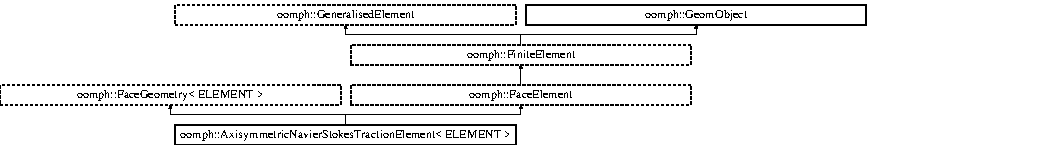
\includegraphics[height=1.944445cm]{classoomph_1_1AxisymmetricNavierStokesTractionElement}
\end{center}
\end{figure}
\subsection*{Public Member Functions}
\begin{DoxyCompactItemize}
\item 
\hyperlink{classoomph_1_1AxisymmetricNavierStokesTractionElement_a8e0d081107ea8ad2e68db11abaf27ebc}{Axisymmetric\+Navier\+Stokes\+Traction\+Element} (\hyperlink{classoomph_1_1FiniteElement}{Finite\+Element} $\ast$const \&element\+\_\+pt, const int \&\hyperlink{classoomph_1_1FaceElement_a478d577ac6db67ecc80f1f02ae3ab170}{face\+\_\+index})
\begin{DoxyCompactList}\small\item\em Constructor, which takes a \char`\"{}bulk\char`\"{} element and the value of the index and its limit. \end{DoxyCompactList}\item 
void \hyperlink{classoomph_1_1AxisymmetricNavierStokesTractionElement_a083afe87cee838cf3674145ae99e66a4}{fill\+\_\+in\+\_\+contribution\+\_\+to\+\_\+residuals} (\hyperlink{classoomph_1_1Vector}{Vector}$<$ double $>$ \&residuals)
\begin{DoxyCompactList}\small\item\em Return the residuals. \end{DoxyCompactList}\item 
void \hyperlink{classoomph_1_1AxisymmetricNavierStokesTractionElement_ae271883f9813c9fd095cdd501ab7f4b1}{fill\+\_\+in\+\_\+contribution\+\_\+to\+\_\+jacobian} (\hyperlink{classoomph_1_1Vector}{Vector}$<$ double $>$ \&residuals, \hyperlink{classoomph_1_1DenseMatrix}{Dense\+Matrix}$<$ double $>$ \&jacobian)
\begin{DoxyCompactList}\small\item\em Fill in contribution from Jacobian. \end{DoxyCompactList}\item 
double \hyperlink{classoomph_1_1AxisymmetricNavierStokesTractionElement_a07065fabd6d28ac9efb7e50bc628a8e0}{zeta\+\_\+nodal} (const unsigned \&n, const unsigned \&k, const unsigned \&\hyperlink{cfortran_8h_adb50e893b86b3e55e751a42eab3cba82}{i}) const
\begin{DoxyCompactList}\small\item\em The \char`\"{}global\char`\"{} intrinsic coordinate of the element when viewed as part of a geometric object should be given by the \hyperlink{classoomph_1_1FaceElement}{Face\+Element} representation, by default (needed to break indeterminacy if bulk element is Solid\+Element) \end{DoxyCompactList}\item 
void \hyperlink{classoomph_1_1AxisymmetricNavierStokesTractionElement_afec508c380a63dc12a95317224c85553}{output} (std\+::ostream \&outfile)
\begin{DoxyCompactList}\small\item\em Output function. \end{DoxyCompactList}\item 
unsigned \hyperlink{classoomph_1_1AxisymmetricNavierStokesTractionElement_a31a8ab8cc6b231e524ba0329b0cb7e78}{nscalar\+\_\+paraview} () const
\begin{DoxyCompactList}\small\item\em Number of scalars/fields output by this element. Reimplements broken virtual function in base class. \end{DoxyCompactList}\item 
void \hyperlink{classoomph_1_1AxisymmetricNavierStokesTractionElement_a0d4062b2db66d2a14eaa9c270eb034d6}{scalar\+\_\+value\+\_\+paraview} (std\+::ofstream \&file\+\_\+out, const unsigned \&k, const unsigned \&nplot) const
\begin{DoxyCompactList}\small\item\em Write values of the k-\/th scalar field at the plot points. Needs to be implemented for each new specific element type. \end{DoxyCompactList}\item 
std\+::string \hyperlink{classoomph_1_1AxisymmetricNavierStokesTractionElement_a4ca57102287a03de1ee8c4f7f9ef1072}{scalar\+\_\+name\+\_\+paraview} (const unsigned \&\hyperlink{cfortran_8h_adb50e893b86b3e55e751a42eab3cba82}{i}) const
\begin{DoxyCompactList}\small\item\em Name of the i-\/th scalar field. Default implementation. \end{DoxyCompactList}\item 
void \hyperlink{classoomph_1_1AxisymmetricNavierStokesTractionElement_a903801e976db27eb831a17349838877d}{output} (std\+::ostream \&outfile, const unsigned \&n\+\_\+plot)
\begin{DoxyCompactList}\small\item\em Output function. \end{DoxyCompactList}\item 
void \hyperlink{classoomph_1_1AxisymmetricNavierStokesTractionElement_aa264b6b88ec62adffd928382c82e93b4}{output} (F\+I\+LE $\ast$file\+\_\+pt)
\begin{DoxyCompactList}\small\item\em C\+\_\+style output function. \end{DoxyCompactList}\item 
void \hyperlink{classoomph_1_1AxisymmetricNavierStokesTractionElement_a19e8ff226642b931a736c7b6184b826c}{output} (F\+I\+LE $\ast$file\+\_\+pt, const unsigned \&n\+\_\+plot)
\begin{DoxyCompactList}\small\item\em C-\/style output function. \end{DoxyCompactList}\item 
void \hyperlink{classoomph_1_1AxisymmetricNavierStokesTractionElement_a467d411cab5179a2437fa762a0df2a02}{traction} (const double \&time, const \hyperlink{classoomph_1_1Vector}{Vector}$<$ double $>$ \&\hyperlink{cfortran_8h_ab7123126e4885ef647dd9c6e3807a21c}{s}, \hyperlink{classoomph_1_1Vector}{Vector}$<$ double $>$ \&traction)
\begin{DoxyCompactList}\small\item\em Compute traction vector at specified local coordinate Should only be used for post-\/processing; ignores dependence on integration point! \end{DoxyCompactList}\end{DoxyCompactItemize}
\subsection*{Public Attributes}
\begin{DoxyCompactItemize}
\item 
void($\ast$\&)(const double \&time, const \hyperlink{classoomph_1_1Vector}{Vector}$<$ double $>$ \&x, const \hyperlink{classoomph_1_1Vector}{Vector}$<$ double $>$ \&n, \hyperlink{classoomph_1_1Vector}{Vector}$<$ double $>$ \&\hyperlink{classoomph_1_1AxisymmetricNavierStokesTractionElement_a467d411cab5179a2437fa762a0df2a02}{traction}) \hyperlink{classoomph_1_1AxisymmetricNavierStokesTractionElement_abed4930a57bc16a6187c7ff011e57ea3}{traction\+\_\+fct\+\_\+pt} ()
\begin{DoxyCompactList}\small\item\em Reference to the traction function pointer. \end{DoxyCompactList}\end{DoxyCompactItemize}
\subsection*{Protected Member Functions}
\begin{DoxyCompactItemize}
\item 
virtual void \hyperlink{classoomph_1_1AxisymmetricNavierStokesTractionElement_a6cf7f8ed52ecccfad185118ffe72ebda}{get\+\_\+traction} (const double \&time, const unsigned \&intpt, const \hyperlink{classoomph_1_1Vector}{Vector}$<$ double $>$ \&x, const \hyperlink{classoomph_1_1Vector}{Vector}$<$ double $>$ \&n, \hyperlink{classoomph_1_1Vector}{Vector}$<$ double $>$ \&\hyperlink{classoomph_1_1AxisymmetricNavierStokesTractionElement_a467d411cab5179a2437fa762a0df2a02}{traction}) const
\begin{DoxyCompactList}\small\item\em Get the traction vector\+: Pass number of integration point (dummy), Eulerian coordinate and normal vector and return the load vector (not all of the input arguments will be required for all specific load functions but the list should cover all cases). This function is virtual so it can be overloaded for F\+SI. \end{DoxyCompactList}\item 
void \hyperlink{classoomph_1_1AxisymmetricNavierStokesTractionElement_abe7c7ffa2a56357512715403a9a6da26}{fill\+\_\+in\+\_\+contribution\+\_\+to\+\_\+residuals\+\_\+axisymmetric\+\_\+nst\+\_\+traction} (\hyperlink{classoomph_1_1Vector}{Vector}$<$ double $>$ \&residuals)
\begin{DoxyCompactList}\small\item\em Helper function that actually calculates the residuals. \end{DoxyCompactList}\end{DoxyCompactItemize}
\subsection*{Protected Attributes}
\begin{DoxyCompactItemize}
\item 
\hyperlink{classoomph_1_1Vector}{Vector}$<$ unsigned $>$ \hyperlink{classoomph_1_1AxisymmetricNavierStokesTractionElement_a4c74bd4d437c216afeff3ac93ea3a9ec}{U\+\_\+index\+\_\+axisymmetric\+\_\+nst\+\_\+traction}
\begin{DoxyCompactList}\small\item\em Index at which the i-\/th velocity component is stored. \end{DoxyCompactList}\item 
void($\ast$ \hyperlink{classoomph_1_1AxisymmetricNavierStokesTractionElement_a58840e83c766a6e7d653f389c2c54dfc}{Traction\+\_\+fct\+\_\+pt} )(const double \&time, const \hyperlink{classoomph_1_1Vector}{Vector}$<$ double $>$ \&x, const \hyperlink{classoomph_1_1Vector}{Vector}$<$ double $>$ \&n, \hyperlink{classoomph_1_1Vector}{Vector}$<$ double $>$ \&result)
\begin{DoxyCompactList}\small\item\em Pointer to an imposed traction function. Arguments\+: Eulerian coordinate; outer unit normal; applied traction. (Not all of the input arguments will be required for all specific load functions but the list should cover all cases) \end{DoxyCompactList}\end{DoxyCompactItemize}
\subsection*{Additional Inherited Members}


\subsection{Detailed Description}
\subsubsection*{template$<$class E\+L\+E\+M\+E\+NT$>$\newline
class oomph\+::\+Axisymmetric\+Navier\+Stokes\+Traction\+Element$<$ E\+L\+E\+M\+E\+N\+T $>$}

A class for elements that allow the imposition of an applied traction in the axisym Navier Stokes eqns. The geometrical information can be read from the Face\+Geometry$<$\+E\+L\+E\+M\+E\+N\+T$>$ class and and thus, we can be generic enough without the need to have a separate equations class. 

Definition at line 78 of file axisym\+\_\+fluid\+\_\+traction\+\_\+elements.\+h.



\subsection{Constructor \& Destructor Documentation}
\mbox{\Hypertarget{classoomph_1_1AxisymmetricNavierStokesTractionElement_a8e0d081107ea8ad2e68db11abaf27ebc}\label{classoomph_1_1AxisymmetricNavierStokesTractionElement_a8e0d081107ea8ad2e68db11abaf27ebc}} 
\index{oomph\+::\+Axisymmetric\+Navier\+Stokes\+Traction\+Element@{oomph\+::\+Axisymmetric\+Navier\+Stokes\+Traction\+Element}!Axisymmetric\+Navier\+Stokes\+Traction\+Element@{Axisymmetric\+Navier\+Stokes\+Traction\+Element}}
\index{Axisymmetric\+Navier\+Stokes\+Traction\+Element@{Axisymmetric\+Navier\+Stokes\+Traction\+Element}!oomph\+::\+Axisymmetric\+Navier\+Stokes\+Traction\+Element@{oomph\+::\+Axisymmetric\+Navier\+Stokes\+Traction\+Element}}
\subsubsection{\texorpdfstring{Axisymmetric\+Navier\+Stokes\+Traction\+Element()}{AxisymmetricNavierStokesTractionElement()}}
{\footnotesize\ttfamily template$<$class E\+L\+E\+M\+E\+NT $>$ \\
\hyperlink{classoomph_1_1AxisymmetricNavierStokesTractionElement}{oomph\+::\+Axisymmetric\+Navier\+Stokes\+Traction\+Element}$<$ E\+L\+E\+M\+E\+NT $>$\+::\hyperlink{classoomph_1_1AxisymmetricNavierStokesTractionElement}{Axisymmetric\+Navier\+Stokes\+Traction\+Element} (\begin{DoxyParamCaption}\item[{\hyperlink{classoomph_1_1FiniteElement}{Finite\+Element} $\ast$const \&}]{element\+\_\+pt,  }\item[{const int \&}]{face\+\_\+index }\end{DoxyParamCaption})\hspace{0.3cm}{\ttfamily [inline]}}



Constructor, which takes a \char`\"{}bulk\char`\"{} element and the value of the index and its limit. 



Definition at line 127 of file axisym\+\_\+fluid\+\_\+traction\+\_\+elements.\+h.



References oomph\+::\+Finite\+Element\+::build\+\_\+face\+\_\+element(), i, oomph\+::\+Finite\+Element\+::nodal\+\_\+dimension(), and oomph\+::\+Axisymmetric\+Navier\+Stokes\+Traction\+Element\+Helper\+::\+Zero\+\_\+traction\+\_\+fct().



\subsection{Member Function Documentation}
\mbox{\Hypertarget{classoomph_1_1AxisymmetricNavierStokesTractionElement_ae271883f9813c9fd095cdd501ab7f4b1}\label{classoomph_1_1AxisymmetricNavierStokesTractionElement_ae271883f9813c9fd095cdd501ab7f4b1}} 
\index{oomph\+::\+Axisymmetric\+Navier\+Stokes\+Traction\+Element@{oomph\+::\+Axisymmetric\+Navier\+Stokes\+Traction\+Element}!fill\+\_\+in\+\_\+contribution\+\_\+to\+\_\+jacobian@{fill\+\_\+in\+\_\+contribution\+\_\+to\+\_\+jacobian}}
\index{fill\+\_\+in\+\_\+contribution\+\_\+to\+\_\+jacobian@{fill\+\_\+in\+\_\+contribution\+\_\+to\+\_\+jacobian}!oomph\+::\+Axisymmetric\+Navier\+Stokes\+Traction\+Element@{oomph\+::\+Axisymmetric\+Navier\+Stokes\+Traction\+Element}}
\subsubsection{\texorpdfstring{fill\+\_\+in\+\_\+contribution\+\_\+to\+\_\+jacobian()}{fill\_in\_contribution\_to\_jacobian()}}
{\footnotesize\ttfamily template$<$class E\+L\+E\+M\+E\+NT $>$ \\
void \hyperlink{classoomph_1_1AxisymmetricNavierStokesTractionElement}{oomph\+::\+Axisymmetric\+Navier\+Stokes\+Traction\+Element}$<$ E\+L\+E\+M\+E\+NT $>$\+::fill\+\_\+in\+\_\+contribution\+\_\+to\+\_\+jacobian (\begin{DoxyParamCaption}\item[{\hyperlink{classoomph_1_1Vector}{Vector}$<$ double $>$ \&}]{residuals,  }\item[{\hyperlink{classoomph_1_1DenseMatrix}{Dense\+Matrix}$<$ double $>$ \&}]{jacobian }\end{DoxyParamCaption})\hspace{0.3cm}{\ttfamily [inline]}, {\ttfamily [virtual]}}



Fill in contribution from Jacobian. 



Reimplemented from \hyperlink{classoomph_1_1GeneralisedElement_a6ae09fc0d68e4309ac1b03583d252845}{oomph\+::\+Generalised\+Element}.



Definition at line 170 of file axisym\+\_\+fluid\+\_\+traction\+\_\+elements.\+h.

\mbox{\Hypertarget{classoomph_1_1AxisymmetricNavierStokesTractionElement_a083afe87cee838cf3674145ae99e66a4}\label{classoomph_1_1AxisymmetricNavierStokesTractionElement_a083afe87cee838cf3674145ae99e66a4}} 
\index{oomph\+::\+Axisymmetric\+Navier\+Stokes\+Traction\+Element@{oomph\+::\+Axisymmetric\+Navier\+Stokes\+Traction\+Element}!fill\+\_\+in\+\_\+contribution\+\_\+to\+\_\+residuals@{fill\+\_\+in\+\_\+contribution\+\_\+to\+\_\+residuals}}
\index{fill\+\_\+in\+\_\+contribution\+\_\+to\+\_\+residuals@{fill\+\_\+in\+\_\+contribution\+\_\+to\+\_\+residuals}!oomph\+::\+Axisymmetric\+Navier\+Stokes\+Traction\+Element@{oomph\+::\+Axisymmetric\+Navier\+Stokes\+Traction\+Element}}
\subsubsection{\texorpdfstring{fill\+\_\+in\+\_\+contribution\+\_\+to\+\_\+residuals()}{fill\_in\_contribution\_to\_residuals()}}
{\footnotesize\ttfamily template$<$class E\+L\+E\+M\+E\+NT $>$ \\
void \hyperlink{classoomph_1_1AxisymmetricNavierStokesTractionElement}{oomph\+::\+Axisymmetric\+Navier\+Stokes\+Traction\+Element}$<$ E\+L\+E\+M\+E\+NT $>$\+::fill\+\_\+in\+\_\+contribution\+\_\+to\+\_\+residuals (\begin{DoxyParamCaption}\item[{\hyperlink{classoomph_1_1Vector}{Vector}$<$ double $>$ \&}]{residuals }\end{DoxyParamCaption})\hspace{0.3cm}{\ttfamily [inline]}, {\ttfamily [virtual]}}



Return the residuals. 



Reimplemented from \hyperlink{classoomph_1_1GeneralisedElement_a310c97f515e8504a48179c0e72c550d7}{oomph\+::\+Generalised\+Element}.



Definition at line 162 of file axisym\+\_\+fluid\+\_\+traction\+\_\+elements.\+h.

\mbox{\Hypertarget{classoomph_1_1AxisymmetricNavierStokesTractionElement_abe7c7ffa2a56357512715403a9a6da26}\label{classoomph_1_1AxisymmetricNavierStokesTractionElement_abe7c7ffa2a56357512715403a9a6da26}} 
\index{oomph\+::\+Axisymmetric\+Navier\+Stokes\+Traction\+Element@{oomph\+::\+Axisymmetric\+Navier\+Stokes\+Traction\+Element}!fill\+\_\+in\+\_\+contribution\+\_\+to\+\_\+residuals\+\_\+axisymmetric\+\_\+nst\+\_\+traction@{fill\+\_\+in\+\_\+contribution\+\_\+to\+\_\+residuals\+\_\+axisymmetric\+\_\+nst\+\_\+traction}}
\index{fill\+\_\+in\+\_\+contribution\+\_\+to\+\_\+residuals\+\_\+axisymmetric\+\_\+nst\+\_\+traction@{fill\+\_\+in\+\_\+contribution\+\_\+to\+\_\+residuals\+\_\+axisymmetric\+\_\+nst\+\_\+traction}!oomph\+::\+Axisymmetric\+Navier\+Stokes\+Traction\+Element@{oomph\+::\+Axisymmetric\+Navier\+Stokes\+Traction\+Element}}
\subsubsection{\texorpdfstring{fill\+\_\+in\+\_\+contribution\+\_\+to\+\_\+residuals\+\_\+axisymmetric\+\_\+nst\+\_\+traction()}{fill\_in\_contribution\_to\_residuals\_axisymmetric\_nst\_traction()}}
{\footnotesize\ttfamily template$<$class E\+L\+E\+M\+E\+NT $>$ \\
void \hyperlink{classoomph_1_1AxisymmetricNavierStokesTractionElement}{oomph\+::\+Axisymmetric\+Navier\+Stokes\+Traction\+Element}$<$ E\+L\+E\+M\+E\+NT $>$\+::fill\+\_\+in\+\_\+contribution\+\_\+to\+\_\+residuals\+\_\+axisymmetric\+\_\+nst\+\_\+traction (\begin{DoxyParamCaption}\item[{\hyperlink{classoomph_1_1Vector}{Vector}$<$ double $>$ \&}]{residuals }\end{DoxyParamCaption})\hspace{0.3cm}{\ttfamily [protected]}}



Helper function that actually calculates the residuals. 

Return the residuals for the \hyperlink{classoomph_1_1AxisymmetricNavierStokesTractionElement}{Axisymmetric\+Navier\+Stokes\+Traction\+Element} equations 

Definition at line 456 of file axisym\+\_\+fluid\+\_\+traction\+\_\+elements.\+h.



References oomph\+::\+Linearised\+F\+S\+I\+Axisymmetric\+N\+St\+No\+Slip\+B\+C\+Helper\+::\+Default\+\_\+strouhal\+\_\+number, i, and oomph\+::\+Quad\+Tree\+Names\+::W.



Referenced by oomph\+::\+Axisymmetric\+Navier\+Stokes\+Traction\+Element$<$ E\+L\+E\+M\+E\+N\+T $>$\+::traction().

\mbox{\Hypertarget{classoomph_1_1AxisymmetricNavierStokesTractionElement_a6cf7f8ed52ecccfad185118ffe72ebda}\label{classoomph_1_1AxisymmetricNavierStokesTractionElement_a6cf7f8ed52ecccfad185118ffe72ebda}} 
\index{oomph\+::\+Axisymmetric\+Navier\+Stokes\+Traction\+Element@{oomph\+::\+Axisymmetric\+Navier\+Stokes\+Traction\+Element}!get\+\_\+traction@{get\+\_\+traction}}
\index{get\+\_\+traction@{get\+\_\+traction}!oomph\+::\+Axisymmetric\+Navier\+Stokes\+Traction\+Element@{oomph\+::\+Axisymmetric\+Navier\+Stokes\+Traction\+Element}}
\subsubsection{\texorpdfstring{get\+\_\+traction()}{get\_traction()}}
{\footnotesize\ttfamily template$<$class E\+L\+E\+M\+E\+NT $>$ \\
virtual void \hyperlink{classoomph_1_1AxisymmetricNavierStokesTractionElement}{oomph\+::\+Axisymmetric\+Navier\+Stokes\+Traction\+Element}$<$ E\+L\+E\+M\+E\+NT $>$\+::get\+\_\+traction (\begin{DoxyParamCaption}\item[{const double \&}]{time,  }\item[{const unsigned \&}]{intpt,  }\item[{const \hyperlink{classoomph_1_1Vector}{Vector}$<$ double $>$ \&}]{x,  }\item[{const \hyperlink{classoomph_1_1Vector}{Vector}$<$ double $>$ \&}]{n,  }\item[{\hyperlink{classoomph_1_1Vector}{Vector}$<$ double $>$ \&}]{traction }\end{DoxyParamCaption}) const\hspace{0.3cm}{\ttfamily [inline]}, {\ttfamily [protected]}, {\ttfamily [virtual]}}



Get the traction vector\+: Pass number of integration point (dummy), Eulerian coordinate and normal vector and return the load vector (not all of the input arguments will be required for all specific load functions but the list should cover all cases). This function is virtual so it can be overloaded for F\+SI. 



Definition at line 104 of file axisym\+\_\+fluid\+\_\+traction\+\_\+elements.\+h.

\mbox{\Hypertarget{classoomph_1_1AxisymmetricNavierStokesTractionElement_a31a8ab8cc6b231e524ba0329b0cb7e78}\label{classoomph_1_1AxisymmetricNavierStokesTractionElement_a31a8ab8cc6b231e524ba0329b0cb7e78}} 
\index{oomph\+::\+Axisymmetric\+Navier\+Stokes\+Traction\+Element@{oomph\+::\+Axisymmetric\+Navier\+Stokes\+Traction\+Element}!nscalar\+\_\+paraview@{nscalar\+\_\+paraview}}
\index{nscalar\+\_\+paraview@{nscalar\+\_\+paraview}!oomph\+::\+Axisymmetric\+Navier\+Stokes\+Traction\+Element@{oomph\+::\+Axisymmetric\+Navier\+Stokes\+Traction\+Element}}
\subsubsection{\texorpdfstring{nscalar\+\_\+paraview()}{nscalar\_paraview()}}
{\footnotesize\ttfamily template$<$class E\+L\+E\+M\+E\+NT $>$ \\
unsigned \hyperlink{classoomph_1_1AxisymmetricNavierStokesTractionElement}{oomph\+::\+Axisymmetric\+Navier\+Stokes\+Traction\+Element}$<$ E\+L\+E\+M\+E\+NT $>$\+::nscalar\+\_\+paraview (\begin{DoxyParamCaption}{ }\end{DoxyParamCaption}) const\hspace{0.3cm}{\ttfamily [inline]}, {\ttfamily [virtual]}}



Number of scalars/fields output by this element. Reimplements broken virtual function in base class. 



Reimplemented from \hyperlink{classoomph_1_1FiniteElement_a865e2e5586552ba80babdbe26a77fe8c}{oomph\+::\+Finite\+Element}.



Definition at line 195 of file axisym\+\_\+fluid\+\_\+traction\+\_\+elements.\+h.

\mbox{\Hypertarget{classoomph_1_1AxisymmetricNavierStokesTractionElement_afec508c380a63dc12a95317224c85553}\label{classoomph_1_1AxisymmetricNavierStokesTractionElement_afec508c380a63dc12a95317224c85553}} 
\index{oomph\+::\+Axisymmetric\+Navier\+Stokes\+Traction\+Element@{oomph\+::\+Axisymmetric\+Navier\+Stokes\+Traction\+Element}!output@{output}}
\index{output@{output}!oomph\+::\+Axisymmetric\+Navier\+Stokes\+Traction\+Element@{oomph\+::\+Axisymmetric\+Navier\+Stokes\+Traction\+Element}}
\subsubsection{\texorpdfstring{output()}{output()}\hspace{0.1cm}{\footnotesize\ttfamily [1/4]}}
{\footnotesize\ttfamily template$<$class E\+L\+E\+M\+E\+NT $>$ \\
void \hyperlink{classoomph_1_1AxisymmetricNavierStokesTractionElement}{oomph\+::\+Axisymmetric\+Navier\+Stokes\+Traction\+Element}$<$ E\+L\+E\+M\+E\+NT $>$\+::output (\begin{DoxyParamCaption}\item[{std\+::ostream \&}]{outfile }\end{DoxyParamCaption})\hspace{0.3cm}{\ttfamily [inline]}, {\ttfamily [virtual]}}



Output function. 



Reimplemented from \hyperlink{classoomph_1_1FiniteElement_a2ad98a3d2ef4999f1bef62c0ff13f2a7}{oomph\+::\+Finite\+Element}.



Definition at line 187 of file axisym\+\_\+fluid\+\_\+traction\+\_\+elements.\+h.



References oomph\+::output().

\mbox{\Hypertarget{classoomph_1_1AxisymmetricNavierStokesTractionElement_a903801e976db27eb831a17349838877d}\label{classoomph_1_1AxisymmetricNavierStokesTractionElement_a903801e976db27eb831a17349838877d}} 
\index{oomph\+::\+Axisymmetric\+Navier\+Stokes\+Traction\+Element@{oomph\+::\+Axisymmetric\+Navier\+Stokes\+Traction\+Element}!output@{output}}
\index{output@{output}!oomph\+::\+Axisymmetric\+Navier\+Stokes\+Traction\+Element@{oomph\+::\+Axisymmetric\+Navier\+Stokes\+Traction\+Element}}
\subsubsection{\texorpdfstring{output()}{output()}\hspace{0.1cm}{\footnotesize\ttfamily [2/4]}}
{\footnotesize\ttfamily template$<$class E\+L\+E\+M\+E\+NT $>$ \\
void \hyperlink{classoomph_1_1AxisymmetricNavierStokesTractionElement}{oomph\+::\+Axisymmetric\+Navier\+Stokes\+Traction\+Element}$<$ E\+L\+E\+M\+E\+NT $>$\+::output (\begin{DoxyParamCaption}\item[{std\+::ostream \&}]{outfile,  }\item[{const unsigned \&}]{n\+\_\+plot }\end{DoxyParamCaption})\hspace{0.3cm}{\ttfamily [inline]}, {\ttfamily [virtual]}}



Output function. 



Reimplemented from \hyperlink{classoomph_1_1FiniteElement_afa9d9b2670f999b43e6679c9dd28c457}{oomph\+::\+Finite\+Element}.



Definition at line 320 of file axisym\+\_\+fluid\+\_\+traction\+\_\+elements.\+h.



References i, s, and oomph\+::\+One\+Dim\+Lagrange\+::shape().

\mbox{\Hypertarget{classoomph_1_1AxisymmetricNavierStokesTractionElement_aa264b6b88ec62adffd928382c82e93b4}\label{classoomph_1_1AxisymmetricNavierStokesTractionElement_aa264b6b88ec62adffd928382c82e93b4}} 
\index{oomph\+::\+Axisymmetric\+Navier\+Stokes\+Traction\+Element@{oomph\+::\+Axisymmetric\+Navier\+Stokes\+Traction\+Element}!output@{output}}
\index{output@{output}!oomph\+::\+Axisymmetric\+Navier\+Stokes\+Traction\+Element@{oomph\+::\+Axisymmetric\+Navier\+Stokes\+Traction\+Element}}
\subsubsection{\texorpdfstring{output()}{output()}\hspace{0.1cm}{\footnotesize\ttfamily [3/4]}}
{\footnotesize\ttfamily template$<$class E\+L\+E\+M\+E\+NT $>$ \\
void \hyperlink{classoomph_1_1AxisymmetricNavierStokesTractionElement}{oomph\+::\+Axisymmetric\+Navier\+Stokes\+Traction\+Element}$<$ E\+L\+E\+M\+E\+NT $>$\+::output (\begin{DoxyParamCaption}\item[{F\+I\+LE $\ast$}]{file\+\_\+pt }\end{DoxyParamCaption})\hspace{0.3cm}{\ttfamily [inline]}, {\ttfamily [virtual]}}



C\+\_\+style output function. 



Reimplemented from \hyperlink{classoomph_1_1FiniteElement_a72cddd09f8ddbee1a20a1ff404c6943e}{oomph\+::\+Finite\+Element}.



Definition at line 401 of file axisym\+\_\+fluid\+\_\+traction\+\_\+elements.\+h.



References oomph\+::\+Finite\+Element\+::output().

\mbox{\Hypertarget{classoomph_1_1AxisymmetricNavierStokesTractionElement_a19e8ff226642b931a736c7b6184b826c}\label{classoomph_1_1AxisymmetricNavierStokesTractionElement_a19e8ff226642b931a736c7b6184b826c}} 
\index{oomph\+::\+Axisymmetric\+Navier\+Stokes\+Traction\+Element@{oomph\+::\+Axisymmetric\+Navier\+Stokes\+Traction\+Element}!output@{output}}
\index{output@{output}!oomph\+::\+Axisymmetric\+Navier\+Stokes\+Traction\+Element@{oomph\+::\+Axisymmetric\+Navier\+Stokes\+Traction\+Element}}
\subsubsection{\texorpdfstring{output()}{output()}\hspace{0.1cm}{\footnotesize\ttfamily [4/4]}}
{\footnotesize\ttfamily template$<$class E\+L\+E\+M\+E\+NT $>$ \\
void \hyperlink{classoomph_1_1AxisymmetricNavierStokesTractionElement}{oomph\+::\+Axisymmetric\+Navier\+Stokes\+Traction\+Element}$<$ E\+L\+E\+M\+E\+NT $>$\+::output (\begin{DoxyParamCaption}\item[{F\+I\+LE $\ast$}]{file\+\_\+pt,  }\item[{const unsigned \&}]{n\+\_\+plot }\end{DoxyParamCaption})\hspace{0.3cm}{\ttfamily [inline]}, {\ttfamily [virtual]}}



C-\/style output function. 



Reimplemented from \hyperlink{classoomph_1_1FiniteElement_adfaee690bb0608f03320eeb9d110d48c}{oomph\+::\+Finite\+Element}.



Definition at line 405 of file axisym\+\_\+fluid\+\_\+traction\+\_\+elements.\+h.



References oomph\+::\+Finite\+Element\+::output(), s, and oomph\+::\+Axisymmetric\+Navier\+Stokes\+Traction\+Element$<$ E\+L\+E\+M\+E\+N\+T $>$\+::traction().

\mbox{\Hypertarget{classoomph_1_1AxisymmetricNavierStokesTractionElement_a4ca57102287a03de1ee8c4f7f9ef1072}\label{classoomph_1_1AxisymmetricNavierStokesTractionElement_a4ca57102287a03de1ee8c4f7f9ef1072}} 
\index{oomph\+::\+Axisymmetric\+Navier\+Stokes\+Traction\+Element@{oomph\+::\+Axisymmetric\+Navier\+Stokes\+Traction\+Element}!scalar\+\_\+name\+\_\+paraview@{scalar\+\_\+name\+\_\+paraview}}
\index{scalar\+\_\+name\+\_\+paraview@{scalar\+\_\+name\+\_\+paraview}!oomph\+::\+Axisymmetric\+Navier\+Stokes\+Traction\+Element@{oomph\+::\+Axisymmetric\+Navier\+Stokes\+Traction\+Element}}
\subsubsection{\texorpdfstring{scalar\+\_\+name\+\_\+paraview()}{scalar\_name\_paraview()}}
{\footnotesize\ttfamily template$<$class E\+L\+E\+M\+E\+NT $>$ \\
std\+::string \hyperlink{classoomph_1_1AxisymmetricNavierStokesTractionElement}{oomph\+::\+Axisymmetric\+Navier\+Stokes\+Traction\+Element}$<$ E\+L\+E\+M\+E\+NT $>$\+::scalar\+\_\+name\+\_\+paraview (\begin{DoxyParamCaption}\item[{const unsigned \&}]{i }\end{DoxyParamCaption}) const\hspace{0.3cm}{\ttfamily [inline]}, {\ttfamily [virtual]}}



Name of the i-\/th scalar field. Default implementation. 

returns V1 for the first one, V2 for the second etc. Can (should!) be overloaded with more meaningful names in specific elements. 

Reimplemented from \hyperlink{classoomph_1_1FiniteElement_a49cc2d4f7ed5772bbc96f06760372b51}{oomph\+::\+Finite\+Element}.



Definition at line 290 of file axisym\+\_\+fluid\+\_\+traction\+\_\+elements.\+h.



References oomph\+::\+String\+Conversion\+::to\+\_\+string().

\mbox{\Hypertarget{classoomph_1_1AxisymmetricNavierStokesTractionElement_a0d4062b2db66d2a14eaa9c270eb034d6}\label{classoomph_1_1AxisymmetricNavierStokesTractionElement_a0d4062b2db66d2a14eaa9c270eb034d6}} 
\index{oomph\+::\+Axisymmetric\+Navier\+Stokes\+Traction\+Element@{oomph\+::\+Axisymmetric\+Navier\+Stokes\+Traction\+Element}!scalar\+\_\+value\+\_\+paraview@{scalar\+\_\+value\+\_\+paraview}}
\index{scalar\+\_\+value\+\_\+paraview@{scalar\+\_\+value\+\_\+paraview}!oomph\+::\+Axisymmetric\+Navier\+Stokes\+Traction\+Element@{oomph\+::\+Axisymmetric\+Navier\+Stokes\+Traction\+Element}}
\subsubsection{\texorpdfstring{scalar\+\_\+value\+\_\+paraview()}{scalar\_value\_paraview()}}
{\footnotesize\ttfamily template$<$class E\+L\+E\+M\+E\+NT $>$ \\
void \hyperlink{classoomph_1_1AxisymmetricNavierStokesTractionElement}{oomph\+::\+Axisymmetric\+Navier\+Stokes\+Traction\+Element}$<$ E\+L\+E\+M\+E\+NT $>$\+::scalar\+\_\+value\+\_\+paraview (\begin{DoxyParamCaption}\item[{std\+::ofstream \&}]{file\+\_\+out,  }\item[{const unsigned \&}]{k,  }\item[{const unsigned \&}]{nplot }\end{DoxyParamCaption}) const\hspace{0.3cm}{\ttfamily [inline]}, {\ttfamily [virtual]}}



Write values of the k-\/th scalar field at the plot points. Needs to be implemented for each new specific element type. 



Reimplemented from \hyperlink{classoomph_1_1FiniteElement_a02cf8832a5e2886f1572bd36f7a7c1e3}{oomph\+::\+Finite\+Element}.



Definition at line 205 of file axisym\+\_\+fluid\+\_\+traction\+\_\+elements.\+h.



References i, s, and oomph\+::\+One\+Dim\+Lagrange\+::shape().

\mbox{\Hypertarget{classoomph_1_1AxisymmetricNavierStokesTractionElement_a467d411cab5179a2437fa762a0df2a02}\label{classoomph_1_1AxisymmetricNavierStokesTractionElement_a467d411cab5179a2437fa762a0df2a02}} 
\index{oomph\+::\+Axisymmetric\+Navier\+Stokes\+Traction\+Element@{oomph\+::\+Axisymmetric\+Navier\+Stokes\+Traction\+Element}!traction@{traction}}
\index{traction@{traction}!oomph\+::\+Axisymmetric\+Navier\+Stokes\+Traction\+Element@{oomph\+::\+Axisymmetric\+Navier\+Stokes\+Traction\+Element}}
\subsubsection{\texorpdfstring{traction()}{traction()}}
{\footnotesize\ttfamily template$<$class E\+L\+E\+M\+E\+NT $>$ \\
void \hyperlink{classoomph_1_1AxisymmetricNavierStokesTractionElement}{oomph\+::\+Axisymmetric\+Navier\+Stokes\+Traction\+Element}$<$ E\+L\+E\+M\+E\+NT $>$\+::traction (\begin{DoxyParamCaption}\item[{const double \&}]{time,  }\item[{const \hyperlink{classoomph_1_1Vector}{Vector}$<$ double $>$ \&}]{s,  }\item[{\hyperlink{classoomph_1_1Vector}{Vector}$<$ double $>$ \&}]{traction }\end{DoxyParamCaption})}



Compute traction vector at specified local coordinate Should only be used for post-\/processing; ignores dependence on integration point! 

Compute traction vector at specified local coordinate Should only be used for post-\/processing; ignores dependence on integration point! 

Definition at line 429 of file axisym\+\_\+fluid\+\_\+traction\+\_\+elements.\+h.



References oomph\+::\+Axisymmetric\+Navier\+Stokes\+Traction\+Element$<$ E\+L\+E\+M\+E\+N\+T $>$\+::fill\+\_\+in\+\_\+contribution\+\_\+to\+\_\+residuals\+\_\+axisymmetric\+\_\+nst\+\_\+traction().



Referenced by oomph\+::\+Axisymmetric\+Navier\+Stokes\+Traction\+Element$<$ E\+L\+E\+M\+E\+N\+T $>$\+::output().

\mbox{\Hypertarget{classoomph_1_1AxisymmetricNavierStokesTractionElement_a07065fabd6d28ac9efb7e50bc628a8e0}\label{classoomph_1_1AxisymmetricNavierStokesTractionElement_a07065fabd6d28ac9efb7e50bc628a8e0}} 
\index{oomph\+::\+Axisymmetric\+Navier\+Stokes\+Traction\+Element@{oomph\+::\+Axisymmetric\+Navier\+Stokes\+Traction\+Element}!zeta\+\_\+nodal@{zeta\+\_\+nodal}}
\index{zeta\+\_\+nodal@{zeta\+\_\+nodal}!oomph\+::\+Axisymmetric\+Navier\+Stokes\+Traction\+Element@{oomph\+::\+Axisymmetric\+Navier\+Stokes\+Traction\+Element}}
\subsubsection{\texorpdfstring{zeta\+\_\+nodal()}{zeta\_nodal()}}
{\footnotesize\ttfamily template$<$class E\+L\+E\+M\+E\+NT $>$ \\
double \hyperlink{classoomph_1_1AxisymmetricNavierStokesTractionElement}{oomph\+::\+Axisymmetric\+Navier\+Stokes\+Traction\+Element}$<$ E\+L\+E\+M\+E\+NT $>$\+::zeta\+\_\+nodal (\begin{DoxyParamCaption}\item[{const unsigned \&}]{n,  }\item[{const unsigned \&}]{k,  }\item[{const unsigned \&}]{i }\end{DoxyParamCaption}) const\hspace{0.3cm}{\ttfamily [inline]}, {\ttfamily [virtual]}}



The \char`\"{}global\char`\"{} intrinsic coordinate of the element when viewed as part of a geometric object should be given by the \hyperlink{classoomph_1_1FaceElement}{Face\+Element} representation, by default (needed to break indeterminacy if bulk element is Solid\+Element) 

Specify the value of nodal zeta from the face geometry 

Reimplemented from \hyperlink{classoomph_1_1FiniteElement_a849561c5fbcbc07dc49d2dc6cca68559}{oomph\+::\+Finite\+Element}.



Definition at line 182 of file axisym\+\_\+fluid\+\_\+traction\+\_\+elements.\+h.



References oomph\+::\+Face\+Element\+::zeta\+\_\+nodal().



\subsection{Member Data Documentation}
\mbox{\Hypertarget{classoomph_1_1AxisymmetricNavierStokesTractionElement_a58840e83c766a6e7d653f389c2c54dfc}\label{classoomph_1_1AxisymmetricNavierStokesTractionElement_a58840e83c766a6e7d653f389c2c54dfc}} 
\index{oomph\+::\+Axisymmetric\+Navier\+Stokes\+Traction\+Element@{oomph\+::\+Axisymmetric\+Navier\+Stokes\+Traction\+Element}!Traction\+\_\+fct\+\_\+pt@{Traction\+\_\+fct\+\_\+pt}}
\index{Traction\+\_\+fct\+\_\+pt@{Traction\+\_\+fct\+\_\+pt}!oomph\+::\+Axisymmetric\+Navier\+Stokes\+Traction\+Element@{oomph\+::\+Axisymmetric\+Navier\+Stokes\+Traction\+Element}}
\subsubsection{\texorpdfstring{Traction\+\_\+fct\+\_\+pt}{Traction\_fct\_pt}}
{\footnotesize\ttfamily template$<$class E\+L\+E\+M\+E\+NT $>$ \\
void($\ast$ \hyperlink{classoomph_1_1AxisymmetricNavierStokesTractionElement}{oomph\+::\+Axisymmetric\+Navier\+Stokes\+Traction\+Element}$<$ E\+L\+E\+M\+E\+NT $>$\+::Traction\+\_\+fct\+\_\+pt) (const double \&time, const \hyperlink{classoomph_1_1Vector}{Vector}$<$ double $>$ \&x, const \hyperlink{classoomph_1_1Vector}{Vector}$<$ double $>$ \&n, \hyperlink{classoomph_1_1Vector}{Vector}$<$ double $>$ \&result)\hspace{0.3cm}{\ttfamily [protected]}}



Pointer to an imposed traction function. Arguments\+: Eulerian coordinate; outer unit normal; applied traction. (Not all of the input arguments will be required for all specific load functions but the list should cover all cases) 



Definition at line 92 of file axisym\+\_\+fluid\+\_\+traction\+\_\+elements.\+h.

\mbox{\Hypertarget{classoomph_1_1AxisymmetricNavierStokesTractionElement_abed4930a57bc16a6187c7ff011e57ea3}\label{classoomph_1_1AxisymmetricNavierStokesTractionElement_abed4930a57bc16a6187c7ff011e57ea3}} 
\index{oomph\+::\+Axisymmetric\+Navier\+Stokes\+Traction\+Element@{oomph\+::\+Axisymmetric\+Navier\+Stokes\+Traction\+Element}!traction\+\_\+fct\+\_\+pt@{traction\+\_\+fct\+\_\+pt}}
\index{traction\+\_\+fct\+\_\+pt@{traction\+\_\+fct\+\_\+pt}!oomph\+::\+Axisymmetric\+Navier\+Stokes\+Traction\+Element@{oomph\+::\+Axisymmetric\+Navier\+Stokes\+Traction\+Element}}
\subsubsection{\texorpdfstring{traction\+\_\+fct\+\_\+pt}{traction\_fct\_pt}}
{\footnotesize\ttfamily template$<$class E\+L\+E\+M\+E\+NT $>$ \\
void($\ast$ \&)(const double\& time, const \hyperlink{classoomph_1_1Vector}{Vector}$<$double$>$\& x, const \hyperlink{classoomph_1_1Vector}{Vector}$<$double$>$\& n, \hyperlink{classoomph_1_1Vector}{Vector}$<$double$>$\& \hyperlink{classoomph_1_1AxisymmetricNavierStokesTractionElement_a467d411cab5179a2437fa762a0df2a02}{traction}) \hyperlink{classoomph_1_1AxisymmetricNavierStokesTractionElement}{oomph\+::\+Axisymmetric\+Navier\+Stokes\+Traction\+Element}$<$ E\+L\+E\+M\+E\+NT $>$\+::traction\+\_\+fct\+\_\+pt()\hspace{0.3cm}{\ttfamily [inline]}}



Reference to the traction function pointer. 



Definition at line 154 of file axisym\+\_\+fluid\+\_\+traction\+\_\+elements.\+h.

\mbox{\Hypertarget{classoomph_1_1AxisymmetricNavierStokesTractionElement_a4c74bd4d437c216afeff3ac93ea3a9ec}\label{classoomph_1_1AxisymmetricNavierStokesTractionElement_a4c74bd4d437c216afeff3ac93ea3a9ec}} 
\index{oomph\+::\+Axisymmetric\+Navier\+Stokes\+Traction\+Element@{oomph\+::\+Axisymmetric\+Navier\+Stokes\+Traction\+Element}!U\+\_\+index\+\_\+axisymmetric\+\_\+nst\+\_\+traction@{U\+\_\+index\+\_\+axisymmetric\+\_\+nst\+\_\+traction}}
\index{U\+\_\+index\+\_\+axisymmetric\+\_\+nst\+\_\+traction@{U\+\_\+index\+\_\+axisymmetric\+\_\+nst\+\_\+traction}!oomph\+::\+Axisymmetric\+Navier\+Stokes\+Traction\+Element@{oomph\+::\+Axisymmetric\+Navier\+Stokes\+Traction\+Element}}
\subsubsection{\texorpdfstring{U\+\_\+index\+\_\+axisymmetric\+\_\+nst\+\_\+traction}{U\_index\_axisymmetric\_nst\_traction}}
{\footnotesize\ttfamily template$<$class E\+L\+E\+M\+E\+NT $>$ \\
\hyperlink{classoomph_1_1Vector}{Vector}$<$unsigned$>$ \hyperlink{classoomph_1_1AxisymmetricNavierStokesTractionElement}{oomph\+::\+Axisymmetric\+Navier\+Stokes\+Traction\+Element}$<$ E\+L\+E\+M\+E\+NT $>$\+::U\+\_\+index\+\_\+axisymmetric\+\_\+nst\+\_\+traction\hspace{0.3cm}{\ttfamily [protected]}}



Index at which the i-\/th velocity component is stored. 



Definition at line 85 of file axisym\+\_\+fluid\+\_\+traction\+\_\+elements.\+h.



The documentation for this class was generated from the following file\+:\begin{DoxyCompactItemize}
\item 
\hyperlink{axisym__fluid__traction__elements_8h}{axisym\+\_\+fluid\+\_\+traction\+\_\+elements.\+h}\end{DoxyCompactItemize}

\hypertarget{classoomph_1_1AxisymmetricPoroelasticityEquations}{}\section{oomph\+:\+:Axisymmetric\+Poroelasticity\+Equations Class Reference}
\label{classoomph_1_1AxisymmetricPoroelasticityEquations}\index{oomph\+::\+Axisymmetric\+Poroelasticity\+Equations@{oomph\+::\+Axisymmetric\+Poroelasticity\+Equations}}


Class implementing the generic maths of the axisym poroelasticity equations\+: axisym linear elasticity coupled with axisym Darcy equations (using Raviart-\/\+Thomas elements with both edge and internal degrees of freedom) including inertia in both.  




{\ttfamily \#include $<$axisym\+\_\+poroelasticity\+\_\+elements.\+h$>$}

Inheritance diagram for oomph\+:\+:Axisymmetric\+Poroelasticity\+Equations\+:\begin{figure}[H]
\begin{center}
\leavevmode
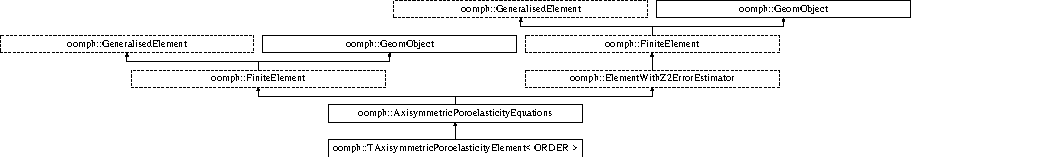
\includegraphics[height=2.114804cm]{classoomph_1_1AxisymmetricPoroelasticityEquations}
\end{center}
\end{figure}
\subsection*{Public Types}
\begin{DoxyCompactItemize}
\item 
typedef void($\ast$ \hyperlink{classoomph_1_1AxisymmetricPoroelasticityEquations_a7a2c87557c3d9d405bb07a9f53bb4abe}{Source\+Fct\+Pt}) (const double \&time, const \hyperlink{classoomph_1_1Vector}{Vector}$<$ double $>$ \&x, \hyperlink{classoomph_1_1Vector}{Vector}$<$ double $>$ \&f)
\begin{DoxyCompactList}\small\item\em Source function pointer typedef. \end{DoxyCompactList}\item 
typedef void($\ast$ \hyperlink{classoomph_1_1AxisymmetricPoroelasticityEquations_a4f2fe2e03df9328898e9932b09299655}{Mass\+Source\+Fct\+Pt}) (const double \&time, const \hyperlink{classoomph_1_1Vector}{Vector}$<$ double $>$ \&x, double \&f)
\begin{DoxyCompactList}\small\item\em Mass source function pointer typedef. \end{DoxyCompactList}\end{DoxyCompactItemize}
\subsection*{Public Member Functions}
\begin{DoxyCompactItemize}
\item 
\hyperlink{classoomph_1_1AxisymmetricPoroelasticityEquations_a4dc47e5296f523f13d704194bd3b893f}{Axisymmetric\+Poroelasticity\+Equations} ()
\begin{DoxyCompactList}\small\item\em Constructor. \end{DoxyCompactList}\item 
const double \& \hyperlink{classoomph_1_1AxisymmetricPoroelasticityEquations_a2e3ac54472beffc980b88db8c071e114}{youngs\+\_\+modulus} () const
\begin{DoxyCompactList}\small\item\em Access function to non-\/dim Young\textquotesingle{}s modulus (ratio of actual Young\textquotesingle{}s modulus to reference stress used to non-\/dim the equations. (const version) \end{DoxyCompactList}\item 
double $\ast$\& \hyperlink{classoomph_1_1AxisymmetricPoroelasticityEquations_af6e08b6f974b94d715ec008cb2858966}{youngs\+\_\+modulus\+\_\+pt} ()
\begin{DoxyCompactList}\small\item\em Pointer to non-\/dim Young\textquotesingle{}s modulus (ratio of actual Young\textquotesingle{}s modulus to reference stress used to non-\/dim the equations. \end{DoxyCompactList}\item 
const double \& \hyperlink{classoomph_1_1AxisymmetricPoroelasticityEquations_ae031a1a1495cf6fa8b7988462b113d29}{nu} () const
\begin{DoxyCompactList}\small\item\em Access function for Poisson\textquotesingle{}s ratio. \end{DoxyCompactList}\item 
double $\ast$\& \hyperlink{classoomph_1_1AxisymmetricPoroelasticityEquations_a239f7f3be1cd9f42163f3d7f1bb87da8}{nu\+\_\+pt} ()
\begin{DoxyCompactList}\small\item\em Access function for pointer to Poisson\textquotesingle{}s ratio. \end{DoxyCompactList}\item 
const double \& \hyperlink{classoomph_1_1AxisymmetricPoroelasticityEquations_a9f1697a47ba5a34054b5820f2766f8f7}{lambda\+\_\+sq} () const
\begin{DoxyCompactList}\small\item\em Access function for timescale ratio (nondim density) \end{DoxyCompactList}\item 
double $\ast$\& \hyperlink{classoomph_1_1AxisymmetricPoroelasticityEquations_a2442bdcf91f689440f9a5b622ea9ba0b}{lambda\+\_\+sq\+\_\+pt} ()
\begin{DoxyCompactList}\small\item\em Access function for pointer to timescale ratio (nondim density) \end{DoxyCompactList}\item 
const double \& \hyperlink{classoomph_1_1AxisymmetricPoroelasticityEquations_a96584beacdd7c3b3b248f2ea8e016731}{density\+\_\+ratio} () const
\begin{DoxyCompactList}\small\item\em Access function for the density ratio (fluid to solid) \end{DoxyCompactList}\item 
double $\ast$\& \hyperlink{classoomph_1_1AxisymmetricPoroelasticityEquations_a54c0959b5f478e7d48725ab516d950bb}{density\+\_\+ratio\+\_\+pt} ()
\begin{DoxyCompactList}\small\item\em Access function for pointer to the density ratio (fluid to solid) \end{DoxyCompactList}\item 
const double \& \hyperlink{classoomph_1_1AxisymmetricPoroelasticityEquations_ab52dc140cfce886743c584c2bae82548}{permeability} () const
\begin{DoxyCompactList}\small\item\em Access function for the nondim permeability. \end{DoxyCompactList}\item 
double $\ast$\& \hyperlink{classoomph_1_1AxisymmetricPoroelasticityEquations_a4309befdee5285a1c04636b50401eca8}{permeability\+\_\+pt} ()
\begin{DoxyCompactList}\small\item\em Access function for pointer to the nondim permeability. \end{DoxyCompactList}\item 
const double \& \hyperlink{classoomph_1_1AxisymmetricPoroelasticityEquations_a4c777d0a0a82afa9342cca27609b0049}{permeability\+\_\+ratio} () const
\begin{DoxyCompactList}\small\item\em Access function for the ratio of the material\textquotesingle{}s actual permeability to the permeability used in the non-\/dimensionalisation of the equations. \end{DoxyCompactList}\item 
double $\ast$\& \hyperlink{classoomph_1_1AxisymmetricPoroelasticityEquations_a58aa8cf5415562e37884fc8a5304803f}{permeability\+\_\+ratio\+\_\+pt} ()
\item 
const double \& \hyperlink{classoomph_1_1AxisymmetricPoroelasticityEquations_acde1907eed1f77a11184d71adaa89e76}{alpha} () const
\begin{DoxyCompactList}\small\item\em Access function for alpha, the Biot parameter. \end{DoxyCompactList}\item 
double $\ast$\& \hyperlink{classoomph_1_1AxisymmetricPoroelasticityEquations_ab153afbf3149fb43be60a72a57584ff1}{alpha\+\_\+pt} ()
\begin{DoxyCompactList}\small\item\em Access function for pointer to alpha, the Biot parameter. \end{DoxyCompactList}\item 
const double \& \hyperlink{classoomph_1_1AxisymmetricPoroelasticityEquations_a2c9be6018e209653e76552a5d3a83f78}{porosity} () const
\begin{DoxyCompactList}\small\item\em Access function for the porosity. \end{DoxyCompactList}\item 
double $\ast$\& \hyperlink{classoomph_1_1AxisymmetricPoroelasticityEquations_a9ab90bff58911ea7f41e09d73ed8a60b}{porosity\+\_\+pt} ()
\begin{DoxyCompactList}\small\item\em Access function for pointer to the porosity. \end{DoxyCompactList}\item 
\hyperlink{classoomph_1_1AxisymmetricPoroelasticityEquations_a7a2c87557c3d9d405bb07a9f53bb4abe}{Source\+Fct\+Pt} \& \hyperlink{classoomph_1_1AxisymmetricPoroelasticityEquations_a223f14c324b6f163c02585b4b3e25ba1}{solid\+\_\+body\+\_\+force\+\_\+fct\+\_\+pt} ()
\begin{DoxyCompactList}\small\item\em Access function\+: Pointer to solid body force function. \end{DoxyCompactList}\item 
\hyperlink{classoomph_1_1AxisymmetricPoroelasticityEquations_a7a2c87557c3d9d405bb07a9f53bb4abe}{Source\+Fct\+Pt} \hyperlink{classoomph_1_1AxisymmetricPoroelasticityEquations_ab70f4de2bd58e382632cd805df108a15}{solid\+\_\+body\+\_\+force\+\_\+fct\+\_\+pt} () const
\begin{DoxyCompactList}\small\item\em Access function\+: Pointer to solid body force function (const version) \end{DoxyCompactList}\item 
\hyperlink{classoomph_1_1AxisymmetricPoroelasticityEquations_a7a2c87557c3d9d405bb07a9f53bb4abe}{Source\+Fct\+Pt} \& \hyperlink{classoomph_1_1AxisymmetricPoroelasticityEquations_a966708620019a5a130e3c4a25dcb1fd9}{fluid\+\_\+body\+\_\+force\+\_\+fct\+\_\+pt} ()
\begin{DoxyCompactList}\small\item\em Access function\+: Pointer to fluid force function. \end{DoxyCompactList}\item 
\hyperlink{classoomph_1_1AxisymmetricPoroelasticityEquations_a7a2c87557c3d9d405bb07a9f53bb4abe}{Source\+Fct\+Pt} \hyperlink{classoomph_1_1AxisymmetricPoroelasticityEquations_ac07567747dcc36a11eab8f05487a76a4}{fluid\+\_\+body\+\_\+force\+\_\+fct\+\_\+pt} () const
\begin{DoxyCompactList}\small\item\em Access function\+: Pointer to fluid force function (const version) \end{DoxyCompactList}\item 
\hyperlink{classoomph_1_1AxisymmetricPoroelasticityEquations_a4f2fe2e03df9328898e9932b09299655}{Mass\+Source\+Fct\+Pt} \& \hyperlink{classoomph_1_1AxisymmetricPoroelasticityEquations_ac1f7b19af4a0aee7a81c1cec81e512e1}{mass\+\_\+source\+\_\+fct\+\_\+pt} ()
\begin{DoxyCompactList}\small\item\em Access function\+: Pointer to mass source function. \end{DoxyCompactList}\item 
\hyperlink{classoomph_1_1AxisymmetricPoroelasticityEquations_a4f2fe2e03df9328898e9932b09299655}{Mass\+Source\+Fct\+Pt} \hyperlink{classoomph_1_1AxisymmetricPoroelasticityEquations_a65c93799b24135cc865f9c0ec8aec9a0}{mass\+\_\+source\+\_\+fct\+\_\+pt} () const
\begin{DoxyCompactList}\small\item\em Access function\+: Pointer to mass source function (const version) \end{DoxyCompactList}\item 
void \hyperlink{classoomph_1_1AxisymmetricPoroelasticityEquations_ad60f7eabcd487ef2b2a6bb00561993bb}{solid\+\_\+body\+\_\+force} (const double \&time, const \hyperlink{classoomph_1_1Vector}{Vector}$<$ double $>$ \&x, \hyperlink{classoomph_1_1Vector}{Vector}$<$ double $>$ \&b) const
\begin{DoxyCompactList}\small\item\em Indirect access to the solid body force function -\/ returns 0 if no forcing function has been set. \end{DoxyCompactList}\item 
void \hyperlink{classoomph_1_1AxisymmetricPoroelasticityEquations_ad1eeb8bb77f7b792cb26c66e3f824d73}{fluid\+\_\+body\+\_\+force} (const double \&time, const \hyperlink{classoomph_1_1Vector}{Vector}$<$ double $>$ \&x, \hyperlink{classoomph_1_1Vector}{Vector}$<$ double $>$ \&b) const
\begin{DoxyCompactList}\small\item\em Indirect access to the fluid body force function -\/ returns 0 if no forcing function has been set. \end{DoxyCompactList}\item 
void \hyperlink{classoomph_1_1AxisymmetricPoroelasticityEquations_a0a863fa42e1ee95ba85bec4bd1bda7a5}{mass\+\_\+source} (const double \&time, const \hyperlink{classoomph_1_1Vector}{Vector}$<$ double $>$ \&x, double \&b) const
\begin{DoxyCompactList}\small\item\em Indirect access to the mass source function -\/ returns 0 if no mass source function has been set. \end{DoxyCompactList}\item 
virtual unsigned \hyperlink{classoomph_1_1AxisymmetricPoroelasticityEquations_a926fed18368bf5e4f4f52c6817c007b5}{required\+\_\+nvalue} (const unsigned \&n) const =0
\begin{DoxyCompactList}\small\item\em Number of values required at node n. \end{DoxyCompactList}\item 
virtual unsigned \hyperlink{classoomph_1_1AxisymmetricPoroelasticityEquations_a258196c8f66ba5eec329565fa66dfcc7}{u\+\_\+index\+\_\+axisym\+\_\+poroelasticity} (const unsigned \&j) const =0
\begin{DoxyCompactList}\small\item\em Return the nodal index of the j-\/th solid displacement unknown. \end{DoxyCompactList}\item 
virtual int \hyperlink{classoomph_1_1AxisymmetricPoroelasticityEquations_a2cc9733c35e65c880246b3b072abb263}{q\+\_\+edge\+\_\+local\+\_\+eqn} (const unsigned \&j) const =0
\begin{DoxyCompactList}\small\item\em Return the equation number of the j-\/th edge (flux) degree of freedom. \end{DoxyCompactList}\item 
virtual int \hyperlink{classoomph_1_1AxisymmetricPoroelasticityEquations_a310a9bba22acd741c86d3e67940b5935}{q\+\_\+internal\+\_\+local\+\_\+eqn} (const unsigned \&j) const =0
\begin{DoxyCompactList}\small\item\em Return the equation number of the j-\/th internal degree of freedom. \end{DoxyCompactList}\item 
virtual \hyperlink{classoomph_1_1Vector}{Vector}$<$ \hyperlink{classoomph_1_1Data}{Data} $\ast$ $>$ \hyperlink{classoomph_1_1AxisymmetricPoroelasticityEquations_a278e2b053f4c30b9da7a00ec063f1d7f}{q\+\_\+edge\+\_\+data\+\_\+pt} () const =0
\begin{DoxyCompactList}\small\item\em Return vector of pointers to the \hyperlink{classoomph_1_1Data}{Data} objects that store the edge flux values. \end{DoxyCompactList}\item 
virtual \hyperlink{classoomph_1_1Data}{Data} $\ast$ \hyperlink{classoomph_1_1AxisymmetricPoroelasticityEquations_ada5518ffc248b4c0ea00629c6376cb5c}{q\+\_\+internal\+\_\+data\+\_\+pt} () const =0
\begin{DoxyCompactList}\small\item\em Return pointer to the \hyperlink{classoomph_1_1Data}{Data} object that stores the internal flux values. \end{DoxyCompactList}\item 
virtual unsigned \hyperlink{classoomph_1_1AxisymmetricPoroelasticityEquations_a5dc540a1c4f63f5023d2688aa15c2614}{q\+\_\+edge\+\_\+index} (const unsigned \&j) const =0
\begin{DoxyCompactList}\small\item\em Return the nodal index at which the jth edge unknown is stored. \end{DoxyCompactList}\item 
virtual unsigned \hyperlink{classoomph_1_1AxisymmetricPoroelasticityEquations_a0c4a88ea26b89ce26aac6a04c21496dd}{q\+\_\+internal\+\_\+index} () const =0
\begin{DoxyCompactList}\small\item\em Return the index of the internal data where the q internal degrees of freedom are stored. \end{DoxyCompactList}\item 
virtual unsigned \hyperlink{classoomph_1_1AxisymmetricPoroelasticityEquations_a3067ec7af1ffb4656b63f5921a9a6467}{q\+\_\+edge\+\_\+node\+\_\+number} (const unsigned \&j) const =0
\begin{DoxyCompactList}\small\item\em Return the number of the node where the jth edge unknown is stored. \end{DoxyCompactList}\item 
virtual double \hyperlink{classoomph_1_1AxisymmetricPoroelasticityEquations_adf0d3ac9623d62b353e44e82984cf01f}{q\+\_\+edge} (const unsigned \&j) const =0
\begin{DoxyCompactList}\small\item\em Return the values of the j-\/th edge (flux) degree of freedom. \end{DoxyCompactList}\item 
virtual double \hyperlink{classoomph_1_1AxisymmetricPoroelasticityEquations_a8e5f2e3dbc4711493ca9eb80a9ee3911}{q\+\_\+edge} (const unsigned \&\hyperlink{cfortran_8h_af6f0bd3dc13317f895c91323c25c2b8f}{t}, const unsigned \&j) const =0
\begin{DoxyCompactList}\small\item\em Return the values of the j-\/th edge (flux) degree of freedom at time history level t. \end{DoxyCompactList}\item 
virtual unsigned \hyperlink{classoomph_1_1AxisymmetricPoroelasticityEquations_a69ee55cdbcfc2db8593ff8f6ea8fd58d}{face\+\_\+index\+\_\+of\+\_\+q\+\_\+edge\+\_\+basis\+\_\+fct} (const unsigned \&j) const =0
\begin{DoxyCompactList}\small\item\em Return the face index associated with j-\/th edge flux degree of freedom. \end{DoxyCompactList}\item 
virtual unsigned \hyperlink{classoomph_1_1AxisymmetricPoroelasticityEquations_a737af4275bd48577f6ea4ca7cef1f73c}{face\+\_\+index\+\_\+of\+\_\+edge} (const unsigned \&j) const =0
\begin{DoxyCompactList}\small\item\em Return the face index associated with specified edge. \end{DoxyCompactList}\item 
virtual void \hyperlink{classoomph_1_1AxisymmetricPoroelasticityEquations_a5e84b1b9a6baa7b5fa83ad32c2734cfb}{face\+\_\+local\+\_\+coordinate\+\_\+of\+\_\+flux\+\_\+interpolation\+\_\+point} (const unsigned \&edge, const unsigned \&n, \hyperlink{classoomph_1_1Vector}{Vector}$<$ double $>$ \&\hyperlink{cfortran_8h_ab7123126e4885ef647dd9c6e3807a21c}{s}) const =0
\begin{DoxyCompactList}\small\item\em Compute the face element coordinates of the nth flux interpolation point along an edge. \end{DoxyCompactList}\item 
virtual double \hyperlink{classoomph_1_1AxisymmetricPoroelasticityEquations_aa8e09704efd83dcc29b6d10c7d67fd0a}{q\+\_\+internal} (const unsigned \&j) const =0
\begin{DoxyCompactList}\small\item\em Return the values of the j-\/th internal degree of freedom. \end{DoxyCompactList}\item 
virtual double \hyperlink{classoomph_1_1AxisymmetricPoroelasticityEquations_acd7198ede00dbfeacf2bc576b688f54b}{q\+\_\+internal} (const unsigned \&\hyperlink{cfortran_8h_af6f0bd3dc13317f895c91323c25c2b8f}{t}, const unsigned \&j) const =0
\begin{DoxyCompactList}\small\item\em Return the values of the j-\/th internal degree of freedom at time history level t. \end{DoxyCompactList}\item 
virtual void \hyperlink{classoomph_1_1AxisymmetricPoroelasticityEquations_a40f0037981afc44e18425f472e04cb73}{set\+\_\+q\+\_\+edge} (const unsigned \&j, const double \&value)=0
\begin{DoxyCompactList}\small\item\em Set the values of the j-\/th edge (flux) degree of freedom. \end{DoxyCompactList}\item 
virtual void \hyperlink{classoomph_1_1AxisymmetricPoroelasticityEquations_a50d888d78b1115aa95226ddcb34d5969}{set\+\_\+q\+\_\+internal} (const unsigned \&j, const double \&value)=0
\begin{DoxyCompactList}\small\item\em Set the values of the j-\/th internal degree of freedom. \end{DoxyCompactList}\item 
virtual void \hyperlink{classoomph_1_1AxisymmetricPoroelasticityEquations_a30a9883e688ff91b78407b2e42e92d95}{set\+\_\+q\+\_\+edge} (const unsigned \&\hyperlink{cfortran_8h_af6f0bd3dc13317f895c91323c25c2b8f}{t}, const unsigned \&j, const double \&value)=0
\begin{DoxyCompactList}\small\item\em Set the values of the j-\/th edge (flux) degree of freedom at time history level t. \end{DoxyCompactList}\item 
virtual void \hyperlink{classoomph_1_1AxisymmetricPoroelasticityEquations_af63d9e9769c923b3f1184e80d3c62569}{set\+\_\+q\+\_\+internal} (const unsigned \&\hyperlink{cfortran_8h_af6f0bd3dc13317f895c91323c25c2b8f}{t}, const unsigned \&j, const double \&value)=0
\begin{DoxyCompactList}\small\item\em Set the values of the j-\/th internal degree of freedom at time history level t. \end{DoxyCompactList}\item 
virtual unsigned \hyperlink{classoomph_1_1AxisymmetricPoroelasticityEquations_a8d51be2febf03886ff0b2217ae895b67}{nq\+\_\+basis} () const
\begin{DoxyCompactList}\small\item\em Return the total number of computational basis functions for q. \end{DoxyCompactList}\item 
virtual unsigned \hyperlink{classoomph_1_1AxisymmetricPoroelasticityEquations_aa5141d30c6dc0d4209ae043ddcea3d2e}{nq\+\_\+basis\+\_\+edge} () const =0
\begin{DoxyCompactList}\small\item\em Return the number of edge basis functions for q. \end{DoxyCompactList}\item 
virtual unsigned \hyperlink{classoomph_1_1AxisymmetricPoroelasticityEquations_afa7d0f89a144f2031959d750f7b3ebc1}{nq\+\_\+basis\+\_\+internal} () const =0
\begin{DoxyCompactList}\small\item\em Return the number of internal basis functions for q. \end{DoxyCompactList}\item 
virtual void \hyperlink{classoomph_1_1AxisymmetricPoroelasticityEquations_afe94aaa6d3af8c997c760465b6930c27}{get\+\_\+q\+\_\+basis\+\_\+local} (const \hyperlink{classoomph_1_1Vector}{Vector}$<$ double $>$ \&\hyperlink{cfortran_8h_ab7123126e4885ef647dd9c6e3807a21c}{s}, \hyperlink{classoomph_1_1Shape}{Shape} \&q\+\_\+basis) const =0
\begin{DoxyCompactList}\small\item\em Comute the local form of the q basis at local coordinate s. \end{DoxyCompactList}\item 
virtual void \hyperlink{classoomph_1_1AxisymmetricPoroelasticityEquations_abe3e6e28eb58ae719a6180d0d57b1815}{get\+\_\+div\+\_\+q\+\_\+basis\+\_\+local} (const \hyperlink{classoomph_1_1Vector}{Vector}$<$ double $>$ \&\hyperlink{cfortran_8h_ab7123126e4885ef647dd9c6e3807a21c}{s}, \hyperlink{classoomph_1_1Shape}{Shape} \&div\+\_\+q\+\_\+basis\+\_\+ds) const =0
\begin{DoxyCompactList}\small\item\em Compute the local form of the q basis and dbasis/ds at local coordinate s. \end{DoxyCompactList}\item 
void \hyperlink{classoomph_1_1AxisymmetricPoroelasticityEquations_a710ff51050c22c6f15941d62ab15b3fa}{get\+\_\+q\+\_\+basis} (const \hyperlink{classoomph_1_1Vector}{Vector}$<$ double $>$ \&\hyperlink{cfortran_8h_ab7123126e4885ef647dd9c6e3807a21c}{s}, \hyperlink{classoomph_1_1Shape}{Shape} \&q\+\_\+basis) const
\begin{DoxyCompactList}\small\item\em Compute the transformed basis at local coordinate s. \end{DoxyCompactList}\item 
virtual unsigned \hyperlink{classoomph_1_1AxisymmetricPoroelasticityEquations_a16d82c2d6bf7f84f6529f4182f83e6ef}{nedge\+\_\+flux\+\_\+interpolation\+\_\+point} () const =0
\begin{DoxyCompactList}\small\item\em Returns the number of flux\+\_\+interpolation points along each edge of the element. \end{DoxyCompactList}\item 
virtual \hyperlink{classoomph_1_1Vector}{Vector}$<$ double $>$ \hyperlink{classoomph_1_1AxisymmetricPoroelasticityEquations_ad7406482ea1f004642ca1de325a3efd3}{edge\+\_\+flux\+\_\+interpolation\+\_\+point} (const unsigned \&edge, const unsigned \&j) const =0
\begin{DoxyCompactList}\small\item\em Returns the local coordinate of the jth flux\+\_\+interpolation point along the specified edge. \end{DoxyCompactList}\item 
virtual void \hyperlink{classoomph_1_1AxisymmetricPoroelasticityEquations_a94eb24ad4a608057dd8601bbac14f241}{edge\+\_\+flux\+\_\+interpolation\+\_\+point\+\_\+global} (const unsigned \&edge, const unsigned \&j, \hyperlink{classoomph_1_1Vector}{Vector}$<$ double $>$ \&x) const =0
\begin{DoxyCompactList}\small\item\em Compute the global coordinates of the jth flux\+\_\+interpolation point along an edge. \end{DoxyCompactList}\item 
virtual void \hyperlink{classoomph_1_1AxisymmetricPoroelasticityEquations_a7d59c7c592e2c45e2cd7865295a36eed}{pin\+\_\+q\+\_\+internal\+\_\+value} (const unsigned \&j, const double \&value)=0
\begin{DoxyCompactList}\small\item\em Pin the jth internal q value and set it to specified value. \end{DoxyCompactList}\item 
virtual void \hyperlink{classoomph_1_1AxisymmetricPoroelasticityEquations_acf1c7d9fce77306a33838bfc55d899a3}{pin\+\_\+q\+\_\+edge\+\_\+value} (const unsigned \&j, const double \&value)=0
\begin{DoxyCompactList}\small\item\em Pin the j-\/th edge (flux) degree of freedom and set it to specified value. \end{DoxyCompactList}\item 
virtual int \hyperlink{classoomph_1_1AxisymmetricPoroelasticityEquations_afb2d0c38f776d9182d2cf93b37206023}{p\+\_\+local\+\_\+eqn} (const unsigned \&j) const =0
\begin{DoxyCompactList}\small\item\em Return the equation number of the j-\/th pressure degree of freedom. \end{DoxyCompactList}\item 
virtual double \hyperlink{classoomph_1_1AxisymmetricPoroelasticityEquations_aab0aa10f1a243bff20e540a3744c1c5b}{p\+\_\+value} (const unsigned \&j) const =0
\begin{DoxyCompactList}\small\item\em Return the jth pressure value. \end{DoxyCompactList}\item 
virtual unsigned \hyperlink{classoomph_1_1AxisymmetricPoroelasticityEquations_a8a17486deaa1115a98608e76344aa67c}{np\+\_\+basis} () const =0
\begin{DoxyCompactList}\small\item\em Return the total number of pressure basis functions. \end{DoxyCompactList}\item 
virtual void \hyperlink{classoomph_1_1AxisymmetricPoroelasticityEquations_ae3a7d5fd68eb6c68770d7783013bda19}{get\+\_\+p\+\_\+basis} (const \hyperlink{classoomph_1_1Vector}{Vector}$<$ double $>$ \&\hyperlink{cfortran_8h_ab7123126e4885ef647dd9c6e3807a21c}{s}, \hyperlink{classoomph_1_1Shape}{Shape} \&p\+\_\+basis) const =0
\begin{DoxyCompactList}\small\item\em Compute the pressure basis. \end{DoxyCompactList}\item 
virtual void \hyperlink{classoomph_1_1AxisymmetricPoroelasticityEquations_aa38488da8fec869f377a39c5c0da4311}{pin\+\_\+p\+\_\+value} (const unsigned \&j, const double \&p)=0
\begin{DoxyCompactList}\small\item\em Pin the jth pressure value and set it to p. \end{DoxyCompactList}\item 
virtual void \hyperlink{classoomph_1_1AxisymmetricPoroelasticityEquations_a9cd42073dd4fedcb98b578a1edbbb922}{set\+\_\+p\+\_\+value} (const unsigned \&j, const double \&value)=0
\begin{DoxyCompactList}\small\item\em Set the jth pressure value. \end{DoxyCompactList}\item 
virtual \hyperlink{classoomph_1_1Data}{Data} $\ast$ \hyperlink{classoomph_1_1AxisymmetricPoroelasticityEquations_a56e87b385e891d4d5c04e984306c4a27}{p\+\_\+data\+\_\+pt} () const =0
\begin{DoxyCompactList}\small\item\em Return pointer to the \hyperlink{classoomph_1_1Data}{Data} object that stores the pressure values. \end{DoxyCompactList}\item 
virtual void \hyperlink{classoomph_1_1AxisymmetricPoroelasticityEquations_a252e63649ec2c65c1d0b8c7f461a11c6}{scale\+\_\+basis} (\hyperlink{classoomph_1_1Shape}{Shape} \&basis) const =0
\begin{DoxyCompactList}\small\item\em Scale the edge basis to allow arbitrary edge mappings. \end{DoxyCompactList}\item 
double \hyperlink{classoomph_1_1AxisymmetricPoroelasticityEquations_a84c1ab4fd29f23c994a682989af6ca52}{transform\+\_\+basis} (const \hyperlink{classoomph_1_1Vector}{Vector}$<$ double $>$ \&\hyperlink{cfortran_8h_ab7123126e4885ef647dd9c6e3807a21c}{s}, const \hyperlink{classoomph_1_1Shape}{Shape} \&q\+\_\+basis\+\_\+local, \hyperlink{classoomph_1_1Shape}{Shape} \&psi, \hyperlink{classoomph_1_1DShape}{D\+Shape} \&dpsi, \hyperlink{classoomph_1_1Shape}{Shape} \&q\+\_\+basis) const
\begin{DoxyCompactList}\small\item\em Performs a div-\/conserving transformation of the vector basis functions from the reference element to the actual element. \end{DoxyCompactList}\item 
double \hyperlink{classoomph_1_1AxisymmetricPoroelasticityEquations_a1099fdce51f4b25e69e89a8b46c12a43}{transform\+\_\+basis} (const \hyperlink{classoomph_1_1Vector}{Vector}$<$ double $>$ \&\hyperlink{cfortran_8h_ab7123126e4885ef647dd9c6e3807a21c}{s}, const \hyperlink{classoomph_1_1Shape}{Shape} \&q\+\_\+basis\+\_\+local, \hyperlink{classoomph_1_1Shape}{Shape} \&psi, \hyperlink{classoomph_1_1Shape}{Shape} \&q\+\_\+basis) const
\begin{DoxyCompactList}\small\item\em Performs a div-\/conserving transformation of the vector basis functions from the reference element to the actual element. \end{DoxyCompactList}\item 
void \hyperlink{classoomph_1_1AxisymmetricPoroelasticityEquations_a4a1d80c71b37ee839c6f7fde6bb0b8bf}{fill\+\_\+in\+\_\+contribution\+\_\+to\+\_\+residuals} (\hyperlink{classoomph_1_1Vector}{Vector}$<$ double $>$ \&residuals)
\begin{DoxyCompactList}\small\item\em Fill in contribution to residuals for the Darcy equations. \end{DoxyCompactList}\item 
void \hyperlink{classoomph_1_1AxisymmetricPoroelasticityEquations_ae9ce19fe1b4cb1556408b4e2d3efaf76}{fill\+\_\+in\+\_\+contribution\+\_\+to\+\_\+jacobian} (\hyperlink{classoomph_1_1Vector}{Vector}$<$ double $>$ \&residuals, \hyperlink{classoomph_1_1DenseMatrix}{Dense\+Matrix}$<$ double $>$ \&jacobian)
\begin{DoxyCompactList}\small\item\em Fill in the Jacobian matrix for the Newton method. \end{DoxyCompactList}\item 
double \hyperlink{classoomph_1_1AxisymmetricPoroelasticityEquations_ab13e72b1a71a8a2d3dde4290e6404fb2}{interpolated\+\_\+div\+\_\+du\+\_\+dt} (const \hyperlink{classoomph_1_1Vector}{Vector}$<$ double $>$ \&\hyperlink{cfortran_8h_ab7123126e4885ef647dd9c6e3807a21c}{s}, \hyperlink{classoomph_1_1Vector}{Vector}$<$ double $>$ \&div\+\_\+dudt\+\_\+components) const
\item 
double \hyperlink{classoomph_1_1AxisymmetricPoroelasticityEquations_a45820f816533341e6def9edf32fcc055}{interpolated\+\_\+div\+\_\+u} (const \hyperlink{classoomph_1_1Vector}{Vector}$<$ double $>$ \&\hyperlink{cfortran_8h_ab7123126e4885ef647dd9c6e3807a21c}{s}, \hyperlink{classoomph_1_1Vector}{Vector}$<$ double $>$ \&div\+\_\+u\+\_\+components) const
\item 
void \hyperlink{classoomph_1_1AxisymmetricPoroelasticityEquations_a2ddb74516ff73b843bbc3994098bea30}{interpolated\+\_\+u} (const \hyperlink{classoomph_1_1Vector}{Vector}$<$ double $>$ \&\hyperlink{cfortran_8h_ab7123126e4885ef647dd9c6e3807a21c}{s}, \hyperlink{classoomph_1_1Vector}{Vector}$<$ double $>$ \&disp) const
\begin{DoxyCompactList}\small\item\em Calculate the FE representation of u. \end{DoxyCompactList}\item 
double \hyperlink{classoomph_1_1AxisymmetricPoroelasticityEquations_a3caa31f269c2877fb3f0502a7bcd2034}{interpolated\+\_\+u} (const \hyperlink{classoomph_1_1Vector}{Vector}$<$ double $>$ \&\hyperlink{cfortran_8h_ab7123126e4885ef647dd9c6e3807a21c}{s}, const unsigned \&\hyperlink{cfortran_8h_adb50e893b86b3e55e751a42eab3cba82}{i}) const
\begin{DoxyCompactList}\small\item\em Calculate the FE representation of the i-\/th component of u. \end{DoxyCompactList}\item 
double \hyperlink{classoomph_1_1AxisymmetricPoroelasticityEquations_ad5cf568a9cd222e58cfee4968da60df8}{interpolated\+\_\+u} (const unsigned \&\hyperlink{cfortran_8h_af6f0bd3dc13317f895c91323c25c2b8f}{t}, const \hyperlink{classoomph_1_1Vector}{Vector}$<$ double $>$ \&\hyperlink{cfortran_8h_ab7123126e4885ef647dd9c6e3807a21c}{s}, const unsigned \&\hyperlink{cfortran_8h_adb50e893b86b3e55e751a42eab3cba82}{i}) const
\begin{DoxyCompactList}\small\item\em Calculate the FE representation of the i-\/th component of u at time level t (t=0\+: current) \end{DoxyCompactList}\item 
void \hyperlink{classoomph_1_1AxisymmetricPoroelasticityEquations_aaab8e8f97840da4446dc4dd6949fc668}{interpolated\+\_\+du\+\_\+dt} (const \hyperlink{classoomph_1_1Vector}{Vector}$<$ double $>$ \&\hyperlink{cfortran_8h_ab7123126e4885ef647dd9c6e3807a21c}{s}, \hyperlink{classoomph_1_1Vector}{Vector}$<$ double $>$ \&\hyperlink{classoomph_1_1AxisymmetricPoroelasticityEquations_a5544e6c2ff2d40788b45a114ed1ccfd2}{du\+\_\+dt}) const
\begin{DoxyCompactList}\small\item\em Calculate the FE representation of du\+\_\+dt. \end{DoxyCompactList}\item 
void \hyperlink{classoomph_1_1AxisymmetricPoroelasticityEquations_a412b654ecb7e8ba819877db02a382dfd}{interpolated\+\_\+q} (const \hyperlink{classoomph_1_1Vector}{Vector}$<$ double $>$ \&\hyperlink{cfortran_8h_ab7123126e4885ef647dd9c6e3807a21c}{s}, \hyperlink{classoomph_1_1Vector}{Vector}$<$ double $>$ \&q) const
\begin{DoxyCompactList}\small\item\em Calculate the FE representation of q. \end{DoxyCompactList}\item 
void \hyperlink{classoomph_1_1AxisymmetricPoroelasticityEquations_a81044677b94131e3bb8f38462ca4467a}{interpolated\+\_\+q} (const unsigned \&\hyperlink{cfortran_8h_af6f0bd3dc13317f895c91323c25c2b8f}{t}, const \hyperlink{classoomph_1_1Vector}{Vector}$<$ double $>$ \&\hyperlink{cfortran_8h_ab7123126e4885ef647dd9c6e3807a21c}{s}, \hyperlink{classoomph_1_1Vector}{Vector}$<$ double $>$ \&q) const
\begin{DoxyCompactList}\small\item\em Calculate the FE representation of q at time level t (t=0\+: current) \end{DoxyCompactList}\item 
double \hyperlink{classoomph_1_1AxisymmetricPoroelasticityEquations_ac16ae57560ec39b2d381afd5f1b06dc2}{interpolated\+\_\+q} (const \hyperlink{classoomph_1_1Vector}{Vector}$<$ double $>$ \&\hyperlink{cfortran_8h_ab7123126e4885ef647dd9c6e3807a21c}{s}, const unsigned \hyperlink{cfortran_8h_adb50e893b86b3e55e751a42eab3cba82}{i}) const
\begin{DoxyCompactList}\small\item\em Calculate the FE representation of the i-\/th component of q. \end{DoxyCompactList}\item 
double \hyperlink{classoomph_1_1AxisymmetricPoroelasticityEquations_a6bc8cb3a6f8e08f8e23c220fc24ad38e}{interpolated\+\_\+q} (const unsigned \&\hyperlink{cfortran_8h_af6f0bd3dc13317f895c91323c25c2b8f}{t}, const \hyperlink{classoomph_1_1Vector}{Vector}$<$ double $>$ \&\hyperlink{cfortran_8h_ab7123126e4885ef647dd9c6e3807a21c}{s}, const unsigned \hyperlink{cfortran_8h_adb50e893b86b3e55e751a42eab3cba82}{i}) const
\item 
void \hyperlink{classoomph_1_1AxisymmetricPoroelasticityEquations_a82fbed7cdfe8bc66f3bdd43460d2df00}{interpolated\+\_\+div\+\_\+q} (const \hyperlink{classoomph_1_1Vector}{Vector}$<$ double $>$ \&\hyperlink{cfortran_8h_ab7123126e4885ef647dd9c6e3807a21c}{s}, double \&div\+\_\+q) const
\begin{DoxyCompactList}\small\item\em Calculate the FE representation of div u. \end{DoxyCompactList}\item 
double \hyperlink{classoomph_1_1AxisymmetricPoroelasticityEquations_a347ef10c5a8d90bae243072cc6b1510f}{interpolated\+\_\+div\+\_\+q} (const \hyperlink{classoomph_1_1Vector}{Vector}$<$ double $>$ \&\hyperlink{cfortran_8h_ab7123126e4885ef647dd9c6e3807a21c}{s}) const
\begin{DoxyCompactList}\small\item\em Calculate the FE representation of div q and return it. \end{DoxyCompactList}\item 
void \hyperlink{classoomph_1_1AxisymmetricPoroelasticityEquations_aa94e8cbc21d4433ead328a8a365162ff}{interpolated\+\_\+p} (const \hyperlink{classoomph_1_1Vector}{Vector}$<$ double $>$ \&\hyperlink{cfortran_8h_ab7123126e4885ef647dd9c6e3807a21c}{s}, double \&p) const
\begin{DoxyCompactList}\small\item\em Calculate the FE representation of p. \end{DoxyCompactList}\item 
double \hyperlink{classoomph_1_1AxisymmetricPoroelasticityEquations_abcc938c4746b72a49ac6e45a5f6366b1}{interpolated\+\_\+p} (const \hyperlink{classoomph_1_1Vector}{Vector}$<$ double $>$ \&\hyperlink{cfortran_8h_ab7123126e4885ef647dd9c6e3807a21c}{s}) const
\begin{DoxyCompactList}\small\item\em Calculate the FE representation of p and return it. \end{DoxyCompactList}\item 
double \hyperlink{classoomph_1_1AxisymmetricPoroelasticityEquations_a5544e6c2ff2d40788b45a114ed1ccfd2}{du\+\_\+dt} (const unsigned \&n, const unsigned \&\hyperlink{cfortran_8h_adb50e893b86b3e55e751a42eab3cba82}{i}) const
\begin{DoxyCompactList}\small\item\em du/dt at local node n \end{DoxyCompactList}\item 
double \hyperlink{classoomph_1_1AxisymmetricPoroelasticityEquations_ac5a86eb17bdc912476cce98eef4d0ffc}{d2u\+\_\+dt2} (const unsigned \&n, const unsigned \&\hyperlink{cfortran_8h_adb50e893b86b3e55e751a42eab3cba82}{i}) const
\begin{DoxyCompactList}\small\item\em d$^\wedge$2u/dt$^\wedge$2 at local node n \end{DoxyCompactList}\item 
double \hyperlink{classoomph_1_1AxisymmetricPoroelasticityEquations_aed0d46b9eea284a67bc3cc09571699a5}{dq\+\_\+edge\+\_\+dt} (const unsigned \&n) const
\begin{DoxyCompactList}\small\item\em dq\+\_\+edge/dt for the n-\/th edge degree of freedom \end{DoxyCompactList}\item 
double \hyperlink{classoomph_1_1AxisymmetricPoroelasticityEquations_a18c5fd291de25073cbef16ee6d0a4711}{dq\+\_\+internal\+\_\+dt} (const unsigned \&n) const
\begin{DoxyCompactList}\small\item\em dq\+\_\+internal/dt for the n-\/th internal degree of freedom \end{DoxyCompactList}\item 
void \hyperlink{classoomph_1_1AxisymmetricPoroelasticityEquations_aaa80b2ec1bfc01f49577560835d9d86d}{set\+\_\+q\+\_\+internal\+\_\+timestepper} (\hyperlink{classoomph_1_1TimeStepper}{Time\+Stepper} $\ast$const \hyperlink{classoomph_1_1GeomObject_a3c92023891dd4a0e818022f467eeb7f1}{time\+\_\+stepper\+\_\+pt})
\begin{DoxyCompactList}\small\item\em Set the timestepper of the q internal data object. \end{DoxyCompactList}\item 
bool \hyperlink{classoomph_1_1AxisymmetricPoroelasticityEquations_aaaff3ab360c7a99c6595624b035700a3}{darcy\+\_\+is\+\_\+switched\+\_\+off} ()
\begin{DoxyCompactList}\small\item\em Is Darcy flow switched off? \end{DoxyCompactList}\item 
void \hyperlink{classoomph_1_1AxisymmetricPoroelasticityEquations_aa33eeadfb4fe421494bcc21a82fdc2e2}{switch\+\_\+off\+\_\+darcy} ()
\begin{DoxyCompactList}\small\item\em Switch off Darcy flow. \end{DoxyCompactList}\item 
unsigned \hyperlink{classoomph_1_1AxisymmetricPoroelasticityEquations_a29c6268b887580ed0fbb65900467869b}{self\+\_\+test} ()
\begin{DoxyCompactList}\small\item\em Self test. \end{DoxyCompactList}\item 
unsigned \hyperlink{classoomph_1_1AxisymmetricPoroelasticityEquations_a2c1254018631fe41ba7c480303f3503a}{nscalar\+\_\+paraview} () const
\begin{DoxyCompactList}\small\item\em Number of scalars/fields output by this element. Reimplements broken virtual function in base class. \end{DoxyCompactList}\item 
void \hyperlink{classoomph_1_1AxisymmetricPoroelasticityEquations_a1131ce60ca4c3ad6b213913447e4ac69}{scalar\+\_\+value\+\_\+paraview} (std\+::ofstream \&file\+\_\+out, const unsigned \&\hyperlink{cfortran_8h_adb50e893b86b3e55e751a42eab3cba82}{i}, const unsigned \&nplot) const
\begin{DoxyCompactList}\small\item\em Write values of the i-\/th scalar field at the plot points. Needs to be implemented for each new specific element type. \end{DoxyCompactList}\item 
std\+::string \hyperlink{classoomph_1_1AxisymmetricPoroelasticityEquations_aac4a8c545c8223f5e72249dda357202b}{scalar\+\_\+name\+\_\+paraview} (const unsigned \&\hyperlink{cfortran_8h_adb50e893b86b3e55e751a42eab3cba82}{i}) const
\begin{DoxyCompactList}\small\item\em Name of the i-\/th scalar field. Default implementation returns V1 for the first one, V2 for the second etc. Can (should!) be overloaded with more meaningful names in specific elements. \end{DoxyCompactList}\item 
void \hyperlink{classoomph_1_1AxisymmetricPoroelasticityEquations_a1fce33a1f0ea03b3c339ad0fa531c5c5}{point\+\_\+output\+\_\+data} (const \hyperlink{classoomph_1_1Vector}{Vector}$<$ double $>$ \&\hyperlink{cfortran_8h_ab7123126e4885ef647dd9c6e3807a21c}{s}, \hyperlink{classoomph_1_1Vector}{Vector}$<$ double $>$ \&data)
\begin{DoxyCompactList}\small\item\em Output solution in data vector at local cordinates s\+: r,z,u\+\_\+r,u\+\_\+z,q\+\_\+r,q\+\_\+z,div\+\_\+q,p,durdt,duzdt. \end{DoxyCompactList}\item 
void \hyperlink{classoomph_1_1AxisymmetricPoroelasticityEquations_afb277eef2c340f6fa432eefa415aedf7}{output} (std\+::ostream \&outfile)
\begin{DoxyCompactList}\small\item\em Output with default number of plot points. \end{DoxyCompactList}\item 
void \hyperlink{classoomph_1_1AxisymmetricPoroelasticityEquations_af5dcc8768f5323427ebaf17cad67a64a}{output} (std\+::ostream \&outfile, const unsigned \&nplot)
\begin{DoxyCompactList}\small\item\em Output FE representation of soln\+: x,y,u1,u2,div\+\_\+q,p at Nplot$^\wedge$2 plot points. \end{DoxyCompactList}\item 
void \hyperlink{classoomph_1_1AxisymmetricPoroelasticityEquations_a21f1843bd23883a80628f565c7133bcd}{output\+\_\+with\+\_\+projected\+\_\+flux} (std\+::ostream \&outfile, const unsigned \&nplot, const \hyperlink{classoomph_1_1Vector}{Vector}$<$ double $>$ unit\+\_\+normal)
\begin{DoxyCompactList}\small\item\em Output incl. projection of fluxes into direction of the specified unit vector. \end{DoxyCompactList}\item 
void \hyperlink{classoomph_1_1AxisymmetricPoroelasticityEquations_ad07311da4796c1481750d4e5872f3aff}{output\+\_\+fct} (std\+::ostream \&outfile, const unsigned \&nplot, \hyperlink{classoomph_1_1FiniteElement_a690fd33af26cc3e84f39bba6d5a85202}{Finite\+Element\+::\+Steady\+Exact\+Solution\+Fct\+Pt} exact\+\_\+soln\+\_\+pt)
\begin{DoxyCompactList}\small\item\em Output FE representation of exact soln\+: x,y,u1,u2,div\+\_\+q,p at Nplot$^\wedge$2 plot points. \end{DoxyCompactList}\item 
void \hyperlink{classoomph_1_1AxisymmetricPoroelasticityEquations_a44ae25afaa082449111d9f2c0eb0f638}{output\+\_\+fct} (std\+::ostream \&outfile, const unsigned \&nplot, const double \&time, \hyperlink{classoomph_1_1FiniteElement_ad4ecf2b61b158a4b4d351a60d23c633e}{Finite\+Element\+::\+Unsteady\+Exact\+Solution\+Fct\+Pt} exact\+\_\+soln\+\_\+pt)
\begin{DoxyCompactList}\small\item\em Output FE representation of exact soln\+: x,y,u1,u2,div\+\_\+q,p at Nplot$^\wedge$2 plot points. Unsteady version. \end{DoxyCompactList}\item 
void \hyperlink{classoomph_1_1AxisymmetricPoroelasticityEquations_a1d33152b3b357c4a54cc3d603381703d}{compute\+\_\+error} (std\+::ostream \&outfile, \hyperlink{classoomph_1_1FiniteElement_a690fd33af26cc3e84f39bba6d5a85202}{Finite\+Element\+::\+Steady\+Exact\+Solution\+Fct\+Pt} exact\+\_\+soln\+\_\+pt, \hyperlink{classoomph_1_1Vector}{Vector}$<$ double $>$ \&error, \hyperlink{classoomph_1_1Vector}{Vector}$<$ double $>$ \&norm)
\begin{DoxyCompactList}\small\item\em Compute the error between the FE solution and the exact solution using the H(div) norm for q and L$^\wedge$2 norm for p. \end{DoxyCompactList}\item 
void \hyperlink{classoomph_1_1AxisymmetricPoroelasticityEquations_ac9251e1be3256755cdbacca9748f614b}{compute\+\_\+error} (std\+::ostream \&outfile, \hyperlink{classoomph_1_1FiniteElement_ad4ecf2b61b158a4b4d351a60d23c633e}{Finite\+Element\+::\+Unsteady\+Exact\+Solution\+Fct\+Pt} exact\+\_\+soln\+\_\+pt, const double \&time, \hyperlink{classoomph_1_1Vector}{Vector}$<$ double $>$ \&error, \hyperlink{classoomph_1_1Vector}{Vector}$<$ double $>$ \&norm)
\begin{DoxyCompactList}\small\item\em Compute the error between the FE solution and the exact solution using the H(div) norm for q and L$^\wedge$2 norm for p. Unsteady version. \end{DoxyCompactList}\item 
unsigned \hyperlink{classoomph_1_1AxisymmetricPoroelasticityEquations_a209d41a661a1ba1d79d592c8bdef199c}{num\+\_\+\+Z2\+\_\+flux\+\_\+terms} ()
\begin{DoxyCompactList}\small\item\em Number off flux terms for Z2 error estimator (use Darcy flux) \end{DoxyCompactList}\item 
void \hyperlink{classoomph_1_1AxisymmetricPoroelasticityEquations_a0a27551f83320812212a8f72a67740e2}{get\+\_\+\+Z2\+\_\+flux} (const \hyperlink{classoomph_1_1Vector}{Vector}$<$ double $>$ \&\hyperlink{cfortran_8h_ab7123126e4885ef647dd9c6e3807a21c}{s}, \hyperlink{classoomph_1_1Vector}{Vector}$<$ double $>$ \&flux)
\begin{DoxyCompactList}\small\item\em Z2 flux (use Darcy flux) \end{DoxyCompactList}\end{DoxyCompactItemize}
\subsection*{Protected Member Functions}
\begin{DoxyCompactItemize}
\item 
virtual double \hyperlink{classoomph_1_1AxisymmetricPoroelasticityEquations_a5514cde6de162cc6eb49fd9e5844500d}{shape\+\_\+basis\+\_\+test\+\_\+local} (const \hyperlink{classoomph_1_1Vector}{Vector}$<$ double $>$ \&\hyperlink{cfortran_8h_ab7123126e4885ef647dd9c6e3807a21c}{s}, \hyperlink{classoomph_1_1Shape}{Shape} \&psi, \hyperlink{classoomph_1_1DShape}{D\+Shape} \&dpsi, \hyperlink{classoomph_1_1Shape}{Shape} \&u\+\_\+basis, \hyperlink{classoomph_1_1Shape}{Shape} \&u\+\_\+test, \hyperlink{classoomph_1_1DShape}{D\+Shape} \&du\+\_\+basis\+\_\+dx, \hyperlink{classoomph_1_1DShape}{D\+Shape} \&du\+\_\+test\+\_\+dx, \hyperlink{classoomph_1_1Shape}{Shape} \&q\+\_\+basis, \hyperlink{classoomph_1_1Shape}{Shape} \&q\+\_\+test, \hyperlink{classoomph_1_1Shape}{Shape} \&p\+\_\+basis, \hyperlink{classoomph_1_1Shape}{Shape} \&p\+\_\+test, \hyperlink{classoomph_1_1Shape}{Shape} \&div\+\_\+q\+\_\+basis\+\_\+ds, \hyperlink{classoomph_1_1Shape}{Shape} \&div\+\_\+q\+\_\+test\+\_\+ds) const =0
\begin{DoxyCompactList}\small\item\em Compute the geometric basis, and the q, p and divergence basis functions and test functions at local coordinate s. \end{DoxyCompactList}\item 
virtual double \hyperlink{classoomph_1_1AxisymmetricPoroelasticityEquations_a3e0f7b110f60d59bc047d9686de47111}{shape\+\_\+basis\+\_\+test\+\_\+local\+\_\+at\+\_\+knot} (const unsigned \&ipt, \hyperlink{classoomph_1_1Shape}{Shape} \&psi, \hyperlink{classoomph_1_1DShape}{D\+Shape} \&dpsi, \hyperlink{classoomph_1_1Shape}{Shape} \&u\+\_\+basis, \hyperlink{classoomph_1_1Shape}{Shape} \&u\+\_\+test, \hyperlink{classoomph_1_1DShape}{D\+Shape} \&du\+\_\+basis\+\_\+dx, \hyperlink{classoomph_1_1DShape}{D\+Shape} \&du\+\_\+test\+\_\+dx, \hyperlink{classoomph_1_1Shape}{Shape} \&q\+\_\+basis, \hyperlink{classoomph_1_1Shape}{Shape} \&q\+\_\+test, \hyperlink{classoomph_1_1Shape}{Shape} \&p\+\_\+basis, \hyperlink{classoomph_1_1Shape}{Shape} \&p\+\_\+test, \hyperlink{classoomph_1_1Shape}{Shape} \&div\+\_\+q\+\_\+basis\+\_\+ds, \hyperlink{classoomph_1_1Shape}{Shape} \&div\+\_\+q\+\_\+test\+\_\+ds) const =0
\begin{DoxyCompactList}\small\item\em Compute the geometric basis, and the q, p and divergence basis functions and test functions at integration point ipt. \end{DoxyCompactList}\item 
virtual void \hyperlink{classoomph_1_1AxisymmetricPoroelasticityEquations_ab71a0b881d269e7dd0550003c50f6c3f}{fill\+\_\+in\+\_\+generic\+\_\+residual\+\_\+contribution} (\hyperlink{classoomph_1_1Vector}{Vector}$<$ double $>$ \&residuals, \hyperlink{classoomph_1_1DenseMatrix}{Dense\+Matrix}$<$ double $>$ \&jacobian, bool flag)
\begin{DoxyCompactList}\small\item\em Fill in residuals and, if flag==true, jacobian. \end{DoxyCompactList}\end{DoxyCompactItemize}
\subsection*{Private Attributes}
\begin{DoxyCompactItemize}
\item 
\hyperlink{classoomph_1_1AxisymmetricPoroelasticityEquations_a7a2c87557c3d9d405bb07a9f53bb4abe}{Source\+Fct\+Pt} \hyperlink{classoomph_1_1AxisymmetricPoroelasticityEquations_ad0e9513c61c00a3a98685e97484c31f5}{Solid\+\_\+body\+\_\+force\+\_\+fct\+\_\+pt}
\begin{DoxyCompactList}\small\item\em Pointer to solid body force function. \end{DoxyCompactList}\item 
\hyperlink{classoomph_1_1AxisymmetricPoroelasticityEquations_a7a2c87557c3d9d405bb07a9f53bb4abe}{Source\+Fct\+Pt} \hyperlink{classoomph_1_1AxisymmetricPoroelasticityEquations_a5e1e4b731368a93def0573d9a2732efd}{Fluid\+\_\+body\+\_\+force\+\_\+fct\+\_\+pt}
\begin{DoxyCompactList}\small\item\em Pointer to fluid source function. \end{DoxyCompactList}\item 
\hyperlink{classoomph_1_1AxisymmetricPoroelasticityEquations_a4f2fe2e03df9328898e9932b09299655}{Mass\+Source\+Fct\+Pt} \hyperlink{classoomph_1_1AxisymmetricPoroelasticityEquations_a829deae2bd08c180025b8caee64cc2b0}{Mass\+\_\+source\+\_\+fct\+\_\+pt}
\begin{DoxyCompactList}\small\item\em Pointer to the mass source function. \end{DoxyCompactList}\item 
double $\ast$ \hyperlink{classoomph_1_1AxisymmetricPoroelasticityEquations_a9fa087c7117862e74a3bac73303f7554}{Youngs\+\_\+modulus\+\_\+pt}
\begin{DoxyCompactList}\small\item\em Pointer to the nondim Young\textquotesingle{}s modulus. \end{DoxyCompactList}\item 
double $\ast$ \hyperlink{classoomph_1_1AxisymmetricPoroelasticityEquations_a50ce35e6b58e7ace1b741cbfb08babfc}{Nu\+\_\+pt}
\begin{DoxyCompactList}\small\item\em Pointer to Poisson\textquotesingle{}s ratio. \end{DoxyCompactList}\item 
double $\ast$ \hyperlink{classoomph_1_1AxisymmetricPoroelasticityEquations_a1688d9a67fca3b562a7a94fca4be82dc}{Lambda\+\_\+sq\+\_\+pt}
\begin{DoxyCompactList}\small\item\em Timescale ratio (non-\/dim. density) \end{DoxyCompactList}\item 
double $\ast$ \hyperlink{classoomph_1_1AxisymmetricPoroelasticityEquations_aed5ac193baa2b0920ec5d454ac5a0ed1}{Density\+\_\+ratio\+\_\+pt}
\begin{DoxyCompactList}\small\item\em Density ratio. \end{DoxyCompactList}\item 
double $\ast$ \hyperlink{classoomph_1_1AxisymmetricPoroelasticityEquations_a96e87d7c35fbc811ca158fcca346323d}{Permeability\+\_\+pt}
\begin{DoxyCompactList}\small\item\em permeability \end{DoxyCompactList}\item 
double $\ast$ \hyperlink{classoomph_1_1AxisymmetricPoroelasticityEquations_ad43355d8645e408d131a0042b3f2c881}{Permeability\+\_\+ratio\+\_\+pt}
\begin{DoxyCompactList}\small\item\em Ratio of the material\textquotesingle{}s actual permeability to the permeability used in the non-\/dimensionalisation of the equations. \end{DoxyCompactList}\item 
double $\ast$ \hyperlink{classoomph_1_1AxisymmetricPoroelasticityEquations_a50497ecb81cecd155a974dca038e6cce}{Alpha\+\_\+pt}
\begin{DoxyCompactList}\small\item\em Alpha -- the biot parameter. \end{DoxyCompactList}\item 
double $\ast$ \hyperlink{classoomph_1_1AxisymmetricPoroelasticityEquations_a5db217e9827f25433e842b7964db6a50}{Porosity\+\_\+pt}
\begin{DoxyCompactList}\small\item\em Porosity. \end{DoxyCompactList}\item 
bool \hyperlink{classoomph_1_1AxisymmetricPoroelasticityEquations_ace440d368740576f62fd73af61a1644f}{Darcy\+\_\+is\+\_\+switched\+\_\+off}
\begin{DoxyCompactList}\small\item\em Boolean to record that darcy has been switched off. \end{DoxyCompactList}\end{DoxyCompactItemize}
\subsection*{Static Private Attributes}
\begin{DoxyCompactItemize}
\item 
static double \hyperlink{classoomph_1_1AxisymmetricPoroelasticityEquations_a0bd775ccc38f69fd16e8678a23db365d}{Default\+\_\+youngs\+\_\+modulus\+\_\+value}
\item 
static double \hyperlink{classoomph_1_1AxisymmetricPoroelasticityEquations_a021776a6428924f3343e04a23b9dfe04}{Default\+\_\+lambda\+\_\+sq\+\_\+value}
\begin{DoxyCompactList}\small\item\em Static default value for timescale ratio. \end{DoxyCompactList}\item 
static double \hyperlink{classoomph_1_1AxisymmetricPoroelasticityEquations_ac67c57bc6dcb8fa8d8c58ecbb09ad53a}{Default\+\_\+density\+\_\+ratio\+\_\+value}
\begin{DoxyCompactList}\small\item\em Static default value for the density ratio. \end{DoxyCompactList}\item 
static double \hyperlink{classoomph_1_1AxisymmetricPoroelasticityEquations_a6db649a350e27d487c33ec712aa2e40c}{Default\+\_\+permeability\+\_\+value}
\begin{DoxyCompactList}\small\item\em Static default value for the permeability (1.\+0 for natural scaling; i.\+e. timescale is given by L$^\wedge$2/(k$^\wedge$$\ast$ E) \end{DoxyCompactList}\item 
static double \hyperlink{classoomph_1_1AxisymmetricPoroelasticityEquations_a73f4b8d00592722d7e27601db1347968}{Default\+\_\+permeability\+\_\+ratio\+\_\+value}
\begin{DoxyCompactList}\small\item\em Static default value for the ratio of the material\textquotesingle{}s actual permeability to the permeability used to non-\/dimensionalise the equations. \end{DoxyCompactList}\item 
static double \hyperlink{classoomph_1_1AxisymmetricPoroelasticityEquations_ad2defb50925cb287018141185745d3f9}{Default\+\_\+alpha\+\_\+value}
\begin{DoxyCompactList}\small\item\em Static default value for alpha, the biot parameter. \end{DoxyCompactList}\item 
static double \hyperlink{classoomph_1_1AxisymmetricPoroelasticityEquations_a4de60dac650962d5a12f48e8493b28ac}{Default\+\_\+porosity\+\_\+value}
\begin{DoxyCompactList}\small\item\em Static default value for the porosity. \end{DoxyCompactList}\end{DoxyCompactItemize}
\subsection*{Additional Inherited Members}


\subsection{Detailed Description}
Class implementing the generic maths of the axisym poroelasticity equations\+: axisym linear elasticity coupled with axisym Darcy equations (using Raviart-\/\+Thomas elements with both edge and internal degrees of freedom) including inertia in both. 

Definition at line 53 of file axisym\+\_\+poroelasticity\+\_\+elements.\+h.



\subsection{Member Typedef Documentation}
\mbox{\Hypertarget{classoomph_1_1AxisymmetricPoroelasticityEquations_a4f2fe2e03df9328898e9932b09299655}\label{classoomph_1_1AxisymmetricPoroelasticityEquations_a4f2fe2e03df9328898e9932b09299655}} 
\index{oomph\+::\+Axisymmetric\+Poroelasticity\+Equations@{oomph\+::\+Axisymmetric\+Poroelasticity\+Equations}!Mass\+Source\+Fct\+Pt@{Mass\+Source\+Fct\+Pt}}
\index{Mass\+Source\+Fct\+Pt@{Mass\+Source\+Fct\+Pt}!oomph\+::\+Axisymmetric\+Poroelasticity\+Equations@{oomph\+::\+Axisymmetric\+Poroelasticity\+Equations}}
\subsubsection{\texorpdfstring{Mass\+Source\+Fct\+Pt}{MassSourceFctPt}}
{\footnotesize\ttfamily typedef void($\ast$ oomph\+::\+Axisymmetric\+Poroelasticity\+Equations\+::\+Mass\+Source\+Fct\+Pt) (const double \&time, const \hyperlink{classoomph_1_1Vector}{Vector}$<$ double $>$ \&x, double \&f)}



Mass source function pointer typedef. 



Definition at line 64 of file axisym\+\_\+poroelasticity\+\_\+elements.\+h.

\mbox{\Hypertarget{classoomph_1_1AxisymmetricPoroelasticityEquations_a7a2c87557c3d9d405bb07a9f53bb4abe}\label{classoomph_1_1AxisymmetricPoroelasticityEquations_a7a2c87557c3d9d405bb07a9f53bb4abe}} 
\index{oomph\+::\+Axisymmetric\+Poroelasticity\+Equations@{oomph\+::\+Axisymmetric\+Poroelasticity\+Equations}!Source\+Fct\+Pt@{Source\+Fct\+Pt}}
\index{Source\+Fct\+Pt@{Source\+Fct\+Pt}!oomph\+::\+Axisymmetric\+Poroelasticity\+Equations@{oomph\+::\+Axisymmetric\+Poroelasticity\+Equations}}
\subsubsection{\texorpdfstring{Source\+Fct\+Pt}{SourceFctPt}}
{\footnotesize\ttfamily typedef void($\ast$ oomph\+::\+Axisymmetric\+Poroelasticity\+Equations\+::\+Source\+Fct\+Pt) (const double \&time, const \hyperlink{classoomph_1_1Vector}{Vector}$<$ double $>$ \&x, \hyperlink{classoomph_1_1Vector}{Vector}$<$ double $>$ \&f)}



Source function pointer typedef. 



Definition at line 59 of file axisym\+\_\+poroelasticity\+\_\+elements.\+h.



\subsection{Constructor \& Destructor Documentation}
\mbox{\Hypertarget{classoomph_1_1AxisymmetricPoroelasticityEquations_a4dc47e5296f523f13d704194bd3b893f}\label{classoomph_1_1AxisymmetricPoroelasticityEquations_a4dc47e5296f523f13d704194bd3b893f}} 
\index{oomph\+::\+Axisymmetric\+Poroelasticity\+Equations@{oomph\+::\+Axisymmetric\+Poroelasticity\+Equations}!Axisymmetric\+Poroelasticity\+Equations@{Axisymmetric\+Poroelasticity\+Equations}}
\index{Axisymmetric\+Poroelasticity\+Equations@{Axisymmetric\+Poroelasticity\+Equations}!oomph\+::\+Axisymmetric\+Poroelasticity\+Equations@{oomph\+::\+Axisymmetric\+Poroelasticity\+Equations}}
\subsubsection{\texorpdfstring{Axisymmetric\+Poroelasticity\+Equations()}{AxisymmetricPoroelasticityEquations()}}
{\footnotesize\ttfamily oomph\+::\+Axisymmetric\+Poroelasticity\+Equations\+::\+Axisymmetric\+Poroelasticity\+Equations (\begin{DoxyParamCaption}{ }\end{DoxyParamCaption})\hspace{0.3cm}{\ttfamily [inline]}}



Constructor. 



Definition at line 69 of file axisym\+\_\+poroelasticity\+\_\+elements.\+h.



\subsection{Member Function Documentation}
\mbox{\Hypertarget{classoomph_1_1AxisymmetricPoroelasticityEquations_acde1907eed1f77a11184d71adaa89e76}\label{classoomph_1_1AxisymmetricPoroelasticityEquations_acde1907eed1f77a11184d71adaa89e76}} 
\index{oomph\+::\+Axisymmetric\+Poroelasticity\+Equations@{oomph\+::\+Axisymmetric\+Poroelasticity\+Equations}!alpha@{alpha}}
\index{alpha@{alpha}!oomph\+::\+Axisymmetric\+Poroelasticity\+Equations@{oomph\+::\+Axisymmetric\+Poroelasticity\+Equations}}
\subsubsection{\texorpdfstring{alpha()}{alpha()}}
{\footnotesize\ttfamily const double\& oomph\+::\+Axisymmetric\+Poroelasticity\+Equations\+::alpha (\begin{DoxyParamCaption}{ }\end{DoxyParamCaption}) const\hspace{0.3cm}{\ttfamily [inline]}}



Access function for alpha, the Biot parameter. 



Definition at line 142 of file axisym\+\_\+poroelasticity\+\_\+elements.\+h.



References Alpha\+\_\+pt.



Referenced by fill\+\_\+in\+\_\+generic\+\_\+residual\+\_\+contribution().

\mbox{\Hypertarget{classoomph_1_1AxisymmetricPoroelasticityEquations_ab153afbf3149fb43be60a72a57584ff1}\label{classoomph_1_1AxisymmetricPoroelasticityEquations_ab153afbf3149fb43be60a72a57584ff1}} 
\index{oomph\+::\+Axisymmetric\+Poroelasticity\+Equations@{oomph\+::\+Axisymmetric\+Poroelasticity\+Equations}!alpha\+\_\+pt@{alpha\+\_\+pt}}
\index{alpha\+\_\+pt@{alpha\+\_\+pt}!oomph\+::\+Axisymmetric\+Poroelasticity\+Equations@{oomph\+::\+Axisymmetric\+Poroelasticity\+Equations}}
\subsubsection{\texorpdfstring{alpha\+\_\+pt()}{alpha\_pt()}}
{\footnotesize\ttfamily double$\ast$ \& oomph\+::\+Axisymmetric\+Poroelasticity\+Equations\+::alpha\+\_\+pt (\begin{DoxyParamCaption}{ }\end{DoxyParamCaption})\hspace{0.3cm}{\ttfamily [inline]}}



Access function for pointer to alpha, the Biot parameter. 



Definition at line 145 of file axisym\+\_\+poroelasticity\+\_\+elements.\+h.



References Alpha\+\_\+pt.

\mbox{\Hypertarget{classoomph_1_1AxisymmetricPoroelasticityEquations_a1d33152b3b357c4a54cc3d603381703d}\label{classoomph_1_1AxisymmetricPoroelasticityEquations_a1d33152b3b357c4a54cc3d603381703d}} 
\index{oomph\+::\+Axisymmetric\+Poroelasticity\+Equations@{oomph\+::\+Axisymmetric\+Poroelasticity\+Equations}!compute\+\_\+error@{compute\+\_\+error}}
\index{compute\+\_\+error@{compute\+\_\+error}!oomph\+::\+Axisymmetric\+Poroelasticity\+Equations@{oomph\+::\+Axisymmetric\+Poroelasticity\+Equations}}
\subsubsection{\texorpdfstring{compute\+\_\+error()}{compute\_error()}\hspace{0.1cm}{\footnotesize\ttfamily [1/2]}}
{\footnotesize\ttfamily void oomph\+::\+Axisymmetric\+Poroelasticity\+Equations\+::compute\+\_\+error (\begin{DoxyParamCaption}\item[{std\+::ostream \&}]{outfile,  }\item[{\hyperlink{classoomph_1_1FiniteElement_a690fd33af26cc3e84f39bba6d5a85202}{Finite\+Element\+::\+Steady\+Exact\+Solution\+Fct\+Pt}}]{exact\+\_\+soln\+\_\+pt,  }\item[{\hyperlink{classoomph_1_1Vector}{Vector}$<$ double $>$ \&}]{error,  }\item[{\hyperlink{classoomph_1_1Vector}{Vector}$<$ double $>$ \&}]{norm }\end{DoxyParamCaption})\hspace{0.3cm}{\ttfamily [virtual]}}



Compute the error between the FE solution and the exact solution using the H(div) norm for q and L$^\wedge$2 norm for p. 

Compute the error between the FE solution and the exact solution using the H(div) norm for q and L$^\wedge$2 norm for u and p. 

Reimplemented from \hyperlink{classoomph_1_1FiniteElement_a745d818aa291fe61538117c5f6c2b294}{oomph\+::\+Finite\+Element}.



Definition at line 318 of file axisym\+\_\+poroelasticity\+\_\+elements.\+cc.



References i, oomph\+::\+Finite\+Element\+::integral\+\_\+pt(), interpolated\+\_\+div\+\_\+q(), interpolated\+\_\+p(), interpolated\+\_\+q(), interpolated\+\_\+u(), oomph\+::\+Finite\+Element\+::interpolated\+\_\+x(), oomph\+::\+Finite\+Element\+::\+J\+\_\+eulerian(), oomph\+::\+Integral\+::knot(), oomph\+::\+Integral\+::nweight(), s, oomph\+::\+Quad\+Tree\+Names\+::W, and oomph\+::\+Integral\+::weight().



Referenced by output().

\mbox{\Hypertarget{classoomph_1_1AxisymmetricPoroelasticityEquations_ac9251e1be3256755cdbacca9748f614b}\label{classoomph_1_1AxisymmetricPoroelasticityEquations_ac9251e1be3256755cdbacca9748f614b}} 
\index{oomph\+::\+Axisymmetric\+Poroelasticity\+Equations@{oomph\+::\+Axisymmetric\+Poroelasticity\+Equations}!compute\+\_\+error@{compute\+\_\+error}}
\index{compute\+\_\+error@{compute\+\_\+error}!oomph\+::\+Axisymmetric\+Poroelasticity\+Equations@{oomph\+::\+Axisymmetric\+Poroelasticity\+Equations}}
\subsubsection{\texorpdfstring{compute\+\_\+error()}{compute\_error()}\hspace{0.1cm}{\footnotesize\ttfamily [2/2]}}
{\footnotesize\ttfamily void oomph\+::\+Axisymmetric\+Poroelasticity\+Equations\+::compute\+\_\+error (\begin{DoxyParamCaption}\item[{std\+::ostream \&}]{outfile,  }\item[{\hyperlink{classoomph_1_1FiniteElement_ad4ecf2b61b158a4b4d351a60d23c633e}{Finite\+Element\+::\+Unsteady\+Exact\+Solution\+Fct\+Pt}}]{exact\+\_\+soln\+\_\+pt,  }\item[{const double \&}]{time,  }\item[{\hyperlink{classoomph_1_1Vector}{Vector}$<$ double $>$ \&}]{error,  }\item[{\hyperlink{classoomph_1_1Vector}{Vector}$<$ double $>$ \&}]{norm }\end{DoxyParamCaption})\hspace{0.3cm}{\ttfamily [virtual]}}



Compute the error between the FE solution and the exact solution using the H(div) norm for q and L$^\wedge$2 norm for p. Unsteady version. 

Compute the error between the FE solution and the exact solution using the H(div) norm for u and L$^\wedge$2 norm for p. Unsteady version. 

Reimplemented from \hyperlink{classoomph_1_1FiniteElement_a6c1220af04b60c1a1c34b44495188daf}{oomph\+::\+Finite\+Element}.



Definition at line 425 of file axisym\+\_\+poroelasticity\+\_\+elements.\+cc.



References fill\+\_\+in\+\_\+generic\+\_\+residual\+\_\+contribution(), i, oomph\+::\+Finite\+Element\+::integral\+\_\+pt(), interpolated\+\_\+div\+\_\+q(), interpolated\+\_\+p(), interpolated\+\_\+q(), interpolated\+\_\+u(), oomph\+::\+Finite\+Element\+::interpolated\+\_\+x(), oomph\+::\+Finite\+Element\+::\+J\+\_\+eulerian(), oomph\+::\+Integral\+::knot(), oomph\+::\+Integral\+::nweight(), s, oomph\+::\+Quad\+Tree\+Names\+::W, and oomph\+::\+Integral\+::weight().

\mbox{\Hypertarget{classoomph_1_1AxisymmetricPoroelasticityEquations_ac5a86eb17bdc912476cce98eef4d0ffc}\label{classoomph_1_1AxisymmetricPoroelasticityEquations_ac5a86eb17bdc912476cce98eef4d0ffc}} 
\index{oomph\+::\+Axisymmetric\+Poroelasticity\+Equations@{oomph\+::\+Axisymmetric\+Poroelasticity\+Equations}!d2u\+\_\+dt2@{d2u\+\_\+dt2}}
\index{d2u\+\_\+dt2@{d2u\+\_\+dt2}!oomph\+::\+Axisymmetric\+Poroelasticity\+Equations@{oomph\+::\+Axisymmetric\+Poroelasticity\+Equations}}
\subsubsection{\texorpdfstring{d2u\+\_\+dt2()}{d2u\_dt2()}}
{\footnotesize\ttfamily double oomph\+::\+Axisymmetric\+Poroelasticity\+Equations\+::d2u\+\_\+dt2 (\begin{DoxyParamCaption}\item[{const unsigned \&}]{n,  }\item[{const unsigned \&}]{i }\end{DoxyParamCaption}) const\hspace{0.3cm}{\ttfamily [inline]}}



d$^\wedge$2u/dt$^\wedge$2 at local node n 



Definition at line 863 of file axisym\+\_\+poroelasticity\+\_\+elements.\+h.



References oomph\+::\+Time\+Stepper\+::is\+\_\+steady(), oomph\+::\+Finite\+Element\+::nodal\+\_\+value(), oomph\+::\+Finite\+Element\+::node\+\_\+pt(), oomph\+::\+Time\+Stepper\+::ntstorage(), oomph\+::\+Geom\+Object\+::time\+\_\+stepper\+\_\+pt(), oomph\+::\+Data\+::time\+\_\+stepper\+\_\+pt(), u\+\_\+index\+\_\+axisym\+\_\+poroelasticity(), and oomph\+::\+Time\+Stepper\+::weight().



Referenced by fill\+\_\+in\+\_\+generic\+\_\+residual\+\_\+contribution().

\mbox{\Hypertarget{classoomph_1_1AxisymmetricPoroelasticityEquations_aaaff3ab360c7a99c6595624b035700a3}\label{classoomph_1_1AxisymmetricPoroelasticityEquations_aaaff3ab360c7a99c6595624b035700a3}} 
\index{oomph\+::\+Axisymmetric\+Poroelasticity\+Equations@{oomph\+::\+Axisymmetric\+Poroelasticity\+Equations}!darcy\+\_\+is\+\_\+switched\+\_\+off@{darcy\+\_\+is\+\_\+switched\+\_\+off}}
\index{darcy\+\_\+is\+\_\+switched\+\_\+off@{darcy\+\_\+is\+\_\+switched\+\_\+off}!oomph\+::\+Axisymmetric\+Poroelasticity\+Equations@{oomph\+::\+Axisymmetric\+Poroelasticity\+Equations}}
\subsubsection{\texorpdfstring{darcy\+\_\+is\+\_\+switched\+\_\+off()}{darcy\_is\_switched\_off()}}
{\footnotesize\ttfamily bool oomph\+::\+Axisymmetric\+Poroelasticity\+Equations\+::darcy\+\_\+is\+\_\+switched\+\_\+off (\begin{DoxyParamCaption}{ }\end{DoxyParamCaption})\hspace{0.3cm}{\ttfamily [inline]}}



Is Darcy flow switched off? 



Definition at line 960 of file axisym\+\_\+poroelasticity\+\_\+elements.\+h.



References Darcy\+\_\+is\+\_\+switched\+\_\+off.

\mbox{\Hypertarget{classoomph_1_1AxisymmetricPoroelasticityEquations_a96584beacdd7c3b3b248f2ea8e016731}\label{classoomph_1_1AxisymmetricPoroelasticityEquations_a96584beacdd7c3b3b248f2ea8e016731}} 
\index{oomph\+::\+Axisymmetric\+Poroelasticity\+Equations@{oomph\+::\+Axisymmetric\+Poroelasticity\+Equations}!density\+\_\+ratio@{density\+\_\+ratio}}
\index{density\+\_\+ratio@{density\+\_\+ratio}!oomph\+::\+Axisymmetric\+Poroelasticity\+Equations@{oomph\+::\+Axisymmetric\+Poroelasticity\+Equations}}
\subsubsection{\texorpdfstring{density\+\_\+ratio()}{density\_ratio()}}
{\footnotesize\ttfamily const double\& oomph\+::\+Axisymmetric\+Poroelasticity\+Equations\+::density\+\_\+ratio (\begin{DoxyParamCaption}{ }\end{DoxyParamCaption}) const\hspace{0.3cm}{\ttfamily [inline]}}



Access function for the density ratio (fluid to solid) 



Definition at line 121 of file axisym\+\_\+poroelasticity\+\_\+elements.\+h.



References Density\+\_\+ratio\+\_\+pt.



Referenced by fill\+\_\+in\+\_\+generic\+\_\+residual\+\_\+contribution().

\mbox{\Hypertarget{classoomph_1_1AxisymmetricPoroelasticityEquations_a54c0959b5f478e7d48725ab516d950bb}\label{classoomph_1_1AxisymmetricPoroelasticityEquations_a54c0959b5f478e7d48725ab516d950bb}} 
\index{oomph\+::\+Axisymmetric\+Poroelasticity\+Equations@{oomph\+::\+Axisymmetric\+Poroelasticity\+Equations}!density\+\_\+ratio\+\_\+pt@{density\+\_\+ratio\+\_\+pt}}
\index{density\+\_\+ratio\+\_\+pt@{density\+\_\+ratio\+\_\+pt}!oomph\+::\+Axisymmetric\+Poroelasticity\+Equations@{oomph\+::\+Axisymmetric\+Poroelasticity\+Equations}}
\subsubsection{\texorpdfstring{density\+\_\+ratio\+\_\+pt()}{density\_ratio\_pt()}}
{\footnotesize\ttfamily double$\ast$ \& oomph\+::\+Axisymmetric\+Poroelasticity\+Equations\+::density\+\_\+ratio\+\_\+pt (\begin{DoxyParamCaption}{ }\end{DoxyParamCaption})\hspace{0.3cm}{\ttfamily [inline]}}



Access function for pointer to the density ratio (fluid to solid) 



Definition at line 124 of file axisym\+\_\+poroelasticity\+\_\+elements.\+h.



References Density\+\_\+ratio\+\_\+pt.

\mbox{\Hypertarget{classoomph_1_1AxisymmetricPoroelasticityEquations_aed0d46b9eea284a67bc3cc09571699a5}\label{classoomph_1_1AxisymmetricPoroelasticityEquations_aed0d46b9eea284a67bc3cc09571699a5}} 
\index{oomph\+::\+Axisymmetric\+Poroelasticity\+Equations@{oomph\+::\+Axisymmetric\+Poroelasticity\+Equations}!dq\+\_\+edge\+\_\+dt@{dq\+\_\+edge\+\_\+dt}}
\index{dq\+\_\+edge\+\_\+dt@{dq\+\_\+edge\+\_\+dt}!oomph\+::\+Axisymmetric\+Poroelasticity\+Equations@{oomph\+::\+Axisymmetric\+Poroelasticity\+Equations}}
\subsubsection{\texorpdfstring{dq\+\_\+edge\+\_\+dt()}{dq\_edge\_dt()}}
{\footnotesize\ttfamily double oomph\+::\+Axisymmetric\+Poroelasticity\+Equations\+::dq\+\_\+edge\+\_\+dt (\begin{DoxyParamCaption}\item[{const unsigned \&}]{n }\end{DoxyParamCaption}) const\hspace{0.3cm}{\ttfamily [inline]}}



dq\+\_\+edge/dt for the n-\/th edge degree of freedom 



Definition at line 893 of file axisym\+\_\+poroelasticity\+\_\+elements.\+h.



References oomph\+::\+Time\+Stepper\+::is\+\_\+steady(), oomph\+::\+Finite\+Element\+::node\+\_\+pt(), oomph\+::\+Time\+Stepper\+::ntstorage(), q\+\_\+edge(), q\+\_\+edge\+\_\+node\+\_\+number(), oomph\+::\+Geom\+Object\+::time\+\_\+stepper\+\_\+pt(), oomph\+::\+Data\+::time\+\_\+stepper\+\_\+pt(), and oomph\+::\+Time\+Stepper\+::weight().



Referenced by fill\+\_\+in\+\_\+generic\+\_\+residual\+\_\+contribution().

\mbox{\Hypertarget{classoomph_1_1AxisymmetricPoroelasticityEquations_a18c5fd291de25073cbef16ee6d0a4711}\label{classoomph_1_1AxisymmetricPoroelasticityEquations_a18c5fd291de25073cbef16ee6d0a4711}} 
\index{oomph\+::\+Axisymmetric\+Poroelasticity\+Equations@{oomph\+::\+Axisymmetric\+Poroelasticity\+Equations}!dq\+\_\+internal\+\_\+dt@{dq\+\_\+internal\+\_\+dt}}
\index{dq\+\_\+internal\+\_\+dt@{dq\+\_\+internal\+\_\+dt}!oomph\+::\+Axisymmetric\+Poroelasticity\+Equations@{oomph\+::\+Axisymmetric\+Poroelasticity\+Equations}}
\subsubsection{\texorpdfstring{dq\+\_\+internal\+\_\+dt()}{dq\_internal\_dt()}}
{\footnotesize\ttfamily double oomph\+::\+Axisymmetric\+Poroelasticity\+Equations\+::dq\+\_\+internal\+\_\+dt (\begin{DoxyParamCaption}\item[{const unsigned \&}]{n }\end{DoxyParamCaption}) const\hspace{0.3cm}{\ttfamily [inline]}}



dq\+\_\+internal/dt for the n-\/th internal degree of freedom 



Definition at line 922 of file axisym\+\_\+poroelasticity\+\_\+elements.\+h.



References oomph\+::\+Generalised\+Element\+::internal\+\_\+data\+\_\+pt(), oomph\+::\+Time\+Stepper\+::is\+\_\+steady(), oomph\+::\+Time\+Stepper\+::ntstorage(), q\+\_\+internal(), q\+\_\+internal\+\_\+index(), oomph\+::\+Geom\+Object\+::time\+\_\+stepper\+\_\+pt(), oomph\+::\+Data\+::time\+\_\+stepper\+\_\+pt(), and oomph\+::\+Time\+Stepper\+::weight().



Referenced by fill\+\_\+in\+\_\+generic\+\_\+residual\+\_\+contribution().

\mbox{\Hypertarget{classoomph_1_1AxisymmetricPoroelasticityEquations_a5544e6c2ff2d40788b45a114ed1ccfd2}\label{classoomph_1_1AxisymmetricPoroelasticityEquations_a5544e6c2ff2d40788b45a114ed1ccfd2}} 
\index{oomph\+::\+Axisymmetric\+Poroelasticity\+Equations@{oomph\+::\+Axisymmetric\+Poroelasticity\+Equations}!du\+\_\+dt@{du\+\_\+dt}}
\index{du\+\_\+dt@{du\+\_\+dt}!oomph\+::\+Axisymmetric\+Poroelasticity\+Equations@{oomph\+::\+Axisymmetric\+Poroelasticity\+Equations}}
\subsubsection{\texorpdfstring{du\+\_\+dt()}{du\_dt()}}
{\footnotesize\ttfamily double oomph\+::\+Axisymmetric\+Poroelasticity\+Equations\+::du\+\_\+dt (\begin{DoxyParamCaption}\item[{const unsigned \&}]{n,  }\item[{const unsigned \&}]{i }\end{DoxyParamCaption}) const\hspace{0.3cm}{\ttfamily [inline]}}



du/dt at local node n 



Definition at line 833 of file axisym\+\_\+poroelasticity\+\_\+elements.\+h.



References oomph\+::\+Time\+Stepper\+::is\+\_\+steady(), oomph\+::\+Finite\+Element\+::nodal\+\_\+value(), oomph\+::\+Finite\+Element\+::node\+\_\+pt(), oomph\+::\+Time\+Stepper\+::ntstorage(), oomph\+::\+Geom\+Object\+::time\+\_\+stepper\+\_\+pt(), oomph\+::\+Data\+::time\+\_\+stepper\+\_\+pt(), u\+\_\+index\+\_\+axisym\+\_\+poroelasticity(), and oomph\+::\+Time\+Stepper\+::weight().



Referenced by fill\+\_\+in\+\_\+generic\+\_\+residual\+\_\+contribution(), interpolated\+\_\+div\+\_\+du\+\_\+dt(), interpolated\+\_\+du\+\_\+dt(), output(), point\+\_\+output\+\_\+data(), and scalar\+\_\+value\+\_\+paraview().

\mbox{\Hypertarget{classoomph_1_1AxisymmetricPoroelasticityEquations_ad7406482ea1f004642ca1de325a3efd3}\label{classoomph_1_1AxisymmetricPoroelasticityEquations_ad7406482ea1f004642ca1de325a3efd3}} 
\index{oomph\+::\+Axisymmetric\+Poroelasticity\+Equations@{oomph\+::\+Axisymmetric\+Poroelasticity\+Equations}!edge\+\_\+flux\+\_\+interpolation\+\_\+point@{edge\+\_\+flux\+\_\+interpolation\+\_\+point}}
\index{edge\+\_\+flux\+\_\+interpolation\+\_\+point@{edge\+\_\+flux\+\_\+interpolation\+\_\+point}!oomph\+::\+Axisymmetric\+Poroelasticity\+Equations@{oomph\+::\+Axisymmetric\+Poroelasticity\+Equations}}
\subsubsection{\texorpdfstring{edge\+\_\+flux\+\_\+interpolation\+\_\+point()}{edge\_flux\_interpolation\_point()}}
{\footnotesize\ttfamily virtual \hyperlink{classoomph_1_1Vector}{Vector}$<$double$>$ oomph\+::\+Axisymmetric\+Poroelasticity\+Equations\+::edge\+\_\+flux\+\_\+interpolation\+\_\+point (\begin{DoxyParamCaption}\item[{const unsigned \&}]{edge,  }\item[{const unsigned \&}]{j }\end{DoxyParamCaption}) const\hspace{0.3cm}{\ttfamily [pure virtual]}}



Returns the local coordinate of the jth flux\+\_\+interpolation point along the specified edge. 



Implemented in \hyperlink{classoomph_1_1TAxisymmetricPoroelasticityElement_a2e9c7f4c54eb8e2ef7c1a6f7b058fc0a}{oomph\+::\+T\+Axisymmetric\+Poroelasticity\+Element$<$ O\+R\+D\+E\+R $>$}.



Referenced by get\+\_\+q\+\_\+basis().

\mbox{\Hypertarget{classoomph_1_1AxisymmetricPoroelasticityEquations_a94eb24ad4a608057dd8601bbac14f241}\label{classoomph_1_1AxisymmetricPoroelasticityEquations_a94eb24ad4a608057dd8601bbac14f241}} 
\index{oomph\+::\+Axisymmetric\+Poroelasticity\+Equations@{oomph\+::\+Axisymmetric\+Poroelasticity\+Equations}!edge\+\_\+flux\+\_\+interpolation\+\_\+point\+\_\+global@{edge\+\_\+flux\+\_\+interpolation\+\_\+point\+\_\+global}}
\index{edge\+\_\+flux\+\_\+interpolation\+\_\+point\+\_\+global@{edge\+\_\+flux\+\_\+interpolation\+\_\+point\+\_\+global}!oomph\+::\+Axisymmetric\+Poroelasticity\+Equations@{oomph\+::\+Axisymmetric\+Poroelasticity\+Equations}}
\subsubsection{\texorpdfstring{edge\+\_\+flux\+\_\+interpolation\+\_\+point\+\_\+global()}{edge\_flux\_interpolation\_point\_global()}}
{\footnotesize\ttfamily virtual void oomph\+::\+Axisymmetric\+Poroelasticity\+Equations\+::edge\+\_\+flux\+\_\+interpolation\+\_\+point\+\_\+global (\begin{DoxyParamCaption}\item[{const unsigned \&}]{edge,  }\item[{const unsigned \&}]{j,  }\item[{\hyperlink{classoomph_1_1Vector}{Vector}$<$ double $>$ \&}]{x }\end{DoxyParamCaption}) const\hspace{0.3cm}{\ttfamily [pure virtual]}}



Compute the global coordinates of the jth flux\+\_\+interpolation point along an edge. 



Implemented in \hyperlink{classoomph_1_1TAxisymmetricPoroelasticityElement_a06f4ef6b5eeb141500e04e14ae673c39}{oomph\+::\+T\+Axisymmetric\+Poroelasticity\+Element$<$ O\+R\+D\+E\+R $>$}.



Referenced by get\+\_\+q\+\_\+basis().

\mbox{\Hypertarget{classoomph_1_1AxisymmetricPoroelasticityEquations_a737af4275bd48577f6ea4ca7cef1f73c}\label{classoomph_1_1AxisymmetricPoroelasticityEquations_a737af4275bd48577f6ea4ca7cef1f73c}} 
\index{oomph\+::\+Axisymmetric\+Poroelasticity\+Equations@{oomph\+::\+Axisymmetric\+Poroelasticity\+Equations}!face\+\_\+index\+\_\+of\+\_\+edge@{face\+\_\+index\+\_\+of\+\_\+edge}}
\index{face\+\_\+index\+\_\+of\+\_\+edge@{face\+\_\+index\+\_\+of\+\_\+edge}!oomph\+::\+Axisymmetric\+Poroelasticity\+Equations@{oomph\+::\+Axisymmetric\+Poroelasticity\+Equations}}
\subsubsection{\texorpdfstring{face\+\_\+index\+\_\+of\+\_\+edge()}{face\_index\_of\_edge()}}
{\footnotesize\ttfamily virtual unsigned oomph\+::\+Axisymmetric\+Poroelasticity\+Equations\+::face\+\_\+index\+\_\+of\+\_\+edge (\begin{DoxyParamCaption}\item[{const unsigned \&}]{j }\end{DoxyParamCaption}) const\hspace{0.3cm}{\ttfamily [pure virtual]}}



Return the face index associated with specified edge. 



Implemented in \hyperlink{classoomph_1_1TAxisymmetricPoroelasticityElement_a5c977c1abd1bf1a479a15491b0dbb0c2}{oomph\+::\+T\+Axisymmetric\+Poroelasticity\+Element$<$ O\+R\+D\+E\+R $>$}.



Referenced by mass\+\_\+source().

\mbox{\Hypertarget{classoomph_1_1AxisymmetricPoroelasticityEquations_a69ee55cdbcfc2db8593ff8f6ea8fd58d}\label{classoomph_1_1AxisymmetricPoroelasticityEquations_a69ee55cdbcfc2db8593ff8f6ea8fd58d}} 
\index{oomph\+::\+Axisymmetric\+Poroelasticity\+Equations@{oomph\+::\+Axisymmetric\+Poroelasticity\+Equations}!face\+\_\+index\+\_\+of\+\_\+q\+\_\+edge\+\_\+basis\+\_\+fct@{face\+\_\+index\+\_\+of\+\_\+q\+\_\+edge\+\_\+basis\+\_\+fct}}
\index{face\+\_\+index\+\_\+of\+\_\+q\+\_\+edge\+\_\+basis\+\_\+fct@{face\+\_\+index\+\_\+of\+\_\+q\+\_\+edge\+\_\+basis\+\_\+fct}!oomph\+::\+Axisymmetric\+Poroelasticity\+Equations@{oomph\+::\+Axisymmetric\+Poroelasticity\+Equations}}
\subsubsection{\texorpdfstring{face\+\_\+index\+\_\+of\+\_\+q\+\_\+edge\+\_\+basis\+\_\+fct()}{face\_index\_of\_q\_edge\_basis\_fct()}}
{\footnotesize\ttfamily virtual unsigned oomph\+::\+Axisymmetric\+Poroelasticity\+Equations\+::face\+\_\+index\+\_\+of\+\_\+q\+\_\+edge\+\_\+basis\+\_\+fct (\begin{DoxyParamCaption}\item[{const unsigned \&}]{j }\end{DoxyParamCaption}) const\hspace{0.3cm}{\ttfamily [pure virtual]}}



Return the face index associated with j-\/th edge flux degree of freedom. 



Implemented in \hyperlink{classoomph_1_1TAxisymmetricPoroelasticityElement_ac7f6238d6a5734895b6b04812873e66a}{oomph\+::\+T\+Axisymmetric\+Poroelasticity\+Element$<$ O\+R\+D\+E\+R $>$}.



Referenced by mass\+\_\+source().

\mbox{\Hypertarget{classoomph_1_1AxisymmetricPoroelasticityEquations_a5e84b1b9a6baa7b5fa83ad32c2734cfb}\label{classoomph_1_1AxisymmetricPoroelasticityEquations_a5e84b1b9a6baa7b5fa83ad32c2734cfb}} 
\index{oomph\+::\+Axisymmetric\+Poroelasticity\+Equations@{oomph\+::\+Axisymmetric\+Poroelasticity\+Equations}!face\+\_\+local\+\_\+coordinate\+\_\+of\+\_\+flux\+\_\+interpolation\+\_\+point@{face\+\_\+local\+\_\+coordinate\+\_\+of\+\_\+flux\+\_\+interpolation\+\_\+point}}
\index{face\+\_\+local\+\_\+coordinate\+\_\+of\+\_\+flux\+\_\+interpolation\+\_\+point@{face\+\_\+local\+\_\+coordinate\+\_\+of\+\_\+flux\+\_\+interpolation\+\_\+point}!oomph\+::\+Axisymmetric\+Poroelasticity\+Equations@{oomph\+::\+Axisymmetric\+Poroelasticity\+Equations}}
\subsubsection{\texorpdfstring{face\+\_\+local\+\_\+coordinate\+\_\+of\+\_\+flux\+\_\+interpolation\+\_\+point()}{face\_local\_coordinate\_of\_flux\_interpolation\_point()}}
{\footnotesize\ttfamily virtual void oomph\+::\+Axisymmetric\+Poroelasticity\+Equations\+::face\+\_\+local\+\_\+coordinate\+\_\+of\+\_\+flux\+\_\+interpolation\+\_\+point (\begin{DoxyParamCaption}\item[{const unsigned \&}]{edge,  }\item[{const unsigned \&}]{n,  }\item[{\hyperlink{classoomph_1_1Vector}{Vector}$<$ double $>$ \&}]{s }\end{DoxyParamCaption}) const\hspace{0.3cm}{\ttfamily [pure virtual]}}



Compute the face element coordinates of the nth flux interpolation point along an edge. 



Implemented in \hyperlink{classoomph_1_1TAxisymmetricPoroelasticityElement_affd83cf08ab80d7888634ff2c1f58c76}{oomph\+::\+T\+Axisymmetric\+Poroelasticity\+Element$<$ O\+R\+D\+E\+R $>$}.



Referenced by mass\+\_\+source().

\mbox{\Hypertarget{classoomph_1_1AxisymmetricPoroelasticityEquations_ae9ce19fe1b4cb1556408b4e2d3efaf76}\label{classoomph_1_1AxisymmetricPoroelasticityEquations_ae9ce19fe1b4cb1556408b4e2d3efaf76}} 
\index{oomph\+::\+Axisymmetric\+Poroelasticity\+Equations@{oomph\+::\+Axisymmetric\+Poroelasticity\+Equations}!fill\+\_\+in\+\_\+contribution\+\_\+to\+\_\+jacobian@{fill\+\_\+in\+\_\+contribution\+\_\+to\+\_\+jacobian}}
\index{fill\+\_\+in\+\_\+contribution\+\_\+to\+\_\+jacobian@{fill\+\_\+in\+\_\+contribution\+\_\+to\+\_\+jacobian}!oomph\+::\+Axisymmetric\+Poroelasticity\+Equations@{oomph\+::\+Axisymmetric\+Poroelasticity\+Equations}}
\subsubsection{\texorpdfstring{fill\+\_\+in\+\_\+contribution\+\_\+to\+\_\+jacobian()}{fill\_in\_contribution\_to\_jacobian()}}
{\footnotesize\ttfamily void oomph\+::\+Axisymmetric\+Poroelasticity\+Equations\+::fill\+\_\+in\+\_\+contribution\+\_\+to\+\_\+jacobian (\begin{DoxyParamCaption}\item[{\hyperlink{classoomph_1_1Vector}{Vector}$<$ double $>$ \&}]{residuals,  }\item[{\hyperlink{classoomph_1_1DenseMatrix}{Dense\+Matrix}$<$ double $>$ \&}]{jacobian }\end{DoxyParamCaption})\hspace{0.3cm}{\ttfamily [inline]}, {\ttfamily [virtual]}}



Fill in the Jacobian matrix for the Newton method. 



Reimplemented from \hyperlink{classoomph_1_1GeneralisedElement_a6ae09fc0d68e4309ac1b03583d252845}{oomph\+::\+Generalised\+Element}.



Definition at line 413 of file axisym\+\_\+poroelasticity\+\_\+elements.\+h.



References fill\+\_\+in\+\_\+generic\+\_\+residual\+\_\+contribution().

\mbox{\Hypertarget{classoomph_1_1AxisymmetricPoroelasticityEquations_a4a1d80c71b37ee839c6f7fde6bb0b8bf}\label{classoomph_1_1AxisymmetricPoroelasticityEquations_a4a1d80c71b37ee839c6f7fde6bb0b8bf}} 
\index{oomph\+::\+Axisymmetric\+Poroelasticity\+Equations@{oomph\+::\+Axisymmetric\+Poroelasticity\+Equations}!fill\+\_\+in\+\_\+contribution\+\_\+to\+\_\+residuals@{fill\+\_\+in\+\_\+contribution\+\_\+to\+\_\+residuals}}
\index{fill\+\_\+in\+\_\+contribution\+\_\+to\+\_\+residuals@{fill\+\_\+in\+\_\+contribution\+\_\+to\+\_\+residuals}!oomph\+::\+Axisymmetric\+Poroelasticity\+Equations@{oomph\+::\+Axisymmetric\+Poroelasticity\+Equations}}
\subsubsection{\texorpdfstring{fill\+\_\+in\+\_\+contribution\+\_\+to\+\_\+residuals()}{fill\_in\_contribution\_to\_residuals()}}
{\footnotesize\ttfamily void oomph\+::\+Axisymmetric\+Poroelasticity\+Equations\+::fill\+\_\+in\+\_\+contribution\+\_\+to\+\_\+residuals (\begin{DoxyParamCaption}\item[{\hyperlink{classoomph_1_1Vector}{Vector}$<$ double $>$ \&}]{residuals }\end{DoxyParamCaption})\hspace{0.3cm}{\ttfamily [inline]}, {\ttfamily [virtual]}}



Fill in contribution to residuals for the Darcy equations. 



Reimplemented from \hyperlink{classoomph_1_1GeneralisedElement_a310c97f515e8504a48179c0e72c550d7}{oomph\+::\+Generalised\+Element}.



Definition at line 406 of file axisym\+\_\+poroelasticity\+\_\+elements.\+h.



References oomph\+::\+Generalised\+Element\+::\+Dummy\+\_\+matrix, and fill\+\_\+in\+\_\+generic\+\_\+residual\+\_\+contribution().

\mbox{\Hypertarget{classoomph_1_1AxisymmetricPoroelasticityEquations_ab71a0b881d269e7dd0550003c50f6c3f}\label{classoomph_1_1AxisymmetricPoroelasticityEquations_ab71a0b881d269e7dd0550003c50f6c3f}} 
\index{oomph\+::\+Axisymmetric\+Poroelasticity\+Equations@{oomph\+::\+Axisymmetric\+Poroelasticity\+Equations}!fill\+\_\+in\+\_\+generic\+\_\+residual\+\_\+contribution@{fill\+\_\+in\+\_\+generic\+\_\+residual\+\_\+contribution}}
\index{fill\+\_\+in\+\_\+generic\+\_\+residual\+\_\+contribution@{fill\+\_\+in\+\_\+generic\+\_\+residual\+\_\+contribution}!oomph\+::\+Axisymmetric\+Poroelasticity\+Equations@{oomph\+::\+Axisymmetric\+Poroelasticity\+Equations}}
\subsubsection{\texorpdfstring{fill\+\_\+in\+\_\+generic\+\_\+residual\+\_\+contribution()}{fill\_in\_generic\_residual\_contribution()}}
{\footnotesize\ttfamily void oomph\+::\+Axisymmetric\+Poroelasticity\+Equations\+::fill\+\_\+in\+\_\+generic\+\_\+residual\+\_\+contribution (\begin{DoxyParamCaption}\item[{\hyperlink{classoomph_1_1Vector}{Vector}$<$ double $>$ \&}]{residuals,  }\item[{\hyperlink{classoomph_1_1DenseMatrix}{Dense\+Matrix}$<$ double $>$ \&}]{jacobian,  }\item[{bool}]{flag }\end{DoxyParamCaption})\hspace{0.3cm}{\ttfamily [protected]}, {\ttfamily [virtual]}}



Fill in residuals and, if flag==true, jacobian. 



Definition at line 533 of file axisym\+\_\+poroelasticity\+\_\+elements.\+cc.



References alpha(), d2u\+\_\+dt2(), density\+\_\+ratio(), dq\+\_\+edge\+\_\+dt(), dq\+\_\+internal\+\_\+dt(), du\+\_\+dt(), fluid\+\_\+body\+\_\+force(), i, oomph\+::\+Finite\+Element\+::integral\+\_\+pt(), oomph\+::\+Generalised\+Element\+::internal\+\_\+data\+\_\+pt(), interpolated\+\_\+p(), interpolated\+\_\+q(), interpolated\+\_\+u(), oomph\+::\+Finite\+Element\+::interpolated\+\_\+x(), oomph\+::\+Integral\+::knot(), lambda\+\_\+sq(), mass\+\_\+source(), oomph\+::\+Finite\+Element\+::nnode(), oomph\+::\+Finite\+Element\+::nodal\+\_\+local\+\_\+eqn(), oomph\+::\+Finite\+Element\+::nodal\+\_\+position(), oomph\+::\+Finite\+Element\+::node\+\_\+pt(), np\+\_\+basis(), nq\+\_\+basis(), nq\+\_\+basis\+\_\+edge(), nu(), oomph\+::\+Integral\+::nweight(), p\+\_\+local\+\_\+eqn(), p\+\_\+value(), permeability(), permeability\+\_\+ratio(), porosity(), q\+\_\+edge(), q\+\_\+edge\+\_\+local\+\_\+eqn(), q\+\_\+edge\+\_\+node\+\_\+number(), q\+\_\+internal(), q\+\_\+internal\+\_\+index(), q\+\_\+internal\+\_\+local\+\_\+eqn(), oomph\+::\+Finite\+Element\+::raw\+\_\+nodal\+\_\+value(), s, shape\+\_\+basis\+\_\+test\+\_\+local\+\_\+at\+\_\+knot(), solid\+\_\+body\+\_\+force(), oomph\+::\+Time\+::time(), oomph\+::\+Time\+Stepper\+::time\+\_\+pt(), oomph\+::\+Geom\+Object\+::time\+\_\+stepper\+\_\+pt(), oomph\+::\+Data\+::time\+\_\+stepper\+\_\+pt(), u\+\_\+index\+\_\+axisym\+\_\+poroelasticity(), oomph\+::\+Integral\+::weight(), oomph\+::\+Time\+Stepper\+::weight(), and youngs\+\_\+modulus().



Referenced by compute\+\_\+error(), fill\+\_\+in\+\_\+contribution\+\_\+to\+\_\+jacobian(), fill\+\_\+in\+\_\+contribution\+\_\+to\+\_\+residuals(), and get\+\_\+\+Z2\+\_\+flux().

\mbox{\Hypertarget{classoomph_1_1AxisymmetricPoroelasticityEquations_ad1eeb8bb77f7b792cb26c66e3f824d73}\label{classoomph_1_1AxisymmetricPoroelasticityEquations_ad1eeb8bb77f7b792cb26c66e3f824d73}} 
\index{oomph\+::\+Axisymmetric\+Poroelasticity\+Equations@{oomph\+::\+Axisymmetric\+Poroelasticity\+Equations}!fluid\+\_\+body\+\_\+force@{fluid\+\_\+body\+\_\+force}}
\index{fluid\+\_\+body\+\_\+force@{fluid\+\_\+body\+\_\+force}!oomph\+::\+Axisymmetric\+Poroelasticity\+Equations@{oomph\+::\+Axisymmetric\+Poroelasticity\+Equations}}
\subsubsection{\texorpdfstring{fluid\+\_\+body\+\_\+force()}{fluid\_body\_force()}}
{\footnotesize\ttfamily void oomph\+::\+Axisymmetric\+Poroelasticity\+Equations\+::fluid\+\_\+body\+\_\+force (\begin{DoxyParamCaption}\item[{const double \&}]{time,  }\item[{const \hyperlink{classoomph_1_1Vector}{Vector}$<$ double $>$ \&}]{x,  }\item[{\hyperlink{classoomph_1_1Vector}{Vector}$<$ double $>$ \&}]{b }\end{DoxyParamCaption}) const\hspace{0.3cm}{\ttfamily [inline]}}



Indirect access to the fluid body force function -\/ returns 0 if no forcing function has been set. 



Definition at line 195 of file axisym\+\_\+poroelasticity\+\_\+elements.\+h.



References oomph\+::\+Finite\+Element\+::dim(), Fluid\+\_\+body\+\_\+force\+\_\+fct\+\_\+pt, and i.



Referenced by fill\+\_\+in\+\_\+generic\+\_\+residual\+\_\+contribution().

\mbox{\Hypertarget{classoomph_1_1AxisymmetricPoroelasticityEquations_a966708620019a5a130e3c4a25dcb1fd9}\label{classoomph_1_1AxisymmetricPoroelasticityEquations_a966708620019a5a130e3c4a25dcb1fd9}} 
\index{oomph\+::\+Axisymmetric\+Poroelasticity\+Equations@{oomph\+::\+Axisymmetric\+Poroelasticity\+Equations}!fluid\+\_\+body\+\_\+force\+\_\+fct\+\_\+pt@{fluid\+\_\+body\+\_\+force\+\_\+fct\+\_\+pt}}
\index{fluid\+\_\+body\+\_\+force\+\_\+fct\+\_\+pt@{fluid\+\_\+body\+\_\+force\+\_\+fct\+\_\+pt}!oomph\+::\+Axisymmetric\+Poroelasticity\+Equations@{oomph\+::\+Axisymmetric\+Poroelasticity\+Equations}}
\subsubsection{\texorpdfstring{fluid\+\_\+body\+\_\+force\+\_\+fct\+\_\+pt()}{fluid\_body\_force\_fct\_pt()}\hspace{0.1cm}{\footnotesize\ttfamily [1/2]}}
{\footnotesize\ttfamily \hyperlink{classoomph_1_1AxisymmetricPoroelasticityEquations_a7a2c87557c3d9d405bb07a9f53bb4abe}{Source\+Fct\+Pt}\& oomph\+::\+Axisymmetric\+Poroelasticity\+Equations\+::fluid\+\_\+body\+\_\+force\+\_\+fct\+\_\+pt (\begin{DoxyParamCaption}{ }\end{DoxyParamCaption})\hspace{0.3cm}{\ttfamily [inline]}}



Access function\+: Pointer to fluid force function. 



Definition at line 160 of file axisym\+\_\+poroelasticity\+\_\+elements.\+h.



References Fluid\+\_\+body\+\_\+force\+\_\+fct\+\_\+pt.

\mbox{\Hypertarget{classoomph_1_1AxisymmetricPoroelasticityEquations_ac07567747dcc36a11eab8f05487a76a4}\label{classoomph_1_1AxisymmetricPoroelasticityEquations_ac07567747dcc36a11eab8f05487a76a4}} 
\index{oomph\+::\+Axisymmetric\+Poroelasticity\+Equations@{oomph\+::\+Axisymmetric\+Poroelasticity\+Equations}!fluid\+\_\+body\+\_\+force\+\_\+fct\+\_\+pt@{fluid\+\_\+body\+\_\+force\+\_\+fct\+\_\+pt}}
\index{fluid\+\_\+body\+\_\+force\+\_\+fct\+\_\+pt@{fluid\+\_\+body\+\_\+force\+\_\+fct\+\_\+pt}!oomph\+::\+Axisymmetric\+Poroelasticity\+Equations@{oomph\+::\+Axisymmetric\+Poroelasticity\+Equations}}
\subsubsection{\texorpdfstring{fluid\+\_\+body\+\_\+force\+\_\+fct\+\_\+pt()}{fluid\_body\_force\_fct\_pt()}\hspace{0.1cm}{\footnotesize\ttfamily [2/2]}}
{\footnotesize\ttfamily \hyperlink{classoomph_1_1AxisymmetricPoroelasticityEquations_a7a2c87557c3d9d405bb07a9f53bb4abe}{Source\+Fct\+Pt} oomph\+::\+Axisymmetric\+Poroelasticity\+Equations\+::fluid\+\_\+body\+\_\+force\+\_\+fct\+\_\+pt (\begin{DoxyParamCaption}{ }\end{DoxyParamCaption}) const\hspace{0.3cm}{\ttfamily [inline]}}



Access function\+: Pointer to fluid force function (const version) 



Definition at line 163 of file axisym\+\_\+poroelasticity\+\_\+elements.\+h.



References Fluid\+\_\+body\+\_\+force\+\_\+fct\+\_\+pt.

\mbox{\Hypertarget{classoomph_1_1AxisymmetricPoroelasticityEquations_abe3e6e28eb58ae719a6180d0d57b1815}\label{classoomph_1_1AxisymmetricPoroelasticityEquations_abe3e6e28eb58ae719a6180d0d57b1815}} 
\index{oomph\+::\+Axisymmetric\+Poroelasticity\+Equations@{oomph\+::\+Axisymmetric\+Poroelasticity\+Equations}!get\+\_\+div\+\_\+q\+\_\+basis\+\_\+local@{get\+\_\+div\+\_\+q\+\_\+basis\+\_\+local}}
\index{get\+\_\+div\+\_\+q\+\_\+basis\+\_\+local@{get\+\_\+div\+\_\+q\+\_\+basis\+\_\+local}!oomph\+::\+Axisymmetric\+Poroelasticity\+Equations@{oomph\+::\+Axisymmetric\+Poroelasticity\+Equations}}
\subsubsection{\texorpdfstring{get\+\_\+div\+\_\+q\+\_\+basis\+\_\+local()}{get\_div\_q\_basis\_local()}}
{\footnotesize\ttfamily virtual void oomph\+::\+Axisymmetric\+Poroelasticity\+Equations\+::get\+\_\+div\+\_\+q\+\_\+basis\+\_\+local (\begin{DoxyParamCaption}\item[{const \hyperlink{classoomph_1_1Vector}{Vector}$<$ double $>$ \&}]{s,  }\item[{\hyperlink{classoomph_1_1Shape}{Shape} \&}]{div\+\_\+q\+\_\+basis\+\_\+ds }\end{DoxyParamCaption}) const\hspace{0.3cm}{\ttfamily [pure virtual]}}



Compute the local form of the q basis and dbasis/ds at local coordinate s. 



Implemented in \hyperlink{classoomph_1_1TAxisymmetricPoroelasticityElement_a9d5dc0246e71dce2e217a45754d05472}{oomph\+::\+T\+Axisymmetric\+Poroelasticity\+Element$<$ O\+R\+D\+E\+R $>$}, \hyperlink{classoomph_1_1TAxisymmetricPoroelasticityElement_af452f0a776720636babc94bf1205f5ca}{oomph\+::\+T\+Axisymmetric\+Poroelasticity\+Element$<$ O\+R\+D\+E\+R $>$}, and \hyperlink{classoomph_1_1TAxisymmetricPoroelasticityElement_a8099e78155f0a3a042b57e35756847e1}{oomph\+::\+T\+Axisymmetric\+Poroelasticity\+Element$<$ O\+R\+D\+E\+R $>$}.



Referenced by interpolated\+\_\+div\+\_\+q(), and nq\+\_\+basis().

\mbox{\Hypertarget{classoomph_1_1AxisymmetricPoroelasticityEquations_ae3a7d5fd68eb6c68770d7783013bda19}\label{classoomph_1_1AxisymmetricPoroelasticityEquations_ae3a7d5fd68eb6c68770d7783013bda19}} 
\index{oomph\+::\+Axisymmetric\+Poroelasticity\+Equations@{oomph\+::\+Axisymmetric\+Poroelasticity\+Equations}!get\+\_\+p\+\_\+basis@{get\+\_\+p\+\_\+basis}}
\index{get\+\_\+p\+\_\+basis@{get\+\_\+p\+\_\+basis}!oomph\+::\+Axisymmetric\+Poroelasticity\+Equations@{oomph\+::\+Axisymmetric\+Poroelasticity\+Equations}}
\subsubsection{\texorpdfstring{get\+\_\+p\+\_\+basis()}{get\_p\_basis()}}
{\footnotesize\ttfamily virtual void oomph\+::\+Axisymmetric\+Poroelasticity\+Equations\+::get\+\_\+p\+\_\+basis (\begin{DoxyParamCaption}\item[{const \hyperlink{classoomph_1_1Vector}{Vector}$<$ double $>$ \&}]{s,  }\item[{\hyperlink{classoomph_1_1Shape}{Shape} \&}]{p\+\_\+basis }\end{DoxyParamCaption}) const\hspace{0.3cm}{\ttfamily [pure virtual]}}



Compute the pressure basis. 



Implemented in \hyperlink{classoomph_1_1TAxisymmetricPoroelasticityElement_a12e958b84334c6e47e0511ff1f08f13d}{oomph\+::\+T\+Axisymmetric\+Poroelasticity\+Element$<$ O\+R\+D\+E\+R $>$}, \hyperlink{classoomph_1_1TAxisymmetricPoroelasticityElement_abb0d8bbdf015bd4ef8b1d8637f93bc6d}{oomph\+::\+T\+Axisymmetric\+Poroelasticity\+Element$<$ O\+R\+D\+E\+R $>$}, and \hyperlink{classoomph_1_1TAxisymmetricPoroelasticityElement_ae2b824db26087cecbb5a20d14931354a}{oomph\+::\+T\+Axisymmetric\+Poroelasticity\+Element$<$ O\+R\+D\+E\+R $>$}.



Referenced by get\+\_\+q\+\_\+basis(), and interpolated\+\_\+p().

\mbox{\Hypertarget{classoomph_1_1AxisymmetricPoroelasticityEquations_a710ff51050c22c6f15941d62ab15b3fa}\label{classoomph_1_1AxisymmetricPoroelasticityEquations_a710ff51050c22c6f15941d62ab15b3fa}} 
\index{oomph\+::\+Axisymmetric\+Poroelasticity\+Equations@{oomph\+::\+Axisymmetric\+Poroelasticity\+Equations}!get\+\_\+q\+\_\+basis@{get\+\_\+q\+\_\+basis}}
\index{get\+\_\+q\+\_\+basis@{get\+\_\+q\+\_\+basis}!oomph\+::\+Axisymmetric\+Poroelasticity\+Equations@{oomph\+::\+Axisymmetric\+Poroelasticity\+Equations}}
\subsubsection{\texorpdfstring{get\+\_\+q\+\_\+basis()}{get\_q\_basis()}}
{\footnotesize\ttfamily void oomph\+::\+Axisymmetric\+Poroelasticity\+Equations\+::get\+\_\+q\+\_\+basis (\begin{DoxyParamCaption}\item[{const \hyperlink{classoomph_1_1Vector}{Vector}$<$ double $>$ \&}]{s,  }\item[{\hyperlink{classoomph_1_1Shape}{Shape} \&}]{q\+\_\+basis }\end{DoxyParamCaption}) const\hspace{0.3cm}{\ttfamily [inline]}}



Compute the transformed basis at local coordinate s. 



Definition at line 325 of file axisym\+\_\+poroelasticity\+\_\+elements.\+h.



References edge\+\_\+flux\+\_\+interpolation\+\_\+point(), edge\+\_\+flux\+\_\+interpolation\+\_\+point\+\_\+global(), get\+\_\+p\+\_\+basis(), get\+\_\+q\+\_\+basis\+\_\+local(), nedge\+\_\+flux\+\_\+interpolation\+\_\+point(), oomph\+::\+Finite\+Element\+::nnode(), np\+\_\+basis(), nq\+\_\+basis(), p\+\_\+data\+\_\+pt(), p\+\_\+local\+\_\+eqn(), p\+\_\+value(), pin\+\_\+p\+\_\+value(), pin\+\_\+q\+\_\+edge\+\_\+value(), pin\+\_\+q\+\_\+internal\+\_\+value(), scale\+\_\+basis(), set\+\_\+p\+\_\+value(), and transform\+\_\+basis().



Referenced by interpolated\+\_\+q().

\mbox{\Hypertarget{classoomph_1_1AxisymmetricPoroelasticityEquations_afe94aaa6d3af8c997c760465b6930c27}\label{classoomph_1_1AxisymmetricPoroelasticityEquations_afe94aaa6d3af8c997c760465b6930c27}} 
\index{oomph\+::\+Axisymmetric\+Poroelasticity\+Equations@{oomph\+::\+Axisymmetric\+Poroelasticity\+Equations}!get\+\_\+q\+\_\+basis\+\_\+local@{get\+\_\+q\+\_\+basis\+\_\+local}}
\index{get\+\_\+q\+\_\+basis\+\_\+local@{get\+\_\+q\+\_\+basis\+\_\+local}!oomph\+::\+Axisymmetric\+Poroelasticity\+Equations@{oomph\+::\+Axisymmetric\+Poroelasticity\+Equations}}
\subsubsection{\texorpdfstring{get\+\_\+q\+\_\+basis\+\_\+local()}{get\_q\_basis\_local()}}
{\footnotesize\ttfamily virtual void oomph\+::\+Axisymmetric\+Poroelasticity\+Equations\+::get\+\_\+q\+\_\+basis\+\_\+local (\begin{DoxyParamCaption}\item[{const \hyperlink{classoomph_1_1Vector}{Vector}$<$ double $>$ \&}]{s,  }\item[{\hyperlink{classoomph_1_1Shape}{Shape} \&}]{q\+\_\+basis }\end{DoxyParamCaption}) const\hspace{0.3cm}{\ttfamily [pure virtual]}}



Comute the local form of the q basis at local coordinate s. 



Implemented in \hyperlink{classoomph_1_1TAxisymmetricPoroelasticityElement_a77621158dba7ea8d2095e4162c76583c}{oomph\+::\+T\+Axisymmetric\+Poroelasticity\+Element$<$ O\+R\+D\+E\+R $>$}, \hyperlink{classoomph_1_1TAxisymmetricPoroelasticityElement_a2f616b75cf70b2aead5326609ef03c92}{oomph\+::\+T\+Axisymmetric\+Poroelasticity\+Element$<$ O\+R\+D\+E\+R $>$}, and \hyperlink{classoomph_1_1TAxisymmetricPoroelasticityElement_ad6ac37a3eabec3e5aab6e7c2e7d65b4e}{oomph\+::\+T\+Axisymmetric\+Poroelasticity\+Element$<$ O\+R\+D\+E\+R $>$}.



Referenced by get\+\_\+q\+\_\+basis(), and nq\+\_\+basis().

\mbox{\Hypertarget{classoomph_1_1AxisymmetricPoroelasticityEquations_a0a27551f83320812212a8f72a67740e2}\label{classoomph_1_1AxisymmetricPoroelasticityEquations_a0a27551f83320812212a8f72a67740e2}} 
\index{oomph\+::\+Axisymmetric\+Poroelasticity\+Equations@{oomph\+::\+Axisymmetric\+Poroelasticity\+Equations}!get\+\_\+\+Z2\+\_\+flux@{get\+\_\+\+Z2\+\_\+flux}}
\index{get\+\_\+\+Z2\+\_\+flux@{get\+\_\+\+Z2\+\_\+flux}!oomph\+::\+Axisymmetric\+Poroelasticity\+Equations@{oomph\+::\+Axisymmetric\+Poroelasticity\+Equations}}
\subsubsection{\texorpdfstring{get\+\_\+\+Z2\+\_\+flux()}{get\_Z2\_flux()}}
{\footnotesize\ttfamily void oomph\+::\+Axisymmetric\+Poroelasticity\+Equations\+::get\+\_\+\+Z2\+\_\+flux (\begin{DoxyParamCaption}\item[{const \hyperlink{classoomph_1_1Vector}{Vector}$<$ double $>$ \&}]{s,  }\item[{\hyperlink{classoomph_1_1Vector}{Vector}$<$ double $>$ \&}]{flux }\end{DoxyParamCaption})\hspace{0.3cm}{\ttfamily [inline]}, {\ttfamily [virtual]}}



Z2 flux (use Darcy flux) 



Implements \hyperlink{classoomph_1_1ElementWithZ2ErrorEstimator_a5688ff5f546d81771cabad82ca5a7556}{oomph\+::\+Element\+With\+Z2\+Error\+Estimator}.



Definition at line 1231 of file axisym\+\_\+poroelasticity\+\_\+elements.\+h.



References fill\+\_\+in\+\_\+generic\+\_\+residual\+\_\+contribution(), interpolated\+\_\+q(), shape\+\_\+basis\+\_\+test\+\_\+local(), and shape\+\_\+basis\+\_\+test\+\_\+local\+\_\+at\+\_\+knot().

\mbox{\Hypertarget{classoomph_1_1AxisymmetricPoroelasticityEquations_ab13e72b1a71a8a2d3dde4290e6404fb2}\label{classoomph_1_1AxisymmetricPoroelasticityEquations_ab13e72b1a71a8a2d3dde4290e6404fb2}} 
\index{oomph\+::\+Axisymmetric\+Poroelasticity\+Equations@{oomph\+::\+Axisymmetric\+Poroelasticity\+Equations}!interpolated\+\_\+div\+\_\+du\+\_\+dt@{interpolated\+\_\+div\+\_\+du\+\_\+dt}}
\index{interpolated\+\_\+div\+\_\+du\+\_\+dt@{interpolated\+\_\+div\+\_\+du\+\_\+dt}!oomph\+::\+Axisymmetric\+Poroelasticity\+Equations@{oomph\+::\+Axisymmetric\+Poroelasticity\+Equations}}
\subsubsection{\texorpdfstring{interpolated\+\_\+div\+\_\+du\+\_\+dt()}{interpolated\_div\_du\_dt()}}
{\footnotesize\ttfamily double oomph\+::\+Axisymmetric\+Poroelasticity\+Equations\+::interpolated\+\_\+div\+\_\+du\+\_\+dt (\begin{DoxyParamCaption}\item[{const \hyperlink{classoomph_1_1Vector}{Vector}$<$ double $>$ \&}]{s,  }\item[{\hyperlink{classoomph_1_1Vector}{Vector}$<$ double $>$ \&}]{div\+\_\+dudt\+\_\+components }\end{DoxyParamCaption}) const\hspace{0.3cm}{\ttfamily [inline]}}

Calculate the FE representation of the divergence of the skeleton velocity, div(du/dt), and its components\+: 1/r diff(r$\ast$du\+\_\+r/dt,r) and diff(du\+\_\+z/dt,z). 

Definition at line 423 of file axisym\+\_\+poroelasticity\+\_\+elements.\+h.



References oomph\+::\+Finite\+Element\+::dshape\+\_\+eulerian(), du\+\_\+dt(), i, oomph\+::\+Finite\+Element\+::interpolated\+\_\+x(), and oomph\+::\+Finite\+Element\+::nnode().



Referenced by point\+\_\+output\+\_\+data().

\mbox{\Hypertarget{classoomph_1_1AxisymmetricPoroelasticityEquations_a82fbed7cdfe8bc66f3bdd43460d2df00}\label{classoomph_1_1AxisymmetricPoroelasticityEquations_a82fbed7cdfe8bc66f3bdd43460d2df00}} 
\index{oomph\+::\+Axisymmetric\+Poroelasticity\+Equations@{oomph\+::\+Axisymmetric\+Poroelasticity\+Equations}!interpolated\+\_\+div\+\_\+q@{interpolated\+\_\+div\+\_\+q}}
\index{interpolated\+\_\+div\+\_\+q@{interpolated\+\_\+div\+\_\+q}!oomph\+::\+Axisymmetric\+Poroelasticity\+Equations@{oomph\+::\+Axisymmetric\+Poroelasticity\+Equations}}
\subsubsection{\texorpdfstring{interpolated\+\_\+div\+\_\+q()}{interpolated\_div\_q()}\hspace{0.1cm}{\footnotesize\ttfamily [1/2]}}
{\footnotesize\ttfamily void oomph\+::\+Axisymmetric\+Poroelasticity\+Equations\+::interpolated\+\_\+div\+\_\+q (\begin{DoxyParamCaption}\item[{const \hyperlink{classoomph_1_1Vector}{Vector}$<$ double $>$ \&}]{s,  }\item[{double \&}]{div\+\_\+q }\end{DoxyParamCaption}) const\hspace{0.3cm}{\ttfamily [inline]}}



Calculate the FE representation of div u. 



Definition at line 731 of file axisym\+\_\+poroelasticity\+\_\+elements.\+h.



References oomph\+::\+Finite\+Element\+::dshape\+\_\+local(), e, get\+\_\+div\+\_\+q\+\_\+basis\+\_\+local(), interpolated\+\_\+q(), oomph\+::\+Finite\+Element\+::interpolated\+\_\+x(), oomph\+::\+Finite\+Element\+::local\+\_\+to\+\_\+eulerian\+\_\+mapping(), oomph\+::\+Finite\+Element\+::nnode(), nq\+\_\+basis(), nq\+\_\+basis\+\_\+edge(), q\+\_\+edge(), and q\+\_\+internal().



Referenced by compute\+\_\+error(), interpolated\+\_\+div\+\_\+q(), output(), point\+\_\+output\+\_\+data(), and scalar\+\_\+value\+\_\+paraview().

\mbox{\Hypertarget{classoomph_1_1AxisymmetricPoroelasticityEquations_a347ef10c5a8d90bae243072cc6b1510f}\label{classoomph_1_1AxisymmetricPoroelasticityEquations_a347ef10c5a8d90bae243072cc6b1510f}} 
\index{oomph\+::\+Axisymmetric\+Poroelasticity\+Equations@{oomph\+::\+Axisymmetric\+Poroelasticity\+Equations}!interpolated\+\_\+div\+\_\+q@{interpolated\+\_\+div\+\_\+q}}
\index{interpolated\+\_\+div\+\_\+q@{interpolated\+\_\+div\+\_\+q}!oomph\+::\+Axisymmetric\+Poroelasticity\+Equations@{oomph\+::\+Axisymmetric\+Poroelasticity\+Equations}}
\subsubsection{\texorpdfstring{interpolated\+\_\+div\+\_\+q()}{interpolated\_div\_q()}\hspace{0.1cm}{\footnotesize\ttfamily [2/2]}}
{\footnotesize\ttfamily double oomph\+::\+Axisymmetric\+Poroelasticity\+Equations\+::interpolated\+\_\+div\+\_\+q (\begin{DoxyParamCaption}\item[{const \hyperlink{classoomph_1_1Vector}{Vector}$<$ double $>$ \&}]{s }\end{DoxyParamCaption}) const\hspace{0.3cm}{\ttfamily [inline]}}



Calculate the FE representation of div q and return it. 



Definition at line 784 of file axisym\+\_\+poroelasticity\+\_\+elements.\+h.



References interpolated\+\_\+div\+\_\+q().

\mbox{\Hypertarget{classoomph_1_1AxisymmetricPoroelasticityEquations_a45820f816533341e6def9edf32fcc055}\label{classoomph_1_1AxisymmetricPoroelasticityEquations_a45820f816533341e6def9edf32fcc055}} 
\index{oomph\+::\+Axisymmetric\+Poroelasticity\+Equations@{oomph\+::\+Axisymmetric\+Poroelasticity\+Equations}!interpolated\+\_\+div\+\_\+u@{interpolated\+\_\+div\+\_\+u}}
\index{interpolated\+\_\+div\+\_\+u@{interpolated\+\_\+div\+\_\+u}!oomph\+::\+Axisymmetric\+Poroelasticity\+Equations@{oomph\+::\+Axisymmetric\+Poroelasticity\+Equations}}
\subsubsection{\texorpdfstring{interpolated\+\_\+div\+\_\+u()}{interpolated\_div\_u()}}
{\footnotesize\ttfamily double oomph\+::\+Axisymmetric\+Poroelasticity\+Equations\+::interpolated\+\_\+div\+\_\+u (\begin{DoxyParamCaption}\item[{const \hyperlink{classoomph_1_1Vector}{Vector}$<$ double $>$ \&}]{s,  }\item[{\hyperlink{classoomph_1_1Vector}{Vector}$<$ double $>$ \&}]{div\+\_\+u\+\_\+components }\end{DoxyParamCaption}) const\hspace{0.3cm}{\ttfamily [inline]}}

Calculate the FE representation of the divergence of the skeleton displ, div(u), and its components\+: 1/r diff(r$\ast$u\+\_\+r,r) and diff(u\+\_\+z,z). 

Definition at line 471 of file axisym\+\_\+poroelasticity\+\_\+elements.\+h.



References oomph\+::\+Finite\+Element\+::dshape\+\_\+eulerian(), i, oomph\+::\+Finite\+Element\+::interpolated\+\_\+x(), oomph\+::\+Finite\+Element\+::nnode(), oomph\+::\+Finite\+Element\+::nodal\+\_\+value(), and u\+\_\+index\+\_\+axisym\+\_\+poroelasticity().



Referenced by point\+\_\+output\+\_\+data().

\mbox{\Hypertarget{classoomph_1_1AxisymmetricPoroelasticityEquations_aaab8e8f97840da4446dc4dd6949fc668}\label{classoomph_1_1AxisymmetricPoroelasticityEquations_aaab8e8f97840da4446dc4dd6949fc668}} 
\index{oomph\+::\+Axisymmetric\+Poroelasticity\+Equations@{oomph\+::\+Axisymmetric\+Poroelasticity\+Equations}!interpolated\+\_\+du\+\_\+dt@{interpolated\+\_\+du\+\_\+dt}}
\index{interpolated\+\_\+du\+\_\+dt@{interpolated\+\_\+du\+\_\+dt}!oomph\+::\+Axisymmetric\+Poroelasticity\+Equations@{oomph\+::\+Axisymmetric\+Poroelasticity\+Equations}}
\subsubsection{\texorpdfstring{interpolated\+\_\+du\+\_\+dt()}{interpolated\_du\_dt()}}
{\footnotesize\ttfamily void oomph\+::\+Axisymmetric\+Poroelasticity\+Equations\+::interpolated\+\_\+du\+\_\+dt (\begin{DoxyParamCaption}\item[{const \hyperlink{classoomph_1_1Vector}{Vector}$<$ double $>$ \&}]{s,  }\item[{\hyperlink{classoomph_1_1Vector}{Vector}$<$ double $>$ \&}]{du\+\_\+dt }\end{DoxyParamCaption}) const\hspace{0.3cm}{\ttfamily [inline]}}



Calculate the FE representation of du\+\_\+dt. 



Definition at line 610 of file axisym\+\_\+poroelasticity\+\_\+elements.\+h.



References du\+\_\+dt(), i, oomph\+::\+Finite\+Element\+::nnode(), and oomph\+::\+Finite\+Element\+::shape().



Referenced by output(), point\+\_\+output\+\_\+data(), and scalar\+\_\+value\+\_\+paraview().

\mbox{\Hypertarget{classoomph_1_1AxisymmetricPoroelasticityEquations_aa94e8cbc21d4433ead328a8a365162ff}\label{classoomph_1_1AxisymmetricPoroelasticityEquations_aa94e8cbc21d4433ead328a8a365162ff}} 
\index{oomph\+::\+Axisymmetric\+Poroelasticity\+Equations@{oomph\+::\+Axisymmetric\+Poroelasticity\+Equations}!interpolated\+\_\+p@{interpolated\+\_\+p}}
\index{interpolated\+\_\+p@{interpolated\+\_\+p}!oomph\+::\+Axisymmetric\+Poroelasticity\+Equations@{oomph\+::\+Axisymmetric\+Poroelasticity\+Equations}}
\subsubsection{\texorpdfstring{interpolated\+\_\+p()}{interpolated\_p()}\hspace{0.1cm}{\footnotesize\ttfamily [1/2]}}
{\footnotesize\ttfamily void oomph\+::\+Axisymmetric\+Poroelasticity\+Equations\+::interpolated\+\_\+p (\begin{DoxyParamCaption}\item[{const \hyperlink{classoomph_1_1Vector}{Vector}$<$ double $>$ \&}]{s,  }\item[{double \&}]{p }\end{DoxyParamCaption}) const\hspace{0.3cm}{\ttfamily [inline]}}



Calculate the FE representation of p. 



Definition at line 797 of file axisym\+\_\+poroelasticity\+\_\+elements.\+h.



References get\+\_\+p\+\_\+basis(), np\+\_\+basis(), and p\+\_\+value().



Referenced by compute\+\_\+error(), fill\+\_\+in\+\_\+generic\+\_\+residual\+\_\+contribution(), oomph\+::\+Projectable\+Axisymmetric\+Poroelasticity\+Element$<$ A\+X\+I\+S\+Y\+M\+M\+E\+T\+R\+I\+C\+\_\+\+P\+O\+R\+O\+E\+L\+A\+S\+T\+I\+C\+I\+T\+Y\+\_\+\+E\+L\+E\+M\+E\+N\+T $>$\+::get\+\_\+field(), interpolated\+\_\+p(), output(), point\+\_\+output\+\_\+data(), and scalar\+\_\+value\+\_\+paraview().

\mbox{\Hypertarget{classoomph_1_1AxisymmetricPoroelasticityEquations_abcc938c4746b72a49ac6e45a5f6366b1}\label{classoomph_1_1AxisymmetricPoroelasticityEquations_abcc938c4746b72a49ac6e45a5f6366b1}} 
\index{oomph\+::\+Axisymmetric\+Poroelasticity\+Equations@{oomph\+::\+Axisymmetric\+Poroelasticity\+Equations}!interpolated\+\_\+p@{interpolated\+\_\+p}}
\index{interpolated\+\_\+p@{interpolated\+\_\+p}!oomph\+::\+Axisymmetric\+Poroelasticity\+Equations@{oomph\+::\+Axisymmetric\+Poroelasticity\+Equations}}
\subsubsection{\texorpdfstring{interpolated\+\_\+p()}{interpolated\_p()}\hspace{0.1cm}{\footnotesize\ttfamily [2/2]}}
{\footnotesize\ttfamily double oomph\+::\+Axisymmetric\+Poroelasticity\+Equations\+::interpolated\+\_\+p (\begin{DoxyParamCaption}\item[{const \hyperlink{classoomph_1_1Vector}{Vector}$<$ double $>$ \&}]{s }\end{DoxyParamCaption}) const\hspace{0.3cm}{\ttfamily [inline]}}



Calculate the FE representation of p and return it. 



Definition at line 820 of file axisym\+\_\+poroelasticity\+\_\+elements.\+h.



References interpolated\+\_\+p().

\mbox{\Hypertarget{classoomph_1_1AxisymmetricPoroelasticityEquations_a412b654ecb7e8ba819877db02a382dfd}\label{classoomph_1_1AxisymmetricPoroelasticityEquations_a412b654ecb7e8ba819877db02a382dfd}} 
\index{oomph\+::\+Axisymmetric\+Poroelasticity\+Equations@{oomph\+::\+Axisymmetric\+Poroelasticity\+Equations}!interpolated\+\_\+q@{interpolated\+\_\+q}}
\index{interpolated\+\_\+q@{interpolated\+\_\+q}!oomph\+::\+Axisymmetric\+Poroelasticity\+Equations@{oomph\+::\+Axisymmetric\+Poroelasticity\+Equations}}
\subsubsection{\texorpdfstring{interpolated\+\_\+q()}{interpolated\_q()}\hspace{0.1cm}{\footnotesize\ttfamily [1/4]}}
{\footnotesize\ttfamily void oomph\+::\+Axisymmetric\+Poroelasticity\+Equations\+::interpolated\+\_\+q (\begin{DoxyParamCaption}\item[{const \hyperlink{classoomph_1_1Vector}{Vector}$<$ double $>$ \&}]{s,  }\item[{\hyperlink{classoomph_1_1Vector}{Vector}$<$ double $>$ \&}]{q }\end{DoxyParamCaption}) const\hspace{0.3cm}{\ttfamily [inline]}}



Calculate the FE representation of q. 



Definition at line 636 of file axisym\+\_\+poroelasticity\+\_\+elements.\+h.



References get\+\_\+q\+\_\+basis(), i, nq\+\_\+basis(), nq\+\_\+basis\+\_\+edge(), q\+\_\+edge(), and q\+\_\+internal().



Referenced by compute\+\_\+error(), fill\+\_\+in\+\_\+generic\+\_\+residual\+\_\+contribution(), get\+\_\+\+Z2\+\_\+flux(), interpolated\+\_\+div\+\_\+q(), output(), point\+\_\+output\+\_\+data(), oomph\+::\+Projectable\+Axisymmetric\+Poroelasticity\+Element$<$ A\+X\+I\+S\+Y\+M\+M\+E\+T\+R\+I\+C\+\_\+\+P\+O\+R\+O\+E\+L\+A\+S\+T\+I\+C\+I\+T\+Y\+\_\+\+E\+L\+E\+M\+E\+N\+T $>$\+::residual\+\_\+for\+\_\+projection(), and scalar\+\_\+value\+\_\+paraview().

\mbox{\Hypertarget{classoomph_1_1AxisymmetricPoroelasticityEquations_a81044677b94131e3bb8f38462ca4467a}\label{classoomph_1_1AxisymmetricPoroelasticityEquations_a81044677b94131e3bb8f38462ca4467a}} 
\index{oomph\+::\+Axisymmetric\+Poroelasticity\+Equations@{oomph\+::\+Axisymmetric\+Poroelasticity\+Equations}!interpolated\+\_\+q@{interpolated\+\_\+q}}
\index{interpolated\+\_\+q@{interpolated\+\_\+q}!oomph\+::\+Axisymmetric\+Poroelasticity\+Equations@{oomph\+::\+Axisymmetric\+Poroelasticity\+Equations}}
\subsubsection{\texorpdfstring{interpolated\+\_\+q()}{interpolated\_q()}\hspace{0.1cm}{\footnotesize\ttfamily [2/4]}}
{\footnotesize\ttfamily void oomph\+::\+Axisymmetric\+Poroelasticity\+Equations\+::interpolated\+\_\+q (\begin{DoxyParamCaption}\item[{const unsigned \&}]{t,  }\item[{const \hyperlink{classoomph_1_1Vector}{Vector}$<$ double $>$ \&}]{s,  }\item[{\hyperlink{classoomph_1_1Vector}{Vector}$<$ double $>$ \&}]{q }\end{DoxyParamCaption}) const\hspace{0.3cm}{\ttfamily [inline]}}



Calculate the FE representation of q at time level t (t=0\+: current) 



Definition at line 659 of file axisym\+\_\+poroelasticity\+\_\+elements.\+h.



References get\+\_\+q\+\_\+basis(), i, nq\+\_\+basis(), nq\+\_\+basis\+\_\+edge(), q\+\_\+edge(), and q\+\_\+internal().

\mbox{\Hypertarget{classoomph_1_1AxisymmetricPoroelasticityEquations_ac16ae57560ec39b2d381afd5f1b06dc2}\label{classoomph_1_1AxisymmetricPoroelasticityEquations_ac16ae57560ec39b2d381afd5f1b06dc2}} 
\index{oomph\+::\+Axisymmetric\+Poroelasticity\+Equations@{oomph\+::\+Axisymmetric\+Poroelasticity\+Equations}!interpolated\+\_\+q@{interpolated\+\_\+q}}
\index{interpolated\+\_\+q@{interpolated\+\_\+q}!oomph\+::\+Axisymmetric\+Poroelasticity\+Equations@{oomph\+::\+Axisymmetric\+Poroelasticity\+Equations}}
\subsubsection{\texorpdfstring{interpolated\+\_\+q()}{interpolated\_q()}\hspace{0.1cm}{\footnotesize\ttfamily [3/4]}}
{\footnotesize\ttfamily double oomph\+::\+Axisymmetric\+Poroelasticity\+Equations\+::interpolated\+\_\+q (\begin{DoxyParamCaption}\item[{const \hyperlink{classoomph_1_1Vector}{Vector}$<$ double $>$ \&}]{s,  }\item[{const unsigned}]{i }\end{DoxyParamCaption}) const\hspace{0.3cm}{\ttfamily [inline]}}



Calculate the FE representation of the i-\/th component of q. 



Definition at line 682 of file axisym\+\_\+poroelasticity\+\_\+elements.\+h.



References get\+\_\+q\+\_\+basis(), nq\+\_\+basis(), nq\+\_\+basis\+\_\+edge(), q\+\_\+edge(), and q\+\_\+internal().

\mbox{\Hypertarget{classoomph_1_1AxisymmetricPoroelasticityEquations_a6bc8cb3a6f8e08f8e23c220fc24ad38e}\label{classoomph_1_1AxisymmetricPoroelasticityEquations_a6bc8cb3a6f8e08f8e23c220fc24ad38e}} 
\index{oomph\+::\+Axisymmetric\+Poroelasticity\+Equations@{oomph\+::\+Axisymmetric\+Poroelasticity\+Equations}!interpolated\+\_\+q@{interpolated\+\_\+q}}
\index{interpolated\+\_\+q@{interpolated\+\_\+q}!oomph\+::\+Axisymmetric\+Poroelasticity\+Equations@{oomph\+::\+Axisymmetric\+Poroelasticity\+Equations}}
\subsubsection{\texorpdfstring{interpolated\+\_\+q()}{interpolated\_q()}\hspace{0.1cm}{\footnotesize\ttfamily [4/4]}}
{\footnotesize\ttfamily double oomph\+::\+Axisymmetric\+Poroelasticity\+Equations\+::interpolated\+\_\+q (\begin{DoxyParamCaption}\item[{const unsigned \&}]{t,  }\item[{const \hyperlink{classoomph_1_1Vector}{Vector}$<$ double $>$ \&}]{s,  }\item[{const unsigned}]{i }\end{DoxyParamCaption}) const\hspace{0.3cm}{\ttfamily [inline]}}

Calculate the FE representation of the i-\/th component of q at time level t (t=0\+: current) 

Definition at line 706 of file axisym\+\_\+poroelasticity\+\_\+elements.\+h.



References get\+\_\+q\+\_\+basis(), nq\+\_\+basis(), nq\+\_\+basis\+\_\+edge(), q\+\_\+edge(), and q\+\_\+internal().

\mbox{\Hypertarget{classoomph_1_1AxisymmetricPoroelasticityEquations_a2ddb74516ff73b843bbc3994098bea30}\label{classoomph_1_1AxisymmetricPoroelasticityEquations_a2ddb74516ff73b843bbc3994098bea30}} 
\index{oomph\+::\+Axisymmetric\+Poroelasticity\+Equations@{oomph\+::\+Axisymmetric\+Poroelasticity\+Equations}!interpolated\+\_\+u@{interpolated\+\_\+u}}
\index{interpolated\+\_\+u@{interpolated\+\_\+u}!oomph\+::\+Axisymmetric\+Poroelasticity\+Equations@{oomph\+::\+Axisymmetric\+Poroelasticity\+Equations}}
\subsubsection{\texorpdfstring{interpolated\+\_\+u()}{interpolated\_u()}\hspace{0.1cm}{\footnotesize\ttfamily [1/3]}}
{\footnotesize\ttfamily void oomph\+::\+Axisymmetric\+Poroelasticity\+Equations\+::interpolated\+\_\+u (\begin{DoxyParamCaption}\item[{const \hyperlink{classoomph_1_1Vector}{Vector}$<$ double $>$ \&}]{s,  }\item[{\hyperlink{classoomph_1_1Vector}{Vector}$<$ double $>$ \&}]{disp }\end{DoxyParamCaption}) const\hspace{0.3cm}{\ttfamily [inline]}}



Calculate the FE representation of u. 



Definition at line 521 of file axisym\+\_\+poroelasticity\+\_\+elements.\+h.



References i, oomph\+::\+Finite\+Element\+::nnode(), oomph\+::\+Finite\+Element\+::nodal\+\_\+value(), oomph\+::\+Finite\+Element\+::shape(), and u\+\_\+index\+\_\+axisym\+\_\+poroelasticity().



Referenced by compute\+\_\+error(), fill\+\_\+in\+\_\+generic\+\_\+residual\+\_\+contribution(), oomph\+::\+Projectable\+Axisymmetric\+Poroelasticity\+Element$<$ A\+X\+I\+S\+Y\+M\+M\+E\+T\+R\+I\+C\+\_\+\+P\+O\+R\+O\+E\+L\+A\+S\+T\+I\+C\+I\+T\+Y\+\_\+\+E\+L\+E\+M\+E\+N\+T $>$\+::get\+\_\+field(), interpolated\+\_\+u(), output(), point\+\_\+output\+\_\+data(), and scalar\+\_\+value\+\_\+paraview().

\mbox{\Hypertarget{classoomph_1_1AxisymmetricPoroelasticityEquations_a3caa31f269c2877fb3f0502a7bcd2034}\label{classoomph_1_1AxisymmetricPoroelasticityEquations_a3caa31f269c2877fb3f0502a7bcd2034}} 
\index{oomph\+::\+Axisymmetric\+Poroelasticity\+Equations@{oomph\+::\+Axisymmetric\+Poroelasticity\+Equations}!interpolated\+\_\+u@{interpolated\+\_\+u}}
\index{interpolated\+\_\+u@{interpolated\+\_\+u}!oomph\+::\+Axisymmetric\+Poroelasticity\+Equations@{oomph\+::\+Axisymmetric\+Poroelasticity\+Equations}}
\subsubsection{\texorpdfstring{interpolated\+\_\+u()}{interpolated\_u()}\hspace{0.1cm}{\footnotesize\ttfamily [2/3]}}
{\footnotesize\ttfamily double oomph\+::\+Axisymmetric\+Poroelasticity\+Equations\+::interpolated\+\_\+u (\begin{DoxyParamCaption}\item[{const \hyperlink{classoomph_1_1Vector}{Vector}$<$ double $>$ \&}]{s,  }\item[{const unsigned \&}]{i }\end{DoxyParamCaption}) const\hspace{0.3cm}{\ttfamily [inline]}}



Calculate the FE representation of the i-\/th component of u. 



Definition at line 550 of file axisym\+\_\+poroelasticity\+\_\+elements.\+h.



References interpolated\+\_\+u(), oomph\+::\+Finite\+Element\+::nnode(), oomph\+::\+Finite\+Element\+::nodal\+\_\+value(), oomph\+::\+Finite\+Element\+::shape(), and u\+\_\+index\+\_\+axisym\+\_\+poroelasticity().

\mbox{\Hypertarget{classoomph_1_1AxisymmetricPoroelasticityEquations_ad5cf568a9cd222e58cfee4968da60df8}\label{classoomph_1_1AxisymmetricPoroelasticityEquations_ad5cf568a9cd222e58cfee4968da60df8}} 
\index{oomph\+::\+Axisymmetric\+Poroelasticity\+Equations@{oomph\+::\+Axisymmetric\+Poroelasticity\+Equations}!interpolated\+\_\+u@{interpolated\+\_\+u}}
\index{interpolated\+\_\+u@{interpolated\+\_\+u}!oomph\+::\+Axisymmetric\+Poroelasticity\+Equations@{oomph\+::\+Axisymmetric\+Poroelasticity\+Equations}}
\subsubsection{\texorpdfstring{interpolated\+\_\+u()}{interpolated\_u()}\hspace{0.1cm}{\footnotesize\ttfamily [3/3]}}
{\footnotesize\ttfamily double oomph\+::\+Axisymmetric\+Poroelasticity\+Equations\+::interpolated\+\_\+u (\begin{DoxyParamCaption}\item[{const unsigned \&}]{t,  }\item[{const \hyperlink{classoomph_1_1Vector}{Vector}$<$ double $>$ \&}]{s,  }\item[{const unsigned \&}]{i }\end{DoxyParamCaption}) const\hspace{0.3cm}{\ttfamily [inline]}}



Calculate the FE representation of the i-\/th component of u at time level t (t=0\+: current) 



Definition at line 580 of file axisym\+\_\+poroelasticity\+\_\+elements.\+h.



References interpolated\+\_\+u(), oomph\+::\+Finite\+Element\+::nnode(), oomph\+::\+Finite\+Element\+::nodal\+\_\+value(), oomph\+::\+Finite\+Element\+::shape(), and u\+\_\+index\+\_\+axisym\+\_\+poroelasticity().

\mbox{\Hypertarget{classoomph_1_1AxisymmetricPoroelasticityEquations_a9f1697a47ba5a34054b5820f2766f8f7}\label{classoomph_1_1AxisymmetricPoroelasticityEquations_a9f1697a47ba5a34054b5820f2766f8f7}} 
\index{oomph\+::\+Axisymmetric\+Poroelasticity\+Equations@{oomph\+::\+Axisymmetric\+Poroelasticity\+Equations}!lambda\+\_\+sq@{lambda\+\_\+sq}}
\index{lambda\+\_\+sq@{lambda\+\_\+sq}!oomph\+::\+Axisymmetric\+Poroelasticity\+Equations@{oomph\+::\+Axisymmetric\+Poroelasticity\+Equations}}
\subsubsection{\texorpdfstring{lambda\+\_\+sq()}{lambda\_sq()}}
{\footnotesize\ttfamily const double\& oomph\+::\+Axisymmetric\+Poroelasticity\+Equations\+::lambda\+\_\+sq (\begin{DoxyParamCaption}{ }\end{DoxyParamCaption}) const\hspace{0.3cm}{\ttfamily [inline]}}



Access function for timescale ratio (nondim density) 



Definition at line 115 of file axisym\+\_\+poroelasticity\+\_\+elements.\+h.



References Lambda\+\_\+sq\+\_\+pt.



Referenced by fill\+\_\+in\+\_\+generic\+\_\+residual\+\_\+contribution().

\mbox{\Hypertarget{classoomph_1_1AxisymmetricPoroelasticityEquations_a2442bdcf91f689440f9a5b622ea9ba0b}\label{classoomph_1_1AxisymmetricPoroelasticityEquations_a2442bdcf91f689440f9a5b622ea9ba0b}} 
\index{oomph\+::\+Axisymmetric\+Poroelasticity\+Equations@{oomph\+::\+Axisymmetric\+Poroelasticity\+Equations}!lambda\+\_\+sq\+\_\+pt@{lambda\+\_\+sq\+\_\+pt}}
\index{lambda\+\_\+sq\+\_\+pt@{lambda\+\_\+sq\+\_\+pt}!oomph\+::\+Axisymmetric\+Poroelasticity\+Equations@{oomph\+::\+Axisymmetric\+Poroelasticity\+Equations}}
\subsubsection{\texorpdfstring{lambda\+\_\+sq\+\_\+pt()}{lambda\_sq\_pt()}}
{\footnotesize\ttfamily double$\ast$ \& oomph\+::\+Axisymmetric\+Poroelasticity\+Equations\+::lambda\+\_\+sq\+\_\+pt (\begin{DoxyParamCaption}{ }\end{DoxyParamCaption})\hspace{0.3cm}{\ttfamily [inline]}}



Access function for pointer to timescale ratio (nondim density) 



Definition at line 118 of file axisym\+\_\+poroelasticity\+\_\+elements.\+h.



References Lambda\+\_\+sq\+\_\+pt.

\mbox{\Hypertarget{classoomph_1_1AxisymmetricPoroelasticityEquations_a0a863fa42e1ee95ba85bec4bd1bda7a5}\label{classoomph_1_1AxisymmetricPoroelasticityEquations_a0a863fa42e1ee95ba85bec4bd1bda7a5}} 
\index{oomph\+::\+Axisymmetric\+Poroelasticity\+Equations@{oomph\+::\+Axisymmetric\+Poroelasticity\+Equations}!mass\+\_\+source@{mass\+\_\+source}}
\index{mass\+\_\+source@{mass\+\_\+source}!oomph\+::\+Axisymmetric\+Poroelasticity\+Equations@{oomph\+::\+Axisymmetric\+Poroelasticity\+Equations}}
\subsubsection{\texorpdfstring{mass\+\_\+source()}{mass\_source()}}
{\footnotesize\ttfamily void oomph\+::\+Axisymmetric\+Poroelasticity\+Equations\+::mass\+\_\+source (\begin{DoxyParamCaption}\item[{const double \&}]{time,  }\item[{const \hyperlink{classoomph_1_1Vector}{Vector}$<$ double $>$ \&}]{x,  }\item[{double \&}]{b }\end{DoxyParamCaption}) const\hspace{0.3cm}{\ttfamily [inline]}}



Indirect access to the mass source function -\/ returns 0 if no mass source function has been set. 



Definition at line 217 of file axisym\+\_\+poroelasticity\+\_\+elements.\+h.



References face\+\_\+index\+\_\+of\+\_\+edge(), face\+\_\+index\+\_\+of\+\_\+q\+\_\+edge\+\_\+basis\+\_\+fct(), face\+\_\+local\+\_\+coordinate\+\_\+of\+\_\+flux\+\_\+interpolation\+\_\+point(), Mass\+\_\+source\+\_\+fct\+\_\+pt, q\+\_\+edge(), q\+\_\+edge\+\_\+data\+\_\+pt(), q\+\_\+edge\+\_\+index(), q\+\_\+edge\+\_\+local\+\_\+eqn(), q\+\_\+edge\+\_\+node\+\_\+number(), q\+\_\+internal(), q\+\_\+internal\+\_\+data\+\_\+pt(), q\+\_\+internal\+\_\+index(), q\+\_\+internal\+\_\+local\+\_\+eqn(), required\+\_\+nvalue(), s, set\+\_\+q\+\_\+edge(), set\+\_\+q\+\_\+internal(), t, and u\+\_\+index\+\_\+axisym\+\_\+poroelasticity().



Referenced by fill\+\_\+in\+\_\+generic\+\_\+residual\+\_\+contribution().

\mbox{\Hypertarget{classoomph_1_1AxisymmetricPoroelasticityEquations_ac1f7b19af4a0aee7a81c1cec81e512e1}\label{classoomph_1_1AxisymmetricPoroelasticityEquations_ac1f7b19af4a0aee7a81c1cec81e512e1}} 
\index{oomph\+::\+Axisymmetric\+Poroelasticity\+Equations@{oomph\+::\+Axisymmetric\+Poroelasticity\+Equations}!mass\+\_\+source\+\_\+fct\+\_\+pt@{mass\+\_\+source\+\_\+fct\+\_\+pt}}
\index{mass\+\_\+source\+\_\+fct\+\_\+pt@{mass\+\_\+source\+\_\+fct\+\_\+pt}!oomph\+::\+Axisymmetric\+Poroelasticity\+Equations@{oomph\+::\+Axisymmetric\+Poroelasticity\+Equations}}
\subsubsection{\texorpdfstring{mass\+\_\+source\+\_\+fct\+\_\+pt()}{mass\_source\_fct\_pt()}\hspace{0.1cm}{\footnotesize\ttfamily [1/2]}}
{\footnotesize\ttfamily \hyperlink{classoomph_1_1AxisymmetricPoroelasticityEquations_a4f2fe2e03df9328898e9932b09299655}{Mass\+Source\+Fct\+Pt}\& oomph\+::\+Axisymmetric\+Poroelasticity\+Equations\+::mass\+\_\+source\+\_\+fct\+\_\+pt (\begin{DoxyParamCaption}{ }\end{DoxyParamCaption})\hspace{0.3cm}{\ttfamily [inline]}}



Access function\+: Pointer to mass source function. 



Definition at line 166 of file axisym\+\_\+poroelasticity\+\_\+elements.\+h.



References Mass\+\_\+source\+\_\+fct\+\_\+pt.

\mbox{\Hypertarget{classoomph_1_1AxisymmetricPoroelasticityEquations_a65c93799b24135cc865f9c0ec8aec9a0}\label{classoomph_1_1AxisymmetricPoroelasticityEquations_a65c93799b24135cc865f9c0ec8aec9a0}} 
\index{oomph\+::\+Axisymmetric\+Poroelasticity\+Equations@{oomph\+::\+Axisymmetric\+Poroelasticity\+Equations}!mass\+\_\+source\+\_\+fct\+\_\+pt@{mass\+\_\+source\+\_\+fct\+\_\+pt}}
\index{mass\+\_\+source\+\_\+fct\+\_\+pt@{mass\+\_\+source\+\_\+fct\+\_\+pt}!oomph\+::\+Axisymmetric\+Poroelasticity\+Equations@{oomph\+::\+Axisymmetric\+Poroelasticity\+Equations}}
\subsubsection{\texorpdfstring{mass\+\_\+source\+\_\+fct\+\_\+pt()}{mass\_source\_fct\_pt()}\hspace{0.1cm}{\footnotesize\ttfamily [2/2]}}
{\footnotesize\ttfamily \hyperlink{classoomph_1_1AxisymmetricPoroelasticityEquations_a4f2fe2e03df9328898e9932b09299655}{Mass\+Source\+Fct\+Pt} oomph\+::\+Axisymmetric\+Poroelasticity\+Equations\+::mass\+\_\+source\+\_\+fct\+\_\+pt (\begin{DoxyParamCaption}{ }\end{DoxyParamCaption}) const\hspace{0.3cm}{\ttfamily [inline]}}



Access function\+: Pointer to mass source function (const version) 



Definition at line 169 of file axisym\+\_\+poroelasticity\+\_\+elements.\+h.



References Mass\+\_\+source\+\_\+fct\+\_\+pt.

\mbox{\Hypertarget{classoomph_1_1AxisymmetricPoroelasticityEquations_a16d82c2d6bf7f84f6529f4182f83e6ef}\label{classoomph_1_1AxisymmetricPoroelasticityEquations_a16d82c2d6bf7f84f6529f4182f83e6ef}} 
\index{oomph\+::\+Axisymmetric\+Poroelasticity\+Equations@{oomph\+::\+Axisymmetric\+Poroelasticity\+Equations}!nedge\+\_\+flux\+\_\+interpolation\+\_\+point@{nedge\+\_\+flux\+\_\+interpolation\+\_\+point}}
\index{nedge\+\_\+flux\+\_\+interpolation\+\_\+point@{nedge\+\_\+flux\+\_\+interpolation\+\_\+point}!oomph\+::\+Axisymmetric\+Poroelasticity\+Equations@{oomph\+::\+Axisymmetric\+Poroelasticity\+Equations}}
\subsubsection{\texorpdfstring{nedge\+\_\+flux\+\_\+interpolation\+\_\+point()}{nedge\_flux\_interpolation\_point()}}
{\footnotesize\ttfamily virtual unsigned oomph\+::\+Axisymmetric\+Poroelasticity\+Equations\+::nedge\+\_\+flux\+\_\+interpolation\+\_\+point (\begin{DoxyParamCaption}{ }\end{DoxyParamCaption}) const\hspace{0.3cm}{\ttfamily [pure virtual]}}



Returns the number of flux\+\_\+interpolation points along each edge of the element. 



Implemented in \hyperlink{classoomph_1_1TAxisymmetricPoroelasticityElement_abe8ce45bd70932c365623a1919c69e5d}{oomph\+::\+T\+Axisymmetric\+Poroelasticity\+Element$<$ O\+R\+D\+E\+R $>$}, \hyperlink{classoomph_1_1TAxisymmetricPoroelasticityElement_a4352c34520749f27a95a0b0161d3e4a7}{oomph\+::\+T\+Axisymmetric\+Poroelasticity\+Element$<$ O\+R\+D\+E\+R $>$}, and \hyperlink{classoomph_1_1TAxisymmetricPoroelasticityElement_ac7e51a2a3dae948df106d34fe6fe6e29}{oomph\+::\+T\+Axisymmetric\+Poroelasticity\+Element$<$ O\+R\+D\+E\+R $>$}.



Referenced by oomph\+::\+Projectable\+Axisymmetric\+Poroelasticity\+Element$<$ A\+X\+I\+S\+Y\+M\+M\+E\+T\+R\+I\+C\+\_\+\+P\+O\+R\+O\+E\+L\+A\+S\+T\+I\+C\+I\+T\+Y\+\_\+\+E\+L\+E\+M\+E\+N\+T $>$\+::data\+\_\+values\+\_\+of\+\_\+field(), and get\+\_\+q\+\_\+basis().

\mbox{\Hypertarget{classoomph_1_1AxisymmetricPoroelasticityEquations_a8a17486deaa1115a98608e76344aa67c}\label{classoomph_1_1AxisymmetricPoroelasticityEquations_a8a17486deaa1115a98608e76344aa67c}} 
\index{oomph\+::\+Axisymmetric\+Poroelasticity\+Equations@{oomph\+::\+Axisymmetric\+Poroelasticity\+Equations}!np\+\_\+basis@{np\+\_\+basis}}
\index{np\+\_\+basis@{np\+\_\+basis}!oomph\+::\+Axisymmetric\+Poroelasticity\+Equations@{oomph\+::\+Axisymmetric\+Poroelasticity\+Equations}}
\subsubsection{\texorpdfstring{np\+\_\+basis()}{np\_basis()}}
{\footnotesize\ttfamily virtual unsigned oomph\+::\+Axisymmetric\+Poroelasticity\+Equations\+::np\+\_\+basis (\begin{DoxyParamCaption}{ }\end{DoxyParamCaption}) const\hspace{0.3cm}{\ttfamily [pure virtual]}}



Return the total number of pressure basis functions. 



Implemented in \hyperlink{classoomph_1_1TAxisymmetricPoroelasticityElement_ae1fdf6e051bbc93b8c485f1d3f9fb9c6}{oomph\+::\+T\+Axisymmetric\+Poroelasticity\+Element$<$ O\+R\+D\+E\+R $>$}, \hyperlink{classoomph_1_1TAxisymmetricPoroelasticityElement_a27b709b447e969125867e32c4fb5e10e}{oomph\+::\+T\+Axisymmetric\+Poroelasticity\+Element$<$ O\+R\+D\+E\+R $>$}, and \hyperlink{classoomph_1_1TAxisymmetricPoroelasticityElement_ab0ba7323f782f19c961bb5ccec22aea3}{oomph\+::\+T\+Axisymmetric\+Poroelasticity\+Element$<$ O\+R\+D\+E\+R $>$}.



Referenced by fill\+\_\+in\+\_\+generic\+\_\+residual\+\_\+contribution(), get\+\_\+q\+\_\+basis(), interpolated\+\_\+p(), oomph\+::\+Projectable\+Axisymmetric\+Poroelasticity\+Element$<$ A\+X\+I\+S\+Y\+M\+M\+E\+T\+R\+I\+C\+\_\+\+P\+O\+R\+O\+E\+L\+A\+S\+T\+I\+C\+I\+T\+Y\+\_\+\+E\+L\+E\+M\+E\+N\+T $>$\+::jacobian\+\_\+and\+\_\+shape\+\_\+of\+\_\+field(), oomph\+::\+Projectable\+Axisymmetric\+Poroelasticity\+Element$<$ A\+X\+I\+S\+Y\+M\+M\+E\+T\+R\+I\+C\+\_\+\+P\+O\+R\+O\+E\+L\+A\+S\+T\+I\+C\+I\+T\+Y\+\_\+\+E\+L\+E\+M\+E\+N\+T $>$\+::nvalue\+\_\+of\+\_\+field(), and switch\+\_\+off\+\_\+darcy().

\mbox{\Hypertarget{classoomph_1_1AxisymmetricPoroelasticityEquations_a8d51be2febf03886ff0b2217ae895b67}\label{classoomph_1_1AxisymmetricPoroelasticityEquations_a8d51be2febf03886ff0b2217ae895b67}} 
\index{oomph\+::\+Axisymmetric\+Poroelasticity\+Equations@{oomph\+::\+Axisymmetric\+Poroelasticity\+Equations}!nq\+\_\+basis@{nq\+\_\+basis}}
\index{nq\+\_\+basis@{nq\+\_\+basis}!oomph\+::\+Axisymmetric\+Poroelasticity\+Equations@{oomph\+::\+Axisymmetric\+Poroelasticity\+Equations}}
\subsubsection{\texorpdfstring{nq\+\_\+basis()}{nq\_basis()}}
{\footnotesize\ttfamily virtual unsigned oomph\+::\+Axisymmetric\+Poroelasticity\+Equations\+::nq\+\_\+basis (\begin{DoxyParamCaption}{ }\end{DoxyParamCaption}) const\hspace{0.3cm}{\ttfamily [inline]}, {\ttfamily [virtual]}}



Return the total number of computational basis functions for q. 



Definition at line 305 of file axisym\+\_\+poroelasticity\+\_\+elements.\+h.



References get\+\_\+div\+\_\+q\+\_\+basis\+\_\+local(), get\+\_\+q\+\_\+basis\+\_\+local(), nq\+\_\+basis\+\_\+edge(), and nq\+\_\+basis\+\_\+internal().



Referenced by fill\+\_\+in\+\_\+generic\+\_\+residual\+\_\+contribution(), get\+\_\+q\+\_\+basis(), interpolated\+\_\+div\+\_\+q(), interpolated\+\_\+q(), oomph\+::\+Projectable\+Axisymmetric\+Poroelasticity\+Element$<$ A\+X\+I\+S\+Y\+M\+M\+E\+T\+R\+I\+C\+\_\+\+P\+O\+R\+O\+E\+L\+A\+S\+T\+I\+C\+I\+T\+Y\+\_\+\+E\+L\+E\+M\+E\+N\+T $>$\+::jacobian\+\_\+and\+\_\+shape\+\_\+of\+\_\+field(), oomph\+::\+Projectable\+Axisymmetric\+Poroelasticity\+Element$<$ A\+X\+I\+S\+Y\+M\+M\+E\+T\+R\+I\+C\+\_\+\+P\+O\+R\+O\+E\+L\+A\+S\+T\+I\+C\+I\+T\+Y\+\_\+\+E\+L\+E\+M\+E\+N\+T $>$\+::nvalue\+\_\+of\+\_\+field(), oomph\+::\+T\+Axisymmetric\+Poroelasticity\+Element$<$ O\+R\+D\+E\+R $>$\+::shape\+\_\+basis\+\_\+test\+\_\+local(), and transform\+\_\+basis().

\mbox{\Hypertarget{classoomph_1_1AxisymmetricPoroelasticityEquations_aa5141d30c6dc0d4209ae043ddcea3d2e}\label{classoomph_1_1AxisymmetricPoroelasticityEquations_aa5141d30c6dc0d4209ae043ddcea3d2e}} 
\index{oomph\+::\+Axisymmetric\+Poroelasticity\+Equations@{oomph\+::\+Axisymmetric\+Poroelasticity\+Equations}!nq\+\_\+basis\+\_\+edge@{nq\+\_\+basis\+\_\+edge}}
\index{nq\+\_\+basis\+\_\+edge@{nq\+\_\+basis\+\_\+edge}!oomph\+::\+Axisymmetric\+Poroelasticity\+Equations@{oomph\+::\+Axisymmetric\+Poroelasticity\+Equations}}
\subsubsection{\texorpdfstring{nq\+\_\+basis\+\_\+edge()}{nq\_basis\_edge()}}
{\footnotesize\ttfamily virtual unsigned oomph\+::\+Axisymmetric\+Poroelasticity\+Equations\+::nq\+\_\+basis\+\_\+edge (\begin{DoxyParamCaption}{ }\end{DoxyParamCaption}) const\hspace{0.3cm}{\ttfamily [pure virtual]}}



Return the number of edge basis functions for q. 



Implemented in \hyperlink{classoomph_1_1TAxisymmetricPoroelasticityElement_a55279875613735471b7b925116e85292}{oomph\+::\+T\+Axisymmetric\+Poroelasticity\+Element$<$ O\+R\+D\+E\+R $>$}, \hyperlink{classoomph_1_1TAxisymmetricPoroelasticityElement_ac8bf7a876d0d1411cdeda49d416b3369}{oomph\+::\+T\+Axisymmetric\+Poroelasticity\+Element$<$ O\+R\+D\+E\+R $>$}, and \hyperlink{classoomph_1_1TAxisymmetricPoroelasticityElement_adcb6279faff778530b9fb118f56636e4}{oomph\+::\+T\+Axisymmetric\+Poroelasticity\+Element$<$ O\+R\+D\+E\+R $>$}.



Referenced by fill\+\_\+in\+\_\+generic\+\_\+residual\+\_\+contribution(), interpolated\+\_\+div\+\_\+q(), interpolated\+\_\+q(), oomph\+::\+Projectable\+Axisymmetric\+Poroelasticity\+Element$<$ A\+X\+I\+S\+Y\+M\+M\+E\+T\+R\+I\+C\+\_\+\+P\+O\+R\+O\+E\+L\+A\+S\+T\+I\+C\+I\+T\+Y\+\_\+\+E\+L\+E\+M\+E\+N\+T $>$\+::local\+\_\+equation(), nq\+\_\+basis(), and switch\+\_\+off\+\_\+darcy().

\mbox{\Hypertarget{classoomph_1_1AxisymmetricPoroelasticityEquations_afa7d0f89a144f2031959d750f7b3ebc1}\label{classoomph_1_1AxisymmetricPoroelasticityEquations_afa7d0f89a144f2031959d750f7b3ebc1}} 
\index{oomph\+::\+Axisymmetric\+Poroelasticity\+Equations@{oomph\+::\+Axisymmetric\+Poroelasticity\+Equations}!nq\+\_\+basis\+\_\+internal@{nq\+\_\+basis\+\_\+internal}}
\index{nq\+\_\+basis\+\_\+internal@{nq\+\_\+basis\+\_\+internal}!oomph\+::\+Axisymmetric\+Poroelasticity\+Equations@{oomph\+::\+Axisymmetric\+Poroelasticity\+Equations}}
\subsubsection{\texorpdfstring{nq\+\_\+basis\+\_\+internal()}{nq\_basis\_internal()}}
{\footnotesize\ttfamily virtual unsigned oomph\+::\+Axisymmetric\+Poroelasticity\+Equations\+::nq\+\_\+basis\+\_\+internal (\begin{DoxyParamCaption}{ }\end{DoxyParamCaption}) const\hspace{0.3cm}{\ttfamily [pure virtual]}}



Return the number of internal basis functions for q. 



Implemented in \hyperlink{classoomph_1_1TAxisymmetricPoroelasticityElement_adab98934a20e65055bdc477824c8c5ef}{oomph\+::\+T\+Axisymmetric\+Poroelasticity\+Element$<$ O\+R\+D\+E\+R $>$}, \hyperlink{classoomph_1_1TAxisymmetricPoroelasticityElement_a712947a5033fb2b36f1aae345ff3b366}{oomph\+::\+T\+Axisymmetric\+Poroelasticity\+Element$<$ O\+R\+D\+E\+R $>$}, and \hyperlink{classoomph_1_1TAxisymmetricPoroelasticityElement_a3044d14c97b11bc95560356dfb684a4b}{oomph\+::\+T\+Axisymmetric\+Poroelasticity\+Element$<$ O\+R\+D\+E\+R $>$}.



Referenced by oomph\+::\+Projectable\+Axisymmetric\+Poroelasticity\+Element$<$ A\+X\+I\+S\+Y\+M\+M\+E\+T\+R\+I\+C\+\_\+\+P\+O\+R\+O\+E\+L\+A\+S\+T\+I\+C\+I\+T\+Y\+\_\+\+E\+L\+E\+M\+E\+N\+T $>$\+::data\+\_\+values\+\_\+of\+\_\+field(), nq\+\_\+basis(), and switch\+\_\+off\+\_\+darcy().

\mbox{\Hypertarget{classoomph_1_1AxisymmetricPoroelasticityEquations_a2c1254018631fe41ba7c480303f3503a}\label{classoomph_1_1AxisymmetricPoroelasticityEquations_a2c1254018631fe41ba7c480303f3503a}} 
\index{oomph\+::\+Axisymmetric\+Poroelasticity\+Equations@{oomph\+::\+Axisymmetric\+Poroelasticity\+Equations}!nscalar\+\_\+paraview@{nscalar\+\_\+paraview}}
\index{nscalar\+\_\+paraview@{nscalar\+\_\+paraview}!oomph\+::\+Axisymmetric\+Poroelasticity\+Equations@{oomph\+::\+Axisymmetric\+Poroelasticity\+Equations}}
\subsubsection{\texorpdfstring{nscalar\+\_\+paraview()}{nscalar\_paraview()}}
{\footnotesize\ttfamily unsigned oomph\+::\+Axisymmetric\+Poroelasticity\+Equations\+::nscalar\+\_\+paraview (\begin{DoxyParamCaption}{ }\end{DoxyParamCaption}) const\hspace{0.3cm}{\ttfamily [inline]}, {\ttfamily [virtual]}}



Number of scalars/fields output by this element. Reimplements broken virtual function in base class. 



Reimplemented from \hyperlink{classoomph_1_1FiniteElement_a865e2e5586552ba80babdbe26a77fe8c}{oomph\+::\+Finite\+Element}.



Definition at line 1004 of file axisym\+\_\+poroelasticity\+\_\+elements.\+h.

\mbox{\Hypertarget{classoomph_1_1AxisymmetricPoroelasticityEquations_ae031a1a1495cf6fa8b7988462b113d29}\label{classoomph_1_1AxisymmetricPoroelasticityEquations_ae031a1a1495cf6fa8b7988462b113d29}} 
\index{oomph\+::\+Axisymmetric\+Poroelasticity\+Equations@{oomph\+::\+Axisymmetric\+Poroelasticity\+Equations}!nu@{nu}}
\index{nu@{nu}!oomph\+::\+Axisymmetric\+Poroelasticity\+Equations@{oomph\+::\+Axisymmetric\+Poroelasticity\+Equations}}
\subsubsection{\texorpdfstring{nu()}{nu()}}
{\footnotesize\ttfamily const double\& oomph\+::\+Axisymmetric\+Poroelasticity\+Equations\+::nu (\begin{DoxyParamCaption}{ }\end{DoxyParamCaption}) const\hspace{0.3cm}{\ttfamily [inline]}}



Access function for Poisson\textquotesingle{}s ratio. 



Definition at line 95 of file axisym\+\_\+poroelasticity\+\_\+elements.\+h.



References Nu\+\_\+pt.



Referenced by fill\+\_\+in\+\_\+generic\+\_\+residual\+\_\+contribution().

\mbox{\Hypertarget{classoomph_1_1AxisymmetricPoroelasticityEquations_a239f7f3be1cd9f42163f3d7f1bb87da8}\label{classoomph_1_1AxisymmetricPoroelasticityEquations_a239f7f3be1cd9f42163f3d7f1bb87da8}} 
\index{oomph\+::\+Axisymmetric\+Poroelasticity\+Equations@{oomph\+::\+Axisymmetric\+Poroelasticity\+Equations}!nu\+\_\+pt@{nu\+\_\+pt}}
\index{nu\+\_\+pt@{nu\+\_\+pt}!oomph\+::\+Axisymmetric\+Poroelasticity\+Equations@{oomph\+::\+Axisymmetric\+Poroelasticity\+Equations}}
\subsubsection{\texorpdfstring{nu\+\_\+pt()}{nu\_pt()}}
{\footnotesize\ttfamily double$\ast$ \& oomph\+::\+Axisymmetric\+Poroelasticity\+Equations\+::nu\+\_\+pt (\begin{DoxyParamCaption}{ }\end{DoxyParamCaption})\hspace{0.3cm}{\ttfamily [inline]}}



Access function for pointer to Poisson\textquotesingle{}s ratio. 



Definition at line 112 of file axisym\+\_\+poroelasticity\+\_\+elements.\+h.



References Nu\+\_\+pt.

\mbox{\Hypertarget{classoomph_1_1AxisymmetricPoroelasticityEquations_a209d41a661a1ba1d79d592c8bdef199c}\label{classoomph_1_1AxisymmetricPoroelasticityEquations_a209d41a661a1ba1d79d592c8bdef199c}} 
\index{oomph\+::\+Axisymmetric\+Poroelasticity\+Equations@{oomph\+::\+Axisymmetric\+Poroelasticity\+Equations}!num\+\_\+\+Z2\+\_\+flux\+\_\+terms@{num\+\_\+\+Z2\+\_\+flux\+\_\+terms}}
\index{num\+\_\+\+Z2\+\_\+flux\+\_\+terms@{num\+\_\+\+Z2\+\_\+flux\+\_\+terms}!oomph\+::\+Axisymmetric\+Poroelasticity\+Equations@{oomph\+::\+Axisymmetric\+Poroelasticity\+Equations}}
\subsubsection{\texorpdfstring{num\+\_\+\+Z2\+\_\+flux\+\_\+terms()}{num\_Z2\_flux\_terms()}}
{\footnotesize\ttfamily unsigned oomph\+::\+Axisymmetric\+Poroelasticity\+Equations\+::num\+\_\+\+Z2\+\_\+flux\+\_\+terms (\begin{DoxyParamCaption}{ }\end{DoxyParamCaption})\hspace{0.3cm}{\ttfamily [inline]}, {\ttfamily [virtual]}}



Number off flux terms for Z2 error estimator (use Darcy flux) 



Implements \hyperlink{classoomph_1_1ElementWithZ2ErrorEstimator_ae82c5728902e13da31be19c390fc28e3}{oomph\+::\+Element\+With\+Z2\+Error\+Estimator}.



Definition at line 1225 of file axisym\+\_\+poroelasticity\+\_\+elements.\+h.

\mbox{\Hypertarget{classoomph_1_1AxisymmetricPoroelasticityEquations_afb277eef2c340f6fa432eefa415aedf7}\label{classoomph_1_1AxisymmetricPoroelasticityEquations_afb277eef2c340f6fa432eefa415aedf7}} 
\index{oomph\+::\+Axisymmetric\+Poroelasticity\+Equations@{oomph\+::\+Axisymmetric\+Poroelasticity\+Equations}!output@{output}}
\index{output@{output}!oomph\+::\+Axisymmetric\+Poroelasticity\+Equations@{oomph\+::\+Axisymmetric\+Poroelasticity\+Equations}}
\subsubsection{\texorpdfstring{output()}{output()}\hspace{0.1cm}{\footnotesize\ttfamily [1/2]}}
{\footnotesize\ttfamily void oomph\+::\+Axisymmetric\+Poroelasticity\+Equations\+::output (\begin{DoxyParamCaption}\item[{std\+::ostream \&}]{outfile }\end{DoxyParamCaption})\hspace{0.3cm}{\ttfamily [inline]}, {\ttfamily [virtual]}}



Output with default number of plot points. 



Reimplemented from \hyperlink{classoomph_1_1FiniteElement_a2ad98a3d2ef4999f1bef62c0ff13f2a7}{oomph\+::\+Finite\+Element}.



Reimplemented in \hyperlink{classoomph_1_1TAxisymmetricPoroelasticityElement_ab7754062a0e98148d1a1bdf153353772}{oomph\+::\+T\+Axisymmetric\+Poroelasticity\+Element$<$ O\+R\+D\+E\+R $>$}.



Definition at line 1177 of file axisym\+\_\+poroelasticity\+\_\+elements.\+h.



References compute\+\_\+error(), output\+\_\+fct(), and output\+\_\+with\+\_\+projected\+\_\+flux().



Referenced by oomph\+::\+T\+Axisymmetric\+Poroelasticity\+Element$<$ O\+R\+D\+E\+R $>$\+::output().

\mbox{\Hypertarget{classoomph_1_1AxisymmetricPoroelasticityEquations_af5dcc8768f5323427ebaf17cad67a64a}\label{classoomph_1_1AxisymmetricPoroelasticityEquations_af5dcc8768f5323427ebaf17cad67a64a}} 
\index{oomph\+::\+Axisymmetric\+Poroelasticity\+Equations@{oomph\+::\+Axisymmetric\+Poroelasticity\+Equations}!output@{output}}
\index{output@{output}!oomph\+::\+Axisymmetric\+Poroelasticity\+Equations@{oomph\+::\+Axisymmetric\+Poroelasticity\+Equations}}
\subsubsection{\texorpdfstring{output()}{output()}\hspace{0.1cm}{\footnotesize\ttfamily [2/2]}}
{\footnotesize\ttfamily void oomph\+::\+Axisymmetric\+Poroelasticity\+Equations\+::output (\begin{DoxyParamCaption}\item[{std\+::ostream \&}]{outfile,  }\item[{const unsigned \&}]{nplot }\end{DoxyParamCaption})\hspace{0.3cm}{\ttfamily [virtual]}}



Output FE representation of soln\+: x,y,u1,u2,div\+\_\+q,p at Nplot$^\wedge$2 plot points. 

Output FE representation of soln\+: x,y,u1,u2,q1,q2,div\+\_\+q,p at Nplot$^\wedge$2 plot points. 

Reimplemented from \hyperlink{classoomph_1_1FiniteElement_afa9d9b2670f999b43e6679c9dd28c457}{oomph\+::\+Finite\+Element}.



Reimplemented in \hyperlink{classoomph_1_1TAxisymmetricPoroelasticityElement_a8a9f71d4757ccb3c1a172f080e2731ca}{oomph\+::\+T\+Axisymmetric\+Poroelasticity\+Element$<$ O\+R\+D\+E\+R $>$}.



Definition at line 154 of file axisym\+\_\+poroelasticity\+\_\+elements.\+cc.



References du\+\_\+dt(), oomph\+::\+Finite\+Element\+::get\+\_\+s\+\_\+plot(), i, interpolated\+\_\+div\+\_\+q(), interpolated\+\_\+du\+\_\+dt(), interpolated\+\_\+p(), interpolated\+\_\+q(), interpolated\+\_\+u(), oomph\+::\+Finite\+Element\+::interpolated\+\_\+x(), oomph\+::\+Finite\+Element\+::nplot\+\_\+points(), s, oomph\+::\+Finite\+Element\+::tecplot\+\_\+zone\+\_\+string(), and oomph\+::\+Finite\+Element\+::write\+\_\+tecplot\+\_\+zone\+\_\+footer().

\mbox{\Hypertarget{classoomph_1_1AxisymmetricPoroelasticityEquations_ad07311da4796c1481750d4e5872f3aff}\label{classoomph_1_1AxisymmetricPoroelasticityEquations_ad07311da4796c1481750d4e5872f3aff}} 
\index{oomph\+::\+Axisymmetric\+Poroelasticity\+Equations@{oomph\+::\+Axisymmetric\+Poroelasticity\+Equations}!output\+\_\+fct@{output\+\_\+fct}}
\index{output\+\_\+fct@{output\+\_\+fct}!oomph\+::\+Axisymmetric\+Poroelasticity\+Equations@{oomph\+::\+Axisymmetric\+Poroelasticity\+Equations}}
\subsubsection{\texorpdfstring{output\+\_\+fct()}{output\_fct()}\hspace{0.1cm}{\footnotesize\ttfamily [1/2]}}
{\footnotesize\ttfamily void oomph\+::\+Axisymmetric\+Poroelasticity\+Equations\+::output\+\_\+fct (\begin{DoxyParamCaption}\item[{std\+::ostream \&}]{outfile,  }\item[{const unsigned \&}]{nplot,  }\item[{\hyperlink{classoomph_1_1FiniteElement_a690fd33af26cc3e84f39bba6d5a85202}{Finite\+Element\+::\+Steady\+Exact\+Solution\+Fct\+Pt}}]{exact\+\_\+soln\+\_\+pt }\end{DoxyParamCaption})\hspace{0.3cm}{\ttfamily [virtual]}}



Output FE representation of exact soln\+: x,y,u1,u2,div\+\_\+q,p at Nplot$^\wedge$2 plot points. 

Output FE representation of exact soln at Nplot$^\wedge$2 plot points. 

Reimplemented from \hyperlink{classoomph_1_1FiniteElement_a22b695c714f60ee6cd145be348042035}{oomph\+::\+Finite\+Element}.



Definition at line 215 of file axisym\+\_\+poroelasticity\+\_\+elements.\+cc.



References oomph\+::\+Finite\+Element\+::get\+\_\+s\+\_\+plot(), i, oomph\+::\+Finite\+Element\+::interpolated\+\_\+x(), oomph\+::\+Finite\+Element\+::nplot\+\_\+points(), s, oomph\+::\+Finite\+Element\+::tecplot\+\_\+zone\+\_\+string(), and oomph\+::\+Finite\+Element\+::write\+\_\+tecplot\+\_\+zone\+\_\+footer().



Referenced by output().

\mbox{\Hypertarget{classoomph_1_1AxisymmetricPoroelasticityEquations_a44ae25afaa082449111d9f2c0eb0f638}\label{classoomph_1_1AxisymmetricPoroelasticityEquations_a44ae25afaa082449111d9f2c0eb0f638}} 
\index{oomph\+::\+Axisymmetric\+Poroelasticity\+Equations@{oomph\+::\+Axisymmetric\+Poroelasticity\+Equations}!output\+\_\+fct@{output\+\_\+fct}}
\index{output\+\_\+fct@{output\+\_\+fct}!oomph\+::\+Axisymmetric\+Poroelasticity\+Equations@{oomph\+::\+Axisymmetric\+Poroelasticity\+Equations}}
\subsubsection{\texorpdfstring{output\+\_\+fct()}{output\_fct()}\hspace{0.1cm}{\footnotesize\ttfamily [2/2]}}
{\footnotesize\ttfamily void oomph\+::\+Axisymmetric\+Poroelasticity\+Equations\+::output\+\_\+fct (\begin{DoxyParamCaption}\item[{std\+::ostream \&}]{outfile,  }\item[{const unsigned \&}]{nplot,  }\item[{const double \&}]{time,  }\item[{\hyperlink{classoomph_1_1FiniteElement_ad4ecf2b61b158a4b4d351a60d23c633e}{Finite\+Element\+::\+Unsteady\+Exact\+Solution\+Fct\+Pt}}]{exact\+\_\+soln\+\_\+pt }\end{DoxyParamCaption})\hspace{0.3cm}{\ttfamily [virtual]}}



Output FE representation of exact soln\+: x,y,u1,u2,div\+\_\+q,p at Nplot$^\wedge$2 plot points. Unsteady version. 

Output FE representation of exact soln at Nplot$^\wedge$2 plot points. Unsteady version. 

Reimplemented from \hyperlink{classoomph_1_1FiniteElement_a2a8426dccd57b927be0ae0eec00d0479}{oomph\+::\+Finite\+Element}.



Definition at line 266 of file axisym\+\_\+poroelasticity\+\_\+elements.\+cc.



References oomph\+::\+Finite\+Element\+::get\+\_\+s\+\_\+plot(), i, oomph\+::\+Finite\+Element\+::interpolated\+\_\+x(), oomph\+::\+Finite\+Element\+::nplot\+\_\+points(), s, oomph\+::\+Finite\+Element\+::tecplot\+\_\+zone\+\_\+string(), and oomph\+::\+Finite\+Element\+::write\+\_\+tecplot\+\_\+zone\+\_\+footer().

\mbox{\Hypertarget{classoomph_1_1AxisymmetricPoroelasticityEquations_a21f1843bd23883a80628f565c7133bcd}\label{classoomph_1_1AxisymmetricPoroelasticityEquations_a21f1843bd23883a80628f565c7133bcd}} 
\index{oomph\+::\+Axisymmetric\+Poroelasticity\+Equations@{oomph\+::\+Axisymmetric\+Poroelasticity\+Equations}!output\+\_\+with\+\_\+projected\+\_\+flux@{output\+\_\+with\+\_\+projected\+\_\+flux}}
\index{output\+\_\+with\+\_\+projected\+\_\+flux@{output\+\_\+with\+\_\+projected\+\_\+flux}!oomph\+::\+Axisymmetric\+Poroelasticity\+Equations@{oomph\+::\+Axisymmetric\+Poroelasticity\+Equations}}
\subsubsection{\texorpdfstring{output\+\_\+with\+\_\+projected\+\_\+flux()}{output\_with\_projected\_flux()}}
{\footnotesize\ttfamily void oomph\+::\+Axisymmetric\+Poroelasticity\+Equations\+::output\+\_\+with\+\_\+projected\+\_\+flux (\begin{DoxyParamCaption}\item[{std\+::ostream \&}]{outfile,  }\item[{const unsigned \&}]{nplot,  }\item[{const \hyperlink{classoomph_1_1Vector}{Vector}$<$ double $>$}]{unit\+\_\+normal }\end{DoxyParamCaption})}



Output incl. projection of fluxes into direction of the specified unit vector. 



Referenced by output().

\mbox{\Hypertarget{classoomph_1_1AxisymmetricPoroelasticityEquations_a56e87b385e891d4d5c04e984306c4a27}\label{classoomph_1_1AxisymmetricPoroelasticityEquations_a56e87b385e891d4d5c04e984306c4a27}} 
\index{oomph\+::\+Axisymmetric\+Poroelasticity\+Equations@{oomph\+::\+Axisymmetric\+Poroelasticity\+Equations}!p\+\_\+data\+\_\+pt@{p\+\_\+data\+\_\+pt}}
\index{p\+\_\+data\+\_\+pt@{p\+\_\+data\+\_\+pt}!oomph\+::\+Axisymmetric\+Poroelasticity\+Equations@{oomph\+::\+Axisymmetric\+Poroelasticity\+Equations}}
\subsubsection{\texorpdfstring{p\+\_\+data\+\_\+pt()}{p\_data\_pt()}}
{\footnotesize\ttfamily virtual \hyperlink{classoomph_1_1Data}{Data}$\ast$ oomph\+::\+Axisymmetric\+Poroelasticity\+Equations\+::p\+\_\+data\+\_\+pt (\begin{DoxyParamCaption}{ }\end{DoxyParamCaption}) const\hspace{0.3cm}{\ttfamily [pure virtual]}}



Return pointer to the \hyperlink{classoomph_1_1Data}{Data} object that stores the pressure values. 



Implemented in \hyperlink{classoomph_1_1TAxisymmetricPoroelasticityElement_a8442be1bbcd76fddaa91fc674785e3ea}{oomph\+::\+T\+Axisymmetric\+Poroelasticity\+Element$<$ O\+R\+D\+E\+R $>$}.



Referenced by oomph\+::\+Projectable\+Axisymmetric\+Poroelasticity\+Element$<$ A\+X\+I\+S\+Y\+M\+M\+E\+T\+R\+I\+C\+\_\+\+P\+O\+R\+O\+E\+L\+A\+S\+T\+I\+C\+I\+T\+Y\+\_\+\+E\+L\+E\+M\+E\+N\+T $>$\+::data\+\_\+values\+\_\+of\+\_\+field(), and get\+\_\+q\+\_\+basis().

\mbox{\Hypertarget{classoomph_1_1AxisymmetricPoroelasticityEquations_afb2d0c38f776d9182d2cf93b37206023}\label{classoomph_1_1AxisymmetricPoroelasticityEquations_afb2d0c38f776d9182d2cf93b37206023}} 
\index{oomph\+::\+Axisymmetric\+Poroelasticity\+Equations@{oomph\+::\+Axisymmetric\+Poroelasticity\+Equations}!p\+\_\+local\+\_\+eqn@{p\+\_\+local\+\_\+eqn}}
\index{p\+\_\+local\+\_\+eqn@{p\+\_\+local\+\_\+eqn}!oomph\+::\+Axisymmetric\+Poroelasticity\+Equations@{oomph\+::\+Axisymmetric\+Poroelasticity\+Equations}}
\subsubsection{\texorpdfstring{p\+\_\+local\+\_\+eqn()}{p\_local\_eqn()}}
{\footnotesize\ttfamily virtual int oomph\+::\+Axisymmetric\+Poroelasticity\+Equations\+::p\+\_\+local\+\_\+eqn (\begin{DoxyParamCaption}\item[{const unsigned \&}]{j }\end{DoxyParamCaption}) const\hspace{0.3cm}{\ttfamily [pure virtual]}}



Return the equation number of the j-\/th pressure degree of freedom. 



Implemented in \hyperlink{classoomph_1_1TAxisymmetricPoroelasticityElement_aaa12fb476f9f78e519f5fa96b065a439}{oomph\+::\+T\+Axisymmetric\+Poroelasticity\+Element$<$ O\+R\+D\+E\+R $>$}.



Referenced by fill\+\_\+in\+\_\+generic\+\_\+residual\+\_\+contribution(), get\+\_\+q\+\_\+basis(), and oomph\+::\+Projectable\+Axisymmetric\+Poroelasticity\+Element$<$ A\+X\+I\+S\+Y\+M\+M\+E\+T\+R\+I\+C\+\_\+\+P\+O\+R\+O\+E\+L\+A\+S\+T\+I\+C\+I\+T\+Y\+\_\+\+E\+L\+E\+M\+E\+N\+T $>$\+::local\+\_\+equation().

\mbox{\Hypertarget{classoomph_1_1AxisymmetricPoroelasticityEquations_aab0aa10f1a243bff20e540a3744c1c5b}\label{classoomph_1_1AxisymmetricPoroelasticityEquations_aab0aa10f1a243bff20e540a3744c1c5b}} 
\index{oomph\+::\+Axisymmetric\+Poroelasticity\+Equations@{oomph\+::\+Axisymmetric\+Poroelasticity\+Equations}!p\+\_\+value@{p\+\_\+value}}
\index{p\+\_\+value@{p\+\_\+value}!oomph\+::\+Axisymmetric\+Poroelasticity\+Equations@{oomph\+::\+Axisymmetric\+Poroelasticity\+Equations}}
\subsubsection{\texorpdfstring{p\+\_\+value()}{p\_value()}}
{\footnotesize\ttfamily virtual double oomph\+::\+Axisymmetric\+Poroelasticity\+Equations\+::p\+\_\+value (\begin{DoxyParamCaption}\item[{const unsigned \&}]{j }\end{DoxyParamCaption}) const\hspace{0.3cm}{\ttfamily [pure virtual]}}



Return the jth pressure value. 



Implemented in \hyperlink{classoomph_1_1TAxisymmetricPoroelasticityElement_a4fd508fc048ef38ab6cd288d58a84d13}{oomph\+::\+T\+Axisymmetric\+Poroelasticity\+Element$<$ O\+R\+D\+E\+R $>$}.



Referenced by fill\+\_\+in\+\_\+generic\+\_\+residual\+\_\+contribution(), get\+\_\+q\+\_\+basis(), and interpolated\+\_\+p().

\mbox{\Hypertarget{classoomph_1_1AxisymmetricPoroelasticityEquations_ab52dc140cfce886743c584c2bae82548}\label{classoomph_1_1AxisymmetricPoroelasticityEquations_ab52dc140cfce886743c584c2bae82548}} 
\index{oomph\+::\+Axisymmetric\+Poroelasticity\+Equations@{oomph\+::\+Axisymmetric\+Poroelasticity\+Equations}!permeability@{permeability}}
\index{permeability@{permeability}!oomph\+::\+Axisymmetric\+Poroelasticity\+Equations@{oomph\+::\+Axisymmetric\+Poroelasticity\+Equations}}
\subsubsection{\texorpdfstring{permeability()}{permeability()}}
{\footnotesize\ttfamily const double\& oomph\+::\+Axisymmetric\+Poroelasticity\+Equations\+::permeability (\begin{DoxyParamCaption}{ }\end{DoxyParamCaption}) const\hspace{0.3cm}{\ttfamily [inline]}}



Access function for the nondim permeability. 



Definition at line 127 of file axisym\+\_\+poroelasticity\+\_\+elements.\+h.



References Permeability\+\_\+pt.



Referenced by fill\+\_\+in\+\_\+generic\+\_\+residual\+\_\+contribution().

\mbox{\Hypertarget{classoomph_1_1AxisymmetricPoroelasticityEquations_a4309befdee5285a1c04636b50401eca8}\label{classoomph_1_1AxisymmetricPoroelasticityEquations_a4309befdee5285a1c04636b50401eca8}} 
\index{oomph\+::\+Axisymmetric\+Poroelasticity\+Equations@{oomph\+::\+Axisymmetric\+Poroelasticity\+Equations}!permeability\+\_\+pt@{permeability\+\_\+pt}}
\index{permeability\+\_\+pt@{permeability\+\_\+pt}!oomph\+::\+Axisymmetric\+Poroelasticity\+Equations@{oomph\+::\+Axisymmetric\+Poroelasticity\+Equations}}
\subsubsection{\texorpdfstring{permeability\+\_\+pt()}{permeability\_pt()}}
{\footnotesize\ttfamily double$\ast$ \& oomph\+::\+Axisymmetric\+Poroelasticity\+Equations\+::permeability\+\_\+pt (\begin{DoxyParamCaption}{ }\end{DoxyParamCaption})\hspace{0.3cm}{\ttfamily [inline]}}



Access function for pointer to the nondim permeability. 



Definition at line 130 of file axisym\+\_\+poroelasticity\+\_\+elements.\+h.



References Permeability\+\_\+pt.

\mbox{\Hypertarget{classoomph_1_1AxisymmetricPoroelasticityEquations_a4c777d0a0a82afa9342cca27609b0049}\label{classoomph_1_1AxisymmetricPoroelasticityEquations_a4c777d0a0a82afa9342cca27609b0049}} 
\index{oomph\+::\+Axisymmetric\+Poroelasticity\+Equations@{oomph\+::\+Axisymmetric\+Poroelasticity\+Equations}!permeability\+\_\+ratio@{permeability\+\_\+ratio}}
\index{permeability\+\_\+ratio@{permeability\+\_\+ratio}!oomph\+::\+Axisymmetric\+Poroelasticity\+Equations@{oomph\+::\+Axisymmetric\+Poroelasticity\+Equations}}
\subsubsection{\texorpdfstring{permeability\+\_\+ratio()}{permeability\_ratio()}}
{\footnotesize\ttfamily const double\& oomph\+::\+Axisymmetric\+Poroelasticity\+Equations\+::permeability\+\_\+ratio (\begin{DoxyParamCaption}{ }\end{DoxyParamCaption}) const\hspace{0.3cm}{\ttfamily [inline]}}



Access function for the ratio of the material\textquotesingle{}s actual permeability to the permeability used in the non-\/dimensionalisation of the equations. 



Definition at line 135 of file axisym\+\_\+poroelasticity\+\_\+elements.\+h.



References Permeability\+\_\+ratio\+\_\+pt.



Referenced by fill\+\_\+in\+\_\+generic\+\_\+residual\+\_\+contribution().

\mbox{\Hypertarget{classoomph_1_1AxisymmetricPoroelasticityEquations_a58aa8cf5415562e37884fc8a5304803f}\label{classoomph_1_1AxisymmetricPoroelasticityEquations_a58aa8cf5415562e37884fc8a5304803f}} 
\index{oomph\+::\+Axisymmetric\+Poroelasticity\+Equations@{oomph\+::\+Axisymmetric\+Poroelasticity\+Equations}!permeability\+\_\+ratio\+\_\+pt@{permeability\+\_\+ratio\+\_\+pt}}
\index{permeability\+\_\+ratio\+\_\+pt@{permeability\+\_\+ratio\+\_\+pt}!oomph\+::\+Axisymmetric\+Poroelasticity\+Equations@{oomph\+::\+Axisymmetric\+Poroelasticity\+Equations}}
\subsubsection{\texorpdfstring{permeability\+\_\+ratio\+\_\+pt()}{permeability\_ratio\_pt()}}
{\footnotesize\ttfamily double$\ast$ \& oomph\+::\+Axisymmetric\+Poroelasticity\+Equations\+::permeability\+\_\+ratio\+\_\+pt (\begin{DoxyParamCaption}{ }\end{DoxyParamCaption})\hspace{0.3cm}{\ttfamily [inline]}}

Access function for pointer to ratio of the material\textquotesingle{}s actual permeability to the permeability used in the non-\/dimensionalisation of the equations 

Definition at line 139 of file axisym\+\_\+poroelasticity\+\_\+elements.\+h.



References Permeability\+\_\+ratio\+\_\+pt.

\mbox{\Hypertarget{classoomph_1_1AxisymmetricPoroelasticityEquations_aa38488da8fec869f377a39c5c0da4311}\label{classoomph_1_1AxisymmetricPoroelasticityEquations_aa38488da8fec869f377a39c5c0da4311}} 
\index{oomph\+::\+Axisymmetric\+Poroelasticity\+Equations@{oomph\+::\+Axisymmetric\+Poroelasticity\+Equations}!pin\+\_\+p\+\_\+value@{pin\+\_\+p\+\_\+value}}
\index{pin\+\_\+p\+\_\+value@{pin\+\_\+p\+\_\+value}!oomph\+::\+Axisymmetric\+Poroelasticity\+Equations@{oomph\+::\+Axisymmetric\+Poroelasticity\+Equations}}
\subsubsection{\texorpdfstring{pin\+\_\+p\+\_\+value()}{pin\_p\_value()}}
{\footnotesize\ttfamily virtual void oomph\+::\+Axisymmetric\+Poroelasticity\+Equations\+::pin\+\_\+p\+\_\+value (\begin{DoxyParamCaption}\item[{const unsigned \&}]{j,  }\item[{const double \&}]{p }\end{DoxyParamCaption})\hspace{0.3cm}{\ttfamily [pure virtual]}}



Pin the jth pressure value and set it to p. 



Implemented in \hyperlink{classoomph_1_1TAxisymmetricPoroelasticityElement_a8b8bc5b1b5234116a5129f0f9ef4d463}{oomph\+::\+T\+Axisymmetric\+Poroelasticity\+Element$<$ O\+R\+D\+E\+R $>$}.



Referenced by get\+\_\+q\+\_\+basis(), and switch\+\_\+off\+\_\+darcy().

\mbox{\Hypertarget{classoomph_1_1AxisymmetricPoroelasticityEquations_acf1c7d9fce77306a33838bfc55d899a3}\label{classoomph_1_1AxisymmetricPoroelasticityEquations_acf1c7d9fce77306a33838bfc55d899a3}} 
\index{oomph\+::\+Axisymmetric\+Poroelasticity\+Equations@{oomph\+::\+Axisymmetric\+Poroelasticity\+Equations}!pin\+\_\+q\+\_\+edge\+\_\+value@{pin\+\_\+q\+\_\+edge\+\_\+value}}
\index{pin\+\_\+q\+\_\+edge\+\_\+value@{pin\+\_\+q\+\_\+edge\+\_\+value}!oomph\+::\+Axisymmetric\+Poroelasticity\+Equations@{oomph\+::\+Axisymmetric\+Poroelasticity\+Equations}}
\subsubsection{\texorpdfstring{pin\+\_\+q\+\_\+edge\+\_\+value()}{pin\_q\_edge\_value()}}
{\footnotesize\ttfamily virtual void oomph\+::\+Axisymmetric\+Poroelasticity\+Equations\+::pin\+\_\+q\+\_\+edge\+\_\+value (\begin{DoxyParamCaption}\item[{const unsigned \&}]{j,  }\item[{const double \&}]{value }\end{DoxyParamCaption})\hspace{0.3cm}{\ttfamily [pure virtual]}}



Pin the j-\/th edge (flux) degree of freedom and set it to specified value. 



Implemented in \hyperlink{classoomph_1_1TAxisymmetricPoroelasticityElement_ab70396f50ef5db1cc9162637a72ae8c2}{oomph\+::\+T\+Axisymmetric\+Poroelasticity\+Element$<$ O\+R\+D\+E\+R $>$}.



Referenced by get\+\_\+q\+\_\+basis(), and switch\+\_\+off\+\_\+darcy().

\mbox{\Hypertarget{classoomph_1_1AxisymmetricPoroelasticityEquations_a7d59c7c592e2c45e2cd7865295a36eed}\label{classoomph_1_1AxisymmetricPoroelasticityEquations_a7d59c7c592e2c45e2cd7865295a36eed}} 
\index{oomph\+::\+Axisymmetric\+Poroelasticity\+Equations@{oomph\+::\+Axisymmetric\+Poroelasticity\+Equations}!pin\+\_\+q\+\_\+internal\+\_\+value@{pin\+\_\+q\+\_\+internal\+\_\+value}}
\index{pin\+\_\+q\+\_\+internal\+\_\+value@{pin\+\_\+q\+\_\+internal\+\_\+value}!oomph\+::\+Axisymmetric\+Poroelasticity\+Equations@{oomph\+::\+Axisymmetric\+Poroelasticity\+Equations}}
\subsubsection{\texorpdfstring{pin\+\_\+q\+\_\+internal\+\_\+value()}{pin\_q\_internal\_value()}}
{\footnotesize\ttfamily virtual void oomph\+::\+Axisymmetric\+Poroelasticity\+Equations\+::pin\+\_\+q\+\_\+internal\+\_\+value (\begin{DoxyParamCaption}\item[{const unsigned \&}]{j,  }\item[{const double \&}]{value }\end{DoxyParamCaption})\hspace{0.3cm}{\ttfamily [pure virtual]}}



Pin the jth internal q value and set it to specified value. 



Implemented in \hyperlink{classoomph_1_1TAxisymmetricPoroelasticityElement_a8b9632f528a6ba2c049a218bc09364d1}{oomph\+::\+T\+Axisymmetric\+Poroelasticity\+Element$<$ O\+R\+D\+E\+R $>$}.



Referenced by get\+\_\+q\+\_\+basis(), and switch\+\_\+off\+\_\+darcy().

\mbox{\Hypertarget{classoomph_1_1AxisymmetricPoroelasticityEquations_a1fce33a1f0ea03b3c339ad0fa531c5c5}\label{classoomph_1_1AxisymmetricPoroelasticityEquations_a1fce33a1f0ea03b3c339ad0fa531c5c5}} 
\index{oomph\+::\+Axisymmetric\+Poroelasticity\+Equations@{oomph\+::\+Axisymmetric\+Poroelasticity\+Equations}!point\+\_\+output\+\_\+data@{point\+\_\+output\+\_\+data}}
\index{point\+\_\+output\+\_\+data@{point\+\_\+output\+\_\+data}!oomph\+::\+Axisymmetric\+Poroelasticity\+Equations@{oomph\+::\+Axisymmetric\+Poroelasticity\+Equations}}
\subsubsection{\texorpdfstring{point\+\_\+output\+\_\+data()}{point\_output\_data()}}
{\footnotesize\ttfamily void oomph\+::\+Axisymmetric\+Poroelasticity\+Equations\+::point\+\_\+output\+\_\+data (\begin{DoxyParamCaption}\item[{const \hyperlink{classoomph_1_1Vector}{Vector}$<$ double $>$ \&}]{s,  }\item[{\hyperlink{classoomph_1_1Vector}{Vector}$<$ double $>$ \&}]{data }\end{DoxyParamCaption})\hspace{0.3cm}{\ttfamily [inline]}, {\ttfamily [virtual]}}



Output solution in data vector at local cordinates s\+: r,z,u\+\_\+r,u\+\_\+z,q\+\_\+r,q\+\_\+z,div\+\_\+q,p,durdt,duzdt. 



Reimplemented from \hyperlink{classoomph_1_1FiniteElement_a8bf3f75b55d4e67b644df3e22c192596}{oomph\+::\+Finite\+Element}.



Definition at line 1129 of file axisym\+\_\+poroelasticity\+\_\+elements.\+h.



References du\+\_\+dt(), i, interpolated\+\_\+div\+\_\+du\+\_\+dt(), interpolated\+\_\+div\+\_\+q(), interpolated\+\_\+div\+\_\+u(), interpolated\+\_\+du\+\_\+dt(), interpolated\+\_\+p(), interpolated\+\_\+q(), interpolated\+\_\+u(), and oomph\+::\+Finite\+Element\+::interpolated\+\_\+x().

\mbox{\Hypertarget{classoomph_1_1AxisymmetricPoroelasticityEquations_a2c9be6018e209653e76552a5d3a83f78}\label{classoomph_1_1AxisymmetricPoroelasticityEquations_a2c9be6018e209653e76552a5d3a83f78}} 
\index{oomph\+::\+Axisymmetric\+Poroelasticity\+Equations@{oomph\+::\+Axisymmetric\+Poroelasticity\+Equations}!porosity@{porosity}}
\index{porosity@{porosity}!oomph\+::\+Axisymmetric\+Poroelasticity\+Equations@{oomph\+::\+Axisymmetric\+Poroelasticity\+Equations}}
\subsubsection{\texorpdfstring{porosity()}{porosity()}}
{\footnotesize\ttfamily const double\& oomph\+::\+Axisymmetric\+Poroelasticity\+Equations\+::porosity (\begin{DoxyParamCaption}{ }\end{DoxyParamCaption}) const\hspace{0.3cm}{\ttfamily [inline]}}



Access function for the porosity. 



Definition at line 148 of file axisym\+\_\+poroelasticity\+\_\+elements.\+h.



References Porosity\+\_\+pt.



Referenced by fill\+\_\+in\+\_\+generic\+\_\+residual\+\_\+contribution().

\mbox{\Hypertarget{classoomph_1_1AxisymmetricPoroelasticityEquations_a9ab90bff58911ea7f41e09d73ed8a60b}\label{classoomph_1_1AxisymmetricPoroelasticityEquations_a9ab90bff58911ea7f41e09d73ed8a60b}} 
\index{oomph\+::\+Axisymmetric\+Poroelasticity\+Equations@{oomph\+::\+Axisymmetric\+Poroelasticity\+Equations}!porosity\+\_\+pt@{porosity\+\_\+pt}}
\index{porosity\+\_\+pt@{porosity\+\_\+pt}!oomph\+::\+Axisymmetric\+Poroelasticity\+Equations@{oomph\+::\+Axisymmetric\+Poroelasticity\+Equations}}
\subsubsection{\texorpdfstring{porosity\+\_\+pt()}{porosity\_pt()}}
{\footnotesize\ttfamily double$\ast$ \& oomph\+::\+Axisymmetric\+Poroelasticity\+Equations\+::porosity\+\_\+pt (\begin{DoxyParamCaption}{ }\end{DoxyParamCaption})\hspace{0.3cm}{\ttfamily [inline]}}



Access function for pointer to the porosity. 



Definition at line 151 of file axisym\+\_\+poroelasticity\+\_\+elements.\+h.



References Porosity\+\_\+pt.

\mbox{\Hypertarget{classoomph_1_1AxisymmetricPoroelasticityEquations_adf0d3ac9623d62b353e44e82984cf01f}\label{classoomph_1_1AxisymmetricPoroelasticityEquations_adf0d3ac9623d62b353e44e82984cf01f}} 
\index{oomph\+::\+Axisymmetric\+Poroelasticity\+Equations@{oomph\+::\+Axisymmetric\+Poroelasticity\+Equations}!q\+\_\+edge@{q\+\_\+edge}}
\index{q\+\_\+edge@{q\+\_\+edge}!oomph\+::\+Axisymmetric\+Poroelasticity\+Equations@{oomph\+::\+Axisymmetric\+Poroelasticity\+Equations}}
\subsubsection{\texorpdfstring{q\+\_\+edge()}{q\_edge()}\hspace{0.1cm}{\footnotesize\ttfamily [1/2]}}
{\footnotesize\ttfamily virtual double oomph\+::\+Axisymmetric\+Poroelasticity\+Equations\+::q\+\_\+edge (\begin{DoxyParamCaption}\item[{const unsigned \&}]{j }\end{DoxyParamCaption}) const\hspace{0.3cm}{\ttfamily [pure virtual]}}



Return the values of the j-\/th edge (flux) degree of freedom. 



Implemented in \hyperlink{classoomph_1_1TAxisymmetricPoroelasticityElement_a155b8606a7c2602cc88ec15ae0a19a8f}{oomph\+::\+T\+Axisymmetric\+Poroelasticity\+Element$<$ O\+R\+D\+E\+R $>$}.



Referenced by dq\+\_\+edge\+\_\+dt(), fill\+\_\+in\+\_\+generic\+\_\+residual\+\_\+contribution(), interpolated\+\_\+div\+\_\+q(), interpolated\+\_\+q(), and mass\+\_\+source().

\mbox{\Hypertarget{classoomph_1_1AxisymmetricPoroelasticityEquations_a8e5f2e3dbc4711493ca9eb80a9ee3911}\label{classoomph_1_1AxisymmetricPoroelasticityEquations_a8e5f2e3dbc4711493ca9eb80a9ee3911}} 
\index{oomph\+::\+Axisymmetric\+Poroelasticity\+Equations@{oomph\+::\+Axisymmetric\+Poroelasticity\+Equations}!q\+\_\+edge@{q\+\_\+edge}}
\index{q\+\_\+edge@{q\+\_\+edge}!oomph\+::\+Axisymmetric\+Poroelasticity\+Equations@{oomph\+::\+Axisymmetric\+Poroelasticity\+Equations}}
\subsubsection{\texorpdfstring{q\+\_\+edge()}{q\_edge()}\hspace{0.1cm}{\footnotesize\ttfamily [2/2]}}
{\footnotesize\ttfamily virtual double oomph\+::\+Axisymmetric\+Poroelasticity\+Equations\+::q\+\_\+edge (\begin{DoxyParamCaption}\item[{const unsigned \&}]{t,  }\item[{const unsigned \&}]{j }\end{DoxyParamCaption}) const\hspace{0.3cm}{\ttfamily [pure virtual]}}



Return the values of the j-\/th edge (flux) degree of freedom at time history level t. 



Implemented in \hyperlink{classoomph_1_1TAxisymmetricPoroelasticityElement_aecff7a5e70e3567800d142f0fb24660e}{oomph\+::\+T\+Axisymmetric\+Poroelasticity\+Element$<$ O\+R\+D\+E\+R $>$}.

\mbox{\Hypertarget{classoomph_1_1AxisymmetricPoroelasticityEquations_a278e2b053f4c30b9da7a00ec063f1d7f}\label{classoomph_1_1AxisymmetricPoroelasticityEquations_a278e2b053f4c30b9da7a00ec063f1d7f}} 
\index{oomph\+::\+Axisymmetric\+Poroelasticity\+Equations@{oomph\+::\+Axisymmetric\+Poroelasticity\+Equations}!q\+\_\+edge\+\_\+data\+\_\+pt@{q\+\_\+edge\+\_\+data\+\_\+pt}}
\index{q\+\_\+edge\+\_\+data\+\_\+pt@{q\+\_\+edge\+\_\+data\+\_\+pt}!oomph\+::\+Axisymmetric\+Poroelasticity\+Equations@{oomph\+::\+Axisymmetric\+Poroelasticity\+Equations}}
\subsubsection{\texorpdfstring{q\+\_\+edge\+\_\+data\+\_\+pt()}{q\_edge\_data\_pt()}}
{\footnotesize\ttfamily virtual \hyperlink{classoomph_1_1Vector}{Vector}$<$\hyperlink{classoomph_1_1Data}{Data}$\ast$$>$ oomph\+::\+Axisymmetric\+Poroelasticity\+Equations\+::q\+\_\+edge\+\_\+data\+\_\+pt (\begin{DoxyParamCaption}{ }\end{DoxyParamCaption}) const\hspace{0.3cm}{\ttfamily [pure virtual]}}



Return vector of pointers to the \hyperlink{classoomph_1_1Data}{Data} objects that store the edge flux values. 



Implemented in \hyperlink{classoomph_1_1TAxisymmetricPoroelasticityElement_af13ce25c9c2d1a907690319576631b87}{oomph\+::\+T\+Axisymmetric\+Poroelasticity\+Element$<$ O\+R\+D\+E\+R $>$}.



Referenced by oomph\+::\+Projectable\+Axisymmetric\+Poroelasticity\+Element$<$ A\+X\+I\+S\+Y\+M\+M\+E\+T\+R\+I\+C\+\_\+\+P\+O\+R\+O\+E\+L\+A\+S\+T\+I\+C\+I\+T\+Y\+\_\+\+E\+L\+E\+M\+E\+N\+T $>$\+::data\+\_\+values\+\_\+of\+\_\+field(), and mass\+\_\+source().

\mbox{\Hypertarget{classoomph_1_1AxisymmetricPoroelasticityEquations_a5dc540a1c4f63f5023d2688aa15c2614}\label{classoomph_1_1AxisymmetricPoroelasticityEquations_a5dc540a1c4f63f5023d2688aa15c2614}} 
\index{oomph\+::\+Axisymmetric\+Poroelasticity\+Equations@{oomph\+::\+Axisymmetric\+Poroelasticity\+Equations}!q\+\_\+edge\+\_\+index@{q\+\_\+edge\+\_\+index}}
\index{q\+\_\+edge\+\_\+index@{q\+\_\+edge\+\_\+index}!oomph\+::\+Axisymmetric\+Poroelasticity\+Equations@{oomph\+::\+Axisymmetric\+Poroelasticity\+Equations}}
\subsubsection{\texorpdfstring{q\+\_\+edge\+\_\+index()}{q\_edge\_index()}}
{\footnotesize\ttfamily virtual unsigned oomph\+::\+Axisymmetric\+Poroelasticity\+Equations\+::q\+\_\+edge\+\_\+index (\begin{DoxyParamCaption}\item[{const unsigned \&}]{j }\end{DoxyParamCaption}) const\hspace{0.3cm}{\ttfamily [pure virtual]}}



Return the nodal index at which the jth edge unknown is stored. 



Implemented in \hyperlink{classoomph_1_1TAxisymmetricPoroelasticityElement_a2b121fc589935b789d63731c5195adb5}{oomph\+::\+T\+Axisymmetric\+Poroelasticity\+Element$<$ O\+R\+D\+E\+R $>$}.



Referenced by oomph\+::\+Projectable\+Axisymmetric\+Poroelasticity\+Element$<$ A\+X\+I\+S\+Y\+M\+M\+E\+T\+R\+I\+C\+\_\+\+P\+O\+R\+O\+E\+L\+A\+S\+T\+I\+C\+I\+T\+Y\+\_\+\+E\+L\+E\+M\+E\+N\+T $>$\+::data\+\_\+values\+\_\+of\+\_\+field(), and mass\+\_\+source().

\mbox{\Hypertarget{classoomph_1_1AxisymmetricPoroelasticityEquations_a2cc9733c35e65c880246b3b072abb263}\label{classoomph_1_1AxisymmetricPoroelasticityEquations_a2cc9733c35e65c880246b3b072abb263}} 
\index{oomph\+::\+Axisymmetric\+Poroelasticity\+Equations@{oomph\+::\+Axisymmetric\+Poroelasticity\+Equations}!q\+\_\+edge\+\_\+local\+\_\+eqn@{q\+\_\+edge\+\_\+local\+\_\+eqn}}
\index{q\+\_\+edge\+\_\+local\+\_\+eqn@{q\+\_\+edge\+\_\+local\+\_\+eqn}!oomph\+::\+Axisymmetric\+Poroelasticity\+Equations@{oomph\+::\+Axisymmetric\+Poroelasticity\+Equations}}
\subsubsection{\texorpdfstring{q\+\_\+edge\+\_\+local\+\_\+eqn()}{q\_edge\_local\_eqn()}}
{\footnotesize\ttfamily virtual int oomph\+::\+Axisymmetric\+Poroelasticity\+Equations\+::q\+\_\+edge\+\_\+local\+\_\+eqn (\begin{DoxyParamCaption}\item[{const unsigned \&}]{j }\end{DoxyParamCaption}) const\hspace{0.3cm}{\ttfamily [pure virtual]}}



Return the equation number of the j-\/th edge (flux) degree of freedom. 



Implemented in \hyperlink{classoomph_1_1TAxisymmetricPoroelasticityElement_ac6fcfbad57e73d5f6bacff687a67df4b}{oomph\+::\+T\+Axisymmetric\+Poroelasticity\+Element$<$ O\+R\+D\+E\+R $>$}.



Referenced by fill\+\_\+in\+\_\+generic\+\_\+residual\+\_\+contribution(), oomph\+::\+Projectable\+Axisymmetric\+Poroelasticity\+Element$<$ A\+X\+I\+S\+Y\+M\+M\+E\+T\+R\+I\+C\+\_\+\+P\+O\+R\+O\+E\+L\+A\+S\+T\+I\+C\+I\+T\+Y\+\_\+\+E\+L\+E\+M\+E\+N\+T $>$\+::local\+\_\+equation(), and mass\+\_\+source().

\mbox{\Hypertarget{classoomph_1_1AxisymmetricPoroelasticityEquations_a3067ec7af1ffb4656b63f5921a9a6467}\label{classoomph_1_1AxisymmetricPoroelasticityEquations_a3067ec7af1ffb4656b63f5921a9a6467}} 
\index{oomph\+::\+Axisymmetric\+Poroelasticity\+Equations@{oomph\+::\+Axisymmetric\+Poroelasticity\+Equations}!q\+\_\+edge\+\_\+node\+\_\+number@{q\+\_\+edge\+\_\+node\+\_\+number}}
\index{q\+\_\+edge\+\_\+node\+\_\+number@{q\+\_\+edge\+\_\+node\+\_\+number}!oomph\+::\+Axisymmetric\+Poroelasticity\+Equations@{oomph\+::\+Axisymmetric\+Poroelasticity\+Equations}}
\subsubsection{\texorpdfstring{q\+\_\+edge\+\_\+node\+\_\+number()}{q\_edge\_node\_number()}}
{\footnotesize\ttfamily virtual unsigned oomph\+::\+Axisymmetric\+Poroelasticity\+Equations\+::q\+\_\+edge\+\_\+node\+\_\+number (\begin{DoxyParamCaption}\item[{const unsigned \&}]{j }\end{DoxyParamCaption}) const\hspace{0.3cm}{\ttfamily [pure virtual]}}



Return the number of the node where the jth edge unknown is stored. 



Implemented in \hyperlink{classoomph_1_1TAxisymmetricPoroelasticityElement_a6a76ba9fafcb226230340a6d1d931094}{oomph\+::\+T\+Axisymmetric\+Poroelasticity\+Element$<$ O\+R\+D\+E\+R $>$}.



Referenced by dq\+\_\+edge\+\_\+dt(), fill\+\_\+in\+\_\+generic\+\_\+residual\+\_\+contribution(), and mass\+\_\+source().

\mbox{\Hypertarget{classoomph_1_1AxisymmetricPoroelasticityEquations_aa8e09704efd83dcc29b6d10c7d67fd0a}\label{classoomph_1_1AxisymmetricPoroelasticityEquations_aa8e09704efd83dcc29b6d10c7d67fd0a}} 
\index{oomph\+::\+Axisymmetric\+Poroelasticity\+Equations@{oomph\+::\+Axisymmetric\+Poroelasticity\+Equations}!q\+\_\+internal@{q\+\_\+internal}}
\index{q\+\_\+internal@{q\+\_\+internal}!oomph\+::\+Axisymmetric\+Poroelasticity\+Equations@{oomph\+::\+Axisymmetric\+Poroelasticity\+Equations}}
\subsubsection{\texorpdfstring{q\+\_\+internal()}{q\_internal()}\hspace{0.1cm}{\footnotesize\ttfamily [1/2]}}
{\footnotesize\ttfamily virtual double oomph\+::\+Axisymmetric\+Poroelasticity\+Equations\+::q\+\_\+internal (\begin{DoxyParamCaption}\item[{const unsigned \&}]{j }\end{DoxyParamCaption}) const\hspace{0.3cm}{\ttfamily [pure virtual]}}



Return the values of the j-\/th internal degree of freedom. 



Implemented in \hyperlink{classoomph_1_1TAxisymmetricPoroelasticityElement_af21c0187d947dc5a59278a3dd5b2397f}{oomph\+::\+T\+Axisymmetric\+Poroelasticity\+Element$<$ O\+R\+D\+E\+R $>$}.



Referenced by dq\+\_\+internal\+\_\+dt(), fill\+\_\+in\+\_\+generic\+\_\+residual\+\_\+contribution(), interpolated\+\_\+div\+\_\+q(), interpolated\+\_\+q(), and mass\+\_\+source().

\mbox{\Hypertarget{classoomph_1_1AxisymmetricPoroelasticityEquations_acd7198ede00dbfeacf2bc576b688f54b}\label{classoomph_1_1AxisymmetricPoroelasticityEquations_acd7198ede00dbfeacf2bc576b688f54b}} 
\index{oomph\+::\+Axisymmetric\+Poroelasticity\+Equations@{oomph\+::\+Axisymmetric\+Poroelasticity\+Equations}!q\+\_\+internal@{q\+\_\+internal}}
\index{q\+\_\+internal@{q\+\_\+internal}!oomph\+::\+Axisymmetric\+Poroelasticity\+Equations@{oomph\+::\+Axisymmetric\+Poroelasticity\+Equations}}
\subsubsection{\texorpdfstring{q\+\_\+internal()}{q\_internal()}\hspace{0.1cm}{\footnotesize\ttfamily [2/2]}}
{\footnotesize\ttfamily virtual double oomph\+::\+Axisymmetric\+Poroelasticity\+Equations\+::q\+\_\+internal (\begin{DoxyParamCaption}\item[{const unsigned \&}]{t,  }\item[{const unsigned \&}]{j }\end{DoxyParamCaption}) const\hspace{0.3cm}{\ttfamily [pure virtual]}}



Return the values of the j-\/th internal degree of freedom at time history level t. 



Implemented in \hyperlink{classoomph_1_1TAxisymmetricPoroelasticityElement_a0fd7afe9fbe587b86fd77317194180b9}{oomph\+::\+T\+Axisymmetric\+Poroelasticity\+Element$<$ O\+R\+D\+E\+R $>$}.

\mbox{\Hypertarget{classoomph_1_1AxisymmetricPoroelasticityEquations_ada5518ffc248b4c0ea00629c6376cb5c}\label{classoomph_1_1AxisymmetricPoroelasticityEquations_ada5518ffc248b4c0ea00629c6376cb5c}} 
\index{oomph\+::\+Axisymmetric\+Poroelasticity\+Equations@{oomph\+::\+Axisymmetric\+Poroelasticity\+Equations}!q\+\_\+internal\+\_\+data\+\_\+pt@{q\+\_\+internal\+\_\+data\+\_\+pt}}
\index{q\+\_\+internal\+\_\+data\+\_\+pt@{q\+\_\+internal\+\_\+data\+\_\+pt}!oomph\+::\+Axisymmetric\+Poroelasticity\+Equations@{oomph\+::\+Axisymmetric\+Poroelasticity\+Equations}}
\subsubsection{\texorpdfstring{q\+\_\+internal\+\_\+data\+\_\+pt()}{q\_internal\_data\_pt()}}
{\footnotesize\ttfamily virtual \hyperlink{classoomph_1_1Data}{Data}$\ast$ oomph\+::\+Axisymmetric\+Poroelasticity\+Equations\+::q\+\_\+internal\+\_\+data\+\_\+pt (\begin{DoxyParamCaption}{ }\end{DoxyParamCaption}) const\hspace{0.3cm}{\ttfamily [pure virtual]}}



Return pointer to the \hyperlink{classoomph_1_1Data}{Data} object that stores the internal flux values. 



Implemented in \hyperlink{classoomph_1_1TAxisymmetricPoroelasticityElement_a294374f01ed46c7ea77553234bb37c88}{oomph\+::\+T\+Axisymmetric\+Poroelasticity\+Element$<$ O\+R\+D\+E\+R $>$}.



Referenced by oomph\+::\+Projectable\+Axisymmetric\+Poroelasticity\+Element$<$ A\+X\+I\+S\+Y\+M\+M\+E\+T\+R\+I\+C\+\_\+\+P\+O\+R\+O\+E\+L\+A\+S\+T\+I\+C\+I\+T\+Y\+\_\+\+E\+L\+E\+M\+E\+N\+T $>$\+::data\+\_\+values\+\_\+of\+\_\+field(), and mass\+\_\+source().

\mbox{\Hypertarget{classoomph_1_1AxisymmetricPoroelasticityEquations_a0c4a88ea26b89ce26aac6a04c21496dd}\label{classoomph_1_1AxisymmetricPoroelasticityEquations_a0c4a88ea26b89ce26aac6a04c21496dd}} 
\index{oomph\+::\+Axisymmetric\+Poroelasticity\+Equations@{oomph\+::\+Axisymmetric\+Poroelasticity\+Equations}!q\+\_\+internal\+\_\+index@{q\+\_\+internal\+\_\+index}}
\index{q\+\_\+internal\+\_\+index@{q\+\_\+internal\+\_\+index}!oomph\+::\+Axisymmetric\+Poroelasticity\+Equations@{oomph\+::\+Axisymmetric\+Poroelasticity\+Equations}}
\subsubsection{\texorpdfstring{q\+\_\+internal\+\_\+index()}{q\_internal\_index()}}
{\footnotesize\ttfamily virtual unsigned oomph\+::\+Axisymmetric\+Poroelasticity\+Equations\+::q\+\_\+internal\+\_\+index (\begin{DoxyParamCaption}{ }\end{DoxyParamCaption}) const\hspace{0.3cm}{\ttfamily [pure virtual]}}



Return the index of the internal data where the q internal degrees of freedom are stored. 



Implemented in \hyperlink{classoomph_1_1TAxisymmetricPoroelasticityElement_a53999a350be9bf4320a19750dd85e71b}{oomph\+::\+T\+Axisymmetric\+Poroelasticity\+Element$<$ O\+R\+D\+E\+R $>$}.



Referenced by dq\+\_\+internal\+\_\+dt(), fill\+\_\+in\+\_\+generic\+\_\+residual\+\_\+contribution(), mass\+\_\+source(), and set\+\_\+q\+\_\+internal\+\_\+timestepper().

\mbox{\Hypertarget{classoomph_1_1AxisymmetricPoroelasticityEquations_a310a9bba22acd741c86d3e67940b5935}\label{classoomph_1_1AxisymmetricPoroelasticityEquations_a310a9bba22acd741c86d3e67940b5935}} 
\index{oomph\+::\+Axisymmetric\+Poroelasticity\+Equations@{oomph\+::\+Axisymmetric\+Poroelasticity\+Equations}!q\+\_\+internal\+\_\+local\+\_\+eqn@{q\+\_\+internal\+\_\+local\+\_\+eqn}}
\index{q\+\_\+internal\+\_\+local\+\_\+eqn@{q\+\_\+internal\+\_\+local\+\_\+eqn}!oomph\+::\+Axisymmetric\+Poroelasticity\+Equations@{oomph\+::\+Axisymmetric\+Poroelasticity\+Equations}}
\subsubsection{\texorpdfstring{q\+\_\+internal\+\_\+local\+\_\+eqn()}{q\_internal\_local\_eqn()}}
{\footnotesize\ttfamily virtual int oomph\+::\+Axisymmetric\+Poroelasticity\+Equations\+::q\+\_\+internal\+\_\+local\+\_\+eqn (\begin{DoxyParamCaption}\item[{const unsigned \&}]{j }\end{DoxyParamCaption}) const\hspace{0.3cm}{\ttfamily [pure virtual]}}



Return the equation number of the j-\/th internal degree of freedom. 



Implemented in \hyperlink{classoomph_1_1TAxisymmetricPoroelasticityElement_ae13e181da7a330ebe62cc51d50584942}{oomph\+::\+T\+Axisymmetric\+Poroelasticity\+Element$<$ O\+R\+D\+E\+R $>$}.



Referenced by fill\+\_\+in\+\_\+generic\+\_\+residual\+\_\+contribution(), oomph\+::\+Projectable\+Axisymmetric\+Poroelasticity\+Element$<$ A\+X\+I\+S\+Y\+M\+M\+E\+T\+R\+I\+C\+\_\+\+P\+O\+R\+O\+E\+L\+A\+S\+T\+I\+C\+I\+T\+Y\+\_\+\+E\+L\+E\+M\+E\+N\+T $>$\+::local\+\_\+equation(), and mass\+\_\+source().

\mbox{\Hypertarget{classoomph_1_1AxisymmetricPoroelasticityEquations_a926fed18368bf5e4f4f52c6817c007b5}\label{classoomph_1_1AxisymmetricPoroelasticityEquations_a926fed18368bf5e4f4f52c6817c007b5}} 
\index{oomph\+::\+Axisymmetric\+Poroelasticity\+Equations@{oomph\+::\+Axisymmetric\+Poroelasticity\+Equations}!required\+\_\+nvalue@{required\+\_\+nvalue}}
\index{required\+\_\+nvalue@{required\+\_\+nvalue}!oomph\+::\+Axisymmetric\+Poroelasticity\+Equations@{oomph\+::\+Axisymmetric\+Poroelasticity\+Equations}}
\subsubsection{\texorpdfstring{required\+\_\+nvalue()}{required\_nvalue()}}
{\footnotesize\ttfamily virtual unsigned oomph\+::\+Axisymmetric\+Poroelasticity\+Equations\+::required\+\_\+nvalue (\begin{DoxyParamCaption}\item[{const unsigned \&}]{n }\end{DoxyParamCaption}) const\hspace{0.3cm}{\ttfamily [pure virtual]}}



Number of values required at node n. 



Reimplemented from \hyperlink{classoomph_1_1FiniteElement_a56610c60d5bc2d7c27407a1455471b1a}{oomph\+::\+Finite\+Element}.



Implemented in \hyperlink{classoomph_1_1TAxisymmetricPoroelasticityElement_a4e741ac6c7cacf006e930b0793d6797f}{oomph\+::\+T\+Axisymmetric\+Poroelasticity\+Element$<$ O\+R\+D\+E\+R $>$}.



Referenced by mass\+\_\+source().

\mbox{\Hypertarget{classoomph_1_1AxisymmetricPoroelasticityEquations_aac4a8c545c8223f5e72249dda357202b}\label{classoomph_1_1AxisymmetricPoroelasticityEquations_aac4a8c545c8223f5e72249dda357202b}} 
\index{oomph\+::\+Axisymmetric\+Poroelasticity\+Equations@{oomph\+::\+Axisymmetric\+Poroelasticity\+Equations}!scalar\+\_\+name\+\_\+paraview@{scalar\+\_\+name\+\_\+paraview}}
\index{scalar\+\_\+name\+\_\+paraview@{scalar\+\_\+name\+\_\+paraview}!oomph\+::\+Axisymmetric\+Poroelasticity\+Equations@{oomph\+::\+Axisymmetric\+Poroelasticity\+Equations}}
\subsubsection{\texorpdfstring{scalar\+\_\+name\+\_\+paraview()}{scalar\_name\_paraview()}}
{\footnotesize\ttfamily std\+::string oomph\+::\+Axisymmetric\+Poroelasticity\+Equations\+::scalar\+\_\+name\+\_\+paraview (\begin{DoxyParamCaption}\item[{const unsigned \&}]{i }\end{DoxyParamCaption}) const\hspace{0.3cm}{\ttfamily [inline]}, {\ttfamily [virtual]}}



Name of the i-\/th scalar field. Default implementation returns V1 for the first one, V2 for the second etc. Can (should!) be overloaded with more meaningful names in specific elements. 



Reimplemented from \hyperlink{classoomph_1_1FiniteElement_a49cc2d4f7ed5772bbc96f06760372b51}{oomph\+::\+Finite\+Element}.



Definition at line 1075 of file axisym\+\_\+poroelasticity\+\_\+elements.\+h.

\mbox{\Hypertarget{classoomph_1_1AxisymmetricPoroelasticityEquations_a1131ce60ca4c3ad6b213913447e4ac69}\label{classoomph_1_1AxisymmetricPoroelasticityEquations_a1131ce60ca4c3ad6b213913447e4ac69}} 
\index{oomph\+::\+Axisymmetric\+Poroelasticity\+Equations@{oomph\+::\+Axisymmetric\+Poroelasticity\+Equations}!scalar\+\_\+value\+\_\+paraview@{scalar\+\_\+value\+\_\+paraview}}
\index{scalar\+\_\+value\+\_\+paraview@{scalar\+\_\+value\+\_\+paraview}!oomph\+::\+Axisymmetric\+Poroelasticity\+Equations@{oomph\+::\+Axisymmetric\+Poroelasticity\+Equations}}
\subsubsection{\texorpdfstring{scalar\+\_\+value\+\_\+paraview()}{scalar\_value\_paraview()}}
{\footnotesize\ttfamily void oomph\+::\+Axisymmetric\+Poroelasticity\+Equations\+::scalar\+\_\+value\+\_\+paraview (\begin{DoxyParamCaption}\item[{std\+::ofstream \&}]{file\+\_\+out,  }\item[{const unsigned \&}]{i,  }\item[{const unsigned \&}]{nplot }\end{DoxyParamCaption}) const\hspace{0.3cm}{\ttfamily [inline]}, {\ttfamily [virtual]}}



Write values of the i-\/th scalar field at the plot points. Needs to be implemented for each new specific element type. 



Reimplemented from \hyperlink{classoomph_1_1FiniteElement_a02cf8832a5e2886f1572bd36f7a7c1e3}{oomph\+::\+Finite\+Element}.



Definition at line 1011 of file axisym\+\_\+poroelasticity\+\_\+elements.\+h.



References du\+\_\+dt(), oomph\+::\+Finite\+Element\+::get\+\_\+s\+\_\+plot(), interpolated\+\_\+div\+\_\+q(), interpolated\+\_\+du\+\_\+dt(), interpolated\+\_\+p(), interpolated\+\_\+q(), interpolated\+\_\+u(), oomph\+::\+Finite\+Element\+::nplot\+\_\+points\+\_\+paraview(), and s.

\mbox{\Hypertarget{classoomph_1_1AxisymmetricPoroelasticityEquations_a252e63649ec2c65c1d0b8c7f461a11c6}\label{classoomph_1_1AxisymmetricPoroelasticityEquations_a252e63649ec2c65c1d0b8c7f461a11c6}} 
\index{oomph\+::\+Axisymmetric\+Poroelasticity\+Equations@{oomph\+::\+Axisymmetric\+Poroelasticity\+Equations}!scale\+\_\+basis@{scale\+\_\+basis}}
\index{scale\+\_\+basis@{scale\+\_\+basis}!oomph\+::\+Axisymmetric\+Poroelasticity\+Equations@{oomph\+::\+Axisymmetric\+Poroelasticity\+Equations}}
\subsubsection{\texorpdfstring{scale\+\_\+basis()}{scale\_basis()}}
{\footnotesize\ttfamily virtual void oomph\+::\+Axisymmetric\+Poroelasticity\+Equations\+::scale\+\_\+basis (\begin{DoxyParamCaption}\item[{\hyperlink{classoomph_1_1Shape}{Shape} \&}]{basis }\end{DoxyParamCaption}) const\hspace{0.3cm}{\ttfamily [pure virtual]}}



Scale the edge basis to allow arbitrary edge mappings. 



Implemented in \hyperlink{classoomph_1_1TAxisymmetricPoroelasticityElement_ad06425b96b50c62a9e006ca7877cbb95}{oomph\+::\+T\+Axisymmetric\+Poroelasticity\+Element$<$ O\+R\+D\+E\+R $>$}.



Referenced by get\+\_\+q\+\_\+basis(), and transform\+\_\+basis().

\mbox{\Hypertarget{classoomph_1_1AxisymmetricPoroelasticityEquations_a29c6268b887580ed0fbb65900467869b}\label{classoomph_1_1AxisymmetricPoroelasticityEquations_a29c6268b887580ed0fbb65900467869b}} 
\index{oomph\+::\+Axisymmetric\+Poroelasticity\+Equations@{oomph\+::\+Axisymmetric\+Poroelasticity\+Equations}!self\+\_\+test@{self\+\_\+test}}
\index{self\+\_\+test@{self\+\_\+test}!oomph\+::\+Axisymmetric\+Poroelasticity\+Equations@{oomph\+::\+Axisymmetric\+Poroelasticity\+Equations}}
\subsubsection{\texorpdfstring{self\+\_\+test()}{self\_test()}}
{\footnotesize\ttfamily unsigned oomph\+::\+Axisymmetric\+Poroelasticity\+Equations\+::self\+\_\+test (\begin{DoxyParamCaption}{ }\end{DoxyParamCaption})\hspace{0.3cm}{\ttfamily [inline]}, {\ttfamily [virtual]}}



Self test. 



Reimplemented from \hyperlink{classoomph_1_1FiniteElement_af94c5a5e22175d5420b33b3b79e46ed3}{oomph\+::\+Finite\+Element}.



Definition at line 996 of file axisym\+\_\+poroelasticity\+\_\+elements.\+h.

\mbox{\Hypertarget{classoomph_1_1AxisymmetricPoroelasticityEquations_a9cd42073dd4fedcb98b578a1edbbb922}\label{classoomph_1_1AxisymmetricPoroelasticityEquations_a9cd42073dd4fedcb98b578a1edbbb922}} 
\index{oomph\+::\+Axisymmetric\+Poroelasticity\+Equations@{oomph\+::\+Axisymmetric\+Poroelasticity\+Equations}!set\+\_\+p\+\_\+value@{set\+\_\+p\+\_\+value}}
\index{set\+\_\+p\+\_\+value@{set\+\_\+p\+\_\+value}!oomph\+::\+Axisymmetric\+Poroelasticity\+Equations@{oomph\+::\+Axisymmetric\+Poroelasticity\+Equations}}
\subsubsection{\texorpdfstring{set\+\_\+p\+\_\+value()}{set\_p\_value()}}
{\footnotesize\ttfamily virtual void oomph\+::\+Axisymmetric\+Poroelasticity\+Equations\+::set\+\_\+p\+\_\+value (\begin{DoxyParamCaption}\item[{const unsigned \&}]{j,  }\item[{const double \&}]{value }\end{DoxyParamCaption})\hspace{0.3cm}{\ttfamily [pure virtual]}}



Set the jth pressure value. 



Implemented in \hyperlink{classoomph_1_1TAxisymmetricPoroelasticityElement_a8156a72c0ba1887945532e528ff5173a}{oomph\+::\+T\+Axisymmetric\+Poroelasticity\+Element$<$ O\+R\+D\+E\+R $>$}.



Referenced by get\+\_\+q\+\_\+basis().

\mbox{\Hypertarget{classoomph_1_1AxisymmetricPoroelasticityEquations_a40f0037981afc44e18425f472e04cb73}\label{classoomph_1_1AxisymmetricPoroelasticityEquations_a40f0037981afc44e18425f472e04cb73}} 
\index{oomph\+::\+Axisymmetric\+Poroelasticity\+Equations@{oomph\+::\+Axisymmetric\+Poroelasticity\+Equations}!set\+\_\+q\+\_\+edge@{set\+\_\+q\+\_\+edge}}
\index{set\+\_\+q\+\_\+edge@{set\+\_\+q\+\_\+edge}!oomph\+::\+Axisymmetric\+Poroelasticity\+Equations@{oomph\+::\+Axisymmetric\+Poroelasticity\+Equations}}
\subsubsection{\texorpdfstring{set\+\_\+q\+\_\+edge()}{set\_q\_edge()}\hspace{0.1cm}{\footnotesize\ttfamily [1/2]}}
{\footnotesize\ttfamily virtual void oomph\+::\+Axisymmetric\+Poroelasticity\+Equations\+::set\+\_\+q\+\_\+edge (\begin{DoxyParamCaption}\item[{const unsigned \&}]{j,  }\item[{const double \&}]{value }\end{DoxyParamCaption})\hspace{0.3cm}{\ttfamily [pure virtual]}}



Set the values of the j-\/th edge (flux) degree of freedom. 



Implemented in \hyperlink{classoomph_1_1TAxisymmetricPoroelasticityElement_aadc0873c12a2d059f49b4a2d85ec054b}{oomph\+::\+T\+Axisymmetric\+Poroelasticity\+Element$<$ O\+R\+D\+E\+R $>$}.



Referenced by mass\+\_\+source().

\mbox{\Hypertarget{classoomph_1_1AxisymmetricPoroelasticityEquations_a30a9883e688ff91b78407b2e42e92d95}\label{classoomph_1_1AxisymmetricPoroelasticityEquations_a30a9883e688ff91b78407b2e42e92d95}} 
\index{oomph\+::\+Axisymmetric\+Poroelasticity\+Equations@{oomph\+::\+Axisymmetric\+Poroelasticity\+Equations}!set\+\_\+q\+\_\+edge@{set\+\_\+q\+\_\+edge}}
\index{set\+\_\+q\+\_\+edge@{set\+\_\+q\+\_\+edge}!oomph\+::\+Axisymmetric\+Poroelasticity\+Equations@{oomph\+::\+Axisymmetric\+Poroelasticity\+Equations}}
\subsubsection{\texorpdfstring{set\+\_\+q\+\_\+edge()}{set\_q\_edge()}\hspace{0.1cm}{\footnotesize\ttfamily [2/2]}}
{\footnotesize\ttfamily virtual void oomph\+::\+Axisymmetric\+Poroelasticity\+Equations\+::set\+\_\+q\+\_\+edge (\begin{DoxyParamCaption}\item[{const unsigned \&}]{t,  }\item[{const unsigned \&}]{j,  }\item[{const double \&}]{value }\end{DoxyParamCaption})\hspace{0.3cm}{\ttfamily [pure virtual]}}



Set the values of the j-\/th edge (flux) degree of freedom at time history level t. 



Implemented in \hyperlink{classoomph_1_1TAxisymmetricPoroelasticityElement_aa6aa64af2580183c4e81a1466c6e467f}{oomph\+::\+T\+Axisymmetric\+Poroelasticity\+Element$<$ O\+R\+D\+E\+R $>$}.

\mbox{\Hypertarget{classoomph_1_1AxisymmetricPoroelasticityEquations_a50d888d78b1115aa95226ddcb34d5969}\label{classoomph_1_1AxisymmetricPoroelasticityEquations_a50d888d78b1115aa95226ddcb34d5969}} 
\index{oomph\+::\+Axisymmetric\+Poroelasticity\+Equations@{oomph\+::\+Axisymmetric\+Poroelasticity\+Equations}!set\+\_\+q\+\_\+internal@{set\+\_\+q\+\_\+internal}}
\index{set\+\_\+q\+\_\+internal@{set\+\_\+q\+\_\+internal}!oomph\+::\+Axisymmetric\+Poroelasticity\+Equations@{oomph\+::\+Axisymmetric\+Poroelasticity\+Equations}}
\subsubsection{\texorpdfstring{set\+\_\+q\+\_\+internal()}{set\_q\_internal()}\hspace{0.1cm}{\footnotesize\ttfamily [1/2]}}
{\footnotesize\ttfamily virtual void oomph\+::\+Axisymmetric\+Poroelasticity\+Equations\+::set\+\_\+q\+\_\+internal (\begin{DoxyParamCaption}\item[{const unsigned \&}]{j,  }\item[{const double \&}]{value }\end{DoxyParamCaption})\hspace{0.3cm}{\ttfamily [pure virtual]}}



Set the values of the j-\/th internal degree of freedom. 



Implemented in \hyperlink{classoomph_1_1TAxisymmetricPoroelasticityElement_a7c5a9c57e9cbbe808b42ebe9aa727014}{oomph\+::\+T\+Axisymmetric\+Poroelasticity\+Element$<$ O\+R\+D\+E\+R $>$}.



Referenced by mass\+\_\+source().

\mbox{\Hypertarget{classoomph_1_1AxisymmetricPoroelasticityEquations_af63d9e9769c923b3f1184e80d3c62569}\label{classoomph_1_1AxisymmetricPoroelasticityEquations_af63d9e9769c923b3f1184e80d3c62569}} 
\index{oomph\+::\+Axisymmetric\+Poroelasticity\+Equations@{oomph\+::\+Axisymmetric\+Poroelasticity\+Equations}!set\+\_\+q\+\_\+internal@{set\+\_\+q\+\_\+internal}}
\index{set\+\_\+q\+\_\+internal@{set\+\_\+q\+\_\+internal}!oomph\+::\+Axisymmetric\+Poroelasticity\+Equations@{oomph\+::\+Axisymmetric\+Poroelasticity\+Equations}}
\subsubsection{\texorpdfstring{set\+\_\+q\+\_\+internal()}{set\_q\_internal()}\hspace{0.1cm}{\footnotesize\ttfamily [2/2]}}
{\footnotesize\ttfamily virtual void oomph\+::\+Axisymmetric\+Poroelasticity\+Equations\+::set\+\_\+q\+\_\+internal (\begin{DoxyParamCaption}\item[{const unsigned \&}]{t,  }\item[{const unsigned \&}]{j,  }\item[{const double \&}]{value }\end{DoxyParamCaption})\hspace{0.3cm}{\ttfamily [pure virtual]}}



Set the values of the j-\/th internal degree of freedom at time history level t. 



Implemented in \hyperlink{classoomph_1_1TAxisymmetricPoroelasticityElement_a00e8333ce5109b945075ebe1b355c742}{oomph\+::\+T\+Axisymmetric\+Poroelasticity\+Element$<$ O\+R\+D\+E\+R $>$}.

\mbox{\Hypertarget{classoomph_1_1AxisymmetricPoroelasticityEquations_aaa80b2ec1bfc01f49577560835d9d86d}\label{classoomph_1_1AxisymmetricPoroelasticityEquations_aaa80b2ec1bfc01f49577560835d9d86d}} 
\index{oomph\+::\+Axisymmetric\+Poroelasticity\+Equations@{oomph\+::\+Axisymmetric\+Poroelasticity\+Equations}!set\+\_\+q\+\_\+internal\+\_\+timestepper@{set\+\_\+q\+\_\+internal\+\_\+timestepper}}
\index{set\+\_\+q\+\_\+internal\+\_\+timestepper@{set\+\_\+q\+\_\+internal\+\_\+timestepper}!oomph\+::\+Axisymmetric\+Poroelasticity\+Equations@{oomph\+::\+Axisymmetric\+Poroelasticity\+Equations}}
\subsubsection{\texorpdfstring{set\+\_\+q\+\_\+internal\+\_\+timestepper()}{set\_q\_internal\_timestepper()}}
{\footnotesize\ttfamily void oomph\+::\+Axisymmetric\+Poroelasticity\+Equations\+::set\+\_\+q\+\_\+internal\+\_\+timestepper (\begin{DoxyParamCaption}\item[{\hyperlink{classoomph_1_1TimeStepper}{Time\+Stepper} $\ast$const}]{time\+\_\+stepper\+\_\+pt }\end{DoxyParamCaption})\hspace{0.3cm}{\ttfamily [inline]}}



Set the timestepper of the q internal data object. 



Definition at line 952 of file axisym\+\_\+poroelasticity\+\_\+elements.\+h.



References oomph\+::\+Generalised\+Element\+::internal\+\_\+data\+\_\+pt(), q\+\_\+internal\+\_\+index(), and oomph\+::\+Data\+::set\+\_\+time\+\_\+stepper().

\mbox{\Hypertarget{classoomph_1_1AxisymmetricPoroelasticityEquations_a5514cde6de162cc6eb49fd9e5844500d}\label{classoomph_1_1AxisymmetricPoroelasticityEquations_a5514cde6de162cc6eb49fd9e5844500d}} 
\index{oomph\+::\+Axisymmetric\+Poroelasticity\+Equations@{oomph\+::\+Axisymmetric\+Poroelasticity\+Equations}!shape\+\_\+basis\+\_\+test\+\_\+local@{shape\+\_\+basis\+\_\+test\+\_\+local}}
\index{shape\+\_\+basis\+\_\+test\+\_\+local@{shape\+\_\+basis\+\_\+test\+\_\+local}!oomph\+::\+Axisymmetric\+Poroelasticity\+Equations@{oomph\+::\+Axisymmetric\+Poroelasticity\+Equations}}
\subsubsection{\texorpdfstring{shape\+\_\+basis\+\_\+test\+\_\+local()}{shape\_basis\_test\_local()}}
{\footnotesize\ttfamily virtual double oomph\+::\+Axisymmetric\+Poroelasticity\+Equations\+::shape\+\_\+basis\+\_\+test\+\_\+local (\begin{DoxyParamCaption}\item[{const \hyperlink{classoomph_1_1Vector}{Vector}$<$ double $>$ \&}]{s,  }\item[{\hyperlink{classoomph_1_1Shape}{Shape} \&}]{psi,  }\item[{\hyperlink{classoomph_1_1DShape}{D\+Shape} \&}]{dpsi,  }\item[{\hyperlink{classoomph_1_1Shape}{Shape} \&}]{u\+\_\+basis,  }\item[{\hyperlink{classoomph_1_1Shape}{Shape} \&}]{u\+\_\+test,  }\item[{\hyperlink{classoomph_1_1DShape}{D\+Shape} \&}]{du\+\_\+basis\+\_\+dx,  }\item[{\hyperlink{classoomph_1_1DShape}{D\+Shape} \&}]{du\+\_\+test\+\_\+dx,  }\item[{\hyperlink{classoomph_1_1Shape}{Shape} \&}]{q\+\_\+basis,  }\item[{\hyperlink{classoomph_1_1Shape}{Shape} \&}]{q\+\_\+test,  }\item[{\hyperlink{classoomph_1_1Shape}{Shape} \&}]{p\+\_\+basis,  }\item[{\hyperlink{classoomph_1_1Shape}{Shape} \&}]{p\+\_\+test,  }\item[{\hyperlink{classoomph_1_1Shape}{Shape} \&}]{div\+\_\+q\+\_\+basis\+\_\+ds,  }\item[{\hyperlink{classoomph_1_1Shape}{Shape} \&}]{div\+\_\+q\+\_\+test\+\_\+ds }\end{DoxyParamCaption}) const\hspace{0.3cm}{\ttfamily [protected]}, {\ttfamily [pure virtual]}}



Compute the geometric basis, and the q, p and divergence basis functions and test functions at local coordinate s. 



Implemented in \hyperlink{classoomph_1_1TAxisymmetricPoroelasticityElement_aac2d7977167e87f6e7c3e3f3fef4a60c}{oomph\+::\+T\+Axisymmetric\+Poroelasticity\+Element$<$ O\+R\+D\+E\+R $>$}.



Referenced by get\+\_\+\+Z2\+\_\+flux(), and oomph\+::\+Projectable\+Axisymmetric\+Poroelasticity\+Element$<$ A\+X\+I\+S\+Y\+M\+M\+E\+T\+R\+I\+C\+\_\+\+P\+O\+R\+O\+E\+L\+A\+S\+T\+I\+C\+I\+T\+Y\+\_\+\+E\+L\+E\+M\+E\+N\+T $>$\+::jacobian\+\_\+and\+\_\+shape\+\_\+of\+\_\+field().

\mbox{\Hypertarget{classoomph_1_1AxisymmetricPoroelasticityEquations_a3e0f7b110f60d59bc047d9686de47111}\label{classoomph_1_1AxisymmetricPoroelasticityEquations_a3e0f7b110f60d59bc047d9686de47111}} 
\index{oomph\+::\+Axisymmetric\+Poroelasticity\+Equations@{oomph\+::\+Axisymmetric\+Poroelasticity\+Equations}!shape\+\_\+basis\+\_\+test\+\_\+local\+\_\+at\+\_\+knot@{shape\+\_\+basis\+\_\+test\+\_\+local\+\_\+at\+\_\+knot}}
\index{shape\+\_\+basis\+\_\+test\+\_\+local\+\_\+at\+\_\+knot@{shape\+\_\+basis\+\_\+test\+\_\+local\+\_\+at\+\_\+knot}!oomph\+::\+Axisymmetric\+Poroelasticity\+Equations@{oomph\+::\+Axisymmetric\+Poroelasticity\+Equations}}
\subsubsection{\texorpdfstring{shape\+\_\+basis\+\_\+test\+\_\+local\+\_\+at\+\_\+knot()}{shape\_basis\_test\_local\_at\_knot()}}
{\footnotesize\ttfamily virtual double oomph\+::\+Axisymmetric\+Poroelasticity\+Equations\+::shape\+\_\+basis\+\_\+test\+\_\+local\+\_\+at\+\_\+knot (\begin{DoxyParamCaption}\item[{const unsigned \&}]{ipt,  }\item[{\hyperlink{classoomph_1_1Shape}{Shape} \&}]{psi,  }\item[{\hyperlink{classoomph_1_1DShape}{D\+Shape} \&}]{dpsi,  }\item[{\hyperlink{classoomph_1_1Shape}{Shape} \&}]{u\+\_\+basis,  }\item[{\hyperlink{classoomph_1_1Shape}{Shape} \&}]{u\+\_\+test,  }\item[{\hyperlink{classoomph_1_1DShape}{D\+Shape} \&}]{du\+\_\+basis\+\_\+dx,  }\item[{\hyperlink{classoomph_1_1DShape}{D\+Shape} \&}]{du\+\_\+test\+\_\+dx,  }\item[{\hyperlink{classoomph_1_1Shape}{Shape} \&}]{q\+\_\+basis,  }\item[{\hyperlink{classoomph_1_1Shape}{Shape} \&}]{q\+\_\+test,  }\item[{\hyperlink{classoomph_1_1Shape}{Shape} \&}]{p\+\_\+basis,  }\item[{\hyperlink{classoomph_1_1Shape}{Shape} \&}]{p\+\_\+test,  }\item[{\hyperlink{classoomph_1_1Shape}{Shape} \&}]{div\+\_\+q\+\_\+basis\+\_\+ds,  }\item[{\hyperlink{classoomph_1_1Shape}{Shape} \&}]{div\+\_\+q\+\_\+test\+\_\+ds }\end{DoxyParamCaption}) const\hspace{0.3cm}{\ttfamily [protected]}, {\ttfamily [pure virtual]}}



Compute the geometric basis, and the q, p and divergence basis functions and test functions at integration point ipt. 



Implemented in \hyperlink{classoomph_1_1TAxisymmetricPoroelasticityElement_acc7a872515a68044fd5f379ca683cab1}{oomph\+::\+T\+Axisymmetric\+Poroelasticity\+Element$<$ O\+R\+D\+E\+R $>$}.



Referenced by fill\+\_\+in\+\_\+generic\+\_\+residual\+\_\+contribution(), and get\+\_\+\+Z2\+\_\+flux().

\mbox{\Hypertarget{classoomph_1_1AxisymmetricPoroelasticityEquations_ad60f7eabcd487ef2b2a6bb00561993bb}\label{classoomph_1_1AxisymmetricPoroelasticityEquations_ad60f7eabcd487ef2b2a6bb00561993bb}} 
\index{oomph\+::\+Axisymmetric\+Poroelasticity\+Equations@{oomph\+::\+Axisymmetric\+Poroelasticity\+Equations}!solid\+\_\+body\+\_\+force@{solid\+\_\+body\+\_\+force}}
\index{solid\+\_\+body\+\_\+force@{solid\+\_\+body\+\_\+force}!oomph\+::\+Axisymmetric\+Poroelasticity\+Equations@{oomph\+::\+Axisymmetric\+Poroelasticity\+Equations}}
\subsubsection{\texorpdfstring{solid\+\_\+body\+\_\+force()}{solid\_body\_force()}}
{\footnotesize\ttfamily void oomph\+::\+Axisymmetric\+Poroelasticity\+Equations\+::solid\+\_\+body\+\_\+force (\begin{DoxyParamCaption}\item[{const double \&}]{time,  }\item[{const \hyperlink{classoomph_1_1Vector}{Vector}$<$ double $>$ \&}]{x,  }\item[{\hyperlink{classoomph_1_1Vector}{Vector}$<$ double $>$ \&}]{b }\end{DoxyParamCaption}) const\hspace{0.3cm}{\ttfamily [inline]}}



Indirect access to the solid body force function -\/ returns 0 if no forcing function has been set. 



Definition at line 173 of file axisym\+\_\+poroelasticity\+\_\+elements.\+h.



References oomph\+::\+Finite\+Element\+::dim(), i, and Solid\+\_\+body\+\_\+force\+\_\+fct\+\_\+pt.



Referenced by fill\+\_\+in\+\_\+generic\+\_\+residual\+\_\+contribution().

\mbox{\Hypertarget{classoomph_1_1AxisymmetricPoroelasticityEquations_a223f14c324b6f163c02585b4b3e25ba1}\label{classoomph_1_1AxisymmetricPoroelasticityEquations_a223f14c324b6f163c02585b4b3e25ba1}} 
\index{oomph\+::\+Axisymmetric\+Poroelasticity\+Equations@{oomph\+::\+Axisymmetric\+Poroelasticity\+Equations}!solid\+\_\+body\+\_\+force\+\_\+fct\+\_\+pt@{solid\+\_\+body\+\_\+force\+\_\+fct\+\_\+pt}}
\index{solid\+\_\+body\+\_\+force\+\_\+fct\+\_\+pt@{solid\+\_\+body\+\_\+force\+\_\+fct\+\_\+pt}!oomph\+::\+Axisymmetric\+Poroelasticity\+Equations@{oomph\+::\+Axisymmetric\+Poroelasticity\+Equations}}
\subsubsection{\texorpdfstring{solid\+\_\+body\+\_\+force\+\_\+fct\+\_\+pt()}{solid\_body\_force\_fct\_pt()}\hspace{0.1cm}{\footnotesize\ttfamily [1/2]}}
{\footnotesize\ttfamily \hyperlink{classoomph_1_1AxisymmetricPoroelasticityEquations_a7a2c87557c3d9d405bb07a9f53bb4abe}{Source\+Fct\+Pt}\& oomph\+::\+Axisymmetric\+Poroelasticity\+Equations\+::solid\+\_\+body\+\_\+force\+\_\+fct\+\_\+pt (\begin{DoxyParamCaption}{ }\end{DoxyParamCaption})\hspace{0.3cm}{\ttfamily [inline]}}



Access function\+: Pointer to solid body force function. 



Definition at line 154 of file axisym\+\_\+poroelasticity\+\_\+elements.\+h.



References Solid\+\_\+body\+\_\+force\+\_\+fct\+\_\+pt.

\mbox{\Hypertarget{classoomph_1_1AxisymmetricPoroelasticityEquations_ab70f4de2bd58e382632cd805df108a15}\label{classoomph_1_1AxisymmetricPoroelasticityEquations_ab70f4de2bd58e382632cd805df108a15}} 
\index{oomph\+::\+Axisymmetric\+Poroelasticity\+Equations@{oomph\+::\+Axisymmetric\+Poroelasticity\+Equations}!solid\+\_\+body\+\_\+force\+\_\+fct\+\_\+pt@{solid\+\_\+body\+\_\+force\+\_\+fct\+\_\+pt}}
\index{solid\+\_\+body\+\_\+force\+\_\+fct\+\_\+pt@{solid\+\_\+body\+\_\+force\+\_\+fct\+\_\+pt}!oomph\+::\+Axisymmetric\+Poroelasticity\+Equations@{oomph\+::\+Axisymmetric\+Poroelasticity\+Equations}}
\subsubsection{\texorpdfstring{solid\+\_\+body\+\_\+force\+\_\+fct\+\_\+pt()}{solid\_body\_force\_fct\_pt()}\hspace{0.1cm}{\footnotesize\ttfamily [2/2]}}
{\footnotesize\ttfamily \hyperlink{classoomph_1_1AxisymmetricPoroelasticityEquations_a7a2c87557c3d9d405bb07a9f53bb4abe}{Source\+Fct\+Pt} oomph\+::\+Axisymmetric\+Poroelasticity\+Equations\+::solid\+\_\+body\+\_\+force\+\_\+fct\+\_\+pt (\begin{DoxyParamCaption}{ }\end{DoxyParamCaption}) const\hspace{0.3cm}{\ttfamily [inline]}}



Access function\+: Pointer to solid body force function (const version) 



Definition at line 157 of file axisym\+\_\+poroelasticity\+\_\+elements.\+h.



References Solid\+\_\+body\+\_\+force\+\_\+fct\+\_\+pt.

\mbox{\Hypertarget{classoomph_1_1AxisymmetricPoroelasticityEquations_aa33eeadfb4fe421494bcc21a82fdc2e2}\label{classoomph_1_1AxisymmetricPoroelasticityEquations_aa33eeadfb4fe421494bcc21a82fdc2e2}} 
\index{oomph\+::\+Axisymmetric\+Poroelasticity\+Equations@{oomph\+::\+Axisymmetric\+Poroelasticity\+Equations}!switch\+\_\+off\+\_\+darcy@{switch\+\_\+off\+\_\+darcy}}
\index{switch\+\_\+off\+\_\+darcy@{switch\+\_\+off\+\_\+darcy}!oomph\+::\+Axisymmetric\+Poroelasticity\+Equations@{oomph\+::\+Axisymmetric\+Poroelasticity\+Equations}}
\subsubsection{\texorpdfstring{switch\+\_\+off\+\_\+darcy()}{switch\_off\_darcy()}}
{\footnotesize\ttfamily void oomph\+::\+Axisymmetric\+Poroelasticity\+Equations\+::switch\+\_\+off\+\_\+darcy (\begin{DoxyParamCaption}{ }\end{DoxyParamCaption})\hspace{0.3cm}{\ttfamily [inline]}}



Switch off Darcy flow. 



Definition at line 967 of file axisym\+\_\+poroelasticity\+\_\+elements.\+h.



References Darcy\+\_\+is\+\_\+switched\+\_\+off, np\+\_\+basis(), nq\+\_\+basis\+\_\+edge(), nq\+\_\+basis\+\_\+internal(), pin\+\_\+p\+\_\+value(), pin\+\_\+q\+\_\+edge\+\_\+value(), and pin\+\_\+q\+\_\+internal\+\_\+value().

\mbox{\Hypertarget{classoomph_1_1AxisymmetricPoroelasticityEquations_a84c1ab4fd29f23c994a682989af6ca52}\label{classoomph_1_1AxisymmetricPoroelasticityEquations_a84c1ab4fd29f23c994a682989af6ca52}} 
\index{oomph\+::\+Axisymmetric\+Poroelasticity\+Equations@{oomph\+::\+Axisymmetric\+Poroelasticity\+Equations}!transform\+\_\+basis@{transform\+\_\+basis}}
\index{transform\+\_\+basis@{transform\+\_\+basis}!oomph\+::\+Axisymmetric\+Poroelasticity\+Equations@{oomph\+::\+Axisymmetric\+Poroelasticity\+Equations}}
\subsubsection{\texorpdfstring{transform\+\_\+basis()}{transform\_basis()}\hspace{0.1cm}{\footnotesize\ttfamily [1/2]}}
{\footnotesize\ttfamily double oomph\+::\+Axisymmetric\+Poroelasticity\+Equations\+::transform\+\_\+basis (\begin{DoxyParamCaption}\item[{const \hyperlink{classoomph_1_1Vector}{Vector}$<$ double $>$ \&}]{s,  }\item[{const \hyperlink{classoomph_1_1Shape}{Shape} \&}]{q\+\_\+basis\+\_\+local,  }\item[{\hyperlink{classoomph_1_1Shape}{Shape} \&}]{psi,  }\item[{\hyperlink{classoomph_1_1DShape}{D\+Shape} \&}]{dpsi,  }\item[{\hyperlink{classoomph_1_1Shape}{Shape} \&}]{q\+\_\+basis }\end{DoxyParamCaption}) const}



Performs a div-\/conserving transformation of the vector basis functions from the reference element to the actual element. 



Definition at line 89 of file axisym\+\_\+poroelasticity\+\_\+elements.\+cc.



References oomph\+::\+Finite\+Element\+::dshape\+\_\+local(), i, oomph\+::\+Finite\+Element\+::local\+\_\+to\+\_\+eulerian\+\_\+mapping(), nq\+\_\+basis(), scale\+\_\+basis(), and oomph\+::\+Finite\+Element\+::transform\+\_\+derivatives().



Referenced by get\+\_\+q\+\_\+basis(), oomph\+::\+T\+Axisymmetric\+Poroelasticity\+Element$<$ O\+R\+D\+E\+R $>$\+::shape\+\_\+basis\+\_\+test\+\_\+local(), and transform\+\_\+basis().

\mbox{\Hypertarget{classoomph_1_1AxisymmetricPoroelasticityEquations_a1099fdce51f4b25e69e89a8b46c12a43}\label{classoomph_1_1AxisymmetricPoroelasticityEquations_a1099fdce51f4b25e69e89a8b46c12a43}} 
\index{oomph\+::\+Axisymmetric\+Poroelasticity\+Equations@{oomph\+::\+Axisymmetric\+Poroelasticity\+Equations}!transform\+\_\+basis@{transform\+\_\+basis}}
\index{transform\+\_\+basis@{transform\+\_\+basis}!oomph\+::\+Axisymmetric\+Poroelasticity\+Equations@{oomph\+::\+Axisymmetric\+Poroelasticity\+Equations}}
\subsubsection{\texorpdfstring{transform\+\_\+basis()}{transform\_basis()}\hspace{0.1cm}{\footnotesize\ttfamily [2/2]}}
{\footnotesize\ttfamily double oomph\+::\+Axisymmetric\+Poroelasticity\+Equations\+::transform\+\_\+basis (\begin{DoxyParamCaption}\item[{const \hyperlink{classoomph_1_1Vector}{Vector}$<$ double $>$ \&}]{s,  }\item[{const \hyperlink{classoomph_1_1Shape}{Shape} \&}]{q\+\_\+basis\+\_\+local,  }\item[{\hyperlink{classoomph_1_1Shape}{Shape} \&}]{psi,  }\item[{\hyperlink{classoomph_1_1Shape}{Shape} \&}]{q\+\_\+basis }\end{DoxyParamCaption}) const\hspace{0.3cm}{\ttfamily [inline]}}



Performs a div-\/conserving transformation of the vector basis functions from the reference element to the actual element. 



Definition at line 395 of file axisym\+\_\+poroelasticity\+\_\+elements.\+h.



References oomph\+::\+Finite\+Element\+::nnode(), and transform\+\_\+basis().

\mbox{\Hypertarget{classoomph_1_1AxisymmetricPoroelasticityEquations_a258196c8f66ba5eec329565fa66dfcc7}\label{classoomph_1_1AxisymmetricPoroelasticityEquations_a258196c8f66ba5eec329565fa66dfcc7}} 
\index{oomph\+::\+Axisymmetric\+Poroelasticity\+Equations@{oomph\+::\+Axisymmetric\+Poroelasticity\+Equations}!u\+\_\+index\+\_\+axisym\+\_\+poroelasticity@{u\+\_\+index\+\_\+axisym\+\_\+poroelasticity}}
\index{u\+\_\+index\+\_\+axisym\+\_\+poroelasticity@{u\+\_\+index\+\_\+axisym\+\_\+poroelasticity}!oomph\+::\+Axisymmetric\+Poroelasticity\+Equations@{oomph\+::\+Axisymmetric\+Poroelasticity\+Equations}}
\subsubsection{\texorpdfstring{u\+\_\+index\+\_\+axisym\+\_\+poroelasticity()}{u\_index\_axisym\_poroelasticity()}}
{\footnotesize\ttfamily virtual unsigned oomph\+::\+Axisymmetric\+Poroelasticity\+Equations\+::u\+\_\+index\+\_\+axisym\+\_\+poroelasticity (\begin{DoxyParamCaption}\item[{const unsigned \&}]{j }\end{DoxyParamCaption}) const\hspace{0.3cm}{\ttfamily [pure virtual]}}



Return the nodal index of the j-\/th solid displacement unknown. 



Implemented in \hyperlink{classoomph_1_1TAxisymmetricPoroelasticityElement_adcfaa53074c4710fa4c4d34ce37d326c}{oomph\+::\+T\+Axisymmetric\+Poroelasticity\+Element$<$ O\+R\+D\+E\+R $>$}.



Referenced by d2u\+\_\+dt2(), oomph\+::\+Projectable\+Axisymmetric\+Poroelasticity\+Element$<$ A\+X\+I\+S\+Y\+M\+M\+E\+T\+R\+I\+C\+\_\+\+P\+O\+R\+O\+E\+L\+A\+S\+T\+I\+C\+I\+T\+Y\+\_\+\+E\+L\+E\+M\+E\+N\+T $>$\+::data\+\_\+values\+\_\+of\+\_\+field(), du\+\_\+dt(), fill\+\_\+in\+\_\+generic\+\_\+residual\+\_\+contribution(), interpolated\+\_\+div\+\_\+u(), interpolated\+\_\+u(), oomph\+::\+Projectable\+Axisymmetric\+Poroelasticity\+Element$<$ A\+X\+I\+S\+Y\+M\+M\+E\+T\+R\+I\+C\+\_\+\+P\+O\+R\+O\+E\+L\+A\+S\+T\+I\+C\+I\+T\+Y\+\_\+\+E\+L\+E\+M\+E\+N\+T $>$\+::local\+\_\+equation(), and mass\+\_\+source().

\mbox{\Hypertarget{classoomph_1_1AxisymmetricPoroelasticityEquations_a2e3ac54472beffc980b88db8c071e114}\label{classoomph_1_1AxisymmetricPoroelasticityEquations_a2e3ac54472beffc980b88db8c071e114}} 
\index{oomph\+::\+Axisymmetric\+Poroelasticity\+Equations@{oomph\+::\+Axisymmetric\+Poroelasticity\+Equations}!youngs\+\_\+modulus@{youngs\+\_\+modulus}}
\index{youngs\+\_\+modulus@{youngs\+\_\+modulus}!oomph\+::\+Axisymmetric\+Poroelasticity\+Equations@{oomph\+::\+Axisymmetric\+Poroelasticity\+Equations}}
\subsubsection{\texorpdfstring{youngs\+\_\+modulus()}{youngs\_modulus()}}
{\footnotesize\ttfamily const double\& oomph\+::\+Axisymmetric\+Poroelasticity\+Equations\+::youngs\+\_\+modulus (\begin{DoxyParamCaption}{ }\end{DoxyParamCaption}) const\hspace{0.3cm}{\ttfamily [inline]}}



Access function to non-\/dim Young\textquotesingle{}s modulus (ratio of actual Young\textquotesingle{}s modulus to reference stress used to non-\/dim the equations. (const version) 



Definition at line 88 of file axisym\+\_\+poroelasticity\+\_\+elements.\+h.



References Youngs\+\_\+modulus\+\_\+pt.



Referenced by fill\+\_\+in\+\_\+generic\+\_\+residual\+\_\+contribution().

\mbox{\Hypertarget{classoomph_1_1AxisymmetricPoroelasticityEquations_af6e08b6f974b94d715ec008cb2858966}\label{classoomph_1_1AxisymmetricPoroelasticityEquations_af6e08b6f974b94d715ec008cb2858966}} 
\index{oomph\+::\+Axisymmetric\+Poroelasticity\+Equations@{oomph\+::\+Axisymmetric\+Poroelasticity\+Equations}!youngs\+\_\+modulus\+\_\+pt@{youngs\+\_\+modulus\+\_\+pt}}
\index{youngs\+\_\+modulus\+\_\+pt@{youngs\+\_\+modulus\+\_\+pt}!oomph\+::\+Axisymmetric\+Poroelasticity\+Equations@{oomph\+::\+Axisymmetric\+Poroelasticity\+Equations}}
\subsubsection{\texorpdfstring{youngs\+\_\+modulus\+\_\+pt()}{youngs\_modulus\_pt()}}
{\footnotesize\ttfamily double$\ast$ \& oomph\+::\+Axisymmetric\+Poroelasticity\+Equations\+::youngs\+\_\+modulus\+\_\+pt (\begin{DoxyParamCaption}{ }\end{DoxyParamCaption})\hspace{0.3cm}{\ttfamily [inline]}}



Pointer to non-\/dim Young\textquotesingle{}s modulus (ratio of actual Young\textquotesingle{}s modulus to reference stress used to non-\/dim the equations. 



Definition at line 92 of file axisym\+\_\+poroelasticity\+\_\+elements.\+h.



References Youngs\+\_\+modulus\+\_\+pt.



\subsection{Member Data Documentation}
\mbox{\Hypertarget{classoomph_1_1AxisymmetricPoroelasticityEquations_a50497ecb81cecd155a974dca038e6cce}\label{classoomph_1_1AxisymmetricPoroelasticityEquations_a50497ecb81cecd155a974dca038e6cce}} 
\index{oomph\+::\+Axisymmetric\+Poroelasticity\+Equations@{oomph\+::\+Axisymmetric\+Poroelasticity\+Equations}!Alpha\+\_\+pt@{Alpha\+\_\+pt}}
\index{Alpha\+\_\+pt@{Alpha\+\_\+pt}!oomph\+::\+Axisymmetric\+Poroelasticity\+Equations@{oomph\+::\+Axisymmetric\+Poroelasticity\+Equations}}
\subsubsection{\texorpdfstring{Alpha\+\_\+pt}{Alpha\_pt}}
{\footnotesize\ttfamily double$\ast$ oomph\+::\+Axisymmetric\+Poroelasticity\+Equations\+::\+Alpha\+\_\+pt\hspace{0.3cm}{\ttfamily [private]}}



Alpha -- the biot parameter. 



Definition at line 1307 of file axisym\+\_\+poroelasticity\+\_\+elements.\+h.



Referenced by alpha(), and alpha\+\_\+pt().

\mbox{\Hypertarget{classoomph_1_1AxisymmetricPoroelasticityEquations_ace440d368740576f62fd73af61a1644f}\label{classoomph_1_1AxisymmetricPoroelasticityEquations_ace440d368740576f62fd73af61a1644f}} 
\index{oomph\+::\+Axisymmetric\+Poroelasticity\+Equations@{oomph\+::\+Axisymmetric\+Poroelasticity\+Equations}!Darcy\+\_\+is\+\_\+switched\+\_\+off@{Darcy\+\_\+is\+\_\+switched\+\_\+off}}
\index{Darcy\+\_\+is\+\_\+switched\+\_\+off@{Darcy\+\_\+is\+\_\+switched\+\_\+off}!oomph\+::\+Axisymmetric\+Poroelasticity\+Equations@{oomph\+::\+Axisymmetric\+Poroelasticity\+Equations}}
\subsubsection{\texorpdfstring{Darcy\+\_\+is\+\_\+switched\+\_\+off}{Darcy\_is\_switched\_off}}
{\footnotesize\ttfamily bool oomph\+::\+Axisymmetric\+Poroelasticity\+Equations\+::\+Darcy\+\_\+is\+\_\+switched\+\_\+off\hspace{0.3cm}{\ttfamily [private]}}



Boolean to record that darcy has been switched off. 



Definition at line 1313 of file axisym\+\_\+poroelasticity\+\_\+elements.\+h.



Referenced by darcy\+\_\+is\+\_\+switched\+\_\+off(), and switch\+\_\+off\+\_\+darcy().

\mbox{\Hypertarget{classoomph_1_1AxisymmetricPoroelasticityEquations_ad2defb50925cb287018141185745d3f9}\label{classoomph_1_1AxisymmetricPoroelasticityEquations_ad2defb50925cb287018141185745d3f9}} 
\index{oomph\+::\+Axisymmetric\+Poroelasticity\+Equations@{oomph\+::\+Axisymmetric\+Poroelasticity\+Equations}!Default\+\_\+alpha\+\_\+value@{Default\+\_\+alpha\+\_\+value}}
\index{Default\+\_\+alpha\+\_\+value@{Default\+\_\+alpha\+\_\+value}!oomph\+::\+Axisymmetric\+Poroelasticity\+Equations@{oomph\+::\+Axisymmetric\+Poroelasticity\+Equations}}
\subsubsection{\texorpdfstring{Default\+\_\+alpha\+\_\+value}{Default\_alpha\_value}}
{\footnotesize\ttfamily double oomph\+::\+Axisymmetric\+Poroelasticity\+Equations\+::\+Default\+\_\+alpha\+\_\+value\hspace{0.3cm}{\ttfamily [static]}, {\ttfamily [private]}}



Static default value for alpha, the biot parameter. 



Definition at line 1339 of file axisym\+\_\+poroelasticity\+\_\+elements.\+h.

\mbox{\Hypertarget{classoomph_1_1AxisymmetricPoroelasticityEquations_ac67c57bc6dcb8fa8d8c58ecbb09ad53a}\label{classoomph_1_1AxisymmetricPoroelasticityEquations_ac67c57bc6dcb8fa8d8c58ecbb09ad53a}} 
\index{oomph\+::\+Axisymmetric\+Poroelasticity\+Equations@{oomph\+::\+Axisymmetric\+Poroelasticity\+Equations}!Default\+\_\+density\+\_\+ratio\+\_\+value@{Default\+\_\+density\+\_\+ratio\+\_\+value}}
\index{Default\+\_\+density\+\_\+ratio\+\_\+value@{Default\+\_\+density\+\_\+ratio\+\_\+value}!oomph\+::\+Axisymmetric\+Poroelasticity\+Equations@{oomph\+::\+Axisymmetric\+Poroelasticity\+Equations}}
\subsubsection{\texorpdfstring{Default\+\_\+density\+\_\+ratio\+\_\+value}{Default\_density\_ratio\_value}}
{\footnotesize\ttfamily double oomph\+::\+Axisymmetric\+Poroelasticity\+Equations\+::\+Default\+\_\+density\+\_\+ratio\+\_\+value\hspace{0.3cm}{\ttfamily [static]}, {\ttfamily [private]}}



Static default value for the density ratio. 



Definition at line 1327 of file axisym\+\_\+poroelasticity\+\_\+elements.\+h.

\mbox{\Hypertarget{classoomph_1_1AxisymmetricPoroelasticityEquations_a021776a6428924f3343e04a23b9dfe04}\label{classoomph_1_1AxisymmetricPoroelasticityEquations_a021776a6428924f3343e04a23b9dfe04}} 
\index{oomph\+::\+Axisymmetric\+Poroelasticity\+Equations@{oomph\+::\+Axisymmetric\+Poroelasticity\+Equations}!Default\+\_\+lambda\+\_\+sq\+\_\+value@{Default\+\_\+lambda\+\_\+sq\+\_\+value}}
\index{Default\+\_\+lambda\+\_\+sq\+\_\+value@{Default\+\_\+lambda\+\_\+sq\+\_\+value}!oomph\+::\+Axisymmetric\+Poroelasticity\+Equations@{oomph\+::\+Axisymmetric\+Poroelasticity\+Equations}}
\subsubsection{\texorpdfstring{Default\+\_\+lambda\+\_\+sq\+\_\+value}{Default\_lambda\_sq\_value}}
{\footnotesize\ttfamily double oomph\+::\+Axisymmetric\+Poroelasticity\+Equations\+::\+Default\+\_\+lambda\+\_\+sq\+\_\+value\hspace{0.3cm}{\ttfamily [static]}, {\ttfamily [private]}}



Static default value for timescale ratio. 



Definition at line 1324 of file axisym\+\_\+poroelasticity\+\_\+elements.\+h.

\mbox{\Hypertarget{classoomph_1_1AxisymmetricPoroelasticityEquations_a73f4b8d00592722d7e27601db1347968}\label{classoomph_1_1AxisymmetricPoroelasticityEquations_a73f4b8d00592722d7e27601db1347968}} 
\index{oomph\+::\+Axisymmetric\+Poroelasticity\+Equations@{oomph\+::\+Axisymmetric\+Poroelasticity\+Equations}!Default\+\_\+permeability\+\_\+ratio\+\_\+value@{Default\+\_\+permeability\+\_\+ratio\+\_\+value}}
\index{Default\+\_\+permeability\+\_\+ratio\+\_\+value@{Default\+\_\+permeability\+\_\+ratio\+\_\+value}!oomph\+::\+Axisymmetric\+Poroelasticity\+Equations@{oomph\+::\+Axisymmetric\+Poroelasticity\+Equations}}
\subsubsection{\texorpdfstring{Default\+\_\+permeability\+\_\+ratio\+\_\+value}{Default\_permeability\_ratio\_value}}
{\footnotesize\ttfamily double oomph\+::\+Axisymmetric\+Poroelasticity\+Equations\+::\+Default\+\_\+permeability\+\_\+ratio\+\_\+value\hspace{0.3cm}{\ttfamily [static]}, {\ttfamily [private]}}



Static default value for the ratio of the material\textquotesingle{}s actual permeability to the permeability used to non-\/dimensionalise the equations. 



Definition at line 1336 of file axisym\+\_\+poroelasticity\+\_\+elements.\+h.

\mbox{\Hypertarget{classoomph_1_1AxisymmetricPoroelasticityEquations_a6db649a350e27d487c33ec712aa2e40c}\label{classoomph_1_1AxisymmetricPoroelasticityEquations_a6db649a350e27d487c33ec712aa2e40c}} 
\index{oomph\+::\+Axisymmetric\+Poroelasticity\+Equations@{oomph\+::\+Axisymmetric\+Poroelasticity\+Equations}!Default\+\_\+permeability\+\_\+value@{Default\+\_\+permeability\+\_\+value}}
\index{Default\+\_\+permeability\+\_\+value@{Default\+\_\+permeability\+\_\+value}!oomph\+::\+Axisymmetric\+Poroelasticity\+Equations@{oomph\+::\+Axisymmetric\+Poroelasticity\+Equations}}
\subsubsection{\texorpdfstring{Default\+\_\+permeability\+\_\+value}{Default\_permeability\_value}}
{\footnotesize\ttfamily double oomph\+::\+Axisymmetric\+Poroelasticity\+Equations\+::\+Default\+\_\+permeability\+\_\+value\hspace{0.3cm}{\ttfamily [static]}, {\ttfamily [private]}}



Static default value for the permeability (1.\+0 for natural scaling; i.\+e. timescale is given by L$^\wedge$2/(k$^\wedge$$\ast$ E) 



Definition at line 1331 of file axisym\+\_\+poroelasticity\+\_\+elements.\+h.

\mbox{\Hypertarget{classoomph_1_1AxisymmetricPoroelasticityEquations_a4de60dac650962d5a12f48e8493b28ac}\label{classoomph_1_1AxisymmetricPoroelasticityEquations_a4de60dac650962d5a12f48e8493b28ac}} 
\index{oomph\+::\+Axisymmetric\+Poroelasticity\+Equations@{oomph\+::\+Axisymmetric\+Poroelasticity\+Equations}!Default\+\_\+porosity\+\_\+value@{Default\+\_\+porosity\+\_\+value}}
\index{Default\+\_\+porosity\+\_\+value@{Default\+\_\+porosity\+\_\+value}!oomph\+::\+Axisymmetric\+Poroelasticity\+Equations@{oomph\+::\+Axisymmetric\+Poroelasticity\+Equations}}
\subsubsection{\texorpdfstring{Default\+\_\+porosity\+\_\+value}{Default\_porosity\_value}}
{\footnotesize\ttfamily double oomph\+::\+Axisymmetric\+Poroelasticity\+Equations\+::\+Default\+\_\+porosity\+\_\+value\hspace{0.3cm}{\ttfamily [static]}, {\ttfamily [private]}}



Static default value for the porosity. 



Definition at line 1342 of file axisym\+\_\+poroelasticity\+\_\+elements.\+h.

\mbox{\Hypertarget{classoomph_1_1AxisymmetricPoroelasticityEquations_a0bd775ccc38f69fd16e8678a23db365d}\label{classoomph_1_1AxisymmetricPoroelasticityEquations_a0bd775ccc38f69fd16e8678a23db365d}} 
\index{oomph\+::\+Axisymmetric\+Poroelasticity\+Equations@{oomph\+::\+Axisymmetric\+Poroelasticity\+Equations}!Default\+\_\+youngs\+\_\+modulus\+\_\+value@{Default\+\_\+youngs\+\_\+modulus\+\_\+value}}
\index{Default\+\_\+youngs\+\_\+modulus\+\_\+value@{Default\+\_\+youngs\+\_\+modulus\+\_\+value}!oomph\+::\+Axisymmetric\+Poroelasticity\+Equations@{oomph\+::\+Axisymmetric\+Poroelasticity\+Equations}}
\subsubsection{\texorpdfstring{Default\+\_\+youngs\+\_\+modulus\+\_\+value}{Default\_youngs\_modulus\_value}}
{\footnotesize\ttfamily double oomph\+::\+Axisymmetric\+Poroelasticity\+Equations\+::\+Default\+\_\+youngs\+\_\+modulus\+\_\+value\hspace{0.3cm}{\ttfamily [static]}, {\ttfamily [private]}}

Static default value for Young\textquotesingle{}s modulus (1.\+0 -- for natural scaling, i.\+e. all stresses have been non-\/dimensionalised by the same reference Young\textquotesingle{}s modulus. Setting the \char`\"{}non-\/dimensional\char`\"{} Young\textquotesingle{}s modulus (obtained by de-\/referencing Youngs\+\_\+modulus\+\_\+pt) to a number larger than one means that the material is stiffer than assumed in the non-\/dimensionalisation. 

Definition at line 1321 of file axisym\+\_\+poroelasticity\+\_\+elements.\+h.

\mbox{\Hypertarget{classoomph_1_1AxisymmetricPoroelasticityEquations_aed5ac193baa2b0920ec5d454ac5a0ed1}\label{classoomph_1_1AxisymmetricPoroelasticityEquations_aed5ac193baa2b0920ec5d454ac5a0ed1}} 
\index{oomph\+::\+Axisymmetric\+Poroelasticity\+Equations@{oomph\+::\+Axisymmetric\+Poroelasticity\+Equations}!Density\+\_\+ratio\+\_\+pt@{Density\+\_\+ratio\+\_\+pt}}
\index{Density\+\_\+ratio\+\_\+pt@{Density\+\_\+ratio\+\_\+pt}!oomph\+::\+Axisymmetric\+Poroelasticity\+Equations@{oomph\+::\+Axisymmetric\+Poroelasticity\+Equations}}
\subsubsection{\texorpdfstring{Density\+\_\+ratio\+\_\+pt}{Density\_ratio\_pt}}
{\footnotesize\ttfamily double$\ast$ oomph\+::\+Axisymmetric\+Poroelasticity\+Equations\+::\+Density\+\_\+ratio\+\_\+pt\hspace{0.3cm}{\ttfamily [private]}}



Density ratio. 



Definition at line 1297 of file axisym\+\_\+poroelasticity\+\_\+elements.\+h.



Referenced by density\+\_\+ratio(), and density\+\_\+ratio\+\_\+pt().

\mbox{\Hypertarget{classoomph_1_1AxisymmetricPoroelasticityEquations_a5e1e4b731368a93def0573d9a2732efd}\label{classoomph_1_1AxisymmetricPoroelasticityEquations_a5e1e4b731368a93def0573d9a2732efd}} 
\index{oomph\+::\+Axisymmetric\+Poroelasticity\+Equations@{oomph\+::\+Axisymmetric\+Poroelasticity\+Equations}!Fluid\+\_\+body\+\_\+force\+\_\+fct\+\_\+pt@{Fluid\+\_\+body\+\_\+force\+\_\+fct\+\_\+pt}}
\index{Fluid\+\_\+body\+\_\+force\+\_\+fct\+\_\+pt@{Fluid\+\_\+body\+\_\+force\+\_\+fct\+\_\+pt}!oomph\+::\+Axisymmetric\+Poroelasticity\+Equations@{oomph\+::\+Axisymmetric\+Poroelasticity\+Equations}}
\subsubsection{\texorpdfstring{Fluid\+\_\+body\+\_\+force\+\_\+fct\+\_\+pt}{Fluid\_body\_force\_fct\_pt}}
{\footnotesize\ttfamily \hyperlink{classoomph_1_1AxisymmetricPoroelasticityEquations_a7a2c87557c3d9d405bb07a9f53bb4abe}{Source\+Fct\+Pt} oomph\+::\+Axisymmetric\+Poroelasticity\+Equations\+::\+Fluid\+\_\+body\+\_\+force\+\_\+fct\+\_\+pt\hspace{0.3cm}{\ttfamily [private]}}



Pointer to fluid source function. 



Definition at line 1282 of file axisym\+\_\+poroelasticity\+\_\+elements.\+h.



Referenced by fluid\+\_\+body\+\_\+force(), and fluid\+\_\+body\+\_\+force\+\_\+fct\+\_\+pt().

\mbox{\Hypertarget{classoomph_1_1AxisymmetricPoroelasticityEquations_a1688d9a67fca3b562a7a94fca4be82dc}\label{classoomph_1_1AxisymmetricPoroelasticityEquations_a1688d9a67fca3b562a7a94fca4be82dc}} 
\index{oomph\+::\+Axisymmetric\+Poroelasticity\+Equations@{oomph\+::\+Axisymmetric\+Poroelasticity\+Equations}!Lambda\+\_\+sq\+\_\+pt@{Lambda\+\_\+sq\+\_\+pt}}
\index{Lambda\+\_\+sq\+\_\+pt@{Lambda\+\_\+sq\+\_\+pt}!oomph\+::\+Axisymmetric\+Poroelasticity\+Equations@{oomph\+::\+Axisymmetric\+Poroelasticity\+Equations}}
\subsubsection{\texorpdfstring{Lambda\+\_\+sq\+\_\+pt}{Lambda\_sq\_pt}}
{\footnotesize\ttfamily double$\ast$ oomph\+::\+Axisymmetric\+Poroelasticity\+Equations\+::\+Lambda\+\_\+sq\+\_\+pt\hspace{0.3cm}{\ttfamily [private]}}



Timescale ratio (non-\/dim. density) 



Definition at line 1294 of file axisym\+\_\+poroelasticity\+\_\+elements.\+h.



Referenced by lambda\+\_\+sq(), and lambda\+\_\+sq\+\_\+pt().

\mbox{\Hypertarget{classoomph_1_1AxisymmetricPoroelasticityEquations_a829deae2bd08c180025b8caee64cc2b0}\label{classoomph_1_1AxisymmetricPoroelasticityEquations_a829deae2bd08c180025b8caee64cc2b0}} 
\index{oomph\+::\+Axisymmetric\+Poroelasticity\+Equations@{oomph\+::\+Axisymmetric\+Poroelasticity\+Equations}!Mass\+\_\+source\+\_\+fct\+\_\+pt@{Mass\+\_\+source\+\_\+fct\+\_\+pt}}
\index{Mass\+\_\+source\+\_\+fct\+\_\+pt@{Mass\+\_\+source\+\_\+fct\+\_\+pt}!oomph\+::\+Axisymmetric\+Poroelasticity\+Equations@{oomph\+::\+Axisymmetric\+Poroelasticity\+Equations}}
\subsubsection{\texorpdfstring{Mass\+\_\+source\+\_\+fct\+\_\+pt}{Mass\_source\_fct\_pt}}
{\footnotesize\ttfamily \hyperlink{classoomph_1_1AxisymmetricPoroelasticityEquations_a4f2fe2e03df9328898e9932b09299655}{Mass\+Source\+Fct\+Pt} oomph\+::\+Axisymmetric\+Poroelasticity\+Equations\+::\+Mass\+\_\+source\+\_\+fct\+\_\+pt\hspace{0.3cm}{\ttfamily [private]}}



Pointer to the mass source function. 



Definition at line 1285 of file axisym\+\_\+poroelasticity\+\_\+elements.\+h.



Referenced by mass\+\_\+source(), and mass\+\_\+source\+\_\+fct\+\_\+pt().

\mbox{\Hypertarget{classoomph_1_1AxisymmetricPoroelasticityEquations_a50ce35e6b58e7ace1b741cbfb08babfc}\label{classoomph_1_1AxisymmetricPoroelasticityEquations_a50ce35e6b58e7ace1b741cbfb08babfc}} 
\index{oomph\+::\+Axisymmetric\+Poroelasticity\+Equations@{oomph\+::\+Axisymmetric\+Poroelasticity\+Equations}!Nu\+\_\+pt@{Nu\+\_\+pt}}
\index{Nu\+\_\+pt@{Nu\+\_\+pt}!oomph\+::\+Axisymmetric\+Poroelasticity\+Equations@{oomph\+::\+Axisymmetric\+Poroelasticity\+Equations}}
\subsubsection{\texorpdfstring{Nu\+\_\+pt}{Nu\_pt}}
{\footnotesize\ttfamily double$\ast$ oomph\+::\+Axisymmetric\+Poroelasticity\+Equations\+::\+Nu\+\_\+pt\hspace{0.3cm}{\ttfamily [private]}}



Pointer to Poisson\textquotesingle{}s ratio. 



Definition at line 1291 of file axisym\+\_\+poroelasticity\+\_\+elements.\+h.



Referenced by nu(), and nu\+\_\+pt().

\mbox{\Hypertarget{classoomph_1_1AxisymmetricPoroelasticityEquations_a96e87d7c35fbc811ca158fcca346323d}\label{classoomph_1_1AxisymmetricPoroelasticityEquations_a96e87d7c35fbc811ca158fcca346323d}} 
\index{oomph\+::\+Axisymmetric\+Poroelasticity\+Equations@{oomph\+::\+Axisymmetric\+Poroelasticity\+Equations}!Permeability\+\_\+pt@{Permeability\+\_\+pt}}
\index{Permeability\+\_\+pt@{Permeability\+\_\+pt}!oomph\+::\+Axisymmetric\+Poroelasticity\+Equations@{oomph\+::\+Axisymmetric\+Poroelasticity\+Equations}}
\subsubsection{\texorpdfstring{Permeability\+\_\+pt}{Permeability\_pt}}
{\footnotesize\ttfamily double$\ast$ oomph\+::\+Axisymmetric\+Poroelasticity\+Equations\+::\+Permeability\+\_\+pt\hspace{0.3cm}{\ttfamily [private]}}



permeability 



Definition at line 1300 of file axisym\+\_\+poroelasticity\+\_\+elements.\+h.



Referenced by permeability(), and permeability\+\_\+pt().

\mbox{\Hypertarget{classoomph_1_1AxisymmetricPoroelasticityEquations_ad43355d8645e408d131a0042b3f2c881}\label{classoomph_1_1AxisymmetricPoroelasticityEquations_ad43355d8645e408d131a0042b3f2c881}} 
\index{oomph\+::\+Axisymmetric\+Poroelasticity\+Equations@{oomph\+::\+Axisymmetric\+Poroelasticity\+Equations}!Permeability\+\_\+ratio\+\_\+pt@{Permeability\+\_\+ratio\+\_\+pt}}
\index{Permeability\+\_\+ratio\+\_\+pt@{Permeability\+\_\+ratio\+\_\+pt}!oomph\+::\+Axisymmetric\+Poroelasticity\+Equations@{oomph\+::\+Axisymmetric\+Poroelasticity\+Equations}}
\subsubsection{\texorpdfstring{Permeability\+\_\+ratio\+\_\+pt}{Permeability\_ratio\_pt}}
{\footnotesize\ttfamily double$\ast$ oomph\+::\+Axisymmetric\+Poroelasticity\+Equations\+::\+Permeability\+\_\+ratio\+\_\+pt\hspace{0.3cm}{\ttfamily [private]}}



Ratio of the material\textquotesingle{}s actual permeability to the permeability used in the non-\/dimensionalisation of the equations. 



Definition at line 1304 of file axisym\+\_\+poroelasticity\+\_\+elements.\+h.



Referenced by permeability\+\_\+ratio(), and permeability\+\_\+ratio\+\_\+pt().

\mbox{\Hypertarget{classoomph_1_1AxisymmetricPoroelasticityEquations_a5db217e9827f25433e842b7964db6a50}\label{classoomph_1_1AxisymmetricPoroelasticityEquations_a5db217e9827f25433e842b7964db6a50}} 
\index{oomph\+::\+Axisymmetric\+Poroelasticity\+Equations@{oomph\+::\+Axisymmetric\+Poroelasticity\+Equations}!Porosity\+\_\+pt@{Porosity\+\_\+pt}}
\index{Porosity\+\_\+pt@{Porosity\+\_\+pt}!oomph\+::\+Axisymmetric\+Poroelasticity\+Equations@{oomph\+::\+Axisymmetric\+Poroelasticity\+Equations}}
\subsubsection{\texorpdfstring{Porosity\+\_\+pt}{Porosity\_pt}}
{\footnotesize\ttfamily double$\ast$ oomph\+::\+Axisymmetric\+Poroelasticity\+Equations\+::\+Porosity\+\_\+pt\hspace{0.3cm}{\ttfamily [private]}}



Porosity. 



Definition at line 1310 of file axisym\+\_\+poroelasticity\+\_\+elements.\+h.



Referenced by porosity(), and porosity\+\_\+pt().

\mbox{\Hypertarget{classoomph_1_1AxisymmetricPoroelasticityEquations_ad0e9513c61c00a3a98685e97484c31f5}\label{classoomph_1_1AxisymmetricPoroelasticityEquations_ad0e9513c61c00a3a98685e97484c31f5}} 
\index{oomph\+::\+Axisymmetric\+Poroelasticity\+Equations@{oomph\+::\+Axisymmetric\+Poroelasticity\+Equations}!Solid\+\_\+body\+\_\+force\+\_\+fct\+\_\+pt@{Solid\+\_\+body\+\_\+force\+\_\+fct\+\_\+pt}}
\index{Solid\+\_\+body\+\_\+force\+\_\+fct\+\_\+pt@{Solid\+\_\+body\+\_\+force\+\_\+fct\+\_\+pt}!oomph\+::\+Axisymmetric\+Poroelasticity\+Equations@{oomph\+::\+Axisymmetric\+Poroelasticity\+Equations}}
\subsubsection{\texorpdfstring{Solid\+\_\+body\+\_\+force\+\_\+fct\+\_\+pt}{Solid\_body\_force\_fct\_pt}}
{\footnotesize\ttfamily \hyperlink{classoomph_1_1AxisymmetricPoroelasticityEquations_a7a2c87557c3d9d405bb07a9f53bb4abe}{Source\+Fct\+Pt} oomph\+::\+Axisymmetric\+Poroelasticity\+Equations\+::\+Solid\+\_\+body\+\_\+force\+\_\+fct\+\_\+pt\hspace{0.3cm}{\ttfamily [private]}}



Pointer to solid body force function. 



Definition at line 1279 of file axisym\+\_\+poroelasticity\+\_\+elements.\+h.



Referenced by solid\+\_\+body\+\_\+force(), and solid\+\_\+body\+\_\+force\+\_\+fct\+\_\+pt().

\mbox{\Hypertarget{classoomph_1_1AxisymmetricPoroelasticityEquations_a9fa087c7117862e74a3bac73303f7554}\label{classoomph_1_1AxisymmetricPoroelasticityEquations_a9fa087c7117862e74a3bac73303f7554}} 
\index{oomph\+::\+Axisymmetric\+Poroelasticity\+Equations@{oomph\+::\+Axisymmetric\+Poroelasticity\+Equations}!Youngs\+\_\+modulus\+\_\+pt@{Youngs\+\_\+modulus\+\_\+pt}}
\index{Youngs\+\_\+modulus\+\_\+pt@{Youngs\+\_\+modulus\+\_\+pt}!oomph\+::\+Axisymmetric\+Poroelasticity\+Equations@{oomph\+::\+Axisymmetric\+Poroelasticity\+Equations}}
\subsubsection{\texorpdfstring{Youngs\+\_\+modulus\+\_\+pt}{Youngs\_modulus\_pt}}
{\footnotesize\ttfamily double$\ast$ oomph\+::\+Axisymmetric\+Poroelasticity\+Equations\+::\+Youngs\+\_\+modulus\+\_\+pt\hspace{0.3cm}{\ttfamily [private]}}



Pointer to the nondim Young\textquotesingle{}s modulus. 



Definition at line 1288 of file axisym\+\_\+poroelasticity\+\_\+elements.\+h.



Referenced by youngs\+\_\+modulus(), and youngs\+\_\+modulus\+\_\+pt().



The documentation for this class was generated from the following files\+:\begin{DoxyCompactItemize}
\item 
\hyperlink{axisym__poroelasticity__elements_8h}{axisym\+\_\+poroelasticity\+\_\+elements.\+h}\item 
\hyperlink{axisym__poroelasticity__elements_8cc}{axisym\+\_\+poroelasticity\+\_\+elements.\+cc}\end{DoxyCompactItemize}

\hypertarget{classoomph_1_1AxisymmetricPoroelasticityTractionElement}{}\section{oomph\+:\+:Axisymmetric\+Poroelasticity\+Traction\+Element$<$ E\+L\+E\+M\+E\+NT $>$ Class Template Reference}
\label{classoomph_1_1AxisymmetricPoroelasticityTractionElement}\index{oomph\+::\+Axisymmetric\+Poroelasticity\+Traction\+Element$<$ E\+L\+E\+M\+E\+N\+T $>$@{oomph\+::\+Axisymmetric\+Poroelasticity\+Traction\+Element$<$ E\+L\+E\+M\+E\+N\+T $>$}}


{\ttfamily \#include $<$axisym\+\_\+poroelasticity\+\_\+face\+\_\+elements.\+h$>$}

Inheritance diagram for oomph\+:\+:Axisymmetric\+Poroelasticity\+Traction\+Element$<$ E\+L\+E\+M\+E\+NT $>$\+:\begin{figure}[H]
\begin{center}
\leavevmode
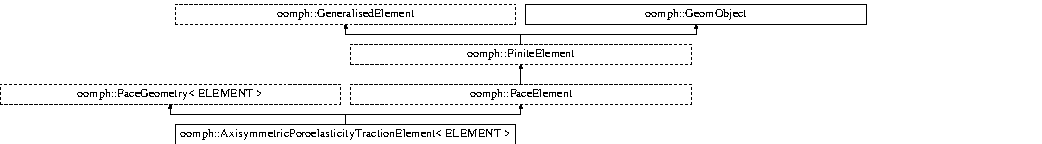
\includegraphics[height=1.939394cm]{classoomph_1_1AxisymmetricPoroelasticityTractionElement}
\end{center}
\end{figure}
\subsection*{Public Member Functions}
\begin{DoxyCompactItemize}
\item 
\hyperlink{classoomph_1_1AxisymmetricPoroelasticityTractionElement_aa640d489135a4daeb423a4f5ff3cf444}{Axisymmetric\+Poroelasticity\+Traction\+Element} (\hyperlink{classoomph_1_1FiniteElement}{Finite\+Element} $\ast$const \&element\+\_\+pt, const int \&\hyperlink{classoomph_1_1FaceElement_a478d577ac6db67ecc80f1f02ae3ab170}{face\+\_\+index})
\begin{DoxyCompactList}\small\item\em Constructor, which takes a \char`\"{}bulk\char`\"{} element and the value of the index and its limit. \end{DoxyCompactList}\item 
\hyperlink{classoomph_1_1AxisymmetricPoroelasticityTractionElement_a518070e49c32661dce27658f018b0986}{Axisymmetric\+Poroelasticity\+Traction\+Element} ()
\begin{DoxyCompactList}\small\item\em Default constructor. \end{DoxyCompactList}\item 
void \hyperlink{classoomph_1_1AxisymmetricPoroelasticityTractionElement_a0db1a4eba81137b3740fcbd7bc705f48}{fill\+\_\+in\+\_\+contribution\+\_\+to\+\_\+residuals} (\hyperlink{classoomph_1_1Vector}{Vector}$<$ double $>$ \&residuals)
\begin{DoxyCompactList}\small\item\em Return the residuals. \end{DoxyCompactList}\item 
void \hyperlink{classoomph_1_1AxisymmetricPoroelasticityTractionElement_a9779f0ccbce1f73b77c64b91ed9ebefa}{fill\+\_\+in\+\_\+contribution\+\_\+to\+\_\+jacobian} (\hyperlink{classoomph_1_1Vector}{Vector}$<$ double $>$ \&residuals, \hyperlink{classoomph_1_1DenseMatrix}{Dense\+Matrix}$<$ double $>$ \&jacobian)
\begin{DoxyCompactList}\small\item\em Fill in contribution from Jacobian. \end{DoxyCompactList}\item 
double \hyperlink{classoomph_1_1AxisymmetricPoroelasticityTractionElement_a8c215f2c9d8b8e66513397b102b1e4aa}{zeta\+\_\+nodal} (const unsigned \&n, const unsigned \&k, const unsigned \&\hyperlink{cfortran_8h_adb50e893b86b3e55e751a42eab3cba82}{i}) const
\begin{DoxyCompactList}\small\item\em The \char`\"{}global\char`\"{} intrinsic coordinate of the element when viewed as part of a geometric object should be given by the \hyperlink{classoomph_1_1FaceElement}{Face\+Element} representation, by default (needed to break indeterminacy if bulk element is Solid\+Element) \end{DoxyCompactList}\item 
void \hyperlink{classoomph_1_1AxisymmetricPoroelasticityTractionElement_a8a8c5836245d55930bd54dc5a12d518a}{output} (std\+::ostream \&outfile)
\begin{DoxyCompactList}\small\item\em Output function. \end{DoxyCompactList}\item 
void \hyperlink{classoomph_1_1AxisymmetricPoroelasticityTractionElement_ac39b3c4245c9ac3a075a9686723d9360}{output} (std\+::ostream \&outfile, const unsigned \&n\+\_\+plot)
\begin{DoxyCompactList}\small\item\em Output function. \end{DoxyCompactList}\item 
void \hyperlink{classoomph_1_1AxisymmetricPoroelasticityTractionElement_a35244154ae620644ad434f7dc34173da}{output} (F\+I\+LE $\ast$file\+\_\+pt)
\begin{DoxyCompactList}\small\item\em C\+\_\+style output function. \end{DoxyCompactList}\item 
void \hyperlink{classoomph_1_1AxisymmetricPoroelasticityTractionElement_ac2efa0fcd5c5d4fe2a0772a181c81f97}{output} (F\+I\+LE $\ast$file\+\_\+pt, const unsigned \&n\+\_\+plot)
\begin{DoxyCompactList}\small\item\em C-\/style output function. \end{DoxyCompactList}\item 
double \hyperlink{classoomph_1_1AxisymmetricPoroelasticityTractionElement_a74bcc2448d472585579da00fb1a79da7}{lagrangian\+\_\+eulerian\+\_\+translation\+\_\+factor} (const \hyperlink{classoomph_1_1Vector}{Vector}$<$ double $>$ \&\hyperlink{cfortran_8h_ab7123126e4885ef647dd9c6e3807a21c}{s})
\begin{DoxyCompactList}\small\item\em Ratio of lengths of line elements (or annular surface areas) in the undeformed and deformed configuration (needed to translate normal flux correctly between small displacement formulation used here and the possibly large displacement N\+St formulation used in F\+SI problems. Maths is as follows\+: Surface area\+: A = 2   r ((dr/ds)$^\wedge$2+(dz/ds)$^\wedge$2) ds = 2   J ds This function returns the ratio of J in the undeformed configuration (used here) to that in the deformed configuration where (r,z) = (r,z)\+\_\+undef + (u\+\_\+r,u\+\_\+z). \end{DoxyCompactList}\item 
void \hyperlink{classoomph_1_1AxisymmetricPoroelasticityTractionElement_abb8e937540df8384b6129793497f1e50}{traction} (const double \&time, const \hyperlink{classoomph_1_1Vector}{Vector}$<$ double $>$ \&\hyperlink{cfortran_8h_ab7123126e4885ef647dd9c6e3807a21c}{s}, \hyperlink{classoomph_1_1Vector}{Vector}$<$ double $>$ \&traction)
\begin{DoxyCompactList}\small\item\em Compute traction vector at specified local coordinate Should only be used for post-\/processing; ignores dependence on integration point! \end{DoxyCompactList}\item 
void \hyperlink{classoomph_1_1AxisymmetricPoroelasticityTractionElement_a9d0a69336be18e1a62450c5c8872777b}{pressure} (const double \&time, const \hyperlink{classoomph_1_1Vector}{Vector}$<$ double $>$ \&\hyperlink{cfortran_8h_ab7123126e4885ef647dd9c6e3807a21c}{s}, double \&pressure)
\begin{DoxyCompactList}\small\item\em Compute pressure value at specified local coordinate Should only be used for post-\/processing; ignores dependence on integration point! \end{DoxyCompactList}\item 
void \hyperlink{classoomph_1_1AxisymmetricPoroelasticityTractionElement_a4618b8dad8a2e2e744016187300c966c}{contribution\+\_\+to\+\_\+total\+\_\+porous\+\_\+flux} (double \&skeleton\+\_\+flux\+\_\+contrib, double \&seepage\+\_\+flux\+\_\+contrib)
\begin{DoxyCompactList}\small\item\em Compute contributions to integrated porous flux over boundary\+: q\+\_\+skeleton =   u\+\_\+displ /  t  n ds q\+\_\+seepage =  k q  n ds. \end{DoxyCompactList}\end{DoxyCompactItemize}
\subsection*{Public Attributes}
\begin{DoxyCompactItemize}
\item 
void($\ast$\&)(const double \&time, const \hyperlink{classoomph_1_1Vector}{Vector}$<$ double $>$ \&x, const \hyperlink{classoomph_1_1Vector}{Vector}$<$ double $>$ \&n, \hyperlink{classoomph_1_1Vector}{Vector}$<$ double $>$ \&\hyperlink{classoomph_1_1AxisymmetricPoroelasticityTractionElement_abb8e937540df8384b6129793497f1e50}{traction}) \hyperlink{classoomph_1_1AxisymmetricPoroelasticityTractionElement_aa33c50e13b91213e8f5b5babf507718e}{traction\+\_\+fct\+\_\+pt} ()
\begin{DoxyCompactList}\small\item\em Reference to the traction function pointer. \end{DoxyCompactList}\item 
void($\ast$\&)(const double \&time, const \hyperlink{classoomph_1_1Vector}{Vector}$<$ double $>$ \&x, const \hyperlink{classoomph_1_1Vector}{Vector}$<$ double $>$ \&n, double \&\hyperlink{classoomph_1_1AxisymmetricPoroelasticityTractionElement_a9d0a69336be18e1a62450c5c8872777b}{pressure}) \hyperlink{classoomph_1_1AxisymmetricPoroelasticityTractionElement_a160a754eb4572b56b146126729e89317}{pressure\+\_\+fct\+\_\+pt} ()
\begin{DoxyCompactList}\small\item\em Reference to the pressure function pointer. \end{DoxyCompactList}\end{DoxyCompactItemize}
\subsection*{Protected Member Functions}
\begin{DoxyCompactItemize}
\item 
virtual void \hyperlink{classoomph_1_1AxisymmetricPoroelasticityTractionElement_a0d996e2947fe74e991d1f382cfa5491d}{get\+\_\+traction} (const double \&time, const unsigned \&intpt, const \hyperlink{classoomph_1_1Vector}{Vector}$<$ double $>$ \&x, const \hyperlink{classoomph_1_1Vector}{Vector}$<$ double $>$ \&n, \hyperlink{classoomph_1_1Vector}{Vector}$<$ double $>$ \&\hyperlink{classoomph_1_1AxisymmetricPoroelasticityTractionElement_abb8e937540df8384b6129793497f1e50}{traction})
\begin{DoxyCompactList}\small\item\em Get the traction vector\+: Pass number of integration point (dummy), Eulerrian coordinate and normal vector and return the pressure (not all of the input arguments will be required for all specific load functions but the list should cover all cases). This function is virtual so it can be overloaded for F\+SI. \end{DoxyCompactList}\item 
virtual void \hyperlink{classoomph_1_1AxisymmetricPoroelasticityTractionElement_a1b4adcf0b886054a3d51e0b2910ddbda}{get\+\_\+pressure} (const double \&time, const unsigned \&intpt, const \hyperlink{classoomph_1_1Vector}{Vector}$<$ double $>$ \&x, const \hyperlink{classoomph_1_1Vector}{Vector}$<$ double $>$ \&n, double \&\hyperlink{classoomph_1_1AxisymmetricPoroelasticityTractionElement_a9d0a69336be18e1a62450c5c8872777b}{pressure})
\begin{DoxyCompactList}\small\item\em Get the pressure value\+: Pass number of integration point (dummy), Eulerrian coordinate and normal vector and return the pressure (not all of the input arguments will be required for all specific load functions but the list should cover all cases). This function is virtual so it can be overloaded for F\+SI. \end{DoxyCompactList}\item 
void \hyperlink{classoomph_1_1AxisymmetricPoroelasticityTractionElement_a98e47ba16813ca8024932544a4b00e87}{fill\+\_\+in\+\_\+contribution\+\_\+to\+\_\+residuals\+\_\+axisym\+\_\+poroelasticity\+\_\+face} (\hyperlink{classoomph_1_1Vector}{Vector}$<$ double $>$ \&residuals)
\begin{DoxyCompactList}\small\item\em Helper function that actually calculates the residuals. \end{DoxyCompactList}\end{DoxyCompactItemize}
\subsection*{Protected Attributes}
\begin{DoxyCompactItemize}
\item 
void($\ast$ \hyperlink{classoomph_1_1AxisymmetricPoroelasticityTractionElement_a60243c82b6016fdeaa118c348b007c13}{Traction\+\_\+fct\+\_\+pt} )(const double \&time, const \hyperlink{classoomph_1_1Vector}{Vector}$<$ double $>$ \&x, const \hyperlink{classoomph_1_1Vector}{Vector}$<$ double $>$ \&n, \hyperlink{classoomph_1_1Vector}{Vector}$<$ double $>$ \&result)
\begin{DoxyCompactList}\small\item\em Pointer to an imposed traction function. Arguments\+: Eulerian coordinate; outer unit normal; applied traction. (Not all of the input arguments will be required for all specific load functions but the list should cover all cases) \end{DoxyCompactList}\item 
void($\ast$ \hyperlink{classoomph_1_1AxisymmetricPoroelasticityTractionElement_a914e7f426769fe5e58d71fb2588449b8}{Pressure\+\_\+fct\+\_\+pt} )(const double \&time, const \hyperlink{classoomph_1_1Vector}{Vector}$<$ double $>$ \&x, const \hyperlink{classoomph_1_1Vector}{Vector}$<$ double $>$ \&n, double \&result)
\begin{DoxyCompactList}\small\item\em Pointer to an imposed pressure function. Arguments\+: Eulerian coordinate; outer unit normal; applied pressure. (Not all of the input arguments will be required for all specific load functions but the list should cover all cases) \end{DoxyCompactList}\end{DoxyCompactItemize}
\subsection*{Additional Inherited Members}


\subsection{Detailed Description}
\subsubsection*{template$<$class E\+L\+E\+M\+E\+NT$>$\newline
class oomph\+::\+Axisymmetric\+Poroelasticity\+Traction\+Element$<$ E\+L\+E\+M\+E\+N\+T $>$}

A class for elements that allow the imposition of an applied combined traction and pore fluid pressure in the axisym poroelasticity equations. The geometrical information can be read from the Face\+Geometry$<$\+E\+L\+E\+M\+E\+N\+T$>$ class and thus, we can be generic enough without the need to have a separate equations class. 

Definition at line 97 of file axisym\+\_\+poroelasticity\+\_\+face\+\_\+elements.\+h.



\subsection{Constructor \& Destructor Documentation}
\mbox{\Hypertarget{classoomph_1_1AxisymmetricPoroelasticityTractionElement_aa640d489135a4daeb423a4f5ff3cf444}\label{classoomph_1_1AxisymmetricPoroelasticityTractionElement_aa640d489135a4daeb423a4f5ff3cf444}} 
\index{oomph\+::\+Axisymmetric\+Poroelasticity\+Traction\+Element@{oomph\+::\+Axisymmetric\+Poroelasticity\+Traction\+Element}!Axisymmetric\+Poroelasticity\+Traction\+Element@{Axisymmetric\+Poroelasticity\+Traction\+Element}}
\index{Axisymmetric\+Poroelasticity\+Traction\+Element@{Axisymmetric\+Poroelasticity\+Traction\+Element}!oomph\+::\+Axisymmetric\+Poroelasticity\+Traction\+Element@{oomph\+::\+Axisymmetric\+Poroelasticity\+Traction\+Element}}
\subsubsection{\texorpdfstring{Axisymmetric\+Poroelasticity\+Traction\+Element()}{AxisymmetricPoroelasticityTractionElement()}\hspace{0.1cm}{\footnotesize\ttfamily [1/2]}}
{\footnotesize\ttfamily template$<$class E\+L\+E\+M\+E\+NT$>$ \\
\hyperlink{classoomph_1_1AxisymmetricPoroelasticityTractionElement}{oomph\+::\+Axisymmetric\+Poroelasticity\+Traction\+Element}$<$ E\+L\+E\+M\+E\+NT $>$\+::\hyperlink{classoomph_1_1AxisymmetricPoroelasticityTractionElement}{Axisymmetric\+Poroelasticity\+Traction\+Element} (\begin{DoxyParamCaption}\item[{\hyperlink{classoomph_1_1FiniteElement}{Finite\+Element} $\ast$const \&}]{element\+\_\+pt,  }\item[{const int \&}]{face\+\_\+index }\end{DoxyParamCaption})\hspace{0.3cm}{\ttfamily [inline]}}



Constructor, which takes a \char`\"{}bulk\char`\"{} element and the value of the index and its limit. 



Definition at line 163 of file axisym\+\_\+poroelasticity\+\_\+face\+\_\+elements.\+h.

\mbox{\Hypertarget{classoomph_1_1AxisymmetricPoroelasticityTractionElement_a518070e49c32661dce27658f018b0986}\label{classoomph_1_1AxisymmetricPoroelasticityTractionElement_a518070e49c32661dce27658f018b0986}} 
\index{oomph\+::\+Axisymmetric\+Poroelasticity\+Traction\+Element@{oomph\+::\+Axisymmetric\+Poroelasticity\+Traction\+Element}!Axisymmetric\+Poroelasticity\+Traction\+Element@{Axisymmetric\+Poroelasticity\+Traction\+Element}}
\index{Axisymmetric\+Poroelasticity\+Traction\+Element@{Axisymmetric\+Poroelasticity\+Traction\+Element}!oomph\+::\+Axisymmetric\+Poroelasticity\+Traction\+Element@{oomph\+::\+Axisymmetric\+Poroelasticity\+Traction\+Element}}
\subsubsection{\texorpdfstring{Axisymmetric\+Poroelasticity\+Traction\+Element()}{AxisymmetricPoroelasticityTractionElement()}\hspace{0.1cm}{\footnotesize\ttfamily [2/2]}}
{\footnotesize\ttfamily template$<$class E\+L\+E\+M\+E\+NT$>$ \\
\hyperlink{classoomph_1_1AxisymmetricPoroelasticityTractionElement}{oomph\+::\+Axisymmetric\+Poroelasticity\+Traction\+Element}$<$ E\+L\+E\+M\+E\+NT $>$\+::\hyperlink{classoomph_1_1AxisymmetricPoroelasticityTractionElement}{Axisymmetric\+Poroelasticity\+Traction\+Element} (\begin{DoxyParamCaption}{ }\end{DoxyParamCaption})\hspace{0.3cm}{\ttfamily [inline]}}



Default constructor. 



Definition at line 206 of file axisym\+\_\+poroelasticity\+\_\+face\+\_\+elements.\+h.



\subsection{Member Function Documentation}
\mbox{\Hypertarget{classoomph_1_1AxisymmetricPoroelasticityTractionElement_a4618b8dad8a2e2e744016187300c966c}\label{classoomph_1_1AxisymmetricPoroelasticityTractionElement_a4618b8dad8a2e2e744016187300c966c}} 
\index{oomph\+::\+Axisymmetric\+Poroelasticity\+Traction\+Element@{oomph\+::\+Axisymmetric\+Poroelasticity\+Traction\+Element}!contribution\+\_\+to\+\_\+total\+\_\+porous\+\_\+flux@{contribution\+\_\+to\+\_\+total\+\_\+porous\+\_\+flux}}
\index{contribution\+\_\+to\+\_\+total\+\_\+porous\+\_\+flux@{contribution\+\_\+to\+\_\+total\+\_\+porous\+\_\+flux}!oomph\+::\+Axisymmetric\+Poroelasticity\+Traction\+Element@{oomph\+::\+Axisymmetric\+Poroelasticity\+Traction\+Element}}
\subsubsection{\texorpdfstring{contribution\+\_\+to\+\_\+total\+\_\+porous\+\_\+flux()}{contribution\_to\_total\_porous\_flux()}}
{\footnotesize\ttfamily template$<$class E\+L\+E\+M\+E\+NT$>$ \\
void \hyperlink{classoomph_1_1AxisymmetricPoroelasticityTractionElement}{oomph\+::\+Axisymmetric\+Poroelasticity\+Traction\+Element}$<$ E\+L\+E\+M\+E\+NT $>$\+::contribution\+\_\+to\+\_\+total\+\_\+porous\+\_\+flux (\begin{DoxyParamCaption}\item[{double \&}]{skeleton\+\_\+flux\+\_\+contrib,  }\item[{double \&}]{seepage\+\_\+flux\+\_\+contrib }\end{DoxyParamCaption})\hspace{0.3cm}{\ttfamily [inline]}}



Compute contributions to integrated porous flux over boundary\+: q\+\_\+skeleton =   u\+\_\+displ /  t  n ds q\+\_\+seepage =  k q  n ds. 

Calculate the FE representation of q 

Definition at line 532 of file axisym\+\_\+poroelasticity\+\_\+face\+\_\+elements.\+h.

\mbox{\Hypertarget{classoomph_1_1AxisymmetricPoroelasticityTractionElement_a9779f0ccbce1f73b77c64b91ed9ebefa}\label{classoomph_1_1AxisymmetricPoroelasticityTractionElement_a9779f0ccbce1f73b77c64b91ed9ebefa}} 
\index{oomph\+::\+Axisymmetric\+Poroelasticity\+Traction\+Element@{oomph\+::\+Axisymmetric\+Poroelasticity\+Traction\+Element}!fill\+\_\+in\+\_\+contribution\+\_\+to\+\_\+jacobian@{fill\+\_\+in\+\_\+contribution\+\_\+to\+\_\+jacobian}}
\index{fill\+\_\+in\+\_\+contribution\+\_\+to\+\_\+jacobian@{fill\+\_\+in\+\_\+contribution\+\_\+to\+\_\+jacobian}!oomph\+::\+Axisymmetric\+Poroelasticity\+Traction\+Element@{oomph\+::\+Axisymmetric\+Poroelasticity\+Traction\+Element}}
\subsubsection{\texorpdfstring{fill\+\_\+in\+\_\+contribution\+\_\+to\+\_\+jacobian()}{fill\_in\_contribution\_to\_jacobian()}}
{\footnotesize\ttfamily template$<$class E\+L\+E\+M\+E\+NT$>$ \\
void \hyperlink{classoomph_1_1AxisymmetricPoroelasticityTractionElement}{oomph\+::\+Axisymmetric\+Poroelasticity\+Traction\+Element}$<$ E\+L\+E\+M\+E\+NT $>$\+::fill\+\_\+in\+\_\+contribution\+\_\+to\+\_\+jacobian (\begin{DoxyParamCaption}\item[{\hyperlink{classoomph_1_1Vector}{Vector}$<$ double $>$ \&}]{residuals,  }\item[{\hyperlink{classoomph_1_1DenseMatrix}{Dense\+Matrix}$<$ double $>$ \&}]{jacobian }\end{DoxyParamCaption})\hspace{0.3cm}{\ttfamily [inline]}, {\ttfamily [virtual]}}



Fill in contribution from Jacobian. 



Reimplemented from \hyperlink{classoomph_1_1GeneralisedElement_a6ae09fc0d68e4309ac1b03583d252845}{oomph\+::\+Generalised\+Element}.



Definition at line 233 of file axisym\+\_\+poroelasticity\+\_\+face\+\_\+elements.\+h.

\mbox{\Hypertarget{classoomph_1_1AxisymmetricPoroelasticityTractionElement_a0db1a4eba81137b3740fcbd7bc705f48}\label{classoomph_1_1AxisymmetricPoroelasticityTractionElement_a0db1a4eba81137b3740fcbd7bc705f48}} 
\index{oomph\+::\+Axisymmetric\+Poroelasticity\+Traction\+Element@{oomph\+::\+Axisymmetric\+Poroelasticity\+Traction\+Element}!fill\+\_\+in\+\_\+contribution\+\_\+to\+\_\+residuals@{fill\+\_\+in\+\_\+contribution\+\_\+to\+\_\+residuals}}
\index{fill\+\_\+in\+\_\+contribution\+\_\+to\+\_\+residuals@{fill\+\_\+in\+\_\+contribution\+\_\+to\+\_\+residuals}!oomph\+::\+Axisymmetric\+Poroelasticity\+Traction\+Element@{oomph\+::\+Axisymmetric\+Poroelasticity\+Traction\+Element}}
\subsubsection{\texorpdfstring{fill\+\_\+in\+\_\+contribution\+\_\+to\+\_\+residuals()}{fill\_in\_contribution\_to\_residuals()}}
{\footnotesize\ttfamily template$<$class E\+L\+E\+M\+E\+NT$>$ \\
void \hyperlink{classoomph_1_1AxisymmetricPoroelasticityTractionElement}{oomph\+::\+Axisymmetric\+Poroelasticity\+Traction\+Element}$<$ E\+L\+E\+M\+E\+NT $>$\+::fill\+\_\+in\+\_\+contribution\+\_\+to\+\_\+residuals (\begin{DoxyParamCaption}\item[{\hyperlink{classoomph_1_1Vector}{Vector}$<$ double $>$ \&}]{residuals }\end{DoxyParamCaption})\hspace{0.3cm}{\ttfamily [inline]}, {\ttfamily [virtual]}}



Return the residuals. 



Reimplemented from \hyperlink{classoomph_1_1GeneralisedElement_a310c97f515e8504a48179c0e72c550d7}{oomph\+::\+Generalised\+Element}.



Definition at line 225 of file axisym\+\_\+poroelasticity\+\_\+face\+\_\+elements.\+h.

\mbox{\Hypertarget{classoomph_1_1AxisymmetricPoroelasticityTractionElement_a98e47ba16813ca8024932544a4b00e87}\label{classoomph_1_1AxisymmetricPoroelasticityTractionElement_a98e47ba16813ca8024932544a4b00e87}} 
\index{oomph\+::\+Axisymmetric\+Poroelasticity\+Traction\+Element@{oomph\+::\+Axisymmetric\+Poroelasticity\+Traction\+Element}!fill\+\_\+in\+\_\+contribution\+\_\+to\+\_\+residuals\+\_\+axisym\+\_\+poroelasticity\+\_\+face@{fill\+\_\+in\+\_\+contribution\+\_\+to\+\_\+residuals\+\_\+axisym\+\_\+poroelasticity\+\_\+face}}
\index{fill\+\_\+in\+\_\+contribution\+\_\+to\+\_\+residuals\+\_\+axisym\+\_\+poroelasticity\+\_\+face@{fill\+\_\+in\+\_\+contribution\+\_\+to\+\_\+residuals\+\_\+axisym\+\_\+poroelasticity\+\_\+face}!oomph\+::\+Axisymmetric\+Poroelasticity\+Traction\+Element@{oomph\+::\+Axisymmetric\+Poroelasticity\+Traction\+Element}}
\subsubsection{\texorpdfstring{fill\+\_\+in\+\_\+contribution\+\_\+to\+\_\+residuals\+\_\+axisym\+\_\+poroelasticity\+\_\+face()}{fill\_in\_contribution\_to\_residuals\_axisym\_poroelasticity\_face()}}
{\footnotesize\ttfamily template$<$class E\+L\+E\+M\+E\+NT $>$ \\
void \hyperlink{classoomph_1_1AxisymmetricPoroelasticityTractionElement}{oomph\+::\+Axisymmetric\+Poroelasticity\+Traction\+Element}$<$ E\+L\+E\+M\+E\+NT $>$\+::fill\+\_\+in\+\_\+contribution\+\_\+to\+\_\+residuals\+\_\+axisym\+\_\+poroelasticity\+\_\+face (\begin{DoxyParamCaption}\item[{\hyperlink{classoomph_1_1Vector}{Vector}$<$ double $>$ \&}]{residuals }\end{DoxyParamCaption})\hspace{0.3cm}{\ttfamily [protected]}}



Helper function that actually calculates the residuals. 

Return the residuals for the \hyperlink{classoomph_1_1AxisymmetricPoroelasticityTractionElement}{Axisymmetric\+Poroelasticity\+Traction\+Element} equations 

Definition at line 712 of file axisym\+\_\+poroelasticity\+\_\+face\+\_\+elements.\+h.



Referenced by oomph\+::\+Axisymmetric\+Poroelasticity\+Traction\+Element$<$ P\+O\+R\+O\+E\+L\+A\+S\+T\+I\+C\+I\+T\+Y\+\_\+\+B\+U\+L\+K\+\_\+\+E\+L\+E\+M\+E\+N\+T $>$\+::pressure().

\mbox{\Hypertarget{classoomph_1_1AxisymmetricPoroelasticityTractionElement_a1b4adcf0b886054a3d51e0b2910ddbda}\label{classoomph_1_1AxisymmetricPoroelasticityTractionElement_a1b4adcf0b886054a3d51e0b2910ddbda}} 
\index{oomph\+::\+Axisymmetric\+Poroelasticity\+Traction\+Element@{oomph\+::\+Axisymmetric\+Poroelasticity\+Traction\+Element}!get\+\_\+pressure@{get\+\_\+pressure}}
\index{get\+\_\+pressure@{get\+\_\+pressure}!oomph\+::\+Axisymmetric\+Poroelasticity\+Traction\+Element@{oomph\+::\+Axisymmetric\+Poroelasticity\+Traction\+Element}}
\subsubsection{\texorpdfstring{get\+\_\+pressure()}{get\_pressure()}}
{\footnotesize\ttfamily template$<$class E\+L\+E\+M\+E\+NT$>$ \\
virtual void \hyperlink{classoomph_1_1AxisymmetricPoroelasticityTractionElement}{oomph\+::\+Axisymmetric\+Poroelasticity\+Traction\+Element}$<$ E\+L\+E\+M\+E\+NT $>$\+::get\+\_\+pressure (\begin{DoxyParamCaption}\item[{const double \&}]{time,  }\item[{const unsigned \&}]{intpt,  }\item[{const \hyperlink{classoomph_1_1Vector}{Vector}$<$ double $>$ \&}]{x,  }\item[{const \hyperlink{classoomph_1_1Vector}{Vector}$<$ double $>$ \&}]{n,  }\item[{double \&}]{pressure }\end{DoxyParamCaption})\hspace{0.3cm}{\ttfamily [inline]}, {\ttfamily [protected]}, {\ttfamily [virtual]}}



Get the pressure value\+: Pass number of integration point (dummy), Eulerrian coordinate and normal vector and return the pressure (not all of the input arguments will be required for all specific load functions but the list should cover all cases). This function is virtual so it can be overloaded for F\+SI. 



Reimplemented in \hyperlink{classoomph_1_1FSILinearisedAxisymPoroelasticTractionElement_a400115007925a62448e741cad2697472}{oomph\+::\+F\+S\+I\+Linearised\+Axisym\+Poroelastic\+Traction\+Element$<$ P\+O\+R\+O\+E\+L\+A\+S\+T\+I\+C\+I\+T\+Y\+\_\+\+B\+U\+L\+K\+\_\+\+E\+L\+E\+M\+E\+N\+T, N\+A\+V\+I\+E\+R\+\_\+\+S\+T\+O\+K\+E\+S\+\_\+\+B\+U\+L\+K\+\_\+\+E\+L\+E\+M\+E\+N\+T $>$}.



Definition at line 141 of file axisym\+\_\+poroelasticity\+\_\+face\+\_\+elements.\+h.

\mbox{\Hypertarget{classoomph_1_1AxisymmetricPoroelasticityTractionElement_a0d996e2947fe74e991d1f382cfa5491d}\label{classoomph_1_1AxisymmetricPoroelasticityTractionElement_a0d996e2947fe74e991d1f382cfa5491d}} 
\index{oomph\+::\+Axisymmetric\+Poroelasticity\+Traction\+Element@{oomph\+::\+Axisymmetric\+Poroelasticity\+Traction\+Element}!get\+\_\+traction@{get\+\_\+traction}}
\index{get\+\_\+traction@{get\+\_\+traction}!oomph\+::\+Axisymmetric\+Poroelasticity\+Traction\+Element@{oomph\+::\+Axisymmetric\+Poroelasticity\+Traction\+Element}}
\subsubsection{\texorpdfstring{get\+\_\+traction()}{get\_traction()}}
{\footnotesize\ttfamily template$<$class E\+L\+E\+M\+E\+NT$>$ \\
virtual void \hyperlink{classoomph_1_1AxisymmetricPoroelasticityTractionElement}{oomph\+::\+Axisymmetric\+Poroelasticity\+Traction\+Element}$<$ E\+L\+E\+M\+E\+NT $>$\+::get\+\_\+traction (\begin{DoxyParamCaption}\item[{const double \&}]{time,  }\item[{const unsigned \&}]{intpt,  }\item[{const \hyperlink{classoomph_1_1Vector}{Vector}$<$ double $>$ \&}]{x,  }\item[{const \hyperlink{classoomph_1_1Vector}{Vector}$<$ double $>$ \&}]{n,  }\item[{\hyperlink{classoomph_1_1Vector}{Vector}$<$ double $>$ \&}]{traction }\end{DoxyParamCaption})\hspace{0.3cm}{\ttfamily [inline]}, {\ttfamily [protected]}, {\ttfamily [virtual]}}



Get the traction vector\+: Pass number of integration point (dummy), Eulerrian coordinate and normal vector and return the pressure (not all of the input arguments will be required for all specific load functions but the list should cover all cases). This function is virtual so it can be overloaded for F\+SI. 



Reimplemented in \hyperlink{classoomph_1_1FSILinearisedAxisymPoroelasticTractionElement_ace2d9e5b5f0fbea991a95b5e1c0f7b80}{oomph\+::\+F\+S\+I\+Linearised\+Axisym\+Poroelastic\+Traction\+Element$<$ P\+O\+R\+O\+E\+L\+A\+S\+T\+I\+C\+I\+T\+Y\+\_\+\+B\+U\+L\+K\+\_\+\+E\+L\+E\+M\+E\+N\+T, N\+A\+V\+I\+E\+R\+\_\+\+S\+T\+O\+K\+E\+S\+\_\+\+B\+U\+L\+K\+\_\+\+E\+L\+E\+M\+E\+N\+T $>$}.



Definition at line 127 of file axisym\+\_\+poroelasticity\+\_\+face\+\_\+elements.\+h.

\mbox{\Hypertarget{classoomph_1_1AxisymmetricPoroelasticityTractionElement_a74bcc2448d472585579da00fb1a79da7}\label{classoomph_1_1AxisymmetricPoroelasticityTractionElement_a74bcc2448d472585579da00fb1a79da7}} 
\index{oomph\+::\+Axisymmetric\+Poroelasticity\+Traction\+Element@{oomph\+::\+Axisymmetric\+Poroelasticity\+Traction\+Element}!lagrangian\+\_\+eulerian\+\_\+translation\+\_\+factor@{lagrangian\+\_\+eulerian\+\_\+translation\+\_\+factor}}
\index{lagrangian\+\_\+eulerian\+\_\+translation\+\_\+factor@{lagrangian\+\_\+eulerian\+\_\+translation\+\_\+factor}!oomph\+::\+Axisymmetric\+Poroelasticity\+Traction\+Element@{oomph\+::\+Axisymmetric\+Poroelasticity\+Traction\+Element}}
\subsubsection{\texorpdfstring{lagrangian\+\_\+eulerian\+\_\+translation\+\_\+factor()}{lagrangian\_eulerian\_translation\_factor()}}
{\footnotesize\ttfamily template$<$class E\+L\+E\+M\+E\+NT$>$ \\
double \hyperlink{classoomph_1_1AxisymmetricPoroelasticityTractionElement}{oomph\+::\+Axisymmetric\+Poroelasticity\+Traction\+Element}$<$ E\+L\+E\+M\+E\+NT $>$\+::lagrangian\+\_\+eulerian\+\_\+translation\+\_\+factor (\begin{DoxyParamCaption}\item[{const \hyperlink{classoomph_1_1Vector}{Vector}$<$ double $>$ \&}]{s }\end{DoxyParamCaption})\hspace{0.3cm}{\ttfamily [inline]}}



Ratio of lengths of line elements (or annular surface areas) in the undeformed and deformed configuration (needed to translate normal flux correctly between small displacement formulation used here and the possibly large displacement N\+St formulation used in F\+SI problems. Maths is as follows\+: Surface area\+: A = 2   r ((dr/ds)$^\wedge$2+(dz/ds)$^\wedge$2) ds = 2   J ds This function returns the ratio of J in the undeformed configuration (used here) to that in the deformed configuration where (r,z) = (r,z)\+\_\+undef + (u\+\_\+r,u\+\_\+z). 

Calculate the FE representation of u -- the skeleton displacement 

Definition at line 450 of file axisym\+\_\+poroelasticity\+\_\+face\+\_\+elements.\+h.

\mbox{\Hypertarget{classoomph_1_1AxisymmetricPoroelasticityTractionElement_a8a8c5836245d55930bd54dc5a12d518a}\label{classoomph_1_1AxisymmetricPoroelasticityTractionElement_a8a8c5836245d55930bd54dc5a12d518a}} 
\index{oomph\+::\+Axisymmetric\+Poroelasticity\+Traction\+Element@{oomph\+::\+Axisymmetric\+Poroelasticity\+Traction\+Element}!output@{output}}
\index{output@{output}!oomph\+::\+Axisymmetric\+Poroelasticity\+Traction\+Element@{oomph\+::\+Axisymmetric\+Poroelasticity\+Traction\+Element}}
\subsubsection{\texorpdfstring{output()}{output()}\hspace{0.1cm}{\footnotesize\ttfamily [1/4]}}
{\footnotesize\ttfamily template$<$class E\+L\+E\+M\+E\+NT$>$ \\
void \hyperlink{classoomph_1_1AxisymmetricPoroelasticityTractionElement}{oomph\+::\+Axisymmetric\+Poroelasticity\+Traction\+Element}$<$ E\+L\+E\+M\+E\+NT $>$\+::output (\begin{DoxyParamCaption}\item[{std\+::ostream \&}]{outfile }\end{DoxyParamCaption})\hspace{0.3cm}{\ttfamily [inline]}, {\ttfamily [virtual]}}



Output function. 



Reimplemented from \hyperlink{classoomph_1_1FiniteElement_a2ad98a3d2ef4999f1bef62c0ff13f2a7}{oomph\+::\+Finite\+Element}.



Definition at line 251 of file axisym\+\_\+poroelasticity\+\_\+face\+\_\+elements.\+h.

\mbox{\Hypertarget{classoomph_1_1AxisymmetricPoroelasticityTractionElement_ac39b3c4245c9ac3a075a9686723d9360}\label{classoomph_1_1AxisymmetricPoroelasticityTractionElement_ac39b3c4245c9ac3a075a9686723d9360}} 
\index{oomph\+::\+Axisymmetric\+Poroelasticity\+Traction\+Element@{oomph\+::\+Axisymmetric\+Poroelasticity\+Traction\+Element}!output@{output}}
\index{output@{output}!oomph\+::\+Axisymmetric\+Poroelasticity\+Traction\+Element@{oomph\+::\+Axisymmetric\+Poroelasticity\+Traction\+Element}}
\subsubsection{\texorpdfstring{output()}{output()}\hspace{0.1cm}{\footnotesize\ttfamily [2/4]}}
{\footnotesize\ttfamily template$<$class E\+L\+E\+M\+E\+NT$>$ \\
void \hyperlink{classoomph_1_1AxisymmetricPoroelasticityTractionElement}{oomph\+::\+Axisymmetric\+Poroelasticity\+Traction\+Element}$<$ E\+L\+E\+M\+E\+NT $>$\+::output (\begin{DoxyParamCaption}\item[{std\+::ostream \&}]{outfile,  }\item[{const unsigned \&}]{n\+\_\+plot }\end{DoxyParamCaption})\hspace{0.3cm}{\ttfamily [inline]}, {\ttfamily [virtual]}}



Output function. 

Calculate the FE representation of u -- the skeleton displacement

Skeleton velocity 

Reimplemented from \hyperlink{classoomph_1_1FiniteElement_afa9d9b2670f999b43e6679c9dd28c457}{oomph\+::\+Finite\+Element}.



Definition at line 259 of file axisym\+\_\+poroelasticity\+\_\+face\+\_\+elements.\+h.

\mbox{\Hypertarget{classoomph_1_1AxisymmetricPoroelasticityTractionElement_a35244154ae620644ad434f7dc34173da}\label{classoomph_1_1AxisymmetricPoroelasticityTractionElement_a35244154ae620644ad434f7dc34173da}} 
\index{oomph\+::\+Axisymmetric\+Poroelasticity\+Traction\+Element@{oomph\+::\+Axisymmetric\+Poroelasticity\+Traction\+Element}!output@{output}}
\index{output@{output}!oomph\+::\+Axisymmetric\+Poroelasticity\+Traction\+Element@{oomph\+::\+Axisymmetric\+Poroelasticity\+Traction\+Element}}
\subsubsection{\texorpdfstring{output()}{output()}\hspace{0.1cm}{\footnotesize\ttfamily [3/4]}}
{\footnotesize\ttfamily template$<$class E\+L\+E\+M\+E\+NT$>$ \\
void \hyperlink{classoomph_1_1AxisymmetricPoroelasticityTractionElement}{oomph\+::\+Axisymmetric\+Poroelasticity\+Traction\+Element}$<$ E\+L\+E\+M\+E\+NT $>$\+::output (\begin{DoxyParamCaption}\item[{F\+I\+LE $\ast$}]{file\+\_\+pt }\end{DoxyParamCaption})\hspace{0.3cm}{\ttfamily [inline]}, {\ttfamily [virtual]}}



C\+\_\+style output function. 



Reimplemented from \hyperlink{classoomph_1_1FiniteElement_a72cddd09f8ddbee1a20a1ff404c6943e}{oomph\+::\+Finite\+Element}.



Definition at line 431 of file axisym\+\_\+poroelasticity\+\_\+face\+\_\+elements.\+h.

\mbox{\Hypertarget{classoomph_1_1AxisymmetricPoroelasticityTractionElement_ac2efa0fcd5c5d4fe2a0772a181c81f97}\label{classoomph_1_1AxisymmetricPoroelasticityTractionElement_ac2efa0fcd5c5d4fe2a0772a181c81f97}} 
\index{oomph\+::\+Axisymmetric\+Poroelasticity\+Traction\+Element@{oomph\+::\+Axisymmetric\+Poroelasticity\+Traction\+Element}!output@{output}}
\index{output@{output}!oomph\+::\+Axisymmetric\+Poroelasticity\+Traction\+Element@{oomph\+::\+Axisymmetric\+Poroelasticity\+Traction\+Element}}
\subsubsection{\texorpdfstring{output()}{output()}\hspace{0.1cm}{\footnotesize\ttfamily [4/4]}}
{\footnotesize\ttfamily template$<$class E\+L\+E\+M\+E\+NT$>$ \\
void \hyperlink{classoomph_1_1AxisymmetricPoroelasticityTractionElement}{oomph\+::\+Axisymmetric\+Poroelasticity\+Traction\+Element}$<$ E\+L\+E\+M\+E\+NT $>$\+::output (\begin{DoxyParamCaption}\item[{F\+I\+LE $\ast$}]{file\+\_\+pt,  }\item[{const unsigned \&}]{n\+\_\+plot }\end{DoxyParamCaption})\hspace{0.3cm}{\ttfamily [inline]}, {\ttfamily [virtual]}}



C-\/style output function. 



Reimplemented from \hyperlink{classoomph_1_1FiniteElement_adfaee690bb0608f03320eeb9d110d48c}{oomph\+::\+Finite\+Element}.



Definition at line 435 of file axisym\+\_\+poroelasticity\+\_\+face\+\_\+elements.\+h.

\mbox{\Hypertarget{classoomph_1_1AxisymmetricPoroelasticityTractionElement_a9d0a69336be18e1a62450c5c8872777b}\label{classoomph_1_1AxisymmetricPoroelasticityTractionElement_a9d0a69336be18e1a62450c5c8872777b}} 
\index{oomph\+::\+Axisymmetric\+Poroelasticity\+Traction\+Element@{oomph\+::\+Axisymmetric\+Poroelasticity\+Traction\+Element}!pressure@{pressure}}
\index{pressure@{pressure}!oomph\+::\+Axisymmetric\+Poroelasticity\+Traction\+Element@{oomph\+::\+Axisymmetric\+Poroelasticity\+Traction\+Element}}
\subsubsection{\texorpdfstring{pressure()}{pressure()}}
{\footnotesize\ttfamily template$<$class E\+L\+E\+M\+E\+NT $>$ \\
void \hyperlink{classoomph_1_1AxisymmetricPoroelasticityTractionElement}{oomph\+::\+Axisymmetric\+Poroelasticity\+Traction\+Element}$<$ E\+L\+E\+M\+E\+NT $>$\+::pressure (\begin{DoxyParamCaption}\item[{const double \&}]{time,  }\item[{const \hyperlink{classoomph_1_1Vector}{Vector}$<$ double $>$ \&}]{s,  }\item[{double \&}]{pressure }\end{DoxyParamCaption})}



Compute pressure value at specified local coordinate Should only be used for post-\/processing; ignores dependence on integration point! 

Compute pressure value at specified local coordinate Should only be used for post-\/processing; ignores dependence on integration point! 

Definition at line 684 of file axisym\+\_\+poroelasticity\+\_\+face\+\_\+elements.\+h.

\mbox{\Hypertarget{classoomph_1_1AxisymmetricPoroelasticityTractionElement_abb8e937540df8384b6129793497f1e50}\label{classoomph_1_1AxisymmetricPoroelasticityTractionElement_abb8e937540df8384b6129793497f1e50}} 
\index{oomph\+::\+Axisymmetric\+Poroelasticity\+Traction\+Element@{oomph\+::\+Axisymmetric\+Poroelasticity\+Traction\+Element}!traction@{traction}}
\index{traction@{traction}!oomph\+::\+Axisymmetric\+Poroelasticity\+Traction\+Element@{oomph\+::\+Axisymmetric\+Poroelasticity\+Traction\+Element}}
\subsubsection{\texorpdfstring{traction()}{traction()}}
{\footnotesize\ttfamily template$<$class E\+L\+E\+M\+E\+NT $>$ \\
void \hyperlink{classoomph_1_1AxisymmetricPoroelasticityTractionElement}{oomph\+::\+Axisymmetric\+Poroelasticity\+Traction\+Element}$<$ E\+L\+E\+M\+E\+NT $>$\+::traction (\begin{DoxyParamCaption}\item[{const double \&}]{time,  }\item[{const \hyperlink{classoomph_1_1Vector}{Vector}$<$ double $>$ \&}]{s,  }\item[{\hyperlink{classoomph_1_1Vector}{Vector}$<$ double $>$ \&}]{traction }\end{DoxyParamCaption})}



Compute traction vector at specified local coordinate Should only be used for post-\/processing; ignores dependence on integration point! 

Compute traction vector at specified local coordinate Should only be used for post-\/processing; ignores dependence on integration point! 

Definition at line 658 of file axisym\+\_\+poroelasticity\+\_\+face\+\_\+elements.\+h.

\mbox{\Hypertarget{classoomph_1_1AxisymmetricPoroelasticityTractionElement_a8c215f2c9d8b8e66513397b102b1e4aa}\label{classoomph_1_1AxisymmetricPoroelasticityTractionElement_a8c215f2c9d8b8e66513397b102b1e4aa}} 
\index{oomph\+::\+Axisymmetric\+Poroelasticity\+Traction\+Element@{oomph\+::\+Axisymmetric\+Poroelasticity\+Traction\+Element}!zeta\+\_\+nodal@{zeta\+\_\+nodal}}
\index{zeta\+\_\+nodal@{zeta\+\_\+nodal}!oomph\+::\+Axisymmetric\+Poroelasticity\+Traction\+Element@{oomph\+::\+Axisymmetric\+Poroelasticity\+Traction\+Element}}
\subsubsection{\texorpdfstring{zeta\+\_\+nodal()}{zeta\_nodal()}}
{\footnotesize\ttfamily template$<$class E\+L\+E\+M\+E\+NT$>$ \\
double \hyperlink{classoomph_1_1AxisymmetricPoroelasticityTractionElement}{oomph\+::\+Axisymmetric\+Poroelasticity\+Traction\+Element}$<$ E\+L\+E\+M\+E\+NT $>$\+::zeta\+\_\+nodal (\begin{DoxyParamCaption}\item[{const unsigned \&}]{n,  }\item[{const unsigned \&}]{k,  }\item[{const unsigned \&}]{i }\end{DoxyParamCaption}) const\hspace{0.3cm}{\ttfamily [inline]}, {\ttfamily [virtual]}}



The \char`\"{}global\char`\"{} intrinsic coordinate of the element when viewed as part of a geometric object should be given by the \hyperlink{classoomph_1_1FaceElement}{Face\+Element} representation, by default (needed to break indeterminacy if bulk element is Solid\+Element) 

Specify the value of nodal zeta from the face geometry 

Reimplemented from \hyperlink{classoomph_1_1FiniteElement_a849561c5fbcbc07dc49d2dc6cca68559}{oomph\+::\+Finite\+Element}.



Definition at line 245 of file axisym\+\_\+poroelasticity\+\_\+face\+\_\+elements.\+h.



\subsection{Member Data Documentation}
\mbox{\Hypertarget{classoomph_1_1AxisymmetricPoroelasticityTractionElement_a914e7f426769fe5e58d71fb2588449b8}\label{classoomph_1_1AxisymmetricPoroelasticityTractionElement_a914e7f426769fe5e58d71fb2588449b8}} 
\index{oomph\+::\+Axisymmetric\+Poroelasticity\+Traction\+Element@{oomph\+::\+Axisymmetric\+Poroelasticity\+Traction\+Element}!Pressure\+\_\+fct\+\_\+pt@{Pressure\+\_\+fct\+\_\+pt}}
\index{Pressure\+\_\+fct\+\_\+pt@{Pressure\+\_\+fct\+\_\+pt}!oomph\+::\+Axisymmetric\+Poroelasticity\+Traction\+Element@{oomph\+::\+Axisymmetric\+Poroelasticity\+Traction\+Element}}
\subsubsection{\texorpdfstring{Pressure\+\_\+fct\+\_\+pt}{Pressure\_fct\_pt}}
{\footnotesize\ttfamily template$<$class E\+L\+E\+M\+E\+NT$>$ \\
void($\ast$ \hyperlink{classoomph_1_1AxisymmetricPoroelasticityTractionElement}{oomph\+::\+Axisymmetric\+Poroelasticity\+Traction\+Element}$<$ E\+L\+E\+M\+E\+NT $>$\+::Pressure\+\_\+fct\+\_\+pt) (const double \&time, const \hyperlink{classoomph_1_1Vector}{Vector}$<$ double $>$ \&x, const \hyperlink{classoomph_1_1Vector}{Vector}$<$ double $>$ \&n, double \&result)\hspace{0.3cm}{\ttfamily [protected]}}



Pointer to an imposed pressure function. Arguments\+: Eulerian coordinate; outer unit normal; applied pressure. (Not all of the input arguments will be required for all specific load functions but the list should cover all cases) 



Definition at line 116 of file axisym\+\_\+poroelasticity\+\_\+face\+\_\+elements.\+h.

\mbox{\Hypertarget{classoomph_1_1AxisymmetricPoroelasticityTractionElement_a160a754eb4572b56b146126729e89317}\label{classoomph_1_1AxisymmetricPoroelasticityTractionElement_a160a754eb4572b56b146126729e89317}} 
\index{oomph\+::\+Axisymmetric\+Poroelasticity\+Traction\+Element@{oomph\+::\+Axisymmetric\+Poroelasticity\+Traction\+Element}!pressure\+\_\+fct\+\_\+pt@{pressure\+\_\+fct\+\_\+pt}}
\index{pressure\+\_\+fct\+\_\+pt@{pressure\+\_\+fct\+\_\+pt}!oomph\+::\+Axisymmetric\+Poroelasticity\+Traction\+Element@{oomph\+::\+Axisymmetric\+Poroelasticity\+Traction\+Element}}
\subsubsection{\texorpdfstring{pressure\+\_\+fct\+\_\+pt}{pressure\_fct\_pt}}
{\footnotesize\ttfamily template$<$class E\+L\+E\+M\+E\+NT$>$ \\
void($\ast$ \&)(const double\& time, const \hyperlink{classoomph_1_1Vector}{Vector}$<$double$>$\& x, const \hyperlink{classoomph_1_1Vector}{Vector}$<$double$>$\& n, double \&\hyperlink{classoomph_1_1AxisymmetricPoroelasticityTractionElement_a9d0a69336be18e1a62450c5c8872777b}{pressure}) \hyperlink{classoomph_1_1AxisymmetricPoroelasticityTractionElement}{oomph\+::\+Axisymmetric\+Poroelasticity\+Traction\+Element}$<$ E\+L\+E\+M\+E\+NT $>$\+::pressure\+\_\+fct\+\_\+pt()\hspace{0.3cm}{\ttfamily [inline]}}



Reference to the pressure function pointer. 



Definition at line 217 of file axisym\+\_\+poroelasticity\+\_\+face\+\_\+elements.\+h.

\mbox{\Hypertarget{classoomph_1_1AxisymmetricPoroelasticityTractionElement_a60243c82b6016fdeaa118c348b007c13}\label{classoomph_1_1AxisymmetricPoroelasticityTractionElement_a60243c82b6016fdeaa118c348b007c13}} 
\index{oomph\+::\+Axisymmetric\+Poroelasticity\+Traction\+Element@{oomph\+::\+Axisymmetric\+Poroelasticity\+Traction\+Element}!Traction\+\_\+fct\+\_\+pt@{Traction\+\_\+fct\+\_\+pt}}
\index{Traction\+\_\+fct\+\_\+pt@{Traction\+\_\+fct\+\_\+pt}!oomph\+::\+Axisymmetric\+Poroelasticity\+Traction\+Element@{oomph\+::\+Axisymmetric\+Poroelasticity\+Traction\+Element}}
\subsubsection{\texorpdfstring{Traction\+\_\+fct\+\_\+pt}{Traction\_fct\_pt}}
{\footnotesize\ttfamily template$<$class E\+L\+E\+M\+E\+NT$>$ \\
void($\ast$ \hyperlink{classoomph_1_1AxisymmetricPoroelasticityTractionElement}{oomph\+::\+Axisymmetric\+Poroelasticity\+Traction\+Element}$<$ E\+L\+E\+M\+E\+NT $>$\+::Traction\+\_\+fct\+\_\+pt) (const double \&time, const \hyperlink{classoomph_1_1Vector}{Vector}$<$ double $>$ \&x, const \hyperlink{classoomph_1_1Vector}{Vector}$<$ double $>$ \&n, \hyperlink{classoomph_1_1Vector}{Vector}$<$ double $>$ \&result)\hspace{0.3cm}{\ttfamily [protected]}}



Pointer to an imposed traction function. Arguments\+: Eulerian coordinate; outer unit normal; applied traction. (Not all of the input arguments will be required for all specific load functions but the list should cover all cases) 



Definition at line 107 of file axisym\+\_\+poroelasticity\+\_\+face\+\_\+elements.\+h.

\mbox{\Hypertarget{classoomph_1_1AxisymmetricPoroelasticityTractionElement_aa33c50e13b91213e8f5b5babf507718e}\label{classoomph_1_1AxisymmetricPoroelasticityTractionElement_aa33c50e13b91213e8f5b5babf507718e}} 
\index{oomph\+::\+Axisymmetric\+Poroelasticity\+Traction\+Element@{oomph\+::\+Axisymmetric\+Poroelasticity\+Traction\+Element}!traction\+\_\+fct\+\_\+pt@{traction\+\_\+fct\+\_\+pt}}
\index{traction\+\_\+fct\+\_\+pt@{traction\+\_\+fct\+\_\+pt}!oomph\+::\+Axisymmetric\+Poroelasticity\+Traction\+Element@{oomph\+::\+Axisymmetric\+Poroelasticity\+Traction\+Element}}
\subsubsection{\texorpdfstring{traction\+\_\+fct\+\_\+pt}{traction\_fct\_pt}}
{\footnotesize\ttfamily template$<$class E\+L\+E\+M\+E\+NT$>$ \\
void($\ast$ \&)(const double\& time, const \hyperlink{classoomph_1_1Vector}{Vector}$<$double$>$\& x, const \hyperlink{classoomph_1_1Vector}{Vector}$<$double$>$\& n, \hyperlink{classoomph_1_1Vector}{Vector}$<$double$>$ \&\hyperlink{classoomph_1_1AxisymmetricPoroelasticityTractionElement_abb8e937540df8384b6129793497f1e50}{traction}) \hyperlink{classoomph_1_1AxisymmetricPoroelasticityTractionElement}{oomph\+::\+Axisymmetric\+Poroelasticity\+Traction\+Element}$<$ E\+L\+E\+M\+E\+NT $>$\+::traction\+\_\+fct\+\_\+pt()\hspace{0.3cm}{\ttfamily [inline]}}



Reference to the traction function pointer. 



Definition at line 209 of file axisym\+\_\+poroelasticity\+\_\+face\+\_\+elements.\+h.



The documentation for this class was generated from the following file\+:\begin{DoxyCompactItemize}
\item 
\hyperlink{axisym__poroelasticity__face__elements_8h}{axisym\+\_\+poroelasticity\+\_\+face\+\_\+elements.\+h}\end{DoxyCompactItemize}

\hypertarget{classoomph_1_1AxisymmetricPVDEquations}{}\section{oomph\+:\+:Axisymmetric\+P\+V\+D\+Equations Class Reference}
\label{classoomph_1_1AxisymmetricPVDEquations}\index{oomph\+::\+Axisymmetric\+P\+V\+D\+Equations@{oomph\+::\+Axisymmetric\+P\+V\+D\+Equations}}


{\ttfamily \#include $<$axisym\+\_\+solid\+\_\+elements.\+h$>$}

Inheritance diagram for oomph\+:\+:Axisymmetric\+P\+V\+D\+Equations\+:\begin{figure}[H]
\begin{center}
\leavevmode
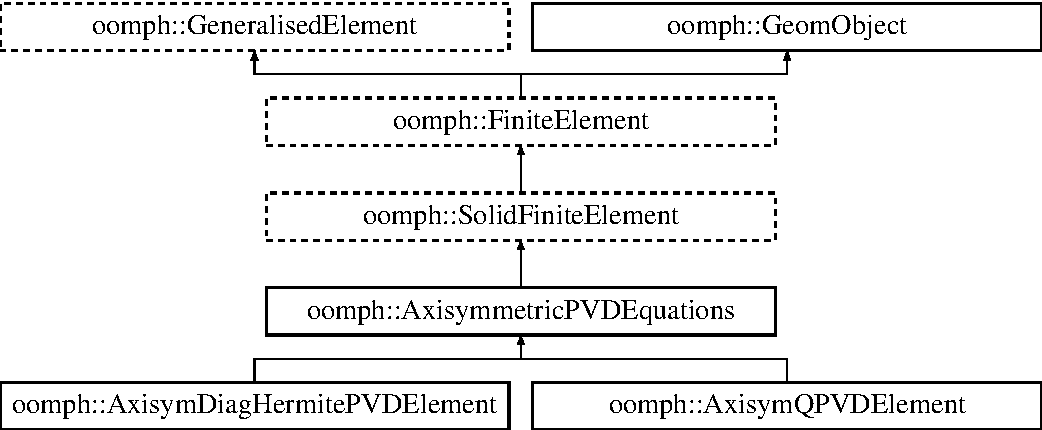
\includegraphics[height=5.000000cm]{classoomph_1_1AxisymmetricPVDEquations}
\end{center}
\end{figure}
\subsection*{Public Member Functions}
\begin{DoxyCompactItemize}
\item 
\hyperlink{classoomph_1_1AxisymmetricPVDEquations_acb73b32e5b0b2a80b164a445c2c8ac9a}{Axisymmetric\+P\+V\+D\+Equations} ()
\begin{DoxyCompactList}\small\item\em Constructor. \end{DoxyCompactList}\item 
\hyperlink{classoomph_1_1ConstitutiveLaw}{Constitutive\+Law} $\ast$\& \hyperlink{classoomph_1_1AxisymmetricPVDEquations_a29cc14b3e1516630a1a6e52ce63ead46}{constitutive\+\_\+law\+\_\+pt} ()
\begin{DoxyCompactList}\small\item\em Return the constitutive law pointer. \end{DoxyCompactList}\item 
void \hyperlink{classoomph_1_1AxisymmetricPVDEquations_ad7984168072632f9d4f7218d81ca50eb}{get\+\_\+stress} (const \hyperlink{classoomph_1_1DenseMatrix}{Dense\+Matrix}$<$ double $>$ \&g, const \hyperlink{classoomph_1_1DenseMatrix}{Dense\+Matrix}$<$ double $>$ \&G, \hyperlink{classoomph_1_1DenseMatrix}{Dense\+Matrix}$<$ double $>$ \&sigma)
\begin{DoxyCompactList}\small\item\em Return the stress tensor, as calculated from the constitutive law. \end{DoxyCompactList}\item 
void \hyperlink{classoomph_1_1AxisymmetricPVDEquations_a432b436b9e82c78cc06baefedc6029d4}{fill\+\_\+in\+\_\+contribution\+\_\+to\+\_\+residuals} (\hyperlink{classoomph_1_1Vector}{Vector}$<$ double $>$ \&residuals)
\begin{DoxyCompactList}\small\item\em Fill in the residuals by calling the generic function. \end{DoxyCompactList}\item 
void \hyperlink{classoomph_1_1AxisymmetricPVDEquations_a12f081b16b2f2a9e8409d4ec12a6d071}{fill\+\_\+in\+\_\+contribution\+\_\+to\+\_\+residuals\+\_\+axisym\+\_\+pvd} (\hyperlink{classoomph_1_1Vector}{Vector}$<$ double $>$ \&residuals)
\begin{DoxyCompactList}\small\item\em Return the residuals for the equations of solid mechanics. \end{DoxyCompactList}\item 
double \hyperlink{classoomph_1_1AxisymmetricPVDEquations_ac4d790ab3df428eb178c247f0ff13c29}{compute\+\_\+physical\+\_\+size} () const
\begin{DoxyCompactList}\small\item\em Overload/implement the function to calculate the volume of the element. \end{DoxyCompactList}\item 
void \hyperlink{classoomph_1_1AxisymmetricPVDEquations_a80e76c7d645e8863f2dd5b1bf456516a}{fill\+\_\+in\+\_\+contribution\+\_\+to\+\_\+jacobian} (\hyperlink{classoomph_1_1Vector}{Vector}$<$ double $>$ \&residuals, \hyperlink{classoomph_1_1DenseMatrix}{Dense\+Matrix}$<$ double $>$ \&jacobian)
\begin{DoxyCompactList}\small\item\em Assign the contribution to the residual using only finite differences. \end{DoxyCompactList}\item 
void \hyperlink{classoomph_1_1AxisymmetricPVDEquations_a70c01efa665238ec7a574588209d3edb}{output} (std\+::ostream \&outfile)
\begin{DoxyCompactList}\small\item\em Overload the output function. \end{DoxyCompactList}\item 
void \hyperlink{classoomph_1_1AxisymmetricPVDEquations_a35cf174ca1692f817e3182166e22ef4b}{output} (std\+::ostream \&outfile, const unsigned \&n\+\_\+plot)
\begin{DoxyCompactList}\small\item\em Output function. \end{DoxyCompactList}\item 
void \hyperlink{classoomph_1_1AxisymmetricPVDEquations_a3b271e966cc554c21231503f7a965549}{output} (F\+I\+LE $\ast$file\+\_\+pt)
\begin{DoxyCompactList}\small\item\em Overload the output function. \end{DoxyCompactList}\item 
void \hyperlink{classoomph_1_1AxisymmetricPVDEquations_a780e6e426869eec81758bf7396a54bad}{output} (F\+I\+LE $\ast$file\+\_\+pt, const unsigned \&n\+\_\+plot)
\begin{DoxyCompactList}\small\item\em Output function. \end{DoxyCompactList}\end{DoxyCompactItemize}
\subsection*{Private Attributes}
\begin{DoxyCompactItemize}
\item 
\hyperlink{classoomph_1_1ConstitutiveLaw}{Constitutive\+Law} $\ast$ \hyperlink{classoomph_1_1AxisymmetricPVDEquations_a69bc689b112a9b24de68315296ab9c87}{Constitutive\+\_\+law\+\_\+pt}
\begin{DoxyCompactList}\small\item\em Pointer to constitutive law. \end{DoxyCompactList}\end{DoxyCompactItemize}
\subsection*{Additional Inherited Members}


\subsection{Detailed Description}
A class for elements that solve the equations of solid mechanics, based on the principle of virtual displacements in an axisymmetric formulation. In this case x\mbox{[}0\mbox{]} is the component of displacement in the radial direction and x\mbox{[}1\mbox{]} is that in the theta direction. 

Definition at line 54 of file axisym\+\_\+solid\+\_\+elements.\+h.



\subsection{Constructor \& Destructor Documentation}
\mbox{\Hypertarget{classoomph_1_1AxisymmetricPVDEquations_acb73b32e5b0b2a80b164a445c2c8ac9a}\label{classoomph_1_1AxisymmetricPVDEquations_acb73b32e5b0b2a80b164a445c2c8ac9a}} 
\index{oomph\+::\+Axisymmetric\+P\+V\+D\+Equations@{oomph\+::\+Axisymmetric\+P\+V\+D\+Equations}!Axisymmetric\+P\+V\+D\+Equations@{Axisymmetric\+P\+V\+D\+Equations}}
\index{Axisymmetric\+P\+V\+D\+Equations@{Axisymmetric\+P\+V\+D\+Equations}!oomph\+::\+Axisymmetric\+P\+V\+D\+Equations@{oomph\+::\+Axisymmetric\+P\+V\+D\+Equations}}
\subsubsection{\texorpdfstring{Axisymmetric\+P\+V\+D\+Equations()}{AxisymmetricPVDEquations()}}
{\footnotesize\ttfamily oomph\+::\+Axisymmetric\+P\+V\+D\+Equations\+::\+Axisymmetric\+P\+V\+D\+Equations (\begin{DoxyParamCaption}{ }\end{DoxyParamCaption})\hspace{0.3cm}{\ttfamily [inline]}}



Constructor. 



Definition at line 64 of file axisym\+\_\+solid\+\_\+elements.\+h.



\subsection{Member Function Documentation}
\mbox{\Hypertarget{classoomph_1_1AxisymmetricPVDEquations_ac4d790ab3df428eb178c247f0ff13c29}\label{classoomph_1_1AxisymmetricPVDEquations_ac4d790ab3df428eb178c247f0ff13c29}} 
\index{oomph\+::\+Axisymmetric\+P\+V\+D\+Equations@{oomph\+::\+Axisymmetric\+P\+V\+D\+Equations}!compute\+\_\+physical\+\_\+size@{compute\+\_\+physical\+\_\+size}}
\index{compute\+\_\+physical\+\_\+size@{compute\+\_\+physical\+\_\+size}!oomph\+::\+Axisymmetric\+P\+V\+D\+Equations@{oomph\+::\+Axisymmetric\+P\+V\+D\+Equations}}
\subsubsection{\texorpdfstring{compute\+\_\+physical\+\_\+size()}{compute\_physical\_size()}}
{\footnotesize\ttfamily double oomph\+::\+Axisymmetric\+P\+V\+D\+Equations\+::compute\+\_\+physical\+\_\+size (\begin{DoxyParamCaption}{ }\end{DoxyParamCaption}) const\hspace{0.3cm}{\ttfamily [inline]}, {\ttfamily [virtual]}}



Overload/implement the function to calculate the volume of the element. 



Reimplemented from \hyperlink{classoomph_1_1FiniteElement_a782a540035dc31cb6ef548d9d930d8b8}{oomph\+::\+Finite\+Element}.



Definition at line 285 of file axisym\+\_\+solid\+\_\+elements.\+h.



References oomph\+::\+Solid\+Finite\+Element\+::dshape\+\_\+lagrangian\+\_\+at\+\_\+knot(), i, oomph\+::\+Finite\+Element\+::integral\+\_\+pt(), oomph\+::\+Solid\+Finite\+Element\+::interpolated\+\_\+xi(), oomph\+::\+Solid\+Finite\+Element\+::lagrangian\+\_\+position\+\_\+gen(), oomph\+::\+Finite\+Element\+::nnode(), oomph\+::\+Finite\+Element\+::nodal\+\_\+position\+\_\+gen(), oomph\+::\+Integral\+::nweight(), oomph\+::\+Mathematical\+Constants\+::\+Pi, oomph\+::\+Quad\+Tree\+Names\+::W, and oomph\+::\+Integral\+::weight().

\mbox{\Hypertarget{classoomph_1_1AxisymmetricPVDEquations_a29cc14b3e1516630a1a6e52ce63ead46}\label{classoomph_1_1AxisymmetricPVDEquations_a29cc14b3e1516630a1a6e52ce63ead46}} 
\index{oomph\+::\+Axisymmetric\+P\+V\+D\+Equations@{oomph\+::\+Axisymmetric\+P\+V\+D\+Equations}!constitutive\+\_\+law\+\_\+pt@{constitutive\+\_\+law\+\_\+pt}}
\index{constitutive\+\_\+law\+\_\+pt@{constitutive\+\_\+law\+\_\+pt}!oomph\+::\+Axisymmetric\+P\+V\+D\+Equations@{oomph\+::\+Axisymmetric\+P\+V\+D\+Equations}}
\subsubsection{\texorpdfstring{constitutive\+\_\+law\+\_\+pt()}{constitutive\_law\_pt()}}
{\footnotesize\ttfamily \hyperlink{classoomph_1_1ConstitutiveLaw}{Constitutive\+Law}$\ast$ \& oomph\+::\+Axisymmetric\+P\+V\+D\+Equations\+::constitutive\+\_\+law\+\_\+pt (\begin{DoxyParamCaption}{ }\end{DoxyParamCaption})\hspace{0.3cm}{\ttfamily [inline]}}



Return the constitutive law pointer. 



Definition at line 67 of file axisym\+\_\+solid\+\_\+elements.\+h.



References Constitutive\+\_\+law\+\_\+pt.

\mbox{\Hypertarget{classoomph_1_1AxisymmetricPVDEquations_a80e76c7d645e8863f2dd5b1bf456516a}\label{classoomph_1_1AxisymmetricPVDEquations_a80e76c7d645e8863f2dd5b1bf456516a}} 
\index{oomph\+::\+Axisymmetric\+P\+V\+D\+Equations@{oomph\+::\+Axisymmetric\+P\+V\+D\+Equations}!fill\+\_\+in\+\_\+contribution\+\_\+to\+\_\+jacobian@{fill\+\_\+in\+\_\+contribution\+\_\+to\+\_\+jacobian}}
\index{fill\+\_\+in\+\_\+contribution\+\_\+to\+\_\+jacobian@{fill\+\_\+in\+\_\+contribution\+\_\+to\+\_\+jacobian}!oomph\+::\+Axisymmetric\+P\+V\+D\+Equations@{oomph\+::\+Axisymmetric\+P\+V\+D\+Equations}}
\subsubsection{\texorpdfstring{fill\+\_\+in\+\_\+contribution\+\_\+to\+\_\+jacobian()}{fill\_in\_contribution\_to\_jacobian()}}
{\footnotesize\ttfamily void oomph\+::\+Axisymmetric\+P\+V\+D\+Equations\+::fill\+\_\+in\+\_\+contribution\+\_\+to\+\_\+jacobian (\begin{DoxyParamCaption}\item[{\hyperlink{classoomph_1_1Vector}{Vector}$<$ double $>$ \&}]{residuals,  }\item[{\hyperlink{classoomph_1_1DenseMatrix}{Dense\+Matrix}$<$ double $>$ \&}]{jacobian }\end{DoxyParamCaption})\hspace{0.3cm}{\ttfamily [inline]}, {\ttfamily [virtual]}}



Assign the contribution to the residual using only finite differences. 



Reimplemented from \hyperlink{classoomph_1_1GeneralisedElement_a6ae09fc0d68e4309ac1b03583d252845}{oomph\+::\+Generalised\+Element}.



Definition at line 387 of file axisym\+\_\+solid\+\_\+elements.\+h.



References fill\+\_\+in\+\_\+contribution\+\_\+to\+\_\+residuals\+\_\+axisym\+\_\+pvd(), oomph\+::\+Solid\+Finite\+Element\+::fill\+\_\+in\+\_\+jacobian\+\_\+for\+\_\+newmark\+\_\+accel(), oomph\+::\+Solid\+Finite\+Element\+::fill\+\_\+in\+\_\+jacobian\+\_\+from\+\_\+solid\+\_\+position\+\_\+by\+\_\+fd(), and oomph\+::\+Solid\+Finite\+Element\+::\+Solve\+\_\+for\+\_\+consistent\+\_\+newmark\+\_\+accel\+\_\+flag.

\mbox{\Hypertarget{classoomph_1_1AxisymmetricPVDEquations_a432b436b9e82c78cc06baefedc6029d4}\label{classoomph_1_1AxisymmetricPVDEquations_a432b436b9e82c78cc06baefedc6029d4}} 
\index{oomph\+::\+Axisymmetric\+P\+V\+D\+Equations@{oomph\+::\+Axisymmetric\+P\+V\+D\+Equations}!fill\+\_\+in\+\_\+contribution\+\_\+to\+\_\+residuals@{fill\+\_\+in\+\_\+contribution\+\_\+to\+\_\+residuals}}
\index{fill\+\_\+in\+\_\+contribution\+\_\+to\+\_\+residuals@{fill\+\_\+in\+\_\+contribution\+\_\+to\+\_\+residuals}!oomph\+::\+Axisymmetric\+P\+V\+D\+Equations@{oomph\+::\+Axisymmetric\+P\+V\+D\+Equations}}
\subsubsection{\texorpdfstring{fill\+\_\+in\+\_\+contribution\+\_\+to\+\_\+residuals()}{fill\_in\_contribution\_to\_residuals()}}
{\footnotesize\ttfamily void oomph\+::\+Axisymmetric\+P\+V\+D\+Equations\+::fill\+\_\+in\+\_\+contribution\+\_\+to\+\_\+residuals (\begin{DoxyParamCaption}\item[{\hyperlink{classoomph_1_1Vector}{Vector}$<$ double $>$ \&}]{residuals }\end{DoxyParamCaption})\hspace{0.3cm}{\ttfamily [inline]}, {\ttfamily [virtual]}}



Fill in the residuals by calling the generic function. 



Reimplemented from \hyperlink{classoomph_1_1GeneralisedElement_a310c97f515e8504a48179c0e72c550d7}{oomph\+::\+Generalised\+Element}.



Definition at line 92 of file axisym\+\_\+solid\+\_\+elements.\+h.



References fill\+\_\+in\+\_\+contribution\+\_\+to\+\_\+residuals\+\_\+axisym\+\_\+pvd().

\mbox{\Hypertarget{classoomph_1_1AxisymmetricPVDEquations_a12f081b16b2f2a9e8409d4ec12a6d071}\label{classoomph_1_1AxisymmetricPVDEquations_a12f081b16b2f2a9e8409d4ec12a6d071}} 
\index{oomph\+::\+Axisymmetric\+P\+V\+D\+Equations@{oomph\+::\+Axisymmetric\+P\+V\+D\+Equations}!fill\+\_\+in\+\_\+contribution\+\_\+to\+\_\+residuals\+\_\+axisym\+\_\+pvd@{fill\+\_\+in\+\_\+contribution\+\_\+to\+\_\+residuals\+\_\+axisym\+\_\+pvd}}
\index{fill\+\_\+in\+\_\+contribution\+\_\+to\+\_\+residuals\+\_\+axisym\+\_\+pvd@{fill\+\_\+in\+\_\+contribution\+\_\+to\+\_\+residuals\+\_\+axisym\+\_\+pvd}!oomph\+::\+Axisymmetric\+P\+V\+D\+Equations@{oomph\+::\+Axisymmetric\+P\+V\+D\+Equations}}
\subsubsection{\texorpdfstring{fill\+\_\+in\+\_\+contribution\+\_\+to\+\_\+residuals\+\_\+axisym\+\_\+pvd()}{fill\_in\_contribution\_to\_residuals\_axisym\_pvd()}}
{\footnotesize\ttfamily void oomph\+::\+Axisymmetric\+P\+V\+D\+Equations\+::fill\+\_\+in\+\_\+contribution\+\_\+to\+\_\+residuals\+\_\+axisym\+\_\+pvd (\begin{DoxyParamCaption}\item[{\hyperlink{classoomph_1_1Vector}{Vector}$<$ double $>$ \&}]{residuals }\end{DoxyParamCaption})\hspace{0.3cm}{\ttfamily [inline]}}



Return the residuals for the equations of solid mechanics. 



Definition at line 98 of file axisym\+\_\+solid\+\_\+elements.\+h.



References oomph\+::\+Solid\+Finite\+Element\+::dshape\+\_\+lagrangian\+\_\+at\+\_\+knot(), get\+\_\+stress(), i, oomph\+::\+Finite\+Element\+::integral\+\_\+pt(), oomph\+::\+Solid\+Finite\+Element\+::interpolated\+\_\+xi(), oomph\+::\+Solid\+Finite\+Element\+::lagrangian\+\_\+position\+\_\+gen(), oomph\+::\+Finite\+Element\+::nnodal\+\_\+position\+\_\+type(), oomph\+::\+Finite\+Element\+::nnode(), oomph\+::\+Finite\+Element\+::nodal\+\_\+position\+\_\+gen(), oomph\+::\+Integral\+::nweight(), oomph\+::\+Solid\+Finite\+Element\+::position\+\_\+local\+\_\+eqn(), oomph\+::\+Quad\+Tree\+Names\+::W, and oomph\+::\+Integral\+::weight().



Referenced by fill\+\_\+in\+\_\+contribution\+\_\+to\+\_\+jacobian(), and fill\+\_\+in\+\_\+contribution\+\_\+to\+\_\+residuals().

\mbox{\Hypertarget{classoomph_1_1AxisymmetricPVDEquations_ad7984168072632f9d4f7218d81ca50eb}\label{classoomph_1_1AxisymmetricPVDEquations_ad7984168072632f9d4f7218d81ca50eb}} 
\index{oomph\+::\+Axisymmetric\+P\+V\+D\+Equations@{oomph\+::\+Axisymmetric\+P\+V\+D\+Equations}!get\+\_\+stress@{get\+\_\+stress}}
\index{get\+\_\+stress@{get\+\_\+stress}!oomph\+::\+Axisymmetric\+P\+V\+D\+Equations@{oomph\+::\+Axisymmetric\+P\+V\+D\+Equations}}
\subsubsection{\texorpdfstring{get\+\_\+stress()}{get\_stress()}}
{\footnotesize\ttfamily void oomph\+::\+Axisymmetric\+P\+V\+D\+Equations\+::get\+\_\+stress (\begin{DoxyParamCaption}\item[{const \hyperlink{classoomph_1_1DenseMatrix}{Dense\+Matrix}$<$ double $>$ \&}]{g,  }\item[{const \hyperlink{classoomph_1_1DenseMatrix}{Dense\+Matrix}$<$ double $>$ \&}]{G,  }\item[{\hyperlink{classoomph_1_1DenseMatrix}{Dense\+Matrix}$<$ double $>$ \&}]{sigma }\end{DoxyParamCaption})\hspace{0.3cm}{\ttfamily [inline]}}



Return the stress tensor, as calculated from the constitutive law. 



Definition at line 70 of file axisym\+\_\+solid\+\_\+elements.\+h.



References oomph\+::\+Constitutive\+Law\+::calculate\+\_\+second\+\_\+piola\+\_\+kirchhoff\+\_\+stress(), and oomph\+::\+Global\+\_\+string\+\_\+for\+\_\+annotation\+::string().



Referenced by fill\+\_\+in\+\_\+contribution\+\_\+to\+\_\+residuals\+\_\+axisym\+\_\+pvd(), and oomph\+::\+Axisymmetric\+P\+V\+D\+Equations\+With\+Pressure\+::fill\+\_\+in\+\_\+generic\+\_\+residual\+\_\+contribution\+\_\+axisym\+\_\+pvd\+\_\+with\+\_\+pressure().

\mbox{\Hypertarget{classoomph_1_1AxisymmetricPVDEquations_a70c01efa665238ec7a574588209d3edb}\label{classoomph_1_1AxisymmetricPVDEquations_a70c01efa665238ec7a574588209d3edb}} 
\index{oomph\+::\+Axisymmetric\+P\+V\+D\+Equations@{oomph\+::\+Axisymmetric\+P\+V\+D\+Equations}!output@{output}}
\index{output@{output}!oomph\+::\+Axisymmetric\+P\+V\+D\+Equations@{oomph\+::\+Axisymmetric\+P\+V\+D\+Equations}}
\subsubsection{\texorpdfstring{output()}{output()}\hspace{0.1cm}{\footnotesize\ttfamily [1/4]}}
{\footnotesize\ttfamily void oomph\+::\+Axisymmetric\+P\+V\+D\+Equations\+::output (\begin{DoxyParamCaption}\item[{std\+::ostream \&}]{outfile }\end{DoxyParamCaption})\hspace{0.3cm}{\ttfamily [inline]}, {\ttfamily [virtual]}}



Overload the output function. 



Reimplemented from \hyperlink{classoomph_1_1FiniteElement_a2ad98a3d2ef4999f1bef62c0ff13f2a7}{oomph\+::\+Finite\+Element}.



Reimplemented in \hyperlink{classoomph_1_1AxisymDiagHermitePVDElement_a6b513539d6607d36d0e048a289fc7a46}{oomph\+::\+Axisym\+Diag\+Hermite\+P\+V\+D\+Element}, and \hyperlink{classoomph_1_1AxisymQPVDElement_ac2a240575dea087098520bf6f9567dc2}{oomph\+::\+Axisym\+Q\+P\+V\+D\+Element}.



Definition at line 406 of file axisym\+\_\+solid\+\_\+elements.\+h.



References oomph\+::\+Finite\+Element\+::output().



Referenced by oomph\+::\+Axisym\+Q\+P\+V\+D\+Element\+::output().

\mbox{\Hypertarget{classoomph_1_1AxisymmetricPVDEquations_a35cf174ca1692f817e3182166e22ef4b}\label{classoomph_1_1AxisymmetricPVDEquations_a35cf174ca1692f817e3182166e22ef4b}} 
\index{oomph\+::\+Axisymmetric\+P\+V\+D\+Equations@{oomph\+::\+Axisymmetric\+P\+V\+D\+Equations}!output@{output}}
\index{output@{output}!oomph\+::\+Axisymmetric\+P\+V\+D\+Equations@{oomph\+::\+Axisymmetric\+P\+V\+D\+Equations}}
\subsubsection{\texorpdfstring{output()}{output()}\hspace{0.1cm}{\footnotesize\ttfamily [2/4]}}
{\footnotesize\ttfamily void oomph\+::\+Axisymmetric\+P\+V\+D\+Equations\+::output (\begin{DoxyParamCaption}\item[{std\+::ostream \&}]{outfile,  }\item[{const unsigned \&}]{n\+\_\+plot }\end{DoxyParamCaption})\hspace{0.3cm}{\ttfamily [inline]}, {\ttfamily [virtual]}}



Output function. 



Reimplemented from \hyperlink{classoomph_1_1FiniteElement_afa9d9b2670f999b43e6679c9dd28c457}{oomph\+::\+Finite\+Element}.



Reimplemented in \hyperlink{classoomph_1_1AxisymDiagHermitePVDElement_af5a83e5da70d404bc5e158704d757b56}{oomph\+::\+Axisym\+Diag\+Hermite\+P\+V\+D\+Element}, and \hyperlink{classoomph_1_1AxisymQPVDElement_ab9925995ad1b184df43b6eb350f3e0bd}{oomph\+::\+Axisym\+Q\+P\+V\+D\+Element}.



Definition at line 409 of file axisym\+\_\+solid\+\_\+elements.\+h.



References i, oomph\+::\+Finite\+Element\+::interpolated\+\_\+x(), oomph\+::\+Solid\+Finite\+Element\+::interpolated\+\_\+xi(), and s.

\mbox{\Hypertarget{classoomph_1_1AxisymmetricPVDEquations_a3b271e966cc554c21231503f7a965549}\label{classoomph_1_1AxisymmetricPVDEquations_a3b271e966cc554c21231503f7a965549}} 
\index{oomph\+::\+Axisymmetric\+P\+V\+D\+Equations@{oomph\+::\+Axisymmetric\+P\+V\+D\+Equations}!output@{output}}
\index{output@{output}!oomph\+::\+Axisymmetric\+P\+V\+D\+Equations@{oomph\+::\+Axisymmetric\+P\+V\+D\+Equations}}
\subsubsection{\texorpdfstring{output()}{output()}\hspace{0.1cm}{\footnotesize\ttfamily [3/4]}}
{\footnotesize\ttfamily void oomph\+::\+Axisymmetric\+P\+V\+D\+Equations\+::output (\begin{DoxyParamCaption}\item[{F\+I\+LE $\ast$}]{file\+\_\+pt }\end{DoxyParamCaption})\hspace{0.3cm}{\ttfamily [inline]}, {\ttfamily [virtual]}}



Overload the output function. 



Reimplemented from \hyperlink{classoomph_1_1FiniteElement_a72cddd09f8ddbee1a20a1ff404c6943e}{oomph\+::\+Finite\+Element}.



Reimplemented in \hyperlink{classoomph_1_1AxisymDiagHermitePVDElement_a96c36dd119e64e6afb19b813ecbf33b8}{oomph\+::\+Axisym\+Diag\+Hermite\+P\+V\+D\+Element}, and \hyperlink{classoomph_1_1AxisymQPVDElement_abc2012c37faa9153f18fab2ff273bc9a}{oomph\+::\+Axisym\+Q\+P\+V\+D\+Element}.



Definition at line 442 of file axisym\+\_\+solid\+\_\+elements.\+h.



References oomph\+::\+Finite\+Element\+::output().

\mbox{\Hypertarget{classoomph_1_1AxisymmetricPVDEquations_a780e6e426869eec81758bf7396a54bad}\label{classoomph_1_1AxisymmetricPVDEquations_a780e6e426869eec81758bf7396a54bad}} 
\index{oomph\+::\+Axisymmetric\+P\+V\+D\+Equations@{oomph\+::\+Axisymmetric\+P\+V\+D\+Equations}!output@{output}}
\index{output@{output}!oomph\+::\+Axisymmetric\+P\+V\+D\+Equations@{oomph\+::\+Axisymmetric\+P\+V\+D\+Equations}}
\subsubsection{\texorpdfstring{output()}{output()}\hspace{0.1cm}{\footnotesize\ttfamily [4/4]}}
{\footnotesize\ttfamily void oomph\+::\+Axisymmetric\+P\+V\+D\+Equations\+::output (\begin{DoxyParamCaption}\item[{F\+I\+LE $\ast$}]{file\+\_\+pt,  }\item[{const unsigned \&}]{n\+\_\+plot }\end{DoxyParamCaption})\hspace{0.3cm}{\ttfamily [inline]}, {\ttfamily [virtual]}}



Output function. 



Reimplemented from \hyperlink{classoomph_1_1FiniteElement_adfaee690bb0608f03320eeb9d110d48c}{oomph\+::\+Finite\+Element}.



Reimplemented in \hyperlink{classoomph_1_1AxisymDiagHermitePVDElement_adb95d8bc9f3177ae6c49f62fe48a1902}{oomph\+::\+Axisym\+Diag\+Hermite\+P\+V\+D\+Element}, and \hyperlink{classoomph_1_1AxisymQPVDElement_afcd700bebcd0e1c83066da66804785c9}{oomph\+::\+Axisym\+Q\+P\+V\+D\+Element}.



Definition at line 446 of file axisym\+\_\+solid\+\_\+elements.\+h.



References i, oomph\+::\+Finite\+Element\+::interpolated\+\_\+x(), oomph\+::\+Solid\+Finite\+Element\+::interpolated\+\_\+xi(), and s.



\subsection{Member Data Documentation}
\mbox{\Hypertarget{classoomph_1_1AxisymmetricPVDEquations_a69bc689b112a9b24de68315296ab9c87}\label{classoomph_1_1AxisymmetricPVDEquations_a69bc689b112a9b24de68315296ab9c87}} 
\index{oomph\+::\+Axisymmetric\+P\+V\+D\+Equations@{oomph\+::\+Axisymmetric\+P\+V\+D\+Equations}!Constitutive\+\_\+law\+\_\+pt@{Constitutive\+\_\+law\+\_\+pt}}
\index{Constitutive\+\_\+law\+\_\+pt@{Constitutive\+\_\+law\+\_\+pt}!oomph\+::\+Axisymmetric\+P\+V\+D\+Equations@{oomph\+::\+Axisymmetric\+P\+V\+D\+Equations}}
\subsubsection{\texorpdfstring{Constitutive\+\_\+law\+\_\+pt}{Constitutive\_law\_pt}}
{\footnotesize\ttfamily \hyperlink{classoomph_1_1ConstitutiveLaw}{Constitutive\+Law}$\ast$ oomph\+::\+Axisymmetric\+P\+V\+D\+Equations\+::\+Constitutive\+\_\+law\+\_\+pt\hspace{0.3cm}{\ttfamily [private]}}



Pointer to constitutive law. 



Definition at line 59 of file axisym\+\_\+solid\+\_\+elements.\+h.



Referenced by constitutive\+\_\+law\+\_\+pt(), and oomph\+::\+Axisymmetric\+P\+V\+D\+Equations\+With\+Pressure\+::constitutive\+\_\+law\+\_\+pt().



The documentation for this class was generated from the following file\+:\begin{DoxyCompactItemize}
\item 
\hyperlink{axisym__solid__elements_8h}{axisym\+\_\+solid\+\_\+elements.\+h}\end{DoxyCompactItemize}

\hypertarget{classoomph_1_1AxisymmetricPVDEquationsWithPressure}{}\section{oomph\+:\+:Axisymmetric\+P\+V\+D\+Equations\+With\+Pressure Class Reference}
\label{classoomph_1_1AxisymmetricPVDEquationsWithPressure}\index{oomph\+::\+Axisymmetric\+P\+V\+D\+Equations\+With\+Pressure@{oomph\+::\+Axisymmetric\+P\+V\+D\+Equations\+With\+Pressure}}


{\ttfamily \#include $<$axisym\+\_\+solid\+\_\+elements.\+h$>$}

Inheritance diagram for oomph\+:\+:Axisymmetric\+P\+V\+D\+Equations\+With\+Pressure\+:\begin{figure}[H]
\begin{center}
\leavevmode
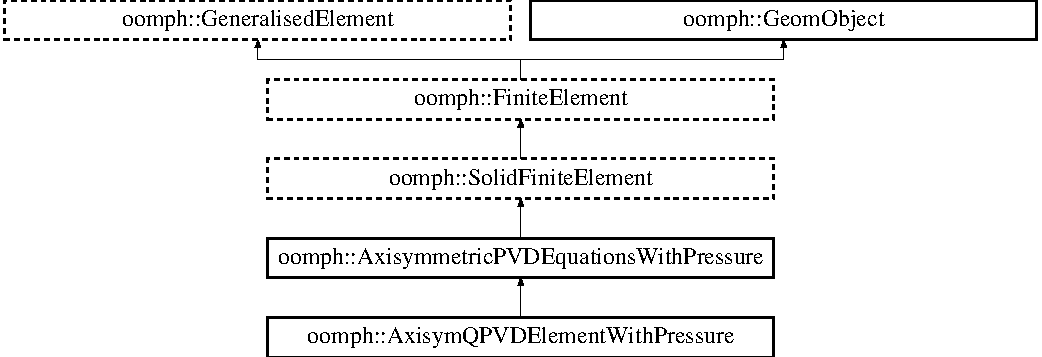
\includegraphics[height=4.794520cm]{classoomph_1_1AxisymmetricPVDEquationsWithPressure}
\end{center}
\end{figure}
\subsection*{Public Member Functions}
\begin{DoxyCompactItemize}
\item 
\hyperlink{classoomph_1_1AxisymmetricPVDEquationsWithPressure_a70d70c4f5629ef9479c4530d10828891}{Axisymmetric\+P\+V\+D\+Equations\+With\+Pressure} ()
\begin{DoxyCompactList}\small\item\em Constructor, by default the element is not incompressible. \end{DoxyCompactList}\item 
\hyperlink{classoomph_1_1ConstitutiveLaw}{Constitutive\+Law} $\ast$\& \hyperlink{classoomph_1_1AxisymmetricPVDEquationsWithPressure_aa16430aa0a4158f8834a0c23fcf98cc4}{constitutive\+\_\+law\+\_\+pt} ()
\begin{DoxyCompactList}\small\item\em Return the constitutive law pointer. \end{DoxyCompactList}\item 
void \hyperlink{classoomph_1_1AxisymmetricPVDEquationsWithPressure_af74b386309449d7022b9599674d58088}{get\+\_\+stress} (const \hyperlink{classoomph_1_1DenseMatrix}{Dense\+Matrix}$<$ double $>$ \&g, const \hyperlink{classoomph_1_1DenseMatrix}{Dense\+Matrix}$<$ double $>$ \&G, \hyperlink{classoomph_1_1DenseMatrix}{Dense\+Matrix}$<$ double $>$ \&sigma, \hyperlink{classoomph_1_1DenseMatrix}{Dense\+Matrix}$<$ double $>$ \&Gup, double \&pressure\+\_\+stress, double \&kappa)
\begin{DoxyCompactList}\small\item\em Return the stress tensor, as calculated from the constitutive law in the Near-\/incompresible formulation. \end{DoxyCompactList}\item 
void \hyperlink{classoomph_1_1AxisymmetricPVDEquationsWithPressure_af9614022b7f3e3fe4ffa9d1de15bfda7}{get\+\_\+stress} (const \hyperlink{classoomph_1_1DenseMatrix}{Dense\+Matrix}$<$ double $>$ \&g, const \hyperlink{classoomph_1_1DenseMatrix}{Dense\+Matrix}$<$ double $>$ \&G, \hyperlink{classoomph_1_1DenseMatrix}{Dense\+Matrix}$<$ double $>$ \&sigma, \hyperlink{classoomph_1_1DenseMatrix}{Dense\+Matrix}$<$ double $>$ \&Gup, double \&detG)
\begin{DoxyCompactList}\small\item\em Return the stress tensor, as calculated from the constitutive law in the \char`\"{}true\char`\"{} incompresible formulation. \end{DoxyCompactList}\item 
bool \hyperlink{classoomph_1_1AxisymmetricPVDEquationsWithPressure_a7d38dd422ad492ad99bda7abac207738}{is\+\_\+incompressible} () const
\begin{DoxyCompactList}\small\item\em Return whether the material is incompressible. \end{DoxyCompactList}\item 
void \hyperlink{classoomph_1_1AxisymmetricPVDEquationsWithPressure_a731e0c99343554529ab5e41bad4a454d}{set\+\_\+incompressible} ()
\begin{DoxyCompactList}\small\item\em Set the material to be incompressible. \end{DoxyCompactList}\item 
void \hyperlink{classoomph_1_1AxisymmetricPVDEquationsWithPressure_af9c2a4524a6de7ce842a6fc0c3c810e9}{set\+\_\+compressible} ()
\begin{DoxyCompactList}\small\item\em Set the material to be compressible. \end{DoxyCompactList}\item 
virtual unsigned \hyperlink{classoomph_1_1AxisymmetricPVDEquationsWithPressure_a4cfeab9fe5e9c26fcf39659bacc53a8f}{nsolid\+\_\+pres} () const =0
\begin{DoxyCompactList}\small\item\em Return the number of solid pressure degrees of freedom. \end{DoxyCompactList}\item 
virtual double \hyperlink{classoomph_1_1AxisymmetricPVDEquationsWithPressure_aeb03a2cef37040790d5d9dacafb89144}{solid\+\_\+p} (const unsigned \&l)=0
\begin{DoxyCompactList}\small\item\em Return the lth solid pressures. \end{DoxyCompactList}\item 
void \hyperlink{classoomph_1_1AxisymmetricPVDEquationsWithPressure_a97e21b6429e7406a463d8c8cf3057660}{fill\+\_\+in\+\_\+contribution\+\_\+to\+\_\+residuals} (\hyperlink{classoomph_1_1Vector}{Vector}$<$ double $>$ \&residuals)
\begin{DoxyCompactList}\small\item\em Return the residuals. \end{DoxyCompactList}\item 
void \hyperlink{classoomph_1_1AxisymmetricPVDEquationsWithPressure_a43c81b1695c9cd22b7546dd7764b70bd}{fill\+\_\+in\+\_\+contribution\+\_\+to\+\_\+jacobian} (\hyperlink{classoomph_1_1Vector}{Vector}$<$ double $>$ \&residuals, \hyperlink{classoomph_1_1DenseMatrix}{Dense\+Matrix}$<$ double $>$ \&jacobian)
\begin{DoxyCompactList}\small\item\em Return the residuals and the jacobian. \end{DoxyCompactList}\item 
void \hyperlink{classoomph_1_1AxisymmetricPVDEquationsWithPressure_a38ed51aff165e6a9708664a251fe291b}{fill\+\_\+in\+\_\+generic\+\_\+residual\+\_\+contribution\+\_\+axisym\+\_\+pvd\+\_\+with\+\_\+pressure} (\hyperlink{classoomph_1_1Vector}{Vector}$<$ double $>$ \&residuals, \hyperlink{classoomph_1_1DenseMatrix}{Dense\+Matrix}$<$ double $>$ \&jacobian, unsigned flag)
\begin{DoxyCompactList}\small\item\em Return the residuals for the equations of solid mechanics formulated in the incompressible case! \end{DoxyCompactList}\item 
double \hyperlink{classoomph_1_1AxisymmetricPVDEquationsWithPressure_a975e38ffef201b3c8bd36e7ff6206eb9}{compute\+\_\+physical\+\_\+size} () const
\begin{DoxyCompactList}\small\item\em Overload/implement the size function. \end{DoxyCompactList}\item 
double \hyperlink{classoomph_1_1AxisymmetricPVDEquationsWithPressure_adfd0277b2f05d4689fd7b4c6707929ab}{interpolated\+\_\+solid\+\_\+p} (const \hyperlink{classoomph_1_1Vector}{Vector}$<$ double $>$ \&\hyperlink{cfortran_8h_ab7123126e4885ef647dd9c6e3807a21c}{s})
\begin{DoxyCompactList}\small\item\em Return the interpolated\+\_\+solid\+\_\+pressure. \end{DoxyCompactList}\item 
void \hyperlink{classoomph_1_1AxisymmetricPVDEquationsWithPressure_aba49f4147fb78fa74cd591b4a77eab98}{output} (std\+::ostream \&outfile)
\begin{DoxyCompactList}\small\item\em Overload the output function. \end{DoxyCompactList}\item 
void \hyperlink{classoomph_1_1AxisymmetricPVDEquationsWithPressure_a6916b3f7784015c263556565b2a7219d}{output} (std\+::ostream \&outfile, const unsigned \&n\+\_\+plot)
\begin{DoxyCompactList}\small\item\em Output function. \end{DoxyCompactList}\item 
void \hyperlink{classoomph_1_1AxisymmetricPVDEquationsWithPressure_ad5018c9a6f9236f13c6df43df87336aa}{output} (F\+I\+LE $\ast$file\+\_\+pt)
\begin{DoxyCompactList}\small\item\em Overload the output function. \end{DoxyCompactList}\item 
void \hyperlink{classoomph_1_1AxisymmetricPVDEquationsWithPressure_a3a6d03fa236a2e0173abbc1734799d19}{output} (F\+I\+LE $\ast$file\+\_\+pt, const unsigned \&n\+\_\+plot)
\begin{DoxyCompactList}\small\item\em Output function. \end{DoxyCompactList}\end{DoxyCompactItemize}
\subsection*{Protected Member Functions}
\begin{DoxyCompactItemize}
\item 
virtual int \hyperlink{classoomph_1_1AxisymmetricPVDEquationsWithPressure_a7b77ffb084d0967b1220898613718d0b}{solid\+\_\+p\+\_\+local\+\_\+eqn} (const unsigned \&\hyperlink{cfortran_8h_adb50e893b86b3e55e751a42eab3cba82}{i})=0
\item 
virtual void \hyperlink{classoomph_1_1AxisymmetricPVDEquationsWithPressure_ab93f05b37f8bee3a8f390e33cbcd3a6e}{solid\+\_\+pshape} (const \hyperlink{classoomph_1_1Vector}{Vector}$<$ double $>$ \&\hyperlink{cfortran_8h_ab7123126e4885ef647dd9c6e3807a21c}{s}, \hyperlink{classoomph_1_1Shape}{Shape} \&psi) const =0
\begin{DoxyCompactList}\small\item\em Return the solid pressure shape functions. \end{DoxyCompactList}\item 
void \hyperlink{classoomph_1_1AxisymmetricPVDEquationsWithPressure_a2c423c3bfbc0debcf041f11fc24d1510}{solid\+\_\+pshape\+\_\+at\+\_\+knot} (const unsigned \&ipt, \hyperlink{classoomph_1_1Shape}{Shape} \&psi) const
\begin{DoxyCompactList}\small\item\em Return the stored solid shape functions at the knots. \end{DoxyCompactList}\end{DoxyCompactItemize}
\subsection*{Private Attributes}
\begin{DoxyCompactItemize}
\item 
\hyperlink{classoomph_1_1ConstitutiveLaw}{Constitutive\+Law} $\ast$ \hyperlink{classoomph_1_1AxisymmetricPVDEquationsWithPressure_a792ad265951fa647ca47d4a71b1df02f}{Constitutive\+\_\+law\+\_\+pt}
\begin{DoxyCompactList}\small\item\em Pointer to constitutive law. \end{DoxyCompactList}\item 
bool \hyperlink{classoomph_1_1AxisymmetricPVDEquationsWithPressure_a2ceef4a0290f5b475c99dd26721659d0}{Incompressible}
\begin{DoxyCompactList}\small\item\em Boolean to determine whether the solid is incompressible or not. \end{DoxyCompactList}\end{DoxyCompactItemize}
\subsection*{Additional Inherited Members}


\subsection{Detailed Description}
A class for elements that solve the equations of solid mechanics, based on the principle of virtual displacements in axisymmetric coordinates in a formulation that allows for incompressibility or near incompressibility. 

Definition at line 633 of file axisym\+\_\+solid\+\_\+elements.\+h.



\subsection{Constructor \& Destructor Documentation}
\mbox{\Hypertarget{classoomph_1_1AxisymmetricPVDEquationsWithPressure_a70d70c4f5629ef9479c4530d10828891}\label{classoomph_1_1AxisymmetricPVDEquationsWithPressure_a70d70c4f5629ef9479c4530d10828891}} 
\index{oomph\+::\+Axisymmetric\+P\+V\+D\+Equations\+With\+Pressure@{oomph\+::\+Axisymmetric\+P\+V\+D\+Equations\+With\+Pressure}!Axisymmetric\+P\+V\+D\+Equations\+With\+Pressure@{Axisymmetric\+P\+V\+D\+Equations\+With\+Pressure}}
\index{Axisymmetric\+P\+V\+D\+Equations\+With\+Pressure@{Axisymmetric\+P\+V\+D\+Equations\+With\+Pressure}!oomph\+::\+Axisymmetric\+P\+V\+D\+Equations\+With\+Pressure@{oomph\+::\+Axisymmetric\+P\+V\+D\+Equations\+With\+Pressure}}
\subsubsection{\texorpdfstring{Axisymmetric\+P\+V\+D\+Equations\+With\+Pressure()}{AxisymmetricPVDEquationsWithPressure()}}
{\footnotesize\ttfamily oomph\+::\+Axisymmetric\+P\+V\+D\+Equations\+With\+Pressure\+::\+Axisymmetric\+P\+V\+D\+Equations\+With\+Pressure (\begin{DoxyParamCaption}{ }\end{DoxyParamCaption})\hspace{0.3cm}{\ttfamily [inline]}}



Constructor, by default the element is not incompressible. 



Definition at line 659 of file axisym\+\_\+solid\+\_\+elements.\+h.



\subsection{Member Function Documentation}
\mbox{\Hypertarget{classoomph_1_1AxisymmetricPVDEquationsWithPressure_a975e38ffef201b3c8bd36e7ff6206eb9}\label{classoomph_1_1AxisymmetricPVDEquationsWithPressure_a975e38ffef201b3c8bd36e7ff6206eb9}} 
\index{oomph\+::\+Axisymmetric\+P\+V\+D\+Equations\+With\+Pressure@{oomph\+::\+Axisymmetric\+P\+V\+D\+Equations\+With\+Pressure}!compute\+\_\+physical\+\_\+size@{compute\+\_\+physical\+\_\+size}}
\index{compute\+\_\+physical\+\_\+size@{compute\+\_\+physical\+\_\+size}!oomph\+::\+Axisymmetric\+P\+V\+D\+Equations\+With\+Pressure@{oomph\+::\+Axisymmetric\+P\+V\+D\+Equations\+With\+Pressure}}
\subsubsection{\texorpdfstring{compute\+\_\+physical\+\_\+size()}{compute\_physical\_size()}}
{\footnotesize\ttfamily double oomph\+::\+Axisymmetric\+P\+V\+D\+Equations\+With\+Pressure\+::compute\+\_\+physical\+\_\+size (\begin{DoxyParamCaption}{ }\end{DoxyParamCaption}) const\hspace{0.3cm}{\ttfamily [inline]}, {\ttfamily [virtual]}}



Overload/implement the size function. 



Reimplemented from \hyperlink{classoomph_1_1FiniteElement_a782a540035dc31cb6ef548d9d930d8b8}{oomph\+::\+Finite\+Element}.



Definition at line 1092 of file axisym\+\_\+solid\+\_\+elements.\+h.



References oomph\+::\+Solid\+Finite\+Element\+::dshape\+\_\+lagrangian\+\_\+at\+\_\+knot(), i, oomph\+::\+Finite\+Element\+::integral\+\_\+pt(), oomph\+::\+Solid\+Finite\+Element\+::interpolated\+\_\+xi(), oomph\+::\+Solid\+Finite\+Element\+::lagrangian\+\_\+position\+\_\+gen(), oomph\+::\+Finite\+Element\+::nnode(), oomph\+::\+Finite\+Element\+::nodal\+\_\+position\+\_\+gen(), oomph\+::\+Integral\+::nweight(), oomph\+::\+Mathematical\+Constants\+::\+Pi, oomph\+::\+Quad\+Tree\+Names\+::W, and oomph\+::\+Integral\+::weight().

\mbox{\Hypertarget{classoomph_1_1AxisymmetricPVDEquationsWithPressure_aa16430aa0a4158f8834a0c23fcf98cc4}\label{classoomph_1_1AxisymmetricPVDEquationsWithPressure_aa16430aa0a4158f8834a0c23fcf98cc4}} 
\index{oomph\+::\+Axisymmetric\+P\+V\+D\+Equations\+With\+Pressure@{oomph\+::\+Axisymmetric\+P\+V\+D\+Equations\+With\+Pressure}!constitutive\+\_\+law\+\_\+pt@{constitutive\+\_\+law\+\_\+pt}}
\index{constitutive\+\_\+law\+\_\+pt@{constitutive\+\_\+law\+\_\+pt}!oomph\+::\+Axisymmetric\+P\+V\+D\+Equations\+With\+Pressure@{oomph\+::\+Axisymmetric\+P\+V\+D\+Equations\+With\+Pressure}}
\subsubsection{\texorpdfstring{constitutive\+\_\+law\+\_\+pt()}{constitutive\_law\_pt()}}
{\footnotesize\ttfamily \hyperlink{classoomph_1_1ConstitutiveLaw}{Constitutive\+Law}$\ast$ \& oomph\+::\+Axisymmetric\+P\+V\+D\+Equations\+With\+Pressure\+::constitutive\+\_\+law\+\_\+pt (\begin{DoxyParamCaption}{ }\end{DoxyParamCaption})\hspace{0.3cm}{\ttfamily [inline]}}



Return the constitutive law pointer. 



Definition at line 663 of file axisym\+\_\+solid\+\_\+elements.\+h.



References oomph\+::\+Axisymmetric\+P\+V\+D\+Equations\+::\+Constitutive\+\_\+law\+\_\+pt.

\mbox{\Hypertarget{classoomph_1_1AxisymmetricPVDEquationsWithPressure_a43c81b1695c9cd22b7546dd7764b70bd}\label{classoomph_1_1AxisymmetricPVDEquationsWithPressure_a43c81b1695c9cd22b7546dd7764b70bd}} 
\index{oomph\+::\+Axisymmetric\+P\+V\+D\+Equations\+With\+Pressure@{oomph\+::\+Axisymmetric\+P\+V\+D\+Equations\+With\+Pressure}!fill\+\_\+in\+\_\+contribution\+\_\+to\+\_\+jacobian@{fill\+\_\+in\+\_\+contribution\+\_\+to\+\_\+jacobian}}
\index{fill\+\_\+in\+\_\+contribution\+\_\+to\+\_\+jacobian@{fill\+\_\+in\+\_\+contribution\+\_\+to\+\_\+jacobian}!oomph\+::\+Axisymmetric\+P\+V\+D\+Equations\+With\+Pressure@{oomph\+::\+Axisymmetric\+P\+V\+D\+Equations\+With\+Pressure}}
\subsubsection{\texorpdfstring{fill\+\_\+in\+\_\+contribution\+\_\+to\+\_\+jacobian()}{fill\_in\_contribution\_to\_jacobian()}}
{\footnotesize\ttfamily void oomph\+::\+Axisymmetric\+P\+V\+D\+Equations\+With\+Pressure\+::fill\+\_\+in\+\_\+contribution\+\_\+to\+\_\+jacobian (\begin{DoxyParamCaption}\item[{\hyperlink{classoomph_1_1Vector}{Vector}$<$ double $>$ \&}]{residuals,  }\item[{\hyperlink{classoomph_1_1DenseMatrix}{Dense\+Matrix}$<$ double $>$ \&}]{jacobian }\end{DoxyParamCaption})\hspace{0.3cm}{\ttfamily [inline]}, {\ttfamily [virtual]}}



Return the residuals and the jacobian. 



Reimplemented from \hyperlink{classoomph_1_1GeneralisedElement_a6ae09fc0d68e4309ac1b03583d252845}{oomph\+::\+Generalised\+Element}.



Definition at line 741 of file axisym\+\_\+solid\+\_\+elements.\+h.



References oomph\+::\+Solid\+Finite\+Element\+::fill\+\_\+in\+\_\+jacobian\+\_\+from\+\_\+solid\+\_\+position\+\_\+by\+\_\+fd().

\mbox{\Hypertarget{classoomph_1_1AxisymmetricPVDEquationsWithPressure_a97e21b6429e7406a463d8c8cf3057660}\label{classoomph_1_1AxisymmetricPVDEquationsWithPressure_a97e21b6429e7406a463d8c8cf3057660}} 
\index{oomph\+::\+Axisymmetric\+P\+V\+D\+Equations\+With\+Pressure@{oomph\+::\+Axisymmetric\+P\+V\+D\+Equations\+With\+Pressure}!fill\+\_\+in\+\_\+contribution\+\_\+to\+\_\+residuals@{fill\+\_\+in\+\_\+contribution\+\_\+to\+\_\+residuals}}
\index{fill\+\_\+in\+\_\+contribution\+\_\+to\+\_\+residuals@{fill\+\_\+in\+\_\+contribution\+\_\+to\+\_\+residuals}!oomph\+::\+Axisymmetric\+P\+V\+D\+Equations\+With\+Pressure@{oomph\+::\+Axisymmetric\+P\+V\+D\+Equations\+With\+Pressure}}
\subsubsection{\texorpdfstring{fill\+\_\+in\+\_\+contribution\+\_\+to\+\_\+residuals()}{fill\_in\_contribution\_to\_residuals()}}
{\footnotesize\ttfamily void oomph\+::\+Axisymmetric\+P\+V\+D\+Equations\+With\+Pressure\+::fill\+\_\+in\+\_\+contribution\+\_\+to\+\_\+residuals (\begin{DoxyParamCaption}\item[{\hyperlink{classoomph_1_1Vector}{Vector}$<$ double $>$ \&}]{residuals }\end{DoxyParamCaption})\hspace{0.3cm}{\ttfamily [inline]}, {\ttfamily [virtual]}}



Return the residuals. 



Reimplemented from \hyperlink{classoomph_1_1GeneralisedElement_a310c97f515e8504a48179c0e72c550d7}{oomph\+::\+Generalised\+Element}.



Definition at line 732 of file axisym\+\_\+solid\+\_\+elements.\+h.



References oomph\+::\+Generalised\+Element\+::\+Dummy\+\_\+matrix.

\mbox{\Hypertarget{classoomph_1_1AxisymmetricPVDEquationsWithPressure_a38ed51aff165e6a9708664a251fe291b}\label{classoomph_1_1AxisymmetricPVDEquationsWithPressure_a38ed51aff165e6a9708664a251fe291b}} 
\index{oomph\+::\+Axisymmetric\+P\+V\+D\+Equations\+With\+Pressure@{oomph\+::\+Axisymmetric\+P\+V\+D\+Equations\+With\+Pressure}!fill\+\_\+in\+\_\+generic\+\_\+residual\+\_\+contribution\+\_\+axisym\+\_\+pvd\+\_\+with\+\_\+pressure@{fill\+\_\+in\+\_\+generic\+\_\+residual\+\_\+contribution\+\_\+axisym\+\_\+pvd\+\_\+with\+\_\+pressure}}
\index{fill\+\_\+in\+\_\+generic\+\_\+residual\+\_\+contribution\+\_\+axisym\+\_\+pvd\+\_\+with\+\_\+pressure@{fill\+\_\+in\+\_\+generic\+\_\+residual\+\_\+contribution\+\_\+axisym\+\_\+pvd\+\_\+with\+\_\+pressure}!oomph\+::\+Axisymmetric\+P\+V\+D\+Equations\+With\+Pressure@{oomph\+::\+Axisymmetric\+P\+V\+D\+Equations\+With\+Pressure}}
\subsubsection{\texorpdfstring{fill\+\_\+in\+\_\+generic\+\_\+residual\+\_\+contribution\+\_\+axisym\+\_\+pvd\+\_\+with\+\_\+pressure()}{fill\_in\_generic\_residual\_contribution\_axisym\_pvd\_with\_pressure()}}
{\footnotesize\ttfamily void oomph\+::\+Axisymmetric\+P\+V\+D\+Equations\+With\+Pressure\+::fill\+\_\+in\+\_\+generic\+\_\+residual\+\_\+contribution\+\_\+axisym\+\_\+pvd\+\_\+with\+\_\+pressure (\begin{DoxyParamCaption}\item[{\hyperlink{classoomph_1_1Vector}{Vector}$<$ double $>$ \&}]{residuals,  }\item[{\hyperlink{classoomph_1_1DenseMatrix}{Dense\+Matrix}$<$ double $>$ \&}]{jacobian,  }\item[{unsigned}]{flag }\end{DoxyParamCaption})\hspace{0.3cm}{\ttfamily [inline]}}



Return the residuals for the equations of solid mechanics formulated in the incompressible case! 



Definition at line 753 of file axisym\+\_\+solid\+\_\+elements.\+h.



References oomph\+::\+Solid\+Finite\+Element\+::dshape\+\_\+lagrangian\+\_\+at\+\_\+knot(), oomph\+::\+Axisymmetric\+P\+V\+D\+Equations\+::get\+\_\+stress(), i, oomph\+::\+Finite\+Element\+::integral\+\_\+pt(), oomph\+::\+Solid\+Finite\+Element\+::interpolated\+\_\+xi(), oomph\+::\+Solid\+Finite\+Element\+::lagrangian\+\_\+position\+\_\+gen(), oomph\+::\+Finite\+Element\+::nnodal\+\_\+position\+\_\+type(), oomph\+::\+Finite\+Element\+::nnode(), oomph\+::\+Finite\+Element\+::nodal\+\_\+position\+\_\+gen(), oomph\+::\+Integral\+::nweight(), oomph\+::\+Solid\+Finite\+Element\+::position\+\_\+local\+\_\+eqn(), oomph\+::\+Quad\+Tree\+Names\+::W, and oomph\+::\+Integral\+::weight().

\mbox{\Hypertarget{classoomph_1_1AxisymmetricPVDEquationsWithPressure_af74b386309449d7022b9599674d58088}\label{classoomph_1_1AxisymmetricPVDEquationsWithPressure_af74b386309449d7022b9599674d58088}} 
\index{oomph\+::\+Axisymmetric\+P\+V\+D\+Equations\+With\+Pressure@{oomph\+::\+Axisymmetric\+P\+V\+D\+Equations\+With\+Pressure}!get\+\_\+stress@{get\+\_\+stress}}
\index{get\+\_\+stress@{get\+\_\+stress}!oomph\+::\+Axisymmetric\+P\+V\+D\+Equations\+With\+Pressure@{oomph\+::\+Axisymmetric\+P\+V\+D\+Equations\+With\+Pressure}}
\subsubsection{\texorpdfstring{get\+\_\+stress()}{get\_stress()}\hspace{0.1cm}{\footnotesize\ttfamily [1/2]}}
{\footnotesize\ttfamily void oomph\+::\+Axisymmetric\+P\+V\+D\+Equations\+With\+Pressure\+::get\+\_\+stress (\begin{DoxyParamCaption}\item[{const \hyperlink{classoomph_1_1DenseMatrix}{Dense\+Matrix}$<$ double $>$ \&}]{g,  }\item[{const \hyperlink{classoomph_1_1DenseMatrix}{Dense\+Matrix}$<$ double $>$ \&}]{G,  }\item[{\hyperlink{classoomph_1_1DenseMatrix}{Dense\+Matrix}$<$ double $>$ \&}]{sigma,  }\item[{\hyperlink{classoomph_1_1DenseMatrix}{Dense\+Matrix}$<$ double $>$ \&}]{Gup,  }\item[{double \&}]{pressure\+\_\+stress,  }\item[{double \&}]{kappa }\end{DoxyParamCaption})\hspace{0.3cm}{\ttfamily [inline]}}



Return the stress tensor, as calculated from the constitutive law in the Near-\/incompresible formulation. 



Definition at line 667 of file axisym\+\_\+solid\+\_\+elements.\+h.



References oomph\+::\+Global\+\_\+string\+\_\+for\+\_\+annotation\+::string().

\mbox{\Hypertarget{classoomph_1_1AxisymmetricPVDEquationsWithPressure_af9614022b7f3e3fe4ffa9d1de15bfda7}\label{classoomph_1_1AxisymmetricPVDEquationsWithPressure_af9614022b7f3e3fe4ffa9d1de15bfda7}} 
\index{oomph\+::\+Axisymmetric\+P\+V\+D\+Equations\+With\+Pressure@{oomph\+::\+Axisymmetric\+P\+V\+D\+Equations\+With\+Pressure}!get\+\_\+stress@{get\+\_\+stress}}
\index{get\+\_\+stress@{get\+\_\+stress}!oomph\+::\+Axisymmetric\+P\+V\+D\+Equations\+With\+Pressure@{oomph\+::\+Axisymmetric\+P\+V\+D\+Equations\+With\+Pressure}}
\subsubsection{\texorpdfstring{get\+\_\+stress()}{get\_stress()}\hspace{0.1cm}{\footnotesize\ttfamily [2/2]}}
{\footnotesize\ttfamily void oomph\+::\+Axisymmetric\+P\+V\+D\+Equations\+With\+Pressure\+::get\+\_\+stress (\begin{DoxyParamCaption}\item[{const \hyperlink{classoomph_1_1DenseMatrix}{Dense\+Matrix}$<$ double $>$ \&}]{g,  }\item[{const \hyperlink{classoomph_1_1DenseMatrix}{Dense\+Matrix}$<$ double $>$ \&}]{G,  }\item[{\hyperlink{classoomph_1_1DenseMatrix}{Dense\+Matrix}$<$ double $>$ \&}]{sigma,  }\item[{\hyperlink{classoomph_1_1DenseMatrix}{Dense\+Matrix}$<$ double $>$ \&}]{Gup,  }\item[{double \&}]{detG }\end{DoxyParamCaption})\hspace{0.3cm}{\ttfamily [inline]}}



Return the stress tensor, as calculated from the constitutive law in the \char`\"{}true\char`\"{} incompresible formulation. 



Definition at line 693 of file axisym\+\_\+solid\+\_\+elements.\+h.



References oomph\+::\+Global\+\_\+string\+\_\+for\+\_\+annotation\+::string().

\mbox{\Hypertarget{classoomph_1_1AxisymmetricPVDEquationsWithPressure_adfd0277b2f05d4689fd7b4c6707929ab}\label{classoomph_1_1AxisymmetricPVDEquationsWithPressure_adfd0277b2f05d4689fd7b4c6707929ab}} 
\index{oomph\+::\+Axisymmetric\+P\+V\+D\+Equations\+With\+Pressure@{oomph\+::\+Axisymmetric\+P\+V\+D\+Equations\+With\+Pressure}!interpolated\+\_\+solid\+\_\+p@{interpolated\+\_\+solid\+\_\+p}}
\index{interpolated\+\_\+solid\+\_\+p@{interpolated\+\_\+solid\+\_\+p}!oomph\+::\+Axisymmetric\+P\+V\+D\+Equations\+With\+Pressure@{oomph\+::\+Axisymmetric\+P\+V\+D\+Equations\+With\+Pressure}}
\subsubsection{\texorpdfstring{interpolated\+\_\+solid\+\_\+p()}{interpolated\_solid\_p()}}
{\footnotesize\ttfamily double oomph\+::\+Axisymmetric\+P\+V\+D\+Equations\+With\+Pressure\+::interpolated\+\_\+solid\+\_\+p (\begin{DoxyParamCaption}\item[{const \hyperlink{classoomph_1_1Vector}{Vector}$<$ double $>$ \&}]{s }\end{DoxyParamCaption})\hspace{0.3cm}{\ttfamily [inline]}}



Return the interpolated\+\_\+solid\+\_\+pressure. 



Definition at line 1194 of file axisym\+\_\+solid\+\_\+elements.\+h.

\mbox{\Hypertarget{classoomph_1_1AxisymmetricPVDEquationsWithPressure_a7d38dd422ad492ad99bda7abac207738}\label{classoomph_1_1AxisymmetricPVDEquationsWithPressure_a7d38dd422ad492ad99bda7abac207738}} 
\index{oomph\+::\+Axisymmetric\+P\+V\+D\+Equations\+With\+Pressure@{oomph\+::\+Axisymmetric\+P\+V\+D\+Equations\+With\+Pressure}!is\+\_\+incompressible@{is\+\_\+incompressible}}
\index{is\+\_\+incompressible@{is\+\_\+incompressible}!oomph\+::\+Axisymmetric\+P\+V\+D\+Equations\+With\+Pressure@{oomph\+::\+Axisymmetric\+P\+V\+D\+Equations\+With\+Pressure}}
\subsubsection{\texorpdfstring{is\+\_\+incompressible()}{is\_incompressible()}}
{\footnotesize\ttfamily bool oomph\+::\+Axisymmetric\+P\+V\+D\+Equations\+With\+Pressure\+::is\+\_\+incompressible (\begin{DoxyParamCaption}{ }\end{DoxyParamCaption}) const\hspace{0.3cm}{\ttfamily [inline]}}



Return whether the material is incompressible. 



Definition at line 717 of file axisym\+\_\+solid\+\_\+elements.\+h.

\mbox{\Hypertarget{classoomph_1_1AxisymmetricPVDEquationsWithPressure_a4cfeab9fe5e9c26fcf39659bacc53a8f}\label{classoomph_1_1AxisymmetricPVDEquationsWithPressure_a4cfeab9fe5e9c26fcf39659bacc53a8f}} 
\index{oomph\+::\+Axisymmetric\+P\+V\+D\+Equations\+With\+Pressure@{oomph\+::\+Axisymmetric\+P\+V\+D\+Equations\+With\+Pressure}!nsolid\+\_\+pres@{nsolid\+\_\+pres}}
\index{nsolid\+\_\+pres@{nsolid\+\_\+pres}!oomph\+::\+Axisymmetric\+P\+V\+D\+Equations\+With\+Pressure@{oomph\+::\+Axisymmetric\+P\+V\+D\+Equations\+With\+Pressure}}
\subsubsection{\texorpdfstring{nsolid\+\_\+pres()}{nsolid\_pres()}}
{\footnotesize\ttfamily virtual unsigned oomph\+::\+Axisymmetric\+P\+V\+D\+Equations\+With\+Pressure\+::nsolid\+\_\+pres (\begin{DoxyParamCaption}{ }\end{DoxyParamCaption}) const\hspace{0.3cm}{\ttfamily [pure virtual]}}



Return the number of solid pressure degrees of freedom. 



Implemented in \hyperlink{classoomph_1_1AxisymQPVDElementWithPressure_ac39d97adf69f12b20640ae10aeaec156}{oomph\+::\+Axisym\+Q\+P\+V\+D\+Element\+With\+Pressure}.

\mbox{\Hypertarget{classoomph_1_1AxisymmetricPVDEquationsWithPressure_aba49f4147fb78fa74cd591b4a77eab98}\label{classoomph_1_1AxisymmetricPVDEquationsWithPressure_aba49f4147fb78fa74cd591b4a77eab98}} 
\index{oomph\+::\+Axisymmetric\+P\+V\+D\+Equations\+With\+Pressure@{oomph\+::\+Axisymmetric\+P\+V\+D\+Equations\+With\+Pressure}!output@{output}}
\index{output@{output}!oomph\+::\+Axisymmetric\+P\+V\+D\+Equations\+With\+Pressure@{oomph\+::\+Axisymmetric\+P\+V\+D\+Equations\+With\+Pressure}}
\subsubsection{\texorpdfstring{output()}{output()}\hspace{0.1cm}{\footnotesize\ttfamily [1/4]}}
{\footnotesize\ttfamily void oomph\+::\+Axisymmetric\+P\+V\+D\+Equations\+With\+Pressure\+::output (\begin{DoxyParamCaption}\item[{std\+::ostream \&}]{outfile }\end{DoxyParamCaption})\hspace{0.3cm}{\ttfamily [inline]}, {\ttfamily [virtual]}}



Overload the output function. 



Reimplemented from \hyperlink{classoomph_1_1FiniteElement_a2ad98a3d2ef4999f1bef62c0ff13f2a7}{oomph\+::\+Finite\+Element}.



Reimplemented in \hyperlink{classoomph_1_1AxisymQPVDElementWithPressure_a1df3ba1290d73dd33634d5b99993dee7}{oomph\+::\+Axisym\+Q\+P\+V\+D\+Element\+With\+Pressure}.



Definition at line 1215 of file axisym\+\_\+solid\+\_\+elements.\+h.



References oomph\+::\+Finite\+Element\+::output().



Referenced by oomph\+::\+Axisym\+Q\+P\+V\+D\+Element\+With\+Pressure\+::output().

\mbox{\Hypertarget{classoomph_1_1AxisymmetricPVDEquationsWithPressure_a6916b3f7784015c263556565b2a7219d}\label{classoomph_1_1AxisymmetricPVDEquationsWithPressure_a6916b3f7784015c263556565b2a7219d}} 
\index{oomph\+::\+Axisymmetric\+P\+V\+D\+Equations\+With\+Pressure@{oomph\+::\+Axisymmetric\+P\+V\+D\+Equations\+With\+Pressure}!output@{output}}
\index{output@{output}!oomph\+::\+Axisymmetric\+P\+V\+D\+Equations\+With\+Pressure@{oomph\+::\+Axisymmetric\+P\+V\+D\+Equations\+With\+Pressure}}
\subsubsection{\texorpdfstring{output()}{output()}\hspace{0.1cm}{\footnotesize\ttfamily [2/4]}}
{\footnotesize\ttfamily void oomph\+::\+Axisymmetric\+P\+V\+D\+Equations\+With\+Pressure\+::output (\begin{DoxyParamCaption}\item[{std\+::ostream \&}]{outfile,  }\item[{const unsigned \&}]{n\+\_\+plot }\end{DoxyParamCaption})\hspace{0.3cm}{\ttfamily [inline]}, {\ttfamily [virtual]}}



Output function. 



Reimplemented from \hyperlink{classoomph_1_1FiniteElement_afa9d9b2670f999b43e6679c9dd28c457}{oomph\+::\+Finite\+Element}.



Reimplemented in \hyperlink{classoomph_1_1AxisymQPVDElementWithPressure_aa7bf745c0767590c36a761d3a6399e57}{oomph\+::\+Axisym\+Q\+P\+V\+D\+Element\+With\+Pressure}.



Definition at line 1218 of file axisym\+\_\+solid\+\_\+elements.\+h.



References i, oomph\+::\+Finite\+Element\+::interpolated\+\_\+x(), oomph\+::\+Solid\+Finite\+Element\+::interpolated\+\_\+xi(), and s.

\mbox{\Hypertarget{classoomph_1_1AxisymmetricPVDEquationsWithPressure_ad5018c9a6f9236f13c6df43df87336aa}\label{classoomph_1_1AxisymmetricPVDEquationsWithPressure_ad5018c9a6f9236f13c6df43df87336aa}} 
\index{oomph\+::\+Axisymmetric\+P\+V\+D\+Equations\+With\+Pressure@{oomph\+::\+Axisymmetric\+P\+V\+D\+Equations\+With\+Pressure}!output@{output}}
\index{output@{output}!oomph\+::\+Axisymmetric\+P\+V\+D\+Equations\+With\+Pressure@{oomph\+::\+Axisymmetric\+P\+V\+D\+Equations\+With\+Pressure}}
\subsubsection{\texorpdfstring{output()}{output()}\hspace{0.1cm}{\footnotesize\ttfamily [3/4]}}
{\footnotesize\ttfamily void oomph\+::\+Axisymmetric\+P\+V\+D\+Equations\+With\+Pressure\+::output (\begin{DoxyParamCaption}\item[{F\+I\+LE $\ast$}]{file\+\_\+pt }\end{DoxyParamCaption})\hspace{0.3cm}{\ttfamily [inline]}, {\ttfamily [virtual]}}



Overload the output function. 



Reimplemented from \hyperlink{classoomph_1_1FiniteElement_a72cddd09f8ddbee1a20a1ff404c6943e}{oomph\+::\+Finite\+Element}.



Reimplemented in \hyperlink{classoomph_1_1AxisymQPVDElementWithPressure_a8f09df5914ea8dbb6ba7041bd6be15bd}{oomph\+::\+Axisym\+Q\+P\+V\+D\+Element\+With\+Pressure}.



Definition at line 1251 of file axisym\+\_\+solid\+\_\+elements.\+h.



References oomph\+::\+Finite\+Element\+::output().

\mbox{\Hypertarget{classoomph_1_1AxisymmetricPVDEquationsWithPressure_a3a6d03fa236a2e0173abbc1734799d19}\label{classoomph_1_1AxisymmetricPVDEquationsWithPressure_a3a6d03fa236a2e0173abbc1734799d19}} 
\index{oomph\+::\+Axisymmetric\+P\+V\+D\+Equations\+With\+Pressure@{oomph\+::\+Axisymmetric\+P\+V\+D\+Equations\+With\+Pressure}!output@{output}}
\index{output@{output}!oomph\+::\+Axisymmetric\+P\+V\+D\+Equations\+With\+Pressure@{oomph\+::\+Axisymmetric\+P\+V\+D\+Equations\+With\+Pressure}}
\subsubsection{\texorpdfstring{output()}{output()}\hspace{0.1cm}{\footnotesize\ttfamily [4/4]}}
{\footnotesize\ttfamily void oomph\+::\+Axisymmetric\+P\+V\+D\+Equations\+With\+Pressure\+::output (\begin{DoxyParamCaption}\item[{F\+I\+LE $\ast$}]{file\+\_\+pt,  }\item[{const unsigned \&}]{n\+\_\+plot }\end{DoxyParamCaption})\hspace{0.3cm}{\ttfamily [inline]}, {\ttfamily [virtual]}}



Output function. 



Reimplemented from \hyperlink{classoomph_1_1FiniteElement_adfaee690bb0608f03320eeb9d110d48c}{oomph\+::\+Finite\+Element}.



Reimplemented in \hyperlink{classoomph_1_1AxisymQPVDElementWithPressure_a273e1cfc1185192fcb9cc3812360c87e}{oomph\+::\+Axisym\+Q\+P\+V\+D\+Element\+With\+Pressure}.



Definition at line 1255 of file axisym\+\_\+solid\+\_\+elements.\+h.



References i, oomph\+::\+Finite\+Element\+::interpolated\+\_\+x(), oomph\+::\+Solid\+Finite\+Element\+::interpolated\+\_\+xi(), and s.

\mbox{\Hypertarget{classoomph_1_1AxisymmetricPVDEquationsWithPressure_af9c2a4524a6de7ce842a6fc0c3c810e9}\label{classoomph_1_1AxisymmetricPVDEquationsWithPressure_af9c2a4524a6de7ce842a6fc0c3c810e9}} 
\index{oomph\+::\+Axisymmetric\+P\+V\+D\+Equations\+With\+Pressure@{oomph\+::\+Axisymmetric\+P\+V\+D\+Equations\+With\+Pressure}!set\+\_\+compressible@{set\+\_\+compressible}}
\index{set\+\_\+compressible@{set\+\_\+compressible}!oomph\+::\+Axisymmetric\+P\+V\+D\+Equations\+With\+Pressure@{oomph\+::\+Axisymmetric\+P\+V\+D\+Equations\+With\+Pressure}}
\subsubsection{\texorpdfstring{set\+\_\+compressible()}{set\_compressible()}}
{\footnotesize\ttfamily void oomph\+::\+Axisymmetric\+P\+V\+D\+Equations\+With\+Pressure\+::set\+\_\+compressible (\begin{DoxyParamCaption}{ }\end{DoxyParamCaption})\hspace{0.3cm}{\ttfamily [inline]}}



Set the material to be compressible. 



Definition at line 723 of file axisym\+\_\+solid\+\_\+elements.\+h.

\mbox{\Hypertarget{classoomph_1_1AxisymmetricPVDEquationsWithPressure_a731e0c99343554529ab5e41bad4a454d}\label{classoomph_1_1AxisymmetricPVDEquationsWithPressure_a731e0c99343554529ab5e41bad4a454d}} 
\index{oomph\+::\+Axisymmetric\+P\+V\+D\+Equations\+With\+Pressure@{oomph\+::\+Axisymmetric\+P\+V\+D\+Equations\+With\+Pressure}!set\+\_\+incompressible@{set\+\_\+incompressible}}
\index{set\+\_\+incompressible@{set\+\_\+incompressible}!oomph\+::\+Axisymmetric\+P\+V\+D\+Equations\+With\+Pressure@{oomph\+::\+Axisymmetric\+P\+V\+D\+Equations\+With\+Pressure}}
\subsubsection{\texorpdfstring{set\+\_\+incompressible()}{set\_incompressible()}}
{\footnotesize\ttfamily void oomph\+::\+Axisymmetric\+P\+V\+D\+Equations\+With\+Pressure\+::set\+\_\+incompressible (\begin{DoxyParamCaption}{ }\end{DoxyParamCaption})\hspace{0.3cm}{\ttfamily [inline]}}



Set the material to be incompressible. 



Definition at line 720 of file axisym\+\_\+solid\+\_\+elements.\+h.

\mbox{\Hypertarget{classoomph_1_1AxisymmetricPVDEquationsWithPressure_aeb03a2cef37040790d5d9dacafb89144}\label{classoomph_1_1AxisymmetricPVDEquationsWithPressure_aeb03a2cef37040790d5d9dacafb89144}} 
\index{oomph\+::\+Axisymmetric\+P\+V\+D\+Equations\+With\+Pressure@{oomph\+::\+Axisymmetric\+P\+V\+D\+Equations\+With\+Pressure}!solid\+\_\+p@{solid\+\_\+p}}
\index{solid\+\_\+p@{solid\+\_\+p}!oomph\+::\+Axisymmetric\+P\+V\+D\+Equations\+With\+Pressure@{oomph\+::\+Axisymmetric\+P\+V\+D\+Equations\+With\+Pressure}}
\subsubsection{\texorpdfstring{solid\+\_\+p()}{solid\_p()}}
{\footnotesize\ttfamily virtual double oomph\+::\+Axisymmetric\+P\+V\+D\+Equations\+With\+Pressure\+::solid\+\_\+p (\begin{DoxyParamCaption}\item[{const unsigned \&}]{l }\end{DoxyParamCaption})\hspace{0.3cm}{\ttfamily [pure virtual]}}



Return the lth solid pressures. 



Implemented in \hyperlink{classoomph_1_1AxisymQPVDElementWithPressure_a43a3e699d4e958d00d5ebc20ff23827b}{oomph\+::\+Axisym\+Q\+P\+V\+D\+Element\+With\+Pressure}.

\mbox{\Hypertarget{classoomph_1_1AxisymmetricPVDEquationsWithPressure_a7b77ffb084d0967b1220898613718d0b}\label{classoomph_1_1AxisymmetricPVDEquationsWithPressure_a7b77ffb084d0967b1220898613718d0b}} 
\index{oomph\+::\+Axisymmetric\+P\+V\+D\+Equations\+With\+Pressure@{oomph\+::\+Axisymmetric\+P\+V\+D\+Equations\+With\+Pressure}!solid\+\_\+p\+\_\+local\+\_\+eqn@{solid\+\_\+p\+\_\+local\+\_\+eqn}}
\index{solid\+\_\+p\+\_\+local\+\_\+eqn@{solid\+\_\+p\+\_\+local\+\_\+eqn}!oomph\+::\+Axisymmetric\+P\+V\+D\+Equations\+With\+Pressure@{oomph\+::\+Axisymmetric\+P\+V\+D\+Equations\+With\+Pressure}}
\subsubsection{\texorpdfstring{solid\+\_\+p\+\_\+local\+\_\+eqn()}{solid\_p\_local\_eqn()}}
{\footnotesize\ttfamily virtual int oomph\+::\+Axisymmetric\+P\+V\+D\+Equations\+With\+Pressure\+::solid\+\_\+p\+\_\+local\+\_\+eqn (\begin{DoxyParamCaption}\item[{const unsigned \&}]{i }\end{DoxyParamCaption})\hspace{0.3cm}{\ttfamily [protected]}, {\ttfamily [pure virtual]}}

Access function that returns the local equation number for the n-\/th solid pressure value. 

Implemented in \hyperlink{classoomph_1_1AxisymQPVDElementWithPressure_a8c9fa9511418570fab627362609235d0}{oomph\+::\+Axisym\+Q\+P\+V\+D\+Element\+With\+Pressure}.

\mbox{\Hypertarget{classoomph_1_1AxisymmetricPVDEquationsWithPressure_ab93f05b37f8bee3a8f390e33cbcd3a6e}\label{classoomph_1_1AxisymmetricPVDEquationsWithPressure_ab93f05b37f8bee3a8f390e33cbcd3a6e}} 
\index{oomph\+::\+Axisymmetric\+P\+V\+D\+Equations\+With\+Pressure@{oomph\+::\+Axisymmetric\+P\+V\+D\+Equations\+With\+Pressure}!solid\+\_\+pshape@{solid\+\_\+pshape}}
\index{solid\+\_\+pshape@{solid\+\_\+pshape}!oomph\+::\+Axisymmetric\+P\+V\+D\+Equations\+With\+Pressure@{oomph\+::\+Axisymmetric\+P\+V\+D\+Equations\+With\+Pressure}}
\subsubsection{\texorpdfstring{solid\+\_\+pshape()}{solid\_pshape()}}
{\footnotesize\ttfamily virtual void oomph\+::\+Axisymmetric\+P\+V\+D\+Equations\+With\+Pressure\+::solid\+\_\+pshape (\begin{DoxyParamCaption}\item[{const \hyperlink{classoomph_1_1Vector}{Vector}$<$ double $>$ \&}]{s,  }\item[{\hyperlink{classoomph_1_1Shape}{Shape} \&}]{psi }\end{DoxyParamCaption}) const\hspace{0.3cm}{\ttfamily [protected]}, {\ttfamily [pure virtual]}}



Return the solid pressure shape functions. 



Implemented in \hyperlink{classoomph_1_1AxisymQPVDElementWithPressure_acc96f08aadc9568d283dbe09ce06d643}{oomph\+::\+Axisym\+Q\+P\+V\+D\+Element\+With\+Pressure}.



Referenced by solid\+\_\+pshape\+\_\+at\+\_\+knot().

\mbox{\Hypertarget{classoomph_1_1AxisymmetricPVDEquationsWithPressure_a2c423c3bfbc0debcf041f11fc24d1510}\label{classoomph_1_1AxisymmetricPVDEquationsWithPressure_a2c423c3bfbc0debcf041f11fc24d1510}} 
\index{oomph\+::\+Axisymmetric\+P\+V\+D\+Equations\+With\+Pressure@{oomph\+::\+Axisymmetric\+P\+V\+D\+Equations\+With\+Pressure}!solid\+\_\+pshape\+\_\+at\+\_\+knot@{solid\+\_\+pshape\+\_\+at\+\_\+knot}}
\index{solid\+\_\+pshape\+\_\+at\+\_\+knot@{solid\+\_\+pshape\+\_\+at\+\_\+knot}!oomph\+::\+Axisymmetric\+P\+V\+D\+Equations\+With\+Pressure@{oomph\+::\+Axisymmetric\+P\+V\+D\+Equations\+With\+Pressure}}
\subsubsection{\texorpdfstring{solid\+\_\+pshape\+\_\+at\+\_\+knot()}{solid\_pshape\_at\_knot()}}
{\footnotesize\ttfamily void oomph\+::\+Axisymmetric\+P\+V\+D\+Equations\+With\+Pressure\+::solid\+\_\+pshape\+\_\+at\+\_\+knot (\begin{DoxyParamCaption}\item[{const unsigned \&}]{ipt,  }\item[{\hyperlink{classoomph_1_1Shape}{Shape} \&}]{psi }\end{DoxyParamCaption}) const\hspace{0.3cm}{\ttfamily [protected]}}



Return the stored solid shape functions at the knots. 

Solid pressure shape function evaluated at integration point. 

Definition at line 41 of file axisym\+\_\+solid\+\_\+elements.\+cc.



References i, oomph\+::\+Finite\+Element\+::integral\+\_\+pt(), oomph\+::\+Integral\+::knot(), s, and solid\+\_\+pshape().



\subsection{Member Data Documentation}
\mbox{\Hypertarget{classoomph_1_1AxisymmetricPVDEquationsWithPressure_a792ad265951fa647ca47d4a71b1df02f}\label{classoomph_1_1AxisymmetricPVDEquationsWithPressure_a792ad265951fa647ca47d4a71b1df02f}} 
\index{oomph\+::\+Axisymmetric\+P\+V\+D\+Equations\+With\+Pressure@{oomph\+::\+Axisymmetric\+P\+V\+D\+Equations\+With\+Pressure}!Constitutive\+\_\+law\+\_\+pt@{Constitutive\+\_\+law\+\_\+pt}}
\index{Constitutive\+\_\+law\+\_\+pt@{Constitutive\+\_\+law\+\_\+pt}!oomph\+::\+Axisymmetric\+P\+V\+D\+Equations\+With\+Pressure@{oomph\+::\+Axisymmetric\+P\+V\+D\+Equations\+With\+Pressure}}
\subsubsection{\texorpdfstring{Constitutive\+\_\+law\+\_\+pt}{Constitutive\_law\_pt}}
{\footnotesize\ttfamily \hyperlink{classoomph_1_1ConstitutiveLaw}{Constitutive\+Law}$\ast$ oomph\+::\+Axisymmetric\+P\+V\+D\+Equations\+With\+Pressure\+::\+Constitutive\+\_\+law\+\_\+pt\hspace{0.3cm}{\ttfamily [private]}}



Pointer to constitutive law. 



Definition at line 639 of file axisym\+\_\+solid\+\_\+elements.\+h.

\mbox{\Hypertarget{classoomph_1_1AxisymmetricPVDEquationsWithPressure_a2ceef4a0290f5b475c99dd26721659d0}\label{classoomph_1_1AxisymmetricPVDEquationsWithPressure_a2ceef4a0290f5b475c99dd26721659d0}} 
\index{oomph\+::\+Axisymmetric\+P\+V\+D\+Equations\+With\+Pressure@{oomph\+::\+Axisymmetric\+P\+V\+D\+Equations\+With\+Pressure}!Incompressible@{Incompressible}}
\index{Incompressible@{Incompressible}!oomph\+::\+Axisymmetric\+P\+V\+D\+Equations\+With\+Pressure@{oomph\+::\+Axisymmetric\+P\+V\+D\+Equations\+With\+Pressure}}
\subsubsection{\texorpdfstring{Incompressible}{Incompressible}}
{\footnotesize\ttfamily bool oomph\+::\+Axisymmetric\+P\+V\+D\+Equations\+With\+Pressure\+::\+Incompressible\hspace{0.3cm}{\ttfamily [private]}}



Boolean to determine whether the solid is incompressible or not. 



Definition at line 642 of file axisym\+\_\+solid\+\_\+elements.\+h.



The documentation for this class was generated from the following files\+:\begin{DoxyCompactItemize}
\item 
\hyperlink{axisym__solid__elements_8h}{axisym\+\_\+solid\+\_\+elements.\+h}\item 
\hyperlink{axisym__solid__elements_8cc}{axisym\+\_\+solid\+\_\+elements.\+cc}\end{DoxyCompactItemize}

\hypertarget{classoomph_1_1AxisymmetricQCrouzeixRaviartElement}{}\section{oomph\+:\+:Axisymmetric\+Q\+Crouzeix\+Raviart\+Element Class Reference}
\label{classoomph_1_1AxisymmetricQCrouzeixRaviartElement}\index{oomph\+::\+Axisymmetric\+Q\+Crouzeix\+Raviart\+Element@{oomph\+::\+Axisymmetric\+Q\+Crouzeix\+Raviart\+Element}}


{\ttfamily \#include $<$axisym\+\_\+navier\+\_\+stokes\+\_\+elements.\+h$>$}

Inheritance diagram for oomph\+:\+:Axisymmetric\+Q\+Crouzeix\+Raviart\+Element\+:\begin{figure}[H]
\begin{center}
\leavevmode
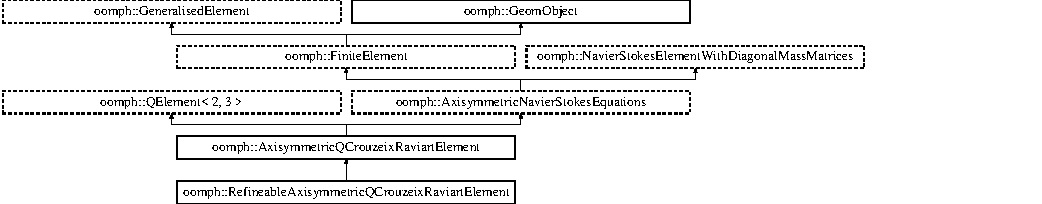
\includegraphics[height=2.737048cm]{classoomph_1_1AxisymmetricQCrouzeixRaviartElement}
\end{center}
\end{figure}
\subsection*{Public Member Functions}
\begin{DoxyCompactItemize}
\item 
\hyperlink{classoomph_1_1AxisymmetricQCrouzeixRaviartElement_a971e34ee93385674ff784d9b1baf1871}{Axisymmetric\+Q\+Crouzeix\+Raviart\+Element} ()
\begin{DoxyCompactList}\small\item\em Constructor, there are three internal values (for the pressure) \end{DoxyCompactList}\item 
virtual unsigned \hyperlink{classoomph_1_1AxisymmetricQCrouzeixRaviartElement_ae7988679549e63ef87fc3f062fb6a559}{required\+\_\+nvalue} (const unsigned \&n) const
\begin{DoxyCompactList}\small\item\em Number of values (pinned or dofs) required at local node n. \end{DoxyCompactList}\item 
double \hyperlink{classoomph_1_1AxisymmetricQCrouzeixRaviartElement_acaa357820f2efb863d442b66e9761c6d}{p\+\_\+axi\+\_\+nst} (const unsigned \&\hyperlink{cfortran_8h_adb50e893b86b3e55e751a42eab3cba82}{i}) const
\begin{DoxyCompactList}\small\item\em Return the pressure values at internal dof i\+\_\+internal (Discontinous pressure interpolation -- no need to cater for hanging nodes). \end{DoxyCompactList}\item 
unsigned \hyperlink{classoomph_1_1AxisymmetricQCrouzeixRaviartElement_a923c2ccbc5bd523118273e63cc18fd5f}{npres\+\_\+axi\+\_\+nst} () const
\begin{DoxyCompactList}\small\item\em Return number of pressure values. \end{DoxyCompactList}\item 
void \hyperlink{classoomph_1_1AxisymmetricQCrouzeixRaviartElement_a65e65b5d7dd33b374c259b53dc99a83c}{fix\+\_\+pressure} (const unsigned \&p\+\_\+dof, const double \&pvalue)
\begin{DoxyCompactList}\small\item\em Function to fix the internal pressure dof idof\+\_\+internal. \end{DoxyCompactList}\item 
void \hyperlink{classoomph_1_1AxisymmetricQCrouzeixRaviartElement_a60ea4ee3c006bc04984f1dcadb87a79d}{get\+\_\+traction} (const \hyperlink{classoomph_1_1Vector}{Vector}$<$ double $>$ \&\hyperlink{cfortran_8h_ab7123126e4885ef647dd9c6e3807a21c}{s}, const \hyperlink{classoomph_1_1Vector}{Vector}$<$ double $>$ \&N, \hyperlink{classoomph_1_1Vector}{Vector}$<$ double $>$ \&\hyperlink{classoomph_1_1AxisymmetricNavierStokesEquations_a0a5523b91d5191c2f9e23fe8d74f4e07}{traction}) const
\begin{DoxyCompactList}\small\item\em Compute traction at local coordinate s for outer unit normal N. \end{DoxyCompactList}\item 
int \hyperlink{classoomph_1_1AxisymmetricQCrouzeixRaviartElement_adc569122e3649deba56231175f3116cf}{p\+\_\+local\+\_\+eqn} (const unsigned \&n) const
\begin{DoxyCompactList}\small\item\em Overload the access function for the pressure\textquotesingle{}s local equation numbers. \end{DoxyCompactList}\item 
void \hyperlink{classoomph_1_1AxisymmetricQCrouzeixRaviartElement_af7811d55e87a839fb5c01d9e306cfda8}{output} (std\+::ostream \&outfile)
\begin{DoxyCompactList}\small\item\em Redirect output to \hyperlink{classoomph_1_1NavierStokesEquations}{Navier\+Stokes\+Equations} output. \end{DoxyCompactList}\item 
void \hyperlink{classoomph_1_1AxisymmetricQCrouzeixRaviartElement_afb5ef7f9b09d4b3ed6d5ee04cad58fec}{output} (std\+::ostream \&outfile, const unsigned \&n\+\_\+plot)
\begin{DoxyCompactList}\small\item\em Redirect output to \hyperlink{classoomph_1_1NavierStokesEquations}{Navier\+Stokes\+Equations} output. \end{DoxyCompactList}\item 
void \hyperlink{classoomph_1_1AxisymmetricQCrouzeixRaviartElement_a89e6624edb01f732c6c10b068227de54}{output} (F\+I\+LE $\ast$file\+\_\+pt)
\begin{DoxyCompactList}\small\item\em Redirect output to \hyperlink{classoomph_1_1NavierStokesEquations}{Navier\+Stokes\+Equations} output. \end{DoxyCompactList}\item 
void \hyperlink{classoomph_1_1AxisymmetricQCrouzeixRaviartElement_a04743e5848f04627a7069879f4da8389}{output} (F\+I\+LE $\ast$file\+\_\+pt, const unsigned \&n\+\_\+plot)
\begin{DoxyCompactList}\small\item\em Redirect output to \hyperlink{classoomph_1_1NavierStokesEquations}{Navier\+Stokes\+Equations} output. \end{DoxyCompactList}\item 
unsigned \hyperlink{classoomph_1_1AxisymmetricQCrouzeixRaviartElement_a85c8740ef4dd17626ae47c9344e15ae8}{ndof\+\_\+types} () const
\begin{DoxyCompactList}\small\item\em The number of \char`\"{}\+D\+O\+F types\char`\"{} that degrees of freedom in this element are sub-\/divided into\+: Velocity (3 components) and pressure. \end{DoxyCompactList}\item 
void \hyperlink{classoomph_1_1AxisymmetricQCrouzeixRaviartElement_a83a50021a007f1a932fe841119d93412}{get\+\_\+dof\+\_\+numbers\+\_\+for\+\_\+unknowns} (std\+::list$<$ std\+::pair$<$ unsigned long, unsigned $>$ $>$ \&dof\+\_\+lookup\+\_\+list) const
\begin{DoxyCompactList}\small\item\em Create a list of pairs for all unknowns in this element, so that the first entry in each pair contains the global equation number of the unknown, while the second one contains the number of the \char`\"{}\+D\+O\+F type\char`\"{} that this unknown is associated with. (Function can obviously only be called if the equation numbering scheme has been set up.) \end{DoxyCompactList}\end{DoxyCompactItemize}
\subsection*{Protected Member Functions}
\begin{DoxyCompactItemize}
\item 
double \hyperlink{classoomph_1_1AxisymmetricQCrouzeixRaviartElement_a48bd4be228495e97e5d8bf8a70162182}{dshape\+\_\+and\+\_\+dtest\+\_\+eulerian\+\_\+axi\+\_\+nst} (const \hyperlink{classoomph_1_1Vector}{Vector}$<$ double $>$ \&\hyperlink{cfortran_8h_ab7123126e4885ef647dd9c6e3807a21c}{s}, \hyperlink{classoomph_1_1Shape}{Shape} \&psi, \hyperlink{classoomph_1_1DShape}{D\+Shape} \&dpsidx, \hyperlink{classoomph_1_1Shape}{Shape} \&test, \hyperlink{classoomph_1_1DShape}{D\+Shape} \&dtestdx) const
\begin{DoxyCompactList}\small\item\em Velocity shape and test functions and their derivs w.\+r.\+t. to global coords at local coordinate s (taken from geometry) Return Jacobian of mapping between local and global coordinates. \end{DoxyCompactList}\item 
double \hyperlink{classoomph_1_1AxisymmetricQCrouzeixRaviartElement_a84026f3c225ef35731a04cc5866c7d6b}{dshape\+\_\+and\+\_\+dtest\+\_\+eulerian\+\_\+at\+\_\+knot\+\_\+axi\+\_\+nst} (const unsigned \&ipt, \hyperlink{classoomph_1_1Shape}{Shape} \&psi, \hyperlink{classoomph_1_1DShape}{D\+Shape} \&dpsidx, \hyperlink{classoomph_1_1Shape}{Shape} \&test, \hyperlink{classoomph_1_1DShape}{D\+Shape} \&dtestdx) const
\begin{DoxyCompactList}\small\item\em Velocity shape and test functions and their derivs w.\+r.\+t. to global coords at ipt-\/th integation point (taken from geometry) Return Jacobian of mapping between local and global coordinates. \end{DoxyCompactList}\item 
double \hyperlink{classoomph_1_1AxisymmetricQCrouzeixRaviartElement_abef9fe3b35d6a0eb08b18a33aa6b03c7}{dshape\+\_\+and\+\_\+dtest\+\_\+eulerian\+\_\+at\+\_\+knot\+\_\+axi\+\_\+nst} (const unsigned \&ipt, \hyperlink{classoomph_1_1Shape}{Shape} \&psi, \hyperlink{classoomph_1_1DShape}{D\+Shape} \&dpsidx, \hyperlink{classoomph_1_1RankFourTensor}{Rank\+Four\+Tensor}$<$ double $>$ \&d\+\_\+dpsidx\+\_\+dX, \hyperlink{classoomph_1_1Shape}{Shape} \&test, \hyperlink{classoomph_1_1DShape}{D\+Shape} \&dtestdx, \hyperlink{classoomph_1_1RankFourTensor}{Rank\+Four\+Tensor}$<$ double $>$ \&d\+\_\+dtestdx\+\_\+dX, \hyperlink{classoomph_1_1DenseMatrix}{Dense\+Matrix}$<$ double $>$ \&djacobian\+\_\+dX) const
\begin{DoxyCompactList}\small\item\em Shape/test functions and derivs w.\+r.\+t. to global coords at integration point ipt; return Jacobian of mapping (J). Also compute derivatives of dpsidx, dtestdx and J w.\+r.\+t. nodal coordinates. \end{DoxyCompactList}\item 
void \hyperlink{classoomph_1_1AxisymmetricQCrouzeixRaviartElement_a6a16bdbe2fc4e1bfe09123c50d101688}{pshape\+\_\+axi\+\_\+nst} (const \hyperlink{classoomph_1_1Vector}{Vector}$<$ double $>$ \&\hyperlink{cfortran_8h_ab7123126e4885ef647dd9c6e3807a21c}{s}, \hyperlink{classoomph_1_1Shape}{Shape} \&psi) const
\begin{DoxyCompactList}\small\item\em Pressure shape functions at local coordinate s. \end{DoxyCompactList}\item 
void \hyperlink{classoomph_1_1AxisymmetricQCrouzeixRaviartElement_af131ceee4d1612696b66ce7ac3a866d1}{pshape\+\_\+axi\+\_\+nst} (const \hyperlink{classoomph_1_1Vector}{Vector}$<$ double $>$ \&\hyperlink{cfortran_8h_ab7123126e4885ef647dd9c6e3807a21c}{s}, \hyperlink{classoomph_1_1Shape}{Shape} \&psi, \hyperlink{classoomph_1_1Shape}{Shape} \&test) const
\begin{DoxyCompactList}\small\item\em Pressure shape and test functions at local coordinte s. \end{DoxyCompactList}\end{DoxyCompactItemize}
\subsection*{Protected Attributes}
\begin{DoxyCompactItemize}
\item 
unsigned \hyperlink{classoomph_1_1AxisymmetricQCrouzeixRaviartElement_a8ec7b0e02c2ab96d0cb9b5238b76b145}{P\+\_\+axi\+\_\+nst\+\_\+internal\+\_\+index}
\end{DoxyCompactItemize}
\subsection*{Static Private Attributes}
\begin{DoxyCompactItemize}
\item 
static const unsigned \hyperlink{classoomph_1_1AxisymmetricQCrouzeixRaviartElement_a6edd4a05741c3ee8ee1ac82f7c3f9eff}{Initial\+\_\+\+Nvalue} \mbox{[}$\,$\mbox{]} =\{3,3,3,3,3,3,3,3,3\}
\begin{DoxyCompactList}\small\item\em Static array of ints to hold required number of variables at nodes. \end{DoxyCompactList}\end{DoxyCompactItemize}
\subsection*{Additional Inherited Members}


\subsection{Detailed Description}
Crouzeix\+\_\+\+Raviart elements are Navier--Stokes elements with quadratic interpolation for velocities and positions, but a discontinuous linear pressure interpolation 

Definition at line 1262 of file axisym\+\_\+navier\+\_\+stokes\+\_\+elements.\+h.



\subsection{Constructor \& Destructor Documentation}
\mbox{\Hypertarget{classoomph_1_1AxisymmetricQCrouzeixRaviartElement_a971e34ee93385674ff784d9b1baf1871}\label{classoomph_1_1AxisymmetricQCrouzeixRaviartElement_a971e34ee93385674ff784d9b1baf1871}} 
\index{oomph\+::\+Axisymmetric\+Q\+Crouzeix\+Raviart\+Element@{oomph\+::\+Axisymmetric\+Q\+Crouzeix\+Raviart\+Element}!Axisymmetric\+Q\+Crouzeix\+Raviart\+Element@{Axisymmetric\+Q\+Crouzeix\+Raviart\+Element}}
\index{Axisymmetric\+Q\+Crouzeix\+Raviart\+Element@{Axisymmetric\+Q\+Crouzeix\+Raviart\+Element}!oomph\+::\+Axisymmetric\+Q\+Crouzeix\+Raviart\+Element@{oomph\+::\+Axisymmetric\+Q\+Crouzeix\+Raviart\+Element}}
\subsubsection{\texorpdfstring{Axisymmetric\+Q\+Crouzeix\+Raviart\+Element()}{AxisymmetricQCrouzeixRaviartElement()}}
{\footnotesize\ttfamily oomph\+::\+Axisymmetric\+Q\+Crouzeix\+Raviart\+Element\+::\+Axisymmetric\+Q\+Crouzeix\+Raviart\+Element (\begin{DoxyParamCaption}{ }\end{DoxyParamCaption})\hspace{0.3cm}{\ttfamily [inline]}}



Constructor, there are three internal values (for the pressure) 



Definition at line 1318 of file axisym\+\_\+navier\+\_\+stokes\+\_\+elements.\+h.



References oomph\+::\+Generalised\+Element\+::add\+\_\+internal\+\_\+data(), and oomph\+::\+Finite\+Element\+::required\+\_\+nvalue().



\subsection{Member Function Documentation}
\mbox{\Hypertarget{classoomph_1_1AxisymmetricQCrouzeixRaviartElement_a84026f3c225ef35731a04cc5866c7d6b}\label{classoomph_1_1AxisymmetricQCrouzeixRaviartElement_a84026f3c225ef35731a04cc5866c7d6b}} 
\index{oomph\+::\+Axisymmetric\+Q\+Crouzeix\+Raviart\+Element@{oomph\+::\+Axisymmetric\+Q\+Crouzeix\+Raviart\+Element}!dshape\+\_\+and\+\_\+dtest\+\_\+eulerian\+\_\+at\+\_\+knot\+\_\+axi\+\_\+nst@{dshape\+\_\+and\+\_\+dtest\+\_\+eulerian\+\_\+at\+\_\+knot\+\_\+axi\+\_\+nst}}
\index{dshape\+\_\+and\+\_\+dtest\+\_\+eulerian\+\_\+at\+\_\+knot\+\_\+axi\+\_\+nst@{dshape\+\_\+and\+\_\+dtest\+\_\+eulerian\+\_\+at\+\_\+knot\+\_\+axi\+\_\+nst}!oomph\+::\+Axisymmetric\+Q\+Crouzeix\+Raviart\+Element@{oomph\+::\+Axisymmetric\+Q\+Crouzeix\+Raviart\+Element}}
\subsubsection{\texorpdfstring{dshape\+\_\+and\+\_\+dtest\+\_\+eulerian\+\_\+at\+\_\+knot\+\_\+axi\+\_\+nst()}{dshape\_and\_dtest\_eulerian\_at\_knot\_axi\_nst()}\hspace{0.1cm}{\footnotesize\ttfamily [1/2]}}
{\footnotesize\ttfamily double oomph\+::\+Axisymmetric\+Q\+Crouzeix\+Raviart\+Element\+::dshape\+\_\+and\+\_\+dtest\+\_\+eulerian\+\_\+at\+\_\+knot\+\_\+axi\+\_\+nst (\begin{DoxyParamCaption}\item[{const unsigned \&}]{ipt,  }\item[{\hyperlink{classoomph_1_1Shape}{Shape} \&}]{psi,  }\item[{\hyperlink{classoomph_1_1DShape}{D\+Shape} \&}]{dpsidx,  }\item[{\hyperlink{classoomph_1_1Shape}{Shape} \&}]{test,  }\item[{\hyperlink{classoomph_1_1DShape}{D\+Shape} \&}]{dtestdx }\end{DoxyParamCaption}) const\hspace{0.3cm}{\ttfamily [inline]}, {\ttfamily [protected]}, {\ttfamily [virtual]}}



Velocity shape and test functions and their derivs w.\+r.\+t. to global coords at ipt-\/th integation point (taken from geometry) Return Jacobian of mapping between local and global coordinates. 

Derivatives of the shape functions and test functions w.\+r.\+t. to global (Eulerian) coordinates. Return Jacobian of mapping between local and global coordinates. 

Implements \hyperlink{classoomph_1_1AxisymmetricNavierStokesEquations_a76e090fdac4507d10eb9f81feb53a51b}{oomph\+::\+Axisymmetric\+Navier\+Stokes\+Equations}.



Definition at line 1422 of file axisym\+\_\+navier\+\_\+stokes\+\_\+elements.\+h.



References oomph\+::\+Finite\+Element\+::dshape\+\_\+eulerian\+\_\+at\+\_\+knot(), and i.



Referenced by dshape\+\_\+and\+\_\+dtest\+\_\+eulerian\+\_\+axi\+\_\+nst().

\mbox{\Hypertarget{classoomph_1_1AxisymmetricQCrouzeixRaviartElement_abef9fe3b35d6a0eb08b18a33aa6b03c7}\label{classoomph_1_1AxisymmetricQCrouzeixRaviartElement_abef9fe3b35d6a0eb08b18a33aa6b03c7}} 
\index{oomph\+::\+Axisymmetric\+Q\+Crouzeix\+Raviart\+Element@{oomph\+::\+Axisymmetric\+Q\+Crouzeix\+Raviart\+Element}!dshape\+\_\+and\+\_\+dtest\+\_\+eulerian\+\_\+at\+\_\+knot\+\_\+axi\+\_\+nst@{dshape\+\_\+and\+\_\+dtest\+\_\+eulerian\+\_\+at\+\_\+knot\+\_\+axi\+\_\+nst}}
\index{dshape\+\_\+and\+\_\+dtest\+\_\+eulerian\+\_\+at\+\_\+knot\+\_\+axi\+\_\+nst@{dshape\+\_\+and\+\_\+dtest\+\_\+eulerian\+\_\+at\+\_\+knot\+\_\+axi\+\_\+nst}!oomph\+::\+Axisymmetric\+Q\+Crouzeix\+Raviart\+Element@{oomph\+::\+Axisymmetric\+Q\+Crouzeix\+Raviart\+Element}}
\subsubsection{\texorpdfstring{dshape\+\_\+and\+\_\+dtest\+\_\+eulerian\+\_\+at\+\_\+knot\+\_\+axi\+\_\+nst()}{dshape\_and\_dtest\_eulerian\_at\_knot\_axi\_nst()}\hspace{0.1cm}{\footnotesize\ttfamily [2/2]}}
{\footnotesize\ttfamily double oomph\+::\+Axisymmetric\+Q\+Crouzeix\+Raviart\+Element\+::dshape\+\_\+and\+\_\+dtest\+\_\+eulerian\+\_\+at\+\_\+knot\+\_\+axi\+\_\+nst (\begin{DoxyParamCaption}\item[{const unsigned \&}]{ipt,  }\item[{\hyperlink{classoomph_1_1Shape}{Shape} \&}]{psi,  }\item[{\hyperlink{classoomph_1_1DShape}{D\+Shape} \&}]{dpsidx,  }\item[{\hyperlink{classoomph_1_1RankFourTensor}{Rank\+Four\+Tensor}$<$ double $>$ \&}]{d\+\_\+dpsidx\+\_\+dX,  }\item[{\hyperlink{classoomph_1_1Shape}{Shape} \&}]{test,  }\item[{\hyperlink{classoomph_1_1DShape}{D\+Shape} \&}]{dtestdx,  }\item[{\hyperlink{classoomph_1_1RankFourTensor}{Rank\+Four\+Tensor}$<$ double $>$ \&}]{d\+\_\+dtestdx\+\_\+dX,  }\item[{\hyperlink{classoomph_1_1DenseMatrix}{Dense\+Matrix}$<$ double $>$ \&}]{djacobian\+\_\+dX }\end{DoxyParamCaption}) const\hspace{0.3cm}{\ttfamily [inline]}, {\ttfamily [protected]}, {\ttfamily [virtual]}}



Shape/test functions and derivs w.\+r.\+t. to global coords at integration point ipt; return Jacobian of mapping (J). Also compute derivatives of dpsidx, dtestdx and J w.\+r.\+t. nodal coordinates. 

Define the shape functions (psi) and test functions (test) and their derivatives w.\+r.\+t. global coordinates (dpsidx and dtestdx) and return Jacobian of mapping (J). Additionally compute the derivatives of dpsidx, dtestdx and J w.\+r.\+t. nodal coordinates.

Galerkin\+: Test functions = shape functions 

Implements \hyperlink{classoomph_1_1AxisymmetricNavierStokesEquations_a2cd0715a679af81bd0e3d7448a5560cb}{oomph\+::\+Axisymmetric\+Navier\+Stokes\+Equations}.



Definition at line 1449 of file axisym\+\_\+navier\+\_\+stokes\+\_\+elements.\+h.



References oomph\+::\+Finite\+Element\+::dshape\+\_\+eulerian\+\_\+at\+\_\+knot(), i, and pshape\+\_\+axi\+\_\+nst().

\mbox{\Hypertarget{classoomph_1_1AxisymmetricQCrouzeixRaviartElement_a48bd4be228495e97e5d8bf8a70162182}\label{classoomph_1_1AxisymmetricQCrouzeixRaviartElement_a48bd4be228495e97e5d8bf8a70162182}} 
\index{oomph\+::\+Axisymmetric\+Q\+Crouzeix\+Raviart\+Element@{oomph\+::\+Axisymmetric\+Q\+Crouzeix\+Raviart\+Element}!dshape\+\_\+and\+\_\+dtest\+\_\+eulerian\+\_\+axi\+\_\+nst@{dshape\+\_\+and\+\_\+dtest\+\_\+eulerian\+\_\+axi\+\_\+nst}}
\index{dshape\+\_\+and\+\_\+dtest\+\_\+eulerian\+\_\+axi\+\_\+nst@{dshape\+\_\+and\+\_\+dtest\+\_\+eulerian\+\_\+axi\+\_\+nst}!oomph\+::\+Axisymmetric\+Q\+Crouzeix\+Raviart\+Element@{oomph\+::\+Axisymmetric\+Q\+Crouzeix\+Raviart\+Element}}
\subsubsection{\texorpdfstring{dshape\+\_\+and\+\_\+dtest\+\_\+eulerian\+\_\+axi\+\_\+nst()}{dshape\_and\_dtest\_eulerian\_axi\_nst()}}
{\footnotesize\ttfamily double oomph\+::\+Axisymmetric\+Q\+Crouzeix\+Raviart\+Element\+::dshape\+\_\+and\+\_\+dtest\+\_\+eulerian\+\_\+axi\+\_\+nst (\begin{DoxyParamCaption}\item[{const \hyperlink{classoomph_1_1Vector}{Vector}$<$ double $>$ \&}]{s,  }\item[{\hyperlink{classoomph_1_1Shape}{Shape} \&}]{psi,  }\item[{\hyperlink{classoomph_1_1DShape}{D\+Shape} \&}]{dpsidx,  }\item[{\hyperlink{classoomph_1_1Shape}{Shape} \&}]{test,  }\item[{\hyperlink{classoomph_1_1DShape}{D\+Shape} \&}]{dtestdx }\end{DoxyParamCaption}) const\hspace{0.3cm}{\ttfamily [inline]}, {\ttfamily [protected]}, {\ttfamily [virtual]}}



Velocity shape and test functions and their derivs w.\+r.\+t. to global coords at local coordinate s (taken from geometry) Return Jacobian of mapping between local and global coordinates. 

Derivatives of the shape functions and test functions w.\+r.\+t. to global (Eulerian) coordinates. Return Jacobian of mapping between local and global coordinates. 

Implements \hyperlink{classoomph_1_1AxisymmetricNavierStokesEquations_a8d958da8ef73dcf5c68360edc9d9f565}{oomph\+::\+Axisymmetric\+Navier\+Stokes\+Equations}.



Definition at line 1398 of file axisym\+\_\+navier\+\_\+stokes\+\_\+elements.\+h.



References dshape\+\_\+and\+\_\+dtest\+\_\+eulerian\+\_\+at\+\_\+knot\+\_\+axi\+\_\+nst(), oomph\+::\+Finite\+Element\+::dshape\+\_\+eulerian(), and i.



Referenced by ndof\+\_\+types().

\mbox{\Hypertarget{classoomph_1_1AxisymmetricQCrouzeixRaviartElement_a65e65b5d7dd33b374c259b53dc99a83c}\label{classoomph_1_1AxisymmetricQCrouzeixRaviartElement_a65e65b5d7dd33b374c259b53dc99a83c}} 
\index{oomph\+::\+Axisymmetric\+Q\+Crouzeix\+Raviart\+Element@{oomph\+::\+Axisymmetric\+Q\+Crouzeix\+Raviart\+Element}!fix\+\_\+pressure@{fix\+\_\+pressure}}
\index{fix\+\_\+pressure@{fix\+\_\+pressure}!oomph\+::\+Axisymmetric\+Q\+Crouzeix\+Raviart\+Element@{oomph\+::\+Axisymmetric\+Q\+Crouzeix\+Raviart\+Element}}
\subsubsection{\texorpdfstring{fix\+\_\+pressure()}{fix\_pressure()}}
{\footnotesize\ttfamily void oomph\+::\+Axisymmetric\+Q\+Crouzeix\+Raviart\+Element\+::fix\+\_\+pressure (\begin{DoxyParamCaption}\item[{const unsigned \&}]{p\+\_\+dof,  }\item[{const double \&}]{pvalue }\end{DoxyParamCaption})\hspace{0.3cm}{\ttfamily [inline]}}



Function to fix the internal pressure dof idof\+\_\+internal. 



Definition at line 1339 of file axisym\+\_\+navier\+\_\+stokes\+\_\+elements.\+h.



References oomph\+::\+Generalised\+Element\+::internal\+\_\+data\+\_\+pt(), oomph\+::\+Quad\+Tree\+Names\+::N, oomph\+::\+Data\+::pin(), s, oomph\+::\+Data\+::set\+\_\+value(), and oomph\+::\+Axisymmetric\+Navier\+Stokes\+Equations\+::traction().

\mbox{\Hypertarget{classoomph_1_1AxisymmetricQCrouzeixRaviartElement_a83a50021a007f1a932fe841119d93412}\label{classoomph_1_1AxisymmetricQCrouzeixRaviartElement_a83a50021a007f1a932fe841119d93412}} 
\index{oomph\+::\+Axisymmetric\+Q\+Crouzeix\+Raviart\+Element@{oomph\+::\+Axisymmetric\+Q\+Crouzeix\+Raviart\+Element}!get\+\_\+dof\+\_\+numbers\+\_\+for\+\_\+unknowns@{get\+\_\+dof\+\_\+numbers\+\_\+for\+\_\+unknowns}}
\index{get\+\_\+dof\+\_\+numbers\+\_\+for\+\_\+unknowns@{get\+\_\+dof\+\_\+numbers\+\_\+for\+\_\+unknowns}!oomph\+::\+Axisymmetric\+Q\+Crouzeix\+Raviart\+Element@{oomph\+::\+Axisymmetric\+Q\+Crouzeix\+Raviart\+Element}}
\subsubsection{\texorpdfstring{get\+\_\+dof\+\_\+numbers\+\_\+for\+\_\+unknowns()}{get\_dof\_numbers\_for\_unknowns()}}
{\footnotesize\ttfamily void oomph\+::\+Axisymmetric\+Q\+Crouzeix\+Raviart\+Element\+::get\+\_\+dof\+\_\+numbers\+\_\+for\+\_\+unknowns (\begin{DoxyParamCaption}\item[{std\+::list$<$ std\+::pair$<$ unsigned long, unsigned $>$ $>$ \&}]{dof\+\_\+lookup\+\_\+list }\end{DoxyParamCaption}) const\hspace{0.3cm}{\ttfamily [virtual]}}



Create a list of pairs for all unknowns in this element, so that the first entry in each pair contains the global equation number of the unknown, while the second one contains the number of the \char`\"{}\+D\+O\+F type\char`\"{} that this unknown is associated with. (Function can obviously only be called if the equation numbering scheme has been set up.) 

Create a list of pairs for all unknowns in this element, so that the first entry in each pair contains the global equation number of the unknown, while the second one contains the number of the \char`\"{}\+D\+O\+F type\char`\"{} that this unknown is associated with. (Function can obviously only be called if the equation numbering scheme has been set up.) 

Reimplemented from \hyperlink{classoomph_1_1GeneralisedElement_a069f59bfc3e607a5bebba52c6314d777}{oomph\+::\+Generalised\+Element}.



Definition at line 3446 of file axisym\+\_\+navier\+\_\+stokes\+\_\+elements.\+cc.



References oomph\+::\+Generalised\+Element\+::eqn\+\_\+number(), Initial\+\_\+\+Nvalue, oomph\+::\+Generalised\+Element\+::local\+\_\+eqn\+\_\+number(), oomph\+::\+Finite\+Element\+::nnode(), oomph\+::\+Finite\+Element\+::nodal\+\_\+local\+\_\+eqn(), oomph\+::\+Finite\+Element\+::node\+\_\+pt(), oomph\+::\+Axisymmetric\+Navier\+Stokes\+Equations\+::npres\+\_\+axi\+\_\+nst(), oomph\+::\+Data\+::nvalue(), oomph\+::\+Axisymmetric\+Navier\+Stokes\+Equations\+::p\+\_\+local\+\_\+eqn(), and required\+\_\+nvalue().

\mbox{\Hypertarget{classoomph_1_1AxisymmetricQCrouzeixRaviartElement_a60ea4ee3c006bc04984f1dcadb87a79d}\label{classoomph_1_1AxisymmetricQCrouzeixRaviartElement_a60ea4ee3c006bc04984f1dcadb87a79d}} 
\index{oomph\+::\+Axisymmetric\+Q\+Crouzeix\+Raviart\+Element@{oomph\+::\+Axisymmetric\+Q\+Crouzeix\+Raviart\+Element}!get\+\_\+traction@{get\+\_\+traction}}
\index{get\+\_\+traction@{get\+\_\+traction}!oomph\+::\+Axisymmetric\+Q\+Crouzeix\+Raviart\+Element@{oomph\+::\+Axisymmetric\+Q\+Crouzeix\+Raviart\+Element}}
\subsubsection{\texorpdfstring{get\+\_\+traction()}{get\_traction()}}
{\footnotesize\ttfamily void oomph\+::\+Axisymmetric\+Q\+Crouzeix\+Raviart\+Element\+::get\+\_\+traction (\begin{DoxyParamCaption}\item[{const \hyperlink{classoomph_1_1Vector}{Vector}$<$ double $>$ \&}]{s,  }\item[{const \hyperlink{classoomph_1_1Vector}{Vector}$<$ double $>$ \&}]{N,  }\item[{\hyperlink{classoomph_1_1Vector}{Vector}$<$ double $>$ \&}]{traction }\end{DoxyParamCaption}) const}



Compute traction at local coordinate s for outer unit normal N. 



Definition at line 3526 of file axisym\+\_\+navier\+\_\+stokes\+\_\+elements.\+cc.



References oomph\+::\+Axisymmetric\+Navier\+Stokes\+Equations\+::traction().

\mbox{\Hypertarget{classoomph_1_1AxisymmetricQCrouzeixRaviartElement_a85c8740ef4dd17626ae47c9344e15ae8}\label{classoomph_1_1AxisymmetricQCrouzeixRaviartElement_a85c8740ef4dd17626ae47c9344e15ae8}} 
\index{oomph\+::\+Axisymmetric\+Q\+Crouzeix\+Raviart\+Element@{oomph\+::\+Axisymmetric\+Q\+Crouzeix\+Raviart\+Element}!ndof\+\_\+types@{ndof\+\_\+types}}
\index{ndof\+\_\+types@{ndof\+\_\+types}!oomph\+::\+Axisymmetric\+Q\+Crouzeix\+Raviart\+Element@{oomph\+::\+Axisymmetric\+Q\+Crouzeix\+Raviart\+Element}}
\subsubsection{\texorpdfstring{ndof\+\_\+types()}{ndof\_types()}}
{\footnotesize\ttfamily unsigned oomph\+::\+Axisymmetric\+Q\+Crouzeix\+Raviart\+Element\+::ndof\+\_\+types (\begin{DoxyParamCaption}{ }\end{DoxyParamCaption}) const\hspace{0.3cm}{\ttfamily [inline]}, {\ttfamily [virtual]}}



The number of \char`\"{}\+D\+O\+F types\char`\"{} that degrees of freedom in this element are sub-\/divided into\+: Velocity (3 components) and pressure. 



Reimplemented from \hyperlink{classoomph_1_1GeneralisedElement_a0c6037a870597b35dcf1c780710b9a56}{oomph\+::\+Generalised\+Element}.



Definition at line 1373 of file axisym\+\_\+navier\+\_\+stokes\+\_\+elements.\+h.



References dshape\+\_\+and\+\_\+dtest\+\_\+eulerian\+\_\+axi\+\_\+nst(), and oomph\+::\+Generalised\+Element\+::get\+\_\+dof\+\_\+numbers\+\_\+for\+\_\+unknowns().

\mbox{\Hypertarget{classoomph_1_1AxisymmetricQCrouzeixRaviartElement_a923c2ccbc5bd523118273e63cc18fd5f}\label{classoomph_1_1AxisymmetricQCrouzeixRaviartElement_a923c2ccbc5bd523118273e63cc18fd5f}} 
\index{oomph\+::\+Axisymmetric\+Q\+Crouzeix\+Raviart\+Element@{oomph\+::\+Axisymmetric\+Q\+Crouzeix\+Raviart\+Element}!npres\+\_\+axi\+\_\+nst@{npres\+\_\+axi\+\_\+nst}}
\index{npres\+\_\+axi\+\_\+nst@{npres\+\_\+axi\+\_\+nst}!oomph\+::\+Axisymmetric\+Q\+Crouzeix\+Raviart\+Element@{oomph\+::\+Axisymmetric\+Q\+Crouzeix\+Raviart\+Element}}
\subsubsection{\texorpdfstring{npres\+\_\+axi\+\_\+nst()}{npres\_axi\_nst()}}
{\footnotesize\ttfamily unsigned oomph\+::\+Axisymmetric\+Q\+Crouzeix\+Raviart\+Element\+::npres\+\_\+axi\+\_\+nst (\begin{DoxyParamCaption}{ }\end{DoxyParamCaption}) const\hspace{0.3cm}{\ttfamily [inline]}, {\ttfamily [virtual]}}



Return number of pressure values. 



Implements \hyperlink{classoomph_1_1AxisymmetricNavierStokesEquations_a89edaffb4913131cc14a5f6e45ed117a}{oomph\+::\+Axisymmetric\+Navier\+Stokes\+Equations}.



Definition at line 1336 of file axisym\+\_\+navier\+\_\+stokes\+\_\+elements.\+h.

\mbox{\Hypertarget{classoomph_1_1AxisymmetricQCrouzeixRaviartElement_af7811d55e87a839fb5c01d9e306cfda8}\label{classoomph_1_1AxisymmetricQCrouzeixRaviartElement_af7811d55e87a839fb5c01d9e306cfda8}} 
\index{oomph\+::\+Axisymmetric\+Q\+Crouzeix\+Raviart\+Element@{oomph\+::\+Axisymmetric\+Q\+Crouzeix\+Raviart\+Element}!output@{output}}
\index{output@{output}!oomph\+::\+Axisymmetric\+Q\+Crouzeix\+Raviart\+Element@{oomph\+::\+Axisymmetric\+Q\+Crouzeix\+Raviart\+Element}}
\subsubsection{\texorpdfstring{output()}{output()}\hspace{0.1cm}{\footnotesize\ttfamily [1/4]}}
{\footnotesize\ttfamily void oomph\+::\+Axisymmetric\+Q\+Crouzeix\+Raviart\+Element\+::output (\begin{DoxyParamCaption}\item[{std\+::ostream \&}]{outfile }\end{DoxyParamCaption})\hspace{0.3cm}{\ttfamily [inline]}, {\ttfamily [virtual]}}



Redirect output to \hyperlink{classoomph_1_1NavierStokesEquations}{Navier\+Stokes\+Equations} output. 



Reimplemented from \hyperlink{classoomph_1_1AxisymmetricNavierStokesEquations_afe0c7b607ec3fd03a73b7db4f1fe6252}{oomph\+::\+Axisymmetric\+Navier\+Stokes\+Equations}.



Definition at line 1355 of file axisym\+\_\+navier\+\_\+stokes\+\_\+elements.\+h.



References oomph\+::\+Axisymmetric\+Navier\+Stokes\+Equations\+::output().

\mbox{\Hypertarget{classoomph_1_1AxisymmetricQCrouzeixRaviartElement_afb5ef7f9b09d4b3ed6d5ee04cad58fec}\label{classoomph_1_1AxisymmetricQCrouzeixRaviartElement_afb5ef7f9b09d4b3ed6d5ee04cad58fec}} 
\index{oomph\+::\+Axisymmetric\+Q\+Crouzeix\+Raviart\+Element@{oomph\+::\+Axisymmetric\+Q\+Crouzeix\+Raviart\+Element}!output@{output}}
\index{output@{output}!oomph\+::\+Axisymmetric\+Q\+Crouzeix\+Raviart\+Element@{oomph\+::\+Axisymmetric\+Q\+Crouzeix\+Raviart\+Element}}
\subsubsection{\texorpdfstring{output()}{output()}\hspace{0.1cm}{\footnotesize\ttfamily [2/4]}}
{\footnotesize\ttfamily void oomph\+::\+Axisymmetric\+Q\+Crouzeix\+Raviart\+Element\+::output (\begin{DoxyParamCaption}\item[{std\+::ostream \&}]{outfile,  }\item[{const unsigned \&}]{n\+\_\+plot }\end{DoxyParamCaption})\hspace{0.3cm}{\ttfamily [inline]}, {\ttfamily [virtual]}}



Redirect output to \hyperlink{classoomph_1_1NavierStokesEquations}{Navier\+Stokes\+Equations} output. 



Reimplemented from \hyperlink{classoomph_1_1AxisymmetricNavierStokesEquations_a94a243ca05ba3b995e366564e6cf7695}{oomph\+::\+Axisymmetric\+Navier\+Stokes\+Equations}.



Definition at line 1359 of file axisym\+\_\+navier\+\_\+stokes\+\_\+elements.\+h.



References oomph\+::\+Axisymmetric\+Navier\+Stokes\+Equations\+::output().

\mbox{\Hypertarget{classoomph_1_1AxisymmetricQCrouzeixRaviartElement_a89e6624edb01f732c6c10b068227de54}\label{classoomph_1_1AxisymmetricQCrouzeixRaviartElement_a89e6624edb01f732c6c10b068227de54}} 
\index{oomph\+::\+Axisymmetric\+Q\+Crouzeix\+Raviart\+Element@{oomph\+::\+Axisymmetric\+Q\+Crouzeix\+Raviart\+Element}!output@{output}}
\index{output@{output}!oomph\+::\+Axisymmetric\+Q\+Crouzeix\+Raviart\+Element@{oomph\+::\+Axisymmetric\+Q\+Crouzeix\+Raviart\+Element}}
\subsubsection{\texorpdfstring{output()}{output()}\hspace{0.1cm}{\footnotesize\ttfamily [3/4]}}
{\footnotesize\ttfamily void oomph\+::\+Axisymmetric\+Q\+Crouzeix\+Raviart\+Element\+::output (\begin{DoxyParamCaption}\item[{F\+I\+LE $\ast$}]{file\+\_\+pt }\end{DoxyParamCaption})\hspace{0.3cm}{\ttfamily [inline]}, {\ttfamily [virtual]}}



Redirect output to \hyperlink{classoomph_1_1NavierStokesEquations}{Navier\+Stokes\+Equations} output. 



Reimplemented from \hyperlink{classoomph_1_1AxisymmetricNavierStokesEquations_a61129dd7505ac363862946bd8b3ea5bf}{oomph\+::\+Axisymmetric\+Navier\+Stokes\+Equations}.



Definition at line 1364 of file axisym\+\_\+navier\+\_\+stokes\+\_\+elements.\+h.



References oomph\+::\+Axisymmetric\+Navier\+Stokes\+Equations\+::output().

\mbox{\Hypertarget{classoomph_1_1AxisymmetricQCrouzeixRaviartElement_a04743e5848f04627a7069879f4da8389}\label{classoomph_1_1AxisymmetricQCrouzeixRaviartElement_a04743e5848f04627a7069879f4da8389}} 
\index{oomph\+::\+Axisymmetric\+Q\+Crouzeix\+Raviart\+Element@{oomph\+::\+Axisymmetric\+Q\+Crouzeix\+Raviart\+Element}!output@{output}}
\index{output@{output}!oomph\+::\+Axisymmetric\+Q\+Crouzeix\+Raviart\+Element@{oomph\+::\+Axisymmetric\+Q\+Crouzeix\+Raviart\+Element}}
\subsubsection{\texorpdfstring{output()}{output()}\hspace{0.1cm}{\footnotesize\ttfamily [4/4]}}
{\footnotesize\ttfamily void oomph\+::\+Axisymmetric\+Q\+Crouzeix\+Raviart\+Element\+::output (\begin{DoxyParamCaption}\item[{F\+I\+LE $\ast$}]{file\+\_\+pt,  }\item[{const unsigned \&}]{n\+\_\+plot }\end{DoxyParamCaption})\hspace{0.3cm}{\ttfamily [inline]}, {\ttfamily [virtual]}}



Redirect output to \hyperlink{classoomph_1_1NavierStokesEquations}{Navier\+Stokes\+Equations} output. 



Reimplemented from \hyperlink{classoomph_1_1AxisymmetricNavierStokesEquations_abc2ca00250845e243da3f4e0845b2c96}{oomph\+::\+Axisymmetric\+Navier\+Stokes\+Equations}.



Definition at line 1368 of file axisym\+\_\+navier\+\_\+stokes\+\_\+elements.\+h.



References oomph\+::\+Axisymmetric\+Navier\+Stokes\+Equations\+::output().

\mbox{\Hypertarget{classoomph_1_1AxisymmetricQCrouzeixRaviartElement_acaa357820f2efb863d442b66e9761c6d}\label{classoomph_1_1AxisymmetricQCrouzeixRaviartElement_acaa357820f2efb863d442b66e9761c6d}} 
\index{oomph\+::\+Axisymmetric\+Q\+Crouzeix\+Raviart\+Element@{oomph\+::\+Axisymmetric\+Q\+Crouzeix\+Raviart\+Element}!p\+\_\+axi\+\_\+nst@{p\+\_\+axi\+\_\+nst}}
\index{p\+\_\+axi\+\_\+nst@{p\+\_\+axi\+\_\+nst}!oomph\+::\+Axisymmetric\+Q\+Crouzeix\+Raviart\+Element@{oomph\+::\+Axisymmetric\+Q\+Crouzeix\+Raviart\+Element}}
\subsubsection{\texorpdfstring{p\+\_\+axi\+\_\+nst()}{p\_axi\_nst()}}
{\footnotesize\ttfamily double oomph\+::\+Axisymmetric\+Q\+Crouzeix\+Raviart\+Element\+::p\+\_\+axi\+\_\+nst (\begin{DoxyParamCaption}\item[{const unsigned \&}]{i }\end{DoxyParamCaption}) const\hspace{0.3cm}{\ttfamily [inline]}, {\ttfamily [virtual]}}



Return the pressure values at internal dof i\+\_\+internal (Discontinous pressure interpolation -- no need to cater for hanging nodes). 



Implements \hyperlink{classoomph_1_1AxisymmetricNavierStokesEquations_a3aa173227f477a40fb4adba84a337f5b}{oomph\+::\+Axisymmetric\+Navier\+Stokes\+Equations}.



Definition at line 1332 of file axisym\+\_\+navier\+\_\+stokes\+\_\+elements.\+h.



References oomph\+::\+Generalised\+Element\+::internal\+\_\+data\+\_\+pt(), and oomph\+::\+Data\+::value().

\mbox{\Hypertarget{classoomph_1_1AxisymmetricQCrouzeixRaviartElement_adc569122e3649deba56231175f3116cf}\label{classoomph_1_1AxisymmetricQCrouzeixRaviartElement_adc569122e3649deba56231175f3116cf}} 
\index{oomph\+::\+Axisymmetric\+Q\+Crouzeix\+Raviart\+Element@{oomph\+::\+Axisymmetric\+Q\+Crouzeix\+Raviart\+Element}!p\+\_\+local\+\_\+eqn@{p\+\_\+local\+\_\+eqn}}
\index{p\+\_\+local\+\_\+eqn@{p\+\_\+local\+\_\+eqn}!oomph\+::\+Axisymmetric\+Q\+Crouzeix\+Raviart\+Element@{oomph\+::\+Axisymmetric\+Q\+Crouzeix\+Raviart\+Element}}
\subsubsection{\texorpdfstring{p\+\_\+local\+\_\+eqn()}{p\_local\_eqn()}}
{\footnotesize\ttfamily int oomph\+::\+Axisymmetric\+Q\+Crouzeix\+Raviart\+Element\+::p\+\_\+local\+\_\+eqn (\begin{DoxyParamCaption}\item[{const unsigned \&}]{n }\end{DoxyParamCaption}) const\hspace{0.3cm}{\ttfamily [inline]}, {\ttfamily [virtual]}}



Overload the access function for the pressure\textquotesingle{}s local equation numbers. 



Implements \hyperlink{classoomph_1_1AxisymmetricNavierStokesEquations_ad6ac62ca5fa411c365fd2ecc72aa25e8}{oomph\+::\+Axisymmetric\+Navier\+Stokes\+Equations}.



Definition at line 1351 of file axisym\+\_\+navier\+\_\+stokes\+\_\+elements.\+h.



References oomph\+::\+Generalised\+Element\+::internal\+\_\+local\+\_\+eqn().

\mbox{\Hypertarget{classoomph_1_1AxisymmetricQCrouzeixRaviartElement_a6a16bdbe2fc4e1bfe09123c50d101688}\label{classoomph_1_1AxisymmetricQCrouzeixRaviartElement_a6a16bdbe2fc4e1bfe09123c50d101688}} 
\index{oomph\+::\+Axisymmetric\+Q\+Crouzeix\+Raviart\+Element@{oomph\+::\+Axisymmetric\+Q\+Crouzeix\+Raviart\+Element}!pshape\+\_\+axi\+\_\+nst@{pshape\+\_\+axi\+\_\+nst}}
\index{pshape\+\_\+axi\+\_\+nst@{pshape\+\_\+axi\+\_\+nst}!oomph\+::\+Axisymmetric\+Q\+Crouzeix\+Raviart\+Element@{oomph\+::\+Axisymmetric\+Q\+Crouzeix\+Raviart\+Element}}
\subsubsection{\texorpdfstring{pshape\+\_\+axi\+\_\+nst()}{pshape\_axi\_nst()}\hspace{0.1cm}{\footnotesize\ttfamily [1/2]}}
{\footnotesize\ttfamily void oomph\+::\+Axisymmetric\+Q\+Crouzeix\+Raviart\+Element\+::pshape\+\_\+axi\+\_\+nst (\begin{DoxyParamCaption}\item[{const \hyperlink{classoomph_1_1Vector}{Vector}$<$ double $>$ \&}]{s,  }\item[{\hyperlink{classoomph_1_1Shape}{Shape} \&}]{psi }\end{DoxyParamCaption}) const\hspace{0.3cm}{\ttfamily [inline]}, {\ttfamily [protected]}, {\ttfamily [virtual]}}



Pressure shape functions at local coordinate s. 

Pressure shape functions. 

Implements \hyperlink{classoomph_1_1AxisymmetricNavierStokesEquations_a6309780fd1964c4df0cca0818ccff158}{oomph\+::\+Axisymmetric\+Navier\+Stokes\+Equations}.



Definition at line 1488 of file axisym\+\_\+navier\+\_\+stokes\+\_\+elements.\+h.



Referenced by dshape\+\_\+and\+\_\+dtest\+\_\+eulerian\+\_\+at\+\_\+knot\+\_\+axi\+\_\+nst().

\mbox{\Hypertarget{classoomph_1_1AxisymmetricQCrouzeixRaviartElement_af131ceee4d1612696b66ce7ac3a866d1}\label{classoomph_1_1AxisymmetricQCrouzeixRaviartElement_af131ceee4d1612696b66ce7ac3a866d1}} 
\index{oomph\+::\+Axisymmetric\+Q\+Crouzeix\+Raviart\+Element@{oomph\+::\+Axisymmetric\+Q\+Crouzeix\+Raviart\+Element}!pshape\+\_\+axi\+\_\+nst@{pshape\+\_\+axi\+\_\+nst}}
\index{pshape\+\_\+axi\+\_\+nst@{pshape\+\_\+axi\+\_\+nst}!oomph\+::\+Axisymmetric\+Q\+Crouzeix\+Raviart\+Element@{oomph\+::\+Axisymmetric\+Q\+Crouzeix\+Raviart\+Element}}
\subsubsection{\texorpdfstring{pshape\+\_\+axi\+\_\+nst()}{pshape\_axi\_nst()}\hspace{0.1cm}{\footnotesize\ttfamily [2/2]}}
{\footnotesize\ttfamily void oomph\+::\+Axisymmetric\+Q\+Crouzeix\+Raviart\+Element\+::pshape\+\_\+axi\+\_\+nst (\begin{DoxyParamCaption}\item[{const \hyperlink{classoomph_1_1Vector}{Vector}$<$ double $>$ \&}]{s,  }\item[{\hyperlink{classoomph_1_1Shape}{Shape} \&}]{psi,  }\item[{\hyperlink{classoomph_1_1Shape}{Shape} \&}]{test }\end{DoxyParamCaption}) const\hspace{0.3cm}{\ttfamily [inline]}, {\ttfamily [protected]}, {\ttfamily [virtual]}}



Pressure shape and test functions at local coordinte s. 

Define the pressure shape and test functions. 

Implements \hyperlink{classoomph_1_1AxisymmetricNavierStokesEquations_a19a4135581356bf368a7ecae2b315f85}{oomph\+::\+Axisymmetric\+Navier\+Stokes\+Equations}.



Definition at line 1498 of file axisym\+\_\+navier\+\_\+stokes\+\_\+elements.\+h.



References i, and oomph\+::\+Axisymmetric\+Navier\+Stokes\+Equations\+::pshape\+\_\+axi\+\_\+nst().

\mbox{\Hypertarget{classoomph_1_1AxisymmetricQCrouzeixRaviartElement_ae7988679549e63ef87fc3f062fb6a559}\label{classoomph_1_1AxisymmetricQCrouzeixRaviartElement_ae7988679549e63ef87fc3f062fb6a559}} 
\index{oomph\+::\+Axisymmetric\+Q\+Crouzeix\+Raviart\+Element@{oomph\+::\+Axisymmetric\+Q\+Crouzeix\+Raviart\+Element}!required\+\_\+nvalue@{required\+\_\+nvalue}}
\index{required\+\_\+nvalue@{required\+\_\+nvalue}!oomph\+::\+Axisymmetric\+Q\+Crouzeix\+Raviart\+Element@{oomph\+::\+Axisymmetric\+Q\+Crouzeix\+Raviart\+Element}}
\subsubsection{\texorpdfstring{required\+\_\+nvalue()}{required\_nvalue()}}
{\footnotesize\ttfamily unsigned oomph\+::\+Axisymmetric\+Q\+Crouzeix\+Raviart\+Element\+::required\+\_\+nvalue (\begin{DoxyParamCaption}\item[{const unsigned \&}]{n }\end{DoxyParamCaption}) const\hspace{0.3cm}{\ttfamily [virtual]}}



Number of values (pinned or dofs) required at local node n. 

Number of values (pinned or dofs) required at node n. 

Reimplemented from \hyperlink{classoomph_1_1FiniteElement_a56610c60d5bc2d7c27407a1455471b1a}{oomph\+::\+Finite\+Element}.



Definition at line 3521 of file axisym\+\_\+navier\+\_\+stokes\+\_\+elements.\+cc.



Referenced by get\+\_\+dof\+\_\+numbers\+\_\+for\+\_\+unknowns().



\subsection{Member Data Documentation}
\mbox{\Hypertarget{classoomph_1_1AxisymmetricQCrouzeixRaviartElement_a6edd4a05741c3ee8ee1ac82f7c3f9eff}\label{classoomph_1_1AxisymmetricQCrouzeixRaviartElement_a6edd4a05741c3ee8ee1ac82f7c3f9eff}} 
\index{oomph\+::\+Axisymmetric\+Q\+Crouzeix\+Raviart\+Element@{oomph\+::\+Axisymmetric\+Q\+Crouzeix\+Raviart\+Element}!Initial\+\_\+\+Nvalue@{Initial\+\_\+\+Nvalue}}
\index{Initial\+\_\+\+Nvalue@{Initial\+\_\+\+Nvalue}!oomph\+::\+Axisymmetric\+Q\+Crouzeix\+Raviart\+Element@{oomph\+::\+Axisymmetric\+Q\+Crouzeix\+Raviart\+Element}}
\subsubsection{\texorpdfstring{Initial\+\_\+\+Nvalue}{Initial\_Nvalue}}
{\footnotesize\ttfamily const unsigned oomph\+::\+Axisymmetric\+Q\+Crouzeix\+Raviart\+Element\+::\+Initial\+\_\+\+Nvalue =\{3,3,3,3,3,3,3,3,3\}\hspace{0.3cm}{\ttfamily [static]}, {\ttfamily [private]}}



Static array of ints to hold required number of variables at nodes. 

Axisymmetric Crouzeix-\/\+Raviart elements. 

Definition at line 1268 of file axisym\+\_\+navier\+\_\+stokes\+\_\+elements.\+h.



Referenced by get\+\_\+dof\+\_\+numbers\+\_\+for\+\_\+unknowns().

\mbox{\Hypertarget{classoomph_1_1AxisymmetricQCrouzeixRaviartElement_a8ec7b0e02c2ab96d0cb9b5238b76b145}\label{classoomph_1_1AxisymmetricQCrouzeixRaviartElement_a8ec7b0e02c2ab96d0cb9b5238b76b145}} 
\index{oomph\+::\+Axisymmetric\+Q\+Crouzeix\+Raviart\+Element@{oomph\+::\+Axisymmetric\+Q\+Crouzeix\+Raviart\+Element}!P\+\_\+axi\+\_\+nst\+\_\+internal\+\_\+index@{P\+\_\+axi\+\_\+nst\+\_\+internal\+\_\+index}}
\index{P\+\_\+axi\+\_\+nst\+\_\+internal\+\_\+index@{P\+\_\+axi\+\_\+nst\+\_\+internal\+\_\+index}!oomph\+::\+Axisymmetric\+Q\+Crouzeix\+Raviart\+Element@{oomph\+::\+Axisymmetric\+Q\+Crouzeix\+Raviart\+Element}}
\subsubsection{\texorpdfstring{P\+\_\+axi\+\_\+nst\+\_\+internal\+\_\+index}{P\_axi\_nst\_internal\_index}}
{\footnotesize\ttfamily unsigned oomph\+::\+Axisymmetric\+Q\+Crouzeix\+Raviart\+Element\+::\+P\+\_\+axi\+\_\+nst\+\_\+internal\+\_\+index\hspace{0.3cm}{\ttfamily [protected]}}

Internal index that indicates at which internal data the pressure is stored 

Definition at line 1274 of file axisym\+\_\+navier\+\_\+stokes\+\_\+elements.\+h.



The documentation for this class was generated from the following files\+:\begin{DoxyCompactItemize}
\item 
\hyperlink{axisym__navier__stokes__elements_8h}{axisym\+\_\+navier\+\_\+stokes\+\_\+elements.\+h}\item 
\hyperlink{axisym__navier__stokes__elements_8cc}{axisym\+\_\+navier\+\_\+stokes\+\_\+elements.\+cc}\end{DoxyCompactItemize}

\hypertarget{classoomph_1_1AxisymmetricQTaylorHoodElement}{}\section{oomph\+:\+:Axisymmetric\+Q\+Taylor\+Hood\+Element Class Reference}
\label{classoomph_1_1AxisymmetricQTaylorHoodElement}\index{oomph\+::\+Axisymmetric\+Q\+Taylor\+Hood\+Element@{oomph\+::\+Axisymmetric\+Q\+Taylor\+Hood\+Element}}


{\ttfamily \#include $<$axisym\+\_\+navier\+\_\+stokes\+\_\+elements.\+h$>$}

Inheritance diagram for oomph\+:\+:Axisymmetric\+Q\+Taylor\+Hood\+Element\+:\begin{figure}[H]
\begin{center}
\leavevmode
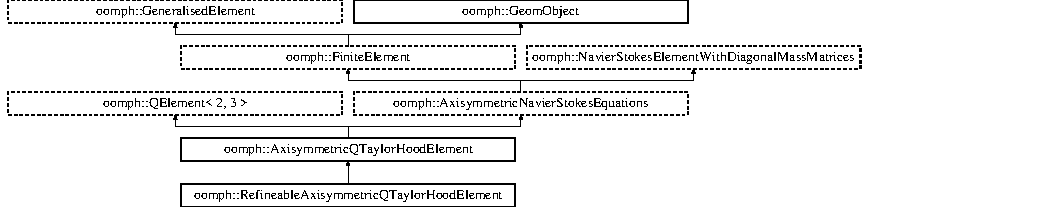
\includegraphics[height=2.786069cm]{classoomph_1_1AxisymmetricQTaylorHoodElement}
\end{center}
\end{figure}
\subsection*{Public Member Functions}
\begin{DoxyCompactItemize}
\item 
\hyperlink{classoomph_1_1AxisymmetricQTaylorHoodElement_ac6b80d9619833e670b80cafff35f3739}{Axisymmetric\+Q\+Taylor\+Hood\+Element} ()
\begin{DoxyCompactList}\small\item\em Constructor, no internal data points. \end{DoxyCompactList}\item 
virtual unsigned \hyperlink{classoomph_1_1AxisymmetricQTaylorHoodElement_a89c18769297b69e2e3522d83c8b68d73}{required\+\_\+nvalue} (const unsigned \&n) const
\begin{DoxyCompactList}\small\item\em Number of values (pinned or dofs) required at node n. Can be overwritten for hanging node version. \end{DoxyCompactList}\item 
virtual int \hyperlink{classoomph_1_1AxisymmetricQTaylorHoodElement_a318c767e20198f6d3f8a5c788df31055}{p\+\_\+nodal\+\_\+index\+\_\+axi\+\_\+nst} () const
\begin{DoxyCompactList}\small\item\em Which nodal value represents the pressure? \end{DoxyCompactList}\item 
double \hyperlink{classoomph_1_1AxisymmetricQTaylorHoodElement_aec113045099e51a61a1624b0126a05b1}{p\+\_\+axi\+\_\+nst} (const unsigned \&n\+\_\+p) const
\begin{DoxyCompactList}\small\item\em Access function for the pressure values at local pressure node n\+\_\+p (const version) \end{DoxyCompactList}\item 
unsigned \hyperlink{classoomph_1_1AxisymmetricQTaylorHoodElement_a636d0c75c75483f9da193d0192f4e05e}{npres\+\_\+axi\+\_\+nst} () const
\begin{DoxyCompactList}\small\item\em Return number of pressure values. \end{DoxyCompactList}\item 
void \hyperlink{classoomph_1_1AxisymmetricQTaylorHoodElement_a1557e286a76d63d79aabef3493cf0af2}{fix\+\_\+pressure} (const unsigned \&n\+\_\+p, const double \&pvalue)
\begin{DoxyCompactList}\small\item\em Fix the pressure at local pressure node n\+\_\+p. \end{DoxyCompactList}\item 
void \hyperlink{classoomph_1_1AxisymmetricQTaylorHoodElement_abfaf2fb0ff51a888f77c724af8c20809}{get\+\_\+traction} (const \hyperlink{classoomph_1_1Vector}{Vector}$<$ double $>$ \&\hyperlink{cfortran_8h_ab7123126e4885ef647dd9c6e3807a21c}{s}, const \hyperlink{classoomph_1_1Vector}{Vector}$<$ double $>$ \&N, \hyperlink{classoomph_1_1Vector}{Vector}$<$ double $>$ \&\hyperlink{classoomph_1_1AxisymmetricNavierStokesEquations_a0a5523b91d5191c2f9e23fe8d74f4e07}{traction}) const
\begin{DoxyCompactList}\small\item\em Compute traction at local coordinate s for outer unit normal N. \end{DoxyCompactList}\item 
int \hyperlink{classoomph_1_1AxisymmetricQTaylorHoodElement_a5593ee69e94a15cca6f309bb38717913}{p\+\_\+local\+\_\+eqn} (const unsigned \&n) const
\begin{DoxyCompactList}\small\item\em Overload the access function for the pressure\textquotesingle{}s local. \end{DoxyCompactList}\item 
void \hyperlink{classoomph_1_1AxisymmetricQTaylorHoodElement_aa092b03db26878057c3d3c92496d752d}{output} (std\+::ostream \&outfile)
\begin{DoxyCompactList}\small\item\em Redirect output to \hyperlink{classoomph_1_1NavierStokesEquations}{Navier\+Stokes\+Equations} output. \end{DoxyCompactList}\item 
void \hyperlink{classoomph_1_1AxisymmetricQTaylorHoodElement_a73bc9729dd01b61e467d4fdc7d8b802c}{output} (std\+::ostream \&outfile, const unsigned \&n\+\_\+plot)
\begin{DoxyCompactList}\small\item\em Redirect output to \hyperlink{classoomph_1_1NavierStokesEquations}{Navier\+Stokes\+Equations} output. \end{DoxyCompactList}\item 
void \hyperlink{classoomph_1_1AxisymmetricQTaylorHoodElement_a91861ce04f934aeae956c9d938ce337f}{output} (F\+I\+LE $\ast$file\+\_\+pt)
\begin{DoxyCompactList}\small\item\em Redirect output to \hyperlink{classoomph_1_1NavierStokesEquations}{Navier\+Stokes\+Equations} output. \end{DoxyCompactList}\item 
void \hyperlink{classoomph_1_1AxisymmetricQTaylorHoodElement_a4c2fcefe0593bb39d6c4937b0fdc1292}{output} (F\+I\+LE $\ast$file\+\_\+pt, const unsigned \&n\+\_\+plot)
\begin{DoxyCompactList}\small\item\em Redirect output to \hyperlink{classoomph_1_1NavierStokesEquations}{Navier\+Stokes\+Equations} output. \end{DoxyCompactList}\item 
unsigned \hyperlink{classoomph_1_1AxisymmetricQTaylorHoodElement_a9cd3bbcb75c7a4501c3de68e524a5503}{ndof\+\_\+types} () const
\begin{DoxyCompactList}\small\item\em Returns the number of \char`\"{}\+D\+O\+F types\char`\"{} that degrees of freedom in this element are sub-\/divided into\+: Velocity (3 components) and pressure. \end{DoxyCompactList}\item 
void \hyperlink{classoomph_1_1AxisymmetricQTaylorHoodElement_ad763c91177814d4221ec485b076a38e9}{get\+\_\+dof\+\_\+numbers\+\_\+for\+\_\+unknowns} (std\+::list$<$ std\+::pair$<$ unsigned long, unsigned $>$ $>$ \&dof\+\_\+lookup\+\_\+list) const
\begin{DoxyCompactList}\small\item\em Create a list of pairs for all unknowns in this element, so that the first entry in each pair contains the global equation number of the unknown, while the second one contains the number of the \char`\"{}\+D\+O\+F type\char`\"{} that this unknown is associated with. (Function can obviously only be called if the equation numbering scheme has been set up.) \end{DoxyCompactList}\end{DoxyCompactItemize}
\subsection*{Protected Member Functions}
\begin{DoxyCompactItemize}
\item 
double \hyperlink{classoomph_1_1AxisymmetricQTaylorHoodElement_a413aba20f944dc30c84bb432c408cbc1}{dshape\+\_\+and\+\_\+dtest\+\_\+eulerian\+\_\+axi\+\_\+nst} (const \hyperlink{classoomph_1_1Vector}{Vector}$<$ double $>$ \&\hyperlink{cfortran_8h_ab7123126e4885ef647dd9c6e3807a21c}{s}, \hyperlink{classoomph_1_1Shape}{Shape} \&psi, \hyperlink{classoomph_1_1DShape}{D\+Shape} \&dpsidx, \hyperlink{classoomph_1_1Shape}{Shape} \&test, \hyperlink{classoomph_1_1DShape}{D\+Shape} \&dtestdx) const
\begin{DoxyCompactList}\small\item\em Velocity shape and test functions and their derivs w.\+r.\+t. to global coords at local coordinate s (taken from geometry) Return Jacobian of mapping between local and global coordinates. \end{DoxyCompactList}\item 
double \hyperlink{classoomph_1_1AxisymmetricQTaylorHoodElement_abd3de2e051bca2f697560e907a53abde}{dshape\+\_\+and\+\_\+dtest\+\_\+eulerian\+\_\+at\+\_\+knot\+\_\+axi\+\_\+nst} (const unsigned \&ipt, \hyperlink{classoomph_1_1Shape}{Shape} \&psi, \hyperlink{classoomph_1_1DShape}{D\+Shape} \&dpsidx, \hyperlink{classoomph_1_1Shape}{Shape} \&test, \hyperlink{classoomph_1_1DShape}{D\+Shape} \&dtestdx) const
\begin{DoxyCompactList}\small\item\em Velocity shape and test functions and their derivs w.\+r.\+t. to global coords at local coordinate s (taken from geometry) Return Jacobian of mapping between local and global coordinates. \end{DoxyCompactList}\item 
double \hyperlink{classoomph_1_1AxisymmetricQTaylorHoodElement_a77fe7f0caef36c951f99a923b94c2f7a}{dshape\+\_\+and\+\_\+dtest\+\_\+eulerian\+\_\+at\+\_\+knot\+\_\+axi\+\_\+nst} (const unsigned \&ipt, \hyperlink{classoomph_1_1Shape}{Shape} \&psi, \hyperlink{classoomph_1_1DShape}{D\+Shape} \&dpsidx, \hyperlink{classoomph_1_1RankFourTensor}{Rank\+Four\+Tensor}$<$ double $>$ \&d\+\_\+dpsidx\+\_\+dX, \hyperlink{classoomph_1_1Shape}{Shape} \&test, \hyperlink{classoomph_1_1DShape}{D\+Shape} \&dtestdx, \hyperlink{classoomph_1_1RankFourTensor}{Rank\+Four\+Tensor}$<$ double $>$ \&d\+\_\+dtestdx\+\_\+dX, \hyperlink{classoomph_1_1DenseMatrix}{Dense\+Matrix}$<$ double $>$ \&djacobian\+\_\+dX) const
\begin{DoxyCompactList}\small\item\em Shape/test functions and derivs w.\+r.\+t. to global coords at integration point ipt; return Jacobian of mapping (J). Also compute derivatives of dpsidx, dtestdx and J w.\+r.\+t. nodal coordinates. \end{DoxyCompactList}\item 
void \hyperlink{classoomph_1_1AxisymmetricQTaylorHoodElement_ab4eea01cdcd97616ce75e6547c0c4338}{pshape\+\_\+axi\+\_\+nst} (const \hyperlink{classoomph_1_1Vector}{Vector}$<$ double $>$ \&\hyperlink{cfortran_8h_ab7123126e4885ef647dd9c6e3807a21c}{s}, \hyperlink{classoomph_1_1Shape}{Shape} \&psi) const
\begin{DoxyCompactList}\small\item\em Pressure shape functions at local coordinate s. \end{DoxyCompactList}\item 
void \hyperlink{classoomph_1_1AxisymmetricQTaylorHoodElement_abdb9779d344d9dbe51260e8d01852737}{pshape\+\_\+axi\+\_\+nst} (const \hyperlink{classoomph_1_1Vector}{Vector}$<$ double $>$ \&\hyperlink{cfortran_8h_ab7123126e4885ef647dd9c6e3807a21c}{s}, \hyperlink{classoomph_1_1Shape}{Shape} \&psi, \hyperlink{classoomph_1_1Shape}{Shape} \&test) const
\begin{DoxyCompactList}\small\item\em Pressure shape and test functions at local coordinte s. \end{DoxyCompactList}\end{DoxyCompactItemize}
\subsection*{Static Protected Attributes}
\begin{DoxyCompactItemize}
\item 
static const unsigned \hyperlink{classoomph_1_1AxisymmetricQTaylorHoodElement_a40720e74e6b8ce8d803ee95d7a6ad119}{Pconv} \mbox{[}$\,$\mbox{]} =\{0,2,6,8\}
\begin{DoxyCompactList}\small\item\em Static array of ints to hold conversion from pressure node numbers to actual node numbers. \end{DoxyCompactList}\end{DoxyCompactItemize}
\subsection*{Static Private Attributes}
\begin{DoxyCompactItemize}
\item 
static const unsigned \hyperlink{classoomph_1_1AxisymmetricQTaylorHoodElement_ae0826bd23cb739552135795de862c758}{Initial\+\_\+\+Nvalue} \mbox{[}$\,$\mbox{]} =\{4,3,4,3,3,3,4,3,4\}
\begin{DoxyCompactList}\small\item\em Static array of ints to hold number of variables at node. \end{DoxyCompactList}\end{DoxyCompactItemize}
\subsection*{Additional Inherited Members}


\subsection{Detailed Description}
Taylor--Hood elements are Navier--Stokes elements with quadratic interpolation for velocities and positions and continous linear pressure interpolation 

Definition at line 1539 of file axisym\+\_\+navier\+\_\+stokes\+\_\+elements.\+h.



\subsection{Constructor \& Destructor Documentation}
\mbox{\Hypertarget{classoomph_1_1AxisymmetricQTaylorHoodElement_ac6b80d9619833e670b80cafff35f3739}\label{classoomph_1_1AxisymmetricQTaylorHoodElement_ac6b80d9619833e670b80cafff35f3739}} 
\index{oomph\+::\+Axisymmetric\+Q\+Taylor\+Hood\+Element@{oomph\+::\+Axisymmetric\+Q\+Taylor\+Hood\+Element}!Axisymmetric\+Q\+Taylor\+Hood\+Element@{Axisymmetric\+Q\+Taylor\+Hood\+Element}}
\index{Axisymmetric\+Q\+Taylor\+Hood\+Element@{Axisymmetric\+Q\+Taylor\+Hood\+Element}!oomph\+::\+Axisymmetric\+Q\+Taylor\+Hood\+Element@{oomph\+::\+Axisymmetric\+Q\+Taylor\+Hood\+Element}}
\subsubsection{\texorpdfstring{Axisymmetric\+Q\+Taylor\+Hood\+Element()}{AxisymmetricQTaylorHoodElement()}}
{\footnotesize\ttfamily oomph\+::\+Axisymmetric\+Q\+Taylor\+Hood\+Element\+::\+Axisymmetric\+Q\+Taylor\+Hood\+Element (\begin{DoxyParamCaption}{ }\end{DoxyParamCaption})\hspace{0.3cm}{\ttfamily [inline]}}



Constructor, no internal data points. 



Definition at line 1594 of file axisym\+\_\+navier\+\_\+stokes\+\_\+elements.\+h.



\subsection{Member Function Documentation}
\mbox{\Hypertarget{classoomph_1_1AxisymmetricQTaylorHoodElement_abd3de2e051bca2f697560e907a53abde}\label{classoomph_1_1AxisymmetricQTaylorHoodElement_abd3de2e051bca2f697560e907a53abde}} 
\index{oomph\+::\+Axisymmetric\+Q\+Taylor\+Hood\+Element@{oomph\+::\+Axisymmetric\+Q\+Taylor\+Hood\+Element}!dshape\+\_\+and\+\_\+dtest\+\_\+eulerian\+\_\+at\+\_\+knot\+\_\+axi\+\_\+nst@{dshape\+\_\+and\+\_\+dtest\+\_\+eulerian\+\_\+at\+\_\+knot\+\_\+axi\+\_\+nst}}
\index{dshape\+\_\+and\+\_\+dtest\+\_\+eulerian\+\_\+at\+\_\+knot\+\_\+axi\+\_\+nst@{dshape\+\_\+and\+\_\+dtest\+\_\+eulerian\+\_\+at\+\_\+knot\+\_\+axi\+\_\+nst}!oomph\+::\+Axisymmetric\+Q\+Taylor\+Hood\+Element@{oomph\+::\+Axisymmetric\+Q\+Taylor\+Hood\+Element}}
\subsubsection{\texorpdfstring{dshape\+\_\+and\+\_\+dtest\+\_\+eulerian\+\_\+at\+\_\+knot\+\_\+axi\+\_\+nst()}{dshape\_and\_dtest\_eulerian\_at\_knot\_axi\_nst()}\hspace{0.1cm}{\footnotesize\ttfamily [1/2]}}
{\footnotesize\ttfamily double oomph\+::\+Axisymmetric\+Q\+Taylor\+Hood\+Element\+::dshape\+\_\+and\+\_\+dtest\+\_\+eulerian\+\_\+at\+\_\+knot\+\_\+axi\+\_\+nst (\begin{DoxyParamCaption}\item[{const unsigned \&}]{ipt,  }\item[{\hyperlink{classoomph_1_1Shape}{Shape} \&}]{psi,  }\item[{\hyperlink{classoomph_1_1DShape}{D\+Shape} \&}]{dpsidx,  }\item[{\hyperlink{classoomph_1_1Shape}{Shape} \&}]{test,  }\item[{\hyperlink{classoomph_1_1DShape}{D\+Shape} \&}]{dtestdx }\end{DoxyParamCaption}) const\hspace{0.3cm}{\ttfamily [inline]}, {\ttfamily [protected]}, {\ttfamily [virtual]}}



Velocity shape and test functions and their derivs w.\+r.\+t. to global coords at local coordinate s (taken from geometry) Return Jacobian of mapping between local and global coordinates. 

Derivatives of the shape functions and test functions w.\+r.\+t to global (Eulerian) coordinates. Return Jacobian of mapping between local and global coordinates. 

Implements \hyperlink{classoomph_1_1AxisymmetricNavierStokesEquations_a76e090fdac4507d10eb9f81feb53a51b}{oomph\+::\+Axisymmetric\+Navier\+Stokes\+Equations}.



Definition at line 1697 of file axisym\+\_\+navier\+\_\+stokes\+\_\+elements.\+h.



References oomph\+::\+Finite\+Element\+::dshape\+\_\+eulerian\+\_\+at\+\_\+knot(), and i.



Referenced by dshape\+\_\+and\+\_\+dtest\+\_\+eulerian\+\_\+axi\+\_\+nst().

\mbox{\Hypertarget{classoomph_1_1AxisymmetricQTaylorHoodElement_a77fe7f0caef36c951f99a923b94c2f7a}\label{classoomph_1_1AxisymmetricQTaylorHoodElement_a77fe7f0caef36c951f99a923b94c2f7a}} 
\index{oomph\+::\+Axisymmetric\+Q\+Taylor\+Hood\+Element@{oomph\+::\+Axisymmetric\+Q\+Taylor\+Hood\+Element}!dshape\+\_\+and\+\_\+dtest\+\_\+eulerian\+\_\+at\+\_\+knot\+\_\+axi\+\_\+nst@{dshape\+\_\+and\+\_\+dtest\+\_\+eulerian\+\_\+at\+\_\+knot\+\_\+axi\+\_\+nst}}
\index{dshape\+\_\+and\+\_\+dtest\+\_\+eulerian\+\_\+at\+\_\+knot\+\_\+axi\+\_\+nst@{dshape\+\_\+and\+\_\+dtest\+\_\+eulerian\+\_\+at\+\_\+knot\+\_\+axi\+\_\+nst}!oomph\+::\+Axisymmetric\+Q\+Taylor\+Hood\+Element@{oomph\+::\+Axisymmetric\+Q\+Taylor\+Hood\+Element}}
\subsubsection{\texorpdfstring{dshape\+\_\+and\+\_\+dtest\+\_\+eulerian\+\_\+at\+\_\+knot\+\_\+axi\+\_\+nst()}{dshape\_and\_dtest\_eulerian\_at\_knot\_axi\_nst()}\hspace{0.1cm}{\footnotesize\ttfamily [2/2]}}
{\footnotesize\ttfamily double oomph\+::\+Axisymmetric\+Q\+Taylor\+Hood\+Element\+::dshape\+\_\+and\+\_\+dtest\+\_\+eulerian\+\_\+at\+\_\+knot\+\_\+axi\+\_\+nst (\begin{DoxyParamCaption}\item[{const unsigned \&}]{ipt,  }\item[{\hyperlink{classoomph_1_1Shape}{Shape} \&}]{psi,  }\item[{\hyperlink{classoomph_1_1DShape}{D\+Shape} \&}]{dpsidx,  }\item[{\hyperlink{classoomph_1_1RankFourTensor}{Rank\+Four\+Tensor}$<$ double $>$ \&}]{d\+\_\+dpsidx\+\_\+dX,  }\item[{\hyperlink{classoomph_1_1Shape}{Shape} \&}]{test,  }\item[{\hyperlink{classoomph_1_1DShape}{D\+Shape} \&}]{dtestdx,  }\item[{\hyperlink{classoomph_1_1RankFourTensor}{Rank\+Four\+Tensor}$<$ double $>$ \&}]{d\+\_\+dtestdx\+\_\+dX,  }\item[{\hyperlink{classoomph_1_1DenseMatrix}{Dense\+Matrix}$<$ double $>$ \&}]{djacobian\+\_\+dX }\end{DoxyParamCaption}) const\hspace{0.3cm}{\ttfamily [inline]}, {\ttfamily [protected]}, {\ttfamily [virtual]}}



Shape/test functions and derivs w.\+r.\+t. to global coords at integration point ipt; return Jacobian of mapping (J). Also compute derivatives of dpsidx, dtestdx and J w.\+r.\+t. nodal coordinates. 

Define the shape functions (psi) and test functions (test) and their derivatives w.\+r.\+t. global coordinates (dpsidx and dtestdx) and return Jacobian of mapping (J). Additionally compute the derivatives of dpsidx, dtestdx and J w.\+r.\+t. nodal coordinates.

Galerkin\+: Test functions = shape functions 

Implements \hyperlink{classoomph_1_1AxisymmetricNavierStokesEquations_a2cd0715a679af81bd0e3d7448a5560cb}{oomph\+::\+Axisymmetric\+Navier\+Stokes\+Equations}.



Definition at line 1725 of file axisym\+\_\+navier\+\_\+stokes\+\_\+elements.\+h.



References oomph\+::\+Finite\+Element\+::dshape\+\_\+eulerian\+\_\+at\+\_\+knot(), i, and pshape\+\_\+axi\+\_\+nst().

\mbox{\Hypertarget{classoomph_1_1AxisymmetricQTaylorHoodElement_a413aba20f944dc30c84bb432c408cbc1}\label{classoomph_1_1AxisymmetricQTaylorHoodElement_a413aba20f944dc30c84bb432c408cbc1}} 
\index{oomph\+::\+Axisymmetric\+Q\+Taylor\+Hood\+Element@{oomph\+::\+Axisymmetric\+Q\+Taylor\+Hood\+Element}!dshape\+\_\+and\+\_\+dtest\+\_\+eulerian\+\_\+axi\+\_\+nst@{dshape\+\_\+and\+\_\+dtest\+\_\+eulerian\+\_\+axi\+\_\+nst}}
\index{dshape\+\_\+and\+\_\+dtest\+\_\+eulerian\+\_\+axi\+\_\+nst@{dshape\+\_\+and\+\_\+dtest\+\_\+eulerian\+\_\+axi\+\_\+nst}!oomph\+::\+Axisymmetric\+Q\+Taylor\+Hood\+Element@{oomph\+::\+Axisymmetric\+Q\+Taylor\+Hood\+Element}}
\subsubsection{\texorpdfstring{dshape\+\_\+and\+\_\+dtest\+\_\+eulerian\+\_\+axi\+\_\+nst()}{dshape\_and\_dtest\_eulerian\_axi\_nst()}}
{\footnotesize\ttfamily double oomph\+::\+Axisymmetric\+Q\+Taylor\+Hood\+Element\+::dshape\+\_\+and\+\_\+dtest\+\_\+eulerian\+\_\+axi\+\_\+nst (\begin{DoxyParamCaption}\item[{const \hyperlink{classoomph_1_1Vector}{Vector}$<$ double $>$ \&}]{s,  }\item[{\hyperlink{classoomph_1_1Shape}{Shape} \&}]{psi,  }\item[{\hyperlink{classoomph_1_1DShape}{D\+Shape} \&}]{dpsidx,  }\item[{\hyperlink{classoomph_1_1Shape}{Shape} \&}]{test,  }\item[{\hyperlink{classoomph_1_1DShape}{D\+Shape} \&}]{dtestdx }\end{DoxyParamCaption}) const\hspace{0.3cm}{\ttfamily [inline]}, {\ttfamily [protected]}, {\ttfamily [virtual]}}



Velocity shape and test functions and their derivs w.\+r.\+t. to global coords at local coordinate s (taken from geometry) Return Jacobian of mapping between local and global coordinates. 

Derivatives of the shape functions and test functions w.\+r.\+t to global (Eulerian) coordinates. Return Jacobian of mapping between local and global coordinates. 

Implements \hyperlink{classoomph_1_1AxisymmetricNavierStokesEquations_a8d958da8ef73dcf5c68360edc9d9f565}{oomph\+::\+Axisymmetric\+Navier\+Stokes\+Equations}.



Definition at line 1672 of file axisym\+\_\+navier\+\_\+stokes\+\_\+elements.\+h.



References dshape\+\_\+and\+\_\+dtest\+\_\+eulerian\+\_\+at\+\_\+knot\+\_\+axi\+\_\+nst(), oomph\+::\+Finite\+Element\+::dshape\+\_\+eulerian(), and i.



Referenced by ndof\+\_\+types().

\mbox{\Hypertarget{classoomph_1_1AxisymmetricQTaylorHoodElement_a1557e286a76d63d79aabef3493cf0af2}\label{classoomph_1_1AxisymmetricQTaylorHoodElement_a1557e286a76d63d79aabef3493cf0af2}} 
\index{oomph\+::\+Axisymmetric\+Q\+Taylor\+Hood\+Element@{oomph\+::\+Axisymmetric\+Q\+Taylor\+Hood\+Element}!fix\+\_\+pressure@{fix\+\_\+pressure}}
\index{fix\+\_\+pressure@{fix\+\_\+pressure}!oomph\+::\+Axisymmetric\+Q\+Taylor\+Hood\+Element@{oomph\+::\+Axisymmetric\+Q\+Taylor\+Hood\+Element}}
\subsubsection{\texorpdfstring{fix\+\_\+pressure()}{fix\_pressure()}}
{\footnotesize\ttfamily void oomph\+::\+Axisymmetric\+Q\+Taylor\+Hood\+Element\+::fix\+\_\+pressure (\begin{DoxyParamCaption}\item[{const unsigned \&}]{n\+\_\+p,  }\item[{const double \&}]{pvalue }\end{DoxyParamCaption})\hspace{0.3cm}{\ttfamily [inline]}}



Fix the pressure at local pressure node n\+\_\+p. 



Definition at line 1614 of file axisym\+\_\+navier\+\_\+stokes\+\_\+elements.\+h.



References oomph\+::\+Quad\+Tree\+Names\+::N, oomph\+::\+Finite\+Element\+::node\+\_\+pt(), oomph\+::\+Axisymmetric\+Navier\+Stokes\+Equations\+::p\+\_\+nodal\+\_\+index\+\_\+axi\+\_\+nst(), oomph\+::\+Data\+::pin(), s, oomph\+::\+Data\+::set\+\_\+value(), and oomph\+::\+Axisymmetric\+Navier\+Stokes\+Equations\+::traction().

\mbox{\Hypertarget{classoomph_1_1AxisymmetricQTaylorHoodElement_ad763c91177814d4221ec485b076a38e9}\label{classoomph_1_1AxisymmetricQTaylorHoodElement_ad763c91177814d4221ec485b076a38e9}} 
\index{oomph\+::\+Axisymmetric\+Q\+Taylor\+Hood\+Element@{oomph\+::\+Axisymmetric\+Q\+Taylor\+Hood\+Element}!get\+\_\+dof\+\_\+numbers\+\_\+for\+\_\+unknowns@{get\+\_\+dof\+\_\+numbers\+\_\+for\+\_\+unknowns}}
\index{get\+\_\+dof\+\_\+numbers\+\_\+for\+\_\+unknowns@{get\+\_\+dof\+\_\+numbers\+\_\+for\+\_\+unknowns}!oomph\+::\+Axisymmetric\+Q\+Taylor\+Hood\+Element@{oomph\+::\+Axisymmetric\+Q\+Taylor\+Hood\+Element}}
\subsubsection{\texorpdfstring{get\+\_\+dof\+\_\+numbers\+\_\+for\+\_\+unknowns()}{get\_dof\_numbers\_for\_unknowns()}}
{\footnotesize\ttfamily void oomph\+::\+Axisymmetric\+Q\+Taylor\+Hood\+Element\+::get\+\_\+dof\+\_\+numbers\+\_\+for\+\_\+unknowns (\begin{DoxyParamCaption}\item[{std\+::list$<$ std\+::pair$<$ unsigned long, unsigned $>$ $>$ \&}]{dof\+\_\+lookup\+\_\+list }\end{DoxyParamCaption}) const\hspace{0.3cm}{\ttfamily [virtual]}}



Create a list of pairs for all unknowns in this element, so that the first entry in each pair contains the global equation number of the unknown, while the second one contains the number of the \char`\"{}\+D\+O\+F type\char`\"{} that this unknown is associated with. (Function can obviously only be called if the equation numbering scheme has been set up.) 

Create a list of pairs for all unknowns in this element, so the first entry in each pair contains the global equation number of the unknown, while the second one contains the number of the \char`\"{}\+D\+O\+F type\char`\"{} that this unknown is associated with. (Function can obviously only be called if the equation numbering scheme has been set up.) 

Reimplemented from \hyperlink{classoomph_1_1GeneralisedElement_a069f59bfc3e607a5bebba52c6314d777}{oomph\+::\+Generalised\+Element}.



Definition at line 3548 of file axisym\+\_\+navier\+\_\+stokes\+\_\+elements.\+cc.



References oomph\+::\+Generalised\+Element\+::eqn\+\_\+number(), Initial\+\_\+\+Nvalue, oomph\+::\+Generalised\+Element\+::local\+\_\+eqn\+\_\+number(), oomph\+::\+Finite\+Element\+::nnode(), oomph\+::\+Finite\+Element\+::nodal\+\_\+local\+\_\+eqn(), oomph\+::\+Finite\+Element\+::node\+\_\+pt(), oomph\+::\+Data\+::nvalue(), and Pconv.

\mbox{\Hypertarget{classoomph_1_1AxisymmetricQTaylorHoodElement_abfaf2fb0ff51a888f77c724af8c20809}\label{classoomph_1_1AxisymmetricQTaylorHoodElement_abfaf2fb0ff51a888f77c724af8c20809}} 
\index{oomph\+::\+Axisymmetric\+Q\+Taylor\+Hood\+Element@{oomph\+::\+Axisymmetric\+Q\+Taylor\+Hood\+Element}!get\+\_\+traction@{get\+\_\+traction}}
\index{get\+\_\+traction@{get\+\_\+traction}!oomph\+::\+Axisymmetric\+Q\+Taylor\+Hood\+Element@{oomph\+::\+Axisymmetric\+Q\+Taylor\+Hood\+Element}}
\subsubsection{\texorpdfstring{get\+\_\+traction()}{get\_traction()}}
{\footnotesize\ttfamily void oomph\+::\+Axisymmetric\+Q\+Taylor\+Hood\+Element\+::get\+\_\+traction (\begin{DoxyParamCaption}\item[{const \hyperlink{classoomph_1_1Vector}{Vector}$<$ double $>$ \&}]{s,  }\item[{const \hyperlink{classoomph_1_1Vector}{Vector}$<$ double $>$ \&}]{N,  }\item[{\hyperlink{classoomph_1_1Vector}{Vector}$<$ double $>$ \&}]{traction }\end{DoxyParamCaption}) const}



Compute traction at local coordinate s for outer unit normal N. 



Definition at line 3603 of file axisym\+\_\+navier\+\_\+stokes\+\_\+elements.\+cc.



References oomph\+::\+Axisymmetric\+Navier\+Stokes\+Equations\+::traction().

\mbox{\Hypertarget{classoomph_1_1AxisymmetricQTaylorHoodElement_a9cd3bbcb75c7a4501c3de68e524a5503}\label{classoomph_1_1AxisymmetricQTaylorHoodElement_a9cd3bbcb75c7a4501c3de68e524a5503}} 
\index{oomph\+::\+Axisymmetric\+Q\+Taylor\+Hood\+Element@{oomph\+::\+Axisymmetric\+Q\+Taylor\+Hood\+Element}!ndof\+\_\+types@{ndof\+\_\+types}}
\index{ndof\+\_\+types@{ndof\+\_\+types}!oomph\+::\+Axisymmetric\+Q\+Taylor\+Hood\+Element@{oomph\+::\+Axisymmetric\+Q\+Taylor\+Hood\+Element}}
\subsubsection{\texorpdfstring{ndof\+\_\+types()}{ndof\_types()}}
{\footnotesize\ttfamily unsigned oomph\+::\+Axisymmetric\+Q\+Taylor\+Hood\+Element\+::ndof\+\_\+types (\begin{DoxyParamCaption}{ }\end{DoxyParamCaption}) const\hspace{0.3cm}{\ttfamily [inline]}, {\ttfamily [virtual]}}



Returns the number of \char`\"{}\+D\+O\+F types\char`\"{} that degrees of freedom in this element are sub-\/divided into\+: Velocity (3 components) and pressure. 



Reimplemented from \hyperlink{classoomph_1_1GeneralisedElement_a0c6037a870597b35dcf1c780710b9a56}{oomph\+::\+Generalised\+Element}.



Definition at line 1647 of file axisym\+\_\+navier\+\_\+stokes\+\_\+elements.\+h.



References dshape\+\_\+and\+\_\+dtest\+\_\+eulerian\+\_\+axi\+\_\+nst(), and oomph\+::\+Generalised\+Element\+::get\+\_\+dof\+\_\+numbers\+\_\+for\+\_\+unknowns().

\mbox{\Hypertarget{classoomph_1_1AxisymmetricQTaylorHoodElement_a636d0c75c75483f9da193d0192f4e05e}\label{classoomph_1_1AxisymmetricQTaylorHoodElement_a636d0c75c75483f9da193d0192f4e05e}} 
\index{oomph\+::\+Axisymmetric\+Q\+Taylor\+Hood\+Element@{oomph\+::\+Axisymmetric\+Q\+Taylor\+Hood\+Element}!npres\+\_\+axi\+\_\+nst@{npres\+\_\+axi\+\_\+nst}}
\index{npres\+\_\+axi\+\_\+nst@{npres\+\_\+axi\+\_\+nst}!oomph\+::\+Axisymmetric\+Q\+Taylor\+Hood\+Element@{oomph\+::\+Axisymmetric\+Q\+Taylor\+Hood\+Element}}
\subsubsection{\texorpdfstring{npres\+\_\+axi\+\_\+nst()}{npres\_axi\_nst()}}
{\footnotesize\ttfamily unsigned oomph\+::\+Axisymmetric\+Q\+Taylor\+Hood\+Element\+::npres\+\_\+axi\+\_\+nst (\begin{DoxyParamCaption}{ }\end{DoxyParamCaption}) const\hspace{0.3cm}{\ttfamily [inline]}, {\ttfamily [virtual]}}



Return number of pressure values. 



Implements \hyperlink{classoomph_1_1AxisymmetricNavierStokesEquations_a89edaffb4913131cc14a5f6e45ed117a}{oomph\+::\+Axisymmetric\+Navier\+Stokes\+Equations}.



Definition at line 1611 of file axisym\+\_\+navier\+\_\+stokes\+\_\+elements.\+h.

\mbox{\Hypertarget{classoomph_1_1AxisymmetricQTaylorHoodElement_aa092b03db26878057c3d3c92496d752d}\label{classoomph_1_1AxisymmetricQTaylorHoodElement_aa092b03db26878057c3d3c92496d752d}} 
\index{oomph\+::\+Axisymmetric\+Q\+Taylor\+Hood\+Element@{oomph\+::\+Axisymmetric\+Q\+Taylor\+Hood\+Element}!output@{output}}
\index{output@{output}!oomph\+::\+Axisymmetric\+Q\+Taylor\+Hood\+Element@{oomph\+::\+Axisymmetric\+Q\+Taylor\+Hood\+Element}}
\subsubsection{\texorpdfstring{output()}{output()}\hspace{0.1cm}{\footnotesize\ttfamily [1/4]}}
{\footnotesize\ttfamily void oomph\+::\+Axisymmetric\+Q\+Taylor\+Hood\+Element\+::output (\begin{DoxyParamCaption}\item[{std\+::ostream \&}]{outfile }\end{DoxyParamCaption})\hspace{0.3cm}{\ttfamily [inline]}, {\ttfamily [virtual]}}



Redirect output to \hyperlink{classoomph_1_1NavierStokesEquations}{Navier\+Stokes\+Equations} output. 



Reimplemented from \hyperlink{classoomph_1_1AxisymmetricNavierStokesEquations_afe0c7b607ec3fd03a73b7db4f1fe6252}{oomph\+::\+Axisymmetric\+Navier\+Stokes\+Equations}.



Definition at line 1630 of file axisym\+\_\+navier\+\_\+stokes\+\_\+elements.\+h.



References oomph\+::\+Axisymmetric\+Navier\+Stokes\+Equations\+::output().

\mbox{\Hypertarget{classoomph_1_1AxisymmetricQTaylorHoodElement_a73bc9729dd01b61e467d4fdc7d8b802c}\label{classoomph_1_1AxisymmetricQTaylorHoodElement_a73bc9729dd01b61e467d4fdc7d8b802c}} 
\index{oomph\+::\+Axisymmetric\+Q\+Taylor\+Hood\+Element@{oomph\+::\+Axisymmetric\+Q\+Taylor\+Hood\+Element}!output@{output}}
\index{output@{output}!oomph\+::\+Axisymmetric\+Q\+Taylor\+Hood\+Element@{oomph\+::\+Axisymmetric\+Q\+Taylor\+Hood\+Element}}
\subsubsection{\texorpdfstring{output()}{output()}\hspace{0.1cm}{\footnotesize\ttfamily [2/4]}}
{\footnotesize\ttfamily void oomph\+::\+Axisymmetric\+Q\+Taylor\+Hood\+Element\+::output (\begin{DoxyParamCaption}\item[{std\+::ostream \&}]{outfile,  }\item[{const unsigned \&}]{n\+\_\+plot }\end{DoxyParamCaption})\hspace{0.3cm}{\ttfamily [inline]}, {\ttfamily [virtual]}}



Redirect output to \hyperlink{classoomph_1_1NavierStokesEquations}{Navier\+Stokes\+Equations} output. 



Reimplemented from \hyperlink{classoomph_1_1AxisymmetricNavierStokesEquations_a94a243ca05ba3b995e366564e6cf7695}{oomph\+::\+Axisymmetric\+Navier\+Stokes\+Equations}.



Definition at line 1634 of file axisym\+\_\+navier\+\_\+stokes\+\_\+elements.\+h.



References oomph\+::\+Axisymmetric\+Navier\+Stokes\+Equations\+::output().

\mbox{\Hypertarget{classoomph_1_1AxisymmetricQTaylorHoodElement_a91861ce04f934aeae956c9d938ce337f}\label{classoomph_1_1AxisymmetricQTaylorHoodElement_a91861ce04f934aeae956c9d938ce337f}} 
\index{oomph\+::\+Axisymmetric\+Q\+Taylor\+Hood\+Element@{oomph\+::\+Axisymmetric\+Q\+Taylor\+Hood\+Element}!output@{output}}
\index{output@{output}!oomph\+::\+Axisymmetric\+Q\+Taylor\+Hood\+Element@{oomph\+::\+Axisymmetric\+Q\+Taylor\+Hood\+Element}}
\subsubsection{\texorpdfstring{output()}{output()}\hspace{0.1cm}{\footnotesize\ttfamily [3/4]}}
{\footnotesize\ttfamily void oomph\+::\+Axisymmetric\+Q\+Taylor\+Hood\+Element\+::output (\begin{DoxyParamCaption}\item[{F\+I\+LE $\ast$}]{file\+\_\+pt }\end{DoxyParamCaption})\hspace{0.3cm}{\ttfamily [inline]}, {\ttfamily [virtual]}}



Redirect output to \hyperlink{classoomph_1_1NavierStokesEquations}{Navier\+Stokes\+Equations} output. 



Reimplemented from \hyperlink{classoomph_1_1AxisymmetricNavierStokesEquations_a61129dd7505ac363862946bd8b3ea5bf}{oomph\+::\+Axisymmetric\+Navier\+Stokes\+Equations}.



Definition at line 1638 of file axisym\+\_\+navier\+\_\+stokes\+\_\+elements.\+h.



References oomph\+::\+Axisymmetric\+Navier\+Stokes\+Equations\+::output().

\mbox{\Hypertarget{classoomph_1_1AxisymmetricQTaylorHoodElement_a4c2fcefe0593bb39d6c4937b0fdc1292}\label{classoomph_1_1AxisymmetricQTaylorHoodElement_a4c2fcefe0593bb39d6c4937b0fdc1292}} 
\index{oomph\+::\+Axisymmetric\+Q\+Taylor\+Hood\+Element@{oomph\+::\+Axisymmetric\+Q\+Taylor\+Hood\+Element}!output@{output}}
\index{output@{output}!oomph\+::\+Axisymmetric\+Q\+Taylor\+Hood\+Element@{oomph\+::\+Axisymmetric\+Q\+Taylor\+Hood\+Element}}
\subsubsection{\texorpdfstring{output()}{output()}\hspace{0.1cm}{\footnotesize\ttfamily [4/4]}}
{\footnotesize\ttfamily void oomph\+::\+Axisymmetric\+Q\+Taylor\+Hood\+Element\+::output (\begin{DoxyParamCaption}\item[{F\+I\+LE $\ast$}]{file\+\_\+pt,  }\item[{const unsigned \&}]{n\+\_\+plot }\end{DoxyParamCaption})\hspace{0.3cm}{\ttfamily [inline]}, {\ttfamily [virtual]}}



Redirect output to \hyperlink{classoomph_1_1NavierStokesEquations}{Navier\+Stokes\+Equations} output. 



Reimplemented from \hyperlink{classoomph_1_1AxisymmetricNavierStokesEquations_abc2ca00250845e243da3f4e0845b2c96}{oomph\+::\+Axisymmetric\+Navier\+Stokes\+Equations}.



Definition at line 1642 of file axisym\+\_\+navier\+\_\+stokes\+\_\+elements.\+h.



References oomph\+::\+Axisymmetric\+Navier\+Stokes\+Equations\+::output().

\mbox{\Hypertarget{classoomph_1_1AxisymmetricQTaylorHoodElement_aec113045099e51a61a1624b0126a05b1}\label{classoomph_1_1AxisymmetricQTaylorHoodElement_aec113045099e51a61a1624b0126a05b1}} 
\index{oomph\+::\+Axisymmetric\+Q\+Taylor\+Hood\+Element@{oomph\+::\+Axisymmetric\+Q\+Taylor\+Hood\+Element}!p\+\_\+axi\+\_\+nst@{p\+\_\+axi\+\_\+nst}}
\index{p\+\_\+axi\+\_\+nst@{p\+\_\+axi\+\_\+nst}!oomph\+::\+Axisymmetric\+Q\+Taylor\+Hood\+Element@{oomph\+::\+Axisymmetric\+Q\+Taylor\+Hood\+Element}}
\subsubsection{\texorpdfstring{p\+\_\+axi\+\_\+nst()}{p\_axi\_nst()}}
{\footnotesize\ttfamily double oomph\+::\+Axisymmetric\+Q\+Taylor\+Hood\+Element\+::p\+\_\+axi\+\_\+nst (\begin{DoxyParamCaption}\item[{const unsigned \&}]{n\+\_\+p }\end{DoxyParamCaption}) const\hspace{0.3cm}{\ttfamily [inline]}, {\ttfamily [virtual]}}



Access function for the pressure values at local pressure node n\+\_\+p (const version) 



Implements \hyperlink{classoomph_1_1AxisymmetricNavierStokesEquations_a3aa173227f477a40fb4adba84a337f5b}{oomph\+::\+Axisymmetric\+Navier\+Stokes\+Equations}.



Definition at line 1607 of file axisym\+\_\+navier\+\_\+stokes\+\_\+elements.\+h.



References oomph\+::\+Finite\+Element\+::nodal\+\_\+value(), and oomph\+::\+Axisymmetric\+Navier\+Stokes\+Equations\+::p\+\_\+nodal\+\_\+index\+\_\+axi\+\_\+nst().

\mbox{\Hypertarget{classoomph_1_1AxisymmetricQTaylorHoodElement_a5593ee69e94a15cca6f309bb38717913}\label{classoomph_1_1AxisymmetricQTaylorHoodElement_a5593ee69e94a15cca6f309bb38717913}} 
\index{oomph\+::\+Axisymmetric\+Q\+Taylor\+Hood\+Element@{oomph\+::\+Axisymmetric\+Q\+Taylor\+Hood\+Element}!p\+\_\+local\+\_\+eqn@{p\+\_\+local\+\_\+eqn}}
\index{p\+\_\+local\+\_\+eqn@{p\+\_\+local\+\_\+eqn}!oomph\+::\+Axisymmetric\+Q\+Taylor\+Hood\+Element@{oomph\+::\+Axisymmetric\+Q\+Taylor\+Hood\+Element}}
\subsubsection{\texorpdfstring{p\+\_\+local\+\_\+eqn()}{p\_local\_eqn()}}
{\footnotesize\ttfamily int oomph\+::\+Axisymmetric\+Q\+Taylor\+Hood\+Element\+::p\+\_\+local\+\_\+eqn (\begin{DoxyParamCaption}\item[{const unsigned \&}]{n }\end{DoxyParamCaption}) const\hspace{0.3cm}{\ttfamily [inline]}, {\ttfamily [virtual]}}



Overload the access function for the pressure\textquotesingle{}s local. 

equation numbers 

Implements \hyperlink{classoomph_1_1AxisymmetricNavierStokesEquations_ad6ac62ca5fa411c365fd2ecc72aa25e8}{oomph\+::\+Axisymmetric\+Navier\+Stokes\+Equations}.



Definition at line 1626 of file axisym\+\_\+navier\+\_\+stokes\+\_\+elements.\+h.



References oomph\+::\+Finite\+Element\+::nodal\+\_\+local\+\_\+eqn(), and oomph\+::\+Axisymmetric\+Navier\+Stokes\+Equations\+::p\+\_\+nodal\+\_\+index\+\_\+axi\+\_\+nst().

\mbox{\Hypertarget{classoomph_1_1AxisymmetricQTaylorHoodElement_a318c767e20198f6d3f8a5c788df31055}\label{classoomph_1_1AxisymmetricQTaylorHoodElement_a318c767e20198f6d3f8a5c788df31055}} 
\index{oomph\+::\+Axisymmetric\+Q\+Taylor\+Hood\+Element@{oomph\+::\+Axisymmetric\+Q\+Taylor\+Hood\+Element}!p\+\_\+nodal\+\_\+index\+\_\+axi\+\_\+nst@{p\+\_\+nodal\+\_\+index\+\_\+axi\+\_\+nst}}
\index{p\+\_\+nodal\+\_\+index\+\_\+axi\+\_\+nst@{p\+\_\+nodal\+\_\+index\+\_\+axi\+\_\+nst}!oomph\+::\+Axisymmetric\+Q\+Taylor\+Hood\+Element@{oomph\+::\+Axisymmetric\+Q\+Taylor\+Hood\+Element}}
\subsubsection{\texorpdfstring{p\+\_\+nodal\+\_\+index\+\_\+axi\+\_\+nst()}{p\_nodal\_index\_axi\_nst()}}
{\footnotesize\ttfamily virtual int oomph\+::\+Axisymmetric\+Q\+Taylor\+Hood\+Element\+::p\+\_\+nodal\+\_\+index\+\_\+axi\+\_\+nst (\begin{DoxyParamCaption}{ }\end{DoxyParamCaption}) const\hspace{0.3cm}{\ttfamily [inline]}, {\ttfamily [virtual]}}



Which nodal value represents the pressure? 



Reimplemented from \hyperlink{classoomph_1_1AxisymmetricNavierStokesEquations_a47c61dbb8a32fd785c99ab3aa8bc35f9}{oomph\+::\+Axisymmetric\+Navier\+Stokes\+Equations}.



Definition at line 1603 of file axisym\+\_\+navier\+\_\+stokes\+\_\+elements.\+h.

\mbox{\Hypertarget{classoomph_1_1AxisymmetricQTaylorHoodElement_ab4eea01cdcd97616ce75e6547c0c4338}\label{classoomph_1_1AxisymmetricQTaylorHoodElement_ab4eea01cdcd97616ce75e6547c0c4338}} 
\index{oomph\+::\+Axisymmetric\+Q\+Taylor\+Hood\+Element@{oomph\+::\+Axisymmetric\+Q\+Taylor\+Hood\+Element}!pshape\+\_\+axi\+\_\+nst@{pshape\+\_\+axi\+\_\+nst}}
\index{pshape\+\_\+axi\+\_\+nst@{pshape\+\_\+axi\+\_\+nst}!oomph\+::\+Axisymmetric\+Q\+Taylor\+Hood\+Element@{oomph\+::\+Axisymmetric\+Q\+Taylor\+Hood\+Element}}
\subsubsection{\texorpdfstring{pshape\+\_\+axi\+\_\+nst()}{pshape\_axi\_nst()}\hspace{0.1cm}{\footnotesize\ttfamily [1/2]}}
{\footnotesize\ttfamily void oomph\+::\+Axisymmetric\+Q\+Taylor\+Hood\+Element\+::pshape\+\_\+axi\+\_\+nst (\begin{DoxyParamCaption}\item[{const \hyperlink{classoomph_1_1Vector}{Vector}$<$ double $>$ \&}]{s,  }\item[{\hyperlink{classoomph_1_1Shape}{Shape} \&}]{psi }\end{DoxyParamCaption}) const\hspace{0.3cm}{\ttfamily [inline]}, {\ttfamily [protected]}, {\ttfamily [virtual]}}



Pressure shape functions at local coordinate s. 

Pressure shape functions. 

Implements \hyperlink{classoomph_1_1AxisymmetricNavierStokesEquations_a6309780fd1964c4df0cca0818ccff158}{oomph\+::\+Axisymmetric\+Navier\+Stokes\+Equations}.



Definition at line 1764 of file axisym\+\_\+navier\+\_\+stokes\+\_\+elements.\+h.



References i, and oomph\+::\+One\+Dim\+Lagrange\+::shape$<$ 2 $>$().



Referenced by dshape\+\_\+and\+\_\+dtest\+\_\+eulerian\+\_\+at\+\_\+knot\+\_\+axi\+\_\+nst().

\mbox{\Hypertarget{classoomph_1_1AxisymmetricQTaylorHoodElement_abdb9779d344d9dbe51260e8d01852737}\label{classoomph_1_1AxisymmetricQTaylorHoodElement_abdb9779d344d9dbe51260e8d01852737}} 
\index{oomph\+::\+Axisymmetric\+Q\+Taylor\+Hood\+Element@{oomph\+::\+Axisymmetric\+Q\+Taylor\+Hood\+Element}!pshape\+\_\+axi\+\_\+nst@{pshape\+\_\+axi\+\_\+nst}}
\index{pshape\+\_\+axi\+\_\+nst@{pshape\+\_\+axi\+\_\+nst}!oomph\+::\+Axisymmetric\+Q\+Taylor\+Hood\+Element@{oomph\+::\+Axisymmetric\+Q\+Taylor\+Hood\+Element}}
\subsubsection{\texorpdfstring{pshape\+\_\+axi\+\_\+nst()}{pshape\_axi\_nst()}\hspace{0.1cm}{\footnotesize\ttfamily [2/2]}}
{\footnotesize\ttfamily void oomph\+::\+Axisymmetric\+Q\+Taylor\+Hood\+Element\+::pshape\+\_\+axi\+\_\+nst (\begin{DoxyParamCaption}\item[{const \hyperlink{classoomph_1_1Vector}{Vector}$<$ double $>$ \&}]{s,  }\item[{\hyperlink{classoomph_1_1Shape}{Shape} \&}]{psi,  }\item[{\hyperlink{classoomph_1_1Shape}{Shape} \&}]{test }\end{DoxyParamCaption}) const\hspace{0.3cm}{\ttfamily [inline]}, {\ttfamily [protected]}, {\ttfamily [virtual]}}



Pressure shape and test functions at local coordinte s. 

Pressure shape and test functions. 

Implements \hyperlink{classoomph_1_1AxisymmetricNavierStokesEquations_a19a4135581356bf368a7ecae2b315f85}{oomph\+::\+Axisymmetric\+Navier\+Stokes\+Equations}.



Definition at line 1789 of file axisym\+\_\+navier\+\_\+stokes\+\_\+elements.\+h.



References i, and oomph\+::\+Axisymmetric\+Navier\+Stokes\+Equations\+::pshape\+\_\+axi\+\_\+nst().

\mbox{\Hypertarget{classoomph_1_1AxisymmetricQTaylorHoodElement_a89c18769297b69e2e3522d83c8b68d73}\label{classoomph_1_1AxisymmetricQTaylorHoodElement_a89c18769297b69e2e3522d83c8b68d73}} 
\index{oomph\+::\+Axisymmetric\+Q\+Taylor\+Hood\+Element@{oomph\+::\+Axisymmetric\+Q\+Taylor\+Hood\+Element}!required\+\_\+nvalue@{required\+\_\+nvalue}}
\index{required\+\_\+nvalue@{required\+\_\+nvalue}!oomph\+::\+Axisymmetric\+Q\+Taylor\+Hood\+Element@{oomph\+::\+Axisymmetric\+Q\+Taylor\+Hood\+Element}}
\subsubsection{\texorpdfstring{required\+\_\+nvalue()}{required\_nvalue()}}
{\footnotesize\ttfamily virtual unsigned oomph\+::\+Axisymmetric\+Q\+Taylor\+Hood\+Element\+::required\+\_\+nvalue (\begin{DoxyParamCaption}\item[{const unsigned \&}]{n }\end{DoxyParamCaption}) const\hspace{0.3cm}{\ttfamily [inline]}, {\ttfamily [virtual]}}



Number of values (pinned or dofs) required at node n. Can be overwritten for hanging node version. 



Reimplemented from \hyperlink{classoomph_1_1FiniteElement_a56610c60d5bc2d7c27407a1455471b1a}{oomph\+::\+Finite\+Element}.



Reimplemented in \hyperlink{classoomph_1_1RefineableAxisymmetricQTaylorHoodElement_a3a7d2c7272f30b217c992b2c90ce8881}{oomph\+::\+Refineable\+Axisymmetric\+Q\+Taylor\+Hood\+Element}.



Definition at line 1599 of file axisym\+\_\+navier\+\_\+stokes\+\_\+elements.\+h.



\subsection{Member Data Documentation}
\mbox{\Hypertarget{classoomph_1_1AxisymmetricQTaylorHoodElement_ae0826bd23cb739552135795de862c758}\label{classoomph_1_1AxisymmetricQTaylorHoodElement_ae0826bd23cb739552135795de862c758}} 
\index{oomph\+::\+Axisymmetric\+Q\+Taylor\+Hood\+Element@{oomph\+::\+Axisymmetric\+Q\+Taylor\+Hood\+Element}!Initial\+\_\+\+Nvalue@{Initial\+\_\+\+Nvalue}}
\index{Initial\+\_\+\+Nvalue@{Initial\+\_\+\+Nvalue}!oomph\+::\+Axisymmetric\+Q\+Taylor\+Hood\+Element@{oomph\+::\+Axisymmetric\+Q\+Taylor\+Hood\+Element}}
\subsubsection{\texorpdfstring{Initial\+\_\+\+Nvalue}{Initial\_Nvalue}}
{\footnotesize\ttfamily const unsigned oomph\+::\+Axisymmetric\+Q\+Taylor\+Hood\+Element\+::\+Initial\+\_\+\+Nvalue =\{4,3,4,3,3,3,4,3,4\}\hspace{0.3cm}{\ttfamily [static]}, {\ttfamily [private]}}



Static array of ints to hold number of variables at node. 



Definition at line 1546 of file axisym\+\_\+navier\+\_\+stokes\+\_\+elements.\+h.



Referenced by get\+\_\+dof\+\_\+numbers\+\_\+for\+\_\+unknowns().

\mbox{\Hypertarget{classoomph_1_1AxisymmetricQTaylorHoodElement_a40720e74e6b8ce8d803ee95d7a6ad119}\label{classoomph_1_1AxisymmetricQTaylorHoodElement_a40720e74e6b8ce8d803ee95d7a6ad119}} 
\index{oomph\+::\+Axisymmetric\+Q\+Taylor\+Hood\+Element@{oomph\+::\+Axisymmetric\+Q\+Taylor\+Hood\+Element}!Pconv@{Pconv}}
\index{Pconv@{Pconv}!oomph\+::\+Axisymmetric\+Q\+Taylor\+Hood\+Element@{oomph\+::\+Axisymmetric\+Q\+Taylor\+Hood\+Element}}
\subsubsection{\texorpdfstring{Pconv}{Pconv}}
{\footnotesize\ttfamily const unsigned oomph\+::\+Axisymmetric\+Q\+Taylor\+Hood\+Element\+::\+Pconv =\{0,2,6,8\}\hspace{0.3cm}{\ttfamily [static]}, {\ttfamily [protected]}}



Static array of ints to hold conversion from pressure node numbers to actual node numbers. 



Definition at line 1552 of file axisym\+\_\+navier\+\_\+stokes\+\_\+elements.\+h.



Referenced by get\+\_\+dof\+\_\+numbers\+\_\+for\+\_\+unknowns().



The documentation for this class was generated from the following files\+:\begin{DoxyCompactItemize}
\item 
\hyperlink{axisym__navier__stokes__elements_8h}{axisym\+\_\+navier\+\_\+stokes\+\_\+elements.\+h}\item 
\hyperlink{axisym__navier__stokes__elements_8cc}{axisym\+\_\+navier\+\_\+stokes\+\_\+elements.\+cc}\end{DoxyCompactItemize}

\hypertarget{classoomph_1_1AxisymmetricSolidTractionElement}{}\section{oomph\+:\+:Axisymmetric\+Solid\+Traction\+Element$<$ E\+L\+E\+M\+E\+NT $>$ Class Template Reference}
\label{classoomph_1_1AxisymmetricSolidTractionElement}\index{oomph\+::\+Axisymmetric\+Solid\+Traction\+Element$<$ E\+L\+E\+M\+E\+N\+T $>$@{oomph\+::\+Axisymmetric\+Solid\+Traction\+Element$<$ E\+L\+E\+M\+E\+N\+T $>$}}


{\ttfamily \#include $<$axisym\+\_\+solid\+\_\+traction\+\_\+elements.\+h$>$}

Inheritance diagram for oomph\+:\+:Axisymmetric\+Solid\+Traction\+Element$<$ E\+L\+E\+M\+E\+NT $>$\+:\begin{figure}[H]
\begin{center}
\leavevmode
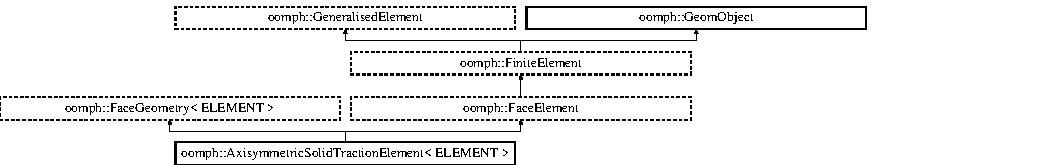
\includegraphics[height=2.215628cm]{classoomph_1_1AxisymmetricSolidTractionElement}
\end{center}
\end{figure}
\subsection*{Public Member Functions}
\begin{DoxyCompactItemize}
\item 
\hyperlink{classoomph_1_1AxisymmetricSolidTractionElement_add2978a434bca4d36ca2dc5ec0107ff9}{Axisymmetric\+Solid\+Traction\+Element} (\hyperlink{classoomph_1_1FiniteElement}{Finite\+Element} $\ast$const \&element\+\_\+pt, const int \&\hyperlink{classoomph_1_1FaceElement_a478d577ac6db67ecc80f1f02ae3ab170}{face\+\_\+index})
\begin{DoxyCompactList}\small\item\em Constructor, which takes a \char`\"{}bulk\char`\"{} element and the value of the index and its limit. \end{DoxyCompactList}\item 
void \hyperlink{classoomph_1_1AxisymmetricSolidTractionElement_a4cd8a5664e8a62263e376dd9eb9ea985}{fill\+\_\+in\+\_\+contribution\+\_\+to\+\_\+residuals} (\hyperlink{classoomph_1_1Vector}{Vector}$<$ double $>$ \&residuals)
\begin{DoxyCompactList}\small\item\em Return the residuals. \end{DoxyCompactList}\item 
void \hyperlink{classoomph_1_1AxisymmetricSolidTractionElement_a49de689d7dc2efecd8bbdbd6673c1fb8}{fill\+\_\+in\+\_\+contribution\+\_\+to\+\_\+jacobian} (\hyperlink{classoomph_1_1Vector}{Vector}$<$ double $>$ \&residuals, \hyperlink{classoomph_1_1DenseMatrix}{Dense\+Matrix}$<$ double $>$ \&jacobian)
\begin{DoxyCompactList}\small\item\em Return the jacobian. \end{DoxyCompactList}\item 
void \hyperlink{classoomph_1_1AxisymmetricSolidTractionElement_a26333e5b7fd2aabb61d21f3289797b27}{output} (std\+::ostream \&outfile)
\begin{DoxyCompactList}\small\item\em Overload the output function. \end{DoxyCompactList}\item 
void \hyperlink{classoomph_1_1AxisymmetricSolidTractionElement_a018d7c00d4eacabec5f9c30968b6bab7}{output} (std\+::ostream \&outfile, const unsigned \&n\+\_\+plot)
\begin{DoxyCompactList}\small\item\em Output function\+: x,y,\mbox{[}z\mbox{]},u,v,\mbox{[}w\mbox{]},p in tecplot format. \end{DoxyCompactList}\item 
void \hyperlink{classoomph_1_1AxisymmetricSolidTractionElement_a3f3170465a5605f057a4b4dc8201c3ca}{output} (F\+I\+LE $\ast$file\+\_\+pt)
\begin{DoxyCompactList}\small\item\em Overload the output function. \end{DoxyCompactList}\item 
void \hyperlink{classoomph_1_1AxisymmetricSolidTractionElement_ad171b0825d7e4a37d7675deaaa789058}{output} (F\+I\+LE $\ast$file\+\_\+pt, const unsigned \&n\+\_\+plot)
\begin{DoxyCompactList}\small\item\em Output function\+: x,y,\mbox{[}z\mbox{]},u,v,\mbox{[}w\mbox{]},p in tecplot format. \end{DoxyCompactList}\end{DoxyCompactItemize}
\subsection*{Public Attributes}
\begin{DoxyCompactItemize}
\item 
void($\ast$\&)(const double \&, const \hyperlink{classoomph_1_1Vector}{Vector}$<$ double $>$ \&, const \hyperlink{classoomph_1_1Vector}{Vector}$<$ double $>$ \&, \hyperlink{classoomph_1_1Vector}{Vector}$<$ double $>$ \&) \hyperlink{classoomph_1_1AxisymmetricSolidTractionElement_a437b43759687da0f3f49e0b13d1afe10}{traction\+\_\+fct\+\_\+pt} ()
\begin{DoxyCompactList}\small\item\em Return the imposed traction pointer. \end{DoxyCompactList}\end{DoxyCompactItemize}
\subsection*{Protected Member Functions}
\begin{DoxyCompactItemize}
\item 
void \hyperlink{classoomph_1_1AxisymmetricSolidTractionElement_a1386f6f1d58c17fc9357f01ddaf38742}{get\+\_\+traction} (const double \&time, const \hyperlink{classoomph_1_1Vector}{Vector}$<$ double $>$ \&x, const \hyperlink{classoomph_1_1Vector}{Vector}$<$ double $>$ \&n, \hyperlink{classoomph_1_1Vector}{Vector}$<$ double $>$ \&result) const
\begin{DoxyCompactList}\small\item\em Return the surface traction force. \end{DoxyCompactList}\end{DoxyCompactItemize}
\subsection*{Private Attributes}
\begin{DoxyCompactItemize}
\item 
void($\ast$ \hyperlink{classoomph_1_1AxisymmetricSolidTractionElement_af81e4c31c910c253faeeba17f1070000}{Traction\+\_\+fct\+\_\+pt} )(const double \&time, const \hyperlink{classoomph_1_1Vector}{Vector}$<$ double $>$ \&x, const \hyperlink{classoomph_1_1Vector}{Vector}$<$ double $>$ \&n, \hyperlink{classoomph_1_1Vector}{Vector}$<$ double $>$ \&result)
\begin{DoxyCompactList}\small\item\em Pointer to an imposed traction function. \end{DoxyCompactList}\end{DoxyCompactItemize}
\subsection*{Additional Inherited Members}


\subsection{Detailed Description}
\subsubsection*{template$<$class E\+L\+E\+M\+E\+NT$>$\newline
class oomph\+::\+Axisymmetric\+Solid\+Traction\+Element$<$ E\+L\+E\+M\+E\+N\+T $>$}

A class for elements that allow the imposition of an applied traction in the principle of virtual displacements. The geometrical information can be read from the Face\+Geometry$<$\+E\+L\+E\+M\+E\+N\+T$>$ class and and thus, we can be generic enough without the need to have a separate equations class. 

Definition at line 56 of file axisym\+\_\+solid\+\_\+traction\+\_\+elements.\+h.



\subsection{Constructor \& Destructor Documentation}
\mbox{\Hypertarget{classoomph_1_1AxisymmetricSolidTractionElement_add2978a434bca4d36ca2dc5ec0107ff9}\label{classoomph_1_1AxisymmetricSolidTractionElement_add2978a434bca4d36ca2dc5ec0107ff9}} 
\index{oomph\+::\+Axisymmetric\+Solid\+Traction\+Element@{oomph\+::\+Axisymmetric\+Solid\+Traction\+Element}!Axisymmetric\+Solid\+Traction\+Element@{Axisymmetric\+Solid\+Traction\+Element}}
\index{Axisymmetric\+Solid\+Traction\+Element@{Axisymmetric\+Solid\+Traction\+Element}!oomph\+::\+Axisymmetric\+Solid\+Traction\+Element@{oomph\+::\+Axisymmetric\+Solid\+Traction\+Element}}
\subsubsection{\texorpdfstring{Axisymmetric\+Solid\+Traction\+Element()}{AxisymmetricSolidTractionElement()}}
{\footnotesize\ttfamily template$<$class E\+L\+E\+M\+E\+NT $>$ \\
\hyperlink{classoomph_1_1AxisymmetricSolidTractionElement}{oomph\+::\+Axisymmetric\+Solid\+Traction\+Element}$<$ E\+L\+E\+M\+E\+NT $>$\+::\hyperlink{classoomph_1_1AxisymmetricSolidTractionElement}{Axisymmetric\+Solid\+Traction\+Element} (\begin{DoxyParamCaption}\item[{\hyperlink{classoomph_1_1FiniteElement}{Finite\+Element} $\ast$const \&}]{element\+\_\+pt,  }\item[{const int \&}]{face\+\_\+index }\end{DoxyParamCaption})\hspace{0.3cm}{\ttfamily [inline]}}



Constructor, which takes a \char`\"{}bulk\char`\"{} element and the value of the index and its limit. 



Definition at line 90 of file axisym\+\_\+solid\+\_\+traction\+\_\+elements.\+h.



References oomph\+::\+Finite\+Element\+::build\+\_\+face\+\_\+element(), and oomph\+::\+Axisymmetric\+Solid\+Traction\+Element$<$ E\+L\+E\+M\+E\+N\+T $>$\+::\+Traction\+\_\+fct\+\_\+pt.



\subsection{Member Function Documentation}
\mbox{\Hypertarget{classoomph_1_1AxisymmetricSolidTractionElement_a49de689d7dc2efecd8bbdbd6673c1fb8}\label{classoomph_1_1AxisymmetricSolidTractionElement_a49de689d7dc2efecd8bbdbd6673c1fb8}} 
\index{oomph\+::\+Axisymmetric\+Solid\+Traction\+Element@{oomph\+::\+Axisymmetric\+Solid\+Traction\+Element}!fill\+\_\+in\+\_\+contribution\+\_\+to\+\_\+jacobian@{fill\+\_\+in\+\_\+contribution\+\_\+to\+\_\+jacobian}}
\index{fill\+\_\+in\+\_\+contribution\+\_\+to\+\_\+jacobian@{fill\+\_\+in\+\_\+contribution\+\_\+to\+\_\+jacobian}!oomph\+::\+Axisymmetric\+Solid\+Traction\+Element@{oomph\+::\+Axisymmetric\+Solid\+Traction\+Element}}
\subsubsection{\texorpdfstring{fill\+\_\+in\+\_\+contribution\+\_\+to\+\_\+jacobian()}{fill\_in\_contribution\_to\_jacobian()}}
{\footnotesize\ttfamily template$<$class E\+L\+E\+M\+E\+NT $>$ \\
void \hyperlink{classoomph_1_1AxisymmetricSolidTractionElement}{oomph\+::\+Axisymmetric\+Solid\+Traction\+Element}$<$ E\+L\+E\+M\+E\+NT $>$\+::fill\+\_\+in\+\_\+contribution\+\_\+to\+\_\+jacobian (\begin{DoxyParamCaption}\item[{\hyperlink{classoomph_1_1Vector}{Vector}$<$ double $>$ \&}]{residuals,  }\item[{\hyperlink{classoomph_1_1DenseMatrix}{Dense\+Matrix}$<$ double $>$ \&}]{jacobian }\end{DoxyParamCaption})\hspace{0.3cm}{\ttfamily [inline]}, {\ttfamily [virtual]}}



Return the jacobian. 



Reimplemented from \hyperlink{classoomph_1_1GeneralisedElement_a6ae09fc0d68e4309ac1b03583d252845}{oomph\+::\+Generalised\+Element}.



Definition at line 111 of file axisym\+\_\+solid\+\_\+traction\+\_\+elements.\+h.



References oomph\+::\+Axisymmetric\+Solid\+Traction\+Element$<$ E\+L\+E\+M\+E\+N\+T $>$\+::fill\+\_\+in\+\_\+contribution\+\_\+to\+\_\+residuals().

\mbox{\Hypertarget{classoomph_1_1AxisymmetricSolidTractionElement_a4cd8a5664e8a62263e376dd9eb9ea985}\label{classoomph_1_1AxisymmetricSolidTractionElement_a4cd8a5664e8a62263e376dd9eb9ea985}} 
\index{oomph\+::\+Axisymmetric\+Solid\+Traction\+Element@{oomph\+::\+Axisymmetric\+Solid\+Traction\+Element}!fill\+\_\+in\+\_\+contribution\+\_\+to\+\_\+residuals@{fill\+\_\+in\+\_\+contribution\+\_\+to\+\_\+residuals}}
\index{fill\+\_\+in\+\_\+contribution\+\_\+to\+\_\+residuals@{fill\+\_\+in\+\_\+contribution\+\_\+to\+\_\+residuals}!oomph\+::\+Axisymmetric\+Solid\+Traction\+Element@{oomph\+::\+Axisymmetric\+Solid\+Traction\+Element}}
\subsubsection{\texorpdfstring{fill\+\_\+in\+\_\+contribution\+\_\+to\+\_\+residuals()}{fill\_in\_contribution\_to\_residuals()}}
{\footnotesize\ttfamily template$<$class E\+L\+E\+M\+E\+NT $>$ \\
void \hyperlink{classoomph_1_1AxisymmetricSolidTractionElement}{oomph\+::\+Axisymmetric\+Solid\+Traction\+Element}$<$ E\+L\+E\+M\+E\+NT $>$\+::fill\+\_\+in\+\_\+contribution\+\_\+to\+\_\+residuals (\begin{DoxyParamCaption}\item[{\hyperlink{classoomph_1_1Vector}{Vector}$<$ double $>$ \&}]{residuals }\end{DoxyParamCaption})\hspace{0.3cm}{\ttfamily [virtual]}}



Return the residuals. 

Return the residuals for the Axisymmetric\+Solid\+Traction\+Elements. 

Reimplemented from \hyperlink{classoomph_1_1GeneralisedElement_a310c97f515e8504a48179c0e72c550d7}{oomph\+::\+Generalised\+Element}.



Definition at line 147 of file axisym\+\_\+solid\+\_\+traction\+\_\+elements.\+h.



References oomph\+::\+Face\+Element\+::bulk\+\_\+position\+\_\+type(), oomph\+::\+Finite\+Element\+::dshape\+\_\+local\+\_\+at\+\_\+knot(), oomph\+::\+Axisymmetric\+Solid\+Traction\+Element$<$ E\+L\+E\+M\+E\+N\+T $>$\+::get\+\_\+traction(), i, oomph\+::\+Finite\+Element\+::integral\+\_\+pt(), oomph\+::\+Face\+Element\+::interpolated\+\_\+x(), oomph\+::\+Finite\+Element\+::nnodal\+\_\+position\+\_\+type(), oomph\+::\+Finite\+Element\+::nnode(), oomph\+::\+Finite\+Element\+::nodal\+\_\+position\+\_\+gen(), oomph\+::\+Face\+Element\+::normal\+\_\+sign(), oomph\+::\+Integral\+::nweight(), oomph\+::\+Quad\+Tree\+Names\+::W, and oomph\+::\+Integral\+::weight().



Referenced by oomph\+::\+Axisymmetric\+Solid\+Traction\+Element$<$ E\+L\+E\+M\+E\+N\+T $>$\+::fill\+\_\+in\+\_\+contribution\+\_\+to\+\_\+jacobian(), and oomph\+::\+Axisymmetric\+Solid\+Traction\+Element$<$ E\+L\+E\+M\+E\+N\+T $>$\+::output().

\mbox{\Hypertarget{classoomph_1_1AxisymmetricSolidTractionElement_a1386f6f1d58c17fc9357f01ddaf38742}\label{classoomph_1_1AxisymmetricSolidTractionElement_a1386f6f1d58c17fc9357f01ddaf38742}} 
\index{oomph\+::\+Axisymmetric\+Solid\+Traction\+Element@{oomph\+::\+Axisymmetric\+Solid\+Traction\+Element}!get\+\_\+traction@{get\+\_\+traction}}
\index{get\+\_\+traction@{get\+\_\+traction}!oomph\+::\+Axisymmetric\+Solid\+Traction\+Element@{oomph\+::\+Axisymmetric\+Solid\+Traction\+Element}}
\subsubsection{\texorpdfstring{get\+\_\+traction()}{get\_traction()}}
{\footnotesize\ttfamily template$<$class E\+L\+E\+M\+E\+NT $>$ \\
void \hyperlink{classoomph_1_1AxisymmetricSolidTractionElement}{oomph\+::\+Axisymmetric\+Solid\+Traction\+Element}$<$ E\+L\+E\+M\+E\+NT $>$\+::get\+\_\+traction (\begin{DoxyParamCaption}\item[{const double \&}]{time,  }\item[{const \hyperlink{classoomph_1_1Vector}{Vector}$<$ double $>$ \&}]{x,  }\item[{const \hyperlink{classoomph_1_1Vector}{Vector}$<$ double $>$ \&}]{n,  }\item[{\hyperlink{classoomph_1_1Vector}{Vector}$<$ double $>$ \&}]{result }\end{DoxyParamCaption}) const\hspace{0.3cm}{\ttfamily [inline]}, {\ttfamily [protected]}}



Return the surface traction force. 



Definition at line 69 of file axisym\+\_\+solid\+\_\+traction\+\_\+elements.\+h.



References i, and oomph\+::\+Axisymmetric\+Solid\+Traction\+Element$<$ E\+L\+E\+M\+E\+N\+T $>$\+::\+Traction\+\_\+fct\+\_\+pt.



Referenced by oomph\+::\+Axisymmetric\+Solid\+Traction\+Element$<$ E\+L\+E\+M\+E\+N\+T $>$\+::fill\+\_\+in\+\_\+contribution\+\_\+to\+\_\+residuals().

\mbox{\Hypertarget{classoomph_1_1AxisymmetricSolidTractionElement_a26333e5b7fd2aabb61d21f3289797b27}\label{classoomph_1_1AxisymmetricSolidTractionElement_a26333e5b7fd2aabb61d21f3289797b27}} 
\index{oomph\+::\+Axisymmetric\+Solid\+Traction\+Element@{oomph\+::\+Axisymmetric\+Solid\+Traction\+Element}!output@{output}}
\index{output@{output}!oomph\+::\+Axisymmetric\+Solid\+Traction\+Element@{oomph\+::\+Axisymmetric\+Solid\+Traction\+Element}}
\subsubsection{\texorpdfstring{output()}{output()}\hspace{0.1cm}{\footnotesize\ttfamily [1/4]}}
{\footnotesize\ttfamily template$<$class E\+L\+E\+M\+E\+NT $>$ \\
void \hyperlink{classoomph_1_1AxisymmetricSolidTractionElement}{oomph\+::\+Axisymmetric\+Solid\+Traction\+Element}$<$ E\+L\+E\+M\+E\+NT $>$\+::output (\begin{DoxyParamCaption}\item[{std\+::ostream \&}]{outfile }\end{DoxyParamCaption})\hspace{0.3cm}{\ttfamily [inline]}, {\ttfamily [virtual]}}



Overload the output function. 



Reimplemented from \hyperlink{classoomph_1_1FiniteElement_a2ad98a3d2ef4999f1bef62c0ff13f2a7}{oomph\+::\+Finite\+Element}.



Definition at line 120 of file axisym\+\_\+solid\+\_\+traction\+\_\+elements.\+h.



References oomph\+::\+Finite\+Element\+::output().

\mbox{\Hypertarget{classoomph_1_1AxisymmetricSolidTractionElement_a018d7c00d4eacabec5f9c30968b6bab7}\label{classoomph_1_1AxisymmetricSolidTractionElement_a018d7c00d4eacabec5f9c30968b6bab7}} 
\index{oomph\+::\+Axisymmetric\+Solid\+Traction\+Element@{oomph\+::\+Axisymmetric\+Solid\+Traction\+Element}!output@{output}}
\index{output@{output}!oomph\+::\+Axisymmetric\+Solid\+Traction\+Element@{oomph\+::\+Axisymmetric\+Solid\+Traction\+Element}}
\subsubsection{\texorpdfstring{output()}{output()}\hspace{0.1cm}{\footnotesize\ttfamily [2/4]}}
{\footnotesize\ttfamily template$<$class E\+L\+E\+M\+E\+NT $>$ \\
void \hyperlink{classoomph_1_1AxisymmetricSolidTractionElement}{oomph\+::\+Axisymmetric\+Solid\+Traction\+Element}$<$ E\+L\+E\+M\+E\+NT $>$\+::output (\begin{DoxyParamCaption}\item[{std\+::ostream \&}]{outfile,  }\item[{const unsigned \&}]{n\+\_\+plot }\end{DoxyParamCaption})\hspace{0.3cm}{\ttfamily [inline]}, {\ttfamily [virtual]}}



Output function\+: x,y,\mbox{[}z\mbox{]},u,v,\mbox{[}w\mbox{]},p in tecplot format. 



Reimplemented from \hyperlink{classoomph_1_1FiniteElement_afa9d9b2670f999b43e6679c9dd28c457}{oomph\+::\+Finite\+Element}.



Definition at line 123 of file axisym\+\_\+solid\+\_\+traction\+\_\+elements.\+h.



References oomph\+::\+Finite\+Element\+::output().

\mbox{\Hypertarget{classoomph_1_1AxisymmetricSolidTractionElement_a3f3170465a5605f057a4b4dc8201c3ca}\label{classoomph_1_1AxisymmetricSolidTractionElement_a3f3170465a5605f057a4b4dc8201c3ca}} 
\index{oomph\+::\+Axisymmetric\+Solid\+Traction\+Element@{oomph\+::\+Axisymmetric\+Solid\+Traction\+Element}!output@{output}}
\index{output@{output}!oomph\+::\+Axisymmetric\+Solid\+Traction\+Element@{oomph\+::\+Axisymmetric\+Solid\+Traction\+Element}}
\subsubsection{\texorpdfstring{output()}{output()}\hspace{0.1cm}{\footnotesize\ttfamily [3/4]}}
{\footnotesize\ttfamily template$<$class E\+L\+E\+M\+E\+NT $>$ \\
void \hyperlink{classoomph_1_1AxisymmetricSolidTractionElement}{oomph\+::\+Axisymmetric\+Solid\+Traction\+Element}$<$ E\+L\+E\+M\+E\+NT $>$\+::output (\begin{DoxyParamCaption}\item[{F\+I\+LE $\ast$}]{file\+\_\+pt }\end{DoxyParamCaption})\hspace{0.3cm}{\ttfamily [inline]}, {\ttfamily [virtual]}}



Overload the output function. 



Reimplemented from \hyperlink{classoomph_1_1FiniteElement_a72cddd09f8ddbee1a20a1ff404c6943e}{oomph\+::\+Finite\+Element}.



Definition at line 127 of file axisym\+\_\+solid\+\_\+traction\+\_\+elements.\+h.



References oomph\+::\+Finite\+Element\+::output().

\mbox{\Hypertarget{classoomph_1_1AxisymmetricSolidTractionElement_ad171b0825d7e4a37d7675deaaa789058}\label{classoomph_1_1AxisymmetricSolidTractionElement_ad171b0825d7e4a37d7675deaaa789058}} 
\index{oomph\+::\+Axisymmetric\+Solid\+Traction\+Element@{oomph\+::\+Axisymmetric\+Solid\+Traction\+Element}!output@{output}}
\index{output@{output}!oomph\+::\+Axisymmetric\+Solid\+Traction\+Element@{oomph\+::\+Axisymmetric\+Solid\+Traction\+Element}}
\subsubsection{\texorpdfstring{output()}{output()}\hspace{0.1cm}{\footnotesize\ttfamily [4/4]}}
{\footnotesize\ttfamily template$<$class E\+L\+E\+M\+E\+NT $>$ \\
void \hyperlink{classoomph_1_1AxisymmetricSolidTractionElement}{oomph\+::\+Axisymmetric\+Solid\+Traction\+Element}$<$ E\+L\+E\+M\+E\+NT $>$\+::output (\begin{DoxyParamCaption}\item[{F\+I\+LE $\ast$}]{file\+\_\+pt,  }\item[{const unsigned \&}]{n\+\_\+plot }\end{DoxyParamCaption})\hspace{0.3cm}{\ttfamily [inline]}, {\ttfamily [virtual]}}



Output function\+: x,y,\mbox{[}z\mbox{]},u,v,\mbox{[}w\mbox{]},p in tecplot format. 



Reimplemented from \hyperlink{classoomph_1_1FiniteElement_adfaee690bb0608f03320eeb9d110d48c}{oomph\+::\+Finite\+Element}.



Definition at line 130 of file axisym\+\_\+solid\+\_\+traction\+\_\+elements.\+h.



References oomph\+::\+Axisymmetric\+Solid\+Traction\+Element$<$ E\+L\+E\+M\+E\+N\+T $>$\+::fill\+\_\+in\+\_\+contribution\+\_\+to\+\_\+residuals(), and oomph\+::\+Finite\+Element\+::output().



\subsection{Member Data Documentation}
\mbox{\Hypertarget{classoomph_1_1AxisymmetricSolidTractionElement_af81e4c31c910c253faeeba17f1070000}\label{classoomph_1_1AxisymmetricSolidTractionElement_af81e4c31c910c253faeeba17f1070000}} 
\index{oomph\+::\+Axisymmetric\+Solid\+Traction\+Element@{oomph\+::\+Axisymmetric\+Solid\+Traction\+Element}!Traction\+\_\+fct\+\_\+pt@{Traction\+\_\+fct\+\_\+pt}}
\index{Traction\+\_\+fct\+\_\+pt@{Traction\+\_\+fct\+\_\+pt}!oomph\+::\+Axisymmetric\+Solid\+Traction\+Element@{oomph\+::\+Axisymmetric\+Solid\+Traction\+Element}}
\subsubsection{\texorpdfstring{Traction\+\_\+fct\+\_\+pt}{Traction\_fct\_pt}}
{\footnotesize\ttfamily template$<$class E\+L\+E\+M\+E\+NT $>$ \\
void($\ast$ \hyperlink{classoomph_1_1AxisymmetricSolidTractionElement}{oomph\+::\+Axisymmetric\+Solid\+Traction\+Element}$<$ E\+L\+E\+M\+E\+NT $>$\+::Traction\+\_\+fct\+\_\+pt) (const double \&time, const \hyperlink{classoomph_1_1Vector}{Vector}$<$ double $>$ \&x, const \hyperlink{classoomph_1_1Vector}{Vector}$<$ double $>$ \&n, \hyperlink{classoomph_1_1Vector}{Vector}$<$ double $>$ \&result)\hspace{0.3cm}{\ttfamily [private]}}



Pointer to an imposed traction function. 



Definition at line 62 of file axisym\+\_\+solid\+\_\+traction\+\_\+elements.\+h.



Referenced by oomph\+::\+Axisymmetric\+Solid\+Traction\+Element$<$ E\+L\+E\+M\+E\+N\+T $>$\+::\+Axisymmetric\+Solid\+Traction\+Element(), and oomph\+::\+Axisymmetric\+Solid\+Traction\+Element$<$ E\+L\+E\+M\+E\+N\+T $>$\+::get\+\_\+traction().

\mbox{\Hypertarget{classoomph_1_1AxisymmetricSolidTractionElement_a437b43759687da0f3f49e0b13d1afe10}\label{classoomph_1_1AxisymmetricSolidTractionElement_a437b43759687da0f3f49e0b13d1afe10}} 
\index{oomph\+::\+Axisymmetric\+Solid\+Traction\+Element@{oomph\+::\+Axisymmetric\+Solid\+Traction\+Element}!traction\+\_\+fct\+\_\+pt@{traction\+\_\+fct\+\_\+pt}}
\index{traction\+\_\+fct\+\_\+pt@{traction\+\_\+fct\+\_\+pt}!oomph\+::\+Axisymmetric\+Solid\+Traction\+Element@{oomph\+::\+Axisymmetric\+Solid\+Traction\+Element}}
\subsubsection{\texorpdfstring{traction\+\_\+fct\+\_\+pt}{traction\_fct\_pt}}
{\footnotesize\ttfamily template$<$class E\+L\+E\+M\+E\+NT $>$ \\
void($\ast$ \&)(const double\&, const \hyperlink{classoomph_1_1Vector}{Vector}$<$double$>$ \&, const \hyperlink{classoomph_1_1Vector}{Vector}$<$double$>$ \&, \hyperlink{classoomph_1_1Vector}{Vector}$<$double$>$ \&) \hyperlink{classoomph_1_1AxisymmetricSolidTractionElement}{oomph\+::\+Axisymmetric\+Solid\+Traction\+Element}$<$ E\+L\+E\+M\+E\+NT $>$\+::traction\+\_\+fct\+\_\+pt()\hspace{0.3cm}{\ttfamily [inline]}}



Return the imposed traction pointer. 



Definition at line 103 of file axisym\+\_\+solid\+\_\+traction\+\_\+elements.\+h.



The documentation for this class was generated from the following file\+:\begin{DoxyCompactItemize}
\item 
\hyperlink{axisym__solid__traction__elements_8h}{axisym\+\_\+solid\+\_\+traction\+\_\+elements.\+h}\end{DoxyCompactItemize}

\hypertarget{classoomph_1_1AxisymmetricTCrouzeixRaviartElement}{}\section{oomph\+:\+:Axisymmetric\+T\+Crouzeix\+Raviart\+Element Class Reference}
\label{classoomph_1_1AxisymmetricTCrouzeixRaviartElement}\index{oomph\+::\+Axisymmetric\+T\+Crouzeix\+Raviart\+Element@{oomph\+::\+Axisymmetric\+T\+Crouzeix\+Raviart\+Element}}


{\ttfamily \#include $<$Taxisym\+\_\+navier\+\_\+stokes\+\_\+elements.\+h$>$}

Inheritance diagram for oomph\+:\+:Axisymmetric\+T\+Crouzeix\+Raviart\+Element\+:\begin{figure}[H]
\begin{center}
\leavevmode
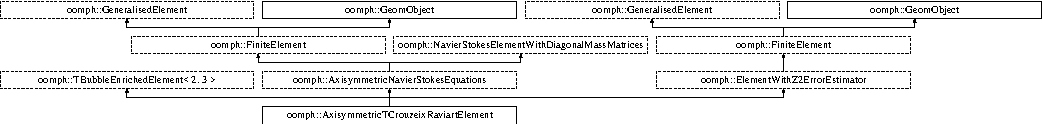
\includegraphics[height=1.671642cm]{classoomph_1_1AxisymmetricTCrouzeixRaviartElement}
\end{center}
\end{figure}
\subsection*{Public Member Functions}
\begin{DoxyCompactItemize}
\item 
void \hyperlink{classoomph_1_1AxisymmetricTCrouzeixRaviartElement_afd3664b820b924b9509f4f75eaf7420c}{pshape\+\_\+axi\+\_\+nst} (const \hyperlink{classoomph_1_1Vector}{Vector}$<$ double $>$ \&\hyperlink{cfortran_8h_ab7123126e4885ef647dd9c6e3807a21c}{s}, \hyperlink{classoomph_1_1Shape}{Shape} \&psi) const
\begin{DoxyCompactList}\small\item\em Pressure shape functions at local coordinate s. \end{DoxyCompactList}\item 
void \hyperlink{classoomph_1_1AxisymmetricTCrouzeixRaviartElement_adb45e981a3fbe7894f14264bd13e1b7f}{pshape\+\_\+axi\+\_\+nst} (const \hyperlink{classoomph_1_1Vector}{Vector}$<$ double $>$ \&\hyperlink{cfortran_8h_ab7123126e4885ef647dd9c6e3807a21c}{s}, \hyperlink{classoomph_1_1Shape}{Shape} \&psi, \hyperlink{classoomph_1_1Shape}{Shape} \&test) const
\begin{DoxyCompactList}\small\item\em Pressure shape and test functions at local coordinte s. \end{DoxyCompactList}\item 
void \hyperlink{classoomph_1_1AxisymmetricTCrouzeixRaviartElement_adddc2d573af0f1df2407870a5c59b26d}{unpin\+\_\+all\+\_\+internal\+\_\+pressure\+\_\+dofs} ()
\begin{DoxyCompactList}\small\item\em Unpin all internal pressure dofs. \end{DoxyCompactList}\item 
int \hyperlink{classoomph_1_1AxisymmetricTCrouzeixRaviartElement_af9acbebdb665021f80bf849904f52c7c}{p\+\_\+local\+\_\+eqn} (const unsigned \&n) const
\begin{DoxyCompactList}\small\item\em Return the local equation numbers for the pressure values. \end{DoxyCompactList}\item 
\hyperlink{classoomph_1_1AxisymmetricTCrouzeixRaviartElement_a0d98aaabc1f686dc26a6028c6d993dc3}{Axisymmetric\+T\+Crouzeix\+Raviart\+Element} ()
\begin{DoxyCompactList}\small\item\em Constructor, there are 3 internal values (for the pressure) \end{DoxyCompactList}\item 
\hyperlink{classoomph_1_1AxisymmetricTCrouzeixRaviartElement_abf77290ac8634231d0cbe1f2058d29ea}{Axisymmetric\+T\+Crouzeix\+Raviart\+Element} (const \hyperlink{classoomph_1_1AxisymmetricTCrouzeixRaviartElement}{Axisymmetric\+T\+Crouzeix\+Raviart\+Element} \&dummy)
\begin{DoxyCompactList}\small\item\em Broken copy constructor. \end{DoxyCompactList}\item 
virtual unsigned \hyperlink{classoomph_1_1AxisymmetricTCrouzeixRaviartElement_a2f942f09a7d541e2a2ed9f33df53b7cc}{required\+\_\+nvalue} (const unsigned \&n) const
\begin{DoxyCompactList}\small\item\em Broken assignment operator. \end{DoxyCompactList}\item 
double \hyperlink{classoomph_1_1AxisymmetricTCrouzeixRaviartElement_a50bbe7b609760f1e41ef35756ef70b31}{p\+\_\+axi\+\_\+nst} (const unsigned \&\hyperlink{cfortran_8h_adb50e893b86b3e55e751a42eab3cba82}{i}) const
\begin{DoxyCompactList}\small\item\em Return the pressure values at internal dof i\+\_\+internal (Discontinous pressure interpolation -- no need to cater for hanging nodes). \end{DoxyCompactList}\item 
unsigned \hyperlink{classoomph_1_1AxisymmetricTCrouzeixRaviartElement_a2614b5ab31a1cbac9a7f7887ce24c11a}{npres\+\_\+axi\+\_\+nst} () const
\begin{DoxyCompactList}\small\item\em Return number of pressure values. \end{DoxyCompactList}\item 
void \hyperlink{classoomph_1_1AxisymmetricTCrouzeixRaviartElement_a52bb17bda3d40b84947bf6ef14df26af}{fix\+\_\+pressure} (const unsigned \&p\+\_\+dof, const double \&p\+\_\+value)
\begin{DoxyCompactList}\small\item\em Pin p\+\_\+dof-\/th pressure dof and set it to value specified by p\+\_\+value. \end{DoxyCompactList}\item 
void \hyperlink{classoomph_1_1AxisymmetricTCrouzeixRaviartElement_a657cd924a28eea29fcba515f23c0e34c}{identify\+\_\+load\+\_\+data} (std\+::set$<$ std\+::pair$<$ \hyperlink{classoomph_1_1Data}{Data} $\ast$, unsigned $>$ $>$ \&paired\+\_\+load\+\_\+data)
\begin{DoxyCompactList}\small\item\em Build Face\+Elements that apply the Robin boundary condition to the pressure advection diffusion problem required by Fp preconditioner. \end{DoxyCompactList}\item 
void \hyperlink{classoomph_1_1AxisymmetricTCrouzeixRaviartElement_af65900dbadfec7b6e7ad2be8ef63c51c}{identify\+\_\+pressure\+\_\+data} (std\+::set$<$ std\+::pair$<$ \hyperlink{classoomph_1_1Data}{Data} $\ast$, unsigned $>$ $>$ \&paired\+\_\+pressure\+\_\+data)
\begin{DoxyCompactList}\small\item\em Add to the set {\ttfamily paired\+\_\+pressure\+\_\+data} pairs containing. \end{DoxyCompactList}\item 
void \hyperlink{classoomph_1_1AxisymmetricTCrouzeixRaviartElement_a25336476c872ea2e5c26698f44d7d35d}{output} (std\+::ostream \&outfile)
\begin{DoxyCompactList}\small\item\em Redirect output to \hyperlink{classoomph_1_1NavierStokesEquations}{Navier\+Stokes\+Equations} output. \end{DoxyCompactList}\item 
void \hyperlink{classoomph_1_1AxisymmetricTCrouzeixRaviartElement_ae59a58576380d29570f9ea326d653e5b}{output} (std\+::ostream \&outfile, const unsigned \&nplot)
\begin{DoxyCompactList}\small\item\em Redirect output to \hyperlink{classoomph_1_1NavierStokesEquations}{Navier\+Stokes\+Equations} output. \end{DoxyCompactList}\item 
void \hyperlink{classoomph_1_1AxisymmetricTCrouzeixRaviartElement_ad5cb068224ac067b234de78e67866bb6}{output} (F\+I\+LE $\ast$file\+\_\+pt)
\begin{DoxyCompactList}\small\item\em Redirect output to \hyperlink{classoomph_1_1NavierStokesEquations}{Navier\+Stokes\+Equations} output. \end{DoxyCompactList}\item 
void \hyperlink{classoomph_1_1AxisymmetricTCrouzeixRaviartElement_aeec639f7ae884f7dd7f1d33ad63ba0b2}{output} (F\+I\+LE $\ast$file\+\_\+pt, const unsigned \&n\+\_\+plot)
\begin{DoxyCompactList}\small\item\em Redirect output to \hyperlink{classoomph_1_1NavierStokesEquations}{Navier\+Stokes\+Equations} output. \end{DoxyCompactList}\item 
unsigned \hyperlink{classoomph_1_1AxisymmetricTCrouzeixRaviartElement_a9598ee410d5f554a795fb9b8a701366e}{nrecovery\+\_\+order} ()
\begin{DoxyCompactList}\small\item\em Order of recovery shape functions for Z2 error estimation\+: Same order as unenriched shape functions. \end{DoxyCompactList}\item 
unsigned \hyperlink{classoomph_1_1AxisymmetricTCrouzeixRaviartElement_a1b5e91077a94409877b887e2f455d6da}{nvertex\+\_\+node} () const
\begin{DoxyCompactList}\small\item\em Number of vertex nodes in the element. \end{DoxyCompactList}\item 
\hyperlink{classoomph_1_1Node}{Node} $\ast$ \hyperlink{classoomph_1_1AxisymmetricTCrouzeixRaviartElement_adbace360a6641c1a5e4eda618c07a9ea}{vertex\+\_\+node\+\_\+pt} (const unsigned \&j) const
\begin{DoxyCompactList}\small\item\em Pointer to the j-\/th vertex node in the element. \end{DoxyCompactList}\item 
unsigned \hyperlink{classoomph_1_1AxisymmetricTCrouzeixRaviartElement_a4f82cf46d5bea507f5dc71112d9c8781}{num\+\_\+\+Z2\+\_\+flux\+\_\+terms} ()
\begin{DoxyCompactList}\small\item\em Number of \textquotesingle{}flux\textquotesingle{} terms for Z2 error estimation. \end{DoxyCompactList}\item 
void \hyperlink{classoomph_1_1AxisymmetricTCrouzeixRaviartElement_a7b65a77278cdf24ceac3099dc29920db}{get\+\_\+\+Z2\+\_\+flux} (const \hyperlink{classoomph_1_1Vector}{Vector}$<$ double $>$ \&\hyperlink{cfortran_8h_ab7123126e4885ef647dd9c6e3807a21c}{s}, \hyperlink{classoomph_1_1Vector}{Vector}$<$ double $>$ \&flux)
\begin{DoxyCompactList}\small\item\em Get \textquotesingle{}flux\textquotesingle{} for Z2 error recovery\+: Upper triangular entries in strain rate tensor. \end{DoxyCompactList}\item 
unsigned \hyperlink{classoomph_1_1AxisymmetricTCrouzeixRaviartElement_abc543e9ea6d95d89c87f273a365f1b39}{ndof\+\_\+types} () const
\begin{DoxyCompactList}\small\item\em The number of \char`\"{}\+D\+O\+F types\char`\"{} that degrees of freedom in this element are sub-\/divided into\+: Velocity (3 components) and pressure. \end{DoxyCompactList}\item 
void \hyperlink{classoomph_1_1AxisymmetricTCrouzeixRaviartElement_adfcf1da97da7737429199f89e182fb00}{get\+\_\+dof\+\_\+numbers\+\_\+for\+\_\+unknowns} (std\+::list$<$ std\+::pair$<$ unsigned long, unsigned $>$ $>$ \&dof\+\_\+lookup\+\_\+list) const
\begin{DoxyCompactList}\small\item\em Create a list of pairs for all unknowns in this element, so that the first entry in each pair contains the global equation number of the unknown, while the second one contains the number of the \char`\"{}\+D\+O\+F type\char`\"{} that this unknown is associated with. (Function can obviously only be called if the equation numbering scheme has been set up.) \end{DoxyCompactList}\end{DoxyCompactItemize}
\subsection*{Protected Member Functions}
\begin{DoxyCompactItemize}
\item 
double \hyperlink{classoomph_1_1AxisymmetricTCrouzeixRaviartElement_a0ee2d8653afb290ec3215e976f34830d}{dshape\+\_\+and\+\_\+dtest\+\_\+eulerian\+\_\+axi\+\_\+nst} (const \hyperlink{classoomph_1_1Vector}{Vector}$<$ double $>$ \&\hyperlink{cfortran_8h_ab7123126e4885ef647dd9c6e3807a21c}{s}, \hyperlink{classoomph_1_1Shape}{Shape} \&psi, \hyperlink{classoomph_1_1DShape}{D\+Shape} \&dpsidx, \hyperlink{classoomph_1_1Shape}{Shape} \&test, \hyperlink{classoomph_1_1DShape}{D\+Shape} \&dtestdx) const
\begin{DoxyCompactList}\small\item\em Velocity shape and test functions and their derivs w.\+r.\+t. to global coords at local coordinate s (taken from geometry) Return Jacobian of mapping between local and global coordinates. \end{DoxyCompactList}\item 
double \hyperlink{classoomph_1_1AxisymmetricTCrouzeixRaviartElement_a7744f0666fd5005b65300843281efe81}{dshape\+\_\+and\+\_\+dtest\+\_\+eulerian\+\_\+at\+\_\+knot\+\_\+axi\+\_\+nst} (const unsigned \&ipt, \hyperlink{classoomph_1_1Shape}{Shape} \&psi, \hyperlink{classoomph_1_1DShape}{D\+Shape} \&dpsidx, \hyperlink{classoomph_1_1Shape}{Shape} \&test, \hyperlink{classoomph_1_1DShape}{D\+Shape} \&dtestdx) const
\begin{DoxyCompactList}\small\item\em Velocity shape and test functions and their derivs w.\+r.\+t. to global coords at ipt-\/th integation point (taken from geometry) Return Jacobian of mapping between local and global coordinates. \end{DoxyCompactList}\item 
double \hyperlink{classoomph_1_1AxisymmetricTCrouzeixRaviartElement_a63923a44d4da4e1720449521c82f1c42}{dshape\+\_\+and\+\_\+dtest\+\_\+eulerian\+\_\+at\+\_\+knot\+\_\+axi\+\_\+nst} (const unsigned \&ipt, \hyperlink{classoomph_1_1Shape}{Shape} \&psi, \hyperlink{classoomph_1_1DShape}{D\+Shape} \&dpsidx, \hyperlink{classoomph_1_1RankFourTensor}{Rank\+Four\+Tensor}$<$ double $>$ \&d\+\_\+dpsidx\+\_\+dX, \hyperlink{classoomph_1_1Shape}{Shape} \&test, \hyperlink{classoomph_1_1DShape}{D\+Shape} \&dtestdx, \hyperlink{classoomph_1_1RankFourTensor}{Rank\+Four\+Tensor}$<$ double $>$ \&d\+\_\+dtestdx\+\_\+dX, \hyperlink{classoomph_1_1DenseMatrix}{Dense\+Matrix}$<$ double $>$ \&djacobian\+\_\+dX) const
\begin{DoxyCompactList}\small\item\em Shape/test functions and derivs w.\+r.\+t. to global coords at integration point ipt; return Jacobian of mapping (J). Also compute derivatives of dpsidx, dtestdx and J w.\+r.\+t. nodal coordinates. \end{DoxyCompactList}\item 
double \hyperlink{classoomph_1_1AxisymmetricTCrouzeixRaviartElement_af257076318be5297b3e740ea42552fc5}{dpshape\+\_\+and\+\_\+dptest\+\_\+eulerian\+\_\+axi\+\_\+nst} (const \hyperlink{classoomph_1_1Vector}{Vector}$<$ double $>$ \&\hyperlink{cfortran_8h_ab7123126e4885ef647dd9c6e3807a21c}{s}, \hyperlink{classoomph_1_1Shape}{Shape} \&ppsi, \hyperlink{classoomph_1_1DShape}{D\+Shape} \&dppsidx, \hyperlink{classoomph_1_1Shape}{Shape} \&ptest, \hyperlink{classoomph_1_1DShape}{D\+Shape} \&dptestdx) const
\begin{DoxyCompactList}\small\item\em Pressure shape and test functions and their derivs w.\+r.\+t. to global coords at local coordinate s (taken from geometry) Return Jacobian of mapping between local and global coordinates. \end{DoxyCompactList}\end{DoxyCompactItemize}
\subsection*{Protected Attributes}
\begin{DoxyCompactItemize}
\item 
unsigned \hyperlink{classoomph_1_1AxisymmetricTCrouzeixRaviartElement_a05fdb096aa13072e690e30337ff91ff6}{P\+\_\+axi\+\_\+nst\+\_\+internal\+\_\+index}
\end{DoxyCompactItemize}
\subsection*{Additional Inherited Members}


\subsection{Detailed Description}
Axisymmetric\+T\+Crouzeix\+\_\+\+Raviart elements are Navier--Stokes elements with quadratic interpolation for velocities and positions enriched by a single cubic bubble function, but a discontinuous linear pressure interpolation 

Definition at line 64 of file Taxisym\+\_\+navier\+\_\+stokes\+\_\+elements.\+h.



\subsection{Constructor \& Destructor Documentation}
\mbox{\Hypertarget{classoomph_1_1AxisymmetricTCrouzeixRaviartElement_a0d98aaabc1f686dc26a6028c6d993dc3}\label{classoomph_1_1AxisymmetricTCrouzeixRaviartElement_a0d98aaabc1f686dc26a6028c6d993dc3}} 
\index{oomph\+::\+Axisymmetric\+T\+Crouzeix\+Raviart\+Element@{oomph\+::\+Axisymmetric\+T\+Crouzeix\+Raviart\+Element}!Axisymmetric\+T\+Crouzeix\+Raviart\+Element@{Axisymmetric\+T\+Crouzeix\+Raviart\+Element}}
\index{Axisymmetric\+T\+Crouzeix\+Raviart\+Element@{Axisymmetric\+T\+Crouzeix\+Raviart\+Element}!oomph\+::\+Axisymmetric\+T\+Crouzeix\+Raviart\+Element@{oomph\+::\+Axisymmetric\+T\+Crouzeix\+Raviart\+Element}}
\subsubsection{\texorpdfstring{Axisymmetric\+T\+Crouzeix\+Raviart\+Element()}{AxisymmetricTCrouzeixRaviartElement()}\hspace{0.1cm}{\footnotesize\ttfamily [1/2]}}
{\footnotesize\ttfamily oomph\+::\+Axisymmetric\+T\+Crouzeix\+Raviart\+Element\+::\+Axisymmetric\+T\+Crouzeix\+Raviart\+Element (\begin{DoxyParamCaption}{ }\end{DoxyParamCaption})\hspace{0.3cm}{\ttfamily [inline]}}



Constructor, there are 3 internal values (for the pressure) 



Definition at line 136 of file Taxisym\+\_\+navier\+\_\+stokes\+\_\+elements.\+h.



References oomph\+::\+Generalised\+Element\+::add\+\_\+internal\+\_\+data().

\mbox{\Hypertarget{classoomph_1_1AxisymmetricTCrouzeixRaviartElement_abf77290ac8634231d0cbe1f2058d29ea}\label{classoomph_1_1AxisymmetricTCrouzeixRaviartElement_abf77290ac8634231d0cbe1f2058d29ea}} 
\index{oomph\+::\+Axisymmetric\+T\+Crouzeix\+Raviart\+Element@{oomph\+::\+Axisymmetric\+T\+Crouzeix\+Raviart\+Element}!Axisymmetric\+T\+Crouzeix\+Raviart\+Element@{Axisymmetric\+T\+Crouzeix\+Raviart\+Element}}
\index{Axisymmetric\+T\+Crouzeix\+Raviart\+Element@{Axisymmetric\+T\+Crouzeix\+Raviart\+Element}!oomph\+::\+Axisymmetric\+T\+Crouzeix\+Raviart\+Element@{oomph\+::\+Axisymmetric\+T\+Crouzeix\+Raviart\+Element}}
\subsubsection{\texorpdfstring{Axisymmetric\+T\+Crouzeix\+Raviart\+Element()}{AxisymmetricTCrouzeixRaviartElement()}\hspace{0.1cm}{\footnotesize\ttfamily [2/2]}}
{\footnotesize\ttfamily oomph\+::\+Axisymmetric\+T\+Crouzeix\+Raviart\+Element\+::\+Axisymmetric\+T\+Crouzeix\+Raviart\+Element (\begin{DoxyParamCaption}\item[{const \hyperlink{classoomph_1_1AxisymmetricTCrouzeixRaviartElement}{Axisymmetric\+T\+Crouzeix\+Raviart\+Element} \&}]{dummy }\end{DoxyParamCaption})\hspace{0.3cm}{\ttfamily [inline]}}



Broken copy constructor. 



Definition at line 145 of file Taxisym\+\_\+navier\+\_\+stokes\+\_\+elements.\+h.



References oomph\+::\+Broken\+Copy\+::broken\+\_\+copy().



\subsection{Member Function Documentation}
\mbox{\Hypertarget{classoomph_1_1AxisymmetricTCrouzeixRaviartElement_af257076318be5297b3e740ea42552fc5}\label{classoomph_1_1AxisymmetricTCrouzeixRaviartElement_af257076318be5297b3e740ea42552fc5}} 
\index{oomph\+::\+Axisymmetric\+T\+Crouzeix\+Raviart\+Element@{oomph\+::\+Axisymmetric\+T\+Crouzeix\+Raviart\+Element}!dpshape\+\_\+and\+\_\+dptest\+\_\+eulerian\+\_\+axi\+\_\+nst@{dpshape\+\_\+and\+\_\+dptest\+\_\+eulerian\+\_\+axi\+\_\+nst}}
\index{dpshape\+\_\+and\+\_\+dptest\+\_\+eulerian\+\_\+axi\+\_\+nst@{dpshape\+\_\+and\+\_\+dptest\+\_\+eulerian\+\_\+axi\+\_\+nst}!oomph\+::\+Axisymmetric\+T\+Crouzeix\+Raviart\+Element@{oomph\+::\+Axisymmetric\+T\+Crouzeix\+Raviart\+Element}}
\subsubsection{\texorpdfstring{dpshape\+\_\+and\+\_\+dptest\+\_\+eulerian\+\_\+axi\+\_\+nst()}{dpshape\_and\_dptest\_eulerian\_axi\_nst()}}
{\footnotesize\ttfamily double oomph\+::\+Axisymmetric\+T\+Crouzeix\+Raviart\+Element\+::dpshape\+\_\+and\+\_\+dptest\+\_\+eulerian\+\_\+axi\+\_\+nst (\begin{DoxyParamCaption}\item[{const \hyperlink{classoomph_1_1Vector}{Vector}$<$ double $>$ \&}]{s,  }\item[{\hyperlink{classoomph_1_1Shape}{Shape} \&}]{ppsi,  }\item[{\hyperlink{classoomph_1_1DShape}{D\+Shape} \&}]{dppsidx,  }\item[{\hyperlink{classoomph_1_1Shape}{Shape} \&}]{ptest,  }\item[{\hyperlink{classoomph_1_1DShape}{D\+Shape} \&}]{dptestdx }\end{DoxyParamCaption}) const\hspace{0.3cm}{\ttfamily [inline]}, {\ttfamily [protected]}}



Pressure shape and test functions and their derivs w.\+r.\+t. to global coords at local coordinate s (taken from geometry) Return Jacobian of mapping between local and global coordinates. 

2D \+: Pressure shape and test functions and derivs w.\+r.\+t. to Eulerian coords. Return Jacobian of mapping between local and global coordinates. 

Definition at line 479 of file Taxisym\+\_\+navier\+\_\+stokes\+\_\+elements.\+h.



References oomph\+::\+Finite\+Element\+::dshape\+\_\+local(), oomph\+::\+Finite\+Element\+::local\+\_\+to\+\_\+eulerian\+\_\+mapping(), and oomph\+::\+Finite\+Element\+::transform\+\_\+derivatives().



Referenced by pshape\+\_\+axi\+\_\+nst().

\mbox{\Hypertarget{classoomph_1_1AxisymmetricTCrouzeixRaviartElement_a7744f0666fd5005b65300843281efe81}\label{classoomph_1_1AxisymmetricTCrouzeixRaviartElement_a7744f0666fd5005b65300843281efe81}} 
\index{oomph\+::\+Axisymmetric\+T\+Crouzeix\+Raviart\+Element@{oomph\+::\+Axisymmetric\+T\+Crouzeix\+Raviart\+Element}!dshape\+\_\+and\+\_\+dtest\+\_\+eulerian\+\_\+at\+\_\+knot\+\_\+axi\+\_\+nst@{dshape\+\_\+and\+\_\+dtest\+\_\+eulerian\+\_\+at\+\_\+knot\+\_\+axi\+\_\+nst}}
\index{dshape\+\_\+and\+\_\+dtest\+\_\+eulerian\+\_\+at\+\_\+knot\+\_\+axi\+\_\+nst@{dshape\+\_\+and\+\_\+dtest\+\_\+eulerian\+\_\+at\+\_\+knot\+\_\+axi\+\_\+nst}!oomph\+::\+Axisymmetric\+T\+Crouzeix\+Raviart\+Element@{oomph\+::\+Axisymmetric\+T\+Crouzeix\+Raviart\+Element}}
\subsubsection{\texorpdfstring{dshape\+\_\+and\+\_\+dtest\+\_\+eulerian\+\_\+at\+\_\+knot\+\_\+axi\+\_\+nst()}{dshape\_and\_dtest\_eulerian\_at\_knot\_axi\_nst()}\hspace{0.1cm}{\footnotesize\ttfamily [1/2]}}
{\footnotesize\ttfamily double oomph\+::\+Axisymmetric\+T\+Crouzeix\+Raviart\+Element\+::dshape\+\_\+and\+\_\+dtest\+\_\+eulerian\+\_\+at\+\_\+knot\+\_\+axi\+\_\+nst (\begin{DoxyParamCaption}\item[{const unsigned \&}]{ipt,  }\item[{\hyperlink{classoomph_1_1Shape}{Shape} \&}]{psi,  }\item[{\hyperlink{classoomph_1_1DShape}{D\+Shape} \&}]{dpsidx,  }\item[{\hyperlink{classoomph_1_1Shape}{Shape} \&}]{test,  }\item[{\hyperlink{classoomph_1_1DShape}{D\+Shape} \&}]{dtestdx }\end{DoxyParamCaption}) const\hspace{0.3cm}{\ttfamily [inline]}, {\ttfamily [protected]}, {\ttfamily [virtual]}}



Velocity shape and test functions and their derivs w.\+r.\+t. to global coords at ipt-\/th integation point (taken from geometry) Return Jacobian of mapping between local and global coordinates. 

Derivatives of the shape functions and test functions w.\+r.\+t. to global (Eulerian) coordinates. Return Jacobian of mapping between local and global coordinates. 

Implements \hyperlink{classoomph_1_1AxisymmetricNavierStokesEquations_a76e090fdac4507d10eb9f81feb53a51b}{oomph\+::\+Axisymmetric\+Navier\+Stokes\+Equations}.



Definition at line 402 of file Taxisym\+\_\+navier\+\_\+stokes\+\_\+elements.\+h.



References oomph\+::\+Finite\+Element\+::dshape\+\_\+eulerian\+\_\+at\+\_\+knot().



Referenced by dshape\+\_\+and\+\_\+dtest\+\_\+eulerian\+\_\+axi\+\_\+nst().

\mbox{\Hypertarget{classoomph_1_1AxisymmetricTCrouzeixRaviartElement_a63923a44d4da4e1720449521c82f1c42}\label{classoomph_1_1AxisymmetricTCrouzeixRaviartElement_a63923a44d4da4e1720449521c82f1c42}} 
\index{oomph\+::\+Axisymmetric\+T\+Crouzeix\+Raviart\+Element@{oomph\+::\+Axisymmetric\+T\+Crouzeix\+Raviart\+Element}!dshape\+\_\+and\+\_\+dtest\+\_\+eulerian\+\_\+at\+\_\+knot\+\_\+axi\+\_\+nst@{dshape\+\_\+and\+\_\+dtest\+\_\+eulerian\+\_\+at\+\_\+knot\+\_\+axi\+\_\+nst}}
\index{dshape\+\_\+and\+\_\+dtest\+\_\+eulerian\+\_\+at\+\_\+knot\+\_\+axi\+\_\+nst@{dshape\+\_\+and\+\_\+dtest\+\_\+eulerian\+\_\+at\+\_\+knot\+\_\+axi\+\_\+nst}!oomph\+::\+Axisymmetric\+T\+Crouzeix\+Raviart\+Element@{oomph\+::\+Axisymmetric\+T\+Crouzeix\+Raviart\+Element}}
\subsubsection{\texorpdfstring{dshape\+\_\+and\+\_\+dtest\+\_\+eulerian\+\_\+at\+\_\+knot\+\_\+axi\+\_\+nst()}{dshape\_and\_dtest\_eulerian\_at\_knot\_axi\_nst()}\hspace{0.1cm}{\footnotesize\ttfamily [2/2]}}
{\footnotesize\ttfamily double oomph\+::\+Axisymmetric\+T\+Crouzeix\+Raviart\+Element\+::dshape\+\_\+and\+\_\+dtest\+\_\+eulerian\+\_\+at\+\_\+knot\+\_\+axi\+\_\+nst (\begin{DoxyParamCaption}\item[{const unsigned \&}]{ipt,  }\item[{\hyperlink{classoomph_1_1Shape}{Shape} \&}]{psi,  }\item[{\hyperlink{classoomph_1_1DShape}{D\+Shape} \&}]{dpsidx,  }\item[{\hyperlink{classoomph_1_1RankFourTensor}{Rank\+Four\+Tensor}$<$ double $>$ \&}]{d\+\_\+dpsidx\+\_\+dX,  }\item[{\hyperlink{classoomph_1_1Shape}{Shape} \&}]{test,  }\item[{\hyperlink{classoomph_1_1DShape}{D\+Shape} \&}]{dtestdx,  }\item[{\hyperlink{classoomph_1_1RankFourTensor}{Rank\+Four\+Tensor}$<$ double $>$ \&}]{d\+\_\+dtestdx\+\_\+dX,  }\item[{\hyperlink{classoomph_1_1DenseMatrix}{Dense\+Matrix}$<$ double $>$ \&}]{djacobian\+\_\+dX }\end{DoxyParamCaption}) const\hspace{0.3cm}{\ttfamily [inline]}, {\ttfamily [protected]}, {\ttfamily [virtual]}}



Shape/test functions and derivs w.\+r.\+t. to global coords at integration point ipt; return Jacobian of mapping (J). Also compute derivatives of dpsidx, dtestdx and J w.\+r.\+t. nodal coordinates. 

Define the shape functions (psi) and test functions (test) and their derivatives w.\+r.\+t. global coordinates (dpsidx and dtestdx) and return Jacobian of mapping (J). Additionally compute the derivatives of dpsidx, dtestdx and J w.\+r.\+t. nodal coordinates.

Galerkin\+: Test functions = shape functions 

Implements \hyperlink{classoomph_1_1AxisymmetricNavierStokesEquations_a2cd0715a679af81bd0e3d7448a5560cb}{oomph\+::\+Axisymmetric\+Navier\+Stokes\+Equations}.



Definition at line 426 of file Taxisym\+\_\+navier\+\_\+stokes\+\_\+elements.\+h.



References oomph\+::\+Finite\+Element\+::dshape\+\_\+eulerian\+\_\+at\+\_\+knot().

\mbox{\Hypertarget{classoomph_1_1AxisymmetricTCrouzeixRaviartElement_a0ee2d8653afb290ec3215e976f34830d}\label{classoomph_1_1AxisymmetricTCrouzeixRaviartElement_a0ee2d8653afb290ec3215e976f34830d}} 
\index{oomph\+::\+Axisymmetric\+T\+Crouzeix\+Raviart\+Element@{oomph\+::\+Axisymmetric\+T\+Crouzeix\+Raviart\+Element}!dshape\+\_\+and\+\_\+dtest\+\_\+eulerian\+\_\+axi\+\_\+nst@{dshape\+\_\+and\+\_\+dtest\+\_\+eulerian\+\_\+axi\+\_\+nst}}
\index{dshape\+\_\+and\+\_\+dtest\+\_\+eulerian\+\_\+axi\+\_\+nst@{dshape\+\_\+and\+\_\+dtest\+\_\+eulerian\+\_\+axi\+\_\+nst}!oomph\+::\+Axisymmetric\+T\+Crouzeix\+Raviart\+Element@{oomph\+::\+Axisymmetric\+T\+Crouzeix\+Raviart\+Element}}
\subsubsection{\texorpdfstring{dshape\+\_\+and\+\_\+dtest\+\_\+eulerian\+\_\+axi\+\_\+nst()}{dshape\_and\_dtest\_eulerian\_axi\_nst()}}
{\footnotesize\ttfamily double oomph\+::\+Axisymmetric\+T\+Crouzeix\+Raviart\+Element\+::dshape\+\_\+and\+\_\+dtest\+\_\+eulerian\+\_\+axi\+\_\+nst (\begin{DoxyParamCaption}\item[{const \hyperlink{classoomph_1_1Vector}{Vector}$<$ double $>$ \&}]{s,  }\item[{\hyperlink{classoomph_1_1Shape}{Shape} \&}]{psi,  }\item[{\hyperlink{classoomph_1_1DShape}{D\+Shape} \&}]{dpsidx,  }\item[{\hyperlink{classoomph_1_1Shape}{Shape} \&}]{test,  }\item[{\hyperlink{classoomph_1_1DShape}{D\+Shape} \&}]{dtestdx }\end{DoxyParamCaption}) const\hspace{0.3cm}{\ttfamily [inline]}, {\ttfamily [protected]}, {\ttfamily [virtual]}}



Velocity shape and test functions and their derivs w.\+r.\+t. to global coords at local coordinate s (taken from geometry) Return Jacobian of mapping between local and global coordinates. 

Derivatives of the shape functions and test functions w.\+r.\+t. to global (Eulerian) coordinates. Return Jacobian of mapping between local and global coordinates. 

Implements \hyperlink{classoomph_1_1AxisymmetricNavierStokesEquations_a8d958da8ef73dcf5c68360edc9d9f565}{oomph\+::\+Axisymmetric\+Navier\+Stokes\+Equations}.



Definition at line 381 of file Taxisym\+\_\+navier\+\_\+stokes\+\_\+elements.\+h.



References dshape\+\_\+and\+\_\+dtest\+\_\+eulerian\+\_\+at\+\_\+knot\+\_\+axi\+\_\+nst(), and oomph\+::\+Finite\+Element\+::dshape\+\_\+eulerian().



Referenced by get\+\_\+dof\+\_\+numbers\+\_\+for\+\_\+unknowns().

\mbox{\Hypertarget{classoomph_1_1AxisymmetricTCrouzeixRaviartElement_a52bb17bda3d40b84947bf6ef14df26af}\label{classoomph_1_1AxisymmetricTCrouzeixRaviartElement_a52bb17bda3d40b84947bf6ef14df26af}} 
\index{oomph\+::\+Axisymmetric\+T\+Crouzeix\+Raviart\+Element@{oomph\+::\+Axisymmetric\+T\+Crouzeix\+Raviart\+Element}!fix\+\_\+pressure@{fix\+\_\+pressure}}
\index{fix\+\_\+pressure@{fix\+\_\+pressure}!oomph\+::\+Axisymmetric\+T\+Crouzeix\+Raviart\+Element@{oomph\+::\+Axisymmetric\+T\+Crouzeix\+Raviart\+Element}}
\subsubsection{\texorpdfstring{fix\+\_\+pressure()}{fix\_pressure()}}
{\footnotesize\ttfamily void oomph\+::\+Axisymmetric\+T\+Crouzeix\+Raviart\+Element\+::fix\+\_\+pressure (\begin{DoxyParamCaption}\item[{const unsigned \&}]{p\+\_\+dof,  }\item[{const double \&}]{p\+\_\+value }\end{DoxyParamCaption})\hspace{0.3cm}{\ttfamily [inline]}}



Pin p\+\_\+dof-\/th pressure dof and set it to value specified by p\+\_\+value. 



Definition at line 178 of file Taxisym\+\_\+navier\+\_\+stokes\+\_\+elements.\+h.



References identify\+\_\+load\+\_\+data(), identify\+\_\+pressure\+\_\+data(), oomph\+::\+Generalised\+Element\+::internal\+\_\+data\+\_\+pt(), oomph\+::\+Data\+::pin(), and oomph\+::\+Data\+::set\+\_\+value().

\mbox{\Hypertarget{classoomph_1_1AxisymmetricTCrouzeixRaviartElement_adfcf1da97da7737429199f89e182fb00}\label{classoomph_1_1AxisymmetricTCrouzeixRaviartElement_adfcf1da97da7737429199f89e182fb00}} 
\index{oomph\+::\+Axisymmetric\+T\+Crouzeix\+Raviart\+Element@{oomph\+::\+Axisymmetric\+T\+Crouzeix\+Raviart\+Element}!get\+\_\+dof\+\_\+numbers\+\_\+for\+\_\+unknowns@{get\+\_\+dof\+\_\+numbers\+\_\+for\+\_\+unknowns}}
\index{get\+\_\+dof\+\_\+numbers\+\_\+for\+\_\+unknowns@{get\+\_\+dof\+\_\+numbers\+\_\+for\+\_\+unknowns}!oomph\+::\+Axisymmetric\+T\+Crouzeix\+Raviart\+Element@{oomph\+::\+Axisymmetric\+T\+Crouzeix\+Raviart\+Element}}
\subsubsection{\texorpdfstring{get\+\_\+dof\+\_\+numbers\+\_\+for\+\_\+unknowns()}{get\_dof\_numbers\_for\_unknowns()}}
{\footnotesize\ttfamily void oomph\+::\+Axisymmetric\+T\+Crouzeix\+Raviart\+Element\+::get\+\_\+dof\+\_\+numbers\+\_\+for\+\_\+unknowns (\begin{DoxyParamCaption}\item[{std\+::list$<$ std\+::pair$<$ unsigned long, unsigned $>$ $>$ \&}]{dof\+\_\+lookup\+\_\+list }\end{DoxyParamCaption}) const\hspace{0.3cm}{\ttfamily [inline]}, {\ttfamily [virtual]}}



Create a list of pairs for all unknowns in this element, so that the first entry in each pair contains the global equation number of the unknown, while the second one contains the number of the \char`\"{}\+D\+O\+F type\char`\"{} that this unknown is associated with. (Function can obviously only be called if the equation numbering scheme has been set up.) 



Reimplemented from \hyperlink{classoomph_1_1GeneralisedElement_a069f59bfc3e607a5bebba52c6314d777}{oomph\+::\+Generalised\+Element}.



Definition at line 306 of file Taxisym\+\_\+navier\+\_\+stokes\+\_\+elements.\+h.



References dshape\+\_\+and\+\_\+dtest\+\_\+eulerian\+\_\+axi\+\_\+nst(), oomph\+::\+Generalised\+Element\+::eqn\+\_\+number(), oomph\+::\+Generalised\+Element\+::local\+\_\+eqn\+\_\+number(), oomph\+::\+Finite\+Element\+::nnode(), oomph\+::\+Finite\+Element\+::nodal\+\_\+local\+\_\+eqn(), oomph\+::\+Finite\+Element\+::node\+\_\+pt(), npres\+\_\+axi\+\_\+nst(), oomph\+::\+Data\+::nvalue(), and p\+\_\+local\+\_\+eqn().

\mbox{\Hypertarget{classoomph_1_1AxisymmetricTCrouzeixRaviartElement_a7b65a77278cdf24ceac3099dc29920db}\label{classoomph_1_1AxisymmetricTCrouzeixRaviartElement_a7b65a77278cdf24ceac3099dc29920db}} 
\index{oomph\+::\+Axisymmetric\+T\+Crouzeix\+Raviart\+Element@{oomph\+::\+Axisymmetric\+T\+Crouzeix\+Raviart\+Element}!get\+\_\+\+Z2\+\_\+flux@{get\+\_\+\+Z2\+\_\+flux}}
\index{get\+\_\+\+Z2\+\_\+flux@{get\+\_\+\+Z2\+\_\+flux}!oomph\+::\+Axisymmetric\+T\+Crouzeix\+Raviart\+Element@{oomph\+::\+Axisymmetric\+T\+Crouzeix\+Raviart\+Element}}
\subsubsection{\texorpdfstring{get\+\_\+\+Z2\+\_\+flux()}{get\_Z2\_flux()}}
{\footnotesize\ttfamily void oomph\+::\+Axisymmetric\+T\+Crouzeix\+Raviart\+Element\+::get\+\_\+\+Z2\+\_\+flux (\begin{DoxyParamCaption}\item[{const \hyperlink{classoomph_1_1Vector}{Vector}$<$ double $>$ \&}]{s,  }\item[{\hyperlink{classoomph_1_1Vector}{Vector}$<$ double $>$ \&}]{flux }\end{DoxyParamCaption})\hspace{0.3cm}{\ttfamily [inline]}, {\ttfamily [virtual]}}



Get \textquotesingle{}flux\textquotesingle{} for Z2 error recovery\+: Upper triangular entries in strain rate tensor. 



Implements \hyperlink{classoomph_1_1ElementWithZ2ErrorEstimator_a5688ff5f546d81771cabad82ca5a7556}{oomph\+::\+Element\+With\+Z2\+Error\+Estimator}.



Definition at line 251 of file Taxisym\+\_\+navier\+\_\+stokes\+\_\+elements.\+h.



References i, and oomph\+::\+Axisymmetric\+Navier\+Stokes\+Equations\+::strain\+\_\+rate().

\mbox{\Hypertarget{classoomph_1_1AxisymmetricTCrouzeixRaviartElement_a657cd924a28eea29fcba515f23c0e34c}\label{classoomph_1_1AxisymmetricTCrouzeixRaviartElement_a657cd924a28eea29fcba515f23c0e34c}} 
\index{oomph\+::\+Axisymmetric\+T\+Crouzeix\+Raviart\+Element@{oomph\+::\+Axisymmetric\+T\+Crouzeix\+Raviart\+Element}!identify\+\_\+load\+\_\+data@{identify\+\_\+load\+\_\+data}}
\index{identify\+\_\+load\+\_\+data@{identify\+\_\+load\+\_\+data}!oomph\+::\+Axisymmetric\+T\+Crouzeix\+Raviart\+Element@{oomph\+::\+Axisymmetric\+T\+Crouzeix\+Raviart\+Element}}
\subsubsection{\texorpdfstring{identify\+\_\+load\+\_\+data()}{identify\_load\_data()}}
{\footnotesize\ttfamily void oomph\+::\+Axisymmetric\+T\+Crouzeix\+Raviart\+Element\+::identify\+\_\+load\+\_\+data (\begin{DoxyParamCaption}\item[{std\+::set$<$ std\+::pair$<$ \hyperlink{classoomph_1_1Data}{Data} $\ast$, unsigned $>$ $>$ \&}]{paired\+\_\+load\+\_\+data }\end{DoxyParamCaption})}



Build Face\+Elements that apply the Robin boundary condition to the pressure advection diffusion problem required by Fp preconditioner. 

Add to the set paired\+\_\+load\+\_\+data pairs of pointers to data objects and unsignedegers that index the values in the data object that affect the load (traction), as specified in the get\+\_\+load() function.

Add to the set {\ttfamily paired\+\_\+load\+\_\+data} pairs containing
\begin{DoxyItemize}
\item the pointer to a \hyperlink{classoomph_1_1Data}{Data} object and
\item the index of the value in that \hyperlink{classoomph_1_1Data}{Data} object
\end{DoxyItemize}for all values (pressures, velocities) that affect the load computed in the {\ttfamily get\+\_\+load}(...) function. 

Definition at line 70 of file Taxisym\+\_\+navier\+\_\+stokes\+\_\+elements.\+cc.



References i, identify\+\_\+pressure\+\_\+data(), oomph\+::\+Finite\+Element\+::nnode(), oomph\+::\+Finite\+Element\+::node\+\_\+pt(), and oomph\+::\+Axisymmetric\+Navier\+Stokes\+Equations\+::u\+\_\+index\+\_\+axi\+\_\+nst().



Referenced by fix\+\_\+pressure(), oomph\+::\+Axisymmetric\+T\+Taylor\+Hood\+Element\+::fix\+\_\+pressure(), and unpin\+\_\+all\+\_\+internal\+\_\+pressure\+\_\+dofs().

\mbox{\Hypertarget{classoomph_1_1AxisymmetricTCrouzeixRaviartElement_af65900dbadfec7b6e7ad2be8ef63c51c}\label{classoomph_1_1AxisymmetricTCrouzeixRaviartElement_af65900dbadfec7b6e7ad2be8ef63c51c}} 
\index{oomph\+::\+Axisymmetric\+T\+Crouzeix\+Raviart\+Element@{oomph\+::\+Axisymmetric\+T\+Crouzeix\+Raviart\+Element}!identify\+\_\+pressure\+\_\+data@{identify\+\_\+pressure\+\_\+data}}
\index{identify\+\_\+pressure\+\_\+data@{identify\+\_\+pressure\+\_\+data}!oomph\+::\+Axisymmetric\+T\+Crouzeix\+Raviart\+Element@{oomph\+::\+Axisymmetric\+T\+Crouzeix\+Raviart\+Element}}
\subsubsection{\texorpdfstring{identify\+\_\+pressure\+\_\+data()}{identify\_pressure\_data()}}
{\footnotesize\ttfamily void oomph\+::\+Axisymmetric\+T\+Crouzeix\+Raviart\+Element\+::identify\+\_\+pressure\+\_\+data (\begin{DoxyParamCaption}\item[{std\+::set$<$ std\+::pair$<$ \hyperlink{classoomph_1_1Data}{Data} $\ast$, unsigned $>$ $>$ \&}]{paired\+\_\+pressure\+\_\+data }\end{DoxyParamCaption})}



Add to the set {\ttfamily paired\+\_\+pressure\+\_\+data} pairs containing. 


\begin{DoxyItemize}
\item the pointer to a \hyperlink{classoomph_1_1Data}{Data} object and
\item the index of the value in that \hyperlink{classoomph_1_1Data}{Data} object
\end{DoxyItemize}for all pressure values that affect the load computed in the {\ttfamily get\+\_\+load}(...) function.

Add to the set {\ttfamily paired\+\_\+pressue\+\_\+data} pairs containing
\begin{DoxyItemize}
\item the pointer to a \hyperlink{classoomph_1_1Data}{Data} object and
\item the index of the value in that \hyperlink{classoomph_1_1Data}{Data} object
\end{DoxyItemize}for all pressures values that affect the load computed in the {\ttfamily get\+\_\+load}(...) function. 

Definition at line 103 of file Taxisym\+\_\+navier\+\_\+stokes\+\_\+elements.\+cc.



References oomph\+::\+Axisymmetric\+T\+Taylor\+Hood\+Element\+::\+Initial\+\_\+\+Nvalue, oomph\+::\+Generalised\+Element\+::internal\+\_\+data\+\_\+pt(), oomph\+::\+Generalised\+Element\+::ninternal\+\_\+data(), oomph\+::\+Data\+::nvalue(), and oomph\+::\+Axisymmetric\+T\+Taylor\+Hood\+Element\+::\+Pconv.



Referenced by fix\+\_\+pressure(), oomph\+::\+Axisymmetric\+T\+Taylor\+Hood\+Element\+::fix\+\_\+pressure(), identify\+\_\+load\+\_\+data(), and oomph\+::\+Axisymmetric\+T\+Taylor\+Hood\+Element\+::identify\+\_\+load\+\_\+data().

\mbox{\Hypertarget{classoomph_1_1AxisymmetricTCrouzeixRaviartElement_abc543e9ea6d95d89c87f273a365f1b39}\label{classoomph_1_1AxisymmetricTCrouzeixRaviartElement_abc543e9ea6d95d89c87f273a365f1b39}} 
\index{oomph\+::\+Axisymmetric\+T\+Crouzeix\+Raviart\+Element@{oomph\+::\+Axisymmetric\+T\+Crouzeix\+Raviart\+Element}!ndof\+\_\+types@{ndof\+\_\+types}}
\index{ndof\+\_\+types@{ndof\+\_\+types}!oomph\+::\+Axisymmetric\+T\+Crouzeix\+Raviart\+Element@{oomph\+::\+Axisymmetric\+T\+Crouzeix\+Raviart\+Element}}
\subsubsection{\texorpdfstring{ndof\+\_\+types()}{ndof\_types()}}
{\footnotesize\ttfamily unsigned oomph\+::\+Axisymmetric\+T\+Crouzeix\+Raviart\+Element\+::ndof\+\_\+types (\begin{DoxyParamCaption}{ }\end{DoxyParamCaption}) const\hspace{0.3cm}{\ttfamily [inline]}, {\ttfamily [virtual]}}



The number of \char`\"{}\+D\+O\+F types\char`\"{} that degrees of freedom in this element are sub-\/divided into\+: Velocity (3 components) and pressure. 



Reimplemented from \hyperlink{classoomph_1_1GeneralisedElement_a0c6037a870597b35dcf1c780710b9a56}{oomph\+::\+Generalised\+Element}.



Definition at line 295 of file Taxisym\+\_\+navier\+\_\+stokes\+\_\+elements.\+h.

\mbox{\Hypertarget{classoomph_1_1AxisymmetricTCrouzeixRaviartElement_a2614b5ab31a1cbac9a7f7887ce24c11a}\label{classoomph_1_1AxisymmetricTCrouzeixRaviartElement_a2614b5ab31a1cbac9a7f7887ce24c11a}} 
\index{oomph\+::\+Axisymmetric\+T\+Crouzeix\+Raviart\+Element@{oomph\+::\+Axisymmetric\+T\+Crouzeix\+Raviart\+Element}!npres\+\_\+axi\+\_\+nst@{npres\+\_\+axi\+\_\+nst}}
\index{npres\+\_\+axi\+\_\+nst@{npres\+\_\+axi\+\_\+nst}!oomph\+::\+Axisymmetric\+T\+Crouzeix\+Raviart\+Element@{oomph\+::\+Axisymmetric\+T\+Crouzeix\+Raviart\+Element}}
\subsubsection{\texorpdfstring{npres\+\_\+axi\+\_\+nst()}{npres\_axi\_nst()}}
{\footnotesize\ttfamily unsigned oomph\+::\+Axisymmetric\+T\+Crouzeix\+Raviart\+Element\+::npres\+\_\+axi\+\_\+nst (\begin{DoxyParamCaption}{ }\end{DoxyParamCaption}) const\hspace{0.3cm}{\ttfamily [inline]}, {\ttfamily [virtual]}}



Return number of pressure values. 



Implements \hyperlink{classoomph_1_1AxisymmetricNavierStokesEquations_a89edaffb4913131cc14a5f6e45ed117a}{oomph\+::\+Axisymmetric\+Navier\+Stokes\+Equations}.



Definition at line 175 of file Taxisym\+\_\+navier\+\_\+stokes\+\_\+elements.\+h.



Referenced by get\+\_\+dof\+\_\+numbers\+\_\+for\+\_\+unknowns(), oomph\+::\+Axisymmetric\+T\+Taylor\+Hood\+Element\+::identify\+\_\+pressure\+\_\+data(), unpin\+\_\+all\+\_\+internal\+\_\+pressure\+\_\+dofs(), and oomph\+::\+Axisymmetric\+T\+Taylor\+Hood\+Element\+::unpin\+\_\+proper\+\_\+nodal\+\_\+pressure\+\_\+dofs().

\mbox{\Hypertarget{classoomph_1_1AxisymmetricTCrouzeixRaviartElement_a9598ee410d5f554a795fb9b8a701366e}\label{classoomph_1_1AxisymmetricTCrouzeixRaviartElement_a9598ee410d5f554a795fb9b8a701366e}} 
\index{oomph\+::\+Axisymmetric\+T\+Crouzeix\+Raviart\+Element@{oomph\+::\+Axisymmetric\+T\+Crouzeix\+Raviart\+Element}!nrecovery\+\_\+order@{nrecovery\+\_\+order}}
\index{nrecovery\+\_\+order@{nrecovery\+\_\+order}!oomph\+::\+Axisymmetric\+T\+Crouzeix\+Raviart\+Element@{oomph\+::\+Axisymmetric\+T\+Crouzeix\+Raviart\+Element}}
\subsubsection{\texorpdfstring{nrecovery\+\_\+order()}{nrecovery\_order()}}
{\footnotesize\ttfamily unsigned oomph\+::\+Axisymmetric\+T\+Crouzeix\+Raviart\+Element\+::nrecovery\+\_\+order (\begin{DoxyParamCaption}{ }\end{DoxyParamCaption})\hspace{0.3cm}{\ttfamily [inline]}, {\ttfamily [virtual]}}



Order of recovery shape functions for Z2 error estimation\+: Same order as unenriched shape functions. 



Implements \hyperlink{classoomph_1_1ElementWithZ2ErrorEstimator_af39480835bd3e0f6b2f4f7a9a4044798}{oomph\+::\+Element\+With\+Z2\+Error\+Estimator}.



Definition at line 232 of file Taxisym\+\_\+navier\+\_\+stokes\+\_\+elements.\+h.

\mbox{\Hypertarget{classoomph_1_1AxisymmetricTCrouzeixRaviartElement_a4f82cf46d5bea507f5dc71112d9c8781}\label{classoomph_1_1AxisymmetricTCrouzeixRaviartElement_a4f82cf46d5bea507f5dc71112d9c8781}} 
\index{oomph\+::\+Axisymmetric\+T\+Crouzeix\+Raviart\+Element@{oomph\+::\+Axisymmetric\+T\+Crouzeix\+Raviart\+Element}!num\+\_\+\+Z2\+\_\+flux\+\_\+terms@{num\+\_\+\+Z2\+\_\+flux\+\_\+terms}}
\index{num\+\_\+\+Z2\+\_\+flux\+\_\+terms@{num\+\_\+\+Z2\+\_\+flux\+\_\+terms}!oomph\+::\+Axisymmetric\+T\+Crouzeix\+Raviart\+Element@{oomph\+::\+Axisymmetric\+T\+Crouzeix\+Raviart\+Element}}
\subsubsection{\texorpdfstring{num\+\_\+\+Z2\+\_\+flux\+\_\+terms()}{num\_Z2\_flux\_terms()}}
{\footnotesize\ttfamily unsigned oomph\+::\+Axisymmetric\+T\+Crouzeix\+Raviart\+Element\+::num\+\_\+\+Z2\+\_\+flux\+\_\+terms (\begin{DoxyParamCaption}{ }\end{DoxyParamCaption})\hspace{0.3cm}{\ttfamily [inline]}, {\ttfamily [virtual]}}



Number of \textquotesingle{}flux\textquotesingle{} terms for Z2 error estimation. 



Implements \hyperlink{classoomph_1_1ElementWithZ2ErrorEstimator_ae82c5728902e13da31be19c390fc28e3}{oomph\+::\+Element\+With\+Z2\+Error\+Estimator}.



Definition at line 243 of file Taxisym\+\_\+navier\+\_\+stokes\+\_\+elements.\+h.

\mbox{\Hypertarget{classoomph_1_1AxisymmetricTCrouzeixRaviartElement_a1b5e91077a94409877b887e2f455d6da}\label{classoomph_1_1AxisymmetricTCrouzeixRaviartElement_a1b5e91077a94409877b887e2f455d6da}} 
\index{oomph\+::\+Axisymmetric\+T\+Crouzeix\+Raviart\+Element@{oomph\+::\+Axisymmetric\+T\+Crouzeix\+Raviart\+Element}!nvertex\+\_\+node@{nvertex\+\_\+node}}
\index{nvertex\+\_\+node@{nvertex\+\_\+node}!oomph\+::\+Axisymmetric\+T\+Crouzeix\+Raviart\+Element@{oomph\+::\+Axisymmetric\+T\+Crouzeix\+Raviart\+Element}}
\subsubsection{\texorpdfstring{nvertex\+\_\+node()}{nvertex\_node()}}
{\footnotesize\ttfamily unsigned oomph\+::\+Axisymmetric\+T\+Crouzeix\+Raviart\+Element\+::nvertex\+\_\+node (\begin{DoxyParamCaption}{ }\end{DoxyParamCaption}) const\hspace{0.3cm}{\ttfamily [inline]}, {\ttfamily [virtual]}}



Number of vertex nodes in the element. 



Implements \hyperlink{classoomph_1_1ElementWithZ2ErrorEstimator_a19495a0e77ef4ff35f15fdf7913b4077}{oomph\+::\+Element\+With\+Z2\+Error\+Estimator}.



Definition at line 235 of file Taxisym\+\_\+navier\+\_\+stokes\+\_\+elements.\+h.

\mbox{\Hypertarget{classoomph_1_1AxisymmetricTCrouzeixRaviartElement_a25336476c872ea2e5c26698f44d7d35d}\label{classoomph_1_1AxisymmetricTCrouzeixRaviartElement_a25336476c872ea2e5c26698f44d7d35d}} 
\index{oomph\+::\+Axisymmetric\+T\+Crouzeix\+Raviart\+Element@{oomph\+::\+Axisymmetric\+T\+Crouzeix\+Raviart\+Element}!output@{output}}
\index{output@{output}!oomph\+::\+Axisymmetric\+T\+Crouzeix\+Raviart\+Element@{oomph\+::\+Axisymmetric\+T\+Crouzeix\+Raviart\+Element}}
\subsubsection{\texorpdfstring{output()}{output()}\hspace{0.1cm}{\footnotesize\ttfamily [1/4]}}
{\footnotesize\ttfamily void oomph\+::\+Axisymmetric\+T\+Crouzeix\+Raviart\+Element\+::output (\begin{DoxyParamCaption}\item[{std\+::ostream \&}]{outfile }\end{DoxyParamCaption})\hspace{0.3cm}{\ttfamily [inline]}, {\ttfamily [virtual]}}



Redirect output to \hyperlink{classoomph_1_1NavierStokesEquations}{Navier\+Stokes\+Equations} output. 



Reimplemented from \hyperlink{classoomph_1_1AxisymmetricNavierStokesEquations_afe0c7b607ec3fd03a73b7db4f1fe6252}{oomph\+::\+Axisymmetric\+Navier\+Stokes\+Equations}.



Definition at line 214 of file Taxisym\+\_\+navier\+\_\+stokes\+\_\+elements.\+h.



References oomph\+::\+Axisymmetric\+Navier\+Stokes\+Equations\+::output().

\mbox{\Hypertarget{classoomph_1_1AxisymmetricTCrouzeixRaviartElement_ae59a58576380d29570f9ea326d653e5b}\label{classoomph_1_1AxisymmetricTCrouzeixRaviartElement_ae59a58576380d29570f9ea326d653e5b}} 
\index{oomph\+::\+Axisymmetric\+T\+Crouzeix\+Raviart\+Element@{oomph\+::\+Axisymmetric\+T\+Crouzeix\+Raviart\+Element}!output@{output}}
\index{output@{output}!oomph\+::\+Axisymmetric\+T\+Crouzeix\+Raviart\+Element@{oomph\+::\+Axisymmetric\+T\+Crouzeix\+Raviart\+Element}}
\subsubsection{\texorpdfstring{output()}{output()}\hspace{0.1cm}{\footnotesize\ttfamily [2/4]}}
{\footnotesize\ttfamily void oomph\+::\+Axisymmetric\+T\+Crouzeix\+Raviart\+Element\+::output (\begin{DoxyParamCaption}\item[{std\+::ostream \&}]{outfile,  }\item[{const unsigned \&}]{nplot }\end{DoxyParamCaption})\hspace{0.3cm}{\ttfamily [inline]}, {\ttfamily [virtual]}}



Redirect output to \hyperlink{classoomph_1_1NavierStokesEquations}{Navier\+Stokes\+Equations} output. 



Reimplemented from \hyperlink{classoomph_1_1AxisymmetricNavierStokesEquations_a94a243ca05ba3b995e366564e6cf7695}{oomph\+::\+Axisymmetric\+Navier\+Stokes\+Equations}.



Definition at line 218 of file Taxisym\+\_\+navier\+\_\+stokes\+\_\+elements.\+h.



References oomph\+::\+Axisymmetric\+Navier\+Stokes\+Equations\+::output().

\mbox{\Hypertarget{classoomph_1_1AxisymmetricTCrouzeixRaviartElement_ad5cb068224ac067b234de78e67866bb6}\label{classoomph_1_1AxisymmetricTCrouzeixRaviartElement_ad5cb068224ac067b234de78e67866bb6}} 
\index{oomph\+::\+Axisymmetric\+T\+Crouzeix\+Raviart\+Element@{oomph\+::\+Axisymmetric\+T\+Crouzeix\+Raviart\+Element}!output@{output}}
\index{output@{output}!oomph\+::\+Axisymmetric\+T\+Crouzeix\+Raviart\+Element@{oomph\+::\+Axisymmetric\+T\+Crouzeix\+Raviart\+Element}}
\subsubsection{\texorpdfstring{output()}{output()}\hspace{0.1cm}{\footnotesize\ttfamily [3/4]}}
{\footnotesize\ttfamily void oomph\+::\+Axisymmetric\+T\+Crouzeix\+Raviart\+Element\+::output (\begin{DoxyParamCaption}\item[{F\+I\+LE $\ast$}]{file\+\_\+pt }\end{DoxyParamCaption})\hspace{0.3cm}{\ttfamily [inline]}, {\ttfamily [virtual]}}



Redirect output to \hyperlink{classoomph_1_1NavierStokesEquations}{Navier\+Stokes\+Equations} output. 



Reimplemented from \hyperlink{classoomph_1_1AxisymmetricNavierStokesEquations_a61129dd7505ac363862946bd8b3ea5bf}{oomph\+::\+Axisymmetric\+Navier\+Stokes\+Equations}.



Definition at line 222 of file Taxisym\+\_\+navier\+\_\+stokes\+\_\+elements.\+h.



References oomph\+::\+Axisymmetric\+Navier\+Stokes\+Equations\+::output().

\mbox{\Hypertarget{classoomph_1_1AxisymmetricTCrouzeixRaviartElement_aeec639f7ae884f7dd7f1d33ad63ba0b2}\label{classoomph_1_1AxisymmetricTCrouzeixRaviartElement_aeec639f7ae884f7dd7f1d33ad63ba0b2}} 
\index{oomph\+::\+Axisymmetric\+T\+Crouzeix\+Raviart\+Element@{oomph\+::\+Axisymmetric\+T\+Crouzeix\+Raviart\+Element}!output@{output}}
\index{output@{output}!oomph\+::\+Axisymmetric\+T\+Crouzeix\+Raviart\+Element@{oomph\+::\+Axisymmetric\+T\+Crouzeix\+Raviart\+Element}}
\subsubsection{\texorpdfstring{output()}{output()}\hspace{0.1cm}{\footnotesize\ttfamily [4/4]}}
{\footnotesize\ttfamily void oomph\+::\+Axisymmetric\+T\+Crouzeix\+Raviart\+Element\+::output (\begin{DoxyParamCaption}\item[{F\+I\+LE $\ast$}]{file\+\_\+pt,  }\item[{const unsigned \&}]{n\+\_\+plot }\end{DoxyParamCaption})\hspace{0.3cm}{\ttfamily [inline]}, {\ttfamily [virtual]}}



Redirect output to \hyperlink{classoomph_1_1NavierStokesEquations}{Navier\+Stokes\+Equations} output. 



Reimplemented from \hyperlink{classoomph_1_1AxisymmetricNavierStokesEquations_abc2ca00250845e243da3f4e0845b2c96}{oomph\+::\+Axisymmetric\+Navier\+Stokes\+Equations}.



Definition at line 226 of file Taxisym\+\_\+navier\+\_\+stokes\+\_\+elements.\+h.



References oomph\+::\+Axisymmetric\+Navier\+Stokes\+Equations\+::output().

\mbox{\Hypertarget{classoomph_1_1AxisymmetricTCrouzeixRaviartElement_a50bbe7b609760f1e41ef35756ef70b31}\label{classoomph_1_1AxisymmetricTCrouzeixRaviartElement_a50bbe7b609760f1e41ef35756ef70b31}} 
\index{oomph\+::\+Axisymmetric\+T\+Crouzeix\+Raviart\+Element@{oomph\+::\+Axisymmetric\+T\+Crouzeix\+Raviart\+Element}!p\+\_\+axi\+\_\+nst@{p\+\_\+axi\+\_\+nst}}
\index{p\+\_\+axi\+\_\+nst@{p\+\_\+axi\+\_\+nst}!oomph\+::\+Axisymmetric\+T\+Crouzeix\+Raviart\+Element@{oomph\+::\+Axisymmetric\+T\+Crouzeix\+Raviart\+Element}}
\subsubsection{\texorpdfstring{p\+\_\+axi\+\_\+nst()}{p\_axi\_nst()}}
{\footnotesize\ttfamily double oomph\+::\+Axisymmetric\+T\+Crouzeix\+Raviart\+Element\+::p\+\_\+axi\+\_\+nst (\begin{DoxyParamCaption}\item[{const unsigned \&}]{i }\end{DoxyParamCaption}) const\hspace{0.3cm}{\ttfamily [inline]}, {\ttfamily [virtual]}}



Return the pressure values at internal dof i\+\_\+internal (Discontinous pressure interpolation -- no need to cater for hanging nodes). 



Implements \hyperlink{classoomph_1_1AxisymmetricNavierStokesEquations_a3aa173227f477a40fb4adba84a337f5b}{oomph\+::\+Axisymmetric\+Navier\+Stokes\+Equations}.



Definition at line 171 of file Taxisym\+\_\+navier\+\_\+stokes\+\_\+elements.\+h.



References oomph\+::\+Generalised\+Element\+::internal\+\_\+data\+\_\+pt(), and oomph\+::\+Data\+::value().

\mbox{\Hypertarget{classoomph_1_1AxisymmetricTCrouzeixRaviartElement_af9acbebdb665021f80bf849904f52c7c}\label{classoomph_1_1AxisymmetricTCrouzeixRaviartElement_af9acbebdb665021f80bf849904f52c7c}} 
\index{oomph\+::\+Axisymmetric\+T\+Crouzeix\+Raviart\+Element@{oomph\+::\+Axisymmetric\+T\+Crouzeix\+Raviart\+Element}!p\+\_\+local\+\_\+eqn@{p\+\_\+local\+\_\+eqn}}
\index{p\+\_\+local\+\_\+eqn@{p\+\_\+local\+\_\+eqn}!oomph\+::\+Axisymmetric\+T\+Crouzeix\+Raviart\+Element@{oomph\+::\+Axisymmetric\+T\+Crouzeix\+Raviart\+Element}}
\subsubsection{\texorpdfstring{p\+\_\+local\+\_\+eqn()}{p\_local\_eqn()}}
{\footnotesize\ttfamily int oomph\+::\+Axisymmetric\+T\+Crouzeix\+Raviart\+Element\+::p\+\_\+local\+\_\+eqn (\begin{DoxyParamCaption}\item[{const unsigned \&}]{n }\end{DoxyParamCaption}) const\hspace{0.3cm}{\ttfamily [inline]}, {\ttfamily [virtual]}}



Return the local equation numbers for the pressure values. 



Implements \hyperlink{classoomph_1_1AxisymmetricNavierStokesEquations_ad6ac62ca5fa411c365fd2ecc72aa25e8}{oomph\+::\+Axisymmetric\+Navier\+Stokes\+Equations}.



Definition at line 130 of file Taxisym\+\_\+navier\+\_\+stokes\+\_\+elements.\+h.



References oomph\+::\+Generalised\+Element\+::internal\+\_\+local\+\_\+eqn().



Referenced by get\+\_\+dof\+\_\+numbers\+\_\+for\+\_\+unknowns().

\mbox{\Hypertarget{classoomph_1_1AxisymmetricTCrouzeixRaviartElement_afd3664b820b924b9509f4f75eaf7420c}\label{classoomph_1_1AxisymmetricTCrouzeixRaviartElement_afd3664b820b924b9509f4f75eaf7420c}} 
\index{oomph\+::\+Axisymmetric\+T\+Crouzeix\+Raviart\+Element@{oomph\+::\+Axisymmetric\+T\+Crouzeix\+Raviart\+Element}!pshape\+\_\+axi\+\_\+nst@{pshape\+\_\+axi\+\_\+nst}}
\index{pshape\+\_\+axi\+\_\+nst@{pshape\+\_\+axi\+\_\+nst}!oomph\+::\+Axisymmetric\+T\+Crouzeix\+Raviart\+Element@{oomph\+::\+Axisymmetric\+T\+Crouzeix\+Raviart\+Element}}
\subsubsection{\texorpdfstring{pshape\+\_\+axi\+\_\+nst()}{pshape\_axi\_nst()}\hspace{0.1cm}{\footnotesize\ttfamily [1/2]}}
{\footnotesize\ttfamily void oomph\+::\+Axisymmetric\+T\+Crouzeix\+Raviart\+Element\+::pshape\+\_\+axi\+\_\+nst (\begin{DoxyParamCaption}\item[{const \hyperlink{classoomph_1_1Vector}{Vector}$<$ double $>$ \&}]{s,  }\item[{\hyperlink{classoomph_1_1Shape}{Shape} \&}]{psi }\end{DoxyParamCaption}) const\hspace{0.3cm}{\ttfamily [inline]}, {\ttfamily [virtual]}}



Pressure shape functions at local coordinate s. 

Pressure shape functions. 

Implements \hyperlink{classoomph_1_1AxisymmetricNavierStokesEquations_a6309780fd1964c4df0cca0818ccff158}{oomph\+::\+Axisymmetric\+Navier\+Stokes\+Equations}.



Definition at line 450 of file Taxisym\+\_\+navier\+\_\+stokes\+\_\+elements.\+h.



Referenced by pshape\+\_\+axi\+\_\+nst(), oomph\+::\+Axisymmetric\+T\+Taylor\+Hood\+Element\+::pshape\+\_\+axi\+\_\+nst(), and oomph\+::\+Axisymmetric\+T\+Taylor\+Hood\+Element\+::required\+\_\+nvalue().

\mbox{\Hypertarget{classoomph_1_1AxisymmetricTCrouzeixRaviartElement_adb45e981a3fbe7894f14264bd13e1b7f}\label{classoomph_1_1AxisymmetricTCrouzeixRaviartElement_adb45e981a3fbe7894f14264bd13e1b7f}} 
\index{oomph\+::\+Axisymmetric\+T\+Crouzeix\+Raviart\+Element@{oomph\+::\+Axisymmetric\+T\+Crouzeix\+Raviart\+Element}!pshape\+\_\+axi\+\_\+nst@{pshape\+\_\+axi\+\_\+nst}}
\index{pshape\+\_\+axi\+\_\+nst@{pshape\+\_\+axi\+\_\+nst}!oomph\+::\+Axisymmetric\+T\+Crouzeix\+Raviart\+Element@{oomph\+::\+Axisymmetric\+T\+Crouzeix\+Raviart\+Element}}
\subsubsection{\texorpdfstring{pshape\+\_\+axi\+\_\+nst()}{pshape\_axi\_nst()}\hspace{0.1cm}{\footnotesize\ttfamily [2/2]}}
{\footnotesize\ttfamily void oomph\+::\+Axisymmetric\+T\+Crouzeix\+Raviart\+Element\+::pshape\+\_\+axi\+\_\+nst (\begin{DoxyParamCaption}\item[{const \hyperlink{classoomph_1_1Vector}{Vector}$<$ double $>$ \&}]{s,  }\item[{\hyperlink{classoomph_1_1Shape}{Shape} \&}]{psi,  }\item[{\hyperlink{classoomph_1_1Shape}{Shape} \&}]{test }\end{DoxyParamCaption}) const\hspace{0.3cm}{\ttfamily [inline]}, {\ttfamily [virtual]}}



Pressure shape and test functions at local coordinte s. 

Pressure shape and test functions. 

Implements \hyperlink{classoomph_1_1AxisymmetricNavierStokesEquations_a19a4135581356bf368a7ecae2b315f85}{oomph\+::\+Axisymmetric\+Navier\+Stokes\+Equations}.



Definition at line 462 of file Taxisym\+\_\+navier\+\_\+stokes\+\_\+elements.\+h.



References dpshape\+\_\+and\+\_\+dptest\+\_\+eulerian\+\_\+axi\+\_\+nst(), and pshape\+\_\+axi\+\_\+nst().

\mbox{\Hypertarget{classoomph_1_1AxisymmetricTCrouzeixRaviartElement_a2f942f09a7d541e2a2ed9f33df53b7cc}\label{classoomph_1_1AxisymmetricTCrouzeixRaviartElement_a2f942f09a7d541e2a2ed9f33df53b7cc}} 
\index{oomph\+::\+Axisymmetric\+T\+Crouzeix\+Raviart\+Element@{oomph\+::\+Axisymmetric\+T\+Crouzeix\+Raviart\+Element}!required\+\_\+nvalue@{required\+\_\+nvalue}}
\index{required\+\_\+nvalue@{required\+\_\+nvalue}!oomph\+::\+Axisymmetric\+T\+Crouzeix\+Raviart\+Element@{oomph\+::\+Axisymmetric\+T\+Crouzeix\+Raviart\+Element}}
\subsubsection{\texorpdfstring{required\+\_\+nvalue()}{required\_nvalue()}}
{\footnotesize\ttfamily virtual unsigned oomph\+::\+Axisymmetric\+T\+Crouzeix\+Raviart\+Element\+::required\+\_\+nvalue (\begin{DoxyParamCaption}\item[{const unsigned \&}]{n }\end{DoxyParamCaption}) const\hspace{0.3cm}{\ttfamily [inline]}, {\ttfamily [virtual]}}



Broken assignment operator. 

Number of values (pinned or dofs) required at local node n. 

Reimplemented from \hyperlink{classoomph_1_1FiniteElement_a56610c60d5bc2d7c27407a1455471b1a}{oomph\+::\+Finite\+Element}.



Definition at line 164 of file Taxisym\+\_\+navier\+\_\+stokes\+\_\+elements.\+h.



Referenced by oomph\+::\+Axisymmetric\+T\+Taylor\+Hood\+Element\+::get\+\_\+dof\+\_\+numbers\+\_\+for\+\_\+unknowns().

\mbox{\Hypertarget{classoomph_1_1AxisymmetricTCrouzeixRaviartElement_adddc2d573af0f1df2407870a5c59b26d}\label{classoomph_1_1AxisymmetricTCrouzeixRaviartElement_adddc2d573af0f1df2407870a5c59b26d}} 
\index{oomph\+::\+Axisymmetric\+T\+Crouzeix\+Raviart\+Element@{oomph\+::\+Axisymmetric\+T\+Crouzeix\+Raviart\+Element}!unpin\+\_\+all\+\_\+internal\+\_\+pressure\+\_\+dofs@{unpin\+\_\+all\+\_\+internal\+\_\+pressure\+\_\+dofs}}
\index{unpin\+\_\+all\+\_\+internal\+\_\+pressure\+\_\+dofs@{unpin\+\_\+all\+\_\+internal\+\_\+pressure\+\_\+dofs}!oomph\+::\+Axisymmetric\+T\+Crouzeix\+Raviart\+Element@{oomph\+::\+Axisymmetric\+T\+Crouzeix\+Raviart\+Element}}
\subsubsection{\texorpdfstring{unpin\+\_\+all\+\_\+internal\+\_\+pressure\+\_\+dofs()}{unpin\_all\_internal\_pressure\_dofs()}}
{\footnotesize\ttfamily void oomph\+::\+Axisymmetric\+T\+Crouzeix\+Raviart\+Element\+::unpin\+\_\+all\+\_\+internal\+\_\+pressure\+\_\+dofs (\begin{DoxyParamCaption}{ }\end{DoxyParamCaption})}



Unpin all internal pressure dofs. 



Definition at line 48 of file Taxisym\+\_\+navier\+\_\+stokes\+\_\+elements.\+cc.



References identify\+\_\+load\+\_\+data(), oomph\+::\+Generalised\+Element\+::internal\+\_\+data\+\_\+pt(), npres\+\_\+axi\+\_\+nst(), P\+\_\+axi\+\_\+nst\+\_\+internal\+\_\+index, and oomph\+::\+Data\+::unpin().

\mbox{\Hypertarget{classoomph_1_1AxisymmetricTCrouzeixRaviartElement_adbace360a6641c1a5e4eda618c07a9ea}\label{classoomph_1_1AxisymmetricTCrouzeixRaviartElement_adbace360a6641c1a5e4eda618c07a9ea}} 
\index{oomph\+::\+Axisymmetric\+T\+Crouzeix\+Raviart\+Element@{oomph\+::\+Axisymmetric\+T\+Crouzeix\+Raviart\+Element}!vertex\+\_\+node\+\_\+pt@{vertex\+\_\+node\+\_\+pt}}
\index{vertex\+\_\+node\+\_\+pt@{vertex\+\_\+node\+\_\+pt}!oomph\+::\+Axisymmetric\+T\+Crouzeix\+Raviart\+Element@{oomph\+::\+Axisymmetric\+T\+Crouzeix\+Raviart\+Element}}
\subsubsection{\texorpdfstring{vertex\+\_\+node\+\_\+pt()}{vertex\_node\_pt()}}
{\footnotesize\ttfamily \hyperlink{classoomph_1_1Node}{Node}$\ast$ oomph\+::\+Axisymmetric\+T\+Crouzeix\+Raviart\+Element\+::vertex\+\_\+node\+\_\+pt (\begin{DoxyParamCaption}\item[{const unsigned \&}]{j }\end{DoxyParamCaption}) const\hspace{0.3cm}{\ttfamily [inline]}, {\ttfamily [virtual]}}



Pointer to the j-\/th vertex node in the element. 



Implements \hyperlink{classoomph_1_1ElementWithZ2ErrorEstimator_a0eedccc33519f852c5dc2055ddf2774b}{oomph\+::\+Element\+With\+Z2\+Error\+Estimator}.



Definition at line 239 of file Taxisym\+\_\+navier\+\_\+stokes\+\_\+elements.\+h.



References oomph\+::\+Finite\+Element\+::node\+\_\+pt().



\subsection{Member Data Documentation}
\mbox{\Hypertarget{classoomph_1_1AxisymmetricTCrouzeixRaviartElement_a05fdb096aa13072e690e30337ff91ff6}\label{classoomph_1_1AxisymmetricTCrouzeixRaviartElement_a05fdb096aa13072e690e30337ff91ff6}} 
\index{oomph\+::\+Axisymmetric\+T\+Crouzeix\+Raviart\+Element@{oomph\+::\+Axisymmetric\+T\+Crouzeix\+Raviart\+Element}!P\+\_\+axi\+\_\+nst\+\_\+internal\+\_\+index@{P\+\_\+axi\+\_\+nst\+\_\+internal\+\_\+index}}
\index{P\+\_\+axi\+\_\+nst\+\_\+internal\+\_\+index@{P\+\_\+axi\+\_\+nst\+\_\+internal\+\_\+index}!oomph\+::\+Axisymmetric\+T\+Crouzeix\+Raviart\+Element@{oomph\+::\+Axisymmetric\+T\+Crouzeix\+Raviart\+Element}}
\subsubsection{\texorpdfstring{P\+\_\+axi\+\_\+nst\+\_\+internal\+\_\+index}{P\_axi\_nst\_internal\_index}}
{\footnotesize\ttfamily unsigned oomph\+::\+Axisymmetric\+T\+Crouzeix\+Raviart\+Element\+::\+P\+\_\+axi\+\_\+nst\+\_\+internal\+\_\+index\hspace{0.3cm}{\ttfamily [protected]}}

Internal index that indicates at which internal datum the pressure is stored 

Definition at line 74 of file Taxisym\+\_\+navier\+\_\+stokes\+\_\+elements.\+h.



Referenced by unpin\+\_\+all\+\_\+internal\+\_\+pressure\+\_\+dofs().



The documentation for this class was generated from the following files\+:\begin{DoxyCompactItemize}
\item 
\hyperlink{Taxisym__navier__stokes__elements_8h}{Taxisym\+\_\+navier\+\_\+stokes\+\_\+elements.\+h}\item 
\hyperlink{Taxisym__navier__stokes__elements_8cc}{Taxisym\+\_\+navier\+\_\+stokes\+\_\+elements.\+cc}\end{DoxyCompactItemize}

\hypertarget{classoomph_1_1AxisymmetricTTaylorHoodElement}{}\section{oomph\+:\+:Axisymmetric\+T\+Taylor\+Hood\+Element Class Reference}
\label{classoomph_1_1AxisymmetricTTaylorHoodElement}\index{oomph\+::\+Axisymmetric\+T\+Taylor\+Hood\+Element@{oomph\+::\+Axisymmetric\+T\+Taylor\+Hood\+Element}}


{\ttfamily \#include $<$Taxisym\+\_\+navier\+\_\+stokes\+\_\+elements.\+h$>$}

Inheritance diagram for oomph\+:\+:Axisymmetric\+T\+Taylor\+Hood\+Element\+:\begin{figure}[H]
\begin{center}
\leavevmode
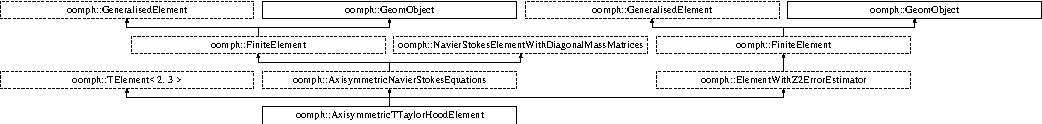
\includegraphics[height=1.671642cm]{classoomph_1_1AxisymmetricTTaylorHoodElement}
\end{center}
\end{figure}
\subsection*{Public Member Functions}
\begin{DoxyCompactItemize}
\item 
\hyperlink{classoomph_1_1AxisymmetricTTaylorHoodElement_a0c37daf4d618fad20746a0df0bc0d150}{Axisymmetric\+T\+Taylor\+Hood\+Element} ()
\begin{DoxyCompactList}\small\item\em Constructor, no internal data points. \end{DoxyCompactList}\item 
\hyperlink{classoomph_1_1AxisymmetricTTaylorHoodElement_a629d1c0d1397f3804f99f97119dd6289}{Axisymmetric\+T\+Taylor\+Hood\+Element} (const \hyperlink{classoomph_1_1AxisymmetricTTaylorHoodElement}{Axisymmetric\+T\+Taylor\+Hood\+Element} \&dummy)
\begin{DoxyCompactList}\small\item\em Broken copy constructor. \end{DoxyCompactList}\item 
virtual unsigned \hyperlink{classoomph_1_1AxisymmetricTTaylorHoodElement_a6a5dd6b252f98c37d896a3d6f35d3688}{required\+\_\+nvalue} (const unsigned \&n) const
\begin{DoxyCompactList}\small\item\em Broken assignment operator. \end{DoxyCompactList}\item 
void \hyperlink{classoomph_1_1AxisymmetricTTaylorHoodElement_a9a52e3c13681e0ad373b330a0934b7a1}{pshape\+\_\+axi\+\_\+nst} (const \hyperlink{classoomph_1_1Vector}{Vector}$<$ double $>$ \&\hyperlink{cfortran_8h_ab7123126e4885ef647dd9c6e3807a21c}{s}, \hyperlink{classoomph_1_1Shape}{Shape} \&psi) const
\begin{DoxyCompactList}\small\item\em Test whether the pressure dof p\+\_\+dof hanging or not? \end{DoxyCompactList}\item 
void \hyperlink{classoomph_1_1AxisymmetricTTaylorHoodElement_acaeacbb982949d5f9c6b3afec8b98de9}{pshape\+\_\+axi\+\_\+nst} (const \hyperlink{classoomph_1_1Vector}{Vector}$<$ double $>$ \&\hyperlink{cfortran_8h_ab7123126e4885ef647dd9c6e3807a21c}{s}, \hyperlink{classoomph_1_1Shape}{Shape} \&psi, \hyperlink{classoomph_1_1Shape}{Shape} \&test) const
\begin{DoxyCompactList}\small\item\em Pressure shape and test functions at local coordinte s. \end{DoxyCompactList}\item 
unsigned \hyperlink{classoomph_1_1AxisymmetricTTaylorHoodElement_a353b5dbb889246ccc9cce5265951ada3}{p\+\_\+index\+\_\+axi\+\_\+nst} ()
\begin{DoxyCompactList}\small\item\em Which nodal value represents the pressure? \end{DoxyCompactList}\item 
int \hyperlink{classoomph_1_1AxisymmetricTTaylorHoodElement_a69d3da303d873ab134ec3e382fc919c0}{p\+\_\+local\+\_\+eqn} (const unsigned \&n) const
\begin{DoxyCompactList}\small\item\em Pointer to n\+\_\+p-\/th pressure node. \end{DoxyCompactList}\item 
double \hyperlink{classoomph_1_1AxisymmetricTTaylorHoodElement_ab08a53f82fad2eee4a016d3ebaba0a0a}{p\+\_\+axi\+\_\+nst} (const unsigned \&n\+\_\+p) const
\begin{DoxyCompactList}\small\item\em Access function for the pressure values at local pressure node n\+\_\+p (const version) \end{DoxyCompactList}\item 
int \hyperlink{classoomph_1_1AxisymmetricTTaylorHoodElement_a27deacb53ba98601b20dd06d9c812520}{p\+\_\+nodal\+\_\+index\+\_\+axi\+\_\+nst} () const
\begin{DoxyCompactList}\small\item\em Set the value at which the pressure is stored in the nodes. \end{DoxyCompactList}\item 
unsigned \hyperlink{classoomph_1_1AxisymmetricTTaylorHoodElement_a39217f9f550c3488f8f660ae861a61a7}{npres\+\_\+axi\+\_\+nst} () const
\begin{DoxyCompactList}\small\item\em Return number of pressure values. \end{DoxyCompactList}\item 
void \hyperlink{classoomph_1_1AxisymmetricTTaylorHoodElement_a8ae1c5e864429c8c08e7776a5851d042}{fix\+\_\+pressure} (const unsigned \&p\+\_\+dof, const double \&p\+\_\+value)
\begin{DoxyCompactList}\small\item\em Pin p\+\_\+dof-\/th pressure dof and set it to value specified by p\+\_\+value. \end{DoxyCompactList}\item 
void \hyperlink{classoomph_1_1AxisymmetricTTaylorHoodElement_a47a7f3c25a3e5c960510111418d13bbd}{identify\+\_\+load\+\_\+data} (std\+::set$<$ std\+::pair$<$ \hyperlink{classoomph_1_1Data}{Data} $\ast$, unsigned $>$ $>$ \&paired\+\_\+load\+\_\+data)
\begin{DoxyCompactList}\small\item\em Build Face\+Elements that apply the Robin boundary condition to the pressure advection diffusion problem required by Fp preconditioner. \end{DoxyCompactList}\item 
void \hyperlink{classoomph_1_1AxisymmetricTTaylorHoodElement_a20b2bcc3563aaa264601603a0d3b3604}{identify\+\_\+pressure\+\_\+data} (std\+::set$<$ std\+::pair$<$ \hyperlink{classoomph_1_1Data}{Data} $\ast$, unsigned $>$ $>$ \&paired\+\_\+pressure\+\_\+data)
\begin{DoxyCompactList}\small\item\em Add to the set {\ttfamily paired\+\_\+pressure\+\_\+data} pairs containing. \end{DoxyCompactList}\item 
void \hyperlink{classoomph_1_1AxisymmetricTTaylorHoodElement_a538cd24096fa521e0dac0f1f78ce5446}{output} (std\+::ostream \&outfile)
\begin{DoxyCompactList}\small\item\em Redirect output to \hyperlink{classoomph_1_1NavierStokesEquations}{Navier\+Stokes\+Equations} output. \end{DoxyCompactList}\item 
void \hyperlink{classoomph_1_1AxisymmetricTTaylorHoodElement_a10ec676703edbf68120256082aa8c290}{output} (std\+::ostream \&outfile, const unsigned \&nplot)
\begin{DoxyCompactList}\small\item\em Redirect output to \hyperlink{classoomph_1_1NavierStokesEquations}{Navier\+Stokes\+Equations} output. \end{DoxyCompactList}\item 
void \hyperlink{classoomph_1_1AxisymmetricTTaylorHoodElement_a0b1f01968fd84b28009339e5e478a683}{output} (F\+I\+LE $\ast$file\+\_\+pt)
\begin{DoxyCompactList}\small\item\em Redirect output to \hyperlink{classoomph_1_1NavierStokesEquations}{Navier\+Stokes\+Equations} output. \end{DoxyCompactList}\item 
void \hyperlink{classoomph_1_1AxisymmetricTTaylorHoodElement_abc6435ee0ad7a9235b1fc57451f1872c}{output} (F\+I\+LE $\ast$file\+\_\+pt, const unsigned \&n\+\_\+plot)
\begin{DoxyCompactList}\small\item\em Redirect output to \hyperlink{classoomph_1_1NavierStokesEquations}{Navier\+Stokes\+Equations} output. \end{DoxyCompactList}\item 
unsigned \hyperlink{classoomph_1_1AxisymmetricTTaylorHoodElement_a2cd7e8c1aafe58b6cc36eef0b201b9f2}{nrecovery\+\_\+order} ()
\begin{DoxyCompactList}\small\item\em Order of recovery shape functions for Z2 error estimation\+: Same order as shape functions. \end{DoxyCompactList}\item 
unsigned \hyperlink{classoomph_1_1AxisymmetricTTaylorHoodElement_a2a8cccdcdfd71e3c5f4c4ce07189442c}{nvertex\+\_\+node} () const
\begin{DoxyCompactList}\small\item\em Number of vertex nodes in the element. \end{DoxyCompactList}\item 
\hyperlink{classoomph_1_1Node}{Node} $\ast$ \hyperlink{classoomph_1_1AxisymmetricTTaylorHoodElement_a44d3195ac5946d8ea71ea5fe98120605}{vertex\+\_\+node\+\_\+pt} (const unsigned \&j) const
\begin{DoxyCompactList}\small\item\em Pointer to the j-\/th vertex node in the element. \end{DoxyCompactList}\item 
unsigned \hyperlink{classoomph_1_1AxisymmetricTTaylorHoodElement_ae84ae5860bbfdd54a5f8224f3b0caf46}{num\+\_\+\+Z2\+\_\+flux\+\_\+terms} ()
\begin{DoxyCompactList}\small\item\em Number of \textquotesingle{}flux\textquotesingle{} terms for Z2 error estimation. \end{DoxyCompactList}\item 
void \hyperlink{classoomph_1_1AxisymmetricTTaylorHoodElement_ac7cab08cebeb16771206d55497bde22a}{get\+\_\+\+Z2\+\_\+flux} (const \hyperlink{classoomph_1_1Vector}{Vector}$<$ double $>$ \&\hyperlink{cfortran_8h_ab7123126e4885ef647dd9c6e3807a21c}{s}, \hyperlink{classoomph_1_1Vector}{Vector}$<$ double $>$ \&flux)
\begin{DoxyCompactList}\small\item\em Get \textquotesingle{}flux\textquotesingle{} for Z2 error recovery\+: Upper triangular entries in strain rate tensor. \end{DoxyCompactList}\item 
unsigned \hyperlink{classoomph_1_1AxisymmetricTTaylorHoodElement_a5b492d4fc80759934938bd4c296f9237}{ndof\+\_\+types} () const
\begin{DoxyCompactList}\small\item\em The number of \char`\"{}\+D\+O\+F types\char`\"{} that degrees of freedom in this element are sub-\/divided into\+: Velocities (3 components) and pressure. \end{DoxyCompactList}\item 
void \hyperlink{classoomph_1_1AxisymmetricTTaylorHoodElement_a3f1f37c74e194ae5770d9928c9a0e409}{get\+\_\+dof\+\_\+numbers\+\_\+for\+\_\+unknowns} (std\+::list$<$ std\+::pair$<$ unsigned long, unsigned $>$ $>$ \&dof\+\_\+lookup\+\_\+list) const
\begin{DoxyCompactList}\small\item\em Create a list of pairs for all unknowns in this element, so that the first entry in each pair contains the global equation number of the unknown, while the second one contains the number of the \char`\"{}\+D\+O\+F type\char`\"{} that this unknown is associated with. (Function can obviously only be called if the equation numbering scheme has been set up.) \end{DoxyCompactList}\end{DoxyCompactItemize}
\subsection*{Protected Member Functions}
\begin{DoxyCompactItemize}
\item 
double \hyperlink{classoomph_1_1AxisymmetricTTaylorHoodElement_ae5d9f04db6805c64a9c1f6d5ba68c3a4}{dshape\+\_\+and\+\_\+dtest\+\_\+eulerian\+\_\+axi\+\_\+nst} (const \hyperlink{classoomph_1_1Vector}{Vector}$<$ double $>$ \&\hyperlink{cfortran_8h_ab7123126e4885ef647dd9c6e3807a21c}{s}, \hyperlink{classoomph_1_1Shape}{Shape} \&psi, \hyperlink{classoomph_1_1DShape}{D\+Shape} \&dpsidx, \hyperlink{classoomph_1_1Shape}{Shape} \&test, \hyperlink{classoomph_1_1DShape}{D\+Shape} \&dtestdx) const
\begin{DoxyCompactList}\small\item\em Velocity shape and test functions and their derivs w.\+r.\+t. to global coords at local coordinate s (taken from geometry) Return Jacobian of mapping between local and global coordinates. \end{DoxyCompactList}\item 
double \hyperlink{classoomph_1_1AxisymmetricTTaylorHoodElement_a1a696cb60dd4f10db4e6d5a8b4571a7d}{dshape\+\_\+and\+\_\+dtest\+\_\+eulerian\+\_\+at\+\_\+knot\+\_\+axi\+\_\+nst} (const unsigned \&ipt, \hyperlink{classoomph_1_1Shape}{Shape} \&psi, \hyperlink{classoomph_1_1DShape}{D\+Shape} \&dpsidx, \hyperlink{classoomph_1_1Shape}{Shape} \&test, \hyperlink{classoomph_1_1DShape}{D\+Shape} \&dtestdx) const
\begin{DoxyCompactList}\small\item\em Velocity shape and test functions and their derivs w.\+r.\+t. to global coords at local coordinate s (taken from geometry) Return Jacobian of mapping between local and global coordinates. \end{DoxyCompactList}\item 
double \hyperlink{classoomph_1_1AxisymmetricTTaylorHoodElement_a6bfdf91d1ce67542d27bee00ab026a20}{dshape\+\_\+and\+\_\+dtest\+\_\+eulerian\+\_\+at\+\_\+knot\+\_\+axi\+\_\+nst} (const unsigned \&ipt, \hyperlink{classoomph_1_1Shape}{Shape} \&psi, \hyperlink{classoomph_1_1DShape}{D\+Shape} \&dpsidx, \hyperlink{classoomph_1_1RankFourTensor}{Rank\+Four\+Tensor}$<$ double $>$ \&d\+\_\+dpsidx\+\_\+dX, \hyperlink{classoomph_1_1Shape}{Shape} \&test, \hyperlink{classoomph_1_1DShape}{D\+Shape} \&dtestdx, \hyperlink{classoomph_1_1RankFourTensor}{Rank\+Four\+Tensor}$<$ double $>$ \&d\+\_\+dtestdx\+\_\+dX, \hyperlink{classoomph_1_1DenseMatrix}{Dense\+Matrix}$<$ double $>$ \&djacobian\+\_\+dX) const
\begin{DoxyCompactList}\small\item\em Shape/test functions and derivs w.\+r.\+t. to global coords at integration point ipt; return Jacobian of mapping (J). Also compute derivatives of dpsidx, dtestdx and J w.\+r.\+t. nodal coordinates. \end{DoxyCompactList}\item 
virtual double \hyperlink{classoomph_1_1AxisymmetricTTaylorHoodElement_a97c4e14f4e7af5728c55b145d946a1fb}{dpshape\+\_\+and\+\_\+dptest\+\_\+eulerian\+\_\+axi\+\_\+nst} (const \hyperlink{classoomph_1_1Vector}{Vector}$<$ double $>$ \&\hyperlink{cfortran_8h_ab7123126e4885ef647dd9c6e3807a21c}{s}, \hyperlink{classoomph_1_1Shape}{Shape} \&ppsi, \hyperlink{classoomph_1_1DShape}{D\+Shape} \&dppsidx, \hyperlink{classoomph_1_1Shape}{Shape} \&ptest, \hyperlink{classoomph_1_1DShape}{D\+Shape} \&dptestdx) const
\begin{DoxyCompactList}\small\item\em Compute the pressure shape and test functions and derivatives w.\+r.\+t. global coords at local coordinate s. Return Jacobian of mapping between local and global coordinates. \end{DoxyCompactList}\item 
void \hyperlink{classoomph_1_1AxisymmetricTTaylorHoodElement_a008b24e28c97a15ccc634ce6fa76a0c2}{unpin\+\_\+all\+\_\+nodal\+\_\+pressure\+\_\+dofs} ()
\begin{DoxyCompactList}\small\item\em Unpin all pressure dofs. \end{DoxyCompactList}\item 
void \hyperlink{classoomph_1_1AxisymmetricTTaylorHoodElement_ab340da6c7f125bba62b3234993890cd0}{pin\+\_\+all\+\_\+nodal\+\_\+pressure\+\_\+dofs} ()
\begin{DoxyCompactList}\small\item\em Pin all nodal pressure dofs. \end{DoxyCompactList}\item 
void \hyperlink{classoomph_1_1AxisymmetricTTaylorHoodElement_abf71bcb109d1e5ee51b621f9287cd486}{unpin\+\_\+proper\+\_\+nodal\+\_\+pressure\+\_\+dofs} ()
\begin{DoxyCompactList}\small\item\em Unpin the proper nodal pressure dofs. \end{DoxyCompactList}\end{DoxyCompactItemize}
\subsection*{Static Protected Attributes}
\begin{DoxyCompactItemize}
\item 
static const unsigned \hyperlink{classoomph_1_1AxisymmetricTTaylorHoodElement_a0aeec7081602d00fd711fd9d0b2022b9}{Pconv} \mbox{[}$\,$\mbox{]} =\{0,1,2\}
\begin{DoxyCompactList}\small\item\em Static array of ints to hold conversion from pressure node numbers to actual node numbers. \end{DoxyCompactList}\end{DoxyCompactItemize}
\subsection*{Static Private Attributes}
\begin{DoxyCompactItemize}
\item 
static const unsigned \hyperlink{classoomph_1_1AxisymmetricTTaylorHoodElement_aa99c5de016b430db779ef2fc830a7f9a}{Initial\+\_\+\+Nvalue} \mbox{[}$\,$\mbox{]} =\{4,4,4,3,3,3\}
\begin{DoxyCompactList}\small\item\em Static array of ints to hold number of variables at node. \end{DoxyCompactList}\end{DoxyCompactItemize}
\subsection*{Additional Inherited Members}


\subsection{Detailed Description}
Taylor--Hood elements are Navier--Stokes elements with quadratic interpolation for velocities and positions and continous linear pressure interpolation 

Definition at line 560 of file Taxisym\+\_\+navier\+\_\+stokes\+\_\+elements.\+h.



\subsection{Constructor \& Destructor Documentation}
\mbox{\Hypertarget{classoomph_1_1AxisymmetricTTaylorHoodElement_a0c37daf4d618fad20746a0df0bc0d150}\label{classoomph_1_1AxisymmetricTTaylorHoodElement_a0c37daf4d618fad20746a0df0bc0d150}} 
\index{oomph\+::\+Axisymmetric\+T\+Taylor\+Hood\+Element@{oomph\+::\+Axisymmetric\+T\+Taylor\+Hood\+Element}!Axisymmetric\+T\+Taylor\+Hood\+Element@{Axisymmetric\+T\+Taylor\+Hood\+Element}}
\index{Axisymmetric\+T\+Taylor\+Hood\+Element@{Axisymmetric\+T\+Taylor\+Hood\+Element}!oomph\+::\+Axisymmetric\+T\+Taylor\+Hood\+Element@{oomph\+::\+Axisymmetric\+T\+Taylor\+Hood\+Element}}
\subsubsection{\texorpdfstring{Axisymmetric\+T\+Taylor\+Hood\+Element()}{AxisymmetricTTaylorHoodElement()}\hspace{0.1cm}{\footnotesize\ttfamily [1/2]}}
{\footnotesize\ttfamily oomph\+::\+Axisymmetric\+T\+Taylor\+Hood\+Element\+::\+Axisymmetric\+T\+Taylor\+Hood\+Element (\begin{DoxyParamCaption}{ }\end{DoxyParamCaption})\hspace{0.3cm}{\ttfamily [inline]}}



Constructor, no internal data points. 



Definition at line 630 of file Taxisym\+\_\+navier\+\_\+stokes\+\_\+elements.\+h.

\mbox{\Hypertarget{classoomph_1_1AxisymmetricTTaylorHoodElement_a629d1c0d1397f3804f99f97119dd6289}\label{classoomph_1_1AxisymmetricTTaylorHoodElement_a629d1c0d1397f3804f99f97119dd6289}} 
\index{oomph\+::\+Axisymmetric\+T\+Taylor\+Hood\+Element@{oomph\+::\+Axisymmetric\+T\+Taylor\+Hood\+Element}!Axisymmetric\+T\+Taylor\+Hood\+Element@{Axisymmetric\+T\+Taylor\+Hood\+Element}}
\index{Axisymmetric\+T\+Taylor\+Hood\+Element@{Axisymmetric\+T\+Taylor\+Hood\+Element}!oomph\+::\+Axisymmetric\+T\+Taylor\+Hood\+Element@{oomph\+::\+Axisymmetric\+T\+Taylor\+Hood\+Element}}
\subsubsection{\texorpdfstring{Axisymmetric\+T\+Taylor\+Hood\+Element()}{AxisymmetricTTaylorHoodElement()}\hspace{0.1cm}{\footnotesize\ttfamily [2/2]}}
{\footnotesize\ttfamily oomph\+::\+Axisymmetric\+T\+Taylor\+Hood\+Element\+::\+Axisymmetric\+T\+Taylor\+Hood\+Element (\begin{DoxyParamCaption}\item[{const \hyperlink{classoomph_1_1AxisymmetricTTaylorHoodElement}{Axisymmetric\+T\+Taylor\+Hood\+Element} \&}]{dummy }\end{DoxyParamCaption})\hspace{0.3cm}{\ttfamily [inline]}}



Broken copy constructor. 



Definition at line 635 of file Taxisym\+\_\+navier\+\_\+stokes\+\_\+elements.\+h.



References oomph\+::\+Broken\+Copy\+::broken\+\_\+copy().



\subsection{Member Function Documentation}
\mbox{\Hypertarget{classoomph_1_1AxisymmetricTTaylorHoodElement_a97c4e14f4e7af5728c55b145d946a1fb}\label{classoomph_1_1AxisymmetricTTaylorHoodElement_a97c4e14f4e7af5728c55b145d946a1fb}} 
\index{oomph\+::\+Axisymmetric\+T\+Taylor\+Hood\+Element@{oomph\+::\+Axisymmetric\+T\+Taylor\+Hood\+Element}!dpshape\+\_\+and\+\_\+dptest\+\_\+eulerian\+\_\+axi\+\_\+nst@{dpshape\+\_\+and\+\_\+dptest\+\_\+eulerian\+\_\+axi\+\_\+nst}}
\index{dpshape\+\_\+and\+\_\+dptest\+\_\+eulerian\+\_\+axi\+\_\+nst@{dpshape\+\_\+and\+\_\+dptest\+\_\+eulerian\+\_\+axi\+\_\+nst}!oomph\+::\+Axisymmetric\+T\+Taylor\+Hood\+Element@{oomph\+::\+Axisymmetric\+T\+Taylor\+Hood\+Element}}
\subsubsection{\texorpdfstring{dpshape\+\_\+and\+\_\+dptest\+\_\+eulerian\+\_\+axi\+\_\+nst()}{dpshape\_and\_dptest\_eulerian\_axi\_nst()}}
{\footnotesize\ttfamily double oomph\+::\+Axisymmetric\+T\+Taylor\+Hood\+Element\+::dpshape\+\_\+and\+\_\+dptest\+\_\+eulerian\+\_\+axi\+\_\+nst (\begin{DoxyParamCaption}\item[{const \hyperlink{classoomph_1_1Vector}{Vector}$<$ double $>$ \&}]{s,  }\item[{\hyperlink{classoomph_1_1Shape}{Shape} \&}]{ppsi,  }\item[{\hyperlink{classoomph_1_1DShape}{D\+Shape} \&}]{dppsidx,  }\item[{\hyperlink{classoomph_1_1Shape}{Shape} \&}]{ptest,  }\item[{\hyperlink{classoomph_1_1DShape}{D\+Shape} \&}]{dptestdx }\end{DoxyParamCaption}) const\hspace{0.3cm}{\ttfamily [inline]}, {\ttfamily [protected]}, {\ttfamily [virtual]}}



Compute the pressure shape and test functions and derivatives w.\+r.\+t. global coords at local coordinate s. Return Jacobian of mapping between local and global coordinates. 

Pressure shape and test functions and derivs w.\+r.\+t. to Eulerian coords. Return Jacobian of mapping between local and global coordinates. 

Definition at line 938 of file Taxisym\+\_\+navier\+\_\+stokes\+\_\+elements.\+h.



References oomph\+::\+Finite\+Element\+::dshape\+\_\+local(), oomph\+::\+Finite\+Element\+::local\+\_\+to\+\_\+eulerian\+\_\+mapping(), pshape\+\_\+axi\+\_\+nst(), and oomph\+::\+Finite\+Element\+::transform\+\_\+derivatives().



Referenced by dshape\+\_\+and\+\_\+dtest\+\_\+eulerian\+\_\+at\+\_\+knot\+\_\+axi\+\_\+nst().

\mbox{\Hypertarget{classoomph_1_1AxisymmetricTTaylorHoodElement_a1a696cb60dd4f10db4e6d5a8b4571a7d}\label{classoomph_1_1AxisymmetricTTaylorHoodElement_a1a696cb60dd4f10db4e6d5a8b4571a7d}} 
\index{oomph\+::\+Axisymmetric\+T\+Taylor\+Hood\+Element@{oomph\+::\+Axisymmetric\+T\+Taylor\+Hood\+Element}!dshape\+\_\+and\+\_\+dtest\+\_\+eulerian\+\_\+at\+\_\+knot\+\_\+axi\+\_\+nst@{dshape\+\_\+and\+\_\+dtest\+\_\+eulerian\+\_\+at\+\_\+knot\+\_\+axi\+\_\+nst}}
\index{dshape\+\_\+and\+\_\+dtest\+\_\+eulerian\+\_\+at\+\_\+knot\+\_\+axi\+\_\+nst@{dshape\+\_\+and\+\_\+dtest\+\_\+eulerian\+\_\+at\+\_\+knot\+\_\+axi\+\_\+nst}!oomph\+::\+Axisymmetric\+T\+Taylor\+Hood\+Element@{oomph\+::\+Axisymmetric\+T\+Taylor\+Hood\+Element}}
\subsubsection{\texorpdfstring{dshape\+\_\+and\+\_\+dtest\+\_\+eulerian\+\_\+at\+\_\+knot\+\_\+axi\+\_\+nst()}{dshape\_and\_dtest\_eulerian\_at\_knot\_axi\_nst()}\hspace{0.1cm}{\footnotesize\ttfamily [1/2]}}
{\footnotesize\ttfamily double oomph\+::\+Axisymmetric\+T\+Taylor\+Hood\+Element\+::dshape\+\_\+and\+\_\+dtest\+\_\+eulerian\+\_\+at\+\_\+knot\+\_\+axi\+\_\+nst (\begin{DoxyParamCaption}\item[{const unsigned \&}]{ipt,  }\item[{\hyperlink{classoomph_1_1Shape}{Shape} \&}]{psi,  }\item[{\hyperlink{classoomph_1_1DShape}{D\+Shape} \&}]{dpsidx,  }\item[{\hyperlink{classoomph_1_1Shape}{Shape} \&}]{test,  }\item[{\hyperlink{classoomph_1_1DShape}{D\+Shape} \&}]{dtestdx }\end{DoxyParamCaption}) const\hspace{0.3cm}{\ttfamily [inline]}, {\ttfamily [protected]}, {\ttfamily [virtual]}}



Velocity shape and test functions and their derivs w.\+r.\+t. to global coords at local coordinate s (taken from geometry) Return Jacobian of mapping between local and global coordinates. 

Derivatives of the shape functions and test functions w.\+r.\+t to global (Eulerian) coordinates. Return Jacobian of mapping between local and global coordinates. 

Implements \hyperlink{classoomph_1_1AxisymmetricNavierStokesEquations_a76e090fdac4507d10eb9f81feb53a51b}{oomph\+::\+Axisymmetric\+Navier\+Stokes\+Equations}.



Definition at line 891 of file Taxisym\+\_\+navier\+\_\+stokes\+\_\+elements.\+h.



References oomph\+::\+Finite\+Element\+::dshape\+\_\+eulerian\+\_\+at\+\_\+knot().



Referenced by dshape\+\_\+and\+\_\+dtest\+\_\+eulerian\+\_\+axi\+\_\+nst().

\mbox{\Hypertarget{classoomph_1_1AxisymmetricTTaylorHoodElement_a6bfdf91d1ce67542d27bee00ab026a20}\label{classoomph_1_1AxisymmetricTTaylorHoodElement_a6bfdf91d1ce67542d27bee00ab026a20}} 
\index{oomph\+::\+Axisymmetric\+T\+Taylor\+Hood\+Element@{oomph\+::\+Axisymmetric\+T\+Taylor\+Hood\+Element}!dshape\+\_\+and\+\_\+dtest\+\_\+eulerian\+\_\+at\+\_\+knot\+\_\+axi\+\_\+nst@{dshape\+\_\+and\+\_\+dtest\+\_\+eulerian\+\_\+at\+\_\+knot\+\_\+axi\+\_\+nst}}
\index{dshape\+\_\+and\+\_\+dtest\+\_\+eulerian\+\_\+at\+\_\+knot\+\_\+axi\+\_\+nst@{dshape\+\_\+and\+\_\+dtest\+\_\+eulerian\+\_\+at\+\_\+knot\+\_\+axi\+\_\+nst}!oomph\+::\+Axisymmetric\+T\+Taylor\+Hood\+Element@{oomph\+::\+Axisymmetric\+T\+Taylor\+Hood\+Element}}
\subsubsection{\texorpdfstring{dshape\+\_\+and\+\_\+dtest\+\_\+eulerian\+\_\+at\+\_\+knot\+\_\+axi\+\_\+nst()}{dshape\_and\_dtest\_eulerian\_at\_knot\_axi\_nst()}\hspace{0.1cm}{\footnotesize\ttfamily [2/2]}}
{\footnotesize\ttfamily double oomph\+::\+Axisymmetric\+T\+Taylor\+Hood\+Element\+::dshape\+\_\+and\+\_\+dtest\+\_\+eulerian\+\_\+at\+\_\+knot\+\_\+axi\+\_\+nst (\begin{DoxyParamCaption}\item[{const unsigned \&}]{ipt,  }\item[{\hyperlink{classoomph_1_1Shape}{Shape} \&}]{psi,  }\item[{\hyperlink{classoomph_1_1DShape}{D\+Shape} \&}]{dpsidx,  }\item[{\hyperlink{classoomph_1_1RankFourTensor}{Rank\+Four\+Tensor}$<$ double $>$ \&}]{d\+\_\+dpsidx\+\_\+dX,  }\item[{\hyperlink{classoomph_1_1Shape}{Shape} \&}]{test,  }\item[{\hyperlink{classoomph_1_1DShape}{D\+Shape} \&}]{dtestdx,  }\item[{\hyperlink{classoomph_1_1RankFourTensor}{Rank\+Four\+Tensor}$<$ double $>$ \&}]{d\+\_\+dtestdx\+\_\+dX,  }\item[{\hyperlink{classoomph_1_1DenseMatrix}{Dense\+Matrix}$<$ double $>$ \&}]{djacobian\+\_\+dX }\end{DoxyParamCaption}) const\hspace{0.3cm}{\ttfamily [inline]}, {\ttfamily [protected]}, {\ttfamily [virtual]}}



Shape/test functions and derivs w.\+r.\+t. to global coords at integration point ipt; return Jacobian of mapping (J). Also compute derivatives of dpsidx, dtestdx and J w.\+r.\+t. nodal coordinates. 

Define the shape functions (psi) and test functions (test) and their derivatives w.\+r.\+t. global coordinates (dpsidx and dtestdx) and return Jacobian of mapping (J). Additionally compute the derivatives of dpsidx, dtestdx and J w.\+r.\+t. nodal coordinates.

Galerkin\+: Test functions = shape functions 

Implements \hyperlink{classoomph_1_1AxisymmetricNavierStokesEquations_a2cd0715a679af81bd0e3d7448a5560cb}{oomph\+::\+Axisymmetric\+Navier\+Stokes\+Equations}.



Definition at line 913 of file Taxisym\+\_\+navier\+\_\+stokes\+\_\+elements.\+h.



References dpshape\+\_\+and\+\_\+dptest\+\_\+eulerian\+\_\+axi\+\_\+nst(), and oomph\+::\+Finite\+Element\+::dshape\+\_\+eulerian\+\_\+at\+\_\+knot().

\mbox{\Hypertarget{classoomph_1_1AxisymmetricTTaylorHoodElement_ae5d9f04db6805c64a9c1f6d5ba68c3a4}\label{classoomph_1_1AxisymmetricTTaylorHoodElement_ae5d9f04db6805c64a9c1f6d5ba68c3a4}} 
\index{oomph\+::\+Axisymmetric\+T\+Taylor\+Hood\+Element@{oomph\+::\+Axisymmetric\+T\+Taylor\+Hood\+Element}!dshape\+\_\+and\+\_\+dtest\+\_\+eulerian\+\_\+axi\+\_\+nst@{dshape\+\_\+and\+\_\+dtest\+\_\+eulerian\+\_\+axi\+\_\+nst}}
\index{dshape\+\_\+and\+\_\+dtest\+\_\+eulerian\+\_\+axi\+\_\+nst@{dshape\+\_\+and\+\_\+dtest\+\_\+eulerian\+\_\+axi\+\_\+nst}!oomph\+::\+Axisymmetric\+T\+Taylor\+Hood\+Element@{oomph\+::\+Axisymmetric\+T\+Taylor\+Hood\+Element}}
\subsubsection{\texorpdfstring{dshape\+\_\+and\+\_\+dtest\+\_\+eulerian\+\_\+axi\+\_\+nst()}{dshape\_and\_dtest\_eulerian\_axi\_nst()}}
{\footnotesize\ttfamily double oomph\+::\+Axisymmetric\+T\+Taylor\+Hood\+Element\+::dshape\+\_\+and\+\_\+dtest\+\_\+eulerian\+\_\+axi\+\_\+nst (\begin{DoxyParamCaption}\item[{const \hyperlink{classoomph_1_1Vector}{Vector}$<$ double $>$ \&}]{s,  }\item[{\hyperlink{classoomph_1_1Shape}{Shape} \&}]{psi,  }\item[{\hyperlink{classoomph_1_1DShape}{D\+Shape} \&}]{dpsidx,  }\item[{\hyperlink{classoomph_1_1Shape}{Shape} \&}]{test,  }\item[{\hyperlink{classoomph_1_1DShape}{D\+Shape} \&}]{dtestdx }\end{DoxyParamCaption}) const\hspace{0.3cm}{\ttfamily [inline]}, {\ttfamily [protected]}, {\ttfamily [virtual]}}



Velocity shape and test functions and their derivs w.\+r.\+t. to global coords at local coordinate s (taken from geometry) Return Jacobian of mapping between local and global coordinates. 

Derivatives of the shape functions and test functions w.\+r.\+t to global (Eulerian) coordinates. Return Jacobian of mapping between local and global coordinates. 

Implements \hyperlink{classoomph_1_1AxisymmetricNavierStokesEquations_a8d958da8ef73dcf5c68360edc9d9f565}{oomph\+::\+Axisymmetric\+Navier\+Stokes\+Equations}.



Definition at line 869 of file Taxisym\+\_\+navier\+\_\+stokes\+\_\+elements.\+h.



References dshape\+\_\+and\+\_\+dtest\+\_\+eulerian\+\_\+at\+\_\+knot\+\_\+axi\+\_\+nst(), and oomph\+::\+Finite\+Element\+::dshape\+\_\+eulerian().



Referenced by get\+\_\+dof\+\_\+numbers\+\_\+for\+\_\+unknowns().

\mbox{\Hypertarget{classoomph_1_1AxisymmetricTTaylorHoodElement_a8ae1c5e864429c8c08e7776a5851d042}\label{classoomph_1_1AxisymmetricTTaylorHoodElement_a8ae1c5e864429c8c08e7776a5851d042}} 
\index{oomph\+::\+Axisymmetric\+T\+Taylor\+Hood\+Element@{oomph\+::\+Axisymmetric\+T\+Taylor\+Hood\+Element}!fix\+\_\+pressure@{fix\+\_\+pressure}}
\index{fix\+\_\+pressure@{fix\+\_\+pressure}!oomph\+::\+Axisymmetric\+T\+Taylor\+Hood\+Element@{oomph\+::\+Axisymmetric\+T\+Taylor\+Hood\+Element}}
\subsubsection{\texorpdfstring{fix\+\_\+pressure()}{fix\_pressure()}}
{\footnotesize\ttfamily void oomph\+::\+Axisymmetric\+T\+Taylor\+Hood\+Element\+::fix\+\_\+pressure (\begin{DoxyParamCaption}\item[{const unsigned \&}]{p\+\_\+dof,  }\item[{const double \&}]{p\+\_\+value }\end{DoxyParamCaption})\hspace{0.3cm}{\ttfamily [inline]}}



Pin p\+\_\+dof-\/th pressure dof and set it to value specified by p\+\_\+value. 



Definition at line 686 of file Taxisym\+\_\+navier\+\_\+stokes\+\_\+elements.\+h.



References oomph\+::\+Axisymmetric\+T\+Crouzeix\+Raviart\+Element\+::identify\+\_\+load\+\_\+data(), oomph\+::\+Axisymmetric\+T\+Crouzeix\+Raviart\+Element\+::identify\+\_\+pressure\+\_\+data(), oomph\+::\+Finite\+Element\+::node\+\_\+pt(), oomph\+::\+Data\+::pin(), and oomph\+::\+Data\+::set\+\_\+value().

\mbox{\Hypertarget{classoomph_1_1AxisymmetricTTaylorHoodElement_a3f1f37c74e194ae5770d9928c9a0e409}\label{classoomph_1_1AxisymmetricTTaylorHoodElement_a3f1f37c74e194ae5770d9928c9a0e409}} 
\index{oomph\+::\+Axisymmetric\+T\+Taylor\+Hood\+Element@{oomph\+::\+Axisymmetric\+T\+Taylor\+Hood\+Element}!get\+\_\+dof\+\_\+numbers\+\_\+for\+\_\+unknowns@{get\+\_\+dof\+\_\+numbers\+\_\+for\+\_\+unknowns}}
\index{get\+\_\+dof\+\_\+numbers\+\_\+for\+\_\+unknowns@{get\+\_\+dof\+\_\+numbers\+\_\+for\+\_\+unknowns}!oomph\+::\+Axisymmetric\+T\+Taylor\+Hood\+Element@{oomph\+::\+Axisymmetric\+T\+Taylor\+Hood\+Element}}
\subsubsection{\texorpdfstring{get\+\_\+dof\+\_\+numbers\+\_\+for\+\_\+unknowns()}{get\_dof\_numbers\_for\_unknowns()}}
{\footnotesize\ttfamily void oomph\+::\+Axisymmetric\+T\+Taylor\+Hood\+Element\+::get\+\_\+dof\+\_\+numbers\+\_\+for\+\_\+unknowns (\begin{DoxyParamCaption}\item[{std\+::list$<$ std\+::pair$<$ unsigned long, unsigned $>$ $>$ \&}]{dof\+\_\+lookup\+\_\+list }\end{DoxyParamCaption}) const\hspace{0.3cm}{\ttfamily [inline]}, {\ttfamily [virtual]}}



Create a list of pairs for all unknowns in this element, so that the first entry in each pair contains the global equation number of the unknown, while the second one contains the number of the \char`\"{}\+D\+O\+F type\char`\"{} that this unknown is associated with. (Function can obviously only be called if the equation numbering scheme has been set up.) 



Reimplemented from \hyperlink{classoomph_1_1GeneralisedElement_a069f59bfc3e607a5bebba52c6314d777}{oomph\+::\+Generalised\+Element}.



Definition at line 817 of file Taxisym\+\_\+navier\+\_\+stokes\+\_\+elements.\+h.



References dshape\+\_\+and\+\_\+dtest\+\_\+eulerian\+\_\+axi\+\_\+nst(), oomph\+::\+Generalised\+Element\+::eqn\+\_\+number(), oomph\+::\+Generalised\+Element\+::local\+\_\+eqn\+\_\+number(), oomph\+::\+Finite\+Element\+::nnode(), oomph\+::\+Finite\+Element\+::nodal\+\_\+local\+\_\+eqn(), and oomph\+::\+Axisymmetric\+T\+Crouzeix\+Raviart\+Element\+::required\+\_\+nvalue().

\mbox{\Hypertarget{classoomph_1_1AxisymmetricTTaylorHoodElement_ac7cab08cebeb16771206d55497bde22a}\label{classoomph_1_1AxisymmetricTTaylorHoodElement_ac7cab08cebeb16771206d55497bde22a}} 
\index{oomph\+::\+Axisymmetric\+T\+Taylor\+Hood\+Element@{oomph\+::\+Axisymmetric\+T\+Taylor\+Hood\+Element}!get\+\_\+\+Z2\+\_\+flux@{get\+\_\+\+Z2\+\_\+flux}}
\index{get\+\_\+\+Z2\+\_\+flux@{get\+\_\+\+Z2\+\_\+flux}!oomph\+::\+Axisymmetric\+T\+Taylor\+Hood\+Element@{oomph\+::\+Axisymmetric\+T\+Taylor\+Hood\+Element}}
\subsubsection{\texorpdfstring{get\+\_\+\+Z2\+\_\+flux()}{get\_Z2\_flux()}}
{\footnotesize\ttfamily void oomph\+::\+Axisymmetric\+T\+Taylor\+Hood\+Element\+::get\+\_\+\+Z2\+\_\+flux (\begin{DoxyParamCaption}\item[{const \hyperlink{classoomph_1_1Vector}{Vector}$<$ double $>$ \&}]{s,  }\item[{\hyperlink{classoomph_1_1Vector}{Vector}$<$ double $>$ \&}]{flux }\end{DoxyParamCaption})\hspace{0.3cm}{\ttfamily [inline]}, {\ttfamily [virtual]}}



Get \textquotesingle{}flux\textquotesingle{} for Z2 error recovery\+: Upper triangular entries in strain rate tensor. 



Implements \hyperlink{classoomph_1_1ElementWithZ2ErrorEstimator_a5688ff5f546d81771cabad82ca5a7556}{oomph\+::\+Element\+With\+Z2\+Error\+Estimator}.



Definition at line 763 of file Taxisym\+\_\+navier\+\_\+stokes\+\_\+elements.\+h.



References i, and oomph\+::\+Axisymmetric\+Navier\+Stokes\+Equations\+::strain\+\_\+rate().

\mbox{\Hypertarget{classoomph_1_1AxisymmetricTTaylorHoodElement_a47a7f3c25a3e5c960510111418d13bbd}\label{classoomph_1_1AxisymmetricTTaylorHoodElement_a47a7f3c25a3e5c960510111418d13bbd}} 
\index{oomph\+::\+Axisymmetric\+T\+Taylor\+Hood\+Element@{oomph\+::\+Axisymmetric\+T\+Taylor\+Hood\+Element}!identify\+\_\+load\+\_\+data@{identify\+\_\+load\+\_\+data}}
\index{identify\+\_\+load\+\_\+data@{identify\+\_\+load\+\_\+data}!oomph\+::\+Axisymmetric\+T\+Taylor\+Hood\+Element@{oomph\+::\+Axisymmetric\+T\+Taylor\+Hood\+Element}}
\subsubsection{\texorpdfstring{identify\+\_\+load\+\_\+data()}{identify\_load\_data()}}
{\footnotesize\ttfamily void oomph\+::\+Axisymmetric\+T\+Taylor\+Hood\+Element\+::identify\+\_\+load\+\_\+data (\begin{DoxyParamCaption}\item[{std\+::set$<$ std\+::pair$<$ \hyperlink{classoomph_1_1Data}{Data} $\ast$, unsigned $>$ $>$ \&}]{paired\+\_\+load\+\_\+data }\end{DoxyParamCaption})}



Build Face\+Elements that apply the Robin boundary condition to the pressure advection diffusion problem required by Fp preconditioner. 

Add to the set {\ttfamily paired\+\_\+load\+\_\+data} pairs containing
\begin{DoxyItemize}
\item the pointer to a \hyperlink{classoomph_1_1Data}{Data} object and
\item the index of the value in that \hyperlink{classoomph_1_1Data}{Data} object
\end{DoxyItemize}for all values (pressures, velocities) that affect the load computed in the {\ttfamily get\+\_\+load}(...) function. 

Definition at line 196 of file Taxisym\+\_\+navier\+\_\+stokes\+\_\+elements.\+cc.



References i, oomph\+::\+Axisymmetric\+T\+Crouzeix\+Raviart\+Element\+::identify\+\_\+pressure\+\_\+data(), identify\+\_\+pressure\+\_\+data(), oomph\+::\+Finite\+Element\+::nnode(), and oomph\+::\+Finite\+Element\+::node\+\_\+pt().



Referenced by unpin\+\_\+proper\+\_\+nodal\+\_\+pressure\+\_\+dofs().

\mbox{\Hypertarget{classoomph_1_1AxisymmetricTTaylorHoodElement_a20b2bcc3563aaa264601603a0d3b3604}\label{classoomph_1_1AxisymmetricTTaylorHoodElement_a20b2bcc3563aaa264601603a0d3b3604}} 
\index{oomph\+::\+Axisymmetric\+T\+Taylor\+Hood\+Element@{oomph\+::\+Axisymmetric\+T\+Taylor\+Hood\+Element}!identify\+\_\+pressure\+\_\+data@{identify\+\_\+pressure\+\_\+data}}
\index{identify\+\_\+pressure\+\_\+data@{identify\+\_\+pressure\+\_\+data}!oomph\+::\+Axisymmetric\+T\+Taylor\+Hood\+Element@{oomph\+::\+Axisymmetric\+T\+Taylor\+Hood\+Element}}
\subsubsection{\texorpdfstring{identify\+\_\+pressure\+\_\+data()}{identify\_pressure\_data()}}
{\footnotesize\ttfamily void oomph\+::\+Axisymmetric\+T\+Taylor\+Hood\+Element\+::identify\+\_\+pressure\+\_\+data (\begin{DoxyParamCaption}\item[{std\+::set$<$ std\+::pair$<$ \hyperlink{classoomph_1_1Data}{Data} $\ast$, unsigned $>$ $>$ \&}]{paired\+\_\+load\+\_\+data }\end{DoxyParamCaption})}



Add to the set {\ttfamily paired\+\_\+pressure\+\_\+data} pairs containing. 


\begin{DoxyItemize}
\item the pointer to a \hyperlink{classoomph_1_1Data}{Data} object and
\item the index of the value in that \hyperlink{classoomph_1_1Data}{Data} object
\end{DoxyItemize}for all pressure values that affect the load computed in the {\ttfamily get\+\_\+load}(...) function.

Add to the set {\ttfamily paired\+\_\+load\+\_\+data} pairs containing
\begin{DoxyItemize}
\item the pointer to a \hyperlink{classoomph_1_1Data}{Data} object and
\item the index of the value in that \hyperlink{classoomph_1_1Data}{Data} object
\end{DoxyItemize}for all values (pressures, velocities) that affect the load computed in the {\ttfamily get\+\_\+load}(...) function. 

Definition at line 224 of file Taxisym\+\_\+navier\+\_\+stokes\+\_\+elements.\+cc.



References oomph\+::\+Finite\+Element\+::node\+\_\+pt(), and oomph\+::\+Axisymmetric\+T\+Crouzeix\+Raviart\+Element\+::npres\+\_\+axi\+\_\+nst().



Referenced by identify\+\_\+load\+\_\+data().

\mbox{\Hypertarget{classoomph_1_1AxisymmetricTTaylorHoodElement_a5b492d4fc80759934938bd4c296f9237}\label{classoomph_1_1AxisymmetricTTaylorHoodElement_a5b492d4fc80759934938bd4c296f9237}} 
\index{oomph\+::\+Axisymmetric\+T\+Taylor\+Hood\+Element@{oomph\+::\+Axisymmetric\+T\+Taylor\+Hood\+Element}!ndof\+\_\+types@{ndof\+\_\+types}}
\index{ndof\+\_\+types@{ndof\+\_\+types}!oomph\+::\+Axisymmetric\+T\+Taylor\+Hood\+Element@{oomph\+::\+Axisymmetric\+T\+Taylor\+Hood\+Element}}
\subsubsection{\texorpdfstring{ndof\+\_\+types()}{ndof\_types()}}
{\footnotesize\ttfamily unsigned oomph\+::\+Axisymmetric\+T\+Taylor\+Hood\+Element\+::ndof\+\_\+types (\begin{DoxyParamCaption}{ }\end{DoxyParamCaption}) const\hspace{0.3cm}{\ttfamily [inline]}, {\ttfamily [virtual]}}



The number of \char`\"{}\+D\+O\+F types\char`\"{} that degrees of freedom in this element are sub-\/divided into\+: Velocities (3 components) and pressure. 



Reimplemented from \hyperlink{classoomph_1_1GeneralisedElement_a0c6037a870597b35dcf1c780710b9a56}{oomph\+::\+Generalised\+Element}.



Definition at line 806 of file Taxisym\+\_\+navier\+\_\+stokes\+\_\+elements.\+h.

\mbox{\Hypertarget{classoomph_1_1AxisymmetricTTaylorHoodElement_a39217f9f550c3488f8f660ae861a61a7}\label{classoomph_1_1AxisymmetricTTaylorHoodElement_a39217f9f550c3488f8f660ae861a61a7}} 
\index{oomph\+::\+Axisymmetric\+T\+Taylor\+Hood\+Element@{oomph\+::\+Axisymmetric\+T\+Taylor\+Hood\+Element}!npres\+\_\+axi\+\_\+nst@{npres\+\_\+axi\+\_\+nst}}
\index{npres\+\_\+axi\+\_\+nst@{npres\+\_\+axi\+\_\+nst}!oomph\+::\+Axisymmetric\+T\+Taylor\+Hood\+Element@{oomph\+::\+Axisymmetric\+T\+Taylor\+Hood\+Element}}
\subsubsection{\texorpdfstring{npres\+\_\+axi\+\_\+nst()}{npres\_axi\_nst()}}
{\footnotesize\ttfamily unsigned oomph\+::\+Axisymmetric\+T\+Taylor\+Hood\+Element\+::npres\+\_\+axi\+\_\+nst (\begin{DoxyParamCaption}{ }\end{DoxyParamCaption}) const\hspace{0.3cm}{\ttfamily [inline]}, {\ttfamily [virtual]}}



Return number of pressure values. 



Implements \hyperlink{classoomph_1_1AxisymmetricNavierStokesEquations_a89edaffb4913131cc14a5f6e45ed117a}{oomph\+::\+Axisymmetric\+Navier\+Stokes\+Equations}.



Definition at line 683 of file Taxisym\+\_\+navier\+\_\+stokes\+\_\+elements.\+h.

\mbox{\Hypertarget{classoomph_1_1AxisymmetricTTaylorHoodElement_a2cd7e8c1aafe58b6cc36eef0b201b9f2}\label{classoomph_1_1AxisymmetricTTaylorHoodElement_a2cd7e8c1aafe58b6cc36eef0b201b9f2}} 
\index{oomph\+::\+Axisymmetric\+T\+Taylor\+Hood\+Element@{oomph\+::\+Axisymmetric\+T\+Taylor\+Hood\+Element}!nrecovery\+\_\+order@{nrecovery\+\_\+order}}
\index{nrecovery\+\_\+order@{nrecovery\+\_\+order}!oomph\+::\+Axisymmetric\+T\+Taylor\+Hood\+Element@{oomph\+::\+Axisymmetric\+T\+Taylor\+Hood\+Element}}
\subsubsection{\texorpdfstring{nrecovery\+\_\+order()}{nrecovery\_order()}}
{\footnotesize\ttfamily unsigned oomph\+::\+Axisymmetric\+T\+Taylor\+Hood\+Element\+::nrecovery\+\_\+order (\begin{DoxyParamCaption}{ }\end{DoxyParamCaption})\hspace{0.3cm}{\ttfamily [inline]}, {\ttfamily [virtual]}}



Order of recovery shape functions for Z2 error estimation\+: Same order as shape functions. 



Implements \hyperlink{classoomph_1_1ElementWithZ2ErrorEstimator_af39480835bd3e0f6b2f4f7a9a4044798}{oomph\+::\+Element\+With\+Z2\+Error\+Estimator}.



Definition at line 743 of file Taxisym\+\_\+navier\+\_\+stokes\+\_\+elements.\+h.

\mbox{\Hypertarget{classoomph_1_1AxisymmetricTTaylorHoodElement_ae84ae5860bbfdd54a5f8224f3b0caf46}\label{classoomph_1_1AxisymmetricTTaylorHoodElement_ae84ae5860bbfdd54a5f8224f3b0caf46}} 
\index{oomph\+::\+Axisymmetric\+T\+Taylor\+Hood\+Element@{oomph\+::\+Axisymmetric\+T\+Taylor\+Hood\+Element}!num\+\_\+\+Z2\+\_\+flux\+\_\+terms@{num\+\_\+\+Z2\+\_\+flux\+\_\+terms}}
\index{num\+\_\+\+Z2\+\_\+flux\+\_\+terms@{num\+\_\+\+Z2\+\_\+flux\+\_\+terms}!oomph\+::\+Axisymmetric\+T\+Taylor\+Hood\+Element@{oomph\+::\+Axisymmetric\+T\+Taylor\+Hood\+Element}}
\subsubsection{\texorpdfstring{num\+\_\+\+Z2\+\_\+flux\+\_\+terms()}{num\_Z2\_flux\_terms()}}
{\footnotesize\ttfamily unsigned oomph\+::\+Axisymmetric\+T\+Taylor\+Hood\+Element\+::num\+\_\+\+Z2\+\_\+flux\+\_\+terms (\begin{DoxyParamCaption}{ }\end{DoxyParamCaption})\hspace{0.3cm}{\ttfamily [inline]}, {\ttfamily [virtual]}}



Number of \textquotesingle{}flux\textquotesingle{} terms for Z2 error estimation. 



Implements \hyperlink{classoomph_1_1ElementWithZ2ErrorEstimator_ae82c5728902e13da31be19c390fc28e3}{oomph\+::\+Element\+With\+Z2\+Error\+Estimator}.



Definition at line 755 of file Taxisym\+\_\+navier\+\_\+stokes\+\_\+elements.\+h.

\mbox{\Hypertarget{classoomph_1_1AxisymmetricTTaylorHoodElement_a2a8cccdcdfd71e3c5f4c4ce07189442c}\label{classoomph_1_1AxisymmetricTTaylorHoodElement_a2a8cccdcdfd71e3c5f4c4ce07189442c}} 
\index{oomph\+::\+Axisymmetric\+T\+Taylor\+Hood\+Element@{oomph\+::\+Axisymmetric\+T\+Taylor\+Hood\+Element}!nvertex\+\_\+node@{nvertex\+\_\+node}}
\index{nvertex\+\_\+node@{nvertex\+\_\+node}!oomph\+::\+Axisymmetric\+T\+Taylor\+Hood\+Element@{oomph\+::\+Axisymmetric\+T\+Taylor\+Hood\+Element}}
\subsubsection{\texorpdfstring{nvertex\+\_\+node()}{nvertex\_node()}}
{\footnotesize\ttfamily unsigned oomph\+::\+Axisymmetric\+T\+Taylor\+Hood\+Element\+::nvertex\+\_\+node (\begin{DoxyParamCaption}{ }\end{DoxyParamCaption}) const\hspace{0.3cm}{\ttfamily [inline]}, {\ttfamily [virtual]}}



Number of vertex nodes in the element. 



Implements \hyperlink{classoomph_1_1ElementWithZ2ErrorEstimator_a19495a0e77ef4ff35f15fdf7913b4077}{oomph\+::\+Element\+With\+Z2\+Error\+Estimator}.



Definition at line 746 of file Taxisym\+\_\+navier\+\_\+stokes\+\_\+elements.\+h.

\mbox{\Hypertarget{classoomph_1_1AxisymmetricTTaylorHoodElement_a538cd24096fa521e0dac0f1f78ce5446}\label{classoomph_1_1AxisymmetricTTaylorHoodElement_a538cd24096fa521e0dac0f1f78ce5446}} 
\index{oomph\+::\+Axisymmetric\+T\+Taylor\+Hood\+Element@{oomph\+::\+Axisymmetric\+T\+Taylor\+Hood\+Element}!output@{output}}
\index{output@{output}!oomph\+::\+Axisymmetric\+T\+Taylor\+Hood\+Element@{oomph\+::\+Axisymmetric\+T\+Taylor\+Hood\+Element}}
\subsubsection{\texorpdfstring{output()}{output()}\hspace{0.1cm}{\footnotesize\ttfamily [1/4]}}
{\footnotesize\ttfamily void oomph\+::\+Axisymmetric\+T\+Taylor\+Hood\+Element\+::output (\begin{DoxyParamCaption}\item[{std\+::ostream \&}]{outfile }\end{DoxyParamCaption})\hspace{0.3cm}{\ttfamily [inline]}, {\ttfamily [virtual]}}



Redirect output to \hyperlink{classoomph_1_1NavierStokesEquations}{Navier\+Stokes\+Equations} output. 



Reimplemented from \hyperlink{classoomph_1_1AxisymmetricNavierStokesEquations_afe0c7b607ec3fd03a73b7db4f1fe6252}{oomph\+::\+Axisymmetric\+Navier\+Stokes\+Equations}.



Definition at line 726 of file Taxisym\+\_\+navier\+\_\+stokes\+\_\+elements.\+h.



References oomph\+::\+Axisymmetric\+Navier\+Stokes\+Equations\+::output().

\mbox{\Hypertarget{classoomph_1_1AxisymmetricTTaylorHoodElement_a10ec676703edbf68120256082aa8c290}\label{classoomph_1_1AxisymmetricTTaylorHoodElement_a10ec676703edbf68120256082aa8c290}} 
\index{oomph\+::\+Axisymmetric\+T\+Taylor\+Hood\+Element@{oomph\+::\+Axisymmetric\+T\+Taylor\+Hood\+Element}!output@{output}}
\index{output@{output}!oomph\+::\+Axisymmetric\+T\+Taylor\+Hood\+Element@{oomph\+::\+Axisymmetric\+T\+Taylor\+Hood\+Element}}
\subsubsection{\texorpdfstring{output()}{output()}\hspace{0.1cm}{\footnotesize\ttfamily [2/4]}}
{\footnotesize\ttfamily void oomph\+::\+Axisymmetric\+T\+Taylor\+Hood\+Element\+::output (\begin{DoxyParamCaption}\item[{std\+::ostream \&}]{outfile,  }\item[{const unsigned \&}]{nplot }\end{DoxyParamCaption})\hspace{0.3cm}{\ttfamily [inline]}, {\ttfamily [virtual]}}



Redirect output to \hyperlink{classoomph_1_1NavierStokesEquations}{Navier\+Stokes\+Equations} output. 



Reimplemented from \hyperlink{classoomph_1_1AxisymmetricNavierStokesEquations_a94a243ca05ba3b995e366564e6cf7695}{oomph\+::\+Axisymmetric\+Navier\+Stokes\+Equations}.



Definition at line 730 of file Taxisym\+\_\+navier\+\_\+stokes\+\_\+elements.\+h.



References oomph\+::\+Axisymmetric\+Navier\+Stokes\+Equations\+::output().

\mbox{\Hypertarget{classoomph_1_1AxisymmetricTTaylorHoodElement_a0b1f01968fd84b28009339e5e478a683}\label{classoomph_1_1AxisymmetricTTaylorHoodElement_a0b1f01968fd84b28009339e5e478a683}} 
\index{oomph\+::\+Axisymmetric\+T\+Taylor\+Hood\+Element@{oomph\+::\+Axisymmetric\+T\+Taylor\+Hood\+Element}!output@{output}}
\index{output@{output}!oomph\+::\+Axisymmetric\+T\+Taylor\+Hood\+Element@{oomph\+::\+Axisymmetric\+T\+Taylor\+Hood\+Element}}
\subsubsection{\texorpdfstring{output()}{output()}\hspace{0.1cm}{\footnotesize\ttfamily [3/4]}}
{\footnotesize\ttfamily void oomph\+::\+Axisymmetric\+T\+Taylor\+Hood\+Element\+::output (\begin{DoxyParamCaption}\item[{F\+I\+LE $\ast$}]{file\+\_\+pt }\end{DoxyParamCaption})\hspace{0.3cm}{\ttfamily [inline]}, {\ttfamily [virtual]}}



Redirect output to \hyperlink{classoomph_1_1NavierStokesEquations}{Navier\+Stokes\+Equations} output. 



Reimplemented from \hyperlink{classoomph_1_1AxisymmetricNavierStokesEquations_a61129dd7505ac363862946bd8b3ea5bf}{oomph\+::\+Axisymmetric\+Navier\+Stokes\+Equations}.



Definition at line 734 of file Taxisym\+\_\+navier\+\_\+stokes\+\_\+elements.\+h.



References oomph\+::\+Axisymmetric\+Navier\+Stokes\+Equations\+::output().

\mbox{\Hypertarget{classoomph_1_1AxisymmetricTTaylorHoodElement_abc6435ee0ad7a9235b1fc57451f1872c}\label{classoomph_1_1AxisymmetricTTaylorHoodElement_abc6435ee0ad7a9235b1fc57451f1872c}} 
\index{oomph\+::\+Axisymmetric\+T\+Taylor\+Hood\+Element@{oomph\+::\+Axisymmetric\+T\+Taylor\+Hood\+Element}!output@{output}}
\index{output@{output}!oomph\+::\+Axisymmetric\+T\+Taylor\+Hood\+Element@{oomph\+::\+Axisymmetric\+T\+Taylor\+Hood\+Element}}
\subsubsection{\texorpdfstring{output()}{output()}\hspace{0.1cm}{\footnotesize\ttfamily [4/4]}}
{\footnotesize\ttfamily void oomph\+::\+Axisymmetric\+T\+Taylor\+Hood\+Element\+::output (\begin{DoxyParamCaption}\item[{F\+I\+LE $\ast$}]{file\+\_\+pt,  }\item[{const unsigned \&}]{n\+\_\+plot }\end{DoxyParamCaption})\hspace{0.3cm}{\ttfamily [inline]}, {\ttfamily [virtual]}}



Redirect output to \hyperlink{classoomph_1_1NavierStokesEquations}{Navier\+Stokes\+Equations} output. 



Reimplemented from \hyperlink{classoomph_1_1AxisymmetricNavierStokesEquations_abc2ca00250845e243da3f4e0845b2c96}{oomph\+::\+Axisymmetric\+Navier\+Stokes\+Equations}.



Definition at line 738 of file Taxisym\+\_\+navier\+\_\+stokes\+\_\+elements.\+h.



References oomph\+::\+Axisymmetric\+Navier\+Stokes\+Equations\+::output().

\mbox{\Hypertarget{classoomph_1_1AxisymmetricTTaylorHoodElement_ab08a53f82fad2eee4a016d3ebaba0a0a}\label{classoomph_1_1AxisymmetricTTaylorHoodElement_ab08a53f82fad2eee4a016d3ebaba0a0a}} 
\index{oomph\+::\+Axisymmetric\+T\+Taylor\+Hood\+Element@{oomph\+::\+Axisymmetric\+T\+Taylor\+Hood\+Element}!p\+\_\+axi\+\_\+nst@{p\+\_\+axi\+\_\+nst}}
\index{p\+\_\+axi\+\_\+nst@{p\+\_\+axi\+\_\+nst}!oomph\+::\+Axisymmetric\+T\+Taylor\+Hood\+Element@{oomph\+::\+Axisymmetric\+T\+Taylor\+Hood\+Element}}
\subsubsection{\texorpdfstring{p\+\_\+axi\+\_\+nst()}{p\_axi\_nst()}}
{\footnotesize\ttfamily double oomph\+::\+Axisymmetric\+T\+Taylor\+Hood\+Element\+::p\+\_\+axi\+\_\+nst (\begin{DoxyParamCaption}\item[{const unsigned \&}]{n\+\_\+p }\end{DoxyParamCaption}) const\hspace{0.3cm}{\ttfamily [inline]}, {\ttfamily [virtual]}}



Access function for the pressure values at local pressure node n\+\_\+p (const version) 



Implements \hyperlink{classoomph_1_1AxisymmetricNavierStokesEquations_a3aa173227f477a40fb4adba84a337f5b}{oomph\+::\+Axisymmetric\+Navier\+Stokes\+Equations}.



Definition at line 676 of file Taxisym\+\_\+navier\+\_\+stokes\+\_\+elements.\+h.



References oomph\+::\+Finite\+Element\+::nodal\+\_\+value().

\mbox{\Hypertarget{classoomph_1_1AxisymmetricTTaylorHoodElement_a353b5dbb889246ccc9cce5265951ada3}\label{classoomph_1_1AxisymmetricTTaylorHoodElement_a353b5dbb889246ccc9cce5265951ada3}} 
\index{oomph\+::\+Axisymmetric\+T\+Taylor\+Hood\+Element@{oomph\+::\+Axisymmetric\+T\+Taylor\+Hood\+Element}!p\+\_\+index\+\_\+axi\+\_\+nst@{p\+\_\+index\+\_\+axi\+\_\+nst}}
\index{p\+\_\+index\+\_\+axi\+\_\+nst@{p\+\_\+index\+\_\+axi\+\_\+nst}!oomph\+::\+Axisymmetric\+T\+Taylor\+Hood\+Element@{oomph\+::\+Axisymmetric\+T\+Taylor\+Hood\+Element}}
\subsubsection{\texorpdfstring{p\+\_\+index\+\_\+axi\+\_\+nst()}{p\_index\_axi\_nst()}}
{\footnotesize\ttfamily unsigned oomph\+::\+Axisymmetric\+T\+Taylor\+Hood\+Element\+::p\+\_\+index\+\_\+axi\+\_\+nst (\begin{DoxyParamCaption}{ }\end{DoxyParamCaption})\hspace{0.3cm}{\ttfamily [inline]}}



Which nodal value represents the pressure? 



Definition at line 664 of file Taxisym\+\_\+navier\+\_\+stokes\+\_\+elements.\+h.

\mbox{\Hypertarget{classoomph_1_1AxisymmetricTTaylorHoodElement_a69d3da303d873ab134ec3e382fc919c0}\label{classoomph_1_1AxisymmetricTTaylorHoodElement_a69d3da303d873ab134ec3e382fc919c0}} 
\index{oomph\+::\+Axisymmetric\+T\+Taylor\+Hood\+Element@{oomph\+::\+Axisymmetric\+T\+Taylor\+Hood\+Element}!p\+\_\+local\+\_\+eqn@{p\+\_\+local\+\_\+eqn}}
\index{p\+\_\+local\+\_\+eqn@{p\+\_\+local\+\_\+eqn}!oomph\+::\+Axisymmetric\+T\+Taylor\+Hood\+Element@{oomph\+::\+Axisymmetric\+T\+Taylor\+Hood\+Element}}
\subsubsection{\texorpdfstring{p\+\_\+local\+\_\+eqn()}{p\_local\_eqn()}}
{\footnotesize\ttfamily int oomph\+::\+Axisymmetric\+T\+Taylor\+Hood\+Element\+::p\+\_\+local\+\_\+eqn (\begin{DoxyParamCaption}\item[{const unsigned \&}]{n }\end{DoxyParamCaption}) const\hspace{0.3cm}{\ttfamily [inline]}, {\ttfamily [virtual]}}



Pointer to n\+\_\+p-\/th pressure node. 

Return the local equation numbers for the pressure values. 

Implements \hyperlink{classoomph_1_1AxisymmetricNavierStokesEquations_ad6ac62ca5fa411c365fd2ecc72aa25e8}{oomph\+::\+Axisymmetric\+Navier\+Stokes\+Equations}.



Definition at line 671 of file Taxisym\+\_\+navier\+\_\+stokes\+\_\+elements.\+h.



References oomph\+::\+Finite\+Element\+::nodal\+\_\+local\+\_\+eqn().

\mbox{\Hypertarget{classoomph_1_1AxisymmetricTTaylorHoodElement_a27deacb53ba98601b20dd06d9c812520}\label{classoomph_1_1AxisymmetricTTaylorHoodElement_a27deacb53ba98601b20dd06d9c812520}} 
\index{oomph\+::\+Axisymmetric\+T\+Taylor\+Hood\+Element@{oomph\+::\+Axisymmetric\+T\+Taylor\+Hood\+Element}!p\+\_\+nodal\+\_\+index\+\_\+axi\+\_\+nst@{p\+\_\+nodal\+\_\+index\+\_\+axi\+\_\+nst}}
\index{p\+\_\+nodal\+\_\+index\+\_\+axi\+\_\+nst@{p\+\_\+nodal\+\_\+index\+\_\+axi\+\_\+nst}!oomph\+::\+Axisymmetric\+T\+Taylor\+Hood\+Element@{oomph\+::\+Axisymmetric\+T\+Taylor\+Hood\+Element}}
\subsubsection{\texorpdfstring{p\+\_\+nodal\+\_\+index\+\_\+axi\+\_\+nst()}{p\_nodal\_index\_axi\_nst()}}
{\footnotesize\ttfamily int oomph\+::\+Axisymmetric\+T\+Taylor\+Hood\+Element\+::p\+\_\+nodal\+\_\+index\+\_\+axi\+\_\+nst (\begin{DoxyParamCaption}{ }\end{DoxyParamCaption}) const\hspace{0.3cm}{\ttfamily [inline]}, {\ttfamily [virtual]}}



Set the value at which the pressure is stored in the nodes. 



Reimplemented from \hyperlink{classoomph_1_1AxisymmetricNavierStokesEquations_a47c61dbb8a32fd785c99ab3aa8bc35f9}{oomph\+::\+Axisymmetric\+Navier\+Stokes\+Equations}.



Definition at line 680 of file Taxisym\+\_\+navier\+\_\+stokes\+\_\+elements.\+h.

\mbox{\Hypertarget{classoomph_1_1AxisymmetricTTaylorHoodElement_ab340da6c7f125bba62b3234993890cd0}\label{classoomph_1_1AxisymmetricTTaylorHoodElement_ab340da6c7f125bba62b3234993890cd0}} 
\index{oomph\+::\+Axisymmetric\+T\+Taylor\+Hood\+Element@{oomph\+::\+Axisymmetric\+T\+Taylor\+Hood\+Element}!pin\+\_\+all\+\_\+nodal\+\_\+pressure\+\_\+dofs@{pin\+\_\+all\+\_\+nodal\+\_\+pressure\+\_\+dofs}}
\index{pin\+\_\+all\+\_\+nodal\+\_\+pressure\+\_\+dofs@{pin\+\_\+all\+\_\+nodal\+\_\+pressure\+\_\+dofs}!oomph\+::\+Axisymmetric\+T\+Taylor\+Hood\+Element@{oomph\+::\+Axisymmetric\+T\+Taylor\+Hood\+Element}}
\subsubsection{\texorpdfstring{pin\+\_\+all\+\_\+nodal\+\_\+pressure\+\_\+dofs()}{pin\_all\_nodal\_pressure\_dofs()}}
{\footnotesize\ttfamily void oomph\+::\+Axisymmetric\+T\+Taylor\+Hood\+Element\+::pin\+\_\+all\+\_\+nodal\+\_\+pressure\+\_\+dofs (\begin{DoxyParamCaption}{ }\end{DoxyParamCaption})\hspace{0.3cm}{\ttfamily [protected]}}



Pin all nodal pressure dofs. 

Pin all nodal pressure dofs, incl the mid-\/face/side ones where they have been allocated (e.\+g. in the refineable version of this element). 

Definition at line 157 of file Taxisym\+\_\+navier\+\_\+stokes\+\_\+elements.\+cc.



References oomph\+::\+Finite\+Element\+::nnode(), oomph\+::\+Finite\+Element\+::node\+\_\+pt(), and oomph\+::\+Data\+::pin().

\mbox{\Hypertarget{classoomph_1_1AxisymmetricTTaylorHoodElement_a9a52e3c13681e0ad373b330a0934b7a1}\label{classoomph_1_1AxisymmetricTTaylorHoodElement_a9a52e3c13681e0ad373b330a0934b7a1}} 
\index{oomph\+::\+Axisymmetric\+T\+Taylor\+Hood\+Element@{oomph\+::\+Axisymmetric\+T\+Taylor\+Hood\+Element}!pshape\+\_\+axi\+\_\+nst@{pshape\+\_\+axi\+\_\+nst}}
\index{pshape\+\_\+axi\+\_\+nst@{pshape\+\_\+axi\+\_\+nst}!oomph\+::\+Axisymmetric\+T\+Taylor\+Hood\+Element@{oomph\+::\+Axisymmetric\+T\+Taylor\+Hood\+Element}}
\subsubsection{\texorpdfstring{pshape\+\_\+axi\+\_\+nst()}{pshape\_axi\_nst()}\hspace{0.1cm}{\footnotesize\ttfamily [1/2]}}
{\footnotesize\ttfamily void oomph\+::\+Axisymmetric\+T\+Taylor\+Hood\+Element\+::pshape\+\_\+axi\+\_\+nst (\begin{DoxyParamCaption}\item[{const \hyperlink{classoomph_1_1Vector}{Vector}$<$ double $>$ \&}]{s,  }\item[{\hyperlink{classoomph_1_1Shape}{Shape} \&}]{psi }\end{DoxyParamCaption}) const\hspace{0.3cm}{\ttfamily [inline]}, {\ttfamily [virtual]}}



Test whether the pressure dof p\+\_\+dof hanging or not? 

Pressure shape functions.

Pressure shape functions at local coordinate s 

Implements \hyperlink{classoomph_1_1AxisymmetricNavierStokesEquations_a6309780fd1964c4df0cca0818ccff158}{oomph\+::\+Axisymmetric\+Navier\+Stokes\+Equations}.



Definition at line 989 of file Taxisym\+\_\+navier\+\_\+stokes\+\_\+elements.\+h.



Referenced by dpshape\+\_\+and\+\_\+dptest\+\_\+eulerian\+\_\+axi\+\_\+nst().

\mbox{\Hypertarget{classoomph_1_1AxisymmetricTTaylorHoodElement_acaeacbb982949d5f9c6b3afec8b98de9}\label{classoomph_1_1AxisymmetricTTaylorHoodElement_acaeacbb982949d5f9c6b3afec8b98de9}} 
\index{oomph\+::\+Axisymmetric\+T\+Taylor\+Hood\+Element@{oomph\+::\+Axisymmetric\+T\+Taylor\+Hood\+Element}!pshape\+\_\+axi\+\_\+nst@{pshape\+\_\+axi\+\_\+nst}}
\index{pshape\+\_\+axi\+\_\+nst@{pshape\+\_\+axi\+\_\+nst}!oomph\+::\+Axisymmetric\+T\+Taylor\+Hood\+Element@{oomph\+::\+Axisymmetric\+T\+Taylor\+Hood\+Element}}
\subsubsection{\texorpdfstring{pshape\+\_\+axi\+\_\+nst()}{pshape\_axi\_nst()}\hspace{0.1cm}{\footnotesize\ttfamily [2/2]}}
{\footnotesize\ttfamily void oomph\+::\+Axisymmetric\+T\+Taylor\+Hood\+Element\+::pshape\+\_\+axi\+\_\+nst (\begin{DoxyParamCaption}\item[{const \hyperlink{classoomph_1_1Vector}{Vector}$<$ double $>$ \&}]{s,  }\item[{\hyperlink{classoomph_1_1Shape}{Shape} \&}]{psi,  }\item[{\hyperlink{classoomph_1_1Shape}{Shape} \&}]{test }\end{DoxyParamCaption}) const\hspace{0.3cm}{\ttfamily [inline]}, {\ttfamily [virtual]}}



Pressure shape and test functions at local coordinte s. 

Pressure shape and test functions. 

Implements \hyperlink{classoomph_1_1AxisymmetricNavierStokesEquations_a19a4135581356bf368a7ecae2b315f85}{oomph\+::\+Axisymmetric\+Navier\+Stokes\+Equations}.



Definition at line 1001 of file Taxisym\+\_\+navier\+\_\+stokes\+\_\+elements.\+h.



References oomph\+::\+Axisymmetric\+T\+Crouzeix\+Raviart\+Element\+::pshape\+\_\+axi\+\_\+nst().

\mbox{\Hypertarget{classoomph_1_1AxisymmetricTTaylorHoodElement_a6a5dd6b252f98c37d896a3d6f35d3688}\label{classoomph_1_1AxisymmetricTTaylorHoodElement_a6a5dd6b252f98c37d896a3d6f35d3688}} 
\index{oomph\+::\+Axisymmetric\+T\+Taylor\+Hood\+Element@{oomph\+::\+Axisymmetric\+T\+Taylor\+Hood\+Element}!required\+\_\+nvalue@{required\+\_\+nvalue}}
\index{required\+\_\+nvalue@{required\+\_\+nvalue}!oomph\+::\+Axisymmetric\+T\+Taylor\+Hood\+Element@{oomph\+::\+Axisymmetric\+T\+Taylor\+Hood\+Element}}
\subsubsection{\texorpdfstring{required\+\_\+nvalue()}{required\_nvalue()}}
{\footnotesize\ttfamily virtual unsigned oomph\+::\+Axisymmetric\+T\+Taylor\+Hood\+Element\+::required\+\_\+nvalue (\begin{DoxyParamCaption}\item[{const unsigned \&}]{n }\end{DoxyParamCaption}) const\hspace{0.3cm}{\ttfamily [inline]}, {\ttfamily [virtual]}}



Broken assignment operator. 

Number of values (pinned or dofs) required at node n. Can be overwritten for hanging node version 

Reimplemented from \hyperlink{classoomph_1_1FiniteElement_a56610c60d5bc2d7c27407a1455471b1a}{oomph\+::\+Finite\+Element}.



Definition at line 648 of file Taxisym\+\_\+navier\+\_\+stokes\+\_\+elements.\+h.



References oomph\+::\+Axisymmetric\+T\+Crouzeix\+Raviart\+Element\+::pshape\+\_\+axi\+\_\+nst(), and s.

\mbox{\Hypertarget{classoomph_1_1AxisymmetricTTaylorHoodElement_a008b24e28c97a15ccc634ce6fa76a0c2}\label{classoomph_1_1AxisymmetricTTaylorHoodElement_a008b24e28c97a15ccc634ce6fa76a0c2}} 
\index{oomph\+::\+Axisymmetric\+T\+Taylor\+Hood\+Element@{oomph\+::\+Axisymmetric\+T\+Taylor\+Hood\+Element}!unpin\+\_\+all\+\_\+nodal\+\_\+pressure\+\_\+dofs@{unpin\+\_\+all\+\_\+nodal\+\_\+pressure\+\_\+dofs}}
\index{unpin\+\_\+all\+\_\+nodal\+\_\+pressure\+\_\+dofs@{unpin\+\_\+all\+\_\+nodal\+\_\+pressure\+\_\+dofs}!oomph\+::\+Axisymmetric\+T\+Taylor\+Hood\+Element@{oomph\+::\+Axisymmetric\+T\+Taylor\+Hood\+Element}}
\subsubsection{\texorpdfstring{unpin\+\_\+all\+\_\+nodal\+\_\+pressure\+\_\+dofs()}{unpin\_all\_nodal\_pressure\_dofs()}}
{\footnotesize\ttfamily void oomph\+::\+Axisymmetric\+T\+Taylor\+Hood\+Element\+::unpin\+\_\+all\+\_\+nodal\+\_\+pressure\+\_\+dofs (\begin{DoxyParamCaption}{ }\end{DoxyParamCaption})\hspace{0.3cm}{\ttfamily [protected]}}



Unpin all pressure dofs. 

Unpin all pressure dofs, incl the mid-\/face/side ones where they have been allocated (e.\+g. in the refineable version of this element). 

Definition at line 138 of file Taxisym\+\_\+navier\+\_\+stokes\+\_\+elements.\+cc.



References oomph\+::\+Finite\+Element\+::nnode(), oomph\+::\+Finite\+Element\+::node\+\_\+pt(), and oomph\+::\+Data\+::unpin().

\mbox{\Hypertarget{classoomph_1_1AxisymmetricTTaylorHoodElement_abf71bcb109d1e5ee51b621f9287cd486}\label{classoomph_1_1AxisymmetricTTaylorHoodElement_abf71bcb109d1e5ee51b621f9287cd486}} 
\index{oomph\+::\+Axisymmetric\+T\+Taylor\+Hood\+Element@{oomph\+::\+Axisymmetric\+T\+Taylor\+Hood\+Element}!unpin\+\_\+proper\+\_\+nodal\+\_\+pressure\+\_\+dofs@{unpin\+\_\+proper\+\_\+nodal\+\_\+pressure\+\_\+dofs}}
\index{unpin\+\_\+proper\+\_\+nodal\+\_\+pressure\+\_\+dofs@{unpin\+\_\+proper\+\_\+nodal\+\_\+pressure\+\_\+dofs}!oomph\+::\+Axisymmetric\+T\+Taylor\+Hood\+Element@{oomph\+::\+Axisymmetric\+T\+Taylor\+Hood\+Element}}
\subsubsection{\texorpdfstring{unpin\+\_\+proper\+\_\+nodal\+\_\+pressure\+\_\+dofs()}{unpin\_proper\_nodal\_pressure\_dofs()}}
{\footnotesize\ttfamily void oomph\+::\+Axisymmetric\+T\+Taylor\+Hood\+Element\+::unpin\+\_\+proper\+\_\+nodal\+\_\+pressure\+\_\+dofs (\begin{DoxyParamCaption}{ }\end{DoxyParamCaption})\hspace{0.3cm}{\ttfamily [protected]}}



Unpin the proper nodal pressure dofs. 

Unpin the proper nodal pressure dofs which are not hanging. 

Definition at line 173 of file Taxisym\+\_\+navier\+\_\+stokes\+\_\+elements.\+cc.



References identify\+\_\+load\+\_\+data(), oomph\+::\+Node\+::is\+\_\+hanging(), oomph\+::\+Finite\+Element\+::node\+\_\+pt(), oomph\+::\+Axisymmetric\+T\+Crouzeix\+Raviart\+Element\+::npres\+\_\+axi\+\_\+nst(), and oomph\+::\+Data\+::unpin().

\mbox{\Hypertarget{classoomph_1_1AxisymmetricTTaylorHoodElement_a44d3195ac5946d8ea71ea5fe98120605}\label{classoomph_1_1AxisymmetricTTaylorHoodElement_a44d3195ac5946d8ea71ea5fe98120605}} 
\index{oomph\+::\+Axisymmetric\+T\+Taylor\+Hood\+Element@{oomph\+::\+Axisymmetric\+T\+Taylor\+Hood\+Element}!vertex\+\_\+node\+\_\+pt@{vertex\+\_\+node\+\_\+pt}}
\index{vertex\+\_\+node\+\_\+pt@{vertex\+\_\+node\+\_\+pt}!oomph\+::\+Axisymmetric\+T\+Taylor\+Hood\+Element@{oomph\+::\+Axisymmetric\+T\+Taylor\+Hood\+Element}}
\subsubsection{\texorpdfstring{vertex\+\_\+node\+\_\+pt()}{vertex\_node\_pt()}}
{\footnotesize\ttfamily \hyperlink{classoomph_1_1Node}{Node}$\ast$ oomph\+::\+Axisymmetric\+T\+Taylor\+Hood\+Element\+::vertex\+\_\+node\+\_\+pt (\begin{DoxyParamCaption}\item[{const unsigned \&}]{j }\end{DoxyParamCaption}) const\hspace{0.3cm}{\ttfamily [inline]}, {\ttfamily [virtual]}}



Pointer to the j-\/th vertex node in the element. 



Implements \hyperlink{classoomph_1_1ElementWithZ2ErrorEstimator_a0eedccc33519f852c5dc2055ddf2774b}{oomph\+::\+Element\+With\+Z2\+Error\+Estimator}.



Definition at line 750 of file Taxisym\+\_\+navier\+\_\+stokes\+\_\+elements.\+h.



References oomph\+::\+Finite\+Element\+::node\+\_\+pt().



\subsection{Member Data Documentation}
\mbox{\Hypertarget{classoomph_1_1AxisymmetricTTaylorHoodElement_aa99c5de016b430db779ef2fc830a7f9a}\label{classoomph_1_1AxisymmetricTTaylorHoodElement_aa99c5de016b430db779ef2fc830a7f9a}} 
\index{oomph\+::\+Axisymmetric\+T\+Taylor\+Hood\+Element@{oomph\+::\+Axisymmetric\+T\+Taylor\+Hood\+Element}!Initial\+\_\+\+Nvalue@{Initial\+\_\+\+Nvalue}}
\index{Initial\+\_\+\+Nvalue@{Initial\+\_\+\+Nvalue}!oomph\+::\+Axisymmetric\+T\+Taylor\+Hood\+Element@{oomph\+::\+Axisymmetric\+T\+Taylor\+Hood\+Element}}
\subsubsection{\texorpdfstring{Initial\+\_\+\+Nvalue}{Initial\_Nvalue}}
{\footnotesize\ttfamily const unsigned oomph\+::\+Axisymmetric\+T\+Taylor\+Hood\+Element\+::\+Initial\+\_\+\+Nvalue =\{4,4,4,3,3,3\}\hspace{0.3cm}{\ttfamily [static]}, {\ttfamily [private]}}



Static array of ints to hold number of variables at node. 



Definition at line 569 of file Taxisym\+\_\+navier\+\_\+stokes\+\_\+elements.\+h.



Referenced by oomph\+::\+Axisymmetric\+T\+Crouzeix\+Raviart\+Element\+::identify\+\_\+pressure\+\_\+data().

\mbox{\Hypertarget{classoomph_1_1AxisymmetricTTaylorHoodElement_a0aeec7081602d00fd711fd9d0b2022b9}\label{classoomph_1_1AxisymmetricTTaylorHoodElement_a0aeec7081602d00fd711fd9d0b2022b9}} 
\index{oomph\+::\+Axisymmetric\+T\+Taylor\+Hood\+Element@{oomph\+::\+Axisymmetric\+T\+Taylor\+Hood\+Element}!Pconv@{Pconv}}
\index{Pconv@{Pconv}!oomph\+::\+Axisymmetric\+T\+Taylor\+Hood\+Element@{oomph\+::\+Axisymmetric\+T\+Taylor\+Hood\+Element}}
\subsubsection{\texorpdfstring{Pconv}{Pconv}}
{\footnotesize\ttfamily const unsigned oomph\+::\+Axisymmetric\+T\+Taylor\+Hood\+Element\+::\+Pconv =\{0,1,2\}\hspace{0.3cm}{\ttfamily [static]}, {\ttfamily [protected]}}



Static array of ints to hold conversion from pressure node numbers to actual node numbers. 



Definition at line 575 of file Taxisym\+\_\+navier\+\_\+stokes\+\_\+elements.\+h.



Referenced by oomph\+::\+Axisymmetric\+T\+Crouzeix\+Raviart\+Element\+::identify\+\_\+pressure\+\_\+data().



The documentation for this class was generated from the following files\+:\begin{DoxyCompactItemize}
\item 
\hyperlink{Taxisym__navier__stokes__elements_8h}{Taxisym\+\_\+navier\+\_\+stokes\+\_\+elements.\+h}\item 
\hyperlink{Taxisym__navier__stokes__elements_8cc}{Taxisym\+\_\+navier\+\_\+stokes\+\_\+elements.\+cc}\end{DoxyCompactItemize}

\hypertarget{classoomph_1_1AxisymmetricVolumeConstraintBoundingElement}{}\section{oomph\+:\+:Axisymmetric\+Volume\+Constraint\+Bounding\+Element Class Reference}
\label{classoomph_1_1AxisymmetricVolumeConstraintBoundingElement}\index{oomph\+::\+Axisymmetric\+Volume\+Constraint\+Bounding\+Element@{oomph\+::\+Axisymmetric\+Volume\+Constraint\+Bounding\+Element}}


{\ttfamily \#include $<$constrained\+\_\+volume\+\_\+elements.\+h$>$}

Inheritance diagram for oomph\+:\+:Axisymmetric\+Volume\+Constraint\+Bounding\+Element\+:\begin{figure}[H]
\begin{center}
\leavevmode
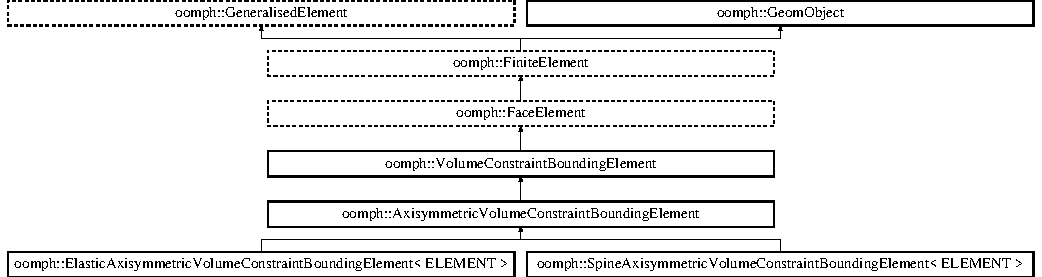
\includegraphics[height=3.716814cm]{classoomph_1_1AxisymmetricVolumeConstraintBoundingElement}
\end{center}
\end{figure}
\subsection*{Public Member Functions}
\begin{DoxyCompactItemize}
\item 
\hyperlink{classoomph_1_1AxisymmetricVolumeConstraintBoundingElement_a716ae91b7c11f6d71c474bec6f6d6d24}{Axisymmetric\+Volume\+Constraint\+Bounding\+Element} ()
\begin{DoxyCompactList}\small\item\em Empty Contructor. \end{DoxyCompactList}\item 
\hyperlink{classoomph_1_1AxisymmetricVolumeConstraintBoundingElement_ac7b98a2915cef69c7e4825e1f5730bc5}{$\sim$\+Axisymmetric\+Volume\+Constraint\+Bounding\+Element} ()
\begin{DoxyCompactList}\small\item\em Empty Destructor. \end{DoxyCompactList}\item 
double \hyperlink{classoomph_1_1AxisymmetricVolumeConstraintBoundingElement_a2d54cd3bce11538b066c8626b241d2c9}{contribution\+\_\+to\+\_\+enclosed\+\_\+volume} ()
\begin{DoxyCompactList}\small\item\em Return this element\textquotesingle{}s contribution to the total volume enclosed. \end{DoxyCompactList}\item 
double \hyperlink{classoomph_1_1AxisymmetricVolumeConstraintBoundingElement_a746f88f325d61610e10e97465fd2ca09}{contribution\+\_\+to\+\_\+volume\+\_\+flux} ()
\begin{DoxyCompactList}\small\item\em Return this element\textquotesingle{}s contribution to the volume flux over the boundary. \end{DoxyCompactList}\end{DoxyCompactItemize}
\subsection*{Protected Member Functions}
\begin{DoxyCompactItemize}
\item 
void \hyperlink{classoomph_1_1AxisymmetricVolumeConstraintBoundingElement_a2a3f3b86079f27d52679f357f5276d91}{fill\+\_\+in\+\_\+generic\+\_\+residual\+\_\+contribution\+\_\+volume\+\_\+constraint} (\hyperlink{classoomph_1_1Vector}{Vector}$<$ double $>$ \&residuals)
\begin{DoxyCompactList}\small\item\em Helper function to fill in contributions to residuals (remember that part of the residual is added by the the associated \hyperlink{classoomph_1_1VolumeConstraintElement}{Volume\+Constraint\+Element}). This is specific for 1D line elements that bound 2D cartesian fluid elements. \end{DoxyCompactList}\end{DoxyCompactItemize}
\subsection*{Additional Inherited Members}


\subsection{Detailed Description}
Axisymmetric (one-\/dimensional) interface elements that allow the application of a volume constraint on the region bounded by these elements. The volume is computed by integrating x.\+n around the boundary of the domain and then dividing by three. The sign is chosen so that the volume will be positive when the elements surround a fluid domain.

These elements must be used together with the associated \hyperlink{classoomph_1_1VolumeConstraintElement}{Volume\+Constraint\+Element}, which stores the value of the target volume. 

Definition at line 493 of file constrained\+\_\+volume\+\_\+elements.\+h.



\subsection{Constructor \& Destructor Documentation}
\mbox{\Hypertarget{classoomph_1_1AxisymmetricVolumeConstraintBoundingElement_a716ae91b7c11f6d71c474bec6f6d6d24}\label{classoomph_1_1AxisymmetricVolumeConstraintBoundingElement_a716ae91b7c11f6d71c474bec6f6d6d24}} 
\index{oomph\+::\+Axisymmetric\+Volume\+Constraint\+Bounding\+Element@{oomph\+::\+Axisymmetric\+Volume\+Constraint\+Bounding\+Element}!Axisymmetric\+Volume\+Constraint\+Bounding\+Element@{Axisymmetric\+Volume\+Constraint\+Bounding\+Element}}
\index{Axisymmetric\+Volume\+Constraint\+Bounding\+Element@{Axisymmetric\+Volume\+Constraint\+Bounding\+Element}!oomph\+::\+Axisymmetric\+Volume\+Constraint\+Bounding\+Element@{oomph\+::\+Axisymmetric\+Volume\+Constraint\+Bounding\+Element}}
\subsubsection{\texorpdfstring{Axisymmetric\+Volume\+Constraint\+Bounding\+Element()}{AxisymmetricVolumeConstraintBoundingElement()}}
{\footnotesize\ttfamily oomph\+::\+Axisymmetric\+Volume\+Constraint\+Bounding\+Element\+::\+Axisymmetric\+Volume\+Constraint\+Bounding\+Element (\begin{DoxyParamCaption}{ }\end{DoxyParamCaption})\hspace{0.3cm}{\ttfamily [inline]}}



Empty Contructor. 



Definition at line 508 of file constrained\+\_\+volume\+\_\+elements.\+h.

\mbox{\Hypertarget{classoomph_1_1AxisymmetricVolumeConstraintBoundingElement_ac7b98a2915cef69c7e4825e1f5730bc5}\label{classoomph_1_1AxisymmetricVolumeConstraintBoundingElement_ac7b98a2915cef69c7e4825e1f5730bc5}} 
\index{oomph\+::\+Axisymmetric\+Volume\+Constraint\+Bounding\+Element@{oomph\+::\+Axisymmetric\+Volume\+Constraint\+Bounding\+Element}!````~Axisymmetric\+Volume\+Constraint\+Bounding\+Element@{$\sim$\+Axisymmetric\+Volume\+Constraint\+Bounding\+Element}}
\index{````~Axisymmetric\+Volume\+Constraint\+Bounding\+Element@{$\sim$\+Axisymmetric\+Volume\+Constraint\+Bounding\+Element}!oomph\+::\+Axisymmetric\+Volume\+Constraint\+Bounding\+Element@{oomph\+::\+Axisymmetric\+Volume\+Constraint\+Bounding\+Element}}
\subsubsection{\texorpdfstring{$\sim$\+Axisymmetric\+Volume\+Constraint\+Bounding\+Element()}{~AxisymmetricVolumeConstraintBoundingElement()}}
{\footnotesize\ttfamily oomph\+::\+Axisymmetric\+Volume\+Constraint\+Bounding\+Element\+::$\sim$\+Axisymmetric\+Volume\+Constraint\+Bounding\+Element (\begin{DoxyParamCaption}{ }\end{DoxyParamCaption})\hspace{0.3cm}{\ttfamily [inline]}}



Empty Destructor. 



Definition at line 512 of file constrained\+\_\+volume\+\_\+elements.\+h.



\subsection{Member Function Documentation}
\mbox{\Hypertarget{classoomph_1_1AxisymmetricVolumeConstraintBoundingElement_a2d54cd3bce11538b066c8626b241d2c9}\label{classoomph_1_1AxisymmetricVolumeConstraintBoundingElement_a2d54cd3bce11538b066c8626b241d2c9}} 
\index{oomph\+::\+Axisymmetric\+Volume\+Constraint\+Bounding\+Element@{oomph\+::\+Axisymmetric\+Volume\+Constraint\+Bounding\+Element}!contribution\+\_\+to\+\_\+enclosed\+\_\+volume@{contribution\+\_\+to\+\_\+enclosed\+\_\+volume}}
\index{contribution\+\_\+to\+\_\+enclosed\+\_\+volume@{contribution\+\_\+to\+\_\+enclosed\+\_\+volume}!oomph\+::\+Axisymmetric\+Volume\+Constraint\+Bounding\+Element@{oomph\+::\+Axisymmetric\+Volume\+Constraint\+Bounding\+Element}}
\subsubsection{\texorpdfstring{contribution\+\_\+to\+\_\+enclosed\+\_\+volume()}{contribution\_to\_enclosed\_volume()}}
{\footnotesize\ttfamily double oomph\+::\+Axisymmetric\+Volume\+Constraint\+Bounding\+Element\+::contribution\+\_\+to\+\_\+enclosed\+\_\+volume (\begin{DoxyParamCaption}{ }\end{DoxyParamCaption})}



Return this element\textquotesingle{}s contribution to the total volume enclosed. 



Definition at line 274 of file constrained\+\_\+volume\+\_\+elements.\+cc.



References oomph\+::\+Vector\+Helpers\+::dot(), fill\+\_\+in\+\_\+generic\+\_\+residual\+\_\+contribution\+\_\+volume\+\_\+constraint(), i, s, and oomph\+::\+Quad\+Tree\+Names\+::W.



Referenced by oomph\+::\+Line\+Volume\+Constraint\+Bounding\+Element\+::contribution\+\_\+to\+\_\+enclosed\+\_\+volume().

\mbox{\Hypertarget{classoomph_1_1AxisymmetricVolumeConstraintBoundingElement_a746f88f325d61610e10e97465fd2ca09}\label{classoomph_1_1AxisymmetricVolumeConstraintBoundingElement_a746f88f325d61610e10e97465fd2ca09}} 
\index{oomph\+::\+Axisymmetric\+Volume\+Constraint\+Bounding\+Element@{oomph\+::\+Axisymmetric\+Volume\+Constraint\+Bounding\+Element}!contribution\+\_\+to\+\_\+volume\+\_\+flux@{contribution\+\_\+to\+\_\+volume\+\_\+flux}}
\index{contribution\+\_\+to\+\_\+volume\+\_\+flux@{contribution\+\_\+to\+\_\+volume\+\_\+flux}!oomph\+::\+Axisymmetric\+Volume\+Constraint\+Bounding\+Element@{oomph\+::\+Axisymmetric\+Volume\+Constraint\+Bounding\+Element}}
\subsubsection{\texorpdfstring{contribution\+\_\+to\+\_\+volume\+\_\+flux()}{contribution\_to\_volume\_flux()}}
{\footnotesize\ttfamily double oomph\+::\+Axisymmetric\+Volume\+Constraint\+Bounding\+Element\+::contribution\+\_\+to\+\_\+volume\+\_\+flux (\begin{DoxyParamCaption}{ }\end{DoxyParamCaption})\hspace{0.3cm}{\ttfamily [inline]}}



Return this element\textquotesingle{}s contribution to the volume flux over the boundary. 



Definition at line 519 of file constrained\+\_\+volume\+\_\+elements.\+h.



References oomph\+::\+Vector\+Helpers\+::dot(), i, s, and oomph\+::\+Quad\+Tree\+Names\+::W.

\mbox{\Hypertarget{classoomph_1_1AxisymmetricVolumeConstraintBoundingElement_a2a3f3b86079f27d52679f357f5276d91}\label{classoomph_1_1AxisymmetricVolumeConstraintBoundingElement_a2a3f3b86079f27d52679f357f5276d91}} 
\index{oomph\+::\+Axisymmetric\+Volume\+Constraint\+Bounding\+Element@{oomph\+::\+Axisymmetric\+Volume\+Constraint\+Bounding\+Element}!fill\+\_\+in\+\_\+generic\+\_\+residual\+\_\+contribution\+\_\+volume\+\_\+constraint@{fill\+\_\+in\+\_\+generic\+\_\+residual\+\_\+contribution\+\_\+volume\+\_\+constraint}}
\index{fill\+\_\+in\+\_\+generic\+\_\+residual\+\_\+contribution\+\_\+volume\+\_\+constraint@{fill\+\_\+in\+\_\+generic\+\_\+residual\+\_\+contribution\+\_\+volume\+\_\+constraint}!oomph\+::\+Axisymmetric\+Volume\+Constraint\+Bounding\+Element@{oomph\+::\+Axisymmetric\+Volume\+Constraint\+Bounding\+Element}}
\subsubsection{\texorpdfstring{fill\+\_\+in\+\_\+generic\+\_\+residual\+\_\+contribution\+\_\+volume\+\_\+constraint()}{fill\_in\_generic\_residual\_contribution\_volume\_constraint()}}
{\footnotesize\ttfamily void oomph\+::\+Axisymmetric\+Volume\+Constraint\+Bounding\+Element\+::fill\+\_\+in\+\_\+generic\+\_\+residual\+\_\+contribution\+\_\+volume\+\_\+constraint (\begin{DoxyParamCaption}\item[{\hyperlink{classoomph_1_1Vector}{Vector}$<$ double $>$ \&}]{residuals }\end{DoxyParamCaption})\hspace{0.3cm}{\ttfamily [protected]}, {\ttfamily [virtual]}}



Helper function to fill in contributions to residuals (remember that part of the residual is added by the the associated \hyperlink{classoomph_1_1VolumeConstraintElement}{Volume\+Constraint\+Element}). This is specific for 1D line elements that bound 2D cartesian fluid elements. 

Helper function to fill in contributions to residuals (remember that part of the residual is added by the the associated \hyperlink{classoomph_1_1VolumeConstraintElement}{Volume\+Constraint\+Element}). This is specific for axisymmetric line elements that bound 2D axisymmetric fluid elements. The only difference from the 1D case is the addition of the weighting factor in the integrand and division of the dot product by three. 

Implements \hyperlink{classoomph_1_1VolumeConstraintBoundingElement_a717f1085709bd8820b8043ff94ecb0c5}{oomph\+::\+Volume\+Constraint\+Bounding\+Element}.



Definition at line 359 of file constrained\+\_\+volume\+\_\+elements.\+cc.



References oomph\+::\+Vector\+Helpers\+::dot(), oomph\+::\+Surface\+Volume\+Constraint\+Bounding\+Element\+::fill\+\_\+in\+\_\+generic\+\_\+residual\+\_\+contribution\+\_\+volume\+\_\+constraint(), i, oomph\+::\+Volume\+Constraint\+Element\+::ptraded\+\_\+local\+\_\+eqn(), s, and oomph\+::\+Quad\+Tree\+Names\+::W.



Referenced by contribution\+\_\+to\+\_\+enclosed\+\_\+volume().



The documentation for this class was generated from the following files\+:\begin{DoxyCompactItemize}
\item 
\hyperlink{constrained__volume__elements_8h}{constrained\+\_\+volume\+\_\+elements.\+h}\item 
\hyperlink{constrained__volume__elements_8cc}{constrained\+\_\+volume\+\_\+elements.\+cc}\end{DoxyCompactItemize}

\hypertarget{classoomph_1_1AxisymQPVDElement}{}\section{oomph\+:\+:Axisym\+Q\+P\+V\+D\+Element Class Reference}
\label{classoomph_1_1AxisymQPVDElement}\index{oomph\+::\+Axisym\+Q\+P\+V\+D\+Element@{oomph\+::\+Axisym\+Q\+P\+V\+D\+Element}}


{\ttfamily \#include $<$axisym\+\_\+solid\+\_\+elements.\+h$>$}

Inheritance diagram for oomph\+:\+:Axisym\+Q\+P\+V\+D\+Element\+:\begin{figure}[H]
\begin{center}
\leavevmode
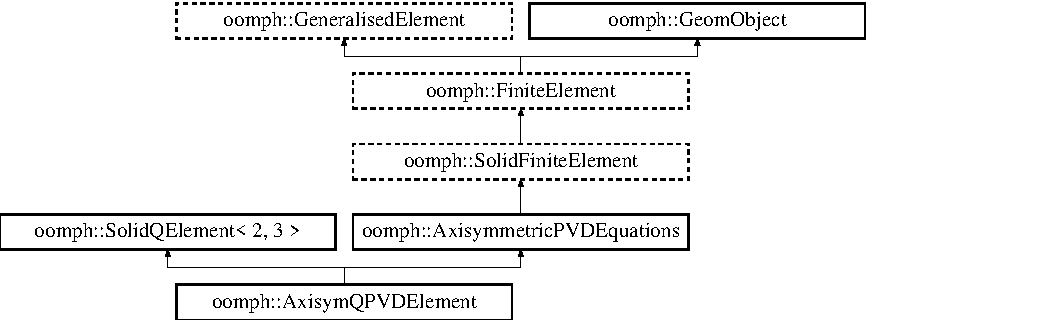
\includegraphics[height=4.301075cm]{classoomph_1_1AxisymQPVDElement}
\end{center}
\end{figure}
\subsection*{Public Member Functions}
\begin{DoxyCompactItemize}
\item 
\hyperlink{classoomph_1_1AxisymQPVDElement_a0cd0c4e03f099140ce3655fcab3c3ef3}{Axisym\+Q\+P\+V\+D\+Element} ()
\begin{DoxyCompactList}\small\item\em Constructor, there are no internal data points. \end{DoxyCompactList}\item 
void \hyperlink{classoomph_1_1AxisymQPVDElement_ac2a240575dea087098520bf6f9567dc2}{output} (std\+::ostream \&outfile)
\begin{DoxyCompactList}\small\item\em Overload the output function. \end{DoxyCompactList}\item 
void \hyperlink{classoomph_1_1AxisymQPVDElement_ab9925995ad1b184df43b6eb350f3e0bd}{output} (std\+::ostream \&outfile, const unsigned \&n\+\_\+plot)
\begin{DoxyCompactList}\small\item\em Output function. \end{DoxyCompactList}\item 
void \hyperlink{classoomph_1_1AxisymQPVDElement_abc2012c37faa9153f18fab2ff273bc9a}{output} (F\+I\+LE $\ast$file\+\_\+pt)
\begin{DoxyCompactList}\small\item\em Overload the output function. \end{DoxyCompactList}\item 
void \hyperlink{classoomph_1_1AxisymQPVDElement_afcd700bebcd0e1c83066da66804785c9}{output} (F\+I\+LE $\ast$file\+\_\+pt, const unsigned \&n\+\_\+plot)
\begin{DoxyCompactList}\small\item\em Output function. \end{DoxyCompactList}\end{DoxyCompactItemize}
\subsection*{Additional Inherited Members}


\subsection{Detailed Description}
An element that solved the \hyperlink{classoomph_1_1AxisymmetricPVDEquations}{Axisymmetric\+P\+V\+D\+Equations} with quadratic interpolation for the positions. 

Definition at line 489 of file axisym\+\_\+solid\+\_\+elements.\+h.



\subsection{Constructor \& Destructor Documentation}
\mbox{\Hypertarget{classoomph_1_1AxisymQPVDElement_a0cd0c4e03f099140ce3655fcab3c3ef3}\label{classoomph_1_1AxisymQPVDElement_a0cd0c4e03f099140ce3655fcab3c3ef3}} 
\index{oomph\+::\+Axisym\+Q\+P\+V\+D\+Element@{oomph\+::\+Axisym\+Q\+P\+V\+D\+Element}!Axisym\+Q\+P\+V\+D\+Element@{Axisym\+Q\+P\+V\+D\+Element}}
\index{Axisym\+Q\+P\+V\+D\+Element@{Axisym\+Q\+P\+V\+D\+Element}!oomph\+::\+Axisym\+Q\+P\+V\+D\+Element@{oomph\+::\+Axisym\+Q\+P\+V\+D\+Element}}
\subsubsection{\texorpdfstring{Axisym\+Q\+P\+V\+D\+Element()}{AxisymQPVDElement()}}
{\footnotesize\ttfamily oomph\+::\+Axisym\+Q\+P\+V\+D\+Element\+::\+Axisym\+Q\+P\+V\+D\+Element (\begin{DoxyParamCaption}{ }\end{DoxyParamCaption})\hspace{0.3cm}{\ttfamily [inline]}}



Constructor, there are no internal data points. 



Definition at line 496 of file axisym\+\_\+solid\+\_\+elements.\+h.



\subsection{Member Function Documentation}
\mbox{\Hypertarget{classoomph_1_1AxisymQPVDElement_ac2a240575dea087098520bf6f9567dc2}\label{classoomph_1_1AxisymQPVDElement_ac2a240575dea087098520bf6f9567dc2}} 
\index{oomph\+::\+Axisym\+Q\+P\+V\+D\+Element@{oomph\+::\+Axisym\+Q\+P\+V\+D\+Element}!output@{output}}
\index{output@{output}!oomph\+::\+Axisym\+Q\+P\+V\+D\+Element@{oomph\+::\+Axisym\+Q\+P\+V\+D\+Element}}
\subsubsection{\texorpdfstring{output()}{output()}\hspace{0.1cm}{\footnotesize\ttfamily [1/4]}}
{\footnotesize\ttfamily void oomph\+::\+Axisym\+Q\+P\+V\+D\+Element\+::output (\begin{DoxyParamCaption}\item[{std\+::ostream \&}]{outfile }\end{DoxyParamCaption})\hspace{0.3cm}{\ttfamily [inline]}, {\ttfamily [virtual]}}



Overload the output function. 



Reimplemented from \hyperlink{classoomph_1_1AxisymmetricPVDEquations_a70c01efa665238ec7a574588209d3edb}{oomph\+::\+Axisymmetric\+P\+V\+D\+Equations}.



Definition at line 499 of file axisym\+\_\+solid\+\_\+elements.\+h.



References oomph\+::\+Finite\+Element\+::output().

\mbox{\Hypertarget{classoomph_1_1AxisymQPVDElement_ab9925995ad1b184df43b6eb350f3e0bd}\label{classoomph_1_1AxisymQPVDElement_ab9925995ad1b184df43b6eb350f3e0bd}} 
\index{oomph\+::\+Axisym\+Q\+P\+V\+D\+Element@{oomph\+::\+Axisym\+Q\+P\+V\+D\+Element}!output@{output}}
\index{output@{output}!oomph\+::\+Axisym\+Q\+P\+V\+D\+Element@{oomph\+::\+Axisym\+Q\+P\+V\+D\+Element}}
\subsubsection{\texorpdfstring{output()}{output()}\hspace{0.1cm}{\footnotesize\ttfamily [2/4]}}
{\footnotesize\ttfamily void oomph\+::\+Axisym\+Q\+P\+V\+D\+Element\+::output (\begin{DoxyParamCaption}\item[{std\+::ostream \&}]{outfile,  }\item[{const unsigned \&}]{n\+\_\+plot }\end{DoxyParamCaption})\hspace{0.3cm}{\ttfamily [inline]}, {\ttfamily [virtual]}}



Output function. 



Reimplemented from \hyperlink{classoomph_1_1AxisymmetricPVDEquations_a35cf174ca1692f817e3182166e22ef4b}{oomph\+::\+Axisymmetric\+P\+V\+D\+Equations}.



Definition at line 502 of file axisym\+\_\+solid\+\_\+elements.\+h.



References oomph\+::\+Axisymmetric\+P\+V\+D\+Equations\+::output().

\mbox{\Hypertarget{classoomph_1_1AxisymQPVDElement_abc2012c37faa9153f18fab2ff273bc9a}\label{classoomph_1_1AxisymQPVDElement_abc2012c37faa9153f18fab2ff273bc9a}} 
\index{oomph\+::\+Axisym\+Q\+P\+V\+D\+Element@{oomph\+::\+Axisym\+Q\+P\+V\+D\+Element}!output@{output}}
\index{output@{output}!oomph\+::\+Axisym\+Q\+P\+V\+D\+Element@{oomph\+::\+Axisym\+Q\+P\+V\+D\+Element}}
\subsubsection{\texorpdfstring{output()}{output()}\hspace{0.1cm}{\footnotesize\ttfamily [3/4]}}
{\footnotesize\ttfamily void oomph\+::\+Axisym\+Q\+P\+V\+D\+Element\+::output (\begin{DoxyParamCaption}\item[{F\+I\+LE $\ast$}]{file\+\_\+pt }\end{DoxyParamCaption})\hspace{0.3cm}{\ttfamily [inline]}, {\ttfamily [virtual]}}



Overload the output function. 



Reimplemented from \hyperlink{classoomph_1_1AxisymmetricPVDEquations_a3b271e966cc554c21231503f7a965549}{oomph\+::\+Axisymmetric\+P\+V\+D\+Equations}.



Definition at line 506 of file axisym\+\_\+solid\+\_\+elements.\+h.



References oomph\+::\+Finite\+Element\+::output().

\mbox{\Hypertarget{classoomph_1_1AxisymQPVDElement_afcd700bebcd0e1c83066da66804785c9}\label{classoomph_1_1AxisymQPVDElement_afcd700bebcd0e1c83066da66804785c9}} 
\index{oomph\+::\+Axisym\+Q\+P\+V\+D\+Element@{oomph\+::\+Axisym\+Q\+P\+V\+D\+Element}!output@{output}}
\index{output@{output}!oomph\+::\+Axisym\+Q\+P\+V\+D\+Element@{oomph\+::\+Axisym\+Q\+P\+V\+D\+Element}}
\subsubsection{\texorpdfstring{output()}{output()}\hspace{0.1cm}{\footnotesize\ttfamily [4/4]}}
{\footnotesize\ttfamily void oomph\+::\+Axisym\+Q\+P\+V\+D\+Element\+::output (\begin{DoxyParamCaption}\item[{F\+I\+LE $\ast$}]{file\+\_\+pt,  }\item[{const unsigned \&}]{n\+\_\+plot }\end{DoxyParamCaption})\hspace{0.3cm}{\ttfamily [inline]}, {\ttfamily [virtual]}}



Output function. 



Reimplemented from \hyperlink{classoomph_1_1AxisymmetricPVDEquations_a780e6e426869eec81758bf7396a54bad}{oomph\+::\+Axisymmetric\+P\+V\+D\+Equations}.



Definition at line 509 of file axisym\+\_\+solid\+\_\+elements.\+h.



References oomph\+::\+Axisymmetric\+P\+V\+D\+Equations\+::output().



The documentation for this class was generated from the following file\+:\begin{DoxyCompactItemize}
\item 
\hyperlink{axisym__solid__elements_8h}{axisym\+\_\+solid\+\_\+elements.\+h}\end{DoxyCompactItemize}

\hypertarget{classoomph_1_1AxisymQPVDElementWithPressure}{}\section{oomph\+:\+:Axisym\+Q\+P\+V\+D\+Element\+With\+Pressure Class Reference}
\label{classoomph_1_1AxisymQPVDElementWithPressure}\index{oomph\+::\+Axisym\+Q\+P\+V\+D\+Element\+With\+Pressure@{oomph\+::\+Axisym\+Q\+P\+V\+D\+Element\+With\+Pressure}}


{\ttfamily \#include $<$axisym\+\_\+solid\+\_\+elements.\+h$>$}

Inheritance diagram for oomph\+:\+:Axisym\+Q\+P\+V\+D\+Element\+With\+Pressure\+:\begin{figure}[H]
\begin{center}
\leavevmode
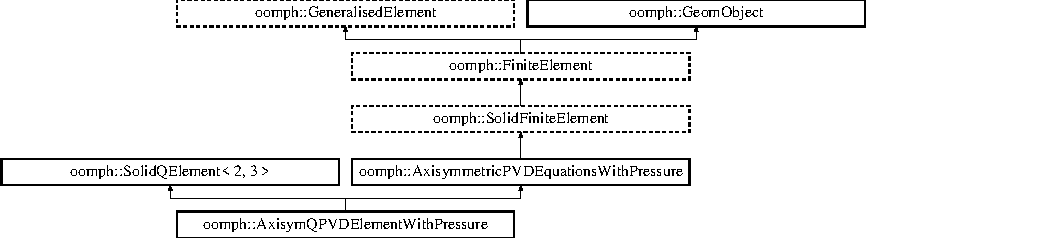
\includegraphics[height=3.196347cm]{classoomph_1_1AxisymQPVDElementWithPressure}
\end{center}
\end{figure}
\subsection*{Public Member Functions}
\begin{DoxyCompactItemize}
\item 
bool \hyperlink{classoomph_1_1AxisymQPVDElementWithPressure_af5a06f24c310d233555f165189ff353a}{has\+\_\+internal\+\_\+solid\+\_\+data} ()
\begin{DoxyCompactList}\small\item\em There is internal solid data so we can\textquotesingle{}t use the automatic assignment of consistent initial conditions for time-\/dependent problems. \end{DoxyCompactList}\item 
\hyperlink{classoomph_1_1AxisymQPVDElementWithPressure_a5b902a463ba218dd83d9641510a6fbfb}{Axisym\+Q\+P\+V\+D\+Element\+With\+Pressure} ()
\begin{DoxyCompactList}\small\item\em Constructor, there are 3 internal data items. \end{DoxyCompactList}\item 
double \hyperlink{classoomph_1_1AxisymQPVDElementWithPressure_a43a3e699d4e958d00d5ebc20ff23827b}{solid\+\_\+p} (const unsigned \&l)
\begin{DoxyCompactList}\small\item\em Return the l-\/th pressure value. \end{DoxyCompactList}\item 
unsigned \hyperlink{classoomph_1_1AxisymQPVDElementWithPressure_ac39d97adf69f12b20640ae10aeaec156}{nsolid\+\_\+pres} () const
\begin{DoxyCompactList}\small\item\em Return number of pressure values. \end{DoxyCompactList}\item 
void \hyperlink{classoomph_1_1AxisymQPVDElementWithPressure_aec1e7e2de41bd7eaff58fa31c9c47645}{fix\+\_\+solid\+\_\+pressure} (const unsigned \&l, const double \&pvalue)
\begin{DoxyCompactList}\small\item\em Fix the pressure dof l to the value pvalue. \end{DoxyCompactList}\item 
void \hyperlink{classoomph_1_1AxisymQPVDElementWithPressure_a1df3ba1290d73dd33634d5b99993dee7}{output} (std\+::ostream \&outfile)
\begin{DoxyCompactList}\small\item\em Overload the output function. \end{DoxyCompactList}\item 
void \hyperlink{classoomph_1_1AxisymQPVDElementWithPressure_aa7bf745c0767590c36a761d3a6399e57}{output} (std\+::ostream \&outfile, const unsigned \&n\+\_\+plot)
\begin{DoxyCompactList}\small\item\em Output function. \end{DoxyCompactList}\item 
void \hyperlink{classoomph_1_1AxisymQPVDElementWithPressure_a8f09df5914ea8dbb6ba7041bd6be15bd}{output} (F\+I\+LE $\ast$file\+\_\+pt)
\begin{DoxyCompactList}\small\item\em Overload the output function. \end{DoxyCompactList}\item 
void \hyperlink{classoomph_1_1AxisymQPVDElementWithPressure_a273e1cfc1185192fcb9cc3812360c87e}{output} (F\+I\+LE $\ast$file\+\_\+pt, const unsigned \&n\+\_\+plot)
\begin{DoxyCompactList}\small\item\em Output function. \end{DoxyCompactList}\end{DoxyCompactItemize}
\subsection*{Private Member Functions}
\begin{DoxyCompactItemize}
\item 
int \hyperlink{classoomph_1_1AxisymQPVDElementWithPressure_a8c9fa9511418570fab627362609235d0}{solid\+\_\+p\+\_\+local\+\_\+eqn} (const unsigned \&\hyperlink{cfortran_8h_adb50e893b86b3e55e751a42eab3cba82}{i})
\begin{DoxyCompactList}\small\item\em Overload the access function for the solid pressure equation numbers. \end{DoxyCompactList}\item 
void \hyperlink{classoomph_1_1AxisymQPVDElementWithPressure_acc96f08aadc9568d283dbe09ce06d643}{solid\+\_\+pshape} (const \hyperlink{classoomph_1_1Vector}{Vector}$<$ double $>$ \&\hyperlink{cfortran_8h_ab7123126e4885ef647dd9c6e3807a21c}{s}, \hyperlink{classoomph_1_1Shape}{Shape} \&psi) const
\begin{DoxyCompactList}\small\item\em Return the pressure shape functions. \end{DoxyCompactList}\end{DoxyCompactItemize}
\subsection*{Private Attributes}
\begin{DoxyCompactItemize}
\item 
unsigned \hyperlink{classoomph_1_1AxisymQPVDElementWithPressure_a105317d009a9edf0ed149f4cc565689b}{P\+\_\+solid\+\_\+internal\+\_\+index}
\begin{DoxyCompactList}\small\item\em Internal index that indicates at which internal data value the solid pressure is stored. \end{DoxyCompactList}\end{DoxyCompactItemize}
\subsection*{Additional Inherited Members}


\subsection{Detailed Description}
An Element that solves the Axisymmetric principle of virtual displacements with separately interpolated pressure, discontinuous interpolation. 

Definition at line 1296 of file axisym\+\_\+solid\+\_\+elements.\+h.



\subsection{Constructor \& Destructor Documentation}
\mbox{\Hypertarget{classoomph_1_1AxisymQPVDElementWithPressure_a5b902a463ba218dd83d9641510a6fbfb}\label{classoomph_1_1AxisymQPVDElementWithPressure_a5b902a463ba218dd83d9641510a6fbfb}} 
\index{oomph\+::\+Axisym\+Q\+P\+V\+D\+Element\+With\+Pressure@{oomph\+::\+Axisym\+Q\+P\+V\+D\+Element\+With\+Pressure}!Axisym\+Q\+P\+V\+D\+Element\+With\+Pressure@{Axisym\+Q\+P\+V\+D\+Element\+With\+Pressure}}
\index{Axisym\+Q\+P\+V\+D\+Element\+With\+Pressure@{Axisym\+Q\+P\+V\+D\+Element\+With\+Pressure}!oomph\+::\+Axisym\+Q\+P\+V\+D\+Element\+With\+Pressure@{oomph\+::\+Axisym\+Q\+P\+V\+D\+Element\+With\+Pressure}}
\subsubsection{\texorpdfstring{Axisym\+Q\+P\+V\+D\+Element\+With\+Pressure()}{AxisymQPVDElementWithPressure()}}
{\footnotesize\ttfamily oomph\+::\+Axisym\+Q\+P\+V\+D\+Element\+With\+Pressure\+::\+Axisym\+Q\+P\+V\+D\+Element\+With\+Pressure (\begin{DoxyParamCaption}{ }\end{DoxyParamCaption})\hspace{0.3cm}{\ttfamily [inline]}}



Constructor, there are 3 internal data items. 



Definition at line 1317 of file axisym\+\_\+solid\+\_\+elements.\+h.



References oomph\+::\+Generalised\+Element\+::add\+\_\+internal\+\_\+data().



\subsection{Member Function Documentation}
\mbox{\Hypertarget{classoomph_1_1AxisymQPVDElementWithPressure_aec1e7e2de41bd7eaff58fa31c9c47645}\label{classoomph_1_1AxisymQPVDElementWithPressure_aec1e7e2de41bd7eaff58fa31c9c47645}} 
\index{oomph\+::\+Axisym\+Q\+P\+V\+D\+Element\+With\+Pressure@{oomph\+::\+Axisym\+Q\+P\+V\+D\+Element\+With\+Pressure}!fix\+\_\+solid\+\_\+pressure@{fix\+\_\+solid\+\_\+pressure}}
\index{fix\+\_\+solid\+\_\+pressure@{fix\+\_\+solid\+\_\+pressure}!oomph\+::\+Axisym\+Q\+P\+V\+D\+Element\+With\+Pressure@{oomph\+::\+Axisym\+Q\+P\+V\+D\+Element\+With\+Pressure}}
\subsubsection{\texorpdfstring{fix\+\_\+solid\+\_\+pressure()}{fix\_solid\_pressure()}}
{\footnotesize\ttfamily void oomph\+::\+Axisym\+Q\+P\+V\+D\+Element\+With\+Pressure\+::fix\+\_\+solid\+\_\+pressure (\begin{DoxyParamCaption}\item[{const unsigned \&}]{l,  }\item[{const double \&}]{pvalue }\end{DoxyParamCaption})\hspace{0.3cm}{\ttfamily [inline]}}



Fix the pressure dof l to the value pvalue. 



Definition at line 1333 of file axisym\+\_\+solid\+\_\+elements.\+h.



References oomph\+::\+Generalised\+Element\+::internal\+\_\+data\+\_\+pt(), oomph\+::\+Data\+::pin(), and oomph\+::\+Data\+::set\+\_\+value().

\mbox{\Hypertarget{classoomph_1_1AxisymQPVDElementWithPressure_af5a06f24c310d233555f165189ff353a}\label{classoomph_1_1AxisymQPVDElementWithPressure_af5a06f24c310d233555f165189ff353a}} 
\index{oomph\+::\+Axisym\+Q\+P\+V\+D\+Element\+With\+Pressure@{oomph\+::\+Axisym\+Q\+P\+V\+D\+Element\+With\+Pressure}!has\+\_\+internal\+\_\+solid\+\_\+data@{has\+\_\+internal\+\_\+solid\+\_\+data}}
\index{has\+\_\+internal\+\_\+solid\+\_\+data@{has\+\_\+internal\+\_\+solid\+\_\+data}!oomph\+::\+Axisym\+Q\+P\+V\+D\+Element\+With\+Pressure@{oomph\+::\+Axisym\+Q\+P\+V\+D\+Element\+With\+Pressure}}
\subsubsection{\texorpdfstring{has\+\_\+internal\+\_\+solid\+\_\+data()}{has\_internal\_solid\_data()}}
{\footnotesize\ttfamily bool oomph\+::\+Axisym\+Q\+P\+V\+D\+Element\+With\+Pressure\+::has\+\_\+internal\+\_\+solid\+\_\+data (\begin{DoxyParamCaption}{ }\end{DoxyParamCaption})\hspace{0.3cm}{\ttfamily [inline]}, {\ttfamily [virtual]}}



There is internal solid data so we can\textquotesingle{}t use the automatic assignment of consistent initial conditions for time-\/dependent problems. 



Reimplemented from \hyperlink{classoomph_1_1SolidFiniteElement_aa68837a8f6d1cb021d5cae9c2968a6f3}{oomph\+::\+Solid\+Finite\+Element}.



Definition at line 1314 of file axisym\+\_\+solid\+\_\+elements.\+h.

\mbox{\Hypertarget{classoomph_1_1AxisymQPVDElementWithPressure_ac39d97adf69f12b20640ae10aeaec156}\label{classoomph_1_1AxisymQPVDElementWithPressure_ac39d97adf69f12b20640ae10aeaec156}} 
\index{oomph\+::\+Axisym\+Q\+P\+V\+D\+Element\+With\+Pressure@{oomph\+::\+Axisym\+Q\+P\+V\+D\+Element\+With\+Pressure}!nsolid\+\_\+pres@{nsolid\+\_\+pres}}
\index{nsolid\+\_\+pres@{nsolid\+\_\+pres}!oomph\+::\+Axisym\+Q\+P\+V\+D\+Element\+With\+Pressure@{oomph\+::\+Axisym\+Q\+P\+V\+D\+Element\+With\+Pressure}}
\subsubsection{\texorpdfstring{nsolid\+\_\+pres()}{nsolid\_pres()}}
{\footnotesize\ttfamily unsigned oomph\+::\+Axisym\+Q\+P\+V\+D\+Element\+With\+Pressure\+::nsolid\+\_\+pres (\begin{DoxyParamCaption}{ }\end{DoxyParamCaption}) const\hspace{0.3cm}{\ttfamily [inline]}, {\ttfamily [virtual]}}



Return number of pressure values. 



Implements \hyperlink{classoomph_1_1AxisymmetricPVDEquationsWithPressure_a4cfeab9fe5e9c26fcf39659bacc53a8f}{oomph\+::\+Axisymmetric\+P\+V\+D\+Equations\+With\+Pressure}.



Definition at line 1330 of file axisym\+\_\+solid\+\_\+elements.\+h.

\mbox{\Hypertarget{classoomph_1_1AxisymQPVDElementWithPressure_a1df3ba1290d73dd33634d5b99993dee7}\label{classoomph_1_1AxisymQPVDElementWithPressure_a1df3ba1290d73dd33634d5b99993dee7}} 
\index{oomph\+::\+Axisym\+Q\+P\+V\+D\+Element\+With\+Pressure@{oomph\+::\+Axisym\+Q\+P\+V\+D\+Element\+With\+Pressure}!output@{output}}
\index{output@{output}!oomph\+::\+Axisym\+Q\+P\+V\+D\+Element\+With\+Pressure@{oomph\+::\+Axisym\+Q\+P\+V\+D\+Element\+With\+Pressure}}
\subsubsection{\texorpdfstring{output()}{output()}\hspace{0.1cm}{\footnotesize\ttfamily [1/4]}}
{\footnotesize\ttfamily void oomph\+::\+Axisym\+Q\+P\+V\+D\+Element\+With\+Pressure\+::output (\begin{DoxyParamCaption}\item[{std\+::ostream \&}]{outfile }\end{DoxyParamCaption})\hspace{0.3cm}{\ttfamily [inline]}, {\ttfamily [virtual]}}



Overload the output function. 



Reimplemented from \hyperlink{classoomph_1_1AxisymmetricPVDEquationsWithPressure_aba49f4147fb78fa74cd591b4a77eab98}{oomph\+::\+Axisymmetric\+P\+V\+D\+Equations\+With\+Pressure}.



Definition at line 1340 of file axisym\+\_\+solid\+\_\+elements.\+h.



References oomph\+::\+Finite\+Element\+::output().

\mbox{\Hypertarget{classoomph_1_1AxisymQPVDElementWithPressure_aa7bf745c0767590c36a761d3a6399e57}\label{classoomph_1_1AxisymQPVDElementWithPressure_aa7bf745c0767590c36a761d3a6399e57}} 
\index{oomph\+::\+Axisym\+Q\+P\+V\+D\+Element\+With\+Pressure@{oomph\+::\+Axisym\+Q\+P\+V\+D\+Element\+With\+Pressure}!output@{output}}
\index{output@{output}!oomph\+::\+Axisym\+Q\+P\+V\+D\+Element\+With\+Pressure@{oomph\+::\+Axisym\+Q\+P\+V\+D\+Element\+With\+Pressure}}
\subsubsection{\texorpdfstring{output()}{output()}\hspace{0.1cm}{\footnotesize\ttfamily [2/4]}}
{\footnotesize\ttfamily void oomph\+::\+Axisym\+Q\+P\+V\+D\+Element\+With\+Pressure\+::output (\begin{DoxyParamCaption}\item[{std\+::ostream \&}]{outfile,  }\item[{const unsigned \&}]{n\+\_\+plot }\end{DoxyParamCaption})\hspace{0.3cm}{\ttfamily [inline]}, {\ttfamily [virtual]}}



Output function. 



Reimplemented from \hyperlink{classoomph_1_1AxisymmetricPVDEquationsWithPressure_a6916b3f7784015c263556565b2a7219d}{oomph\+::\+Axisymmetric\+P\+V\+D\+Equations\+With\+Pressure}.



Definition at line 1343 of file axisym\+\_\+solid\+\_\+elements.\+h.



References oomph\+::\+Axisymmetric\+P\+V\+D\+Equations\+With\+Pressure\+::output().

\mbox{\Hypertarget{classoomph_1_1AxisymQPVDElementWithPressure_a8f09df5914ea8dbb6ba7041bd6be15bd}\label{classoomph_1_1AxisymQPVDElementWithPressure_a8f09df5914ea8dbb6ba7041bd6be15bd}} 
\index{oomph\+::\+Axisym\+Q\+P\+V\+D\+Element\+With\+Pressure@{oomph\+::\+Axisym\+Q\+P\+V\+D\+Element\+With\+Pressure}!output@{output}}
\index{output@{output}!oomph\+::\+Axisym\+Q\+P\+V\+D\+Element\+With\+Pressure@{oomph\+::\+Axisym\+Q\+P\+V\+D\+Element\+With\+Pressure}}
\subsubsection{\texorpdfstring{output()}{output()}\hspace{0.1cm}{\footnotesize\ttfamily [3/4]}}
{\footnotesize\ttfamily void oomph\+::\+Axisym\+Q\+P\+V\+D\+Element\+With\+Pressure\+::output (\begin{DoxyParamCaption}\item[{F\+I\+LE $\ast$}]{file\+\_\+pt }\end{DoxyParamCaption})\hspace{0.3cm}{\ttfamily [inline]}, {\ttfamily [virtual]}}



Overload the output function. 



Reimplemented from \hyperlink{classoomph_1_1AxisymmetricPVDEquationsWithPressure_ad5018c9a6f9236f13c6df43df87336aa}{oomph\+::\+Axisymmetric\+P\+V\+D\+Equations\+With\+Pressure}.



Definition at line 1348 of file axisym\+\_\+solid\+\_\+elements.\+h.



References oomph\+::\+Finite\+Element\+::output().

\mbox{\Hypertarget{classoomph_1_1AxisymQPVDElementWithPressure_a273e1cfc1185192fcb9cc3812360c87e}\label{classoomph_1_1AxisymQPVDElementWithPressure_a273e1cfc1185192fcb9cc3812360c87e}} 
\index{oomph\+::\+Axisym\+Q\+P\+V\+D\+Element\+With\+Pressure@{oomph\+::\+Axisym\+Q\+P\+V\+D\+Element\+With\+Pressure}!output@{output}}
\index{output@{output}!oomph\+::\+Axisym\+Q\+P\+V\+D\+Element\+With\+Pressure@{oomph\+::\+Axisym\+Q\+P\+V\+D\+Element\+With\+Pressure}}
\subsubsection{\texorpdfstring{output()}{output()}\hspace{0.1cm}{\footnotesize\ttfamily [4/4]}}
{\footnotesize\ttfamily void oomph\+::\+Axisym\+Q\+P\+V\+D\+Element\+With\+Pressure\+::output (\begin{DoxyParamCaption}\item[{F\+I\+LE $\ast$}]{file\+\_\+pt,  }\item[{const unsigned \&}]{n\+\_\+plot }\end{DoxyParamCaption})\hspace{0.3cm}{\ttfamily [inline]}, {\ttfamily [virtual]}}



Output function. 



Reimplemented from \hyperlink{classoomph_1_1AxisymmetricPVDEquationsWithPressure_a3a6d03fa236a2e0173abbc1734799d19}{oomph\+::\+Axisymmetric\+P\+V\+D\+Equations\+With\+Pressure}.



Definition at line 1351 of file axisym\+\_\+solid\+\_\+elements.\+h.



References oomph\+::\+Axisymmetric\+P\+V\+D\+Equations\+With\+Pressure\+::output(), and solid\+\_\+pshape().

\mbox{\Hypertarget{classoomph_1_1AxisymQPVDElementWithPressure_a43a3e699d4e958d00d5ebc20ff23827b}\label{classoomph_1_1AxisymQPVDElementWithPressure_a43a3e699d4e958d00d5ebc20ff23827b}} 
\index{oomph\+::\+Axisym\+Q\+P\+V\+D\+Element\+With\+Pressure@{oomph\+::\+Axisym\+Q\+P\+V\+D\+Element\+With\+Pressure}!solid\+\_\+p@{solid\+\_\+p}}
\index{solid\+\_\+p@{solid\+\_\+p}!oomph\+::\+Axisym\+Q\+P\+V\+D\+Element\+With\+Pressure@{oomph\+::\+Axisym\+Q\+P\+V\+D\+Element\+With\+Pressure}}
\subsubsection{\texorpdfstring{solid\+\_\+p()}{solid\_p()}}
{\footnotesize\ttfamily double oomph\+::\+Axisym\+Q\+P\+V\+D\+Element\+With\+Pressure\+::solid\+\_\+p (\begin{DoxyParamCaption}\item[{const unsigned \&}]{l }\end{DoxyParamCaption})\hspace{0.3cm}{\ttfamily [inline]}, {\ttfamily [virtual]}}



Return the l-\/th pressure value. 



Implements \hyperlink{classoomph_1_1AxisymmetricPVDEquationsWithPressure_aeb03a2cef37040790d5d9dacafb89144}{oomph\+::\+Axisymmetric\+P\+V\+D\+Equations\+With\+Pressure}.



Definition at line 1326 of file axisym\+\_\+solid\+\_\+elements.\+h.



References oomph\+::\+Generalised\+Element\+::internal\+\_\+data\+\_\+pt(), and oomph\+::\+Data\+::value().

\mbox{\Hypertarget{classoomph_1_1AxisymQPVDElementWithPressure_a8c9fa9511418570fab627362609235d0}\label{classoomph_1_1AxisymQPVDElementWithPressure_a8c9fa9511418570fab627362609235d0}} 
\index{oomph\+::\+Axisym\+Q\+P\+V\+D\+Element\+With\+Pressure@{oomph\+::\+Axisym\+Q\+P\+V\+D\+Element\+With\+Pressure}!solid\+\_\+p\+\_\+local\+\_\+eqn@{solid\+\_\+p\+\_\+local\+\_\+eqn}}
\index{solid\+\_\+p\+\_\+local\+\_\+eqn@{solid\+\_\+p\+\_\+local\+\_\+eqn}!oomph\+::\+Axisym\+Q\+P\+V\+D\+Element\+With\+Pressure@{oomph\+::\+Axisym\+Q\+P\+V\+D\+Element\+With\+Pressure}}
\subsubsection{\texorpdfstring{solid\+\_\+p\+\_\+local\+\_\+eqn()}{solid\_p\_local\_eqn()}}
{\footnotesize\ttfamily int oomph\+::\+Axisym\+Q\+P\+V\+D\+Element\+With\+Pressure\+::solid\+\_\+p\+\_\+local\+\_\+eqn (\begin{DoxyParamCaption}\item[{const unsigned \&}]{i }\end{DoxyParamCaption})\hspace{0.3cm}{\ttfamily [inline]}, {\ttfamily [private]}, {\ttfamily [virtual]}}



Overload the access function for the solid pressure equation numbers. 



Implements \hyperlink{classoomph_1_1AxisymmetricPVDEquationsWithPressure_a7b77ffb084d0967b1220898613718d0b}{oomph\+::\+Axisymmetric\+P\+V\+D\+Equations\+With\+Pressure}.



Definition at line 1304 of file axisym\+\_\+solid\+\_\+elements.\+h.



References oomph\+::\+Generalised\+Element\+::internal\+\_\+local\+\_\+eqn(), and s.

\mbox{\Hypertarget{classoomph_1_1AxisymQPVDElementWithPressure_acc96f08aadc9568d283dbe09ce06d643}\label{classoomph_1_1AxisymQPVDElementWithPressure_acc96f08aadc9568d283dbe09ce06d643}} 
\index{oomph\+::\+Axisym\+Q\+P\+V\+D\+Element\+With\+Pressure@{oomph\+::\+Axisym\+Q\+P\+V\+D\+Element\+With\+Pressure}!solid\+\_\+pshape@{solid\+\_\+pshape}}
\index{solid\+\_\+pshape@{solid\+\_\+pshape}!oomph\+::\+Axisym\+Q\+P\+V\+D\+Element\+With\+Pressure@{oomph\+::\+Axisym\+Q\+P\+V\+D\+Element\+With\+Pressure}}
\subsubsection{\texorpdfstring{solid\+\_\+pshape()}{solid\_pshape()}}
{\footnotesize\ttfamily void oomph\+::\+Axisym\+Q\+P\+V\+D\+Element\+With\+Pressure\+::solid\+\_\+pshape (\begin{DoxyParamCaption}\item[{const \hyperlink{classoomph_1_1Vector}{Vector}$<$ double $>$ \&}]{s,  }\item[{\hyperlink{classoomph_1_1Shape}{Shape} \&}]{psi }\end{DoxyParamCaption}) const\hspace{0.3cm}{\ttfamily [inline]}, {\ttfamily [private]}, {\ttfamily [virtual]}}



Return the pressure shape functions. 

Define the pressure shape functions. 

Implements \hyperlink{classoomph_1_1AxisymmetricPVDEquationsWithPressure_ab93f05b37f8bee3a8f390e33cbcd3a6e}{oomph\+::\+Axisymmetric\+P\+V\+D\+Equations\+With\+Pressure}.



Definition at line 1358 of file axisym\+\_\+solid\+\_\+elements.\+h.



Referenced by output().



\subsection{Member Data Documentation}
\mbox{\Hypertarget{classoomph_1_1AxisymQPVDElementWithPressure_a105317d009a9edf0ed149f4cc565689b}\label{classoomph_1_1AxisymQPVDElementWithPressure_a105317d009a9edf0ed149f4cc565689b}} 
\index{oomph\+::\+Axisym\+Q\+P\+V\+D\+Element\+With\+Pressure@{oomph\+::\+Axisym\+Q\+P\+V\+D\+Element\+With\+Pressure}!P\+\_\+solid\+\_\+internal\+\_\+index@{P\+\_\+solid\+\_\+internal\+\_\+index}}
\index{P\+\_\+solid\+\_\+internal\+\_\+index@{P\+\_\+solid\+\_\+internal\+\_\+index}!oomph\+::\+Axisym\+Q\+P\+V\+D\+Element\+With\+Pressure@{oomph\+::\+Axisym\+Q\+P\+V\+D\+Element\+With\+Pressure}}
\subsubsection{\texorpdfstring{P\+\_\+solid\+\_\+internal\+\_\+index}{P\_solid\_internal\_index}}
{\footnotesize\ttfamily unsigned oomph\+::\+Axisym\+Q\+P\+V\+D\+Element\+With\+Pressure\+::\+P\+\_\+solid\+\_\+internal\+\_\+index\hspace{0.3cm}{\ttfamily [private]}}



Internal index that indicates at which internal data value the solid pressure is stored. 



Definition at line 1301 of file axisym\+\_\+solid\+\_\+elements.\+h.



The documentation for this class was generated from the following file\+:\begin{DoxyCompactItemize}
\item 
\hyperlink{axisym__solid__elements_8h}{axisym\+\_\+solid\+\_\+elements.\+h}\end{DoxyCompactItemize}

\hypertarget{classoomph_1_1BackupMeshForProjection}{}\section{oomph\+:\+:Backup\+Mesh\+For\+Projection$<$ G\+E\+O\+M\+E\+T\+R\+I\+C\+\_\+\+E\+L\+E\+M\+E\+NT $>$ Class Template Reference}
\label{classoomph_1_1BackupMeshForProjection}\index{oomph\+::\+Backup\+Mesh\+For\+Projection$<$ G\+E\+O\+M\+E\+T\+R\+I\+C\+\_\+\+E\+L\+E\+M\+E\+N\+T $>$@{oomph\+::\+Backup\+Mesh\+For\+Projection$<$ G\+E\+O\+M\+E\+T\+R\+I\+C\+\_\+\+E\+L\+E\+M\+E\+N\+T $>$}}


{\ttfamily \#include $<$face\+\_\+mesh\+\_\+project.\+h$>$}

Inheritance diagram for oomph\+:\+:Backup\+Mesh\+For\+Projection$<$ G\+E\+O\+M\+E\+T\+R\+I\+C\+\_\+\+E\+L\+E\+M\+E\+NT $>$\+:\begin{figure}[H]
\begin{center}
\leavevmode
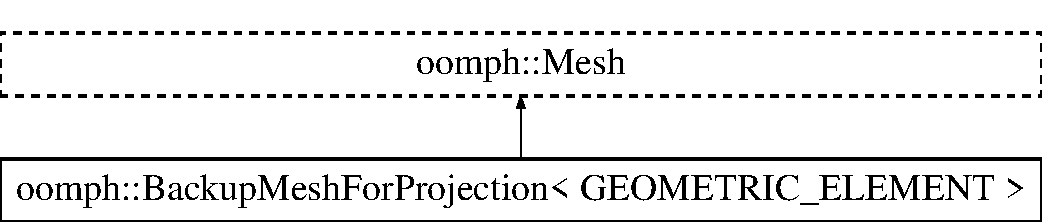
\includegraphics[height=2.000000cm]{classoomph_1_1BackupMeshForProjection}
\end{center}
\end{figure}
\subsection*{Public Member Functions}
\begin{DoxyCompactItemize}
\item 
\hyperlink{classoomph_1_1BackupMeshForProjection_a15032c7709e65ad4e1d00a6406786c6c}{Backup\+Mesh\+For\+Projection} (\hyperlink{classoomph_1_1Mesh}{Mesh} $\ast$mesh\+\_\+pt, const unsigned \&boundary\+\_\+id, const unsigned \&id\+\_\+of\+\_\+field\+\_\+to\+\_\+be\+\_\+projected=U\+I\+N\+T\+\_\+\+M\+AX)
\begin{DoxyCompactList}\small\item\em Constructor\+: Pass existing mesh and the boundary ID (need to find the boundary coordinates that are used for the projection. Optional final argument specifies the ID of the field (i.\+e. the index of the relevant nodal value!) to be projected. If omitted, we project all of them. \end{DoxyCompactList}\item 
void \hyperlink{classoomph_1_1BackupMeshForProjection_ab96a32a5934ef0edfbc50eb846cb3641}{project\+\_\+onto\+\_\+new\+\_\+mesh} (\hyperlink{classoomph_1_1Mesh}{Mesh} $\ast$new\+\_\+mesh\+\_\+pt)
\begin{DoxyCompactList}\small\item\em Project the solution that was present in the original mesh and from which this backup mesh was created onto the mesh pointed to by new\+\_\+mesh\+\_\+pt. Note that elements in the new mesh do not have to be projectable. The original mesh may by now have been deleted. \end{DoxyCompactList}\item 
void \hyperlink{classoomph_1_1BackupMeshForProjection_a228c554024e2651071bc0e1282641e1f}{copy\+\_\+onto\+\_\+original\+\_\+mesh} ()
\begin{DoxyCompactList}\small\item\em Copy nodal values back onto original mesh from which this mesh was built. This obviously only makes sense if the original mesh still exists! \end{DoxyCompactList}\end{DoxyCompactItemize}
\subsection*{Private Attributes}
\begin{DoxyCompactItemize}
\item 
std\+::map$<$ \hyperlink{classoomph_1_1Node}{Node} $\ast$, \hyperlink{classoomph_1_1Node}{Node} $\ast$ $>$ \hyperlink{classoomph_1_1BackupMeshForProjection_ae921b83792e20e1a5d974e1e89be6489}{New\+\_\+node\+\_\+pt}
\begin{DoxyCompactList}\small\item\em Map returning new node, labeled by node point in original mesh. \end{DoxyCompactList}\item 
unsigned \hyperlink{classoomph_1_1BackupMeshForProjection_a41581d95e01ec252aaa05b73f596d431}{Boundary\+\_\+id}
\begin{DoxyCompactList}\small\item\em Boundary id. \end{DoxyCompactList}\item 
unsigned \hyperlink{classoomph_1_1BackupMeshForProjection_aac26d2ee9ed6c7ee58f3f5c416be2047}{I\+D\+\_\+of\+\_\+field\+\_\+to\+\_\+be\+\_\+projected}
\begin{DoxyCompactList}\small\item\em ID of field to be projected (U\+I\+N\+T\+\_\+\+M\+AX if there isn\textquotesingle{}t one, in which case we\textquotesingle{}re doing all of them. \end{DoxyCompactList}\end{DoxyCompactItemize}
\subsection*{Additional Inherited Members}


\subsection{Detailed Description}
\subsubsection*{template$<$class G\+E\+O\+M\+E\+T\+R\+I\+C\+\_\+\+E\+L\+E\+M\+E\+NT$>$\newline
class oomph\+::\+Backup\+Mesh\+For\+Projection$<$ G\+E\+O\+M\+E\+T\+R\+I\+C\+\_\+\+E\+L\+E\+M\+E\+N\+T $>$}

Class that makes backup (via a deep copy) of a mesh, keeping alive enough information to allow the solution that is currently stored on the mesh to be projected onto another mesh sometime in the future (when the original mesh may already have been deleted). This is mainly useful for the projection of additional nodal values (such as Lagrange multipliers) created by Face\+Elements. A\+S\+S\+U\+M\+P\+T\+I\+ON\+: All fields in the element are represented by isoparametric Lagrange interpolation between the nodal values. Any fields that do not fall into this category will not be copied across correctly and if you\textquotesingle{}re unlucky the code may die...). 

Definition at line 237 of file face\+\_\+mesh\+\_\+project.\+h.



\subsection{Constructor \& Destructor Documentation}
\mbox{\Hypertarget{classoomph_1_1BackupMeshForProjection_a15032c7709e65ad4e1d00a6406786c6c}\label{classoomph_1_1BackupMeshForProjection_a15032c7709e65ad4e1d00a6406786c6c}} 
\index{oomph\+::\+Backup\+Mesh\+For\+Projection@{oomph\+::\+Backup\+Mesh\+For\+Projection}!Backup\+Mesh\+For\+Projection@{Backup\+Mesh\+For\+Projection}}
\index{Backup\+Mesh\+For\+Projection@{Backup\+Mesh\+For\+Projection}!oomph\+::\+Backup\+Mesh\+For\+Projection@{oomph\+::\+Backup\+Mesh\+For\+Projection}}
\subsubsection{\texorpdfstring{Backup\+Mesh\+For\+Projection()}{BackupMeshForProjection()}}
{\footnotesize\ttfamily template$<$class G\+E\+O\+M\+E\+T\+R\+I\+C\+\_\+\+E\+L\+E\+M\+E\+NT$>$ \\
\hyperlink{classoomph_1_1BackupMeshForProjection}{oomph\+::\+Backup\+Mesh\+For\+Projection}$<$ G\+E\+O\+M\+E\+T\+R\+I\+C\+\_\+\+E\+L\+E\+M\+E\+NT $>$\+::\hyperlink{classoomph_1_1BackupMeshForProjection}{Backup\+Mesh\+For\+Projection} (\begin{DoxyParamCaption}\item[{\hyperlink{classoomph_1_1Mesh}{Mesh} $\ast$}]{mesh\+\_\+pt,  }\item[{const unsigned \&}]{boundary\+\_\+id,  }\item[{const unsigned \&}]{id\+\_\+of\+\_\+field\+\_\+to\+\_\+be\+\_\+projected = {\ttfamily UINT\+\_\+MAX} }\end{DoxyParamCaption})\hspace{0.3cm}{\ttfamily [inline]}}



Constructor\+: Pass existing mesh and the boundary ID (need to find the boundary coordinates that are used for the projection. Optional final argument specifies the ID of the field (i.\+e. the index of the relevant nodal value!) to be projected. If omitted, we project all of them. 



Definition at line 247 of file face\+\_\+mesh\+\_\+project.\+h.



References oomph\+::\+Node\+::add\+\_\+to\+\_\+boundary(), oomph\+::\+Generic\+Lagrange\+Interpolated\+Projectable\+Element$<$ E\+L\+E\+M\+E\+N\+T $>$\+::\+Boundary\+\_\+id, e, oomph\+::\+Mesh\+::element\+\_\+pt(), oomph\+::\+Mesh\+::finite\+\_\+element\+\_\+pt(), oomph\+::\+Node\+::get\+\_\+coordinates\+\_\+on\+\_\+boundary(), i, oomph\+::\+Node\+::is\+\_\+on\+\_\+boundary(), oomph\+::\+Node\+::ncoordinates\+\_\+on\+\_\+boundary(), oomph\+::\+Node\+::ndim(), oomph\+::\+Mesh\+::nelement(), oomph\+::\+Generalised\+Element\+::ninternal\+\_\+data(), oomph\+::\+Mesh\+::nnode(), oomph\+::\+Finite\+Element\+::nnode(), oomph\+::\+Finite\+Element\+::\+Node\+\_\+pt, oomph\+::\+Finite\+Element\+::node\+\_\+pt(), oomph\+::\+Node\+::nposition\+\_\+type(), oomph\+::\+Data\+::ntstorage(), oomph\+::\+Data\+::nvalue(), oomph\+::\+Generic\+Lagrange\+Interpolated\+Projectable\+Element$<$ E\+L\+E\+M\+E\+N\+T $>$\+::set\+\_\+boundary\+\_\+id(), oomph\+::\+Node\+::set\+\_\+coordinates\+\_\+on\+\_\+boundary(), oomph\+::\+Data\+::set\+\_\+value(), t, oomph\+::\+Data\+::time\+\_\+stepper\+\_\+pt(), oomph\+::\+Node\+::value(), and oomph\+::\+Node\+::x().



\subsection{Member Function Documentation}
\mbox{\Hypertarget{classoomph_1_1BackupMeshForProjection_a228c554024e2651071bc0e1282641e1f}\label{classoomph_1_1BackupMeshForProjection_a228c554024e2651071bc0e1282641e1f}} 
\index{oomph\+::\+Backup\+Mesh\+For\+Projection@{oomph\+::\+Backup\+Mesh\+For\+Projection}!copy\+\_\+onto\+\_\+original\+\_\+mesh@{copy\+\_\+onto\+\_\+original\+\_\+mesh}}
\index{copy\+\_\+onto\+\_\+original\+\_\+mesh@{copy\+\_\+onto\+\_\+original\+\_\+mesh}!oomph\+::\+Backup\+Mesh\+For\+Projection@{oomph\+::\+Backup\+Mesh\+For\+Projection}}
\subsubsection{\texorpdfstring{copy\+\_\+onto\+\_\+original\+\_\+mesh()}{copy\_onto\_original\_mesh()}}
{\footnotesize\ttfamily template$<$class G\+E\+O\+M\+E\+T\+R\+I\+C\+\_\+\+E\+L\+E\+M\+E\+NT$>$ \\
void \hyperlink{classoomph_1_1BackupMeshForProjection}{oomph\+::\+Backup\+Mesh\+For\+Projection}$<$ G\+E\+O\+M\+E\+T\+R\+I\+C\+\_\+\+E\+L\+E\+M\+E\+NT $>$\+::copy\+\_\+onto\+\_\+original\+\_\+mesh (\begin{DoxyParamCaption}{ }\end{DoxyParamCaption})\hspace{0.3cm}{\ttfamily [inline]}}



Copy nodal values back onto original mesh from which this mesh was built. This obviously only makes sense if the original mesh still exists! 



Definition at line 443 of file face\+\_\+mesh\+\_\+project.\+h.



References i, oomph\+::\+Data\+::ntstorage(), oomph\+::\+Data\+::nvalue(), oomph\+::\+Data\+::set\+\_\+value(), t, and oomph\+::\+Node\+::value().



Referenced by oomph\+::\+Backup\+Mesh\+For\+Projection$<$ G\+E\+O\+M\+E\+T\+R\+I\+C\+\_\+\+E\+L\+E\+M\+E\+N\+T $>$\+::project\+\_\+onto\+\_\+new\+\_\+mesh().

\mbox{\Hypertarget{classoomph_1_1BackupMeshForProjection_ab96a32a5934ef0edfbc50eb846cb3641}\label{classoomph_1_1BackupMeshForProjection_ab96a32a5934ef0edfbc50eb846cb3641}} 
\index{oomph\+::\+Backup\+Mesh\+For\+Projection@{oomph\+::\+Backup\+Mesh\+For\+Projection}!project\+\_\+onto\+\_\+new\+\_\+mesh@{project\+\_\+onto\+\_\+new\+\_\+mesh}}
\index{project\+\_\+onto\+\_\+new\+\_\+mesh@{project\+\_\+onto\+\_\+new\+\_\+mesh}!oomph\+::\+Backup\+Mesh\+For\+Projection@{oomph\+::\+Backup\+Mesh\+For\+Projection}}
\subsubsection{\texorpdfstring{project\+\_\+onto\+\_\+new\+\_\+mesh()}{project\_onto\_new\_mesh()}}
{\footnotesize\ttfamily template$<$class G\+E\+O\+M\+E\+T\+R\+I\+C\+\_\+\+E\+L\+E\+M\+E\+NT$>$ \\
void \hyperlink{classoomph_1_1BackupMeshForProjection}{oomph\+::\+Backup\+Mesh\+For\+Projection}$<$ G\+E\+O\+M\+E\+T\+R\+I\+C\+\_\+\+E\+L\+E\+M\+E\+NT $>$\+::project\+\_\+onto\+\_\+new\+\_\+mesh (\begin{DoxyParamCaption}\item[{\hyperlink{classoomph_1_1Mesh}{Mesh} $\ast$}]{new\+\_\+mesh\+\_\+pt }\end{DoxyParamCaption})\hspace{0.3cm}{\ttfamily [inline]}}



Project the solution that was present in the original mesh and from which this backup mesh was created onto the mesh pointed to by new\+\_\+mesh\+\_\+pt. Note that elements in the new mesh do not have to be projectable. The original mesh may by now have been deleted. 



Definition at line 410 of file face\+\_\+mesh\+\_\+project.\+h.



References oomph\+::\+Generic\+Lagrange\+Interpolated\+Projectable\+Element$<$ E\+L\+E\+M\+E\+N\+T $>$\+::\+Boundary\+\_\+id, and oomph\+::\+Backup\+Mesh\+For\+Projection$<$ G\+E\+O\+M\+E\+T\+R\+I\+C\+\_\+\+E\+L\+E\+M\+E\+N\+T $>$\+::copy\+\_\+onto\+\_\+original\+\_\+mesh().



\subsection{Member Data Documentation}
\mbox{\Hypertarget{classoomph_1_1BackupMeshForProjection_a41581d95e01ec252aaa05b73f596d431}\label{classoomph_1_1BackupMeshForProjection_a41581d95e01ec252aaa05b73f596d431}} 
\index{oomph\+::\+Backup\+Mesh\+For\+Projection@{oomph\+::\+Backup\+Mesh\+For\+Projection}!Boundary\+\_\+id@{Boundary\+\_\+id}}
\index{Boundary\+\_\+id@{Boundary\+\_\+id}!oomph\+::\+Backup\+Mesh\+For\+Projection@{oomph\+::\+Backup\+Mesh\+For\+Projection}}
\subsubsection{\texorpdfstring{Boundary\+\_\+id}{Boundary\_id}}
{\footnotesize\ttfamily template$<$class G\+E\+O\+M\+E\+T\+R\+I\+C\+\_\+\+E\+L\+E\+M\+E\+NT$>$ \\
unsigned \hyperlink{classoomph_1_1BackupMeshForProjection}{oomph\+::\+Backup\+Mesh\+For\+Projection}$<$ G\+E\+O\+M\+E\+T\+R\+I\+C\+\_\+\+E\+L\+E\+M\+E\+NT $>$\+::Boundary\+\_\+id\hspace{0.3cm}{\ttfamily [private]}}



Boundary id. 



Definition at line 489 of file face\+\_\+mesh\+\_\+project.\+h.

\mbox{\Hypertarget{classoomph_1_1BackupMeshForProjection_aac26d2ee9ed6c7ee58f3f5c416be2047}\label{classoomph_1_1BackupMeshForProjection_aac26d2ee9ed6c7ee58f3f5c416be2047}} 
\index{oomph\+::\+Backup\+Mesh\+For\+Projection@{oomph\+::\+Backup\+Mesh\+For\+Projection}!I\+D\+\_\+of\+\_\+field\+\_\+to\+\_\+be\+\_\+projected@{I\+D\+\_\+of\+\_\+field\+\_\+to\+\_\+be\+\_\+projected}}
\index{I\+D\+\_\+of\+\_\+field\+\_\+to\+\_\+be\+\_\+projected@{I\+D\+\_\+of\+\_\+field\+\_\+to\+\_\+be\+\_\+projected}!oomph\+::\+Backup\+Mesh\+For\+Projection@{oomph\+::\+Backup\+Mesh\+For\+Projection}}
\subsubsection{\texorpdfstring{I\+D\+\_\+of\+\_\+field\+\_\+to\+\_\+be\+\_\+projected}{ID\_of\_field\_to\_be\_projected}}
{\footnotesize\ttfamily template$<$class G\+E\+O\+M\+E\+T\+R\+I\+C\+\_\+\+E\+L\+E\+M\+E\+NT$>$ \\
unsigned \hyperlink{classoomph_1_1BackupMeshForProjection}{oomph\+::\+Backup\+Mesh\+For\+Projection}$<$ G\+E\+O\+M\+E\+T\+R\+I\+C\+\_\+\+E\+L\+E\+M\+E\+NT $>$\+::I\+D\+\_\+of\+\_\+field\+\_\+to\+\_\+be\+\_\+projected\hspace{0.3cm}{\ttfamily [private]}}



ID of field to be projected (U\+I\+N\+T\+\_\+\+M\+AX if there isn\textquotesingle{}t one, in which case we\textquotesingle{}re doing all of them. 



Definition at line 493 of file face\+\_\+mesh\+\_\+project.\+h.

\mbox{\Hypertarget{classoomph_1_1BackupMeshForProjection_ae921b83792e20e1a5d974e1e89be6489}\label{classoomph_1_1BackupMeshForProjection_ae921b83792e20e1a5d974e1e89be6489}} 
\index{oomph\+::\+Backup\+Mesh\+For\+Projection@{oomph\+::\+Backup\+Mesh\+For\+Projection}!New\+\_\+node\+\_\+pt@{New\+\_\+node\+\_\+pt}}
\index{New\+\_\+node\+\_\+pt@{New\+\_\+node\+\_\+pt}!oomph\+::\+Backup\+Mesh\+For\+Projection@{oomph\+::\+Backup\+Mesh\+For\+Projection}}
\subsubsection{\texorpdfstring{New\+\_\+node\+\_\+pt}{New\_node\_pt}}
{\footnotesize\ttfamily template$<$class G\+E\+O\+M\+E\+T\+R\+I\+C\+\_\+\+E\+L\+E\+M\+E\+NT$>$ \\
std\+::map$<$\hyperlink{classoomph_1_1Node}{Node}$\ast$,\hyperlink{classoomph_1_1Node}{Node}$\ast$$>$ \hyperlink{classoomph_1_1BackupMeshForProjection}{oomph\+::\+Backup\+Mesh\+For\+Projection}$<$ G\+E\+O\+M\+E\+T\+R\+I\+C\+\_\+\+E\+L\+E\+M\+E\+NT $>$\+::New\+\_\+node\+\_\+pt\hspace{0.3cm}{\ttfamily [private]}}



Map returning new node, labeled by node point in original mesh. 



Definition at line 486 of file face\+\_\+mesh\+\_\+project.\+h.



The documentation for this class was generated from the following file\+:\begin{DoxyCompactItemize}
\item 
\hyperlink{face__mesh__project_8h}{face\+\_\+mesh\+\_\+project.\+h}\end{DoxyCompactItemize}

\hypertarget{classoomph_1_1BackwardStepQuadMesh}{}\section{oomph\+:\+:Backward\+Step\+Quad\+Mesh$<$ E\+L\+E\+M\+E\+NT $>$ Class Template Reference}
\label{classoomph_1_1BackwardStepQuadMesh}\index{oomph\+::\+Backward\+Step\+Quad\+Mesh$<$ E\+L\+E\+M\+E\+N\+T $>$@{oomph\+::\+Backward\+Step\+Quad\+Mesh$<$ E\+L\+E\+M\+E\+N\+T $>$}}


Backward step mesh.  




{\ttfamily \#include $<$backward\+\_\+step\+\_\+mesh.\+template.\+h$>$}

Inheritance diagram for oomph\+:\+:Backward\+Step\+Quad\+Mesh$<$ E\+L\+E\+M\+E\+NT $>$\+:\begin{figure}[H]
\begin{center}
\leavevmode
\includegraphics[height=5.000000cm]{classoomph_1_1BackwardStepQuadMesh}
\end{center}
\end{figure}
\subsection*{Public Member Functions}
\begin{DoxyCompactItemize}
\item 
\hyperlink{classoomph_1_1BackwardStepQuadMesh_ae8374ae7d3646c00fec4fc9c2d604cf8}{Backward\+Step\+Quad\+Mesh} (const unsigned \&\hyperlink{classoomph_1_1RectangularQuadMesh_abfef93d6322886cdce14a437186e4821}{nx}, const unsigned \&\hyperlink{classoomph_1_1RectangularQuadMesh_a86d76a55eb7c4e8bca9b74d23c8b0412}{ny}, const unsigned \&nx\+\_\+cut\+\_\+out, const unsigned \&ny\+\_\+cut\+\_\+out, const double \&lx, const double \&ly, \hyperlink{classoomph_1_1TimeStepper}{Time\+Stepper} $\ast$time\+\_\+stepper\+\_\+pt=\&\hyperlink{classoomph_1_1Mesh_a12243d0fee2b1fcee729ee5a4777ea10}{Mesh\+::\+Default\+\_\+\+Time\+Stepper})
\begin{DoxyCompactList}\small\item\em Pass overall number of elements in the horizontal and vertical directions, nx and ny, and the corresponding dimensions, lx and ly. nx\+\_\+cut\+\_\+out and ny\+\_\+cut\+\_\+out elements are cut out from the lower right corner to create the (reversed) backward step geometry. Timestepper defaults to \hyperlink{classoomph_1_1Steady}{Steady}. \end{DoxyCompactList}\item 
virtual \hyperlink{classoomph_1_1BackwardStepQuadMesh_aec4e05ad80d83327050653ebabce9564}{$\sim$\+Backward\+Step\+Quad\+Mesh} ()
\begin{DoxyCompactList}\small\item\em Destructor\+: Empty. \end{DoxyCompactList}\end{DoxyCompactItemize}
\subsection*{Private Member Functions}
\begin{DoxyCompactItemize}
\item 
void \hyperlink{classoomph_1_1BackwardStepQuadMesh_ab71a6f2854d36b845ed79dccb0101991}{build\+\_\+mesh} (const unsigned \&\hyperlink{classoomph_1_1RectangularQuadMesh_abfef93d6322886cdce14a437186e4821}{nx}, const unsigned \&\hyperlink{classoomph_1_1RectangularQuadMesh_a86d76a55eb7c4e8bca9b74d23c8b0412}{ny}, const unsigned \&nx\+\_\+cut\+\_\+out, const unsigned \&ny\+\_\+cut\+\_\+out, const double \&lx, const double \&ly)
\begin{DoxyCompactList}\small\item\em Actual build function. \end{DoxyCompactList}\end{DoxyCompactItemize}
\subsection*{Additional Inherited Members}


\subsection{Detailed Description}
\subsubsection*{template$<$class E\+L\+E\+M\+E\+NT$>$\newline
class oomph\+::\+Backward\+Step\+Quad\+Mesh$<$ E\+L\+E\+M\+E\+N\+T $>$}

Backward step mesh. 

Definition at line 51 of file backward\+\_\+step\+\_\+mesh.\+template.\+h.



\subsection{Constructor \& Destructor Documentation}
\mbox{\Hypertarget{classoomph_1_1BackwardStepQuadMesh_ae8374ae7d3646c00fec4fc9c2d604cf8}\label{classoomph_1_1BackwardStepQuadMesh_ae8374ae7d3646c00fec4fc9c2d604cf8}} 
\index{oomph\+::\+Backward\+Step\+Quad\+Mesh@{oomph\+::\+Backward\+Step\+Quad\+Mesh}!Backward\+Step\+Quad\+Mesh@{Backward\+Step\+Quad\+Mesh}}
\index{Backward\+Step\+Quad\+Mesh@{Backward\+Step\+Quad\+Mesh}!oomph\+::\+Backward\+Step\+Quad\+Mesh@{oomph\+::\+Backward\+Step\+Quad\+Mesh}}
\subsubsection{\texorpdfstring{Backward\+Step\+Quad\+Mesh()}{BackwardStepQuadMesh()}}
{\footnotesize\ttfamily template$<$class E\+L\+E\+M\+E\+NT $>$ \\
\hyperlink{classoomph_1_1BackwardStepQuadMesh}{oomph\+::\+Backward\+Step\+Quad\+Mesh}$<$ E\+L\+E\+M\+E\+NT $>$\+::\hyperlink{classoomph_1_1BackwardStepQuadMesh}{Backward\+Step\+Quad\+Mesh} (\begin{DoxyParamCaption}\item[{const unsigned \&}]{nx,  }\item[{const unsigned \&}]{ny,  }\item[{const unsigned \&}]{nx\+\_\+cut\+\_\+out,  }\item[{const unsigned \&}]{ny\+\_\+cut\+\_\+out,  }\item[{const double \&}]{lx,  }\item[{const double \&}]{ly,  }\item[{\hyperlink{classoomph_1_1TimeStepper}{Time\+Stepper} $\ast$}]{time\+\_\+stepper\+\_\+pt = {\ttfamily \&\hyperlink{classoomph_1_1Mesh_a12243d0fee2b1fcee729ee5a4777ea10}{Mesh\+::\+Default\+\_\+\+Time\+Stepper}} }\end{DoxyParamCaption})\hspace{0.3cm}{\ttfamily [inline]}}



Pass overall number of elements in the horizontal and vertical directions, nx and ny, and the corresponding dimensions, lx and ly. nx\+\_\+cut\+\_\+out and ny\+\_\+cut\+\_\+out elements are cut out from the lower right corner to create the (reversed) backward step geometry. Timestepper defaults to \hyperlink{classoomph_1_1Steady}{Steady}. 



Definition at line 63 of file backward\+\_\+step\+\_\+mesh.\+template.\+h.



References oomph\+::\+Backward\+Step\+Quad\+Mesh$<$ E\+L\+E\+M\+E\+N\+T $>$\+::build\+\_\+mesh().

\mbox{\Hypertarget{classoomph_1_1BackwardStepQuadMesh_aec4e05ad80d83327050653ebabce9564}\label{classoomph_1_1BackwardStepQuadMesh_aec4e05ad80d83327050653ebabce9564}} 
\index{oomph\+::\+Backward\+Step\+Quad\+Mesh@{oomph\+::\+Backward\+Step\+Quad\+Mesh}!````~Backward\+Step\+Quad\+Mesh@{$\sim$\+Backward\+Step\+Quad\+Mesh}}
\index{````~Backward\+Step\+Quad\+Mesh@{$\sim$\+Backward\+Step\+Quad\+Mesh}!oomph\+::\+Backward\+Step\+Quad\+Mesh@{oomph\+::\+Backward\+Step\+Quad\+Mesh}}
\subsubsection{\texorpdfstring{$\sim$\+Backward\+Step\+Quad\+Mesh()}{~BackwardStepQuadMesh()}}
{\footnotesize\ttfamily template$<$class E\+L\+E\+M\+E\+NT $>$ \\
virtual \hyperlink{classoomph_1_1BackwardStepQuadMesh}{oomph\+::\+Backward\+Step\+Quad\+Mesh}$<$ E\+L\+E\+M\+E\+NT $>$\+::$\sim$\hyperlink{classoomph_1_1BackwardStepQuadMesh}{Backward\+Step\+Quad\+Mesh} (\begin{DoxyParamCaption}{ }\end{DoxyParamCaption})\hspace{0.3cm}{\ttfamily [inline]}, {\ttfamily [virtual]}}



Destructor\+: Empty. 



Definition at line 78 of file backward\+\_\+step\+\_\+mesh.\+template.\+h.



References oomph\+::\+Backward\+Step\+Quad\+Mesh$<$ E\+L\+E\+M\+E\+N\+T $>$\+::build\+\_\+mesh(), oomph\+::\+Rectangular\+Quad\+Mesh$<$ E\+L\+E\+M\+E\+N\+T $>$\+::nx(), and oomph\+::\+Rectangular\+Quad\+Mesh$<$ E\+L\+E\+M\+E\+N\+T $>$\+::ny().



\subsection{Member Function Documentation}
\mbox{\Hypertarget{classoomph_1_1BackwardStepQuadMesh_ab71a6f2854d36b845ed79dccb0101991}\label{classoomph_1_1BackwardStepQuadMesh_ab71a6f2854d36b845ed79dccb0101991}} 
\index{oomph\+::\+Backward\+Step\+Quad\+Mesh@{oomph\+::\+Backward\+Step\+Quad\+Mesh}!build\+\_\+mesh@{build\+\_\+mesh}}
\index{build\+\_\+mesh@{build\+\_\+mesh}!oomph\+::\+Backward\+Step\+Quad\+Mesh@{oomph\+::\+Backward\+Step\+Quad\+Mesh}}
\subsubsection{\texorpdfstring{build\+\_\+mesh()}{build\_mesh()}}
{\footnotesize\ttfamily template$<$class E\+L\+E\+M\+E\+NT $>$ \\
void \hyperlink{classoomph_1_1BackwardStepQuadMesh}{oomph\+::\+Backward\+Step\+Quad\+Mesh}$<$ E\+L\+E\+M\+E\+NT $>$\+::build\+\_\+mesh (\begin{DoxyParamCaption}\item[{const unsigned \&}]{nx,  }\item[{const unsigned \&}]{ny,  }\item[{const unsigned \&}]{nx\+\_\+cut\+\_\+out,  }\item[{const unsigned \&}]{ny\+\_\+cut\+\_\+out,  }\item[{const double \&}]{lx,  }\item[{const double \&}]{ly }\end{DoxyParamCaption})\hspace{0.3cm}{\ttfamily [private]}}



Actual build function. 

Actual build function. Pass overall number of elements in the horizontal and vertical directions, nx and ny, and the corresponding dimensions, lx and ly. nx\+\_\+cut\+\_\+out and ny\+\_\+cut\+\_\+out elements are cut out from the lower right corner to create the (reversed) backward step geometry. Timestepper defaults to \hyperlink{classoomph_1_1Steady}{Steady}. 

Definition at line 52 of file backward\+\_\+step\+\_\+mesh.\+template.\+cc.



References e, i, oomph\+::\+Node\+::is\+\_\+on\+\_\+boundary(), oomph\+::\+Finite\+Element\+::nnode(), oomph\+::\+Finite\+Element\+::nnode\+\_\+1d(), and oomph\+::\+Finite\+Element\+::node\+\_\+pt().



Referenced by oomph\+::\+Backward\+Step\+Quad\+Mesh$<$ E\+L\+E\+M\+E\+N\+T $>$\+::\+Backward\+Step\+Quad\+Mesh(), and oomph\+::\+Backward\+Step\+Quad\+Mesh$<$ E\+L\+E\+M\+E\+N\+T $>$\+::$\sim$\+Backward\+Step\+Quad\+Mesh().



The documentation for this class was generated from the following files\+:\begin{DoxyCompactItemize}
\item 
\hyperlink{backward__step__mesh_8template_8h}{backward\+\_\+step\+\_\+mesh.\+template.\+h}\item 
\hyperlink{backward__step__mesh_8template_8cc}{backward\+\_\+step\+\_\+mesh.\+template.\+cc}\end{DoxyCompactItemize}

\hypertarget{structoomph_1_1UnstructuredTwoDMeshGeometryBase_1_1base__vertex__info}{}\section{oomph\+:\+:Unstructured\+Two\+D\+Mesh\+Geometry\+Base\+:\+:base\+\_\+vertex\+\_\+info Struct Reference}
\label{structoomph_1_1UnstructuredTwoDMeshGeometryBase_1_1base__vertex__info}\index{oomph\+::\+Unstructured\+Two\+D\+Mesh\+Geometry\+Base\+::base\+\_\+vertex\+\_\+info@{oomph\+::\+Unstructured\+Two\+D\+Mesh\+Geometry\+Base\+::base\+\_\+vertex\+\_\+info}}


\hyperlink{classoomph_1_1Data}{Data} structure to store the base vertex info, initial or final vertex in the polylines have an associated base vertex.  




{\ttfamily \#include $<$unstructured\+\_\+two\+\_\+d\+\_\+mesh\+\_\+geometry\+\_\+base.\+h$>$}

\subsection*{Public Attributes}
\begin{DoxyCompactItemize}
\item 
bool \hyperlink{structoomph_1_1UnstructuredTwoDMeshGeometryBase_1_1base__vertex__info_a3448db94f297b6d9d01d23ed3c21228c}{has\+\_\+base\+\_\+vertex\+\_\+assigned}
\item 
bool \hyperlink{structoomph_1_1UnstructuredTwoDMeshGeometryBase_1_1base__vertex__info_a271c3c8a2e0e7e878e7ee7087385833f}{is\+\_\+base\+\_\+vertex}
\item 
unsigned \hyperlink{structoomph_1_1UnstructuredTwoDMeshGeometryBase_1_1base__vertex__info_a873a731fa8ed34d8cbcde0f174068c42}{boundary\+\_\+id}
\item 
unsigned \hyperlink{structoomph_1_1UnstructuredTwoDMeshGeometryBase_1_1base__vertex__info_abf6b6e60919954406c0acfe8fb7b9dd9}{boundary\+\_\+chunk}
\item 
unsigned \hyperlink{structoomph_1_1UnstructuredTwoDMeshGeometryBase_1_1base__vertex__info_a9b61cf78b552a59505103d81ac830bfb}{vertex\+\_\+number}
\end{DoxyCompactItemize}


\subsection{Detailed Description}
\hyperlink{classoomph_1_1Data}{Data} structure to store the base vertex info, initial or final vertex in the polylines have an associated base vertex. 

Definition at line 2366 of file unstructured\+\_\+two\+\_\+d\+\_\+mesh\+\_\+geometry\+\_\+base.\+h.



\subsection{Member Data Documentation}
\mbox{\Hypertarget{structoomph_1_1UnstructuredTwoDMeshGeometryBase_1_1base__vertex__info_abf6b6e60919954406c0acfe8fb7b9dd9}\label{structoomph_1_1UnstructuredTwoDMeshGeometryBase_1_1base__vertex__info_abf6b6e60919954406c0acfe8fb7b9dd9}} 
\index{oomph\+::\+Unstructured\+Two\+D\+Mesh\+Geometry\+Base\+::base\+\_\+vertex\+\_\+info@{oomph\+::\+Unstructured\+Two\+D\+Mesh\+Geometry\+Base\+::base\+\_\+vertex\+\_\+info}!boundary\+\_\+chunk@{boundary\+\_\+chunk}}
\index{boundary\+\_\+chunk@{boundary\+\_\+chunk}!oomph\+::\+Unstructured\+Two\+D\+Mesh\+Geometry\+Base\+::base\+\_\+vertex\+\_\+info@{oomph\+::\+Unstructured\+Two\+D\+Mesh\+Geometry\+Base\+::base\+\_\+vertex\+\_\+info}}
\subsubsection{\texorpdfstring{boundary\+\_\+chunk}{boundary\_chunk}}
{\footnotesize\ttfamily unsigned oomph\+::\+Unstructured\+Two\+D\+Mesh\+Geometry\+Base\+::base\+\_\+vertex\+\_\+info\+::boundary\+\_\+chunk}



Definition at line 2370 of file unstructured\+\_\+two\+\_\+d\+\_\+mesh\+\_\+geometry\+\_\+base.\+h.



Referenced by oomph\+::\+Unstructured\+Two\+D\+Mesh\+Geometry\+Base\+::add\+\_\+base\+\_\+vertex\+\_\+info\+\_\+helper(), oomph\+::\+Unstructured\+Two\+D\+Mesh\+Geometry\+Base\+::build\+\_\+triangulateio(), and oomph\+::\+Unstructured\+Two\+D\+Mesh\+Geometry\+Base\+::initialise\+\_\+base\+\_\+vertex().

\mbox{\Hypertarget{structoomph_1_1UnstructuredTwoDMeshGeometryBase_1_1base__vertex__info_a873a731fa8ed34d8cbcde0f174068c42}\label{structoomph_1_1UnstructuredTwoDMeshGeometryBase_1_1base__vertex__info_a873a731fa8ed34d8cbcde0f174068c42}} 
\index{oomph\+::\+Unstructured\+Two\+D\+Mesh\+Geometry\+Base\+::base\+\_\+vertex\+\_\+info@{oomph\+::\+Unstructured\+Two\+D\+Mesh\+Geometry\+Base\+::base\+\_\+vertex\+\_\+info}!boundary\+\_\+id@{boundary\+\_\+id}}
\index{boundary\+\_\+id@{boundary\+\_\+id}!oomph\+::\+Unstructured\+Two\+D\+Mesh\+Geometry\+Base\+::base\+\_\+vertex\+\_\+info@{oomph\+::\+Unstructured\+Two\+D\+Mesh\+Geometry\+Base\+::base\+\_\+vertex\+\_\+info}}
\subsubsection{\texorpdfstring{boundary\+\_\+id}{boundary\_id}}
{\footnotesize\ttfamily unsigned oomph\+::\+Unstructured\+Two\+D\+Mesh\+Geometry\+Base\+::base\+\_\+vertex\+\_\+info\+::boundary\+\_\+id}



Definition at line 2369 of file unstructured\+\_\+two\+\_\+d\+\_\+mesh\+\_\+geometry\+\_\+base.\+h.



Referenced by oomph\+::\+Unstructured\+Two\+D\+Mesh\+Geometry\+Base\+::add\+\_\+base\+\_\+vertex\+\_\+info\+\_\+helper(), oomph\+::\+Unstructured\+Two\+D\+Mesh\+Geometry\+Base\+::build\+\_\+triangulateio(), and oomph\+::\+Unstructured\+Two\+D\+Mesh\+Geometry\+Base\+::initialise\+\_\+base\+\_\+vertex().

\mbox{\Hypertarget{structoomph_1_1UnstructuredTwoDMeshGeometryBase_1_1base__vertex__info_a3448db94f297b6d9d01d23ed3c21228c}\label{structoomph_1_1UnstructuredTwoDMeshGeometryBase_1_1base__vertex__info_a3448db94f297b6d9d01d23ed3c21228c}} 
\index{oomph\+::\+Unstructured\+Two\+D\+Mesh\+Geometry\+Base\+::base\+\_\+vertex\+\_\+info@{oomph\+::\+Unstructured\+Two\+D\+Mesh\+Geometry\+Base\+::base\+\_\+vertex\+\_\+info}!has\+\_\+base\+\_\+vertex\+\_\+assigned@{has\+\_\+base\+\_\+vertex\+\_\+assigned}}
\index{has\+\_\+base\+\_\+vertex\+\_\+assigned@{has\+\_\+base\+\_\+vertex\+\_\+assigned}!oomph\+::\+Unstructured\+Two\+D\+Mesh\+Geometry\+Base\+::base\+\_\+vertex\+\_\+info@{oomph\+::\+Unstructured\+Two\+D\+Mesh\+Geometry\+Base\+::base\+\_\+vertex\+\_\+info}}
\subsubsection{\texorpdfstring{has\+\_\+base\+\_\+vertex\+\_\+assigned}{has\_base\_vertex\_assigned}}
{\footnotesize\ttfamily bool oomph\+::\+Unstructured\+Two\+D\+Mesh\+Geometry\+Base\+::base\+\_\+vertex\+\_\+info\+::has\+\_\+base\+\_\+vertex\+\_\+assigned}



Definition at line 2367 of file unstructured\+\_\+two\+\_\+d\+\_\+mesh\+\_\+geometry\+\_\+base.\+h.



Referenced by oomph\+::\+Unstructured\+Two\+D\+Mesh\+Geometry\+Base\+::add\+\_\+base\+\_\+vertex\+\_\+info\+\_\+helper(), oomph\+::\+Unstructured\+Two\+D\+Mesh\+Geometry\+Base\+::build\+\_\+triangulateio(), and oomph\+::\+Unstructured\+Two\+D\+Mesh\+Geometry\+Base\+::initialise\+\_\+base\+\_\+vertex().

\mbox{\Hypertarget{structoomph_1_1UnstructuredTwoDMeshGeometryBase_1_1base__vertex__info_a271c3c8a2e0e7e878e7ee7087385833f}\label{structoomph_1_1UnstructuredTwoDMeshGeometryBase_1_1base__vertex__info_a271c3c8a2e0e7e878e7ee7087385833f}} 
\index{oomph\+::\+Unstructured\+Two\+D\+Mesh\+Geometry\+Base\+::base\+\_\+vertex\+\_\+info@{oomph\+::\+Unstructured\+Two\+D\+Mesh\+Geometry\+Base\+::base\+\_\+vertex\+\_\+info}!is\+\_\+base\+\_\+vertex@{is\+\_\+base\+\_\+vertex}}
\index{is\+\_\+base\+\_\+vertex@{is\+\_\+base\+\_\+vertex}!oomph\+::\+Unstructured\+Two\+D\+Mesh\+Geometry\+Base\+::base\+\_\+vertex\+\_\+info@{oomph\+::\+Unstructured\+Two\+D\+Mesh\+Geometry\+Base\+::base\+\_\+vertex\+\_\+info}}
\subsubsection{\texorpdfstring{is\+\_\+base\+\_\+vertex}{is\_base\_vertex}}
{\footnotesize\ttfamily bool oomph\+::\+Unstructured\+Two\+D\+Mesh\+Geometry\+Base\+::base\+\_\+vertex\+\_\+info\+::is\+\_\+base\+\_\+vertex}



Definition at line 2368 of file unstructured\+\_\+two\+\_\+d\+\_\+mesh\+\_\+geometry\+\_\+base.\+h.



Referenced by oomph\+::\+Unstructured\+Two\+D\+Mesh\+Geometry\+Base\+::add\+\_\+base\+\_\+vertex\+\_\+info\+\_\+helper(), oomph\+::\+Unstructured\+Two\+D\+Mesh\+Geometry\+Base\+::build\+\_\+triangulateio(), and oomph\+::\+Unstructured\+Two\+D\+Mesh\+Geometry\+Base\+::initialise\+\_\+base\+\_\+vertex().

\mbox{\Hypertarget{structoomph_1_1UnstructuredTwoDMeshGeometryBase_1_1base__vertex__info_a9b61cf78b552a59505103d81ac830bfb}\label{structoomph_1_1UnstructuredTwoDMeshGeometryBase_1_1base__vertex__info_a9b61cf78b552a59505103d81ac830bfb}} 
\index{oomph\+::\+Unstructured\+Two\+D\+Mesh\+Geometry\+Base\+::base\+\_\+vertex\+\_\+info@{oomph\+::\+Unstructured\+Two\+D\+Mesh\+Geometry\+Base\+::base\+\_\+vertex\+\_\+info}!vertex\+\_\+number@{vertex\+\_\+number}}
\index{vertex\+\_\+number@{vertex\+\_\+number}!oomph\+::\+Unstructured\+Two\+D\+Mesh\+Geometry\+Base\+::base\+\_\+vertex\+\_\+info@{oomph\+::\+Unstructured\+Two\+D\+Mesh\+Geometry\+Base\+::base\+\_\+vertex\+\_\+info}}
\subsubsection{\texorpdfstring{vertex\+\_\+number}{vertex\_number}}
{\footnotesize\ttfamily unsigned oomph\+::\+Unstructured\+Two\+D\+Mesh\+Geometry\+Base\+::base\+\_\+vertex\+\_\+info\+::vertex\+\_\+number}



Definition at line 2371 of file unstructured\+\_\+two\+\_\+d\+\_\+mesh\+\_\+geometry\+\_\+base.\+h.



Referenced by oomph\+::\+Unstructured\+Two\+D\+Mesh\+Geometry\+Base\+::add\+\_\+base\+\_\+vertex\+\_\+info\+\_\+helper(), oomph\+::\+Unstructured\+Two\+D\+Mesh\+Geometry\+Base\+::build\+\_\+triangulateio(), and oomph\+::\+Unstructured\+Two\+D\+Mesh\+Geometry\+Base\+::initialise\+\_\+base\+\_\+vertex().



The documentation for this struct was generated from the following file\+:\begin{DoxyCompactItemize}
\item 
\hyperlink{unstructured__two__d__mesh__geometry__base_8h}{unstructured\+\_\+two\+\_\+d\+\_\+mesh\+\_\+geometry\+\_\+base.\+h}\end{DoxyCompactItemize}

\hypertarget{structoomph_1_1TriangleBoundaryHelper_1_1BCInfo}{}\section{oomph\+:\+:Triangle\+Boundary\+Helper\+:\+:B\+C\+Info Struct Reference}
\label{structoomph_1_1TriangleBoundaryHelper_1_1BCInfo}\index{oomph\+::\+Triangle\+Boundary\+Helper\+::\+B\+C\+Info@{oomph\+::\+Triangle\+Boundary\+Helper\+::\+B\+C\+Info}}


Structure for Boundary Informations.  




{\ttfamily \#include $<$unstructured\+\_\+two\+\_\+d\+\_\+mesh\+\_\+geometry\+\_\+base.\+h$>$}

\subsection*{Public Attributes}
\begin{DoxyCompactItemize}
\item 
unsigned \hyperlink{structoomph_1_1TriangleBoundaryHelper_1_1BCInfo_af1ecd57ea7e0cbb2f9a1bfe11dfec565}{Face\+\_\+id}
\begin{DoxyCompactList}\small\item\em Face ID. \end{DoxyCompactList}\item 
unsigned \hyperlink{structoomph_1_1TriangleBoundaryHelper_1_1BCInfo_ad8088be156a93342df04702405cb3225}{Boundary}
\begin{DoxyCompactList}\small\item\em Boundary ID. \end{DoxyCompactList}\item 
\hyperlink{classoomph_1_1FiniteElement}{Finite\+Element} $\ast$ \hyperlink{structoomph_1_1TriangleBoundaryHelper_1_1BCInfo_a263292ad2a54d23d077ec612d52ddde6}{F\+E\+\_\+pt}
\begin{DoxyCompactList}\small\item\em Pointer to bulk finite element. \end{DoxyCompactList}\end{DoxyCompactItemize}


\subsection{Detailed Description}
Structure for Boundary Informations. 

Definition at line 5492 of file unstructured\+\_\+two\+\_\+d\+\_\+mesh\+\_\+geometry\+\_\+base.\+h.



\subsection{Member Data Documentation}
\mbox{\Hypertarget{structoomph_1_1TriangleBoundaryHelper_1_1BCInfo_ad8088be156a93342df04702405cb3225}\label{structoomph_1_1TriangleBoundaryHelper_1_1BCInfo_ad8088be156a93342df04702405cb3225}} 
\index{oomph\+::\+Triangle\+Boundary\+Helper\+::\+B\+C\+Info@{oomph\+::\+Triangle\+Boundary\+Helper\+::\+B\+C\+Info}!Boundary@{Boundary}}
\index{Boundary@{Boundary}!oomph\+::\+Triangle\+Boundary\+Helper\+::\+B\+C\+Info@{oomph\+::\+Triangle\+Boundary\+Helper\+::\+B\+C\+Info}}
\subsubsection{\texorpdfstring{Boundary}{Boundary}}
{\footnotesize\ttfamily unsigned oomph\+::\+Triangle\+Boundary\+Helper\+::\+B\+C\+Info\+::\+Boundary}



Boundary ID. 



Definition at line 5499 of file unstructured\+\_\+two\+\_\+d\+\_\+mesh\+\_\+geometry\+\_\+base.\+h.



Referenced by oomph\+::\+Triangle\+Mesh\+Base\+::setup\+\_\+boundary\+\_\+element\+\_\+info().

\mbox{\Hypertarget{structoomph_1_1TriangleBoundaryHelper_1_1BCInfo_af1ecd57ea7e0cbb2f9a1bfe11dfec565}\label{structoomph_1_1TriangleBoundaryHelper_1_1BCInfo_af1ecd57ea7e0cbb2f9a1bfe11dfec565}} 
\index{oomph\+::\+Triangle\+Boundary\+Helper\+::\+B\+C\+Info@{oomph\+::\+Triangle\+Boundary\+Helper\+::\+B\+C\+Info}!Face\+\_\+id@{Face\+\_\+id}}
\index{Face\+\_\+id@{Face\+\_\+id}!oomph\+::\+Triangle\+Boundary\+Helper\+::\+B\+C\+Info@{oomph\+::\+Triangle\+Boundary\+Helper\+::\+B\+C\+Info}}
\subsubsection{\texorpdfstring{Face\+\_\+id}{Face\_id}}
{\footnotesize\ttfamily unsigned oomph\+::\+Triangle\+Boundary\+Helper\+::\+B\+C\+Info\+::\+Face\+\_\+id}



Face ID. 



Definition at line 5496 of file unstructured\+\_\+two\+\_\+d\+\_\+mesh\+\_\+geometry\+\_\+base.\+h.



Referenced by oomph\+::\+Triangle\+Mesh\+Base\+::setup\+\_\+boundary\+\_\+element\+\_\+info().

\mbox{\Hypertarget{structoomph_1_1TriangleBoundaryHelper_1_1BCInfo_a263292ad2a54d23d077ec612d52ddde6}\label{structoomph_1_1TriangleBoundaryHelper_1_1BCInfo_a263292ad2a54d23d077ec612d52ddde6}} 
\index{oomph\+::\+Triangle\+Boundary\+Helper\+::\+B\+C\+Info@{oomph\+::\+Triangle\+Boundary\+Helper\+::\+B\+C\+Info}!F\+E\+\_\+pt@{F\+E\+\_\+pt}}
\index{F\+E\+\_\+pt@{F\+E\+\_\+pt}!oomph\+::\+Triangle\+Boundary\+Helper\+::\+B\+C\+Info@{oomph\+::\+Triangle\+Boundary\+Helper\+::\+B\+C\+Info}}
\subsubsection{\texorpdfstring{F\+E\+\_\+pt}{FE\_pt}}
{\footnotesize\ttfamily \hyperlink{classoomph_1_1FiniteElement}{Finite\+Element}$\ast$ oomph\+::\+Triangle\+Boundary\+Helper\+::\+B\+C\+Info\+::\+F\+E\+\_\+pt}



Pointer to bulk finite element. 



Definition at line 5502 of file unstructured\+\_\+two\+\_\+d\+\_\+mesh\+\_\+geometry\+\_\+base.\+h.



Referenced by oomph\+::\+Triangle\+Mesh\+Base\+::setup\+\_\+boundary\+\_\+element\+\_\+info().



The documentation for this struct was generated from the following file\+:\begin{DoxyCompactItemize}
\item 
\hyperlink{unstructured__two__d__mesh__geometry__base_8h}{unstructured\+\_\+two\+\_\+d\+\_\+mesh\+\_\+geometry\+\_\+base.\+h}\end{DoxyCompactItemize}

\hypertarget{classoomph_1_1BDF}{}\section{oomph\+:\+:B\+DF$<$ N\+S\+T\+E\+PS $>$ Class Template Reference}
\label{classoomph_1_1BDF}\index{oomph\+::\+B\+D\+F$<$ N\+S\+T\+E\+P\+S $>$@{oomph\+::\+B\+D\+F$<$ N\+S\+T\+E\+P\+S $>$}}


Templated class for B\+D\+F-\/type time-\/steppers with fixed or variable timestep. 1st time derivative recovered directly from the previous function values. Template parameter represents the number of previous timesteps stored, so that B\+D\+F$<$1$>$ is the classical first order backward \hyperlink{classoomph_1_1Euler}{Euler} scheme. Need to reset weights after every change in timestep.  




{\ttfamily \#include $<$timesteppers.\+h$>$}

Inheritance diagram for oomph\+:\+:B\+DF$<$ N\+S\+T\+E\+PS $>$\+:\begin{figure}[H]
\begin{center}
\leavevmode
\includegraphics[height=2.000000cm]{classoomph_1_1BDF}
\end{center}
\end{figure}
\subsection*{Public Types}
\begin{DoxyCompactItemize}
\item 
typedef double($\ast$ \hyperlink{classoomph_1_1BDF_a7b4271c53928ee107dc9b5ab218bfe74}{Initial\+Condition\+Fct\+Pt}) (const double \&\hyperlink{cfortran_8h_af6f0bd3dc13317f895c91323c25c2b8f}{t})
\begin{DoxyCompactList}\small\item\em Typedef for function that returns the (scalar) initial value at a given value of the continuous time t. \end{DoxyCompactList}\end{DoxyCompactItemize}
\subsection*{Public Member Functions}
\begin{DoxyCompactItemize}
\item 
\hyperlink{classoomph_1_1BDF_a52ac633248d5603926b3e74559607d07}{B\+DF} (const bool \&adaptive=false)
\begin{DoxyCompactList}\small\item\em Constructor for the case when we allow adaptive timestepping. \end{DoxyCompactList}\item 
\hyperlink{classoomph_1_1BDF_a066a1758fbdf26feb1305795f4b19417}{B\+DF} (const \hyperlink{classoomph_1_1BDF}{B\+DF} \&)
\begin{DoxyCompactList}\small\item\em Broken copy constructor. \end{DoxyCompactList}\item 
void \hyperlink{classoomph_1_1BDF_aa9061eca9649de9fee2567b882b258ce}{operator=} (const \hyperlink{classoomph_1_1BDF}{B\+DF} \&)
\begin{DoxyCompactList}\small\item\em Broken assignment operator. \end{DoxyCompactList}\item 
unsigned \hyperlink{classoomph_1_1BDF_a778cd01f9e0e8047d5838f6283512131}{order} () const
\begin{DoxyCompactList}\small\item\em Return the actual order of the scheme. \end{DoxyCompactList}\item 
void \hyperlink{classoomph_1_1BDF_a569e571e8f96382bfa9cecd7abb05af4}{assign\+\_\+initial\+\_\+values\+\_\+impulsive} (\hyperlink{classoomph_1_1Data}{Data} $\ast$const \&data\+\_\+pt)
\begin{DoxyCompactList}\small\item\em Initialise the time-\/history for the \hyperlink{classoomph_1_1Data}{Data} values, corresponding to an impulsive start. \end{DoxyCompactList}\item 
void \hyperlink{classoomph_1_1BDF_a2506824a840f47d5d816b68f6144c7e7}{assign\+\_\+initial\+\_\+positions\+\_\+impulsive} (\hyperlink{classoomph_1_1Node}{Node} $\ast$const \&node\+\_\+pt)
\begin{DoxyCompactList}\small\item\em Initialise the time-\/history for the nodal positions corresponding to an impulsive start. \end{DoxyCompactList}\item 
void \hyperlink{classoomph_1_1BDF_ae40c166092d039798704a8969c0acc0e}{assign\+\_\+initial\+\_\+data\+\_\+values} (\hyperlink{classoomph_1_1Data}{Data} $\ast$const \&data\+\_\+pt, \hyperlink{classoomph_1_1Vector}{Vector}$<$ \hyperlink{classoomph_1_1BDF_a7b4271c53928ee107dc9b5ab218bfe74}{Initial\+Condition\+Fct\+Pt} $>$ initial\+\_\+value\+\_\+fct)
\begin{DoxyCompactList}\small\item\em Initialise the time-\/history for the \hyperlink{classoomph_1_1Data}{Data} values, corresponding to given time history, specified by \hyperlink{classoomph_1_1Vector}{Vector} of function pointers. \end{DoxyCompactList}\item 
void \hyperlink{classoomph_1_1BDF_a037ce83f202e4ba2e61666bfdb1ce4b9}{shift\+\_\+time\+\_\+values} (\hyperlink{classoomph_1_1Data}{Data} $\ast$const \&data\+\_\+pt)
\begin{DoxyCompactList}\small\item\em This function updates the \hyperlink{classoomph_1_1Data}{Data}\textquotesingle{}s time history so that we can advance to the next timestep. For \hyperlink{classoomph_1_1BDF}{B\+DF} schemes, we simply push the values backwards... \end{DoxyCompactList}\item 
void \hyperlink{classoomph_1_1BDF_aad5191a5605337d43458d42f67460dbd}{shift\+\_\+time\+\_\+positions} (\hyperlink{classoomph_1_1Node}{Node} $\ast$const \&node\+\_\+pt)
\begin{DoxyCompactList}\small\item\em This function advances the time history of the positions at a node. \end{DoxyCompactList}\item 
void \hyperlink{classoomph_1_1BDF_a59cfd069cfa09e8b342cbf2d5234c7ce}{set\+\_\+weights} ()
\begin{DoxyCompactList}\small\item\em Set the weights. \end{DoxyCompactList}\item 
unsigned \hyperlink{classoomph_1_1BDF_ae6fac2faf065b8abf2afff64b63874f6}{nprev\+\_\+values} () const
\begin{DoxyCompactList}\small\item\em Number of previous values available. \end{DoxyCompactList}\item 
unsigned \hyperlink{classoomph_1_1BDF_a6bfaedcd81cad549615bd21ce4336421}{ndt} () const
\begin{DoxyCompactList}\small\item\em Number of timestep increments that need to be stored by the scheme. \end{DoxyCompactList}\item 
void \hyperlink{classoomph_1_1BDF_a9c5b309e589b0e0da14d912556e5cc4a}{set\+\_\+predictor\+\_\+weights} ()
\begin{DoxyCompactList}\small\item\em Function to set the predictor weights. \end{DoxyCompactList}\item 
void \hyperlink{classoomph_1_1BDF_a24a8bcf4fffc8cd4514ef36fc2c997f8}{calculate\+\_\+predicted\+\_\+positions} (\hyperlink{classoomph_1_1Node}{Node} $\ast$const \&node\+\_\+pt)
\begin{DoxyCompactList}\small\item\em Function to calculate predicted positions at a node. \end{DoxyCompactList}\item 
void \hyperlink{classoomph_1_1BDF_a4c3da151a405c2041103cb2795c3ff95}{calculate\+\_\+predicted\+\_\+values} (\hyperlink{classoomph_1_1Data}{Data} $\ast$const \&data\+\_\+pt)
\begin{DoxyCompactList}\small\item\em Function to calculate predicted data values in a \hyperlink{classoomph_1_1Data}{Data} object. \end{DoxyCompactList}\item 
void \hyperlink{classoomph_1_1BDF_ae7edaffc90cfe8cca6817751fa3cccb8}{set\+\_\+error\+\_\+weights} ()
\begin{DoxyCompactList}\small\item\em Function to set the error weights. \end{DoxyCompactList}\item 
double \hyperlink{classoomph_1_1BDF_ae4ef2e161fb944b7e6fcf6f7ee47579b}{temporal\+\_\+error\+\_\+in\+\_\+position} (\hyperlink{classoomph_1_1Node}{Node} $\ast$const \&node\+\_\+pt, const unsigned \&\hyperlink{cfortran_8h_adb50e893b86b3e55e751a42eab3cba82}{i})
\begin{DoxyCompactList}\small\item\em Compute the error in the position i at a node. \end{DoxyCompactList}\item 
double \hyperlink{classoomph_1_1BDF_aab34e35252db11052c72ae7692825149}{temporal\+\_\+error\+\_\+in\+\_\+value} (\hyperlink{classoomph_1_1Data}{Data} $\ast$const \&data\+\_\+pt, const unsigned \&\hyperlink{cfortran_8h_adb50e893b86b3e55e751a42eab3cba82}{i})
\begin{DoxyCompactList}\small\item\em Compute the error in the value i in a \hyperlink{classoomph_1_1Data}{Data} structure. \end{DoxyCompactList}\item 
{\footnotesize template$<$$>$ }\\void \hyperlink{classoomph_1_1BDF_aacecf959d3e27e8f361764b43e4c1612}{set\+\_\+weights} ()
\begin{DoxyCompactList}\small\item\em Assign the values of the weights. \end{DoxyCompactList}\item 
{\footnotesize template$<$$>$ }\\void \hyperlink{classoomph_1_1BDF_ac568d7f427667cf6a80b772aa3431980}{set\+\_\+predictor\+\_\+weights} ()
\begin{DoxyCompactList}\small\item\em Set the predictor weights (Gresho and Sani pg. 270) \end{DoxyCompactList}\item 
{\footnotesize template$<$$>$ }\\void \hyperlink{classoomph_1_1BDF_a45086cba429e3a8d8b092e4ebe5b82b2}{calculate\+\_\+predicted\+\_\+values} (\hyperlink{classoomph_1_1Data}{Data} $\ast$const \&data\+\_\+pt)
\item 
{\footnotesize template$<$$>$ }\\void \hyperlink{classoomph_1_1BDF_a60f640c138a3e63c35888bedc68c4e5d}{calculate\+\_\+predicted\+\_\+positions} (\hyperlink{classoomph_1_1Node}{Node} $\ast$const \&node\+\_\+pt)
\begin{DoxyCompactList}\small\item\em Calculate predictions for the positions. \end{DoxyCompactList}\item 
{\footnotesize template$<$$>$ }\\void \hyperlink{classoomph_1_1BDF_a298a3ba0ce469359190a3d9ceeeb3652}{set\+\_\+error\+\_\+weights} ()
\begin{DoxyCompactList}\small\item\em Set the error weights (Gresho and Sani pg. 270) \end{DoxyCompactList}\item 
{\footnotesize template$<$$>$ }\\double \hyperlink{classoomph_1_1BDF_a77259e610f40a996c4e8d6151078ce94}{temporal\+\_\+error\+\_\+in\+\_\+position} (\hyperlink{classoomph_1_1Node}{Node} $\ast$const \&node\+\_\+pt, const unsigned \&\hyperlink{cfortran_8h_adb50e893b86b3e55e751a42eab3cba82}{i})
\begin{DoxyCompactList}\small\item\em Function to compute the error in position i at node. \end{DoxyCompactList}\item 
{\footnotesize template$<$$>$ }\\double \hyperlink{classoomph_1_1BDF_a620de844b609fd064f405a5831d1defe}{temporal\+\_\+error\+\_\+in\+\_\+value} (\hyperlink{classoomph_1_1Data}{Data} $\ast$const \&data\+\_\+pt, const unsigned \&\hyperlink{cfortran_8h_adb50e893b86b3e55e751a42eab3cba82}{i})
\begin{DoxyCompactList}\small\item\em Function to calculate the error in the data value i. \end{DoxyCompactList}\item 
{\footnotesize template$<$$>$ }\\void \hyperlink{classoomph_1_1BDF_acc878d9a57bf6a68478558e89e6408c9}{set\+\_\+weights} ()
\item 
{\footnotesize template$<$$>$ }\\void \hyperlink{classoomph_1_1BDF_a77a34b38a52120ed7eb9fec88bfdc3ca}{set\+\_\+predictor\+\_\+weights} ()
\item 
{\footnotesize template$<$$>$ }\\void \hyperlink{classoomph_1_1BDF_a5fa759b3a661e7a41ea0dc21f894708d}{calculate\+\_\+predicted\+\_\+values} (\hyperlink{classoomph_1_1Data}{Data} $\ast$const \&data\+\_\+pt)
\item 
{\footnotesize template$<$$>$ }\\void \hyperlink{classoomph_1_1BDF_a908d5e82020a1083dfb82719efc5c987}{calculate\+\_\+predicted\+\_\+positions} (\hyperlink{classoomph_1_1Node}{Node} $\ast$const \&node\+\_\+pt)
\begin{DoxyCompactList}\small\item\em Calculate predictions for the positions. \end{DoxyCompactList}\item 
{\footnotesize template$<$$>$ }\\void \hyperlink{classoomph_1_1BDF_afef7f18c1227c5c96910331ab2b987e6}{set\+\_\+error\+\_\+weights} ()
\begin{DoxyCompactList}\small\item\em Function that sets the error weights. \end{DoxyCompactList}\item 
{\footnotesize template$<$$>$ }\\double \hyperlink{classoomph_1_1BDF_ad426b903004b13c34dd8df5ea2e1fec5}{temporal\+\_\+error\+\_\+in\+\_\+position} (\hyperlink{classoomph_1_1Node}{Node} $\ast$const \&node\+\_\+pt, const unsigned \&\hyperlink{cfortran_8h_adb50e893b86b3e55e751a42eab3cba82}{i})
\begin{DoxyCompactList}\small\item\em Function to compute the error in position i at node. \end{DoxyCompactList}\item 
{\footnotesize template$<$$>$ }\\double \hyperlink{classoomph_1_1BDF_a315c8cd00516e1e9ff4a0b7954050975}{temporal\+\_\+error\+\_\+in\+\_\+value} (\hyperlink{classoomph_1_1Data}{Data} $\ast$const \&data\+\_\+pt, const unsigned \&\hyperlink{cfortran_8h_adb50e893b86b3e55e751a42eab3cba82}{i})
\begin{DoxyCompactList}\small\item\em Function to calculate the error in the data value i. \end{DoxyCompactList}\item 
{\footnotesize template$<$$>$ }\\void \hyperlink{classoomph_1_1BDF_abaebf93da7392fb90a1f339e2717b4a7}{set\+\_\+weights} ()
\begin{DoxyCompactList}\small\item\em Assign the values of the weights; pass the value of the timestep. \end{DoxyCompactList}\item 
{\footnotesize template$<$$>$ }\\void \hyperlink{classoomph_1_1BDF_a7a436823d855b4148a2a9f5a63ed8f3d}{set\+\_\+predictor\+\_\+weights} ()
\begin{DoxyCompactList}\small\item\em Calculate the predictor weights. \end{DoxyCompactList}\item 
{\footnotesize template$<$$>$ }\\void \hyperlink{classoomph_1_1BDF_abdf120f326bbd903a94e2fd8d17530b2}{calculate\+\_\+predicted\+\_\+values} (\hyperlink{classoomph_1_1Data}{Data} $\ast$const \&data\+\_\+pt)
\item 
{\footnotesize template$<$$>$ }\\void \hyperlink{classoomph_1_1BDF_a86f7aaacfb854380e3f2e6b36c6f0476}{calculate\+\_\+predicted\+\_\+positions} (\hyperlink{classoomph_1_1Node}{Node} $\ast$const \&node\+\_\+pt)
\begin{DoxyCompactList}\small\item\em Calculate predictions for the positions. \end{DoxyCompactList}\item 
{\footnotesize template$<$$>$ }\\void \hyperlink{classoomph_1_1BDF_a2de533281fb6905f22217500e5c03dad}{set\+\_\+error\+\_\+weights} ()
\begin{DoxyCompactList}\small\item\em Function that sets the error weights. \end{DoxyCompactList}\item 
{\footnotesize template$<$$>$ }\\double \hyperlink{classoomph_1_1BDF_a858e48dd8330b67d2693a2c785adc75b}{temporal\+\_\+error\+\_\+in\+\_\+position} (\hyperlink{classoomph_1_1Node}{Node} $\ast$const \&node\+\_\+pt, const unsigned \&\hyperlink{cfortran_8h_adb50e893b86b3e55e751a42eab3cba82}{i})
\begin{DoxyCompactList}\small\item\em Function to compute the error in position i at node. \end{DoxyCompactList}\item 
{\footnotesize template$<$$>$ }\\double \hyperlink{classoomph_1_1BDF_ab15c8dbf5716b7cb7dde42550b848528}{temporal\+\_\+error\+\_\+in\+\_\+value} (\hyperlink{classoomph_1_1Data}{Data} $\ast$const \&data\+\_\+pt, const unsigned \&\hyperlink{cfortran_8h_adb50e893b86b3e55e751a42eab3cba82}{i})
\begin{DoxyCompactList}\small\item\em Function to calculate the error in the data value i. \end{DoxyCompactList}\end{DoxyCompactItemize}
\subsection*{Private Attributes}
\begin{DoxyCompactItemize}
\item 
\hyperlink{classoomph_1_1Vector}{Vector}$<$ double $>$ \hyperlink{classoomph_1_1BDF_a8973b856c5829681fd890323e43e03ae}{Predictor\+\_\+weight}
\begin{DoxyCompactList}\small\item\em Private data for the predictor weights. \end{DoxyCompactList}\item 
double \hyperlink{classoomph_1_1BDF_a64fe5c2a1e2872698dd72033d9f0087f}{Error\+\_\+weight}
\begin{DoxyCompactList}\small\item\em Private data for the error weight. \end{DoxyCompactList}\end{DoxyCompactItemize}
\subsection*{Additional Inherited Members}


\subsection{Detailed Description}
\subsubsection*{template$<$unsigned N\+S\+T\+E\+PS$>$\newline
class oomph\+::\+B\+D\+F$<$ N\+S\+T\+E\+P\+S $>$}

Templated class for B\+D\+F-\/type time-\/steppers with fixed or variable timestep. 1st time derivative recovered directly from the previous function values. Template parameter represents the number of previous timesteps stored, so that B\+D\+F$<$1$>$ is the classical first order backward \hyperlink{classoomph_1_1Euler}{Euler} scheme. Need to reset weights after every change in timestep. 

Definition at line 1141 of file timesteppers.\+h.



\subsection{Member Typedef Documentation}
\mbox{\Hypertarget{classoomph_1_1BDF_a7b4271c53928ee107dc9b5ab218bfe74}\label{classoomph_1_1BDF_a7b4271c53928ee107dc9b5ab218bfe74}} 
\index{oomph\+::\+B\+DF@{oomph\+::\+B\+DF}!Initial\+Condition\+Fct\+Pt@{Initial\+Condition\+Fct\+Pt}}
\index{Initial\+Condition\+Fct\+Pt@{Initial\+Condition\+Fct\+Pt}!oomph\+::\+B\+DF@{oomph\+::\+B\+DF}}
\subsubsection{\texorpdfstring{Initial\+Condition\+Fct\+Pt}{InitialConditionFctPt}}
{\footnotesize\ttfamily template$<$unsigned N\+S\+T\+E\+PS$>$ \\
typedef double($\ast$ \hyperlink{classoomph_1_1BDF}{oomph\+::\+B\+DF}$<$ N\+S\+T\+E\+PS $>$\+::Initial\+Condition\+Fct\+Pt) (const double \&\hyperlink{cfortran_8h_af6f0bd3dc13317f895c91323c25c2b8f}{t})}



Typedef for function that returns the (scalar) initial value at a given value of the continuous time t. 



Definition at line 1284 of file timesteppers.\+h.



\subsection{Constructor \& Destructor Documentation}
\mbox{\Hypertarget{classoomph_1_1BDF_a52ac633248d5603926b3e74559607d07}\label{classoomph_1_1BDF_a52ac633248d5603926b3e74559607d07}} 
\index{oomph\+::\+B\+DF@{oomph\+::\+B\+DF}!B\+DF@{B\+DF}}
\index{B\+DF@{B\+DF}!oomph\+::\+B\+DF@{oomph\+::\+B\+DF}}
\subsubsection{\texorpdfstring{B\+D\+F()}{BDF()}\hspace{0.1cm}{\footnotesize\ttfamily [1/2]}}
{\footnotesize\ttfamily template$<$unsigned N\+S\+T\+E\+PS$>$ \\
\hyperlink{classoomph_1_1BDF}{oomph\+::\+B\+DF}$<$ N\+S\+T\+E\+PS $>$\+::\hyperlink{classoomph_1_1BDF}{B\+DF} (\begin{DoxyParamCaption}\item[{const bool \&}]{adaptive = {\ttfamily false} }\end{DoxyParamCaption})\hspace{0.3cm}{\ttfamily [inline]}}



Constructor for the case when we allow adaptive timestepping. 



Definition at line 1172 of file timesteppers.\+h.

\mbox{\Hypertarget{classoomph_1_1BDF_a066a1758fbdf26feb1305795f4b19417}\label{classoomph_1_1BDF_a066a1758fbdf26feb1305795f4b19417}} 
\index{oomph\+::\+B\+DF@{oomph\+::\+B\+DF}!B\+DF@{B\+DF}}
\index{B\+DF@{B\+DF}!oomph\+::\+B\+DF@{oomph\+::\+B\+DF}}
\subsubsection{\texorpdfstring{B\+D\+F()}{BDF()}\hspace{0.1cm}{\footnotesize\ttfamily [2/2]}}
{\footnotesize\ttfamily template$<$unsigned N\+S\+T\+E\+PS$>$ \\
\hyperlink{classoomph_1_1BDF}{oomph\+::\+B\+DF}$<$ N\+S\+T\+E\+PS $>$\+::\hyperlink{classoomph_1_1BDF}{B\+DF} (\begin{DoxyParamCaption}\item[{const \hyperlink{classoomph_1_1BDF}{B\+DF}$<$ N\+S\+T\+E\+PS $>$ \&}]{ }\end{DoxyParamCaption})\hspace{0.3cm}{\ttfamily [inline]}}



Broken copy constructor. 



Definition at line 1200 of file timesteppers.\+h.



References oomph\+::\+Broken\+Copy\+::broken\+\_\+copy().



\subsection{Member Function Documentation}
\mbox{\Hypertarget{classoomph_1_1BDF_ae40c166092d039798704a8969c0acc0e}\label{classoomph_1_1BDF_ae40c166092d039798704a8969c0acc0e}} 
\index{oomph\+::\+B\+DF@{oomph\+::\+B\+DF}!assign\+\_\+initial\+\_\+data\+\_\+values@{assign\+\_\+initial\+\_\+data\+\_\+values}}
\index{assign\+\_\+initial\+\_\+data\+\_\+values@{assign\+\_\+initial\+\_\+data\+\_\+values}!oomph\+::\+B\+DF@{oomph\+::\+B\+DF}}
\subsubsection{\texorpdfstring{assign\+\_\+initial\+\_\+data\+\_\+values()}{assign\_initial\_data\_values()}}
{\footnotesize\ttfamily template$<$unsigned N\+S\+T\+E\+PS$>$ \\
void \hyperlink{classoomph_1_1BDF}{oomph\+::\+B\+DF}$<$ N\+S\+T\+E\+PS $>$\+::assign\+\_\+initial\+\_\+data\+\_\+values (\begin{DoxyParamCaption}\item[{\hyperlink{classoomph_1_1Data}{Data} $\ast$const \&}]{data\+\_\+pt,  }\item[{\hyperlink{classoomph_1_1Vector}{Vector}$<$ \hyperlink{classoomph_1_1BDF_a7b4271c53928ee107dc9b5ab218bfe74}{Initial\+Condition\+Fct\+Pt} $>$}]{initial\+\_\+value\+\_\+fct }\end{DoxyParamCaption})\hspace{0.3cm}{\ttfamily [inline]}}



Initialise the time-\/history for the \hyperlink{classoomph_1_1Data}{Data} values, corresponding to given time history, specified by \hyperlink{classoomph_1_1Vector}{Vector} of function pointers. 



Definition at line 1289 of file timesteppers.\+h.



References oomph\+::\+Data\+::nvalue(), oomph\+::\+Data\+::set\+\_\+value(), and t.

\mbox{\Hypertarget{classoomph_1_1BDF_a2506824a840f47d5d816b68f6144c7e7}\label{classoomph_1_1BDF_a2506824a840f47d5d816b68f6144c7e7}} 
\index{oomph\+::\+B\+DF@{oomph\+::\+B\+DF}!assign\+\_\+initial\+\_\+positions\+\_\+impulsive@{assign\+\_\+initial\+\_\+positions\+\_\+impulsive}}
\index{assign\+\_\+initial\+\_\+positions\+\_\+impulsive@{assign\+\_\+initial\+\_\+positions\+\_\+impulsive}!oomph\+::\+B\+DF@{oomph\+::\+B\+DF}}
\subsubsection{\texorpdfstring{assign\+\_\+initial\+\_\+positions\+\_\+impulsive()}{assign\_initial\_positions\_impulsive()}}
{\footnotesize\ttfamily template$<$unsigned N\+S\+T\+E\+PS$>$ \\
void \hyperlink{classoomph_1_1BDF}{oomph\+::\+B\+DF}$<$ N\+S\+T\+E\+PS $>$\+::assign\+\_\+initial\+\_\+positions\+\_\+impulsive (\begin{DoxyParamCaption}\item[{\hyperlink{classoomph_1_1Node}{Node} $\ast$const \&}]{node\+\_\+pt }\end{DoxyParamCaption})\hspace{0.3cm}{\ttfamily [inline]}, {\ttfamily [virtual]}}



Initialise the time-\/history for the nodal positions corresponding to an impulsive start. 



Implements \hyperlink{classoomph_1_1TimeStepper_ab66972f0eaf3ba34645793e23e46afd5}{oomph\+::\+Time\+Stepper}.



Definition at line 1245 of file timesteppers.\+h.



References i, oomph\+::\+Node\+::ndim(), oomph\+::\+Node\+::nposition\+\_\+type(), oomph\+::\+Node\+::position\+\_\+is\+\_\+a\+\_\+copy(), t, and oomph\+::\+Node\+::x\+\_\+gen().

\mbox{\Hypertarget{classoomph_1_1BDF_a569e571e8f96382bfa9cecd7abb05af4}\label{classoomph_1_1BDF_a569e571e8f96382bfa9cecd7abb05af4}} 
\index{oomph\+::\+B\+DF@{oomph\+::\+B\+DF}!assign\+\_\+initial\+\_\+values\+\_\+impulsive@{assign\+\_\+initial\+\_\+values\+\_\+impulsive}}
\index{assign\+\_\+initial\+\_\+values\+\_\+impulsive@{assign\+\_\+initial\+\_\+values\+\_\+impulsive}!oomph\+::\+B\+DF@{oomph\+::\+B\+DF}}
\subsubsection{\texorpdfstring{assign\+\_\+initial\+\_\+values\+\_\+impulsive()}{assign\_initial\_values\_impulsive()}}
{\footnotesize\ttfamily template$<$unsigned N\+S\+T\+E\+PS$>$ \\
void \hyperlink{classoomph_1_1BDF}{oomph\+::\+B\+DF}$<$ N\+S\+T\+E\+PS $>$\+::assign\+\_\+initial\+\_\+values\+\_\+impulsive (\begin{DoxyParamCaption}\item[{\hyperlink{classoomph_1_1Data}{Data} $\ast$const \&}]{data\+\_\+pt }\end{DoxyParamCaption})\hspace{0.3cm}{\ttfamily [inline]}, {\ttfamily [virtual]}}



Initialise the time-\/history for the \hyperlink{classoomph_1_1Data}{Data} values, corresponding to an impulsive start. 



Implements \hyperlink{classoomph_1_1TimeStepper_a7e894df13c88c96dd8eced2700228225}{oomph\+::\+Time\+Stepper}.



Definition at line 1216 of file timesteppers.\+h.



References oomph\+::\+Data\+::is\+\_\+a\+\_\+copy(), oomph\+::\+Data\+::nvalue(), oomph\+::\+Data\+::set\+\_\+value(), t, and oomph\+::\+Data\+::value().

\mbox{\Hypertarget{classoomph_1_1BDF_a60f640c138a3e63c35888bedc68c4e5d}\label{classoomph_1_1BDF_a60f640c138a3e63c35888bedc68c4e5d}} 
\index{oomph\+::\+B\+DF@{oomph\+::\+B\+DF}!calculate\+\_\+predicted\+\_\+positions@{calculate\+\_\+predicted\+\_\+positions}}
\index{calculate\+\_\+predicted\+\_\+positions@{calculate\+\_\+predicted\+\_\+positions}!oomph\+::\+B\+DF@{oomph\+::\+B\+DF}}
\subsubsection{\texorpdfstring{calculate\+\_\+predicted\+\_\+positions()}{calculate\_predicted\_positions()}\hspace{0.1cm}{\footnotesize\ttfamily [1/4]}}
{\footnotesize\ttfamily template$<$$>$ \\
void \hyperlink{classoomph_1_1BDF}{oomph\+::\+B\+DF}$<$ 1 $>$\+::calculate\+\_\+predicted\+\_\+positions (\begin{DoxyParamCaption}\item[{\hyperlink{classoomph_1_1Node}{Node} $\ast$const \&}]{node\+\_\+pt }\end{DoxyParamCaption})\hspace{0.3cm}{\ttfamily [virtual]}}



Calculate predictions for the positions. 



Reimplemented from \hyperlink{classoomph_1_1TimeStepper_a2e7fafceb9330ac971078cf9dc248701}{oomph\+::\+Time\+Stepper}.



Definition at line 152 of file timesteppers.\+cc.



References oomph\+::\+Time\+Stepper\+::adaptive\+\_\+flag(), i, oomph\+::\+Node\+::ndim(), oomph\+::\+Node\+::position\+\_\+is\+\_\+a\+\_\+copy(), oomph\+::\+Time\+Stepper\+::\+Predictor\+\_\+storage\+\_\+index, and oomph\+::\+Node\+::x().

\mbox{\Hypertarget{classoomph_1_1BDF_a908d5e82020a1083dfb82719efc5c987}\label{classoomph_1_1BDF_a908d5e82020a1083dfb82719efc5c987}} 
\index{oomph\+::\+B\+DF@{oomph\+::\+B\+DF}!calculate\+\_\+predicted\+\_\+positions@{calculate\+\_\+predicted\+\_\+positions}}
\index{calculate\+\_\+predicted\+\_\+positions@{calculate\+\_\+predicted\+\_\+positions}!oomph\+::\+B\+DF@{oomph\+::\+B\+DF}}
\subsubsection{\texorpdfstring{calculate\+\_\+predicted\+\_\+positions()}{calculate\_predicted\_positions()}\hspace{0.1cm}{\footnotesize\ttfamily [2/4]}}
{\footnotesize\ttfamily template$<$$>$ \\
void \hyperlink{classoomph_1_1BDF}{oomph\+::\+B\+DF}$<$ 2 $>$\+::calculate\+\_\+predicted\+\_\+positions (\begin{DoxyParamCaption}\item[{\hyperlink{classoomph_1_1Node}{Node} $\ast$const \&}]{node\+\_\+pt }\end{DoxyParamCaption})\hspace{0.3cm}{\ttfamily [virtual]}}



Calculate predictions for the positions. 



Reimplemented from \hyperlink{classoomph_1_1TimeStepper_a2e7fafceb9330ac971078cf9dc248701}{oomph\+::\+Time\+Stepper}.



Definition at line 312 of file timesteppers.\+cc.



References oomph\+::\+Time\+Stepper\+::adaptive\+\_\+flag(), i, oomph\+::\+Node\+::ndim(), oomph\+::\+Node\+::position\+\_\+is\+\_\+a\+\_\+copy(), oomph\+::\+Time\+Stepper\+::\+Predictor\+\_\+storage\+\_\+index, and oomph\+::\+Node\+::x().

\mbox{\Hypertarget{classoomph_1_1BDF_a86f7aaacfb854380e3f2e6b36c6f0476}\label{classoomph_1_1BDF_a86f7aaacfb854380e3f2e6b36c6f0476}} 
\index{oomph\+::\+B\+DF@{oomph\+::\+B\+DF}!calculate\+\_\+predicted\+\_\+positions@{calculate\+\_\+predicted\+\_\+positions}}
\index{calculate\+\_\+predicted\+\_\+positions@{calculate\+\_\+predicted\+\_\+positions}!oomph\+::\+B\+DF@{oomph\+::\+B\+DF}}
\subsubsection{\texorpdfstring{calculate\+\_\+predicted\+\_\+positions()}{calculate\_predicted\_positions()}\hspace{0.1cm}{\footnotesize\ttfamily [3/4]}}
{\footnotesize\ttfamily template$<$$>$ \\
void \hyperlink{classoomph_1_1BDF}{oomph\+::\+B\+DF}$<$ 4 $>$\+::calculate\+\_\+predicted\+\_\+positions (\begin{DoxyParamCaption}\item[{\hyperlink{classoomph_1_1Node}{Node} $\ast$const \&}]{node\+\_\+pt }\end{DoxyParamCaption})\hspace{0.3cm}{\ttfamily [virtual]}}



Calculate predictions for the positions. 



Reimplemented from \hyperlink{classoomph_1_1TimeStepper_a2e7fafceb9330ac971078cf9dc248701}{oomph\+::\+Time\+Stepper}.



Definition at line 457 of file timesteppers.\+cc.

\mbox{\Hypertarget{classoomph_1_1BDF_a24a8bcf4fffc8cd4514ef36fc2c997f8}\label{classoomph_1_1BDF_a24a8bcf4fffc8cd4514ef36fc2c997f8}} 
\index{oomph\+::\+B\+DF@{oomph\+::\+B\+DF}!calculate\+\_\+predicted\+\_\+positions@{calculate\+\_\+predicted\+\_\+positions}}
\index{calculate\+\_\+predicted\+\_\+positions@{calculate\+\_\+predicted\+\_\+positions}!oomph\+::\+B\+DF@{oomph\+::\+B\+DF}}
\subsubsection{\texorpdfstring{calculate\+\_\+predicted\+\_\+positions()}{calculate\_predicted\_positions()}\hspace{0.1cm}{\footnotesize\ttfamily [4/4]}}
{\footnotesize\ttfamily template$<$unsigned N\+S\+T\+E\+PS$>$ \\
void \hyperlink{classoomph_1_1BDF}{oomph\+::\+B\+DF}$<$ N\+S\+T\+E\+PS $>$\+::calculate\+\_\+predicted\+\_\+positions (\begin{DoxyParamCaption}\item[{\hyperlink{classoomph_1_1Node}{Node} $\ast$const \&}]{node\+\_\+pt }\end{DoxyParamCaption})\hspace{0.3cm}{\ttfamily [virtual]}}



Function to calculate predicted positions at a node. 



Reimplemented from \hyperlink{classoomph_1_1TimeStepper_a2e7fafceb9330ac971078cf9dc248701}{oomph\+::\+Time\+Stepper}.

\mbox{\Hypertarget{classoomph_1_1BDF_a45086cba429e3a8d8b092e4ebe5b82b2}\label{classoomph_1_1BDF_a45086cba429e3a8d8b092e4ebe5b82b2}} 
\index{oomph\+::\+B\+DF@{oomph\+::\+B\+DF}!calculate\+\_\+predicted\+\_\+values@{calculate\+\_\+predicted\+\_\+values}}
\index{calculate\+\_\+predicted\+\_\+values@{calculate\+\_\+predicted\+\_\+values}!oomph\+::\+B\+DF@{oomph\+::\+B\+DF}}
\subsubsection{\texorpdfstring{calculate\+\_\+predicted\+\_\+values()}{calculate\_predicted\_values()}\hspace{0.1cm}{\footnotesize\ttfamily [1/4]}}
{\footnotesize\ttfamily template$<$$>$ \\
void \hyperlink{classoomph_1_1BDF}{oomph\+::\+B\+DF}$<$ 1 $>$\+::calculate\+\_\+predicted\+\_\+values (\begin{DoxyParamCaption}\item[{\hyperlink{classoomph_1_1Data}{Data} $\ast$const \&}]{data\+\_\+pt }\end{DoxyParamCaption})\hspace{0.3cm}{\ttfamily [virtual]}}

Calculate the predicted values and store them at the appropriate location in the data structure This function must be called after the time-\/values have been shifted! 

Reimplemented from \hyperlink{classoomph_1_1TimeStepper_a159d508b1ae643fe31b55da9ee789dbf}{oomph\+::\+Time\+Stepper}.



Definition at line 119 of file timesteppers.\+cc.



References oomph\+::\+Time\+Stepper\+::adaptive\+\_\+flag(), i, oomph\+::\+Data\+::is\+\_\+a\+\_\+copy(), oomph\+::\+Data\+::nvalue(), oomph\+::\+Time\+Stepper\+::\+Predictor\+\_\+storage\+\_\+index, oomph\+::\+Data\+::set\+\_\+value(), and oomph\+::\+Data\+::value().

\mbox{\Hypertarget{classoomph_1_1BDF_a5fa759b3a661e7a41ea0dc21f894708d}\label{classoomph_1_1BDF_a5fa759b3a661e7a41ea0dc21f894708d}} 
\index{oomph\+::\+B\+DF@{oomph\+::\+B\+DF}!calculate\+\_\+predicted\+\_\+values@{calculate\+\_\+predicted\+\_\+values}}
\index{calculate\+\_\+predicted\+\_\+values@{calculate\+\_\+predicted\+\_\+values}!oomph\+::\+B\+DF@{oomph\+::\+B\+DF}}
\subsubsection{\texorpdfstring{calculate\+\_\+predicted\+\_\+values()}{calculate\_predicted\_values()}\hspace{0.1cm}{\footnotesize\ttfamily [2/4]}}
{\footnotesize\ttfamily template$<$$>$ \\
void \hyperlink{classoomph_1_1BDF}{oomph\+::\+B\+DF}$<$ 2 $>$\+::calculate\+\_\+predicted\+\_\+values (\begin{DoxyParamCaption}\item[{\hyperlink{classoomph_1_1Data}{Data} $\ast$const \&}]{data\+\_\+pt }\end{DoxyParamCaption})\hspace{0.3cm}{\ttfamily [virtual]}}

Calculate the predicted values and store them at the appropriate location in the data structure This function must be called after the time-\/values have been shifted! 

Reimplemented from \hyperlink{classoomph_1_1TimeStepper_a159d508b1ae643fe31b55da9ee789dbf}{oomph\+::\+Time\+Stepper}.



Definition at line 279 of file timesteppers.\+cc.



References oomph\+::\+Time\+Stepper\+::adaptive\+\_\+flag(), i, oomph\+::\+Data\+::is\+\_\+a\+\_\+copy(), oomph\+::\+Data\+::nvalue(), oomph\+::\+Time\+Stepper\+::\+Predictor\+\_\+storage\+\_\+index, oomph\+::\+Data\+::set\+\_\+value(), and oomph\+::\+Data\+::value().

\mbox{\Hypertarget{classoomph_1_1BDF_abdf120f326bbd903a94e2fd8d17530b2}\label{classoomph_1_1BDF_abdf120f326bbd903a94e2fd8d17530b2}} 
\index{oomph\+::\+B\+DF@{oomph\+::\+B\+DF}!calculate\+\_\+predicted\+\_\+values@{calculate\+\_\+predicted\+\_\+values}}
\index{calculate\+\_\+predicted\+\_\+values@{calculate\+\_\+predicted\+\_\+values}!oomph\+::\+B\+DF@{oomph\+::\+B\+DF}}
\subsubsection{\texorpdfstring{calculate\+\_\+predicted\+\_\+values()}{calculate\_predicted\_values()}\hspace{0.1cm}{\footnotesize\ttfamily [3/4]}}
{\footnotesize\ttfamily template$<$$>$ \\
void \hyperlink{classoomph_1_1BDF}{oomph\+::\+B\+DF}$<$ 4 $>$\+::calculate\+\_\+predicted\+\_\+values (\begin{DoxyParamCaption}\item[{\hyperlink{classoomph_1_1Data}{Data} $\ast$const \&}]{data\+\_\+pt }\end{DoxyParamCaption})\hspace{0.3cm}{\ttfamily [virtual]}}

Calculate the predicted values and store them at the appropriate location in the data structure This function must be called after the time-\/values have been shifted! 

Reimplemented from \hyperlink{classoomph_1_1TimeStepper_a159d508b1ae643fe31b55da9ee789dbf}{oomph\+::\+Time\+Stepper}.



Definition at line 447 of file timesteppers.\+cc.

\mbox{\Hypertarget{classoomph_1_1BDF_a4c3da151a405c2041103cb2795c3ff95}\label{classoomph_1_1BDF_a4c3da151a405c2041103cb2795c3ff95}} 
\index{oomph\+::\+B\+DF@{oomph\+::\+B\+DF}!calculate\+\_\+predicted\+\_\+values@{calculate\+\_\+predicted\+\_\+values}}
\index{calculate\+\_\+predicted\+\_\+values@{calculate\+\_\+predicted\+\_\+values}!oomph\+::\+B\+DF@{oomph\+::\+B\+DF}}
\subsubsection{\texorpdfstring{calculate\+\_\+predicted\+\_\+values()}{calculate\_predicted\_values()}\hspace{0.1cm}{\footnotesize\ttfamily [4/4]}}
{\footnotesize\ttfamily template$<$unsigned N\+S\+T\+E\+PS$>$ \\
void \hyperlink{classoomph_1_1BDF}{oomph\+::\+B\+DF}$<$ N\+S\+T\+E\+PS $>$\+::calculate\+\_\+predicted\+\_\+values (\begin{DoxyParamCaption}\item[{\hyperlink{classoomph_1_1Data}{Data} $\ast$const \&}]{data\+\_\+pt }\end{DoxyParamCaption})\hspace{0.3cm}{\ttfamily [virtual]}}



Function to calculate predicted data values in a \hyperlink{classoomph_1_1Data}{Data} object. 



Reimplemented from \hyperlink{classoomph_1_1TimeStepper_a159d508b1ae643fe31b55da9ee789dbf}{oomph\+::\+Time\+Stepper}.

\mbox{\Hypertarget{classoomph_1_1BDF_a6bfaedcd81cad549615bd21ce4336421}\label{classoomph_1_1BDF_a6bfaedcd81cad549615bd21ce4336421}} 
\index{oomph\+::\+B\+DF@{oomph\+::\+B\+DF}!ndt@{ndt}}
\index{ndt@{ndt}!oomph\+::\+B\+DF@{oomph\+::\+B\+DF}}
\subsubsection{\texorpdfstring{ndt()}{ndt()}}
{\footnotesize\ttfamily template$<$unsigned N\+S\+T\+E\+PS$>$ \\
unsigned \hyperlink{classoomph_1_1BDF}{oomph\+::\+B\+DF}$<$ N\+S\+T\+E\+PS $>$\+::ndt (\begin{DoxyParamCaption}{ }\end{DoxyParamCaption}) const\hspace{0.3cm}{\ttfamily [inline]}, {\ttfamily [virtual]}}



Number of timestep increments that need to be stored by the scheme. 



Implements \hyperlink{classoomph_1_1TimeStepper_a00e57b6436cff4fc82af481b81a78a1a}{oomph\+::\+Time\+Stepper}.



Definition at line 1418 of file timesteppers.\+h.



References i.

\mbox{\Hypertarget{classoomph_1_1BDF_ae6fac2faf065b8abf2afff64b63874f6}\label{classoomph_1_1BDF_ae6fac2faf065b8abf2afff64b63874f6}} 
\index{oomph\+::\+B\+DF@{oomph\+::\+B\+DF}!nprev\+\_\+values@{nprev\+\_\+values}}
\index{nprev\+\_\+values@{nprev\+\_\+values}!oomph\+::\+B\+DF@{oomph\+::\+B\+DF}}
\subsubsection{\texorpdfstring{nprev\+\_\+values()}{nprev\_values()}}
{\footnotesize\ttfamily template$<$unsigned N\+S\+T\+E\+PS$>$ \\
unsigned \hyperlink{classoomph_1_1BDF}{oomph\+::\+B\+DF}$<$ N\+S\+T\+E\+PS $>$\+::nprev\+\_\+values (\begin{DoxyParamCaption}{ }\end{DoxyParamCaption}) const\hspace{0.3cm}{\ttfamily [inline]}, {\ttfamily [virtual]}}



Number of previous values available. 



Implements \hyperlink{classoomph_1_1TimeStepper_a0f38713ed304c18d9f7b5cf8131664c1}{oomph\+::\+Time\+Stepper}.



Definition at line 1415 of file timesteppers.\+h.

\mbox{\Hypertarget{classoomph_1_1BDF_aa9061eca9649de9fee2567b882b258ce}\label{classoomph_1_1BDF_aa9061eca9649de9fee2567b882b258ce}} 
\index{oomph\+::\+B\+DF@{oomph\+::\+B\+DF}!operator=@{operator=}}
\index{operator=@{operator=}!oomph\+::\+B\+DF@{oomph\+::\+B\+DF}}
\subsubsection{\texorpdfstring{operator=()}{operator=()}}
{\footnotesize\ttfamily template$<$unsigned N\+S\+T\+E\+PS$>$ \\
void \hyperlink{classoomph_1_1BDF}{oomph\+::\+B\+DF}$<$ N\+S\+T\+E\+PS $>$\+::operator= (\begin{DoxyParamCaption}\item[{const \hyperlink{classoomph_1_1BDF}{B\+DF}$<$ N\+S\+T\+E\+PS $>$ \&}]{ }\end{DoxyParamCaption})\hspace{0.3cm}{\ttfamily [inline]}}



Broken assignment operator. 



Definition at line 1206 of file timesteppers.\+h.



References oomph\+::\+Broken\+Copy\+::broken\+\_\+assign().

\mbox{\Hypertarget{classoomph_1_1BDF_a778cd01f9e0e8047d5838f6283512131}\label{classoomph_1_1BDF_a778cd01f9e0e8047d5838f6283512131}} 
\index{oomph\+::\+B\+DF@{oomph\+::\+B\+DF}!order@{order}}
\index{order@{order}!oomph\+::\+B\+DF@{oomph\+::\+B\+DF}}
\subsubsection{\texorpdfstring{order()}{order()}}
{\footnotesize\ttfamily template$<$unsigned N\+S\+T\+E\+PS$>$ \\
unsigned \hyperlink{classoomph_1_1BDF}{oomph\+::\+B\+DF}$<$ N\+S\+T\+E\+PS $>$\+::order (\begin{DoxyParamCaption}{ }\end{DoxyParamCaption}) const\hspace{0.3cm}{\ttfamily [inline]}, {\ttfamily [virtual]}}



Return the actual order of the scheme. 



Reimplemented from \hyperlink{classoomph_1_1TimeStepper_a251e5d4b37381e582b7cf4c554e2e724}{oomph\+::\+Time\+Stepper}.



Definition at line 1212 of file timesteppers.\+h.

\mbox{\Hypertarget{classoomph_1_1BDF_a298a3ba0ce469359190a3d9ceeeb3652}\label{classoomph_1_1BDF_a298a3ba0ce469359190a3d9ceeeb3652}} 
\index{oomph\+::\+B\+DF@{oomph\+::\+B\+DF}!set\+\_\+error\+\_\+weights@{set\+\_\+error\+\_\+weights}}
\index{set\+\_\+error\+\_\+weights@{set\+\_\+error\+\_\+weights}!oomph\+::\+B\+DF@{oomph\+::\+B\+DF}}
\subsubsection{\texorpdfstring{set\+\_\+error\+\_\+weights()}{set\_error\_weights()}\hspace{0.1cm}{\footnotesize\ttfamily [1/4]}}
{\footnotesize\ttfamily template$<$$>$ \\
void \hyperlink{classoomph_1_1BDF}{oomph\+::\+B\+DF}$<$ 1 $>$\+::set\+\_\+error\+\_\+weights (\begin{DoxyParamCaption}{ }\end{DoxyParamCaption})\hspace{0.3cm}{\ttfamily [virtual]}}



Set the error weights (Gresho and Sani pg. 270) 



Reimplemented from \hyperlink{classoomph_1_1TimeStepper_aee0c1da870a603e64efebb51dfc96a3d}{oomph\+::\+Time\+Stepper}.



Definition at line 185 of file timesteppers.\+cc.

\mbox{\Hypertarget{classoomph_1_1BDF_afef7f18c1227c5c96910331ab2b987e6}\label{classoomph_1_1BDF_afef7f18c1227c5c96910331ab2b987e6}} 
\index{oomph\+::\+B\+DF@{oomph\+::\+B\+DF}!set\+\_\+error\+\_\+weights@{set\+\_\+error\+\_\+weights}}
\index{set\+\_\+error\+\_\+weights@{set\+\_\+error\+\_\+weights}!oomph\+::\+B\+DF@{oomph\+::\+B\+DF}}
\subsubsection{\texorpdfstring{set\+\_\+error\+\_\+weights()}{set\_error\_weights()}\hspace{0.1cm}{\footnotesize\ttfamily [2/4]}}
{\footnotesize\ttfamily template$<$$>$ \\
void \hyperlink{classoomph_1_1BDF}{oomph\+::\+B\+DF}$<$ 2 $>$\+::set\+\_\+error\+\_\+weights (\begin{DoxyParamCaption}{ }\end{DoxyParamCaption})\hspace{0.3cm}{\ttfamily [virtual]}}



Function that sets the error weights. 



Reimplemented from \hyperlink{classoomph_1_1TimeStepper_aee0c1da870a603e64efebb51dfc96a3d}{oomph\+::\+Time\+Stepper}.



Definition at line 345 of file timesteppers.\+cc.



References oomph\+::\+Time\+Stepper\+::adaptive\+\_\+flag(), oomph\+::\+Time\+::dt(), and oomph\+::\+Time\+Stepper\+::\+Time\+\_\+pt.

\mbox{\Hypertarget{classoomph_1_1BDF_a2de533281fb6905f22217500e5c03dad}\label{classoomph_1_1BDF_a2de533281fb6905f22217500e5c03dad}} 
\index{oomph\+::\+B\+DF@{oomph\+::\+B\+DF}!set\+\_\+error\+\_\+weights@{set\+\_\+error\+\_\+weights}}
\index{set\+\_\+error\+\_\+weights@{set\+\_\+error\+\_\+weights}!oomph\+::\+B\+DF@{oomph\+::\+B\+DF}}
\subsubsection{\texorpdfstring{set\+\_\+error\+\_\+weights()}{set\_error\_weights()}\hspace{0.1cm}{\footnotesize\ttfamily [3/4]}}
{\footnotesize\ttfamily template$<$$>$ \\
void \hyperlink{classoomph_1_1BDF}{oomph\+::\+B\+DF}$<$ 4 $>$\+::set\+\_\+error\+\_\+weights (\begin{DoxyParamCaption}{ }\end{DoxyParamCaption})\hspace{0.3cm}{\ttfamily [virtual]}}



Function that sets the error weights. 



Reimplemented from \hyperlink{classoomph_1_1TimeStepper_aee0c1da870a603e64efebb51dfc96a3d}{oomph\+::\+Time\+Stepper}.



Definition at line 466 of file timesteppers.\+cc.

\mbox{\Hypertarget{classoomph_1_1BDF_ae7edaffc90cfe8cca6817751fa3cccb8}\label{classoomph_1_1BDF_ae7edaffc90cfe8cca6817751fa3cccb8}} 
\index{oomph\+::\+B\+DF@{oomph\+::\+B\+DF}!set\+\_\+error\+\_\+weights@{set\+\_\+error\+\_\+weights}}
\index{set\+\_\+error\+\_\+weights@{set\+\_\+error\+\_\+weights}!oomph\+::\+B\+DF@{oomph\+::\+B\+DF}}
\subsubsection{\texorpdfstring{set\+\_\+error\+\_\+weights()}{set\_error\_weights()}\hspace{0.1cm}{\footnotesize\ttfamily [4/4]}}
{\footnotesize\ttfamily template$<$unsigned N\+S\+T\+E\+PS$>$ \\
void \hyperlink{classoomph_1_1BDF}{oomph\+::\+B\+DF}$<$ N\+S\+T\+E\+PS $>$\+::set\+\_\+error\+\_\+weights (\begin{DoxyParamCaption}{ }\end{DoxyParamCaption})\hspace{0.3cm}{\ttfamily [virtual]}}



Function to set the error weights. 



Reimplemented from \hyperlink{classoomph_1_1TimeStepper_aee0c1da870a603e64efebb51dfc96a3d}{oomph\+::\+Time\+Stepper}.

\mbox{\Hypertarget{classoomph_1_1BDF_ac568d7f427667cf6a80b772aa3431980}\label{classoomph_1_1BDF_ac568d7f427667cf6a80b772aa3431980}} 
\index{oomph\+::\+B\+DF@{oomph\+::\+B\+DF}!set\+\_\+predictor\+\_\+weights@{set\+\_\+predictor\+\_\+weights}}
\index{set\+\_\+predictor\+\_\+weights@{set\+\_\+predictor\+\_\+weights}!oomph\+::\+B\+DF@{oomph\+::\+B\+DF}}
\subsubsection{\texorpdfstring{set\+\_\+predictor\+\_\+weights()}{set\_predictor\_weights()}\hspace{0.1cm}{\footnotesize\ttfamily [1/4]}}
{\footnotesize\ttfamily template$<$$>$ \\
void \hyperlink{classoomph_1_1BDF}{oomph\+::\+B\+DF}$<$ 1 $>$\+::set\+\_\+predictor\+\_\+weights (\begin{DoxyParamCaption}{ }\end{DoxyParamCaption})\hspace{0.3cm}{\ttfamily [virtual]}}



Set the predictor weights (Gresho and Sani pg. 270) 



Reimplemented from \hyperlink{classoomph_1_1TimeStepper_a2dfb949155ba433066fd69dc427ba1ce}{oomph\+::\+Time\+Stepper}.



Definition at line 96 of file timesteppers.\+cc.



References oomph\+::\+Time\+Stepper\+::adaptive\+\_\+flag(), oomph\+::\+Time\+::dt(), and oomph\+::\+Time\+Stepper\+::\+Time\+\_\+pt.

\mbox{\Hypertarget{classoomph_1_1BDF_a77a34b38a52120ed7eb9fec88bfdc3ca}\label{classoomph_1_1BDF_a77a34b38a52120ed7eb9fec88bfdc3ca}} 
\index{oomph\+::\+B\+DF@{oomph\+::\+B\+DF}!set\+\_\+predictor\+\_\+weights@{set\+\_\+predictor\+\_\+weights}}
\index{set\+\_\+predictor\+\_\+weights@{set\+\_\+predictor\+\_\+weights}!oomph\+::\+B\+DF@{oomph\+::\+B\+DF}}
\subsubsection{\texorpdfstring{set\+\_\+predictor\+\_\+weights()}{set\_predictor\_weights()}\hspace{0.1cm}{\footnotesize\ttfamily [2/4]}}
{\footnotesize\ttfamily template$<$$>$ \\
void \hyperlink{classoomph_1_1BDF}{oomph\+::\+B\+DF}$<$ 2 $>$\+::set\+\_\+predictor\+\_\+weights (\begin{DoxyParamCaption}{ }\end{DoxyParamCaption})\hspace{0.3cm}{\ttfamily [virtual]}}

Calculate the predictor weights. The scheme used is from Gresho \& Sani, Incompressible Flow and the Finite Element Method (advection-\/diffusion and isothermal laminar flow), 1998, pg. 715. 

Reimplemented from \hyperlink{classoomph_1_1TimeStepper_a2dfb949155ba433066fd69dc427ba1ce}{oomph\+::\+Time\+Stepper}.



Definition at line 255 of file timesteppers.\+cc.



References oomph\+::\+Time\+Stepper\+::adaptive\+\_\+flag(), oomph\+::\+Time\+::dt(), and oomph\+::\+Time\+Stepper\+::\+Time\+\_\+pt.

\mbox{\Hypertarget{classoomph_1_1BDF_a7a436823d855b4148a2a9f5a63ed8f3d}\label{classoomph_1_1BDF_a7a436823d855b4148a2a9f5a63ed8f3d}} 
\index{oomph\+::\+B\+DF@{oomph\+::\+B\+DF}!set\+\_\+predictor\+\_\+weights@{set\+\_\+predictor\+\_\+weights}}
\index{set\+\_\+predictor\+\_\+weights@{set\+\_\+predictor\+\_\+weights}!oomph\+::\+B\+DF@{oomph\+::\+B\+DF}}
\subsubsection{\texorpdfstring{set\+\_\+predictor\+\_\+weights()}{set\_predictor\_weights()}\hspace{0.1cm}{\footnotesize\ttfamily [3/4]}}
{\footnotesize\ttfamily template$<$$>$ \\
void \hyperlink{classoomph_1_1BDF}{oomph\+::\+B\+DF}$<$ 4 $>$\+::set\+\_\+predictor\+\_\+weights (\begin{DoxyParamCaption}{ }\end{DoxyParamCaption})\hspace{0.3cm}{\ttfamily [virtual]}}



Calculate the predictor weights. 



Reimplemented from \hyperlink{classoomph_1_1TimeStepper_a2dfb949155ba433066fd69dc427ba1ce}{oomph\+::\+Time\+Stepper}.



Definition at line 430 of file timesteppers.\+cc.

\mbox{\Hypertarget{classoomph_1_1BDF_a9c5b309e589b0e0da14d912556e5cc4a}\label{classoomph_1_1BDF_a9c5b309e589b0e0da14d912556e5cc4a}} 
\index{oomph\+::\+B\+DF@{oomph\+::\+B\+DF}!set\+\_\+predictor\+\_\+weights@{set\+\_\+predictor\+\_\+weights}}
\index{set\+\_\+predictor\+\_\+weights@{set\+\_\+predictor\+\_\+weights}!oomph\+::\+B\+DF@{oomph\+::\+B\+DF}}
\subsubsection{\texorpdfstring{set\+\_\+predictor\+\_\+weights()}{set\_predictor\_weights()}\hspace{0.1cm}{\footnotesize\ttfamily [4/4]}}
{\footnotesize\ttfamily template$<$unsigned N\+S\+T\+E\+PS$>$ \\
void \hyperlink{classoomph_1_1BDF}{oomph\+::\+B\+DF}$<$ N\+S\+T\+E\+PS $>$\+::set\+\_\+predictor\+\_\+weights (\begin{DoxyParamCaption}{ }\end{DoxyParamCaption})\hspace{0.3cm}{\ttfamily [virtual]}}



Function to set the predictor weights. 



Reimplemented from \hyperlink{classoomph_1_1TimeStepper_a2dfb949155ba433066fd69dc427ba1ce}{oomph\+::\+Time\+Stepper}.

\mbox{\Hypertarget{classoomph_1_1BDF_aacecf959d3e27e8f361764b43e4c1612}\label{classoomph_1_1BDF_aacecf959d3e27e8f361764b43e4c1612}} 
\index{oomph\+::\+B\+DF@{oomph\+::\+B\+DF}!set\+\_\+weights@{set\+\_\+weights}}
\index{set\+\_\+weights@{set\+\_\+weights}!oomph\+::\+B\+DF@{oomph\+::\+B\+DF}}
\subsubsection{\texorpdfstring{set\+\_\+weights()}{set\_weights()}\hspace{0.1cm}{\footnotesize\ttfamily [1/4]}}
{\footnotesize\ttfamily template$<$$>$ \\
void \hyperlink{classoomph_1_1BDF}{oomph\+::\+B\+DF}$<$ 1 $>$\+::set\+\_\+weights (\begin{DoxyParamCaption}{ }\end{DoxyParamCaption})\hspace{0.3cm}{\ttfamily [virtual]}}



Assign the values of the weights. 



Implements \hyperlink{classoomph_1_1TimeStepper_a028fa3a8d3c6db6b0ddf580cb0468d55}{oomph\+::\+Time\+Stepper}.



Definition at line 84 of file timesteppers.\+cc.



References oomph\+::\+Time\+::dt(), oomph\+::\+Time\+Stepper\+::\+Time\+\_\+pt, and oomph\+::\+Time\+Stepper\+::\+Weight.

\mbox{\Hypertarget{classoomph_1_1BDF_acc878d9a57bf6a68478558e89e6408c9}\label{classoomph_1_1BDF_acc878d9a57bf6a68478558e89e6408c9}} 
\index{oomph\+::\+B\+DF@{oomph\+::\+B\+DF}!set\+\_\+weights@{set\+\_\+weights}}
\index{set\+\_\+weights@{set\+\_\+weights}!oomph\+::\+B\+DF@{oomph\+::\+B\+DF}}
\subsubsection{\texorpdfstring{set\+\_\+weights()}{set\_weights()}\hspace{0.1cm}{\footnotesize\ttfamily [2/4]}}
{\footnotesize\ttfamily template$<$$>$ \\
void \hyperlink{classoomph_1_1BDF}{oomph\+::\+B\+DF}$<$ 2 $>$\+::set\+\_\+weights (\begin{DoxyParamCaption}{ }\end{DoxyParamCaption})\hspace{0.3cm}{\ttfamily [virtual]}}

Assign the values of the weights. The scheme used is from Gresho \& Sani, Incompressible Flow and the Finite Element Method (advection-\/diffusion and isothermal laminar flow), 1998, pg. 715 (with some algebraic rearrangement). 

Implements \hyperlink{classoomph_1_1TimeStepper_a028fa3a8d3c6db6b0ddf580cb0468d55}{oomph\+::\+Time\+Stepper}.



Definition at line 234 of file timesteppers.\+cc.



References oomph\+::\+Time\+Stepper\+::adaptive\+\_\+flag(), oomph\+::\+Time\+::dt(), oomph\+::\+Time\+Stepper\+::\+Time\+\_\+pt, and oomph\+::\+Time\+Stepper\+::\+Weight.

\mbox{\Hypertarget{classoomph_1_1BDF_abaebf93da7392fb90a1f339e2717b4a7}\label{classoomph_1_1BDF_abaebf93da7392fb90a1f339e2717b4a7}} 
\index{oomph\+::\+B\+DF@{oomph\+::\+B\+DF}!set\+\_\+weights@{set\+\_\+weights}}
\index{set\+\_\+weights@{set\+\_\+weights}!oomph\+::\+B\+DF@{oomph\+::\+B\+DF}}
\subsubsection{\texorpdfstring{set\+\_\+weights()}{set\_weights()}\hspace{0.1cm}{\footnotesize\ttfamily [3/4]}}
{\footnotesize\ttfamily template$<$$>$ \\
void \hyperlink{classoomph_1_1BDF}{oomph\+::\+B\+DF}$<$ 4 $>$\+::set\+\_\+weights (\begin{DoxyParamCaption}{ }\end{DoxyParamCaption})\hspace{0.3cm}{\ttfamily [virtual]}}



Assign the values of the weights; pass the value of the timestep. 



Implements \hyperlink{classoomph_1_1TimeStepper_a028fa3a8d3c6db6b0ddf580cb0468d55}{oomph\+::\+Time\+Stepper}.



Definition at line 402 of file timesteppers.\+cc.



References oomph\+::\+Time\+::dt(), i, oomph\+::\+Time\+::ndt(), oomph\+::\+Time\+Stepper\+::\+Time\+\_\+pt, and oomph\+::\+Time\+Stepper\+::\+Weight.

\mbox{\Hypertarget{classoomph_1_1BDF_a59cfd069cfa09e8b342cbf2d5234c7ce}\label{classoomph_1_1BDF_a59cfd069cfa09e8b342cbf2d5234c7ce}} 
\index{oomph\+::\+B\+DF@{oomph\+::\+B\+DF}!set\+\_\+weights@{set\+\_\+weights}}
\index{set\+\_\+weights@{set\+\_\+weights}!oomph\+::\+B\+DF@{oomph\+::\+B\+DF}}
\subsubsection{\texorpdfstring{set\+\_\+weights()}{set\_weights()}\hspace{0.1cm}{\footnotesize\ttfamily [4/4]}}
{\footnotesize\ttfamily template$<$unsigned N\+S\+T\+E\+PS$>$ \\
void \hyperlink{classoomph_1_1BDF}{oomph\+::\+B\+DF}$<$ N\+S\+T\+E\+PS $>$\+::set\+\_\+weights (\begin{DoxyParamCaption}{ }\end{DoxyParamCaption})\hspace{0.3cm}{\ttfamily [virtual]}}



Set the weights. 



Implements \hyperlink{classoomph_1_1TimeStepper_a028fa3a8d3c6db6b0ddf580cb0468d55}{oomph\+::\+Time\+Stepper}.

\mbox{\Hypertarget{classoomph_1_1BDF_aad5191a5605337d43458d42f67460dbd}\label{classoomph_1_1BDF_aad5191a5605337d43458d42f67460dbd}} 
\index{oomph\+::\+B\+DF@{oomph\+::\+B\+DF}!shift\+\_\+time\+\_\+positions@{shift\+\_\+time\+\_\+positions}}
\index{shift\+\_\+time\+\_\+positions@{shift\+\_\+time\+\_\+positions}!oomph\+::\+B\+DF@{oomph\+::\+B\+DF}}
\subsubsection{\texorpdfstring{shift\+\_\+time\+\_\+positions()}{shift\_time\_positions()}}
{\footnotesize\ttfamily template$<$unsigned N\+S\+T\+E\+PS$>$ \\
void \hyperlink{classoomph_1_1BDF}{oomph\+::\+B\+DF}$<$ N\+S\+T\+E\+PS $>$\+::shift\+\_\+time\+\_\+positions (\begin{DoxyParamCaption}\item[{\hyperlink{classoomph_1_1Node}{Node} $\ast$const \&}]{node\+\_\+pt }\end{DoxyParamCaption})\hspace{0.3cm}{\ttfamily [inline]}, {\ttfamily [virtual]}}



This function advances the time history of the positions at a node. 



Implements \hyperlink{classoomph_1_1TimeStepper_a518b1bee5dc3aae8c5ef13560d1954ac}{oomph\+::\+Time\+Stepper}.



Definition at line 1354 of file timesteppers.\+h.



References i, oomph\+::\+Node\+::ndim(), oomph\+::\+Node\+::nposition\+\_\+type(), oomph\+::\+Node\+::position\+\_\+is\+\_\+a\+\_\+copy(), t, and oomph\+::\+Node\+::x\+\_\+gen().

\mbox{\Hypertarget{classoomph_1_1BDF_a037ce83f202e4ba2e61666bfdb1ce4b9}\label{classoomph_1_1BDF_a037ce83f202e4ba2e61666bfdb1ce4b9}} 
\index{oomph\+::\+B\+DF@{oomph\+::\+B\+DF}!shift\+\_\+time\+\_\+values@{shift\+\_\+time\+\_\+values}}
\index{shift\+\_\+time\+\_\+values@{shift\+\_\+time\+\_\+values}!oomph\+::\+B\+DF@{oomph\+::\+B\+DF}}
\subsubsection{\texorpdfstring{shift\+\_\+time\+\_\+values()}{shift\_time\_values()}}
{\footnotesize\ttfamily template$<$unsigned N\+S\+T\+E\+PS$>$ \\
void \hyperlink{classoomph_1_1BDF}{oomph\+::\+B\+DF}$<$ N\+S\+T\+E\+PS $>$\+::shift\+\_\+time\+\_\+values (\begin{DoxyParamCaption}\item[{\hyperlink{classoomph_1_1Data}{Data} $\ast$const \&}]{data\+\_\+pt }\end{DoxyParamCaption})\hspace{0.3cm}{\ttfamily [inline]}, {\ttfamily [virtual]}}



This function updates the \hyperlink{classoomph_1_1Data}{Data}\textquotesingle{}s time history so that we can advance to the next timestep. For \hyperlink{classoomph_1_1BDF}{B\+DF} schemes, we simply push the values backwards... 



Implements \hyperlink{classoomph_1_1TimeStepper_a010a3b03a23a1c48dd8ca10641427255}{oomph\+::\+Time\+Stepper}.



Definition at line 1317 of file timesteppers.\+h.



References oomph\+::\+Data\+::is\+\_\+a\+\_\+copy(), oomph\+::\+Data\+::nvalue(), oomph\+::\+Data\+::set\+\_\+value(), t, and oomph\+::\+Data\+::value().

\mbox{\Hypertarget{classoomph_1_1BDF_a77259e610f40a996c4e8d6151078ce94}\label{classoomph_1_1BDF_a77259e610f40a996c4e8d6151078ce94}} 
\index{oomph\+::\+B\+DF@{oomph\+::\+B\+DF}!temporal\+\_\+error\+\_\+in\+\_\+position@{temporal\+\_\+error\+\_\+in\+\_\+position}}
\index{temporal\+\_\+error\+\_\+in\+\_\+position@{temporal\+\_\+error\+\_\+in\+\_\+position}!oomph\+::\+B\+DF@{oomph\+::\+B\+DF}}
\subsubsection{\texorpdfstring{temporal\+\_\+error\+\_\+in\+\_\+position()}{temporal\_error\_in\_position()}\hspace{0.1cm}{\footnotesize\ttfamily [1/4]}}
{\footnotesize\ttfamily template$<$$>$ \\
double \hyperlink{classoomph_1_1BDF}{oomph\+::\+B\+DF}$<$ 1 $>$\+::temporal\+\_\+error\+\_\+in\+\_\+position (\begin{DoxyParamCaption}\item[{\hyperlink{classoomph_1_1Node}{Node} $\ast$const \&}]{node\+\_\+pt,  }\item[{const unsigned \&}]{i }\end{DoxyParamCaption})\hspace{0.3cm}{\ttfamily [virtual]}}



Function to compute the error in position i at node. 



Reimplemented from \hyperlink{classoomph_1_1TimeStepper_ac463807aff4bcbedd6e8a463c7390536}{oomph\+::\+Time\+Stepper}.



Definition at line 194 of file timesteppers.\+cc.



References oomph\+::\+Time\+Stepper\+::adaptive\+\_\+flag(), oomph\+::\+Time\+Stepper\+::\+Predictor\+\_\+storage\+\_\+index, and oomph\+::\+Node\+::x().

\mbox{\Hypertarget{classoomph_1_1BDF_ad426b903004b13c34dd8df5ea2e1fec5}\label{classoomph_1_1BDF_ad426b903004b13c34dd8df5ea2e1fec5}} 
\index{oomph\+::\+B\+DF@{oomph\+::\+B\+DF}!temporal\+\_\+error\+\_\+in\+\_\+position@{temporal\+\_\+error\+\_\+in\+\_\+position}}
\index{temporal\+\_\+error\+\_\+in\+\_\+position@{temporal\+\_\+error\+\_\+in\+\_\+position}!oomph\+::\+B\+DF@{oomph\+::\+B\+DF}}
\subsubsection{\texorpdfstring{temporal\+\_\+error\+\_\+in\+\_\+position()}{temporal\_error\_in\_position()}\hspace{0.1cm}{\footnotesize\ttfamily [2/4]}}
{\footnotesize\ttfamily template$<$$>$ \\
double \hyperlink{classoomph_1_1BDF}{oomph\+::\+B\+DF}$<$ 2 $>$\+::temporal\+\_\+error\+\_\+in\+\_\+position (\begin{DoxyParamCaption}\item[{\hyperlink{classoomph_1_1Node}{Node} $\ast$const \&}]{node\+\_\+pt,  }\item[{const unsigned \&}]{i }\end{DoxyParamCaption})\hspace{0.3cm}{\ttfamily [virtual]}}



Function to compute the error in position i at node. 



Reimplemented from \hyperlink{classoomph_1_1TimeStepper_ac463807aff4bcbedd6e8a463c7390536}{oomph\+::\+Time\+Stepper}.



Definition at line 363 of file timesteppers.\+cc.



References oomph\+::\+Time\+Stepper\+::adaptive\+\_\+flag(), oomph\+::\+Time\+Stepper\+::\+Predictor\+\_\+storage\+\_\+index, and oomph\+::\+Node\+::x().

\mbox{\Hypertarget{classoomph_1_1BDF_a858e48dd8330b67d2693a2c785adc75b}\label{classoomph_1_1BDF_a858e48dd8330b67d2693a2c785adc75b}} 
\index{oomph\+::\+B\+DF@{oomph\+::\+B\+DF}!temporal\+\_\+error\+\_\+in\+\_\+position@{temporal\+\_\+error\+\_\+in\+\_\+position}}
\index{temporal\+\_\+error\+\_\+in\+\_\+position@{temporal\+\_\+error\+\_\+in\+\_\+position}!oomph\+::\+B\+DF@{oomph\+::\+B\+DF}}
\subsubsection{\texorpdfstring{temporal\+\_\+error\+\_\+in\+\_\+position()}{temporal\_error\_in\_position()}\hspace{0.1cm}{\footnotesize\ttfamily [3/4]}}
{\footnotesize\ttfamily template$<$$>$ \\
double \hyperlink{classoomph_1_1BDF}{oomph\+::\+B\+DF}$<$ 4 $>$\+::temporal\+\_\+error\+\_\+in\+\_\+position (\begin{DoxyParamCaption}\item[{\hyperlink{classoomph_1_1Node}{Node} $\ast$const \&}]{node\+\_\+pt,  }\item[{const unsigned \&}]{i }\end{DoxyParamCaption})\hspace{0.3cm}{\ttfamily [virtual]}}



Function to compute the error in position i at node. 



Reimplemented from \hyperlink{classoomph_1_1TimeStepper_ac463807aff4bcbedd6e8a463c7390536}{oomph\+::\+Time\+Stepper}.



Definition at line 477 of file timesteppers.\+cc.

\mbox{\Hypertarget{classoomph_1_1BDF_ae4ef2e161fb944b7e6fcf6f7ee47579b}\label{classoomph_1_1BDF_ae4ef2e161fb944b7e6fcf6f7ee47579b}} 
\index{oomph\+::\+B\+DF@{oomph\+::\+B\+DF}!temporal\+\_\+error\+\_\+in\+\_\+position@{temporal\+\_\+error\+\_\+in\+\_\+position}}
\index{temporal\+\_\+error\+\_\+in\+\_\+position@{temporal\+\_\+error\+\_\+in\+\_\+position}!oomph\+::\+B\+DF@{oomph\+::\+B\+DF}}
\subsubsection{\texorpdfstring{temporal\+\_\+error\+\_\+in\+\_\+position()}{temporal\_error\_in\_position()}\hspace{0.1cm}{\footnotesize\ttfamily [4/4]}}
{\footnotesize\ttfamily template$<$unsigned N\+S\+T\+E\+PS$>$ \\
double \hyperlink{classoomph_1_1BDF}{oomph\+::\+B\+DF}$<$ N\+S\+T\+E\+PS $>$\+::temporal\+\_\+error\+\_\+in\+\_\+position (\begin{DoxyParamCaption}\item[{\hyperlink{classoomph_1_1Node}{Node} $\ast$const \&}]{node\+\_\+pt,  }\item[{const unsigned \&}]{i }\end{DoxyParamCaption})\hspace{0.3cm}{\ttfamily [virtual]}}



Compute the error in the position i at a node. 



Reimplemented from \hyperlink{classoomph_1_1TimeStepper_ac463807aff4bcbedd6e8a463c7390536}{oomph\+::\+Time\+Stepper}.

\mbox{\Hypertarget{classoomph_1_1BDF_a620de844b609fd064f405a5831d1defe}\label{classoomph_1_1BDF_a620de844b609fd064f405a5831d1defe}} 
\index{oomph\+::\+B\+DF@{oomph\+::\+B\+DF}!temporal\+\_\+error\+\_\+in\+\_\+value@{temporal\+\_\+error\+\_\+in\+\_\+value}}
\index{temporal\+\_\+error\+\_\+in\+\_\+value@{temporal\+\_\+error\+\_\+in\+\_\+value}!oomph\+::\+B\+DF@{oomph\+::\+B\+DF}}
\subsubsection{\texorpdfstring{temporal\+\_\+error\+\_\+in\+\_\+value()}{temporal\_error\_in\_value()}\hspace{0.1cm}{\footnotesize\ttfamily [1/4]}}
{\footnotesize\ttfamily template$<$$>$ \\
double \hyperlink{classoomph_1_1BDF}{oomph\+::\+B\+DF}$<$ 1 $>$\+::temporal\+\_\+error\+\_\+in\+\_\+value (\begin{DoxyParamCaption}\item[{\hyperlink{classoomph_1_1Data}{Data} $\ast$const \&}]{data\+\_\+pt,  }\item[{const unsigned \&}]{i }\end{DoxyParamCaption})\hspace{0.3cm}{\ttfamily [virtual]}}



Function to calculate the error in the data value i. 



Reimplemented from \hyperlink{classoomph_1_1TimeStepper_a27f66759f6d9b2040d26918adb998c78}{oomph\+::\+Time\+Stepper}.



Definition at line 213 of file timesteppers.\+cc.



References oomph\+::\+Time\+Stepper\+::adaptive\+\_\+flag(), oomph\+::\+Time\+Stepper\+::\+Predictor\+\_\+storage\+\_\+index, and oomph\+::\+Data\+::value().

\mbox{\Hypertarget{classoomph_1_1BDF_a315c8cd00516e1e9ff4a0b7954050975}\label{classoomph_1_1BDF_a315c8cd00516e1e9ff4a0b7954050975}} 
\index{oomph\+::\+B\+DF@{oomph\+::\+B\+DF}!temporal\+\_\+error\+\_\+in\+\_\+value@{temporal\+\_\+error\+\_\+in\+\_\+value}}
\index{temporal\+\_\+error\+\_\+in\+\_\+value@{temporal\+\_\+error\+\_\+in\+\_\+value}!oomph\+::\+B\+DF@{oomph\+::\+B\+DF}}
\subsubsection{\texorpdfstring{temporal\+\_\+error\+\_\+in\+\_\+value()}{temporal\_error\_in\_value()}\hspace{0.1cm}{\footnotesize\ttfamily [2/4]}}
{\footnotesize\ttfamily template$<$$>$ \\
double \hyperlink{classoomph_1_1BDF}{oomph\+::\+B\+DF}$<$ 2 $>$\+::temporal\+\_\+error\+\_\+in\+\_\+value (\begin{DoxyParamCaption}\item[{\hyperlink{classoomph_1_1Data}{Data} $\ast$const \&}]{data\+\_\+pt,  }\item[{const unsigned \&}]{i }\end{DoxyParamCaption})\hspace{0.3cm}{\ttfamily [virtual]}}



Function to calculate the error in the data value i. 



Reimplemented from \hyperlink{classoomph_1_1TimeStepper_a27f66759f6d9b2040d26918adb998c78}{oomph\+::\+Time\+Stepper}.



Definition at line 383 of file timesteppers.\+cc.



References oomph\+::\+Time\+Stepper\+::adaptive\+\_\+flag(), oomph\+::\+Time\+Stepper\+::\+Predictor\+\_\+storage\+\_\+index, and oomph\+::\+Data\+::value().

\mbox{\Hypertarget{classoomph_1_1BDF_ab15c8dbf5716b7cb7dde42550b848528}\label{classoomph_1_1BDF_ab15c8dbf5716b7cb7dde42550b848528}} 
\index{oomph\+::\+B\+DF@{oomph\+::\+B\+DF}!temporal\+\_\+error\+\_\+in\+\_\+value@{temporal\+\_\+error\+\_\+in\+\_\+value}}
\index{temporal\+\_\+error\+\_\+in\+\_\+value@{temporal\+\_\+error\+\_\+in\+\_\+value}!oomph\+::\+B\+DF@{oomph\+::\+B\+DF}}
\subsubsection{\texorpdfstring{temporal\+\_\+error\+\_\+in\+\_\+value()}{temporal\_error\_in\_value()}\hspace{0.1cm}{\footnotesize\ttfamily [3/4]}}
{\footnotesize\ttfamily template$<$$>$ \\
double \hyperlink{classoomph_1_1BDF}{oomph\+::\+B\+DF}$<$ 4 $>$\+::temporal\+\_\+error\+\_\+in\+\_\+value (\begin{DoxyParamCaption}\item[{\hyperlink{classoomph_1_1Data}{Data} $\ast$const \&}]{data\+\_\+pt,  }\item[{const unsigned \&}]{i }\end{DoxyParamCaption})\hspace{0.3cm}{\ttfamily [virtual]}}



Function to calculate the error in the data value i. 



Reimplemented from \hyperlink{classoomph_1_1TimeStepper_a27f66759f6d9b2040d26918adb998c78}{oomph\+::\+Time\+Stepper}.



Definition at line 491 of file timesteppers.\+cc.

\mbox{\Hypertarget{classoomph_1_1BDF_aab34e35252db11052c72ae7692825149}\label{classoomph_1_1BDF_aab34e35252db11052c72ae7692825149}} 
\index{oomph\+::\+B\+DF@{oomph\+::\+B\+DF}!temporal\+\_\+error\+\_\+in\+\_\+value@{temporal\+\_\+error\+\_\+in\+\_\+value}}
\index{temporal\+\_\+error\+\_\+in\+\_\+value@{temporal\+\_\+error\+\_\+in\+\_\+value}!oomph\+::\+B\+DF@{oomph\+::\+B\+DF}}
\subsubsection{\texorpdfstring{temporal\+\_\+error\+\_\+in\+\_\+value()}{temporal\_error\_in\_value()}\hspace{0.1cm}{\footnotesize\ttfamily [4/4]}}
{\footnotesize\ttfamily template$<$unsigned N\+S\+T\+E\+PS$>$ \\
double \hyperlink{classoomph_1_1BDF}{oomph\+::\+B\+DF}$<$ N\+S\+T\+E\+PS $>$\+::temporal\+\_\+error\+\_\+in\+\_\+value (\begin{DoxyParamCaption}\item[{\hyperlink{classoomph_1_1Data}{Data} $\ast$const \&}]{data\+\_\+pt,  }\item[{const unsigned \&}]{i }\end{DoxyParamCaption})\hspace{0.3cm}{\ttfamily [virtual]}}



Compute the error in the value i in a \hyperlink{classoomph_1_1Data}{Data} structure. 



Reimplemented from \hyperlink{classoomph_1_1TimeStepper_a27f66759f6d9b2040d26918adb998c78}{oomph\+::\+Time\+Stepper}.



\subsection{Member Data Documentation}
\mbox{\Hypertarget{classoomph_1_1BDF_a64fe5c2a1e2872698dd72033d9f0087f}\label{classoomph_1_1BDF_a64fe5c2a1e2872698dd72033d9f0087f}} 
\index{oomph\+::\+B\+DF@{oomph\+::\+B\+DF}!Error\+\_\+weight@{Error\+\_\+weight}}
\index{Error\+\_\+weight@{Error\+\_\+weight}!oomph\+::\+B\+DF@{oomph\+::\+B\+DF}}
\subsubsection{\texorpdfstring{Error\+\_\+weight}{Error\_weight}}
{\footnotesize\ttfamily template$<$unsigned N\+S\+T\+E\+PS$>$ \\
double \hyperlink{classoomph_1_1BDF}{oomph\+::\+B\+DF}$<$ N\+S\+T\+E\+PS $>$\+::Error\+\_\+weight\hspace{0.3cm}{\ttfamily [private]}}



Private data for the error weight. 



Definition at line 1167 of file timesteppers.\+h.

\mbox{\Hypertarget{classoomph_1_1BDF_a8973b856c5829681fd890323e43e03ae}\label{classoomph_1_1BDF_a8973b856c5829681fd890323e43e03ae}} 
\index{oomph\+::\+B\+DF@{oomph\+::\+B\+DF}!Predictor\+\_\+weight@{Predictor\+\_\+weight}}
\index{Predictor\+\_\+weight@{Predictor\+\_\+weight}!oomph\+::\+B\+DF@{oomph\+::\+B\+DF}}
\subsubsection{\texorpdfstring{Predictor\+\_\+weight}{Predictor\_weight}}
{\footnotesize\ttfamily template$<$unsigned N\+S\+T\+E\+PS$>$ \\
\hyperlink{classoomph_1_1Vector}{Vector}$<$double$>$ \hyperlink{classoomph_1_1BDF}{oomph\+::\+B\+DF}$<$ N\+S\+T\+E\+PS $>$\+::Predictor\+\_\+weight\hspace{0.3cm}{\ttfamily [private]}}



Private data for the predictor weights. 



Definition at line 1164 of file timesteppers.\+h.



The documentation for this class was generated from the following file\+:\begin{DoxyCompactItemize}
\item 
\hyperlink{timesteppers_8h}{timesteppers.\+h}\end{DoxyCompactItemize}

\hypertarget{classoomph_1_1BellElement}{}\section{oomph\+:\+:Bell\+Element$<$ D\+IM, N\+N\+O\+D\+E\+\_\+1D $>$ Class Template Reference}
\label{classoomph_1_1BellElement}\index{oomph\+::\+Bell\+Element$<$ D\+I\+M, N\+N\+O\+D\+E\+\_\+1\+D $>$@{oomph\+::\+Bell\+Element$<$ D\+I\+M, N\+N\+O\+D\+E\+\_\+1\+D $>$}}


{\ttfamily \#include $<$Subparametric\+\_\+\+Telements.\+h$>$}

Inheritance diagram for oomph\+:\+:Bell\+Element$<$ D\+IM, N\+N\+O\+D\+E\+\_\+1D $>$\+:\begin{figure}[H]
\begin{center}
\leavevmode
\includegraphics[height=1.777778cm]{classoomph_1_1BellElement}
\end{center}
\end{figure}
\subsection*{Public Member Functions}
\begin{DoxyCompactItemize}
\item 
\hyperlink{classoomph_1_1BellElement_aa5c3a8bc5c7b87ce5ee6fdb6b4281180}{Bell\+Element} ()
\begin{DoxyCompactList}\small\item\em Constructor\+: Call constructors for \hyperlink{classoomph_1_1BellElement}{Bell\+Element}. \end{DoxyCompactList}\item 
\hyperlink{classoomph_1_1BellElement_aa6f76e5cba1c201863b6d45693629c2f}{Bell\+Element} (const \hyperlink{classoomph_1_1BellElement}{Bell\+Element} \&)
\begin{DoxyCompactList}\small\item\em Broken copy constructor. \end{DoxyCompactList}\item 
void \hyperlink{classoomph_1_1BellElement_a60d06c5a989f698d550368e30760c004}{operator=} (const \hyperlink{classoomph_1_1BellElement}{Bell\+Element} \&)
\begin{DoxyCompactList}\small\item\em Broken assignment operator. \end{DoxyCompactList}\item 
void \hyperlink{classoomph_1_1BellElement_adcf9c26fca0f635473b1f0a0ff45e47d}{shape} (const \hyperlink{classoomph_1_1Vector}{Vector}$<$ double $>$ \&\hyperlink{cfortran_8h_ab7123126e4885ef647dd9c6e3807a21c}{s}, \hyperlink{classoomph_1_1Shape}{Shape} \&psi) const
\begin{DoxyCompactList}\small\item\em Calculate the geometric shape functions at local coordinate s. \end{DoxyCompactList}\item 
void \hyperlink{classoomph_1_1BellElement_a3aba354751518a5f1bfe95c531e3d464}{dshape\+\_\+local} (const \hyperlink{classoomph_1_1Vector}{Vector}$<$ double $>$ \&\hyperlink{cfortran_8h_ab7123126e4885ef647dd9c6e3807a21c}{s}, \hyperlink{classoomph_1_1Shape}{Shape} \&psi, \hyperlink{classoomph_1_1DShape}{D\+Shape} \&dpsids) const
\begin{DoxyCompactList}\small\item\em Compute the geometric shape functions and derivatives w.\+r.\+t. local coordinates at local coordinate s. \end{DoxyCompactList}\item 
void \hyperlink{classoomph_1_1BellElement_a60c49217f94a452387d83a521c681d01}{d2shape\+\_\+local} (const \hyperlink{classoomph_1_1Vector}{Vector}$<$ double $>$ \&\hyperlink{cfortran_8h_ab7123126e4885ef647dd9c6e3807a21c}{s}, \hyperlink{classoomph_1_1Shape}{Shape} \&psi, \hyperlink{classoomph_1_1DShape}{D\+Shape} \&dpsids, \hyperlink{classoomph_1_1DShape}{D\+Shape} \&d2psids) const
\begin{DoxyCompactList}\small\item\em Computer the geometric shape functions, derivatives and second derivatives w.\+r.\+t local coordinates at local coordinate s ~\newline
d2psids(i,0) = $ \partial^2 \psi_j / \partial s_0^2 $ ~\newline
d2psids(i,1) = $ \partial^2 \psi_j / \partial s_1^2 $ ~\newline
d2psids(i,2) = $ \partial^2 \psi_j / \partial s_0 \partial s_1 $ ~\newline
. \end{DoxyCompactList}\item 
void \hyperlink{classoomph_1_1BellElement_a31a6dfd140d030104094a333d4331dbc}{basis} (const \hyperlink{classoomph_1_1Vector}{Vector}$<$ double $>$ \&\hyperlink{cfortran_8h_ab7123126e4885ef647dd9c6e3807a21c}{s}, \hyperlink{classoomph_1_1Shape}{Shape} \&psi) const
\begin{DoxyCompactList}\small\item\em Calculate the c1-\/basis functions at local coordinate s. \end{DoxyCompactList}\item 
void \hyperlink{classoomph_1_1BellElement_aeeceae57e24c50d838e993fd92c8bc68}{dbasis\+\_\+local} (const \hyperlink{classoomph_1_1Vector}{Vector}$<$ double $>$ \&\hyperlink{cfortran_8h_ab7123126e4885ef647dd9c6e3807a21c}{s}, \hyperlink{classoomph_1_1Shape}{Shape} \&psi, \hyperlink{classoomph_1_1DShape}{D\+Shape} \&dpsids) const
\begin{DoxyCompactList}\small\item\em Compute the c1-\/basis functions and derivatives w.\+r.\+t. global coordinates at local coordinate s. \end{DoxyCompactList}\item 
void \hyperlink{classoomph_1_1BellElement_a58254e48913aa6428db33338b010a911}{d2basis\+\_\+local} (const \hyperlink{classoomph_1_1Vector}{Vector}$<$ double $>$ \&\hyperlink{cfortran_8h_ab7123126e4885ef647dd9c6e3807a21c}{s}, \hyperlink{classoomph_1_1Shape}{Shape} \&psi, \hyperlink{classoomph_1_1DShape}{D\+Shape} \&dpsids, \hyperlink{classoomph_1_1DShape}{D\+Shape} \&d2psids) const
\begin{DoxyCompactList}\small\item\em Compute the c1-\/basis functions and. \end{DoxyCompactList}\item 
void \hyperlink{classoomph_1_1BellElement_ad99554f0767e1d82e371ebce2219521b}{basis\+\_\+c0} (const \hyperlink{classoomph_1_1Vector}{Vector}$<$ double $>$ \&\hyperlink{cfortran_8h_ab7123126e4885ef647dd9c6e3807a21c}{s}, \hyperlink{classoomph_1_1Shape}{Shape} \&psi) const
\begin{DoxyCompactList}\small\item\em Calculate the c0-\/basis functions at local coordinate s. \end{DoxyCompactList}\item 
void \hyperlink{classoomph_1_1BellElement_a3a7b703738e3de182b26b299626d869a}{dbasis\+\_\+c0\+\_\+local} (const \hyperlink{classoomph_1_1Vector}{Vector}$<$ double $>$ \&\hyperlink{cfortran_8h_ab7123126e4885ef647dd9c6e3807a21c}{s}, \hyperlink{classoomph_1_1Shape}{Shape} \&psi, \hyperlink{classoomph_1_1DShape}{D\+Shape} \&dpsids) const
\begin{DoxyCompactList}\small\item\em Compute the c0-\/basis functions and derivatives w.\+r.\+t. local coordinates at local coordinate s. \end{DoxyCompactList}\item 
void \hyperlink{classoomph_1_1BellElement_a23f34f6479128e7e8c694fbcb72aae78}{d2basis\+\_\+c0\+\_\+local} (const \hyperlink{classoomph_1_1Vector}{Vector}$<$ double $>$ \&\hyperlink{cfortran_8h_ab7123126e4885ef647dd9c6e3807a21c}{s}, \hyperlink{classoomph_1_1Shape}{Shape} \&psi, \hyperlink{classoomph_1_1DShape}{D\+Shape} \&dpsids, \hyperlink{classoomph_1_1DShape}{D\+Shape} \&d2psids) const
\begin{DoxyCompactList}\small\item\em Computer the c0-\/basis functions, derivatives and second derivatives w.\+r.\+t local coordinates at local coordinate s ~\newline
d2psids(i,0) = $ \partial^2 \psi_j / \partial s_0^2 $ ~\newline
d2psids(i,1) = $ \partial^2 \psi_j / \partial s_1^2 $ ~\newline
d2psids(i,2) = $ \partial^2 \psi_j / \partial s_0 \partial s_1 $ ~\newline
. \end{DoxyCompactList}\item 
void \hyperlink{classoomph_1_1BellElement_a99afdb504fee71cb9c557ecb5069cd95}{test} (const \hyperlink{classoomph_1_1Vector}{Vector}$<$ double $>$ \&\hyperlink{cfortran_8h_ab7123126e4885ef647dd9c6e3807a21c}{s}, \hyperlink{classoomph_1_1Shape}{Shape} \&psi) const
\begin{DoxyCompactList}\small\item\em Calculate the test functions at local coordinate s. \end{DoxyCompactList}\item 
void \hyperlink{classoomph_1_1BellElement_ae0b6d4d44df8a05a9dd1b8709c9f0247}{dtest\+\_\+local} (const \hyperlink{classoomph_1_1Vector}{Vector}$<$ double $>$ \&\hyperlink{cfortran_8h_ab7123126e4885ef647dd9c6e3807a21c}{s}, \hyperlink{classoomph_1_1Shape}{Shape} \&psi, \hyperlink{classoomph_1_1DShape}{D\+Shape} \&dpsids) const
\begin{DoxyCompactList}\small\item\em Compute the test functions and derivatives w.\+r.\+t. local coordinates at local coordinate s. \end{DoxyCompactList}\item 
void \hyperlink{classoomph_1_1BellElement_a2d7e1df2f16e344721161ac2de099483}{d2test\+\_\+local} (const \hyperlink{classoomph_1_1Vector}{Vector}$<$ double $>$ \&\hyperlink{cfortran_8h_ab7123126e4885ef647dd9c6e3807a21c}{s}, \hyperlink{classoomph_1_1Shape}{Shape} \&psi, \hyperlink{classoomph_1_1DShape}{D\+Shape} \&dpsids, \hyperlink{classoomph_1_1DShape}{D\+Shape} \&d2psids) const
\begin{DoxyCompactList}\small\item\em Computer the test functions, derivatives and second derivatives w.\+r.\+t local coordinates at local coordinate s ~\newline
d2psids(i,0) = $ \partial^2 \psi_j / \partial s_0^2 $ ~\newline
d2psids(i,1) = $ \partial^2 \psi_j / \partial s_1^2 $ ~\newline
d2psids(i,2) = $ \partial^2 \psi_j / \partial s_0 \partial s_1 $ ~\newline
. \end{DoxyCompactList}\end{DoxyCompactItemize}
\subsection*{Additional Inherited Members}


\subsection{Detailed Description}
\subsubsection*{template$<$unsigned D\+IM, unsigned N\+N\+O\+D\+E\+\_\+1D$>$\newline
class oomph\+::\+Bell\+Element$<$ D\+I\+M, N\+N\+O\+D\+E\+\_\+1\+D $>$}

General \hyperlink{classoomph_1_1BellElement}{Bell\+Element} class /// Empty, just establishes the template parameters 

Definition at line 3726 of file Subparametric\+\_\+\+Telements.\+h.



\subsection{Constructor \& Destructor Documentation}
\mbox{\Hypertarget{classoomph_1_1BellElement_aa5c3a8bc5c7b87ce5ee6fdb6b4281180}\label{classoomph_1_1BellElement_aa5c3a8bc5c7b87ce5ee6fdb6b4281180}} 
\index{oomph\+::\+Bell\+Element@{oomph\+::\+Bell\+Element}!Bell\+Element@{Bell\+Element}}
\index{Bell\+Element@{Bell\+Element}!oomph\+::\+Bell\+Element@{oomph\+::\+Bell\+Element}}
\subsubsection{\texorpdfstring{Bell\+Element()}{BellElement()}\hspace{0.1cm}{\footnotesize\ttfamily [1/2]}}
{\footnotesize\ttfamily template$<$unsigned D\+IM, unsigned N\+N\+O\+D\+E\+\_\+1D$>$ \\
\hyperlink{classoomph_1_1BellElement}{oomph\+::\+Bell\+Element}$<$ D\+IM, N\+N\+O\+D\+E\+\_\+1D $>$\+::\hyperlink{classoomph_1_1BellElement}{Bell\+Element} (\begin{DoxyParamCaption}{ }\end{DoxyParamCaption})\hspace{0.3cm}{\ttfamily [inline]}}



Constructor\+: Call constructors for \hyperlink{classoomph_1_1BellElement}{Bell\+Element}. 



Definition at line 3731 of file Subparametric\+\_\+\+Telements.\+h.

\mbox{\Hypertarget{classoomph_1_1BellElement_aa6f76e5cba1c201863b6d45693629c2f}\label{classoomph_1_1BellElement_aa6f76e5cba1c201863b6d45693629c2f}} 
\index{oomph\+::\+Bell\+Element@{oomph\+::\+Bell\+Element}!Bell\+Element@{Bell\+Element}}
\index{Bell\+Element@{Bell\+Element}!oomph\+::\+Bell\+Element@{oomph\+::\+Bell\+Element}}
\subsubsection{\texorpdfstring{Bell\+Element()}{BellElement()}\hspace{0.1cm}{\footnotesize\ttfamily [2/2]}}
{\footnotesize\ttfamily template$<$unsigned D\+IM, unsigned N\+N\+O\+D\+E\+\_\+1D$>$ \\
\hyperlink{classoomph_1_1BellElement}{oomph\+::\+Bell\+Element}$<$ D\+IM, N\+N\+O\+D\+E\+\_\+1D $>$\+::\hyperlink{classoomph_1_1BellElement}{Bell\+Element} (\begin{DoxyParamCaption}\item[{const \hyperlink{classoomph_1_1BellElement}{Bell\+Element}$<$ D\+IM, N\+N\+O\+D\+E\+\_\+1D $>$ \&}]{ }\end{DoxyParamCaption})\hspace{0.3cm}{\ttfamily [inline]}}



Broken copy constructor. 



Definition at line 3740 of file Subparametric\+\_\+\+Telements.\+h.



References oomph\+::\+Broken\+Copy\+::broken\+\_\+copy().



\subsection{Member Function Documentation}
\mbox{\Hypertarget{classoomph_1_1BellElement_a31a6dfd140d030104094a333d4331dbc}\label{classoomph_1_1BellElement_a31a6dfd140d030104094a333d4331dbc}} 
\index{oomph\+::\+Bell\+Element@{oomph\+::\+Bell\+Element}!basis@{basis}}
\index{basis@{basis}!oomph\+::\+Bell\+Element@{oomph\+::\+Bell\+Element}}
\subsubsection{\texorpdfstring{basis()}{basis()}}
{\footnotesize\ttfamily template$<$unsigned D\+IM, unsigned N\+N\+O\+D\+E\+\_\+1D$>$ \\
void \hyperlink{classoomph_1_1BellElement}{oomph\+::\+Bell\+Element}$<$ D\+IM, N\+N\+O\+D\+E\+\_\+1D $>$\+::basis (\begin{DoxyParamCaption}\item[{const \hyperlink{classoomph_1_1Vector}{Vector}$<$ double $>$ \&}]{s,  }\item[{\hyperlink{classoomph_1_1Shape}{Shape} \&}]{psi }\end{DoxyParamCaption}) const\hspace{0.3cm}{\ttfamily [inline]}, {\ttfamily [virtual]}}



Calculate the c1-\/basis functions at local coordinate s. 

Number of nodes along each element edge 

Reimplemented from \hyperlink{classoomph_1_1BellElementBase_aee9266910010dcfca375fe0de13c17bb}{oomph\+::\+Bell\+Element\+Base$<$ N\+N\+O\+D\+E\+\_\+1\+D $>$}.



Definition at line 3777 of file Subparametric\+\_\+\+Telements.\+h.

\mbox{\Hypertarget{classoomph_1_1BellElement_ad99554f0767e1d82e371ebce2219521b}\label{classoomph_1_1BellElement_ad99554f0767e1d82e371ebce2219521b}} 
\index{oomph\+::\+Bell\+Element@{oomph\+::\+Bell\+Element}!basis\+\_\+c0@{basis\+\_\+c0}}
\index{basis\+\_\+c0@{basis\+\_\+c0}!oomph\+::\+Bell\+Element@{oomph\+::\+Bell\+Element}}
\subsubsection{\texorpdfstring{basis\+\_\+c0()}{basis\_c0()}}
{\footnotesize\ttfamily template$<$unsigned D\+IM, unsigned N\+N\+O\+D\+E\+\_\+1D$>$ \\
void \hyperlink{classoomph_1_1BellElement}{oomph\+::\+Bell\+Element}$<$ D\+IM, N\+N\+O\+D\+E\+\_\+1D $>$\+::basis\+\_\+c0 (\begin{DoxyParamCaption}\item[{const \hyperlink{classoomph_1_1Vector}{Vector}$<$ double $>$ \&}]{s,  }\item[{\hyperlink{classoomph_1_1Shape}{Shape} \&}]{psi }\end{DoxyParamCaption}) const\hspace{0.3cm}{\ttfamily [inline]}, {\ttfamily [virtual]}}



Calculate the c0-\/basis functions at local coordinate s. 



Reimplemented from \hyperlink{classoomph_1_1BellElementBase_a2c9a75b9d07c0aa569ba24d2b3228800}{oomph\+::\+Bell\+Element\+Base$<$ N\+N\+O\+D\+E\+\_\+1\+D $>$}.



Definition at line 3842 of file Subparametric\+\_\+\+Telements.\+h.



References oomph\+::\+One\+Dim\+Lagrange\+::shape().

\mbox{\Hypertarget{classoomph_1_1BellElement_a23f34f6479128e7e8c694fbcb72aae78}\label{classoomph_1_1BellElement_a23f34f6479128e7e8c694fbcb72aae78}} 
\index{oomph\+::\+Bell\+Element@{oomph\+::\+Bell\+Element}!d2basis\+\_\+c0\+\_\+local@{d2basis\+\_\+c0\+\_\+local}}
\index{d2basis\+\_\+c0\+\_\+local@{d2basis\+\_\+c0\+\_\+local}!oomph\+::\+Bell\+Element@{oomph\+::\+Bell\+Element}}
\subsubsection{\texorpdfstring{d2basis\+\_\+c0\+\_\+local()}{d2basis\_c0\_local()}}
{\footnotesize\ttfamily template$<$unsigned D\+IM, unsigned N\+N\+O\+D\+E\+\_\+1D$>$ \\
void \hyperlink{classoomph_1_1BellElement}{oomph\+::\+Bell\+Element}$<$ D\+IM, N\+N\+O\+D\+E\+\_\+1D $>$\+::d2basis\+\_\+c0\+\_\+local (\begin{DoxyParamCaption}\item[{const \hyperlink{classoomph_1_1Vector}{Vector}$<$ double $>$ \&}]{s,  }\item[{\hyperlink{classoomph_1_1Shape}{Shape} \&}]{psi,  }\item[{\hyperlink{classoomph_1_1DShape}{D\+Shape} \&}]{dpsids,  }\item[{\hyperlink{classoomph_1_1DShape}{D\+Shape} \&}]{d2psids }\end{DoxyParamCaption}) const\hspace{0.3cm}{\ttfamily [inline]}, {\ttfamily [virtual]}}



Computer the c0-\/basis functions, derivatives and second derivatives w.\+r.\+t local coordinates at local coordinate s ~\newline
d2psids(i,0) = $ \partial^2 \psi_j / \partial s_0^2 $ ~\newline
d2psids(i,1) = $ \partial^2 \psi_j / \partial s_1^2 $ ~\newline
d2psids(i,2) = $ \partial^2 \psi_j / \partial s_0 \partial s_1 $ ~\newline
. 



Reimplemented from \hyperlink{classoomph_1_1BellElementBase_aa9db3995e26ddee02bdae16dae111c03}{oomph\+::\+Bell\+Element\+Base$<$ N\+N\+O\+D\+E\+\_\+1\+D $>$}.



Definition at line 3860 of file Subparametric\+\_\+\+Telements.\+h.

\mbox{\Hypertarget{classoomph_1_1BellElement_a58254e48913aa6428db33338b010a911}\label{classoomph_1_1BellElement_a58254e48913aa6428db33338b010a911}} 
\index{oomph\+::\+Bell\+Element@{oomph\+::\+Bell\+Element}!d2basis\+\_\+local@{d2basis\+\_\+local}}
\index{d2basis\+\_\+local@{d2basis\+\_\+local}!oomph\+::\+Bell\+Element@{oomph\+::\+Bell\+Element}}
\subsubsection{\texorpdfstring{d2basis\+\_\+local()}{d2basis\_local()}}
{\footnotesize\ttfamily template$<$unsigned D\+IM, unsigned N\+N\+O\+D\+E\+\_\+1D$>$ \\
void \hyperlink{classoomph_1_1BellElement}{oomph\+::\+Bell\+Element}$<$ D\+IM, N\+N\+O\+D\+E\+\_\+1D $>$\+::d2basis\+\_\+local (\begin{DoxyParamCaption}\item[{const \hyperlink{classoomph_1_1Vector}{Vector}$<$ double $>$ \&}]{s,  }\item[{\hyperlink{classoomph_1_1Shape}{Shape} \&}]{psi,  }\item[{\hyperlink{classoomph_1_1DShape}{D\+Shape} \&}]{dpsids,  }\item[{\hyperlink{classoomph_1_1DShape}{D\+Shape} \&}]{d2psids }\end{DoxyParamCaption}) const\hspace{0.3cm}{\ttfamily [inline]}, {\ttfamily [virtual]}}



Compute the c1-\/basis functions and. 

derivatives w.\+r.\+t. global coordinates at local coordinate s Number of nodes along each element edge 

Reimplemented from \hyperlink{classoomph_1_1BellElementBase_ac6c1add4a996cf149da6c85ee3f4b637}{oomph\+::\+Bell\+Element\+Base$<$ N\+N\+O\+D\+E\+\_\+1\+D $>$}.



Definition at line 3821 of file Subparametric\+\_\+\+Telements.\+h.

\mbox{\Hypertarget{classoomph_1_1BellElement_a60c49217f94a452387d83a521c681d01}\label{classoomph_1_1BellElement_a60c49217f94a452387d83a521c681d01}} 
\index{oomph\+::\+Bell\+Element@{oomph\+::\+Bell\+Element}!d2shape\+\_\+local@{d2shape\+\_\+local}}
\index{d2shape\+\_\+local@{d2shape\+\_\+local}!oomph\+::\+Bell\+Element@{oomph\+::\+Bell\+Element}}
\subsubsection{\texorpdfstring{d2shape\+\_\+local()}{d2shape\_local()}}
{\footnotesize\ttfamily template$<$unsigned D\+IM, unsigned N\+N\+O\+D\+E\+\_\+1D$>$ \\
void \hyperlink{classoomph_1_1BellElement}{oomph\+::\+Bell\+Element}$<$ D\+IM, N\+N\+O\+D\+E\+\_\+1D $>$\+::d2shape\+\_\+local (\begin{DoxyParamCaption}\item[{const \hyperlink{classoomph_1_1Vector}{Vector}$<$ double $>$ \&}]{s,  }\item[{\hyperlink{classoomph_1_1Shape}{Shape} \&}]{psi,  }\item[{\hyperlink{classoomph_1_1DShape}{D\+Shape} \&}]{dpsids,  }\item[{\hyperlink{classoomph_1_1DShape}{D\+Shape} \&}]{d2psids }\end{DoxyParamCaption}) const\hspace{0.3cm}{\ttfamily [inline]}, {\ttfamily [virtual]}}



Computer the geometric shape functions, derivatives and second derivatives w.\+r.\+t local coordinates at local coordinate s ~\newline
d2psids(i,0) = $ \partial^2 \psi_j / \partial s_0^2 $ ~\newline
d2psids(i,1) = $ \partial^2 \psi_j / \partial s_1^2 $ ~\newline
d2psids(i,2) = $ \partial^2 \psi_j / \partial s_0 \partial s_1 $ ~\newline
. 



Reimplemented from \hyperlink{classoomph_1_1FiniteElement_a53e5051582d9da07b9d35da9debd0cd7}{oomph\+::\+Finite\+Element}.



Definition at line 3770 of file Subparametric\+\_\+\+Telements.\+h.

\mbox{\Hypertarget{classoomph_1_1BellElement_a2d7e1df2f16e344721161ac2de099483}\label{classoomph_1_1BellElement_a2d7e1df2f16e344721161ac2de099483}} 
\index{oomph\+::\+Bell\+Element@{oomph\+::\+Bell\+Element}!d2test\+\_\+local@{d2test\+\_\+local}}
\index{d2test\+\_\+local@{d2test\+\_\+local}!oomph\+::\+Bell\+Element@{oomph\+::\+Bell\+Element}}
\subsubsection{\texorpdfstring{d2test\+\_\+local()}{d2test\_local()}}
{\footnotesize\ttfamily template$<$unsigned D\+IM, unsigned N\+N\+O\+D\+E\+\_\+1D$>$ \\
void \hyperlink{classoomph_1_1BellElement}{oomph\+::\+Bell\+Element}$<$ D\+IM, N\+N\+O\+D\+E\+\_\+1D $>$\+::d2test\+\_\+local (\begin{DoxyParamCaption}\item[{const \hyperlink{classoomph_1_1Vector}{Vector}$<$ double $>$ \&}]{s,  }\item[{\hyperlink{classoomph_1_1Shape}{Shape} \&}]{psi,  }\item[{\hyperlink{classoomph_1_1DShape}{D\+Shape} \&}]{dpsids,  }\item[{\hyperlink{classoomph_1_1DShape}{D\+Shape} \&}]{d2psids }\end{DoxyParamCaption}) const\hspace{0.3cm}{\ttfamily [inline]}, {\ttfamily [virtual]}}



Computer the test functions, derivatives and second derivatives w.\+r.\+t local coordinates at local coordinate s ~\newline
d2psids(i,0) = $ \partial^2 \psi_j / \partial s_0^2 $ ~\newline
d2psids(i,1) = $ \partial^2 \psi_j / \partial s_1^2 $ ~\newline
d2psids(i,2) = $ \partial^2 \psi_j / \partial s_0 \partial s_1 $ ~\newline
. 



Reimplemented from \hyperlink{classoomph_1_1BellElementBase_ae576f35c4faeeed475dff67a8b31ac37}{oomph\+::\+Bell\+Element\+Base$<$ N\+N\+O\+D\+E\+\_\+1\+D $>$}.



Definition at line 3885 of file Subparametric\+\_\+\+Telements.\+h.

\mbox{\Hypertarget{classoomph_1_1BellElement_a3a7b703738e3de182b26b299626d869a}\label{classoomph_1_1BellElement_a3a7b703738e3de182b26b299626d869a}} 
\index{oomph\+::\+Bell\+Element@{oomph\+::\+Bell\+Element}!dbasis\+\_\+c0\+\_\+local@{dbasis\+\_\+c0\+\_\+local}}
\index{dbasis\+\_\+c0\+\_\+local@{dbasis\+\_\+c0\+\_\+local}!oomph\+::\+Bell\+Element@{oomph\+::\+Bell\+Element}}
\subsubsection{\texorpdfstring{dbasis\+\_\+c0\+\_\+local()}{dbasis\_c0\_local()}}
{\footnotesize\ttfamily template$<$unsigned D\+IM, unsigned N\+N\+O\+D\+E\+\_\+1D$>$ \\
void \hyperlink{classoomph_1_1BellElement}{oomph\+::\+Bell\+Element}$<$ D\+IM, N\+N\+O\+D\+E\+\_\+1D $>$\+::dbasis\+\_\+c0\+\_\+local (\begin{DoxyParamCaption}\item[{const \hyperlink{classoomph_1_1Vector}{Vector}$<$ double $>$ \&}]{s,  }\item[{\hyperlink{classoomph_1_1Shape}{Shape} \&}]{psi,  }\item[{\hyperlink{classoomph_1_1DShape}{D\+Shape} \&}]{dpsids }\end{DoxyParamCaption}) const\hspace{0.3cm}{\ttfamily [inline]}, {\ttfamily [virtual]}}



Compute the c0-\/basis functions and derivatives w.\+r.\+t. local coordinates at local coordinate s. 



Reimplemented from \hyperlink{classoomph_1_1BellElementBase_ae863013db88be8402457a77eb5d5862f}{oomph\+::\+Bell\+Element\+Base$<$ N\+N\+O\+D\+E\+\_\+1\+D $>$}.



Definition at line 3849 of file Subparametric\+\_\+\+Telements.\+h.

\mbox{\Hypertarget{classoomph_1_1BellElement_aeeceae57e24c50d838e993fd92c8bc68}\label{classoomph_1_1BellElement_aeeceae57e24c50d838e993fd92c8bc68}} 
\index{oomph\+::\+Bell\+Element@{oomph\+::\+Bell\+Element}!dbasis\+\_\+local@{dbasis\+\_\+local}}
\index{dbasis\+\_\+local@{dbasis\+\_\+local}!oomph\+::\+Bell\+Element@{oomph\+::\+Bell\+Element}}
\subsubsection{\texorpdfstring{dbasis\+\_\+local()}{dbasis\_local()}}
{\footnotesize\ttfamily template$<$unsigned D\+IM, unsigned N\+N\+O\+D\+E\+\_\+1D$>$ \\
void \hyperlink{classoomph_1_1BellElement}{oomph\+::\+Bell\+Element}$<$ D\+IM, N\+N\+O\+D\+E\+\_\+1D $>$\+::dbasis\+\_\+local (\begin{DoxyParamCaption}\item[{const \hyperlink{classoomph_1_1Vector}{Vector}$<$ double $>$ \&}]{s,  }\item[{\hyperlink{classoomph_1_1Shape}{Shape} \&}]{psi,  }\item[{\hyperlink{classoomph_1_1DShape}{D\+Shape} \&}]{dpsids }\end{DoxyParamCaption}) const\hspace{0.3cm}{\ttfamily [inline]}, {\ttfamily [virtual]}}



Compute the c1-\/basis functions and derivatives w.\+r.\+t. global coordinates at local coordinate s. 

Number of nodes along each element edge 

Reimplemented from \hyperlink{classoomph_1_1BellElementBase_a02f75fd57e4f6329a4b551df3d3c81eb}{oomph\+::\+Bell\+Element\+Base$<$ N\+N\+O\+D\+E\+\_\+1\+D $>$}.



Definition at line 3798 of file Subparametric\+\_\+\+Telements.\+h.

\mbox{\Hypertarget{classoomph_1_1BellElement_a3aba354751518a5f1bfe95c531e3d464}\label{classoomph_1_1BellElement_a3aba354751518a5f1bfe95c531e3d464}} 
\index{oomph\+::\+Bell\+Element@{oomph\+::\+Bell\+Element}!dshape\+\_\+local@{dshape\+\_\+local}}
\index{dshape\+\_\+local@{dshape\+\_\+local}!oomph\+::\+Bell\+Element@{oomph\+::\+Bell\+Element}}
\subsubsection{\texorpdfstring{dshape\+\_\+local()}{dshape\_local()}}
{\footnotesize\ttfamily template$<$unsigned D\+IM, unsigned N\+N\+O\+D\+E\+\_\+1D$>$ \\
void \hyperlink{classoomph_1_1BellElement}{oomph\+::\+Bell\+Element}$<$ D\+IM, N\+N\+O\+D\+E\+\_\+1D $>$\+::dshape\+\_\+local (\begin{DoxyParamCaption}\item[{const \hyperlink{classoomph_1_1Vector}{Vector}$<$ double $>$ \&}]{s,  }\item[{\hyperlink{classoomph_1_1Shape}{Shape} \&}]{psi,  }\item[{\hyperlink{classoomph_1_1DShape}{D\+Shape} \&}]{dpsids }\end{DoxyParamCaption}) const\hspace{0.3cm}{\ttfamily [inline]}, {\ttfamily [virtual]}}



Compute the geometric shape functions and derivatives w.\+r.\+t. local coordinates at local coordinate s. 



Reimplemented from \hyperlink{classoomph_1_1FiniteElement_a9db1456b827131c21a991ac9fedf4b0c}{oomph\+::\+Finite\+Element}.



Definition at line 3759 of file Subparametric\+\_\+\+Telements.\+h.

\mbox{\Hypertarget{classoomph_1_1BellElement_ae0b6d4d44df8a05a9dd1b8709c9f0247}\label{classoomph_1_1BellElement_ae0b6d4d44df8a05a9dd1b8709c9f0247}} 
\index{oomph\+::\+Bell\+Element@{oomph\+::\+Bell\+Element}!dtest\+\_\+local@{dtest\+\_\+local}}
\index{dtest\+\_\+local@{dtest\+\_\+local}!oomph\+::\+Bell\+Element@{oomph\+::\+Bell\+Element}}
\subsubsection{\texorpdfstring{dtest\+\_\+local()}{dtest\_local()}}
{\footnotesize\ttfamily template$<$unsigned D\+IM, unsigned N\+N\+O\+D\+E\+\_\+1D$>$ \\
void \hyperlink{classoomph_1_1BellElement}{oomph\+::\+Bell\+Element}$<$ D\+IM, N\+N\+O\+D\+E\+\_\+1D $>$\+::dtest\+\_\+local (\begin{DoxyParamCaption}\item[{const \hyperlink{classoomph_1_1Vector}{Vector}$<$ double $>$ \&}]{s,  }\item[{\hyperlink{classoomph_1_1Shape}{Shape} \&}]{psi,  }\item[{\hyperlink{classoomph_1_1DShape}{D\+Shape} \&}]{dpsids }\end{DoxyParamCaption}) const\hspace{0.3cm}{\ttfamily [inline]}, {\ttfamily [virtual]}}



Compute the test functions and derivatives w.\+r.\+t. local coordinates at local coordinate s. 



Reimplemented from \hyperlink{classoomph_1_1BellElementBase_aab180be9cd6347005c5505bedf673db2}{oomph\+::\+Bell\+Element\+Base$<$ N\+N\+O\+D\+E\+\_\+1\+D $>$}.



Definition at line 3874 of file Subparametric\+\_\+\+Telements.\+h.

\mbox{\Hypertarget{classoomph_1_1BellElement_a60d06c5a989f698d550368e30760c004}\label{classoomph_1_1BellElement_a60d06c5a989f698d550368e30760c004}} 
\index{oomph\+::\+Bell\+Element@{oomph\+::\+Bell\+Element}!operator=@{operator=}}
\index{operator=@{operator=}!oomph\+::\+Bell\+Element@{oomph\+::\+Bell\+Element}}
\subsubsection{\texorpdfstring{operator=()}{operator=()}}
{\footnotesize\ttfamily template$<$unsigned D\+IM, unsigned N\+N\+O\+D\+E\+\_\+1D$>$ \\
void \hyperlink{classoomph_1_1BellElement}{oomph\+::\+Bell\+Element}$<$ D\+IM, N\+N\+O\+D\+E\+\_\+1D $>$\+::operator= (\begin{DoxyParamCaption}\item[{const \hyperlink{classoomph_1_1BellElement}{Bell\+Element}$<$ D\+IM, N\+N\+O\+D\+E\+\_\+1D $>$ \&}]{ }\end{DoxyParamCaption})\hspace{0.3cm}{\ttfamily [inline]}}



Broken assignment operator. 



Definition at line 3746 of file Subparametric\+\_\+\+Telements.\+h.



References oomph\+::\+Broken\+Copy\+::broken\+\_\+assign().

\mbox{\Hypertarget{classoomph_1_1BellElement_adcf9c26fca0f635473b1f0a0ff45e47d}\label{classoomph_1_1BellElement_adcf9c26fca0f635473b1f0a0ff45e47d}} 
\index{oomph\+::\+Bell\+Element@{oomph\+::\+Bell\+Element}!shape@{shape}}
\index{shape@{shape}!oomph\+::\+Bell\+Element@{oomph\+::\+Bell\+Element}}
\subsubsection{\texorpdfstring{shape()}{shape()}}
{\footnotesize\ttfamily template$<$unsigned D\+IM, unsigned N\+N\+O\+D\+E\+\_\+1D$>$ \\
void \hyperlink{classoomph_1_1BellElement}{oomph\+::\+Bell\+Element}$<$ D\+IM, N\+N\+O\+D\+E\+\_\+1D $>$\+::shape (\begin{DoxyParamCaption}\item[{const \hyperlink{classoomph_1_1Vector}{Vector}$<$ double $>$ \&}]{s,  }\item[{\hyperlink{classoomph_1_1Shape}{Shape} \&}]{psi }\end{DoxyParamCaption}) const\hspace{0.3cm}{\ttfamily [inline]}, {\ttfamily [virtual]}}



Calculate the geometric shape functions at local coordinate s. 



Implements \hyperlink{classoomph_1_1FiniteElement_a58a25b6859ddd43b7bfe64a19fee5023}{oomph\+::\+Finite\+Element}.



Definition at line 3752 of file Subparametric\+\_\+\+Telements.\+h.

\mbox{\Hypertarget{classoomph_1_1BellElement_a99afdb504fee71cb9c557ecb5069cd95}\label{classoomph_1_1BellElement_a99afdb504fee71cb9c557ecb5069cd95}} 
\index{oomph\+::\+Bell\+Element@{oomph\+::\+Bell\+Element}!test@{test}}
\index{test@{test}!oomph\+::\+Bell\+Element@{oomph\+::\+Bell\+Element}}
\subsubsection{\texorpdfstring{test()}{test()}}
{\footnotesize\ttfamily template$<$unsigned D\+IM, unsigned N\+N\+O\+D\+E\+\_\+1D$>$ \\
void \hyperlink{classoomph_1_1BellElement}{oomph\+::\+Bell\+Element}$<$ D\+IM, N\+N\+O\+D\+E\+\_\+1D $>$\+::test (\begin{DoxyParamCaption}\item[{const \hyperlink{classoomph_1_1Vector}{Vector}$<$ double $>$ \&}]{s,  }\item[{\hyperlink{classoomph_1_1Shape}{Shape} \&}]{psi }\end{DoxyParamCaption}) const\hspace{0.3cm}{\ttfamily [inline]}, {\ttfamily [virtual]}}



Calculate the test functions at local coordinate s. 



Reimplemented from \hyperlink{classoomph_1_1BellElementBase_a76ddb90394c979f9967e8fd068bdf220}{oomph\+::\+Bell\+Element\+Base$<$ N\+N\+O\+D\+E\+\_\+1\+D $>$}.



Definition at line 3867 of file Subparametric\+\_\+\+Telements.\+h.



References oomph\+::\+One\+Dim\+Lagrange\+::shape().



The documentation for this class was generated from the following file\+:\begin{DoxyCompactItemize}
\item 
\hyperlink{Subparametric__Telements_8h}{Subparametric\+\_\+\+Telements.\+h}\end{DoxyCompactItemize}

\hypertarget{classoomph_1_1BellElementBase}{}\section{oomph\+:\+:Bell\+Element\+Base$<$ N\+N\+O\+D\+E\+\_\+1D $>$ Class Template Reference}
\label{classoomph_1_1BellElementBase}\index{oomph\+::\+Bell\+Element\+Base$<$ N\+N\+O\+D\+E\+\_\+1\+D $>$@{oomph\+::\+Bell\+Element\+Base$<$ N\+N\+O\+D\+E\+\_\+1\+D $>$}}


{\ttfamily \#include $<$Subparametric\+\_\+\+Telements.\+h$>$}

Inheritance diagram for oomph\+:\+:Bell\+Element\+Base$<$ N\+N\+O\+D\+E\+\_\+1D $>$\+:\begin{figure}[H]
\begin{center}
\leavevmode
\includegraphics[height=4.000000cm]{classoomph_1_1BellElementBase}
\end{center}
\end{figure}
\subsection*{Public Member Functions}
\begin{DoxyCompactItemize}
\item 
\hyperlink{classoomph_1_1BellElementBase_a79c5e60fb98c9e69b096ed84b3430376}{Bell\+Element\+Base} ()
\begin{DoxyCompactList}\small\item\em Constructor\+: Call constructors for \hyperlink{classoomph_1_1FiniteElement}{Finite\+Element}. \end{DoxyCompactList}\item 
virtual void \hyperlink{classoomph_1_1BellElementBase_aee9266910010dcfca375fe0de13c17bb}{basis} (const \hyperlink{classoomph_1_1Vector}{Vector}$<$ double $>$ \&\hyperlink{cfortran_8h_ab7123126e4885ef647dd9c6e3807a21c}{s}, \hyperlink{classoomph_1_1Shape}{Shape} \&psi) const
\item 
virtual void \hyperlink{classoomph_1_1BellElementBase_a02f75fd57e4f6329a4b551df3d3c81eb}{dbasis\+\_\+local} (const \hyperlink{classoomph_1_1Vector}{Vector}$<$ double $>$ \&\hyperlink{cfortran_8h_ab7123126e4885ef647dd9c6e3807a21c}{s}, \hyperlink{classoomph_1_1Shape}{Shape} \&psi, \hyperlink{classoomph_1_1DShape}{D\+Shape} \&dpsids) const
\item 
virtual void \hyperlink{classoomph_1_1BellElementBase_ac6c1add4a996cf149da6c85ee3f4b637}{d2basis\+\_\+local} (const \hyperlink{classoomph_1_1Vector}{Vector}$<$ double $>$ \&\hyperlink{cfortran_8h_ab7123126e4885ef647dd9c6e3807a21c}{s}, \hyperlink{classoomph_1_1Shape}{Shape} \&psi, \hyperlink{classoomph_1_1DShape}{D\+Shape} \&dpsids, \hyperlink{classoomph_1_1DShape}{D\+Shape} \&d2psids) const
\item 
virtual void \hyperlink{classoomph_1_1BellElementBase_a2c9a75b9d07c0aa569ba24d2b3228800}{basis\+\_\+c0} (const \hyperlink{classoomph_1_1Vector}{Vector}$<$ double $>$ \&\hyperlink{cfortran_8h_ab7123126e4885ef647dd9c6e3807a21c}{s}, \hyperlink{classoomph_1_1Shape}{Shape} \&psi) const
\item 
virtual void \hyperlink{classoomph_1_1BellElementBase_ae863013db88be8402457a77eb5d5862f}{dbasis\+\_\+c0\+\_\+local} (const \hyperlink{classoomph_1_1Vector}{Vector}$<$ double $>$ \&\hyperlink{cfortran_8h_ab7123126e4885ef647dd9c6e3807a21c}{s}, \hyperlink{classoomph_1_1Shape}{Shape} \&psi, \hyperlink{classoomph_1_1DShape}{D\+Shape} \&dpsids) const
\item 
virtual void \hyperlink{classoomph_1_1BellElementBase_aa9db3995e26ddee02bdae16dae111c03}{d2basis\+\_\+c0\+\_\+local} (const \hyperlink{classoomph_1_1Vector}{Vector}$<$ double $>$ \&\hyperlink{cfortran_8h_ab7123126e4885ef647dd9c6e3807a21c}{s}, \hyperlink{classoomph_1_1Shape}{Shape} \&psi, \hyperlink{classoomph_1_1DShape}{D\+Shape} \&dpsids, \hyperlink{classoomph_1_1DShape}{D\+Shape} \&d2psids) const
\item 
virtual void \hyperlink{classoomph_1_1BellElementBase_a76ddb90394c979f9967e8fd068bdf220}{test} (const \hyperlink{classoomph_1_1Vector}{Vector}$<$ double $>$ \&\hyperlink{cfortran_8h_ab7123126e4885ef647dd9c6e3807a21c}{s}, \hyperlink{classoomph_1_1Shape}{Shape} \&phi) const
\item 
virtual void \hyperlink{classoomph_1_1BellElementBase_aab180be9cd6347005c5505bedf673db2}{dtest\+\_\+local} (const \hyperlink{classoomph_1_1Vector}{Vector}$<$ double $>$ \&\hyperlink{cfortran_8h_ab7123126e4885ef647dd9c6e3807a21c}{s}, \hyperlink{classoomph_1_1Shape}{Shape} \&phi, \hyperlink{classoomph_1_1DShape}{D\+Shape} \&dphids) const
\item 
virtual void \hyperlink{classoomph_1_1BellElementBase_ae576f35c4faeeed475dff67a8b31ac37}{d2test\+\_\+local} (const \hyperlink{classoomph_1_1Vector}{Vector}$<$ double $>$ \&\hyperlink{cfortran_8h_ab7123126e4885ef647dd9c6e3807a21c}{s}, \hyperlink{classoomph_1_1Shape}{Shape} \&phi, \hyperlink{classoomph_1_1DShape}{D\+Shape} \&dphids, \hyperlink{classoomph_1_1DShape}{D\+Shape} \&d2phids) const
\item 
void \hyperlink{classoomph_1_1BellElementBase_af00e238530de6269b51b57a4357d1dd6}{basis\+\_\+at\+\_\+knot} (const unsigned \&ipt, \hyperlink{classoomph_1_1Shape}{Shape} \&psi) const
\begin{DoxyCompactList}\small\item\em Return the C1-\/basis function stored at the ipt-\/th integration point. \end{DoxyCompactList}\item 
void \hyperlink{classoomph_1_1BellElementBase_a795fca0c9cfa01bf6f966f4f0a69b312}{dbasis\+\_\+local\+\_\+at\+\_\+knot} (const unsigned \&ipt, \hyperlink{classoomph_1_1Shape}{Shape} \&psi, \hyperlink{classoomph_1_1DShape}{D\+Shape} \&dpsids) const
\begin{DoxyCompactList}\small\item\em Return the C1-\/basis function and its derivatives w.\+r.\+t. the global coordinates at the ipt-\/th integration point. \end{DoxyCompactList}\item 
void \hyperlink{classoomph_1_1BellElementBase_ae5a43211398722298cf88ded87dee6ab}{d2basis\+\_\+local\+\_\+at\+\_\+knot} (const unsigned \&ipt, \hyperlink{classoomph_1_1Shape}{Shape} \&psi, \hyperlink{classoomph_1_1DShape}{D\+Shape} \&dpsids, \hyperlink{classoomph_1_1DShape}{D\+Shape} \&d2psids) const
\item 
void \hyperlink{classoomph_1_1BellElementBase_a0952ed8fcba04688fdf895dc25bb8c30}{basis\+\_\+c0\+\_\+at\+\_\+knot} (const unsigned \&ipt, \hyperlink{classoomph_1_1Shape}{Shape} \&psi) const
\begin{DoxyCompactList}\small\item\em Return the C0-\/basis function stored at the ipt-\/th integration point. \end{DoxyCompactList}\item 
void \hyperlink{classoomph_1_1BellElementBase_a1d20473bb357a28c9aeea91454b4c959}{dbasis\+\_\+c0\+\_\+local\+\_\+at\+\_\+knot} (const unsigned \&ipt, \hyperlink{classoomph_1_1Shape}{Shape} \&psi, \hyperlink{classoomph_1_1DShape}{D\+Shape} \&dpsids) const
\begin{DoxyCompactList}\small\item\em Return the C0-\/basis function and its derivatives w.\+r.\+t. the local coordinates at the ipt-\/th integration point. \end{DoxyCompactList}\item 
void \hyperlink{classoomph_1_1BellElementBase_ac452af5196c5a49040a2d6ab871a1284}{d2basis\+\_\+c0\+\_\+local\+\_\+at\+\_\+knot} (const unsigned \&ipt, \hyperlink{classoomph_1_1Shape}{Shape} \&psi, \hyperlink{classoomph_1_1DShape}{D\+Shape} \&dpsids, \hyperlink{classoomph_1_1DShape}{D\+Shape} \&d2psids) const
\item 
void \hyperlink{classoomph_1_1BellElementBase_aa838429de6549ebb7b9c6d47b17b7859}{test\+\_\+at\+\_\+knot} (const unsigned \&ipt, \hyperlink{classoomph_1_1Shape}{Shape} \&phi) const
\begin{DoxyCompactList}\small\item\em Return the test function stored at the ipt-\/th integration point. \end{DoxyCompactList}\item 
void \hyperlink{classoomph_1_1BellElementBase_a5ca86e4bbc0c1c0df2554e02669a0949}{dtest\+\_\+local\+\_\+at\+\_\+knot} (const unsigned \&ipt, \hyperlink{classoomph_1_1Shape}{Shape} \&phi, \hyperlink{classoomph_1_1DShape}{D\+Shape} \&dphids) const
\begin{DoxyCompactList}\small\item\em Return the test function and its derivatives w.\+r.\+t. the local coordinates at the ipt-\/th integration point. \end{DoxyCompactList}\item 
void \hyperlink{classoomph_1_1BellElementBase_acad63d477784e6b88b92804b0f1b375e}{d2test\+\_\+local\+\_\+at\+\_\+knot} (const unsigned \&ipt, \hyperlink{classoomph_1_1Shape}{Shape} \&phi, \hyperlink{classoomph_1_1DShape}{D\+Shape} \&dphids, \hyperlink{classoomph_1_1DShape}{D\+Shape} \&d2phids) const
\item 
double \hyperlink{classoomph_1_1BellElementBase_a27559cf4dd3cb50a84dfe40378c9c453}{dbasis\+\_\+c0\+\_\+eulerian} (const \hyperlink{classoomph_1_1Vector}{Vector}$<$ double $>$ \&\hyperlink{cfortran_8h_ab7123126e4885ef647dd9c6e3807a21c}{s}, \hyperlink{classoomph_1_1Shape}{Shape} \&psi, \hyperlink{classoomph_1_1DShape}{D\+Shape} \&dpsi) const
\begin{DoxyCompactList}\small\item\em Compute the curved-\/element shape functions and also first derivatives w.\+r.\+t. local coordinates at local coordinate s; Returns Jacobian of mapping from global to local coordinates. Most general form of the function, but may be over-\/loaded, if desired. \end{DoxyCompactList}\item 
double \hyperlink{classoomph_1_1BellElementBase_ac975de34dadf1e1409bb022af6ed1b1d}{d2basis\+\_\+c0\+\_\+eulerian} (const \hyperlink{classoomph_1_1Vector}{Vector}$<$ double $>$ \&\hyperlink{cfortran_8h_ab7123126e4885ef647dd9c6e3807a21c}{s}, \hyperlink{classoomph_1_1Shape}{Shape} \&psi, \hyperlink{classoomph_1_1DShape}{D\+Shape} \&dpsi, \hyperlink{classoomph_1_1DShape}{D\+Shape} \&d2psi) const
\begin{DoxyCompactList}\small\item\em Compute the c0-\/basis functions and also first and second derivatives w.\+r.\+t. local coordinates at ipt-\/th integration point. \end{DoxyCompactList}\item 
double \hyperlink{classoomph_1_1BellElementBase_a3264c8f4cac79ac554015658e1074dbc}{dbasis\+\_\+eulerian} (const \hyperlink{classoomph_1_1Vector}{Vector}$<$ double $>$ \&\hyperlink{cfortran_8h_ab7123126e4885ef647dd9c6e3807a21c}{s}, \hyperlink{classoomph_1_1Shape}{Shape} \&psi, \hyperlink{classoomph_1_1DShape}{D\+Shape} \&dpsi) const
\begin{DoxyCompactList}\small\item\em Compute the c1-\/basis functions and also first derivatives w.\+r.\+t. global coordinates at local coordinate s; Returns Jacobian of mapping from global to local coordinates. Most general form of the function, but may be over-\/loaded, if desired. \end{DoxyCompactList}\item 
double \hyperlink{classoomph_1_1BellElementBase_af6a719134aecd142c6a9667607993171}{d2basis\+\_\+eulerian} (const \hyperlink{classoomph_1_1Vector}{Vector}$<$ double $>$ \&\hyperlink{cfortran_8h_ab7123126e4885ef647dd9c6e3807a21c}{s}, \hyperlink{classoomph_1_1Shape}{Shape} \&psi, \hyperlink{classoomph_1_1DShape}{D\+Shape} \&dpsi, \hyperlink{classoomph_1_1DShape}{D\+Shape} \&d2psi) const
\begin{DoxyCompactList}\small\item\em Compute the c1-\/basis functions and also first and second derivatives w.\+r.\+t. global coordinates at ipt-\/th integration point. \end{DoxyCompactList}\item 
double \hyperlink{classoomph_1_1BellElementBase_ade54f5038bd917ff2a4c636e066db00e}{dshape\+\_\+and\+\_\+dtest\+\_\+eulerian\+\_\+at\+\_\+knot} (const unsigned \&ipt, \hyperlink{classoomph_1_1Shape}{Shape} \&psi, \hyperlink{classoomph_1_1DShape}{D\+Shape} \&dpsi, \hyperlink{classoomph_1_1Shape}{Shape} \&\hyperlink{classoomph_1_1BellElementBase_a76ddb90394c979f9967e8fd068bdf220}{test}, \hyperlink{classoomph_1_1DShape}{D\+Shape} \&dtest) const
\item 
double \hyperlink{classoomph_1_1BellElementBase_a8bf466c908c0c3cf661229429961d5d0}{d2shape\+\_\+and\+\_\+d2test\+\_\+eulerian\+\_\+at\+\_\+knot} (const unsigned \&ipt, \hyperlink{classoomph_1_1Shape}{Shape} \&psi, \hyperlink{classoomph_1_1DShape}{D\+Shape} \&dpsi, \hyperlink{classoomph_1_1DShape}{D\+Shape} \&d2psi, \hyperlink{classoomph_1_1Shape}{Shape} \&\hyperlink{classoomph_1_1BellElementBase_a76ddb90394c979f9967e8fd068bdf220}{test}, \hyperlink{classoomph_1_1DShape}{D\+Shape} \&dtest, \hyperlink{classoomph_1_1DShape}{D\+Shape} \&d2test) const
\begin{DoxyCompactList}\small\item\em Compute the c1-\/shape functions and also first and second derivatives w.\+r.\+t. global coordinates at ipt-\/th integration points Returns Jacobian of mapping from global to local coordinates. \end{DoxyCompactList}\item 
double \hyperlink{classoomph_1_1BellElementBase_a17c3c26035cb8f8696073b97dabbe392}{local\+\_\+to\+\_\+eulerian\+\_\+mapping2} (const \hyperlink{classoomph_1_1DShape}{D\+Shape} \&dpsids, \hyperlink{classoomph_1_1DenseMatrix}{Dense\+Matrix}$<$ double $>$ \&inverse\+\_\+jacobian) const
\begin{DoxyCompactList}\small\item\em Calculate the mapping from local to Eulerian coordinates, given the derivatives of the shape functions w.\+r.\+t. local coordinates, Return only the determinant of the jacobian and the inverse of the mapping (ds/dx). \end{DoxyCompactList}\item 
virtual double \hyperlink{classoomph_1_1BellElementBase_a20792e4f9ae0fcfadc406c4fca5ca0f6}{local\+\_\+to\+\_\+eulerian\+\_\+mapping2} (const \hyperlink{classoomph_1_1DShape}{D\+Shape} \&dpsids, \hyperlink{classoomph_1_1DenseMatrix}{Dense\+Matrix}$<$ double $>$ \&jacobian, \hyperlink{classoomph_1_1DenseMatrix}{Dense\+Matrix}$<$ double $>$ \&inverse\+\_\+jacobian) const
\item 
double \hyperlink{classoomph_1_1BellElementBase_ae19c2d108290a6d46d6453ea324820f6}{J\+\_\+eulerian1} (const \hyperlink{classoomph_1_1Vector}{Vector}$<$ double $>$ \&\hyperlink{cfortran_8h_ab7123126e4885ef647dd9c6e3807a21c}{s}) const
\begin{DoxyCompactList}\small\item\em Calculate the Jacobian of the mapping between local and global coordinates at the position s. \end{DoxyCompactList}\item 
void \hyperlink{classoomph_1_1BellElementBase_abd5f258248221f2f564c87ced9e0a83e}{myassemble\+\_\+local\+\_\+to\+\_\+eulerian\+\_\+jacobian2} (const \hyperlink{classoomph_1_1DShape}{D\+Shape} \&d2psids, \hyperlink{classoomph_1_1DenseMatrix}{Dense\+Matrix}$<$ double $>$ \&jacobian2) const
\item 
void \hyperlink{classoomph_1_1BellElementBase_a4dfe41d9fa313dcc843d17144c553190}{my\+\_\+interpolated\+\_\+x} (const \hyperlink{classoomph_1_1Vector}{Vector}$<$ double $>$ \&\hyperlink{cfortran_8h_ab7123126e4885ef647dd9c6e3807a21c}{s}, \hyperlink{classoomph_1_1Vector}{Vector}$<$ double $>$ \&x) const
\begin{DoxyCompactList}\small\item\em Return FE interpolated position x\mbox{[}\mbox{]} at local coordinate s as \hyperlink{classoomph_1_1Vector}{Vector}. \end{DoxyCompactList}\end{DoxyCompactItemize}
\subsection*{Additional Inherited Members}


\subsection{Detailed Description}
\subsubsection*{template$<$unsigned N\+N\+O\+D\+E\+\_\+1D$>$\newline
class oomph\+::\+Bell\+Element\+Base$<$ N\+N\+O\+D\+E\+\_\+1\+D $>$}

Empty base class for the subparametric Bellelements (created so that we can use dynamic\+\_\+cast$<$$>$() to figure out if a an element is a C1\+Curvedelement). This element is sub-\/parametric which means the geometry will be parametrised by the linear Lagrange functions, while unknowns will be parametrised by two kinds of shape functions basis \+: denotes C1-\/interpolations for c1-\/variables basis\+\_\+c0 \+: denotes C0-\/interpolations for c0-\/variables 

Definition at line 3056 of file Subparametric\+\_\+\+Telements.\+h.



\subsection{Constructor \& Destructor Documentation}
\mbox{\Hypertarget{classoomph_1_1BellElementBase_a79c5e60fb98c9e69b096ed84b3430376}\label{classoomph_1_1BellElementBase_a79c5e60fb98c9e69b096ed84b3430376}} 
\index{oomph\+::\+Bell\+Element\+Base@{oomph\+::\+Bell\+Element\+Base}!Bell\+Element\+Base@{Bell\+Element\+Base}}
\index{Bell\+Element\+Base@{Bell\+Element\+Base}!oomph\+::\+Bell\+Element\+Base@{oomph\+::\+Bell\+Element\+Base}}
\subsubsection{\texorpdfstring{Bell\+Element\+Base()}{BellElementBase()}}
{\footnotesize\ttfamily template$<$unsigned N\+N\+O\+D\+E\+\_\+1D$>$ \\
\hyperlink{classoomph_1_1BellElementBase}{oomph\+::\+Bell\+Element\+Base}$<$ N\+N\+O\+D\+E\+\_\+1D $>$\+::\hyperlink{classoomph_1_1BellElementBase}{Bell\+Element\+Base} (\begin{DoxyParamCaption}{ }\end{DoxyParamCaption})\hspace{0.3cm}{\ttfamily [inline]}}



Constructor\+: Call constructors for \hyperlink{classoomph_1_1FiniteElement}{Finite\+Element}. 



Definition at line 3060 of file Subparametric\+\_\+\+Telements.\+h.



\subsection{Member Function Documentation}
\mbox{\Hypertarget{classoomph_1_1BellElementBase_aee9266910010dcfca375fe0de13c17bb}\label{classoomph_1_1BellElementBase_aee9266910010dcfca375fe0de13c17bb}} 
\index{oomph\+::\+Bell\+Element\+Base@{oomph\+::\+Bell\+Element\+Base}!basis@{basis}}
\index{basis@{basis}!oomph\+::\+Bell\+Element\+Base@{oomph\+::\+Bell\+Element\+Base}}
\subsubsection{\texorpdfstring{basis()}{basis()}}
{\footnotesize\ttfamily template$<$unsigned N\+N\+O\+D\+E\+\_\+1D$>$ \\
virtual void \hyperlink{classoomph_1_1BellElementBase}{oomph\+::\+Bell\+Element\+Base}$<$ N\+N\+O\+D\+E\+\_\+1D $>$\+::basis (\begin{DoxyParamCaption}\item[{const \hyperlink{classoomph_1_1Vector}{Vector}$<$ double $>$ \&}]{s,  }\item[{\hyperlink{classoomph_1_1Shape}{Shape} \&}]{psi }\end{DoxyParamCaption}) const\hspace{0.3cm}{\ttfamily [inline]}, {\ttfamily [virtual]}}



Reimplemented in \hyperlink{classoomph_1_1BellElement_a31a6dfd140d030104094a333d4331dbc}{oomph\+::\+Bell\+Element$<$ D\+I\+M, N\+N\+O\+D\+E\+\_\+1\+D $>$}.



Definition at line 3063 of file Subparametric\+\_\+\+Telements.\+h.

\mbox{\Hypertarget{classoomph_1_1BellElementBase_af00e238530de6269b51b57a4357d1dd6}\label{classoomph_1_1BellElementBase_af00e238530de6269b51b57a4357d1dd6}} 
\index{oomph\+::\+Bell\+Element\+Base@{oomph\+::\+Bell\+Element\+Base}!basis\+\_\+at\+\_\+knot@{basis\+\_\+at\+\_\+knot}}
\index{basis\+\_\+at\+\_\+knot@{basis\+\_\+at\+\_\+knot}!oomph\+::\+Bell\+Element\+Base@{oomph\+::\+Bell\+Element\+Base}}
\subsubsection{\texorpdfstring{basis\+\_\+at\+\_\+knot()}{basis\_at\_knot()}}
{\footnotesize\ttfamily template$<$unsigned N\+N\+O\+D\+E\+\_\+1D$>$ \\
void \hyperlink{classoomph_1_1BellElementBase}{oomph\+::\+Bell\+Element\+Base}$<$ N\+N\+O\+D\+E\+\_\+1D $>$\+::basis\+\_\+at\+\_\+knot (\begin{DoxyParamCaption}\item[{const unsigned \&}]{ipt,  }\item[{\hyperlink{classoomph_1_1Shape}{Shape} \&}]{psi }\end{DoxyParamCaption}) const\hspace{0.3cm}{\ttfamily [inline]}}



Return the C1-\/basis function stored at the ipt-\/th integration point. 



Definition at line 3110 of file Subparametric\+\_\+\+Telements.\+h.



References i, and s.

\mbox{\Hypertarget{classoomph_1_1BellElementBase_a2c9a75b9d07c0aa569ba24d2b3228800}\label{classoomph_1_1BellElementBase_a2c9a75b9d07c0aa569ba24d2b3228800}} 
\index{oomph\+::\+Bell\+Element\+Base@{oomph\+::\+Bell\+Element\+Base}!basis\+\_\+c0@{basis\+\_\+c0}}
\index{basis\+\_\+c0@{basis\+\_\+c0}!oomph\+::\+Bell\+Element\+Base@{oomph\+::\+Bell\+Element\+Base}}
\subsubsection{\texorpdfstring{basis\+\_\+c0()}{basis\_c0()}}
{\footnotesize\ttfamily template$<$unsigned N\+N\+O\+D\+E\+\_\+1D$>$ \\
virtual void \hyperlink{classoomph_1_1BellElementBase}{oomph\+::\+Bell\+Element\+Base}$<$ N\+N\+O\+D\+E\+\_\+1D $>$\+::basis\+\_\+c0 (\begin{DoxyParamCaption}\item[{const \hyperlink{classoomph_1_1Vector}{Vector}$<$ double $>$ \&}]{s,  }\item[{\hyperlink{classoomph_1_1Shape}{Shape} \&}]{psi }\end{DoxyParamCaption}) const\hspace{0.3cm}{\ttfamily [inline]}, {\ttfamily [virtual]}}



Reimplemented in \hyperlink{classoomph_1_1BellElement_ad99554f0767e1d82e371ebce2219521b}{oomph\+::\+Bell\+Element$<$ D\+I\+M, N\+N\+O\+D\+E\+\_\+1\+D $>$}.



Definition at line 3077 of file Subparametric\+\_\+\+Telements.\+h.

\mbox{\Hypertarget{classoomph_1_1BellElementBase_a0952ed8fcba04688fdf895dc25bb8c30}\label{classoomph_1_1BellElementBase_a0952ed8fcba04688fdf895dc25bb8c30}} 
\index{oomph\+::\+Bell\+Element\+Base@{oomph\+::\+Bell\+Element\+Base}!basis\+\_\+c0\+\_\+at\+\_\+knot@{basis\+\_\+c0\+\_\+at\+\_\+knot}}
\index{basis\+\_\+c0\+\_\+at\+\_\+knot@{basis\+\_\+c0\+\_\+at\+\_\+knot}!oomph\+::\+Bell\+Element\+Base@{oomph\+::\+Bell\+Element\+Base}}
\subsubsection{\texorpdfstring{basis\+\_\+c0\+\_\+at\+\_\+knot()}{basis\_c0\_at\_knot()}}
{\footnotesize\ttfamily template$<$unsigned N\+N\+O\+D\+E\+\_\+1D$>$ \\
void \hyperlink{classoomph_1_1BellElementBase}{oomph\+::\+Bell\+Element\+Base}$<$ N\+N\+O\+D\+E\+\_\+1D $>$\+::basis\+\_\+c0\+\_\+at\+\_\+knot (\begin{DoxyParamCaption}\item[{const unsigned \&}]{ipt,  }\item[{\hyperlink{classoomph_1_1Shape}{Shape} \&}]{psi }\end{DoxyParamCaption}) const\hspace{0.3cm}{\ttfamily [inline]}}



Return the C0-\/basis function stored at the ipt-\/th integration point. 



Definition at line 3164 of file Subparametric\+\_\+\+Telements.\+h.



References i, and s.

\mbox{\Hypertarget{classoomph_1_1BellElementBase_ac975de34dadf1e1409bb022af6ed1b1d}\label{classoomph_1_1BellElementBase_ac975de34dadf1e1409bb022af6ed1b1d}} 
\index{oomph\+::\+Bell\+Element\+Base@{oomph\+::\+Bell\+Element\+Base}!d2basis\+\_\+c0\+\_\+eulerian@{d2basis\+\_\+c0\+\_\+eulerian}}
\index{d2basis\+\_\+c0\+\_\+eulerian@{d2basis\+\_\+c0\+\_\+eulerian}!oomph\+::\+Bell\+Element\+Base@{oomph\+::\+Bell\+Element\+Base}}
\subsubsection{\texorpdfstring{d2basis\+\_\+c0\+\_\+eulerian()}{d2basis\_c0\_eulerian()}}
{\footnotesize\ttfamily template$<$unsigned N\+N\+O\+D\+E\+\_\+1D$>$ \\
double \hyperlink{classoomph_1_1BellElementBase}{oomph\+::\+Bell\+Element\+Base}$<$ N\+N\+O\+D\+E\+\_\+1D $>$\+::d2basis\+\_\+c0\+\_\+eulerian (\begin{DoxyParamCaption}\item[{const \hyperlink{classoomph_1_1Vector}{Vector}$<$ double $>$ \&}]{s,  }\item[{\hyperlink{classoomph_1_1Shape}{Shape} \&}]{psi,  }\item[{\hyperlink{classoomph_1_1DShape}{D\+Shape} \&}]{dpsi,  }\item[{\hyperlink{classoomph_1_1DShape}{D\+Shape} \&}]{d2psi }\end{DoxyParamCaption}) const\hspace{0.3cm}{\ttfamily [inline]}}



Compute the c0-\/basis functions and also first and second derivatives w.\+r.\+t. local coordinates at ipt-\/th integration point. 



Definition at line 3309 of file Subparametric\+\_\+\+Telements.\+h.

\mbox{\Hypertarget{classoomph_1_1BellElementBase_aa9db3995e26ddee02bdae16dae111c03}\label{classoomph_1_1BellElementBase_aa9db3995e26ddee02bdae16dae111c03}} 
\index{oomph\+::\+Bell\+Element\+Base@{oomph\+::\+Bell\+Element\+Base}!d2basis\+\_\+c0\+\_\+local@{d2basis\+\_\+c0\+\_\+local}}
\index{d2basis\+\_\+c0\+\_\+local@{d2basis\+\_\+c0\+\_\+local}!oomph\+::\+Bell\+Element\+Base@{oomph\+::\+Bell\+Element\+Base}}
\subsubsection{\texorpdfstring{d2basis\+\_\+c0\+\_\+local()}{d2basis\_c0\_local()}}
{\footnotesize\ttfamily template$<$unsigned N\+N\+O\+D\+E\+\_\+1D$>$ \\
virtual void \hyperlink{classoomph_1_1BellElementBase}{oomph\+::\+Bell\+Element\+Base}$<$ N\+N\+O\+D\+E\+\_\+1D $>$\+::d2basis\+\_\+c0\+\_\+local (\begin{DoxyParamCaption}\item[{const \hyperlink{classoomph_1_1Vector}{Vector}$<$ double $>$ \&}]{s,  }\item[{\hyperlink{classoomph_1_1Shape}{Shape} \&}]{psi,  }\item[{\hyperlink{classoomph_1_1DShape}{D\+Shape} \&}]{dpsids,  }\item[{\hyperlink{classoomph_1_1DShape}{D\+Shape} \&}]{d2psids }\end{DoxyParamCaption}) const\hspace{0.3cm}{\ttfamily [inline]}, {\ttfamily [virtual]}}



Reimplemented in \hyperlink{classoomph_1_1BellElement_a23f34f6479128e7e8c694fbcb72aae78}{oomph\+::\+Bell\+Element$<$ D\+I\+M, N\+N\+O\+D\+E\+\_\+1\+D $>$}.



Definition at line 3085 of file Subparametric\+\_\+\+Telements.\+h.

\mbox{\Hypertarget{classoomph_1_1BellElementBase_ac452af5196c5a49040a2d6ab871a1284}\label{classoomph_1_1BellElementBase_ac452af5196c5a49040a2d6ab871a1284}} 
\index{oomph\+::\+Bell\+Element\+Base@{oomph\+::\+Bell\+Element\+Base}!d2basis\+\_\+c0\+\_\+local\+\_\+at\+\_\+knot@{d2basis\+\_\+c0\+\_\+local\+\_\+at\+\_\+knot}}
\index{d2basis\+\_\+c0\+\_\+local\+\_\+at\+\_\+knot@{d2basis\+\_\+c0\+\_\+local\+\_\+at\+\_\+knot}!oomph\+::\+Bell\+Element\+Base@{oomph\+::\+Bell\+Element\+Base}}
\subsubsection{\texorpdfstring{d2basis\+\_\+c0\+\_\+local\+\_\+at\+\_\+knot()}{d2basis\_c0\_local\_at\_knot()}}
{\footnotesize\ttfamily template$<$unsigned N\+N\+O\+D\+E\+\_\+1D$>$ \\
void \hyperlink{classoomph_1_1BellElementBase}{oomph\+::\+Bell\+Element\+Base}$<$ N\+N\+O\+D\+E\+\_\+1D $>$\+::d2basis\+\_\+c0\+\_\+local\+\_\+at\+\_\+knot (\begin{DoxyParamCaption}\item[{const unsigned \&}]{ipt,  }\item[{\hyperlink{classoomph_1_1Shape}{Shape} \&}]{psi,  }\item[{\hyperlink{classoomph_1_1DShape}{D\+Shape} \&}]{dpsids,  }\item[{\hyperlink{classoomph_1_1DShape}{D\+Shape} \&}]{d2psids }\end{DoxyParamCaption}) const\hspace{0.3cm}{\ttfamily [inline]}}

Calculate the C0-\/basis function and its first and second derivatives w.\+r.\+t. local coordinates at the ipt-\/th integration point. ~\newline
~\newline
 Numbering\+: 

Definition at line 3200 of file Subparametric\+\_\+\+Telements.\+h.



References i, and s.

\mbox{\Hypertarget{classoomph_1_1BellElementBase_af6a719134aecd142c6a9667607993171}\label{classoomph_1_1BellElementBase_af6a719134aecd142c6a9667607993171}} 
\index{oomph\+::\+Bell\+Element\+Base@{oomph\+::\+Bell\+Element\+Base}!d2basis\+\_\+eulerian@{d2basis\+\_\+eulerian}}
\index{d2basis\+\_\+eulerian@{d2basis\+\_\+eulerian}!oomph\+::\+Bell\+Element\+Base@{oomph\+::\+Bell\+Element\+Base}}
\subsubsection{\texorpdfstring{d2basis\+\_\+eulerian()}{d2basis\_eulerian()}}
{\footnotesize\ttfamily template$<$unsigned N\+N\+O\+D\+E\+\_\+1D$>$ \\
double \hyperlink{classoomph_1_1BellElementBase}{oomph\+::\+Bell\+Element\+Base}$<$ N\+N\+O\+D\+E\+\_\+1D $>$\+::d2basis\+\_\+eulerian (\begin{DoxyParamCaption}\item[{const \hyperlink{classoomph_1_1Vector}{Vector}$<$ double $>$ \&}]{s,  }\item[{\hyperlink{classoomph_1_1Shape}{Shape} \&}]{psi,  }\item[{\hyperlink{classoomph_1_1DShape}{D\+Shape} \&}]{dpsi,  }\item[{\hyperlink{classoomph_1_1DShape}{D\+Shape} \&}]{d2psi }\end{DoxyParamCaption}) const\hspace{0.3cm}{\ttfamily [inline]}}



Compute the c1-\/basis functions and also first and second derivatives w.\+r.\+t. global coordinates at ipt-\/th integration point. 



Definition at line 3386 of file Subparametric\+\_\+\+Telements.\+h.

\mbox{\Hypertarget{classoomph_1_1BellElementBase_ac6c1add4a996cf149da6c85ee3f4b637}\label{classoomph_1_1BellElementBase_ac6c1add4a996cf149da6c85ee3f4b637}} 
\index{oomph\+::\+Bell\+Element\+Base@{oomph\+::\+Bell\+Element\+Base}!d2basis\+\_\+local@{d2basis\+\_\+local}}
\index{d2basis\+\_\+local@{d2basis\+\_\+local}!oomph\+::\+Bell\+Element\+Base@{oomph\+::\+Bell\+Element\+Base}}
\subsubsection{\texorpdfstring{d2basis\+\_\+local()}{d2basis\_local()}}
{\footnotesize\ttfamily template$<$unsigned N\+N\+O\+D\+E\+\_\+1D$>$ \\
virtual void \hyperlink{classoomph_1_1BellElementBase}{oomph\+::\+Bell\+Element\+Base}$<$ N\+N\+O\+D\+E\+\_\+1D $>$\+::d2basis\+\_\+local (\begin{DoxyParamCaption}\item[{const \hyperlink{classoomph_1_1Vector}{Vector}$<$ double $>$ \&}]{s,  }\item[{\hyperlink{classoomph_1_1Shape}{Shape} \&}]{psi,  }\item[{\hyperlink{classoomph_1_1DShape}{D\+Shape} \&}]{dpsids,  }\item[{\hyperlink{classoomph_1_1DShape}{D\+Shape} \&}]{d2psids }\end{DoxyParamCaption}) const\hspace{0.3cm}{\ttfamily [inline]}, {\ttfamily [virtual]}}



Reimplemented in \hyperlink{classoomph_1_1BellElement_a58254e48913aa6428db33338b010a911}{oomph\+::\+Bell\+Element$<$ D\+I\+M, N\+N\+O\+D\+E\+\_\+1\+D $>$}.



Definition at line 3071 of file Subparametric\+\_\+\+Telements.\+h.

\mbox{\Hypertarget{classoomph_1_1BellElementBase_ae5a43211398722298cf88ded87dee6ab}\label{classoomph_1_1BellElementBase_ae5a43211398722298cf88ded87dee6ab}} 
\index{oomph\+::\+Bell\+Element\+Base@{oomph\+::\+Bell\+Element\+Base}!d2basis\+\_\+local\+\_\+at\+\_\+knot@{d2basis\+\_\+local\+\_\+at\+\_\+knot}}
\index{d2basis\+\_\+local\+\_\+at\+\_\+knot@{d2basis\+\_\+local\+\_\+at\+\_\+knot}!oomph\+::\+Bell\+Element\+Base@{oomph\+::\+Bell\+Element\+Base}}
\subsubsection{\texorpdfstring{d2basis\+\_\+local\+\_\+at\+\_\+knot()}{d2basis\_local\_at\_knot()}}
{\footnotesize\ttfamily template$<$unsigned N\+N\+O\+D\+E\+\_\+1D$>$ \\
void \hyperlink{classoomph_1_1BellElementBase}{oomph\+::\+Bell\+Element\+Base}$<$ N\+N\+O\+D\+E\+\_\+1D $>$\+::d2basis\+\_\+local\+\_\+at\+\_\+knot (\begin{DoxyParamCaption}\item[{const unsigned \&}]{ipt,  }\item[{\hyperlink{classoomph_1_1Shape}{Shape} \&}]{psi,  }\item[{\hyperlink{classoomph_1_1DShape}{D\+Shape} \&}]{dpsids,  }\item[{\hyperlink{classoomph_1_1DShape}{D\+Shape} \&}]{d2psids }\end{DoxyParamCaption}) const\hspace{0.3cm}{\ttfamily [inline]}}

Calculate the C1-\/basis function and its first and second derivatives w.\+r.\+t. global coordinates at the ipt-\/th integration point. ~\newline
~\newline
 Numbering\+: 

Definition at line 3145 of file Subparametric\+\_\+\+Telements.\+h.



References i, and s.

\mbox{\Hypertarget{classoomph_1_1BellElementBase_a8bf466c908c0c3cf661229429961d5d0}\label{classoomph_1_1BellElementBase_a8bf466c908c0c3cf661229429961d5d0}} 
\index{oomph\+::\+Bell\+Element\+Base@{oomph\+::\+Bell\+Element\+Base}!d2shape\+\_\+and\+\_\+d2test\+\_\+eulerian\+\_\+at\+\_\+knot@{d2shape\+\_\+and\+\_\+d2test\+\_\+eulerian\+\_\+at\+\_\+knot}}
\index{d2shape\+\_\+and\+\_\+d2test\+\_\+eulerian\+\_\+at\+\_\+knot@{d2shape\+\_\+and\+\_\+d2test\+\_\+eulerian\+\_\+at\+\_\+knot}!oomph\+::\+Bell\+Element\+Base@{oomph\+::\+Bell\+Element\+Base}}
\subsubsection{\texorpdfstring{d2shape\+\_\+and\+\_\+d2test\+\_\+eulerian\+\_\+at\+\_\+knot()}{d2shape\_and\_d2test\_eulerian\_at\_knot()}}
{\footnotesize\ttfamily template$<$unsigned N\+N\+O\+D\+E\+\_\+1D$>$ \\
double \hyperlink{classoomph_1_1BellElementBase}{oomph\+::\+Bell\+Element\+Base}$<$ N\+N\+O\+D\+E\+\_\+1D $>$\+::d2shape\+\_\+and\+\_\+d2test\+\_\+eulerian\+\_\+at\+\_\+knot (\begin{DoxyParamCaption}\item[{const unsigned \&}]{ipt,  }\item[{\hyperlink{classoomph_1_1Shape}{Shape} \&}]{psi,  }\item[{\hyperlink{classoomph_1_1DShape}{D\+Shape} \&}]{dpsi,  }\item[{\hyperlink{classoomph_1_1DShape}{D\+Shape} \&}]{d2psi,  }\item[{\hyperlink{classoomph_1_1Shape}{Shape} \&}]{test,  }\item[{\hyperlink{classoomph_1_1DShape}{D\+Shape} \&}]{dtest,  }\item[{\hyperlink{classoomph_1_1DShape}{D\+Shape} \&}]{d2test }\end{DoxyParamCaption}) const\hspace{0.3cm}{\ttfamily [inline]}}



Compute the c1-\/shape functions and also first and second derivatives w.\+r.\+t. global coordinates at ipt-\/th integration points Returns Jacobian of mapping from global to local coordinates. 



Definition at line 3458 of file Subparametric\+\_\+\+Telements.\+h.

\mbox{\Hypertarget{classoomph_1_1BellElementBase_ae576f35c4faeeed475dff67a8b31ac37}\label{classoomph_1_1BellElementBase_ae576f35c4faeeed475dff67a8b31ac37}} 
\index{oomph\+::\+Bell\+Element\+Base@{oomph\+::\+Bell\+Element\+Base}!d2test\+\_\+local@{d2test\+\_\+local}}
\index{d2test\+\_\+local@{d2test\+\_\+local}!oomph\+::\+Bell\+Element\+Base@{oomph\+::\+Bell\+Element\+Base}}
\subsubsection{\texorpdfstring{d2test\+\_\+local()}{d2test\_local()}}
{\footnotesize\ttfamily template$<$unsigned N\+N\+O\+D\+E\+\_\+1D$>$ \\
virtual void \hyperlink{classoomph_1_1BellElementBase}{oomph\+::\+Bell\+Element\+Base}$<$ N\+N\+O\+D\+E\+\_\+1D $>$\+::d2test\+\_\+local (\begin{DoxyParamCaption}\item[{const \hyperlink{classoomph_1_1Vector}{Vector}$<$ double $>$ \&}]{s,  }\item[{\hyperlink{classoomph_1_1Shape}{Shape} \&}]{phi,  }\item[{\hyperlink{classoomph_1_1DShape}{D\+Shape} \&}]{dphids,  }\item[{\hyperlink{classoomph_1_1DShape}{D\+Shape} \&}]{d2phids }\end{DoxyParamCaption}) const\hspace{0.3cm}{\ttfamily [inline]}, {\ttfamily [virtual]}}



Reimplemented in \hyperlink{classoomph_1_1BellElement_a2d7e1df2f16e344721161ac2de099483}{oomph\+::\+Bell\+Element$<$ D\+I\+M, N\+N\+O\+D\+E\+\_\+1\+D $>$}.



Definition at line 3099 of file Subparametric\+\_\+\+Telements.\+h.

\mbox{\Hypertarget{classoomph_1_1BellElementBase_acad63d477784e6b88b92804b0f1b375e}\label{classoomph_1_1BellElementBase_acad63d477784e6b88b92804b0f1b375e}} 
\index{oomph\+::\+Bell\+Element\+Base@{oomph\+::\+Bell\+Element\+Base}!d2test\+\_\+local\+\_\+at\+\_\+knot@{d2test\+\_\+local\+\_\+at\+\_\+knot}}
\index{d2test\+\_\+local\+\_\+at\+\_\+knot@{d2test\+\_\+local\+\_\+at\+\_\+knot}!oomph\+::\+Bell\+Element\+Base@{oomph\+::\+Bell\+Element\+Base}}
\subsubsection{\texorpdfstring{d2test\+\_\+local\+\_\+at\+\_\+knot()}{d2test\_local\_at\_knot()}}
{\footnotesize\ttfamily template$<$unsigned N\+N\+O\+D\+E\+\_\+1D$>$ \\
void \hyperlink{classoomph_1_1BellElementBase}{oomph\+::\+Bell\+Element\+Base}$<$ N\+N\+O\+D\+E\+\_\+1D $>$\+::d2test\+\_\+local\+\_\+at\+\_\+knot (\begin{DoxyParamCaption}\item[{const unsigned \&}]{ipt,  }\item[{\hyperlink{classoomph_1_1Shape}{Shape} \&}]{phi,  }\item[{\hyperlink{classoomph_1_1DShape}{D\+Shape} \&}]{dphids,  }\item[{\hyperlink{classoomph_1_1DShape}{D\+Shape} \&}]{d2phids }\end{DoxyParamCaption}) const\hspace{0.3cm}{\ttfamily [inline]}}

Calculate the test function and its first and second derivatives w.\+r.\+t. local coordinates at the ipt-\/th integration point. ~\newline
~\newline
 Numbering\+: 

Definition at line 3253 of file Subparametric\+\_\+\+Telements.\+h.



References i, and s.

\mbox{\Hypertarget{classoomph_1_1BellElementBase_a27559cf4dd3cb50a84dfe40378c9c453}\label{classoomph_1_1BellElementBase_a27559cf4dd3cb50a84dfe40378c9c453}} 
\index{oomph\+::\+Bell\+Element\+Base@{oomph\+::\+Bell\+Element\+Base}!dbasis\+\_\+c0\+\_\+eulerian@{dbasis\+\_\+c0\+\_\+eulerian}}
\index{dbasis\+\_\+c0\+\_\+eulerian@{dbasis\+\_\+c0\+\_\+eulerian}!oomph\+::\+Bell\+Element\+Base@{oomph\+::\+Bell\+Element\+Base}}
\subsubsection{\texorpdfstring{dbasis\+\_\+c0\+\_\+eulerian()}{dbasis\_c0\_eulerian()}}
{\footnotesize\ttfamily template$<$unsigned N\+N\+O\+D\+E\+\_\+1D$>$ \\
double \hyperlink{classoomph_1_1BellElementBase}{oomph\+::\+Bell\+Element\+Base}$<$ N\+N\+O\+D\+E\+\_\+1D $>$\+::dbasis\+\_\+c0\+\_\+eulerian (\begin{DoxyParamCaption}\item[{const \hyperlink{classoomph_1_1Vector}{Vector}$<$ double $>$ \&}]{s,  }\item[{\hyperlink{classoomph_1_1Shape}{Shape} \&}]{psi,  }\item[{\hyperlink{classoomph_1_1DShape}{D\+Shape} \&}]{dpsi }\end{DoxyParamCaption}) const\hspace{0.3cm}{\ttfamily [inline]}}



Compute the curved-\/element shape functions and also first derivatives w.\+r.\+t. local coordinates at local coordinate s; Returns Jacobian of mapping from global to local coordinates. Most general form of the function, but may be over-\/loaded, if desired. 



Definition at line 3273 of file Subparametric\+\_\+\+Telements.\+h.

\mbox{\Hypertarget{classoomph_1_1BellElementBase_ae863013db88be8402457a77eb5d5862f}\label{classoomph_1_1BellElementBase_ae863013db88be8402457a77eb5d5862f}} 
\index{oomph\+::\+Bell\+Element\+Base@{oomph\+::\+Bell\+Element\+Base}!dbasis\+\_\+c0\+\_\+local@{dbasis\+\_\+c0\+\_\+local}}
\index{dbasis\+\_\+c0\+\_\+local@{dbasis\+\_\+c0\+\_\+local}!oomph\+::\+Bell\+Element\+Base@{oomph\+::\+Bell\+Element\+Base}}
\subsubsection{\texorpdfstring{dbasis\+\_\+c0\+\_\+local()}{dbasis\_c0\_local()}}
{\footnotesize\ttfamily template$<$unsigned N\+N\+O\+D\+E\+\_\+1D$>$ \\
virtual void \hyperlink{classoomph_1_1BellElementBase}{oomph\+::\+Bell\+Element\+Base}$<$ N\+N\+O\+D\+E\+\_\+1D $>$\+::dbasis\+\_\+c0\+\_\+local (\begin{DoxyParamCaption}\item[{const \hyperlink{classoomph_1_1Vector}{Vector}$<$ double $>$ \&}]{s,  }\item[{\hyperlink{classoomph_1_1Shape}{Shape} \&}]{psi,  }\item[{\hyperlink{classoomph_1_1DShape}{D\+Shape} \&}]{dpsids }\end{DoxyParamCaption}) const\hspace{0.3cm}{\ttfamily [inline]}, {\ttfamily [virtual]}}



Reimplemented in \hyperlink{classoomph_1_1BellElement_a3a7b703738e3de182b26b299626d869a}{oomph\+::\+Bell\+Element$<$ D\+I\+M, N\+N\+O\+D\+E\+\_\+1\+D $>$}.



Definition at line 3081 of file Subparametric\+\_\+\+Telements.\+h.

\mbox{\Hypertarget{classoomph_1_1BellElementBase_a1d20473bb357a28c9aeea91454b4c959}\label{classoomph_1_1BellElementBase_a1d20473bb357a28c9aeea91454b4c959}} 
\index{oomph\+::\+Bell\+Element\+Base@{oomph\+::\+Bell\+Element\+Base}!dbasis\+\_\+c0\+\_\+local\+\_\+at\+\_\+knot@{dbasis\+\_\+c0\+\_\+local\+\_\+at\+\_\+knot}}
\index{dbasis\+\_\+c0\+\_\+local\+\_\+at\+\_\+knot@{dbasis\+\_\+c0\+\_\+local\+\_\+at\+\_\+knot}!oomph\+::\+Bell\+Element\+Base@{oomph\+::\+Bell\+Element\+Base}}
\subsubsection{\texorpdfstring{dbasis\+\_\+c0\+\_\+local\+\_\+at\+\_\+knot()}{dbasis\_c0\_local\_at\_knot()}}
{\footnotesize\ttfamily template$<$unsigned N\+N\+O\+D\+E\+\_\+1D$>$ \\
void \hyperlink{classoomph_1_1BellElementBase}{oomph\+::\+Bell\+Element\+Base}$<$ N\+N\+O\+D\+E\+\_\+1D $>$\+::dbasis\+\_\+c0\+\_\+local\+\_\+at\+\_\+knot (\begin{DoxyParamCaption}\item[{const unsigned \&}]{ipt,  }\item[{\hyperlink{classoomph_1_1Shape}{Shape} \&}]{psi,  }\item[{\hyperlink{classoomph_1_1DShape}{D\+Shape} \&}]{dpsids }\end{DoxyParamCaption}) const\hspace{0.3cm}{\ttfamily [inline]}}



Return the C0-\/basis function and its derivatives w.\+r.\+t. the local coordinates at the ipt-\/th integration point. 



Definition at line 3180 of file Subparametric\+\_\+\+Telements.\+h.



References i, and s.

\mbox{\Hypertarget{classoomph_1_1BellElementBase_a3264c8f4cac79ac554015658e1074dbc}\label{classoomph_1_1BellElementBase_a3264c8f4cac79ac554015658e1074dbc}} 
\index{oomph\+::\+Bell\+Element\+Base@{oomph\+::\+Bell\+Element\+Base}!dbasis\+\_\+eulerian@{dbasis\+\_\+eulerian}}
\index{dbasis\+\_\+eulerian@{dbasis\+\_\+eulerian}!oomph\+::\+Bell\+Element\+Base@{oomph\+::\+Bell\+Element\+Base}}
\subsubsection{\texorpdfstring{dbasis\+\_\+eulerian()}{dbasis\_eulerian()}}
{\footnotesize\ttfamily template$<$unsigned N\+N\+O\+D\+E\+\_\+1D$>$ \\
double \hyperlink{classoomph_1_1BellElementBase}{oomph\+::\+Bell\+Element\+Base}$<$ N\+N\+O\+D\+E\+\_\+1D $>$\+::dbasis\+\_\+eulerian (\begin{DoxyParamCaption}\item[{const \hyperlink{classoomph_1_1Vector}{Vector}$<$ double $>$ \&}]{s,  }\item[{\hyperlink{classoomph_1_1Shape}{Shape} \&}]{psi,  }\item[{\hyperlink{classoomph_1_1DShape}{D\+Shape} \&}]{dpsi }\end{DoxyParamCaption}) const\hspace{0.3cm}{\ttfamily [inline]}}



Compute the c1-\/basis functions and also first derivatives w.\+r.\+t. global coordinates at local coordinate s; Returns Jacobian of mapping from global to local coordinates. Most general form of the function, but may be over-\/loaded, if desired. 



Definition at line 3353 of file Subparametric\+\_\+\+Telements.\+h.

\mbox{\Hypertarget{classoomph_1_1BellElementBase_a02f75fd57e4f6329a4b551df3d3c81eb}\label{classoomph_1_1BellElementBase_a02f75fd57e4f6329a4b551df3d3c81eb}} 
\index{oomph\+::\+Bell\+Element\+Base@{oomph\+::\+Bell\+Element\+Base}!dbasis\+\_\+local@{dbasis\+\_\+local}}
\index{dbasis\+\_\+local@{dbasis\+\_\+local}!oomph\+::\+Bell\+Element\+Base@{oomph\+::\+Bell\+Element\+Base}}
\subsubsection{\texorpdfstring{dbasis\+\_\+local()}{dbasis\_local()}}
{\footnotesize\ttfamily template$<$unsigned N\+N\+O\+D\+E\+\_\+1D$>$ \\
virtual void \hyperlink{classoomph_1_1BellElementBase}{oomph\+::\+Bell\+Element\+Base}$<$ N\+N\+O\+D\+E\+\_\+1D $>$\+::dbasis\+\_\+local (\begin{DoxyParamCaption}\item[{const \hyperlink{classoomph_1_1Vector}{Vector}$<$ double $>$ \&}]{s,  }\item[{\hyperlink{classoomph_1_1Shape}{Shape} \&}]{psi,  }\item[{\hyperlink{classoomph_1_1DShape}{D\+Shape} \&}]{dpsids }\end{DoxyParamCaption}) const\hspace{0.3cm}{\ttfamily [inline]}, {\ttfamily [virtual]}}



Reimplemented in \hyperlink{classoomph_1_1BellElement_aeeceae57e24c50d838e993fd92c8bc68}{oomph\+::\+Bell\+Element$<$ D\+I\+M, N\+N\+O\+D\+E\+\_\+1\+D $>$}.



Definition at line 3067 of file Subparametric\+\_\+\+Telements.\+h.

\mbox{\Hypertarget{classoomph_1_1BellElementBase_a795fca0c9cfa01bf6f966f4f0a69b312}\label{classoomph_1_1BellElementBase_a795fca0c9cfa01bf6f966f4f0a69b312}} 
\index{oomph\+::\+Bell\+Element\+Base@{oomph\+::\+Bell\+Element\+Base}!dbasis\+\_\+local\+\_\+at\+\_\+knot@{dbasis\+\_\+local\+\_\+at\+\_\+knot}}
\index{dbasis\+\_\+local\+\_\+at\+\_\+knot@{dbasis\+\_\+local\+\_\+at\+\_\+knot}!oomph\+::\+Bell\+Element\+Base@{oomph\+::\+Bell\+Element\+Base}}
\subsubsection{\texorpdfstring{dbasis\+\_\+local\+\_\+at\+\_\+knot()}{dbasis\_local\_at\_knot()}}
{\footnotesize\ttfamily template$<$unsigned N\+N\+O\+D\+E\+\_\+1D$>$ \\
void \hyperlink{classoomph_1_1BellElementBase}{oomph\+::\+Bell\+Element\+Base}$<$ N\+N\+O\+D\+E\+\_\+1D $>$\+::dbasis\+\_\+local\+\_\+at\+\_\+knot (\begin{DoxyParamCaption}\item[{const unsigned \&}]{ipt,  }\item[{\hyperlink{classoomph_1_1Shape}{Shape} \&}]{psi,  }\item[{\hyperlink{classoomph_1_1DShape}{D\+Shape} \&}]{dpsids }\end{DoxyParamCaption}) const\hspace{0.3cm}{\ttfamily [inline]}}



Return the C1-\/basis function and its derivatives w.\+r.\+t. the global coordinates at the ipt-\/th integration point. 



Definition at line 3126 of file Subparametric\+\_\+\+Telements.\+h.



References i, and s.

\mbox{\Hypertarget{classoomph_1_1BellElementBase_ade54f5038bd917ff2a4c636e066db00e}\label{classoomph_1_1BellElementBase_ade54f5038bd917ff2a4c636e066db00e}} 
\index{oomph\+::\+Bell\+Element\+Base@{oomph\+::\+Bell\+Element\+Base}!dshape\+\_\+and\+\_\+dtest\+\_\+eulerian\+\_\+at\+\_\+knot@{dshape\+\_\+and\+\_\+dtest\+\_\+eulerian\+\_\+at\+\_\+knot}}
\index{dshape\+\_\+and\+\_\+dtest\+\_\+eulerian\+\_\+at\+\_\+knot@{dshape\+\_\+and\+\_\+dtest\+\_\+eulerian\+\_\+at\+\_\+knot}!oomph\+::\+Bell\+Element\+Base@{oomph\+::\+Bell\+Element\+Base}}
\subsubsection{\texorpdfstring{dshape\+\_\+and\+\_\+dtest\+\_\+eulerian\+\_\+at\+\_\+knot()}{dshape\_and\_dtest\_eulerian\_at\_knot()}}
{\footnotesize\ttfamily template$<$unsigned N\+N\+O\+D\+E\+\_\+1D$>$ \\
double \hyperlink{classoomph_1_1BellElementBase}{oomph\+::\+Bell\+Element\+Base}$<$ N\+N\+O\+D\+E\+\_\+1D $>$\+::dshape\+\_\+and\+\_\+dtest\+\_\+eulerian\+\_\+at\+\_\+knot (\begin{DoxyParamCaption}\item[{const unsigned \&}]{ipt,  }\item[{\hyperlink{classoomph_1_1Shape}{Shape} \&}]{psi,  }\item[{\hyperlink{classoomph_1_1DShape}{D\+Shape} \&}]{dpsi,  }\item[{\hyperlink{classoomph_1_1Shape}{Shape} \&}]{test,  }\item[{\hyperlink{classoomph_1_1DShape}{D\+Shape} \&}]{dtest }\end{DoxyParamCaption}) const\hspace{0.3cm}{\ttfamily [inline]}}

Calculate the c0-\/shape function and its first-\/order derivatives w.\+r.\+t. local coordinates at the ipt-\/th integration point. ~\newline
~\newline
 Numbering\+: 

Definition at line 3421 of file Subparametric\+\_\+\+Telements.\+h.

\mbox{\Hypertarget{classoomph_1_1BellElementBase_aab180be9cd6347005c5505bedf673db2}\label{classoomph_1_1BellElementBase_aab180be9cd6347005c5505bedf673db2}} 
\index{oomph\+::\+Bell\+Element\+Base@{oomph\+::\+Bell\+Element\+Base}!dtest\+\_\+local@{dtest\+\_\+local}}
\index{dtest\+\_\+local@{dtest\+\_\+local}!oomph\+::\+Bell\+Element\+Base@{oomph\+::\+Bell\+Element\+Base}}
\subsubsection{\texorpdfstring{dtest\+\_\+local()}{dtest\_local()}}
{\footnotesize\ttfamily template$<$unsigned N\+N\+O\+D\+E\+\_\+1D$>$ \\
virtual void \hyperlink{classoomph_1_1BellElementBase}{oomph\+::\+Bell\+Element\+Base}$<$ N\+N\+O\+D\+E\+\_\+1D $>$\+::dtest\+\_\+local (\begin{DoxyParamCaption}\item[{const \hyperlink{classoomph_1_1Vector}{Vector}$<$ double $>$ \&}]{s,  }\item[{\hyperlink{classoomph_1_1Shape}{Shape} \&}]{phi,  }\item[{\hyperlink{classoomph_1_1DShape}{D\+Shape} \&}]{dphids }\end{DoxyParamCaption}) const\hspace{0.3cm}{\ttfamily [inline]}, {\ttfamily [virtual]}}



Reimplemented in \hyperlink{classoomph_1_1BellElement_ae0b6d4d44df8a05a9dd1b8709c9f0247}{oomph\+::\+Bell\+Element$<$ D\+I\+M, N\+N\+O\+D\+E\+\_\+1\+D $>$}.



Definition at line 3095 of file Subparametric\+\_\+\+Telements.\+h.

\mbox{\Hypertarget{classoomph_1_1BellElementBase_a5ca86e4bbc0c1c0df2554e02669a0949}\label{classoomph_1_1BellElementBase_a5ca86e4bbc0c1c0df2554e02669a0949}} 
\index{oomph\+::\+Bell\+Element\+Base@{oomph\+::\+Bell\+Element\+Base}!dtest\+\_\+local\+\_\+at\+\_\+knot@{dtest\+\_\+local\+\_\+at\+\_\+knot}}
\index{dtest\+\_\+local\+\_\+at\+\_\+knot@{dtest\+\_\+local\+\_\+at\+\_\+knot}!oomph\+::\+Bell\+Element\+Base@{oomph\+::\+Bell\+Element\+Base}}
\subsubsection{\texorpdfstring{dtest\+\_\+local\+\_\+at\+\_\+knot()}{dtest\_local\_at\_knot()}}
{\footnotesize\ttfamily template$<$unsigned N\+N\+O\+D\+E\+\_\+1D$>$ \\
void \hyperlink{classoomph_1_1BellElementBase}{oomph\+::\+Bell\+Element\+Base}$<$ N\+N\+O\+D\+E\+\_\+1D $>$\+::dtest\+\_\+local\+\_\+at\+\_\+knot (\begin{DoxyParamCaption}\item[{const unsigned \&}]{ipt,  }\item[{\hyperlink{classoomph_1_1Shape}{Shape} \&}]{phi,  }\item[{\hyperlink{classoomph_1_1DShape}{D\+Shape} \&}]{dphids }\end{DoxyParamCaption}) const\hspace{0.3cm}{\ttfamily [inline]}}



Return the test function and its derivatives w.\+r.\+t. the local coordinates at the ipt-\/th integration point. 



Definition at line 3235 of file Subparametric\+\_\+\+Telements.\+h.



References i, and s.

\mbox{\Hypertarget{classoomph_1_1BellElementBase_ae19c2d108290a6d46d6453ea324820f6}\label{classoomph_1_1BellElementBase_ae19c2d108290a6d46d6453ea324820f6}} 
\index{oomph\+::\+Bell\+Element\+Base@{oomph\+::\+Bell\+Element\+Base}!J\+\_\+eulerian1@{J\+\_\+eulerian1}}
\index{J\+\_\+eulerian1@{J\+\_\+eulerian1}!oomph\+::\+Bell\+Element\+Base@{oomph\+::\+Bell\+Element\+Base}}
\subsubsection{\texorpdfstring{J\+\_\+eulerian1()}{J\_eulerian1()}}
{\footnotesize\ttfamily template$<$unsigned N\+N\+O\+D\+E\+\_\+1D$>$ \\
double \hyperlink{classoomph_1_1BellElementBase}{oomph\+::\+Bell\+Element\+Base}$<$ N\+N\+O\+D\+E\+\_\+1D $>$\+::J\+\_\+eulerian1 (\begin{DoxyParamCaption}\item[{const \hyperlink{classoomph_1_1Vector}{Vector}$<$ double $>$ \&}]{s }\end{DoxyParamCaption}) const\hspace{0.3cm}{\ttfamily [inline]}}



Calculate the Jacobian of the mapping between local and global coordinates at the position s. 



Definition at line 3555 of file Subparametric\+\_\+\+Telements.\+h.



References i, and oomph\+::oomph\+\_\+info.

\mbox{\Hypertarget{classoomph_1_1BellElementBase_a17c3c26035cb8f8696073b97dabbe392}\label{classoomph_1_1BellElementBase_a17c3c26035cb8f8696073b97dabbe392}} 
\index{oomph\+::\+Bell\+Element\+Base@{oomph\+::\+Bell\+Element\+Base}!local\+\_\+to\+\_\+eulerian\+\_\+mapping2@{local\+\_\+to\+\_\+eulerian\+\_\+mapping2}}
\index{local\+\_\+to\+\_\+eulerian\+\_\+mapping2@{local\+\_\+to\+\_\+eulerian\+\_\+mapping2}!oomph\+::\+Bell\+Element\+Base@{oomph\+::\+Bell\+Element\+Base}}
\subsubsection{\texorpdfstring{local\+\_\+to\+\_\+eulerian\+\_\+mapping2()}{local\_to\_eulerian\_mapping2()}\hspace{0.1cm}{\footnotesize\ttfamily [1/2]}}
{\footnotesize\ttfamily template$<$unsigned N\+N\+O\+D\+E\+\_\+1D$>$ \\
double \hyperlink{classoomph_1_1BellElementBase}{oomph\+::\+Bell\+Element\+Base}$<$ N\+N\+O\+D\+E\+\_\+1D $>$\+::local\+\_\+to\+\_\+eulerian\+\_\+mapping2 (\begin{DoxyParamCaption}\item[{const \hyperlink{classoomph_1_1DShape}{D\+Shape} \&}]{dpsids,  }\item[{\hyperlink{classoomph_1_1DenseMatrix}{Dense\+Matrix}$<$ double $>$ \&}]{inverse\+\_\+jacobian }\end{DoxyParamCaption}) const\hspace{0.3cm}{\ttfamily [inline]}}



Calculate the mapping from local to Eulerian coordinates, given the derivatives of the shape functions w.\+r.\+t. local coordinates, Return only the determinant of the jacobian and the inverse of the mapping (ds/dx). 



Definition at line 3498 of file Subparametric\+\_\+\+Telements.\+h.

\mbox{\Hypertarget{classoomph_1_1BellElementBase_a20792e4f9ae0fcfadc406c4fca5ca0f6}\label{classoomph_1_1BellElementBase_a20792e4f9ae0fcfadc406c4fca5ca0f6}} 
\index{oomph\+::\+Bell\+Element\+Base@{oomph\+::\+Bell\+Element\+Base}!local\+\_\+to\+\_\+eulerian\+\_\+mapping2@{local\+\_\+to\+\_\+eulerian\+\_\+mapping2}}
\index{local\+\_\+to\+\_\+eulerian\+\_\+mapping2@{local\+\_\+to\+\_\+eulerian\+\_\+mapping2}!oomph\+::\+Bell\+Element\+Base@{oomph\+::\+Bell\+Element\+Base}}
\subsubsection{\texorpdfstring{local\+\_\+to\+\_\+eulerian\+\_\+mapping2()}{local\_to\_eulerian\_mapping2()}\hspace{0.1cm}{\footnotesize\ttfamily [2/2]}}
{\footnotesize\ttfamily template$<$unsigned N\+N\+O\+D\+E\+\_\+1D$>$ \\
virtual double \hyperlink{classoomph_1_1BellElementBase}{oomph\+::\+Bell\+Element\+Base}$<$ N\+N\+O\+D\+E\+\_\+1D $>$\+::local\+\_\+to\+\_\+eulerian\+\_\+mapping2 (\begin{DoxyParamCaption}\item[{const \hyperlink{classoomph_1_1DShape}{D\+Shape} \&}]{dpsids,  }\item[{\hyperlink{classoomph_1_1DenseMatrix}{Dense\+Matrix}$<$ double $>$ \&}]{jacobian,  }\item[{\hyperlink{classoomph_1_1DenseMatrix}{Dense\+Matrix}$<$ double $>$ \&}]{inverse\+\_\+jacobian }\end{DoxyParamCaption}) const\hspace{0.3cm}{\ttfamily [inline]}, {\ttfamily [virtual]}}



Definition at line 3510 of file Subparametric\+\_\+\+Telements.\+h.



References i.

\mbox{\Hypertarget{classoomph_1_1BellElementBase_a4dfe41d9fa313dcc843d17144c553190}\label{classoomph_1_1BellElementBase_a4dfe41d9fa313dcc843d17144c553190}} 
\index{oomph\+::\+Bell\+Element\+Base@{oomph\+::\+Bell\+Element\+Base}!my\+\_\+interpolated\+\_\+x@{my\+\_\+interpolated\+\_\+x}}
\index{my\+\_\+interpolated\+\_\+x@{my\+\_\+interpolated\+\_\+x}!oomph\+::\+Bell\+Element\+Base@{oomph\+::\+Bell\+Element\+Base}}
\subsubsection{\texorpdfstring{my\+\_\+interpolated\+\_\+x()}{my\_interpolated\_x()}}
{\footnotesize\ttfamily template$<$unsigned N\+N\+O\+D\+E\+\_\+1D$>$ \\
void \hyperlink{classoomph_1_1BellElementBase}{oomph\+::\+Bell\+Element\+Base}$<$ N\+N\+O\+D\+E\+\_\+1D $>$\+::my\+\_\+interpolated\+\_\+x (\begin{DoxyParamCaption}\item[{const \hyperlink{classoomph_1_1Vector}{Vector}$<$ double $>$ \&}]{s,  }\item[{\hyperlink{classoomph_1_1Vector}{Vector}$<$ double $>$ \&}]{x }\end{DoxyParamCaption}) const\hspace{0.3cm}{\ttfamily [inline]}}



Return FE interpolated position x\mbox{[}\mbox{]} at local coordinate s as \hyperlink{classoomph_1_1Vector}{Vector}. 



Definition at line 3688 of file Subparametric\+\_\+\+Telements.\+h.



References i, and oomph\+::\+One\+Dim\+Lagrange\+::shape().

\mbox{\Hypertarget{classoomph_1_1BellElementBase_abd5f258248221f2f564c87ced9e0a83e}\label{classoomph_1_1BellElementBase_abd5f258248221f2f564c87ced9e0a83e}} 
\index{oomph\+::\+Bell\+Element\+Base@{oomph\+::\+Bell\+Element\+Base}!myassemble\+\_\+local\+\_\+to\+\_\+eulerian\+\_\+jacobian2@{myassemble\+\_\+local\+\_\+to\+\_\+eulerian\+\_\+jacobian2}}
\index{myassemble\+\_\+local\+\_\+to\+\_\+eulerian\+\_\+jacobian2@{myassemble\+\_\+local\+\_\+to\+\_\+eulerian\+\_\+jacobian2}!oomph\+::\+Bell\+Element\+Base@{oomph\+::\+Bell\+Element\+Base}}
\subsubsection{\texorpdfstring{myassemble\+\_\+local\+\_\+to\+\_\+eulerian\+\_\+jacobian2()}{myassemble\_local\_to\_eulerian\_jacobian2()}}
{\footnotesize\ttfamily template$<$unsigned N\+N\+O\+D\+E\+\_\+1D$>$ \\
void \hyperlink{classoomph_1_1BellElementBase}{oomph\+::\+Bell\+Element\+Base}$<$ N\+N\+O\+D\+E\+\_\+1D $>$\+::myassemble\+\_\+local\+\_\+to\+\_\+eulerian\+\_\+jacobian2 (\begin{DoxyParamCaption}\item[{const \hyperlink{classoomph_1_1DShape}{D\+Shape} \&}]{d2psids,  }\item[{\hyperlink{classoomph_1_1DenseMatrix}{Dense\+Matrix}$<$ double $>$ \&}]{jacobian2 }\end{DoxyParamCaption}) const\hspace{0.3cm}{\ttfamily [inline]}}

Internal function that is used to assemble the jacobian of second derivatives of the the mapping from local coordinates (s) to the eulerian coordinates (x), given the second derivatives of the shape functions. 

Definition at line 3646 of file Subparametric\+\_\+\+Telements.\+h.



References i.

\mbox{\Hypertarget{classoomph_1_1BellElementBase_a76ddb90394c979f9967e8fd068bdf220}\label{classoomph_1_1BellElementBase_a76ddb90394c979f9967e8fd068bdf220}} 
\index{oomph\+::\+Bell\+Element\+Base@{oomph\+::\+Bell\+Element\+Base}!test@{test}}
\index{test@{test}!oomph\+::\+Bell\+Element\+Base@{oomph\+::\+Bell\+Element\+Base}}
\subsubsection{\texorpdfstring{test()}{test()}}
{\footnotesize\ttfamily template$<$unsigned N\+N\+O\+D\+E\+\_\+1D$>$ \\
virtual void \hyperlink{classoomph_1_1BellElementBase}{oomph\+::\+Bell\+Element\+Base}$<$ N\+N\+O\+D\+E\+\_\+1D $>$\+::test (\begin{DoxyParamCaption}\item[{const \hyperlink{classoomph_1_1Vector}{Vector}$<$ double $>$ \&}]{s,  }\item[{\hyperlink{classoomph_1_1Shape}{Shape} \&}]{phi }\end{DoxyParamCaption}) const\hspace{0.3cm}{\ttfamily [inline]}, {\ttfamily [virtual]}}



Reimplemented in \hyperlink{classoomph_1_1BellElement_a99afdb504fee71cb9c557ecb5069cd95}{oomph\+::\+Bell\+Element$<$ D\+I\+M, N\+N\+O\+D\+E\+\_\+1\+D $>$}.



Definition at line 3091 of file Subparametric\+\_\+\+Telements.\+h.

\mbox{\Hypertarget{classoomph_1_1BellElementBase_aa838429de6549ebb7b9c6d47b17b7859}\label{classoomph_1_1BellElementBase_aa838429de6549ebb7b9c6d47b17b7859}} 
\index{oomph\+::\+Bell\+Element\+Base@{oomph\+::\+Bell\+Element\+Base}!test\+\_\+at\+\_\+knot@{test\+\_\+at\+\_\+knot}}
\index{test\+\_\+at\+\_\+knot@{test\+\_\+at\+\_\+knot}!oomph\+::\+Bell\+Element\+Base@{oomph\+::\+Bell\+Element\+Base}}
\subsubsection{\texorpdfstring{test\+\_\+at\+\_\+knot()}{test\_at\_knot()}}
{\footnotesize\ttfamily template$<$unsigned N\+N\+O\+D\+E\+\_\+1D$>$ \\
void \hyperlink{classoomph_1_1BellElementBase}{oomph\+::\+Bell\+Element\+Base}$<$ N\+N\+O\+D\+E\+\_\+1D $>$\+::test\+\_\+at\+\_\+knot (\begin{DoxyParamCaption}\item[{const unsigned \&}]{ipt,  }\item[{\hyperlink{classoomph_1_1Shape}{Shape} \&}]{phi }\end{DoxyParamCaption}) const\hspace{0.3cm}{\ttfamily [inline]}}



Return the test function stored at the ipt-\/th integration point. 



Definition at line 3219 of file Subparametric\+\_\+\+Telements.\+h.



References i, and s.



The documentation for this class was generated from the following file\+:\begin{DoxyCompactItemize}
\item 
\hyperlink{Subparametric__Telements_8h}{Subparametric\+\_\+\+Telements.\+h}\end{DoxyCompactItemize}

\hypertarget{classoomph_1_1BellElementShape}{}\section{oomph\+:\+:Bell\+Element\+Shape$<$ D\+IM $>$ Class Template Reference}
\label{classoomph_1_1BellElementShape}\index{oomph\+::\+Bell\+Element\+Shape$<$ D\+I\+M $>$@{oomph\+::\+Bell\+Element\+Shape$<$ D\+I\+M $>$}}


{\ttfamily \#include $<$Subparametric\+\_\+\+Telements.\+h$>$}

Inheritance diagram for oomph\+:\+:Bell\+Element\+Shape$<$ D\+IM $>$\+:\begin{figure}[H]
\begin{center}
\leavevmode
\includegraphics[height=2.000000cm]{classoomph_1_1BellElementShape}
\end{center}
\end{figure}


\subsection{Detailed Description}
\subsubsection*{template$<$unsigned D\+IM$>$\newline
class oomph\+::\+Bell\+Element\+Shape$<$ D\+I\+M $>$}

Bell\+Element\+ShapeA class for Bell triangular shape function with 3 vertex nodes and W\+I\+T\+H\+O\+UT 3 middle-\/side node 

Definition at line 65 of file Subparametric\+\_\+\+Telements.\+h.



The documentation for this class was generated from the following file\+:\begin{DoxyCompactItemize}
\item 
\hyperlink{Subparametric__Telements_8h}{Subparametric\+\_\+\+Telements.\+h}\end{DoxyCompactItemize}

\hypertarget{classoomph_1_1BellElementShape_3_012_01_4}{}\section{oomph\+:\+:Bell\+Element\+Shape$<$ 2 $>$ Class Template Reference}
\label{classoomph_1_1BellElementShape_3_012_01_4}\index{oomph\+::\+Bell\+Element\+Shape$<$ 2 $>$@{oomph\+::\+Bell\+Element\+Shape$<$ 2 $>$}}


{\ttfamily \#include $<$Subparametric\+\_\+\+Telements.\+h$>$}

Inheritance diagram for oomph\+:\+:Bell\+Element\+Shape$<$ 2 $>$\+:\begin{figure}[H]
\begin{center}
\leavevmode
\includegraphics[height=2.000000cm]{classoomph_1_1BellElementShape_3_012_01_4}
\end{center}
\end{figure}
\subsection*{Public Member Functions}
\begin{DoxyCompactItemize}
\item 
void \hyperlink{classoomph_1_1BellElementShape_3_012_01_4_ad9b2789592d62d6d08c121d795921dd8}{local\+\_\+coordinate\+\_\+of\+\_\+node} (const unsigned \&j, \hyperlink{classoomph_1_1Vector}{Vector}$<$ double $>$ \&\hyperlink{cfortran_8h_ab7123126e4885ef647dd9c6e3807a21c}{s}) const
\begin{DoxyCompactList}\small\item\em Return local coordinates of node j. \end{DoxyCompactList}\item 
void \hyperlink{classoomph_1_1BellElementShape_3_012_01_4_a9bdd842366843435658f1f4dea5b8121}{Bshape} (const \hyperlink{classoomph_1_1Vector}{Vector}$<$ double $>$ \&\hyperlink{cfortran_8h_ab7123126e4885ef647dd9c6e3807a21c}{s}, \hyperlink{classoomph_1_1Shape}{Shape} \&psi, \hyperlink{classoomph_1_1DenseMatrix}{Dense\+Matrix}$<$ double $>$ \&position) const
\item 
void \hyperlink{classoomph_1_1BellElementShape_3_012_01_4_abca489dcf440f32fc0b2c17577d65440}{d\+Bshape\+\_\+local} (const \hyperlink{classoomph_1_1Vector}{Vector}$<$ double $>$ \&\hyperlink{cfortran_8h_ab7123126e4885ef647dd9c6e3807a21c}{s}, \hyperlink{classoomph_1_1Shape}{Shape} \&psi, \hyperlink{classoomph_1_1DShape}{D\+Shape} \&dpsids, \hyperlink{classoomph_1_1DenseMatrix}{Dense\+Matrix}$<$ double $>$ \&position) const
\item 
void \hyperlink{classoomph_1_1BellElementShape_3_012_01_4_a691a47683df33de15960e804474fc03e}{d2\+Bshape\+\_\+local} (const \hyperlink{classoomph_1_1Vector}{Vector}$<$ double $>$ \&\hyperlink{cfortran_8h_ab7123126e4885ef647dd9c6e3807a21c}{s}, \hyperlink{classoomph_1_1Shape}{Shape} \&psi, \hyperlink{classoomph_1_1DShape}{D\+Shape} \&dpsids, \hyperlink{classoomph_1_1DShape}{D\+Shape} \&d2psids, \hyperlink{classoomph_1_1DenseMatrix}{Dense\+Matrix}$<$ double $>$ \&position) const
\end{DoxyCompactItemize}


\subsection{Detailed Description}
\subsubsection*{template$<$$>$\newline
class oomph\+::\+Bell\+Element\+Shape$<$ 2 $>$}



Definition at line 68 of file Subparametric\+\_\+\+Telements.\+h.



\subsection{Member Function Documentation}
\mbox{\Hypertarget{classoomph_1_1BellElementShape_3_012_01_4_a9bdd842366843435658f1f4dea5b8121}\label{classoomph_1_1BellElementShape_3_012_01_4_a9bdd842366843435658f1f4dea5b8121}} 
\index{oomph\+::\+Bell\+Element\+Shape$<$ 2 $>$@{oomph\+::\+Bell\+Element\+Shape$<$ 2 $>$}!Bshape@{Bshape}}
\index{Bshape@{Bshape}!oomph\+::\+Bell\+Element\+Shape$<$ 2 $>$@{oomph\+::\+Bell\+Element\+Shape$<$ 2 $>$}}
\subsubsection{\texorpdfstring{Bshape()}{Bshape()}}
{\footnotesize\ttfamily void \hyperlink{classoomph_1_1BellElementShape}{oomph\+::\+Bell\+Element\+Shape}$<$ 2 $>$\+::Bshape (\begin{DoxyParamCaption}\item[{const \hyperlink{classoomph_1_1Vector}{Vector}$<$ double $>$ \&}]{s,  }\item[{\hyperlink{classoomph_1_1Shape}{Shape} \&}]{psi,  }\item[{\hyperlink{classoomph_1_1DenseMatrix}{Dense\+Matrix}$<$ double $>$ \&}]{position }\end{DoxyParamCaption}) const\hspace{0.3cm}{\ttfamily [inline]}}



Definition at line 105 of file Subparametric\+\_\+\+Telements.\+h.

\mbox{\Hypertarget{classoomph_1_1BellElementShape_3_012_01_4_a691a47683df33de15960e804474fc03e}\label{classoomph_1_1BellElementShape_3_012_01_4_a691a47683df33de15960e804474fc03e}} 
\index{oomph\+::\+Bell\+Element\+Shape$<$ 2 $>$@{oomph\+::\+Bell\+Element\+Shape$<$ 2 $>$}!d2\+Bshape\+\_\+local@{d2\+Bshape\+\_\+local}}
\index{d2\+Bshape\+\_\+local@{d2\+Bshape\+\_\+local}!oomph\+::\+Bell\+Element\+Shape$<$ 2 $>$@{oomph\+::\+Bell\+Element\+Shape$<$ 2 $>$}}
\subsubsection{\texorpdfstring{d2\+Bshape\+\_\+local()}{d2Bshape\_local()}}
{\footnotesize\ttfamily void \hyperlink{classoomph_1_1BellElementShape}{oomph\+::\+Bell\+Element\+Shape}$<$ 2 $>$\+::d2\+Bshape\+\_\+local (\begin{DoxyParamCaption}\item[{const \hyperlink{classoomph_1_1Vector}{Vector}$<$ double $>$ \&}]{s,  }\item[{\hyperlink{classoomph_1_1Shape}{Shape} \&}]{psi,  }\item[{\hyperlink{classoomph_1_1DShape}{D\+Shape} \&}]{dpsids,  }\item[{\hyperlink{classoomph_1_1DShape}{D\+Shape} \&}]{d2psids,  }\item[{\hyperlink{classoomph_1_1DenseMatrix}{Dense\+Matrix}$<$ double $>$ \&}]{position }\end{DoxyParamCaption}) const\hspace{0.3cm}{\ttfamily [inline]}}



Definition at line 528 of file Subparametric\+\_\+\+Telements.\+h.

\mbox{\Hypertarget{classoomph_1_1BellElementShape_3_012_01_4_abca489dcf440f32fc0b2c17577d65440}\label{classoomph_1_1BellElementShape_3_012_01_4_abca489dcf440f32fc0b2c17577d65440}} 
\index{oomph\+::\+Bell\+Element\+Shape$<$ 2 $>$@{oomph\+::\+Bell\+Element\+Shape$<$ 2 $>$}!d\+Bshape\+\_\+local@{d\+Bshape\+\_\+local}}
\index{d\+Bshape\+\_\+local@{d\+Bshape\+\_\+local}!oomph\+::\+Bell\+Element\+Shape$<$ 2 $>$@{oomph\+::\+Bell\+Element\+Shape$<$ 2 $>$}}
\subsubsection{\texorpdfstring{d\+Bshape\+\_\+local()}{dBshape\_local()}}
{\footnotesize\ttfamily void \hyperlink{classoomph_1_1BellElementShape}{oomph\+::\+Bell\+Element\+Shape}$<$ 2 $>$\+::d\+Bshape\+\_\+local (\begin{DoxyParamCaption}\item[{const \hyperlink{classoomph_1_1Vector}{Vector}$<$ double $>$ \&}]{s,  }\item[{\hyperlink{classoomph_1_1Shape}{Shape} \&}]{psi,  }\item[{\hyperlink{classoomph_1_1DShape}{D\+Shape} \&}]{dpsids,  }\item[{\hyperlink{classoomph_1_1DenseMatrix}{Dense\+Matrix}$<$ double $>$ \&}]{position }\end{DoxyParamCaption}) const\hspace{0.3cm}{\ttfamily [inline]}}



Definition at line 258 of file Subparametric\+\_\+\+Telements.\+h.

\mbox{\Hypertarget{classoomph_1_1BellElementShape_3_012_01_4_ad9b2789592d62d6d08c121d795921dd8}\label{classoomph_1_1BellElementShape_3_012_01_4_ad9b2789592d62d6d08c121d795921dd8}} 
\index{oomph\+::\+Bell\+Element\+Shape$<$ 2 $>$@{oomph\+::\+Bell\+Element\+Shape$<$ 2 $>$}!local\+\_\+coordinate\+\_\+of\+\_\+node@{local\+\_\+coordinate\+\_\+of\+\_\+node}}
\index{local\+\_\+coordinate\+\_\+of\+\_\+node@{local\+\_\+coordinate\+\_\+of\+\_\+node}!oomph\+::\+Bell\+Element\+Shape$<$ 2 $>$@{oomph\+::\+Bell\+Element\+Shape$<$ 2 $>$}}
\subsubsection{\texorpdfstring{local\+\_\+coordinate\+\_\+of\+\_\+node()}{local\_coordinate\_of\_node()}}
{\footnotesize\ttfamily void \hyperlink{classoomph_1_1BellElementShape}{oomph\+::\+Bell\+Element\+Shape}$<$ 2 $>$\+::local\+\_\+coordinate\+\_\+of\+\_\+node (\begin{DoxyParamCaption}\item[{const unsigned \&}]{j,  }\item[{\hyperlink{classoomph_1_1Vector}{Vector}$<$ double $>$ \&}]{s }\end{DoxyParamCaption}) const\hspace{0.3cm}{\ttfamily [inline]}}



Return local coordinates of node j. 



Definition at line 74 of file Subparametric\+\_\+\+Telements.\+h.



The documentation for this class was generated from the following file\+:\begin{DoxyCompactItemize}
\item 
\hyperlink{Subparametric__Telements_8h}{Subparametric\+\_\+\+Telements.\+h}\end{DoxyCompactItemize}

\hypertarget{classoomph_1_1BermudezPMLMapping}{}\section{oomph\+:\+:Bermudez\+P\+M\+L\+Mapping Class Reference}
\label{classoomph_1_1BermudezPMLMapping}\index{oomph\+::\+Bermudez\+P\+M\+L\+Mapping@{oomph\+::\+Bermudez\+P\+M\+L\+Mapping}}


{\ttfamily \#include $<$pml\+\_\+mapping\+\_\+functions.\+h$>$}

Inheritance diagram for oomph\+:\+:Bermudez\+P\+M\+L\+Mapping\+:\begin{figure}[H]
\begin{center}
\leavevmode
\includegraphics[height=2.000000cm]{classoomph_1_1BermudezPMLMapping}
\end{center}
\end{figure}
\subsection*{Public Member Functions}
\begin{DoxyCompactItemize}
\item 
\hyperlink{classoomph_1_1BermudezPMLMapping_a042e18373f3f5b6cc9611a0ceb4391a3}{Bermudez\+P\+M\+L\+Mapping} ()
\begin{DoxyCompactList}\small\item\em Default constructor (empty) \end{DoxyCompactList}\item 
std\+::complex$<$ double $>$ \hyperlink{classoomph_1_1BermudezPMLMapping_adf727a41969fc98de8122c502d562c57}{dtransformed\+\_\+nu\+\_\+dnu} (const double \&nu, const double \&delta, const double \&k, const double \&alpha\+\_\+shift=0.\+0)
\begin{DoxyCompactList}\small\item\em Overwrite the pure Pml mapping coefficient function to return the coeffcients proposed by Bermudez et al. \end{DoxyCompactList}\item 
std\+::complex$<$ double $>$ \hyperlink{classoomph_1_1BermudezPMLMapping_a668c619f65e0570fdf97e0e24026593e}{transformed\+\_\+nu} (const double \&nu, const double \&delta, const double \&k, const double \&alpha\+\_\+shift=0.\+0)
\end{DoxyCompactItemize}


\subsection{Detailed Description}
A mapping function propsed by Bermudez et al, appears to be the best for the Helmholtz equations and so this will be the default mapping (see definition of Pml\+Helmholtz\+Equations) 

Definition at line 78 of file pml\+\_\+mapping\+\_\+functions.\+h.



\subsection{Constructor \& Destructor Documentation}
\mbox{\Hypertarget{classoomph_1_1BermudezPMLMapping_a042e18373f3f5b6cc9611a0ceb4391a3}\label{classoomph_1_1BermudezPMLMapping_a042e18373f3f5b6cc9611a0ceb4391a3}} 
\index{oomph\+::\+Bermudez\+P\+M\+L\+Mapping@{oomph\+::\+Bermudez\+P\+M\+L\+Mapping}!Bermudez\+P\+M\+L\+Mapping@{Bermudez\+P\+M\+L\+Mapping}}
\index{Bermudez\+P\+M\+L\+Mapping@{Bermudez\+P\+M\+L\+Mapping}!oomph\+::\+Bermudez\+P\+M\+L\+Mapping@{oomph\+::\+Bermudez\+P\+M\+L\+Mapping}}
\subsubsection{\texorpdfstring{Bermudez\+P\+M\+L\+Mapping()}{BermudezPMLMapping()}}
{\footnotesize\ttfamily oomph\+::\+Bermudez\+P\+M\+L\+Mapping\+::\+Bermudez\+P\+M\+L\+Mapping (\begin{DoxyParamCaption}{ }\end{DoxyParamCaption})\hspace{0.3cm}{\ttfamily [inline]}}



Default constructor (empty) 



Definition at line 84 of file pml\+\_\+mapping\+\_\+functions.\+h.



\subsection{Member Function Documentation}
\mbox{\Hypertarget{classoomph_1_1BermudezPMLMapping_adf727a41969fc98de8122c502d562c57}\label{classoomph_1_1BermudezPMLMapping_adf727a41969fc98de8122c502d562c57}} 
\index{oomph\+::\+Bermudez\+P\+M\+L\+Mapping@{oomph\+::\+Bermudez\+P\+M\+L\+Mapping}!dtransformed\+\_\+nu\+\_\+dnu@{dtransformed\+\_\+nu\+\_\+dnu}}
\index{dtransformed\+\_\+nu\+\_\+dnu@{dtransformed\+\_\+nu\+\_\+dnu}!oomph\+::\+Bermudez\+P\+M\+L\+Mapping@{oomph\+::\+Bermudez\+P\+M\+L\+Mapping}}
\subsubsection{\texorpdfstring{dtransformed\+\_\+nu\+\_\+dnu()}{dtransformed\_nu\_dnu()}}
{\footnotesize\ttfamily std\+::complex$<$double$>$ oomph\+::\+Bermudez\+P\+M\+L\+Mapping\+::dtransformed\+\_\+nu\+\_\+dnu (\begin{DoxyParamCaption}\item[{const double \&}]{nu,  }\item[{const double \&}]{delta,  }\item[{const double \&}]{k,  }\item[{const double \&}]{alpha\+\_\+shift = {\ttfamily 0.0} }\end{DoxyParamCaption})\hspace{0.3cm}{\ttfamily [inline]}, {\ttfamily [virtual]}}



Overwrite the pure Pml mapping coefficient function to return the coeffcients proposed by Bermudez et al. 



Implements \hyperlink{classoomph_1_1UniaxialPMLMapping_a2062b54207f13512fd3d9b901c882d44}{oomph\+::\+Uniaxial\+P\+M\+L\+Mapping}.



Definition at line 88 of file pml\+\_\+mapping\+\_\+functions.\+h.



References oomph\+::\+Mathematical\+Constants\+::\+I().

\mbox{\Hypertarget{classoomph_1_1BermudezPMLMapping_a668c619f65e0570fdf97e0e24026593e}\label{classoomph_1_1BermudezPMLMapping_a668c619f65e0570fdf97e0e24026593e}} 
\index{oomph\+::\+Bermudez\+P\+M\+L\+Mapping@{oomph\+::\+Bermudez\+P\+M\+L\+Mapping}!transformed\+\_\+nu@{transformed\+\_\+nu}}
\index{transformed\+\_\+nu@{transformed\+\_\+nu}!oomph\+::\+Bermudez\+P\+M\+L\+Mapping@{oomph\+::\+Bermudez\+P\+M\+L\+Mapping}}
\subsubsection{\texorpdfstring{transformed\+\_\+nu()}{transformed\_nu()}}
{\footnotesize\ttfamily std\+::complex$<$double$>$ oomph\+::\+Bermudez\+P\+M\+L\+Mapping\+::transformed\+\_\+nu (\begin{DoxyParamCaption}\item[{const double \&}]{nu,  }\item[{const double \&}]{delta,  }\item[{const double \&}]{k,  }\item[{const double \&}]{alpha\+\_\+shift = {\ttfamily 0.0} }\end{DoxyParamCaption})\hspace{0.3cm}{\ttfamily [inline]}, {\ttfamily [virtual]}}



Implements \hyperlink{classoomph_1_1UniaxialPMLMapping_ae4a0c65e90fe4b90d2ff00b193798588}{oomph\+::\+Uniaxial\+P\+M\+L\+Mapping}.



Definition at line 97 of file pml\+\_\+mapping\+\_\+functions.\+h.



References oomph\+::\+Mathematical\+Constants\+::\+I().



The documentation for this class was generated from the following file\+:\begin{DoxyCompactItemize}
\item 
\hyperlink{pml__mapping__functions_8h}{pml\+\_\+mapping\+\_\+functions.\+h}\end{DoxyCompactItemize}

\hypertarget{classoomph_1_1BiCGStab}{}\section{oomph\+:\+:Bi\+C\+G\+Stab$<$ M\+A\+T\+R\+IX $>$ Class Template Reference}
\label{classoomph_1_1BiCGStab}\index{oomph\+::\+Bi\+C\+G\+Stab$<$ M\+A\+T\+R\+I\+X $>$@{oomph\+::\+Bi\+C\+G\+Stab$<$ M\+A\+T\+R\+I\+X $>$}}


The conjugate gradient method.  




{\ttfamily \#include $<$iterative\+\_\+linear\+\_\+solver.\+h$>$}

Inheritance diagram for oomph\+:\+:Bi\+C\+G\+Stab$<$ M\+A\+T\+R\+IX $>$\+:\begin{figure}[H]
\begin{center}
\leavevmode
\includegraphics[height=4.000000cm]{classoomph_1_1BiCGStab}
\end{center}
\end{figure}
\subsection*{Public Member Functions}
\begin{DoxyCompactItemize}
\item 
\hyperlink{classoomph_1_1BiCGStab_ae2ed7dfe942fb9947a14ddb0274a0bb5}{Bi\+C\+G\+Stab} ()
\begin{DoxyCompactList}\small\item\em Constructor. \end{DoxyCompactList}\item 
virtual \hyperlink{classoomph_1_1BiCGStab_a79d6bd465113ebb2000d44bd08fcadc7}{$\sim$\+Bi\+C\+G\+Stab} ()
\begin{DoxyCompactList}\small\item\em Destructor (cleanup storage) \end{DoxyCompactList}\item 
\hyperlink{classoomph_1_1BiCGStab_a8b97ca7e38f6f39c47b3dcb2afc87a48}{Bi\+C\+G\+Stab} (const \hyperlink{classoomph_1_1BiCGStab}{Bi\+C\+G\+Stab} \&)
\begin{DoxyCompactList}\small\item\em Broken copy constructor. \end{DoxyCompactList}\item 
void \hyperlink{classoomph_1_1BiCGStab_a3b99e41f431ac8775c1eafe9a67edf54}{operator=} (const \hyperlink{classoomph_1_1BiCGStab}{Bi\+C\+G\+Stab} \&)
\begin{DoxyCompactList}\small\item\em Broken assignment operator. \end{DoxyCompactList}\item 
void \hyperlink{classoomph_1_1BiCGStab_a7ed3198928966fddf84e9f908b3361d4}{disable\+\_\+resolve} ()
\begin{DoxyCompactList}\small\item\em Overload disable resolve so that it cleans up memory too. \end{DoxyCompactList}\item 
void \hyperlink{classoomph_1_1BiCGStab_a56e2df052fee2e26ffec644ad9161864}{solve} (\hyperlink{classoomph_1_1Problem}{Problem} $\ast$const \&problem\+\_\+pt, \hyperlink{classoomph_1_1DoubleVector}{Double\+Vector} \&result)
\begin{DoxyCompactList}\small\item\em Solver\+: Takes pointer to problem and returns the results vector which contains the solution of the linear system defined by the problem\textquotesingle{}s fully assembled Jacobian and residual vector. \end{DoxyCompactList}\item 
void \hyperlink{classoomph_1_1BiCGStab_ae37a1ed41c1c12bfba516e27254ed03c}{solve} (\hyperlink{classoomph_1_1DoubleMatrixBase}{Double\+Matrix\+Base} $\ast$const \&matrix\+\_\+pt, const \hyperlink{classoomph_1_1DoubleVector}{Double\+Vector} \&rhs, \hyperlink{classoomph_1_1DoubleVector}{Double\+Vector} \&solution)
\begin{DoxyCompactList}\small\item\em Linear-\/algebra-\/type solver\+: Takes pointer to a matrix and rhs vector and returns the solution of the linear system. \end{DoxyCompactList}\item 
void \hyperlink{classoomph_1_1BiCGStab_a994915fcd5d99a58472559fdb57807c4}{solve} (\hyperlink{classoomph_1_1DoubleMatrixBase}{Double\+Matrix\+Base} $\ast$const \&matrix\+\_\+pt, const \hyperlink{classoomph_1_1Vector}{Vector}$<$ double $>$ \&rhs, \hyperlink{classoomph_1_1Vector}{Vector}$<$ double $>$ \&result)
\begin{DoxyCompactList}\small\item\em Linear-\/algebra-\/type solver\+: Takes pointer to a matrix and rhs vector and returns the solution of the linear system Call the broken base-\/class version. If you want this, please implement it. \end{DoxyCompactList}\item 
void \hyperlink{classoomph_1_1BiCGStab_a3694a08628f3567caa5f20bb5dcfe677}{resolve} (const \hyperlink{classoomph_1_1DoubleVector}{Double\+Vector} \&rhs, \hyperlink{classoomph_1_1DoubleVector}{Double\+Vector} \&result)
\begin{DoxyCompactList}\small\item\em Re-\/solve the system defined by the last assembled Jacobian and the rhs vector specified here. Solution is returned in the vector result. \end{DoxyCompactList}\item 
unsigned \hyperlink{classoomph_1_1BiCGStab_a2550adba752e02423254dc0a6c592f7f}{iterations} () const
\begin{DoxyCompactList}\small\item\em Number of iterations taken. \end{DoxyCompactList}\end{DoxyCompactItemize}
\subsection*{Private Member Functions}
\begin{DoxyCompactItemize}
\item 
void \hyperlink{classoomph_1_1BiCGStab_a6e6e49eb139bbc2aedfcb6cd075de3db}{solve\+\_\+helper} (\hyperlink{classoomph_1_1DoubleMatrixBase}{Double\+Matrix\+Base} $\ast$const \&matrix\+\_\+pt, const \hyperlink{classoomph_1_1DoubleVector}{Double\+Vector} \&rhs, \hyperlink{classoomph_1_1DoubleVector}{Double\+Vector} \&solution)
\begin{DoxyCompactList}\small\item\em General interface to solve function. \end{DoxyCompactList}\item 
void \hyperlink{classoomph_1_1BiCGStab_a6c97b794a4bec6a22df28f5f160577be}{clean\+\_\+up\+\_\+memory} ()
\begin{DoxyCompactList}\small\item\em Cleanup data that\textquotesingle{}s stored for resolve (if any has been stored) \end{DoxyCompactList}\end{DoxyCompactItemize}
\subsection*{Private Attributes}
\begin{DoxyCompactItemize}
\item 
unsigned \hyperlink{classoomph_1_1BiCGStab_a6f7e515c8dd64b1f3cc65e021abcbdca}{Iterations}
\begin{DoxyCompactList}\small\item\em Number of iterations taken. \end{DoxyCompactList}\item 
M\+A\+T\+R\+IX $\ast$ \hyperlink{classoomph_1_1BiCGStab_a618f4b5ef6a92b4a7163986f40b62f18}{Matrix\+\_\+pt}
\begin{DoxyCompactList}\small\item\em Pointer to matrix. \end{DoxyCompactList}\item 
bool \hyperlink{classoomph_1_1BiCGStab_aa50a58f59ddf74c0c902dd7769b11498}{Resolving}
\begin{DoxyCompactList}\small\item\em Boolean flag to indicate if the solve is done in re-\/solve mode, bypassing setup of matrix and preconditioner. \end{DoxyCompactList}\item 
bool \hyperlink{classoomph_1_1BiCGStab_a4314b4e4044e111412b5c0150250829f}{Matrix\+\_\+can\+\_\+be\+\_\+deleted}
\begin{DoxyCompactList}\small\item\em Boolean flag to indicate if the matrix pointed to be Matrix\+\_\+pt can be deleted. \end{DoxyCompactList}\end{DoxyCompactItemize}
\subsection*{Additional Inherited Members}


\subsection{Detailed Description}
\subsubsection*{template$<$typename M\+A\+T\+R\+IX$>$\newline
class oomph\+::\+Bi\+C\+G\+Stab$<$ M\+A\+T\+R\+I\+X $>$}

The conjugate gradient method. 

Definition at line 400 of file iterative\+\_\+linear\+\_\+solver.\+h.



\subsection{Constructor \& Destructor Documentation}
\mbox{\Hypertarget{classoomph_1_1BiCGStab_ae2ed7dfe942fb9947a14ddb0274a0bb5}\label{classoomph_1_1BiCGStab_ae2ed7dfe942fb9947a14ddb0274a0bb5}} 
\index{oomph\+::\+Bi\+C\+G\+Stab@{oomph\+::\+Bi\+C\+G\+Stab}!Bi\+C\+G\+Stab@{Bi\+C\+G\+Stab}}
\index{Bi\+C\+G\+Stab@{Bi\+C\+G\+Stab}!oomph\+::\+Bi\+C\+G\+Stab@{oomph\+::\+Bi\+C\+G\+Stab}}
\subsubsection{\texorpdfstring{Bi\+C\+G\+Stab()}{BiCGStab()}\hspace{0.1cm}{\footnotesize\ttfamily [1/2]}}
{\footnotesize\ttfamily template$<$typename M\+A\+T\+R\+IX $>$ \\
\hyperlink{classoomph_1_1BiCGStab}{oomph\+::\+Bi\+C\+G\+Stab}$<$ M\+A\+T\+R\+IX $>$\+::\hyperlink{classoomph_1_1BiCGStab}{Bi\+C\+G\+Stab} (\begin{DoxyParamCaption}{ }\end{DoxyParamCaption})\hspace{0.3cm}{\ttfamily [inline]}}



Constructor. 



Definition at line 406 of file iterative\+\_\+linear\+\_\+solver.\+h.

\mbox{\Hypertarget{classoomph_1_1BiCGStab_a79d6bd465113ebb2000d44bd08fcadc7}\label{classoomph_1_1BiCGStab_a79d6bd465113ebb2000d44bd08fcadc7}} 
\index{oomph\+::\+Bi\+C\+G\+Stab@{oomph\+::\+Bi\+C\+G\+Stab}!````~Bi\+C\+G\+Stab@{$\sim$\+Bi\+C\+G\+Stab}}
\index{````~Bi\+C\+G\+Stab@{$\sim$\+Bi\+C\+G\+Stab}!oomph\+::\+Bi\+C\+G\+Stab@{oomph\+::\+Bi\+C\+G\+Stab}}
\subsubsection{\texorpdfstring{$\sim$\+Bi\+C\+G\+Stab()}{~BiCGStab()}}
{\footnotesize\ttfamily template$<$typename M\+A\+T\+R\+IX $>$ \\
virtual \hyperlink{classoomph_1_1BiCGStab}{oomph\+::\+Bi\+C\+G\+Stab}$<$ M\+A\+T\+R\+IX $>$\+::$\sim$\hyperlink{classoomph_1_1BiCGStab}{Bi\+C\+G\+Stab} (\begin{DoxyParamCaption}{ }\end{DoxyParamCaption})\hspace{0.3cm}{\ttfamily [inline]}, {\ttfamily [virtual]}}



Destructor (cleanup storage) 



Definition at line 412 of file iterative\+\_\+linear\+\_\+solver.\+h.



References oomph\+::\+Linear\+Solver\+::clean\+\_\+up\+\_\+memory().

\mbox{\Hypertarget{classoomph_1_1BiCGStab_a8b97ca7e38f6f39c47b3dcb2afc87a48}\label{classoomph_1_1BiCGStab_a8b97ca7e38f6f39c47b3dcb2afc87a48}} 
\index{oomph\+::\+Bi\+C\+G\+Stab@{oomph\+::\+Bi\+C\+G\+Stab}!Bi\+C\+G\+Stab@{Bi\+C\+G\+Stab}}
\index{Bi\+C\+G\+Stab@{Bi\+C\+G\+Stab}!oomph\+::\+Bi\+C\+G\+Stab@{oomph\+::\+Bi\+C\+G\+Stab}}
\subsubsection{\texorpdfstring{Bi\+C\+G\+Stab()}{BiCGStab()}\hspace{0.1cm}{\footnotesize\ttfamily [2/2]}}
{\footnotesize\ttfamily template$<$typename M\+A\+T\+R\+IX $>$ \\
\hyperlink{classoomph_1_1BiCGStab}{oomph\+::\+Bi\+C\+G\+Stab}$<$ M\+A\+T\+R\+IX $>$\+::\hyperlink{classoomph_1_1BiCGStab}{Bi\+C\+G\+Stab} (\begin{DoxyParamCaption}\item[{const \hyperlink{classoomph_1_1BiCGStab}{Bi\+C\+G\+Stab}$<$ M\+A\+T\+R\+IX $>$ \&}]{ }\end{DoxyParamCaption})\hspace{0.3cm}{\ttfamily [inline]}}



Broken copy constructor. 



Definition at line 418 of file iterative\+\_\+linear\+\_\+solver.\+h.



References oomph\+::\+Broken\+Copy\+::broken\+\_\+copy().



\subsection{Member Function Documentation}
\mbox{\Hypertarget{classoomph_1_1BiCGStab_a6c97b794a4bec6a22df28f5f160577be}\label{classoomph_1_1BiCGStab_a6c97b794a4bec6a22df28f5f160577be}} 
\index{oomph\+::\+Bi\+C\+G\+Stab@{oomph\+::\+Bi\+C\+G\+Stab}!clean\+\_\+up\+\_\+memory@{clean\+\_\+up\+\_\+memory}}
\index{clean\+\_\+up\+\_\+memory@{clean\+\_\+up\+\_\+memory}!oomph\+::\+Bi\+C\+G\+Stab@{oomph\+::\+Bi\+C\+G\+Stab}}
\subsubsection{\texorpdfstring{clean\+\_\+up\+\_\+memory()}{clean\_up\_memory()}}
{\footnotesize\ttfamily template$<$typename M\+A\+T\+R\+IX $>$ \\
void \hyperlink{classoomph_1_1BiCGStab}{oomph\+::\+Bi\+C\+G\+Stab}$<$ M\+A\+T\+R\+IX $>$\+::clean\+\_\+up\+\_\+memory (\begin{DoxyParamCaption}{ }\end{DoxyParamCaption})\hspace{0.3cm}{\ttfamily [inline]}, {\ttfamily [private]}, {\ttfamily [virtual]}}



Cleanup data that\textquotesingle{}s stored for resolve (if any has been stored) 



Reimplemented from \hyperlink{classoomph_1_1LinearSolver_a9d66f3262e80ca06a365f98216afd85f}{oomph\+::\+Linear\+Solver}.



Definition at line 509 of file iterative\+\_\+linear\+\_\+solver.\+h.

\mbox{\Hypertarget{classoomph_1_1BiCGStab_a7ed3198928966fddf84e9f908b3361d4}\label{classoomph_1_1BiCGStab_a7ed3198928966fddf84e9f908b3361d4}} 
\index{oomph\+::\+Bi\+C\+G\+Stab@{oomph\+::\+Bi\+C\+G\+Stab}!disable\+\_\+resolve@{disable\+\_\+resolve}}
\index{disable\+\_\+resolve@{disable\+\_\+resolve}!oomph\+::\+Bi\+C\+G\+Stab@{oomph\+::\+Bi\+C\+G\+Stab}}
\subsubsection{\texorpdfstring{disable\+\_\+resolve()}{disable\_resolve()}}
{\footnotesize\ttfamily template$<$typename M\+A\+T\+R\+IX $>$ \\
void \hyperlink{classoomph_1_1BiCGStab}{oomph\+::\+Bi\+C\+G\+Stab}$<$ M\+A\+T\+R\+IX $>$\+::disable\+\_\+resolve (\begin{DoxyParamCaption}{ }\end{DoxyParamCaption})\hspace{0.3cm}{\ttfamily [inline]}, {\ttfamily [virtual]}}



Overload disable resolve so that it cleans up memory too. 



Reimplemented from \hyperlink{classoomph_1_1LinearSolver_ad61c63af94c5961830bd9807225a48d6}{oomph\+::\+Linear\+Solver}.



Definition at line 432 of file iterative\+\_\+linear\+\_\+solver.\+h.



References oomph\+::\+Linear\+Solver\+::clean\+\_\+up\+\_\+memory(), oomph\+::\+Linear\+Solver\+::disable\+\_\+resolve(), and oomph\+::\+Linear\+Solver\+::solve().

\mbox{\Hypertarget{classoomph_1_1BiCGStab_a2550adba752e02423254dc0a6c592f7f}\label{classoomph_1_1BiCGStab_a2550adba752e02423254dc0a6c592f7f}} 
\index{oomph\+::\+Bi\+C\+G\+Stab@{oomph\+::\+Bi\+C\+G\+Stab}!iterations@{iterations}}
\index{iterations@{iterations}!oomph\+::\+Bi\+C\+G\+Stab@{oomph\+::\+Bi\+C\+G\+Stab}}
\subsubsection{\texorpdfstring{iterations()}{iterations()}}
{\footnotesize\ttfamily template$<$typename M\+A\+T\+R\+IX $>$ \\
unsigned \hyperlink{classoomph_1_1BiCGStab}{oomph\+::\+Bi\+C\+G\+Stab}$<$ M\+A\+T\+R\+IX $>$\+::iterations (\begin{DoxyParamCaption}{ }\end{DoxyParamCaption}) const\hspace{0.3cm}{\ttfamily [inline]}, {\ttfamily [virtual]}}



Number of iterations taken. 



Implements \hyperlink{classoomph_1_1IterativeLinearSolver_a5fe7f7b5e4847fdbd4f95d3875ec7a46}{oomph\+::\+Iterative\+Linear\+Solver}.



Definition at line 495 of file iterative\+\_\+linear\+\_\+solver.\+h.

\mbox{\Hypertarget{classoomph_1_1BiCGStab_a3b99e41f431ac8775c1eafe9a67edf54}\label{classoomph_1_1BiCGStab_a3b99e41f431ac8775c1eafe9a67edf54}} 
\index{oomph\+::\+Bi\+C\+G\+Stab@{oomph\+::\+Bi\+C\+G\+Stab}!operator=@{operator=}}
\index{operator=@{operator=}!oomph\+::\+Bi\+C\+G\+Stab@{oomph\+::\+Bi\+C\+G\+Stab}}
\subsubsection{\texorpdfstring{operator=()}{operator=()}}
{\footnotesize\ttfamily template$<$typename M\+A\+T\+R\+IX $>$ \\
void \hyperlink{classoomph_1_1BiCGStab}{oomph\+::\+Bi\+C\+G\+Stab}$<$ M\+A\+T\+R\+IX $>$\+::operator= (\begin{DoxyParamCaption}\item[{const \hyperlink{classoomph_1_1BiCGStab}{Bi\+C\+G\+Stab}$<$ M\+A\+T\+R\+IX $>$ \&}]{ }\end{DoxyParamCaption})\hspace{0.3cm}{\ttfamily [inline]}}



Broken assignment operator. 



Definition at line 424 of file iterative\+\_\+linear\+\_\+solver.\+h.



References oomph\+::\+Broken\+Copy\+::broken\+\_\+assign().

\mbox{\Hypertarget{classoomph_1_1BiCGStab_a3694a08628f3567caa5f20bb5dcfe677}\label{classoomph_1_1BiCGStab_a3694a08628f3567caa5f20bb5dcfe677}} 
\index{oomph\+::\+Bi\+C\+G\+Stab@{oomph\+::\+Bi\+C\+G\+Stab}!resolve@{resolve}}
\index{resolve@{resolve}!oomph\+::\+Bi\+C\+G\+Stab@{oomph\+::\+Bi\+C\+G\+Stab}}
\subsubsection{\texorpdfstring{resolve()}{resolve()}}
{\footnotesize\ttfamily template$<$typename M\+A\+T\+R\+IX $>$ \\
void \hyperlink{classoomph_1_1BiCGStab}{oomph\+::\+Bi\+C\+G\+Stab}$<$ M\+A\+T\+R\+IX $>$\+::resolve (\begin{DoxyParamCaption}\item[{const \hyperlink{classoomph_1_1DoubleVector}{Double\+Vector} \&}]{rhs,  }\item[{\hyperlink{classoomph_1_1DoubleVector}{Double\+Vector} \&}]{result }\end{DoxyParamCaption})\hspace{0.3cm}{\ttfamily [virtual]}}



Re-\/solve the system defined by the last assembled Jacobian and the rhs vector specified here. Solution is returned in the vector result. 



Reimplemented from \hyperlink{classoomph_1_1LinearSolver_a3b310d08333033edc119b2a5bd7dcbfb}{oomph\+::\+Linear\+Solver}.



Definition at line 69 of file iterative\+\_\+linear\+\_\+solver.\+cc.

\mbox{\Hypertarget{classoomph_1_1BiCGStab_a56e2df052fee2e26ffec644ad9161864}\label{classoomph_1_1BiCGStab_a56e2df052fee2e26ffec644ad9161864}} 
\index{oomph\+::\+Bi\+C\+G\+Stab@{oomph\+::\+Bi\+C\+G\+Stab}!solve@{solve}}
\index{solve@{solve}!oomph\+::\+Bi\+C\+G\+Stab@{oomph\+::\+Bi\+C\+G\+Stab}}
\subsubsection{\texorpdfstring{solve()}{solve()}\hspace{0.1cm}{\footnotesize\ttfamily [1/3]}}
{\footnotesize\ttfamily template$<$typename M\+A\+T\+R\+IX $>$ \\
void \hyperlink{classoomph_1_1BiCGStab}{oomph\+::\+Bi\+C\+G\+Stab}$<$ M\+A\+T\+R\+IX $>$\+::solve (\begin{DoxyParamCaption}\item[{\hyperlink{classoomph_1_1Problem}{Problem} $\ast$const \&}]{problem\+\_\+pt,  }\item[{\hyperlink{classoomph_1_1DoubleVector}{Double\+Vector} \&}]{result }\end{DoxyParamCaption})\hspace{0.3cm}{\ttfamily [virtual]}}



Solver\+: Takes pointer to problem and returns the results vector which contains the solution of the linear system defined by the problem\textquotesingle{}s fully assembled Jacobian and residual vector. 

Solver\+: Takes pointer to problem and returns the results vector which contains the solution of the linear system defined by the problem\textquotesingle{}s fully assembled Jacobian and residual vector. 

Implements \hyperlink{classoomph_1_1LinearSolver_a15ce22542b74ed1826ea485edacbeb6e}{oomph\+::\+Linear\+Solver}.



Definition at line 100 of file iterative\+\_\+linear\+\_\+solver.\+cc.



References oomph\+::\+Double\+Vector\+::build(), oomph\+::\+Double\+Vector\+::built(), oomph\+::\+Distributable\+Linear\+Algebra\+Object\+::distribution\+\_\+pt(), oomph\+::\+Problem\+::get\+\_\+jacobian(), oomph\+::oomph\+\_\+info, oomph\+::\+Double\+Vector\+::redistribute(), and oomph\+::\+Timing\+Helpers\+::timer().

\mbox{\Hypertarget{classoomph_1_1BiCGStab_ae37a1ed41c1c12bfba516e27254ed03c}\label{classoomph_1_1BiCGStab_ae37a1ed41c1c12bfba516e27254ed03c}} 
\index{oomph\+::\+Bi\+C\+G\+Stab@{oomph\+::\+Bi\+C\+G\+Stab}!solve@{solve}}
\index{solve@{solve}!oomph\+::\+Bi\+C\+G\+Stab@{oomph\+::\+Bi\+C\+G\+Stab}}
\subsubsection{\texorpdfstring{solve()}{solve()}\hspace{0.1cm}{\footnotesize\ttfamily [2/3]}}
{\footnotesize\ttfamily template$<$typename M\+A\+T\+R\+IX $>$ \\
void \hyperlink{classoomph_1_1BiCGStab}{oomph\+::\+Bi\+C\+G\+Stab}$<$ M\+A\+T\+R\+IX $>$\+::solve (\begin{DoxyParamCaption}\item[{\hyperlink{classoomph_1_1DoubleMatrixBase}{Double\+Matrix\+Base} $\ast$const \&}]{matrix\+\_\+pt,  }\item[{const \hyperlink{classoomph_1_1DoubleVector}{Double\+Vector} \&}]{rhs,  }\item[{\hyperlink{classoomph_1_1DoubleVector}{Double\+Vector} \&}]{solution }\end{DoxyParamCaption})\hspace{0.3cm}{\ttfamily [inline]}, {\ttfamily [virtual]}}



Linear-\/algebra-\/type solver\+: Takes pointer to a matrix and rhs vector and returns the solution of the linear system. 



Reimplemented from \hyperlink{classoomph_1_1LinearSolver_a546c09822d18191df14caed864c04c09}{oomph\+::\+Linear\+Solver}.



Definition at line 445 of file iterative\+\_\+linear\+\_\+solver.\+h.



References oomph\+::\+Distributable\+Linear\+Algebra\+Object\+::build\+\_\+distribution(), oomph\+::\+Distributable\+Linear\+Algebra\+Object\+::distribution\+\_\+pt(), and oomph\+::\+Linear\+Solver\+::\+Enable\+\_\+resolve.

\mbox{\Hypertarget{classoomph_1_1BiCGStab_a994915fcd5d99a58472559fdb57807c4}\label{classoomph_1_1BiCGStab_a994915fcd5d99a58472559fdb57807c4}} 
\index{oomph\+::\+Bi\+C\+G\+Stab@{oomph\+::\+Bi\+C\+G\+Stab}!solve@{solve}}
\index{solve@{solve}!oomph\+::\+Bi\+C\+G\+Stab@{oomph\+::\+Bi\+C\+G\+Stab}}
\subsubsection{\texorpdfstring{solve()}{solve()}\hspace{0.1cm}{\footnotesize\ttfamily [3/3]}}
{\footnotesize\ttfamily template$<$typename M\+A\+T\+R\+IX $>$ \\
void \hyperlink{classoomph_1_1BiCGStab}{oomph\+::\+Bi\+C\+G\+Stab}$<$ M\+A\+T\+R\+IX $>$\+::solve (\begin{DoxyParamCaption}\item[{\hyperlink{classoomph_1_1DoubleMatrixBase}{Double\+Matrix\+Base} $\ast$const \&}]{matrix\+\_\+pt,  }\item[{const \hyperlink{classoomph_1_1Vector}{Vector}$<$ double $>$ \&}]{rhs,  }\item[{\hyperlink{classoomph_1_1Vector}{Vector}$<$ double $>$ \&}]{result }\end{DoxyParamCaption})\hspace{0.3cm}{\ttfamily [inline]}, {\ttfamily [virtual]}}



Linear-\/algebra-\/type solver\+: Takes pointer to a matrix and rhs vector and returns the solution of the linear system Call the broken base-\/class version. If you want this, please implement it. 



Reimplemented from \hyperlink{classoomph_1_1LinearSolver_a1f7a2ee2cd18d3dafc20a61ca2f52dbb}{oomph\+::\+Linear\+Solver}.



Definition at line 480 of file iterative\+\_\+linear\+\_\+solver.\+h.



References oomph\+::\+Linear\+Solver\+::resolve(), and oomph\+::\+Linear\+Solver\+::solve().

\mbox{\Hypertarget{classoomph_1_1BiCGStab_a6e6e49eb139bbc2aedfcb6cd075de3db}\label{classoomph_1_1BiCGStab_a6e6e49eb139bbc2aedfcb6cd075de3db}} 
\index{oomph\+::\+Bi\+C\+G\+Stab@{oomph\+::\+Bi\+C\+G\+Stab}!solve\+\_\+helper@{solve\+\_\+helper}}
\index{solve\+\_\+helper@{solve\+\_\+helper}!oomph\+::\+Bi\+C\+G\+Stab@{oomph\+::\+Bi\+C\+G\+Stab}}
\subsubsection{\texorpdfstring{solve\+\_\+helper()}{solve\_helper()}}
{\footnotesize\ttfamily template$<$typename M\+A\+T\+R\+IX $>$ \\
void \hyperlink{classoomph_1_1BiCGStab}{oomph\+::\+Bi\+C\+G\+Stab}$<$ M\+A\+T\+R\+IX $>$\+::solve\+\_\+helper (\begin{DoxyParamCaption}\item[{\hyperlink{classoomph_1_1DoubleMatrixBase}{Double\+Matrix\+Base} $\ast$const \&}]{matrix\+\_\+pt,  }\item[{const \hyperlink{classoomph_1_1DoubleVector}{Double\+Vector} \&}]{rhs,  }\item[{\hyperlink{classoomph_1_1DoubleVector}{Double\+Vector} \&}]{solution }\end{DoxyParamCaption})\hspace{0.3cm}{\ttfamily [private]}}



General interface to solve function. 

Linear-\/algebra-\/type solver\+: Takes pointer to a matrix and rhs vector and returns the solution of the linear system. Algorithm and variable names based on \char`\"{}\+Numerical Linear Algebra
for High-\/\+Performance Computers\char`\"{} by Dongarra, Duff, Sorensen \& van der Vorst. S\+I\+AM (1998), page 185. 

Definition at line 185 of file iterative\+\_\+linear\+\_\+solver.\+cc.



References oomph\+::\+Double\+Vector\+::build(), oomph\+::\+Double\+Vector\+::built(), oomph\+::\+Linear\+Algebra\+Distribution\+::built(), oomph\+::\+Linear\+Algebra\+Distribution\+::distributed(), oomph\+::\+Distributable\+Linear\+Algebra\+Object\+::distribution\+\_\+pt(), oomph\+::\+Double\+Vector\+::dot(), i, oomph\+::\+Double\+Vector\+::initialise(), oomph\+::\+Black\+Box\+F\+D\+Newton\+Solver\+::\+Max\+\_\+iter, oomph\+::\+Double\+Matrix\+Base\+::multiply(), oomph\+::\+Double\+Matrix\+Base\+::ncol(), oomph\+::\+Double\+Vector\+::norm(), oomph\+::\+Double\+Matrix\+Base\+::nrow(), oomph\+::\+Distributable\+Linear\+Algebra\+Object\+::nrow(), oomph\+::oomph\+\_\+info, s, oomph\+::\+Global\+\_\+string\+\_\+for\+\_\+annotation\+::string(), t, and oomph\+::\+Timing\+Helpers\+::timer().



\subsection{Member Data Documentation}
\mbox{\Hypertarget{classoomph_1_1BiCGStab_a6f7e515c8dd64b1f3cc65e021abcbdca}\label{classoomph_1_1BiCGStab_a6f7e515c8dd64b1f3cc65e021abcbdca}} 
\index{oomph\+::\+Bi\+C\+G\+Stab@{oomph\+::\+Bi\+C\+G\+Stab}!Iterations@{Iterations}}
\index{Iterations@{Iterations}!oomph\+::\+Bi\+C\+G\+Stab@{oomph\+::\+Bi\+C\+G\+Stab}}
\subsubsection{\texorpdfstring{Iterations}{Iterations}}
{\footnotesize\ttfamily template$<$typename M\+A\+T\+R\+IX $>$ \\
unsigned \hyperlink{classoomph_1_1BiCGStab}{oomph\+::\+Bi\+C\+G\+Stab}$<$ M\+A\+T\+R\+IX $>$\+::Iterations\hspace{0.3cm}{\ttfamily [private]}}



Number of iterations taken. 



Definition at line 519 of file iterative\+\_\+linear\+\_\+solver.\+h.

\mbox{\Hypertarget{classoomph_1_1BiCGStab_a4314b4e4044e111412b5c0150250829f}\label{classoomph_1_1BiCGStab_a4314b4e4044e111412b5c0150250829f}} 
\index{oomph\+::\+Bi\+C\+G\+Stab@{oomph\+::\+Bi\+C\+G\+Stab}!Matrix\+\_\+can\+\_\+be\+\_\+deleted@{Matrix\+\_\+can\+\_\+be\+\_\+deleted}}
\index{Matrix\+\_\+can\+\_\+be\+\_\+deleted@{Matrix\+\_\+can\+\_\+be\+\_\+deleted}!oomph\+::\+Bi\+C\+G\+Stab@{oomph\+::\+Bi\+C\+G\+Stab}}
\subsubsection{\texorpdfstring{Matrix\+\_\+can\+\_\+be\+\_\+deleted}{Matrix\_can\_be\_deleted}}
{\footnotesize\ttfamily template$<$typename M\+A\+T\+R\+IX $>$ \\
bool \hyperlink{classoomph_1_1BiCGStab}{oomph\+::\+Bi\+C\+G\+Stab}$<$ M\+A\+T\+R\+IX $>$\+::Matrix\+\_\+can\+\_\+be\+\_\+deleted\hspace{0.3cm}{\ttfamily [private]}}



Boolean flag to indicate if the matrix pointed to be Matrix\+\_\+pt can be deleted. 



Definition at line 530 of file iterative\+\_\+linear\+\_\+solver.\+h.

\mbox{\Hypertarget{classoomph_1_1BiCGStab_a618f4b5ef6a92b4a7163986f40b62f18}\label{classoomph_1_1BiCGStab_a618f4b5ef6a92b4a7163986f40b62f18}} 
\index{oomph\+::\+Bi\+C\+G\+Stab@{oomph\+::\+Bi\+C\+G\+Stab}!Matrix\+\_\+pt@{Matrix\+\_\+pt}}
\index{Matrix\+\_\+pt@{Matrix\+\_\+pt}!oomph\+::\+Bi\+C\+G\+Stab@{oomph\+::\+Bi\+C\+G\+Stab}}
\subsubsection{\texorpdfstring{Matrix\+\_\+pt}{Matrix\_pt}}
{\footnotesize\ttfamily template$<$typename M\+A\+T\+R\+IX $>$ \\
M\+A\+T\+R\+IX$\ast$ \hyperlink{classoomph_1_1BiCGStab}{oomph\+::\+Bi\+C\+G\+Stab}$<$ M\+A\+T\+R\+IX $>$\+::Matrix\+\_\+pt\hspace{0.3cm}{\ttfamily [private]}}



Pointer to matrix. 



Definition at line 522 of file iterative\+\_\+linear\+\_\+solver.\+h.

\mbox{\Hypertarget{classoomph_1_1BiCGStab_aa50a58f59ddf74c0c902dd7769b11498}\label{classoomph_1_1BiCGStab_aa50a58f59ddf74c0c902dd7769b11498}} 
\index{oomph\+::\+Bi\+C\+G\+Stab@{oomph\+::\+Bi\+C\+G\+Stab}!Resolving@{Resolving}}
\index{Resolving@{Resolving}!oomph\+::\+Bi\+C\+G\+Stab@{oomph\+::\+Bi\+C\+G\+Stab}}
\subsubsection{\texorpdfstring{Resolving}{Resolving}}
{\footnotesize\ttfamily template$<$typename M\+A\+T\+R\+IX $>$ \\
bool \hyperlink{classoomph_1_1BiCGStab}{oomph\+::\+Bi\+C\+G\+Stab}$<$ M\+A\+T\+R\+IX $>$\+::Resolving\hspace{0.3cm}{\ttfamily [private]}}



Boolean flag to indicate if the solve is done in re-\/solve mode, bypassing setup of matrix and preconditioner. 



Definition at line 526 of file iterative\+\_\+linear\+\_\+solver.\+h.



The documentation for this class was generated from the following files\+:\begin{DoxyCompactItemize}
\item 
\hyperlink{iterative__linear__solver_8h}{iterative\+\_\+linear\+\_\+solver.\+h}\item 
\hyperlink{iterative__linear__solver_8cc}{iterative\+\_\+linear\+\_\+solver.\+cc}\end{DoxyCompactItemize}

\hypertarget{classoomph_1_1BiharmonicElement}{}\section{oomph\+:\+:Biharmonic\+Element$<$ D\+IM $>$ Class Template Reference}
\label{classoomph_1_1BiharmonicElement}\index{oomph\+::\+Biharmonic\+Element$<$ D\+I\+M $>$@{oomph\+::\+Biharmonic\+Element$<$ D\+I\+M $>$}}


biharmonic element class  




{\ttfamily \#include $<$biharmonic\+\_\+elements.\+h$>$}

Inheritance diagram for oomph\+:\+:Biharmonic\+Element$<$ D\+IM $>$\+:\begin{figure}[H]
\begin{center}
\leavevmode
\includegraphics[height=3.700440cm]{classoomph_1_1BiharmonicElement}
\end{center}
\end{figure}
\subsection*{Public Member Functions}
\begin{DoxyCompactItemize}
\item 
double \hyperlink{classoomph_1_1BiharmonicElement_ada3127693270368783121dfbef92d35d}{u} (const unsigned \&n, const unsigned \&k) const
\begin{DoxyCompactList}\small\item\em access function for value, kth dof of node n \end{DoxyCompactList}\item 
\hyperlink{classoomph_1_1BiharmonicElement_ae7ea696a05373fc4105a99bf4a8e49d7}{Biharmonic\+Element} ()
\begin{DoxyCompactList}\small\item\em Constructor\+: Call constructors for \hyperlink{classoomph_1_1QElement}{Q\+Element} and Poisson equations. \end{DoxyCompactList}\item 
\hyperlink{classoomph_1_1BiharmonicElement_afa00029c6b72aec12a6dbc4d888c9144}{$\sim$\+Biharmonic\+Element} ()
\item 
unsigned \hyperlink{classoomph_1_1BiharmonicElement_a11be94bc01db0e91409e5471693e8e0b}{required\+\_\+nvalue} (const unsigned \&n) const
\begin{DoxyCompactList}\small\item\em Required \# of `values\textquotesingle{} (pinned or dofs) at node n. \end{DoxyCompactList}\item 
void \hyperlink{classoomph_1_1BiharmonicElement_a03e56665ab48baab03924992830976c6}{output} (std\+::ostream \&outfile)
\begin{DoxyCompactList}\small\item\em Output. \end{DoxyCompactList}\item 
void \hyperlink{classoomph_1_1BiharmonicElement_ae21ebdb90932f2643157d2949093ea78}{output} (std\+::ostream \&outfile, const unsigned \&n\+\_\+plot)
\begin{DoxyCompactList}\small\item\em output wrapper \end{DoxyCompactList}\item 
void \hyperlink{classoomph_1_1BiharmonicElement_a405526be1bc18d1b758410767c1d1cae}{output} (F\+I\+LE $\ast$file\+\_\+pt)
\begin{DoxyCompactList}\small\item\em C-\/style output. \end{DoxyCompactList}\item 
void \hyperlink{classoomph_1_1BiharmonicElement_a6466cb310679bf54811011f086ffb957}{output} (F\+I\+LE $\ast$file\+\_\+pt, const unsigned \&n\+\_\+plot)
\begin{DoxyCompactList}\small\item\em C\+\_\+style output at n\+\_\+plot points. \end{DoxyCompactList}\item 
void \hyperlink{classoomph_1_1BiharmonicElement_a1c2dd136ac2a0f263c6a444a3db5a750}{output\+\_\+fct} (std\+::ostream \&outfile, const unsigned \&nplot, \hyperlink{classoomph_1_1FiniteElement_a690fd33af26cc3e84f39bba6d5a85202}{Finite\+Element\+::\+Steady\+Exact\+Solution\+Fct\+Pt} exact\+\_\+soln\+\_\+pt)
\begin{DoxyCompactList}\small\item\em analytic solution wrapper \end{DoxyCompactList}\item 
void \hyperlink{classoomph_1_1BiharmonicElement_ad8a8d7e9f534480b7acf45716dc62721}{output\+\_\+fct} (std\+::ostream \&outfile, const unsigned \&nplot, const double \&time, \hyperlink{classoomph_1_1FiniteElement_ad4ecf2b61b158a4b4d351a60d23c633e}{Finite\+Element\+::\+Unsteady\+Exact\+Solution\+Fct\+Pt} exact\+\_\+soln\+\_\+pt)
\begin{DoxyCompactList}\small\item\em Final override. \end{DoxyCompactList}\item 
void \hyperlink{classoomph_1_1BiharmonicElement_a456d89dce0ecf60aafab33c035838581}{compute\+\_\+error} (std\+::ostream \&outfile, \hyperlink{classoomph_1_1FiniteElement_a690fd33af26cc3e84f39bba6d5a85202}{Finite\+Element\+::\+Steady\+Exact\+Solution\+Fct\+Pt} exact\+\_\+soln\+\_\+pt, double \&error, double \&norm)
\begin{DoxyCompactList}\small\item\em computes error \end{DoxyCompactList}\item 
void \hyperlink{classoomph_1_1BiharmonicElement_a0b1d07f8300afffeacaabb3aef2841fb}{compute\+\_\+error} (std\+::ostream \&outfile, \hyperlink{classoomph_1_1FiniteElement_ad4ecf2b61b158a4b4d351a60d23c633e}{Finite\+Element\+::\+Unsteady\+Exact\+Solution\+Fct\+Pt} exact\+\_\+soln\+\_\+pt, const double \&time, double \&error, double \&norm)
\begin{DoxyCompactList}\small\item\em Call the equations-\/class overloaded unsteady error calculation. \end{DoxyCompactList}\end{DoxyCompactItemize}
\subsection*{Additional Inherited Members}


\subsection{Detailed Description}
\subsubsection*{template$<$unsigned D\+IM$>$\newline
class oomph\+::\+Biharmonic\+Element$<$ D\+I\+M $>$}

biharmonic element class 

Definition at line 531 of file biharmonic\+\_\+elements.\+h.



\subsection{Constructor \& Destructor Documentation}
\mbox{\Hypertarget{classoomph_1_1BiharmonicElement_ae7ea696a05373fc4105a99bf4a8e49d7}\label{classoomph_1_1BiharmonicElement_ae7ea696a05373fc4105a99bf4a8e49d7}} 
\index{oomph\+::\+Biharmonic\+Element@{oomph\+::\+Biharmonic\+Element}!Biharmonic\+Element@{Biharmonic\+Element}}
\index{Biharmonic\+Element@{Biharmonic\+Element}!oomph\+::\+Biharmonic\+Element@{oomph\+::\+Biharmonic\+Element}}
\subsubsection{\texorpdfstring{Biharmonic\+Element()}{BiharmonicElement()}}
{\footnotesize\ttfamily template$<$unsigned D\+IM$>$ \\
\hyperlink{classoomph_1_1BiharmonicElement}{oomph\+::\+Biharmonic\+Element}$<$ D\+IM $>$\+::\hyperlink{classoomph_1_1BiharmonicElement}{Biharmonic\+Element} (\begin{DoxyParamCaption}{ }\end{DoxyParamCaption})\hspace{0.3cm}{\ttfamily [inline]}}



Constructor\+: Call constructors for \hyperlink{classoomph_1_1QElement}{Q\+Element} and Poisson equations. 



Definition at line 547 of file biharmonic\+\_\+elements.\+h.

\mbox{\Hypertarget{classoomph_1_1BiharmonicElement_afa00029c6b72aec12a6dbc4d888c9144}\label{classoomph_1_1BiharmonicElement_afa00029c6b72aec12a6dbc4d888c9144}} 
\index{oomph\+::\+Biharmonic\+Element@{oomph\+::\+Biharmonic\+Element}!````~Biharmonic\+Element@{$\sim$\+Biharmonic\+Element}}
\index{````~Biharmonic\+Element@{$\sim$\+Biharmonic\+Element}!oomph\+::\+Biharmonic\+Element@{oomph\+::\+Biharmonic\+Element}}
\subsubsection{\texorpdfstring{$\sim$\+Biharmonic\+Element()}{~BiharmonicElement()}}
{\footnotesize\ttfamily template$<$unsigned D\+IM$>$ \\
\hyperlink{classoomph_1_1BiharmonicElement}{oomph\+::\+Biharmonic\+Element}$<$ D\+IM $>$\+::$\sim$\hyperlink{classoomph_1_1BiharmonicElement}{Biharmonic\+Element} (\begin{DoxyParamCaption}{ }\end{DoxyParamCaption})\hspace{0.3cm}{\ttfamily [inline]}}



Definition at line 550 of file biharmonic\+\_\+elements.\+h.



\subsection{Member Function Documentation}
\mbox{\Hypertarget{classoomph_1_1BiharmonicElement_a456d89dce0ecf60aafab33c035838581}\label{classoomph_1_1BiharmonicElement_a456d89dce0ecf60aafab33c035838581}} 
\index{oomph\+::\+Biharmonic\+Element@{oomph\+::\+Biharmonic\+Element}!compute\+\_\+error@{compute\+\_\+error}}
\index{compute\+\_\+error@{compute\+\_\+error}!oomph\+::\+Biharmonic\+Element@{oomph\+::\+Biharmonic\+Element}}
\subsubsection{\texorpdfstring{compute\+\_\+error()}{compute\_error()}\hspace{0.1cm}{\footnotesize\ttfamily [1/2]}}
{\footnotesize\ttfamily template$<$unsigned D\+IM$>$ \\
void \hyperlink{classoomph_1_1BiharmonicElement}{oomph\+::\+Biharmonic\+Element}$<$ D\+IM $>$\+::compute\+\_\+error (\begin{DoxyParamCaption}\item[{std\+::ostream \&}]{outfile,  }\item[{\hyperlink{classoomph_1_1FiniteElement_a690fd33af26cc3e84f39bba6d5a85202}{Finite\+Element\+::\+Steady\+Exact\+Solution\+Fct\+Pt}}]{exact\+\_\+soln\+\_\+pt,  }\item[{double \&}]{error,  }\item[{double \&}]{norm }\end{DoxyParamCaption})\hspace{0.3cm}{\ttfamily [inline]}, {\ttfamily [virtual]}}



computes error 



Reimplemented from \hyperlink{classoomph_1_1BiharmonicEquations_a914c46acc12aeea7d4b6288eceef1b5b}{oomph\+::\+Biharmonic\+Equations$<$ D\+I\+M $>$}.



Definition at line 593 of file biharmonic\+\_\+elements.\+h.



References oomph\+::\+Biharmonic\+Equations$<$ D\+I\+M $>$\+::compute\+\_\+error().

\mbox{\Hypertarget{classoomph_1_1BiharmonicElement_a0b1d07f8300afffeacaabb3aef2841fb}\label{classoomph_1_1BiharmonicElement_a0b1d07f8300afffeacaabb3aef2841fb}} 
\index{oomph\+::\+Biharmonic\+Element@{oomph\+::\+Biharmonic\+Element}!compute\+\_\+error@{compute\+\_\+error}}
\index{compute\+\_\+error@{compute\+\_\+error}!oomph\+::\+Biharmonic\+Element@{oomph\+::\+Biharmonic\+Element}}
\subsubsection{\texorpdfstring{compute\+\_\+error()}{compute\_error()}\hspace{0.1cm}{\footnotesize\ttfamily [2/2]}}
{\footnotesize\ttfamily template$<$unsigned D\+IM$>$ \\
void \hyperlink{classoomph_1_1BiharmonicElement}{oomph\+::\+Biharmonic\+Element}$<$ D\+IM $>$\+::compute\+\_\+error (\begin{DoxyParamCaption}\item[{std\+::ostream \&}]{outfile,  }\item[{\hyperlink{classoomph_1_1FiniteElement_ad4ecf2b61b158a4b4d351a60d23c633e}{Finite\+Element\+::\+Unsteady\+Exact\+Solution\+Fct\+Pt}}]{exact\+\_\+soln\+\_\+pt,  }\item[{const double \&}]{time,  }\item[{double \&}]{error,  }\item[{double \&}]{norm }\end{DoxyParamCaption})\hspace{0.3cm}{\ttfamily [inline]}, {\ttfamily [virtual]}}



Call the equations-\/class overloaded unsteady error calculation. 



Reimplemented from \hyperlink{classoomph_1_1BiharmonicEquations_a33e635f29e497c978a68bf5094391038}{oomph\+::\+Biharmonic\+Equations$<$ D\+I\+M $>$}.



Definition at line 600 of file biharmonic\+\_\+elements.\+h.



References oomph\+::\+Biharmonic\+Equations$<$ D\+I\+M $>$\+::compute\+\_\+error().

\mbox{\Hypertarget{classoomph_1_1BiharmonicElement_a03e56665ab48baab03924992830976c6}\label{classoomph_1_1BiharmonicElement_a03e56665ab48baab03924992830976c6}} 
\index{oomph\+::\+Biharmonic\+Element@{oomph\+::\+Biharmonic\+Element}!output@{output}}
\index{output@{output}!oomph\+::\+Biharmonic\+Element@{oomph\+::\+Biharmonic\+Element}}
\subsubsection{\texorpdfstring{output()}{output()}\hspace{0.1cm}{\footnotesize\ttfamily [1/4]}}
{\footnotesize\ttfamily template$<$unsigned D\+IM$>$ \\
void \hyperlink{classoomph_1_1BiharmonicElement}{oomph\+::\+Biharmonic\+Element}$<$ D\+IM $>$\+::output (\begin{DoxyParamCaption}\item[{std\+::ostream \&}]{outfile }\end{DoxyParamCaption})\hspace{0.3cm}{\ttfamily [inline]}, {\ttfamily [virtual]}}



Output. 



Reimplemented from \hyperlink{classoomph_1_1BiharmonicEquations_a2e34f7e115f4e80d5ef6fcbed78c97d7}{oomph\+::\+Biharmonic\+Equations$<$ D\+I\+M $>$}.



Definition at line 562 of file biharmonic\+\_\+elements.\+h.



References oomph\+::\+Biharmonic\+Equations$<$ D\+I\+M $>$\+::output().

\mbox{\Hypertarget{classoomph_1_1BiharmonicElement_ae21ebdb90932f2643157d2949093ea78}\label{classoomph_1_1BiharmonicElement_ae21ebdb90932f2643157d2949093ea78}} 
\index{oomph\+::\+Biharmonic\+Element@{oomph\+::\+Biharmonic\+Element}!output@{output}}
\index{output@{output}!oomph\+::\+Biharmonic\+Element@{oomph\+::\+Biharmonic\+Element}}
\subsubsection{\texorpdfstring{output()}{output()}\hspace{0.1cm}{\footnotesize\ttfamily [2/4]}}
{\footnotesize\ttfamily template$<$unsigned D\+IM$>$ \\
void \hyperlink{classoomph_1_1BiharmonicElement}{oomph\+::\+Biharmonic\+Element}$<$ D\+IM $>$\+::output (\begin{DoxyParamCaption}\item[{std\+::ostream \&}]{outfile,  }\item[{const unsigned \&}]{n\+\_\+plot }\end{DoxyParamCaption})\hspace{0.3cm}{\ttfamily [inline]}, {\ttfamily [virtual]}}



output wrapper 



Reimplemented from \hyperlink{classoomph_1_1BiharmonicEquations_a65124187a9935b51b6c635f457d0fa2c}{oomph\+::\+Biharmonic\+Equations$<$ D\+I\+M $>$}.



Definition at line 566 of file biharmonic\+\_\+elements.\+h.



References oomph\+::\+Biharmonic\+Equations$<$ D\+I\+M $>$\+::output().

\mbox{\Hypertarget{classoomph_1_1BiharmonicElement_a405526be1bc18d1b758410767c1d1cae}\label{classoomph_1_1BiharmonicElement_a405526be1bc18d1b758410767c1d1cae}} 
\index{oomph\+::\+Biharmonic\+Element@{oomph\+::\+Biharmonic\+Element}!output@{output}}
\index{output@{output}!oomph\+::\+Biharmonic\+Element@{oomph\+::\+Biharmonic\+Element}}
\subsubsection{\texorpdfstring{output()}{output()}\hspace{0.1cm}{\footnotesize\ttfamily [3/4]}}
{\footnotesize\ttfamily template$<$unsigned D\+IM$>$ \\
void \hyperlink{classoomph_1_1BiharmonicElement}{oomph\+::\+Biharmonic\+Element}$<$ D\+IM $>$\+::output (\begin{DoxyParamCaption}\item[{F\+I\+LE $\ast$}]{file\+\_\+pt }\end{DoxyParamCaption})\hspace{0.3cm}{\ttfamily [inline]}, {\ttfamily [virtual]}}



C-\/style output. 



Reimplemented from \hyperlink{classoomph_1_1BiharmonicEquations_aab220ac5f1da0181b400b2b360889229}{oomph\+::\+Biharmonic\+Equations$<$ D\+I\+M $>$}.



Definition at line 570 of file biharmonic\+\_\+elements.\+h.



References oomph\+::\+Biharmonic\+Equations$<$ D\+I\+M $>$\+::output().

\mbox{\Hypertarget{classoomph_1_1BiharmonicElement_a6466cb310679bf54811011f086ffb957}\label{classoomph_1_1BiharmonicElement_a6466cb310679bf54811011f086ffb957}} 
\index{oomph\+::\+Biharmonic\+Element@{oomph\+::\+Biharmonic\+Element}!output@{output}}
\index{output@{output}!oomph\+::\+Biharmonic\+Element@{oomph\+::\+Biharmonic\+Element}}
\subsubsection{\texorpdfstring{output()}{output()}\hspace{0.1cm}{\footnotesize\ttfamily [4/4]}}
{\footnotesize\ttfamily template$<$unsigned D\+IM$>$ \\
void \hyperlink{classoomph_1_1BiharmonicElement}{oomph\+::\+Biharmonic\+Element}$<$ D\+IM $>$\+::output (\begin{DoxyParamCaption}\item[{F\+I\+LE $\ast$}]{file\+\_\+pt,  }\item[{const unsigned \&}]{n\+\_\+plot }\end{DoxyParamCaption})\hspace{0.3cm}{\ttfamily [inline]}, {\ttfamily [virtual]}}



C\+\_\+style output at n\+\_\+plot points. 



Reimplemented from \hyperlink{classoomph_1_1BiharmonicEquations_af0fa36f6c36da7cfaf8f28f3609a0c6c}{oomph\+::\+Biharmonic\+Equations$<$ D\+I\+M $>$}.



Definition at line 574 of file biharmonic\+\_\+elements.\+h.



References oomph\+::\+Biharmonic\+Equations$<$ D\+I\+M $>$\+::output().

\mbox{\Hypertarget{classoomph_1_1BiharmonicElement_a1c2dd136ac2a0f263c6a444a3db5a750}\label{classoomph_1_1BiharmonicElement_a1c2dd136ac2a0f263c6a444a3db5a750}} 
\index{oomph\+::\+Biharmonic\+Element@{oomph\+::\+Biharmonic\+Element}!output\+\_\+fct@{output\+\_\+fct}}
\index{output\+\_\+fct@{output\+\_\+fct}!oomph\+::\+Biharmonic\+Element@{oomph\+::\+Biharmonic\+Element}}
\subsubsection{\texorpdfstring{output\+\_\+fct()}{output\_fct()}\hspace{0.1cm}{\footnotesize\ttfamily [1/2]}}
{\footnotesize\ttfamily template$<$unsigned D\+IM$>$ \\
void \hyperlink{classoomph_1_1BiharmonicElement}{oomph\+::\+Biharmonic\+Element}$<$ D\+IM $>$\+::output\+\_\+fct (\begin{DoxyParamCaption}\item[{std\+::ostream \&}]{outfile,  }\item[{const unsigned \&}]{nplot,  }\item[{\hyperlink{classoomph_1_1FiniteElement_a690fd33af26cc3e84f39bba6d5a85202}{Finite\+Element\+::\+Steady\+Exact\+Solution\+Fct\+Pt}}]{exact\+\_\+soln\+\_\+pt }\end{DoxyParamCaption})\hspace{0.3cm}{\ttfamily [inline]}, {\ttfamily [virtual]}}



analytic solution wrapper 



Reimplemented from \hyperlink{classoomph_1_1BiharmonicEquations_aca4e6ea18f47696a4535dfc4e020ee64}{oomph\+::\+Biharmonic\+Equations$<$ D\+I\+M $>$}.



Definition at line 580 of file biharmonic\+\_\+elements.\+h.



References oomph\+::\+Biharmonic\+Equations$<$ D\+I\+M $>$\+::output\+\_\+fct().

\mbox{\Hypertarget{classoomph_1_1BiharmonicElement_ad8a8d7e9f534480b7acf45716dc62721}\label{classoomph_1_1BiharmonicElement_ad8a8d7e9f534480b7acf45716dc62721}} 
\index{oomph\+::\+Biharmonic\+Element@{oomph\+::\+Biharmonic\+Element}!output\+\_\+fct@{output\+\_\+fct}}
\index{output\+\_\+fct@{output\+\_\+fct}!oomph\+::\+Biharmonic\+Element@{oomph\+::\+Biharmonic\+Element}}
\subsubsection{\texorpdfstring{output\+\_\+fct()}{output\_fct()}\hspace{0.1cm}{\footnotesize\ttfamily [2/2]}}
{\footnotesize\ttfamily template$<$unsigned D\+IM$>$ \\
void \hyperlink{classoomph_1_1BiharmonicElement}{oomph\+::\+Biharmonic\+Element}$<$ D\+IM $>$\+::output\+\_\+fct (\begin{DoxyParamCaption}\item[{std\+::ostream \&}]{outfile,  }\item[{const unsigned \&}]{nplot,  }\item[{const double \&}]{time,  }\item[{\hyperlink{classoomph_1_1FiniteElement_ad4ecf2b61b158a4b4d351a60d23c633e}{Finite\+Element\+::\+Unsteady\+Exact\+Solution\+Fct\+Pt}}]{exact\+\_\+soln\+\_\+pt }\end{DoxyParamCaption})\hspace{0.3cm}{\ttfamily [inline]}, {\ttfamily [virtual]}}



Final override. 



Reimplemented from \hyperlink{classoomph_1_1BiharmonicEquations_a4899086db9350750d873a076a75d150d}{oomph\+::\+Biharmonic\+Equations$<$ D\+I\+M $>$}.



Definition at line 586 of file biharmonic\+\_\+elements.\+h.



References oomph\+::\+Biharmonic\+Equations$<$ D\+I\+M $>$\+::output\+\_\+fct().

\mbox{\Hypertarget{classoomph_1_1BiharmonicElement_a11be94bc01db0e91409e5471693e8e0b}\label{classoomph_1_1BiharmonicElement_a11be94bc01db0e91409e5471693e8e0b}} 
\index{oomph\+::\+Biharmonic\+Element@{oomph\+::\+Biharmonic\+Element}!required\+\_\+nvalue@{required\+\_\+nvalue}}
\index{required\+\_\+nvalue@{required\+\_\+nvalue}!oomph\+::\+Biharmonic\+Element@{oomph\+::\+Biharmonic\+Element}}
\subsubsection{\texorpdfstring{required\+\_\+nvalue()}{required\_nvalue()}}
{\footnotesize\ttfamily template$<$unsigned D\+IM$>$ \\
unsigned \hyperlink{classoomph_1_1BiharmonicElement}{oomph\+::\+Biharmonic\+Element}$<$ D\+IM $>$\+::required\+\_\+nvalue (\begin{DoxyParamCaption}\item[{const unsigned \&}]{n }\end{DoxyParamCaption}) const\hspace{0.3cm}{\ttfamily [inline]}, {\ttfamily [virtual]}}



Required \# of `values\textquotesingle{} (pinned or dofs) at node n. 



Reimplemented from \hyperlink{classoomph_1_1FiniteElement_a56610c60d5bc2d7c27407a1455471b1a}{oomph\+::\+Finite\+Element}.



Definition at line 555 of file biharmonic\+\_\+elements.\+h.

\mbox{\Hypertarget{classoomph_1_1BiharmonicElement_ada3127693270368783121dfbef92d35d}\label{classoomph_1_1BiharmonicElement_ada3127693270368783121dfbef92d35d}} 
\index{oomph\+::\+Biharmonic\+Element@{oomph\+::\+Biharmonic\+Element}!u@{u}}
\index{u@{u}!oomph\+::\+Biharmonic\+Element@{oomph\+::\+Biharmonic\+Element}}
\subsubsection{\texorpdfstring{u()}{u()}}
{\footnotesize\ttfamily template$<$unsigned D\+IM$>$ \\
double \hyperlink{classoomph_1_1BiharmonicElement}{oomph\+::\+Biharmonic\+Element}$<$ D\+IM $>$\+::u (\begin{DoxyParamCaption}\item[{const unsigned \&}]{n,  }\item[{const unsigned \&}]{k }\end{DoxyParamCaption}) const\hspace{0.3cm}{\ttfamily [inline]}, {\ttfamily [virtual]}}



access function for value, kth dof of node n 



Implements \hyperlink{classoomph_1_1BiharmonicEquations_aebe4e72a90f24cde0f34cf14287e3721}{oomph\+::\+Biharmonic\+Equations$<$ D\+I\+M $>$}.



Definition at line 539 of file biharmonic\+\_\+elements.\+h.



References oomph\+::\+Finite\+Element\+::node\+\_\+pt(), and oomph\+::\+Node\+::value().



The documentation for this class was generated from the following file\+:\begin{DoxyCompactItemize}
\item 
\hyperlink{biharmonic__elements_8h}{biharmonic\+\_\+elements.\+h}\end{DoxyCompactItemize}

\hypertarget{classoomph_1_1BiharmonicEquations}{}\section{oomph\+:\+:Biharmonic\+Equations$<$ D\+IM $>$ Class Template Reference}
\label{classoomph_1_1BiharmonicEquations}\index{oomph\+::\+Biharmonic\+Equations$<$ D\+I\+M $>$@{oomph\+::\+Biharmonic\+Equations$<$ D\+I\+M $>$}}


Biharmonic Equation Class -\/ contains the equations.  




{\ttfamily \#include $<$biharmonic\+\_\+elements.\+h$>$}

Inheritance diagram for oomph\+:\+:Biharmonic\+Equations$<$ D\+IM $>$\+:\begin{figure}[H]
\begin{center}
\leavevmode
\includegraphics[height=4.000000cm]{classoomph_1_1BiharmonicEquations}
\end{center}
\end{figure}
\subsection*{Public Types}
\begin{DoxyCompactItemize}
\item 
typedef void($\ast$ \hyperlink{classoomph_1_1BiharmonicEquations_aafa48cd7bbc8ce4383224d1d2d0bfda3}{Source\+Fct\+Pt}) (const \hyperlink{classoomph_1_1Vector}{Vector}$<$ double $>$ \&x, double \&\hyperlink{classoomph_1_1BiharmonicEquations_aebe4e72a90f24cde0f34cf14287e3721}{u})
\begin{DoxyCompactList}\small\item\em source function type definition \end{DoxyCompactList}\end{DoxyCompactItemize}
\subsection*{Public Member Functions}
\begin{DoxyCompactItemize}
\item 
\hyperlink{classoomph_1_1BiharmonicEquations_a3b1e64c3b1834613c3ce2ba16191292d}{Biharmonic\+Equations} ()
\begin{DoxyCompactList}\small\item\em Constructor (must initialise the Source\+\_\+fct\+\_\+pt to null) \end{DoxyCompactList}\item 
\hyperlink{classoomph_1_1BiharmonicEquations_a8e0024f4f9cd62f63515cd24f3c6af1e}{$\sim$\+Biharmonic\+Equations} ()
\item 
virtual double \hyperlink{classoomph_1_1BiharmonicEquations_aebe4e72a90f24cde0f34cf14287e3721}{u} (const unsigned \&n, const unsigned \&k) const =0
\item 
virtual void \hyperlink{classoomph_1_1BiharmonicEquations_a38a2cd656bff448e982512af9b85276f}{get\+\_\+source} (const unsigned \&ipt, const \hyperlink{classoomph_1_1Vector}{Vector}$<$ double $>$ \&x, double \&source) const
\begin{DoxyCompactList}\small\item\em gets source strength \end{DoxyCompactList}\item 
void \hyperlink{classoomph_1_1BiharmonicEquations_a04d86cdba2132d715ecc6d1a95e7afa6}{fill\+\_\+in\+\_\+contribution\+\_\+to\+\_\+residuals} (\hyperlink{classoomph_1_1Vector}{Vector}$<$ double $>$ \&residuals)
\begin{DoxyCompactList}\small\item\em wrapper function, adds contribution to residual \end{DoxyCompactList}\item 
void \hyperlink{classoomph_1_1BiharmonicEquations_ab96faece91161d22770aba9c3e6747f1}{fill\+\_\+in\+\_\+contribution\+\_\+to\+\_\+jacobian} (\hyperlink{classoomph_1_1Vector}{Vector}$<$ double $>$ \&residual, \hyperlink{classoomph_1_1DenseMatrix}{Dense\+Matrix}$<$ double $>$ \&jacobian)
\begin{DoxyCompactList}\small\item\em wrapper function, adds contribution to residual and generic \end{DoxyCompactList}\item 
void \hyperlink{classoomph_1_1BiharmonicEquations_a65124187a9935b51b6c635f457d0fa2c}{output} (std\+::ostream \&outfile, const unsigned \&nplot)
\begin{DoxyCompactList}\small\item\em output with nplot points \end{DoxyCompactList}\item 
void \hyperlink{classoomph_1_1BiharmonicEquations_a2e34f7e115f4e80d5ef6fcbed78c97d7}{output} (std\+::ostream \&outfile)
\begin{DoxyCompactList}\small\item\em Output at default number of plot points. \end{DoxyCompactList}\item 
void \hyperlink{classoomph_1_1BiharmonicEquations_aab220ac5f1da0181b400b2b360889229}{output} (F\+I\+LE $\ast$file\+\_\+pt)
\begin{DoxyCompactList}\small\item\em C-\/style output. \end{DoxyCompactList}\item 
void \hyperlink{classoomph_1_1BiharmonicEquations_af0fa36f6c36da7cfaf8f28f3609a0c6c}{output} (F\+I\+LE $\ast$file\+\_\+pt, const unsigned \&n\+\_\+plot)
\begin{DoxyCompactList}\small\item\em C\+\_\+style output at n\+\_\+plot points. \end{DoxyCompactList}\item 
void \hyperlink{classoomph_1_1BiharmonicEquations_a1aa52e23ab7e609c21d97728e9a8f2ce}{output\+\_\+fluid\+\_\+velocity} (std\+::ostream \&outfile, const unsigned \&nplot)
\begin{DoxyCompactList}\small\item\em output fluid velocity field \end{DoxyCompactList}\item 
void \hyperlink{classoomph_1_1BiharmonicEquations_a911cb37a410977a094a81dedd8bfcf6d}{interpolated\+\_\+dudx} (const \hyperlink{classoomph_1_1Vector}{Vector}$<$ double $>$ \&\hyperlink{cfortran_8h_ab7123126e4885ef647dd9c6e3807a21c}{s}, \hyperlink{classoomph_1_1Vector}{Vector}$<$ double $>$ \&dudx)
\begin{DoxyCompactList}\small\item\em output with nplot points \end{DoxyCompactList}\item 
void \hyperlink{classoomph_1_1BiharmonicEquations_aca4e6ea18f47696a4535dfc4e020ee64}{output\+\_\+fct} (std\+::ostream \&outfile, const unsigned \&nplot, \hyperlink{classoomph_1_1FiniteElement_a690fd33af26cc3e84f39bba6d5a85202}{Finite\+Element\+::\+Steady\+Exact\+Solution\+Fct\+Pt} exact\+\_\+soln\+\_\+pt)
\begin{DoxyCompactList}\small\item\em output analytic solution \end{DoxyCompactList}\item 
void \hyperlink{classoomph_1_1BiharmonicEquations_a4899086db9350750d873a076a75d150d}{output\+\_\+fct} (std\+::ostream \&outfile, const unsigned \&nplot, const double \&time, \hyperlink{classoomph_1_1FiniteElement_ad4ecf2b61b158a4b4d351a60d23c633e}{Finite\+Element\+::\+Unsteady\+Exact\+Solution\+Fct\+Pt} exact\+\_\+soln\+\_\+pt)
\begin{DoxyCompactList}\small\item\em Output exact solution specified via function pointer at a given time and at a given number of plot points. Function prints as many components as are returned in solution \hyperlink{classoomph_1_1Vector}{Vector}. Implement broken \hyperlink{classoomph_1_1FiniteElement}{Finite\+Element} base class version. \end{DoxyCompactList}\item 
void \hyperlink{classoomph_1_1BiharmonicEquations_a914c46acc12aeea7d4b6288eceef1b5b}{compute\+\_\+error} (std\+::ostream \&outfile, \hyperlink{classoomph_1_1FiniteElement_a690fd33af26cc3e84f39bba6d5a85202}{Finite\+Element\+::\+Steady\+Exact\+Solution\+Fct\+Pt} exact\+\_\+soln\+\_\+pt, double \&error, double \&norm)
\begin{DoxyCompactList}\small\item\em computes the error \end{DoxyCompactList}\item 
void \hyperlink{classoomph_1_1BiharmonicEquations_a33e635f29e497c978a68bf5094391038}{compute\+\_\+error} (std\+::ostream \&outfile, \hyperlink{classoomph_1_1FiniteElement_ad4ecf2b61b158a4b4d351a60d23c633e}{Finite\+Element\+::\+Unsteady\+Exact\+Solution\+Fct\+Pt} exact\+\_\+soln\+\_\+pt, const double \&time, double \&error, double \&norm)
\begin{DoxyCompactList}\small\item\em Plot the error when compared against a given time-\/dependent exact solution $ {\bf f}(t,{\bf x}) $. Also calculates the norm of the error and that of the exact solution. Call broken base-\/class version. \end{DoxyCompactList}\item 
double \hyperlink{classoomph_1_1BiharmonicEquations_ac0fddc16dbe7c8bbfeea76beeba88e46}{interpolated\+\_\+u\+\_\+biharmonic} (const \hyperlink{classoomph_1_1Vector}{Vector}$<$ double $>$ \&\hyperlink{cfortran_8h_ab7123126e4885ef647dd9c6e3807a21c}{s})
\begin{DoxyCompactList}\small\item\em calculates interpolated u at s \end{DoxyCompactList}\item 
unsigned \hyperlink{classoomph_1_1BiharmonicEquations_a45c5d9248207cb2f3fa584e2b8137d82}{self\+\_\+test} ()
\begin{DoxyCompactList}\small\item\em self test wrapper \end{DoxyCompactList}\item 
unsigned \hyperlink{classoomph_1_1BiharmonicEquations_ade58315d59e79499aec5b08aac9c2d16}{get\+\_\+d2\+\_\+dof} ()
\begin{DoxyCompactList}\small\item\em return number of second derivate degrees of freedom \end{DoxyCompactList}\item 
unsigned \hyperlink{classoomph_1_1BiharmonicEquations_abf1fbd964ed367a0bf24854ee76aa8f4}{ndof\+\_\+types} () const
\begin{DoxyCompactList}\small\item\em The number of \char`\"{}\+D\+O\+F types\char`\"{} that degrees of freedom in this element are sub-\/divided into (for block preconditioning) \end{DoxyCompactList}\item 
void \hyperlink{classoomph_1_1BiharmonicEquations_af36d72e588624eccb8956a3d0d4959b2}{get\+\_\+dof\+\_\+numbers\+\_\+for\+\_\+unknowns} (std\+::list$<$ std\+::pair$<$ unsigned long, unsigned $>$ $>$ \&dof\+\_\+lookup\+\_\+list) const
\begin{DoxyCompactList}\small\item\em Create a list of pairs for all unknowns in this element, so that the first entry in each pair contains the global equation number of the unknown, while the second one contains the number of the \char`\"{}\+D\+O\+F types\char`\"{} that this unknown is associated with. (Function can obviously only be called if the equation numbering scheme has been set up.) (for block preconditioning) \end{DoxyCompactList}\item 
\hyperlink{classoomph_1_1BiharmonicEquations_aafa48cd7bbc8ce4383224d1d2d0bfda3}{Source\+Fct\+Pt} \& \hyperlink{classoomph_1_1BiharmonicEquations_adc6fb5197bfb8635b43e3bdfcc91d676}{source\+\_\+fct\+\_\+pt} ()
\begin{DoxyCompactList}\small\item\em Access functions for the source function pointer. \end{DoxyCompactList}\item 
\hyperlink{classoomph_1_1BiharmonicEquations_aafa48cd7bbc8ce4383224d1d2d0bfda3}{Source\+Fct\+Pt} \hyperlink{classoomph_1_1BiharmonicEquations_afc6b6019723e9915af2013eb911235e4}{source\+\_\+fct\+\_\+pt} () const
\begin{DoxyCompactList}\small\item\em Access functions for the source function pointers (const version) \end{DoxyCompactList}\end{DoxyCompactItemize}
\subsection*{Protected Member Functions}
\begin{DoxyCompactItemize}
\item 
virtual void \hyperlink{classoomph_1_1BiharmonicEquations_a63bf0dbf59b9355563e71cf0b9eff2ee}{fill\+\_\+in\+\_\+generic\+\_\+residual\+\_\+contribution\+\_\+biharmonic} (\hyperlink{classoomph_1_1Vector}{Vector}$<$ double $>$ \&residuals, \hyperlink{classoomph_1_1DenseMatrix}{Dense\+Matrix}$<$ double $>$ \&jacobian, unsigned J\+F\+L\+AG)
\begin{DoxyCompactList}\small\item\em Compute element residual \hyperlink{classoomph_1_1Vector}{Vector} only (if J\+F\+L\+AG=and/or element Jacobian matrix. \end{DoxyCompactList}\end{DoxyCompactItemize}
\subsection*{Protected Attributes}
\begin{DoxyCompactItemize}
\item 
\hyperlink{classoomph_1_1BiharmonicEquations_aafa48cd7bbc8ce4383224d1d2d0bfda3}{Source\+Fct\+Pt} \hyperlink{classoomph_1_1BiharmonicEquations_a2711ff2523edd383374fd7ff5692ae48}{Source\+\_\+fct\+\_\+pt}
\begin{DoxyCompactList}\small\item\em Pointer to source function\+: \end{DoxyCompactList}\item 
\hyperlink{classoomph_1_1Vector}{Vector}$<$ int $>$ \hyperlink{classoomph_1_1BiharmonicEquations_aee9ddb4f76f29a946c524d0280b13747}{Local\+\_\+eqn}
\begin{DoxyCompactList}\small\item\em Array to hold local eqn numbers\+: Local\+\_\+eqn\mbox{[}n\mbox{]} (=-\/1 for BC) \end{DoxyCompactList}\end{DoxyCompactItemize}
\subsection*{Static Private Attributes}
\begin{DoxyCompactItemize}
\item 
static const unsigned \hyperlink{classoomph_1_1BiharmonicEquations_a43f2c15a2438a7710738a3f6faca6e61}{d2\+\_\+dof} \mbox{[}$\,$\mbox{]} =\{1,3,6\}
\end{DoxyCompactItemize}
\subsection*{Additional Inherited Members}


\subsection{Detailed Description}
\subsubsection*{template$<$unsigned D\+IM$>$\newline
class oomph\+::\+Biharmonic\+Equations$<$ D\+I\+M $>$}

Biharmonic Equation Class -\/ contains the equations. 

Definition at line 61 of file biharmonic\+\_\+elements.\+h.



\subsection{Member Typedef Documentation}
\mbox{\Hypertarget{classoomph_1_1BiharmonicEquations_aafa48cd7bbc8ce4383224d1d2d0bfda3}\label{classoomph_1_1BiharmonicEquations_aafa48cd7bbc8ce4383224d1d2d0bfda3}} 
\index{oomph\+::\+Biharmonic\+Equations@{oomph\+::\+Biharmonic\+Equations}!Source\+Fct\+Pt@{Source\+Fct\+Pt}}
\index{Source\+Fct\+Pt@{Source\+Fct\+Pt}!oomph\+::\+Biharmonic\+Equations@{oomph\+::\+Biharmonic\+Equations}}
\subsubsection{\texorpdfstring{Source\+Fct\+Pt}{SourceFctPt}}
{\footnotesize\ttfamily template$<$unsigned D\+IM$>$ \\
typedef void($\ast$ \hyperlink{classoomph_1_1BiharmonicEquations}{oomph\+::\+Biharmonic\+Equations}$<$ D\+IM $>$\+::Source\+Fct\+Pt) (const \hyperlink{classoomph_1_1Vector}{Vector}$<$ double $>$ \&x, double \&\hyperlink{classoomph_1_1BiharmonicEquations_aebe4e72a90f24cde0f34cf14287e3721}{u})}



source function type definition 



Definition at line 67 of file biharmonic\+\_\+elements.\+h.



\subsection{Constructor \& Destructor Documentation}
\mbox{\Hypertarget{classoomph_1_1BiharmonicEquations_a3b1e64c3b1834613c3ce2ba16191292d}\label{classoomph_1_1BiharmonicEquations_a3b1e64c3b1834613c3ce2ba16191292d}} 
\index{oomph\+::\+Biharmonic\+Equations@{oomph\+::\+Biharmonic\+Equations}!Biharmonic\+Equations@{Biharmonic\+Equations}}
\index{Biharmonic\+Equations@{Biharmonic\+Equations}!oomph\+::\+Biharmonic\+Equations@{oomph\+::\+Biharmonic\+Equations}}
\subsubsection{\texorpdfstring{Biharmonic\+Equations()}{BiharmonicEquations()}}
{\footnotesize\ttfamily template$<$unsigned D\+IM$>$ \\
\hyperlink{classoomph_1_1BiharmonicEquations}{oomph\+::\+Biharmonic\+Equations}$<$ D\+IM $>$\+::\hyperlink{classoomph_1_1BiharmonicEquations}{Biharmonic\+Equations} (\begin{DoxyParamCaption}{ }\end{DoxyParamCaption})\hspace{0.3cm}{\ttfamily [inline]}}



Constructor (must initialise the Source\+\_\+fct\+\_\+pt to null) 



Definition at line 71 of file biharmonic\+\_\+elements.\+h.

\mbox{\Hypertarget{classoomph_1_1BiharmonicEquations_a8e0024f4f9cd62f63515cd24f3c6af1e}\label{classoomph_1_1BiharmonicEquations_a8e0024f4f9cd62f63515cd24f3c6af1e}} 
\index{oomph\+::\+Biharmonic\+Equations@{oomph\+::\+Biharmonic\+Equations}!````~Biharmonic\+Equations@{$\sim$\+Biharmonic\+Equations}}
\index{````~Biharmonic\+Equations@{$\sim$\+Biharmonic\+Equations}!oomph\+::\+Biharmonic\+Equations@{oomph\+::\+Biharmonic\+Equations}}
\subsubsection{\texorpdfstring{$\sim$\+Biharmonic\+Equations()}{~BiharmonicEquations()}}
{\footnotesize\ttfamily template$<$unsigned D\+IM$>$ \\
\hyperlink{classoomph_1_1BiharmonicEquations}{oomph\+::\+Biharmonic\+Equations}$<$ D\+IM $>$\+::$\sim$\hyperlink{classoomph_1_1BiharmonicEquations}{Biharmonic\+Equations} (\begin{DoxyParamCaption}{ }\end{DoxyParamCaption})\hspace{0.3cm}{\ttfamily [inline]}}



Definition at line 75 of file biharmonic\+\_\+elements.\+h.



References oomph\+::\+Biharmonic\+Equations$<$ D\+I\+M $>$\+::u().



\subsection{Member Function Documentation}
\mbox{\Hypertarget{classoomph_1_1BiharmonicEquations_a914c46acc12aeea7d4b6288eceef1b5b}\label{classoomph_1_1BiharmonicEquations_a914c46acc12aeea7d4b6288eceef1b5b}} 
\index{oomph\+::\+Biharmonic\+Equations@{oomph\+::\+Biharmonic\+Equations}!compute\+\_\+error@{compute\+\_\+error}}
\index{compute\+\_\+error@{compute\+\_\+error}!oomph\+::\+Biharmonic\+Equations@{oomph\+::\+Biharmonic\+Equations}}
\subsubsection{\texorpdfstring{compute\+\_\+error()}{compute\_error()}\hspace{0.1cm}{\footnotesize\ttfamily [1/2]}}
{\footnotesize\ttfamily template$<$unsigned D\+IM$>$ \\
void \hyperlink{classoomph_1_1BiharmonicEquations}{oomph\+::\+Biharmonic\+Equations}$<$ D\+IM $>$\+::compute\+\_\+error (\begin{DoxyParamCaption}\item[{std\+::ostream \&}]{outfile,  }\item[{\hyperlink{classoomph_1_1FiniteElement_a690fd33af26cc3e84f39bba6d5a85202}{Finite\+Element\+::\+Steady\+Exact\+Solution\+Fct\+Pt}}]{exact\+\_\+soln\+\_\+pt,  }\item[{double \&}]{error,  }\item[{double \&}]{norm }\end{DoxyParamCaption})\hspace{0.3cm}{\ttfamily [inline]}, {\ttfamily [virtual]}}



computes the error 



Reimplemented from \hyperlink{classoomph_1_1FiniteElement_a73c79a1f1e5b1d334757812a6bbd58ff}{oomph\+::\+Finite\+Element}.



Reimplemented in \hyperlink{classoomph_1_1BiharmonicElement_a456d89dce0ecf60aafab33c035838581}{oomph\+::\+Biharmonic\+Element$<$ D\+I\+M $>$}.



Definition at line 287 of file biharmonic\+\_\+elements.\+h.



References i, oomph\+::\+Finite\+Element\+::integral\+\_\+pt(), oomph\+::\+Biharmonic\+Equations$<$ D\+I\+M $>$\+::interpolated\+\_\+u\+\_\+biharmonic(), oomph\+::\+Finite\+Element\+::interpolated\+\_\+x(), oomph\+::\+Finite\+Element\+::\+J\+\_\+eulerian(), oomph\+::\+Integral\+::knot(), oomph\+::\+Finite\+Element\+::nnode(), oomph\+::\+Integral\+::nweight(), s, oomph\+::\+Finite\+Element\+::tecplot\+\_\+zone\+\_\+string(), oomph\+::\+Quad\+Tree\+Names\+::W, oomph\+::\+Integral\+::weight(), and oomph\+::\+Finite\+Element\+::write\+\_\+tecplot\+\_\+zone\+\_\+footer().



Referenced by oomph\+::\+Biharmonic\+Element$<$ D\+I\+M $>$\+::compute\+\_\+error().

\mbox{\Hypertarget{classoomph_1_1BiharmonicEquations_a33e635f29e497c978a68bf5094391038}\label{classoomph_1_1BiharmonicEquations_a33e635f29e497c978a68bf5094391038}} 
\index{oomph\+::\+Biharmonic\+Equations@{oomph\+::\+Biharmonic\+Equations}!compute\+\_\+error@{compute\+\_\+error}}
\index{compute\+\_\+error@{compute\+\_\+error}!oomph\+::\+Biharmonic\+Equations@{oomph\+::\+Biharmonic\+Equations}}
\subsubsection{\texorpdfstring{compute\+\_\+error()}{compute\_error()}\hspace{0.1cm}{\footnotesize\ttfamily [2/2]}}
{\footnotesize\ttfamily template$<$unsigned D\+IM$>$ \\
void \hyperlink{classoomph_1_1BiharmonicEquations}{oomph\+::\+Biharmonic\+Equations}$<$ D\+IM $>$\+::compute\+\_\+error (\begin{DoxyParamCaption}\item[{std\+::ostream \&}]{outfile,  }\item[{\hyperlink{classoomph_1_1FiniteElement_ad4ecf2b61b158a4b4d351a60d23c633e}{Finite\+Element\+::\+Unsteady\+Exact\+Solution\+Fct\+Pt}}]{exact\+\_\+soln\+\_\+pt,  }\item[{const double \&}]{time,  }\item[{double \&}]{error,  }\item[{double \&}]{norm }\end{DoxyParamCaption})\hspace{0.3cm}{\ttfamily [inline]}, {\ttfamily [virtual]}}



Plot the error when compared against a given time-\/dependent exact solution $ {\bf f}(t,{\bf x}) $. Also calculates the norm of the error and that of the exact solution. Call broken base-\/class version. 



Reimplemented from \hyperlink{classoomph_1_1FiniteElement_a7f67853506dc73fa6b7505108de22d1f}{oomph\+::\+Finite\+Element}.



Reimplemented in \hyperlink{classoomph_1_1BiharmonicElement_a0b1d07f8300afffeacaabb3aef2841fb}{oomph\+::\+Biharmonic\+Element$<$ D\+I\+M $>$}.



Definition at line 369 of file biharmonic\+\_\+elements.\+h.



References oomph\+::\+Finite\+Element\+::compute\+\_\+error().

\mbox{\Hypertarget{classoomph_1_1BiharmonicEquations_ab96faece91161d22770aba9c3e6747f1}\label{classoomph_1_1BiharmonicEquations_ab96faece91161d22770aba9c3e6747f1}} 
\index{oomph\+::\+Biharmonic\+Equations@{oomph\+::\+Biharmonic\+Equations}!fill\+\_\+in\+\_\+contribution\+\_\+to\+\_\+jacobian@{fill\+\_\+in\+\_\+contribution\+\_\+to\+\_\+jacobian}}
\index{fill\+\_\+in\+\_\+contribution\+\_\+to\+\_\+jacobian@{fill\+\_\+in\+\_\+contribution\+\_\+to\+\_\+jacobian}!oomph\+::\+Biharmonic\+Equations@{oomph\+::\+Biharmonic\+Equations}}
\subsubsection{\texorpdfstring{fill\+\_\+in\+\_\+contribution\+\_\+to\+\_\+jacobian()}{fill\_in\_contribution\_to\_jacobian()}}
{\footnotesize\ttfamily template$<$unsigned D\+IM$>$ \\
void \hyperlink{classoomph_1_1BiharmonicEquations}{oomph\+::\+Biharmonic\+Equations}$<$ D\+IM $>$\+::fill\+\_\+in\+\_\+contribution\+\_\+to\+\_\+jacobian (\begin{DoxyParamCaption}\item[{\hyperlink{classoomph_1_1Vector}{Vector}$<$ double $>$ \&}]{residual,  }\item[{\hyperlink{classoomph_1_1DenseMatrix}{Dense\+Matrix}$<$ double $>$ \&}]{jacobian }\end{DoxyParamCaption})\hspace{0.3cm}{\ttfamily [inline]}, {\ttfamily [virtual]}}



wrapper function, adds contribution to residual and generic 



Reimplemented from \hyperlink{classoomph_1_1GeneralisedElement_a6ae09fc0d68e4309ac1b03583d252845}{oomph\+::\+Generalised\+Element}.



Definition at line 106 of file biharmonic\+\_\+elements.\+h.



References oomph\+::\+Biharmonic\+Equations$<$ D\+I\+M $>$\+::fill\+\_\+in\+\_\+generic\+\_\+residual\+\_\+contribution\+\_\+biharmonic().

\mbox{\Hypertarget{classoomph_1_1BiharmonicEquations_a04d86cdba2132d715ecc6d1a95e7afa6}\label{classoomph_1_1BiharmonicEquations_a04d86cdba2132d715ecc6d1a95e7afa6}} 
\index{oomph\+::\+Biharmonic\+Equations@{oomph\+::\+Biharmonic\+Equations}!fill\+\_\+in\+\_\+contribution\+\_\+to\+\_\+residuals@{fill\+\_\+in\+\_\+contribution\+\_\+to\+\_\+residuals}}
\index{fill\+\_\+in\+\_\+contribution\+\_\+to\+\_\+residuals@{fill\+\_\+in\+\_\+contribution\+\_\+to\+\_\+residuals}!oomph\+::\+Biharmonic\+Equations@{oomph\+::\+Biharmonic\+Equations}}
\subsubsection{\texorpdfstring{fill\+\_\+in\+\_\+contribution\+\_\+to\+\_\+residuals()}{fill\_in\_contribution\_to\_residuals()}}
{\footnotesize\ttfamily template$<$unsigned D\+IM$>$ \\
void \hyperlink{classoomph_1_1BiharmonicEquations}{oomph\+::\+Biharmonic\+Equations}$<$ D\+IM $>$\+::fill\+\_\+in\+\_\+contribution\+\_\+to\+\_\+residuals (\begin{DoxyParamCaption}\item[{\hyperlink{classoomph_1_1Vector}{Vector}$<$ double $>$ \&}]{residuals }\end{DoxyParamCaption})\hspace{0.3cm}{\ttfamily [inline]}, {\ttfamily [virtual]}}



wrapper function, adds contribution to residual 



Reimplemented from \hyperlink{classoomph_1_1GeneralisedElement_a310c97f515e8504a48179c0e72c550d7}{oomph\+::\+Generalised\+Element}.



Definition at line 95 of file biharmonic\+\_\+elements.\+h.



References oomph\+::\+Biharmonic\+Equations$<$ D\+I\+M $>$\+::fill\+\_\+in\+\_\+generic\+\_\+residual\+\_\+contribution\+\_\+biharmonic().

\mbox{\Hypertarget{classoomph_1_1BiharmonicEquations_a63bf0dbf59b9355563e71cf0b9eff2ee}\label{classoomph_1_1BiharmonicEquations_a63bf0dbf59b9355563e71cf0b9eff2ee}} 
\index{oomph\+::\+Biharmonic\+Equations@{oomph\+::\+Biharmonic\+Equations}!fill\+\_\+in\+\_\+generic\+\_\+residual\+\_\+contribution\+\_\+biharmonic@{fill\+\_\+in\+\_\+generic\+\_\+residual\+\_\+contribution\+\_\+biharmonic}}
\index{fill\+\_\+in\+\_\+generic\+\_\+residual\+\_\+contribution\+\_\+biharmonic@{fill\+\_\+in\+\_\+generic\+\_\+residual\+\_\+contribution\+\_\+biharmonic}!oomph\+::\+Biharmonic\+Equations@{oomph\+::\+Biharmonic\+Equations}}
\subsubsection{\texorpdfstring{fill\+\_\+in\+\_\+generic\+\_\+residual\+\_\+contribution\+\_\+biharmonic()}{fill\_in\_generic\_residual\_contribution\_biharmonic()}}
{\footnotesize\ttfamily template$<$unsigned D\+IM$>$ \\
void \hyperlink{classoomph_1_1BiharmonicEquations}{oomph\+::\+Biharmonic\+Equations}$<$ D\+IM $>$\+::fill\+\_\+in\+\_\+generic\+\_\+residual\+\_\+contribution\+\_\+biharmonic (\begin{DoxyParamCaption}\item[{\hyperlink{classoomph_1_1Vector}{Vector}$<$ double $>$ \&}]{residuals,  }\item[{\hyperlink{classoomph_1_1DenseMatrix}{Dense\+Matrix}$<$ double $>$ \&}]{jacobian,  }\item[{unsigned}]{J\+F\+L\+AG }\end{DoxyParamCaption})\hspace{0.3cm}{\ttfamily [protected]}, {\ttfamily [virtual]}}



Compute element residual \hyperlink{classoomph_1_1Vector}{Vector} only (if J\+F\+L\+AG=and/or element Jacobian matrix. 



Definition at line 46 of file biharmonic\+\_\+elements.\+cc.



References i, s, and oomph\+::\+Quad\+Tree\+Names\+::W.



Referenced by oomph\+::\+Biharmonic\+Equations$<$ D\+I\+M $>$\+::fill\+\_\+in\+\_\+contribution\+\_\+to\+\_\+jacobian(), oomph\+::\+Biharmonic\+Equations$<$ D\+I\+M $>$\+::fill\+\_\+in\+\_\+contribution\+\_\+to\+\_\+residuals(), and oomph\+::\+Biharmonic\+Equations$<$ D\+I\+M $>$\+::source\+\_\+fct\+\_\+pt().

\mbox{\Hypertarget{classoomph_1_1BiharmonicEquations_ade58315d59e79499aec5b08aac9c2d16}\label{classoomph_1_1BiharmonicEquations_ade58315d59e79499aec5b08aac9c2d16}} 
\index{oomph\+::\+Biharmonic\+Equations@{oomph\+::\+Biharmonic\+Equations}!get\+\_\+d2\+\_\+dof@{get\+\_\+d2\+\_\+dof}}
\index{get\+\_\+d2\+\_\+dof@{get\+\_\+d2\+\_\+dof}!oomph\+::\+Biharmonic\+Equations@{oomph\+::\+Biharmonic\+Equations}}
\subsubsection{\texorpdfstring{get\+\_\+d2\+\_\+dof()}{get\_d2\_dof()}}
{\footnotesize\ttfamily template$<$unsigned D\+IM$>$ \\
unsigned \hyperlink{classoomph_1_1BiharmonicEquations}{oomph\+::\+Biharmonic\+Equations}$<$ D\+IM $>$\+::get\+\_\+d2\+\_\+dof (\begin{DoxyParamCaption}{ }\end{DoxyParamCaption})\hspace{0.3cm}{\ttfamily [inline]}}



return number of second derivate degrees of freedom 



Definition at line 422 of file biharmonic\+\_\+elements.\+h.



References oomph\+::\+Biharmonic\+Equations$<$ D\+I\+M $>$\+::d2\+\_\+dof.

\mbox{\Hypertarget{classoomph_1_1BiharmonicEquations_af36d72e588624eccb8956a3d0d4959b2}\label{classoomph_1_1BiharmonicEquations_af36d72e588624eccb8956a3d0d4959b2}} 
\index{oomph\+::\+Biharmonic\+Equations@{oomph\+::\+Biharmonic\+Equations}!get\+\_\+dof\+\_\+numbers\+\_\+for\+\_\+unknowns@{get\+\_\+dof\+\_\+numbers\+\_\+for\+\_\+unknowns}}
\index{get\+\_\+dof\+\_\+numbers\+\_\+for\+\_\+unknowns@{get\+\_\+dof\+\_\+numbers\+\_\+for\+\_\+unknowns}!oomph\+::\+Biharmonic\+Equations@{oomph\+::\+Biharmonic\+Equations}}
\subsubsection{\texorpdfstring{get\+\_\+dof\+\_\+numbers\+\_\+for\+\_\+unknowns()}{get\_dof\_numbers\_for\_unknowns()}}
{\footnotesize\ttfamily template$<$unsigned D\+IM$>$ \\
void \hyperlink{classoomph_1_1BiharmonicEquations}{oomph\+::\+Biharmonic\+Equations}$<$ D\+IM $>$\+::get\+\_\+dof\+\_\+numbers\+\_\+for\+\_\+unknowns (\begin{DoxyParamCaption}\item[{std\+::list$<$ std\+::pair$<$ unsigned long, unsigned $>$ $>$ \&}]{dof\+\_\+lookup\+\_\+list }\end{DoxyParamCaption}) const\hspace{0.3cm}{\ttfamily [inline]}, {\ttfamily [virtual]}}



Create a list of pairs for all unknowns in this element, so that the first entry in each pair contains the global equation number of the unknown, while the second one contains the number of the \char`\"{}\+D\+O\+F types\char`\"{} that this unknown is associated with. (Function can obviously only be called if the equation numbering scheme has been set up.) (for block preconditioning) 



Reimplemented from \hyperlink{classoomph_1_1GeneralisedElement_a069f59bfc3e607a5bebba52c6314d777}{oomph\+::\+Generalised\+Element}.



Definition at line 442 of file biharmonic\+\_\+elements.\+h.



References oomph\+::\+Generalised\+Element\+::eqn\+\_\+number(), oomph\+::\+Generalised\+Element\+::local\+\_\+eqn\+\_\+number(), oomph\+::\+Finite\+Element\+::nnode(), oomph\+::\+Finite\+Element\+::nodal\+\_\+local\+\_\+eqn(), oomph\+::\+Finite\+Element\+::node\+\_\+pt(), and oomph\+::\+Data\+::nvalue().

\mbox{\Hypertarget{classoomph_1_1BiharmonicEquations_a38a2cd656bff448e982512af9b85276f}\label{classoomph_1_1BiharmonicEquations_a38a2cd656bff448e982512af9b85276f}} 
\index{oomph\+::\+Biharmonic\+Equations@{oomph\+::\+Biharmonic\+Equations}!get\+\_\+source@{get\+\_\+source}}
\index{get\+\_\+source@{get\+\_\+source}!oomph\+::\+Biharmonic\+Equations@{oomph\+::\+Biharmonic\+Equations}}
\subsubsection{\texorpdfstring{get\+\_\+source()}{get\_source()}}
{\footnotesize\ttfamily template$<$unsigned D\+IM$>$ \\
virtual void \hyperlink{classoomph_1_1BiharmonicEquations}{oomph\+::\+Biharmonic\+Equations}$<$ D\+IM $>$\+::get\+\_\+source (\begin{DoxyParamCaption}\item[{const unsigned \&}]{ipt,  }\item[{const \hyperlink{classoomph_1_1Vector}{Vector}$<$ double $>$ \&}]{x,  }\item[{double \&}]{source }\end{DoxyParamCaption}) const\hspace{0.3cm}{\ttfamily [inline]}, {\ttfamily [virtual]}}



gets source strength 



Definition at line 83 of file biharmonic\+\_\+elements.\+h.



References oomph\+::\+Biharmonic\+Equations$<$ D\+I\+M $>$\+::\+Source\+\_\+fct\+\_\+pt.

\mbox{\Hypertarget{classoomph_1_1BiharmonicEquations_a911cb37a410977a094a81dedd8bfcf6d}\label{classoomph_1_1BiharmonicEquations_a911cb37a410977a094a81dedd8bfcf6d}} 
\index{oomph\+::\+Biharmonic\+Equations@{oomph\+::\+Biharmonic\+Equations}!interpolated\+\_\+dudx@{interpolated\+\_\+dudx}}
\index{interpolated\+\_\+dudx@{interpolated\+\_\+dudx}!oomph\+::\+Biharmonic\+Equations@{oomph\+::\+Biharmonic\+Equations}}
\subsubsection{\texorpdfstring{interpolated\+\_\+dudx()}{interpolated\_dudx()}}
{\footnotesize\ttfamily template$<$unsigned D\+IM$>$ \\
void \hyperlink{classoomph_1_1BiharmonicEquations}{oomph\+::\+Biharmonic\+Equations}$<$ D\+IM $>$\+::interpolated\+\_\+dudx (\begin{DoxyParamCaption}\item[{const \hyperlink{classoomph_1_1Vector}{Vector}$<$ double $>$ \&}]{s,  }\item[{\hyperlink{classoomph_1_1Vector}{Vector}$<$ double $>$ \&}]{dudx }\end{DoxyParamCaption})\hspace{0.3cm}{\ttfamily [inline]}}



output with nplot points 



Definition at line 194 of file biharmonic\+\_\+elements.\+h.



References oomph\+::\+Finite\+Element\+::dshape\+\_\+eulerian(), oomph\+::\+Finite\+Element\+::nnode(), oomph\+::\+Finite\+Element\+::node\+\_\+pt(), oomph\+::\+Data\+::nvalue(), and oomph\+::\+Node\+::value().



Referenced by oomph\+::\+Biharmonic\+Equations$<$ D\+I\+M $>$\+::output\+\_\+fluid\+\_\+velocity().

\mbox{\Hypertarget{classoomph_1_1BiharmonicEquations_ac0fddc16dbe7c8bbfeea76beeba88e46}\label{classoomph_1_1BiharmonicEquations_ac0fddc16dbe7c8bbfeea76beeba88e46}} 
\index{oomph\+::\+Biharmonic\+Equations@{oomph\+::\+Biharmonic\+Equations}!interpolated\+\_\+u\+\_\+biharmonic@{interpolated\+\_\+u\+\_\+biharmonic}}
\index{interpolated\+\_\+u\+\_\+biharmonic@{interpolated\+\_\+u\+\_\+biharmonic}!oomph\+::\+Biharmonic\+Equations@{oomph\+::\+Biharmonic\+Equations}}
\subsubsection{\texorpdfstring{interpolated\+\_\+u\+\_\+biharmonic()}{interpolated\_u\_biharmonic()}}
{\footnotesize\ttfamily template$<$unsigned D\+IM$>$ \\
double \hyperlink{classoomph_1_1BiharmonicEquations}{oomph\+::\+Biharmonic\+Equations}$<$ D\+IM $>$\+::interpolated\+\_\+u\+\_\+biharmonic (\begin{DoxyParamCaption}\item[{const \hyperlink{classoomph_1_1Vector}{Vector}$<$ double $>$ \&}]{s }\end{DoxyParamCaption})\hspace{0.3cm}{\ttfamily [inline]}}



calculates interpolated u at s 



Definition at line 375 of file biharmonic\+\_\+elements.\+h.



References oomph\+::\+Finite\+Element\+::nnode(), oomph\+::\+Finite\+Element\+::node\+\_\+pt(), oomph\+::\+Data\+::nvalue(), oomph\+::\+Finite\+Element\+::shape(), and oomph\+::\+Biharmonic\+Equations$<$ D\+I\+M $>$\+::u().



Referenced by oomph\+::\+Biharmonic\+Equations$<$ D\+I\+M $>$\+::compute\+\_\+error(), and oomph\+::\+Biharmonic\+Equations$<$ D\+I\+M $>$\+::output().

\mbox{\Hypertarget{classoomph_1_1BiharmonicEquations_abf1fbd964ed367a0bf24854ee76aa8f4}\label{classoomph_1_1BiharmonicEquations_abf1fbd964ed367a0bf24854ee76aa8f4}} 
\index{oomph\+::\+Biharmonic\+Equations@{oomph\+::\+Biharmonic\+Equations}!ndof\+\_\+types@{ndof\+\_\+types}}
\index{ndof\+\_\+types@{ndof\+\_\+types}!oomph\+::\+Biharmonic\+Equations@{oomph\+::\+Biharmonic\+Equations}}
\subsubsection{\texorpdfstring{ndof\+\_\+types()}{ndof\_types()}}
{\footnotesize\ttfamily template$<$unsigned D\+IM$>$ \\
unsigned \hyperlink{classoomph_1_1BiharmonicEquations}{oomph\+::\+Biharmonic\+Equations}$<$ D\+IM $>$\+::ndof\+\_\+types (\begin{DoxyParamCaption}{ }\end{DoxyParamCaption}) const\hspace{0.3cm}{\ttfamily [inline]}, {\ttfamily [virtual]}}



The number of \char`\"{}\+D\+O\+F types\char`\"{} that degrees of freedom in this element are sub-\/divided into (for block preconditioning) 



Reimplemented from \hyperlink{classoomph_1_1GeneralisedElement_a0c6037a870597b35dcf1c780710b9a56}{oomph\+::\+Generalised\+Element}.



Definition at line 430 of file biharmonic\+\_\+elements.\+h.



References oomph\+::\+Finite\+Element\+::required\+\_\+nvalue().

\mbox{\Hypertarget{classoomph_1_1BiharmonicEquations_a65124187a9935b51b6c635f457d0fa2c}\label{classoomph_1_1BiharmonicEquations_a65124187a9935b51b6c635f457d0fa2c}} 
\index{oomph\+::\+Biharmonic\+Equations@{oomph\+::\+Biharmonic\+Equations}!output@{output}}
\index{output@{output}!oomph\+::\+Biharmonic\+Equations@{oomph\+::\+Biharmonic\+Equations}}
\subsubsection{\texorpdfstring{output()}{output()}\hspace{0.1cm}{\footnotesize\ttfamily [1/4]}}
{\footnotesize\ttfamily template$<$unsigned D\+IM$>$ \\
void \hyperlink{classoomph_1_1BiharmonicEquations}{oomph\+::\+Biharmonic\+Equations}$<$ D\+IM $>$\+::output (\begin{DoxyParamCaption}\item[{std\+::ostream \&}]{outfile,  }\item[{const unsigned \&}]{nplot }\end{DoxyParamCaption})\hspace{0.3cm}{\ttfamily [inline]}, {\ttfamily [virtual]}}



output with nplot points 



Reimplemented from \hyperlink{classoomph_1_1FiniteElement_afa9d9b2670f999b43e6679c9dd28c457}{oomph\+::\+Finite\+Element}.



Reimplemented in \hyperlink{classoomph_1_1BiharmonicElement_ae21ebdb90932f2643157d2949093ea78}{oomph\+::\+Biharmonic\+Element$<$ D\+I\+M $>$}.



Definition at line 115 of file biharmonic\+\_\+elements.\+h.



References oomph\+::\+Finite\+Element\+::get\+\_\+s\+\_\+plot(), i, oomph\+::\+Biharmonic\+Equations$<$ D\+I\+M $>$\+::interpolated\+\_\+u\+\_\+biharmonic(), oomph\+::\+Finite\+Element\+::interpolated\+\_\+x(), oomph\+::\+Finite\+Element\+::nplot\+\_\+points(), s, oomph\+::\+Finite\+Element\+::tecplot\+\_\+zone\+\_\+string(), and oomph\+::\+Finite\+Element\+::write\+\_\+tecplot\+\_\+zone\+\_\+footer().



Referenced by oomph\+::\+Biharmonic\+Element$<$ D\+I\+M $>$\+::output().

\mbox{\Hypertarget{classoomph_1_1BiharmonicEquations_a2e34f7e115f4e80d5ef6fcbed78c97d7}\label{classoomph_1_1BiharmonicEquations_a2e34f7e115f4e80d5ef6fcbed78c97d7}} 
\index{oomph\+::\+Biharmonic\+Equations@{oomph\+::\+Biharmonic\+Equations}!output@{output}}
\index{output@{output}!oomph\+::\+Biharmonic\+Equations@{oomph\+::\+Biharmonic\+Equations}}
\subsubsection{\texorpdfstring{output()}{output()}\hspace{0.1cm}{\footnotesize\ttfamily [2/4]}}
{\footnotesize\ttfamily template$<$unsigned D\+IM$>$ \\
void \hyperlink{classoomph_1_1BiharmonicEquations}{oomph\+::\+Biharmonic\+Equations}$<$ D\+IM $>$\+::output (\begin{DoxyParamCaption}\item[{std\+::ostream \&}]{outfile }\end{DoxyParamCaption})\hspace{0.3cm}{\ttfamily [inline]}, {\ttfamily [virtual]}}



Output at default number of plot points. 



Reimplemented from \hyperlink{classoomph_1_1FiniteElement_a2ad98a3d2ef4999f1bef62c0ff13f2a7}{oomph\+::\+Finite\+Element}.



Reimplemented in \hyperlink{classoomph_1_1BiharmonicElement_a03e56665ab48baab03924992830976c6}{oomph\+::\+Biharmonic\+Element$<$ D\+I\+M $>$}.



Definition at line 146 of file biharmonic\+\_\+elements.\+h.



References oomph\+::\+Finite\+Element\+::output().

\mbox{\Hypertarget{classoomph_1_1BiharmonicEquations_aab220ac5f1da0181b400b2b360889229}\label{classoomph_1_1BiharmonicEquations_aab220ac5f1da0181b400b2b360889229}} 
\index{oomph\+::\+Biharmonic\+Equations@{oomph\+::\+Biharmonic\+Equations}!output@{output}}
\index{output@{output}!oomph\+::\+Biharmonic\+Equations@{oomph\+::\+Biharmonic\+Equations}}
\subsubsection{\texorpdfstring{output()}{output()}\hspace{0.1cm}{\footnotesize\ttfamily [3/4]}}
{\footnotesize\ttfamily template$<$unsigned D\+IM$>$ \\
void \hyperlink{classoomph_1_1BiharmonicEquations}{oomph\+::\+Biharmonic\+Equations}$<$ D\+IM $>$\+::output (\begin{DoxyParamCaption}\item[{F\+I\+LE $\ast$}]{file\+\_\+pt }\end{DoxyParamCaption})\hspace{0.3cm}{\ttfamily [inline]}, {\ttfamily [virtual]}}



C-\/style output. 



Reimplemented from \hyperlink{classoomph_1_1FiniteElement_a72cddd09f8ddbee1a20a1ff404c6943e}{oomph\+::\+Finite\+Element}.



Reimplemented in \hyperlink{classoomph_1_1BiharmonicElement_a405526be1bc18d1b758410767c1d1cae}{oomph\+::\+Biharmonic\+Element$<$ D\+I\+M $>$}.



Definition at line 150 of file biharmonic\+\_\+elements.\+h.



References oomph\+::\+Finite\+Element\+::output().

\mbox{\Hypertarget{classoomph_1_1BiharmonicEquations_af0fa36f6c36da7cfaf8f28f3609a0c6c}\label{classoomph_1_1BiharmonicEquations_af0fa36f6c36da7cfaf8f28f3609a0c6c}} 
\index{oomph\+::\+Biharmonic\+Equations@{oomph\+::\+Biharmonic\+Equations}!output@{output}}
\index{output@{output}!oomph\+::\+Biharmonic\+Equations@{oomph\+::\+Biharmonic\+Equations}}
\subsubsection{\texorpdfstring{output()}{output()}\hspace{0.1cm}{\footnotesize\ttfamily [4/4]}}
{\footnotesize\ttfamily template$<$unsigned D\+IM$>$ \\
void \hyperlink{classoomph_1_1BiharmonicEquations}{oomph\+::\+Biharmonic\+Equations}$<$ D\+IM $>$\+::output (\begin{DoxyParamCaption}\item[{F\+I\+LE $\ast$}]{file\+\_\+pt,  }\item[{const unsigned \&}]{n\+\_\+plot }\end{DoxyParamCaption})\hspace{0.3cm}{\ttfamily [inline]}, {\ttfamily [virtual]}}



C\+\_\+style output at n\+\_\+plot points. 



Reimplemented from \hyperlink{classoomph_1_1FiniteElement_adfaee690bb0608f03320eeb9d110d48c}{oomph\+::\+Finite\+Element}.



Reimplemented in \hyperlink{classoomph_1_1BiharmonicElement_a6466cb310679bf54811011f086ffb957}{oomph\+::\+Biharmonic\+Element$<$ D\+I\+M $>$}.



Definition at line 154 of file biharmonic\+\_\+elements.\+h.



References oomph\+::\+Finite\+Element\+::output().

\mbox{\Hypertarget{classoomph_1_1BiharmonicEquations_aca4e6ea18f47696a4535dfc4e020ee64}\label{classoomph_1_1BiharmonicEquations_aca4e6ea18f47696a4535dfc4e020ee64}} 
\index{oomph\+::\+Biharmonic\+Equations@{oomph\+::\+Biharmonic\+Equations}!output\+\_\+fct@{output\+\_\+fct}}
\index{output\+\_\+fct@{output\+\_\+fct}!oomph\+::\+Biharmonic\+Equations@{oomph\+::\+Biharmonic\+Equations}}
\subsubsection{\texorpdfstring{output\+\_\+fct()}{output\_fct()}\hspace{0.1cm}{\footnotesize\ttfamily [1/2]}}
{\footnotesize\ttfamily template$<$unsigned D\+IM$>$ \\
void \hyperlink{classoomph_1_1BiharmonicEquations}{oomph\+::\+Biharmonic\+Equations}$<$ D\+IM $>$\+::output\+\_\+fct (\begin{DoxyParamCaption}\item[{std\+::ostream \&}]{outfile,  }\item[{const unsigned \&}]{nplot,  }\item[{\hyperlink{classoomph_1_1FiniteElement_a690fd33af26cc3e84f39bba6d5a85202}{Finite\+Element\+::\+Steady\+Exact\+Solution\+Fct\+Pt}}]{exact\+\_\+soln\+\_\+pt }\end{DoxyParamCaption})\hspace{0.3cm}{\ttfamily [inline]}, {\ttfamily [virtual]}}



output analytic solution 



Reimplemented from \hyperlink{classoomph_1_1FiniteElement_a22b695c714f60ee6cd145be348042035}{oomph\+::\+Finite\+Element}.



Reimplemented in \hyperlink{classoomph_1_1BiharmonicElement_a1c2dd136ac2a0f263c6a444a3db5a750}{oomph\+::\+Biharmonic\+Element$<$ D\+I\+M $>$}.



Definition at line 232 of file biharmonic\+\_\+elements.\+h.



References oomph\+::\+Finite\+Element\+::get\+\_\+s\+\_\+plot(), i, oomph\+::\+Finite\+Element\+::interpolated\+\_\+x(), oomph\+::\+Finite\+Element\+::nplot\+\_\+points(), s, oomph\+::\+Finite\+Element\+::tecplot\+\_\+zone\+\_\+string(), and oomph\+::\+Finite\+Element\+::write\+\_\+tecplot\+\_\+zone\+\_\+footer().



Referenced by oomph\+::\+Biharmonic\+Element$<$ D\+I\+M $>$\+::output\+\_\+fct().

\mbox{\Hypertarget{classoomph_1_1BiharmonicEquations_a4899086db9350750d873a076a75d150d}\label{classoomph_1_1BiharmonicEquations_a4899086db9350750d873a076a75d150d}} 
\index{oomph\+::\+Biharmonic\+Equations@{oomph\+::\+Biharmonic\+Equations}!output\+\_\+fct@{output\+\_\+fct}}
\index{output\+\_\+fct@{output\+\_\+fct}!oomph\+::\+Biharmonic\+Equations@{oomph\+::\+Biharmonic\+Equations}}
\subsubsection{\texorpdfstring{output\+\_\+fct()}{output\_fct()}\hspace{0.1cm}{\footnotesize\ttfamily [2/2]}}
{\footnotesize\ttfamily template$<$unsigned D\+IM$>$ \\
void \hyperlink{classoomph_1_1BiharmonicEquations}{oomph\+::\+Biharmonic\+Equations}$<$ D\+IM $>$\+::output\+\_\+fct (\begin{DoxyParamCaption}\item[{std\+::ostream \&}]{outfile,  }\item[{const unsigned \&}]{nplot,  }\item[{const double \&}]{time,  }\item[{\hyperlink{classoomph_1_1FiniteElement_ad4ecf2b61b158a4b4d351a60d23c633e}{Finite\+Element\+::\+Unsteady\+Exact\+Solution\+Fct\+Pt}}]{exact\+\_\+soln\+\_\+pt }\end{DoxyParamCaption})\hspace{0.3cm}{\ttfamily [inline]}, {\ttfamily [virtual]}}



Output exact solution specified via function pointer at a given time and at a given number of plot points. Function prints as many components as are returned in solution \hyperlink{classoomph_1_1Vector}{Vector}. Implement broken \hyperlink{classoomph_1_1FiniteElement}{Finite\+Element} base class version. 



Reimplemented from \hyperlink{classoomph_1_1FiniteElement_a2a8426dccd57b927be0ae0eec00d0479}{oomph\+::\+Finite\+Element}.



Reimplemented in \hyperlink{classoomph_1_1BiharmonicElement_ad8a8d7e9f534480b7acf45716dc62721}{oomph\+::\+Biharmonic\+Element$<$ D\+I\+M $>$}.



Definition at line 280 of file biharmonic\+\_\+elements.\+h.



References oomph\+::\+Finite\+Element\+::output\+\_\+fct().

\mbox{\Hypertarget{classoomph_1_1BiharmonicEquations_a1aa52e23ab7e609c21d97728e9a8f2ce}\label{classoomph_1_1BiharmonicEquations_a1aa52e23ab7e609c21d97728e9a8f2ce}} 
\index{oomph\+::\+Biharmonic\+Equations@{oomph\+::\+Biharmonic\+Equations}!output\+\_\+fluid\+\_\+velocity@{output\+\_\+fluid\+\_\+velocity}}
\index{output\+\_\+fluid\+\_\+velocity@{output\+\_\+fluid\+\_\+velocity}!oomph\+::\+Biharmonic\+Equations@{oomph\+::\+Biharmonic\+Equations}}
\subsubsection{\texorpdfstring{output\+\_\+fluid\+\_\+velocity()}{output\_fluid\_velocity()}}
{\footnotesize\ttfamily template$<$unsigned D\+IM$>$ \\
void \hyperlink{classoomph_1_1BiharmonicEquations}{oomph\+::\+Biharmonic\+Equations}$<$ D\+IM $>$\+::output\+\_\+fluid\+\_\+velocity (\begin{DoxyParamCaption}\item[{std\+::ostream \&}]{outfile,  }\item[{const unsigned \&}]{nplot }\end{DoxyParamCaption})\hspace{0.3cm}{\ttfamily [inline]}}



output fluid velocity field 



Definition at line 159 of file biharmonic\+\_\+elements.\+h.



References oomph\+::\+Finite\+Element\+::get\+\_\+s\+\_\+plot(), i, oomph\+::\+Biharmonic\+Equations$<$ D\+I\+M $>$\+::interpolated\+\_\+dudx(), oomph\+::\+Finite\+Element\+::interpolated\+\_\+x(), oomph\+::\+Finite\+Element\+::nplot\+\_\+points(), s, oomph\+::\+Finite\+Element\+::tecplot\+\_\+zone\+\_\+string(), and oomph\+::\+Finite\+Element\+::write\+\_\+tecplot\+\_\+zone\+\_\+footer().



Referenced by oomph\+::\+Biharmonic\+Fluid\+Problem$<$ D\+I\+M $>$\+::doc\+\_\+solution().

\mbox{\Hypertarget{classoomph_1_1BiharmonicEquations_a45c5d9248207cb2f3fa584e2b8137d82}\label{classoomph_1_1BiharmonicEquations_a45c5d9248207cb2f3fa584e2b8137d82}} 
\index{oomph\+::\+Biharmonic\+Equations@{oomph\+::\+Biharmonic\+Equations}!self\+\_\+test@{self\+\_\+test}}
\index{self\+\_\+test@{self\+\_\+test}!oomph\+::\+Biharmonic\+Equations@{oomph\+::\+Biharmonic\+Equations}}
\subsubsection{\texorpdfstring{self\+\_\+test()}{self\_test()}}
{\footnotesize\ttfamily template$<$unsigned D\+IM$>$ \\
unsigned \hyperlink{classoomph_1_1BiharmonicEquations}{oomph\+::\+Biharmonic\+Equations}$<$ D\+IM $>$\+::self\+\_\+test (\begin{DoxyParamCaption}{ }\end{DoxyParamCaption})\hspace{0.3cm}{\ttfamily [inline]}, {\ttfamily [virtual]}}



self test wrapper 



Reimplemented from \hyperlink{classoomph_1_1FiniteElement_af94c5a5e22175d5420b33b3b79e46ed3}{oomph\+::\+Finite\+Element}.



Definition at line 407 of file biharmonic\+\_\+elements.\+h.



References oomph\+::\+Finite\+Element\+::self\+\_\+test().

\mbox{\Hypertarget{classoomph_1_1BiharmonicEquations_adc6fb5197bfb8635b43e3bdfcc91d676}\label{classoomph_1_1BiharmonicEquations_adc6fb5197bfb8635b43e3bdfcc91d676}} 
\index{oomph\+::\+Biharmonic\+Equations@{oomph\+::\+Biharmonic\+Equations}!source\+\_\+fct\+\_\+pt@{source\+\_\+fct\+\_\+pt}}
\index{source\+\_\+fct\+\_\+pt@{source\+\_\+fct\+\_\+pt}!oomph\+::\+Biharmonic\+Equations@{oomph\+::\+Biharmonic\+Equations}}
\subsubsection{\texorpdfstring{source\+\_\+fct\+\_\+pt()}{source\_fct\_pt()}\hspace{0.1cm}{\footnotesize\ttfamily [1/2]}}
{\footnotesize\ttfamily template$<$unsigned D\+IM$>$ \\
\hyperlink{classoomph_1_1BiharmonicEquations_aafa48cd7bbc8ce4383224d1d2d0bfda3}{Source\+Fct\+Pt}\& \hyperlink{classoomph_1_1BiharmonicEquations}{oomph\+::\+Biharmonic\+Equations}$<$ D\+IM $>$\+::source\+\_\+fct\+\_\+pt (\begin{DoxyParamCaption}{ }\end{DoxyParamCaption})\hspace{0.3cm}{\ttfamily [inline]}}



Access functions for the source function pointer. 



Definition at line 486 of file biharmonic\+\_\+elements.\+h.



References oomph\+::\+Biharmonic\+Equations$<$ D\+I\+M $>$\+::\+Source\+\_\+fct\+\_\+pt.



Referenced by oomph\+::\+Biharmonic\+Problem$<$ D\+I\+M $>$\+::set\+\_\+source\+\_\+function().

\mbox{\Hypertarget{classoomph_1_1BiharmonicEquations_afc6b6019723e9915af2013eb911235e4}\label{classoomph_1_1BiharmonicEquations_afc6b6019723e9915af2013eb911235e4}} 
\index{oomph\+::\+Biharmonic\+Equations@{oomph\+::\+Biharmonic\+Equations}!source\+\_\+fct\+\_\+pt@{source\+\_\+fct\+\_\+pt}}
\index{source\+\_\+fct\+\_\+pt@{source\+\_\+fct\+\_\+pt}!oomph\+::\+Biharmonic\+Equations@{oomph\+::\+Biharmonic\+Equations}}
\subsubsection{\texorpdfstring{source\+\_\+fct\+\_\+pt()}{source\_fct\_pt()}\hspace{0.1cm}{\footnotesize\ttfamily [2/2]}}
{\footnotesize\ttfamily template$<$unsigned D\+IM$>$ \\
\hyperlink{classoomph_1_1BiharmonicEquations_aafa48cd7bbc8ce4383224d1d2d0bfda3}{Source\+Fct\+Pt} \hyperlink{classoomph_1_1BiharmonicEquations}{oomph\+::\+Biharmonic\+Equations}$<$ D\+IM $>$\+::source\+\_\+fct\+\_\+pt (\begin{DoxyParamCaption}{ }\end{DoxyParamCaption}) const\hspace{0.3cm}{\ttfamily [inline]}}



Access functions for the source function pointers (const version) 



Definition at line 489 of file biharmonic\+\_\+elements.\+h.



References oomph\+::\+Biharmonic\+Equations$<$ D\+I\+M $>$\+::fill\+\_\+in\+\_\+generic\+\_\+residual\+\_\+contribution\+\_\+biharmonic(), and oomph\+::\+Biharmonic\+Equations$<$ D\+I\+M $>$\+::\+Source\+\_\+fct\+\_\+pt.

\mbox{\Hypertarget{classoomph_1_1BiharmonicEquations_aebe4e72a90f24cde0f34cf14287e3721}\label{classoomph_1_1BiharmonicEquations_aebe4e72a90f24cde0f34cf14287e3721}} 
\index{oomph\+::\+Biharmonic\+Equations@{oomph\+::\+Biharmonic\+Equations}!u@{u}}
\index{u@{u}!oomph\+::\+Biharmonic\+Equations@{oomph\+::\+Biharmonic\+Equations}}
\subsubsection{\texorpdfstring{u()}{u()}}
{\footnotesize\ttfamily template$<$unsigned D\+IM$>$ \\
virtual double \hyperlink{classoomph_1_1BiharmonicEquations}{oomph\+::\+Biharmonic\+Equations}$<$ D\+IM $>$\+::u (\begin{DoxyParamCaption}\item[{const unsigned \&}]{n,  }\item[{const unsigned \&}]{k }\end{DoxyParamCaption}) const\hspace{0.3cm}{\ttfamily [pure virtual]}}

Access function\+: Nodal function value at local node n Uses suitably interpolated value for hanging nodes. 

Implemented in \hyperlink{classoomph_1_1BiharmonicElement_ada3127693270368783121dfbef92d35d}{oomph\+::\+Biharmonic\+Element$<$ D\+I\+M $>$}.



Referenced by oomph\+::\+Biharmonic\+Equations$<$ D\+I\+M $>$\+::interpolated\+\_\+u\+\_\+biharmonic(), and oomph\+::\+Biharmonic\+Equations$<$ D\+I\+M $>$\+::$\sim$\+Biharmonic\+Equations().



\subsection{Member Data Documentation}
\mbox{\Hypertarget{classoomph_1_1BiharmonicEquations_a43f2c15a2438a7710738a3f6faca6e61}\label{classoomph_1_1BiharmonicEquations_a43f2c15a2438a7710738a3f6faca6e61}} 
\index{oomph\+::\+Biharmonic\+Equations@{oomph\+::\+Biharmonic\+Equations}!d2\+\_\+dof@{d2\+\_\+dof}}
\index{d2\+\_\+dof@{d2\+\_\+dof}!oomph\+::\+Biharmonic\+Equations@{oomph\+::\+Biharmonic\+Equations}}
\subsubsection{\texorpdfstring{d2\+\_\+dof}{d2\_dof}}
{\footnotesize\ttfamily template$<$unsigned D\+IM$>$ \\
const unsigned \hyperlink{classoomph_1_1BiharmonicEquations}{oomph\+::\+Biharmonic\+Equations}$<$ D\+IM $>$\+::d2\+\_\+dof =\{1,3,6\}\hspace{0.3cm}{\ttfamily [static]}, {\ttfamily [private]}}



Definition at line 514 of file biharmonic\+\_\+elements.\+h.



Referenced by oomph\+::\+Biharmonic\+Equations$<$ D\+I\+M $>$\+::get\+\_\+d2\+\_\+dof().

\mbox{\Hypertarget{classoomph_1_1BiharmonicEquations_aee9ddb4f76f29a946c524d0280b13747}\label{classoomph_1_1BiharmonicEquations_aee9ddb4f76f29a946c524d0280b13747}} 
\index{oomph\+::\+Biharmonic\+Equations@{oomph\+::\+Biharmonic\+Equations}!Local\+\_\+eqn@{Local\+\_\+eqn}}
\index{Local\+\_\+eqn@{Local\+\_\+eqn}!oomph\+::\+Biharmonic\+Equations@{oomph\+::\+Biharmonic\+Equations}}
\subsubsection{\texorpdfstring{Local\+\_\+eqn}{Local\_eqn}}
{\footnotesize\ttfamily template$<$unsigned D\+IM$>$ \\
\hyperlink{classoomph_1_1Vector}{Vector}$<$int$>$ \hyperlink{classoomph_1_1BiharmonicEquations}{oomph\+::\+Biharmonic\+Equations}$<$ D\+IM $>$\+::Local\+\_\+eqn\hspace{0.3cm}{\ttfamily [protected]}}



Array to hold local eqn numbers\+: Local\+\_\+eqn\mbox{[}n\mbox{]} (=-\/1 for BC) 



Definition at line 508 of file biharmonic\+\_\+elements.\+h.

\mbox{\Hypertarget{classoomph_1_1BiharmonicEquations_a2711ff2523edd383374fd7ff5692ae48}\label{classoomph_1_1BiharmonicEquations_a2711ff2523edd383374fd7ff5692ae48}} 
\index{oomph\+::\+Biharmonic\+Equations@{oomph\+::\+Biharmonic\+Equations}!Source\+\_\+fct\+\_\+pt@{Source\+\_\+fct\+\_\+pt}}
\index{Source\+\_\+fct\+\_\+pt@{Source\+\_\+fct\+\_\+pt}!oomph\+::\+Biharmonic\+Equations@{oomph\+::\+Biharmonic\+Equations}}
\subsubsection{\texorpdfstring{Source\+\_\+fct\+\_\+pt}{Source\_fct\_pt}}
{\footnotesize\ttfamily template$<$unsigned D\+IM$>$ \\
\hyperlink{classoomph_1_1BiharmonicEquations_aafa48cd7bbc8ce4383224d1d2d0bfda3}{Source\+Fct\+Pt} \hyperlink{classoomph_1_1BiharmonicEquations}{oomph\+::\+Biharmonic\+Equations}$<$ D\+IM $>$\+::Source\+\_\+fct\+\_\+pt\hspace{0.3cm}{\ttfamily [protected]}}



Pointer to source function\+: 



Definition at line 504 of file biharmonic\+\_\+elements.\+h.



Referenced by oomph\+::\+Biharmonic\+Equations$<$ D\+I\+M $>$\+::get\+\_\+source(), and oomph\+::\+Biharmonic\+Equations$<$ D\+I\+M $>$\+::source\+\_\+fct\+\_\+pt().



The documentation for this class was generated from the following files\+:\begin{DoxyCompactItemize}
\item 
\hyperlink{biharmonic__elements_8h}{biharmonic\+\_\+elements.\+h}\item 
\hyperlink{biharmonic__elements_8cc}{biharmonic\+\_\+elements.\+cc}\end{DoxyCompactItemize}

\hypertarget{classoomph_1_1BiharmonicFluidBoundaryElement}{}\section{oomph\+:\+:Biharmonic\+Fluid\+Boundary\+Element Class Reference}
\label{classoomph_1_1BiharmonicFluidBoundaryElement}\index{oomph\+::\+Biharmonic\+Fluid\+Boundary\+Element@{oomph\+::\+Biharmonic\+Fluid\+Boundary\+Element}}


Point equation element used to impose the traction free edge (i.\+e. du/dn = 0) on the boundary when dt/ds\+\_\+n != 0. The following equation is implemented \+: du/ds\+\_\+n = dt/ds\+\_\+n $\ast$ ds\+\_\+t/dt $\ast$ du/dt. The bulk biharmonic elements on the boundary must be hijackable and the du/ds\+\_\+n and d2u/ds\+\_\+nds\+\_\+t boundary D\+O\+Fs hijacked when these elements are applied. At any node where dt/ds\+\_\+n = 0 we can impose du/ds\+\_\+n = 0 and d2u/ds\+\_\+nds\+\_\+t = 0 using pinning -\/ see \hyperlink{classoomph_1_1BiharmonicFluidProblem_a1cc57555bbd0ceef1d93010c133ac597}{Biharmonic\+Fluid\+Problem\+::impose\+\_\+traction\+\_\+free\+\_\+edge()}  




{\ttfamily \#include $<$biharmonic\+\_\+problem.\+h$>$}

Inheritance diagram for oomph\+:\+:Biharmonic\+Fluid\+Boundary\+Element\+:\begin{figure}[H]
\begin{center}
\leavevmode
\includegraphics[height=4.000000cm]{classoomph_1_1BiharmonicFluidBoundaryElement}
\end{center}
\end{figure}
\subsection*{Public Member Functions}
\begin{DoxyCompactItemize}
\item 
\hyperlink{classoomph_1_1BiharmonicFluidBoundaryElement_a7753395db6939adf4c2ebf5b7d251cef}{Biharmonic\+Fluid\+Boundary\+Element} (\hyperlink{classoomph_1_1Node}{Node} $\ast$\hyperlink{classoomph_1_1FiniteElement_ace0e7fb72a805b5c2c600347bfae7a9b}{node\+\_\+pt}, const unsigned s\+\_\+fixed\+\_\+index)
\item 
void \hyperlink{classoomph_1_1BiharmonicFluidBoundaryElement_a20586e08a9a747f2165b9e2eeb62a4dc}{output} (std\+::ostream \&outfile)
\begin{DoxyCompactList}\small\item\em Output function -- does nothing. \end{DoxyCompactList}\item 
void \hyperlink{classoomph_1_1BiharmonicFluidBoundaryElement_a74ffdc1669962263212c95e7acc3cce2}{output} (std\+::ostream \&outfile, const unsigned \&n\+\_\+plot)
\begin{DoxyCompactList}\small\item\em Output function -- does nothing. \end{DoxyCompactList}\item 
void \hyperlink{classoomph_1_1BiharmonicFluidBoundaryElement_a9a639b1f556286e525b221ed9a96e7f5}{output\+\_\+fluid\+\_\+velocity} (std\+::ostream \&outfile, const unsigned \&n\+\_\+plot)
\begin{DoxyCompactList}\small\item\em Output function -- does nothing. \end{DoxyCompactList}\item 
void \hyperlink{classoomph_1_1BiharmonicFluidBoundaryElement_a69586e3f67ee447c376e0a5c6bac9461}{output} (F\+I\+LE $\ast$file\+\_\+pt)
\begin{DoxyCompactList}\small\item\em C-\/style output function -- does nothing. \end{DoxyCompactList}\item 
void \hyperlink{classoomph_1_1BiharmonicFluidBoundaryElement_a41c4acc14c45cb120c33d02baf7a5189}{output} (F\+I\+LE $\ast$file\+\_\+pt, const unsigned \&n\+\_\+plot)
\begin{DoxyCompactList}\small\item\em C-\/style output function -- does nothing. \end{DoxyCompactList}\item 
void \hyperlink{classoomph_1_1BiharmonicFluidBoundaryElement_ac49d98d2b2633a3adf86489e246845a9}{compute\+\_\+error} (std\+::ostream \&outfile, \hyperlink{classoomph_1_1FiniteElement_a690fd33af26cc3e84f39bba6d5a85202}{Finite\+Element\+::\+Steady\+Exact\+Solution\+Fct\+Pt} exact\+\_\+soln\+\_\+pt, double \&error, double \&norm)
\begin{DoxyCompactList}\small\item\em compute\+\_\+error -- does nothing \end{DoxyCompactList}\item 
void \hyperlink{classoomph_1_1BiharmonicFluidBoundaryElement_a448d3143a92e1f67b3c829c02a4f28c3}{fill\+\_\+in\+\_\+contribution\+\_\+to\+\_\+residuals} (\hyperlink{classoomph_1_1Vector}{Vector}$<$ double $>$ \&residuals)
\begin{DoxyCompactList}\small\item\em Compute the elemental residual vector -\/ wrapper function called by get\+\_\+residuals in \hyperlink{classoomph_1_1GeneralisedElement}{Generalised\+Element}. \end{DoxyCompactList}\item 
void \hyperlink{classoomph_1_1BiharmonicFluidBoundaryElement_a9bc299d6f1c70851999b9e9b72c88602}{fill\+\_\+in\+\_\+contribution\+\_\+to\+\_\+jacobian} (\hyperlink{classoomph_1_1Vector}{Vector}$<$ double $>$ \&residuals, \hyperlink{classoomph_1_1DenseMatrix}{Dense\+Matrix}$<$ double $>$ \&jacobian)
\begin{DoxyCompactList}\small\item\em Compute the elemental residual vector and jacobian matrix -\/ wrapper function called by get\+\_\+jacobian in \hyperlink{classoomph_1_1GeneralisedElement}{Generalised\+Element}. \end{DoxyCompactList}\item 
virtual void \hyperlink{classoomph_1_1BiharmonicFluidBoundaryElement_acb845b4b7fe946233d9f656754fa3eac}{fill\+\_\+in\+\_\+generic\+\_\+residual\+\_\+contribution\+\_\+biharmonic\+\_\+boundary} (\hyperlink{classoomph_1_1Vector}{Vector}$<$ double $>$ \&residuals, \hyperlink{classoomph_1_1DenseMatrix}{Dense\+Matrix}$<$ double $>$ \&jacobian, unsigned J\+F\+L\+AG)
\begin{DoxyCompactList}\small\item\em Computes the elemental residual vector and the elemental jacobian matrix if J\+F\+L\+AG = 0 Imposes the equations \+: du/ds\+\_\+n = dt/ds\+\_\+n $\ast$ ds\+\_\+t/dt $\ast$ du/dt. \end{DoxyCompactList}\end{DoxyCompactItemize}
\subsection*{Private Attributes}
\begin{DoxyCompactItemize}
\item 
unsigned \hyperlink{classoomph_1_1BiharmonicFluidBoundaryElement_a4f72d42e59d5797067b69b31b9e440f5}{S\+\_\+fixed\+\_\+index}
\end{DoxyCompactItemize}
\subsection*{Additional Inherited Members}


\subsection{Detailed Description}
Point equation element used to impose the traction free edge (i.\+e. du/dn = 0) on the boundary when dt/ds\+\_\+n != 0. The following equation is implemented \+: du/ds\+\_\+n = dt/ds\+\_\+n $\ast$ ds\+\_\+t/dt $\ast$ du/dt. The bulk biharmonic elements on the boundary must be hijackable and the du/ds\+\_\+n and d2u/ds\+\_\+nds\+\_\+t boundary D\+O\+Fs hijacked when these elements are applied. At any node where dt/ds\+\_\+n = 0 we can impose du/ds\+\_\+n = 0 and d2u/ds\+\_\+nds\+\_\+t = 0 using pinning -\/ see \hyperlink{classoomph_1_1BiharmonicFluidProblem_a1cc57555bbd0ceef1d93010c133ac597}{Biharmonic\+Fluid\+Problem\+::impose\+\_\+traction\+\_\+free\+\_\+edge()} 

Definition at line 324 of file biharmonic\+\_\+problem.\+h.



\subsection{Constructor \& Destructor Documentation}
\mbox{\Hypertarget{classoomph_1_1BiharmonicFluidBoundaryElement_a7753395db6939adf4c2ebf5b7d251cef}\label{classoomph_1_1BiharmonicFluidBoundaryElement_a7753395db6939adf4c2ebf5b7d251cef}} 
\index{oomph\+::\+Biharmonic\+Fluid\+Boundary\+Element@{oomph\+::\+Biharmonic\+Fluid\+Boundary\+Element}!Biharmonic\+Fluid\+Boundary\+Element@{Biharmonic\+Fluid\+Boundary\+Element}}
\index{Biharmonic\+Fluid\+Boundary\+Element@{Biharmonic\+Fluid\+Boundary\+Element}!oomph\+::\+Biharmonic\+Fluid\+Boundary\+Element@{oomph\+::\+Biharmonic\+Fluid\+Boundary\+Element}}
\subsubsection{\texorpdfstring{Biharmonic\+Fluid\+Boundary\+Element()}{BiharmonicFluidBoundaryElement()}}
{\footnotesize\ttfamily oomph\+::\+Biharmonic\+Fluid\+Boundary\+Element\+::\+Biharmonic\+Fluid\+Boundary\+Element (\begin{DoxyParamCaption}\item[{\hyperlink{classoomph_1_1Node}{Node} $\ast$}]{node\+\_\+pt,  }\item[{const unsigned}]{s\+\_\+fixed\+\_\+index }\end{DoxyParamCaption})\hspace{0.3cm}{\ttfamily [inline]}}



Definition at line 331 of file biharmonic\+\_\+problem.\+h.



Referenced by oomph\+::\+Biharmonic\+Fluid\+Problem$<$ D\+I\+M $>$\+::impose\+\_\+traction\+\_\+free\+\_\+edge().



\subsection{Member Function Documentation}
\mbox{\Hypertarget{classoomph_1_1BiharmonicFluidBoundaryElement_ac49d98d2b2633a3adf86489e246845a9}\label{classoomph_1_1BiharmonicFluidBoundaryElement_ac49d98d2b2633a3adf86489e246845a9}} 
\index{oomph\+::\+Biharmonic\+Fluid\+Boundary\+Element@{oomph\+::\+Biharmonic\+Fluid\+Boundary\+Element}!compute\+\_\+error@{compute\+\_\+error}}
\index{compute\+\_\+error@{compute\+\_\+error}!oomph\+::\+Biharmonic\+Fluid\+Boundary\+Element@{oomph\+::\+Biharmonic\+Fluid\+Boundary\+Element}}
\subsubsection{\texorpdfstring{compute\+\_\+error()}{compute\_error()}}
{\footnotesize\ttfamily void oomph\+::\+Biharmonic\+Fluid\+Boundary\+Element\+::compute\+\_\+error (\begin{DoxyParamCaption}\item[{std\+::ostream \&}]{outfile,  }\item[{\hyperlink{classoomph_1_1FiniteElement_a690fd33af26cc3e84f39bba6d5a85202}{Finite\+Element\+::\+Steady\+Exact\+Solution\+Fct\+Pt}}]{exact\+\_\+soln\+\_\+pt,  }\item[{double \&}]{error,  }\item[{double \&}]{norm }\end{DoxyParamCaption})\hspace{0.3cm}{\ttfamily [inline]}, {\ttfamily [virtual]}}



compute\+\_\+error -- does nothing 



Reimplemented from \hyperlink{classoomph_1_1FiniteElement_a73c79a1f1e5b1d334757812a6bbd58ff}{oomph\+::\+Finite\+Element}.



Definition at line 363 of file biharmonic\+\_\+problem.\+h.

\mbox{\Hypertarget{classoomph_1_1BiharmonicFluidBoundaryElement_a9bc299d6f1c70851999b9e9b72c88602}\label{classoomph_1_1BiharmonicFluidBoundaryElement_a9bc299d6f1c70851999b9e9b72c88602}} 
\index{oomph\+::\+Biharmonic\+Fluid\+Boundary\+Element@{oomph\+::\+Biharmonic\+Fluid\+Boundary\+Element}!fill\+\_\+in\+\_\+contribution\+\_\+to\+\_\+jacobian@{fill\+\_\+in\+\_\+contribution\+\_\+to\+\_\+jacobian}}
\index{fill\+\_\+in\+\_\+contribution\+\_\+to\+\_\+jacobian@{fill\+\_\+in\+\_\+contribution\+\_\+to\+\_\+jacobian}!oomph\+::\+Biharmonic\+Fluid\+Boundary\+Element@{oomph\+::\+Biharmonic\+Fluid\+Boundary\+Element}}
\subsubsection{\texorpdfstring{fill\+\_\+in\+\_\+contribution\+\_\+to\+\_\+jacobian()}{fill\_in\_contribution\_to\_jacobian()}}
{\footnotesize\ttfamily void oomph\+::\+Biharmonic\+Fluid\+Boundary\+Element\+::fill\+\_\+in\+\_\+contribution\+\_\+to\+\_\+jacobian (\begin{DoxyParamCaption}\item[{\hyperlink{classoomph_1_1Vector}{Vector}$<$ double $>$ \&}]{residuals,  }\item[{\hyperlink{classoomph_1_1DenseMatrix}{Dense\+Matrix}$<$ double $>$ \&}]{jacobian }\end{DoxyParamCaption})\hspace{0.3cm}{\ttfamily [inline]}, {\ttfamily [virtual]}}



Compute the elemental residual vector and jacobian matrix -\/ wrapper function called by get\+\_\+jacobian in \hyperlink{classoomph_1_1GeneralisedElement}{Generalised\+Element}. 



Reimplemented from \hyperlink{classoomph_1_1GeneralisedElement_a6ae09fc0d68e4309ac1b03583d252845}{oomph\+::\+Generalised\+Element}.



Definition at line 384 of file biharmonic\+\_\+problem.\+h.

\mbox{\Hypertarget{classoomph_1_1BiharmonicFluidBoundaryElement_a448d3143a92e1f67b3c829c02a4f28c3}\label{classoomph_1_1BiharmonicFluidBoundaryElement_a448d3143a92e1f67b3c829c02a4f28c3}} 
\index{oomph\+::\+Biharmonic\+Fluid\+Boundary\+Element@{oomph\+::\+Biharmonic\+Fluid\+Boundary\+Element}!fill\+\_\+in\+\_\+contribution\+\_\+to\+\_\+residuals@{fill\+\_\+in\+\_\+contribution\+\_\+to\+\_\+residuals}}
\index{fill\+\_\+in\+\_\+contribution\+\_\+to\+\_\+residuals@{fill\+\_\+in\+\_\+contribution\+\_\+to\+\_\+residuals}!oomph\+::\+Biharmonic\+Fluid\+Boundary\+Element@{oomph\+::\+Biharmonic\+Fluid\+Boundary\+Element}}
\subsubsection{\texorpdfstring{fill\+\_\+in\+\_\+contribution\+\_\+to\+\_\+residuals()}{fill\_in\_contribution\_to\_residuals()}}
{\footnotesize\ttfamily void oomph\+::\+Biharmonic\+Fluid\+Boundary\+Element\+::fill\+\_\+in\+\_\+contribution\+\_\+to\+\_\+residuals (\begin{DoxyParamCaption}\item[{\hyperlink{classoomph_1_1Vector}{Vector}$<$ double $>$ \&}]{residuals }\end{DoxyParamCaption})\hspace{0.3cm}{\ttfamily [inline]}, {\ttfamily [virtual]}}



Compute the elemental residual vector -\/ wrapper function called by get\+\_\+residuals in \hyperlink{classoomph_1_1GeneralisedElement}{Generalised\+Element}. 



Reimplemented from \hyperlink{classoomph_1_1GeneralisedElement_a310c97f515e8504a48179c0e72c550d7}{oomph\+::\+Generalised\+Element}.



Definition at line 370 of file biharmonic\+\_\+problem.\+h.

\mbox{\Hypertarget{classoomph_1_1BiharmonicFluidBoundaryElement_acb845b4b7fe946233d9f656754fa3eac}\label{classoomph_1_1BiharmonicFluidBoundaryElement_acb845b4b7fe946233d9f656754fa3eac}} 
\index{oomph\+::\+Biharmonic\+Fluid\+Boundary\+Element@{oomph\+::\+Biharmonic\+Fluid\+Boundary\+Element}!fill\+\_\+in\+\_\+generic\+\_\+residual\+\_\+contribution\+\_\+biharmonic\+\_\+boundary@{fill\+\_\+in\+\_\+generic\+\_\+residual\+\_\+contribution\+\_\+biharmonic\+\_\+boundary}}
\index{fill\+\_\+in\+\_\+generic\+\_\+residual\+\_\+contribution\+\_\+biharmonic\+\_\+boundary@{fill\+\_\+in\+\_\+generic\+\_\+residual\+\_\+contribution\+\_\+biharmonic\+\_\+boundary}!oomph\+::\+Biharmonic\+Fluid\+Boundary\+Element@{oomph\+::\+Biharmonic\+Fluid\+Boundary\+Element}}
\subsubsection{\texorpdfstring{fill\+\_\+in\+\_\+generic\+\_\+residual\+\_\+contribution\+\_\+biharmonic\+\_\+boundary()}{fill\_in\_generic\_residual\_contribution\_biharmonic\_boundary()}}
{\footnotesize\ttfamily void oomph\+::\+Biharmonic\+Fluid\+Boundary\+Element\+::fill\+\_\+in\+\_\+generic\+\_\+residual\+\_\+contribution\+\_\+biharmonic\+\_\+boundary (\begin{DoxyParamCaption}\item[{\hyperlink{classoomph_1_1Vector}{Vector}$<$ double $>$ \&}]{residuals,  }\item[{\hyperlink{classoomph_1_1DenseMatrix}{Dense\+Matrix}$<$ double $>$ \&}]{jacobian,  }\item[{unsigned}]{J\+F\+L\+AG }\end{DoxyParamCaption})\hspace{0.3cm}{\ttfamily [virtual]}}



Computes the elemental residual vector and the elemental jacobian matrix if J\+F\+L\+AG = 0 Imposes the equations \+: du/ds\+\_\+n = dt/ds\+\_\+n $\ast$ ds\+\_\+t/dt $\ast$ du/dt. 



Definition at line 402 of file biharmonic\+\_\+problem.\+cc.



References oomph\+::\+Biharmonic\+Fluid\+Problem$<$ D\+I\+M $>$\+::impose\+\_\+solid\+\_\+boundary\+\_\+on\+\_\+edge(), oomph\+::\+Generalised\+Element\+::local\+\_\+eqn\+\_\+number(), oomph\+::\+Finite\+Element\+::nodal\+\_\+local\+\_\+eqn(), oomph\+::\+Finite\+Element\+::node\+\_\+pt(), S\+\_\+fixed\+\_\+index, oomph\+::\+Node\+::value(), and oomph\+::\+Node\+::x\+\_\+gen().



Referenced by oomph\+::\+Biharmonic\+Problem$<$ D\+I\+M $>$\+::doc\+\_\+solution().

\mbox{\Hypertarget{classoomph_1_1BiharmonicFluidBoundaryElement_a20586e08a9a747f2165b9e2eeb62a4dc}\label{classoomph_1_1BiharmonicFluidBoundaryElement_a20586e08a9a747f2165b9e2eeb62a4dc}} 
\index{oomph\+::\+Biharmonic\+Fluid\+Boundary\+Element@{oomph\+::\+Biharmonic\+Fluid\+Boundary\+Element}!output@{output}}
\index{output@{output}!oomph\+::\+Biharmonic\+Fluid\+Boundary\+Element@{oomph\+::\+Biharmonic\+Fluid\+Boundary\+Element}}
\subsubsection{\texorpdfstring{output()}{output()}\hspace{0.1cm}{\footnotesize\ttfamily [1/4]}}
{\footnotesize\ttfamily void oomph\+::\+Biharmonic\+Fluid\+Boundary\+Element\+::output (\begin{DoxyParamCaption}\item[{std\+::ostream \&}]{outfile }\end{DoxyParamCaption})\hspace{0.3cm}{\ttfamily [inline]}, {\ttfamily [virtual]}}



Output function -- does nothing. 



Reimplemented from \hyperlink{classoomph_1_1FiniteElement_a2ad98a3d2ef4999f1bef62c0ff13f2a7}{oomph\+::\+Finite\+Element}.



Definition at line 343 of file biharmonic\+\_\+problem.\+h.

\mbox{\Hypertarget{classoomph_1_1BiharmonicFluidBoundaryElement_a74ffdc1669962263212c95e7acc3cce2}\label{classoomph_1_1BiharmonicFluidBoundaryElement_a74ffdc1669962263212c95e7acc3cce2}} 
\index{oomph\+::\+Biharmonic\+Fluid\+Boundary\+Element@{oomph\+::\+Biharmonic\+Fluid\+Boundary\+Element}!output@{output}}
\index{output@{output}!oomph\+::\+Biharmonic\+Fluid\+Boundary\+Element@{oomph\+::\+Biharmonic\+Fluid\+Boundary\+Element}}
\subsubsection{\texorpdfstring{output()}{output()}\hspace{0.1cm}{\footnotesize\ttfamily [2/4]}}
{\footnotesize\ttfamily void oomph\+::\+Biharmonic\+Fluid\+Boundary\+Element\+::output (\begin{DoxyParamCaption}\item[{std\+::ostream \&}]{outfile,  }\item[{const unsigned \&}]{n\+\_\+plot }\end{DoxyParamCaption})\hspace{0.3cm}{\ttfamily [inline]}, {\ttfamily [virtual]}}



Output function -- does nothing. 



Reimplemented from \hyperlink{classoomph_1_1FiniteElement_afa9d9b2670f999b43e6679c9dd28c457}{oomph\+::\+Finite\+Element}.



Definition at line 347 of file biharmonic\+\_\+problem.\+h.

\mbox{\Hypertarget{classoomph_1_1BiharmonicFluidBoundaryElement_a69586e3f67ee447c376e0a5c6bac9461}\label{classoomph_1_1BiharmonicFluidBoundaryElement_a69586e3f67ee447c376e0a5c6bac9461}} 
\index{oomph\+::\+Biharmonic\+Fluid\+Boundary\+Element@{oomph\+::\+Biharmonic\+Fluid\+Boundary\+Element}!output@{output}}
\index{output@{output}!oomph\+::\+Biharmonic\+Fluid\+Boundary\+Element@{oomph\+::\+Biharmonic\+Fluid\+Boundary\+Element}}
\subsubsection{\texorpdfstring{output()}{output()}\hspace{0.1cm}{\footnotesize\ttfamily [3/4]}}
{\footnotesize\ttfamily void oomph\+::\+Biharmonic\+Fluid\+Boundary\+Element\+::output (\begin{DoxyParamCaption}\item[{F\+I\+LE $\ast$}]{file\+\_\+pt }\end{DoxyParamCaption})\hspace{0.3cm}{\ttfamily [inline]}, {\ttfamily [virtual]}}



C-\/style output function -- does nothing. 



Reimplemented from \hyperlink{classoomph_1_1FiniteElement_a72cddd09f8ddbee1a20a1ff404c6943e}{oomph\+::\+Finite\+Element}.



Definition at line 355 of file biharmonic\+\_\+problem.\+h.

\mbox{\Hypertarget{classoomph_1_1BiharmonicFluidBoundaryElement_a41c4acc14c45cb120c33d02baf7a5189}\label{classoomph_1_1BiharmonicFluidBoundaryElement_a41c4acc14c45cb120c33d02baf7a5189}} 
\index{oomph\+::\+Biharmonic\+Fluid\+Boundary\+Element@{oomph\+::\+Biharmonic\+Fluid\+Boundary\+Element}!output@{output}}
\index{output@{output}!oomph\+::\+Biharmonic\+Fluid\+Boundary\+Element@{oomph\+::\+Biharmonic\+Fluid\+Boundary\+Element}}
\subsubsection{\texorpdfstring{output()}{output()}\hspace{0.1cm}{\footnotesize\ttfamily [4/4]}}
{\footnotesize\ttfamily void oomph\+::\+Biharmonic\+Fluid\+Boundary\+Element\+::output (\begin{DoxyParamCaption}\item[{F\+I\+LE $\ast$}]{file\+\_\+pt,  }\item[{const unsigned \&}]{n\+\_\+plot }\end{DoxyParamCaption})\hspace{0.3cm}{\ttfamily [inline]}, {\ttfamily [virtual]}}



C-\/style output function -- does nothing. 



Reimplemented from \hyperlink{classoomph_1_1FiniteElement_adfaee690bb0608f03320eeb9d110d48c}{oomph\+::\+Finite\+Element}.



Definition at line 359 of file biharmonic\+\_\+problem.\+h.

\mbox{\Hypertarget{classoomph_1_1BiharmonicFluidBoundaryElement_a9a639b1f556286e525b221ed9a96e7f5}\label{classoomph_1_1BiharmonicFluidBoundaryElement_a9a639b1f556286e525b221ed9a96e7f5}} 
\index{oomph\+::\+Biharmonic\+Fluid\+Boundary\+Element@{oomph\+::\+Biharmonic\+Fluid\+Boundary\+Element}!output\+\_\+fluid\+\_\+velocity@{output\+\_\+fluid\+\_\+velocity}}
\index{output\+\_\+fluid\+\_\+velocity@{output\+\_\+fluid\+\_\+velocity}!oomph\+::\+Biharmonic\+Fluid\+Boundary\+Element@{oomph\+::\+Biharmonic\+Fluid\+Boundary\+Element}}
\subsubsection{\texorpdfstring{output\+\_\+fluid\+\_\+velocity()}{output\_fluid\_velocity()}}
{\footnotesize\ttfamily void oomph\+::\+Biharmonic\+Fluid\+Boundary\+Element\+::output\+\_\+fluid\+\_\+velocity (\begin{DoxyParamCaption}\item[{std\+::ostream \&}]{outfile,  }\item[{const unsigned \&}]{n\+\_\+plot }\end{DoxyParamCaption})\hspace{0.3cm}{\ttfamily [inline]}}



Output function -- does nothing. 



Definition at line 351 of file biharmonic\+\_\+problem.\+h.



\subsection{Member Data Documentation}
\mbox{\Hypertarget{classoomph_1_1BiharmonicFluidBoundaryElement_a4f72d42e59d5797067b69b31b9e440f5}\label{classoomph_1_1BiharmonicFluidBoundaryElement_a4f72d42e59d5797067b69b31b9e440f5}} 
\index{oomph\+::\+Biharmonic\+Fluid\+Boundary\+Element@{oomph\+::\+Biharmonic\+Fluid\+Boundary\+Element}!S\+\_\+fixed\+\_\+index@{S\+\_\+fixed\+\_\+index}}
\index{S\+\_\+fixed\+\_\+index@{S\+\_\+fixed\+\_\+index}!oomph\+::\+Biharmonic\+Fluid\+Boundary\+Element@{oomph\+::\+Biharmonic\+Fluid\+Boundary\+Element}}
\subsubsection{\texorpdfstring{S\+\_\+fixed\+\_\+index}{S\_fixed\_index}}
{\footnotesize\ttfamily unsigned oomph\+::\+Biharmonic\+Fluid\+Boundary\+Element\+::\+S\+\_\+fixed\+\_\+index\hspace{0.3cm}{\ttfamily [private]}}



Definition at line 405 of file biharmonic\+\_\+problem.\+h.



Referenced by fill\+\_\+in\+\_\+generic\+\_\+residual\+\_\+contribution\+\_\+biharmonic\+\_\+boundary().



The documentation for this class was generated from the following files\+:\begin{DoxyCompactItemize}
\item 
\hyperlink{biharmonic__problem_8h}{biharmonic\+\_\+problem.\+h}\item 
\hyperlink{biharmonic__problem_8cc}{biharmonic\+\_\+problem.\+cc}\end{DoxyCompactItemize}

\hypertarget{classoomph_1_1BiharmonicFluidProblem}{}\section{oomph\+:\+:Biharmonic\+Fluid\+Problem$<$ D\+IM $>$ Class Template Reference}
\label{classoomph_1_1BiharmonicFluidProblem}\index{oomph\+::\+Biharmonic\+Fluid\+Problem$<$ D\+I\+M $>$@{oomph\+::\+Biharmonic\+Fluid\+Problem$<$ D\+I\+M $>$}}


Biharmonic Fluid \hyperlink{classoomph_1_1Problem}{Problem} Class -\/ describes stokes flow in 2D. Developed for the topologically rectangular Hermite Element \hyperlink{classoomph_1_1Mesh}{Mesh}. Contains functions allowing the following boundary conditions to be applied (on a given edge)\+:  




{\ttfamily \#include $<$biharmonic\+\_\+problem.\+h$>$}

Inheritance diagram for oomph\+:\+:Biharmonic\+Fluid\+Problem$<$ D\+IM $>$\+:\begin{figure}[H]
\begin{center}
\leavevmode
\includegraphics[height=3.000000cm]{classoomph_1_1BiharmonicFluidProblem}
\end{center}
\end{figure}
\subsection*{Public Types}
\begin{DoxyCompactItemize}
\item 
typedef void($\ast$ \hyperlink{classoomph_1_1BiharmonicFluidProblem_a93661d3b0c52bd82fd58496f9f853079}{Fluid\+B\+C\+Fct\+Pt}) (const double \&\hyperlink{cfortran_8h_ab7123126e4885ef647dd9c6e3807a21c}{s}, \hyperlink{classoomph_1_1Vector}{Vector}$<$ double $>$ \&u)
\begin{DoxyCompactList}\small\item\em Definition of a dirichlet boundary condition function pointer. Takes the position along a boundary (s) in the macro element coordinate scheme and returns the fluid velocity normal (dpsi/dt) to the boundary (u\mbox{[}0\mbox{]}) and the fluid velocity tangential (dpsidn) to the boundary (u\mbox{[}1\mbox{]}). \end{DoxyCompactList}\end{DoxyCompactItemize}
\subsection*{Public Member Functions}
\begin{DoxyCompactItemize}
\item 
\hyperlink{classoomph_1_1BiharmonicFluidProblem_a258f8f42491569c4727c54cd8f8f17d5}{Biharmonic\+Fluid\+Problem} ()
\begin{DoxyCompactList}\small\item\em constructor \end{DoxyCompactList}\item 
void \hyperlink{classoomph_1_1BiharmonicFluidProblem_ad62b36f8b36faae1324fe29fcd8e0875}{actions\+\_\+before\+\_\+newton\+\_\+solve} ()
\begin{DoxyCompactList}\small\item\em actions before solve, performs self test \end{DoxyCompactList}\item 
void \hyperlink{classoomph_1_1BiharmonicFluidProblem_a6a69be0763564ffd22f598d734d11a26}{actions\+\_\+after\+\_\+newton\+\_\+solve} ()
\begin{DoxyCompactList}\small\item\em action after solve \end{DoxyCompactList}\item 
void \hyperlink{classoomph_1_1BiharmonicFluidProblem_a095e8526d834c05c492929bd5017dfa5}{doc\+\_\+solution} (\hyperlink{classoomph_1_1DocInfo}{Doc\+Info} \&doc\+\_\+info, \hyperlink{classoomph_1_1FiniteElement_a690fd33af26cc3e84f39bba6d5a85202}{Finite\+Element\+::\+Steady\+Exact\+Solution\+Fct\+Pt} exact\+\_\+soln\+\_\+pt=0)
\begin{DoxyCompactList}\small\item\em documents the solution, and if an exact solution is provided, then the error between the numerical and exact solution is presented \end{DoxyCompactList}\end{DoxyCompactItemize}
\subsection*{Protected Member Functions}
\begin{DoxyCompactItemize}
\item 
void \hyperlink{classoomph_1_1BiharmonicFluidProblem_a1a00fff232d2438c83b66437d8e86aab}{impose\+\_\+solid\+\_\+boundary\+\_\+on\+\_\+edge} (const unsigned \&b, const double \&psi=0)
\begin{DoxyCompactList}\small\item\em Imposes a solid boundary on boundary b -\/ no flow into boundary or along boundary v\+\_\+n = 0 and v\+\_\+t = 0. User must presribe the streamfunction psi to ensure dpsi/dt = 0 is imposed at all points on the boundary and not just at the nodes. \end{DoxyCompactList}\item 
void \hyperlink{classoomph_1_1BiharmonicFluidProblem_a1cc57555bbd0ceef1d93010c133ac597}{impose\+\_\+traction\+\_\+free\+\_\+edge} (const unsigned \&b)
\begin{DoxyCompactList}\small\item\em Impose a traction free edge -\/ i.\+e. v\+\_\+t = 0 or dpsi/dn = 0. In general dpsi/dn = 0 can only be imposed using equation elements to set the D\+O\+Fs dpsi/ds\+\_\+n, however in the special case of dt/ds\+\_\+n = 0, then dpsi/ds\+\_\+n = 0 and can be imposed using pinning -\/ this is handled automatically in this function. For a more detailed description of the equations see the description of the class \hyperlink{classoomph_1_1BiharmonicFluidBoundaryElement}{Biharmonic\+Fluid\+Boundary\+Element}. \end{DoxyCompactList}\item 
void \hyperlink{classoomph_1_1BiharmonicFluidProblem_a1006320d9024555042645ed6347ff8fb}{impose\+\_\+fluid\+\_\+flow\+\_\+on\+\_\+edge} (const unsigned \&b, \hyperlink{classoomph_1_1BiharmonicFluidProblem_a93661d3b0c52bd82fd58496f9f853079}{Fluid\+B\+C\+Fct\+Pt} u\+\_\+imposed\+\_\+fn)
\begin{DoxyCompactList}\small\item\em Impose a prescribed fluid flow comprising the velocity normal to the boundary (u\+\_\+imposed\+\_\+fn\mbox{[}0\mbox{]}) and the velocity tangential to the boundary (u\+\_\+imposed\+\_\+fn\mbox{[}1\mbox{]}) \end{DoxyCompactList}\end{DoxyCompactItemize}
\subsection*{Private Attributes}
\begin{DoxyCompactItemize}
\item 
unsigned \hyperlink{classoomph_1_1BiharmonicFluidProblem_a2dd20deeccc884a3859577a0b7f636e9}{Npoint\+\_\+element}
\end{DoxyCompactItemize}
\subsection*{Additional Inherited Members}


\subsection{Detailed Description}
\subsubsection*{template$<$unsigned D\+IM$>$\newline
class oomph\+::\+Biharmonic\+Fluid\+Problem$<$ D\+I\+M $>$}

Biharmonic Fluid \hyperlink{classoomph_1_1Problem}{Problem} Class -\/ describes stokes flow in 2D. Developed for the topologically rectangular Hermite Element \hyperlink{classoomph_1_1Mesh}{Mesh}. Contains functions allowing the following boundary conditions to be applied (on a given edge)\+: 


\begin{DoxyItemize}
\item wall \+: v\+\_\+n = 0 and v\+\_\+t = 0 (psi must also be prescribed)
\item traction free \+: v\+\_\+t = 0
\item flow \+: v\+\_\+n and v\+\_\+t are prescribed N\+O\+TE 1 \+: psi is the stream function
\begin{DoxyItemize}
\item fluid velocity normal to boundary v\+\_\+n = +/-\/ dpsi/dt
\item fluid velocity tangential to boundary v\+\_\+t = -\//+ dpsi/dn N\+O\+TE 2 \+: when a solid wall boundary condition is applied to ensure that v\+\_\+n = 0 the the streamfunction psi must also be prescribed (and constant) 
\end{DoxyItemize}
\end{DoxyItemize}

Definition at line 231 of file biharmonic\+\_\+problem.\+h.



\subsection{Member Typedef Documentation}
\mbox{\Hypertarget{classoomph_1_1BiharmonicFluidProblem_a93661d3b0c52bd82fd58496f9f853079}\label{classoomph_1_1BiharmonicFluidProblem_a93661d3b0c52bd82fd58496f9f853079}} 
\index{oomph\+::\+Biharmonic\+Fluid\+Problem@{oomph\+::\+Biharmonic\+Fluid\+Problem}!Fluid\+B\+C\+Fct\+Pt@{Fluid\+B\+C\+Fct\+Pt}}
\index{Fluid\+B\+C\+Fct\+Pt@{Fluid\+B\+C\+Fct\+Pt}!oomph\+::\+Biharmonic\+Fluid\+Problem@{oomph\+::\+Biharmonic\+Fluid\+Problem}}
\subsubsection{\texorpdfstring{Fluid\+B\+C\+Fct\+Pt}{FluidBCFctPt}}
{\footnotesize\ttfamily template$<$unsigned D\+IM$>$ \\
typedef void($\ast$ \hyperlink{classoomph_1_1BiharmonicFluidProblem}{oomph\+::\+Biharmonic\+Fluid\+Problem}$<$ D\+IM $>$\+::Fluid\+B\+C\+Fct\+Pt) (const double \&\hyperlink{cfortran_8h_ab7123126e4885ef647dd9c6e3807a21c}{s}, \hyperlink{classoomph_1_1Vector}{Vector}$<$ double $>$ \&u)}



Definition of a dirichlet boundary condition function pointer. Takes the position along a boundary (s) in the macro element coordinate scheme and returns the fluid velocity normal (dpsi/dt) to the boundary (u\mbox{[}0\mbox{]}) and the fluid velocity tangential (dpsidn) to the boundary (u\mbox{[}1\mbox{]}). 



Definition at line 241 of file biharmonic\+\_\+problem.\+h.



\subsection{Constructor \& Destructor Documentation}
\mbox{\Hypertarget{classoomph_1_1BiharmonicFluidProblem_a258f8f42491569c4727c54cd8f8f17d5}\label{classoomph_1_1BiharmonicFluidProblem_a258f8f42491569c4727c54cd8f8f17d5}} 
\index{oomph\+::\+Biharmonic\+Fluid\+Problem@{oomph\+::\+Biharmonic\+Fluid\+Problem}!Biharmonic\+Fluid\+Problem@{Biharmonic\+Fluid\+Problem}}
\index{Biharmonic\+Fluid\+Problem@{Biharmonic\+Fluid\+Problem}!oomph\+::\+Biharmonic\+Fluid\+Problem@{oomph\+::\+Biharmonic\+Fluid\+Problem}}
\subsubsection{\texorpdfstring{Biharmonic\+Fluid\+Problem()}{BiharmonicFluidProblem()}}
{\footnotesize\ttfamily template$<$unsigned D\+IM$>$ \\
\hyperlink{classoomph_1_1BiharmonicFluidProblem}{oomph\+::\+Biharmonic\+Fluid\+Problem}$<$ D\+IM $>$\+::\hyperlink{classoomph_1_1BiharmonicFluidProblem}{Biharmonic\+Fluid\+Problem} (\begin{DoxyParamCaption}{ }\end{DoxyParamCaption})\hspace{0.3cm}{\ttfamily [inline]}}



constructor 



Definition at line 245 of file biharmonic\+\_\+problem.\+h.



\subsection{Member Function Documentation}
\mbox{\Hypertarget{classoomph_1_1BiharmonicFluidProblem_a6a69be0763564ffd22f598d734d11a26}\label{classoomph_1_1BiharmonicFluidProblem_a6a69be0763564ffd22f598d734d11a26}} 
\index{oomph\+::\+Biharmonic\+Fluid\+Problem@{oomph\+::\+Biharmonic\+Fluid\+Problem}!actions\+\_\+after\+\_\+newton\+\_\+solve@{actions\+\_\+after\+\_\+newton\+\_\+solve}}
\index{actions\+\_\+after\+\_\+newton\+\_\+solve@{actions\+\_\+after\+\_\+newton\+\_\+solve}!oomph\+::\+Biharmonic\+Fluid\+Problem@{oomph\+::\+Biharmonic\+Fluid\+Problem}}
\subsubsection{\texorpdfstring{actions\+\_\+after\+\_\+newton\+\_\+solve()}{actions\_after\_newton\_solve()}}
{\footnotesize\ttfamily template$<$unsigned D\+IM$>$ \\
void \hyperlink{classoomph_1_1BiharmonicFluidProblem}{oomph\+::\+Biharmonic\+Fluid\+Problem}$<$ D\+IM $>$\+::actions\+\_\+after\+\_\+newton\+\_\+solve (\begin{DoxyParamCaption}{ }\end{DoxyParamCaption})\hspace{0.3cm}{\ttfamily [inline]}, {\ttfamily [virtual]}}



action after solve 



Reimplemented from \hyperlink{classoomph_1_1Problem_a033ec7301123deeb7e56d04c38f9f1da}{oomph\+::\+Problem}.



Definition at line 269 of file biharmonic\+\_\+problem.\+h.



References oomph\+::\+Biharmonic\+Problem$<$ D\+I\+M $>$\+::doc\+\_\+solution().

\mbox{\Hypertarget{classoomph_1_1BiharmonicFluidProblem_ad62b36f8b36faae1324fe29fcd8e0875}\label{classoomph_1_1BiharmonicFluidProblem_ad62b36f8b36faae1324fe29fcd8e0875}} 
\index{oomph\+::\+Biharmonic\+Fluid\+Problem@{oomph\+::\+Biharmonic\+Fluid\+Problem}!actions\+\_\+before\+\_\+newton\+\_\+solve@{actions\+\_\+before\+\_\+newton\+\_\+solve}}
\index{actions\+\_\+before\+\_\+newton\+\_\+solve@{actions\+\_\+before\+\_\+newton\+\_\+solve}!oomph\+::\+Biharmonic\+Fluid\+Problem@{oomph\+::\+Biharmonic\+Fluid\+Problem}}
\subsubsection{\texorpdfstring{actions\+\_\+before\+\_\+newton\+\_\+solve()}{actions\_before\_newton\_solve()}}
{\footnotesize\ttfamily template$<$unsigned D\+IM$>$ \\
void \hyperlink{classoomph_1_1BiharmonicFluidProblem}{oomph\+::\+Biharmonic\+Fluid\+Problem}$<$ D\+IM $>$\+::actions\+\_\+before\+\_\+newton\+\_\+solve (\begin{DoxyParamCaption}{ }\end{DoxyParamCaption})\hspace{0.3cm}{\ttfamily [inline]}, {\ttfamily [virtual]}}



actions before solve, performs self test 



Reimplemented from \hyperlink{classoomph_1_1Problem_a0c8d70891f7369bb4bf8412fa1a08ecb}{oomph\+::\+Problem}.



Definition at line 253 of file biharmonic\+\_\+problem.\+h.



References oomph\+::oomph\+\_\+info, and oomph\+::\+Problem\+::self\+\_\+test().

\mbox{\Hypertarget{classoomph_1_1BiharmonicFluidProblem_a095e8526d834c05c492929bd5017dfa5}\label{classoomph_1_1BiharmonicFluidProblem_a095e8526d834c05c492929bd5017dfa5}} 
\index{oomph\+::\+Biharmonic\+Fluid\+Problem@{oomph\+::\+Biharmonic\+Fluid\+Problem}!doc\+\_\+solution@{doc\+\_\+solution}}
\index{doc\+\_\+solution@{doc\+\_\+solution}!oomph\+::\+Biharmonic\+Fluid\+Problem@{oomph\+::\+Biharmonic\+Fluid\+Problem}}
\subsubsection{\texorpdfstring{doc\+\_\+solution()}{doc\_solution()}}
{\footnotesize\ttfamily template$<$unsigned D\+IM$>$ \\
void \hyperlink{classoomph_1_1BiharmonicFluidProblem}{oomph\+::\+Biharmonic\+Fluid\+Problem}$<$ D\+IM $>$\+::doc\+\_\+solution (\begin{DoxyParamCaption}\item[{\hyperlink{classoomph_1_1DocInfo}{Doc\+Info} \&}]{doc\+\_\+info,  }\item[{\hyperlink{classoomph_1_1FiniteElement_a690fd33af26cc3e84f39bba6d5a85202}{Finite\+Element\+::\+Steady\+Exact\+Solution\+Fct\+Pt}}]{exact\+\_\+soln\+\_\+pt = {\ttfamily 0} }\end{DoxyParamCaption})}



documents the solution, and if an exact solution is provided, then the error between the numerical and exact solution is presented 



Definition at line 825 of file biharmonic\+\_\+problem.\+cc.



References oomph\+::\+Doc\+Info\+::directory(), i, oomph\+::\+Doc\+Info\+::label(), oomph\+::oomph\+\_\+info, and oomph\+::\+Biharmonic\+Equations$<$ D\+I\+M $>$\+::output\+\_\+fluid\+\_\+velocity().



Referenced by oomph\+::\+Biharmonic\+Fluid\+Problem$<$ D\+I\+M $>$\+::impose\+\_\+fluid\+\_\+flow\+\_\+on\+\_\+edge().

\mbox{\Hypertarget{classoomph_1_1BiharmonicFluidProblem_a1006320d9024555042645ed6347ff8fb}\label{classoomph_1_1BiharmonicFluidProblem_a1006320d9024555042645ed6347ff8fb}} 
\index{oomph\+::\+Biharmonic\+Fluid\+Problem@{oomph\+::\+Biharmonic\+Fluid\+Problem}!impose\+\_\+fluid\+\_\+flow\+\_\+on\+\_\+edge@{impose\+\_\+fluid\+\_\+flow\+\_\+on\+\_\+edge}}
\index{impose\+\_\+fluid\+\_\+flow\+\_\+on\+\_\+edge@{impose\+\_\+fluid\+\_\+flow\+\_\+on\+\_\+edge}!oomph\+::\+Biharmonic\+Fluid\+Problem@{oomph\+::\+Biharmonic\+Fluid\+Problem}}
\subsubsection{\texorpdfstring{impose\+\_\+fluid\+\_\+flow\+\_\+on\+\_\+edge()}{impose\_fluid\_flow\_on\_edge()}}
{\footnotesize\ttfamily template$<$unsigned D\+IM$>$ \\
void \hyperlink{classoomph_1_1BiharmonicFluidProblem}{oomph\+::\+Biharmonic\+Fluid\+Problem}$<$ D\+IM $>$\+::impose\+\_\+fluid\+\_\+flow\+\_\+on\+\_\+edge (\begin{DoxyParamCaption}\item[{const unsigned \&}]{b,  }\item[{\hyperlink{classoomph_1_1BiharmonicFluidProblem_a93661d3b0c52bd82fd58496f9f853079}{Fluid\+B\+C\+Fct\+Pt}}]{u\+\_\+imposed\+\_\+fn }\end{DoxyParamCaption})\hspace{0.3cm}{\ttfamily [protected]}}



Impose a prescribed fluid flow comprising the velocity normal to the boundary (u\+\_\+imposed\+\_\+fn\mbox{[}0\mbox{]}) and the velocity tangential to the boundary (u\+\_\+imposed\+\_\+fn\mbox{[}1\mbox{]}) 



Definition at line 677 of file biharmonic\+\_\+problem.\+cc.



References oomph\+::\+Biharmonic\+Fluid\+Problem$<$ D\+I\+M $>$\+::doc\+\_\+solution(), e, and s.



Referenced by oomph\+::\+Biharmonic\+Fluid\+Problem$<$ D\+I\+M $>$\+::impose\+\_\+traction\+\_\+free\+\_\+edge().

\mbox{\Hypertarget{classoomph_1_1BiharmonicFluidProblem_a1a00fff232d2438c83b66437d8e86aab}\label{classoomph_1_1BiharmonicFluidProblem_a1a00fff232d2438c83b66437d8e86aab}} 
\index{oomph\+::\+Biharmonic\+Fluid\+Problem@{oomph\+::\+Biharmonic\+Fluid\+Problem}!impose\+\_\+solid\+\_\+boundary\+\_\+on\+\_\+edge@{impose\+\_\+solid\+\_\+boundary\+\_\+on\+\_\+edge}}
\index{impose\+\_\+solid\+\_\+boundary\+\_\+on\+\_\+edge@{impose\+\_\+solid\+\_\+boundary\+\_\+on\+\_\+edge}!oomph\+::\+Biharmonic\+Fluid\+Problem@{oomph\+::\+Biharmonic\+Fluid\+Problem}}
\subsubsection{\texorpdfstring{impose\+\_\+solid\+\_\+boundary\+\_\+on\+\_\+edge()}{impose\_solid\_boundary\_on\_edge()}}
{\footnotesize\ttfamily template$<$unsigned D\+IM$>$ \\
void \hyperlink{classoomph_1_1BiharmonicFluidProblem}{oomph\+::\+Biharmonic\+Fluid\+Problem}$<$ D\+IM $>$\+::impose\+\_\+solid\+\_\+boundary\+\_\+on\+\_\+edge (\begin{DoxyParamCaption}\item[{const unsigned \&}]{b,  }\item[{const double \&}]{psi = {\ttfamily 0} }\end{DoxyParamCaption})\hspace{0.3cm}{\ttfamily [protected]}}



Imposes a solid boundary on boundary b -\/ no flow into boundary or along boundary v\+\_\+n = 0 and v\+\_\+t = 0. User must presribe the streamfunction psi to ensure dpsi/dt = 0 is imposed at all points on the boundary and not just at the nodes. 

Imposes a solid boundary -\/ no flow into boundary or along boundary v\+\_\+n = 0 and v\+\_\+t = 0. User must presribe the streamfunction psi to ensure dpsi/dt = 0 is imposed at all points on the boundary and not just at the nodes. 

Definition at line 478 of file biharmonic\+\_\+problem.\+cc.



References oomph\+::\+Biharmonic\+Fluid\+Problem$<$ D\+I\+M $>$\+::impose\+\_\+traction\+\_\+free\+\_\+edge().



Referenced by oomph\+::\+Biharmonic\+Fluid\+Boundary\+Element\+::fill\+\_\+in\+\_\+generic\+\_\+residual\+\_\+contribution\+\_\+biharmonic\+\_\+boundary().

\mbox{\Hypertarget{classoomph_1_1BiharmonicFluidProblem_a1cc57555bbd0ceef1d93010c133ac597}\label{classoomph_1_1BiharmonicFluidProblem_a1cc57555bbd0ceef1d93010c133ac597}} 
\index{oomph\+::\+Biharmonic\+Fluid\+Problem@{oomph\+::\+Biharmonic\+Fluid\+Problem}!impose\+\_\+traction\+\_\+free\+\_\+edge@{impose\+\_\+traction\+\_\+free\+\_\+edge}}
\index{impose\+\_\+traction\+\_\+free\+\_\+edge@{impose\+\_\+traction\+\_\+free\+\_\+edge}!oomph\+::\+Biharmonic\+Fluid\+Problem@{oomph\+::\+Biharmonic\+Fluid\+Problem}}
\subsubsection{\texorpdfstring{impose\+\_\+traction\+\_\+free\+\_\+edge()}{impose\_traction\_free\_edge()}}
{\footnotesize\ttfamily template$<$unsigned D\+IM$>$ \\
void \hyperlink{classoomph_1_1BiharmonicFluidProblem}{oomph\+::\+Biharmonic\+Fluid\+Problem}$<$ D\+IM $>$\+::impose\+\_\+traction\+\_\+free\+\_\+edge (\begin{DoxyParamCaption}\item[{const unsigned \&}]{b }\end{DoxyParamCaption})\hspace{0.3cm}{\ttfamily [protected]}}



Impose a traction free edge -\/ i.\+e. v\+\_\+t = 0 or dpsi/dn = 0. In general dpsi/dn = 0 can only be imposed using equation elements to set the D\+O\+Fs dpsi/ds\+\_\+n, however in the special case of dt/ds\+\_\+n = 0, then dpsi/ds\+\_\+n = 0 and can be imposed using pinning -\/ this is handled automatically in this function. For a more detailed description of the equations see the description of the class \hyperlink{classoomph_1_1BiharmonicFluidBoundaryElement}{Biharmonic\+Fluid\+Boundary\+Element}. 

Impose a traction free edge -\/ i.\+e. v\+\_\+t = 0 or dpsi/dn = 0. In general dpsi/dn = 0 can only be imposed using equation elements to set the D\+O\+Fs dpsi/ds\+\_\+n, however in the special case of dt/ds\+\_\+n = 0, then dpsi/ds\+\_\+n = 0 and can be imposed using pinning -\/ this is handled automatically in this function. For a more detailed description of the equations see the description of the class \+: \hyperlink{classoomph_1_1BiharmonicFluidBoundaryElement}{Biharmonic\+Fluid\+Boundary\+Element}. 

Definition at line 510 of file biharmonic\+\_\+problem.\+cc.



References oomph\+::\+Biharmonic\+Fluid\+Boundary\+Element\+::\+Biharmonic\+Fluid\+Boundary\+Element(), oomph\+::\+Hijacked$<$ E\+L\+E\+M\+E\+N\+T $>$\+::hijack\+\_\+nodal\+\_\+value(), and oomph\+::\+Biharmonic\+Fluid\+Problem$<$ D\+I\+M $>$\+::impose\+\_\+fluid\+\_\+flow\+\_\+on\+\_\+edge().



Referenced by oomph\+::\+Biharmonic\+Fluid\+Problem$<$ D\+I\+M $>$\+::impose\+\_\+solid\+\_\+boundary\+\_\+on\+\_\+edge().



\subsection{Member Data Documentation}
\mbox{\Hypertarget{classoomph_1_1BiharmonicFluidProblem_a2dd20deeccc884a3859577a0b7f636e9}\label{classoomph_1_1BiharmonicFluidProblem_a2dd20deeccc884a3859577a0b7f636e9}} 
\index{oomph\+::\+Biharmonic\+Fluid\+Problem@{oomph\+::\+Biharmonic\+Fluid\+Problem}!Npoint\+\_\+element@{Npoint\+\_\+element}}
\index{Npoint\+\_\+element@{Npoint\+\_\+element}!oomph\+::\+Biharmonic\+Fluid\+Problem@{oomph\+::\+Biharmonic\+Fluid\+Problem}}
\subsubsection{\texorpdfstring{Npoint\+\_\+element}{Npoint\_element}}
{\footnotesize\ttfamily template$<$unsigned D\+IM$>$ \\
unsigned \hyperlink{classoomph_1_1BiharmonicFluidProblem}{oomph\+::\+Biharmonic\+Fluid\+Problem}$<$ D\+IM $>$\+::Npoint\+\_\+element\hspace{0.3cm}{\ttfamily [private]}}



Definition at line 306 of file biharmonic\+\_\+problem.\+h.



The documentation for this class was generated from the following files\+:\begin{DoxyCompactItemize}
\item 
\hyperlink{biharmonic__problem_8h}{biharmonic\+\_\+problem.\+h}\item 
\hyperlink{biharmonic__problem_8cc}{biharmonic\+\_\+problem.\+cc}\end{DoxyCompactItemize}

\hypertarget{classoomph_1_1BiharmonicFluxElement}{}\section{oomph\+:\+:Biharmonic\+Flux\+Element$<$ D\+IM $>$ Class Template Reference}
\label{classoomph_1_1BiharmonicFluxElement}\index{oomph\+::\+Biharmonic\+Flux\+Element$<$ D\+I\+M $>$@{oomph\+::\+Biharmonic\+Flux\+Element$<$ D\+I\+M $>$}}


Biharmonic Flux Element.  




{\ttfamily \#include $<$biharmonic\+\_\+flux\+\_\+elements.\+h$>$}

Inheritance diagram for oomph\+:\+:Biharmonic\+Flux\+Element$<$ D\+IM $>$\+:\begin{figure}[H]
\begin{center}
\leavevmode
\includegraphics[height=2.424242cm]{classoomph_1_1BiharmonicFluxElement}
\end{center}
\end{figure}
\subsection*{Public Types}
\begin{DoxyCompactItemize}
\item 
typedef void($\ast$ \hyperlink{classoomph_1_1BiharmonicFluxElement_a0fafeac48951b37cf5cd86aa486945a8}{Flux\+Fct\+Pt}) (const double \&\hyperlink{cfortran_8h_ab7123126e4885ef647dd9c6e3807a21c}{s}, double \&flux)
\end{DoxyCompactItemize}
\subsection*{Public Member Functions}
\begin{DoxyCompactItemize}
\item 
\hyperlink{classoomph_1_1BiharmonicFluxElement_adbb8aa4037b31be337cd9aaa0d9b1fee}{Biharmonic\+Flux\+Element} (\hyperlink{classoomph_1_1FiniteElement}{Finite\+Element} $\ast$const \&bulk\+\_\+el\+\_\+pt, const int \&\hyperlink{classoomph_1_1FaceElement_a478d577ac6db67ecc80f1f02ae3ab170}{face\+\_\+index}, const unsigned \&b)
\begin{DoxyCompactList}\small\item\em constructor \end{DoxyCompactList}\item 
\hyperlink{classoomph_1_1BiharmonicFluxElement_ab640d11e2bc26ac42a639fb2ed0627c2}{Biharmonic\+Flux\+Element} ()
\begin{DoxyCompactList}\small\item\em Broken empty constructor. \end{DoxyCompactList}\item 
\hyperlink{classoomph_1_1BiharmonicFluxElement_a471a32aff811268bb75a138f7d8f4204}{Biharmonic\+Flux\+Element} (const \hyperlink{classoomph_1_1BiharmonicFluxElement}{Biharmonic\+Flux\+Element} \&dummy)
\begin{DoxyCompactList}\small\item\em Broken copy constructor. \end{DoxyCompactList}\item 
void \hyperlink{classoomph_1_1BiharmonicFluxElement_a6e2481c449904d5c9a877d4233f3e9a2}{operator=} (const \hyperlink{classoomph_1_1BiharmonicFluxElement}{Biharmonic\+Flux\+Element} \&)
\begin{DoxyCompactList}\small\item\em Broken assignment operator. \end{DoxyCompactList}\item 
\hyperlink{classoomph_1_1BiharmonicFluxElement_a0fafeac48951b37cf5cd86aa486945a8}{Flux\+Fct\+Pt} \& \hyperlink{classoomph_1_1BiharmonicFluxElement_a15b9cb28dcbe2d192cc5c6041ec31f0f}{flux0\+\_\+fct\+\_\+pt} ()
\begin{DoxyCompactList}\small\item\em Access function for the flux0 function pointer. \end{DoxyCompactList}\item 
\hyperlink{classoomph_1_1BiharmonicFluxElement_a0fafeac48951b37cf5cd86aa486945a8}{Flux\+Fct\+Pt} \& \hyperlink{classoomph_1_1BiharmonicFluxElement_a9bb55fe653d5690cc7e53ae8385a8264}{flux1\+\_\+fct\+\_\+pt} ()
\begin{DoxyCompactList}\small\item\em Access function for the flux1 function pointer. \end{DoxyCompactList}\item 
void \hyperlink{classoomph_1_1BiharmonicFluxElement_ac957e958c25b7ecede49aac5393240f2}{fill\+\_\+in\+\_\+contribution\+\_\+to\+\_\+residuals} (\hyperlink{classoomph_1_1Vector}{Vector}$<$ double $>$ \&residuals)
\begin{DoxyCompactList}\small\item\em Add the element\textquotesingle{}s contribution to its residual vector. \end{DoxyCompactList}\item 
void \hyperlink{classoomph_1_1BiharmonicFluxElement_a2d9f3025aa3d9e941a95e2d2ca7f86ce}{fill\+\_\+in\+\_\+contribution\+\_\+to\+\_\+jacobian} (\hyperlink{classoomph_1_1Vector}{Vector}$<$ double $>$ \&residuals, \hyperlink{classoomph_1_1DenseMatrix}{Dense\+Matrix}$<$ double $>$ \&jacobian)
\begin{DoxyCompactList}\small\item\em Add the element\textquotesingle{}s contribution to its residual vector and its Jacobian matrix (note -\/ no contributions are made to the jacobian) \end{DoxyCompactList}\item 
double \hyperlink{classoomph_1_1BiharmonicFluxElement_af4c405bca7989f8609926279fdf09f0f}{zeta\+\_\+nodal} (const unsigned \&n, const unsigned \&k, const unsigned \&\hyperlink{cfortran_8h_adb50e893b86b3e55e751a42eab3cba82}{i}) const
\begin{DoxyCompactList}\small\item\em Specify the value of nodal zeta from the face geometry The \char`\"{}global\char`\"{} intrinsic coordinate of the element when viewed as part of a geometric object should be given by the \hyperlink{classoomph_1_1FaceElement}{Face\+Element} representation, by default (needed to break indeterminacy if bulk element is Solid\+Element) \end{DoxyCompactList}\item 
void \hyperlink{classoomph_1_1BiharmonicFluxElement_a04c4c197b9a2e0be02a9c84a5c6d6e2a}{output} (std\+::ostream \&outfile)
\begin{DoxyCompactList}\small\item\em Output function -- does nothing. \end{DoxyCompactList}\item 
void \hyperlink{classoomph_1_1BiharmonicFluxElement_a6fe872f8689f493bbcd2f251106284dd}{output} (std\+::ostream \&outfile, const unsigned \&n\+\_\+plot)
\begin{DoxyCompactList}\small\item\em Output function -- does nothing. \end{DoxyCompactList}\item 
void \hyperlink{classoomph_1_1BiharmonicFluxElement_a8cb3a9fb35eb58eff73bd8f0f96baf05}{output} (F\+I\+LE $\ast$file\+\_\+pt)
\begin{DoxyCompactList}\small\item\em C-\/style output function -- does nothing. \end{DoxyCompactList}\item 
void \hyperlink{classoomph_1_1BiharmonicFluxElement_ad5e4addb8deb7cf8df09e7f9ea23e155}{output} (F\+I\+LE $\ast$file\+\_\+pt, const unsigned \&n\+\_\+plot)
\begin{DoxyCompactList}\small\item\em C-\/style output function -- does nothing. \end{DoxyCompactList}\item 
void \hyperlink{classoomph_1_1BiharmonicFluxElement_a91c948732fb3994a347faf3fd07e3875}{compute\+\_\+error} (std\+::ostream \&outfile, \hyperlink{classoomph_1_1FiniteElement_a690fd33af26cc3e84f39bba6d5a85202}{Finite\+Element\+::\+Steady\+Exact\+Solution\+Fct\+Pt} exact\+\_\+soln\+\_\+pt, double \&error, double \&norm)
\begin{DoxyCompactList}\small\item\em compute\+\_\+error -- does nothing \end{DoxyCompactList}\item 
virtual void \hyperlink{classoomph_1_1BiharmonicFluxElement_af8520446e8c6194b43081bbb5e479bdd}{output\+\_\+fct} (std\+::ostream \&outfile, const unsigned \&nplot, \hyperlink{classoomph_1_1FiniteElement_a690fd33af26cc3e84f39bba6d5a85202}{Finite\+Element\+::\+Steady\+Exact\+Solution\+Fct\+Pt} exact\+\_\+soln\+\_\+pt)
\begin{DoxyCompactList}\small\item\em Output an exact solution over the element. \end{DoxyCompactList}\item 
{\footnotesize template$<$$>$ }\\\hyperlink{classoomph_1_1BiharmonicFluxElement_a5f8fc9a2737aff79dca7309f8fd2eb71}{Biharmonic\+Flux\+Element} (\hyperlink{classoomph_1_1FiniteElement}{Finite\+Element} $\ast$const \&bulk\+\_\+el\+\_\+pt, const int \&\hyperlink{classoomph_1_1FaceElement_a478d577ac6db67ecc80f1f02ae3ab170}{face\+\_\+index}, const unsigned \&b)
\end{DoxyCompactItemize}
\subsection*{Private Member Functions}
\begin{DoxyCompactItemize}
\item 
void \hyperlink{classoomph_1_1BiharmonicFluxElement_abe29aa7bcd5a053137fc0aed535502ee}{get\+\_\+flux0} (const double \&\hyperlink{cfortran_8h_ab7123126e4885ef647dd9c6e3807a21c}{s}, double \&flux)
\begin{DoxyCompactList}\small\item\em Function to return the prescribed flux at a given macro element coordinate position. \end{DoxyCompactList}\item 
void \hyperlink{classoomph_1_1BiharmonicFluxElement_ab963c3e9529215e2dc1b2b0850aab96c}{get\+\_\+flux1} (const double \&\hyperlink{cfortran_8h_ab7123126e4885ef647dd9c6e3807a21c}{s}, double \&flux)
\begin{DoxyCompactList}\small\item\em Function to return the prescribed flux at a given macro element coordinate position. \end{DoxyCompactList}\item 
double \hyperlink{classoomph_1_1BiharmonicFluxElement_a17313d4bf33a00c472f90e2fe7b6efea}{J\+\_\+eulerian} (const \hyperlink{classoomph_1_1Vector}{Vector}$<$ double $>$ \&\hyperlink{cfortran_8h_ab7123126e4885ef647dd9c6e3807a21c}{s}) const
\begin{DoxyCompactList}\small\item\em Calculate the Jacobian of the mapping between local and global coordinates at the position s for face elements. \end{DoxyCompactList}\item 
void \hyperlink{classoomph_1_1BiharmonicFluxElement_aa2de83c41435886f3bd1eb8f5bd3d9f6}{fill\+\_\+in\+\_\+generic\+\_\+residual\+\_\+contribution\+\_\+biharmonic\+\_\+flux} (\hyperlink{classoomph_1_1Vector}{Vector}$<$ double $>$ \&residuals)
\begin{DoxyCompactList}\small\item\em Add the element\textquotesingle{}s contribution to its residual vector. Flux elements only make contribution to the residual vector. \end{DoxyCompactList}\item 
{\footnotesize template$<$$>$ }\\double \hyperlink{classoomph_1_1BiharmonicFluxElement_af47fac27f81814b471df73b8c956a63e}{J\+\_\+eulerian} (const \hyperlink{classoomph_1_1Vector}{Vector}$<$ double $>$ \&\hyperlink{cfortran_8h_ab7123126e4885ef647dd9c6e3807a21c}{s}) const
\begin{DoxyCompactList}\small\item\em Calculate the Jacobian of the mapping between local and global coordinates at the position s for face elements for two dimensional problems The jacobian of the 1D face element is computed which is dt/ds\+\_\+t. \end{DoxyCompactList}\item 
{\footnotesize template$<$$>$ }\\void \hyperlink{classoomph_1_1BiharmonicFluxElement_ab01c12b941f2fdf9c5b90fb768efd40a}{fill\+\_\+in\+\_\+generic\+\_\+residual\+\_\+contribution\+\_\+biharmonic\+\_\+flux} (\hyperlink{classoomph_1_1Vector}{Vector}$<$ double $>$ \&residual)
\begin{DoxyCompactList}\small\item\em Compute the elemental contribution to the residual vector for 2D problem type 0 biharmonic flux elements. \end{DoxyCompactList}\end{DoxyCompactItemize}
\subsection*{Private Attributes}
\begin{DoxyCompactItemize}
\item 
\hyperlink{classoomph_1_1BiharmonicFluxElement_a0fafeac48951b37cf5cd86aa486945a8}{Flux\+Fct\+Pt} \hyperlink{classoomph_1_1BiharmonicFluxElement_aaf5d92538756910dfc6391f3fc9ffa7b}{Flux0\+\_\+fct\+\_\+pt}
\begin{DoxyCompactList}\small\item\em Function pointer to the prescribed flux. \end{DoxyCompactList}\item 
\hyperlink{classoomph_1_1BiharmonicFluxElement_a0fafeac48951b37cf5cd86aa486945a8}{Flux\+Fct\+Pt} \hyperlink{classoomph_1_1BiharmonicFluxElement_a2b779a5523c39071099fe87f380ecdcb}{Flux1\+\_\+fct\+\_\+pt}
\begin{DoxyCompactList}\small\item\em Function pointer to the prescribed flux. \end{DoxyCompactList}\item 
unsigned \hyperlink{classoomph_1_1BiharmonicFluxElement_a00a39afe7b520d6439a29039d3ad041a}{Nface\+\_\+nodal\+\_\+dof}
\begin{DoxyCompactList}\small\item\em the number of nodal degrees of freedom for the face element basis functions \end{DoxyCompactList}\item 
unsigned \hyperlink{classoomph_1_1BiharmonicFluxElement_a2e4afe98366a4354452fa94e79513218}{Boundary}
\end{DoxyCompactItemize}
\subsection*{Additional Inherited Members}


\subsection{Detailed Description}
\subsubsection*{template$<$unsigned D\+IM$>$\newline
class oomph\+::\+Biharmonic\+Flux\+Element$<$ D\+I\+M $>$}

Biharmonic Flux Element. 

Definition at line 93 of file biharmonic\+\_\+flux\+\_\+elements.\+h.



\subsection{Member Typedef Documentation}
\mbox{\Hypertarget{classoomph_1_1BiharmonicFluxElement_a0fafeac48951b37cf5cd86aa486945a8}\label{classoomph_1_1BiharmonicFluxElement_a0fafeac48951b37cf5cd86aa486945a8}} 
\index{oomph\+::\+Biharmonic\+Flux\+Element@{oomph\+::\+Biharmonic\+Flux\+Element}!Flux\+Fct\+Pt@{Flux\+Fct\+Pt}}
\index{Flux\+Fct\+Pt@{Flux\+Fct\+Pt}!oomph\+::\+Biharmonic\+Flux\+Element@{oomph\+::\+Biharmonic\+Flux\+Element}}
\subsubsection{\texorpdfstring{Flux\+Fct\+Pt}{FluxFctPt}}
{\footnotesize\ttfamily template$<$unsigned D\+IM$>$ \\
typedef void($\ast$ \hyperlink{classoomph_1_1BiharmonicFluxElement}{oomph\+::\+Biharmonic\+Flux\+Element}$<$ D\+IM $>$\+::Flux\+Fct\+Pt) (const double \&\hyperlink{cfortran_8h_ab7123126e4885ef647dd9c6e3807a21c}{s}, double \&flux)}

definition of flux function pointer, flux must be parametised in terms of the macro element coordinate position (s) along the problem edge 

Definition at line 102 of file biharmonic\+\_\+flux\+\_\+elements.\+h.



\subsection{Constructor \& Destructor Documentation}
\mbox{\Hypertarget{classoomph_1_1BiharmonicFluxElement_adbb8aa4037b31be337cd9aaa0d9b1fee}\label{classoomph_1_1BiharmonicFluxElement_adbb8aa4037b31be337cd9aaa0d9b1fee}} 
\index{oomph\+::\+Biharmonic\+Flux\+Element@{oomph\+::\+Biharmonic\+Flux\+Element}!Biharmonic\+Flux\+Element@{Biharmonic\+Flux\+Element}}
\index{Biharmonic\+Flux\+Element@{Biharmonic\+Flux\+Element}!oomph\+::\+Biharmonic\+Flux\+Element@{oomph\+::\+Biharmonic\+Flux\+Element}}
\subsubsection{\texorpdfstring{Biharmonic\+Flux\+Element()}{BiharmonicFluxElement()}\hspace{0.1cm}{\footnotesize\ttfamily [1/4]}}
{\footnotesize\ttfamily template$<$unsigned D\+IM$>$ \\
\hyperlink{classoomph_1_1BiharmonicFluxElement}{oomph\+::\+Biharmonic\+Flux\+Element}$<$ D\+IM $>$\+::\hyperlink{classoomph_1_1BiharmonicFluxElement}{Biharmonic\+Flux\+Element} (\begin{DoxyParamCaption}\item[{\hyperlink{classoomph_1_1FiniteElement}{Finite\+Element} $\ast$const \&}]{bulk\+\_\+el\+\_\+pt,  }\item[{const int \&}]{face\+\_\+index,  }\item[{const unsigned \&}]{b }\end{DoxyParamCaption})}



constructor 

\mbox{\Hypertarget{classoomph_1_1BiharmonicFluxElement_ab640d11e2bc26ac42a639fb2ed0627c2}\label{classoomph_1_1BiharmonicFluxElement_ab640d11e2bc26ac42a639fb2ed0627c2}} 
\index{oomph\+::\+Biharmonic\+Flux\+Element@{oomph\+::\+Biharmonic\+Flux\+Element}!Biharmonic\+Flux\+Element@{Biharmonic\+Flux\+Element}}
\index{Biharmonic\+Flux\+Element@{Biharmonic\+Flux\+Element}!oomph\+::\+Biharmonic\+Flux\+Element@{oomph\+::\+Biharmonic\+Flux\+Element}}
\subsubsection{\texorpdfstring{Biharmonic\+Flux\+Element()}{BiharmonicFluxElement()}\hspace{0.1cm}{\footnotesize\ttfamily [2/4]}}
{\footnotesize\ttfamily template$<$unsigned D\+IM$>$ \\
\hyperlink{classoomph_1_1BiharmonicFluxElement}{oomph\+::\+Biharmonic\+Flux\+Element}$<$ D\+IM $>$\+::\hyperlink{classoomph_1_1BiharmonicFluxElement}{Biharmonic\+Flux\+Element} (\begin{DoxyParamCaption}{ }\end{DoxyParamCaption})\hspace{0.3cm}{\ttfamily [inline]}}



Broken empty constructor. 



Definition at line 111 of file biharmonic\+\_\+flux\+\_\+elements.\+h.

\mbox{\Hypertarget{classoomph_1_1BiharmonicFluxElement_a471a32aff811268bb75a138f7d8f4204}\label{classoomph_1_1BiharmonicFluxElement_a471a32aff811268bb75a138f7d8f4204}} 
\index{oomph\+::\+Biharmonic\+Flux\+Element@{oomph\+::\+Biharmonic\+Flux\+Element}!Biharmonic\+Flux\+Element@{Biharmonic\+Flux\+Element}}
\index{Biharmonic\+Flux\+Element@{Biharmonic\+Flux\+Element}!oomph\+::\+Biharmonic\+Flux\+Element@{oomph\+::\+Biharmonic\+Flux\+Element}}
\subsubsection{\texorpdfstring{Biharmonic\+Flux\+Element()}{BiharmonicFluxElement()}\hspace{0.1cm}{\footnotesize\ttfamily [3/4]}}
{\footnotesize\ttfamily template$<$unsigned D\+IM$>$ \\
\hyperlink{classoomph_1_1BiharmonicFluxElement}{oomph\+::\+Biharmonic\+Flux\+Element}$<$ D\+IM $>$\+::\hyperlink{classoomph_1_1BiharmonicFluxElement}{Biharmonic\+Flux\+Element} (\begin{DoxyParamCaption}\item[{const \hyperlink{classoomph_1_1BiharmonicFluxElement}{Biharmonic\+Flux\+Element}$<$ D\+IM $>$ \&}]{dummy }\end{DoxyParamCaption})\hspace{0.3cm}{\ttfamily [inline]}}



Broken copy constructor. 



Definition at line 121 of file biharmonic\+\_\+flux\+\_\+elements.\+h.



References oomph\+::\+Broken\+Copy\+::broken\+\_\+copy().

\mbox{\Hypertarget{classoomph_1_1BiharmonicFluxElement_a5f8fc9a2737aff79dca7309f8fd2eb71}\label{classoomph_1_1BiharmonicFluxElement_a5f8fc9a2737aff79dca7309f8fd2eb71}} 
\index{oomph\+::\+Biharmonic\+Flux\+Element@{oomph\+::\+Biharmonic\+Flux\+Element}!Biharmonic\+Flux\+Element@{Biharmonic\+Flux\+Element}}
\index{Biharmonic\+Flux\+Element@{Biharmonic\+Flux\+Element}!oomph\+::\+Biharmonic\+Flux\+Element@{oomph\+::\+Biharmonic\+Flux\+Element}}
\subsubsection{\texorpdfstring{Biharmonic\+Flux\+Element()}{BiharmonicFluxElement()}\hspace{0.1cm}{\footnotesize\ttfamily [4/4]}}
{\footnotesize\ttfamily template$<$$>$ \\
\hyperlink{classoomph_1_1BiharmonicFluxElement}{oomph\+::\+Biharmonic\+Flux\+Element}$<$ 2 $>$\+::\hyperlink{classoomph_1_1BiharmonicFluxElement}{Biharmonic\+Flux\+Element} (\begin{DoxyParamCaption}\item[{\hyperlink{classoomph_1_1FiniteElement}{Finite\+Element} $\ast$const \&}]{bulk\+\_\+el\+\_\+pt,  }\item[{const int \&}]{face\+\_\+index,  }\item[{const unsigned \&}]{b }\end{DoxyParamCaption})}

Constructor, takes the pointer to the \char`\"{}bulk\char`\"{} element, the index of the fixed local coordinate and its value represented by an integer (+/-\/ 1), indicating that the face is located at the max. or min. value of the \char`\"{}fixed\char`\"{} local coordinate in the bulk element. And the macro element position of the flux element along the edge of the problem 

Definition at line 51 of file biharmonic\+\_\+flux\+\_\+elements.\+cc.



References oomph\+::\+Biharmonic\+Flux\+Element$<$ D\+I\+M $>$\+::\+Boundary, oomph\+::\+Finite\+Element\+::build\+\_\+face\+\_\+element(), oomph\+::\+Biharmonic\+Flux\+Element$<$ D\+I\+M $>$\+::\+Flux0\+\_\+fct\+\_\+pt, oomph\+::\+Biharmonic\+Flux\+Element$<$ D\+I\+M $>$\+::\+Flux1\+\_\+fct\+\_\+pt, and oomph\+::\+Biharmonic\+Flux\+Element$<$ D\+I\+M $>$\+::\+Nface\+\_\+nodal\+\_\+dof.



\subsection{Member Function Documentation}
\mbox{\Hypertarget{classoomph_1_1BiharmonicFluxElement_a91c948732fb3994a347faf3fd07e3875}\label{classoomph_1_1BiharmonicFluxElement_a91c948732fb3994a347faf3fd07e3875}} 
\index{oomph\+::\+Biharmonic\+Flux\+Element@{oomph\+::\+Biharmonic\+Flux\+Element}!compute\+\_\+error@{compute\+\_\+error}}
\index{compute\+\_\+error@{compute\+\_\+error}!oomph\+::\+Biharmonic\+Flux\+Element@{oomph\+::\+Biharmonic\+Flux\+Element}}
\subsubsection{\texorpdfstring{compute\+\_\+error()}{compute\_error()}}
{\footnotesize\ttfamily template$<$unsigned D\+IM$>$ \\
void \hyperlink{classoomph_1_1BiharmonicFluxElement}{oomph\+::\+Biharmonic\+Flux\+Element}$<$ D\+IM $>$\+::compute\+\_\+error (\begin{DoxyParamCaption}\item[{std\+::ostream \&}]{outfile,  }\item[{\hyperlink{classoomph_1_1FiniteElement_a690fd33af26cc3e84f39bba6d5a85202}{Finite\+Element\+::\+Steady\+Exact\+Solution\+Fct\+Pt}}]{exact\+\_\+soln\+\_\+pt,  }\item[{double \&}]{error,  }\item[{double \&}]{norm }\end{DoxyParamCaption})\hspace{0.3cm}{\ttfamily [inline]}, {\ttfamily [virtual]}}



compute\+\_\+error -- does nothing 



Reimplemented from \hyperlink{classoomph_1_1FiniteElement_a73c79a1f1e5b1d334757812a6bbd58ff}{oomph\+::\+Finite\+Element}.



Definition at line 184 of file biharmonic\+\_\+flux\+\_\+elements.\+h.

\mbox{\Hypertarget{classoomph_1_1BiharmonicFluxElement_a2d9f3025aa3d9e941a95e2d2ca7f86ce}\label{classoomph_1_1BiharmonicFluxElement_a2d9f3025aa3d9e941a95e2d2ca7f86ce}} 
\index{oomph\+::\+Biharmonic\+Flux\+Element@{oomph\+::\+Biharmonic\+Flux\+Element}!fill\+\_\+in\+\_\+contribution\+\_\+to\+\_\+jacobian@{fill\+\_\+in\+\_\+contribution\+\_\+to\+\_\+jacobian}}
\index{fill\+\_\+in\+\_\+contribution\+\_\+to\+\_\+jacobian@{fill\+\_\+in\+\_\+contribution\+\_\+to\+\_\+jacobian}!oomph\+::\+Biharmonic\+Flux\+Element@{oomph\+::\+Biharmonic\+Flux\+Element}}
\subsubsection{\texorpdfstring{fill\+\_\+in\+\_\+contribution\+\_\+to\+\_\+jacobian()}{fill\_in\_contribution\_to\_jacobian()}}
{\footnotesize\ttfamily template$<$unsigned D\+IM$>$ \\
void \hyperlink{classoomph_1_1BiharmonicFluxElement}{oomph\+::\+Biharmonic\+Flux\+Element}$<$ D\+IM $>$\+::fill\+\_\+in\+\_\+contribution\+\_\+to\+\_\+jacobian (\begin{DoxyParamCaption}\item[{\hyperlink{classoomph_1_1Vector}{Vector}$<$ double $>$ \&}]{residuals,  }\item[{\hyperlink{classoomph_1_1DenseMatrix}{Dense\+Matrix}$<$ double $>$ \&}]{jacobian }\end{DoxyParamCaption})\hspace{0.3cm}{\ttfamily [inline]}, {\ttfamily [virtual]}}



Add the element\textquotesingle{}s contribution to its residual vector and its Jacobian matrix (note -\/ no contributions are made to the jacobian) 



Reimplemented from \hyperlink{classoomph_1_1GeneralisedElement_a6ae09fc0d68e4309ac1b03583d252845}{oomph\+::\+Generalised\+Element}.



Definition at line 149 of file biharmonic\+\_\+flux\+\_\+elements.\+h.

\mbox{\Hypertarget{classoomph_1_1BiharmonicFluxElement_ac957e958c25b7ecede49aac5393240f2}\label{classoomph_1_1BiharmonicFluxElement_ac957e958c25b7ecede49aac5393240f2}} 
\index{oomph\+::\+Biharmonic\+Flux\+Element@{oomph\+::\+Biharmonic\+Flux\+Element}!fill\+\_\+in\+\_\+contribution\+\_\+to\+\_\+residuals@{fill\+\_\+in\+\_\+contribution\+\_\+to\+\_\+residuals}}
\index{fill\+\_\+in\+\_\+contribution\+\_\+to\+\_\+residuals@{fill\+\_\+in\+\_\+contribution\+\_\+to\+\_\+residuals}!oomph\+::\+Biharmonic\+Flux\+Element@{oomph\+::\+Biharmonic\+Flux\+Element}}
\subsubsection{\texorpdfstring{fill\+\_\+in\+\_\+contribution\+\_\+to\+\_\+residuals()}{fill\_in\_contribution\_to\_residuals()}}
{\footnotesize\ttfamily template$<$unsigned D\+IM$>$ \\
void \hyperlink{classoomph_1_1BiharmonicFluxElement}{oomph\+::\+Biharmonic\+Flux\+Element}$<$ D\+IM $>$\+::fill\+\_\+in\+\_\+contribution\+\_\+to\+\_\+residuals (\begin{DoxyParamCaption}\item[{\hyperlink{classoomph_1_1Vector}{Vector}$<$ double $>$ \&}]{residuals }\end{DoxyParamCaption})\hspace{0.3cm}{\ttfamily [inline]}, {\ttfamily [virtual]}}



Add the element\textquotesingle{}s contribution to its residual vector. 



Reimplemented from \hyperlink{classoomph_1_1GeneralisedElement_a310c97f515e8504a48179c0e72c550d7}{oomph\+::\+Generalised\+Element}.



Definition at line 140 of file biharmonic\+\_\+flux\+\_\+elements.\+h.

\mbox{\Hypertarget{classoomph_1_1BiharmonicFluxElement_ab01c12b941f2fdf9c5b90fb768efd40a}\label{classoomph_1_1BiharmonicFluxElement_ab01c12b941f2fdf9c5b90fb768efd40a}} 
\index{oomph\+::\+Biharmonic\+Flux\+Element@{oomph\+::\+Biharmonic\+Flux\+Element}!fill\+\_\+in\+\_\+generic\+\_\+residual\+\_\+contribution\+\_\+biharmonic\+\_\+flux@{fill\+\_\+in\+\_\+generic\+\_\+residual\+\_\+contribution\+\_\+biharmonic\+\_\+flux}}
\index{fill\+\_\+in\+\_\+generic\+\_\+residual\+\_\+contribution\+\_\+biharmonic\+\_\+flux@{fill\+\_\+in\+\_\+generic\+\_\+residual\+\_\+contribution\+\_\+biharmonic\+\_\+flux}!oomph\+::\+Biharmonic\+Flux\+Element@{oomph\+::\+Biharmonic\+Flux\+Element}}
\subsubsection{\texorpdfstring{fill\+\_\+in\+\_\+generic\+\_\+residual\+\_\+contribution\+\_\+biharmonic\+\_\+flux()}{fill\_in\_generic\_residual\_contribution\_biharmonic\_flux()}\hspace{0.1cm}{\footnotesize\ttfamily [1/2]}}
{\footnotesize\ttfamily template$<$$>$ \\
void \hyperlink{classoomph_1_1BiharmonicFluxElement}{oomph\+::\+Biharmonic\+Flux\+Element}$<$ 2 $>$\+::fill\+\_\+in\+\_\+generic\+\_\+residual\+\_\+contribution\+\_\+biharmonic\+\_\+flux (\begin{DoxyParamCaption}\item[{\hyperlink{classoomph_1_1Vector}{Vector}$<$ double $>$ \&}]{residual }\end{DoxyParamCaption})\hspace{0.3cm}{\ttfamily [private]}}



Compute the elemental contribution to the residual vector for 2D problem type 0 biharmonic flux elements. 



Definition at line 132 of file biharmonic\+\_\+flux\+\_\+elements.\+cc.



References oomph\+::\+Biharmonic\+Flux\+Element$<$ D\+I\+M $>$\+::\+Boundary, oomph\+::\+Face\+Element\+::bulk\+\_\+position\+\_\+type(), oomph\+::\+Finite\+Element\+::dshape\+\_\+local(), oomph\+::\+Face\+Element\+::face\+\_\+index(), oomph\+::\+Node\+::get\+\_\+coordinates\+\_\+on\+\_\+boundary(), oomph\+::\+Biharmonic\+Flux\+Element$<$ D\+I\+M $>$\+::get\+\_\+flux0(), oomph\+::\+Biharmonic\+Flux\+Element$<$ D\+I\+M $>$\+::get\+\_\+flux1(), oomph\+::\+Finite\+Element\+::integral\+\_\+pt(), oomph\+::\+Biharmonic\+Flux\+Element$<$ D\+I\+M $>$\+::\+J\+\_\+eulerian(), oomph\+::\+Integral\+::knot(), oomph\+::\+Biharmonic\+Flux\+Element$<$ D\+I\+M $>$\+::\+Nface\+\_\+nodal\+\_\+dof, oomph\+::\+Finite\+Element\+::nnode(), oomph\+::\+Finite\+Element\+::nodal\+\_\+local\+\_\+eqn(), oomph\+::\+Finite\+Element\+::node\+\_\+pt(), oomph\+::\+Face\+Element\+::normal\+\_\+sign(), oomph\+::\+Integral\+::nweight(), s, oomph\+::\+Quad\+Tree\+Names\+::W, oomph\+::\+Integral\+::weight(), and oomph\+::\+Node\+::x\+\_\+gen().

\mbox{\Hypertarget{classoomph_1_1BiharmonicFluxElement_aa2de83c41435886f3bd1eb8f5bd3d9f6}\label{classoomph_1_1BiharmonicFluxElement_aa2de83c41435886f3bd1eb8f5bd3d9f6}} 
\index{oomph\+::\+Biharmonic\+Flux\+Element@{oomph\+::\+Biharmonic\+Flux\+Element}!fill\+\_\+in\+\_\+generic\+\_\+residual\+\_\+contribution\+\_\+biharmonic\+\_\+flux@{fill\+\_\+in\+\_\+generic\+\_\+residual\+\_\+contribution\+\_\+biharmonic\+\_\+flux}}
\index{fill\+\_\+in\+\_\+generic\+\_\+residual\+\_\+contribution\+\_\+biharmonic\+\_\+flux@{fill\+\_\+in\+\_\+generic\+\_\+residual\+\_\+contribution\+\_\+biharmonic\+\_\+flux}!oomph\+::\+Biharmonic\+Flux\+Element@{oomph\+::\+Biharmonic\+Flux\+Element}}
\subsubsection{\texorpdfstring{fill\+\_\+in\+\_\+generic\+\_\+residual\+\_\+contribution\+\_\+biharmonic\+\_\+flux()}{fill\_in\_generic\_residual\_contribution\_biharmonic\_flux()}\hspace{0.1cm}{\footnotesize\ttfamily [2/2]}}
{\footnotesize\ttfamily template$<$unsigned D\+IM$>$ \\
void \hyperlink{classoomph_1_1BiharmonicFluxElement}{oomph\+::\+Biharmonic\+Flux\+Element}$<$ D\+IM $>$\+::fill\+\_\+in\+\_\+generic\+\_\+residual\+\_\+contribution\+\_\+biharmonic\+\_\+flux (\begin{DoxyParamCaption}\item[{\hyperlink{classoomph_1_1Vector}{Vector}$<$ double $>$ \&}]{residuals }\end{DoxyParamCaption})\hspace{0.3cm}{\ttfamily [private]}}



Add the element\textquotesingle{}s contribution to its residual vector. Flux elements only make contribution to the residual vector. 



Referenced by oomph\+::\+Biharmonic\+Flux\+Element$<$ D\+I\+M $>$\+::\+J\+\_\+eulerian().

\mbox{\Hypertarget{classoomph_1_1BiharmonicFluxElement_a15b9cb28dcbe2d192cc5c6041ec31f0f}\label{classoomph_1_1BiharmonicFluxElement_a15b9cb28dcbe2d192cc5c6041ec31f0f}} 
\index{oomph\+::\+Biharmonic\+Flux\+Element@{oomph\+::\+Biharmonic\+Flux\+Element}!flux0\+\_\+fct\+\_\+pt@{flux0\+\_\+fct\+\_\+pt}}
\index{flux0\+\_\+fct\+\_\+pt@{flux0\+\_\+fct\+\_\+pt}!oomph\+::\+Biharmonic\+Flux\+Element@{oomph\+::\+Biharmonic\+Flux\+Element}}
\subsubsection{\texorpdfstring{flux0\+\_\+fct\+\_\+pt()}{flux0\_fct\_pt()}}
{\footnotesize\ttfamily template$<$unsigned D\+IM$>$ \\
\hyperlink{classoomph_1_1BiharmonicFluxElement_a0fafeac48951b37cf5cd86aa486945a8}{Flux\+Fct\+Pt}\& \hyperlink{classoomph_1_1BiharmonicFluxElement}{oomph\+::\+Biharmonic\+Flux\+Element}$<$ D\+IM $>$\+::flux0\+\_\+fct\+\_\+pt (\begin{DoxyParamCaption}{ }\end{DoxyParamCaption})\hspace{0.3cm}{\ttfamily [inline]}}



Access function for the flux0 function pointer. 



Definition at line 134 of file biharmonic\+\_\+flux\+\_\+elements.\+h.



Referenced by oomph\+::\+Biharmonic\+Problem$<$ D\+I\+M $>$\+::set\+\_\+neumann\+\_\+boundary\+\_\+condition().

\mbox{\Hypertarget{classoomph_1_1BiharmonicFluxElement_a9bb55fe653d5690cc7e53ae8385a8264}\label{classoomph_1_1BiharmonicFluxElement_a9bb55fe653d5690cc7e53ae8385a8264}} 
\index{oomph\+::\+Biharmonic\+Flux\+Element@{oomph\+::\+Biharmonic\+Flux\+Element}!flux1\+\_\+fct\+\_\+pt@{flux1\+\_\+fct\+\_\+pt}}
\index{flux1\+\_\+fct\+\_\+pt@{flux1\+\_\+fct\+\_\+pt}!oomph\+::\+Biharmonic\+Flux\+Element@{oomph\+::\+Biharmonic\+Flux\+Element}}
\subsubsection{\texorpdfstring{flux1\+\_\+fct\+\_\+pt()}{flux1\_fct\_pt()}}
{\footnotesize\ttfamily template$<$unsigned D\+IM$>$ \\
\hyperlink{classoomph_1_1BiharmonicFluxElement_a0fafeac48951b37cf5cd86aa486945a8}{Flux\+Fct\+Pt}\& \hyperlink{classoomph_1_1BiharmonicFluxElement}{oomph\+::\+Biharmonic\+Flux\+Element}$<$ D\+IM $>$\+::flux1\+\_\+fct\+\_\+pt (\begin{DoxyParamCaption}{ }\end{DoxyParamCaption})\hspace{0.3cm}{\ttfamily [inline]}}



Access function for the flux1 function pointer. 



Definition at line 137 of file biharmonic\+\_\+flux\+\_\+elements.\+h.



Referenced by oomph\+::\+Biharmonic\+Problem$<$ D\+I\+M $>$\+::set\+\_\+neumann\+\_\+boundary\+\_\+condition().

\mbox{\Hypertarget{classoomph_1_1BiharmonicFluxElement_abe29aa7bcd5a053137fc0aed535502ee}\label{classoomph_1_1BiharmonicFluxElement_abe29aa7bcd5a053137fc0aed535502ee}} 
\index{oomph\+::\+Biharmonic\+Flux\+Element@{oomph\+::\+Biharmonic\+Flux\+Element}!get\+\_\+flux0@{get\+\_\+flux0}}
\index{get\+\_\+flux0@{get\+\_\+flux0}!oomph\+::\+Biharmonic\+Flux\+Element@{oomph\+::\+Biharmonic\+Flux\+Element}}
\subsubsection{\texorpdfstring{get\+\_\+flux0()}{get\_flux0()}}
{\footnotesize\ttfamily template$<$unsigned D\+IM$>$ \\
void \hyperlink{classoomph_1_1BiharmonicFluxElement}{oomph\+::\+Biharmonic\+Flux\+Element}$<$ D\+IM $>$\+::get\+\_\+flux0 (\begin{DoxyParamCaption}\item[{const double \&}]{s,  }\item[{double \&}]{flux }\end{DoxyParamCaption})\hspace{0.3cm}{\ttfamily [inline]}, {\ttfamily [private]}}



Function to return the prescribed flux at a given macro element coordinate position. 



Definition at line 197 of file biharmonic\+\_\+flux\+\_\+elements.\+h.



References s.



Referenced by oomph\+::\+Biharmonic\+Flux\+Element$<$ D\+I\+M $>$\+::fill\+\_\+in\+\_\+generic\+\_\+residual\+\_\+contribution\+\_\+biharmonic\+\_\+flux().

\mbox{\Hypertarget{classoomph_1_1BiharmonicFluxElement_ab963c3e9529215e2dc1b2b0850aab96c}\label{classoomph_1_1BiharmonicFluxElement_ab963c3e9529215e2dc1b2b0850aab96c}} 
\index{oomph\+::\+Biharmonic\+Flux\+Element@{oomph\+::\+Biharmonic\+Flux\+Element}!get\+\_\+flux1@{get\+\_\+flux1}}
\index{get\+\_\+flux1@{get\+\_\+flux1}!oomph\+::\+Biharmonic\+Flux\+Element@{oomph\+::\+Biharmonic\+Flux\+Element}}
\subsubsection{\texorpdfstring{get\+\_\+flux1()}{get\_flux1()}}
{\footnotesize\ttfamily template$<$unsigned D\+IM$>$ \\
void \hyperlink{classoomph_1_1BiharmonicFluxElement}{oomph\+::\+Biharmonic\+Flux\+Element}$<$ D\+IM $>$\+::get\+\_\+flux1 (\begin{DoxyParamCaption}\item[{const double \&}]{s,  }\item[{double \&}]{flux }\end{DoxyParamCaption})\hspace{0.3cm}{\ttfamily [inline]}, {\ttfamily [private]}}



Function to return the prescribed flux at a given macro element coordinate position. 



Definition at line 213 of file biharmonic\+\_\+flux\+\_\+elements.\+h.



References s.



Referenced by oomph\+::\+Biharmonic\+Flux\+Element$<$ D\+I\+M $>$\+::fill\+\_\+in\+\_\+generic\+\_\+residual\+\_\+contribution\+\_\+biharmonic\+\_\+flux().

\mbox{\Hypertarget{classoomph_1_1BiharmonicFluxElement_af47fac27f81814b471df73b8c956a63e}\label{classoomph_1_1BiharmonicFluxElement_af47fac27f81814b471df73b8c956a63e}} 
\index{oomph\+::\+Biharmonic\+Flux\+Element@{oomph\+::\+Biharmonic\+Flux\+Element}!J\+\_\+eulerian@{J\+\_\+eulerian}}
\index{J\+\_\+eulerian@{J\+\_\+eulerian}!oomph\+::\+Biharmonic\+Flux\+Element@{oomph\+::\+Biharmonic\+Flux\+Element}}
\subsubsection{\texorpdfstring{J\+\_\+eulerian()}{J\_eulerian()}\hspace{0.1cm}{\footnotesize\ttfamily [1/2]}}
{\footnotesize\ttfamily template$<$$>$ \\
double \hyperlink{classoomph_1_1BiharmonicFluxElement}{oomph\+::\+Biharmonic\+Flux\+Element}$<$ 2 $>$\+::J\+\_\+eulerian (\begin{DoxyParamCaption}\item[{const \hyperlink{classoomph_1_1Vector}{Vector}$<$ double $>$ \&}]{s }\end{DoxyParamCaption}) const\hspace{0.3cm}{\ttfamily [private]}, {\ttfamily [virtual]}}



Calculate the Jacobian of the mapping between local and global coordinates at the position s for face elements for two dimensional problems The jacobian of the 1D face element is computed which is dt/ds\+\_\+t. 



Reimplemented from \hyperlink{classoomph_1_1FaceElement_a919d0d76746eaa78a8a3c7f75f99a9e5}{oomph\+::\+Face\+Element}.



Definition at line 81 of file biharmonic\+\_\+flux\+\_\+elements.\+cc.



References oomph\+::\+Face\+Element\+::bulk\+\_\+position\+\_\+type(), oomph\+::\+Finite\+Element\+::dshape\+\_\+local(), oomph\+::\+Biharmonic\+Flux\+Element$<$ D\+I\+M $>$\+::fill\+\_\+in\+\_\+generic\+\_\+residual\+\_\+contribution\+\_\+biharmonic\+\_\+flux(), oomph\+::\+Biharmonic\+Flux\+Element$<$ D\+I\+M $>$\+::\+Nface\+\_\+nodal\+\_\+dof, oomph\+::\+Finite\+Element\+::nnode(), oomph\+::\+Finite\+Element\+::node\+\_\+pt(), and oomph\+::\+Node\+::x\+\_\+gen().

\mbox{\Hypertarget{classoomph_1_1BiharmonicFluxElement_a17313d4bf33a00c472f90e2fe7b6efea}\label{classoomph_1_1BiharmonicFluxElement_a17313d4bf33a00c472f90e2fe7b6efea}} 
\index{oomph\+::\+Biharmonic\+Flux\+Element@{oomph\+::\+Biharmonic\+Flux\+Element}!J\+\_\+eulerian@{J\+\_\+eulerian}}
\index{J\+\_\+eulerian@{J\+\_\+eulerian}!oomph\+::\+Biharmonic\+Flux\+Element@{oomph\+::\+Biharmonic\+Flux\+Element}}
\subsubsection{\texorpdfstring{J\+\_\+eulerian()}{J\_eulerian()}\hspace{0.1cm}{\footnotesize\ttfamily [2/2]}}
{\footnotesize\ttfamily template$<$unsigned D\+IM$>$ \\
double \hyperlink{classoomph_1_1BiharmonicFluxElement}{oomph\+::\+Biharmonic\+Flux\+Element}$<$ D\+IM $>$\+::J\+\_\+eulerian (\begin{DoxyParamCaption}\item[{const \hyperlink{classoomph_1_1Vector}{Vector}$<$ double $>$ \&}]{s }\end{DoxyParamCaption}) const\hspace{0.3cm}{\ttfamily [private]}, {\ttfamily [virtual]}}



Calculate the Jacobian of the mapping between local and global coordinates at the position s for face elements. 



Reimplemented from \hyperlink{classoomph_1_1FiniteElement_a089e58d5ad9b8efee637221b0e264563}{oomph\+::\+Finite\+Element}.



Referenced by oomph\+::\+Biharmonic\+Flux\+Element$<$ D\+I\+M $>$\+::fill\+\_\+in\+\_\+generic\+\_\+residual\+\_\+contribution\+\_\+biharmonic\+\_\+flux().

\mbox{\Hypertarget{classoomph_1_1BiharmonicFluxElement_a6e2481c449904d5c9a877d4233f3e9a2}\label{classoomph_1_1BiharmonicFluxElement_a6e2481c449904d5c9a877d4233f3e9a2}} 
\index{oomph\+::\+Biharmonic\+Flux\+Element@{oomph\+::\+Biharmonic\+Flux\+Element}!operator=@{operator=}}
\index{operator=@{operator=}!oomph\+::\+Biharmonic\+Flux\+Element@{oomph\+::\+Biharmonic\+Flux\+Element}}
\subsubsection{\texorpdfstring{operator=()}{operator=()}}
{\footnotesize\ttfamily template$<$unsigned D\+IM$>$ \\
void \hyperlink{classoomph_1_1BiharmonicFluxElement}{oomph\+::\+Biharmonic\+Flux\+Element}$<$ D\+IM $>$\+::operator= (\begin{DoxyParamCaption}\item[{const \hyperlink{classoomph_1_1BiharmonicFluxElement}{Biharmonic\+Flux\+Element}$<$ D\+IM $>$ \&}]{ }\end{DoxyParamCaption})\hspace{0.3cm}{\ttfamily [inline]}}



Broken assignment operator. 



Definition at line 128 of file biharmonic\+\_\+flux\+\_\+elements.\+h.



References oomph\+::\+Broken\+Copy\+::broken\+\_\+assign().

\mbox{\Hypertarget{classoomph_1_1BiharmonicFluxElement_a04c4c197b9a2e0be02a9c84a5c6d6e2a}\label{classoomph_1_1BiharmonicFluxElement_a04c4c197b9a2e0be02a9c84a5c6d6e2a}} 
\index{oomph\+::\+Biharmonic\+Flux\+Element@{oomph\+::\+Biharmonic\+Flux\+Element}!output@{output}}
\index{output@{output}!oomph\+::\+Biharmonic\+Flux\+Element@{oomph\+::\+Biharmonic\+Flux\+Element}}
\subsubsection{\texorpdfstring{output()}{output()}\hspace{0.1cm}{\footnotesize\ttfamily [1/4]}}
{\footnotesize\ttfamily template$<$unsigned D\+IM$>$ \\
void \hyperlink{classoomph_1_1BiharmonicFluxElement}{oomph\+::\+Biharmonic\+Flux\+Element}$<$ D\+IM $>$\+::output (\begin{DoxyParamCaption}\item[{std\+::ostream \&}]{outfile }\end{DoxyParamCaption})\hspace{0.3cm}{\ttfamily [inline]}, {\ttfamily [virtual]}}



Output function -- does nothing. 



Reimplemented from \hyperlink{classoomph_1_1FiniteElement_a2ad98a3d2ef4999f1bef62c0ff13f2a7}{oomph\+::\+Finite\+Element}.



Definition at line 168 of file biharmonic\+\_\+flux\+\_\+elements.\+h.

\mbox{\Hypertarget{classoomph_1_1BiharmonicFluxElement_a6fe872f8689f493bbcd2f251106284dd}\label{classoomph_1_1BiharmonicFluxElement_a6fe872f8689f493bbcd2f251106284dd}} 
\index{oomph\+::\+Biharmonic\+Flux\+Element@{oomph\+::\+Biharmonic\+Flux\+Element}!output@{output}}
\index{output@{output}!oomph\+::\+Biharmonic\+Flux\+Element@{oomph\+::\+Biharmonic\+Flux\+Element}}
\subsubsection{\texorpdfstring{output()}{output()}\hspace{0.1cm}{\footnotesize\ttfamily [2/4]}}
{\footnotesize\ttfamily template$<$unsigned D\+IM$>$ \\
void \hyperlink{classoomph_1_1BiharmonicFluxElement}{oomph\+::\+Biharmonic\+Flux\+Element}$<$ D\+IM $>$\+::output (\begin{DoxyParamCaption}\item[{std\+::ostream \&}]{outfile,  }\item[{const unsigned \&}]{n\+\_\+plot }\end{DoxyParamCaption})\hspace{0.3cm}{\ttfamily [inline]}, {\ttfamily [virtual]}}



Output function -- does nothing. 



Reimplemented from \hyperlink{classoomph_1_1FiniteElement_afa9d9b2670f999b43e6679c9dd28c457}{oomph\+::\+Finite\+Element}.



Definition at line 172 of file biharmonic\+\_\+flux\+\_\+elements.\+h.

\mbox{\Hypertarget{classoomph_1_1BiharmonicFluxElement_a8cb3a9fb35eb58eff73bd8f0f96baf05}\label{classoomph_1_1BiharmonicFluxElement_a8cb3a9fb35eb58eff73bd8f0f96baf05}} 
\index{oomph\+::\+Biharmonic\+Flux\+Element@{oomph\+::\+Biharmonic\+Flux\+Element}!output@{output}}
\index{output@{output}!oomph\+::\+Biharmonic\+Flux\+Element@{oomph\+::\+Biharmonic\+Flux\+Element}}
\subsubsection{\texorpdfstring{output()}{output()}\hspace{0.1cm}{\footnotesize\ttfamily [3/4]}}
{\footnotesize\ttfamily template$<$unsigned D\+IM$>$ \\
void \hyperlink{classoomph_1_1BiharmonicFluxElement}{oomph\+::\+Biharmonic\+Flux\+Element}$<$ D\+IM $>$\+::output (\begin{DoxyParamCaption}\item[{F\+I\+LE $\ast$}]{file\+\_\+pt }\end{DoxyParamCaption})\hspace{0.3cm}{\ttfamily [inline]}, {\ttfamily [virtual]}}



C-\/style output function -- does nothing. 



Reimplemented from \hyperlink{classoomph_1_1FiniteElement_a72cddd09f8ddbee1a20a1ff404c6943e}{oomph\+::\+Finite\+Element}.



Definition at line 176 of file biharmonic\+\_\+flux\+\_\+elements.\+h.

\mbox{\Hypertarget{classoomph_1_1BiharmonicFluxElement_ad5e4addb8deb7cf8df09e7f9ea23e155}\label{classoomph_1_1BiharmonicFluxElement_ad5e4addb8deb7cf8df09e7f9ea23e155}} 
\index{oomph\+::\+Biharmonic\+Flux\+Element@{oomph\+::\+Biharmonic\+Flux\+Element}!output@{output}}
\index{output@{output}!oomph\+::\+Biharmonic\+Flux\+Element@{oomph\+::\+Biharmonic\+Flux\+Element}}
\subsubsection{\texorpdfstring{output()}{output()}\hspace{0.1cm}{\footnotesize\ttfamily [4/4]}}
{\footnotesize\ttfamily template$<$unsigned D\+IM$>$ \\
void \hyperlink{classoomph_1_1BiharmonicFluxElement}{oomph\+::\+Biharmonic\+Flux\+Element}$<$ D\+IM $>$\+::output (\begin{DoxyParamCaption}\item[{F\+I\+LE $\ast$}]{file\+\_\+pt,  }\item[{const unsigned \&}]{n\+\_\+plot }\end{DoxyParamCaption})\hspace{0.3cm}{\ttfamily [inline]}, {\ttfamily [virtual]}}



C-\/style output function -- does nothing. 



Reimplemented from \hyperlink{classoomph_1_1FiniteElement_adfaee690bb0608f03320eeb9d110d48c}{oomph\+::\+Finite\+Element}.



Definition at line 180 of file biharmonic\+\_\+flux\+\_\+elements.\+h.

\mbox{\Hypertarget{classoomph_1_1BiharmonicFluxElement_af8520446e8c6194b43081bbb5e479bdd}\label{classoomph_1_1BiharmonicFluxElement_af8520446e8c6194b43081bbb5e479bdd}} 
\index{oomph\+::\+Biharmonic\+Flux\+Element@{oomph\+::\+Biharmonic\+Flux\+Element}!output\+\_\+fct@{output\+\_\+fct}}
\index{output\+\_\+fct@{output\+\_\+fct}!oomph\+::\+Biharmonic\+Flux\+Element@{oomph\+::\+Biharmonic\+Flux\+Element}}
\subsubsection{\texorpdfstring{output\+\_\+fct()}{output\_fct()}}
{\footnotesize\ttfamily template$<$unsigned D\+IM$>$ \\
virtual void \hyperlink{classoomph_1_1BiharmonicFluxElement}{oomph\+::\+Biharmonic\+Flux\+Element}$<$ D\+IM $>$\+::output\+\_\+fct (\begin{DoxyParamCaption}\item[{std\+::ostream \&}]{outfile,  }\item[{const unsigned \&}]{n\+\_\+plot,  }\item[{\hyperlink{classoomph_1_1FiniteElement_a690fd33af26cc3e84f39bba6d5a85202}{Finite\+Element\+::\+Steady\+Exact\+Solution\+Fct\+Pt}}]{exact\+\_\+soln\+\_\+pt }\end{DoxyParamCaption})\hspace{0.3cm}{\ttfamily [inline]}, {\ttfamily [virtual]}}



Output an exact solution over the element. 



Reimplemented from \hyperlink{classoomph_1_1FiniteElement_a22b695c714f60ee6cd145be348042035}{oomph\+::\+Finite\+Element}.



Definition at line 189 of file biharmonic\+\_\+flux\+\_\+elements.\+h.

\mbox{\Hypertarget{classoomph_1_1BiharmonicFluxElement_af4c405bca7989f8609926279fdf09f0f}\label{classoomph_1_1BiharmonicFluxElement_af4c405bca7989f8609926279fdf09f0f}} 
\index{oomph\+::\+Biharmonic\+Flux\+Element@{oomph\+::\+Biharmonic\+Flux\+Element}!zeta\+\_\+nodal@{zeta\+\_\+nodal}}
\index{zeta\+\_\+nodal@{zeta\+\_\+nodal}!oomph\+::\+Biharmonic\+Flux\+Element@{oomph\+::\+Biharmonic\+Flux\+Element}}
\subsubsection{\texorpdfstring{zeta\+\_\+nodal()}{zeta\_nodal()}}
{\footnotesize\ttfamily template$<$unsigned D\+IM$>$ \\
double \hyperlink{classoomph_1_1BiharmonicFluxElement}{oomph\+::\+Biharmonic\+Flux\+Element}$<$ D\+IM $>$\+::zeta\+\_\+nodal (\begin{DoxyParamCaption}\item[{const unsigned \&}]{n,  }\item[{const unsigned \&}]{k,  }\item[{const unsigned \&}]{i }\end{DoxyParamCaption}) const\hspace{0.3cm}{\ttfamily [inline]}, {\ttfamily [virtual]}}



Specify the value of nodal zeta from the face geometry The \char`\"{}global\char`\"{} intrinsic coordinate of the element when viewed as part of a geometric object should be given by the \hyperlink{classoomph_1_1FaceElement}{Face\+Element} representation, by default (needed to break indeterminacy if bulk element is Solid\+Element) 



Reimplemented from \hyperlink{classoomph_1_1FiniteElement_a849561c5fbcbc07dc49d2dc6cca68559}{oomph\+::\+Finite\+Element}.



Definition at line 162 of file biharmonic\+\_\+flux\+\_\+elements.\+h.



References oomph\+::\+Face\+Element\+::zeta\+\_\+nodal().



\subsection{Member Data Documentation}
\mbox{\Hypertarget{classoomph_1_1BiharmonicFluxElement_a2e4afe98366a4354452fa94e79513218}\label{classoomph_1_1BiharmonicFluxElement_a2e4afe98366a4354452fa94e79513218}} 
\index{oomph\+::\+Biharmonic\+Flux\+Element@{oomph\+::\+Biharmonic\+Flux\+Element}!Boundary@{Boundary}}
\index{Boundary@{Boundary}!oomph\+::\+Biharmonic\+Flux\+Element@{oomph\+::\+Biharmonic\+Flux\+Element}}
\subsubsection{\texorpdfstring{Boundary}{Boundary}}
{\footnotesize\ttfamily template$<$unsigned D\+IM$>$ \\
unsigned \hyperlink{classoomph_1_1BiharmonicFluxElement}{oomph\+::\+Biharmonic\+Flux\+Element}$<$ D\+IM $>$\+::Boundary\hspace{0.3cm}{\ttfamily [private]}}



Definition at line 247 of file biharmonic\+\_\+flux\+\_\+elements.\+h.



Referenced by oomph\+::\+Biharmonic\+Flux\+Element$<$ D\+I\+M $>$\+::\+Biharmonic\+Flux\+Element(), and oomph\+::\+Biharmonic\+Flux\+Element$<$ D\+I\+M $>$\+::fill\+\_\+in\+\_\+generic\+\_\+residual\+\_\+contribution\+\_\+biharmonic\+\_\+flux().

\mbox{\Hypertarget{classoomph_1_1BiharmonicFluxElement_aaf5d92538756910dfc6391f3fc9ffa7b}\label{classoomph_1_1BiharmonicFluxElement_aaf5d92538756910dfc6391f3fc9ffa7b}} 
\index{oomph\+::\+Biharmonic\+Flux\+Element@{oomph\+::\+Biharmonic\+Flux\+Element}!Flux0\+\_\+fct\+\_\+pt@{Flux0\+\_\+fct\+\_\+pt}}
\index{Flux0\+\_\+fct\+\_\+pt@{Flux0\+\_\+fct\+\_\+pt}!oomph\+::\+Biharmonic\+Flux\+Element@{oomph\+::\+Biharmonic\+Flux\+Element}}
\subsubsection{\texorpdfstring{Flux0\+\_\+fct\+\_\+pt}{Flux0\_fct\_pt}}
{\footnotesize\ttfamily template$<$unsigned D\+IM$>$ \\
\hyperlink{classoomph_1_1BiharmonicFluxElement_a0fafeac48951b37cf5cd86aa486945a8}{Flux\+Fct\+Pt} \hyperlink{classoomph_1_1BiharmonicFluxElement}{oomph\+::\+Biharmonic\+Flux\+Element}$<$ D\+IM $>$\+::Flux0\+\_\+fct\+\_\+pt\hspace{0.3cm}{\ttfamily [private]}}



Function pointer to the prescribed flux. 



Definition at line 237 of file biharmonic\+\_\+flux\+\_\+elements.\+h.



Referenced by oomph\+::\+Biharmonic\+Flux\+Element$<$ D\+I\+M $>$\+::\+Biharmonic\+Flux\+Element().

\mbox{\Hypertarget{classoomph_1_1BiharmonicFluxElement_a2b779a5523c39071099fe87f380ecdcb}\label{classoomph_1_1BiharmonicFluxElement_a2b779a5523c39071099fe87f380ecdcb}} 
\index{oomph\+::\+Biharmonic\+Flux\+Element@{oomph\+::\+Biharmonic\+Flux\+Element}!Flux1\+\_\+fct\+\_\+pt@{Flux1\+\_\+fct\+\_\+pt}}
\index{Flux1\+\_\+fct\+\_\+pt@{Flux1\+\_\+fct\+\_\+pt}!oomph\+::\+Biharmonic\+Flux\+Element@{oomph\+::\+Biharmonic\+Flux\+Element}}
\subsubsection{\texorpdfstring{Flux1\+\_\+fct\+\_\+pt}{Flux1\_fct\_pt}}
{\footnotesize\ttfamily template$<$unsigned D\+IM$>$ \\
\hyperlink{classoomph_1_1BiharmonicFluxElement_a0fafeac48951b37cf5cd86aa486945a8}{Flux\+Fct\+Pt} \hyperlink{classoomph_1_1BiharmonicFluxElement}{oomph\+::\+Biharmonic\+Flux\+Element}$<$ D\+IM $>$\+::Flux1\+\_\+fct\+\_\+pt\hspace{0.3cm}{\ttfamily [private]}}



Function pointer to the prescribed flux. 



Definition at line 240 of file biharmonic\+\_\+flux\+\_\+elements.\+h.



Referenced by oomph\+::\+Biharmonic\+Flux\+Element$<$ D\+I\+M $>$\+::\+Biharmonic\+Flux\+Element().

\mbox{\Hypertarget{classoomph_1_1BiharmonicFluxElement_a00a39afe7b520d6439a29039d3ad041a}\label{classoomph_1_1BiharmonicFluxElement_a00a39afe7b520d6439a29039d3ad041a}} 
\index{oomph\+::\+Biharmonic\+Flux\+Element@{oomph\+::\+Biharmonic\+Flux\+Element}!Nface\+\_\+nodal\+\_\+dof@{Nface\+\_\+nodal\+\_\+dof}}
\index{Nface\+\_\+nodal\+\_\+dof@{Nface\+\_\+nodal\+\_\+dof}!oomph\+::\+Biharmonic\+Flux\+Element@{oomph\+::\+Biharmonic\+Flux\+Element}}
\subsubsection{\texorpdfstring{Nface\+\_\+nodal\+\_\+dof}{Nface\_nodal\_dof}}
{\footnotesize\ttfamily template$<$unsigned D\+IM$>$ \\
unsigned \hyperlink{classoomph_1_1BiharmonicFluxElement}{oomph\+::\+Biharmonic\+Flux\+Element}$<$ D\+IM $>$\+::Nface\+\_\+nodal\+\_\+dof\hspace{0.3cm}{\ttfamily [private]}}



the number of nodal degrees of freedom for the face element basis functions 



Definition at line 244 of file biharmonic\+\_\+flux\+\_\+elements.\+h.



Referenced by oomph\+::\+Biharmonic\+Flux\+Element$<$ D\+I\+M $>$\+::\+Biharmonic\+Flux\+Element(), oomph\+::\+Biharmonic\+Flux\+Element$<$ D\+I\+M $>$\+::fill\+\_\+in\+\_\+generic\+\_\+residual\+\_\+contribution\+\_\+biharmonic\+\_\+flux(), and oomph\+::\+Biharmonic\+Flux\+Element$<$ D\+I\+M $>$\+::\+J\+\_\+eulerian().



The documentation for this class was generated from the following file\+:\begin{DoxyCompactItemize}
\item 
\hyperlink{biharmonic__flux__elements_8h}{biharmonic\+\_\+flux\+\_\+elements.\+h}\end{DoxyCompactItemize}

\hypertarget{classoomph_1_1BiharmonicPreconditioner}{}\section{oomph\+:\+:Biharmonic\+Preconditioner Class Reference}
\label{classoomph_1_1BiharmonicPreconditioner}\index{oomph\+::\+Biharmonic\+Preconditioner@{oomph\+::\+Biharmonic\+Preconditioner}}


Biharmonic \hyperlink{classoomph_1_1Preconditioner}{Preconditioner} -\/ for two dimensional problems.  




{\ttfamily \#include $<$biharmonic\+\_\+preconditioner.\+h$>$}

Inheritance diagram for oomph\+:\+:Biharmonic\+Preconditioner\+:\begin{figure}[H]
\begin{center}
\leavevmode
\includegraphics[height=4.000000cm]{classoomph_1_1BiharmonicPreconditioner}
\end{center}
\end{figure}
\subsection*{Public Member Functions}
\begin{DoxyCompactItemize}
\item 
\hyperlink{classoomph_1_1BiharmonicPreconditioner_a0cd4b515f53dfa4a84a5ce78e555ff9e}{Biharmonic\+Preconditioner} ()
\begin{DoxyCompactList}\small\item\em Constructor -\/ by default inexact preconditioning is used. \end{DoxyCompactList}\item 
\hyperlink{classoomph_1_1BiharmonicPreconditioner_a589dcedc9044e01c438b17e15b7f7037}{$\sim$\+Biharmonic\+Preconditioner} ()
\begin{DoxyCompactList}\small\item\em destructor -\/ cleans up preconditioners and delete matrices \end{DoxyCompactList}\item 
void \hyperlink{classoomph_1_1BiharmonicPreconditioner_a1eec48fe85c0246c1a9ba1ad4cfa74e6}{clean\+\_\+up\+\_\+memory} ()
\begin{DoxyCompactList}\small\item\em Clean up memory (empty). Generic interface function. \end{DoxyCompactList}\item 
\hyperlink{classoomph_1_1BiharmonicPreconditioner_aa4890df601c3f22f610e74b4de368be3}{Biharmonic\+Preconditioner} (const \hyperlink{classoomph_1_1BiharmonicPreconditioner}{Biharmonic\+Preconditioner} \&)
\begin{DoxyCompactList}\small\item\em Broken copy constructor. \end{DoxyCompactList}\item 
void \hyperlink{classoomph_1_1BiharmonicPreconditioner_a14371fe8cc3e28618018a75d83499ea5}{operator=} (const \hyperlink{classoomph_1_1BiharmonicPreconditioner}{Biharmonic\+Preconditioner} \&)
\begin{DoxyCompactList}\small\item\em Broken assignment operator. \end{DoxyCompactList}\item 
void \hyperlink{classoomph_1_1BiharmonicPreconditioner_a8f4c9b8a387e27191659e528f0ff82a1}{setup} ()
\begin{DoxyCompactList}\small\item\em Setup the preconditioner. \end{DoxyCompactList}\item 
void \hyperlink{classoomph_1_1BiharmonicPreconditioner_a205babb3fe007ed93113a0c52ee4cf7d}{preconditioner\+\_\+solve} (const \hyperlink{classoomph_1_1DoubleVector}{Double\+Vector} \&r, \hyperlink{classoomph_1_1DoubleVector}{Double\+Vector} \&z)
\begin{DoxyCompactList}\small\item\em Apply preconditioner to r. \end{DoxyCompactList}\item 
unsigned \& \hyperlink{classoomph_1_1BiharmonicPreconditioner_a6cbd786702f1faf6f9c3dca1b823e444}{preconditioner\+\_\+type} ()
\begin{DoxyCompactList}\small\item\em Access function to the preconditioner type ~\newline
. \end{DoxyCompactList}\item 
\hyperlink{classoomph_1_1Mesh}{Mesh} $\ast$\& \hyperlink{classoomph_1_1BiharmonicPreconditioner_abf6fed648ba0686273c79d0b85f61993}{bulk\+\_\+element\+\_\+mesh\+\_\+pt} ()
\begin{DoxyCompactList}\small\item\em Access function to the mesh pt for the bulk elements. The mesh should only contain Biharmonic\+Element$<$2$>$ and \hyperlink{classoomph_1_1Hijacked}{Hijacked}$<$Biharmonic\+Element$<$2$>$ $>$ elements. \end{DoxyCompactList}\end{DoxyCompactItemize}
\subsection*{Private Attributes}
\begin{DoxyCompactItemize}
\item 
unsigned \hyperlink{classoomph_1_1BiharmonicPreconditioner_a9779339955a27e1a98d2808f69e2879d}{Preconditioner\+\_\+type}
\item 
\hyperlink{classoomph_1_1Preconditioner}{Preconditioner} $\ast$ \hyperlink{classoomph_1_1BiharmonicPreconditioner_af48a50ac97077ffe5ec2ec4f0bf113ed}{Sub\+\_\+preconditioner\+\_\+1\+\_\+pt}
\begin{DoxyCompactList}\small\item\em Exact \hyperlink{classoomph_1_1Preconditioner}{Preconditioner} Pointer. \end{DoxyCompactList}\item 
\hyperlink{classoomph_1_1Preconditioner}{Preconditioner} $\ast$ \hyperlink{classoomph_1_1BiharmonicPreconditioner_a1b1f41821ab9b74d1170331934557db7}{Sub\+\_\+preconditioner\+\_\+2\+\_\+pt}
\begin{DoxyCompactList}\small\item\em Inexact \hyperlink{classoomph_1_1Preconditioner}{Preconditioner} Pointer. \end{DoxyCompactList}\item 
\hyperlink{classoomph_1_1Preconditioner}{Preconditioner} $\ast$ \hyperlink{classoomph_1_1BiharmonicPreconditioner_a16f712c1c5ddcd5110f9fad2b10218bc}{Hijacked\+\_\+sub\+\_\+block\+\_\+preconditioner\+\_\+pt}
\begin{DoxyCompactList}\small\item\em \hyperlink{classoomph_1_1Preconditioner}{Preconditioner} the diagonal block associated with hijacked elements. \end{DoxyCompactList}\item 
\hyperlink{classoomph_1_1Mesh}{Mesh} $\ast$ \hyperlink{classoomph_1_1BiharmonicPreconditioner_abc9f6d896b7fec2dee492554c1f64e15}{Bulk\+\_\+element\+\_\+mesh\+\_\+pt}
\begin{DoxyCompactList}\small\item\em the bulk element mesh pt \end{DoxyCompactList}\end{DoxyCompactItemize}
\subsection*{Additional Inherited Members}


\subsection{Detailed Description}
Biharmonic \hyperlink{classoomph_1_1Preconditioner}{Preconditioner} -\/ for two dimensional problems. 

Definition at line 95 of file biharmonic\+\_\+preconditioner.\+h.



\subsection{Constructor \& Destructor Documentation}
\mbox{\Hypertarget{classoomph_1_1BiharmonicPreconditioner_a0cd4b515f53dfa4a84a5ce78e555ff9e}\label{classoomph_1_1BiharmonicPreconditioner_a0cd4b515f53dfa4a84a5ce78e555ff9e}} 
\index{oomph\+::\+Biharmonic\+Preconditioner@{oomph\+::\+Biharmonic\+Preconditioner}!Biharmonic\+Preconditioner@{Biharmonic\+Preconditioner}}
\index{Biharmonic\+Preconditioner@{Biharmonic\+Preconditioner}!oomph\+::\+Biharmonic\+Preconditioner@{oomph\+::\+Biharmonic\+Preconditioner}}
\subsubsection{\texorpdfstring{Biharmonic\+Preconditioner()}{BiharmonicPreconditioner()}\hspace{0.1cm}{\footnotesize\ttfamily [1/2]}}
{\footnotesize\ttfamily oomph\+::\+Biharmonic\+Preconditioner\+::\+Biharmonic\+Preconditioner (\begin{DoxyParamCaption}{ }\end{DoxyParamCaption})\hspace{0.3cm}{\ttfamily [inline]}}



Constructor -\/ by default inexact preconditioning is used. 



Definition at line 101 of file biharmonic\+\_\+preconditioner.\+h.

\mbox{\Hypertarget{classoomph_1_1BiharmonicPreconditioner_a589dcedc9044e01c438b17e15b7f7037}\label{classoomph_1_1BiharmonicPreconditioner_a589dcedc9044e01c438b17e15b7f7037}} 
\index{oomph\+::\+Biharmonic\+Preconditioner@{oomph\+::\+Biharmonic\+Preconditioner}!````~Biharmonic\+Preconditioner@{$\sim$\+Biharmonic\+Preconditioner}}
\index{````~Biharmonic\+Preconditioner@{$\sim$\+Biharmonic\+Preconditioner}!oomph\+::\+Biharmonic\+Preconditioner@{oomph\+::\+Biharmonic\+Preconditioner}}
\subsubsection{\texorpdfstring{$\sim$\+Biharmonic\+Preconditioner()}{~BiharmonicPreconditioner()}}
{\footnotesize\ttfamily oomph\+::\+Biharmonic\+Preconditioner\+::$\sim$\+Biharmonic\+Preconditioner (\begin{DoxyParamCaption}{ }\end{DoxyParamCaption})\hspace{0.3cm}{\ttfamily [inline]}}



destructor -\/ cleans up preconditioners and delete matrices 



Definition at line 122 of file biharmonic\+\_\+preconditioner.\+h.

\mbox{\Hypertarget{classoomph_1_1BiharmonicPreconditioner_aa4890df601c3f22f610e74b4de368be3}\label{classoomph_1_1BiharmonicPreconditioner_aa4890df601c3f22f610e74b4de368be3}} 
\index{oomph\+::\+Biharmonic\+Preconditioner@{oomph\+::\+Biharmonic\+Preconditioner}!Biharmonic\+Preconditioner@{Biharmonic\+Preconditioner}}
\index{Biharmonic\+Preconditioner@{Biharmonic\+Preconditioner}!oomph\+::\+Biharmonic\+Preconditioner@{oomph\+::\+Biharmonic\+Preconditioner}}
\subsubsection{\texorpdfstring{Biharmonic\+Preconditioner()}{BiharmonicPreconditioner()}\hspace{0.1cm}{\footnotesize\ttfamily [2/2]}}
{\footnotesize\ttfamily oomph\+::\+Biharmonic\+Preconditioner\+::\+Biharmonic\+Preconditioner (\begin{DoxyParamCaption}\item[{const \hyperlink{classoomph_1_1BiharmonicPreconditioner}{Biharmonic\+Preconditioner} \&}]{ }\end{DoxyParamCaption})\hspace{0.3cm}{\ttfamily [inline]}}



Broken copy constructor. 



Definition at line 137 of file biharmonic\+\_\+preconditioner.\+h.



References oomph\+::\+Broken\+Copy\+::broken\+\_\+copy().



\subsection{Member Function Documentation}
\mbox{\Hypertarget{classoomph_1_1BiharmonicPreconditioner_abf6fed648ba0686273c79d0b85f61993}\label{classoomph_1_1BiharmonicPreconditioner_abf6fed648ba0686273c79d0b85f61993}} 
\index{oomph\+::\+Biharmonic\+Preconditioner@{oomph\+::\+Biharmonic\+Preconditioner}!bulk\+\_\+element\+\_\+mesh\+\_\+pt@{bulk\+\_\+element\+\_\+mesh\+\_\+pt}}
\index{bulk\+\_\+element\+\_\+mesh\+\_\+pt@{bulk\+\_\+element\+\_\+mesh\+\_\+pt}!oomph\+::\+Biharmonic\+Preconditioner@{oomph\+::\+Biharmonic\+Preconditioner}}
\subsubsection{\texorpdfstring{bulk\+\_\+element\+\_\+mesh\+\_\+pt()}{bulk\_element\_mesh\_pt()}}
{\footnotesize\ttfamily \hyperlink{classoomph_1_1Mesh}{Mesh}$\ast$\& oomph\+::\+Biharmonic\+Preconditioner\+::bulk\+\_\+element\+\_\+mesh\+\_\+pt (\begin{DoxyParamCaption}{ }\end{DoxyParamCaption})\hspace{0.3cm}{\ttfamily [inline]}}



Access function to the mesh pt for the bulk elements. The mesh should only contain Biharmonic\+Element$<$2$>$ and \hyperlink{classoomph_1_1Hijacked}{Hijacked}$<$Biharmonic\+Element$<$2$>$ $>$ elements. 



Definition at line 167 of file biharmonic\+\_\+preconditioner.\+h.

\mbox{\Hypertarget{classoomph_1_1BiharmonicPreconditioner_a1eec48fe85c0246c1a9ba1ad4cfa74e6}\label{classoomph_1_1BiharmonicPreconditioner_a1eec48fe85c0246c1a9ba1ad4cfa74e6}} 
\index{oomph\+::\+Biharmonic\+Preconditioner@{oomph\+::\+Biharmonic\+Preconditioner}!clean\+\_\+up\+\_\+memory@{clean\+\_\+up\+\_\+memory}}
\index{clean\+\_\+up\+\_\+memory@{clean\+\_\+up\+\_\+memory}!oomph\+::\+Biharmonic\+Preconditioner@{oomph\+::\+Biharmonic\+Preconditioner}}
\subsubsection{\texorpdfstring{clean\+\_\+up\+\_\+memory()}{clean\_up\_memory()}}
{\footnotesize\ttfamily void oomph\+::\+Biharmonic\+Preconditioner\+::clean\+\_\+up\+\_\+memory (\begin{DoxyParamCaption}{ }\end{DoxyParamCaption})\hspace{0.3cm}{\ttfamily [inline]}, {\ttfamily [virtual]}}



Clean up memory (empty). Generic interface function. 



Reimplemented from \hyperlink{classoomph_1_1Preconditioner_a46c31c416829bedcd9db238431262027}{oomph\+::\+Preconditioner}.



Definition at line 128 of file biharmonic\+\_\+preconditioner.\+h.

\mbox{\Hypertarget{classoomph_1_1BiharmonicPreconditioner_a14371fe8cc3e28618018a75d83499ea5}\label{classoomph_1_1BiharmonicPreconditioner_a14371fe8cc3e28618018a75d83499ea5}} 
\index{oomph\+::\+Biharmonic\+Preconditioner@{oomph\+::\+Biharmonic\+Preconditioner}!operator=@{operator=}}
\index{operator=@{operator=}!oomph\+::\+Biharmonic\+Preconditioner@{oomph\+::\+Biharmonic\+Preconditioner}}
\subsubsection{\texorpdfstring{operator=()}{operator=()}}
{\footnotesize\ttfamily void oomph\+::\+Biharmonic\+Preconditioner\+::operator= (\begin{DoxyParamCaption}\item[{const \hyperlink{classoomph_1_1BiharmonicPreconditioner}{Biharmonic\+Preconditioner} \&}]{ }\end{DoxyParamCaption})\hspace{0.3cm}{\ttfamily [inline]}}



Broken assignment operator. 



Definition at line 143 of file biharmonic\+\_\+preconditioner.\+h.



References oomph\+::\+Broken\+Copy\+::broken\+\_\+assign(), and oomph\+::\+Terminate\+Helper\+::setup().

\mbox{\Hypertarget{classoomph_1_1BiharmonicPreconditioner_a205babb3fe007ed93113a0c52ee4cf7d}\label{classoomph_1_1BiharmonicPreconditioner_a205babb3fe007ed93113a0c52ee4cf7d}} 
\index{oomph\+::\+Biharmonic\+Preconditioner@{oomph\+::\+Biharmonic\+Preconditioner}!preconditioner\+\_\+solve@{preconditioner\+\_\+solve}}
\index{preconditioner\+\_\+solve@{preconditioner\+\_\+solve}!oomph\+::\+Biharmonic\+Preconditioner@{oomph\+::\+Biharmonic\+Preconditioner}}
\subsubsection{\texorpdfstring{preconditioner\+\_\+solve()}{preconditioner\_solve()}}
{\footnotesize\ttfamily void oomph\+::\+Biharmonic\+Preconditioner\+::preconditioner\+\_\+solve (\begin{DoxyParamCaption}\item[{const \hyperlink{classoomph_1_1DoubleVector}{Double\+Vector} \&}]{r,  }\item[{\hyperlink{classoomph_1_1DoubleVector}{Double\+Vector} \&}]{z }\end{DoxyParamCaption})\hspace{0.3cm}{\ttfamily [virtual]}}



Apply preconditioner to r. 

preconditioner solve for the biharmonic preconditioner 

Implements \hyperlink{classoomph_1_1Preconditioner_ace1199369e4465cd2b9a34884bb64ec8}{oomph\+::\+Preconditioner}.



Definition at line 253 of file biharmonic\+\_\+preconditioner.\+cc.



References oomph\+::\+Double\+Vector\+::clear(), and oomph\+::\+Double\+Vector\+::initialise().

\mbox{\Hypertarget{classoomph_1_1BiharmonicPreconditioner_a6cbd786702f1faf6f9c3dca1b823e444}\label{classoomph_1_1BiharmonicPreconditioner_a6cbd786702f1faf6f9c3dca1b823e444}} 
\index{oomph\+::\+Biharmonic\+Preconditioner@{oomph\+::\+Biharmonic\+Preconditioner}!preconditioner\+\_\+type@{preconditioner\+\_\+type}}
\index{preconditioner\+\_\+type@{preconditioner\+\_\+type}!oomph\+::\+Biharmonic\+Preconditioner@{oomph\+::\+Biharmonic\+Preconditioner}}
\subsubsection{\texorpdfstring{preconditioner\+\_\+type()}{preconditioner\_type()}}
{\footnotesize\ttfamily unsigned\& oomph\+::\+Biharmonic\+Preconditioner\+::preconditioner\+\_\+type (\begin{DoxyParamCaption}{ }\end{DoxyParamCaption})\hspace{0.3cm}{\ttfamily [inline]}}



Access function to the preconditioner type ~\newline
. 


\begin{DoxyItemize}
\item 0 \+: exact B\+BD ~\newline

\item 1 \+: inexact B\+BD w/ Super\+LU ~\newline

\item 2 \+: inexact B\+BD w/ A\+MG (Hypre Boomer A\+MG)
\item 3 \+: block diagonal (3x3)+(1x1) 
\end{DoxyItemize}

Definition at line 159 of file biharmonic\+\_\+preconditioner.\+h.

\mbox{\Hypertarget{classoomph_1_1BiharmonicPreconditioner_a8f4c9b8a387e27191659e528f0ff82a1}\label{classoomph_1_1BiharmonicPreconditioner_a8f4c9b8a387e27191659e528f0ff82a1}} 
\index{oomph\+::\+Biharmonic\+Preconditioner@{oomph\+::\+Biharmonic\+Preconditioner}!setup@{setup}}
\index{setup@{setup}!oomph\+::\+Biharmonic\+Preconditioner@{oomph\+::\+Biharmonic\+Preconditioner}}
\subsubsection{\texorpdfstring{setup()}{setup()}}
{\footnotesize\ttfamily void oomph\+::\+Biharmonic\+Preconditioner\+::setup (\begin{DoxyParamCaption}{ }\end{DoxyParamCaption})\hspace{0.3cm}{\ttfamily [virtual]}}



Setup the preconditioner. 

setup for the biharmonic preconditioner Exact BD 

Implements \hyperlink{classoomph_1_1Preconditioner_af4886f4efe510e5c9b0eb19422943588}{oomph\+::\+Preconditioner}.



Definition at line 114 of file biharmonic\+\_\+preconditioner.\+cc.



References oomph\+::oomph\+\_\+info, and oomph\+::\+Matrix\+Based\+Diag\+Preconditioner\+::setup().



\subsection{Member Data Documentation}
\mbox{\Hypertarget{classoomph_1_1BiharmonicPreconditioner_abc9f6d896b7fec2dee492554c1f64e15}\label{classoomph_1_1BiharmonicPreconditioner_abc9f6d896b7fec2dee492554c1f64e15}} 
\index{oomph\+::\+Biharmonic\+Preconditioner@{oomph\+::\+Biharmonic\+Preconditioner}!Bulk\+\_\+element\+\_\+mesh\+\_\+pt@{Bulk\+\_\+element\+\_\+mesh\+\_\+pt}}
\index{Bulk\+\_\+element\+\_\+mesh\+\_\+pt@{Bulk\+\_\+element\+\_\+mesh\+\_\+pt}!oomph\+::\+Biharmonic\+Preconditioner@{oomph\+::\+Biharmonic\+Preconditioner}}
\subsubsection{\texorpdfstring{Bulk\+\_\+element\+\_\+mesh\+\_\+pt}{Bulk\_element\_mesh\_pt}}
{\footnotesize\ttfamily \hyperlink{classoomph_1_1Mesh}{Mesh}$\ast$ oomph\+::\+Biharmonic\+Preconditioner\+::\+Bulk\+\_\+element\+\_\+mesh\+\_\+pt\hspace{0.3cm}{\ttfamily [private]}}



the bulk element mesh pt 



Definition at line 191 of file biharmonic\+\_\+preconditioner.\+h.

\mbox{\Hypertarget{classoomph_1_1BiharmonicPreconditioner_a16f712c1c5ddcd5110f9fad2b10218bc}\label{classoomph_1_1BiharmonicPreconditioner_a16f712c1c5ddcd5110f9fad2b10218bc}} 
\index{oomph\+::\+Biharmonic\+Preconditioner@{oomph\+::\+Biharmonic\+Preconditioner}!Hijacked\+\_\+sub\+\_\+block\+\_\+preconditioner\+\_\+pt@{Hijacked\+\_\+sub\+\_\+block\+\_\+preconditioner\+\_\+pt}}
\index{Hijacked\+\_\+sub\+\_\+block\+\_\+preconditioner\+\_\+pt@{Hijacked\+\_\+sub\+\_\+block\+\_\+preconditioner\+\_\+pt}!oomph\+::\+Biharmonic\+Preconditioner@{oomph\+::\+Biharmonic\+Preconditioner}}
\subsubsection{\texorpdfstring{Hijacked\+\_\+sub\+\_\+block\+\_\+preconditioner\+\_\+pt}{Hijacked\_sub\_block\_preconditioner\_pt}}
{\footnotesize\ttfamily \hyperlink{classoomph_1_1Preconditioner}{Preconditioner}$\ast$ oomph\+::\+Biharmonic\+Preconditioner\+::\+Hijacked\+\_\+sub\+\_\+block\+\_\+preconditioner\+\_\+pt\hspace{0.3cm}{\ttfamily [private]}}



\hyperlink{classoomph_1_1Preconditioner}{Preconditioner} the diagonal block associated with hijacked elements. 



Definition at line 188 of file biharmonic\+\_\+preconditioner.\+h.

\mbox{\Hypertarget{classoomph_1_1BiharmonicPreconditioner_a9779339955a27e1a98d2808f69e2879d}\label{classoomph_1_1BiharmonicPreconditioner_a9779339955a27e1a98d2808f69e2879d}} 
\index{oomph\+::\+Biharmonic\+Preconditioner@{oomph\+::\+Biharmonic\+Preconditioner}!Preconditioner\+\_\+type@{Preconditioner\+\_\+type}}
\index{Preconditioner\+\_\+type@{Preconditioner\+\_\+type}!oomph\+::\+Biharmonic\+Preconditioner@{oomph\+::\+Biharmonic\+Preconditioner}}
\subsubsection{\texorpdfstring{Preconditioner\+\_\+type}{Preconditioner\_type}}
{\footnotesize\ttfamily unsigned oomph\+::\+Biharmonic\+Preconditioner\+::\+Preconditioner\+\_\+type\hspace{0.3cm}{\ttfamily [private]}}

preconditioner type ~\newline

\begin{DoxyItemize}
\item 0 \+: exact B\+BD ~\newline

\item 1 \+: inexact B\+BD w/ Super\+LU ~\newline

\item 2 \+: inexact B\+BD w/ A\+MG
\item 3 \+: block diagonal (3x3)+(1x1) 
\end{DoxyItemize}

Definition at line 179 of file biharmonic\+\_\+preconditioner.\+h.

\mbox{\Hypertarget{classoomph_1_1BiharmonicPreconditioner_af48a50ac97077ffe5ec2ec4f0bf113ed}\label{classoomph_1_1BiharmonicPreconditioner_af48a50ac97077ffe5ec2ec4f0bf113ed}} 
\index{oomph\+::\+Biharmonic\+Preconditioner@{oomph\+::\+Biharmonic\+Preconditioner}!Sub\+\_\+preconditioner\+\_\+1\+\_\+pt@{Sub\+\_\+preconditioner\+\_\+1\+\_\+pt}}
\index{Sub\+\_\+preconditioner\+\_\+1\+\_\+pt@{Sub\+\_\+preconditioner\+\_\+1\+\_\+pt}!oomph\+::\+Biharmonic\+Preconditioner@{oomph\+::\+Biharmonic\+Preconditioner}}
\subsubsection{\texorpdfstring{Sub\+\_\+preconditioner\+\_\+1\+\_\+pt}{Sub\_preconditioner\_1\_pt}}
{\footnotesize\ttfamily \hyperlink{classoomph_1_1Preconditioner}{Preconditioner}$\ast$ oomph\+::\+Biharmonic\+Preconditioner\+::\+Sub\+\_\+preconditioner\+\_\+1\+\_\+pt\hspace{0.3cm}{\ttfamily [private]}}



Exact \hyperlink{classoomph_1_1Preconditioner}{Preconditioner} Pointer. 



Definition at line 182 of file biharmonic\+\_\+preconditioner.\+h.

\mbox{\Hypertarget{classoomph_1_1BiharmonicPreconditioner_a1b1f41821ab9b74d1170331934557db7}\label{classoomph_1_1BiharmonicPreconditioner_a1b1f41821ab9b74d1170331934557db7}} 
\index{oomph\+::\+Biharmonic\+Preconditioner@{oomph\+::\+Biharmonic\+Preconditioner}!Sub\+\_\+preconditioner\+\_\+2\+\_\+pt@{Sub\+\_\+preconditioner\+\_\+2\+\_\+pt}}
\index{Sub\+\_\+preconditioner\+\_\+2\+\_\+pt@{Sub\+\_\+preconditioner\+\_\+2\+\_\+pt}!oomph\+::\+Biharmonic\+Preconditioner@{oomph\+::\+Biharmonic\+Preconditioner}}
\subsubsection{\texorpdfstring{Sub\+\_\+preconditioner\+\_\+2\+\_\+pt}{Sub\_preconditioner\_2\_pt}}
{\footnotesize\ttfamily \hyperlink{classoomph_1_1Preconditioner}{Preconditioner}$\ast$ oomph\+::\+Biharmonic\+Preconditioner\+::\+Sub\+\_\+preconditioner\+\_\+2\+\_\+pt\hspace{0.3cm}{\ttfamily [private]}}



Inexact \hyperlink{classoomph_1_1Preconditioner}{Preconditioner} Pointer. 



Definition at line 185 of file biharmonic\+\_\+preconditioner.\+h.



The documentation for this class was generated from the following files\+:\begin{DoxyCompactItemize}
\item 
\hyperlink{biharmonic__preconditioner_8h}{biharmonic\+\_\+preconditioner.\+h}\item 
\hyperlink{biharmonic__preconditioner_8cc}{biharmonic\+\_\+preconditioner.\+cc}\end{DoxyCompactItemize}

\hypertarget{classoomph_1_1BiharmonicProblem}{}\section{oomph\+:\+:Biharmonic\+Problem$<$ D\+IM $>$ Class Template Reference}
\label{classoomph_1_1BiharmonicProblem}\index{oomph\+::\+Biharmonic\+Problem$<$ D\+I\+M $>$@{oomph\+::\+Biharmonic\+Problem$<$ D\+I\+M $>$}}


Biharmonic Plate \hyperlink{classoomph_1_1Problem}{Problem} Class -\/ for problems where the load can be assumed to be acting normal to the surface of the plate and the deflections are small relative to the thickness of the plate. Developed for the topologically rectangular Hermite Element \hyperlink{classoomph_1_1Mesh}{Mesh}. Contains functions allowing the following boundary conditions to be applied (on a given edge)\+:  




{\ttfamily \#include $<$biharmonic\+\_\+problem.\+h$>$}

Inheritance diagram for oomph\+:\+:Biharmonic\+Problem$<$ D\+IM $>$\+:\begin{figure}[H]
\begin{center}
\leavevmode
\includegraphics[height=3.000000cm]{classoomph_1_1BiharmonicProblem}
\end{center}
\end{figure}
\subsection*{Public Types}
\begin{DoxyCompactItemize}
\item 
typedef void($\ast$ \hyperlink{classoomph_1_1BiharmonicProblem_ac3e873c52bcd489bc545f3cd2c860e8f}{Dirichlet\+B\+C\+Fct\+Pt}) (const double \&\hyperlink{cfortran_8h_ab7123126e4885ef647dd9c6e3807a21c}{s}, double \&u)
\begin{DoxyCompactList}\small\item\em Definition of a dirichlet boundary condition function pointer. Takes the position along a boundary (s) in the macro element coordinate scheme and returns the value of the boundary condition at that point (u). \end{DoxyCompactList}\item 
typedef void($\ast$ \hyperlink{classoomph_1_1BiharmonicProblem_a08d7386bbae19862d6fa656b8a2ae2a0}{Biharmonic\+Source\+Fct\+Pt}) (const \hyperlink{classoomph_1_1Vector}{Vector}$<$ double $>$ \&x, double \&f)
\begin{DoxyCompactList}\small\item\em Definition of the Source Function. \end{DoxyCompactList}\end{DoxyCompactItemize}
\subsection*{Public Member Functions}
\begin{DoxyCompactItemize}
\item 
\hyperlink{classoomph_1_1BiharmonicProblem_aa7f9273c26bd98238edb58363db9a02e}{Biharmonic\+Problem} ()
\begin{DoxyCompactList}\small\item\em Constructor. \end{DoxyCompactList}\item 
virtual \hyperlink{classoomph_1_1BiharmonicProblem_aa8a0fd0fdaa257149f4f513d383d9178}{$\sim$\+Biharmonic\+Problem} ()
\begin{DoxyCompactList}\small\item\em Destructor. Delete the meshes. \end{DoxyCompactList}\item 
void \hyperlink{classoomph_1_1BiharmonicProblem_a161f8a00ca635684bfd54880925cd5bf}{actions\+\_\+before\+\_\+newton\+\_\+solve} ()
\begin{DoxyCompactList}\small\item\em actions before solve, performs self test \end{DoxyCompactList}\item 
void \hyperlink{classoomph_1_1BiharmonicProblem_ad685995c81201b8e5dfa7136e1858713}{actions\+\_\+after\+\_\+newton\+\_\+solve} ()
\begin{DoxyCompactList}\small\item\em action after solve \end{DoxyCompactList}\item 
void \hyperlink{classoomph_1_1BiharmonicProblem_a4f978440c83f738544b15995d0c6a178}{doc\+\_\+solution} (\hyperlink{classoomph_1_1DocInfo}{Doc\+Info} \&doc\+\_\+info, \hyperlink{classoomph_1_1FiniteElement_a690fd33af26cc3e84f39bba6d5a85202}{Finite\+Element\+::\+Steady\+Exact\+Solution\+Fct\+Pt} exact\+\_\+soln\+\_\+pt=0)
\begin{DoxyCompactList}\small\item\em documents the solution, and if an exact solution is provided, then the error between the numerical and exact solution is presented \end{DoxyCompactList}\item 
\hyperlink{classoomph_1_1Mesh}{Mesh} $\ast$ \hyperlink{classoomph_1_1BiharmonicProblem_a3ead105fc8c4ebc9c9ba6ca443f4f0fd}{bulk\+\_\+element\+\_\+mesh\+\_\+pt} ()
\begin{DoxyCompactList}\small\item\em Access function to the bulk element mesh pt. \end{DoxyCompactList}\end{DoxyCompactItemize}
\subsection*{Public Attributes}
\begin{DoxyCompactItemize}
\item 
\hyperlink{classoomph_1_1Mesh}{Mesh} $\ast$ \hyperlink{classoomph_1_1BiharmonicProblem_a62b9e4a4040c57379423acf04145ba78}{Bulk\+\_\+element\+\_\+mesh\+\_\+pt}
\begin{DoxyCompactList}\small\item\em \hyperlink{classoomph_1_1Mesh}{Mesh} for Biharmonic\+Element$<$\+D\+I\+M$>$ only -\/ the block preconditioner assemble the global equation number to block number mapping from elements in this mesh only. \end{DoxyCompactList}\item 
\hyperlink{classoomph_1_1Mesh}{Mesh} $\ast$ \hyperlink{classoomph_1_1BiharmonicProblem_af5ca1abca1c8ad4d56822d643c33cdd8}{Face\+\_\+element\+\_\+mesh\+\_\+pt}
\begin{DoxyCompactList}\small\item\em mesh for face elements \end{DoxyCompactList}\end{DoxyCompactItemize}
\subsection*{Protected Member Functions}
\begin{DoxyCompactItemize}
\item 
void \hyperlink{classoomph_1_1BiharmonicProblem_aefd82d374a3a6f899faf752afd39ac36}{build\+\_\+bulk\+\_\+mesh} (const unsigned n\+\_\+x, const unsigned n\+\_\+y, \hyperlink{classoomph_1_1TopologicallyRectangularDomain}{Topologically\+Rectangular\+Domain} $\ast$domain\+\_\+pt, \hyperlink{classoomph_1_1HermiteQuadMesh}{Hermite\+Quad\+Mesh}$<$ \hyperlink{classoomph_1_1BiharmonicElement}{Biharmonic\+Element}$<$ 2 $>$ $>$\+::Mesh\+Spacing\+Fn\+Ptr spacing\+\_\+fn=0)
\begin{DoxyCompactList}\small\item\em builds the bulk mesh on a prescribed domain with a node spacing defined by spacing fn with n\+\_\+x by n\+\_\+y elements \end{DoxyCompactList}\item 
void \hyperlink{classoomph_1_1BiharmonicProblem_a2ed9f3c94a3609638042089251476bcf}{build\+\_\+global\+\_\+mesh\+\_\+and\+\_\+assign\+\_\+eqn\+\_\+numbers} ()
\item 
void \hyperlink{classoomph_1_1BiharmonicProblem_aed3e4068c71df9c27f561b5880b49e18}{set\+\_\+source\+\_\+function} (const \hyperlink{classoomph_1_1BiharmonicProblem_a08d7386bbae19862d6fa656b8a2ae2a0}{Biharmonic\+Source\+Fct\+Pt} \hyperlink{namespaceoomph_aaeb31b697ac413871cfe74e70c3a60b1}{source\+\_\+fct\+\_\+pt})
\begin{DoxyCompactList}\small\item\em Impose a load to the surface of the plate. note \+: M\+U\+ST be called before neumann boundary conditions are imposed, i.\+e. a free edge or a simply supported edge with laplacian(u) imposed. \end{DoxyCompactList}\item 
void \hyperlink{classoomph_1_1BiharmonicProblem_ad1d8a1b35dce481d1af72d0662110538}{set\+\_\+dirichlet\+\_\+boundary\+\_\+condition} (const unsigned \&b, \hyperlink{classoomph_1_1BiharmonicProblem_ac3e873c52bcd489bc545f3cd2c860e8f}{Dirichlet\+B\+C\+Fct\+Pt} u\+\_\+fn=0, \hyperlink{classoomph_1_1BiharmonicProblem_ac3e873c52bcd489bc545f3cd2c860e8f}{Dirichlet\+B\+C\+Fct\+Pt} dudn\+\_\+fn=0)
\begin{DoxyCompactList}\small\item\em Imposes the prescribed dirichlet B\+Cs u (u\+\_\+fn) and du/dn (dudn\+\_\+fn) dirichlet B\+Cs by \textquotesingle{}pinning\textquotesingle{}. \end{DoxyCompactList}\item 
void \hyperlink{classoomph_1_1BiharmonicProblem_a19509193167f4b969aa9f6cb6c2586b2}{set\+\_\+neumann\+\_\+boundary\+\_\+condition} (const unsigned \&b, \hyperlink{classoomph_1_1BiharmonicFluxElement}{Biharmonic\+Flux\+Element}$<$ 2 $>$\+::Flux\+Fct\+Pt flux0\+\_\+fct\+\_\+pt, \hyperlink{classoomph_1_1BiharmonicFluxElement}{Biharmonic\+Flux\+Element}$<$ 2 $>$\+::Flux\+Fct\+Pt flux1\+\_\+fct\+\_\+pt=0)
\begin{DoxyCompactList}\small\item\em Imposes the prescribed Neumann B\+Cs laplacian(u) (flux0\+\_\+fct\+\_\+pt) and dlaplacian(u)/dn (flux1\+\_\+fct\+\_\+pt) with flux edge elements. \end{DoxyCompactList}\end{DoxyCompactItemize}
\subsection*{Additional Inherited Members}


\subsection{Detailed Description}
\subsubsection*{template$<$unsigned D\+IM$>$\newline
class oomph\+::\+Biharmonic\+Problem$<$ D\+I\+M $>$}

Biharmonic Plate \hyperlink{classoomph_1_1Problem}{Problem} Class -\/ for problems where the load can be assumed to be acting normal to the surface of the plate and the deflections are small relative to the thickness of the plate. Developed for the topologically rectangular Hermite Element \hyperlink{classoomph_1_1Mesh}{Mesh}. Contains functions allowing the following boundary conditions to be applied (on a given edge)\+: 


\begin{DoxyItemize}
\item clamped \+: u and du/dn imposed
\item simply supported \+: u and laplacian(u) imposed
\item free \+: laplacian(u) and dlaplacian(u)/dn imposed 
\end{DoxyItemize}

Definition at line 70 of file biharmonic\+\_\+problem.\+h.



\subsection{Member Typedef Documentation}
\mbox{\Hypertarget{classoomph_1_1BiharmonicProblem_a08d7386bbae19862d6fa656b8a2ae2a0}\label{classoomph_1_1BiharmonicProblem_a08d7386bbae19862d6fa656b8a2ae2a0}} 
\index{oomph\+::\+Biharmonic\+Problem@{oomph\+::\+Biharmonic\+Problem}!Biharmonic\+Source\+Fct\+Pt@{Biharmonic\+Source\+Fct\+Pt}}
\index{Biharmonic\+Source\+Fct\+Pt@{Biharmonic\+Source\+Fct\+Pt}!oomph\+::\+Biharmonic\+Problem@{oomph\+::\+Biharmonic\+Problem}}
\subsubsection{\texorpdfstring{Biharmonic\+Source\+Fct\+Pt}{BiharmonicSourceFctPt}}
{\footnotesize\ttfamily template$<$unsigned D\+IM$>$ \\
typedef void($\ast$ \hyperlink{classoomph_1_1BiharmonicProblem}{oomph\+::\+Biharmonic\+Problem}$<$ D\+IM $>$\+::Biharmonic\+Source\+Fct\+Pt) (const \hyperlink{classoomph_1_1Vector}{Vector}$<$ double $>$ \&x, double \&f)}



Definition of the Source Function. 



Definition at line 83 of file biharmonic\+\_\+problem.\+h.

\mbox{\Hypertarget{classoomph_1_1BiharmonicProblem_ac3e873c52bcd489bc545f3cd2c860e8f}\label{classoomph_1_1BiharmonicProblem_ac3e873c52bcd489bc545f3cd2c860e8f}} 
\index{oomph\+::\+Biharmonic\+Problem@{oomph\+::\+Biharmonic\+Problem}!Dirichlet\+B\+C\+Fct\+Pt@{Dirichlet\+B\+C\+Fct\+Pt}}
\index{Dirichlet\+B\+C\+Fct\+Pt@{Dirichlet\+B\+C\+Fct\+Pt}!oomph\+::\+Biharmonic\+Problem@{oomph\+::\+Biharmonic\+Problem}}
\subsubsection{\texorpdfstring{Dirichlet\+B\+C\+Fct\+Pt}{DirichletBCFctPt}}
{\footnotesize\ttfamily template$<$unsigned D\+IM$>$ \\
typedef void($\ast$ \hyperlink{classoomph_1_1BiharmonicProblem}{oomph\+::\+Biharmonic\+Problem}$<$ D\+IM $>$\+::Dirichlet\+B\+C\+Fct\+Pt) (const double \&\hyperlink{cfortran_8h_ab7123126e4885ef647dd9c6e3807a21c}{s}, double \&u)}



Definition of a dirichlet boundary condition function pointer. Takes the position along a boundary (s) in the macro element coordinate scheme and returns the value of the boundary condition at that point (u). 



Definition at line 79 of file biharmonic\+\_\+problem.\+h.



\subsection{Constructor \& Destructor Documentation}
\mbox{\Hypertarget{classoomph_1_1BiharmonicProblem_aa7f9273c26bd98238edb58363db9a02e}\label{classoomph_1_1BiharmonicProblem_aa7f9273c26bd98238edb58363db9a02e}} 
\index{oomph\+::\+Biharmonic\+Problem@{oomph\+::\+Biharmonic\+Problem}!Biharmonic\+Problem@{Biharmonic\+Problem}}
\index{Biharmonic\+Problem@{Biharmonic\+Problem}!oomph\+::\+Biharmonic\+Problem@{oomph\+::\+Biharmonic\+Problem}}
\subsubsection{\texorpdfstring{Biharmonic\+Problem()}{BiharmonicProblem()}}
{\footnotesize\ttfamily template$<$unsigned D\+IM$>$ \\
\hyperlink{classoomph_1_1BiharmonicProblem}{oomph\+::\+Biharmonic\+Problem}$<$ D\+IM $>$\+::\hyperlink{classoomph_1_1BiharmonicProblem}{Biharmonic\+Problem} (\begin{DoxyParamCaption}{ }\end{DoxyParamCaption})\hspace{0.3cm}{\ttfamily [inline]}}



Constructor. 



Definition at line 86 of file biharmonic\+\_\+problem.\+h.



References oomph\+::\+Biharmonic\+Problem$<$ D\+I\+M $>$\+::\+Bulk\+\_\+element\+\_\+mesh\+\_\+pt, and oomph\+::\+Biharmonic\+Problem$<$ D\+I\+M $>$\+::\+Face\+\_\+element\+\_\+mesh\+\_\+pt.

\mbox{\Hypertarget{classoomph_1_1BiharmonicProblem_aa8a0fd0fdaa257149f4f513d383d9178}\label{classoomph_1_1BiharmonicProblem_aa8a0fd0fdaa257149f4f513d383d9178}} 
\index{oomph\+::\+Biharmonic\+Problem@{oomph\+::\+Biharmonic\+Problem}!````~Biharmonic\+Problem@{$\sim$\+Biharmonic\+Problem}}
\index{````~Biharmonic\+Problem@{$\sim$\+Biharmonic\+Problem}!oomph\+::\+Biharmonic\+Problem@{oomph\+::\+Biharmonic\+Problem}}
\subsubsection{\texorpdfstring{$\sim$\+Biharmonic\+Problem()}{~BiharmonicProblem()}}
{\footnotesize\ttfamily template$<$unsigned D\+IM$>$ \\
virtual \hyperlink{classoomph_1_1BiharmonicProblem}{oomph\+::\+Biharmonic\+Problem}$<$ D\+IM $>$\+::$\sim$\hyperlink{classoomph_1_1BiharmonicProblem}{Biharmonic\+Problem} (\begin{DoxyParamCaption}{ }\end{DoxyParamCaption})\hspace{0.3cm}{\ttfamily [inline]}, {\ttfamily [virtual]}}



Destructor. Delete the meshes. 



Definition at line 93 of file biharmonic\+\_\+problem.\+h.



References oomph\+::\+Biharmonic\+Problem$<$ D\+I\+M $>$\+::\+Bulk\+\_\+element\+\_\+mesh\+\_\+pt, and oomph\+::\+Biharmonic\+Problem$<$ D\+I\+M $>$\+::\+Face\+\_\+element\+\_\+mesh\+\_\+pt.



\subsection{Member Function Documentation}
\mbox{\Hypertarget{classoomph_1_1BiharmonicProblem_ad685995c81201b8e5dfa7136e1858713}\label{classoomph_1_1BiharmonicProblem_ad685995c81201b8e5dfa7136e1858713}} 
\index{oomph\+::\+Biharmonic\+Problem@{oomph\+::\+Biharmonic\+Problem}!actions\+\_\+after\+\_\+newton\+\_\+solve@{actions\+\_\+after\+\_\+newton\+\_\+solve}}
\index{actions\+\_\+after\+\_\+newton\+\_\+solve@{actions\+\_\+after\+\_\+newton\+\_\+solve}!oomph\+::\+Biharmonic\+Problem@{oomph\+::\+Biharmonic\+Problem}}
\subsubsection{\texorpdfstring{actions\+\_\+after\+\_\+newton\+\_\+solve()}{actions\_after\_newton\_solve()}}
{\footnotesize\ttfamily template$<$unsigned D\+IM$>$ \\
void \hyperlink{classoomph_1_1BiharmonicProblem}{oomph\+::\+Biharmonic\+Problem}$<$ D\+IM $>$\+::actions\+\_\+after\+\_\+newton\+\_\+solve (\begin{DoxyParamCaption}{ }\end{DoxyParamCaption})\hspace{0.3cm}{\ttfamily [inline]}, {\ttfamily [virtual]}}



action after solve 



Reimplemented from \hyperlink{classoomph_1_1Problem_a033ec7301123deeb7e56d04c38f9f1da}{oomph\+::\+Problem}.



Definition at line 115 of file biharmonic\+\_\+problem.\+h.



References oomph\+::\+Biharmonic\+Problem$<$ D\+I\+M $>$\+::doc\+\_\+solution().

\mbox{\Hypertarget{classoomph_1_1BiharmonicProblem_a161f8a00ca635684bfd54880925cd5bf}\label{classoomph_1_1BiharmonicProblem_a161f8a00ca635684bfd54880925cd5bf}} 
\index{oomph\+::\+Biharmonic\+Problem@{oomph\+::\+Biharmonic\+Problem}!actions\+\_\+before\+\_\+newton\+\_\+solve@{actions\+\_\+before\+\_\+newton\+\_\+solve}}
\index{actions\+\_\+before\+\_\+newton\+\_\+solve@{actions\+\_\+before\+\_\+newton\+\_\+solve}!oomph\+::\+Biharmonic\+Problem@{oomph\+::\+Biharmonic\+Problem}}
\subsubsection{\texorpdfstring{actions\+\_\+before\+\_\+newton\+\_\+solve()}{actions\_before\_newton\_solve()}}
{\footnotesize\ttfamily template$<$unsigned D\+IM$>$ \\
void \hyperlink{classoomph_1_1BiharmonicProblem}{oomph\+::\+Biharmonic\+Problem}$<$ D\+IM $>$\+::actions\+\_\+before\+\_\+newton\+\_\+solve (\begin{DoxyParamCaption}{ }\end{DoxyParamCaption})\hspace{0.3cm}{\ttfamily [inline]}, {\ttfamily [virtual]}}



actions before solve, performs self test 



Reimplemented from \hyperlink{classoomph_1_1Problem_a0c8d70891f7369bb4bf8412fa1a08ecb}{oomph\+::\+Problem}.



Definition at line 100 of file biharmonic\+\_\+problem.\+h.



References oomph\+::oomph\+\_\+info, and oomph\+::\+Problem\+::self\+\_\+test().

\mbox{\Hypertarget{classoomph_1_1BiharmonicProblem_aefd82d374a3a6f899faf752afd39ac36}\label{classoomph_1_1BiharmonicProblem_aefd82d374a3a6f899faf752afd39ac36}} 
\index{oomph\+::\+Biharmonic\+Problem@{oomph\+::\+Biharmonic\+Problem}!build\+\_\+bulk\+\_\+mesh@{build\+\_\+bulk\+\_\+mesh}}
\index{build\+\_\+bulk\+\_\+mesh@{build\+\_\+bulk\+\_\+mesh}!oomph\+::\+Biharmonic\+Problem@{oomph\+::\+Biharmonic\+Problem}}
\subsubsection{\texorpdfstring{build\+\_\+bulk\+\_\+mesh()}{build\_bulk\_mesh()}}
{\footnotesize\ttfamily template$<$unsigned D\+IM$>$ \\
void \hyperlink{classoomph_1_1BiharmonicProblem}{oomph\+::\+Biharmonic\+Problem}$<$ D\+IM $>$\+::build\+\_\+bulk\+\_\+mesh (\begin{DoxyParamCaption}\item[{const unsigned}]{n\+\_\+x,  }\item[{const unsigned}]{n\+\_\+y,  }\item[{\hyperlink{classoomph_1_1TopologicallyRectangularDomain}{Topologically\+Rectangular\+Domain} $\ast$}]{domain\+\_\+pt,  }\item[{\hyperlink{classoomph_1_1HermiteQuadMesh}{Hermite\+Quad\+Mesh}$<$ \hyperlink{classoomph_1_1BiharmonicElement}{Biharmonic\+Element}$<$ 2 $>$ $>$\+::Mesh\+Spacing\+Fn\+Ptr}]{spacing\+\_\+fn = {\ttfamily 0} }\end{DoxyParamCaption})\hspace{0.3cm}{\ttfamily [inline]}, {\ttfamily [protected]}}



builds the bulk mesh on a prescribed domain with a node spacing defined by spacing fn with n\+\_\+x by n\+\_\+y elements 



Definition at line 133 of file biharmonic\+\_\+problem.\+h.



References oomph\+::\+Biharmonic\+Problem$<$ D\+I\+M $>$\+::\+Bulk\+\_\+element\+\_\+mesh\+\_\+pt.

\mbox{\Hypertarget{classoomph_1_1BiharmonicProblem_a2ed9f3c94a3609638042089251476bcf}\label{classoomph_1_1BiharmonicProblem_a2ed9f3c94a3609638042089251476bcf}} 
\index{oomph\+::\+Biharmonic\+Problem@{oomph\+::\+Biharmonic\+Problem}!build\+\_\+global\+\_\+mesh\+\_\+and\+\_\+assign\+\_\+eqn\+\_\+numbers@{build\+\_\+global\+\_\+mesh\+\_\+and\+\_\+assign\+\_\+eqn\+\_\+numbers}}
\index{build\+\_\+global\+\_\+mesh\+\_\+and\+\_\+assign\+\_\+eqn\+\_\+numbers@{build\+\_\+global\+\_\+mesh\+\_\+and\+\_\+assign\+\_\+eqn\+\_\+numbers}!oomph\+::\+Biharmonic\+Problem@{oomph\+::\+Biharmonic\+Problem}}
\subsubsection{\texorpdfstring{build\+\_\+global\+\_\+mesh\+\_\+and\+\_\+assign\+\_\+eqn\+\_\+numbers()}{build\_global\_mesh\_and\_assign\_eqn\_numbers()}}
{\footnotesize\ttfamily template$<$unsigned D\+IM$>$ \\
void \hyperlink{classoomph_1_1BiharmonicProblem}{oomph\+::\+Biharmonic\+Problem}$<$ D\+IM $>$\+::build\+\_\+global\+\_\+mesh\+\_\+and\+\_\+assign\+\_\+eqn\+\_\+numbers (\begin{DoxyParamCaption}{ }\end{DoxyParamCaption})\hspace{0.3cm}{\ttfamily [inline]}, {\ttfamily [protected]}}



Definition at line 154 of file biharmonic\+\_\+problem.\+h.



References oomph\+::\+Problem\+::add\+\_\+sub\+\_\+mesh(), oomph\+::\+Problem\+::assign\+\_\+eqn\+\_\+numbers(), oomph\+::\+Problem\+::build\+\_\+global\+\_\+mesh(), oomph\+::\+Biharmonic\+Problem$<$ D\+I\+M $>$\+::\+Bulk\+\_\+element\+\_\+mesh\+\_\+pt, and oomph\+::\+Biharmonic\+Problem$<$ D\+I\+M $>$\+::\+Face\+\_\+element\+\_\+mesh\+\_\+pt.

\mbox{\Hypertarget{classoomph_1_1BiharmonicProblem_a3ead105fc8c4ebc9c9ba6ca443f4f0fd}\label{classoomph_1_1BiharmonicProblem_a3ead105fc8c4ebc9c9ba6ca443f4f0fd}} 
\index{oomph\+::\+Biharmonic\+Problem@{oomph\+::\+Biharmonic\+Problem}!bulk\+\_\+element\+\_\+mesh\+\_\+pt@{bulk\+\_\+element\+\_\+mesh\+\_\+pt}}
\index{bulk\+\_\+element\+\_\+mesh\+\_\+pt@{bulk\+\_\+element\+\_\+mesh\+\_\+pt}!oomph\+::\+Biharmonic\+Problem@{oomph\+::\+Biharmonic\+Problem}}
\subsubsection{\texorpdfstring{bulk\+\_\+element\+\_\+mesh\+\_\+pt()}{bulk\_element\_mesh\_pt()}}
{\footnotesize\ttfamily template$<$unsigned D\+IM$>$ \\
\hyperlink{classoomph_1_1Mesh}{Mesh}$\ast$ \hyperlink{classoomph_1_1BiharmonicProblem}{oomph\+::\+Biharmonic\+Problem}$<$ D\+IM $>$\+::bulk\+\_\+element\+\_\+mesh\+\_\+pt (\begin{DoxyParamCaption}{ }\end{DoxyParamCaption})\hspace{0.3cm}{\ttfamily [inline]}}



Access function to the bulk element mesh pt. 



Definition at line 124 of file biharmonic\+\_\+problem.\+h.



References oomph\+::\+Biharmonic\+Problem$<$ D\+I\+M $>$\+::\+Bulk\+\_\+element\+\_\+mesh\+\_\+pt.

\mbox{\Hypertarget{classoomph_1_1BiharmonicProblem_a4f978440c83f738544b15995d0c6a178}\label{classoomph_1_1BiharmonicProblem_a4f978440c83f738544b15995d0c6a178}} 
\index{oomph\+::\+Biharmonic\+Problem@{oomph\+::\+Biharmonic\+Problem}!doc\+\_\+solution@{doc\+\_\+solution}}
\index{doc\+\_\+solution@{doc\+\_\+solution}!oomph\+::\+Biharmonic\+Problem@{oomph\+::\+Biharmonic\+Problem}}
\subsubsection{\texorpdfstring{doc\+\_\+solution()}{doc\_solution()}}
{\footnotesize\ttfamily template$<$unsigned D\+IM$>$ \\
void \hyperlink{classoomph_1_1BiharmonicProblem}{oomph\+::\+Biharmonic\+Problem}$<$ D\+IM $>$\+::doc\+\_\+solution (\begin{DoxyParamCaption}\item[{\hyperlink{classoomph_1_1DocInfo}{Doc\+Info} \&}]{doc\+\_\+info,  }\item[{\hyperlink{classoomph_1_1FiniteElement_a690fd33af26cc3e84f39bba6d5a85202}{Finite\+Element\+::\+Steady\+Exact\+Solution\+Fct\+Pt}}]{exact\+\_\+soln\+\_\+pt = {\ttfamily 0} }\end{DoxyParamCaption})}



documents the solution, and if an exact solution is provided, then the error between the numerical and exact solution is presented 



Definition at line 351 of file biharmonic\+\_\+problem.\+cc.



References oomph\+::\+Doc\+Info\+::directory(), oomph\+::\+Biharmonic\+Fluid\+Boundary\+Element\+::fill\+\_\+in\+\_\+generic\+\_\+residual\+\_\+contribution\+\_\+biharmonic\+\_\+boundary(), oomph\+::\+Doc\+Info\+::number(), and oomph\+::oomph\+\_\+info.



Referenced by oomph\+::\+Biharmonic\+Problem$<$ D\+I\+M $>$\+::actions\+\_\+after\+\_\+newton\+\_\+solve(), oomph\+::\+Biharmonic\+Fluid\+Problem$<$ D\+I\+M $>$\+::actions\+\_\+after\+\_\+newton\+\_\+solve(), and oomph\+::\+Biharmonic\+Problem$<$ D\+I\+M $>$\+::set\+\_\+neumann\+\_\+boundary\+\_\+condition().

\mbox{\Hypertarget{classoomph_1_1BiharmonicProblem_ad1d8a1b35dce481d1af72d0662110538}\label{classoomph_1_1BiharmonicProblem_ad1d8a1b35dce481d1af72d0662110538}} 
\index{oomph\+::\+Biharmonic\+Problem@{oomph\+::\+Biharmonic\+Problem}!set\+\_\+dirichlet\+\_\+boundary\+\_\+condition@{set\+\_\+dirichlet\+\_\+boundary\+\_\+condition}}
\index{set\+\_\+dirichlet\+\_\+boundary\+\_\+condition@{set\+\_\+dirichlet\+\_\+boundary\+\_\+condition}!oomph\+::\+Biharmonic\+Problem@{oomph\+::\+Biharmonic\+Problem}}
\subsubsection{\texorpdfstring{set\+\_\+dirichlet\+\_\+boundary\+\_\+condition()}{set\_dirichlet\_boundary\_condition()}}
{\footnotesize\ttfamily template$<$unsigned D\+IM$>$ \\
void \hyperlink{classoomph_1_1BiharmonicProblem}{oomph\+::\+Biharmonic\+Problem}$<$ D\+IM $>$\+::set\+\_\+dirichlet\+\_\+boundary\+\_\+condition (\begin{DoxyParamCaption}\item[{const unsigned \&}]{b,  }\item[{\hyperlink{classoomph_1_1BiharmonicProblem_ac3e873c52bcd489bc545f3cd2c860e8f}{Dirichlet\+B\+C\+Fct\+Pt}}]{u\+\_\+fn = {\ttfamily 0},  }\item[{\hyperlink{classoomph_1_1BiharmonicProblem_ac3e873c52bcd489bc545f3cd2c860e8f}{Dirichlet\+B\+C\+Fct\+Pt}}]{dudn\+\_\+fn = {\ttfamily 0} }\end{DoxyParamCaption})\hspace{0.3cm}{\ttfamily [protected]}}



Imposes the prescribed dirichlet B\+Cs u (u\+\_\+fn) and du/dn (dudn\+\_\+fn) dirichlet B\+Cs by \textquotesingle{}pinning\textquotesingle{}. 

Impose a Clamped \hyperlink{classoomph_1_1Edge}{Edge}. Imposes the prescribed dirichlet B\+Cs u and du/dn dirichlet B\+Cs by pinning. 

Definition at line 48 of file biharmonic\+\_\+problem.\+cc.



References e, s, and oomph\+::\+Biharmonic\+Problem$<$ D\+I\+M $>$\+::set\+\_\+neumann\+\_\+boundary\+\_\+condition().



Referenced by oomph\+::\+Biharmonic\+Problem$<$ D\+I\+M $>$\+::set\+\_\+source\+\_\+function().

\mbox{\Hypertarget{classoomph_1_1BiharmonicProblem_a19509193167f4b969aa9f6cb6c2586b2}\label{classoomph_1_1BiharmonicProblem_a19509193167f4b969aa9f6cb6c2586b2}} 
\index{oomph\+::\+Biharmonic\+Problem@{oomph\+::\+Biharmonic\+Problem}!set\+\_\+neumann\+\_\+boundary\+\_\+condition@{set\+\_\+neumann\+\_\+boundary\+\_\+condition}}
\index{set\+\_\+neumann\+\_\+boundary\+\_\+condition@{set\+\_\+neumann\+\_\+boundary\+\_\+condition}!oomph\+::\+Biharmonic\+Problem@{oomph\+::\+Biharmonic\+Problem}}
\subsubsection{\texorpdfstring{set\+\_\+neumann\+\_\+boundary\+\_\+condition()}{set\_neumann\_boundary\_condition()}}
{\footnotesize\ttfamily template$<$unsigned D\+IM$>$ \\
void \hyperlink{classoomph_1_1BiharmonicProblem}{oomph\+::\+Biharmonic\+Problem}$<$ D\+IM $>$\+::set\+\_\+neumann\+\_\+boundary\+\_\+condition (\begin{DoxyParamCaption}\item[{const unsigned \&}]{b,  }\item[{\hyperlink{classoomph_1_1BiharmonicFluxElement}{Biharmonic\+Flux\+Element}$<$ 2 $>$\+::Flux\+Fct\+Pt}]{flux0\+\_\+fct\+\_\+pt,  }\item[{\hyperlink{classoomph_1_1BiharmonicFluxElement}{Biharmonic\+Flux\+Element}$<$ 2 $>$\+::Flux\+Fct\+Pt}]{flux1\+\_\+fct\+\_\+pt = {\ttfamily 0} }\end{DoxyParamCaption})\hspace{0.3cm}{\ttfamily [protected]}}



Imposes the prescribed Neumann B\+Cs laplacian(u) (flux0\+\_\+fct\+\_\+pt) and dlaplacian(u)/dn (flux1\+\_\+fct\+\_\+pt) with flux edge elements. 

Imposes a \textquotesingle{}free\textquotesingle{} edge. Imposes the prescribed Neumann B\+Cs laplacian(u) and dlaplacian(u)/dn with flux edge elements. 

Definition at line 299 of file biharmonic\+\_\+problem.\+cc.



References oomph\+::\+Biharmonic\+Problem$<$ D\+I\+M $>$\+::doc\+\_\+solution(), e, oomph\+::\+Biharmonic\+Flux\+Element$<$ D\+I\+M $>$\+::flux0\+\_\+fct\+\_\+pt(), and oomph\+::\+Biharmonic\+Flux\+Element$<$ D\+I\+M $>$\+::flux1\+\_\+fct\+\_\+pt().



Referenced by oomph\+::\+Biharmonic\+Problem$<$ D\+I\+M $>$\+::set\+\_\+dirichlet\+\_\+boundary\+\_\+condition(), and oomph\+::\+Biharmonic\+Problem$<$ D\+I\+M $>$\+::set\+\_\+source\+\_\+function().

\mbox{\Hypertarget{classoomph_1_1BiharmonicProblem_aed3e4068c71df9c27f561b5880b49e18}\label{classoomph_1_1BiharmonicProblem_aed3e4068c71df9c27f561b5880b49e18}} 
\index{oomph\+::\+Biharmonic\+Problem@{oomph\+::\+Biharmonic\+Problem}!set\+\_\+source\+\_\+function@{set\+\_\+source\+\_\+function}}
\index{set\+\_\+source\+\_\+function@{set\+\_\+source\+\_\+function}!oomph\+::\+Biharmonic\+Problem@{oomph\+::\+Biharmonic\+Problem}}
\subsubsection{\texorpdfstring{set\+\_\+source\+\_\+function()}{set\_source\_function()}}
{\footnotesize\ttfamily template$<$unsigned D\+IM$>$ \\
void \hyperlink{classoomph_1_1BiharmonicProblem}{oomph\+::\+Biharmonic\+Problem}$<$ D\+IM $>$\+::set\+\_\+source\+\_\+function (\begin{DoxyParamCaption}\item[{const \hyperlink{classoomph_1_1BiharmonicProblem_a08d7386bbae19862d6fa656b8a2ae2a0}{Biharmonic\+Source\+Fct\+Pt}}]{source\+\_\+fct\+\_\+pt }\end{DoxyParamCaption})\hspace{0.3cm}{\ttfamily [inline]}, {\ttfamily [protected]}}



Impose a load to the surface of the plate. note \+: M\+U\+ST be called before neumann boundary conditions are imposed, i.\+e. a free edge or a simply supported edge with laplacian(u) imposed. 



Definition at line 168 of file biharmonic\+\_\+problem.\+h.



References oomph\+::\+Biharmonic\+Problem$<$ D\+I\+M $>$\+::\+Bulk\+\_\+element\+\_\+mesh\+\_\+pt, oomph\+::\+Mesh\+::element\+\_\+pt(), i, oomph\+::\+Mesh\+::nelement(), oomph\+::\+Biharmonic\+Problem$<$ D\+I\+M $>$\+::set\+\_\+dirichlet\+\_\+boundary\+\_\+condition(), oomph\+::\+Biharmonic\+Problem$<$ D\+I\+M $>$\+::set\+\_\+neumann\+\_\+boundary\+\_\+condition(), oomph\+::source\+\_\+fct\+\_\+pt(), and oomph\+::\+Biharmonic\+Equations$<$ D\+I\+M $>$\+::source\+\_\+fct\+\_\+pt().



\subsection{Member Data Documentation}
\mbox{\Hypertarget{classoomph_1_1BiharmonicProblem_a62b9e4a4040c57379423acf04145ba78}\label{classoomph_1_1BiharmonicProblem_a62b9e4a4040c57379423acf04145ba78}} 
\index{oomph\+::\+Biharmonic\+Problem@{oomph\+::\+Biharmonic\+Problem}!Bulk\+\_\+element\+\_\+mesh\+\_\+pt@{Bulk\+\_\+element\+\_\+mesh\+\_\+pt}}
\index{Bulk\+\_\+element\+\_\+mesh\+\_\+pt@{Bulk\+\_\+element\+\_\+mesh\+\_\+pt}!oomph\+::\+Biharmonic\+Problem@{oomph\+::\+Biharmonic\+Problem}}
\subsubsection{\texorpdfstring{Bulk\+\_\+element\+\_\+mesh\+\_\+pt}{Bulk\_element\_mesh\_pt}}
{\footnotesize\ttfamily template$<$unsigned D\+IM$>$ \\
\hyperlink{classoomph_1_1Mesh}{Mesh}$\ast$ \hyperlink{classoomph_1_1BiharmonicProblem}{oomph\+::\+Biharmonic\+Problem}$<$ D\+IM $>$\+::Bulk\+\_\+element\+\_\+mesh\+\_\+pt}



\hyperlink{classoomph_1_1Mesh}{Mesh} for Biharmonic\+Element$<$\+D\+I\+M$>$ only -\/ the block preconditioner assemble the global equation number to block number mapping from elements in this mesh only. 



Definition at line 207 of file biharmonic\+\_\+problem.\+h.



Referenced by oomph\+::\+Biharmonic\+Problem$<$ D\+I\+M $>$\+::\+Biharmonic\+Problem(), oomph\+::\+Biharmonic\+Problem$<$ D\+I\+M $>$\+::build\+\_\+bulk\+\_\+mesh(), oomph\+::\+Biharmonic\+Problem$<$ D\+I\+M $>$\+::build\+\_\+global\+\_\+mesh\+\_\+and\+\_\+assign\+\_\+eqn\+\_\+numbers(), oomph\+::\+Biharmonic\+Problem$<$ D\+I\+M $>$\+::bulk\+\_\+element\+\_\+mesh\+\_\+pt(), oomph\+::\+Biharmonic\+Problem$<$ D\+I\+M $>$\+::set\+\_\+source\+\_\+function(), and oomph\+::\+Biharmonic\+Problem$<$ D\+I\+M $>$\+::$\sim$\+Biharmonic\+Problem().

\mbox{\Hypertarget{classoomph_1_1BiharmonicProblem_af5ca1abca1c8ad4d56822d643c33cdd8}\label{classoomph_1_1BiharmonicProblem_af5ca1abca1c8ad4d56822d643c33cdd8}} 
\index{oomph\+::\+Biharmonic\+Problem@{oomph\+::\+Biharmonic\+Problem}!Face\+\_\+element\+\_\+mesh\+\_\+pt@{Face\+\_\+element\+\_\+mesh\+\_\+pt}}
\index{Face\+\_\+element\+\_\+mesh\+\_\+pt@{Face\+\_\+element\+\_\+mesh\+\_\+pt}!oomph\+::\+Biharmonic\+Problem@{oomph\+::\+Biharmonic\+Problem}}
\subsubsection{\texorpdfstring{Face\+\_\+element\+\_\+mesh\+\_\+pt}{Face\_element\_mesh\_pt}}
{\footnotesize\ttfamily template$<$unsigned D\+IM$>$ \\
\hyperlink{classoomph_1_1Mesh}{Mesh}$\ast$ \hyperlink{classoomph_1_1BiharmonicProblem}{oomph\+::\+Biharmonic\+Problem}$<$ D\+IM $>$\+::Face\+\_\+element\+\_\+mesh\+\_\+pt}



mesh for face elements 



Definition at line 210 of file biharmonic\+\_\+problem.\+h.



Referenced by oomph\+::\+Biharmonic\+Problem$<$ D\+I\+M $>$\+::\+Biharmonic\+Problem(), oomph\+::\+Biharmonic\+Problem$<$ D\+I\+M $>$\+::build\+\_\+global\+\_\+mesh\+\_\+and\+\_\+assign\+\_\+eqn\+\_\+numbers(), and oomph\+::\+Biharmonic\+Problem$<$ D\+I\+M $>$\+::$\sim$\+Biharmonic\+Problem().



The documentation for this class was generated from the following files\+:\begin{DoxyCompactItemize}
\item 
\hyperlink{biharmonic__problem_8h}{biharmonic\+\_\+problem.\+h}\item 
\hyperlink{biharmonic__problem_8cc}{biharmonic\+\_\+problem.\+cc}\end{DoxyCompactItemize}

\hypertarget{classBinArray}{}\section{Bin\+Array Class Reference}
\label{classBinArray}\index{Bin\+Array@{Bin\+Array}}


Base class for all bin arrays.  




{\ttfamily \#include $<$sample\+\_\+point\+\_\+container.\+h$>$}

Inheritance diagram for Bin\+Array\+:\begin{figure}[H]
\begin{center}
\leavevmode
\includegraphics[height=3.000000cm]{classBinArray}
\end{center}
\end{figure}
\subsection*{Public Member Functions}
\begin{DoxyCompactItemize}
\item 
\hyperlink{classBinArray_ae441b5dcc0d0276f4661a09ff735b581}{Bin\+Array} (Mesh $\ast$\hyperlink{classSamplePointContainer_ae170916821b5f8f00255d251cd7f2d8c}{mesh\+\_\+pt}, const Vector$<$ std\+::pair$<$ double, double $>$ $>$ \&\hyperlink{classSamplePointContainer_a6799027f7c569176934457b17bfddf0f}{min\+\_\+and\+\_\+max\+\_\+coordinates}, const Vector$<$ unsigned $>$ \&\hyperlink{classBinArray_a527596c024da9b9baf817778af18704a}{dimensions\+\_\+of\+\_\+bin\+\_\+array}, const bool \&\hyperlink{classSamplePointContainer_a6b6b42a9e6bd8f116af8699e03a78d44}{use\+\_\+eulerian\+\_\+coordinates\+\_\+during\+\_\+setup}, const bool \&\hyperlink{classSamplePointContainer_a399d246c1afdfd993ceb80e6f2de1400}{ignore\+\_\+halo\+\_\+elements\+\_\+during\+\_\+locate\+\_\+zeta\+\_\+search}, const unsigned \&\hyperlink{classSamplePointContainer_a48e5ae762e0d56f67645ce4e7dd886d7}{nsample\+\_\+points\+\_\+generated\+\_\+per\+\_\+element})
\begin{DoxyCompactList}\small\item\em Constructor. \end{DoxyCompactList}\item 
\hyperlink{classBinArray_ae1bd440bc2eb6436158d306e26309eba}{Bin\+Array} ()
\begin{DoxyCompactList}\small\item\em Broken default constructor; needed for broken copy constructors. Don\textquotesingle{}t call. It will die. \end{DoxyCompactList}\item 
\hyperlink{classBinArray_a2e31e002f8c7ac1affc76c4ef48599a2}{Bin\+Array} (const \hyperlink{classBinArray}{Bin\+Array} \&data)
\begin{DoxyCompactList}\small\item\em Broken copy constructor. \end{DoxyCompactList}\item 
void \hyperlink{classBinArray_ae460c4ee2dd1e1f020a74fd9ec9b6a5e}{operator=} (const \hyperlink{classBinArray}{Bin\+Array} \&)
\begin{DoxyCompactList}\small\item\em Broken assignment operator. \end{DoxyCompactList}\item 
virtual \hyperlink{classBinArray_ab29e48e0bc2242673fac09b245714d4e}{$\sim$\+Bin\+Array} ()
\begin{DoxyCompactList}\small\item\em Virtual destructor. \end{DoxyCompactList}\item 
void \hyperlink{classBinArray_a704060ec54de24dd65c73af63a25d2b2}{get\+\_\+neighbouring\+\_\+bins\+\_\+helper} (const unsigned \&bin\+\_\+index, const unsigned \&radius, Vector$<$ unsigned $>$ \&neighbouring\+\_\+bin\+\_\+index, const bool \&use\+\_\+old\+\_\+version=true)
\begin{DoxyCompactList}\small\item\em Helper function for computing the bin indices of neighbouring bins at a given \char`\"{}radius\char`\"{} of the specified bin. Final, optional boolean (default\+: true) chooses to use the old version which appears to be faster than Louis\textquotesingle{} new one after all (in the few cases where this functionality is still used -- not all if we have cgal!) \end{DoxyCompactList}\item 
void \hyperlink{classBinArray_af2a223b6a244b75d4c1e358a95aa57f1}{profile\+\_\+get\+\_\+neighbouring\+\_\+bins\+\_\+helper} ()
\begin{DoxyCompactList}\small\item\em Profiling function to compare performance of two different versions of the get\+\_\+neighbouring\+\_\+bins\+\_\+helper(...) function. \end{DoxyCompactList}\item 
unsigned \hyperlink{classBinArray_ae57a55f73048b7c209fdff93725c4049}{coords\+\_\+to\+\_\+bin\+\_\+index} (const Vector$<$ double $>$ \&zeta)
\begin{DoxyCompactList}\small\item\em Get (linearly enumerated) bin index of bin that contains specified zeta. \end{DoxyCompactList}\item 
void \hyperlink{classBinArray_afc41ba4569c25acdf56000a6a82e7859}{coords\+\_\+to\+\_\+vectorial\+\_\+bin\+\_\+index} (const Vector$<$ double $>$ \&zeta, Vector$<$ unsigned $>$ \&bin\+\_\+index)
\begin{DoxyCompactList}\small\item\em Get \char`\"{}coordinates\char`\"{} of bin that contains specified zeta. \end{DoxyCompactList}\item 
virtual void \hyperlink{classBinArray_a66fe7e379a53e3fee81ead7ef4045b40}{output\+\_\+bins} (std\+::ofstream \&outfile)=0
\begin{DoxyCompactList}\small\item\em Output bins (boundaries and number of sample points in them) \end{DoxyCompactList}\item 
virtual void \hyperlink{classBinArray_afc595a05f2ab19e1bb973c5a076b1432}{output\+\_\+bin\+\_\+vertices} (std\+::ofstream \&outfile)=0
\begin{DoxyCompactList}\small\item\em Output bin vertices (allowing display of bin boundaries as zones). \end{DoxyCompactList}\item 
virtual unsigned \hyperlink{classBinArray_aad085bf99d78162120c419f7504d256b}{nbin} () const =0
\item 
unsigned \hyperlink{classBinArray_a1bd867e26195feb7ae95a8e77acadca8}{max\+\_\+bin\+\_\+dimension} () const
\begin{DoxyCompactList}\small\item\em Max. bin dimension (number of bins in coordinate directions) \end{DoxyCompactList}\item 
unsigned \hyperlink{classBinArray_a8e0c4a67385d7dcc714de95ce9965f34}{ndim\+\_\+zeta} () const
\begin{DoxyCompactList}\small\item\em Dimension of the zeta ( = dim of local coordinate of elements) \end{DoxyCompactList}\item 
unsigned \hyperlink{classBinArray_a0148631c80ef91ad21b985986ae24394}{dimension\+\_\+of\+\_\+bin\+\_\+array} (const unsigned \&\hyperlink{cfortran_8h_adb50e893b86b3e55e751a42eab3cba82}{i}) const
\begin{DoxyCompactList}\small\item\em Number of bins in coordinate direction i. \end{DoxyCompactList}\item 
Vector$<$ unsigned $>$ \hyperlink{classBinArray_a527596c024da9b9baf817778af18704a}{dimensions\+\_\+of\+\_\+bin\+\_\+array} () const
\begin{DoxyCompactList}\small\item\em Number of bins in coordinate directions. Const vector-\/based version. \end{DoxyCompactList}\item 
unsigned \hyperlink{classBinArray_a7814241e3fa3da0f5449a85a6d0d2ee1}{dimensions\+\_\+of\+\_\+bin\+\_\+array} (const unsigned \&\hyperlink{cfortran_8h_adb50e893b86b3e55e751a42eab3cba82}{i}) const
\begin{DoxyCompactList}\small\item\em Number of bins in specified coordinate direction. \end{DoxyCompactList}\end{DoxyCompactItemize}
\subsection*{Protected Attributes}
\begin{DoxyCompactItemize}
\item 
Vector$<$ unsigned $>$ \hyperlink{classBinArray_aaab4005f8563e42df5fc8e7ac626fedc}{Dimensions\+\_\+of\+\_\+bin\+\_\+array}
\begin{DoxyCompactList}\small\item\em Number of bins in each coordinate direction. \end{DoxyCompactList}\end{DoxyCompactItemize}
\subsection*{Additional Inherited Members}


\subsection{Detailed Description}
Base class for all bin arrays. 

Definition at line 423 of file sample\+\_\+point\+\_\+container.\+h.



\subsection{Constructor \& Destructor Documentation}
\mbox{\Hypertarget{classBinArray_ae441b5dcc0d0276f4661a09ff735b581}\label{classBinArray_ae441b5dcc0d0276f4661a09ff735b581}} 
\index{Bin\+Array@{Bin\+Array}!Bin\+Array@{Bin\+Array}}
\index{Bin\+Array@{Bin\+Array}!Bin\+Array@{Bin\+Array}}
\subsubsection{\texorpdfstring{Bin\+Array()}{BinArray()}\hspace{0.1cm}{\footnotesize\ttfamily [1/3]}}
{\footnotesize\ttfamily Bin\+Array\+::\+Bin\+Array (\begin{DoxyParamCaption}\item[{Mesh $\ast$}]{mesh\+\_\+pt,  }\item[{const Vector$<$ std\+::pair$<$ double, double $>$ $>$ \&}]{min\+\_\+and\+\_\+max\+\_\+coordinates,  }\item[{const Vector$<$ unsigned $>$ \&}]{dimensions\+\_\+of\+\_\+bin\+\_\+array,  }\item[{const bool \&}]{use\+\_\+eulerian\+\_\+coordinates\+\_\+during\+\_\+setup,  }\item[{const bool \&}]{ignore\+\_\+halo\+\_\+elements\+\_\+during\+\_\+locate\+\_\+zeta\+\_\+search,  }\item[{const unsigned \&}]{nsample\+\_\+points\+\_\+generated\+\_\+per\+\_\+element }\end{DoxyParamCaption})\hspace{0.3cm}{\ttfamily [inline]}}



Constructor. 



Definition at line 429 of file sample\+\_\+point\+\_\+container.\+h.

\mbox{\Hypertarget{classBinArray_ae1bd440bc2eb6436158d306e26309eba}\label{classBinArray_ae1bd440bc2eb6436158d306e26309eba}} 
\index{Bin\+Array@{Bin\+Array}!Bin\+Array@{Bin\+Array}}
\index{Bin\+Array@{Bin\+Array}!Bin\+Array@{Bin\+Array}}
\subsubsection{\texorpdfstring{Bin\+Array()}{BinArray()}\hspace{0.1cm}{\footnotesize\ttfamily [2/3]}}
{\footnotesize\ttfamily Bin\+Array\+::\+Bin\+Array (\begin{DoxyParamCaption}{ }\end{DoxyParamCaption})\hspace{0.3cm}{\ttfamily [inline]}}



Broken default constructor; needed for broken copy constructors. Don\textquotesingle{}t call. It will die. 



Definition at line 449 of file sample\+\_\+point\+\_\+container.\+h.

\mbox{\Hypertarget{classBinArray_a2e31e002f8c7ac1affc76c4ef48599a2}\label{classBinArray_a2e31e002f8c7ac1affc76c4ef48599a2}} 
\index{Bin\+Array@{Bin\+Array}!Bin\+Array@{Bin\+Array}}
\index{Bin\+Array@{Bin\+Array}!Bin\+Array@{Bin\+Array}}
\subsubsection{\texorpdfstring{Bin\+Array()}{BinArray()}\hspace{0.1cm}{\footnotesize\ttfamily [3/3]}}
{\footnotesize\ttfamily Bin\+Array\+::\+Bin\+Array (\begin{DoxyParamCaption}\item[{const \hyperlink{classBinArray}{Bin\+Array} \&}]{data }\end{DoxyParamCaption})\hspace{0.3cm}{\ttfamily [inline]}}



Broken copy constructor. 



Definition at line 458 of file sample\+\_\+point\+\_\+container.\+h.



References oomph\+::\+Broken\+Copy\+::broken\+\_\+copy().

\mbox{\Hypertarget{classBinArray_ab29e48e0bc2242673fac09b245714d4e}\label{classBinArray_ab29e48e0bc2242673fac09b245714d4e}} 
\index{Bin\+Array@{Bin\+Array}!````~Bin\+Array@{$\sim$\+Bin\+Array}}
\index{````~Bin\+Array@{$\sim$\+Bin\+Array}!Bin\+Array@{Bin\+Array}}
\subsubsection{\texorpdfstring{$\sim$\+Bin\+Array()}{~BinArray()}}
{\footnotesize\ttfamily virtual Bin\+Array\+::$\sim$\+Bin\+Array (\begin{DoxyParamCaption}{ }\end{DoxyParamCaption})\hspace{0.3cm}{\ttfamily [inline]}, {\ttfamily [virtual]}}



Virtual destructor. 



Definition at line 464 of file sample\+\_\+point\+\_\+container.\+h.



\subsection{Member Function Documentation}
\mbox{\Hypertarget{classBinArray_ae57a55f73048b7c209fdff93725c4049}\label{classBinArray_ae57a55f73048b7c209fdff93725c4049}} 
\index{Bin\+Array@{Bin\+Array}!coords\+\_\+to\+\_\+bin\+\_\+index@{coords\+\_\+to\+\_\+bin\+\_\+index}}
\index{coords\+\_\+to\+\_\+bin\+\_\+index@{coords\+\_\+to\+\_\+bin\+\_\+index}!Bin\+Array@{Bin\+Array}}
\subsubsection{\texorpdfstring{coords\+\_\+to\+\_\+bin\+\_\+index()}{coords\_to\_bin\_index()}}
{\footnotesize\ttfamily unsigned Bin\+Array\+::coords\+\_\+to\+\_\+bin\+\_\+index (\begin{DoxyParamCaption}\item[{const Vector$<$ double $>$ \&}]{zeta }\end{DoxyParamCaption})}



Get (linearly enumerated) bin index of bin that contains specified zeta. 

Get (linearly enumerated) bin index of bin that contains specified zeta Update the coef and the bin index 

Definition at line 1834 of file sample\+\_\+point\+\_\+container.\+cc.



References dimensions\+\_\+of\+\_\+bin\+\_\+array(), Sample\+Point\+Container\+::\+Min\+\_\+and\+\_\+max\+\_\+coordinates, and ndim\+\_\+zeta().



Referenced by Refineable\+Bin\+Array\+::fill\+\_\+bin\+\_\+array(), Refineable\+Bin\+Array\+::locate\+\_\+zeta(), and profile\+\_\+get\+\_\+neighbouring\+\_\+bins\+\_\+helper().

\mbox{\Hypertarget{classBinArray_afc41ba4569c25acdf56000a6a82e7859}\label{classBinArray_afc41ba4569c25acdf56000a6a82e7859}} 
\index{Bin\+Array@{Bin\+Array}!coords\+\_\+to\+\_\+vectorial\+\_\+bin\+\_\+index@{coords\+\_\+to\+\_\+vectorial\+\_\+bin\+\_\+index}}
\index{coords\+\_\+to\+\_\+vectorial\+\_\+bin\+\_\+index@{coords\+\_\+to\+\_\+vectorial\+\_\+bin\+\_\+index}!Bin\+Array@{Bin\+Array}}
\subsubsection{\texorpdfstring{coords\+\_\+to\+\_\+vectorial\+\_\+bin\+\_\+index()}{coords\_to\_vectorial\_bin\_index()}}
{\footnotesize\ttfamily void Bin\+Array\+::coords\+\_\+to\+\_\+vectorial\+\_\+bin\+\_\+index (\begin{DoxyParamCaption}\item[{const Vector$<$ double $>$ \&}]{zeta,  }\item[{Vector$<$ unsigned $>$ \&}]{bin\+\_\+index }\end{DoxyParamCaption})}



Get \char`\"{}coordinates\char`\"{} of bin that contains specified zeta. 



Definition at line 1964 of file sample\+\_\+point\+\_\+container.\+cc.



References dimensions\+\_\+of\+\_\+bin\+\_\+array(), Sample\+Point\+Container\+::\+Min\+\_\+and\+\_\+max\+\_\+coordinates, and ndim\+\_\+zeta().



Referenced by Refineable\+Bin\+Array\+::locate\+\_\+zeta(), and profile\+\_\+get\+\_\+neighbouring\+\_\+bins\+\_\+helper().

\mbox{\Hypertarget{classBinArray_a0148631c80ef91ad21b985986ae24394}\label{classBinArray_a0148631c80ef91ad21b985986ae24394}} 
\index{Bin\+Array@{Bin\+Array}!dimension\+\_\+of\+\_\+bin\+\_\+array@{dimension\+\_\+of\+\_\+bin\+\_\+array}}
\index{dimension\+\_\+of\+\_\+bin\+\_\+array@{dimension\+\_\+of\+\_\+bin\+\_\+array}!Bin\+Array@{Bin\+Array}}
\subsubsection{\texorpdfstring{dimension\+\_\+of\+\_\+bin\+\_\+array()}{dimension\_of\_bin\_array()}}
{\footnotesize\ttfamily unsigned Bin\+Array\+::dimension\+\_\+of\+\_\+bin\+\_\+array (\begin{DoxyParamCaption}\item[{const unsigned \&}]{i }\end{DoxyParamCaption}) const\hspace{0.3cm}{\ttfamily [inline]}}



Number of bins in coordinate direction i. 



Definition at line 510 of file sample\+\_\+point\+\_\+container.\+h.



References i.



Referenced by Refineable\+Bin\+Array\+::get\+\_\+bin\+\_\+boundaries().

\mbox{\Hypertarget{classBinArray_a527596c024da9b9baf817778af18704a}\label{classBinArray_a527596c024da9b9baf817778af18704a}} 
\index{Bin\+Array@{Bin\+Array}!dimensions\+\_\+of\+\_\+bin\+\_\+array@{dimensions\+\_\+of\+\_\+bin\+\_\+array}}
\index{dimensions\+\_\+of\+\_\+bin\+\_\+array@{dimensions\+\_\+of\+\_\+bin\+\_\+array}!Bin\+Array@{Bin\+Array}}
\subsubsection{\texorpdfstring{dimensions\+\_\+of\+\_\+bin\+\_\+array()}{dimensions\_of\_bin\_array()}\hspace{0.1cm}{\footnotesize\ttfamily [1/2]}}
{\footnotesize\ttfamily Vector$<$unsigned$>$ Bin\+Array\+::dimensions\+\_\+of\+\_\+bin\+\_\+array (\begin{DoxyParamCaption}{ }\end{DoxyParamCaption}) const\hspace{0.3cm}{\ttfamily [inline]}}



Number of bins in coordinate directions. Const vector-\/based version. 



Definition at line 518 of file sample\+\_\+point\+\_\+container.\+h.



Referenced by coords\+\_\+to\+\_\+bin\+\_\+index(), and coords\+\_\+to\+\_\+vectorial\+\_\+bin\+\_\+index().

\mbox{\Hypertarget{classBinArray_a7814241e3fa3da0f5449a85a6d0d2ee1}\label{classBinArray_a7814241e3fa3da0f5449a85a6d0d2ee1}} 
\index{Bin\+Array@{Bin\+Array}!dimensions\+\_\+of\+\_\+bin\+\_\+array@{dimensions\+\_\+of\+\_\+bin\+\_\+array}}
\index{dimensions\+\_\+of\+\_\+bin\+\_\+array@{dimensions\+\_\+of\+\_\+bin\+\_\+array}!Bin\+Array@{Bin\+Array}}
\subsubsection{\texorpdfstring{dimensions\+\_\+of\+\_\+bin\+\_\+array()}{dimensions\_of\_bin\_array()}\hspace{0.1cm}{\footnotesize\ttfamily [2/2]}}
{\footnotesize\ttfamily unsigned Bin\+Array\+::dimensions\+\_\+of\+\_\+bin\+\_\+array (\begin{DoxyParamCaption}\item[{const unsigned \&}]{i }\end{DoxyParamCaption}) const\hspace{0.3cm}{\ttfamily [inline]}}



Number of bins in specified coordinate direction. 



Definition at line 525 of file sample\+\_\+point\+\_\+container.\+h.



References i.

\mbox{\Hypertarget{classBinArray_a704060ec54de24dd65c73af63a25d2b2}\label{classBinArray_a704060ec54de24dd65c73af63a25d2b2}} 
\index{Bin\+Array@{Bin\+Array}!get\+\_\+neighbouring\+\_\+bins\+\_\+helper@{get\+\_\+neighbouring\+\_\+bins\+\_\+helper}}
\index{get\+\_\+neighbouring\+\_\+bins\+\_\+helper@{get\+\_\+neighbouring\+\_\+bins\+\_\+helper}!Bin\+Array@{Bin\+Array}}
\subsubsection{\texorpdfstring{get\+\_\+neighbouring\+\_\+bins\+\_\+helper()}{get\_neighbouring\_bins\_helper()}}
{\footnotesize\ttfamily void Bin\+Array\+::get\+\_\+neighbouring\+\_\+bins\+\_\+helper (\begin{DoxyParamCaption}\item[{const unsigned \&}]{bin\+\_\+index,  }\item[{const unsigned \&}]{radius,  }\item[{Vector$<$ unsigned $>$ \&}]{neighbouring\+\_\+bin\+\_\+index,  }\item[{const bool \&}]{use\+\_\+old\+\_\+version = {\ttfamily true} }\end{DoxyParamCaption})}



Helper function for computing the bin indices of neighbouring bins at a given \char`\"{}radius\char`\"{} of the specified bin. Final, optional boolean (default\+: true) chooses to use the old version which appears to be faster than Louis\textquotesingle{} new one after all (in the few cases where this functionality is still used -- not all if we have cgal!) 

Helper function for computing the bin indices of neighbouring bins at a given \char`\"{}radius\char`\"{} of the specified bin 

Definition at line 1352 of file sample\+\_\+point\+\_\+container.\+cc.



References Dimensions\+\_\+of\+\_\+bin\+\_\+array, i, and ndim\+\_\+zeta().



Referenced by Non\+Refineable\+Bin\+Array\+::fill\+\_\+bin\+\_\+by\+\_\+diffusion(), Refineable\+Bin\+Array\+::locate\+\_\+zeta(), Non\+Refineable\+Bin\+Array\+::locate\+\_\+zeta(), Refineable\+Bin\+Array\+::output\+\_\+neighbouring\+\_\+bins(), and profile\+\_\+get\+\_\+neighbouring\+\_\+bins\+\_\+helper().

\mbox{\Hypertarget{classBinArray_a1bd867e26195feb7ae95a8e77acadca8}\label{classBinArray_a1bd867e26195feb7ae95a8e77acadca8}} 
\index{Bin\+Array@{Bin\+Array}!max\+\_\+bin\+\_\+dimension@{max\+\_\+bin\+\_\+dimension}}
\index{max\+\_\+bin\+\_\+dimension@{max\+\_\+bin\+\_\+dimension}!Bin\+Array@{Bin\+Array}}
\subsubsection{\texorpdfstring{max\+\_\+bin\+\_\+dimension()}{max\_bin\_dimension()}}
{\footnotesize\ttfamily unsigned Bin\+Array\+::max\+\_\+bin\+\_\+dimension (\begin{DoxyParamCaption}{ }\end{DoxyParamCaption}) const}



Max. bin dimension (number of bins in coordinate directions) 



Definition at line 669 of file sample\+\_\+point\+\_\+container.\+cc.



Referenced by oomph\+::\+Multi\+\_\+domain\+\_\+functions\+::aux\+\_\+setup\+\_\+multi\+\_\+domain\+\_\+interaction(), and Non\+Refineable\+Bin\+Array\+::\+Non\+Refineable\+Bin\+Array().

\mbox{\Hypertarget{classBinArray_aad085bf99d78162120c419f7504d256b}\label{classBinArray_aad085bf99d78162120c419f7504d256b}} 
\index{Bin\+Array@{Bin\+Array}!nbin@{nbin}}
\index{nbin@{nbin}!Bin\+Array@{Bin\+Array}}
\subsubsection{\texorpdfstring{nbin()}{nbin()}}
{\footnotesize\ttfamily virtual unsigned Bin\+Array\+::nbin (\begin{DoxyParamCaption}{ }\end{DoxyParamCaption}) const\hspace{0.3cm}{\ttfamily [pure virtual]}}

Number of bins (not taking recursion into account for refineable versions) 

Implemented in \hyperlink{classNonRefineableBinArray_af591a06dbe5bbf379c5a52d7a2f1d611}{Non\+Refineable\+Bin\+Array}, and \hyperlink{classRefineableBinArray_a5975657726af982a4d67ff6470abb9d1}{Refineable\+Bin\+Array}.

\mbox{\Hypertarget{classBinArray_a8e0c4a67385d7dcc714de95ce9965f34}\label{classBinArray_a8e0c4a67385d7dcc714de95ce9965f34}} 
\index{Bin\+Array@{Bin\+Array}!ndim\+\_\+zeta@{ndim\+\_\+zeta}}
\index{ndim\+\_\+zeta@{ndim\+\_\+zeta}!Bin\+Array@{Bin\+Array}}
\subsubsection{\texorpdfstring{ndim\+\_\+zeta()}{ndim\_zeta()}}
{\footnotesize\ttfamily unsigned Bin\+Array\+::ndim\+\_\+zeta (\begin{DoxyParamCaption}{ }\end{DoxyParamCaption}) const\hspace{0.3cm}{\ttfamily [inline]}, {\ttfamily [virtual]}}



Dimension of the zeta ( = dim of local coordinate of elements) 



Implements \hyperlink{classSamplePointContainer_af2cfee8a92a28addb59a5533dfd138e7}{Sample\+Point\+Container}.



Definition at line 504 of file sample\+\_\+point\+\_\+container.\+h.



Referenced by coords\+\_\+to\+\_\+bin\+\_\+index(), coords\+\_\+to\+\_\+vectorial\+\_\+bin\+\_\+index(), Refineable\+Bin\+Array\+::fill\+\_\+bin\+\_\+array(), Non\+Refineable\+Bin\+Array\+::fill\+\_\+bin\+\_\+array(), Non\+Refineable\+Bin\+Array\+::get\+\_\+bin(), Refineable\+Bin\+Array\+::get\+\_\+bin\+\_\+boundaries(), Non\+Refineable\+Bin\+Array\+::get\+\_\+bin\+\_\+vertices(), get\+\_\+neighbouring\+\_\+bins\+\_\+helper(), Refineable\+Bin\+Array\+::locate\+\_\+zeta(), Non\+Refineable\+Bin\+Array\+::locate\+\_\+zeta(), Non\+Refineable\+Bin\+Array\+::min\+\_\+distance(), Non\+Refineable\+Bin\+Array\+::output\+\_\+bin\+\_\+vertices(), Non\+Refineable\+Bin\+Array\+::output\+\_\+bins(), Refineable\+Bin\+Array\+::output\+\_\+neighbouring\+\_\+bins(), and profile\+\_\+get\+\_\+neighbouring\+\_\+bins\+\_\+helper().

\mbox{\Hypertarget{classBinArray_ae460c4ee2dd1e1f020a74fd9ec9b6a5e}\label{classBinArray_ae460c4ee2dd1e1f020a74fd9ec9b6a5e}} 
\index{Bin\+Array@{Bin\+Array}!operator=@{operator=}}
\index{operator=@{operator=}!Bin\+Array@{Bin\+Array}}
\subsubsection{\texorpdfstring{operator=()}{operator=()}}
{\footnotesize\ttfamily void Bin\+Array\+::operator= (\begin{DoxyParamCaption}\item[{const \hyperlink{classBinArray}{Bin\+Array} \&}]{ }\end{DoxyParamCaption})\hspace{0.3cm}{\ttfamily [inline]}}



Broken assignment operator. 



Definition at line 461 of file sample\+\_\+point\+\_\+container.\+h.



References oomph\+::\+Broken\+Copy\+::broken\+\_\+assign().

\mbox{\Hypertarget{classBinArray_afc595a05f2ab19e1bb973c5a076b1432}\label{classBinArray_afc595a05f2ab19e1bb973c5a076b1432}} 
\index{Bin\+Array@{Bin\+Array}!output\+\_\+bin\+\_\+vertices@{output\+\_\+bin\+\_\+vertices}}
\index{output\+\_\+bin\+\_\+vertices@{output\+\_\+bin\+\_\+vertices}!Bin\+Array@{Bin\+Array}}
\subsubsection{\texorpdfstring{output\+\_\+bin\+\_\+vertices()}{output\_bin\_vertices()}}
{\footnotesize\ttfamily virtual void Bin\+Array\+::output\+\_\+bin\+\_\+vertices (\begin{DoxyParamCaption}\item[{std\+::ofstream \&}]{outfile }\end{DoxyParamCaption})\hspace{0.3cm}{\ttfamily [pure virtual]}}



Output bin vertices (allowing display of bin boundaries as zones). 



Implemented in \hyperlink{classNonRefineableBinArray_a9db5392fc81650a23251f1f5de52f0af}{Non\+Refineable\+Bin\+Array}, and \hyperlink{classRefineableBinArray_a982851086eb3973d4f17d5a5364d8faa}{Refineable\+Bin\+Array}.

\mbox{\Hypertarget{classBinArray_a66fe7e379a53e3fee81ead7ef4045b40}\label{classBinArray_a66fe7e379a53e3fee81ead7ef4045b40}} 
\index{Bin\+Array@{Bin\+Array}!output\+\_\+bins@{output\+\_\+bins}}
\index{output\+\_\+bins@{output\+\_\+bins}!Bin\+Array@{Bin\+Array}}
\subsubsection{\texorpdfstring{output\+\_\+bins()}{output\_bins()}}
{\footnotesize\ttfamily virtual void Bin\+Array\+::output\+\_\+bins (\begin{DoxyParamCaption}\item[{std\+::ofstream \&}]{outfile }\end{DoxyParamCaption})\hspace{0.3cm}{\ttfamily [pure virtual]}}



Output bins (boundaries and number of sample points in them) 



Implemented in \hyperlink{classNonRefineableBinArray_aace5835e23625cc491a2fe084823ac3a}{Non\+Refineable\+Bin\+Array}, and \hyperlink{classRefineableBinArray_ab92ef5225b96b684b58f3a0905aacf75}{Refineable\+Bin\+Array}.



Referenced by oomph\+::\+Multi\+\_\+domain\+\_\+functions\+::aux\+\_\+setup\+\_\+multi\+\_\+domain\+\_\+interaction().

\mbox{\Hypertarget{classBinArray_af2a223b6a244b75d4c1e358a95aa57f1}\label{classBinArray_af2a223b6a244b75d4c1e358a95aa57f1}} 
\index{Bin\+Array@{Bin\+Array}!profile\+\_\+get\+\_\+neighbouring\+\_\+bins\+\_\+helper@{profile\+\_\+get\+\_\+neighbouring\+\_\+bins\+\_\+helper}}
\index{profile\+\_\+get\+\_\+neighbouring\+\_\+bins\+\_\+helper@{profile\+\_\+get\+\_\+neighbouring\+\_\+bins\+\_\+helper}!Bin\+Array@{Bin\+Array}}
\subsubsection{\texorpdfstring{profile\+\_\+get\+\_\+neighbouring\+\_\+bins\+\_\+helper()}{profile\_get\_neighbouring\_bins\_helper()}}
{\footnotesize\ttfamily void Bin\+Array\+::profile\+\_\+get\+\_\+neighbouring\+\_\+bins\+\_\+helper (\begin{DoxyParamCaption}{ }\end{DoxyParamCaption})}



Profiling function to compare performance of two different versions of the get\+\_\+neighbouring\+\_\+bins\+\_\+helper(...) function. 

Profiling function to compare performance of two different versions of the get\+\_\+neighbouring\+\_\+bins\+\_\+helper(...) function 

Definition at line 1226 of file sample\+\_\+point\+\_\+container.\+cc.



References coords\+\_\+to\+\_\+bin\+\_\+index(), coords\+\_\+to\+\_\+vectorial\+\_\+bin\+\_\+index(), Dimensions\+\_\+of\+\_\+bin\+\_\+array, get\+\_\+neighbouring\+\_\+bins\+\_\+helper(), i, Sample\+Point\+Container\+::\+Min\+\_\+and\+\_\+max\+\_\+coordinates, ndim\+\_\+zeta(), oomph\+::oomph\+\_\+info, and oomph\+::\+Timing\+Helpers\+::timer().



\subsection{Member Data Documentation}
\mbox{\Hypertarget{classBinArray_aaab4005f8563e42df5fc8e7ac626fedc}\label{classBinArray_aaab4005f8563e42df5fc8e7ac626fedc}} 
\index{Bin\+Array@{Bin\+Array}!Dimensions\+\_\+of\+\_\+bin\+\_\+array@{Dimensions\+\_\+of\+\_\+bin\+\_\+array}}
\index{Dimensions\+\_\+of\+\_\+bin\+\_\+array@{Dimensions\+\_\+of\+\_\+bin\+\_\+array}!Bin\+Array@{Bin\+Array}}
\subsubsection{\texorpdfstring{Dimensions\+\_\+of\+\_\+bin\+\_\+array}{Dimensions\_of\_bin\_array}}
{\footnotesize\ttfamily Vector$<$unsigned$>$ Bin\+Array\+::\+Dimensions\+\_\+of\+\_\+bin\+\_\+array\hspace{0.3cm}{\ttfamily [protected]}}



Number of bins in each coordinate direction. 



Definition at line 533 of file sample\+\_\+point\+\_\+container.\+h.



Referenced by Non\+Refineable\+Bin\+Array\+::fill\+\_\+bin\+\_\+array(), Non\+Refineable\+Bin\+Array\+::get\+\_\+bin(), Refineable\+Bin\+Array\+::get\+\_\+bin\+\_\+boundaries(), Non\+Refineable\+Bin\+Array\+::get\+\_\+bin\+\_\+vertices(), get\+\_\+neighbouring\+\_\+bins\+\_\+helper(), Refineable\+Bin\+Array\+::locate\+\_\+zeta(), Non\+Refineable\+Bin\+Array\+::locate\+\_\+zeta(), Non\+Refineable\+Bin\+Array\+::\+Non\+Refineable\+Bin\+Array(), Non\+Refineable\+Bin\+Array\+::output\+\_\+bin\+\_\+vertices(), Non\+Refineable\+Bin\+Array\+::output\+\_\+bins(), profile\+\_\+get\+\_\+neighbouring\+\_\+bins\+\_\+helper(), and Refineable\+Bin\+Array\+::\+Refineable\+Bin\+Array().



The documentation for this class was generated from the following files\+:\begin{DoxyCompactItemize}
\item 
\hyperlink{sample__point__container_8h}{sample\+\_\+point\+\_\+container.\+h}\item 
\hyperlink{sample__point__container_8cc}{sample\+\_\+point\+\_\+container.\+cc}\end{DoxyCompactItemize}

\hypertarget{classoomph_1_1BinArrayParameters}{}\section{oomph\+:\+:Bin\+Array\+Parameters Class Reference}
\label{classoomph_1_1BinArrayParameters}\index{oomph\+::\+Bin\+Array\+Parameters@{oomph\+::\+Bin\+Array\+Parameters}}


Helper object for dealing with the parameters used for the \hyperlink{classBinArray}{Bin\+Array} objects.  




{\ttfamily \#include $<$sample\+\_\+point\+\_\+parameters.\+h$>$}

Inheritance diagram for oomph\+:\+:Bin\+Array\+Parameters\+:\begin{figure}[H]
\begin{center}
\leavevmode
\includegraphics[height=3.000000cm]{classoomph_1_1BinArrayParameters}
\end{center}
\end{figure}
\subsection*{Public Member Functions}
\begin{DoxyCompactItemize}
\item 
\hyperlink{classoomph_1_1BinArrayParameters_a5a1bf38b22afec8348b47d3ccbc9c2a9}{Bin\+Array\+Parameters} (const \hyperlink{classoomph_1_1BinArrayParameters}{Bin\+Array\+Parameters} \&data)
\begin{DoxyCompactList}\small\item\em Broken copy constructor. \end{DoxyCompactList}\item 
void \hyperlink{classoomph_1_1BinArrayParameters_a75c95b9419516e5ca6328a9f03432467}{operator=} (const \hyperlink{classoomph_1_1BinArrayParameters}{Bin\+Array\+Parameters} \&)
\begin{DoxyCompactList}\small\item\em Broken assignment operator. \end{DoxyCompactList}\item 
virtual \hyperlink{classoomph_1_1BinArrayParameters_a55a4fb68a273000d3782364ccac09c3f}{$\sim$\+Bin\+Array\+Parameters} ()
\begin{DoxyCompactList}\small\item\em Empty destructor. \end{DoxyCompactList}\item 
\hyperlink{classoomph_1_1Vector}{Vector}$<$ unsigned $>$ \& \hyperlink{classoomph_1_1BinArrayParameters_aafb1b653260c401db87ed75c51d06de8}{dimensions\+\_\+of\+\_\+bin\+\_\+array} ()
\begin{DoxyCompactList}\small\item\em Number of bins in each coordinate direction. \end{DoxyCompactList}\item 
\hyperlink{classoomph_1_1Vector}{Vector}$<$ unsigned $>$ \hyperlink{classoomph_1_1BinArrayParameters_a9f14007784881e7da72d48d80dcaebc9}{dimensions\+\_\+of\+\_\+bin\+\_\+array} () const
\begin{DoxyCompactList}\small\item\em Number of bins in each coordinate direction. Const version. \end{DoxyCompactList}\end{DoxyCompactItemize}
\subsection*{Protected Attributes}
\begin{DoxyCompactItemize}
\item 
\hyperlink{classoomph_1_1Vector}{Vector}$<$ unsigned $>$ \hyperlink{classoomph_1_1BinArrayParameters_af3dfb49b2d50911c4b8b2f063ffa8de9}{Dimensions\+\_\+of\+\_\+bin\+\_\+array}
\begin{DoxyCompactList}\small\item\em Number of bins in each coordinate direction. \end{DoxyCompactList}\end{DoxyCompactItemize}
\subsection*{Private Member Functions}
\begin{DoxyCompactItemize}
\item 
\hyperlink{classoomph_1_1BinArrayParameters_ae2bfef88dd9025fc731b11a7dd8fcb1b}{Bin\+Array\+Parameters} (\hyperlink{classoomph_1_1Mesh}{Mesh} $\ast$\hyperlink{classoomph_1_1SamplePointContainerParameters_a92bcab955d47e99d47b601253da7b6b2}{mesh\+\_\+pt})
\begin{DoxyCompactList}\small\item\em Constructor\+: Pass mesh. Constructor is private and can only be called by the derived friends. \end{DoxyCompactList}\item 
\hyperlink{classoomph_1_1BinArrayParameters_a25db158eff522cb0ad014eecbfa0d106}{Bin\+Array\+Parameters} ()
\begin{DoxyCompactList}\small\item\em Broken default constructor; needed for broken copy constructors. Don\textquotesingle{}t call. It will die. \end{DoxyCompactList}\end{DoxyCompactItemize}
\subsection*{Friends}
\begin{DoxyCompactItemize}
\item 
class \hyperlink{classoomph_1_1BinArrayParameters_a8e6251aa45b1fe0683105714f4d1721a}{Refineable\+Bin\+Array\+Parameters}
\begin{DoxyCompactList}\small\item\em Constructor is private and only accessible by friends. \end{DoxyCompactList}\item 
class \hyperlink{classoomph_1_1BinArrayParameters_a63762b7198d7c1a8df01b39c74ba2ad9}{Non\+Refineable\+Bin\+Array\+Parameters}
\end{DoxyCompactItemize}
\subsection*{Additional Inherited Members}


\subsection{Detailed Description}
Helper object for dealing with the parameters used for the \hyperlink{classBinArray}{Bin\+Array} objects. 

Definition at line 288 of file sample\+\_\+point\+\_\+parameters.\+h.



\subsection{Constructor \& Destructor Documentation}
\mbox{\Hypertarget{classoomph_1_1BinArrayParameters_a5a1bf38b22afec8348b47d3ccbc9c2a9}\label{classoomph_1_1BinArrayParameters_a5a1bf38b22afec8348b47d3ccbc9c2a9}} 
\index{oomph\+::\+Bin\+Array\+Parameters@{oomph\+::\+Bin\+Array\+Parameters}!Bin\+Array\+Parameters@{Bin\+Array\+Parameters}}
\index{Bin\+Array\+Parameters@{Bin\+Array\+Parameters}!oomph\+::\+Bin\+Array\+Parameters@{oomph\+::\+Bin\+Array\+Parameters}}
\subsubsection{\texorpdfstring{Bin\+Array\+Parameters()}{BinArrayParameters()}\hspace{0.1cm}{\footnotesize\ttfamily [1/3]}}
{\footnotesize\ttfamily oomph\+::\+Bin\+Array\+Parameters\+::\+Bin\+Array\+Parameters (\begin{DoxyParamCaption}\item[{const \hyperlink{classoomph_1_1BinArrayParameters}{Bin\+Array\+Parameters} \&}]{data }\end{DoxyParamCaption})\hspace{0.3cm}{\ttfamily [inline]}}



Broken copy constructor. 



Definition at line 298 of file sample\+\_\+point\+\_\+parameters.\+h.



References oomph\+::\+Broken\+Copy\+::broken\+\_\+copy().

\mbox{\Hypertarget{classoomph_1_1BinArrayParameters_a55a4fb68a273000d3782364ccac09c3f}\label{classoomph_1_1BinArrayParameters_a55a4fb68a273000d3782364ccac09c3f}} 
\index{oomph\+::\+Bin\+Array\+Parameters@{oomph\+::\+Bin\+Array\+Parameters}!````~Bin\+Array\+Parameters@{$\sim$\+Bin\+Array\+Parameters}}
\index{````~Bin\+Array\+Parameters@{$\sim$\+Bin\+Array\+Parameters}!oomph\+::\+Bin\+Array\+Parameters@{oomph\+::\+Bin\+Array\+Parameters}}
\subsubsection{\texorpdfstring{$\sim$\+Bin\+Array\+Parameters()}{~BinArrayParameters()}}
{\footnotesize\ttfamily virtual oomph\+::\+Bin\+Array\+Parameters\+::$\sim$\+Bin\+Array\+Parameters (\begin{DoxyParamCaption}{ }\end{DoxyParamCaption})\hspace{0.3cm}{\ttfamily [inline]}, {\ttfamily [virtual]}}



Empty destructor. 



Definition at line 311 of file sample\+\_\+point\+\_\+parameters.\+h.

\mbox{\Hypertarget{classoomph_1_1BinArrayParameters_ae2bfef88dd9025fc731b11a7dd8fcb1b}\label{classoomph_1_1BinArrayParameters_ae2bfef88dd9025fc731b11a7dd8fcb1b}} 
\index{oomph\+::\+Bin\+Array\+Parameters@{oomph\+::\+Bin\+Array\+Parameters}!Bin\+Array\+Parameters@{Bin\+Array\+Parameters}}
\index{Bin\+Array\+Parameters@{Bin\+Array\+Parameters}!oomph\+::\+Bin\+Array\+Parameters@{oomph\+::\+Bin\+Array\+Parameters}}
\subsubsection{\texorpdfstring{Bin\+Array\+Parameters()}{BinArrayParameters()}\hspace{0.1cm}{\footnotesize\ttfamily [2/3]}}
{\footnotesize\ttfamily oomph\+::\+Bin\+Array\+Parameters\+::\+Bin\+Array\+Parameters (\begin{DoxyParamCaption}\item[{\hyperlink{classoomph_1_1Mesh}{Mesh} $\ast$}]{mesh\+\_\+pt }\end{DoxyParamCaption})\hspace{0.3cm}{\ttfamily [inline]}, {\ttfamily [private]}}



Constructor\+: Pass mesh. Constructor is private and can only be called by the derived friends. 



Definition at line 334 of file sample\+\_\+point\+\_\+parameters.\+h.

\mbox{\Hypertarget{classoomph_1_1BinArrayParameters_a25db158eff522cb0ad014eecbfa0d106}\label{classoomph_1_1BinArrayParameters_a25db158eff522cb0ad014eecbfa0d106}} 
\index{oomph\+::\+Bin\+Array\+Parameters@{oomph\+::\+Bin\+Array\+Parameters}!Bin\+Array\+Parameters@{Bin\+Array\+Parameters}}
\index{Bin\+Array\+Parameters@{Bin\+Array\+Parameters}!oomph\+::\+Bin\+Array\+Parameters@{oomph\+::\+Bin\+Array\+Parameters}}
\subsubsection{\texorpdfstring{Bin\+Array\+Parameters()}{BinArrayParameters()}\hspace{0.1cm}{\footnotesize\ttfamily [3/3]}}
{\footnotesize\ttfamily oomph\+::\+Bin\+Array\+Parameters\+::\+Bin\+Array\+Parameters (\begin{DoxyParamCaption}{ }\end{DoxyParamCaption})\hspace{0.3cm}{\ttfamily [inline]}, {\ttfamily [private]}}



Broken default constructor; needed for broken copy constructors. Don\textquotesingle{}t call. It will die. 



Definition at line 339 of file sample\+\_\+point\+\_\+parameters.\+h.



\subsection{Member Function Documentation}
\mbox{\Hypertarget{classoomph_1_1BinArrayParameters_aafb1b653260c401db87ed75c51d06de8}\label{classoomph_1_1BinArrayParameters_aafb1b653260c401db87ed75c51d06de8}} 
\index{oomph\+::\+Bin\+Array\+Parameters@{oomph\+::\+Bin\+Array\+Parameters}!dimensions\+\_\+of\+\_\+bin\+\_\+array@{dimensions\+\_\+of\+\_\+bin\+\_\+array}}
\index{dimensions\+\_\+of\+\_\+bin\+\_\+array@{dimensions\+\_\+of\+\_\+bin\+\_\+array}!oomph\+::\+Bin\+Array\+Parameters@{oomph\+::\+Bin\+Array\+Parameters}}
\subsubsection{\texorpdfstring{dimensions\+\_\+of\+\_\+bin\+\_\+array()}{dimensions\_of\_bin\_array()}\hspace{0.1cm}{\footnotesize\ttfamily [1/2]}}
{\footnotesize\ttfamily \hyperlink{classoomph_1_1Vector}{Vector}$<$unsigned$>$\& oomph\+::\+Bin\+Array\+Parameters\+::dimensions\+\_\+of\+\_\+bin\+\_\+array (\begin{DoxyParamCaption}{ }\end{DoxyParamCaption})\hspace{0.3cm}{\ttfamily [inline]}}



Number of bins in each coordinate direction. 



Definition at line 314 of file sample\+\_\+point\+\_\+parameters.\+h.



Referenced by oomph\+::\+Refineable\+Triangle\+Mesh$<$ E\+L\+E\+M\+E\+N\+T $>$\+::adapt().

\mbox{\Hypertarget{classoomph_1_1BinArrayParameters_a9f14007784881e7da72d48d80dcaebc9}\label{classoomph_1_1BinArrayParameters_a9f14007784881e7da72d48d80dcaebc9}} 
\index{oomph\+::\+Bin\+Array\+Parameters@{oomph\+::\+Bin\+Array\+Parameters}!dimensions\+\_\+of\+\_\+bin\+\_\+array@{dimensions\+\_\+of\+\_\+bin\+\_\+array}}
\index{dimensions\+\_\+of\+\_\+bin\+\_\+array@{dimensions\+\_\+of\+\_\+bin\+\_\+array}!oomph\+::\+Bin\+Array\+Parameters@{oomph\+::\+Bin\+Array\+Parameters}}
\subsubsection{\texorpdfstring{dimensions\+\_\+of\+\_\+bin\+\_\+array()}{dimensions\_of\_bin\_array()}\hspace{0.1cm}{\footnotesize\ttfamily [2/2]}}
{\footnotesize\ttfamily \hyperlink{classoomph_1_1Vector}{Vector}$<$unsigned$>$ oomph\+::\+Bin\+Array\+Parameters\+::dimensions\+\_\+of\+\_\+bin\+\_\+array (\begin{DoxyParamCaption}{ }\end{DoxyParamCaption}) const\hspace{0.3cm}{\ttfamily [inline]}}



Number of bins in each coordinate direction. Const version. 



Definition at line 320 of file sample\+\_\+point\+\_\+parameters.\+h.

\mbox{\Hypertarget{classoomph_1_1BinArrayParameters_a75c95b9419516e5ca6328a9f03432467}\label{classoomph_1_1BinArrayParameters_a75c95b9419516e5ca6328a9f03432467}} 
\index{oomph\+::\+Bin\+Array\+Parameters@{oomph\+::\+Bin\+Array\+Parameters}!operator=@{operator=}}
\index{operator=@{operator=}!oomph\+::\+Bin\+Array\+Parameters@{oomph\+::\+Bin\+Array\+Parameters}}
\subsubsection{\texorpdfstring{operator=()}{operator=()}}
{\footnotesize\ttfamily void oomph\+::\+Bin\+Array\+Parameters\+::operator= (\begin{DoxyParamCaption}\item[{const \hyperlink{classoomph_1_1BinArrayParameters}{Bin\+Array\+Parameters} \&}]{ }\end{DoxyParamCaption})\hspace{0.3cm}{\ttfamily [inline]}}



Broken assignment operator. 



Definition at line 305 of file sample\+\_\+point\+\_\+parameters.\+h.



References oomph\+::\+Broken\+Copy\+::broken\+\_\+assign().



\subsection{Friends And Related Function Documentation}
\mbox{\Hypertarget{classoomph_1_1BinArrayParameters_a63762b7198d7c1a8df01b39c74ba2ad9}\label{classoomph_1_1BinArrayParameters_a63762b7198d7c1a8df01b39c74ba2ad9}} 
\index{oomph\+::\+Bin\+Array\+Parameters@{oomph\+::\+Bin\+Array\+Parameters}!Non\+Refineable\+Bin\+Array\+Parameters@{Non\+Refineable\+Bin\+Array\+Parameters}}
\index{Non\+Refineable\+Bin\+Array\+Parameters@{Non\+Refineable\+Bin\+Array\+Parameters}!oomph\+::\+Bin\+Array\+Parameters@{oomph\+::\+Bin\+Array\+Parameters}}
\subsubsection{\texorpdfstring{Non\+Refineable\+Bin\+Array\+Parameters}{NonRefineableBinArrayParameters}}
{\footnotesize\ttfamily friend class \hyperlink{classoomph_1_1NonRefineableBinArrayParameters}{Non\+Refineable\+Bin\+Array\+Parameters}\hspace{0.3cm}{\ttfamily [friend]}}



Definition at line 295 of file sample\+\_\+point\+\_\+parameters.\+h.

\mbox{\Hypertarget{classoomph_1_1BinArrayParameters_a8e6251aa45b1fe0683105714f4d1721a}\label{classoomph_1_1BinArrayParameters_a8e6251aa45b1fe0683105714f4d1721a}} 
\index{oomph\+::\+Bin\+Array\+Parameters@{oomph\+::\+Bin\+Array\+Parameters}!Refineable\+Bin\+Array\+Parameters@{Refineable\+Bin\+Array\+Parameters}}
\index{Refineable\+Bin\+Array\+Parameters@{Refineable\+Bin\+Array\+Parameters}!oomph\+::\+Bin\+Array\+Parameters@{oomph\+::\+Bin\+Array\+Parameters}}
\subsubsection{\texorpdfstring{Refineable\+Bin\+Array\+Parameters}{RefineableBinArrayParameters}}
{\footnotesize\ttfamily friend class \hyperlink{classoomph_1_1RefineableBinArrayParameters}{Refineable\+Bin\+Array\+Parameters}\hspace{0.3cm}{\ttfamily [friend]}}



Constructor is private and only accessible by friends. 



Definition at line 294 of file sample\+\_\+point\+\_\+parameters.\+h.



\subsection{Member Data Documentation}
\mbox{\Hypertarget{classoomph_1_1BinArrayParameters_af3dfb49b2d50911c4b8b2f063ffa8de9}\label{classoomph_1_1BinArrayParameters_af3dfb49b2d50911c4b8b2f063ffa8de9}} 
\index{oomph\+::\+Bin\+Array\+Parameters@{oomph\+::\+Bin\+Array\+Parameters}!Dimensions\+\_\+of\+\_\+bin\+\_\+array@{Dimensions\+\_\+of\+\_\+bin\+\_\+array}}
\index{Dimensions\+\_\+of\+\_\+bin\+\_\+array@{Dimensions\+\_\+of\+\_\+bin\+\_\+array}!oomph\+::\+Bin\+Array\+Parameters@{oomph\+::\+Bin\+Array\+Parameters}}
\subsubsection{\texorpdfstring{Dimensions\+\_\+of\+\_\+bin\+\_\+array}{Dimensions\_of\_bin\_array}}
{\footnotesize\ttfamily \hyperlink{classoomph_1_1Vector}{Vector}$<$unsigned$>$ oomph\+::\+Bin\+Array\+Parameters\+::\+Dimensions\+\_\+of\+\_\+bin\+\_\+array\hspace{0.3cm}{\ttfamily [protected]}}



Number of bins in each coordinate direction. 



Definition at line 328 of file sample\+\_\+point\+\_\+parameters.\+h.



The documentation for this class was generated from the following file\+:\begin{DoxyCompactItemize}
\item 
\hyperlink{sample__point__parameters_8h}{sample\+\_\+point\+\_\+parameters.\+h}\end{DoxyCompactItemize}

\hypertarget{classoomph_1_1BinaryTree}{}\section{oomph\+:\+:Binary\+Tree Class Reference}
\label{classoomph_1_1BinaryTree}\index{oomph\+::\+Binary\+Tree@{oomph\+::\+Binary\+Tree}}


{\ttfamily \#include $<$binary\+\_\+tree.\+h$>$}

Inheritance diagram for oomph\+:\+:Binary\+Tree\+:\begin{figure}[H]
\begin{center}
\leavevmode
\includegraphics[height=3.000000cm]{classoomph_1_1BinaryTree}
\end{center}
\end{figure}
\subsection*{Public Member Functions}
\begin{DoxyCompactItemize}
\item 
virtual \hyperlink{classoomph_1_1BinaryTree_a782282825e91454e43d79a847cedecf5}{$\sim$\+Binary\+Tree} ()
\begin{DoxyCompactList}\small\item\em Destructor. Note\+: Deleting a binary tree also deletes the objects associated with all non-\/leaf nodes! \end{DoxyCompactList}\item 
\hyperlink{classoomph_1_1BinaryTree_aec7ba886e9b9005b52e6162fab35a5b8}{Binary\+Tree} (const \hyperlink{classoomph_1_1BinaryTree}{Binary\+Tree} \&dummy)
\begin{DoxyCompactList}\small\item\em Broken copy constructor. \end{DoxyCompactList}\item 
void \hyperlink{classoomph_1_1BinaryTree_ad23440beb13ed9207c4489fb744a1d78}{operator=} (const \hyperlink{classoomph_1_1BinaryTree}{Binary\+Tree} \&)
\begin{DoxyCompactList}\small\item\em Broken assignment operator. \end{DoxyCompactList}\item 
\hyperlink{classoomph_1_1Tree}{Tree} $\ast$ \hyperlink{classoomph_1_1BinaryTree_adeb5fdb3cc2b86827622586c42afba37}{construct\+\_\+son} (\hyperlink{classoomph_1_1RefineableElement}{Refineable\+Element} $\ast$const \&\hyperlink{classoomph_1_1Tree_a2f2eeb0f1dd161f696cccc652974ff4c}{object\+\_\+pt}, \hyperlink{classoomph_1_1Tree}{Tree} $\ast$const \&\hyperlink{classoomph_1_1Tree_a5f8444ddeda272b70669b8bbe929708a}{father\+\_\+pt}, const int \&\hyperlink{classoomph_1_1Tree_a7537f8fe7c896d2220eb2da03567b34d}{son\+\_\+type})
\begin{DoxyCompactList}\small\item\em Overload the function construct\+\_\+son to ensure that the son is a specific \hyperlink{classoomph_1_1BinaryTree}{Binary\+Tree} and not a general \hyperlink{classoomph_1_1Tree}{Tree}. \end{DoxyCompactList}\item 
\hyperlink{classoomph_1_1BinaryTree}{Binary\+Tree} $\ast$ \hyperlink{classoomph_1_1BinaryTree_aba768160bad3531d0f62033788619f56}{gteq\+\_\+edge\+\_\+neighbour} (const int \&direction, \hyperlink{classoomph_1_1Vector}{Vector}$<$ double $>$ \&s\+\_\+in\+\_\+neighbour, int \&edge, int \&diff\+\_\+level, bool \&in\+\_\+neighbouring\+\_\+tree) const
\begin{DoxyCompactList}\small\item\em Return pointer to greater or equal-\/sized edge neighbour in specified {\ttfamily direction}; also provide info regarding the relative size of the neighbour\+: \end{DoxyCompactList}\item 
unsigned \hyperlink{classoomph_1_1BinaryTree_ac8052fae786bd4aad0a7334d04b59328}{self\+\_\+test} ()
\begin{DoxyCompactList}\small\item\em Self-\/test\+: Check all neighbours. Return success (0) if the maximum distance between corresponding points in the neighbours is less than the tolerance specified in the static value \hyperlink{classoomph_1_1Tree_aef9abebc166fa3bf81ecb59ec0d5d6b2}{Binary\+Tree\+::\+Max\+\_\+neighbour\+\_\+finding\+\_\+tolerance}. \end{DoxyCompactList}\end{DoxyCompactItemize}
\subsection*{Static Public Member Functions}
\begin{DoxyCompactItemize}
\item 
static void \hyperlink{classoomph_1_1BinaryTree_a46528d3d7749ee316f193f28b5abd8fb}{setup\+\_\+static\+\_\+data} ()
\begin{DoxyCompactList}\small\item\em Set up the static data, reflection schemes, etc. \end{DoxyCompactList}\item 
static void \hyperlink{classoomph_1_1BinaryTree_a2f8250c7ab624c28a1f64c89f9b4b2af}{doc\+\_\+neighbours} (\hyperlink{classoomph_1_1Vector}{Vector}$<$ \hyperlink{classoomph_1_1Tree}{Tree} $\ast$$>$ forest\+\_\+nodes\+\_\+pt, std\+::ofstream \&neighbours\+\_\+file, std\+::ofstream \&neighbours\+\_\+txt\+\_\+file, double \&max\+\_\+error)
\begin{DoxyCompactList}\small\item\em Doc/check all neighbours of binary tree (nodes) contained in the \hyperlink{classoomph_1_1Vector}{Vector} forest\+\_\+node\+\_\+pt. Output into neighbours\+\_\+file which can be viewed from tecplot with Binary\+Tree\+Neighbours.\+mcr. Neighbour info and errors are displayed on neighbours\+\_\+txt\+\_\+file. Finally, compute the maximum error between vertices when viewed from the neighbouring element. If the two filestreams are closed, output is suppressed. \end{DoxyCompactList}\end{DoxyCompactItemize}
\subsection*{Static Public Attributes}
\begin{DoxyCompactItemize}
\item 
static \hyperlink{classoomph_1_1Vector}{Vector}$<$ std\+::string $>$ \hyperlink{classoomph_1_1BinaryTree_a24331ca02be2713a58833da84ed02f9b}{Direct\+\_\+string}
\begin{DoxyCompactList}\small\item\em Translate (enumerated) directions into strings. \end{DoxyCompactList}\end{DoxyCompactItemize}
\subsection*{Protected Member Functions}
\begin{DoxyCompactItemize}
\item 
\hyperlink{classoomph_1_1BinaryTree_a3ad7c1ba04813b506e2d70a82b45df9c}{Binary\+Tree} ()
\begin{DoxyCompactList}\small\item\em Default constructor (empty and broken) \end{DoxyCompactList}\item 
\hyperlink{classoomph_1_1BinaryTree_a17856140e51fd48c3441d0b48d854152}{Binary\+Tree} (\hyperlink{classoomph_1_1RefineableElement}{Refineable\+Element} $\ast$const \&\hyperlink{classoomph_1_1Tree_a2f2eeb0f1dd161f696cccc652974ff4c}{object\+\_\+pt})
\begin{DoxyCompactList}\small\item\em Default constructor for empty (root) tree\+: no father, no sons; just pass a pointer to its object. Protected because Binary\+Trees can only be created internally, during the split operation. Only Binary\+Tree\+Roots can be created externally. \end{DoxyCompactList}\item 
\hyperlink{classoomph_1_1BinaryTree_a1e1f22c07b554709b8aa76356d9f005f}{Binary\+Tree} (\hyperlink{classoomph_1_1RefineableElement}{Refineable\+Element} $\ast$const \&\hyperlink{classoomph_1_1Tree_a2f2eeb0f1dd161f696cccc652974ff4c}{object\+\_\+pt}, \hyperlink{classoomph_1_1Tree}{Tree} $\ast$const \&\hyperlink{classoomph_1_1Tree_a5f8444ddeda272b70669b8bbe929708a}{father\+\_\+pt}, const int \&\hyperlink{classoomph_1_1Tree_a7537f8fe7c896d2220eb2da03567b34d}{son\+\_\+type})
\begin{DoxyCompactList}\small\item\em Constructor for tree that has a father\+: Pass it the pointer to its object, the pointer to its father and tell it what type of son (L/R) it is. Protected because Binary\+Trees can only be created internally, during the split operation. Only Binary\+Tree\+Roots can be created externally. \end{DoxyCompactList}\end{DoxyCompactItemize}
\subsection*{Static Protected Attributes}
\begin{DoxyCompactItemize}
\item 
static bool \hyperlink{classoomph_1_1BinaryTree_a5890507c23970c4e2604fb65a546b9b4}{Static\+\_\+data\+\_\+has\+\_\+been\+\_\+setup} = false
\begin{DoxyCompactList}\small\item\em Boolean indicating that static member data has been setup. \end{DoxyCompactList}\end{DoxyCompactItemize}
\subsection*{Private Member Functions}
\begin{DoxyCompactItemize}
\item 
\hyperlink{classoomph_1_1BinaryTree}{Binary\+Tree} $\ast$ \hyperlink{classoomph_1_1BinaryTree_aef4ea20b1eb9525513a505975a61d35d}{gteq\+\_\+edge\+\_\+neighbour} (const int \&direction, double \&s\+\_\+diff, int \&diff\+\_\+level, bool \&in\+\_\+neighbouring\+\_\+tree, int max\+\_\+level, \hyperlink{classoomph_1_1BinaryTreeRoot}{Binary\+Tree\+Root} $\ast$const \&orig\+\_\+root\+\_\+pt) const
\begin{DoxyCompactList}\small\item\em Find greater or equal-\/sized edge neighbour in direction. Auxiliary internal routine which passes additional information around. \end{DoxyCompactList}\end{DoxyCompactItemize}
\subsection*{Static Private Attributes}
\begin{DoxyCompactItemize}
\item 
static \hyperlink{classoomph_1_1Vector}{Vector}$<$ std\+::string $>$ \hyperlink{classoomph_1_1BinaryTree_a14b12263ce207c5ab343cd2bc971b983}{Colour}
\begin{DoxyCompactList}\small\item\em Colours for neighbours in various directions. \end{DoxyCompactList}\item 
static \hyperlink{classoomph_1_1Vector}{Vector}$<$ double $>$ \hyperlink{classoomph_1_1BinaryTree_a0071402257f6137a0bb19dd702665a92}{S\+\_\+base}
\begin{DoxyCompactList}\small\item\em S\+\_\+base(direction)\+: Initial value for coordinate s on the edge indicated by direction (L/R) \end{DoxyCompactList}\item 
static \hyperlink{classoomph_1_1Vector}{Vector}$<$ int $>$ \hyperlink{classoomph_1_1BinaryTree_af44e99a31403858e88fe62294eb40770}{Reflect\+\_\+edge}
\begin{DoxyCompactList}\small\item\em Get opposite edge, e.\+g. Reflect\+\_\+edge\mbox{[}L\mbox{]}=R. \end{DoxyCompactList}\item 
static \hyperlink{classoomph_1_1DenseMatrix}{Dense\+Matrix}$<$ bool $>$ \hyperlink{classoomph_1_1BinaryTree_ae8d579bfff3e2b7b3c344b6839aaa9f3}{Is\+\_\+adjacent}
\begin{DoxyCompactList}\small\item\em Array of direction/segment adjacency scheme\+: Is\+\_\+adjacent(i\+\_\+vertex,j\+\_\+segment)\+: Is vertex adjacent to segment? \end{DoxyCompactList}\item 
static \hyperlink{classoomph_1_1DenseMatrix}{Dense\+Matrix}$<$ int $>$ \hyperlink{classoomph_1_1BinaryTree_aa039fcc5eb37f101d449582af4be33fc}{Reflect}
\begin{DoxyCompactList}\small\item\em Reflection scheme\+: Reflect(direction,segment)\+: Get mirror of segment in specified direction. E.\+g. Reflect(\+L,\+L)=R. \end{DoxyCompactList}\end{DoxyCompactItemize}
\subsection*{Additional Inherited Members}


\subsection{Detailed Description}
\hyperlink{classoomph_1_1BinaryTree}{Binary\+Tree} class\+: Recursively defined, generalised binary tree.

A \hyperlink{classoomph_1_1BinaryTree}{Binary\+Tree} has\+:
\begin{DoxyItemize}
\item a pointer to the object (of type \hyperlink{classoomph_1_1RefineableQElement_3_011_01_4}{Refineable\+Q\+Element$<$1$>$}) that it represents in a mesh refinement context.
\item a \hyperlink{classoomph_1_1Vector}{Vector} of pointers to its two (L/R) sons (which are themselves binary trees). If the \hyperlink{classoomph_1_1Vector}{Vector} of pointers to the sons has zero length, the \hyperlink{classoomph_1_1BinaryTree}{Binary\+Tree} is a \char`\"{}leaf node\char`\"{} in the overall binary tree.
\item a pointer to its father. If this pointer is N\+U\+LL, the \hyperlink{classoomph_1_1BinaryTree}{Binary\+Tree} is the root node of the overall binary tree. This data is stored in the \hyperlink{classoomph_1_1Tree}{Tree} base class.
\end{DoxyItemize}

The tree can also be part of a forest. If that is the case, the root will have pointers to the roots of neighbouring binary trees.

The objects contained in the binary tree are assumed to be line elements whose geometry is parametrised by local coordinates $ {\bf s} \in [-1,1] $.

The tree can be traversed and actions performed at all its \char`\"{}nodes\char`\"{} or only at the leaf \char`\"{}nodes\char`\"{} (\char`\"{}nodes\char`\"{} without sons).

Finally, the leaf \char`\"{}nodes\char`\"{} can be split depending on a criteria defined by the object.

Note that Binary\+Trees are only generated by splitting existing Binary\+Trees. Therefore, the constructors are protected. The only \hyperlink{classoomph_1_1BinaryTree}{Binary\+Tree} that \char`\"{}\+Joe User\char`\"{} can create is the (derived) class \hyperlink{classoomph_1_1BinaryTreeRoot}{Binary\+Tree\+Root}. 

Definition at line 90 of file binary\+\_\+tree.\+h.



\subsection{Constructor \& Destructor Documentation}
\mbox{\Hypertarget{classoomph_1_1BinaryTree_a782282825e91454e43d79a847cedecf5}\label{classoomph_1_1BinaryTree_a782282825e91454e43d79a847cedecf5}} 
\index{oomph\+::\+Binary\+Tree@{oomph\+::\+Binary\+Tree}!````~Binary\+Tree@{$\sim$\+Binary\+Tree}}
\index{````~Binary\+Tree@{$\sim$\+Binary\+Tree}!oomph\+::\+Binary\+Tree@{oomph\+::\+Binary\+Tree}}
\subsubsection{\texorpdfstring{$\sim$\+Binary\+Tree()}{~BinaryTree()}}
{\footnotesize\ttfamily virtual oomph\+::\+Binary\+Tree\+::$\sim$\+Binary\+Tree (\begin{DoxyParamCaption}{ }\end{DoxyParamCaption})\hspace{0.3cm}{\ttfamily [inline]}, {\ttfamily [virtual]}}



Destructor. Note\+: Deleting a binary tree also deletes the objects associated with all non-\/leaf nodes! 



Definition at line 96 of file binary\+\_\+tree.\+h.

\mbox{\Hypertarget{classoomph_1_1BinaryTree_aec7ba886e9b9005b52e6162fab35a5b8}\label{classoomph_1_1BinaryTree_aec7ba886e9b9005b52e6162fab35a5b8}} 
\index{oomph\+::\+Binary\+Tree@{oomph\+::\+Binary\+Tree}!Binary\+Tree@{Binary\+Tree}}
\index{Binary\+Tree@{Binary\+Tree}!oomph\+::\+Binary\+Tree@{oomph\+::\+Binary\+Tree}}
\subsubsection{\texorpdfstring{Binary\+Tree()}{BinaryTree()}\hspace{0.1cm}{\footnotesize\ttfamily [1/4]}}
{\footnotesize\ttfamily oomph\+::\+Binary\+Tree\+::\+Binary\+Tree (\begin{DoxyParamCaption}\item[{const \hyperlink{classoomph_1_1BinaryTree}{Binary\+Tree} \&}]{dummy }\end{DoxyParamCaption})\hspace{0.3cm}{\ttfamily [inline]}}



Broken copy constructor. 



Definition at line 99 of file binary\+\_\+tree.\+h.



References oomph\+::\+Broken\+Copy\+::broken\+\_\+copy().

\mbox{\Hypertarget{classoomph_1_1BinaryTree_a3ad7c1ba04813b506e2d70a82b45df9c}\label{classoomph_1_1BinaryTree_a3ad7c1ba04813b506e2d70a82b45df9c}} 
\index{oomph\+::\+Binary\+Tree@{oomph\+::\+Binary\+Tree}!Binary\+Tree@{Binary\+Tree}}
\index{Binary\+Tree@{Binary\+Tree}!oomph\+::\+Binary\+Tree@{oomph\+::\+Binary\+Tree}}
\subsubsection{\texorpdfstring{Binary\+Tree()}{BinaryTree()}\hspace{0.1cm}{\footnotesize\ttfamily [2/4]}}
{\footnotesize\ttfamily oomph\+::\+Binary\+Tree\+::\+Binary\+Tree (\begin{DoxyParamCaption}{ }\end{DoxyParamCaption})\hspace{0.3cm}{\ttfamily [inline]}, {\ttfamily [protected]}}



Default constructor (empty and broken) 



Definition at line 170 of file binary\+\_\+tree.\+h.

\mbox{\Hypertarget{classoomph_1_1BinaryTree_a17856140e51fd48c3441d0b48d854152}\label{classoomph_1_1BinaryTree_a17856140e51fd48c3441d0b48d854152}} 
\index{oomph\+::\+Binary\+Tree@{oomph\+::\+Binary\+Tree}!Binary\+Tree@{Binary\+Tree}}
\index{Binary\+Tree@{Binary\+Tree}!oomph\+::\+Binary\+Tree@{oomph\+::\+Binary\+Tree}}
\subsubsection{\texorpdfstring{Binary\+Tree()}{BinaryTree()}\hspace{0.1cm}{\footnotesize\ttfamily [3/4]}}
{\footnotesize\ttfamily oomph\+::\+Binary\+Tree\+::\+Binary\+Tree (\begin{DoxyParamCaption}\item[{\hyperlink{classoomph_1_1RefineableElement}{Refineable\+Element} $\ast$const \&}]{object\+\_\+pt }\end{DoxyParamCaption})\hspace{0.3cm}{\ttfamily [inline]}, {\ttfamily [protected]}}



Default constructor for empty (root) tree\+: no father, no sons; just pass a pointer to its object. Protected because Binary\+Trees can only be created internally, during the split operation. Only Binary\+Tree\+Roots can be created externally. 



Definition at line 181 of file binary\+\_\+tree.\+h.

\mbox{\Hypertarget{classoomph_1_1BinaryTree_a1e1f22c07b554709b8aa76356d9f005f}\label{classoomph_1_1BinaryTree_a1e1f22c07b554709b8aa76356d9f005f}} 
\index{oomph\+::\+Binary\+Tree@{oomph\+::\+Binary\+Tree}!Binary\+Tree@{Binary\+Tree}}
\index{Binary\+Tree@{Binary\+Tree}!oomph\+::\+Binary\+Tree@{oomph\+::\+Binary\+Tree}}
\subsubsection{\texorpdfstring{Binary\+Tree()}{BinaryTree()}\hspace{0.1cm}{\footnotesize\ttfamily [4/4]}}
{\footnotesize\ttfamily oomph\+::\+Binary\+Tree\+::\+Binary\+Tree (\begin{DoxyParamCaption}\item[{\hyperlink{classoomph_1_1RefineableElement}{Refineable\+Element} $\ast$const \&}]{object\+\_\+pt,  }\item[{\hyperlink{classoomph_1_1Tree}{Tree} $\ast$const \&}]{father\+\_\+pt,  }\item[{const int \&}]{son\+\_\+type }\end{DoxyParamCaption})\hspace{0.3cm}{\ttfamily [inline]}, {\ttfamily [protected]}}



Constructor for tree that has a father\+: Pass it the pointer to its object, the pointer to its father and tell it what type of son (L/R) it is. Protected because Binary\+Trees can only be created internally, during the split operation. Only Binary\+Tree\+Roots can be created externally. 



Definition at line 188 of file binary\+\_\+tree.\+h.



\subsection{Member Function Documentation}
\mbox{\Hypertarget{classoomph_1_1BinaryTree_adeb5fdb3cc2b86827622586c42afba37}\label{classoomph_1_1BinaryTree_adeb5fdb3cc2b86827622586c42afba37}} 
\index{oomph\+::\+Binary\+Tree@{oomph\+::\+Binary\+Tree}!construct\+\_\+son@{construct\+\_\+son}}
\index{construct\+\_\+son@{construct\+\_\+son}!oomph\+::\+Binary\+Tree@{oomph\+::\+Binary\+Tree}}
\subsubsection{\texorpdfstring{construct\+\_\+son()}{construct\_son()}}
{\footnotesize\ttfamily \hyperlink{classoomph_1_1Tree}{Tree}$\ast$ oomph\+::\+Binary\+Tree\+::construct\+\_\+son (\begin{DoxyParamCaption}\item[{\hyperlink{classoomph_1_1RefineableElement}{Refineable\+Element} $\ast$const \&}]{object\+\_\+pt,  }\item[{\hyperlink{classoomph_1_1Tree}{Tree} $\ast$const \&}]{father\+\_\+pt,  }\item[{const int \&}]{son\+\_\+type }\end{DoxyParamCaption})\hspace{0.3cm}{\ttfamily [inline]}, {\ttfamily [virtual]}}



Overload the function construct\+\_\+son to ensure that the son is a specific \hyperlink{classoomph_1_1BinaryTree}{Binary\+Tree} and not a general \hyperlink{classoomph_1_1Tree}{Tree}. 



Implements \hyperlink{classoomph_1_1Tree_a5eb29718044b1bc56403ee9bd15a60b6}{oomph\+::\+Tree}.



Definition at line 112 of file binary\+\_\+tree.\+h.



References oomph\+::self\+\_\+test().

\mbox{\Hypertarget{classoomph_1_1BinaryTree_a2f8250c7ab624c28a1f64c89f9b4b2af}\label{classoomph_1_1BinaryTree_a2f8250c7ab624c28a1f64c89f9b4b2af}} 
\index{oomph\+::\+Binary\+Tree@{oomph\+::\+Binary\+Tree}!doc\+\_\+neighbours@{doc\+\_\+neighbours}}
\index{doc\+\_\+neighbours@{doc\+\_\+neighbours}!oomph\+::\+Binary\+Tree@{oomph\+::\+Binary\+Tree}}
\subsubsection{\texorpdfstring{doc\+\_\+neighbours()}{doc\_neighbours()}}
{\footnotesize\ttfamily void oomph\+::\+Binary\+Tree\+::doc\+\_\+neighbours (\begin{DoxyParamCaption}\item[{\hyperlink{classoomph_1_1Vector}{Vector}$<$ \hyperlink{classoomph_1_1Tree}{Tree} $\ast$$>$}]{forest\+\_\+nodes\+\_\+pt,  }\item[{std\+::ofstream \&}]{neighbours\+\_\+file,  }\item[{std\+::ofstream \&}]{neighbours\+\_\+txt\+\_\+file,  }\item[{double \&}]{max\+\_\+error }\end{DoxyParamCaption})\hspace{0.3cm}{\ttfamily [static]}}



Doc/check all neighbours of binary tree (nodes) contained in the \hyperlink{classoomph_1_1Vector}{Vector} forest\+\_\+node\+\_\+pt. Output into neighbours\+\_\+file which can be viewed from tecplot with Binary\+Tree\+Neighbours.\+mcr. Neighbour info and errors are displayed on neighbours\+\_\+txt\+\_\+file. Finally, compute the maximum error between vertices when viewed from the neighbouring element. If the two filestreams are closed, output is suppressed. 

Doc/check all neighbours of binary tree (\char`\"{}nodes\char`\"{}) contained in the \hyperlink{classoomph_1_1Vector}{Vector} forest\+\_\+node\+\_\+pt. Output into neighbours\+\_\+file which can be viewed from tecplot with Binary\+Tree\+Neighbours.\+mcr. Neighbour info and errors are displayed on neighbours\+\_\+txt\+\_\+file. Finally, compute the maximum error between vertices when viewed from neighbouring element. Output is suppressed if the output streams are closed. 

Definition at line 666 of file binary\+\_\+tree.\+cc.



References oomph\+::\+Finite\+Element\+::get\+\_\+x(), gteq\+\_\+edge\+\_\+neighbour(), i, oomph\+::\+Tree\+Root\+::is\+\_\+neighbour\+\_\+periodic(), oomph\+::\+Binary\+Tree\+Names\+::L, oomph\+::\+Refineable\+Element\+::nodes\+\_\+built(), oomph\+::\+Refineable\+Element\+::number(), oomph\+::\+Tree\+::object\+\_\+pt(), oomph\+::\+Binary\+Tree\+Names\+::\+O\+M\+E\+GA, oomph\+::\+Binary\+Tree\+Names\+::R, oomph\+::\+Tree\+::root\+\_\+pt(), and s.



Referenced by oomph\+::\+Binary\+Tree\+Forest\+::check\+\_\+all\+\_\+neighbours(), self\+\_\+test(), and oomph\+::\+Binary\+Tree\+Forest\+::self\+\_\+test().

\mbox{\Hypertarget{classoomph_1_1BinaryTree_aba768160bad3531d0f62033788619f56}\label{classoomph_1_1BinaryTree_aba768160bad3531d0f62033788619f56}} 
\index{oomph\+::\+Binary\+Tree@{oomph\+::\+Binary\+Tree}!gteq\+\_\+edge\+\_\+neighbour@{gteq\+\_\+edge\+\_\+neighbour}}
\index{gteq\+\_\+edge\+\_\+neighbour@{gteq\+\_\+edge\+\_\+neighbour}!oomph\+::\+Binary\+Tree@{oomph\+::\+Binary\+Tree}}
\subsubsection{\texorpdfstring{gteq\+\_\+edge\+\_\+neighbour()}{gteq\_edge\_neighbour()}\hspace{0.1cm}{\footnotesize\ttfamily [1/2]}}
{\footnotesize\ttfamily \hyperlink{classoomph_1_1BinaryTree}{Binary\+Tree} $\ast$ oomph\+::\+Binary\+Tree\+::gteq\+\_\+edge\+\_\+neighbour (\begin{DoxyParamCaption}\item[{const int \&}]{direction,  }\item[{\hyperlink{classoomph_1_1Vector}{Vector}$<$ double $>$ \&}]{s\+\_\+in\+\_\+neighbour,  }\item[{int \&}]{edge,  }\item[{int \&}]{diff\+\_\+level,  }\item[{bool \&}]{in\+\_\+neighbouring\+\_\+tree }\end{DoxyParamCaption}) const}



Return pointer to greater or equal-\/sized edge neighbour in specified {\ttfamily direction}; also provide info regarding the relative size of the neighbour\+: 


\begin{DoxyItemize}
\item In the present binary tree, the left vertex is located at the local coordinate s = -\/1. This point is located at the local coordinate s = {\ttfamily s\+\_\+in\+\_\+neighbour}\mbox{[}0\mbox{]} in the neighbouring binary tree.
\item We\textquotesingle{}re looking for a neighbour in the specified {\ttfamily direction}. When viewed from the neighbouring binary tree, the edge that separates the present binary tree from its neighbour is the neighbour\textquotesingle{}s {\ttfamily edge} edge. Since in 1D there can be no rotation between the two binary trees, this is a simple reflection. For instance, if we\textquotesingle{}re looking for a neighhbour in the {\ttfamily L} \mbox{[}eft\mbox{]} {\ttfamily direction}, {\ttfamily edge} will be {\ttfamily R} \mbox{[}ight\mbox{]}.
\item {\ttfamily diff\+\_\+level} $<$= 0 indicates the difference in refinement levels between the two neighbours. If {\ttfamily diff\+\_\+level==0}, the neighbour has the same size as the current binary tree.
\item {\ttfamily in\+\_\+neighbouring\+\_\+tree} indicates whether the neighbour is actually in another tree in the forest. The introduction of this flag was necessitated by periodic problems where a \hyperlink{classoomph_1_1TreeRoot}{Tree\+Root} can be its own neighbour.
\end{DoxyItemize}

Return pointer to greater or equal-\/sized edge neighbour in specified {\ttfamily direction}; also provide info regarding the relative size of the neighbour\+:
\begin{DoxyItemize}
\item In the present binary tree, the left vertex is located at the local coordinate s = -\/1. This point is located at the local coordinate s = {\ttfamily s\+\_\+in\+\_\+neighbour}\mbox{[}0\mbox{]} in the neighbouring binary tree.
\item We\textquotesingle{}re looking for a neighbour in the specified {\ttfamily direction}. When viewed from the neighbouring binary tree, the edge that separates the present binary tree from its neighbour is the neighbour\textquotesingle{}s {\ttfamily edge} edge. Since in 1D there can be no rotation between the two binary trees, this is a simple reflection. For instance, if we\textquotesingle{}re looking for a neighhbour in the {\ttfamily L} \mbox{[}eft\mbox{]} {\ttfamily direction}, {\ttfamily edge} will be {\ttfamily R} \mbox{[}ight\mbox{]}.
\item {\ttfamily diff\+\_\+level} $<$= 0 indicates the difference in refinement levels between the two neighbours. If {\ttfamily diff\+\_\+level==0}, the neighbour has the same size as the current binary tree.
\item {\ttfamily in\+\_\+neighbouring\+\_\+tree} returns true if we have had to flip to a different root, even if that root is actually the same (as it can be in periodic problems). 
\end{DoxyItemize}

Definition at line 179 of file binary\+\_\+tree.\+cc.



References oomph\+::\+Binary\+Tree\+Names\+::L, oomph\+::\+Tree\+::\+Level, oomph\+::\+Binary\+Tree\+Names\+::R, Reflect\+\_\+edge, oomph\+::\+Tree\+::\+Root\+\_\+pt, and S\+\_\+base.



Referenced by doc\+\_\+neighbours(), gteq\+\_\+edge\+\_\+neighbour(), and setup\+\_\+static\+\_\+data().

\mbox{\Hypertarget{classoomph_1_1BinaryTree_aef4ea20b1eb9525513a505975a61d35d}\label{classoomph_1_1BinaryTree_aef4ea20b1eb9525513a505975a61d35d}} 
\index{oomph\+::\+Binary\+Tree@{oomph\+::\+Binary\+Tree}!gteq\+\_\+edge\+\_\+neighbour@{gteq\+\_\+edge\+\_\+neighbour}}
\index{gteq\+\_\+edge\+\_\+neighbour@{gteq\+\_\+edge\+\_\+neighbour}!oomph\+::\+Binary\+Tree@{oomph\+::\+Binary\+Tree}}
\subsubsection{\texorpdfstring{gteq\+\_\+edge\+\_\+neighbour()}{gteq\_edge\_neighbour()}\hspace{0.1cm}{\footnotesize\ttfamily [2/2]}}
{\footnotesize\ttfamily \hyperlink{classoomph_1_1BinaryTree}{Binary\+Tree} $\ast$ oomph\+::\+Binary\+Tree\+::gteq\+\_\+edge\+\_\+neighbour (\begin{DoxyParamCaption}\item[{const int \&}]{direction,  }\item[{double \&}]{s\+\_\+diff,  }\item[{int \&}]{diff\+\_\+level,  }\item[{bool \&}]{in\+\_\+neighbouring\+\_\+tree,  }\item[{int}]{max\+\_\+level,  }\item[{\hyperlink{classoomph_1_1BinaryTreeRoot}{Binary\+Tree\+Root} $\ast$const \&}]{orig\+\_\+root\+\_\+pt }\end{DoxyParamCaption}) const\hspace{0.3cm}{\ttfamily [private]}}



Find greater or equal-\/sized edge neighbour in direction. Auxiliary internal routine which passes additional information around. 

Find `greater-\/or-\/equal-\/sized edge neighbour\textquotesingle{} in given direction (L/R).

This is an auxiliary routine which allows neighbour finding in adjacent binary trees. Needs to keep track of previous son types and the maximum level to which search is performed.

Parameters\+:
\begin{DoxyItemize}
\item direction (L/R)\+: Direction in which neighbour has to be found.
\item s\+\_\+diff\+: Offset of left vertex from corresponding vertex in neighbour. Note that this is input/output as it needs to be incremented/decremented during the recursive calls to this function.
\item edge\+: We\textquotesingle{}re looking for the neighbour across our edge \textquotesingle{}direction\textquotesingle{} (L/R). When viewed from the neighbour, this edge is `edge\textquotesingle{} (L/R). Since there is no relative rotation between neighbours this is a mere reflection, e.\+g. direction=L --$>$ edge=R etc.
\item diff\+\_\+level $<$= 0 indicates the difference in binary tree levels between the current element and its neighbour.
\item max\+\_\+level is the maximum level to which the neighbour search is allowed to proceed. This is again necessary because in a forest, the neighbour search isn\textquotesingle{}t based on pure recursion.
\item orig\+\_\+root\+\_\+pt identifies the root node of the element whose neighbour we\textquotesingle{}re really trying to find by all these recursive calls. 
\end{DoxyItemize}

Definition at line 261 of file binary\+\_\+tree.\+cc.



References oomph\+::\+Tree\+::\+Father\+\_\+pt, gteq\+\_\+edge\+\_\+neighbour(), Is\+\_\+adjacent, oomph\+::\+Binary\+Tree\+Names\+::L, oomph\+::\+Tree\+Root\+::neighbour\+\_\+pt(), oomph\+::\+Binary\+Tree\+Names\+::R, Reflect, oomph\+::\+Tree\+::\+Root\+\_\+pt, and oomph\+::\+Tree\+::\+Son\+\_\+type.

\mbox{\Hypertarget{classoomph_1_1BinaryTree_ad23440beb13ed9207c4489fb744a1d78}\label{classoomph_1_1BinaryTree_ad23440beb13ed9207c4489fb744a1d78}} 
\index{oomph\+::\+Binary\+Tree@{oomph\+::\+Binary\+Tree}!operator=@{operator=}}
\index{operator=@{operator=}!oomph\+::\+Binary\+Tree@{oomph\+::\+Binary\+Tree}}
\subsubsection{\texorpdfstring{operator=()}{operator=()}}
{\footnotesize\ttfamily void oomph\+::\+Binary\+Tree\+::operator= (\begin{DoxyParamCaption}\item[{const \hyperlink{classoomph_1_1BinaryTree}{Binary\+Tree} \&}]{ }\end{DoxyParamCaption})\hspace{0.3cm}{\ttfamily [inline]}}



Broken assignment operator. 



Definition at line 105 of file binary\+\_\+tree.\+h.



References oomph\+::\+Broken\+Copy\+::broken\+\_\+assign().

\mbox{\Hypertarget{classoomph_1_1BinaryTree_ac8052fae786bd4aad0a7334d04b59328}\label{classoomph_1_1BinaryTree_ac8052fae786bd4aad0a7334d04b59328}} 
\index{oomph\+::\+Binary\+Tree@{oomph\+::\+Binary\+Tree}!self\+\_\+test@{self\+\_\+test}}
\index{self\+\_\+test@{self\+\_\+test}!oomph\+::\+Binary\+Tree@{oomph\+::\+Binary\+Tree}}
\subsubsection{\texorpdfstring{self\+\_\+test()}{self\_test()}}
{\footnotesize\ttfamily unsigned oomph\+::\+Binary\+Tree\+::self\+\_\+test (\begin{DoxyParamCaption}{ }\end{DoxyParamCaption})}



Self-\/test\+: Check all neighbours. Return success (0) if the maximum distance between corresponding points in the neighbours is less than the tolerance specified in the static value \hyperlink{classoomph_1_1Tree_aef9abebc166fa3bf81ecb59ec0d5d6b2}{Binary\+Tree\+::\+Max\+\_\+neighbour\+\_\+finding\+\_\+tolerance}. 

Self-\/test\+: Check neighbour finding routine. For each element in the tree and for each vertex, determine the distance between the vertex and its position in the neighbour. If the difference is less than \hyperlink{classoomph_1_1Tree_aef9abebc166fa3bf81ecb59ec0d5d6b2}{Tree\+::\+Max\+\_\+neighbour\+\_\+finding\+\_\+tolerance} return success (0), otherwise failure (1). 

Definition at line 394 of file binary\+\_\+tree.\+cc.



References doc\+\_\+neighbours(), i, oomph\+::\+Tree\+::\+Max\+\_\+neighbour\+\_\+finding\+\_\+tolerance, oomph\+::oomph\+\_\+info, and oomph\+::\+Tree\+::stick\+\_\+all\+\_\+tree\+\_\+nodes\+\_\+into\+\_\+vector().

\mbox{\Hypertarget{classoomph_1_1BinaryTree_a46528d3d7749ee316f193f28b5abd8fb}\label{classoomph_1_1BinaryTree_a46528d3d7749ee316f193f28b5abd8fb}} 
\index{oomph\+::\+Binary\+Tree@{oomph\+::\+Binary\+Tree}!setup\+\_\+static\+\_\+data@{setup\+\_\+static\+\_\+data}}
\index{setup\+\_\+static\+\_\+data@{setup\+\_\+static\+\_\+data}!oomph\+::\+Binary\+Tree@{oomph\+::\+Binary\+Tree}}
\subsubsection{\texorpdfstring{setup\+\_\+static\+\_\+data()}{setup\_static\_data()}}
{\footnotesize\ttfamily void oomph\+::\+Binary\+Tree\+::setup\+\_\+static\+\_\+data (\begin{DoxyParamCaption}{ }\end{DoxyParamCaption})\hspace{0.3cm}{\ttfamily [static]}}



Set up the static data, reflection schemes, etc. 

Set up the static data stored in the \hyperlink{classoomph_1_1BinaryTree}{Binary\+Tree} -- this needs to be called before Binary\+Trees can be used. Automatically called by \hyperlink{classoomph_1_1RefineableLineMesh}{Refineable\+Line\+Mesh} constructor. 

Definition at line 90 of file binary\+\_\+tree.\+cc.



References Colour, Direct\+\_\+string, gteq\+\_\+edge\+\_\+neighbour(), Is\+\_\+adjacent, oomph\+::\+Binary\+Tree\+Names\+::L, oomph\+::\+Tree\+::\+O\+M\+E\+GA, oomph\+::\+Binary\+Tree\+Names\+::R, Reflect, Reflect\+\_\+edge, oomph\+::\+Dense\+Matrix$<$ T $>$\+::resize(), S\+\_\+base, and Static\+\_\+data\+\_\+has\+\_\+been\+\_\+setup.



Referenced by oomph\+::\+Refineable\+Line\+Mesh$<$ oomph\+::\+Spectral\+Periodic\+Orbit\+Element$<$ N\+N\+O\+D\+E\+\_\+1\+D $>$ $>$\+::\+Refineable\+Line\+Mesh().



\subsection{Member Data Documentation}
\mbox{\Hypertarget{classoomph_1_1BinaryTree_a14b12263ce207c5ab343cd2bc971b983}\label{classoomph_1_1BinaryTree_a14b12263ce207c5ab343cd2bc971b983}} 
\index{oomph\+::\+Binary\+Tree@{oomph\+::\+Binary\+Tree}!Colour@{Colour}}
\index{Colour@{Colour}!oomph\+::\+Binary\+Tree@{oomph\+::\+Binary\+Tree}}
\subsubsection{\texorpdfstring{Colour}{Colour}}
{\footnotesize\ttfamily \hyperlink{classoomph_1_1Vector}{Vector}$<$ std\+::string $>$ oomph\+::\+Binary\+Tree\+::\+Colour\hspace{0.3cm}{\ttfamily [static]}, {\ttfamily [private]}}



Colours for neighbours in various directions. 

Colours for neighbours in various directions (static data). 

Definition at line 207 of file binary\+\_\+tree.\+h.



Referenced by setup\+\_\+static\+\_\+data().

\mbox{\Hypertarget{classoomph_1_1BinaryTree_a24331ca02be2713a58833da84ed02f9b}\label{classoomph_1_1BinaryTree_a24331ca02be2713a58833da84ed02f9b}} 
\index{oomph\+::\+Binary\+Tree@{oomph\+::\+Binary\+Tree}!Direct\+\_\+string@{Direct\+\_\+string}}
\index{Direct\+\_\+string@{Direct\+\_\+string}!oomph\+::\+Binary\+Tree@{oomph\+::\+Binary\+Tree}}
\subsubsection{\texorpdfstring{Direct\+\_\+string}{Direct\_string}}
{\footnotesize\ttfamily \hyperlink{classoomph_1_1Vector}{Vector}$<$ std\+::string $>$ oomph\+::\+Binary\+Tree\+::\+Direct\+\_\+string\hspace{0.3cm}{\ttfamily [static]}}



Translate (enumerated) directions into strings. 

Translate (enumerated) directions into strings (static data). 

Definition at line 165 of file binary\+\_\+tree.\+h.



Referenced by setup\+\_\+static\+\_\+data().

\mbox{\Hypertarget{classoomph_1_1BinaryTree_ae8d579bfff3e2b7b3c344b6839aaa9f3}\label{classoomph_1_1BinaryTree_ae8d579bfff3e2b7b3c344b6839aaa9f3}} 
\index{oomph\+::\+Binary\+Tree@{oomph\+::\+Binary\+Tree}!Is\+\_\+adjacent@{Is\+\_\+adjacent}}
\index{Is\+\_\+adjacent@{Is\+\_\+adjacent}!oomph\+::\+Binary\+Tree@{oomph\+::\+Binary\+Tree}}
\subsubsection{\texorpdfstring{Is\+\_\+adjacent}{Is\_adjacent}}
{\footnotesize\ttfamily \hyperlink{classoomph_1_1DenseMatrix}{Dense\+Matrix}$<$ bool $>$ oomph\+::\+Binary\+Tree\+::\+Is\+\_\+adjacent\hspace{0.3cm}{\ttfamily [static]}, {\ttfamily [private]}}



Array of direction/segment adjacency scheme\+: Is\+\_\+adjacent(i\+\_\+vertex,j\+\_\+segment)\+: Is vertex adjacent to segment? 

Array of direction/segment adjacency scheme\+: Is\+\_\+adjacent(i\+\_\+vertex,j\+\_\+segment)\+: Is vertex adjacent to segment? (static data) 

Definition at line 218 of file binary\+\_\+tree.\+h.



Referenced by gteq\+\_\+edge\+\_\+neighbour(), and setup\+\_\+static\+\_\+data().

\mbox{\Hypertarget{classoomph_1_1BinaryTree_aa039fcc5eb37f101d449582af4be33fc}\label{classoomph_1_1BinaryTree_aa039fcc5eb37f101d449582af4be33fc}} 
\index{oomph\+::\+Binary\+Tree@{oomph\+::\+Binary\+Tree}!Reflect@{Reflect}}
\index{Reflect@{Reflect}!oomph\+::\+Binary\+Tree@{oomph\+::\+Binary\+Tree}}
\subsubsection{\texorpdfstring{Reflect}{Reflect}}
{\footnotesize\ttfamily \hyperlink{classoomph_1_1DenseMatrix}{Dense\+Matrix}$<$ int $>$ oomph\+::\+Binary\+Tree\+::\+Reflect\hspace{0.3cm}{\ttfamily [static]}, {\ttfamily [private]}}



Reflection scheme\+: Reflect(direction,segment)\+: Get mirror of segment in specified direction. E.\+g. Reflect(\+L,\+L)=R. 

Reflection scheme\+: Reflect(direction,segment)\+: Get mirror of segment in specified direction. E.\+g. Reflect(\+L,\+L)=R (static data) 

Definition at line 222 of file binary\+\_\+tree.\+h.



Referenced by gteq\+\_\+edge\+\_\+neighbour(), and setup\+\_\+static\+\_\+data().

\mbox{\Hypertarget{classoomph_1_1BinaryTree_af44e99a31403858e88fe62294eb40770}\label{classoomph_1_1BinaryTree_af44e99a31403858e88fe62294eb40770}} 
\index{oomph\+::\+Binary\+Tree@{oomph\+::\+Binary\+Tree}!Reflect\+\_\+edge@{Reflect\+\_\+edge}}
\index{Reflect\+\_\+edge@{Reflect\+\_\+edge}!oomph\+::\+Binary\+Tree@{oomph\+::\+Binary\+Tree}}
\subsubsection{\texorpdfstring{Reflect\+\_\+edge}{Reflect\_edge}}
{\footnotesize\ttfamily \hyperlink{classoomph_1_1Vector}{Vector}$<$ int $>$ oomph\+::\+Binary\+Tree\+::\+Reflect\+\_\+edge\hspace{0.3cm}{\ttfamily [static]}, {\ttfamily [private]}}



Get opposite edge, e.\+g. Reflect\+\_\+edge\mbox{[}L\mbox{]}=R. 

Get opposite edge, e.\+g. Reflect\+\_\+edge\mbox{[}N\mbox{]}=S (static data) 

Definition at line 214 of file binary\+\_\+tree.\+h.



Referenced by gteq\+\_\+edge\+\_\+neighbour(), and setup\+\_\+static\+\_\+data().

\mbox{\Hypertarget{classoomph_1_1BinaryTree_a0071402257f6137a0bb19dd702665a92}\label{classoomph_1_1BinaryTree_a0071402257f6137a0bb19dd702665a92}} 
\index{oomph\+::\+Binary\+Tree@{oomph\+::\+Binary\+Tree}!S\+\_\+base@{S\+\_\+base}}
\index{S\+\_\+base@{S\+\_\+base}!oomph\+::\+Binary\+Tree@{oomph\+::\+Binary\+Tree}}
\subsubsection{\texorpdfstring{S\+\_\+base}{S\_base}}
{\footnotesize\ttfamily \hyperlink{classoomph_1_1Vector}{Vector}$<$ double $>$ oomph\+::\+Binary\+Tree\+::\+S\+\_\+base\hspace{0.3cm}{\ttfamily [static]}, {\ttfamily [private]}}



S\+\_\+base(direction)\+: Initial value for coordinate s on the edge indicated by direction (L/R) 

S\+\_\+base(direction)\+: Initial value for coordinate s on the edge indicated by direction (L/R) (static data). 

Definition at line 211 of file binary\+\_\+tree.\+h.



Referenced by gteq\+\_\+edge\+\_\+neighbour(), and setup\+\_\+static\+\_\+data().

\mbox{\Hypertarget{classoomph_1_1BinaryTree_a5890507c23970c4e2604fb65a546b9b4}\label{classoomph_1_1BinaryTree_a5890507c23970c4e2604fb65a546b9b4}} 
\index{oomph\+::\+Binary\+Tree@{oomph\+::\+Binary\+Tree}!Static\+\_\+data\+\_\+has\+\_\+been\+\_\+setup@{Static\+\_\+data\+\_\+has\+\_\+been\+\_\+setup}}
\index{Static\+\_\+data\+\_\+has\+\_\+been\+\_\+setup@{Static\+\_\+data\+\_\+has\+\_\+been\+\_\+setup}!oomph\+::\+Binary\+Tree@{oomph\+::\+Binary\+Tree}}
\subsubsection{\texorpdfstring{Static\+\_\+data\+\_\+has\+\_\+been\+\_\+setup}{Static\_data\_has\_been\_setup}}
{\footnotesize\ttfamily bool oomph\+::\+Binary\+Tree\+::\+Static\+\_\+data\+\_\+has\+\_\+been\+\_\+setup = false\hspace{0.3cm}{\ttfamily [static]}, {\ttfamily [protected]}}



Boolean indicating that static member data has been setup. 



Definition at line 193 of file binary\+\_\+tree.\+h.



Referenced by setup\+\_\+static\+\_\+data().



The documentation for this class was generated from the following files\+:\begin{DoxyCompactItemize}
\item 
\hyperlink{binary__tree_8h}{binary\+\_\+tree.\+h}\item 
\hyperlink{binary__tree_8cc}{binary\+\_\+tree.\+cc}\end{DoxyCompactItemize}

\hypertarget{classoomph_1_1BinaryTreeForest}{}\section{oomph\+:\+:Binary\+Tree\+Forest Class Reference}
\label{classoomph_1_1BinaryTreeForest}\index{oomph\+::\+Binary\+Tree\+Forest@{oomph\+::\+Binary\+Tree\+Forest}}


{\ttfamily \#include $<$binary\+\_\+tree.\+h$>$}

Inheritance diagram for oomph\+:\+:Binary\+Tree\+Forest\+:\begin{figure}[H]
\begin{center}
\leavevmode
\includegraphics[height=2.000000cm]{classoomph_1_1BinaryTreeForest}
\end{center}
\end{figure}
\subsection*{Public Member Functions}
\begin{DoxyCompactItemize}
\item 
\hyperlink{classoomph_1_1BinaryTreeForest_a0185044e57a122d19fef2a5c9256a74b}{Binary\+Tree\+Forest} ()
\begin{DoxyCompactList}\small\item\em Default constructor (empty and broken) \end{DoxyCompactList}\item 
\hyperlink{classoomph_1_1BinaryTreeForest_a534e8527d8701034afb5a8d6ab343de2}{Binary\+Tree\+Forest} (\hyperlink{classoomph_1_1Vector}{Vector}$<$ \hyperlink{classoomph_1_1TreeRoot}{Tree\+Root} $\ast$ $>$ \&trees\+\_\+pt)
\begin{DoxyCompactList}\small\item\em Constructor\+: Pass vector of pointers to the roots of the constituent Binary\+Trees. \end{DoxyCompactList}\item 
\hyperlink{classoomph_1_1BinaryTreeForest_a15182098b581aa96b00a4f155c85cc8c}{Binary\+Tree\+Forest} (const \hyperlink{classoomph_1_1BinaryTreeForest}{Binary\+Tree\+Forest} \&dummy)
\begin{DoxyCompactList}\small\item\em Broken copy constructor. \end{DoxyCompactList}\item 
void \hyperlink{classoomph_1_1BinaryTreeForest_a85517fbf448db0f571972d9c389ce6dd}{operator=} (const \hyperlink{classoomph_1_1BinaryTreeForest}{Binary\+Tree\+Forest} \&)
\begin{DoxyCompactList}\small\item\em Broken assignment operator. \end{DoxyCompactList}\item 
virtual \hyperlink{classoomph_1_1BinaryTreeForest_a6aa265e1c1c5b3be62b2f79d7c13c306}{$\sim$\+Binary\+Tree\+Forest} ()
\begin{DoxyCompactList}\small\item\em Destructor\+: Delete the constituent binary trees (and thus the objects associated with its non-\/leaf nodes!) \end{DoxyCompactList}\item 
void \hyperlink{classoomph_1_1BinaryTreeForest_a2e99234fcdc75760e00afb7d140c74ec}{check\+\_\+all\+\_\+neighbours} (\hyperlink{classoomph_1_1DocInfo}{Doc\+Info} \&doc\+\_\+info)
\begin{DoxyCompactList}\small\item\em Document and check all the neighbours of all the nodes in the forest. \hyperlink{classoomph_1_1DocInfo}{Doc\+Info} object specifies the output directory and file numbers for the various files. If {\ttfamily doc\+\_\+info.\+disable\+\_\+doc()} has been called, no output is created. \end{DoxyCompactList}\item 
void \hyperlink{classoomph_1_1BinaryTreeForest_a3567e04e401c5abc64dff4280e93d592}{open\+\_\+hanging\+\_\+node\+\_\+files} (\hyperlink{classoomph_1_1DocInfo}{Doc\+Info} \&doc\+\_\+info, \hyperlink{classoomph_1_1Vector}{Vector}$<$ std\+::ofstream $\ast$$>$ \&output\+\_\+stream)
\begin{DoxyCompactList}\small\item\em A line mesh cannot have hanging nodes so make this function empty. \end{DoxyCompactList}\item 
unsigned \hyperlink{classoomph_1_1BinaryTreeForest_a7cf3ec0bdb4c0955ca35bcc2e0874f80}{self\+\_\+test} ()
\begin{DoxyCompactList}\small\item\em Self-\/test\+: Check all neighbours. Return success (0) if the maximum distance between corresponding points in the neighbours is less than the tolerance specified in the static value \hyperlink{classoomph_1_1Tree_aef9abebc166fa3bf81ecb59ec0d5d6b2}{Binary\+Tree\+::\+Max\+\_\+neighbour\+\_\+finding\+\_\+tolerance}. \end{DoxyCompactList}\end{DoxyCompactItemize}
\subsection*{Private Member Functions}
\begin{DoxyCompactItemize}
\item 
void \hyperlink{classoomph_1_1BinaryTreeForest_a01845fafe6ef29f11226bf11e07eec1a}{find\+\_\+neighbours} ()
\begin{DoxyCompactList}\small\item\em Construct the neighbour lookup scheme. \end{DoxyCompactList}\item 
\hyperlink{classoomph_1_1BinaryTreeRoot}{Binary\+Tree\+Root} $\ast$ \hyperlink{classoomph_1_1BinaryTreeForest_a21c3136cc71dc64d68e1799cccf267b0}{binary\+\_\+tree\+\_\+pt} (const unsigned \&\hyperlink{cfortran_8h_adb50e893b86b3e55e751a42eab3cba82}{i})
\item 
\hyperlink{classoomph_1_1BinaryTreeRoot}{Binary\+Tree\+Root} $\ast$ \hyperlink{classoomph_1_1BinaryTreeForest_ab4b0d2442ea99b55620af7126a78f930}{binary\+\_\+neigh\+\_\+pt} (const unsigned \&\hyperlink{cfortran_8h_adb50e893b86b3e55e751a42eab3cba82}{i}, const int \&direction)
\begin{DoxyCompactList}\small\item\em Given the number i of the root binary tree in this forest, return a pointer to its neighbour in the specified direction. N\+U\+LL if neighbour doesn\textquotesingle{}t exist. (This does the dynamic cast from a \hyperlink{classoomph_1_1TreeRoot}{Tree\+Root} to a \hyperlink{classoomph_1_1BinaryTreeRoot}{Binary\+Tree\+Root} internally). \end{DoxyCompactList}\end{DoxyCompactItemize}
\subsection*{Additional Inherited Members}


\subsection{Detailed Description}
A \hyperlink{classoomph_1_1BinaryTreeForest}{Binary\+Tree\+Forest} consists of a collection of Binary\+Tree\+Roots. Each member tree can have neighbours to its left and right. 

Definition at line 293 of file binary\+\_\+tree.\+h.



\subsection{Constructor \& Destructor Documentation}
\mbox{\Hypertarget{classoomph_1_1BinaryTreeForest_a0185044e57a122d19fef2a5c9256a74b}\label{classoomph_1_1BinaryTreeForest_a0185044e57a122d19fef2a5c9256a74b}} 
\index{oomph\+::\+Binary\+Tree\+Forest@{oomph\+::\+Binary\+Tree\+Forest}!Binary\+Tree\+Forest@{Binary\+Tree\+Forest}}
\index{Binary\+Tree\+Forest@{Binary\+Tree\+Forest}!oomph\+::\+Binary\+Tree\+Forest@{oomph\+::\+Binary\+Tree\+Forest}}
\subsubsection{\texorpdfstring{Binary\+Tree\+Forest()}{BinaryTreeForest()}\hspace{0.1cm}{\footnotesize\ttfamily [1/3]}}
{\footnotesize\ttfamily oomph\+::\+Binary\+Tree\+Forest\+::\+Binary\+Tree\+Forest (\begin{DoxyParamCaption}{ }\end{DoxyParamCaption})\hspace{0.3cm}{\ttfamily [inline]}}



Default constructor (empty and broken) 



Definition at line 299 of file binary\+\_\+tree.\+h.

\mbox{\Hypertarget{classoomph_1_1BinaryTreeForest_a534e8527d8701034afb5a8d6ab343de2}\label{classoomph_1_1BinaryTreeForest_a534e8527d8701034afb5a8d6ab343de2}} 
\index{oomph\+::\+Binary\+Tree\+Forest@{oomph\+::\+Binary\+Tree\+Forest}!Binary\+Tree\+Forest@{Binary\+Tree\+Forest}}
\index{Binary\+Tree\+Forest@{Binary\+Tree\+Forest}!oomph\+::\+Binary\+Tree\+Forest@{oomph\+::\+Binary\+Tree\+Forest}}
\subsubsection{\texorpdfstring{Binary\+Tree\+Forest()}{BinaryTreeForest()}\hspace{0.1cm}{\footnotesize\ttfamily [2/3]}}
{\footnotesize\ttfamily oomph\+::\+Binary\+Tree\+Forest\+::\+Binary\+Tree\+Forest (\begin{DoxyParamCaption}\item[{\hyperlink{classoomph_1_1Vector}{Vector}$<$ \hyperlink{classoomph_1_1TreeRoot}{Tree\+Root} $\ast$ $>$ \&}]{trees\+\_\+pt }\end{DoxyParamCaption})}



Constructor\+: Pass vector of pointers to the roots of the constituent Binary\+Trees. 

Constructor for \hyperlink{classoomph_1_1BinaryTreeForest}{Binary\+Tree\+Forest}\+:

Pass\+:
\begin{DoxyItemize}
\item trees\+\_\+pt\mbox{[}\mbox{]}, the \hyperlink{classoomph_1_1Vector}{Vector} of pointers to the constituent trees (\hyperlink{classoomph_1_1BinaryTreeRoot}{Binary\+Tree\+Root} objects) 
\end{DoxyItemize}

Definition at line 439 of file binary\+\_\+tree.\+cc.



References find\+\_\+neighbours().

\mbox{\Hypertarget{classoomph_1_1BinaryTreeForest_a15182098b581aa96b00a4f155c85cc8c}\label{classoomph_1_1BinaryTreeForest_a15182098b581aa96b00a4f155c85cc8c}} 
\index{oomph\+::\+Binary\+Tree\+Forest@{oomph\+::\+Binary\+Tree\+Forest}!Binary\+Tree\+Forest@{Binary\+Tree\+Forest}}
\index{Binary\+Tree\+Forest@{Binary\+Tree\+Forest}!oomph\+::\+Binary\+Tree\+Forest@{oomph\+::\+Binary\+Tree\+Forest}}
\subsubsection{\texorpdfstring{Binary\+Tree\+Forest()}{BinaryTreeForest()}\hspace{0.1cm}{\footnotesize\ttfamily [3/3]}}
{\footnotesize\ttfamily oomph\+::\+Binary\+Tree\+Forest\+::\+Binary\+Tree\+Forest (\begin{DoxyParamCaption}\item[{const \hyperlink{classoomph_1_1BinaryTreeForest}{Binary\+Tree\+Forest} \&}]{dummy }\end{DoxyParamCaption})\hspace{0.3cm}{\ttfamily [inline]}}



Broken copy constructor. 



Definition at line 312 of file binary\+\_\+tree.\+h.



References oomph\+::\+Broken\+Copy\+::broken\+\_\+copy().

\mbox{\Hypertarget{classoomph_1_1BinaryTreeForest_a6aa265e1c1c5b3be62b2f79d7c13c306}\label{classoomph_1_1BinaryTreeForest_a6aa265e1c1c5b3be62b2f79d7c13c306}} 
\index{oomph\+::\+Binary\+Tree\+Forest@{oomph\+::\+Binary\+Tree\+Forest}!````~Binary\+Tree\+Forest@{$\sim$\+Binary\+Tree\+Forest}}
\index{````~Binary\+Tree\+Forest@{$\sim$\+Binary\+Tree\+Forest}!oomph\+::\+Binary\+Tree\+Forest@{oomph\+::\+Binary\+Tree\+Forest}}
\subsubsection{\texorpdfstring{$\sim$\+Binary\+Tree\+Forest()}{~BinaryTreeForest()}}
{\footnotesize\ttfamily virtual oomph\+::\+Binary\+Tree\+Forest\+::$\sim$\+Binary\+Tree\+Forest (\begin{DoxyParamCaption}{ }\end{DoxyParamCaption})\hspace{0.3cm}{\ttfamily [inline]}, {\ttfamily [virtual]}}



Destructor\+: Delete the constituent binary trees (and thus the objects associated with its non-\/leaf nodes!) 



Definition at line 325 of file binary\+\_\+tree.\+h.



\subsection{Member Function Documentation}
\mbox{\Hypertarget{classoomph_1_1BinaryTreeForest_ab4b0d2442ea99b55620af7126a78f930}\label{classoomph_1_1BinaryTreeForest_ab4b0d2442ea99b55620af7126a78f930}} 
\index{oomph\+::\+Binary\+Tree\+Forest@{oomph\+::\+Binary\+Tree\+Forest}!binary\+\_\+neigh\+\_\+pt@{binary\+\_\+neigh\+\_\+pt}}
\index{binary\+\_\+neigh\+\_\+pt@{binary\+\_\+neigh\+\_\+pt}!oomph\+::\+Binary\+Tree\+Forest@{oomph\+::\+Binary\+Tree\+Forest}}
\subsubsection{\texorpdfstring{binary\+\_\+neigh\+\_\+pt()}{binary\_neigh\_pt()}}
{\footnotesize\ttfamily \hyperlink{classoomph_1_1BinaryTreeRoot}{Binary\+Tree\+Root}$\ast$ oomph\+::\+Binary\+Tree\+Forest\+::binary\+\_\+neigh\+\_\+pt (\begin{DoxyParamCaption}\item[{const unsigned \&}]{i,  }\item[{const int \&}]{direction }\end{DoxyParamCaption})\hspace{0.3cm}{\ttfamily [inline]}, {\ttfamily [private]}}



Given the number i of the root binary tree in this forest, return a pointer to its neighbour in the specified direction. N\+U\+LL if neighbour doesn\textquotesingle{}t exist. (This does the dynamic cast from a \hyperlink{classoomph_1_1TreeRoot}{Tree\+Root} to a \hyperlink{classoomph_1_1BinaryTreeRoot}{Binary\+Tree\+Root} internally). 



Definition at line 357 of file binary\+\_\+tree.\+h.



References i.

\mbox{\Hypertarget{classoomph_1_1BinaryTreeForest_a21c3136cc71dc64d68e1799cccf267b0}\label{classoomph_1_1BinaryTreeForest_a21c3136cc71dc64d68e1799cccf267b0}} 
\index{oomph\+::\+Binary\+Tree\+Forest@{oomph\+::\+Binary\+Tree\+Forest}!binary\+\_\+tree\+\_\+pt@{binary\+\_\+tree\+\_\+pt}}
\index{binary\+\_\+tree\+\_\+pt@{binary\+\_\+tree\+\_\+pt}!oomph\+::\+Binary\+Tree\+Forest@{oomph\+::\+Binary\+Tree\+Forest}}
\subsubsection{\texorpdfstring{binary\+\_\+tree\+\_\+pt()}{binary\_tree\_pt()}}
{\footnotesize\ttfamily \hyperlink{classoomph_1_1BinaryTreeRoot}{Binary\+Tree\+Root}$\ast$ oomph\+::\+Binary\+Tree\+Forest\+::binary\+\_\+tree\+\_\+pt (\begin{DoxyParamCaption}\item[{const unsigned \&}]{i }\end{DoxyParamCaption})\hspace{0.3cm}{\ttfamily [inline]}, {\ttfamily [private]}}

Return pointer to i-\/th root binary tree in this forest (performs a dynamic cast from the \hyperlink{classoomph_1_1TreeRoot}{Tree\+Root} to a \hyperlink{classoomph_1_1BinaryTreeRoot}{Binary\+Tree\+Root}). 

Definition at line 350 of file binary\+\_\+tree.\+h.



References i.

\mbox{\Hypertarget{classoomph_1_1BinaryTreeForest_a2e99234fcdc75760e00afb7d140c74ec}\label{classoomph_1_1BinaryTreeForest_a2e99234fcdc75760e00afb7d140c74ec}} 
\index{oomph\+::\+Binary\+Tree\+Forest@{oomph\+::\+Binary\+Tree\+Forest}!check\+\_\+all\+\_\+neighbours@{check\+\_\+all\+\_\+neighbours}}
\index{check\+\_\+all\+\_\+neighbours@{check\+\_\+all\+\_\+neighbours}!oomph\+::\+Binary\+Tree\+Forest@{oomph\+::\+Binary\+Tree\+Forest}}
\subsubsection{\texorpdfstring{check\+\_\+all\+\_\+neighbours()}{check\_all\_neighbours()}}
{\footnotesize\ttfamily void oomph\+::\+Binary\+Tree\+Forest\+::check\+\_\+all\+\_\+neighbours (\begin{DoxyParamCaption}\item[{\hyperlink{classoomph_1_1DocInfo}{Doc\+Info} \&}]{doc\+\_\+info }\end{DoxyParamCaption})\hspace{0.3cm}{\ttfamily [virtual]}}



Document and check all the neighbours of all the nodes in the forest. \hyperlink{classoomph_1_1DocInfo}{Doc\+Info} object specifies the output directory and file numbers for the various files. If {\ttfamily doc\+\_\+info.\+disable\+\_\+doc()} has been called, no output is created. 

Document and check all the neighbours in all the nodes in the forest. 

Implements \hyperlink{classoomph_1_1TreeForest_a0e6a7f821d9f14374c6d23d8766c7679}{oomph\+::\+Tree\+Forest}.



Definition at line 547 of file binary\+\_\+tree.\+cc.



References oomph\+::\+Doc\+Info\+::directory(), oomph\+::\+Binary\+Tree\+::doc\+\_\+neighbours(), oomph\+::\+Doc\+Info\+::is\+\_\+doc\+\_\+enabled(), oomph\+::\+Tree\+::max\+\_\+neighbour\+\_\+finding\+\_\+tolerance(), oomph\+::\+Doc\+Info\+::number(), oomph\+::oomph\+\_\+info, and oomph\+::\+Tree\+Forest\+::stick\+\_\+all\+\_\+tree\+\_\+nodes\+\_\+into\+\_\+vector().

\mbox{\Hypertarget{classoomph_1_1BinaryTreeForest_a01845fafe6ef29f11226bf11e07eec1a}\label{classoomph_1_1BinaryTreeForest_a01845fafe6ef29f11226bf11e07eec1a}} 
\index{oomph\+::\+Binary\+Tree\+Forest@{oomph\+::\+Binary\+Tree\+Forest}!find\+\_\+neighbours@{find\+\_\+neighbours}}
\index{find\+\_\+neighbours@{find\+\_\+neighbours}!oomph\+::\+Binary\+Tree\+Forest@{oomph\+::\+Binary\+Tree\+Forest}}
\subsubsection{\texorpdfstring{find\+\_\+neighbours()}{find\_neighbours()}}
{\footnotesize\ttfamily void oomph\+::\+Binary\+Tree\+Forest\+::find\+\_\+neighbours (\begin{DoxyParamCaption}{ }\end{DoxyParamCaption})\hspace{0.3cm}{\ttfamily [private]}}



Construct the neighbour lookup scheme. 

Set up the neighbour lookup schemes for all constituent binary trees. 

Definition at line 455 of file binary\+\_\+tree.\+cc.



References i, oomph\+::\+Binary\+Tree\+Names\+::L, oomph\+::\+Tree\+Forest\+::ntree(), oomph\+::\+Binary\+Tree\+Names\+::R, and oomph\+::\+Tree\+Forest\+::\+Trees\+\_\+pt.



Referenced by Binary\+Tree\+Forest().

\mbox{\Hypertarget{classoomph_1_1BinaryTreeForest_a3567e04e401c5abc64dff4280e93d592}\label{classoomph_1_1BinaryTreeForest_a3567e04e401c5abc64dff4280e93d592}} 
\index{oomph\+::\+Binary\+Tree\+Forest@{oomph\+::\+Binary\+Tree\+Forest}!open\+\_\+hanging\+\_\+node\+\_\+files@{open\+\_\+hanging\+\_\+node\+\_\+files}}
\index{open\+\_\+hanging\+\_\+node\+\_\+files@{open\+\_\+hanging\+\_\+node\+\_\+files}!oomph\+::\+Binary\+Tree\+Forest@{oomph\+::\+Binary\+Tree\+Forest}}
\subsubsection{\texorpdfstring{open\+\_\+hanging\+\_\+node\+\_\+files()}{open\_hanging\_node\_files()}}
{\footnotesize\ttfamily void oomph\+::\+Binary\+Tree\+Forest\+::open\+\_\+hanging\+\_\+node\+\_\+files (\begin{DoxyParamCaption}\item[{\hyperlink{classoomph_1_1DocInfo}{Doc\+Info} \&}]{doc\+\_\+info,  }\item[{\hyperlink{classoomph_1_1Vector}{Vector}$<$ std\+::ofstream $\ast$$>$ \&}]{output\+\_\+stream }\end{DoxyParamCaption})\hspace{0.3cm}{\ttfamily [inline]}, {\ttfamily [virtual]}}



A line mesh cannot have hanging nodes so make this function empty. 



Implements \hyperlink{classoomph_1_1TreeForest_a384793832d8ab83e23636597e5fe1e1a}{oomph\+::\+Tree\+Forest}.



Definition at line 334 of file binary\+\_\+tree.\+h.



References oomph\+::self\+\_\+test().

\mbox{\Hypertarget{classoomph_1_1BinaryTreeForest_a85517fbf448db0f571972d9c389ce6dd}\label{classoomph_1_1BinaryTreeForest_a85517fbf448db0f571972d9c389ce6dd}} 
\index{oomph\+::\+Binary\+Tree\+Forest@{oomph\+::\+Binary\+Tree\+Forest}!operator=@{operator=}}
\index{operator=@{operator=}!oomph\+::\+Binary\+Tree\+Forest@{oomph\+::\+Binary\+Tree\+Forest}}
\subsubsection{\texorpdfstring{operator=()}{operator=()}}
{\footnotesize\ttfamily void oomph\+::\+Binary\+Tree\+Forest\+::operator= (\begin{DoxyParamCaption}\item[{const \hyperlink{classoomph_1_1BinaryTreeForest}{Binary\+Tree\+Forest} \&}]{ }\end{DoxyParamCaption})\hspace{0.3cm}{\ttfamily [inline]}}



Broken assignment operator. 



Definition at line 318 of file binary\+\_\+tree.\+h.



References oomph\+::\+Broken\+Copy\+::broken\+\_\+assign().

\mbox{\Hypertarget{classoomph_1_1BinaryTreeForest_a7cf3ec0bdb4c0955ca35bcc2e0874f80}\label{classoomph_1_1BinaryTreeForest_a7cf3ec0bdb4c0955ca35bcc2e0874f80}} 
\index{oomph\+::\+Binary\+Tree\+Forest@{oomph\+::\+Binary\+Tree\+Forest}!self\+\_\+test@{self\+\_\+test}}
\index{self\+\_\+test@{self\+\_\+test}!oomph\+::\+Binary\+Tree\+Forest@{oomph\+::\+Binary\+Tree\+Forest}}
\subsubsection{\texorpdfstring{self\+\_\+test()}{self\_test()}}
{\footnotesize\ttfamily unsigned oomph\+::\+Binary\+Tree\+Forest\+::self\+\_\+test (\begin{DoxyParamCaption}{ }\end{DoxyParamCaption})}



Self-\/test\+: Check all neighbours. Return success (0) if the maximum distance between corresponding points in the neighbours is less than the tolerance specified in the static value \hyperlink{classoomph_1_1Tree_aef9abebc166fa3bf81ecb59ec0d5d6b2}{Binary\+Tree\+::\+Max\+\_\+neighbour\+\_\+finding\+\_\+tolerance}. 

Self test\+: Check neighbour finding routine. For each element in the tree and for each vertex, determine the distance between the vertex and its position in the neighbour. If the difference is less than \hyperlink{classoomph_1_1Tree_aef9abebc166fa3bf81ecb59ec0d5d6b2}{Tree\+::\+Max\+\_\+neighbour\+\_\+finding\+\_\+tolerance} return success (0), otherwise failure (1). 

Definition at line 624 of file binary\+\_\+tree.\+cc.



References oomph\+::\+Binary\+Tree\+::doc\+\_\+neighbours(), i, oomph\+::\+Tree\+::max\+\_\+neighbour\+\_\+finding\+\_\+tolerance(), oomph\+::oomph\+\_\+info, and oomph\+::\+Tree\+Forest\+::stick\+\_\+all\+\_\+tree\+\_\+nodes\+\_\+into\+\_\+vector().



The documentation for this class was generated from the following files\+:\begin{DoxyCompactItemize}
\item 
\hyperlink{binary__tree_8h}{binary\+\_\+tree.\+h}\item 
\hyperlink{binary__tree_8cc}{binary\+\_\+tree.\+cc}\end{DoxyCompactItemize}

\hypertarget{classoomph_1_1BinaryTreeRoot}{}\section{oomph\+:\+:Binary\+Tree\+Root Class Reference}
\label{classoomph_1_1BinaryTreeRoot}\index{oomph\+::\+Binary\+Tree\+Root@{oomph\+::\+Binary\+Tree\+Root}}


{\ttfamily \#include $<$binary\+\_\+tree.\+h$>$}

Inheritance diagram for oomph\+:\+:Binary\+Tree\+Root\+:\begin{figure}[H]
\begin{center}
\leavevmode
\includegraphics[height=3.000000cm]{classoomph_1_1BinaryTreeRoot}
\end{center}
\end{figure}
\subsection*{Public Member Functions}
\begin{DoxyCompactItemize}
\item 
\hyperlink{classoomph_1_1BinaryTreeRoot_a0041d849b67407699770118eaa06b52a}{Binary\+Tree\+Root} (\hyperlink{classoomph_1_1RefineableElement}{Refineable\+Element} $\ast$const \&\hyperlink{classoomph_1_1Tree_a2f2eeb0f1dd161f696cccc652974ff4c}{object\+\_\+pt})
\item 
\hyperlink{classoomph_1_1BinaryTreeRoot_adadf7a81e693afcc94ee2ac1446730f0}{Binary\+Tree\+Root} (const \hyperlink{classoomph_1_1BinaryTreeRoot}{Binary\+Tree\+Root} \&dummy)
\begin{DoxyCompactList}\small\item\em Broken copy constructor. \end{DoxyCompactList}\item 
void \hyperlink{classoomph_1_1BinaryTreeRoot_a1916638c64e0be6660bad778bf942576}{operator=} (const \hyperlink{classoomph_1_1BinaryTreeRoot}{Binary\+Tree\+Root} \&)
\begin{DoxyCompactList}\small\item\em Broken assignment operator. \end{DoxyCompactList}\item 
int \hyperlink{classoomph_1_1BinaryTreeRoot_a2068dd13b3a8636bbcde996e39dc7d1c}{direction\+\_\+of\+\_\+neighbour} (\hyperlink{classoomph_1_1BinaryTreeRoot}{Binary\+Tree\+Root} $\ast$binary\+\_\+tree\+\_\+root\+\_\+pt)
\begin{DoxyCompactList}\small\item\em If binary\+\_\+tree\+\_\+root\+\_\+pt is a neighbour, return the direction (L/R) in which it is found, otherwise return O\+M\+E\+GA. \end{DoxyCompactList}\end{DoxyCompactItemize}
\subsection*{Additional Inherited Members}


\subsection{Detailed Description}
\hyperlink{classoomph_1_1BinaryTreeRoot}{Binary\+Tree\+Root} is a \hyperlink{classoomph_1_1BinaryTree}{Binary\+Tree} that forms the root of a (recursive) binary tree. The \char`\"{}root node\char`\"{} is special as it holds additional information about its neighbours. 

Definition at line 232 of file binary\+\_\+tree.\+h.



\subsection{Constructor \& Destructor Documentation}
\mbox{\Hypertarget{classoomph_1_1BinaryTreeRoot_a0041d849b67407699770118eaa06b52a}\label{classoomph_1_1BinaryTreeRoot_a0041d849b67407699770118eaa06b52a}} 
\index{oomph\+::\+Binary\+Tree\+Root@{oomph\+::\+Binary\+Tree\+Root}!Binary\+Tree\+Root@{Binary\+Tree\+Root}}
\index{Binary\+Tree\+Root@{Binary\+Tree\+Root}!oomph\+::\+Binary\+Tree\+Root@{oomph\+::\+Binary\+Tree\+Root}}
\subsubsection{\texorpdfstring{Binary\+Tree\+Root()}{BinaryTreeRoot()}\hspace{0.1cm}{\footnotesize\ttfamily [1/2]}}
{\footnotesize\ttfamily oomph\+::\+Binary\+Tree\+Root\+::\+Binary\+Tree\+Root (\begin{DoxyParamCaption}\item[{\hyperlink{classoomph_1_1RefineableElement}{Refineable\+Element} $\ast$const \&}]{object\+\_\+pt }\end{DoxyParamCaption})\hspace{0.3cm}{\ttfamily [inline]}}

Constructor for the (empty) root binary tree\+: Pass pointer to associated object, a \hyperlink{classoomph_1_1RefineableQElement_3_011_01_4}{Refineable\+Q\+Element$<$1$>$}. 

Definition at line 239 of file binary\+\_\+tree.\+h.



References oomph\+::\+Global\+\_\+string\+\_\+for\+\_\+annotation\+::string().

\mbox{\Hypertarget{classoomph_1_1BinaryTreeRoot_adadf7a81e693afcc94ee2ac1446730f0}\label{classoomph_1_1BinaryTreeRoot_adadf7a81e693afcc94ee2ac1446730f0}} 
\index{oomph\+::\+Binary\+Tree\+Root@{oomph\+::\+Binary\+Tree\+Root}!Binary\+Tree\+Root@{Binary\+Tree\+Root}}
\index{Binary\+Tree\+Root@{Binary\+Tree\+Root}!oomph\+::\+Binary\+Tree\+Root@{oomph\+::\+Binary\+Tree\+Root}}
\subsubsection{\texorpdfstring{Binary\+Tree\+Root()}{BinaryTreeRoot()}\hspace{0.1cm}{\footnotesize\ttfamily [2/2]}}
{\footnotesize\ttfamily oomph\+::\+Binary\+Tree\+Root\+::\+Binary\+Tree\+Root (\begin{DoxyParamCaption}\item[{const \hyperlink{classoomph_1_1BinaryTreeRoot}{Binary\+Tree\+Root} \&}]{dummy }\end{DoxyParamCaption})\hspace{0.3cm}{\ttfamily [inline]}}



Broken copy constructor. 



Definition at line 262 of file binary\+\_\+tree.\+h.



References oomph\+::\+Broken\+Copy\+::broken\+\_\+copy().



\subsection{Member Function Documentation}
\mbox{\Hypertarget{classoomph_1_1BinaryTreeRoot_a2068dd13b3a8636bbcde996e39dc7d1c}\label{classoomph_1_1BinaryTreeRoot_a2068dd13b3a8636bbcde996e39dc7d1c}} 
\index{oomph\+::\+Binary\+Tree\+Root@{oomph\+::\+Binary\+Tree\+Root}!direction\+\_\+of\+\_\+neighbour@{direction\+\_\+of\+\_\+neighbour}}
\index{direction\+\_\+of\+\_\+neighbour@{direction\+\_\+of\+\_\+neighbour}!oomph\+::\+Binary\+Tree\+Root@{oomph\+::\+Binary\+Tree\+Root}}
\subsubsection{\texorpdfstring{direction\+\_\+of\+\_\+neighbour()}{direction\_of\_neighbour()}}
{\footnotesize\ttfamily int oomph\+::\+Binary\+Tree\+Root\+::direction\+\_\+of\+\_\+neighbour (\begin{DoxyParamCaption}\item[{\hyperlink{classoomph_1_1BinaryTreeRoot}{Binary\+Tree\+Root} $\ast$}]{binary\+\_\+tree\+\_\+root\+\_\+pt }\end{DoxyParamCaption})\hspace{0.3cm}{\ttfamily [inline]}}



If binary\+\_\+tree\+\_\+root\+\_\+pt is a neighbour, return the direction (L/R) in which it is found, otherwise return O\+M\+E\+GA. 



Definition at line 275 of file binary\+\_\+tree.\+h.



References oomph\+::\+Binary\+Tree\+Names\+::L, oomph\+::\+Binary\+Tree\+Names\+::\+O\+M\+E\+GA, and oomph\+::\+Binary\+Tree\+Names\+::R.

\mbox{\Hypertarget{classoomph_1_1BinaryTreeRoot_a1916638c64e0be6660bad778bf942576}\label{classoomph_1_1BinaryTreeRoot_a1916638c64e0be6660bad778bf942576}} 
\index{oomph\+::\+Binary\+Tree\+Root@{oomph\+::\+Binary\+Tree\+Root}!operator=@{operator=}}
\index{operator=@{operator=}!oomph\+::\+Binary\+Tree\+Root@{oomph\+::\+Binary\+Tree\+Root}}
\subsubsection{\texorpdfstring{operator=()}{operator=()}}
{\footnotesize\ttfamily void oomph\+::\+Binary\+Tree\+Root\+::operator= (\begin{DoxyParamCaption}\item[{const \hyperlink{classoomph_1_1BinaryTreeRoot}{Binary\+Tree\+Root} \&}]{ }\end{DoxyParamCaption})\hspace{0.3cm}{\ttfamily [inline]}}



Broken assignment operator. 



Definition at line 268 of file binary\+\_\+tree.\+h.



References oomph\+::\+Broken\+Copy\+::broken\+\_\+assign().



The documentation for this class was generated from the following file\+:\begin{DoxyCompactItemize}
\item 
\hyperlink{binary__tree_8h}{binary\+\_\+tree.\+h}\end{DoxyCompactItemize}

\hypertarget{classoomph_1_1BlockAntiDiagonalPreconditioner}{}\section{oomph\+:\+:Block\+Anti\+Diagonal\+Preconditioner$<$ M\+A\+T\+R\+IX $>$ Class Template Reference}
\label{classoomph_1_1BlockAntiDiagonalPreconditioner}\index{oomph\+::\+Block\+Anti\+Diagonal\+Preconditioner$<$ M\+A\+T\+R\+I\+X $>$@{oomph\+::\+Block\+Anti\+Diagonal\+Preconditioner$<$ M\+A\+T\+R\+I\+X $>$}}


Block \char`\"{}anti-\/diagonal\char`\"{} preconditioner, i.\+e. same as block diagonal but along the other diagonal of the matrix (top-\/right to bottom-\/left).  




{\ttfamily \#include $<$general\+\_\+purpose\+\_\+block\+\_\+preconditioners.\+h$>$}

Inheritance diagram for oomph\+:\+:Block\+Anti\+Diagonal\+Preconditioner$<$ M\+A\+T\+R\+IX $>$\+:\begin{figure}[H]
\begin{center}
\leavevmode
\includegraphics[height=6.000000cm]{classoomph_1_1BlockAntiDiagonalPreconditioner}
\end{center}
\end{figure}
\subsection*{Protected Member Functions}
\begin{DoxyCompactItemize}
\item 
unsigned \hyperlink{classoomph_1_1BlockAntiDiagonalPreconditioner_a880a182c7aca041992146d559c109fdb}{get\+\_\+other\+\_\+diag\+\_\+ds} (const unsigned \&\hyperlink{cfortran_8h_adb50e893b86b3e55e751a42eab3cba82}{i}, const unsigned \&nblock) const
\end{DoxyCompactItemize}
\subsection*{Additional Inherited Members}


\subsection{Detailed Description}
\subsubsection*{template$<$typename M\+A\+T\+R\+IX$>$\newline
class oomph\+::\+Block\+Anti\+Diagonal\+Preconditioner$<$ M\+A\+T\+R\+I\+X $>$}

Block \char`\"{}anti-\/diagonal\char`\"{} preconditioner, i.\+e. same as block diagonal but along the other diagonal of the matrix (top-\/right to bottom-\/left). 

Definition at line 606 of file general\+\_\+purpose\+\_\+block\+\_\+preconditioners.\+h.



\subsection{Member Function Documentation}
\mbox{\Hypertarget{classoomph_1_1BlockAntiDiagonalPreconditioner_a880a182c7aca041992146d559c109fdb}\label{classoomph_1_1BlockAntiDiagonalPreconditioner_a880a182c7aca041992146d559c109fdb}} 
\index{oomph\+::\+Block\+Anti\+Diagonal\+Preconditioner@{oomph\+::\+Block\+Anti\+Diagonal\+Preconditioner}!get\+\_\+other\+\_\+diag\+\_\+ds@{get\+\_\+other\+\_\+diag\+\_\+ds}}
\index{get\+\_\+other\+\_\+diag\+\_\+ds@{get\+\_\+other\+\_\+diag\+\_\+ds}!oomph\+::\+Block\+Anti\+Diagonal\+Preconditioner@{oomph\+::\+Block\+Anti\+Diagonal\+Preconditioner}}
\subsubsection{\texorpdfstring{get\+\_\+other\+\_\+diag\+\_\+ds()}{get\_other\_diag\_ds()}}
{\footnotesize\ttfamily template$<$typename M\+A\+T\+R\+IX $>$ \\
unsigned \hyperlink{classoomph_1_1BlockAntiDiagonalPreconditioner}{oomph\+::\+Block\+Anti\+Diagonal\+Preconditioner}$<$ M\+A\+T\+R\+IX $>$\+::get\+\_\+other\+\_\+diag\+\_\+ds (\begin{DoxyParamCaption}\item[{const unsigned \&}]{i,  }\item[{const unsigned \&}]{nblock }\end{DoxyParamCaption}) const\hspace{0.3cm}{\ttfamily [inline]}, {\ttfamily [protected]}, {\ttfamily [virtual]}}

This is a helper function to allow us to implement Block\+Anti\+Diagonal using Block\+Diagonal preconditioner and only changing this function. Get the second index for block number i. Obviously for a diagonal preconditioner we want the blocks (i,i). For anti diagonal we will want blocks (i, nblock -\/ i -\/ 1). 

Reimplemented from \hyperlink{classoomph_1_1BlockDiagonalPreconditioner_acb723bba0b200adc25c9df9003c09205}{oomph\+::\+Block\+Diagonal\+Preconditioner$<$ M\+A\+T\+R\+I\+X $>$}.



Definition at line 616 of file general\+\_\+purpose\+\_\+block\+\_\+preconditioners.\+h.



The documentation for this class was generated from the following file\+:\begin{DoxyCompactItemize}
\item 
\hyperlink{general__purpose__block__preconditioners_8h}{general\+\_\+purpose\+\_\+block\+\_\+preconditioners.\+h}\end{DoxyCompactItemize}

\hypertarget{classoomph_1_1BlockDiagonalPreconditioner}{}\section{oomph\+:\+:Block\+Diagonal\+Preconditioner$<$ M\+A\+T\+R\+IX $>$ Class Template Reference}
\label{classoomph_1_1BlockDiagonalPreconditioner}\index{oomph\+::\+Block\+Diagonal\+Preconditioner$<$ M\+A\+T\+R\+I\+X $>$@{oomph\+::\+Block\+Diagonal\+Preconditioner$<$ M\+A\+T\+R\+I\+X $>$}}


Block diagonal preconditioner. By default Super\+LU is used to solve the subsidiary systems, but other preconditioners can be used by setting them using passing a pointer to a function of type Subsidiary\+Preconditioner\+Fct\+Pt to the method subsidiary\+\_\+preconditioner\+\_\+function\+\_\+pt().  




{\ttfamily \#include $<$general\+\_\+purpose\+\_\+block\+\_\+preconditioners.\+h$>$}

Inheritance diagram for oomph\+:\+:Block\+Diagonal\+Preconditioner$<$ M\+A\+T\+R\+IX $>$\+:\begin{figure}[H]
\begin{center}
\leavevmode
\includegraphics[height=6.000000cm]{classoomph_1_1BlockDiagonalPreconditioner}
\end{center}
\end{figure}
\subsection*{Public Member Functions}
\begin{DoxyCompactItemize}
\item 
\hyperlink{classoomph_1_1BlockDiagonalPreconditioner_ac96219565cebd7fcf593173b7027e1bb}{Block\+Diagonal\+Preconditioner} ()
\begin{DoxyCompactList}\small\item\em constructor -\/ when the preconditioner is used as a master preconditioner \end{DoxyCompactList}\item 
virtual \hyperlink{classoomph_1_1BlockDiagonalPreconditioner_a132fe93f9a469cf81740ac4723084526}{$\sim$\+Block\+Diagonal\+Preconditioner} ()
\begin{DoxyCompactList}\small\item\em Destructor -\/ delete the preconditioner matrices. \end{DoxyCompactList}\item 
virtual void \hyperlink{classoomph_1_1BlockDiagonalPreconditioner_aced1bed34b9f6a11903d5fd3ae42ece8}{clean\+\_\+up\+\_\+memory} ()
\begin{DoxyCompactList}\small\item\em clean up the memory \end{DoxyCompactList}\item 
\hyperlink{classoomph_1_1BlockDiagonalPreconditioner_a3effb680084c6ff09d10723569d49f8f}{Block\+Diagonal\+Preconditioner} (const \hyperlink{classoomph_1_1BlockDiagonalPreconditioner}{Block\+Diagonal\+Preconditioner} \&)
\begin{DoxyCompactList}\small\item\em Broken copy constructor. \end{DoxyCompactList}\item 
void \hyperlink{classoomph_1_1BlockDiagonalPreconditioner_a103d94fce9576d964d5213f72c074a60}{operator=} (const \hyperlink{classoomph_1_1BlockDiagonalPreconditioner}{Block\+Diagonal\+Preconditioner} \&)
\begin{DoxyCompactList}\small\item\em Broken assignment operator. \end{DoxyCompactList}\item 
void \hyperlink{classoomph_1_1BlockDiagonalPreconditioner_a129f0d7877ced9efaa3a7f018618f44b}{preconditioner\+\_\+solve} (const \hyperlink{classoomph_1_1DoubleVector}{Double\+Vector} \&r, \hyperlink{classoomph_1_1DoubleVector}{Double\+Vector} \&z)
\begin{DoxyCompactList}\small\item\em Apply preconditioner to r. \end{DoxyCompactList}\item 
virtual void \hyperlink{classoomph_1_1BlockDiagonalPreconditioner_a91bdd8e152045157f77c9cba513fe901}{setup} ()
\begin{DoxyCompactList}\small\item\em Setup the preconditioner. \end{DoxyCompactList}\item 
void \hyperlink{classoomph_1_1BlockDiagonalPreconditioner_a2510bf4e17c5afb2023bccd3db9b4169}{enable\+\_\+two\+\_\+level\+\_\+parallelisation} ()
\begin{DoxyCompactList}\small\item\em Use two level parallelisation. \end{DoxyCompactList}\item 
void \hyperlink{classoomph_1_1BlockDiagonalPreconditioner_a8f9dffebea9f173f53f9a815e46efa7c}{disable\+\_\+two\+\_\+level\+\_\+parallelisation} ()
\begin{DoxyCompactList}\small\item\em Don\textquotesingle{}t use two-\/level parallelisation. \end{DoxyCompactList}\item 
void \hyperlink{classoomph_1_1BlockDiagonalPreconditioner_a8b92dd0d3fba742334061711ce431b39}{enable\+\_\+doc\+\_\+time\+\_\+during\+\_\+preconditioner\+\_\+solve} ()
\begin{DoxyCompactList}\small\item\em Enable Doc timings in application of block sub-\/preconditioners. \end{DoxyCompactList}\item 
void \hyperlink{classoomph_1_1BlockDiagonalPreconditioner_a0df789685d30d01e073caa5740366149}{disable\+\_\+doc\+\_\+time\+\_\+during\+\_\+preconditioner\+\_\+solve} ()
\begin{DoxyCompactList}\small\item\em Disable Doc timings in application of block sub-\/preconditioners. \end{DoxyCompactList}\item 
void \hyperlink{classoomph_1_1BlockDiagonalPreconditioner_a16b97c5813edb8c029afda15d8b62862}{fill\+\_\+in\+\_\+subsidiary\+\_\+preconditioners} (const unsigned \&nprec\+\_\+needed)
\end{DoxyCompactItemize}
\subsection*{Protected Member Functions}
\begin{DoxyCompactItemize}
\item 
virtual unsigned \hyperlink{classoomph_1_1BlockDiagonalPreconditioner_acb723bba0b200adc25c9df9003c09205}{get\+\_\+other\+\_\+diag\+\_\+ds} (const unsigned \&\hyperlink{cfortran_8h_adb50e893b86b3e55e751a42eab3cba82}{i}, const unsigned \&nblock) const
\end{DoxyCompactItemize}
\subsection*{Private Attributes}
\begin{DoxyCompactItemize}
\item 
\hyperlink{classoomph_1_1PreconditionerArray}{Preconditioner\+Array} $\ast$ \hyperlink{classoomph_1_1BlockDiagonalPreconditioner_ad792607cd44b8162e4fc612c0b2ac2b2}{Preconditioner\+\_\+array\+\_\+pt}
\begin{DoxyCompactList}\small\item\em pointer for the \hyperlink{classoomph_1_1PreconditionerArray}{Preconditioner\+Array} \end{DoxyCompactList}\item 
bool \hyperlink{classoomph_1_1BlockDiagonalPreconditioner_af4a6531103c85abb57c22b839f77f60c}{Use\+\_\+two\+\_\+level\+\_\+parallelisation}
\begin{DoxyCompactList}\small\item\em Use two level parallelism using the \hyperlink{classoomph_1_1PreconditionerArray}{Preconditioner\+Array}. \end{DoxyCompactList}\item 
bool \hyperlink{classoomph_1_1BlockDiagonalPreconditioner_a71c6dc36aa7c6689eb1e4767a250bc8b}{Doc\+\_\+time\+\_\+during\+\_\+preconditioner\+\_\+solve}
\begin{DoxyCompactList}\small\item\em Doc timings in application of block sub-\/preconditioners? \end{DoxyCompactList}\end{DoxyCompactItemize}
\subsection*{Additional Inherited Members}


\subsection{Detailed Description}
\subsubsection*{template$<$typename M\+A\+T\+R\+IX$>$\newline
class oomph\+::\+Block\+Diagonal\+Preconditioner$<$ M\+A\+T\+R\+I\+X $>$}

Block diagonal preconditioner. By default Super\+LU is used to solve the subsidiary systems, but other preconditioners can be used by setting them using passing a pointer to a function of type Subsidiary\+Preconditioner\+Fct\+Pt to the method subsidiary\+\_\+preconditioner\+\_\+function\+\_\+pt(). 

Definition at line 329 of file general\+\_\+purpose\+\_\+block\+\_\+preconditioners.\+h.



\subsection{Constructor \& Destructor Documentation}
\mbox{\Hypertarget{classoomph_1_1BlockDiagonalPreconditioner_ac96219565cebd7fcf593173b7027e1bb}\label{classoomph_1_1BlockDiagonalPreconditioner_ac96219565cebd7fcf593173b7027e1bb}} 
\index{oomph\+::\+Block\+Diagonal\+Preconditioner@{oomph\+::\+Block\+Diagonal\+Preconditioner}!Block\+Diagonal\+Preconditioner@{Block\+Diagonal\+Preconditioner}}
\index{Block\+Diagonal\+Preconditioner@{Block\+Diagonal\+Preconditioner}!oomph\+::\+Block\+Diagonal\+Preconditioner@{oomph\+::\+Block\+Diagonal\+Preconditioner}}
\subsubsection{\texorpdfstring{Block\+Diagonal\+Preconditioner()}{BlockDiagonalPreconditioner()}\hspace{0.1cm}{\footnotesize\ttfamily [1/2]}}
{\footnotesize\ttfamily template$<$typename M\+A\+T\+R\+IX $>$ \\
\hyperlink{classoomph_1_1BlockDiagonalPreconditioner}{oomph\+::\+Block\+Diagonal\+Preconditioner}$<$ M\+A\+T\+R\+IX $>$\+::\hyperlink{classoomph_1_1BlockDiagonalPreconditioner}{Block\+Diagonal\+Preconditioner} (\begin{DoxyParamCaption}{ }\end{DoxyParamCaption})\hspace{0.3cm}{\ttfamily [inline]}}



constructor -\/ when the preconditioner is used as a master preconditioner 



Definition at line 336 of file general\+\_\+purpose\+\_\+block\+\_\+preconditioners.\+h.

\mbox{\Hypertarget{classoomph_1_1BlockDiagonalPreconditioner_a132fe93f9a469cf81740ac4723084526}\label{classoomph_1_1BlockDiagonalPreconditioner_a132fe93f9a469cf81740ac4723084526}} 
\index{oomph\+::\+Block\+Diagonal\+Preconditioner@{oomph\+::\+Block\+Diagonal\+Preconditioner}!````~Block\+Diagonal\+Preconditioner@{$\sim$\+Block\+Diagonal\+Preconditioner}}
\index{````~Block\+Diagonal\+Preconditioner@{$\sim$\+Block\+Diagonal\+Preconditioner}!oomph\+::\+Block\+Diagonal\+Preconditioner@{oomph\+::\+Block\+Diagonal\+Preconditioner}}
\subsubsection{\texorpdfstring{$\sim$\+Block\+Diagonal\+Preconditioner()}{~BlockDiagonalPreconditioner()}}
{\footnotesize\ttfamily template$<$typename M\+A\+T\+R\+IX $>$ \\
virtual \hyperlink{classoomph_1_1BlockDiagonalPreconditioner}{oomph\+::\+Block\+Diagonal\+Preconditioner}$<$ M\+A\+T\+R\+IX $>$\+::$\sim$\hyperlink{classoomph_1_1BlockDiagonalPreconditioner}{Block\+Diagonal\+Preconditioner} (\begin{DoxyParamCaption}{ }\end{DoxyParamCaption})\hspace{0.3cm}{\ttfamily [inline]}, {\ttfamily [virtual]}}



Destructor -\/ delete the preconditioner matrices. 



Definition at line 349 of file general\+\_\+purpose\+\_\+block\+\_\+preconditioners.\+h.

\mbox{\Hypertarget{classoomph_1_1BlockDiagonalPreconditioner_a3effb680084c6ff09d10723569d49f8f}\label{classoomph_1_1BlockDiagonalPreconditioner_a3effb680084c6ff09d10723569d49f8f}} 
\index{oomph\+::\+Block\+Diagonal\+Preconditioner@{oomph\+::\+Block\+Diagonal\+Preconditioner}!Block\+Diagonal\+Preconditioner@{Block\+Diagonal\+Preconditioner}}
\index{Block\+Diagonal\+Preconditioner@{Block\+Diagonal\+Preconditioner}!oomph\+::\+Block\+Diagonal\+Preconditioner@{oomph\+::\+Block\+Diagonal\+Preconditioner}}
\subsubsection{\texorpdfstring{Block\+Diagonal\+Preconditioner()}{BlockDiagonalPreconditioner()}\hspace{0.1cm}{\footnotesize\ttfamily [2/2]}}
{\footnotesize\ttfamily template$<$typename M\+A\+T\+R\+IX $>$ \\
\hyperlink{classoomph_1_1BlockDiagonalPreconditioner}{oomph\+::\+Block\+Diagonal\+Preconditioner}$<$ M\+A\+T\+R\+IX $>$\+::\hyperlink{classoomph_1_1BlockDiagonalPreconditioner}{Block\+Diagonal\+Preconditioner} (\begin{DoxyParamCaption}\item[{const \hyperlink{classoomph_1_1BlockDiagonalPreconditioner}{Block\+Diagonal\+Preconditioner}$<$ M\+A\+T\+R\+IX $>$ \&}]{ }\end{DoxyParamCaption})\hspace{0.3cm}{\ttfamily [inline]}}



Broken copy constructor. 



Definition at line 368 of file general\+\_\+purpose\+\_\+block\+\_\+preconditioners.\+h.



References oomph\+::\+Broken\+Copy\+::broken\+\_\+copy().



\subsection{Member Function Documentation}
\mbox{\Hypertarget{classoomph_1_1BlockDiagonalPreconditioner_aced1bed34b9f6a11903d5fd3ae42ece8}\label{classoomph_1_1BlockDiagonalPreconditioner_aced1bed34b9f6a11903d5fd3ae42ece8}} 
\index{oomph\+::\+Block\+Diagonal\+Preconditioner@{oomph\+::\+Block\+Diagonal\+Preconditioner}!clean\+\_\+up\+\_\+memory@{clean\+\_\+up\+\_\+memory}}
\index{clean\+\_\+up\+\_\+memory@{clean\+\_\+up\+\_\+memory}!oomph\+::\+Block\+Diagonal\+Preconditioner@{oomph\+::\+Block\+Diagonal\+Preconditioner}}
\subsubsection{\texorpdfstring{clean\+\_\+up\+\_\+memory()}{clean\_up\_memory()}}
{\footnotesize\ttfamily template$<$typename M\+A\+T\+R\+IX $>$ \\
virtual void \hyperlink{classoomph_1_1BlockDiagonalPreconditioner}{oomph\+::\+Block\+Diagonal\+Preconditioner}$<$ M\+A\+T\+R\+IX $>$\+::clean\+\_\+up\+\_\+memory (\begin{DoxyParamCaption}{ }\end{DoxyParamCaption})\hspace{0.3cm}{\ttfamily [inline]}, {\ttfamily [virtual]}}



clean up the memory 



Reimplemented from \hyperlink{classoomph_1_1GeneralPurposeBlockPreconditioner_a3272742d3c7f86327d33c5647af874e6}{oomph\+::\+General\+Purpose\+Block\+Preconditioner$<$ M\+A\+T\+R\+I\+X $>$}.



Definition at line 355 of file general\+\_\+purpose\+\_\+block\+\_\+preconditioners.\+h.



References oomph\+::\+General\+Purpose\+Block\+Preconditioner$<$ M\+A\+T\+R\+I\+X $>$\+::clean\+\_\+up\+\_\+memory().

\mbox{\Hypertarget{classoomph_1_1BlockDiagonalPreconditioner_a0df789685d30d01e073caa5740366149}\label{classoomph_1_1BlockDiagonalPreconditioner_a0df789685d30d01e073caa5740366149}} 
\index{oomph\+::\+Block\+Diagonal\+Preconditioner@{oomph\+::\+Block\+Diagonal\+Preconditioner}!disable\+\_\+doc\+\_\+time\+\_\+during\+\_\+preconditioner\+\_\+solve@{disable\+\_\+doc\+\_\+time\+\_\+during\+\_\+preconditioner\+\_\+solve}}
\index{disable\+\_\+doc\+\_\+time\+\_\+during\+\_\+preconditioner\+\_\+solve@{disable\+\_\+doc\+\_\+time\+\_\+during\+\_\+preconditioner\+\_\+solve}!oomph\+::\+Block\+Diagonal\+Preconditioner@{oomph\+::\+Block\+Diagonal\+Preconditioner}}
\subsubsection{\texorpdfstring{disable\+\_\+doc\+\_\+time\+\_\+during\+\_\+preconditioner\+\_\+solve()}{disable\_doc\_time\_during\_preconditioner\_solve()}}
{\footnotesize\ttfamily template$<$typename M\+A\+T\+R\+IX $>$ \\
void \hyperlink{classoomph_1_1BlockDiagonalPreconditioner}{oomph\+::\+Block\+Diagonal\+Preconditioner}$<$ M\+A\+T\+R\+IX $>$\+::disable\+\_\+doc\+\_\+time\+\_\+during\+\_\+preconditioner\+\_\+solve (\begin{DoxyParamCaption}{ }\end{DoxyParamCaption})\hspace{0.3cm}{\ttfamily [inline]}}



Disable Doc timings in application of block sub-\/preconditioners. 



Definition at line 404 of file general\+\_\+purpose\+\_\+block\+\_\+preconditioners.\+h.

\mbox{\Hypertarget{classoomph_1_1BlockDiagonalPreconditioner_a8f9dffebea9f173f53f9a815e46efa7c}\label{classoomph_1_1BlockDiagonalPreconditioner_a8f9dffebea9f173f53f9a815e46efa7c}} 
\index{oomph\+::\+Block\+Diagonal\+Preconditioner@{oomph\+::\+Block\+Diagonal\+Preconditioner}!disable\+\_\+two\+\_\+level\+\_\+parallelisation@{disable\+\_\+two\+\_\+level\+\_\+parallelisation}}
\index{disable\+\_\+two\+\_\+level\+\_\+parallelisation@{disable\+\_\+two\+\_\+level\+\_\+parallelisation}!oomph\+::\+Block\+Diagonal\+Preconditioner@{oomph\+::\+Block\+Diagonal\+Preconditioner}}
\subsubsection{\texorpdfstring{disable\+\_\+two\+\_\+level\+\_\+parallelisation()}{disable\_two\_level\_parallelisation()}}
{\footnotesize\ttfamily template$<$typename M\+A\+T\+R\+IX $>$ \\
void \hyperlink{classoomph_1_1BlockDiagonalPreconditioner}{oomph\+::\+Block\+Diagonal\+Preconditioner}$<$ M\+A\+T\+R\+IX $>$\+::disable\+\_\+two\+\_\+level\+\_\+parallelisation (\begin{DoxyParamCaption}{ }\end{DoxyParamCaption})\hspace{0.3cm}{\ttfamily [inline]}}



Don\textquotesingle{}t use two-\/level parallelisation. 



Definition at line 396 of file general\+\_\+purpose\+\_\+block\+\_\+preconditioners.\+h.

\mbox{\Hypertarget{classoomph_1_1BlockDiagonalPreconditioner_a8b92dd0d3fba742334061711ce431b39}\label{classoomph_1_1BlockDiagonalPreconditioner_a8b92dd0d3fba742334061711ce431b39}} 
\index{oomph\+::\+Block\+Diagonal\+Preconditioner@{oomph\+::\+Block\+Diagonal\+Preconditioner}!enable\+\_\+doc\+\_\+time\+\_\+during\+\_\+preconditioner\+\_\+solve@{enable\+\_\+doc\+\_\+time\+\_\+during\+\_\+preconditioner\+\_\+solve}}
\index{enable\+\_\+doc\+\_\+time\+\_\+during\+\_\+preconditioner\+\_\+solve@{enable\+\_\+doc\+\_\+time\+\_\+during\+\_\+preconditioner\+\_\+solve}!oomph\+::\+Block\+Diagonal\+Preconditioner@{oomph\+::\+Block\+Diagonal\+Preconditioner}}
\subsubsection{\texorpdfstring{enable\+\_\+doc\+\_\+time\+\_\+during\+\_\+preconditioner\+\_\+solve()}{enable\_doc\_time\_during\_preconditioner\_solve()}}
{\footnotesize\ttfamily template$<$typename M\+A\+T\+R\+IX $>$ \\
void \hyperlink{classoomph_1_1BlockDiagonalPreconditioner}{oomph\+::\+Block\+Diagonal\+Preconditioner}$<$ M\+A\+T\+R\+IX $>$\+::enable\+\_\+doc\+\_\+time\+\_\+during\+\_\+preconditioner\+\_\+solve (\begin{DoxyParamCaption}{ }\end{DoxyParamCaption})\hspace{0.3cm}{\ttfamily [inline]}}



Enable Doc timings in application of block sub-\/preconditioners. 



Definition at line 400 of file general\+\_\+purpose\+\_\+block\+\_\+preconditioners.\+h.

\mbox{\Hypertarget{classoomph_1_1BlockDiagonalPreconditioner_a2510bf4e17c5afb2023bccd3db9b4169}\label{classoomph_1_1BlockDiagonalPreconditioner_a2510bf4e17c5afb2023bccd3db9b4169}} 
\index{oomph\+::\+Block\+Diagonal\+Preconditioner@{oomph\+::\+Block\+Diagonal\+Preconditioner}!enable\+\_\+two\+\_\+level\+\_\+parallelisation@{enable\+\_\+two\+\_\+level\+\_\+parallelisation}}
\index{enable\+\_\+two\+\_\+level\+\_\+parallelisation@{enable\+\_\+two\+\_\+level\+\_\+parallelisation}!oomph\+::\+Block\+Diagonal\+Preconditioner@{oomph\+::\+Block\+Diagonal\+Preconditioner}}
\subsubsection{\texorpdfstring{enable\+\_\+two\+\_\+level\+\_\+parallelisation()}{enable\_two\_level\_parallelisation()}}
{\footnotesize\ttfamily template$<$typename M\+A\+T\+R\+IX $>$ \\
void \hyperlink{classoomph_1_1BlockDiagonalPreconditioner}{oomph\+::\+Block\+Diagonal\+Preconditioner}$<$ M\+A\+T\+R\+IX $>$\+::enable\+\_\+two\+\_\+level\+\_\+parallelisation (\begin{DoxyParamCaption}{ }\end{DoxyParamCaption})\hspace{0.3cm}{\ttfamily [inline]}}



Use two level parallelisation. 



Definition at line 386 of file general\+\_\+purpose\+\_\+block\+\_\+preconditioners.\+h.

\mbox{\Hypertarget{classoomph_1_1BlockDiagonalPreconditioner_a16b97c5813edb8c029afda15d8b62862}\label{classoomph_1_1BlockDiagonalPreconditioner_a16b97c5813edb8c029afda15d8b62862}} 
\index{oomph\+::\+Block\+Diagonal\+Preconditioner@{oomph\+::\+Block\+Diagonal\+Preconditioner}!fill\+\_\+in\+\_\+subsidiary\+\_\+preconditioners@{fill\+\_\+in\+\_\+subsidiary\+\_\+preconditioners}}
\index{fill\+\_\+in\+\_\+subsidiary\+\_\+preconditioners@{fill\+\_\+in\+\_\+subsidiary\+\_\+preconditioners}!oomph\+::\+Block\+Diagonal\+Preconditioner@{oomph\+::\+Block\+Diagonal\+Preconditioner}}
\subsubsection{\texorpdfstring{fill\+\_\+in\+\_\+subsidiary\+\_\+preconditioners()}{fill\_in\_subsidiary\_preconditioners()}}
{\footnotesize\ttfamily template$<$typename M\+A\+T\+R\+IX $>$ \\
void \hyperlink{classoomph_1_1BlockDiagonalPreconditioner}{oomph\+::\+Block\+Diagonal\+Preconditioner}$<$ M\+A\+T\+R\+IX $>$\+::fill\+\_\+in\+\_\+subsidiary\+\_\+preconditioners (\begin{DoxyParamCaption}\item[{const unsigned \&}]{nprec\+\_\+needed }\end{DoxyParamCaption})\hspace{0.3cm}{\ttfamily [inline]}}



Definition at line 407 of file general\+\_\+purpose\+\_\+block\+\_\+preconditioners.\+h.



References oomph\+::\+General\+Purpose\+Block\+Preconditioner$<$ M\+A\+T\+R\+I\+X $>$\+::fill\+\_\+in\+\_\+subsidiary\+\_\+preconditioners(), and oomph\+::\+Global\+\_\+string\+\_\+for\+\_\+annotation\+::string().

\mbox{\Hypertarget{classoomph_1_1BlockDiagonalPreconditioner_acb723bba0b200adc25c9df9003c09205}\label{classoomph_1_1BlockDiagonalPreconditioner_acb723bba0b200adc25c9df9003c09205}} 
\index{oomph\+::\+Block\+Diagonal\+Preconditioner@{oomph\+::\+Block\+Diagonal\+Preconditioner}!get\+\_\+other\+\_\+diag\+\_\+ds@{get\+\_\+other\+\_\+diag\+\_\+ds}}
\index{get\+\_\+other\+\_\+diag\+\_\+ds@{get\+\_\+other\+\_\+diag\+\_\+ds}!oomph\+::\+Block\+Diagonal\+Preconditioner@{oomph\+::\+Block\+Diagonal\+Preconditioner}}
\subsubsection{\texorpdfstring{get\+\_\+other\+\_\+diag\+\_\+ds()}{get\_other\_diag\_ds()}}
{\footnotesize\ttfamily template$<$typename M\+A\+T\+R\+IX $>$ \\
virtual unsigned \hyperlink{classoomph_1_1BlockDiagonalPreconditioner}{oomph\+::\+Block\+Diagonal\+Preconditioner}$<$ M\+A\+T\+R\+IX $>$\+::get\+\_\+other\+\_\+diag\+\_\+ds (\begin{DoxyParamCaption}\item[{const unsigned \&}]{i,  }\item[{const unsigned \&}]{nblock }\end{DoxyParamCaption}) const\hspace{0.3cm}{\ttfamily [inline]}, {\ttfamily [protected]}, {\ttfamily [virtual]}}

This is a helper function to allow us to implement Anti\+Diagonal preconditioner by only changing this function. Get the second index for block number i. Obviously for a diagonal preconditioner we want the blocks (i,i), (for anti diagonal we will want blocks (i, nblock -\/ i), see that class). 

Reimplemented in \hyperlink{classoomph_1_1BlockAntiDiagonalPreconditioner_a880a182c7aca041992146d559c109fdb}{oomph\+::\+Block\+Anti\+Diagonal\+Preconditioner$<$ M\+A\+T\+R\+I\+X $>$}.



Definition at line 434 of file general\+\_\+purpose\+\_\+block\+\_\+preconditioners.\+h.



References i.

\mbox{\Hypertarget{classoomph_1_1BlockDiagonalPreconditioner_a103d94fce9576d964d5213f72c074a60}\label{classoomph_1_1BlockDiagonalPreconditioner_a103d94fce9576d964d5213f72c074a60}} 
\index{oomph\+::\+Block\+Diagonal\+Preconditioner@{oomph\+::\+Block\+Diagonal\+Preconditioner}!operator=@{operator=}}
\index{operator=@{operator=}!oomph\+::\+Block\+Diagonal\+Preconditioner@{oomph\+::\+Block\+Diagonal\+Preconditioner}}
\subsubsection{\texorpdfstring{operator=()}{operator=()}}
{\footnotesize\ttfamily template$<$typename M\+A\+T\+R\+IX $>$ \\
void \hyperlink{classoomph_1_1BlockDiagonalPreconditioner}{oomph\+::\+Block\+Diagonal\+Preconditioner}$<$ M\+A\+T\+R\+IX $>$\+::operator= (\begin{DoxyParamCaption}\item[{const \hyperlink{classoomph_1_1BlockDiagonalPreconditioner}{Block\+Diagonal\+Preconditioner}$<$ M\+A\+T\+R\+IX $>$ \&}]{ }\end{DoxyParamCaption})\hspace{0.3cm}{\ttfamily [inline]}}



Broken assignment operator. 



Definition at line 374 of file general\+\_\+purpose\+\_\+block\+\_\+preconditioners.\+h.



References oomph\+::\+Broken\+Copy\+::broken\+\_\+assign(), and oomph\+::\+Terminate\+Helper\+::setup().

\mbox{\Hypertarget{classoomph_1_1BlockDiagonalPreconditioner_a129f0d7877ced9efaa3a7f018618f44b}\label{classoomph_1_1BlockDiagonalPreconditioner_a129f0d7877ced9efaa3a7f018618f44b}} 
\index{oomph\+::\+Block\+Diagonal\+Preconditioner@{oomph\+::\+Block\+Diagonal\+Preconditioner}!preconditioner\+\_\+solve@{preconditioner\+\_\+solve}}
\index{preconditioner\+\_\+solve@{preconditioner\+\_\+solve}!oomph\+::\+Block\+Diagonal\+Preconditioner@{oomph\+::\+Block\+Diagonal\+Preconditioner}}
\subsubsection{\texorpdfstring{preconditioner\+\_\+solve()}{preconditioner\_solve()}}
{\footnotesize\ttfamily template$<$typename M\+A\+T\+R\+IX $>$ \\
void \hyperlink{classoomph_1_1BlockDiagonalPreconditioner}{oomph\+::\+Block\+Diagonal\+Preconditioner}$<$ M\+A\+T\+R\+IX $>$\+::preconditioner\+\_\+solve (\begin{DoxyParamCaption}\item[{const \hyperlink{classoomph_1_1DoubleVector}{Double\+Vector} \&}]{r,  }\item[{\hyperlink{classoomph_1_1DoubleVector}{Double\+Vector} \&}]{z }\end{DoxyParamCaption})\hspace{0.3cm}{\ttfamily [virtual]}}



Apply preconditioner to r. 

\hyperlink{classoomph_1_1Preconditioner}{Preconditioner} solve for the block diagonal preconditioner. 

Implements \hyperlink{classoomph_1_1Preconditioner_ace1199369e4465cd2b9a34884bb64ec8}{oomph\+::\+Preconditioner}.



Definition at line 143 of file general\+\_\+purpose\+\_\+block\+\_\+preconditioners.\+cc.



References oomph\+::\+Double\+Vector\+::build(), oomph\+::\+Double\+Vector\+::built(), i, oomph\+::oomph\+\_\+info, oomph\+::\+Block\+Triangular\+Preconditioner$<$ M\+A\+T\+R\+I\+X $>$\+::setup(), and oomph\+::\+Timing\+Helpers\+::timer().



Referenced by oomph\+::\+Block\+Diagonal\+Preconditioner$<$ M\+A\+T\+R\+I\+X $>$\+::setup().

\mbox{\Hypertarget{classoomph_1_1BlockDiagonalPreconditioner_a91bdd8e152045157f77c9cba513fe901}\label{classoomph_1_1BlockDiagonalPreconditioner_a91bdd8e152045157f77c9cba513fe901}} 
\index{oomph\+::\+Block\+Diagonal\+Preconditioner@{oomph\+::\+Block\+Diagonal\+Preconditioner}!setup@{setup}}
\index{setup@{setup}!oomph\+::\+Block\+Diagonal\+Preconditioner@{oomph\+::\+Block\+Diagonal\+Preconditioner}}
\subsubsection{\texorpdfstring{setup()}{setup()}}
{\footnotesize\ttfamily template$<$typename M\+A\+T\+R\+IX $>$ \\
void \hyperlink{classoomph_1_1BlockDiagonalPreconditioner}{oomph\+::\+Block\+Diagonal\+Preconditioner}$<$ M\+A\+T\+R\+IX $>$\+::setup (\begin{DoxyParamCaption}{ }\end{DoxyParamCaption})\hspace{0.3cm}{\ttfamily [virtual]}}



Setup the preconditioner. 

setup for the block diagonal preconditioner 

Implements \hyperlink{classoomph_1_1Preconditioner_af4886f4efe510e5c9b0eb19422943588}{oomph\+::\+Preconditioner}.



Definition at line 44 of file general\+\_\+purpose\+\_\+block\+\_\+preconditioners.\+cc.



References i, oomph\+::oomph\+\_\+info, oomph\+::\+Block\+Diagonal\+Preconditioner$<$ M\+A\+T\+R\+I\+X $>$\+::preconditioner\+\_\+solve(), and oomph\+::\+Timing\+Helpers\+::timer().



\subsection{Member Data Documentation}
\mbox{\Hypertarget{classoomph_1_1BlockDiagonalPreconditioner_a71c6dc36aa7c6689eb1e4767a250bc8b}\label{classoomph_1_1BlockDiagonalPreconditioner_a71c6dc36aa7c6689eb1e4767a250bc8b}} 
\index{oomph\+::\+Block\+Diagonal\+Preconditioner@{oomph\+::\+Block\+Diagonal\+Preconditioner}!Doc\+\_\+time\+\_\+during\+\_\+preconditioner\+\_\+solve@{Doc\+\_\+time\+\_\+during\+\_\+preconditioner\+\_\+solve}}
\index{Doc\+\_\+time\+\_\+during\+\_\+preconditioner\+\_\+solve@{Doc\+\_\+time\+\_\+during\+\_\+preconditioner\+\_\+solve}!oomph\+::\+Block\+Diagonal\+Preconditioner@{oomph\+::\+Block\+Diagonal\+Preconditioner}}
\subsubsection{\texorpdfstring{Doc\+\_\+time\+\_\+during\+\_\+preconditioner\+\_\+solve}{Doc\_time\_during\_preconditioner\_solve}}
{\footnotesize\ttfamily template$<$typename M\+A\+T\+R\+IX $>$ \\
bool \hyperlink{classoomph_1_1BlockDiagonalPreconditioner}{oomph\+::\+Block\+Diagonal\+Preconditioner}$<$ M\+A\+T\+R\+IX $>$\+::Doc\+\_\+time\+\_\+during\+\_\+preconditioner\+\_\+solve\hspace{0.3cm}{\ttfamily [private]}}



Doc timings in application of block sub-\/preconditioners? 



Definition at line 448 of file general\+\_\+purpose\+\_\+block\+\_\+preconditioners.\+h.

\mbox{\Hypertarget{classoomph_1_1BlockDiagonalPreconditioner_ad792607cd44b8162e4fc612c0b2ac2b2}\label{classoomph_1_1BlockDiagonalPreconditioner_ad792607cd44b8162e4fc612c0b2ac2b2}} 
\index{oomph\+::\+Block\+Diagonal\+Preconditioner@{oomph\+::\+Block\+Diagonal\+Preconditioner}!Preconditioner\+\_\+array\+\_\+pt@{Preconditioner\+\_\+array\+\_\+pt}}
\index{Preconditioner\+\_\+array\+\_\+pt@{Preconditioner\+\_\+array\+\_\+pt}!oomph\+::\+Block\+Diagonal\+Preconditioner@{oomph\+::\+Block\+Diagonal\+Preconditioner}}
\subsubsection{\texorpdfstring{Preconditioner\+\_\+array\+\_\+pt}{Preconditioner\_array\_pt}}
{\footnotesize\ttfamily template$<$typename M\+A\+T\+R\+IX $>$ \\
\hyperlink{classoomph_1_1PreconditionerArray}{Preconditioner\+Array}$\ast$ \hyperlink{classoomph_1_1BlockDiagonalPreconditioner}{oomph\+::\+Block\+Diagonal\+Preconditioner}$<$ M\+A\+T\+R\+IX $>$\+::Preconditioner\+\_\+array\+\_\+pt\hspace{0.3cm}{\ttfamily [private]}}



pointer for the \hyperlink{classoomph_1_1PreconditionerArray}{Preconditioner\+Array} 



Definition at line 442 of file general\+\_\+purpose\+\_\+block\+\_\+preconditioners.\+h.

\mbox{\Hypertarget{classoomph_1_1BlockDiagonalPreconditioner_af4a6531103c85abb57c22b839f77f60c}\label{classoomph_1_1BlockDiagonalPreconditioner_af4a6531103c85abb57c22b839f77f60c}} 
\index{oomph\+::\+Block\+Diagonal\+Preconditioner@{oomph\+::\+Block\+Diagonal\+Preconditioner}!Use\+\_\+two\+\_\+level\+\_\+parallelisation@{Use\+\_\+two\+\_\+level\+\_\+parallelisation}}
\index{Use\+\_\+two\+\_\+level\+\_\+parallelisation@{Use\+\_\+two\+\_\+level\+\_\+parallelisation}!oomph\+::\+Block\+Diagonal\+Preconditioner@{oomph\+::\+Block\+Diagonal\+Preconditioner}}
\subsubsection{\texorpdfstring{Use\+\_\+two\+\_\+level\+\_\+parallelisation}{Use\_two\_level\_parallelisation}}
{\footnotesize\ttfamily template$<$typename M\+A\+T\+R\+IX $>$ \\
bool \hyperlink{classoomph_1_1BlockDiagonalPreconditioner}{oomph\+::\+Block\+Diagonal\+Preconditioner}$<$ M\+A\+T\+R\+IX $>$\+::Use\+\_\+two\+\_\+level\+\_\+parallelisation\hspace{0.3cm}{\ttfamily [private]}}



Use two level parallelism using the \hyperlink{classoomph_1_1PreconditionerArray}{Preconditioner\+Array}. 



Definition at line 445 of file general\+\_\+purpose\+\_\+block\+\_\+preconditioners.\+h.



The documentation for this class was generated from the following files\+:\begin{DoxyCompactItemize}
\item 
\hyperlink{general__purpose__block__preconditioners_8h}{general\+\_\+purpose\+\_\+block\+\_\+preconditioners.\+h}\item 
\hyperlink{general__purpose__block__preconditioners_8cc}{general\+\_\+purpose\+\_\+block\+\_\+preconditioners.\+cc}\end{DoxyCompactItemize}

\hypertarget{classoomph_1_1BlockHopfLinearSolver}{}\section{oomph\+:\+:Block\+Hopf\+Linear\+Solver Class Reference}
\label{classoomph_1_1BlockHopfLinearSolver}\index{oomph\+::\+Block\+Hopf\+Linear\+Solver@{oomph\+::\+Block\+Hopf\+Linear\+Solver}}


{\ttfamily \#include $<$assembly\+\_\+handler.\+h$>$}

Inheritance diagram for oomph\+:\+:Block\+Hopf\+Linear\+Solver\+:\begin{figure}[H]
\begin{center}
\leavevmode
\includegraphics[height=3.000000cm]{classoomph_1_1BlockHopfLinearSolver}
\end{center}
\end{figure}
\subsection*{Public Member Functions}
\begin{DoxyCompactItemize}
\item 
\hyperlink{classoomph_1_1BlockHopfLinearSolver_ab8257cd5a04b20ae0d5e53ee1f9e2abd}{Block\+Hopf\+Linear\+Solver} (\hyperlink{classoomph_1_1LinearSolver}{Linear\+Solver} $\ast$const \hyperlink{classoomph_1_1BlockHopfLinearSolver_ada05d83bb3b4b1024dd19bf07d4374eb}{linear\+\_\+solver\+\_\+pt})
\begin{DoxyCompactList}\small\item\em Constructor, inherits the original linear solver. \end{DoxyCompactList}\item 
\hyperlink{classoomph_1_1BlockHopfLinearSolver_a7a77bcca3b3018995f644fff39c7a957}{$\sim$\+Block\+Hopf\+Linear\+Solver} ()
\begin{DoxyCompactList}\small\item\em Destructor\+: clean up the allocated memory. \end{DoxyCompactList}\item 
void \hyperlink{classoomph_1_1BlockHopfLinearSolver_a9a7cc6bda9ab1a8baf83d5d8e1fe5eea}{solve\+\_\+for\+\_\+two\+\_\+rhs} (\hyperlink{classoomph_1_1Problem}{Problem} $\ast$const \&problem\+\_\+pt, \hyperlink{classoomph_1_1DoubleVector}{Double\+Vector} \&result, const \hyperlink{classoomph_1_1DoubleVector}{Double\+Vector} \&rhs2, \hyperlink{classoomph_1_1DoubleVector}{Double\+Vector} \&result2)
\begin{DoxyCompactList}\small\item\em Solve for two right hand sides. \end{DoxyCompactList}\item 
void \hyperlink{classoomph_1_1BlockHopfLinearSolver_a5e9ff24466ec138cca8264e5befc31fe}{solve} (\hyperlink{classoomph_1_1Problem}{Problem} $\ast$const \&problem\+\_\+pt, \hyperlink{classoomph_1_1DoubleVector}{Double\+Vector} \&result)
\begin{DoxyCompactList}\small\item\em The solve function uses the block factorisation. \end{DoxyCompactList}\item 
void \hyperlink{classoomph_1_1BlockHopfLinearSolver_ac8f7442b3bc437f8ad25308b1c84482b}{solve} (\hyperlink{classoomph_1_1DoubleMatrixBase}{Double\+Matrix\+Base} $\ast$const \&matrix\+\_\+pt, const \hyperlink{classoomph_1_1DoubleVector}{Double\+Vector} \&rhs, \hyperlink{classoomph_1_1DoubleVector}{Double\+Vector} \&result)
\begin{DoxyCompactList}\small\item\em The linear-\/algebra-\/type solver does not make sense. \end{DoxyCompactList}\item 
void \hyperlink{classoomph_1_1BlockHopfLinearSolver_a5074e6a65910bcbe881a3e1c71b1947f}{solve} (\hyperlink{classoomph_1_1DoubleMatrixBase}{Double\+Matrix\+Base} $\ast$const \&matrix\+\_\+pt, const \hyperlink{classoomph_1_1Vector}{Vector}$<$ double $>$ \&rhs, \hyperlink{classoomph_1_1Vector}{Vector}$<$ double $>$ \&result)
\begin{DoxyCompactList}\small\item\em The linear-\/algebra-\/type solver does not make sense. The interface is deliberately broken. \end{DoxyCompactList}\item 
void \hyperlink{classoomph_1_1BlockHopfLinearSolver_a2c0e342f253917e987f8504b16862b2c}{resolve} (const \hyperlink{classoomph_1_1DoubleVector}{Double\+Vector} \&rhs, \hyperlink{classoomph_1_1DoubleVector}{Double\+Vector} \&result)
\begin{DoxyCompactList}\small\item\em The resolve function also uses the block factorisation. \end{DoxyCompactList}\item 
\hyperlink{classoomph_1_1LinearSolver}{Linear\+Solver} $\ast$ \hyperlink{classoomph_1_1BlockHopfLinearSolver_ada05d83bb3b4b1024dd19bf07d4374eb}{linear\+\_\+solver\+\_\+pt} () const
\begin{DoxyCompactList}\small\item\em Access function to the original linear solver. \end{DoxyCompactList}\end{DoxyCompactItemize}
\subsection*{Private Attributes}
\begin{DoxyCompactItemize}
\item 
\hyperlink{classoomph_1_1LinearSolver}{Linear\+Solver} $\ast$ \hyperlink{classoomph_1_1BlockHopfLinearSolver_a2526b2121ee73c372a4f3880e174f731}{Linear\+\_\+solver\+\_\+pt}
\begin{DoxyCompactList}\small\item\em Pointer to the original linear solver. \end{DoxyCompactList}\item 
\hyperlink{classoomph_1_1Problem}{Problem} $\ast$ \hyperlink{classoomph_1_1BlockHopfLinearSolver_a669990e3fce8c84545e112c4f5f3ffd0}{Problem\+\_\+pt}
\begin{DoxyCompactList}\small\item\em Pointer to the problem, used in the resolve. \end{DoxyCompactList}\item 
\hyperlink{classoomph_1_1DoubleVector}{Double\+Vector} $\ast$ \hyperlink{classoomph_1_1BlockHopfLinearSolver_a431b373890e0a97bf46d3f601e4df64d}{A\+\_\+pt}
\begin{DoxyCompactList}\small\item\em Pointer to the storage for the vector a. \end{DoxyCompactList}\item 
\hyperlink{classoomph_1_1DoubleVector}{Double\+Vector} $\ast$ \hyperlink{classoomph_1_1BlockHopfLinearSolver_a9f3aabed3c101b9a9a9fb1cdce4bbbbf}{E\+\_\+pt}
\begin{DoxyCompactList}\small\item\em Pointer to the storage for the vector e (0 to n-\/1) \end{DoxyCompactList}\item 
\hyperlink{classoomph_1_1DoubleVector}{Double\+Vector} $\ast$ \hyperlink{classoomph_1_1BlockHopfLinearSolver_ad6a5a8e115e10632da3815aeaff6c1d0}{G\+\_\+pt}
\begin{DoxyCompactList}\small\item\em Pointer to the storage for the vector g (0 to n-\/1) \end{DoxyCompactList}\end{DoxyCompactItemize}
\subsection*{Additional Inherited Members}


\subsection{Detailed Description}
A custom linear solver class that is used to solve a block-\/factorised version of the Hopf bifurcation detection problem. 

Definition at line 922 of file assembly\+\_\+handler.\+h.



\subsection{Constructor \& Destructor Documentation}
\mbox{\Hypertarget{classoomph_1_1BlockHopfLinearSolver_ab8257cd5a04b20ae0d5e53ee1f9e2abd}\label{classoomph_1_1BlockHopfLinearSolver_ab8257cd5a04b20ae0d5e53ee1f9e2abd}} 
\index{oomph\+::\+Block\+Hopf\+Linear\+Solver@{oomph\+::\+Block\+Hopf\+Linear\+Solver}!Block\+Hopf\+Linear\+Solver@{Block\+Hopf\+Linear\+Solver}}
\index{Block\+Hopf\+Linear\+Solver@{Block\+Hopf\+Linear\+Solver}!oomph\+::\+Block\+Hopf\+Linear\+Solver@{oomph\+::\+Block\+Hopf\+Linear\+Solver}}
\subsubsection{\texorpdfstring{Block\+Hopf\+Linear\+Solver()}{BlockHopfLinearSolver()}}
{\footnotesize\ttfamily oomph\+::\+Block\+Hopf\+Linear\+Solver\+::\+Block\+Hopf\+Linear\+Solver (\begin{DoxyParamCaption}\item[{\hyperlink{classoomph_1_1LinearSolver}{Linear\+Solver} $\ast$const}]{linear\+\_\+solver\+\_\+pt }\end{DoxyParamCaption})\hspace{0.3cm}{\ttfamily [inline]}}



Constructor, inherits the original linear solver. 



Definition at line 942 of file assembly\+\_\+handler.\+h.

\mbox{\Hypertarget{classoomph_1_1BlockHopfLinearSolver_a7a77bcca3b3018995f644fff39c7a957}\label{classoomph_1_1BlockHopfLinearSolver_a7a77bcca3b3018995f644fff39c7a957}} 
\index{oomph\+::\+Block\+Hopf\+Linear\+Solver@{oomph\+::\+Block\+Hopf\+Linear\+Solver}!````~Block\+Hopf\+Linear\+Solver@{$\sim$\+Block\+Hopf\+Linear\+Solver}}
\index{````~Block\+Hopf\+Linear\+Solver@{$\sim$\+Block\+Hopf\+Linear\+Solver}!oomph\+::\+Block\+Hopf\+Linear\+Solver@{oomph\+::\+Block\+Hopf\+Linear\+Solver}}
\subsubsection{\texorpdfstring{$\sim$\+Block\+Hopf\+Linear\+Solver()}{~BlockHopfLinearSolver()}}
{\footnotesize\ttfamily oomph\+::\+Block\+Hopf\+Linear\+Solver\+::$\sim$\+Block\+Hopf\+Linear\+Solver (\begin{DoxyParamCaption}{ }\end{DoxyParamCaption})}



Destructor\+: clean up the allocated memory. 

Clean up the memory that may have been allocated by the solver. 

Definition at line 3462 of file assembly\+\_\+handler.\+cc.



\subsection{Member Function Documentation}
\mbox{\Hypertarget{classoomph_1_1BlockHopfLinearSolver_ada05d83bb3b4b1024dd19bf07d4374eb}\label{classoomph_1_1BlockHopfLinearSolver_ada05d83bb3b4b1024dd19bf07d4374eb}} 
\index{oomph\+::\+Block\+Hopf\+Linear\+Solver@{oomph\+::\+Block\+Hopf\+Linear\+Solver}!linear\+\_\+solver\+\_\+pt@{linear\+\_\+solver\+\_\+pt}}
\index{linear\+\_\+solver\+\_\+pt@{linear\+\_\+solver\+\_\+pt}!oomph\+::\+Block\+Hopf\+Linear\+Solver@{oomph\+::\+Block\+Hopf\+Linear\+Solver}}
\subsubsection{\texorpdfstring{linear\+\_\+solver\+\_\+pt()}{linear\_solver\_pt()}}
{\footnotesize\ttfamily \hyperlink{classoomph_1_1LinearSolver}{Linear\+Solver}$\ast$ oomph\+::\+Block\+Hopf\+Linear\+Solver\+::linear\+\_\+solver\+\_\+pt (\begin{DoxyParamCaption}{ }\end{DoxyParamCaption}) const\hspace{0.3cm}{\ttfamily [inline]}}



Access function to the original linear solver. 



Definition at line 987 of file assembly\+\_\+handler.\+h.



Referenced by oomph\+::\+Hopf\+Handler\+::$\sim$\+Hopf\+Handler().

\mbox{\Hypertarget{classoomph_1_1BlockHopfLinearSolver_a2c0e342f253917e987f8504b16862b2c}\label{classoomph_1_1BlockHopfLinearSolver_a2c0e342f253917e987f8504b16862b2c}} 
\index{oomph\+::\+Block\+Hopf\+Linear\+Solver@{oomph\+::\+Block\+Hopf\+Linear\+Solver}!resolve@{resolve}}
\index{resolve@{resolve}!oomph\+::\+Block\+Hopf\+Linear\+Solver@{oomph\+::\+Block\+Hopf\+Linear\+Solver}}
\subsubsection{\texorpdfstring{resolve()}{resolve()}}
{\footnotesize\ttfamily void oomph\+::\+Block\+Hopf\+Linear\+Solver\+::resolve (\begin{DoxyParamCaption}\item[{const \hyperlink{classoomph_1_1DoubleVector}{Double\+Vector} \&}]{rhs,  }\item[{\hyperlink{classoomph_1_1DoubleVector}{Double\+Vector} \&}]{result }\end{DoxyParamCaption})\hspace{0.3cm}{\ttfamily [virtual]}}



The resolve function also uses the block factorisation. 



Reimplemented from \hyperlink{classoomph_1_1LinearSolver_a3b310d08333033edc119b2a5bd7dcbfb}{oomph\+::\+Linear\+Solver}.



Definition at line 4208 of file assembly\+\_\+handler.\+cc.

\mbox{\Hypertarget{classoomph_1_1BlockHopfLinearSolver_a5e9ff24466ec138cca8264e5befc31fe}\label{classoomph_1_1BlockHopfLinearSolver_a5e9ff24466ec138cca8264e5befc31fe}} 
\index{oomph\+::\+Block\+Hopf\+Linear\+Solver@{oomph\+::\+Block\+Hopf\+Linear\+Solver}!solve@{solve}}
\index{solve@{solve}!oomph\+::\+Block\+Hopf\+Linear\+Solver@{oomph\+::\+Block\+Hopf\+Linear\+Solver}}
\subsubsection{\texorpdfstring{solve()}{solve()}\hspace{0.1cm}{\footnotesize\ttfamily [1/3]}}
{\footnotesize\ttfamily void oomph\+::\+Block\+Hopf\+Linear\+Solver\+::solve (\begin{DoxyParamCaption}\item[{\hyperlink{classoomph_1_1Problem}{Problem} $\ast$const \&}]{problem\+\_\+pt,  }\item[{\hyperlink{classoomph_1_1DoubleVector}{Double\+Vector} \&}]{result }\end{DoxyParamCaption})\hspace{0.3cm}{\ttfamily [virtual]}}



The solve function uses the block factorisation. 

Use a block factorisation to solve the augmented system associated with a Hopf bifurcation. 

Implements \hyperlink{classoomph_1_1LinearSolver_a15ce22542b74ed1826ea485edacbeb6e}{oomph\+::\+Linear\+Solver}.



Definition at line 3473 of file assembly\+\_\+handler.\+cc.



References oomph\+::\+Problem\+::actions\+\_\+after\+\_\+change\+\_\+in\+\_\+bifurcation\+\_\+parameter(), oomph\+::\+Problem\+::assembly\+\_\+handler\+\_\+pt(), oomph\+::\+Double\+Vector\+::built(), oomph\+::\+Hopf\+Handler\+::C, oomph\+::\+Problem\+::communicator\+\_\+pt(), oomph\+::\+Distributable\+Linear\+Algebra\+Object\+::distributed(), oomph\+::\+Problem\+::dof(), e, oomph\+::\+Mesh\+::element\+\_\+pt(), oomph\+::\+Generalised\+Element\+::eqn\+\_\+number(), oomph\+::\+Pitch\+Fork\+Handler\+::eqn\+\_\+number(), oomph\+::\+Black\+Box\+F\+D\+Newton\+Solver\+::\+F\+D\+\_\+step, oomph\+::\+Generalised\+Element\+::get\+\_\+jacobian\+\_\+and\+\_\+mass\+\_\+matrix(), oomph\+::\+Problem\+::get\+\_\+residuals(), i, oomph\+::\+Problem\+::mesh\+\_\+pt(), oomph\+::\+Generalised\+Element\+::ndof(), oomph\+::\+Problem\+::ndof(), oomph\+::\+Mesh\+::nelement(), oomph\+::\+Hopf\+Handler\+::\+Omega, oomph\+::\+Hopf\+Handler\+::\+Phi, oomph\+::\+Pitch\+Fork\+Handler\+::\+Problem\+\_\+pt, oomph\+::\+Hopf\+Handler\+::\+Psi, oomph\+::\+Problem\+::sign\+\_\+of\+\_\+jacobian(), oomph\+::\+Hopf\+Handler\+::solve\+\_\+complex\+\_\+system(), oomph\+::\+Hopf\+Handler\+::solve\+\_\+full\+\_\+system(), and oomph\+::\+Hopf\+Handler\+::solve\+\_\+standard\+\_\+system().

\mbox{\Hypertarget{classoomph_1_1BlockHopfLinearSolver_ac8f7442b3bc437f8ad25308b1c84482b}\label{classoomph_1_1BlockHopfLinearSolver_ac8f7442b3bc437f8ad25308b1c84482b}} 
\index{oomph\+::\+Block\+Hopf\+Linear\+Solver@{oomph\+::\+Block\+Hopf\+Linear\+Solver}!solve@{solve}}
\index{solve@{solve}!oomph\+::\+Block\+Hopf\+Linear\+Solver@{oomph\+::\+Block\+Hopf\+Linear\+Solver}}
\subsubsection{\texorpdfstring{solve()}{solve()}\hspace{0.1cm}{\footnotesize\ttfamily [2/3]}}
{\footnotesize\ttfamily void oomph\+::\+Block\+Hopf\+Linear\+Solver\+::solve (\begin{DoxyParamCaption}\item[{\hyperlink{classoomph_1_1DoubleMatrixBase}{Double\+Matrix\+Base} $\ast$const \&}]{matrix\+\_\+pt,  }\item[{const \hyperlink{classoomph_1_1DoubleVector}{Double\+Vector} \&}]{rhs,  }\item[{\hyperlink{classoomph_1_1DoubleVector}{Double\+Vector} \&}]{result }\end{DoxyParamCaption})\hspace{0.3cm}{\ttfamily [inline]}, {\ttfamily [virtual]}}



The linear-\/algebra-\/type solver does not make sense. 

The interface is deliberately broken 

Reimplemented from \hyperlink{classoomph_1_1LinearSolver_a546c09822d18191df14caed864c04c09}{oomph\+::\+Linear\+Solver}.



Definition at line 960 of file assembly\+\_\+handler.\+h.

\mbox{\Hypertarget{classoomph_1_1BlockHopfLinearSolver_a5074e6a65910bcbe881a3e1c71b1947f}\label{classoomph_1_1BlockHopfLinearSolver_a5074e6a65910bcbe881a3e1c71b1947f}} 
\index{oomph\+::\+Block\+Hopf\+Linear\+Solver@{oomph\+::\+Block\+Hopf\+Linear\+Solver}!solve@{solve}}
\index{solve@{solve}!oomph\+::\+Block\+Hopf\+Linear\+Solver@{oomph\+::\+Block\+Hopf\+Linear\+Solver}}
\subsubsection{\texorpdfstring{solve()}{solve()}\hspace{0.1cm}{\footnotesize\ttfamily [3/3]}}
{\footnotesize\ttfamily void oomph\+::\+Block\+Hopf\+Linear\+Solver\+::solve (\begin{DoxyParamCaption}\item[{\hyperlink{classoomph_1_1DoubleMatrixBase}{Double\+Matrix\+Base} $\ast$const \&}]{matrix\+\_\+pt,  }\item[{const \hyperlink{classoomph_1_1Vector}{Vector}$<$ double $>$ \&}]{rhs,  }\item[{\hyperlink{classoomph_1_1Vector}{Vector}$<$ double $>$ \&}]{result }\end{DoxyParamCaption})\hspace{0.3cm}{\ttfamily [inline]}, {\ttfamily [virtual]}}



The linear-\/algebra-\/type solver does not make sense. The interface is deliberately broken. 



Reimplemented from \hyperlink{classoomph_1_1LinearSolver_a1f7a2ee2cd18d3dafc20a61ca2f52dbb}{oomph\+::\+Linear\+Solver}.



Definition at line 972 of file assembly\+\_\+handler.\+h.

\mbox{\Hypertarget{classoomph_1_1BlockHopfLinearSolver_a9a7cc6bda9ab1a8baf83d5d8e1fe5eea}\label{classoomph_1_1BlockHopfLinearSolver_a9a7cc6bda9ab1a8baf83d5d8e1fe5eea}} 
\index{oomph\+::\+Block\+Hopf\+Linear\+Solver@{oomph\+::\+Block\+Hopf\+Linear\+Solver}!solve\+\_\+for\+\_\+two\+\_\+rhs@{solve\+\_\+for\+\_\+two\+\_\+rhs}}
\index{solve\+\_\+for\+\_\+two\+\_\+rhs@{solve\+\_\+for\+\_\+two\+\_\+rhs}!oomph\+::\+Block\+Hopf\+Linear\+Solver@{oomph\+::\+Block\+Hopf\+Linear\+Solver}}
\subsubsection{\texorpdfstring{solve\+\_\+for\+\_\+two\+\_\+rhs()}{solve\_for\_two\_rhs()}}
{\footnotesize\ttfamily void oomph\+::\+Block\+Hopf\+Linear\+Solver\+::solve\+\_\+for\+\_\+two\+\_\+rhs (\begin{DoxyParamCaption}\item[{\hyperlink{classoomph_1_1Problem}{Problem} $\ast$const \&}]{problem\+\_\+pt,  }\item[{\hyperlink{classoomph_1_1DoubleVector}{Double\+Vector} \&}]{result,  }\item[{const \hyperlink{classoomph_1_1DoubleVector}{Double\+Vector} \&}]{rhs2,  }\item[{\hyperlink{classoomph_1_1DoubleVector}{Double\+Vector} \&}]{result2 }\end{DoxyParamCaption})}



Solve for two right hand sides. 

Solve for two right hand sides, required for (efficient) continuation because otherwise we have to store the inverse of the jacobian and the complex equivalent ... nasty. 

Definition at line 3792 of file assembly\+\_\+handler.\+cc.



References oomph\+::\+Problem\+::actions\+\_\+after\+\_\+change\+\_\+in\+\_\+bifurcation\+\_\+parameter(), oomph\+::\+Problem\+::assembly\+\_\+handler\+\_\+pt(), oomph\+::\+Double\+Vector\+::build(), oomph\+::\+Double\+Vector\+::built(), oomph\+::\+Hopf\+Handler\+::C, oomph\+::\+Problem\+::communicator\+\_\+pt(), oomph\+::\+Distributable\+Linear\+Algebra\+Object\+::distributed(), oomph\+::\+Problem\+::dof(), e, oomph\+::\+Mesh\+::element\+\_\+pt(), oomph\+::\+Generalised\+Element\+::eqn\+\_\+number(), oomph\+::\+Pitch\+Fork\+Handler\+::eqn\+\_\+number(), oomph\+::\+Black\+Box\+F\+D\+Newton\+Solver\+::\+F\+D\+\_\+step, oomph\+::\+Generalised\+Element\+::get\+\_\+jacobian\+\_\+and\+\_\+mass\+\_\+matrix(), oomph\+::\+Problem\+::get\+\_\+residuals(), i, oomph\+::\+Problem\+::mesh\+\_\+pt(), oomph\+::\+Generalised\+Element\+::ndof(), oomph\+::\+Problem\+::ndof(), oomph\+::\+Mesh\+::nelement(), oomph\+::\+Hopf\+Handler\+::\+Omega, oomph\+::\+Hopf\+Handler\+::\+Phi, oomph\+::\+Pitch\+Fork\+Handler\+::\+Problem\+\_\+pt, oomph\+::\+Hopf\+Handler\+::\+Psi, oomph\+::\+Problem\+::sign\+\_\+of\+\_\+jacobian(), oomph\+::\+Hopf\+Handler\+::solve\+\_\+complex\+\_\+system(), oomph\+::\+Hopf\+Handler\+::solve\+\_\+full\+\_\+system(), and oomph\+::\+Hopf\+Handler\+::solve\+\_\+standard\+\_\+system().



\subsection{Member Data Documentation}
\mbox{\Hypertarget{classoomph_1_1BlockHopfLinearSolver_a431b373890e0a97bf46d3f601e4df64d}\label{classoomph_1_1BlockHopfLinearSolver_a431b373890e0a97bf46d3f601e4df64d}} 
\index{oomph\+::\+Block\+Hopf\+Linear\+Solver@{oomph\+::\+Block\+Hopf\+Linear\+Solver}!A\+\_\+pt@{A\+\_\+pt}}
\index{A\+\_\+pt@{A\+\_\+pt}!oomph\+::\+Block\+Hopf\+Linear\+Solver@{oomph\+::\+Block\+Hopf\+Linear\+Solver}}
\subsubsection{\texorpdfstring{A\+\_\+pt}{A\_pt}}
{\footnotesize\ttfamily \hyperlink{classoomph_1_1DoubleVector}{Double\+Vector}$\ast$ oomph\+::\+Block\+Hopf\+Linear\+Solver\+::\+A\+\_\+pt\hspace{0.3cm}{\ttfamily [private]}}



Pointer to the storage for the vector a. 



Definition at line 931 of file assembly\+\_\+handler.\+h.

\mbox{\Hypertarget{classoomph_1_1BlockHopfLinearSolver_a9f3aabed3c101b9a9a9fb1cdce4bbbbf}\label{classoomph_1_1BlockHopfLinearSolver_a9f3aabed3c101b9a9a9fb1cdce4bbbbf}} 
\index{oomph\+::\+Block\+Hopf\+Linear\+Solver@{oomph\+::\+Block\+Hopf\+Linear\+Solver}!E\+\_\+pt@{E\+\_\+pt}}
\index{E\+\_\+pt@{E\+\_\+pt}!oomph\+::\+Block\+Hopf\+Linear\+Solver@{oomph\+::\+Block\+Hopf\+Linear\+Solver}}
\subsubsection{\texorpdfstring{E\+\_\+pt}{E\_pt}}
{\footnotesize\ttfamily \hyperlink{classoomph_1_1DoubleVector}{Double\+Vector}$\ast$ oomph\+::\+Block\+Hopf\+Linear\+Solver\+::\+E\+\_\+pt\hspace{0.3cm}{\ttfamily [private]}}



Pointer to the storage for the vector e (0 to n-\/1) 



Definition at line 934 of file assembly\+\_\+handler.\+h.

\mbox{\Hypertarget{classoomph_1_1BlockHopfLinearSolver_ad6a5a8e115e10632da3815aeaff6c1d0}\label{classoomph_1_1BlockHopfLinearSolver_ad6a5a8e115e10632da3815aeaff6c1d0}} 
\index{oomph\+::\+Block\+Hopf\+Linear\+Solver@{oomph\+::\+Block\+Hopf\+Linear\+Solver}!G\+\_\+pt@{G\+\_\+pt}}
\index{G\+\_\+pt@{G\+\_\+pt}!oomph\+::\+Block\+Hopf\+Linear\+Solver@{oomph\+::\+Block\+Hopf\+Linear\+Solver}}
\subsubsection{\texorpdfstring{G\+\_\+pt}{G\_pt}}
{\footnotesize\ttfamily \hyperlink{classoomph_1_1DoubleVector}{Double\+Vector}$\ast$ oomph\+::\+Block\+Hopf\+Linear\+Solver\+::\+G\+\_\+pt\hspace{0.3cm}{\ttfamily [private]}}



Pointer to the storage for the vector g (0 to n-\/1) 



Definition at line 937 of file assembly\+\_\+handler.\+h.

\mbox{\Hypertarget{classoomph_1_1BlockHopfLinearSolver_a2526b2121ee73c372a4f3880e174f731}\label{classoomph_1_1BlockHopfLinearSolver_a2526b2121ee73c372a4f3880e174f731}} 
\index{oomph\+::\+Block\+Hopf\+Linear\+Solver@{oomph\+::\+Block\+Hopf\+Linear\+Solver}!Linear\+\_\+solver\+\_\+pt@{Linear\+\_\+solver\+\_\+pt}}
\index{Linear\+\_\+solver\+\_\+pt@{Linear\+\_\+solver\+\_\+pt}!oomph\+::\+Block\+Hopf\+Linear\+Solver@{oomph\+::\+Block\+Hopf\+Linear\+Solver}}
\subsubsection{\texorpdfstring{Linear\+\_\+solver\+\_\+pt}{Linear\_solver\_pt}}
{\footnotesize\ttfamily \hyperlink{classoomph_1_1LinearSolver}{Linear\+Solver}$\ast$ oomph\+::\+Block\+Hopf\+Linear\+Solver\+::\+Linear\+\_\+solver\+\_\+pt\hspace{0.3cm}{\ttfamily [private]}}



Pointer to the original linear solver. 



Definition at line 925 of file assembly\+\_\+handler.\+h.

\mbox{\Hypertarget{classoomph_1_1BlockHopfLinearSolver_a669990e3fce8c84545e112c4f5f3ffd0}\label{classoomph_1_1BlockHopfLinearSolver_a669990e3fce8c84545e112c4f5f3ffd0}} 
\index{oomph\+::\+Block\+Hopf\+Linear\+Solver@{oomph\+::\+Block\+Hopf\+Linear\+Solver}!Problem\+\_\+pt@{Problem\+\_\+pt}}
\index{Problem\+\_\+pt@{Problem\+\_\+pt}!oomph\+::\+Block\+Hopf\+Linear\+Solver@{oomph\+::\+Block\+Hopf\+Linear\+Solver}}
\subsubsection{\texorpdfstring{Problem\+\_\+pt}{Problem\_pt}}
{\footnotesize\ttfamily \hyperlink{classoomph_1_1Problem}{Problem}$\ast$ oomph\+::\+Block\+Hopf\+Linear\+Solver\+::\+Problem\+\_\+pt\hspace{0.3cm}{\ttfamily [private]}}



Pointer to the problem, used in the resolve. 



Definition at line 928 of file assembly\+\_\+handler.\+h.



The documentation for this class was generated from the following files\+:\begin{DoxyCompactItemize}
\item 
\hyperlink{assembly__handler_8h}{assembly\+\_\+handler.\+h}\item 
\hyperlink{assembly__handler_8cc}{assembly\+\_\+handler.\+cc}\end{DoxyCompactItemize}

\hypertarget{classoomph_1_1BlockPitchForkLinearSolver}{}\section{oomph\+:\+:Block\+Pitch\+Fork\+Linear\+Solver Class Reference}
\label{classoomph_1_1BlockPitchForkLinearSolver}\index{oomph\+::\+Block\+Pitch\+Fork\+Linear\+Solver@{oomph\+::\+Block\+Pitch\+Fork\+Linear\+Solver}}


{\ttfamily \#include $<$assembly\+\_\+handler.\+h$>$}

Inheritance diagram for oomph\+:\+:Block\+Pitch\+Fork\+Linear\+Solver\+:\begin{figure}[H]
\begin{center}
\leavevmode
\includegraphics[height=3.000000cm]{classoomph_1_1BlockPitchForkLinearSolver}
\end{center}
\end{figure}
\subsection*{Public Member Functions}
\begin{DoxyCompactItemize}
\item 
\hyperlink{classoomph_1_1BlockPitchForkLinearSolver_a9820033e85fed1a01a48ac09f27e574f}{Block\+Pitch\+Fork\+Linear\+Solver} (\hyperlink{classoomph_1_1LinearSolver}{Linear\+Solver} $\ast$const \hyperlink{classoomph_1_1BlockPitchForkLinearSolver_a38efead8e84202a3232b4a3624a2986c}{linear\+\_\+solver\+\_\+pt})
\begin{DoxyCompactList}\small\item\em Constructor, inherits the original linear solver. \end{DoxyCompactList}\item 
\hyperlink{classoomph_1_1BlockPitchForkLinearSolver_a3fa97815fefc83c678341222847797ea}{$\sim$\+Block\+Pitch\+Fork\+Linear\+Solver} ()
\begin{DoxyCompactList}\small\item\em Destructor\+: clean up the allocated memory. \end{DoxyCompactList}\item 
void \hyperlink{classoomph_1_1BlockPitchForkLinearSolver_ad196867613954a8fabd318b50e2aadc6}{solve} (\hyperlink{classoomph_1_1Problem}{Problem} $\ast$const \&problem\+\_\+pt, \hyperlink{classoomph_1_1DoubleVector}{Double\+Vector} \&result)
\begin{DoxyCompactList}\small\item\em The solve function uses the block factorisation. \end{DoxyCompactList}\item 
void \hyperlink{classoomph_1_1BlockPitchForkLinearSolver_aaa6dbd59c0f6db8e5a19689888b17eac}{solve} (\hyperlink{classoomph_1_1DoubleMatrixBase}{Double\+Matrix\+Base} $\ast$const \&matrix\+\_\+pt, const \hyperlink{classoomph_1_1DoubleVector}{Double\+Vector} \&rhs, \hyperlink{classoomph_1_1DoubleVector}{Double\+Vector} \&result)
\begin{DoxyCompactList}\small\item\em The linear-\/algebra-\/type solver does not make sense. The interface is deliberately broken. \end{DoxyCompactList}\item 
void \hyperlink{classoomph_1_1BlockPitchForkLinearSolver_a45c8a56bd1942374756feb9edcfb6151}{solve} (\hyperlink{classoomph_1_1DoubleMatrixBase}{Double\+Matrix\+Base} $\ast$const \&matrix\+\_\+pt, const \hyperlink{classoomph_1_1Vector}{Vector}$<$ double $>$ \&rhs, \hyperlink{classoomph_1_1Vector}{Vector}$<$ double $>$ \&result)
\begin{DoxyCompactList}\small\item\em The linear-\/algebra-\/type solver does not make sense. The interface is deliberately broken. \end{DoxyCompactList}\item 
void \hyperlink{classoomph_1_1BlockPitchForkLinearSolver_a9a424fd2ae0b67ef8c3ff59f16030786}{resolve} (const \hyperlink{classoomph_1_1DoubleVector}{Double\+Vector} \&rhs, \hyperlink{classoomph_1_1DoubleVector}{Double\+Vector} \&result)
\begin{DoxyCompactList}\small\item\em The resolve function also uses the block factorisation. \end{DoxyCompactList}\item 
\hyperlink{classoomph_1_1LinearSolver}{Linear\+Solver} $\ast$ \hyperlink{classoomph_1_1BlockPitchForkLinearSolver_a38efead8e84202a3232b4a3624a2986c}{linear\+\_\+solver\+\_\+pt} () const
\begin{DoxyCompactList}\small\item\em Access function to the original linear solver. \end{DoxyCompactList}\end{DoxyCompactItemize}
\subsection*{Private Attributes}
\begin{DoxyCompactItemize}
\item 
\hyperlink{classoomph_1_1LinearSolver}{Linear\+Solver} $\ast$ \hyperlink{classoomph_1_1BlockPitchForkLinearSolver_afcf84124d724d6bd961870fbcdc7b9e4}{Linear\+\_\+solver\+\_\+pt}
\begin{DoxyCompactList}\small\item\em Pointer to the original linear solver. \end{DoxyCompactList}\item 
\hyperlink{classoomph_1_1Problem}{Problem} $\ast$ \hyperlink{classoomph_1_1BlockPitchForkLinearSolver_a5819a48984aa1a9a68c28e106bc22f90}{Problem\+\_\+pt}
\begin{DoxyCompactList}\small\item\em Pointer to the problem, used in the resolve. \end{DoxyCompactList}\item 
\hyperlink{classoomph_1_1DoubleVector}{Double\+Vector} $\ast$ \hyperlink{classoomph_1_1BlockPitchForkLinearSolver_a4e88432fbf8e7cdefbfbd2c67860505e}{B\+\_\+pt}
\begin{DoxyCompactList}\small\item\em Pointer to the storage for the vector b. \end{DoxyCompactList}\item 
\hyperlink{classoomph_1_1DoubleVector}{Double\+Vector} $\ast$ \hyperlink{classoomph_1_1BlockPitchForkLinearSolver_ac9f8e9f84f79437b43e35ae2850ec335}{C\+\_\+pt}
\begin{DoxyCompactList}\small\item\em Pointer to the storage for the vector c. \end{DoxyCompactList}\item 
\hyperlink{classoomph_1_1DoubleVector}{Double\+Vector} $\ast$ \hyperlink{classoomph_1_1BlockPitchForkLinearSolver_a3178ff5ce055b76423b30357022f9e58}{D\+\_\+pt}
\begin{DoxyCompactList}\small\item\em Pointer to the storage for the vector d. \end{DoxyCompactList}\item 
\hyperlink{classoomph_1_1DoubleVector}{Double\+Vector} $\ast$ \hyperlink{classoomph_1_1BlockPitchForkLinearSolver_a3ceff96adc374fb588f106cc3cc9b435}{d\+Jy\+\_\+dparam\+\_\+pt}
\end{DoxyCompactItemize}
\subsection*{Additional Inherited Members}


\subsection{Detailed Description}
A custom linear solver class that is used to solve a block-\/factorised version of the Pitch\+Fork bifurcation detection problem. 

Definition at line 591 of file assembly\+\_\+handler.\+h.



\subsection{Constructor \& Destructor Documentation}
\mbox{\Hypertarget{classoomph_1_1BlockPitchForkLinearSolver_a9820033e85fed1a01a48ac09f27e574f}\label{classoomph_1_1BlockPitchForkLinearSolver_a9820033e85fed1a01a48ac09f27e574f}} 
\index{oomph\+::\+Block\+Pitch\+Fork\+Linear\+Solver@{oomph\+::\+Block\+Pitch\+Fork\+Linear\+Solver}!Block\+Pitch\+Fork\+Linear\+Solver@{Block\+Pitch\+Fork\+Linear\+Solver}}
\index{Block\+Pitch\+Fork\+Linear\+Solver@{Block\+Pitch\+Fork\+Linear\+Solver}!oomph\+::\+Block\+Pitch\+Fork\+Linear\+Solver@{oomph\+::\+Block\+Pitch\+Fork\+Linear\+Solver}}
\subsubsection{\texorpdfstring{Block\+Pitch\+Fork\+Linear\+Solver()}{BlockPitchForkLinearSolver()}}
{\footnotesize\ttfamily oomph\+::\+Block\+Pitch\+Fork\+Linear\+Solver\+::\+Block\+Pitch\+Fork\+Linear\+Solver (\begin{DoxyParamCaption}\item[{\hyperlink{classoomph_1_1LinearSolver}{Linear\+Solver} $\ast$const}]{linear\+\_\+solver\+\_\+pt }\end{DoxyParamCaption})\hspace{0.3cm}{\ttfamily [inline]}}



Constructor, inherits the original linear solver. 



Definition at line 615 of file assembly\+\_\+handler.\+h.

\mbox{\Hypertarget{classoomph_1_1BlockPitchForkLinearSolver_a3fa97815fefc83c678341222847797ea}\label{classoomph_1_1BlockPitchForkLinearSolver_a3fa97815fefc83c678341222847797ea}} 
\index{oomph\+::\+Block\+Pitch\+Fork\+Linear\+Solver@{oomph\+::\+Block\+Pitch\+Fork\+Linear\+Solver}!````~Block\+Pitch\+Fork\+Linear\+Solver@{$\sim$\+Block\+Pitch\+Fork\+Linear\+Solver}}
\index{````~Block\+Pitch\+Fork\+Linear\+Solver@{$\sim$\+Block\+Pitch\+Fork\+Linear\+Solver}!oomph\+::\+Block\+Pitch\+Fork\+Linear\+Solver@{oomph\+::\+Block\+Pitch\+Fork\+Linear\+Solver}}
\subsubsection{\texorpdfstring{$\sim$\+Block\+Pitch\+Fork\+Linear\+Solver()}{~BlockPitchForkLinearSolver()}}
{\footnotesize\ttfamily oomph\+::\+Block\+Pitch\+Fork\+Linear\+Solver\+::$\sim$\+Block\+Pitch\+Fork\+Linear\+Solver (\begin{DoxyParamCaption}{ }\end{DoxyParamCaption})}



Destructor\+: clean up the allocated memory. 

Clean up the memory that may have been allocated by the solver. 

Definition at line 1632 of file assembly\+\_\+handler.\+cc.



\subsection{Member Function Documentation}
\mbox{\Hypertarget{classoomph_1_1BlockPitchForkLinearSolver_a38efead8e84202a3232b4a3624a2986c}\label{classoomph_1_1BlockPitchForkLinearSolver_a38efead8e84202a3232b4a3624a2986c}} 
\index{oomph\+::\+Block\+Pitch\+Fork\+Linear\+Solver@{oomph\+::\+Block\+Pitch\+Fork\+Linear\+Solver}!linear\+\_\+solver\+\_\+pt@{linear\+\_\+solver\+\_\+pt}}
\index{linear\+\_\+solver\+\_\+pt@{linear\+\_\+solver\+\_\+pt}!oomph\+::\+Block\+Pitch\+Fork\+Linear\+Solver@{oomph\+::\+Block\+Pitch\+Fork\+Linear\+Solver}}
\subsubsection{\texorpdfstring{linear\+\_\+solver\+\_\+pt()}{linear\_solver\_pt()}}
{\footnotesize\ttfamily \hyperlink{classoomph_1_1LinearSolver}{Linear\+Solver}$\ast$ oomph\+::\+Block\+Pitch\+Fork\+Linear\+Solver\+::linear\+\_\+solver\+\_\+pt (\begin{DoxyParamCaption}{ }\end{DoxyParamCaption}) const\hspace{0.3cm}{\ttfamily [inline]}}



Access function to the original linear solver. 



Definition at line 654 of file assembly\+\_\+handler.\+h.



Referenced by oomph\+::\+Pitch\+Fork\+Handler\+::$\sim$\+Pitch\+Fork\+Handler().

\mbox{\Hypertarget{classoomph_1_1BlockPitchForkLinearSolver_a9a424fd2ae0b67ef8c3ff59f16030786}\label{classoomph_1_1BlockPitchForkLinearSolver_a9a424fd2ae0b67ef8c3ff59f16030786}} 
\index{oomph\+::\+Block\+Pitch\+Fork\+Linear\+Solver@{oomph\+::\+Block\+Pitch\+Fork\+Linear\+Solver}!resolve@{resolve}}
\index{resolve@{resolve}!oomph\+::\+Block\+Pitch\+Fork\+Linear\+Solver@{oomph\+::\+Block\+Pitch\+Fork\+Linear\+Solver}}
\subsubsection{\texorpdfstring{resolve()}{resolve()}}
{\footnotesize\ttfamily void oomph\+::\+Block\+Pitch\+Fork\+Linear\+Solver\+::resolve (\begin{DoxyParamCaption}\item[{const \hyperlink{classoomph_1_1DoubleVector}{Double\+Vector} \&}]{rhs,  }\item[{\hyperlink{classoomph_1_1DoubleVector}{Double\+Vector} \&}]{result }\end{DoxyParamCaption})\hspace{0.3cm}{\ttfamily [virtual]}}



The resolve function also uses the block factorisation. 



Reimplemented from \hyperlink{classoomph_1_1LinearSolver_a3b310d08333033edc119b2a5bd7dcbfb}{oomph\+::\+Linear\+Solver}.



Definition at line 1917 of file assembly\+\_\+handler.\+cc.



References oomph\+::\+Problem\+::assembly\+\_\+handler\+\_\+pt(), oomph\+::\+Pitch\+Fork\+Handler\+::\+Augmented\+\_\+dof\+\_\+distribution\+\_\+pt, oomph\+::\+Double\+Vector\+::build(), oomph\+::\+Linear\+Algebra\+Distribution\+::build(), oomph\+::\+Double\+Vector\+::built(), oomph\+::\+Linear\+Algebra\+Distribution\+::built(), oomph\+::\+Problem\+::communicator\+\_\+pt(), oomph\+::\+Problem\+::distributed(), oomph\+::\+Distributable\+Linear\+Algebra\+Object\+::distribution\+\_\+pt(), oomph\+::\+Pitch\+Fork\+Handler\+::\+Dof\+\_\+distribution\+\_\+pt, oomph\+::\+Double\+Vector\+::dot(), oomph\+::\+Problem\+::get\+\_\+hessian\+\_\+vector\+\_\+products(), oomph\+::\+Problem\+::\+Halo\+\_\+scheme\+\_\+pt, oomph\+::\+Distributable\+Linear\+Algebra\+Object\+::nrow\+\_\+local(), oomph\+::\+Fold\+Handler\+::\+Problem\+\_\+pt, oomph\+::\+Pitch\+Fork\+Handler\+::\+Psi, oomph\+::\+Double\+Vector\+::redistribute(), oomph\+::\+Pitch\+Fork\+Handler\+::solve\+\_\+block\+\_\+system(), oomph\+::\+Pitch\+Fork\+Handler\+::solve\+\_\+full\+\_\+system(), and oomph\+::\+Pitch\+Fork\+Handler\+::Y.

\mbox{\Hypertarget{classoomph_1_1BlockPitchForkLinearSolver_ad196867613954a8fabd318b50e2aadc6}\label{classoomph_1_1BlockPitchForkLinearSolver_ad196867613954a8fabd318b50e2aadc6}} 
\index{oomph\+::\+Block\+Pitch\+Fork\+Linear\+Solver@{oomph\+::\+Block\+Pitch\+Fork\+Linear\+Solver}!solve@{solve}}
\index{solve@{solve}!oomph\+::\+Block\+Pitch\+Fork\+Linear\+Solver@{oomph\+::\+Block\+Pitch\+Fork\+Linear\+Solver}}
\subsubsection{\texorpdfstring{solve()}{solve()}\hspace{0.1cm}{\footnotesize\ttfamily [1/3]}}
{\footnotesize\ttfamily void oomph\+::\+Block\+Pitch\+Fork\+Linear\+Solver\+::solve (\begin{DoxyParamCaption}\item[{\hyperlink{classoomph_1_1Problem}{Problem} $\ast$const \&}]{problem\+\_\+pt,  }\item[{\hyperlink{classoomph_1_1DoubleVector}{Double\+Vector} \&}]{result }\end{DoxyParamCaption})\hspace{0.3cm}{\ttfamily [virtual]}}



The solve function uses the block factorisation. 

Use a block factorisation to solve the augmented system associated with a Pitch\+Fork bifurcation. 

Implements \hyperlink{classoomph_1_1LinearSolver_a15ce22542b74ed1826ea485edacbeb6e}{oomph\+::\+Linear\+Solver}.



Definition at line 1644 of file assembly\+\_\+handler.\+cc.



References oomph\+::\+Problem\+::assembly\+\_\+handler\+\_\+pt(), oomph\+::\+Pitch\+Fork\+Handler\+::\+Augmented\+\_\+dof\+\_\+distribution\+\_\+pt, oomph\+::\+Double\+Vector\+::built(), oomph\+::\+Problem\+::communicator\+\_\+pt(), oomph\+::\+Problem\+::distributed(), oomph\+::\+Distributable\+Linear\+Algebra\+Object\+::distribution\+\_\+pt(), oomph\+::\+Pitch\+Fork\+Handler\+::\+Dof\+\_\+distribution\+\_\+pt, oomph\+::\+Double\+Vector\+::dot(), oomph\+::\+Oc\+Tree\+Names\+::F, oomph\+::\+Problem\+::get\+\_\+derivative\+\_\+wrt\+\_\+global\+\_\+parameter(), oomph\+::\+Problem\+::get\+\_\+hessian\+\_\+vector\+\_\+products(), oomph\+::\+Problem\+::\+Halo\+\_\+scheme\+\_\+pt, oomph\+::\+Distributable\+Linear\+Algebra\+Object\+::nrow\+\_\+local(), oomph\+::\+Pitch\+Fork\+Handler\+::\+Parameter\+\_\+pt, oomph\+::\+Fold\+Handler\+::\+Problem\+\_\+pt, oomph\+::\+Pitch\+Fork\+Handler\+::\+Psi, oomph\+::\+Double\+Vector\+::redistribute(), oomph\+::\+Problem\+::sign\+\_\+of\+\_\+jacobian(), oomph\+::\+Pitch\+Fork\+Handler\+::solve\+\_\+block\+\_\+system(), oomph\+::\+Pitch\+Fork\+Handler\+::solve\+\_\+full\+\_\+system(), and oomph\+::\+Pitch\+Fork\+Handler\+::Y.

\mbox{\Hypertarget{classoomph_1_1BlockPitchForkLinearSolver_aaa6dbd59c0f6db8e5a19689888b17eac}\label{classoomph_1_1BlockPitchForkLinearSolver_aaa6dbd59c0f6db8e5a19689888b17eac}} 
\index{oomph\+::\+Block\+Pitch\+Fork\+Linear\+Solver@{oomph\+::\+Block\+Pitch\+Fork\+Linear\+Solver}!solve@{solve}}
\index{solve@{solve}!oomph\+::\+Block\+Pitch\+Fork\+Linear\+Solver@{oomph\+::\+Block\+Pitch\+Fork\+Linear\+Solver}}
\subsubsection{\texorpdfstring{solve()}{solve()}\hspace{0.1cm}{\footnotesize\ttfamily [2/3]}}
{\footnotesize\ttfamily void oomph\+::\+Block\+Pitch\+Fork\+Linear\+Solver\+::solve (\begin{DoxyParamCaption}\item[{\hyperlink{classoomph_1_1DoubleMatrixBase}{Double\+Matrix\+Base} $\ast$const \&}]{matrix\+\_\+pt,  }\item[{const \hyperlink{classoomph_1_1DoubleVector}{Double\+Vector} \&}]{rhs,  }\item[{\hyperlink{classoomph_1_1DoubleVector}{Double\+Vector} \&}]{result }\end{DoxyParamCaption})\hspace{0.3cm}{\ttfamily [inline]}, {\ttfamily [virtual]}}



The linear-\/algebra-\/type solver does not make sense. The interface is deliberately broken. 



Reimplemented from \hyperlink{classoomph_1_1LinearSolver_a546c09822d18191df14caed864c04c09}{oomph\+::\+Linear\+Solver}.



Definition at line 627 of file assembly\+\_\+handler.\+h.

\mbox{\Hypertarget{classoomph_1_1BlockPitchForkLinearSolver_a45c8a56bd1942374756feb9edcfb6151}\label{classoomph_1_1BlockPitchForkLinearSolver_a45c8a56bd1942374756feb9edcfb6151}} 
\index{oomph\+::\+Block\+Pitch\+Fork\+Linear\+Solver@{oomph\+::\+Block\+Pitch\+Fork\+Linear\+Solver}!solve@{solve}}
\index{solve@{solve}!oomph\+::\+Block\+Pitch\+Fork\+Linear\+Solver@{oomph\+::\+Block\+Pitch\+Fork\+Linear\+Solver}}
\subsubsection{\texorpdfstring{solve()}{solve()}\hspace{0.1cm}{\footnotesize\ttfamily [3/3]}}
{\footnotesize\ttfamily void oomph\+::\+Block\+Pitch\+Fork\+Linear\+Solver\+::solve (\begin{DoxyParamCaption}\item[{\hyperlink{classoomph_1_1DoubleMatrixBase}{Double\+Matrix\+Base} $\ast$const \&}]{matrix\+\_\+pt,  }\item[{const \hyperlink{classoomph_1_1Vector}{Vector}$<$ double $>$ \&}]{rhs,  }\item[{\hyperlink{classoomph_1_1Vector}{Vector}$<$ double $>$ \&}]{result }\end{DoxyParamCaption})\hspace{0.3cm}{\ttfamily [inline]}, {\ttfamily [virtual]}}



The linear-\/algebra-\/type solver does not make sense. The interface is deliberately broken. 



Reimplemented from \hyperlink{classoomph_1_1LinearSolver_a1f7a2ee2cd18d3dafc20a61ca2f52dbb}{oomph\+::\+Linear\+Solver}.



Definition at line 639 of file assembly\+\_\+handler.\+h.



\subsection{Member Data Documentation}
\mbox{\Hypertarget{classoomph_1_1BlockPitchForkLinearSolver_a4e88432fbf8e7cdefbfbd2c67860505e}\label{classoomph_1_1BlockPitchForkLinearSolver_a4e88432fbf8e7cdefbfbd2c67860505e}} 
\index{oomph\+::\+Block\+Pitch\+Fork\+Linear\+Solver@{oomph\+::\+Block\+Pitch\+Fork\+Linear\+Solver}!B\+\_\+pt@{B\+\_\+pt}}
\index{B\+\_\+pt@{B\+\_\+pt}!oomph\+::\+Block\+Pitch\+Fork\+Linear\+Solver@{oomph\+::\+Block\+Pitch\+Fork\+Linear\+Solver}}
\subsubsection{\texorpdfstring{B\+\_\+pt}{B\_pt}}
{\footnotesize\ttfamily \hyperlink{classoomph_1_1DoubleVector}{Double\+Vector}$\ast$ oomph\+::\+Block\+Pitch\+Fork\+Linear\+Solver\+::\+B\+\_\+pt\hspace{0.3cm}{\ttfamily [private]}}



Pointer to the storage for the vector b. 



Definition at line 600 of file assembly\+\_\+handler.\+h.

\mbox{\Hypertarget{classoomph_1_1BlockPitchForkLinearSolver_ac9f8e9f84f79437b43e35ae2850ec335}\label{classoomph_1_1BlockPitchForkLinearSolver_ac9f8e9f84f79437b43e35ae2850ec335}} 
\index{oomph\+::\+Block\+Pitch\+Fork\+Linear\+Solver@{oomph\+::\+Block\+Pitch\+Fork\+Linear\+Solver}!C\+\_\+pt@{C\+\_\+pt}}
\index{C\+\_\+pt@{C\+\_\+pt}!oomph\+::\+Block\+Pitch\+Fork\+Linear\+Solver@{oomph\+::\+Block\+Pitch\+Fork\+Linear\+Solver}}
\subsubsection{\texorpdfstring{C\+\_\+pt}{C\_pt}}
{\footnotesize\ttfamily \hyperlink{classoomph_1_1DoubleVector}{Double\+Vector}$\ast$ oomph\+::\+Block\+Pitch\+Fork\+Linear\+Solver\+::\+C\+\_\+pt\hspace{0.3cm}{\ttfamily [private]}}



Pointer to the storage for the vector c. 



Definition at line 603 of file assembly\+\_\+handler.\+h.

\mbox{\Hypertarget{classoomph_1_1BlockPitchForkLinearSolver_a3178ff5ce055b76423b30357022f9e58}\label{classoomph_1_1BlockPitchForkLinearSolver_a3178ff5ce055b76423b30357022f9e58}} 
\index{oomph\+::\+Block\+Pitch\+Fork\+Linear\+Solver@{oomph\+::\+Block\+Pitch\+Fork\+Linear\+Solver}!D\+\_\+pt@{D\+\_\+pt}}
\index{D\+\_\+pt@{D\+\_\+pt}!oomph\+::\+Block\+Pitch\+Fork\+Linear\+Solver@{oomph\+::\+Block\+Pitch\+Fork\+Linear\+Solver}}
\subsubsection{\texorpdfstring{D\+\_\+pt}{D\_pt}}
{\footnotesize\ttfamily \hyperlink{classoomph_1_1DoubleVector}{Double\+Vector}$\ast$ oomph\+::\+Block\+Pitch\+Fork\+Linear\+Solver\+::\+D\+\_\+pt\hspace{0.3cm}{\ttfamily [private]}}



Pointer to the storage for the vector d. 



Definition at line 606 of file assembly\+\_\+handler.\+h.

\mbox{\Hypertarget{classoomph_1_1BlockPitchForkLinearSolver_a3ceff96adc374fb588f106cc3cc9b435}\label{classoomph_1_1BlockPitchForkLinearSolver_a3ceff96adc374fb588f106cc3cc9b435}} 
\index{oomph\+::\+Block\+Pitch\+Fork\+Linear\+Solver@{oomph\+::\+Block\+Pitch\+Fork\+Linear\+Solver}!d\+Jy\+\_\+dparam\+\_\+pt@{d\+Jy\+\_\+dparam\+\_\+pt}}
\index{d\+Jy\+\_\+dparam\+\_\+pt@{d\+Jy\+\_\+dparam\+\_\+pt}!oomph\+::\+Block\+Pitch\+Fork\+Linear\+Solver@{oomph\+::\+Block\+Pitch\+Fork\+Linear\+Solver}}
\subsubsection{\texorpdfstring{d\+Jy\+\_\+dparam\+\_\+pt}{dJy\_dparam\_pt}}
{\footnotesize\ttfamily \hyperlink{classoomph_1_1DoubleVector}{Double\+Vector}$\ast$ oomph\+::\+Block\+Pitch\+Fork\+Linear\+Solver\+::d\+Jy\+\_\+dparam\+\_\+pt\hspace{0.3cm}{\ttfamily [private]}}

Pointer to the storage for the vector of derivatives with respect to the bifurcation parameter 

Definition at line 610 of file assembly\+\_\+handler.\+h.

\mbox{\Hypertarget{classoomph_1_1BlockPitchForkLinearSolver_afcf84124d724d6bd961870fbcdc7b9e4}\label{classoomph_1_1BlockPitchForkLinearSolver_afcf84124d724d6bd961870fbcdc7b9e4}} 
\index{oomph\+::\+Block\+Pitch\+Fork\+Linear\+Solver@{oomph\+::\+Block\+Pitch\+Fork\+Linear\+Solver}!Linear\+\_\+solver\+\_\+pt@{Linear\+\_\+solver\+\_\+pt}}
\index{Linear\+\_\+solver\+\_\+pt@{Linear\+\_\+solver\+\_\+pt}!oomph\+::\+Block\+Pitch\+Fork\+Linear\+Solver@{oomph\+::\+Block\+Pitch\+Fork\+Linear\+Solver}}
\subsubsection{\texorpdfstring{Linear\+\_\+solver\+\_\+pt}{Linear\_solver\_pt}}
{\footnotesize\ttfamily \hyperlink{classoomph_1_1LinearSolver}{Linear\+Solver}$\ast$ oomph\+::\+Block\+Pitch\+Fork\+Linear\+Solver\+::\+Linear\+\_\+solver\+\_\+pt\hspace{0.3cm}{\ttfamily [private]}}



Pointer to the original linear solver. 



Definition at line 594 of file assembly\+\_\+handler.\+h.

\mbox{\Hypertarget{classoomph_1_1BlockPitchForkLinearSolver_a5819a48984aa1a9a68c28e106bc22f90}\label{classoomph_1_1BlockPitchForkLinearSolver_a5819a48984aa1a9a68c28e106bc22f90}} 
\index{oomph\+::\+Block\+Pitch\+Fork\+Linear\+Solver@{oomph\+::\+Block\+Pitch\+Fork\+Linear\+Solver}!Problem\+\_\+pt@{Problem\+\_\+pt}}
\index{Problem\+\_\+pt@{Problem\+\_\+pt}!oomph\+::\+Block\+Pitch\+Fork\+Linear\+Solver@{oomph\+::\+Block\+Pitch\+Fork\+Linear\+Solver}}
\subsubsection{\texorpdfstring{Problem\+\_\+pt}{Problem\_pt}}
{\footnotesize\ttfamily \hyperlink{classoomph_1_1Problem}{Problem}$\ast$ oomph\+::\+Block\+Pitch\+Fork\+Linear\+Solver\+::\+Problem\+\_\+pt\hspace{0.3cm}{\ttfamily [private]}}



Pointer to the problem, used in the resolve. 



Definition at line 597 of file assembly\+\_\+handler.\+h.



The documentation for this class was generated from the following files\+:\begin{DoxyCompactItemize}
\item 
\hyperlink{assembly__handler_8h}{assembly\+\_\+handler.\+h}\item 
\hyperlink{assembly__handler_8cc}{assembly\+\_\+handler.\+cc}\end{DoxyCompactItemize}

\hypertarget{classoomph_1_1BlockPreconditioner}{}\section{oomph\+:\+:Block\+Preconditioner$<$ M\+A\+T\+R\+IX $>$ Class Template Reference}
\label{classoomph_1_1BlockPreconditioner}\index{oomph\+::\+Block\+Preconditioner$<$ M\+A\+T\+R\+I\+X $>$@{oomph\+::\+Block\+Preconditioner$<$ M\+A\+T\+R\+I\+X $>$}}


{\ttfamily \#include $<$block\+\_\+preconditioner.\+h$>$}

Inheritance diagram for oomph\+:\+:Block\+Preconditioner$<$ M\+A\+T\+R\+IX $>$\+:\begin{figure}[H]
\begin{center}
\leavevmode
\includegraphics[height=1.160221cm]{classoomph_1_1BlockPreconditioner}
\end{center}
\end{figure}
\subsection*{Public Member Functions}
\begin{DoxyCompactItemize}
\item 
\hyperlink{classoomph_1_1BlockPreconditioner_a74c4b4bef4371b72816631445689a2e6}{Block\+Preconditioner} ()
\begin{DoxyCompactList}\small\item\em Constructor. \end{DoxyCompactList}\item 
virtual \hyperlink{classoomph_1_1BlockPreconditioner_a78c33fc6f29101f027e22d64d158d567}{$\sim$\+Block\+Preconditioner} ()
\begin{DoxyCompactList}\small\item\em Destructor. \end{DoxyCompactList}\item 
\hyperlink{classoomph_1_1BlockPreconditioner_a9652c8d4fb3cdbd8216f13c356324170}{Block\+Preconditioner} (const \hyperlink{classoomph_1_1BlockPreconditioner}{Block\+Preconditioner} \&)
\begin{DoxyCompactList}\small\item\em Broken copy constructor. \end{DoxyCompactList}\item 
void \hyperlink{classoomph_1_1BlockPreconditioner_a910f9395fa4f5f9bc4d13a9d104c432d}{operator=} (const \hyperlink{classoomph_1_1BlockPreconditioner}{Block\+Preconditioner} \&)
\begin{DoxyCompactList}\small\item\em Broken assignment operator. \end{DoxyCompactList}\item 
M\+A\+T\+R\+IX $\ast$ \hyperlink{classoomph_1_1BlockPreconditioner_a9aac48fd53e579e6db8eeed58933a14b}{matrix\+\_\+pt} () const
\begin{DoxyCompactList}\small\item\em Access function to matrix\+\_\+pt. If this is the master then cast the matrix pointer to M\+A\+T\+R\+I\+X$\ast$, error check and return. Otherwise ask the master for its matrix pointer. \end{DoxyCompactList}\item 
void \hyperlink{classoomph_1_1BlockPreconditioner_a0d977a81515458e59b94438a215e93e1}{turn\+\_\+on\+\_\+recursive\+\_\+debug\+\_\+flag} ()
\begin{DoxyCompactList}\small\item\em Toggles on the recursive debug flag. The change goes up the block preconditioning hierarchy. \end{DoxyCompactList}\item 
void \hyperlink{classoomph_1_1BlockPreconditioner_a8ed741a5fbf514fc29f0a332a211255f}{turn\+\_\+off\+\_\+recursive\+\_\+debug\+\_\+flag} ()
\begin{DoxyCompactList}\small\item\em Toggles off the recursive debug flag. The change goes up the block preconditioning hierarchy. \end{DoxyCompactList}\item 
void \hyperlink{classoomph_1_1BlockPreconditioner_a271bf5ea70579e43797187498d98f9a9}{turn\+\_\+on\+\_\+debug\+\_\+flag} ()
\begin{DoxyCompactList}\small\item\em Toggles on the debug flag. \end{DoxyCompactList}\item 
void \hyperlink{classoomph_1_1BlockPreconditioner_a46c57c6a2f4b54e27d2aaccc4ec90665}{turn\+\_\+off\+\_\+debug\+\_\+flag} ()
\begin{DoxyCompactList}\small\item\em Toggles off the debug flag. \end{DoxyCompactList}\item 
void \hyperlink{classoomph_1_1BlockPreconditioner_ab8e2478caa8370dd12462f17e1cc8082}{turn\+\_\+into\+\_\+subsidiary\+\_\+block\+\_\+preconditioner} (\hyperlink{classoomph_1_1BlockPreconditioner}{Block\+Preconditioner}$<$ M\+A\+T\+R\+IX $>$ $\ast$master\+\_\+block\+\_\+prec\+\_\+pt, const \hyperlink{classoomph_1_1Vector}{Vector}$<$ unsigned $>$ \&doftype\+\_\+in\+\_\+master\+\_\+preconditioner\+\_\+coarse)
\begin{DoxyCompactList}\small\item\em Function to turn this preconditioner into a subsidiary preconditioner that operates within a bigger "master block preconditioner (e.\+g. a Navier-\/\+Stokes 2x2 block preconditioner dealing with the fluid sub-\/blocks within a 3x3 F\+SI preconditioner. Once this is done the master block preconditioner deals with the block setup etc. The vector doftype\+\_\+in\+\_\+master\+\_\+preconditioner\+\_\+coarse must specify the dof number in the master preconditioner that corresponds to a dof number in this preconditioner. {\bfseries 1}. The length of the vector is used to determine the number of blocks in this preconditioner therefore it must be correctly sized. {\bfseries 2}. block\+\_\+setup(...) should be called in the master preconditioner before this method is called. {\bfseries 3}. block\+\_\+setup(...) should be called in the corresponding subsidiary preconditioner after this method is called. \end{DoxyCompactList}\item 
void \hyperlink{classoomph_1_1BlockPreconditioner_ae9282acaaf19fa2cdb703d49f1a8de25}{turn\+\_\+into\+\_\+subsidiary\+\_\+block\+\_\+preconditioner} (\hyperlink{classoomph_1_1BlockPreconditioner}{Block\+Preconditioner}$<$ M\+A\+T\+R\+IX $>$ $\ast$master\+\_\+block\+\_\+prec\+\_\+pt, const \hyperlink{classoomph_1_1Vector}{Vector}$<$ unsigned $>$ \&doftype\+\_\+in\+\_\+master\+\_\+preconditioner\+\_\+coarse, const \hyperlink{classoomph_1_1Vector}{Vector}$<$ \hyperlink{classoomph_1_1Vector}{Vector}$<$ unsigned $>$ $>$ \&doftype\+\_\+coarsen\+\_\+map\+\_\+coarse)
\begin{DoxyCompactList}\small\item\em Function to turn this preconditioner into a subsidiary preconditioner that operates within a bigger "master block preconditioner (e.\+g. a Navier-\/\+Stokes 2x2 block preconditioner dealing with the fluid sub-\/blocks within a 3x3 F\+SI preconditioner. Once this is done the master block preconditioner deals with the block setup etc. The vector doftype\+\_\+in\+\_\+master\+\_\+preconditioner\+\_\+coarse must specify the dof number in the master preconditioner that corresponds to a dof number in this preconditioner. {\bfseries 1}. The length of the vector is used to determine the number of blocks in this preconditioner therefore it must be correctly sized. {\bfseries 2}. block\+\_\+setup(...) should be called in the master preconditioner before this method is called. {\bfseries 3}. block\+\_\+setup(...) should be called in the corresponding subsidiary preconditioner after this method is called. \end{DoxyCompactList}\item 
virtual void \hyperlink{classoomph_1_1BlockPreconditioner_af704c4816469cef4fed9d35a9ad651ec}{block\+\_\+setup} ()
\begin{DoxyCompactList}\small\item\em Determine the size of the matrix blocks and setup the lookup schemes relating the global degrees of freedom with their \char`\"{}blocks\char`\"{} and their indices (row/column numbers) in those blocks. The distributions of the preconditioner and the internal blocks are automatically specified (and assumed to be uniform) at this stage. This method should be used if the identity dof-\/to-\/block mapping is okay, i.\+e. dof number 0 corresponds to block number 0 dof number 1 corresponds to block number 1 dof number 2 corresponds to block number 2 etc... \end{DoxyCompactList}\item 
void \hyperlink{classoomph_1_1BlockPreconditioner_a6b70b51b533002ff33a09013aa084e54}{block\+\_\+setup} (const \hyperlink{classoomph_1_1Vector}{Vector}$<$ unsigned $>$ \&dof\+\_\+to\+\_\+block\+\_\+map)
\begin{DoxyCompactList}\small\item\em Determine the size of the matrix blocks and setup the lookup schemes relating the global degrees of freedom with their \char`\"{}blocks\char`\"{} and their indices (row/column numbers) in those blocks. The distributions of the preconditioner and the blocks are automatically specified (and assumed to be uniform) at this stage. This method should be used if anything other than the identity dof-\/to-\/block mapping is required. The argument vector dof\+\_\+to\+\_\+block\+\_\+map should be of length ndof. The indices represents the dof types whilst the value represents the block types. In general we want\+: \end{DoxyCompactList}\item 
void \hyperlink{classoomph_1_1BlockPreconditioner_a72b4dbe167da59d9ba12c7eff97d77e6}{get\+\_\+block} (const unsigned \&\hyperlink{cfortran_8h_adb50e893b86b3e55e751a42eab3cba82}{i}, const unsigned \&j, M\+A\+T\+R\+IX \&output\+\_\+matrix, const bool \&ignore\+\_\+replacement\+\_\+block=false) const
\begin{DoxyCompactList}\small\item\em Put block (i,j) into output\+\_\+matrix. This block accounts for any coarsening of dof types and any replaced dof-\/level blocks above this preconditioner. \end{DoxyCompactList}\item 
M\+A\+T\+R\+IX \hyperlink{classoomph_1_1BlockPreconditioner_a4c37f469646c689b5f1e79d0953bd588}{get\+\_\+block} (const unsigned \&\hyperlink{cfortran_8h_adb50e893b86b3e55e751a42eab3cba82}{i}, const unsigned \&j, const bool \&ignore\+\_\+replacement\+\_\+block=false) const
\begin{DoxyCompactList}\small\item\em Return block (i,j). If the optional argument ignore\+\_\+replacement\+\_\+block is true, then any blocks in Replacement\+\_\+dof\+\_\+block\+\_\+pt will be ignored throughout the preconditioning hierarchy. \end{DoxyCompactList}\item 
void \hyperlink{classoomph_1_1BlockPreconditioner_a748e2ad8836bc8edf5b9a42373a7ad61}{set\+\_\+master\+\_\+matrix\+\_\+pt} (M\+A\+T\+R\+IX $\ast$in\+\_\+matrix\+\_\+pt)
\begin{DoxyCompactList}\small\item\em Set the matrix\+\_\+pt in the upper-\/most master preconditioner. \end{DoxyCompactList}\item 
void \hyperlink{classoomph_1_1BlockPreconditioner_a9dae351352d344321ea82999d7003e17}{get\+\_\+block\+\_\+other\+\_\+matrix} (const unsigned \&\hyperlink{cfortran_8h_adb50e893b86b3e55e751a42eab3cba82}{i}, const unsigned \&j, M\+A\+T\+R\+IX $\ast$in\+\_\+matrix\+\_\+pt, M\+A\+T\+R\+IX \&output\+\_\+matrix)
\begin{DoxyCompactList}\small\item\em Get a block from a different matrix using the blocking scheme that has already been set up. \end{DoxyCompactList}\item 
void \hyperlink{classoomph_1_1BlockPreconditioner_af836bb2d105d80fb4bc584c2d99c06ed}{get\+\_\+blocks} (\hyperlink{classoomph_1_1DenseMatrix}{Dense\+Matrix}$<$ bool $>$ \&required\+\_\+blocks, \hyperlink{classoomph_1_1DenseMatrix}{Dense\+Matrix}$<$ M\+A\+T\+R\+IX $\ast$$>$ \&block\+\_\+matrix\+\_\+pt) const
\begin{DoxyCompactList}\small\item\em Get all the block matrices required by the block preconditioner. Takes a pointer to a matrix of bools that indicate if a specified sub-\/block is required for the preconditioning operation. Computes the required block matrices, and stores pointers to them in the matrix block\+\_\+matrix\+\_\+pt. If an entry in block\+\_\+matrix\+\_\+pt is equal to N\+U\+LL on return, that sub-\/block has not been requested and is therefore not available. \end{DoxyCompactList}\item 
void \hyperlink{classoomph_1_1BlockPreconditioner_a314fc14d95f2833be66067cd5b45e093}{get\+\_\+dof\+\_\+level\+\_\+block} (const unsigned \&\hyperlink{cfortran_8h_adb50e893b86b3e55e751a42eab3cba82}{i}, const unsigned \&j, M\+A\+T\+R\+IX \&output\+\_\+block, const bool \&ignore\+\_\+replacement\+\_\+block=false) const
\begin{DoxyCompactList}\small\item\em Gets dof-\/level block (i,j). If Replacement\+\_\+dof\+\_\+block\+\_\+pt(i,j) is not null, then the replacement block is returned via a deep copy. \end{DoxyCompactList}\item 
M\+A\+T\+R\+IX \hyperlink{classoomph_1_1BlockPreconditioner_a51636746e5921ee2845daf60b1c322dc}{get\+\_\+concatenated\+\_\+block} (const \hyperlink{classoomph_1_1VectorMatrix}{Vector\+Matrix}$<$ \hyperlink{classoomph_1_1BlockSelector}{Block\+Selector} $>$ \&selected\+\_\+block)
\begin{DoxyCompactList}\small\item\em Returns a concatenation of the block matrices specified by the argument selected\+\_\+block. The \hyperlink{classoomph_1_1VectorMatrix}{Vector\+Matrix} selected\+\_\+block must be correctly sized as it is used to determine the number of sub block matrices to concatenate. \end{DoxyCompactList}\item 
void \hyperlink{classoomph_1_1BlockPreconditioner_af9321cdab3f506ab95fe51cd9b93deab}{get\+\_\+concatenated\+\_\+block\+\_\+vector} (const \hyperlink{classoomph_1_1Vector}{Vector}$<$ unsigned $>$ \&block\+\_\+vec\+\_\+number, const \hyperlink{classoomph_1_1DoubleVector}{Double\+Vector} \&v, \hyperlink{classoomph_1_1DoubleVector}{Double\+Vector} \&b)
\begin{DoxyCompactList}\small\item\em Takes the naturally ordered vector and extracts the blocks indicated by the block number (the values) in the \hyperlink{classoomph_1_1Vector}{Vector} block\+\_\+vec\+\_\+number all at once, then concatenates them without communication. Here, the values in block\+\_\+vec\+\_\+number is the block number in the current preconditioner. This is a non-\/const function because distributions may be created and stored in Auxiliary\+\_\+block\+\_\+distribution\+\_\+pt for future use. \end{DoxyCompactList}\item 
void \hyperlink{classoomph_1_1BlockPreconditioner_a6d5106c0b9dca23aa1cc7f7fd8e696cb}{return\+\_\+concatenated\+\_\+block\+\_\+vector} (const \hyperlink{classoomph_1_1Vector}{Vector}$<$ unsigned $>$ \&block\+\_\+vec\+\_\+number, const \hyperlink{classoomph_1_1DoubleVector}{Double\+Vector} \&b, \hyperlink{classoomph_1_1DoubleVector}{Double\+Vector} \&v) const
\begin{DoxyCompactList}\small\item\em Takes concatenated block ordered vector, b, and copies its entries to the appropriate entries in the naturally ordered vector, v. Here the values in block\+\_\+vec\+\_\+number indicates which blocks the vector b is a concatenation of. The block number are those in the current preconditioner. If the preconditioner is a subsidiary block preconditioner the other entries in v that are not associated with it are left alone. \end{DoxyCompactList}\item 
void \hyperlink{classoomph_1_1BlockPreconditioner_ad356946d5de4f0817cdf8793fa3cdc74}{get\+\_\+block\+\_\+vectors} (const \hyperlink{classoomph_1_1Vector}{Vector}$<$ unsigned $>$ \&block\+\_\+vec\+\_\+number, const \hyperlink{classoomph_1_1DoubleVector}{Double\+Vector} \&v, \hyperlink{classoomph_1_1Vector}{Vector}$<$ \hyperlink{classoomph_1_1DoubleVector}{Double\+Vector} $>$ \&\hyperlink{cfortran_8h_ab7123126e4885ef647dd9c6e3807a21c}{s}) const
\begin{DoxyCompactList}\small\item\em Takes the naturally ordered vector and rearranges it into a vector of sub vectors corresponding to the blocks, so s\mbox{[}b\mbox{]}\mbox{[}i\mbox{]} contains the i-\/th entry in the vector associated with block b. Note\+: If the preconditioner is a subsidiary preconditioner then only the sub-\/vectors associated with the blocks of the subsidiary preconditioner will be included. Hence the length of v is \hyperlink{classoomph_1_1BlockPreconditioner_a3e5b553f65e6c25354a5c908d507e8ee}{master\+\_\+nrow()} whereas the total length of the s vectors is the sum of the lengths of the individual block vectors defined in block\+\_\+vec\+\_\+number. \end{DoxyCompactList}\item 
void \hyperlink{classoomph_1_1BlockPreconditioner_a0517a3678def8b89ae69840345a8f838}{get\+\_\+block\+\_\+vectors} (const \hyperlink{classoomph_1_1DoubleVector}{Double\+Vector} \&v, \hyperlink{classoomph_1_1Vector}{Vector}$<$ \hyperlink{classoomph_1_1DoubleVector}{Double\+Vector} $>$ \&\hyperlink{cfortran_8h_ab7123126e4885ef647dd9c6e3807a21c}{s}) const
\begin{DoxyCompactList}\small\item\em Takes the naturally ordered vector and rearranges it into a vector of sub vectors corresponding to the blocks, so s\mbox{[}b\mbox{]}\mbox{[}i\mbox{]} contains the i-\/th entry in the vector associated with block b. Note\+: If the preconditioner is a subsidiary preconditioner then only the sub-\/vectors associated with the blocks of the subsidiary preconditioner will be included. Hence the length of v is \hyperlink{classoomph_1_1BlockPreconditioner_a3e5b553f65e6c25354a5c908d507e8ee}{master\+\_\+nrow()} whereas the total length of the s vectors is Nrow. This is simply a wrapper around the other get\+\_\+block\+\_\+vectors(...) function where the block\+\_\+vec\+\_\+number \hyperlink{classoomph_1_1Vector}{Vector} is the identity, i.\+e. block\+\_\+vec\+\_\+number is \mbox{[}0, 1, ..., nblock\+\_\+types -\/ 1\mbox{]}. \end{DoxyCompactList}\item 
void \hyperlink{classoomph_1_1BlockPreconditioner_a71d48d8a70151ef0febd4537a2214c53}{return\+\_\+block\+\_\+vectors} (const \hyperlink{classoomph_1_1Vector}{Vector}$<$ unsigned $>$ \&block\+\_\+vec\+\_\+number, const \hyperlink{classoomph_1_1Vector}{Vector}$<$ \hyperlink{classoomph_1_1DoubleVector}{Double\+Vector} $>$ \&\hyperlink{cfortran_8h_ab7123126e4885ef647dd9c6e3807a21c}{s}, \hyperlink{classoomph_1_1DoubleVector}{Double\+Vector} \&v) const
\begin{DoxyCompactList}\small\item\em Takes the vector of block vectors, s, and copies its entries into the naturally ordered vector, v. If this is a subsidiary block preconditioner only those entries in v that are associated with its blocks are affected. The block\+\_\+vec\+\_\+number indicates which block the vectors in s came from. The block number corresponds to the block numbers in this preconditioner. \end{DoxyCompactList}\item 
void \hyperlink{classoomph_1_1BlockPreconditioner_a628f3ab6c3c41ccb449da642fb7e1feb}{return\+\_\+block\+\_\+vectors} (const \hyperlink{classoomph_1_1Vector}{Vector}$<$ \hyperlink{classoomph_1_1DoubleVector}{Double\+Vector} $>$ \&\hyperlink{cfortran_8h_ab7123126e4885ef647dd9c6e3807a21c}{s}, \hyperlink{classoomph_1_1DoubleVector}{Double\+Vector} \&v) const
\begin{DoxyCompactList}\small\item\em Takes the vector of block vectors, s, and copies its entries into the naturally ordered vector, v. If this is a subsidiary block preconditioner only those entries in v that are associated with its blocks are affected. The block\+\_\+vec\+\_\+number indicates which block the vectors in s came from. The block number corresponds to the block numbers in this preconditioner. This is simply a wrapper around the other return\+\_\+block\+\_\+vectors(...) function where the block\+\_\+vec\+\_\+number \hyperlink{classoomph_1_1Vector}{Vector} is the identity, i.\+e. block\+\_\+vec\+\_\+number is \mbox{[}0, 1, ..., nblock\+\_\+types -\/ 1\mbox{]}. \end{DoxyCompactList}\item 
void \hyperlink{classoomph_1_1BlockPreconditioner_a7efc9f2f0209764902e4e45fcb2556d1}{get\+\_\+block\+\_\+vector} (const unsigned \&n, const \hyperlink{classoomph_1_1DoubleVector}{Double\+Vector} \&v, \hyperlink{classoomph_1_1DoubleVector}{Double\+Vector} \&b) const
\begin{DoxyCompactList}\small\item\em Takes the naturally ordered vector, v and returns the n-\/th block vector, b. Here n is the block number in the current preconditioner. \end{DoxyCompactList}\item 
void \hyperlink{classoomph_1_1BlockPreconditioner_a1dd4d3cd6b64fa64e1ff6730b0deecc7}{return\+\_\+block\+\_\+vector} (const unsigned \&n, const \hyperlink{classoomph_1_1DoubleVector}{Double\+Vector} \&b, \hyperlink{classoomph_1_1DoubleVector}{Double\+Vector} \&v) const
\begin{DoxyCompactList}\small\item\em Takes the n-\/th block ordered vector, b, and copies its entries to the appropriate entries in the naturally ordered vector, v. Here n is the block number in the current block preconditioner. If the preconditioner is a subsidiary block preconditioner the other entries in v that are not associated with it are left alone. \end{DoxyCompactList}\item 
void \hyperlink{classoomph_1_1BlockPreconditioner_afd37323d2b5ba31e2d14f3ce8e6e474d}{get\+\_\+block\+\_\+ordered\+\_\+preconditioner\+\_\+vector} (const \hyperlink{classoomph_1_1DoubleVector}{Double\+Vector} \&v, \hyperlink{classoomph_1_1DoubleVector}{Double\+Vector} \&w)
\begin{DoxyCompactList}\small\item\em Given the naturally ordered vector, v, return the vector rearranged in block order in w. This function calls get\+\_\+concatenated\+\_\+block\+\_\+vector(...) with the identity block mapping. \end{DoxyCompactList}\item 
void \hyperlink{classoomph_1_1BlockPreconditioner_a98e920e003f085b02dbb30510fb23a0f}{return\+\_\+block\+\_\+ordered\+\_\+preconditioner\+\_\+vector} (const \hyperlink{classoomph_1_1DoubleVector}{Double\+Vector} \&w, \hyperlink{classoomph_1_1DoubleVector}{Double\+Vector} \&v) const
\begin{DoxyCompactList}\small\item\em Takes the block ordered vector, w, and reorders it in natural order. Reordered vector is returned in v. Note\+: If the preconditioner is a subsidiary preconditioner then only the components of the vector associated with the blocks of the subsidiary preconditioner will be included. Hence the length of v is \hyperlink{classoomph_1_1BlockPreconditioner_a3e5b553f65e6c25354a5c908d507e8ee}{master\+\_\+nrow()} whereas that of the vector w is of length this-\/$>$\hyperlink{classoomph_1_1DistributableLinearAlgebraObject_a7569556f14fd68b28508920e89bd5eee}{nrow()}. \end{DoxyCompactList}\item 
unsigned \hyperlink{classoomph_1_1BlockPreconditioner_a80808d42be8db74fd58af80b019bf317}{nblock\+\_\+types} () const
\begin{DoxyCompactList}\small\item\em Return the number of block types. \end{DoxyCompactList}\item 
unsigned \hyperlink{classoomph_1_1BlockPreconditioner_ab6cca480686ea8e44244ac60a0db23ba}{ndof\+\_\+types} () const
\begin{DoxyCompactList}\small\item\em Return the total number of D\+OF types. \end{DoxyCompactList}\item 
const \hyperlink{classoomph_1_1Mesh}{Mesh} $\ast$ \hyperlink{classoomph_1_1BlockPreconditioner_a3c0e92cb77c3e3179007fe9fd99b6428}{mesh\+\_\+pt} (const unsigned \&\hyperlink{cfortran_8h_adb50e893b86b3e55e751a42eab3cba82}{i}) const
\begin{DoxyCompactList}\small\item\em Access to i-\/th mesh (of the various meshes that contain block preconditionable elements of the same number of dof type). \end{DoxyCompactList}\item 
unsigned \hyperlink{classoomph_1_1BlockPreconditioner_a193776a271f7c23d20d2102de0ff1cb9}{nmesh} () const
\begin{DoxyCompactList}\small\item\em Return the number of meshes in Mesh\+\_\+pt. \end{DoxyCompactList}\item 
int \hyperlink{classoomph_1_1BlockPreconditioner_a8a64cfc57ffd16b92ac78499de515138}{block\+\_\+number} (const unsigned \&i\+\_\+dof) const
\begin{DoxyCompactList}\small\item\em Return the block number corresponding to a global index i\+\_\+dof. \end{DoxyCompactList}\item 
int \hyperlink{classoomph_1_1BlockPreconditioner_a75742d54177935fb22e59d045209b11e}{index\+\_\+in\+\_\+block} (const unsigned \&i\+\_\+dof) const
\begin{DoxyCompactList}\small\item\em Given a global dof number, returns the index in the block it belongs to. This is the overall index, not local block (in parallel). \end{DoxyCompactList}\item 
const \hyperlink{classoomph_1_1LinearAlgebraDistribution}{Linear\+Algebra\+Distribution} $\ast$ \hyperlink{classoomph_1_1BlockPreconditioner_a77ac0b71404620e7be8b15ac2d588495}{block\+\_\+distribution\+\_\+pt} (const unsigned \&b) const
\begin{DoxyCompactList}\small\item\em Access function to the block distributions (const version). \end{DoxyCompactList}\item 
\hyperlink{classoomph_1_1LinearAlgebraDistribution}{Linear\+Algebra\+Distribution} $\ast$ \hyperlink{classoomph_1_1BlockPreconditioner_ace28659098240524c431a41cf419d4ba}{block\+\_\+distribution\+\_\+pt} (const unsigned b)
\begin{DoxyCompactList}\small\item\em Access function to the block distributions (non-\/const version). \end{DoxyCompactList}\item 
\hyperlink{classoomph_1_1LinearAlgebraDistribution}{Linear\+Algebra\+Distribution} $\ast$ \hyperlink{classoomph_1_1BlockPreconditioner_a1ee4a9fcf226e8c4438fb25747cb6e93}{dof\+\_\+block\+\_\+distribution\+\_\+pt} (const unsigned \&b)
\begin{DoxyCompactList}\small\item\em Access function to the dof-\/level block distributions. \end{DoxyCompactList}\item 
const \hyperlink{classoomph_1_1LinearAlgebraDistribution}{Linear\+Algebra\+Distribution} $\ast$ \hyperlink{classoomph_1_1BlockPreconditioner_a005d978655022d1a04da7397cf5d0e83}{master\+\_\+distribution\+\_\+pt} () const
\begin{DoxyCompactList}\small\item\em Access function to the distribution of the master preconditioner. If this preconditioner does not have a master preconditioner then the distribution of this preconditioner is returned. \end{DoxyCompactList}\item 
unsigned \hyperlink{classoomph_1_1BlockPreconditioner_a45509677ccef78be13b5e4485312ddc1}{ndof\+\_\+types\+\_\+in\+\_\+mesh} (const unsigned \&\hyperlink{cfortran_8h_adb50e893b86b3e55e751a42eab3cba82}{i}) const
\begin{DoxyCompactList}\small\item\em Return the number of D\+OF types in mesh i. W\+A\+R\+N\+I\+NG\+: This should only be used by the upper-\/most master block preconditioner. An error is thrown is this function is called from a subsidiary preconditioner. They (and since every block preconditioner can in principle be used as s subsidiary preconditioner\+: all block preconditioners) should store local copies of \char`\"{}their meshes\char`\"{} (if they\textquotesingle{}re needed for anything) \end{DoxyCompactList}\item 
bool \hyperlink{classoomph_1_1BlockPreconditioner_a9ac4335ec07fc13f7bf1093fd0489c52}{is\+\_\+subsidiary\+\_\+block\+\_\+preconditioner} () const
\begin{DoxyCompactList}\small\item\em Return true if this preconditioner is a subsidiary preconditioner. \end{DoxyCompactList}\item 
bool \hyperlink{classoomph_1_1BlockPreconditioner_a804e1975f170d2ad941b3b7d2dd50407}{is\+\_\+master\+\_\+block\+\_\+preconditioner} () const
\begin{DoxyCompactList}\small\item\em Return true if this preconditioner is the master block preconditioner. \end{DoxyCompactList}\item 
void \hyperlink{classoomph_1_1BlockPreconditioner_ab36e905f7da268328709d62951d64ace}{set\+\_\+block\+\_\+output\+\_\+to\+\_\+files} (const std\+::string \&basefilename)
\begin{DoxyCompactList}\small\item\em Set the base part of the filename to output blocks to. If it is set then all blocks will be output at the end of block\+\_\+setup. If it is left empty nothing will be output. \end{DoxyCompactList}\item 
void \hyperlink{classoomph_1_1BlockPreconditioner_a45b37f1934144d882831bf354f35d035}{disable\+\_\+block\+\_\+output\+\_\+to\+\_\+files} ()
\begin{DoxyCompactList}\small\item\em Turn off output of blocks (by clearing the basefilename string). \end{DoxyCompactList}\item 
bool \hyperlink{classoomph_1_1BlockPreconditioner_a0bd0ab19a7501b79c16c1283766f0abb}{block\+\_\+output\+\_\+on} () const
\begin{DoxyCompactList}\small\item\em Test if output of blocks is on or not. \end{DoxyCompactList}\item 
void \hyperlink{classoomph_1_1BlockPreconditioner_adec848504d36ebcd8e27ec60f52f75a6}{output\+\_\+blocks\+\_\+to\+\_\+files} (const std\+::string \&basefilename, const unsigned \&precision=8) const
\item 
void \hyperlink{classoomph_1_1BlockPreconditioner_aa760ae71a5aae488547ccf721d412b1e}{post\+\_\+block\+\_\+matrix\+\_\+assembly\+\_\+partial\+\_\+clear} ()
\begin{DoxyCompactList}\small\item\em A helper method to reduce the memory requirements of block preconditioners. Once the methods get\+\_\+block(...), get\+\_\+blocks(...) and build\+\_\+preconditioner\+\_\+matrix(...) have been called in this and all subsidiary block preconditioners this method can be called to clean up. \end{DoxyCompactList}\item 
\hyperlink{classoomph_1_1BlockPreconditioner}{Block\+Preconditioner}$<$ M\+A\+T\+R\+IX $>$ $\ast$ \hyperlink{classoomph_1_1BlockPreconditioner_ab84701c65bdfd8d2c14611176e5e6209}{master\+\_\+block\+\_\+preconditioner\+\_\+pt} () const
\begin{DoxyCompactList}\small\item\em Access function to the master block preconditioner pt. \end{DoxyCompactList}\item 
void \hyperlink{classoomph_1_1BlockPreconditioner_a7845d9301918e3f5cbecd729ec1e309b}{clear\+\_\+block\+\_\+preconditioner\+\_\+base} ()
\begin{DoxyCompactList}\small\item\em Clears all \hyperlink{classoomph_1_1BlockPreconditioner}{Block\+Preconditioner} data. Called by the destructor and the block\+\_\+setup(...) methods. \end{DoxyCompactList}\item 
void \hyperlink{classoomph_1_1BlockPreconditioner_a289db176ccafcc3719367fa98340f94d}{document} ()
\begin{DoxyCompactList}\small\item\em debugging method to document the setup. Should only be called after block\+\_\+setup(...). \end{DoxyCompactList}\item 
\hyperlink{classoomph_1_1Vector}{Vector}$<$ \hyperlink{classoomph_1_1Vector}{Vector}$<$ unsigned $>$ $>$ \hyperlink{classoomph_1_1BlockPreconditioner_a3a39411824a744d4569fe835dec13047}{doftype\+\_\+coarsen\+\_\+map\+\_\+fine} () const
\begin{DoxyCompactList}\small\item\em Access function for the Doftype\+\_\+coarsen\+\_\+map\+\_\+fine variable. \end{DoxyCompactList}\item 
\hyperlink{classoomph_1_1Vector}{Vector}$<$ unsigned $>$ \hyperlink{classoomph_1_1BlockPreconditioner_a433adda4f658cc7880121bf9ca4293c4}{get\+\_\+fine\+\_\+grain\+\_\+dof\+\_\+types\+\_\+in} (const unsigned \&\hyperlink{cfortran_8h_adb50e893b86b3e55e751a42eab3cba82}{i}) const
\begin{DoxyCompactList}\small\item\em Returns the most fine grain dof types in a (possibly coarsened) dof type. \end{DoxyCompactList}\item 
unsigned \hyperlink{classoomph_1_1BlockPreconditioner_a50b76a374797805f64e2af34d581cdc2}{nfine\+\_\+grain\+\_\+dof\+\_\+types\+\_\+in} (const unsigned \&\hyperlink{cfortran_8h_adb50e893b86b3e55e751a42eab3cba82}{i}) const
\begin{DoxyCompactList}\small\item\em Access function for the number of most fine grain dof types in a (possibly coarsened) dof type. \end{DoxyCompactList}\item 
\hyperlink{classoomph_1_1MapMatrix}{Map\+Matrix}$<$ unsigned, \hyperlink{classoomph_1_1CRDoubleMatrix}{C\+R\+Double\+Matrix} $\ast$ $>$ \hyperlink{classoomph_1_1BlockPreconditioner_ac8ef0e69b712d9ab7902d277a14ed8f5}{replacement\+\_\+dof\+\_\+block\+\_\+pt} () const
\begin{DoxyCompactList}\small\item\em Access function to the replaced dof-\/level blocks. \end{DoxyCompactList}\item 
void \hyperlink{classoomph_1_1BlockPreconditioner_adbe1ae854ee9831649249d50162bb6a9}{setup\+\_\+matrix\+\_\+vector\+\_\+product} (\hyperlink{classoomph_1_1MatrixVectorProduct}{Matrix\+Vector\+Product} $\ast$matvec\+\_\+prod\+\_\+pt, \hyperlink{classoomph_1_1CRDoubleMatrix}{C\+R\+Double\+Matrix} $\ast$block\+\_\+pt, const \hyperlink{classoomph_1_1Vector}{Vector}$<$ unsigned $>$ \&block\+\_\+col\+\_\+indices)
\begin{DoxyCompactList}\small\item\em Setup a matrix vector product. matvec\+\_\+prod\+\_\+pt is a pointer to the \hyperlink{classoomph_1_1MatrixVectorProduct}{Matrix\+Vector\+Product}, block\+\_\+pt is a pointer to the block matrix, block\+\_\+col\+\_\+indices is a vector indicating which block indices does the R\+HS vector we want to multiply the matrix by. \end{DoxyCompactList}\item 
void \hyperlink{classoomph_1_1BlockPreconditioner_a65059c036724814a0e490716fa6eaf0a}{setup\+\_\+matrix\+\_\+vector\+\_\+product} (\hyperlink{classoomph_1_1MatrixVectorProduct}{Matrix\+Vector\+Product} $\ast$matvec\+\_\+prod\+\_\+pt, \hyperlink{classoomph_1_1CRDoubleMatrix}{C\+R\+Double\+Matrix} $\ast$block\+\_\+pt, const unsigned \&block\+\_\+col\+\_\+index)
\begin{DoxyCompactList}\small\item\em Setup matrix vector product. This is simply a wrapper around the other setup\+\_\+matrix\+\_\+vector\+\_\+product function. \end{DoxyCompactList}\item 
void \hyperlink{classoomph_1_1BlockPreconditioner_afba1bef13cebdce65a0a49ff3381269a}{internal\+\_\+get\+\_\+block\+\_\+ordered\+\_\+preconditioner\+\_\+vector} (const \hyperlink{classoomph_1_1DoubleVector}{Double\+Vector} \&v, \hyperlink{classoomph_1_1DoubleVector}{Double\+Vector} \&w) const
\begin{DoxyCompactList}\small\item\em Given the naturally ordered vector, v, return the vector rearranged in block order in w. This is a legacy function from the old block preconditioning framework. Kept alive in case it may be needed again. \end{DoxyCompactList}\item 
void \hyperlink{classoomph_1_1BlockPreconditioner_a679a82067056628cc4bbc8bb68d088f2}{internal\+\_\+return\+\_\+block\+\_\+ordered\+\_\+preconditioner\+\_\+vector} (const \hyperlink{classoomph_1_1DoubleVector}{Double\+Vector} \&w, \hyperlink{classoomph_1_1DoubleVector}{Double\+Vector} \&v) const
\begin{DoxyCompactList}\small\item\em Takes the block ordered vector, w, and reorders it in the natural order. Reordered vector is returned in v. Note\+: If the preconditioner is a subsidiary preconditioner then only the components of the vector associated with the blocks of the subsidiary preconditioner will be included. Hence the length of v is \hyperlink{classoomph_1_1BlockPreconditioner_a3e5b553f65e6c25354a5c908d507e8ee}{master\+\_\+nrow()} whereas that of the vector w is of length this-\/$>$\hyperlink{classoomph_1_1DistributableLinearAlgebraObject_a7569556f14fd68b28508920e89bd5eee}{nrow()}. \end{DoxyCompactList}\item 
unsigned \hyperlink{classoomph_1_1BlockPreconditioner_a7c2b9ed482db072b0cabe5a51eb76efa}{internal\+\_\+nblock\+\_\+types} () const
\begin{DoxyCompactList}\small\item\em Return the number internal blocks. This should be the same as the number of internal dof types. Internally, the block preconditioning framework always work with the most fine grain blocks. I.\+e. it always deal with the most fine grain dof-\/level blocks. This allows for coarsening of dof types. When we extract a block, we look at the Block\+\_\+to\+\_\+dof\+\_\+map\+\_\+fine vector to find out which most fine grain dof types belongs to this block. \end{DoxyCompactList}\item 
unsigned \hyperlink{classoomph_1_1BlockPreconditioner_a4f3efe468cd6e133d6840ede8c3687b5}{internal\+\_\+ndof\+\_\+types} () const
\begin{DoxyCompactList}\small\item\em Return the number of internal dof types. This is the number of most fine grain dof types. The preconditioner writer should not have to concern him/her-\/self with the internal dof/block types. Thus this fuction is moved to private. We have kept this function alive since it it still used deep within the inner workings of the block preconditioning framework. \end{DoxyCompactList}\item 
void \hyperlink{classoomph_1_1BlockPreconditioner_a04e260cc4160a952db2d410109fb2684}{internal\+\_\+return\+\_\+block\+\_\+vector} (const unsigned \&n, const \hyperlink{classoomph_1_1DoubleVector}{Double\+Vector} \&b, \hyperlink{classoomph_1_1DoubleVector}{Double\+Vector} \&v) const
\begin{DoxyCompactList}\small\item\em Takes the n-\/th block ordered vector, b, and copies its entries to the appropriate entries in the naturally ordered vector, v. Here n is the block number in the current block preconditioner. If the preconditioner is a subsidiary block preconditioner the other entries in v that are not associated with it are left alone. \end{DoxyCompactList}\item 
void \hyperlink{classoomph_1_1BlockPreconditioner_ae3cf61f61e1aa50e2315e999827e7d59}{internal\+\_\+get\+\_\+block\+\_\+vector} (const unsigned \&n, const \hyperlink{classoomph_1_1DoubleVector}{Double\+Vector} \&v, \hyperlink{classoomph_1_1DoubleVector}{Double\+Vector} \&b) const
\begin{DoxyCompactList}\small\item\em A helper function, takes the naturally ordered vector, v, and extracts the n-\/th block vector, b. Here n is the block number in the current preconditioner. N\+O\+TE\+: The ordering of the vector b is the same as the ordering of the block matrix from internal\+\_\+get\+\_\+block(...). \end{DoxyCompactList}\item 
void \hyperlink{classoomph_1_1BlockPreconditioner_ace6e9dbdfe9a1c3571452e2cd6ec9780}{internal\+\_\+get\+\_\+block\+\_\+vectors} (const \hyperlink{classoomph_1_1Vector}{Vector}$<$ unsigned $>$ \&block\+\_\+vec\+\_\+number, const \hyperlink{classoomph_1_1DoubleVector}{Double\+Vector} \&v, \hyperlink{classoomph_1_1Vector}{Vector}$<$ \hyperlink{classoomph_1_1DoubleVector}{Double\+Vector} $>$ \&\hyperlink{cfortran_8h_ab7123126e4885ef647dd9c6e3807a21c}{s}) const
\begin{DoxyCompactList}\small\item\em Takes the naturally ordered vector and rearranges it into a vector of sub vectors corresponding to the blocks, so s\mbox{[}b\mbox{]}\mbox{[}i\mbox{]} contains the i-\/th entry in the vector associated with block b. The block\+\_\+vec\+\_\+number indicates which blocks we want. These blocks and vectors are those corresponding to the internal blocks. Note\+: If the preconditioner is a subsidiary preconditioner then only the sub-\/vectors associated with the blocks of the subsidiary preconditioner will be included. Hence the length of v is \hyperlink{classoomph_1_1BlockPreconditioner_a3e5b553f65e6c25354a5c908d507e8ee}{master\+\_\+nrow()} whereas the total length of the s vectors is the sum of the Nrow of the sub vectors. \end{DoxyCompactList}\item 
void \hyperlink{classoomph_1_1BlockPreconditioner_a0cde8af922cd8054dbf352527dd682b1}{internal\+\_\+get\+\_\+block\+\_\+vectors} (const \hyperlink{classoomph_1_1DoubleVector}{Double\+Vector} \&v, \hyperlink{classoomph_1_1Vector}{Vector}$<$ \hyperlink{classoomph_1_1DoubleVector}{Double\+Vector} $>$ \&\hyperlink{cfortran_8h_ab7123126e4885ef647dd9c6e3807a21c}{s}) const
\begin{DoxyCompactList}\small\item\em A helper function, takes the naturally ordered vector and rearranges it into a vector of sub vectors corresponding to the blocks, so s\mbox{[}b\mbox{]}\mbox{[}i\mbox{]} contains the i-\/th entry in the vector associated with block b. The block\+\_\+vec\+\_\+number indicates which blocks we want. These blocks and vectors are those corresponding to the internal blocks. Note\+: If the preconditioner is a subsidiary preconditioner then only the sub-\/vectors associated with the blocks of the subsidiary preconditioner will be included. Hence the length of v is \hyperlink{classoomph_1_1BlockPreconditioner_a3e5b553f65e6c25354a5c908d507e8ee}{master\+\_\+nrow()} whereas the total length of the s vectors is the sum of the Nrow of the sub vectors. This is simply a wrapper around the other internal\+\_\+get\+\_\+block\+\_\+vectors(...) function with the identity block\+\_\+vec\+\_\+number vector. \end{DoxyCompactList}\item 
void \hyperlink{classoomph_1_1BlockPreconditioner_a2ca7f125e50493073d116ba8da271af5}{internal\+\_\+return\+\_\+block\+\_\+vectors} (const \hyperlink{classoomph_1_1Vector}{Vector}$<$ unsigned $>$ \&block\+\_\+vec\+\_\+number, const \hyperlink{classoomph_1_1Vector}{Vector}$<$ \hyperlink{classoomph_1_1DoubleVector}{Double\+Vector} $>$ \&\hyperlink{cfortran_8h_ab7123126e4885ef647dd9c6e3807a21c}{s}, \hyperlink{classoomph_1_1DoubleVector}{Double\+Vector} \&v) const
\begin{DoxyCompactList}\small\item\em A helper function, takes the vector of block vectors, s, and copies its entries into the naturally ordered vector, v. If this is a subsidiary block preconditioner only those entries in v that are associated with its blocks are affected. \end{DoxyCompactList}\item 
void \hyperlink{classoomph_1_1BlockPreconditioner_a9e2ce77e3efbcdd465f7ad7252936dfd}{internal\+\_\+return\+\_\+block\+\_\+vectors} (const \hyperlink{classoomph_1_1Vector}{Vector}$<$ \hyperlink{classoomph_1_1DoubleVector}{Double\+Vector} $>$ \&\hyperlink{cfortran_8h_ab7123126e4885ef647dd9c6e3807a21c}{s}, \hyperlink{classoomph_1_1DoubleVector}{Double\+Vector} \&v) const
\begin{DoxyCompactList}\small\item\em A helper function, takes the vector of block vectors, s, and copies its entries into the naturally ordered vector, v. If this is a subsidiary block preconditioner only those entries in v that are associated with its blocks are affected. This is simple a wrapper around the other internal\+\_\+return\+\_\+block\+\_\+vectors(...) function with the identity block\+\_\+vec\+\_\+number vector. \end{DoxyCompactList}\item 
void \hyperlink{classoomph_1_1BlockPreconditioner_abe001ffe270c96e761ec5205364976a7}{internal\+\_\+get\+\_\+block} (const unsigned \&\hyperlink{cfortran_8h_adb50e893b86b3e55e751a42eab3cba82}{i}, const unsigned \&j, M\+A\+T\+R\+IX \&output\+\_\+block) const
\begin{DoxyCompactList}\small\item\em Gets block (i,j) from the matrix pointed to by Matrix\+\_\+pt and returns it in output\+\_\+block. This is associated with the internal blocks. Please use the other get\+\_\+block(...) function. \end{DoxyCompactList}\item 
int \hyperlink{classoomph_1_1BlockPreconditioner_af3eadb5d8d36200c4738537eac1647a6}{internal\+\_\+block\+\_\+number} (const unsigned \&i\+\_\+dof) const
\begin{DoxyCompactList}\small\item\em Return the block number corresponding to a global index i\+\_\+dof. This returns the block number corresponding to the internal blocks. What this means is that this returns the most fine grain dof-\/block number which this global index i\+\_\+dof corresponds to. Since the writer of the preconditioner does not need to care about the internal block types, this function should not be used and thus moved to private. This function should not be removed since it is still used deep within the inner workings of the block preconditioning framework. \end{DoxyCompactList}\item 
int \hyperlink{classoomph_1_1BlockPreconditioner_affcfd24c1ba15bf9cac712ffd46dc283}{internal\+\_\+index\+\_\+in\+\_\+block} (const unsigned \&i\+\_\+dof) const
\begin{DoxyCompactList}\small\item\em Return the index in the block corresponding to a global block number i\+\_\+dof. The index returned corresponds to the internal blocks, which is the most fine grain dof blocks. \end{DoxyCompactList}\item 
const \hyperlink{classoomph_1_1LinearAlgebraDistribution}{Linear\+Algebra\+Distribution} $\ast$ \hyperlink{classoomph_1_1BlockPreconditioner_a19f8ca9f40ab804262cf95c1d5eb598c}{internal\+\_\+block\+\_\+distribution\+\_\+pt} (const unsigned \&b) const
\begin{DoxyCompactList}\small\item\em Access function to the internal block distributions. \end{DoxyCompactList}\item 
void \hyperlink{classoomph_1_1BlockPreconditioner_a9b3c4072be2bf4f0dfdd18f56a5d51bf}{insert\+\_\+auxiliary\+\_\+block\+\_\+distribution} (const \hyperlink{classoomph_1_1Vector}{Vector}$<$ unsigned $>$ \&block\+\_\+vec\+\_\+number, \hyperlink{classoomph_1_1LinearAlgebraDistribution}{Linear\+Algebra\+Distribution} $\ast$dist\+\_\+pt)
\begin{DoxyCompactList}\small\item\em insert a \hyperlink{classoomph_1_1Vector}{Vector$<$unsigned$>$} and Linear\+Algebra\+Distribution$\ast$ pair into Auxiliary\+\_\+block\+\_\+distribution\+\_\+pt. The Auxiliary\+\_\+block\+\_\+distribution\+\_\+pt should only contain pointers to distributions concatenated at this block level. We try to ensure this by checking if the block\+\_\+vec\+\_\+number vector is within the range \hyperlink{classoomph_1_1BlockPreconditioner_a80808d42be8db74fd58af80b019bf317}{nblock\+\_\+types()}. Of course, this does not guarantee correctness, but this is the least we can do. \end{DoxyCompactList}\item 
void \hyperlink{classoomph_1_1BlockPreconditioner_a4d8ff67e34e85a71c0f9bb68c0b10496}{block\+\_\+matrix\+\_\+test} (const unsigned \&\hyperlink{cfortran_8h_adb50e893b86b3e55e751a42eab3cba82}{i}, const unsigned \&j, const M\+A\+T\+R\+IX $\ast$block\+\_\+matrix\+\_\+pt) const
\begin{DoxyCompactList}\small\item\em Private helper function to check that every element in the block matrix (i,j) matches the corresponding element in the original matrix. \end{DoxyCompactList}\item 
{\footnotesize template$<$typename my\+Type $>$ }\\int \hyperlink{classoomph_1_1BlockPreconditioner_acac55e8dea1a0f63fcf32b7b058b0979}{get\+\_\+index\+\_\+of\+\_\+value} (const \hyperlink{classoomph_1_1Vector}{Vector}$<$ my\+Type $>$ \&vec, const my\+Type val, const bool sorted=false) const
\begin{DoxyCompactList}\small\item\em Get the index of first occurrence of value in a vector. If the element does not exist, -\/1 is returned. The optional parameter indicates of the \hyperlink{classoomph_1_1Vector}{Vector} is sorted or not. Complexity\+: if the \hyperlink{classoomph_1_1Vector}{Vector} is sorted, then on average, logarithmic in the distance between first and last\+: Performs approximately log2(\+N)+2 element comparisons. Otherwise, up to linear in the distance between first and last\+: Compares elements until a match is found. \end{DoxyCompactList}\item 
{\footnotesize template$<$$>$ }\\void \hyperlink{classoomph_1_1BlockPreconditioner_a4c824a95d71ce68ee7e1acf6d45178e3}{internal\+\_\+get\+\_\+block} (const unsigned \&block\+\_\+i, const unsigned \&block\+\_\+j, \hyperlink{classoomph_1_1CRDoubleMatrix}{C\+R\+Double\+Matrix} \&output\+\_\+block) const
\begin{DoxyCompactList}\small\item\em Gets block (i,j) from the matrix pointed to by Matrix\+\_\+pt and returns it in output\+\_\+block. This is associated with the internal blocks. Please use the other get\+\_\+block(...) function. \end{DoxyCompactList}\item 
{\footnotesize template$<$$>$ }\\void \hyperlink{classoomph_1_1BlockPreconditioner_a27943f064e188f326f378ea02522c267}{get\+\_\+dof\+\_\+level\+\_\+block} (const unsigned \&block\+\_\+i, const unsigned \&block\+\_\+j, \hyperlink{classoomph_1_1CRDoubleMatrix}{C\+R\+Double\+Matrix} \&output\+\_\+block, const bool \&ignore\+\_\+replacement\+\_\+block) const
\begin{DoxyCompactList}\small\item\em Gets dof-\/level block (i,j). If Replacement\+\_\+dof\+\_\+block\+\_\+pt(i,j) is not null, then the replacement block is returned via a deep copy. \end{DoxyCompactList}\end{DoxyCompactItemize}
\subsection*{Protected Member Functions}
\begin{DoxyCompactItemize}
\item 
void \hyperlink{classoomph_1_1BlockPreconditioner_ae055f998f6145656352aacac22e545ad}{set\+\_\+nmesh} (const unsigned \&n)
\begin{DoxyCompactList}\small\item\em Specify the number of meshes required by this block preconditioner. Note\+: elements in different meshes correspond to different types of D\+OF. \end{DoxyCompactList}\item 
void \hyperlink{classoomph_1_1BlockPreconditioner_af97821621b570d409e6662939e5f818d}{set\+\_\+mesh} (const unsigned \&\hyperlink{cfortran_8h_adb50e893b86b3e55e751a42eab3cba82}{i}, const \hyperlink{classoomph_1_1Mesh}{Mesh} $\ast$const \hyperlink{classoomph_1_1BlockPreconditioner_a3c0e92cb77c3e3179007fe9fd99b6428}{mesh\+\_\+pt}, const bool \&allow\+\_\+multiple\+\_\+element\+\_\+type\+\_\+in\+\_\+mesh=false)
\begin{DoxyCompactList}\small\item\em Set the i-\/th mesh for this block preconditioner. Note\+: The method set\+\_\+nmesh(...) must be called before this method to specify the number of meshes. By default, it is assumed that each mesh only contains elements of the same type. This condition may be relaxed by setting the boolean allow\+\_\+multiple\+\_\+element\+\_\+type\+\_\+in\+\_\+mesh to true, however, each mesh must only contain elements with the same number of dof types. \end{DoxyCompactList}\item 
void \hyperlink{classoomph_1_1BlockPreconditioner_a8a0ae880f098d5b1e9df78fc74c31dbf}{set\+\_\+replacement\+\_\+dof\+\_\+block} (const unsigned \&block\+\_\+i, const unsigned \&block\+\_\+j, \hyperlink{classoomph_1_1CRDoubleMatrix}{C\+R\+Double\+Matrix} $\ast$\hyperlink{classoomph_1_1BlockPreconditioner_ac8ef0e69b712d9ab7902d277a14ed8f5}{replacement\+\_\+dof\+\_\+block\+\_\+pt})
\begin{DoxyCompactList}\small\item\em Set replacement dof-\/level blocks. Only dof-\/level blocks can be set. This is important due to how the dof type coarsening feature operates. \end{DoxyCompactList}\item 
bool \hyperlink{classoomph_1_1BlockPreconditioner_a6fb68db9e79048615984b005f8aa43b3}{any\+\_\+mesh\+\_\+distributed} () const
\begin{DoxyCompactList}\small\item\em Check if any of the meshes are distributed. This is equivalent to problem.\+distributed() and is used as a replacement. \end{DoxyCompactList}\item 
int \hyperlink{classoomph_1_1BlockPreconditioner_abb4dff3469cc6718103fddfdf3f3a7bb}{internal\+\_\+dof\+\_\+number} (const unsigned \&i\+\_\+dof) const
\begin{DoxyCompactList}\small\item\em Return the number of the block associated with global unknown i\+\_\+dof. If this preconditioner is a subsidiary block preconditioner then the block number in the subsidiary block preconditioner is returned. If a particular global D\+OF is not associated with this preconditioner then -\/1 is returned. \end{DoxyCompactList}\item 
unsigned \hyperlink{classoomph_1_1BlockPreconditioner_a1e0a33327b5042dfba04baf46c045373}{internal\+\_\+index\+\_\+in\+\_\+dof} (const unsigned \&i\+\_\+dof) const
\begin{DoxyCompactList}\small\item\em Return the row/column number of global unknown i\+\_\+dof within it\textquotesingle{}s block. \end{DoxyCompactList}\item 
unsigned \hyperlink{classoomph_1_1BlockPreconditioner_ac460225afc092cc5ed9d77acc6316536}{internal\+\_\+block\+\_\+dimension} (const unsigned \&b) const
\begin{DoxyCompactList}\small\item\em Return the number of degrees of freedom in block b. Note that if this preconditioner acts as a subsidiary preconditioner then b refers to the block number in the subsidiary preconditioner not the master block preconditioner. \end{DoxyCompactList}\item 
unsigned \hyperlink{classoomph_1_1BlockPreconditioner_abe03c970690224b46a29e55e16992dd7}{internal\+\_\+dof\+\_\+block\+\_\+dimension} (const unsigned \&\hyperlink{cfortran_8h_adb50e893b86b3e55e751a42eab3cba82}{i}) const
\begin{DoxyCompactList}\small\item\em Return the size of the dof \char`\"{}block\char`\"{} i, i.\+e. how many degrees of freedom are associated with it. Note that if this preconditioner acts as a subsidiary preconditioner, then i refers to the block number in the subsidiary preconditioner not the master block preconditioner. \end{DoxyCompactList}\item 
unsigned \hyperlink{classoomph_1_1BlockPreconditioner_a3e5b553f65e6c25354a5c908d507e8ee}{master\+\_\+nrow} () const
\begin{DoxyCompactList}\small\item\em Return the number of dofs (number of rows or columns) in the overall problem. The prefix \char`\"{}master\+\_\+\char`\"{} is sort of redundant when used as a stand-\/alone block preconditioner but is required to avoid ambiguities. The latter is stored (and maintained) separately for each specific block preconditioner regardless of its role. \end{DoxyCompactList}\item 
unsigned \hyperlink{classoomph_1_1BlockPreconditioner_a7297e4d24c2c7ae7af6a9ad009669928}{internal\+\_\+master\+\_\+dof\+\_\+number} (const unsigned \&b) const
\begin{DoxyCompactList}\small\item\em Takes the block number within this preconditioner and returns the corresponding block number in the master preconditioner. If this preconditioner does not have a master block preconditioner then the block number passed is returned. \end{DoxyCompactList}\item 
const \hyperlink{classoomph_1_1LinearAlgebraDistribution}{Linear\+Algebra\+Distribution} $\ast$ \hyperlink{classoomph_1_1BlockPreconditioner_a3a16de88bd5369e729d761a6498fdd3f}{internal\+\_\+preconditioner\+\_\+matrix\+\_\+distribution\+\_\+pt} () const
\begin{DoxyCompactList}\small\item\em access function to the internal preconditioner matrix distribution pt. preconditioner\+\_\+matrix\+\_\+distribution\+\_\+pt always returns the concatenation of the internal block distributions. Since the writer of the preconditioner does not need to concern themselves with the internal dof/block, please use \hyperlink{classoomph_1_1BlockPreconditioner_a74eeff188f842dd8abdff1b7d9801d44}{preconditioner\+\_\+matrix\+\_\+distribution\+\_\+pt()}. \end{DoxyCompactList}\item 
const \hyperlink{classoomph_1_1LinearAlgebraDistribution}{Linear\+Algebra\+Distribution} $\ast$ \hyperlink{classoomph_1_1BlockPreconditioner_a74eeff188f842dd8abdff1b7d9801d44}{preconditioner\+\_\+matrix\+\_\+distribution\+\_\+pt} () const
\begin{DoxyCompactList}\small\item\em Access function to the preconditioner matrix distribution pointer. This is the concatenation of the block distributions with the identity ordering. I.\+e. if this preconditioner has three block types, with the three associated block distributions dist\+\_\+b0, dist\+\_\+b1 and dist\+\_\+b2, then this distribution is\+: Linear\+Algebra\+Distribution\+Helpers\+::concatenate(dist\+\_\+b0, dist\+\_\+b1, dist\+\_\+b2). \end{DoxyCompactList}\end{DoxyCompactItemize}
\subsection*{Protected Attributes}
\begin{DoxyCompactItemize}
\item 
\hyperlink{classoomph_1_1MapMatrix}{Map\+Matrix}$<$ unsigned, \hyperlink{classoomph_1_1CRDoubleMatrix}{C\+R\+Double\+Matrix} $\ast$ $>$ \hyperlink{classoomph_1_1BlockPreconditioner_a6816cfc4c9d74a39aca7401f751bb235}{Replacement\+\_\+dof\+\_\+block\+\_\+pt}
\begin{DoxyCompactList}\small\item\em The replacement dof-\/level blocks. \end{DoxyCompactList}\item 
\hyperlink{classoomph_1_1Vector}{Vector}$<$ \hyperlink{classoomph_1_1LinearAlgebraDistribution}{Linear\+Algebra\+Distribution} $\ast$ $>$ \hyperlink{classoomph_1_1BlockPreconditioner_a59e83eca59e3cdc41a93668539e138f1}{Block\+\_\+distribution\+\_\+pt}
\begin{DoxyCompactList}\small\item\em The distribution for the blocks. \end{DoxyCompactList}\item 
\hyperlink{classoomph_1_1Vector}{Vector}$<$ \hyperlink{classoomph_1_1Vector}{Vector}$<$ unsigned $>$ $>$ \hyperlink{classoomph_1_1BlockPreconditioner_ae047d81b8179dfd09b70cf35f40f62ca}{Block\+\_\+to\+\_\+dof\+\_\+map\+\_\+coarse}
\begin{DoxyCompactList}\small\item\em Mapping for block types to dof types. These are the dof types the writer of the preconditioner expects. For the upper-\/most master block preconditioner, this would be the sum of the dof types in the meshes. For subsidiary block preconditioners, this is determined by the parent preconditioner when passing in the doftype\+\_\+coarsen\+\_\+map\+\_\+coarse vector in turn\+\_\+into\+\_\+subsidiary\+\_\+block\+\_\+preconditioner(...). \end{DoxyCompactList}\item 
\hyperlink{classoomph_1_1Vector}{Vector}$<$ \hyperlink{classoomph_1_1Vector}{Vector}$<$ unsigned $>$ $>$ \hyperlink{classoomph_1_1BlockPreconditioner_a278946969944848b12bdc2ceaed91a07}{Block\+\_\+to\+\_\+dof\+\_\+map\+\_\+fine}
\begin{DoxyCompactList}\small\item\em Mapping for the block types to the most fine grain dof types. \end{DoxyCompactList}\item 
\hyperlink{classoomph_1_1Vector}{Vector}$<$ \hyperlink{classoomph_1_1Vector}{Vector}$<$ unsigned $>$ $>$ \hyperlink{classoomph_1_1BlockPreconditioner_a015ba85d839a80512c6c4065e39a3d4a}{Doftype\+\_\+coarsen\+\_\+map\+\_\+coarse}
\begin{DoxyCompactList}\small\item\em Mapping for dof types within T\+H\+IS precondition. This is usually passed down from the parent preconditioner. This list is used to tell which does types should be considered as a single dof type within this preconditioner. I.\+e. we \char`\"{}coarsen\char`\"{} the dof types. The values are local to this preconditioner, for example, even if the Doftype\+\_\+in\+\_\+master\+\_\+preconditioner\+\_\+coarse = \mbox{[}2,3,4\mbox{]}, the vector Doftype\+\_\+coarsen\+\_\+map\+\_\+coarse = \mbox{[}\mbox{[}0\mbox{]},\mbox{[}1,2\mbox{]}\mbox{]}, saying your local dof types 0 should be considered as dof type 0 and dof types 1 and 2 are considered as dof type 1. \end{DoxyCompactList}\item 
\hyperlink{classoomph_1_1Vector}{Vector}$<$ \hyperlink{classoomph_1_1Vector}{Vector}$<$ unsigned $>$ $>$ \hyperlink{classoomph_1_1BlockPreconditioner_aa4e2e47f537f9b6b4deae5792c493d65}{Doftype\+\_\+coarsen\+\_\+map\+\_\+fine}
\begin{DoxyCompactList}\small\item\em Mapping the dof types within this preconditioner. The values in here refers to the most grain dof types. This list is automatically generated either in block\+\_\+setup(...) (for the top-\/most preconditioner) or the turn\+\_\+into\+\_\+subsidiary\+\_\+block\+\_\+preconditioner(...) function. Please refer to the comment above Doftype\+\_\+coarsen\+\_\+map\+\_\+coarse for more details. \end{DoxyCompactList}\item 
\hyperlink{classoomph_1_1Vector}{Vector}$<$ \hyperlink{classoomph_1_1LinearAlgebraDistribution}{Linear\+Algebra\+Distribution} $\ast$ $>$ \hyperlink{classoomph_1_1BlockPreconditioner_a38de6514d7065086335e0e6f60dc77a9}{Internal\+\_\+block\+\_\+distribution\+\_\+pt}
\begin{DoxyCompactList}\small\item\em Storage for the default distribution for each internal block. \end{DoxyCompactList}\item 
\hyperlink{classoomph_1_1Vector}{Vector}$<$ \hyperlink{classoomph_1_1LinearAlgebraDistribution}{Linear\+Algebra\+Distribution} $\ast$ $>$ \hyperlink{classoomph_1_1BlockPreconditioner_a21867eb330dd1177c530a590ad1fa571}{Dof\+\_\+block\+\_\+distribution\+\_\+pt}
\begin{DoxyCompactList}\small\item\em Storage for the default distribution for each dof block at this level. \end{DoxyCompactList}\item 
\hyperlink{classoomph_1_1Vector}{Vector}$<$ unsigned $>$ \hyperlink{classoomph_1_1BlockPreconditioner_a2f3a3ac8c192a83facd5b560f017413e}{Allow\+\_\+multiple\+\_\+element\+\_\+type\+\_\+in\+\_\+mesh}
\begin{DoxyCompactList}\small\item\em \hyperlink{classoomph_1_1Vector}{Vector} of unsigned to indicate which meshes contain multiple element types. \end{DoxyCompactList}\item 
\hyperlink{classoomph_1_1Vector}{Vector}$<$ const \hyperlink{classoomph_1_1Mesh}{Mesh} $\ast$ $>$ \hyperlink{classoomph_1_1BlockPreconditioner_a89adb506e8f9103c80b4b36cc309f536}{Mesh\+\_\+pt}
\begin{DoxyCompactList}\small\item\em \hyperlink{classoomph_1_1Vector}{Vector} of pointers to the meshes containing the elements used in the block preconditioner. Const pointers to prevent modification of the mesh by the preconditioner (this could be relaxed if needed). If this is a subsidiary preconditioner, then the information is looked up in the master preconditioner. \end{DoxyCompactList}\item 
\hyperlink{classoomph_1_1Vector}{Vector}$<$ unsigned $>$ \hyperlink{classoomph_1_1BlockPreconditioner_a43e9d73ff61daa00aea4e4deff0d6aff}{Ndof\+\_\+types\+\_\+in\+\_\+mesh}
\begin{DoxyCompactList}\small\item\em Storage for number of types of degree of freedom of the elements in each mesh. \end{DoxyCompactList}\item 
unsigned \hyperlink{classoomph_1_1BlockPreconditioner_a06c7426a2c8c096c8f4dc583444e0e0e}{Internal\+\_\+nblock\+\_\+types}
\begin{DoxyCompactList}\small\item\em Number of different block types in this preconditioner. Note that this information is maintained if used as a subsidiary or stand-\/alone block preconditioner, in the latter case it stores the number of blocks within the subsidiary preconditioner. \end{DoxyCompactList}\item 
unsigned \hyperlink{classoomph_1_1BlockPreconditioner_a3985436e4645c202eadd47a4f4f466e2}{Internal\+\_\+ndof\+\_\+types}
\begin{DoxyCompactList}\small\item\em Number of different D\+OF types in this preconditioner. Note that this information is maintained if used as a subsidiary or stand-\/alone block preconditioner, in the latter case it stores the number of dofs within the subsidiary preconditioner. \end{DoxyCompactList}\end{DoxyCompactItemize}
\subsection*{Private Attributes}
\begin{DoxyCompactItemize}
\item 
bool \hyperlink{classoomph_1_1BlockPreconditioner_ae6ce543de76eedb34a2562eecceb222b}{Recursive\+\_\+debug\+\_\+flag}
\begin{DoxyCompactList}\small\item\em Debugging variable. Set true or false via the access functions turn\+\_\+on\+\_\+recursive\+\_\+debug\+\_\+flag(...) turn\+\_\+off\+\_\+recursive\+\_\+debug\+\_\+flag(...) These will turn on/off the debug flag up the hierarchy. \end{DoxyCompactList}\item 
bool \hyperlink{classoomph_1_1BlockPreconditioner_ab4647ea06ca7cf44c8de695ba35f3e97}{Debug\+\_\+flag}
\begin{DoxyCompactList}\small\item\em Debugging variable. Set true or false via the access functions turn\+\_\+on\+\_\+debug\+\_\+flag(...) turn\+\_\+off\+\_\+debug\+\_\+flag(...) \end{DoxyCompactList}\item 
std\+::map$<$ \hyperlink{classoomph_1_1Vector}{Vector}$<$ unsigned $>$, \hyperlink{classoomph_1_1LinearAlgebraDistribution}{Linear\+Algebra\+Distribution} $\ast$ $>$ \hyperlink{classoomph_1_1BlockPreconditioner_a555ed672f4bcc8fcf72806154fd3ce0b}{Auxiliary\+\_\+block\+\_\+distribution\+\_\+pt}
\begin{DoxyCompactList}\small\item\em Stores any block-\/level distributions / concatenation of block-\/level distributions required. The first in the pair (\hyperlink{classoomph_1_1Vector}{Vector$<$unsigned$>$}) represents the block numbers of the distributions concatenated to get the second in the pair (Linear\+Algebra\+Distribution$\ast$). \end{DoxyCompactList}\item 
unsigned \hyperlink{classoomph_1_1BlockPreconditioner_a4aa232afd2a76adac97fb7d484a18c5e}{Nrow}
\begin{DoxyCompactList}\small\item\em Number of D\+O\+Fs (\# of rows or columns in the matrix) in this preconditioner. Note that this information is maintained if used as a subsidiary or stand-\/alone block preconditioner, in the latter case it stores the number of rows within the subsidiary preconditioner. \end{DoxyCompactList}\item 
\hyperlink{classoomph_1_1BlockPreconditioner}{Block\+Preconditioner}$<$ M\+A\+T\+R\+IX $>$ $\ast$ \hyperlink{classoomph_1_1BlockPreconditioner_a7759d79eefa52fb688caac08a4ff4894}{Master\+\_\+block\+\_\+preconditioner\+\_\+pt}
\begin{DoxyCompactList}\small\item\em If the block preconditioner is acting a subsidiary block preconditioner then a pointer to the master preconditioner is stored here. If the preconditioner does not have a master block preconditioner then this pointer remains null. \end{DoxyCompactList}\item 
\hyperlink{classoomph_1_1Vector}{Vector}$<$ unsigned $>$ \hyperlink{classoomph_1_1BlockPreconditioner_ae8c06ce4f4baf8480a2f25b152031dad}{Doftype\+\_\+in\+\_\+master\+\_\+preconditioner\+\_\+fine}
\begin{DoxyCompactList}\small\item\em The map between the dof types in this preconditioner and the master preconditioner. If there is no master preconditioner it remains empty. This list contains the mapping for the underlying dof types. \end{DoxyCompactList}\item 
\hyperlink{classoomph_1_1Vector}{Vector}$<$ unsigned $>$ \hyperlink{classoomph_1_1BlockPreconditioner_a2d341eaf3312c7afcd663c7f4eba6fc2}{Doftype\+\_\+in\+\_\+master\+\_\+preconditioner\+\_\+coarse}
\begin{DoxyCompactList}\small\item\em The map between the dof types in this preconditioner and the master preconditioner. If there is no master preconditioner, it remains empty. This is the version for which the master preconditioner expects. The dof types in here may or may not be coarsened in the preconditioner above this one. \end{DoxyCompactList}\item 
\hyperlink{classoomph_1_1Vector}{Vector}$<$ unsigned $>$ \hyperlink{classoomph_1_1BlockPreconditioner_a0ad82070ce2f6cdfa9ea6c7226ea28af}{Index\+\_\+in\+\_\+dof\+\_\+block\+\_\+dense}
\begin{DoxyCompactList}\small\item\em {\bfseries This was uncommented} Presumably a non-\/distributed analogue of Index\+\_\+in\+\_\+dof\+\_\+block\+\_\+sparse. \end{DoxyCompactList}\item 
\hyperlink{classoomph_1_1Vector}{Vector}$<$ unsigned $>$ \hyperlink{classoomph_1_1BlockPreconditioner_a37b22a0a25030a4b08f2eaec261ae22b}{Dof\+\_\+number\+\_\+dense}
\begin{DoxyCompactList}\small\item\em \hyperlink{classoomph_1_1Vector}{Vector} to store the mapping from the global D\+OF number to its block. Empty if this preconditioner has a master preconditioner, in this case the information is obtained from the master preconditioner. \end{DoxyCompactList}\item 
\hyperlink{classoomph_1_1Vector}{Vector}$<$ unsigned $>$ \hyperlink{classoomph_1_1BlockPreconditioner_ae7a8d4a769319bffc94432a3c4adf30b}{Global\+\_\+index\+\_\+sparse}
\begin{DoxyCompactList}\small\item\em For global indices outside of the range this-\/$>$\hyperlink{classoomph_1_1DistributableLinearAlgebraObject_ab00a3919b8634c698749f14a4d92947d}{first\+\_\+row()} to this-\/$>$\hyperlink{classoomph_1_1DistributableLinearAlgebraObject_ab00a3919b8634c698749f14a4d92947d}{first\+\_\+row()}+this-\/$>$\hyperlink{classoomph_1_1DistributableLinearAlgebraObject_a9bd7e1d242c69a28da85a804a7717fce}{nrow\+\_\+local()}, the Index\+\_\+in\+\_\+dof\+\_\+block and Dof\+\_\+number are stored sparsely in the vectors\+: \end{DoxyCompactList}\item 
\hyperlink{classoomph_1_1Vector}{Vector}$<$ unsigned $>$ \hyperlink{classoomph_1_1BlockPreconditioner_a06bef26c782dacdc6b5caa6419df73c9}{Index\+\_\+in\+\_\+dof\+\_\+block\+\_\+sparse}
\begin{DoxyCompactList}\small\item\em \hyperlink{classoomph_1_1Vector}{Vector} to store the mapping from the global D\+OF number to the index (row/column number) within its block (empty if this preconditioner has a master preconditioner as this information is obtained from the master preconditioner). Sparse version\+: for global indices outside of the range this-\/$>$\hyperlink{classoomph_1_1DistributableLinearAlgebraObject_ab00a3919b8634c698749f14a4d92947d}{first\+\_\+row()} to this-\/$>$\hyperlink{classoomph_1_1DistributableLinearAlgebraObject_ab00a3919b8634c698749f14a4d92947d}{first\+\_\+row()}+this-\/$>$\hyperlink{classoomph_1_1DistributableLinearAlgebraObject_a9bd7e1d242c69a28da85a804a7717fce}{nrow\+\_\+local()}. The global index of an element in this vector is defined in Global\+\_\+index\+\_\+sparse. \end{DoxyCompactList}\item 
\hyperlink{classoomph_1_1Vector}{Vector}$<$ unsigned $>$ \hyperlink{classoomph_1_1BlockPreconditioner_a5a6adc0423ef4d31562d149324c4a679}{Dof\+\_\+number\+\_\+sparse}
\begin{DoxyCompactList}\small\item\em \hyperlink{classoomph_1_1Vector}{Vector} to store the mapping from the global D\+OF number to its block (empty if this preconditioner has a master preconditioner as this information is obtained from the master preconditioner). Sparse version\+: for global indices outside of the range this-\/$>$\hyperlink{classoomph_1_1DistributableLinearAlgebraObject_ab00a3919b8634c698749f14a4d92947d}{first\+\_\+row()} to this-\/$>$\hyperlink{classoomph_1_1DistributableLinearAlgebraObject_ab00a3919b8634c698749f14a4d92947d}{first\+\_\+row()}+this-\/$>$\hyperlink{classoomph_1_1DistributableLinearAlgebraObject_a9bd7e1d242c69a28da85a804a7717fce}{nrow\+\_\+local()}. The global index of an element in this vector is defined in Global\+\_\+index\+\_\+sparse. \end{DoxyCompactList}\item 
\hyperlink{classoomph_1_1Vector}{Vector}$<$ unsigned $>$ \hyperlink{classoomph_1_1BlockPreconditioner_a55900a517c9e354b9fc49624483b7273}{Dof\+\_\+dimension}
\begin{DoxyCompactList}\small\item\em \hyperlink{classoomph_1_1Vector}{Vector} containing the size of each block, i.\+e. the number of global D\+O\+Fs associated with it. (Empty if this preconditioner has a master preconditioner as this information is obtain from the master preconditioner.) \end{DoxyCompactList}\item 
\hyperlink{classoomph_1_1Vector}{Vector}$<$ \hyperlink{classoomph_1_1Vector}{Vector}$<$ unsigned $>$ $>$ \hyperlink{classoomph_1_1BlockPreconditioner_a79ea9c428aa8533c371ef3f0048a3a92}{Global\+\_\+index}
\begin{DoxyCompactList}\small\item\em Vectors of vectors for the mapping from block number and block row to global row number. Empty if this preconditioner has a master preconditioner as this information is obtain from the master preconditioner. \end{DoxyCompactList}\item 
\hyperlink{classoomph_1_1Vector}{Vector}$<$ \hyperlink{classoomph_1_1Vector}{Vector}$<$ unsigned $>$ $>$ \hyperlink{classoomph_1_1BlockPreconditioner_a61561c20a262195f1bdacda515a2394b}{Block\+\_\+number\+\_\+to\+\_\+dof\+\_\+number\+\_\+lookup}
\begin{DoxyCompactList}\small\item\em \hyperlink{classoomph_1_1Vector}{Vector} of vectors to store the mapping from block number to the D\+OF number (each element could be a vector because we allow multiple D\+O\+Fs types in a single block). \end{DoxyCompactList}\item 
\hyperlink{classoomph_1_1Vector}{Vector}$<$ unsigned $>$ \hyperlink{classoomph_1_1BlockPreconditioner_ae2f496bfa8307485101a3b8ac57e8c71}{Dof\+\_\+number\+\_\+to\+\_\+block\+\_\+number\+\_\+lookup}
\begin{DoxyCompactList}\small\item\em \hyperlink{classoomph_1_1Vector}{Vector} to the mapping from D\+OF number to block number. \end{DoxyCompactList}\item 
\hyperlink{classoomph_1_1Vector}{Vector}$<$ unsigned $>$ \hyperlink{classoomph_1_1BlockPreconditioner_a874cbe5520d546ee24004e229a48037e}{Ndof\+\_\+in\+\_\+block}
\begin{DoxyCompactList}\small\item\em Number of types of degree of freedom associated with each block. \end{DoxyCompactList}\item 
\hyperlink{classoomph_1_1DenseMatrix}{Dense\+Matrix}$<$ int $\ast$ $>$ \hyperlink{classoomph_1_1BlockPreconditioner_ac24e5ec4afe8904b3de7975ff0b2649d}{Rows\+\_\+to\+\_\+send\+\_\+for\+\_\+get\+\_\+block}
\begin{DoxyCompactList}\small\item\em The global rows to be sent of block b to processor p (matrix indexed \mbox{[}b\mbox{]}\mbox{[}p\mbox{]}). \end{DoxyCompactList}\item 
\hyperlink{classoomph_1_1DenseMatrix}{Dense\+Matrix}$<$ unsigned $>$ \hyperlink{classoomph_1_1BlockPreconditioner_a2080668f30dd3095ce8f2f791536f20e}{Nrows\+\_\+to\+\_\+send\+\_\+for\+\_\+get\+\_\+block}
\begin{DoxyCompactList}\small\item\em The number of global rows to be sent of block b to processor p (matrix indexed \mbox{[}b\mbox{]}\mbox{[}p\mbox{]}). \end{DoxyCompactList}\item 
\hyperlink{classoomph_1_1DenseMatrix}{Dense\+Matrix}$<$ int $\ast$ $>$ \hyperlink{classoomph_1_1BlockPreconditioner_a37d5573e5a7c9fba43f4364458e9075c}{Rows\+\_\+to\+\_\+recv\+\_\+for\+\_\+get\+\_\+block}
\begin{DoxyCompactList}\small\item\em The block rows to be received from processor p for block b (matrix indexed \mbox{[}b\mbox{]}\mbox{[}p\mbox{]}). \end{DoxyCompactList}\item 
\hyperlink{classoomph_1_1DenseMatrix}{Dense\+Matrix}$<$ unsigned $>$ \hyperlink{classoomph_1_1BlockPreconditioner_a9ab1a931e617f04a50e8f24e75069628}{Nrows\+\_\+to\+\_\+recv\+\_\+for\+\_\+get\+\_\+block}
\begin{DoxyCompactList}\small\item\em The number of block rows to be received from processor p for block b (matrix indexed \mbox{[}b\mbox{]}\mbox{[}p\mbox{]}). \end{DoxyCompactList}\item 
\hyperlink{classoomph_1_1Vector}{Vector}$<$ int $\ast$ $>$ \hyperlink{classoomph_1_1BlockPreconditioner_a47d5bfe73b47ab79504e878d372dd65f}{Rows\+\_\+to\+\_\+send\+\_\+for\+\_\+get\+\_\+ordered}
\begin{DoxyCompactList}\small\item\em The global rows to be sent to processor p for get\+\_\+block\+\_\+ordered\+\_\+... type methods. \end{DoxyCompactList}\item 
\hyperlink{classoomph_1_1Vector}{Vector}$<$ unsigned $>$ \hyperlink{classoomph_1_1BlockPreconditioner_ae1a0fcd29c4939f668d2225b5d33caf5}{Nrows\+\_\+to\+\_\+send\+\_\+for\+\_\+get\+\_\+ordered}
\begin{DoxyCompactList}\small\item\em The number global rows to be sent to processor p for get\+\_\+block\+\_\+ordered\+\_\+... type methods. \end{DoxyCompactList}\item 
\hyperlink{classoomph_1_1Vector}{Vector}$<$ int $\ast$ $>$ \hyperlink{classoomph_1_1BlockPreconditioner_a68830fbf53861f7b2e3e6a1b4843f6b2}{Rows\+\_\+to\+\_\+recv\+\_\+for\+\_\+get\+\_\+ordered}
\begin{DoxyCompactList}\small\item\em The preconditioner rows to be received from processor p for get\+\_\+block\+\_\+ordered\+\_\+... type methods. \end{DoxyCompactList}\item 
\hyperlink{classoomph_1_1Vector}{Vector}$<$ unsigned $>$ \hyperlink{classoomph_1_1BlockPreconditioner_a0265c19418608d4a525c159abe1b5c60}{Nrows\+\_\+to\+\_\+recv\+\_\+for\+\_\+get\+\_\+ordered}
\begin{DoxyCompactList}\small\item\em The number of preconditioner rows to be received from processor p for get\+\_\+block\+\_\+ordered\+\_\+... type methods. \end{DoxyCompactList}\item 
\hyperlink{classoomph_1_1LinearAlgebraDistribution}{Linear\+Algebra\+Distribution} $\ast$ \hyperlink{classoomph_1_1BlockPreconditioner_a58079eb938b4d3602d0819cf68b318c0}{Internal\+\_\+preconditioner\+\_\+matrix\+\_\+distribution\+\_\+pt}
\begin{DoxyCompactList}\small\item\em The distribution of the (internal) preconditioner matrix. This is formed by concatenating the distribution of the internal blocks. This is obsolete code, maintained for backwards compatibility. Below is the old comment\+: \end{DoxyCompactList}\item 
\hyperlink{classoomph_1_1LinearAlgebraDistribution}{Linear\+Algebra\+Distribution} $\ast$ \hyperlink{classoomph_1_1BlockPreconditioner_ad647cfa61939e3c118dcc2595a7f9240}{Preconditioner\+\_\+matrix\+\_\+distribution\+\_\+pt}
\begin{DoxyCompactList}\small\item\em The distribution of the preconditioner matrix. This is the concatenation of the block distribution. \end{DoxyCompactList}\item 
std\+::string \hyperlink{classoomph_1_1BlockPreconditioner_a915ff2775ccef6ac3dadf072566da9e7}{Output\+\_\+base\+\_\+filename}
\begin{DoxyCompactList}\small\item\em String giving the base of the files to write block data into. If empty then do not output blocks. Default is empty. \end{DoxyCompactList}\end{DoxyCompactItemize}
\subsection*{Static Private Attributes}
\begin{DoxyCompactItemize}
\item 
static bool \hyperlink{classoomph_1_1BlockPreconditioner_a6e6a40988711a64c622c2fd9104c56cf}{Run\+\_\+block\+\_\+matrix\+\_\+test} =false
\begin{DoxyCompactList}\small\item\em Static boolean to allow block\+\_\+matrix\+\_\+test(...) to be run. Defaults to false. \end{DoxyCompactList}\end{DoxyCompactItemize}


\subsection{Detailed Description}
\subsubsection*{template$<$typename M\+A\+T\+R\+IX$>$\newline
class oomph\+::\+Block\+Preconditioner$<$ M\+A\+T\+R\+I\+X $>$}

Block \hyperlink{classoomph_1_1Preconditioner}{Preconditioner} base class. The block structure of the overall problem is determined from the {\ttfamily \hyperlink{classoomph_1_1Mesh}{Mesh}\textquotesingle{}s} constituent elements. Each constituent element must be block-\/preconditionable -\/ i.\+e must implement the {\ttfamily Generalised\+Elements} functions {\ttfamily \hyperlink{classoomph_1_1BlockPreconditioner_ab6cca480686ea8e44244ac60a0db23ba}{ndof\+\_\+types()}} and get\+\_\+dof\+\_\+numbers\+\_\+for\+\_\+unknowns(...). A {\ttfamily \hyperlink{classoomph_1_1Problem}{Problem}} can have several {\ttfamily Meshes}, but each {\ttfamily \hyperlink{classoomph_1_1Mesh}{Mesh}} must contain elements with the same D\+OF types. The association between global degrees of freedom and their unique local dof numbers is therefore based on information provided by the elements. We refer to the local dof numbers provided by the elements as the elemental dof numbers.

By default each type of D\+OF is assumed to be unique type of block, but D\+OF types can be grouped together in a single block when block\+\_\+setup(...) is called.

This class can function in one of two ways. Either it acts as a stand-\/alone block preconditioner which computes and stores the association between global degrees of freedom and their unique global block numbers itself. Alternatively, the block preconditioner can act as a subsidiary block preconditioner within a (larger) master block preconditioner (pointed to by Master\+\_\+block\+\_\+preconditioner\+\_\+pt). The master block preconditioner must have an equal or greater number of block types. Examples are the F\+SI preconditioner which is the 3x3 \char`\"{}master block preconditioner\char`\"{} for the Navier-\/\+Stokes preconditioners which deals with the 2x2 fluid-\/blocks within the overall structure. In this case, {\bfseries only} the master block preconditioner computes and stores the master lookup schemes. All block preconditioners compute and store their own optimised lookup schemes.

In cases where a {\ttfamily \hyperlink{classoomph_1_1Problem}{Problem}} contains elements of different element types (e.\+g. fluid and solid elements in a fluid-\/structure interaction problem), access to the elements of the same type must be provided via pointers to (possibly auxiliary) {\ttfamily Meshes} that only contain elements of a single type. The block preconditioner will then create global block numbers by concatenating the block types. Consider, e.\+g. a fluid-\/structure interaction problem in which the first {\ttfamily \hyperlink{classoomph_1_1Mesh}{Mesh}} contains (fluid) elements whose degrees of freedom have been subdivided into types \char`\"{}0\char`\"{} (the velocity, say) and \char`\"{}1\char`\"{} (the pressure say), while the second {\ttfamily \hyperlink{classoomph_1_1Mesh}{Mesh}} contains (solid) elements whose degrees of freedom are the nodal displacements, classified as its type \char`\"{}0\char`\"{}. The combined block preconditioner then has three \char`\"{}block types\char`\"{}\+: \char`\"{}0\char`\"{}\+: Fluid velocity, \char`\"{}1\char`\"{}\+: Fluid pressure, \char`\"{}2\char`\"{}\+: Solid nodal positions. N\+O\+TE\+: currently this preconditioner uses the same communicator as the underlying problem. We may need to change this in the future. 

Definition at line 428 of file block\+\_\+preconditioner.\+h.



\subsection{Constructor \& Destructor Documentation}
\mbox{\Hypertarget{classoomph_1_1BlockPreconditioner_a74c4b4bef4371b72816631445689a2e6}\label{classoomph_1_1BlockPreconditioner_a74c4b4bef4371b72816631445689a2e6}} 
\index{oomph\+::\+Block\+Preconditioner@{oomph\+::\+Block\+Preconditioner}!Block\+Preconditioner@{Block\+Preconditioner}}
\index{Block\+Preconditioner@{Block\+Preconditioner}!oomph\+::\+Block\+Preconditioner@{oomph\+::\+Block\+Preconditioner}}
\subsubsection{\texorpdfstring{Block\+Preconditioner()}{BlockPreconditioner()}\hspace{0.1cm}{\footnotesize\ttfamily [1/2]}}
{\footnotesize\ttfamily template$<$typename M\+A\+T\+R\+IX$>$ \\
\hyperlink{classoomph_1_1BlockPreconditioner}{oomph\+::\+Block\+Preconditioner}$<$ M\+A\+T\+R\+IX $>$\+::\hyperlink{classoomph_1_1BlockPreconditioner}{Block\+Preconditioner} (\begin{DoxyParamCaption}{ }\end{DoxyParamCaption})\hspace{0.3cm}{\ttfamily [inline]}}



Constructor. 



Definition at line 433 of file block\+\_\+preconditioner.\+h.

\mbox{\Hypertarget{classoomph_1_1BlockPreconditioner_a78c33fc6f29101f027e22d64d158d567}\label{classoomph_1_1BlockPreconditioner_a78c33fc6f29101f027e22d64d158d567}} 
\index{oomph\+::\+Block\+Preconditioner@{oomph\+::\+Block\+Preconditioner}!````~Block\+Preconditioner@{$\sim$\+Block\+Preconditioner}}
\index{````~Block\+Preconditioner@{$\sim$\+Block\+Preconditioner}!oomph\+::\+Block\+Preconditioner@{oomph\+::\+Block\+Preconditioner}}
\subsubsection{\texorpdfstring{$\sim$\+Block\+Preconditioner()}{~BlockPreconditioner()}}
{\footnotesize\ttfamily template$<$typename M\+A\+T\+R\+IX$>$ \\
virtual \hyperlink{classoomph_1_1BlockPreconditioner}{oomph\+::\+Block\+Preconditioner}$<$ M\+A\+T\+R\+IX $>$\+::$\sim$\hyperlink{classoomph_1_1BlockPreconditioner}{Block\+Preconditioner} (\begin{DoxyParamCaption}{ }\end{DoxyParamCaption})\hspace{0.3cm}{\ttfamily [inline]}, {\ttfamily [virtual]}}



Destructor. 



Definition at line 515 of file block\+\_\+preconditioner.\+h.

\mbox{\Hypertarget{classoomph_1_1BlockPreconditioner_a9652c8d4fb3cdbd8216f13c356324170}\label{classoomph_1_1BlockPreconditioner_a9652c8d4fb3cdbd8216f13c356324170}} 
\index{oomph\+::\+Block\+Preconditioner@{oomph\+::\+Block\+Preconditioner}!Block\+Preconditioner@{Block\+Preconditioner}}
\index{Block\+Preconditioner@{Block\+Preconditioner}!oomph\+::\+Block\+Preconditioner@{oomph\+::\+Block\+Preconditioner}}
\subsubsection{\texorpdfstring{Block\+Preconditioner()}{BlockPreconditioner()}\hspace{0.1cm}{\footnotesize\ttfamily [2/2]}}
{\footnotesize\ttfamily template$<$typename M\+A\+T\+R\+IX$>$ \\
\hyperlink{classoomph_1_1BlockPreconditioner}{oomph\+::\+Block\+Preconditioner}$<$ M\+A\+T\+R\+IX $>$\+::\hyperlink{classoomph_1_1BlockPreconditioner}{Block\+Preconditioner} (\begin{DoxyParamCaption}\item[{const \hyperlink{classoomph_1_1BlockPreconditioner}{Block\+Preconditioner}$<$ M\+A\+T\+R\+IX $>$ \&}]{ }\end{DoxyParamCaption})\hspace{0.3cm}{\ttfamily [inline]}}



Broken copy constructor. 



Definition at line 521 of file block\+\_\+preconditioner.\+h.



\subsection{Member Function Documentation}
\mbox{\Hypertarget{classoomph_1_1BlockPreconditioner_a6fb68db9e79048615984b005f8aa43b3}\label{classoomph_1_1BlockPreconditioner_a6fb68db9e79048615984b005f8aa43b3}} 
\index{oomph\+::\+Block\+Preconditioner@{oomph\+::\+Block\+Preconditioner}!any\+\_\+mesh\+\_\+distributed@{any\+\_\+mesh\+\_\+distributed}}
\index{any\+\_\+mesh\+\_\+distributed@{any\+\_\+mesh\+\_\+distributed}!oomph\+::\+Block\+Preconditioner@{oomph\+::\+Block\+Preconditioner}}
\subsubsection{\texorpdfstring{any\+\_\+mesh\+\_\+distributed()}{any\_mesh\_distributed()}}
{\footnotesize\ttfamily template$<$typename M\+A\+T\+R\+IX$>$ \\
bool \hyperlink{classoomph_1_1BlockPreconditioner}{oomph\+::\+Block\+Preconditioner}$<$ M\+A\+T\+R\+IX $>$\+::any\+\_\+mesh\+\_\+distributed (\begin{DoxyParamCaption}{ }\end{DoxyParamCaption}) const\hspace{0.3cm}{\ttfamily [inline]}, {\ttfamily [protected]}}



Check if any of the meshes are distributed. This is equivalent to problem.\+distributed() and is used as a replacement. 



Definition at line 3070 of file block\+\_\+preconditioner.\+h.

\mbox{\Hypertarget{classoomph_1_1BlockPreconditioner_a77ac0b71404620e7be8b15ac2d588495}\label{classoomph_1_1BlockPreconditioner_a77ac0b71404620e7be8b15ac2d588495}} 
\index{oomph\+::\+Block\+Preconditioner@{oomph\+::\+Block\+Preconditioner}!block\+\_\+distribution\+\_\+pt@{block\+\_\+distribution\+\_\+pt}}
\index{block\+\_\+distribution\+\_\+pt@{block\+\_\+distribution\+\_\+pt}!oomph\+::\+Block\+Preconditioner@{oomph\+::\+Block\+Preconditioner}}
\subsubsection{\texorpdfstring{block\+\_\+distribution\+\_\+pt()}{block\_distribution\_pt()}\hspace{0.1cm}{\footnotesize\ttfamily [1/2]}}
{\footnotesize\ttfamily template$<$typename M\+A\+T\+R\+IX$>$ \\
const \hyperlink{classoomph_1_1LinearAlgebraDistribution}{Linear\+Algebra\+Distribution}$\ast$ \hyperlink{classoomph_1_1BlockPreconditioner}{oomph\+::\+Block\+Preconditioner}$<$ M\+A\+T\+R\+IX $>$\+::block\+\_\+distribution\+\_\+pt (\begin{DoxyParamCaption}\item[{const unsigned \&}]{b }\end{DoxyParamCaption}) const\hspace{0.3cm}{\ttfamily [inline]}}



Access function to the block distributions (const version). 



Definition at line 1928 of file block\+\_\+preconditioner.\+h.

\mbox{\Hypertarget{classoomph_1_1BlockPreconditioner_ace28659098240524c431a41cf419d4ba}\label{classoomph_1_1BlockPreconditioner_ace28659098240524c431a41cf419d4ba}} 
\index{oomph\+::\+Block\+Preconditioner@{oomph\+::\+Block\+Preconditioner}!block\+\_\+distribution\+\_\+pt@{block\+\_\+distribution\+\_\+pt}}
\index{block\+\_\+distribution\+\_\+pt@{block\+\_\+distribution\+\_\+pt}!oomph\+::\+Block\+Preconditioner@{oomph\+::\+Block\+Preconditioner}}
\subsubsection{\texorpdfstring{block\+\_\+distribution\+\_\+pt()}{block\_distribution\_pt()}\hspace{0.1cm}{\footnotesize\ttfamily [2/2]}}
{\footnotesize\ttfamily template$<$typename M\+A\+T\+R\+IX$>$ \\
\hyperlink{classoomph_1_1LinearAlgebraDistribution}{Linear\+Algebra\+Distribution}$\ast$ \hyperlink{classoomph_1_1BlockPreconditioner}{oomph\+::\+Block\+Preconditioner}$<$ M\+A\+T\+R\+IX $>$\+::block\+\_\+distribution\+\_\+pt (\begin{DoxyParamCaption}\item[{const unsigned}]{b }\end{DoxyParamCaption})\hspace{0.3cm}{\ttfamily [inline]}}



Access function to the block distributions (non-\/const version). 



Definition at line 1959 of file block\+\_\+preconditioner.\+h.

\mbox{\Hypertarget{classoomph_1_1BlockPreconditioner_a4d8ff67e34e85a71c0f9bb68c0b10496}\label{classoomph_1_1BlockPreconditioner_a4d8ff67e34e85a71c0f9bb68c0b10496}} 
\index{oomph\+::\+Block\+Preconditioner@{oomph\+::\+Block\+Preconditioner}!block\+\_\+matrix\+\_\+test@{block\+\_\+matrix\+\_\+test}}
\index{block\+\_\+matrix\+\_\+test@{block\+\_\+matrix\+\_\+test}!oomph\+::\+Block\+Preconditioner@{oomph\+::\+Block\+Preconditioner}}
\subsubsection{\texorpdfstring{block\+\_\+matrix\+\_\+test()}{block\_matrix\_test()}}
{\footnotesize\ttfamily template$<$typename M\+A\+T\+R\+IX$>$ \\
void \hyperlink{classoomph_1_1BlockPreconditioner}{oomph\+::\+Block\+Preconditioner}$<$ M\+A\+T\+R\+IX $>$\+::block\+\_\+matrix\+\_\+test (\begin{DoxyParamCaption}\item[{const unsigned \&}]{i,  }\item[{const unsigned \&}]{j,  }\item[{const M\+A\+T\+R\+IX $\ast$}]{block\+\_\+matrix\+\_\+pt }\end{DoxyParamCaption}) const}



Private helper function to check that every element in the block matrix (i,j) matches the corresponding element in the original matrix. 

test function to check that every element in the block matrix (block\+\_\+i,block\+\_\+j) matches the corresponding element in the original matrix 

Definition at line 5753 of file block\+\_\+preconditioner.\+cc.

\mbox{\Hypertarget{classoomph_1_1BlockPreconditioner_a8a64cfc57ffd16b92ac78499de515138}\label{classoomph_1_1BlockPreconditioner_a8a64cfc57ffd16b92ac78499de515138}} 
\index{oomph\+::\+Block\+Preconditioner@{oomph\+::\+Block\+Preconditioner}!block\+\_\+number@{block\+\_\+number}}
\index{block\+\_\+number@{block\+\_\+number}!oomph\+::\+Block\+Preconditioner@{oomph\+::\+Block\+Preconditioner}}
\subsubsection{\texorpdfstring{block\+\_\+number()}{block\_number()}}
{\footnotesize\ttfamily template$<$typename M\+A\+T\+R\+IX$>$ \\
int \hyperlink{classoomph_1_1BlockPreconditioner}{oomph\+::\+Block\+Preconditioner}$<$ M\+A\+T\+R\+IX $>$\+::block\+\_\+number (\begin{DoxyParamCaption}\item[{const unsigned \&}]{i\+\_\+dof }\end{DoxyParamCaption}) const\hspace{0.3cm}{\ttfamily [inline]}}



Return the block number corresponding to a global index i\+\_\+dof. 



Definition at line 1847 of file block\+\_\+preconditioner.\+h.

\mbox{\Hypertarget{classoomph_1_1BlockPreconditioner_a0bd0ab19a7501b79c16c1283766f0abb}\label{classoomph_1_1BlockPreconditioner_a0bd0ab19a7501b79c16c1283766f0abb}} 
\index{oomph\+::\+Block\+Preconditioner@{oomph\+::\+Block\+Preconditioner}!block\+\_\+output\+\_\+on@{block\+\_\+output\+\_\+on}}
\index{block\+\_\+output\+\_\+on@{block\+\_\+output\+\_\+on}!oomph\+::\+Block\+Preconditioner@{oomph\+::\+Block\+Preconditioner}}
\subsubsection{\texorpdfstring{block\+\_\+output\+\_\+on()}{block\_output\_on()}}
{\footnotesize\ttfamily template$<$typename M\+A\+T\+R\+IX$>$ \\
bool \hyperlink{classoomph_1_1BlockPreconditioner}{oomph\+::\+Block\+Preconditioner}$<$ M\+A\+T\+R\+IX $>$\+::block\+\_\+output\+\_\+on (\begin{DoxyParamCaption}{ }\end{DoxyParamCaption}) const\hspace{0.3cm}{\ttfamily [inline]}}



Test if output of blocks is on or not. 



Definition at line 2119 of file block\+\_\+preconditioner.\+h.

\mbox{\Hypertarget{classoomph_1_1BlockPreconditioner_af704c4816469cef4fed9d35a9ad651ec}\label{classoomph_1_1BlockPreconditioner_af704c4816469cef4fed9d35a9ad651ec}} 
\index{oomph\+::\+Block\+Preconditioner@{oomph\+::\+Block\+Preconditioner}!block\+\_\+setup@{block\+\_\+setup}}
\index{block\+\_\+setup@{block\+\_\+setup}!oomph\+::\+Block\+Preconditioner@{oomph\+::\+Block\+Preconditioner}}
\subsubsection{\texorpdfstring{block\+\_\+setup()}{block\_setup()}\hspace{0.1cm}{\footnotesize\ttfamily [1/2]}}
{\footnotesize\ttfamily template$<$typename M\+A\+T\+R\+IX $>$ \\
void \hyperlink{classoomph_1_1BlockPreconditioner}{oomph\+::\+Block\+Preconditioner}$<$ M\+A\+T\+R\+IX $>$\+::block\+\_\+setup (\begin{DoxyParamCaption}{ }\end{DoxyParamCaption})\hspace{0.3cm}{\ttfamily [virtual]}}



Determine the size of the matrix blocks and setup the lookup schemes relating the global degrees of freedom with their \char`\"{}blocks\char`\"{} and their indices (row/column numbers) in those blocks. The distributions of the preconditioner and the internal blocks are automatically specified (and assumed to be uniform) at this stage. This method should be used if the identity dof-\/to-\/block mapping is okay, i.\+e. dof number 0 corresponds to block number 0 dof number 1 corresponds to block number 1 dof number 2 corresponds to block number 2 etc... 

Determine the size of the matrix blocks and setup the lookup schemes relating the global degrees of freedom with their \char`\"{}blocks\char`\"{} and their indices (row/column numbers) in those blocks. The distributions of the preconditioner and the blocks are automatically specified (and assumed to be uniform) at this stage. This method should be used if each D\+OF type corresponds to a unique block type. 

Definition at line 2437 of file block\+\_\+preconditioner.\+cc.



Referenced by oomph\+::\+General\+Purpose\+Block\+Preconditioner$<$ M\+A\+T\+R\+I\+X $>$\+::gp\+\_\+preconditioner\+\_\+block\+\_\+setup().

\mbox{\Hypertarget{classoomph_1_1BlockPreconditioner_a6b70b51b533002ff33a09013aa084e54}\label{classoomph_1_1BlockPreconditioner_a6b70b51b533002ff33a09013aa084e54}} 
\index{oomph\+::\+Block\+Preconditioner@{oomph\+::\+Block\+Preconditioner}!block\+\_\+setup@{block\+\_\+setup}}
\index{block\+\_\+setup@{block\+\_\+setup}!oomph\+::\+Block\+Preconditioner@{oomph\+::\+Block\+Preconditioner}}
\subsubsection{\texorpdfstring{block\+\_\+setup()}{block\_setup()}\hspace{0.1cm}{\footnotesize\ttfamily [2/2]}}
{\footnotesize\ttfamily template$<$typename M\+A\+T\+R\+IX $>$ \\
void \hyperlink{classoomph_1_1BlockPreconditioner}{oomph\+::\+Block\+Preconditioner}$<$ M\+A\+T\+R\+IX $>$\+::block\+\_\+setup (\begin{DoxyParamCaption}\item[{const \hyperlink{classoomph_1_1Vector}{Vector}$<$ unsigned $>$ \&}]{dof\+\_\+to\+\_\+block\+\_\+map\+\_\+in }\end{DoxyParamCaption})}



Determine the size of the matrix blocks and setup the lookup schemes relating the global degrees of freedom with their \char`\"{}blocks\char`\"{} and their indices (row/column numbers) in those blocks. The distributions of the preconditioner and the blocks are automatically specified (and assumed to be uniform) at this stage. This method should be used if anything other than the identity dof-\/to-\/block mapping is required. The argument vector dof\+\_\+to\+\_\+block\+\_\+map should be of length ndof. The indices represents the dof types whilst the value represents the block types. In general we want\+: 

dof\+\_\+to\+\_\+block\+\_\+map\mbox{[}dof\+\_\+number\mbox{]} = block\+\_\+number.

Determine the size of the matrix blocks and setup the lookup schemes relating the global degrees of freedom with their \char`\"{}blocks\char`\"{} and their indices (row/column numbers) in those blocks. The distributions of the preconditioner and the blocks are automatically specified (and assumed to be uniform) at this stage. This method should be used if any block contains more than one type of D\+OF. The argument vector dof\+\_\+to\+\_\+block\+\_\+map should be of length ndof. Each element should contain an integer indicating the block number corresponding to that type of D\+OF. 

Definition at line 56 of file block\+\_\+preconditioner.\+cc.

\mbox{\Hypertarget{classoomph_1_1BlockPreconditioner_a7845d9301918e3f5cbecd729ec1e309b}\label{classoomph_1_1BlockPreconditioner_a7845d9301918e3f5cbecd729ec1e309b}} 
\index{oomph\+::\+Block\+Preconditioner@{oomph\+::\+Block\+Preconditioner}!clear\+\_\+block\+\_\+preconditioner\+\_\+base@{clear\+\_\+block\+\_\+preconditioner\+\_\+base}}
\index{clear\+\_\+block\+\_\+preconditioner\+\_\+base@{clear\+\_\+block\+\_\+preconditioner\+\_\+base}!oomph\+::\+Block\+Preconditioner@{oomph\+::\+Block\+Preconditioner}}
\subsubsection{\texorpdfstring{clear\+\_\+block\+\_\+preconditioner\+\_\+base()}{clear\_block\_preconditioner\_base()}}
{\footnotesize\ttfamily template$<$typename M\+A\+T\+R\+IX$>$ \\
void \hyperlink{classoomph_1_1BlockPreconditioner}{oomph\+::\+Block\+Preconditioner}$<$ M\+A\+T\+R\+IX $>$\+::clear\+\_\+block\+\_\+preconditioner\+\_\+base (\begin{DoxyParamCaption}{ }\end{DoxyParamCaption})\hspace{0.3cm}{\ttfamily [inline]}}



Clears all \hyperlink{classoomph_1_1BlockPreconditioner}{Block\+Preconditioner} data. Called by the destructor and the block\+\_\+setup(...) methods. 



Definition at line 2189 of file block\+\_\+preconditioner.\+h.

\mbox{\Hypertarget{classoomph_1_1BlockPreconditioner_a45b37f1934144d882831bf354f35d035}\label{classoomph_1_1BlockPreconditioner_a45b37f1934144d882831bf354f35d035}} 
\index{oomph\+::\+Block\+Preconditioner@{oomph\+::\+Block\+Preconditioner}!disable\+\_\+block\+\_\+output\+\_\+to\+\_\+files@{disable\+\_\+block\+\_\+output\+\_\+to\+\_\+files}}
\index{disable\+\_\+block\+\_\+output\+\_\+to\+\_\+files@{disable\+\_\+block\+\_\+output\+\_\+to\+\_\+files}!oomph\+::\+Block\+Preconditioner@{oomph\+::\+Block\+Preconditioner}}
\subsubsection{\texorpdfstring{disable\+\_\+block\+\_\+output\+\_\+to\+\_\+files()}{disable\_block\_output\_to\_files()}}
{\footnotesize\ttfamily template$<$typename M\+A\+T\+R\+IX$>$ \\
void \hyperlink{classoomph_1_1BlockPreconditioner}{oomph\+::\+Block\+Preconditioner}$<$ M\+A\+T\+R\+IX $>$\+::disable\+\_\+block\+\_\+output\+\_\+to\+\_\+files (\begin{DoxyParamCaption}{ }\end{DoxyParamCaption})\hspace{0.3cm}{\ttfamily [inline]}}



Turn off output of blocks (by clearing the basefilename string). 



Definition at line 2113 of file block\+\_\+preconditioner.\+h.

\mbox{\Hypertarget{classoomph_1_1BlockPreconditioner_a289db176ccafcc3719367fa98340f94d}\label{classoomph_1_1BlockPreconditioner_a289db176ccafcc3719367fa98340f94d}} 
\index{oomph\+::\+Block\+Preconditioner@{oomph\+::\+Block\+Preconditioner}!document@{document}}
\index{document@{document}!oomph\+::\+Block\+Preconditioner@{oomph\+::\+Block\+Preconditioner}}
\subsubsection{\texorpdfstring{document()}{document()}}
{\footnotesize\ttfamily template$<$typename M\+A\+T\+R\+IX$>$ \\
void \hyperlink{classoomph_1_1BlockPreconditioner}{oomph\+::\+Block\+Preconditioner}$<$ M\+A\+T\+R\+IX $>$\+::document (\begin{DoxyParamCaption}{ }\end{DoxyParamCaption})\hspace{0.3cm}{\ttfamily [inline]}}



debugging method to document the setup. Should only be called after block\+\_\+setup(...). 



Definition at line 2301 of file block\+\_\+preconditioner.\+h.

\mbox{\Hypertarget{classoomph_1_1BlockPreconditioner_a1ee4a9fcf226e8c4438fb25747cb6e93}\label{classoomph_1_1BlockPreconditioner_a1ee4a9fcf226e8c4438fb25747cb6e93}} 
\index{oomph\+::\+Block\+Preconditioner@{oomph\+::\+Block\+Preconditioner}!dof\+\_\+block\+\_\+distribution\+\_\+pt@{dof\+\_\+block\+\_\+distribution\+\_\+pt}}
\index{dof\+\_\+block\+\_\+distribution\+\_\+pt@{dof\+\_\+block\+\_\+distribution\+\_\+pt}!oomph\+::\+Block\+Preconditioner@{oomph\+::\+Block\+Preconditioner}}
\subsubsection{\texorpdfstring{dof\+\_\+block\+\_\+distribution\+\_\+pt()}{dof\_block\_distribution\_pt()}}
{\footnotesize\ttfamily template$<$typename M\+A\+T\+R\+IX$>$ \\
\hyperlink{classoomph_1_1LinearAlgebraDistribution}{Linear\+Algebra\+Distribution}$\ast$ \hyperlink{classoomph_1_1BlockPreconditioner}{oomph\+::\+Block\+Preconditioner}$<$ M\+A\+T\+R\+IX $>$\+::dof\+\_\+block\+\_\+distribution\+\_\+pt (\begin{DoxyParamCaption}\item[{const unsigned \&}]{b }\end{DoxyParamCaption})\hspace{0.3cm}{\ttfamily [inline]}}



Access function to the dof-\/level block distributions. 



Definition at line 1990 of file block\+\_\+preconditioner.\+h.

\mbox{\Hypertarget{classoomph_1_1BlockPreconditioner_a3a39411824a744d4569fe835dec13047}\label{classoomph_1_1BlockPreconditioner_a3a39411824a744d4569fe835dec13047}} 
\index{oomph\+::\+Block\+Preconditioner@{oomph\+::\+Block\+Preconditioner}!doftype\+\_\+coarsen\+\_\+map\+\_\+fine@{doftype\+\_\+coarsen\+\_\+map\+\_\+fine}}
\index{doftype\+\_\+coarsen\+\_\+map\+\_\+fine@{doftype\+\_\+coarsen\+\_\+map\+\_\+fine}!oomph\+::\+Block\+Preconditioner@{oomph\+::\+Block\+Preconditioner}}
\subsubsection{\texorpdfstring{doftype\+\_\+coarsen\+\_\+map\+\_\+fine()}{doftype\_coarsen\_map\_fine()}}
{\footnotesize\ttfamily template$<$typename M\+A\+T\+R\+IX$>$ \\
\hyperlink{classoomph_1_1Vector}{Vector}$<$\hyperlink{classoomph_1_1Vector}{Vector}$<$unsigned$>$ $>$ \hyperlink{classoomph_1_1BlockPreconditioner}{oomph\+::\+Block\+Preconditioner}$<$ M\+A\+T\+R\+IX $>$\+::doftype\+\_\+coarsen\+\_\+map\+\_\+fine (\begin{DoxyParamCaption}{ }\end{DoxyParamCaption}) const\hspace{0.3cm}{\ttfamily [inline]}}



Access function for the Doftype\+\_\+coarsen\+\_\+map\+\_\+fine variable. 



Definition at line 2364 of file block\+\_\+preconditioner.\+h.

\mbox{\Hypertarget{classoomph_1_1BlockPreconditioner_a72b4dbe167da59d9ba12c7eff97d77e6}\label{classoomph_1_1BlockPreconditioner_a72b4dbe167da59d9ba12c7eff97d77e6}} 
\index{oomph\+::\+Block\+Preconditioner@{oomph\+::\+Block\+Preconditioner}!get\+\_\+block@{get\+\_\+block}}
\index{get\+\_\+block@{get\+\_\+block}!oomph\+::\+Block\+Preconditioner@{oomph\+::\+Block\+Preconditioner}}
\subsubsection{\texorpdfstring{get\+\_\+block()}{get\_block()}\hspace{0.1cm}{\footnotesize\ttfamily [1/2]}}
{\footnotesize\ttfamily template$<$typename M\+A\+T\+R\+IX$>$ \\
void \hyperlink{classoomph_1_1BlockPreconditioner}{oomph\+::\+Block\+Preconditioner}$<$ M\+A\+T\+R\+IX $>$\+::get\+\_\+block (\begin{DoxyParamCaption}\item[{const unsigned \&}]{i,  }\item[{const unsigned \&}]{j,  }\item[{M\+A\+T\+R\+IX \&}]{output\+\_\+matrix,  }\item[{const bool \&}]{ignore\+\_\+replacement\+\_\+block = {\ttfamily false} }\end{DoxyParamCaption}) const\hspace{0.3cm}{\ttfamily [inline]}}



Put block (i,j) into output\+\_\+matrix. This block accounts for any coarsening of dof types and any replaced dof-\/level blocks above this preconditioner. 



Definition at line 692 of file block\+\_\+preconditioner.\+h.

\mbox{\Hypertarget{classoomph_1_1BlockPreconditioner_a4c37f469646c689b5f1e79d0953bd588}\label{classoomph_1_1BlockPreconditioner_a4c37f469646c689b5f1e79d0953bd588}} 
\index{oomph\+::\+Block\+Preconditioner@{oomph\+::\+Block\+Preconditioner}!get\+\_\+block@{get\+\_\+block}}
\index{get\+\_\+block@{get\+\_\+block}!oomph\+::\+Block\+Preconditioner@{oomph\+::\+Block\+Preconditioner}}
\subsubsection{\texorpdfstring{get\+\_\+block()}{get\_block()}\hspace{0.1cm}{\footnotesize\ttfamily [2/2]}}
{\footnotesize\ttfamily template$<$typename M\+A\+T\+R\+IX$>$ \\
M\+A\+T\+R\+IX \hyperlink{classoomph_1_1BlockPreconditioner}{oomph\+::\+Block\+Preconditioner}$<$ M\+A\+T\+R\+IX $>$\+::get\+\_\+block (\begin{DoxyParamCaption}\item[{const unsigned \&}]{i,  }\item[{const unsigned \&}]{j,  }\item[{const bool \&}]{ignore\+\_\+replacement\+\_\+block = {\ttfamily false} }\end{DoxyParamCaption}) const\hspace{0.3cm}{\ttfamily [inline]}}



Return block (i,j). If the optional argument ignore\+\_\+replacement\+\_\+block is true, then any blocks in Replacement\+\_\+dof\+\_\+block\+\_\+pt will be ignored throughout the preconditioning hierarchy. 



Definition at line 1004 of file block\+\_\+preconditioner.\+h.

\mbox{\Hypertarget{classoomph_1_1BlockPreconditioner_afd37323d2b5ba31e2d14f3ce8e6e474d}\label{classoomph_1_1BlockPreconditioner_afd37323d2b5ba31e2d14f3ce8e6e474d}} 
\index{oomph\+::\+Block\+Preconditioner@{oomph\+::\+Block\+Preconditioner}!get\+\_\+block\+\_\+ordered\+\_\+preconditioner\+\_\+vector@{get\+\_\+block\+\_\+ordered\+\_\+preconditioner\+\_\+vector}}
\index{get\+\_\+block\+\_\+ordered\+\_\+preconditioner\+\_\+vector@{get\+\_\+block\+\_\+ordered\+\_\+preconditioner\+\_\+vector}!oomph\+::\+Block\+Preconditioner@{oomph\+::\+Block\+Preconditioner}}
\subsubsection{\texorpdfstring{get\+\_\+block\+\_\+ordered\+\_\+preconditioner\+\_\+vector()}{get\_block\_ordered\_preconditioner\_vector()}}
{\footnotesize\ttfamily template$<$typename M\+A\+T\+R\+IX $>$ \\
void \hyperlink{classoomph_1_1BlockPreconditioner}{oomph\+::\+Block\+Preconditioner}$<$ M\+A\+T\+R\+IX $>$\+::get\+\_\+block\+\_\+ordered\+\_\+preconditioner\+\_\+vector (\begin{DoxyParamCaption}\item[{const \hyperlink{classoomph_1_1DoubleVector}{Double\+Vector} \&}]{v,  }\item[{\hyperlink{classoomph_1_1DoubleVector}{Double\+Vector} \&}]{w }\end{DoxyParamCaption})}



Given the naturally ordered vector, v, return the vector rearranged in block order in w. This function calls get\+\_\+concatenated\+\_\+block\+\_\+vector(...) with the identity block mapping. 

This function has been re-\/written to work with the new dof type coarsening feature. The old function is kept alive in internal\+\_\+get\+\_\+block\+\_\+ordered\+\_\+preconditioner\+\_\+vector(...) and is moved to the private section of the code. The differences between the two are\+:

1) This function extracts all the block vectors (in one go) via the function internal\+\_\+get\+\_\+block\+\_\+vectors(...), and concatenates them.

2) The old function makes use of the variables ending in \char`\"{}get\+\_\+ordered\char`\"{}, thus is slightly more efficient since it does not have to concatenate any block vectors.

3) The old function no longer respect the new indirections if dof types have been coarsened.

4) This function extracts the most fine grain dof-\/level vectors and concatenates them. These dof-\/level vectors respect the re-\/ordering caused by the coarsening of dof types. The overhead associated with concatenating Double\+Vectors without communication is very small.

This function should be used. 

Definition at line 4736 of file block\+\_\+preconditioner.\+cc.



Referenced by oomph\+::\+Block\+Preconditioner$<$ C\+R\+Double\+Matrix $>$\+::internal\+\_\+get\+\_\+block\+\_\+ordered\+\_\+preconditioner\+\_\+vector().

\mbox{\Hypertarget{classoomph_1_1BlockPreconditioner_a9dae351352d344321ea82999d7003e17}\label{classoomph_1_1BlockPreconditioner_a9dae351352d344321ea82999d7003e17}} 
\index{oomph\+::\+Block\+Preconditioner@{oomph\+::\+Block\+Preconditioner}!get\+\_\+block\+\_\+other\+\_\+matrix@{get\+\_\+block\+\_\+other\+\_\+matrix}}
\index{get\+\_\+block\+\_\+other\+\_\+matrix@{get\+\_\+block\+\_\+other\+\_\+matrix}!oomph\+::\+Block\+Preconditioner@{oomph\+::\+Block\+Preconditioner}}
\subsubsection{\texorpdfstring{get\+\_\+block\+\_\+other\+\_\+matrix()}{get\_block\_other\_matrix()}}
{\footnotesize\ttfamily template$<$typename M\+A\+T\+R\+IX$>$ \\
void \hyperlink{classoomph_1_1BlockPreconditioner}{oomph\+::\+Block\+Preconditioner}$<$ M\+A\+T\+R\+IX $>$\+::get\+\_\+block\+\_\+other\+\_\+matrix (\begin{DoxyParamCaption}\item[{const unsigned \&}]{i,  }\item[{const unsigned \&}]{j,  }\item[{M\+A\+T\+R\+IX $\ast$}]{in\+\_\+matrix\+\_\+pt,  }\item[{M\+A\+T\+R\+IX \&}]{output\+\_\+matrix }\end{DoxyParamCaption})\hspace{0.3cm}{\ttfamily [inline]}}



Get a block from a different matrix using the blocking scheme that has already been set up. 



Definition at line 1028 of file block\+\_\+preconditioner.\+h.

\mbox{\Hypertarget{classoomph_1_1BlockPreconditioner_a7efc9f2f0209764902e4e45fcb2556d1}\label{classoomph_1_1BlockPreconditioner_a7efc9f2f0209764902e4e45fcb2556d1}} 
\index{oomph\+::\+Block\+Preconditioner@{oomph\+::\+Block\+Preconditioner}!get\+\_\+block\+\_\+vector@{get\+\_\+block\+\_\+vector}}
\index{get\+\_\+block\+\_\+vector@{get\+\_\+block\+\_\+vector}!oomph\+::\+Block\+Preconditioner@{oomph\+::\+Block\+Preconditioner}}
\subsubsection{\texorpdfstring{get\+\_\+block\+\_\+vector()}{get\_block\_vector()}}
{\footnotesize\ttfamily template$<$typename M\+A\+T\+R\+IX $>$ \\
void \hyperlink{classoomph_1_1BlockPreconditioner}{oomph\+::\+Block\+Preconditioner}$<$ M\+A\+T\+R\+IX $>$\+::get\+\_\+block\+\_\+vector (\begin{DoxyParamCaption}\item[{const unsigned \&}]{n,  }\item[{const \hyperlink{classoomph_1_1DoubleVector}{Double\+Vector} \&}]{v,  }\item[{\hyperlink{classoomph_1_1DoubleVector}{Double\+Vector} \&}]{b }\end{DoxyParamCaption}) const}



Takes the naturally ordered vector, v and returns the n-\/th block vector, b. Here n is the block number in the current preconditioner. 



Definition at line 4136 of file block\+\_\+preconditioner.\+cc.



Referenced by oomph\+::\+Block\+Preconditioner$<$ C\+R\+Double\+Matrix $>$\+::internal\+\_\+get\+\_\+block\+\_\+vector().

\mbox{\Hypertarget{classoomph_1_1BlockPreconditioner_ad356946d5de4f0817cdf8793fa3cdc74}\label{classoomph_1_1BlockPreconditioner_ad356946d5de4f0817cdf8793fa3cdc74}} 
\index{oomph\+::\+Block\+Preconditioner@{oomph\+::\+Block\+Preconditioner}!get\+\_\+block\+\_\+vectors@{get\+\_\+block\+\_\+vectors}}
\index{get\+\_\+block\+\_\+vectors@{get\+\_\+block\+\_\+vectors}!oomph\+::\+Block\+Preconditioner@{oomph\+::\+Block\+Preconditioner}}
\subsubsection{\texorpdfstring{get\+\_\+block\+\_\+vectors()}{get\_block\_vectors()}\hspace{0.1cm}{\footnotesize\ttfamily [1/2]}}
{\footnotesize\ttfamily template$<$typename M\+A\+T\+R\+IX $>$ \\
void \hyperlink{classoomph_1_1BlockPreconditioner}{oomph\+::\+Block\+Preconditioner}$<$ M\+A\+T\+R\+IX $>$\+::get\+\_\+block\+\_\+vectors (\begin{DoxyParamCaption}\item[{const \hyperlink{classoomph_1_1Vector}{Vector}$<$ unsigned $>$ \&}]{block\+\_\+vec\+\_\+number,  }\item[{const \hyperlink{classoomph_1_1DoubleVector}{Double\+Vector} \&}]{v,  }\item[{\hyperlink{classoomph_1_1Vector}{Vector}$<$ \hyperlink{classoomph_1_1DoubleVector}{Double\+Vector} $>$ \&}]{s }\end{DoxyParamCaption}) const}



Takes the naturally ordered vector and rearranges it into a vector of sub vectors corresponding to the blocks, so s\mbox{[}b\mbox{]}\mbox{[}i\mbox{]} contains the i-\/th entry in the vector associated with block b. Note\+: If the preconditioner is a subsidiary preconditioner then only the sub-\/vectors associated with the blocks of the subsidiary preconditioner will be included. Hence the length of v is \hyperlink{classoomph_1_1BlockPreconditioner_a3e5b553f65e6c25354a5c908d507e8ee}{master\+\_\+nrow()} whereas the total length of the s vectors is the sum of the lengths of the individual block vectors defined in block\+\_\+vec\+\_\+number. 



Definition at line 2917 of file block\+\_\+preconditioner.\+cc.



Referenced by oomph\+::\+Block\+Preconditioner$<$ C\+R\+Double\+Matrix $>$\+::get\+\_\+block\+\_\+vectors(), and oomph\+::\+Block\+Preconditioner$<$ C\+R\+Double\+Matrix $>$\+::return\+\_\+concatenated\+\_\+block\+\_\+vector().

\mbox{\Hypertarget{classoomph_1_1BlockPreconditioner_a0517a3678def8b89ae69840345a8f838}\label{classoomph_1_1BlockPreconditioner_a0517a3678def8b89ae69840345a8f838}} 
\index{oomph\+::\+Block\+Preconditioner@{oomph\+::\+Block\+Preconditioner}!get\+\_\+block\+\_\+vectors@{get\+\_\+block\+\_\+vectors}}
\index{get\+\_\+block\+\_\+vectors@{get\+\_\+block\+\_\+vectors}!oomph\+::\+Block\+Preconditioner@{oomph\+::\+Block\+Preconditioner}}
\subsubsection{\texorpdfstring{get\+\_\+block\+\_\+vectors()}{get\_block\_vectors()}\hspace{0.1cm}{\footnotesize\ttfamily [2/2]}}
{\footnotesize\ttfamily template$<$typename M\+A\+T\+R\+IX $>$ \\
void \hyperlink{classoomph_1_1BlockPreconditioner}{oomph\+::\+Block\+Preconditioner}$<$ M\+A\+T\+R\+IX $>$\+::get\+\_\+block\+\_\+vectors (\begin{DoxyParamCaption}\item[{const \hyperlink{classoomph_1_1DoubleVector}{Double\+Vector} \&}]{v,  }\item[{\hyperlink{classoomph_1_1Vector}{Vector}$<$ \hyperlink{classoomph_1_1DoubleVector}{Double\+Vector} $>$ \&}]{s }\end{DoxyParamCaption}) const}



Takes the naturally ordered vector and rearranges it into a vector of sub vectors corresponding to the blocks, so s\mbox{[}b\mbox{]}\mbox{[}i\mbox{]} contains the i-\/th entry in the vector associated with block b. Note\+: If the preconditioner is a subsidiary preconditioner then only the sub-\/vectors associated with the blocks of the subsidiary preconditioner will be included. Hence the length of v is \hyperlink{classoomph_1_1BlockPreconditioner_a3e5b553f65e6c25354a5c908d507e8ee}{master\+\_\+nrow()} whereas the total length of the s vectors is Nrow. This is simply a wrapper around the other get\+\_\+block\+\_\+vectors(...) function where the block\+\_\+vec\+\_\+number \hyperlink{classoomph_1_1Vector}{Vector} is the identity, i.\+e. block\+\_\+vec\+\_\+number is \mbox{[}0, 1, ..., nblock\+\_\+types -\/ 1\mbox{]}. 



Definition at line 3085 of file block\+\_\+preconditioner.\+cc.

\mbox{\Hypertarget{classoomph_1_1BlockPreconditioner_af836bb2d105d80fb4bc584c2d99c06ed}\label{classoomph_1_1BlockPreconditioner_af836bb2d105d80fb4bc584c2d99c06ed}} 
\index{oomph\+::\+Block\+Preconditioner@{oomph\+::\+Block\+Preconditioner}!get\+\_\+blocks@{get\+\_\+blocks}}
\index{get\+\_\+blocks@{get\+\_\+blocks}!oomph\+::\+Block\+Preconditioner@{oomph\+::\+Block\+Preconditioner}}
\subsubsection{\texorpdfstring{get\+\_\+blocks()}{get\_blocks()}}
{\footnotesize\ttfamily template$<$typename M\+A\+T\+R\+IX$>$ \\
void \hyperlink{classoomph_1_1BlockPreconditioner}{oomph\+::\+Block\+Preconditioner}$<$ M\+A\+T\+R\+IX $>$\+::get\+\_\+blocks (\begin{DoxyParamCaption}\item[{\hyperlink{classoomph_1_1DenseMatrix}{Dense\+Matrix}$<$ bool $>$ \&}]{required\+\_\+blocks,  }\item[{\hyperlink{classoomph_1_1DenseMatrix}{Dense\+Matrix}$<$ M\+A\+T\+R\+IX $\ast$$>$ \&}]{block\+\_\+matrix\+\_\+pt }\end{DoxyParamCaption}) const}



Get all the block matrices required by the block preconditioner. Takes a pointer to a matrix of bools that indicate if a specified sub-\/block is required for the preconditioning operation. Computes the required block matrices, and stores pointers to them in the matrix block\+\_\+matrix\+\_\+pt. If an entry in block\+\_\+matrix\+\_\+pt is equal to N\+U\+LL on return, that sub-\/block has not been requested and is therefore not available. 

W\+A\+R\+N\+I\+NG\+: the matrix pointers are created using new so you must delete them all manually!

W\+A\+R\+N\+I\+NG 2\+: the matrix pointers in block\+\_\+matrix\+\_\+pt M\+U\+ST be null because Richard in all his wisdom decided to call delete on any non-\/null pointers. Presumably to avoid fixing his memory leaks properly...

Get the block matrices required for the block preconditioner. Takes a pointer to a matrix of bools that indicate if a specified sub-\/block is required for the preconditioning operation. Computes the required block matrices, and stores pointers to them in the matrix block\+\_\+matrix\+\_\+pt. If an entry in block\+\_\+matrix\+\_\+pt is equal to N\+U\+LL that sub-\/block has not been requested and is therefore not available. 

Definition at line 2495 of file block\+\_\+preconditioner.\+cc.



Referenced by oomph\+::\+Block\+Preconditioner$<$ C\+R\+Double\+Matrix $>$\+::block\+\_\+setup().

\mbox{\Hypertarget{classoomph_1_1BlockPreconditioner_a51636746e5921ee2845daf60b1c322dc}\label{classoomph_1_1BlockPreconditioner_a51636746e5921ee2845daf60b1c322dc}} 
\index{oomph\+::\+Block\+Preconditioner@{oomph\+::\+Block\+Preconditioner}!get\+\_\+concatenated\+\_\+block@{get\+\_\+concatenated\+\_\+block}}
\index{get\+\_\+concatenated\+\_\+block@{get\+\_\+concatenated\+\_\+block}!oomph\+::\+Block\+Preconditioner@{oomph\+::\+Block\+Preconditioner}}
\subsubsection{\texorpdfstring{get\+\_\+concatenated\+\_\+block()}{get\_concatenated\_block()}}
{\footnotesize\ttfamily template$<$typename M\+A\+T\+R\+IX$>$ \\
M\+A\+T\+R\+IX \hyperlink{classoomph_1_1BlockPreconditioner}{oomph\+::\+Block\+Preconditioner}$<$ M\+A\+T\+R\+IX $>$\+::get\+\_\+concatenated\+\_\+block (\begin{DoxyParamCaption}\item[{const \hyperlink{classoomph_1_1VectorMatrix}{Vector\+Matrix}$<$ \hyperlink{classoomph_1_1BlockSelector}{Block\+Selector} $>$ \&}]{selected\+\_\+block }\end{DoxyParamCaption})\hspace{0.3cm}{\ttfamily [inline]}}



Returns a concatenation of the block matrices specified by the argument selected\+\_\+block. The \hyperlink{classoomph_1_1VectorMatrix}{Vector\+Matrix} selected\+\_\+block must be correctly sized as it is used to determine the number of sub block matrices to concatenate. 

For each entry in the \hyperlink{classoomph_1_1VectorMatrix}{Vector\+Matrix}, the following variables must correctly set\+: \hyperlink{classoomph_1_1BlockSelector_ae48060783b1f4744b14a4477190e205e}{Block\+Selector\+::\+Row\+\_\+index} -\/ Refers to the row index of the block. \hyperlink{classoomph_1_1BlockSelector_adac07173a35f4f7f28e67b4b62306777}{Block\+Selector\+::\+Column\+\_\+index} -\/ Refers to the column index of the block. \hyperlink{classoomph_1_1BlockSelector_ad5b7ec23096f89f3d0cceed70ca07fdb}{Block\+Selector\+::\+Wanted} -\/ Do we want the block? \hyperlink{classoomph_1_1BlockSelector_ad18ae2223ddfb1a1b61937930357bfc8}{Block\+Selector\+::\+Replacement\+\_\+block\+\_\+pt} -\/ If not null, this block will be used instead of get\+\_\+block(\+Row\+\_\+index,\+Column\+\_\+index).

For example, assume that we have a matrix of the following blocking\+: 0 1 2 3 4 $\vert$ a $\vert$ b $\vert$ c $\vert$ d $\vert$ e $\vert$ --$\vert$---$\vert$---$\vert$---$\vert$---$\vert$---$\vert$ \tabulinesep=1mm
\begin{longtabu} spread 0pt [c]{*{6}{|X[-1]}|}
\hline
\rowcolor{\tableheadbgcolor}\textbf{ 0 a }&\textbf{ }&\textbf{ }&\textbf{ }&\textbf{ }&\textbf{ }\\\cline{1-6}
\endfirsthead
\hline
\endfoot
\hline
\rowcolor{\tableheadbgcolor}\textbf{ 0 a }&\textbf{ }&\textbf{ }&\textbf{ }&\textbf{ }&\textbf{ }\\\cline{1-6}
\endhead
1 b &&&&&\\\cline{1-6}
--&---&---&---&---&--- \\\cline{1-6}
2 c &&&&&\\\cline{1-6}
--&---&---&---&---&--- \\\cline{1-6}
3 d &&&&&\\\cline{1-6}
--&---&---&---&---&--- \\\cline{1-6}
4 e &&&&&\\\cline{1-6}
--&---&---&---&---&--- \\\cline{1-6}
\end{longtabu}
If we want a block matrix corresponding to the concatenation of the blocks \mbox{[}(a,d), (a,e) , (b,e)$\ast$ \mbox{]} where top left and top right blocks comes from the function get\+\_\+block(...), the bottom left entry is empty, and the bottom right is a modified block.

Then we create a \hyperlink{classoomph_1_1VectorMatrix}{Vector\+Matrix} of size 2 by 2 Vector\+Matrix$<$\+Block\+Selector$>$ selected\+\_\+block(2,2);

In the \mbox{[}0\mbox{]}\mbox{[}0\mbox{]} entry\+: row index is 0, column index is 3, do we want this block? -\/ yes (true). selected\+\_\+block\mbox{[}0\mbox{]}\mbox{[}0\mbox{]}.select\+\_\+block(0,3,true);

In the \mbox{[}0\mbox{]}\mbox{[}1\mbox{]} entry\+: row index is 0, column index is 4, do we want this block? -\/ yes (true). selected\+\_\+block\mbox{[}0\mbox{]}\mbox{[}0\mbox{]}.select\+\_\+block(0,4,true);

In the \mbox{[}1\mbox{]}\mbox{[}0\mbox{]} entry\+: row index is 1, column index is 3, do we want this block? -\/ no (false). selected\+\_\+block\mbox{[}0\mbox{]}\mbox{[}0\mbox{]}.select\+\_\+block(1,3,false);

In the \mbox{[}1\mbox{]}\mbox{[}1\mbox{]} entry\+: row index is 1, column index is 4, do we want this block? -\/ yes (true). selected\+\_\+block\mbox{[}0\mbox{]}\mbox{[}0\mbox{]}.select\+\_\+block(1,4,true,block\+\_\+pt);

where block\+\_\+pt is a pointer to the modified block.

Then we can call\+:

\hyperlink{classoomph_1_1CRDoubleMatrix}{C\+R\+Double\+Matrix} my\+\_\+block = get\+\_\+concatenated\+\_\+block(selected\+\_\+block);

N\+O\+TE\+: It is important to set the row and column indices even if you do not want the block. This is because, if we allow the row and column indices to be \char`\"{}not set\char`\"{}, then we can have a whole empty block row without any indices. But concatenation of blocks without communication requires both the row and column distributions, so we know how to permute the rows and columns. So in short, we require that the column and row indices to always be set for every entry in the Vector\+Matrix$<$\+Block\+Selector$>$ object for convenience and consistency checks. 

Definition at line 1146 of file block\+\_\+preconditioner.\+h.

\mbox{\Hypertarget{classoomph_1_1BlockPreconditioner_af9321cdab3f506ab95fe51cd9b93deab}\label{classoomph_1_1BlockPreconditioner_af9321cdab3f506ab95fe51cd9b93deab}} 
\index{oomph\+::\+Block\+Preconditioner@{oomph\+::\+Block\+Preconditioner}!get\+\_\+concatenated\+\_\+block\+\_\+vector@{get\+\_\+concatenated\+\_\+block\+\_\+vector}}
\index{get\+\_\+concatenated\+\_\+block\+\_\+vector@{get\+\_\+concatenated\+\_\+block\+\_\+vector}!oomph\+::\+Block\+Preconditioner@{oomph\+::\+Block\+Preconditioner}}
\subsubsection{\texorpdfstring{get\+\_\+concatenated\+\_\+block\+\_\+vector()}{get\_concatenated\_block\_vector()}}
{\footnotesize\ttfamily template$<$typename M\+A\+T\+R\+IX $>$ \\
void \hyperlink{classoomph_1_1BlockPreconditioner}{oomph\+::\+Block\+Preconditioner}$<$ M\+A\+T\+R\+IX $>$\+::get\+\_\+concatenated\+\_\+block\+\_\+vector (\begin{DoxyParamCaption}\item[{const \hyperlink{classoomph_1_1Vector}{Vector}$<$ unsigned $>$ \&}]{block\+\_\+vec\+\_\+number,  }\item[{const \hyperlink{classoomph_1_1DoubleVector}{Double\+Vector} \&}]{v,  }\item[{\hyperlink{classoomph_1_1DoubleVector}{Double\+Vector} \&}]{w }\end{DoxyParamCaption})}



Takes the naturally ordered vector and extracts the blocks indicated by the block number (the values) in the \hyperlink{classoomph_1_1Vector}{Vector} block\+\_\+vec\+\_\+number all at once, then concatenates them without communication. Here, the values in block\+\_\+vec\+\_\+number is the block number in the current preconditioner. This is a non-\/const function because distributions may be created and stored in Auxiliary\+\_\+block\+\_\+distribution\+\_\+pt for future use. 

Takes the naturally ordered vector and extracts the blocks indicated by the block number (the values) in the \hyperlink{classoomph_1_1Vector}{Vector} block\+\_\+vec\+\_\+number all at once, then concatenates them without communication. Here, the values in block\+\_\+vec\+\_\+number is the block number in the current preconditioner. This is a non-\/const function because distributions may be created and stored in Auxiliary\+\_\+block\+\_\+distribution\+\_\+pt for future use. 

Definition at line 2569 of file block\+\_\+preconditioner.\+cc.



Referenced by oomph\+::\+Block\+Preconditioner$<$ C\+R\+Double\+Matrix $>$\+::get\+\_\+blocks().

\mbox{\Hypertarget{classoomph_1_1BlockPreconditioner_a314fc14d95f2833be66067cd5b45e093}\label{classoomph_1_1BlockPreconditioner_a314fc14d95f2833be66067cd5b45e093}} 
\index{oomph\+::\+Block\+Preconditioner@{oomph\+::\+Block\+Preconditioner}!get\+\_\+dof\+\_\+level\+\_\+block@{get\+\_\+dof\+\_\+level\+\_\+block}}
\index{get\+\_\+dof\+\_\+level\+\_\+block@{get\+\_\+dof\+\_\+level\+\_\+block}!oomph\+::\+Block\+Preconditioner@{oomph\+::\+Block\+Preconditioner}}
\subsubsection{\texorpdfstring{get\+\_\+dof\+\_\+level\+\_\+block()}{get\_dof\_level\_block()}\hspace{0.1cm}{\footnotesize\ttfamily [1/2]}}
{\footnotesize\ttfamily template$<$typename M\+A\+T\+R\+IX$>$ \\
void \hyperlink{classoomph_1_1BlockPreconditioner}{oomph\+::\+Block\+Preconditioner}$<$ M\+A\+T\+R\+IX $>$\+::get\+\_\+dof\+\_\+level\+\_\+block (\begin{DoxyParamCaption}\item[{const unsigned \&}]{i,  }\item[{const unsigned \&}]{j,  }\item[{M\+A\+T\+R\+IX \&}]{output\+\_\+block,  }\item[{const bool \&}]{ignore\+\_\+replacement\+\_\+block = {\ttfamily false} }\end{DoxyParamCaption}) const}



Gets dof-\/level block (i,j). If Replacement\+\_\+dof\+\_\+block\+\_\+pt(i,j) is not null, then the replacement block is returned via a deep copy. 

Otherwise if this is the uppermost block preconditioner then it calls internal\+\_\+get\+\_\+block(i,j), else if it is a subsidiary block preconditioner, it will call it\textquotesingle{}s master block preconditioners\textquotesingle{} get\+\_\+dof\+\_\+level\+\_\+block function. \mbox{\Hypertarget{classoomph_1_1BlockPreconditioner_a27943f064e188f326f378ea02522c267}\label{classoomph_1_1BlockPreconditioner_a27943f064e188f326f378ea02522c267}} 
\index{oomph\+::\+Block\+Preconditioner@{oomph\+::\+Block\+Preconditioner}!get\+\_\+dof\+\_\+level\+\_\+block@{get\+\_\+dof\+\_\+level\+\_\+block}}
\index{get\+\_\+dof\+\_\+level\+\_\+block@{get\+\_\+dof\+\_\+level\+\_\+block}!oomph\+::\+Block\+Preconditioner@{oomph\+::\+Block\+Preconditioner}}
\subsubsection{\texorpdfstring{get\+\_\+dof\+\_\+level\+\_\+block()}{get\_dof\_level\_block()}\hspace{0.1cm}{\footnotesize\ttfamily [2/2]}}
{\footnotesize\ttfamily template$<$$>$ \\
void \hyperlink{classoomph_1_1BlockPreconditioner}{oomph\+::\+Block\+Preconditioner}$<$ \hyperlink{classoomph_1_1CRDoubleMatrix}{C\+R\+Double\+Matrix} $>$\+::get\+\_\+dof\+\_\+level\+\_\+block (\begin{DoxyParamCaption}\item[{const unsigned \&}]{block\+\_\+i,  }\item[{const unsigned \&}]{block\+\_\+j,  }\item[{\hyperlink{classoomph_1_1CRDoubleMatrix}{C\+R\+Double\+Matrix} \&}]{output\+\_\+block,  }\item[{const bool \&}]{ignore\+\_\+replacement\+\_\+block }\end{DoxyParamCaption}) const}



Gets dof-\/level block (i,j). If Replacement\+\_\+dof\+\_\+block\+\_\+pt(i,j) is not null, then the replacement block is returned via a deep copy. 

Otherwise if this is the uppermost block preconditioner then it calls internal\+\_\+get\+\_\+block(i,j), else if it is a subsidiary block preconditioner, it will call it\textquotesingle{}s master block preconditioners\textquotesingle{} get\+\_\+dof\+\_\+level\+\_\+block function. 

Definition at line 5593 of file block\+\_\+preconditioner.\+cc.

\mbox{\Hypertarget{classoomph_1_1BlockPreconditioner_a433adda4f658cc7880121bf9ca4293c4}\label{classoomph_1_1BlockPreconditioner_a433adda4f658cc7880121bf9ca4293c4}} 
\index{oomph\+::\+Block\+Preconditioner@{oomph\+::\+Block\+Preconditioner}!get\+\_\+fine\+\_\+grain\+\_\+dof\+\_\+types\+\_\+in@{get\+\_\+fine\+\_\+grain\+\_\+dof\+\_\+types\+\_\+in}}
\index{get\+\_\+fine\+\_\+grain\+\_\+dof\+\_\+types\+\_\+in@{get\+\_\+fine\+\_\+grain\+\_\+dof\+\_\+types\+\_\+in}!oomph\+::\+Block\+Preconditioner@{oomph\+::\+Block\+Preconditioner}}
\subsubsection{\texorpdfstring{get\+\_\+fine\+\_\+grain\+\_\+dof\+\_\+types\+\_\+in()}{get\_fine\_grain\_dof\_types\_in()}}
{\footnotesize\ttfamily template$<$typename M\+A\+T\+R\+IX$>$ \\
\hyperlink{classoomph_1_1Vector}{Vector}$<$unsigned$>$ \hyperlink{classoomph_1_1BlockPreconditioner}{oomph\+::\+Block\+Preconditioner}$<$ M\+A\+T\+R\+IX $>$\+::get\+\_\+fine\+\_\+grain\+\_\+dof\+\_\+types\+\_\+in (\begin{DoxyParamCaption}\item[{const unsigned \&}]{i }\end{DoxyParamCaption}) const\hspace{0.3cm}{\ttfamily [inline]}}



Returns the most fine grain dof types in a (possibly coarsened) dof type. 



Definition at line 2371 of file block\+\_\+preconditioner.\+h.

\mbox{\Hypertarget{classoomph_1_1BlockPreconditioner_acac55e8dea1a0f63fcf32b7b058b0979}\label{classoomph_1_1BlockPreconditioner_acac55e8dea1a0f63fcf32b7b058b0979}} 
\index{oomph\+::\+Block\+Preconditioner@{oomph\+::\+Block\+Preconditioner}!get\+\_\+index\+\_\+of\+\_\+value@{get\+\_\+index\+\_\+of\+\_\+value}}
\index{get\+\_\+index\+\_\+of\+\_\+value@{get\+\_\+index\+\_\+of\+\_\+value}!oomph\+::\+Block\+Preconditioner@{oomph\+::\+Block\+Preconditioner}}
\subsubsection{\texorpdfstring{get\+\_\+index\+\_\+of\+\_\+value()}{get\_index\_of\_value()}}
{\footnotesize\ttfamily template$<$typename M\+A\+T\+R\+IX$>$ \\
template$<$typename my\+Type $>$ \\
int \hyperlink{classoomph_1_1BlockPreconditioner}{oomph\+::\+Block\+Preconditioner}$<$ M\+A\+T\+R\+IX $>$\+::get\+\_\+index\+\_\+of\+\_\+value (\begin{DoxyParamCaption}\item[{const \hyperlink{classoomph_1_1Vector}{Vector}$<$ my\+Type $>$ \&}]{vec,  }\item[{const my\+Type}]{val,  }\item[{const bool}]{sorted = {\ttfamily false} }\end{DoxyParamCaption}) const\hspace{0.3cm}{\ttfamily [inline]}}



Get the index of first occurrence of value in a vector. If the element does not exist, -\/1 is returned. The optional parameter indicates of the \hyperlink{classoomph_1_1Vector}{Vector} is sorted or not. Complexity\+: if the \hyperlink{classoomph_1_1Vector}{Vector} is sorted, then on average, logarithmic in the distance between first and last\+: Performs approximately log2(\+N)+2 element comparisons. Otherwise, up to linear in the distance between first and last\+: Compares elements until a match is found. 



Definition at line 2862 of file block\+\_\+preconditioner.\+h.

\mbox{\Hypertarget{classoomph_1_1BlockPreconditioner_a75742d54177935fb22e59d045209b11e}\label{classoomph_1_1BlockPreconditioner_a75742d54177935fb22e59d045209b11e}} 
\index{oomph\+::\+Block\+Preconditioner@{oomph\+::\+Block\+Preconditioner}!index\+\_\+in\+\_\+block@{index\+\_\+in\+\_\+block}}
\index{index\+\_\+in\+\_\+block@{index\+\_\+in\+\_\+block}!oomph\+::\+Block\+Preconditioner@{oomph\+::\+Block\+Preconditioner}}
\subsubsection{\texorpdfstring{index\+\_\+in\+\_\+block()}{index\_in\_block()}}
{\footnotesize\ttfamily template$<$typename M\+A\+T\+R\+IX$>$ \\
int \hyperlink{classoomph_1_1BlockPreconditioner}{oomph\+::\+Block\+Preconditioner}$<$ M\+A\+T\+R\+IX $>$\+::index\+\_\+in\+\_\+block (\begin{DoxyParamCaption}\item[{const unsigned \&}]{i\+\_\+dof }\end{DoxyParamCaption}) const\hspace{0.3cm}{\ttfamily [inline]}}



Given a global dof number, returns the index in the block it belongs to. This is the overall index, not local block (in parallel). 



Definition at line 1875 of file block\+\_\+preconditioner.\+h.

\mbox{\Hypertarget{classoomph_1_1BlockPreconditioner_a9b3c4072be2bf4f0dfdd18f56a5d51bf}\label{classoomph_1_1BlockPreconditioner_a9b3c4072be2bf4f0dfdd18f56a5d51bf}} 
\index{oomph\+::\+Block\+Preconditioner@{oomph\+::\+Block\+Preconditioner}!insert\+\_\+auxiliary\+\_\+block\+\_\+distribution@{insert\+\_\+auxiliary\+\_\+block\+\_\+distribution}}
\index{insert\+\_\+auxiliary\+\_\+block\+\_\+distribution@{insert\+\_\+auxiliary\+\_\+block\+\_\+distribution}!oomph\+::\+Block\+Preconditioner@{oomph\+::\+Block\+Preconditioner}}
\subsubsection{\texorpdfstring{insert\+\_\+auxiliary\+\_\+block\+\_\+distribution()}{insert\_auxiliary\_block\_distribution()}}
{\footnotesize\ttfamily template$<$typename M\+A\+T\+R\+IX$>$ \\
void \hyperlink{classoomph_1_1BlockPreconditioner}{oomph\+::\+Block\+Preconditioner}$<$ M\+A\+T\+R\+IX $>$\+::insert\+\_\+auxiliary\+\_\+block\+\_\+distribution (\begin{DoxyParamCaption}\item[{const \hyperlink{classoomph_1_1Vector}{Vector}$<$ unsigned $>$ \&}]{block\+\_\+vec\+\_\+number,  }\item[{\hyperlink{classoomph_1_1LinearAlgebraDistribution}{Linear\+Algebra\+Distribution} $\ast$}]{dist\+\_\+pt }\end{DoxyParamCaption})\hspace{0.3cm}{\ttfamily [inline]}}



insert a \hyperlink{classoomph_1_1Vector}{Vector$<$unsigned$>$} and Linear\+Algebra\+Distribution$\ast$ pair into Auxiliary\+\_\+block\+\_\+distribution\+\_\+pt. The Auxiliary\+\_\+block\+\_\+distribution\+\_\+pt should only contain pointers to distributions concatenated at this block level. We try to ensure this by checking if the block\+\_\+vec\+\_\+number vector is within the range \hyperlink{classoomph_1_1BlockPreconditioner_a80808d42be8db74fd58af80b019bf317}{nblock\+\_\+types()}. Of course, this does not guarantee correctness, but this is the least we can do. 



Definition at line 2800 of file block\+\_\+preconditioner.\+h.

\mbox{\Hypertarget{classoomph_1_1BlockPreconditioner_ac460225afc092cc5ed9d77acc6316536}\label{classoomph_1_1BlockPreconditioner_ac460225afc092cc5ed9d77acc6316536}} 
\index{oomph\+::\+Block\+Preconditioner@{oomph\+::\+Block\+Preconditioner}!internal\+\_\+block\+\_\+dimension@{internal\+\_\+block\+\_\+dimension}}
\index{internal\+\_\+block\+\_\+dimension@{internal\+\_\+block\+\_\+dimension}!oomph\+::\+Block\+Preconditioner@{oomph\+::\+Block\+Preconditioner}}
\subsubsection{\texorpdfstring{internal\+\_\+block\+\_\+dimension()}{internal\_block\_dimension()}}
{\footnotesize\ttfamily template$<$typename M\+A\+T\+R\+IX$>$ \\
unsigned \hyperlink{classoomph_1_1BlockPreconditioner}{oomph\+::\+Block\+Preconditioner}$<$ M\+A\+T\+R\+IX $>$\+::internal\+\_\+block\+\_\+dimension (\begin{DoxyParamCaption}\item[{const unsigned \&}]{b }\end{DoxyParamCaption}) const\hspace{0.3cm}{\ttfamily [inline]}, {\ttfamily [protected]}}



Return the number of degrees of freedom in block b. Note that if this preconditioner acts as a subsidiary preconditioner then b refers to the block number in the subsidiary preconditioner not the master block preconditioner. 



Definition at line 3207 of file block\+\_\+preconditioner.\+h.

\mbox{\Hypertarget{classoomph_1_1BlockPreconditioner_a19f8ca9f40ab804262cf95c1d5eb598c}\label{classoomph_1_1BlockPreconditioner_a19f8ca9f40ab804262cf95c1d5eb598c}} 
\index{oomph\+::\+Block\+Preconditioner@{oomph\+::\+Block\+Preconditioner}!internal\+\_\+block\+\_\+distribution\+\_\+pt@{internal\+\_\+block\+\_\+distribution\+\_\+pt}}
\index{internal\+\_\+block\+\_\+distribution\+\_\+pt@{internal\+\_\+block\+\_\+distribution\+\_\+pt}!oomph\+::\+Block\+Preconditioner@{oomph\+::\+Block\+Preconditioner}}
\subsubsection{\texorpdfstring{internal\+\_\+block\+\_\+distribution\+\_\+pt()}{internal\_block\_distribution\_pt()}}
{\footnotesize\ttfamily template$<$typename M\+A\+T\+R\+IX$>$ \\
const \hyperlink{classoomph_1_1LinearAlgebraDistribution}{Linear\+Algebra\+Distribution}$\ast$ \hyperlink{classoomph_1_1BlockPreconditioner}{oomph\+::\+Block\+Preconditioner}$<$ M\+A\+T\+R\+IX $>$\+::internal\+\_\+block\+\_\+distribution\+\_\+pt (\begin{DoxyParamCaption}\item[{const unsigned \&}]{b }\end{DoxyParamCaption}) const\hspace{0.3cm}{\ttfamily [inline]}}



Access function to the internal block distributions. 



Definition at line 2765 of file block\+\_\+preconditioner.\+h.

\mbox{\Hypertarget{classoomph_1_1BlockPreconditioner_af3eadb5d8d36200c4738537eac1647a6}\label{classoomph_1_1BlockPreconditioner_af3eadb5d8d36200c4738537eac1647a6}} 
\index{oomph\+::\+Block\+Preconditioner@{oomph\+::\+Block\+Preconditioner}!internal\+\_\+block\+\_\+number@{internal\+\_\+block\+\_\+number}}
\index{internal\+\_\+block\+\_\+number@{internal\+\_\+block\+\_\+number}!oomph\+::\+Block\+Preconditioner@{oomph\+::\+Block\+Preconditioner}}
\subsubsection{\texorpdfstring{internal\+\_\+block\+\_\+number()}{internal\_block\_number()}}
{\footnotesize\ttfamily template$<$typename M\+A\+T\+R\+IX$>$ \\
int \hyperlink{classoomph_1_1BlockPreconditioner}{oomph\+::\+Block\+Preconditioner}$<$ M\+A\+T\+R\+IX $>$\+::internal\+\_\+block\+\_\+number (\begin{DoxyParamCaption}\item[{const unsigned \&}]{i\+\_\+dof }\end{DoxyParamCaption}) const\hspace{0.3cm}{\ttfamily [inline]}}



Return the block number corresponding to a global index i\+\_\+dof. This returns the block number corresponding to the internal blocks. What this means is that this returns the most fine grain dof-\/block number which this global index i\+\_\+dof corresponds to. Since the writer of the preconditioner does not need to care about the internal block types, this function should not be used and thus moved to private. This function should not be removed since it is still used deep within the inner workings of the block preconditioning framework. 



Definition at line 2717 of file block\+\_\+preconditioner.\+h.

\mbox{\Hypertarget{classoomph_1_1BlockPreconditioner_abe03c970690224b46a29e55e16992dd7}\label{classoomph_1_1BlockPreconditioner_abe03c970690224b46a29e55e16992dd7}} 
\index{oomph\+::\+Block\+Preconditioner@{oomph\+::\+Block\+Preconditioner}!internal\+\_\+dof\+\_\+block\+\_\+dimension@{internal\+\_\+dof\+\_\+block\+\_\+dimension}}
\index{internal\+\_\+dof\+\_\+block\+\_\+dimension@{internal\+\_\+dof\+\_\+block\+\_\+dimension}!oomph\+::\+Block\+Preconditioner@{oomph\+::\+Block\+Preconditioner}}
\subsubsection{\texorpdfstring{internal\+\_\+dof\+\_\+block\+\_\+dimension()}{internal\_dof\_block\_dimension()}}
{\footnotesize\ttfamily template$<$typename M\+A\+T\+R\+IX$>$ \\
unsigned \hyperlink{classoomph_1_1BlockPreconditioner}{oomph\+::\+Block\+Preconditioner}$<$ M\+A\+T\+R\+IX $>$\+::internal\+\_\+dof\+\_\+block\+\_\+dimension (\begin{DoxyParamCaption}\item[{const unsigned \&}]{i }\end{DoxyParamCaption}) const\hspace{0.3cm}{\ttfamily [inline]}, {\ttfamily [protected]}}



Return the size of the dof \char`\"{}block\char`\"{} i, i.\+e. how many degrees of freedom are associated with it. Note that if this preconditioner acts as a subsidiary preconditioner, then i refers to the block number in the subsidiary preconditioner not the master block preconditioner. 



Definition at line 3230 of file block\+\_\+preconditioner.\+h.

\mbox{\Hypertarget{classoomph_1_1BlockPreconditioner_abb4dff3469cc6718103fddfdf3f3a7bb}\label{classoomph_1_1BlockPreconditioner_abb4dff3469cc6718103fddfdf3f3a7bb}} 
\index{oomph\+::\+Block\+Preconditioner@{oomph\+::\+Block\+Preconditioner}!internal\+\_\+dof\+\_\+number@{internal\+\_\+dof\+\_\+number}}
\index{internal\+\_\+dof\+\_\+number@{internal\+\_\+dof\+\_\+number}!oomph\+::\+Block\+Preconditioner@{oomph\+::\+Block\+Preconditioner}}
\subsubsection{\texorpdfstring{internal\+\_\+dof\+\_\+number()}{internal\_dof\_number()}}
{\footnotesize\ttfamily template$<$typename M\+A\+T\+R\+IX$>$ \\
int \hyperlink{classoomph_1_1BlockPreconditioner}{oomph\+::\+Block\+Preconditioner}$<$ M\+A\+T\+R\+IX $>$\+::internal\+\_\+dof\+\_\+number (\begin{DoxyParamCaption}\item[{const unsigned \&}]{i\+\_\+dof }\end{DoxyParamCaption}) const\hspace{0.3cm}{\ttfamily [inline]}, {\ttfamily [protected]}}



Return the number of the block associated with global unknown i\+\_\+dof. If this preconditioner is a subsidiary block preconditioner then the block number in the subsidiary block preconditioner is returned. If a particular global D\+OF is not associated with this preconditioner then -\/1 is returned. 



Definition at line 3087 of file block\+\_\+preconditioner.\+h.

\mbox{\Hypertarget{classoomph_1_1BlockPreconditioner_abe001ffe270c96e761ec5205364976a7}\label{classoomph_1_1BlockPreconditioner_abe001ffe270c96e761ec5205364976a7}} 
\index{oomph\+::\+Block\+Preconditioner@{oomph\+::\+Block\+Preconditioner}!internal\+\_\+get\+\_\+block@{internal\+\_\+get\+\_\+block}}
\index{internal\+\_\+get\+\_\+block@{internal\+\_\+get\+\_\+block}!oomph\+::\+Block\+Preconditioner@{oomph\+::\+Block\+Preconditioner}}
\subsubsection{\texorpdfstring{internal\+\_\+get\+\_\+block()}{internal\_get\_block()}\hspace{0.1cm}{\footnotesize\ttfamily [1/2]}}
{\footnotesize\ttfamily template$<$typename M\+A\+T\+R\+IX$>$ \\
void \hyperlink{classoomph_1_1BlockPreconditioner}{oomph\+::\+Block\+Preconditioner}$<$ M\+A\+T\+R\+IX $>$\+::internal\+\_\+get\+\_\+block (\begin{DoxyParamCaption}\item[{const unsigned \&}]{i,  }\item[{const unsigned \&}]{j,  }\item[{M\+A\+T\+R\+IX \&}]{output\+\_\+block }\end{DoxyParamCaption}) const}



Gets block (i,j) from the matrix pointed to by Matrix\+\_\+pt and returns it in output\+\_\+block. This is associated with the internal blocks. Please use the other get\+\_\+block(...) function. 



Referenced by oomph\+::\+Block\+Preconditioner$<$ C\+R\+Double\+Matrix $>$\+::return\+\_\+block\+\_\+ordered\+\_\+preconditioner\+\_\+vector().

\mbox{\Hypertarget{classoomph_1_1BlockPreconditioner_a4c824a95d71ce68ee7e1acf6d45178e3}\label{classoomph_1_1BlockPreconditioner_a4c824a95d71ce68ee7e1acf6d45178e3}} 
\index{oomph\+::\+Block\+Preconditioner@{oomph\+::\+Block\+Preconditioner}!internal\+\_\+get\+\_\+block@{internal\+\_\+get\+\_\+block}}
\index{internal\+\_\+get\+\_\+block@{internal\+\_\+get\+\_\+block}!oomph\+::\+Block\+Preconditioner@{oomph\+::\+Block\+Preconditioner}}
\subsubsection{\texorpdfstring{internal\+\_\+get\+\_\+block()}{internal\_get\_block()}\hspace{0.1cm}{\footnotesize\ttfamily [2/2]}}
{\footnotesize\ttfamily template$<$$>$ \\
void \hyperlink{classoomph_1_1BlockPreconditioner}{oomph\+::\+Block\+Preconditioner}$<$ \hyperlink{classoomph_1_1CRDoubleMatrix}{C\+R\+Double\+Matrix} $>$\+::internal\+\_\+get\+\_\+block (\begin{DoxyParamCaption}\item[{const unsigned \&}]{block\+\_\+i,  }\item[{const unsigned \&}]{block\+\_\+j,  }\item[{\hyperlink{classoomph_1_1CRDoubleMatrix}{C\+R\+Double\+Matrix} \&}]{output\+\_\+block }\end{DoxyParamCaption}) const}



Gets block (i,j) from the matrix pointed to by Matrix\+\_\+pt and returns it in output\+\_\+block. This is associated with the internal blocks. Please use the other get\+\_\+block(...) function. 



Definition at line 5041 of file block\+\_\+preconditioner.\+cc.

\mbox{\Hypertarget{classoomph_1_1BlockPreconditioner_afba1bef13cebdce65a0a49ff3381269a}\label{classoomph_1_1BlockPreconditioner_afba1bef13cebdce65a0a49ff3381269a}} 
\index{oomph\+::\+Block\+Preconditioner@{oomph\+::\+Block\+Preconditioner}!internal\+\_\+get\+\_\+block\+\_\+ordered\+\_\+preconditioner\+\_\+vector@{internal\+\_\+get\+\_\+block\+\_\+ordered\+\_\+preconditioner\+\_\+vector}}
\index{internal\+\_\+get\+\_\+block\+\_\+ordered\+\_\+preconditioner\+\_\+vector@{internal\+\_\+get\+\_\+block\+\_\+ordered\+\_\+preconditioner\+\_\+vector}!oomph\+::\+Block\+Preconditioner@{oomph\+::\+Block\+Preconditioner}}
\subsubsection{\texorpdfstring{internal\+\_\+get\+\_\+block\+\_\+ordered\+\_\+preconditioner\+\_\+vector()}{internal\_get\_block\_ordered\_preconditioner\_vector()}}
{\footnotesize\ttfamily template$<$typename M\+A\+T\+R\+IX $>$ \\
void \hyperlink{classoomph_1_1BlockPreconditioner}{oomph\+::\+Block\+Preconditioner}$<$ M\+A\+T\+R\+IX $>$\+::internal\+\_\+get\+\_\+block\+\_\+ordered\+\_\+preconditioner\+\_\+vector (\begin{DoxyParamCaption}\item[{const \hyperlink{classoomph_1_1DoubleVector}{Double\+Vector} \&}]{v,  }\item[{\hyperlink{classoomph_1_1DoubleVector}{Double\+Vector} \&}]{w }\end{DoxyParamCaption}) const}



Given the naturally ordered vector, v, return the vector rearranged in block order in w. This is a legacy function from the old block preconditioning framework. Kept alive in case it may be needed again. 

This uses the variables ending in \char`\"{}get\+\_\+ordered\char`\"{}. We no longer use this type of method. This function copy values from v and re-\/order them in \char`\"{}block order\char`\"{} and place them in w. Block order means that the values in w are the same as the concatenated block vectors.

I.\+e. -\/ v is naturally ordered. v -\/$>$ s\+\_\+b, v is ordered into blocks vectors (requires communication) concatenate\+\_\+without\+\_\+communication(s\+\_\+\{0,...,nblocks\},w) gives w.

But this function skips out the concatenation part and builds w directly from v.

This is nice but the function is implemented in such a way that it always use all the (internal) blocks and concatenated with the identity ordering. I.\+e. if this preconditioner has 3 block types, then w will always be\+: concatenate\+\_\+without\+\_\+communication(\mbox{[}s\+\_\+0, s\+\_\+1, s\+\_\+2\mbox{]}, w). There is easy way to change this.

Furthermore, it does not take into account the new dof type coarsening feature. So this function will most likely produce the incorrect vector w from what the user intended. It still works, but w will be the concatenation of the most fine grain dof block vectors with the \char`\"{}natural\char`\"{} dof type ordering.

This has been superseded by the function get\+\_\+block\+\_\+ordered\+\_\+preconditioner\+\_\+vector(...) which does the correct thing. 

Definition at line 4549 of file block\+\_\+preconditioner.\+cc.



Referenced by oomph\+::\+Block\+Preconditioner$<$ C\+R\+Double\+Matrix $>$\+::return\+\_\+block\+\_\+vector().

\mbox{\Hypertarget{classoomph_1_1BlockPreconditioner_ae3cf61f61e1aa50e2315e999827e7d59}\label{classoomph_1_1BlockPreconditioner_ae3cf61f61e1aa50e2315e999827e7d59}} 
\index{oomph\+::\+Block\+Preconditioner@{oomph\+::\+Block\+Preconditioner}!internal\+\_\+get\+\_\+block\+\_\+vector@{internal\+\_\+get\+\_\+block\+\_\+vector}}
\index{internal\+\_\+get\+\_\+block\+\_\+vector@{internal\+\_\+get\+\_\+block\+\_\+vector}!oomph\+::\+Block\+Preconditioner@{oomph\+::\+Block\+Preconditioner}}
\subsubsection{\texorpdfstring{internal\+\_\+get\+\_\+block\+\_\+vector()}{internal\_get\_block\_vector()}}
{\footnotesize\ttfamily template$<$typename M\+A\+T\+R\+IX $>$ \\
void \hyperlink{classoomph_1_1BlockPreconditioner}{oomph\+::\+Block\+Preconditioner}$<$ M\+A\+T\+R\+IX $>$\+::internal\+\_\+get\+\_\+block\+\_\+vector (\begin{DoxyParamCaption}\item[{const unsigned \&}]{n,  }\item[{const \hyperlink{classoomph_1_1DoubleVector}{Double\+Vector} \&}]{v,  }\item[{\hyperlink{classoomph_1_1DoubleVector}{Double\+Vector} \&}]{b }\end{DoxyParamCaption}) const}



A helper function, takes the naturally ordered vector, v, and extracts the n-\/th block vector, b. Here n is the block number in the current preconditioner. N\+O\+TE\+: The ordering of the vector b is the same as the ordering of the block matrix from internal\+\_\+get\+\_\+block(...). 



Definition at line 3966 of file block\+\_\+preconditioner.\+cc.



Referenced by oomph\+::\+Block\+Preconditioner$<$ C\+R\+Double\+Matrix $>$\+::internal\+\_\+return\+\_\+block\+\_\+vectors().

\mbox{\Hypertarget{classoomph_1_1BlockPreconditioner_ace6e9dbdfe9a1c3571452e2cd6ec9780}\label{classoomph_1_1BlockPreconditioner_ace6e9dbdfe9a1c3571452e2cd6ec9780}} 
\index{oomph\+::\+Block\+Preconditioner@{oomph\+::\+Block\+Preconditioner}!internal\+\_\+get\+\_\+block\+\_\+vectors@{internal\+\_\+get\+\_\+block\+\_\+vectors}}
\index{internal\+\_\+get\+\_\+block\+\_\+vectors@{internal\+\_\+get\+\_\+block\+\_\+vectors}!oomph\+::\+Block\+Preconditioner@{oomph\+::\+Block\+Preconditioner}}
\subsubsection{\texorpdfstring{internal\+\_\+get\+\_\+block\+\_\+vectors()}{internal\_get\_block\_vectors()}\hspace{0.1cm}{\footnotesize\ttfamily [1/2]}}
{\footnotesize\ttfamily template$<$typename M\+A\+T\+R\+IX $>$ \\
void \hyperlink{classoomph_1_1BlockPreconditioner}{oomph\+::\+Block\+Preconditioner}$<$ M\+A\+T\+R\+IX $>$\+::internal\+\_\+get\+\_\+block\+\_\+vectors (\begin{DoxyParamCaption}\item[{const \hyperlink{classoomph_1_1Vector}{Vector}$<$ unsigned $>$ \&}]{block\+\_\+vec\+\_\+number,  }\item[{const \hyperlink{classoomph_1_1DoubleVector}{Double\+Vector} \&}]{v,  }\item[{\hyperlink{classoomph_1_1Vector}{Vector}$<$ \hyperlink{classoomph_1_1DoubleVector}{Double\+Vector} $>$ \&}]{s }\end{DoxyParamCaption}) const}



Takes the naturally ordered vector and rearranges it into a vector of sub vectors corresponding to the blocks, so s\mbox{[}b\mbox{]}\mbox{[}i\mbox{]} contains the i-\/th entry in the vector associated with block b. The block\+\_\+vec\+\_\+number indicates which blocks we want. These blocks and vectors are those corresponding to the internal blocks. Note\+: If the preconditioner is a subsidiary preconditioner then only the sub-\/vectors associated with the blocks of the subsidiary preconditioner will be included. Hence the length of v is \hyperlink{classoomph_1_1BlockPreconditioner_a3e5b553f65e6c25354a5c908d507e8ee}{master\+\_\+nrow()} whereas the total length of the s vectors is the sum of the Nrow of the sub vectors. 

Takes the naturally ordered vector and rearranges it into a vector of sub vectors corresponding to the blocks, so s\mbox{[}b\mbox{]}\mbox{[}i\mbox{]} contains the i-\/th entry in the vector associated with block b. The block\+\_\+vec\+\_\+number indicates which blocks we want. These blocks and vectors are those corresponding to the internal blocks. Note\+: If the preconditioner is a subsidiary preconditioner then only the.

sub-\/vectors associated with the blocks of the subsidiary preconditioner will be included. Hence the length of v is \hyperlink{classoomph_1_1BlockPreconditioner_a3e5b553f65e6c25354a5c908d507e8ee}{master\+\_\+nrow()} whereas the total length of the s vectors is the sum of the Nrow of the sub vectors. 

Definition at line 3113 of file block\+\_\+preconditioner.\+cc.



Referenced by oomph\+::\+Block\+Preconditioner$<$ C\+R\+Double\+Matrix $>$\+::get\+\_\+block\+\_\+vectors(), and oomph\+::\+Block\+Preconditioner$<$ C\+R\+Double\+Matrix $>$\+::internal\+\_\+get\+\_\+block\+\_\+vectors().

\mbox{\Hypertarget{classoomph_1_1BlockPreconditioner_a0cde8af922cd8054dbf352527dd682b1}\label{classoomph_1_1BlockPreconditioner_a0cde8af922cd8054dbf352527dd682b1}} 
\index{oomph\+::\+Block\+Preconditioner@{oomph\+::\+Block\+Preconditioner}!internal\+\_\+get\+\_\+block\+\_\+vectors@{internal\+\_\+get\+\_\+block\+\_\+vectors}}
\index{internal\+\_\+get\+\_\+block\+\_\+vectors@{internal\+\_\+get\+\_\+block\+\_\+vectors}!oomph\+::\+Block\+Preconditioner@{oomph\+::\+Block\+Preconditioner}}
\subsubsection{\texorpdfstring{internal\+\_\+get\+\_\+block\+\_\+vectors()}{internal\_get\_block\_vectors()}\hspace{0.1cm}{\footnotesize\ttfamily [2/2]}}
{\footnotesize\ttfamily template$<$typename M\+A\+T\+R\+IX $>$ \\
void \hyperlink{classoomph_1_1BlockPreconditioner}{oomph\+::\+Block\+Preconditioner}$<$ M\+A\+T\+R\+IX $>$\+::internal\+\_\+get\+\_\+block\+\_\+vectors (\begin{DoxyParamCaption}\item[{const \hyperlink{classoomph_1_1DoubleVector}{Double\+Vector} \&}]{v,  }\item[{\hyperlink{classoomph_1_1Vector}{Vector}$<$ \hyperlink{classoomph_1_1DoubleVector}{Double\+Vector} $>$ \&}]{s }\end{DoxyParamCaption}) const}



A helper function, takes the naturally ordered vector and rearranges it into a vector of sub vectors corresponding to the blocks, so s\mbox{[}b\mbox{]}\mbox{[}i\mbox{]} contains the i-\/th entry in the vector associated with block b. The block\+\_\+vec\+\_\+number indicates which blocks we want. These blocks and vectors are those corresponding to the internal blocks. Note\+: If the preconditioner is a subsidiary preconditioner then only the sub-\/vectors associated with the blocks of the subsidiary preconditioner will be included. Hence the length of v is \hyperlink{classoomph_1_1BlockPreconditioner_a3e5b553f65e6c25354a5c908d507e8ee}{master\+\_\+nrow()} whereas the total length of the s vectors is the sum of the Nrow of the sub vectors. This is simply a wrapper around the other internal\+\_\+get\+\_\+block\+\_\+vectors(...) function with the identity block\+\_\+vec\+\_\+number vector. 



Definition at line 3385 of file block\+\_\+preconditioner.\+cc.

\mbox{\Hypertarget{classoomph_1_1BlockPreconditioner_affcfd24c1ba15bf9cac712ffd46dc283}\label{classoomph_1_1BlockPreconditioner_affcfd24c1ba15bf9cac712ffd46dc283}} 
\index{oomph\+::\+Block\+Preconditioner@{oomph\+::\+Block\+Preconditioner}!internal\+\_\+index\+\_\+in\+\_\+block@{internal\+\_\+index\+\_\+in\+\_\+block}}
\index{internal\+\_\+index\+\_\+in\+\_\+block@{internal\+\_\+index\+\_\+in\+\_\+block}!oomph\+::\+Block\+Preconditioner@{oomph\+::\+Block\+Preconditioner}}
\subsubsection{\texorpdfstring{internal\+\_\+index\+\_\+in\+\_\+block()}{internal\_index\_in\_block()}}
{\footnotesize\ttfamily template$<$typename M\+A\+T\+R\+IX$>$ \\
int \hyperlink{classoomph_1_1BlockPreconditioner}{oomph\+::\+Block\+Preconditioner}$<$ M\+A\+T\+R\+IX $>$\+::internal\+\_\+index\+\_\+in\+\_\+block (\begin{DoxyParamCaption}\item[{const unsigned \&}]{i\+\_\+dof }\end{DoxyParamCaption}) const\hspace{0.3cm}{\ttfamily [inline]}}



Return the index in the block corresponding to a global block number i\+\_\+dof. The index returned corresponds to the internal blocks, which is the most fine grain dof blocks. 



Definition at line 2733 of file block\+\_\+preconditioner.\+h.

\mbox{\Hypertarget{classoomph_1_1BlockPreconditioner_a1e0a33327b5042dfba04baf46c045373}\label{classoomph_1_1BlockPreconditioner_a1e0a33327b5042dfba04baf46c045373}} 
\index{oomph\+::\+Block\+Preconditioner@{oomph\+::\+Block\+Preconditioner}!internal\+\_\+index\+\_\+in\+\_\+dof@{internal\+\_\+index\+\_\+in\+\_\+dof}}
\index{internal\+\_\+index\+\_\+in\+\_\+dof@{internal\+\_\+index\+\_\+in\+\_\+dof}!oomph\+::\+Block\+Preconditioner@{oomph\+::\+Block\+Preconditioner}}
\subsubsection{\texorpdfstring{internal\+\_\+index\+\_\+in\+\_\+dof()}{internal\_index\_in\_dof()}}
{\footnotesize\ttfamily template$<$typename M\+A\+T\+R\+IX$>$ \\
unsigned \hyperlink{classoomph_1_1BlockPreconditioner}{oomph\+::\+Block\+Preconditioner}$<$ M\+A\+T\+R\+IX $>$\+::internal\+\_\+index\+\_\+in\+\_\+dof (\begin{DoxyParamCaption}\item[{const unsigned \&}]{i\+\_\+dof }\end{DoxyParamCaption}) const\hspace{0.3cm}{\ttfamily [inline]}, {\ttfamily [protected]}}



Return the row/column number of global unknown i\+\_\+dof within it\textquotesingle{}s block. 



Definition at line 3154 of file block\+\_\+preconditioner.\+h.

\mbox{\Hypertarget{classoomph_1_1BlockPreconditioner_a7297e4d24c2c7ae7af6a9ad009669928}\label{classoomph_1_1BlockPreconditioner_a7297e4d24c2c7ae7af6a9ad009669928}} 
\index{oomph\+::\+Block\+Preconditioner@{oomph\+::\+Block\+Preconditioner}!internal\+\_\+master\+\_\+dof\+\_\+number@{internal\+\_\+master\+\_\+dof\+\_\+number}}
\index{internal\+\_\+master\+\_\+dof\+\_\+number@{internal\+\_\+master\+\_\+dof\+\_\+number}!oomph\+::\+Block\+Preconditioner@{oomph\+::\+Block\+Preconditioner}}
\subsubsection{\texorpdfstring{internal\+\_\+master\+\_\+dof\+\_\+number()}{internal\_master\_dof\_number()}}
{\footnotesize\ttfamily template$<$typename M\+A\+T\+R\+IX$>$ \\
unsigned \hyperlink{classoomph_1_1BlockPreconditioner}{oomph\+::\+Block\+Preconditioner}$<$ M\+A\+T\+R\+IX $>$\+::internal\+\_\+master\+\_\+dof\+\_\+number (\begin{DoxyParamCaption}\item[{const unsigned \&}]{b }\end{DoxyParamCaption}) const\hspace{0.3cm}{\ttfamily [inline]}, {\ttfamily [protected]}}



Takes the block number within this preconditioner and returns the corresponding block number in the master preconditioner. If this preconditioner does not have a master block preconditioner then the block number passed is returned. 



Definition at line 3281 of file block\+\_\+preconditioner.\+h.

\mbox{\Hypertarget{classoomph_1_1BlockPreconditioner_a7c2b9ed482db072b0cabe5a51eb76efa}\label{classoomph_1_1BlockPreconditioner_a7c2b9ed482db072b0cabe5a51eb76efa}} 
\index{oomph\+::\+Block\+Preconditioner@{oomph\+::\+Block\+Preconditioner}!internal\+\_\+nblock\+\_\+types@{internal\+\_\+nblock\+\_\+types}}
\index{internal\+\_\+nblock\+\_\+types@{internal\+\_\+nblock\+\_\+types}!oomph\+::\+Block\+Preconditioner@{oomph\+::\+Block\+Preconditioner}}
\subsubsection{\texorpdfstring{internal\+\_\+nblock\+\_\+types()}{internal\_nblock\_types()}}
{\footnotesize\ttfamily template$<$typename M\+A\+T\+R\+IX$>$ \\
unsigned \hyperlink{classoomph_1_1BlockPreconditioner}{oomph\+::\+Block\+Preconditioner}$<$ M\+A\+T\+R\+IX $>$\+::internal\+\_\+nblock\+\_\+types (\begin{DoxyParamCaption}{ }\end{DoxyParamCaption}) const\hspace{0.3cm}{\ttfamily [inline]}}



Return the number internal blocks. This should be the same as the number of internal dof types. Internally, the block preconditioning framework always work with the most fine grain blocks. I.\+e. it always deal with the most fine grain dof-\/level blocks. This allows for coarsening of dof types. When we extract a block, we look at the Block\+\_\+to\+\_\+dof\+\_\+map\+\_\+fine vector to find out which most fine grain dof types belongs to this block. 

The preconditioner writer should not have to deal with internal dof/block types and thus this function has been moved to private.

This is legacy code from before the coarsening dof type functionality was added. This is kept alive because it is still used in the internal workings of the block preconditioning framework.

The function nblock\+\_\+types(...) should be used if the number of block types is required. 

Definition at line 2554 of file block\+\_\+preconditioner.\+h.

\mbox{\Hypertarget{classoomph_1_1BlockPreconditioner_a4f3efe468cd6e133d6840ede8c3687b5}\label{classoomph_1_1BlockPreconditioner_a4f3efe468cd6e133d6840ede8c3687b5}} 
\index{oomph\+::\+Block\+Preconditioner@{oomph\+::\+Block\+Preconditioner}!internal\+\_\+ndof\+\_\+types@{internal\+\_\+ndof\+\_\+types}}
\index{internal\+\_\+ndof\+\_\+types@{internal\+\_\+ndof\+\_\+types}!oomph\+::\+Block\+Preconditioner@{oomph\+::\+Block\+Preconditioner}}
\subsubsection{\texorpdfstring{internal\+\_\+ndof\+\_\+types()}{internal\_ndof\_types()}}
{\footnotesize\ttfamily template$<$typename M\+A\+T\+R\+IX$>$ \\
unsigned \hyperlink{classoomph_1_1BlockPreconditioner}{oomph\+::\+Block\+Preconditioner}$<$ M\+A\+T\+R\+IX $>$\+::internal\+\_\+ndof\+\_\+types (\begin{DoxyParamCaption}{ }\end{DoxyParamCaption}) const\hspace{0.3cm}{\ttfamily [inline]}}



Return the number of internal dof types. This is the number of most fine grain dof types. The preconditioner writer should not have to concern him/her-\/self with the internal dof/block types. Thus this fuction is moved to private. We have kept this function alive since it it still used deep within the inner workings of the block preconditioning framework. 



Definition at line 2596 of file block\+\_\+preconditioner.\+h.

\mbox{\Hypertarget{classoomph_1_1BlockPreconditioner_a3a16de88bd5369e729d761a6498fdd3f}\label{classoomph_1_1BlockPreconditioner_a3a16de88bd5369e729d761a6498fdd3f}} 
\index{oomph\+::\+Block\+Preconditioner@{oomph\+::\+Block\+Preconditioner}!internal\+\_\+preconditioner\+\_\+matrix\+\_\+distribution\+\_\+pt@{internal\+\_\+preconditioner\+\_\+matrix\+\_\+distribution\+\_\+pt}}
\index{internal\+\_\+preconditioner\+\_\+matrix\+\_\+distribution\+\_\+pt@{internal\+\_\+preconditioner\+\_\+matrix\+\_\+distribution\+\_\+pt}!oomph\+::\+Block\+Preconditioner@{oomph\+::\+Block\+Preconditioner}}
\subsubsection{\texorpdfstring{internal\+\_\+preconditioner\+\_\+matrix\+\_\+distribution\+\_\+pt()}{internal\_preconditioner\_matrix\_distribution\_pt()}}
{\footnotesize\ttfamily template$<$typename M\+A\+T\+R\+IX$>$ \\
const \hyperlink{classoomph_1_1LinearAlgebraDistribution}{Linear\+Algebra\+Distribution}$\ast$ \hyperlink{classoomph_1_1BlockPreconditioner}{oomph\+::\+Block\+Preconditioner}$<$ M\+A\+T\+R\+IX $>$\+::internal\+\_\+preconditioner\+\_\+matrix\+\_\+distribution\+\_\+pt (\begin{DoxyParamCaption}{ }\end{DoxyParamCaption}) const\hspace{0.3cm}{\ttfamily [inline]}, {\ttfamily [protected]}}



access function to the internal preconditioner matrix distribution pt. preconditioner\+\_\+matrix\+\_\+distribution\+\_\+pt always returns the concatenation of the internal block distributions. Since the writer of the preconditioner does not need to concern themselves with the internal dof/block, please use \hyperlink{classoomph_1_1BlockPreconditioner_a74eeff188f842dd8abdff1b7d9801d44}{preconditioner\+\_\+matrix\+\_\+distribution\+\_\+pt()}. 



Definition at line 3296 of file block\+\_\+preconditioner.\+h.

\mbox{\Hypertarget{classoomph_1_1BlockPreconditioner_a679a82067056628cc4bbc8bb68d088f2}\label{classoomph_1_1BlockPreconditioner_a679a82067056628cc4bbc8bb68d088f2}} 
\index{oomph\+::\+Block\+Preconditioner@{oomph\+::\+Block\+Preconditioner}!internal\+\_\+return\+\_\+block\+\_\+ordered\+\_\+preconditioner\+\_\+vector@{internal\+\_\+return\+\_\+block\+\_\+ordered\+\_\+preconditioner\+\_\+vector}}
\index{internal\+\_\+return\+\_\+block\+\_\+ordered\+\_\+preconditioner\+\_\+vector@{internal\+\_\+return\+\_\+block\+\_\+ordered\+\_\+preconditioner\+\_\+vector}!oomph\+::\+Block\+Preconditioner@{oomph\+::\+Block\+Preconditioner}}
\subsubsection{\texorpdfstring{internal\+\_\+return\+\_\+block\+\_\+ordered\+\_\+preconditioner\+\_\+vector()}{internal\_return\_block\_ordered\_preconditioner\_vector()}}
{\footnotesize\ttfamily template$<$typename M\+A\+T\+R\+IX $>$ \\
void \hyperlink{classoomph_1_1BlockPreconditioner}{oomph\+::\+Block\+Preconditioner}$<$ M\+A\+T\+R\+IX $>$\+::internal\+\_\+return\+\_\+block\+\_\+ordered\+\_\+preconditioner\+\_\+vector (\begin{DoxyParamCaption}\item[{const \hyperlink{classoomph_1_1DoubleVector}{Double\+Vector} \&}]{w,  }\item[{\hyperlink{classoomph_1_1DoubleVector}{Double\+Vector} \&}]{v }\end{DoxyParamCaption}) const}



Takes the block ordered vector, w, and reorders it in the natural order. Reordered vector is returned in v. Note\+: If the preconditioner is a subsidiary preconditioner then only the components of the vector associated with the blocks of the subsidiary preconditioner will be included. Hence the length of v is \hyperlink{classoomph_1_1BlockPreconditioner_a3e5b553f65e6c25354a5c908d507e8ee}{master\+\_\+nrow()} whereas that of the vector w is of length this-\/$>$\hyperlink{classoomph_1_1DistributableLinearAlgebraObject_a7569556f14fd68b28508920e89bd5eee}{nrow()}. 

This is the return function for the function internal\+\_\+get\+\_\+block\+\_\+ordered\+\_\+preconditioner\+\_\+vector(...). Both internal\+\_\+get\+\_\+block\+\_\+ordered\+\_\+preconditioner\+\_\+vector(...) and internal\+\_\+return\+\_\+block\+\_\+ordered\+\_\+preconditioner\+\_\+vector(...) has been superseded by the functions

get\+\_\+block\+\_\+ordered\+\_\+preconditioner\+\_\+vector(...) and return\+\_\+block\+\_\+ordered\+\_\+preconditioner\+\_\+vector(...),

Thus this function is moved to the private section of the code. 

Definition at line 4794 of file block\+\_\+preconditioner.\+cc.



Referenced by oomph\+::\+Block\+Preconditioner$<$ C\+R\+Double\+Matrix $>$\+::get\+\_\+block\+\_\+ordered\+\_\+preconditioner\+\_\+vector().

\mbox{\Hypertarget{classoomph_1_1BlockPreconditioner_a04e260cc4160a952db2d410109fb2684}\label{classoomph_1_1BlockPreconditioner_a04e260cc4160a952db2d410109fb2684}} 
\index{oomph\+::\+Block\+Preconditioner@{oomph\+::\+Block\+Preconditioner}!internal\+\_\+return\+\_\+block\+\_\+vector@{internal\+\_\+return\+\_\+block\+\_\+vector}}
\index{internal\+\_\+return\+\_\+block\+\_\+vector@{internal\+\_\+return\+\_\+block\+\_\+vector}!oomph\+::\+Block\+Preconditioner@{oomph\+::\+Block\+Preconditioner}}
\subsubsection{\texorpdfstring{internal\+\_\+return\+\_\+block\+\_\+vector()}{internal\_return\_block\_vector()}}
{\footnotesize\ttfamily template$<$typename M\+A\+T\+R\+IX $>$ \\
void \hyperlink{classoomph_1_1BlockPreconditioner}{oomph\+::\+Block\+Preconditioner}$<$ M\+A\+T\+R\+IX $>$\+::internal\+\_\+return\+\_\+block\+\_\+vector (\begin{DoxyParamCaption}\item[{const unsigned \&}]{b,  }\item[{const \hyperlink{classoomph_1_1DoubleVector}{Double\+Vector} \&}]{w,  }\item[{\hyperlink{classoomph_1_1DoubleVector}{Double\+Vector} \&}]{v }\end{DoxyParamCaption}) const}



Takes the n-\/th block ordered vector, b, and copies its entries to the appropriate entries in the naturally ordered vector, v. Here n is the block number in the current block preconditioner. If the preconditioner is a subsidiary block preconditioner the other entries in v that are not associated with it are left alone. 

This version works with the internal block types. This is legacy code but is kept alive, hence moved to private. Please use the function \char`\"{}return\+\_\+block\+\_\+vector(...)\char`\"{}. 

Definition at line 4245 of file block\+\_\+preconditioner.\+cc.



Referenced by oomph\+::\+Block\+Preconditioner$<$ C\+R\+Double\+Matrix $>$\+::get\+\_\+block\+\_\+vector().

\mbox{\Hypertarget{classoomph_1_1BlockPreconditioner_a2ca7f125e50493073d116ba8da271af5}\label{classoomph_1_1BlockPreconditioner_a2ca7f125e50493073d116ba8da271af5}} 
\index{oomph\+::\+Block\+Preconditioner@{oomph\+::\+Block\+Preconditioner}!internal\+\_\+return\+\_\+block\+\_\+vectors@{internal\+\_\+return\+\_\+block\+\_\+vectors}}
\index{internal\+\_\+return\+\_\+block\+\_\+vectors@{internal\+\_\+return\+\_\+block\+\_\+vectors}!oomph\+::\+Block\+Preconditioner@{oomph\+::\+Block\+Preconditioner}}
\subsubsection{\texorpdfstring{internal\+\_\+return\+\_\+block\+\_\+vectors()}{internal\_return\_block\_vectors()}\hspace{0.1cm}{\footnotesize\ttfamily [1/2]}}
{\footnotesize\ttfamily template$<$typename M\+A\+T\+R\+IX $>$ \\
void \hyperlink{classoomph_1_1BlockPreconditioner}{oomph\+::\+Block\+Preconditioner}$<$ M\+A\+T\+R\+IX $>$\+::internal\+\_\+return\+\_\+block\+\_\+vectors (\begin{DoxyParamCaption}\item[{const \hyperlink{classoomph_1_1Vector}{Vector}$<$ unsigned $>$ \&}]{block\+\_\+vec\+\_\+number,  }\item[{const \hyperlink{classoomph_1_1Vector}{Vector}$<$ \hyperlink{classoomph_1_1DoubleVector}{Double\+Vector} $>$ \&}]{s,  }\item[{\hyperlink{classoomph_1_1DoubleVector}{Double\+Vector} \&}]{v }\end{DoxyParamCaption}) const}



A helper function, takes the vector of block vectors, s, and copies its entries into the naturally ordered vector, v. If this is a subsidiary block preconditioner only those entries in v that are associated with its blocks are affected. 

Takes the naturally ordered vector and rearranges it into a vector of sub vectors corresponding to the blocks, so s\mbox{[}b\mbox{]}\mbox{[}i\mbox{]} contains the i-\/th entry in the vector associated with block b. The block\+\_\+vec\+\_\+number indicates which blocks we want. These blocks and vectors are those corresponding to the internal blocks. Note\+: If the preconditioner is a subsidiary preconditioner then only the sub-\/vectors associated with the blocks of the subsidiary preconditioner will be included. Hence the length of v is \hyperlink{classoomph_1_1BlockPreconditioner_a3e5b553f65e6c25354a5c908d507e8ee}{master\+\_\+nrow()} whereas the total length of the s vectors is the sum of the Nrow of the sub vectors. 

Definition at line 3659 of file block\+\_\+preconditioner.\+cc.



Referenced by oomph\+::\+Block\+Preconditioner$<$ C\+R\+Double\+Matrix $>$\+::internal\+\_\+return\+\_\+block\+\_\+vectors(), and oomph\+::\+Block\+Preconditioner$<$ C\+R\+Double\+Matrix $>$\+::return\+\_\+block\+\_\+vectors().

\mbox{\Hypertarget{classoomph_1_1BlockPreconditioner_a9e2ce77e3efbcdd465f7ad7252936dfd}\label{classoomph_1_1BlockPreconditioner_a9e2ce77e3efbcdd465f7ad7252936dfd}} 
\index{oomph\+::\+Block\+Preconditioner@{oomph\+::\+Block\+Preconditioner}!internal\+\_\+return\+\_\+block\+\_\+vectors@{internal\+\_\+return\+\_\+block\+\_\+vectors}}
\index{internal\+\_\+return\+\_\+block\+\_\+vectors@{internal\+\_\+return\+\_\+block\+\_\+vectors}!oomph\+::\+Block\+Preconditioner@{oomph\+::\+Block\+Preconditioner}}
\subsubsection{\texorpdfstring{internal\+\_\+return\+\_\+block\+\_\+vectors()}{internal\_return\_block\_vectors()}\hspace{0.1cm}{\footnotesize\ttfamily [2/2]}}
{\footnotesize\ttfamily template$<$typename M\+A\+T\+R\+IX $>$ \\
void \hyperlink{classoomph_1_1BlockPreconditioner}{oomph\+::\+Block\+Preconditioner}$<$ M\+A\+T\+R\+IX $>$\+::internal\+\_\+return\+\_\+block\+\_\+vectors (\begin{DoxyParamCaption}\item[{const \hyperlink{classoomph_1_1Vector}{Vector}$<$ \hyperlink{classoomph_1_1DoubleVector}{Double\+Vector} $>$ \&}]{s,  }\item[{\hyperlink{classoomph_1_1DoubleVector}{Double\+Vector} \&}]{v }\end{DoxyParamCaption}) const}



A helper function, takes the vector of block vectors, s, and copies its entries into the naturally ordered vector, v. If this is a subsidiary block preconditioner only those entries in v that are associated with its blocks are affected. This is simple a wrapper around the other internal\+\_\+return\+\_\+block\+\_\+vectors(...) function with the identity block\+\_\+vec\+\_\+number vector. 

A helper function, takes the naturally ordered vector and rearranges it into a vector of sub vectors corresponding to the blocks, so s\mbox{[}b\mbox{]}\mbox{[}i\mbox{]} contains the i-\/th entry in the vector associated with block b. The block\+\_\+vec\+\_\+number indicates which blocks we want. These blocks and vectors are those corresponding to the internal blocks. Note\+: If the preconditioner is a subsidiary preconditioner then only the sub-\/vectors associated with the blocks of the subsidiary preconditioner will be included. Hence the length of v is \hyperlink{classoomph_1_1BlockPreconditioner_a3e5b553f65e6c25354a5c908d507e8ee}{master\+\_\+nrow()} whereas the total length of the s vectors is the sum of the Nrow of the sub vectors. This is simply a wrapper around the other internal\+\_\+get\+\_\+block\+\_\+vectors(...) function with the identity block\+\_\+vec\+\_\+number vector. 

Definition at line 3944 of file block\+\_\+preconditioner.\+cc.

\mbox{\Hypertarget{classoomph_1_1BlockPreconditioner_a804e1975f170d2ad941b3b7d2dd50407}\label{classoomph_1_1BlockPreconditioner_a804e1975f170d2ad941b3b7d2dd50407}} 
\index{oomph\+::\+Block\+Preconditioner@{oomph\+::\+Block\+Preconditioner}!is\+\_\+master\+\_\+block\+\_\+preconditioner@{is\+\_\+master\+\_\+block\+\_\+preconditioner}}
\index{is\+\_\+master\+\_\+block\+\_\+preconditioner@{is\+\_\+master\+\_\+block\+\_\+preconditioner}!oomph\+::\+Block\+Preconditioner@{oomph\+::\+Block\+Preconditioner}}
\subsubsection{\texorpdfstring{is\+\_\+master\+\_\+block\+\_\+preconditioner()}{is\_master\_block\_preconditioner()}}
{\footnotesize\ttfamily template$<$typename M\+A\+T\+R\+IX$>$ \\
bool \hyperlink{classoomph_1_1BlockPreconditioner}{oomph\+::\+Block\+Preconditioner}$<$ M\+A\+T\+R\+IX $>$\+::is\+\_\+master\+\_\+block\+\_\+preconditioner (\begin{DoxyParamCaption}{ }\end{DoxyParamCaption}) const\hspace{0.3cm}{\ttfamily [inline]}}



Return true if this preconditioner is the master block preconditioner. 



Definition at line 2099 of file block\+\_\+preconditioner.\+h.

\mbox{\Hypertarget{classoomph_1_1BlockPreconditioner_a9ac4335ec07fc13f7bf1093fd0489c52}\label{classoomph_1_1BlockPreconditioner_a9ac4335ec07fc13f7bf1093fd0489c52}} 
\index{oomph\+::\+Block\+Preconditioner@{oomph\+::\+Block\+Preconditioner}!is\+\_\+subsidiary\+\_\+block\+\_\+preconditioner@{is\+\_\+subsidiary\+\_\+block\+\_\+preconditioner}}
\index{is\+\_\+subsidiary\+\_\+block\+\_\+preconditioner@{is\+\_\+subsidiary\+\_\+block\+\_\+preconditioner}!oomph\+::\+Block\+Preconditioner@{oomph\+::\+Block\+Preconditioner}}
\subsubsection{\texorpdfstring{is\+\_\+subsidiary\+\_\+block\+\_\+preconditioner()}{is\_subsidiary\_block\_preconditioner()}}
{\footnotesize\ttfamily template$<$typename M\+A\+T\+R\+IX$>$ \\
bool \hyperlink{classoomph_1_1BlockPreconditioner}{oomph\+::\+Block\+Preconditioner}$<$ M\+A\+T\+R\+IX $>$\+::is\+\_\+subsidiary\+\_\+block\+\_\+preconditioner (\begin{DoxyParamCaption}{ }\end{DoxyParamCaption}) const\hspace{0.3cm}{\ttfamily [inline]}}



Return true if this preconditioner is a subsidiary preconditioner. 



Definition at line 2092 of file block\+\_\+preconditioner.\+h.

\mbox{\Hypertarget{classoomph_1_1BlockPreconditioner_ab84701c65bdfd8d2c14611176e5e6209}\label{classoomph_1_1BlockPreconditioner_ab84701c65bdfd8d2c14611176e5e6209}} 
\index{oomph\+::\+Block\+Preconditioner@{oomph\+::\+Block\+Preconditioner}!master\+\_\+block\+\_\+preconditioner\+\_\+pt@{master\+\_\+block\+\_\+preconditioner\+\_\+pt}}
\index{master\+\_\+block\+\_\+preconditioner\+\_\+pt@{master\+\_\+block\+\_\+preconditioner\+\_\+pt}!oomph\+::\+Block\+Preconditioner@{oomph\+::\+Block\+Preconditioner}}
\subsubsection{\texorpdfstring{master\+\_\+block\+\_\+preconditioner\+\_\+pt()}{master\_block\_preconditioner\_pt()}}
{\footnotesize\ttfamily template$<$typename M\+A\+T\+R\+IX$>$ \\
\hyperlink{classoomph_1_1BlockPreconditioner}{Block\+Preconditioner}$<$M\+A\+T\+R\+IX$>$$\ast$ \hyperlink{classoomph_1_1BlockPreconditioner}{oomph\+::\+Block\+Preconditioner}$<$ M\+A\+T\+R\+IX $>$\+::master\+\_\+block\+\_\+preconditioner\+\_\+pt (\begin{DoxyParamCaption}{ }\end{DoxyParamCaption}) const\hspace{0.3cm}{\ttfamily [inline]}}



Access function to the master block preconditioner pt. 



Definition at line 2172 of file block\+\_\+preconditioner.\+h.

\mbox{\Hypertarget{classoomph_1_1BlockPreconditioner_a005d978655022d1a04da7397cf5d0e83}\label{classoomph_1_1BlockPreconditioner_a005d978655022d1a04da7397cf5d0e83}} 
\index{oomph\+::\+Block\+Preconditioner@{oomph\+::\+Block\+Preconditioner}!master\+\_\+distribution\+\_\+pt@{master\+\_\+distribution\+\_\+pt}}
\index{master\+\_\+distribution\+\_\+pt@{master\+\_\+distribution\+\_\+pt}!oomph\+::\+Block\+Preconditioner@{oomph\+::\+Block\+Preconditioner}}
\subsubsection{\texorpdfstring{master\+\_\+distribution\+\_\+pt()}{master\_distribution\_pt()}}
{\footnotesize\ttfamily template$<$typename M\+A\+T\+R\+IX$>$ \\
const \hyperlink{classoomph_1_1LinearAlgebraDistribution}{Linear\+Algebra\+Distribution}$\ast$ \hyperlink{classoomph_1_1BlockPreconditioner}{oomph\+::\+Block\+Preconditioner}$<$ M\+A\+T\+R\+IX $>$\+::master\+\_\+distribution\+\_\+pt (\begin{DoxyParamCaption}{ }\end{DoxyParamCaption}) const\hspace{0.3cm}{\ttfamily [inline]}}



Access function to the distribution of the master preconditioner. If this preconditioner does not have a master preconditioner then the distribution of this preconditioner is returned. 



Definition at line 2048 of file block\+\_\+preconditioner.\+h.

\mbox{\Hypertarget{classoomph_1_1BlockPreconditioner_a3e5b553f65e6c25354a5c908d507e8ee}\label{classoomph_1_1BlockPreconditioner_a3e5b553f65e6c25354a5c908d507e8ee}} 
\index{oomph\+::\+Block\+Preconditioner@{oomph\+::\+Block\+Preconditioner}!master\+\_\+nrow@{master\+\_\+nrow}}
\index{master\+\_\+nrow@{master\+\_\+nrow}!oomph\+::\+Block\+Preconditioner@{oomph\+::\+Block\+Preconditioner}}
\subsubsection{\texorpdfstring{master\+\_\+nrow()}{master\_nrow()}}
{\footnotesize\ttfamily template$<$typename M\+A\+T\+R\+IX$>$ \\
unsigned \hyperlink{classoomph_1_1BlockPreconditioner}{oomph\+::\+Block\+Preconditioner}$<$ M\+A\+T\+R\+IX $>$\+::master\+\_\+nrow (\begin{DoxyParamCaption}{ }\end{DoxyParamCaption}) const\hspace{0.3cm}{\ttfamily [inline]}, {\ttfamily [protected]}}



Return the number of dofs (number of rows or columns) in the overall problem. The prefix \char`\"{}master\+\_\+\char`\"{} is sort of redundant when used as a stand-\/alone block preconditioner but is required to avoid ambiguities. The latter is stored (and maintained) separately for each specific block preconditioner regardless of its role. 



Definition at line 3265 of file block\+\_\+preconditioner.\+h.

\mbox{\Hypertarget{classoomph_1_1BlockPreconditioner_a9aac48fd53e579e6db8eeed58933a14b}\label{classoomph_1_1BlockPreconditioner_a9aac48fd53e579e6db8eeed58933a14b}} 
\index{oomph\+::\+Block\+Preconditioner@{oomph\+::\+Block\+Preconditioner}!matrix\+\_\+pt@{matrix\+\_\+pt}}
\index{matrix\+\_\+pt@{matrix\+\_\+pt}!oomph\+::\+Block\+Preconditioner@{oomph\+::\+Block\+Preconditioner}}
\subsubsection{\texorpdfstring{matrix\+\_\+pt()}{matrix\_pt()}}
{\footnotesize\ttfamily template$<$typename M\+A\+T\+R\+IX$>$ \\
M\+A\+T\+R\+IX$\ast$ \hyperlink{classoomph_1_1BlockPreconditioner}{oomph\+::\+Block\+Preconditioner}$<$ M\+A\+T\+R\+IX $>$\+::matrix\+\_\+pt (\begin{DoxyParamCaption}{ }\end{DoxyParamCaption}) const\hspace{0.3cm}{\ttfamily [inline]}, {\ttfamily [virtual]}}



Access function to matrix\+\_\+pt. If this is the master then cast the matrix pointer to M\+A\+T\+R\+I\+X$\ast$, error check and return. Otherwise ask the master for its matrix pointer. 



Reimplemented from \hyperlink{classoomph_1_1Preconditioner_a66726e9df31365df646cdf83a975aa26}{oomph\+::\+Preconditioner}.



Definition at line 535 of file block\+\_\+preconditioner.\+h.

\mbox{\Hypertarget{classoomph_1_1BlockPreconditioner_a3c0e92cb77c3e3179007fe9fd99b6428}\label{classoomph_1_1BlockPreconditioner_a3c0e92cb77c3e3179007fe9fd99b6428}} 
\index{oomph\+::\+Block\+Preconditioner@{oomph\+::\+Block\+Preconditioner}!mesh\+\_\+pt@{mesh\+\_\+pt}}
\index{mesh\+\_\+pt@{mesh\+\_\+pt}!oomph\+::\+Block\+Preconditioner@{oomph\+::\+Block\+Preconditioner}}
\subsubsection{\texorpdfstring{mesh\+\_\+pt()}{mesh\_pt()}}
{\footnotesize\ttfamily template$<$typename M\+A\+T\+R\+IX$>$ \\
const \hyperlink{classoomph_1_1Mesh}{Mesh}$\ast$ \hyperlink{classoomph_1_1BlockPreconditioner}{oomph\+::\+Block\+Preconditioner}$<$ M\+A\+T\+R\+IX $>$\+::mesh\+\_\+pt (\begin{DoxyParamCaption}\item[{const unsigned \&}]{i }\end{DoxyParamCaption}) const\hspace{0.3cm}{\ttfamily [inline]}}



Access to i-\/th mesh (of the various meshes that contain block preconditionable elements of the same number of dof type). 

W\+A\+R\+N\+I\+NG\+: This should only be used if the derived class is the upper-\/most master block preconditioner. An error is thrown is this function is called from a subsidiary preconditioner. They (and since every block preconditioner can in principle be used as s subsidiary preconditioner\+: all block preconditioners) should store local copies of \char`\"{}their meshes\char`\"{} (if they\textquotesingle{}re needed for anything) 

Definition at line 1805 of file block\+\_\+preconditioner.\+h.

\mbox{\Hypertarget{classoomph_1_1BlockPreconditioner_a80808d42be8db74fd58af80b019bf317}\label{classoomph_1_1BlockPreconditioner_a80808d42be8db74fd58af80b019bf317}} 
\index{oomph\+::\+Block\+Preconditioner@{oomph\+::\+Block\+Preconditioner}!nblock\+\_\+types@{nblock\+\_\+types}}
\index{nblock\+\_\+types@{nblock\+\_\+types}!oomph\+::\+Block\+Preconditioner@{oomph\+::\+Block\+Preconditioner}}
\subsubsection{\texorpdfstring{nblock\+\_\+types()}{nblock\_types()}}
{\footnotesize\ttfamily template$<$typename M\+A\+T\+R\+IX$>$ \\
unsigned \hyperlink{classoomph_1_1BlockPreconditioner}{oomph\+::\+Block\+Preconditioner}$<$ M\+A\+T\+R\+IX $>$\+::nblock\+\_\+types (\begin{DoxyParamCaption}{ }\end{DoxyParamCaption}) const\hspace{0.3cm}{\ttfamily [inline]}}



Return the number of block types. 



Definition at line 1691 of file block\+\_\+preconditioner.\+h.

\mbox{\Hypertarget{classoomph_1_1BlockPreconditioner_ab6cca480686ea8e44244ac60a0db23ba}\label{classoomph_1_1BlockPreconditioner_ab6cca480686ea8e44244ac60a0db23ba}} 
\index{oomph\+::\+Block\+Preconditioner@{oomph\+::\+Block\+Preconditioner}!ndof\+\_\+types@{ndof\+\_\+types}}
\index{ndof\+\_\+types@{ndof\+\_\+types}!oomph\+::\+Block\+Preconditioner@{oomph\+::\+Block\+Preconditioner}}
\subsubsection{\texorpdfstring{ndof\+\_\+types()}{ndof\_types()}}
{\footnotesize\ttfamily template$<$typename M\+A\+T\+R\+IX$>$ \\
unsigned \hyperlink{classoomph_1_1BlockPreconditioner}{oomph\+::\+Block\+Preconditioner}$<$ M\+A\+T\+R\+IX $>$\+::ndof\+\_\+types (\begin{DoxyParamCaption}{ }\end{DoxyParamCaption}) const\hspace{0.3cm}{\ttfamily [inline]}}



Return the total number of D\+OF types. 



Definition at line 1715 of file block\+\_\+preconditioner.\+h.

\mbox{\Hypertarget{classoomph_1_1BlockPreconditioner_a45509677ccef78be13b5e4485312ddc1}\label{classoomph_1_1BlockPreconditioner_a45509677ccef78be13b5e4485312ddc1}} 
\index{oomph\+::\+Block\+Preconditioner@{oomph\+::\+Block\+Preconditioner}!ndof\+\_\+types\+\_\+in\+\_\+mesh@{ndof\+\_\+types\+\_\+in\+\_\+mesh}}
\index{ndof\+\_\+types\+\_\+in\+\_\+mesh@{ndof\+\_\+types\+\_\+in\+\_\+mesh}!oomph\+::\+Block\+Preconditioner@{oomph\+::\+Block\+Preconditioner}}
\subsubsection{\texorpdfstring{ndof\+\_\+types\+\_\+in\+\_\+mesh()}{ndof\_types\_in\_mesh()}}
{\footnotesize\ttfamily template$<$typename M\+A\+T\+R\+IX$>$ \\
unsigned \hyperlink{classoomph_1_1BlockPreconditioner}{oomph\+::\+Block\+Preconditioner}$<$ M\+A\+T\+R\+IX $>$\+::ndof\+\_\+types\+\_\+in\+\_\+mesh (\begin{DoxyParamCaption}\item[{const unsigned \&}]{i }\end{DoxyParamCaption}) const\hspace{0.3cm}{\ttfamily [inline]}}



Return the number of D\+OF types in mesh i. W\+A\+R\+N\+I\+NG\+: This should only be used by the upper-\/most master block preconditioner. An error is thrown is this function is called from a subsidiary preconditioner. They (and since every block preconditioner can in principle be used as s subsidiary preconditioner\+: all block preconditioners) should store local copies of \char`\"{}their meshes\char`\"{} (if they\textquotesingle{}re needed for anything) 



Definition at line 2068 of file block\+\_\+preconditioner.\+h.

\mbox{\Hypertarget{classoomph_1_1BlockPreconditioner_a50b76a374797805f64e2af34d581cdc2}\label{classoomph_1_1BlockPreconditioner_a50b76a374797805f64e2af34d581cdc2}} 
\index{oomph\+::\+Block\+Preconditioner@{oomph\+::\+Block\+Preconditioner}!nfine\+\_\+grain\+\_\+dof\+\_\+types\+\_\+in@{nfine\+\_\+grain\+\_\+dof\+\_\+types\+\_\+in}}
\index{nfine\+\_\+grain\+\_\+dof\+\_\+types\+\_\+in@{nfine\+\_\+grain\+\_\+dof\+\_\+types\+\_\+in}!oomph\+::\+Block\+Preconditioner@{oomph\+::\+Block\+Preconditioner}}
\subsubsection{\texorpdfstring{nfine\+\_\+grain\+\_\+dof\+\_\+types\+\_\+in()}{nfine\_grain\_dof\_types\_in()}}
{\footnotesize\ttfamily template$<$typename M\+A\+T\+R\+IX$>$ \\
unsigned \hyperlink{classoomph_1_1BlockPreconditioner}{oomph\+::\+Block\+Preconditioner}$<$ M\+A\+T\+R\+IX $>$\+::nfine\+\_\+grain\+\_\+dof\+\_\+types\+\_\+in (\begin{DoxyParamCaption}\item[{const unsigned \&}]{i }\end{DoxyParamCaption}) const\hspace{0.3cm}{\ttfamily [inline]}}



Access function for the number of most fine grain dof types in a (possibly coarsened) dof type. 



Definition at line 2392 of file block\+\_\+preconditioner.\+h.

\mbox{\Hypertarget{classoomph_1_1BlockPreconditioner_a193776a271f7c23d20d2102de0ff1cb9}\label{classoomph_1_1BlockPreconditioner_a193776a271f7c23d20d2102de0ff1cb9}} 
\index{oomph\+::\+Block\+Preconditioner@{oomph\+::\+Block\+Preconditioner}!nmesh@{nmesh}}
\index{nmesh@{nmesh}!oomph\+::\+Block\+Preconditioner@{oomph\+::\+Block\+Preconditioner}}
\subsubsection{\texorpdfstring{nmesh()}{nmesh()}}
{\footnotesize\ttfamily template$<$typename M\+A\+T\+R\+IX$>$ \\
unsigned \hyperlink{classoomph_1_1BlockPreconditioner}{oomph\+::\+Block\+Preconditioner}$<$ M\+A\+T\+R\+IX $>$\+::nmesh (\begin{DoxyParamCaption}{ }\end{DoxyParamCaption}) const\hspace{0.3cm}{\ttfamily [inline]}}



Return the number of meshes in Mesh\+\_\+pt. 

W\+A\+R\+N\+I\+NG\+: This should only be used if the derived class is the upper-\/most master block preconditioner. All block preconditioners) should store local copies of \char`\"{}their meshes\char`\"{} (if they\textquotesingle{}re needed for anything) 

Definition at line 1841 of file block\+\_\+preconditioner.\+h.

\mbox{\Hypertarget{classoomph_1_1BlockPreconditioner_a910f9395fa4f5f9bc4d13a9d104c432d}\label{classoomph_1_1BlockPreconditioner_a910f9395fa4f5f9bc4d13a9d104c432d}} 
\index{oomph\+::\+Block\+Preconditioner@{oomph\+::\+Block\+Preconditioner}!operator=@{operator=}}
\index{operator=@{operator=}!oomph\+::\+Block\+Preconditioner@{oomph\+::\+Block\+Preconditioner}}
\subsubsection{\texorpdfstring{operator=()}{operator=()}}
{\footnotesize\ttfamily template$<$typename M\+A\+T\+R\+IX$>$ \\
void \hyperlink{classoomph_1_1BlockPreconditioner}{oomph\+::\+Block\+Preconditioner}$<$ M\+A\+T\+R\+IX $>$\+::operator= (\begin{DoxyParamCaption}\item[{const \hyperlink{classoomph_1_1BlockPreconditioner}{Block\+Preconditioner}$<$ M\+A\+T\+R\+IX $>$ \&}]{ }\end{DoxyParamCaption})\hspace{0.3cm}{\ttfamily [inline]}}



Broken assignment operator. 



Definition at line 527 of file block\+\_\+preconditioner.\+h.

\mbox{\Hypertarget{classoomph_1_1BlockPreconditioner_adec848504d36ebcd8e27ec60f52f75a6}\label{classoomph_1_1BlockPreconditioner_adec848504d36ebcd8e27ec60f52f75a6}} 
\index{oomph\+::\+Block\+Preconditioner@{oomph\+::\+Block\+Preconditioner}!output\+\_\+blocks\+\_\+to\+\_\+files@{output\+\_\+blocks\+\_\+to\+\_\+files}}
\index{output\+\_\+blocks\+\_\+to\+\_\+files@{output\+\_\+blocks\+\_\+to\+\_\+files}!oomph\+::\+Block\+Preconditioner@{oomph\+::\+Block\+Preconditioner}}
\subsubsection{\texorpdfstring{output\+\_\+blocks\+\_\+to\+\_\+files()}{output\_blocks\_to\_files()}}
{\footnotesize\ttfamily template$<$typename M\+A\+T\+R\+IX$>$ \\
void \hyperlink{classoomph_1_1BlockPreconditioner}{oomph\+::\+Block\+Preconditioner}$<$ M\+A\+T\+R\+IX $>$\+::output\+\_\+blocks\+\_\+to\+\_\+files (\begin{DoxyParamCaption}\item[{const std\+::string \&}]{basefilename,  }\item[{const unsigned \&}]{precision = {\ttfamily 8} }\end{DoxyParamCaption}) const\hspace{0.3cm}{\ttfamily [inline]}}

Output all blocks to numbered files. Called at the end of get blocks if an output filename has been set. 

Definition at line 2126 of file block\+\_\+preconditioner.\+h.

\mbox{\Hypertarget{classoomph_1_1BlockPreconditioner_aa760ae71a5aae488547ccf721d412b1e}\label{classoomph_1_1BlockPreconditioner_aa760ae71a5aae488547ccf721d412b1e}} 
\index{oomph\+::\+Block\+Preconditioner@{oomph\+::\+Block\+Preconditioner}!post\+\_\+block\+\_\+matrix\+\_\+assembly\+\_\+partial\+\_\+clear@{post\+\_\+block\+\_\+matrix\+\_\+assembly\+\_\+partial\+\_\+clear}}
\index{post\+\_\+block\+\_\+matrix\+\_\+assembly\+\_\+partial\+\_\+clear@{post\+\_\+block\+\_\+matrix\+\_\+assembly\+\_\+partial\+\_\+clear}!oomph\+::\+Block\+Preconditioner@{oomph\+::\+Block\+Preconditioner}}
\subsubsection{\texorpdfstring{post\+\_\+block\+\_\+matrix\+\_\+assembly\+\_\+partial\+\_\+clear()}{post\_block\_matrix\_assembly\_partial\_clear()}}
{\footnotesize\ttfamily template$<$typename M\+A\+T\+R\+IX$>$ \\
void \hyperlink{classoomph_1_1BlockPreconditioner}{oomph\+::\+Block\+Preconditioner}$<$ M\+A\+T\+R\+IX $>$\+::post\+\_\+block\+\_\+matrix\+\_\+assembly\+\_\+partial\+\_\+clear (\begin{DoxyParamCaption}{ }\end{DoxyParamCaption})\hspace{0.3cm}{\ttfamily [inline]}}



A helper method to reduce the memory requirements of block preconditioners. Once the methods get\+\_\+block(...), get\+\_\+blocks(...) and build\+\_\+preconditioner\+\_\+matrix(...) have been called in this and all subsidiary block preconditioners this method can be called to clean up. 



Definition at line 2151 of file block\+\_\+preconditioner.\+h.

\mbox{\Hypertarget{classoomph_1_1BlockPreconditioner_a74eeff188f842dd8abdff1b7d9801d44}\label{classoomph_1_1BlockPreconditioner_a74eeff188f842dd8abdff1b7d9801d44}} 
\index{oomph\+::\+Block\+Preconditioner@{oomph\+::\+Block\+Preconditioner}!preconditioner\+\_\+matrix\+\_\+distribution\+\_\+pt@{preconditioner\+\_\+matrix\+\_\+distribution\+\_\+pt}}
\index{preconditioner\+\_\+matrix\+\_\+distribution\+\_\+pt@{preconditioner\+\_\+matrix\+\_\+distribution\+\_\+pt}!oomph\+::\+Block\+Preconditioner@{oomph\+::\+Block\+Preconditioner}}
\subsubsection{\texorpdfstring{preconditioner\+\_\+matrix\+\_\+distribution\+\_\+pt()}{preconditioner\_matrix\_distribution\_pt()}}
{\footnotesize\ttfamily template$<$typename M\+A\+T\+R\+IX$>$ \\
const \hyperlink{classoomph_1_1LinearAlgebraDistribution}{Linear\+Algebra\+Distribution}$\ast$ \hyperlink{classoomph_1_1BlockPreconditioner}{oomph\+::\+Block\+Preconditioner}$<$ M\+A\+T\+R\+IX $>$\+::preconditioner\+\_\+matrix\+\_\+distribution\+\_\+pt (\begin{DoxyParamCaption}{ }\end{DoxyParamCaption}) const\hspace{0.3cm}{\ttfamily [inline]}, {\ttfamily [protected]}}



Access function to the preconditioner matrix distribution pointer. This is the concatenation of the block distributions with the identity ordering. I.\+e. if this preconditioner has three block types, with the three associated block distributions dist\+\_\+b0, dist\+\_\+b1 and dist\+\_\+b2, then this distribution is\+: Linear\+Algebra\+Distribution\+Helpers\+::concatenate(dist\+\_\+b0, dist\+\_\+b1, dist\+\_\+b2). 



Definition at line 3311 of file block\+\_\+preconditioner.\+h.

\mbox{\Hypertarget{classoomph_1_1BlockPreconditioner_ac8ef0e69b712d9ab7902d277a14ed8f5}\label{classoomph_1_1BlockPreconditioner_ac8ef0e69b712d9ab7902d277a14ed8f5}} 
\index{oomph\+::\+Block\+Preconditioner@{oomph\+::\+Block\+Preconditioner}!replacement\+\_\+dof\+\_\+block\+\_\+pt@{replacement\+\_\+dof\+\_\+block\+\_\+pt}}
\index{replacement\+\_\+dof\+\_\+block\+\_\+pt@{replacement\+\_\+dof\+\_\+block\+\_\+pt}!oomph\+::\+Block\+Preconditioner@{oomph\+::\+Block\+Preconditioner}}
\subsubsection{\texorpdfstring{replacement\+\_\+dof\+\_\+block\+\_\+pt()}{replacement\_dof\_block\_pt()}}
{\footnotesize\ttfamily template$<$typename M\+A\+T\+R\+IX$>$ \\
\hyperlink{classoomph_1_1MapMatrix}{Map\+Matrix}$<$unsigned,\hyperlink{classoomph_1_1CRDoubleMatrix}{C\+R\+Double\+Matrix}$\ast$$>$ \hyperlink{classoomph_1_1BlockPreconditioner}{oomph\+::\+Block\+Preconditioner}$<$ M\+A\+T\+R\+IX $>$\+::replacement\+\_\+dof\+\_\+block\+\_\+pt (\begin{DoxyParamCaption}{ }\end{DoxyParamCaption}) const\hspace{0.3cm}{\ttfamily [inline]}}



Access function to the replaced dof-\/level blocks. 



Definition at line 2413 of file block\+\_\+preconditioner.\+h.

\mbox{\Hypertarget{classoomph_1_1BlockPreconditioner_a98e920e003f085b02dbb30510fb23a0f}\label{classoomph_1_1BlockPreconditioner_a98e920e003f085b02dbb30510fb23a0f}} 
\index{oomph\+::\+Block\+Preconditioner@{oomph\+::\+Block\+Preconditioner}!return\+\_\+block\+\_\+ordered\+\_\+preconditioner\+\_\+vector@{return\+\_\+block\+\_\+ordered\+\_\+preconditioner\+\_\+vector}}
\index{return\+\_\+block\+\_\+ordered\+\_\+preconditioner\+\_\+vector@{return\+\_\+block\+\_\+ordered\+\_\+preconditioner\+\_\+vector}!oomph\+::\+Block\+Preconditioner@{oomph\+::\+Block\+Preconditioner}}
\subsubsection{\texorpdfstring{return\+\_\+block\+\_\+ordered\+\_\+preconditioner\+\_\+vector()}{return\_block\_ordered\_preconditioner\_vector()}}
{\footnotesize\ttfamily template$<$typename M\+A\+T\+R\+IX $>$ \\
void \hyperlink{classoomph_1_1BlockPreconditioner}{oomph\+::\+Block\+Preconditioner}$<$ M\+A\+T\+R\+IX $>$\+::return\+\_\+block\+\_\+ordered\+\_\+preconditioner\+\_\+vector (\begin{DoxyParamCaption}\item[{const \hyperlink{classoomph_1_1DoubleVector}{Double\+Vector} \&}]{w,  }\item[{\hyperlink{classoomph_1_1DoubleVector}{Double\+Vector} \&}]{v }\end{DoxyParamCaption}) const}



Takes the block ordered vector, w, and reorders it in natural order. Reordered vector is returned in v. Note\+: If the preconditioner is a subsidiary preconditioner then only the components of the vector associated with the blocks of the subsidiary preconditioner will be included. Hence the length of v is \hyperlink{classoomph_1_1BlockPreconditioner_a3e5b553f65e6c25354a5c908d507e8ee}{master\+\_\+nrow()} whereas that of the vector w is of length this-\/$>$\hyperlink{classoomph_1_1DistributableLinearAlgebraObject_a7569556f14fd68b28508920e89bd5eee}{nrow()}. 

This is the return function for the function get\+\_\+block\+\_\+ordered\+\_\+preconditioner\+\_\+vector(...).

It calls the function return\+\_\+concatenated\+\_\+block\+\_\+vector(...) with the identity block number ordering. 

Definition at line 4981 of file block\+\_\+preconditioner.\+cc.



Referenced by oomph\+::\+Block\+Preconditioner$<$ C\+R\+Double\+Matrix $>$\+::internal\+\_\+return\+\_\+block\+\_\+ordered\+\_\+preconditioner\+\_\+vector().

\mbox{\Hypertarget{classoomph_1_1BlockPreconditioner_a1dd4d3cd6b64fa64e1ff6730b0deecc7}\label{classoomph_1_1BlockPreconditioner_a1dd4d3cd6b64fa64e1ff6730b0deecc7}} 
\index{oomph\+::\+Block\+Preconditioner@{oomph\+::\+Block\+Preconditioner}!return\+\_\+block\+\_\+vector@{return\+\_\+block\+\_\+vector}}
\index{return\+\_\+block\+\_\+vector@{return\+\_\+block\+\_\+vector}!oomph\+::\+Block\+Preconditioner@{oomph\+::\+Block\+Preconditioner}}
\subsubsection{\texorpdfstring{return\+\_\+block\+\_\+vector()}{return\_block\_vector()}}
{\footnotesize\ttfamily template$<$typename M\+A\+T\+R\+IX $>$ \\
void \hyperlink{classoomph_1_1BlockPreconditioner}{oomph\+::\+Block\+Preconditioner}$<$ M\+A\+T\+R\+IX $>$\+::return\+\_\+block\+\_\+vector (\begin{DoxyParamCaption}\item[{const unsigned \&}]{n,  }\item[{const \hyperlink{classoomph_1_1DoubleVector}{Double\+Vector} \&}]{b,  }\item[{\hyperlink{classoomph_1_1DoubleVector}{Double\+Vector} \&}]{v }\end{DoxyParamCaption}) const}



Takes the n-\/th block ordered vector, b, and copies its entries to the appropriate entries in the naturally ordered vector, v. Here n is the block number in the current block preconditioner. If the preconditioner is a subsidiary block preconditioner the other entries in v that are not associated with it are left alone. 



Definition at line 4436 of file block\+\_\+preconditioner.\+cc.



Referenced by oomph\+::\+Block\+Preconditioner$<$ C\+R\+Double\+Matrix $>$\+::internal\+\_\+return\+\_\+block\+\_\+vector().

\mbox{\Hypertarget{classoomph_1_1BlockPreconditioner_a71d48d8a70151ef0febd4537a2214c53}\label{classoomph_1_1BlockPreconditioner_a71d48d8a70151ef0febd4537a2214c53}} 
\index{oomph\+::\+Block\+Preconditioner@{oomph\+::\+Block\+Preconditioner}!return\+\_\+block\+\_\+vectors@{return\+\_\+block\+\_\+vectors}}
\index{return\+\_\+block\+\_\+vectors@{return\+\_\+block\+\_\+vectors}!oomph\+::\+Block\+Preconditioner@{oomph\+::\+Block\+Preconditioner}}
\subsubsection{\texorpdfstring{return\+\_\+block\+\_\+vectors()}{return\_block\_vectors()}\hspace{0.1cm}{\footnotesize\ttfamily [1/2]}}
{\footnotesize\ttfamily template$<$typename M\+A\+T\+R\+IX $>$ \\
void \hyperlink{classoomph_1_1BlockPreconditioner}{oomph\+::\+Block\+Preconditioner}$<$ M\+A\+T\+R\+IX $>$\+::return\+\_\+block\+\_\+vectors (\begin{DoxyParamCaption}\item[{const \hyperlink{classoomph_1_1Vector}{Vector}$<$ unsigned $>$ \&}]{block\+\_\+vec\+\_\+number,  }\item[{const \hyperlink{classoomph_1_1Vector}{Vector}$<$ \hyperlink{classoomph_1_1DoubleVector}{Double\+Vector} $>$ \&}]{s,  }\item[{\hyperlink{classoomph_1_1DoubleVector}{Double\+Vector} \&}]{v }\end{DoxyParamCaption}) const}



Takes the vector of block vectors, s, and copies its entries into the naturally ordered vector, v. If this is a subsidiary block preconditioner only those entries in v that are associated with its blocks are affected. The block\+\_\+vec\+\_\+number indicates which block the vectors in s came from. The block number corresponds to the block numbers in this preconditioner. 



Definition at line 3408 of file block\+\_\+preconditioner.\+cc.



Referenced by oomph\+::\+Block\+Preconditioner$<$ C\+R\+Double\+Matrix $>$\+::internal\+\_\+get\+\_\+block\+\_\+vectors(), and oomph\+::\+Block\+Preconditioner$<$ C\+R\+Double\+Matrix $>$\+::return\+\_\+block\+\_\+vectors().

\mbox{\Hypertarget{classoomph_1_1BlockPreconditioner_a628f3ab6c3c41ccb449da642fb7e1feb}\label{classoomph_1_1BlockPreconditioner_a628f3ab6c3c41ccb449da642fb7e1feb}} 
\index{oomph\+::\+Block\+Preconditioner@{oomph\+::\+Block\+Preconditioner}!return\+\_\+block\+\_\+vectors@{return\+\_\+block\+\_\+vectors}}
\index{return\+\_\+block\+\_\+vectors@{return\+\_\+block\+\_\+vectors}!oomph\+::\+Block\+Preconditioner@{oomph\+::\+Block\+Preconditioner}}
\subsubsection{\texorpdfstring{return\+\_\+block\+\_\+vectors()}{return\_block\_vectors()}\hspace{0.1cm}{\footnotesize\ttfamily [2/2]}}
{\footnotesize\ttfamily template$<$typename M\+A\+T\+R\+IX $>$ \\
void \hyperlink{classoomph_1_1BlockPreconditioner}{oomph\+::\+Block\+Preconditioner}$<$ M\+A\+T\+R\+IX $>$\+::return\+\_\+block\+\_\+vectors (\begin{DoxyParamCaption}\item[{const \hyperlink{classoomph_1_1Vector}{Vector}$<$ \hyperlink{classoomph_1_1DoubleVector}{Double\+Vector} $>$ \&}]{s,  }\item[{\hyperlink{classoomph_1_1DoubleVector}{Double\+Vector} \&}]{v }\end{DoxyParamCaption}) const}



Takes the vector of block vectors, s, and copies its entries into the naturally ordered vector, v. If this is a subsidiary block preconditioner only those entries in v that are associated with its blocks are affected. The block\+\_\+vec\+\_\+number indicates which block the vectors in s came from. The block number corresponds to the block numbers in this preconditioner. This is simply a wrapper around the other return\+\_\+block\+\_\+vectors(...) function where the block\+\_\+vec\+\_\+number \hyperlink{classoomph_1_1Vector}{Vector} is the identity, i.\+e. block\+\_\+vec\+\_\+number is \mbox{[}0, 1, ..., nblock\+\_\+types -\/ 1\mbox{]}. 



Definition at line 3631 of file block\+\_\+preconditioner.\+cc.

\mbox{\Hypertarget{classoomph_1_1BlockPreconditioner_a6d5106c0b9dca23aa1cc7f7fd8e696cb}\label{classoomph_1_1BlockPreconditioner_a6d5106c0b9dca23aa1cc7f7fd8e696cb}} 
\index{oomph\+::\+Block\+Preconditioner@{oomph\+::\+Block\+Preconditioner}!return\+\_\+concatenated\+\_\+block\+\_\+vector@{return\+\_\+concatenated\+\_\+block\+\_\+vector}}
\index{return\+\_\+concatenated\+\_\+block\+\_\+vector@{return\+\_\+concatenated\+\_\+block\+\_\+vector}!oomph\+::\+Block\+Preconditioner@{oomph\+::\+Block\+Preconditioner}}
\subsubsection{\texorpdfstring{return\+\_\+concatenated\+\_\+block\+\_\+vector()}{return\_concatenated\_block\_vector()}}
{\footnotesize\ttfamily template$<$typename M\+A\+T\+R\+IX $>$ \\
void \hyperlink{classoomph_1_1BlockPreconditioner}{oomph\+::\+Block\+Preconditioner}$<$ M\+A\+T\+R\+IX $>$\+::return\+\_\+concatenated\+\_\+block\+\_\+vector (\begin{DoxyParamCaption}\item[{const \hyperlink{classoomph_1_1Vector}{Vector}$<$ unsigned $>$ \&}]{block\+\_\+vec\+\_\+number,  }\item[{const \hyperlink{classoomph_1_1DoubleVector}{Double\+Vector} \&}]{b,  }\item[{\hyperlink{classoomph_1_1DoubleVector}{Double\+Vector} \&}]{v }\end{DoxyParamCaption}) const}



Takes concatenated block ordered vector, b, and copies its entries to the appropriate entries in the naturally ordered vector, v. Here the values in block\+\_\+vec\+\_\+number indicates which blocks the vector b is a concatenation of. The block number are those in the current preconditioner. If the preconditioner is a subsidiary block preconditioner the other entries in v that are not associated with it are left alone. 

Takes concatenated block ordered vector, b, and copies its. 

Definition at line 2742 of file block\+\_\+preconditioner.\+cc.



Referenced by oomph\+::\+Block\+Preconditioner$<$ C\+R\+Double\+Matrix $>$\+::get\+\_\+concatenated\+\_\+block\+\_\+vector().

\mbox{\Hypertarget{classoomph_1_1BlockPreconditioner_ab36e905f7da268328709d62951d64ace}\label{classoomph_1_1BlockPreconditioner_ab36e905f7da268328709d62951d64ace}} 
\index{oomph\+::\+Block\+Preconditioner@{oomph\+::\+Block\+Preconditioner}!set\+\_\+block\+\_\+output\+\_\+to\+\_\+files@{set\+\_\+block\+\_\+output\+\_\+to\+\_\+files}}
\index{set\+\_\+block\+\_\+output\+\_\+to\+\_\+files@{set\+\_\+block\+\_\+output\+\_\+to\+\_\+files}!oomph\+::\+Block\+Preconditioner@{oomph\+::\+Block\+Preconditioner}}
\subsubsection{\texorpdfstring{set\+\_\+block\+\_\+output\+\_\+to\+\_\+files()}{set\_block\_output\_to\_files()}}
{\footnotesize\ttfamily template$<$typename M\+A\+T\+R\+IX$>$ \\
void \hyperlink{classoomph_1_1BlockPreconditioner}{oomph\+::\+Block\+Preconditioner}$<$ M\+A\+T\+R\+IX $>$\+::set\+\_\+block\+\_\+output\+\_\+to\+\_\+files (\begin{DoxyParamCaption}\item[{const std\+::string \&}]{basefilename }\end{DoxyParamCaption})\hspace{0.3cm}{\ttfamily [inline]}}



Set the base part of the filename to output blocks to. If it is set then all blocks will be output at the end of block\+\_\+setup. If it is left empty nothing will be output. 



Definition at line 2107 of file block\+\_\+preconditioner.\+h.

\mbox{\Hypertarget{classoomph_1_1BlockPreconditioner_a748e2ad8836bc8edf5b9a42373a7ad61}\label{classoomph_1_1BlockPreconditioner_a748e2ad8836bc8edf5b9a42373a7ad61}} 
\index{oomph\+::\+Block\+Preconditioner@{oomph\+::\+Block\+Preconditioner}!set\+\_\+master\+\_\+matrix\+\_\+pt@{set\+\_\+master\+\_\+matrix\+\_\+pt}}
\index{set\+\_\+master\+\_\+matrix\+\_\+pt@{set\+\_\+master\+\_\+matrix\+\_\+pt}!oomph\+::\+Block\+Preconditioner@{oomph\+::\+Block\+Preconditioner}}
\subsubsection{\texorpdfstring{set\+\_\+master\+\_\+matrix\+\_\+pt()}{set\_master\_matrix\_pt()}}
{\footnotesize\ttfamily template$<$typename M\+A\+T\+R\+IX$>$ \\
void \hyperlink{classoomph_1_1BlockPreconditioner}{oomph\+::\+Block\+Preconditioner}$<$ M\+A\+T\+R\+IX $>$\+::set\+\_\+master\+\_\+matrix\+\_\+pt (\begin{DoxyParamCaption}\item[{M\+A\+T\+R\+IX $\ast$}]{in\+\_\+matrix\+\_\+pt }\end{DoxyParamCaption})\hspace{0.3cm}{\ttfamily [inline]}}



Set the matrix\+\_\+pt in the upper-\/most master preconditioner. 



Definition at line 1013 of file block\+\_\+preconditioner.\+h.

\mbox{\Hypertarget{classoomph_1_1BlockPreconditioner_af97821621b570d409e6662939e5f818d}\label{classoomph_1_1BlockPreconditioner_af97821621b570d409e6662939e5f818d}} 
\index{oomph\+::\+Block\+Preconditioner@{oomph\+::\+Block\+Preconditioner}!set\+\_\+mesh@{set\+\_\+mesh}}
\index{set\+\_\+mesh@{set\+\_\+mesh}!oomph\+::\+Block\+Preconditioner@{oomph\+::\+Block\+Preconditioner}}
\subsubsection{\texorpdfstring{set\+\_\+mesh()}{set\_mesh()}}
{\footnotesize\ttfamily template$<$typename M\+A\+T\+R\+IX$>$ \\
void \hyperlink{classoomph_1_1BlockPreconditioner}{oomph\+::\+Block\+Preconditioner}$<$ M\+A\+T\+R\+IX $>$\+::set\+\_\+mesh (\begin{DoxyParamCaption}\item[{const unsigned \&}]{i,  }\item[{const \hyperlink{classoomph_1_1Mesh}{Mesh} $\ast$const}]{mesh\+\_\+pt,  }\item[{const bool \&}]{allow\+\_\+multiple\+\_\+element\+\_\+type\+\_\+in\+\_\+mesh = {\ttfamily false} }\end{DoxyParamCaption})\hspace{0.3cm}{\ttfamily [inline]}, {\ttfamily [protected]}}



Set the i-\/th mesh for this block preconditioner. Note\+: The method set\+\_\+nmesh(...) must be called before this method to specify the number of meshes. By default, it is assumed that each mesh only contains elements of the same type. This condition may be relaxed by setting the boolean allow\+\_\+multiple\+\_\+element\+\_\+type\+\_\+in\+\_\+mesh to true, however, each mesh must only contain elements with the same number of dof types. 



Definition at line 2903 of file block\+\_\+preconditioner.\+h.

\mbox{\Hypertarget{classoomph_1_1BlockPreconditioner_ae055f998f6145656352aacac22e545ad}\label{classoomph_1_1BlockPreconditioner_ae055f998f6145656352aacac22e545ad}} 
\index{oomph\+::\+Block\+Preconditioner@{oomph\+::\+Block\+Preconditioner}!set\+\_\+nmesh@{set\+\_\+nmesh}}
\index{set\+\_\+nmesh@{set\+\_\+nmesh}!oomph\+::\+Block\+Preconditioner@{oomph\+::\+Block\+Preconditioner}}
\subsubsection{\texorpdfstring{set\+\_\+nmesh()}{set\_nmesh()}}
{\footnotesize\ttfamily template$<$typename M\+A\+T\+R\+IX$>$ \\
void \hyperlink{classoomph_1_1BlockPreconditioner}{oomph\+::\+Block\+Preconditioner}$<$ M\+A\+T\+R\+IX $>$\+::set\+\_\+nmesh (\begin{DoxyParamCaption}\item[{const unsigned \&}]{n }\end{DoxyParamCaption})\hspace{0.3cm}{\ttfamily [inline]}, {\ttfamily [protected]}}



Specify the number of meshes required by this block preconditioner. Note\+: elements in different meshes correspond to different types of D\+OF. 



Definition at line 2888 of file block\+\_\+preconditioner.\+h.

\mbox{\Hypertarget{classoomph_1_1BlockPreconditioner_a8a0ae880f098d5b1e9df78fc74c31dbf}\label{classoomph_1_1BlockPreconditioner_a8a0ae880f098d5b1e9df78fc74c31dbf}} 
\index{oomph\+::\+Block\+Preconditioner@{oomph\+::\+Block\+Preconditioner}!set\+\_\+replacement\+\_\+dof\+\_\+block@{set\+\_\+replacement\+\_\+dof\+\_\+block}}
\index{set\+\_\+replacement\+\_\+dof\+\_\+block@{set\+\_\+replacement\+\_\+dof\+\_\+block}!oomph\+::\+Block\+Preconditioner@{oomph\+::\+Block\+Preconditioner}}
\subsubsection{\texorpdfstring{set\+\_\+replacement\+\_\+dof\+\_\+block()}{set\_replacement\_dof\_block()}}
{\footnotesize\ttfamily template$<$typename M\+A\+T\+R\+IX$>$ \\
void \hyperlink{classoomph_1_1BlockPreconditioner}{oomph\+::\+Block\+Preconditioner}$<$ M\+A\+T\+R\+IX $>$\+::set\+\_\+replacement\+\_\+dof\+\_\+block (\begin{DoxyParamCaption}\item[{const unsigned \&}]{block\+\_\+i,  }\item[{const unsigned \&}]{block\+\_\+j,  }\item[{\hyperlink{classoomph_1_1CRDoubleMatrix}{C\+R\+Double\+Matrix} $\ast$}]{replacement\+\_\+dof\+\_\+block\+\_\+pt }\end{DoxyParamCaption})\hspace{0.3cm}{\ttfamily [inline]}, {\ttfamily [protected]}}



Set replacement dof-\/level blocks. Only dof-\/level blocks can be set. This is important due to how the dof type coarsening feature operates. 

I\+M\+P\+O\+R\+T\+A\+NT\+: The block indices (block\+\_\+i, block\+\_\+j) is the dof-\/level ordering, N\+OT the block-\/ordering. The block-\/ordering is determined by the parameters given to block\+\_\+setup(...). The D\+O\+F-\/ordering is determined by the two-\/level ordering scheme of first the elements, then the meshes. 

Definition at line 2950 of file block\+\_\+preconditioner.\+h.

\mbox{\Hypertarget{classoomph_1_1BlockPreconditioner_adbe1ae854ee9831649249d50162bb6a9}\label{classoomph_1_1BlockPreconditioner_adbe1ae854ee9831649249d50162bb6a9}} 
\index{oomph\+::\+Block\+Preconditioner@{oomph\+::\+Block\+Preconditioner}!setup\+\_\+matrix\+\_\+vector\+\_\+product@{setup\+\_\+matrix\+\_\+vector\+\_\+product}}
\index{setup\+\_\+matrix\+\_\+vector\+\_\+product@{setup\+\_\+matrix\+\_\+vector\+\_\+product}!oomph\+::\+Block\+Preconditioner@{oomph\+::\+Block\+Preconditioner}}
\subsubsection{\texorpdfstring{setup\+\_\+matrix\+\_\+vector\+\_\+product()}{setup\_matrix\_vector\_product()}\hspace{0.1cm}{\footnotesize\ttfamily [1/2]}}
{\footnotesize\ttfamily template$<$typename M\+A\+T\+R\+IX$>$ \\
void \hyperlink{classoomph_1_1BlockPreconditioner}{oomph\+::\+Block\+Preconditioner}$<$ M\+A\+T\+R\+IX $>$\+::setup\+\_\+matrix\+\_\+vector\+\_\+product (\begin{DoxyParamCaption}\item[{\hyperlink{classoomph_1_1MatrixVectorProduct}{Matrix\+Vector\+Product} $\ast$}]{matvec\+\_\+prod\+\_\+pt,  }\item[{\hyperlink{classoomph_1_1CRDoubleMatrix}{C\+R\+Double\+Matrix} $\ast$}]{block\+\_\+pt,  }\item[{const \hyperlink{classoomph_1_1Vector}{Vector}$<$ unsigned $>$ \&}]{block\+\_\+col\+\_\+indices }\end{DoxyParamCaption})\hspace{0.3cm}{\ttfamily [inline]}}



Setup a matrix vector product. matvec\+\_\+prod\+\_\+pt is a pointer to the \hyperlink{classoomph_1_1MatrixVectorProduct}{Matrix\+Vector\+Product}, block\+\_\+pt is a pointer to the block matrix, block\+\_\+col\+\_\+indices is a vector indicating which block indices does the R\+HS vector we want to multiply the matrix by. 

The distribution of the block column must be the same as the R\+HS vector being solved. By default, O\+O\+M\+P\+H-\/\+L\+IB\textquotesingle{}s uniform row distribution is employed. When block matrices are concatenated without communication, the columns are permuted, as a result, the distribution of the columns may no longer be uniform. 

Definition at line 2429 of file block\+\_\+preconditioner.\+h.

\mbox{\Hypertarget{classoomph_1_1BlockPreconditioner_a65059c036724814a0e490716fa6eaf0a}\label{classoomph_1_1BlockPreconditioner_a65059c036724814a0e490716fa6eaf0a}} 
\index{oomph\+::\+Block\+Preconditioner@{oomph\+::\+Block\+Preconditioner}!setup\+\_\+matrix\+\_\+vector\+\_\+product@{setup\+\_\+matrix\+\_\+vector\+\_\+product}}
\index{setup\+\_\+matrix\+\_\+vector\+\_\+product@{setup\+\_\+matrix\+\_\+vector\+\_\+product}!oomph\+::\+Block\+Preconditioner@{oomph\+::\+Block\+Preconditioner}}
\subsubsection{\texorpdfstring{setup\+\_\+matrix\+\_\+vector\+\_\+product()}{setup\_matrix\_vector\_product()}\hspace{0.1cm}{\footnotesize\ttfamily [2/2]}}
{\footnotesize\ttfamily template$<$typename M\+A\+T\+R\+IX$>$ \\
void \hyperlink{classoomph_1_1BlockPreconditioner}{oomph\+::\+Block\+Preconditioner}$<$ M\+A\+T\+R\+IX $>$\+::setup\+\_\+matrix\+\_\+vector\+\_\+product (\begin{DoxyParamCaption}\item[{\hyperlink{classoomph_1_1MatrixVectorProduct}{Matrix\+Vector\+Product} $\ast$}]{matvec\+\_\+prod\+\_\+pt,  }\item[{\hyperlink{classoomph_1_1CRDoubleMatrix}{C\+R\+Double\+Matrix} $\ast$}]{block\+\_\+pt,  }\item[{const unsigned \&}]{block\+\_\+col\+\_\+index }\end{DoxyParamCaption})\hspace{0.3cm}{\ttfamily [inline]}}



Setup matrix vector product. This is simply a wrapper around the other setup\+\_\+matrix\+\_\+vector\+\_\+product function. 



Definition at line 2470 of file block\+\_\+preconditioner.\+h.

\mbox{\Hypertarget{classoomph_1_1BlockPreconditioner_ab8e2478caa8370dd12462f17e1cc8082}\label{classoomph_1_1BlockPreconditioner_ab8e2478caa8370dd12462f17e1cc8082}} 
\index{oomph\+::\+Block\+Preconditioner@{oomph\+::\+Block\+Preconditioner}!turn\+\_\+into\+\_\+subsidiary\+\_\+block\+\_\+preconditioner@{turn\+\_\+into\+\_\+subsidiary\+\_\+block\+\_\+preconditioner}}
\index{turn\+\_\+into\+\_\+subsidiary\+\_\+block\+\_\+preconditioner@{turn\+\_\+into\+\_\+subsidiary\+\_\+block\+\_\+preconditioner}!oomph\+::\+Block\+Preconditioner@{oomph\+::\+Block\+Preconditioner}}
\subsubsection{\texorpdfstring{turn\+\_\+into\+\_\+subsidiary\+\_\+block\+\_\+preconditioner()}{turn\_into\_subsidiary\_block\_preconditioner()}\hspace{0.1cm}{\footnotesize\ttfamily [1/2]}}
{\footnotesize\ttfamily template$<$typename M\+A\+T\+R\+IX$>$ \\
void \hyperlink{classoomph_1_1BlockPreconditioner}{oomph\+::\+Block\+Preconditioner}$<$ M\+A\+T\+R\+IX $>$\+::turn\+\_\+into\+\_\+subsidiary\+\_\+block\+\_\+preconditioner (\begin{DoxyParamCaption}\item[{\hyperlink{classoomph_1_1BlockPreconditioner}{Block\+Preconditioner}$<$ M\+A\+T\+R\+IX $>$ $\ast$}]{master\+\_\+block\+\_\+prec\+\_\+pt,  }\item[{const \hyperlink{classoomph_1_1Vector}{Vector}$<$ unsigned $>$ \&}]{doftype\+\_\+in\+\_\+master\+\_\+preconditioner\+\_\+coarse }\end{DoxyParamCaption})}



Function to turn this preconditioner into a subsidiary preconditioner that operates within a bigger "master block preconditioner (e.\+g. a Navier-\/\+Stokes 2x2 block preconditioner dealing with the fluid sub-\/blocks within a 3x3 F\+SI preconditioner. Once this is done the master block preconditioner deals with the block setup etc. The vector doftype\+\_\+in\+\_\+master\+\_\+preconditioner\+\_\+coarse must specify the dof number in the master preconditioner that corresponds to a dof number in this preconditioner. {\bfseries 1}. The length of the vector is used to determine the number of blocks in this preconditioner therefore it must be correctly sized. {\bfseries 2}. block\+\_\+setup(...) should be called in the master preconditioner before this method is called. {\bfseries 3}. block\+\_\+setup(...) should be called in the corresponding subsidiary preconditioner after this method is called. 

Function to turn this preconditioner into a subsidiary preconditioner that operates within a bigger "master block preconditioner (e.\+g. a Navier-\/\+Stokes 2x2 block preconditioner dealing with the fluid sub-\/blocks within a 3x3 F\+SI preconditioner. Once this is done the master block preconditioner deals with the block setup etc. The vector block\+\_\+map must specify the dof number in the master preconditioner that corresponds to a block number in this preconditioner. ??ds horribly misleading comment! The length of the vector is used to determine the number of blocks in this preconditioner therefore it must be correctly sized. This calls the other turn\+\_\+into\+\_\+subsidiary\+\_\+block\+\_\+preconditioner(...) function providing an empty doftype\+\_\+to\+\_\+doftype\+\_\+map vector.

This calls the other turn\+\_\+into\+\_\+subsidiary\+\_\+block\+\_\+preconditioner function with the identity mapping for doftype\+\_\+coarsen\+\_\+map\+\_\+coarse vector. 

Definition at line 2330 of file block\+\_\+preconditioner.\+cc.



Referenced by oomph\+::\+Block\+Preconditioner$<$ C\+R\+Double\+Matrix $>$\+::block\+\_\+setup(), oomph\+::\+Pseudo\+Elastic\+F\+S\+I\+Preconditioner\+::setup(), oomph\+::\+Pseudo\+Elastic\+Preconditioner\+::setup(), oomph\+::\+Lagrange\+Enforced\+Flow\+Preconditioner\+::setup(), oomph\+::\+Pseudo\+Elastic\+Preconditioner\+Old\+::setup(), and oomph\+::\+Block\+Preconditioner$<$ C\+R\+Double\+Matrix $>$\+::turn\+\_\+into\+\_\+subsidiary\+\_\+block\+\_\+preconditioner().

\mbox{\Hypertarget{classoomph_1_1BlockPreconditioner_ae9282acaaf19fa2cdb703d49f1a8de25}\label{classoomph_1_1BlockPreconditioner_ae9282acaaf19fa2cdb703d49f1a8de25}} 
\index{oomph\+::\+Block\+Preconditioner@{oomph\+::\+Block\+Preconditioner}!turn\+\_\+into\+\_\+subsidiary\+\_\+block\+\_\+preconditioner@{turn\+\_\+into\+\_\+subsidiary\+\_\+block\+\_\+preconditioner}}
\index{turn\+\_\+into\+\_\+subsidiary\+\_\+block\+\_\+preconditioner@{turn\+\_\+into\+\_\+subsidiary\+\_\+block\+\_\+preconditioner}!oomph\+::\+Block\+Preconditioner@{oomph\+::\+Block\+Preconditioner}}
\subsubsection{\texorpdfstring{turn\+\_\+into\+\_\+subsidiary\+\_\+block\+\_\+preconditioner()}{turn\_into\_subsidiary\_block\_preconditioner()}\hspace{0.1cm}{\footnotesize\ttfamily [2/2]}}
{\footnotesize\ttfamily template$<$typename M\+A\+T\+R\+IX$>$ \\
void \hyperlink{classoomph_1_1BlockPreconditioner}{oomph\+::\+Block\+Preconditioner}$<$ M\+A\+T\+R\+IX $>$\+::turn\+\_\+into\+\_\+subsidiary\+\_\+block\+\_\+preconditioner (\begin{DoxyParamCaption}\item[{\hyperlink{classoomph_1_1BlockPreconditioner}{Block\+Preconditioner}$<$ M\+A\+T\+R\+IX $>$ $\ast$}]{master\+\_\+block\+\_\+prec\+\_\+pt,  }\item[{const \hyperlink{classoomph_1_1Vector}{Vector}$<$ unsigned $>$ \&}]{doftype\+\_\+in\+\_\+master\+\_\+preconditioner\+\_\+coarse,  }\item[{const \hyperlink{classoomph_1_1Vector}{Vector}$<$ \hyperlink{classoomph_1_1Vector}{Vector}$<$ unsigned $>$ $>$ \&}]{doftype\+\_\+coarsen\+\_\+map\+\_\+coarse }\end{DoxyParamCaption})}



Function to turn this preconditioner into a subsidiary preconditioner that operates within a bigger "master block preconditioner (e.\+g. a Navier-\/\+Stokes 2x2 block preconditioner dealing with the fluid sub-\/blocks within a 3x3 F\+SI preconditioner. Once this is done the master block preconditioner deals with the block setup etc. The vector doftype\+\_\+in\+\_\+master\+\_\+preconditioner\+\_\+coarse must specify the dof number in the master preconditioner that corresponds to a dof number in this preconditioner. {\bfseries 1}. The length of the vector is used to determine the number of blocks in this preconditioner therefore it must be correctly sized. {\bfseries 2}. block\+\_\+setup(...) should be called in the master preconditioner before this method is called. {\bfseries 3}. block\+\_\+setup(...) should be called in the corresponding subsidiary preconditioner after this method is called. 

Function to turn this block preconditioner into a subsidiary block preconditioner that operates within a bigger master block preconditioner (e.\+g. a Navier-\/\+Stokes 2x2 block preconditioner dealing with the fluid sub-\/blocks within a 3x3 F\+SI preconditioner. Once this is done the master block preconditioner deals with the block setup etc.

The doftype\+\_\+coarsen\+\_\+map\+\_\+coarse is a mapping of the dof numbers in the master preconditioner to the dof numbers R\+E\+Q\+U\+I\+R\+ED by T\+H\+IS preconditioner. This allows for coarsening of the dof types if the master preconditioner has a more fine grain dof type splitting.

For example, the Lagrangian preconditioner (in 3D with one constraint) has doftypes\+: 0 1 2 3 4 5 6 7 ub vb wb uc vc wc p Lc

We wish to use an existing Navier-\/\+Stokes preconditioner, for example, L\+SC, to solve the sub-\/system associated with the dof numbers 0, 1, 2, 3, 4, 5, 6. But the existing L\+SC preconditioner only works with four dof types (3 velocity dof types and 1 pressure dof types). We need to coarsen the number of dof types in the master preconditioner.

If the L\+SC preconditioner requires the dof ordering\+: u, v, w, p. Then the doftype\+\_\+coarsen\+\_\+map\+\_\+coarse will be\+: \mbox{[}0 3\mbox{]} -\/$>$ u velocity dof type \mbox{[}1 4\mbox{]} -\/$>$ v velocity dof type \mbox{[}2 5\mbox{]} -\/$>$ w velocity dof type \mbox{[}6\mbox{]} -\/$>$ pressure dof type.

The vector doftype\+\_\+map must specify the dof type in the master preconditioner that corresponds to a dof type in this block preconditioner.

In general, we want\+: doftype\+\_\+map\mbox{[}doftype in subsidiary prec\mbox{]} = doftype in master prec.

It tells this block preconditioner which dof types of the master block preconditioner it is working with.

The length of the vector is used to determine the number of dof types in T\+H\+IS block preconditioner therefore it must be correctly sized.

For example, let the master block preconditioner have 5 dof types in total and a 1-\/4 dof type splitting where the block (0,0) corresponds to dof type 0 and the block (1,1) corresponds to dof types 1, 2, 3 and 4 (i.\+e. it would have given to block\+\_\+setup the vector \mbox{[}0,1,1,1,1\mbox{]}). Furthermore, it solves (1,1) block with subsidiary block preconditioner. Then the doftype\+\_\+map passed to this function of the subsidiary block preconditioner would be \mbox{[}1, 2, 3, 4\mbox{]}.

Dof type coarsening (following on from the example above)\+: Let the subsidiary block preconditioner (T\+H\+IS block preconditioner) only works with two D\+OF types, then the master block preconditioner must \char`\"{}coarsen\char`\"{} the dof types by providing the optional argument doftype\+\_\+coarsen\+\_\+map vector.

The doftype\+\_\+coarsen\+\_\+map vector (in this case) might be \mbox{[}\mbox{[}0,1\mbox{]}, \mbox{[}2,3\mbox{]}\mbox{]} telling the subsidiary block preconditioner that the S\+U\+B\+S\+I\+D\+I\+A\+RY dof types 0 and 1 should be treated as dof type 0 and the subsidiary dof types 2 and 3 should be treated as subsidiary dof type 1.

If no doftype\+\_\+coarsen\+\_\+map vector is provided, then the identity is used automatically (see the turn\+\_\+into\+\_\+subsidiary\+\_\+block\+\_\+preconditioner(...) function with only two arguments). In the above case, the identity doftype\+\_\+coarsen\+\_\+map vector for the subsidiary block preconditioner would be the 2D vector \mbox{[}\mbox{[}0\mbox{]}, \mbox{[}1\mbox{]}, \mbox{[}2\mbox{]}, \mbox{[}3\mbox{]}\mbox{]} which means dof type 0 is treated as dof type 0, dof type 1 is treated as dof type 1, dof type 2 is treated as dof type 2, and dof type 3 is treated as dof type 3. 

Definition at line 2408 of file block\+\_\+preconditioner.\+cc.

\mbox{\Hypertarget{classoomph_1_1BlockPreconditioner_a46c57c6a2f4b54e27d2aaccc4ec90665}\label{classoomph_1_1BlockPreconditioner_a46c57c6a2f4b54e27d2aaccc4ec90665}} 
\index{oomph\+::\+Block\+Preconditioner@{oomph\+::\+Block\+Preconditioner}!turn\+\_\+off\+\_\+debug\+\_\+flag@{turn\+\_\+off\+\_\+debug\+\_\+flag}}
\index{turn\+\_\+off\+\_\+debug\+\_\+flag@{turn\+\_\+off\+\_\+debug\+\_\+flag}!oomph\+::\+Block\+Preconditioner@{oomph\+::\+Block\+Preconditioner}}
\subsubsection{\texorpdfstring{turn\+\_\+off\+\_\+debug\+\_\+flag()}{turn\_off\_debug\_flag()}}
{\footnotesize\ttfamily template$<$typename M\+A\+T\+R\+IX$>$ \\
void \hyperlink{classoomph_1_1BlockPreconditioner}{oomph\+::\+Block\+Preconditioner}$<$ M\+A\+T\+R\+IX $>$\+::turn\+\_\+off\+\_\+debug\+\_\+flag (\begin{DoxyParamCaption}{ }\end{DoxyParamCaption})\hspace{0.3cm}{\ttfamily [inline]}}



Toggles off the debug flag. 



Definition at line 586 of file block\+\_\+preconditioner.\+h.

\mbox{\Hypertarget{classoomph_1_1BlockPreconditioner_a8ed741a5fbf514fc29f0a332a211255f}\label{classoomph_1_1BlockPreconditioner_a8ed741a5fbf514fc29f0a332a211255f}} 
\index{oomph\+::\+Block\+Preconditioner@{oomph\+::\+Block\+Preconditioner}!turn\+\_\+off\+\_\+recursive\+\_\+debug\+\_\+flag@{turn\+\_\+off\+\_\+recursive\+\_\+debug\+\_\+flag}}
\index{turn\+\_\+off\+\_\+recursive\+\_\+debug\+\_\+flag@{turn\+\_\+off\+\_\+recursive\+\_\+debug\+\_\+flag}!oomph\+::\+Block\+Preconditioner@{oomph\+::\+Block\+Preconditioner}}
\subsubsection{\texorpdfstring{turn\+\_\+off\+\_\+recursive\+\_\+debug\+\_\+flag()}{turn\_off\_recursive\_debug\_flag()}}
{\footnotesize\ttfamily template$<$typename M\+A\+T\+R\+IX$>$ \\
void \hyperlink{classoomph_1_1BlockPreconditioner}{oomph\+::\+Block\+Preconditioner}$<$ M\+A\+T\+R\+IX $>$\+::turn\+\_\+off\+\_\+recursive\+\_\+debug\+\_\+flag (\begin{DoxyParamCaption}{ }\end{DoxyParamCaption})\hspace{0.3cm}{\ttfamily [inline]}}



Toggles off the recursive debug flag. The change goes up the block preconditioning hierarchy. 



Definition at line 571 of file block\+\_\+preconditioner.\+h.

\mbox{\Hypertarget{classoomph_1_1BlockPreconditioner_a271bf5ea70579e43797187498d98f9a9}\label{classoomph_1_1BlockPreconditioner_a271bf5ea70579e43797187498d98f9a9}} 
\index{oomph\+::\+Block\+Preconditioner@{oomph\+::\+Block\+Preconditioner}!turn\+\_\+on\+\_\+debug\+\_\+flag@{turn\+\_\+on\+\_\+debug\+\_\+flag}}
\index{turn\+\_\+on\+\_\+debug\+\_\+flag@{turn\+\_\+on\+\_\+debug\+\_\+flag}!oomph\+::\+Block\+Preconditioner@{oomph\+::\+Block\+Preconditioner}}
\subsubsection{\texorpdfstring{turn\+\_\+on\+\_\+debug\+\_\+flag()}{turn\_on\_debug\_flag()}}
{\footnotesize\ttfamily template$<$typename M\+A\+T\+R\+IX$>$ \\
void \hyperlink{classoomph_1_1BlockPreconditioner}{oomph\+::\+Block\+Preconditioner}$<$ M\+A\+T\+R\+IX $>$\+::turn\+\_\+on\+\_\+debug\+\_\+flag (\begin{DoxyParamCaption}{ }\end{DoxyParamCaption})\hspace{0.3cm}{\ttfamily [inline]}}



Toggles on the debug flag. 



Definition at line 580 of file block\+\_\+preconditioner.\+h.

\mbox{\Hypertarget{classoomph_1_1BlockPreconditioner_a0d977a81515458e59b94438a215e93e1}\label{classoomph_1_1BlockPreconditioner_a0d977a81515458e59b94438a215e93e1}} 
\index{oomph\+::\+Block\+Preconditioner@{oomph\+::\+Block\+Preconditioner}!turn\+\_\+on\+\_\+recursive\+\_\+debug\+\_\+flag@{turn\+\_\+on\+\_\+recursive\+\_\+debug\+\_\+flag}}
\index{turn\+\_\+on\+\_\+recursive\+\_\+debug\+\_\+flag@{turn\+\_\+on\+\_\+recursive\+\_\+debug\+\_\+flag}!oomph\+::\+Block\+Preconditioner@{oomph\+::\+Block\+Preconditioner}}
\subsubsection{\texorpdfstring{turn\+\_\+on\+\_\+recursive\+\_\+debug\+\_\+flag()}{turn\_on\_recursive\_debug\_flag()}}
{\footnotesize\ttfamily template$<$typename M\+A\+T\+R\+IX$>$ \\
void \hyperlink{classoomph_1_1BlockPreconditioner}{oomph\+::\+Block\+Preconditioner}$<$ M\+A\+T\+R\+IX $>$\+::turn\+\_\+on\+\_\+recursive\+\_\+debug\+\_\+flag (\begin{DoxyParamCaption}{ }\end{DoxyParamCaption})\hspace{0.3cm}{\ttfamily [inline]}}



Toggles on the recursive debug flag. The change goes up the block preconditioning hierarchy. 



Definition at line 561 of file block\+\_\+preconditioner.\+h.



\subsection{Member Data Documentation}
\mbox{\Hypertarget{classoomph_1_1BlockPreconditioner_a2f3a3ac8c192a83facd5b560f017413e}\label{classoomph_1_1BlockPreconditioner_a2f3a3ac8c192a83facd5b560f017413e}} 
\index{oomph\+::\+Block\+Preconditioner@{oomph\+::\+Block\+Preconditioner}!Allow\+\_\+multiple\+\_\+element\+\_\+type\+\_\+in\+\_\+mesh@{Allow\+\_\+multiple\+\_\+element\+\_\+type\+\_\+in\+\_\+mesh}}
\index{Allow\+\_\+multiple\+\_\+element\+\_\+type\+\_\+in\+\_\+mesh@{Allow\+\_\+multiple\+\_\+element\+\_\+type\+\_\+in\+\_\+mesh}!oomph\+::\+Block\+Preconditioner@{oomph\+::\+Block\+Preconditioner}}
\subsubsection{\texorpdfstring{Allow\+\_\+multiple\+\_\+element\+\_\+type\+\_\+in\+\_\+mesh}{Allow\_multiple\_element\_type\_in\_mesh}}
{\footnotesize\ttfamily template$<$typename M\+A\+T\+R\+IX$>$ \\
\hyperlink{classoomph_1_1Vector}{Vector}$<$unsigned$>$ \hyperlink{classoomph_1_1BlockPreconditioner}{oomph\+::\+Block\+Preconditioner}$<$ M\+A\+T\+R\+IX $>$\+::Allow\+\_\+multiple\+\_\+element\+\_\+type\+\_\+in\+\_\+mesh\hspace{0.3cm}{\ttfamily [protected]}}



\hyperlink{classoomph_1_1Vector}{Vector} of unsigned to indicate which meshes contain multiple element types. 



Definition at line 3388 of file block\+\_\+preconditioner.\+h.

\mbox{\Hypertarget{classoomph_1_1BlockPreconditioner_a555ed672f4bcc8fcf72806154fd3ce0b}\label{classoomph_1_1BlockPreconditioner_a555ed672f4bcc8fcf72806154fd3ce0b}} 
\index{oomph\+::\+Block\+Preconditioner@{oomph\+::\+Block\+Preconditioner}!Auxiliary\+\_\+block\+\_\+distribution\+\_\+pt@{Auxiliary\+\_\+block\+\_\+distribution\+\_\+pt}}
\index{Auxiliary\+\_\+block\+\_\+distribution\+\_\+pt@{Auxiliary\+\_\+block\+\_\+distribution\+\_\+pt}!oomph\+::\+Block\+Preconditioner@{oomph\+::\+Block\+Preconditioner}}
\subsubsection{\texorpdfstring{Auxiliary\+\_\+block\+\_\+distribution\+\_\+pt}{Auxiliary\_block\_distribution\_pt}}
{\footnotesize\ttfamily template$<$typename M\+A\+T\+R\+IX$>$ \\
std\+::map$<$\hyperlink{classoomph_1_1Vector}{Vector}$<$unsigned$>$,\hyperlink{classoomph_1_1LinearAlgebraDistribution}{Linear\+Algebra\+Distribution}$\ast$$>$ \hyperlink{classoomph_1_1BlockPreconditioner}{oomph\+::\+Block\+Preconditioner}$<$ M\+A\+T\+R\+IX $>$\+::Auxiliary\+\_\+block\+\_\+distribution\+\_\+pt\hspace{0.3cm}{\ttfamily [private]}}



Stores any block-\/level distributions / concatenation of block-\/level distributions required. The first in the pair (\hyperlink{classoomph_1_1Vector}{Vector$<$unsigned$>$}) represents the block numbers of the distributions concatenated to get the second in the pair (Linear\+Algebra\+Distribution$\ast$). 



Definition at line 3431 of file block\+\_\+preconditioner.\+h.

\mbox{\Hypertarget{classoomph_1_1BlockPreconditioner_a59e83eca59e3cdc41a93668539e138f1}\label{classoomph_1_1BlockPreconditioner_a59e83eca59e3cdc41a93668539e138f1}} 
\index{oomph\+::\+Block\+Preconditioner@{oomph\+::\+Block\+Preconditioner}!Block\+\_\+distribution\+\_\+pt@{Block\+\_\+distribution\+\_\+pt}}
\index{Block\+\_\+distribution\+\_\+pt@{Block\+\_\+distribution\+\_\+pt}!oomph\+::\+Block\+Preconditioner@{oomph\+::\+Block\+Preconditioner}}
\subsubsection{\texorpdfstring{Block\+\_\+distribution\+\_\+pt}{Block\_distribution\_pt}}
{\footnotesize\ttfamily template$<$typename M\+A\+T\+R\+IX$>$ \\
\hyperlink{classoomph_1_1Vector}{Vector}$<$\hyperlink{classoomph_1_1LinearAlgebraDistribution}{Linear\+Algebra\+Distribution}$\ast$$>$ \hyperlink{classoomph_1_1BlockPreconditioner}{oomph\+::\+Block\+Preconditioner}$<$ M\+A\+T\+R\+IX $>$\+::Block\+\_\+distribution\+\_\+pt\hspace{0.3cm}{\ttfamily [protected]}}



The distribution for the blocks. 



Definition at line 3320 of file block\+\_\+preconditioner.\+h.

\mbox{\Hypertarget{classoomph_1_1BlockPreconditioner_a61561c20a262195f1bdacda515a2394b}\label{classoomph_1_1BlockPreconditioner_a61561c20a262195f1bdacda515a2394b}} 
\index{oomph\+::\+Block\+Preconditioner@{oomph\+::\+Block\+Preconditioner}!Block\+\_\+number\+\_\+to\+\_\+dof\+\_\+number\+\_\+lookup@{Block\+\_\+number\+\_\+to\+\_\+dof\+\_\+number\+\_\+lookup}}
\index{Block\+\_\+number\+\_\+to\+\_\+dof\+\_\+number\+\_\+lookup@{Block\+\_\+number\+\_\+to\+\_\+dof\+\_\+number\+\_\+lookup}!oomph\+::\+Block\+Preconditioner@{oomph\+::\+Block\+Preconditioner}}
\subsubsection{\texorpdfstring{Block\+\_\+number\+\_\+to\+\_\+dof\+\_\+number\+\_\+lookup}{Block\_number\_to\_dof\_number\_lookup}}
{\footnotesize\ttfamily template$<$typename M\+A\+T\+R\+IX$>$ \\
\hyperlink{classoomph_1_1Vector}{Vector}$<$\hyperlink{classoomph_1_1Vector}{Vector}$<$unsigned$>$ $>$ \hyperlink{classoomph_1_1BlockPreconditioner}{oomph\+::\+Block\+Preconditioner}$<$ M\+A\+T\+R\+IX $>$\+::Block\+\_\+number\+\_\+to\+\_\+dof\+\_\+number\+\_\+lookup\hspace{0.3cm}{\ttfamily [private]}}



\hyperlink{classoomph_1_1Vector}{Vector} of vectors to store the mapping from block number to the D\+OF number (each element could be a vector because we allow multiple D\+O\+Fs types in a single block). 



Definition at line 3512 of file block\+\_\+preconditioner.\+h.

\mbox{\Hypertarget{classoomph_1_1BlockPreconditioner_ae047d81b8179dfd09b70cf35f40f62ca}\label{classoomph_1_1BlockPreconditioner_ae047d81b8179dfd09b70cf35f40f62ca}} 
\index{oomph\+::\+Block\+Preconditioner@{oomph\+::\+Block\+Preconditioner}!Block\+\_\+to\+\_\+dof\+\_\+map\+\_\+coarse@{Block\+\_\+to\+\_\+dof\+\_\+map\+\_\+coarse}}
\index{Block\+\_\+to\+\_\+dof\+\_\+map\+\_\+coarse@{Block\+\_\+to\+\_\+dof\+\_\+map\+\_\+coarse}!oomph\+::\+Block\+Preconditioner@{oomph\+::\+Block\+Preconditioner}}
\subsubsection{\texorpdfstring{Block\+\_\+to\+\_\+dof\+\_\+map\+\_\+coarse}{Block\_to\_dof\_map\_coarse}}
{\footnotesize\ttfamily template$<$typename M\+A\+T\+R\+IX$>$ \\
\hyperlink{classoomph_1_1Vector}{Vector}$<$\hyperlink{classoomph_1_1Vector}{Vector}$<$unsigned$>$ $>$ \hyperlink{classoomph_1_1BlockPreconditioner}{oomph\+::\+Block\+Preconditioner}$<$ M\+A\+T\+R\+IX $>$\+::Block\+\_\+to\+\_\+dof\+\_\+map\+\_\+coarse\hspace{0.3cm}{\ttfamily [protected]}}



Mapping for block types to dof types. These are the dof types the writer of the preconditioner expects. For the upper-\/most master block preconditioner, this would be the sum of the dof types in the meshes. For subsidiary block preconditioners, this is determined by the parent preconditioner when passing in the doftype\+\_\+coarsen\+\_\+map\+\_\+coarse vector in turn\+\_\+into\+\_\+subsidiary\+\_\+block\+\_\+preconditioner(...). 



Definition at line 3328 of file block\+\_\+preconditioner.\+h.

\mbox{\Hypertarget{classoomph_1_1BlockPreconditioner_a278946969944848b12bdc2ceaed91a07}\label{classoomph_1_1BlockPreconditioner_a278946969944848b12bdc2ceaed91a07}} 
\index{oomph\+::\+Block\+Preconditioner@{oomph\+::\+Block\+Preconditioner}!Block\+\_\+to\+\_\+dof\+\_\+map\+\_\+fine@{Block\+\_\+to\+\_\+dof\+\_\+map\+\_\+fine}}
\index{Block\+\_\+to\+\_\+dof\+\_\+map\+\_\+fine@{Block\+\_\+to\+\_\+dof\+\_\+map\+\_\+fine}!oomph\+::\+Block\+Preconditioner@{oomph\+::\+Block\+Preconditioner}}
\subsubsection{\texorpdfstring{Block\+\_\+to\+\_\+dof\+\_\+map\+\_\+fine}{Block\_to\_dof\_map\_fine}}
{\footnotesize\ttfamily template$<$typename M\+A\+T\+R\+IX$>$ \\
\hyperlink{classoomph_1_1Vector}{Vector}$<$\hyperlink{classoomph_1_1Vector}{Vector}$<$unsigned$>$ $>$ \hyperlink{classoomph_1_1BlockPreconditioner}{oomph\+::\+Block\+Preconditioner}$<$ M\+A\+T\+R\+IX $>$\+::Block\+\_\+to\+\_\+dof\+\_\+map\+\_\+fine\hspace{0.3cm}{\ttfamily [protected]}}



Mapping for the block types to the most fine grain dof types. 



Definition at line 3331 of file block\+\_\+preconditioner.\+h.

\mbox{\Hypertarget{classoomph_1_1BlockPreconditioner_ab4647ea06ca7cf44c8de695ba35f3e97}\label{classoomph_1_1BlockPreconditioner_ab4647ea06ca7cf44c8de695ba35f3e97}} 
\index{oomph\+::\+Block\+Preconditioner@{oomph\+::\+Block\+Preconditioner}!Debug\+\_\+flag@{Debug\+\_\+flag}}
\index{Debug\+\_\+flag@{Debug\+\_\+flag}!oomph\+::\+Block\+Preconditioner@{oomph\+::\+Block\+Preconditioner}}
\subsubsection{\texorpdfstring{Debug\+\_\+flag}{Debug\_flag}}
{\footnotesize\ttfamily template$<$typename M\+A\+T\+R\+IX$>$ \\
bool \hyperlink{classoomph_1_1BlockPreconditioner}{oomph\+::\+Block\+Preconditioner}$<$ M\+A\+T\+R\+IX $>$\+::Debug\+\_\+flag\hspace{0.3cm}{\ttfamily [private]}}



Debugging variable. Set true or false via the access functions turn\+\_\+on\+\_\+debug\+\_\+flag(...) turn\+\_\+off\+\_\+debug\+\_\+flag(...) 



Definition at line 3424 of file block\+\_\+preconditioner.\+h.

\mbox{\Hypertarget{classoomph_1_1BlockPreconditioner_a21867eb330dd1177c530a590ad1fa571}\label{classoomph_1_1BlockPreconditioner_a21867eb330dd1177c530a590ad1fa571}} 
\index{oomph\+::\+Block\+Preconditioner@{oomph\+::\+Block\+Preconditioner}!Dof\+\_\+block\+\_\+distribution\+\_\+pt@{Dof\+\_\+block\+\_\+distribution\+\_\+pt}}
\index{Dof\+\_\+block\+\_\+distribution\+\_\+pt@{Dof\+\_\+block\+\_\+distribution\+\_\+pt}!oomph\+::\+Block\+Preconditioner@{oomph\+::\+Block\+Preconditioner}}
\subsubsection{\texorpdfstring{Dof\+\_\+block\+\_\+distribution\+\_\+pt}{Dof\_block\_distribution\_pt}}
{\footnotesize\ttfamily template$<$typename M\+A\+T\+R\+IX$>$ \\
\hyperlink{classoomph_1_1Vector}{Vector}$<$\hyperlink{classoomph_1_1LinearAlgebraDistribution}{Linear\+Algebra\+Distribution}$\ast$$>$ \hyperlink{classoomph_1_1BlockPreconditioner}{oomph\+::\+Block\+Preconditioner}$<$ M\+A\+T\+R\+IX $>$\+::Dof\+\_\+block\+\_\+distribution\+\_\+pt\hspace{0.3cm}{\ttfamily [protected]}}



Storage for the default distribution for each dof block at this level. 



Definition at line 3384 of file block\+\_\+preconditioner.\+h.

\mbox{\Hypertarget{classoomph_1_1BlockPreconditioner_a55900a517c9e354b9fc49624483b7273}\label{classoomph_1_1BlockPreconditioner_a55900a517c9e354b9fc49624483b7273}} 
\index{oomph\+::\+Block\+Preconditioner@{oomph\+::\+Block\+Preconditioner}!Dof\+\_\+dimension@{Dof\+\_\+dimension}}
\index{Dof\+\_\+dimension@{Dof\+\_\+dimension}!oomph\+::\+Block\+Preconditioner@{oomph\+::\+Block\+Preconditioner}}
\subsubsection{\texorpdfstring{Dof\+\_\+dimension}{Dof\_dimension}}
{\footnotesize\ttfamily template$<$typename M\+A\+T\+R\+IX$>$ \\
\hyperlink{classoomph_1_1Vector}{Vector}$<$unsigned$>$ \hyperlink{classoomph_1_1BlockPreconditioner}{oomph\+::\+Block\+Preconditioner}$<$ M\+A\+T\+R\+IX $>$\+::Dof\+\_\+dimension\hspace{0.3cm}{\ttfamily [private]}}



\hyperlink{classoomph_1_1Vector}{Vector} containing the size of each block, i.\+e. the number of global D\+O\+Fs associated with it. (Empty if this preconditioner has a master preconditioner as this information is obtain from the master preconditioner.) 



Definition at line 3501 of file block\+\_\+preconditioner.\+h.

\mbox{\Hypertarget{classoomph_1_1BlockPreconditioner_a37b22a0a25030a4b08f2eaec261ae22b}\label{classoomph_1_1BlockPreconditioner_a37b22a0a25030a4b08f2eaec261ae22b}} 
\index{oomph\+::\+Block\+Preconditioner@{oomph\+::\+Block\+Preconditioner}!Dof\+\_\+number\+\_\+dense@{Dof\+\_\+number\+\_\+dense}}
\index{Dof\+\_\+number\+\_\+dense@{Dof\+\_\+number\+\_\+dense}!oomph\+::\+Block\+Preconditioner@{oomph\+::\+Block\+Preconditioner}}
\subsubsection{\texorpdfstring{Dof\+\_\+number\+\_\+dense}{Dof\_number\_dense}}
{\footnotesize\ttfamily template$<$typename M\+A\+T\+R\+IX$>$ \\
\hyperlink{classoomph_1_1Vector}{Vector}$<$unsigned$>$ \hyperlink{classoomph_1_1BlockPreconditioner}{oomph\+::\+Block\+Preconditioner}$<$ M\+A\+T\+R\+IX $>$\+::Dof\+\_\+number\+\_\+dense\hspace{0.3cm}{\ttfamily [private]}}



\hyperlink{classoomph_1_1Vector}{Vector} to store the mapping from the global D\+OF number to its block. Empty if this preconditioner has a master preconditioner, in this case the information is obtained from the master preconditioner. 



Definition at line 3464 of file block\+\_\+preconditioner.\+h.

\mbox{\Hypertarget{classoomph_1_1BlockPreconditioner_a5a6adc0423ef4d31562d149324c4a679}\label{classoomph_1_1BlockPreconditioner_a5a6adc0423ef4d31562d149324c4a679}} 
\index{oomph\+::\+Block\+Preconditioner@{oomph\+::\+Block\+Preconditioner}!Dof\+\_\+number\+\_\+sparse@{Dof\+\_\+number\+\_\+sparse}}
\index{Dof\+\_\+number\+\_\+sparse@{Dof\+\_\+number\+\_\+sparse}!oomph\+::\+Block\+Preconditioner@{oomph\+::\+Block\+Preconditioner}}
\subsubsection{\texorpdfstring{Dof\+\_\+number\+\_\+sparse}{Dof\_number\_sparse}}
{\footnotesize\ttfamily template$<$typename M\+A\+T\+R\+IX$>$ \\
\hyperlink{classoomph_1_1Vector}{Vector}$<$unsigned$>$ \hyperlink{classoomph_1_1BlockPreconditioner}{oomph\+::\+Block\+Preconditioner}$<$ M\+A\+T\+R\+IX $>$\+::Dof\+\_\+number\+\_\+sparse\hspace{0.3cm}{\ttfamily [private]}}



\hyperlink{classoomph_1_1Vector}{Vector} to store the mapping from the global D\+OF number to its block (empty if this preconditioner has a master preconditioner as this information is obtained from the master preconditioner). Sparse version\+: for global indices outside of the range this-\/$>$\hyperlink{classoomph_1_1DistributableLinearAlgebraObject_ab00a3919b8634c698749f14a4d92947d}{first\+\_\+row()} to this-\/$>$\hyperlink{classoomph_1_1DistributableLinearAlgebraObject_ab00a3919b8634c698749f14a4d92947d}{first\+\_\+row()}+this-\/$>$\hyperlink{classoomph_1_1DistributableLinearAlgebraObject_a9bd7e1d242c69a28da85a804a7717fce}{nrow\+\_\+local()}. The global index of an element in this vector is defined in Global\+\_\+index\+\_\+sparse. 



Definition at line 3494 of file block\+\_\+preconditioner.\+h.

\mbox{\Hypertarget{classoomph_1_1BlockPreconditioner_ae2f496bfa8307485101a3b8ac57e8c71}\label{classoomph_1_1BlockPreconditioner_ae2f496bfa8307485101a3b8ac57e8c71}} 
\index{oomph\+::\+Block\+Preconditioner@{oomph\+::\+Block\+Preconditioner}!Dof\+\_\+number\+\_\+to\+\_\+block\+\_\+number\+\_\+lookup@{Dof\+\_\+number\+\_\+to\+\_\+block\+\_\+number\+\_\+lookup}}
\index{Dof\+\_\+number\+\_\+to\+\_\+block\+\_\+number\+\_\+lookup@{Dof\+\_\+number\+\_\+to\+\_\+block\+\_\+number\+\_\+lookup}!oomph\+::\+Block\+Preconditioner@{oomph\+::\+Block\+Preconditioner}}
\subsubsection{\texorpdfstring{Dof\+\_\+number\+\_\+to\+\_\+block\+\_\+number\+\_\+lookup}{Dof\_number\_to\_block\_number\_lookup}}
{\footnotesize\ttfamily template$<$typename M\+A\+T\+R\+IX$>$ \\
\hyperlink{classoomph_1_1Vector}{Vector}$<$unsigned$>$ \hyperlink{classoomph_1_1BlockPreconditioner}{oomph\+::\+Block\+Preconditioner}$<$ M\+A\+T\+R\+IX $>$\+::Dof\+\_\+number\+\_\+to\+\_\+block\+\_\+number\+\_\+lookup\hspace{0.3cm}{\ttfamily [private]}}



\hyperlink{classoomph_1_1Vector}{Vector} to the mapping from D\+OF number to block number. 



Definition at line 3515 of file block\+\_\+preconditioner.\+h.

\mbox{\Hypertarget{classoomph_1_1BlockPreconditioner_a015ba85d839a80512c6c4065e39a3d4a}\label{classoomph_1_1BlockPreconditioner_a015ba85d839a80512c6c4065e39a3d4a}} 
\index{oomph\+::\+Block\+Preconditioner@{oomph\+::\+Block\+Preconditioner}!Doftype\+\_\+coarsen\+\_\+map\+\_\+coarse@{Doftype\+\_\+coarsen\+\_\+map\+\_\+coarse}}
\index{Doftype\+\_\+coarsen\+\_\+map\+\_\+coarse@{Doftype\+\_\+coarsen\+\_\+map\+\_\+coarse}!oomph\+::\+Block\+Preconditioner@{oomph\+::\+Block\+Preconditioner}}
\subsubsection{\texorpdfstring{Doftype\+\_\+coarsen\+\_\+map\+\_\+coarse}{Doftype\_coarsen\_map\_coarse}}
{\footnotesize\ttfamily template$<$typename M\+A\+T\+R\+IX$>$ \\
\hyperlink{classoomph_1_1Vector}{Vector}$<$\hyperlink{classoomph_1_1Vector}{Vector}$<$unsigned$>$ $>$ \hyperlink{classoomph_1_1BlockPreconditioner}{oomph\+::\+Block\+Preconditioner}$<$ M\+A\+T\+R\+IX $>$\+::Doftype\+\_\+coarsen\+\_\+map\+\_\+coarse\hspace{0.3cm}{\ttfamily [protected]}}



Mapping for dof types within T\+H\+IS precondition. This is usually passed down from the parent preconditioner. This list is used to tell which does types should be considered as a single dof type within this preconditioner. I.\+e. we \char`\"{}coarsen\char`\"{} the dof types. The values are local to this preconditioner, for example, even if the Doftype\+\_\+in\+\_\+master\+\_\+preconditioner\+\_\+coarse = \mbox{[}2,3,4\mbox{]}, the vector Doftype\+\_\+coarsen\+\_\+map\+\_\+coarse = \mbox{[}\mbox{[}0\mbox{]},\mbox{[}1,2\mbox{]}\mbox{]}, saying your local dof types 0 should be considered as dof type 0 and dof types 1 and 2 are considered as dof type 1. 

Furthermore, the dof types are that the preconditioner above this one knows; these dof types may or may not be coarsened. For example, say that this preconditioner expects two dof types, 0 and 1. The preconditioner above this one wishes to use this preconditioner to solve the block associated with it\textquotesingle{}s dof types 2, 3 and 4. It passes the \hyperlink{classoomph_1_1Vector}{Vector} \mbox{[}2,3,4\mbox{]} to this preconditioner via the function turn\+\_\+into\+\_\+subsidiary\+\_\+block\+\_\+preconditioner(...), this list is to be stored in Doftype\+\_\+in\+\_\+master\+\_\+preconditioner\+\_\+coarse. It also passes in the 2D vector \mbox{[}\mbox{[}0\mbox{]}\mbox{[}1,2\mbox{]}\mbox{]} (as described above), this list is to be stored in Doftype\+\_\+coarsen\+\_\+map\+\_\+coarse. B\+UT, the master\textquotesingle{}s preconditioner dof types may also be coarsened. I.\+e. the underlying dof types of the master block preconditioner may be \mbox{[}0,1,2,3,4,5,6,7\mbox{]}, for which it may have the Doftype\+\_\+coarsen\+\_\+map\+\_\+coarse = \mbox{[}\mbox{[}0,1\mbox{]}\mbox{[}2,3\mbox{]}\mbox{[}4,5\mbox{]}\mbox{[}6,7\mbox{]}\mbox{]}.

An additional list has to be kept for the most fine grain dof type mapping. This is stored in Doftype\+\_\+coarsen\+\_\+map\+\_\+fine, in this case it would be\+:

Doftype\+\_\+coarsen\+\_\+map\+\_\+fine = \mbox{[}\mbox{[}0,1\mbox{]}\mbox{[}2,3,4,5\mbox{]}\mbox{]}, since the dof types passed to this preconditioner is \mbox{[}2, 3, 4\mbox{]} from the master preconditioner, but it actually refers to the underlying dof types \mbox{[}2,3,4,5,6,7\mbox{]}.

In the case of the top most master block preconditioner, the block\+\_\+setup(...) function fills the vector with the identity mapping. 

Definition at line 3369 of file block\+\_\+preconditioner.\+h.

\mbox{\Hypertarget{classoomph_1_1BlockPreconditioner_aa4e2e47f537f9b6b4deae5792c493d65}\label{classoomph_1_1BlockPreconditioner_aa4e2e47f537f9b6b4deae5792c493d65}} 
\index{oomph\+::\+Block\+Preconditioner@{oomph\+::\+Block\+Preconditioner}!Doftype\+\_\+coarsen\+\_\+map\+\_\+fine@{Doftype\+\_\+coarsen\+\_\+map\+\_\+fine}}
\index{Doftype\+\_\+coarsen\+\_\+map\+\_\+fine@{Doftype\+\_\+coarsen\+\_\+map\+\_\+fine}!oomph\+::\+Block\+Preconditioner@{oomph\+::\+Block\+Preconditioner}}
\subsubsection{\texorpdfstring{Doftype\+\_\+coarsen\+\_\+map\+\_\+fine}{Doftype\_coarsen\_map\_fine}}
{\footnotesize\ttfamily template$<$typename M\+A\+T\+R\+IX$>$ \\
\hyperlink{classoomph_1_1Vector}{Vector}$<$\hyperlink{classoomph_1_1Vector}{Vector}$<$unsigned$>$ $>$ \hyperlink{classoomph_1_1BlockPreconditioner}{oomph\+::\+Block\+Preconditioner}$<$ M\+A\+T\+R\+IX $>$\+::Doftype\+\_\+coarsen\+\_\+map\+\_\+fine\hspace{0.3cm}{\ttfamily [protected]}}



Mapping the dof types within this preconditioner. The values in here refers to the most grain dof types. This list is automatically generated either in block\+\_\+setup(...) (for the top-\/most preconditioner) or the turn\+\_\+into\+\_\+subsidiary\+\_\+block\+\_\+preconditioner(...) function. Please refer to the comment above Doftype\+\_\+coarsen\+\_\+map\+\_\+coarse for more details. 



Definition at line 3377 of file block\+\_\+preconditioner.\+h.

\mbox{\Hypertarget{classoomph_1_1BlockPreconditioner_a2d341eaf3312c7afcd663c7f4eba6fc2}\label{classoomph_1_1BlockPreconditioner_a2d341eaf3312c7afcd663c7f4eba6fc2}} 
\index{oomph\+::\+Block\+Preconditioner@{oomph\+::\+Block\+Preconditioner}!Doftype\+\_\+in\+\_\+master\+\_\+preconditioner\+\_\+coarse@{Doftype\+\_\+in\+\_\+master\+\_\+preconditioner\+\_\+coarse}}
\index{Doftype\+\_\+in\+\_\+master\+\_\+preconditioner\+\_\+coarse@{Doftype\+\_\+in\+\_\+master\+\_\+preconditioner\+\_\+coarse}!oomph\+::\+Block\+Preconditioner@{oomph\+::\+Block\+Preconditioner}}
\subsubsection{\texorpdfstring{Doftype\+\_\+in\+\_\+master\+\_\+preconditioner\+\_\+coarse}{Doftype\_in\_master\_preconditioner\_coarse}}
{\footnotesize\ttfamily template$<$typename M\+A\+T\+R\+IX$>$ \\
\hyperlink{classoomph_1_1Vector}{Vector}$<$unsigned$>$ \hyperlink{classoomph_1_1BlockPreconditioner}{oomph\+::\+Block\+Preconditioner}$<$ M\+A\+T\+R\+IX $>$\+::Doftype\+\_\+in\+\_\+master\+\_\+preconditioner\+\_\+coarse\hspace{0.3cm}{\ttfamily [private]}}



The map between the dof types in this preconditioner and the master preconditioner. If there is no master preconditioner, it remains empty. This is the version for which the master preconditioner expects. The dof types in here may or may not be coarsened in the preconditioner above this one. 



Definition at line 3455 of file block\+\_\+preconditioner.\+h.

\mbox{\Hypertarget{classoomph_1_1BlockPreconditioner_ae8c06ce4f4baf8480a2f25b152031dad}\label{classoomph_1_1BlockPreconditioner_ae8c06ce4f4baf8480a2f25b152031dad}} 
\index{oomph\+::\+Block\+Preconditioner@{oomph\+::\+Block\+Preconditioner}!Doftype\+\_\+in\+\_\+master\+\_\+preconditioner\+\_\+fine@{Doftype\+\_\+in\+\_\+master\+\_\+preconditioner\+\_\+fine}}
\index{Doftype\+\_\+in\+\_\+master\+\_\+preconditioner\+\_\+fine@{Doftype\+\_\+in\+\_\+master\+\_\+preconditioner\+\_\+fine}!oomph\+::\+Block\+Preconditioner@{oomph\+::\+Block\+Preconditioner}}
\subsubsection{\texorpdfstring{Doftype\+\_\+in\+\_\+master\+\_\+preconditioner\+\_\+fine}{Doftype\_in\_master\_preconditioner\_fine}}
{\footnotesize\ttfamily template$<$typename M\+A\+T\+R\+IX$>$ \\
\hyperlink{classoomph_1_1Vector}{Vector}$<$unsigned$>$ \hyperlink{classoomph_1_1BlockPreconditioner}{oomph\+::\+Block\+Preconditioner}$<$ M\+A\+T\+R\+IX $>$\+::Doftype\+\_\+in\+\_\+master\+\_\+preconditioner\+\_\+fine\hspace{0.3cm}{\ttfamily [private]}}



The map between the dof types in this preconditioner and the master preconditioner. If there is no master preconditioner it remains empty. This list contains the mapping for the underlying dof types. 



Definition at line 3448 of file block\+\_\+preconditioner.\+h.

\mbox{\Hypertarget{classoomph_1_1BlockPreconditioner_a79ea9c428aa8533c371ef3f0048a3a92}\label{classoomph_1_1BlockPreconditioner_a79ea9c428aa8533c371ef3f0048a3a92}} 
\index{oomph\+::\+Block\+Preconditioner@{oomph\+::\+Block\+Preconditioner}!Global\+\_\+index@{Global\+\_\+index}}
\index{Global\+\_\+index@{Global\+\_\+index}!oomph\+::\+Block\+Preconditioner@{oomph\+::\+Block\+Preconditioner}}
\subsubsection{\texorpdfstring{Global\+\_\+index}{Global\_index}}
{\footnotesize\ttfamily template$<$typename M\+A\+T\+R\+IX$>$ \\
\hyperlink{classoomph_1_1Vector}{Vector}$<$\hyperlink{classoomph_1_1Vector}{Vector}$<$unsigned$>$ $>$ \hyperlink{classoomph_1_1BlockPreconditioner}{oomph\+::\+Block\+Preconditioner}$<$ M\+A\+T\+R\+IX $>$\+::Global\+\_\+index\hspace{0.3cm}{\ttfamily [private]}}



Vectors of vectors for the mapping from block number and block row to global row number. Empty if this preconditioner has a master preconditioner as this information is obtain from the master preconditioner. 



Definition at line 3507 of file block\+\_\+preconditioner.\+h.

\mbox{\Hypertarget{classoomph_1_1BlockPreconditioner_ae7a8d4a769319bffc94432a3c4adf30b}\label{classoomph_1_1BlockPreconditioner_ae7a8d4a769319bffc94432a3c4adf30b}} 
\index{oomph\+::\+Block\+Preconditioner@{oomph\+::\+Block\+Preconditioner}!Global\+\_\+index\+\_\+sparse@{Global\+\_\+index\+\_\+sparse}}
\index{Global\+\_\+index\+\_\+sparse@{Global\+\_\+index\+\_\+sparse}!oomph\+::\+Block\+Preconditioner@{oomph\+::\+Block\+Preconditioner}}
\subsubsection{\texorpdfstring{Global\+\_\+index\+\_\+sparse}{Global\_index\_sparse}}
{\footnotesize\ttfamily template$<$typename M\+A\+T\+R\+IX$>$ \\
\hyperlink{classoomph_1_1Vector}{Vector}$<$unsigned$>$ \hyperlink{classoomph_1_1BlockPreconditioner}{oomph\+::\+Block\+Preconditioner}$<$ M\+A\+T\+R\+IX $>$\+::Global\+\_\+index\+\_\+sparse\hspace{0.3cm}{\ttfamily [private]}}



For global indices outside of the range this-\/$>$\hyperlink{classoomph_1_1DistributableLinearAlgebraObject_ab00a3919b8634c698749f14a4d92947d}{first\+\_\+row()} to this-\/$>$\hyperlink{classoomph_1_1DistributableLinearAlgebraObject_ab00a3919b8634c698749f14a4d92947d}{first\+\_\+row()}+this-\/$>$\hyperlink{classoomph_1_1DistributableLinearAlgebraObject_a9bd7e1d242c69a28da85a804a7717fce}{nrow\+\_\+local()}, the Index\+\_\+in\+\_\+dof\+\_\+block and Dof\+\_\+number are stored sparsely in the vectors\+: 


\begin{DoxyItemize}
\item Index\+\_\+in\+\_\+dof\+\_\+block\+\_\+sparse;
\item Dof\+\_\+number\+\_\+sparse; The corresponding global indices are stored in this vector. 
\end{DoxyItemize}

Definition at line 3477 of file block\+\_\+preconditioner.\+h.

\mbox{\Hypertarget{classoomph_1_1BlockPreconditioner_a0ad82070ce2f6cdfa9ea6c7226ea28af}\label{classoomph_1_1BlockPreconditioner_a0ad82070ce2f6cdfa9ea6c7226ea28af}} 
\index{oomph\+::\+Block\+Preconditioner@{oomph\+::\+Block\+Preconditioner}!Index\+\_\+in\+\_\+dof\+\_\+block\+\_\+dense@{Index\+\_\+in\+\_\+dof\+\_\+block\+\_\+dense}}
\index{Index\+\_\+in\+\_\+dof\+\_\+block\+\_\+dense@{Index\+\_\+in\+\_\+dof\+\_\+block\+\_\+dense}!oomph\+::\+Block\+Preconditioner@{oomph\+::\+Block\+Preconditioner}}
\subsubsection{\texorpdfstring{Index\+\_\+in\+\_\+dof\+\_\+block\+\_\+dense}{Index\_in\_dof\_block\_dense}}
{\footnotesize\ttfamily template$<$typename M\+A\+T\+R\+IX$>$ \\
\hyperlink{classoomph_1_1Vector}{Vector}$<$unsigned$>$ \hyperlink{classoomph_1_1BlockPreconditioner}{oomph\+::\+Block\+Preconditioner}$<$ M\+A\+T\+R\+IX $>$\+::Index\+\_\+in\+\_\+dof\+\_\+block\+\_\+dense\hspace{0.3cm}{\ttfamily [private]}}



{\bfseries This was uncommented} Presumably a non-\/distributed analogue of Index\+\_\+in\+\_\+dof\+\_\+block\+\_\+sparse. 



Definition at line 3459 of file block\+\_\+preconditioner.\+h.

\mbox{\Hypertarget{classoomph_1_1BlockPreconditioner_a06bef26c782dacdc6b5caa6419df73c9}\label{classoomph_1_1BlockPreconditioner_a06bef26c782dacdc6b5caa6419df73c9}} 
\index{oomph\+::\+Block\+Preconditioner@{oomph\+::\+Block\+Preconditioner}!Index\+\_\+in\+\_\+dof\+\_\+block\+\_\+sparse@{Index\+\_\+in\+\_\+dof\+\_\+block\+\_\+sparse}}
\index{Index\+\_\+in\+\_\+dof\+\_\+block\+\_\+sparse@{Index\+\_\+in\+\_\+dof\+\_\+block\+\_\+sparse}!oomph\+::\+Block\+Preconditioner@{oomph\+::\+Block\+Preconditioner}}
\subsubsection{\texorpdfstring{Index\+\_\+in\+\_\+dof\+\_\+block\+\_\+sparse}{Index\_in\_dof\_block\_sparse}}
{\footnotesize\ttfamily template$<$typename M\+A\+T\+R\+IX$>$ \\
\hyperlink{classoomph_1_1Vector}{Vector}$<$unsigned$>$ \hyperlink{classoomph_1_1BlockPreconditioner}{oomph\+::\+Block\+Preconditioner}$<$ M\+A\+T\+R\+IX $>$\+::Index\+\_\+in\+\_\+dof\+\_\+block\+\_\+sparse\hspace{0.3cm}{\ttfamily [private]}}



\hyperlink{classoomph_1_1Vector}{Vector} to store the mapping from the global D\+OF number to the index (row/column number) within its block (empty if this preconditioner has a master preconditioner as this information is obtained from the master preconditioner). Sparse version\+: for global indices outside of the range this-\/$>$\hyperlink{classoomph_1_1DistributableLinearAlgebraObject_ab00a3919b8634c698749f14a4d92947d}{first\+\_\+row()} to this-\/$>$\hyperlink{classoomph_1_1DistributableLinearAlgebraObject_ab00a3919b8634c698749f14a4d92947d}{first\+\_\+row()}+this-\/$>$\hyperlink{classoomph_1_1DistributableLinearAlgebraObject_a9bd7e1d242c69a28da85a804a7717fce}{nrow\+\_\+local()}. The global index of an element in this vector is defined in Global\+\_\+index\+\_\+sparse. 



Definition at line 3486 of file block\+\_\+preconditioner.\+h.

\mbox{\Hypertarget{classoomph_1_1BlockPreconditioner_a38de6514d7065086335e0e6f60dc77a9}\label{classoomph_1_1BlockPreconditioner_a38de6514d7065086335e0e6f60dc77a9}} 
\index{oomph\+::\+Block\+Preconditioner@{oomph\+::\+Block\+Preconditioner}!Internal\+\_\+block\+\_\+distribution\+\_\+pt@{Internal\+\_\+block\+\_\+distribution\+\_\+pt}}
\index{Internal\+\_\+block\+\_\+distribution\+\_\+pt@{Internal\+\_\+block\+\_\+distribution\+\_\+pt}!oomph\+::\+Block\+Preconditioner@{oomph\+::\+Block\+Preconditioner}}
\subsubsection{\texorpdfstring{Internal\+\_\+block\+\_\+distribution\+\_\+pt}{Internal\_block\_distribution\_pt}}
{\footnotesize\ttfamily template$<$typename M\+A\+T\+R\+IX$>$ \\
\hyperlink{classoomph_1_1Vector}{Vector}$<$\hyperlink{classoomph_1_1LinearAlgebraDistribution}{Linear\+Algebra\+Distribution}$\ast$$>$ \hyperlink{classoomph_1_1BlockPreconditioner}{oomph\+::\+Block\+Preconditioner}$<$ M\+A\+T\+R\+IX $>$\+::Internal\+\_\+block\+\_\+distribution\+\_\+pt\hspace{0.3cm}{\ttfamily [protected]}}



Storage for the default distribution for each internal block. 



Definition at line 3380 of file block\+\_\+preconditioner.\+h.

\mbox{\Hypertarget{classoomph_1_1BlockPreconditioner_a06c7426a2c8c096c8f4dc583444e0e0e}\label{classoomph_1_1BlockPreconditioner_a06c7426a2c8c096c8f4dc583444e0e0e}} 
\index{oomph\+::\+Block\+Preconditioner@{oomph\+::\+Block\+Preconditioner}!Internal\+\_\+nblock\+\_\+types@{Internal\+\_\+nblock\+\_\+types}}
\index{Internal\+\_\+nblock\+\_\+types@{Internal\+\_\+nblock\+\_\+types}!oomph\+::\+Block\+Preconditioner@{oomph\+::\+Block\+Preconditioner}}
\subsubsection{\texorpdfstring{Internal\+\_\+nblock\+\_\+types}{Internal\_nblock\_types}}
{\footnotesize\ttfamily template$<$typename M\+A\+T\+R\+IX$>$ \\
unsigned \hyperlink{classoomph_1_1BlockPreconditioner}{oomph\+::\+Block\+Preconditioner}$<$ M\+A\+T\+R\+IX $>$\+::Internal\+\_\+nblock\+\_\+types\hspace{0.3cm}{\ttfamily [protected]}}



Number of different block types in this preconditioner. Note that this information is maintained if used as a subsidiary or stand-\/alone block preconditioner, in the latter case it stores the number of blocks within the subsidiary preconditioner. 



Definition at line 3405 of file block\+\_\+preconditioner.\+h.

\mbox{\Hypertarget{classoomph_1_1BlockPreconditioner_a3985436e4645c202eadd47a4f4f466e2}\label{classoomph_1_1BlockPreconditioner_a3985436e4645c202eadd47a4f4f466e2}} 
\index{oomph\+::\+Block\+Preconditioner@{oomph\+::\+Block\+Preconditioner}!Internal\+\_\+ndof\+\_\+types@{Internal\+\_\+ndof\+\_\+types}}
\index{Internal\+\_\+ndof\+\_\+types@{Internal\+\_\+ndof\+\_\+types}!oomph\+::\+Block\+Preconditioner@{oomph\+::\+Block\+Preconditioner}}
\subsubsection{\texorpdfstring{Internal\+\_\+ndof\+\_\+types}{Internal\_ndof\_types}}
{\footnotesize\ttfamily template$<$typename M\+A\+T\+R\+IX$>$ \\
unsigned \hyperlink{classoomph_1_1BlockPreconditioner}{oomph\+::\+Block\+Preconditioner}$<$ M\+A\+T\+R\+IX $>$\+::Internal\+\_\+ndof\+\_\+types\hspace{0.3cm}{\ttfamily [protected]}}



Number of different D\+OF types in this preconditioner. Note that this information is maintained if used as a subsidiary or stand-\/alone block preconditioner, in the latter case it stores the number of dofs within the subsidiary preconditioner. 



Definition at line 3411 of file block\+\_\+preconditioner.\+h.

\mbox{\Hypertarget{classoomph_1_1BlockPreconditioner_a58079eb938b4d3602d0819cf68b318c0}\label{classoomph_1_1BlockPreconditioner_a58079eb938b4d3602d0819cf68b318c0}} 
\index{oomph\+::\+Block\+Preconditioner@{oomph\+::\+Block\+Preconditioner}!Internal\+\_\+preconditioner\+\_\+matrix\+\_\+distribution\+\_\+pt@{Internal\+\_\+preconditioner\+\_\+matrix\+\_\+distribution\+\_\+pt}}
\index{Internal\+\_\+preconditioner\+\_\+matrix\+\_\+distribution\+\_\+pt@{Internal\+\_\+preconditioner\+\_\+matrix\+\_\+distribution\+\_\+pt}!oomph\+::\+Block\+Preconditioner@{oomph\+::\+Block\+Preconditioner}}
\subsubsection{\texorpdfstring{Internal\+\_\+preconditioner\+\_\+matrix\+\_\+distribution\+\_\+pt}{Internal\_preconditioner\_matrix\_distribution\_pt}}
{\footnotesize\ttfamily template$<$typename M\+A\+T\+R\+IX$>$ \\
\hyperlink{classoomph_1_1LinearAlgebraDistribution}{Linear\+Algebra\+Distribution}$\ast$ \hyperlink{classoomph_1_1BlockPreconditioner}{oomph\+::\+Block\+Preconditioner}$<$ M\+A\+T\+R\+IX $>$\+::Internal\+\_\+preconditioner\+\_\+matrix\+\_\+distribution\+\_\+pt\hspace{0.3cm}{\ttfamily [private]}}



The distribution of the (internal) preconditioner matrix. This is formed by concatenating the distribution of the internal blocks. This is obsolete code, maintained for backwards compatibility. Below is the old comment\+: 


\begin{DoxyItemize}
\item only used if this preconditioner is a master preconditioner. Warning\+: always use the access function \hyperlink{classoomph_1_1BlockPreconditioner_a3a16de88bd5369e729d761a6498fdd3f}{internal\+\_\+preconditioner\+\_\+matrix\+\_\+distribution\+\_\+pt()}. 
\end{DoxyItemize}

Definition at line 3564 of file block\+\_\+preconditioner.\+h.

\mbox{\Hypertarget{classoomph_1_1BlockPreconditioner_a7759d79eefa52fb688caac08a4ff4894}\label{classoomph_1_1BlockPreconditioner_a7759d79eefa52fb688caac08a4ff4894}} 
\index{oomph\+::\+Block\+Preconditioner@{oomph\+::\+Block\+Preconditioner}!Master\+\_\+block\+\_\+preconditioner\+\_\+pt@{Master\+\_\+block\+\_\+preconditioner\+\_\+pt}}
\index{Master\+\_\+block\+\_\+preconditioner\+\_\+pt@{Master\+\_\+block\+\_\+preconditioner\+\_\+pt}!oomph\+::\+Block\+Preconditioner@{oomph\+::\+Block\+Preconditioner}}
\subsubsection{\texorpdfstring{Master\+\_\+block\+\_\+preconditioner\+\_\+pt}{Master\_block\_preconditioner\_pt}}
{\footnotesize\ttfamily template$<$typename M\+A\+T\+R\+IX$>$ \\
\hyperlink{classoomph_1_1BlockPreconditioner}{Block\+Preconditioner}$<$M\+A\+T\+R\+IX$>$$\ast$ \hyperlink{classoomph_1_1BlockPreconditioner}{oomph\+::\+Block\+Preconditioner}$<$ M\+A\+T\+R\+IX $>$\+::Master\+\_\+block\+\_\+preconditioner\+\_\+pt\hspace{0.3cm}{\ttfamily [private]}}



If the block preconditioner is acting a subsidiary block preconditioner then a pointer to the master preconditioner is stored here. If the preconditioner does not have a master block preconditioner then this pointer remains null. 



Definition at line 3443 of file block\+\_\+preconditioner.\+h.

\mbox{\Hypertarget{classoomph_1_1BlockPreconditioner_a89adb506e8f9103c80b4b36cc309f536}\label{classoomph_1_1BlockPreconditioner_a89adb506e8f9103c80b4b36cc309f536}} 
\index{oomph\+::\+Block\+Preconditioner@{oomph\+::\+Block\+Preconditioner}!Mesh\+\_\+pt@{Mesh\+\_\+pt}}
\index{Mesh\+\_\+pt@{Mesh\+\_\+pt}!oomph\+::\+Block\+Preconditioner@{oomph\+::\+Block\+Preconditioner}}
\subsubsection{\texorpdfstring{Mesh\+\_\+pt}{Mesh\_pt}}
{\footnotesize\ttfamily template$<$typename M\+A\+T\+R\+IX$>$ \\
\hyperlink{classoomph_1_1Vector}{Vector}$<$const \hyperlink{classoomph_1_1Mesh}{Mesh}$\ast$$>$ \hyperlink{classoomph_1_1BlockPreconditioner}{oomph\+::\+Block\+Preconditioner}$<$ M\+A\+T\+R\+IX $>$\+::Mesh\+\_\+pt\hspace{0.3cm}{\ttfamily [protected]}}



\hyperlink{classoomph_1_1Vector}{Vector} of pointers to the meshes containing the elements used in the block preconditioner. Const pointers to prevent modification of the mesh by the preconditioner (this could be relaxed if needed). If this is a subsidiary preconditioner, then the information is looked up in the master preconditioner. 



Definition at line 3395 of file block\+\_\+preconditioner.\+h.

\mbox{\Hypertarget{classoomph_1_1BlockPreconditioner_a874cbe5520d546ee24004e229a48037e}\label{classoomph_1_1BlockPreconditioner_a874cbe5520d546ee24004e229a48037e}} 
\index{oomph\+::\+Block\+Preconditioner@{oomph\+::\+Block\+Preconditioner}!Ndof\+\_\+in\+\_\+block@{Ndof\+\_\+in\+\_\+block}}
\index{Ndof\+\_\+in\+\_\+block@{Ndof\+\_\+in\+\_\+block}!oomph\+::\+Block\+Preconditioner@{oomph\+::\+Block\+Preconditioner}}
\subsubsection{\texorpdfstring{Ndof\+\_\+in\+\_\+block}{Ndof\_in\_block}}
{\footnotesize\ttfamily template$<$typename M\+A\+T\+R\+IX$>$ \\
\hyperlink{classoomph_1_1Vector}{Vector}$<$unsigned$>$ \hyperlink{classoomph_1_1BlockPreconditioner}{oomph\+::\+Block\+Preconditioner}$<$ M\+A\+T\+R\+IX $>$\+::Ndof\+\_\+in\+\_\+block\hspace{0.3cm}{\ttfamily [private]}}



Number of types of degree of freedom associated with each block. 



Definition at line 3518 of file block\+\_\+preconditioner.\+h.

\mbox{\Hypertarget{classoomph_1_1BlockPreconditioner_a43e9d73ff61daa00aea4e4deff0d6aff}\label{classoomph_1_1BlockPreconditioner_a43e9d73ff61daa00aea4e4deff0d6aff}} 
\index{oomph\+::\+Block\+Preconditioner@{oomph\+::\+Block\+Preconditioner}!Ndof\+\_\+types\+\_\+in\+\_\+mesh@{Ndof\+\_\+types\+\_\+in\+\_\+mesh}}
\index{Ndof\+\_\+types\+\_\+in\+\_\+mesh@{Ndof\+\_\+types\+\_\+in\+\_\+mesh}!oomph\+::\+Block\+Preconditioner@{oomph\+::\+Block\+Preconditioner}}
\subsubsection{\texorpdfstring{Ndof\+\_\+types\+\_\+in\+\_\+mesh}{Ndof\_types\_in\_mesh}}
{\footnotesize\ttfamily template$<$typename M\+A\+T\+R\+IX$>$ \\
\hyperlink{classoomph_1_1Vector}{Vector}$<$unsigned$>$ \hyperlink{classoomph_1_1BlockPreconditioner}{oomph\+::\+Block\+Preconditioner}$<$ M\+A\+T\+R\+IX $>$\+::Ndof\+\_\+types\+\_\+in\+\_\+mesh\hspace{0.3cm}{\ttfamily [protected]}}



Storage for number of types of degree of freedom of the elements in each mesh. 



Definition at line 3399 of file block\+\_\+preconditioner.\+h.

\mbox{\Hypertarget{classoomph_1_1BlockPreconditioner_a4aa232afd2a76adac97fb7d484a18c5e}\label{classoomph_1_1BlockPreconditioner_a4aa232afd2a76adac97fb7d484a18c5e}} 
\index{oomph\+::\+Block\+Preconditioner@{oomph\+::\+Block\+Preconditioner}!Nrow@{Nrow}}
\index{Nrow@{Nrow}!oomph\+::\+Block\+Preconditioner@{oomph\+::\+Block\+Preconditioner}}
\subsubsection{\texorpdfstring{Nrow}{Nrow}}
{\footnotesize\ttfamily template$<$typename M\+A\+T\+R\+IX$>$ \\
unsigned \hyperlink{classoomph_1_1BlockPreconditioner}{oomph\+::\+Block\+Preconditioner}$<$ M\+A\+T\+R\+IX $>$\+::Nrow\hspace{0.3cm}{\ttfamily [private]}}



Number of D\+O\+Fs (\# of rows or columns in the matrix) in this preconditioner. Note that this information is maintained if used as a subsidiary or stand-\/alone block preconditioner, in the latter case it stores the number of rows within the subsidiary preconditioner. 



Definition at line 3437 of file block\+\_\+preconditioner.\+h.

\mbox{\Hypertarget{classoomph_1_1BlockPreconditioner_a9ab1a931e617f04a50e8f24e75069628}\label{classoomph_1_1BlockPreconditioner_a9ab1a931e617f04a50e8f24e75069628}} 
\index{oomph\+::\+Block\+Preconditioner@{oomph\+::\+Block\+Preconditioner}!Nrows\+\_\+to\+\_\+recv\+\_\+for\+\_\+get\+\_\+block@{Nrows\+\_\+to\+\_\+recv\+\_\+for\+\_\+get\+\_\+block}}
\index{Nrows\+\_\+to\+\_\+recv\+\_\+for\+\_\+get\+\_\+block@{Nrows\+\_\+to\+\_\+recv\+\_\+for\+\_\+get\+\_\+block}!oomph\+::\+Block\+Preconditioner@{oomph\+::\+Block\+Preconditioner}}
\subsubsection{\texorpdfstring{Nrows\+\_\+to\+\_\+recv\+\_\+for\+\_\+get\+\_\+block}{Nrows\_to\_recv\_for\_get\_block}}
{\footnotesize\ttfamily template$<$typename M\+A\+T\+R\+IX$>$ \\
\hyperlink{classoomph_1_1DenseMatrix}{Dense\+Matrix}$<$unsigned$>$ \hyperlink{classoomph_1_1BlockPreconditioner}{oomph\+::\+Block\+Preconditioner}$<$ M\+A\+T\+R\+IX $>$\+::Nrows\+\_\+to\+\_\+recv\+\_\+for\+\_\+get\+\_\+block\hspace{0.3cm}{\ttfamily [private]}}



The number of block rows to be received from processor p for block b (matrix indexed \mbox{[}b\mbox{]}\mbox{[}p\mbox{]}). 



Definition at line 3537 of file block\+\_\+preconditioner.\+h.

\mbox{\Hypertarget{classoomph_1_1BlockPreconditioner_a0265c19418608d4a525c159abe1b5c60}\label{classoomph_1_1BlockPreconditioner_a0265c19418608d4a525c159abe1b5c60}} 
\index{oomph\+::\+Block\+Preconditioner@{oomph\+::\+Block\+Preconditioner}!Nrows\+\_\+to\+\_\+recv\+\_\+for\+\_\+get\+\_\+ordered@{Nrows\+\_\+to\+\_\+recv\+\_\+for\+\_\+get\+\_\+ordered}}
\index{Nrows\+\_\+to\+\_\+recv\+\_\+for\+\_\+get\+\_\+ordered@{Nrows\+\_\+to\+\_\+recv\+\_\+for\+\_\+get\+\_\+ordered}!oomph\+::\+Block\+Preconditioner@{oomph\+::\+Block\+Preconditioner}}
\subsubsection{\texorpdfstring{Nrows\+\_\+to\+\_\+recv\+\_\+for\+\_\+get\+\_\+ordered}{Nrows\_to\_recv\_for\_get\_ordered}}
{\footnotesize\ttfamily template$<$typename M\+A\+T\+R\+IX$>$ \\
\hyperlink{classoomph_1_1Vector}{Vector}$<$unsigned$>$ \hyperlink{classoomph_1_1BlockPreconditioner}{oomph\+::\+Block\+Preconditioner}$<$ M\+A\+T\+R\+IX $>$\+::Nrows\+\_\+to\+\_\+recv\+\_\+for\+\_\+get\+\_\+ordered\hspace{0.3cm}{\ttfamily [private]}}



The number of preconditioner rows to be received from processor p for get\+\_\+block\+\_\+ordered\+\_\+... type methods. 



Definition at line 3553 of file block\+\_\+preconditioner.\+h.

\mbox{\Hypertarget{classoomph_1_1BlockPreconditioner_a2080668f30dd3095ce8f2f791536f20e}\label{classoomph_1_1BlockPreconditioner_a2080668f30dd3095ce8f2f791536f20e}} 
\index{oomph\+::\+Block\+Preconditioner@{oomph\+::\+Block\+Preconditioner}!Nrows\+\_\+to\+\_\+send\+\_\+for\+\_\+get\+\_\+block@{Nrows\+\_\+to\+\_\+send\+\_\+for\+\_\+get\+\_\+block}}
\index{Nrows\+\_\+to\+\_\+send\+\_\+for\+\_\+get\+\_\+block@{Nrows\+\_\+to\+\_\+send\+\_\+for\+\_\+get\+\_\+block}!oomph\+::\+Block\+Preconditioner@{oomph\+::\+Block\+Preconditioner}}
\subsubsection{\texorpdfstring{Nrows\+\_\+to\+\_\+send\+\_\+for\+\_\+get\+\_\+block}{Nrows\_to\_send\_for\_get\_block}}
{\footnotesize\ttfamily template$<$typename M\+A\+T\+R\+IX$>$ \\
\hyperlink{classoomph_1_1DenseMatrix}{Dense\+Matrix}$<$unsigned$>$ \hyperlink{classoomph_1_1BlockPreconditioner}{oomph\+::\+Block\+Preconditioner}$<$ M\+A\+T\+R\+IX $>$\+::Nrows\+\_\+to\+\_\+send\+\_\+for\+\_\+get\+\_\+block\hspace{0.3cm}{\ttfamily [private]}}



The number of global rows to be sent of block b to processor p (matrix indexed \mbox{[}b\mbox{]}\mbox{[}p\mbox{]}). 



Definition at line 3529 of file block\+\_\+preconditioner.\+h.

\mbox{\Hypertarget{classoomph_1_1BlockPreconditioner_ae1a0fcd29c4939f668d2225b5d33caf5}\label{classoomph_1_1BlockPreconditioner_ae1a0fcd29c4939f668d2225b5d33caf5}} 
\index{oomph\+::\+Block\+Preconditioner@{oomph\+::\+Block\+Preconditioner}!Nrows\+\_\+to\+\_\+send\+\_\+for\+\_\+get\+\_\+ordered@{Nrows\+\_\+to\+\_\+send\+\_\+for\+\_\+get\+\_\+ordered}}
\index{Nrows\+\_\+to\+\_\+send\+\_\+for\+\_\+get\+\_\+ordered@{Nrows\+\_\+to\+\_\+send\+\_\+for\+\_\+get\+\_\+ordered}!oomph\+::\+Block\+Preconditioner@{oomph\+::\+Block\+Preconditioner}}
\subsubsection{\texorpdfstring{Nrows\+\_\+to\+\_\+send\+\_\+for\+\_\+get\+\_\+ordered}{Nrows\_to\_send\_for\_get\_ordered}}
{\footnotesize\ttfamily template$<$typename M\+A\+T\+R\+IX$>$ \\
\hyperlink{classoomph_1_1Vector}{Vector}$<$unsigned$>$ \hyperlink{classoomph_1_1BlockPreconditioner}{oomph\+::\+Block\+Preconditioner}$<$ M\+A\+T\+R\+IX $>$\+::Nrows\+\_\+to\+\_\+send\+\_\+for\+\_\+get\+\_\+ordered\hspace{0.3cm}{\ttfamily [private]}}



The number global rows to be sent to processor p for get\+\_\+block\+\_\+ordered\+\_\+... type methods. 



Definition at line 3545 of file block\+\_\+preconditioner.\+h.

\mbox{\Hypertarget{classoomph_1_1BlockPreconditioner_a915ff2775ccef6ac3dadf072566da9e7}\label{classoomph_1_1BlockPreconditioner_a915ff2775ccef6ac3dadf072566da9e7}} 
\index{oomph\+::\+Block\+Preconditioner@{oomph\+::\+Block\+Preconditioner}!Output\+\_\+base\+\_\+filename@{Output\+\_\+base\+\_\+filename}}
\index{Output\+\_\+base\+\_\+filename@{Output\+\_\+base\+\_\+filename}!oomph\+::\+Block\+Preconditioner@{oomph\+::\+Block\+Preconditioner}}
\subsubsection{\texorpdfstring{Output\+\_\+base\+\_\+filename}{Output\_base\_filename}}
{\footnotesize\ttfamily template$<$typename M\+A\+T\+R\+IX$>$ \\
std\+::string \hyperlink{classoomph_1_1BlockPreconditioner}{oomph\+::\+Block\+Preconditioner}$<$ M\+A\+T\+R\+IX $>$\+::Output\+\_\+base\+\_\+filename\hspace{0.3cm}{\ttfamily [private]}}



String giving the base of the files to write block data into. If empty then do not output blocks. Default is empty. 



Definition at line 3576 of file block\+\_\+preconditioner.\+h.

\mbox{\Hypertarget{classoomph_1_1BlockPreconditioner_ad647cfa61939e3c118dcc2595a7f9240}\label{classoomph_1_1BlockPreconditioner_ad647cfa61939e3c118dcc2595a7f9240}} 
\index{oomph\+::\+Block\+Preconditioner@{oomph\+::\+Block\+Preconditioner}!Preconditioner\+\_\+matrix\+\_\+distribution\+\_\+pt@{Preconditioner\+\_\+matrix\+\_\+distribution\+\_\+pt}}
\index{Preconditioner\+\_\+matrix\+\_\+distribution\+\_\+pt@{Preconditioner\+\_\+matrix\+\_\+distribution\+\_\+pt}!oomph\+::\+Block\+Preconditioner@{oomph\+::\+Block\+Preconditioner}}
\subsubsection{\texorpdfstring{Preconditioner\+\_\+matrix\+\_\+distribution\+\_\+pt}{Preconditioner\_matrix\_distribution\_pt}}
{\footnotesize\ttfamily template$<$typename M\+A\+T\+R\+IX$>$ \\
\hyperlink{classoomph_1_1LinearAlgebraDistribution}{Linear\+Algebra\+Distribution}$\ast$ \hyperlink{classoomph_1_1BlockPreconditioner}{oomph\+::\+Block\+Preconditioner}$<$ M\+A\+T\+R\+IX $>$\+::Preconditioner\+\_\+matrix\+\_\+distribution\+\_\+pt\hspace{0.3cm}{\ttfamily [private]}}



The distribution of the preconditioner matrix. This is the concatenation of the block distribution. 



Definition at line 3568 of file block\+\_\+preconditioner.\+h.

\mbox{\Hypertarget{classoomph_1_1BlockPreconditioner_ae6ce543de76eedb34a2562eecceb222b}\label{classoomph_1_1BlockPreconditioner_ae6ce543de76eedb34a2562eecceb222b}} 
\index{oomph\+::\+Block\+Preconditioner@{oomph\+::\+Block\+Preconditioner}!Recursive\+\_\+debug\+\_\+flag@{Recursive\+\_\+debug\+\_\+flag}}
\index{Recursive\+\_\+debug\+\_\+flag@{Recursive\+\_\+debug\+\_\+flag}!oomph\+::\+Block\+Preconditioner@{oomph\+::\+Block\+Preconditioner}}
\subsubsection{\texorpdfstring{Recursive\+\_\+debug\+\_\+flag}{Recursive\_debug\_flag}}
{\footnotesize\ttfamily template$<$typename M\+A\+T\+R\+IX$>$ \\
bool \hyperlink{classoomph_1_1BlockPreconditioner}{oomph\+::\+Block\+Preconditioner}$<$ M\+A\+T\+R\+IX $>$\+::Recursive\+\_\+debug\+\_\+flag\hspace{0.3cm}{\ttfamily [private]}}



Debugging variable. Set true or false via the access functions turn\+\_\+on\+\_\+recursive\+\_\+debug\+\_\+flag(...) turn\+\_\+off\+\_\+recursive\+\_\+debug\+\_\+flag(...) These will turn on/off the debug flag up the hierarchy. 



Definition at line 3419 of file block\+\_\+preconditioner.\+h.

\mbox{\Hypertarget{classoomph_1_1BlockPreconditioner_a6816cfc4c9d74a39aca7401f751bb235}\label{classoomph_1_1BlockPreconditioner_a6816cfc4c9d74a39aca7401f751bb235}} 
\index{oomph\+::\+Block\+Preconditioner@{oomph\+::\+Block\+Preconditioner}!Replacement\+\_\+dof\+\_\+block\+\_\+pt@{Replacement\+\_\+dof\+\_\+block\+\_\+pt}}
\index{Replacement\+\_\+dof\+\_\+block\+\_\+pt@{Replacement\+\_\+dof\+\_\+block\+\_\+pt}!oomph\+::\+Block\+Preconditioner@{oomph\+::\+Block\+Preconditioner}}
\subsubsection{\texorpdfstring{Replacement\+\_\+dof\+\_\+block\+\_\+pt}{Replacement\_dof\_block\_pt}}
{\footnotesize\ttfamily template$<$typename M\+A\+T\+R\+IX$>$ \\
\hyperlink{classoomph_1_1MapMatrix}{Map\+Matrix}$<$unsigned,\hyperlink{classoomph_1_1CRDoubleMatrix}{C\+R\+Double\+Matrix}$\ast$$>$ \hyperlink{classoomph_1_1BlockPreconditioner}{oomph\+::\+Block\+Preconditioner}$<$ M\+A\+T\+R\+IX $>$\+::Replacement\+\_\+dof\+\_\+block\+\_\+pt\hspace{0.3cm}{\ttfamily [protected]}}



The replacement dof-\/level blocks. 



Definition at line 3317 of file block\+\_\+preconditioner.\+h.

\mbox{\Hypertarget{classoomph_1_1BlockPreconditioner_a37d5573e5a7c9fba43f4364458e9075c}\label{classoomph_1_1BlockPreconditioner_a37d5573e5a7c9fba43f4364458e9075c}} 
\index{oomph\+::\+Block\+Preconditioner@{oomph\+::\+Block\+Preconditioner}!Rows\+\_\+to\+\_\+recv\+\_\+for\+\_\+get\+\_\+block@{Rows\+\_\+to\+\_\+recv\+\_\+for\+\_\+get\+\_\+block}}
\index{Rows\+\_\+to\+\_\+recv\+\_\+for\+\_\+get\+\_\+block@{Rows\+\_\+to\+\_\+recv\+\_\+for\+\_\+get\+\_\+block}!oomph\+::\+Block\+Preconditioner@{oomph\+::\+Block\+Preconditioner}}
\subsubsection{\texorpdfstring{Rows\+\_\+to\+\_\+recv\+\_\+for\+\_\+get\+\_\+block}{Rows\_to\_recv\_for\_get\_block}}
{\footnotesize\ttfamily template$<$typename M\+A\+T\+R\+IX$>$ \\
\hyperlink{classoomph_1_1DenseMatrix}{Dense\+Matrix}$<$int$\ast$$>$ \hyperlink{classoomph_1_1BlockPreconditioner}{oomph\+::\+Block\+Preconditioner}$<$ M\+A\+T\+R\+IX $>$\+::Rows\+\_\+to\+\_\+recv\+\_\+for\+\_\+get\+\_\+block\hspace{0.3cm}{\ttfamily [private]}}



The block rows to be received from processor p for block b (matrix indexed \mbox{[}b\mbox{]}\mbox{[}p\mbox{]}). 



Definition at line 3533 of file block\+\_\+preconditioner.\+h.

\mbox{\Hypertarget{classoomph_1_1BlockPreconditioner_a68830fbf53861f7b2e3e6a1b4843f6b2}\label{classoomph_1_1BlockPreconditioner_a68830fbf53861f7b2e3e6a1b4843f6b2}} 
\index{oomph\+::\+Block\+Preconditioner@{oomph\+::\+Block\+Preconditioner}!Rows\+\_\+to\+\_\+recv\+\_\+for\+\_\+get\+\_\+ordered@{Rows\+\_\+to\+\_\+recv\+\_\+for\+\_\+get\+\_\+ordered}}
\index{Rows\+\_\+to\+\_\+recv\+\_\+for\+\_\+get\+\_\+ordered@{Rows\+\_\+to\+\_\+recv\+\_\+for\+\_\+get\+\_\+ordered}!oomph\+::\+Block\+Preconditioner@{oomph\+::\+Block\+Preconditioner}}
\subsubsection{\texorpdfstring{Rows\+\_\+to\+\_\+recv\+\_\+for\+\_\+get\+\_\+ordered}{Rows\_to\_recv\_for\_get\_ordered}}
{\footnotesize\ttfamily template$<$typename M\+A\+T\+R\+IX$>$ \\
\hyperlink{classoomph_1_1Vector}{Vector}$<$int$\ast$$>$ \hyperlink{classoomph_1_1BlockPreconditioner}{oomph\+::\+Block\+Preconditioner}$<$ M\+A\+T\+R\+IX $>$\+::Rows\+\_\+to\+\_\+recv\+\_\+for\+\_\+get\+\_\+ordered\hspace{0.3cm}{\ttfamily [private]}}



The preconditioner rows to be received from processor p for get\+\_\+block\+\_\+ordered\+\_\+... type methods. 



Definition at line 3549 of file block\+\_\+preconditioner.\+h.

\mbox{\Hypertarget{classoomph_1_1BlockPreconditioner_ac24e5ec4afe8904b3de7975ff0b2649d}\label{classoomph_1_1BlockPreconditioner_ac24e5ec4afe8904b3de7975ff0b2649d}} 
\index{oomph\+::\+Block\+Preconditioner@{oomph\+::\+Block\+Preconditioner}!Rows\+\_\+to\+\_\+send\+\_\+for\+\_\+get\+\_\+block@{Rows\+\_\+to\+\_\+send\+\_\+for\+\_\+get\+\_\+block}}
\index{Rows\+\_\+to\+\_\+send\+\_\+for\+\_\+get\+\_\+block@{Rows\+\_\+to\+\_\+send\+\_\+for\+\_\+get\+\_\+block}!oomph\+::\+Block\+Preconditioner@{oomph\+::\+Block\+Preconditioner}}
\subsubsection{\texorpdfstring{Rows\+\_\+to\+\_\+send\+\_\+for\+\_\+get\+\_\+block}{Rows\_to\_send\_for\_get\_block}}
{\footnotesize\ttfamily template$<$typename M\+A\+T\+R\+IX$>$ \\
\hyperlink{classoomph_1_1DenseMatrix}{Dense\+Matrix}$<$int$\ast$$>$ \hyperlink{classoomph_1_1BlockPreconditioner}{oomph\+::\+Block\+Preconditioner}$<$ M\+A\+T\+R\+IX $>$\+::Rows\+\_\+to\+\_\+send\+\_\+for\+\_\+get\+\_\+block\hspace{0.3cm}{\ttfamily [private]}}



The global rows to be sent of block b to processor p (matrix indexed \mbox{[}b\mbox{]}\mbox{[}p\mbox{]}). 



Definition at line 3525 of file block\+\_\+preconditioner.\+h.

\mbox{\Hypertarget{classoomph_1_1BlockPreconditioner_a47d5bfe73b47ab79504e878d372dd65f}\label{classoomph_1_1BlockPreconditioner_a47d5bfe73b47ab79504e878d372dd65f}} 
\index{oomph\+::\+Block\+Preconditioner@{oomph\+::\+Block\+Preconditioner}!Rows\+\_\+to\+\_\+send\+\_\+for\+\_\+get\+\_\+ordered@{Rows\+\_\+to\+\_\+send\+\_\+for\+\_\+get\+\_\+ordered}}
\index{Rows\+\_\+to\+\_\+send\+\_\+for\+\_\+get\+\_\+ordered@{Rows\+\_\+to\+\_\+send\+\_\+for\+\_\+get\+\_\+ordered}!oomph\+::\+Block\+Preconditioner@{oomph\+::\+Block\+Preconditioner}}
\subsubsection{\texorpdfstring{Rows\+\_\+to\+\_\+send\+\_\+for\+\_\+get\+\_\+ordered}{Rows\_to\_send\_for\_get\_ordered}}
{\footnotesize\ttfamily template$<$typename M\+A\+T\+R\+IX$>$ \\
\hyperlink{classoomph_1_1Vector}{Vector}$<$int$\ast$$>$ \hyperlink{classoomph_1_1BlockPreconditioner}{oomph\+::\+Block\+Preconditioner}$<$ M\+A\+T\+R\+IX $>$\+::Rows\+\_\+to\+\_\+send\+\_\+for\+\_\+get\+\_\+ordered\hspace{0.3cm}{\ttfamily [private]}}



The global rows to be sent to processor p for get\+\_\+block\+\_\+ordered\+\_\+... type methods. 



Definition at line 3541 of file block\+\_\+preconditioner.\+h.

\mbox{\Hypertarget{classoomph_1_1BlockPreconditioner_a6e6a40988711a64c622c2fd9104c56cf}\label{classoomph_1_1BlockPreconditioner_a6e6a40988711a64c622c2fd9104c56cf}} 
\index{oomph\+::\+Block\+Preconditioner@{oomph\+::\+Block\+Preconditioner}!Run\+\_\+block\+\_\+matrix\+\_\+test@{Run\+\_\+block\+\_\+matrix\+\_\+test}}
\index{Run\+\_\+block\+\_\+matrix\+\_\+test@{Run\+\_\+block\+\_\+matrix\+\_\+test}!oomph\+::\+Block\+Preconditioner@{oomph\+::\+Block\+Preconditioner}}
\subsubsection{\texorpdfstring{Run\+\_\+block\+\_\+matrix\+\_\+test}{Run\_block\_matrix\_test}}
{\footnotesize\ttfamily template$<$typename M\+A\+T\+R\+IX$>$ \\
bool \hyperlink{classoomph_1_1BlockPreconditioner}{oomph\+::\+Block\+Preconditioner}$<$ M\+A\+T\+R\+IX $>$\+::Run\+\_\+block\+\_\+matrix\+\_\+test =false\hspace{0.3cm}{\ttfamily [static]}, {\ttfamily [private]}}



Static boolean to allow block\+\_\+matrix\+\_\+test(...) to be run. Defaults to false. 



Definition at line 3572 of file block\+\_\+preconditioner.\+h.



The documentation for this class was generated from the following files\+:\begin{DoxyCompactItemize}
\item 
\hyperlink{block__preconditioner_8h}{block\+\_\+preconditioner.\+h}\item 
\hyperlink{block__preconditioner_8cc}{block\+\_\+preconditioner.\+cc}\end{DoxyCompactItemize}

\hypertarget{classoomph_1_1BlockSelector}{}\section{oomph\+:\+:Block\+Selector Class Reference}
\label{classoomph_1_1BlockSelector}\index{oomph\+::\+Block\+Selector@{oomph\+::\+Block\+Selector}}


\hyperlink{classoomph_1_1Data}{Data} structure to store information about a certain \char`\"{}block\char`\"{} or sub-\/matrix from the overall matrix in the block preconditioning framework.  




{\ttfamily \#include $<$block\+\_\+preconditioner.\+h$>$}

\subsection*{Public Member Functions}
\begin{DoxyCompactItemize}
\item 
\hyperlink{classoomph_1_1BlockSelector_aaed92a7e9c7845821e616e744611cc7c}{Block\+Selector} ()
\begin{DoxyCompactList}\small\item\em Default constructor, initialise block index i, j to 0 and bool to false. \end{DoxyCompactList}\item 
\hyperlink{classoomph_1_1BlockSelector_a8da9f5e41598377786de44af3ddb26b3}{Block\+Selector} (const unsigned \&\hyperlink{classoomph_1_1BlockSelector_abc7c527ed8c1080d98bddf2a1f3c1801}{row\+\_\+index}, const unsigned \&\hyperlink{classoomph_1_1BlockSelector_a2b18303d1dfdfe5aeee43fc9a5452f5c}{column\+\_\+index}, const bool \&\hyperlink{classoomph_1_1BlockSelector_aceece28b03cdc41a43205603380126b9}{wanted}, \hyperlink{classoomph_1_1CRDoubleMatrix}{C\+R\+Double\+Matrix} $\ast$\hyperlink{classoomph_1_1BlockSelector_ad40b427ae3228721a702f5bf82b2b829}{replacement\+\_\+block\+\_\+pt}=0)
\begin{DoxyCompactList}\small\item\em Constructor, takes the row and column indices and a boolean indicating if the block is required or not. The optional parameter replacement\+\_\+block\+\_\+pt is set to null. If the block is not required a block of the correct dimensions full of 0s is used. \end{DoxyCompactList}\item 
virtual \hyperlink{classoomph_1_1BlockSelector_a591da9d609cad2e823380782a3de24a6}{$\sim$\+Block\+Selector} ()
\begin{DoxyCompactList}\small\item\em Default destructor. \end{DoxyCompactList}\item 
void \hyperlink{classoomph_1_1BlockSelector_a62037fdd93cc7b06a781ef4408957d38}{select\+\_\+block} (const unsigned \&\hyperlink{classoomph_1_1BlockSelector_abc7c527ed8c1080d98bddf2a1f3c1801}{row\+\_\+index}, const unsigned \&\hyperlink{classoomph_1_1BlockSelector_a2b18303d1dfdfe5aeee43fc9a5452f5c}{column\+\_\+index}, const bool \&\hyperlink{classoomph_1_1BlockSelector_aceece28b03cdc41a43205603380126b9}{wanted}, \hyperlink{classoomph_1_1CRDoubleMatrix}{C\+R\+Double\+Matrix} $\ast$\hyperlink{classoomph_1_1BlockSelector_ad40b427ae3228721a702f5bf82b2b829}{replacement\+\_\+block\+\_\+pt}=0)
\begin{DoxyCompactList}\small\item\em Select a block. \end{DoxyCompactList}\item 
void \hyperlink{classoomph_1_1BlockSelector_a2ac783d94aa3339ce43fc40e269ea628}{want\+\_\+block} ()
\begin{DoxyCompactList}\small\item\em Indicate that we require the block (set Wanted to true). \end{DoxyCompactList}\item 
void \hyperlink{classoomph_1_1BlockSelector_a2548e42fd02e258d46d0a4f74919f11a}{do\+\_\+not\+\_\+want\+\_\+block} ()
\begin{DoxyCompactList}\small\item\em Indicate that we do not want the block (set Wanted to false). \end{DoxyCompactList}\item 
void \hyperlink{classoomph_1_1BlockSelector_a0a9a7dd11c0dba9272d83bfc8b694482}{null\+\_\+replacement\+\_\+block\+\_\+pt} ()
\begin{DoxyCompactList}\small\item\em Set Replacement\+\_\+block\+\_\+pt to null. \end{DoxyCompactList}\item 
void \hyperlink{classoomph_1_1BlockSelector_af98391ac49a8717eb6b2fbe0995222be}{set\+\_\+replacement\+\_\+block\+\_\+pt} (\hyperlink{classoomph_1_1CRDoubleMatrix}{C\+R\+Double\+Matrix} $\ast$\hyperlink{classoomph_1_1BlockSelector_ad40b427ae3228721a702f5bf82b2b829}{replacement\+\_\+block\+\_\+pt})
\begin{DoxyCompactList}\small\item\em set Replacement\+\_\+block\+\_\+pt. \end{DoxyCompactList}\item 
\hyperlink{classoomph_1_1CRDoubleMatrix}{C\+R\+Double\+Matrix} $\ast$ \hyperlink{classoomph_1_1BlockSelector_ad40b427ae3228721a702f5bf82b2b829}{replacement\+\_\+block\+\_\+pt} () const
\begin{DoxyCompactList}\small\item\em Returns Replacement\+\_\+block\+\_\+pt. \end{DoxyCompactList}\item 
void \hyperlink{classoomph_1_1BlockSelector_ad0fb48a7b31189c891013bb5de6ba938}{set\+\_\+row\+\_\+index} (const unsigned \&\hyperlink{classoomph_1_1BlockSelector_abc7c527ed8c1080d98bddf2a1f3c1801}{row\+\_\+index})
\begin{DoxyCompactList}\small\item\em Set the row index. \end{DoxyCompactList}\item 
const unsigned \& \hyperlink{classoomph_1_1BlockSelector_abc7c527ed8c1080d98bddf2a1f3c1801}{row\+\_\+index} () const
\begin{DoxyCompactList}\small\item\em returns the row index. \end{DoxyCompactList}\item 
void \hyperlink{classoomph_1_1BlockSelector_acb7166a82872ba91c5da1574a4dd8b62}{set\+\_\+column\+\_\+index} (const unsigned \&\hyperlink{classoomph_1_1BlockSelector_a2b18303d1dfdfe5aeee43fc9a5452f5c}{column\+\_\+index})
\begin{DoxyCompactList}\small\item\em Set the column index. \end{DoxyCompactList}\item 
const unsigned \& \hyperlink{classoomph_1_1BlockSelector_a2b18303d1dfdfe5aeee43fc9a5452f5c}{column\+\_\+index} () const
\begin{DoxyCompactList}\small\item\em returns the column index. \end{DoxyCompactList}\item 
const bool \& \hyperlink{classoomph_1_1BlockSelector_aceece28b03cdc41a43205603380126b9}{wanted} () const
\begin{DoxyCompactList}\small\item\em returns whether the block is wanted or not. \end{DoxyCompactList}\end{DoxyCompactItemize}
\subsection*{Private Member Functions}
\begin{DoxyCompactItemize}
\item 
void \hyperlink{classoomph_1_1BlockSelector_a5ed23c2fc70d78b46ddad425a9a91dfe}{build} (const unsigned \&\hyperlink{classoomph_1_1BlockSelector_abc7c527ed8c1080d98bddf2a1f3c1801}{row\+\_\+index}, const unsigned \&\hyperlink{classoomph_1_1BlockSelector_a2b18303d1dfdfe5aeee43fc9a5452f5c}{column\+\_\+index}, const bool \&\hyperlink{classoomph_1_1BlockSelector_aceece28b03cdc41a43205603380126b9}{wanted}, \hyperlink{classoomph_1_1CRDoubleMatrix}{C\+R\+Double\+Matrix} $\ast$\hyperlink{classoomph_1_1BlockSelector_ad40b427ae3228721a702f5bf82b2b829}{replacement\+\_\+block\+\_\+pt}=0)
\end{DoxyCompactItemize}
\subsection*{Private Attributes}
\begin{DoxyCompactItemize}
\item 
unsigned \hyperlink{classoomph_1_1BlockSelector_ae48060783b1f4744b14a4477190e205e}{Row\+\_\+index}
\begin{DoxyCompactList}\small\item\em Row index of the block. \end{DoxyCompactList}\item 
unsigned \hyperlink{classoomph_1_1BlockSelector_adac07173a35f4f7f28e67b4b62306777}{Column\+\_\+index}
\begin{DoxyCompactList}\small\item\em Column index of the block. \end{DoxyCompactList}\item 
bool \hyperlink{classoomph_1_1BlockSelector_ad5b7ec23096f89f3d0cceed70ca07fdb}{Wanted}
\begin{DoxyCompactList}\small\item\em Bool to indicate if we require this block. \end{DoxyCompactList}\item 
\hyperlink{classoomph_1_1CRDoubleMatrix}{C\+R\+Double\+Matrix} $\ast$ \hyperlink{classoomph_1_1BlockSelector_ad18ae2223ddfb1a1b61937930357bfc8}{Replacement\+\_\+block\+\_\+pt}
\begin{DoxyCompactList}\small\item\em Pointer to the block. \end{DoxyCompactList}\end{DoxyCompactItemize}
\subsection*{Friends}
\begin{DoxyCompactItemize}
\item 
std\+::ostream \& \hyperlink{classoomph_1_1BlockSelector_aae471ca00fb73dad738500975f46071b}{operator$<$$<$} (std\+::ostream \&o\+\_\+stream, const \hyperlink{classoomph_1_1BlockSelector}{Block\+Selector} \&block\+\_\+selector)
\begin{DoxyCompactList}\small\item\em Output function, outputs the Row\+\_\+index, Column\+\_\+index, Wanted and the address of the Replacement\+\_\+block\+\_\+pt. \end{DoxyCompactList}\end{DoxyCompactItemize}


\subsection{Detailed Description}
\hyperlink{classoomph_1_1Data}{Data} structure to store information about a certain \char`\"{}block\char`\"{} or sub-\/matrix from the overall matrix in the block preconditioning framework. 

Example of use\+: Let\textquotesingle{}s assume we want to form a concatenated matrix from the blocks of a Jacobian matrix that contains the following blocks\+:

\mbox{[}J\+\_\+00, J\+\_\+01, J\+\_\+02 J\+\_\+10, J\+\_\+11, J\+\_\+12 J\+\_\+20, J\+\_\+21, J\+\_\+22\mbox{]}

so that the new matrix has the entries

\mbox{[} J\+\_\+01, J\+\_\+00 J\+\_\+21, 0 \mbox{]}

where \char`\"{}0\char`\"{} indicates zero matrix of the required size.

To do this we create a 2x2 (the block size of the new concatenated matrix) \hyperlink{classoomph_1_1VectorMatrix}{Vector\+Matrix} of Block\+Selectors and then declare for each entry the block indices in the original matrix and if the entry is to be included (and copied from the corresponding entry in the Jacobian (final boolean argument true) or if the block is to be omitted and replaced by an appropriately sized zero matrix. For the example above this would be done as follows\+:

Vector\+Matrix$<$\+Block\+Selector$>$ required\+\_\+block(2,2); required\+\_\+block\mbox{[}0\mbox{]}\mbox{[}0\mbox{]}.select\+\_\+block(0,1,true); required\+\_\+block\mbox{[}0\mbox{]}\mbox{[}1\mbox{]}.select\+\_\+block(0,0,true); required\+\_\+block\mbox{[}1\mbox{]}\mbox{[}0\mbox{]}.select\+\_\+block(2,1,true); required\+\_\+block\mbox{[}1\mbox{]}\mbox{[}1\mbox{]}.select\+\_\+block(2,0,false);

and the concatenated matrix would then be built as

\hyperlink{classoomph_1_1CRDoubleMatrix}{C\+R\+Double\+Matrix} concatenated\+\_\+block1 = get\+\_\+concatenated\+\_\+block(required\+\_\+block);

Note that it is necessary to identify the row and column indices of any omitted blocks (here block J\+\_\+20 in the original matrix) to enable the correct setup of the sparse matrix storage.

The initial assignment of the boolean may be over-\/written with the \hyperlink{classoomph_1_1BlockSelector_a2548e42fd02e258d46d0a4f74919f11a}{do\+\_\+not\+\_\+want\+\_\+block()} member function; this can again be reversed with the \hyperlink{classoomph_1_1BlockSelector_a2ac783d94aa3339ce43fc40e269ea628}{want\+\_\+block()} counterpart. So if we call

required\+\_\+block\mbox{[}0\mbox{]}\mbox{[}0\mbox{]}.\hyperlink{classoomph_1_1BlockSelector_a2548e42fd02e258d46d0a4f74919f11a}{do\+\_\+not\+\_\+want\+\_\+block()};

and the build a new conctatenated matrix with

\hyperlink{classoomph_1_1CRDoubleMatrix}{C\+R\+Double\+Matrix} concatenated\+\_\+block2 = get\+\_\+concatenated\+\_\+block(required\+\_\+block);

the resulting matrix would the anti-\/diagonal matrix

\mbox{[} 0 , J\+\_\+00 J\+\_\+21 , 0 \mbox{]}

Finally it is possible to specify a replacement block by specifying a pointer to an appropriately sized matrix that is to be used instead of the block in the Jacobian matrix, so if replacement\+\_\+block\+\_\+pt points to a matrix, R, say, of the same size as J\+\_\+01, then

selected\+\_\+block\mbox{[}0\mbox{]}\mbox{[}0\mbox{]}.select\+\_\+block(0,1,true,replacement\+\_\+block\+\_\+pt);

then the resulting concatenated matrix would contain

\mbox{[} R , J\+\_\+00 J\+\_\+21 , 0 \mbox{]} 

Definition at line 128 of file block\+\_\+preconditioner.\+h.



\subsection{Constructor \& Destructor Documentation}
\mbox{\Hypertarget{classoomph_1_1BlockSelector_aaed92a7e9c7845821e616e744611cc7c}\label{classoomph_1_1BlockSelector_aaed92a7e9c7845821e616e744611cc7c}} 
\index{oomph\+::\+Block\+Selector@{oomph\+::\+Block\+Selector}!Block\+Selector@{Block\+Selector}}
\index{Block\+Selector@{Block\+Selector}!oomph\+::\+Block\+Selector@{oomph\+::\+Block\+Selector}}
\subsubsection{\texorpdfstring{Block\+Selector()}{BlockSelector()}\hspace{0.1cm}{\footnotesize\ttfamily [1/2]}}
{\footnotesize\ttfamily oomph\+::\+Block\+Selector\+::\+Block\+Selector (\begin{DoxyParamCaption}{ }\end{DoxyParamCaption})\hspace{0.3cm}{\ttfamily [inline]}}



Default constructor, initialise block index i, j to 0 and bool to false. 



Definition at line 134 of file block\+\_\+preconditioner.\+h.



References build(), and Replacement\+\_\+block\+\_\+pt.

\mbox{\Hypertarget{classoomph_1_1BlockSelector_a8da9f5e41598377786de44af3ddb26b3}\label{classoomph_1_1BlockSelector_a8da9f5e41598377786de44af3ddb26b3}} 
\index{oomph\+::\+Block\+Selector@{oomph\+::\+Block\+Selector}!Block\+Selector@{Block\+Selector}}
\index{Block\+Selector@{Block\+Selector}!oomph\+::\+Block\+Selector@{oomph\+::\+Block\+Selector}}
\subsubsection{\texorpdfstring{Block\+Selector()}{BlockSelector()}\hspace{0.1cm}{\footnotesize\ttfamily [2/2]}}
{\footnotesize\ttfamily oomph\+::\+Block\+Selector\+::\+Block\+Selector (\begin{DoxyParamCaption}\item[{const unsigned \&}]{row\+\_\+index,  }\item[{const unsigned \&}]{column\+\_\+index,  }\item[{const bool \&}]{wanted,  }\item[{\hyperlink{classoomph_1_1CRDoubleMatrix}{C\+R\+Double\+Matrix} $\ast$}]{replacement\+\_\+block\+\_\+pt = {\ttfamily 0} }\end{DoxyParamCaption})\hspace{0.3cm}{\ttfamily [inline]}}



Constructor, takes the row and column indices and a boolean indicating if the block is required or not. The optional parameter replacement\+\_\+block\+\_\+pt is set to null. If the block is not required a block of the correct dimensions full of 0s is used. 



Definition at line 146 of file block\+\_\+preconditioner.\+h.



References build(), replacement\+\_\+block\+\_\+pt(), and Replacement\+\_\+block\+\_\+pt.

\mbox{\Hypertarget{classoomph_1_1BlockSelector_a591da9d609cad2e823380782a3de24a6}\label{classoomph_1_1BlockSelector_a591da9d609cad2e823380782a3de24a6}} 
\index{oomph\+::\+Block\+Selector@{oomph\+::\+Block\+Selector}!````~Block\+Selector@{$\sim$\+Block\+Selector}}
\index{````~Block\+Selector@{$\sim$\+Block\+Selector}!oomph\+::\+Block\+Selector@{oomph\+::\+Block\+Selector}}
\subsubsection{\texorpdfstring{$\sim$\+Block\+Selector()}{~BlockSelector()}}
{\footnotesize\ttfamily virtual oomph\+::\+Block\+Selector\+::$\sim$\+Block\+Selector (\begin{DoxyParamCaption}{ }\end{DoxyParamCaption})\hspace{0.3cm}{\ttfamily [inline]}, {\ttfamily [virtual]}}



Default destructor. 



Definition at line 173 of file block\+\_\+preconditioner.\+h.



References Column\+\_\+index, Replacement\+\_\+block\+\_\+pt, and Row\+\_\+index.



\subsection{Member Function Documentation}
\mbox{\Hypertarget{classoomph_1_1BlockSelector_a5ed23c2fc70d78b46ddad425a9a91dfe}\label{classoomph_1_1BlockSelector_a5ed23c2fc70d78b46ddad425a9a91dfe}} 
\index{oomph\+::\+Block\+Selector@{oomph\+::\+Block\+Selector}!build@{build}}
\index{build@{build}!oomph\+::\+Block\+Selector@{oomph\+::\+Block\+Selector}}
\subsubsection{\texorpdfstring{build()}{build()}}
{\footnotesize\ttfamily void oomph\+::\+Block\+Selector\+::build (\begin{DoxyParamCaption}\item[{const unsigned \&}]{row\+\_\+index,  }\item[{const unsigned \&}]{column\+\_\+index,  }\item[{const bool \&}]{wanted,  }\item[{\hyperlink{classoomph_1_1CRDoubleMatrix}{C\+R\+Double\+Matrix} $\ast$}]{replacement\+\_\+block\+\_\+pt = {\ttfamily 0} }\end{DoxyParamCaption})\hspace{0.3cm}{\ttfamily [inline]}, {\ttfamily [private]}}

Build function, sets the Row\+\_\+index, Column\+\_\+index and Wanted variables. the Replacement\+\_\+block\+\_\+pt is only set if it is not null. Otherwise it is left alone. 

Definition at line 333 of file block\+\_\+preconditioner.\+h.



References column\+\_\+index(), Column\+\_\+index, replacement\+\_\+block\+\_\+pt(), Replacement\+\_\+block\+\_\+pt, row\+\_\+index(), Row\+\_\+index, wanted(), and Wanted.



Referenced by Block\+Selector(), and select\+\_\+block().

\mbox{\Hypertarget{classoomph_1_1BlockSelector_a2b18303d1dfdfe5aeee43fc9a5452f5c}\label{classoomph_1_1BlockSelector_a2b18303d1dfdfe5aeee43fc9a5452f5c}} 
\index{oomph\+::\+Block\+Selector@{oomph\+::\+Block\+Selector}!column\+\_\+index@{column\+\_\+index}}
\index{column\+\_\+index@{column\+\_\+index}!oomph\+::\+Block\+Selector@{oomph\+::\+Block\+Selector}}
\subsubsection{\texorpdfstring{column\+\_\+index()}{column\_index()}}
{\footnotesize\ttfamily const unsigned\& oomph\+::\+Block\+Selector\+::column\+\_\+index (\begin{DoxyParamCaption}{ }\end{DoxyParamCaption}) const\hspace{0.3cm}{\ttfamily [inline]}}



returns the column index. 



Definition at line 298 of file block\+\_\+preconditioner.\+h.



References Column\+\_\+index.



Referenced by build(), and set\+\_\+column\+\_\+index().

\mbox{\Hypertarget{classoomph_1_1BlockSelector_a2548e42fd02e258d46d0a4f74919f11a}\label{classoomph_1_1BlockSelector_a2548e42fd02e258d46d0a4f74919f11a}} 
\index{oomph\+::\+Block\+Selector@{oomph\+::\+Block\+Selector}!do\+\_\+not\+\_\+want\+\_\+block@{do\+\_\+not\+\_\+want\+\_\+block}}
\index{do\+\_\+not\+\_\+want\+\_\+block@{do\+\_\+not\+\_\+want\+\_\+block}!oomph\+::\+Block\+Selector@{oomph\+::\+Block\+Selector}}
\subsubsection{\texorpdfstring{do\+\_\+not\+\_\+want\+\_\+block()}{do\_not\_want\_block()}}
{\footnotesize\ttfamily void oomph\+::\+Block\+Selector\+::do\+\_\+not\+\_\+want\+\_\+block (\begin{DoxyParamCaption}{ }\end{DoxyParamCaption})\hspace{0.3cm}{\ttfamily [inline]}}



Indicate that we do not want the block (set Wanted to false). 



Definition at line 225 of file block\+\_\+preconditioner.\+h.



References Column\+\_\+index, null\+\_\+replacement\+\_\+block\+\_\+pt(), Replacement\+\_\+block\+\_\+pt, Row\+\_\+index, and Wanted.

\mbox{\Hypertarget{classoomph_1_1BlockSelector_a0a9a7dd11c0dba9272d83bfc8b694482}\label{classoomph_1_1BlockSelector_a0a9a7dd11c0dba9272d83bfc8b694482}} 
\index{oomph\+::\+Block\+Selector@{oomph\+::\+Block\+Selector}!null\+\_\+replacement\+\_\+block\+\_\+pt@{null\+\_\+replacement\+\_\+block\+\_\+pt}}
\index{null\+\_\+replacement\+\_\+block\+\_\+pt@{null\+\_\+replacement\+\_\+block\+\_\+pt}!oomph\+::\+Block\+Selector@{oomph\+::\+Block\+Selector}}
\subsubsection{\texorpdfstring{null\+\_\+replacement\+\_\+block\+\_\+pt()}{null\_replacement\_block\_pt()}}
{\footnotesize\ttfamily void oomph\+::\+Block\+Selector\+::null\+\_\+replacement\+\_\+block\+\_\+pt (\begin{DoxyParamCaption}{ }\end{DoxyParamCaption})\hspace{0.3cm}{\ttfamily [inline]}}



Set Replacement\+\_\+block\+\_\+pt to null. 



Definition at line 248 of file block\+\_\+preconditioner.\+h.



References Replacement\+\_\+block\+\_\+pt.



Referenced by do\+\_\+not\+\_\+want\+\_\+block().

\mbox{\Hypertarget{classoomph_1_1BlockSelector_ad40b427ae3228721a702f5bf82b2b829}\label{classoomph_1_1BlockSelector_ad40b427ae3228721a702f5bf82b2b829}} 
\index{oomph\+::\+Block\+Selector@{oomph\+::\+Block\+Selector}!replacement\+\_\+block\+\_\+pt@{replacement\+\_\+block\+\_\+pt}}
\index{replacement\+\_\+block\+\_\+pt@{replacement\+\_\+block\+\_\+pt}!oomph\+::\+Block\+Selector@{oomph\+::\+Block\+Selector}}
\subsubsection{\texorpdfstring{replacement\+\_\+block\+\_\+pt()}{replacement\_block\_pt()}}
{\footnotesize\ttfamily \hyperlink{classoomph_1_1CRDoubleMatrix}{C\+R\+Double\+Matrix}$\ast$ oomph\+::\+Block\+Selector\+::replacement\+\_\+block\+\_\+pt (\begin{DoxyParamCaption}{ }\end{DoxyParamCaption}) const\hspace{0.3cm}{\ttfamily [inline]}}



Returns Replacement\+\_\+block\+\_\+pt. 



Definition at line 274 of file block\+\_\+preconditioner.\+h.



References Replacement\+\_\+block\+\_\+pt.



Referenced by Block\+Selector(), build(), select\+\_\+block(), and set\+\_\+replacement\+\_\+block\+\_\+pt().

\mbox{\Hypertarget{classoomph_1_1BlockSelector_abc7c527ed8c1080d98bddf2a1f3c1801}\label{classoomph_1_1BlockSelector_abc7c527ed8c1080d98bddf2a1f3c1801}} 
\index{oomph\+::\+Block\+Selector@{oomph\+::\+Block\+Selector}!row\+\_\+index@{row\+\_\+index}}
\index{row\+\_\+index@{row\+\_\+index}!oomph\+::\+Block\+Selector@{oomph\+::\+Block\+Selector}}
\subsubsection{\texorpdfstring{row\+\_\+index()}{row\_index()}}
{\footnotesize\ttfamily const unsigned\& oomph\+::\+Block\+Selector\+::row\+\_\+index (\begin{DoxyParamCaption}{ }\end{DoxyParamCaption}) const\hspace{0.3cm}{\ttfamily [inline]}}



returns the row index. 



Definition at line 286 of file block\+\_\+preconditioner.\+h.



References Row\+\_\+index.



Referenced by build(), and set\+\_\+row\+\_\+index().

\mbox{\Hypertarget{classoomph_1_1BlockSelector_a62037fdd93cc7b06a781ef4408957d38}\label{classoomph_1_1BlockSelector_a62037fdd93cc7b06a781ef4408957d38}} 
\index{oomph\+::\+Block\+Selector@{oomph\+::\+Block\+Selector}!select\+\_\+block@{select\+\_\+block}}
\index{select\+\_\+block@{select\+\_\+block}!oomph\+::\+Block\+Selector@{oomph\+::\+Block\+Selector}}
\subsubsection{\texorpdfstring{select\+\_\+block()}{select\_block()}}
{\footnotesize\ttfamily void oomph\+::\+Block\+Selector\+::select\+\_\+block (\begin{DoxyParamCaption}\item[{const unsigned \&}]{row\+\_\+index,  }\item[{const unsigned \&}]{column\+\_\+index,  }\item[{const bool \&}]{wanted,  }\item[{\hyperlink{classoomph_1_1CRDoubleMatrix}{C\+R\+Double\+Matrix} $\ast$}]{replacement\+\_\+block\+\_\+pt = {\ttfamily 0} }\end{DoxyParamCaption})\hspace{0.3cm}{\ttfamily [inline]}}



Select a block. 



Definition at line 194 of file block\+\_\+preconditioner.\+h.



References build(), and replacement\+\_\+block\+\_\+pt().

\mbox{\Hypertarget{classoomph_1_1BlockSelector_acb7166a82872ba91c5da1574a4dd8b62}\label{classoomph_1_1BlockSelector_acb7166a82872ba91c5da1574a4dd8b62}} 
\index{oomph\+::\+Block\+Selector@{oomph\+::\+Block\+Selector}!set\+\_\+column\+\_\+index@{set\+\_\+column\+\_\+index}}
\index{set\+\_\+column\+\_\+index@{set\+\_\+column\+\_\+index}!oomph\+::\+Block\+Selector@{oomph\+::\+Block\+Selector}}
\subsubsection{\texorpdfstring{set\+\_\+column\+\_\+index()}{set\_column\_index()}}
{\footnotesize\ttfamily void oomph\+::\+Block\+Selector\+::set\+\_\+column\+\_\+index (\begin{DoxyParamCaption}\item[{const unsigned \&}]{column\+\_\+index }\end{DoxyParamCaption})\hspace{0.3cm}{\ttfamily [inline]}}



Set the column index. 



Definition at line 292 of file block\+\_\+preconditioner.\+h.



References column\+\_\+index(), and Column\+\_\+index.

\mbox{\Hypertarget{classoomph_1_1BlockSelector_af98391ac49a8717eb6b2fbe0995222be}\label{classoomph_1_1BlockSelector_af98391ac49a8717eb6b2fbe0995222be}} 
\index{oomph\+::\+Block\+Selector@{oomph\+::\+Block\+Selector}!set\+\_\+replacement\+\_\+block\+\_\+pt@{set\+\_\+replacement\+\_\+block\+\_\+pt}}
\index{set\+\_\+replacement\+\_\+block\+\_\+pt@{set\+\_\+replacement\+\_\+block\+\_\+pt}!oomph\+::\+Block\+Selector@{oomph\+::\+Block\+Selector}}
\subsubsection{\texorpdfstring{set\+\_\+replacement\+\_\+block\+\_\+pt()}{set\_replacement\_block\_pt()}}
{\footnotesize\ttfamily void oomph\+::\+Block\+Selector\+::set\+\_\+replacement\+\_\+block\+\_\+pt (\begin{DoxyParamCaption}\item[{\hyperlink{classoomph_1_1CRDoubleMatrix}{C\+R\+Double\+Matrix} $\ast$}]{replacement\+\_\+block\+\_\+pt }\end{DoxyParamCaption})\hspace{0.3cm}{\ttfamily [inline]}}



set Replacement\+\_\+block\+\_\+pt. 



Definition at line 254 of file block\+\_\+preconditioner.\+h.



References Column\+\_\+index, replacement\+\_\+block\+\_\+pt(), Replacement\+\_\+block\+\_\+pt, Row\+\_\+index, and Wanted.

\mbox{\Hypertarget{classoomph_1_1BlockSelector_ad0fb48a7b31189c891013bb5de6ba938}\label{classoomph_1_1BlockSelector_ad0fb48a7b31189c891013bb5de6ba938}} 
\index{oomph\+::\+Block\+Selector@{oomph\+::\+Block\+Selector}!set\+\_\+row\+\_\+index@{set\+\_\+row\+\_\+index}}
\index{set\+\_\+row\+\_\+index@{set\+\_\+row\+\_\+index}!oomph\+::\+Block\+Selector@{oomph\+::\+Block\+Selector}}
\subsubsection{\texorpdfstring{set\+\_\+row\+\_\+index()}{set\_row\_index()}}
{\footnotesize\ttfamily void oomph\+::\+Block\+Selector\+::set\+\_\+row\+\_\+index (\begin{DoxyParamCaption}\item[{const unsigned \&}]{row\+\_\+index }\end{DoxyParamCaption})\hspace{0.3cm}{\ttfamily [inline]}}



Set the row index. 



Definition at line 280 of file block\+\_\+preconditioner.\+h.



References row\+\_\+index(), and Row\+\_\+index.

\mbox{\Hypertarget{classoomph_1_1BlockSelector_a2ac783d94aa3339ce43fc40e269ea628}\label{classoomph_1_1BlockSelector_a2ac783d94aa3339ce43fc40e269ea628}} 
\index{oomph\+::\+Block\+Selector@{oomph\+::\+Block\+Selector}!want\+\_\+block@{want\+\_\+block}}
\index{want\+\_\+block@{want\+\_\+block}!oomph\+::\+Block\+Selector@{oomph\+::\+Block\+Selector}}
\subsubsection{\texorpdfstring{want\+\_\+block()}{want\_block()}}
{\footnotesize\ttfamily void oomph\+::\+Block\+Selector\+::want\+\_\+block (\begin{DoxyParamCaption}{ }\end{DoxyParamCaption})\hspace{0.3cm}{\ttfamily [inline]}}



Indicate that we require the block (set Wanted to true). 



Definition at line 219 of file block\+\_\+preconditioner.\+h.



References Wanted.

\mbox{\Hypertarget{classoomph_1_1BlockSelector_aceece28b03cdc41a43205603380126b9}\label{classoomph_1_1BlockSelector_aceece28b03cdc41a43205603380126b9}} 
\index{oomph\+::\+Block\+Selector@{oomph\+::\+Block\+Selector}!wanted@{wanted}}
\index{wanted@{wanted}!oomph\+::\+Block\+Selector@{oomph\+::\+Block\+Selector}}
\subsubsection{\texorpdfstring{wanted()}{wanted()}}
{\footnotesize\ttfamily const bool\& oomph\+::\+Block\+Selector\+::wanted (\begin{DoxyParamCaption}{ }\end{DoxyParamCaption}) const\hspace{0.3cm}{\ttfamily [inline]}}



returns whether the block is wanted or not. 



Definition at line 304 of file block\+\_\+preconditioner.\+h.



References Wanted.



Referenced by build().



\subsection{Friends And Related Function Documentation}
\mbox{\Hypertarget{classoomph_1_1BlockSelector_aae471ca00fb73dad738500975f46071b}\label{classoomph_1_1BlockSelector_aae471ca00fb73dad738500975f46071b}} 
\index{oomph\+::\+Block\+Selector@{oomph\+::\+Block\+Selector}!operator$<$$<$@{operator$<$$<$}}
\index{operator$<$$<$@{operator$<$$<$}!oomph\+::\+Block\+Selector@{oomph\+::\+Block\+Selector}}
\subsubsection{\texorpdfstring{operator$<$$<$}{operator<<}}
{\footnotesize\ttfamily std\+::ostream\& operator$<$$<$ (\begin{DoxyParamCaption}\item[{std\+::ostream \&}]{o\+\_\+stream,  }\item[{const \hyperlink{classoomph_1_1BlockSelector}{Block\+Selector} \&}]{block\+\_\+selector }\end{DoxyParamCaption})\hspace{0.3cm}{\ttfamily [friend]}}



Output function, outputs the Row\+\_\+index, Column\+\_\+index, Wanted and the address of the Replacement\+\_\+block\+\_\+pt. 

P.\+M.\+: The address of a null pointer on a Mac is 0x0 but for self-\/tests the address needs to be simply 0. Easy (but hacky) check sorts that out... 

Definition at line 314 of file block\+\_\+preconditioner.\+h.



\subsection{Member Data Documentation}
\mbox{\Hypertarget{classoomph_1_1BlockSelector_adac07173a35f4f7f28e67b4b62306777}\label{classoomph_1_1BlockSelector_adac07173a35f4f7f28e67b4b62306777}} 
\index{oomph\+::\+Block\+Selector@{oomph\+::\+Block\+Selector}!Column\+\_\+index@{Column\+\_\+index}}
\index{Column\+\_\+index@{Column\+\_\+index}!oomph\+::\+Block\+Selector@{oomph\+::\+Block\+Selector}}
\subsubsection{\texorpdfstring{Column\+\_\+index}{Column\_index}}
{\footnotesize\ttfamily unsigned oomph\+::\+Block\+Selector\+::\+Column\+\_\+index\hspace{0.3cm}{\ttfamily [private]}}



Column index of the block. 



Definition at line 369 of file block\+\_\+preconditioner.\+h.



Referenced by build(), column\+\_\+index(), do\+\_\+not\+\_\+want\+\_\+block(), set\+\_\+column\+\_\+index(), set\+\_\+replacement\+\_\+block\+\_\+pt(), and $\sim$\+Block\+Selector().

\mbox{\Hypertarget{classoomph_1_1BlockSelector_ad18ae2223ddfb1a1b61937930357bfc8}\label{classoomph_1_1BlockSelector_ad18ae2223ddfb1a1b61937930357bfc8}} 
\index{oomph\+::\+Block\+Selector@{oomph\+::\+Block\+Selector}!Replacement\+\_\+block\+\_\+pt@{Replacement\+\_\+block\+\_\+pt}}
\index{Replacement\+\_\+block\+\_\+pt@{Replacement\+\_\+block\+\_\+pt}!oomph\+::\+Block\+Selector@{oomph\+::\+Block\+Selector}}
\subsubsection{\texorpdfstring{Replacement\+\_\+block\+\_\+pt}{Replacement\_block\_pt}}
{\footnotesize\ttfamily \hyperlink{classoomph_1_1CRDoubleMatrix}{C\+R\+Double\+Matrix}$\ast$ oomph\+::\+Block\+Selector\+::\+Replacement\+\_\+block\+\_\+pt\hspace{0.3cm}{\ttfamily [private]}}



Pointer to the block. 



Definition at line 375 of file block\+\_\+preconditioner.\+h.



Referenced by Block\+Selector(), build(), do\+\_\+not\+\_\+want\+\_\+block(), null\+\_\+replacement\+\_\+block\+\_\+pt(), replacement\+\_\+block\+\_\+pt(), set\+\_\+replacement\+\_\+block\+\_\+pt(), and $\sim$\+Block\+Selector().

\mbox{\Hypertarget{classoomph_1_1BlockSelector_ae48060783b1f4744b14a4477190e205e}\label{classoomph_1_1BlockSelector_ae48060783b1f4744b14a4477190e205e}} 
\index{oomph\+::\+Block\+Selector@{oomph\+::\+Block\+Selector}!Row\+\_\+index@{Row\+\_\+index}}
\index{Row\+\_\+index@{Row\+\_\+index}!oomph\+::\+Block\+Selector@{oomph\+::\+Block\+Selector}}
\subsubsection{\texorpdfstring{Row\+\_\+index}{Row\_index}}
{\footnotesize\ttfamily unsigned oomph\+::\+Block\+Selector\+::\+Row\+\_\+index\hspace{0.3cm}{\ttfamily [private]}}



Row index of the block. 



Definition at line 366 of file block\+\_\+preconditioner.\+h.



Referenced by build(), do\+\_\+not\+\_\+want\+\_\+block(), row\+\_\+index(), set\+\_\+replacement\+\_\+block\+\_\+pt(), set\+\_\+row\+\_\+index(), and $\sim$\+Block\+Selector().

\mbox{\Hypertarget{classoomph_1_1BlockSelector_ad5b7ec23096f89f3d0cceed70ca07fdb}\label{classoomph_1_1BlockSelector_ad5b7ec23096f89f3d0cceed70ca07fdb}} 
\index{oomph\+::\+Block\+Selector@{oomph\+::\+Block\+Selector}!Wanted@{Wanted}}
\index{Wanted@{Wanted}!oomph\+::\+Block\+Selector@{oomph\+::\+Block\+Selector}}
\subsubsection{\texorpdfstring{Wanted}{Wanted}}
{\footnotesize\ttfamily bool oomph\+::\+Block\+Selector\+::\+Wanted\hspace{0.3cm}{\ttfamily [private]}}



Bool to indicate if we require this block. 



Definition at line 372 of file block\+\_\+preconditioner.\+h.



Referenced by build(), do\+\_\+not\+\_\+want\+\_\+block(), set\+\_\+replacement\+\_\+block\+\_\+pt(), want\+\_\+block(), and wanted().



The documentation for this class was generated from the following file\+:\begin{DoxyCompactItemize}
\item 
\hyperlink{block__preconditioner_8h}{block\+\_\+preconditioner.\+h}\end{DoxyCompactItemize}

\hypertarget{classoomph_1_1BlockTriangularPreconditioner}{}\section{oomph\+:\+:Block\+Triangular\+Preconditioner$<$ M\+A\+T\+R\+IX $>$ Class Template Reference}
\label{classoomph_1_1BlockTriangularPreconditioner}\index{oomph\+::\+Block\+Triangular\+Preconditioner$<$ M\+A\+T\+R\+I\+X $>$@{oomph\+::\+Block\+Triangular\+Preconditioner$<$ M\+A\+T\+R\+I\+X $>$}}


General purpose block triangular preconditioner By default this is Upper triangular. By default \hyperlink{classoomph_1_1SuperLUPreconditioner}{Super\+L\+U\+Preconditioner} (or Super\+L\+U\+Dist\+Preconditioner) is used to solve the subsidiary systems, but other preconditioners can be used by setting them using passing a pointer to a function of type Subsidiary\+Preconditioner\+Fct\+Pt to the method subsidiary\+\_\+preconditioner\+\_\+function\+\_\+pt().  




{\ttfamily \#include $<$general\+\_\+purpose\+\_\+block\+\_\+preconditioners.\+h$>$}

Inheritance diagram for oomph\+:\+:Block\+Triangular\+Preconditioner$<$ M\+A\+T\+R\+IX $>$\+:\begin{figure}[H]
\begin{center}
\leavevmode
\includegraphics[height=5.000000cm]{classoomph_1_1BlockTriangularPreconditioner}
\end{center}
\end{figure}
\subsection*{Public Member Functions}
\begin{DoxyCompactItemize}
\item 
\hyperlink{classoomph_1_1BlockTriangularPreconditioner_a79e23b3f3765ee0b8bc0f8f98f531277}{Block\+Triangular\+Preconditioner} ()
\begin{DoxyCompactList}\small\item\em Constructor. (By default this preconditioner is upper triangular). \end{DoxyCompactList}\item 
virtual \hyperlink{classoomph_1_1BlockTriangularPreconditioner_a021cfd0194fc0ffc622ba3387eb5daca}{$\sim$\+Block\+Triangular\+Preconditioner} ()
\begin{DoxyCompactList}\small\item\em Destructor -\/ delete the preconditioner matrices. \end{DoxyCompactList}\item 
virtual void \hyperlink{classoomph_1_1BlockTriangularPreconditioner_aec59a3bb131cd924d3efa6873a187a0f}{clean\+\_\+up\+\_\+memory} ()
\begin{DoxyCompactList}\small\item\em clean up the memory \end{DoxyCompactList}\item 
\hyperlink{classoomph_1_1BlockTriangularPreconditioner_acb2ca9f54d7edb2199e193cb27f4a9e2}{Block\+Triangular\+Preconditioner} (const \hyperlink{classoomph_1_1BlockTriangularPreconditioner}{Block\+Triangular\+Preconditioner} \&)
\begin{DoxyCompactList}\small\item\em Broken copy constructor. \end{DoxyCompactList}\item 
void \hyperlink{classoomph_1_1BlockTriangularPreconditioner_a1b3c9fdcc5997c2f91668b2c1454ae59}{operator=} (const \hyperlink{classoomph_1_1BlockTriangularPreconditioner}{Block\+Triangular\+Preconditioner} \&)
\begin{DoxyCompactList}\small\item\em Broken assignment operator. \end{DoxyCompactList}\item 
void \hyperlink{classoomph_1_1BlockTriangularPreconditioner_aede879082caa04a2de50c811ee6d7f5b}{preconditioner\+\_\+solve} (const \hyperlink{classoomph_1_1DoubleVector}{Double\+Vector} \&r, \hyperlink{classoomph_1_1DoubleVector}{Double\+Vector} \&z)
\begin{DoxyCompactList}\small\item\em Apply preconditioner to r. \end{DoxyCompactList}\item 
void \hyperlink{classoomph_1_1BlockTriangularPreconditioner_a2d08f17f9ba08a5772cb32fabcd4f984}{setup} ()
\begin{DoxyCompactList}\small\item\em Setup the preconditioner. \end{DoxyCompactList}\item 
void \hyperlink{classoomph_1_1BlockTriangularPreconditioner_a570f6526506d6f62df87dffdd717ab21}{upper\+\_\+triangular} ()
\begin{DoxyCompactList}\small\item\em Use as an upper triangular preconditioner. \end{DoxyCompactList}\item 
void \hyperlink{classoomph_1_1BlockTriangularPreconditioner_aa87bdcf9f0cdcaa787786207bb6356b5}{lower\+\_\+triangular} ()
\begin{DoxyCompactList}\small\item\em Use as a lower triangular preconditioner. \end{DoxyCompactList}\end{DoxyCompactItemize}
\subsection*{Private Attributes}
\begin{DoxyCompactItemize}
\item 
\hyperlink{classoomph_1_1DenseMatrix}{Dense\+Matrix}$<$ \hyperlink{classoomph_1_1MatrixVectorProduct}{Matrix\+Vector\+Product} $\ast$ $>$ \hyperlink{classoomph_1_1BlockTriangularPreconditioner_a163b9d6b63c1117d4e784bc1e32d1975}{Off\+\_\+diagonal\+\_\+matrix\+\_\+vector\+\_\+products}
\begin{DoxyCompactList}\small\item\em \hyperlink{classoomph_1_1Matrix}{Matrix} of matrix vector product operators for the off diagonals. \end{DoxyCompactList}\item 
bool \hyperlink{classoomph_1_1BlockTriangularPreconditioner_afdab4f2510ef81938b177c65609f6d39}{Upper\+\_\+triangular}
\begin{DoxyCompactList}\small\item\em Boolean indicating upper or lower triangular. \end{DoxyCompactList}\end{DoxyCompactItemize}
\subsection*{Additional Inherited Members}


\subsection{Detailed Description}
\subsubsection*{template$<$typename M\+A\+T\+R\+IX$>$\newline
class oomph\+::\+Block\+Triangular\+Preconditioner$<$ M\+A\+T\+R\+I\+X $>$}

General purpose block triangular preconditioner By default this is Upper triangular. By default \hyperlink{classoomph_1_1SuperLUPreconditioner}{Super\+L\+U\+Preconditioner} (or Super\+L\+U\+Dist\+Preconditioner) is used to solve the subsidiary systems, but other preconditioners can be used by setting them using passing a pointer to a function of type Subsidiary\+Preconditioner\+Fct\+Pt to the method subsidiary\+\_\+preconditioner\+\_\+function\+\_\+pt(). 

Definition at line 471 of file general\+\_\+purpose\+\_\+block\+\_\+preconditioners.\+h.



\subsection{Constructor \& Destructor Documentation}
\mbox{\Hypertarget{classoomph_1_1BlockTriangularPreconditioner_a79e23b3f3765ee0b8bc0f8f98f531277}\label{classoomph_1_1BlockTriangularPreconditioner_a79e23b3f3765ee0b8bc0f8f98f531277}} 
\index{oomph\+::\+Block\+Triangular\+Preconditioner@{oomph\+::\+Block\+Triangular\+Preconditioner}!Block\+Triangular\+Preconditioner@{Block\+Triangular\+Preconditioner}}
\index{Block\+Triangular\+Preconditioner@{Block\+Triangular\+Preconditioner}!oomph\+::\+Block\+Triangular\+Preconditioner@{oomph\+::\+Block\+Triangular\+Preconditioner}}
\subsubsection{\texorpdfstring{Block\+Triangular\+Preconditioner()}{BlockTriangularPreconditioner()}\hspace{0.1cm}{\footnotesize\ttfamily [1/2]}}
{\footnotesize\ttfamily template$<$typename M\+A\+T\+R\+IX$>$ \\
\hyperlink{classoomph_1_1BlockTriangularPreconditioner}{oomph\+::\+Block\+Triangular\+Preconditioner}$<$ M\+A\+T\+R\+IX $>$\+::\hyperlink{classoomph_1_1BlockTriangularPreconditioner}{Block\+Triangular\+Preconditioner} (\begin{DoxyParamCaption}{ }\end{DoxyParamCaption})\hspace{0.3cm}{\ttfamily [inline]}}



Constructor. (By default this preconditioner is upper triangular). 



Definition at line 478 of file general\+\_\+purpose\+\_\+block\+\_\+preconditioners.\+h.

\mbox{\Hypertarget{classoomph_1_1BlockTriangularPreconditioner_a021cfd0194fc0ffc622ba3387eb5daca}\label{classoomph_1_1BlockTriangularPreconditioner_a021cfd0194fc0ffc622ba3387eb5daca}} 
\index{oomph\+::\+Block\+Triangular\+Preconditioner@{oomph\+::\+Block\+Triangular\+Preconditioner}!````~Block\+Triangular\+Preconditioner@{$\sim$\+Block\+Triangular\+Preconditioner}}
\index{````~Block\+Triangular\+Preconditioner@{$\sim$\+Block\+Triangular\+Preconditioner}!oomph\+::\+Block\+Triangular\+Preconditioner@{oomph\+::\+Block\+Triangular\+Preconditioner}}
\subsubsection{\texorpdfstring{$\sim$\+Block\+Triangular\+Preconditioner()}{~BlockTriangularPreconditioner()}}
{\footnotesize\ttfamily template$<$typename M\+A\+T\+R\+IX$>$ \\
virtual \hyperlink{classoomph_1_1BlockTriangularPreconditioner}{oomph\+::\+Block\+Triangular\+Preconditioner}$<$ M\+A\+T\+R\+IX $>$\+::$\sim$\hyperlink{classoomph_1_1BlockTriangularPreconditioner}{Block\+Triangular\+Preconditioner} (\begin{DoxyParamCaption}{ }\end{DoxyParamCaption})\hspace{0.3cm}{\ttfamily [inline]}, {\ttfamily [virtual]}}



Destructor -\/ delete the preconditioner matrices. 



Definition at line 486 of file general\+\_\+purpose\+\_\+block\+\_\+preconditioners.\+h.

\mbox{\Hypertarget{classoomph_1_1BlockTriangularPreconditioner_acb2ca9f54d7edb2199e193cb27f4a9e2}\label{classoomph_1_1BlockTriangularPreconditioner_acb2ca9f54d7edb2199e193cb27f4a9e2}} 
\index{oomph\+::\+Block\+Triangular\+Preconditioner@{oomph\+::\+Block\+Triangular\+Preconditioner}!Block\+Triangular\+Preconditioner@{Block\+Triangular\+Preconditioner}}
\index{Block\+Triangular\+Preconditioner@{Block\+Triangular\+Preconditioner}!oomph\+::\+Block\+Triangular\+Preconditioner@{oomph\+::\+Block\+Triangular\+Preconditioner}}
\subsubsection{\texorpdfstring{Block\+Triangular\+Preconditioner()}{BlockTriangularPreconditioner()}\hspace{0.1cm}{\footnotesize\ttfamily [2/2]}}
{\footnotesize\ttfamily template$<$typename M\+A\+T\+R\+IX$>$ \\
\hyperlink{classoomph_1_1BlockTriangularPreconditioner}{oomph\+::\+Block\+Triangular\+Preconditioner}$<$ M\+A\+T\+R\+IX $>$\+::\hyperlink{classoomph_1_1BlockTriangularPreconditioner}{Block\+Triangular\+Preconditioner} (\begin{DoxyParamCaption}\item[{const \hyperlink{classoomph_1_1BlockTriangularPreconditioner}{Block\+Triangular\+Preconditioner}$<$ M\+A\+T\+R\+IX $>$ \&}]{ }\end{DoxyParamCaption})\hspace{0.3cm}{\ttfamily [inline]}}



Broken copy constructor. 



Definition at line 509 of file general\+\_\+purpose\+\_\+block\+\_\+preconditioners.\+h.



References oomph\+::\+Broken\+Copy\+::broken\+\_\+copy().



\subsection{Member Function Documentation}
\mbox{\Hypertarget{classoomph_1_1BlockTriangularPreconditioner_aec59a3bb131cd924d3efa6873a187a0f}\label{classoomph_1_1BlockTriangularPreconditioner_aec59a3bb131cd924d3efa6873a187a0f}} 
\index{oomph\+::\+Block\+Triangular\+Preconditioner@{oomph\+::\+Block\+Triangular\+Preconditioner}!clean\+\_\+up\+\_\+memory@{clean\+\_\+up\+\_\+memory}}
\index{clean\+\_\+up\+\_\+memory@{clean\+\_\+up\+\_\+memory}!oomph\+::\+Block\+Triangular\+Preconditioner@{oomph\+::\+Block\+Triangular\+Preconditioner}}
\subsubsection{\texorpdfstring{clean\+\_\+up\+\_\+memory()}{clean\_up\_memory()}}
{\footnotesize\ttfamily template$<$typename M\+A\+T\+R\+IX$>$ \\
virtual void \hyperlink{classoomph_1_1BlockTriangularPreconditioner}{oomph\+::\+Block\+Triangular\+Preconditioner}$<$ M\+A\+T\+R\+IX $>$\+::clean\+\_\+up\+\_\+memory (\begin{DoxyParamCaption}{ }\end{DoxyParamCaption})\hspace{0.3cm}{\ttfamily [inline]}, {\ttfamily [virtual]}}



clean up the memory 



Reimplemented from \hyperlink{classoomph_1_1GeneralPurposeBlockPreconditioner_a3272742d3c7f86327d33c5647af874e6}{oomph\+::\+General\+Purpose\+Block\+Preconditioner$<$ M\+A\+T\+R\+I\+X $>$}.



Definition at line 492 of file general\+\_\+purpose\+\_\+block\+\_\+preconditioners.\+h.



References oomph\+::\+General\+Purpose\+Block\+Preconditioner$<$ M\+A\+T\+R\+I\+X $>$\+::clean\+\_\+up\+\_\+memory(), and i.

\mbox{\Hypertarget{classoomph_1_1BlockTriangularPreconditioner_aa87bdcf9f0cdcaa787786207bb6356b5}\label{classoomph_1_1BlockTriangularPreconditioner_aa87bdcf9f0cdcaa787786207bb6356b5}} 
\index{oomph\+::\+Block\+Triangular\+Preconditioner@{oomph\+::\+Block\+Triangular\+Preconditioner}!lower\+\_\+triangular@{lower\+\_\+triangular}}
\index{lower\+\_\+triangular@{lower\+\_\+triangular}!oomph\+::\+Block\+Triangular\+Preconditioner@{oomph\+::\+Block\+Triangular\+Preconditioner}}
\subsubsection{\texorpdfstring{lower\+\_\+triangular()}{lower\_triangular()}}
{\footnotesize\ttfamily template$<$typename M\+A\+T\+R\+IX$>$ \\
void \hyperlink{classoomph_1_1BlockTriangularPreconditioner}{oomph\+::\+Block\+Triangular\+Preconditioner}$<$ M\+A\+T\+R\+IX $>$\+::lower\+\_\+triangular (\begin{DoxyParamCaption}{ }\end{DoxyParamCaption})\hspace{0.3cm}{\ttfamily [inline]}}



Use as a lower triangular preconditioner. 



Definition at line 533 of file general\+\_\+purpose\+\_\+block\+\_\+preconditioners.\+h.



Referenced by oomph\+::\+Pseudo\+Elastic\+Preconditioner\+::setup().

\mbox{\Hypertarget{classoomph_1_1BlockTriangularPreconditioner_a1b3c9fdcc5997c2f91668b2c1454ae59}\label{classoomph_1_1BlockTriangularPreconditioner_a1b3c9fdcc5997c2f91668b2c1454ae59}} 
\index{oomph\+::\+Block\+Triangular\+Preconditioner@{oomph\+::\+Block\+Triangular\+Preconditioner}!operator=@{operator=}}
\index{operator=@{operator=}!oomph\+::\+Block\+Triangular\+Preconditioner@{oomph\+::\+Block\+Triangular\+Preconditioner}}
\subsubsection{\texorpdfstring{operator=()}{operator=()}}
{\footnotesize\ttfamily template$<$typename M\+A\+T\+R\+IX$>$ \\
void \hyperlink{classoomph_1_1BlockTriangularPreconditioner}{oomph\+::\+Block\+Triangular\+Preconditioner}$<$ M\+A\+T\+R\+IX $>$\+::operator= (\begin{DoxyParamCaption}\item[{const \hyperlink{classoomph_1_1BlockTriangularPreconditioner}{Block\+Triangular\+Preconditioner}$<$ M\+A\+T\+R\+IX $>$ \&}]{ }\end{DoxyParamCaption})\hspace{0.3cm}{\ttfamily [inline]}}



Broken assignment operator. 



Definition at line 515 of file general\+\_\+purpose\+\_\+block\+\_\+preconditioners.\+h.



References oomph\+::\+Broken\+Copy\+::broken\+\_\+assign(), and oomph\+::\+Terminate\+Helper\+::setup().

\mbox{\Hypertarget{classoomph_1_1BlockTriangularPreconditioner_aede879082caa04a2de50c811ee6d7f5b}\label{classoomph_1_1BlockTriangularPreconditioner_aede879082caa04a2de50c811ee6d7f5b}} 
\index{oomph\+::\+Block\+Triangular\+Preconditioner@{oomph\+::\+Block\+Triangular\+Preconditioner}!preconditioner\+\_\+solve@{preconditioner\+\_\+solve}}
\index{preconditioner\+\_\+solve@{preconditioner\+\_\+solve}!oomph\+::\+Block\+Triangular\+Preconditioner@{oomph\+::\+Block\+Triangular\+Preconditioner}}
\subsubsection{\texorpdfstring{preconditioner\+\_\+solve()}{preconditioner\_solve()}}
{\footnotesize\ttfamily template$<$typename M\+A\+T\+R\+IX $>$ \\
void \hyperlink{classoomph_1_1BlockTriangularPreconditioner}{oomph\+::\+Block\+Triangular\+Preconditioner}$<$ M\+A\+T\+R\+IX $>$\+::preconditioner\+\_\+solve (\begin{DoxyParamCaption}\item[{const \hyperlink{classoomph_1_1DoubleVector}{Double\+Vector} \&}]{r,  }\item[{\hyperlink{classoomph_1_1DoubleVector}{Double\+Vector} \&}]{z }\end{DoxyParamCaption})\hspace{0.3cm}{\ttfamily [virtual]}}



Apply preconditioner to r. 

\hyperlink{classoomph_1_1Preconditioner}{Preconditioner} solve for the block triangular preconditioner. 

Implements \hyperlink{classoomph_1_1Preconditioner_ace1199369e4465cd2b9a34884bb64ec8}{oomph\+::\+Preconditioner}.



Definition at line 273 of file general\+\_\+purpose\+\_\+block\+\_\+preconditioners.\+cc.



References oomph\+::\+Distributable\+Linear\+Algebra\+Object\+::distribution\+\_\+pt(), i, and oomph\+::\+Cumulative\+Timings\+::start().



Referenced by oomph\+::\+Block\+Triangular\+Preconditioner$<$ M\+A\+T\+R\+I\+X $>$\+::setup().

\mbox{\Hypertarget{classoomph_1_1BlockTriangularPreconditioner_a2d08f17f9ba08a5772cb32fabcd4f984}\label{classoomph_1_1BlockTriangularPreconditioner_a2d08f17f9ba08a5772cb32fabcd4f984}} 
\index{oomph\+::\+Block\+Triangular\+Preconditioner@{oomph\+::\+Block\+Triangular\+Preconditioner}!setup@{setup}}
\index{setup@{setup}!oomph\+::\+Block\+Triangular\+Preconditioner@{oomph\+::\+Block\+Triangular\+Preconditioner}}
\subsubsection{\texorpdfstring{setup()}{setup()}}
{\footnotesize\ttfamily template$<$typename M\+A\+T\+R\+IX $>$ \\
void \hyperlink{classoomph_1_1BlockTriangularPreconditioner}{oomph\+::\+Block\+Triangular\+Preconditioner}$<$ M\+A\+T\+R\+IX $>$\+::setup (\begin{DoxyParamCaption}{ }\end{DoxyParamCaption})\hspace{0.3cm}{\ttfamily [virtual]}}



Setup the preconditioner. 

setup for the block triangular preconditioner 

Implements \hyperlink{classoomph_1_1Preconditioner_af4886f4efe510e5c9b0eb19422943588}{oomph\+::\+Preconditioner}.



Definition at line 194 of file general\+\_\+purpose\+\_\+block\+\_\+preconditioners.\+cc.



References i, and oomph\+::\+Block\+Triangular\+Preconditioner$<$ M\+A\+T\+R\+I\+X $>$\+::preconditioner\+\_\+solve().



Referenced by oomph\+::\+Block\+Diagonal\+Preconditioner$<$ M\+A\+T\+R\+I\+X $>$\+::preconditioner\+\_\+solve().

\mbox{\Hypertarget{classoomph_1_1BlockTriangularPreconditioner_a570f6526506d6f62df87dffdd717ab21}\label{classoomph_1_1BlockTriangularPreconditioner_a570f6526506d6f62df87dffdd717ab21}} 
\index{oomph\+::\+Block\+Triangular\+Preconditioner@{oomph\+::\+Block\+Triangular\+Preconditioner}!upper\+\_\+triangular@{upper\+\_\+triangular}}
\index{upper\+\_\+triangular@{upper\+\_\+triangular}!oomph\+::\+Block\+Triangular\+Preconditioner@{oomph\+::\+Block\+Triangular\+Preconditioner}}
\subsubsection{\texorpdfstring{upper\+\_\+triangular()}{upper\_triangular()}}
{\footnotesize\ttfamily template$<$typename M\+A\+T\+R\+IX$>$ \\
void \hyperlink{classoomph_1_1BlockTriangularPreconditioner}{oomph\+::\+Block\+Triangular\+Preconditioner}$<$ M\+A\+T\+R\+IX $>$\+::upper\+\_\+triangular (\begin{DoxyParamCaption}{ }\end{DoxyParamCaption})\hspace{0.3cm}{\ttfamily [inline]}}



Use as an upper triangular preconditioner. 



Definition at line 527 of file general\+\_\+purpose\+\_\+block\+\_\+preconditioners.\+h.



Referenced by oomph\+::\+Pseudo\+Elastic\+Preconditioner\+::setup().



\subsection{Member Data Documentation}
\mbox{\Hypertarget{classoomph_1_1BlockTriangularPreconditioner_a163b9d6b63c1117d4e784bc1e32d1975}\label{classoomph_1_1BlockTriangularPreconditioner_a163b9d6b63c1117d4e784bc1e32d1975}} 
\index{oomph\+::\+Block\+Triangular\+Preconditioner@{oomph\+::\+Block\+Triangular\+Preconditioner}!Off\+\_\+diagonal\+\_\+matrix\+\_\+vector\+\_\+products@{Off\+\_\+diagonal\+\_\+matrix\+\_\+vector\+\_\+products}}
\index{Off\+\_\+diagonal\+\_\+matrix\+\_\+vector\+\_\+products@{Off\+\_\+diagonal\+\_\+matrix\+\_\+vector\+\_\+products}!oomph\+::\+Block\+Triangular\+Preconditioner@{oomph\+::\+Block\+Triangular\+Preconditioner}}
\subsubsection{\texorpdfstring{Off\+\_\+diagonal\+\_\+matrix\+\_\+vector\+\_\+products}{Off\_diagonal\_matrix\_vector\_products}}
{\footnotesize\ttfamily template$<$typename M\+A\+T\+R\+IX$>$ \\
\hyperlink{classoomph_1_1DenseMatrix}{Dense\+Matrix}$<$\hyperlink{classoomph_1_1MatrixVectorProduct}{Matrix\+Vector\+Product}$\ast$$>$ \hyperlink{classoomph_1_1BlockTriangularPreconditioner}{oomph\+::\+Block\+Triangular\+Preconditioner}$<$ M\+A\+T\+R\+IX $>$\+::Off\+\_\+diagonal\+\_\+matrix\+\_\+vector\+\_\+products\hspace{0.3cm}{\ttfamily [private]}}



\hyperlink{classoomph_1_1Matrix}{Matrix} of matrix vector product operators for the off diagonals. 



Definition at line 541 of file general\+\_\+purpose\+\_\+block\+\_\+preconditioners.\+h.

\mbox{\Hypertarget{classoomph_1_1BlockTriangularPreconditioner_afdab4f2510ef81938b177c65609f6d39}\label{classoomph_1_1BlockTriangularPreconditioner_afdab4f2510ef81938b177c65609f6d39}} 
\index{oomph\+::\+Block\+Triangular\+Preconditioner@{oomph\+::\+Block\+Triangular\+Preconditioner}!Upper\+\_\+triangular@{Upper\+\_\+triangular}}
\index{Upper\+\_\+triangular@{Upper\+\_\+triangular}!oomph\+::\+Block\+Triangular\+Preconditioner@{oomph\+::\+Block\+Triangular\+Preconditioner}}
\subsubsection{\texorpdfstring{Upper\+\_\+triangular}{Upper\_triangular}}
{\footnotesize\ttfamily template$<$typename M\+A\+T\+R\+IX$>$ \\
bool \hyperlink{classoomph_1_1BlockTriangularPreconditioner}{oomph\+::\+Block\+Triangular\+Preconditioner}$<$ M\+A\+T\+R\+IX $>$\+::Upper\+\_\+triangular\hspace{0.3cm}{\ttfamily [private]}}



Boolean indicating upper or lower triangular. 



Definition at line 544 of file general\+\_\+purpose\+\_\+block\+\_\+preconditioners.\+h.



The documentation for this class was generated from the following files\+:\begin{DoxyCompactItemize}
\item 
\hyperlink{general__purpose__block__preconditioners_8h}{general\+\_\+purpose\+\_\+block\+\_\+preconditioners.\+h}\item 
\hyperlink{general__purpose__block__preconditioners_8cc}{general\+\_\+purpose\+\_\+block\+\_\+preconditioners.\+cc}\end{DoxyCompactItemize}

\hypertarget{classoomph_1_1BoundaryNode}{}\section{oomph\+:\+:Boundary\+Node$<$ N\+O\+D\+E\+\_\+\+T\+Y\+PE $>$ Class Template Reference}
\label{classoomph_1_1BoundaryNode}\index{oomph\+::\+Boundary\+Node$<$ N\+O\+D\+E\+\_\+\+T\+Y\+P\+E $>$@{oomph\+::\+Boundary\+Node$<$ N\+O\+D\+E\+\_\+\+T\+Y\+P\+E $>$}}


A template Class for Boundary\+Nodes; that is Nodes that M\+AY live on the boundary of a \hyperlink{classoomph_1_1Mesh}{Mesh}. The class is formed by a simple composition of the template parameter N\+O\+D\+E\+\_\+\+T\+Y\+PE, which must be a \hyperlink{classoomph_1_1Node}{Node} class and the \hyperlink{classoomph_1_1BoundaryNodeBase}{Boundary\+Node\+Base} class. Final overloading of functions is always in favour of the \hyperlink{classoomph_1_1BoundaryNodeBase}{Boundary\+Node\+Base} implementation; i.\+e. these nodes can live on boundaries.  




{\ttfamily \#include $<$nodes.\+h$>$}

Inheritance diagram for oomph\+:\+:Boundary\+Node$<$ N\+O\+D\+E\+\_\+\+T\+Y\+PE $>$\+:\begin{figure}[H]
\begin{center}
\leavevmode
\includegraphics[height=2.000000cm]{classoomph_1_1BoundaryNode}
\end{center}
\end{figure}
\subsection*{Public Member Functions}
\begin{DoxyCompactItemize}
\item 
void \hyperlink{classoomph_1_1BoundaryNode_a8310f571e69ee1d3f9de4fd4ac32c656}{clear\+\_\+copied\+\_\+pointers} ()
\begin{DoxyCompactList}\small\item\em Clear pointers to the copied data used when we have periodic nodes. The shallow (pointer) copy is turned into a deep copy by allocating new data and copying the actual values across. \end{DoxyCompactList}\item 
\hyperlink{classoomph_1_1BoundaryNode_aae4348d85debf5606c286e582bf0e475}{Boundary\+Node} ()
\begin{DoxyCompactList}\small\item\em Default Constructor. \end{DoxyCompactList}\item 
\hyperlink{classoomph_1_1BoundaryNode_a3d76a60cda13edec1549693fc6e49214}{Boundary\+Node} (const unsigned \&n\+\_\+dim, const unsigned \&n\+\_\+position\+\_\+type, const unsigned \&initial\+\_\+n\+\_\+value)
\begin{DoxyCompactList}\small\item\em \hyperlink{classoomph_1_1Steady}{Steady} constructor, for a \hyperlink{classoomph_1_1BoundaryNode}{Boundary\+Node} of spatial dimension n\+\_\+dim. Simply passes all arguments through to the underlying \hyperlink{classoomph_1_1Node}{Node} constructor which allocates storage for initial\+\_\+n\+\_\+value values. N\+Position\+\_\+type is the number of coordinate types needed in the mapping between local and global coordinates (e.\+g. 1 for Lagrange-\/type elements; 2 for 1D Hermite elements; 4 for 2D Hermite elements, etc). \end{DoxyCompactList}\item 
\hyperlink{classoomph_1_1BoundaryNode_a1a18c0a20d10ae670671de9600846edb}{Boundary\+Node} (\hyperlink{classoomph_1_1TimeStepper}{Time\+Stepper} $\ast$const \&time\+\_\+stepper\+\_\+pt, const unsigned \&n\+\_\+dim, const unsigned \&n\+\_\+position\+\_\+type, const unsigned \&initial\+\_\+n\+\_\+value)
\begin{DoxyCompactList}\small\item\em Unsteady constructor for a \hyperlink{classoomph_1_1BoundaryNode}{Boundary\+Node} of spatial dimension n\+\_\+dim. Simply passes all arguments through to the underlygin \hyperlink{classoomph_1_1Node}{Node} constructor which allocates storage for initial\+\_\+n\+\_\+value values with history values as required by the timestepper. n\+\_\+position\+\_\+type\+: \# of coordinate types needed in the mapping between local and global coordinates (e.\+g. 1 for Lagrange-\/type elements; 2 for 1D Hermite elements; 4 for 2D Hermite elements). \end{DoxyCompactList}\item 
\hyperlink{classoomph_1_1BoundaryNode_a65d27f75e6e015ceb1978be7d3cd83bc}{Boundary\+Node} (const unsigned \&n\+\_\+lagrangian, const unsigned \&n\+\_\+lagrangian\+\_\+type, const unsigned \&n\+\_\+dim, const unsigned \&n\+\_\+position\+\_\+type, const unsigned \&initial\+\_\+n\+\_\+value)
\begin{DoxyCompactList}\small\item\em \hyperlink{classoomph_1_1Steady}{Steady} constructor for Solid-\/type boundary nodes. The node has n\+\_\+lagrangian Lagrangian coordinates of n\+\_\+lagrangian\+\_\+type types (1 for Lagrange elements, 2 for 1D Hermite etc.). The Eulerian dimension of the \hyperlink{classoomph_1_1Node}{Node} is n\+\_\+dim and we have n\+\_\+position\+\_\+type (generalised) Eulerian coordinates. There are initial\+\_\+n\+\_\+value values stored at this node. \end{DoxyCompactList}\item 
\hyperlink{classoomph_1_1BoundaryNode_a969b9b49766f702d755c71f3981cfe98}{Boundary\+Node} (\hyperlink{classoomph_1_1TimeStepper}{Time\+Stepper} $\ast$const \&time\+\_\+stepper\+\_\+pt, const unsigned \&n\+\_\+lagrangian, const unsigned \&n\+\_\+lagrangian\+\_\+type, const unsigned \&n\+\_\+dim, const unsigned \&n\+\_\+position\+\_\+type, const unsigned \&initial\+\_\+n\+\_\+value)
\begin{DoxyCompactList}\small\item\em Unsteady constructor for Solid-\/type boundary nodes Allocates storage for initial\+\_\+n\+\_\+value nodal values with history values as required by timestepper. The node has n\+\_\+lagrangian Lagrangian coordinates of n\+\_\+lagrangian\+\_\+type types (1 for Lagrange elements, 2 for 1D Hermite etc.)/ The Eulerian dimension of the \hyperlink{classoomph_1_1Node}{Node} is n\+\_\+dim and we have n\+\_\+position\+\_\+type generalised Eulerian coordinates. \end{DoxyCompactList}\item 
\hyperlink{classoomph_1_1BoundaryNode_a29f6d775e2f97943ad0588ed4df5de51}{$\sim$\+Boundary\+Node} ()
\begin{DoxyCompactList}\small\item\em Destructor resets pointers if. \end{DoxyCompactList}\item 
\hyperlink{classoomph_1_1BoundaryNode_a8502b4932002ab66f83090086d3f558a}{Boundary\+Node} (const \hyperlink{classoomph_1_1BoundaryNode}{Boundary\+Node}$<$ N\+O\+D\+E\+\_\+\+T\+Y\+PE $>$ \&node)
\begin{DoxyCompactList}\small\item\em Broken copy constructor. \end{DoxyCompactList}\item 
void \hyperlink{classoomph_1_1BoundaryNode_afe5cfe47e6b469f30da29e9921c0f39d}{operator=} (const \hyperlink{classoomph_1_1BoundaryNode}{Boundary\+Node}$<$ N\+O\+D\+E\+\_\+\+T\+Y\+PE $>$ \&)
\begin{DoxyCompactList}\small\item\em Broken assignment operator. \end{DoxyCompactList}\item 
bool \hyperlink{classoomph_1_1BoundaryNode_abf4d213105e2a484dab50e718a8ae654}{boundary\+\_\+coordinates\+\_\+have\+\_\+been\+\_\+set\+\_\+up} ()
\begin{DoxyCompactList}\small\item\em Have boundary coordinates been set up? \end{DoxyCompactList}\item 
void \hyperlink{classoomph_1_1BoundaryNode_af0ed7828ec05bded2cd8d1c5576fbe5d}{get\+\_\+boundaries\+\_\+pt} (std\+::set$<$ unsigned $>$ $\ast$\&boundaries\+\_\+pt)
\begin{DoxyCompactList}\small\item\em Access to pointer to set of mesh boundaries that this node occupies; N\+U\+LL if the node is not on any boundary Final overload. \end{DoxyCompactList}\item 
bool \hyperlink{classoomph_1_1BoundaryNode_a70e488e087d1da3ec13c4412935e5644}{is\+\_\+on\+\_\+boundary} () const
\begin{DoxyCompactList}\small\item\em Test whether the node lies on a boundary Final overload. \end{DoxyCompactList}\item 
bool \hyperlink{classoomph_1_1BoundaryNode_afd7aca2edeec2464ed080163b90d26a1}{is\+\_\+on\+\_\+boundary} (const unsigned \&b) const
\begin{DoxyCompactList}\small\item\em Test whether the node lies on mesh boundary b Final overload. \end{DoxyCompactList}\item 
void \hyperlink{classoomph_1_1BoundaryNode_aa2fa81a38645fe14ccea5b10c2985f38}{add\+\_\+to\+\_\+boundary} (const unsigned \&b)
\begin{DoxyCompactList}\small\item\em Add the node to mesh boundary b, final overload. \end{DoxyCompactList}\item 
void \hyperlink{classoomph_1_1BoundaryNode_a95b9f27994cc3cd64d33ccb287bbd92a}{remove\+\_\+from\+\_\+boundary} (const unsigned \&b)
\begin{DoxyCompactList}\small\item\em Remover the node from mesh boundary b, final overload. \end{DoxyCompactList}\item 
unsigned \hyperlink{classoomph_1_1BoundaryNode_a1fdf098d397c0b677566f353efae23a7}{ncoordinates\+\_\+on\+\_\+boundary} (const unsigned \&b)
\begin{DoxyCompactList}\small\item\em Get the number of boundary coordinates on mesh boundary b. \end{DoxyCompactList}\item 
void \hyperlink{classoomph_1_1BoundaryNode_ac532d47cb38f559cae6f4ed9bdd248cd}{get\+\_\+coordinates\+\_\+on\+\_\+boundary} (const unsigned \&b, \hyperlink{classoomph_1_1Vector}{Vector}$<$ double $>$ \&boundary\+\_\+zeta)
\begin{DoxyCompactList}\small\item\em Return the vector of coordinates on mesh boundary b Final overload. \end{DoxyCompactList}\item 
void \hyperlink{classoomph_1_1BoundaryNode_a3478a8db5e0bb06a7091e53c467f31db}{set\+\_\+coordinates\+\_\+on\+\_\+boundary} (const unsigned \&b, const \hyperlink{classoomph_1_1Vector}{Vector}$<$ double $>$ \&boundary\+\_\+zeta)
\begin{DoxyCompactList}\small\item\em Set the vector of coordinates on mesh boundary b Final overload. \end{DoxyCompactList}\item 
void \hyperlink{classoomph_1_1BoundaryNode_af333382e63fa01ba1a22d9964cfe92c0}{get\+\_\+coordinates\+\_\+on\+\_\+boundary} (const unsigned \&b, const unsigned \&k, \hyperlink{classoomph_1_1Vector}{Vector}$<$ double $>$ \&boundary\+\_\+zeta)
\begin{DoxyCompactList}\small\item\em Return the vector of k-\/th generalised boundary coordinates on mesh boundary b Final overload. \end{DoxyCompactList}\item 
void \hyperlink{classoomph_1_1BoundaryNode_ae47b80084ac968d1a7db32917749c56f}{set\+\_\+coordinates\+\_\+on\+\_\+boundary} (const unsigned \&b, const unsigned \&k, const \hyperlink{classoomph_1_1Vector}{Vector}$<$ double $>$ \&boundary\+\_\+zeta)
\begin{DoxyCompactList}\small\item\em Set the vector of k-\/th generalised boundary coordinates on mesh boundary b. Final overload. \end{DoxyCompactList}\item 
unsigned \hyperlink{classoomph_1_1BoundaryNode_ac3a1c7120899518a10ae86bb8b1b6f17}{nvalue\+\_\+assigned\+\_\+by\+\_\+face\+\_\+element} (const unsigned \&face\+\_\+id=0) const
\begin{DoxyCompactList}\small\item\em Return the number of values associated with the i-\/th face element field. If no argument is specified we return the value associated with the first (and assumed to be only) face element attached to this node. Throws error only in paranoid mode if no values have been set by any Face\+Elements. If you want to catch such cases gracefully in all circumstances (there are examples with complex unstructured 3D meshes where it\textquotesingle{}s not clear a priori if a node has been resized by Face\+Elements) use alternative version (with leading bool arguments) that always checks and throws so exceptions can be caught gracefully. Returns U\+I\+N\+T\+\_\+\+M\+AX if error. \end{DoxyCompactList}\item 
void \hyperlink{classoomph_1_1BoundaryNode_a04ba9bf0b13ec5a8da2e2a27d41a1ef5}{assign\+\_\+additional\+\_\+values\+\_\+with\+\_\+face\+\_\+id} (const unsigned \&n\+\_\+additional\+\_\+value, const unsigned \&face\+\_\+id=0)
\item 
void \hyperlink{classoomph_1_1BoundaryNode_a96a34bd1911f8a125be570f361d3a211}{make\+\_\+periodic} (\hyperlink{classoomph_1_1Node}{Node} $\ast$const \&node\+\_\+pt)
\begin{DoxyCompactList}\small\item\em Make the node periodic. \end{DoxyCompactList}\item 
void \hyperlink{classoomph_1_1BoundaryNode_af41beccd082bdd4d2bd6205f374e47f5}{make\+\_\+periodic\+\_\+nodes} (const \hyperlink{classoomph_1_1Vector}{Vector}$<$ \hyperlink{classoomph_1_1Node}{Node} $\ast$$>$ \&periodic\+\_\+nodes\+\_\+pt)
\begin{DoxyCompactList}\small\item\em Make the nodes passed in periodic\+\_\+nodes periodic from this node. \end{DoxyCompactList}\item 
bool \hyperlink{classoomph_1_1BoundaryNode_a373e3a5c0f617eb91a54fa88c8e83c9e}{is\+\_\+a\+\_\+copy} () const
\begin{DoxyCompactList}\small\item\em Return a boolean to indicate whether the data contains any copied values. If the node is periodic all values are copied. \end{DoxyCompactList}\item 
bool \hyperlink{classoomph_1_1BoundaryNode_a787efb1b118065987222b4c40c15570d}{is\+\_\+a\+\_\+copy} (const unsigned \&\hyperlink{cfortran_8h_adb50e893b86b3e55e751a42eab3cba82}{i}) const
\begin{DoxyCompactList}\small\item\em Return a boolean to indicate whether the i-\/th value is a copied value. If the node is periodic all values are copies. \end{DoxyCompactList}\item 
\hyperlink{classoomph_1_1Node}{Node} $\ast$ \hyperlink{classoomph_1_1BoundaryNode_a37a3162c70bd12ab77d697a5ba35a789}{copied\+\_\+node\+\_\+pt} () const
\begin{DoxyCompactList}\small\item\em Return pointer to copied node (null if the current node is not a copy) \end{DoxyCompactList}\item 
void \hyperlink{classoomph_1_1BoundaryNode_aa74f3753d51454dd0808c8ed782bb3af}{assign\+\_\+eqn\+\_\+numbers} (unsigned long \&global\+\_\+ndof, \hyperlink{classoomph_1_1Vector}{Vector}$<$ double $\ast$$>$ \&dof\+\_\+pt)
\begin{DoxyCompactList}\small\item\em Overload the equation assignment operation. \end{DoxyCompactList}\item 
void \hyperlink{classoomph_1_1BoundaryNode_a8ceaf97ad0211572e251091f84e4f607}{resize} (const unsigned \&n\+\_\+value)
\begin{DoxyCompactList}\small\item\em Resize the number of equations. \end{DoxyCompactList}\end{DoxyCompactItemize}
\subsection*{Private Member Functions}
\begin{DoxyCompactItemize}
\item 
void \hyperlink{classoomph_1_1BoundaryNode_ab90ca88d1178cfab62445d198470d404}{reset\+\_\+copied\+\_\+pointers} ()
\begin{DoxyCompactList}\small\item\em Set pointers to the copied data used when we have periodic nodes. \end{DoxyCompactList}\item 
void \hyperlink{classoomph_1_1BoundaryNode_ab0ef928d7afc2ea759d35dbf4690b341}{clear\+\_\+additional\+\_\+copied\+\_\+pointers} ()
\begin{DoxyCompactList}\small\item\em Copy over additional information so that if the node is periodic it can remain active if the node that holds the periodic data is deleted. \end{DoxyCompactList}\end{DoxyCompactItemize}
\subsection*{Additional Inherited Members}


\subsection{Detailed Description}
\subsubsection*{template$<$class N\+O\+D\+E\+\_\+\+T\+Y\+PE$>$\newline
class oomph\+::\+Boundary\+Node$<$ N\+O\+D\+E\+\_\+\+T\+Y\+P\+E $>$}

A template Class for Boundary\+Nodes; that is Nodes that M\+AY live on the boundary of a \hyperlink{classoomph_1_1Mesh}{Mesh}. The class is formed by a simple composition of the template parameter N\+O\+D\+E\+\_\+\+T\+Y\+PE, which must be a \hyperlink{classoomph_1_1Node}{Node} class and the \hyperlink{classoomph_1_1BoundaryNodeBase}{Boundary\+Node\+Base} class. Final overloading of functions is always in favour of the \hyperlink{classoomph_1_1BoundaryNodeBase}{Boundary\+Node\+Base} implementation; i.\+e. these nodes can live on boundaries. 

Definition at line 67 of file nodes.\+h.



\subsection{Constructor \& Destructor Documentation}
\mbox{\Hypertarget{classoomph_1_1BoundaryNode_aae4348d85debf5606c286e582bf0e475}\label{classoomph_1_1BoundaryNode_aae4348d85debf5606c286e582bf0e475}} 
\index{oomph\+::\+Boundary\+Node@{oomph\+::\+Boundary\+Node}!Boundary\+Node@{Boundary\+Node}}
\index{Boundary\+Node@{Boundary\+Node}!oomph\+::\+Boundary\+Node@{oomph\+::\+Boundary\+Node}}
\subsubsection{\texorpdfstring{Boundary\+Node()}{BoundaryNode()}\hspace{0.1cm}{\footnotesize\ttfamily [1/6]}}
{\footnotesize\ttfamily template$<$class N\+O\+D\+E\+\_\+\+T\+Y\+PE$>$ \\
\hyperlink{classoomph_1_1BoundaryNode}{oomph\+::\+Boundary\+Node}$<$ N\+O\+D\+E\+\_\+\+T\+Y\+PE $>$\+::\hyperlink{classoomph_1_1BoundaryNode}{Boundary\+Node} (\begin{DoxyParamCaption}{ }\end{DoxyParamCaption})\hspace{0.3cm}{\ttfamily [inline]}}



Default Constructor. 



Definition at line 2241 of file nodes.\+h.

\mbox{\Hypertarget{classoomph_1_1BoundaryNode_a3d76a60cda13edec1549693fc6e49214}\label{classoomph_1_1BoundaryNode_a3d76a60cda13edec1549693fc6e49214}} 
\index{oomph\+::\+Boundary\+Node@{oomph\+::\+Boundary\+Node}!Boundary\+Node@{Boundary\+Node}}
\index{Boundary\+Node@{Boundary\+Node}!oomph\+::\+Boundary\+Node@{oomph\+::\+Boundary\+Node}}
\subsubsection{\texorpdfstring{Boundary\+Node()}{BoundaryNode()}\hspace{0.1cm}{\footnotesize\ttfamily [2/6]}}
{\footnotesize\ttfamily template$<$class N\+O\+D\+E\+\_\+\+T\+Y\+PE$>$ \\
\hyperlink{classoomph_1_1BoundaryNode}{oomph\+::\+Boundary\+Node}$<$ N\+O\+D\+E\+\_\+\+T\+Y\+PE $>$\+::\hyperlink{classoomph_1_1BoundaryNode}{Boundary\+Node} (\begin{DoxyParamCaption}\item[{const unsigned \&}]{n\+\_\+dim,  }\item[{const unsigned \&}]{n\+\_\+position\+\_\+type,  }\item[{const unsigned \&}]{initial\+\_\+n\+\_\+value }\end{DoxyParamCaption})\hspace{0.3cm}{\ttfamily [inline]}}



\hyperlink{classoomph_1_1Steady}{Steady} constructor, for a \hyperlink{classoomph_1_1BoundaryNode}{Boundary\+Node} of spatial dimension n\+\_\+dim. Simply passes all arguments through to the underlying \hyperlink{classoomph_1_1Node}{Node} constructor which allocates storage for initial\+\_\+n\+\_\+value values. N\+Position\+\_\+type is the number of coordinate types needed in the mapping between local and global coordinates (e.\+g. 1 for Lagrange-\/type elements; 2 for 1D Hermite elements; 4 for 2D Hermite elements, etc). 



Definition at line 2250 of file nodes.\+h.

\mbox{\Hypertarget{classoomph_1_1BoundaryNode_a1a18c0a20d10ae670671de9600846edb}\label{classoomph_1_1BoundaryNode_a1a18c0a20d10ae670671de9600846edb}} 
\index{oomph\+::\+Boundary\+Node@{oomph\+::\+Boundary\+Node}!Boundary\+Node@{Boundary\+Node}}
\index{Boundary\+Node@{Boundary\+Node}!oomph\+::\+Boundary\+Node@{oomph\+::\+Boundary\+Node}}
\subsubsection{\texorpdfstring{Boundary\+Node()}{BoundaryNode()}\hspace{0.1cm}{\footnotesize\ttfamily [3/6]}}
{\footnotesize\ttfamily template$<$class N\+O\+D\+E\+\_\+\+T\+Y\+PE$>$ \\
\hyperlink{classoomph_1_1BoundaryNode}{oomph\+::\+Boundary\+Node}$<$ N\+O\+D\+E\+\_\+\+T\+Y\+PE $>$\+::\hyperlink{classoomph_1_1BoundaryNode}{Boundary\+Node} (\begin{DoxyParamCaption}\item[{\hyperlink{classoomph_1_1TimeStepper}{Time\+Stepper} $\ast$const \&}]{time\+\_\+stepper\+\_\+pt,  }\item[{const unsigned \&}]{n\+\_\+dim,  }\item[{const unsigned \&}]{n\+\_\+position\+\_\+type,  }\item[{const unsigned \&}]{initial\+\_\+n\+\_\+value }\end{DoxyParamCaption})\hspace{0.3cm}{\ttfamily [inline]}}



Unsteady constructor for a \hyperlink{classoomph_1_1BoundaryNode}{Boundary\+Node} of spatial dimension n\+\_\+dim. Simply passes all arguments through to the underlygin \hyperlink{classoomph_1_1Node}{Node} constructor which allocates storage for initial\+\_\+n\+\_\+value values with history values as required by the timestepper. n\+\_\+position\+\_\+type\+: \# of coordinate types needed in the mapping between local and global coordinates (e.\+g. 1 for Lagrange-\/type elements; 2 for 1D Hermite elements; 4 for 2D Hermite elements). 



Definition at line 2263 of file nodes.\+h.

\mbox{\Hypertarget{classoomph_1_1BoundaryNode_a65d27f75e6e015ceb1978be7d3cd83bc}\label{classoomph_1_1BoundaryNode_a65d27f75e6e015ceb1978be7d3cd83bc}} 
\index{oomph\+::\+Boundary\+Node@{oomph\+::\+Boundary\+Node}!Boundary\+Node@{Boundary\+Node}}
\index{Boundary\+Node@{Boundary\+Node}!oomph\+::\+Boundary\+Node@{oomph\+::\+Boundary\+Node}}
\subsubsection{\texorpdfstring{Boundary\+Node()}{BoundaryNode()}\hspace{0.1cm}{\footnotesize\ttfamily [4/6]}}
{\footnotesize\ttfamily template$<$class N\+O\+D\+E\+\_\+\+T\+Y\+PE$>$ \\
\hyperlink{classoomph_1_1BoundaryNode}{oomph\+::\+Boundary\+Node}$<$ N\+O\+D\+E\+\_\+\+T\+Y\+PE $>$\+::\hyperlink{classoomph_1_1BoundaryNode}{Boundary\+Node} (\begin{DoxyParamCaption}\item[{const unsigned \&}]{n\+\_\+lagrangian,  }\item[{const unsigned \&}]{n\+\_\+lagrangian\+\_\+type,  }\item[{const unsigned \&}]{n\+\_\+dim,  }\item[{const unsigned \&}]{n\+\_\+position\+\_\+type,  }\item[{const unsigned \&}]{initial\+\_\+n\+\_\+value }\end{DoxyParamCaption})\hspace{0.3cm}{\ttfamily [inline]}}



\hyperlink{classoomph_1_1Steady}{Steady} constructor for Solid-\/type boundary nodes. The node has n\+\_\+lagrangian Lagrangian coordinates of n\+\_\+lagrangian\+\_\+type types (1 for Lagrange elements, 2 for 1D Hermite etc.). The Eulerian dimension of the \hyperlink{classoomph_1_1Node}{Node} is n\+\_\+dim and we have n\+\_\+position\+\_\+type (generalised) Eulerian coordinates. There are initial\+\_\+n\+\_\+value values stored at this node. 



Definition at line 2277 of file nodes.\+h.

\mbox{\Hypertarget{classoomph_1_1BoundaryNode_a969b9b49766f702d755c71f3981cfe98}\label{classoomph_1_1BoundaryNode_a969b9b49766f702d755c71f3981cfe98}} 
\index{oomph\+::\+Boundary\+Node@{oomph\+::\+Boundary\+Node}!Boundary\+Node@{Boundary\+Node}}
\index{Boundary\+Node@{Boundary\+Node}!oomph\+::\+Boundary\+Node@{oomph\+::\+Boundary\+Node}}
\subsubsection{\texorpdfstring{Boundary\+Node()}{BoundaryNode()}\hspace{0.1cm}{\footnotesize\ttfamily [5/6]}}
{\footnotesize\ttfamily template$<$class N\+O\+D\+E\+\_\+\+T\+Y\+PE$>$ \\
\hyperlink{classoomph_1_1BoundaryNode}{oomph\+::\+Boundary\+Node}$<$ N\+O\+D\+E\+\_\+\+T\+Y\+PE $>$\+::\hyperlink{classoomph_1_1BoundaryNode}{Boundary\+Node} (\begin{DoxyParamCaption}\item[{\hyperlink{classoomph_1_1TimeStepper}{Time\+Stepper} $\ast$const \&}]{time\+\_\+stepper\+\_\+pt,  }\item[{const unsigned \&}]{n\+\_\+lagrangian,  }\item[{const unsigned \&}]{n\+\_\+lagrangian\+\_\+type,  }\item[{const unsigned \&}]{n\+\_\+dim,  }\item[{const unsigned \&}]{n\+\_\+position\+\_\+type,  }\item[{const unsigned \&}]{initial\+\_\+n\+\_\+value }\end{DoxyParamCaption})\hspace{0.3cm}{\ttfamily [inline]}}



Unsteady constructor for Solid-\/type boundary nodes Allocates storage for initial\+\_\+n\+\_\+value nodal values with history values as required by timestepper. The node has n\+\_\+lagrangian Lagrangian coordinates of n\+\_\+lagrangian\+\_\+type types (1 for Lagrange elements, 2 for 1D Hermite etc.)/ The Eulerian dimension of the \hyperlink{classoomph_1_1Node}{Node} is n\+\_\+dim and we have n\+\_\+position\+\_\+type generalised Eulerian coordinates. 



Definition at line 2292 of file nodes.\+h.

\mbox{\Hypertarget{classoomph_1_1BoundaryNode_a29f6d775e2f97943ad0588ed4df5de51}\label{classoomph_1_1BoundaryNode_a29f6d775e2f97943ad0588ed4df5de51}} 
\index{oomph\+::\+Boundary\+Node@{oomph\+::\+Boundary\+Node}!````~Boundary\+Node@{$\sim$\+Boundary\+Node}}
\index{````~Boundary\+Node@{$\sim$\+Boundary\+Node}!oomph\+::\+Boundary\+Node@{oomph\+::\+Boundary\+Node}}
\subsubsection{\texorpdfstring{$\sim$\+Boundary\+Node()}{~BoundaryNode()}}
{\footnotesize\ttfamily template$<$class N\+O\+D\+E\+\_\+\+T\+Y\+PE$>$ \\
\hyperlink{classoomph_1_1BoundaryNode}{oomph\+::\+Boundary\+Node}$<$ N\+O\+D\+E\+\_\+\+T\+Y\+PE $>$\+::$\sim$\hyperlink{classoomph_1_1BoundaryNode}{Boundary\+Node} (\begin{DoxyParamCaption}{ }\end{DoxyParamCaption})\hspace{0.3cm}{\ttfamily [inline]}}



Destructor resets pointers if. 



Definition at line 2303 of file nodes.\+h.



References oomph\+::\+Boundary\+Node$<$ N\+O\+D\+E\+\_\+\+T\+Y\+P\+E $>$\+::clear\+\_\+additional\+\_\+copied\+\_\+pointers(), oomph\+::\+Data\+::\+Copy\+\_\+of\+\_\+data\+\_\+pt, oomph\+::\+Data\+::\+Eqn\+\_\+number, i, oomph\+::\+Data\+::\+Ncopies, and oomph\+::\+Data\+::\+Value.

\mbox{\Hypertarget{classoomph_1_1BoundaryNode_a8502b4932002ab66f83090086d3f558a}\label{classoomph_1_1BoundaryNode_a8502b4932002ab66f83090086d3f558a}} 
\index{oomph\+::\+Boundary\+Node@{oomph\+::\+Boundary\+Node}!Boundary\+Node@{Boundary\+Node}}
\index{Boundary\+Node@{Boundary\+Node}!oomph\+::\+Boundary\+Node@{oomph\+::\+Boundary\+Node}}
\subsubsection{\texorpdfstring{Boundary\+Node()}{BoundaryNode()}\hspace{0.1cm}{\footnotesize\ttfamily [6/6]}}
{\footnotesize\ttfamily template$<$class N\+O\+D\+E\+\_\+\+T\+Y\+PE$>$ \\
\hyperlink{classoomph_1_1BoundaryNode}{oomph\+::\+Boundary\+Node}$<$ N\+O\+D\+E\+\_\+\+T\+Y\+PE $>$\+::\hyperlink{classoomph_1_1BoundaryNode}{Boundary\+Node} (\begin{DoxyParamCaption}\item[{const \hyperlink{classoomph_1_1BoundaryNode}{Boundary\+Node}$<$ N\+O\+D\+E\+\_\+\+T\+Y\+PE $>$ \&}]{node }\end{DoxyParamCaption})\hspace{0.3cm}{\ttfamily [inline]}}



Broken copy constructor. 



Definition at line 2349 of file nodes.\+h.



References oomph\+::\+Broken\+Copy\+::broken\+\_\+copy().



\subsection{Member Function Documentation}
\mbox{\Hypertarget{classoomph_1_1BoundaryNode_aa2fa81a38645fe14ccea5b10c2985f38}\label{classoomph_1_1BoundaryNode_aa2fa81a38645fe14ccea5b10c2985f38}} 
\index{oomph\+::\+Boundary\+Node@{oomph\+::\+Boundary\+Node}!add\+\_\+to\+\_\+boundary@{add\+\_\+to\+\_\+boundary}}
\index{add\+\_\+to\+\_\+boundary@{add\+\_\+to\+\_\+boundary}!oomph\+::\+Boundary\+Node@{oomph\+::\+Boundary\+Node}}
\subsubsection{\texorpdfstring{add\+\_\+to\+\_\+boundary()}{add\_to\_boundary()}}
{\footnotesize\ttfamily template$<$class N\+O\+D\+E\+\_\+\+T\+Y\+PE$>$ \\
void \hyperlink{classoomph_1_1BoundaryNode}{oomph\+::\+Boundary\+Node}$<$ N\+O\+D\+E\+\_\+\+T\+Y\+PE $>$\+::add\+\_\+to\+\_\+boundary (\begin{DoxyParamCaption}\item[{const unsigned \&}]{b }\end{DoxyParamCaption})\hspace{0.3cm}{\ttfamily [inline]}}



Add the node to mesh boundary b, final overload. 



Definition at line 2382 of file nodes.\+h.



References oomph\+::\+Boundary\+Node\+Base\+::add\+\_\+to\+\_\+boundary().

\mbox{\Hypertarget{classoomph_1_1BoundaryNode_a04ba9bf0b13ec5a8da2e2a27d41a1ef5}\label{classoomph_1_1BoundaryNode_a04ba9bf0b13ec5a8da2e2a27d41a1ef5}} 
\index{oomph\+::\+Boundary\+Node@{oomph\+::\+Boundary\+Node}!assign\+\_\+additional\+\_\+values\+\_\+with\+\_\+face\+\_\+id@{assign\+\_\+additional\+\_\+values\+\_\+with\+\_\+face\+\_\+id}}
\index{assign\+\_\+additional\+\_\+values\+\_\+with\+\_\+face\+\_\+id@{assign\+\_\+additional\+\_\+values\+\_\+with\+\_\+face\+\_\+id}!oomph\+::\+Boundary\+Node@{oomph\+::\+Boundary\+Node}}
\subsubsection{\texorpdfstring{assign\+\_\+additional\+\_\+values\+\_\+with\+\_\+face\+\_\+id()}{assign\_additional\_values\_with\_face\_id()}}
{\footnotesize\ttfamily template$<$class N\+O\+D\+E\+\_\+\+T\+Y\+PE$>$ \\
void \hyperlink{classoomph_1_1BoundaryNode}{oomph\+::\+Boundary\+Node}$<$ N\+O\+D\+E\+\_\+\+T\+Y\+PE $>$\+::assign\+\_\+additional\+\_\+values\+\_\+with\+\_\+face\+\_\+id (\begin{DoxyParamCaption}\item[{const unsigned \&}]{n\+\_\+additional\+\_\+value,  }\item[{const unsigned \&}]{face\+\_\+id = {\ttfamily 0} }\end{DoxyParamCaption})\hspace{0.3cm}{\ttfamily [inline]}, {\ttfamily [virtual]}}

Member function to allocates storage for a given number of additional degrees of freedom, n\+\_\+additional\+\_\+value, associated with a particular face\+\_\+id to the \hyperlink{classoomph_1_1Node}{Node} node\+\_\+pt. Needs to be filled in here so that access to the nodal values is available. 

Implements \hyperlink{classoomph_1_1BoundaryNodeBase_a2af96b956e59182fe8bfe8e2a87e02ce}{oomph\+::\+Boundary\+Node\+Base}.



Definition at line 2500 of file nodes.\+h.



References oomph\+::\+Data\+::nvalue(), and oomph\+::\+Data\+::resize().

\mbox{\Hypertarget{classoomph_1_1BoundaryNode_aa74f3753d51454dd0808c8ed782bb3af}\label{classoomph_1_1BoundaryNode_aa74f3753d51454dd0808c8ed782bb3af}} 
\index{oomph\+::\+Boundary\+Node@{oomph\+::\+Boundary\+Node}!assign\+\_\+eqn\+\_\+numbers@{assign\+\_\+eqn\+\_\+numbers}}
\index{assign\+\_\+eqn\+\_\+numbers@{assign\+\_\+eqn\+\_\+numbers}!oomph\+::\+Boundary\+Node@{oomph\+::\+Boundary\+Node}}
\subsubsection{\texorpdfstring{assign\+\_\+eqn\+\_\+numbers()}{assign\_eqn\_numbers()}}
{\footnotesize\ttfamily template$<$class N\+O\+D\+E\+\_\+\+T\+Y\+PE$>$ \\
void \hyperlink{classoomph_1_1BoundaryNode}{oomph\+::\+Boundary\+Node}$<$ N\+O\+D\+E\+\_\+\+T\+Y\+PE $>$\+::assign\+\_\+eqn\+\_\+numbers (\begin{DoxyParamCaption}\item[{unsigned long \&}]{global\+\_\+ndof,  }\item[{\hyperlink{classoomph_1_1Vector}{Vector}$<$ double $\ast$$>$ \&}]{dof\+\_\+pt }\end{DoxyParamCaption})\hspace{0.3cm}{\ttfamily [inline]}}



Overload the equation assignment operation. 



Definition at line 2619 of file nodes.\+h.



References oomph\+::\+Data\+::assign\+\_\+eqn\+\_\+numbers(), and oomph\+::\+Solid\+Node\+::variable\+\_\+position\+\_\+pt().

\mbox{\Hypertarget{classoomph_1_1BoundaryNode_abf4d213105e2a484dab50e718a8ae654}\label{classoomph_1_1BoundaryNode_abf4d213105e2a484dab50e718a8ae654}} 
\index{oomph\+::\+Boundary\+Node@{oomph\+::\+Boundary\+Node}!boundary\+\_\+coordinates\+\_\+have\+\_\+been\+\_\+set\+\_\+up@{boundary\+\_\+coordinates\+\_\+have\+\_\+been\+\_\+set\+\_\+up}}
\index{boundary\+\_\+coordinates\+\_\+have\+\_\+been\+\_\+set\+\_\+up@{boundary\+\_\+coordinates\+\_\+have\+\_\+been\+\_\+set\+\_\+up}!oomph\+::\+Boundary\+Node@{oomph\+::\+Boundary\+Node}}
\subsubsection{\texorpdfstring{boundary\+\_\+coordinates\+\_\+have\+\_\+been\+\_\+set\+\_\+up()}{boundary\_coordinates\_have\_been\_set\_up()}}
{\footnotesize\ttfamily template$<$class N\+O\+D\+E\+\_\+\+T\+Y\+PE$>$ \\
bool \hyperlink{classoomph_1_1BoundaryNode}{oomph\+::\+Boundary\+Node}$<$ N\+O\+D\+E\+\_\+\+T\+Y\+PE $>$\+::boundary\+\_\+coordinates\+\_\+have\+\_\+been\+\_\+set\+\_\+up (\begin{DoxyParamCaption}{ }\end{DoxyParamCaption})\hspace{0.3cm}{\ttfamily [inline]}}



Have boundary coordinates been set up? 



Definition at line 2361 of file nodes.\+h.



References oomph\+::\+Boundary\+Node\+Base\+::boundary\+\_\+coordinates\+\_\+have\+\_\+been\+\_\+set\+\_\+up().

\mbox{\Hypertarget{classoomph_1_1BoundaryNode_ab0ef928d7afc2ea759d35dbf4690b341}\label{classoomph_1_1BoundaryNode_ab0ef928d7afc2ea759d35dbf4690b341}} 
\index{oomph\+::\+Boundary\+Node@{oomph\+::\+Boundary\+Node}!clear\+\_\+additional\+\_\+copied\+\_\+pointers@{clear\+\_\+additional\+\_\+copied\+\_\+pointers}}
\index{clear\+\_\+additional\+\_\+copied\+\_\+pointers@{clear\+\_\+additional\+\_\+copied\+\_\+pointers}!oomph\+::\+Boundary\+Node@{oomph\+::\+Boundary\+Node}}
\subsubsection{\texorpdfstring{clear\+\_\+additional\+\_\+copied\+\_\+pointers()}{clear\_additional\_copied\_pointers()}}
{\footnotesize\ttfamily template$<$class N\+O\+D\+E\+\_\+\+T\+Y\+PE$>$ \\
void \hyperlink{classoomph_1_1BoundaryNode}{oomph\+::\+Boundary\+Node}$<$ N\+O\+D\+E\+\_\+\+T\+Y\+PE $>$\+::clear\+\_\+additional\+\_\+copied\+\_\+pointers (\begin{DoxyParamCaption}{ }\end{DoxyParamCaption})\hspace{0.3cm}{\ttfamily [inline]}, {\ttfamily [private]}}



Copy over additional information so that if the node is periodic it can remain active if the node that holds the periodic data is deleted. 



Definition at line 2149 of file nodes.\+h.



Referenced by oomph\+::\+Boundary\+Node$<$ N\+O\+D\+E\+\_\+\+T\+Y\+P\+E $>$\+::$\sim$\+Boundary\+Node().

\mbox{\Hypertarget{classoomph_1_1BoundaryNode_a8310f571e69ee1d3f9de4fd4ac32c656}\label{classoomph_1_1BoundaryNode_a8310f571e69ee1d3f9de4fd4ac32c656}} 
\index{oomph\+::\+Boundary\+Node@{oomph\+::\+Boundary\+Node}!clear\+\_\+copied\+\_\+pointers@{clear\+\_\+copied\+\_\+pointers}}
\index{clear\+\_\+copied\+\_\+pointers@{clear\+\_\+copied\+\_\+pointers}!oomph\+::\+Boundary\+Node@{oomph\+::\+Boundary\+Node}}
\subsubsection{\texorpdfstring{clear\+\_\+copied\+\_\+pointers()}{clear\_copied\_pointers()}}
{\footnotesize\ttfamily template$<$class N\+O\+D\+E\+\_\+\+T\+Y\+PE$>$ \\
void \hyperlink{classoomph_1_1BoundaryNode}{oomph\+::\+Boundary\+Node}$<$ N\+O\+D\+E\+\_\+\+T\+Y\+PE $>$\+::clear\+\_\+copied\+\_\+pointers (\begin{DoxyParamCaption}{ }\end{DoxyParamCaption})\hspace{0.3cm}{\ttfamily [inline]}}



Clear pointers to the copied data used when we have periodic nodes. The shallow (pointer) copy is turned into a deep copy by allocating new data and copying the actual values across. 



Definition at line 2193 of file nodes.\+h.



References oomph\+::\+Data\+::\+Eqn\+\_\+number, i, oomph\+::\+Data\+::ntstorage(), oomph\+::\+Data\+::nvalue(), t, and oomph\+::\+Data\+::\+Value.

\mbox{\Hypertarget{classoomph_1_1BoundaryNode_a37a3162c70bd12ab77d697a5ba35a789}\label{classoomph_1_1BoundaryNode_a37a3162c70bd12ab77d697a5ba35a789}} 
\index{oomph\+::\+Boundary\+Node@{oomph\+::\+Boundary\+Node}!copied\+\_\+node\+\_\+pt@{copied\+\_\+node\+\_\+pt}}
\index{copied\+\_\+node\+\_\+pt@{copied\+\_\+node\+\_\+pt}!oomph\+::\+Boundary\+Node@{oomph\+::\+Boundary\+Node}}
\subsubsection{\texorpdfstring{copied\+\_\+node\+\_\+pt()}{copied\_node\_pt()}}
{\footnotesize\ttfamily template$<$class N\+O\+D\+E\+\_\+\+T\+Y\+PE$>$ \\
\hyperlink{classoomph_1_1Node}{Node}$\ast$ \hyperlink{classoomph_1_1BoundaryNode}{oomph\+::\+Boundary\+Node}$<$ N\+O\+D\+E\+\_\+\+T\+Y\+PE $>$\+::copied\+\_\+node\+\_\+pt (\begin{DoxyParamCaption}{ }\end{DoxyParamCaption}) const\hspace{0.3cm}{\ttfamily [inline]}}



Return pointer to copied node (null if the current node is not a copy) 



Definition at line 2613 of file nodes.\+h.

\mbox{\Hypertarget{classoomph_1_1BoundaryNode_af0ed7828ec05bded2cd8d1c5576fbe5d}\label{classoomph_1_1BoundaryNode_af0ed7828ec05bded2cd8d1c5576fbe5d}} 
\index{oomph\+::\+Boundary\+Node@{oomph\+::\+Boundary\+Node}!get\+\_\+boundaries\+\_\+pt@{get\+\_\+boundaries\+\_\+pt}}
\index{get\+\_\+boundaries\+\_\+pt@{get\+\_\+boundaries\+\_\+pt}!oomph\+::\+Boundary\+Node@{oomph\+::\+Boundary\+Node}}
\subsubsection{\texorpdfstring{get\+\_\+boundaries\+\_\+pt()}{get\_boundaries\_pt()}}
{\footnotesize\ttfamily template$<$class N\+O\+D\+E\+\_\+\+T\+Y\+PE$>$ \\
void \hyperlink{classoomph_1_1BoundaryNode}{oomph\+::\+Boundary\+Node}$<$ N\+O\+D\+E\+\_\+\+T\+Y\+PE $>$\+::get\+\_\+boundaries\+\_\+pt (\begin{DoxyParamCaption}\item[{std\+::set$<$ unsigned $>$ $\ast$\&}]{boundaries\+\_\+pt }\end{DoxyParamCaption})\hspace{0.3cm}{\ttfamily [inline]}}



Access to pointer to set of mesh boundaries that this node occupies; N\+U\+LL if the node is not on any boundary Final overload. 



Definition at line 2369 of file nodes.\+h.



References oomph\+::\+Boundary\+Node\+Base\+::get\+\_\+boundaries\+\_\+pt().

\mbox{\Hypertarget{classoomph_1_1BoundaryNode_ac532d47cb38f559cae6f4ed9bdd248cd}\label{classoomph_1_1BoundaryNode_ac532d47cb38f559cae6f4ed9bdd248cd}} 
\index{oomph\+::\+Boundary\+Node@{oomph\+::\+Boundary\+Node}!get\+\_\+coordinates\+\_\+on\+\_\+boundary@{get\+\_\+coordinates\+\_\+on\+\_\+boundary}}
\index{get\+\_\+coordinates\+\_\+on\+\_\+boundary@{get\+\_\+coordinates\+\_\+on\+\_\+boundary}!oomph\+::\+Boundary\+Node@{oomph\+::\+Boundary\+Node}}
\subsubsection{\texorpdfstring{get\+\_\+coordinates\+\_\+on\+\_\+boundary()}{get\_coordinates\_on\_boundary()}\hspace{0.1cm}{\footnotesize\ttfamily [1/2]}}
{\footnotesize\ttfamily template$<$class N\+O\+D\+E\+\_\+\+T\+Y\+PE$>$ \\
void \hyperlink{classoomph_1_1BoundaryNode}{oomph\+::\+Boundary\+Node}$<$ N\+O\+D\+E\+\_\+\+T\+Y\+PE $>$\+::get\+\_\+coordinates\+\_\+on\+\_\+boundary (\begin{DoxyParamCaption}\item[{const unsigned \&}]{b,  }\item[{\hyperlink{classoomph_1_1Vector}{Vector}$<$ double $>$ \&}]{boundary\+\_\+zeta }\end{DoxyParamCaption})\hspace{0.3cm}{\ttfamily [inline]}}



Return the vector of coordinates on mesh boundary b Final overload. 



Definition at line 2399 of file nodes.\+h.



References oomph\+::\+Boundary\+Node\+Base\+::get\+\_\+coordinates\+\_\+on\+\_\+boundary().

\mbox{\Hypertarget{classoomph_1_1BoundaryNode_af333382e63fa01ba1a22d9964cfe92c0}\label{classoomph_1_1BoundaryNode_af333382e63fa01ba1a22d9964cfe92c0}} 
\index{oomph\+::\+Boundary\+Node@{oomph\+::\+Boundary\+Node}!get\+\_\+coordinates\+\_\+on\+\_\+boundary@{get\+\_\+coordinates\+\_\+on\+\_\+boundary}}
\index{get\+\_\+coordinates\+\_\+on\+\_\+boundary@{get\+\_\+coordinates\+\_\+on\+\_\+boundary}!oomph\+::\+Boundary\+Node@{oomph\+::\+Boundary\+Node}}
\subsubsection{\texorpdfstring{get\+\_\+coordinates\+\_\+on\+\_\+boundary()}{get\_coordinates\_on\_boundary()}\hspace{0.1cm}{\footnotesize\ttfamily [2/2]}}
{\footnotesize\ttfamily template$<$class N\+O\+D\+E\+\_\+\+T\+Y\+PE$>$ \\
void \hyperlink{classoomph_1_1BoundaryNode}{oomph\+::\+Boundary\+Node}$<$ N\+O\+D\+E\+\_\+\+T\+Y\+PE $>$\+::get\+\_\+coordinates\+\_\+on\+\_\+boundary (\begin{DoxyParamCaption}\item[{const unsigned \&}]{b,  }\item[{const unsigned \&}]{k,  }\item[{\hyperlink{classoomph_1_1Vector}{Vector}$<$ double $>$ \&}]{boundary\+\_\+zeta }\end{DoxyParamCaption})\hspace{0.3cm}{\ttfamily [inline]}}



Return the vector of k-\/th generalised boundary coordinates on mesh boundary b Final overload. 



Definition at line 2412 of file nodes.\+h.



References oomph\+::\+Boundary\+Node\+Base\+::get\+\_\+coordinates\+\_\+on\+\_\+boundary().

\mbox{\Hypertarget{classoomph_1_1BoundaryNode_a373e3a5c0f617eb91a54fa88c8e83c9e}\label{classoomph_1_1BoundaryNode_a373e3a5c0f617eb91a54fa88c8e83c9e}} 
\index{oomph\+::\+Boundary\+Node@{oomph\+::\+Boundary\+Node}!is\+\_\+a\+\_\+copy@{is\+\_\+a\+\_\+copy}}
\index{is\+\_\+a\+\_\+copy@{is\+\_\+a\+\_\+copy}!oomph\+::\+Boundary\+Node@{oomph\+::\+Boundary\+Node}}
\subsubsection{\texorpdfstring{is\+\_\+a\+\_\+copy()}{is\_a\_copy()}\hspace{0.1cm}{\footnotesize\ttfamily [1/2]}}
{\footnotesize\ttfamily template$<$class N\+O\+D\+E\+\_\+\+T\+Y\+PE$>$ \\
bool \hyperlink{classoomph_1_1BoundaryNode}{oomph\+::\+Boundary\+Node}$<$ N\+O\+D\+E\+\_\+\+T\+Y\+PE $>$\+::is\+\_\+a\+\_\+copy (\begin{DoxyParamCaption}{ }\end{DoxyParamCaption}) const\hspace{0.3cm}{\ttfamily [inline]}}



Return a boolean to indicate whether the data contains any copied values. If the node is periodic all values are copied. 



Definition at line 2601 of file nodes.\+h.

\mbox{\Hypertarget{classoomph_1_1BoundaryNode_a787efb1b118065987222b4c40c15570d}\label{classoomph_1_1BoundaryNode_a787efb1b118065987222b4c40c15570d}} 
\index{oomph\+::\+Boundary\+Node@{oomph\+::\+Boundary\+Node}!is\+\_\+a\+\_\+copy@{is\+\_\+a\+\_\+copy}}
\index{is\+\_\+a\+\_\+copy@{is\+\_\+a\+\_\+copy}!oomph\+::\+Boundary\+Node@{oomph\+::\+Boundary\+Node}}
\subsubsection{\texorpdfstring{is\+\_\+a\+\_\+copy()}{is\_a\_copy()}\hspace{0.1cm}{\footnotesize\ttfamily [2/2]}}
{\footnotesize\ttfamily template$<$class N\+O\+D\+E\+\_\+\+T\+Y\+PE$>$ \\
bool \hyperlink{classoomph_1_1BoundaryNode}{oomph\+::\+Boundary\+Node}$<$ N\+O\+D\+E\+\_\+\+T\+Y\+PE $>$\+::is\+\_\+a\+\_\+copy (\begin{DoxyParamCaption}\item[{const unsigned \&}]{i }\end{DoxyParamCaption}) const\hspace{0.3cm}{\ttfamily [inline]}}



Return a boolean to indicate whether the i-\/th value is a copied value. If the node is periodic all values are copies. 



Definition at line 2607 of file nodes.\+h.

\mbox{\Hypertarget{classoomph_1_1BoundaryNode_a70e488e087d1da3ec13c4412935e5644}\label{classoomph_1_1BoundaryNode_a70e488e087d1da3ec13c4412935e5644}} 
\index{oomph\+::\+Boundary\+Node@{oomph\+::\+Boundary\+Node}!is\+\_\+on\+\_\+boundary@{is\+\_\+on\+\_\+boundary}}
\index{is\+\_\+on\+\_\+boundary@{is\+\_\+on\+\_\+boundary}!oomph\+::\+Boundary\+Node@{oomph\+::\+Boundary\+Node}}
\subsubsection{\texorpdfstring{is\+\_\+on\+\_\+boundary()}{is\_on\_boundary()}\hspace{0.1cm}{\footnotesize\ttfamily [1/2]}}
{\footnotesize\ttfamily template$<$class N\+O\+D\+E\+\_\+\+T\+Y\+PE$>$ \\
bool \hyperlink{classoomph_1_1BoundaryNode}{oomph\+::\+Boundary\+Node}$<$ N\+O\+D\+E\+\_\+\+T\+Y\+PE $>$\+::is\+\_\+on\+\_\+boundary (\begin{DoxyParamCaption}{ }\end{DoxyParamCaption}) const\hspace{0.3cm}{\ttfamily [inline]}}



Test whether the node lies on a boundary Final overload. 



Definition at line 2374 of file nodes.\+h.



References oomph\+::\+Boundary\+Node\+Base\+::is\+\_\+on\+\_\+boundary().



Referenced by oomph\+::\+Hermite\+Quad\+Mesh$<$ E\+L\+E\+M\+E\+N\+T $>$\+::set\+\_\+position\+\_\+of\+\_\+boundary\+\_\+node().

\mbox{\Hypertarget{classoomph_1_1BoundaryNode_afd7aca2edeec2464ed080163b90d26a1}\label{classoomph_1_1BoundaryNode_afd7aca2edeec2464ed080163b90d26a1}} 
\index{oomph\+::\+Boundary\+Node@{oomph\+::\+Boundary\+Node}!is\+\_\+on\+\_\+boundary@{is\+\_\+on\+\_\+boundary}}
\index{is\+\_\+on\+\_\+boundary@{is\+\_\+on\+\_\+boundary}!oomph\+::\+Boundary\+Node@{oomph\+::\+Boundary\+Node}}
\subsubsection{\texorpdfstring{is\+\_\+on\+\_\+boundary()}{is\_on\_boundary()}\hspace{0.1cm}{\footnotesize\ttfamily [2/2]}}
{\footnotesize\ttfamily template$<$class N\+O\+D\+E\+\_\+\+T\+Y\+PE$>$ \\
bool \hyperlink{classoomph_1_1BoundaryNode}{oomph\+::\+Boundary\+Node}$<$ N\+O\+D\+E\+\_\+\+T\+Y\+PE $>$\+::is\+\_\+on\+\_\+boundary (\begin{DoxyParamCaption}\item[{const unsigned \&}]{b }\end{DoxyParamCaption}) const\hspace{0.3cm}{\ttfamily [inline]}}



Test whether the node lies on mesh boundary b Final overload. 



Definition at line 2378 of file nodes.\+h.



References oomph\+::\+Boundary\+Node\+Base\+::is\+\_\+on\+\_\+boundary().

\mbox{\Hypertarget{classoomph_1_1BoundaryNode_a96a34bd1911f8a125be570f361d3a211}\label{classoomph_1_1BoundaryNode_a96a34bd1911f8a125be570f361d3a211}} 
\index{oomph\+::\+Boundary\+Node@{oomph\+::\+Boundary\+Node}!make\+\_\+periodic@{make\+\_\+periodic}}
\index{make\+\_\+periodic@{make\+\_\+periodic}!oomph\+::\+Boundary\+Node@{oomph\+::\+Boundary\+Node}}
\subsubsection{\texorpdfstring{make\+\_\+periodic()}{make\_periodic()}}
{\footnotesize\ttfamily template$<$class N\+O\+D\+E\+\_\+\+T\+Y\+PE$>$ \\
void \hyperlink{classoomph_1_1BoundaryNode}{oomph\+::\+Boundary\+Node}$<$ N\+O\+D\+E\+\_\+\+T\+Y\+PE $>$\+::make\+\_\+periodic (\begin{DoxyParamCaption}\item[{\hyperlink{classoomph_1_1Node}{Node} $\ast$const \&}]{node\+\_\+pt }\end{DoxyParamCaption})\hspace{0.3cm}{\ttfamily [inline]}}



Make the node periodic. 



Definition at line 2591 of file nodes.\+h.



References oomph\+::\+Boundary\+Node\+Base\+::make\+\_\+node\+\_\+periodic().

\mbox{\Hypertarget{classoomph_1_1BoundaryNode_af41beccd082bdd4d2bd6205f374e47f5}\label{classoomph_1_1BoundaryNode_af41beccd082bdd4d2bd6205f374e47f5}} 
\index{oomph\+::\+Boundary\+Node@{oomph\+::\+Boundary\+Node}!make\+\_\+periodic\+\_\+nodes@{make\+\_\+periodic\+\_\+nodes}}
\index{make\+\_\+periodic\+\_\+nodes@{make\+\_\+periodic\+\_\+nodes}!oomph\+::\+Boundary\+Node@{oomph\+::\+Boundary\+Node}}
\subsubsection{\texorpdfstring{make\+\_\+periodic\+\_\+nodes()}{make\_periodic\_nodes()}}
{\footnotesize\ttfamily template$<$class N\+O\+D\+E\+\_\+\+T\+Y\+PE$>$ \\
void \hyperlink{classoomph_1_1BoundaryNode}{oomph\+::\+Boundary\+Node}$<$ N\+O\+D\+E\+\_\+\+T\+Y\+PE $>$\+::make\+\_\+periodic\+\_\+nodes (\begin{DoxyParamCaption}\item[{const \hyperlink{classoomph_1_1Vector}{Vector}$<$ \hyperlink{classoomph_1_1Node}{Node} $\ast$$>$ \&}]{periodic\+\_\+nodes\+\_\+pt }\end{DoxyParamCaption})\hspace{0.3cm}{\ttfamily [inline]}}



Make the nodes passed in periodic\+\_\+nodes periodic from this node. 



Definition at line 2596 of file nodes.\+h.



References oomph\+::\+Boundary\+Node\+Base\+::make\+\_\+nodes\+\_\+periodic().

\mbox{\Hypertarget{classoomph_1_1BoundaryNode_a1fdf098d397c0b677566f353efae23a7}\label{classoomph_1_1BoundaryNode_a1fdf098d397c0b677566f353efae23a7}} 
\index{oomph\+::\+Boundary\+Node@{oomph\+::\+Boundary\+Node}!ncoordinates\+\_\+on\+\_\+boundary@{ncoordinates\+\_\+on\+\_\+boundary}}
\index{ncoordinates\+\_\+on\+\_\+boundary@{ncoordinates\+\_\+on\+\_\+boundary}!oomph\+::\+Boundary\+Node@{oomph\+::\+Boundary\+Node}}
\subsubsection{\texorpdfstring{ncoordinates\+\_\+on\+\_\+boundary()}{ncoordinates\_on\_boundary()}}
{\footnotesize\ttfamily template$<$class N\+O\+D\+E\+\_\+\+T\+Y\+PE$>$ \\
unsigned \hyperlink{classoomph_1_1BoundaryNode}{oomph\+::\+Boundary\+Node}$<$ N\+O\+D\+E\+\_\+\+T\+Y\+PE $>$\+::ncoordinates\+\_\+on\+\_\+boundary (\begin{DoxyParamCaption}\item[{const unsigned \&}]{b }\end{DoxyParamCaption})\hspace{0.3cm}{\ttfamily [inline]}}



Get the number of boundary coordinates on mesh boundary b. 



Definition at line 2391 of file nodes.\+h.



References oomph\+::\+Boundary\+Node\+Base\+::ncoordinates\+\_\+on\+\_\+boundary().

\mbox{\Hypertarget{classoomph_1_1BoundaryNode_ac3a1c7120899518a10ae86bb8b1b6f17}\label{classoomph_1_1BoundaryNode_ac3a1c7120899518a10ae86bb8b1b6f17}} 
\index{oomph\+::\+Boundary\+Node@{oomph\+::\+Boundary\+Node}!nvalue\+\_\+assigned\+\_\+by\+\_\+face\+\_\+element@{nvalue\+\_\+assigned\+\_\+by\+\_\+face\+\_\+element}}
\index{nvalue\+\_\+assigned\+\_\+by\+\_\+face\+\_\+element@{nvalue\+\_\+assigned\+\_\+by\+\_\+face\+\_\+element}!oomph\+::\+Boundary\+Node@{oomph\+::\+Boundary\+Node}}
\subsubsection{\texorpdfstring{nvalue\+\_\+assigned\+\_\+by\+\_\+face\+\_\+element()}{nvalue\_assigned\_by\_face\_element()}}
{\footnotesize\ttfamily template$<$class N\+O\+D\+E\+\_\+\+T\+Y\+PE$>$ \\
unsigned \hyperlink{classoomph_1_1BoundaryNode}{oomph\+::\+Boundary\+Node}$<$ N\+O\+D\+E\+\_\+\+T\+Y\+PE $>$\+::nvalue\+\_\+assigned\+\_\+by\+\_\+face\+\_\+element (\begin{DoxyParamCaption}\item[{const unsigned \&}]{face\+\_\+id = {\ttfamily 0} }\end{DoxyParamCaption}) const\hspace{0.3cm}{\ttfamily [inline]}, {\ttfamily [virtual]}}



Return the number of values associated with the i-\/th face element field. If no argument is specified we return the value associated with the first (and assumed to be only) face element attached to this node. Throws error only in paranoid mode if no values have been set by any Face\+Elements. If you want to catch such cases gracefully in all circumstances (there are examples with complex unstructured 3D meshes where it\textquotesingle{}s not clear a priori if a node has been resized by Face\+Elements) use alternative version (with leading bool arguments) that always checks and throws so exceptions can be caught gracefully. Returns U\+I\+N\+T\+\_\+\+M\+AX if error. 



Implements \hyperlink{classoomph_1_1BoundaryNodeBase_ae0d9f15e311861a09073ee01e5fb5cd2}{oomph\+::\+Boundary\+Node\+Base}.



Definition at line 2434 of file nodes.\+h.



References oomph\+::\+Data\+::nvalue().

\mbox{\Hypertarget{classoomph_1_1BoundaryNode_afe5cfe47e6b469f30da29e9921c0f39d}\label{classoomph_1_1BoundaryNode_afe5cfe47e6b469f30da29e9921c0f39d}} 
\index{oomph\+::\+Boundary\+Node@{oomph\+::\+Boundary\+Node}!operator=@{operator=}}
\index{operator=@{operator=}!oomph\+::\+Boundary\+Node@{oomph\+::\+Boundary\+Node}}
\subsubsection{\texorpdfstring{operator=()}{operator=()}}
{\footnotesize\ttfamily template$<$class N\+O\+D\+E\+\_\+\+T\+Y\+PE$>$ \\
void \hyperlink{classoomph_1_1BoundaryNode}{oomph\+::\+Boundary\+Node}$<$ N\+O\+D\+E\+\_\+\+T\+Y\+PE $>$\+::operator= (\begin{DoxyParamCaption}\item[{const \hyperlink{classoomph_1_1BoundaryNode}{Boundary\+Node}$<$ N\+O\+D\+E\+\_\+\+T\+Y\+PE $>$ \&}]{ }\end{DoxyParamCaption})\hspace{0.3cm}{\ttfamily [inline]}}



Broken assignment operator. 



Definition at line 2355 of file nodes.\+h.



References oomph\+::\+Broken\+Copy\+::broken\+\_\+assign().

\mbox{\Hypertarget{classoomph_1_1BoundaryNode_a95b9f27994cc3cd64d33ccb287bbd92a}\label{classoomph_1_1BoundaryNode_a95b9f27994cc3cd64d33ccb287bbd92a}} 
\index{oomph\+::\+Boundary\+Node@{oomph\+::\+Boundary\+Node}!remove\+\_\+from\+\_\+boundary@{remove\+\_\+from\+\_\+boundary}}
\index{remove\+\_\+from\+\_\+boundary@{remove\+\_\+from\+\_\+boundary}!oomph\+::\+Boundary\+Node@{oomph\+::\+Boundary\+Node}}
\subsubsection{\texorpdfstring{remove\+\_\+from\+\_\+boundary()}{remove\_from\_boundary()}}
{\footnotesize\ttfamily template$<$class N\+O\+D\+E\+\_\+\+T\+Y\+PE$>$ \\
void \hyperlink{classoomph_1_1BoundaryNode}{oomph\+::\+Boundary\+Node}$<$ N\+O\+D\+E\+\_\+\+T\+Y\+PE $>$\+::remove\+\_\+from\+\_\+boundary (\begin{DoxyParamCaption}\item[{const unsigned \&}]{b }\end{DoxyParamCaption})\hspace{0.3cm}{\ttfamily [inline]}}



Remover the node from mesh boundary b, final overload. 



Definition at line 2386 of file nodes.\+h.



References oomph\+::\+Boundary\+Node\+Base\+::remove\+\_\+from\+\_\+boundary().

\mbox{\Hypertarget{classoomph_1_1BoundaryNode_ab90ca88d1178cfab62445d198470d404}\label{classoomph_1_1BoundaryNode_ab90ca88d1178cfab62445d198470d404}} 
\index{oomph\+::\+Boundary\+Node@{oomph\+::\+Boundary\+Node}!reset\+\_\+copied\+\_\+pointers@{reset\+\_\+copied\+\_\+pointers}}
\index{reset\+\_\+copied\+\_\+pointers@{reset\+\_\+copied\+\_\+pointers}!oomph\+::\+Boundary\+Node@{oomph\+::\+Boundary\+Node}}
\subsubsection{\texorpdfstring{reset\+\_\+copied\+\_\+pointers()}{reset\_copied\_pointers()}}
{\footnotesize\ttfamily template$<$class N\+O\+D\+E\+\_\+\+T\+Y\+PE$>$ \\
void \hyperlink{classoomph_1_1BoundaryNode}{oomph\+::\+Boundary\+Node}$<$ N\+O\+D\+E\+\_\+\+T\+Y\+PE $>$\+::reset\+\_\+copied\+\_\+pointers (\begin{DoxyParamCaption}{ }\end{DoxyParamCaption})\hspace{0.3cm}{\ttfamily [inline]}, {\ttfamily [private]}}



Set pointers to the copied data used when we have periodic nodes. 



Definition at line 2106 of file nodes.\+h.



References oomph\+::\+Data\+::\+Eqn\+\_\+number, oomph\+::\+Boundary\+Node\+Base\+::index\+\_\+of\+\_\+first\+\_\+value\+\_\+assigned\+\_\+by\+\_\+face\+\_\+element\+\_\+pt(), oomph\+::\+Data\+::\+Nvalue, and oomph\+::\+Data\+::\+Value.

\mbox{\Hypertarget{classoomph_1_1BoundaryNode_a8ceaf97ad0211572e251091f84e4f607}\label{classoomph_1_1BoundaryNode_a8ceaf97ad0211572e251091f84e4f607}} 
\index{oomph\+::\+Boundary\+Node@{oomph\+::\+Boundary\+Node}!resize@{resize}}
\index{resize@{resize}!oomph\+::\+Boundary\+Node@{oomph\+::\+Boundary\+Node}}
\subsubsection{\texorpdfstring{resize()}{resize()}}
{\footnotesize\ttfamily template$<$class N\+O\+D\+E\+\_\+\+T\+Y\+PE$>$ \\
void \hyperlink{classoomph_1_1BoundaryNode}{oomph\+::\+Boundary\+Node}$<$ N\+O\+D\+E\+\_\+\+T\+Y\+PE $>$\+::resize (\begin{DoxyParamCaption}\item[{const unsigned \&}]{n\+\_\+value }\end{DoxyParamCaption})\hspace{0.3cm}{\ttfamily [inline]}}



Resize the number of equations. 



Definition at line 2644 of file nodes.\+h.

\mbox{\Hypertarget{classoomph_1_1BoundaryNode_a3478a8db5e0bb06a7091e53c467f31db}\label{classoomph_1_1BoundaryNode_a3478a8db5e0bb06a7091e53c467f31db}} 
\index{oomph\+::\+Boundary\+Node@{oomph\+::\+Boundary\+Node}!set\+\_\+coordinates\+\_\+on\+\_\+boundary@{set\+\_\+coordinates\+\_\+on\+\_\+boundary}}
\index{set\+\_\+coordinates\+\_\+on\+\_\+boundary@{set\+\_\+coordinates\+\_\+on\+\_\+boundary}!oomph\+::\+Boundary\+Node@{oomph\+::\+Boundary\+Node}}
\subsubsection{\texorpdfstring{set\+\_\+coordinates\+\_\+on\+\_\+boundary()}{set\_coordinates\_on\_boundary()}\hspace{0.1cm}{\footnotesize\ttfamily [1/2]}}
{\footnotesize\ttfamily template$<$class N\+O\+D\+E\+\_\+\+T\+Y\+PE$>$ \\
void \hyperlink{classoomph_1_1BoundaryNode}{oomph\+::\+Boundary\+Node}$<$ N\+O\+D\+E\+\_\+\+T\+Y\+PE $>$\+::set\+\_\+coordinates\+\_\+on\+\_\+boundary (\begin{DoxyParamCaption}\item[{const unsigned \&}]{b,  }\item[{const \hyperlink{classoomph_1_1Vector}{Vector}$<$ double $>$ \&}]{boundary\+\_\+zeta }\end{DoxyParamCaption})\hspace{0.3cm}{\ttfamily [inline]}}



Set the vector of coordinates on mesh boundary b Final overload. 



Definition at line 2405 of file nodes.\+h.



References oomph\+::\+Boundary\+Node\+Base\+::set\+\_\+coordinates\+\_\+on\+\_\+boundary().



Referenced by oomph\+::\+Hermite\+Quad\+Mesh$<$ E\+L\+E\+M\+E\+N\+T $>$\+::set\+\_\+position\+\_\+of\+\_\+boundary\+\_\+node().

\mbox{\Hypertarget{classoomph_1_1BoundaryNode_ae47b80084ac968d1a7db32917749c56f}\label{classoomph_1_1BoundaryNode_ae47b80084ac968d1a7db32917749c56f}} 
\index{oomph\+::\+Boundary\+Node@{oomph\+::\+Boundary\+Node}!set\+\_\+coordinates\+\_\+on\+\_\+boundary@{set\+\_\+coordinates\+\_\+on\+\_\+boundary}}
\index{set\+\_\+coordinates\+\_\+on\+\_\+boundary@{set\+\_\+coordinates\+\_\+on\+\_\+boundary}!oomph\+::\+Boundary\+Node@{oomph\+::\+Boundary\+Node}}
\subsubsection{\texorpdfstring{set\+\_\+coordinates\+\_\+on\+\_\+boundary()}{set\_coordinates\_on\_boundary()}\hspace{0.1cm}{\footnotesize\ttfamily [2/2]}}
{\footnotesize\ttfamily template$<$class N\+O\+D\+E\+\_\+\+T\+Y\+PE$>$ \\
void \hyperlink{classoomph_1_1BoundaryNode}{oomph\+::\+Boundary\+Node}$<$ N\+O\+D\+E\+\_\+\+T\+Y\+PE $>$\+::set\+\_\+coordinates\+\_\+on\+\_\+boundary (\begin{DoxyParamCaption}\item[{const unsigned \&}]{b,  }\item[{const unsigned \&}]{k,  }\item[{const \hyperlink{classoomph_1_1Vector}{Vector}$<$ double $>$ \&}]{boundary\+\_\+zeta }\end{DoxyParamCaption})\hspace{0.3cm}{\ttfamily [inline]}}



Set the vector of k-\/th generalised boundary coordinates on mesh boundary b. Final overload. 



Definition at line 2418 of file nodes.\+h.



References oomph\+::\+Boundary\+Node\+Base\+::set\+\_\+coordinates\+\_\+on\+\_\+boundary().



The documentation for this class was generated from the following file\+:\begin{DoxyCompactItemize}
\item 
\hyperlink{nodes_8h}{nodes.\+h}\end{DoxyCompactItemize}

\hypertarget{classoomph_1_1BoundaryNodeBase}{}\section{oomph\+:\+:Boundary\+Node\+Base Class Reference}
\label{classoomph_1_1BoundaryNodeBase}\index{oomph\+::\+Boundary\+Node\+Base@{oomph\+::\+Boundary\+Node\+Base}}


A class that contains the information required by Nodes that are located on \hyperlink{classoomph_1_1Mesh}{Mesh} boundaries. A \hyperlink{classoomph_1_1BoundaryNode}{Boundary\+Node} of a particular type is obtained by combining a given \hyperlink{classoomph_1_1Node}{Node} with this class. By differentiating between Nodes and Boundary\+Nodes we avoid a lot of un-\/necessary storage in the bulk Nodes.  




{\ttfamily \#include $<$nodes.\+h$>$}

Inheritance diagram for oomph\+:\+:Boundary\+Node\+Base\+:\begin{figure}[H]
\begin{center}
\leavevmode
\includegraphics[height=2.000000cm]{classoomph_1_1BoundaryNodeBase}
\end{center}
\end{figure}
\subsection*{Public Member Functions}
\begin{DoxyCompactItemize}
\item 
virtual void \hyperlink{classoomph_1_1BoundaryNodeBase_a2af96b956e59182fe8bfe8e2a87e02ce}{assign\+\_\+additional\+\_\+values\+\_\+with\+\_\+face\+\_\+id} (const unsigned \&n\+\_\+additional\+\_\+value, const unsigned \&face\+\_\+id=0)=0
\begin{DoxyCompactList}\small\item\em Member function that allocates storage for a given number of additional degrees of freedom, n\+\_\+additional\+\_\+value, associated with a particular face\+\_\+id to the \hyperlink{classoomph_1_1Node}{Node} node\+\_\+pt. \end{DoxyCompactList}\item 
std\+::map$<$ unsigned, unsigned $>$ $\ast$\& \hyperlink{classoomph_1_1BoundaryNodeBase_a2f5dc814c83956b5af7342bbfcca0ef0}{index\+\_\+of\+\_\+first\+\_\+value\+\_\+assigned\+\_\+by\+\_\+face\+\_\+element\+\_\+pt} ()
\begin{DoxyCompactList}\small\item\em Return pointer to the map giving the index of the first face element value. \end{DoxyCompactList}\item 
unsigned \hyperlink{classoomph_1_1BoundaryNodeBase_a67c470bd15750e91775101b5bce65a58}{index\+\_\+of\+\_\+first\+\_\+value\+\_\+assigned\+\_\+by\+\_\+face\+\_\+element} (const unsigned \&face\+\_\+id=0) const
\begin{DoxyCompactList}\small\item\em Return the index of the first value associated with the i-\/th face element value. If no argument is specified we return the index associated with the first (and assumed to be only) face element attached to this node. Throws error only in paranoid mode if no values have been set by any Face\+Elements. If you want to catch such cases gracefully in all circumstances (there are examples with complex unstructured 3D meshes where it\textquotesingle{}s not clear a priori if a node has been resized by Face\+Elements) use alternative version (with leading bool arguments) that always checks and throws so exceptions can be caught gracefully. Returns U\+I\+N\+T\+\_\+\+M\+AX if error. \end{DoxyCompactList}\item 
unsigned \hyperlink{classoomph_1_1BoundaryNodeBase_a1ff36a9e6c0894657a3ea61f1a4beeae}{index\+\_\+of\+\_\+first\+\_\+value\+\_\+assigned\+\_\+by\+\_\+face\+\_\+element} (const bool \&throw\+\_\+if\+\_\+no\+\_\+value\+\_\+assigned\+\_\+by\+\_\+face\+\_\+element, const bool \&throw\+\_\+quietly, const unsigned \&face\+\_\+id=0) const
\begin{DoxyCompactList}\small\item\em Return the index of the first value associated with the i-\/th face element value. If no argument id is specified we return the index associated with the first (and assumed to be only) face element attached to this node. If no values have been set by any Face\+Elements and throw\+\_\+if\+\_\+no\+\_\+value\+\_\+assigned\+\_\+by\+\_\+face\+\_\+element is set to true, this is caught gracefully in all circumstances (there are examples with complex unstructured 3D meshes where it\textquotesingle{}s not clear a priori if a node has been resized by Face\+Elements) by throwing an \hyperlink{classoomph_1_1OomphLibError}{Oomph\+Lib\+Error} that can be caught gracefully. If throw\+\_\+quietly is set to true we throw an \hyperlink{classoomph_1_1OomphLibQuietException}{Oomph\+Lib\+Quiet\+Exception} instead. You can catch either by catching the underlying std\+::runtime\+\_\+error. In P\+A\+R\+A\+N\+O\+ID mode we check regardless of the setting of throw\+\_\+if\+\_\+no\+\_\+value\+\_\+assigned\+\_\+by\+\_\+face\+\_\+element (but respect the request for quietness). Returns U\+I\+N\+T\+\_\+\+M\+AX if error. \end{DoxyCompactList}\item 
virtual unsigned \hyperlink{classoomph_1_1BoundaryNodeBase_ae0d9f15e311861a09073ee01e5fb5cd2}{nvalue\+\_\+assigned\+\_\+by\+\_\+face\+\_\+element} (const unsigned \&face\+\_\+id=0) const =0
\begin{DoxyCompactList}\small\item\em Return the number of values associated with the i-\/th face element field. If no argument is specified we return the value associated with the first (and assumed to be only) face element attached to this node. Throws error only in paranoid mode if no values have been set by any Face\+Elements. If you want to catch such cases gracefully in all circumstances (there are examples with complex unstructured 3D meshes where it\textquotesingle{}s not clear a priori if a node has been resized by Face\+Elements) use alternative version (with leading bool arguments) that always checks and throws so exceptions can be caught gracefully. Returns U\+I\+N\+T\+\_\+\+M\+AX if error. \end{DoxyCompactList}\item 
\hyperlink{classoomph_1_1BoundaryNodeBase_a00957868c82b2ec9f676ebdd80f2edf4}{Boundary\+Node\+Base} ()
\begin{DoxyCompactList}\small\item\em Default constructor, set the pointers to the storage to N\+U\+LL. \end{DoxyCompactList}\item 
virtual \hyperlink{classoomph_1_1BoundaryNodeBase_acb698db0bafda5e858856d4106614059}{$\sim$\+Boundary\+Node\+Base} ()
\begin{DoxyCompactList}\small\item\em Destructor, clean up any allocated storage for the boundaries. \end{DoxyCompactList}\item 
\hyperlink{classoomph_1_1BoundaryNodeBase_ab74b97befa6f30698c3c3a1afd126711}{Boundary\+Node\+Base} (const \hyperlink{classoomph_1_1BoundaryNodeBase}{Boundary\+Node\+Base} \&boundary\+\_\+node\+\_\+base)
\begin{DoxyCompactList}\small\item\em Broken copy constructor. \end{DoxyCompactList}\item 
void \hyperlink{classoomph_1_1BoundaryNodeBase_adec5285d32c00d56dd958ceabe26348a}{operator=} (const \hyperlink{classoomph_1_1BoundaryNodeBase}{Boundary\+Node\+Base} \&)
\begin{DoxyCompactList}\small\item\em Broken assignment operator. \end{DoxyCompactList}\item 
bool \hyperlink{classoomph_1_1BoundaryNodeBase_a5f40147dddc319bcde0e26239e2fb813}{boundary\+\_\+coordinates\+\_\+have\+\_\+been\+\_\+set\+\_\+up} ()
\begin{DoxyCompactList}\small\item\em Have boundary coordinates been set up? \end{DoxyCompactList}\item 
void \hyperlink{classoomph_1_1BoundaryNodeBase_a29342ee40e695be4300b09920456073c}{get\+\_\+boundaries\+\_\+pt} (std\+::set$<$ unsigned $>$ $\ast$\&boundaries\+\_\+pt)
\begin{DoxyCompactList}\small\item\em Access to pointer to set of mesh boundaries that this node occupies; N\+U\+LL if the node is not on any boundary. \end{DoxyCompactList}\item 
void \hyperlink{classoomph_1_1BoundaryNodeBase_a3f909fc5f583bcfa5838766769448343}{add\+\_\+to\+\_\+boundary} (const unsigned \&b)
\begin{DoxyCompactList}\small\item\em Add the node to the mesh boundary b. \end{DoxyCompactList}\item 
void \hyperlink{classoomph_1_1BoundaryNodeBase_ab2b651cea5e5e0ec02183e6ab1b3c9b7}{remove\+\_\+from\+\_\+boundary} (const unsigned \&b)
\begin{DoxyCompactList}\small\item\em Remove the node from the mesh boundary b. \end{DoxyCompactList}\item 
bool \hyperlink{classoomph_1_1BoundaryNodeBase_aa977a1295a422bf0bd44944ae056ff96}{is\+\_\+on\+\_\+boundary} () const
\begin{DoxyCompactList}\small\item\em Test whether the node lies on a boundary. \end{DoxyCompactList}\item 
bool \hyperlink{classoomph_1_1BoundaryNodeBase_a90a976e520409d6c6fb0b1948c618294}{is\+\_\+on\+\_\+boundary} (const unsigned \&b) const
\begin{DoxyCompactList}\small\item\em Test whether the node lies on mesh boundary b. \end{DoxyCompactList}\item 
unsigned \hyperlink{classoomph_1_1BoundaryNodeBase_a0a623123c46cafc3e81ede1a981c8663}{ncoordinates\+\_\+on\+\_\+boundary} (const unsigned \&b)
\begin{DoxyCompactList}\small\item\em Get the number of boundary coordinates on mesh boundary b. \end{DoxyCompactList}\item 
void \hyperlink{classoomph_1_1BoundaryNodeBase_a4c0397f720292ff195f32332f284cd8f}{get\+\_\+coordinates\+\_\+on\+\_\+boundary} (const unsigned \&b, \hyperlink{classoomph_1_1Vector}{Vector}$<$ double $>$ \&boundary\+\_\+zeta)
\begin{DoxyCompactList}\small\item\em Return the vector of boundary coordinates on mesh boundary b. \end{DoxyCompactList}\item 
void \hyperlink{classoomph_1_1BoundaryNodeBase_a2dfc687fb793ef32693282a08c012d30}{set\+\_\+coordinates\+\_\+on\+\_\+boundary} (const unsigned \&b, const \hyperlink{classoomph_1_1Vector}{Vector}$<$ double $>$ \&boundary\+\_\+zeta)
\begin{DoxyCompactList}\small\item\em Set the vector of boundary coordinates on mesh boundary b. \end{DoxyCompactList}\item 
void \hyperlink{classoomph_1_1BoundaryNodeBase_a6dd015b923a309292616805a658eb401}{get\+\_\+coordinates\+\_\+on\+\_\+boundary} (const unsigned \&b, const unsigned \&k, \hyperlink{classoomph_1_1Vector}{Vector}$<$ double $>$ \&boundary\+\_\+zeta)
\begin{DoxyCompactList}\small\item\em Return the vector of the k-\/th generalised boundary coordinates on mesh boundary b. \end{DoxyCompactList}\item 
void \hyperlink{classoomph_1_1BoundaryNodeBase_a45d53bb02ccf50ab551d051b5e2d4777}{set\+\_\+coordinates\+\_\+on\+\_\+boundary} (const unsigned \&b, const unsigned \&k, const \hyperlink{classoomph_1_1Vector}{Vector}$<$ double $>$ \&boundary\+\_\+zeta)
\begin{DoxyCompactList}\small\item\em Set the vector of the k-\/th generalised boundary coordinates on mesh boundary b. \end{DoxyCompactList}\end{DoxyCompactItemize}
\subsection*{Protected Member Functions}
\begin{DoxyCompactItemize}
\item 
void \hyperlink{classoomph_1_1BoundaryNodeBase_a335936260b9a5d6ed4e191e4c44ab3a2}{make\+\_\+node\+\_\+periodic} (\hyperlink{classoomph_1_1Node}{Node} $\ast$const \&node\+\_\+pt, \hyperlink{classoomph_1_1Node}{Node} $\ast$const \&original\+\_\+node\+\_\+pt)
\begin{DoxyCompactList}\small\item\em Helper function that is used to turn Boundary\+Nodes into peridic boundary nodes by setting the data values of copied\+\_\+node\+\_\+pt to those of original\+\_\+node\+\_\+pt. \end{DoxyCompactList}\item 
void \hyperlink{classoomph_1_1BoundaryNodeBase_aad627350ff61b7bfb86d6df80b8b9c77}{make\+\_\+nodes\+\_\+periodic} (\hyperlink{classoomph_1_1Node}{Node} $\ast$const \&node\+\_\+pt, \hyperlink{classoomph_1_1Vector}{Vector}$<$ \hyperlink{classoomph_1_1Node}{Node} $\ast$$>$ const \&periodic\+\_\+copies\+\_\+pt)
\begin{DoxyCompactList}\small\item\em Helper function that is used to turn Boundary\+Nodes into periodic boundary nodes by setting the data values of the nodes in the vector periodic\+\_\+copies\+\_\+pt to be the same as those in node\+\_\+pt. \end{DoxyCompactList}\end{DoxyCompactItemize}
\subsection*{Protected Attributes}
\begin{DoxyCompactItemize}
\item 
std\+::map$<$ unsigned, unsigned $>$ $\ast$ \hyperlink{classoomph_1_1BoundaryNodeBase_a950c7d3ab5b9ee0473b45b2a134728a7}{Index\+\_\+of\+\_\+first\+\_\+value\+\_\+assigned\+\_\+by\+\_\+face\+\_\+element\+\_\+pt}
\begin{DoxyCompactList}\small\item\em Pointer to a map, indexed by the face element identifier it returns the position of the first face element value. If the \hyperlink{classoomph_1_1Node}{Node} does not lie on a face element this map should never be queried. \end{DoxyCompactList}\item 
\hyperlink{classoomph_1_1Node}{Node} $\ast$ \hyperlink{classoomph_1_1BoundaryNodeBase_a4afcc250ee4d601a60f06d0d39ebaca0}{Copied\+\_\+node\+\_\+pt}
\begin{DoxyCompactList}\small\item\em If the \hyperlink{classoomph_1_1BoundaryNode}{Boundary\+Node} is periodic, this pointer is set to the \hyperlink{classoomph_1_1BoundaryNode}{Boundary\+Node} whose data it shares. \end{DoxyCompactList}\end{DoxyCompactItemize}
\subsection*{Private Attributes}
\begin{DoxyCompactItemize}
\item 
std\+::map$<$ unsigned, \hyperlink{classoomph_1_1DenseMatrix}{Dense\+Matrix}$<$ double $>$ $\ast$ $>$ $\ast$ \hyperlink{classoomph_1_1BoundaryNodeBase_a732b1ffccbcd7b79097a1779a94e9497}{Boundary\+\_\+coordinates\+\_\+pt}
\begin{DoxyCompactList}\small\item\em Pointer to a map of pointers to intrinsic boundary coordinates of the \hyperlink{classoomph_1_1Node}{Node}, indexed by the boundary number. If the \hyperlink{classoomph_1_1Node}{Node} does not lie on a boundary this map should never be queried because unnecessary storage will then be allocated. Hence, it can only be accessed via the appropriate set and get functions. \end{DoxyCompactList}\item 
std\+::set$<$ unsigned $>$ $\ast$ \hyperlink{classoomph_1_1BoundaryNodeBase_a18163a5bc2e0b6dfc487e249f3c24dd6}{Boundaries\+\_\+pt}
\begin{DoxyCompactList}\small\item\em Pointer to set of mesh boundaries occupied by the \hyperlink{classoomph_1_1Node}{Node}; N\+U\+LL if the \hyperlink{classoomph_1_1Node}{Node} is not on any boundaries. \end{DoxyCompactList}\end{DoxyCompactItemize}


\subsection{Detailed Description}
A class that contains the information required by Nodes that are located on \hyperlink{classoomph_1_1Mesh}{Mesh} boundaries. A \hyperlink{classoomph_1_1BoundaryNode}{Boundary\+Node} of a particular type is obtained by combining a given \hyperlink{classoomph_1_1Node}{Node} with this class. By differentiating between Nodes and Boundary\+Nodes we avoid a lot of un-\/necessary storage in the bulk Nodes. 

Definition at line 1855 of file nodes.\+h.



\subsection{Constructor \& Destructor Documentation}
\mbox{\Hypertarget{classoomph_1_1BoundaryNodeBase_a00957868c82b2ec9f676ebdd80f2edf4}\label{classoomph_1_1BoundaryNodeBase_a00957868c82b2ec9f676ebdd80f2edf4}} 
\index{oomph\+::\+Boundary\+Node\+Base@{oomph\+::\+Boundary\+Node\+Base}!Boundary\+Node\+Base@{Boundary\+Node\+Base}}
\index{Boundary\+Node\+Base@{Boundary\+Node\+Base}!oomph\+::\+Boundary\+Node\+Base@{oomph\+::\+Boundary\+Node\+Base}}
\subsubsection{\texorpdfstring{Boundary\+Node\+Base()}{BoundaryNodeBase()}\hspace{0.1cm}{\footnotesize\ttfamily [1/2]}}
{\footnotesize\ttfamily oomph\+::\+Boundary\+Node\+Base\+::\+Boundary\+Node\+Base (\begin{DoxyParamCaption}{ }\end{DoxyParamCaption})\hspace{0.3cm}{\ttfamily [inline]}}



Default constructor, set the pointers to the storage to N\+U\+LL. 



Definition at line 2018 of file nodes.\+h.

\mbox{\Hypertarget{classoomph_1_1BoundaryNodeBase_acb698db0bafda5e858856d4106614059}\label{classoomph_1_1BoundaryNodeBase_acb698db0bafda5e858856d4106614059}} 
\index{oomph\+::\+Boundary\+Node\+Base@{oomph\+::\+Boundary\+Node\+Base}!````~Boundary\+Node\+Base@{$\sim$\+Boundary\+Node\+Base}}
\index{````~Boundary\+Node\+Base@{$\sim$\+Boundary\+Node\+Base}!oomph\+::\+Boundary\+Node\+Base@{oomph\+::\+Boundary\+Node\+Base}}
\subsubsection{\texorpdfstring{$\sim$\+Boundary\+Node\+Base()}{~BoundaryNodeBase()}}
{\footnotesize\ttfamily oomph\+::\+Boundary\+Node\+Base\+::$\sim$\+Boundary\+Node\+Base (\begin{DoxyParamCaption}{ }\end{DoxyParamCaption})\hspace{0.3cm}{\ttfamily [virtual]}}



Destructor, clean up any allocated storage for the boundaries. 

Destructor to clean up any memory that might have been allocated. 

Definition at line 2894 of file nodes.\+cc.

\mbox{\Hypertarget{classoomph_1_1BoundaryNodeBase_ab74b97befa6f30698c3c3a1afd126711}\label{classoomph_1_1BoundaryNodeBase_ab74b97befa6f30698c3c3a1afd126711}} 
\index{oomph\+::\+Boundary\+Node\+Base@{oomph\+::\+Boundary\+Node\+Base}!Boundary\+Node\+Base@{Boundary\+Node\+Base}}
\index{Boundary\+Node\+Base@{Boundary\+Node\+Base}!oomph\+::\+Boundary\+Node\+Base@{oomph\+::\+Boundary\+Node\+Base}}
\subsubsection{\texorpdfstring{Boundary\+Node\+Base()}{BoundaryNodeBase()}\hspace{0.1cm}{\footnotesize\ttfamily [2/2]}}
{\footnotesize\ttfamily oomph\+::\+Boundary\+Node\+Base\+::\+Boundary\+Node\+Base (\begin{DoxyParamCaption}\item[{const \hyperlink{classoomph_1_1BoundaryNodeBase}{Boundary\+Node\+Base} \&}]{boundary\+\_\+node\+\_\+base }\end{DoxyParamCaption})\hspace{0.3cm}{\ttfamily [inline]}}



Broken copy constructor. 



Definition at line 2028 of file nodes.\+h.



References oomph\+::\+Broken\+Copy\+::broken\+\_\+copy().



\subsection{Member Function Documentation}
\mbox{\Hypertarget{classoomph_1_1BoundaryNodeBase_a3f909fc5f583bcfa5838766769448343}\label{classoomph_1_1BoundaryNodeBase_a3f909fc5f583bcfa5838766769448343}} 
\index{oomph\+::\+Boundary\+Node\+Base@{oomph\+::\+Boundary\+Node\+Base}!add\+\_\+to\+\_\+boundary@{add\+\_\+to\+\_\+boundary}}
\index{add\+\_\+to\+\_\+boundary@{add\+\_\+to\+\_\+boundary}!oomph\+::\+Boundary\+Node\+Base@{oomph\+::\+Boundary\+Node\+Base}}
\subsubsection{\texorpdfstring{add\+\_\+to\+\_\+boundary()}{add\_to\_boundary()}}
{\footnotesize\ttfamily void oomph\+::\+Boundary\+Node\+Base\+::add\+\_\+to\+\_\+boundary (\begin{DoxyParamCaption}\item[{const unsigned \&}]{b }\end{DoxyParamCaption})}



Add the node to the mesh boundary b. 



Definition at line 2933 of file nodes.\+cc.



Referenced by oomph\+::\+Boundary\+Node$<$ N\+O\+D\+E\+\_\+\+T\+Y\+P\+E $>$\+::add\+\_\+to\+\_\+boundary().

\mbox{\Hypertarget{classoomph_1_1BoundaryNodeBase_a2af96b956e59182fe8bfe8e2a87e02ce}\label{classoomph_1_1BoundaryNodeBase_a2af96b956e59182fe8bfe8e2a87e02ce}} 
\index{oomph\+::\+Boundary\+Node\+Base@{oomph\+::\+Boundary\+Node\+Base}!assign\+\_\+additional\+\_\+values\+\_\+with\+\_\+face\+\_\+id@{assign\+\_\+additional\+\_\+values\+\_\+with\+\_\+face\+\_\+id}}
\index{assign\+\_\+additional\+\_\+values\+\_\+with\+\_\+face\+\_\+id@{assign\+\_\+additional\+\_\+values\+\_\+with\+\_\+face\+\_\+id}!oomph\+::\+Boundary\+Node\+Base@{oomph\+::\+Boundary\+Node\+Base}}
\subsubsection{\texorpdfstring{assign\+\_\+additional\+\_\+values\+\_\+with\+\_\+face\+\_\+id()}{assign\_additional\_values\_with\_face\_id()}}
{\footnotesize\ttfamily virtual void oomph\+::\+Boundary\+Node\+Base\+::assign\+\_\+additional\+\_\+values\+\_\+with\+\_\+face\+\_\+id (\begin{DoxyParamCaption}\item[{const unsigned \&}]{n\+\_\+additional\+\_\+value,  }\item[{const unsigned \&}]{face\+\_\+id = {\ttfamily 0} }\end{DoxyParamCaption})\hspace{0.3cm}{\ttfamily [pure virtual]}}



Member function that allocates storage for a given number of additional degrees of freedom, n\+\_\+additional\+\_\+value, associated with a particular face\+\_\+id to the \hyperlink{classoomph_1_1Node}{Node} node\+\_\+pt. 



Implemented in \hyperlink{classoomph_1_1BoundaryNode_a04ba9bf0b13ec5a8da2e2a27d41a1ef5}{oomph\+::\+Boundary\+Node$<$ N\+O\+D\+E\+\_\+\+T\+Y\+P\+E $>$}.

\mbox{\Hypertarget{classoomph_1_1BoundaryNodeBase_a5f40147dddc319bcde0e26239e2fb813}\label{classoomph_1_1BoundaryNodeBase_a5f40147dddc319bcde0e26239e2fb813}} 
\index{oomph\+::\+Boundary\+Node\+Base@{oomph\+::\+Boundary\+Node\+Base}!boundary\+\_\+coordinates\+\_\+have\+\_\+been\+\_\+set\+\_\+up@{boundary\+\_\+coordinates\+\_\+have\+\_\+been\+\_\+set\+\_\+up}}
\index{boundary\+\_\+coordinates\+\_\+have\+\_\+been\+\_\+set\+\_\+up@{boundary\+\_\+coordinates\+\_\+have\+\_\+been\+\_\+set\+\_\+up}!oomph\+::\+Boundary\+Node\+Base@{oomph\+::\+Boundary\+Node\+Base}}
\subsubsection{\texorpdfstring{boundary\+\_\+coordinates\+\_\+have\+\_\+been\+\_\+set\+\_\+up()}{boundary\_coordinates\_have\_been\_set\_up()}}
{\footnotesize\ttfamily bool oomph\+::\+Boundary\+Node\+Base\+::boundary\+\_\+coordinates\+\_\+have\+\_\+been\+\_\+set\+\_\+up (\begin{DoxyParamCaption}{ }\end{DoxyParamCaption})\hspace{0.3cm}{\ttfamily [inline]}}



Have boundary coordinates been set up? 



Definition at line 2036 of file nodes.\+h.



Referenced by oomph\+::\+Boundary\+Node$<$ N\+O\+D\+E\+\_\+\+T\+Y\+P\+E $>$\+::boundary\+\_\+coordinates\+\_\+have\+\_\+been\+\_\+set\+\_\+up().

\mbox{\Hypertarget{classoomph_1_1BoundaryNodeBase_a29342ee40e695be4300b09920456073c}\label{classoomph_1_1BoundaryNodeBase_a29342ee40e695be4300b09920456073c}} 
\index{oomph\+::\+Boundary\+Node\+Base@{oomph\+::\+Boundary\+Node\+Base}!get\+\_\+boundaries\+\_\+pt@{get\+\_\+boundaries\+\_\+pt}}
\index{get\+\_\+boundaries\+\_\+pt@{get\+\_\+boundaries\+\_\+pt}!oomph\+::\+Boundary\+Node\+Base@{oomph\+::\+Boundary\+Node\+Base}}
\subsubsection{\texorpdfstring{get\+\_\+boundaries\+\_\+pt()}{get\_boundaries\_pt()}}
{\footnotesize\ttfamily void oomph\+::\+Boundary\+Node\+Base\+::get\+\_\+boundaries\+\_\+pt (\begin{DoxyParamCaption}\item[{std\+::set$<$ unsigned $>$ $\ast$\&}]{boundaries\+\_\+pt }\end{DoxyParamCaption})\hspace{0.3cm}{\ttfamily [inline]}}



Access to pointer to set of mesh boundaries that this node occupies; N\+U\+LL if the node is not on any boundary. 



Definition at line 2043 of file nodes.\+h.



Referenced by oomph\+::\+Boundary\+Node$<$ N\+O\+D\+E\+\_\+\+T\+Y\+P\+E $>$\+::get\+\_\+boundaries\+\_\+pt().

\mbox{\Hypertarget{classoomph_1_1BoundaryNodeBase_a4c0397f720292ff195f32332f284cd8f}\label{classoomph_1_1BoundaryNodeBase_a4c0397f720292ff195f32332f284cd8f}} 
\index{oomph\+::\+Boundary\+Node\+Base@{oomph\+::\+Boundary\+Node\+Base}!get\+\_\+coordinates\+\_\+on\+\_\+boundary@{get\+\_\+coordinates\+\_\+on\+\_\+boundary}}
\index{get\+\_\+coordinates\+\_\+on\+\_\+boundary@{get\+\_\+coordinates\+\_\+on\+\_\+boundary}!oomph\+::\+Boundary\+Node\+Base@{oomph\+::\+Boundary\+Node\+Base}}
\subsubsection{\texorpdfstring{get\+\_\+coordinates\+\_\+on\+\_\+boundary()}{get\_coordinates\_on\_boundary()}\hspace{0.1cm}{\footnotesize\ttfamily [1/2]}}
{\footnotesize\ttfamily void oomph\+::\+Boundary\+Node\+Base\+::get\+\_\+coordinates\+\_\+on\+\_\+boundary (\begin{DoxyParamCaption}\item[{const unsigned \&}]{b,  }\item[{\hyperlink{classoomph_1_1Vector}{Vector}$<$ double $>$ \&}]{boundary\+\_\+zeta }\end{DoxyParamCaption})\hspace{0.3cm}{\ttfamily [inline]}}



Return the vector of boundary coordinates on mesh boundary b. 



Definition at line 2062 of file nodes.\+h.



Referenced by oomph\+::\+Boundary\+Node$<$ N\+O\+D\+E\+\_\+\+T\+Y\+P\+E $>$\+::get\+\_\+coordinates\+\_\+on\+\_\+boundary(), and ncoordinates\+\_\+on\+\_\+boundary().

\mbox{\Hypertarget{classoomph_1_1BoundaryNodeBase_a6dd015b923a309292616805a658eb401}\label{classoomph_1_1BoundaryNodeBase_a6dd015b923a309292616805a658eb401}} 
\index{oomph\+::\+Boundary\+Node\+Base@{oomph\+::\+Boundary\+Node\+Base}!get\+\_\+coordinates\+\_\+on\+\_\+boundary@{get\+\_\+coordinates\+\_\+on\+\_\+boundary}}
\index{get\+\_\+coordinates\+\_\+on\+\_\+boundary@{get\+\_\+coordinates\+\_\+on\+\_\+boundary}!oomph\+::\+Boundary\+Node\+Base@{oomph\+::\+Boundary\+Node\+Base}}
\subsubsection{\texorpdfstring{get\+\_\+coordinates\+\_\+on\+\_\+boundary()}{get\_coordinates\_on\_boundary()}\hspace{0.1cm}{\footnotesize\ttfamily [2/2]}}
{\footnotesize\ttfamily void oomph\+::\+Boundary\+Node\+Base\+::get\+\_\+coordinates\+\_\+on\+\_\+boundary (\begin{DoxyParamCaption}\item[{const unsigned \&}]{b,  }\item[{const unsigned \&}]{k,  }\item[{\hyperlink{classoomph_1_1Vector}{Vector}$<$ double $>$ \&}]{boundary\+\_\+zeta }\end{DoxyParamCaption})}



Return the vector of the k-\/th generalised boundary coordinates on mesh boundary b. 

Given the mesh boundary b, return the k-\/th generalised boundary coordinates of the node in the vector boundary\+\_\+zeta 

Definition at line 3067 of file nodes.\+cc.



References i, oomph\+::\+Node\+::is\+\_\+on\+\_\+boundary(), and set\+\_\+coordinates\+\_\+on\+\_\+boundary().

\mbox{\Hypertarget{classoomph_1_1BoundaryNodeBase_a67c470bd15750e91775101b5bce65a58}\label{classoomph_1_1BoundaryNodeBase_a67c470bd15750e91775101b5bce65a58}} 
\index{oomph\+::\+Boundary\+Node\+Base@{oomph\+::\+Boundary\+Node\+Base}!index\+\_\+of\+\_\+first\+\_\+value\+\_\+assigned\+\_\+by\+\_\+face\+\_\+element@{index\+\_\+of\+\_\+first\+\_\+value\+\_\+assigned\+\_\+by\+\_\+face\+\_\+element}}
\index{index\+\_\+of\+\_\+first\+\_\+value\+\_\+assigned\+\_\+by\+\_\+face\+\_\+element@{index\+\_\+of\+\_\+first\+\_\+value\+\_\+assigned\+\_\+by\+\_\+face\+\_\+element}!oomph\+::\+Boundary\+Node\+Base@{oomph\+::\+Boundary\+Node\+Base}}
\subsubsection{\texorpdfstring{index\+\_\+of\+\_\+first\+\_\+value\+\_\+assigned\+\_\+by\+\_\+face\+\_\+element()}{index\_of\_first\_value\_assigned\_by\_face\_element()}\hspace{0.1cm}{\footnotesize\ttfamily [1/2]}}
{\footnotesize\ttfamily unsigned oomph\+::\+Boundary\+Node\+Base\+::index\+\_\+of\+\_\+first\+\_\+value\+\_\+assigned\+\_\+by\+\_\+face\+\_\+element (\begin{DoxyParamCaption}\item[{const unsigned \&}]{face\+\_\+id = {\ttfamily 0} }\end{DoxyParamCaption}) const\hspace{0.3cm}{\ttfamily [inline]}}



Return the index of the first value associated with the i-\/th face element value. If no argument is specified we return the index associated with the first (and assumed to be only) face element attached to this node. Throws error only in paranoid mode if no values have been set by any Face\+Elements. If you want to catch such cases gracefully in all circumstances (there are examples with complex unstructured 3D meshes where it\textquotesingle{}s not clear a priori if a node has been resized by Face\+Elements) use alternative version (with leading bool arguments) that always checks and throws so exceptions can be caught gracefully. Returns U\+I\+N\+T\+\_\+\+M\+AX if error. 



Definition at line 1925 of file nodes.\+h.



Referenced by oomph\+::\+Impose\+Displacement\+By\+Lagrange\+Multiplier\+Element$<$ E\+L\+E\+M\+E\+N\+T $>$\+::fill\+\_\+in\+\_\+generic\+\_\+contribution\+\_\+to\+\_\+residuals\+\_\+displ\+\_\+lagr\+\_\+multiplier(), oomph\+::\+F\+S\+I\+Impose\+Displacement\+By\+Lagrange\+Multiplier\+Element$<$ E\+L\+E\+M\+E\+N\+T $>$\+::fill\+\_\+in\+\_\+generic\+\_\+contribution\+\_\+to\+\_\+residuals\+\_\+fsi\+\_\+displ\+\_\+lagr\+\_\+multiplier(), oomph\+::\+Impose\+Impenetrability\+Element$<$ E\+L\+E\+M\+E\+N\+T $>$\+::fill\+\_\+in\+\_\+generic\+\_\+contribution\+\_\+to\+\_\+residuals\+\_\+parall\+\_\+lagr\+\_\+multiplier(), oomph\+::\+Impose\+Parallel\+Outflow\+Element$<$ E\+L\+E\+M\+E\+N\+T $>$\+::fill\+\_\+in\+\_\+generic\+\_\+contribution\+\_\+to\+\_\+residuals\+\_\+parall\+\_\+lagr\+\_\+multiplier(), oomph\+::\+Linearised\+Axisym\+Poroelastic\+B\+J\+S\+\_\+\+F\+S\+I\+Element$<$ F\+L\+U\+I\+D\+\_\+\+B\+U\+L\+K\+\_\+\+E\+L\+E\+M\+E\+N\+T, P\+O\+R\+O\+E\+L\+A\+S\+T\+I\+C\+I\+T\+Y\+\_\+\+B\+U\+L\+K\+\_\+\+E\+L\+E\+M\+E\+N\+T $>$\+::fill\+\_\+in\+\_\+generic\+\_\+residual\+\_\+contribution\+\_\+axisym\+\_\+poroelastic\+\_\+fsi(), oomph\+::\+Linearised\+F\+S\+I\+Axisymmetric\+N\+St\+No\+Slip\+B\+C\+Element\+Element$<$ F\+L\+U\+I\+D\+\_\+\+B\+U\+L\+K\+\_\+\+E\+L\+E\+M\+E\+N\+T, S\+O\+L\+I\+D\+\_\+\+B\+U\+L\+K\+\_\+\+E\+L\+E\+M\+E\+N\+T $>$\+::fill\+\_\+in\+\_\+generic\+\_\+residual\+\_\+contribution\+\_\+fsi\+\_\+no\+\_\+slip\+\_\+axisym(), oomph\+::\+Impose\+Impenetrability\+Element$<$ E\+L\+E\+M\+E\+N\+T $>$\+::get\+\_\+dof\+\_\+numbers\+\_\+for\+\_\+unknowns(), oomph\+::\+Impose\+Parallel\+Outflow\+Element$<$ E\+L\+E\+M\+E\+N\+T $>$\+::get\+\_\+dof\+\_\+numbers\+\_\+for\+\_\+unknowns(), oomph\+::\+Impose\+Displacement\+By\+Lagrange\+Multiplier\+Element$<$ E\+L\+E\+M\+E\+N\+T $>$\+::get\+\_\+dof\+\_\+numbers\+\_\+for\+\_\+unknowns(), oomph\+::\+F\+S\+I\+Impose\+Displacement\+By\+Lagrange\+Multiplier\+Element$<$ E\+L\+E\+M\+E\+N\+T $>$\+::get\+\_\+dof\+\_\+numbers\+\_\+for\+\_\+unknowns(), oomph\+::\+Impose\+Displacement\+By\+Lagrange\+Multiplier\+Element$<$ E\+L\+E\+M\+E\+N\+T $>$\+::output(), oomph\+::\+F\+S\+I\+Impose\+Displacement\+By\+Lagrange\+Multiplier\+Element$<$ E\+L\+E\+M\+E\+N\+T $>$\+::output(), oomph\+::\+Refineable\+Impose\+Displacement\+By\+Lagrange\+Multiplier\+Element$<$ E\+L\+E\+M\+E\+N\+T $>$\+::refineable\+\_\+fill\+\_\+in\+\_\+generic\+\_\+contribution\+\_\+to\+\_\+residuals\+\_\+displ\+\_\+lagr\+\_\+multiplier(), oomph\+::\+Refineable\+F\+S\+I\+Impose\+Displacement\+By\+Lagrange\+Multiplier\+Element$<$ E\+L\+E\+M\+E\+N\+T $>$\+::refineable\+\_\+fill\+\_\+in\+\_\+generic\+\_\+contribution\+\_\+to\+\_\+residuals\+\_\+fsi\+\_\+displ\+\_\+lagr\+\_\+multiplier(), and oomph\+::\+Impose\+Displacement\+By\+Lagrange\+Multiplier\+Element$<$ E\+L\+E\+M\+E\+N\+T $>$\+::square\+\_\+of\+\_\+l2\+\_\+norm\+\_\+of\+\_\+error().

\mbox{\Hypertarget{classoomph_1_1BoundaryNodeBase_a1ff36a9e6c0894657a3ea61f1a4beeae}\label{classoomph_1_1BoundaryNodeBase_a1ff36a9e6c0894657a3ea61f1a4beeae}} 
\index{oomph\+::\+Boundary\+Node\+Base@{oomph\+::\+Boundary\+Node\+Base}!index\+\_\+of\+\_\+first\+\_\+value\+\_\+assigned\+\_\+by\+\_\+face\+\_\+element@{index\+\_\+of\+\_\+first\+\_\+value\+\_\+assigned\+\_\+by\+\_\+face\+\_\+element}}
\index{index\+\_\+of\+\_\+first\+\_\+value\+\_\+assigned\+\_\+by\+\_\+face\+\_\+element@{index\+\_\+of\+\_\+first\+\_\+value\+\_\+assigned\+\_\+by\+\_\+face\+\_\+element}!oomph\+::\+Boundary\+Node\+Base@{oomph\+::\+Boundary\+Node\+Base}}
\subsubsection{\texorpdfstring{index\+\_\+of\+\_\+first\+\_\+value\+\_\+assigned\+\_\+by\+\_\+face\+\_\+element()}{index\_of\_first\_value\_assigned\_by\_face\_element()}\hspace{0.1cm}{\footnotesize\ttfamily [2/2]}}
{\footnotesize\ttfamily unsigned oomph\+::\+Boundary\+Node\+Base\+::index\+\_\+of\+\_\+first\+\_\+value\+\_\+assigned\+\_\+by\+\_\+face\+\_\+element (\begin{DoxyParamCaption}\item[{const bool \&}]{throw\+\_\+if\+\_\+no\+\_\+value\+\_\+assigned\+\_\+by\+\_\+face\+\_\+element,  }\item[{const bool \&}]{throw\+\_\+quietly,  }\item[{const unsigned \&}]{face\+\_\+id = {\ttfamily 0} }\end{DoxyParamCaption}) const\hspace{0.3cm}{\ttfamily [inline]}}



Return the index of the first value associated with the i-\/th face element value. If no argument id is specified we return the index associated with the first (and assumed to be only) face element attached to this node. If no values have been set by any Face\+Elements and throw\+\_\+if\+\_\+no\+\_\+value\+\_\+assigned\+\_\+by\+\_\+face\+\_\+element is set to true, this is caught gracefully in all circumstances (there are examples with complex unstructured 3D meshes where it\textquotesingle{}s not clear a priori if a node has been resized by Face\+Elements) by throwing an \hyperlink{classoomph_1_1OomphLibError}{Oomph\+Lib\+Error} that can be caught gracefully. If throw\+\_\+quietly is set to true we throw an \hyperlink{classoomph_1_1OomphLibQuietException}{Oomph\+Lib\+Quiet\+Exception} instead. You can catch either by catching the underlying std\+::runtime\+\_\+error. In P\+A\+R\+A\+N\+O\+ID mode we check regardless of the setting of throw\+\_\+if\+\_\+no\+\_\+value\+\_\+assigned\+\_\+by\+\_\+face\+\_\+element (but respect the request for quietness). Returns U\+I\+N\+T\+\_\+\+M\+AX if error. 



Definition at line 1963 of file nodes.\+h.

\mbox{\Hypertarget{classoomph_1_1BoundaryNodeBase_a2f5dc814c83956b5af7342bbfcca0ef0}\label{classoomph_1_1BoundaryNodeBase_a2f5dc814c83956b5af7342bbfcca0ef0}} 
\index{oomph\+::\+Boundary\+Node\+Base@{oomph\+::\+Boundary\+Node\+Base}!index\+\_\+of\+\_\+first\+\_\+value\+\_\+assigned\+\_\+by\+\_\+face\+\_\+element\+\_\+pt@{index\+\_\+of\+\_\+first\+\_\+value\+\_\+assigned\+\_\+by\+\_\+face\+\_\+element\+\_\+pt}}
\index{index\+\_\+of\+\_\+first\+\_\+value\+\_\+assigned\+\_\+by\+\_\+face\+\_\+element\+\_\+pt@{index\+\_\+of\+\_\+first\+\_\+value\+\_\+assigned\+\_\+by\+\_\+face\+\_\+element\+\_\+pt}!oomph\+::\+Boundary\+Node\+Base@{oomph\+::\+Boundary\+Node\+Base}}
\subsubsection{\texorpdfstring{index\+\_\+of\+\_\+first\+\_\+value\+\_\+assigned\+\_\+by\+\_\+face\+\_\+element\+\_\+pt()}{index\_of\_first\_value\_assigned\_by\_face\_element\_pt()}}
{\footnotesize\ttfamily std\+::map$<$unsigned, unsigned$>$$\ast$ \& oomph\+::\+Boundary\+Node\+Base\+::index\+\_\+of\+\_\+first\+\_\+value\+\_\+assigned\+\_\+by\+\_\+face\+\_\+element\+\_\+pt (\begin{DoxyParamCaption}{ }\end{DoxyParamCaption})\hspace{0.3cm}{\ttfamily [inline]}}



Return pointer to the map giving the index of the first face element value. 



Definition at line 1910 of file nodes.\+h.



Referenced by oomph\+::\+Missing\+\_\+masters\+\_\+functions\+::construct\+\_\+new\+\_\+external\+\_\+halo\+\_\+master\+\_\+node\+\_\+helper(), oomph\+::\+Multi\+\_\+domain\+\_\+functions\+::construct\+\_\+new\+\_\+external\+\_\+halo\+\_\+master\+\_\+node\+\_\+helper(), oomph\+::\+Missing\+\_\+masters\+\_\+functions\+::construct\+\_\+new\+\_\+external\+\_\+halo\+\_\+node\+\_\+helper(), oomph\+::\+Multi\+\_\+domain\+\_\+functions\+::construct\+\_\+new\+\_\+external\+\_\+halo\+\_\+node\+\_\+helper(), oomph\+::\+Refineable\+Triangle\+Mesh$<$ E\+L\+E\+M\+E\+N\+T $>$\+::construct\+\_\+new\+\_\+halo\+\_\+node\+\_\+helper(), oomph\+::\+Refineable\+Triangle\+Mesh$<$ E\+L\+E\+M\+E\+N\+T $>$\+::construct\+\_\+new\+\_\+node\+\_\+load\+\_\+balance\+\_\+helper(), oomph\+::\+Problem\+::get\+\_\+data\+\_\+to\+\_\+be\+\_\+sent\+\_\+during\+\_\+load\+\_\+balancing(), oomph\+::\+Missing\+\_\+masters\+\_\+functions\+::get\+\_\+required\+\_\+master\+\_\+nodal\+\_\+information\+\_\+helper(), oomph\+::\+Multi\+\_\+domain\+\_\+functions\+::get\+\_\+required\+\_\+master\+\_\+nodal\+\_\+information\+\_\+helper(), oomph\+::\+Missing\+\_\+masters\+\_\+functions\+::get\+\_\+required\+\_\+nodal\+\_\+information\+\_\+helper(), oomph\+::\+Multi\+\_\+domain\+\_\+functions\+::get\+\_\+required\+\_\+nodal\+\_\+information\+\_\+helper(), oomph\+::\+Boundary\+Node$<$ N\+O\+D\+E\+\_\+\+T\+Y\+P\+E $>$\+::reset\+\_\+copied\+\_\+pointers(), and oomph\+::\+Mesh\+::resize\+\_\+halo\+\_\+nodes().

\mbox{\Hypertarget{classoomph_1_1BoundaryNodeBase_aa977a1295a422bf0bd44944ae056ff96}\label{classoomph_1_1BoundaryNodeBase_aa977a1295a422bf0bd44944ae056ff96}} 
\index{oomph\+::\+Boundary\+Node\+Base@{oomph\+::\+Boundary\+Node\+Base}!is\+\_\+on\+\_\+boundary@{is\+\_\+on\+\_\+boundary}}
\index{is\+\_\+on\+\_\+boundary@{is\+\_\+on\+\_\+boundary}!oomph\+::\+Boundary\+Node\+Base@{oomph\+::\+Boundary\+Node\+Base}}
\subsubsection{\texorpdfstring{is\+\_\+on\+\_\+boundary()}{is\_on\_boundary()}\hspace{0.1cm}{\footnotesize\ttfamily [1/2]}}
{\footnotesize\ttfamily bool oomph\+::\+Boundary\+Node\+Base\+::is\+\_\+on\+\_\+boundary (\begin{DoxyParamCaption}{ }\end{DoxyParamCaption}) const\hspace{0.3cm}{\ttfamily [inline]}}



Test whether the node lies on a boundary. 



Definition at line 2053 of file nodes.\+h.



Referenced by oomph\+::\+Boundary\+Node$<$ N\+O\+D\+E\+\_\+\+T\+Y\+P\+E $>$\+::is\+\_\+on\+\_\+boundary().

\mbox{\Hypertarget{classoomph_1_1BoundaryNodeBase_a90a976e520409d6c6fb0b1948c618294}\label{classoomph_1_1BoundaryNodeBase_a90a976e520409d6c6fb0b1948c618294}} 
\index{oomph\+::\+Boundary\+Node\+Base@{oomph\+::\+Boundary\+Node\+Base}!is\+\_\+on\+\_\+boundary@{is\+\_\+on\+\_\+boundary}}
\index{is\+\_\+on\+\_\+boundary@{is\+\_\+on\+\_\+boundary}!oomph\+::\+Boundary\+Node\+Base@{oomph\+::\+Boundary\+Node\+Base}}
\subsubsection{\texorpdfstring{is\+\_\+on\+\_\+boundary()}{is\_on\_boundary()}\hspace{0.1cm}{\footnotesize\ttfamily [2/2]}}
{\footnotesize\ttfamily bool oomph\+::\+Boundary\+Node\+Base\+::is\+\_\+on\+\_\+boundary (\begin{DoxyParamCaption}\item[{const unsigned \&}]{b }\end{DoxyParamCaption}) const}



Test whether the node lies on mesh boundary b. 

Test whether the node lies on the mesh boundary b. 

Definition at line 3000 of file nodes.\+cc.

\mbox{\Hypertarget{classoomph_1_1BoundaryNodeBase_a335936260b9a5d6ed4e191e4c44ab3a2}\label{classoomph_1_1BoundaryNodeBase_a335936260b9a5d6ed4e191e4c44ab3a2}} 
\index{oomph\+::\+Boundary\+Node\+Base@{oomph\+::\+Boundary\+Node\+Base}!make\+\_\+node\+\_\+periodic@{make\+\_\+node\+\_\+periodic}}
\index{make\+\_\+node\+\_\+periodic@{make\+\_\+node\+\_\+periodic}!oomph\+::\+Boundary\+Node\+Base@{oomph\+::\+Boundary\+Node\+Base}}
\subsubsection{\texorpdfstring{make\+\_\+node\+\_\+periodic()}{make\_node\_periodic()}}
{\footnotesize\ttfamily void oomph\+::\+Boundary\+Node\+Base\+::make\+\_\+node\+\_\+periodic (\begin{DoxyParamCaption}\item[{\hyperlink{classoomph_1_1Node}{Node} $\ast$const \&}]{node\+\_\+pt,  }\item[{\hyperlink{classoomph_1_1Node}{Node} $\ast$const \&}]{copied\+\_\+node\+\_\+pt }\end{DoxyParamCaption})\hspace{0.3cm}{\ttfamily [protected]}}



Helper function that is used to turn Boundary\+Nodes into peridic boundary nodes by setting the data values of copied\+\_\+node\+\_\+pt to those of original\+\_\+node\+\_\+pt. 

Helper function that is used to turn Boundary\+Nodes into peridic boundary nodes by setting the data values of copy\+\_\+of\+\_\+node\+\_\+pt to those of copied\+\_\+node\+\_\+pt. 

Definition at line 2851 of file nodes.\+cc.



References oomph\+::\+Node\+::copied\+\_\+node\+\_\+pt(), and oomph\+::\+Data\+::is\+\_\+a\+\_\+copy().



Referenced by oomph\+::\+Boundary\+Node$<$ N\+O\+D\+E\+\_\+\+T\+Y\+P\+E $>$\+::make\+\_\+periodic().

\mbox{\Hypertarget{classoomph_1_1BoundaryNodeBase_aad627350ff61b7bfb86d6df80b8b9c77}\label{classoomph_1_1BoundaryNodeBase_aad627350ff61b7bfb86d6df80b8b9c77}} 
\index{oomph\+::\+Boundary\+Node\+Base@{oomph\+::\+Boundary\+Node\+Base}!make\+\_\+nodes\+\_\+periodic@{make\+\_\+nodes\+\_\+periodic}}
\index{make\+\_\+nodes\+\_\+periodic@{make\+\_\+nodes\+\_\+periodic}!oomph\+::\+Boundary\+Node\+Base@{oomph\+::\+Boundary\+Node\+Base}}
\subsubsection{\texorpdfstring{make\+\_\+nodes\+\_\+periodic()}{make\_nodes\_periodic()}}
{\footnotesize\ttfamily void oomph\+::\+Boundary\+Node\+Base\+::make\+\_\+nodes\+\_\+periodic (\begin{DoxyParamCaption}\item[{\hyperlink{classoomph_1_1Node}{Node} $\ast$const \&}]{node\+\_\+pt,  }\item[{\hyperlink{classoomph_1_1Vector}{Vector}$<$ \hyperlink{classoomph_1_1Node}{Node} $\ast$$>$ const \&}]{periodic\+\_\+copies\+\_\+pt }\end{DoxyParamCaption})\hspace{0.3cm}{\ttfamily [protected]}}



Helper function that is used to turn Boundary\+Nodes into periodic boundary nodes by setting the data values of the nodes in the vector periodic\+\_\+copies\+\_\+pt to be the same as those in node\+\_\+pt. 

Helper function that is used to turn Boundary\+Nodes into periodic boundary nodes by setting the data values of the nodes in the vector periodic\+\_\+copies\+\_\+pt to be the same as those in copied\+\_\+node\+\_\+pt. This function should be used when making doubly periodic sets of nodes. 

Definition at line 2792 of file nodes.\+cc.



References oomph\+::\+Node\+::copied\+\_\+node\+\_\+pt(), Copied\+\_\+node\+\_\+pt, and oomph\+::\+Data\+::is\+\_\+a\+\_\+copy().



Referenced by oomph\+::\+Boundary\+Node$<$ N\+O\+D\+E\+\_\+\+T\+Y\+P\+E $>$\+::make\+\_\+periodic\+\_\+nodes().

\mbox{\Hypertarget{classoomph_1_1BoundaryNodeBase_a0a623123c46cafc3e81ede1a981c8663}\label{classoomph_1_1BoundaryNodeBase_a0a623123c46cafc3e81ede1a981c8663}} 
\index{oomph\+::\+Boundary\+Node\+Base@{oomph\+::\+Boundary\+Node\+Base}!ncoordinates\+\_\+on\+\_\+boundary@{ncoordinates\+\_\+on\+\_\+boundary}}
\index{ncoordinates\+\_\+on\+\_\+boundary@{ncoordinates\+\_\+on\+\_\+boundary}!oomph\+::\+Boundary\+Node\+Base@{oomph\+::\+Boundary\+Node\+Base}}
\subsubsection{\texorpdfstring{ncoordinates\+\_\+on\+\_\+boundary()}{ncoordinates\_on\_boundary()}}
{\footnotesize\ttfamily unsigned oomph\+::\+Boundary\+Node\+Base\+::ncoordinates\+\_\+on\+\_\+boundary (\begin{DoxyParamCaption}\item[{const unsigned \&}]{b }\end{DoxyParamCaption})}



Get the number of boundary coordinates on mesh boundary b. 



Definition at line 3017 of file nodes.\+cc.



References get\+\_\+coordinates\+\_\+on\+\_\+boundary(), and oomph\+::\+Node\+::is\+\_\+on\+\_\+boundary().



Referenced by oomph\+::\+Boundary\+Node$<$ N\+O\+D\+E\+\_\+\+T\+Y\+P\+E $>$\+::ncoordinates\+\_\+on\+\_\+boundary().

\mbox{\Hypertarget{classoomph_1_1BoundaryNodeBase_ae0d9f15e311861a09073ee01e5fb5cd2}\label{classoomph_1_1BoundaryNodeBase_ae0d9f15e311861a09073ee01e5fb5cd2}} 
\index{oomph\+::\+Boundary\+Node\+Base@{oomph\+::\+Boundary\+Node\+Base}!nvalue\+\_\+assigned\+\_\+by\+\_\+face\+\_\+element@{nvalue\+\_\+assigned\+\_\+by\+\_\+face\+\_\+element}}
\index{nvalue\+\_\+assigned\+\_\+by\+\_\+face\+\_\+element@{nvalue\+\_\+assigned\+\_\+by\+\_\+face\+\_\+element}!oomph\+::\+Boundary\+Node\+Base@{oomph\+::\+Boundary\+Node\+Base}}
\subsubsection{\texorpdfstring{nvalue\+\_\+assigned\+\_\+by\+\_\+face\+\_\+element()}{nvalue\_assigned\_by\_face\_element()}}
{\footnotesize\ttfamily virtual unsigned oomph\+::\+Boundary\+Node\+Base\+::nvalue\+\_\+assigned\+\_\+by\+\_\+face\+\_\+element (\begin{DoxyParamCaption}\item[{const unsigned \&}]{face\+\_\+id = {\ttfamily 0} }\end{DoxyParamCaption}) const\hspace{0.3cm}{\ttfamily [pure virtual]}}



Return the number of values associated with the i-\/th face element field. If no argument is specified we return the value associated with the first (and assumed to be only) face element attached to this node. Throws error only in paranoid mode if no values have been set by any Face\+Elements. If you want to catch such cases gracefully in all circumstances (there are examples with complex unstructured 3D meshes where it\textquotesingle{}s not clear a priori if a node has been resized by Face\+Elements) use alternative version (with leading bool arguments) that always checks and throws so exceptions can be caught gracefully. Returns U\+I\+N\+T\+\_\+\+M\+AX if error. 



Implemented in \hyperlink{classoomph_1_1BoundaryNode_ac3a1c7120899518a10ae86bb8b1b6f17}{oomph\+::\+Boundary\+Node$<$ N\+O\+D\+E\+\_\+\+T\+Y\+P\+E $>$}.

\mbox{\Hypertarget{classoomph_1_1BoundaryNodeBase_adec5285d32c00d56dd958ceabe26348a}\label{classoomph_1_1BoundaryNodeBase_adec5285d32c00d56dd958ceabe26348a}} 
\index{oomph\+::\+Boundary\+Node\+Base@{oomph\+::\+Boundary\+Node\+Base}!operator=@{operator=}}
\index{operator=@{operator=}!oomph\+::\+Boundary\+Node\+Base@{oomph\+::\+Boundary\+Node\+Base}}
\subsubsection{\texorpdfstring{operator=()}{operator=()}}
{\footnotesize\ttfamily void oomph\+::\+Boundary\+Node\+Base\+::operator= (\begin{DoxyParamCaption}\item[{const \hyperlink{classoomph_1_1BoundaryNodeBase}{Boundary\+Node\+Base} \&}]{ }\end{DoxyParamCaption})\hspace{0.3cm}{\ttfamily [inline]}}



Broken assignment operator. 



Definition at line 2032 of file nodes.\+h.



References oomph\+::\+Broken\+Copy\+::broken\+\_\+assign().

\mbox{\Hypertarget{classoomph_1_1BoundaryNodeBase_ab2b651cea5e5e0ec02183e6ab1b3c9b7}\label{classoomph_1_1BoundaryNodeBase_ab2b651cea5e5e0ec02183e6ab1b3c9b7}} 
\index{oomph\+::\+Boundary\+Node\+Base@{oomph\+::\+Boundary\+Node\+Base}!remove\+\_\+from\+\_\+boundary@{remove\+\_\+from\+\_\+boundary}}
\index{remove\+\_\+from\+\_\+boundary@{remove\+\_\+from\+\_\+boundary}!oomph\+::\+Boundary\+Node\+Base@{oomph\+::\+Boundary\+Node\+Base}}
\subsubsection{\texorpdfstring{remove\+\_\+from\+\_\+boundary()}{remove\_from\_boundary()}}
{\footnotesize\ttfamily void oomph\+::\+Boundary\+Node\+Base\+::remove\+\_\+from\+\_\+boundary (\begin{DoxyParamCaption}\item[{const unsigned \&}]{b }\end{DoxyParamCaption})}



Remove the node from the mesh boundary b. 



Definition at line 2962 of file nodes.\+cc.



References oomph\+::\+Node\+::is\+\_\+on\+\_\+boundary().



Referenced by oomph\+::\+Boundary\+Node$<$ N\+O\+D\+E\+\_\+\+T\+Y\+P\+E $>$\+::remove\+\_\+from\+\_\+boundary().

\mbox{\Hypertarget{classoomph_1_1BoundaryNodeBase_a2dfc687fb793ef32693282a08c012d30}\label{classoomph_1_1BoundaryNodeBase_a2dfc687fb793ef32693282a08c012d30}} 
\index{oomph\+::\+Boundary\+Node\+Base@{oomph\+::\+Boundary\+Node\+Base}!set\+\_\+coordinates\+\_\+on\+\_\+boundary@{set\+\_\+coordinates\+\_\+on\+\_\+boundary}}
\index{set\+\_\+coordinates\+\_\+on\+\_\+boundary@{set\+\_\+coordinates\+\_\+on\+\_\+boundary}!oomph\+::\+Boundary\+Node\+Base@{oomph\+::\+Boundary\+Node\+Base}}
\subsubsection{\texorpdfstring{set\+\_\+coordinates\+\_\+on\+\_\+boundary()}{set\_coordinates\_on\_boundary()}\hspace{0.1cm}{\footnotesize\ttfamily [1/2]}}
{\footnotesize\ttfamily void oomph\+::\+Boundary\+Node\+Base\+::set\+\_\+coordinates\+\_\+on\+\_\+boundary (\begin{DoxyParamCaption}\item[{const unsigned \&}]{b,  }\item[{const \hyperlink{classoomph_1_1Vector}{Vector}$<$ double $>$ \&}]{boundary\+\_\+zeta }\end{DoxyParamCaption})\hspace{0.3cm}{\ttfamily [inline]}}



Set the vector of boundary coordinates on mesh boundary b. 



Definition at line 2071 of file nodes.\+h.



Referenced by get\+\_\+coordinates\+\_\+on\+\_\+boundary(), and oomph\+::\+Boundary\+Node$<$ N\+O\+D\+E\+\_\+\+T\+Y\+P\+E $>$\+::set\+\_\+coordinates\+\_\+on\+\_\+boundary().

\mbox{\Hypertarget{classoomph_1_1BoundaryNodeBase_a45d53bb02ccf50ab551d051b5e2d4777}\label{classoomph_1_1BoundaryNodeBase_a45d53bb02ccf50ab551d051b5e2d4777}} 
\index{oomph\+::\+Boundary\+Node\+Base@{oomph\+::\+Boundary\+Node\+Base}!set\+\_\+coordinates\+\_\+on\+\_\+boundary@{set\+\_\+coordinates\+\_\+on\+\_\+boundary}}
\index{set\+\_\+coordinates\+\_\+on\+\_\+boundary@{set\+\_\+coordinates\+\_\+on\+\_\+boundary}!oomph\+::\+Boundary\+Node\+Base@{oomph\+::\+Boundary\+Node\+Base}}
\subsubsection{\texorpdfstring{set\+\_\+coordinates\+\_\+on\+\_\+boundary()}{set\_coordinates\_on\_boundary()}\hspace{0.1cm}{\footnotesize\ttfamily [2/2]}}
{\footnotesize\ttfamily void oomph\+::\+Boundary\+Node\+Base\+::set\+\_\+coordinates\+\_\+on\+\_\+boundary (\begin{DoxyParamCaption}\item[{const unsigned \&}]{b,  }\item[{const unsigned \&}]{k,  }\item[{const \hyperlink{classoomph_1_1Vector}{Vector}$<$ double $>$ \&}]{boundary\+\_\+zeta }\end{DoxyParamCaption})}



Set the vector of the k-\/th generalised boundary coordinates on mesh boundary b. 

Given the mesh boundary b, set the k-\/th generalised boundary coordinates of the node from the vector boundary\+\_\+zeta 

Definition at line 3139 of file nodes.\+cc.



References i, oomph\+::\+Node\+::is\+\_\+on\+\_\+boundary(), and oomph\+::\+Dense\+Matrix$<$ T $>$\+::ncol().



\subsection{Member Data Documentation}
\mbox{\Hypertarget{classoomph_1_1BoundaryNodeBase_a18163a5bc2e0b6dfc487e249f3c24dd6}\label{classoomph_1_1BoundaryNodeBase_a18163a5bc2e0b6dfc487e249f3c24dd6}} 
\index{oomph\+::\+Boundary\+Node\+Base@{oomph\+::\+Boundary\+Node\+Base}!Boundaries\+\_\+pt@{Boundaries\+\_\+pt}}
\index{Boundaries\+\_\+pt@{Boundaries\+\_\+pt}!oomph\+::\+Boundary\+Node\+Base@{oomph\+::\+Boundary\+Node\+Base}}
\subsubsection{\texorpdfstring{Boundaries\+\_\+pt}{Boundaries\_pt}}
{\footnotesize\ttfamily std\+::set$<$unsigned$>$$\ast$ oomph\+::\+Boundary\+Node\+Base\+::\+Boundaries\+\_\+pt\hspace{0.3cm}{\ttfamily [private]}}



Pointer to set of mesh boundaries occupied by the \hyperlink{classoomph_1_1Node}{Node}; N\+U\+LL if the \hyperlink{classoomph_1_1Node}{Node} is not on any boundaries. 



Definition at line 1869 of file nodes.\+h.

\mbox{\Hypertarget{classoomph_1_1BoundaryNodeBase_a732b1ffccbcd7b79097a1779a94e9497}\label{classoomph_1_1BoundaryNodeBase_a732b1ffccbcd7b79097a1779a94e9497}} 
\index{oomph\+::\+Boundary\+Node\+Base@{oomph\+::\+Boundary\+Node\+Base}!Boundary\+\_\+coordinates\+\_\+pt@{Boundary\+\_\+coordinates\+\_\+pt}}
\index{Boundary\+\_\+coordinates\+\_\+pt@{Boundary\+\_\+coordinates\+\_\+pt}!oomph\+::\+Boundary\+Node\+Base@{oomph\+::\+Boundary\+Node\+Base}}
\subsubsection{\texorpdfstring{Boundary\+\_\+coordinates\+\_\+pt}{Boundary\_coordinates\_pt}}
{\footnotesize\ttfamily std\+::map$<$unsigned, \hyperlink{classoomph_1_1DenseMatrix}{Dense\+Matrix}$<$double$>$$\ast$$>$$\ast$ oomph\+::\+Boundary\+Node\+Base\+::\+Boundary\+\_\+coordinates\+\_\+pt\hspace{0.3cm}{\ttfamily [private]}}



Pointer to a map of pointers to intrinsic boundary coordinates of the \hyperlink{classoomph_1_1Node}{Node}, indexed by the boundary number. If the \hyperlink{classoomph_1_1Node}{Node} does not lie on a boundary this map should never be queried because unnecessary storage will then be allocated. Hence, it can only be accessed via the appropriate set and get functions. 



Definition at line 1865 of file nodes.\+h.

\mbox{\Hypertarget{classoomph_1_1BoundaryNodeBase_a4afcc250ee4d601a60f06d0d39ebaca0}\label{classoomph_1_1BoundaryNodeBase_a4afcc250ee4d601a60f06d0d39ebaca0}} 
\index{oomph\+::\+Boundary\+Node\+Base@{oomph\+::\+Boundary\+Node\+Base}!Copied\+\_\+node\+\_\+pt@{Copied\+\_\+node\+\_\+pt}}
\index{Copied\+\_\+node\+\_\+pt@{Copied\+\_\+node\+\_\+pt}!oomph\+::\+Boundary\+Node\+Base@{oomph\+::\+Boundary\+Node\+Base}}
\subsubsection{\texorpdfstring{Copied\+\_\+node\+\_\+pt}{Copied\_node\_pt}}
{\footnotesize\ttfamily \hyperlink{classoomph_1_1Node}{Node}$\ast$ oomph\+::\+Boundary\+Node\+Base\+::\+Copied\+\_\+node\+\_\+pt\hspace{0.3cm}{\ttfamily [protected]}}



If the \hyperlink{classoomph_1_1BoundaryNode}{Boundary\+Node} is periodic, this pointer is set to the \hyperlink{classoomph_1_1BoundaryNode}{Boundary\+Node} whose data it shares. 



Definition at line 1883 of file nodes.\+h.



Referenced by make\+\_\+nodes\+\_\+periodic().

\mbox{\Hypertarget{classoomph_1_1BoundaryNodeBase_a950c7d3ab5b9ee0473b45b2a134728a7}\label{classoomph_1_1BoundaryNodeBase_a950c7d3ab5b9ee0473b45b2a134728a7}} 
\index{oomph\+::\+Boundary\+Node\+Base@{oomph\+::\+Boundary\+Node\+Base}!Index\+\_\+of\+\_\+first\+\_\+value\+\_\+assigned\+\_\+by\+\_\+face\+\_\+element\+\_\+pt@{Index\+\_\+of\+\_\+first\+\_\+value\+\_\+assigned\+\_\+by\+\_\+face\+\_\+element\+\_\+pt}}
\index{Index\+\_\+of\+\_\+first\+\_\+value\+\_\+assigned\+\_\+by\+\_\+face\+\_\+element\+\_\+pt@{Index\+\_\+of\+\_\+first\+\_\+value\+\_\+assigned\+\_\+by\+\_\+face\+\_\+element\+\_\+pt}!oomph\+::\+Boundary\+Node\+Base@{oomph\+::\+Boundary\+Node\+Base}}
\subsubsection{\texorpdfstring{Index\+\_\+of\+\_\+first\+\_\+value\+\_\+assigned\+\_\+by\+\_\+face\+\_\+element\+\_\+pt}{Index\_of\_first\_value\_assigned\_by\_face\_element\_pt}}
{\footnotesize\ttfamily std\+::map$<$unsigned, unsigned$>$$\ast$ oomph\+::\+Boundary\+Node\+Base\+::\+Index\+\_\+of\+\_\+first\+\_\+value\+\_\+assigned\+\_\+by\+\_\+face\+\_\+element\+\_\+pt\hspace{0.3cm}{\ttfamily [protected]}}



Pointer to a map, indexed by the face element identifier it returns the position of the first face element value. If the \hyperlink{classoomph_1_1Node}{Node} does not lie on a face element this map should never be queried. 



Definition at line 1879 of file nodes.\+h.



The documentation for this class was generated from the following files\+:\begin{DoxyCompactItemize}
\item 
\hyperlink{nodes_8h}{nodes.\+h}\item 
\hyperlink{nodes_8cc}{nodes.\+cc}\end{DoxyCompactItemize}

\hypertarget{classoomph_1_1BoundingElementType}{}\section{oomph\+:\+:Bounding\+Element\+Type$<$ E\+L\+E\+M\+E\+NT $>$ Class Template Reference}
\label{classoomph_1_1BoundingElementType}\index{oomph\+::\+Bounding\+Element\+Type$<$ E\+L\+E\+M\+E\+N\+T $>$@{oomph\+::\+Bounding\+Element\+Type$<$ E\+L\+E\+M\+E\+N\+T $>$}}


This policy class is used to associate specific bounding elements with specific Fluid\+Interface elements. It must be filled in for every class that uses the Spine\+Update\+Fluid\+Interface$<$...$>$ or Elastic\+Update\+Fluid\+Interface$<$....$>$ generic template classes. Examples for our default Line, Axisymmetric and Surface types are included below.  




{\ttfamily \#include $<$specific\+\_\+node\+\_\+update\+\_\+interface\+\_\+elements.\+h$>$}



\subsection{Detailed Description}
\subsubsection*{template$<$class E\+L\+E\+M\+E\+NT$>$\newline
class oomph\+::\+Bounding\+Element\+Type$<$ E\+L\+E\+M\+E\+N\+T $>$}

This policy class is used to associate specific bounding elements with specific Fluid\+Interface elements. It must be filled in for every class that uses the Spine\+Update\+Fluid\+Interface$<$...$>$ or Elastic\+Update\+Fluid\+Interface$<$....$>$ generic template classes. Examples for our default Line, Axisymmetric and Surface types are included below. 

Definition at line 59 of file specific\+\_\+node\+\_\+update\+\_\+interface\+\_\+elements.\+h.



The documentation for this class was generated from the following file\+:\begin{DoxyCompactItemize}
\item 
\hyperlink{specific__node__update__interface__elements_8h}{specific\+\_\+node\+\_\+update\+\_\+interface\+\_\+elements.\+h}\end{DoxyCompactItemize}

\hypertarget{classoomph_1_1BoundingElementType_3_01ElasticUpdateFluidInterfaceElement_3_01FluidInterfaceEleme3184fbb3565ba21902c1c3c09e7b1c72}{}\section{oomph\+:\+:Bounding\+Element\+Type$<$ Elastic\+Update\+Fluid\+Interface\+Element$<$ Fluid\+Interface\+Element, Axisymmetric\+Derivatives, E\+L\+E\+M\+E\+NT $>$ $>$ Class Template Reference}
\label{classoomph_1_1BoundingElementType_3_01ElasticUpdateFluidInterfaceElement_3_01FluidInterfaceEleme3184fbb3565ba21902c1c3c09e7b1c72}\index{oomph\+::\+Bounding\+Element\+Type$<$ Elastic\+Update\+Fluid\+Interface\+Element$<$ Fluid\+Interface\+Element, Axisymmetric\+Derivatives, E\+L\+E\+M\+E\+N\+T $>$ $>$@{oomph\+::\+Bounding\+Element\+Type$<$ Elastic\+Update\+Fluid\+Interface\+Element$<$ Fluid\+Interface\+Element, Axisymmetric\+Derivatives, E\+L\+E\+M\+E\+N\+T $>$ $>$}}


{\ttfamily \#include $<$specific\+\_\+node\+\_\+update\+\_\+interface\+\_\+elements.\+h$>$}

Inheritance diagram for oomph\+:\+:Bounding\+Element\+Type$<$ Elastic\+Update\+Fluid\+Interface\+Element$<$ Fluid\+Interface\+Element, Axisymmetric\+Derivatives, E\+L\+E\+M\+E\+NT $>$ $>$\+:\begin{figure}[H]
\begin{center}
\leavevmode
\includegraphics[height=1.212121cm]{classoomph_1_1BoundingElementType_3_01ElasticUpdateFluidInterfaceElement_3_01FluidInterfaceEleme3184fbb3565ba21902c1c3c09e7b1c72}
\end{center}
\end{figure}
\subsection*{Public Member Functions}
\begin{DoxyCompactItemize}
\item 
\hyperlink{classoomph_1_1BoundingElementType_3_01ElasticUpdateFluidInterfaceElement_3_01FluidInterfaceEleme3184fbb3565ba21902c1c3c09e7b1c72_af8a39d59170abd06b1504fcc1c4d84e8}{Bounding\+Element\+Type} ()
\end{DoxyCompactItemize}
\subsection*{Additional Inherited Members}


\subsection{Detailed Description}
\subsubsection*{template$<$class E\+L\+E\+M\+E\+NT$>$\newline
class oomph\+::\+Bounding\+Element\+Type$<$ Elastic\+Update\+Fluid\+Interface\+Element$<$ Fluid\+Interface\+Element, Axisymmetric\+Derivatives, E\+L\+E\+M\+E\+N\+T $>$ $>$}



Definition at line 1111 of file specific\+\_\+node\+\_\+update\+\_\+interface\+\_\+elements.\+h.



\subsection{Constructor \& Destructor Documentation}
\mbox{\Hypertarget{classoomph_1_1BoundingElementType_3_01ElasticUpdateFluidInterfaceElement_3_01FluidInterfaceEleme3184fbb3565ba21902c1c3c09e7b1c72_af8a39d59170abd06b1504fcc1c4d84e8}\label{classoomph_1_1BoundingElementType_3_01ElasticUpdateFluidInterfaceElement_3_01FluidInterfaceEleme3184fbb3565ba21902c1c3c09e7b1c72_af8a39d59170abd06b1504fcc1c4d84e8}} 
\index{oomph\+::\+Bounding\+Element\+Type$<$ Elastic\+Update\+Fluid\+Interface\+Element$<$ Fluid\+Interface\+Element, Axisymmetric\+Derivatives, E\+L\+E\+M\+E\+N\+T $>$ $>$@{oomph\+::\+Bounding\+Element\+Type$<$ Elastic\+Update\+Fluid\+Interface\+Element$<$ Fluid\+Interface\+Element, Axisymmetric\+Derivatives, E\+L\+E\+M\+E\+N\+T $>$ $>$}!Bounding\+Element\+Type@{Bounding\+Element\+Type}}
\index{Bounding\+Element\+Type@{Bounding\+Element\+Type}!oomph\+::\+Bounding\+Element\+Type$<$ Elastic\+Update\+Fluid\+Interface\+Element$<$ Fluid\+Interface\+Element, Axisymmetric\+Derivatives, E\+L\+E\+M\+E\+N\+T $>$ $>$@{oomph\+::\+Bounding\+Element\+Type$<$ Elastic\+Update\+Fluid\+Interface\+Element$<$ Fluid\+Interface\+Element, Axisymmetric\+Derivatives, E\+L\+E\+M\+E\+N\+T $>$ $>$}}
\subsubsection{\texorpdfstring{Bounding\+Element\+Type()}{BoundingElementType()}}
{\footnotesize\ttfamily template$<$class E\+L\+E\+M\+E\+NT $>$ \\
\hyperlink{classoomph_1_1BoundingElementType}{oomph\+::\+Bounding\+Element\+Type}$<$ \hyperlink{classoomph_1_1ElasticUpdateFluidInterfaceElement}{Elastic\+Update\+Fluid\+Interface\+Element}$<$ \hyperlink{classoomph_1_1FluidInterfaceElement}{Fluid\+Interface\+Element}, \hyperlink{classoomph_1_1AxisymmetricDerivatives}{Axisymmetric\+Derivatives}, E\+L\+E\+M\+E\+NT $>$ $>$\+::\hyperlink{classoomph_1_1BoundingElementType}{Bounding\+Element\+Type} (\begin{DoxyParamCaption}{ }\end{DoxyParamCaption})\hspace{0.3cm}{\ttfamily [inline]}}



Definition at line 1118 of file specific\+\_\+node\+\_\+update\+\_\+interface\+\_\+elements.\+h.



The documentation for this class was generated from the following file\+:\begin{DoxyCompactItemize}
\item 
\hyperlink{specific__node__update__interface__elements_8h}{specific\+\_\+node\+\_\+update\+\_\+interface\+\_\+elements.\+h}\end{DoxyCompactItemize}

\hypertarget{classoomph_1_1BoundingElementType_3_01ElasticUpdateFluidInterfaceElement_3_01FluidInterfaceEleme25258208c656cd18bb5e78a946d0c1ca}{}\section{oomph\+:\+:Bounding\+Element\+Type$<$ Elastic\+Update\+Fluid\+Interface\+Element$<$ Fluid\+Interface\+Element, Line\+Derivatives, E\+L\+E\+M\+E\+NT $>$ $>$ Class Template Reference}
\label{classoomph_1_1BoundingElementType_3_01ElasticUpdateFluidInterfaceElement_3_01FluidInterfaceEleme25258208c656cd18bb5e78a946d0c1ca}\index{oomph\+::\+Bounding\+Element\+Type$<$ Elastic\+Update\+Fluid\+Interface\+Element$<$ Fluid\+Interface\+Element, Line\+Derivatives, E\+L\+E\+M\+E\+N\+T $>$ $>$@{oomph\+::\+Bounding\+Element\+Type$<$ Elastic\+Update\+Fluid\+Interface\+Element$<$ Fluid\+Interface\+Element, Line\+Derivatives, E\+L\+E\+M\+E\+N\+T $>$ $>$}}


Define the Bounding\+Element type associated with the 1D surface element.  




{\ttfamily \#include $<$specific\+\_\+node\+\_\+update\+\_\+interface\+\_\+elements.\+h$>$}

Inheritance diagram for oomph\+:\+:Bounding\+Element\+Type$<$ Elastic\+Update\+Fluid\+Interface\+Element$<$ Fluid\+Interface\+Element, Line\+Derivatives, E\+L\+E\+M\+E\+NT $>$ $>$\+:\begin{figure}[H]
\begin{center}
\leavevmode
\includegraphics[height=1.361111cm]{classoomph_1_1BoundingElementType_3_01ElasticUpdateFluidInterfaceElement_3_01FluidInterfaceEleme25258208c656cd18bb5e78a946d0c1ca}
\end{center}
\end{figure}
\subsection*{Public Member Functions}
\begin{DoxyCompactItemize}
\item 
\hyperlink{classoomph_1_1BoundingElementType_3_01ElasticUpdateFluidInterfaceElement_3_01FluidInterfaceEleme25258208c656cd18bb5e78a946d0c1ca_a3b2358d710986e238d7e4e5291bc0d1b}{Bounding\+Element\+Type} ()
\end{DoxyCompactItemize}
\subsection*{Additional Inherited Members}


\subsection{Detailed Description}
\subsubsection*{template$<$class E\+L\+E\+M\+E\+NT$>$\newline
class oomph\+::\+Bounding\+Element\+Type$<$ Elastic\+Update\+Fluid\+Interface\+Element$<$ Fluid\+Interface\+Element, Line\+Derivatives, E\+L\+E\+M\+E\+N\+T $>$ $>$}

Define the Bounding\+Element type associated with the 1D surface element. 

Definition at line 1081 of file specific\+\_\+node\+\_\+update\+\_\+interface\+\_\+elements.\+h.



\subsection{Constructor \& Destructor Documentation}
\mbox{\Hypertarget{classoomph_1_1BoundingElementType_3_01ElasticUpdateFluidInterfaceElement_3_01FluidInterfaceEleme25258208c656cd18bb5e78a946d0c1ca_a3b2358d710986e238d7e4e5291bc0d1b}\label{classoomph_1_1BoundingElementType_3_01ElasticUpdateFluidInterfaceElement_3_01FluidInterfaceEleme25258208c656cd18bb5e78a946d0c1ca_a3b2358d710986e238d7e4e5291bc0d1b}} 
\index{oomph\+::\+Bounding\+Element\+Type$<$ Elastic\+Update\+Fluid\+Interface\+Element$<$ Fluid\+Interface\+Element, Line\+Derivatives, E\+L\+E\+M\+E\+N\+T $>$ $>$@{oomph\+::\+Bounding\+Element\+Type$<$ Elastic\+Update\+Fluid\+Interface\+Element$<$ Fluid\+Interface\+Element, Line\+Derivatives, E\+L\+E\+M\+E\+N\+T $>$ $>$}!Bounding\+Element\+Type@{Bounding\+Element\+Type}}
\index{Bounding\+Element\+Type@{Bounding\+Element\+Type}!oomph\+::\+Bounding\+Element\+Type$<$ Elastic\+Update\+Fluid\+Interface\+Element$<$ Fluid\+Interface\+Element, Line\+Derivatives, E\+L\+E\+M\+E\+N\+T $>$ $>$@{oomph\+::\+Bounding\+Element\+Type$<$ Elastic\+Update\+Fluid\+Interface\+Element$<$ Fluid\+Interface\+Element, Line\+Derivatives, E\+L\+E\+M\+E\+N\+T $>$ $>$}}
\subsubsection{\texorpdfstring{Bounding\+Element\+Type()}{BoundingElementType()}}
{\footnotesize\ttfamily template$<$class E\+L\+E\+M\+E\+NT $>$ \\
\hyperlink{classoomph_1_1BoundingElementType}{oomph\+::\+Bounding\+Element\+Type}$<$ \hyperlink{classoomph_1_1ElasticUpdateFluidInterfaceElement}{Elastic\+Update\+Fluid\+Interface\+Element}$<$ \hyperlink{classoomph_1_1FluidInterfaceElement}{Fluid\+Interface\+Element}, \hyperlink{classoomph_1_1LineDerivatives}{Line\+Derivatives}, E\+L\+E\+M\+E\+NT $>$ $>$\+::\hyperlink{classoomph_1_1BoundingElementType}{Bounding\+Element\+Type} (\begin{DoxyParamCaption}{ }\end{DoxyParamCaption})\hspace{0.3cm}{\ttfamily [inline]}}



Definition at line 1088 of file specific\+\_\+node\+\_\+update\+\_\+interface\+\_\+elements.\+h.



The documentation for this class was generated from the following file\+:\begin{DoxyCompactItemize}
\item 
\hyperlink{specific__node__update__interface__elements_8h}{specific\+\_\+node\+\_\+update\+\_\+interface\+\_\+elements.\+h}\end{DoxyCompactItemize}

\hypertarget{classoomph_1_1BoundingElementType_3_01ElasticUpdateFluidInterfaceElement_3_01FluidInterfaceEleme0e022f57b173f7bea5703185db24e722}{}\section{oomph\+:\+:Bounding\+Element\+Type$<$ Elastic\+Update\+Fluid\+Interface\+Element$<$ Fluid\+Interface\+Element, Surface\+Derivatives, E\+L\+E\+M\+E\+NT $>$ $>$ Class Template Reference}
\label{classoomph_1_1BoundingElementType_3_01ElasticUpdateFluidInterfaceElement_3_01FluidInterfaceEleme0e022f57b173f7bea5703185db24e722}\index{oomph\+::\+Bounding\+Element\+Type$<$ Elastic\+Update\+Fluid\+Interface\+Element$<$ Fluid\+Interface\+Element, Surface\+Derivatives, E\+L\+E\+M\+E\+N\+T $>$ $>$@{oomph\+::\+Bounding\+Element\+Type$<$ Elastic\+Update\+Fluid\+Interface\+Element$<$ Fluid\+Interface\+Element, Surface\+Derivatives, E\+L\+E\+M\+E\+N\+T $>$ $>$}}


{\ttfamily \#include $<$specific\+\_\+node\+\_\+update\+\_\+interface\+\_\+elements.\+h$>$}

Inheritance diagram for oomph\+:\+:Bounding\+Element\+Type$<$ Elastic\+Update\+Fluid\+Interface\+Element$<$ Fluid\+Interface\+Element, Surface\+Derivatives, E\+L\+E\+M\+E\+NT $>$ $>$\+:\begin{figure}[H]
\begin{center}
\leavevmode
\includegraphics[height=1.322537cm]{classoomph_1_1BoundingElementType_3_01ElasticUpdateFluidInterfaceElement_3_01FluidInterfaceEleme0e022f57b173f7bea5703185db24e722}
\end{center}
\end{figure}
\subsection*{Public Member Functions}
\begin{DoxyCompactItemize}
\item 
\hyperlink{classoomph_1_1BoundingElementType_3_01ElasticUpdateFluidInterfaceElement_3_01FluidInterfaceEleme0e022f57b173f7bea5703185db24e722_a9fbbfa74ad44bc10345170222218ecf1}{Bounding\+Element\+Type} ()
\end{DoxyCompactItemize}
\subsection*{Additional Inherited Members}


\subsection{Detailed Description}
\subsubsection*{template$<$class E\+L\+E\+M\+E\+NT$>$\newline
class oomph\+::\+Bounding\+Element\+Type$<$ Elastic\+Update\+Fluid\+Interface\+Element$<$ Fluid\+Interface\+Element, Surface\+Derivatives, E\+L\+E\+M\+E\+N\+T $>$ $>$}



Definition at line 1141 of file specific\+\_\+node\+\_\+update\+\_\+interface\+\_\+elements.\+h.



\subsection{Constructor \& Destructor Documentation}
\mbox{\Hypertarget{classoomph_1_1BoundingElementType_3_01ElasticUpdateFluidInterfaceElement_3_01FluidInterfaceEleme0e022f57b173f7bea5703185db24e722_a9fbbfa74ad44bc10345170222218ecf1}\label{classoomph_1_1BoundingElementType_3_01ElasticUpdateFluidInterfaceElement_3_01FluidInterfaceEleme0e022f57b173f7bea5703185db24e722_a9fbbfa74ad44bc10345170222218ecf1}} 
\index{oomph\+::\+Bounding\+Element\+Type$<$ Elastic\+Update\+Fluid\+Interface\+Element$<$ Fluid\+Interface\+Element, Surface\+Derivatives, E\+L\+E\+M\+E\+N\+T $>$ $>$@{oomph\+::\+Bounding\+Element\+Type$<$ Elastic\+Update\+Fluid\+Interface\+Element$<$ Fluid\+Interface\+Element, Surface\+Derivatives, E\+L\+E\+M\+E\+N\+T $>$ $>$}!Bounding\+Element\+Type@{Bounding\+Element\+Type}}
\index{Bounding\+Element\+Type@{Bounding\+Element\+Type}!oomph\+::\+Bounding\+Element\+Type$<$ Elastic\+Update\+Fluid\+Interface\+Element$<$ Fluid\+Interface\+Element, Surface\+Derivatives, E\+L\+E\+M\+E\+N\+T $>$ $>$@{oomph\+::\+Bounding\+Element\+Type$<$ Elastic\+Update\+Fluid\+Interface\+Element$<$ Fluid\+Interface\+Element, Surface\+Derivatives, E\+L\+E\+M\+E\+N\+T $>$ $>$}}
\subsubsection{\texorpdfstring{Bounding\+Element\+Type()}{BoundingElementType()}}
{\footnotesize\ttfamily template$<$class E\+L\+E\+M\+E\+NT $>$ \\
\hyperlink{classoomph_1_1BoundingElementType}{oomph\+::\+Bounding\+Element\+Type}$<$ \hyperlink{classoomph_1_1ElasticUpdateFluidInterfaceElement}{Elastic\+Update\+Fluid\+Interface\+Element}$<$ \hyperlink{classoomph_1_1FluidInterfaceElement}{Fluid\+Interface\+Element}, \hyperlink{classoomph_1_1SurfaceDerivatives}{Surface\+Derivatives}, E\+L\+E\+M\+E\+NT $>$ $>$\+::\hyperlink{classoomph_1_1BoundingElementType}{Bounding\+Element\+Type} (\begin{DoxyParamCaption}{ }\end{DoxyParamCaption})\hspace{0.3cm}{\ttfamily [inline]}}



Definition at line 1148 of file specific\+\_\+node\+\_\+update\+\_\+interface\+\_\+elements.\+h.



The documentation for this class was generated from the following file\+:\begin{DoxyCompactItemize}
\item 
\hyperlink{specific__node__update__interface__elements_8h}{specific\+\_\+node\+\_\+update\+\_\+interface\+\_\+elements.\+h}\end{DoxyCompactItemize}

\hypertarget{classoomph_1_1BoundingElementType_3_01ElasticUpdateFluidInterfaceElement_3_01SurfactantTransportdc53e7a70087d96a28c80f422fe03679}{}\section{oomph\+:\+:Bounding\+Element\+Type$<$ Elastic\+Update\+Fluid\+Interface\+Element$<$ Surfactant\+Transport\+Interface\+Element, Axisymmetric\+Derivatives, E\+L\+E\+M\+E\+NT $>$ $>$ Class Template Reference}
\label{classoomph_1_1BoundingElementType_3_01ElasticUpdateFluidInterfaceElement_3_01SurfactantTransportdc53e7a70087d96a28c80f422fe03679}\index{oomph\+::\+Bounding\+Element\+Type$<$ Elastic\+Update\+Fluid\+Interface\+Element$<$ Surfactant\+Transport\+Interface\+Element, Axisymmetric\+Derivatives, E\+L\+E\+M\+E\+N\+T $>$ $>$@{oomph\+::\+Bounding\+Element\+Type$<$ Elastic\+Update\+Fluid\+Interface\+Element$<$ Surfactant\+Transport\+Interface\+Element, Axisymmetric\+Derivatives, E\+L\+E\+M\+E\+N\+T $>$ $>$}}


{\ttfamily \#include $<$surfactant\+\_\+transport\+\_\+elements.\+h$>$}

Inheritance diagram for oomph\+:\+:Bounding\+Element\+Type$<$ Elastic\+Update\+Fluid\+Interface\+Element$<$ Surfactant\+Transport\+Interface\+Element, Axisymmetric\+Derivatives, E\+L\+E\+M\+E\+NT $>$ $>$\+:\begin{figure}[H]
\begin{center}
\leavevmode
\includegraphics[height=1.092896cm]{classoomph_1_1BoundingElementType_3_01ElasticUpdateFluidInterfaceElement_3_01SurfactantTransportdc53e7a70087d96a28c80f422fe03679}
\end{center}
\end{figure}
\subsection*{Public Member Functions}
\begin{DoxyCompactItemize}
\item 
\hyperlink{classoomph_1_1BoundingElementType_3_01ElasticUpdateFluidInterfaceElement_3_01SurfactantTransportdc53e7a70087d96a28c80f422fe03679_a0ab9a7c644e0ea79321d11c5e661099a}{Bounding\+Element\+Type} ()
\end{DoxyCompactItemize}
\subsection*{Additional Inherited Members}


\subsection{Detailed Description}
\subsubsection*{template$<$class E\+L\+E\+M\+E\+NT$>$\newline
class oomph\+::\+Bounding\+Element\+Type$<$ Elastic\+Update\+Fluid\+Interface\+Element$<$ Surfactant\+Transport\+Interface\+Element, Axisymmetric\+Derivatives, E\+L\+E\+M\+E\+N\+T $>$ $>$}



Definition at line 277 of file surfactant\+\_\+transport\+\_\+elements.\+h.



\subsection{Constructor \& Destructor Documentation}
\mbox{\Hypertarget{classoomph_1_1BoundingElementType_3_01ElasticUpdateFluidInterfaceElement_3_01SurfactantTransportdc53e7a70087d96a28c80f422fe03679_a0ab9a7c644e0ea79321d11c5e661099a}\label{classoomph_1_1BoundingElementType_3_01ElasticUpdateFluidInterfaceElement_3_01SurfactantTransportdc53e7a70087d96a28c80f422fe03679_a0ab9a7c644e0ea79321d11c5e661099a}} 
\index{oomph\+::\+Bounding\+Element\+Type$<$ Elastic\+Update\+Fluid\+Interface\+Element$<$ Surfactant\+Transport\+Interface\+Element, Axisymmetric\+Derivatives, E\+L\+E\+M\+E\+N\+T $>$ $>$@{oomph\+::\+Bounding\+Element\+Type$<$ Elastic\+Update\+Fluid\+Interface\+Element$<$ Surfactant\+Transport\+Interface\+Element, Axisymmetric\+Derivatives, E\+L\+E\+M\+E\+N\+T $>$ $>$}!Bounding\+Element\+Type@{Bounding\+Element\+Type}}
\index{Bounding\+Element\+Type@{Bounding\+Element\+Type}!oomph\+::\+Bounding\+Element\+Type$<$ Elastic\+Update\+Fluid\+Interface\+Element$<$ Surfactant\+Transport\+Interface\+Element, Axisymmetric\+Derivatives, E\+L\+E\+M\+E\+N\+T $>$ $>$@{oomph\+::\+Bounding\+Element\+Type$<$ Elastic\+Update\+Fluid\+Interface\+Element$<$ Surfactant\+Transport\+Interface\+Element, Axisymmetric\+Derivatives, E\+L\+E\+M\+E\+N\+T $>$ $>$}}
\subsubsection{\texorpdfstring{Bounding\+Element\+Type()}{BoundingElementType()}}
{\footnotesize\ttfamily template$<$class E\+L\+E\+M\+E\+NT $>$ \\
\hyperlink{classoomph_1_1BoundingElementType}{oomph\+::\+Bounding\+Element\+Type}$<$ \hyperlink{classoomph_1_1ElasticUpdateFluidInterfaceElement}{Elastic\+Update\+Fluid\+Interface\+Element}$<$ \hyperlink{classoomph_1_1SurfactantTransportInterfaceElement}{Surfactant\+Transport\+Interface\+Element}, \hyperlink{classoomph_1_1AxisymmetricDerivatives}{Axisymmetric\+Derivatives}, E\+L\+E\+M\+E\+NT $>$ $>$\+::\hyperlink{classoomph_1_1BoundingElementType}{Bounding\+Element\+Type} (\begin{DoxyParamCaption}{ }\end{DoxyParamCaption})\hspace{0.3cm}{\ttfamily [inline]}}



Definition at line 284 of file surfactant\+\_\+transport\+\_\+elements.\+h.



The documentation for this class was generated from the following file\+:\begin{DoxyCompactItemize}
\item 
\hyperlink{surfactant__transport__elements_8h}{surfactant\+\_\+transport\+\_\+elements.\+h}\end{DoxyCompactItemize}

\hypertarget{classoomph_1_1BoundingElementType_3_01SpineUpdateFluidInterfaceElement_3_01FluidInterfaceElement7e4c3b8d4bf0b8ea24b4420ab41b2522}{}\section{oomph\+:\+:Bounding\+Element\+Type$<$ Spine\+Update\+Fluid\+Interface\+Element$<$ Fluid\+Interface\+Element, Axisymmetric\+Derivatives, E\+L\+E\+M\+E\+NT $>$ $>$ Class Template Reference}
\label{classoomph_1_1BoundingElementType_3_01SpineUpdateFluidInterfaceElement_3_01FluidInterfaceElement7e4c3b8d4bf0b8ea24b4420ab41b2522}\index{oomph\+::\+Bounding\+Element\+Type$<$ Spine\+Update\+Fluid\+Interface\+Element$<$ Fluid\+Interface\+Element, Axisymmetric\+Derivatives, E\+L\+E\+M\+E\+N\+T $>$ $>$@{oomph\+::\+Bounding\+Element\+Type$<$ Spine\+Update\+Fluid\+Interface\+Element$<$ Fluid\+Interface\+Element, Axisymmetric\+Derivatives, E\+L\+E\+M\+E\+N\+T $>$ $>$}}


{\ttfamily \#include $<$specific\+\_\+node\+\_\+update\+\_\+interface\+\_\+elements.\+h$>$}

Inheritance diagram for oomph\+:\+:Bounding\+Element\+Type$<$ Spine\+Update\+Fluid\+Interface\+Element$<$ Fluid\+Interface\+Element, Axisymmetric\+Derivatives, E\+L\+E\+M\+E\+NT $>$ $>$\+:\begin{figure}[H]
\begin{center}
\leavevmode
\includegraphics[height=1.830065cm]{classoomph_1_1BoundingElementType_3_01SpineUpdateFluidInterfaceElement_3_01FluidInterfaceElement7e4c3b8d4bf0b8ea24b4420ab41b2522}
\end{center}
\end{figure}
\subsection*{Public Member Functions}
\begin{DoxyCompactItemize}
\item 
\hyperlink{classoomph_1_1BoundingElementType_3_01SpineUpdateFluidInterfaceElement_3_01FluidInterfaceElement7e4c3b8d4bf0b8ea24b4420ab41b2522_a3406b4ef60c81a9019c6c80114e020bf}{Bounding\+Element\+Type} ()
\end{DoxyCompactItemize}
\subsection*{Additional Inherited Members}


\subsection{Detailed Description}
\subsubsection*{template$<$class E\+L\+E\+M\+E\+NT$>$\newline
class oomph\+::\+Bounding\+Element\+Type$<$ Spine\+Update\+Fluid\+Interface\+Element$<$ Fluid\+Interface\+Element, Axisymmetric\+Derivatives, E\+L\+E\+M\+E\+N\+T $>$ $>$}



Definition at line 540 of file specific\+\_\+node\+\_\+update\+\_\+interface\+\_\+elements.\+h.



\subsection{Constructor \& Destructor Documentation}
\mbox{\Hypertarget{classoomph_1_1BoundingElementType_3_01SpineUpdateFluidInterfaceElement_3_01FluidInterfaceElement7e4c3b8d4bf0b8ea24b4420ab41b2522_a3406b4ef60c81a9019c6c80114e020bf}\label{classoomph_1_1BoundingElementType_3_01SpineUpdateFluidInterfaceElement_3_01FluidInterfaceElement7e4c3b8d4bf0b8ea24b4420ab41b2522_a3406b4ef60c81a9019c6c80114e020bf}} 
\index{oomph\+::\+Bounding\+Element\+Type$<$ Spine\+Update\+Fluid\+Interface\+Element$<$ Fluid\+Interface\+Element, Axisymmetric\+Derivatives, E\+L\+E\+M\+E\+N\+T $>$ $>$@{oomph\+::\+Bounding\+Element\+Type$<$ Spine\+Update\+Fluid\+Interface\+Element$<$ Fluid\+Interface\+Element, Axisymmetric\+Derivatives, E\+L\+E\+M\+E\+N\+T $>$ $>$}!Bounding\+Element\+Type@{Bounding\+Element\+Type}}
\index{Bounding\+Element\+Type@{Bounding\+Element\+Type}!oomph\+::\+Bounding\+Element\+Type$<$ Spine\+Update\+Fluid\+Interface\+Element$<$ Fluid\+Interface\+Element, Axisymmetric\+Derivatives, E\+L\+E\+M\+E\+N\+T $>$ $>$@{oomph\+::\+Bounding\+Element\+Type$<$ Spine\+Update\+Fluid\+Interface\+Element$<$ Fluid\+Interface\+Element, Axisymmetric\+Derivatives, E\+L\+E\+M\+E\+N\+T $>$ $>$}}
\subsubsection{\texorpdfstring{Bounding\+Element\+Type()}{BoundingElementType()}}
{\footnotesize\ttfamily template$<$class E\+L\+E\+M\+E\+NT $>$ \\
\hyperlink{classoomph_1_1BoundingElementType}{oomph\+::\+Bounding\+Element\+Type}$<$ \hyperlink{classoomph_1_1SpineUpdateFluidInterfaceElement}{Spine\+Update\+Fluid\+Interface\+Element}$<$ \hyperlink{classoomph_1_1FluidInterfaceElement}{Fluid\+Interface\+Element}, \hyperlink{classoomph_1_1AxisymmetricDerivatives}{Axisymmetric\+Derivatives}, E\+L\+E\+M\+E\+NT $>$ $>$\+::\hyperlink{classoomph_1_1BoundingElementType}{Bounding\+Element\+Type} (\begin{DoxyParamCaption}{ }\end{DoxyParamCaption})\hspace{0.3cm}{\ttfamily [inline]}}



Definition at line 547 of file specific\+\_\+node\+\_\+update\+\_\+interface\+\_\+elements.\+h.



The documentation for this class was generated from the following file\+:\begin{DoxyCompactItemize}
\item 
\hyperlink{specific__node__update__interface__elements_8h}{specific\+\_\+node\+\_\+update\+\_\+interface\+\_\+elements.\+h}\end{DoxyCompactItemize}

\hypertarget{classoomph_1_1BoundingElementType_3_01SpineUpdateFluidInterfaceElement_3_01FluidInterfaceElement0079ff469c68e949ddcf7a17f32ba6a9}{}\section{oomph\+:\+:Bounding\+Element\+Type$<$ Spine\+Update\+Fluid\+Interface\+Element$<$ Fluid\+Interface\+Element, Line\+Derivatives, E\+L\+E\+M\+E\+NT $>$ $>$ Class Template Reference}
\label{classoomph_1_1BoundingElementType_3_01SpineUpdateFluidInterfaceElement_3_01FluidInterfaceElement0079ff469c68e949ddcf7a17f32ba6a9}\index{oomph\+::\+Bounding\+Element\+Type$<$ Spine\+Update\+Fluid\+Interface\+Element$<$ Fluid\+Interface\+Element, Line\+Derivatives, E\+L\+E\+M\+E\+N\+T $>$ $>$@{oomph\+::\+Bounding\+Element\+Type$<$ Spine\+Update\+Fluid\+Interface\+Element$<$ Fluid\+Interface\+Element, Line\+Derivatives, E\+L\+E\+M\+E\+N\+T $>$ $>$}}


{\ttfamily \#include $<$specific\+\_\+node\+\_\+update\+\_\+interface\+\_\+elements.\+h$>$}

Inheritance diagram for oomph\+:\+:Bounding\+Element\+Type$<$ Spine\+Update\+Fluid\+Interface\+Element$<$ Fluid\+Interface\+Element, Line\+Derivatives, E\+L\+E\+M\+E\+NT $>$ $>$\+:\begin{figure}[H]
\begin{center}
\leavevmode
\includegraphics[height=1.253147cm]{classoomph_1_1BoundingElementType_3_01SpineUpdateFluidInterfaceElement_3_01FluidInterfaceElement0079ff469c68e949ddcf7a17f32ba6a9}
\end{center}
\end{figure}
\subsection*{Public Member Functions}
\begin{DoxyCompactItemize}
\item 
\hyperlink{classoomph_1_1BoundingElementType_3_01SpineUpdateFluidInterfaceElement_3_01FluidInterfaceElement0079ff469c68e949ddcf7a17f32ba6a9_ad029328a1fc0ed3b864f41e980601f70}{Bounding\+Element\+Type} ()
\end{DoxyCompactItemize}
\subsection*{Additional Inherited Members}


\subsection{Detailed Description}
\subsubsection*{template$<$class E\+L\+E\+M\+E\+NT$>$\newline
class oomph\+::\+Bounding\+Element\+Type$<$ Spine\+Update\+Fluid\+Interface\+Element$<$ Fluid\+Interface\+Element, Line\+Derivatives, E\+L\+E\+M\+E\+N\+T $>$ $>$}



Definition at line 511 of file specific\+\_\+node\+\_\+update\+\_\+interface\+\_\+elements.\+h.



\subsection{Constructor \& Destructor Documentation}
\mbox{\Hypertarget{classoomph_1_1BoundingElementType_3_01SpineUpdateFluidInterfaceElement_3_01FluidInterfaceElement0079ff469c68e949ddcf7a17f32ba6a9_ad029328a1fc0ed3b864f41e980601f70}\label{classoomph_1_1BoundingElementType_3_01SpineUpdateFluidInterfaceElement_3_01FluidInterfaceElement0079ff469c68e949ddcf7a17f32ba6a9_ad029328a1fc0ed3b864f41e980601f70}} 
\index{oomph\+::\+Bounding\+Element\+Type$<$ Spine\+Update\+Fluid\+Interface\+Element$<$ Fluid\+Interface\+Element, Line\+Derivatives, E\+L\+E\+M\+E\+N\+T $>$ $>$@{oomph\+::\+Bounding\+Element\+Type$<$ Spine\+Update\+Fluid\+Interface\+Element$<$ Fluid\+Interface\+Element, Line\+Derivatives, E\+L\+E\+M\+E\+N\+T $>$ $>$}!Bounding\+Element\+Type@{Bounding\+Element\+Type}}
\index{Bounding\+Element\+Type@{Bounding\+Element\+Type}!oomph\+::\+Bounding\+Element\+Type$<$ Spine\+Update\+Fluid\+Interface\+Element$<$ Fluid\+Interface\+Element, Line\+Derivatives, E\+L\+E\+M\+E\+N\+T $>$ $>$@{oomph\+::\+Bounding\+Element\+Type$<$ Spine\+Update\+Fluid\+Interface\+Element$<$ Fluid\+Interface\+Element, Line\+Derivatives, E\+L\+E\+M\+E\+N\+T $>$ $>$}}
\subsubsection{\texorpdfstring{Bounding\+Element\+Type()}{BoundingElementType()}}
{\footnotesize\ttfamily template$<$class E\+L\+E\+M\+E\+NT $>$ \\
\hyperlink{classoomph_1_1BoundingElementType}{oomph\+::\+Bounding\+Element\+Type}$<$ \hyperlink{classoomph_1_1SpineUpdateFluidInterfaceElement}{Spine\+Update\+Fluid\+Interface\+Element}$<$ \hyperlink{classoomph_1_1FluidInterfaceElement}{Fluid\+Interface\+Element}, \hyperlink{classoomph_1_1LineDerivatives}{Line\+Derivatives}, E\+L\+E\+M\+E\+NT $>$ $>$\+::\hyperlink{classoomph_1_1BoundingElementType}{Bounding\+Element\+Type} (\begin{DoxyParamCaption}{ }\end{DoxyParamCaption})\hspace{0.3cm}{\ttfamily [inline]}}



Definition at line 518 of file specific\+\_\+node\+\_\+update\+\_\+interface\+\_\+elements.\+h.



The documentation for this class was generated from the following file\+:\begin{DoxyCompactItemize}
\item 
\hyperlink{specific__node__update__interface__elements_8h}{specific\+\_\+node\+\_\+update\+\_\+interface\+\_\+elements.\+h}\end{DoxyCompactItemize}

\hypertarget{classoomph_1_1BoundingElementType_3_01SpineUpdateFluidInterfaceElement_3_01FluidInterfaceElement967a9cdd4c55a2ab80dbfbe6be84b5ab}{}\section{oomph\+:\+:Bounding\+Element\+Type$<$ Spine\+Update\+Fluid\+Interface\+Element$<$ Fluid\+Interface\+Element, Surface\+Derivatives, E\+L\+E\+M\+E\+NT $>$ $>$ Class Template Reference}
\label{classoomph_1_1BoundingElementType_3_01SpineUpdateFluidInterfaceElement_3_01FluidInterfaceElement967a9cdd4c55a2ab80dbfbe6be84b5ab}\index{oomph\+::\+Bounding\+Element\+Type$<$ Spine\+Update\+Fluid\+Interface\+Element$<$ Fluid\+Interface\+Element, Surface\+Derivatives, E\+L\+E\+M\+E\+N\+T $>$ $>$@{oomph\+::\+Bounding\+Element\+Type$<$ Spine\+Update\+Fluid\+Interface\+Element$<$ Fluid\+Interface\+Element, Surface\+Derivatives, E\+L\+E\+M\+E\+N\+T $>$ $>$}}


{\ttfamily \#include $<$specific\+\_\+node\+\_\+update\+\_\+interface\+\_\+elements.\+h$>$}

Inheritance diagram for oomph\+:\+:Bounding\+Element\+Type$<$ Spine\+Update\+Fluid\+Interface\+Element$<$ Fluid\+Interface\+Element, Surface\+Derivatives, E\+L\+E\+M\+E\+NT $>$ $>$\+:\begin{figure}[H]
\begin{center}
\leavevmode
\includegraphics[height=1.217391cm]{classoomph_1_1BoundingElementType_3_01SpineUpdateFluidInterfaceElement_3_01FluidInterfaceElement967a9cdd4c55a2ab80dbfbe6be84b5ab}
\end{center}
\end{figure}
\subsection*{Public Member Functions}
\begin{DoxyCompactItemize}
\item 
\hyperlink{classoomph_1_1BoundingElementType_3_01SpineUpdateFluidInterfaceElement_3_01FluidInterfaceElement967a9cdd4c55a2ab80dbfbe6be84b5ab_a5712fbbcfadc0510cd217141facaa0a2}{Bounding\+Element\+Type} ()
\end{DoxyCompactItemize}
\subsection*{Additional Inherited Members}


\subsection{Detailed Description}
\subsubsection*{template$<$class E\+L\+E\+M\+E\+NT$>$\newline
class oomph\+::\+Bounding\+Element\+Type$<$ Spine\+Update\+Fluid\+Interface\+Element$<$ Fluid\+Interface\+Element, Surface\+Derivatives, E\+L\+E\+M\+E\+N\+T $>$ $>$}



Definition at line 568 of file specific\+\_\+node\+\_\+update\+\_\+interface\+\_\+elements.\+h.



\subsection{Constructor \& Destructor Documentation}
\mbox{\Hypertarget{classoomph_1_1BoundingElementType_3_01SpineUpdateFluidInterfaceElement_3_01FluidInterfaceElement967a9cdd4c55a2ab80dbfbe6be84b5ab_a5712fbbcfadc0510cd217141facaa0a2}\label{classoomph_1_1BoundingElementType_3_01SpineUpdateFluidInterfaceElement_3_01FluidInterfaceElement967a9cdd4c55a2ab80dbfbe6be84b5ab_a5712fbbcfadc0510cd217141facaa0a2}} 
\index{oomph\+::\+Bounding\+Element\+Type$<$ Spine\+Update\+Fluid\+Interface\+Element$<$ Fluid\+Interface\+Element, Surface\+Derivatives, E\+L\+E\+M\+E\+N\+T $>$ $>$@{oomph\+::\+Bounding\+Element\+Type$<$ Spine\+Update\+Fluid\+Interface\+Element$<$ Fluid\+Interface\+Element, Surface\+Derivatives, E\+L\+E\+M\+E\+N\+T $>$ $>$}!Bounding\+Element\+Type@{Bounding\+Element\+Type}}
\index{Bounding\+Element\+Type@{Bounding\+Element\+Type}!oomph\+::\+Bounding\+Element\+Type$<$ Spine\+Update\+Fluid\+Interface\+Element$<$ Fluid\+Interface\+Element, Surface\+Derivatives, E\+L\+E\+M\+E\+N\+T $>$ $>$@{oomph\+::\+Bounding\+Element\+Type$<$ Spine\+Update\+Fluid\+Interface\+Element$<$ Fluid\+Interface\+Element, Surface\+Derivatives, E\+L\+E\+M\+E\+N\+T $>$ $>$}}
\subsubsection{\texorpdfstring{Bounding\+Element\+Type()}{BoundingElementType()}}
{\footnotesize\ttfamily template$<$class E\+L\+E\+M\+E\+NT $>$ \\
\hyperlink{classoomph_1_1BoundingElementType}{oomph\+::\+Bounding\+Element\+Type}$<$ \hyperlink{classoomph_1_1SpineUpdateFluidInterfaceElement}{Spine\+Update\+Fluid\+Interface\+Element}$<$ \hyperlink{classoomph_1_1FluidInterfaceElement}{Fluid\+Interface\+Element}, \hyperlink{classoomph_1_1SurfaceDerivatives}{Surface\+Derivatives}, E\+L\+E\+M\+E\+NT $>$ $>$\+::\hyperlink{classoomph_1_1BoundingElementType}{Bounding\+Element\+Type} (\begin{DoxyParamCaption}{ }\end{DoxyParamCaption})\hspace{0.3cm}{\ttfamily [inline]}}



Definition at line 575 of file specific\+\_\+node\+\_\+update\+\_\+interface\+\_\+elements.\+h.



The documentation for this class was generated from the following file\+:\begin{DoxyCompactItemize}
\item 
\hyperlink{specific__node__update__interface__elements_8h}{specific\+\_\+node\+\_\+update\+\_\+interface\+\_\+elements.\+h}\end{DoxyCompactItemize}

\hypertarget{classoomph_1_1BoundingElementType_3_01SpineUpdateFluidInterfaceElement_3_01SurfactantTransportIn96bc27501b38520de44b2adcd1d39239}{}\section{oomph\+:\+:Bounding\+Element\+Type$<$ Spine\+Update\+Fluid\+Interface\+Element$<$ Surfactant\+Transport\+Interface\+Element, Axisymmetric\+Derivatives, E\+L\+E\+M\+E\+NT $>$ $>$ Class Template Reference}
\label{classoomph_1_1BoundingElementType_3_01SpineUpdateFluidInterfaceElement_3_01SurfactantTransportIn96bc27501b38520de44b2adcd1d39239}\index{oomph\+::\+Bounding\+Element\+Type$<$ Spine\+Update\+Fluid\+Interface\+Element$<$ Surfactant\+Transport\+Interface\+Element, Axisymmetric\+Derivatives, E\+L\+E\+M\+E\+N\+T $>$ $>$@{oomph\+::\+Bounding\+Element\+Type$<$ Spine\+Update\+Fluid\+Interface\+Element$<$ Surfactant\+Transport\+Interface\+Element, Axisymmetric\+Derivatives, E\+L\+E\+M\+E\+N\+T $>$ $>$}}


{\ttfamily \#include $<$surfactant\+\_\+transport\+\_\+elements.\+h$>$}

Inheritance diagram for oomph\+:\+:Bounding\+Element\+Type$<$ Spine\+Update\+Fluid\+Interface\+Element$<$ Surfactant\+Transport\+Interface\+Element, Axisymmetric\+Derivatives, E\+L\+E\+M\+E\+NT $>$ $>$\+:\begin{figure}[H]
\begin{center}
\leavevmode
\includegraphics[height=1.055359cm]{classoomph_1_1BoundingElementType_3_01SpineUpdateFluidInterfaceElement_3_01SurfactantTransportIn96bc27501b38520de44b2adcd1d39239}
\end{center}
\end{figure}
\subsection*{Public Member Functions}
\begin{DoxyCompactItemize}
\item 
\hyperlink{classoomph_1_1BoundingElementType_3_01SpineUpdateFluidInterfaceElement_3_01SurfactantTransportIn96bc27501b38520de44b2adcd1d39239_ac2e8a92c0183f1ef76c05e1a20e45ba0}{Bounding\+Element\+Type} ()
\end{DoxyCompactItemize}
\subsection*{Additional Inherited Members}


\subsection{Detailed Description}
\subsubsection*{template$<$class E\+L\+E\+M\+E\+NT$>$\newline
class oomph\+::\+Bounding\+Element\+Type$<$ Spine\+Update\+Fluid\+Interface\+Element$<$ Surfactant\+Transport\+Interface\+Element, Axisymmetric\+Derivatives, E\+L\+E\+M\+E\+N\+T $>$ $>$}



Definition at line 248 of file surfactant\+\_\+transport\+\_\+elements.\+h.



\subsection{Constructor \& Destructor Documentation}
\mbox{\Hypertarget{classoomph_1_1BoundingElementType_3_01SpineUpdateFluidInterfaceElement_3_01SurfactantTransportIn96bc27501b38520de44b2adcd1d39239_ac2e8a92c0183f1ef76c05e1a20e45ba0}\label{classoomph_1_1BoundingElementType_3_01SpineUpdateFluidInterfaceElement_3_01SurfactantTransportIn96bc27501b38520de44b2adcd1d39239_ac2e8a92c0183f1ef76c05e1a20e45ba0}} 
\index{oomph\+::\+Bounding\+Element\+Type$<$ Spine\+Update\+Fluid\+Interface\+Element$<$ Surfactant\+Transport\+Interface\+Element, Axisymmetric\+Derivatives, E\+L\+E\+M\+E\+N\+T $>$ $>$@{oomph\+::\+Bounding\+Element\+Type$<$ Spine\+Update\+Fluid\+Interface\+Element$<$ Surfactant\+Transport\+Interface\+Element, Axisymmetric\+Derivatives, E\+L\+E\+M\+E\+N\+T $>$ $>$}!Bounding\+Element\+Type@{Bounding\+Element\+Type}}
\index{Bounding\+Element\+Type@{Bounding\+Element\+Type}!oomph\+::\+Bounding\+Element\+Type$<$ Spine\+Update\+Fluid\+Interface\+Element$<$ Surfactant\+Transport\+Interface\+Element, Axisymmetric\+Derivatives, E\+L\+E\+M\+E\+N\+T $>$ $>$@{oomph\+::\+Bounding\+Element\+Type$<$ Spine\+Update\+Fluid\+Interface\+Element$<$ Surfactant\+Transport\+Interface\+Element, Axisymmetric\+Derivatives, E\+L\+E\+M\+E\+N\+T $>$ $>$}}
\subsubsection{\texorpdfstring{Bounding\+Element\+Type()}{BoundingElementType()}}
{\footnotesize\ttfamily template$<$class E\+L\+E\+M\+E\+NT $>$ \\
\hyperlink{classoomph_1_1BoundingElementType}{oomph\+::\+Bounding\+Element\+Type}$<$ \hyperlink{classoomph_1_1SpineUpdateFluidInterfaceElement}{Spine\+Update\+Fluid\+Interface\+Element}$<$ \hyperlink{classoomph_1_1SurfactantTransportInterfaceElement}{Surfactant\+Transport\+Interface\+Element}, \hyperlink{classoomph_1_1AxisymmetricDerivatives}{Axisymmetric\+Derivatives}, E\+L\+E\+M\+E\+NT $>$ $>$\+::\hyperlink{classoomph_1_1BoundingElementType}{Bounding\+Element\+Type} (\begin{DoxyParamCaption}{ }\end{DoxyParamCaption})\hspace{0.3cm}{\ttfamily [inline]}}



Definition at line 255 of file surfactant\+\_\+transport\+\_\+elements.\+h.



The documentation for this class was generated from the following file\+:\begin{DoxyCompactItemize}
\item 
\hyperlink{surfactant__transport__elements_8h}{surfactant\+\_\+transport\+\_\+elements.\+h}\end{DoxyCompactItemize}

\hypertarget{classoomph_1_1BoundingElementType_3_01SpineUpdateFluidInterfaceElement_3_01SurfactantTransportIn1a79ed5e636f8826f4a8a00ba9f037b4}{}\section{oomph\+:\+:Bounding\+Element\+Type$<$ Spine\+Update\+Fluid\+Interface\+Element$<$ Surfactant\+Transport\+Interface\+Element, Line\+Derivatives, E\+L\+E\+M\+E\+NT $>$ $>$ Class Template Reference}
\label{classoomph_1_1BoundingElementType_3_01SpineUpdateFluidInterfaceElement_3_01SurfactantTransportIn1a79ed5e636f8826f4a8a00ba9f037b4}\index{oomph\+::\+Bounding\+Element\+Type$<$ Spine\+Update\+Fluid\+Interface\+Element$<$ Surfactant\+Transport\+Interface\+Element, Line\+Derivatives, E\+L\+E\+M\+E\+N\+T $>$ $>$@{oomph\+::\+Bounding\+Element\+Type$<$ Spine\+Update\+Fluid\+Interface\+Element$<$ Surfactant\+Transport\+Interface\+Element, Line\+Derivatives, E\+L\+E\+M\+E\+N\+T $>$ $>$}}


{\ttfamily \#include $<$surfactant\+\_\+transport\+\_\+elements.\+h$>$}

Inheritance diagram for oomph\+:\+:Bounding\+Element\+Type$<$ Spine\+Update\+Fluid\+Interface\+Element$<$ Surfactant\+Transport\+Interface\+Element, Line\+Derivatives, E\+L\+E\+M\+E\+NT $>$ $>$\+:\begin{figure}[H]
\begin{center}
\leavevmode
\includegraphics[height=1.752190cm]{classoomph_1_1BoundingElementType_3_01SpineUpdateFluidInterfaceElement_3_01SurfactantTransportIn1a79ed5e636f8826f4a8a00ba9f037b4}
\end{center}
\end{figure}
\subsection*{Public Member Functions}
\begin{DoxyCompactItemize}
\item 
\hyperlink{classoomph_1_1BoundingElementType_3_01SpineUpdateFluidInterfaceElement_3_01SurfactantTransportIn1a79ed5e636f8826f4a8a00ba9f037b4_a101abb5e7f32b95198b31e5dd6a6a1d0}{Bounding\+Element\+Type} ()
\end{DoxyCompactItemize}
\subsection*{Additional Inherited Members}


\subsection{Detailed Description}
\subsubsection*{template$<$class E\+L\+E\+M\+E\+NT$>$\newline
class oomph\+::\+Bounding\+Element\+Type$<$ Spine\+Update\+Fluid\+Interface\+Element$<$ Surfactant\+Transport\+Interface\+Element, Line\+Derivatives, E\+L\+E\+M\+E\+N\+T $>$ $>$}



Definition at line 218 of file surfactant\+\_\+transport\+\_\+elements.\+h.



\subsection{Constructor \& Destructor Documentation}
\mbox{\Hypertarget{classoomph_1_1BoundingElementType_3_01SpineUpdateFluidInterfaceElement_3_01SurfactantTransportIn1a79ed5e636f8826f4a8a00ba9f037b4_a101abb5e7f32b95198b31e5dd6a6a1d0}\label{classoomph_1_1BoundingElementType_3_01SpineUpdateFluidInterfaceElement_3_01SurfactantTransportIn1a79ed5e636f8826f4a8a00ba9f037b4_a101abb5e7f32b95198b31e5dd6a6a1d0}} 
\index{oomph\+::\+Bounding\+Element\+Type$<$ Spine\+Update\+Fluid\+Interface\+Element$<$ Surfactant\+Transport\+Interface\+Element, Line\+Derivatives, E\+L\+E\+M\+E\+N\+T $>$ $>$@{oomph\+::\+Bounding\+Element\+Type$<$ Spine\+Update\+Fluid\+Interface\+Element$<$ Surfactant\+Transport\+Interface\+Element, Line\+Derivatives, E\+L\+E\+M\+E\+N\+T $>$ $>$}!Bounding\+Element\+Type@{Bounding\+Element\+Type}}
\index{Bounding\+Element\+Type@{Bounding\+Element\+Type}!oomph\+::\+Bounding\+Element\+Type$<$ Spine\+Update\+Fluid\+Interface\+Element$<$ Surfactant\+Transport\+Interface\+Element, Line\+Derivatives, E\+L\+E\+M\+E\+N\+T $>$ $>$@{oomph\+::\+Bounding\+Element\+Type$<$ Spine\+Update\+Fluid\+Interface\+Element$<$ Surfactant\+Transport\+Interface\+Element, Line\+Derivatives, E\+L\+E\+M\+E\+N\+T $>$ $>$}}
\subsubsection{\texorpdfstring{Bounding\+Element\+Type()}{BoundingElementType()}}
{\footnotesize\ttfamily template$<$class E\+L\+E\+M\+E\+NT $>$ \\
\hyperlink{classoomph_1_1BoundingElementType}{oomph\+::\+Bounding\+Element\+Type}$<$ \hyperlink{classoomph_1_1SpineUpdateFluidInterfaceElement}{Spine\+Update\+Fluid\+Interface\+Element}$<$ \hyperlink{classoomph_1_1SurfactantTransportInterfaceElement}{Surfactant\+Transport\+Interface\+Element}, \hyperlink{classoomph_1_1LineDerivatives}{Line\+Derivatives}, E\+L\+E\+M\+E\+NT $>$ $>$\+::\hyperlink{classoomph_1_1BoundingElementType}{Bounding\+Element\+Type} (\begin{DoxyParamCaption}{ }\end{DoxyParamCaption})\hspace{0.3cm}{\ttfamily [inline]}}



Definition at line 225 of file surfactant\+\_\+transport\+\_\+elements.\+h.



The documentation for this class was generated from the following file\+:\begin{DoxyCompactItemize}
\item 
\hyperlink{surfactant__transport__elements_8h}{surfactant\+\_\+transport\+\_\+elements.\+h}\end{DoxyCompactItemize}

\hypertarget{classoomph_1_1BoundingElementType_3_01SpineUpdateFluidInterfaceElement_3_01SurfactantTransportIn0aa155ddfcfcc4520e061f144b3ee14d}{}\section{oomph\+:\+:Bounding\+Element\+Type$<$ Spine\+Update\+Fluid\+Interface\+Element$<$ Surfactant\+Transport\+Interface\+Element, Surface\+Derivatives, E\+L\+E\+M\+E\+NT $>$ $>$ Class Template Reference}
\label{classoomph_1_1BoundingElementType_3_01SpineUpdateFluidInterfaceElement_3_01SurfactantTransportIn0aa155ddfcfcc4520e061f144b3ee14d}\index{oomph\+::\+Bounding\+Element\+Type$<$ Spine\+Update\+Fluid\+Interface\+Element$<$ Surfactant\+Transport\+Interface\+Element, Surface\+Derivatives, E\+L\+E\+M\+E\+N\+T $>$ $>$@{oomph\+::\+Bounding\+Element\+Type$<$ Spine\+Update\+Fluid\+Interface\+Element$<$ Surfactant\+Transport\+Interface\+Element, Surface\+Derivatives, E\+L\+E\+M\+E\+N\+T $>$ $>$}}


{\ttfamily \#include $<$surfactant\+\_\+transport\+\_\+elements.\+h$>$}

Inheritance diagram for oomph\+:\+:Bounding\+Element\+Type$<$ Spine\+Update\+Fluid\+Interface\+Element$<$ Surfactant\+Transport\+Interface\+Element, Surface\+Derivatives, E\+L\+E\+M\+E\+NT $>$ $>$\+:\begin{figure}[H]
\begin{center}
\leavevmode
\includegraphics[height=1.092683cm]{classoomph_1_1BoundingElementType_3_01SpineUpdateFluidInterfaceElement_3_01SurfactantTransportIn0aa155ddfcfcc4520e061f144b3ee14d}
\end{center}
\end{figure}
\subsection*{Public Member Functions}
\begin{DoxyCompactItemize}
\item 
\hyperlink{classoomph_1_1BoundingElementType_3_01SpineUpdateFluidInterfaceElement_3_01SurfactantTransportIn0aa155ddfcfcc4520e061f144b3ee14d_a91a5b9d653a80f4ae5cd871b17e21936}{Bounding\+Element\+Type} ()
\end{DoxyCompactItemize}
\subsection*{Additional Inherited Members}


\subsection{Detailed Description}
\subsubsection*{template$<$class E\+L\+E\+M\+E\+NT$>$\newline
class oomph\+::\+Bounding\+Element\+Type$<$ Spine\+Update\+Fluid\+Interface\+Element$<$ Surfactant\+Transport\+Interface\+Element, Surface\+Derivatives, E\+L\+E\+M\+E\+N\+T $>$ $>$}



Definition at line 307 of file surfactant\+\_\+transport\+\_\+elements.\+h.



\subsection{Constructor \& Destructor Documentation}
\mbox{\Hypertarget{classoomph_1_1BoundingElementType_3_01SpineUpdateFluidInterfaceElement_3_01SurfactantTransportIn0aa155ddfcfcc4520e061f144b3ee14d_a91a5b9d653a80f4ae5cd871b17e21936}\label{classoomph_1_1BoundingElementType_3_01SpineUpdateFluidInterfaceElement_3_01SurfactantTransportIn0aa155ddfcfcc4520e061f144b3ee14d_a91a5b9d653a80f4ae5cd871b17e21936}} 
\index{oomph\+::\+Bounding\+Element\+Type$<$ Spine\+Update\+Fluid\+Interface\+Element$<$ Surfactant\+Transport\+Interface\+Element, Surface\+Derivatives, E\+L\+E\+M\+E\+N\+T $>$ $>$@{oomph\+::\+Bounding\+Element\+Type$<$ Spine\+Update\+Fluid\+Interface\+Element$<$ Surfactant\+Transport\+Interface\+Element, Surface\+Derivatives, E\+L\+E\+M\+E\+N\+T $>$ $>$}!Bounding\+Element\+Type@{Bounding\+Element\+Type}}
\index{Bounding\+Element\+Type@{Bounding\+Element\+Type}!oomph\+::\+Bounding\+Element\+Type$<$ Spine\+Update\+Fluid\+Interface\+Element$<$ Surfactant\+Transport\+Interface\+Element, Surface\+Derivatives, E\+L\+E\+M\+E\+N\+T $>$ $>$@{oomph\+::\+Bounding\+Element\+Type$<$ Spine\+Update\+Fluid\+Interface\+Element$<$ Surfactant\+Transport\+Interface\+Element, Surface\+Derivatives, E\+L\+E\+M\+E\+N\+T $>$ $>$}}
\subsubsection{\texorpdfstring{Bounding\+Element\+Type()}{BoundingElementType()}}
{\footnotesize\ttfamily template$<$class E\+L\+E\+M\+E\+NT $>$ \\
\hyperlink{classoomph_1_1BoundingElementType}{oomph\+::\+Bounding\+Element\+Type}$<$ \hyperlink{classoomph_1_1SpineUpdateFluidInterfaceElement}{Spine\+Update\+Fluid\+Interface\+Element}$<$ \hyperlink{classoomph_1_1SurfactantTransportInterfaceElement}{Surfactant\+Transport\+Interface\+Element}, \hyperlink{classoomph_1_1SurfaceDerivatives}{Surface\+Derivatives}, E\+L\+E\+M\+E\+NT $>$ $>$\+::\hyperlink{classoomph_1_1BoundingElementType}{Bounding\+Element\+Type} (\begin{DoxyParamCaption}{ }\end{DoxyParamCaption})\hspace{0.3cm}{\ttfamily [inline]}}



Definition at line 314 of file surfactant\+\_\+transport\+\_\+elements.\+h.



The documentation for this class was generated from the following file\+:\begin{DoxyCompactItemize}
\item 
\hyperlink{surfactant__transport__elements_8h}{surfactant\+\_\+transport\+\_\+elements.\+h}\end{DoxyCompactItemize}

\hypertarget{classoomph_1_1BrethertonSpineMesh}{}\section{oomph\+:\+:Bretherton\+Spine\+Mesh$<$ E\+L\+E\+M\+E\+NT, I\+N\+T\+E\+R\+F\+A\+C\+E\+\_\+\+E\+L\+E\+M\+E\+NT $>$ Class Template Reference}
\label{classoomph_1_1BrethertonSpineMesh}\index{oomph\+::\+Bretherton\+Spine\+Mesh$<$ E\+L\+E\+M\+E\+N\+T, I\+N\+T\+E\+R\+F\+A\+C\+E\+\_\+\+E\+L\+E\+M\+E\+N\+T $>$@{oomph\+::\+Bretherton\+Spine\+Mesh$<$ E\+L\+E\+M\+E\+N\+T, I\+N\+T\+E\+R\+F\+A\+C\+E\+\_\+\+E\+L\+E\+M\+E\+N\+T $>$}}


{\ttfamily \#include $<$bretherton\+\_\+spine\+\_\+mesh.\+template.\+h$>$}

Inheritance diagram for oomph\+:\+:Bretherton\+Spine\+Mesh$<$ E\+L\+E\+M\+E\+NT, I\+N\+T\+E\+R\+F\+A\+C\+E\+\_\+\+E\+L\+E\+M\+E\+NT $>$\+:\begin{figure}[H]
\begin{center}
\leavevmode
\includegraphics[height=2.731707cm]{classoomph_1_1BrethertonSpineMesh}
\end{center}
\end{figure}
\subsection*{Public Member Functions}
\begin{DoxyCompactItemize}
\item 
\hyperlink{classoomph_1_1BrethertonSpineMesh_a0e9c404141ee65b000ab4d1fdc4f11da}{Bretherton\+Spine\+Mesh} (const unsigned \&nx1, const unsigned \&nx2, const unsigned \&nx3, const unsigned \&nh, const unsigned \&nhalf, const double \&h, Geom\+Object $\ast$lower\+\_\+wall\+\_\+pt, Geom\+Object $\ast$upper\+\_\+wall\+\_\+pt, const double \&zeta\+\_\+start, const double \&zeta\+\_\+transition\+\_\+start, const double \&zeta\+\_\+transition\+\_\+end, const double \&zeta\+\_\+end, Time\+Stepper $\ast$time\+\_\+stepper\+\_\+pt=\&Mesh\+::\+Default\+\_\+\+Time\+Stepper)
\begin{DoxyCompactList}\small\item\em Constructor. Arguments\+: \end{DoxyCompactList}\item 
Finite\+Element $\ast$\& \hyperlink{classoomph_1_1BrethertonSpineMesh_a3d14f3985d718867099747e5b3750fec}{interface\+\_\+element\+\_\+pt} (const unsigned long \&i)
\begin{DoxyCompactList}\small\item\em Access functions for pointers to interface elements. \end{DoxyCompactList}\item 
unsigned long \hyperlink{classoomph_1_1BrethertonSpineMesh_ae1ecd7c00fe1032e1ee16d7a98156d5c}{ninterface\+\_\+element} () const
\begin{DoxyCompactList}\small\item\em Number of elements on interface. \end{DoxyCompactList}\item 
Finite\+Element $\ast$\& \hyperlink{classoomph_1_1BrethertonSpineMesh_a2fc2b4be08ff93fa313281f82e19d92e}{bulk\+\_\+element\+\_\+pt} (const unsigned long \&i)
\begin{DoxyCompactList}\small\item\em Access functions for pointers to elements in bulk. \end{DoxyCompactList}\item 
unsigned long \hyperlink{classoomph_1_1BrethertonSpineMesh_a47184866746a1fce6dd0ca27ab7e17ce}{nbulk} () const
\begin{DoxyCompactList}\small\item\em Number of elements in bulk. \end{DoxyCompactList}\item 
unsigned \hyperlink{classoomph_1_1BrethertonSpineMesh_ade4d0f2933beddda517b949d80928a18}{nfree\+\_\+surface\+\_\+spines} ()
\item 
double \hyperlink{classoomph_1_1BrethertonSpineMesh_ac80488ae4db2da00e1b38f6f07e0ff9d}{find\+\_\+distance\+\_\+to\+\_\+free\+\_\+surface} (Geom\+Object $\ast$const \&fs\+\_\+geom\+\_\+object\+\_\+pt, Vector$<$ double $>$ \&initial\+\_\+zeta, const Vector$<$ double $>$ \&spine\+\_\+base, const Vector$<$ double $>$ \&spine\+\_\+end)
\begin{DoxyCompactList}\small\item\em Recalculate the spine lengths after repositioning. \end{DoxyCompactList}\item 
void \hyperlink{classoomph_1_1BrethertonSpineMesh_a0dfeac5bc9a4fa4bfdcd443def30dcdb}{reposition\+\_\+spines} (const double \&zeta\+\_\+lo\+\_\+transition\+\_\+start, const double \&zeta\+\_\+lo\+\_\+transition\+\_\+end, const double \&zeta\+\_\+up\+\_\+transition\+\_\+start, const double \&zeta\+\_\+up\+\_\+transition\+\_\+end)
\begin{DoxyCompactList}\small\item\em Reposition the spines in response to changes in geometry. \end{DoxyCompactList}\item 
void \hyperlink{classoomph_1_1BrethertonSpineMesh_a507ea97977b837f2f0d9647407d770cd}{pin\+\_\+all\+\_\+spines} ()
\item 
void \hyperlink{classoomph_1_1BrethertonSpineMesh_a981301706d4940cfb24d3d769a7a523b}{spine\+\_\+node\+\_\+update} (Spine\+Node $\ast$spine\+\_\+node\+\_\+pt)
\begin{DoxyCompactList}\small\item\em General node update function implements pure virtual function defined in Spine\+Mesh base class and performs specific update actions, depending on the node update fct id stored for each node. \end{DoxyCompactList}\item 
E\+L\+E\+M\+E\+NT $\ast$ \hyperlink{classoomph_1_1BrethertonSpineMesh_a9b02893724c76098f75d9285e9985f4b}{control\+\_\+element\+\_\+pt} ()
\begin{DoxyCompactList}\small\item\em Pointer to control element (just under the symmetry line near the bubble tip, so the bubble tip is located at s=\mbox{[}1.\+0,1.\+0\mbox{]} in this element. \end{DoxyCompactList}\item 
double \hyperlink{classoomph_1_1BrethertonSpineMesh_a67f784e7b3a898af6c60515042c3ea73}{spine\+\_\+centre\+\_\+fraction} () const
\begin{DoxyCompactList}\small\item\em Read the value of the spine centre\textquotesingle{}s vertical fraction. \end{DoxyCompactList}\item 
void \hyperlink{classoomph_1_1BrethertonSpineMesh_a33c3ed5af92e7b22a22615f42c34c387}{set\+\_\+spine\+\_\+centre\+\_\+fraction\+\_\+pt} (double $\ast$const \&fraction\+\_\+pt)
\begin{DoxyCompactList}\small\item\em Set the pointer to the spine centre\textquotesingle{}s vertial fraction. \end{DoxyCompactList}\end{DoxyCompactItemize}
\subsection*{Protected Member Functions}
\begin{DoxyCompactItemize}
\item 
void \hyperlink{classoomph_1_1BrethertonSpineMesh_a0446cb0efaa31739f51ae0534a73d116}{spine\+\_\+node\+\_\+update\+\_\+film\+\_\+lower} (Spine\+Node $\ast$spine\+\_\+node\+\_\+pt)
\begin{DoxyCompactList}\small\item\em Update function for the deposited film region in the lower part of the domain\+: Vertical spines. \end{DoxyCompactList}\item 
void \hyperlink{classoomph_1_1BrethertonSpineMesh_a0dc35290fc96a075d864e79528e5fec8}{spine\+\_\+node\+\_\+update\+\_\+horizontal\+\_\+transition\+\_\+lower} (Spine\+Node $\ast$spine\+\_\+node\+\_\+pt)
\begin{DoxyCompactList}\small\item\em Update function for the horizontal transitition region in the lower part of the domain\+: Spine points from wall to origin. \end{DoxyCompactList}\item 
void \hyperlink{classoomph_1_1BrethertonSpineMesh_a9ec578183760e386ed5229ba193e1fdf}{spine\+\_\+node\+\_\+update\+\_\+vertical\+\_\+transition\+\_\+lower} (Spine\+Node $\ast$spine\+\_\+node\+\_\+pt)
\begin{DoxyCompactList}\small\item\em Update function for the vertical transitition region in the lower part of the domain\+: Spine points to origin. \end{DoxyCompactList}\item 
void \hyperlink{classoomph_1_1BrethertonSpineMesh_a6ddc62166abfd621219551957c9b1103}{spine\+\_\+node\+\_\+update\+\_\+vertical\+\_\+transition\+\_\+upper} (Spine\+Node $\ast$spine\+\_\+node\+\_\+pt)
\begin{DoxyCompactList}\small\item\em Update function for the vertical transitition region in the upper part of the domain\+: Spine points to origin. \end{DoxyCompactList}\item 
void \hyperlink{classoomph_1_1BrethertonSpineMesh_aa9fa4941d8fb02a388e933a7dd1c76a2}{spine\+\_\+node\+\_\+update\+\_\+horizontal\+\_\+transition\+\_\+upper} (Spine\+Node $\ast$spine\+\_\+node\+\_\+pt)
\begin{DoxyCompactList}\small\item\em Update function for the horizontal transitition region in the upper part of the domain\+: Spine points towards origin. \end{DoxyCompactList}\item 
void \hyperlink{classoomph_1_1BrethertonSpineMesh_a3919bd086252db283ee5242b4688f8d1}{spine\+\_\+node\+\_\+update\+\_\+film\+\_\+upper} (Spine\+Node $\ast$spine\+\_\+node\+\_\+pt)
\begin{DoxyCompactList}\small\item\em Update function for the deposited film region in the upper part of the domain\+: Vertical spines. \end{DoxyCompactList}\item 
void \hyperlink{classoomph_1_1BrethertonSpineMesh_a5a09b6d2f5e7ffd12a0ae882754ad818}{spine\+\_\+node\+\_\+update\+\_\+channel} (Spine\+Node $\ast$spine\+\_\+node\+\_\+pt)
\begin{DoxyCompactList}\small\item\em Update function for the nodes in the channel region ahead of the finger tip\+: Nodes are evenly distributed along vertical lines between the top and bottom walls. \end{DoxyCompactList}\item 
void \hyperlink{classoomph_1_1BrethertonSpineMesh_a52ffe1a705cb720d09c831b9cf5397f6}{initial\+\_\+element\+\_\+reorder} ()
\begin{DoxyCompactList}\small\item\em Initial reordering elements of the elements -- before the channel mesh is added. Vertical stacks of elements, each topped by their interface element -- this is (currently) identical to the version in the \hyperlink{classoomph_1_1SingleLayerSpineMesh}{Single\+Layer\+Spine\+Mesh} but it\textquotesingle{}s important that the element reordering is maintained in exactly this form for the rest of the mesh generation process to work properly. Therefore we keep a copy of the function in here. \end{DoxyCompactList}\end{DoxyCompactItemize}
\subsection*{Protected Attributes}
\begin{DoxyCompactItemize}
\item 
unsigned \hyperlink{classoomph_1_1BrethertonSpineMesh_af6ef10fb80559c3ad27a50116da60dcc}{Nx1}
\begin{DoxyCompactList}\small\item\em Number of elements along wall in deposited film region. \end{DoxyCompactList}\item 
unsigned \hyperlink{classoomph_1_1BrethertonSpineMesh_a237b4f516eb3f74e42e190f2a23f93c3}{Nx2}
\begin{DoxyCompactList}\small\item\em Number of elements along wall in horizontal transition region. \end{DoxyCompactList}\item 
unsigned \hyperlink{classoomph_1_1BrethertonSpineMesh_a26c57f832b7cdc495087cef7b54c98fd}{Nx3}
\begin{DoxyCompactList}\small\item\em Number of elements along wall in channel region. \end{DoxyCompactList}\item 
unsigned \hyperlink{classoomph_1_1BrethertonSpineMesh_a1e58d18dd2231c785008efa07260e8da}{Nhalf}
\begin{DoxyCompactList}\small\item\em Number of elements in vertical transition region (there are twice as many elements across the channel) \end{DoxyCompactList}\item 
unsigned \hyperlink{classoomph_1_1BrethertonSpineMesh_a4ba20dfa61b6c342f2defbc0cdb47851}{Nh}
\begin{DoxyCompactList}\small\item\em Number of elements across the deposited film. \end{DoxyCompactList}\item 
double \hyperlink{classoomph_1_1BrethertonSpineMesh_a3d711e1bc9d751ab14662f6839a900e3}{H}
\begin{DoxyCompactList}\small\item\em Thickness of deposited film. \end{DoxyCompactList}\item 
Geom\+Object $\ast$ \hyperlink{classoomph_1_1BrethertonSpineMesh_a1f97e78a12000afcc1bd754102b5b51a}{Upper\+\_\+wall\+\_\+pt}
\begin{DoxyCompactList}\small\item\em Pointer to geometric object that represents the upper wall. \end{DoxyCompactList}\item 
Geom\+Object $\ast$ \hyperlink{classoomph_1_1BrethertonSpineMesh_a04c0136de66c06a34347b89f453730e1}{Lower\+\_\+wall\+\_\+pt}
\begin{DoxyCompactList}\small\item\em Pointer to geometric object that represents the lower wall. \end{DoxyCompactList}\item 
double \hyperlink{classoomph_1_1BrethertonSpineMesh_a0f41083aa9a97fca03d498bd6ec21eb2}{Zeta\+\_\+start}
\begin{DoxyCompactList}\small\item\em Start coordinate on wall. \end{DoxyCompactList}\item 
double \hyperlink{classoomph_1_1BrethertonSpineMesh_ac1b5e005bfb5db65f54ca599942126ea}{Zeta\+\_\+end}
\begin{DoxyCompactList}\small\item\em Wall coordinate of end of liquid filled region (inflow) \end{DoxyCompactList}\item 
double \hyperlink{classoomph_1_1BrethertonSpineMesh_af701937d59d7804f40cb1b4c7a262391}{Zeta\+\_\+transition\+\_\+start}
\begin{DoxyCompactList}\small\item\em Wall coordinate of start of the transition region. \end{DoxyCompactList}\item 
double \hyperlink{classoomph_1_1BrethertonSpineMesh_a1d05bb741eba54ab7498ab4f3c55f1b7}{Zeta\+\_\+transition\+\_\+end}
\begin{DoxyCompactList}\small\item\em Wall coordinate of end of transition region. \end{DoxyCompactList}\item 
double $\ast$ \hyperlink{classoomph_1_1BrethertonSpineMesh_af5e7951a89bc13d73f2b137947cda8a3}{Spine\+\_\+centre\+\_\+fraction\+\_\+pt}
\begin{DoxyCompactList}\small\item\em Pointer to vertical fraction of the spine centre. \end{DoxyCompactList}\item 
double \hyperlink{classoomph_1_1BrethertonSpineMesh_a306cf8ae8f91a81054904de64195bb16}{Default\+\_\+spine\+\_\+centre\+\_\+fraction}
\begin{DoxyCompactList}\small\item\em Default spine fraction. \end{DoxyCompactList}\item 
E\+L\+E\+M\+E\+NT $\ast$ \hyperlink{classoomph_1_1BrethertonSpineMesh_a81ee86c0c747947dab52073c221d53c1}{Control\+\_\+element\+\_\+pt}
\begin{DoxyCompactList}\small\item\em Pointer to control element (just under the symmetry line near the bubble tip; the bubble tip is located at s=\mbox{[}1.\+0,1.\+0\mbox{]} in this element. \end{DoxyCompactList}\item 
Vector$<$ Finite\+Element $\ast$ $>$ \hyperlink{classoomph_1_1BrethertonSpineMesh_aeb4fa323886ed601b1497777f8e686bc}{Bulk\+\_\+element\+\_\+pt}
\begin{DoxyCompactList}\small\item\em Vector of pointers to element in the fluid layer. \end{DoxyCompactList}\item 
Vector$<$ Finite\+Element $\ast$ $>$ \hyperlink{classoomph_1_1BrethertonSpineMesh_a204c551bf8ac1a3a4ca4cd31c0db9c56}{Interface\+\_\+element\+\_\+pt}
\begin{DoxyCompactList}\small\item\em Vector of pointers to interface elements. \end{DoxyCompactList}\end{DoxyCompactItemize}


\subsection{Detailed Description}
\subsubsection*{template$<$class E\+L\+E\+M\+E\+NT, class I\+N\+T\+E\+R\+F\+A\+C\+E\+\_\+\+E\+L\+E\+M\+E\+NT$>$\newline
class oomph\+::\+Bretherton\+Spine\+Mesh$<$ E\+L\+E\+M\+E\+N\+T, I\+N\+T\+E\+R\+F\+A\+C\+E\+\_\+\+E\+L\+E\+M\+E\+N\+T $>$}

Mesh for 2D Bretherton problem -- based on single layer mesh. Templated by spine-\/ified Navier-\/\+Stokes element type (e.\+g. Spine\+Element$<$Q\+Crouzeix\+Raviart\+Element$<$2$>$ $>$ and the corresponding interface element (e.\+g. Spine\+Line\+Fluid\+Interface\+Element$<$Spine\+Element$<$Q\+Crouzeix\+Raviart\+Element$<$2$>$ $>$ $>$ 

Definition at line 50 of file bretherton\+\_\+spine\+\_\+mesh.\+template.\+h.



\subsection{Constructor \& Destructor Documentation}
\mbox{\Hypertarget{classoomph_1_1BrethertonSpineMesh_a0e9c404141ee65b000ab4d1fdc4f11da}\label{classoomph_1_1BrethertonSpineMesh_a0e9c404141ee65b000ab4d1fdc4f11da}} 
\index{oomph\+::\+Bretherton\+Spine\+Mesh@{oomph\+::\+Bretherton\+Spine\+Mesh}!Bretherton\+Spine\+Mesh@{Bretherton\+Spine\+Mesh}}
\index{Bretherton\+Spine\+Mesh@{Bretherton\+Spine\+Mesh}!oomph\+::\+Bretherton\+Spine\+Mesh@{oomph\+::\+Bretherton\+Spine\+Mesh}}
\subsubsection{\texorpdfstring{Bretherton\+Spine\+Mesh()}{BrethertonSpineMesh()}}
{\footnotesize\ttfamily template$<$class E\+L\+E\+M\+E\+NT , class I\+N\+T\+E\+R\+F\+A\+C\+E\+\_\+\+E\+L\+E\+M\+E\+NT $>$ \\
\hyperlink{classoomph_1_1BrethertonSpineMesh}{oomph\+::\+Bretherton\+Spine\+Mesh}$<$ E\+L\+E\+M\+E\+NT, I\+N\+T\+E\+R\+F\+A\+C\+E\+\_\+\+E\+L\+E\+M\+E\+NT $>$\+::\hyperlink{classoomph_1_1BrethertonSpineMesh}{Bretherton\+Spine\+Mesh} (\begin{DoxyParamCaption}\item[{const unsigned \&}]{nx1,  }\item[{const unsigned \&}]{nx2,  }\item[{const unsigned \&}]{nx3,  }\item[{const unsigned \&}]{nh,  }\item[{const unsigned \&}]{nhalf,  }\item[{const double \&}]{h,  }\item[{Geom\+Object $\ast$}]{lower\+\_\+wall\+\_\+pt,  }\item[{Geom\+Object $\ast$}]{upper\+\_\+wall\+\_\+pt,  }\item[{const double \&}]{zeta\+\_\+start,  }\item[{const double \&}]{zeta\+\_\+transition\+\_\+start,  }\item[{const double \&}]{zeta\+\_\+transition\+\_\+end,  }\item[{const double \&}]{zeta\+\_\+end,  }\item[{Time\+Stepper $\ast$}]{time\+\_\+stepper\+\_\+pt = {\ttfamily \&Mesh\+:\+:Default\+\_\+TimeStepper} }\end{DoxyParamCaption})}



Constructor. Arguments\+: 


\begin{DoxyItemize}
\item nx1\+: Number of elements along wall in deposited film region
\item nx2\+: Number of elements along wall in horizontal transition region
\item nx3\+: Number of elements along wall in channel region
\item nhalf\+: Number of elements in vertical transition region (there are twice as many elements across the channel)
\item nh\+: Number of elements across the deposited film
\item h\+: Thickness of deposited film
\item zeta0\+: Start coordinate on wall
\item zeta1\+: Wall coordinate of start of transition region
\item zeta2\+: Wall coordinate of end of liquid filled region (inflow)
\item lower\+\_\+wall\+\_\+pt\+: Pointer to geometric object that represents the lower wall
\item upper\+\_\+wall\+\_\+pt\+: Pointer to geometric object that represents the upper wall
\item time\+\_\+stepper\+\_\+pt\+: Pointer to timestepper; defaults to Steady
\end{DoxyItemize}

Constructor. Arguments\+:
\begin{DoxyItemize}
\item nx1\+: Number of elements along wall in deposited film region
\item nx2\+: Number of elements along wall in horizontal transition region
\item nx3\+: Number of elements along wall in channel region
\item nhalf\+: Number of elements in vertical transition region (there are twice as many elements across the channel)
\item nh\+: Number of elements across the deposited film
\item h\+: Thickness of deposited film
\item zeta0\+: Start coordinate on wall
\item zeta1\+: Wall coordinate of start of transition region
\item zeta2\+: Wall coordinate of end of liquid filled region (inflow)
\item lower\+\_\+wall\+\_\+pt\+: Pointer to geometric object that represents the lower wall
\item upper\+\_\+wall\+\_\+pt\+: Pointer to geometric object that represents the upper wall
\item time\+\_\+stepper\+\_\+pt\+: Pointer to timestepper; defaults to Static 
\end{DoxyItemize}

Definition at line 62 of file bretherton\+\_\+spine\+\_\+mesh.\+template.\+cc.



References oomph\+::\+Bretherton\+Spine\+Mesh$<$ E\+L\+E\+M\+E\+N\+T, I\+N\+T\+E\+R\+F\+A\+C\+E\+\_\+\+E\+L\+E\+M\+E\+N\+T $>$\+::\+Bulk\+\_\+element\+\_\+pt, oomph\+::\+Bretherton\+Spine\+Mesh$<$ E\+L\+E\+M\+E\+N\+T, I\+N\+T\+E\+R\+F\+A\+C\+E\+\_\+\+E\+L\+E\+M\+E\+N\+T $>$\+::\+Control\+\_\+element\+\_\+pt, oomph\+::\+Bretherton\+Spine\+Mesh$<$ E\+L\+E\+M\+E\+N\+T, I\+N\+T\+E\+R\+F\+A\+C\+E\+\_\+\+E\+L\+E\+M\+E\+N\+T $>$\+::H, oomph\+::\+Bretherton\+Spine\+Mesh$<$ E\+L\+E\+M\+E\+N\+T, I\+N\+T\+E\+R\+F\+A\+C\+E\+\_\+\+E\+L\+E\+M\+E\+N\+T $>$\+::initial\+\_\+element\+\_\+reorder(), oomph\+::\+Bretherton\+Spine\+Mesh$<$ E\+L\+E\+M\+E\+N\+T, I\+N\+T\+E\+R\+F\+A\+C\+E\+\_\+\+E\+L\+E\+M\+E\+N\+T $>$\+::\+Interface\+\_\+element\+\_\+pt, oomph\+::\+Bretherton\+Spine\+Mesh$<$ E\+L\+E\+M\+E\+N\+T, I\+N\+T\+E\+R\+F\+A\+C\+E\+\_\+\+E\+L\+E\+M\+E\+N\+T $>$\+::\+Lower\+\_\+wall\+\_\+pt, oomph\+::\+Bretherton\+Spine\+Mesh$<$ E\+L\+E\+M\+E\+N\+T, I\+N\+T\+E\+R\+F\+A\+C\+E\+\_\+\+E\+L\+E\+M\+E\+N\+T $>$\+::\+Nx3, oomph\+::\+Bretherton\+Spine\+Mesh$<$ E\+L\+E\+M\+E\+N\+T, I\+N\+T\+E\+R\+F\+A\+C\+E\+\_\+\+E\+L\+E\+M\+E\+N\+T $>$\+::spine\+\_\+centre\+\_\+fraction(), oomph\+::\+Bretherton\+Spine\+Mesh$<$ E\+L\+E\+M\+E\+N\+T, I\+N\+T\+E\+R\+F\+A\+C\+E\+\_\+\+E\+L\+E\+M\+E\+N\+T $>$\+::\+Upper\+\_\+wall\+\_\+pt, oomph\+::\+Bretherton\+Spine\+Mesh$<$ E\+L\+E\+M\+E\+N\+T, I\+N\+T\+E\+R\+F\+A\+C\+E\+\_\+\+E\+L\+E\+M\+E\+N\+T $>$\+::\+Zeta\+\_\+end, oomph\+::\+Bretherton\+Spine\+Mesh$<$ E\+L\+E\+M\+E\+N\+T, I\+N\+T\+E\+R\+F\+A\+C\+E\+\_\+\+E\+L\+E\+M\+E\+N\+T $>$\+::\+Zeta\+\_\+start, oomph\+::\+Bretherton\+Spine\+Mesh$<$ E\+L\+E\+M\+E\+N\+T, I\+N\+T\+E\+R\+F\+A\+C\+E\+\_\+\+E\+L\+E\+M\+E\+N\+T $>$\+::\+Zeta\+\_\+transition\+\_\+end, and oomph\+::\+Bretherton\+Spine\+Mesh$<$ E\+L\+E\+M\+E\+N\+T, I\+N\+T\+E\+R\+F\+A\+C\+E\+\_\+\+E\+L\+E\+M\+E\+N\+T $>$\+::\+Zeta\+\_\+transition\+\_\+start.



\subsection{Member Function Documentation}
\mbox{\Hypertarget{classoomph_1_1BrethertonSpineMesh_a2fc2b4be08ff93fa313281f82e19d92e}\label{classoomph_1_1BrethertonSpineMesh_a2fc2b4be08ff93fa313281f82e19d92e}} 
\index{oomph\+::\+Bretherton\+Spine\+Mesh@{oomph\+::\+Bretherton\+Spine\+Mesh}!bulk\+\_\+element\+\_\+pt@{bulk\+\_\+element\+\_\+pt}}
\index{bulk\+\_\+element\+\_\+pt@{bulk\+\_\+element\+\_\+pt}!oomph\+::\+Bretherton\+Spine\+Mesh@{oomph\+::\+Bretherton\+Spine\+Mesh}}
\subsubsection{\texorpdfstring{bulk\+\_\+element\+\_\+pt()}{bulk\_element\_pt()}}
{\footnotesize\ttfamily template$<$class E\+L\+E\+M\+E\+NT , class I\+N\+T\+E\+R\+F\+A\+C\+E\+\_\+\+E\+L\+E\+M\+E\+NT $>$ \\
Finite\+Element$\ast$ \& \hyperlink{classoomph_1_1BrethertonSpineMesh}{oomph\+::\+Bretherton\+Spine\+Mesh}$<$ E\+L\+E\+M\+E\+NT, I\+N\+T\+E\+R\+F\+A\+C\+E\+\_\+\+E\+L\+E\+M\+E\+NT $>$\+::bulk\+\_\+element\+\_\+pt (\begin{DoxyParamCaption}\item[{const unsigned long \&}]{i }\end{DoxyParamCaption})\hspace{0.3cm}{\ttfamily [inline]}}



Access functions for pointers to elements in bulk. 



Definition at line 94 of file bretherton\+\_\+spine\+\_\+mesh.\+template.\+h.



References oomph\+::\+Bretherton\+Spine\+Mesh$<$ E\+L\+E\+M\+E\+N\+T, I\+N\+T\+E\+R\+F\+A\+C\+E\+\_\+\+E\+L\+E\+M\+E\+N\+T $>$\+::\+Bulk\+\_\+element\+\_\+pt.

\mbox{\Hypertarget{classoomph_1_1BrethertonSpineMesh_a9b02893724c76098f75d9285e9985f4b}\label{classoomph_1_1BrethertonSpineMesh_a9b02893724c76098f75d9285e9985f4b}} 
\index{oomph\+::\+Bretherton\+Spine\+Mesh@{oomph\+::\+Bretherton\+Spine\+Mesh}!control\+\_\+element\+\_\+pt@{control\+\_\+element\+\_\+pt}}
\index{control\+\_\+element\+\_\+pt@{control\+\_\+element\+\_\+pt}!oomph\+::\+Bretherton\+Spine\+Mesh@{oomph\+::\+Bretherton\+Spine\+Mesh}}
\subsubsection{\texorpdfstring{control\+\_\+element\+\_\+pt()}{control\_element\_pt()}}
{\footnotesize\ttfamily template$<$class E\+L\+E\+M\+E\+NT , class I\+N\+T\+E\+R\+F\+A\+C\+E\+\_\+\+E\+L\+E\+M\+E\+NT $>$ \\
E\+L\+E\+M\+E\+NT$\ast$ \hyperlink{classoomph_1_1BrethertonSpineMesh}{oomph\+::\+Bretherton\+Spine\+Mesh}$<$ E\+L\+E\+M\+E\+NT, I\+N\+T\+E\+R\+F\+A\+C\+E\+\_\+\+E\+L\+E\+M\+E\+NT $>$\+::control\+\_\+element\+\_\+pt (\begin{DoxyParamCaption}{ }\end{DoxyParamCaption})\hspace{0.3cm}{\ttfamily [inline]}}



Pointer to control element (just under the symmetry line near the bubble tip, so the bubble tip is located at s=\mbox{[}1.\+0,1.\+0\mbox{]} in this element. 



Definition at line 184 of file bretherton\+\_\+spine\+\_\+mesh.\+template.\+h.



References oomph\+::\+Bretherton\+Spine\+Mesh$<$ E\+L\+E\+M\+E\+N\+T, I\+N\+T\+E\+R\+F\+A\+C\+E\+\_\+\+E\+L\+E\+M\+E\+N\+T $>$\+::\+Control\+\_\+element\+\_\+pt.

\mbox{\Hypertarget{classoomph_1_1BrethertonSpineMesh_ac80488ae4db2da00e1b38f6f07e0ff9d}\label{classoomph_1_1BrethertonSpineMesh_ac80488ae4db2da00e1b38f6f07e0ff9d}} 
\index{oomph\+::\+Bretherton\+Spine\+Mesh@{oomph\+::\+Bretherton\+Spine\+Mesh}!find\+\_\+distance\+\_\+to\+\_\+free\+\_\+surface@{find\+\_\+distance\+\_\+to\+\_\+free\+\_\+surface}}
\index{find\+\_\+distance\+\_\+to\+\_\+free\+\_\+surface@{find\+\_\+distance\+\_\+to\+\_\+free\+\_\+surface}!oomph\+::\+Bretherton\+Spine\+Mesh@{oomph\+::\+Bretherton\+Spine\+Mesh}}
\subsubsection{\texorpdfstring{find\+\_\+distance\+\_\+to\+\_\+free\+\_\+surface()}{find\_distance\_to\_free\_surface()}}
{\footnotesize\ttfamily template$<$class E\+L\+E\+M\+E\+NT , class I\+N\+T\+E\+R\+F\+A\+C\+E\+\_\+\+E\+L\+E\+M\+E\+NT $>$ \\
double \hyperlink{classoomph_1_1BrethertonSpineMesh}{oomph\+::\+Bretherton\+Spine\+Mesh}$<$ E\+L\+E\+M\+E\+NT, I\+N\+T\+E\+R\+F\+A\+C\+E\+\_\+\+E\+L\+E\+M\+E\+NT $>$\+::find\+\_\+distance\+\_\+to\+\_\+free\+\_\+surface (\begin{DoxyParamCaption}\item[{Geom\+Object $\ast$const \&}]{fs\+\_\+geom\+\_\+object\+\_\+pt,  }\item[{Vector$<$ double $>$ \&}]{initial\+\_\+zeta,  }\item[{const Vector$<$ double $>$ \&}]{spine\+\_\+base,  }\item[{const Vector$<$ double $>$ \&}]{spine\+\_\+end }\end{DoxyParamCaption})}



Recalculate the spine lengths after repositioning. 

Calculate the distance from the spine base to the free surface, i.\+e. the spine height. 

Definition at line 1055 of file bretherton\+\_\+spine\+\_\+mesh.\+template.\+cc.



Referenced by oomph\+::\+Bretherton\+Spine\+Mesh$<$ E\+L\+E\+M\+E\+N\+T, I\+N\+T\+E\+R\+F\+A\+C\+E\+\_\+\+E\+L\+E\+M\+E\+N\+T $>$\+::initial\+\_\+element\+\_\+reorder(), oomph\+::\+Bretherton\+Spine\+Mesh$<$ E\+L\+E\+M\+E\+N\+T, I\+N\+T\+E\+R\+F\+A\+C\+E\+\_\+\+E\+L\+E\+M\+E\+N\+T $>$\+::nfree\+\_\+surface\+\_\+spines(), and oomph\+::\+Bretherton\+Spine\+Mesh$<$ E\+L\+E\+M\+E\+N\+T, I\+N\+T\+E\+R\+F\+A\+C\+E\+\_\+\+E\+L\+E\+M\+E\+N\+T $>$\+::reposition\+\_\+spines().

\mbox{\Hypertarget{classoomph_1_1BrethertonSpineMesh_a52ffe1a705cb720d09c831b9cf5397f6}\label{classoomph_1_1BrethertonSpineMesh_a52ffe1a705cb720d09c831b9cf5397f6}} 
\index{oomph\+::\+Bretherton\+Spine\+Mesh@{oomph\+::\+Bretherton\+Spine\+Mesh}!initial\+\_\+element\+\_\+reorder@{initial\+\_\+element\+\_\+reorder}}
\index{initial\+\_\+element\+\_\+reorder@{initial\+\_\+element\+\_\+reorder}!oomph\+::\+Bretherton\+Spine\+Mesh@{oomph\+::\+Bretherton\+Spine\+Mesh}}
\subsubsection{\texorpdfstring{initial\+\_\+element\+\_\+reorder()}{initial\_element\_reorder()}}
{\footnotesize\ttfamily template$<$class E\+L\+E\+M\+E\+NT , class I\+N\+T\+E\+R\+F\+A\+C\+E\+\_\+\+E\+L\+E\+M\+E\+NT $>$ \\
void \hyperlink{classoomph_1_1BrethertonSpineMesh}{oomph\+::\+Bretherton\+Spine\+Mesh}$<$ E\+L\+E\+M\+E\+NT, I\+N\+T\+E\+R\+F\+A\+C\+E\+\_\+\+E\+L\+E\+M\+E\+NT $>$\+::initial\+\_\+element\+\_\+reorder (\begin{DoxyParamCaption}{ }\end{DoxyParamCaption})\hspace{0.3cm}{\ttfamily [protected]}}



Initial reordering elements of the elements -- before the channel mesh is added. Vertical stacks of elements, each topped by their interface element -- this is (currently) identical to the version in the \hyperlink{classoomph_1_1SingleLayerSpineMesh}{Single\+Layer\+Spine\+Mesh} but it\textquotesingle{}s important that the element reordering is maintained in exactly this form for the rest of the mesh generation process to work properly. Therefore we keep a copy of the function in here. 

Reorder elements\+: Vertical stacks of elements, each topped by their interface element -- this is (currently) identical to the version in the \hyperlink{classoomph_1_1SingleLayerSpineMesh}{Single\+Layer\+Spine\+Mesh} but it\textquotesingle{}s important that element reordering is maintained in exactly this form so to be on the safe side, we move the function in here. 

Definition at line 1016 of file bretherton\+\_\+spine\+\_\+mesh.\+template.\+cc.



References oomph\+::\+Bretherton\+Spine\+Mesh$<$ E\+L\+E\+M\+E\+N\+T, I\+N\+T\+E\+R\+F\+A\+C\+E\+\_\+\+E\+L\+E\+M\+E\+N\+T $>$\+::find\+\_\+distance\+\_\+to\+\_\+free\+\_\+surface(), oomph\+::\+Rectangular\+Quad\+Mesh$<$ E\+L\+E\+M\+E\+N\+T $>$\+::\+Nx, and oomph\+::\+Rectangular\+Quad\+Mesh$<$ E\+L\+E\+M\+E\+N\+T $>$\+::\+Ny.



Referenced by oomph\+::\+Bretherton\+Spine\+Mesh$<$ E\+L\+E\+M\+E\+N\+T, I\+N\+T\+E\+R\+F\+A\+C\+E\+\_\+\+E\+L\+E\+M\+E\+N\+T $>$\+::\+Bretherton\+Spine\+Mesh(), and oomph\+::\+Bretherton\+Spine\+Mesh$<$ E\+L\+E\+M\+E\+N\+T, I\+N\+T\+E\+R\+F\+A\+C\+E\+\_\+\+E\+L\+E\+M\+E\+N\+T $>$\+::spine\+\_\+node\+\_\+update\+\_\+channel().

\mbox{\Hypertarget{classoomph_1_1BrethertonSpineMesh_a3d14f3985d718867099747e5b3750fec}\label{classoomph_1_1BrethertonSpineMesh_a3d14f3985d718867099747e5b3750fec}} 
\index{oomph\+::\+Bretherton\+Spine\+Mesh@{oomph\+::\+Bretherton\+Spine\+Mesh}!interface\+\_\+element\+\_\+pt@{interface\+\_\+element\+\_\+pt}}
\index{interface\+\_\+element\+\_\+pt@{interface\+\_\+element\+\_\+pt}!oomph\+::\+Bretherton\+Spine\+Mesh@{oomph\+::\+Bretherton\+Spine\+Mesh}}
\subsubsection{\texorpdfstring{interface\+\_\+element\+\_\+pt()}{interface\_element\_pt()}}
{\footnotesize\ttfamily template$<$class E\+L\+E\+M\+E\+NT , class I\+N\+T\+E\+R\+F\+A\+C\+E\+\_\+\+E\+L\+E\+M\+E\+NT $>$ \\
Finite\+Element$\ast$ \& \hyperlink{classoomph_1_1BrethertonSpineMesh}{oomph\+::\+Bretherton\+Spine\+Mesh}$<$ E\+L\+E\+M\+E\+NT, I\+N\+T\+E\+R\+F\+A\+C\+E\+\_\+\+E\+L\+E\+M\+E\+NT $>$\+::interface\+\_\+element\+\_\+pt (\begin{DoxyParamCaption}\item[{const unsigned long \&}]{i }\end{DoxyParamCaption})\hspace{0.3cm}{\ttfamily [inline]}}



Access functions for pointers to interface elements. 



Definition at line 87 of file bretherton\+\_\+spine\+\_\+mesh.\+template.\+h.



References oomph\+::\+Bretherton\+Spine\+Mesh$<$ E\+L\+E\+M\+E\+N\+T, I\+N\+T\+E\+R\+F\+A\+C\+E\+\_\+\+E\+L\+E\+M\+E\+N\+T $>$\+::\+Interface\+\_\+element\+\_\+pt.

\mbox{\Hypertarget{classoomph_1_1BrethertonSpineMesh_a47184866746a1fce6dd0ca27ab7e17ce}\label{classoomph_1_1BrethertonSpineMesh_a47184866746a1fce6dd0ca27ab7e17ce}} 
\index{oomph\+::\+Bretherton\+Spine\+Mesh@{oomph\+::\+Bretherton\+Spine\+Mesh}!nbulk@{nbulk}}
\index{nbulk@{nbulk}!oomph\+::\+Bretherton\+Spine\+Mesh@{oomph\+::\+Bretherton\+Spine\+Mesh}}
\subsubsection{\texorpdfstring{nbulk()}{nbulk()}}
{\footnotesize\ttfamily template$<$class E\+L\+E\+M\+E\+NT , class I\+N\+T\+E\+R\+F\+A\+C\+E\+\_\+\+E\+L\+E\+M\+E\+NT $>$ \\
unsigned long \hyperlink{classoomph_1_1BrethertonSpineMesh}{oomph\+::\+Bretherton\+Spine\+Mesh}$<$ E\+L\+E\+M\+E\+NT, I\+N\+T\+E\+R\+F\+A\+C\+E\+\_\+\+E\+L\+E\+M\+E\+NT $>$\+::nbulk (\begin{DoxyParamCaption}{ }\end{DoxyParamCaption}) const\hspace{0.3cm}{\ttfamily [inline]}}



Number of elements in bulk. 



Definition at line 98 of file bretherton\+\_\+spine\+\_\+mesh.\+template.\+h.



References oomph\+::\+Bretherton\+Spine\+Mesh$<$ E\+L\+E\+M\+E\+N\+T, I\+N\+T\+E\+R\+F\+A\+C\+E\+\_\+\+E\+L\+E\+M\+E\+N\+T $>$\+::\+Bulk\+\_\+element\+\_\+pt.

\mbox{\Hypertarget{classoomph_1_1BrethertonSpineMesh_ade4d0f2933beddda517b949d80928a18}\label{classoomph_1_1BrethertonSpineMesh_ade4d0f2933beddda517b949d80928a18}} 
\index{oomph\+::\+Bretherton\+Spine\+Mesh@{oomph\+::\+Bretherton\+Spine\+Mesh}!nfree\+\_\+surface\+\_\+spines@{nfree\+\_\+surface\+\_\+spines}}
\index{nfree\+\_\+surface\+\_\+spines@{nfree\+\_\+surface\+\_\+spines}!oomph\+::\+Bretherton\+Spine\+Mesh@{oomph\+::\+Bretherton\+Spine\+Mesh}}
\subsubsection{\texorpdfstring{nfree\+\_\+surface\+\_\+spines()}{nfree\_surface\_spines()}}
{\footnotesize\ttfamily template$<$class E\+L\+E\+M\+E\+NT , class I\+N\+T\+E\+R\+F\+A\+C\+E\+\_\+\+E\+L\+E\+M\+E\+NT $>$ \\
unsigned \hyperlink{classoomph_1_1BrethertonSpineMesh}{oomph\+::\+Bretherton\+Spine\+Mesh}$<$ E\+L\+E\+M\+E\+NT, I\+N\+T\+E\+R\+F\+A\+C\+E\+\_\+\+E\+L\+E\+M\+E\+NT $>$\+::nfree\+\_\+surface\+\_\+spines (\begin{DoxyParamCaption}{ }\end{DoxyParamCaption})\hspace{0.3cm}{\ttfamily [inline]}}

Number of free-\/surface spines (i.\+e. excluding the dummy spines in the channel region) 

Definition at line 103 of file bretherton\+\_\+spine\+\_\+mesh.\+template.\+h.



References oomph\+::\+Bretherton\+Spine\+Mesh$<$ E\+L\+E\+M\+E\+N\+T, I\+N\+T\+E\+R\+F\+A\+C\+E\+\_\+\+E\+L\+E\+M\+E\+N\+T $>$\+::find\+\_\+distance\+\_\+to\+\_\+free\+\_\+surface(), oomph\+::\+Bretherton\+Spine\+Mesh$<$ E\+L\+E\+M\+E\+N\+T, I\+N\+T\+E\+R\+F\+A\+C\+E\+\_\+\+E\+L\+E\+M\+E\+N\+T $>$\+::\+Nhalf, oomph\+::\+Bretherton\+Spine\+Mesh$<$ E\+L\+E\+M\+E\+N\+T, I\+N\+T\+E\+R\+F\+A\+C\+E\+\_\+\+E\+L\+E\+M\+E\+N\+T $>$\+::\+Nx1, oomph\+::\+Bretherton\+Spine\+Mesh$<$ E\+L\+E\+M\+E\+N\+T, I\+N\+T\+E\+R\+F\+A\+C\+E\+\_\+\+E\+L\+E\+M\+E\+N\+T $>$\+::\+Nx2, and oomph\+::\+Bretherton\+Spine\+Mesh$<$ E\+L\+E\+M\+E\+N\+T, I\+N\+T\+E\+R\+F\+A\+C\+E\+\_\+\+E\+L\+E\+M\+E\+N\+T $>$\+::reposition\+\_\+spines().

\mbox{\Hypertarget{classoomph_1_1BrethertonSpineMesh_ae1ecd7c00fe1032e1ee16d7a98156d5c}\label{classoomph_1_1BrethertonSpineMesh_ae1ecd7c00fe1032e1ee16d7a98156d5c}} 
\index{oomph\+::\+Bretherton\+Spine\+Mesh@{oomph\+::\+Bretherton\+Spine\+Mesh}!ninterface\+\_\+element@{ninterface\+\_\+element}}
\index{ninterface\+\_\+element@{ninterface\+\_\+element}!oomph\+::\+Bretherton\+Spine\+Mesh@{oomph\+::\+Bretherton\+Spine\+Mesh}}
\subsubsection{\texorpdfstring{ninterface\+\_\+element()}{ninterface\_element()}}
{\footnotesize\ttfamily template$<$class E\+L\+E\+M\+E\+NT , class I\+N\+T\+E\+R\+F\+A\+C\+E\+\_\+\+E\+L\+E\+M\+E\+NT $>$ \\
unsigned long \hyperlink{classoomph_1_1BrethertonSpineMesh}{oomph\+::\+Bretherton\+Spine\+Mesh}$<$ E\+L\+E\+M\+E\+NT, I\+N\+T\+E\+R\+F\+A\+C\+E\+\_\+\+E\+L\+E\+M\+E\+NT $>$\+::ninterface\+\_\+element (\begin{DoxyParamCaption}{ }\end{DoxyParamCaption}) const\hspace{0.3cm}{\ttfamily [inline]}}



Number of elements on interface. 



Definition at line 91 of file bretherton\+\_\+spine\+\_\+mesh.\+template.\+h.



References oomph\+::\+Bretherton\+Spine\+Mesh$<$ E\+L\+E\+M\+E\+N\+T, I\+N\+T\+E\+R\+F\+A\+C\+E\+\_\+\+E\+L\+E\+M\+E\+N\+T $>$\+::\+Interface\+\_\+element\+\_\+pt.

\mbox{\Hypertarget{classoomph_1_1BrethertonSpineMesh_a507ea97977b837f2f0d9647407d770cd}\label{classoomph_1_1BrethertonSpineMesh_a507ea97977b837f2f0d9647407d770cd}} 
\index{oomph\+::\+Bretherton\+Spine\+Mesh@{oomph\+::\+Bretherton\+Spine\+Mesh}!pin\+\_\+all\+\_\+spines@{pin\+\_\+all\+\_\+spines}}
\index{pin\+\_\+all\+\_\+spines@{pin\+\_\+all\+\_\+spines}!oomph\+::\+Bretherton\+Spine\+Mesh@{oomph\+::\+Bretherton\+Spine\+Mesh}}
\subsubsection{\texorpdfstring{pin\+\_\+all\+\_\+spines()}{pin\_all\_spines()}}
{\footnotesize\ttfamily template$<$class E\+L\+E\+M\+E\+NT , class I\+N\+T\+E\+R\+F\+A\+C\+E\+\_\+\+E\+L\+E\+M\+E\+NT $>$ \\
void \hyperlink{classoomph_1_1BrethertonSpineMesh}{oomph\+::\+Bretherton\+Spine\+Mesh}$<$ E\+L\+E\+M\+E\+NT, I\+N\+T\+E\+R\+F\+A\+C\+E\+\_\+\+E\+L\+E\+M\+E\+NT $>$\+::pin\+\_\+all\+\_\+spines (\begin{DoxyParamCaption}{ }\end{DoxyParamCaption})\hspace{0.3cm}{\ttfamily [inline]}}

Pin all spines so the mesh can be used for computation without free surfaces 

Definition at line 124 of file bretherton\+\_\+spine\+\_\+mesh.\+template.\+h.

\mbox{\Hypertarget{classoomph_1_1BrethertonSpineMesh_a0dfeac5bc9a4fa4bfdcd443def30dcdb}\label{classoomph_1_1BrethertonSpineMesh_a0dfeac5bc9a4fa4bfdcd443def30dcdb}} 
\index{oomph\+::\+Bretherton\+Spine\+Mesh@{oomph\+::\+Bretherton\+Spine\+Mesh}!reposition\+\_\+spines@{reposition\+\_\+spines}}
\index{reposition\+\_\+spines@{reposition\+\_\+spines}!oomph\+::\+Bretherton\+Spine\+Mesh@{oomph\+::\+Bretherton\+Spine\+Mesh}}
\subsubsection{\texorpdfstring{reposition\+\_\+spines()}{reposition\_spines()}}
{\footnotesize\ttfamily template$<$class E\+L\+E\+M\+E\+NT , class I\+N\+T\+E\+R\+F\+A\+C\+E\+\_\+\+E\+L\+E\+M\+E\+NT $>$ \\
void \hyperlink{classoomph_1_1BrethertonSpineMesh}{oomph\+::\+Bretherton\+Spine\+Mesh}$<$ E\+L\+E\+M\+E\+NT, I\+N\+T\+E\+R\+F\+A\+C\+E\+\_\+\+E\+L\+E\+M\+E\+NT $>$\+::reposition\+\_\+spines (\begin{DoxyParamCaption}\item[{const double \&}]{zeta\+\_\+lo\+\_\+transition\+\_\+start,  }\item[{const double \&}]{zeta\+\_\+lo\+\_\+transition\+\_\+end,  }\item[{const double \&}]{zeta\+\_\+up\+\_\+transition\+\_\+start,  }\item[{const double \&}]{zeta\+\_\+up\+\_\+transition\+\_\+end }\end{DoxyParamCaption})}



Reposition the spines in response to changes in geometry. 

Reposition the spines that emenate from the lower wall. 

Definition at line 1135 of file bretherton\+\_\+spine\+\_\+mesh.\+template.\+cc.



References oomph\+::\+Bretherton\+Spine\+Mesh$<$ E\+L\+E\+M\+E\+N\+T, I\+N\+T\+E\+R\+F\+A\+C\+E\+\_\+\+E\+L\+E\+M\+E\+N\+T $>$\+::find\+\_\+distance\+\_\+to\+\_\+free\+\_\+surface(), oomph\+::\+Bretherton\+Spine\+Mesh$<$ E\+L\+E\+M\+E\+N\+T, I\+N\+T\+E\+R\+F\+A\+C\+E\+\_\+\+E\+L\+E\+M\+E\+N\+T $>$\+::\+Lower\+\_\+wall\+\_\+pt, oomph\+::\+Bretherton\+Spine\+Mesh$<$ E\+L\+E\+M\+E\+N\+T, I\+N\+T\+E\+R\+F\+A\+C\+E\+\_\+\+E\+L\+E\+M\+E\+N\+T $>$\+::\+Nh, oomph\+::\+Bretherton\+Spine\+Mesh$<$ E\+L\+E\+M\+E\+N\+T, I\+N\+T\+E\+R\+F\+A\+C\+E\+\_\+\+E\+L\+E\+M\+E\+N\+T $>$\+::\+Nhalf, oomph\+::\+Bretherton\+Spine\+Mesh$<$ E\+L\+E\+M\+E\+N\+T, I\+N\+T\+E\+R\+F\+A\+C\+E\+\_\+\+E\+L\+E\+M\+E\+N\+T $>$\+::\+Nx1, oomph\+::\+Bretherton\+Spine\+Mesh$<$ E\+L\+E\+M\+E\+N\+T, I\+N\+T\+E\+R\+F\+A\+C\+E\+\_\+\+E\+L\+E\+M\+E\+N\+T $>$\+::\+Nx2, oomph\+::\+Bretherton\+Spine\+Mesh$<$ E\+L\+E\+M\+E\+N\+T, I\+N\+T\+E\+R\+F\+A\+C\+E\+\_\+\+E\+L\+E\+M\+E\+N\+T $>$\+::\+Nx3, oomph\+::\+Bretherton\+Spine\+Mesh$<$ E\+L\+E\+M\+E\+N\+T, I\+N\+T\+E\+R\+F\+A\+C\+E\+\_\+\+E\+L\+E\+M\+E\+N\+T $>$\+::spine\+\_\+centre\+\_\+fraction(), oomph\+::\+Bretherton\+Spine\+Mesh$<$ E\+L\+E\+M\+E\+N\+T, I\+N\+T\+E\+R\+F\+A\+C\+E\+\_\+\+E\+L\+E\+M\+E\+N\+T $>$\+::\+Upper\+\_\+wall\+\_\+pt, oomph\+::\+Bretherton\+Spine\+Mesh$<$ E\+L\+E\+M\+E\+N\+T, I\+N\+T\+E\+R\+F\+A\+C\+E\+\_\+\+E\+L\+E\+M\+E\+N\+T $>$\+::\+Zeta\+\_\+end, and oomph\+::\+Bretherton\+Spine\+Mesh$<$ E\+L\+E\+M\+E\+N\+T, I\+N\+T\+E\+R\+F\+A\+C\+E\+\_\+\+E\+L\+E\+M\+E\+N\+T $>$\+::\+Zeta\+\_\+start.



Referenced by oomph\+::\+Bretherton\+Spine\+Mesh$<$ E\+L\+E\+M\+E\+N\+T, I\+N\+T\+E\+R\+F\+A\+C\+E\+\_\+\+E\+L\+E\+M\+E\+N\+T $>$\+::nfree\+\_\+surface\+\_\+spines().

\mbox{\Hypertarget{classoomph_1_1BrethertonSpineMesh_a33c3ed5af92e7b22a22615f42c34c387}\label{classoomph_1_1BrethertonSpineMesh_a33c3ed5af92e7b22a22615f42c34c387}} 
\index{oomph\+::\+Bretherton\+Spine\+Mesh@{oomph\+::\+Bretherton\+Spine\+Mesh}!set\+\_\+spine\+\_\+centre\+\_\+fraction\+\_\+pt@{set\+\_\+spine\+\_\+centre\+\_\+fraction\+\_\+pt}}
\index{set\+\_\+spine\+\_\+centre\+\_\+fraction\+\_\+pt@{set\+\_\+spine\+\_\+centre\+\_\+fraction\+\_\+pt}!oomph\+::\+Bretherton\+Spine\+Mesh@{oomph\+::\+Bretherton\+Spine\+Mesh}}
\subsubsection{\texorpdfstring{set\+\_\+spine\+\_\+centre\+\_\+fraction\+\_\+pt()}{set\_spine\_centre\_fraction\_pt()}}
{\footnotesize\ttfamily template$<$class E\+L\+E\+M\+E\+NT , class I\+N\+T\+E\+R\+F\+A\+C\+E\+\_\+\+E\+L\+E\+M\+E\+NT $>$ \\
void \hyperlink{classoomph_1_1BrethertonSpineMesh}{oomph\+::\+Bretherton\+Spine\+Mesh}$<$ E\+L\+E\+M\+E\+NT, I\+N\+T\+E\+R\+F\+A\+C\+E\+\_\+\+E\+L\+E\+M\+E\+NT $>$\+::set\+\_\+spine\+\_\+centre\+\_\+fraction\+\_\+pt (\begin{DoxyParamCaption}\item[{double $\ast$const \&}]{fraction\+\_\+pt }\end{DoxyParamCaption})\hspace{0.3cm}{\ttfamily [inline]}}



Set the pointer to the spine centre\textquotesingle{}s vertial fraction. 



Definition at line 192 of file bretherton\+\_\+spine\+\_\+mesh.\+template.\+h.



References oomph\+::\+Bretherton\+Spine\+Mesh$<$ E\+L\+E\+M\+E\+N\+T, I\+N\+T\+E\+R\+F\+A\+C\+E\+\_\+\+E\+L\+E\+M\+E\+N\+T $>$\+::\+Spine\+\_\+centre\+\_\+fraction\+\_\+pt.

\mbox{\Hypertarget{classoomph_1_1BrethertonSpineMesh_a67f784e7b3a898af6c60515042c3ea73}\label{classoomph_1_1BrethertonSpineMesh_a67f784e7b3a898af6c60515042c3ea73}} 
\index{oomph\+::\+Bretherton\+Spine\+Mesh@{oomph\+::\+Bretherton\+Spine\+Mesh}!spine\+\_\+centre\+\_\+fraction@{spine\+\_\+centre\+\_\+fraction}}
\index{spine\+\_\+centre\+\_\+fraction@{spine\+\_\+centre\+\_\+fraction}!oomph\+::\+Bretherton\+Spine\+Mesh@{oomph\+::\+Bretherton\+Spine\+Mesh}}
\subsubsection{\texorpdfstring{spine\+\_\+centre\+\_\+fraction()}{spine\_centre\_fraction()}}
{\footnotesize\ttfamily template$<$class E\+L\+E\+M\+E\+NT , class I\+N\+T\+E\+R\+F\+A\+C\+E\+\_\+\+E\+L\+E\+M\+E\+NT $>$ \\
double \hyperlink{classoomph_1_1BrethertonSpineMesh}{oomph\+::\+Bretherton\+Spine\+Mesh}$<$ E\+L\+E\+M\+E\+NT, I\+N\+T\+E\+R\+F\+A\+C\+E\+\_\+\+E\+L\+E\+M\+E\+NT $>$\+::spine\+\_\+centre\+\_\+fraction (\begin{DoxyParamCaption}{ }\end{DoxyParamCaption}) const\hspace{0.3cm}{\ttfamily [inline]}}



Read the value of the spine centre\textquotesingle{}s vertical fraction. 



Definition at line 188 of file bretherton\+\_\+spine\+\_\+mesh.\+template.\+h.



References oomph\+::\+Bretherton\+Spine\+Mesh$<$ E\+L\+E\+M\+E\+N\+T, I\+N\+T\+E\+R\+F\+A\+C\+E\+\_\+\+E\+L\+E\+M\+E\+N\+T $>$\+::\+Spine\+\_\+centre\+\_\+fraction\+\_\+pt.



Referenced by oomph\+::\+Bretherton\+Spine\+Mesh$<$ E\+L\+E\+M\+E\+N\+T, I\+N\+T\+E\+R\+F\+A\+C\+E\+\_\+\+E\+L\+E\+M\+E\+N\+T $>$\+::\+Bretherton\+Spine\+Mesh(), oomph\+::\+Bretherton\+Spine\+Mesh$<$ E\+L\+E\+M\+E\+N\+T, I\+N\+T\+E\+R\+F\+A\+C\+E\+\_\+\+E\+L\+E\+M\+E\+N\+T $>$\+::reposition\+\_\+spines(), oomph\+::\+Bretherton\+Spine\+Mesh$<$ E\+L\+E\+M\+E\+N\+T, I\+N\+T\+E\+R\+F\+A\+C\+E\+\_\+\+E\+L\+E\+M\+E\+N\+T $>$\+::spine\+\_\+node\+\_\+update\+\_\+horizontal\+\_\+transition\+\_\+lower(), oomph\+::\+Bretherton\+Spine\+Mesh$<$ E\+L\+E\+M\+E\+N\+T, I\+N\+T\+E\+R\+F\+A\+C\+E\+\_\+\+E\+L\+E\+M\+E\+N\+T $>$\+::spine\+\_\+node\+\_\+update\+\_\+horizontal\+\_\+transition\+\_\+upper(), oomph\+::\+Bretherton\+Spine\+Mesh$<$ E\+L\+E\+M\+E\+N\+T, I\+N\+T\+E\+R\+F\+A\+C\+E\+\_\+\+E\+L\+E\+M\+E\+N\+T $>$\+::spine\+\_\+node\+\_\+update\+\_\+vertical\+\_\+transition\+\_\+lower(), and oomph\+::\+Bretherton\+Spine\+Mesh$<$ E\+L\+E\+M\+E\+N\+T, I\+N\+T\+E\+R\+F\+A\+C\+E\+\_\+\+E\+L\+E\+M\+E\+N\+T $>$\+::spine\+\_\+node\+\_\+update\+\_\+vertical\+\_\+transition\+\_\+upper().

\mbox{\Hypertarget{classoomph_1_1BrethertonSpineMesh_a981301706d4940cfb24d3d769a7a523b}\label{classoomph_1_1BrethertonSpineMesh_a981301706d4940cfb24d3d769a7a523b}} 
\index{oomph\+::\+Bretherton\+Spine\+Mesh@{oomph\+::\+Bretherton\+Spine\+Mesh}!spine\+\_\+node\+\_\+update@{spine\+\_\+node\+\_\+update}}
\index{spine\+\_\+node\+\_\+update@{spine\+\_\+node\+\_\+update}!oomph\+::\+Bretherton\+Spine\+Mesh@{oomph\+::\+Bretherton\+Spine\+Mesh}}
\subsubsection{\texorpdfstring{spine\+\_\+node\+\_\+update()}{spine\_node\_update()}}
{\footnotesize\ttfamily template$<$class E\+L\+E\+M\+E\+NT , class I\+N\+T\+E\+R\+F\+A\+C\+E\+\_\+\+E\+L\+E\+M\+E\+NT $>$ \\
void \hyperlink{classoomph_1_1BrethertonSpineMesh}{oomph\+::\+Bretherton\+Spine\+Mesh}$<$ E\+L\+E\+M\+E\+NT, I\+N\+T\+E\+R\+F\+A\+C\+E\+\_\+\+E\+L\+E\+M\+E\+NT $>$\+::spine\+\_\+node\+\_\+update (\begin{DoxyParamCaption}\item[{Spine\+Node $\ast$}]{spine\+\_\+node\+\_\+pt }\end{DoxyParamCaption})\hspace{0.3cm}{\ttfamily [inline]}, {\ttfamily [virtual]}}



General node update function implements pure virtual function defined in Spine\+Mesh base class and performs specific update actions, depending on the node update fct id stored for each node. 



Reimplemented from \hyperlink{classoomph_1_1SingleLayerSpineMesh_a364648c15ab29c0c8d1cf7c2bc4cb792}{oomph\+::\+Single\+Layer\+Spine\+Mesh$<$ E\+L\+E\+M\+E\+N\+T $>$}.



Definition at line 136 of file bretherton\+\_\+spine\+\_\+mesh.\+template.\+h.



References oomph\+::\+Bretherton\+Spine\+Mesh$<$ E\+L\+E\+M\+E\+N\+T, I\+N\+T\+E\+R\+F\+A\+C\+E\+\_\+\+E\+L\+E\+M\+E\+N\+T $>$\+::spine\+\_\+node\+\_\+update\+\_\+channel(), oomph\+::\+Bretherton\+Spine\+Mesh$<$ E\+L\+E\+M\+E\+N\+T, I\+N\+T\+E\+R\+F\+A\+C\+E\+\_\+\+E\+L\+E\+M\+E\+N\+T $>$\+::spine\+\_\+node\+\_\+update\+\_\+film\+\_\+lower(), oomph\+::\+Bretherton\+Spine\+Mesh$<$ E\+L\+E\+M\+E\+N\+T, I\+N\+T\+E\+R\+F\+A\+C\+E\+\_\+\+E\+L\+E\+M\+E\+N\+T $>$\+::spine\+\_\+node\+\_\+update\+\_\+film\+\_\+upper(), oomph\+::\+Bretherton\+Spine\+Mesh$<$ E\+L\+E\+M\+E\+N\+T, I\+N\+T\+E\+R\+F\+A\+C\+E\+\_\+\+E\+L\+E\+M\+E\+N\+T $>$\+::spine\+\_\+node\+\_\+update\+\_\+horizontal\+\_\+transition\+\_\+lower(), oomph\+::\+Bretherton\+Spine\+Mesh$<$ E\+L\+E\+M\+E\+N\+T, I\+N\+T\+E\+R\+F\+A\+C\+E\+\_\+\+E\+L\+E\+M\+E\+N\+T $>$\+::spine\+\_\+node\+\_\+update\+\_\+horizontal\+\_\+transition\+\_\+upper(), oomph\+::\+Bretherton\+Spine\+Mesh$<$ E\+L\+E\+M\+E\+N\+T, I\+N\+T\+E\+R\+F\+A\+C\+E\+\_\+\+E\+L\+E\+M\+E\+N\+T $>$\+::spine\+\_\+node\+\_\+update\+\_\+vertical\+\_\+transition\+\_\+lower(), and oomph\+::\+Bretherton\+Spine\+Mesh$<$ E\+L\+E\+M\+E\+N\+T, I\+N\+T\+E\+R\+F\+A\+C\+E\+\_\+\+E\+L\+E\+M\+E\+N\+T $>$\+::spine\+\_\+node\+\_\+update\+\_\+vertical\+\_\+transition\+\_\+upper().

\mbox{\Hypertarget{classoomph_1_1BrethertonSpineMesh_a5a09b6d2f5e7ffd12a0ae882754ad818}\label{classoomph_1_1BrethertonSpineMesh_a5a09b6d2f5e7ffd12a0ae882754ad818}} 
\index{oomph\+::\+Bretherton\+Spine\+Mesh@{oomph\+::\+Bretherton\+Spine\+Mesh}!spine\+\_\+node\+\_\+update\+\_\+channel@{spine\+\_\+node\+\_\+update\+\_\+channel}}
\index{spine\+\_\+node\+\_\+update\+\_\+channel@{spine\+\_\+node\+\_\+update\+\_\+channel}!oomph\+::\+Bretherton\+Spine\+Mesh@{oomph\+::\+Bretherton\+Spine\+Mesh}}
\subsubsection{\texorpdfstring{spine\+\_\+node\+\_\+update\+\_\+channel()}{spine\_node\_update\_channel()}}
{\footnotesize\ttfamily template$<$class E\+L\+E\+M\+E\+NT , class I\+N\+T\+E\+R\+F\+A\+C\+E\+\_\+\+E\+L\+E\+M\+E\+NT $>$ \\
void \hyperlink{classoomph_1_1BrethertonSpineMesh}{oomph\+::\+Bretherton\+Spine\+Mesh}$<$ E\+L\+E\+M\+E\+NT, I\+N\+T\+E\+R\+F\+A\+C\+E\+\_\+\+E\+L\+E\+M\+E\+NT $>$\+::spine\+\_\+node\+\_\+update\+\_\+channel (\begin{DoxyParamCaption}\item[{Spine\+Node $\ast$}]{spine\+\_\+node\+\_\+pt }\end{DoxyParamCaption})\hspace{0.3cm}{\ttfamily [inline]}, {\ttfamily [protected]}}



Update function for the nodes in the channel region ahead of the finger tip\+: Nodes are evenly distributed along vertical lines between the top and bottom walls. 



Definition at line 454 of file bretherton\+\_\+spine\+\_\+mesh.\+template.\+h.



References oomph\+::\+Bretherton\+Spine\+Mesh$<$ E\+L\+E\+M\+E\+N\+T, I\+N\+T\+E\+R\+F\+A\+C\+E\+\_\+\+E\+L\+E\+M\+E\+N\+T $>$\+::initial\+\_\+element\+\_\+reorder().



Referenced by oomph\+::\+Bretherton\+Spine\+Mesh$<$ E\+L\+E\+M\+E\+N\+T, I\+N\+T\+E\+R\+F\+A\+C\+E\+\_\+\+E\+L\+E\+M\+E\+N\+T $>$\+::spine\+\_\+node\+\_\+update().

\mbox{\Hypertarget{classoomph_1_1BrethertonSpineMesh_a0446cb0efaa31739f51ae0534a73d116}\label{classoomph_1_1BrethertonSpineMesh_a0446cb0efaa31739f51ae0534a73d116}} 
\index{oomph\+::\+Bretherton\+Spine\+Mesh@{oomph\+::\+Bretherton\+Spine\+Mesh}!spine\+\_\+node\+\_\+update\+\_\+film\+\_\+lower@{spine\+\_\+node\+\_\+update\+\_\+film\+\_\+lower}}
\index{spine\+\_\+node\+\_\+update\+\_\+film\+\_\+lower@{spine\+\_\+node\+\_\+update\+\_\+film\+\_\+lower}!oomph\+::\+Bretherton\+Spine\+Mesh@{oomph\+::\+Bretherton\+Spine\+Mesh}}
\subsubsection{\texorpdfstring{spine\+\_\+node\+\_\+update\+\_\+film\+\_\+lower()}{spine\_node\_update\_film\_lower()}}
{\footnotesize\ttfamily template$<$class E\+L\+E\+M\+E\+NT , class I\+N\+T\+E\+R\+F\+A\+C\+E\+\_\+\+E\+L\+E\+M\+E\+NT $>$ \\
void \hyperlink{classoomph_1_1BrethertonSpineMesh}{oomph\+::\+Bretherton\+Spine\+Mesh}$<$ E\+L\+E\+M\+E\+NT, I\+N\+T\+E\+R\+F\+A\+C\+E\+\_\+\+E\+L\+E\+M\+E\+NT $>$\+::spine\+\_\+node\+\_\+update\+\_\+film\+\_\+lower (\begin{DoxyParamCaption}\item[{Spine\+Node $\ast$}]{spine\+\_\+node\+\_\+pt }\end{DoxyParamCaption})\hspace{0.3cm}{\ttfamily [inline]}, {\ttfamily [protected]}}



Update function for the deposited film region in the lower part of the domain\+: Vertical spines. 



Definition at line 199 of file bretherton\+\_\+spine\+\_\+mesh.\+template.\+h.



Referenced by oomph\+::\+Bretherton\+Spine\+Mesh$<$ E\+L\+E\+M\+E\+N\+T, I\+N\+T\+E\+R\+F\+A\+C\+E\+\_\+\+E\+L\+E\+M\+E\+N\+T $>$\+::spine\+\_\+node\+\_\+update().

\mbox{\Hypertarget{classoomph_1_1BrethertonSpineMesh_a3919bd086252db283ee5242b4688f8d1}\label{classoomph_1_1BrethertonSpineMesh_a3919bd086252db283ee5242b4688f8d1}} 
\index{oomph\+::\+Bretherton\+Spine\+Mesh@{oomph\+::\+Bretherton\+Spine\+Mesh}!spine\+\_\+node\+\_\+update\+\_\+film\+\_\+upper@{spine\+\_\+node\+\_\+update\+\_\+film\+\_\+upper}}
\index{spine\+\_\+node\+\_\+update\+\_\+film\+\_\+upper@{spine\+\_\+node\+\_\+update\+\_\+film\+\_\+upper}!oomph\+::\+Bretherton\+Spine\+Mesh@{oomph\+::\+Bretherton\+Spine\+Mesh}}
\subsubsection{\texorpdfstring{spine\+\_\+node\+\_\+update\+\_\+film\+\_\+upper()}{spine\_node\_update\_film\_upper()}}
{\footnotesize\ttfamily template$<$class E\+L\+E\+M\+E\+NT , class I\+N\+T\+E\+R\+F\+A\+C\+E\+\_\+\+E\+L\+E\+M\+E\+NT $>$ \\
void \hyperlink{classoomph_1_1BrethertonSpineMesh}{oomph\+::\+Bretherton\+Spine\+Mesh}$<$ E\+L\+E\+M\+E\+NT, I\+N\+T\+E\+R\+F\+A\+C\+E\+\_\+\+E\+L\+E\+M\+E\+NT $>$\+::spine\+\_\+node\+\_\+update\+\_\+film\+\_\+upper (\begin{DoxyParamCaption}\item[{Spine\+Node $\ast$}]{spine\+\_\+node\+\_\+pt }\end{DoxyParamCaption})\hspace{0.3cm}{\ttfamily [inline]}, {\ttfamily [protected]}}



Update function for the deposited film region in the upper part of the domain\+: Vertical spines. 



Definition at line 430 of file bretherton\+\_\+spine\+\_\+mesh.\+template.\+h.



Referenced by oomph\+::\+Bretherton\+Spine\+Mesh$<$ E\+L\+E\+M\+E\+N\+T, I\+N\+T\+E\+R\+F\+A\+C\+E\+\_\+\+E\+L\+E\+M\+E\+N\+T $>$\+::spine\+\_\+node\+\_\+update().

\mbox{\Hypertarget{classoomph_1_1BrethertonSpineMesh_a0dc35290fc96a075d864e79528e5fec8}\label{classoomph_1_1BrethertonSpineMesh_a0dc35290fc96a075d864e79528e5fec8}} 
\index{oomph\+::\+Bretherton\+Spine\+Mesh@{oomph\+::\+Bretherton\+Spine\+Mesh}!spine\+\_\+node\+\_\+update\+\_\+horizontal\+\_\+transition\+\_\+lower@{spine\+\_\+node\+\_\+update\+\_\+horizontal\+\_\+transition\+\_\+lower}}
\index{spine\+\_\+node\+\_\+update\+\_\+horizontal\+\_\+transition\+\_\+lower@{spine\+\_\+node\+\_\+update\+\_\+horizontal\+\_\+transition\+\_\+lower}!oomph\+::\+Bretherton\+Spine\+Mesh@{oomph\+::\+Bretherton\+Spine\+Mesh}}
\subsubsection{\texorpdfstring{spine\+\_\+node\+\_\+update\+\_\+horizontal\+\_\+transition\+\_\+lower()}{spine\_node\_update\_horizontal\_transition\_lower()}}
{\footnotesize\ttfamily template$<$class E\+L\+E\+M\+E\+NT , class I\+N\+T\+E\+R\+F\+A\+C\+E\+\_\+\+E\+L\+E\+M\+E\+NT $>$ \\
void \hyperlink{classoomph_1_1BrethertonSpineMesh}{oomph\+::\+Bretherton\+Spine\+Mesh}$<$ E\+L\+E\+M\+E\+NT, I\+N\+T\+E\+R\+F\+A\+C\+E\+\_\+\+E\+L\+E\+M\+E\+NT $>$\+::spine\+\_\+node\+\_\+update\+\_\+horizontal\+\_\+transition\+\_\+lower (\begin{DoxyParamCaption}\item[{Spine\+Node $\ast$}]{spine\+\_\+node\+\_\+pt }\end{DoxyParamCaption})\hspace{0.3cm}{\ttfamily [inline]}, {\ttfamily [protected]}}



Update function for the horizontal transitition region in the lower part of the domain\+: Spine points from wall to origin. 



Definition at line 222 of file bretherton\+\_\+spine\+\_\+mesh.\+template.\+h.



References oomph\+::\+Bretherton\+Spine\+Mesh$<$ E\+L\+E\+M\+E\+N\+T, I\+N\+T\+E\+R\+F\+A\+C\+E\+\_\+\+E\+L\+E\+M\+E\+N\+T $>$\+::spine\+\_\+centre\+\_\+fraction().



Referenced by oomph\+::\+Bretherton\+Spine\+Mesh$<$ E\+L\+E\+M\+E\+N\+T, I\+N\+T\+E\+R\+F\+A\+C\+E\+\_\+\+E\+L\+E\+M\+E\+N\+T $>$\+::spine\+\_\+node\+\_\+update().

\mbox{\Hypertarget{classoomph_1_1BrethertonSpineMesh_aa9fa4941d8fb02a388e933a7dd1c76a2}\label{classoomph_1_1BrethertonSpineMesh_aa9fa4941d8fb02a388e933a7dd1c76a2}} 
\index{oomph\+::\+Bretherton\+Spine\+Mesh@{oomph\+::\+Bretherton\+Spine\+Mesh}!spine\+\_\+node\+\_\+update\+\_\+horizontal\+\_\+transition\+\_\+upper@{spine\+\_\+node\+\_\+update\+\_\+horizontal\+\_\+transition\+\_\+upper}}
\index{spine\+\_\+node\+\_\+update\+\_\+horizontal\+\_\+transition\+\_\+upper@{spine\+\_\+node\+\_\+update\+\_\+horizontal\+\_\+transition\+\_\+upper}!oomph\+::\+Bretherton\+Spine\+Mesh@{oomph\+::\+Bretherton\+Spine\+Mesh}}
\subsubsection{\texorpdfstring{spine\+\_\+node\+\_\+update\+\_\+horizontal\+\_\+transition\+\_\+upper()}{spine\_node\_update\_horizontal\_transition\_upper()}}
{\footnotesize\ttfamily template$<$class E\+L\+E\+M\+E\+NT , class I\+N\+T\+E\+R\+F\+A\+C\+E\+\_\+\+E\+L\+E\+M\+E\+NT $>$ \\
void \hyperlink{classoomph_1_1BrethertonSpineMesh}{oomph\+::\+Bretherton\+Spine\+Mesh}$<$ E\+L\+E\+M\+E\+NT, I\+N\+T\+E\+R\+F\+A\+C\+E\+\_\+\+E\+L\+E\+M\+E\+NT $>$\+::spine\+\_\+node\+\_\+update\+\_\+horizontal\+\_\+transition\+\_\+upper (\begin{DoxyParamCaption}\item[{Spine\+Node $\ast$}]{spine\+\_\+node\+\_\+pt }\end{DoxyParamCaption})\hspace{0.3cm}{\ttfamily [inline]}, {\ttfamily [protected]}}



Update function for the horizontal transitition region in the upper part of the domain\+: Spine points towards origin. 



Definition at line 383 of file bretherton\+\_\+spine\+\_\+mesh.\+template.\+h.



References oomph\+::\+Bretherton\+Spine\+Mesh$<$ E\+L\+E\+M\+E\+N\+T, I\+N\+T\+E\+R\+F\+A\+C\+E\+\_\+\+E\+L\+E\+M\+E\+N\+T $>$\+::spine\+\_\+centre\+\_\+fraction().



Referenced by oomph\+::\+Bretherton\+Spine\+Mesh$<$ E\+L\+E\+M\+E\+N\+T, I\+N\+T\+E\+R\+F\+A\+C\+E\+\_\+\+E\+L\+E\+M\+E\+N\+T $>$\+::spine\+\_\+node\+\_\+update().

\mbox{\Hypertarget{classoomph_1_1BrethertonSpineMesh_a9ec578183760e386ed5229ba193e1fdf}\label{classoomph_1_1BrethertonSpineMesh_a9ec578183760e386ed5229ba193e1fdf}} 
\index{oomph\+::\+Bretherton\+Spine\+Mesh@{oomph\+::\+Bretherton\+Spine\+Mesh}!spine\+\_\+node\+\_\+update\+\_\+vertical\+\_\+transition\+\_\+lower@{spine\+\_\+node\+\_\+update\+\_\+vertical\+\_\+transition\+\_\+lower}}
\index{spine\+\_\+node\+\_\+update\+\_\+vertical\+\_\+transition\+\_\+lower@{spine\+\_\+node\+\_\+update\+\_\+vertical\+\_\+transition\+\_\+lower}!oomph\+::\+Bretherton\+Spine\+Mesh@{oomph\+::\+Bretherton\+Spine\+Mesh}}
\subsubsection{\texorpdfstring{spine\+\_\+node\+\_\+update\+\_\+vertical\+\_\+transition\+\_\+lower()}{spine\_node\_update\_vertical\_transition\_lower()}}
{\footnotesize\ttfamily template$<$class E\+L\+E\+M\+E\+NT , class I\+N\+T\+E\+R\+F\+A\+C\+E\+\_\+\+E\+L\+E\+M\+E\+NT $>$ \\
void \hyperlink{classoomph_1_1BrethertonSpineMesh}{oomph\+::\+Bretherton\+Spine\+Mesh}$<$ E\+L\+E\+M\+E\+NT, I\+N\+T\+E\+R\+F\+A\+C\+E\+\_\+\+E\+L\+E\+M\+E\+NT $>$\+::spine\+\_\+node\+\_\+update\+\_\+vertical\+\_\+transition\+\_\+lower (\begin{DoxyParamCaption}\item[{Spine\+Node $\ast$}]{spine\+\_\+node\+\_\+pt }\end{DoxyParamCaption})\hspace{0.3cm}{\ttfamily [inline]}, {\ttfamily [protected]}}



Update function for the vertical transitition region in the lower part of the domain\+: Spine points to origin. 



Definition at line 268 of file bretherton\+\_\+spine\+\_\+mesh.\+template.\+h.



References oomph\+::\+Bretherton\+Spine\+Mesh$<$ E\+L\+E\+M\+E\+N\+T, I\+N\+T\+E\+R\+F\+A\+C\+E\+\_\+\+E\+L\+E\+M\+E\+N\+T $>$\+::spine\+\_\+centre\+\_\+fraction().



Referenced by oomph\+::\+Bretherton\+Spine\+Mesh$<$ E\+L\+E\+M\+E\+N\+T, I\+N\+T\+E\+R\+F\+A\+C\+E\+\_\+\+E\+L\+E\+M\+E\+N\+T $>$\+::spine\+\_\+node\+\_\+update().

\mbox{\Hypertarget{classoomph_1_1BrethertonSpineMesh_a6ddc62166abfd621219551957c9b1103}\label{classoomph_1_1BrethertonSpineMesh_a6ddc62166abfd621219551957c9b1103}} 
\index{oomph\+::\+Bretherton\+Spine\+Mesh@{oomph\+::\+Bretherton\+Spine\+Mesh}!spine\+\_\+node\+\_\+update\+\_\+vertical\+\_\+transition\+\_\+upper@{spine\+\_\+node\+\_\+update\+\_\+vertical\+\_\+transition\+\_\+upper}}
\index{spine\+\_\+node\+\_\+update\+\_\+vertical\+\_\+transition\+\_\+upper@{spine\+\_\+node\+\_\+update\+\_\+vertical\+\_\+transition\+\_\+upper}!oomph\+::\+Bretherton\+Spine\+Mesh@{oomph\+::\+Bretherton\+Spine\+Mesh}}
\subsubsection{\texorpdfstring{spine\+\_\+node\+\_\+update\+\_\+vertical\+\_\+transition\+\_\+upper()}{spine\_node\_update\_vertical\_transition\_upper()}}
{\footnotesize\ttfamily template$<$class E\+L\+E\+M\+E\+NT , class I\+N\+T\+E\+R\+F\+A\+C\+E\+\_\+\+E\+L\+E\+M\+E\+NT $>$ \\
void \hyperlink{classoomph_1_1BrethertonSpineMesh}{oomph\+::\+Bretherton\+Spine\+Mesh}$<$ E\+L\+E\+M\+E\+NT, I\+N\+T\+E\+R\+F\+A\+C\+E\+\_\+\+E\+L\+E\+M\+E\+NT $>$\+::spine\+\_\+node\+\_\+update\+\_\+vertical\+\_\+transition\+\_\+upper (\begin{DoxyParamCaption}\item[{Spine\+Node $\ast$}]{spine\+\_\+node\+\_\+pt }\end{DoxyParamCaption})\hspace{0.3cm}{\ttfamily [inline]}, {\ttfamily [protected]}}



Update function for the vertical transitition region in the upper part of the domain\+: Spine points to origin. 



Definition at line 325 of file bretherton\+\_\+spine\+\_\+mesh.\+template.\+h.



References oomph\+::\+Bretherton\+Spine\+Mesh$<$ E\+L\+E\+M\+E\+N\+T, I\+N\+T\+E\+R\+F\+A\+C\+E\+\_\+\+E\+L\+E\+M\+E\+N\+T $>$\+::spine\+\_\+centre\+\_\+fraction().



Referenced by oomph\+::\+Bretherton\+Spine\+Mesh$<$ E\+L\+E\+M\+E\+N\+T, I\+N\+T\+E\+R\+F\+A\+C\+E\+\_\+\+E\+L\+E\+M\+E\+N\+T $>$\+::spine\+\_\+node\+\_\+update().



\subsection{Member Data Documentation}
\mbox{\Hypertarget{classoomph_1_1BrethertonSpineMesh_aeb4fa323886ed601b1497777f8e686bc}\label{classoomph_1_1BrethertonSpineMesh_aeb4fa323886ed601b1497777f8e686bc}} 
\index{oomph\+::\+Bretherton\+Spine\+Mesh@{oomph\+::\+Bretherton\+Spine\+Mesh}!Bulk\+\_\+element\+\_\+pt@{Bulk\+\_\+element\+\_\+pt}}
\index{Bulk\+\_\+element\+\_\+pt@{Bulk\+\_\+element\+\_\+pt}!oomph\+::\+Bretherton\+Spine\+Mesh@{oomph\+::\+Bretherton\+Spine\+Mesh}}
\subsubsection{\texorpdfstring{Bulk\+\_\+element\+\_\+pt}{Bulk\_element\_pt}}
{\footnotesize\ttfamily template$<$class E\+L\+E\+M\+E\+NT , class I\+N\+T\+E\+R\+F\+A\+C\+E\+\_\+\+E\+L\+E\+M\+E\+NT $>$ \\
Vector$<$Finite\+Element $\ast$$>$ \hyperlink{classoomph_1_1BrethertonSpineMesh}{oomph\+::\+Bretherton\+Spine\+Mesh}$<$ E\+L\+E\+M\+E\+NT, I\+N\+T\+E\+R\+F\+A\+C\+E\+\_\+\+E\+L\+E\+M\+E\+NT $>$\+::Bulk\+\_\+element\+\_\+pt\hspace{0.3cm}{\ttfamily [protected]}}



Vector of pointers to element in the fluid layer. 



Definition at line 534 of file bretherton\+\_\+spine\+\_\+mesh.\+template.\+h.



Referenced by oomph\+::\+Bretherton\+Spine\+Mesh$<$ E\+L\+E\+M\+E\+N\+T, I\+N\+T\+E\+R\+F\+A\+C\+E\+\_\+\+E\+L\+E\+M\+E\+N\+T $>$\+::\+Bretherton\+Spine\+Mesh(), oomph\+::\+Bretherton\+Spine\+Mesh$<$ E\+L\+E\+M\+E\+N\+T, I\+N\+T\+E\+R\+F\+A\+C\+E\+\_\+\+E\+L\+E\+M\+E\+N\+T $>$\+::bulk\+\_\+element\+\_\+pt(), and oomph\+::\+Bretherton\+Spine\+Mesh$<$ E\+L\+E\+M\+E\+N\+T, I\+N\+T\+E\+R\+F\+A\+C\+E\+\_\+\+E\+L\+E\+M\+E\+N\+T $>$\+::nbulk().

\mbox{\Hypertarget{classoomph_1_1BrethertonSpineMesh_a81ee86c0c747947dab52073c221d53c1}\label{classoomph_1_1BrethertonSpineMesh_a81ee86c0c747947dab52073c221d53c1}} 
\index{oomph\+::\+Bretherton\+Spine\+Mesh@{oomph\+::\+Bretherton\+Spine\+Mesh}!Control\+\_\+element\+\_\+pt@{Control\+\_\+element\+\_\+pt}}
\index{Control\+\_\+element\+\_\+pt@{Control\+\_\+element\+\_\+pt}!oomph\+::\+Bretherton\+Spine\+Mesh@{oomph\+::\+Bretherton\+Spine\+Mesh}}
\subsubsection{\texorpdfstring{Control\+\_\+element\+\_\+pt}{Control\_element\_pt}}
{\footnotesize\ttfamily template$<$class E\+L\+E\+M\+E\+NT , class I\+N\+T\+E\+R\+F\+A\+C\+E\+\_\+\+E\+L\+E\+M\+E\+NT $>$ \\
E\+L\+E\+M\+E\+NT$\ast$ \hyperlink{classoomph_1_1BrethertonSpineMesh}{oomph\+::\+Bretherton\+Spine\+Mesh}$<$ E\+L\+E\+M\+E\+NT, I\+N\+T\+E\+R\+F\+A\+C\+E\+\_\+\+E\+L\+E\+M\+E\+NT $>$\+::Control\+\_\+element\+\_\+pt\hspace{0.3cm}{\ttfamily [protected]}}



Pointer to control element (just under the symmetry line near the bubble tip; the bubble tip is located at s=\mbox{[}1.\+0,1.\+0\mbox{]} in this element. 



Definition at line 531 of file bretherton\+\_\+spine\+\_\+mesh.\+template.\+h.



Referenced by oomph\+::\+Bretherton\+Spine\+Mesh$<$ E\+L\+E\+M\+E\+N\+T, I\+N\+T\+E\+R\+F\+A\+C\+E\+\_\+\+E\+L\+E\+M\+E\+N\+T $>$\+::\+Bretherton\+Spine\+Mesh(), and oomph\+::\+Bretherton\+Spine\+Mesh$<$ E\+L\+E\+M\+E\+N\+T, I\+N\+T\+E\+R\+F\+A\+C\+E\+\_\+\+E\+L\+E\+M\+E\+N\+T $>$\+::control\+\_\+element\+\_\+pt().

\mbox{\Hypertarget{classoomph_1_1BrethertonSpineMesh_a306cf8ae8f91a81054904de64195bb16}\label{classoomph_1_1BrethertonSpineMesh_a306cf8ae8f91a81054904de64195bb16}} 
\index{oomph\+::\+Bretherton\+Spine\+Mesh@{oomph\+::\+Bretherton\+Spine\+Mesh}!Default\+\_\+spine\+\_\+centre\+\_\+fraction@{Default\+\_\+spine\+\_\+centre\+\_\+fraction}}
\index{Default\+\_\+spine\+\_\+centre\+\_\+fraction@{Default\+\_\+spine\+\_\+centre\+\_\+fraction}!oomph\+::\+Bretherton\+Spine\+Mesh@{oomph\+::\+Bretherton\+Spine\+Mesh}}
\subsubsection{\texorpdfstring{Default\+\_\+spine\+\_\+centre\+\_\+fraction}{Default\_spine\_centre\_fraction}}
{\footnotesize\ttfamily template$<$class E\+L\+E\+M\+E\+NT , class I\+N\+T\+E\+R\+F\+A\+C\+E\+\_\+\+E\+L\+E\+M\+E\+NT $>$ \\
double \hyperlink{classoomph_1_1BrethertonSpineMesh}{oomph\+::\+Bretherton\+Spine\+Mesh}$<$ E\+L\+E\+M\+E\+NT, I\+N\+T\+E\+R\+F\+A\+C\+E\+\_\+\+E\+L\+E\+M\+E\+NT $>$\+::Default\+\_\+spine\+\_\+centre\+\_\+fraction\hspace{0.3cm}{\ttfamily [protected]}}



Default spine fraction. 



Definition at line 526 of file bretherton\+\_\+spine\+\_\+mesh.\+template.\+h.

\mbox{\Hypertarget{classoomph_1_1BrethertonSpineMesh_a3d711e1bc9d751ab14662f6839a900e3}\label{classoomph_1_1BrethertonSpineMesh_a3d711e1bc9d751ab14662f6839a900e3}} 
\index{oomph\+::\+Bretherton\+Spine\+Mesh@{oomph\+::\+Bretherton\+Spine\+Mesh}!H@{H}}
\index{H@{H}!oomph\+::\+Bretherton\+Spine\+Mesh@{oomph\+::\+Bretherton\+Spine\+Mesh}}
\subsubsection{\texorpdfstring{H}{H}}
{\footnotesize\ttfamily template$<$class E\+L\+E\+M\+E\+NT , class I\+N\+T\+E\+R\+F\+A\+C\+E\+\_\+\+E\+L\+E\+M\+E\+NT $>$ \\
double \hyperlink{classoomph_1_1BrethertonSpineMesh}{oomph\+::\+Bretherton\+Spine\+Mesh}$<$ E\+L\+E\+M\+E\+NT, I\+N\+T\+E\+R\+F\+A\+C\+E\+\_\+\+E\+L\+E\+M\+E\+NT $>$\+::H\hspace{0.3cm}{\ttfamily [protected]}}



Thickness of deposited film. 



Definition at line 502 of file bretherton\+\_\+spine\+\_\+mesh.\+template.\+h.



Referenced by oomph\+::\+Bretherton\+Spine\+Mesh$<$ E\+L\+E\+M\+E\+N\+T, I\+N\+T\+E\+R\+F\+A\+C\+E\+\_\+\+E\+L\+E\+M\+E\+N\+T $>$\+::\+Bretherton\+Spine\+Mesh().

\mbox{\Hypertarget{classoomph_1_1BrethertonSpineMesh_a204c551bf8ac1a3a4ca4cd31c0db9c56}\label{classoomph_1_1BrethertonSpineMesh_a204c551bf8ac1a3a4ca4cd31c0db9c56}} 
\index{oomph\+::\+Bretherton\+Spine\+Mesh@{oomph\+::\+Bretherton\+Spine\+Mesh}!Interface\+\_\+element\+\_\+pt@{Interface\+\_\+element\+\_\+pt}}
\index{Interface\+\_\+element\+\_\+pt@{Interface\+\_\+element\+\_\+pt}!oomph\+::\+Bretherton\+Spine\+Mesh@{oomph\+::\+Bretherton\+Spine\+Mesh}}
\subsubsection{\texorpdfstring{Interface\+\_\+element\+\_\+pt}{Interface\_element\_pt}}
{\footnotesize\ttfamily template$<$class E\+L\+E\+M\+E\+NT , class I\+N\+T\+E\+R\+F\+A\+C\+E\+\_\+\+E\+L\+E\+M\+E\+NT $>$ \\
Vector$<$Finite\+Element $\ast$$>$ \hyperlink{classoomph_1_1BrethertonSpineMesh}{oomph\+::\+Bretherton\+Spine\+Mesh}$<$ E\+L\+E\+M\+E\+NT, I\+N\+T\+E\+R\+F\+A\+C\+E\+\_\+\+E\+L\+E\+M\+E\+NT $>$\+::Interface\+\_\+element\+\_\+pt\hspace{0.3cm}{\ttfamily [protected]}}



Vector of pointers to interface elements. 



Definition at line 537 of file bretherton\+\_\+spine\+\_\+mesh.\+template.\+h.



Referenced by oomph\+::\+Bretherton\+Spine\+Mesh$<$ E\+L\+E\+M\+E\+N\+T, I\+N\+T\+E\+R\+F\+A\+C\+E\+\_\+\+E\+L\+E\+M\+E\+N\+T $>$\+::\+Bretherton\+Spine\+Mesh(), oomph\+::\+Bretherton\+Spine\+Mesh$<$ E\+L\+E\+M\+E\+N\+T, I\+N\+T\+E\+R\+F\+A\+C\+E\+\_\+\+E\+L\+E\+M\+E\+N\+T $>$\+::interface\+\_\+element\+\_\+pt(), and oomph\+::\+Bretherton\+Spine\+Mesh$<$ E\+L\+E\+M\+E\+N\+T, I\+N\+T\+E\+R\+F\+A\+C\+E\+\_\+\+E\+L\+E\+M\+E\+N\+T $>$\+::ninterface\+\_\+element().

\mbox{\Hypertarget{classoomph_1_1BrethertonSpineMesh_a04c0136de66c06a34347b89f453730e1}\label{classoomph_1_1BrethertonSpineMesh_a04c0136de66c06a34347b89f453730e1}} 
\index{oomph\+::\+Bretherton\+Spine\+Mesh@{oomph\+::\+Bretherton\+Spine\+Mesh}!Lower\+\_\+wall\+\_\+pt@{Lower\+\_\+wall\+\_\+pt}}
\index{Lower\+\_\+wall\+\_\+pt@{Lower\+\_\+wall\+\_\+pt}!oomph\+::\+Bretherton\+Spine\+Mesh@{oomph\+::\+Bretherton\+Spine\+Mesh}}
\subsubsection{\texorpdfstring{Lower\+\_\+wall\+\_\+pt}{Lower\_wall\_pt}}
{\footnotesize\ttfamily template$<$class E\+L\+E\+M\+E\+NT , class I\+N\+T\+E\+R\+F\+A\+C\+E\+\_\+\+E\+L\+E\+M\+E\+NT $>$ \\
Geom\+Object$\ast$ \hyperlink{classoomph_1_1BrethertonSpineMesh}{oomph\+::\+Bretherton\+Spine\+Mesh}$<$ E\+L\+E\+M\+E\+NT, I\+N\+T\+E\+R\+F\+A\+C\+E\+\_\+\+E\+L\+E\+M\+E\+NT $>$\+::Lower\+\_\+wall\+\_\+pt\hspace{0.3cm}{\ttfamily [protected]}}



Pointer to geometric object that represents the lower wall. 



Definition at line 508 of file bretherton\+\_\+spine\+\_\+mesh.\+template.\+h.



Referenced by oomph\+::\+Bretherton\+Spine\+Mesh$<$ E\+L\+E\+M\+E\+N\+T, I\+N\+T\+E\+R\+F\+A\+C\+E\+\_\+\+E\+L\+E\+M\+E\+N\+T $>$\+::\+Bretherton\+Spine\+Mesh(), and oomph\+::\+Bretherton\+Spine\+Mesh$<$ E\+L\+E\+M\+E\+N\+T, I\+N\+T\+E\+R\+F\+A\+C\+E\+\_\+\+E\+L\+E\+M\+E\+N\+T $>$\+::reposition\+\_\+spines().

\mbox{\Hypertarget{classoomph_1_1BrethertonSpineMesh_a4ba20dfa61b6c342f2defbc0cdb47851}\label{classoomph_1_1BrethertonSpineMesh_a4ba20dfa61b6c342f2defbc0cdb47851}} 
\index{oomph\+::\+Bretherton\+Spine\+Mesh@{oomph\+::\+Bretherton\+Spine\+Mesh}!Nh@{Nh}}
\index{Nh@{Nh}!oomph\+::\+Bretherton\+Spine\+Mesh@{oomph\+::\+Bretherton\+Spine\+Mesh}}
\subsubsection{\texorpdfstring{Nh}{Nh}}
{\footnotesize\ttfamily template$<$class E\+L\+E\+M\+E\+NT , class I\+N\+T\+E\+R\+F\+A\+C\+E\+\_\+\+E\+L\+E\+M\+E\+NT $>$ \\
unsigned \hyperlink{classoomph_1_1BrethertonSpineMesh}{oomph\+::\+Bretherton\+Spine\+Mesh}$<$ E\+L\+E\+M\+E\+NT, I\+N\+T\+E\+R\+F\+A\+C\+E\+\_\+\+E\+L\+E\+M\+E\+NT $>$\+::Nh\hspace{0.3cm}{\ttfamily [protected]}}



Number of elements across the deposited film. 



Definition at line 499 of file bretherton\+\_\+spine\+\_\+mesh.\+template.\+h.



Referenced by oomph\+::\+Bretherton\+Spine\+Mesh$<$ E\+L\+E\+M\+E\+N\+T, I\+N\+T\+E\+R\+F\+A\+C\+E\+\_\+\+E\+L\+E\+M\+E\+N\+T $>$\+::reposition\+\_\+spines().

\mbox{\Hypertarget{classoomph_1_1BrethertonSpineMesh_a1e58d18dd2231c785008efa07260e8da}\label{classoomph_1_1BrethertonSpineMesh_a1e58d18dd2231c785008efa07260e8da}} 
\index{oomph\+::\+Bretherton\+Spine\+Mesh@{oomph\+::\+Bretherton\+Spine\+Mesh}!Nhalf@{Nhalf}}
\index{Nhalf@{Nhalf}!oomph\+::\+Bretherton\+Spine\+Mesh@{oomph\+::\+Bretherton\+Spine\+Mesh}}
\subsubsection{\texorpdfstring{Nhalf}{Nhalf}}
{\footnotesize\ttfamily template$<$class E\+L\+E\+M\+E\+NT , class I\+N\+T\+E\+R\+F\+A\+C\+E\+\_\+\+E\+L\+E\+M\+E\+NT $>$ \\
unsigned \hyperlink{classoomph_1_1BrethertonSpineMesh}{oomph\+::\+Bretherton\+Spine\+Mesh}$<$ E\+L\+E\+M\+E\+NT, I\+N\+T\+E\+R\+F\+A\+C\+E\+\_\+\+E\+L\+E\+M\+E\+NT $>$\+::Nhalf\hspace{0.3cm}{\ttfamily [protected]}}



Number of elements in vertical transition region (there are twice as many elements across the channel) 



Definition at line 496 of file bretherton\+\_\+spine\+\_\+mesh.\+template.\+h.



Referenced by oomph\+::\+Bretherton\+Spine\+Mesh$<$ E\+L\+E\+M\+E\+N\+T, I\+N\+T\+E\+R\+F\+A\+C\+E\+\_\+\+E\+L\+E\+M\+E\+N\+T $>$\+::nfree\+\_\+surface\+\_\+spines(), and oomph\+::\+Bretherton\+Spine\+Mesh$<$ E\+L\+E\+M\+E\+N\+T, I\+N\+T\+E\+R\+F\+A\+C\+E\+\_\+\+E\+L\+E\+M\+E\+N\+T $>$\+::reposition\+\_\+spines().

\mbox{\Hypertarget{classoomph_1_1BrethertonSpineMesh_af6ef10fb80559c3ad27a50116da60dcc}\label{classoomph_1_1BrethertonSpineMesh_af6ef10fb80559c3ad27a50116da60dcc}} 
\index{oomph\+::\+Bretherton\+Spine\+Mesh@{oomph\+::\+Bretherton\+Spine\+Mesh}!Nx1@{Nx1}}
\index{Nx1@{Nx1}!oomph\+::\+Bretherton\+Spine\+Mesh@{oomph\+::\+Bretherton\+Spine\+Mesh}}
\subsubsection{\texorpdfstring{Nx1}{Nx1}}
{\footnotesize\ttfamily template$<$class E\+L\+E\+M\+E\+NT , class I\+N\+T\+E\+R\+F\+A\+C\+E\+\_\+\+E\+L\+E\+M\+E\+NT $>$ \\
unsigned \hyperlink{classoomph_1_1BrethertonSpineMesh}{oomph\+::\+Bretherton\+Spine\+Mesh}$<$ E\+L\+E\+M\+E\+NT, I\+N\+T\+E\+R\+F\+A\+C\+E\+\_\+\+E\+L\+E\+M\+E\+NT $>$\+::Nx1\hspace{0.3cm}{\ttfamily [protected]}}



Number of elements along wall in deposited film region. 



Definition at line 486 of file bretherton\+\_\+spine\+\_\+mesh.\+template.\+h.



Referenced by oomph\+::\+Bretherton\+Spine\+Mesh$<$ E\+L\+E\+M\+E\+N\+T, I\+N\+T\+E\+R\+F\+A\+C\+E\+\_\+\+E\+L\+E\+M\+E\+N\+T $>$\+::nfree\+\_\+surface\+\_\+spines(), and oomph\+::\+Bretherton\+Spine\+Mesh$<$ E\+L\+E\+M\+E\+N\+T, I\+N\+T\+E\+R\+F\+A\+C\+E\+\_\+\+E\+L\+E\+M\+E\+N\+T $>$\+::reposition\+\_\+spines().

\mbox{\Hypertarget{classoomph_1_1BrethertonSpineMesh_a237b4f516eb3f74e42e190f2a23f93c3}\label{classoomph_1_1BrethertonSpineMesh_a237b4f516eb3f74e42e190f2a23f93c3}} 
\index{oomph\+::\+Bretherton\+Spine\+Mesh@{oomph\+::\+Bretherton\+Spine\+Mesh}!Nx2@{Nx2}}
\index{Nx2@{Nx2}!oomph\+::\+Bretherton\+Spine\+Mesh@{oomph\+::\+Bretherton\+Spine\+Mesh}}
\subsubsection{\texorpdfstring{Nx2}{Nx2}}
{\footnotesize\ttfamily template$<$class E\+L\+E\+M\+E\+NT , class I\+N\+T\+E\+R\+F\+A\+C\+E\+\_\+\+E\+L\+E\+M\+E\+NT $>$ \\
unsigned \hyperlink{classoomph_1_1BrethertonSpineMesh}{oomph\+::\+Bretherton\+Spine\+Mesh}$<$ E\+L\+E\+M\+E\+NT, I\+N\+T\+E\+R\+F\+A\+C\+E\+\_\+\+E\+L\+E\+M\+E\+NT $>$\+::Nx2\hspace{0.3cm}{\ttfamily [protected]}}



Number of elements along wall in horizontal transition region. 



Definition at line 489 of file bretherton\+\_\+spine\+\_\+mesh.\+template.\+h.



Referenced by oomph\+::\+Bretherton\+Spine\+Mesh$<$ E\+L\+E\+M\+E\+N\+T, I\+N\+T\+E\+R\+F\+A\+C\+E\+\_\+\+E\+L\+E\+M\+E\+N\+T $>$\+::nfree\+\_\+surface\+\_\+spines(), and oomph\+::\+Bretherton\+Spine\+Mesh$<$ E\+L\+E\+M\+E\+N\+T, I\+N\+T\+E\+R\+F\+A\+C\+E\+\_\+\+E\+L\+E\+M\+E\+N\+T $>$\+::reposition\+\_\+spines().

\mbox{\Hypertarget{classoomph_1_1BrethertonSpineMesh_a26c57f832b7cdc495087cef7b54c98fd}\label{classoomph_1_1BrethertonSpineMesh_a26c57f832b7cdc495087cef7b54c98fd}} 
\index{oomph\+::\+Bretherton\+Spine\+Mesh@{oomph\+::\+Bretherton\+Spine\+Mesh}!Nx3@{Nx3}}
\index{Nx3@{Nx3}!oomph\+::\+Bretherton\+Spine\+Mesh@{oomph\+::\+Bretherton\+Spine\+Mesh}}
\subsubsection{\texorpdfstring{Nx3}{Nx3}}
{\footnotesize\ttfamily template$<$class E\+L\+E\+M\+E\+NT , class I\+N\+T\+E\+R\+F\+A\+C\+E\+\_\+\+E\+L\+E\+M\+E\+NT $>$ \\
unsigned \hyperlink{classoomph_1_1BrethertonSpineMesh}{oomph\+::\+Bretherton\+Spine\+Mesh}$<$ E\+L\+E\+M\+E\+NT, I\+N\+T\+E\+R\+F\+A\+C\+E\+\_\+\+E\+L\+E\+M\+E\+NT $>$\+::Nx3\hspace{0.3cm}{\ttfamily [protected]}}



Number of elements along wall in channel region. 



Definition at line 492 of file bretherton\+\_\+spine\+\_\+mesh.\+template.\+h.



Referenced by oomph\+::\+Bretherton\+Spine\+Mesh$<$ E\+L\+E\+M\+E\+N\+T, I\+N\+T\+E\+R\+F\+A\+C\+E\+\_\+\+E\+L\+E\+M\+E\+N\+T $>$\+::\+Bretherton\+Spine\+Mesh(), and oomph\+::\+Bretherton\+Spine\+Mesh$<$ E\+L\+E\+M\+E\+N\+T, I\+N\+T\+E\+R\+F\+A\+C\+E\+\_\+\+E\+L\+E\+M\+E\+N\+T $>$\+::reposition\+\_\+spines().

\mbox{\Hypertarget{classoomph_1_1BrethertonSpineMesh_af5e7951a89bc13d73f2b137947cda8a3}\label{classoomph_1_1BrethertonSpineMesh_af5e7951a89bc13d73f2b137947cda8a3}} 
\index{oomph\+::\+Bretherton\+Spine\+Mesh@{oomph\+::\+Bretherton\+Spine\+Mesh}!Spine\+\_\+centre\+\_\+fraction\+\_\+pt@{Spine\+\_\+centre\+\_\+fraction\+\_\+pt}}
\index{Spine\+\_\+centre\+\_\+fraction\+\_\+pt@{Spine\+\_\+centre\+\_\+fraction\+\_\+pt}!oomph\+::\+Bretherton\+Spine\+Mesh@{oomph\+::\+Bretherton\+Spine\+Mesh}}
\subsubsection{\texorpdfstring{Spine\+\_\+centre\+\_\+fraction\+\_\+pt}{Spine\_centre\_fraction\_pt}}
{\footnotesize\ttfamily template$<$class E\+L\+E\+M\+E\+NT , class I\+N\+T\+E\+R\+F\+A\+C\+E\+\_\+\+E\+L\+E\+M\+E\+NT $>$ \\
double$\ast$ \hyperlink{classoomph_1_1BrethertonSpineMesh}{oomph\+::\+Bretherton\+Spine\+Mesh}$<$ E\+L\+E\+M\+E\+NT, I\+N\+T\+E\+R\+F\+A\+C\+E\+\_\+\+E\+L\+E\+M\+E\+NT $>$\+::Spine\+\_\+centre\+\_\+fraction\+\_\+pt\hspace{0.3cm}{\ttfamily [protected]}}



Pointer to vertical fraction of the spine centre. 



Definition at line 523 of file bretherton\+\_\+spine\+\_\+mesh.\+template.\+h.



Referenced by oomph\+::\+Bretherton\+Spine\+Mesh$<$ E\+L\+E\+M\+E\+N\+T, I\+N\+T\+E\+R\+F\+A\+C\+E\+\_\+\+E\+L\+E\+M\+E\+N\+T $>$\+::set\+\_\+spine\+\_\+centre\+\_\+fraction\+\_\+pt(), and oomph\+::\+Bretherton\+Spine\+Mesh$<$ E\+L\+E\+M\+E\+N\+T, I\+N\+T\+E\+R\+F\+A\+C\+E\+\_\+\+E\+L\+E\+M\+E\+N\+T $>$\+::spine\+\_\+centre\+\_\+fraction().

\mbox{\Hypertarget{classoomph_1_1BrethertonSpineMesh_a1f97e78a12000afcc1bd754102b5b51a}\label{classoomph_1_1BrethertonSpineMesh_a1f97e78a12000afcc1bd754102b5b51a}} 
\index{oomph\+::\+Bretherton\+Spine\+Mesh@{oomph\+::\+Bretherton\+Spine\+Mesh}!Upper\+\_\+wall\+\_\+pt@{Upper\+\_\+wall\+\_\+pt}}
\index{Upper\+\_\+wall\+\_\+pt@{Upper\+\_\+wall\+\_\+pt}!oomph\+::\+Bretherton\+Spine\+Mesh@{oomph\+::\+Bretherton\+Spine\+Mesh}}
\subsubsection{\texorpdfstring{Upper\+\_\+wall\+\_\+pt}{Upper\_wall\_pt}}
{\footnotesize\ttfamily template$<$class E\+L\+E\+M\+E\+NT , class I\+N\+T\+E\+R\+F\+A\+C\+E\+\_\+\+E\+L\+E\+M\+E\+NT $>$ \\
Geom\+Object$\ast$ \hyperlink{classoomph_1_1BrethertonSpineMesh}{oomph\+::\+Bretherton\+Spine\+Mesh}$<$ E\+L\+E\+M\+E\+NT, I\+N\+T\+E\+R\+F\+A\+C\+E\+\_\+\+E\+L\+E\+M\+E\+NT $>$\+::Upper\+\_\+wall\+\_\+pt\hspace{0.3cm}{\ttfamily [protected]}}



Pointer to geometric object that represents the upper wall. 



Definition at line 505 of file bretherton\+\_\+spine\+\_\+mesh.\+template.\+h.



Referenced by oomph\+::\+Bretherton\+Spine\+Mesh$<$ E\+L\+E\+M\+E\+N\+T, I\+N\+T\+E\+R\+F\+A\+C\+E\+\_\+\+E\+L\+E\+M\+E\+N\+T $>$\+::\+Bretherton\+Spine\+Mesh(), and oomph\+::\+Bretherton\+Spine\+Mesh$<$ E\+L\+E\+M\+E\+N\+T, I\+N\+T\+E\+R\+F\+A\+C\+E\+\_\+\+E\+L\+E\+M\+E\+N\+T $>$\+::reposition\+\_\+spines().

\mbox{\Hypertarget{classoomph_1_1BrethertonSpineMesh_ac1b5e005bfb5db65f54ca599942126ea}\label{classoomph_1_1BrethertonSpineMesh_ac1b5e005bfb5db65f54ca599942126ea}} 
\index{oomph\+::\+Bretherton\+Spine\+Mesh@{oomph\+::\+Bretherton\+Spine\+Mesh}!Zeta\+\_\+end@{Zeta\+\_\+end}}
\index{Zeta\+\_\+end@{Zeta\+\_\+end}!oomph\+::\+Bretherton\+Spine\+Mesh@{oomph\+::\+Bretherton\+Spine\+Mesh}}
\subsubsection{\texorpdfstring{Zeta\+\_\+end}{Zeta\_end}}
{\footnotesize\ttfamily template$<$class E\+L\+E\+M\+E\+NT , class I\+N\+T\+E\+R\+F\+A\+C\+E\+\_\+\+E\+L\+E\+M\+E\+NT $>$ \\
double \hyperlink{classoomph_1_1BrethertonSpineMesh}{oomph\+::\+Bretherton\+Spine\+Mesh}$<$ E\+L\+E\+M\+E\+NT, I\+N\+T\+E\+R\+F\+A\+C\+E\+\_\+\+E\+L\+E\+M\+E\+NT $>$\+::Zeta\+\_\+end\hspace{0.3cm}{\ttfamily [protected]}}



Wall coordinate of end of liquid filled region (inflow) 



Definition at line 514 of file bretherton\+\_\+spine\+\_\+mesh.\+template.\+h.



Referenced by oomph\+::\+Bretherton\+Spine\+Mesh$<$ E\+L\+E\+M\+E\+N\+T, I\+N\+T\+E\+R\+F\+A\+C\+E\+\_\+\+E\+L\+E\+M\+E\+N\+T $>$\+::\+Bretherton\+Spine\+Mesh(), and oomph\+::\+Bretherton\+Spine\+Mesh$<$ E\+L\+E\+M\+E\+N\+T, I\+N\+T\+E\+R\+F\+A\+C\+E\+\_\+\+E\+L\+E\+M\+E\+N\+T $>$\+::reposition\+\_\+spines().

\mbox{\Hypertarget{classoomph_1_1BrethertonSpineMesh_a0f41083aa9a97fca03d498bd6ec21eb2}\label{classoomph_1_1BrethertonSpineMesh_a0f41083aa9a97fca03d498bd6ec21eb2}} 
\index{oomph\+::\+Bretherton\+Spine\+Mesh@{oomph\+::\+Bretherton\+Spine\+Mesh}!Zeta\+\_\+start@{Zeta\+\_\+start}}
\index{Zeta\+\_\+start@{Zeta\+\_\+start}!oomph\+::\+Bretherton\+Spine\+Mesh@{oomph\+::\+Bretherton\+Spine\+Mesh}}
\subsubsection{\texorpdfstring{Zeta\+\_\+start}{Zeta\_start}}
{\footnotesize\ttfamily template$<$class E\+L\+E\+M\+E\+NT , class I\+N\+T\+E\+R\+F\+A\+C\+E\+\_\+\+E\+L\+E\+M\+E\+NT $>$ \\
double \hyperlink{classoomph_1_1BrethertonSpineMesh}{oomph\+::\+Bretherton\+Spine\+Mesh}$<$ E\+L\+E\+M\+E\+NT, I\+N\+T\+E\+R\+F\+A\+C\+E\+\_\+\+E\+L\+E\+M\+E\+NT $>$\+::Zeta\+\_\+start\hspace{0.3cm}{\ttfamily [protected]}}



Start coordinate on wall. 



Definition at line 511 of file bretherton\+\_\+spine\+\_\+mesh.\+template.\+h.



Referenced by oomph\+::\+Bretherton\+Spine\+Mesh$<$ E\+L\+E\+M\+E\+N\+T, I\+N\+T\+E\+R\+F\+A\+C\+E\+\_\+\+E\+L\+E\+M\+E\+N\+T $>$\+::\+Bretherton\+Spine\+Mesh(), and oomph\+::\+Bretherton\+Spine\+Mesh$<$ E\+L\+E\+M\+E\+N\+T, I\+N\+T\+E\+R\+F\+A\+C\+E\+\_\+\+E\+L\+E\+M\+E\+N\+T $>$\+::reposition\+\_\+spines().

\mbox{\Hypertarget{classoomph_1_1BrethertonSpineMesh_a1d05bb741eba54ab7498ab4f3c55f1b7}\label{classoomph_1_1BrethertonSpineMesh_a1d05bb741eba54ab7498ab4f3c55f1b7}} 
\index{oomph\+::\+Bretherton\+Spine\+Mesh@{oomph\+::\+Bretherton\+Spine\+Mesh}!Zeta\+\_\+transition\+\_\+end@{Zeta\+\_\+transition\+\_\+end}}
\index{Zeta\+\_\+transition\+\_\+end@{Zeta\+\_\+transition\+\_\+end}!oomph\+::\+Bretherton\+Spine\+Mesh@{oomph\+::\+Bretherton\+Spine\+Mesh}}
\subsubsection{\texorpdfstring{Zeta\+\_\+transition\+\_\+end}{Zeta\_transition\_end}}
{\footnotesize\ttfamily template$<$class E\+L\+E\+M\+E\+NT , class I\+N\+T\+E\+R\+F\+A\+C\+E\+\_\+\+E\+L\+E\+M\+E\+NT $>$ \\
double \hyperlink{classoomph_1_1BrethertonSpineMesh}{oomph\+::\+Bretherton\+Spine\+Mesh}$<$ E\+L\+E\+M\+E\+NT, I\+N\+T\+E\+R\+F\+A\+C\+E\+\_\+\+E\+L\+E\+M\+E\+NT $>$\+::Zeta\+\_\+transition\+\_\+end\hspace{0.3cm}{\ttfamily [protected]}}



Wall coordinate of end of transition region. 



Definition at line 520 of file bretherton\+\_\+spine\+\_\+mesh.\+template.\+h.



Referenced by oomph\+::\+Bretherton\+Spine\+Mesh$<$ E\+L\+E\+M\+E\+N\+T, I\+N\+T\+E\+R\+F\+A\+C\+E\+\_\+\+E\+L\+E\+M\+E\+N\+T $>$\+::\+Bretherton\+Spine\+Mesh().

\mbox{\Hypertarget{classoomph_1_1BrethertonSpineMesh_af701937d59d7804f40cb1b4c7a262391}\label{classoomph_1_1BrethertonSpineMesh_af701937d59d7804f40cb1b4c7a262391}} 
\index{oomph\+::\+Bretherton\+Spine\+Mesh@{oomph\+::\+Bretherton\+Spine\+Mesh}!Zeta\+\_\+transition\+\_\+start@{Zeta\+\_\+transition\+\_\+start}}
\index{Zeta\+\_\+transition\+\_\+start@{Zeta\+\_\+transition\+\_\+start}!oomph\+::\+Bretherton\+Spine\+Mesh@{oomph\+::\+Bretherton\+Spine\+Mesh}}
\subsubsection{\texorpdfstring{Zeta\+\_\+transition\+\_\+start}{Zeta\_transition\_start}}
{\footnotesize\ttfamily template$<$class E\+L\+E\+M\+E\+NT , class I\+N\+T\+E\+R\+F\+A\+C\+E\+\_\+\+E\+L\+E\+M\+E\+NT $>$ \\
double \hyperlink{classoomph_1_1BrethertonSpineMesh}{oomph\+::\+Bretherton\+Spine\+Mesh}$<$ E\+L\+E\+M\+E\+NT, I\+N\+T\+E\+R\+F\+A\+C\+E\+\_\+\+E\+L\+E\+M\+E\+NT $>$\+::Zeta\+\_\+transition\+\_\+start\hspace{0.3cm}{\ttfamily [protected]}}



Wall coordinate of start of the transition region. 



Definition at line 517 of file bretherton\+\_\+spine\+\_\+mesh.\+template.\+h.



Referenced by oomph\+::\+Bretherton\+Spine\+Mesh$<$ E\+L\+E\+M\+E\+N\+T, I\+N\+T\+E\+R\+F\+A\+C\+E\+\_\+\+E\+L\+E\+M\+E\+N\+T $>$\+::\+Bretherton\+Spine\+Mesh().



The documentation for this class was generated from the following files\+:\begin{DoxyCompactItemize}
\item 
\hyperlink{bretherton__spine__mesh_8template_8h}{bretherton\+\_\+spine\+\_\+mesh.\+template.\+h}\item 
\hyperlink{bretherton__spine__mesh_8template_8cc}{bretherton\+\_\+spine\+\_\+mesh.\+template.\+cc}\end{DoxyCompactItemize}

\hypertarget{classoomph_1_1BrickElementBase}{}\section{oomph\+:\+:Brick\+Element\+Base Class Reference}
\label{classoomph_1_1BrickElementBase}\index{oomph\+::\+Brick\+Element\+Base@{oomph\+::\+Brick\+Element\+Base}}


Base class for all brick elements.  




{\ttfamily \#include $<$Qelements.\+h$>$}

Inheritance diagram for oomph\+:\+:Brick\+Element\+Base\+:\begin{figure}[H]
\begin{center}
\leavevmode
\includegraphics[height=2.873900cm]{classoomph_1_1BrickElementBase}
\end{center}
\end{figure}
\subsection*{Public Member Functions}
\begin{DoxyCompactItemize}
\item 
\hyperlink{classoomph_1_1BrickElementBase_a8c5b0bc251b34533c2be12aaeb212591}{Brick\+Element\+Base} ()
\begin{DoxyCompactList}\small\item\em Constructor. Empty. \end{DoxyCompactList}\item 
virtual unsigned \hyperlink{classoomph_1_1BrickElementBase_a8a2f954fea0650a9641c69614929cfa7}{nvertex\+\_\+node} () const =0
\begin{DoxyCompactList}\small\item\em Number of vertex nodes in the element. \end{DoxyCompactList}\item 
virtual \hyperlink{classoomph_1_1Node}{Node} $\ast$ \hyperlink{classoomph_1_1BrickElementBase_a3b12dfa7761de6719dd66776488b3bf1}{vertex\+\_\+node\+\_\+pt} (const unsigned \&j) const =0
\begin{DoxyCompactList}\small\item\em Pointer to the j-\/th vertex node in the element. \end{DoxyCompactList}\end{DoxyCompactItemize}
\subsection*{Additional Inherited Members}


\subsection{Detailed Description}
Base class for all brick elements. 

Definition at line 1184 of file Qelements.\+h.



\subsection{Constructor \& Destructor Documentation}
\mbox{\Hypertarget{classoomph_1_1BrickElementBase_a8c5b0bc251b34533c2be12aaeb212591}\label{classoomph_1_1BrickElementBase_a8c5b0bc251b34533c2be12aaeb212591}} 
\index{oomph\+::\+Brick\+Element\+Base@{oomph\+::\+Brick\+Element\+Base}!Brick\+Element\+Base@{Brick\+Element\+Base}}
\index{Brick\+Element\+Base@{Brick\+Element\+Base}!oomph\+::\+Brick\+Element\+Base@{oomph\+::\+Brick\+Element\+Base}}
\subsubsection{\texorpdfstring{Brick\+Element\+Base()}{BrickElementBase()}}
{\footnotesize\ttfamily oomph\+::\+Brick\+Element\+Base\+::\+Brick\+Element\+Base (\begin{DoxyParamCaption}{ }\end{DoxyParamCaption})\hspace{0.3cm}{\ttfamily [inline]}}



Constructor. Empty. 



Definition at line 1189 of file Qelements.\+h.



References oomph\+::\+Finite\+Element\+::nvertex\+\_\+node(), and oomph\+::\+Finite\+Element\+::vertex\+\_\+node\+\_\+pt().



\subsection{Member Function Documentation}
\mbox{\Hypertarget{classoomph_1_1BrickElementBase_a8a2f954fea0650a9641c69614929cfa7}\label{classoomph_1_1BrickElementBase_a8a2f954fea0650a9641c69614929cfa7}} 
\index{oomph\+::\+Brick\+Element\+Base@{oomph\+::\+Brick\+Element\+Base}!nvertex\+\_\+node@{nvertex\+\_\+node}}
\index{nvertex\+\_\+node@{nvertex\+\_\+node}!oomph\+::\+Brick\+Element\+Base@{oomph\+::\+Brick\+Element\+Base}}
\subsubsection{\texorpdfstring{nvertex\+\_\+node()}{nvertex\_node()}}
{\footnotesize\ttfamily virtual unsigned oomph\+::\+Brick\+Element\+Base\+::nvertex\+\_\+node (\begin{DoxyParamCaption}{ }\end{DoxyParamCaption}) const\hspace{0.3cm}{\ttfamily [pure virtual]}}



Number of vertex nodes in the element. 



Reimplemented from \hyperlink{classoomph_1_1FiniteElement_a45631a7aa50efc3123a921d114f84cba}{oomph\+::\+Finite\+Element}.



Implemented in \hyperlink{classoomph_1_1QElement_3_013_00_01NNODE__1D_01_4_a70472a8a3a9cd44d853c70b631062e9c}{oomph\+::\+Q\+Element$<$ 3, N\+N\+O\+D\+E\+\_\+1\+D $>$}, and \hyperlink{classoomph_1_1QSpectralElement_3_013_00_01NNODE__1D_01_4_aebf70850f2911827998b2e6c413a1b2a}{oomph\+::\+Q\+Spectral\+Element$<$ 3, N\+N\+O\+D\+E\+\_\+1\+D $>$}.

\mbox{\Hypertarget{classoomph_1_1BrickElementBase_a3b12dfa7761de6719dd66776488b3bf1}\label{classoomph_1_1BrickElementBase_a3b12dfa7761de6719dd66776488b3bf1}} 
\index{oomph\+::\+Brick\+Element\+Base@{oomph\+::\+Brick\+Element\+Base}!vertex\+\_\+node\+\_\+pt@{vertex\+\_\+node\+\_\+pt}}
\index{vertex\+\_\+node\+\_\+pt@{vertex\+\_\+node\+\_\+pt}!oomph\+::\+Brick\+Element\+Base@{oomph\+::\+Brick\+Element\+Base}}
\subsubsection{\texorpdfstring{vertex\+\_\+node\+\_\+pt()}{vertex\_node\_pt()}}
{\footnotesize\ttfamily virtual \hyperlink{classoomph_1_1Node}{Node}$\ast$ oomph\+::\+Brick\+Element\+Base\+::vertex\+\_\+node\+\_\+pt (\begin{DoxyParamCaption}\item[{const unsigned \&}]{j }\end{DoxyParamCaption}) const\hspace{0.3cm}{\ttfamily [pure virtual]}}



Pointer to the j-\/th vertex node in the element. 



Reimplemented from \hyperlink{classoomph_1_1FiniteElement_a863c4382c879a77ad5607c6f9781c761}{oomph\+::\+Finite\+Element}.



Implemented in \hyperlink{classoomph_1_1QElement_3_013_00_01NNODE__1D_01_4_a265f8f0f3d0067ff52648a7c3b50d9fe}{oomph\+::\+Q\+Element$<$ 3, N\+N\+O\+D\+E\+\_\+1\+D $>$}, and \hyperlink{classoomph_1_1QSpectralElement_3_013_00_01NNODE__1D_01_4_a5de126080a4f72fe7b52012d7dacfc80}{oomph\+::\+Q\+Spectral\+Element$<$ 3, N\+N\+O\+D\+E\+\_\+1\+D $>$}.



The documentation for this class was generated from the following file\+:\begin{DoxyCompactItemize}
\item 
\hyperlink{Qelements_8h}{Qelements.\+h}\end{DoxyCompactItemize}

\hypertarget{classoomph_1_1BrickFromTetMesh}{}\section{oomph\+:\+:Brick\+From\+Tet\+Mesh$<$ E\+L\+E\+M\+E\+NT $>$ Class Template Reference}
\label{classoomph_1_1BrickFromTetMesh}\index{oomph\+::\+Brick\+From\+Tet\+Mesh$<$ E\+L\+E\+M\+E\+N\+T $>$@{oomph\+::\+Brick\+From\+Tet\+Mesh$<$ E\+L\+E\+M\+E\+N\+T $>$}}


{\ttfamily \#include $<$brick\+\_\+from\+\_\+tet\+\_\+mesh.\+template.\+h$>$}

Inheritance diagram for oomph\+:\+:Brick\+From\+Tet\+Mesh$<$ E\+L\+E\+M\+E\+NT $>$\+:\begin{figure}[H]
\begin{center}
\leavevmode
\includegraphics[height=1.651917cm]{classoomph_1_1BrickFromTetMesh}
\end{center}
\end{figure}
\subsection*{Public Member Functions}
\begin{DoxyCompactItemize}
\item 
\hyperlink{classoomph_1_1BrickFromTetMesh_abed00a445cc3c6b6cc00d32e0db4a366}{Brick\+From\+Tet\+Mesh} (const std\+::string xda\+\_\+file\+\_\+name, Time\+Stepper $\ast$time\+\_\+stepper\+\_\+pt=\&Mesh\+::\+Default\+\_\+\+Time\+Stepper)
\begin{DoxyCompactList}\small\item\em Constructor\+: Pass xda file name. \end{DoxyCompactList}\item 
\hyperlink{classoomph_1_1BrickFromTetMesh_af05fe6ff520986d7794c467fc1885f92}{Brick\+From\+Tet\+Mesh} (const std\+::string \&node\+\_\+file\+\_\+name, const std\+::string \&element\+\_\+file\+\_\+name, const std\+::string \&face\+\_\+file\+\_\+name, const bool \&split\+\_\+corner\+\_\+elements, Time\+Stepper $\ast$time\+\_\+stepper\+\_\+pt=\&Mesh\+::\+Default\+\_\+\+Time\+Stepper, const bool \&use\+\_\+attributes=false)
\begin{DoxyCompactList}\small\item\em Constructor\+: Pass the files required for the tetgen mesh. \end{DoxyCompactList}\item 
\hyperlink{classoomph_1_1BrickFromTetMesh_a49d6a583221a04f2997dae4509592350}{Brick\+From\+Tet\+Mesh} (const std\+::string xda\+\_\+file\+\_\+name, \hyperlink{classoomph_1_1XdaTetMesh}{Xda\+Tet\+Mesh}$<$ T\+Element$<$ 3, 3 $>$ $>$ $\ast$\&xda\+\_\+tet\+\_\+mesh\+\_\+pt, Time\+Stepper $\ast$time\+\_\+stepper\+\_\+pt=\&Mesh\+::\+Default\+\_\+\+Time\+Stepper)
\begin{DoxyCompactList}\small\item\em Constructor\+: Pass xda file name. This returns a pointer to the internally built \hyperlink{classoomph_1_1XdaTetMesh}{Xda\+Tet\+Mesh} for external use. Note that Y\+OU are responsible for deleting this mesh. \end{DoxyCompactList}\item 
Vector$<$ unsigned $>$ \hyperlink{classoomph_1_1BrickFromTetMesh_aeca8c8e899bdafb9eb24f36c500c7df6}{oomph\+\_\+lib\+\_\+boundary\+\_\+ids} (const unsigned \&xda\+\_\+boundary\+\_\+id)
\begin{DoxyCompactList}\small\item\em Access functions to the Vector of oomph-\/lib boundary ids that make up boundary b in the original xda enumeration. \end{DoxyCompactList}\end{DoxyCompactItemize}
\subsection*{Private Member Functions}
\begin{DoxyCompactItemize}
\item 
void \hyperlink{classoomph_1_1BrickFromTetMesh_a9b81e29d3b000f02764bf367fa762bfb}{build\+\_\+mesh} (\hyperlink{classoomph_1_1XdaTetMesh}{Xda\+Tet\+Mesh}$<$ T\+Element$<$ 3, 3 $>$ $>$ $\ast$tet\+\_\+mesh\+\_\+pt, Time\+Stepper $\ast$time\+\_\+stepper\+\_\+pt)
\begin{DoxyCompactList}\small\item\em Build fct\+: Pass pointer to existing tet mesh. \end{DoxyCompactList}\item 
void \hyperlink{classoomph_1_1BrickFromTetMesh_afd36d1606f796e926c61b1112b3b6117}{build\+\_\+mesh} (\hyperlink{classoomph_1_1TetgenMesh}{Tetgen\+Mesh}$<$ T\+Element$<$ 3, 3 $>$ $>$ $\ast$tet\+\_\+mesh\+\_\+pt, Time\+Stepper $\ast$time\+\_\+stepper\+\_\+pt)
\begin{DoxyCompactList}\small\item\em Build fct\+: Pass pointer to existing tet mesh. \end{DoxyCompactList}\end{DoxyCompactItemize}
\subsection*{Private Attributes}
\begin{DoxyCompactItemize}
\item 
Vector$<$ Vector$<$ unsigned $>$ $>$ \hyperlink{classoomph_1_1BrickFromTetMesh_a0f6a4b80993ee015038c36ff1aa5556f}{Boundary\+\_\+id}
\begin{DoxyCompactList}\small\item\em Vector of vectors containing the boundary I\+Ds of the overall boundary specified in the xda file. \end{DoxyCompactList}\end{DoxyCompactItemize}


\subsection{Detailed Description}
\subsubsection*{template$<$class E\+L\+E\+M\+E\+NT$>$\newline
class oomph\+::\+Brick\+From\+Tet\+Mesh$<$ E\+L\+E\+M\+E\+N\+T $>$}

Brick mesh built by brickifying an existing tet mesh -- each tet gets split into four bricks. Can only be built with quadratic (27 node) elements. 

Definition at line 66 of file brick\+\_\+from\+\_\+tet\+\_\+mesh.\+template.\+h.



\subsection{Constructor \& Destructor Documentation}
\mbox{\Hypertarget{classoomph_1_1BrickFromTetMesh_abed00a445cc3c6b6cc00d32e0db4a366}\label{classoomph_1_1BrickFromTetMesh_abed00a445cc3c6b6cc00d32e0db4a366}} 
\index{oomph\+::\+Brick\+From\+Tet\+Mesh@{oomph\+::\+Brick\+From\+Tet\+Mesh}!Brick\+From\+Tet\+Mesh@{Brick\+From\+Tet\+Mesh}}
\index{Brick\+From\+Tet\+Mesh@{Brick\+From\+Tet\+Mesh}!oomph\+::\+Brick\+From\+Tet\+Mesh@{oomph\+::\+Brick\+From\+Tet\+Mesh}}
\subsubsection{\texorpdfstring{Brick\+From\+Tet\+Mesh()}{BrickFromTetMesh()}\hspace{0.1cm}{\footnotesize\ttfamily [1/3]}}
{\footnotesize\ttfamily template$<$class E\+L\+E\+M\+E\+NT $>$ \\
\hyperlink{classoomph_1_1BrickFromTetMesh}{oomph\+::\+Brick\+From\+Tet\+Mesh}$<$ E\+L\+E\+M\+E\+NT $>$\+::\hyperlink{classoomph_1_1BrickFromTetMesh}{Brick\+From\+Tet\+Mesh} (\begin{DoxyParamCaption}\item[{const std\+::string}]{xda\+\_\+file\+\_\+name,  }\item[{Time\+Stepper $\ast$}]{time\+\_\+stepper\+\_\+pt = {\ttfamily \&Mesh\+:\+:Default\+\_\+TimeStepper} }\end{DoxyParamCaption})\hspace{0.3cm}{\ttfamily [inline]}}



Constructor\+: Pass xda file name. 



Definition at line 72 of file brick\+\_\+from\+\_\+tet\+\_\+mesh.\+template.\+h.



References oomph\+::\+Brick\+From\+Tet\+Mesh$<$ E\+L\+E\+M\+E\+N\+T $>$\+::build\+\_\+mesh().

\mbox{\Hypertarget{classoomph_1_1BrickFromTetMesh_af05fe6ff520986d7794c467fc1885f92}\label{classoomph_1_1BrickFromTetMesh_af05fe6ff520986d7794c467fc1885f92}} 
\index{oomph\+::\+Brick\+From\+Tet\+Mesh@{oomph\+::\+Brick\+From\+Tet\+Mesh}!Brick\+From\+Tet\+Mesh@{Brick\+From\+Tet\+Mesh}}
\index{Brick\+From\+Tet\+Mesh@{Brick\+From\+Tet\+Mesh}!oomph\+::\+Brick\+From\+Tet\+Mesh@{oomph\+::\+Brick\+From\+Tet\+Mesh}}
\subsubsection{\texorpdfstring{Brick\+From\+Tet\+Mesh()}{BrickFromTetMesh()}\hspace{0.1cm}{\footnotesize\ttfamily [2/3]}}
{\footnotesize\ttfamily template$<$class E\+L\+E\+M\+E\+NT $>$ \\
\hyperlink{classoomph_1_1BrickFromTetMesh}{oomph\+::\+Brick\+From\+Tet\+Mesh}$<$ E\+L\+E\+M\+E\+NT $>$\+::\hyperlink{classoomph_1_1BrickFromTetMesh}{Brick\+From\+Tet\+Mesh} (\begin{DoxyParamCaption}\item[{const std\+::string \&}]{node\+\_\+file\+\_\+name,  }\item[{const std\+::string \&}]{element\+\_\+file\+\_\+name,  }\item[{const std\+::string \&}]{face\+\_\+file\+\_\+name,  }\item[{const bool \&}]{split\+\_\+corner\+\_\+elements,  }\item[{Time\+Stepper $\ast$}]{time\+\_\+stepper\+\_\+pt = {\ttfamily \&Mesh\+:\+:Default\+\_\+TimeStepper},  }\item[{const bool \&}]{use\+\_\+attributes = {\ttfamily false} }\end{DoxyParamCaption})\hspace{0.3cm}{\ttfamily [inline]}}



Constructor\+: Pass the files required for the tetgen mesh. 



Definition at line 91 of file brick\+\_\+from\+\_\+tet\+\_\+mesh.\+template.\+h.



References oomph\+::\+Brick\+From\+Tet\+Mesh$<$ E\+L\+E\+M\+E\+N\+T $>$\+::build\+\_\+mesh().

\mbox{\Hypertarget{classoomph_1_1BrickFromTetMesh_a49d6a583221a04f2997dae4509592350}\label{classoomph_1_1BrickFromTetMesh_a49d6a583221a04f2997dae4509592350}} 
\index{oomph\+::\+Brick\+From\+Tet\+Mesh@{oomph\+::\+Brick\+From\+Tet\+Mesh}!Brick\+From\+Tet\+Mesh@{Brick\+From\+Tet\+Mesh}}
\index{Brick\+From\+Tet\+Mesh@{Brick\+From\+Tet\+Mesh}!oomph\+::\+Brick\+From\+Tet\+Mesh@{oomph\+::\+Brick\+From\+Tet\+Mesh}}
\subsubsection{\texorpdfstring{Brick\+From\+Tet\+Mesh()}{BrickFromTetMesh()}\hspace{0.1cm}{\footnotesize\ttfamily [3/3]}}
{\footnotesize\ttfamily template$<$class E\+L\+E\+M\+E\+NT $>$ \\
\hyperlink{classoomph_1_1BrickFromTetMesh}{oomph\+::\+Brick\+From\+Tet\+Mesh}$<$ E\+L\+E\+M\+E\+NT $>$\+::\hyperlink{classoomph_1_1BrickFromTetMesh}{Brick\+From\+Tet\+Mesh} (\begin{DoxyParamCaption}\item[{const std\+::string}]{xda\+\_\+file\+\_\+name,  }\item[{\hyperlink{classoomph_1_1XdaTetMesh}{Xda\+Tet\+Mesh}$<$ T\+Element$<$ 3, 3 $>$ $>$ $\ast$\&}]{xda\+\_\+tet\+\_\+mesh\+\_\+pt,  }\item[{Time\+Stepper $\ast$}]{time\+\_\+stepper\+\_\+pt = {\ttfamily \&Mesh\+:\+:Default\+\_\+TimeStepper} }\end{DoxyParamCaption})\hspace{0.3cm}{\ttfamily [inline]}}



Constructor\+: Pass xda file name. This returns a pointer to the internally built \hyperlink{classoomph_1_1XdaTetMesh}{Xda\+Tet\+Mesh} for external use. Note that Y\+OU are responsible for deleting this mesh. 



Definition at line 122 of file brick\+\_\+from\+\_\+tet\+\_\+mesh.\+template.\+h.



References oomph\+::\+Brick\+From\+Tet\+Mesh$<$ E\+L\+E\+M\+E\+N\+T $>$\+::build\+\_\+mesh().



\subsection{Member Function Documentation}
\mbox{\Hypertarget{classoomph_1_1BrickFromTetMesh_a9b81e29d3b000f02764bf367fa762bfb}\label{classoomph_1_1BrickFromTetMesh_a9b81e29d3b000f02764bf367fa762bfb}} 
\index{oomph\+::\+Brick\+From\+Tet\+Mesh@{oomph\+::\+Brick\+From\+Tet\+Mesh}!build\+\_\+mesh@{build\+\_\+mesh}}
\index{build\+\_\+mesh@{build\+\_\+mesh}!oomph\+::\+Brick\+From\+Tet\+Mesh@{oomph\+::\+Brick\+From\+Tet\+Mesh}}
\subsubsection{\texorpdfstring{build\+\_\+mesh()}{build\_mesh()}\hspace{0.1cm}{\footnotesize\ttfamily [1/2]}}
{\footnotesize\ttfamily template$<$class E\+L\+E\+M\+E\+NT $>$ \\
void \hyperlink{classoomph_1_1BrickFromTetMesh}{oomph\+::\+Brick\+From\+Tet\+Mesh}$<$ E\+L\+E\+M\+E\+NT $>$\+::build\+\_\+mesh (\begin{DoxyParamCaption}\item[{\hyperlink{classoomph_1_1XdaTetMesh}{Xda\+Tet\+Mesh}$<$ T\+Element$<$ 3, 3 $>$ $>$ $\ast$}]{tet\+\_\+mesh\+\_\+pt,  }\item[{Time\+Stepper $\ast$}]{time\+\_\+stepper\+\_\+pt }\end{DoxyParamCaption})\hspace{0.3cm}{\ttfamily [private]}}



Build fct\+: Pass pointer to existing tet mesh. 

Build fct\+: Pass pointer to existing tet mesh and timestepper Specialisation for \hyperlink{classoomph_1_1XdaTetMesh}{Xda\+Tet\+Mesh}$<$T\+Element$<$3,3$>$ $>$ 

Definition at line 45 of file brick\+\_\+from\+\_\+tet\+\_\+mesh.\+template.\+cc.



Referenced by oomph\+::\+Brick\+From\+Tet\+Mesh$<$ E\+L\+E\+M\+E\+N\+T $>$\+::\+Brick\+From\+Tet\+Mesh(), and oomph\+::\+Brick\+From\+Tet\+Mesh$<$ E\+L\+E\+M\+E\+N\+T $>$\+::oomph\+\_\+lib\+\_\+boundary\+\_\+ids().

\mbox{\Hypertarget{classoomph_1_1BrickFromTetMesh_afd36d1606f796e926c61b1112b3b6117}\label{classoomph_1_1BrickFromTetMesh_afd36d1606f796e926c61b1112b3b6117}} 
\index{oomph\+::\+Brick\+From\+Tet\+Mesh@{oomph\+::\+Brick\+From\+Tet\+Mesh}!build\+\_\+mesh@{build\+\_\+mesh}}
\index{build\+\_\+mesh@{build\+\_\+mesh}!oomph\+::\+Brick\+From\+Tet\+Mesh@{oomph\+::\+Brick\+From\+Tet\+Mesh}}
\subsubsection{\texorpdfstring{build\+\_\+mesh()}{build\_mesh()}\hspace{0.1cm}{\footnotesize\ttfamily [2/2]}}
{\footnotesize\ttfamily template$<$class E\+L\+E\+M\+E\+NT $>$ \\
void \hyperlink{classoomph_1_1BrickFromTetMesh}{oomph\+::\+Brick\+From\+Tet\+Mesh}$<$ E\+L\+E\+M\+E\+NT $>$\+::build\+\_\+mesh (\begin{DoxyParamCaption}\item[{\hyperlink{classoomph_1_1TetgenMesh}{Tetgen\+Mesh}$<$ T\+Element$<$ 3, 3 $>$ $>$ $\ast$}]{tet\+\_\+mesh\+\_\+pt,  }\item[{Time\+Stepper $\ast$}]{time\+\_\+stepper\+\_\+pt }\end{DoxyParamCaption})\hspace{0.3cm}{\ttfamily [private]}}



Build fct\+: Pass pointer to existing tet mesh. 

Build fct\+: Pass pointer to existing tet mesh and timestepper Specialisation for \hyperlink{classoomph_1_1TetgenMesh}{Tetgen\+Mesh}$<$T\+Element$<$3,3$>$ $>$ 

Definition at line 4944 of file brick\+\_\+from\+\_\+tet\+\_\+mesh.\+template.\+cc.

\mbox{\Hypertarget{classoomph_1_1BrickFromTetMesh_aeca8c8e899bdafb9eb24f36c500c7df6}\label{classoomph_1_1BrickFromTetMesh_aeca8c8e899bdafb9eb24f36c500c7df6}} 
\index{oomph\+::\+Brick\+From\+Tet\+Mesh@{oomph\+::\+Brick\+From\+Tet\+Mesh}!oomph\+\_\+lib\+\_\+boundary\+\_\+ids@{oomph\+\_\+lib\+\_\+boundary\+\_\+ids}}
\index{oomph\+\_\+lib\+\_\+boundary\+\_\+ids@{oomph\+\_\+lib\+\_\+boundary\+\_\+ids}!oomph\+::\+Brick\+From\+Tet\+Mesh@{oomph\+::\+Brick\+From\+Tet\+Mesh}}
\subsubsection{\texorpdfstring{oomph\+\_\+lib\+\_\+boundary\+\_\+ids()}{oomph\_lib\_boundary\_ids()}}
{\footnotesize\ttfamily template$<$class E\+L\+E\+M\+E\+NT $>$ \\
Vector$<$unsigned$>$ \hyperlink{classoomph_1_1BrickFromTetMesh}{oomph\+::\+Brick\+From\+Tet\+Mesh}$<$ E\+L\+E\+M\+E\+NT $>$\+::oomph\+\_\+lib\+\_\+boundary\+\_\+ids (\begin{DoxyParamCaption}\item[{const unsigned \&}]{xda\+\_\+boundary\+\_\+id }\end{DoxyParamCaption})\hspace{0.3cm}{\ttfamily [inline]}}



Access functions to the Vector of oomph-\/lib boundary ids that make up boundary b in the original xda enumeration. 



Definition at line 142 of file brick\+\_\+from\+\_\+tet\+\_\+mesh.\+template.\+h.



References oomph\+::\+Brick\+From\+Tet\+Mesh$<$ E\+L\+E\+M\+E\+N\+T $>$\+::\+Boundary\+\_\+id, and oomph\+::\+Brick\+From\+Tet\+Mesh$<$ E\+L\+E\+M\+E\+N\+T $>$\+::build\+\_\+mesh().



\subsection{Member Data Documentation}
\mbox{\Hypertarget{classoomph_1_1BrickFromTetMesh_a0f6a4b80993ee015038c36ff1aa5556f}\label{classoomph_1_1BrickFromTetMesh_a0f6a4b80993ee015038c36ff1aa5556f}} 
\index{oomph\+::\+Brick\+From\+Tet\+Mesh@{oomph\+::\+Brick\+From\+Tet\+Mesh}!Boundary\+\_\+id@{Boundary\+\_\+id}}
\index{Boundary\+\_\+id@{Boundary\+\_\+id}!oomph\+::\+Brick\+From\+Tet\+Mesh@{oomph\+::\+Brick\+From\+Tet\+Mesh}}
\subsubsection{\texorpdfstring{Boundary\+\_\+id}{Boundary\_id}}
{\footnotesize\ttfamily template$<$class E\+L\+E\+M\+E\+NT $>$ \\
Vector$<$Vector$<$unsigned$>$ $>$ \hyperlink{classoomph_1_1BrickFromTetMesh}{oomph\+::\+Brick\+From\+Tet\+Mesh}$<$ E\+L\+E\+M\+E\+NT $>$\+::Boundary\+\_\+id\hspace{0.3cm}{\ttfamily [private]}}



Vector of vectors containing the boundary I\+Ds of the overall boundary specified in the xda file. 



Definition at line 160 of file brick\+\_\+from\+\_\+tet\+\_\+mesh.\+template.\+h.



Referenced by oomph\+::\+Brick\+From\+Tet\+Mesh$<$ E\+L\+E\+M\+E\+N\+T $>$\+::oomph\+\_\+lib\+\_\+boundary\+\_\+ids().



The documentation for this class was generated from the following files\+:\begin{DoxyCompactItemize}
\item 
\hyperlink{brick__from__tet__mesh_8template_8h}{brick\+\_\+from\+\_\+tet\+\_\+mesh.\+template.\+h}\item 
\hyperlink{brick__from__tet__mesh_8template_8cc}{brick\+\_\+from\+\_\+tet\+\_\+mesh.\+template.\+cc}\end{DoxyCompactItemize}

\hypertarget{classoomph_1_1BrickMeshBase}{}\section{oomph\+:\+:Brick\+Mesh\+Base Class Reference}
\label{classoomph_1_1BrickMeshBase}\index{oomph\+::\+Brick\+Mesh\+Base@{oomph\+::\+Brick\+Mesh\+Base}}


Base class for brick meshes (meshes made of 3D brick elements).  




{\ttfamily \#include $<$brick\+\_\+mesh.\+h$>$}

Inheritance diagram for oomph\+:\+:Brick\+Mesh\+Base\+:\begin{figure}[H]
\begin{center}
\leavevmode
\includegraphics[height=1.723485cm]{classoomph_1_1BrickMeshBase}
\end{center}
\end{figure}
\subsection*{Public Member Functions}
\begin{DoxyCompactItemize}
\item 
\hyperlink{classoomph_1_1BrickMeshBase_aab28517a83f91d118db9ce6b80a0d0a2}{Brick\+Mesh\+Base} ()
\begin{DoxyCompactList}\small\item\em Constructor (empty) \end{DoxyCompactList}\item 
\hyperlink{classoomph_1_1BrickMeshBase_a451d5198262174d67dc442a9ef72e9c3}{Brick\+Mesh\+Base} (const \hyperlink{classoomph_1_1BrickMeshBase}{Brick\+Mesh\+Base} \&)
\begin{DoxyCompactList}\small\item\em Broken copy constructor. \end{DoxyCompactList}\item 
virtual \hyperlink{classoomph_1_1BrickMeshBase_adc436f1ef22908929e148f420f4e11b9}{$\sim$\+Brick\+Mesh\+Base} ()
\begin{DoxyCompactList}\small\item\em Broken assignment operator. \end{DoxyCompactList}\item 
void \hyperlink{classoomph_1_1BrickMeshBase_aa2d28d573a5dadd0ddef912e2a2c6828}{setup\+\_\+boundary\+\_\+element\+\_\+info} ()
\item 
void \hyperlink{classoomph_1_1BrickMeshBase_a26aa6ff19735538e598bee956ad3d957}{setup\+\_\+boundary\+\_\+element\+\_\+info} (std\+::ostream \&outfile)
\begin{DoxyCompactList}\small\item\em Setup lookup schemes which establish whic elements are located next to mesh\textquotesingle{}s boundaries. Doc in outfile (if it\textquotesingle{}s open). \end{DoxyCompactList}\end{DoxyCompactItemize}
\subsection*{Additional Inherited Members}


\subsection{Detailed Description}
Base class for brick meshes (meshes made of 3D brick elements). 

Definition at line 197 of file brick\+\_\+mesh.\+h.



\subsection{Constructor \& Destructor Documentation}
\mbox{\Hypertarget{classoomph_1_1BrickMeshBase_aab28517a83f91d118db9ce6b80a0d0a2}\label{classoomph_1_1BrickMeshBase_aab28517a83f91d118db9ce6b80a0d0a2}} 
\index{oomph\+::\+Brick\+Mesh\+Base@{oomph\+::\+Brick\+Mesh\+Base}!Brick\+Mesh\+Base@{Brick\+Mesh\+Base}}
\index{Brick\+Mesh\+Base@{Brick\+Mesh\+Base}!oomph\+::\+Brick\+Mesh\+Base@{oomph\+::\+Brick\+Mesh\+Base}}
\subsubsection{\texorpdfstring{Brick\+Mesh\+Base()}{BrickMeshBase()}\hspace{0.1cm}{\footnotesize\ttfamily [1/2]}}
{\footnotesize\ttfamily oomph\+::\+Brick\+Mesh\+Base\+::\+Brick\+Mesh\+Base (\begin{DoxyParamCaption}{ }\end{DoxyParamCaption})\hspace{0.3cm}{\ttfamily [inline]}}



Constructor (empty) 



Definition at line 203 of file brick\+\_\+mesh.\+h.

\mbox{\Hypertarget{classoomph_1_1BrickMeshBase_a451d5198262174d67dc442a9ef72e9c3}\label{classoomph_1_1BrickMeshBase_a451d5198262174d67dc442a9ef72e9c3}} 
\index{oomph\+::\+Brick\+Mesh\+Base@{oomph\+::\+Brick\+Mesh\+Base}!Brick\+Mesh\+Base@{Brick\+Mesh\+Base}}
\index{Brick\+Mesh\+Base@{Brick\+Mesh\+Base}!oomph\+::\+Brick\+Mesh\+Base@{oomph\+::\+Brick\+Mesh\+Base}}
\subsubsection{\texorpdfstring{Brick\+Mesh\+Base()}{BrickMeshBase()}\hspace{0.1cm}{\footnotesize\ttfamily [2/2]}}
{\footnotesize\ttfamily oomph\+::\+Brick\+Mesh\+Base\+::\+Brick\+Mesh\+Base (\begin{DoxyParamCaption}\item[{const \hyperlink{classoomph_1_1BrickMeshBase}{Brick\+Mesh\+Base} \&}]{ }\end{DoxyParamCaption})\hspace{0.3cm}{\ttfamily [inline]}}



Broken copy constructor. 



Definition at line 207 of file brick\+\_\+mesh.\+h.



References oomph\+::\+Broken\+Copy\+::broken\+\_\+copy().

\mbox{\Hypertarget{classoomph_1_1BrickMeshBase_adc436f1ef22908929e148f420f4e11b9}\label{classoomph_1_1BrickMeshBase_adc436f1ef22908929e148f420f4e11b9}} 
\index{oomph\+::\+Brick\+Mesh\+Base@{oomph\+::\+Brick\+Mesh\+Base}!````~Brick\+Mesh\+Base@{$\sim$\+Brick\+Mesh\+Base}}
\index{````~Brick\+Mesh\+Base@{$\sim$\+Brick\+Mesh\+Base}!oomph\+::\+Brick\+Mesh\+Base@{oomph\+::\+Brick\+Mesh\+Base}}
\subsubsection{\texorpdfstring{$\sim$\+Brick\+Mesh\+Base()}{~BrickMeshBase()}}
{\footnotesize\ttfamily virtual oomph\+::\+Brick\+Mesh\+Base\+::$\sim$\+Brick\+Mesh\+Base (\begin{DoxyParamCaption}{ }\end{DoxyParamCaption})\hspace{0.3cm}{\ttfamily [inline]}, {\ttfamily [virtual]}}



Broken assignment operator. 

Destructor (empty) 

Definition at line 219 of file brick\+\_\+mesh.\+h.



\subsection{Member Function Documentation}
\mbox{\Hypertarget{classoomph_1_1BrickMeshBase_aa2d28d573a5dadd0ddef912e2a2c6828}\label{classoomph_1_1BrickMeshBase_aa2d28d573a5dadd0ddef912e2a2c6828}} 
\index{oomph\+::\+Brick\+Mesh\+Base@{oomph\+::\+Brick\+Mesh\+Base}!setup\+\_\+boundary\+\_\+element\+\_\+info@{setup\+\_\+boundary\+\_\+element\+\_\+info}}
\index{setup\+\_\+boundary\+\_\+element\+\_\+info@{setup\+\_\+boundary\+\_\+element\+\_\+info}!oomph\+::\+Brick\+Mesh\+Base@{oomph\+::\+Brick\+Mesh\+Base}}
\subsubsection{\texorpdfstring{setup\+\_\+boundary\+\_\+element\+\_\+info()}{setup\_boundary\_element\_info()}\hspace{0.1cm}{\footnotesize\ttfamily [1/2]}}
{\footnotesize\ttfamily void oomph\+::\+Brick\+Mesh\+Base\+::setup\+\_\+boundary\+\_\+element\+\_\+info (\begin{DoxyParamCaption}{ }\end{DoxyParamCaption})\hspace{0.3cm}{\ttfamily [inline]}, {\ttfamily [virtual]}}

Setup lookup schemes which establish whic elements are located next to mesh\textquotesingle{}s boundaries (wrapper to suppress doc). 

Reimplemented from \hyperlink{classoomph_1_1Mesh_a6cc8bcd6b41209f0e9295cc993d9c6bb}{oomph\+::\+Mesh}.



Definition at line 223 of file brick\+\_\+mesh.\+h.



Referenced by oomph\+::\+Eighth\+Sphere\+Mesh$<$ E\+L\+E\+M\+E\+N\+T $>$\+::\+Eighth\+Sphere\+Mesh(), oomph\+::\+Quarter\+Tube\+Mesh$<$ E\+L\+E\+M\+E\+N\+T $>$\+::\+Quarter\+Tube\+Mesh(), and oomph\+::\+Tube\+Mesh$<$ E\+L\+E\+M\+E\+N\+T $>$\+::\+Tube\+Mesh().

\mbox{\Hypertarget{classoomph_1_1BrickMeshBase_a26aa6ff19735538e598bee956ad3d957}\label{classoomph_1_1BrickMeshBase_a26aa6ff19735538e598bee956ad3d957}} 
\index{oomph\+::\+Brick\+Mesh\+Base@{oomph\+::\+Brick\+Mesh\+Base}!setup\+\_\+boundary\+\_\+element\+\_\+info@{setup\+\_\+boundary\+\_\+element\+\_\+info}}
\index{setup\+\_\+boundary\+\_\+element\+\_\+info@{setup\+\_\+boundary\+\_\+element\+\_\+info}!oomph\+::\+Brick\+Mesh\+Base@{oomph\+::\+Brick\+Mesh\+Base}}
\subsubsection{\texorpdfstring{setup\+\_\+boundary\+\_\+element\+\_\+info()}{setup\_boundary\_element\_info()}\hspace{0.1cm}{\footnotesize\ttfamily [2/2]}}
{\footnotesize\ttfamily void oomph\+::\+Brick\+Mesh\+Base\+::setup\+\_\+boundary\+\_\+element\+\_\+info (\begin{DoxyParamCaption}\item[{std\+::ostream \&}]{outfile }\end{DoxyParamCaption})\hspace{0.3cm}{\ttfamily [virtual]}}



Setup lookup schemes which establish whic elements are located next to mesh\textquotesingle{}s boundaries. Doc in outfile (if it\textquotesingle{}s open). 

Setup lookup schemes which establish which elements are located next to which boundaries (Doc to outfile if it\textquotesingle{}s open). 

Reimplemented from \hyperlink{classoomph_1_1Mesh_a413cbcbea4fb1111703da9ee97429640}{oomph\+::\+Mesh}.



Definition at line 58 of file brick\+\_\+mesh.\+cc.



References oomph\+::\+Leak\+Check\+Names\+::doc(), e, oomph\+::\+Node\+::get\+\_\+boundaries\+\_\+pt(), i, oomph\+::\+Finite\+Element\+::nnode\+\_\+1d(), oomph\+::\+Finite\+Element\+::node\+\_\+pt(), and oomph\+::\+Finite\+Element\+::size().



The documentation for this class was generated from the following files\+:\begin{DoxyCompactItemize}
\item 
\hyperlink{brick__mesh_8h}{brick\+\_\+mesh.\+h}\item 
\hyperlink{brick__mesh_8cc}{brick\+\_\+mesh.\+cc}\end{DoxyCompactItemize}

\hypertarget{classoomph_1_1BuoyantQCrouzeixRaviartElement}{}\section{oomph\+:\+:Buoyant\+Q\+Crouzeix\+Raviart\+Element$<$ D\+IM $>$ Class Template Reference}
\label{classoomph_1_1BuoyantQCrouzeixRaviartElement}\index{oomph\+::\+Buoyant\+Q\+Crouzeix\+Raviart\+Element$<$ D\+I\+M $>$@{oomph\+::\+Buoyant\+Q\+Crouzeix\+Raviart\+Element$<$ D\+I\+M $>$}}


{\ttfamily \#include $<$boussinesq\+\_\+elements.\+h$>$}

Inheritance diagram for oomph\+:\+:Buoyant\+Q\+Crouzeix\+Raviart\+Element$<$ D\+IM $>$\+:\begin{figure}[H]
\begin{center}
\leavevmode
\includegraphics[height=1.866667cm]{classoomph_1_1BuoyantQCrouzeixRaviartElement}
\end{center}
\end{figure}
\subsection*{Public Member Functions}
\begin{DoxyCompactItemize}
\item 
\hyperlink{classoomph_1_1BuoyantQCrouzeixRaviartElement_a9651742d190071d973ed5c154341d82b}{Buoyant\+Q\+Crouzeix\+Raviart\+Element} ()
\begin{DoxyCompactList}\small\item\em Constructor\+: call the underlying constructors and initialise the pointer to the Rayleigh number to point to the default value of 0.\+0. \end{DoxyCompactList}\item 
void \hyperlink{classoomph_1_1BuoyantQCrouzeixRaviartElement_a9468f7a594a5b9a9a07d3bf27dbcff45}{unfix\+\_\+pressure} (const unsigned \&p\+\_\+dof)
\begin{DoxyCompactList}\small\item\em Unpin p\+\_\+dof-\/th pressure dof. \end{DoxyCompactList}\item 
unsigned \hyperlink{classoomph_1_1BuoyantQCrouzeixRaviartElement_a64b84c9cf74a06680136d465ff9e037b}{required\+\_\+nvalue} (const unsigned \&n) const
\begin{DoxyCompactList}\small\item\em The required number of values stored at the nodes is the sum of the required values of the two single-\/physics elements. Note that this step is generic for any multi-\/physics element of this type. \end{DoxyCompactList}\item 
const double \& \hyperlink{classoomph_1_1BuoyantQCrouzeixRaviartElement_a5876310641d9f5028de6d4263013e247}{ra} () const
\begin{DoxyCompactList}\small\item\em Access function for the Rayleigh number (const version) \end{DoxyCompactList}\item 
double $\ast$\& \hyperlink{classoomph_1_1BuoyantQCrouzeixRaviartElement_afa4d4ff16fa307b16feab1de7aaa90b6}{ra\+\_\+pt} ()
\begin{DoxyCompactList}\small\item\em Access function for the pointer to the Rayleigh number. \end{DoxyCompactList}\item 
void \hyperlink{classoomph_1_1BuoyantQCrouzeixRaviartElement_a534fc134280b7447eecc4cad46b2e4c5}{disable\+\_\+\+A\+LE} ()
\begin{DoxyCompactList}\small\item\em Final override for disable A\+LE. \end{DoxyCompactList}\item 
void \hyperlink{classoomph_1_1BuoyantQCrouzeixRaviartElement_af551bb70aa118a8db4498f41272fe776}{enable\+\_\+\+A\+LE} ()
\begin{DoxyCompactList}\small\item\em Final override for enable A\+LE. \end{DoxyCompactList}\item 
unsigned \hyperlink{classoomph_1_1BuoyantQCrouzeixRaviartElement_a5103e49416e1a0e36a2e8e117fb78623}{nscalar\+\_\+paraview} () const
\begin{DoxyCompactList}\small\item\em Number of scalars/fields output by this element. Broken virtual. Needs to be implemented for each new specific element type. Temporary dummy. \end{DoxyCompactList}\item 
void \hyperlink{classoomph_1_1BuoyantQCrouzeixRaviartElement_a33130eacdbdee41536fce76166c4a769}{scalar\+\_\+value\+\_\+paraview} (std\+::ofstream \&file\+\_\+out, const unsigned \&i, const unsigned \&nplot) const
\begin{DoxyCompactList}\small\item\em Write values of the i-\/th scalar field at the plot points. Broken virtual. Needs to be implemented for each new specific element type. Temporary dummy. \end{DoxyCompactList}\item 
std\+::string \hyperlink{classoomph_1_1BuoyantQCrouzeixRaviartElement_a26f8112d2ba9c77087e534145a2477c9}{scalar\+\_\+name\+\_\+paraview} (const unsigned \&i) const
\begin{DoxyCompactList}\small\item\em Name of the i-\/th scalar field. Default implementation returns V1 for the first one, V2 for the second etc. Can (should!) be overloaded with more meaningful names. \end{DoxyCompactList}\item 
void \hyperlink{classoomph_1_1BuoyantQCrouzeixRaviartElement_a3817706dbf3c755b4029917dac80bad7}{output} (std\+::ostream \&outfile)
\begin{DoxyCompactList}\small\item\em Overload the standard output function with the broken default. \end{DoxyCompactList}\item 
void \hyperlink{classoomph_1_1BuoyantQCrouzeixRaviartElement_a855783400ac22a61e151d1611ad8e47e}{output} (std\+::ostream \&outfile, const unsigned \&nplot)
\begin{DoxyCompactList}\small\item\em Output function\+: Output x, y, u, v, p, theta at Nplot$^\wedge$\+D\+IM plot points. \end{DoxyCompactList}\item 
void \hyperlink{classoomph_1_1BuoyantQCrouzeixRaviartElement_a9ba77409f12b80862262f6695829055b}{output} (F\+I\+LE $\ast$file\+\_\+pt)
\begin{DoxyCompactList}\small\item\em C-\/style output function\+: Broken default. \end{DoxyCompactList}\item 
void \hyperlink{classoomph_1_1BuoyantQCrouzeixRaviartElement_a48039bbb2f32897b70fb0858ff739516}{output} (F\+I\+LE $\ast$file\+\_\+pt, const unsigned \&n\+\_\+plot)
\begin{DoxyCompactList}\small\item\em C-\/style output function\+: Broken default. \end{DoxyCompactList}\item 
void \hyperlink{classoomph_1_1BuoyantQCrouzeixRaviartElement_ad36c2a18f2de8b00f76baccc15b768c2}{output\+\_\+fct} (std\+::ostream \&outfile, const unsigned \&Nplot, Finite\+Element\+::\+Steady\+Exact\+Solution\+Fct\+Pt exact\+\_\+soln\+\_\+pt)
\begin{DoxyCompactList}\small\item\em Output function for an exact solution\+: Broken default. \end{DoxyCompactList}\item 
void \hyperlink{classoomph_1_1BuoyantQCrouzeixRaviartElement_ae1c6dc6850532af9ec618415ba31e053}{output\+\_\+fct} (std\+::ostream \&outfile, const unsigned \&Nplot, const double \&time, Finite\+Element\+::\+Unsteady\+Exact\+Solution\+Fct\+Pt exact\+\_\+soln\+\_\+pt)
\begin{DoxyCompactList}\small\item\em Output function for a time-\/dependent exact solution\+: Broken default. \end{DoxyCompactList}\item 
unsigned \hyperlink{classoomph_1_1BuoyantQCrouzeixRaviartElement_acf5fa44f694c5374c61a964020437bf4}{u\+\_\+index\+\_\+adv\+\_\+diff} () const
\begin{DoxyCompactList}\small\item\em Overload the index at which the temperature variable is stored. We choose to store it after the fluid velocities. \end{DoxyCompactList}\item 
void \hyperlink{classoomph_1_1BuoyantQCrouzeixRaviartElement_a53d343548b707c62e9f11a04d2dda986}{compute\+\_\+error} (std\+::ostream \&outfile, Finite\+Element\+::\+Unsteady\+Exact\+Solution\+Fct\+Pt exact\+\_\+soln\+\_\+pt, const double \&time, double \&error, double \&norm)
\begin{DoxyCompactList}\small\item\em Validate against exact solution at given time Solution is provided via function pointer. Plot at a given number of plot points and compute L2 error and L2 norm of velocity solution over element Call the broken default. \end{DoxyCompactList}\item 
void \hyperlink{classoomph_1_1BuoyantQCrouzeixRaviartElement_a2aa63b1b2ec1130835ee87cbf52cc086}{compute\+\_\+error} (std\+::ostream \&outfile, Finite\+Element\+::\+Steady\+Exact\+Solution\+Fct\+Pt exact\+\_\+soln\+\_\+pt, double \&error, double \&norm)
\begin{DoxyCompactList}\small\item\em Validate against exact solution. Solution is provided via function pointer. Plot at a given number of plot points and compute L2 error and L2 norm of velocity solution over element Call the broken default. \end{DoxyCompactList}\item 
void \hyperlink{classoomph_1_1BuoyantQCrouzeixRaviartElement_ade5820ae7c44a9371dcc348ca5a3ab1c}{get\+\_\+wind\+\_\+adv\+\_\+diff} (const unsigned \&ipt, const Vector$<$ double $>$ \&s, const Vector$<$ double $>$ \&x, Vector$<$ double $>$ \&wind) const
\begin{DoxyCompactList}\small\item\em Overload the wind function in the advection-\/diffusion equations. This provides the coupling from the Navier--Stokes equations to the advection-\/diffusion equations because the wind is the fluid velocity. \end{DoxyCompactList}\item 
void \hyperlink{classoomph_1_1BuoyantQCrouzeixRaviartElement_aeeef7868070fd692b33e5afa811af1da}{get\+\_\+body\+\_\+force\+\_\+nst} (const double \&time, const unsigned \&ipt, const Vector$<$ double $>$ \&s, const Vector$<$ double $>$ \&x, Vector$<$ double $>$ \&result)
\begin{DoxyCompactList}\small\item\em Overload the body force in the Navier-\/\+Stokes equations This provides the coupling from the advection-\/diffusion equations to the Navier--Stokes equations, the body force is the temperature multiplied by the Rayleigh number acting in the direction opposite to gravity. \end{DoxyCompactList}\item 
void \hyperlink{classoomph_1_1BuoyantQCrouzeixRaviartElement_ab87ed100a54d40884a70a67fcc305ecf}{fill\+\_\+in\+\_\+contribution\+\_\+to\+\_\+residuals} (Vector$<$ double $>$ \&residuals)
\begin{DoxyCompactList}\small\item\em Calculate the element\textquotesingle{}s contribution to the residual vector. Recall that fill\+\_\+in\+\_\+$\ast$ functions M\+U\+ST N\+OT initialise the entries in the vector to zero. This allows us to call the fill\+\_\+in\+\_\+$\ast$ functions of the constituent single-\/physics elements sequentially, without wiping out any previously computed entries. \end{DoxyCompactList}\item 
void \hyperlink{classoomph_1_1BuoyantQCrouzeixRaviartElement_a7bd9313dd697c1219cee4a65692388b5}{fill\+\_\+in\+\_\+contribution\+\_\+to\+\_\+jacobian} (Vector$<$ double $>$ \&residuals, Dense\+Matrix$<$ double $>$ \&jacobian)
\begin{DoxyCompactList}\small\item\em Compute the element\textquotesingle{}s residual vector and the Jacobian matrix. Jacobian is computed by finite-\/differencing. \end{DoxyCompactList}\item 
void \hyperlink{classoomph_1_1BuoyantQCrouzeixRaviartElement_a7d22156d87949e4c64d597d60fe00225}{fill\+\_\+in\+\_\+contribution\+\_\+to\+\_\+jacobian\+\_\+and\+\_\+mass\+\_\+matrix} (Vector$<$ double $>$ \&residuals, Dense\+Matrix$<$ double $>$ \&jacobian, Dense\+Matrix$<$ double $>$ \&mass\+\_\+matrix)
\item 
void \hyperlink{classoomph_1_1BuoyantQCrouzeixRaviartElement_a5c64aaf8e6cefc31d89c62c28fc6f19b}{fill\+\_\+in\+\_\+off\+\_\+diagonal\+\_\+jacobian\+\_\+blocks\+\_\+by\+\_\+fd} (Vector$<$ double $>$ \&residuals, Dense\+Matrix$<$ double $>$ \&jacobian)
\begin{DoxyCompactList}\small\item\em Helper function to get the off-\/diagonal blocks of the Jacobian matrix by finite differences. \end{DoxyCompactList}\item 
void \hyperlink{classoomph_1_1BuoyantQCrouzeixRaviartElement_a7bd9313dd697c1219cee4a65692388b5}{fill\+\_\+in\+\_\+contribution\+\_\+to\+\_\+jacobian} (Vector$<$ double $>$ \&residuals, Dense\+Matrix$<$ double $>$ \&jacobian)
\begin{DoxyCompactList}\small\item\em Compute the element\textquotesingle{}s residual Vector and the Jacobian matrix. Use finite-\/differencing only for the off-\/diagonal blocks. \end{DoxyCompactList}\item 
void \hyperlink{classoomph_1_1BuoyantQCrouzeixRaviartElement_a7d22156d87949e4c64d597d60fe00225}{fill\+\_\+in\+\_\+contribution\+\_\+to\+\_\+jacobian\+\_\+and\+\_\+mass\+\_\+matrix} (Vector$<$ double $>$ \&residuals, Dense\+Matrix$<$ double $>$ \&jacobian, Dense\+Matrix$<$ double $>$ \&mass\+\_\+matrix)
\item 
void \hyperlink{classoomph_1_1BuoyantQCrouzeixRaviartElement_aa344d9c1a36501baefc4afd56f227b94}{fill\+\_\+in\+\_\+off\+\_\+diagonal\+\_\+jacobian\+\_\+blocks\+\_\+analytic} (Vector$<$ double $>$ \&residuals, Dense\+Matrix$<$ double $>$ \&jacobian)
\begin{DoxyCompactList}\small\item\em Helper function to get the off-\/diagonal blocks of the Jacobian matrix analytically. \end{DoxyCompactList}\item 
void \hyperlink{classoomph_1_1BuoyantQCrouzeixRaviartElement_a7bd9313dd697c1219cee4a65692388b5}{fill\+\_\+in\+\_\+contribution\+\_\+to\+\_\+jacobian} (Vector$<$ double $>$ \&residuals, Dense\+Matrix$<$ double $>$ \&jacobian)
\begin{DoxyCompactList}\small\item\em Compute the element\textquotesingle{}s residual Vector and the Jacobian matrix. Use analytic expressions for the off-\/diagonal blocks. \end{DoxyCompactList}\item 
void \hyperlink{classoomph_1_1BuoyantQCrouzeixRaviartElement_a7d22156d87949e4c64d597d60fe00225}{fill\+\_\+in\+\_\+contribution\+\_\+to\+\_\+jacobian\+\_\+and\+\_\+mass\+\_\+matrix} (Vector$<$ double $>$ \&residuals, Dense\+Matrix$<$ double $>$ \&jacobian, Dense\+Matrix$<$ double $>$ \&mass\+\_\+matrix)
\end{DoxyCompactItemize}
\subsection*{Private Member Functions}
\begin{DoxyCompactItemize}
\item 
{\footnotesize template$<$$>$ }\\double \hyperlink{classoomph_1_1BuoyantQCrouzeixRaviartElement_a37e9dc4e6e5a8120a2f27587b5853086}{Default\+\_\+\+Physical\+\_\+\+Constant\+\_\+\+Value}
\begin{DoxyCompactList}\small\item\em Set the default physical value to be zero. \end{DoxyCompactList}\item 
{\footnotesize template$<$$>$ }\\double \hyperlink{classoomph_1_1BuoyantQCrouzeixRaviartElement_a74cccd0d2c7e943221f338fded0c18db}{Default\+\_\+\+Physical\+\_\+\+Constant\+\_\+\+Value}
\end{DoxyCompactItemize}
\subsection*{Private Attributes}
\begin{DoxyCompactItemize}
\item 
double $\ast$ \hyperlink{classoomph_1_1BuoyantQCrouzeixRaviartElement_a054ffb965ec8cce9b6b2da2336a1e7d8}{Ra\+\_\+pt}
\begin{DoxyCompactList}\small\item\em Pointer to a private data member, the Rayleigh number. \end{DoxyCompactList}\end{DoxyCompactItemize}
\subsection*{Static Private Attributes}
\begin{DoxyCompactItemize}
\item 
static double \hyperlink{classoomph_1_1BuoyantQCrouzeixRaviartElement_a3214e603f9b4108348c6a9abcede67ac}{Default\+\_\+\+Physical\+\_\+\+Constant\+\_\+\+Value}
\begin{DoxyCompactList}\small\item\em The static default value of the Rayleigh number. \end{DoxyCompactList}\end{DoxyCompactItemize}


\subsection{Detailed Description}
\subsubsection*{template$<$unsigned D\+IM$>$\newline
class oomph\+::\+Buoyant\+Q\+Crouzeix\+Raviart\+Element$<$ D\+I\+M $>$}

A class that solves the Boussinesq approximation of the Navier--Stokes and energy equations by coupling two pre-\/existing classes. The Q\+Advection\+Diffusion\+Element with bi-\/quadratic interpolation for the scalar variable (temperature) and Q\+Crouzeix\+Raviart\+Element which solves the Navier--Stokes equations using bi-\/quadratic interpolation for the velocities and a discontinuous bi-\/linear interpolation for the pressure. Note that we are free to choose the order in which we store the variables at the nodes. In this case we choose to store the variables in the order fluid velocities followed by temperature. We must, therefore, overload the function Advection\+Diffusion\+Equations$<$\+D\+I\+M$>$\+::u\+\_\+index\+\_\+adv\+\_\+diff() to indicate that the temperature is stored at the D\+I\+M-\/th position not the 0-\/th. We do not need to overload the corresponding function in the Navier\+Stokes\+Equations$<$\+D\+I\+M$>$ class because the velocities are stored first. 

Definition at line 71 of file boussinesq\+\_\+elements.\+h.



\subsection{Constructor \& Destructor Documentation}
\mbox{\Hypertarget{classoomph_1_1BuoyantQCrouzeixRaviartElement_a9651742d190071d973ed5c154341d82b}\label{classoomph_1_1BuoyantQCrouzeixRaviartElement_a9651742d190071d973ed5c154341d82b}} 
\index{oomph\+::\+Buoyant\+Q\+Crouzeix\+Raviart\+Element@{oomph\+::\+Buoyant\+Q\+Crouzeix\+Raviart\+Element}!Buoyant\+Q\+Crouzeix\+Raviart\+Element@{Buoyant\+Q\+Crouzeix\+Raviart\+Element}}
\index{Buoyant\+Q\+Crouzeix\+Raviart\+Element@{Buoyant\+Q\+Crouzeix\+Raviart\+Element}!oomph\+::\+Buoyant\+Q\+Crouzeix\+Raviart\+Element@{oomph\+::\+Buoyant\+Q\+Crouzeix\+Raviart\+Element}}
\subsubsection{\texorpdfstring{Buoyant\+Q\+Crouzeix\+Raviart\+Element()}{BuoyantQCrouzeixRaviartElement()}}
{\footnotesize\ttfamily template$<$unsigned D\+IM$>$ \\
\hyperlink{classoomph_1_1BuoyantQCrouzeixRaviartElement}{oomph\+::\+Buoyant\+Q\+Crouzeix\+Raviart\+Element}$<$ D\+IM $>$\+::\hyperlink{classoomph_1_1BuoyantQCrouzeixRaviartElement}{Buoyant\+Q\+Crouzeix\+Raviart\+Element} (\begin{DoxyParamCaption}{ }\end{DoxyParamCaption})\hspace{0.3cm}{\ttfamily [inline]}}



Constructor\+: call the underlying constructors and initialise the pointer to the Rayleigh number to point to the default value of 0.\+0. 



Definition at line 89 of file boussinesq\+\_\+elements.\+h.



References oomph\+::\+Buoyant\+Q\+Crouzeix\+Raviart\+Element$<$ D\+I\+M $>$\+::\+Default\+\_\+\+Physical\+\_\+\+Constant\+\_\+\+Value().



\subsection{Member Function Documentation}
\mbox{\Hypertarget{classoomph_1_1BuoyantQCrouzeixRaviartElement_a53d343548b707c62e9f11a04d2dda986}\label{classoomph_1_1BuoyantQCrouzeixRaviartElement_a53d343548b707c62e9f11a04d2dda986}} 
\index{oomph\+::\+Buoyant\+Q\+Crouzeix\+Raviart\+Element@{oomph\+::\+Buoyant\+Q\+Crouzeix\+Raviart\+Element}!compute\+\_\+error@{compute\+\_\+error}}
\index{compute\+\_\+error@{compute\+\_\+error}!oomph\+::\+Buoyant\+Q\+Crouzeix\+Raviart\+Element@{oomph\+::\+Buoyant\+Q\+Crouzeix\+Raviart\+Element}}
\subsubsection{\texorpdfstring{compute\+\_\+error()}{compute\_error()}\hspace{0.1cm}{\footnotesize\ttfamily [1/2]}}
{\footnotesize\ttfamily template$<$unsigned D\+IM$>$ \\
void \hyperlink{classoomph_1_1BuoyantQCrouzeixRaviartElement}{oomph\+::\+Buoyant\+Q\+Crouzeix\+Raviart\+Element}$<$ D\+IM $>$\+::compute\+\_\+error (\begin{DoxyParamCaption}\item[{std\+::ostream \&}]{outfile,  }\item[{Finite\+Element\+::\+Unsteady\+Exact\+Solution\+Fct\+Pt}]{exact\+\_\+soln\+\_\+pt,  }\item[{const double \&}]{time,  }\item[{double \&}]{error,  }\item[{double \&}]{norm }\end{DoxyParamCaption})\hspace{0.3cm}{\ttfamily [inline]}}



Validate against exact solution at given time Solution is provided via function pointer. Plot at a given number of plot points and compute L2 error and L2 norm of velocity solution over element Call the broken default. 



Definition at line 244 of file boussinesq\+\_\+elements.\+h.

\mbox{\Hypertarget{classoomph_1_1BuoyantQCrouzeixRaviartElement_a2aa63b1b2ec1130835ee87cbf52cc086}\label{classoomph_1_1BuoyantQCrouzeixRaviartElement_a2aa63b1b2ec1130835ee87cbf52cc086}} 
\index{oomph\+::\+Buoyant\+Q\+Crouzeix\+Raviart\+Element@{oomph\+::\+Buoyant\+Q\+Crouzeix\+Raviart\+Element}!compute\+\_\+error@{compute\+\_\+error}}
\index{compute\+\_\+error@{compute\+\_\+error}!oomph\+::\+Buoyant\+Q\+Crouzeix\+Raviart\+Element@{oomph\+::\+Buoyant\+Q\+Crouzeix\+Raviart\+Element}}
\subsubsection{\texorpdfstring{compute\+\_\+error()}{compute\_error()}\hspace{0.1cm}{\footnotesize\ttfamily [2/2]}}
{\footnotesize\ttfamily template$<$unsigned D\+IM$>$ \\
void \hyperlink{classoomph_1_1BuoyantQCrouzeixRaviartElement}{oomph\+::\+Buoyant\+Q\+Crouzeix\+Raviart\+Element}$<$ D\+IM $>$\+::compute\+\_\+error (\begin{DoxyParamCaption}\item[{std\+::ostream \&}]{outfile,  }\item[{Finite\+Element\+::\+Steady\+Exact\+Solution\+Fct\+Pt}]{exact\+\_\+soln\+\_\+pt,  }\item[{double \&}]{error,  }\item[{double \&}]{norm }\end{DoxyParamCaption})\hspace{0.3cm}{\ttfamily [inline]}}



Validate against exact solution. Solution is provided via function pointer. Plot at a given number of plot points and compute L2 error and L2 norm of velocity solution over element Call the broken default. 



Definition at line 256 of file boussinesq\+\_\+elements.\+h.

\mbox{\Hypertarget{classoomph_1_1BuoyantQCrouzeixRaviartElement_a37e9dc4e6e5a8120a2f27587b5853086}\label{classoomph_1_1BuoyantQCrouzeixRaviartElement_a37e9dc4e6e5a8120a2f27587b5853086}} 
\index{oomph\+::\+Buoyant\+Q\+Crouzeix\+Raviart\+Element@{oomph\+::\+Buoyant\+Q\+Crouzeix\+Raviart\+Element}!Default\+\_\+\+Physical\+\_\+\+Constant\+\_\+\+Value@{Default\+\_\+\+Physical\+\_\+\+Constant\+\_\+\+Value}}
\index{Default\+\_\+\+Physical\+\_\+\+Constant\+\_\+\+Value@{Default\+\_\+\+Physical\+\_\+\+Constant\+\_\+\+Value}!oomph\+::\+Buoyant\+Q\+Crouzeix\+Raviart\+Element@{oomph\+::\+Buoyant\+Q\+Crouzeix\+Raviart\+Element}}
\subsubsection{\texorpdfstring{Default\+\_\+\+Physical\+\_\+\+Constant\+\_\+\+Value()}{Default\_Physical\_Constant\_Value()}\hspace{0.1cm}{\footnotesize\ttfamily [1/2]}}
{\footnotesize\ttfamily template$<$$>$ \\
double \hyperlink{classoomph_1_1BuoyantQCrouzeixRaviartElement}{oomph\+::\+Buoyant\+Q\+Crouzeix\+Raviart\+Element}$<$ 2 $>$\+::Default\+\_\+\+Physical\+\_\+\+Constant\+\_\+\+Value (\begin{DoxyParamCaption}{ }\end{DoxyParamCaption})\hspace{0.3cm}{\ttfamily [private]}}



Set the default physical value to be zero. 



Definition at line 704 of file boussinesq\+\_\+elements.\+h.



Referenced by oomph\+::\+Buoyant\+Q\+Crouzeix\+Raviart\+Element$<$ D\+I\+M $>$\+::\+Buoyant\+Q\+Crouzeix\+Raviart\+Element(), oomph\+::\+Refineable\+Buoyant\+Q\+Crouzeix\+Raviart\+Element$<$ D\+I\+M $>$\+::fill\+\_\+in\+\_\+off\+\_\+diagonal\+\_\+jacobian\+\_\+blocks\+\_\+analytic(), and oomph\+::\+Refineable\+Buoyant\+Q\+Crouzeix\+Raviart\+Element$<$ D\+I\+M $>$\+::\+Refineable\+Buoyant\+Q\+Crouzeix\+Raviart\+Element().

\mbox{\Hypertarget{classoomph_1_1BuoyantQCrouzeixRaviartElement_a74cccd0d2c7e943221f338fded0c18db}\label{classoomph_1_1BuoyantQCrouzeixRaviartElement_a74cccd0d2c7e943221f338fded0c18db}} 
\index{oomph\+::\+Buoyant\+Q\+Crouzeix\+Raviart\+Element@{oomph\+::\+Buoyant\+Q\+Crouzeix\+Raviart\+Element}!Default\+\_\+\+Physical\+\_\+\+Constant\+\_\+\+Value@{Default\+\_\+\+Physical\+\_\+\+Constant\+\_\+\+Value}}
\index{Default\+\_\+\+Physical\+\_\+\+Constant\+\_\+\+Value@{Default\+\_\+\+Physical\+\_\+\+Constant\+\_\+\+Value}!oomph\+::\+Buoyant\+Q\+Crouzeix\+Raviart\+Element@{oomph\+::\+Buoyant\+Q\+Crouzeix\+Raviart\+Element}}
\subsubsection{\texorpdfstring{Default\+\_\+\+Physical\+\_\+\+Constant\+\_\+\+Value()}{Default\_Physical\_Constant\_Value()}\hspace{0.1cm}{\footnotesize\ttfamily [2/2]}}
{\footnotesize\ttfamily template$<$$>$ \\
double \hyperlink{classoomph_1_1BuoyantQCrouzeixRaviartElement}{oomph\+::\+Buoyant\+Q\+Crouzeix\+Raviart\+Element}$<$ 3 $>$\+::Default\+\_\+\+Physical\+\_\+\+Constant\+\_\+\+Value (\begin{DoxyParamCaption}{ }\end{DoxyParamCaption})\hspace{0.3cm}{\ttfamily [private]}}



Definition at line 706 of file boussinesq\+\_\+elements.\+h.

\mbox{\Hypertarget{classoomph_1_1BuoyantQCrouzeixRaviartElement_a534fc134280b7447eecc4cad46b2e4c5}\label{classoomph_1_1BuoyantQCrouzeixRaviartElement_a534fc134280b7447eecc4cad46b2e4c5}} 
\index{oomph\+::\+Buoyant\+Q\+Crouzeix\+Raviart\+Element@{oomph\+::\+Buoyant\+Q\+Crouzeix\+Raviart\+Element}!disable\+\_\+\+A\+LE@{disable\+\_\+\+A\+LE}}
\index{disable\+\_\+\+A\+LE@{disable\+\_\+\+A\+LE}!oomph\+::\+Buoyant\+Q\+Crouzeix\+Raviart\+Element@{oomph\+::\+Buoyant\+Q\+Crouzeix\+Raviart\+Element}}
\subsubsection{\texorpdfstring{disable\+\_\+\+A\+L\+E()}{disable\_ALE()}}
{\footnotesize\ttfamily template$<$unsigned D\+IM$>$ \\
void \hyperlink{classoomph_1_1BuoyantQCrouzeixRaviartElement}{oomph\+::\+Buoyant\+Q\+Crouzeix\+Raviart\+Element}$<$ D\+IM $>$\+::disable\+\_\+\+A\+LE (\begin{DoxyParamCaption}{ }\end{DoxyParamCaption})\hspace{0.3cm}{\ttfamily [inline]}}



Final override for disable A\+LE. 



Definition at line 115 of file boussinesq\+\_\+elements.\+h.

\mbox{\Hypertarget{classoomph_1_1BuoyantQCrouzeixRaviartElement_af551bb70aa118a8db4498f41272fe776}\label{classoomph_1_1BuoyantQCrouzeixRaviartElement_af551bb70aa118a8db4498f41272fe776}} 
\index{oomph\+::\+Buoyant\+Q\+Crouzeix\+Raviart\+Element@{oomph\+::\+Buoyant\+Q\+Crouzeix\+Raviart\+Element}!enable\+\_\+\+A\+LE@{enable\+\_\+\+A\+LE}}
\index{enable\+\_\+\+A\+LE@{enable\+\_\+\+A\+LE}!oomph\+::\+Buoyant\+Q\+Crouzeix\+Raviart\+Element@{oomph\+::\+Buoyant\+Q\+Crouzeix\+Raviart\+Element}}
\subsubsection{\texorpdfstring{enable\+\_\+\+A\+L\+E()}{enable\_ALE()}}
{\footnotesize\ttfamily template$<$unsigned D\+IM$>$ \\
void \hyperlink{classoomph_1_1BuoyantQCrouzeixRaviartElement}{oomph\+::\+Buoyant\+Q\+Crouzeix\+Raviart\+Element}$<$ D\+IM $>$\+::enable\+\_\+\+A\+LE (\begin{DoxyParamCaption}{ }\end{DoxyParamCaption})\hspace{0.3cm}{\ttfamily [inline]}}



Final override for enable A\+LE. 



Definition at line 123 of file boussinesq\+\_\+elements.\+h.

\mbox{\Hypertarget{classoomph_1_1BuoyantQCrouzeixRaviartElement_a7bd9313dd697c1219cee4a65692388b5}\label{classoomph_1_1BuoyantQCrouzeixRaviartElement_a7bd9313dd697c1219cee4a65692388b5}} 
\index{oomph\+::\+Buoyant\+Q\+Crouzeix\+Raviart\+Element@{oomph\+::\+Buoyant\+Q\+Crouzeix\+Raviart\+Element}!fill\+\_\+in\+\_\+contribution\+\_\+to\+\_\+jacobian@{fill\+\_\+in\+\_\+contribution\+\_\+to\+\_\+jacobian}}
\index{fill\+\_\+in\+\_\+contribution\+\_\+to\+\_\+jacobian@{fill\+\_\+in\+\_\+contribution\+\_\+to\+\_\+jacobian}!oomph\+::\+Buoyant\+Q\+Crouzeix\+Raviart\+Element@{oomph\+::\+Buoyant\+Q\+Crouzeix\+Raviart\+Element}}
\subsubsection{\texorpdfstring{fill\+\_\+in\+\_\+contribution\+\_\+to\+\_\+jacobian()}{fill\_in\_contribution\_to\_jacobian()}\hspace{0.1cm}{\footnotesize\ttfamily [1/3]}}
{\footnotesize\ttfamily template$<$unsigned D\+IM$>$ \\
void \hyperlink{classoomph_1_1BuoyantQCrouzeixRaviartElement}{oomph\+::\+Buoyant\+Q\+Crouzeix\+Raviart\+Element}$<$ D\+IM $>$\+::fill\+\_\+in\+\_\+contribution\+\_\+to\+\_\+jacobian (\begin{DoxyParamCaption}\item[{Vector$<$ double $>$ \&}]{residuals,  }\item[{Dense\+Matrix$<$ double $>$ \&}]{jacobian }\end{DoxyParamCaption})\hspace{0.3cm}{\ttfamily [inline]}}



Compute the element\textquotesingle{}s residual vector and the Jacobian matrix. Jacobian is computed by finite-\/differencing. 



Definition at line 319 of file boussinesq\+\_\+elements.\+h.

\mbox{\Hypertarget{classoomph_1_1BuoyantQCrouzeixRaviartElement_a7bd9313dd697c1219cee4a65692388b5}\label{classoomph_1_1BuoyantQCrouzeixRaviartElement_a7bd9313dd697c1219cee4a65692388b5}} 
\index{oomph\+::\+Buoyant\+Q\+Crouzeix\+Raviart\+Element@{oomph\+::\+Buoyant\+Q\+Crouzeix\+Raviart\+Element}!fill\+\_\+in\+\_\+contribution\+\_\+to\+\_\+jacobian@{fill\+\_\+in\+\_\+contribution\+\_\+to\+\_\+jacobian}}
\index{fill\+\_\+in\+\_\+contribution\+\_\+to\+\_\+jacobian@{fill\+\_\+in\+\_\+contribution\+\_\+to\+\_\+jacobian}!oomph\+::\+Buoyant\+Q\+Crouzeix\+Raviart\+Element@{oomph\+::\+Buoyant\+Q\+Crouzeix\+Raviart\+Element}}
\subsubsection{\texorpdfstring{fill\+\_\+in\+\_\+contribution\+\_\+to\+\_\+jacobian()}{fill\_in\_contribution\_to\_jacobian()}\hspace{0.1cm}{\footnotesize\ttfamily [2/3]}}
{\footnotesize\ttfamily template$<$unsigned D\+IM$>$ \\
void \hyperlink{classoomph_1_1BuoyantQCrouzeixRaviartElement}{oomph\+::\+Buoyant\+Q\+Crouzeix\+Raviart\+Element}$<$ D\+IM $>$\+::fill\+\_\+in\+\_\+contribution\+\_\+to\+\_\+jacobian (\begin{DoxyParamCaption}\item[{Vector$<$ double $>$ \&}]{residuals,  }\item[{Dense\+Matrix$<$ double $>$ \&}]{jacobian }\end{DoxyParamCaption})\hspace{0.3cm}{\ttfamily [inline]}}



Compute the element\textquotesingle{}s residual Vector and the Jacobian matrix. Use finite-\/differencing only for the off-\/diagonal blocks. 



Definition at line 483 of file boussinesq\+\_\+elements.\+h.



References oomph\+::\+Buoyant\+Q\+Crouzeix\+Raviart\+Element$<$ D\+I\+M $>$\+::fill\+\_\+in\+\_\+off\+\_\+diagonal\+\_\+jacobian\+\_\+blocks\+\_\+by\+\_\+fd().

\mbox{\Hypertarget{classoomph_1_1BuoyantQCrouzeixRaviartElement_a7bd9313dd697c1219cee4a65692388b5}\label{classoomph_1_1BuoyantQCrouzeixRaviartElement_a7bd9313dd697c1219cee4a65692388b5}} 
\index{oomph\+::\+Buoyant\+Q\+Crouzeix\+Raviart\+Element@{oomph\+::\+Buoyant\+Q\+Crouzeix\+Raviart\+Element}!fill\+\_\+in\+\_\+contribution\+\_\+to\+\_\+jacobian@{fill\+\_\+in\+\_\+contribution\+\_\+to\+\_\+jacobian}}
\index{fill\+\_\+in\+\_\+contribution\+\_\+to\+\_\+jacobian@{fill\+\_\+in\+\_\+contribution\+\_\+to\+\_\+jacobian}!oomph\+::\+Buoyant\+Q\+Crouzeix\+Raviart\+Element@{oomph\+::\+Buoyant\+Q\+Crouzeix\+Raviart\+Element}}
\subsubsection{\texorpdfstring{fill\+\_\+in\+\_\+contribution\+\_\+to\+\_\+jacobian()}{fill\_in\_contribution\_to\_jacobian()}\hspace{0.1cm}{\footnotesize\ttfamily [3/3]}}
{\footnotesize\ttfamily template$<$unsigned D\+IM$>$ \\
void \hyperlink{classoomph_1_1BuoyantQCrouzeixRaviartElement}{oomph\+::\+Buoyant\+Q\+Crouzeix\+Raviart\+Element}$<$ D\+IM $>$\+::fill\+\_\+in\+\_\+contribution\+\_\+to\+\_\+jacobian (\begin{DoxyParamCaption}\item[{Vector$<$ double $>$ \&}]{residuals,  }\item[{Dense\+Matrix$<$ double $>$ \&}]{jacobian }\end{DoxyParamCaption})\hspace{0.3cm}{\ttfamily [inline]}}



Compute the element\textquotesingle{}s residual Vector and the Jacobian matrix. Use analytic expressions for the off-\/diagonal blocks. 



Definition at line 658 of file boussinesq\+\_\+elements.\+h.



References oomph\+::\+Buoyant\+Q\+Crouzeix\+Raviart\+Element$<$ D\+I\+M $>$\+::fill\+\_\+in\+\_\+off\+\_\+diagonal\+\_\+jacobian\+\_\+blocks\+\_\+analytic().

\mbox{\Hypertarget{classoomph_1_1BuoyantQCrouzeixRaviartElement_a7d22156d87949e4c64d597d60fe00225}\label{classoomph_1_1BuoyantQCrouzeixRaviartElement_a7d22156d87949e4c64d597d60fe00225}} 
\index{oomph\+::\+Buoyant\+Q\+Crouzeix\+Raviart\+Element@{oomph\+::\+Buoyant\+Q\+Crouzeix\+Raviart\+Element}!fill\+\_\+in\+\_\+contribution\+\_\+to\+\_\+jacobian\+\_\+and\+\_\+mass\+\_\+matrix@{fill\+\_\+in\+\_\+contribution\+\_\+to\+\_\+jacobian\+\_\+and\+\_\+mass\+\_\+matrix}}
\index{fill\+\_\+in\+\_\+contribution\+\_\+to\+\_\+jacobian\+\_\+and\+\_\+mass\+\_\+matrix@{fill\+\_\+in\+\_\+contribution\+\_\+to\+\_\+jacobian\+\_\+and\+\_\+mass\+\_\+matrix}!oomph\+::\+Buoyant\+Q\+Crouzeix\+Raviart\+Element@{oomph\+::\+Buoyant\+Q\+Crouzeix\+Raviart\+Element}}
\subsubsection{\texorpdfstring{fill\+\_\+in\+\_\+contribution\+\_\+to\+\_\+jacobian\+\_\+and\+\_\+mass\+\_\+matrix()}{fill\_in\_contribution\_to\_jacobian\_and\_mass\_matrix()}\hspace{0.1cm}{\footnotesize\ttfamily [1/3]}}
{\footnotesize\ttfamily template$<$unsigned D\+IM$>$ \\
void \hyperlink{classoomph_1_1BuoyantQCrouzeixRaviartElement}{oomph\+::\+Buoyant\+Q\+Crouzeix\+Raviart\+Element}$<$ D\+IM $>$\+::fill\+\_\+in\+\_\+contribution\+\_\+to\+\_\+jacobian\+\_\+and\+\_\+mass\+\_\+matrix (\begin{DoxyParamCaption}\item[{Vector$<$ double $>$ \&}]{residuals,  }\item[{Dense\+Matrix$<$ double $>$ \&}]{jacobian,  }\item[{Dense\+Matrix$<$ double $>$ \&}]{mass\+\_\+matrix }\end{DoxyParamCaption})\hspace{0.3cm}{\ttfamily [inline]}}

Add the element\textquotesingle{}s contribution to its residuals vector, jacobian matrix and mass matrix 

Definition at line 328 of file boussinesq\+\_\+elements.\+h.

\mbox{\Hypertarget{classoomph_1_1BuoyantQCrouzeixRaviartElement_a7d22156d87949e4c64d597d60fe00225}\label{classoomph_1_1BuoyantQCrouzeixRaviartElement_a7d22156d87949e4c64d597d60fe00225}} 
\index{oomph\+::\+Buoyant\+Q\+Crouzeix\+Raviart\+Element@{oomph\+::\+Buoyant\+Q\+Crouzeix\+Raviart\+Element}!fill\+\_\+in\+\_\+contribution\+\_\+to\+\_\+jacobian\+\_\+and\+\_\+mass\+\_\+matrix@{fill\+\_\+in\+\_\+contribution\+\_\+to\+\_\+jacobian\+\_\+and\+\_\+mass\+\_\+matrix}}
\index{fill\+\_\+in\+\_\+contribution\+\_\+to\+\_\+jacobian\+\_\+and\+\_\+mass\+\_\+matrix@{fill\+\_\+in\+\_\+contribution\+\_\+to\+\_\+jacobian\+\_\+and\+\_\+mass\+\_\+matrix}!oomph\+::\+Buoyant\+Q\+Crouzeix\+Raviart\+Element@{oomph\+::\+Buoyant\+Q\+Crouzeix\+Raviart\+Element}}
\subsubsection{\texorpdfstring{fill\+\_\+in\+\_\+contribution\+\_\+to\+\_\+jacobian\+\_\+and\+\_\+mass\+\_\+matrix()}{fill\_in\_contribution\_to\_jacobian\_and\_mass\_matrix()}\hspace{0.1cm}{\footnotesize\ttfamily [2/3]}}
{\footnotesize\ttfamily template$<$unsigned D\+IM$>$ \\
void \hyperlink{classoomph_1_1BuoyantQCrouzeixRaviartElement}{oomph\+::\+Buoyant\+Q\+Crouzeix\+Raviart\+Element}$<$ D\+IM $>$\+::fill\+\_\+in\+\_\+contribution\+\_\+to\+\_\+jacobian\+\_\+and\+\_\+mass\+\_\+matrix (\begin{DoxyParamCaption}\item[{Vector$<$ double $>$ \&}]{residuals,  }\item[{Dense\+Matrix$<$ double $>$ \&}]{jacobian,  }\item[{Dense\+Matrix$<$ double $>$ \&}]{mass\+\_\+matrix }\end{DoxyParamCaption})\hspace{0.3cm}{\ttfamily [inline]}}

Add the element\textquotesingle{}s contribution to its residuals vector, jacobian matrix and mass matrix 

Definition at line 504 of file boussinesq\+\_\+elements.\+h.



References oomph\+::\+Buoyant\+Q\+Crouzeix\+Raviart\+Element$<$ D\+I\+M $>$\+::fill\+\_\+in\+\_\+off\+\_\+diagonal\+\_\+jacobian\+\_\+blocks\+\_\+by\+\_\+fd().

\mbox{\Hypertarget{classoomph_1_1BuoyantQCrouzeixRaviartElement_a7d22156d87949e4c64d597d60fe00225}\label{classoomph_1_1BuoyantQCrouzeixRaviartElement_a7d22156d87949e4c64d597d60fe00225}} 
\index{oomph\+::\+Buoyant\+Q\+Crouzeix\+Raviart\+Element@{oomph\+::\+Buoyant\+Q\+Crouzeix\+Raviart\+Element}!fill\+\_\+in\+\_\+contribution\+\_\+to\+\_\+jacobian\+\_\+and\+\_\+mass\+\_\+matrix@{fill\+\_\+in\+\_\+contribution\+\_\+to\+\_\+jacobian\+\_\+and\+\_\+mass\+\_\+matrix}}
\index{fill\+\_\+in\+\_\+contribution\+\_\+to\+\_\+jacobian\+\_\+and\+\_\+mass\+\_\+matrix@{fill\+\_\+in\+\_\+contribution\+\_\+to\+\_\+jacobian\+\_\+and\+\_\+mass\+\_\+matrix}!oomph\+::\+Buoyant\+Q\+Crouzeix\+Raviart\+Element@{oomph\+::\+Buoyant\+Q\+Crouzeix\+Raviart\+Element}}
\subsubsection{\texorpdfstring{fill\+\_\+in\+\_\+contribution\+\_\+to\+\_\+jacobian\+\_\+and\+\_\+mass\+\_\+matrix()}{fill\_in\_contribution\_to\_jacobian\_and\_mass\_matrix()}\hspace{0.1cm}{\footnotesize\ttfamily [3/3]}}
{\footnotesize\ttfamily template$<$unsigned D\+IM$>$ \\
void \hyperlink{classoomph_1_1BuoyantQCrouzeixRaviartElement}{oomph\+::\+Buoyant\+Q\+Crouzeix\+Raviart\+Element}$<$ D\+IM $>$\+::fill\+\_\+in\+\_\+contribution\+\_\+to\+\_\+jacobian\+\_\+and\+\_\+mass\+\_\+matrix (\begin{DoxyParamCaption}\item[{Vector$<$ double $>$ \&}]{residuals,  }\item[{Dense\+Matrix$<$ double $>$ \&}]{jacobian,  }\item[{Dense\+Matrix$<$ double $>$ \&}]{mass\+\_\+matrix }\end{DoxyParamCaption})\hspace{0.3cm}{\ttfamily [inline]}}

Add the element\textquotesingle{}s contribution to its residuals vector, jacobian matrix and mass matrix 

Definition at line 678 of file boussinesq\+\_\+elements.\+h.



References oomph\+::\+Buoyant\+Q\+Crouzeix\+Raviart\+Element$<$ D\+I\+M $>$\+::fill\+\_\+in\+\_\+off\+\_\+diagonal\+\_\+jacobian\+\_\+blocks\+\_\+analytic().

\mbox{\Hypertarget{classoomph_1_1BuoyantQCrouzeixRaviartElement_ab87ed100a54d40884a70a67fcc305ecf}\label{classoomph_1_1BuoyantQCrouzeixRaviartElement_ab87ed100a54d40884a70a67fcc305ecf}} 
\index{oomph\+::\+Buoyant\+Q\+Crouzeix\+Raviart\+Element@{oomph\+::\+Buoyant\+Q\+Crouzeix\+Raviart\+Element}!fill\+\_\+in\+\_\+contribution\+\_\+to\+\_\+residuals@{fill\+\_\+in\+\_\+contribution\+\_\+to\+\_\+residuals}}
\index{fill\+\_\+in\+\_\+contribution\+\_\+to\+\_\+residuals@{fill\+\_\+in\+\_\+contribution\+\_\+to\+\_\+residuals}!oomph\+::\+Buoyant\+Q\+Crouzeix\+Raviart\+Element@{oomph\+::\+Buoyant\+Q\+Crouzeix\+Raviart\+Element}}
\subsubsection{\texorpdfstring{fill\+\_\+in\+\_\+contribution\+\_\+to\+\_\+residuals()}{fill\_in\_contribution\_to\_residuals()}}
{\footnotesize\ttfamily template$<$unsigned D\+IM$>$ \\
void \hyperlink{classoomph_1_1BuoyantQCrouzeixRaviartElement}{oomph\+::\+Buoyant\+Q\+Crouzeix\+Raviart\+Element}$<$ D\+IM $>$\+::fill\+\_\+in\+\_\+contribution\+\_\+to\+\_\+residuals (\begin{DoxyParamCaption}\item[{Vector$<$ double $>$ \&}]{residuals }\end{DoxyParamCaption})\hspace{0.3cm}{\ttfamily [inline]}}



Calculate the element\textquotesingle{}s contribution to the residual vector. Recall that fill\+\_\+in\+\_\+$\ast$ functions M\+U\+ST N\+OT initialise the entries in the vector to zero. This allows us to call the fill\+\_\+in\+\_\+$\ast$ functions of the constituent single-\/physics elements sequentially, without wiping out any previously computed entries. 



Definition at line 301 of file boussinesq\+\_\+elements.\+h.

\mbox{\Hypertarget{classoomph_1_1BuoyantQCrouzeixRaviartElement_aa344d9c1a36501baefc4afd56f227b94}\label{classoomph_1_1BuoyantQCrouzeixRaviartElement_aa344d9c1a36501baefc4afd56f227b94}} 
\index{oomph\+::\+Buoyant\+Q\+Crouzeix\+Raviart\+Element@{oomph\+::\+Buoyant\+Q\+Crouzeix\+Raviart\+Element}!fill\+\_\+in\+\_\+off\+\_\+diagonal\+\_\+jacobian\+\_\+blocks\+\_\+analytic@{fill\+\_\+in\+\_\+off\+\_\+diagonal\+\_\+jacobian\+\_\+blocks\+\_\+analytic}}
\index{fill\+\_\+in\+\_\+off\+\_\+diagonal\+\_\+jacobian\+\_\+blocks\+\_\+analytic@{fill\+\_\+in\+\_\+off\+\_\+diagonal\+\_\+jacobian\+\_\+blocks\+\_\+analytic}!oomph\+::\+Buoyant\+Q\+Crouzeix\+Raviart\+Element@{oomph\+::\+Buoyant\+Q\+Crouzeix\+Raviart\+Element}}
\subsubsection{\texorpdfstring{fill\+\_\+in\+\_\+off\+\_\+diagonal\+\_\+jacobian\+\_\+blocks\+\_\+analytic()}{fill\_in\_off\_diagonal\_jacobian\_blocks\_analytic()}}
{\footnotesize\ttfamily template$<$unsigned D\+IM$>$ \\
void \hyperlink{classoomph_1_1BuoyantQCrouzeixRaviartElement}{oomph\+::\+Buoyant\+Q\+Crouzeix\+Raviart\+Element}$<$ D\+IM $>$\+::fill\+\_\+in\+\_\+off\+\_\+diagonal\+\_\+jacobian\+\_\+blocks\+\_\+analytic (\begin{DoxyParamCaption}\item[{Vector$<$ double $>$ \&}]{residuals,  }\item[{Dense\+Matrix$<$ double $>$ \&}]{jacobian }\end{DoxyParamCaption})\hspace{0.3cm}{\ttfamily [inline]}}



Helper function to get the off-\/diagonal blocks of the Jacobian matrix analytically. 



Definition at line 528 of file boussinesq\+\_\+elements.\+h.



References oomph\+::\+Buoyant\+Q\+Crouzeix\+Raviart\+Element$<$ D\+I\+M $>$\+::ra(), and oomph\+::\+Buoyant\+Q\+Crouzeix\+Raviart\+Element$<$ D\+I\+M $>$\+::u\+\_\+index\+\_\+adv\+\_\+diff().



Referenced by oomph\+::\+Buoyant\+Q\+Crouzeix\+Raviart\+Element$<$ D\+I\+M $>$\+::fill\+\_\+in\+\_\+contribution\+\_\+to\+\_\+jacobian(), oomph\+::\+Refineable\+Buoyant\+Q\+Crouzeix\+Raviart\+Element$<$ D\+I\+M $>$\+::fill\+\_\+in\+\_\+contribution\+\_\+to\+\_\+jacobian(), and oomph\+::\+Buoyant\+Q\+Crouzeix\+Raviart\+Element$<$ D\+I\+M $>$\+::fill\+\_\+in\+\_\+contribution\+\_\+to\+\_\+jacobian\+\_\+and\+\_\+mass\+\_\+matrix().

\mbox{\Hypertarget{classoomph_1_1BuoyantQCrouzeixRaviartElement_a5c64aaf8e6cefc31d89c62c28fc6f19b}\label{classoomph_1_1BuoyantQCrouzeixRaviartElement_a5c64aaf8e6cefc31d89c62c28fc6f19b}} 
\index{oomph\+::\+Buoyant\+Q\+Crouzeix\+Raviart\+Element@{oomph\+::\+Buoyant\+Q\+Crouzeix\+Raviart\+Element}!fill\+\_\+in\+\_\+off\+\_\+diagonal\+\_\+jacobian\+\_\+blocks\+\_\+by\+\_\+fd@{fill\+\_\+in\+\_\+off\+\_\+diagonal\+\_\+jacobian\+\_\+blocks\+\_\+by\+\_\+fd}}
\index{fill\+\_\+in\+\_\+off\+\_\+diagonal\+\_\+jacobian\+\_\+blocks\+\_\+by\+\_\+fd@{fill\+\_\+in\+\_\+off\+\_\+diagonal\+\_\+jacobian\+\_\+blocks\+\_\+by\+\_\+fd}!oomph\+::\+Buoyant\+Q\+Crouzeix\+Raviart\+Element@{oomph\+::\+Buoyant\+Q\+Crouzeix\+Raviart\+Element}}
\subsubsection{\texorpdfstring{fill\+\_\+in\+\_\+off\+\_\+diagonal\+\_\+jacobian\+\_\+blocks\+\_\+by\+\_\+fd()}{fill\_in\_off\_diagonal\_jacobian\_blocks\_by\_fd()}}
{\footnotesize\ttfamily template$<$unsigned D\+IM$>$ \\
void \hyperlink{classoomph_1_1BuoyantQCrouzeixRaviartElement}{oomph\+::\+Buoyant\+Q\+Crouzeix\+Raviart\+Element}$<$ D\+IM $>$\+::fill\+\_\+in\+\_\+off\+\_\+diagonal\+\_\+jacobian\+\_\+blocks\+\_\+by\+\_\+fd (\begin{DoxyParamCaption}\item[{Vector$<$ double $>$ \&}]{residuals,  }\item[{Dense\+Matrix$<$ double $>$ \&}]{jacobian }\end{DoxyParamCaption})\hspace{0.3cm}{\ttfamily [inline]}}



Helper function to get the off-\/diagonal blocks of the Jacobian matrix by finite differences. 



Definition at line 346 of file boussinesq\+\_\+elements.\+h.



References oomph\+::\+Buoyant\+Q\+Crouzeix\+Raviart\+Element$<$ D\+I\+M $>$\+::u\+\_\+index\+\_\+adv\+\_\+diff().



Referenced by oomph\+::\+Buoyant\+Q\+Crouzeix\+Raviart\+Element$<$ D\+I\+M $>$\+::fill\+\_\+in\+\_\+contribution\+\_\+to\+\_\+jacobian(), and oomph\+::\+Buoyant\+Q\+Crouzeix\+Raviart\+Element$<$ D\+I\+M $>$\+::fill\+\_\+in\+\_\+contribution\+\_\+to\+\_\+jacobian\+\_\+and\+\_\+mass\+\_\+matrix().

\mbox{\Hypertarget{classoomph_1_1BuoyantQCrouzeixRaviartElement_aeeef7868070fd692b33e5afa811af1da}\label{classoomph_1_1BuoyantQCrouzeixRaviartElement_aeeef7868070fd692b33e5afa811af1da}} 
\index{oomph\+::\+Buoyant\+Q\+Crouzeix\+Raviart\+Element@{oomph\+::\+Buoyant\+Q\+Crouzeix\+Raviart\+Element}!get\+\_\+body\+\_\+force\+\_\+nst@{get\+\_\+body\+\_\+force\+\_\+nst}}
\index{get\+\_\+body\+\_\+force\+\_\+nst@{get\+\_\+body\+\_\+force\+\_\+nst}!oomph\+::\+Buoyant\+Q\+Crouzeix\+Raviart\+Element@{oomph\+::\+Buoyant\+Q\+Crouzeix\+Raviart\+Element}}
\subsubsection{\texorpdfstring{get\+\_\+body\+\_\+force\+\_\+nst()}{get\_body\_force\_nst()}}
{\footnotesize\ttfamily template$<$unsigned D\+IM$>$ \\
void \hyperlink{classoomph_1_1BuoyantQCrouzeixRaviartElement}{oomph\+::\+Buoyant\+Q\+Crouzeix\+Raviart\+Element}$<$ D\+IM $>$\+::get\+\_\+body\+\_\+force\+\_\+nst (\begin{DoxyParamCaption}\item[{const double \&}]{time,  }\item[{const unsigned \&}]{ipt,  }\item[{const Vector$<$ double $>$ \&}]{s,  }\item[{const Vector$<$ double $>$ \&}]{x,  }\item[{Vector$<$ double $>$ \&}]{result }\end{DoxyParamCaption})\hspace{0.3cm}{\ttfamily [inline]}}



Overload the body force in the Navier-\/\+Stokes equations This provides the coupling from the advection-\/diffusion equations to the Navier--Stokes equations, the body force is the temperature multiplied by the Rayleigh number acting in the direction opposite to gravity. 



Definition at line 278 of file boussinesq\+\_\+elements.\+h.



References oomph\+::\+Buoyant\+Q\+Crouzeix\+Raviart\+Element$<$ D\+I\+M $>$\+::ra().

\mbox{\Hypertarget{classoomph_1_1BuoyantQCrouzeixRaviartElement_ade5820ae7c44a9371dcc348ca5a3ab1c}\label{classoomph_1_1BuoyantQCrouzeixRaviartElement_ade5820ae7c44a9371dcc348ca5a3ab1c}} 
\index{oomph\+::\+Buoyant\+Q\+Crouzeix\+Raviart\+Element@{oomph\+::\+Buoyant\+Q\+Crouzeix\+Raviart\+Element}!get\+\_\+wind\+\_\+adv\+\_\+diff@{get\+\_\+wind\+\_\+adv\+\_\+diff}}
\index{get\+\_\+wind\+\_\+adv\+\_\+diff@{get\+\_\+wind\+\_\+adv\+\_\+diff}!oomph\+::\+Buoyant\+Q\+Crouzeix\+Raviart\+Element@{oomph\+::\+Buoyant\+Q\+Crouzeix\+Raviart\+Element}}
\subsubsection{\texorpdfstring{get\+\_\+wind\+\_\+adv\+\_\+diff()}{get\_wind\_adv\_diff()}}
{\footnotesize\ttfamily template$<$unsigned D\+IM$>$ \\
void \hyperlink{classoomph_1_1BuoyantQCrouzeixRaviartElement}{oomph\+::\+Buoyant\+Q\+Crouzeix\+Raviart\+Element}$<$ D\+IM $>$\+::get\+\_\+wind\+\_\+adv\+\_\+diff (\begin{DoxyParamCaption}\item[{const unsigned \&}]{ipt,  }\item[{const Vector$<$ double $>$ \&}]{s,  }\item[{const Vector$<$ double $>$ \&}]{x,  }\item[{Vector$<$ double $>$ \&}]{wind }\end{DoxyParamCaption}) const\hspace{0.3cm}{\ttfamily [inline]}}



Overload the wind function in the advection-\/diffusion equations. This provides the coupling from the Navier--Stokes equations to the advection-\/diffusion equations because the wind is the fluid velocity. 



Definition at line 264 of file boussinesq\+\_\+elements.\+h.

\mbox{\Hypertarget{classoomph_1_1BuoyantQCrouzeixRaviartElement_a5103e49416e1a0e36a2e8e117fb78623}\label{classoomph_1_1BuoyantQCrouzeixRaviartElement_a5103e49416e1a0e36a2e8e117fb78623}} 
\index{oomph\+::\+Buoyant\+Q\+Crouzeix\+Raviart\+Element@{oomph\+::\+Buoyant\+Q\+Crouzeix\+Raviart\+Element}!nscalar\+\_\+paraview@{nscalar\+\_\+paraview}}
\index{nscalar\+\_\+paraview@{nscalar\+\_\+paraview}!oomph\+::\+Buoyant\+Q\+Crouzeix\+Raviart\+Element@{oomph\+::\+Buoyant\+Q\+Crouzeix\+Raviart\+Element}}
\subsubsection{\texorpdfstring{nscalar\+\_\+paraview()}{nscalar\_paraview()}}
{\footnotesize\ttfamily template$<$unsigned D\+IM$>$ \\
unsigned \hyperlink{classoomph_1_1BuoyantQCrouzeixRaviartElement}{oomph\+::\+Buoyant\+Q\+Crouzeix\+Raviart\+Element}$<$ D\+IM $>$\+::nscalar\+\_\+paraview (\begin{DoxyParamCaption}{ }\end{DoxyParamCaption}) const\hspace{0.3cm}{\ttfamily [inline]}}



Number of scalars/fields output by this element. Broken virtual. Needs to be implemented for each new specific element type. Temporary dummy. 



Definition at line 133 of file boussinesq\+\_\+elements.\+h.

\mbox{\Hypertarget{classoomph_1_1BuoyantQCrouzeixRaviartElement_a3817706dbf3c755b4029917dac80bad7}\label{classoomph_1_1BuoyantQCrouzeixRaviartElement_a3817706dbf3c755b4029917dac80bad7}} 
\index{oomph\+::\+Buoyant\+Q\+Crouzeix\+Raviart\+Element@{oomph\+::\+Buoyant\+Q\+Crouzeix\+Raviart\+Element}!output@{output}}
\index{output@{output}!oomph\+::\+Buoyant\+Q\+Crouzeix\+Raviart\+Element@{oomph\+::\+Buoyant\+Q\+Crouzeix\+Raviart\+Element}}
\subsubsection{\texorpdfstring{output()}{output()}\hspace{0.1cm}{\footnotesize\ttfamily [1/4]}}
{\footnotesize\ttfamily template$<$unsigned D\+IM$>$ \\
void \hyperlink{classoomph_1_1BuoyantQCrouzeixRaviartElement}{oomph\+::\+Buoyant\+Q\+Crouzeix\+Raviart\+Element}$<$ D\+IM $>$\+::output (\begin{DoxyParamCaption}\item[{std\+::ostream \&}]{outfile }\end{DoxyParamCaption})\hspace{0.3cm}{\ttfamily [inline]}}



Overload the standard output function with the broken default. 



Definition at line 168 of file boussinesq\+\_\+elements.\+h.

\mbox{\Hypertarget{classoomph_1_1BuoyantQCrouzeixRaviartElement_a855783400ac22a61e151d1611ad8e47e}\label{classoomph_1_1BuoyantQCrouzeixRaviartElement_a855783400ac22a61e151d1611ad8e47e}} 
\index{oomph\+::\+Buoyant\+Q\+Crouzeix\+Raviart\+Element@{oomph\+::\+Buoyant\+Q\+Crouzeix\+Raviart\+Element}!output@{output}}
\index{output@{output}!oomph\+::\+Buoyant\+Q\+Crouzeix\+Raviart\+Element@{oomph\+::\+Buoyant\+Q\+Crouzeix\+Raviart\+Element}}
\subsubsection{\texorpdfstring{output()}{output()}\hspace{0.1cm}{\footnotesize\ttfamily [2/4]}}
{\footnotesize\ttfamily template$<$unsigned D\+IM$>$ \\
void \hyperlink{classoomph_1_1BuoyantQCrouzeixRaviartElement}{oomph\+::\+Buoyant\+Q\+Crouzeix\+Raviart\+Element}$<$ D\+IM $>$\+::output (\begin{DoxyParamCaption}\item[{std\+::ostream \&}]{outfile,  }\item[{const unsigned \&}]{nplot }\end{DoxyParamCaption})\hspace{0.3cm}{\ttfamily [inline]}}



Output function\+: Output x, y, u, v, p, theta at Nplot$^\wedge$\+D\+IM plot points. 



Definition at line 173 of file boussinesq\+\_\+elements.\+h.

\mbox{\Hypertarget{classoomph_1_1BuoyantQCrouzeixRaviartElement_a9ba77409f12b80862262f6695829055b}\label{classoomph_1_1BuoyantQCrouzeixRaviartElement_a9ba77409f12b80862262f6695829055b}} 
\index{oomph\+::\+Buoyant\+Q\+Crouzeix\+Raviart\+Element@{oomph\+::\+Buoyant\+Q\+Crouzeix\+Raviart\+Element}!output@{output}}
\index{output@{output}!oomph\+::\+Buoyant\+Q\+Crouzeix\+Raviart\+Element@{oomph\+::\+Buoyant\+Q\+Crouzeix\+Raviart\+Element}}
\subsubsection{\texorpdfstring{output()}{output()}\hspace{0.1cm}{\footnotesize\ttfamily [3/4]}}
{\footnotesize\ttfamily template$<$unsigned D\+IM$>$ \\
void \hyperlink{classoomph_1_1BuoyantQCrouzeixRaviartElement}{oomph\+::\+Buoyant\+Q\+Crouzeix\+Raviart\+Element}$<$ D\+IM $>$\+::output (\begin{DoxyParamCaption}\item[{F\+I\+LE $\ast$}]{file\+\_\+pt }\end{DoxyParamCaption})\hspace{0.3cm}{\ttfamily [inline]}}



C-\/style output function\+: Broken default. 



Definition at line 210 of file boussinesq\+\_\+elements.\+h.

\mbox{\Hypertarget{classoomph_1_1BuoyantQCrouzeixRaviartElement_a48039bbb2f32897b70fb0858ff739516}\label{classoomph_1_1BuoyantQCrouzeixRaviartElement_a48039bbb2f32897b70fb0858ff739516}} 
\index{oomph\+::\+Buoyant\+Q\+Crouzeix\+Raviart\+Element@{oomph\+::\+Buoyant\+Q\+Crouzeix\+Raviart\+Element}!output@{output}}
\index{output@{output}!oomph\+::\+Buoyant\+Q\+Crouzeix\+Raviart\+Element@{oomph\+::\+Buoyant\+Q\+Crouzeix\+Raviart\+Element}}
\subsubsection{\texorpdfstring{output()}{output()}\hspace{0.1cm}{\footnotesize\ttfamily [4/4]}}
{\footnotesize\ttfamily template$<$unsigned D\+IM$>$ \\
void \hyperlink{classoomph_1_1BuoyantQCrouzeixRaviartElement}{oomph\+::\+Buoyant\+Q\+Crouzeix\+Raviart\+Element}$<$ D\+IM $>$\+::output (\begin{DoxyParamCaption}\item[{F\+I\+LE $\ast$}]{file\+\_\+pt,  }\item[{const unsigned \&}]{n\+\_\+plot }\end{DoxyParamCaption})\hspace{0.3cm}{\ttfamily [inline]}}



C-\/style output function\+: Broken default. 



Definition at line 214 of file boussinesq\+\_\+elements.\+h.

\mbox{\Hypertarget{classoomph_1_1BuoyantQCrouzeixRaviartElement_ad36c2a18f2de8b00f76baccc15b768c2}\label{classoomph_1_1BuoyantQCrouzeixRaviartElement_ad36c2a18f2de8b00f76baccc15b768c2}} 
\index{oomph\+::\+Buoyant\+Q\+Crouzeix\+Raviart\+Element@{oomph\+::\+Buoyant\+Q\+Crouzeix\+Raviart\+Element}!output\+\_\+fct@{output\+\_\+fct}}
\index{output\+\_\+fct@{output\+\_\+fct}!oomph\+::\+Buoyant\+Q\+Crouzeix\+Raviart\+Element@{oomph\+::\+Buoyant\+Q\+Crouzeix\+Raviart\+Element}}
\subsubsection{\texorpdfstring{output\+\_\+fct()}{output\_fct()}\hspace{0.1cm}{\footnotesize\ttfamily [1/2]}}
{\footnotesize\ttfamily template$<$unsigned D\+IM$>$ \\
void \hyperlink{classoomph_1_1BuoyantQCrouzeixRaviartElement}{oomph\+::\+Buoyant\+Q\+Crouzeix\+Raviart\+Element}$<$ D\+IM $>$\+::output\+\_\+fct (\begin{DoxyParamCaption}\item[{std\+::ostream \&}]{outfile,  }\item[{const unsigned \&}]{Nplot,  }\item[{Finite\+Element\+::\+Steady\+Exact\+Solution\+Fct\+Pt}]{exact\+\_\+soln\+\_\+pt }\end{DoxyParamCaption})\hspace{0.3cm}{\ttfamily [inline]}}



Output function for an exact solution\+: Broken default. 



Definition at line 218 of file boussinesq\+\_\+elements.\+h.

\mbox{\Hypertarget{classoomph_1_1BuoyantQCrouzeixRaviartElement_ae1c6dc6850532af9ec618415ba31e053}\label{classoomph_1_1BuoyantQCrouzeixRaviartElement_ae1c6dc6850532af9ec618415ba31e053}} 
\index{oomph\+::\+Buoyant\+Q\+Crouzeix\+Raviart\+Element@{oomph\+::\+Buoyant\+Q\+Crouzeix\+Raviart\+Element}!output\+\_\+fct@{output\+\_\+fct}}
\index{output\+\_\+fct@{output\+\_\+fct}!oomph\+::\+Buoyant\+Q\+Crouzeix\+Raviart\+Element@{oomph\+::\+Buoyant\+Q\+Crouzeix\+Raviart\+Element}}
\subsubsection{\texorpdfstring{output\+\_\+fct()}{output\_fct()}\hspace{0.1cm}{\footnotesize\ttfamily [2/2]}}
{\footnotesize\ttfamily template$<$unsigned D\+IM$>$ \\
void \hyperlink{classoomph_1_1BuoyantQCrouzeixRaviartElement}{oomph\+::\+Buoyant\+Q\+Crouzeix\+Raviart\+Element}$<$ D\+IM $>$\+::output\+\_\+fct (\begin{DoxyParamCaption}\item[{std\+::ostream \&}]{outfile,  }\item[{const unsigned \&}]{Nplot,  }\item[{const double \&}]{time,  }\item[{Finite\+Element\+::\+Unsteady\+Exact\+Solution\+Fct\+Pt}]{exact\+\_\+soln\+\_\+pt }\end{DoxyParamCaption})\hspace{0.3cm}{\ttfamily [inline]}}



Output function for a time-\/dependent exact solution\+: Broken default. 



Definition at line 226 of file boussinesq\+\_\+elements.\+h.

\mbox{\Hypertarget{classoomph_1_1BuoyantQCrouzeixRaviartElement_a5876310641d9f5028de6d4263013e247}\label{classoomph_1_1BuoyantQCrouzeixRaviartElement_a5876310641d9f5028de6d4263013e247}} 
\index{oomph\+::\+Buoyant\+Q\+Crouzeix\+Raviart\+Element@{oomph\+::\+Buoyant\+Q\+Crouzeix\+Raviart\+Element}!ra@{ra}}
\index{ra@{ra}!oomph\+::\+Buoyant\+Q\+Crouzeix\+Raviart\+Element@{oomph\+::\+Buoyant\+Q\+Crouzeix\+Raviart\+Element}}
\subsubsection{\texorpdfstring{ra()}{ra()}}
{\footnotesize\ttfamily template$<$unsigned D\+IM$>$ \\
const double\& \hyperlink{classoomph_1_1BuoyantQCrouzeixRaviartElement}{oomph\+::\+Buoyant\+Q\+Crouzeix\+Raviart\+Element}$<$ D\+IM $>$\+::ra (\begin{DoxyParamCaption}{ }\end{DoxyParamCaption}) const\hspace{0.3cm}{\ttfamily [inline]}}



Access function for the Rayleigh number (const version) 



Definition at line 109 of file boussinesq\+\_\+elements.\+h.



References oomph\+::\+Buoyant\+Q\+Crouzeix\+Raviart\+Element$<$ D\+I\+M $>$\+::\+Ra\+\_\+pt.



Referenced by oomph\+::\+Buoyant\+Q\+Crouzeix\+Raviart\+Element$<$ D\+I\+M $>$\+::fill\+\_\+in\+\_\+off\+\_\+diagonal\+\_\+jacobian\+\_\+blocks\+\_\+analytic(), oomph\+::\+Refineable\+Buoyant\+Q\+Crouzeix\+Raviart\+Element$<$ D\+I\+M $>$\+::fill\+\_\+in\+\_\+off\+\_\+diagonal\+\_\+jacobian\+\_\+blocks\+\_\+analytic(), oomph\+::\+Buoyant\+Q\+Crouzeix\+Raviart\+Element$<$ D\+I\+M $>$\+::get\+\_\+body\+\_\+force\+\_\+nst(), and oomph\+::\+Refineable\+Buoyant\+Q\+Crouzeix\+Raviart\+Element$<$ D\+I\+M $>$\+::get\+\_\+body\+\_\+force\+\_\+nst().

\mbox{\Hypertarget{classoomph_1_1BuoyantQCrouzeixRaviartElement_afa4d4ff16fa307b16feab1de7aaa90b6}\label{classoomph_1_1BuoyantQCrouzeixRaviartElement_afa4d4ff16fa307b16feab1de7aaa90b6}} 
\index{oomph\+::\+Buoyant\+Q\+Crouzeix\+Raviart\+Element@{oomph\+::\+Buoyant\+Q\+Crouzeix\+Raviart\+Element}!ra\+\_\+pt@{ra\+\_\+pt}}
\index{ra\+\_\+pt@{ra\+\_\+pt}!oomph\+::\+Buoyant\+Q\+Crouzeix\+Raviart\+Element@{oomph\+::\+Buoyant\+Q\+Crouzeix\+Raviart\+Element}}
\subsubsection{\texorpdfstring{ra\+\_\+pt()}{ra\_pt()}}
{\footnotesize\ttfamily template$<$unsigned D\+IM$>$ \\
double$\ast$ \& \hyperlink{classoomph_1_1BuoyantQCrouzeixRaviartElement}{oomph\+::\+Buoyant\+Q\+Crouzeix\+Raviart\+Element}$<$ D\+IM $>$\+::ra\+\_\+pt (\begin{DoxyParamCaption}{ }\end{DoxyParamCaption})\hspace{0.3cm}{\ttfamily [inline]}}



Access function for the pointer to the Rayleigh number. 



Definition at line 112 of file boussinesq\+\_\+elements.\+h.



References oomph\+::\+Buoyant\+Q\+Crouzeix\+Raviart\+Element$<$ D\+I\+M $>$\+::\+Ra\+\_\+pt.

\mbox{\Hypertarget{classoomph_1_1BuoyantQCrouzeixRaviartElement_a64b84c9cf74a06680136d465ff9e037b}\label{classoomph_1_1BuoyantQCrouzeixRaviartElement_a64b84c9cf74a06680136d465ff9e037b}} 
\index{oomph\+::\+Buoyant\+Q\+Crouzeix\+Raviart\+Element@{oomph\+::\+Buoyant\+Q\+Crouzeix\+Raviart\+Element}!required\+\_\+nvalue@{required\+\_\+nvalue}}
\index{required\+\_\+nvalue@{required\+\_\+nvalue}!oomph\+::\+Buoyant\+Q\+Crouzeix\+Raviart\+Element@{oomph\+::\+Buoyant\+Q\+Crouzeix\+Raviart\+Element}}
\subsubsection{\texorpdfstring{required\+\_\+nvalue()}{required\_nvalue()}}
{\footnotesize\ttfamily template$<$unsigned D\+IM$>$ \\
unsigned \hyperlink{classoomph_1_1BuoyantQCrouzeixRaviartElement}{oomph\+::\+Buoyant\+Q\+Crouzeix\+Raviart\+Element}$<$ D\+IM $>$\+::required\+\_\+nvalue (\begin{DoxyParamCaption}\item[{const unsigned \&}]{n }\end{DoxyParamCaption}) const\hspace{0.3cm}{\ttfamily [inline]}}



The required number of values stored at the nodes is the sum of the required values of the two single-\/physics elements. Note that this step is generic for any multi-\/physics element of this type. 



Definition at line 104 of file boussinesq\+\_\+elements.\+h.

\mbox{\Hypertarget{classoomph_1_1BuoyantQCrouzeixRaviartElement_a26f8112d2ba9c77087e534145a2477c9}\label{classoomph_1_1BuoyantQCrouzeixRaviartElement_a26f8112d2ba9c77087e534145a2477c9}} 
\index{oomph\+::\+Buoyant\+Q\+Crouzeix\+Raviart\+Element@{oomph\+::\+Buoyant\+Q\+Crouzeix\+Raviart\+Element}!scalar\+\_\+name\+\_\+paraview@{scalar\+\_\+name\+\_\+paraview}}
\index{scalar\+\_\+name\+\_\+paraview@{scalar\+\_\+name\+\_\+paraview}!oomph\+::\+Buoyant\+Q\+Crouzeix\+Raviart\+Element@{oomph\+::\+Buoyant\+Q\+Crouzeix\+Raviart\+Element}}
\subsubsection{\texorpdfstring{scalar\+\_\+name\+\_\+paraview()}{scalar\_name\_paraview()}}
{\footnotesize\ttfamily template$<$unsigned D\+IM$>$ \\
std\+::string \hyperlink{classoomph_1_1BuoyantQCrouzeixRaviartElement}{oomph\+::\+Buoyant\+Q\+Crouzeix\+Raviart\+Element}$<$ D\+IM $>$\+::scalar\+\_\+name\+\_\+paraview (\begin{DoxyParamCaption}\item[{const unsigned \&}]{i }\end{DoxyParamCaption}) const\hspace{0.3cm}{\ttfamily [inline]}}



Name of the i-\/th scalar field. Default implementation returns V1 for the first one, V2 for the second etc. Can (should!) be overloaded with more meaningful names. 



Definition at line 161 of file boussinesq\+\_\+elements.\+h.

\mbox{\Hypertarget{classoomph_1_1BuoyantQCrouzeixRaviartElement_a33130eacdbdee41536fce76166c4a769}\label{classoomph_1_1BuoyantQCrouzeixRaviartElement_a33130eacdbdee41536fce76166c4a769}} 
\index{oomph\+::\+Buoyant\+Q\+Crouzeix\+Raviart\+Element@{oomph\+::\+Buoyant\+Q\+Crouzeix\+Raviart\+Element}!scalar\+\_\+value\+\_\+paraview@{scalar\+\_\+value\+\_\+paraview}}
\index{scalar\+\_\+value\+\_\+paraview@{scalar\+\_\+value\+\_\+paraview}!oomph\+::\+Buoyant\+Q\+Crouzeix\+Raviart\+Element@{oomph\+::\+Buoyant\+Q\+Crouzeix\+Raviart\+Element}}
\subsubsection{\texorpdfstring{scalar\+\_\+value\+\_\+paraview()}{scalar\_value\_paraview()}}
{\footnotesize\ttfamily template$<$unsigned D\+IM$>$ \\
void \hyperlink{classoomph_1_1BuoyantQCrouzeixRaviartElement}{oomph\+::\+Buoyant\+Q\+Crouzeix\+Raviart\+Element}$<$ D\+IM $>$\+::scalar\+\_\+value\+\_\+paraview (\begin{DoxyParamCaption}\item[{std\+::ofstream \&}]{file\+\_\+out,  }\item[{const unsigned \&}]{i,  }\item[{const unsigned \&}]{nplot }\end{DoxyParamCaption}) const\hspace{0.3cm}{\ttfamily [inline]}}



Write values of the i-\/th scalar field at the plot points. Broken virtual. Needs to be implemented for each new specific element type. Temporary dummy. 



Definition at line 147 of file boussinesq\+\_\+elements.\+h.

\mbox{\Hypertarget{classoomph_1_1BuoyantQCrouzeixRaviartElement_acf5fa44f694c5374c61a964020437bf4}\label{classoomph_1_1BuoyantQCrouzeixRaviartElement_acf5fa44f694c5374c61a964020437bf4}} 
\index{oomph\+::\+Buoyant\+Q\+Crouzeix\+Raviart\+Element@{oomph\+::\+Buoyant\+Q\+Crouzeix\+Raviart\+Element}!u\+\_\+index\+\_\+adv\+\_\+diff@{u\+\_\+index\+\_\+adv\+\_\+diff}}
\index{u\+\_\+index\+\_\+adv\+\_\+diff@{u\+\_\+index\+\_\+adv\+\_\+diff}!oomph\+::\+Buoyant\+Q\+Crouzeix\+Raviart\+Element@{oomph\+::\+Buoyant\+Q\+Crouzeix\+Raviart\+Element}}
\subsubsection{\texorpdfstring{u\+\_\+index\+\_\+adv\+\_\+diff()}{u\_index\_adv\_diff()}}
{\footnotesize\ttfamily template$<$unsigned D\+IM$>$ \\
unsigned \hyperlink{classoomph_1_1BuoyantQCrouzeixRaviartElement}{oomph\+::\+Buoyant\+Q\+Crouzeix\+Raviart\+Element}$<$ D\+IM $>$\+::u\+\_\+index\+\_\+adv\+\_\+diff (\begin{DoxyParamCaption}{ }\end{DoxyParamCaption}) const\hspace{0.3cm}{\ttfamily [inline]}}



Overload the index at which the temperature variable is stored. We choose to store it after the fluid velocities. 



Definition at line 237 of file boussinesq\+\_\+elements.\+h.



Referenced by oomph\+::\+Buoyant\+Q\+Crouzeix\+Raviart\+Element$<$ D\+I\+M $>$\+::fill\+\_\+in\+\_\+off\+\_\+diagonal\+\_\+jacobian\+\_\+blocks\+\_\+analytic(), oomph\+::\+Refineable\+Buoyant\+Q\+Crouzeix\+Raviart\+Element$<$ D\+I\+M $>$\+::fill\+\_\+in\+\_\+off\+\_\+diagonal\+\_\+jacobian\+\_\+blocks\+\_\+analytic(), and oomph\+::\+Buoyant\+Q\+Crouzeix\+Raviart\+Element$<$ D\+I\+M $>$\+::fill\+\_\+in\+\_\+off\+\_\+diagonal\+\_\+jacobian\+\_\+blocks\+\_\+by\+\_\+fd().

\mbox{\Hypertarget{classoomph_1_1BuoyantQCrouzeixRaviartElement_a9468f7a594a5b9a9a07d3bf27dbcff45}\label{classoomph_1_1BuoyantQCrouzeixRaviartElement_a9468f7a594a5b9a9a07d3bf27dbcff45}} 
\index{oomph\+::\+Buoyant\+Q\+Crouzeix\+Raviart\+Element@{oomph\+::\+Buoyant\+Q\+Crouzeix\+Raviart\+Element}!unfix\+\_\+pressure@{unfix\+\_\+pressure}}
\index{unfix\+\_\+pressure@{unfix\+\_\+pressure}!oomph\+::\+Buoyant\+Q\+Crouzeix\+Raviart\+Element@{oomph\+::\+Buoyant\+Q\+Crouzeix\+Raviart\+Element}}
\subsubsection{\texorpdfstring{unfix\+\_\+pressure()}{unfix\_pressure()}}
{\footnotesize\ttfamily template$<$unsigned D\+IM$>$ \\
void \hyperlink{classoomph_1_1BuoyantQCrouzeixRaviartElement}{oomph\+::\+Buoyant\+Q\+Crouzeix\+Raviart\+Element}$<$ D\+IM $>$\+::unfix\+\_\+pressure (\begin{DoxyParamCaption}\item[{const unsigned \&}]{p\+\_\+dof }\end{DoxyParamCaption})\hspace{0.3cm}{\ttfamily [inline]}}



Unpin p\+\_\+dof-\/th pressure dof. 



Definition at line 96 of file boussinesq\+\_\+elements.\+h.



\subsection{Member Data Documentation}
\mbox{\Hypertarget{classoomph_1_1BuoyantQCrouzeixRaviartElement_a3214e603f9b4108348c6a9abcede67ac}\label{classoomph_1_1BuoyantQCrouzeixRaviartElement_a3214e603f9b4108348c6a9abcede67ac}} 
\index{oomph\+::\+Buoyant\+Q\+Crouzeix\+Raviart\+Element@{oomph\+::\+Buoyant\+Q\+Crouzeix\+Raviart\+Element}!Default\+\_\+\+Physical\+\_\+\+Constant\+\_\+\+Value@{Default\+\_\+\+Physical\+\_\+\+Constant\+\_\+\+Value}}
\index{Default\+\_\+\+Physical\+\_\+\+Constant\+\_\+\+Value@{Default\+\_\+\+Physical\+\_\+\+Constant\+\_\+\+Value}!oomph\+::\+Buoyant\+Q\+Crouzeix\+Raviart\+Element@{oomph\+::\+Buoyant\+Q\+Crouzeix\+Raviart\+Element}}
\subsubsection{\texorpdfstring{Default\+\_\+\+Physical\+\_\+\+Constant\+\_\+\+Value}{Default\_Physical\_Constant\_Value}}
{\footnotesize\ttfamily template$<$unsigned D\+IM$>$ \\
double \hyperlink{classoomph_1_1BuoyantQCrouzeixRaviartElement}{oomph\+::\+Buoyant\+Q\+Crouzeix\+Raviart\+Element}$<$ D\+IM $>$\+::Default\+\_\+\+Physical\+\_\+\+Constant\+\_\+\+Value\hspace{0.3cm}{\ttfamily [static]}, {\ttfamily [private]}}



The static default value of the Rayleigh number. 



Definition at line 82 of file boussinesq\+\_\+elements.\+h.

\mbox{\Hypertarget{classoomph_1_1BuoyantQCrouzeixRaviartElement_a054ffb965ec8cce9b6b2da2336a1e7d8}\label{classoomph_1_1BuoyantQCrouzeixRaviartElement_a054ffb965ec8cce9b6b2da2336a1e7d8}} 
\index{oomph\+::\+Buoyant\+Q\+Crouzeix\+Raviart\+Element@{oomph\+::\+Buoyant\+Q\+Crouzeix\+Raviart\+Element}!Ra\+\_\+pt@{Ra\+\_\+pt}}
\index{Ra\+\_\+pt@{Ra\+\_\+pt}!oomph\+::\+Buoyant\+Q\+Crouzeix\+Raviart\+Element@{oomph\+::\+Buoyant\+Q\+Crouzeix\+Raviart\+Element}}
\subsubsection{\texorpdfstring{Ra\+\_\+pt}{Ra\_pt}}
{\footnotesize\ttfamily template$<$unsigned D\+IM$>$ \\
double$\ast$ \hyperlink{classoomph_1_1BuoyantQCrouzeixRaviartElement}{oomph\+::\+Buoyant\+Q\+Crouzeix\+Raviart\+Element}$<$ D\+IM $>$\+::Ra\+\_\+pt\hspace{0.3cm}{\ttfamily [private]}}



Pointer to a private data member, the Rayleigh number. 



Definition at line 79 of file boussinesq\+\_\+elements.\+h.



Referenced by oomph\+::\+Buoyant\+Q\+Crouzeix\+Raviart\+Element$<$ D\+I\+M $>$\+::ra(), oomph\+::\+Refineable\+Buoyant\+Q\+Crouzeix\+Raviart\+Element$<$ D\+I\+M $>$\+::ra(), oomph\+::\+Buoyant\+Q\+Crouzeix\+Raviart\+Element$<$ D\+I\+M $>$\+::ra\+\_\+pt(), and oomph\+::\+Refineable\+Buoyant\+Q\+Crouzeix\+Raviart\+Element$<$ D\+I\+M $>$\+::ra\+\_\+pt().



The documentation for this class was generated from the following file\+:\begin{DoxyCompactItemize}
\item 
\hyperlink{boussinesq__elements_8h}{boussinesq\+\_\+elements.\+h}\end{DoxyCompactItemize}

\hypertarget{classoomph_1_1C1BermudezPMLMapping}{}\section{oomph\+:\+:C1\+Bermudez\+P\+M\+L\+Mapping Class Reference}
\label{classoomph_1_1C1BermudezPMLMapping}\index{oomph\+::\+C1\+Bermudez\+P\+M\+L\+Mapping@{oomph\+::\+C1\+Bermudez\+P\+M\+L\+Mapping}}


{\ttfamily \#include $<$pml\+\_\+mapping\+\_\+functions.\+h$>$}

Inheritance diagram for oomph\+:\+:C1\+Bermudez\+P\+M\+L\+Mapping\+:\begin{figure}[H]
\begin{center}
\leavevmode
\includegraphics[height=2.000000cm]{classoomph_1_1C1BermudezPMLMapping}
\end{center}
\end{figure}
\subsection*{Public Member Functions}
\begin{DoxyCompactItemize}
\item 
\hyperlink{classoomph_1_1C1BermudezPMLMapping_aad48d50b2bffcd92693f24ccd2c60856}{C1\+Bermudez\+P\+M\+L\+Mapping} ()
\begin{DoxyCompactList}\small\item\em Default constructor (empty) \end{DoxyCompactList}\item 
std\+::complex$<$ double $>$ \hyperlink{classoomph_1_1C1BermudezPMLMapping_a6cd89443e778419f9f107971f5176607}{dtransformed\+\_\+nu\+\_\+dnu} (const double \&nu, const double \&delta, const double \&k, const double \&alpha\+\_\+shift=0.\+0)
\begin{DoxyCompactList}\small\item\em Overwrite the pure Pml mapping coefficient function to return the coeffcients proposed by Bermudez et al. \end{DoxyCompactList}\item 
std\+::complex$<$ double $>$ \hyperlink{classoomph_1_1C1BermudezPMLMapping_a98426cf080db910b65f103696455d8b1}{transformed\+\_\+nu} (const double \&nu, const double \&delta, const double \&k, const double \&alpha\+\_\+shift=0.\+0)
\end{DoxyCompactItemize}


\subsection{Detailed Description}
A mapping function proposed by Bermudez et al, similar to the one above but is continuous across the inner Pml boundary appears to be the best for Time\+Harmonic\+Linear\+Elasticity and so this will be the default mapping 

Definition at line 113 of file pml\+\_\+mapping\+\_\+functions.\+h.



\subsection{Constructor \& Destructor Documentation}
\mbox{\Hypertarget{classoomph_1_1C1BermudezPMLMapping_aad48d50b2bffcd92693f24ccd2c60856}\label{classoomph_1_1C1BermudezPMLMapping_aad48d50b2bffcd92693f24ccd2c60856}} 
\index{oomph\+::\+C1\+Bermudez\+P\+M\+L\+Mapping@{oomph\+::\+C1\+Bermudez\+P\+M\+L\+Mapping}!C1\+Bermudez\+P\+M\+L\+Mapping@{C1\+Bermudez\+P\+M\+L\+Mapping}}
\index{C1\+Bermudez\+P\+M\+L\+Mapping@{C1\+Bermudez\+P\+M\+L\+Mapping}!oomph\+::\+C1\+Bermudez\+P\+M\+L\+Mapping@{oomph\+::\+C1\+Bermudez\+P\+M\+L\+Mapping}}
\subsubsection{\texorpdfstring{C1\+Bermudez\+P\+M\+L\+Mapping()}{C1BermudezPMLMapping()}}
{\footnotesize\ttfamily oomph\+::\+C1\+Bermudez\+P\+M\+L\+Mapping\+::\+C1\+Bermudez\+P\+M\+L\+Mapping (\begin{DoxyParamCaption}{ }\end{DoxyParamCaption})\hspace{0.3cm}{\ttfamily [inline]}}



Default constructor (empty) 



Definition at line 119 of file pml\+\_\+mapping\+\_\+functions.\+h.



\subsection{Member Function Documentation}
\mbox{\Hypertarget{classoomph_1_1C1BermudezPMLMapping_a6cd89443e778419f9f107971f5176607}\label{classoomph_1_1C1BermudezPMLMapping_a6cd89443e778419f9f107971f5176607}} 
\index{oomph\+::\+C1\+Bermudez\+P\+M\+L\+Mapping@{oomph\+::\+C1\+Bermudez\+P\+M\+L\+Mapping}!dtransformed\+\_\+nu\+\_\+dnu@{dtransformed\+\_\+nu\+\_\+dnu}}
\index{dtransformed\+\_\+nu\+\_\+dnu@{dtransformed\+\_\+nu\+\_\+dnu}!oomph\+::\+C1\+Bermudez\+P\+M\+L\+Mapping@{oomph\+::\+C1\+Bermudez\+P\+M\+L\+Mapping}}
\subsubsection{\texorpdfstring{dtransformed\+\_\+nu\+\_\+dnu()}{dtransformed\_nu\_dnu()}}
{\footnotesize\ttfamily std\+::complex$<$double$>$ oomph\+::\+C1\+Bermudez\+P\+M\+L\+Mapping\+::dtransformed\+\_\+nu\+\_\+dnu (\begin{DoxyParamCaption}\item[{const double \&}]{nu,  }\item[{const double \&}]{delta,  }\item[{const double \&}]{k,  }\item[{const double \&}]{alpha\+\_\+shift = {\ttfamily 0.0} }\end{DoxyParamCaption})\hspace{0.3cm}{\ttfamily [inline]}, {\ttfamily [virtual]}}



Overwrite the pure Pml mapping coefficient function to return the coeffcients proposed by Bermudez et al. 

return $\gamma=1 + (i/k)(1/|outer_boundary - x|-1/|pml width|)$ 

Implements \hyperlink{classoomph_1_1UniaxialPMLMapping_a2062b54207f13512fd3d9b901c882d44}{oomph\+::\+Uniaxial\+P\+M\+L\+Mapping}.



Definition at line 123 of file pml\+\_\+mapping\+\_\+functions.\+h.



References oomph\+::\+Mathematical\+Constants\+::\+I().

\mbox{\Hypertarget{classoomph_1_1C1BermudezPMLMapping_a98426cf080db910b65f103696455d8b1}\label{classoomph_1_1C1BermudezPMLMapping_a98426cf080db910b65f103696455d8b1}} 
\index{oomph\+::\+C1\+Bermudez\+P\+M\+L\+Mapping@{oomph\+::\+C1\+Bermudez\+P\+M\+L\+Mapping}!transformed\+\_\+nu@{transformed\+\_\+nu}}
\index{transformed\+\_\+nu@{transformed\+\_\+nu}!oomph\+::\+C1\+Bermudez\+P\+M\+L\+Mapping@{oomph\+::\+C1\+Bermudez\+P\+M\+L\+Mapping}}
\subsubsection{\texorpdfstring{transformed\+\_\+nu()}{transformed\_nu()}}
{\footnotesize\ttfamily std\+::complex$<$double$>$ oomph\+::\+C1\+Bermudez\+P\+M\+L\+Mapping\+::transformed\+\_\+nu (\begin{DoxyParamCaption}\item[{const double \&}]{nu,  }\item[{const double \&}]{delta,  }\item[{const double \&}]{k,  }\item[{const double \&}]{alpha\+\_\+shift = {\ttfamily 0.0} }\end{DoxyParamCaption})\hspace{0.3cm}{\ttfamily [inline]}, {\ttfamily [virtual]}}



Implements \hyperlink{classoomph_1_1UniaxialPMLMapping_ae4a0c65e90fe4b90d2ff00b193798588}{oomph\+::\+Uniaxial\+P\+M\+L\+Mapping}.



Definition at line 134 of file pml\+\_\+mapping\+\_\+functions.\+h.



References oomph\+::\+Mathematical\+Constants\+::\+I().



The documentation for this class was generated from the following file\+:\begin{DoxyCompactItemize}
\item 
\hyperlink{pml__mapping__functions_8h}{pml\+\_\+mapping\+\_\+functions.\+h}\end{DoxyCompactItemize}

\hypertarget{classoomph_1_1C1CurvedElement}{}\section{oomph\+:\+:C1\+Curved\+Element$<$ D\+IM, N\+N\+O\+D\+E\+\_\+1D $>$ Class Template Reference}
\label{classoomph_1_1C1CurvedElement}\index{oomph\+::\+C1\+Curved\+Element$<$ D\+I\+M, N\+N\+O\+D\+E\+\_\+1\+D $>$@{oomph\+::\+C1\+Curved\+Element$<$ D\+I\+M, N\+N\+O\+D\+E\+\_\+1\+D $>$}}


{\ttfamily \#include $<$Subparametric\+\_\+\+Telements.\+h$>$}



\subsection{Detailed Description}
\subsubsection*{template$<$unsigned D\+IM, unsigned N\+N\+O\+D\+E\+\_\+1D$>$\newline
class oomph\+::\+C1\+Curved\+Element$<$ D\+I\+M, N\+N\+O\+D\+E\+\_\+1\+D $>$}

General \hyperlink{classoomph_1_1C1CurvedElement}{C1\+Curved\+Element} class /// Empty, just establishes the template parameters 

Definition at line 5138 of file Subparametric\+\_\+\+Telements.\+h.



The documentation for this class was generated from the following file\+:\begin{DoxyCompactItemize}
\item 
\hyperlink{Subparametric__Telements_8h}{Subparametric\+\_\+\+Telements.\+h}\end{DoxyCompactItemize}

\hypertarget{classoomph_1_1C1CurvedElement_3_012_00_01NNODE__1D_01_4}{}\section{oomph\+:\+:C1\+Curved\+Element$<$ 2, N\+N\+O\+D\+E\+\_\+1D $>$ Class Template Reference}
\label{classoomph_1_1C1CurvedElement_3_012_00_01NNODE__1D_01_4}\index{oomph\+::\+C1\+Curved\+Element$<$ 2, N\+N\+O\+D\+E\+\_\+1\+D $>$@{oomph\+::\+C1\+Curved\+Element$<$ 2, N\+N\+O\+D\+E\+\_\+1\+D $>$}}


\hyperlink{classoomph_1_1C1CurvedElement}{C1\+Curved\+Element} elements, specialised to two spatial dimensions.  




{\ttfamily \#include $<$Subparametric\+\_\+\+Telements.\+h$>$}

Inheritance diagram for oomph\+:\+:C1\+Curved\+Element$<$ 2, N\+N\+O\+D\+E\+\_\+1D $>$\+:\begin{figure}[H]
\begin{center}
\leavevmode
\includegraphics[height=1.553398cm]{classoomph_1_1C1CurvedElement_3_012_00_01NNODE__1D_01_4}
\end{center}
\end{figure}
\subsection*{Public Member Functions}
\begin{DoxyCompactItemize}
\item 
\hyperlink{classoomph_1_1C1CurvedElement_3_012_00_01NNODE__1D_01_4_a4e389db9bdba834069675c79661e15fc}{C1\+Curved\+Element} ()
\begin{DoxyCompactList}\small\item\em Constructor\+: Call constructors for \hyperlink{classoomph_1_1C1CurvedElement}{C1\+Curved\+Element}. \end{DoxyCompactList}\item 
\hyperlink{classoomph_1_1C1CurvedElement_3_012_00_01NNODE__1D_01_4_a0d00b19541ec32162c0d096fef8fcf74}{C1\+Curved\+Element} (const \hyperlink{classoomph_1_1C1CurvedElement}{C1\+Curved\+Element} \&)
\begin{DoxyCompactList}\small\item\em Broken copy constructor. \end{DoxyCompactList}\item 
void \hyperlink{classoomph_1_1C1CurvedElement_3_012_00_01NNODE__1D_01_4_a2c69150bcb82422fb38db3eeea3b0606}{operator=} (const \hyperlink{classoomph_1_1C1CurvedElement}{C1\+Curved\+Element} \&)
\begin{DoxyCompactList}\small\item\em Broken assignment operator. \end{DoxyCompactList}\item 
\hyperlink{classoomph_1_1C1CurvedElement_3_012_00_01NNODE__1D_01_4_a32a0cf8b60d16d887d5fc3ed261c2147}{$\sim$\+C1\+Curved\+Element} ()
\begin{DoxyCompactList}\small\item\em Destructor. \end{DoxyCompactList}\item 
unsigned \hyperlink{classoomph_1_1C1CurvedElement_3_012_00_01NNODE__1D_01_4_a3e7e8460e53e261ff68ac58ea57dfc87}{nnode\+\_\+1d} () const
\begin{DoxyCompactList}\small\item\em Number of nodes along each element edge. \end{DoxyCompactList}\item 
unsigned \hyperlink{classoomph_1_1C1CurvedElement_3_012_00_01NNODE__1D_01_4_abc52b97fb811db2bdb58661442dbffdf}{nvertex\+\_\+node} () const
\begin{DoxyCompactList}\small\item\em Number of vertex nodes in the element\+: One more than spatial dimension. \end{DoxyCompactList}\item 
unsigned \hyperlink{classoomph_1_1C1CurvedElement_3_012_00_01NNODE__1D_01_4_a038bf547d8348358f795f52cd3b7fb99}{ninternal\+\_\+node} () const
\begin{DoxyCompactList}\small\item\em Number of internal nodes. \end{DoxyCompactList}\item 
\hyperlink{classoomph_1_1Node}{Node} $\ast$ \hyperlink{classoomph_1_1C1CurvedElement_3_012_00_01NNODE__1D_01_4_a0fe82acd4ccebb368f96c657927063c8}{vertex\+\_\+node\+\_\+pt} (const unsigned \&j) const
\begin{DoxyCompactList}\small\item\em Pointer to the j-\/th vertex node in the element. \end{DoxyCompactList}\item 
void \hyperlink{classoomph_1_1C1CurvedElement_3_012_00_01NNODE__1D_01_4_ab7642a52d95f8b554f614b6fc5710a35}{classify\+\_\+boundary\+\_\+node} (\hyperlink{classoomph_1_1DenseMatrix}{Dense\+Matrix}$<$ double $>$ \&node\+\_\+position, unsigned \&bd\+\_\+element, \hyperlink{classoomph_1_1DenseMatrix}{Dense\+Matrix}$<$ double $>$ \&bd\+\_\+node\+\_\+position, \hyperlink{classoomph_1_1Vector}{Vector}$<$ double $>$ \&x) const
\item 
void \hyperlink{classoomph_1_1C1CurvedElement_3_012_00_01NNODE__1D_01_4_a4cb17f4e7f9253ff739a6102f1f39158}{get\+\_\+value\+\_\+transform\+\_\+matrix} (\hyperlink{classoomph_1_1DenseMatrix}{Dense\+Matrix}$<$ double $>$ \&D, \hyperlink{classoomph_1_1DenseMatrix}{Dense\+Matrix}$<$ double $>$ \&B, \hyperlink{classoomph_1_1DenseMatrix}{Dense\+Matrix}$<$ double $>$ \&node\+\_\+position, unsigned \&bd\+\_\+element, \hyperlink{classoomph_1_1DenseMatrix}{Dense\+Matrix}$<$ double $>$ \&bd\+\_\+node\+\_\+position, \hyperlink{classoomph_1_1Vector}{Vector}$<$ double $>$ \&x) const
\item 
void \hyperlink{classoomph_1_1C1CurvedElement_3_012_00_01NNODE__1D_01_4_a155a6dffffa34a092753697098bafb57}{local\+\_\+coordinate\+\_\+of\+\_\+node} (const unsigned \&j, \hyperlink{classoomph_1_1Vector}{Vector}$<$ double $>$ \&\hyperlink{cfortran_8h_ab7123126e4885ef647dd9c6e3807a21c}{s}) const
\begin{DoxyCompactList}\small\item\em Return local coordinates of node j. \end{DoxyCompactList}\item 
void \hyperlink{classoomph_1_1C1CurvedElement_3_012_00_01NNODE__1D_01_4_a68d0f04ce0ead20ed00c0925e2ac89db}{basis\+\_\+straight} (const \hyperlink{classoomph_1_1Vector}{Vector}$<$ double $>$ \&\hyperlink{cfortran_8h_ab7123126e4885ef647dd9c6e3807a21c}{s}, \hyperlink{classoomph_1_1Shape}{Shape} \&psi) const
\item 
void \hyperlink{classoomph_1_1C1CurvedElement_3_012_00_01NNODE__1D_01_4_af4a862475f941e4bc210e8e366d5dffc}{dbasis\+\_\+local\+\_\+straight} (const \hyperlink{classoomph_1_1Vector}{Vector}$<$ double $>$ \&\hyperlink{cfortran_8h_ab7123126e4885ef647dd9c6e3807a21c}{s}, \hyperlink{classoomph_1_1Shape}{Shape} \&psi, \hyperlink{classoomph_1_1DShape}{D\+Shape} \&dpsids) const
\begin{DoxyCompactList}\small\item\em Compute the c1-\/shape functions associated with a straight-\/sided boundary and derivatives w.\+r.\+t. global coordinates at local coordinate s. \end{DoxyCompactList}\item 
void \hyperlink{classoomph_1_1C1CurvedElement_3_012_00_01NNODE__1D_01_4_a4fc4db790fca7513a3e8ceb0a7a61507}{d2basis\+\_\+local\+\_\+straight} (const \hyperlink{classoomph_1_1Vector}{Vector}$<$ double $>$ \&\hyperlink{cfortran_8h_ab7123126e4885ef647dd9c6e3807a21c}{s}, \hyperlink{classoomph_1_1Shape}{Shape} \&psi, \hyperlink{classoomph_1_1DShape}{D\+Shape} \&dpsids, \hyperlink{classoomph_1_1DShape}{D\+Shape} \&d2psids) const
\begin{DoxyCompactList}\small\item\em Compute the c1-\/shape functions associated with a straight-\/sided. \end{DoxyCompactList}\item 
void \hyperlink{classoomph_1_1C1CurvedElement_3_012_00_01NNODE__1D_01_4_a97e774d78da4118400b554ddf59fdbeb}{basis\+\_\+curve} (const \hyperlink{classoomph_1_1Vector}{Vector}$<$ double $>$ \&\hyperlink{cfortran_8h_ab7123126e4885ef647dd9c6e3807a21c}{s}, \hyperlink{classoomph_1_1Shape}{Shape} \&psi) const
\item 
void \hyperlink{classoomph_1_1C1CurvedElement_3_012_00_01NNODE__1D_01_4_acf9269ed50d607b0bd52efcca1848040}{dbasis\+\_\+local\+\_\+curve} (const \hyperlink{classoomph_1_1Vector}{Vector}$<$ double $>$ \&\hyperlink{cfortran_8h_ab7123126e4885ef647dd9c6e3807a21c}{s}, \hyperlink{classoomph_1_1Shape}{Shape} \&psi, \hyperlink{classoomph_1_1DShape}{D\+Shape} \&dpsids) const
\begin{DoxyCompactList}\small\item\em Compute the c1-\/shape functions associated with a curved-\/sided boundary and derivatives w.\+r.\+t. local coordinates at local coordinate s. \end{DoxyCompactList}\item 
void \hyperlink{classoomph_1_1C1CurvedElement_3_012_00_01NNODE__1D_01_4_aa0473d19ec3717e1628e85206497bb75}{d2basis\+\_\+local\+\_\+curve} (const \hyperlink{classoomph_1_1Vector}{Vector}$<$ double $>$ \&\hyperlink{cfortran_8h_ab7123126e4885ef647dd9c6e3807a21c}{s}, \hyperlink{classoomph_1_1Shape}{Shape} \&psi, \hyperlink{classoomph_1_1DShape}{D\+Shape} \&dpsids, \hyperlink{classoomph_1_1DShape}{D\+Shape} \&d2psids) const
\begin{DoxyCompactList}\small\item\em Compute the c1-\/shape functions associated with a curved-\/sided. \end{DoxyCompactList}\item 
void \hyperlink{classoomph_1_1C1CurvedElement_3_012_00_01NNODE__1D_01_4_ab90480a9e420ce7507931376fca7dbba}{shape\+\_\+geom} (const \hyperlink{classoomph_1_1Vector}{Vector}$<$ double $>$ \&\hyperlink{cfortran_8h_ab7123126e4885ef647dd9c6e3807a21c}{s}, \hyperlink{classoomph_1_1Shape}{Shape} \&psi, \hyperlink{classoomph_1_1Shape}{Shape} \&phi) const
\begin{DoxyCompactList}\small\item\em Calculate the linear shape functions at local coordinate s. \end{DoxyCompactList}\item 
void \hyperlink{classoomph_1_1C1CurvedElement_3_012_00_01NNODE__1D_01_4_ad7457d81744bbb7596ce70f7d1b576ce}{dshape\+\_\+local\+\_\+geom} (const \hyperlink{classoomph_1_1Vector}{Vector}$<$ double $>$ \&\hyperlink{cfortran_8h_ab7123126e4885ef647dd9c6e3807a21c}{s}, \hyperlink{classoomph_1_1Shape}{Shape} \&psi, \hyperlink{classoomph_1_1DShape}{D\+Shape} \&dpsids, \hyperlink{classoomph_1_1Shape}{Shape} \&phi, \hyperlink{classoomph_1_1DShape}{D\+Shape} \&dphids) const
\begin{DoxyCompactList}\small\item\em Compute the linear functions and derivatives w.\+r.\+t. local coordinates at local coordinate s. \end{DoxyCompactList}\item 
void \hyperlink{classoomph_1_1C1CurvedElement_3_012_00_01NNODE__1D_01_4_a075b64b7a480cf9839ae308764c5f355}{d2shape\+\_\+local\+\_\+geom} (const \hyperlink{classoomph_1_1Vector}{Vector}$<$ double $>$ \&\hyperlink{cfortran_8h_ab7123126e4885ef647dd9c6e3807a21c}{s}, \hyperlink{classoomph_1_1Shape}{Shape} \&psi, \hyperlink{classoomph_1_1DShape}{D\+Shape} \&dpsids, \hyperlink{classoomph_1_1DShape}{D\+Shape} \&d2psids, \hyperlink{classoomph_1_1Shape}{Shape} \&phi, \hyperlink{classoomph_1_1DShape}{D\+Shape} \&dphids, \hyperlink{classoomph_1_1DShape}{D\+Shape} \&d2phids) const
\begin{DoxyCompactList}\small\item\em Compute the linear functions and derivatives w.\+r.\+t. local coordinates at local coordinate s. \end{DoxyCompactList}\item 
void \hyperlink{classoomph_1_1C1CurvedElement_3_012_00_01NNODE__1D_01_4_a88435c4bcf40bbe214598d76c88b49fc}{basis\+\_\+c0} (const \hyperlink{classoomph_1_1Vector}{Vector}$<$ double $>$ \&\hyperlink{cfortran_8h_ab7123126e4885ef647dd9c6e3807a21c}{s}, \hyperlink{classoomph_1_1Shape}{Shape} \&psi) const
\begin{DoxyCompactList}\small\item\em Calculate the c0-\/shape functions at local coordinate s. \end{DoxyCompactList}\item 
void \hyperlink{classoomph_1_1C1CurvedElement_3_012_00_01NNODE__1D_01_4_a51fd0d8ec09057548696aa99562b9f5a}{dbasis\+\_\+c0\+\_\+local} (const \hyperlink{classoomph_1_1Vector}{Vector}$<$ double $>$ \&\hyperlink{cfortran_8h_ab7123126e4885ef647dd9c6e3807a21c}{s}, \hyperlink{classoomph_1_1Shape}{Shape} \&psi, \hyperlink{classoomph_1_1DShape}{D\+Shape} \&dpsids) const
\begin{DoxyCompactList}\small\item\em Compute the c0-\/shape functions and derivatives w.\+r.\+t. local coordinates at local coordinate s. \end{DoxyCompactList}\item 
void \hyperlink{classoomph_1_1C1CurvedElement_3_012_00_01NNODE__1D_01_4_a878207a94d904e0d954a45de2a626a0e}{d2basis\+\_\+c0\+\_\+local} (const \hyperlink{classoomph_1_1Vector}{Vector}$<$ double $>$ \&\hyperlink{cfortran_8h_ab7123126e4885ef647dd9c6e3807a21c}{s}, \hyperlink{classoomph_1_1Shape}{Shape} \&psi, \hyperlink{classoomph_1_1DShape}{D\+Shape} \&dpsids, \hyperlink{classoomph_1_1DShape}{D\+Shape} \&d2psids) const
\begin{DoxyCompactList}\small\item\em Computer the c0-\/shape functions, derivatives and second derivatives w.\+r.\+t local coordinates at local coordinate s ~\newline
d2psids(i,0) = $ \partial^2 \psi_j / \partial s_0^2 $ ~\newline
d2psids(i,1) = $ \partial^2 \psi_j / \partial s_1^2 $ ~\newline
d2psids(i,2) = $ \partial^2 \psi_j / \partial s_0 \partial s_1 $ ~\newline
. \end{DoxyCompactList}\item 
void \hyperlink{classoomph_1_1C1CurvedElement_3_012_00_01NNODE__1D_01_4_ae6c5bb18e4448678ba6f8d52fe146181}{test} (const \hyperlink{classoomph_1_1Vector}{Vector}$<$ double $>$ \&\hyperlink{cfortran_8h_ab7123126e4885ef647dd9c6e3807a21c}{s}, \hyperlink{classoomph_1_1Shape}{Shape} \&psi) const
\begin{DoxyCompactList}\small\item\em Calculate the test functions at local coordinate s. \end{DoxyCompactList}\item 
void \hyperlink{classoomph_1_1C1CurvedElement_3_012_00_01NNODE__1D_01_4_a584224d462537606568ccc4fd6d0b21a}{dtest\+\_\+local} (const \hyperlink{classoomph_1_1Vector}{Vector}$<$ double $>$ \&\hyperlink{cfortran_8h_ab7123126e4885ef647dd9c6e3807a21c}{s}, \hyperlink{classoomph_1_1Shape}{Shape} \&psi, \hyperlink{classoomph_1_1DShape}{D\+Shape} \&dpsids) const
\begin{DoxyCompactList}\small\item\em Compute the test functions and derivatives w.\+r.\+t. local coordinates at local coordinate s. \end{DoxyCompactList}\item 
void \hyperlink{classoomph_1_1C1CurvedElement_3_012_00_01NNODE__1D_01_4_a17db4cc4715be25a4492c4569d4a8f41}{d2test\+\_\+local} (const \hyperlink{classoomph_1_1Vector}{Vector}$<$ double $>$ \&\hyperlink{cfortran_8h_ab7123126e4885ef647dd9c6e3807a21c}{s}, \hyperlink{classoomph_1_1Shape}{Shape} \&psi, \hyperlink{classoomph_1_1DShape}{D\+Shape} \&dpsids, \hyperlink{classoomph_1_1DShape}{D\+Shape} \&d2psids) const
\begin{DoxyCompactList}\small\item\em Computer the geometric shape functions, derivatives and second derivatives w.\+r.\+t local coordinates at local coordinate s ~\newline
d2psids(i,0) = $ \partial^2 \psi_j / \partial s_0^2 $ ~\newline
d2psids(i,1) = $ \partial^2 \psi_j / \partial s_1^2 $ ~\newline
d2psids(i,2) = $ \partial^2 \psi_j / \partial s_0 \partial s_1 $ ~\newline
. \end{DoxyCompactList}\item 
void \hyperlink{classoomph_1_1C1CurvedElement_3_012_00_01NNODE__1D_01_4_abbf443d8eed21f53dc7d4734d19859d7}{build\+\_\+face\+\_\+element} (const int \&face\+\_\+index, \hyperlink{classoomph_1_1FaceElement}{Face\+Element} $\ast$face\+\_\+element\+\_\+pt)
\begin{DoxyCompactList}\small\item\em Build the lower-\/dimensional \hyperlink{classoomph_1_1FaceElement}{Face\+Element} (an element of type \hyperlink{classoomph_1_1SolidTElement_3_011_00_01NNODE__1D_01_4}{Solid\+T\+Element$<$1,\+N\+N\+O\+D\+E\+\_\+1\+D$>$}). The face index takes three possible values\+: 0 (Left) s\mbox{[}0\mbox{]} = 0.\+0 1 (Bottom) s\mbox{[}1\mbox{]} = 0.\+0 2 (Sloping face) s\mbox{[}0\mbox{]} = 1.\+0 -\/ s\mbox{[}1\mbox{]}. \end{DoxyCompactList}\end{DoxyCompactItemize}
\subsection*{Static Private Attributes}
\begin{DoxyCompactItemize}
\item 
static const unsigned \hyperlink{classoomph_1_1C1CurvedElement_3_012_00_01NNODE__1D_01_4_a7af342e536c2474e8377eab50c29415a}{Node\+On\+Face} \mbox{[}3\mbox{]}\mbox{[}N\+N\+O\+D\+E\+\_\+1D\mbox{]}
\begin{DoxyCompactList}\small\item\em Nodal translation scheme for use when generating face elements. \end{DoxyCompactList}\end{DoxyCompactItemize}
\subsection*{Additional Inherited Members}


\subsection{Detailed Description}
\subsubsection*{template$<$unsigned N\+N\+O\+D\+E\+\_\+1D$>$\newline
class oomph\+::\+C1\+Curved\+Element$<$ 2, N\+N\+O\+D\+E\+\_\+1\+D $>$}

\hyperlink{classoomph_1_1C1CurvedElement}{C1\+Curved\+Element} elements, specialised to two spatial dimensions. 

Definition at line 5144 of file Subparametric\+\_\+\+Telements.\+h.



\subsection{Constructor \& Destructor Documentation}
\mbox{\Hypertarget{classoomph_1_1C1CurvedElement_3_012_00_01NNODE__1D_01_4_a4e389db9bdba834069675c79661e15fc}\label{classoomph_1_1C1CurvedElement_3_012_00_01NNODE__1D_01_4_a4e389db9bdba834069675c79661e15fc}} 
\index{oomph\+::\+C1\+Curved\+Element$<$ 2, N\+N\+O\+D\+E\+\_\+1\+D $>$@{oomph\+::\+C1\+Curved\+Element$<$ 2, N\+N\+O\+D\+E\+\_\+1\+D $>$}!C1\+Curved\+Element@{C1\+Curved\+Element}}
\index{C1\+Curved\+Element@{C1\+Curved\+Element}!oomph\+::\+C1\+Curved\+Element$<$ 2, N\+N\+O\+D\+E\+\_\+1\+D $>$@{oomph\+::\+C1\+Curved\+Element$<$ 2, N\+N\+O\+D\+E\+\_\+1\+D $>$}}
\subsubsection{\texorpdfstring{C1\+Curved\+Element()}{C1CurvedElement()}\hspace{0.1cm}{\footnotesize\ttfamily [1/2]}}
{\footnotesize\ttfamily template$<$unsigned N\+N\+O\+D\+E\+\_\+1D$>$ \\
\hyperlink{classoomph_1_1C1CurvedElement}{oomph\+::\+C1\+Curved\+Element}$<$ 2, N\+N\+O\+D\+E\+\_\+1D $>$\+::\hyperlink{classoomph_1_1C1CurvedElement}{C1\+Curved\+Element} (\begin{DoxyParamCaption}{ }\end{DoxyParamCaption})\hspace{0.3cm}{\ttfamily [inline]}}



Constructor\+: Call constructors for \hyperlink{classoomph_1_1C1CurvedElement}{C1\+Curved\+Element}. 



Definition at line 5153 of file Subparametric\+\_\+\+Telements.\+h.



References oomph\+::\+Global\+\_\+string\+\_\+for\+\_\+annotation\+::string().

\mbox{\Hypertarget{classoomph_1_1C1CurvedElement_3_012_00_01NNODE__1D_01_4_a0d00b19541ec32162c0d096fef8fcf74}\label{classoomph_1_1C1CurvedElement_3_012_00_01NNODE__1D_01_4_a0d00b19541ec32162c0d096fef8fcf74}} 
\index{oomph\+::\+C1\+Curved\+Element$<$ 2, N\+N\+O\+D\+E\+\_\+1\+D $>$@{oomph\+::\+C1\+Curved\+Element$<$ 2, N\+N\+O\+D\+E\+\_\+1\+D $>$}!C1\+Curved\+Element@{C1\+Curved\+Element}}
\index{C1\+Curved\+Element@{C1\+Curved\+Element}!oomph\+::\+C1\+Curved\+Element$<$ 2, N\+N\+O\+D\+E\+\_\+1\+D $>$@{oomph\+::\+C1\+Curved\+Element$<$ 2, N\+N\+O\+D\+E\+\_\+1\+D $>$}}
\subsubsection{\texorpdfstring{C1\+Curved\+Element()}{C1CurvedElement()}\hspace{0.1cm}{\footnotesize\ttfamily [2/2]}}
{\footnotesize\ttfamily template$<$unsigned N\+N\+O\+D\+E\+\_\+1D$>$ \\
\hyperlink{classoomph_1_1C1CurvedElement}{oomph\+::\+C1\+Curved\+Element}$<$ 2, N\+N\+O\+D\+E\+\_\+1D $>$\+::\hyperlink{classoomph_1_1C1CurvedElement}{C1\+Curved\+Element} (\begin{DoxyParamCaption}\item[{const \hyperlink{classoomph_1_1C1CurvedElement}{C1\+Curved\+Element}$<$ 2, N\+N\+O\+D\+E\+\_\+1D $>$ \&}]{ }\end{DoxyParamCaption})\hspace{0.3cm}{\ttfamily [inline]}}



Broken copy constructor. 



Definition at line 5186 of file Subparametric\+\_\+\+Telements.\+h.



References oomph\+::\+Broken\+Copy\+::broken\+\_\+copy().

\mbox{\Hypertarget{classoomph_1_1C1CurvedElement_3_012_00_01NNODE__1D_01_4_a32a0cf8b60d16d887d5fc3ed261c2147}\label{classoomph_1_1C1CurvedElement_3_012_00_01NNODE__1D_01_4_a32a0cf8b60d16d887d5fc3ed261c2147}} 
\index{oomph\+::\+C1\+Curved\+Element$<$ 2, N\+N\+O\+D\+E\+\_\+1\+D $>$@{oomph\+::\+C1\+Curved\+Element$<$ 2, N\+N\+O\+D\+E\+\_\+1\+D $>$}!````~C1\+Curved\+Element@{$\sim$\+C1\+Curved\+Element}}
\index{````~C1\+Curved\+Element@{$\sim$\+C1\+Curved\+Element}!oomph\+::\+C1\+Curved\+Element$<$ 2, N\+N\+O\+D\+E\+\_\+1\+D $>$@{oomph\+::\+C1\+Curved\+Element$<$ 2, N\+N\+O\+D\+E\+\_\+1\+D $>$}}
\subsubsection{\texorpdfstring{$\sim$\+C1\+Curved\+Element()}{~C1CurvedElement()}}
{\footnotesize\ttfamily template$<$unsigned N\+N\+O\+D\+E\+\_\+1D$>$ \\
\hyperlink{classoomph_1_1C1CurvedElement}{oomph\+::\+C1\+Curved\+Element}$<$ 2, N\+N\+O\+D\+E\+\_\+1D $>$\+::$\sim$\hyperlink{classoomph_1_1C1CurvedElement}{C1\+Curved\+Element} (\begin{DoxyParamCaption}{ }\end{DoxyParamCaption})\hspace{0.3cm}{\ttfamily [inline]}}



Destructor. 



Definition at line 5197 of file Subparametric\+\_\+\+Telements.\+h.



\subsection{Member Function Documentation}
\mbox{\Hypertarget{classoomph_1_1C1CurvedElement_3_012_00_01NNODE__1D_01_4_a88435c4bcf40bbe214598d76c88b49fc}\label{classoomph_1_1C1CurvedElement_3_012_00_01NNODE__1D_01_4_a88435c4bcf40bbe214598d76c88b49fc}} 
\index{oomph\+::\+C1\+Curved\+Element$<$ 2, N\+N\+O\+D\+E\+\_\+1\+D $>$@{oomph\+::\+C1\+Curved\+Element$<$ 2, N\+N\+O\+D\+E\+\_\+1\+D $>$}!basis\+\_\+c0@{basis\+\_\+c0}}
\index{basis\+\_\+c0@{basis\+\_\+c0}!oomph\+::\+C1\+Curved\+Element$<$ 2, N\+N\+O\+D\+E\+\_\+1\+D $>$@{oomph\+::\+C1\+Curved\+Element$<$ 2, N\+N\+O\+D\+E\+\_\+1\+D $>$}}
\subsubsection{\texorpdfstring{basis\+\_\+c0()}{basis\_c0()}}
{\footnotesize\ttfamily template$<$unsigned N\+N\+O\+D\+E\+\_\+1D$>$ \\
void \hyperlink{classoomph_1_1C1CurvedElement}{oomph\+::\+C1\+Curved\+Element}$<$ 2, N\+N\+O\+D\+E\+\_\+1D $>$\+::basis\+\_\+c0 (\begin{DoxyParamCaption}\item[{const \hyperlink{classoomph_1_1Vector}{Vector}$<$ double $>$ \&}]{s,  }\item[{\hyperlink{classoomph_1_1Shape}{Shape} \&}]{psi }\end{DoxyParamCaption}) const\hspace{0.3cm}{\ttfamily [inline]}, {\ttfamily [virtual]}}



Calculate the c0-\/shape functions at local coordinate s. 



Reimplemented from \hyperlink{classoomph_1_1C1CurvedElementBase_af8dc76a0a5b61c9995e172007b96a3bd}{oomph\+::\+C1\+Curved\+Element\+Base$<$ N\+N\+O\+D\+E\+\_\+1\+D $>$}.



Definition at line 5407 of file Subparametric\+\_\+\+Telements.\+h.



References oomph\+::\+One\+Dim\+Lagrange\+::shape().

\mbox{\Hypertarget{classoomph_1_1C1CurvedElement_3_012_00_01NNODE__1D_01_4_a97e774d78da4118400b554ddf59fdbeb}\label{classoomph_1_1C1CurvedElement_3_012_00_01NNODE__1D_01_4_a97e774d78da4118400b554ddf59fdbeb}} 
\index{oomph\+::\+C1\+Curved\+Element$<$ 2, N\+N\+O\+D\+E\+\_\+1\+D $>$@{oomph\+::\+C1\+Curved\+Element$<$ 2, N\+N\+O\+D\+E\+\_\+1\+D $>$}!basis\+\_\+curve@{basis\+\_\+curve}}
\index{basis\+\_\+curve@{basis\+\_\+curve}!oomph\+::\+C1\+Curved\+Element$<$ 2, N\+N\+O\+D\+E\+\_\+1\+D $>$@{oomph\+::\+C1\+Curved\+Element$<$ 2, N\+N\+O\+D\+E\+\_\+1\+D $>$}}
\subsubsection{\texorpdfstring{basis\+\_\+curve()}{basis\_curve()}}
{\footnotesize\ttfamily template$<$unsigned N\+N\+O\+D\+E\+\_\+1D$>$ \\
void \hyperlink{classoomph_1_1C1CurvedElement}{oomph\+::\+C1\+Curved\+Element}$<$ 2, N\+N\+O\+D\+E\+\_\+1D $>$\+::basis\+\_\+curve (\begin{DoxyParamCaption}\item[{const \hyperlink{classoomph_1_1Vector}{Vector}$<$ double $>$ \&}]{s,  }\item[{\hyperlink{classoomph_1_1Shape}{Shape} \&}]{psi }\end{DoxyParamCaption}) const\hspace{0.3cm}{\ttfamily [inline]}, {\ttfamily [virtual]}}

Calculate the c1-\/shape functions associated with a curved-\/sided boundary at local coordinate s 

Reimplemented from \hyperlink{classoomph_1_1C1CurvedElementBase_a9aca3e797997aeb999987b6f69c31320}{oomph\+::\+C1\+Curved\+Element\+Base$<$ N\+N\+O\+D\+E\+\_\+1\+D $>$}.



Definition at line 5342 of file Subparametric\+\_\+\+Telements.\+h.

\mbox{\Hypertarget{classoomph_1_1C1CurvedElement_3_012_00_01NNODE__1D_01_4_a68d0f04ce0ead20ed00c0925e2ac89db}\label{classoomph_1_1C1CurvedElement_3_012_00_01NNODE__1D_01_4_a68d0f04ce0ead20ed00c0925e2ac89db}} 
\index{oomph\+::\+C1\+Curved\+Element$<$ 2, N\+N\+O\+D\+E\+\_\+1\+D $>$@{oomph\+::\+C1\+Curved\+Element$<$ 2, N\+N\+O\+D\+E\+\_\+1\+D $>$}!basis\+\_\+straight@{basis\+\_\+straight}}
\index{basis\+\_\+straight@{basis\+\_\+straight}!oomph\+::\+C1\+Curved\+Element$<$ 2, N\+N\+O\+D\+E\+\_\+1\+D $>$@{oomph\+::\+C1\+Curved\+Element$<$ 2, N\+N\+O\+D\+E\+\_\+1\+D $>$}}
\subsubsection{\texorpdfstring{basis\+\_\+straight()}{basis\_straight()}}
{\footnotesize\ttfamily template$<$unsigned N\+N\+O\+D\+E\+\_\+1D$>$ \\
void \hyperlink{classoomph_1_1C1CurvedElement}{oomph\+::\+C1\+Curved\+Element}$<$ 2, N\+N\+O\+D\+E\+\_\+1D $>$\+::basis\+\_\+straight (\begin{DoxyParamCaption}\item[{const \hyperlink{classoomph_1_1Vector}{Vector}$<$ double $>$ \&}]{s,  }\item[{\hyperlink{classoomph_1_1Shape}{Shape} \&}]{psi }\end{DoxyParamCaption}) const\hspace{0.3cm}{\ttfamily [inline]}, {\ttfamily [virtual]}}

Calculate the c1-\/shape functions associated with a straight-\/sided boundary at local coordinate s classify nodes in the element 

Reimplemented from \hyperlink{classoomph_1_1C1CurvedElementBase_a256c9d25d9f4c9067914b39d1cc4c6fa}{oomph\+::\+C1\+Curved\+Element\+Base$<$ N\+N\+O\+D\+E\+\_\+1\+D $>$}.



Definition at line 5301 of file Subparametric\+\_\+\+Telements.\+h.

\mbox{\Hypertarget{classoomph_1_1C1CurvedElement_3_012_00_01NNODE__1D_01_4_abbf443d8eed21f53dc7d4734d19859d7}\label{classoomph_1_1C1CurvedElement_3_012_00_01NNODE__1D_01_4_abbf443d8eed21f53dc7d4734d19859d7}} 
\index{oomph\+::\+C1\+Curved\+Element$<$ 2, N\+N\+O\+D\+E\+\_\+1\+D $>$@{oomph\+::\+C1\+Curved\+Element$<$ 2, N\+N\+O\+D\+E\+\_\+1\+D $>$}!build\+\_\+face\+\_\+element@{build\+\_\+face\+\_\+element}}
\index{build\+\_\+face\+\_\+element@{build\+\_\+face\+\_\+element}!oomph\+::\+C1\+Curved\+Element$<$ 2, N\+N\+O\+D\+E\+\_\+1\+D $>$@{oomph\+::\+C1\+Curved\+Element$<$ 2, N\+N\+O\+D\+E\+\_\+1\+D $>$}}
\subsubsection{\texorpdfstring{build\+\_\+face\+\_\+element()}{build\_face\_element()}}
{\footnotesize\ttfamily template$<$unsigned N\+N\+O\+D\+E\+\_\+1D$>$ \\
void \hyperlink{classoomph_1_1C1CurvedElement}{oomph\+::\+C1\+Curved\+Element}$<$ 2, N\+N\+O\+D\+E\+\_\+1D $>$\+::build\+\_\+face\+\_\+element (\begin{DoxyParamCaption}\item[{const int \&}]{face\+\_\+index,  }\item[{\hyperlink{classoomph_1_1FaceElement}{Face\+Element} $\ast$}]{face\+\_\+element\+\_\+pt }\end{DoxyParamCaption})\hspace{0.3cm}{\ttfamily [virtual]}}



Build the lower-\/dimensional \hyperlink{classoomph_1_1FaceElement}{Face\+Element} (an element of type \hyperlink{classoomph_1_1SolidTElement_3_011_00_01NNODE__1D_01_4}{Solid\+T\+Element$<$1,\+N\+N\+O\+D\+E\+\_\+1\+D$>$}). The face index takes three possible values\+: 0 (Left) s\mbox{[}0\mbox{]} = 0.\+0 1 (Bottom) s\mbox{[}1\mbox{]} = 0.\+0 2 (Sloping face) s\mbox{[}0\mbox{]} = 1.\+0 -\/ s\mbox{[}1\mbox{]}. 

Function to setup geometrical information for lower-\/dimensional Face\+Elements (which are of type \hyperlink{classoomph_1_1TElement_3_011_00_01NNODE__1D_01_4}{T\+Element$<$1,\+N\+N\+O\+D\+E\+\_\+1\+D$>$}). 

Reimplemented from \hyperlink{classoomph_1_1FiniteElement_aaf7bead5b462cfd5401d97b3dbdc7af7}{oomph\+::\+Finite\+Element}.



Definition at line 5472 of file Subparametric\+\_\+\+Telements.\+h.

\mbox{\Hypertarget{classoomph_1_1C1CurvedElement_3_012_00_01NNODE__1D_01_4_ab7642a52d95f8b554f614b6fc5710a35}\label{classoomph_1_1C1CurvedElement_3_012_00_01NNODE__1D_01_4_ab7642a52d95f8b554f614b6fc5710a35}} 
\index{oomph\+::\+C1\+Curved\+Element$<$ 2, N\+N\+O\+D\+E\+\_\+1\+D $>$@{oomph\+::\+C1\+Curved\+Element$<$ 2, N\+N\+O\+D\+E\+\_\+1\+D $>$}!classify\+\_\+boundary\+\_\+node@{classify\+\_\+boundary\+\_\+node}}
\index{classify\+\_\+boundary\+\_\+node@{classify\+\_\+boundary\+\_\+node}!oomph\+::\+C1\+Curved\+Element$<$ 2, N\+N\+O\+D\+E\+\_\+1\+D $>$@{oomph\+::\+C1\+Curved\+Element$<$ 2, N\+N\+O\+D\+E\+\_\+1\+D $>$}}
\subsubsection{\texorpdfstring{classify\+\_\+boundary\+\_\+node()}{classify\_boundary\_node()}}
{\footnotesize\ttfamily template$<$unsigned N\+N\+O\+D\+E\+\_\+1D$>$ \\
void \hyperlink{classoomph_1_1C1CurvedElement}{oomph\+::\+C1\+Curved\+Element}$<$ 2, N\+N\+O\+D\+E\+\_\+1D $>$\+::classify\+\_\+boundary\+\_\+node (\begin{DoxyParamCaption}\item[{\hyperlink{classoomph_1_1DenseMatrix}{Dense\+Matrix}$<$ double $>$ \&}]{node\+\_\+position,  }\item[{unsigned \&}]{bd\+\_\+element,  }\item[{\hyperlink{classoomph_1_1DenseMatrix}{Dense\+Matrix}$<$ double $>$ \&}]{bd\+\_\+node\+\_\+position,  }\item[{\hyperlink{classoomph_1_1Vector}{Vector}$<$ double $>$ \&}]{x }\end{DoxyParamCaption}) const\hspace{0.3cm}{\ttfamily [inline]}, {\ttfamily [virtual]}}

Number of nodes along each element edge\+: Just for the three vertices not the internal points

Loop over vertices 

Reimplemented from \hyperlink{classoomph_1_1C1CurvedElementBase_ada5b9e50a71fd3e9d3975c78b5c3ed52}{oomph\+::\+C1\+Curved\+Element\+Base$<$ N\+N\+O\+D\+E\+\_\+1\+D $>$}.



Definition at line 5229 of file Subparametric\+\_\+\+Telements.\+h.



References i.

\mbox{\Hypertarget{classoomph_1_1C1CurvedElement_3_012_00_01NNODE__1D_01_4_a878207a94d904e0d954a45de2a626a0e}\label{classoomph_1_1C1CurvedElement_3_012_00_01NNODE__1D_01_4_a878207a94d904e0d954a45de2a626a0e}} 
\index{oomph\+::\+C1\+Curved\+Element$<$ 2, N\+N\+O\+D\+E\+\_\+1\+D $>$@{oomph\+::\+C1\+Curved\+Element$<$ 2, N\+N\+O\+D\+E\+\_\+1\+D $>$}!d2basis\+\_\+c0\+\_\+local@{d2basis\+\_\+c0\+\_\+local}}
\index{d2basis\+\_\+c0\+\_\+local@{d2basis\+\_\+c0\+\_\+local}!oomph\+::\+C1\+Curved\+Element$<$ 2, N\+N\+O\+D\+E\+\_\+1\+D $>$@{oomph\+::\+C1\+Curved\+Element$<$ 2, N\+N\+O\+D\+E\+\_\+1\+D $>$}}
\subsubsection{\texorpdfstring{d2basis\+\_\+c0\+\_\+local()}{d2basis\_c0\_local()}}
{\footnotesize\ttfamily template$<$unsigned N\+N\+O\+D\+E\+\_\+1D$>$ \\
void \hyperlink{classoomph_1_1C1CurvedElement}{oomph\+::\+C1\+Curved\+Element}$<$ 2, N\+N\+O\+D\+E\+\_\+1D $>$\+::d2basis\+\_\+c0\+\_\+local (\begin{DoxyParamCaption}\item[{const \hyperlink{classoomph_1_1Vector}{Vector}$<$ double $>$ \&}]{s,  }\item[{\hyperlink{classoomph_1_1Shape}{Shape} \&}]{psi,  }\item[{\hyperlink{classoomph_1_1DShape}{D\+Shape} \&}]{dpsids,  }\item[{\hyperlink{classoomph_1_1DShape}{D\+Shape} \&}]{d2psids }\end{DoxyParamCaption}) const\hspace{0.3cm}{\ttfamily [inline]}, {\ttfamily [virtual]}}



Computer the c0-\/shape functions, derivatives and second derivatives w.\+r.\+t local coordinates at local coordinate s ~\newline
d2psids(i,0) = $ \partial^2 \psi_j / \partial s_0^2 $ ~\newline
d2psids(i,1) = $ \partial^2 \psi_j / \partial s_1^2 $ ~\newline
d2psids(i,2) = $ \partial^2 \psi_j / \partial s_0 \partial s_1 $ ~\newline
. 



Reimplemented from \hyperlink{classoomph_1_1C1CurvedElementBase_a72e258f980ba1f790e1ba0bc4ec6ef0a}{oomph\+::\+C1\+Curved\+Element\+Base$<$ N\+N\+O\+D\+E\+\_\+1\+D $>$}.



Definition at line 5425 of file Subparametric\+\_\+\+Telements.\+h.

\mbox{\Hypertarget{classoomph_1_1C1CurvedElement_3_012_00_01NNODE__1D_01_4_aa0473d19ec3717e1628e85206497bb75}\label{classoomph_1_1C1CurvedElement_3_012_00_01NNODE__1D_01_4_aa0473d19ec3717e1628e85206497bb75}} 
\index{oomph\+::\+C1\+Curved\+Element$<$ 2, N\+N\+O\+D\+E\+\_\+1\+D $>$@{oomph\+::\+C1\+Curved\+Element$<$ 2, N\+N\+O\+D\+E\+\_\+1\+D $>$}!d2basis\+\_\+local\+\_\+curve@{d2basis\+\_\+local\+\_\+curve}}
\index{d2basis\+\_\+local\+\_\+curve@{d2basis\+\_\+local\+\_\+curve}!oomph\+::\+C1\+Curved\+Element$<$ 2, N\+N\+O\+D\+E\+\_\+1\+D $>$@{oomph\+::\+C1\+Curved\+Element$<$ 2, N\+N\+O\+D\+E\+\_\+1\+D $>$}}
\subsubsection{\texorpdfstring{d2basis\+\_\+local\+\_\+curve()}{d2basis\_local\_curve()}}
{\footnotesize\ttfamily template$<$unsigned N\+N\+O\+D\+E\+\_\+1D$>$ \\
void \hyperlink{classoomph_1_1C1CurvedElement}{oomph\+::\+C1\+Curved\+Element}$<$ 2, N\+N\+O\+D\+E\+\_\+1D $>$\+::d2basis\+\_\+local\+\_\+curve (\begin{DoxyParamCaption}\item[{const \hyperlink{classoomph_1_1Vector}{Vector}$<$ double $>$ \&}]{s,  }\item[{\hyperlink{classoomph_1_1Shape}{Shape} \&}]{psi,  }\item[{\hyperlink{classoomph_1_1DShape}{D\+Shape} \&}]{dpsids,  }\item[{\hyperlink{classoomph_1_1DShape}{D\+Shape} \&}]{d2psids }\end{DoxyParamCaption}) const\hspace{0.3cm}{\ttfamily [inline]}, {\ttfamily [virtual]}}



Compute the c1-\/shape functions associated with a curved-\/sided. 

boundary and derivatives w.\+r.\+t. local coordinates at local coordinate s 

Reimplemented from \hyperlink{classoomph_1_1C1CurvedElementBase_a7bcb3462fd699a3b3f6a8336ec8ed62e}{oomph\+::\+C1\+Curved\+Element\+Base$<$ N\+N\+O\+D\+E\+\_\+1\+D $>$}.



Definition at line 5357 of file Subparametric\+\_\+\+Telements.\+h.

\mbox{\Hypertarget{classoomph_1_1C1CurvedElement_3_012_00_01NNODE__1D_01_4_a4fc4db790fca7513a3e8ceb0a7a61507}\label{classoomph_1_1C1CurvedElement_3_012_00_01NNODE__1D_01_4_a4fc4db790fca7513a3e8ceb0a7a61507}} 
\index{oomph\+::\+C1\+Curved\+Element$<$ 2, N\+N\+O\+D\+E\+\_\+1\+D $>$@{oomph\+::\+C1\+Curved\+Element$<$ 2, N\+N\+O\+D\+E\+\_\+1\+D $>$}!d2basis\+\_\+local\+\_\+straight@{d2basis\+\_\+local\+\_\+straight}}
\index{d2basis\+\_\+local\+\_\+straight@{d2basis\+\_\+local\+\_\+straight}!oomph\+::\+C1\+Curved\+Element$<$ 2, N\+N\+O\+D\+E\+\_\+1\+D $>$@{oomph\+::\+C1\+Curved\+Element$<$ 2, N\+N\+O\+D\+E\+\_\+1\+D $>$}}
\subsubsection{\texorpdfstring{d2basis\+\_\+local\+\_\+straight()}{d2basis\_local\_straight()}}
{\footnotesize\ttfamily template$<$unsigned N\+N\+O\+D\+E\+\_\+1D$>$ \\
void \hyperlink{classoomph_1_1C1CurvedElement}{oomph\+::\+C1\+Curved\+Element}$<$ 2, N\+N\+O\+D\+E\+\_\+1D $>$\+::d2basis\+\_\+local\+\_\+straight (\begin{DoxyParamCaption}\item[{const \hyperlink{classoomph_1_1Vector}{Vector}$<$ double $>$ \&}]{s,  }\item[{\hyperlink{classoomph_1_1Shape}{Shape} \&}]{psi,  }\item[{\hyperlink{classoomph_1_1DShape}{D\+Shape} \&}]{dpsids,  }\item[{\hyperlink{classoomph_1_1DShape}{D\+Shape} \&}]{d2psids }\end{DoxyParamCaption}) const\hspace{0.3cm}{\ttfamily [inline]}, {\ttfamily [virtual]}}



Compute the c1-\/shape functions associated with a straight-\/sided. 

boundary and derivatives w.\+r.\+t. global coordinates at local coordinate s classify nodes in the element 

Reimplemented from \hyperlink{classoomph_1_1C1CurvedElementBase_a5d919ef0eef6ae6477642b3dcd1196df}{oomph\+::\+C1\+Curved\+Element\+Base$<$ N\+N\+O\+D\+E\+\_\+1\+D $>$}.



Definition at line 5328 of file Subparametric\+\_\+\+Telements.\+h.

\mbox{\Hypertarget{classoomph_1_1C1CurvedElement_3_012_00_01NNODE__1D_01_4_a075b64b7a480cf9839ae308764c5f355}\label{classoomph_1_1C1CurvedElement_3_012_00_01NNODE__1D_01_4_a075b64b7a480cf9839ae308764c5f355}} 
\index{oomph\+::\+C1\+Curved\+Element$<$ 2, N\+N\+O\+D\+E\+\_\+1\+D $>$@{oomph\+::\+C1\+Curved\+Element$<$ 2, N\+N\+O\+D\+E\+\_\+1\+D $>$}!d2shape\+\_\+local\+\_\+geom@{d2shape\+\_\+local\+\_\+geom}}
\index{d2shape\+\_\+local\+\_\+geom@{d2shape\+\_\+local\+\_\+geom}!oomph\+::\+C1\+Curved\+Element$<$ 2, N\+N\+O\+D\+E\+\_\+1\+D $>$@{oomph\+::\+C1\+Curved\+Element$<$ 2, N\+N\+O\+D\+E\+\_\+1\+D $>$}}
\subsubsection{\texorpdfstring{d2shape\+\_\+local\+\_\+geom()}{d2shape\_local\_geom()}}
{\footnotesize\ttfamily template$<$unsigned N\+N\+O\+D\+E\+\_\+1D$>$ \\
void \hyperlink{classoomph_1_1C1CurvedElement}{oomph\+::\+C1\+Curved\+Element}$<$ 2, N\+N\+O\+D\+E\+\_\+1D $>$\+::d2shape\+\_\+local\+\_\+geom (\begin{DoxyParamCaption}\item[{const \hyperlink{classoomph_1_1Vector}{Vector}$<$ double $>$ \&}]{s,  }\item[{\hyperlink{classoomph_1_1Shape}{Shape} \&}]{psi,  }\item[{\hyperlink{classoomph_1_1DShape}{D\+Shape} \&}]{dpsids,  }\item[{\hyperlink{classoomph_1_1DShape}{D\+Shape} \&}]{d2psids,  }\item[{\hyperlink{classoomph_1_1Shape}{Shape} \&}]{phi,  }\item[{\hyperlink{classoomph_1_1DShape}{D\+Shape} \&}]{dphids,  }\item[{\hyperlink{classoomph_1_1DShape}{D\+Shape} \&}]{d2phids }\end{DoxyParamCaption}) const\hspace{0.3cm}{\ttfamily [inline]}, {\ttfamily [virtual]}}



Compute the linear functions and derivatives w.\+r.\+t. local coordinates at local coordinate s. 

classify nodes in the element 

Reimplemented from \hyperlink{classoomph_1_1C1CurvedElementBase_abafd0a405e40d018020dbffe49cf7258}{oomph\+::\+C1\+Curved\+Element\+Base$<$ N\+N\+O\+D\+E\+\_\+1\+D $>$}.



Definition at line 5393 of file Subparametric\+\_\+\+Telements.\+h.

\mbox{\Hypertarget{classoomph_1_1C1CurvedElement_3_012_00_01NNODE__1D_01_4_a17db4cc4715be25a4492c4569d4a8f41}\label{classoomph_1_1C1CurvedElement_3_012_00_01NNODE__1D_01_4_a17db4cc4715be25a4492c4569d4a8f41}} 
\index{oomph\+::\+C1\+Curved\+Element$<$ 2, N\+N\+O\+D\+E\+\_\+1\+D $>$@{oomph\+::\+C1\+Curved\+Element$<$ 2, N\+N\+O\+D\+E\+\_\+1\+D $>$}!d2test\+\_\+local@{d2test\+\_\+local}}
\index{d2test\+\_\+local@{d2test\+\_\+local}!oomph\+::\+C1\+Curved\+Element$<$ 2, N\+N\+O\+D\+E\+\_\+1\+D $>$@{oomph\+::\+C1\+Curved\+Element$<$ 2, N\+N\+O\+D\+E\+\_\+1\+D $>$}}
\subsubsection{\texorpdfstring{d2test\+\_\+local()}{d2test\_local()}}
{\footnotesize\ttfamily template$<$unsigned N\+N\+O\+D\+E\+\_\+1D$>$ \\
void \hyperlink{classoomph_1_1C1CurvedElement}{oomph\+::\+C1\+Curved\+Element}$<$ 2, N\+N\+O\+D\+E\+\_\+1D $>$\+::d2test\+\_\+local (\begin{DoxyParamCaption}\item[{const \hyperlink{classoomph_1_1Vector}{Vector}$<$ double $>$ \&}]{s,  }\item[{\hyperlink{classoomph_1_1Shape}{Shape} \&}]{psi,  }\item[{\hyperlink{classoomph_1_1DShape}{D\+Shape} \&}]{dpsids,  }\item[{\hyperlink{classoomph_1_1DShape}{D\+Shape} \&}]{d2psids }\end{DoxyParamCaption}) const\hspace{0.3cm}{\ttfamily [inline]}, {\ttfamily [virtual]}}



Computer the geometric shape functions, derivatives and second derivatives w.\+r.\+t local coordinates at local coordinate s ~\newline
d2psids(i,0) = $ \partial^2 \psi_j / \partial s_0^2 $ ~\newline
d2psids(i,1) = $ \partial^2 \psi_j / \partial s_1^2 $ ~\newline
d2psids(i,2) = $ \partial^2 \psi_j / \partial s_0 \partial s_1 $ ~\newline
. 



Reimplemented from \hyperlink{classoomph_1_1C1CurvedElementBase_aedb2b90914f244cd86b2565a658cb9eb}{oomph\+::\+C1\+Curved\+Element\+Base$<$ N\+N\+O\+D\+E\+\_\+1\+D $>$}.



Definition at line 5450 of file Subparametric\+\_\+\+Telements.\+h.

\mbox{\Hypertarget{classoomph_1_1C1CurvedElement_3_012_00_01NNODE__1D_01_4_a51fd0d8ec09057548696aa99562b9f5a}\label{classoomph_1_1C1CurvedElement_3_012_00_01NNODE__1D_01_4_a51fd0d8ec09057548696aa99562b9f5a}} 
\index{oomph\+::\+C1\+Curved\+Element$<$ 2, N\+N\+O\+D\+E\+\_\+1\+D $>$@{oomph\+::\+C1\+Curved\+Element$<$ 2, N\+N\+O\+D\+E\+\_\+1\+D $>$}!dbasis\+\_\+c0\+\_\+local@{dbasis\+\_\+c0\+\_\+local}}
\index{dbasis\+\_\+c0\+\_\+local@{dbasis\+\_\+c0\+\_\+local}!oomph\+::\+C1\+Curved\+Element$<$ 2, N\+N\+O\+D\+E\+\_\+1\+D $>$@{oomph\+::\+C1\+Curved\+Element$<$ 2, N\+N\+O\+D\+E\+\_\+1\+D $>$}}
\subsubsection{\texorpdfstring{dbasis\+\_\+c0\+\_\+local()}{dbasis\_c0\_local()}}
{\footnotesize\ttfamily template$<$unsigned N\+N\+O\+D\+E\+\_\+1D$>$ \\
void \hyperlink{classoomph_1_1C1CurvedElement}{oomph\+::\+C1\+Curved\+Element}$<$ 2, N\+N\+O\+D\+E\+\_\+1D $>$\+::dbasis\+\_\+c0\+\_\+local (\begin{DoxyParamCaption}\item[{const \hyperlink{classoomph_1_1Vector}{Vector}$<$ double $>$ \&}]{s,  }\item[{\hyperlink{classoomph_1_1Shape}{Shape} \&}]{psi,  }\item[{\hyperlink{classoomph_1_1DShape}{D\+Shape} \&}]{dpsids }\end{DoxyParamCaption}) const\hspace{0.3cm}{\ttfamily [inline]}, {\ttfamily [virtual]}}



Compute the c0-\/shape functions and derivatives w.\+r.\+t. local coordinates at local coordinate s. 



Reimplemented from \hyperlink{classoomph_1_1C1CurvedElementBase_aea6eaf2184fb2ebe373b10e0e700caf3}{oomph\+::\+C1\+Curved\+Element\+Base$<$ N\+N\+O\+D\+E\+\_\+1\+D $>$}.



Definition at line 5414 of file Subparametric\+\_\+\+Telements.\+h.

\mbox{\Hypertarget{classoomph_1_1C1CurvedElement_3_012_00_01NNODE__1D_01_4_acf9269ed50d607b0bd52efcca1848040}\label{classoomph_1_1C1CurvedElement_3_012_00_01NNODE__1D_01_4_acf9269ed50d607b0bd52efcca1848040}} 
\index{oomph\+::\+C1\+Curved\+Element$<$ 2, N\+N\+O\+D\+E\+\_\+1\+D $>$@{oomph\+::\+C1\+Curved\+Element$<$ 2, N\+N\+O\+D\+E\+\_\+1\+D $>$}!dbasis\+\_\+local\+\_\+curve@{dbasis\+\_\+local\+\_\+curve}}
\index{dbasis\+\_\+local\+\_\+curve@{dbasis\+\_\+local\+\_\+curve}!oomph\+::\+C1\+Curved\+Element$<$ 2, N\+N\+O\+D\+E\+\_\+1\+D $>$@{oomph\+::\+C1\+Curved\+Element$<$ 2, N\+N\+O\+D\+E\+\_\+1\+D $>$}}
\subsubsection{\texorpdfstring{dbasis\+\_\+local\+\_\+curve()}{dbasis\_local\_curve()}}
{\footnotesize\ttfamily template$<$unsigned N\+N\+O\+D\+E\+\_\+1D$>$ \\
void \hyperlink{classoomph_1_1C1CurvedElement}{oomph\+::\+C1\+Curved\+Element}$<$ 2, N\+N\+O\+D\+E\+\_\+1D $>$\+::dbasis\+\_\+local\+\_\+curve (\begin{DoxyParamCaption}\item[{const \hyperlink{classoomph_1_1Vector}{Vector}$<$ double $>$ \&}]{s,  }\item[{\hyperlink{classoomph_1_1Shape}{Shape} \&}]{psi,  }\item[{\hyperlink{classoomph_1_1DShape}{D\+Shape} \&}]{dpsids }\end{DoxyParamCaption}) const\hspace{0.3cm}{\ttfamily [inline]}, {\ttfamily [virtual]}}



Compute the c1-\/shape functions associated with a curved-\/sided boundary and derivatives w.\+r.\+t. local coordinates at local coordinate s. 



Reimplemented from \hyperlink{classoomph_1_1C1CurvedElementBase_a819553bb577933323c1e9c7943d04cad}{oomph\+::\+C1\+Curved\+Element\+Base$<$ N\+N\+O\+D\+E\+\_\+1\+D $>$}.



Definition at line 5349 of file Subparametric\+\_\+\+Telements.\+h.

\mbox{\Hypertarget{classoomph_1_1C1CurvedElement_3_012_00_01NNODE__1D_01_4_af4a862475f941e4bc210e8e366d5dffc}\label{classoomph_1_1C1CurvedElement_3_012_00_01NNODE__1D_01_4_af4a862475f941e4bc210e8e366d5dffc}} 
\index{oomph\+::\+C1\+Curved\+Element$<$ 2, N\+N\+O\+D\+E\+\_\+1\+D $>$@{oomph\+::\+C1\+Curved\+Element$<$ 2, N\+N\+O\+D\+E\+\_\+1\+D $>$}!dbasis\+\_\+local\+\_\+straight@{dbasis\+\_\+local\+\_\+straight}}
\index{dbasis\+\_\+local\+\_\+straight@{dbasis\+\_\+local\+\_\+straight}!oomph\+::\+C1\+Curved\+Element$<$ 2, N\+N\+O\+D\+E\+\_\+1\+D $>$@{oomph\+::\+C1\+Curved\+Element$<$ 2, N\+N\+O\+D\+E\+\_\+1\+D $>$}}
\subsubsection{\texorpdfstring{dbasis\+\_\+local\+\_\+straight()}{dbasis\_local\_straight()}}
{\footnotesize\ttfamily template$<$unsigned N\+N\+O\+D\+E\+\_\+1D$>$ \\
void \hyperlink{classoomph_1_1C1CurvedElement}{oomph\+::\+C1\+Curved\+Element}$<$ 2, N\+N\+O\+D\+E\+\_\+1D $>$\+::dbasis\+\_\+local\+\_\+straight (\begin{DoxyParamCaption}\item[{const \hyperlink{classoomph_1_1Vector}{Vector}$<$ double $>$ \&}]{s,  }\item[{\hyperlink{classoomph_1_1Shape}{Shape} \&}]{psi,  }\item[{\hyperlink{classoomph_1_1DShape}{D\+Shape} \&}]{dpsids }\end{DoxyParamCaption}) const\hspace{0.3cm}{\ttfamily [inline]}, {\ttfamily [virtual]}}



Compute the c1-\/shape functions associated with a straight-\/sided boundary and derivatives w.\+r.\+t. global coordinates at local coordinate s. 

classify nodes in the element 

Reimplemented from \hyperlink{classoomph_1_1C1CurvedElementBase_a284de72597bf65588e53eb0b4516fa0b}{oomph\+::\+C1\+Curved\+Element\+Base$<$ N\+N\+O\+D\+E\+\_\+1\+D $>$}.



Definition at line 5314 of file Subparametric\+\_\+\+Telements.\+h.

\mbox{\Hypertarget{classoomph_1_1C1CurvedElement_3_012_00_01NNODE__1D_01_4_ad7457d81744bbb7596ce70f7d1b576ce}\label{classoomph_1_1C1CurvedElement_3_012_00_01NNODE__1D_01_4_ad7457d81744bbb7596ce70f7d1b576ce}} 
\index{oomph\+::\+C1\+Curved\+Element$<$ 2, N\+N\+O\+D\+E\+\_\+1\+D $>$@{oomph\+::\+C1\+Curved\+Element$<$ 2, N\+N\+O\+D\+E\+\_\+1\+D $>$}!dshape\+\_\+local\+\_\+geom@{dshape\+\_\+local\+\_\+geom}}
\index{dshape\+\_\+local\+\_\+geom@{dshape\+\_\+local\+\_\+geom}!oomph\+::\+C1\+Curved\+Element$<$ 2, N\+N\+O\+D\+E\+\_\+1\+D $>$@{oomph\+::\+C1\+Curved\+Element$<$ 2, N\+N\+O\+D\+E\+\_\+1\+D $>$}}
\subsubsection{\texorpdfstring{dshape\+\_\+local\+\_\+geom()}{dshape\_local\_geom()}}
{\footnotesize\ttfamily template$<$unsigned N\+N\+O\+D\+E\+\_\+1D$>$ \\
void \hyperlink{classoomph_1_1C1CurvedElement}{oomph\+::\+C1\+Curved\+Element}$<$ 2, N\+N\+O\+D\+E\+\_\+1D $>$\+::dshape\+\_\+local\+\_\+geom (\begin{DoxyParamCaption}\item[{const \hyperlink{classoomph_1_1Vector}{Vector}$<$ double $>$ \&}]{s,  }\item[{\hyperlink{classoomph_1_1Shape}{Shape} \&}]{psi,  }\item[{\hyperlink{classoomph_1_1DShape}{D\+Shape} \&}]{dpsids,  }\item[{\hyperlink{classoomph_1_1Shape}{Shape} \&}]{phi,  }\item[{\hyperlink{classoomph_1_1DShape}{D\+Shape} \&}]{dphids }\end{DoxyParamCaption}) const\hspace{0.3cm}{\ttfamily [inline]}, {\ttfamily [virtual]}}



Compute the linear functions and derivatives w.\+r.\+t. local coordinates at local coordinate s. 

classify nodes in the element 

Reimplemented from \hyperlink{classoomph_1_1C1CurvedElementBase_a73eff2b9d4873234465778f53bbeaec8}{oomph\+::\+C1\+Curved\+Element\+Base$<$ N\+N\+O\+D\+E\+\_\+1\+D $>$}.



Definition at line 5378 of file Subparametric\+\_\+\+Telements.\+h.

\mbox{\Hypertarget{classoomph_1_1C1CurvedElement_3_012_00_01NNODE__1D_01_4_a584224d462537606568ccc4fd6d0b21a}\label{classoomph_1_1C1CurvedElement_3_012_00_01NNODE__1D_01_4_a584224d462537606568ccc4fd6d0b21a}} 
\index{oomph\+::\+C1\+Curved\+Element$<$ 2, N\+N\+O\+D\+E\+\_\+1\+D $>$@{oomph\+::\+C1\+Curved\+Element$<$ 2, N\+N\+O\+D\+E\+\_\+1\+D $>$}!dtest\+\_\+local@{dtest\+\_\+local}}
\index{dtest\+\_\+local@{dtest\+\_\+local}!oomph\+::\+C1\+Curved\+Element$<$ 2, N\+N\+O\+D\+E\+\_\+1\+D $>$@{oomph\+::\+C1\+Curved\+Element$<$ 2, N\+N\+O\+D\+E\+\_\+1\+D $>$}}
\subsubsection{\texorpdfstring{dtest\+\_\+local()}{dtest\_local()}}
{\footnotesize\ttfamily template$<$unsigned N\+N\+O\+D\+E\+\_\+1D$>$ \\
void \hyperlink{classoomph_1_1C1CurvedElement}{oomph\+::\+C1\+Curved\+Element}$<$ 2, N\+N\+O\+D\+E\+\_\+1D $>$\+::dtest\+\_\+local (\begin{DoxyParamCaption}\item[{const \hyperlink{classoomph_1_1Vector}{Vector}$<$ double $>$ \&}]{s,  }\item[{\hyperlink{classoomph_1_1Shape}{Shape} \&}]{psi,  }\item[{\hyperlink{classoomph_1_1DShape}{D\+Shape} \&}]{dpsids }\end{DoxyParamCaption}) const\hspace{0.3cm}{\ttfamily [inline]}, {\ttfamily [virtual]}}



Compute the test functions and derivatives w.\+r.\+t. local coordinates at local coordinate s. 



Reimplemented from \hyperlink{classoomph_1_1C1CurvedElementBase_a49a851713b2d274f14602f05733470fa}{oomph\+::\+C1\+Curved\+Element\+Base$<$ N\+N\+O\+D\+E\+\_\+1\+D $>$}.



Definition at line 5439 of file Subparametric\+\_\+\+Telements.\+h.

\mbox{\Hypertarget{classoomph_1_1C1CurvedElement_3_012_00_01NNODE__1D_01_4_a4cb17f4e7f9253ff739a6102f1f39158}\label{classoomph_1_1C1CurvedElement_3_012_00_01NNODE__1D_01_4_a4cb17f4e7f9253ff739a6102f1f39158}} 
\index{oomph\+::\+C1\+Curved\+Element$<$ 2, N\+N\+O\+D\+E\+\_\+1\+D $>$@{oomph\+::\+C1\+Curved\+Element$<$ 2, N\+N\+O\+D\+E\+\_\+1\+D $>$}!get\+\_\+value\+\_\+transform\+\_\+matrix@{get\+\_\+value\+\_\+transform\+\_\+matrix}}
\index{get\+\_\+value\+\_\+transform\+\_\+matrix@{get\+\_\+value\+\_\+transform\+\_\+matrix}!oomph\+::\+C1\+Curved\+Element$<$ 2, N\+N\+O\+D\+E\+\_\+1\+D $>$@{oomph\+::\+C1\+Curved\+Element$<$ 2, N\+N\+O\+D\+E\+\_\+1\+D $>$}}
\subsubsection{\texorpdfstring{get\+\_\+value\+\_\+transform\+\_\+matrix()}{get\_value\_transform\_matrix()}}
{\footnotesize\ttfamily template$<$unsigned N\+N\+O\+D\+E\+\_\+1D$>$ \\
void \hyperlink{classoomph_1_1C1CurvedElement}{oomph\+::\+C1\+Curved\+Element}$<$ 2, N\+N\+O\+D\+E\+\_\+1D $>$\+::get\+\_\+value\+\_\+transform\+\_\+matrix (\begin{DoxyParamCaption}\item[{\hyperlink{classoomph_1_1DenseMatrix}{Dense\+Matrix}$<$ double $>$ \&}]{D,  }\item[{\hyperlink{classoomph_1_1DenseMatrix}{Dense\+Matrix}$<$ double $>$ \&}]{B,  }\item[{\hyperlink{classoomph_1_1DenseMatrix}{Dense\+Matrix}$<$ double $>$ \&}]{node\+\_\+position,  }\item[{unsigned \&}]{bd\+\_\+element,  }\item[{\hyperlink{classoomph_1_1DenseMatrix}{Dense\+Matrix}$<$ double $>$ \&}]{bd\+\_\+node\+\_\+position,  }\item[{\hyperlink{classoomph_1_1Vector}{Vector}$<$ double $>$ \&}]{x }\end{DoxyParamCaption}) const\hspace{0.3cm}{\ttfamily [inline]}, {\ttfamily [virtual]}}

classify nodes in the element

compute the set of value of degree of freedom 

Reimplemented from \hyperlink{classoomph_1_1C1CurvedElementBase_a4735f6f63d4e545608bf485c7168e251}{oomph\+::\+C1\+Curved\+Element\+Base$<$ N\+N\+O\+D\+E\+\_\+1\+D $>$}.



Definition at line 5286 of file Subparametric\+\_\+\+Telements.\+h.

\mbox{\Hypertarget{classoomph_1_1C1CurvedElement_3_012_00_01NNODE__1D_01_4_a155a6dffffa34a092753697098bafb57}\label{classoomph_1_1C1CurvedElement_3_012_00_01NNODE__1D_01_4_a155a6dffffa34a092753697098bafb57}} 
\index{oomph\+::\+C1\+Curved\+Element$<$ 2, N\+N\+O\+D\+E\+\_\+1\+D $>$@{oomph\+::\+C1\+Curved\+Element$<$ 2, N\+N\+O\+D\+E\+\_\+1\+D $>$}!local\+\_\+coordinate\+\_\+of\+\_\+node@{local\+\_\+coordinate\+\_\+of\+\_\+node}}
\index{local\+\_\+coordinate\+\_\+of\+\_\+node@{local\+\_\+coordinate\+\_\+of\+\_\+node}!oomph\+::\+C1\+Curved\+Element$<$ 2, N\+N\+O\+D\+E\+\_\+1\+D $>$@{oomph\+::\+C1\+Curved\+Element$<$ 2, N\+N\+O\+D\+E\+\_\+1\+D $>$}}
\subsubsection{\texorpdfstring{local\+\_\+coordinate\+\_\+of\+\_\+node()}{local\_coordinate\_of\_node()}}
{\footnotesize\ttfamily template$<$unsigned N\+N\+O\+D\+E\+\_\+1D$>$ \\
void \hyperlink{classoomph_1_1C1CurvedElement}{oomph\+::\+C1\+Curved\+Element}$<$ 2, N\+N\+O\+D\+E\+\_\+1D $>$\+::local\+\_\+coordinate\+\_\+of\+\_\+node (\begin{DoxyParamCaption}\item[{const unsigned \&}]{j,  }\item[{\hyperlink{classoomph_1_1Vector}{Vector}$<$ double $>$ \&}]{s }\end{DoxyParamCaption}) const\hspace{0.3cm}{\ttfamily [inline]}, {\ttfamily [virtual]}}



Return local coordinates of node j. 



Reimplemented from \hyperlink{classoomph_1_1FiniteElement_a22bc4ee35e4f948d8d7fba18c7b4f4c4}{oomph\+::\+Finite\+Element}.



Definition at line 5296 of file Subparametric\+\_\+\+Telements.\+h.

\mbox{\Hypertarget{classoomph_1_1C1CurvedElement_3_012_00_01NNODE__1D_01_4_a038bf547d8348358f795f52cd3b7fb99}\label{classoomph_1_1C1CurvedElement_3_012_00_01NNODE__1D_01_4_a038bf547d8348358f795f52cd3b7fb99}} 
\index{oomph\+::\+C1\+Curved\+Element$<$ 2, N\+N\+O\+D\+E\+\_\+1\+D $>$@{oomph\+::\+C1\+Curved\+Element$<$ 2, N\+N\+O\+D\+E\+\_\+1\+D $>$}!ninternal\+\_\+node@{ninternal\+\_\+node}}
\index{ninternal\+\_\+node@{ninternal\+\_\+node}!oomph\+::\+C1\+Curved\+Element$<$ 2, N\+N\+O\+D\+E\+\_\+1\+D $>$@{oomph\+::\+C1\+Curved\+Element$<$ 2, N\+N\+O\+D\+E\+\_\+1\+D $>$}}
\subsubsection{\texorpdfstring{ninternal\+\_\+node()}{ninternal\_node()}}
{\footnotesize\ttfamily template$<$unsigned N\+N\+O\+D\+E\+\_\+1D$>$ \\
unsigned \hyperlink{classoomph_1_1C1CurvedElement}{oomph\+::\+C1\+Curved\+Element}$<$ 2, N\+N\+O\+D\+E\+\_\+1D $>$\+::ninternal\+\_\+node (\begin{DoxyParamCaption}{ }\end{DoxyParamCaption}) const\hspace{0.3cm}{\ttfamily [inline]}}



Number of internal nodes. 



Definition at line 5207 of file Subparametric\+\_\+\+Telements.\+h.

\mbox{\Hypertarget{classoomph_1_1C1CurvedElement_3_012_00_01NNODE__1D_01_4_a3e7e8460e53e261ff68ac58ea57dfc87}\label{classoomph_1_1C1CurvedElement_3_012_00_01NNODE__1D_01_4_a3e7e8460e53e261ff68ac58ea57dfc87}} 
\index{oomph\+::\+C1\+Curved\+Element$<$ 2, N\+N\+O\+D\+E\+\_\+1\+D $>$@{oomph\+::\+C1\+Curved\+Element$<$ 2, N\+N\+O\+D\+E\+\_\+1\+D $>$}!nnode\+\_\+1d@{nnode\+\_\+1d}}
\index{nnode\+\_\+1d@{nnode\+\_\+1d}!oomph\+::\+C1\+Curved\+Element$<$ 2, N\+N\+O\+D\+E\+\_\+1\+D $>$@{oomph\+::\+C1\+Curved\+Element$<$ 2, N\+N\+O\+D\+E\+\_\+1\+D $>$}}
\subsubsection{\texorpdfstring{nnode\+\_\+1d()}{nnode\_1d()}}
{\footnotesize\ttfamily template$<$unsigned N\+N\+O\+D\+E\+\_\+1D$>$ \\
unsigned \hyperlink{classoomph_1_1C1CurvedElement}{oomph\+::\+C1\+Curved\+Element}$<$ 2, N\+N\+O\+D\+E\+\_\+1D $>$\+::nnode\+\_\+1d (\begin{DoxyParamCaption}{ }\end{DoxyParamCaption}) const\hspace{0.3cm}{\ttfamily [inline]}, {\ttfamily [virtual]}}



Number of nodes along each element edge. 



Reimplemented from \hyperlink{classoomph_1_1FiniteElement_ab65c7a94dda80c1876a09ac12be4e39c}{oomph\+::\+Finite\+Element}.



Definition at line 5200 of file Subparametric\+\_\+\+Telements.\+h.

\mbox{\Hypertarget{classoomph_1_1C1CurvedElement_3_012_00_01NNODE__1D_01_4_abc52b97fb811db2bdb58661442dbffdf}\label{classoomph_1_1C1CurvedElement_3_012_00_01NNODE__1D_01_4_abc52b97fb811db2bdb58661442dbffdf}} 
\index{oomph\+::\+C1\+Curved\+Element$<$ 2, N\+N\+O\+D\+E\+\_\+1\+D $>$@{oomph\+::\+C1\+Curved\+Element$<$ 2, N\+N\+O\+D\+E\+\_\+1\+D $>$}!nvertex\+\_\+node@{nvertex\+\_\+node}}
\index{nvertex\+\_\+node@{nvertex\+\_\+node}!oomph\+::\+C1\+Curved\+Element$<$ 2, N\+N\+O\+D\+E\+\_\+1\+D $>$@{oomph\+::\+C1\+Curved\+Element$<$ 2, N\+N\+O\+D\+E\+\_\+1\+D $>$}}
\subsubsection{\texorpdfstring{nvertex\+\_\+node()}{nvertex\_node()}}
{\footnotesize\ttfamily template$<$unsigned N\+N\+O\+D\+E\+\_\+1D$>$ \\
unsigned \hyperlink{classoomph_1_1C1CurvedElement}{oomph\+::\+C1\+Curved\+Element}$<$ 2, N\+N\+O\+D\+E\+\_\+1D $>$\+::nvertex\+\_\+node (\begin{DoxyParamCaption}{ }\end{DoxyParamCaption}) const\hspace{0.3cm}{\ttfamily [inline]}, {\ttfamily [virtual]}}



Number of vertex nodes in the element\+: One more than spatial dimension. 



Reimplemented from \hyperlink{classoomph_1_1FiniteElement_a45631a7aa50efc3123a921d114f84cba}{oomph\+::\+Finite\+Element}.



Definition at line 5204 of file Subparametric\+\_\+\+Telements.\+h.

\mbox{\Hypertarget{classoomph_1_1C1CurvedElement_3_012_00_01NNODE__1D_01_4_a2c69150bcb82422fb38db3eeea3b0606}\label{classoomph_1_1C1CurvedElement_3_012_00_01NNODE__1D_01_4_a2c69150bcb82422fb38db3eeea3b0606}} 
\index{oomph\+::\+C1\+Curved\+Element$<$ 2, N\+N\+O\+D\+E\+\_\+1\+D $>$@{oomph\+::\+C1\+Curved\+Element$<$ 2, N\+N\+O\+D\+E\+\_\+1\+D $>$}!operator=@{operator=}}
\index{operator=@{operator=}!oomph\+::\+C1\+Curved\+Element$<$ 2, N\+N\+O\+D\+E\+\_\+1\+D $>$@{oomph\+::\+C1\+Curved\+Element$<$ 2, N\+N\+O\+D\+E\+\_\+1\+D $>$}}
\subsubsection{\texorpdfstring{operator=()}{operator=()}}
{\footnotesize\ttfamily template$<$unsigned N\+N\+O\+D\+E\+\_\+1D$>$ \\
void \hyperlink{classoomph_1_1C1CurvedElement}{oomph\+::\+C1\+Curved\+Element}$<$ 2, N\+N\+O\+D\+E\+\_\+1D $>$\+::operator= (\begin{DoxyParamCaption}\item[{const \hyperlink{classoomph_1_1C1CurvedElement}{C1\+Curved\+Element}$<$ 2, N\+N\+O\+D\+E\+\_\+1D $>$ \&}]{ }\end{DoxyParamCaption})\hspace{0.3cm}{\ttfamily [inline]}}



Broken assignment operator. 



Definition at line 5192 of file Subparametric\+\_\+\+Telements.\+h.



References oomph\+::\+Broken\+Copy\+::broken\+\_\+assign().

\mbox{\Hypertarget{classoomph_1_1C1CurvedElement_3_012_00_01NNODE__1D_01_4_ab90480a9e420ce7507931376fca7dbba}\label{classoomph_1_1C1CurvedElement_3_012_00_01NNODE__1D_01_4_ab90480a9e420ce7507931376fca7dbba}} 
\index{oomph\+::\+C1\+Curved\+Element$<$ 2, N\+N\+O\+D\+E\+\_\+1\+D $>$@{oomph\+::\+C1\+Curved\+Element$<$ 2, N\+N\+O\+D\+E\+\_\+1\+D $>$}!shape\+\_\+geom@{shape\+\_\+geom}}
\index{shape\+\_\+geom@{shape\+\_\+geom}!oomph\+::\+C1\+Curved\+Element$<$ 2, N\+N\+O\+D\+E\+\_\+1\+D $>$@{oomph\+::\+C1\+Curved\+Element$<$ 2, N\+N\+O\+D\+E\+\_\+1\+D $>$}}
\subsubsection{\texorpdfstring{shape\+\_\+geom()}{shape\_geom()}}
{\footnotesize\ttfamily template$<$unsigned N\+N\+O\+D\+E\+\_\+1D$>$ \\
void \hyperlink{classoomph_1_1C1CurvedElement}{oomph\+::\+C1\+Curved\+Element}$<$ 2, N\+N\+O\+D\+E\+\_\+1D $>$\+::shape\+\_\+geom (\begin{DoxyParamCaption}\item[{const \hyperlink{classoomph_1_1Vector}{Vector}$<$ double $>$ \&}]{s,  }\item[{\hyperlink{classoomph_1_1Shape}{Shape} \&}]{psi,  }\item[{\hyperlink{classoomph_1_1Shape}{Shape} \&}]{phi }\end{DoxyParamCaption}) const\hspace{0.3cm}{\ttfamily [inline]}, {\ttfamily [virtual]}}



Calculate the linear shape functions at local coordinate s. 

classify nodes in the element 

Reimplemented from \hyperlink{classoomph_1_1C1CurvedElementBase_ae8b0385cfb2eeeb2e17916d76d1e439e}{oomph\+::\+C1\+Curved\+Element\+Base$<$ N\+N\+O\+D\+E\+\_\+1\+D $>$}.



Definition at line 5364 of file Subparametric\+\_\+\+Telements.\+h.

\mbox{\Hypertarget{classoomph_1_1C1CurvedElement_3_012_00_01NNODE__1D_01_4_ae6c5bb18e4448678ba6f8d52fe146181}\label{classoomph_1_1C1CurvedElement_3_012_00_01NNODE__1D_01_4_ae6c5bb18e4448678ba6f8d52fe146181}} 
\index{oomph\+::\+C1\+Curved\+Element$<$ 2, N\+N\+O\+D\+E\+\_\+1\+D $>$@{oomph\+::\+C1\+Curved\+Element$<$ 2, N\+N\+O\+D\+E\+\_\+1\+D $>$}!test@{test}}
\index{test@{test}!oomph\+::\+C1\+Curved\+Element$<$ 2, N\+N\+O\+D\+E\+\_\+1\+D $>$@{oomph\+::\+C1\+Curved\+Element$<$ 2, N\+N\+O\+D\+E\+\_\+1\+D $>$}}
\subsubsection{\texorpdfstring{test()}{test()}}
{\footnotesize\ttfamily template$<$unsigned N\+N\+O\+D\+E\+\_\+1D$>$ \\
void \hyperlink{classoomph_1_1C1CurvedElement}{oomph\+::\+C1\+Curved\+Element}$<$ 2, N\+N\+O\+D\+E\+\_\+1D $>$\+::test (\begin{DoxyParamCaption}\item[{const \hyperlink{classoomph_1_1Vector}{Vector}$<$ double $>$ \&}]{s,  }\item[{\hyperlink{classoomph_1_1Shape}{Shape} \&}]{psi }\end{DoxyParamCaption}) const\hspace{0.3cm}{\ttfamily [inline]}, {\ttfamily [virtual]}}



Calculate the test functions at local coordinate s. 



Reimplemented from \hyperlink{classoomph_1_1C1CurvedElementBase_aa953e1d89a6c059ac89c972feb0aea74}{oomph\+::\+C1\+Curved\+Element\+Base$<$ N\+N\+O\+D\+E\+\_\+1\+D $>$}.



Definition at line 5432 of file Subparametric\+\_\+\+Telements.\+h.



References oomph\+::\+One\+Dim\+Lagrange\+::shape().

\mbox{\Hypertarget{classoomph_1_1C1CurvedElement_3_012_00_01NNODE__1D_01_4_a0fe82acd4ccebb368f96c657927063c8}\label{classoomph_1_1C1CurvedElement_3_012_00_01NNODE__1D_01_4_a0fe82acd4ccebb368f96c657927063c8}} 
\index{oomph\+::\+C1\+Curved\+Element$<$ 2, N\+N\+O\+D\+E\+\_\+1\+D $>$@{oomph\+::\+C1\+Curved\+Element$<$ 2, N\+N\+O\+D\+E\+\_\+1\+D $>$}!vertex\+\_\+node\+\_\+pt@{vertex\+\_\+node\+\_\+pt}}
\index{vertex\+\_\+node\+\_\+pt@{vertex\+\_\+node\+\_\+pt}!oomph\+::\+C1\+Curved\+Element$<$ 2, N\+N\+O\+D\+E\+\_\+1\+D $>$@{oomph\+::\+C1\+Curved\+Element$<$ 2, N\+N\+O\+D\+E\+\_\+1\+D $>$}}
\subsubsection{\texorpdfstring{vertex\+\_\+node\+\_\+pt()}{vertex\_node\_pt()}}
{\footnotesize\ttfamily template$<$unsigned N\+N\+O\+D\+E\+\_\+1D$>$ \\
\hyperlink{classoomph_1_1Node}{Node}$\ast$ \hyperlink{classoomph_1_1C1CurvedElement}{oomph\+::\+C1\+Curved\+Element}$<$ 2, N\+N\+O\+D\+E\+\_\+1D $>$\+::vertex\+\_\+node\+\_\+pt (\begin{DoxyParamCaption}\item[{const unsigned \&}]{j }\end{DoxyParamCaption}) const\hspace{0.3cm}{\ttfamily [inline]}, {\ttfamily [virtual]}}



Pointer to the j-\/th vertex node in the element. 



Reimplemented from \hyperlink{classoomph_1_1FiniteElement_a863c4382c879a77ad5607c6f9781c761}{oomph\+::\+Finite\+Element}.



Definition at line 5210 of file Subparametric\+\_\+\+Telements.\+h.



\subsection{Member Data Documentation}
\mbox{\Hypertarget{classoomph_1_1C1CurvedElement_3_012_00_01NNODE__1D_01_4_a7af342e536c2474e8377eab50c29415a}\label{classoomph_1_1C1CurvedElement_3_012_00_01NNODE__1D_01_4_a7af342e536c2474e8377eab50c29415a}} 
\index{oomph\+::\+C1\+Curved\+Element$<$ 2, N\+N\+O\+D\+E\+\_\+1\+D $>$@{oomph\+::\+C1\+Curved\+Element$<$ 2, N\+N\+O\+D\+E\+\_\+1\+D $>$}!Node\+On\+Face@{Node\+On\+Face}}
\index{Node\+On\+Face@{Node\+On\+Face}!oomph\+::\+C1\+Curved\+Element$<$ 2, N\+N\+O\+D\+E\+\_\+1\+D $>$@{oomph\+::\+C1\+Curved\+Element$<$ 2, N\+N\+O\+D\+E\+\_\+1\+D $>$}}
\subsubsection{\texorpdfstring{Node\+On\+Face}{NodeOnFace}}
{\footnotesize\ttfamily template$<$unsigned N\+N\+O\+D\+E\+\_\+1D$>$ \\
const unsigned \hyperlink{classoomph_1_1C1CurvedElement}{oomph\+::\+C1\+Curved\+Element}$<$ 2, N\+N\+O\+D\+E\+\_\+1D $>$\+::Node\+On\+Face\mbox{[}3\mbox{]}\mbox{[}N\+N\+O\+D\+E\+\_\+1D\mbox{]}\hspace{0.3cm}{\ttfamily [static]}, {\ttfamily [private]}}



Nodal translation scheme for use when generating face elements. 



Definition at line 5148 of file Subparametric\+\_\+\+Telements.\+h.



The documentation for this class was generated from the following file\+:\begin{DoxyCompactItemize}
\item 
\hyperlink{Subparametric__Telements_8h}{Subparametric\+\_\+\+Telements.\+h}\end{DoxyCompactItemize}

\hypertarget{classoomph_1_1C1CurvedElementBase}{}\section{oomph\+:\+:C1\+Curved\+Element\+Base$<$ N\+N\+O\+D\+E\+\_\+1D $>$ Class Template Reference}
\label{classoomph_1_1C1CurvedElementBase}\index{oomph\+::\+C1\+Curved\+Element\+Base$<$ N\+N\+O\+D\+E\+\_\+1\+D $>$@{oomph\+::\+C1\+Curved\+Element\+Base$<$ N\+N\+O\+D\+E\+\_\+1\+D $>$}}


{\ttfamily \#include $<$Subparametric\+\_\+\+Telements.\+h$>$}

Inheritance diagram for oomph\+:\+:C1\+Curved\+Element\+Base$<$ N\+N\+O\+D\+E\+\_\+1D $>$\+:\begin{figure}[H]
\begin{center}
\leavevmode
\includegraphics[height=3.929825cm]{classoomph_1_1C1CurvedElementBase}
\end{center}
\end{figure}
\subsection*{Public Member Functions}
\begin{DoxyCompactItemize}
\item 
\hyperlink{classoomph_1_1C1CurvedElementBase_acf744418145e719529ce0f09746976d3}{C1\+Curved\+Element\+Base} ()
\begin{DoxyCompactList}\small\item\em Constructor\+: Call constructors for \hyperlink{classoomph_1_1FiniteElement}{Finite\+Element}. \end{DoxyCompactList}\item 
virtual void \hyperlink{classoomph_1_1C1CurvedElementBase_a4735f6f63d4e545608bf485c7168e251}{get\+\_\+value\+\_\+transform\+\_\+matrix} (\hyperlink{classoomph_1_1DenseMatrix}{Dense\+Matrix}$<$ double $>$ \&D, \hyperlink{classoomph_1_1DenseMatrix}{Dense\+Matrix}$<$ double $>$ \&B, \hyperlink{classoomph_1_1DenseMatrix}{Dense\+Matrix}$<$ double $>$ \&node\+\_\+position, unsigned \&bd\+\_\+element, \hyperlink{classoomph_1_1DenseMatrix}{Dense\+Matrix}$<$ double $>$ \&bd\+\_\+node\+\_\+position, \hyperlink{classoomph_1_1Vector}{Vector}$<$ double $>$ \&x) const
\item 
virtual void \hyperlink{classoomph_1_1C1CurvedElementBase_ada5b9e50a71fd3e9d3975c78b5c3ed52}{classify\+\_\+boundary\+\_\+node} (\hyperlink{classoomph_1_1DenseMatrix}{Dense\+Matrix}$<$ double $>$ \&node\+\_\+position, unsigned \&bd\+\_\+element, \hyperlink{classoomph_1_1DenseMatrix}{Dense\+Matrix}$<$ double $>$ \&bd\+\_\+node\+\_\+position, \hyperlink{classoomph_1_1Vector}{Vector}$<$ double $>$ \&x) const
\item 
virtual void \hyperlink{classoomph_1_1C1CurvedElementBase_a256c9d25d9f4c9067914b39d1cc4c6fa}{basis\+\_\+straight} (const \hyperlink{classoomph_1_1Vector}{Vector}$<$ double $>$ \&\hyperlink{cfortran_8h_ab7123126e4885ef647dd9c6e3807a21c}{s}, \hyperlink{classoomph_1_1Shape}{Shape} \&psi) const
\item 
virtual void \hyperlink{classoomph_1_1C1CurvedElementBase_a284de72597bf65588e53eb0b4516fa0b}{dbasis\+\_\+local\+\_\+straight} (const \hyperlink{classoomph_1_1Vector}{Vector}$<$ double $>$ \&\hyperlink{cfortran_8h_ab7123126e4885ef647dd9c6e3807a21c}{s}, \hyperlink{classoomph_1_1Shape}{Shape} \&psi, \hyperlink{classoomph_1_1DShape}{D\+Shape} \&dpsids) const
\item 
virtual void \hyperlink{classoomph_1_1C1CurvedElementBase_a5d919ef0eef6ae6477642b3dcd1196df}{d2basis\+\_\+local\+\_\+straight} (const \hyperlink{classoomph_1_1Vector}{Vector}$<$ double $>$ \&\hyperlink{cfortran_8h_ab7123126e4885ef647dd9c6e3807a21c}{s}, \hyperlink{classoomph_1_1Shape}{Shape} \&psi, \hyperlink{classoomph_1_1DShape}{D\+Shape} \&dpsids, \hyperlink{classoomph_1_1DShape}{D\+Shape} \&d2psids) const
\item 
virtual void \hyperlink{classoomph_1_1C1CurvedElementBase_ae8b0385cfb2eeeb2e17916d76d1e439e}{shape\+\_\+geom} (const \hyperlink{classoomph_1_1Vector}{Vector}$<$ double $>$ \&\hyperlink{cfortran_8h_ab7123126e4885ef647dd9c6e3807a21c}{s}, \hyperlink{classoomph_1_1Shape}{Shape} \&psi, \hyperlink{classoomph_1_1Shape}{Shape} \&phi) const
\item 
virtual void \hyperlink{classoomph_1_1C1CurvedElementBase_a73eff2b9d4873234465778f53bbeaec8}{dshape\+\_\+local\+\_\+geom} (const \hyperlink{classoomph_1_1Vector}{Vector}$<$ double $>$ \&\hyperlink{cfortran_8h_ab7123126e4885ef647dd9c6e3807a21c}{s}, \hyperlink{classoomph_1_1Shape}{Shape} \&psi, \hyperlink{classoomph_1_1DShape}{D\+Shape} \&dpsids, \hyperlink{classoomph_1_1Shape}{Shape} \&phi, \hyperlink{classoomph_1_1DShape}{D\+Shape} \&dphids) const
\item 
virtual void \hyperlink{classoomph_1_1C1CurvedElementBase_abafd0a405e40d018020dbffe49cf7258}{d2shape\+\_\+local\+\_\+geom} (const \hyperlink{classoomph_1_1Vector}{Vector}$<$ double $>$ \&\hyperlink{cfortran_8h_ab7123126e4885ef647dd9c6e3807a21c}{s}, \hyperlink{classoomph_1_1Shape}{Shape} \&psi, \hyperlink{classoomph_1_1DShape}{D\+Shape} \&dpsids, \hyperlink{classoomph_1_1DShape}{D\+Shape} \&d2psids, \hyperlink{classoomph_1_1Shape}{Shape} \&phi, \hyperlink{classoomph_1_1DShape}{D\+Shape} \&dphids, \hyperlink{classoomph_1_1DShape}{D\+Shape} \&d2phids) const
\item 
virtual void \hyperlink{classoomph_1_1C1CurvedElementBase_a9aca3e797997aeb999987b6f69c31320}{basis\+\_\+curve} (const \hyperlink{classoomph_1_1Vector}{Vector}$<$ double $>$ \&\hyperlink{cfortran_8h_ab7123126e4885ef647dd9c6e3807a21c}{s}, \hyperlink{classoomph_1_1Shape}{Shape} \&psi) const
\item 
virtual void \hyperlink{classoomph_1_1C1CurvedElementBase_a819553bb577933323c1e9c7943d04cad}{dbasis\+\_\+local\+\_\+curve} (const \hyperlink{classoomph_1_1Vector}{Vector}$<$ double $>$ \&\hyperlink{cfortran_8h_ab7123126e4885ef647dd9c6e3807a21c}{s}, \hyperlink{classoomph_1_1Shape}{Shape} \&psi, \hyperlink{classoomph_1_1DShape}{D\+Shape} \&dpsids) const
\item 
virtual void \hyperlink{classoomph_1_1C1CurvedElementBase_a7bcb3462fd699a3b3f6a8336ec8ed62e}{d2basis\+\_\+local\+\_\+curve} (const \hyperlink{classoomph_1_1Vector}{Vector}$<$ double $>$ \&\hyperlink{cfortran_8h_ab7123126e4885ef647dd9c6e3807a21c}{s}, \hyperlink{classoomph_1_1Shape}{Shape} \&psi, \hyperlink{classoomph_1_1DShape}{D\+Shape} \&dpsids, \hyperlink{classoomph_1_1DShape}{D\+Shape} \&d2psids) const
\item 
virtual void \hyperlink{classoomph_1_1C1CurvedElementBase_af8dc76a0a5b61c9995e172007b96a3bd}{basis\+\_\+c0} (const \hyperlink{classoomph_1_1Vector}{Vector}$<$ double $>$ \&\hyperlink{cfortran_8h_ab7123126e4885ef647dd9c6e3807a21c}{s}, \hyperlink{classoomph_1_1Shape}{Shape} \&psi) const
\item 
virtual void \hyperlink{classoomph_1_1C1CurvedElementBase_aea6eaf2184fb2ebe373b10e0e700caf3}{dbasis\+\_\+c0\+\_\+local} (const \hyperlink{classoomph_1_1Vector}{Vector}$<$ double $>$ \&\hyperlink{cfortran_8h_ab7123126e4885ef647dd9c6e3807a21c}{s}, \hyperlink{classoomph_1_1Shape}{Shape} \&psi, \hyperlink{classoomph_1_1DShape}{D\+Shape} \&dpsids) const
\item 
virtual void \hyperlink{classoomph_1_1C1CurvedElementBase_a72e258f980ba1f790e1ba0bc4ec6ef0a}{d2basis\+\_\+c0\+\_\+local} (const \hyperlink{classoomph_1_1Vector}{Vector}$<$ double $>$ \&\hyperlink{cfortran_8h_ab7123126e4885ef647dd9c6e3807a21c}{s}, \hyperlink{classoomph_1_1Shape}{Shape} \&psi, \hyperlink{classoomph_1_1DShape}{D\+Shape} \&dpsids, \hyperlink{classoomph_1_1DShape}{D\+Shape} \&d2psids) const
\item 
virtual void \hyperlink{classoomph_1_1C1CurvedElementBase_aa953e1d89a6c059ac89c972feb0aea74}{test} (const \hyperlink{classoomph_1_1Vector}{Vector}$<$ double $>$ \&\hyperlink{cfortran_8h_ab7123126e4885ef647dd9c6e3807a21c}{s}, \hyperlink{classoomph_1_1Shape}{Shape} \&phi) const
\item 
virtual void \hyperlink{classoomph_1_1C1CurvedElementBase_a49a851713b2d274f14602f05733470fa}{dtest\+\_\+local} (const \hyperlink{classoomph_1_1Vector}{Vector}$<$ double $>$ \&\hyperlink{cfortran_8h_ab7123126e4885ef647dd9c6e3807a21c}{s}, \hyperlink{classoomph_1_1Shape}{Shape} \&phi, \hyperlink{classoomph_1_1DShape}{D\+Shape} \&dphids) const
\item 
virtual void \hyperlink{classoomph_1_1C1CurvedElementBase_aedb2b90914f244cd86b2565a658cb9eb}{d2test\+\_\+local} (const \hyperlink{classoomph_1_1Vector}{Vector}$<$ double $>$ \&\hyperlink{cfortran_8h_ab7123126e4885ef647dd9c6e3807a21c}{s}, \hyperlink{classoomph_1_1Shape}{Shape} \&phi, \hyperlink{classoomph_1_1DShape}{D\+Shape} \&dphids, \hyperlink{classoomph_1_1DShape}{D\+Shape} \&d2phids) const
\item 
void \hyperlink{classoomph_1_1C1CurvedElementBase_a5b3e87cecd6887bfc7bcae8f52ebe9e4}{basis\+\_\+at\+\_\+knot\+\_\+straight} (const unsigned \&ipt, \hyperlink{classoomph_1_1Shape}{Shape} \&psi) const
\begin{DoxyCompactList}\small\item\em Return the c1-\/shape function associated with a straight-\/sided. \end{DoxyCompactList}\item 
void \hyperlink{classoomph_1_1C1CurvedElementBase_a74fedb14f6c859fdc0d0c37d77f63963}{dbasis\+\_\+local\+\_\+at\+\_\+knot\+\_\+straight} (const unsigned \&ipt, \hyperlink{classoomph_1_1Shape}{Shape} \&psi, \hyperlink{classoomph_1_1DShape}{D\+Shape} \&dpsids) const
\begin{DoxyCompactList}\small\item\em Return the c1-\/shape function associated with a straight-\/sided boundary and its derivatives w.\+r.\+t. the global coordinates at the ipt-\/th integration point. \end{DoxyCompactList}\item 
void \hyperlink{classoomph_1_1C1CurvedElementBase_a103822347941f4ac149d86066ca121a1}{d2basis\+\_\+local\+\_\+at\+\_\+knot\+\_\+straight} (const unsigned \&ipt, \hyperlink{classoomph_1_1Shape}{Shape} \&psi, \hyperlink{classoomph_1_1DShape}{D\+Shape} \&dpsids, \hyperlink{classoomph_1_1DShape}{D\+Shape} \&d2psids) const
\item 
void \hyperlink{classoomph_1_1C1CurvedElementBase_a849f18e06c42052a964fc6ee499b3c94}{basis\+\_\+at\+\_\+knot\+\_\+curve} (const unsigned \&ipt, \hyperlink{classoomph_1_1Shape}{Shape} \&psi) const
\begin{DoxyCompactList}\small\item\em Return the c1-\/shape function associated with a curvilinear boundary stored at the ipt-\/th integration point. \end{DoxyCompactList}\item 
void \hyperlink{classoomph_1_1C1CurvedElementBase_a834ee576efd64a3b9f70f6b0be1f26b9}{dbasis\+\_\+local\+\_\+at\+\_\+knot\+\_\+curve} (const unsigned \&ipt, \hyperlink{classoomph_1_1Shape}{Shape} \&psi, \hyperlink{classoomph_1_1DShape}{D\+Shape} \&dpsids) const
\item 
void \hyperlink{classoomph_1_1C1CurvedElementBase_a3062f4ef25e52d39a9b9ced665a361d0}{d2basis\+\_\+local\+\_\+at\+\_\+knot\+\_\+curve} (const unsigned \&ipt, \hyperlink{classoomph_1_1Shape}{Shape} \&psi, \hyperlink{classoomph_1_1DShape}{D\+Shape} \&dpsids, \hyperlink{classoomph_1_1DShape}{D\+Shape} \&d2psids) const
\item 
void \hyperlink{classoomph_1_1C1CurvedElementBase_a8f49d1ed702baf3693960c5d278d1495}{basis\+\_\+c0\+\_\+at\+\_\+knot} (const unsigned \&ipt, \hyperlink{classoomph_1_1Shape}{Shape} \&psi) const
\begin{DoxyCompactList}\small\item\em Return the c0-\/shape function stored at the ipt-\/th integration. \end{DoxyCompactList}\item 
void \hyperlink{classoomph_1_1C1CurvedElementBase_a3c986f9ab0c04b4d7a8ca2ae39c37902}{dbasis\+\_\+c0\+\_\+local\+\_\+at\+\_\+knot} (const unsigned \&ipt, \hyperlink{classoomph_1_1Shape}{Shape} \&psi, \hyperlink{classoomph_1_1DShape}{D\+Shape} \&dpsids) const
\begin{DoxyCompactList}\small\item\em Return the c0-\/shape function and its derivatives w.\+r.\+t. the local coordinates at the ipt-\/th integration point. \end{DoxyCompactList}\item 
void \hyperlink{classoomph_1_1C1CurvedElementBase_a77dd032b44618de5e12187e88a1c7007}{d2basis\+\_\+c0\+\_\+local\+\_\+at\+\_\+knot} (const unsigned \&ipt, \hyperlink{classoomph_1_1Shape}{Shape} \&psi, \hyperlink{classoomph_1_1DShape}{D\+Shape} \&dpsids, \hyperlink{classoomph_1_1DShape}{D\+Shape} \&d2psids) const
\item 
void \hyperlink{classoomph_1_1C1CurvedElementBase_a297ab604e37d625a8d78f9411326650b}{shape\+\_\+at\+\_\+knot\+\_\+geom} (const unsigned \&ipt, \hyperlink{classoomph_1_1Shape}{Shape} \&psi, \hyperlink{classoomph_1_1Shape}{Shape} \&phi) const
\begin{DoxyCompactList}\small\item\em Return the geometric shape function stored at the ipt-\/th integration point. \end{DoxyCompactList}\item 
void \hyperlink{classoomph_1_1C1CurvedElementBase_a2cd586d0a06b6dcff44487da273b3642}{dshape\+\_\+local\+\_\+at\+\_\+knot\+\_\+geom} (const unsigned \&ipt, \hyperlink{classoomph_1_1Shape}{Shape} \&psi, \hyperlink{classoomph_1_1DShape}{D\+Shape} \&dpsids, \hyperlink{classoomph_1_1Shape}{Shape} \&phi, \hyperlink{classoomph_1_1DShape}{D\+Shape} \&dphids) const
\begin{DoxyCompactList}\small\item\em Return the geometric shape function and its derivatives w.\+r.\+t. the local coordinates at the ipt-\/th integration point. \end{DoxyCompactList}\item 
void \hyperlink{classoomph_1_1C1CurvedElementBase_afa7d51d3ec5a690371ee392a0ec98ba9}{d2shape\+\_\+local\+\_\+at\+\_\+knot\+\_\+geom} (const unsigned \&ipt, \hyperlink{classoomph_1_1Shape}{Shape} \&psi, \hyperlink{classoomph_1_1DShape}{D\+Shape} \&dpsids, \hyperlink{classoomph_1_1DShape}{D\+Shape} \&d2psids, \hyperlink{classoomph_1_1Shape}{Shape} \&phi, \hyperlink{classoomph_1_1DShape}{D\+Shape} \&dphids, \hyperlink{classoomph_1_1DShape}{D\+Shape} \&d2phids) const
\item 
void \hyperlink{classoomph_1_1C1CurvedElementBase_ab259c76f5ec2f076324127a7e64cccc3}{test\+\_\+at\+\_\+knot} (const unsigned \&ipt, \hyperlink{classoomph_1_1Shape}{Shape} \&phi) const
\begin{DoxyCompactList}\small\item\em Return the test function stored at the ipt-\/th integration point. \end{DoxyCompactList}\item 
void \hyperlink{classoomph_1_1C1CurvedElementBase_a5fcabaae9a008bf601ed01b81e2ee735}{dtest\+\_\+local\+\_\+at\+\_\+knot} (const unsigned \&ipt, \hyperlink{classoomph_1_1Shape}{Shape} \&phi, \hyperlink{classoomph_1_1DShape}{D\+Shape} \&dphids) const
\begin{DoxyCompactList}\small\item\em Return the test function and its derivatives w.\+r.\+t. the local coordinates at the ipt-\/th integration point. \end{DoxyCompactList}\item 
void \hyperlink{classoomph_1_1C1CurvedElementBase_a2134f74d95690ebefe22339cd0041a8e}{d2test\+\_\+local\+\_\+at\+\_\+knot} (const unsigned \&ipt, \hyperlink{classoomph_1_1Shape}{Shape} \&phi, \hyperlink{classoomph_1_1DShape}{D\+Shape} \&dphids, \hyperlink{classoomph_1_1DShape}{D\+Shape} \&d2phids) const
\item 
double \hyperlink{classoomph_1_1C1CurvedElementBase_a6411596e17d98cdd0691b6de6e5319d5}{dshape\+\_\+and\+\_\+dtest\+\_\+eulerian\+\_\+at\+\_\+knot} (const unsigned \&ipt, \hyperlink{classoomph_1_1Shape}{Shape} \&psi, \hyperlink{classoomph_1_1DShape}{D\+Shape} \&dpsi, \hyperlink{classoomph_1_1Shape}{Shape} \&\hyperlink{classoomph_1_1C1CurvedElementBase_aa953e1d89a6c059ac89c972feb0aea74}{test}, \hyperlink{classoomph_1_1DShape}{D\+Shape} \&dtest) const
\item 
double \hyperlink{classoomph_1_1C1CurvedElementBase_a758d1f61da5c350b194b3421d30f394d}{d2shape\+\_\+and\+\_\+d2test\+\_\+eulerian\+\_\+at\+\_\+knot} (const unsigned \&ipt, \hyperlink{classoomph_1_1Shape}{Shape} \&psi, \hyperlink{classoomph_1_1DShape}{D\+Shape} \&dpsi, \hyperlink{classoomph_1_1DShape}{D\+Shape} \&d2psi, \hyperlink{classoomph_1_1Shape}{Shape} \&\hyperlink{classoomph_1_1C1CurvedElementBase_aa953e1d89a6c059ac89c972feb0aea74}{test}, \hyperlink{classoomph_1_1DShape}{D\+Shape} \&dtest, \hyperlink{classoomph_1_1DShape}{D\+Shape} \&d2test) const
\begin{DoxyCompactList}\small\item\em Compute the c1-\/shape functions that associated with the straight-\/ boundary element and also first and second derivatives w.\+r.\+t. global coordinates at ipt-\/th integration point Returns Jacobian of mapping from global to local coordinates. \end{DoxyCompactList}\item 
double \hyperlink{classoomph_1_1C1CurvedElementBase_a8152ea7e16851b419f1036911f35dbee}{local\+\_\+to\+\_\+eulerian\+\_\+mapping2} (const \hyperlink{classoomph_1_1DShape}{D\+Shape} \&dpsids, \hyperlink{classoomph_1_1DShape}{D\+Shape} \&dphids, \hyperlink{classoomph_1_1DenseMatrix}{Dense\+Matrix}$<$ double $>$ \&inverse\+\_\+jacobian) const
\begin{DoxyCompactList}\small\item\em Calculate the mapping from local to Eulerian coordinates, given the derivatives of the shape functions w.\+r.\+t. local coordinates, Return only the determinant of the jacobian and the inverse of the mapping (ds/dx). \end{DoxyCompactList}\item 
virtual double \hyperlink{classoomph_1_1C1CurvedElementBase_a850d39886cc45f812ea16e4f10fcf930}{local\+\_\+to\+\_\+eulerian\+\_\+mapping2} (const \hyperlink{classoomph_1_1DShape}{D\+Shape} \&dpsids, \hyperlink{classoomph_1_1DShape}{D\+Shape} \&dphids, \hyperlink{classoomph_1_1DenseMatrix}{Dense\+Matrix}$<$ double $>$ \&jacobian, \hyperlink{classoomph_1_1DenseMatrix}{Dense\+Matrix}$<$ double $>$ \&inverse\+\_\+jacobian) const
\item 
void \hyperlink{classoomph_1_1C1CurvedElementBase_a5c56b56c6c246769b0b5fd3f20253ffe}{myassemble\+\_\+local\+\_\+to\+\_\+eulerian\+\_\+jacobian2} (const \hyperlink{classoomph_1_1DShape}{D\+Shape} \&d2psids, \hyperlink{classoomph_1_1DenseMatrix}{Dense\+Matrix}$<$ double $>$ \&jacobian2) const
\item 
void \hyperlink{classoomph_1_1C1CurvedElementBase_af16c55258f87849a452de6e38c13a366}{my\+\_\+interpolated\+\_\+x} (const \hyperlink{classoomph_1_1Vector}{Vector}$<$ double $>$ \&\hyperlink{cfortran_8h_ab7123126e4885ef647dd9c6e3807a21c}{s}, \hyperlink{classoomph_1_1Vector}{Vector}$<$ double $>$ \&x) const
\begin{DoxyCompactList}\small\item\em Return FE interpolated position x\mbox{[}\mbox{]} at local coordinate s as \hyperlink{classoomph_1_1Vector}{Vector}. \end{DoxyCompactList}\item 
double \hyperlink{classoomph_1_1C1CurvedElementBase_af8d7bb2e120f655629419f7627d95602}{J\+\_\+eulerian1} (const \hyperlink{classoomph_1_1Vector}{Vector}$<$ double $>$ \&\hyperlink{cfortran_8h_ab7123126e4885ef647dd9c6e3807a21c}{s}) const
\begin{DoxyCompactList}\small\item\em Calculate the Jacobian of the mapping between local and global coordinates at the position s. \end{DoxyCompactList}\item 
unsigned \hyperlink{classoomph_1_1C1CurvedElementBase_a819873b0790335875e6c009d63615464}{is\+\_\+boundary\+\_\+element} () const
\item 
double \hyperlink{classoomph_1_1C1CurvedElementBase_a48932300808586ba1773a54a6ed768e4}{dbasis\+\_\+c0\+\_\+eulerian} (const \hyperlink{classoomph_1_1Vector}{Vector}$<$ double $>$ \&\hyperlink{cfortran_8h_ab7123126e4885ef647dd9c6e3807a21c}{s}, \hyperlink{classoomph_1_1Shape}{Shape} \&psi, \hyperlink{classoomph_1_1DShape}{D\+Shape} \&dpsi) const
\begin{DoxyCompactList}\small\item\em Compute the c0-\/shape functions and also first derivatives w.\+r.\+t. global coordinates at local coordinate s; Returns Jacobian of mapping from global to local coordinates. Most general form of the function, but may be over-\/loaded, if desired. \end{DoxyCompactList}\item 
double \hyperlink{classoomph_1_1C1CurvedElementBase_ad4a034b3edc770df5b37cf8a15595fd8}{d2basis\+\_\+c0\+\_\+eulerian} (const \hyperlink{classoomph_1_1Vector}{Vector}$<$ double $>$ \&\hyperlink{cfortran_8h_ab7123126e4885ef647dd9c6e3807a21c}{s}, \hyperlink{classoomph_1_1Shape}{Shape} \&psi, \hyperlink{classoomph_1_1DShape}{D\+Shape} \&dpsi, \hyperlink{classoomph_1_1DShape}{D\+Shape} \&d2psi) const
\begin{DoxyCompactList}\small\item\em Compute the c0-\/shape functions and also the first and the second derivatives w.\+r.\+t.\+global coordinates at local coordinate s; Returns Jacobian of mapping from global to local coordinates. Most general form of the function, but may be over-\/loaded, if desired. \end{DoxyCompactList}\item 
double \hyperlink{classoomph_1_1C1CurvedElementBase_aa13f07f1ec64a996149ab7c9e10378a0}{dbasis\+\_\+eulerian\+\_\+curve} (const \hyperlink{classoomph_1_1Vector}{Vector}$<$ double $>$ \&\hyperlink{cfortran_8h_ab7123126e4885ef647dd9c6e3807a21c}{s}, \hyperlink{classoomph_1_1Shape}{Shape} \&psi, \hyperlink{classoomph_1_1DShape}{D\+Shape} \&dpsi) const
\begin{DoxyCompactList}\small\item\em Compute the curved-\/element shape functions and also first derivatives w.\+r.\+t. global coordinates at local coordinate s; Returns Jacobian of mapping from global to local coordinates. Most general form of the function, but may be over-\/loaded, if desired. \end{DoxyCompactList}\item 
double \hyperlink{classoomph_1_1C1CurvedElementBase_aca6c4b025f8368574a277266d3b9ae14}{d2basis\+\_\+eulerian\+\_\+curve} (const \hyperlink{classoomph_1_1Vector}{Vector}$<$ double $>$ \&\hyperlink{cfortran_8h_ab7123126e4885ef647dd9c6e3807a21c}{s}, \hyperlink{classoomph_1_1Shape}{Shape} \&psi, \hyperlink{classoomph_1_1DShape}{D\+Shape} \&dpsi, \hyperlink{classoomph_1_1DShape}{D\+Shape} \&d2psi) const
\begin{DoxyCompactList}\small\item\em Compute the cuved-\/element shape functions and also first and second derivatives w.\+r.\+t. global coordinates at ipt-\/th integration point. \end{DoxyCompactList}\item 
void \hyperlink{classoomph_1_1C1CurvedElementBase_ab7e659908f8da866873b8b0a46519c61}{get\+\_\+nodal\+\_\+value\+\_\+curve1} (\hyperlink{classoomph_1_1Vector}{Vector}$<$ double $>$ \&u\+\_\+value, \hyperlink{classoomph_1_1DenseMatrix}{Dense\+Matrix}$<$ double $>$ \&M)
\begin{DoxyCompactList}\small\item\em Return raw nodal value for nodes specified on the reference triangle. \end{DoxyCompactList}\item 
void \hyperlink{classoomph_1_1C1CurvedElementBase_aee42a8d77efc26f00b8d13337f9fb4f4}{get\+\_\+nodal\+\_\+eqn\+\_\+curve} (\hyperlink{classoomph_1_1DenseMatrix}{Dense\+Matrix}$<$ int $>$ \&nodal\+\_\+eqn)
\item 
void \hyperlink{classoomph_1_1C1CurvedElementBase_a909d924bec591390020dbcfe5c0d3e0e}{my\+\_\+interpolated\+\_\+u\+\_\+normal1} (const \hyperlink{classoomph_1_1Vector}{Vector}$<$ double $>$ \hyperlink{cfortran_8h_ab7123126e4885ef647dd9c6e3807a21c}{s}, \hyperlink{classoomph_1_1Vector}{Vector}$<$ double $>$ \&interpolated\+\_\+u, \hyperlink{classoomph_1_1DenseMatrix}{Dense\+Matrix}$<$ double $>$ \&interpolated\+\_\+dudxi, \hyperlink{classoomph_1_1DenseMatrix}{Dense\+Matrix}$<$ double $>$ \&interpolated\+\_\+d2udxi, \hyperlink{classoomph_1_1DenseMatrix}{Dense\+Matrix}$<$ double $>$ \&M)
\item 
void \hyperlink{classoomph_1_1C1CurvedElementBase_af66c0d5584a7789b4fe63316331dc50d}{my\+\_\+interpolated\+\_\+u\+\_\+normal} (const \hyperlink{classoomph_1_1Vector}{Vector}$<$ double $>$ \hyperlink{cfortran_8h_ab7123126e4885ef647dd9c6e3807a21c}{s}, \hyperlink{classoomph_1_1Vector}{Vector}$<$ double $>$ \&interpolated\+\_\+u, \hyperlink{classoomph_1_1DenseMatrix}{Dense\+Matrix}$<$ double $>$ \&interpolated\+\_\+dudxi, \hyperlink{classoomph_1_1DenseMatrix}{Dense\+Matrix}$<$ double $>$ \&interpolated\+\_\+d2udxi) const
\item 
void \hyperlink{classoomph_1_1C1CurvedElementBase_ac6b4ddc3a10424d88e278c1e260b5a10}{my\+\_\+interpolated\+\_\+u\+\_\+tangential} (const \hyperlink{classoomph_1_1Vector}{Vector}$<$ double $>$ \hyperlink{cfortran_8h_ab7123126e4885ef647dd9c6e3807a21c}{s}, \hyperlink{classoomph_1_1Vector}{Vector}$<$ double $>$ \&interpolated\+\_\+u, \hyperlink{classoomph_1_1DenseMatrix}{Dense\+Matrix}$<$ double $>$ \&interpolated\+\_\+dudxi) const
\begin{DoxyCompactList}\small\item\em Return FE interpolated value u\mbox{[}\mbox{]} at local coordinate s as \hyperlink{classoomph_1_1Vector}{Vector}. \end{DoxyCompactList}\end{DoxyCompactItemize}
\subsection*{Additional Inherited Members}


\subsection{Detailed Description}
\subsubsection*{template$<$unsigned N\+N\+O\+D\+E\+\_\+1D$>$\newline
class oomph\+::\+C1\+Curved\+Element\+Base$<$ N\+N\+O\+D\+E\+\_\+1\+D $>$}

Empty base class for C1\+Curvedelements (created so that we can use dynamic\+\_\+cast$<$$>$() to figure out if a an element is a C1\+Curvedelement). This element is sup-\/parametric Note that this type of element carries three kinds of shape functions shape\+\_\+straight \+: denotes C1-\/shape functions for straight-\/edged triangle shape\+\_\+curve \+: denotes C1-\/shape functions for curve-\/edged triangle shape\+\_\+geom \+: denotes C0-\/shape functions for geometry 

Definition at line 3904 of file Subparametric\+\_\+\+Telements.\+h.



\subsection{Constructor \& Destructor Documentation}
\mbox{\Hypertarget{classoomph_1_1C1CurvedElementBase_acf744418145e719529ce0f09746976d3}\label{classoomph_1_1C1CurvedElementBase_acf744418145e719529ce0f09746976d3}} 
\index{oomph\+::\+C1\+Curved\+Element\+Base@{oomph\+::\+C1\+Curved\+Element\+Base}!C1\+Curved\+Element\+Base@{C1\+Curved\+Element\+Base}}
\index{C1\+Curved\+Element\+Base@{C1\+Curved\+Element\+Base}!oomph\+::\+C1\+Curved\+Element\+Base@{oomph\+::\+C1\+Curved\+Element\+Base}}
\subsubsection{\texorpdfstring{C1\+Curved\+Element\+Base()}{C1CurvedElementBase()}}
{\footnotesize\ttfamily template$<$unsigned N\+N\+O\+D\+E\+\_\+1D$>$ \\
\hyperlink{classoomph_1_1C1CurvedElementBase}{oomph\+::\+C1\+Curved\+Element\+Base}$<$ N\+N\+O\+D\+E\+\_\+1D $>$\+::\hyperlink{classoomph_1_1C1CurvedElementBase}{C1\+Curved\+Element\+Base} (\begin{DoxyParamCaption}{ }\end{DoxyParamCaption})\hspace{0.3cm}{\ttfamily [inline]}}



Constructor\+: Call constructors for \hyperlink{classoomph_1_1FiniteElement}{Finite\+Element}. 



Definition at line 3908 of file Subparametric\+\_\+\+Telements.\+h.



\subsection{Member Function Documentation}
\mbox{\Hypertarget{classoomph_1_1C1CurvedElementBase_a849f18e06c42052a964fc6ee499b3c94}\label{classoomph_1_1C1CurvedElementBase_a849f18e06c42052a964fc6ee499b3c94}} 
\index{oomph\+::\+C1\+Curved\+Element\+Base@{oomph\+::\+C1\+Curved\+Element\+Base}!basis\+\_\+at\+\_\+knot\+\_\+curve@{basis\+\_\+at\+\_\+knot\+\_\+curve}}
\index{basis\+\_\+at\+\_\+knot\+\_\+curve@{basis\+\_\+at\+\_\+knot\+\_\+curve}!oomph\+::\+C1\+Curved\+Element\+Base@{oomph\+::\+C1\+Curved\+Element\+Base}}
\subsubsection{\texorpdfstring{basis\+\_\+at\+\_\+knot\+\_\+curve()}{basis\_at\_knot\_curve()}}
{\footnotesize\ttfamily template$<$unsigned N\+N\+O\+D\+E\+\_\+1D$>$ \\
void \hyperlink{classoomph_1_1C1CurvedElementBase}{oomph\+::\+C1\+Curved\+Element\+Base}$<$ N\+N\+O\+D\+E\+\_\+1D $>$\+::basis\+\_\+at\+\_\+knot\+\_\+curve (\begin{DoxyParamCaption}\item[{const unsigned \&}]{ipt,  }\item[{\hyperlink{classoomph_1_1Shape}{Shape} \&}]{psi }\end{DoxyParamCaption}) const\hspace{0.3cm}{\ttfamily [inline]}}



Return the c1-\/shape function associated with a curvilinear boundary stored at the ipt-\/th integration point. 



Definition at line 4053 of file Subparametric\+\_\+\+Telements.\+h.



References i, and s.

\mbox{\Hypertarget{classoomph_1_1C1CurvedElementBase_a5b3e87cecd6887bfc7bcae8f52ebe9e4}\label{classoomph_1_1C1CurvedElementBase_a5b3e87cecd6887bfc7bcae8f52ebe9e4}} 
\index{oomph\+::\+C1\+Curved\+Element\+Base@{oomph\+::\+C1\+Curved\+Element\+Base}!basis\+\_\+at\+\_\+knot\+\_\+straight@{basis\+\_\+at\+\_\+knot\+\_\+straight}}
\index{basis\+\_\+at\+\_\+knot\+\_\+straight@{basis\+\_\+at\+\_\+knot\+\_\+straight}!oomph\+::\+C1\+Curved\+Element\+Base@{oomph\+::\+C1\+Curved\+Element\+Base}}
\subsubsection{\texorpdfstring{basis\+\_\+at\+\_\+knot\+\_\+straight()}{basis\_at\_knot\_straight()}}
{\footnotesize\ttfamily template$<$unsigned N\+N\+O\+D\+E\+\_\+1D$>$ \\
void \hyperlink{classoomph_1_1C1CurvedElementBase}{oomph\+::\+C1\+Curved\+Element\+Base}$<$ N\+N\+O\+D\+E\+\_\+1D $>$\+::basis\+\_\+at\+\_\+knot\+\_\+straight (\begin{DoxyParamCaption}\item[{const unsigned \&}]{ipt,  }\item[{\hyperlink{classoomph_1_1Shape}{Shape} \&}]{psi }\end{DoxyParamCaption}) const\hspace{0.3cm}{\ttfamily [inline]}}



Return the c1-\/shape function associated with a straight-\/sided. 

boundary stored at the ipt-\/th integration point. 

Definition at line 3997 of file Subparametric\+\_\+\+Telements.\+h.



References i, and s.

\mbox{\Hypertarget{classoomph_1_1C1CurvedElementBase_af8dc76a0a5b61c9995e172007b96a3bd}\label{classoomph_1_1C1CurvedElementBase_af8dc76a0a5b61c9995e172007b96a3bd}} 
\index{oomph\+::\+C1\+Curved\+Element\+Base@{oomph\+::\+C1\+Curved\+Element\+Base}!basis\+\_\+c0@{basis\+\_\+c0}}
\index{basis\+\_\+c0@{basis\+\_\+c0}!oomph\+::\+C1\+Curved\+Element\+Base@{oomph\+::\+C1\+Curved\+Element\+Base}}
\subsubsection{\texorpdfstring{basis\+\_\+c0()}{basis\_c0()}}
{\footnotesize\ttfamily template$<$unsigned N\+N\+O\+D\+E\+\_\+1D$>$ \\
virtual void \hyperlink{classoomph_1_1C1CurvedElementBase}{oomph\+::\+C1\+Curved\+Element\+Base}$<$ N\+N\+O\+D\+E\+\_\+1D $>$\+::basis\+\_\+c0 (\begin{DoxyParamCaption}\item[{const \hyperlink{classoomph_1_1Vector}{Vector}$<$ double $>$ \&}]{s,  }\item[{\hyperlink{classoomph_1_1Shape}{Shape} \&}]{psi }\end{DoxyParamCaption}) const\hspace{0.3cm}{\ttfamily [inline]}, {\ttfamily [virtual]}}



Reimplemented in \hyperlink{classoomph_1_1C1CurvedElement_3_012_00_01NNODE__1D_01_4_a88435c4bcf40bbe214598d76c88b49fc}{oomph\+::\+C1\+Curved\+Element$<$ 2, N\+N\+O\+D\+E\+\_\+1\+D $>$}.



Definition at line 3963 of file Subparametric\+\_\+\+Telements.\+h.

\mbox{\Hypertarget{classoomph_1_1C1CurvedElementBase_a8f49d1ed702baf3693960c5d278d1495}\label{classoomph_1_1C1CurvedElementBase_a8f49d1ed702baf3693960c5d278d1495}} 
\index{oomph\+::\+C1\+Curved\+Element\+Base@{oomph\+::\+C1\+Curved\+Element\+Base}!basis\+\_\+c0\+\_\+at\+\_\+knot@{basis\+\_\+c0\+\_\+at\+\_\+knot}}
\index{basis\+\_\+c0\+\_\+at\+\_\+knot@{basis\+\_\+c0\+\_\+at\+\_\+knot}!oomph\+::\+C1\+Curved\+Element\+Base@{oomph\+::\+C1\+Curved\+Element\+Base}}
\subsubsection{\texorpdfstring{basis\+\_\+c0\+\_\+at\+\_\+knot()}{basis\_c0\_at\_knot()}}
{\footnotesize\ttfamily template$<$unsigned N\+N\+O\+D\+E\+\_\+1D$>$ \\
void \hyperlink{classoomph_1_1C1CurvedElementBase}{oomph\+::\+C1\+Curved\+Element\+Base}$<$ N\+N\+O\+D\+E\+\_\+1D $>$\+::basis\+\_\+c0\+\_\+at\+\_\+knot (\begin{DoxyParamCaption}\item[{const unsigned \&}]{ipt,  }\item[{\hyperlink{classoomph_1_1Shape}{Shape} \&}]{psi }\end{DoxyParamCaption}) const\hspace{0.3cm}{\ttfamily [inline]}}



Return the c0-\/shape function stored at the ipt-\/th integration. 

point. 

Definition at line 4107 of file Subparametric\+\_\+\+Telements.\+h.



References i, and s.

\mbox{\Hypertarget{classoomph_1_1C1CurvedElementBase_a9aca3e797997aeb999987b6f69c31320}\label{classoomph_1_1C1CurvedElementBase_a9aca3e797997aeb999987b6f69c31320}} 
\index{oomph\+::\+C1\+Curved\+Element\+Base@{oomph\+::\+C1\+Curved\+Element\+Base}!basis\+\_\+curve@{basis\+\_\+curve}}
\index{basis\+\_\+curve@{basis\+\_\+curve}!oomph\+::\+C1\+Curved\+Element\+Base@{oomph\+::\+C1\+Curved\+Element\+Base}}
\subsubsection{\texorpdfstring{basis\+\_\+curve()}{basis\_curve()}}
{\footnotesize\ttfamily template$<$unsigned N\+N\+O\+D\+E\+\_\+1D$>$ \\
virtual void \hyperlink{classoomph_1_1C1CurvedElementBase}{oomph\+::\+C1\+Curved\+Element\+Base}$<$ N\+N\+O\+D\+E\+\_\+1D $>$\+::basis\+\_\+curve (\begin{DoxyParamCaption}\item[{const \hyperlink{classoomph_1_1Vector}{Vector}$<$ double $>$ \&}]{s,  }\item[{\hyperlink{classoomph_1_1Shape}{Shape} \&}]{psi }\end{DoxyParamCaption}) const\hspace{0.3cm}{\ttfamily [inline]}, {\ttfamily [virtual]}}



Reimplemented in \hyperlink{classoomph_1_1C1CurvedElement_3_012_00_01NNODE__1D_01_4_a97e774d78da4118400b554ddf59fdbeb}{oomph\+::\+C1\+Curved\+Element$<$ 2, N\+N\+O\+D\+E\+\_\+1\+D $>$}.



Definition at line 3949 of file Subparametric\+\_\+\+Telements.\+h.

\mbox{\Hypertarget{classoomph_1_1C1CurvedElementBase_a256c9d25d9f4c9067914b39d1cc4c6fa}\label{classoomph_1_1C1CurvedElementBase_a256c9d25d9f4c9067914b39d1cc4c6fa}} 
\index{oomph\+::\+C1\+Curved\+Element\+Base@{oomph\+::\+C1\+Curved\+Element\+Base}!basis\+\_\+straight@{basis\+\_\+straight}}
\index{basis\+\_\+straight@{basis\+\_\+straight}!oomph\+::\+C1\+Curved\+Element\+Base@{oomph\+::\+C1\+Curved\+Element\+Base}}
\subsubsection{\texorpdfstring{basis\+\_\+straight()}{basis\_straight()}}
{\footnotesize\ttfamily template$<$unsigned N\+N\+O\+D\+E\+\_\+1D$>$ \\
virtual void \hyperlink{classoomph_1_1C1CurvedElementBase}{oomph\+::\+C1\+Curved\+Element\+Base}$<$ N\+N\+O\+D\+E\+\_\+1D $>$\+::basis\+\_\+straight (\begin{DoxyParamCaption}\item[{const \hyperlink{classoomph_1_1Vector}{Vector}$<$ double $>$ \&}]{s,  }\item[{\hyperlink{classoomph_1_1Shape}{Shape} \&}]{psi }\end{DoxyParamCaption}) const\hspace{0.3cm}{\ttfamily [inline]}, {\ttfamily [virtual]}}



Reimplemented in \hyperlink{classoomph_1_1C1CurvedElement_3_012_00_01NNODE__1D_01_4_a68d0f04ce0ead20ed00c0925e2ac89db}{oomph\+::\+C1\+Curved\+Element$<$ 2, N\+N\+O\+D\+E\+\_\+1\+D $>$}.



Definition at line 3917 of file Subparametric\+\_\+\+Telements.\+h.

\mbox{\Hypertarget{classoomph_1_1C1CurvedElementBase_ada5b9e50a71fd3e9d3975c78b5c3ed52}\label{classoomph_1_1C1CurvedElementBase_ada5b9e50a71fd3e9d3975c78b5c3ed52}} 
\index{oomph\+::\+C1\+Curved\+Element\+Base@{oomph\+::\+C1\+Curved\+Element\+Base}!classify\+\_\+boundary\+\_\+node@{classify\+\_\+boundary\+\_\+node}}
\index{classify\+\_\+boundary\+\_\+node@{classify\+\_\+boundary\+\_\+node}!oomph\+::\+C1\+Curved\+Element\+Base@{oomph\+::\+C1\+Curved\+Element\+Base}}
\subsubsection{\texorpdfstring{classify\+\_\+boundary\+\_\+node()}{classify\_boundary\_node()}}
{\footnotesize\ttfamily template$<$unsigned N\+N\+O\+D\+E\+\_\+1D$>$ \\
virtual void \hyperlink{classoomph_1_1C1CurvedElementBase}{oomph\+::\+C1\+Curved\+Element\+Base}$<$ N\+N\+O\+D\+E\+\_\+1D $>$\+::classify\+\_\+boundary\+\_\+node (\begin{DoxyParamCaption}\item[{\hyperlink{classoomph_1_1DenseMatrix}{Dense\+Matrix}$<$ double $>$ \&}]{node\+\_\+position,  }\item[{unsigned \&}]{bd\+\_\+element,  }\item[{\hyperlink{classoomph_1_1DenseMatrix}{Dense\+Matrix}$<$ double $>$ \&}]{bd\+\_\+node\+\_\+position,  }\item[{\hyperlink{classoomph_1_1Vector}{Vector}$<$ double $>$ \&}]{x }\end{DoxyParamCaption}) const\hspace{0.3cm}{\ttfamily [inline]}, {\ttfamily [virtual]}}



Reimplemented in \hyperlink{classoomph_1_1C1CurvedElement_3_012_00_01NNODE__1D_01_4_ab7642a52d95f8b554f614b6fc5710a35}{oomph\+::\+C1\+Curved\+Element$<$ 2, N\+N\+O\+D\+E\+\_\+1\+D $>$}.



Definition at line 3913 of file Subparametric\+\_\+\+Telements.\+h.

\mbox{\Hypertarget{classoomph_1_1C1CurvedElementBase_ad4a034b3edc770df5b37cf8a15595fd8}\label{classoomph_1_1C1CurvedElementBase_ad4a034b3edc770df5b37cf8a15595fd8}} 
\index{oomph\+::\+C1\+Curved\+Element\+Base@{oomph\+::\+C1\+Curved\+Element\+Base}!d2basis\+\_\+c0\+\_\+eulerian@{d2basis\+\_\+c0\+\_\+eulerian}}
\index{d2basis\+\_\+c0\+\_\+eulerian@{d2basis\+\_\+c0\+\_\+eulerian}!oomph\+::\+C1\+Curved\+Element\+Base@{oomph\+::\+C1\+Curved\+Element\+Base}}
\subsubsection{\texorpdfstring{d2basis\+\_\+c0\+\_\+eulerian()}{d2basis\_c0\_eulerian()}}
{\footnotesize\ttfamily template$<$unsigned N\+N\+O\+D\+E\+\_\+1D$>$ \\
double \hyperlink{classoomph_1_1C1CurvedElementBase}{oomph\+::\+C1\+Curved\+Element\+Base}$<$ N\+N\+O\+D\+E\+\_\+1D $>$\+::d2basis\+\_\+c0\+\_\+eulerian (\begin{DoxyParamCaption}\item[{const \hyperlink{classoomph_1_1Vector}{Vector}$<$ double $>$ \&}]{s,  }\item[{\hyperlink{classoomph_1_1Shape}{Shape} \&}]{psi,  }\item[{\hyperlink{classoomph_1_1DShape}{D\+Shape} \&}]{dpsi,  }\item[{\hyperlink{classoomph_1_1DShape}{D\+Shape} \&}]{d2psi }\end{DoxyParamCaption}) const\hspace{0.3cm}{\ttfamily [inline]}}



Compute the c0-\/shape functions and also the first and the second derivatives w.\+r.\+t.\+global coordinates at local coordinate s; Returns Jacobian of mapping from global to local coordinates. Most general form of the function, but may be over-\/loaded, if desired. 



Definition at line 4587 of file Subparametric\+\_\+\+Telements.\+h.

\mbox{\Hypertarget{classoomph_1_1C1CurvedElementBase_a72e258f980ba1f790e1ba0bc4ec6ef0a}\label{classoomph_1_1C1CurvedElementBase_a72e258f980ba1f790e1ba0bc4ec6ef0a}} 
\index{oomph\+::\+C1\+Curved\+Element\+Base@{oomph\+::\+C1\+Curved\+Element\+Base}!d2basis\+\_\+c0\+\_\+local@{d2basis\+\_\+c0\+\_\+local}}
\index{d2basis\+\_\+c0\+\_\+local@{d2basis\+\_\+c0\+\_\+local}!oomph\+::\+C1\+Curved\+Element\+Base@{oomph\+::\+C1\+Curved\+Element\+Base}}
\subsubsection{\texorpdfstring{d2basis\+\_\+c0\+\_\+local()}{d2basis\_c0\_local()}}
{\footnotesize\ttfamily template$<$unsigned N\+N\+O\+D\+E\+\_\+1D$>$ \\
virtual void \hyperlink{classoomph_1_1C1CurvedElementBase}{oomph\+::\+C1\+Curved\+Element\+Base}$<$ N\+N\+O\+D\+E\+\_\+1D $>$\+::d2basis\+\_\+c0\+\_\+local (\begin{DoxyParamCaption}\item[{const \hyperlink{classoomph_1_1Vector}{Vector}$<$ double $>$ \&}]{s,  }\item[{\hyperlink{classoomph_1_1Shape}{Shape} \&}]{psi,  }\item[{\hyperlink{classoomph_1_1DShape}{D\+Shape} \&}]{dpsids,  }\item[{\hyperlink{classoomph_1_1DShape}{D\+Shape} \&}]{d2psids }\end{DoxyParamCaption}) const\hspace{0.3cm}{\ttfamily [inline]}, {\ttfamily [virtual]}}



Reimplemented in \hyperlink{classoomph_1_1C1CurvedElement_3_012_00_01NNODE__1D_01_4_a878207a94d904e0d954a45de2a626a0e}{oomph\+::\+C1\+Curved\+Element$<$ 2, N\+N\+O\+D\+E\+\_\+1\+D $>$}.



Definition at line 3971 of file Subparametric\+\_\+\+Telements.\+h.

\mbox{\Hypertarget{classoomph_1_1C1CurvedElementBase_a77dd032b44618de5e12187e88a1c7007}\label{classoomph_1_1C1CurvedElementBase_a77dd032b44618de5e12187e88a1c7007}} 
\index{oomph\+::\+C1\+Curved\+Element\+Base@{oomph\+::\+C1\+Curved\+Element\+Base}!d2basis\+\_\+c0\+\_\+local\+\_\+at\+\_\+knot@{d2basis\+\_\+c0\+\_\+local\+\_\+at\+\_\+knot}}
\index{d2basis\+\_\+c0\+\_\+local\+\_\+at\+\_\+knot@{d2basis\+\_\+c0\+\_\+local\+\_\+at\+\_\+knot}!oomph\+::\+C1\+Curved\+Element\+Base@{oomph\+::\+C1\+Curved\+Element\+Base}}
\subsubsection{\texorpdfstring{d2basis\+\_\+c0\+\_\+local\+\_\+at\+\_\+knot()}{d2basis\_c0\_local\_at\_knot()}}
{\footnotesize\ttfamily template$<$unsigned N\+N\+O\+D\+E\+\_\+1D$>$ \\
void \hyperlink{classoomph_1_1C1CurvedElementBase}{oomph\+::\+C1\+Curved\+Element\+Base}$<$ N\+N\+O\+D\+E\+\_\+1D $>$\+::d2basis\+\_\+c0\+\_\+local\+\_\+at\+\_\+knot (\begin{DoxyParamCaption}\item[{const unsigned \&}]{ipt,  }\item[{\hyperlink{classoomph_1_1Shape}{Shape} \&}]{psi,  }\item[{\hyperlink{classoomph_1_1DShape}{D\+Shape} \&}]{dpsids,  }\item[{\hyperlink{classoomph_1_1DShape}{D\+Shape} \&}]{d2psids }\end{DoxyParamCaption}) const\hspace{0.3cm}{\ttfamily [inline]}}

Calculate the c0-\/shape function and its first and second derivatives w.\+r.\+t. local coordinates at the ipt-\/th integration point. ~\newline
~\newline
 Numbering\+: 

Definition at line 4141 of file Subparametric\+\_\+\+Telements.\+h.



References i, and s.

\mbox{\Hypertarget{classoomph_1_1C1CurvedElementBase_aca6c4b025f8368574a277266d3b9ae14}\label{classoomph_1_1C1CurvedElementBase_aca6c4b025f8368574a277266d3b9ae14}} 
\index{oomph\+::\+C1\+Curved\+Element\+Base@{oomph\+::\+C1\+Curved\+Element\+Base}!d2basis\+\_\+eulerian\+\_\+curve@{d2basis\+\_\+eulerian\+\_\+curve}}
\index{d2basis\+\_\+eulerian\+\_\+curve@{d2basis\+\_\+eulerian\+\_\+curve}!oomph\+::\+C1\+Curved\+Element\+Base@{oomph\+::\+C1\+Curved\+Element\+Base}}
\subsubsection{\texorpdfstring{d2basis\+\_\+eulerian\+\_\+curve()}{d2basis\_eulerian\_curve()}}
{\footnotesize\ttfamily template$<$unsigned N\+N\+O\+D\+E\+\_\+1D$>$ \\
double \hyperlink{classoomph_1_1C1CurvedElementBase}{oomph\+::\+C1\+Curved\+Element\+Base}$<$ N\+N\+O\+D\+E\+\_\+1D $>$\+::d2basis\+\_\+eulerian\+\_\+curve (\begin{DoxyParamCaption}\item[{const \hyperlink{classoomph_1_1Vector}{Vector}$<$ double $>$ \&}]{s,  }\item[{\hyperlink{classoomph_1_1Shape}{Shape} \&}]{psi,  }\item[{\hyperlink{classoomph_1_1DShape}{D\+Shape} \&}]{dpsi,  }\item[{\hyperlink{classoomph_1_1DShape}{D\+Shape} \&}]{d2psi }\end{DoxyParamCaption}) const\hspace{0.3cm}{\ttfamily [inline]}}



Compute the cuved-\/element shape functions and also first and second derivatives w.\+r.\+t. global coordinates at ipt-\/th integration point. 



Definition at line 4664 of file Subparametric\+\_\+\+Telements.\+h.

\mbox{\Hypertarget{classoomph_1_1C1CurvedElementBase_a3062f4ef25e52d39a9b9ced665a361d0}\label{classoomph_1_1C1CurvedElementBase_a3062f4ef25e52d39a9b9ced665a361d0}} 
\index{oomph\+::\+C1\+Curved\+Element\+Base@{oomph\+::\+C1\+Curved\+Element\+Base}!d2basis\+\_\+local\+\_\+at\+\_\+knot\+\_\+curve@{d2basis\+\_\+local\+\_\+at\+\_\+knot\+\_\+curve}}
\index{d2basis\+\_\+local\+\_\+at\+\_\+knot\+\_\+curve@{d2basis\+\_\+local\+\_\+at\+\_\+knot\+\_\+curve}!oomph\+::\+C1\+Curved\+Element\+Base@{oomph\+::\+C1\+Curved\+Element\+Base}}
\subsubsection{\texorpdfstring{d2basis\+\_\+local\+\_\+at\+\_\+knot\+\_\+curve()}{d2basis\_local\_at\_knot\_curve()}}
{\footnotesize\ttfamily template$<$unsigned N\+N\+O\+D\+E\+\_\+1D$>$ \\
void \hyperlink{classoomph_1_1C1CurvedElementBase}{oomph\+::\+C1\+Curved\+Element\+Base}$<$ N\+N\+O\+D\+E\+\_\+1D $>$\+::d2basis\+\_\+local\+\_\+at\+\_\+knot\+\_\+curve (\begin{DoxyParamCaption}\item[{const unsigned \&}]{ipt,  }\item[{\hyperlink{classoomph_1_1Shape}{Shape} \&}]{psi,  }\item[{\hyperlink{classoomph_1_1DShape}{D\+Shape} \&}]{dpsids,  }\item[{\hyperlink{classoomph_1_1DShape}{D\+Shape} \&}]{d2psids }\end{DoxyParamCaption}) const\hspace{0.3cm}{\ttfamily [inline]}}

Calculate the c1-\/shape function associated with a curvilinear boundary and its first and second derivatives w.\+r.\+t. local coordinates at the ipt-\/th integration point. ~\newline
~\newline
 Numbering\+: 

Definition at line 4089 of file Subparametric\+\_\+\+Telements.\+h.



References i, and s.

\mbox{\Hypertarget{classoomph_1_1C1CurvedElementBase_a103822347941f4ac149d86066ca121a1}\label{classoomph_1_1C1CurvedElementBase_a103822347941f4ac149d86066ca121a1}} 
\index{oomph\+::\+C1\+Curved\+Element\+Base@{oomph\+::\+C1\+Curved\+Element\+Base}!d2basis\+\_\+local\+\_\+at\+\_\+knot\+\_\+straight@{d2basis\+\_\+local\+\_\+at\+\_\+knot\+\_\+straight}}
\index{d2basis\+\_\+local\+\_\+at\+\_\+knot\+\_\+straight@{d2basis\+\_\+local\+\_\+at\+\_\+knot\+\_\+straight}!oomph\+::\+C1\+Curved\+Element\+Base@{oomph\+::\+C1\+Curved\+Element\+Base}}
\subsubsection{\texorpdfstring{d2basis\+\_\+local\+\_\+at\+\_\+knot\+\_\+straight()}{d2basis\_local\_at\_knot\_straight()}}
{\footnotesize\ttfamily template$<$unsigned N\+N\+O\+D\+E\+\_\+1D$>$ \\
void \hyperlink{classoomph_1_1C1CurvedElementBase}{oomph\+::\+C1\+Curved\+Element\+Base}$<$ N\+N\+O\+D\+E\+\_\+1D $>$\+::d2basis\+\_\+local\+\_\+at\+\_\+knot\+\_\+straight (\begin{DoxyParamCaption}\item[{const unsigned \&}]{ipt,  }\item[{\hyperlink{classoomph_1_1Shape}{Shape} \&}]{psi,  }\item[{\hyperlink{classoomph_1_1DShape}{D\+Shape} \&}]{dpsids,  }\item[{\hyperlink{classoomph_1_1DShape}{D\+Shape} \&}]{d2psids }\end{DoxyParamCaption}) const\hspace{0.3cm}{\ttfamily [inline]}}

Calculate the c1-\/shape function associated with a straight-\/sided boundary and its first and second derivatives w.\+r.\+t. global coordinates at the ipt-\/th integration point. ~\newline
~\newline
 Numbering\+: 

Definition at line 4034 of file Subparametric\+\_\+\+Telements.\+h.



References i, and s.

\mbox{\Hypertarget{classoomph_1_1C1CurvedElementBase_a7bcb3462fd699a3b3f6a8336ec8ed62e}\label{classoomph_1_1C1CurvedElementBase_a7bcb3462fd699a3b3f6a8336ec8ed62e}} 
\index{oomph\+::\+C1\+Curved\+Element\+Base@{oomph\+::\+C1\+Curved\+Element\+Base}!d2basis\+\_\+local\+\_\+curve@{d2basis\+\_\+local\+\_\+curve}}
\index{d2basis\+\_\+local\+\_\+curve@{d2basis\+\_\+local\+\_\+curve}!oomph\+::\+C1\+Curved\+Element\+Base@{oomph\+::\+C1\+Curved\+Element\+Base}}
\subsubsection{\texorpdfstring{d2basis\+\_\+local\+\_\+curve()}{d2basis\_local\_curve()}}
{\footnotesize\ttfamily template$<$unsigned N\+N\+O\+D\+E\+\_\+1D$>$ \\
virtual void \hyperlink{classoomph_1_1C1CurvedElementBase}{oomph\+::\+C1\+Curved\+Element\+Base}$<$ N\+N\+O\+D\+E\+\_\+1D $>$\+::d2basis\+\_\+local\+\_\+curve (\begin{DoxyParamCaption}\item[{const \hyperlink{classoomph_1_1Vector}{Vector}$<$ double $>$ \&}]{s,  }\item[{\hyperlink{classoomph_1_1Shape}{Shape} \&}]{psi,  }\item[{\hyperlink{classoomph_1_1DShape}{D\+Shape} \&}]{dpsids,  }\item[{\hyperlink{classoomph_1_1DShape}{D\+Shape} \&}]{d2psids }\end{DoxyParamCaption}) const\hspace{0.3cm}{\ttfamily [inline]}, {\ttfamily [virtual]}}



Reimplemented in \hyperlink{classoomph_1_1C1CurvedElement_3_012_00_01NNODE__1D_01_4_aa0473d19ec3717e1628e85206497bb75}{oomph\+::\+C1\+Curved\+Element$<$ 2, N\+N\+O\+D\+E\+\_\+1\+D $>$}.



Definition at line 3957 of file Subparametric\+\_\+\+Telements.\+h.

\mbox{\Hypertarget{classoomph_1_1C1CurvedElementBase_a5d919ef0eef6ae6477642b3dcd1196df}\label{classoomph_1_1C1CurvedElementBase_a5d919ef0eef6ae6477642b3dcd1196df}} 
\index{oomph\+::\+C1\+Curved\+Element\+Base@{oomph\+::\+C1\+Curved\+Element\+Base}!d2basis\+\_\+local\+\_\+straight@{d2basis\+\_\+local\+\_\+straight}}
\index{d2basis\+\_\+local\+\_\+straight@{d2basis\+\_\+local\+\_\+straight}!oomph\+::\+C1\+Curved\+Element\+Base@{oomph\+::\+C1\+Curved\+Element\+Base}}
\subsubsection{\texorpdfstring{d2basis\+\_\+local\+\_\+straight()}{d2basis\_local\_straight()}}
{\footnotesize\ttfamily template$<$unsigned N\+N\+O\+D\+E\+\_\+1D$>$ \\
virtual void \hyperlink{classoomph_1_1C1CurvedElementBase}{oomph\+::\+C1\+Curved\+Element\+Base}$<$ N\+N\+O\+D\+E\+\_\+1D $>$\+::d2basis\+\_\+local\+\_\+straight (\begin{DoxyParamCaption}\item[{const \hyperlink{classoomph_1_1Vector}{Vector}$<$ double $>$ \&}]{s,  }\item[{\hyperlink{classoomph_1_1Shape}{Shape} \&}]{psi,  }\item[{\hyperlink{classoomph_1_1DShape}{D\+Shape} \&}]{dpsids,  }\item[{\hyperlink{classoomph_1_1DShape}{D\+Shape} \&}]{d2psids }\end{DoxyParamCaption}) const\hspace{0.3cm}{\ttfamily [inline]}, {\ttfamily [virtual]}}



Reimplemented in \hyperlink{classoomph_1_1C1CurvedElement_3_012_00_01NNODE__1D_01_4_a4fc4db790fca7513a3e8ceb0a7a61507}{oomph\+::\+C1\+Curved\+Element$<$ 2, N\+N\+O\+D\+E\+\_\+1\+D $>$}.



Definition at line 3925 of file Subparametric\+\_\+\+Telements.\+h.

\mbox{\Hypertarget{classoomph_1_1C1CurvedElementBase_a758d1f61da5c350b194b3421d30f394d}\label{classoomph_1_1C1CurvedElementBase_a758d1f61da5c350b194b3421d30f394d}} 
\index{oomph\+::\+C1\+Curved\+Element\+Base@{oomph\+::\+C1\+Curved\+Element\+Base}!d2shape\+\_\+and\+\_\+d2test\+\_\+eulerian\+\_\+at\+\_\+knot@{d2shape\+\_\+and\+\_\+d2test\+\_\+eulerian\+\_\+at\+\_\+knot}}
\index{d2shape\+\_\+and\+\_\+d2test\+\_\+eulerian\+\_\+at\+\_\+knot@{d2shape\+\_\+and\+\_\+d2test\+\_\+eulerian\+\_\+at\+\_\+knot}!oomph\+::\+C1\+Curved\+Element\+Base@{oomph\+::\+C1\+Curved\+Element\+Base}}
\subsubsection{\texorpdfstring{d2shape\+\_\+and\+\_\+d2test\+\_\+eulerian\+\_\+at\+\_\+knot()}{d2shape\_and\_d2test\_eulerian\_at\_knot()}}
{\footnotesize\ttfamily template$<$unsigned N\+N\+O\+D\+E\+\_\+1D$>$ \\
double \hyperlink{classoomph_1_1C1CurvedElementBase}{oomph\+::\+C1\+Curved\+Element\+Base}$<$ N\+N\+O\+D\+E\+\_\+1D $>$\+::d2shape\+\_\+and\+\_\+d2test\+\_\+eulerian\+\_\+at\+\_\+knot (\begin{DoxyParamCaption}\item[{const unsigned \&}]{ipt,  }\item[{\hyperlink{classoomph_1_1Shape}{Shape} \&}]{psi,  }\item[{\hyperlink{classoomph_1_1DShape}{D\+Shape} \&}]{dpsi,  }\item[{\hyperlink{classoomph_1_1DShape}{D\+Shape} \&}]{d2psi,  }\item[{\hyperlink{classoomph_1_1Shape}{Shape} \&}]{test,  }\item[{\hyperlink{classoomph_1_1DShape}{D\+Shape} \&}]{dtest,  }\item[{\hyperlink{classoomph_1_1DShape}{D\+Shape} \&}]{d2test }\end{DoxyParamCaption}) const\hspace{0.3cm}{\ttfamily [inline]}}



Compute the c1-\/shape functions that associated with the straight-\/ boundary element and also first and second derivatives w.\+r.\+t. global coordinates at ipt-\/th integration point Returns Jacobian of mapping from global to local coordinates. 



Definition at line 4310 of file Subparametric\+\_\+\+Telements.\+h.

\mbox{\Hypertarget{classoomph_1_1C1CurvedElementBase_afa7d51d3ec5a690371ee392a0ec98ba9}\label{classoomph_1_1C1CurvedElementBase_afa7d51d3ec5a690371ee392a0ec98ba9}} 
\index{oomph\+::\+C1\+Curved\+Element\+Base@{oomph\+::\+C1\+Curved\+Element\+Base}!d2shape\+\_\+local\+\_\+at\+\_\+knot\+\_\+geom@{d2shape\+\_\+local\+\_\+at\+\_\+knot\+\_\+geom}}
\index{d2shape\+\_\+local\+\_\+at\+\_\+knot\+\_\+geom@{d2shape\+\_\+local\+\_\+at\+\_\+knot\+\_\+geom}!oomph\+::\+C1\+Curved\+Element\+Base@{oomph\+::\+C1\+Curved\+Element\+Base}}
\subsubsection{\texorpdfstring{d2shape\+\_\+local\+\_\+at\+\_\+knot\+\_\+geom()}{d2shape\_local\_at\_knot\_geom()}}
{\footnotesize\ttfamily template$<$unsigned N\+N\+O\+D\+E\+\_\+1D$>$ \\
void \hyperlink{classoomph_1_1C1CurvedElementBase}{oomph\+::\+C1\+Curved\+Element\+Base}$<$ N\+N\+O\+D\+E\+\_\+1D $>$\+::d2shape\+\_\+local\+\_\+at\+\_\+knot\+\_\+geom (\begin{DoxyParamCaption}\item[{const unsigned \&}]{ipt,  }\item[{\hyperlink{classoomph_1_1Shape}{Shape} \&}]{psi,  }\item[{\hyperlink{classoomph_1_1DShape}{D\+Shape} \&}]{dpsids,  }\item[{\hyperlink{classoomph_1_1DShape}{D\+Shape} \&}]{d2psids,  }\item[{\hyperlink{classoomph_1_1Shape}{Shape} \&}]{phi,  }\item[{\hyperlink{classoomph_1_1DShape}{D\+Shape} \&}]{dphids,  }\item[{\hyperlink{classoomph_1_1DShape}{D\+Shape} \&}]{d2phids }\end{DoxyParamCaption}) const\hspace{0.3cm}{\ttfamily [inline]}}

Calculate the geometric shape function and its first and second derivatives w.\+r.\+t. local coordinates at the ipt-\/th integration point. ~\newline
~\newline
 Numbering\+: 

Definition at line 4195 of file Subparametric\+\_\+\+Telements.\+h.



References i, and s.

\mbox{\Hypertarget{classoomph_1_1C1CurvedElementBase_abafd0a405e40d018020dbffe49cf7258}\label{classoomph_1_1C1CurvedElementBase_abafd0a405e40d018020dbffe49cf7258}} 
\index{oomph\+::\+C1\+Curved\+Element\+Base@{oomph\+::\+C1\+Curved\+Element\+Base}!d2shape\+\_\+local\+\_\+geom@{d2shape\+\_\+local\+\_\+geom}}
\index{d2shape\+\_\+local\+\_\+geom@{d2shape\+\_\+local\+\_\+geom}!oomph\+::\+C1\+Curved\+Element\+Base@{oomph\+::\+C1\+Curved\+Element\+Base}}
\subsubsection{\texorpdfstring{d2shape\+\_\+local\+\_\+geom()}{d2shape\_local\_geom()}}
{\footnotesize\ttfamily template$<$unsigned N\+N\+O\+D\+E\+\_\+1D$>$ \\
virtual void \hyperlink{classoomph_1_1C1CurvedElementBase}{oomph\+::\+C1\+Curved\+Element\+Base}$<$ N\+N\+O\+D\+E\+\_\+1D $>$\+::d2shape\+\_\+local\+\_\+geom (\begin{DoxyParamCaption}\item[{const \hyperlink{classoomph_1_1Vector}{Vector}$<$ double $>$ \&}]{s,  }\item[{\hyperlink{classoomph_1_1Shape}{Shape} \&}]{psi,  }\item[{\hyperlink{classoomph_1_1DShape}{D\+Shape} \&}]{dpsids,  }\item[{\hyperlink{classoomph_1_1DShape}{D\+Shape} \&}]{d2psids,  }\item[{\hyperlink{classoomph_1_1Shape}{Shape} \&}]{phi,  }\item[{\hyperlink{classoomph_1_1DShape}{D\+Shape} \&}]{dphids,  }\item[{\hyperlink{classoomph_1_1DShape}{D\+Shape} \&}]{d2phids }\end{DoxyParamCaption}) const\hspace{0.3cm}{\ttfamily [inline]}, {\ttfamily [virtual]}}



Reimplemented in \hyperlink{classoomph_1_1C1CurvedElement_3_012_00_01NNODE__1D_01_4_a075b64b7a480cf9839ae308764c5f355}{oomph\+::\+C1\+Curved\+Element$<$ 2, N\+N\+O\+D\+E\+\_\+1\+D $>$}.



Definition at line 3940 of file Subparametric\+\_\+\+Telements.\+h.

\mbox{\Hypertarget{classoomph_1_1C1CurvedElementBase_aedb2b90914f244cd86b2565a658cb9eb}\label{classoomph_1_1C1CurvedElementBase_aedb2b90914f244cd86b2565a658cb9eb}} 
\index{oomph\+::\+C1\+Curved\+Element\+Base@{oomph\+::\+C1\+Curved\+Element\+Base}!d2test\+\_\+local@{d2test\+\_\+local}}
\index{d2test\+\_\+local@{d2test\+\_\+local}!oomph\+::\+C1\+Curved\+Element\+Base@{oomph\+::\+C1\+Curved\+Element\+Base}}
\subsubsection{\texorpdfstring{d2test\+\_\+local()}{d2test\_local()}}
{\footnotesize\ttfamily template$<$unsigned N\+N\+O\+D\+E\+\_\+1D$>$ \\
virtual void \hyperlink{classoomph_1_1C1CurvedElementBase}{oomph\+::\+C1\+Curved\+Element\+Base}$<$ N\+N\+O\+D\+E\+\_\+1D $>$\+::d2test\+\_\+local (\begin{DoxyParamCaption}\item[{const \hyperlink{classoomph_1_1Vector}{Vector}$<$ double $>$ \&}]{s,  }\item[{\hyperlink{classoomph_1_1Shape}{Shape} \&}]{phi,  }\item[{\hyperlink{classoomph_1_1DShape}{D\+Shape} \&}]{dphids,  }\item[{\hyperlink{classoomph_1_1DShape}{D\+Shape} \&}]{d2phids }\end{DoxyParamCaption}) const\hspace{0.3cm}{\ttfamily [inline]}, {\ttfamily [virtual]}}



Reimplemented in \hyperlink{classoomph_1_1C1CurvedElement_3_012_00_01NNODE__1D_01_4_a17db4cc4715be25a4492c4569d4a8f41}{oomph\+::\+C1\+Curved\+Element$<$ 2, N\+N\+O\+D\+E\+\_\+1\+D $>$}.



Definition at line 3986 of file Subparametric\+\_\+\+Telements.\+h.

\mbox{\Hypertarget{classoomph_1_1C1CurvedElementBase_a2134f74d95690ebefe22339cd0041a8e}\label{classoomph_1_1C1CurvedElementBase_a2134f74d95690ebefe22339cd0041a8e}} 
\index{oomph\+::\+C1\+Curved\+Element\+Base@{oomph\+::\+C1\+Curved\+Element\+Base}!d2test\+\_\+local\+\_\+at\+\_\+knot@{d2test\+\_\+local\+\_\+at\+\_\+knot}}
\index{d2test\+\_\+local\+\_\+at\+\_\+knot@{d2test\+\_\+local\+\_\+at\+\_\+knot}!oomph\+::\+C1\+Curved\+Element\+Base@{oomph\+::\+C1\+Curved\+Element\+Base}}
\subsubsection{\texorpdfstring{d2test\+\_\+local\+\_\+at\+\_\+knot()}{d2test\_local\_at\_knot()}}
{\footnotesize\ttfamily template$<$unsigned N\+N\+O\+D\+E\+\_\+1D$>$ \\
void \hyperlink{classoomph_1_1C1CurvedElementBase}{oomph\+::\+C1\+Curved\+Element\+Base}$<$ N\+N\+O\+D\+E\+\_\+1D $>$\+::d2test\+\_\+local\+\_\+at\+\_\+knot (\begin{DoxyParamCaption}\item[{const unsigned \&}]{ipt,  }\item[{\hyperlink{classoomph_1_1Shape}{Shape} \&}]{phi,  }\item[{\hyperlink{classoomph_1_1DShape}{D\+Shape} \&}]{dphids,  }\item[{\hyperlink{classoomph_1_1DShape}{D\+Shape} \&}]{d2phids }\end{DoxyParamCaption}) const\hspace{0.3cm}{\ttfamily [inline]}}

Calculate the test function and its first and second derivatives w.\+r.\+t. local coordinates at the ipt-\/th integration point. ~\newline
~\newline
 Numbering\+: 

Definition at line 4248 of file Subparametric\+\_\+\+Telements.\+h.



References i, and s.

\mbox{\Hypertarget{classoomph_1_1C1CurvedElementBase_a48932300808586ba1773a54a6ed768e4}\label{classoomph_1_1C1CurvedElementBase_a48932300808586ba1773a54a6ed768e4}} 
\index{oomph\+::\+C1\+Curved\+Element\+Base@{oomph\+::\+C1\+Curved\+Element\+Base}!dbasis\+\_\+c0\+\_\+eulerian@{dbasis\+\_\+c0\+\_\+eulerian}}
\index{dbasis\+\_\+c0\+\_\+eulerian@{dbasis\+\_\+c0\+\_\+eulerian}!oomph\+::\+C1\+Curved\+Element\+Base@{oomph\+::\+C1\+Curved\+Element\+Base}}
\subsubsection{\texorpdfstring{dbasis\+\_\+c0\+\_\+eulerian()}{dbasis\_c0\_eulerian()}}
{\footnotesize\ttfamily template$<$unsigned N\+N\+O\+D\+E\+\_\+1D$>$ \\
double \hyperlink{classoomph_1_1C1CurvedElementBase}{oomph\+::\+C1\+Curved\+Element\+Base}$<$ N\+N\+O\+D\+E\+\_\+1D $>$\+::dbasis\+\_\+c0\+\_\+eulerian (\begin{DoxyParamCaption}\item[{const \hyperlink{classoomph_1_1Vector}{Vector}$<$ double $>$ \&}]{s,  }\item[{\hyperlink{classoomph_1_1Shape}{Shape} \&}]{psi,  }\item[{\hyperlink{classoomph_1_1DShape}{D\+Shape} \&}]{dpsi }\end{DoxyParamCaption}) const\hspace{0.3cm}{\ttfamily [inline]}}



Compute the c0-\/shape functions and also first derivatives w.\+r.\+t. global coordinates at local coordinate s; Returns Jacobian of mapping from global to local coordinates. Most general form of the function, but may be over-\/loaded, if desired. 



Definition at line 4551 of file Subparametric\+\_\+\+Telements.\+h.

\mbox{\Hypertarget{classoomph_1_1C1CurvedElementBase_aea6eaf2184fb2ebe373b10e0e700caf3}\label{classoomph_1_1C1CurvedElementBase_aea6eaf2184fb2ebe373b10e0e700caf3}} 
\index{oomph\+::\+C1\+Curved\+Element\+Base@{oomph\+::\+C1\+Curved\+Element\+Base}!dbasis\+\_\+c0\+\_\+local@{dbasis\+\_\+c0\+\_\+local}}
\index{dbasis\+\_\+c0\+\_\+local@{dbasis\+\_\+c0\+\_\+local}!oomph\+::\+C1\+Curved\+Element\+Base@{oomph\+::\+C1\+Curved\+Element\+Base}}
\subsubsection{\texorpdfstring{dbasis\+\_\+c0\+\_\+local()}{dbasis\_c0\_local()}}
{\footnotesize\ttfamily template$<$unsigned N\+N\+O\+D\+E\+\_\+1D$>$ \\
virtual void \hyperlink{classoomph_1_1C1CurvedElementBase}{oomph\+::\+C1\+Curved\+Element\+Base}$<$ N\+N\+O\+D\+E\+\_\+1D $>$\+::dbasis\+\_\+c0\+\_\+local (\begin{DoxyParamCaption}\item[{const \hyperlink{classoomph_1_1Vector}{Vector}$<$ double $>$ \&}]{s,  }\item[{\hyperlink{classoomph_1_1Shape}{Shape} \&}]{psi,  }\item[{\hyperlink{classoomph_1_1DShape}{D\+Shape} \&}]{dpsids }\end{DoxyParamCaption}) const\hspace{0.3cm}{\ttfamily [inline]}, {\ttfamily [virtual]}}



Reimplemented in \hyperlink{classoomph_1_1C1CurvedElement_3_012_00_01NNODE__1D_01_4_a51fd0d8ec09057548696aa99562b9f5a}{oomph\+::\+C1\+Curved\+Element$<$ 2, N\+N\+O\+D\+E\+\_\+1\+D $>$}.



Definition at line 3967 of file Subparametric\+\_\+\+Telements.\+h.

\mbox{\Hypertarget{classoomph_1_1C1CurvedElementBase_a3c986f9ab0c04b4d7a8ca2ae39c37902}\label{classoomph_1_1C1CurvedElementBase_a3c986f9ab0c04b4d7a8ca2ae39c37902}} 
\index{oomph\+::\+C1\+Curved\+Element\+Base@{oomph\+::\+C1\+Curved\+Element\+Base}!dbasis\+\_\+c0\+\_\+local\+\_\+at\+\_\+knot@{dbasis\+\_\+c0\+\_\+local\+\_\+at\+\_\+knot}}
\index{dbasis\+\_\+c0\+\_\+local\+\_\+at\+\_\+knot@{dbasis\+\_\+c0\+\_\+local\+\_\+at\+\_\+knot}!oomph\+::\+C1\+Curved\+Element\+Base@{oomph\+::\+C1\+Curved\+Element\+Base}}
\subsubsection{\texorpdfstring{dbasis\+\_\+c0\+\_\+local\+\_\+at\+\_\+knot()}{dbasis\_c0\_local\_at\_knot()}}
{\footnotesize\ttfamily template$<$unsigned N\+N\+O\+D\+E\+\_\+1D$>$ \\
void \hyperlink{classoomph_1_1C1CurvedElementBase}{oomph\+::\+C1\+Curved\+Element\+Base}$<$ N\+N\+O\+D\+E\+\_\+1D $>$\+::dbasis\+\_\+c0\+\_\+local\+\_\+at\+\_\+knot (\begin{DoxyParamCaption}\item[{const unsigned \&}]{ipt,  }\item[{\hyperlink{classoomph_1_1Shape}{Shape} \&}]{psi,  }\item[{\hyperlink{classoomph_1_1DShape}{D\+Shape} \&}]{dpsids }\end{DoxyParamCaption}) const\hspace{0.3cm}{\ttfamily [inline]}}



Return the c0-\/shape function and its derivatives w.\+r.\+t. the local coordinates at the ipt-\/th integration point. 



Definition at line 4123 of file Subparametric\+\_\+\+Telements.\+h.



References i, and s.

\mbox{\Hypertarget{classoomph_1_1C1CurvedElementBase_aa13f07f1ec64a996149ab7c9e10378a0}\label{classoomph_1_1C1CurvedElementBase_aa13f07f1ec64a996149ab7c9e10378a0}} 
\index{oomph\+::\+C1\+Curved\+Element\+Base@{oomph\+::\+C1\+Curved\+Element\+Base}!dbasis\+\_\+eulerian\+\_\+curve@{dbasis\+\_\+eulerian\+\_\+curve}}
\index{dbasis\+\_\+eulerian\+\_\+curve@{dbasis\+\_\+eulerian\+\_\+curve}!oomph\+::\+C1\+Curved\+Element\+Base@{oomph\+::\+C1\+Curved\+Element\+Base}}
\subsubsection{\texorpdfstring{dbasis\+\_\+eulerian\+\_\+curve()}{dbasis\_eulerian\_curve()}}
{\footnotesize\ttfamily template$<$unsigned N\+N\+O\+D\+E\+\_\+1D$>$ \\
double \hyperlink{classoomph_1_1C1CurvedElementBase}{oomph\+::\+C1\+Curved\+Element\+Base}$<$ N\+N\+O\+D\+E\+\_\+1D $>$\+::dbasis\+\_\+eulerian\+\_\+curve (\begin{DoxyParamCaption}\item[{const \hyperlink{classoomph_1_1Vector}{Vector}$<$ double $>$ \&}]{s,  }\item[{\hyperlink{classoomph_1_1Shape}{Shape} \&}]{psi,  }\item[{\hyperlink{classoomph_1_1DShape}{D\+Shape} \&}]{dpsi }\end{DoxyParamCaption}) const\hspace{0.3cm}{\ttfamily [inline]}}



Compute the curved-\/element shape functions and also first derivatives w.\+r.\+t. global coordinates at local coordinate s; Returns Jacobian of mapping from global to local coordinates. Most general form of the function, but may be over-\/loaded, if desired. 



Definition at line 4629 of file Subparametric\+\_\+\+Telements.\+h.

\mbox{\Hypertarget{classoomph_1_1C1CurvedElementBase_a834ee576efd64a3b9f70f6b0be1f26b9}\label{classoomph_1_1C1CurvedElementBase_a834ee576efd64a3b9f70f6b0be1f26b9}} 
\index{oomph\+::\+C1\+Curved\+Element\+Base@{oomph\+::\+C1\+Curved\+Element\+Base}!dbasis\+\_\+local\+\_\+at\+\_\+knot\+\_\+curve@{dbasis\+\_\+local\+\_\+at\+\_\+knot\+\_\+curve}}
\index{dbasis\+\_\+local\+\_\+at\+\_\+knot\+\_\+curve@{dbasis\+\_\+local\+\_\+at\+\_\+knot\+\_\+curve}!oomph\+::\+C1\+Curved\+Element\+Base@{oomph\+::\+C1\+Curved\+Element\+Base}}
\subsubsection{\texorpdfstring{dbasis\+\_\+local\+\_\+at\+\_\+knot\+\_\+curve()}{dbasis\_local\_at\_knot\_curve()}}
{\footnotesize\ttfamily template$<$unsigned N\+N\+O\+D\+E\+\_\+1D$>$ \\
void \hyperlink{classoomph_1_1C1CurvedElementBase}{oomph\+::\+C1\+Curved\+Element\+Base}$<$ N\+N\+O\+D\+E\+\_\+1D $>$\+::dbasis\+\_\+local\+\_\+at\+\_\+knot\+\_\+curve (\begin{DoxyParamCaption}\item[{const unsigned \&}]{ipt,  }\item[{\hyperlink{classoomph_1_1Shape}{Shape} \&}]{psi,  }\item[{\hyperlink{classoomph_1_1DShape}{D\+Shape} \&}]{dpsids }\end{DoxyParamCaption}) const\hspace{0.3cm}{\ttfamily [inline]}}

Return the c1-\/shape function associated with a curvilinear boundary and its derivatives w.\+r.\+t. the local coordinates at the ipt-\/th integration point. 

Definition at line 4070 of file Subparametric\+\_\+\+Telements.\+h.



References i, and s.

\mbox{\Hypertarget{classoomph_1_1C1CurvedElementBase_a74fedb14f6c859fdc0d0c37d77f63963}\label{classoomph_1_1C1CurvedElementBase_a74fedb14f6c859fdc0d0c37d77f63963}} 
\index{oomph\+::\+C1\+Curved\+Element\+Base@{oomph\+::\+C1\+Curved\+Element\+Base}!dbasis\+\_\+local\+\_\+at\+\_\+knot\+\_\+straight@{dbasis\+\_\+local\+\_\+at\+\_\+knot\+\_\+straight}}
\index{dbasis\+\_\+local\+\_\+at\+\_\+knot\+\_\+straight@{dbasis\+\_\+local\+\_\+at\+\_\+knot\+\_\+straight}!oomph\+::\+C1\+Curved\+Element\+Base@{oomph\+::\+C1\+Curved\+Element\+Base}}
\subsubsection{\texorpdfstring{dbasis\+\_\+local\+\_\+at\+\_\+knot\+\_\+straight()}{dbasis\_local\_at\_knot\_straight()}}
{\footnotesize\ttfamily template$<$unsigned N\+N\+O\+D\+E\+\_\+1D$>$ \\
void \hyperlink{classoomph_1_1C1CurvedElementBase}{oomph\+::\+C1\+Curved\+Element\+Base}$<$ N\+N\+O\+D\+E\+\_\+1D $>$\+::dbasis\+\_\+local\+\_\+at\+\_\+knot\+\_\+straight (\begin{DoxyParamCaption}\item[{const unsigned \&}]{ipt,  }\item[{\hyperlink{classoomph_1_1Shape}{Shape} \&}]{psi,  }\item[{\hyperlink{classoomph_1_1DShape}{D\+Shape} \&}]{dpsids }\end{DoxyParamCaption}) const\hspace{0.3cm}{\ttfamily [inline]}}



Return the c1-\/shape function associated with a straight-\/sided boundary and its derivatives w.\+r.\+t. the global coordinates at the ipt-\/th integration point. 



Definition at line 4014 of file Subparametric\+\_\+\+Telements.\+h.



References i, and s.

\mbox{\Hypertarget{classoomph_1_1C1CurvedElementBase_a819553bb577933323c1e9c7943d04cad}\label{classoomph_1_1C1CurvedElementBase_a819553bb577933323c1e9c7943d04cad}} 
\index{oomph\+::\+C1\+Curved\+Element\+Base@{oomph\+::\+C1\+Curved\+Element\+Base}!dbasis\+\_\+local\+\_\+curve@{dbasis\+\_\+local\+\_\+curve}}
\index{dbasis\+\_\+local\+\_\+curve@{dbasis\+\_\+local\+\_\+curve}!oomph\+::\+C1\+Curved\+Element\+Base@{oomph\+::\+C1\+Curved\+Element\+Base}}
\subsubsection{\texorpdfstring{dbasis\+\_\+local\+\_\+curve()}{dbasis\_local\_curve()}}
{\footnotesize\ttfamily template$<$unsigned N\+N\+O\+D\+E\+\_\+1D$>$ \\
virtual void \hyperlink{classoomph_1_1C1CurvedElementBase}{oomph\+::\+C1\+Curved\+Element\+Base}$<$ N\+N\+O\+D\+E\+\_\+1D $>$\+::dbasis\+\_\+local\+\_\+curve (\begin{DoxyParamCaption}\item[{const \hyperlink{classoomph_1_1Vector}{Vector}$<$ double $>$ \&}]{s,  }\item[{\hyperlink{classoomph_1_1Shape}{Shape} \&}]{psi,  }\item[{\hyperlink{classoomph_1_1DShape}{D\+Shape} \&}]{dpsids }\end{DoxyParamCaption}) const\hspace{0.3cm}{\ttfamily [inline]}, {\ttfamily [virtual]}}



Reimplemented in \hyperlink{classoomph_1_1C1CurvedElement_3_012_00_01NNODE__1D_01_4_acf9269ed50d607b0bd52efcca1848040}{oomph\+::\+C1\+Curved\+Element$<$ 2, N\+N\+O\+D\+E\+\_\+1\+D $>$}.



Definition at line 3953 of file Subparametric\+\_\+\+Telements.\+h.

\mbox{\Hypertarget{classoomph_1_1C1CurvedElementBase_a284de72597bf65588e53eb0b4516fa0b}\label{classoomph_1_1C1CurvedElementBase_a284de72597bf65588e53eb0b4516fa0b}} 
\index{oomph\+::\+C1\+Curved\+Element\+Base@{oomph\+::\+C1\+Curved\+Element\+Base}!dbasis\+\_\+local\+\_\+straight@{dbasis\+\_\+local\+\_\+straight}}
\index{dbasis\+\_\+local\+\_\+straight@{dbasis\+\_\+local\+\_\+straight}!oomph\+::\+C1\+Curved\+Element\+Base@{oomph\+::\+C1\+Curved\+Element\+Base}}
\subsubsection{\texorpdfstring{dbasis\+\_\+local\+\_\+straight()}{dbasis\_local\_straight()}}
{\footnotesize\ttfamily template$<$unsigned N\+N\+O\+D\+E\+\_\+1D$>$ \\
virtual void \hyperlink{classoomph_1_1C1CurvedElementBase}{oomph\+::\+C1\+Curved\+Element\+Base}$<$ N\+N\+O\+D\+E\+\_\+1D $>$\+::dbasis\+\_\+local\+\_\+straight (\begin{DoxyParamCaption}\item[{const \hyperlink{classoomph_1_1Vector}{Vector}$<$ double $>$ \&}]{s,  }\item[{\hyperlink{classoomph_1_1Shape}{Shape} \&}]{psi,  }\item[{\hyperlink{classoomph_1_1DShape}{D\+Shape} \&}]{dpsids }\end{DoxyParamCaption}) const\hspace{0.3cm}{\ttfamily [inline]}, {\ttfamily [virtual]}}



Reimplemented in \hyperlink{classoomph_1_1C1CurvedElement_3_012_00_01NNODE__1D_01_4_af4a862475f941e4bc210e8e366d5dffc}{oomph\+::\+C1\+Curved\+Element$<$ 2, N\+N\+O\+D\+E\+\_\+1\+D $>$}.



Definition at line 3921 of file Subparametric\+\_\+\+Telements.\+h.

\mbox{\Hypertarget{classoomph_1_1C1CurvedElementBase_a6411596e17d98cdd0691b6de6e5319d5}\label{classoomph_1_1C1CurvedElementBase_a6411596e17d98cdd0691b6de6e5319d5}} 
\index{oomph\+::\+C1\+Curved\+Element\+Base@{oomph\+::\+C1\+Curved\+Element\+Base}!dshape\+\_\+and\+\_\+dtest\+\_\+eulerian\+\_\+at\+\_\+knot@{dshape\+\_\+and\+\_\+dtest\+\_\+eulerian\+\_\+at\+\_\+knot}}
\index{dshape\+\_\+and\+\_\+dtest\+\_\+eulerian\+\_\+at\+\_\+knot@{dshape\+\_\+and\+\_\+dtest\+\_\+eulerian\+\_\+at\+\_\+knot}!oomph\+::\+C1\+Curved\+Element\+Base@{oomph\+::\+C1\+Curved\+Element\+Base}}
\subsubsection{\texorpdfstring{dshape\+\_\+and\+\_\+dtest\+\_\+eulerian\+\_\+at\+\_\+knot()}{dshape\_and\_dtest\_eulerian\_at\_knot()}}
{\footnotesize\ttfamily template$<$unsigned N\+N\+O\+D\+E\+\_\+1D$>$ \\
double \hyperlink{classoomph_1_1C1CurvedElementBase}{oomph\+::\+C1\+Curved\+Element\+Base}$<$ N\+N\+O\+D\+E\+\_\+1D $>$\+::dshape\+\_\+and\+\_\+dtest\+\_\+eulerian\+\_\+at\+\_\+knot (\begin{DoxyParamCaption}\item[{const unsigned \&}]{ipt,  }\item[{\hyperlink{classoomph_1_1Shape}{Shape} \&}]{psi,  }\item[{\hyperlink{classoomph_1_1DShape}{D\+Shape} \&}]{dpsi,  }\item[{\hyperlink{classoomph_1_1Shape}{Shape} \&}]{test,  }\item[{\hyperlink{classoomph_1_1DShape}{D\+Shape} \&}]{dtest }\end{DoxyParamCaption}) const\hspace{0.3cm}{\ttfamily [inline]}}

Calculate the shape function and its first and second derivatives w.\+r.\+t. local coordinates at the ipt-\/th integration point. ~\newline
~\newline
 Numbering\+: 

Definition at line 4267 of file Subparametric\+\_\+\+Telements.\+h.

\mbox{\Hypertarget{classoomph_1_1C1CurvedElementBase_a2cd586d0a06b6dcff44487da273b3642}\label{classoomph_1_1C1CurvedElementBase_a2cd586d0a06b6dcff44487da273b3642}} 
\index{oomph\+::\+C1\+Curved\+Element\+Base@{oomph\+::\+C1\+Curved\+Element\+Base}!dshape\+\_\+local\+\_\+at\+\_\+knot\+\_\+geom@{dshape\+\_\+local\+\_\+at\+\_\+knot\+\_\+geom}}
\index{dshape\+\_\+local\+\_\+at\+\_\+knot\+\_\+geom@{dshape\+\_\+local\+\_\+at\+\_\+knot\+\_\+geom}!oomph\+::\+C1\+Curved\+Element\+Base@{oomph\+::\+C1\+Curved\+Element\+Base}}
\subsubsection{\texorpdfstring{dshape\+\_\+local\+\_\+at\+\_\+knot\+\_\+geom()}{dshape\_local\_at\_knot\_geom()}}
{\footnotesize\ttfamily template$<$unsigned N\+N\+O\+D\+E\+\_\+1D$>$ \\
void \hyperlink{classoomph_1_1C1CurvedElementBase}{oomph\+::\+C1\+Curved\+Element\+Base}$<$ N\+N\+O\+D\+E\+\_\+1D $>$\+::dshape\+\_\+local\+\_\+at\+\_\+knot\+\_\+geom (\begin{DoxyParamCaption}\item[{const unsigned \&}]{ipt,  }\item[{\hyperlink{classoomph_1_1Shape}{Shape} \&}]{psi,  }\item[{\hyperlink{classoomph_1_1DShape}{D\+Shape} \&}]{dpsids,  }\item[{\hyperlink{classoomph_1_1Shape}{Shape} \&}]{phi,  }\item[{\hyperlink{classoomph_1_1DShape}{D\+Shape} \&}]{dphids }\end{DoxyParamCaption}) const\hspace{0.3cm}{\ttfamily [inline]}}



Return the geometric shape function and its derivatives w.\+r.\+t. the local coordinates at the ipt-\/th integration point. 



Definition at line 4175 of file Subparametric\+\_\+\+Telements.\+h.



References i, and s.

\mbox{\Hypertarget{classoomph_1_1C1CurvedElementBase_a73eff2b9d4873234465778f53bbeaec8}\label{classoomph_1_1C1CurvedElementBase_a73eff2b9d4873234465778f53bbeaec8}} 
\index{oomph\+::\+C1\+Curved\+Element\+Base@{oomph\+::\+C1\+Curved\+Element\+Base}!dshape\+\_\+local\+\_\+geom@{dshape\+\_\+local\+\_\+geom}}
\index{dshape\+\_\+local\+\_\+geom@{dshape\+\_\+local\+\_\+geom}!oomph\+::\+C1\+Curved\+Element\+Base@{oomph\+::\+C1\+Curved\+Element\+Base}}
\subsubsection{\texorpdfstring{dshape\+\_\+local\+\_\+geom()}{dshape\_local\_geom()}}
{\footnotesize\ttfamily template$<$unsigned N\+N\+O\+D\+E\+\_\+1D$>$ \\
virtual void \hyperlink{classoomph_1_1C1CurvedElementBase}{oomph\+::\+C1\+Curved\+Element\+Base}$<$ N\+N\+O\+D\+E\+\_\+1D $>$\+::dshape\+\_\+local\+\_\+geom (\begin{DoxyParamCaption}\item[{const \hyperlink{classoomph_1_1Vector}{Vector}$<$ double $>$ \&}]{s,  }\item[{\hyperlink{classoomph_1_1Shape}{Shape} \&}]{psi,  }\item[{\hyperlink{classoomph_1_1DShape}{D\+Shape} \&}]{dpsids,  }\item[{\hyperlink{classoomph_1_1Shape}{Shape} \&}]{phi,  }\item[{\hyperlink{classoomph_1_1DShape}{D\+Shape} \&}]{dphids }\end{DoxyParamCaption}) const\hspace{0.3cm}{\ttfamily [inline]}, {\ttfamily [virtual]}}



Reimplemented in \hyperlink{classoomph_1_1C1CurvedElement_3_012_00_01NNODE__1D_01_4_ad7457d81744bbb7596ce70f7d1b576ce}{oomph\+::\+C1\+Curved\+Element$<$ 2, N\+N\+O\+D\+E\+\_\+1\+D $>$}.



Definition at line 3935 of file Subparametric\+\_\+\+Telements.\+h.

\mbox{\Hypertarget{classoomph_1_1C1CurvedElementBase_a49a851713b2d274f14602f05733470fa}\label{classoomph_1_1C1CurvedElementBase_a49a851713b2d274f14602f05733470fa}} 
\index{oomph\+::\+C1\+Curved\+Element\+Base@{oomph\+::\+C1\+Curved\+Element\+Base}!dtest\+\_\+local@{dtest\+\_\+local}}
\index{dtest\+\_\+local@{dtest\+\_\+local}!oomph\+::\+C1\+Curved\+Element\+Base@{oomph\+::\+C1\+Curved\+Element\+Base}}
\subsubsection{\texorpdfstring{dtest\+\_\+local()}{dtest\_local()}}
{\footnotesize\ttfamily template$<$unsigned N\+N\+O\+D\+E\+\_\+1D$>$ \\
virtual void \hyperlink{classoomph_1_1C1CurvedElementBase}{oomph\+::\+C1\+Curved\+Element\+Base}$<$ N\+N\+O\+D\+E\+\_\+1D $>$\+::dtest\+\_\+local (\begin{DoxyParamCaption}\item[{const \hyperlink{classoomph_1_1Vector}{Vector}$<$ double $>$ \&}]{s,  }\item[{\hyperlink{classoomph_1_1Shape}{Shape} \&}]{phi,  }\item[{\hyperlink{classoomph_1_1DShape}{D\+Shape} \&}]{dphids }\end{DoxyParamCaption}) const\hspace{0.3cm}{\ttfamily [inline]}, {\ttfamily [virtual]}}



Reimplemented in \hyperlink{classoomph_1_1C1CurvedElement_3_012_00_01NNODE__1D_01_4_a584224d462537606568ccc4fd6d0b21a}{oomph\+::\+C1\+Curved\+Element$<$ 2, N\+N\+O\+D\+E\+\_\+1\+D $>$}.



Definition at line 3982 of file Subparametric\+\_\+\+Telements.\+h.

\mbox{\Hypertarget{classoomph_1_1C1CurvedElementBase_a5fcabaae9a008bf601ed01b81e2ee735}\label{classoomph_1_1C1CurvedElementBase_a5fcabaae9a008bf601ed01b81e2ee735}} 
\index{oomph\+::\+C1\+Curved\+Element\+Base@{oomph\+::\+C1\+Curved\+Element\+Base}!dtest\+\_\+local\+\_\+at\+\_\+knot@{dtest\+\_\+local\+\_\+at\+\_\+knot}}
\index{dtest\+\_\+local\+\_\+at\+\_\+knot@{dtest\+\_\+local\+\_\+at\+\_\+knot}!oomph\+::\+C1\+Curved\+Element\+Base@{oomph\+::\+C1\+Curved\+Element\+Base}}
\subsubsection{\texorpdfstring{dtest\+\_\+local\+\_\+at\+\_\+knot()}{dtest\_local\_at\_knot()}}
{\footnotesize\ttfamily template$<$unsigned N\+N\+O\+D\+E\+\_\+1D$>$ \\
void \hyperlink{classoomph_1_1C1CurvedElementBase}{oomph\+::\+C1\+Curved\+Element\+Base}$<$ N\+N\+O\+D\+E\+\_\+1D $>$\+::dtest\+\_\+local\+\_\+at\+\_\+knot (\begin{DoxyParamCaption}\item[{const unsigned \&}]{ipt,  }\item[{\hyperlink{classoomph_1_1Shape}{Shape} \&}]{phi,  }\item[{\hyperlink{classoomph_1_1DShape}{D\+Shape} \&}]{dphids }\end{DoxyParamCaption}) const\hspace{0.3cm}{\ttfamily [inline]}}



Return the test function and its derivatives w.\+r.\+t. the local coordinates at the ipt-\/th integration point. 



Definition at line 4230 of file Subparametric\+\_\+\+Telements.\+h.



References i, and s.

\mbox{\Hypertarget{classoomph_1_1C1CurvedElementBase_aee42a8d77efc26f00b8d13337f9fb4f4}\label{classoomph_1_1C1CurvedElementBase_aee42a8d77efc26f00b8d13337f9fb4f4}} 
\index{oomph\+::\+C1\+Curved\+Element\+Base@{oomph\+::\+C1\+Curved\+Element\+Base}!get\+\_\+nodal\+\_\+eqn\+\_\+curve@{get\+\_\+nodal\+\_\+eqn\+\_\+curve}}
\index{get\+\_\+nodal\+\_\+eqn\+\_\+curve@{get\+\_\+nodal\+\_\+eqn\+\_\+curve}!oomph\+::\+C1\+Curved\+Element\+Base@{oomph\+::\+C1\+Curved\+Element\+Base}}
\subsubsection{\texorpdfstring{get\+\_\+nodal\+\_\+eqn\+\_\+curve()}{get\_nodal\_eqn\_curve()}}
{\footnotesize\ttfamily template$<$unsigned N\+N\+O\+D\+E\+\_\+1D$>$ \\
void \hyperlink{classoomph_1_1C1CurvedElementBase}{oomph\+::\+C1\+Curved\+Element\+Base}$<$ N\+N\+O\+D\+E\+\_\+1D $>$\+::get\+\_\+nodal\+\_\+eqn\+\_\+curve (\begin{DoxyParamCaption}\item[{\hyperlink{classoomph_1_1DenseMatrix}{Dense\+Matrix}$<$ int $>$ \&}]{nodal\+\_\+eqn }\end{DoxyParamCaption})\hspace{0.3cm}{\ttfamily [inline]}}

Return raw nodal equations for nodes specified on the curved triangle This function will be employed for the post-\/permutation as the nodal values defined on the element doesn\textquotesingle{}t match with the defined shape functions 

Definition at line 4776 of file Subparametric\+\_\+\+Telements.\+h.



References oomph\+::\+Oc\+Tree\+Names\+::B, oomph\+::\+Oc\+Tree\+Names\+::D, and i.

\mbox{\Hypertarget{classoomph_1_1C1CurvedElementBase_ab7e659908f8da866873b8b0a46519c61}\label{classoomph_1_1C1CurvedElementBase_ab7e659908f8da866873b8b0a46519c61}} 
\index{oomph\+::\+C1\+Curved\+Element\+Base@{oomph\+::\+C1\+Curved\+Element\+Base}!get\+\_\+nodal\+\_\+value\+\_\+curve1@{get\+\_\+nodal\+\_\+value\+\_\+curve1}}
\index{get\+\_\+nodal\+\_\+value\+\_\+curve1@{get\+\_\+nodal\+\_\+value\+\_\+curve1}!oomph\+::\+C1\+Curved\+Element\+Base@{oomph\+::\+C1\+Curved\+Element\+Base}}
\subsubsection{\texorpdfstring{get\+\_\+nodal\+\_\+value\+\_\+curve1()}{get\_nodal\_value\_curve1()}}
{\footnotesize\ttfamily template$<$unsigned N\+N\+O\+D\+E\+\_\+1D$>$ \\
void \hyperlink{classoomph_1_1C1CurvedElementBase}{oomph\+::\+C1\+Curved\+Element\+Base}$<$ N\+N\+O\+D\+E\+\_\+1D $>$\+::get\+\_\+nodal\+\_\+value\+\_\+curve1 (\begin{DoxyParamCaption}\item[{\hyperlink{classoomph_1_1Vector}{Vector}$<$ double $>$ \&}]{u\+\_\+value,  }\item[{\hyperlink{classoomph_1_1DenseMatrix}{Dense\+Matrix}$<$ double $>$ \&}]{M }\end{DoxyParamCaption})\hspace{0.3cm}{\ttfamily [inline]}}



Return raw nodal value for nodes specified on the reference triangle. 



Definition at line 4702 of file Subparametric\+\_\+\+Telements.\+h.



References oomph\+::\+Oc\+Tree\+Names\+::B, oomph\+::\+Oc\+Tree\+Names\+::D, and i.

\mbox{\Hypertarget{classoomph_1_1C1CurvedElementBase_a4735f6f63d4e545608bf485c7168e251}\label{classoomph_1_1C1CurvedElementBase_a4735f6f63d4e545608bf485c7168e251}} 
\index{oomph\+::\+C1\+Curved\+Element\+Base@{oomph\+::\+C1\+Curved\+Element\+Base}!get\+\_\+value\+\_\+transform\+\_\+matrix@{get\+\_\+value\+\_\+transform\+\_\+matrix}}
\index{get\+\_\+value\+\_\+transform\+\_\+matrix@{get\+\_\+value\+\_\+transform\+\_\+matrix}!oomph\+::\+C1\+Curved\+Element\+Base@{oomph\+::\+C1\+Curved\+Element\+Base}}
\subsubsection{\texorpdfstring{get\+\_\+value\+\_\+transform\+\_\+matrix()}{get\_value\_transform\_matrix()}}
{\footnotesize\ttfamily template$<$unsigned N\+N\+O\+D\+E\+\_\+1D$>$ \\
virtual void \hyperlink{classoomph_1_1C1CurvedElementBase}{oomph\+::\+C1\+Curved\+Element\+Base}$<$ N\+N\+O\+D\+E\+\_\+1D $>$\+::get\+\_\+value\+\_\+transform\+\_\+matrix (\begin{DoxyParamCaption}\item[{\hyperlink{classoomph_1_1DenseMatrix}{Dense\+Matrix}$<$ double $>$ \&}]{D,  }\item[{\hyperlink{classoomph_1_1DenseMatrix}{Dense\+Matrix}$<$ double $>$ \&}]{B,  }\item[{\hyperlink{classoomph_1_1DenseMatrix}{Dense\+Matrix}$<$ double $>$ \&}]{node\+\_\+position,  }\item[{unsigned \&}]{bd\+\_\+element,  }\item[{\hyperlink{classoomph_1_1DenseMatrix}{Dense\+Matrix}$<$ double $>$ \&}]{bd\+\_\+node\+\_\+position,  }\item[{\hyperlink{classoomph_1_1Vector}{Vector}$<$ double $>$ \&}]{x }\end{DoxyParamCaption}) const\hspace{0.3cm}{\ttfamily [inline]}, {\ttfamily [virtual]}}



Reimplemented in \hyperlink{classoomph_1_1C1CurvedElement_3_012_00_01NNODE__1D_01_4_a4cb17f4e7f9253ff739a6102f1f39158}{oomph\+::\+C1\+Curved\+Element$<$ 2, N\+N\+O\+D\+E\+\_\+1\+D $>$}.



Definition at line 3909 of file Subparametric\+\_\+\+Telements.\+h.

\mbox{\Hypertarget{classoomph_1_1C1CurvedElementBase_a819873b0790335875e6c009d63615464}\label{classoomph_1_1C1CurvedElementBase_a819873b0790335875e6c009d63615464}} 
\index{oomph\+::\+C1\+Curved\+Element\+Base@{oomph\+::\+C1\+Curved\+Element\+Base}!is\+\_\+boundary\+\_\+element@{is\+\_\+boundary\+\_\+element}}
\index{is\+\_\+boundary\+\_\+element@{is\+\_\+boundary\+\_\+element}!oomph\+::\+C1\+Curved\+Element\+Base@{oomph\+::\+C1\+Curved\+Element\+Base}}
\subsubsection{\texorpdfstring{is\+\_\+boundary\+\_\+element()}{is\_boundary\_element()}}
{\footnotesize\ttfamily template$<$unsigned N\+N\+O\+D\+E\+\_\+1D$>$ \\
unsigned \hyperlink{classoomph_1_1C1CurvedElementBase}{oomph\+::\+C1\+Curved\+Element\+Base}$<$ N\+N\+O\+D\+E\+\_\+1D $>$\+::is\+\_\+boundary\+\_\+element (\begin{DoxyParamCaption}{ }\end{DoxyParamCaption}) const\hspace{0.3cm}{\ttfamily [inline]}}



Definition at line 4519 of file Subparametric\+\_\+\+Telements.\+h.



References i.

\mbox{\Hypertarget{classoomph_1_1C1CurvedElementBase_af8d7bb2e120f655629419f7627d95602}\label{classoomph_1_1C1CurvedElementBase_af8d7bb2e120f655629419f7627d95602}} 
\index{oomph\+::\+C1\+Curved\+Element\+Base@{oomph\+::\+C1\+Curved\+Element\+Base}!J\+\_\+eulerian1@{J\+\_\+eulerian1}}
\index{J\+\_\+eulerian1@{J\+\_\+eulerian1}!oomph\+::\+C1\+Curved\+Element\+Base@{oomph\+::\+C1\+Curved\+Element\+Base}}
\subsubsection{\texorpdfstring{J\+\_\+eulerian1()}{J\_eulerian1()}}
{\footnotesize\ttfamily template$<$unsigned N\+N\+O\+D\+E\+\_\+1D$>$ \\
double \hyperlink{classoomph_1_1C1CurvedElementBase}{oomph\+::\+C1\+Curved\+Element\+Base}$<$ N\+N\+O\+D\+E\+\_\+1D $>$\+::J\+\_\+eulerian1 (\begin{DoxyParamCaption}\item[{const \hyperlink{classoomph_1_1Vector}{Vector}$<$ double $>$ \&}]{s }\end{DoxyParamCaption}) const\hspace{0.3cm}{\ttfamily [inline]}}



Calculate the Jacobian of the mapping between local and global coordinates at the position s. 



Definition at line 4441 of file Subparametric\+\_\+\+Telements.\+h.



References i, and oomph\+::oomph\+\_\+info.

\mbox{\Hypertarget{classoomph_1_1C1CurvedElementBase_a8152ea7e16851b419f1036911f35dbee}\label{classoomph_1_1C1CurvedElementBase_a8152ea7e16851b419f1036911f35dbee}} 
\index{oomph\+::\+C1\+Curved\+Element\+Base@{oomph\+::\+C1\+Curved\+Element\+Base}!local\+\_\+to\+\_\+eulerian\+\_\+mapping2@{local\+\_\+to\+\_\+eulerian\+\_\+mapping2}}
\index{local\+\_\+to\+\_\+eulerian\+\_\+mapping2@{local\+\_\+to\+\_\+eulerian\+\_\+mapping2}!oomph\+::\+C1\+Curved\+Element\+Base@{oomph\+::\+C1\+Curved\+Element\+Base}}
\subsubsection{\texorpdfstring{local\+\_\+to\+\_\+eulerian\+\_\+mapping2()}{local\_to\_eulerian\_mapping2()}\hspace{0.1cm}{\footnotesize\ttfamily [1/2]}}
{\footnotesize\ttfamily template$<$unsigned N\+N\+O\+D\+E\+\_\+1D$>$ \\
double \hyperlink{classoomph_1_1C1CurvedElementBase}{oomph\+::\+C1\+Curved\+Element\+Base}$<$ N\+N\+O\+D\+E\+\_\+1D $>$\+::local\+\_\+to\+\_\+eulerian\+\_\+mapping2 (\begin{DoxyParamCaption}\item[{const \hyperlink{classoomph_1_1DShape}{D\+Shape} \&}]{dpsids,  }\item[{\hyperlink{classoomph_1_1DShape}{D\+Shape} \&}]{dphids,  }\item[{\hyperlink{classoomph_1_1DenseMatrix}{Dense\+Matrix}$<$ double $>$ \&}]{inverse\+\_\+jacobian }\end{DoxyParamCaption}) const\hspace{0.3cm}{\ttfamily [inline]}}



Calculate the mapping from local to Eulerian coordinates, given the derivatives of the shape functions w.\+r.\+t. local coordinates, Return only the determinant of the jacobian and the inverse of the mapping (ds/dx). 



Definition at line 4354 of file Subparametric\+\_\+\+Telements.\+h.

\mbox{\Hypertarget{classoomph_1_1C1CurvedElementBase_a850d39886cc45f812ea16e4f10fcf930}\label{classoomph_1_1C1CurvedElementBase_a850d39886cc45f812ea16e4f10fcf930}} 
\index{oomph\+::\+C1\+Curved\+Element\+Base@{oomph\+::\+C1\+Curved\+Element\+Base}!local\+\_\+to\+\_\+eulerian\+\_\+mapping2@{local\+\_\+to\+\_\+eulerian\+\_\+mapping2}}
\index{local\+\_\+to\+\_\+eulerian\+\_\+mapping2@{local\+\_\+to\+\_\+eulerian\+\_\+mapping2}!oomph\+::\+C1\+Curved\+Element\+Base@{oomph\+::\+C1\+Curved\+Element\+Base}}
\subsubsection{\texorpdfstring{local\+\_\+to\+\_\+eulerian\+\_\+mapping2()}{local\_to\_eulerian\_mapping2()}\hspace{0.1cm}{\footnotesize\ttfamily [2/2]}}
{\footnotesize\ttfamily template$<$unsigned N\+N\+O\+D\+E\+\_\+1D$>$ \\
virtual double \hyperlink{classoomph_1_1C1CurvedElementBase}{oomph\+::\+C1\+Curved\+Element\+Base}$<$ N\+N\+O\+D\+E\+\_\+1D $>$\+::local\+\_\+to\+\_\+eulerian\+\_\+mapping2 (\begin{DoxyParamCaption}\item[{const \hyperlink{classoomph_1_1DShape}{D\+Shape} \&}]{dpsids,  }\item[{\hyperlink{classoomph_1_1DShape}{D\+Shape} \&}]{dphids,  }\item[{\hyperlink{classoomph_1_1DenseMatrix}{Dense\+Matrix}$<$ double $>$ \&}]{jacobian,  }\item[{\hyperlink{classoomph_1_1DenseMatrix}{Dense\+Matrix}$<$ double $>$ \&}]{inverse\+\_\+jacobian }\end{DoxyParamCaption}) const\hspace{0.3cm}{\ttfamily [inline]}, {\ttfamily [virtual]}}



Definition at line 4366 of file Subparametric\+\_\+\+Telements.\+h.



References i.

\mbox{\Hypertarget{classoomph_1_1C1CurvedElementBase_af66c0d5584a7789b4fe63316331dc50d}\label{classoomph_1_1C1CurvedElementBase_af66c0d5584a7789b4fe63316331dc50d}} 
\index{oomph\+::\+C1\+Curved\+Element\+Base@{oomph\+::\+C1\+Curved\+Element\+Base}!my\+\_\+interpolated\+\_\+u\+\_\+normal@{my\+\_\+interpolated\+\_\+u\+\_\+normal}}
\index{my\+\_\+interpolated\+\_\+u\+\_\+normal@{my\+\_\+interpolated\+\_\+u\+\_\+normal}!oomph\+::\+C1\+Curved\+Element\+Base@{oomph\+::\+C1\+Curved\+Element\+Base}}
\subsubsection{\texorpdfstring{my\+\_\+interpolated\+\_\+u\+\_\+normal()}{my\_interpolated\_u\_normal()}}
{\footnotesize\ttfamily template$<$unsigned N\+N\+O\+D\+E\+\_\+1D$>$ \\
void \hyperlink{classoomph_1_1C1CurvedElementBase}{oomph\+::\+C1\+Curved\+Element\+Base}$<$ N\+N\+O\+D\+E\+\_\+1D $>$\+::my\+\_\+interpolated\+\_\+u\+\_\+normal (\begin{DoxyParamCaption}\item[{const \hyperlink{classoomph_1_1Vector}{Vector}$<$ double $>$}]{s,  }\item[{\hyperlink{classoomph_1_1Vector}{Vector}$<$ double $>$ \&}]{interpolated\+\_\+u,  }\item[{\hyperlink{classoomph_1_1DenseMatrix}{Dense\+Matrix}$<$ double $>$ \&}]{interpolated\+\_\+dudxi,  }\item[{\hyperlink{classoomph_1_1DenseMatrix}{Dense\+Matrix}$<$ double $>$ \&}]{interpolated\+\_\+d2udxi }\end{DoxyParamCaption}) const\hspace{0.3cm}{\ttfamily [inline]}}

Return FE interpolated value u\mbox{[}\mbox{]} at local coordinate s as \hyperlink{classoomph_1_1Vector}{Vector} using Bell interpolations for the straight-\/edges triangle using C1-\/curved interpolations for the curve-\/edges triangle 

Definition at line 4919 of file Subparametric\+\_\+\+Telements.\+h.



References oomph\+::\+Oc\+Tree\+Names\+::B, oomph\+::\+Oc\+Tree\+Names\+::D, and i.

\mbox{\Hypertarget{classoomph_1_1C1CurvedElementBase_a909d924bec591390020dbcfe5c0d3e0e}\label{classoomph_1_1C1CurvedElementBase_a909d924bec591390020dbcfe5c0d3e0e}} 
\index{oomph\+::\+C1\+Curved\+Element\+Base@{oomph\+::\+C1\+Curved\+Element\+Base}!my\+\_\+interpolated\+\_\+u\+\_\+normal1@{my\+\_\+interpolated\+\_\+u\+\_\+normal1}}
\index{my\+\_\+interpolated\+\_\+u\+\_\+normal1@{my\+\_\+interpolated\+\_\+u\+\_\+normal1}!oomph\+::\+C1\+Curved\+Element\+Base@{oomph\+::\+C1\+Curved\+Element\+Base}}
\subsubsection{\texorpdfstring{my\+\_\+interpolated\+\_\+u\+\_\+normal1()}{my\_interpolated\_u\_normal1()}}
{\footnotesize\ttfamily template$<$unsigned N\+N\+O\+D\+E\+\_\+1D$>$ \\
void \hyperlink{classoomph_1_1C1CurvedElementBase}{oomph\+::\+C1\+Curved\+Element\+Base}$<$ N\+N\+O\+D\+E\+\_\+1D $>$\+::my\+\_\+interpolated\+\_\+u\+\_\+normal1 (\begin{DoxyParamCaption}\item[{const \hyperlink{classoomph_1_1Vector}{Vector}$<$ double $>$}]{s,  }\item[{\hyperlink{classoomph_1_1Vector}{Vector}$<$ double $>$ \&}]{interpolated\+\_\+u,  }\item[{\hyperlink{classoomph_1_1DenseMatrix}{Dense\+Matrix}$<$ double $>$ \&}]{interpolated\+\_\+dudxi,  }\item[{\hyperlink{classoomph_1_1DenseMatrix}{Dense\+Matrix}$<$ double $>$ \&}]{interpolated\+\_\+d2udxi,  }\item[{\hyperlink{classoomph_1_1DenseMatrix}{Dense\+Matrix}$<$ double $>$ \&}]{M }\end{DoxyParamCaption})\hspace{0.3cm}{\ttfamily [inline]}}

Return FE interpolated value u\mbox{[}\mbox{]} at local coordinate s as \hyperlink{classoomph_1_1Vector}{Vector} using Bell interpolations for the straight-\/edges triangle using C1-\/curved interpolations for the curve-\/edges triangle 

Definition at line 4848 of file Subparametric\+\_\+\+Telements.\+h.



References i.

\mbox{\Hypertarget{classoomph_1_1C1CurvedElementBase_ac6b4ddc3a10424d88e278c1e260b5a10}\label{classoomph_1_1C1CurvedElementBase_ac6b4ddc3a10424d88e278c1e260b5a10}} 
\index{oomph\+::\+C1\+Curved\+Element\+Base@{oomph\+::\+C1\+Curved\+Element\+Base}!my\+\_\+interpolated\+\_\+u\+\_\+tangential@{my\+\_\+interpolated\+\_\+u\+\_\+tangential}}
\index{my\+\_\+interpolated\+\_\+u\+\_\+tangential@{my\+\_\+interpolated\+\_\+u\+\_\+tangential}!oomph\+::\+C1\+Curved\+Element\+Base@{oomph\+::\+C1\+Curved\+Element\+Base}}
\subsubsection{\texorpdfstring{my\+\_\+interpolated\+\_\+u\+\_\+tangential()}{my\_interpolated\_u\_tangential()}}
{\footnotesize\ttfamily template$<$unsigned N\+N\+O\+D\+E\+\_\+1D$>$ \\
void \hyperlink{classoomph_1_1C1CurvedElementBase}{oomph\+::\+C1\+Curved\+Element\+Base}$<$ N\+N\+O\+D\+E\+\_\+1D $>$\+::my\+\_\+interpolated\+\_\+u\+\_\+tangential (\begin{DoxyParamCaption}\item[{const \hyperlink{classoomph_1_1Vector}{Vector}$<$ double $>$}]{s,  }\item[{\hyperlink{classoomph_1_1Vector}{Vector}$<$ double $>$ \&}]{interpolated\+\_\+u,  }\item[{\hyperlink{classoomph_1_1DenseMatrix}{Dense\+Matrix}$<$ double $>$ \&}]{interpolated\+\_\+dudxi }\end{DoxyParamCaption}) const\hspace{0.3cm}{\ttfamily [inline]}}



Return FE interpolated value u\mbox{[}\mbox{]} at local coordinate s as \hyperlink{classoomph_1_1Vector}{Vector}. 



Definition at line 5107 of file Subparametric\+\_\+\+Telements.\+h.

\mbox{\Hypertarget{classoomph_1_1C1CurvedElementBase_af16c55258f87849a452de6e38c13a366}\label{classoomph_1_1C1CurvedElementBase_af16c55258f87849a452de6e38c13a366}} 
\index{oomph\+::\+C1\+Curved\+Element\+Base@{oomph\+::\+C1\+Curved\+Element\+Base}!my\+\_\+interpolated\+\_\+x@{my\+\_\+interpolated\+\_\+x}}
\index{my\+\_\+interpolated\+\_\+x@{my\+\_\+interpolated\+\_\+x}!oomph\+::\+C1\+Curved\+Element\+Base@{oomph\+::\+C1\+Curved\+Element\+Base}}
\subsubsection{\texorpdfstring{my\+\_\+interpolated\+\_\+x()}{my\_interpolated\_x()}}
{\footnotesize\ttfamily template$<$unsigned N\+N\+O\+D\+E\+\_\+1D$>$ \\
void \hyperlink{classoomph_1_1C1CurvedElementBase}{oomph\+::\+C1\+Curved\+Element\+Base}$<$ N\+N\+O\+D\+E\+\_\+1D $>$\+::my\+\_\+interpolated\+\_\+x (\begin{DoxyParamCaption}\item[{const \hyperlink{classoomph_1_1Vector}{Vector}$<$ double $>$ \&}]{s,  }\item[{\hyperlink{classoomph_1_1Vector}{Vector}$<$ double $>$ \&}]{x }\end{DoxyParamCaption}) const\hspace{0.3cm}{\ttfamily [inline]}}



Return FE interpolated position x\mbox{[}\mbox{]} at local coordinate s as \hyperlink{classoomph_1_1Vector}{Vector}. 



Definition at line 4422 of file Subparametric\+\_\+\+Telements.\+h.

\mbox{\Hypertarget{classoomph_1_1C1CurvedElementBase_a5c56b56c6c246769b0b5fd3f20253ffe}\label{classoomph_1_1C1CurvedElementBase_a5c56b56c6c246769b0b5fd3f20253ffe}} 
\index{oomph\+::\+C1\+Curved\+Element\+Base@{oomph\+::\+C1\+Curved\+Element\+Base}!myassemble\+\_\+local\+\_\+to\+\_\+eulerian\+\_\+jacobian2@{myassemble\+\_\+local\+\_\+to\+\_\+eulerian\+\_\+jacobian2}}
\index{myassemble\+\_\+local\+\_\+to\+\_\+eulerian\+\_\+jacobian2@{myassemble\+\_\+local\+\_\+to\+\_\+eulerian\+\_\+jacobian2}!oomph\+::\+C1\+Curved\+Element\+Base@{oomph\+::\+C1\+Curved\+Element\+Base}}
\subsubsection{\texorpdfstring{myassemble\+\_\+local\+\_\+to\+\_\+eulerian\+\_\+jacobian2()}{myassemble\_local\_to\_eulerian\_jacobian2()}}
{\footnotesize\ttfamily template$<$unsigned N\+N\+O\+D\+E\+\_\+1D$>$ \\
void \hyperlink{classoomph_1_1C1CurvedElementBase}{oomph\+::\+C1\+Curved\+Element\+Base}$<$ N\+N\+O\+D\+E\+\_\+1D $>$\+::myassemble\+\_\+local\+\_\+to\+\_\+eulerian\+\_\+jacobian2 (\begin{DoxyParamCaption}\item[{const \hyperlink{classoomph_1_1DShape}{D\+Shape} \&}]{d2psids,  }\item[{\hyperlink{classoomph_1_1DenseMatrix}{Dense\+Matrix}$<$ double $>$ \&}]{jacobian2 }\end{DoxyParamCaption}) const\hspace{0.3cm}{\ttfamily [inline]}}

Internal function that is used to assemble the jacobian of second derivatives of the the mapping from local coordinates (s) to the eulerian coordinates (x), given the second derivatives of the shape functions. 

Definition at line 4396 of file Subparametric\+\_\+\+Telements.\+h.



References i.

\mbox{\Hypertarget{classoomph_1_1C1CurvedElementBase_a297ab604e37d625a8d78f9411326650b}\label{classoomph_1_1C1CurvedElementBase_a297ab604e37d625a8d78f9411326650b}} 
\index{oomph\+::\+C1\+Curved\+Element\+Base@{oomph\+::\+C1\+Curved\+Element\+Base}!shape\+\_\+at\+\_\+knot\+\_\+geom@{shape\+\_\+at\+\_\+knot\+\_\+geom}}
\index{shape\+\_\+at\+\_\+knot\+\_\+geom@{shape\+\_\+at\+\_\+knot\+\_\+geom}!oomph\+::\+C1\+Curved\+Element\+Base@{oomph\+::\+C1\+Curved\+Element\+Base}}
\subsubsection{\texorpdfstring{shape\+\_\+at\+\_\+knot\+\_\+geom()}{shape\_at\_knot\_geom()}}
{\footnotesize\ttfamily template$<$unsigned N\+N\+O\+D\+E\+\_\+1D$>$ \\
void \hyperlink{classoomph_1_1C1CurvedElementBase}{oomph\+::\+C1\+Curved\+Element\+Base}$<$ N\+N\+O\+D\+E\+\_\+1D $>$\+::shape\+\_\+at\+\_\+knot\+\_\+geom (\begin{DoxyParamCaption}\item[{const unsigned \&}]{ipt,  }\item[{\hyperlink{classoomph_1_1Shape}{Shape} \&}]{psi,  }\item[{\hyperlink{classoomph_1_1Shape}{Shape} \&}]{phi }\end{DoxyParamCaption}) const\hspace{0.3cm}{\ttfamily [inline]}}



Return the geometric shape function stored at the ipt-\/th integration point. 



Definition at line 4159 of file Subparametric\+\_\+\+Telements.\+h.



References i, and s.

\mbox{\Hypertarget{classoomph_1_1C1CurvedElementBase_ae8b0385cfb2eeeb2e17916d76d1e439e}\label{classoomph_1_1C1CurvedElementBase_ae8b0385cfb2eeeb2e17916d76d1e439e}} 
\index{oomph\+::\+C1\+Curved\+Element\+Base@{oomph\+::\+C1\+Curved\+Element\+Base}!shape\+\_\+geom@{shape\+\_\+geom}}
\index{shape\+\_\+geom@{shape\+\_\+geom}!oomph\+::\+C1\+Curved\+Element\+Base@{oomph\+::\+C1\+Curved\+Element\+Base}}
\subsubsection{\texorpdfstring{shape\+\_\+geom()}{shape\_geom()}}
{\footnotesize\ttfamily template$<$unsigned N\+N\+O\+D\+E\+\_\+1D$>$ \\
virtual void \hyperlink{classoomph_1_1C1CurvedElementBase}{oomph\+::\+C1\+Curved\+Element\+Base}$<$ N\+N\+O\+D\+E\+\_\+1D $>$\+::shape\+\_\+geom (\begin{DoxyParamCaption}\item[{const \hyperlink{classoomph_1_1Vector}{Vector}$<$ double $>$ \&}]{s,  }\item[{\hyperlink{classoomph_1_1Shape}{Shape} \&}]{psi,  }\item[{\hyperlink{classoomph_1_1Shape}{Shape} \&}]{phi }\end{DoxyParamCaption}) const\hspace{0.3cm}{\ttfamily [inline]}, {\ttfamily [virtual]}}



Reimplemented in \hyperlink{classoomph_1_1C1CurvedElement_3_012_00_01NNODE__1D_01_4_ab90480a9e420ce7507931376fca7dbba}{oomph\+::\+C1\+Curved\+Element$<$ 2, N\+N\+O\+D\+E\+\_\+1\+D $>$}.



Definition at line 3931 of file Subparametric\+\_\+\+Telements.\+h.

\mbox{\Hypertarget{classoomph_1_1C1CurvedElementBase_aa953e1d89a6c059ac89c972feb0aea74}\label{classoomph_1_1C1CurvedElementBase_aa953e1d89a6c059ac89c972feb0aea74}} 
\index{oomph\+::\+C1\+Curved\+Element\+Base@{oomph\+::\+C1\+Curved\+Element\+Base}!test@{test}}
\index{test@{test}!oomph\+::\+C1\+Curved\+Element\+Base@{oomph\+::\+C1\+Curved\+Element\+Base}}
\subsubsection{\texorpdfstring{test()}{test()}}
{\footnotesize\ttfamily template$<$unsigned N\+N\+O\+D\+E\+\_\+1D$>$ \\
virtual void \hyperlink{classoomph_1_1C1CurvedElementBase}{oomph\+::\+C1\+Curved\+Element\+Base}$<$ N\+N\+O\+D\+E\+\_\+1D $>$\+::test (\begin{DoxyParamCaption}\item[{const \hyperlink{classoomph_1_1Vector}{Vector}$<$ double $>$ \&}]{s,  }\item[{\hyperlink{classoomph_1_1Shape}{Shape} \&}]{phi }\end{DoxyParamCaption}) const\hspace{0.3cm}{\ttfamily [inline]}, {\ttfamily [virtual]}}



Reimplemented in \hyperlink{classoomph_1_1C1CurvedElement_3_012_00_01NNODE__1D_01_4_ae6c5bb18e4448678ba6f8d52fe146181}{oomph\+::\+C1\+Curved\+Element$<$ 2, N\+N\+O\+D\+E\+\_\+1\+D $>$}.



Definition at line 3978 of file Subparametric\+\_\+\+Telements.\+h.

\mbox{\Hypertarget{classoomph_1_1C1CurvedElementBase_ab259c76f5ec2f076324127a7e64cccc3}\label{classoomph_1_1C1CurvedElementBase_ab259c76f5ec2f076324127a7e64cccc3}} 
\index{oomph\+::\+C1\+Curved\+Element\+Base@{oomph\+::\+C1\+Curved\+Element\+Base}!test\+\_\+at\+\_\+knot@{test\+\_\+at\+\_\+knot}}
\index{test\+\_\+at\+\_\+knot@{test\+\_\+at\+\_\+knot}!oomph\+::\+C1\+Curved\+Element\+Base@{oomph\+::\+C1\+Curved\+Element\+Base}}
\subsubsection{\texorpdfstring{test\+\_\+at\+\_\+knot()}{test\_at\_knot()}}
{\footnotesize\ttfamily template$<$unsigned N\+N\+O\+D\+E\+\_\+1D$>$ \\
void \hyperlink{classoomph_1_1C1CurvedElementBase}{oomph\+::\+C1\+Curved\+Element\+Base}$<$ N\+N\+O\+D\+E\+\_\+1D $>$\+::test\+\_\+at\+\_\+knot (\begin{DoxyParamCaption}\item[{const unsigned \&}]{ipt,  }\item[{\hyperlink{classoomph_1_1Shape}{Shape} \&}]{phi }\end{DoxyParamCaption}) const\hspace{0.3cm}{\ttfamily [inline]}}



Return the test function stored at the ipt-\/th integration point. 



Definition at line 4214 of file Subparametric\+\_\+\+Telements.\+h.



References i, and s.



The documentation for this class was generated from the following file\+:\begin{DoxyCompactItemize}
\item 
\hyperlink{Subparametric__Telements_8h}{Subparametric\+\_\+\+Telements.\+h}\end{DoxyCompactItemize}

\hypertarget{classoomph_1_1C1CurvedElementShape}{}\section{oomph\+:\+:C1\+Curved\+Element\+Shape$<$ D\+IM, N\+N\+O\+D\+E\+\_\+1D $>$ Class Template Reference}
\label{classoomph_1_1C1CurvedElementShape}\index{oomph\+::\+C1\+Curved\+Element\+Shape$<$ D\+I\+M, N\+N\+O\+D\+E\+\_\+1\+D $>$@{oomph\+::\+C1\+Curved\+Element\+Shape$<$ D\+I\+M, N\+N\+O\+D\+E\+\_\+1\+D $>$}}


{\ttfamily \#include $<$Subparametric\+\_\+\+Telements.\+h$>$}



\subsection{Detailed Description}
\subsubsection*{template$<$unsigned D\+IM, unsigned N\+N\+O\+D\+E\+\_\+1D$>$\newline
class oomph\+::\+C1\+Curved\+Element\+Shape$<$ D\+I\+M, N\+N\+O\+D\+E\+\_\+1\+D $>$}

A class for C1-\/curved triangular shape function with 3 vertex nodes and 3 middle-\/side node 

Definition at line 1444 of file Subparametric\+\_\+\+Telements.\+h.



The documentation for this class was generated from the following file\+:\begin{DoxyCompactItemize}
\item 
\hyperlink{Subparametric__Telements_8h}{Subparametric\+\_\+\+Telements.\+h}\end{DoxyCompactItemize}

\hypertarget{classoomph_1_1C1CurvedElementShape_3_012_00_01NNODE__1D_01_4}{}\section{oomph\+:\+:C1\+Curved\+Element\+Shape$<$ 2, N\+N\+O\+D\+E\+\_\+1D $>$ Class Template Reference}
\label{classoomph_1_1C1CurvedElementShape_3_012_00_01NNODE__1D_01_4}\index{oomph\+::\+C1\+Curved\+Element\+Shape$<$ 2, N\+N\+O\+D\+E\+\_\+1\+D $>$@{oomph\+::\+C1\+Curved\+Element\+Shape$<$ 2, N\+N\+O\+D\+E\+\_\+1\+D $>$}}


{\ttfamily \#include $<$Subparametric\+\_\+\+Telements.\+h$>$}

Inheritance diagram for oomph\+:\+:C1\+Curved\+Element\+Shape$<$ 2, N\+N\+O\+D\+E\+\_\+1D $>$\+:\begin{figure}[H]
\begin{center}
\leavevmode
\includegraphics[height=2.000000cm]{classoomph_1_1C1CurvedElementShape_3_012_00_01NNODE__1D_01_4}
\end{center}
\end{figure}
\subsection*{Public Member Functions}
\begin{DoxyCompactItemize}
\item 
void \hyperlink{classoomph_1_1C1CurvedElementShape_3_012_00_01NNODE__1D_01_4_af67d209a5cf65825e78389318dc395e6}{local\+\_\+coordinate\+\_\+of\+\_\+node} (const unsigned \&j, \hyperlink{classoomph_1_1Vector}{Vector}$<$ double $>$ \&\hyperlink{cfortran_8h_ab7123126e4885ef647dd9c6e3807a21c}{s}) const
\begin{DoxyCompactList}\small\item\em Return local coordinates of node j. \end{DoxyCompactList}\item 
void \hyperlink{classoomph_1_1C1CurvedElementShape_3_012_00_01NNODE__1D_01_4_a40cd0a35dbc0402d7161f58c69d059b5}{set\+\_\+of\+\_\+value} (\hyperlink{classoomph_1_1DenseMatrix}{Dense\+Matrix}$<$ double $>$ \&D, \hyperlink{classoomph_1_1DenseMatrix}{Dense\+Matrix}$<$ double $>$ \&B, \hyperlink{classoomph_1_1DenseMatrix}{Dense\+Matrix}$<$ double $>$ \&position, unsigned \&bd\+\_\+element, \hyperlink{classoomph_1_1DenseMatrix}{Dense\+Matrix}$<$ double $>$ \&bd\+\_\+position, \hyperlink{classoomph_1_1Vector}{Vector}$<$ double $>$ \&x) const
\item 
void \hyperlink{classoomph_1_1C1CurvedElementShape_3_012_00_01NNODE__1D_01_4_a3f5542eebff8cce73b2a6cd0487fa9b7}{Cshape} (const \hyperlink{classoomph_1_1Vector}{Vector}$<$ double $>$ \&\hyperlink{cfortran_8h_ab7123126e4885ef647dd9c6e3807a21c}{s}, \hyperlink{classoomph_1_1Shape}{Shape} \&psi\+\_\+curve) const
\item 
void \hyperlink{classoomph_1_1C1CurvedElementShape_3_012_00_01NNODE__1D_01_4_aa2eae369074920a107f6117b3b152520}{d\+Cshape\+\_\+local} (const \hyperlink{classoomph_1_1Vector}{Vector}$<$ double $>$ \&\hyperlink{cfortran_8h_ab7123126e4885ef647dd9c6e3807a21c}{s}, \hyperlink{classoomph_1_1Shape}{Shape} \&psi\+\_\+curve, \hyperlink{classoomph_1_1DShape}{D\+Shape} \&dpsi\+\_\+curve) const
\item 
void \hyperlink{classoomph_1_1C1CurvedElementShape_3_012_00_01NNODE__1D_01_4_ae39e21f6c15e0544355c7b1119631409}{d2\+Cshape\+\_\+local} (const \hyperlink{classoomph_1_1Vector}{Vector}$<$ double $>$ \&\hyperlink{cfortran_8h_ab7123126e4885ef647dd9c6e3807a21c}{s}, \hyperlink{classoomph_1_1Shape}{Shape} \&psi\+\_\+curve, \hyperlink{classoomph_1_1DShape}{D\+Shape} \&dpsi\+\_\+curve, \hyperlink{classoomph_1_1DShape}{D\+Shape} \&d2psi\+\_\+curve) const
\item 
void \hyperlink{classoomph_1_1C1CurvedElementShape_3_012_00_01NNODE__1D_01_4_a3029475256dcd92737fd5a3e01e5eb53}{get\+\_\+coefficient} (\hyperlink{classoomph_1_1DenseMatrix}{Dense\+Matrix}$<$ double $>$ \&A) const
\item 
void \hyperlink{classoomph_1_1C1CurvedElementShape_3_012_00_01NNODE__1D_01_4_ac1c436b2c6f49da2e0503ac4a746ba8b}{basis\+\_\+curve} (const \hyperlink{classoomph_1_1Vector}{Vector}$<$ double $>$ \&\hyperlink{cfortran_8h_ab7123126e4885ef647dd9c6e3807a21c}{s}, \hyperlink{classoomph_1_1Shape}{Shape} \&psi\+\_\+curve) const
\item 
void \hyperlink{classoomph_1_1C1CurvedElementShape_3_012_00_01NNODE__1D_01_4_ab40b2d47f321db5868443846290c2744}{dbasis\+\_\+local\+\_\+curve} (const \hyperlink{classoomph_1_1Vector}{Vector}$<$ double $>$ \&\hyperlink{cfortran_8h_ab7123126e4885ef647dd9c6e3807a21c}{s}, \hyperlink{classoomph_1_1Shape}{Shape} \&psi\+\_\+curve, \hyperlink{classoomph_1_1DShape}{D\+Shape} \&dpsi\+\_\+curve) const
\item 
void \hyperlink{classoomph_1_1C1CurvedElementShape_3_012_00_01NNODE__1D_01_4_a929507d3ddca39a6e27105b959853d84}{d2basis\+\_\+local\+\_\+curve} (const \hyperlink{classoomph_1_1Vector}{Vector}$<$ double $>$ \&\hyperlink{cfortran_8h_ab7123126e4885ef647dd9c6e3807a21c}{s}, \hyperlink{classoomph_1_1Shape}{Shape} \&psi\+\_\+curve, \hyperlink{classoomph_1_1DShape}{D\+Shape} \&dpsi\+\_\+curve, \hyperlink{classoomph_1_1DShape}{D\+Shape} \&d2psi\+\_\+curve) const
\end{DoxyCompactItemize}


\subsection{Detailed Description}
\subsubsection*{template$<$unsigned N\+N\+O\+D\+E\+\_\+1D$>$\newline
class oomph\+::\+C1\+Curved\+Element\+Shape$<$ 2, N\+N\+O\+D\+E\+\_\+1\+D $>$}



Definition at line 1447 of file Subparametric\+\_\+\+Telements.\+h.



\subsection{Member Function Documentation}
\mbox{\Hypertarget{classoomph_1_1C1CurvedElementShape_3_012_00_01NNODE__1D_01_4_ac1c436b2c6f49da2e0503ac4a746ba8b}\label{classoomph_1_1C1CurvedElementShape_3_012_00_01NNODE__1D_01_4_ac1c436b2c6f49da2e0503ac4a746ba8b}} 
\index{oomph\+::\+C1\+Curved\+Element\+Shape$<$ 2, N\+N\+O\+D\+E\+\_\+1\+D $>$@{oomph\+::\+C1\+Curved\+Element\+Shape$<$ 2, N\+N\+O\+D\+E\+\_\+1\+D $>$}!basis\+\_\+curve@{basis\+\_\+curve}}
\index{basis\+\_\+curve@{basis\+\_\+curve}!oomph\+::\+C1\+Curved\+Element\+Shape$<$ 2, N\+N\+O\+D\+E\+\_\+1\+D $>$@{oomph\+::\+C1\+Curved\+Element\+Shape$<$ 2, N\+N\+O\+D\+E\+\_\+1\+D $>$}}
\subsubsection{\texorpdfstring{basis\+\_\+curve()}{basis\_curve()}}
{\footnotesize\ttfamily template$<$unsigned N\+N\+O\+D\+E\+\_\+1D$>$ \\
void \hyperlink{classoomph_1_1C1CurvedElementShape}{oomph\+::\+C1\+Curved\+Element\+Shape}$<$ 2, N\+N\+O\+D\+E\+\_\+1D $>$\+::basis\+\_\+curve (\begin{DoxyParamCaption}\item[{const \hyperlink{classoomph_1_1Vector}{Vector}$<$ double $>$ \&}]{s,  }\item[{\hyperlink{classoomph_1_1Shape}{Shape} \&}]{psi\+\_\+curve }\end{DoxyParamCaption}) const\hspace{0.3cm}{\ttfamily [inline]}}

========================================================================= Bases of the C1-\/curved shape functions\+: \subsection*{it is a complete polynomial of degree 7 }

Definition at line 2799 of file Subparametric\+\_\+\+Telements.\+h.

\mbox{\Hypertarget{classoomph_1_1C1CurvedElementShape_3_012_00_01NNODE__1D_01_4_a3f5542eebff8cce73b2a6cd0487fa9b7}\label{classoomph_1_1C1CurvedElementShape_3_012_00_01NNODE__1D_01_4_a3f5542eebff8cce73b2a6cd0487fa9b7}} 
\index{oomph\+::\+C1\+Curved\+Element\+Shape$<$ 2, N\+N\+O\+D\+E\+\_\+1\+D $>$@{oomph\+::\+C1\+Curved\+Element\+Shape$<$ 2, N\+N\+O\+D\+E\+\_\+1\+D $>$}!Cshape@{Cshape}}
\index{Cshape@{Cshape}!oomph\+::\+C1\+Curved\+Element\+Shape$<$ 2, N\+N\+O\+D\+E\+\_\+1\+D $>$@{oomph\+::\+C1\+Curved\+Element\+Shape$<$ 2, N\+N\+O\+D\+E\+\_\+1\+D $>$}}
\subsubsection{\texorpdfstring{Cshape()}{Cshape()}}
{\footnotesize\ttfamily template$<$unsigned N\+N\+O\+D\+E\+\_\+1D$>$ \\
void \hyperlink{classoomph_1_1C1CurvedElementShape}{oomph\+::\+C1\+Curved\+Element\+Shape}$<$ 2, N\+N\+O\+D\+E\+\_\+1D $>$\+::Cshape (\begin{DoxyParamCaption}\item[{const \hyperlink{classoomph_1_1Vector}{Vector}$<$ double $>$ \&}]{s,  }\item[{\hyperlink{classoomph_1_1Shape}{Shape} \&}]{psi\+\_\+curve }\end{DoxyParamCaption}) const\hspace{0.3cm}{\ttfamily [inline]}}

========================================================================= \subsection*{Compute C1-\/curved shape functions at the local coordinate s }

Definition at line 2189 of file Subparametric\+\_\+\+Telements.\+h.



References i.

\mbox{\Hypertarget{classoomph_1_1C1CurvedElementShape_3_012_00_01NNODE__1D_01_4_a929507d3ddca39a6e27105b959853d84}\label{classoomph_1_1C1CurvedElementShape_3_012_00_01NNODE__1D_01_4_a929507d3ddca39a6e27105b959853d84}} 
\index{oomph\+::\+C1\+Curved\+Element\+Shape$<$ 2, N\+N\+O\+D\+E\+\_\+1\+D $>$@{oomph\+::\+C1\+Curved\+Element\+Shape$<$ 2, N\+N\+O\+D\+E\+\_\+1\+D $>$}!d2basis\+\_\+local\+\_\+curve@{d2basis\+\_\+local\+\_\+curve}}
\index{d2basis\+\_\+local\+\_\+curve@{d2basis\+\_\+local\+\_\+curve}!oomph\+::\+C1\+Curved\+Element\+Shape$<$ 2, N\+N\+O\+D\+E\+\_\+1\+D $>$@{oomph\+::\+C1\+Curved\+Element\+Shape$<$ 2, N\+N\+O\+D\+E\+\_\+1\+D $>$}}
\subsubsection{\texorpdfstring{d2basis\+\_\+local\+\_\+curve()}{d2basis\_local\_curve()}}
{\footnotesize\ttfamily template$<$unsigned N\+N\+O\+D\+E\+\_\+1D$>$ \\
void \hyperlink{classoomph_1_1C1CurvedElementShape}{oomph\+::\+C1\+Curved\+Element\+Shape}$<$ 2, N\+N\+O\+D\+E\+\_\+1D $>$\+::d2basis\+\_\+local\+\_\+curve (\begin{DoxyParamCaption}\item[{const \hyperlink{classoomph_1_1Vector}{Vector}$<$ double $>$ \&}]{s,  }\item[{\hyperlink{classoomph_1_1Shape}{Shape} \&}]{psi\+\_\+curve,  }\item[{\hyperlink{classoomph_1_1DShape}{D\+Shape} \&}]{dpsi\+\_\+curve,  }\item[{\hyperlink{classoomph_1_1DShape}{D\+Shape} \&}]{d2psi\+\_\+curve }\end{DoxyParamCaption}) const\hspace{0.3cm}{\ttfamily [inline]}}

========================================================================= The second derivatived of bases of the C1-\/curved shape functions \subsection*{it is a complete polynomial of degree 7 }

Definition at line 2928 of file Subparametric\+\_\+\+Telements.\+h.

\mbox{\Hypertarget{classoomph_1_1C1CurvedElementShape_3_012_00_01NNODE__1D_01_4_ae39e21f6c15e0544355c7b1119631409}\label{classoomph_1_1C1CurvedElementShape_3_012_00_01NNODE__1D_01_4_ae39e21f6c15e0544355c7b1119631409}} 
\index{oomph\+::\+C1\+Curved\+Element\+Shape$<$ 2, N\+N\+O\+D\+E\+\_\+1\+D $>$@{oomph\+::\+C1\+Curved\+Element\+Shape$<$ 2, N\+N\+O\+D\+E\+\_\+1\+D $>$}!d2\+Cshape\+\_\+local@{d2\+Cshape\+\_\+local}}
\index{d2\+Cshape\+\_\+local@{d2\+Cshape\+\_\+local}!oomph\+::\+C1\+Curved\+Element\+Shape$<$ 2, N\+N\+O\+D\+E\+\_\+1\+D $>$@{oomph\+::\+C1\+Curved\+Element\+Shape$<$ 2, N\+N\+O\+D\+E\+\_\+1\+D $>$}}
\subsubsection{\texorpdfstring{d2\+Cshape\+\_\+local()}{d2Cshape\_local()}}
{\footnotesize\ttfamily template$<$unsigned N\+N\+O\+D\+E\+\_\+1D$>$ \\
void \hyperlink{classoomph_1_1C1CurvedElementShape}{oomph\+::\+C1\+Curved\+Element\+Shape}$<$ 2, N\+N\+O\+D\+E\+\_\+1D $>$\+::d2\+Cshape\+\_\+local (\begin{DoxyParamCaption}\item[{const \hyperlink{classoomph_1_1Vector}{Vector}$<$ double $>$ \&}]{s,  }\item[{\hyperlink{classoomph_1_1Shape}{Shape} \&}]{psi\+\_\+curve,  }\item[{\hyperlink{classoomph_1_1DShape}{D\+Shape} \&}]{dpsi\+\_\+curve,  }\item[{\hyperlink{classoomph_1_1DShape}{D\+Shape} \&}]{d2psi\+\_\+curve }\end{DoxyParamCaption}) const\hspace{0.3cm}{\ttfamily [inline]}}

========================================================================= Compute the second-\/order derivatives of C1-\/curved shape functions \subsection*{at the local coordinate s }

Definition at line 2250 of file Subparametric\+\_\+\+Telements.\+h.



References i.

\mbox{\Hypertarget{classoomph_1_1C1CurvedElementShape_3_012_00_01NNODE__1D_01_4_ab40b2d47f321db5868443846290c2744}\label{classoomph_1_1C1CurvedElementShape_3_012_00_01NNODE__1D_01_4_ab40b2d47f321db5868443846290c2744}} 
\index{oomph\+::\+C1\+Curved\+Element\+Shape$<$ 2, N\+N\+O\+D\+E\+\_\+1\+D $>$@{oomph\+::\+C1\+Curved\+Element\+Shape$<$ 2, N\+N\+O\+D\+E\+\_\+1\+D $>$}!dbasis\+\_\+local\+\_\+curve@{dbasis\+\_\+local\+\_\+curve}}
\index{dbasis\+\_\+local\+\_\+curve@{dbasis\+\_\+local\+\_\+curve}!oomph\+::\+C1\+Curved\+Element\+Shape$<$ 2, N\+N\+O\+D\+E\+\_\+1\+D $>$@{oomph\+::\+C1\+Curved\+Element\+Shape$<$ 2, N\+N\+O\+D\+E\+\_\+1\+D $>$}}
\subsubsection{\texorpdfstring{dbasis\+\_\+local\+\_\+curve()}{dbasis\_local\_curve()}}
{\footnotesize\ttfamily template$<$unsigned N\+N\+O\+D\+E\+\_\+1D$>$ \\
void \hyperlink{classoomph_1_1C1CurvedElementShape}{oomph\+::\+C1\+Curved\+Element\+Shape}$<$ 2, N\+N\+O\+D\+E\+\_\+1D $>$\+::dbasis\+\_\+local\+\_\+curve (\begin{DoxyParamCaption}\item[{const \hyperlink{classoomph_1_1Vector}{Vector}$<$ double $>$ \&}]{s,  }\item[{\hyperlink{classoomph_1_1Shape}{Shape} \&}]{psi\+\_\+curve,  }\item[{\hyperlink{classoomph_1_1DShape}{D\+Shape} \&}]{dpsi\+\_\+curve }\end{DoxyParamCaption}) const\hspace{0.3cm}{\ttfamily [inline]}}

========================================================================= Derivatives of bases of the C1-\/curved shape functions \subsection*{it is a complete polynomial of degree 7 }

Definition at line 2844 of file Subparametric\+\_\+\+Telements.\+h.

\mbox{\Hypertarget{classoomph_1_1C1CurvedElementShape_3_012_00_01NNODE__1D_01_4_aa2eae369074920a107f6117b3b152520}\label{classoomph_1_1C1CurvedElementShape_3_012_00_01NNODE__1D_01_4_aa2eae369074920a107f6117b3b152520}} 
\index{oomph\+::\+C1\+Curved\+Element\+Shape$<$ 2, N\+N\+O\+D\+E\+\_\+1\+D $>$@{oomph\+::\+C1\+Curved\+Element\+Shape$<$ 2, N\+N\+O\+D\+E\+\_\+1\+D $>$}!d\+Cshape\+\_\+local@{d\+Cshape\+\_\+local}}
\index{d\+Cshape\+\_\+local@{d\+Cshape\+\_\+local}!oomph\+::\+C1\+Curved\+Element\+Shape$<$ 2, N\+N\+O\+D\+E\+\_\+1\+D $>$@{oomph\+::\+C1\+Curved\+Element\+Shape$<$ 2, N\+N\+O\+D\+E\+\_\+1\+D $>$}}
\subsubsection{\texorpdfstring{d\+Cshape\+\_\+local()}{dCshape\_local()}}
{\footnotesize\ttfamily template$<$unsigned N\+N\+O\+D\+E\+\_\+1D$>$ \\
void \hyperlink{classoomph_1_1C1CurvedElementShape}{oomph\+::\+C1\+Curved\+Element\+Shape}$<$ 2, N\+N\+O\+D\+E\+\_\+1D $>$\+::d\+Cshape\+\_\+local (\begin{DoxyParamCaption}\item[{const \hyperlink{classoomph_1_1Vector}{Vector}$<$ double $>$ \&}]{s,  }\item[{\hyperlink{classoomph_1_1Shape}{Shape} \&}]{psi\+\_\+curve,  }\item[{\hyperlink{classoomph_1_1DShape}{D\+Shape} \&}]{dpsi\+\_\+curve }\end{DoxyParamCaption}) const\hspace{0.3cm}{\ttfamily [inline]}}

========================================================================= Compute the derivatives of C1-\/curved shape functions at the local \subsection*{coordinate s }

Definition at line 2216 of file Subparametric\+\_\+\+Telements.\+h.



References i.

\mbox{\Hypertarget{classoomph_1_1C1CurvedElementShape_3_012_00_01NNODE__1D_01_4_a3029475256dcd92737fd5a3e01e5eb53}\label{classoomph_1_1C1CurvedElementShape_3_012_00_01NNODE__1D_01_4_a3029475256dcd92737fd5a3e01e5eb53}} 
\index{oomph\+::\+C1\+Curved\+Element\+Shape$<$ 2, N\+N\+O\+D\+E\+\_\+1\+D $>$@{oomph\+::\+C1\+Curved\+Element\+Shape$<$ 2, N\+N\+O\+D\+E\+\_\+1\+D $>$}!get\+\_\+coefficient@{get\+\_\+coefficient}}
\index{get\+\_\+coefficient@{get\+\_\+coefficient}!oomph\+::\+C1\+Curved\+Element\+Shape$<$ 2, N\+N\+O\+D\+E\+\_\+1\+D $>$@{oomph\+::\+C1\+Curved\+Element\+Shape$<$ 2, N\+N\+O\+D\+E\+\_\+1\+D $>$}}
\subsubsection{\texorpdfstring{get\+\_\+coefficient()}{get\_coefficient()}}
{\footnotesize\ttfamily template$<$unsigned N\+N\+O\+D\+E\+\_\+1D$>$ \\
void \hyperlink{classoomph_1_1C1CurvedElementShape}{oomph\+::\+C1\+Curved\+Element\+Shape}$<$ 2, N\+N\+O\+D\+E\+\_\+1D $>$\+::get\+\_\+coefficient (\begin{DoxyParamCaption}\item[{\hyperlink{classoomph_1_1DenseMatrix}{Dense\+Matrix}$<$ double $>$ \&}]{A }\end{DoxyParamCaption}) const\hspace{0.3cm}{\ttfamily [inline]}}

========================================================================= \subsection*{Compute coefficients of the bases of the C1-\/curved shape functions }

Definition at line 2284 of file Subparametric\+\_\+\+Telements.\+h.



References i.

\mbox{\Hypertarget{classoomph_1_1C1CurvedElementShape_3_012_00_01NNODE__1D_01_4_af67d209a5cf65825e78389318dc395e6}\label{classoomph_1_1C1CurvedElementShape_3_012_00_01NNODE__1D_01_4_af67d209a5cf65825e78389318dc395e6}} 
\index{oomph\+::\+C1\+Curved\+Element\+Shape$<$ 2, N\+N\+O\+D\+E\+\_\+1\+D $>$@{oomph\+::\+C1\+Curved\+Element\+Shape$<$ 2, N\+N\+O\+D\+E\+\_\+1\+D $>$}!local\+\_\+coordinate\+\_\+of\+\_\+node@{local\+\_\+coordinate\+\_\+of\+\_\+node}}
\index{local\+\_\+coordinate\+\_\+of\+\_\+node@{local\+\_\+coordinate\+\_\+of\+\_\+node}!oomph\+::\+C1\+Curved\+Element\+Shape$<$ 2, N\+N\+O\+D\+E\+\_\+1\+D $>$@{oomph\+::\+C1\+Curved\+Element\+Shape$<$ 2, N\+N\+O\+D\+E\+\_\+1\+D $>$}}
\subsubsection{\texorpdfstring{local\+\_\+coordinate\+\_\+of\+\_\+node()}{local\_coordinate\_of\_node()}}
{\footnotesize\ttfamily template$<$unsigned N\+N\+O\+D\+E\+\_\+1D$>$ \\
void \hyperlink{classoomph_1_1C1CurvedElementShape}{oomph\+::\+C1\+Curved\+Element\+Shape}$<$ 2, N\+N\+O\+D\+E\+\_\+1D $>$\+::local\+\_\+coordinate\+\_\+of\+\_\+node (\begin{DoxyParamCaption}\item[{const unsigned \&}]{j,  }\item[{\hyperlink{classoomph_1_1Vector}{Vector}$<$ double $>$ \&}]{s }\end{DoxyParamCaption}) const\hspace{0.3cm}{\ttfamily [inline]}}



Return local coordinates of node j. 



Definition at line 1453 of file Subparametric\+\_\+\+Telements.\+h.

\mbox{\Hypertarget{classoomph_1_1C1CurvedElementShape_3_012_00_01NNODE__1D_01_4_a40cd0a35dbc0402d7161f58c69d059b5}\label{classoomph_1_1C1CurvedElementShape_3_012_00_01NNODE__1D_01_4_a40cd0a35dbc0402d7161f58c69d059b5}} 
\index{oomph\+::\+C1\+Curved\+Element\+Shape$<$ 2, N\+N\+O\+D\+E\+\_\+1\+D $>$@{oomph\+::\+C1\+Curved\+Element\+Shape$<$ 2, N\+N\+O\+D\+E\+\_\+1\+D $>$}!set\+\_\+of\+\_\+value@{set\+\_\+of\+\_\+value}}
\index{set\+\_\+of\+\_\+value@{set\+\_\+of\+\_\+value}!oomph\+::\+C1\+Curved\+Element\+Shape$<$ 2, N\+N\+O\+D\+E\+\_\+1\+D $>$@{oomph\+::\+C1\+Curved\+Element\+Shape$<$ 2, N\+N\+O\+D\+E\+\_\+1\+D $>$}}
\subsubsection{\texorpdfstring{set\+\_\+of\+\_\+value()}{set\_of\_value()}}
{\footnotesize\ttfamily template$<$unsigned N\+N\+O\+D\+E\+\_\+1D$>$ \\
void \hyperlink{classoomph_1_1C1CurvedElementShape}{oomph\+::\+C1\+Curved\+Element\+Shape}$<$ 2, N\+N\+O\+D\+E\+\_\+1D $>$\+::set\+\_\+of\+\_\+value (\begin{DoxyParamCaption}\item[{\hyperlink{classoomph_1_1DenseMatrix}{Dense\+Matrix}$<$ double $>$ \&}]{D,  }\item[{\hyperlink{classoomph_1_1DenseMatrix}{Dense\+Matrix}$<$ double $>$ \&}]{B,  }\item[{\hyperlink{classoomph_1_1DenseMatrix}{Dense\+Matrix}$<$ double $>$ \&}]{position,  }\item[{unsigned \&}]{bd\+\_\+element,  }\item[{\hyperlink{classoomph_1_1DenseMatrix}{Dense\+Matrix}$<$ double $>$ \&}]{bd\+\_\+position,  }\item[{\hyperlink{classoomph_1_1Vector}{Vector}$<$ double $>$ \&}]{x }\end{DoxyParamCaption}) const\hspace{0.3cm}{\ttfamily [inline]}}

============================================================ \subsection*{compute for the set of value in the reference triangle }

Definition at line 1565 of file Subparametric\+\_\+\+Telements.\+h.



References oomph\+::\+Oc\+Tree\+Names\+::B, oomph\+::\+Oc\+Tree\+Names\+::D, oomph\+::\+Quad\+Tree\+Names\+::E, i, oomph\+::\+Vector\+Helpers\+::magnitude(), s, and t.



The documentation for this class was generated from the following file\+:\begin{DoxyCompactItemize}
\item 
\hyperlink{Subparametric__Telements_8h}{Subparametric\+\_\+\+Telements.\+h}\end{DoxyCompactItemize}

\hypertarget{classoomph_1_1CassonTanMilRegWithBlendingConstitutiveEquation}{}\section{oomph\+:\+:Casson\+Tan\+Mil\+Reg\+With\+Blending\+Constitutive\+Equation$<$ D\+IM $>$ Class Template Reference}
\label{classoomph_1_1CassonTanMilRegWithBlendingConstitutiveEquation}\index{oomph\+::\+Casson\+Tan\+Mil\+Reg\+With\+Blending\+Constitutive\+Equation$<$ D\+I\+M $>$@{oomph\+::\+Casson\+Tan\+Mil\+Reg\+With\+Blending\+Constitutive\+Equation$<$ D\+I\+M $>$}}


{\ttfamily \#include $<$generalised\+\_\+newtonian\+\_\+constitutive\+\_\+models.\+h$>$}

Inheritance diagram for oomph\+:\+:Casson\+Tan\+Mil\+Reg\+With\+Blending\+Constitutive\+Equation$<$ D\+IM $>$\+:\begin{figure}[H]
\begin{center}
\leavevmode
\includegraphics[height=2.000000cm]{classoomph_1_1CassonTanMilRegWithBlendingConstitutiveEquation}
\end{center}
\end{figure}
\subsection*{Public Member Functions}
\begin{DoxyCompactItemize}
\item 
\hyperlink{classoomph_1_1CassonTanMilRegWithBlendingConstitutiveEquation_a69a6c3d00d715d3793d30d588fa64227}{Casson\+Tan\+Mil\+Reg\+With\+Blending\+Constitutive\+Equation} (double $\ast$yield\+\_\+stress\+\_\+pt, double $\ast$critical\+\_\+second\+\_\+invariant\+\_\+pt)
\begin{DoxyCompactList}\small\item\em \char`\"{}\+Cutoff regularised\char`\"{} Casson constitutive equation \end{DoxyCompactList}\item 
double \hyperlink{classoomph_1_1CassonTanMilRegWithBlendingConstitutiveEquation_a5fcaff96bfabae7666c4f7a91699df5b}{calculate\+\_\+cutoff\+\_\+viscosity} ()
\item 
double \hyperlink{classoomph_1_1CassonTanMilRegWithBlendingConstitutiveEquation_af844c87f95a40d6c503bbaee6292482b}{calculate\+\_\+viscosity\+\_\+offset\+\_\+at\+\_\+zero\+\_\+shear} (double \&cut\+\_\+off\+\_\+viscosity)
\item 
double \hyperlink{classoomph_1_1CassonTanMilRegWithBlendingConstitutiveEquation_acbab1c4047d193a4d6136856dbd599d0}{calculate\+\_\+zero\+\_\+shear\+\_\+viscosity} ()
\begin{DoxyCompactList}\small\item\em Function that calculates the viscosity at zero I2. \end{DoxyCompactList}\item 
void \hyperlink{classoomph_1_1CassonTanMilRegWithBlendingConstitutiveEquation_a85c8fceda5fda7218847f277c3a2920e}{report\+\_\+cut\+\_\+off\+\_\+values} (double \&cut\+\_\+off\+\_\+invariant, double \&cut\+\_\+off\+\_\+viscosity, double \&zero\+\_\+shear\+\_\+viscosity)
\begin{DoxyCompactList}\small\item\em Report cutoff values. \end{DoxyCompactList}\item 
void \hyperlink{classoomph_1_1CassonTanMilRegWithBlendingConstitutiveEquation_a95e4e6c016eb2942765f1ed4b1f4d0de}{calculate\+\_\+fitting\+\_\+parameters\+\_\+of\+\_\+cubic} (double \&a, double \&b)
\item 
double \hyperlink{classoomph_1_1CassonTanMilRegWithBlendingConstitutiveEquation_a6794675f3a7e2def339b01a5f9a71447}{viscosity} (const double \&second\+\_\+invariant\+\_\+of\+\_\+rate\+\_\+of\+\_\+strain\+\_\+tensor)
\begin{DoxyCompactList}\small\item\em Viscosity ratio as a fct of strain rate invariant. \end{DoxyCompactList}\item 
double \hyperlink{classoomph_1_1CassonTanMilRegWithBlendingConstitutiveEquation_addb110a4246eb4e7bdcef5d017123911}{dviscosity\+\_\+dinvariant} (const double \&second\+\_\+invariant\+\_\+of\+\_\+rate\+\_\+of\+\_\+strain\+\_\+tensor)
\begin{DoxyCompactList}\small\item\em Deriv of viscosity w.\+r.\+t. strain rate invariant. \end{DoxyCompactList}\end{DoxyCompactItemize}
\subsection*{Private Attributes}
\begin{DoxyCompactItemize}
\item 
double $\ast$ \hyperlink{classoomph_1_1CassonTanMilRegWithBlendingConstitutiveEquation_a17aa5fc2eaaacf3eb7176c6f5a5a165b}{Yield\+\_\+stress\+\_\+pt}
\begin{DoxyCompactList}\small\item\em Yield stress. \end{DoxyCompactList}\item 
double $\ast$ \hyperlink{classoomph_1_1CassonTanMilRegWithBlendingConstitutiveEquation_ac003ae43c6171c85d3e75d0825f20cc9}{Critical\+\_\+second\+\_\+invariant\+\_\+pt}
\end{DoxyCompactItemize}


\subsection{Detailed Description}
\subsubsection*{template$<$unsigned D\+IM$>$\newline
class oomph\+::\+Casson\+Tan\+Mil\+Reg\+With\+Blending\+Constitutive\+Equation$<$ D\+I\+M $>$}

A \hyperlink{classoomph_1_1GeneralisedNewtonianConstitutiveEquation}{Generalised\+Newtonian\+Constitutive\+Equation} class defining a Casson model fluid using Tanner and Milthorpe\textquotesingle{}s (1983) regularisation with a smooth transition using a cubic 

Definition at line 951 of file generalised\+\_\+newtonian\+\_\+constitutive\+\_\+models.\+h.



\subsection{Constructor \& Destructor Documentation}
\mbox{\Hypertarget{classoomph_1_1CassonTanMilRegWithBlendingConstitutiveEquation_a69a6c3d00d715d3793d30d588fa64227}\label{classoomph_1_1CassonTanMilRegWithBlendingConstitutiveEquation_a69a6c3d00d715d3793d30d588fa64227}} 
\index{oomph\+::\+Casson\+Tan\+Mil\+Reg\+With\+Blending\+Constitutive\+Equation@{oomph\+::\+Casson\+Tan\+Mil\+Reg\+With\+Blending\+Constitutive\+Equation}!Casson\+Tan\+Mil\+Reg\+With\+Blending\+Constitutive\+Equation@{Casson\+Tan\+Mil\+Reg\+With\+Blending\+Constitutive\+Equation}}
\index{Casson\+Tan\+Mil\+Reg\+With\+Blending\+Constitutive\+Equation@{Casson\+Tan\+Mil\+Reg\+With\+Blending\+Constitutive\+Equation}!oomph\+::\+Casson\+Tan\+Mil\+Reg\+With\+Blending\+Constitutive\+Equation@{oomph\+::\+Casson\+Tan\+Mil\+Reg\+With\+Blending\+Constitutive\+Equation}}
\subsubsection{\texorpdfstring{Casson\+Tan\+Mil\+Reg\+With\+Blending\+Constitutive\+Equation()}{CassonTanMilRegWithBlendingConstitutiveEquation()}}
{\footnotesize\ttfamily template$<$unsigned D\+IM$>$ \\
\hyperlink{classoomph_1_1CassonTanMilRegWithBlendingConstitutiveEquation}{oomph\+::\+Casson\+Tan\+Mil\+Reg\+With\+Blending\+Constitutive\+Equation}$<$ D\+IM $>$\+::\hyperlink{classoomph_1_1CassonTanMilRegWithBlendingConstitutiveEquation}{Casson\+Tan\+Mil\+Reg\+With\+Blending\+Constitutive\+Equation} (\begin{DoxyParamCaption}\item[{double $\ast$}]{yield\+\_\+stress\+\_\+pt,  }\item[{double $\ast$}]{critical\+\_\+second\+\_\+invariant\+\_\+pt }\end{DoxyParamCaption})\hspace{0.3cm}{\ttfamily [inline]}}



\char`\"{}\+Cutoff regularised\char`\"{} Casson constitutive equation 

get the cutoff viscosity

get the zero shear viscosity 

Definition at line 969 of file generalised\+\_\+newtonian\+\_\+constitutive\+\_\+models.\+h.



References oomph\+::oomph\+\_\+info.



\subsection{Member Function Documentation}
\mbox{\Hypertarget{classoomph_1_1CassonTanMilRegWithBlendingConstitutiveEquation_a5fcaff96bfabae7666c4f7a91699df5b}\label{classoomph_1_1CassonTanMilRegWithBlendingConstitutiveEquation_a5fcaff96bfabae7666c4f7a91699df5b}} 
\index{oomph\+::\+Casson\+Tan\+Mil\+Reg\+With\+Blending\+Constitutive\+Equation@{oomph\+::\+Casson\+Tan\+Mil\+Reg\+With\+Blending\+Constitutive\+Equation}!calculate\+\_\+cutoff\+\_\+viscosity@{calculate\+\_\+cutoff\+\_\+viscosity}}
\index{calculate\+\_\+cutoff\+\_\+viscosity@{calculate\+\_\+cutoff\+\_\+viscosity}!oomph\+::\+Casson\+Tan\+Mil\+Reg\+With\+Blending\+Constitutive\+Equation@{oomph\+::\+Casson\+Tan\+Mil\+Reg\+With\+Blending\+Constitutive\+Equation}}
\subsubsection{\texorpdfstring{calculate\+\_\+cutoff\+\_\+viscosity()}{calculate\_cutoff\_viscosity()}}
{\footnotesize\ttfamily template$<$unsigned D\+IM$>$ \\
double \hyperlink{classoomph_1_1CassonTanMilRegWithBlendingConstitutiveEquation}{oomph\+::\+Casson\+Tan\+Mil\+Reg\+With\+Blending\+Constitutive\+Equation}$<$ D\+IM $>$\+::calculate\+\_\+cutoff\+\_\+viscosity (\begin{DoxyParamCaption}{ }\end{DoxyParamCaption})\hspace{0.3cm}{\ttfamily [inline]}}

Function that calculates the viscosity at the cutoff invariant Note\+: this is N\+OT the viscosity at zero I2 

Definition at line 999 of file generalised\+\_\+newtonian\+\_\+constitutive\+\_\+models.\+h.

\mbox{\Hypertarget{classoomph_1_1CassonTanMilRegWithBlendingConstitutiveEquation_a95e4e6c016eb2942765f1ed4b1f4d0de}\label{classoomph_1_1CassonTanMilRegWithBlendingConstitutiveEquation_a95e4e6c016eb2942765f1ed4b1f4d0de}} 
\index{oomph\+::\+Casson\+Tan\+Mil\+Reg\+With\+Blending\+Constitutive\+Equation@{oomph\+::\+Casson\+Tan\+Mil\+Reg\+With\+Blending\+Constitutive\+Equation}!calculate\+\_\+fitting\+\_\+parameters\+\_\+of\+\_\+cubic@{calculate\+\_\+fitting\+\_\+parameters\+\_\+of\+\_\+cubic}}
\index{calculate\+\_\+fitting\+\_\+parameters\+\_\+of\+\_\+cubic@{calculate\+\_\+fitting\+\_\+parameters\+\_\+of\+\_\+cubic}!oomph\+::\+Casson\+Tan\+Mil\+Reg\+With\+Blending\+Constitutive\+Equation@{oomph\+::\+Casson\+Tan\+Mil\+Reg\+With\+Blending\+Constitutive\+Equation}}
\subsubsection{\texorpdfstring{calculate\+\_\+fitting\+\_\+parameters\+\_\+of\+\_\+cubic()}{calculate\_fitting\_parameters\_of\_cubic()}}
{\footnotesize\ttfamily template$<$unsigned D\+IM$>$ \\
void \hyperlink{classoomph_1_1CassonTanMilRegWithBlendingConstitutiveEquation}{oomph\+::\+Casson\+Tan\+Mil\+Reg\+With\+Blending\+Constitutive\+Equation}$<$ D\+IM $>$\+::calculate\+\_\+fitting\+\_\+parameters\+\_\+of\+\_\+cubic (\begin{DoxyParamCaption}\item[{double \&}]{a,  }\item[{double \&}]{b }\end{DoxyParamCaption})\hspace{0.3cm}{\ttfamily [inline]}}



Definition at line 1039 of file generalised\+\_\+newtonian\+\_\+constitutive\+\_\+models.\+h.

\mbox{\Hypertarget{classoomph_1_1CassonTanMilRegWithBlendingConstitutiveEquation_af844c87f95a40d6c503bbaee6292482b}\label{classoomph_1_1CassonTanMilRegWithBlendingConstitutiveEquation_af844c87f95a40d6c503bbaee6292482b}} 
\index{oomph\+::\+Casson\+Tan\+Mil\+Reg\+With\+Blending\+Constitutive\+Equation@{oomph\+::\+Casson\+Tan\+Mil\+Reg\+With\+Blending\+Constitutive\+Equation}!calculate\+\_\+viscosity\+\_\+offset\+\_\+at\+\_\+zero\+\_\+shear@{calculate\+\_\+viscosity\+\_\+offset\+\_\+at\+\_\+zero\+\_\+shear}}
\index{calculate\+\_\+viscosity\+\_\+offset\+\_\+at\+\_\+zero\+\_\+shear@{calculate\+\_\+viscosity\+\_\+offset\+\_\+at\+\_\+zero\+\_\+shear}!oomph\+::\+Casson\+Tan\+Mil\+Reg\+With\+Blending\+Constitutive\+Equation@{oomph\+::\+Casson\+Tan\+Mil\+Reg\+With\+Blending\+Constitutive\+Equation}}
\subsubsection{\texorpdfstring{calculate\+\_\+viscosity\+\_\+offset\+\_\+at\+\_\+zero\+\_\+shear()}{calculate\_viscosity\_offset\_at\_zero\_shear()}}
{\footnotesize\ttfamily template$<$unsigned D\+IM$>$ \\
double \hyperlink{classoomph_1_1CassonTanMilRegWithBlendingConstitutiveEquation}{oomph\+::\+Casson\+Tan\+Mil\+Reg\+With\+Blending\+Constitutive\+Equation}$<$ D\+IM $>$\+::calculate\+\_\+viscosity\+\_\+offset\+\_\+at\+\_\+zero\+\_\+shear (\begin{DoxyParamCaption}\item[{double \&}]{cut\+\_\+off\+\_\+viscosity }\end{DoxyParamCaption})\hspace{0.3cm}{\ttfamily [inline]}}

Offset by how much the zero shear rate viscosity lies above the viscosity at I2\+\_\+cutoff Hard-\/coded to a value that ensures a smooth transition 

Definition at line 1010 of file generalised\+\_\+newtonian\+\_\+constitutive\+\_\+models.\+h.

\mbox{\Hypertarget{classoomph_1_1CassonTanMilRegWithBlendingConstitutiveEquation_acbab1c4047d193a4d6136856dbd599d0}\label{classoomph_1_1CassonTanMilRegWithBlendingConstitutiveEquation_acbab1c4047d193a4d6136856dbd599d0}} 
\index{oomph\+::\+Casson\+Tan\+Mil\+Reg\+With\+Blending\+Constitutive\+Equation@{oomph\+::\+Casson\+Tan\+Mil\+Reg\+With\+Blending\+Constitutive\+Equation}!calculate\+\_\+zero\+\_\+shear\+\_\+viscosity@{calculate\+\_\+zero\+\_\+shear\+\_\+viscosity}}
\index{calculate\+\_\+zero\+\_\+shear\+\_\+viscosity@{calculate\+\_\+zero\+\_\+shear\+\_\+viscosity}!oomph\+::\+Casson\+Tan\+Mil\+Reg\+With\+Blending\+Constitutive\+Equation@{oomph\+::\+Casson\+Tan\+Mil\+Reg\+With\+Blending\+Constitutive\+Equation}}
\subsubsection{\texorpdfstring{calculate\+\_\+zero\+\_\+shear\+\_\+viscosity()}{calculate\_zero\_shear\_viscosity()}}
{\footnotesize\ttfamily template$<$unsigned D\+IM$>$ \\
double \hyperlink{classoomph_1_1CassonTanMilRegWithBlendingConstitutiveEquation}{oomph\+::\+Casson\+Tan\+Mil\+Reg\+With\+Blending\+Constitutive\+Equation}$<$ D\+IM $>$\+::calculate\+\_\+zero\+\_\+shear\+\_\+viscosity (\begin{DoxyParamCaption}{ }\end{DoxyParamCaption})\hspace{0.3cm}{\ttfamily [inline]}}



Function that calculates the viscosity at zero I2. 

Offset by how much the zero shear rate viscosity lies above the viscosity at I2\+\_\+cutoff 

Definition at line 1016 of file generalised\+\_\+newtonian\+\_\+constitutive\+\_\+models.\+h.

\mbox{\Hypertarget{classoomph_1_1CassonTanMilRegWithBlendingConstitutiveEquation_addb110a4246eb4e7bdcef5d017123911}\label{classoomph_1_1CassonTanMilRegWithBlendingConstitutiveEquation_addb110a4246eb4e7bdcef5d017123911}} 
\index{oomph\+::\+Casson\+Tan\+Mil\+Reg\+With\+Blending\+Constitutive\+Equation@{oomph\+::\+Casson\+Tan\+Mil\+Reg\+With\+Blending\+Constitutive\+Equation}!dviscosity\+\_\+dinvariant@{dviscosity\+\_\+dinvariant}}
\index{dviscosity\+\_\+dinvariant@{dviscosity\+\_\+dinvariant}!oomph\+::\+Casson\+Tan\+Mil\+Reg\+With\+Blending\+Constitutive\+Equation@{oomph\+::\+Casson\+Tan\+Mil\+Reg\+With\+Blending\+Constitutive\+Equation}}
\subsubsection{\texorpdfstring{dviscosity\+\_\+dinvariant()}{dviscosity\_dinvariant()}}
{\footnotesize\ttfamily template$<$unsigned D\+IM$>$ \\
double \hyperlink{classoomph_1_1CassonTanMilRegWithBlendingConstitutiveEquation}{oomph\+::\+Casson\+Tan\+Mil\+Reg\+With\+Blending\+Constitutive\+Equation}$<$ D\+IM $>$\+::dviscosity\+\_\+dinvariant (\begin{DoxyParamCaption}\item[{const double \&}]{second\+\_\+invariant\+\_\+of\+\_\+rate\+\_\+of\+\_\+strain\+\_\+tensor }\end{DoxyParamCaption})\hspace{0.3cm}{\ttfamily [inline]}, {\ttfamily [virtual]}}



Deriv of viscosity w.\+r.\+t. strain rate invariant. 



Implements \hyperlink{classoomph_1_1GeneralisedNewtonianConstitutiveEquation_ad0164e6ca57cc986048346e12c4d353a}{oomph\+::\+Generalised\+Newtonian\+Constitutive\+Equation$<$ D\+I\+M $>$}.



Definition at line 1108 of file generalised\+\_\+newtonian\+\_\+constitutive\+\_\+models.\+h.

\mbox{\Hypertarget{classoomph_1_1CassonTanMilRegWithBlendingConstitutiveEquation_a85c8fceda5fda7218847f277c3a2920e}\label{classoomph_1_1CassonTanMilRegWithBlendingConstitutiveEquation_a85c8fceda5fda7218847f277c3a2920e}} 
\index{oomph\+::\+Casson\+Tan\+Mil\+Reg\+With\+Blending\+Constitutive\+Equation@{oomph\+::\+Casson\+Tan\+Mil\+Reg\+With\+Blending\+Constitutive\+Equation}!report\+\_\+cut\+\_\+off\+\_\+values@{report\+\_\+cut\+\_\+off\+\_\+values}}
\index{report\+\_\+cut\+\_\+off\+\_\+values@{report\+\_\+cut\+\_\+off\+\_\+values}!oomph\+::\+Casson\+Tan\+Mil\+Reg\+With\+Blending\+Constitutive\+Equation@{oomph\+::\+Casson\+Tan\+Mil\+Reg\+With\+Blending\+Constitutive\+Equation}}
\subsubsection{\texorpdfstring{report\+\_\+cut\+\_\+off\+\_\+values()}{report\_cut\_off\_values()}}
{\footnotesize\ttfamily template$<$unsigned D\+IM$>$ \\
void \hyperlink{classoomph_1_1CassonTanMilRegWithBlendingConstitutiveEquation}{oomph\+::\+Casson\+Tan\+Mil\+Reg\+With\+Blending\+Constitutive\+Equation}$<$ D\+IM $>$\+::report\+\_\+cut\+\_\+off\+\_\+values (\begin{DoxyParamCaption}\item[{double \&}]{cut\+\_\+off\+\_\+invariant,  }\item[{double \&}]{cut\+\_\+off\+\_\+viscosity,  }\item[{double \&}]{zero\+\_\+shear\+\_\+viscosity }\end{DoxyParamCaption})\hspace{0.3cm}{\ttfamily [inline]}}



Report cutoff values. 



Definition at line 1029 of file generalised\+\_\+newtonian\+\_\+constitutive\+\_\+models.\+h.

\mbox{\Hypertarget{classoomph_1_1CassonTanMilRegWithBlendingConstitutiveEquation_a6794675f3a7e2def339b01a5f9a71447}\label{classoomph_1_1CassonTanMilRegWithBlendingConstitutiveEquation_a6794675f3a7e2def339b01a5f9a71447}} 
\index{oomph\+::\+Casson\+Tan\+Mil\+Reg\+With\+Blending\+Constitutive\+Equation@{oomph\+::\+Casson\+Tan\+Mil\+Reg\+With\+Blending\+Constitutive\+Equation}!viscosity@{viscosity}}
\index{viscosity@{viscosity}!oomph\+::\+Casson\+Tan\+Mil\+Reg\+With\+Blending\+Constitutive\+Equation@{oomph\+::\+Casson\+Tan\+Mil\+Reg\+With\+Blending\+Constitutive\+Equation}}
\subsubsection{\texorpdfstring{viscosity()}{viscosity()}}
{\footnotesize\ttfamily template$<$unsigned D\+IM$>$ \\
double \hyperlink{classoomph_1_1CassonTanMilRegWithBlendingConstitutiveEquation}{oomph\+::\+Casson\+Tan\+Mil\+Reg\+With\+Blending\+Constitutive\+Equation}$<$ D\+IM $>$\+::viscosity (\begin{DoxyParamCaption}\item[{const double \&}]{second\+\_\+invariant\+\_\+of\+\_\+rate\+\_\+of\+\_\+strain\+\_\+tensor }\end{DoxyParamCaption})\hspace{0.3cm}{\ttfamily [inline]}, {\ttfamily [virtual]}}



Viscosity ratio as a fct of strain rate invariant. 



Implements \hyperlink{classoomph_1_1GeneralisedNewtonianConstitutiveEquation_a3e6d811786e39ca3c3a9b1c46249442f}{oomph\+::\+Generalised\+Newtonian\+Constitutive\+Equation$<$ D\+I\+M $>$}.



Definition at line 1066 of file generalised\+\_\+newtonian\+\_\+constitutive\+\_\+models.\+h.



References oomph\+::\+Generalised\+Newtonian\+Constitutive\+Equation$<$ D\+I\+M $>$\+::dviscosity\+\_\+dinvariant().



\subsection{Member Data Documentation}
\mbox{\Hypertarget{classoomph_1_1CassonTanMilRegWithBlendingConstitutiveEquation_ac003ae43c6171c85d3e75d0825f20cc9}\label{classoomph_1_1CassonTanMilRegWithBlendingConstitutiveEquation_ac003ae43c6171c85d3e75d0825f20cc9}} 
\index{oomph\+::\+Casson\+Tan\+Mil\+Reg\+With\+Blending\+Constitutive\+Equation@{oomph\+::\+Casson\+Tan\+Mil\+Reg\+With\+Blending\+Constitutive\+Equation}!Critical\+\_\+second\+\_\+invariant\+\_\+pt@{Critical\+\_\+second\+\_\+invariant\+\_\+pt}}
\index{Critical\+\_\+second\+\_\+invariant\+\_\+pt@{Critical\+\_\+second\+\_\+invariant\+\_\+pt}!oomph\+::\+Casson\+Tan\+Mil\+Reg\+With\+Blending\+Constitutive\+Equation@{oomph\+::\+Casson\+Tan\+Mil\+Reg\+With\+Blending\+Constitutive\+Equation}}
\subsubsection{\texorpdfstring{Critical\+\_\+second\+\_\+invariant\+\_\+pt}{Critical\_second\_invariant\_pt}}
{\footnotesize\ttfamily template$<$unsigned D\+IM$>$ \\
double$\ast$ \hyperlink{classoomph_1_1CassonTanMilRegWithBlendingConstitutiveEquation}{oomph\+::\+Casson\+Tan\+Mil\+Reg\+With\+Blending\+Constitutive\+Equation}$<$ D\+IM $>$\+::Critical\+\_\+second\+\_\+invariant\+\_\+pt\hspace{0.3cm}{\ttfamily [private]}}

value of the second invariant below which we have constant (Newtonian) viscosity -- assumed to be always positive 

Definition at line 961 of file generalised\+\_\+newtonian\+\_\+constitutive\+\_\+models.\+h.

\mbox{\Hypertarget{classoomph_1_1CassonTanMilRegWithBlendingConstitutiveEquation_a17aa5fc2eaaacf3eb7176c6f5a5a165b}\label{classoomph_1_1CassonTanMilRegWithBlendingConstitutiveEquation_a17aa5fc2eaaacf3eb7176c6f5a5a165b}} 
\index{oomph\+::\+Casson\+Tan\+Mil\+Reg\+With\+Blending\+Constitutive\+Equation@{oomph\+::\+Casson\+Tan\+Mil\+Reg\+With\+Blending\+Constitutive\+Equation}!Yield\+\_\+stress\+\_\+pt@{Yield\+\_\+stress\+\_\+pt}}
\index{Yield\+\_\+stress\+\_\+pt@{Yield\+\_\+stress\+\_\+pt}!oomph\+::\+Casson\+Tan\+Mil\+Reg\+With\+Blending\+Constitutive\+Equation@{oomph\+::\+Casson\+Tan\+Mil\+Reg\+With\+Blending\+Constitutive\+Equation}}
\subsubsection{\texorpdfstring{Yield\+\_\+stress\+\_\+pt}{Yield\_stress\_pt}}
{\footnotesize\ttfamily template$<$unsigned D\+IM$>$ \\
double$\ast$ \hyperlink{classoomph_1_1CassonTanMilRegWithBlendingConstitutiveEquation}{oomph\+::\+Casson\+Tan\+Mil\+Reg\+With\+Blending\+Constitutive\+Equation}$<$ D\+IM $>$\+::Yield\+\_\+stress\+\_\+pt\hspace{0.3cm}{\ttfamily [private]}}



Yield stress. 



Definition at line 957 of file generalised\+\_\+newtonian\+\_\+constitutive\+\_\+models.\+h.



The documentation for this class was generated from the following file\+:\begin{DoxyCompactItemize}
\item 
\hyperlink{generalised__newtonian__constitutive__models_8h}{generalised\+\_\+newtonian\+\_\+constitutive\+\_\+models.\+h}\end{DoxyCompactItemize}

\hypertarget{classoomph_1_1CCComplexMatrix}{}\section{oomph\+:\+:C\+C\+Complex\+Matrix Class Reference}
\label{classoomph_1_1CCComplexMatrix}\index{oomph\+::\+C\+C\+Complex\+Matrix@{oomph\+::\+C\+C\+Complex\+Matrix}}


A class for compressed column matrices that store doubles.  




{\ttfamily \#include $<$complex\+\_\+matrices.\+h$>$}

Inheritance diagram for oomph\+:\+:C\+C\+Complex\+Matrix\+:\begin{figure}[H]
\begin{center}
\leavevmode
\includegraphics[height=2.204725cm]{classoomph_1_1CCComplexMatrix}
\end{center}
\end{figure}
\subsection*{Public Member Functions}
\begin{DoxyCompactItemize}
\item 
\hyperlink{classoomph_1_1CCComplexMatrix_a5978332570ff5adabc1e185edc240398}{C\+C\+Complex\+Matrix} ()
\begin{DoxyCompactList}\small\item\em Default constructor. \end{DoxyCompactList}\item 
\hyperlink{classoomph_1_1CCComplexMatrix_a3b354aedafe10d75bda23ce1e34e2971}{C\+C\+Complex\+Matrix} (const \hyperlink{classoomph_1_1Vector}{Vector}$<$ std\+::complex$<$ double $>$ $>$ \&\hyperlink{classoomph_1_1SparseMatrix_a3e382ff145082821a6b0b3e63b6aed5d}{value}, const \hyperlink{classoomph_1_1Vector}{Vector}$<$ int $>$ \&\hyperlink{classoomph_1_1CCMatrix_acbea54ff48550342267246b7ae07c8c4}{row\+\_\+index}, const \hyperlink{classoomph_1_1Vector}{Vector}$<$ int $>$ \&\hyperlink{classoomph_1_1CCMatrix_a955390de47c08eb8799550519a1a2751}{column\+\_\+start}, const unsigned long \&n, const unsigned long \&m)
\begin{DoxyCompactList}\small\item\em Constructor\+: Pass vector of values, vector of row indices, vector of column starts and number of rows (can be suppressed for square matrices). Number of nonzero entries is read off from value, so make sure the vector has been shrunk to its correct length. \end{DoxyCompactList}\item 
\hyperlink{classoomph_1_1CCComplexMatrix_aee92c78d8715e0221d8db215609e7c3c}{C\+C\+Complex\+Matrix} (const \hyperlink{classoomph_1_1CCComplexMatrix}{C\+C\+Complex\+Matrix} \&matrix)
\begin{DoxyCompactList}\small\item\em Broken copy constructor. \end{DoxyCompactList}\item 
void \hyperlink{classoomph_1_1CCComplexMatrix_a95c58231d17ca240a62f9398118cd433}{operator=} (const \hyperlink{classoomph_1_1CCComplexMatrix}{C\+C\+Complex\+Matrix} \&)
\begin{DoxyCompactList}\small\item\em Broken assignment operator. \end{DoxyCompactList}\item 
virtual \hyperlink{classoomph_1_1CCComplexMatrix_a061e34b3b777e15df53071c25a8bb895}{$\sim$\+C\+C\+Complex\+Matrix} ()
\begin{DoxyCompactList}\small\item\em Destructor\+: Kill the LU factors if they have been setup. \end{DoxyCompactList}\item 
void \hyperlink{classoomph_1_1CCComplexMatrix_afccd0ba0992ac02b062d8051bcd0d34e}{enable\+\_\+doc\+\_\+stats} ()
\begin{DoxyCompactList}\small\item\em Set flag to indicate that stats are to be displayed during solution of linear system with Super\+LU. \end{DoxyCompactList}\item 
void \hyperlink{classoomph_1_1CCComplexMatrix_ad5b2b64350d3335d136a8e96ffca267f}{disable\+\_\+doc\+\_\+stats} ()
\begin{DoxyCompactList}\small\item\em the solve \end{DoxyCompactList}\item 
unsigned long \hyperlink{classoomph_1_1CCComplexMatrix_a52c78210ebe95b72ead8d938f5c7a9bb}{nrow} () const
\begin{DoxyCompactList}\small\item\em Return the number of rows of the matrix. \end{DoxyCompactList}\item 
unsigned long \hyperlink{classoomph_1_1CCComplexMatrix_a62540288d116687aa4bd201787845b4d}{ncol} () const
\begin{DoxyCompactList}\small\item\em Return the number of columns of the matrix. \end{DoxyCompactList}\item 
std\+::complex$<$ double $>$ \hyperlink{classoomph_1_1CCComplexMatrix_a09035e7b3fc0346ed91f4ddff4bebc13}{operator()} (const unsigned long \&\hyperlink{cfortran_8h_adb50e893b86b3e55e751a42eab3cba82}{i}, const unsigned long \&j) const
\begin{DoxyCompactList}\small\item\em Overload the round-\/bracket access operator to provide read-\/only (const) access to the data. \end{DoxyCompactList}\item 
int \hyperlink{classoomph_1_1CCComplexMatrix_a7076d4dc153b80fe4adbedbfb916b395}{ludecompose} ()
\begin{DoxyCompactList}\small\item\em LU decomposition using Super\+LU. \end{DoxyCompactList}\item 
void \hyperlink{classoomph_1_1CCComplexMatrix_ade5d51dc8e2a44b6c011184366ce052c}{lubksub} (\hyperlink{classoomph_1_1Vector}{Vector}$<$ std\+::complex$<$ double $>$ $>$ \&rhs)
\begin{DoxyCompactList}\small\item\em LU back solve for given R\+HS. \end{DoxyCompactList}\item 
void \hyperlink{classoomph_1_1CCComplexMatrix_a8697d57e2ed92d56ee6f6e819482fdc3}{clean\+\_\+up\+\_\+memory} ()
\begin{DoxyCompactList}\small\item\em LU clean up (perhaps this should happen in the destructor) \end{DoxyCompactList}\item 
void \hyperlink{classoomph_1_1CCComplexMatrix_ade719948640907a8f338f83ee1587a90}{residual} (const \hyperlink{classoomph_1_1Vector}{Vector}$<$ std\+::complex$<$ double $>$ $>$ \&x, const \hyperlink{classoomph_1_1Vector}{Vector}$<$ std\+::complex$<$ double $>$ $>$ \&b, \hyperlink{classoomph_1_1Vector}{Vector}$<$ std\+::complex$<$ double $>$ $>$ \&residual)
\begin{DoxyCompactList}\small\item\em Find the residulal to x of Ax=b, ie r=b-\/\+Ax. \end{DoxyCompactList}\item 
void \hyperlink{classoomph_1_1CCComplexMatrix_a6c7ba50bf29c2e9f40a68a073534f261}{multiply} (const \hyperlink{classoomph_1_1Vector}{Vector}$<$ std\+::complex$<$ double $>$ $>$ \&x, \hyperlink{classoomph_1_1Vector}{Vector}$<$ std\+::complex$<$ double $>$ $>$ \&soln)
\begin{DoxyCompactList}\small\item\em Multiply the matrix by the vector x\+: soln=Ax. \end{DoxyCompactList}\item 
void \hyperlink{classoomph_1_1CCComplexMatrix_a85c89a6e460b6eb0a1ab704b6272c4d7}{multiply\+\_\+transpose} (const \hyperlink{classoomph_1_1Vector}{Vector}$<$ std\+::complex$<$ double $>$ $>$ \&x, \hyperlink{classoomph_1_1Vector}{Vector}$<$ std\+::complex$<$ double $>$ $>$ \&soln)
\begin{DoxyCompactList}\small\item\em Multiply the transposed matrix by the vector x\+: soln=A$^\wedge$T x. \end{DoxyCompactList}\end{DoxyCompactItemize}
\subsection*{Protected Attributes}
\begin{DoxyCompactItemize}
\item 
bool \hyperlink{classoomph_1_1CCComplexMatrix_a8b3cb444d689a80fc8eab064bde4a7fb}{Doc\+\_\+stats\+\_\+during\+\_\+solve}
\begin{DoxyCompactList}\small\item\em Flag to indicate if stats are to be displayed during solution of linear system with Super\+LU. \end{DoxyCompactList}\end{DoxyCompactItemize}
\subsection*{Private Attributes}
\begin{DoxyCompactItemize}
\item 
void $\ast$ \hyperlink{classoomph_1_1CCComplexMatrix_ac97a80e97db7930912a519ba06ef2e98}{F\+\_\+factors}
\begin{DoxyCompactList}\small\item\em Storage for the LU factors as required by Super\+LU. \end{DoxyCompactList}\item 
int \hyperlink{classoomph_1_1CCComplexMatrix_a2f306917c87df84224f9f78e96d3a100}{Info}
\begin{DoxyCompactList}\small\item\em Info flag for the Super\+LU solver. \end{DoxyCompactList}\end{DoxyCompactItemize}
\subsection*{Additional Inherited Members}


\subsection{Detailed Description}
A class for compressed column matrices that store doubles. 

Definition at line 452 of file complex\+\_\+matrices.\+h.



\subsection{Constructor \& Destructor Documentation}
\mbox{\Hypertarget{classoomph_1_1CCComplexMatrix_a5978332570ff5adabc1e185edc240398}\label{classoomph_1_1CCComplexMatrix_a5978332570ff5adabc1e185edc240398}} 
\index{oomph\+::\+C\+C\+Complex\+Matrix@{oomph\+::\+C\+C\+Complex\+Matrix}!C\+C\+Complex\+Matrix@{C\+C\+Complex\+Matrix}}
\index{C\+C\+Complex\+Matrix@{C\+C\+Complex\+Matrix}!oomph\+::\+C\+C\+Complex\+Matrix@{oomph\+::\+C\+C\+Complex\+Matrix}}
\subsubsection{\texorpdfstring{C\+C\+Complex\+Matrix()}{CCComplexMatrix()}\hspace{0.1cm}{\footnotesize\ttfamily [1/3]}}
{\footnotesize\ttfamily oomph\+::\+C\+C\+Complex\+Matrix\+::\+C\+C\+Complex\+Matrix (\begin{DoxyParamCaption}{ }\end{DoxyParamCaption})\hspace{0.3cm}{\ttfamily [inline]}}



Default constructor. 



Definition at line 472 of file complex\+\_\+matrices.\+h.

\mbox{\Hypertarget{classoomph_1_1CCComplexMatrix_a3b354aedafe10d75bda23ce1e34e2971}\label{classoomph_1_1CCComplexMatrix_a3b354aedafe10d75bda23ce1e34e2971}} 
\index{oomph\+::\+C\+C\+Complex\+Matrix@{oomph\+::\+C\+C\+Complex\+Matrix}!C\+C\+Complex\+Matrix@{C\+C\+Complex\+Matrix}}
\index{C\+C\+Complex\+Matrix@{C\+C\+Complex\+Matrix}!oomph\+::\+C\+C\+Complex\+Matrix@{oomph\+::\+C\+C\+Complex\+Matrix}}
\subsubsection{\texorpdfstring{C\+C\+Complex\+Matrix()}{CCComplexMatrix()}\hspace{0.1cm}{\footnotesize\ttfamily [2/3]}}
{\footnotesize\ttfamily oomph\+::\+C\+C\+Complex\+Matrix\+::\+C\+C\+Complex\+Matrix (\begin{DoxyParamCaption}\item[{const \hyperlink{classoomph_1_1Vector}{Vector}$<$ std\+::complex$<$ double $>$ $>$ \&}]{value,  }\item[{const \hyperlink{classoomph_1_1Vector}{Vector}$<$ int $>$ \&}]{row\+\_\+index,  }\item[{const \hyperlink{classoomph_1_1Vector}{Vector}$<$ int $>$ \&}]{column\+\_\+start,  }\item[{const unsigned long \&}]{n,  }\item[{const unsigned long \&}]{m }\end{DoxyParamCaption})\hspace{0.3cm}{\ttfamily [inline]}}



Constructor\+: Pass vector of values, vector of row indices, vector of column starts and number of rows (can be suppressed for square matrices). Number of nonzero entries is read off from value, so make sure the vector has been shrunk to its correct length. 



Definition at line 483 of file complex\+\_\+matrices.\+h.

\mbox{\Hypertarget{classoomph_1_1CCComplexMatrix_aee92c78d8715e0221d8db215609e7c3c}\label{classoomph_1_1CCComplexMatrix_aee92c78d8715e0221d8db215609e7c3c}} 
\index{oomph\+::\+C\+C\+Complex\+Matrix@{oomph\+::\+C\+C\+Complex\+Matrix}!C\+C\+Complex\+Matrix@{C\+C\+Complex\+Matrix}}
\index{C\+C\+Complex\+Matrix@{C\+C\+Complex\+Matrix}!oomph\+::\+C\+C\+Complex\+Matrix@{oomph\+::\+C\+C\+Complex\+Matrix}}
\subsubsection{\texorpdfstring{C\+C\+Complex\+Matrix()}{CCComplexMatrix()}\hspace{0.1cm}{\footnotesize\ttfamily [3/3]}}
{\footnotesize\ttfamily oomph\+::\+C\+C\+Complex\+Matrix\+::\+C\+C\+Complex\+Matrix (\begin{DoxyParamCaption}\item[{const \hyperlink{classoomph_1_1CCComplexMatrix}{C\+C\+Complex\+Matrix} \&}]{matrix }\end{DoxyParamCaption})\hspace{0.3cm}{\ttfamily [inline]}}



Broken copy constructor. 



Definition at line 496 of file complex\+\_\+matrices.\+h.



References oomph\+::\+Broken\+Copy\+::broken\+\_\+copy().

\mbox{\Hypertarget{classoomph_1_1CCComplexMatrix_a061e34b3b777e15df53071c25a8bb895}\label{classoomph_1_1CCComplexMatrix_a061e34b3b777e15df53071c25a8bb895}} 
\index{oomph\+::\+C\+C\+Complex\+Matrix@{oomph\+::\+C\+C\+Complex\+Matrix}!````~C\+C\+Complex\+Matrix@{$\sim$\+C\+C\+Complex\+Matrix}}
\index{````~C\+C\+Complex\+Matrix@{$\sim$\+C\+C\+Complex\+Matrix}!oomph\+::\+C\+C\+Complex\+Matrix@{oomph\+::\+C\+C\+Complex\+Matrix}}
\subsubsection{\texorpdfstring{$\sim$\+C\+C\+Complex\+Matrix()}{~CCComplexMatrix()}}
{\footnotesize\ttfamily virtual oomph\+::\+C\+C\+Complex\+Matrix\+::$\sim$\+C\+C\+Complex\+Matrix (\begin{DoxyParamCaption}{ }\end{DoxyParamCaption})\hspace{0.3cm}{\ttfamily [inline]}, {\ttfamily [virtual]}}



Destructor\+: Kill the LU factors if they have been setup. 



Definition at line 508 of file complex\+\_\+matrices.\+h.



\subsection{Member Function Documentation}
\mbox{\Hypertarget{classoomph_1_1CCComplexMatrix_a8697d57e2ed92d56ee6f6e819482fdc3}\label{classoomph_1_1CCComplexMatrix_a8697d57e2ed92d56ee6f6e819482fdc3}} 
\index{oomph\+::\+C\+C\+Complex\+Matrix@{oomph\+::\+C\+C\+Complex\+Matrix}!clean\+\_\+up\+\_\+memory@{clean\+\_\+up\+\_\+memory}}
\index{clean\+\_\+up\+\_\+memory@{clean\+\_\+up\+\_\+memory}!oomph\+::\+C\+C\+Complex\+Matrix@{oomph\+::\+C\+C\+Complex\+Matrix}}
\subsubsection{\texorpdfstring{clean\+\_\+up\+\_\+memory()}{clean\_up\_memory()}}
{\footnotesize\ttfamily void oomph\+::\+C\+C\+Complex\+Matrix\+::clean\+\_\+up\+\_\+memory (\begin{DoxyParamCaption}{ }\end{DoxyParamCaption})}



LU clean up (perhaps this should happen in the destructor) 

Cleanup storage. 

Definition at line 885 of file complex\+\_\+matrices.\+cc.



References oomph\+::\+Leak\+Check\+Names\+::doc(), i, oomph\+::\+Quad\+Tree\+Names\+::N, and oomph\+::superlu\+\_\+complex().

\mbox{\Hypertarget{classoomph_1_1CCComplexMatrix_ad5b2b64350d3335d136a8e96ffca267f}\label{classoomph_1_1CCComplexMatrix_ad5b2b64350d3335d136a8e96ffca267f}} 
\index{oomph\+::\+C\+C\+Complex\+Matrix@{oomph\+::\+C\+C\+Complex\+Matrix}!disable\+\_\+doc\+\_\+stats@{disable\+\_\+doc\+\_\+stats}}
\index{disable\+\_\+doc\+\_\+stats@{disable\+\_\+doc\+\_\+stats}!oomph\+::\+C\+C\+Complex\+Matrix@{oomph\+::\+C\+C\+Complex\+Matrix}}
\subsubsection{\texorpdfstring{disable\+\_\+doc\+\_\+stats()}{disable\_doc\_stats()}}
{\footnotesize\ttfamily void oomph\+::\+C\+C\+Complex\+Matrix\+::disable\+\_\+doc\+\_\+stats (\begin{DoxyParamCaption}{ }\end{DoxyParamCaption})\hspace{0.3cm}{\ttfamily [inline]}}



the solve 



Definition at line 516 of file complex\+\_\+matrices.\+h.

\mbox{\Hypertarget{classoomph_1_1CCComplexMatrix_afccd0ba0992ac02b062d8051bcd0d34e}\label{classoomph_1_1CCComplexMatrix_afccd0ba0992ac02b062d8051bcd0d34e}} 
\index{oomph\+::\+C\+C\+Complex\+Matrix@{oomph\+::\+C\+C\+Complex\+Matrix}!enable\+\_\+doc\+\_\+stats@{enable\+\_\+doc\+\_\+stats}}
\index{enable\+\_\+doc\+\_\+stats@{enable\+\_\+doc\+\_\+stats}!oomph\+::\+C\+C\+Complex\+Matrix@{oomph\+::\+C\+C\+Complex\+Matrix}}
\subsubsection{\texorpdfstring{enable\+\_\+doc\+\_\+stats()}{enable\_doc\_stats()}}
{\footnotesize\ttfamily void oomph\+::\+C\+C\+Complex\+Matrix\+::enable\+\_\+doc\+\_\+stats (\begin{DoxyParamCaption}{ }\end{DoxyParamCaption})\hspace{0.3cm}{\ttfamily [inline]}}



Set flag to indicate that stats are to be displayed during solution of linear system with Super\+LU. 



Definition at line 512 of file complex\+\_\+matrices.\+h.

\mbox{\Hypertarget{classoomph_1_1CCComplexMatrix_ade5d51dc8e2a44b6c011184366ce052c}\label{classoomph_1_1CCComplexMatrix_ade5d51dc8e2a44b6c011184366ce052c}} 
\index{oomph\+::\+C\+C\+Complex\+Matrix@{oomph\+::\+C\+C\+Complex\+Matrix}!lubksub@{lubksub}}
\index{lubksub@{lubksub}!oomph\+::\+C\+C\+Complex\+Matrix@{oomph\+::\+C\+C\+Complex\+Matrix}}
\subsubsection{\texorpdfstring{lubksub()}{lubksub()}}
{\footnotesize\ttfamily void oomph\+::\+C\+C\+Complex\+Matrix\+::lubksub (\begin{DoxyParamCaption}\item[{\hyperlink{classoomph_1_1Vector}{Vector}$<$ std\+::complex$<$ double $>$ $>$ \&}]{rhs }\end{DoxyParamCaption})\hspace{0.3cm}{\ttfamily [virtual]}}



LU back solve for given R\+HS. 

Do the backsubstitution. R\+HS vector 

Reimplemented from \hyperlink{classoomph_1_1ComplexMatrixBase_aa0e444d60d4ec9e35a6903ab88baaf62}{oomph\+::\+Complex\+Matrix\+Base}.



Definition at line 813 of file complex\+\_\+matrices.\+cc.



References oomph\+::\+Leak\+Check\+Names\+::doc(), i, oomph\+::\+Quad\+Tree\+Names\+::N, and oomph\+::superlu\+\_\+complex().

\mbox{\Hypertarget{classoomph_1_1CCComplexMatrix_a7076d4dc153b80fe4adbedbfb916b395}\label{classoomph_1_1CCComplexMatrix_a7076d4dc153b80fe4adbedbfb916b395}} 
\index{oomph\+::\+C\+C\+Complex\+Matrix@{oomph\+::\+C\+C\+Complex\+Matrix}!ludecompose@{ludecompose}}
\index{ludecompose@{ludecompose}!oomph\+::\+C\+C\+Complex\+Matrix@{oomph\+::\+C\+C\+Complex\+Matrix}}
\subsubsection{\texorpdfstring{ludecompose()}{ludecompose()}}
{\footnotesize\ttfamily int oomph\+::\+C\+C\+Complex\+Matrix\+::ludecompose (\begin{DoxyParamCaption}{ }\end{DoxyParamCaption})\hspace{0.3cm}{\ttfamily [virtual]}}



LU decomposition using Super\+LU. 

Perform LU decomposition. Return the sign of the determinant. 

Reimplemented from \hyperlink{classoomph_1_1ComplexMatrixBase_a11e1beeb7767e9bc5e511c17f80f097f}{oomph\+::\+Complex\+Matrix\+Base}.



Definition at line 767 of file complex\+\_\+matrices.\+cc.



References oomph\+::\+Leak\+Check\+Names\+::doc(), i, oomph\+::\+Quad\+Tree\+Names\+::N, and oomph\+::superlu\+\_\+complex().

\mbox{\Hypertarget{classoomph_1_1CCComplexMatrix_a6c7ba50bf29c2e9f40a68a073534f261}\label{classoomph_1_1CCComplexMatrix_a6c7ba50bf29c2e9f40a68a073534f261}} 
\index{oomph\+::\+C\+C\+Complex\+Matrix@{oomph\+::\+C\+C\+Complex\+Matrix}!multiply@{multiply}}
\index{multiply@{multiply}!oomph\+::\+C\+C\+Complex\+Matrix@{oomph\+::\+C\+C\+Complex\+Matrix}}
\subsubsection{\texorpdfstring{multiply()}{multiply()}}
{\footnotesize\ttfamily void oomph\+::\+C\+C\+Complex\+Matrix\+::multiply (\begin{DoxyParamCaption}\item[{const \hyperlink{classoomph_1_1Vector}{Vector}$<$ std\+::complex$<$ double $>$ $>$ \&}]{x,  }\item[{\hyperlink{classoomph_1_1Vector}{Vector}$<$ std\+::complex$<$ double $>$ $>$ \&}]{soln }\end{DoxyParamCaption})\hspace{0.3cm}{\ttfamily [virtual]}}



Multiply the matrix by the vector x\+: soln=Ax. 

Multiply the matrix by the vector x. 

Implements \hyperlink{classoomph_1_1ComplexMatrixBase_a730c106643464a29ebf0660a6921ebaa}{oomph\+::\+Complex\+Matrix\+Base}.



Definition at line 982 of file complex\+\_\+matrices.\+cc.



References i, and oomph\+::\+Quad\+Tree\+Names\+::N.

\mbox{\Hypertarget{classoomph_1_1CCComplexMatrix_a85c89a6e460b6eb0a1ab704b6272c4d7}\label{classoomph_1_1CCComplexMatrix_a85c89a6e460b6eb0a1ab704b6272c4d7}} 
\index{oomph\+::\+C\+C\+Complex\+Matrix@{oomph\+::\+C\+C\+Complex\+Matrix}!multiply\+\_\+transpose@{multiply\+\_\+transpose}}
\index{multiply\+\_\+transpose@{multiply\+\_\+transpose}!oomph\+::\+C\+C\+Complex\+Matrix@{oomph\+::\+C\+C\+Complex\+Matrix}}
\subsubsection{\texorpdfstring{multiply\+\_\+transpose()}{multiply\_transpose()}}
{\footnotesize\ttfamily void oomph\+::\+C\+C\+Complex\+Matrix\+::multiply\+\_\+transpose (\begin{DoxyParamCaption}\item[{const \hyperlink{classoomph_1_1Vector}{Vector}$<$ std\+::complex$<$ double $>$ $>$ \&}]{x,  }\item[{\hyperlink{classoomph_1_1Vector}{Vector}$<$ std\+::complex$<$ double $>$ $>$ \&}]{soln }\end{DoxyParamCaption})\hspace{0.3cm}{\ttfamily [virtual]}}



Multiply the transposed matrix by the vector x\+: soln=A$^\wedge$T x. 



Implements \hyperlink{classoomph_1_1ComplexMatrixBase_a90c7832bad84aad3d0f437925efb089a}{oomph\+::\+Complex\+Matrix\+Base}.



Definition at line 1028 of file complex\+\_\+matrices.\+cc.



References i, and oomph\+::\+Quad\+Tree\+Names\+::N.

\mbox{\Hypertarget{classoomph_1_1CCComplexMatrix_a62540288d116687aa4bd201787845b4d}\label{classoomph_1_1CCComplexMatrix_a62540288d116687aa4bd201787845b4d}} 
\index{oomph\+::\+C\+C\+Complex\+Matrix@{oomph\+::\+C\+C\+Complex\+Matrix}!ncol@{ncol}}
\index{ncol@{ncol}!oomph\+::\+C\+C\+Complex\+Matrix@{oomph\+::\+C\+C\+Complex\+Matrix}}
\subsubsection{\texorpdfstring{ncol()}{ncol()}}
{\footnotesize\ttfamily unsigned long oomph\+::\+C\+C\+Complex\+Matrix\+::ncol (\begin{DoxyParamCaption}{ }\end{DoxyParamCaption}) const\hspace{0.3cm}{\ttfamily [inline]}, {\ttfamily [virtual]}}



Return the number of columns of the matrix. 



Implements \hyperlink{classoomph_1_1ComplexMatrixBase_a849b63e50dad36ca8b20b7bdefd34b8d}{oomph\+::\+Complex\+Matrix\+Base}.



Definition at line 523 of file complex\+\_\+matrices.\+h.



References oomph\+::\+Complex\+Matrix\+Base\+::ncol().

\mbox{\Hypertarget{classoomph_1_1CCComplexMatrix_a52c78210ebe95b72ead8d938f5c7a9bb}\label{classoomph_1_1CCComplexMatrix_a52c78210ebe95b72ead8d938f5c7a9bb}} 
\index{oomph\+::\+C\+C\+Complex\+Matrix@{oomph\+::\+C\+C\+Complex\+Matrix}!nrow@{nrow}}
\index{nrow@{nrow}!oomph\+::\+C\+C\+Complex\+Matrix@{oomph\+::\+C\+C\+Complex\+Matrix}}
\subsubsection{\texorpdfstring{nrow()}{nrow()}}
{\footnotesize\ttfamily unsigned long oomph\+::\+C\+C\+Complex\+Matrix\+::nrow (\begin{DoxyParamCaption}{ }\end{DoxyParamCaption}) const\hspace{0.3cm}{\ttfamily [inline]}, {\ttfamily [virtual]}}



Return the number of rows of the matrix. 



Implements \hyperlink{classoomph_1_1ComplexMatrixBase_adcbdf19bc82c61c0a4fbfd8c8de97b3b}{oomph\+::\+Complex\+Matrix\+Base}.



Definition at line 519 of file complex\+\_\+matrices.\+h.



References oomph\+::\+Complex\+Matrix\+Base\+::nrow().

\mbox{\Hypertarget{classoomph_1_1CCComplexMatrix_a09035e7b3fc0346ed91f4ddff4bebc13}\label{classoomph_1_1CCComplexMatrix_a09035e7b3fc0346ed91f4ddff4bebc13}} 
\index{oomph\+::\+C\+C\+Complex\+Matrix@{oomph\+::\+C\+C\+Complex\+Matrix}!operator()@{operator()}}
\index{operator()@{operator()}!oomph\+::\+C\+C\+Complex\+Matrix@{oomph\+::\+C\+C\+Complex\+Matrix}}
\subsubsection{\texorpdfstring{operator()()}{operator()()}}
{\footnotesize\ttfamily std\+::complex$<$double$>$ oomph\+::\+C\+C\+Complex\+Matrix\+::operator() (\begin{DoxyParamCaption}\item[{const unsigned long \&}]{i,  }\item[{const unsigned long \&}]{j }\end{DoxyParamCaption}) const\hspace{0.3cm}{\ttfamily [inline]}, {\ttfamily [virtual]}}



Overload the round-\/bracket access operator to provide read-\/only (const) access to the data. 



Implements \hyperlink{classoomph_1_1ComplexMatrixBase_a78d1185ec8249fec5855d01129a1c870}{oomph\+::\+Complex\+Matrix\+Base}.



Definition at line 528 of file complex\+\_\+matrices.\+h.



References oomph\+::\+Complex\+Matrix\+Base\+::lubksub(), oomph\+::\+Complex\+Matrix\+Base\+::ludecompose(), oomph\+::\+Complex\+Matrix\+Base\+::multiply(), oomph\+::\+Complex\+Matrix\+Base\+::multiply\+\_\+transpose(), and oomph\+::\+Complex\+Matrix\+Base\+::residual().

\mbox{\Hypertarget{classoomph_1_1CCComplexMatrix_a95c58231d17ca240a62f9398118cd433}\label{classoomph_1_1CCComplexMatrix_a95c58231d17ca240a62f9398118cd433}} 
\index{oomph\+::\+C\+C\+Complex\+Matrix@{oomph\+::\+C\+C\+Complex\+Matrix}!operator=@{operator=}}
\index{operator=@{operator=}!oomph\+::\+C\+C\+Complex\+Matrix@{oomph\+::\+C\+C\+Complex\+Matrix}}
\subsubsection{\texorpdfstring{operator=()}{operator=()}}
{\footnotesize\ttfamily void oomph\+::\+C\+C\+Complex\+Matrix\+::operator= (\begin{DoxyParamCaption}\item[{const \hyperlink{classoomph_1_1CCComplexMatrix}{C\+C\+Complex\+Matrix} \&}]{ }\end{DoxyParamCaption})\hspace{0.3cm}{\ttfamily [inline]}}



Broken assignment operator. 



Definition at line 502 of file complex\+\_\+matrices.\+h.



References oomph\+::\+Broken\+Copy\+::broken\+\_\+assign().

\mbox{\Hypertarget{classoomph_1_1CCComplexMatrix_ade719948640907a8f338f83ee1587a90}\label{classoomph_1_1CCComplexMatrix_ade719948640907a8f338f83ee1587a90}} 
\index{oomph\+::\+C\+C\+Complex\+Matrix@{oomph\+::\+C\+C\+Complex\+Matrix}!residual@{residual}}
\index{residual@{residual}!oomph\+::\+C\+C\+Complex\+Matrix@{oomph\+::\+C\+C\+Complex\+Matrix}}
\subsubsection{\texorpdfstring{residual()}{residual()}}
{\footnotesize\ttfamily void oomph\+::\+C\+C\+Complex\+Matrix\+::residual (\begin{DoxyParamCaption}\item[{const \hyperlink{classoomph_1_1Vector}{Vector}$<$ std\+::complex$<$ double $>$ $>$ \&}]{x,  }\item[{const \hyperlink{classoomph_1_1Vector}{Vector}$<$ std\+::complex$<$ double $>$ $>$ \&}]{b,  }\item[{\hyperlink{classoomph_1_1Vector}{Vector}$<$ std\+::complex$<$ double $>$ $>$ \&}]{residual }\end{DoxyParamCaption})\hspace{0.3cm}{\ttfamily [virtual]}}



Find the residulal to x of Ax=b, ie r=b-\/\+Ax. 

Work out residual vector r = b-\/\+Ax for candidate solution x. 

Implements \hyperlink{classoomph_1_1ComplexMatrixBase_aec72875402b9ba387e0724d6c2597430}{oomph\+::\+Complex\+Matrix\+Base}.



Definition at line 917 of file complex\+\_\+matrices.\+cc.



References i, oomph\+::\+Quad\+Tree\+Names\+::N, and oomph\+::\+Complex\+Matrix\+Base\+::residual().



\subsection{Member Data Documentation}
\mbox{\Hypertarget{classoomph_1_1CCComplexMatrix_a8b3cb444d689a80fc8eab064bde4a7fb}\label{classoomph_1_1CCComplexMatrix_a8b3cb444d689a80fc8eab064bde4a7fb}} 
\index{oomph\+::\+C\+C\+Complex\+Matrix@{oomph\+::\+C\+C\+Complex\+Matrix}!Doc\+\_\+stats\+\_\+during\+\_\+solve@{Doc\+\_\+stats\+\_\+during\+\_\+solve}}
\index{Doc\+\_\+stats\+\_\+during\+\_\+solve@{Doc\+\_\+stats\+\_\+during\+\_\+solve}!oomph\+::\+C\+C\+Complex\+Matrix@{oomph\+::\+C\+C\+Complex\+Matrix}}
\subsubsection{\texorpdfstring{Doc\+\_\+stats\+\_\+during\+\_\+solve}{Doc\_stats\_during\_solve}}
{\footnotesize\ttfamily bool oomph\+::\+C\+C\+Complex\+Matrix\+::\+Doc\+\_\+stats\+\_\+during\+\_\+solve\hspace{0.3cm}{\ttfamily [protected]}}



Flag to indicate if stats are to be displayed during solution of linear system with Super\+LU. 



Definition at line 467 of file complex\+\_\+matrices.\+h.

\mbox{\Hypertarget{classoomph_1_1CCComplexMatrix_ac97a80e97db7930912a519ba06ef2e98}\label{classoomph_1_1CCComplexMatrix_ac97a80e97db7930912a519ba06ef2e98}} 
\index{oomph\+::\+C\+C\+Complex\+Matrix@{oomph\+::\+C\+C\+Complex\+Matrix}!F\+\_\+factors@{F\+\_\+factors}}
\index{F\+\_\+factors@{F\+\_\+factors}!oomph\+::\+C\+C\+Complex\+Matrix@{oomph\+::\+C\+C\+Complex\+Matrix}}
\subsubsection{\texorpdfstring{F\+\_\+factors}{F\_factors}}
{\footnotesize\ttfamily void$\ast$ oomph\+::\+C\+C\+Complex\+Matrix\+::\+F\+\_\+factors\hspace{0.3cm}{\ttfamily [private]}}



Storage for the LU factors as required by Super\+LU. 



Definition at line 458 of file complex\+\_\+matrices.\+h.

\mbox{\Hypertarget{classoomph_1_1CCComplexMatrix_a2f306917c87df84224f9f78e96d3a100}\label{classoomph_1_1CCComplexMatrix_a2f306917c87df84224f9f78e96d3a100}} 
\index{oomph\+::\+C\+C\+Complex\+Matrix@{oomph\+::\+C\+C\+Complex\+Matrix}!Info@{Info}}
\index{Info@{Info}!oomph\+::\+C\+C\+Complex\+Matrix@{oomph\+::\+C\+C\+Complex\+Matrix}}
\subsubsection{\texorpdfstring{Info}{Info}}
{\footnotesize\ttfamily int oomph\+::\+C\+C\+Complex\+Matrix\+::\+Info\hspace{0.3cm}{\ttfamily [private]}}



Info flag for the Super\+LU solver. 



Definition at line 461 of file complex\+\_\+matrices.\+h.



The documentation for this class was generated from the following files\+:\begin{DoxyCompactItemize}
\item 
\hyperlink{complex__matrices_8h}{complex\+\_\+matrices.\+h}\item 
\hyperlink{complex__matrices_8cc}{complex\+\_\+matrices.\+cc}\end{DoxyCompactItemize}

\hypertarget{classoomph_1_1CCDoubleMatrix}{}\section{oomph\+:\+:C\+C\+Double\+Matrix Class Reference}
\label{classoomph_1_1CCDoubleMatrix}\index{oomph\+::\+C\+C\+Double\+Matrix@{oomph\+::\+C\+C\+Double\+Matrix}}


A class for compressed column matrices that store doubles.  




{\ttfamily \#include $<$matrices.\+h$>$}

Inheritance diagram for oomph\+:\+:C\+C\+Double\+Matrix\+:\begin{figure}[H]
\begin{center}
\leavevmode
\includegraphics[height=3.456790cm]{classoomph_1_1CCDoubleMatrix}
\end{center}
\end{figure}
\subsection*{Public Member Functions}
\begin{DoxyCompactItemize}
\item 
\hyperlink{classoomph_1_1CCDoubleMatrix_abc80ef8ffa3a961daf6759bb2c574239}{C\+C\+Double\+Matrix} ()
\begin{DoxyCompactList}\small\item\em Default constructor. \end{DoxyCompactList}\item 
\hyperlink{classoomph_1_1CCDoubleMatrix_ad98b162e3cc1aac48e9f5e1e06e262a5}{C\+C\+Double\+Matrix} (const \hyperlink{classoomph_1_1Vector}{Vector}$<$ double $>$ \&\hyperlink{classoomph_1_1SparseMatrix_a3e382ff145082821a6b0b3e63b6aed5d}{value}, const \hyperlink{classoomph_1_1Vector}{Vector}$<$ int $>$ \&row\+\_\+index\+\_\+, const \hyperlink{classoomph_1_1Vector}{Vector}$<$ int $>$ \&column\+\_\+start\+\_\+, const unsigned long \&n, const unsigned long \&m)
\begin{DoxyCompactList}\small\item\em Constructor\+: Pass vector of values, vector of row indices, vector of column starts and number of rows (can be suppressed for square matrices). Number of nonzero entries is read off from value, so make sure the vector has been shrunk to its correct length. \end{DoxyCompactList}\item 
\hyperlink{classoomph_1_1CCDoubleMatrix_a98d894f76da33c507c6d7368b13a4fb6}{C\+C\+Double\+Matrix} (const \hyperlink{classoomph_1_1CCDoubleMatrix}{C\+C\+Double\+Matrix} \&matrix)
\begin{DoxyCompactList}\small\item\em Broken copy constructor. \end{DoxyCompactList}\item 
void \hyperlink{classoomph_1_1CCDoubleMatrix_ad21e909c73b8336792afd20de783e7c7}{operator=} (const \hyperlink{classoomph_1_1CCDoubleMatrix}{C\+C\+Double\+Matrix} \&)
\begin{DoxyCompactList}\small\item\em Broken assignment operator. \end{DoxyCompactList}\item 
virtual \hyperlink{classoomph_1_1CCDoubleMatrix_a89019bdd7b9a64a2f32cd4efa07fe45c}{$\sim$\+C\+C\+Double\+Matrix} ()
\begin{DoxyCompactList}\small\item\em Destructor\+: Kill the LU factors if they have been setup. \end{DoxyCompactList}\item 
unsigned long \hyperlink{classoomph_1_1CCDoubleMatrix_ab541153fa5ab2c1bc18e5339bacadfb9}{nrow} () const
\begin{DoxyCompactList}\small\item\em Return the number of rows of the matrix. \end{DoxyCompactList}\item 
unsigned long \hyperlink{classoomph_1_1CCDoubleMatrix_aa38cc544ab30f9318161763e13c20957}{ncol} () const
\begin{DoxyCompactList}\small\item\em Return the number of columns of the matrix. \end{DoxyCompactList}\item 
double \hyperlink{classoomph_1_1CCDoubleMatrix_a2fd1f3dfa66ed45be1ced60d2835634c}{operator()} (const unsigned long \&\hyperlink{cfortran_8h_adb50e893b86b3e55e751a42eab3cba82}{i}, const unsigned long \&j) const
\begin{DoxyCompactList}\small\item\em Overload the round-\/bracket access operator to provide read-\/only (const) access to the data. \end{DoxyCompactList}\item 
virtual void \hyperlink{classoomph_1_1CCDoubleMatrix_acb7c9b4e04b877b3ef40be905829eb41}{ludecompose} ()
\begin{DoxyCompactList}\small\item\em LU decomposition using Super\+LU. \end{DoxyCompactList}\item 
virtual void \hyperlink{classoomph_1_1CCDoubleMatrix_a59fbc30e6a856794cd2678856c8aea6d}{lubksub} (\hyperlink{classoomph_1_1DoubleVector}{Double\+Vector} \&rhs)
\begin{DoxyCompactList}\small\item\em LU back solve for given R\+HS. \end{DoxyCompactList}\item 
void \hyperlink{classoomph_1_1CCDoubleMatrix_add24c25e344b84fb5b732e294af5e8b2}{multiply} (const \hyperlink{classoomph_1_1DoubleVector}{Double\+Vector} \&x, \hyperlink{classoomph_1_1DoubleVector}{Double\+Vector} \&soln) const
\begin{DoxyCompactList}\small\item\em Multiply the matrix by the vector x\+: soln=Ax. \end{DoxyCompactList}\item 
void \hyperlink{classoomph_1_1CCDoubleMatrix_a582352912b0a7e097f9ac31c5054beed}{multiply\+\_\+transpose} (const \hyperlink{classoomph_1_1DoubleVector}{Double\+Vector} \&x, \hyperlink{classoomph_1_1DoubleVector}{Double\+Vector} \&soln) const
\begin{DoxyCompactList}\small\item\em Multiply the transposed matrix by the vector x\+: soln=A$^\wedge$T x. \end{DoxyCompactList}\item 
void \hyperlink{classoomph_1_1CCDoubleMatrix_ae6834fcfc28dca27243ec53ea48d34be}{multiply} (const \hyperlink{classoomph_1_1CCDoubleMatrix}{C\+C\+Double\+Matrix} \&matrix\+\_\+in, \hyperlink{classoomph_1_1CCDoubleMatrix}{C\+C\+Double\+Matrix} \&result)
\begin{DoxyCompactList}\small\item\em Function to multiply this matrix by the \hyperlink{classoomph_1_1CCDoubleMatrix}{C\+C\+Double\+Matrix} matrix\+\_\+in The multiplication method used can be selected using the flag Matrix\+\_\+matrix\+\_\+multiply\+\_\+method. By default Method 2 is used. Method 1\+: First runs through this matrix and matrix\+\_\+in to find the storage requirements for result -\/ arrays of the correct size are then allocated before performing the calculation. Minimises memory requirements but more costly. Method 2\+: Grows storage for values and column indices of result \textquotesingle{}on the fly\textquotesingle{} using an array of maps. Faster but more memory intensive. Method 3\+: Grows storage for values and column indices of result \textquotesingle{}on the fly\textquotesingle{} using a vector of vectors. Not particularly impressive on the platforms we tried... \end{DoxyCompactList}\item 
void \hyperlink{classoomph_1_1CCDoubleMatrix_a600a58c92baf401a534598cedcfd3415}{matrix\+\_\+reduction} (const double \&alpha, \hyperlink{classoomph_1_1CCDoubleMatrix}{C\+C\+Double\+Matrix} \&reduced\+\_\+matrix)
\begin{DoxyCompactList}\small\item\em For every row, find the maximum absolute value of the entries in this row. Set all values that are less than alpha times this maximum to zero and return the resulting matrix in reduced\+\_\+matrix. Note\+: Diagonal entries are retained regardless of their size. \end{DoxyCompactList}\item 
unsigned \& \hyperlink{classoomph_1_1CCDoubleMatrix_ac30e2e7873bf639f36494ab1b03e26d7}{matrix\+\_\+matrix\+\_\+multiply\+\_\+method} ()
\begin{DoxyCompactList}\small\item\em Access function to Matrix\+\_\+matrix\+\_\+multiply\+\_\+method, the flag which determines the matrix matrix multiplication method used. Method 1\+: First runs through this matrix and matrix\+\_\+in to find the storage requirements for result -\/ arrays of the correct size are then allocated before performing the calculation. Minimises memory requirements but more costly. Method 2\+: Grows storage for values and column indices of result \textquotesingle{}on the fly\textquotesingle{} using an array of maps. Faster but more memory intensive. Method 3\+: Grows storage for values and column indices of result \textquotesingle{}on the fly\textquotesingle{} using a vector of vectors. Not particularly impressive on the platforms we tried... \end{DoxyCompactList}\end{DoxyCompactItemize}
\subsection*{Private Attributes}
\begin{DoxyCompactItemize}
\item 
unsigned \hyperlink{classoomph_1_1CCDoubleMatrix_afb1660974c8f6218c2a000c2d6c6d267}{Matrix\+\_\+matrix\+\_\+multiply\+\_\+method}
\begin{DoxyCompactList}\small\item\em Flag to determine which matrix-\/matrix multiplication method is used. \end{DoxyCompactList}\end{DoxyCompactItemize}
\subsection*{Additional Inherited Members}


\subsection{Detailed Description}
A class for compressed column matrices that store doubles. 

Definition at line 2573 of file matrices.\+h.



\subsection{Constructor \& Destructor Documentation}
\mbox{\Hypertarget{classoomph_1_1CCDoubleMatrix_abc80ef8ffa3a961daf6759bb2c574239}\label{classoomph_1_1CCDoubleMatrix_abc80ef8ffa3a961daf6759bb2c574239}} 
\index{oomph\+::\+C\+C\+Double\+Matrix@{oomph\+::\+C\+C\+Double\+Matrix}!C\+C\+Double\+Matrix@{C\+C\+Double\+Matrix}}
\index{C\+C\+Double\+Matrix@{C\+C\+Double\+Matrix}!oomph\+::\+C\+C\+Double\+Matrix@{oomph\+::\+C\+C\+Double\+Matrix}}
\subsubsection{\texorpdfstring{C\+C\+Double\+Matrix()}{CCDoubleMatrix()}\hspace{0.1cm}{\footnotesize\ttfamily [1/3]}}
{\footnotesize\ttfamily oomph\+::\+C\+C\+Double\+Matrix\+::\+C\+C\+Double\+Matrix (\begin{DoxyParamCaption}{ }\end{DoxyParamCaption})}



Default constructor. 

Default constructor, set the default linear solver and matrix-\/matrix multiplication method. 

Definition at line 586 of file matrices.\+cc.



References oomph\+::\+Double\+Matrix\+Base\+::\+Default\+\_\+linear\+\_\+solver\+\_\+pt, oomph\+::\+Double\+Matrix\+Base\+::\+Linear\+\_\+solver\+\_\+pt, and Matrix\+\_\+matrix\+\_\+multiply\+\_\+method.

\mbox{\Hypertarget{classoomph_1_1CCDoubleMatrix_ad98b162e3cc1aac48e9f5e1e06e262a5}\label{classoomph_1_1CCDoubleMatrix_ad98b162e3cc1aac48e9f5e1e06e262a5}} 
\index{oomph\+::\+C\+C\+Double\+Matrix@{oomph\+::\+C\+C\+Double\+Matrix}!C\+C\+Double\+Matrix@{C\+C\+Double\+Matrix}}
\index{C\+C\+Double\+Matrix@{C\+C\+Double\+Matrix}!oomph\+::\+C\+C\+Double\+Matrix@{oomph\+::\+C\+C\+Double\+Matrix}}
\subsubsection{\texorpdfstring{C\+C\+Double\+Matrix()}{CCDoubleMatrix()}\hspace{0.1cm}{\footnotesize\ttfamily [2/3]}}
{\footnotesize\ttfamily oomph\+::\+C\+C\+Double\+Matrix\+::\+C\+C\+Double\+Matrix (\begin{DoxyParamCaption}\item[{const \hyperlink{classoomph_1_1Vector}{Vector}$<$ double $>$ \&}]{value,  }\item[{const \hyperlink{classoomph_1_1Vector}{Vector}$<$ int $>$ \&}]{row\+\_\+index\+\_\+,  }\item[{const \hyperlink{classoomph_1_1Vector}{Vector}$<$ int $>$ \&}]{column\+\_\+start\+\_\+,  }\item[{const unsigned long \&}]{n,  }\item[{const unsigned long \&}]{m }\end{DoxyParamCaption})}



Constructor\+: Pass vector of values, vector of row indices, vector of column starts and number of rows (can be suppressed for square matrices). Number of nonzero entries is read off from value, so make sure the vector has been shrunk to its correct length. 



Definition at line 599 of file matrices.\+cc.



References oomph\+::\+Double\+Matrix\+Base\+::\+Default\+\_\+linear\+\_\+solver\+\_\+pt, oomph\+::\+Double\+Matrix\+Base\+::\+Linear\+\_\+solver\+\_\+pt, and Matrix\+\_\+matrix\+\_\+multiply\+\_\+method.

\mbox{\Hypertarget{classoomph_1_1CCDoubleMatrix_a98d894f76da33c507c6d7368b13a4fb6}\label{classoomph_1_1CCDoubleMatrix_a98d894f76da33c507c6d7368b13a4fb6}} 
\index{oomph\+::\+C\+C\+Double\+Matrix@{oomph\+::\+C\+C\+Double\+Matrix}!C\+C\+Double\+Matrix@{C\+C\+Double\+Matrix}}
\index{C\+C\+Double\+Matrix@{C\+C\+Double\+Matrix}!oomph\+::\+C\+C\+Double\+Matrix@{oomph\+::\+C\+C\+Double\+Matrix}}
\subsubsection{\texorpdfstring{C\+C\+Double\+Matrix()}{CCDoubleMatrix()}\hspace{0.1cm}{\footnotesize\ttfamily [3/3]}}
{\footnotesize\ttfamily oomph\+::\+C\+C\+Double\+Matrix\+::\+C\+C\+Double\+Matrix (\begin{DoxyParamCaption}\item[{const \hyperlink{classoomph_1_1CCDoubleMatrix}{C\+C\+Double\+Matrix} \&}]{matrix }\end{DoxyParamCaption})\hspace{0.3cm}{\ttfamily [inline]}}



Broken copy constructor. 



Definition at line 2594 of file matrices.\+h.



References oomph\+::\+Broken\+Copy\+::broken\+\_\+copy().

\mbox{\Hypertarget{classoomph_1_1CCDoubleMatrix_a89019bdd7b9a64a2f32cd4efa07fe45c}\label{classoomph_1_1CCDoubleMatrix_a89019bdd7b9a64a2f32cd4efa07fe45c}} 
\index{oomph\+::\+C\+C\+Double\+Matrix@{oomph\+::\+C\+C\+Double\+Matrix}!````~C\+C\+Double\+Matrix@{$\sim$\+C\+C\+Double\+Matrix}}
\index{````~C\+C\+Double\+Matrix@{$\sim$\+C\+C\+Double\+Matrix}!oomph\+::\+C\+C\+Double\+Matrix@{oomph\+::\+C\+C\+Double\+Matrix}}
\subsubsection{\texorpdfstring{$\sim$\+C\+C\+Double\+Matrix()}{~CCDoubleMatrix()}}
{\footnotesize\ttfamily oomph\+::\+C\+C\+Double\+Matrix\+::$\sim$\+C\+C\+Double\+Matrix (\begin{DoxyParamCaption}{ }\end{DoxyParamCaption})\hspace{0.3cm}{\ttfamily [virtual]}}



Destructor\+: Kill the LU factors if they have been setup. 

Destructor\+: delete the default linear solver. 

Definition at line 611 of file matrices.\+cc.



References oomph\+::\+Double\+Matrix\+Base\+::\+Default\+\_\+linear\+\_\+solver\+\_\+pt.



\subsection{Member Function Documentation}
\mbox{\Hypertarget{classoomph_1_1CCDoubleMatrix_a59fbc30e6a856794cd2678856c8aea6d}\label{classoomph_1_1CCDoubleMatrix_a59fbc30e6a856794cd2678856c8aea6d}} 
\index{oomph\+::\+C\+C\+Double\+Matrix@{oomph\+::\+C\+C\+Double\+Matrix}!lubksub@{lubksub}}
\index{lubksub@{lubksub}!oomph\+::\+C\+C\+Double\+Matrix@{oomph\+::\+C\+C\+Double\+Matrix}}
\subsubsection{\texorpdfstring{lubksub()}{lubksub()}}
{\footnotesize\ttfamily void oomph\+::\+C\+C\+Double\+Matrix\+::lubksub (\begin{DoxyParamCaption}\item[{\hyperlink{classoomph_1_1DoubleVector}{Double\+Vector} \&}]{rhs }\end{DoxyParamCaption})\hspace{0.3cm}{\ttfamily [virtual]}}



LU back solve for given R\+HS. 

Do the backsubstitution. 

Definition at line 625 of file matrices.\+cc.



References oomph\+::\+Double\+Matrix\+Base\+::\+Default\+\_\+linear\+\_\+solver\+\_\+pt.

\mbox{\Hypertarget{classoomph_1_1CCDoubleMatrix_acb7c9b4e04b877b3ef40be905829eb41}\label{classoomph_1_1CCDoubleMatrix_acb7c9b4e04b877b3ef40be905829eb41}} 
\index{oomph\+::\+C\+C\+Double\+Matrix@{oomph\+::\+C\+C\+Double\+Matrix}!ludecompose@{ludecompose}}
\index{ludecompose@{ludecompose}!oomph\+::\+C\+C\+Double\+Matrix@{oomph\+::\+C\+C\+Double\+Matrix}}
\subsubsection{\texorpdfstring{ludecompose()}{ludecompose()}}
{\footnotesize\ttfamily void oomph\+::\+C\+C\+Double\+Matrix\+::ludecompose (\begin{DoxyParamCaption}{ }\end{DoxyParamCaption})\hspace{0.3cm}{\ttfamily [virtual]}}



LU decomposition using Super\+LU. 

Perform LU decomposition. Return the sign of the determinant. 

Definition at line 617 of file matrices.\+cc.



References oomph\+::\+Double\+Matrix\+Base\+::\+Default\+\_\+linear\+\_\+solver\+\_\+pt.

\mbox{\Hypertarget{classoomph_1_1CCDoubleMatrix_ac30e2e7873bf639f36494ab1b03e26d7}\label{classoomph_1_1CCDoubleMatrix_ac30e2e7873bf639f36494ab1b03e26d7}} 
\index{oomph\+::\+C\+C\+Double\+Matrix@{oomph\+::\+C\+C\+Double\+Matrix}!matrix\+\_\+matrix\+\_\+multiply\+\_\+method@{matrix\+\_\+matrix\+\_\+multiply\+\_\+method}}
\index{matrix\+\_\+matrix\+\_\+multiply\+\_\+method@{matrix\+\_\+matrix\+\_\+multiply\+\_\+method}!oomph\+::\+C\+C\+Double\+Matrix@{oomph\+::\+C\+C\+Double\+Matrix}}
\subsubsection{\texorpdfstring{matrix\+\_\+matrix\+\_\+multiply\+\_\+method()}{matrix\_matrix\_multiply\_method()}}
{\footnotesize\ttfamily unsigned\& oomph\+::\+C\+C\+Double\+Matrix\+::matrix\+\_\+matrix\+\_\+multiply\+\_\+method (\begin{DoxyParamCaption}{ }\end{DoxyParamCaption})\hspace{0.3cm}{\ttfamily [inline]}}



Access function to Matrix\+\_\+matrix\+\_\+multiply\+\_\+method, the flag which determines the matrix matrix multiplication method used. Method 1\+: First runs through this matrix and matrix\+\_\+in to find the storage requirements for result -\/ arrays of the correct size are then allocated before performing the calculation. Minimises memory requirements but more costly. Method 2\+: Grows storage for values and column indices of result \textquotesingle{}on the fly\textquotesingle{} using an array of maps. Faster but more memory intensive. Method 3\+: Grows storage for values and column indices of result \textquotesingle{}on the fly\textquotesingle{} using a vector of vectors. Not particularly impressive on the platforms we tried... 



Definition at line 2671 of file matrices.\+h.

\mbox{\Hypertarget{classoomph_1_1CCDoubleMatrix_a600a58c92baf401a534598cedcfd3415}\label{classoomph_1_1CCDoubleMatrix_a600a58c92baf401a534598cedcfd3415}} 
\index{oomph\+::\+C\+C\+Double\+Matrix@{oomph\+::\+C\+C\+Double\+Matrix}!matrix\+\_\+reduction@{matrix\+\_\+reduction}}
\index{matrix\+\_\+reduction@{matrix\+\_\+reduction}!oomph\+::\+C\+C\+Double\+Matrix@{oomph\+::\+C\+C\+Double\+Matrix}}
\subsubsection{\texorpdfstring{matrix\+\_\+reduction()}{matrix\_reduction()}}
{\footnotesize\ttfamily void oomph\+::\+C\+C\+Double\+Matrix\+::matrix\+\_\+reduction (\begin{DoxyParamCaption}\item[{const double \&}]{alpha,  }\item[{\hyperlink{classoomph_1_1CCDoubleMatrix}{C\+C\+Double\+Matrix} \&}]{reduced\+\_\+matrix }\end{DoxyParamCaption})}



For every row, find the maximum absolute value of the entries in this row. Set all values that are less than alpha times this maximum to zero and return the resulting matrix in reduced\+\_\+matrix. Note\+: Diagonal entries are retained regardless of their size. 

For every row, find the maximum absolute value of the entries in this row. Set all values that are less than alpha times this maximum to zero and return the resulting matrix in reduced\+\_\+matrix. Note\+: Diagonal entries are retained regardless of their size. 

Definition at line 1171 of file matrices.\+cc.



References oomph\+::\+C\+C\+Matrix$<$ double $>$\+::build(), oomph\+::\+C\+C\+Matrix$<$ double $>$\+::\+Column\+\_\+start, i, ncol(), nrow(), oomph\+::\+C\+C\+Matrix$<$ double $>$\+::\+Row\+\_\+index, and oomph\+::\+Sparse\+Matrix$<$ double, C\+C\+Matrix$<$ double $>$ $>$\+::\+Value.

\mbox{\Hypertarget{classoomph_1_1CCDoubleMatrix_add24c25e344b84fb5b732e294af5e8b2}\label{classoomph_1_1CCDoubleMatrix_add24c25e344b84fb5b732e294af5e8b2}} 
\index{oomph\+::\+C\+C\+Double\+Matrix@{oomph\+::\+C\+C\+Double\+Matrix}!multiply@{multiply}}
\index{multiply@{multiply}!oomph\+::\+C\+C\+Double\+Matrix@{oomph\+::\+C\+C\+Double\+Matrix}}
\subsubsection{\texorpdfstring{multiply()}{multiply()}\hspace{0.1cm}{\footnotesize\ttfamily [1/2]}}
{\footnotesize\ttfamily void oomph\+::\+C\+C\+Double\+Matrix\+::multiply (\begin{DoxyParamCaption}\item[{const \hyperlink{classoomph_1_1DoubleVector}{Double\+Vector} \&}]{x,  }\item[{\hyperlink{classoomph_1_1DoubleVector}{Double\+Vector} \&}]{soln }\end{DoxyParamCaption}) const\hspace{0.3cm}{\ttfamily [virtual]}}



Multiply the matrix by the vector x\+: soln=Ax. 

Multiply the matrix by the vector x. 

Implements \hyperlink{classoomph_1_1DoubleMatrixBase_a78204eab557e0dc99618e41a28a5c092}{oomph\+::\+Double\+Matrix\+Base}.



Definition at line 633 of file matrices.\+cc.



References oomph\+::\+Double\+Vector\+::build(), oomph\+::\+Double\+Vector\+::built(), oomph\+::\+C\+C\+Matrix$<$ double $>$\+::\+Column\+\_\+start, oomph\+::\+Linear\+Algebra\+Distribution\+::communicator\+\_\+pt(), oomph\+::\+Distributable\+Linear\+Algebra\+Object\+::distributed(), oomph\+::\+Distributable\+Linear\+Algebra\+Object\+::distribution\+\_\+pt(), i, oomph\+::\+Double\+Vector\+::initialise(), oomph\+::\+Sparse\+Matrix$<$ double, C\+C\+Matrix$<$ double $>$ $>$\+::N, ncol(), oomph\+::\+Distributable\+Linear\+Algebra\+Object\+::nrow(), nrow(), oomph\+::\+C\+C\+Matrix$<$ double $>$\+::\+Row\+\_\+index, oomph\+::\+Sparse\+Matrix$<$ double, C\+C\+Matrix$<$ double $>$ $>$\+::\+Value, and oomph\+::\+Double\+Vector\+::values\+\_\+pt().

\mbox{\Hypertarget{classoomph_1_1CCDoubleMatrix_ae6834fcfc28dca27243ec53ea48d34be}\label{classoomph_1_1CCDoubleMatrix_ae6834fcfc28dca27243ec53ea48d34be}} 
\index{oomph\+::\+C\+C\+Double\+Matrix@{oomph\+::\+C\+C\+Double\+Matrix}!multiply@{multiply}}
\index{multiply@{multiply}!oomph\+::\+C\+C\+Double\+Matrix@{oomph\+::\+C\+C\+Double\+Matrix}}
\subsubsection{\texorpdfstring{multiply()}{multiply()}\hspace{0.1cm}{\footnotesize\ttfamily [2/2]}}
{\footnotesize\ttfamily void oomph\+::\+C\+C\+Double\+Matrix\+::multiply (\begin{DoxyParamCaption}\item[{const \hyperlink{classoomph_1_1CCDoubleMatrix}{C\+C\+Double\+Matrix} \&}]{matrix\+\_\+in,  }\item[{\hyperlink{classoomph_1_1CCDoubleMatrix}{C\+C\+Double\+Matrix} \&}]{result }\end{DoxyParamCaption})}



Function to multiply this matrix by the \hyperlink{classoomph_1_1CCDoubleMatrix}{C\+C\+Double\+Matrix} matrix\+\_\+in The multiplication method used can be selected using the flag Matrix\+\_\+matrix\+\_\+multiply\+\_\+method. By default Method 2 is used. Method 1\+: First runs through this matrix and matrix\+\_\+in to find the storage requirements for result -\/ arrays of the correct size are then allocated before performing the calculation. Minimises memory requirements but more costly. Method 2\+: Grows storage for values and column indices of result \textquotesingle{}on the fly\textquotesingle{} using an array of maps. Faster but more memory intensive. Method 3\+: Grows storage for values and column indices of result \textquotesingle{}on the fly\textquotesingle{} using a vector of vectors. Not particularly impressive on the platforms we tried... 

Function to multiply this matrix by the \hyperlink{classoomph_1_1CCDoubleMatrix}{C\+C\+Double\+Matrix} matrix\+\_\+in The multiplication method used can be selected using the flag Matrix\+\_\+matrix\+\_\+multiply\+\_\+method. By default Method 2 is used. Method 1\+: First runs through this matrix and matrix\+\_\+in to find the storage requirements for result -\/ arrays of the correct size are then allocated before performing the calculation. Minimises memory requirements but more costly. Method 2\+: Grows storage for values and column indices of result \textquotesingle{}on the fly\textquotesingle{} using an array of maps. Faster but more memory intensive. Method 3\+: Grows storage for values and column indices of result \textquotesingle{}on the fly\textquotesingle{} using a vector of vectors. Not particularly impressive on the platforms we tried... 

Definition at line 839 of file matrices.\+cc.



References oomph\+::\+C\+C\+Matrix$<$ T $>$\+::build\+\_\+without\+\_\+copy(), oomph\+::\+C\+C\+Matrix$<$ T $>$\+::column\+\_\+start(), oomph\+::\+C\+C\+Matrix$<$ double $>$\+::column\+\_\+start(), oomph\+::\+C\+C\+Matrix$<$ double $>$\+::\+Column\+\_\+start, i, oomph\+::\+Sparse\+Matrix$<$ double, C\+C\+Matrix$<$ double $>$ $>$\+::M, Matrix\+\_\+matrix\+\_\+multiply\+\_\+method, oomph\+::\+Sparse\+Matrix$<$ double, C\+C\+Matrix$<$ double $>$ $>$\+::N, ncol(), oomph\+::\+Sparse\+Matrix$<$ double, C\+C\+Matrix$<$ double $>$ $>$\+::\+Nnz, nrow(), oomph\+::\+C\+C\+Matrix$<$ double $>$\+::row\+\_\+index(), oomph\+::\+C\+C\+Matrix$<$ T $>$\+::row\+\_\+index(), oomph\+::\+C\+C\+Matrix$<$ double $>$\+::\+Row\+\_\+index, oomph\+::\+Sparse\+Matrix$<$ double, C\+C\+Matrix$<$ double $>$ $>$\+::\+Value, oomph\+::\+Sparse\+Matrix$<$ T, M\+A\+T\+R\+I\+X\+\_\+\+T\+Y\+P\+E $>$\+::value(), and oomph\+::\+Sparse\+Matrix$<$ double, C\+C\+Matrix$<$ double $>$ $>$\+::value().

\mbox{\Hypertarget{classoomph_1_1CCDoubleMatrix_a582352912b0a7e097f9ac31c5054beed}\label{classoomph_1_1CCDoubleMatrix_a582352912b0a7e097f9ac31c5054beed}} 
\index{oomph\+::\+C\+C\+Double\+Matrix@{oomph\+::\+C\+C\+Double\+Matrix}!multiply\+\_\+transpose@{multiply\+\_\+transpose}}
\index{multiply\+\_\+transpose@{multiply\+\_\+transpose}!oomph\+::\+C\+C\+Double\+Matrix@{oomph\+::\+C\+C\+Double\+Matrix}}
\subsubsection{\texorpdfstring{multiply\+\_\+transpose()}{multiply\_transpose()}}
{\footnotesize\ttfamily void oomph\+::\+C\+C\+Double\+Matrix\+::multiply\+\_\+transpose (\begin{DoxyParamCaption}\item[{const \hyperlink{classoomph_1_1DoubleVector}{Double\+Vector} \&}]{x,  }\item[{\hyperlink{classoomph_1_1DoubleVector}{Double\+Vector} \&}]{soln }\end{DoxyParamCaption}) const\hspace{0.3cm}{\ttfamily [virtual]}}



Multiply the transposed matrix by the vector x\+: soln=A$^\wedge$T x. 



Implements \hyperlink{classoomph_1_1DoubleMatrixBase_a843d44405b70da1d96b43218a21e6ffc}{oomph\+::\+Double\+Matrix\+Base}.



Definition at line 729 of file matrices.\+cc.



References oomph\+::\+Double\+Vector\+::build(), oomph\+::\+Double\+Vector\+::built(), oomph\+::\+C\+C\+Matrix$<$ double $>$\+::\+Column\+\_\+start, oomph\+::\+Linear\+Algebra\+Distribution\+::communicator\+\_\+pt(), oomph\+::\+Distributable\+Linear\+Algebra\+Object\+::distributed(), oomph\+::\+Distributable\+Linear\+Algebra\+Object\+::distribution\+\_\+pt(), i, oomph\+::\+Double\+Vector\+::initialise(), oomph\+::\+Sparse\+Matrix$<$ double, C\+C\+Matrix$<$ double $>$ $>$\+::N, ncol(), oomph\+::\+Distributable\+Linear\+Algebra\+Object\+::nrow(), nrow(), oomph\+::\+C\+C\+Matrix$<$ double $>$\+::\+Row\+\_\+index, oomph\+::\+Sparse\+Matrix$<$ double, C\+C\+Matrix$<$ double $>$ $>$\+::\+Value, and oomph\+::\+Double\+Vector\+::values\+\_\+pt().



Referenced by oomph\+::\+Super\+L\+U\+Solver\+::solve().

\mbox{\Hypertarget{classoomph_1_1CCDoubleMatrix_aa38cc544ab30f9318161763e13c20957}\label{classoomph_1_1CCDoubleMatrix_aa38cc544ab30f9318161763e13c20957}} 
\index{oomph\+::\+C\+C\+Double\+Matrix@{oomph\+::\+C\+C\+Double\+Matrix}!ncol@{ncol}}
\index{ncol@{ncol}!oomph\+::\+C\+C\+Double\+Matrix@{oomph\+::\+C\+C\+Double\+Matrix}}
\subsubsection{\texorpdfstring{ncol()}{ncol()}}
{\footnotesize\ttfamily unsigned long oomph\+::\+C\+C\+Double\+Matrix\+::ncol (\begin{DoxyParamCaption}{ }\end{DoxyParamCaption}) const\hspace{0.3cm}{\ttfamily [inline]}, {\ttfamily [virtual]}}



Return the number of columns of the matrix. 



Implements \hyperlink{classoomph_1_1DoubleMatrixBase_a253feffbf1db1976cdd86c6134c50abe}{oomph\+::\+Double\+Matrix\+Base}.



Definition at line 2613 of file matrices.\+h.



References oomph\+::\+Sparse\+Matrix$<$ T, C\+C\+Matrix$<$ T $>$ $>$\+::ncol().



Referenced by oomph\+::\+C\+R\+Double\+Matrix\+::add(), oomph\+::\+C\+R\+Double\+Matrix\+::\+C\+R\+Double\+Matrix(), oomph\+::\+C\+R\+Double\+Matrix\+::diagonal\+\_\+entries(), oomph\+::\+C\+R\+Double\+Matrix\+::get\+\_\+matrix\+\_\+transpose(), oomph\+::\+C\+R\+Double\+Matrix\+::global\+\_\+matrix(), oomph\+::\+C\+R\+Double\+Matrix\+::matrix\+\_\+reduction(), matrix\+\_\+reduction(), oomph\+::\+C\+R\+Double\+Matrix\+::multiply(), multiply(), oomph\+::\+C\+R\+Double\+Matrix\+::multiply\+\_\+transpose(), multiply\+\_\+transpose(), and oomph\+::\+C\+R\+Double\+Matrix\+::redistribute().

\mbox{\Hypertarget{classoomph_1_1CCDoubleMatrix_ab541153fa5ab2c1bc18e5339bacadfb9}\label{classoomph_1_1CCDoubleMatrix_ab541153fa5ab2c1bc18e5339bacadfb9}} 
\index{oomph\+::\+C\+C\+Double\+Matrix@{oomph\+::\+C\+C\+Double\+Matrix}!nrow@{nrow}}
\index{nrow@{nrow}!oomph\+::\+C\+C\+Double\+Matrix@{oomph\+::\+C\+C\+Double\+Matrix}}
\subsubsection{\texorpdfstring{nrow()}{nrow()}}
{\footnotesize\ttfamily unsigned long oomph\+::\+C\+C\+Double\+Matrix\+::nrow (\begin{DoxyParamCaption}{ }\end{DoxyParamCaption}) const\hspace{0.3cm}{\ttfamily [inline]}, {\ttfamily [virtual]}}



Return the number of rows of the matrix. 



Implements \hyperlink{classoomph_1_1DoubleMatrixBase_acdcd6e1ea2bf2380f1a2fa32c7829cb5}{oomph\+::\+Double\+Matrix\+Base}.



Definition at line 2610 of file matrices.\+h.



References oomph\+::\+Sparse\+Matrix$<$ T, C\+C\+Matrix$<$ T $>$ $>$\+::nrow().



Referenced by oomph\+::\+C\+R\+Double\+Matrix\+::add(), oomph\+::\+C\+R\+Double\+Matrix\+::diagonal\+\_\+entries(), oomph\+::\+C\+R\+Double\+Matrix\+::entries\+\_\+are\+\_\+sorted(), oomph\+::\+Super\+L\+U\+Solver\+::factorise\+\_\+distributed(), oomph\+::\+C\+R\+Double\+Matrix\+::get\+\_\+matrix\+\_\+transpose(), oomph\+::\+C\+R\+Double\+Matrix\+::global\+\_\+matrix(), matrix\+\_\+reduction(), oomph\+::\+C\+R\+Double\+Matrix\+::multiply(), multiply(), oomph\+::\+C\+R\+Double\+Matrix\+::multiply\+\_\+transpose(), multiply\+\_\+transpose(), oomph\+::\+C\+R\+Double\+Matrix\+::redistribute(), oomph\+::\+I\+L\+U\+Zero\+Preconditioner$<$ C\+C\+Double\+Matrix $>$\+::setup(), and oomph\+::\+C\+R\+Double\+Matrix\+::sort\+\_\+entries().

\mbox{\Hypertarget{classoomph_1_1CCDoubleMatrix_a2fd1f3dfa66ed45be1ced60d2835634c}\label{classoomph_1_1CCDoubleMatrix_a2fd1f3dfa66ed45be1ced60d2835634c}} 
\index{oomph\+::\+C\+C\+Double\+Matrix@{oomph\+::\+C\+C\+Double\+Matrix}!operator()@{operator()}}
\index{operator()@{operator()}!oomph\+::\+C\+C\+Double\+Matrix@{oomph\+::\+C\+C\+Double\+Matrix}}
\subsubsection{\texorpdfstring{operator()()}{operator()()}}
{\footnotesize\ttfamily double oomph\+::\+C\+C\+Double\+Matrix\+::operator() (\begin{DoxyParamCaption}\item[{const unsigned long \&}]{i,  }\item[{const unsigned long \&}]{j }\end{DoxyParamCaption}) const\hspace{0.3cm}{\ttfamily [inline]}, {\ttfamily [virtual]}}



Overload the round-\/bracket access operator to provide read-\/only (const) access to the data. 



Implements \hyperlink{classoomph_1_1DoubleMatrixBase_a20b85f0286f80464f42f0846fede2d77}{oomph\+::\+Double\+Matrix\+Base}.



Definition at line 2617 of file matrices.\+h.



References oomph\+::\+C\+C\+Matrix$<$ T $>$\+::get\+\_\+entry(), and oomph\+::\+Trilinos\+Epetra\+Helpers\+::multiply().

\mbox{\Hypertarget{classoomph_1_1CCDoubleMatrix_ad21e909c73b8336792afd20de783e7c7}\label{classoomph_1_1CCDoubleMatrix_ad21e909c73b8336792afd20de783e7c7}} 
\index{oomph\+::\+C\+C\+Double\+Matrix@{oomph\+::\+C\+C\+Double\+Matrix}!operator=@{operator=}}
\index{operator=@{operator=}!oomph\+::\+C\+C\+Double\+Matrix@{oomph\+::\+C\+C\+Double\+Matrix}}
\subsubsection{\texorpdfstring{operator=()}{operator=()}}
{\footnotesize\ttfamily void oomph\+::\+C\+C\+Double\+Matrix\+::operator= (\begin{DoxyParamCaption}\item[{const \hyperlink{classoomph_1_1CCDoubleMatrix}{C\+C\+Double\+Matrix} \&}]{ }\end{DoxyParamCaption})\hspace{0.3cm}{\ttfamily [inline]}}



Broken assignment operator. 



Definition at line 2601 of file matrices.\+h.



References oomph\+::\+Broken\+Copy\+::broken\+\_\+assign().



\subsection{Member Data Documentation}
\mbox{\Hypertarget{classoomph_1_1CCDoubleMatrix_afb1660974c8f6218c2a000c2d6c6d267}\label{classoomph_1_1CCDoubleMatrix_afb1660974c8f6218c2a000c2d6c6d267}} 
\index{oomph\+::\+C\+C\+Double\+Matrix@{oomph\+::\+C\+C\+Double\+Matrix}!Matrix\+\_\+matrix\+\_\+multiply\+\_\+method@{Matrix\+\_\+matrix\+\_\+multiply\+\_\+method}}
\index{Matrix\+\_\+matrix\+\_\+multiply\+\_\+method@{Matrix\+\_\+matrix\+\_\+multiply\+\_\+method}!oomph\+::\+C\+C\+Double\+Matrix@{oomph\+::\+C\+C\+Double\+Matrix}}
\subsubsection{\texorpdfstring{Matrix\+\_\+matrix\+\_\+multiply\+\_\+method}{Matrix\_matrix\_multiply\_method}}
{\footnotesize\ttfamily unsigned oomph\+::\+C\+C\+Double\+Matrix\+::\+Matrix\+\_\+matrix\+\_\+multiply\+\_\+method\hspace{0.3cm}{\ttfamily [private]}}



Flag to determine which matrix-\/matrix multiplication method is used. 



Definition at line 2679 of file matrices.\+h.



Referenced by C\+C\+Double\+Matrix(), and multiply().



The documentation for this class was generated from the following files\+:\begin{DoxyCompactItemize}
\item 
\hyperlink{matrices_8h}{matrices.\+h}\item 
\hyperlink{matrices_8cc}{matrices.\+cc}\end{DoxyCompactItemize}

\hypertarget{classoomph_1_1CCMatrix}{}\section{oomph\+:\+:C\+C\+Matrix$<$ T $>$ Class Template Reference}
\label{classoomph_1_1CCMatrix}\index{oomph\+::\+C\+C\+Matrix$<$ T $>$@{oomph\+::\+C\+C\+Matrix$<$ T $>$}}


A class for compressed column matrices\+: a sparse matrix format The class is passed as the M\+A\+T\+R\+I\+X\+\_\+\+T\+Y\+PE paramater so that the base class can use the specific access functions in the round-\/bracket operator.  




{\ttfamily \#include $<$matrices.\+h$>$}

Inheritance diagram for oomph\+:\+:C\+C\+Matrix$<$ T $>$\+:\begin{figure}[H]
\begin{center}
\leavevmode
\includegraphics[height=3.000000cm]{classoomph_1_1CCMatrix}
\end{center}
\end{figure}
\subsection*{Public Member Functions}
\begin{DoxyCompactItemize}
\item 
\hyperlink{classoomph_1_1CCMatrix_a16be0ba4cd8d9d5422de26513bab3b41}{C\+C\+Matrix} ()
\begin{DoxyCompactList}\small\item\em Default constructor. \end{DoxyCompactList}\item 
\hyperlink{classoomph_1_1CCMatrix_a4d8bf86e2cb87a710fb5485ac5904274}{C\+C\+Matrix} (const \hyperlink{classoomph_1_1Vector}{Vector}$<$ T $>$ \&\hyperlink{classoomph_1_1SparseMatrix_a3e382ff145082821a6b0b3e63b6aed5d}{value}, const \hyperlink{classoomph_1_1Vector}{Vector}$<$ int $>$ \&row\+\_\+index\+\_\+, const \hyperlink{classoomph_1_1Vector}{Vector}$<$ int $>$ \&column\+\_\+start\+\_\+, const unsigned long \&n, const unsigned long \&m)
\begin{DoxyCompactList}\small\item\em Constructor\+: Pass vector of values, vector of row indices, vector of column starts and number of rows (can be suppressed for square matrices). Number of nonzero entries is read off from value, so make sure the vector has been shrunk to its correct length. \end{DoxyCompactList}\item 
\hyperlink{classoomph_1_1CCMatrix_a815c8a3473ce3b8fe70c682e7591a33d}{C\+C\+Matrix} (const \hyperlink{classoomph_1_1CCMatrix}{C\+C\+Matrix} \&source\+\_\+matrix)
\begin{DoxyCompactList}\small\item\em Copy constructor. \end{DoxyCompactList}\item 
void \hyperlink{classoomph_1_1CCMatrix_ac3612b9c4bbaa346c649cd4790a91df8}{operator=} (const \hyperlink{classoomph_1_1CCMatrix}{C\+C\+Matrix} \&)
\begin{DoxyCompactList}\small\item\em Broken assignment operator. \end{DoxyCompactList}\item 
virtual \hyperlink{classoomph_1_1CCMatrix_a5f6e403c6f6478abe752ca515d3120d9}{$\sim$\+C\+C\+Matrix} ()
\begin{DoxyCompactList}\small\item\em Destructor, delete any allocated memory. \end{DoxyCompactList}\item 
T \hyperlink{classoomph_1_1CCMatrix_a9b40b8a395a94be77939308cc413828a}{get\+\_\+entry} (const unsigned long \&\hyperlink{cfortran_8h_adb50e893b86b3e55e751a42eab3cba82}{i}, const unsigned long \&j) const
\begin{DoxyCompactList}\small\item\em Access function that will be called by the read-\/only round-\/bracket operator (const) \end{DoxyCompactList}\item 
T \& \hyperlink{classoomph_1_1CCMatrix_a93b26c3364bd4994f547998b7ceb939c}{entry} (const unsigned long \&\hyperlink{cfortran_8h_adb50e893b86b3e55e751a42eab3cba82}{i}, const unsigned long \&j)
\item 
int $\ast$ \hyperlink{classoomph_1_1CCMatrix_a955390de47c08eb8799550519a1a2751}{column\+\_\+start} ()
\begin{DoxyCompactList}\small\item\em Access to C-\/style column\+\_\+start array. \end{DoxyCompactList}\item 
const int $\ast$ \hyperlink{classoomph_1_1CCMatrix_a972a8849d0df2ae0908a9a091e471aca}{column\+\_\+start} () const
\begin{DoxyCompactList}\small\item\em Access to C-\/style column\+\_\+start array (const version) \end{DoxyCompactList}\item 
int $\ast$ \hyperlink{classoomph_1_1CCMatrix_acbea54ff48550342267246b7ae07c8c4}{row\+\_\+index} ()
\begin{DoxyCompactList}\small\item\em Access to C-\/style row index array. \end{DoxyCompactList}\item 
const int $\ast$ \hyperlink{classoomph_1_1CCMatrix_aabe4e5f26a8581821f3c5458aeca7c50}{row\+\_\+index} () const
\begin{DoxyCompactList}\small\item\em Access to C-\/style row index array (const version) \end{DoxyCompactList}\item 
void \hyperlink{classoomph_1_1CCMatrix_ac3b138b2ed470866999f2a92f3e1f239}{output\+\_\+bottom\+\_\+right\+\_\+zero\+\_\+helper} (std\+::ostream \&outfile) const
\begin{DoxyCompactList}\small\item\em Output the \char`\"{}bottom right\char`\"{} entry regardless of it being zero or not (this allows automatic detection of matrix size in e.\+g. matlab, python). \end{DoxyCompactList}\item 
void \hyperlink{classoomph_1_1CCMatrix_a1f6e451f0688c392e45bc03bf20fdda7}{sparse\+\_\+indexed\+\_\+output\+\_\+helper} (std\+::ostream \&outfile) const
\begin{DoxyCompactList}\small\item\em Indexed output function to print a matrix to the stream outfile as i,j,a(i,j) for a(i,j)!=0 only. \end{DoxyCompactList}\item 
void \hyperlink{classoomph_1_1CCMatrix_af3f7a40493a8576558e211c681b1ca3c}{clean\+\_\+up\+\_\+memory} ()
\begin{DoxyCompactList}\small\item\em Wipe matrix data and set all values to 0. \end{DoxyCompactList}\item 
void \hyperlink{classoomph_1_1CCMatrix_aa08192365e3c87357d1f7ca8131f03de}{build} (const \hyperlink{classoomph_1_1Vector}{Vector}$<$ T $>$ \&\hyperlink{classoomph_1_1SparseMatrix_a3e382ff145082821a6b0b3e63b6aed5d}{value}, const \hyperlink{classoomph_1_1Vector}{Vector}$<$ int $>$ \&\hyperlink{classoomph_1_1CCMatrix_acbea54ff48550342267246b7ae07c8c4}{row\+\_\+index}, const \hyperlink{classoomph_1_1Vector}{Vector}$<$ int $>$ \&\hyperlink{classoomph_1_1CCMatrix_a955390de47c08eb8799550519a1a2751}{column\+\_\+start}, const unsigned long \&n, const unsigned long \&m)
\begin{DoxyCompactList}\small\item\em Build matrix from compressed representation. Number of nonzero entries is read off from value, so make sure the vector has been shrunk to its correct length. \end{DoxyCompactList}\item 
void \hyperlink{classoomph_1_1CCMatrix_a57eddb79a6a3af698a1c92196482335a}{build\+\_\+without\+\_\+copy} (T $\ast$\hyperlink{classoomph_1_1SparseMatrix_a3e382ff145082821a6b0b3e63b6aed5d}{value}, int $\ast$\hyperlink{classoomph_1_1CCMatrix_acbea54ff48550342267246b7ae07c8c4}{row\+\_\+index}, int $\ast$\hyperlink{classoomph_1_1CCMatrix_a955390de47c08eb8799550519a1a2751}{column\+\_\+start}, const unsigned long \&\hyperlink{classoomph_1_1SparseMatrix_a8b8010edcc0869283621e72a9bbc51e3}{nnz}, const unsigned long \&n, const unsigned long \&m)
\begin{DoxyCompactList}\small\item\em Function to build matrix from pointers to arrays which hold the column starts, row indices and non-\/zero values. The final parameters specifies the number of rows and columns. Note that, as the name suggests, this function does not make a copy of the data pointed to by the first three arguments! \end{DoxyCompactList}\end{DoxyCompactItemize}
\subsection*{Protected Attributes}
\begin{DoxyCompactItemize}
\item 
int $\ast$ \hyperlink{classoomph_1_1CCMatrix_a7dba85934f3059d0163dda06f94ddf9b}{Row\+\_\+index}
\begin{DoxyCompactList}\small\item\em Row index. \end{DoxyCompactList}\item 
int $\ast$ \hyperlink{classoomph_1_1CCMatrix_a6a38ae2bd1a69905375585d5b24c6136}{Column\+\_\+start}
\begin{DoxyCompactList}\small\item\em Start index for column. \end{DoxyCompactList}\end{DoxyCompactItemize}
\subsection*{Additional Inherited Members}


\subsection{Detailed Description}
\subsubsection*{template$<$class T$>$\newline
class oomph\+::\+C\+C\+Matrix$<$ T $>$}

A class for compressed column matrices\+: a sparse matrix format The class is passed as the M\+A\+T\+R\+I\+X\+\_\+\+T\+Y\+PE paramater so that the base class can use the specific access functions in the round-\/bracket operator. 

Definition at line 2377 of file matrices.\+h.



\subsection{Constructor \& Destructor Documentation}
\mbox{\Hypertarget{classoomph_1_1CCMatrix_a16be0ba4cd8d9d5422de26513bab3b41}\label{classoomph_1_1CCMatrix_a16be0ba4cd8d9d5422de26513bab3b41}} 
\index{oomph\+::\+C\+C\+Matrix@{oomph\+::\+C\+C\+Matrix}!C\+C\+Matrix@{C\+C\+Matrix}}
\index{C\+C\+Matrix@{C\+C\+Matrix}!oomph\+::\+C\+C\+Matrix@{oomph\+::\+C\+C\+Matrix}}
\subsubsection{\texorpdfstring{C\+C\+Matrix()}{CCMatrix()}\hspace{0.1cm}{\footnotesize\ttfamily [1/3]}}
{\footnotesize\ttfamily template$<$class T$>$ \\
\hyperlink{classoomph_1_1CCMatrix}{oomph\+::\+C\+C\+Matrix}$<$ T $>$\+::\hyperlink{classoomph_1_1CCMatrix}{C\+C\+Matrix} (\begin{DoxyParamCaption}{ }\end{DoxyParamCaption})\hspace{0.3cm}{\ttfamily [inline]}}



Default constructor. 



Definition at line 2383 of file matrices.\+h.

\mbox{\Hypertarget{classoomph_1_1CCMatrix_a4d8bf86e2cb87a710fb5485ac5904274}\label{classoomph_1_1CCMatrix_a4d8bf86e2cb87a710fb5485ac5904274}} 
\index{oomph\+::\+C\+C\+Matrix@{oomph\+::\+C\+C\+Matrix}!C\+C\+Matrix@{C\+C\+Matrix}}
\index{C\+C\+Matrix@{C\+C\+Matrix}!oomph\+::\+C\+C\+Matrix@{oomph\+::\+C\+C\+Matrix}}
\subsubsection{\texorpdfstring{C\+C\+Matrix()}{CCMatrix()}\hspace{0.1cm}{\footnotesize\ttfamily [2/3]}}
{\footnotesize\ttfamily template$<$class T$>$ \\
\hyperlink{classoomph_1_1CCMatrix}{oomph\+::\+C\+C\+Matrix}$<$ T $>$\+::\hyperlink{classoomph_1_1CCMatrix}{C\+C\+Matrix} (\begin{DoxyParamCaption}\item[{const \hyperlink{classoomph_1_1Vector}{Vector}$<$ T $>$ \&}]{value,  }\item[{const \hyperlink{classoomph_1_1Vector}{Vector}$<$ int $>$ \&}]{row\+\_\+index\+\_\+,  }\item[{const \hyperlink{classoomph_1_1Vector}{Vector}$<$ int $>$ \&}]{column\+\_\+start\+\_\+,  }\item[{const unsigned long \&}]{n,  }\item[{const unsigned long \&}]{m }\end{DoxyParamCaption})\hspace{0.3cm}{\ttfamily [inline]}}



Constructor\+: Pass vector of values, vector of row indices, vector of column starts and number of rows (can be suppressed for square matrices). Number of nonzero entries is read off from value, so make sure the vector has been shrunk to its correct length. 



Definition at line 2395 of file matrices.\+h.

\mbox{\Hypertarget{classoomph_1_1CCMatrix_a815c8a3473ce3b8fe70c682e7591a33d}\label{classoomph_1_1CCMatrix_a815c8a3473ce3b8fe70c682e7591a33d}} 
\index{oomph\+::\+C\+C\+Matrix@{oomph\+::\+C\+C\+Matrix}!C\+C\+Matrix@{C\+C\+Matrix}}
\index{C\+C\+Matrix@{C\+C\+Matrix}!oomph\+::\+C\+C\+Matrix@{oomph\+::\+C\+C\+Matrix}}
\subsubsection{\texorpdfstring{C\+C\+Matrix()}{CCMatrix()}\hspace{0.1cm}{\footnotesize\ttfamily [3/3]}}
{\footnotesize\ttfamily template$<$class T$>$ \\
\hyperlink{classoomph_1_1CCMatrix}{oomph\+::\+C\+C\+Matrix}$<$ T $>$\+::\hyperlink{classoomph_1_1CCMatrix}{C\+C\+Matrix} (\begin{DoxyParamCaption}\item[{const \hyperlink{classoomph_1_1CCMatrix}{C\+C\+Matrix}$<$ T $>$ \&}]{source\+\_\+matrix }\end{DoxyParamCaption})\hspace{0.3cm}{\ttfamily [inline]}}



Copy constructor. 



Definition at line 2407 of file matrices.\+h.

\mbox{\Hypertarget{classoomph_1_1CCMatrix_a5f6e403c6f6478abe752ca515d3120d9}\label{classoomph_1_1CCMatrix_a5f6e403c6f6478abe752ca515d3120d9}} 
\index{oomph\+::\+C\+C\+Matrix@{oomph\+::\+C\+C\+Matrix}!````~C\+C\+Matrix@{$\sim$\+C\+C\+Matrix}}
\index{````~C\+C\+Matrix@{$\sim$\+C\+C\+Matrix}!oomph\+::\+C\+C\+Matrix@{oomph\+::\+C\+C\+Matrix}}
\subsubsection{\texorpdfstring{$\sim$\+C\+C\+Matrix()}{~CCMatrix()}}
{\footnotesize\ttfamily template$<$class T$>$ \\
virtual \hyperlink{classoomph_1_1CCMatrix}{oomph\+::\+C\+C\+Matrix}$<$ T $>$\+::$\sim$\hyperlink{classoomph_1_1CCMatrix}{C\+C\+Matrix} (\begin{DoxyParamCaption}{ }\end{DoxyParamCaption})\hspace{0.3cm}{\ttfamily [inline]}, {\ttfamily [virtual]}}



Destructor, delete any allocated memory. 



Definition at line 2440 of file matrices.\+h.



\subsection{Member Function Documentation}
\mbox{\Hypertarget{classoomph_1_1CCMatrix_aa08192365e3c87357d1f7ca8131f03de}\label{classoomph_1_1CCMatrix_aa08192365e3c87357d1f7ca8131f03de}} 
\index{oomph\+::\+C\+C\+Matrix@{oomph\+::\+C\+C\+Matrix}!build@{build}}
\index{build@{build}!oomph\+::\+C\+C\+Matrix@{oomph\+::\+C\+C\+Matrix}}
\subsubsection{\texorpdfstring{build()}{build()}}
{\footnotesize\ttfamily template$<$class T$>$ \\
void \hyperlink{classoomph_1_1CCMatrix}{oomph\+::\+C\+C\+Matrix}$<$ T $>$\+::build (\begin{DoxyParamCaption}\item[{const \hyperlink{classoomph_1_1Vector}{Vector}$<$ T $>$ \&}]{value,  }\item[{const \hyperlink{classoomph_1_1Vector}{Vector}$<$ int $>$ \&}]{row\+\_\+index\+\_\+,  }\item[{const \hyperlink{classoomph_1_1Vector}{Vector}$<$ int $>$ \&}]{column\+\_\+start\+\_\+,  }\item[{const unsigned long \&}]{n,  }\item[{const unsigned long \&}]{m }\end{DoxyParamCaption})}



Build matrix from compressed representation. Number of nonzero entries is read off from value, so make sure the vector has been shrunk to its correct length. 

Build matrix from compressed representation. Number of nonzero entries is read off from value, so make sure the vector has been shrunk to its correct length. 

Definition at line 3021 of file matrices.\+h.

\mbox{\Hypertarget{classoomph_1_1CCMatrix_a57eddb79a6a3af698a1c92196482335a}\label{classoomph_1_1CCMatrix_a57eddb79a6a3af698a1c92196482335a}} 
\index{oomph\+::\+C\+C\+Matrix@{oomph\+::\+C\+C\+Matrix}!build\+\_\+without\+\_\+copy@{build\+\_\+without\+\_\+copy}}
\index{build\+\_\+without\+\_\+copy@{build\+\_\+without\+\_\+copy}!oomph\+::\+C\+C\+Matrix@{oomph\+::\+C\+C\+Matrix}}
\subsubsection{\texorpdfstring{build\+\_\+without\+\_\+copy()}{build\_without\_copy()}}
{\footnotesize\ttfamily template$<$class T$>$ \\
void \hyperlink{classoomph_1_1CCMatrix}{oomph\+::\+C\+C\+Matrix}$<$ T $>$\+::build\+\_\+without\+\_\+copy (\begin{DoxyParamCaption}\item[{T $\ast$}]{value,  }\item[{int $\ast$}]{row\+\_\+index,  }\item[{int $\ast$}]{column\+\_\+start,  }\item[{const unsigned long \&}]{nnz,  }\item[{const unsigned long \&}]{n,  }\item[{const unsigned long \&}]{m }\end{DoxyParamCaption})}



Function to build matrix from pointers to arrays which hold the column starts, row indices and non-\/zero values. The final parameters specifies the number of rows and columns. Note that, as the name suggests, this function does not make a copy of the data pointed to by the first three arguments! 

Build matrix from compressed representation. Note that, as the name suggests, this function does not make a copy of the data pointed to by the first three arguments! 

Definition at line 2981 of file matrices.\+h.



Referenced by oomph\+::\+Problem\+::get\+\_\+jacobian(), and oomph\+::\+C\+C\+Double\+Matrix\+::multiply().

\mbox{\Hypertarget{classoomph_1_1CCMatrix_af3f7a40493a8576558e211c681b1ca3c}\label{classoomph_1_1CCMatrix_af3f7a40493a8576558e211c681b1ca3c}} 
\index{oomph\+::\+C\+C\+Matrix@{oomph\+::\+C\+C\+Matrix}!clean\+\_\+up\+\_\+memory@{clean\+\_\+up\+\_\+memory}}
\index{clean\+\_\+up\+\_\+memory@{clean\+\_\+up\+\_\+memory}!oomph\+::\+C\+C\+Matrix@{oomph\+::\+C\+C\+Matrix}}
\subsubsection{\texorpdfstring{clean\+\_\+up\+\_\+memory()}{clean\_up\_memory()}}
{\footnotesize\ttfamily template$<$class T $>$ \\
void \hyperlink{classoomph_1_1CCMatrix}{oomph\+::\+C\+C\+Matrix}$<$ T $>$\+::clean\+\_\+up\+\_\+memory (\begin{DoxyParamCaption}{ }\end{DoxyParamCaption})}



Wipe matrix data and set all values to 0. 



Definition at line 2950 of file matrices.\+h.



Referenced by oomph\+::\+Super\+L\+U\+Solver\+::factorise\+\_\+distributed().

\mbox{\Hypertarget{classoomph_1_1CCMatrix_a955390de47c08eb8799550519a1a2751}\label{classoomph_1_1CCMatrix_a955390de47c08eb8799550519a1a2751}} 
\index{oomph\+::\+C\+C\+Matrix@{oomph\+::\+C\+C\+Matrix}!column\+\_\+start@{column\+\_\+start}}
\index{column\+\_\+start@{column\+\_\+start}!oomph\+::\+C\+C\+Matrix@{oomph\+::\+C\+C\+Matrix}}
\subsubsection{\texorpdfstring{column\+\_\+start()}{column\_start()}\hspace{0.1cm}{\footnotesize\ttfamily [1/2]}}
{\footnotesize\ttfamily template$<$class T$>$ \\
int$\ast$ \hyperlink{classoomph_1_1CCMatrix}{oomph\+::\+C\+C\+Matrix}$<$ T $>$\+::column\+\_\+start (\begin{DoxyParamCaption}{ }\end{DoxyParamCaption})\hspace{0.3cm}{\ttfamily [inline]}}



Access to C-\/style column\+\_\+start array. 



Definition at line 2486 of file matrices.\+h.



Referenced by oomph\+::\+C\+C\+Matrix$<$ std\+::complex$<$ double $>$ $>$\+::\+C\+C\+Matrix(), oomph\+::\+Super\+L\+U\+Solver\+::factorise\+\_\+distributed(), oomph\+::\+Super\+L\+U\+Solver\+::factorise\+\_\+serial(), oomph\+::\+C\+C\+Double\+Matrix\+::multiply(), and oomph\+::\+I\+L\+U\+Zero\+Preconditioner$<$ C\+C\+Double\+Matrix $>$\+::setup().

\mbox{\Hypertarget{classoomph_1_1CCMatrix_a972a8849d0df2ae0908a9a091e471aca}\label{classoomph_1_1CCMatrix_a972a8849d0df2ae0908a9a091e471aca}} 
\index{oomph\+::\+C\+C\+Matrix@{oomph\+::\+C\+C\+Matrix}!column\+\_\+start@{column\+\_\+start}}
\index{column\+\_\+start@{column\+\_\+start}!oomph\+::\+C\+C\+Matrix@{oomph\+::\+C\+C\+Matrix}}
\subsubsection{\texorpdfstring{column\+\_\+start()}{column\_start()}\hspace{0.1cm}{\footnotesize\ttfamily [2/2]}}
{\footnotesize\ttfamily template$<$class T$>$ \\
const int$\ast$ \hyperlink{classoomph_1_1CCMatrix}{oomph\+::\+C\+C\+Matrix}$<$ T $>$\+::column\+\_\+start (\begin{DoxyParamCaption}{ }\end{DoxyParamCaption}) const\hspace{0.3cm}{\ttfamily [inline]}}



Access to C-\/style column\+\_\+start array (const version) 



Definition at line 2489 of file matrices.\+h.

\mbox{\Hypertarget{classoomph_1_1CCMatrix_a93b26c3364bd4994f547998b7ceb939c}\label{classoomph_1_1CCMatrix_a93b26c3364bd4994f547998b7ceb939c}} 
\index{oomph\+::\+C\+C\+Matrix@{oomph\+::\+C\+C\+Matrix}!entry@{entry}}
\index{entry@{entry}!oomph\+::\+C\+C\+Matrix@{oomph\+::\+C\+C\+Matrix}}
\subsubsection{\texorpdfstring{entry()}{entry()}}
{\footnotesize\ttfamily template$<$class T$>$ \\
T\& \hyperlink{classoomph_1_1CCMatrix}{oomph\+::\+C\+C\+Matrix}$<$ T $>$\+::entry (\begin{DoxyParamCaption}\item[{const unsigned long \&}]{i,  }\item[{const unsigned long \&}]{j }\end{DoxyParamCaption})\hspace{0.3cm}{\ttfamily [inline]}}

Read-\/write access is not permitted for these matrices and is deliberately broken. 

Definition at line 2465 of file matrices.\+h.

\mbox{\Hypertarget{classoomph_1_1CCMatrix_a9b40b8a395a94be77939308cc413828a}\label{classoomph_1_1CCMatrix_a9b40b8a395a94be77939308cc413828a}} 
\index{oomph\+::\+C\+C\+Matrix@{oomph\+::\+C\+C\+Matrix}!get\+\_\+entry@{get\+\_\+entry}}
\index{get\+\_\+entry@{get\+\_\+entry}!oomph\+::\+C\+C\+Matrix@{oomph\+::\+C\+C\+Matrix}}
\subsubsection{\texorpdfstring{get\+\_\+entry()}{get\_entry()}}
{\footnotesize\ttfamily template$<$class T$>$ \\
T \hyperlink{classoomph_1_1CCMatrix}{oomph\+::\+C\+C\+Matrix}$<$ T $>$\+::get\+\_\+entry (\begin{DoxyParamCaption}\item[{const unsigned long \&}]{i,  }\item[{const unsigned long \&}]{j }\end{DoxyParamCaption}) const\hspace{0.3cm}{\ttfamily [inline]}}



Access function that will be called by the read-\/only round-\/bracket operator (const) 



Definition at line 2448 of file matrices.\+h.



Referenced by oomph\+::\+C\+C\+Double\+Matrix\+::operator()().

\mbox{\Hypertarget{classoomph_1_1CCMatrix_ac3612b9c4bbaa346c649cd4790a91df8}\label{classoomph_1_1CCMatrix_ac3612b9c4bbaa346c649cd4790a91df8}} 
\index{oomph\+::\+C\+C\+Matrix@{oomph\+::\+C\+C\+Matrix}!operator=@{operator=}}
\index{operator=@{operator=}!oomph\+::\+C\+C\+Matrix@{oomph\+::\+C\+C\+Matrix}}
\subsubsection{\texorpdfstring{operator=()}{operator=()}}
{\footnotesize\ttfamily template$<$class T$>$ \\
void \hyperlink{classoomph_1_1CCMatrix}{oomph\+::\+C\+C\+Matrix}$<$ T $>$\+::operator= (\begin{DoxyParamCaption}\item[{const \hyperlink{classoomph_1_1CCMatrix}{C\+C\+Matrix}$<$ T $>$ \&}]{ }\end{DoxyParamCaption})\hspace{0.3cm}{\ttfamily [inline]}}



Broken assignment operator. 



Definition at line 2433 of file matrices.\+h.

\mbox{\Hypertarget{classoomph_1_1CCMatrix_ac3b138b2ed470866999f2a92f3e1f239}\label{classoomph_1_1CCMatrix_ac3b138b2ed470866999f2a92f3e1f239}} 
\index{oomph\+::\+C\+C\+Matrix@{oomph\+::\+C\+C\+Matrix}!output\+\_\+bottom\+\_\+right\+\_\+zero\+\_\+helper@{output\+\_\+bottom\+\_\+right\+\_\+zero\+\_\+helper}}
\index{output\+\_\+bottom\+\_\+right\+\_\+zero\+\_\+helper@{output\+\_\+bottom\+\_\+right\+\_\+zero\+\_\+helper}!oomph\+::\+C\+C\+Matrix@{oomph\+::\+C\+C\+Matrix}}
\subsubsection{\texorpdfstring{output\+\_\+bottom\+\_\+right\+\_\+zero\+\_\+helper()}{output\_bottom\_right\_zero\_helper()}}
{\footnotesize\ttfamily template$<$class T$>$ \\
void \hyperlink{classoomph_1_1CCMatrix}{oomph\+::\+C\+C\+Matrix}$<$ T $>$\+::output\+\_\+bottom\+\_\+right\+\_\+zero\+\_\+helper (\begin{DoxyParamCaption}\item[{std\+::ostream \&}]{outfile }\end{DoxyParamCaption}) const\hspace{0.3cm}{\ttfamily [inline]}, {\ttfamily [virtual]}}



Output the \char`\"{}bottom right\char`\"{} entry regardless of it being zero or not (this allows automatic detection of matrix size in e.\+g. matlab, python). 



Reimplemented from \hyperlink{classoomph_1_1SparseMatrix_a4c638f36db786e159565e1f890402ed2}{oomph\+::\+Sparse\+Matrix$<$ T, C\+C\+Matrix$<$ T $>$ $>$}.



Definition at line 2500 of file matrices.\+h.

\mbox{\Hypertarget{classoomph_1_1CCMatrix_acbea54ff48550342267246b7ae07c8c4}\label{classoomph_1_1CCMatrix_acbea54ff48550342267246b7ae07c8c4}} 
\index{oomph\+::\+C\+C\+Matrix@{oomph\+::\+C\+C\+Matrix}!row\+\_\+index@{row\+\_\+index}}
\index{row\+\_\+index@{row\+\_\+index}!oomph\+::\+C\+C\+Matrix@{oomph\+::\+C\+C\+Matrix}}
\subsubsection{\texorpdfstring{row\+\_\+index()}{row\_index()}\hspace{0.1cm}{\footnotesize\ttfamily [1/2]}}
{\footnotesize\ttfamily template$<$class T$>$ \\
int$\ast$ \hyperlink{classoomph_1_1CCMatrix}{oomph\+::\+C\+C\+Matrix}$<$ T $>$\+::row\+\_\+index (\begin{DoxyParamCaption}{ }\end{DoxyParamCaption})\hspace{0.3cm}{\ttfamily [inline]}}



Access to C-\/style row index array. 



Definition at line 2492 of file matrices.\+h.



Referenced by oomph\+::\+C\+C\+Matrix$<$ std\+::complex$<$ double $>$ $>$\+::\+C\+C\+Matrix(), oomph\+::\+Super\+L\+U\+Solver\+::factorise\+\_\+distributed(), oomph\+::\+Super\+L\+U\+Solver\+::factorise\+\_\+serial(), oomph\+::\+C\+C\+Double\+Matrix\+::multiply(), oomph\+::\+Matrix\+Based\+Lumped\+Preconditioner$<$ oomph\+::\+C\+R\+Double\+Matrix $>$\+::setup(), and oomph\+::\+I\+L\+U\+Zero\+Preconditioner$<$ C\+C\+Double\+Matrix $>$\+::setup().

\mbox{\Hypertarget{classoomph_1_1CCMatrix_aabe4e5f26a8581821f3c5458aeca7c50}\label{classoomph_1_1CCMatrix_aabe4e5f26a8581821f3c5458aeca7c50}} 
\index{oomph\+::\+C\+C\+Matrix@{oomph\+::\+C\+C\+Matrix}!row\+\_\+index@{row\+\_\+index}}
\index{row\+\_\+index@{row\+\_\+index}!oomph\+::\+C\+C\+Matrix@{oomph\+::\+C\+C\+Matrix}}
\subsubsection{\texorpdfstring{row\+\_\+index()}{row\_index()}\hspace{0.1cm}{\footnotesize\ttfamily [2/2]}}
{\footnotesize\ttfamily template$<$class T$>$ \\
const int$\ast$ \hyperlink{classoomph_1_1CCMatrix}{oomph\+::\+C\+C\+Matrix}$<$ T $>$\+::row\+\_\+index (\begin{DoxyParamCaption}{ }\end{DoxyParamCaption}) const\hspace{0.3cm}{\ttfamily [inline]}}



Access to C-\/style row index array (const version) 



Definition at line 2495 of file matrices.\+h.

\mbox{\Hypertarget{classoomph_1_1CCMatrix_a1f6e451f0688c392e45bc03bf20fdda7}\label{classoomph_1_1CCMatrix_a1f6e451f0688c392e45bc03bf20fdda7}} 
\index{oomph\+::\+C\+C\+Matrix@{oomph\+::\+C\+C\+Matrix}!sparse\+\_\+indexed\+\_\+output\+\_\+helper@{sparse\+\_\+indexed\+\_\+output\+\_\+helper}}
\index{sparse\+\_\+indexed\+\_\+output\+\_\+helper@{sparse\+\_\+indexed\+\_\+output\+\_\+helper}!oomph\+::\+C\+C\+Matrix@{oomph\+::\+C\+C\+Matrix}}
\subsubsection{\texorpdfstring{sparse\+\_\+indexed\+\_\+output\+\_\+helper()}{sparse\_indexed\_output\_helper()}}
{\footnotesize\ttfamily template$<$class T$>$ \\
void \hyperlink{classoomph_1_1CCMatrix}{oomph\+::\+C\+C\+Matrix}$<$ T $>$\+::sparse\+\_\+indexed\+\_\+output\+\_\+helper (\begin{DoxyParamCaption}\item[{std\+::ostream \&}]{outfile }\end{DoxyParamCaption}) const\hspace{0.3cm}{\ttfamily [inline]}, {\ttfamily [virtual]}}



Indexed output function to print a matrix to the stream outfile as i,j,a(i,j) for a(i,j)!=0 only. 



Reimplemented from \hyperlink{classoomph_1_1SparseMatrix_a84a08f7e77be50af6a5655cbe0609619}{oomph\+::\+Sparse\+Matrix$<$ T, C\+C\+Matrix$<$ T $>$ $>$}.



Definition at line 2517 of file matrices.\+h.



\subsection{Member Data Documentation}
\mbox{\Hypertarget{classoomph_1_1CCMatrix_a6a38ae2bd1a69905375585d5b24c6136}\label{classoomph_1_1CCMatrix_a6a38ae2bd1a69905375585d5b24c6136}} 
\index{oomph\+::\+C\+C\+Matrix@{oomph\+::\+C\+C\+Matrix}!Column\+\_\+start@{Column\+\_\+start}}
\index{Column\+\_\+start@{Column\+\_\+start}!oomph\+::\+C\+C\+Matrix@{oomph\+::\+C\+C\+Matrix}}
\subsubsection{\texorpdfstring{Column\+\_\+start}{Column\_start}}
{\footnotesize\ttfamily template$<$class T$>$ \\
int$\ast$ \hyperlink{classoomph_1_1CCMatrix}{oomph\+::\+C\+C\+Matrix}$<$ T $>$\+::Column\+\_\+start\hspace{0.3cm}{\ttfamily [protected]}}



Start index for column. 



Definition at line 2561 of file matrices.\+h.

\mbox{\Hypertarget{classoomph_1_1CCMatrix_a7dba85934f3059d0163dda06f94ddf9b}\label{classoomph_1_1CCMatrix_a7dba85934f3059d0163dda06f94ddf9b}} 
\index{oomph\+::\+C\+C\+Matrix@{oomph\+::\+C\+C\+Matrix}!Row\+\_\+index@{Row\+\_\+index}}
\index{Row\+\_\+index@{Row\+\_\+index}!oomph\+::\+C\+C\+Matrix@{oomph\+::\+C\+C\+Matrix}}
\subsubsection{\texorpdfstring{Row\+\_\+index}{Row\_index}}
{\footnotesize\ttfamily template$<$class T$>$ \\
int$\ast$ \hyperlink{classoomph_1_1CCMatrix}{oomph\+::\+C\+C\+Matrix}$<$ T $>$\+::Row\+\_\+index\hspace{0.3cm}{\ttfamily [protected]}}



Row index. 



Definition at line 2558 of file matrices.\+h.



The documentation for this class was generated from the following file\+:\begin{DoxyCompactItemize}
\item 
\hyperlink{matrices_8h}{matrices.\+h}\end{DoxyCompactItemize}

\hypertarget{classoomph_1_1CG}{}\section{oomph\+:\+:CG$<$ M\+A\+T\+R\+IX $>$ Class Template Reference}
\label{classoomph_1_1CG}\index{oomph\+::\+C\+G$<$ M\+A\+T\+R\+I\+X $>$@{oomph\+::\+C\+G$<$ M\+A\+T\+R\+I\+X $>$}}


The conjugate gradient method.  




{\ttfamily \#include $<$iterative\+\_\+linear\+\_\+solver.\+h$>$}

Inheritance diagram for oomph\+:\+:CG$<$ M\+A\+T\+R\+IX $>$\+:\begin{figure}[H]
\begin{center}
\leavevmode
\includegraphics[height=4.000000cm]{classoomph_1_1CG}
\end{center}
\end{figure}
\subsection*{Public Member Functions}
\begin{DoxyCompactItemize}
\item 
\hyperlink{classoomph_1_1CG_a03da73843394af90b918f2d24ee2f3a1}{CG} ()
\begin{DoxyCompactList}\small\item\em Constructor. \end{DoxyCompactList}\item 
virtual \hyperlink{classoomph_1_1CG_a35c9254d858fbc3d8f7061c1bec289c5}{$\sim$\+CG} ()
\begin{DoxyCompactList}\small\item\em Destructor (cleanup storage) \end{DoxyCompactList}\item 
\hyperlink{classoomph_1_1CG_aad7c2ce9ee38bcd3052f05460c4b4ee6}{CG} (const \hyperlink{classoomph_1_1CG}{CG} \&)
\begin{DoxyCompactList}\small\item\em Broken copy constructor. \end{DoxyCompactList}\item 
void \hyperlink{classoomph_1_1CG_ae10b7f5ed64c0f9c46976b2b5e33312f}{operator=} (const \hyperlink{classoomph_1_1CG}{CG} \&)
\begin{DoxyCompactList}\small\item\em Broken assignment operator. \end{DoxyCompactList}\item 
void \hyperlink{classoomph_1_1CG_a1116011340fabc5c5d2a97cea0cd5b72}{disable\+\_\+resolve} ()
\begin{DoxyCompactList}\small\item\em Overload disable resolve so that it cleans up memory too. \end{DoxyCompactList}\item 
void \hyperlink{classoomph_1_1CG_a3ae0fb5451136aec30defea2758c8c5d}{solve} (\hyperlink{classoomph_1_1Problem}{Problem} $\ast$const \&problem\+\_\+pt, \hyperlink{classoomph_1_1DoubleVector}{Double\+Vector} \&result)
\begin{DoxyCompactList}\small\item\em Solver\+: Takes pointer to problem and returns the results vector which contains the solution of the linear system defined by the problem\textquotesingle{}s fully assembled Jacobian and residual vector. \end{DoxyCompactList}\item 
void \hyperlink{classoomph_1_1CG_a764dbdc8e63d9dfe0945015399a83c18}{solve} (\hyperlink{classoomph_1_1DoubleMatrixBase}{Double\+Matrix\+Base} $\ast$const \&matrix\+\_\+pt, const \hyperlink{classoomph_1_1DoubleVector}{Double\+Vector} \&rhs, \hyperlink{classoomph_1_1DoubleVector}{Double\+Vector} \&solution)
\begin{DoxyCompactList}\small\item\em Linear-\/algebra-\/type solver\+: Takes pointer to a matrix and rhs vector and returns the solution of the linear system. \end{DoxyCompactList}\item 
void \hyperlink{classoomph_1_1CG_a147e640c19c2159285da0b3b5c51af63}{resolve} (const \hyperlink{classoomph_1_1DoubleVector}{Double\+Vector} \&rhs, \hyperlink{classoomph_1_1DoubleVector}{Double\+Vector} \&result)
\begin{DoxyCompactList}\small\item\em Re-\/solve the system defined by the last assembled Jacobian and the rhs vector specified here. Solution is returned in the vector result. \end{DoxyCompactList}\item 
unsigned \hyperlink{classoomph_1_1CG_a17db796814dc11cb67eac960df85d5f7}{iterations} () const
\begin{DoxyCompactList}\small\item\em Number of iterations taken. \end{DoxyCompactList}\end{DoxyCompactItemize}
\subsection*{Private Member Functions}
\begin{DoxyCompactItemize}
\item 
void \hyperlink{classoomph_1_1CG_adbb17880d5464362b9e7a1cfa52dffec}{solve\+\_\+helper} (\hyperlink{classoomph_1_1DoubleMatrixBase}{Double\+Matrix\+Base} $\ast$const \&matrix\+\_\+pt, const \hyperlink{classoomph_1_1DoubleVector}{Double\+Vector} \&rhs, \hyperlink{classoomph_1_1DoubleVector}{Double\+Vector} \&solution)
\begin{DoxyCompactList}\small\item\em General interface to solve function. \end{DoxyCompactList}\item 
void \hyperlink{classoomph_1_1CG_ab51014aac249e9998a002509c7a3088e}{clean\+\_\+up\+\_\+memory} ()
\begin{DoxyCompactList}\small\item\em Cleanup data that\textquotesingle{}s stored for resolve (if any has been stored) \end{DoxyCompactList}\end{DoxyCompactItemize}
\subsection*{Private Attributes}
\begin{DoxyCompactItemize}
\item 
unsigned \hyperlink{classoomph_1_1CG_a887d842b056091bcb8093f43a262d620}{Iterations}
\begin{DoxyCompactList}\small\item\em Number of iterations taken. \end{DoxyCompactList}\item 
M\+A\+T\+R\+IX $\ast$ \hyperlink{classoomph_1_1CG_a988bdcfb0c84bc14369092547afa4938}{Matrix\+\_\+pt}
\begin{DoxyCompactList}\small\item\em Pointer to matrix. \end{DoxyCompactList}\item 
bool \hyperlink{classoomph_1_1CG_abb0446c6424e75adff3b220acb61159e}{Resolving}
\begin{DoxyCompactList}\small\item\em Boolean flag to indicate if the solve is done in re-\/solve mode, bypassing setup of matrix and preconditioner. \end{DoxyCompactList}\item 
bool \hyperlink{classoomph_1_1CG_aabb4b15b969d9e061411547b23bd4d9a}{Matrix\+\_\+can\+\_\+be\+\_\+deleted}
\begin{DoxyCompactList}\small\item\em Boolean flag to indicate if the matrix pointed to be Matrix\+\_\+pt can be deleted. \end{DoxyCompactList}\end{DoxyCompactItemize}
\subsection*{Additional Inherited Members}


\subsection{Detailed Description}
\subsubsection*{template$<$typename M\+A\+T\+R\+IX$>$\newline
class oomph\+::\+C\+G$<$ M\+A\+T\+R\+I\+X $>$}

The conjugate gradient method. 

Definition at line 270 of file iterative\+\_\+linear\+\_\+solver.\+h.



\subsection{Constructor \& Destructor Documentation}
\mbox{\Hypertarget{classoomph_1_1CG_a03da73843394af90b918f2d24ee2f3a1}\label{classoomph_1_1CG_a03da73843394af90b918f2d24ee2f3a1}} 
\index{oomph\+::\+CG@{oomph\+::\+CG}!CG@{CG}}
\index{CG@{CG}!oomph\+::\+CG@{oomph\+::\+CG}}
\subsubsection{\texorpdfstring{C\+G()}{CG()}\hspace{0.1cm}{\footnotesize\ttfamily [1/2]}}
{\footnotesize\ttfamily template$<$typename M\+A\+T\+R\+IX $>$ \\
\hyperlink{classoomph_1_1CG}{oomph\+::\+CG}$<$ M\+A\+T\+R\+IX $>$\+::\hyperlink{classoomph_1_1CG}{CG} (\begin{DoxyParamCaption}{ }\end{DoxyParamCaption})\hspace{0.3cm}{\ttfamily [inline]}}



Constructor. 



Definition at line 276 of file iterative\+\_\+linear\+\_\+solver.\+h.

\mbox{\Hypertarget{classoomph_1_1CG_a35c9254d858fbc3d8f7061c1bec289c5}\label{classoomph_1_1CG_a35c9254d858fbc3d8f7061c1bec289c5}} 
\index{oomph\+::\+CG@{oomph\+::\+CG}!````~CG@{$\sim$\+CG}}
\index{````~CG@{$\sim$\+CG}!oomph\+::\+CG@{oomph\+::\+CG}}
\subsubsection{\texorpdfstring{$\sim$\+C\+G()}{~CG()}}
{\footnotesize\ttfamily template$<$typename M\+A\+T\+R\+IX $>$ \\
virtual \hyperlink{classoomph_1_1CG}{oomph\+::\+CG}$<$ M\+A\+T\+R\+IX $>$\+::$\sim$\hyperlink{classoomph_1_1CG}{CG} (\begin{DoxyParamCaption}{ }\end{DoxyParamCaption})\hspace{0.3cm}{\ttfamily [inline]}, {\ttfamily [virtual]}}



Destructor (cleanup storage) 



Definition at line 282 of file iterative\+\_\+linear\+\_\+solver.\+h.



References oomph\+::\+Linear\+Solver\+::clean\+\_\+up\+\_\+memory().

\mbox{\Hypertarget{classoomph_1_1CG_aad7c2ce9ee38bcd3052f05460c4b4ee6}\label{classoomph_1_1CG_aad7c2ce9ee38bcd3052f05460c4b4ee6}} 
\index{oomph\+::\+CG@{oomph\+::\+CG}!CG@{CG}}
\index{CG@{CG}!oomph\+::\+CG@{oomph\+::\+CG}}
\subsubsection{\texorpdfstring{C\+G()}{CG()}\hspace{0.1cm}{\footnotesize\ttfamily [2/2]}}
{\footnotesize\ttfamily template$<$typename M\+A\+T\+R\+IX $>$ \\
\hyperlink{classoomph_1_1CG}{oomph\+::\+CG}$<$ M\+A\+T\+R\+IX $>$\+::\hyperlink{classoomph_1_1CG}{CG} (\begin{DoxyParamCaption}\item[{const \hyperlink{classoomph_1_1CG}{CG}$<$ M\+A\+T\+R\+IX $>$ \&}]{ }\end{DoxyParamCaption})\hspace{0.3cm}{\ttfamily [inline]}}



Broken copy constructor. 



Definition at line 288 of file iterative\+\_\+linear\+\_\+solver.\+h.



References oomph\+::\+Broken\+Copy\+::broken\+\_\+copy().



\subsection{Member Function Documentation}
\mbox{\Hypertarget{classoomph_1_1CG_ab51014aac249e9998a002509c7a3088e}\label{classoomph_1_1CG_ab51014aac249e9998a002509c7a3088e}} 
\index{oomph\+::\+CG@{oomph\+::\+CG}!clean\+\_\+up\+\_\+memory@{clean\+\_\+up\+\_\+memory}}
\index{clean\+\_\+up\+\_\+memory@{clean\+\_\+up\+\_\+memory}!oomph\+::\+CG@{oomph\+::\+CG}}
\subsubsection{\texorpdfstring{clean\+\_\+up\+\_\+memory()}{clean\_up\_memory()}}
{\footnotesize\ttfamily template$<$typename M\+A\+T\+R\+IX $>$ \\
void \hyperlink{classoomph_1_1CG}{oomph\+::\+CG}$<$ M\+A\+T\+R\+IX $>$\+::clean\+\_\+up\+\_\+memory (\begin{DoxyParamCaption}{ }\end{DoxyParamCaption})\hspace{0.3cm}{\ttfamily [inline]}, {\ttfamily [private]}, {\ttfamily [virtual]}}



Cleanup data that\textquotesingle{}s stored for resolve (if any has been stored) 



Reimplemented from \hyperlink{classoomph_1_1LinearSolver_a9d66f3262e80ca06a365f98216afd85f}{oomph\+::\+Linear\+Solver}.



Definition at line 366 of file iterative\+\_\+linear\+\_\+solver.\+h.

\mbox{\Hypertarget{classoomph_1_1CG_a1116011340fabc5c5d2a97cea0cd5b72}\label{classoomph_1_1CG_a1116011340fabc5c5d2a97cea0cd5b72}} 
\index{oomph\+::\+CG@{oomph\+::\+CG}!disable\+\_\+resolve@{disable\+\_\+resolve}}
\index{disable\+\_\+resolve@{disable\+\_\+resolve}!oomph\+::\+CG@{oomph\+::\+CG}}
\subsubsection{\texorpdfstring{disable\+\_\+resolve()}{disable\_resolve()}}
{\footnotesize\ttfamily template$<$typename M\+A\+T\+R\+IX $>$ \\
void \hyperlink{classoomph_1_1CG}{oomph\+::\+CG}$<$ M\+A\+T\+R\+IX $>$\+::disable\+\_\+resolve (\begin{DoxyParamCaption}{ }\end{DoxyParamCaption})\hspace{0.3cm}{\ttfamily [inline]}, {\ttfamily [virtual]}}



Overload disable resolve so that it cleans up memory too. 



Reimplemented from \hyperlink{classoomph_1_1LinearSolver_ad61c63af94c5961830bd9807225a48d6}{oomph\+::\+Linear\+Solver}.



Definition at line 300 of file iterative\+\_\+linear\+\_\+solver.\+h.



References oomph\+::\+Linear\+Solver\+::clean\+\_\+up\+\_\+memory(), oomph\+::\+Linear\+Solver\+::disable\+\_\+resolve(), and oomph\+::\+Linear\+Solver\+::solve().

\mbox{\Hypertarget{classoomph_1_1CG_a17db796814dc11cb67eac960df85d5f7}\label{classoomph_1_1CG_a17db796814dc11cb67eac960df85d5f7}} 
\index{oomph\+::\+CG@{oomph\+::\+CG}!iterations@{iterations}}
\index{iterations@{iterations}!oomph\+::\+CG@{oomph\+::\+CG}}
\subsubsection{\texorpdfstring{iterations()}{iterations()}}
{\footnotesize\ttfamily template$<$typename M\+A\+T\+R\+IX $>$ \\
unsigned \hyperlink{classoomph_1_1CG}{oomph\+::\+CG}$<$ M\+A\+T\+R\+IX $>$\+::iterations (\begin{DoxyParamCaption}{ }\end{DoxyParamCaption}) const\hspace{0.3cm}{\ttfamily [inline]}, {\ttfamily [virtual]}}



Number of iterations taken. 



Implements \hyperlink{classoomph_1_1IterativeLinearSolver_a5fe7f7b5e4847fdbd4f95d3875ec7a46}{oomph\+::\+Iterative\+Linear\+Solver}.



Definition at line 351 of file iterative\+\_\+linear\+\_\+solver.\+h.

\mbox{\Hypertarget{classoomph_1_1CG_ae10b7f5ed64c0f9c46976b2b5e33312f}\label{classoomph_1_1CG_ae10b7f5ed64c0f9c46976b2b5e33312f}} 
\index{oomph\+::\+CG@{oomph\+::\+CG}!operator=@{operator=}}
\index{operator=@{operator=}!oomph\+::\+CG@{oomph\+::\+CG}}
\subsubsection{\texorpdfstring{operator=()}{operator=()}}
{\footnotesize\ttfamily template$<$typename M\+A\+T\+R\+IX $>$ \\
void \hyperlink{classoomph_1_1CG}{oomph\+::\+CG}$<$ M\+A\+T\+R\+IX $>$\+::operator= (\begin{DoxyParamCaption}\item[{const \hyperlink{classoomph_1_1CG}{CG}$<$ M\+A\+T\+R\+IX $>$ \&}]{ }\end{DoxyParamCaption})\hspace{0.3cm}{\ttfamily [inline]}}



Broken assignment operator. 



Definition at line 294 of file iterative\+\_\+linear\+\_\+solver.\+h.



References oomph\+::\+Broken\+Copy\+::broken\+\_\+assign().

\mbox{\Hypertarget{classoomph_1_1CG_a147e640c19c2159285da0b3b5c51af63}\label{classoomph_1_1CG_a147e640c19c2159285da0b3b5c51af63}} 
\index{oomph\+::\+CG@{oomph\+::\+CG}!resolve@{resolve}}
\index{resolve@{resolve}!oomph\+::\+CG@{oomph\+::\+CG}}
\subsubsection{\texorpdfstring{resolve()}{resolve()}}
{\footnotesize\ttfamily template$<$typename M\+A\+T\+R\+IX $>$ \\
void \hyperlink{classoomph_1_1CG}{oomph\+::\+CG}$<$ M\+A\+T\+R\+IX $>$\+::resolve (\begin{DoxyParamCaption}\item[{const \hyperlink{classoomph_1_1DoubleVector}{Double\+Vector} \&}]{rhs,  }\item[{\hyperlink{classoomph_1_1DoubleVector}{Double\+Vector} \&}]{result }\end{DoxyParamCaption})\hspace{0.3cm}{\ttfamily [virtual]}}



Re-\/solve the system defined by the last assembled Jacobian and the rhs vector specified here. Solution is returned in the vector result. 



Reimplemented from \hyperlink{classoomph_1_1LinearSolver_a3b310d08333033edc119b2a5bd7dcbfb}{oomph\+::\+Linear\+Solver}.



Definition at line 946 of file iterative\+\_\+linear\+\_\+solver.\+cc.

\mbox{\Hypertarget{classoomph_1_1CG_a3ae0fb5451136aec30defea2758c8c5d}\label{classoomph_1_1CG_a3ae0fb5451136aec30defea2758c8c5d}} 
\index{oomph\+::\+CG@{oomph\+::\+CG}!solve@{solve}}
\index{solve@{solve}!oomph\+::\+CG@{oomph\+::\+CG}}
\subsubsection{\texorpdfstring{solve()}{solve()}\hspace{0.1cm}{\footnotesize\ttfamily [1/2]}}
{\footnotesize\ttfamily template$<$typename M\+A\+T\+R\+IX $>$ \\
void \hyperlink{classoomph_1_1CG}{oomph\+::\+CG}$<$ M\+A\+T\+R\+IX $>$\+::solve (\begin{DoxyParamCaption}\item[{\hyperlink{classoomph_1_1Problem}{Problem} $\ast$const \&}]{problem\+\_\+pt,  }\item[{\hyperlink{classoomph_1_1DoubleVector}{Double\+Vector} \&}]{result }\end{DoxyParamCaption})\hspace{0.3cm}{\ttfamily [virtual]}}



Solver\+: Takes pointer to problem and returns the results vector which contains the solution of the linear system defined by the problem\textquotesingle{}s fully assembled Jacobian and residual vector. 

Solver\+: Takes pointer to problem and returns the results vector which contains the solution of the linear system defined by the problem\textquotesingle{}s fully assembled Jacobian and residual vector. 

Implements \hyperlink{classoomph_1_1LinearSolver_a15ce22542b74ed1826ea485edacbeb6e}{oomph\+::\+Linear\+Solver}.



Definition at line 978 of file iterative\+\_\+linear\+\_\+solver.\+cc.



References oomph\+::\+Double\+Vector\+::build(), oomph\+::\+Linear\+Algebra\+Distribution\+::built(), oomph\+::\+Distributable\+Linear\+Algebra\+Object\+::distribution\+\_\+pt(), oomph\+::\+Problem\+::get\+\_\+jacobian(), oomph\+::oomph\+\_\+info, oomph\+::\+Double\+Vector\+::redistribute(), and oomph\+::\+Timing\+Helpers\+::timer().

\mbox{\Hypertarget{classoomph_1_1CG_a764dbdc8e63d9dfe0945015399a83c18}\label{classoomph_1_1CG_a764dbdc8e63d9dfe0945015399a83c18}} 
\index{oomph\+::\+CG@{oomph\+::\+CG}!solve@{solve}}
\index{solve@{solve}!oomph\+::\+CG@{oomph\+::\+CG}}
\subsubsection{\texorpdfstring{solve()}{solve()}\hspace{0.1cm}{\footnotesize\ttfamily [2/2]}}
{\footnotesize\ttfamily template$<$typename M\+A\+T\+R\+IX $>$ \\
void \hyperlink{classoomph_1_1CG}{oomph\+::\+CG}$<$ M\+A\+T\+R\+IX $>$\+::solve (\begin{DoxyParamCaption}\item[{\hyperlink{classoomph_1_1DoubleMatrixBase}{Double\+Matrix\+Base} $\ast$const \&}]{matrix\+\_\+pt,  }\item[{const \hyperlink{classoomph_1_1DoubleVector}{Double\+Vector} \&}]{rhs,  }\item[{\hyperlink{classoomph_1_1DoubleVector}{Double\+Vector} \&}]{solution }\end{DoxyParamCaption})\hspace{0.3cm}{\ttfamily [inline]}, {\ttfamily [virtual]}}



Linear-\/algebra-\/type solver\+: Takes pointer to a matrix and rhs vector and returns the solution of the linear system. 



Reimplemented from \hyperlink{classoomph_1_1LinearSolver_a546c09822d18191df14caed864c04c09}{oomph\+::\+Linear\+Solver}.



Definition at line 314 of file iterative\+\_\+linear\+\_\+solver.\+h.



References oomph\+::\+Distributable\+Linear\+Algebra\+Object\+::build\+\_\+distribution(), oomph\+::\+Distributable\+Linear\+Algebra\+Object\+::distribution\+\_\+pt(), oomph\+::\+Linear\+Solver\+::\+Enable\+\_\+resolve, and oomph\+::\+Linear\+Solver\+::resolve().

\mbox{\Hypertarget{classoomph_1_1CG_adbb17880d5464362b9e7a1cfa52dffec}\label{classoomph_1_1CG_adbb17880d5464362b9e7a1cfa52dffec}} 
\index{oomph\+::\+CG@{oomph\+::\+CG}!solve\+\_\+helper@{solve\+\_\+helper}}
\index{solve\+\_\+helper@{solve\+\_\+helper}!oomph\+::\+CG@{oomph\+::\+CG}}
\subsubsection{\texorpdfstring{solve\+\_\+helper()}{solve\_helper()}}
{\footnotesize\ttfamily template$<$typename M\+A\+T\+R\+IX $>$ \\
void \hyperlink{classoomph_1_1CG}{oomph\+::\+CG}$<$ M\+A\+T\+R\+IX $>$\+::solve\+\_\+helper (\begin{DoxyParamCaption}\item[{\hyperlink{classoomph_1_1DoubleMatrixBase}{Double\+Matrix\+Base} $\ast$const \&}]{matrix\+\_\+pt,  }\item[{const \hyperlink{classoomph_1_1DoubleVector}{Double\+Vector} \&}]{rhs,  }\item[{\hyperlink{classoomph_1_1DoubleVector}{Double\+Vector} \&}]{solution }\end{DoxyParamCaption})\hspace{0.3cm}{\ttfamily [private]}}



General interface to solve function. 

Linear-\/algebra-\/type solver\+: Takes pointer to a matrix and rhs vector and returns the solution of the linear system. Algorithm and variable names based on \char`\"{}\+Matrix Computations,
2nd Ed.\char`\"{} Golub \& van Loan, John Hopkins University Press(1989), page 529. 

Definition at line 625 of file iterative\+\_\+linear\+\_\+solver.\+cc.



References oomph\+::\+Double\+Vector\+::build(), oomph\+::\+Double\+Vector\+::built(), oomph\+::\+Linear\+Algebra\+Distribution\+::built(), oomph\+::\+Linear\+Algebra\+Distribution\+::distributed(), oomph\+::\+Distributable\+Linear\+Algebra\+Object\+::distribution\+\_\+pt(), oomph\+::\+Double\+Vector\+::dot(), i, oomph\+::\+Double\+Vector\+::initialise(), oomph\+::\+Black\+Box\+F\+D\+Newton\+Solver\+::\+Max\+\_\+iter, oomph\+::\+Double\+Matrix\+Base\+::multiply(), oomph\+::\+Double\+Matrix\+Base\+::ncol(), oomph\+::\+Double\+Vector\+::norm(), oomph\+::\+Double\+Matrix\+Base\+::nrow(), oomph\+::\+Distributable\+Linear\+Algebra\+Object\+::nrow(), oomph\+::oomph\+\_\+info, oomph\+::\+Global\+\_\+string\+\_\+for\+\_\+annotation\+::string(), and oomph\+::\+Timing\+Helpers\+::timer().



\subsection{Member Data Documentation}
\mbox{\Hypertarget{classoomph_1_1CG_a887d842b056091bcb8093f43a262d620}\label{classoomph_1_1CG_a887d842b056091bcb8093f43a262d620}} 
\index{oomph\+::\+CG@{oomph\+::\+CG}!Iterations@{Iterations}}
\index{Iterations@{Iterations}!oomph\+::\+CG@{oomph\+::\+CG}}
\subsubsection{\texorpdfstring{Iterations}{Iterations}}
{\footnotesize\ttfamily template$<$typename M\+A\+T\+R\+IX $>$ \\
unsigned \hyperlink{classoomph_1_1CG}{oomph\+::\+CG}$<$ M\+A\+T\+R\+IX $>$\+::Iterations\hspace{0.3cm}{\ttfamily [private]}}



Number of iterations taken. 



Definition at line 376 of file iterative\+\_\+linear\+\_\+solver.\+h.

\mbox{\Hypertarget{classoomph_1_1CG_aabb4b15b969d9e061411547b23bd4d9a}\label{classoomph_1_1CG_aabb4b15b969d9e061411547b23bd4d9a}} 
\index{oomph\+::\+CG@{oomph\+::\+CG}!Matrix\+\_\+can\+\_\+be\+\_\+deleted@{Matrix\+\_\+can\+\_\+be\+\_\+deleted}}
\index{Matrix\+\_\+can\+\_\+be\+\_\+deleted@{Matrix\+\_\+can\+\_\+be\+\_\+deleted}!oomph\+::\+CG@{oomph\+::\+CG}}
\subsubsection{\texorpdfstring{Matrix\+\_\+can\+\_\+be\+\_\+deleted}{Matrix\_can\_be\_deleted}}
{\footnotesize\ttfamily template$<$typename M\+A\+T\+R\+IX $>$ \\
bool \hyperlink{classoomph_1_1CG}{oomph\+::\+CG}$<$ M\+A\+T\+R\+IX $>$\+::Matrix\+\_\+can\+\_\+be\+\_\+deleted\hspace{0.3cm}{\ttfamily [private]}}



Boolean flag to indicate if the matrix pointed to be Matrix\+\_\+pt can be deleted. 



Definition at line 387 of file iterative\+\_\+linear\+\_\+solver.\+h.

\mbox{\Hypertarget{classoomph_1_1CG_a988bdcfb0c84bc14369092547afa4938}\label{classoomph_1_1CG_a988bdcfb0c84bc14369092547afa4938}} 
\index{oomph\+::\+CG@{oomph\+::\+CG}!Matrix\+\_\+pt@{Matrix\+\_\+pt}}
\index{Matrix\+\_\+pt@{Matrix\+\_\+pt}!oomph\+::\+CG@{oomph\+::\+CG}}
\subsubsection{\texorpdfstring{Matrix\+\_\+pt}{Matrix\_pt}}
{\footnotesize\ttfamily template$<$typename M\+A\+T\+R\+IX $>$ \\
M\+A\+T\+R\+IX$\ast$ \hyperlink{classoomph_1_1CG}{oomph\+::\+CG}$<$ M\+A\+T\+R\+IX $>$\+::Matrix\+\_\+pt\hspace{0.3cm}{\ttfamily [private]}}



Pointer to matrix. 



Definition at line 379 of file iterative\+\_\+linear\+\_\+solver.\+h.

\mbox{\Hypertarget{classoomph_1_1CG_abb0446c6424e75adff3b220acb61159e}\label{classoomph_1_1CG_abb0446c6424e75adff3b220acb61159e}} 
\index{oomph\+::\+CG@{oomph\+::\+CG}!Resolving@{Resolving}}
\index{Resolving@{Resolving}!oomph\+::\+CG@{oomph\+::\+CG}}
\subsubsection{\texorpdfstring{Resolving}{Resolving}}
{\footnotesize\ttfamily template$<$typename M\+A\+T\+R\+IX $>$ \\
bool \hyperlink{classoomph_1_1CG}{oomph\+::\+CG}$<$ M\+A\+T\+R\+IX $>$\+::Resolving\hspace{0.3cm}{\ttfamily [private]}}



Boolean flag to indicate if the solve is done in re-\/solve mode, bypassing setup of matrix and preconditioner. 



Definition at line 383 of file iterative\+\_\+linear\+\_\+solver.\+h.



The documentation for this class was generated from the following files\+:\begin{DoxyCompactItemize}
\item 
\hyperlink{iterative__linear__solver_8h}{iterative\+\_\+linear\+\_\+solver.\+h}\item 
\hyperlink{iterative__linear__solver_8cc}{iterative\+\_\+linear\+\_\+solver.\+cc}\end{DoxyCompactItemize}

\hypertarget{classCGALSamplePointContainer}{}\section{C\+G\+A\+L\+Sample\+Point\+Container Class Reference}
\label{classCGALSamplePointContainer}\index{C\+G\+A\+L\+Sample\+Point\+Container@{C\+G\+A\+L\+Sample\+Point\+Container}}


C\+G\+A\+L-\/based \hyperlink{classSamplePointContainer}{Sample\+Point\+Container}.  




{\ttfamily \#include $<$sample\+\_\+point\+\_\+container.\+h$>$}

Inheritance diagram for C\+G\+A\+L\+Sample\+Point\+Container\+:\begin{figure}[H]
\begin{center}
\leavevmode
\includegraphics[height=2.000000cm]{classCGALSamplePointContainer}
\end{center}
\end{figure}
\subsection*{Public Member Functions}
\begin{DoxyCompactItemize}
\item 
\hyperlink{classCGALSamplePointContainer_a3b81406803832597ce1dcb93d3383e9e}{C\+G\+A\+L\+Sample\+Point\+Container} (Sample\+Point\+Container\+Parameters $\ast$sample\+\_\+point\+\_\+container\+\_\+parameters\+\_\+pt)
\begin{DoxyCompactList}\small\item\em Constructor. \end{DoxyCompactList}\item 
\hyperlink{classCGALSamplePointContainer_aacc2148f5ee065a747dce7f79281f7c8}{C\+G\+A\+L\+Sample\+Point\+Container} (const \hyperlink{classCGALSamplePointContainer}{C\+G\+A\+L\+Sample\+Point\+Container} \&data)
\begin{DoxyCompactList}\small\item\em Broken copy constructor. \end{DoxyCompactList}\item 
void \hyperlink{classCGALSamplePointContainer_a69c6087a749139e0f4d575c9d24356a2}{operator=} (const \hyperlink{classCGALSamplePointContainer}{C\+G\+A\+L\+Sample\+Point\+Container} \&)
\begin{DoxyCompactList}\small\item\em Broken assignment operator. \end{DoxyCompactList}\item 
virtual \hyperlink{classCGALSamplePointContainer_a819dabe5571c94a545ef200d6fa09383}{$\sim$\+C\+G\+A\+L\+Sample\+Point\+Container} ()
\begin{DoxyCompactList}\small\item\em Virtual destructor. \end{DoxyCompactList}\item 
unsigned \& \hyperlink{classCGALSamplePointContainer_abc24c27b40b502df4a57527fc35c2a15}{first\+\_\+sample\+\_\+point\+\_\+to\+\_\+actually\+\_\+lookup\+\_\+during\+\_\+locate\+\_\+zeta} ()
\begin{DoxyCompactList}\small\item\em When searching through sample points only actually do the locate\+\_\+zeta calls when when the counter exceeds this value. \end{DoxyCompactList}\item 
unsigned \& \hyperlink{classCGALSamplePointContainer_a568d1e098b2e76e7871a60aced767db6}{last\+\_\+sample\+\_\+point\+\_\+to\+\_\+actually\+\_\+lookup\+\_\+during\+\_\+locate\+\_\+zeta} ()
\begin{DoxyCompactList}\small\item\em When searching through sample points only actually do the locate\+\_\+zeta calls when when the counter is less than this value. \end{DoxyCompactList}\item 
unsigned \& \hyperlink{classCGALSamplePointContainer_a52a64f338cef6e48a009564650608b4f}{multiplier\+\_\+for\+\_\+max\+\_\+sample\+\_\+point\+\_\+to\+\_\+actually\+\_\+lookup\+\_\+during\+\_\+locate\+\_\+zeta} ()
\begin{DoxyCompactList}\small\item\em Every time we\textquotesingle{}ve completed a \char`\"{}spiral\char`\"{}, visiting a finite number of sample points in a deterministic order, use this multiplier to increase the max. number of sample points to be visited. Using a multiplier rather than a constant increment increases. \end{DoxyCompactList}\item 
unsigned \& \hyperlink{classCGALSamplePointContainer_a6e348c02398a20868849874f793792a2}{initial\+\_\+last\+\_\+sample\+\_\+point\+\_\+to\+\_\+actually\+\_\+lookup\+\_\+during\+\_\+locate\+\_\+zeta} ()
\begin{DoxyCompactList}\small\item\em When searching through sample points only actually do the locate\+\_\+zeta calls when when the counter exceeds this value. \end{DoxyCompactList}\item 
void \hyperlink{classCGALSamplePointContainer_a059a8f0ebd74ffbc48722122b01e172b}{locate\+\_\+zeta} (const Vector$<$ double $>$ \&zeta, Geom\+Object $\ast$\&sub\+\_\+geom\+\_\+object\+\_\+pt, Vector$<$ double $>$ \&\hyperlink{cfortran_8h_ab7123126e4885ef647dd9c6e3807a21c}{s})
\begin{DoxyCompactList}\small\item\em Find sub-\/\+Geom\+Object (finite element) and the local coordinate s within it that contains point with global coordinate zeta. sub\+\_\+geom\+\_\+object\+\_\+pt=0 if point can\textquotesingle{}t be found. \end{DoxyCompactList}\item 
void \hyperlink{classCGALSamplePointContainer_a5bb7bc1e129ace75da7d5f128d964dac}{limited\+\_\+locate\+\_\+zeta} (const Vector$<$ double $>$ \&zeta, const unsigned \&max\+\_\+sample\+\_\+points\+\_\+for\+\_\+newton\+\_\+based\+\_\+search, Geom\+Object $\ast$\&sub\+\_\+geom\+\_\+object\+\_\+pt, Vector$<$ double $>$ \&\hyperlink{cfortran_8h_ab7123126e4885ef647dd9c6e3807a21c}{s})
\begin{DoxyCompactList}\small\item\em Find the sub geometric object and local coordinate therein that corresponds to the intrinsic coordinate zeta, using up to the specified number of sample points as initial guess for the Newton-\/based search. If this fails, return the nearest sample point. \end{DoxyCompactList}\item 
unsigned \hyperlink{classCGALSamplePointContainer_a0fb2970a09f9fa0e21b04cbf7690a5a2}{ndim\+\_\+zeta} () const
\begin{DoxyCompactList}\small\item\em Dimension of the zeta ( = dim of local coordinate of elements) \end{DoxyCompactList}\item 
unsigned \hyperlink{classCGALSamplePointContainer_ae6d735524cdc0af760e1f096eb12f6c1}{total\+\_\+number\+\_\+of\+\_\+sample\+\_\+points\+\_\+computed\+\_\+recursively} () const
\begin{DoxyCompactList}\small\item\em Compute total number of sample points in sample point container. \end{DoxyCompactList}\end{DoxyCompactItemize}
\subsection*{Private Types}
\begin{DoxyCompactItemize}
\item 
typedef C\+G\+A\+L\+::\+Cartesian\+\_\+d$<$ double $>$ \hyperlink{classCGALSamplePointContainer_aa62fc873f6ad941cd31996baf64e669a}{Kernel\+\_\+d}
\begin{DoxyCompactList}\small\item\em typedefs for cgal stuff \end{DoxyCompactList}\item 
typedef Kernel\+\_\+d\+::\+Point\+\_\+d \hyperlink{classCGALSamplePointContainer_a5cb9506ad72c5a21b91e626d5d8604ed}{Point\+\_\+d}
\item 
typedef boost\+::tuple$<$ \hyperlink{classCGALSamplePointContainer_a5cb9506ad72c5a21b91e626d5d8604ed}{Point\+\_\+d}, \hyperlink{classSamplePoint}{Sample\+Point} $\ast$$>$ \hyperlink{classCGALSamplePointContainer_a9fd65260284f24b79526a9db5fb55a3b}{Point\+\_\+d\+\_\+and\+\_\+pointer}
\item 
typedef C\+G\+A\+L\+::\+Search\+\_\+traits\+\_\+d$<$ \hyperlink{classCGALSamplePointContainer_aa62fc873f6ad941cd31996baf64e669a}{Kernel\+\_\+d} $>$ \hyperlink{classCGALSamplePointContainer_ad22aa447b0cd9cfa0d92669b2d939dcc}{Traits\+\_\+base\+\_\+d}
\item 
typedef C\+G\+A\+L\+::\+Search\+\_\+traits\+\_\+adapter$<$ \hyperlink{classCGALSamplePointContainer_a9fd65260284f24b79526a9db5fb55a3b}{Point\+\_\+d\+\_\+and\+\_\+pointer}, C\+G\+A\+L\+::\+Nth\+\_\+of\+\_\+tuple\+\_\+property\+\_\+map$<$ 0, \hyperlink{classCGALSamplePointContainer_a9fd65260284f24b79526a9db5fb55a3b}{Point\+\_\+d\+\_\+and\+\_\+pointer} $>$, \hyperlink{classCGALSamplePointContainer_ad22aa447b0cd9cfa0d92669b2d939dcc}{Traits\+\_\+base\+\_\+d} $>$ \hyperlink{classCGALSamplePointContainer_abf3c9b2e8768b34dc1700c1f0d4ea342}{Traits\+\_\+d}
\item 
typedef C\+G\+A\+L\+::\+Orthogonal\+\_\+k\+\_\+neighbor\+\_\+search$<$ \hyperlink{classCGALSamplePointContainer_abf3c9b2e8768b34dc1700c1f0d4ea342}{Traits\+\_\+d} $>$ \hyperlink{classCGALSamplePointContainer_a381241085bd45dcba4709de640071982}{K\+\_\+neighbor\+\_\+search\+\_\+d}
\end{DoxyCompactItemize}
\subsection*{Private Member Functions}
\begin{DoxyCompactItemize}
\item 
double \hyperlink{classCGALSamplePointContainer_a9986b13f78a4f22113a2e41b85b73ee3}{get\+\_\+sample\+\_\+points} ()
\begin{DoxyCompactList}\small\item\em Get the sample points; return time for setup of C\+G\+AL tree. \end{DoxyCompactList}\end{DoxyCompactItemize}
\subsection*{Private Attributes}
\begin{DoxyCompactItemize}
\item 
unsigned \hyperlink{classCGALSamplePointContainer_abb1a9488b631a288360397b2587f69ea}{Ndim\+\_\+zeta}
\begin{DoxyCompactList}\small\item\em Dimension of the zeta ( = dim of local coordinate of elements) \end{DoxyCompactList}\item 
Vector$<$ \hyperlink{classCGALSamplePointContainer_a5cb9506ad72c5a21b91e626d5d8604ed}{Point\+\_\+d} $>$ \hyperlink{classCGALSamplePointContainer_aac09be4b101ee4a3c2f53a8d8edfd39d}{C\+G\+A\+L\+\_\+sample\+\_\+point\+\_\+zeta\+\_\+d}
\begin{DoxyCompactList}\small\item\em Vector containing sample point coordinates. \end{DoxyCompactList}\item 
K\+\_\+neighbor\+\_\+search\+\_\+d\+::\+Tree $\ast$ \hyperlink{classCGALSamplePointContainer_ab130a076d416e45522e4299acfe62afe}{C\+G\+A\+L\+\_\+tree\+\_\+d\+\_\+pt}
\begin{DoxyCompactList}\small\item\em Pointer to tree-\/based representation of sample points. \end{DoxyCompactList}\item 
Vector$<$ \hyperlink{classSamplePoint}{Sample\+Point} $\ast$ $>$ \hyperlink{classCGALSamplePointContainer_a806c0488f0d6920ca835e4f62dadd337}{Sample\+\_\+point\+\_\+pt}
\item 
unsigned \hyperlink{classCGALSamplePointContainer_aa9e316fd8168bb0f84da14a7d6eba0fa}{First\+\_\+sample\+\_\+point\+\_\+to\+\_\+actually\+\_\+lookup\+\_\+during\+\_\+locate\+\_\+zeta}
\begin{DoxyCompactList}\small\item\em When searching through sample points only actually do the locate\+\_\+zeta calls when when the counter exceeds this value. \end{DoxyCompactList}\item 
unsigned \hyperlink{classCGALSamplePointContainer_a7b327f7e217dd4989fd53c103d6dcce0}{Last\+\_\+sample\+\_\+point\+\_\+to\+\_\+actually\+\_\+lookup\+\_\+during\+\_\+locate\+\_\+zeta}
\begin{DoxyCompactList}\small\item\em When searching through sample points only actually do the locate\+\_\+zeta calls when when the counter is less than this value. \end{DoxyCompactList}\item 
unsigned \hyperlink{classCGALSamplePointContainer_a69228017e710efddcaed38fa2ad620c8}{Multiplier\+\_\+for\+\_\+max\+\_\+sample\+\_\+point\+\_\+to\+\_\+actually\+\_\+lookup\+\_\+during\+\_\+locate\+\_\+zeta}
\begin{DoxyCompactList}\small\item\em Every time we\textquotesingle{}ve completed a \char`\"{}spiral\char`\"{}, visiting a finite number of sample points in a deterministic order, use this multiplier to increase the max. number of sample points to be visited. Using a multiplier rather than a constant increment increases the amount of (more and more unlikely to yield anything!) work done locally before doing another costly mpi round trip when we\textquotesingle{}re already far from the point we\textquotesingle{}re trying to find. \end{DoxyCompactList}\item 
unsigned \hyperlink{classCGALSamplePointContainer_aa430905eee4411f05aadae3e60a59ff8}{Initial\+\_\+last\+\_\+sample\+\_\+point\+\_\+to\+\_\+actually\+\_\+lookup\+\_\+during\+\_\+locate\+\_\+zeta}
\begin{DoxyCompactList}\small\item\em When searching through sample points only actually do the locate\+\_\+zeta calls when when the counter exceeds this value. This is the initial value when starting the \char`\"{}spiral based\char`\"{} search. \end{DoxyCompactList}\end{DoxyCompactItemize}
\subsection*{Additional Inherited Members}


\subsection{Detailed Description}
C\+G\+A\+L-\/based \hyperlink{classSamplePointContainer}{Sample\+Point\+Container}. 

Definition at line 1079 of file sample\+\_\+point\+\_\+container.\+h.



\subsection{Member Typedef Documentation}
\mbox{\Hypertarget{classCGALSamplePointContainer_a381241085bd45dcba4709de640071982}\label{classCGALSamplePointContainer_a381241085bd45dcba4709de640071982}} 
\index{C\+G\+A\+L\+Sample\+Point\+Container@{C\+G\+A\+L\+Sample\+Point\+Container}!K\+\_\+neighbor\+\_\+search\+\_\+d@{K\+\_\+neighbor\+\_\+search\+\_\+d}}
\index{K\+\_\+neighbor\+\_\+search\+\_\+d@{K\+\_\+neighbor\+\_\+search\+\_\+d}!C\+G\+A\+L\+Sample\+Point\+Container@{C\+G\+A\+L\+Sample\+Point\+Container}}
\subsubsection{\texorpdfstring{K\+\_\+neighbor\+\_\+search\+\_\+d}{K\_neighbor\_search\_d}}
{\footnotesize\ttfamily typedef C\+G\+A\+L\+::\+Orthogonal\+\_\+k\+\_\+neighbor\+\_\+search$<$\hyperlink{classCGALSamplePointContainer_abf3c9b2e8768b34dc1700c1f0d4ea342}{Traits\+\_\+d}$>$ \hyperlink{classCGALSamplePointContainer_a381241085bd45dcba4709de640071982}{C\+G\+A\+L\+Sample\+Point\+Container\+::\+K\+\_\+neighbor\+\_\+search\+\_\+d}\hspace{0.3cm}{\ttfamily [private]}}



Definition at line 1193 of file sample\+\_\+point\+\_\+container.\+h.

\mbox{\Hypertarget{classCGALSamplePointContainer_aa62fc873f6ad941cd31996baf64e669a}\label{classCGALSamplePointContainer_aa62fc873f6ad941cd31996baf64e669a}} 
\index{C\+G\+A\+L\+Sample\+Point\+Container@{C\+G\+A\+L\+Sample\+Point\+Container}!Kernel\+\_\+d@{Kernel\+\_\+d}}
\index{Kernel\+\_\+d@{Kernel\+\_\+d}!C\+G\+A\+L\+Sample\+Point\+Container@{C\+G\+A\+L\+Sample\+Point\+Container}}
\subsubsection{\texorpdfstring{Kernel\+\_\+d}{Kernel\_d}}
{\footnotesize\ttfamily typedef C\+G\+A\+L\+::\+Cartesian\+\_\+d$<$double$>$ \hyperlink{classCGALSamplePointContainer_aa62fc873f6ad941cd31996baf64e669a}{C\+G\+A\+L\+Sample\+Point\+Container\+::\+Kernel\+\_\+d}\hspace{0.3cm}{\ttfamily [private]}}



typedefs for cgal stuff 



Definition at line 1186 of file sample\+\_\+point\+\_\+container.\+h.

\mbox{\Hypertarget{classCGALSamplePointContainer_a5cb9506ad72c5a21b91e626d5d8604ed}\label{classCGALSamplePointContainer_a5cb9506ad72c5a21b91e626d5d8604ed}} 
\index{C\+G\+A\+L\+Sample\+Point\+Container@{C\+G\+A\+L\+Sample\+Point\+Container}!Point\+\_\+d@{Point\+\_\+d}}
\index{Point\+\_\+d@{Point\+\_\+d}!C\+G\+A\+L\+Sample\+Point\+Container@{C\+G\+A\+L\+Sample\+Point\+Container}}
\subsubsection{\texorpdfstring{Point\+\_\+d}{Point\_d}}
{\footnotesize\ttfamily typedef Kernel\+\_\+d\+::\+Point\+\_\+d \hyperlink{classCGALSamplePointContainer_a5cb9506ad72c5a21b91e626d5d8604ed}{C\+G\+A\+L\+Sample\+Point\+Container\+::\+Point\+\_\+d}\hspace{0.3cm}{\ttfamily [private]}}



Definition at line 1187 of file sample\+\_\+point\+\_\+container.\+h.

\mbox{\Hypertarget{classCGALSamplePointContainer_a9fd65260284f24b79526a9db5fb55a3b}\label{classCGALSamplePointContainer_a9fd65260284f24b79526a9db5fb55a3b}} 
\index{C\+G\+A\+L\+Sample\+Point\+Container@{C\+G\+A\+L\+Sample\+Point\+Container}!Point\+\_\+d\+\_\+and\+\_\+pointer@{Point\+\_\+d\+\_\+and\+\_\+pointer}}
\index{Point\+\_\+d\+\_\+and\+\_\+pointer@{Point\+\_\+d\+\_\+and\+\_\+pointer}!C\+G\+A\+L\+Sample\+Point\+Container@{C\+G\+A\+L\+Sample\+Point\+Container}}
\subsubsection{\texorpdfstring{Point\+\_\+d\+\_\+and\+\_\+pointer}{Point\_d\_and\_pointer}}
{\footnotesize\ttfamily typedef boost\+::tuple$<$\hyperlink{classCGALSamplePointContainer_a5cb9506ad72c5a21b91e626d5d8604ed}{Point\+\_\+d},\hyperlink{classSamplePoint}{Sample\+Point}$\ast$ $>$ \hyperlink{classCGALSamplePointContainer_a9fd65260284f24b79526a9db5fb55a3b}{C\+G\+A\+L\+Sample\+Point\+Container\+::\+Point\+\_\+d\+\_\+and\+\_\+pointer}\hspace{0.3cm}{\ttfamily [private]}}



Definition at line 1188 of file sample\+\_\+point\+\_\+container.\+h.

\mbox{\Hypertarget{classCGALSamplePointContainer_ad22aa447b0cd9cfa0d92669b2d939dcc}\label{classCGALSamplePointContainer_ad22aa447b0cd9cfa0d92669b2d939dcc}} 
\index{C\+G\+A\+L\+Sample\+Point\+Container@{C\+G\+A\+L\+Sample\+Point\+Container}!Traits\+\_\+base\+\_\+d@{Traits\+\_\+base\+\_\+d}}
\index{Traits\+\_\+base\+\_\+d@{Traits\+\_\+base\+\_\+d}!C\+G\+A\+L\+Sample\+Point\+Container@{C\+G\+A\+L\+Sample\+Point\+Container}}
\subsubsection{\texorpdfstring{Traits\+\_\+base\+\_\+d}{Traits\_base\_d}}
{\footnotesize\ttfamily typedef C\+G\+A\+L\+::\+Search\+\_\+traits\+\_\+d$<$\hyperlink{classCGALSamplePointContainer_aa62fc873f6ad941cd31996baf64e669a}{Kernel\+\_\+d}$>$ \hyperlink{classCGALSamplePointContainer_ad22aa447b0cd9cfa0d92669b2d939dcc}{C\+G\+A\+L\+Sample\+Point\+Container\+::\+Traits\+\_\+base\+\_\+d}\hspace{0.3cm}{\ttfamily [private]}}



Definition at line 1189 of file sample\+\_\+point\+\_\+container.\+h.

\mbox{\Hypertarget{classCGALSamplePointContainer_abf3c9b2e8768b34dc1700c1f0d4ea342}\label{classCGALSamplePointContainer_abf3c9b2e8768b34dc1700c1f0d4ea342}} 
\index{C\+G\+A\+L\+Sample\+Point\+Container@{C\+G\+A\+L\+Sample\+Point\+Container}!Traits\+\_\+d@{Traits\+\_\+d}}
\index{Traits\+\_\+d@{Traits\+\_\+d}!C\+G\+A\+L\+Sample\+Point\+Container@{C\+G\+A\+L\+Sample\+Point\+Container}}
\subsubsection{\texorpdfstring{Traits\+\_\+d}{Traits\_d}}
{\footnotesize\ttfamily typedef C\+G\+A\+L\+::\+Search\+\_\+traits\+\_\+adapter$<$\hyperlink{classCGALSamplePointContainer_a9fd65260284f24b79526a9db5fb55a3b}{Point\+\_\+d\+\_\+and\+\_\+pointer}, C\+G\+A\+L\+::\+Nth\+\_\+of\+\_\+tuple\+\_\+property\+\_\+map$<$0, \hyperlink{classCGALSamplePointContainer_a9fd65260284f24b79526a9db5fb55a3b}{Point\+\_\+d\+\_\+and\+\_\+pointer}$>$, \hyperlink{classCGALSamplePointContainer_ad22aa447b0cd9cfa0d92669b2d939dcc}{Traits\+\_\+base\+\_\+d}$>$ \hyperlink{classCGALSamplePointContainer_abf3c9b2e8768b34dc1700c1f0d4ea342}{C\+G\+A\+L\+Sample\+Point\+Container\+::\+Traits\+\_\+d}\hspace{0.3cm}{\ttfamily [private]}}



Definition at line 1192 of file sample\+\_\+point\+\_\+container.\+h.



\subsection{Constructor \& Destructor Documentation}
\mbox{\Hypertarget{classCGALSamplePointContainer_a3b81406803832597ce1dcb93d3383e9e}\label{classCGALSamplePointContainer_a3b81406803832597ce1dcb93d3383e9e}} 
\index{C\+G\+A\+L\+Sample\+Point\+Container@{C\+G\+A\+L\+Sample\+Point\+Container}!C\+G\+A\+L\+Sample\+Point\+Container@{C\+G\+A\+L\+Sample\+Point\+Container}}
\index{C\+G\+A\+L\+Sample\+Point\+Container@{C\+G\+A\+L\+Sample\+Point\+Container}!C\+G\+A\+L\+Sample\+Point\+Container@{C\+G\+A\+L\+Sample\+Point\+Container}}
\subsubsection{\texorpdfstring{C\+G\+A\+L\+Sample\+Point\+Container()}{CGALSamplePointContainer()}\hspace{0.1cm}{\footnotesize\ttfamily [1/2]}}
{\footnotesize\ttfamily C\+G\+A\+L\+Sample\+Point\+Container\+::\+C\+G\+A\+L\+Sample\+Point\+Container (\begin{DoxyParamCaption}\item[{Sample\+Point\+Container\+Parameters $\ast$}]{sample\+\_\+point\+\_\+container\+\_\+parameters\+\_\+pt }\end{DoxyParamCaption})}



Constructor. 



Definition at line 3388 of file sample\+\_\+point\+\_\+container.\+cc.



References First\+\_\+sample\+\_\+point\+\_\+to\+\_\+actually\+\_\+lookup\+\_\+during\+\_\+locate\+\_\+zeta, get\+\_\+sample\+\_\+points(), Initial\+\_\+last\+\_\+sample\+\_\+point\+\_\+to\+\_\+actually\+\_\+lookup\+\_\+during\+\_\+locate\+\_\+zeta, Last\+\_\+sample\+\_\+point\+\_\+to\+\_\+actually\+\_\+lookup\+\_\+during\+\_\+locate\+\_\+zeta, Sample\+Point\+Container\+::\+Mesh\+\_\+pt, Sample\+Point\+Container\+::\+Min\+\_\+and\+\_\+max\+\_\+coordinates, Multiplier\+\_\+for\+\_\+max\+\_\+sample\+\_\+point\+\_\+to\+\_\+actually\+\_\+lookup\+\_\+during\+\_\+locate\+\_\+zeta, Ndim\+\_\+zeta, oomph\+::oomph\+\_\+info, Sample\+Point\+Container\+::setup\+\_\+min\+\_\+and\+\_\+max\+\_\+coordinates(), oomph\+::\+Timing\+Helpers\+::timer(), total\+\_\+number\+\_\+of\+\_\+sample\+\_\+points\+\_\+computed\+\_\+recursively(), and Sample\+Point\+Container\+::\+Total\+\_\+number\+\_\+of\+\_\+sample\+\_\+points\+\_\+visited\+\_\+during\+\_\+locate\+\_\+zeta\+\_\+from\+\_\+top\+\_\+level.

\mbox{\Hypertarget{classCGALSamplePointContainer_aacc2148f5ee065a747dce7f79281f7c8}\label{classCGALSamplePointContainer_aacc2148f5ee065a747dce7f79281f7c8}} 
\index{C\+G\+A\+L\+Sample\+Point\+Container@{C\+G\+A\+L\+Sample\+Point\+Container}!C\+G\+A\+L\+Sample\+Point\+Container@{C\+G\+A\+L\+Sample\+Point\+Container}}
\index{C\+G\+A\+L\+Sample\+Point\+Container@{C\+G\+A\+L\+Sample\+Point\+Container}!C\+G\+A\+L\+Sample\+Point\+Container@{C\+G\+A\+L\+Sample\+Point\+Container}}
\subsubsection{\texorpdfstring{C\+G\+A\+L\+Sample\+Point\+Container()}{CGALSamplePointContainer()}\hspace{0.1cm}{\footnotesize\ttfamily [2/2]}}
{\footnotesize\ttfamily C\+G\+A\+L\+Sample\+Point\+Container\+::\+C\+G\+A\+L\+Sample\+Point\+Container (\begin{DoxyParamCaption}\item[{const \hyperlink{classCGALSamplePointContainer}{C\+G\+A\+L\+Sample\+Point\+Container} \&}]{data }\end{DoxyParamCaption})\hspace{0.3cm}{\ttfamily [inline]}}



Broken copy constructor. 



Definition at line 1089 of file sample\+\_\+point\+\_\+container.\+h.



References oomph\+::\+Broken\+Copy\+::broken\+\_\+copy().

\mbox{\Hypertarget{classCGALSamplePointContainer_a819dabe5571c94a545ef200d6fa09383}\label{classCGALSamplePointContainer_a819dabe5571c94a545ef200d6fa09383}} 
\index{C\+G\+A\+L\+Sample\+Point\+Container@{C\+G\+A\+L\+Sample\+Point\+Container}!````~C\+G\+A\+L\+Sample\+Point\+Container@{$\sim$\+C\+G\+A\+L\+Sample\+Point\+Container}}
\index{````~C\+G\+A\+L\+Sample\+Point\+Container@{$\sim$\+C\+G\+A\+L\+Sample\+Point\+Container}!C\+G\+A\+L\+Sample\+Point\+Container@{C\+G\+A\+L\+Sample\+Point\+Container}}
\subsubsection{\texorpdfstring{$\sim$\+C\+G\+A\+L\+Sample\+Point\+Container()}{~CGALSamplePointContainer()}}
{\footnotesize\ttfamily virtual C\+G\+A\+L\+Sample\+Point\+Container\+::$\sim$\+C\+G\+A\+L\+Sample\+Point\+Container (\begin{DoxyParamCaption}{ }\end{DoxyParamCaption})\hspace{0.3cm}{\ttfamily [inline]}, {\ttfamily [virtual]}}



Virtual destructor. 



Definition at line 1101 of file sample\+\_\+point\+\_\+container.\+h.



References i.



\subsection{Member Function Documentation}
\mbox{\Hypertarget{classCGALSamplePointContainer_abc24c27b40b502df4a57527fc35c2a15}\label{classCGALSamplePointContainer_abc24c27b40b502df4a57527fc35c2a15}} 
\index{C\+G\+A\+L\+Sample\+Point\+Container@{C\+G\+A\+L\+Sample\+Point\+Container}!first\+\_\+sample\+\_\+point\+\_\+to\+\_\+actually\+\_\+lookup\+\_\+during\+\_\+locate\+\_\+zeta@{first\+\_\+sample\+\_\+point\+\_\+to\+\_\+actually\+\_\+lookup\+\_\+during\+\_\+locate\+\_\+zeta}}
\index{first\+\_\+sample\+\_\+point\+\_\+to\+\_\+actually\+\_\+lookup\+\_\+during\+\_\+locate\+\_\+zeta@{first\+\_\+sample\+\_\+point\+\_\+to\+\_\+actually\+\_\+lookup\+\_\+during\+\_\+locate\+\_\+zeta}!C\+G\+A\+L\+Sample\+Point\+Container@{C\+G\+A\+L\+Sample\+Point\+Container}}
\subsubsection{\texorpdfstring{first\+\_\+sample\+\_\+point\+\_\+to\+\_\+actually\+\_\+lookup\+\_\+during\+\_\+locate\+\_\+zeta()}{first\_sample\_point\_to\_actually\_lookup\_during\_locate\_zeta()}}
{\footnotesize\ttfamily unsigned\& C\+G\+A\+L\+Sample\+Point\+Container\+::first\+\_\+sample\+\_\+point\+\_\+to\+\_\+actually\+\_\+lookup\+\_\+during\+\_\+locate\+\_\+zeta (\begin{DoxyParamCaption}{ }\end{DoxyParamCaption})\hspace{0.3cm}{\ttfamily [inline]}}



When searching through sample points only actually do the locate\+\_\+zeta calls when when the counter exceeds this value. 



Definition at line 1115 of file sample\+\_\+point\+\_\+container.\+h.



Referenced by locate\+\_\+zeta().

\mbox{\Hypertarget{classCGALSamplePointContainer_a9986b13f78a4f22113a2e41b85b73ee3}\label{classCGALSamplePointContainer_a9986b13f78a4f22113a2e41b85b73ee3}} 
\index{C\+G\+A\+L\+Sample\+Point\+Container@{C\+G\+A\+L\+Sample\+Point\+Container}!get\+\_\+sample\+\_\+points@{get\+\_\+sample\+\_\+points}}
\index{get\+\_\+sample\+\_\+points@{get\+\_\+sample\+\_\+points}!C\+G\+A\+L\+Sample\+Point\+Container@{C\+G\+A\+L\+Sample\+Point\+Container}}
\subsubsection{\texorpdfstring{get\+\_\+sample\+\_\+points()}{get\_sample\_points()}}
{\footnotesize\ttfamily double C\+G\+A\+L\+Sample\+Point\+Container\+::get\+\_\+sample\+\_\+points (\begin{DoxyParamCaption}{ }\end{DoxyParamCaption})\hspace{0.3cm}{\ttfamily [private]}}



Get the sample points; return time for setup of C\+G\+AL tree. 

Get the sample points; returns time taken for setup of C\+G\+AL tree. For all the sample points we have to create ... 

Definition at line 3473 of file sample\+\_\+point\+\_\+container.\+cc.



References C\+G\+A\+L\+\_\+sample\+\_\+point\+\_\+zeta\+\_\+d, C\+G\+A\+L\+\_\+tree\+\_\+d\+\_\+pt, e, i, Sample\+Point\+Container\+::\+Mesh\+\_\+pt, Sample\+Point\+Container\+::\+Min\+\_\+and\+\_\+max\+\_\+coordinates, ndim\+\_\+zeta(), Sample\+Point\+Container\+::\+Nsample\+\_\+points\+\_\+generated\+\_\+per\+\_\+element, s, Sample\+\_\+point\+\_\+pt, oomph\+::\+Timing\+Helpers\+::timer(), Sample\+Point\+Container\+::\+Use\+\_\+equally\+\_\+spaced\+\_\+interior\+\_\+sample\+\_\+points, and Sample\+Point\+Container\+::\+Use\+\_\+eulerian\+\_\+coordinates\+\_\+during\+\_\+setup.



Referenced by C\+G\+A\+L\+Sample\+Point\+Container().

\mbox{\Hypertarget{classCGALSamplePointContainer_a6e348c02398a20868849874f793792a2}\label{classCGALSamplePointContainer_a6e348c02398a20868849874f793792a2}} 
\index{C\+G\+A\+L\+Sample\+Point\+Container@{C\+G\+A\+L\+Sample\+Point\+Container}!initial\+\_\+last\+\_\+sample\+\_\+point\+\_\+to\+\_\+actually\+\_\+lookup\+\_\+during\+\_\+locate\+\_\+zeta@{initial\+\_\+last\+\_\+sample\+\_\+point\+\_\+to\+\_\+actually\+\_\+lookup\+\_\+during\+\_\+locate\+\_\+zeta}}
\index{initial\+\_\+last\+\_\+sample\+\_\+point\+\_\+to\+\_\+actually\+\_\+lookup\+\_\+during\+\_\+locate\+\_\+zeta@{initial\+\_\+last\+\_\+sample\+\_\+point\+\_\+to\+\_\+actually\+\_\+lookup\+\_\+during\+\_\+locate\+\_\+zeta}!C\+G\+A\+L\+Sample\+Point\+Container@{C\+G\+A\+L\+Sample\+Point\+Container}}
\subsubsection{\texorpdfstring{initial\+\_\+last\+\_\+sample\+\_\+point\+\_\+to\+\_\+actually\+\_\+lookup\+\_\+during\+\_\+locate\+\_\+zeta()}{initial\_last\_sample\_point\_to\_actually\_lookup\_during\_locate\_zeta()}}
{\footnotesize\ttfamily unsigned\& C\+G\+A\+L\+Sample\+Point\+Container\+::initial\+\_\+last\+\_\+sample\+\_\+point\+\_\+to\+\_\+actually\+\_\+lookup\+\_\+during\+\_\+locate\+\_\+zeta (\begin{DoxyParamCaption}{ }\end{DoxyParamCaption})\hspace{0.3cm}{\ttfamily [inline]}}



When searching through sample points only actually do the locate\+\_\+zeta calls when when the counter exceeds this value. 

This is the initial value when starting the spiral based search. 

Definition at line 1143 of file sample\+\_\+point\+\_\+container.\+h.



References s.

\mbox{\Hypertarget{classCGALSamplePointContainer_a568d1e098b2e76e7871a60aced767db6}\label{classCGALSamplePointContainer_a568d1e098b2e76e7871a60aced767db6}} 
\index{C\+G\+A\+L\+Sample\+Point\+Container@{C\+G\+A\+L\+Sample\+Point\+Container}!last\+\_\+sample\+\_\+point\+\_\+to\+\_\+actually\+\_\+lookup\+\_\+during\+\_\+locate\+\_\+zeta@{last\+\_\+sample\+\_\+point\+\_\+to\+\_\+actually\+\_\+lookup\+\_\+during\+\_\+locate\+\_\+zeta}}
\index{last\+\_\+sample\+\_\+point\+\_\+to\+\_\+actually\+\_\+lookup\+\_\+during\+\_\+locate\+\_\+zeta@{last\+\_\+sample\+\_\+point\+\_\+to\+\_\+actually\+\_\+lookup\+\_\+during\+\_\+locate\+\_\+zeta}!C\+G\+A\+L\+Sample\+Point\+Container@{C\+G\+A\+L\+Sample\+Point\+Container}}
\subsubsection{\texorpdfstring{last\+\_\+sample\+\_\+point\+\_\+to\+\_\+actually\+\_\+lookup\+\_\+during\+\_\+locate\+\_\+zeta()}{last\_sample\_point\_to\_actually\_lookup\_during\_locate\_zeta()}}
{\footnotesize\ttfamily unsigned\& C\+G\+A\+L\+Sample\+Point\+Container\+::last\+\_\+sample\+\_\+point\+\_\+to\+\_\+actually\+\_\+lookup\+\_\+during\+\_\+locate\+\_\+zeta (\begin{DoxyParamCaption}{ }\end{DoxyParamCaption})\hspace{0.3cm}{\ttfamily [inline]}}



When searching through sample points only actually do the locate\+\_\+zeta calls when when the counter is less than this value. 



Definition at line 1122 of file sample\+\_\+point\+\_\+container.\+h.



Referenced by locate\+\_\+zeta().

\mbox{\Hypertarget{classCGALSamplePointContainer_a5bb7bc1e129ace75da7d5f128d964dac}\label{classCGALSamplePointContainer_a5bb7bc1e129ace75da7d5f128d964dac}} 
\index{C\+G\+A\+L\+Sample\+Point\+Container@{C\+G\+A\+L\+Sample\+Point\+Container}!limited\+\_\+locate\+\_\+zeta@{limited\+\_\+locate\+\_\+zeta}}
\index{limited\+\_\+locate\+\_\+zeta@{limited\+\_\+locate\+\_\+zeta}!C\+G\+A\+L\+Sample\+Point\+Container@{C\+G\+A\+L\+Sample\+Point\+Container}}
\subsubsection{\texorpdfstring{limited\+\_\+locate\+\_\+zeta()}{limited\_locate\_zeta()}}
{\footnotesize\ttfamily void C\+G\+A\+L\+Sample\+Point\+Container\+::limited\+\_\+locate\+\_\+zeta (\begin{DoxyParamCaption}\item[{const Vector$<$ double $>$ \&}]{zeta,  }\item[{const unsigned \&}]{max\+\_\+sample\+\_\+points\+\_\+for\+\_\+newton\+\_\+based\+\_\+search,  }\item[{Geom\+Object $\ast$\&}]{sub\+\_\+geom\+\_\+object\+\_\+pt,  }\item[{Vector$<$ double $>$ \&}]{s }\end{DoxyParamCaption})}



Find the sub geometric object and local coordinate therein that corresponds to the intrinsic coordinate zeta, using up to the specified number of sample points as initial guess for the Newton-\/based search. If this fails, return the nearest sample point. 



Definition at line 3814 of file sample\+\_\+point\+\_\+container.\+cc.



References C\+G\+A\+L\+\_\+tree\+\_\+d\+\_\+pt, Sample\+Point\+::element\+\_\+index\+\_\+in\+\_\+mesh(), i, Sample\+Point\+Container\+::ignore\+\_\+halo\+\_\+elements\+\_\+during\+\_\+locate\+\_\+zeta\+\_\+search(), Sample\+Point\+Container\+::\+Max\+\_\+search\+\_\+radius, Sample\+Point\+Container\+::\+Mesh\+\_\+pt, ndim\+\_\+zeta(), Sample\+Point\+Container\+::nsample\+\_\+points\+\_\+generated\+\_\+per\+\_\+element(), Sample\+Point\+::sample\+\_\+point\+\_\+index\+\_\+in\+\_\+element(), Sample\+\_\+point\+\_\+pt, Sample\+Point\+Container\+::total\+\_\+number\+\_\+of\+\_\+sample\+\_\+points\+\_\+visited\+\_\+during\+\_\+locate\+\_\+zeta\+\_\+from\+\_\+top\+\_\+level(), Sample\+Point\+Container\+::\+Total\+\_\+number\+\_\+of\+\_\+sample\+\_\+points\+\_\+visited\+\_\+during\+\_\+locate\+\_\+zeta\+\_\+from\+\_\+top\+\_\+level, Sample\+Point\+Container\+::\+Use\+\_\+equally\+\_\+spaced\+\_\+interior\+\_\+sample\+\_\+points, and Sample\+Point\+Container\+::use\+\_\+eulerian\+\_\+coordinates\+\_\+during\+\_\+setup().

\mbox{\Hypertarget{classCGALSamplePointContainer_a059a8f0ebd74ffbc48722122b01e172b}\label{classCGALSamplePointContainer_a059a8f0ebd74ffbc48722122b01e172b}} 
\index{C\+G\+A\+L\+Sample\+Point\+Container@{C\+G\+A\+L\+Sample\+Point\+Container}!locate\+\_\+zeta@{locate\+\_\+zeta}}
\index{locate\+\_\+zeta@{locate\+\_\+zeta}!C\+G\+A\+L\+Sample\+Point\+Container@{C\+G\+A\+L\+Sample\+Point\+Container}}
\subsubsection{\texorpdfstring{locate\+\_\+zeta()}{locate\_zeta()}}
{\footnotesize\ttfamily void C\+G\+A\+L\+Sample\+Point\+Container\+::locate\+\_\+zeta (\begin{DoxyParamCaption}\item[{const Vector$<$ double $>$ \&}]{zeta,  }\item[{Geom\+Object $\ast$\&}]{sub\+\_\+geom\+\_\+object\+\_\+pt,  }\item[{Vector$<$ double $>$ \&}]{s }\end{DoxyParamCaption})\hspace{0.3cm}{\ttfamily [virtual]}}



Find sub-\/\+Geom\+Object (finite element) and the local coordinate s within it that contains point with global coordinate zeta. sub\+\_\+geom\+\_\+object\+\_\+pt=0 if point can\textquotesingle{}t be found. 

Find the sub geometric object and local coordinate therein that corresponds to the intrinsic coordinate zeta. If sub\+\_\+geom\+\_\+object\+\_\+pt=0 on return from this function, none of the constituent sub-\/objects contain the required coordinate. 

Implements \hyperlink{classSamplePointContainer_acca8dbae8346d6c8924b1f815aa5f049}{Sample\+Point\+Container}.



Definition at line 3601 of file sample\+\_\+point\+\_\+container.\+cc.



References C\+G\+A\+L\+\_\+tree\+\_\+d\+\_\+pt, Sample\+Point\+::element\+\_\+index\+\_\+in\+\_\+mesh(), first\+\_\+sample\+\_\+point\+\_\+to\+\_\+actually\+\_\+lookup\+\_\+during\+\_\+locate\+\_\+zeta(), i, Sample\+Point\+Container\+::ignore\+\_\+halo\+\_\+elements\+\_\+during\+\_\+locate\+\_\+zeta\+\_\+search(), last\+\_\+sample\+\_\+point\+\_\+to\+\_\+actually\+\_\+lookup\+\_\+during\+\_\+locate\+\_\+zeta(), Sample\+Point\+Container\+::\+Max\+\_\+search\+\_\+radius, Sample\+Point\+Container\+::\+Mesh\+\_\+pt, Sample\+Point\+Container\+::\+Min\+\_\+and\+\_\+max\+\_\+coordinates, ndim\+\_\+zeta(), Sample\+Point\+Container\+::nsample\+\_\+points\+\_\+generated\+\_\+per\+\_\+element(), Sample\+Point\+::sample\+\_\+point\+\_\+index\+\_\+in\+\_\+element(), Sample\+\_\+point\+\_\+pt, Sample\+Point\+Container\+::total\+\_\+number\+\_\+of\+\_\+sample\+\_\+points\+\_\+visited\+\_\+during\+\_\+locate\+\_\+zeta\+\_\+from\+\_\+top\+\_\+level(), Sample\+Point\+Container\+::\+Total\+\_\+number\+\_\+of\+\_\+sample\+\_\+points\+\_\+visited\+\_\+during\+\_\+locate\+\_\+zeta\+\_\+from\+\_\+top\+\_\+level, Sample\+Point\+Container\+::\+Use\+\_\+equally\+\_\+spaced\+\_\+interior\+\_\+sample\+\_\+points, and Sample\+Point\+Container\+::use\+\_\+eulerian\+\_\+coordinates\+\_\+during\+\_\+setup().

\mbox{\Hypertarget{classCGALSamplePointContainer_a52a64f338cef6e48a009564650608b4f}\label{classCGALSamplePointContainer_a52a64f338cef6e48a009564650608b4f}} 
\index{C\+G\+A\+L\+Sample\+Point\+Container@{C\+G\+A\+L\+Sample\+Point\+Container}!multiplier\+\_\+for\+\_\+max\+\_\+sample\+\_\+point\+\_\+to\+\_\+actually\+\_\+lookup\+\_\+during\+\_\+locate\+\_\+zeta@{multiplier\+\_\+for\+\_\+max\+\_\+sample\+\_\+point\+\_\+to\+\_\+actually\+\_\+lookup\+\_\+during\+\_\+locate\+\_\+zeta}}
\index{multiplier\+\_\+for\+\_\+max\+\_\+sample\+\_\+point\+\_\+to\+\_\+actually\+\_\+lookup\+\_\+during\+\_\+locate\+\_\+zeta@{multiplier\+\_\+for\+\_\+max\+\_\+sample\+\_\+point\+\_\+to\+\_\+actually\+\_\+lookup\+\_\+during\+\_\+locate\+\_\+zeta}!C\+G\+A\+L\+Sample\+Point\+Container@{C\+G\+A\+L\+Sample\+Point\+Container}}
\subsubsection{\texorpdfstring{multiplier\+\_\+for\+\_\+max\+\_\+sample\+\_\+point\+\_\+to\+\_\+actually\+\_\+lookup\+\_\+during\+\_\+locate\+\_\+zeta()}{multiplier\_for\_max\_sample\_point\_to\_actually\_lookup\_during\_locate\_zeta()}}
{\footnotesize\ttfamily unsigned\& C\+G\+A\+L\+Sample\+Point\+Container\+::multiplier\+\_\+for\+\_\+max\+\_\+sample\+\_\+point\+\_\+to\+\_\+actually\+\_\+lookup\+\_\+during\+\_\+locate\+\_\+zeta (\begin{DoxyParamCaption}{ }\end{DoxyParamCaption})\hspace{0.3cm}{\ttfamily [inline]}}



Every time we\textquotesingle{}ve completed a \char`\"{}spiral\char`\"{}, visiting a finite number of sample points in a deterministic order, use this multiplier to increase the max. number of sample points to be visited. Using a multiplier rather than a constant increment increases. 

the amount of (more and more unlikely to yield anything!) work done locally before doing another costly mpi round trip when we\textquotesingle{}re already far from the point we\textquotesingle{}re trying to find. 

Definition at line 1135 of file sample\+\_\+point\+\_\+container.\+h.

\mbox{\Hypertarget{classCGALSamplePointContainer_a0fb2970a09f9fa0e21b04cbf7690a5a2}\label{classCGALSamplePointContainer_a0fb2970a09f9fa0e21b04cbf7690a5a2}} 
\index{C\+G\+A\+L\+Sample\+Point\+Container@{C\+G\+A\+L\+Sample\+Point\+Container}!ndim\+\_\+zeta@{ndim\+\_\+zeta}}
\index{ndim\+\_\+zeta@{ndim\+\_\+zeta}!C\+G\+A\+L\+Sample\+Point\+Container@{C\+G\+A\+L\+Sample\+Point\+Container}}
\subsubsection{\texorpdfstring{ndim\+\_\+zeta()}{ndim\_zeta()}}
{\footnotesize\ttfamily unsigned C\+G\+A\+L\+Sample\+Point\+Container\+::ndim\+\_\+zeta (\begin{DoxyParamCaption}{ }\end{DoxyParamCaption}) const\hspace{0.3cm}{\ttfamily [inline]}, {\ttfamily [virtual]}}



Dimension of the zeta ( = dim of local coordinate of elements) 



Implements \hyperlink{classSamplePointContainer_af2cfee8a92a28addb59a5533dfd138e7}{Sample\+Point\+Container}.



Definition at line 1169 of file sample\+\_\+point\+\_\+container.\+h.



Referenced by get\+\_\+sample\+\_\+points(), limited\+\_\+locate\+\_\+zeta(), and locate\+\_\+zeta().

\mbox{\Hypertarget{classCGALSamplePointContainer_a69c6087a749139e0f4d575c9d24356a2}\label{classCGALSamplePointContainer_a69c6087a749139e0f4d575c9d24356a2}} 
\index{C\+G\+A\+L\+Sample\+Point\+Container@{C\+G\+A\+L\+Sample\+Point\+Container}!operator=@{operator=}}
\index{operator=@{operator=}!C\+G\+A\+L\+Sample\+Point\+Container@{C\+G\+A\+L\+Sample\+Point\+Container}}
\subsubsection{\texorpdfstring{operator=()}{operator=()}}
{\footnotesize\ttfamily void C\+G\+A\+L\+Sample\+Point\+Container\+::operator= (\begin{DoxyParamCaption}\item[{const \hyperlink{classCGALSamplePointContainer}{C\+G\+A\+L\+Sample\+Point\+Container} \&}]{ }\end{DoxyParamCaption})\hspace{0.3cm}{\ttfamily [inline]}}



Broken assignment operator. 



Definition at line 1095 of file sample\+\_\+point\+\_\+container.\+h.



References oomph\+::\+Broken\+Copy\+::broken\+\_\+assign().

\mbox{\Hypertarget{classCGALSamplePointContainer_ae6d735524cdc0af760e1f096eb12f6c1}\label{classCGALSamplePointContainer_ae6d735524cdc0af760e1f096eb12f6c1}} 
\index{C\+G\+A\+L\+Sample\+Point\+Container@{C\+G\+A\+L\+Sample\+Point\+Container}!total\+\_\+number\+\_\+of\+\_\+sample\+\_\+points\+\_\+computed\+\_\+recursively@{total\+\_\+number\+\_\+of\+\_\+sample\+\_\+points\+\_\+computed\+\_\+recursively}}
\index{total\+\_\+number\+\_\+of\+\_\+sample\+\_\+points\+\_\+computed\+\_\+recursively@{total\+\_\+number\+\_\+of\+\_\+sample\+\_\+points\+\_\+computed\+\_\+recursively}!C\+G\+A\+L\+Sample\+Point\+Container@{C\+G\+A\+L\+Sample\+Point\+Container}}
\subsubsection{\texorpdfstring{total\+\_\+number\+\_\+of\+\_\+sample\+\_\+points\+\_\+computed\+\_\+recursively()}{total\_number\_of\_sample\_points\_computed\_recursively()}}
{\footnotesize\ttfamily unsigned C\+G\+A\+L\+Sample\+Point\+Container\+::total\+\_\+number\+\_\+of\+\_\+sample\+\_\+points\+\_\+computed\+\_\+recursively (\begin{DoxyParamCaption}{ }\end{DoxyParamCaption}) const\hspace{0.3cm}{\ttfamily [virtual]}}



Compute total number of sample points in sample point container. 



Implements \hyperlink{classSamplePointContainer_ac7bf51a6987a9180c7715d6211fdbb46}{Sample\+Point\+Container}.



Definition at line 3588 of file sample\+\_\+point\+\_\+container.\+cc.



References Sample\+\_\+point\+\_\+pt.



Referenced by C\+G\+A\+L\+Sample\+Point\+Container().



\subsection{Member Data Documentation}
\mbox{\Hypertarget{classCGALSamplePointContainer_aac09be4b101ee4a3c2f53a8d8edfd39d}\label{classCGALSamplePointContainer_aac09be4b101ee4a3c2f53a8d8edfd39d}} 
\index{C\+G\+A\+L\+Sample\+Point\+Container@{C\+G\+A\+L\+Sample\+Point\+Container}!C\+G\+A\+L\+\_\+sample\+\_\+point\+\_\+zeta\+\_\+d@{C\+G\+A\+L\+\_\+sample\+\_\+point\+\_\+zeta\+\_\+d}}
\index{C\+G\+A\+L\+\_\+sample\+\_\+point\+\_\+zeta\+\_\+d@{C\+G\+A\+L\+\_\+sample\+\_\+point\+\_\+zeta\+\_\+d}!C\+G\+A\+L\+Sample\+Point\+Container@{C\+G\+A\+L\+Sample\+Point\+Container}}
\subsubsection{\texorpdfstring{C\+G\+A\+L\+\_\+sample\+\_\+point\+\_\+zeta\+\_\+d}{CGAL\_sample\_point\_zeta\_d}}
{\footnotesize\ttfamily Vector$<$\hyperlink{classCGALSamplePointContainer_a5cb9506ad72c5a21b91e626d5d8604ed}{Point\+\_\+d}$>$ C\+G\+A\+L\+Sample\+Point\+Container\+::\+C\+G\+A\+L\+\_\+sample\+\_\+point\+\_\+zeta\+\_\+d\hspace{0.3cm}{\ttfamily [private]}}



Vector containing sample point coordinates. 



Definition at line 1196 of file sample\+\_\+point\+\_\+container.\+h.



Referenced by get\+\_\+sample\+\_\+points().

\mbox{\Hypertarget{classCGALSamplePointContainer_ab130a076d416e45522e4299acfe62afe}\label{classCGALSamplePointContainer_ab130a076d416e45522e4299acfe62afe}} 
\index{C\+G\+A\+L\+Sample\+Point\+Container@{C\+G\+A\+L\+Sample\+Point\+Container}!C\+G\+A\+L\+\_\+tree\+\_\+d\+\_\+pt@{C\+G\+A\+L\+\_\+tree\+\_\+d\+\_\+pt}}
\index{C\+G\+A\+L\+\_\+tree\+\_\+d\+\_\+pt@{C\+G\+A\+L\+\_\+tree\+\_\+d\+\_\+pt}!C\+G\+A\+L\+Sample\+Point\+Container@{C\+G\+A\+L\+Sample\+Point\+Container}}
\subsubsection{\texorpdfstring{C\+G\+A\+L\+\_\+tree\+\_\+d\+\_\+pt}{CGAL\_tree\_d\_pt}}
{\footnotesize\ttfamily K\+\_\+neighbor\+\_\+search\+\_\+d\+::\+Tree$\ast$ C\+G\+A\+L\+Sample\+Point\+Container\+::\+C\+G\+A\+L\+\_\+tree\+\_\+d\+\_\+pt\hspace{0.3cm}{\ttfamily [private]}}



Pointer to tree-\/based representation of sample points. 



Definition at line 1199 of file sample\+\_\+point\+\_\+container.\+h.



Referenced by get\+\_\+sample\+\_\+points(), limited\+\_\+locate\+\_\+zeta(), and locate\+\_\+zeta().

\mbox{\Hypertarget{classCGALSamplePointContainer_aa9e316fd8168bb0f84da14a7d6eba0fa}\label{classCGALSamplePointContainer_aa9e316fd8168bb0f84da14a7d6eba0fa}} 
\index{C\+G\+A\+L\+Sample\+Point\+Container@{C\+G\+A\+L\+Sample\+Point\+Container}!First\+\_\+sample\+\_\+point\+\_\+to\+\_\+actually\+\_\+lookup\+\_\+during\+\_\+locate\+\_\+zeta@{First\+\_\+sample\+\_\+point\+\_\+to\+\_\+actually\+\_\+lookup\+\_\+during\+\_\+locate\+\_\+zeta}}
\index{First\+\_\+sample\+\_\+point\+\_\+to\+\_\+actually\+\_\+lookup\+\_\+during\+\_\+locate\+\_\+zeta@{First\+\_\+sample\+\_\+point\+\_\+to\+\_\+actually\+\_\+lookup\+\_\+during\+\_\+locate\+\_\+zeta}!C\+G\+A\+L\+Sample\+Point\+Container@{C\+G\+A\+L\+Sample\+Point\+Container}}
\subsubsection{\texorpdfstring{First\+\_\+sample\+\_\+point\+\_\+to\+\_\+actually\+\_\+lookup\+\_\+during\+\_\+locate\+\_\+zeta}{First\_sample\_point\_to\_actually\_lookup\_during\_locate\_zeta}}
{\footnotesize\ttfamily unsigned C\+G\+A\+L\+Sample\+Point\+Container\+::\+First\+\_\+sample\+\_\+point\+\_\+to\+\_\+actually\+\_\+lookup\+\_\+during\+\_\+locate\+\_\+zeta\hspace{0.3cm}{\ttfamily [private]}}



When searching through sample points only actually do the locate\+\_\+zeta calls when when the counter exceeds this value. 



Definition at line 1208 of file sample\+\_\+point\+\_\+container.\+h.



Referenced by C\+G\+A\+L\+Sample\+Point\+Container().

\mbox{\Hypertarget{classCGALSamplePointContainer_aa430905eee4411f05aadae3e60a59ff8}\label{classCGALSamplePointContainer_aa430905eee4411f05aadae3e60a59ff8}} 
\index{C\+G\+A\+L\+Sample\+Point\+Container@{C\+G\+A\+L\+Sample\+Point\+Container}!Initial\+\_\+last\+\_\+sample\+\_\+point\+\_\+to\+\_\+actually\+\_\+lookup\+\_\+during\+\_\+locate\+\_\+zeta@{Initial\+\_\+last\+\_\+sample\+\_\+point\+\_\+to\+\_\+actually\+\_\+lookup\+\_\+during\+\_\+locate\+\_\+zeta}}
\index{Initial\+\_\+last\+\_\+sample\+\_\+point\+\_\+to\+\_\+actually\+\_\+lookup\+\_\+during\+\_\+locate\+\_\+zeta@{Initial\+\_\+last\+\_\+sample\+\_\+point\+\_\+to\+\_\+actually\+\_\+lookup\+\_\+during\+\_\+locate\+\_\+zeta}!C\+G\+A\+L\+Sample\+Point\+Container@{C\+G\+A\+L\+Sample\+Point\+Container}}
\subsubsection{\texorpdfstring{Initial\+\_\+last\+\_\+sample\+\_\+point\+\_\+to\+\_\+actually\+\_\+lookup\+\_\+during\+\_\+locate\+\_\+zeta}{Initial\_last\_sample\_point\_to\_actually\_lookup\_during\_locate\_zeta}}
{\footnotesize\ttfamily unsigned C\+G\+A\+L\+Sample\+Point\+Container\+::\+Initial\+\_\+last\+\_\+sample\+\_\+point\+\_\+to\+\_\+actually\+\_\+lookup\+\_\+during\+\_\+locate\+\_\+zeta\hspace{0.3cm}{\ttfamily [private]}}



When searching through sample points only actually do the locate\+\_\+zeta calls when when the counter exceeds this value. This is the initial value when starting the \char`\"{}spiral based\char`\"{} search. 



Definition at line 1226 of file sample\+\_\+point\+\_\+container.\+h.



Referenced by C\+G\+A\+L\+Sample\+Point\+Container().

\mbox{\Hypertarget{classCGALSamplePointContainer_a7b327f7e217dd4989fd53c103d6dcce0}\label{classCGALSamplePointContainer_a7b327f7e217dd4989fd53c103d6dcce0}} 
\index{C\+G\+A\+L\+Sample\+Point\+Container@{C\+G\+A\+L\+Sample\+Point\+Container}!Last\+\_\+sample\+\_\+point\+\_\+to\+\_\+actually\+\_\+lookup\+\_\+during\+\_\+locate\+\_\+zeta@{Last\+\_\+sample\+\_\+point\+\_\+to\+\_\+actually\+\_\+lookup\+\_\+during\+\_\+locate\+\_\+zeta}}
\index{Last\+\_\+sample\+\_\+point\+\_\+to\+\_\+actually\+\_\+lookup\+\_\+during\+\_\+locate\+\_\+zeta@{Last\+\_\+sample\+\_\+point\+\_\+to\+\_\+actually\+\_\+lookup\+\_\+during\+\_\+locate\+\_\+zeta}!C\+G\+A\+L\+Sample\+Point\+Container@{C\+G\+A\+L\+Sample\+Point\+Container}}
\subsubsection{\texorpdfstring{Last\+\_\+sample\+\_\+point\+\_\+to\+\_\+actually\+\_\+lookup\+\_\+during\+\_\+locate\+\_\+zeta}{Last\_sample\_point\_to\_actually\_lookup\_during\_locate\_zeta}}
{\footnotesize\ttfamily unsigned C\+G\+A\+L\+Sample\+Point\+Container\+::\+Last\+\_\+sample\+\_\+point\+\_\+to\+\_\+actually\+\_\+lookup\+\_\+during\+\_\+locate\+\_\+zeta\hspace{0.3cm}{\ttfamily [private]}}



When searching through sample points only actually do the locate\+\_\+zeta calls when when the counter is less than this value. 



Definition at line 1212 of file sample\+\_\+point\+\_\+container.\+h.



Referenced by C\+G\+A\+L\+Sample\+Point\+Container().

\mbox{\Hypertarget{classCGALSamplePointContainer_a69228017e710efddcaed38fa2ad620c8}\label{classCGALSamplePointContainer_a69228017e710efddcaed38fa2ad620c8}} 
\index{C\+G\+A\+L\+Sample\+Point\+Container@{C\+G\+A\+L\+Sample\+Point\+Container}!Multiplier\+\_\+for\+\_\+max\+\_\+sample\+\_\+point\+\_\+to\+\_\+actually\+\_\+lookup\+\_\+during\+\_\+locate\+\_\+zeta@{Multiplier\+\_\+for\+\_\+max\+\_\+sample\+\_\+point\+\_\+to\+\_\+actually\+\_\+lookup\+\_\+during\+\_\+locate\+\_\+zeta}}
\index{Multiplier\+\_\+for\+\_\+max\+\_\+sample\+\_\+point\+\_\+to\+\_\+actually\+\_\+lookup\+\_\+during\+\_\+locate\+\_\+zeta@{Multiplier\+\_\+for\+\_\+max\+\_\+sample\+\_\+point\+\_\+to\+\_\+actually\+\_\+lookup\+\_\+during\+\_\+locate\+\_\+zeta}!C\+G\+A\+L\+Sample\+Point\+Container@{C\+G\+A\+L\+Sample\+Point\+Container}}
\subsubsection{\texorpdfstring{Multiplier\+\_\+for\+\_\+max\+\_\+sample\+\_\+point\+\_\+to\+\_\+actually\+\_\+lookup\+\_\+during\+\_\+locate\+\_\+zeta}{Multiplier\_for\_max\_sample\_point\_to\_actually\_lookup\_during\_locate\_zeta}}
{\footnotesize\ttfamily unsigned C\+G\+A\+L\+Sample\+Point\+Container\+::\+Multiplier\+\_\+for\+\_\+max\+\_\+sample\+\_\+point\+\_\+to\+\_\+actually\+\_\+lookup\+\_\+during\+\_\+locate\+\_\+zeta\hspace{0.3cm}{\ttfamily [private]}}



Every time we\textquotesingle{}ve completed a \char`\"{}spiral\char`\"{}, visiting a finite number of sample points in a deterministic order, use this multiplier to increase the max. number of sample points to be visited. Using a multiplier rather than a constant increment increases the amount of (more and more unlikely to yield anything!) work done locally before doing another costly mpi round trip when we\textquotesingle{}re already far from the point we\textquotesingle{}re trying to find. 



Definition at line 1221 of file sample\+\_\+point\+\_\+container.\+h.



Referenced by C\+G\+A\+L\+Sample\+Point\+Container().

\mbox{\Hypertarget{classCGALSamplePointContainer_abb1a9488b631a288360397b2587f69ea}\label{classCGALSamplePointContainer_abb1a9488b631a288360397b2587f69ea}} 
\index{C\+G\+A\+L\+Sample\+Point\+Container@{C\+G\+A\+L\+Sample\+Point\+Container}!Ndim\+\_\+zeta@{Ndim\+\_\+zeta}}
\index{Ndim\+\_\+zeta@{Ndim\+\_\+zeta}!C\+G\+A\+L\+Sample\+Point\+Container@{C\+G\+A\+L\+Sample\+Point\+Container}}
\subsubsection{\texorpdfstring{Ndim\+\_\+zeta}{Ndim\_zeta}}
{\footnotesize\ttfamily unsigned C\+G\+A\+L\+Sample\+Point\+Container\+::\+Ndim\+\_\+zeta\hspace{0.3cm}{\ttfamily [private]}}



Dimension of the zeta ( = dim of local coordinate of elements) 



Definition at line 1183 of file sample\+\_\+point\+\_\+container.\+h.



Referenced by C\+G\+A\+L\+Sample\+Point\+Container().

\mbox{\Hypertarget{classCGALSamplePointContainer_a806c0488f0d6920ca835e4f62dadd337}\label{classCGALSamplePointContainer_a806c0488f0d6920ca835e4f62dadd337}} 
\index{C\+G\+A\+L\+Sample\+Point\+Container@{C\+G\+A\+L\+Sample\+Point\+Container}!Sample\+\_\+point\+\_\+pt@{Sample\+\_\+point\+\_\+pt}}
\index{Sample\+\_\+point\+\_\+pt@{Sample\+\_\+point\+\_\+pt}!C\+G\+A\+L\+Sample\+Point\+Container@{C\+G\+A\+L\+Sample\+Point\+Container}}
\subsubsection{\texorpdfstring{Sample\+\_\+point\+\_\+pt}{Sample\_point\_pt}}
{\footnotesize\ttfamily Vector$<$\hyperlink{classSamplePoint}{Sample\+Point}$\ast$$>$ C\+G\+A\+L\+Sample\+Point\+Container\+::\+Sample\+\_\+point\+\_\+pt\hspace{0.3cm}{\ttfamily [private]}}

Vector storing pointers to sample point objects (which represent sample point in terms of number of element in its mesh and number of sample point) 

Definition at line 1204 of file sample\+\_\+point\+\_\+container.\+h.



Referenced by get\+\_\+sample\+\_\+points(), limited\+\_\+locate\+\_\+zeta(), locate\+\_\+zeta(), and total\+\_\+number\+\_\+of\+\_\+sample\+\_\+points\+\_\+computed\+\_\+recursively().



The documentation for this class was generated from the following files\+:\begin{DoxyCompactItemize}
\item 
\hyperlink{sample__point__container_8h}{sample\+\_\+point\+\_\+container.\+h}\item 
\hyperlink{sample__point__container_8cc}{sample\+\_\+point\+\_\+container.\+cc}\end{DoxyCompactItemize}

\hypertarget{classoomph_1_1CGALSamplePointContainerParameters}{}\section{oomph\+:\+:C\+G\+A\+L\+Sample\+Point\+Container\+Parameters Class Reference}
\label{classoomph_1_1CGALSamplePointContainerParameters}\index{oomph\+::\+C\+G\+A\+L\+Sample\+Point\+Container\+Parameters@{oomph\+::\+C\+G\+A\+L\+Sample\+Point\+Container\+Parameters}}


Helper object for dealing with the parameters used for the \hyperlink{classCGALSamplePointContainer}{C\+G\+A\+L\+Sample\+Point\+Container} objects.  




{\ttfamily \#include $<$sample\+\_\+point\+\_\+parameters.\+h$>$}

Inheritance diagram for oomph\+:\+:C\+G\+A\+L\+Sample\+Point\+Container\+Parameters\+:\begin{figure}[H]
\begin{center}
\leavevmode
\includegraphics[height=2.000000cm]{classoomph_1_1CGALSamplePointContainerParameters}
\end{center}
\end{figure}
\subsection*{Public Member Functions}
\begin{DoxyCompactItemize}
\item 
\hyperlink{classoomph_1_1CGALSamplePointContainerParameters_ab8dea419a55474ba42a15992c479804e}{C\+G\+A\+L\+Sample\+Point\+Container\+Parameters} (\hyperlink{classoomph_1_1Mesh}{Mesh} $\ast$\hyperlink{classoomph_1_1SamplePointContainerParameters_a92bcab955d47e99d47b601253da7b6b2}{mesh\+\_\+pt})
\begin{DoxyCompactList}\small\item\em Constructor\+: Pass mesh. \end{DoxyCompactList}\item 
\hyperlink{classoomph_1_1CGALSamplePointContainerParameters_a34e7dd9df2cc7eb6edc54f9a873c9853}{C\+G\+A\+L\+Sample\+Point\+Container\+Parameters} (const \hyperlink{classoomph_1_1CGALSamplePointContainerParameters}{C\+G\+A\+L\+Sample\+Point\+Container\+Parameters} \&data)
\begin{DoxyCompactList}\small\item\em Broken copy constructor. \end{DoxyCompactList}\item 
void \hyperlink{classoomph_1_1CGALSamplePointContainerParameters_a41ed00b3d08398968b8492085cb2abb5}{operator=} (const \hyperlink{classoomph_1_1CGALSamplePointContainerParameters}{C\+G\+A\+L\+Sample\+Point\+Container\+Parameters} \&)
\begin{DoxyCompactList}\small\item\em Broken assignment operator. \end{DoxyCompactList}\end{DoxyCompactItemize}
\subsection*{Additional Inherited Members}


\subsection{Detailed Description}
Helper object for dealing with the parameters used for the \hyperlink{classCGALSamplePointContainer}{C\+G\+A\+L\+Sample\+Point\+Container} objects. 

Definition at line 250 of file sample\+\_\+point\+\_\+parameters.\+h.



\subsection{Constructor \& Destructor Documentation}
\mbox{\Hypertarget{classoomph_1_1CGALSamplePointContainerParameters_ab8dea419a55474ba42a15992c479804e}\label{classoomph_1_1CGALSamplePointContainerParameters_ab8dea419a55474ba42a15992c479804e}} 
\index{oomph\+::\+C\+G\+A\+L\+Sample\+Point\+Container\+Parameters@{oomph\+::\+C\+G\+A\+L\+Sample\+Point\+Container\+Parameters}!C\+G\+A\+L\+Sample\+Point\+Container\+Parameters@{C\+G\+A\+L\+Sample\+Point\+Container\+Parameters}}
\index{C\+G\+A\+L\+Sample\+Point\+Container\+Parameters@{C\+G\+A\+L\+Sample\+Point\+Container\+Parameters}!oomph\+::\+C\+G\+A\+L\+Sample\+Point\+Container\+Parameters@{oomph\+::\+C\+G\+A\+L\+Sample\+Point\+Container\+Parameters}}
\subsubsection{\texorpdfstring{C\+G\+A\+L\+Sample\+Point\+Container\+Parameters()}{CGALSamplePointContainerParameters()}\hspace{0.1cm}{\footnotesize\ttfamily [1/2]}}
{\footnotesize\ttfamily oomph\+::\+C\+G\+A\+L\+Sample\+Point\+Container\+Parameters\+::\+C\+G\+A\+L\+Sample\+Point\+Container\+Parameters (\begin{DoxyParamCaption}\item[{\hyperlink{classoomph_1_1Mesh}{Mesh} $\ast$}]{mesh\+\_\+pt }\end{DoxyParamCaption})\hspace{0.3cm}{\ttfamily [inline]}}



Constructor\+: Pass mesh. 



Definition at line 257 of file sample\+\_\+point\+\_\+parameters.\+h.

\mbox{\Hypertarget{classoomph_1_1CGALSamplePointContainerParameters_a34e7dd9df2cc7eb6edc54f9a873c9853}\label{classoomph_1_1CGALSamplePointContainerParameters_a34e7dd9df2cc7eb6edc54f9a873c9853}} 
\index{oomph\+::\+C\+G\+A\+L\+Sample\+Point\+Container\+Parameters@{oomph\+::\+C\+G\+A\+L\+Sample\+Point\+Container\+Parameters}!C\+G\+A\+L\+Sample\+Point\+Container\+Parameters@{C\+G\+A\+L\+Sample\+Point\+Container\+Parameters}}
\index{C\+G\+A\+L\+Sample\+Point\+Container\+Parameters@{C\+G\+A\+L\+Sample\+Point\+Container\+Parameters}!oomph\+::\+C\+G\+A\+L\+Sample\+Point\+Container\+Parameters@{oomph\+::\+C\+G\+A\+L\+Sample\+Point\+Container\+Parameters}}
\subsubsection{\texorpdfstring{C\+G\+A\+L\+Sample\+Point\+Container\+Parameters()}{CGALSamplePointContainerParameters()}\hspace{0.1cm}{\footnotesize\ttfamily [2/2]}}
{\footnotesize\ttfamily oomph\+::\+C\+G\+A\+L\+Sample\+Point\+Container\+Parameters\+::\+C\+G\+A\+L\+Sample\+Point\+Container\+Parameters (\begin{DoxyParamCaption}\item[{const \hyperlink{classoomph_1_1CGALSamplePointContainerParameters}{C\+G\+A\+L\+Sample\+Point\+Container\+Parameters} \&}]{data }\end{DoxyParamCaption})\hspace{0.3cm}{\ttfamily [inline]}}



Broken copy constructor. 



Definition at line 263 of file sample\+\_\+point\+\_\+parameters.\+h.



References oomph\+::\+Broken\+Copy\+::broken\+\_\+copy().



\subsection{Member Function Documentation}
\mbox{\Hypertarget{classoomph_1_1CGALSamplePointContainerParameters_a41ed00b3d08398968b8492085cb2abb5}\label{classoomph_1_1CGALSamplePointContainerParameters_a41ed00b3d08398968b8492085cb2abb5}} 
\index{oomph\+::\+C\+G\+A\+L\+Sample\+Point\+Container\+Parameters@{oomph\+::\+C\+G\+A\+L\+Sample\+Point\+Container\+Parameters}!operator=@{operator=}}
\index{operator=@{operator=}!oomph\+::\+C\+G\+A\+L\+Sample\+Point\+Container\+Parameters@{oomph\+::\+C\+G\+A\+L\+Sample\+Point\+Container\+Parameters}}
\subsubsection{\texorpdfstring{operator=()}{operator=()}}
{\footnotesize\ttfamily void oomph\+::\+C\+G\+A\+L\+Sample\+Point\+Container\+Parameters\+::operator= (\begin{DoxyParamCaption}\item[{const \hyperlink{classoomph_1_1CGALSamplePointContainerParameters}{C\+G\+A\+L\+Sample\+Point\+Container\+Parameters} \&}]{ }\end{DoxyParamCaption})\hspace{0.3cm}{\ttfamily [inline]}}



Broken assignment operator. 



Definition at line 270 of file sample\+\_\+point\+\_\+parameters.\+h.



References oomph\+::\+Broken\+Copy\+::broken\+\_\+assign().



The documentation for this class was generated from the following file\+:\begin{DoxyCompactItemize}
\item 
\hyperlink{sample__point__parameters_8h}{sample\+\_\+point\+\_\+parameters.\+h}\end{DoxyCompactItemize}

\hypertarget{classoomph_1_1ChannelSpineMesh}{}\section{oomph\+:\+:Channel\+Spine\+Mesh$<$ E\+L\+E\+M\+E\+NT $>$ Class Template Reference}
\label{classoomph_1_1ChannelSpineMesh}\index{oomph\+::\+Channel\+Spine\+Mesh$<$ E\+L\+E\+M\+E\+N\+T $>$@{oomph\+::\+Channel\+Spine\+Mesh$<$ E\+L\+E\+M\+E\+N\+T $>$}}


{\ttfamily \#include $<$channel\+\_\+spine\+\_\+mesh.\+template.\+h$>$}

Inheritance diagram for oomph\+:\+:Channel\+Spine\+Mesh$<$ E\+L\+E\+M\+E\+NT $>$\+:\begin{figure}[H]
\begin{center}
\leavevmode
\includegraphics[height=3.000000cm]{classoomph_1_1ChannelSpineMesh}
\end{center}
\end{figure}
\subsection*{Public Member Functions}
\begin{DoxyCompactItemize}
\item 
\hyperlink{classoomph_1_1ChannelSpineMesh_a9f8cdd0476807b44bccb7b1ae6f97a4a}{Channel\+Spine\+Mesh} (const unsigned \&nx0, const unsigned \&nx1, const unsigned \&nx2, const unsigned \&\hyperlink{classoomph_1_1RectangularQuadMesh_a86d76a55eb7c4e8bca9b74d23c8b0412}{ny}, const double \&lx0, const double \&lx1, const double \&lx2, const double \&h, Geom\+Object $\ast$\hyperlink{classoomph_1_1ChannelSpineMesh_a741893ef460f1275f1df43496bb7536c}{wall\+\_\+pt}, Time\+Stepper $\ast$time\+\_\+stepper\+\_\+pt=\&Mesh\+::\+Default\+\_\+\+Time\+Stepper)
\begin{DoxyCompactList}\small\item\em Constructor\+: Pass number of elements in x-\/direction in regions 0,1 and 2, number of elements in y-\/direction, length in x direction in regions 0,1 and 2, height mesh, pointer to the Geom\+Object defining the heightof the central region and pointer to timestepper (defaults to Steady timestepper) \end{DoxyCompactList}\item 
\hyperlink{classoomph_1_1ChannelSpineMesh_afb1b729691c03cef065d351094092406}{Channel\+Spine\+Mesh} (const unsigned \&nx0, const unsigned \&nx1, const unsigned \&nx2, const unsigned \&\hyperlink{classoomph_1_1RectangularQuadMesh_a86d76a55eb7c4e8bca9b74d23c8b0412}{ny}, const double \&lx0, const double \&lx1, const double \&lx2, const double \&h, Geom\+Object $\ast$\hyperlink{classoomph_1_1ChannelSpineMesh_a741893ef460f1275f1df43496bb7536c}{wall\+\_\+pt}, const bool \&periodic\+\_\+in\+\_\+x, Time\+Stepper $\ast$time\+\_\+stepper\+\_\+pt=\&Mesh\+::\+Default\+\_\+\+Time\+Stepper)
\begin{DoxyCompactList}\small\item\em Constructor\+: Pass number of elements in x-\/direction in regions 0,1 and 2, number of elements in y-\/direction, length in x direction in regions 0,1 and 2, height mesh, pointer to the Geom\+Object defining the heightof the central region, a boolean flag to indicate whether or not the mesh is periodic and pointer to timestepper (defaults to Steady timestepper) \end{DoxyCompactList}\item 
Finite\+Element $\ast$\& \hyperlink{classoomph_1_1ChannelSpineMesh_a84cbf50caead0aba0170246f4ce7330f}{left\+\_\+element\+\_\+pt} (const unsigned long \&i)
\begin{DoxyCompactList}\small\item\em Access functions for pointers to the $ i $ -\/th element in the left region. \end{DoxyCompactList}\item 
Finite\+Element $\ast$\& \hyperlink{classoomph_1_1ChannelSpineMesh_a127dc05f48ad6af69f26dd1504eaeba5}{centre\+\_\+element\+\_\+pt} (const unsigned long \&i)
\begin{DoxyCompactList}\small\item\em Access functions for pointers to the $ i $ -\/th element in the centre region. \end{DoxyCompactList}\item 
Finite\+Element $\ast$\& \hyperlink{classoomph_1_1ChannelSpineMesh_a599b1d10bc47ceb9903a01b12036f400}{right\+\_\+element\+\_\+pt} (const unsigned long \&i)
\begin{DoxyCompactList}\small\item\em Access functions for pointers to the $ i $ -\/th element in the right region. \end{DoxyCompactList}\item 
unsigned long \hyperlink{classoomph_1_1ChannelSpineMesh_a6f7b8f540855876e49b5f1c3f0214d9a}{nleft} () const
\begin{DoxyCompactList}\small\item\em Number of elements in left region. \end{DoxyCompactList}\item 
unsigned long \hyperlink{classoomph_1_1ChannelSpineMesh_a422ed0d224b8da3c35732328e1aacdc0}{ncentre} () const
\begin{DoxyCompactList}\small\item\em Number of elements in centre region. \end{DoxyCompactList}\item 
unsigned long \hyperlink{classoomph_1_1ChannelSpineMesh_a559352375de869e889191d0e6c133031}{nright} () const
\begin{DoxyCompactList}\small\item\em Number of elements in right region. \end{DoxyCompactList}\item 
unsigned long \hyperlink{classoomph_1_1ChannelSpineMesh_a89f5523009288ce87d2f0d1cbb9fb488}{nbulk} () const
\begin{DoxyCompactList}\small\item\em Number of elements in bulk. \end{DoxyCompactList}\item 
void \hyperlink{classoomph_1_1ChannelSpineMesh_ad449460c4d06b2be64b53097143a3b09}{element\+\_\+reorder} ()
\begin{DoxyCompactList}\small\item\em Reorder the elements so we loop over them vertically first (advantageous in \char`\"{}wide\char`\"{} domains if a frontal solver is used). \end{DoxyCompactList}\item 
virtual void \hyperlink{classoomph_1_1ChannelSpineMesh_aefa38017e44e64ad0cd86d87d397bf8d}{spine\+\_\+node\+\_\+update} (Spine\+Node $\ast$spine\+\_\+node\+\_\+pt)
\begin{DoxyCompactList}\small\item\em General node update function implements pure virtual function defined in Spine\+Mesh base class and performs specific node update actions\+: along vertical spines. \end{DoxyCompactList}\item 
virtual double \hyperlink{classoomph_1_1ChannelSpineMesh_a16e0d4264443b1beb274753b0d6b970e}{x\+\_\+spacing\+\_\+function} (unsigned xelement, unsigned xnode, unsigned yelement, unsigned ynode)
\begin{DoxyCompactList}\small\item\em Return the value of the x-\/coordinate at the node given by the local node number (xnode, ynode) in the element (xelement,yelement). The description is in a \char`\"{}psudeo\char`\"{} two-\/dimensional coordinate system, so the range of xelement is \mbox{[}0,Nx-\/1\mbox{]}, yelement is \mbox{[}0,Ny-\/1\mbox{]}, and that of xnode and ynode is \mbox{[}0,Np-\/1\mbox{]}. The default is to return nodes that are equally spaced in the x coodinate. \end{DoxyCompactList}\item 
Spine $\ast$\& \hyperlink{classoomph_1_1ChannelSpineMesh_ad4ae203f8a69fa3c8f0541ede45d7630}{left\+\_\+spine\+\_\+pt} (const unsigned long \&i)
\begin{DoxyCompactList}\small\item\em Access function for spines in left region. \end{DoxyCompactList}\item 
Spine $\ast$\& \hyperlink{classoomph_1_1ChannelSpineMesh_a690cda061ec45945d981a24a2b206e69}{centre\+\_\+spine\+\_\+pt} (const unsigned long \&i)
\begin{DoxyCompactList}\small\item\em Access function for spines in centre region. \end{DoxyCompactList}\item 
Spine $\ast$\& \hyperlink{classoomph_1_1ChannelSpineMesh_a78a52a2e61a76bff0fa74b3fd2583092}{right\+\_\+spine\+\_\+pt} (const unsigned long \&i)
\begin{DoxyCompactList}\small\item\em Access function for spines in right region. \end{DoxyCompactList}\item 
unsigned \hyperlink{classoomph_1_1ChannelSpineMesh_af5ae7133c9939b90779f0809143676bd}{nleft\+\_\+spine} ()
\begin{DoxyCompactList}\small\item\em Access function for the number of spines in the left region. \end{DoxyCompactList}\item 
unsigned \hyperlink{classoomph_1_1ChannelSpineMesh_a85fa0910148e6aa5d8a1995ece5feeae}{ncentre\+\_\+spine} ()
\begin{DoxyCompactList}\small\item\em Access function for the number of spines in the centre region. \end{DoxyCompactList}\item 
unsigned \hyperlink{classoomph_1_1ChannelSpineMesh_a48ee9b7736e6884ff41e2affd4094842}{nright\+\_\+spine} ()
\begin{DoxyCompactList}\small\item\em Access function for the number of spines in the right region. \end{DoxyCompactList}\item 
Geom\+Object $\ast$ \hyperlink{classoomph_1_1ChannelSpineMesh_a741893ef460f1275f1df43496bb7536c}{wall\+\_\+pt} ()
\begin{DoxyCompactList}\small\item\em Access function to the Geom\+Object for upper wall. \end{DoxyCompactList}\item 
Geom\+Object $\ast$ \hyperlink{classoomph_1_1ChannelSpineMesh_a54818e02db7026d39451f5f502e1cf11}{straight\+\_\+wall\+\_\+pt} ()
\begin{DoxyCompactList}\small\item\em Access function to the Geom\+Object for the straight upper wall. \end{DoxyCompactList}\end{DoxyCompactItemize}
\subsection*{Protected Member Functions}
\begin{DoxyCompactItemize}
\item 
virtual void \hyperlink{classoomph_1_1ChannelSpineMesh_a12eae5013f54ae04f9eb1cdffacf3955}{build\+\_\+channel\+\_\+spine\+\_\+mesh} (Time\+Stepper $\ast$time\+\_\+stepper\+\_\+pt)
\begin{DoxyCompactList}\small\item\em Helper function to actually build the channel-\/spine mesh (called from various constructors) \end{DoxyCompactList}\end{DoxyCompactItemize}
\subsection*{Protected Attributes}
\begin{DoxyCompactItemize}
\item 
Vector$<$ Finite\+Element $\ast$ $>$ \hyperlink{classoomph_1_1ChannelSpineMesh_aaa8df0751eebdab02466afa0253dedbd}{Left\+\_\+element\+\_\+pt}
\begin{DoxyCompactList}\small\item\em Vector of pointers to element in the left region. \end{DoxyCompactList}\item 
Vector$<$ Finite\+Element $\ast$ $>$ \hyperlink{classoomph_1_1ChannelSpineMesh_aef52a18c46a4ec6121a129789d46db3e}{Centre\+\_\+element\+\_\+pt}
\begin{DoxyCompactList}\small\item\em Vector of pointers to element in the centre region. \end{DoxyCompactList}\item 
Vector$<$ Finite\+Element $\ast$ $>$ \hyperlink{classoomph_1_1ChannelSpineMesh_a1cc77e7badcd1756b03aa307534011ec}{Right\+\_\+element\+\_\+pt}
\begin{DoxyCompactList}\small\item\em Vector of pointers to element in the right region. \end{DoxyCompactList}\item 
unsigned \hyperlink{classoomph_1_1ChannelSpineMesh_a283ffaeb501cec43df629d3bf06fe3d2}{Nx0}
\begin{DoxyCompactList}\small\item\em Number of elements in the left region. \end{DoxyCompactList}\item 
unsigned \hyperlink{classoomph_1_1ChannelSpineMesh_a678cfaebcb1c7a31027188af36be9e7b}{Nx1}
\begin{DoxyCompactList}\small\item\em Number of elements in the centre region. \end{DoxyCompactList}\item 
unsigned \hyperlink{classoomph_1_1ChannelSpineMesh_a46534250de6f75890463bfddefdb39cd}{Nx2}
\begin{DoxyCompactList}\small\item\em Number of elements in the right region. \end{DoxyCompactList}\item 
double \hyperlink{classoomph_1_1ChannelSpineMesh_a3d61af363a8da156f4fe6d10e62f73c6}{Lx0}
\begin{DoxyCompactList}\small\item\em Length of left region. \end{DoxyCompactList}\item 
double \hyperlink{classoomph_1_1ChannelSpineMesh_a35f5d840478b2b93199a393cbdb50f2d}{Lx1}
\begin{DoxyCompactList}\small\item\em Length of centre region. \end{DoxyCompactList}\item 
double \hyperlink{classoomph_1_1ChannelSpineMesh_a4c295478a3f79335f5d0113da220844e}{Lx2}
\begin{DoxyCompactList}\small\item\em Length of right region. \end{DoxyCompactList}\item 
unsigned \hyperlink{classoomph_1_1ChannelSpineMesh_a56fbad56271c5e37cd7f1d2de7b7bb36}{Nleft\+\_\+spine}
\begin{DoxyCompactList}\small\item\em Number of spines in left region. \end{DoxyCompactList}\item 
unsigned \hyperlink{classoomph_1_1ChannelSpineMesh_af6ef1bb007083a803561e5f0062f820b}{Ncentre\+\_\+spine}
\begin{DoxyCompactList}\small\item\em Number of spines in centre region. \end{DoxyCompactList}\item 
unsigned \hyperlink{classoomph_1_1ChannelSpineMesh_a56f7259d8e5dee66a8c83ffe99526c62}{Nright\+\_\+spine}
\begin{DoxyCompactList}\small\item\em Number of spines in right region. \end{DoxyCompactList}\item 
Geom\+Object $\ast$ \hyperlink{classoomph_1_1ChannelSpineMesh_adaa23badd05b69c905b444bd9141b3a7}{Wall\+\_\+pt}
\begin{DoxyCompactList}\small\item\em Geom\+Object for upper wall. \end{DoxyCompactList}\item 
Geom\+Object $\ast$ \hyperlink{classoomph_1_1ChannelSpineMesh_a34f4583f2aa944d5d1ff723f6a4123bf}{Straight\+\_\+wall\+\_\+pt}
\begin{DoxyCompactList}\small\item\em Geom\+Object for the straight upper wall. \end{DoxyCompactList}\end{DoxyCompactItemize}


\subsection{Detailed Description}
\subsubsection*{template$<$class E\+L\+E\+M\+E\+NT$>$\newline
class oomph\+::\+Channel\+Spine\+Mesh$<$ E\+L\+E\+M\+E\+N\+T $>$}

Spine mesh class derived from standard 2D mesh. The mesh contains a Straight\+Line Geom\+Object which defines the height of the left and right regions (0,2) and another Geom\+Object is passed to the constructor to define the height in the central region. 

Definition at line 47 of file channel\+\_\+spine\+\_\+mesh.\+template.\+h.



\subsection{Constructor \& Destructor Documentation}
\mbox{\Hypertarget{classoomph_1_1ChannelSpineMesh_a9f8cdd0476807b44bccb7b1ae6f97a4a}\label{classoomph_1_1ChannelSpineMesh_a9f8cdd0476807b44bccb7b1ae6f97a4a}} 
\index{oomph\+::\+Channel\+Spine\+Mesh@{oomph\+::\+Channel\+Spine\+Mesh}!Channel\+Spine\+Mesh@{Channel\+Spine\+Mesh}}
\index{Channel\+Spine\+Mesh@{Channel\+Spine\+Mesh}!oomph\+::\+Channel\+Spine\+Mesh@{oomph\+::\+Channel\+Spine\+Mesh}}
\subsubsection{\texorpdfstring{Channel\+Spine\+Mesh()}{ChannelSpineMesh()}\hspace{0.1cm}{\footnotesize\ttfamily [1/2]}}
{\footnotesize\ttfamily template$<$class E\+L\+E\+M\+E\+NT $>$ \\
\hyperlink{classoomph_1_1ChannelSpineMesh}{oomph\+::\+Channel\+Spine\+Mesh}$<$ E\+L\+E\+M\+E\+NT $>$\+::\hyperlink{classoomph_1_1ChannelSpineMesh}{Channel\+Spine\+Mesh} (\begin{DoxyParamCaption}\item[{const unsigned \&}]{nx0,  }\item[{const unsigned \&}]{nx1,  }\item[{const unsigned \&}]{nx2,  }\item[{const unsigned \&}]{ny,  }\item[{const double \&}]{lx0,  }\item[{const double \&}]{lx1,  }\item[{const double \&}]{lx2,  }\item[{const double \&}]{h,  }\item[{Geom\+Object $\ast$}]{wall\+\_\+pt,  }\item[{Time\+Stepper $\ast$}]{time\+\_\+stepper\+\_\+pt = {\ttfamily \&Mesh\+:\+:Default\+\_\+TimeStepper} }\end{DoxyParamCaption})}



Constructor\+: Pass number of elements in x-\/direction in regions 0,1 and 2, number of elements in y-\/direction, length in x direction in regions 0,1 and 2, height mesh, pointer to the Geom\+Object defining the heightof the central region and pointer to timestepper (defaults to Steady timestepper) 

Constructor for spine 2D mesh\+: Pass number of elements in x-\/direction, number of elements in y-\/direction, axial length and height of layer, and pointer to timestepper (defaults to Static timestepper).

The mesh contains a layer of spinified fluid elements (of type E\+L\+E\+M\+E\+NT; e.\+g Spine\+Element$<$Q\+Crouzeix\+Raviart\+Element$<$2$>$) and a surface layer of corresponding Spine interface elements of type I\+N\+T\+E\+R\+F\+A\+C\+E\+\_\+\+E\+L\+E\+M\+E\+NT, e.\+g. Spine\+Line\+Fluid\+Interface\+Element$<$\+E\+L\+E\+M\+E\+N\+T$>$ for 2D planar problems. 

Definition at line 55 of file channel\+\_\+spine\+\_\+mesh.\+template.\+cc.



References oomph\+::\+Channel\+Spine\+Mesh$<$ E\+L\+E\+M\+E\+N\+T $>$\+::build\+\_\+channel\+\_\+spine\+\_\+mesh(), and oomph\+::\+Channel\+Spine\+Mesh$<$ E\+L\+E\+M\+E\+N\+T $>$\+::\+Straight\+\_\+wall\+\_\+pt.

\mbox{\Hypertarget{classoomph_1_1ChannelSpineMesh_afb1b729691c03cef065d351094092406}\label{classoomph_1_1ChannelSpineMesh_afb1b729691c03cef065d351094092406}} 
\index{oomph\+::\+Channel\+Spine\+Mesh@{oomph\+::\+Channel\+Spine\+Mesh}!Channel\+Spine\+Mesh@{Channel\+Spine\+Mesh}}
\index{Channel\+Spine\+Mesh@{Channel\+Spine\+Mesh}!oomph\+::\+Channel\+Spine\+Mesh@{oomph\+::\+Channel\+Spine\+Mesh}}
\subsubsection{\texorpdfstring{Channel\+Spine\+Mesh()}{ChannelSpineMesh()}\hspace{0.1cm}{\footnotesize\ttfamily [2/2]}}
{\footnotesize\ttfamily template$<$class E\+L\+E\+M\+E\+NT $>$ \\
\hyperlink{classoomph_1_1ChannelSpineMesh}{oomph\+::\+Channel\+Spine\+Mesh}$<$ E\+L\+E\+M\+E\+NT $>$\+::\hyperlink{classoomph_1_1ChannelSpineMesh}{Channel\+Spine\+Mesh} (\begin{DoxyParamCaption}\item[{const unsigned \&}]{nx0,  }\item[{const unsigned \&}]{nx1,  }\item[{const unsigned \&}]{nx2,  }\item[{const unsigned \&}]{ny,  }\item[{const double \&}]{lx0,  }\item[{const double \&}]{lx1,  }\item[{const double \&}]{lx2,  }\item[{const double \&}]{h,  }\item[{Geom\+Object $\ast$}]{wall\+\_\+pt,  }\item[{const bool \&}]{periodic\+\_\+in\+\_\+x,  }\item[{Time\+Stepper $\ast$}]{time\+\_\+stepper\+\_\+pt = {\ttfamily \&Mesh\+:\+:Default\+\_\+TimeStepper} }\end{DoxyParamCaption})}



Constructor\+: Pass number of elements in x-\/direction in regions 0,1 and 2, number of elements in y-\/direction, length in x direction in regions 0,1 and 2, height mesh, pointer to the Geom\+Object defining the heightof the central region, a boolean flag to indicate whether or not the mesh is periodic and pointer to timestepper (defaults to Steady timestepper) 

Constuctor for spine 2D mesh\+: Pass number of elements in x-\/direction, number of elements in y-\/direction, axial length and height of layer, a boolean flag to make the mesh periodic in the x-\/direction, and pointer to timestepper (defaults to Static timestepper).

The mesh contains a layer of elements (of type E\+L\+E\+M\+E\+NT) and a surface layer of corresponding Spine interface elements (of type Spine\+Line\+Fluid\+Interface\+Element$<$\+E\+L\+E\+M\+E\+N\+T$>$). 

Definition at line 103 of file channel\+\_\+spine\+\_\+mesh.\+template.\+cc.



References oomph\+::\+Channel\+Spine\+Mesh$<$ E\+L\+E\+M\+E\+N\+T $>$\+::build\+\_\+channel\+\_\+spine\+\_\+mesh(), and oomph\+::\+Channel\+Spine\+Mesh$<$ E\+L\+E\+M\+E\+N\+T $>$\+::\+Straight\+\_\+wall\+\_\+pt.



\subsection{Member Function Documentation}
\mbox{\Hypertarget{classoomph_1_1ChannelSpineMesh_a12eae5013f54ae04f9eb1cdffacf3955}\label{classoomph_1_1ChannelSpineMesh_a12eae5013f54ae04f9eb1cdffacf3955}} 
\index{oomph\+::\+Channel\+Spine\+Mesh@{oomph\+::\+Channel\+Spine\+Mesh}!build\+\_\+channel\+\_\+spine\+\_\+mesh@{build\+\_\+channel\+\_\+spine\+\_\+mesh}}
\index{build\+\_\+channel\+\_\+spine\+\_\+mesh@{build\+\_\+channel\+\_\+spine\+\_\+mesh}!oomph\+::\+Channel\+Spine\+Mesh@{oomph\+::\+Channel\+Spine\+Mesh}}
\subsubsection{\texorpdfstring{build\+\_\+channel\+\_\+spine\+\_\+mesh()}{build\_channel\_spine\_mesh()}}
{\footnotesize\ttfamily template$<$class E\+L\+E\+M\+E\+NT $>$ \\
void \hyperlink{classoomph_1_1ChannelSpineMesh}{oomph\+::\+Channel\+Spine\+Mesh}$<$ E\+L\+E\+M\+E\+NT $>$\+::build\+\_\+channel\+\_\+spine\+\_\+mesh (\begin{DoxyParamCaption}\item[{Time\+Stepper $\ast$}]{time\+\_\+stepper\+\_\+pt }\end{DoxyParamCaption})\hspace{0.3cm}{\ttfamily [protected]}, {\ttfamily [virtual]}}



Helper function to actually build the channel-\/spine mesh (called from various constructors) 

Helper function that actually builds the channel-\/spine mesh based on the parameters set in the various constructors 

Definition at line 147 of file channel\+\_\+spine\+\_\+mesh.\+template.\+cc.



References oomph\+::\+Rectangular\+Quad\+Mesh$<$ E\+L\+E\+M\+E\+N\+T $>$\+::build\+\_\+mesh(), oomph\+::\+Channel\+Spine\+Mesh$<$ E\+L\+E\+M\+E\+N\+T $>$\+::\+Centre\+\_\+element\+\_\+pt, oomph\+::\+Channel\+Spine\+Mesh$<$ E\+L\+E\+M\+E\+N\+T $>$\+::\+Left\+\_\+element\+\_\+pt, oomph\+::\+Channel\+Spine\+Mesh$<$ E\+L\+E\+M\+E\+N\+T $>$\+::\+Lx0, oomph\+::\+Channel\+Spine\+Mesh$<$ E\+L\+E\+M\+E\+N\+T $>$\+::\+Lx1, oomph\+::\+Channel\+Spine\+Mesh$<$ E\+L\+E\+M\+E\+N\+T $>$\+::\+Lx2, oomph\+::\+Channel\+Spine\+Mesh$<$ E\+L\+E\+M\+E\+N\+T $>$\+::ncentre(), oomph\+::\+Channel\+Spine\+Mesh$<$ E\+L\+E\+M\+E\+N\+T $>$\+::\+Ncentre\+\_\+spine, oomph\+::\+Channel\+Spine\+Mesh$<$ E\+L\+E\+M\+E\+N\+T $>$\+::nleft(), oomph\+::\+Channel\+Spine\+Mesh$<$ E\+L\+E\+M\+E\+N\+T $>$\+::\+Nleft\+\_\+spine, oomph\+::\+Channel\+Spine\+Mesh$<$ E\+L\+E\+M\+E\+N\+T $>$\+::nright(), oomph\+::\+Channel\+Spine\+Mesh$<$ E\+L\+E\+M\+E\+N\+T $>$\+::\+Nright\+\_\+spine, oomph\+::\+Rectangular\+Quad\+Mesh$<$ E\+L\+E\+M\+E\+N\+T $>$\+::\+Nx, oomph\+::\+Channel\+Spine\+Mesh$<$ E\+L\+E\+M\+E\+N\+T $>$\+::\+Nx0, oomph\+::\+Channel\+Spine\+Mesh$<$ E\+L\+E\+M\+E\+N\+T $>$\+::\+Nx1, oomph\+::\+Channel\+Spine\+Mesh$<$ E\+L\+E\+M\+E\+N\+T $>$\+::\+Nx2, oomph\+::\+Rectangular\+Quad\+Mesh$<$ E\+L\+E\+M\+E\+N\+T $>$\+::\+Ny, oomph\+::\+Channel\+Spine\+Mesh$<$ E\+L\+E\+M\+E\+N\+T $>$\+::\+Right\+\_\+element\+\_\+pt, oomph\+::\+Channel\+Spine\+Mesh$<$ E\+L\+E\+M\+E\+N\+T $>$\+::\+Straight\+\_\+wall\+\_\+pt, oomph\+::\+Channel\+Spine\+Mesh$<$ E\+L\+E\+M\+E\+N\+T $>$\+::\+Wall\+\_\+pt, and oomph\+::\+Rectangular\+Quad\+Mesh$<$ E\+L\+E\+M\+E\+N\+T $>$\+::\+Xperiodic.



Referenced by oomph\+::\+Channel\+Spine\+Mesh$<$ E\+L\+E\+M\+E\+N\+T $>$\+::\+Channel\+Spine\+Mesh().

\mbox{\Hypertarget{classoomph_1_1ChannelSpineMesh_a127dc05f48ad6af69f26dd1504eaeba5}\label{classoomph_1_1ChannelSpineMesh_a127dc05f48ad6af69f26dd1504eaeba5}} 
\index{oomph\+::\+Channel\+Spine\+Mesh@{oomph\+::\+Channel\+Spine\+Mesh}!centre\+\_\+element\+\_\+pt@{centre\+\_\+element\+\_\+pt}}
\index{centre\+\_\+element\+\_\+pt@{centre\+\_\+element\+\_\+pt}!oomph\+::\+Channel\+Spine\+Mesh@{oomph\+::\+Channel\+Spine\+Mesh}}
\subsubsection{\texorpdfstring{centre\+\_\+element\+\_\+pt()}{centre\_element\_pt()}}
{\footnotesize\ttfamily template$<$class E\+L\+E\+M\+E\+NT $>$ \\
Finite\+Element$\ast$ \& \hyperlink{classoomph_1_1ChannelSpineMesh}{oomph\+::\+Channel\+Spine\+Mesh}$<$ E\+L\+E\+M\+E\+NT $>$\+::centre\+\_\+element\+\_\+pt (\begin{DoxyParamCaption}\item[{const unsigned long \&}]{i }\end{DoxyParamCaption})\hspace{0.3cm}{\ttfamily [inline]}}



Access functions for pointers to the $ i $ -\/th element in the centre region. 



Definition at line 93 of file channel\+\_\+spine\+\_\+mesh.\+template.\+h.



References oomph\+::\+Channel\+Spine\+Mesh$<$ E\+L\+E\+M\+E\+N\+T $>$\+::\+Centre\+\_\+element\+\_\+pt.

\mbox{\Hypertarget{classoomph_1_1ChannelSpineMesh_a690cda061ec45945d981a24a2b206e69}\label{classoomph_1_1ChannelSpineMesh_a690cda061ec45945d981a24a2b206e69}} 
\index{oomph\+::\+Channel\+Spine\+Mesh@{oomph\+::\+Channel\+Spine\+Mesh}!centre\+\_\+spine\+\_\+pt@{centre\+\_\+spine\+\_\+pt}}
\index{centre\+\_\+spine\+\_\+pt@{centre\+\_\+spine\+\_\+pt}!oomph\+::\+Channel\+Spine\+Mesh@{oomph\+::\+Channel\+Spine\+Mesh}}
\subsubsection{\texorpdfstring{centre\+\_\+spine\+\_\+pt()}{centre\_spine\_pt()}}
{\footnotesize\ttfamily template$<$class E\+L\+E\+M\+E\+NT $>$ \\
Spine$\ast$\& \hyperlink{classoomph_1_1ChannelSpineMesh}{oomph\+::\+Channel\+Spine\+Mesh}$<$ E\+L\+E\+M\+E\+NT $>$\+::centre\+\_\+spine\+\_\+pt (\begin{DoxyParamCaption}\item[{const unsigned long \&}]{i }\end{DoxyParamCaption})\hspace{0.3cm}{\ttfamily [inline]}}



Access function for spines in centre region. 



Definition at line 201 of file channel\+\_\+spine\+\_\+mesh.\+template.\+h.



References oomph\+::\+Channel\+Spine\+Mesh$<$ E\+L\+E\+M\+E\+N\+T $>$\+::\+Ncentre\+\_\+spine, and oomph\+::\+Channel\+Spine\+Mesh$<$ E\+L\+E\+M\+E\+N\+T $>$\+::\+Nleft\+\_\+spine.

\mbox{\Hypertarget{classoomph_1_1ChannelSpineMesh_ad449460c4d06b2be64b53097143a3b09}\label{classoomph_1_1ChannelSpineMesh_ad449460c4d06b2be64b53097143a3b09}} 
\index{oomph\+::\+Channel\+Spine\+Mesh@{oomph\+::\+Channel\+Spine\+Mesh}!element\+\_\+reorder@{element\+\_\+reorder}}
\index{element\+\_\+reorder@{element\+\_\+reorder}!oomph\+::\+Channel\+Spine\+Mesh@{oomph\+::\+Channel\+Spine\+Mesh}}
\subsubsection{\texorpdfstring{element\+\_\+reorder()}{element\_reorder()}}
{\footnotesize\ttfamily template$<$class E\+L\+E\+M\+E\+NT $>$ \\
void \hyperlink{classoomph_1_1ChannelSpineMesh}{oomph\+::\+Channel\+Spine\+Mesh}$<$ E\+L\+E\+M\+E\+NT $>$\+::element\+\_\+reorder (\begin{DoxyParamCaption}{ }\end{DoxyParamCaption})\hspace{0.3cm}{\ttfamily [virtual]}}



Reorder the elements so we loop over them vertically first (advantageous in \char`\"{}wide\char`\"{} domains if a frontal solver is used). 

Reorder the elements, so we loop over them vertically first (advantageous in \char`\"{}wide\char`\"{} domains if a frontal solver is used). 

Reimplemented from \hyperlink{classoomph_1_1RectangularQuadMesh_ae1e1d67808d4efb6e16a3835162a4504}{oomph\+::\+Rectangular\+Quad\+Mesh$<$ E\+L\+E\+M\+E\+N\+T $>$}.



Definition at line 680 of file channel\+\_\+spine\+\_\+mesh.\+template.\+cc.



References oomph\+::\+Rectangular\+Quad\+Mesh$<$ E\+L\+E\+M\+E\+N\+T $>$\+::\+Nx, and oomph\+::\+Rectangular\+Quad\+Mesh$<$ E\+L\+E\+M\+E\+N\+T $>$\+::\+Ny.



Referenced by oomph\+::\+Channel\+Spine\+Mesh$<$ E\+L\+E\+M\+E\+N\+T $>$\+::nbulk().

\mbox{\Hypertarget{classoomph_1_1ChannelSpineMesh_a84cbf50caead0aba0170246f4ce7330f}\label{classoomph_1_1ChannelSpineMesh_a84cbf50caead0aba0170246f4ce7330f}} 
\index{oomph\+::\+Channel\+Spine\+Mesh@{oomph\+::\+Channel\+Spine\+Mesh}!left\+\_\+element\+\_\+pt@{left\+\_\+element\+\_\+pt}}
\index{left\+\_\+element\+\_\+pt@{left\+\_\+element\+\_\+pt}!oomph\+::\+Channel\+Spine\+Mesh@{oomph\+::\+Channel\+Spine\+Mesh}}
\subsubsection{\texorpdfstring{left\+\_\+element\+\_\+pt()}{left\_element\_pt()}}
{\footnotesize\ttfamily template$<$class E\+L\+E\+M\+E\+NT $>$ \\
Finite\+Element$\ast$ \& \hyperlink{classoomph_1_1ChannelSpineMesh}{oomph\+::\+Channel\+Spine\+Mesh}$<$ E\+L\+E\+M\+E\+NT $>$\+::left\+\_\+element\+\_\+pt (\begin{DoxyParamCaption}\item[{const unsigned long \&}]{i }\end{DoxyParamCaption})\hspace{0.3cm}{\ttfamily [inline]}}



Access functions for pointers to the $ i $ -\/th element in the left region. 



Definition at line 88 of file channel\+\_\+spine\+\_\+mesh.\+template.\+h.



References oomph\+::\+Channel\+Spine\+Mesh$<$ E\+L\+E\+M\+E\+N\+T $>$\+::\+Left\+\_\+element\+\_\+pt.

\mbox{\Hypertarget{classoomph_1_1ChannelSpineMesh_ad4ae203f8a69fa3c8f0541ede45d7630}\label{classoomph_1_1ChannelSpineMesh_ad4ae203f8a69fa3c8f0541ede45d7630}} 
\index{oomph\+::\+Channel\+Spine\+Mesh@{oomph\+::\+Channel\+Spine\+Mesh}!left\+\_\+spine\+\_\+pt@{left\+\_\+spine\+\_\+pt}}
\index{left\+\_\+spine\+\_\+pt@{left\+\_\+spine\+\_\+pt}!oomph\+::\+Channel\+Spine\+Mesh@{oomph\+::\+Channel\+Spine\+Mesh}}
\subsubsection{\texorpdfstring{left\+\_\+spine\+\_\+pt()}{left\_spine\_pt()}}
{\footnotesize\ttfamily template$<$class E\+L\+E\+M\+E\+NT $>$ \\
Spine$\ast$\& \hyperlink{classoomph_1_1ChannelSpineMesh}{oomph\+::\+Channel\+Spine\+Mesh}$<$ E\+L\+E\+M\+E\+NT $>$\+::left\+\_\+spine\+\_\+pt (\begin{DoxyParamCaption}\item[{const unsigned long \&}]{i }\end{DoxyParamCaption})\hspace{0.3cm}{\ttfamily [inline]}}



Access function for spines in left region. 



Definition at line 187 of file channel\+\_\+spine\+\_\+mesh.\+template.\+h.



References oomph\+::\+Channel\+Spine\+Mesh$<$ E\+L\+E\+M\+E\+N\+T $>$\+::\+Nleft\+\_\+spine.

\mbox{\Hypertarget{classoomph_1_1ChannelSpineMesh_a89f5523009288ce87d2f0d1cbb9fb488}\label{classoomph_1_1ChannelSpineMesh_a89f5523009288ce87d2f0d1cbb9fb488}} 
\index{oomph\+::\+Channel\+Spine\+Mesh@{oomph\+::\+Channel\+Spine\+Mesh}!nbulk@{nbulk}}
\index{nbulk@{nbulk}!oomph\+::\+Channel\+Spine\+Mesh@{oomph\+::\+Channel\+Spine\+Mesh}}
\subsubsection{\texorpdfstring{nbulk()}{nbulk()}}
{\footnotesize\ttfamily template$<$class E\+L\+E\+M\+E\+NT $>$ \\
unsigned long \hyperlink{classoomph_1_1ChannelSpineMesh}{oomph\+::\+Channel\+Spine\+Mesh}$<$ E\+L\+E\+M\+E\+NT $>$\+::nbulk (\begin{DoxyParamCaption}{ }\end{DoxyParamCaption}) const\hspace{0.3cm}{\ttfamily [inline]}}



Number of elements in bulk. 



Definition at line 111 of file channel\+\_\+spine\+\_\+mesh.\+template.\+h.



References oomph\+::\+Channel\+Spine\+Mesh$<$ E\+L\+E\+M\+E\+N\+T $>$\+::\+Centre\+\_\+element\+\_\+pt, oomph\+::\+Channel\+Spine\+Mesh$<$ E\+L\+E\+M\+E\+N\+T $>$\+::element\+\_\+reorder(), oomph\+::\+Channel\+Spine\+Mesh$<$ E\+L\+E\+M\+E\+N\+T $>$\+::\+Left\+\_\+element\+\_\+pt, and oomph\+::\+Channel\+Spine\+Mesh$<$ E\+L\+E\+M\+E\+N\+T $>$\+::\+Right\+\_\+element\+\_\+pt.

\mbox{\Hypertarget{classoomph_1_1ChannelSpineMesh_a422ed0d224b8da3c35732328e1aacdc0}\label{classoomph_1_1ChannelSpineMesh_a422ed0d224b8da3c35732328e1aacdc0}} 
\index{oomph\+::\+Channel\+Spine\+Mesh@{oomph\+::\+Channel\+Spine\+Mesh}!ncentre@{ncentre}}
\index{ncentre@{ncentre}!oomph\+::\+Channel\+Spine\+Mesh@{oomph\+::\+Channel\+Spine\+Mesh}}
\subsubsection{\texorpdfstring{ncentre()}{ncentre()}}
{\footnotesize\ttfamily template$<$class E\+L\+E\+M\+E\+NT $>$ \\
unsigned long \hyperlink{classoomph_1_1ChannelSpineMesh}{oomph\+::\+Channel\+Spine\+Mesh}$<$ E\+L\+E\+M\+E\+NT $>$\+::ncentre (\begin{DoxyParamCaption}{ }\end{DoxyParamCaption}) const\hspace{0.3cm}{\ttfamily [inline]}}



Number of elements in centre region. 



Definition at line 105 of file channel\+\_\+spine\+\_\+mesh.\+template.\+h.



References oomph\+::\+Channel\+Spine\+Mesh$<$ E\+L\+E\+M\+E\+N\+T $>$\+::\+Centre\+\_\+element\+\_\+pt.



Referenced by oomph\+::\+Channel\+Spine\+Mesh$<$ E\+L\+E\+M\+E\+N\+T $>$\+::build\+\_\+channel\+\_\+spine\+\_\+mesh().

\mbox{\Hypertarget{classoomph_1_1ChannelSpineMesh_a85fa0910148e6aa5d8a1995ece5feeae}\label{classoomph_1_1ChannelSpineMesh_a85fa0910148e6aa5d8a1995ece5feeae}} 
\index{oomph\+::\+Channel\+Spine\+Mesh@{oomph\+::\+Channel\+Spine\+Mesh}!ncentre\+\_\+spine@{ncentre\+\_\+spine}}
\index{ncentre\+\_\+spine@{ncentre\+\_\+spine}!oomph\+::\+Channel\+Spine\+Mesh@{oomph\+::\+Channel\+Spine\+Mesh}}
\subsubsection{\texorpdfstring{ncentre\+\_\+spine()}{ncentre\_spine()}}
{\footnotesize\ttfamily template$<$class E\+L\+E\+M\+E\+NT $>$ \\
unsigned \hyperlink{classoomph_1_1ChannelSpineMesh}{oomph\+::\+Channel\+Spine\+Mesh}$<$ E\+L\+E\+M\+E\+NT $>$\+::ncentre\+\_\+spine (\begin{DoxyParamCaption}{ }\end{DoxyParamCaption})\hspace{0.3cm}{\ttfamily [inline]}}



Access function for the number of spines in the centre region. 



Definition at line 234 of file channel\+\_\+spine\+\_\+mesh.\+template.\+h.



References oomph\+::\+Channel\+Spine\+Mesh$<$ E\+L\+E\+M\+E\+N\+T $>$\+::\+Ncentre\+\_\+spine.

\mbox{\Hypertarget{classoomph_1_1ChannelSpineMesh_a6f7b8f540855876e49b5f1c3f0214d9a}\label{classoomph_1_1ChannelSpineMesh_a6f7b8f540855876e49b5f1c3f0214d9a}} 
\index{oomph\+::\+Channel\+Spine\+Mesh@{oomph\+::\+Channel\+Spine\+Mesh}!nleft@{nleft}}
\index{nleft@{nleft}!oomph\+::\+Channel\+Spine\+Mesh@{oomph\+::\+Channel\+Spine\+Mesh}}
\subsubsection{\texorpdfstring{nleft()}{nleft()}}
{\footnotesize\ttfamily template$<$class E\+L\+E\+M\+E\+NT $>$ \\
unsigned long \hyperlink{classoomph_1_1ChannelSpineMesh}{oomph\+::\+Channel\+Spine\+Mesh}$<$ E\+L\+E\+M\+E\+NT $>$\+::nleft (\begin{DoxyParamCaption}{ }\end{DoxyParamCaption}) const\hspace{0.3cm}{\ttfamily [inline]}}



Number of elements in left region. 



Definition at line 102 of file channel\+\_\+spine\+\_\+mesh.\+template.\+h.



References oomph\+::\+Channel\+Spine\+Mesh$<$ E\+L\+E\+M\+E\+N\+T $>$\+::\+Left\+\_\+element\+\_\+pt.



Referenced by oomph\+::\+Channel\+Spine\+Mesh$<$ E\+L\+E\+M\+E\+N\+T $>$\+::build\+\_\+channel\+\_\+spine\+\_\+mesh().

\mbox{\Hypertarget{classoomph_1_1ChannelSpineMesh_af5ae7133c9939b90779f0809143676bd}\label{classoomph_1_1ChannelSpineMesh_af5ae7133c9939b90779f0809143676bd}} 
\index{oomph\+::\+Channel\+Spine\+Mesh@{oomph\+::\+Channel\+Spine\+Mesh}!nleft\+\_\+spine@{nleft\+\_\+spine}}
\index{nleft\+\_\+spine@{nleft\+\_\+spine}!oomph\+::\+Channel\+Spine\+Mesh@{oomph\+::\+Channel\+Spine\+Mesh}}
\subsubsection{\texorpdfstring{nleft\+\_\+spine()}{nleft\_spine()}}
{\footnotesize\ttfamily template$<$class E\+L\+E\+M\+E\+NT $>$ \\
unsigned \hyperlink{classoomph_1_1ChannelSpineMesh}{oomph\+::\+Channel\+Spine\+Mesh}$<$ E\+L\+E\+M\+E\+NT $>$\+::nleft\+\_\+spine (\begin{DoxyParamCaption}{ }\end{DoxyParamCaption})\hspace{0.3cm}{\ttfamily [inline]}}



Access function for the number of spines in the left region. 



Definition at line 231 of file channel\+\_\+spine\+\_\+mesh.\+template.\+h.



References oomph\+::\+Channel\+Spine\+Mesh$<$ E\+L\+E\+M\+E\+N\+T $>$\+::\+Nleft\+\_\+spine.

\mbox{\Hypertarget{classoomph_1_1ChannelSpineMesh_a559352375de869e889191d0e6c133031}\label{classoomph_1_1ChannelSpineMesh_a559352375de869e889191d0e6c133031}} 
\index{oomph\+::\+Channel\+Spine\+Mesh@{oomph\+::\+Channel\+Spine\+Mesh}!nright@{nright}}
\index{nright@{nright}!oomph\+::\+Channel\+Spine\+Mesh@{oomph\+::\+Channel\+Spine\+Mesh}}
\subsubsection{\texorpdfstring{nright()}{nright()}}
{\footnotesize\ttfamily template$<$class E\+L\+E\+M\+E\+NT $>$ \\
unsigned long \hyperlink{classoomph_1_1ChannelSpineMesh}{oomph\+::\+Channel\+Spine\+Mesh}$<$ E\+L\+E\+M\+E\+NT $>$\+::nright (\begin{DoxyParamCaption}{ }\end{DoxyParamCaption}) const\hspace{0.3cm}{\ttfamily [inline]}}



Number of elements in right region. 



Definition at line 108 of file channel\+\_\+spine\+\_\+mesh.\+template.\+h.



References oomph\+::\+Channel\+Spine\+Mesh$<$ E\+L\+E\+M\+E\+N\+T $>$\+::\+Right\+\_\+element\+\_\+pt.



Referenced by oomph\+::\+Channel\+Spine\+Mesh$<$ E\+L\+E\+M\+E\+N\+T $>$\+::build\+\_\+channel\+\_\+spine\+\_\+mesh().

\mbox{\Hypertarget{classoomph_1_1ChannelSpineMesh_a48ee9b7736e6884ff41e2affd4094842}\label{classoomph_1_1ChannelSpineMesh_a48ee9b7736e6884ff41e2affd4094842}} 
\index{oomph\+::\+Channel\+Spine\+Mesh@{oomph\+::\+Channel\+Spine\+Mesh}!nright\+\_\+spine@{nright\+\_\+spine}}
\index{nright\+\_\+spine@{nright\+\_\+spine}!oomph\+::\+Channel\+Spine\+Mesh@{oomph\+::\+Channel\+Spine\+Mesh}}
\subsubsection{\texorpdfstring{nright\+\_\+spine()}{nright\_spine()}}
{\footnotesize\ttfamily template$<$class E\+L\+E\+M\+E\+NT $>$ \\
unsigned \hyperlink{classoomph_1_1ChannelSpineMesh}{oomph\+::\+Channel\+Spine\+Mesh}$<$ E\+L\+E\+M\+E\+NT $>$\+::nright\+\_\+spine (\begin{DoxyParamCaption}{ }\end{DoxyParamCaption})\hspace{0.3cm}{\ttfamily [inline]}}



Access function for the number of spines in the right region. 



Definition at line 237 of file channel\+\_\+spine\+\_\+mesh.\+template.\+h.



References oomph\+::\+Channel\+Spine\+Mesh$<$ E\+L\+E\+M\+E\+N\+T $>$\+::\+Nright\+\_\+spine.

\mbox{\Hypertarget{classoomph_1_1ChannelSpineMesh_a599b1d10bc47ceb9903a01b12036f400}\label{classoomph_1_1ChannelSpineMesh_a599b1d10bc47ceb9903a01b12036f400}} 
\index{oomph\+::\+Channel\+Spine\+Mesh@{oomph\+::\+Channel\+Spine\+Mesh}!right\+\_\+element\+\_\+pt@{right\+\_\+element\+\_\+pt}}
\index{right\+\_\+element\+\_\+pt@{right\+\_\+element\+\_\+pt}!oomph\+::\+Channel\+Spine\+Mesh@{oomph\+::\+Channel\+Spine\+Mesh}}
\subsubsection{\texorpdfstring{right\+\_\+element\+\_\+pt()}{right\_element\_pt()}}
{\footnotesize\ttfamily template$<$class E\+L\+E\+M\+E\+NT $>$ \\
Finite\+Element$\ast$ \& \hyperlink{classoomph_1_1ChannelSpineMesh}{oomph\+::\+Channel\+Spine\+Mesh}$<$ E\+L\+E\+M\+E\+NT $>$\+::right\+\_\+element\+\_\+pt (\begin{DoxyParamCaption}\item[{const unsigned long \&}]{i }\end{DoxyParamCaption})\hspace{0.3cm}{\ttfamily [inline]}}



Access functions for pointers to the $ i $ -\/th element in the right region. 



Definition at line 98 of file channel\+\_\+spine\+\_\+mesh.\+template.\+h.



References oomph\+::\+Channel\+Spine\+Mesh$<$ E\+L\+E\+M\+E\+N\+T $>$\+::\+Right\+\_\+element\+\_\+pt.

\mbox{\Hypertarget{classoomph_1_1ChannelSpineMesh_a78a52a2e61a76bff0fa74b3fd2583092}\label{classoomph_1_1ChannelSpineMesh_a78a52a2e61a76bff0fa74b3fd2583092}} 
\index{oomph\+::\+Channel\+Spine\+Mesh@{oomph\+::\+Channel\+Spine\+Mesh}!right\+\_\+spine\+\_\+pt@{right\+\_\+spine\+\_\+pt}}
\index{right\+\_\+spine\+\_\+pt@{right\+\_\+spine\+\_\+pt}!oomph\+::\+Channel\+Spine\+Mesh@{oomph\+::\+Channel\+Spine\+Mesh}}
\subsubsection{\texorpdfstring{right\+\_\+spine\+\_\+pt()}{right\_spine\_pt()}}
{\footnotesize\ttfamily template$<$class E\+L\+E\+M\+E\+NT $>$ \\
Spine$\ast$\& \hyperlink{classoomph_1_1ChannelSpineMesh}{oomph\+::\+Channel\+Spine\+Mesh}$<$ E\+L\+E\+M\+E\+NT $>$\+::right\+\_\+spine\+\_\+pt (\begin{DoxyParamCaption}\item[{const unsigned long \&}]{i }\end{DoxyParamCaption})\hspace{0.3cm}{\ttfamily [inline]}}



Access function for spines in right region. 



Definition at line 216 of file channel\+\_\+spine\+\_\+mesh.\+template.\+h.



References oomph\+::\+Channel\+Spine\+Mesh$<$ E\+L\+E\+M\+E\+N\+T $>$\+::\+Ncentre\+\_\+spine, oomph\+::\+Channel\+Spine\+Mesh$<$ E\+L\+E\+M\+E\+N\+T $>$\+::\+Nleft\+\_\+spine, and oomph\+::\+Channel\+Spine\+Mesh$<$ E\+L\+E\+M\+E\+N\+T $>$\+::\+Nright\+\_\+spine.

\mbox{\Hypertarget{classoomph_1_1ChannelSpineMesh_aefa38017e44e64ad0cd86d87d397bf8d}\label{classoomph_1_1ChannelSpineMesh_aefa38017e44e64ad0cd86d87d397bf8d}} 
\index{oomph\+::\+Channel\+Spine\+Mesh@{oomph\+::\+Channel\+Spine\+Mesh}!spine\+\_\+node\+\_\+update@{spine\+\_\+node\+\_\+update}}
\index{spine\+\_\+node\+\_\+update@{spine\+\_\+node\+\_\+update}!oomph\+::\+Channel\+Spine\+Mesh@{oomph\+::\+Channel\+Spine\+Mesh}}
\subsubsection{\texorpdfstring{spine\+\_\+node\+\_\+update()}{spine\_node\_update()}}
{\footnotesize\ttfamily template$<$class E\+L\+E\+M\+E\+NT $>$ \\
virtual void \hyperlink{classoomph_1_1ChannelSpineMesh}{oomph\+::\+Channel\+Spine\+Mesh}$<$ E\+L\+E\+M\+E\+NT $>$\+::spine\+\_\+node\+\_\+update (\begin{DoxyParamCaption}\item[{Spine\+Node $\ast$}]{spine\+\_\+node\+\_\+pt }\end{DoxyParamCaption})\hspace{0.3cm}{\ttfamily [inline]}, {\ttfamily [virtual]}}



General node update function implements pure virtual function defined in Spine\+Mesh base class and performs specific node update actions\+: along vertical spines. 



Definition at line 125 of file channel\+\_\+spine\+\_\+mesh.\+template.\+h.



References oomph\+::\+Rectangular\+Quad\+Mesh$<$ E\+L\+E\+M\+E\+N\+T $>$\+::\+Ymin.

\mbox{\Hypertarget{classoomph_1_1ChannelSpineMesh_a54818e02db7026d39451f5f502e1cf11}\label{classoomph_1_1ChannelSpineMesh_a54818e02db7026d39451f5f502e1cf11}} 
\index{oomph\+::\+Channel\+Spine\+Mesh@{oomph\+::\+Channel\+Spine\+Mesh}!straight\+\_\+wall\+\_\+pt@{straight\+\_\+wall\+\_\+pt}}
\index{straight\+\_\+wall\+\_\+pt@{straight\+\_\+wall\+\_\+pt}!oomph\+::\+Channel\+Spine\+Mesh@{oomph\+::\+Channel\+Spine\+Mesh}}
\subsubsection{\texorpdfstring{straight\+\_\+wall\+\_\+pt()}{straight\_wall\_pt()}}
{\footnotesize\ttfamily template$<$class E\+L\+E\+M\+E\+NT $>$ \\
Geom\+Object$\ast$ \hyperlink{classoomph_1_1ChannelSpineMesh}{oomph\+::\+Channel\+Spine\+Mesh}$<$ E\+L\+E\+M\+E\+NT $>$\+::straight\+\_\+wall\+\_\+pt (\begin{DoxyParamCaption}{ }\end{DoxyParamCaption})\hspace{0.3cm}{\ttfamily [inline]}}



Access function to the Geom\+Object for the straight upper wall. 



Definition at line 243 of file channel\+\_\+spine\+\_\+mesh.\+template.\+h.



References oomph\+::\+Channel\+Spine\+Mesh$<$ E\+L\+E\+M\+E\+N\+T $>$\+::\+Straight\+\_\+wall\+\_\+pt.

\mbox{\Hypertarget{classoomph_1_1ChannelSpineMesh_a741893ef460f1275f1df43496bb7536c}\label{classoomph_1_1ChannelSpineMesh_a741893ef460f1275f1df43496bb7536c}} 
\index{oomph\+::\+Channel\+Spine\+Mesh@{oomph\+::\+Channel\+Spine\+Mesh}!wall\+\_\+pt@{wall\+\_\+pt}}
\index{wall\+\_\+pt@{wall\+\_\+pt}!oomph\+::\+Channel\+Spine\+Mesh@{oomph\+::\+Channel\+Spine\+Mesh}}
\subsubsection{\texorpdfstring{wall\+\_\+pt()}{wall\_pt()}}
{\footnotesize\ttfamily template$<$class E\+L\+E\+M\+E\+NT $>$ \\
Geom\+Object$\ast$ \hyperlink{classoomph_1_1ChannelSpineMesh}{oomph\+::\+Channel\+Spine\+Mesh}$<$ E\+L\+E\+M\+E\+NT $>$\+::wall\+\_\+pt (\begin{DoxyParamCaption}{ }\end{DoxyParamCaption})\hspace{0.3cm}{\ttfamily [inline]}}



Access function to the Geom\+Object for upper wall. 



Definition at line 240 of file channel\+\_\+spine\+\_\+mesh.\+template.\+h.



References oomph\+::\+Channel\+Spine\+Mesh$<$ E\+L\+E\+M\+E\+N\+T $>$\+::\+Wall\+\_\+pt.

\mbox{\Hypertarget{classoomph_1_1ChannelSpineMesh_a16e0d4264443b1beb274753b0d6b970e}\label{classoomph_1_1ChannelSpineMesh_a16e0d4264443b1beb274753b0d6b970e}} 
\index{oomph\+::\+Channel\+Spine\+Mesh@{oomph\+::\+Channel\+Spine\+Mesh}!x\+\_\+spacing\+\_\+function@{x\+\_\+spacing\+\_\+function}}
\index{x\+\_\+spacing\+\_\+function@{x\+\_\+spacing\+\_\+function}!oomph\+::\+Channel\+Spine\+Mesh@{oomph\+::\+Channel\+Spine\+Mesh}}
\subsubsection{\texorpdfstring{x\+\_\+spacing\+\_\+function()}{x\_spacing\_function()}}
{\footnotesize\ttfamily template$<$class E\+L\+E\+M\+E\+NT $>$ \\
virtual double \hyperlink{classoomph_1_1ChannelSpineMesh}{oomph\+::\+Channel\+Spine\+Mesh}$<$ E\+L\+E\+M\+E\+NT $>$\+::x\+\_\+spacing\+\_\+function (\begin{DoxyParamCaption}\item[{unsigned}]{xelement,  }\item[{unsigned}]{xnode,  }\item[{unsigned}]{yelement,  }\item[{unsigned}]{ynode }\end{DoxyParamCaption})\hspace{0.3cm}{\ttfamily [inline]}, {\ttfamily [virtual]}}



Return the value of the x-\/coordinate at the node given by the local node number (xnode, ynode) in the element (xelement,yelement). The description is in a \char`\"{}psudeo\char`\"{} two-\/dimensional coordinate system, so the range of xelement is \mbox{[}0,Nx-\/1\mbox{]}, yelement is \mbox{[}0,Ny-\/1\mbox{]}, and that of xnode and ynode is \mbox{[}0,Np-\/1\mbox{]}. The default is to return nodes that are equally spaced in the x coodinate. 



Reimplemented from \hyperlink{classoomph_1_1RectangularQuadMesh_ad4c2f349cf201cb3107f0a4e5447c16f}{oomph\+::\+Rectangular\+Quad\+Mesh$<$ E\+L\+E\+M\+E\+N\+T $>$}.



Definition at line 148 of file channel\+\_\+spine\+\_\+mesh.\+template.\+h.



References oomph\+::\+Channel\+Spine\+Mesh$<$ E\+L\+E\+M\+E\+N\+T $>$\+::\+Lx0, oomph\+::\+Channel\+Spine\+Mesh$<$ E\+L\+E\+M\+E\+N\+T $>$\+::\+Lx1, oomph\+::\+Channel\+Spine\+Mesh$<$ E\+L\+E\+M\+E\+N\+T $>$\+::\+Lx2, oomph\+::\+Rectangular\+Quad\+Mesh$<$ E\+L\+E\+M\+E\+N\+T $>$\+::\+Np, oomph\+::\+Channel\+Spine\+Mesh$<$ E\+L\+E\+M\+E\+N\+T $>$\+::\+Nx0, oomph\+::\+Channel\+Spine\+Mesh$<$ E\+L\+E\+M\+E\+N\+T $>$\+::\+Nx1, oomph\+::\+Channel\+Spine\+Mesh$<$ E\+L\+E\+M\+E\+N\+T $>$\+::\+Nx2, and oomph\+::\+Rectangular\+Quad\+Mesh$<$ E\+L\+E\+M\+E\+N\+T $>$\+::\+Xmin.



\subsection{Member Data Documentation}
\mbox{\Hypertarget{classoomph_1_1ChannelSpineMesh_aef52a18c46a4ec6121a129789d46db3e}\label{classoomph_1_1ChannelSpineMesh_aef52a18c46a4ec6121a129789d46db3e}} 
\index{oomph\+::\+Channel\+Spine\+Mesh@{oomph\+::\+Channel\+Spine\+Mesh}!Centre\+\_\+element\+\_\+pt@{Centre\+\_\+element\+\_\+pt}}
\index{Centre\+\_\+element\+\_\+pt@{Centre\+\_\+element\+\_\+pt}!oomph\+::\+Channel\+Spine\+Mesh@{oomph\+::\+Channel\+Spine\+Mesh}}
\subsubsection{\texorpdfstring{Centre\+\_\+element\+\_\+pt}{Centre\_element\_pt}}
{\footnotesize\ttfamily template$<$class E\+L\+E\+M\+E\+NT $>$ \\
Vector$<$Finite\+Element $\ast$$>$ \hyperlink{classoomph_1_1ChannelSpineMesh}{oomph\+::\+Channel\+Spine\+Mesh}$<$ E\+L\+E\+M\+E\+NT $>$\+::Centre\+\_\+element\+\_\+pt\hspace{0.3cm}{\ttfamily [protected]}}



Vector of pointers to element in the centre region. 



Definition at line 251 of file channel\+\_\+spine\+\_\+mesh.\+template.\+h.



Referenced by oomph\+::\+Channel\+Spine\+Mesh$<$ E\+L\+E\+M\+E\+N\+T $>$\+::build\+\_\+channel\+\_\+spine\+\_\+mesh(), oomph\+::\+Channel\+Spine\+Mesh$<$ E\+L\+E\+M\+E\+N\+T $>$\+::centre\+\_\+element\+\_\+pt(), oomph\+::\+Channel\+Spine\+Mesh$<$ E\+L\+E\+M\+E\+N\+T $>$\+::nbulk(), and oomph\+::\+Channel\+Spine\+Mesh$<$ E\+L\+E\+M\+E\+N\+T $>$\+::ncentre().

\mbox{\Hypertarget{classoomph_1_1ChannelSpineMesh_aaa8df0751eebdab02466afa0253dedbd}\label{classoomph_1_1ChannelSpineMesh_aaa8df0751eebdab02466afa0253dedbd}} 
\index{oomph\+::\+Channel\+Spine\+Mesh@{oomph\+::\+Channel\+Spine\+Mesh}!Left\+\_\+element\+\_\+pt@{Left\+\_\+element\+\_\+pt}}
\index{Left\+\_\+element\+\_\+pt@{Left\+\_\+element\+\_\+pt}!oomph\+::\+Channel\+Spine\+Mesh@{oomph\+::\+Channel\+Spine\+Mesh}}
\subsubsection{\texorpdfstring{Left\+\_\+element\+\_\+pt}{Left\_element\_pt}}
{\footnotesize\ttfamily template$<$class E\+L\+E\+M\+E\+NT $>$ \\
Vector$<$Finite\+Element $\ast$$>$ \hyperlink{classoomph_1_1ChannelSpineMesh}{oomph\+::\+Channel\+Spine\+Mesh}$<$ E\+L\+E\+M\+E\+NT $>$\+::Left\+\_\+element\+\_\+pt\hspace{0.3cm}{\ttfamily [protected]}}



Vector of pointers to element in the left region. 



Definition at line 248 of file channel\+\_\+spine\+\_\+mesh.\+template.\+h.



Referenced by oomph\+::\+Channel\+Spine\+Mesh$<$ E\+L\+E\+M\+E\+N\+T $>$\+::build\+\_\+channel\+\_\+spine\+\_\+mesh(), oomph\+::\+Channel\+Spine\+Mesh$<$ E\+L\+E\+M\+E\+N\+T $>$\+::left\+\_\+element\+\_\+pt(), oomph\+::\+Channel\+Spine\+Mesh$<$ E\+L\+E\+M\+E\+N\+T $>$\+::nbulk(), and oomph\+::\+Channel\+Spine\+Mesh$<$ E\+L\+E\+M\+E\+N\+T $>$\+::nleft().

\mbox{\Hypertarget{classoomph_1_1ChannelSpineMesh_a3d61af363a8da156f4fe6d10e62f73c6}\label{classoomph_1_1ChannelSpineMesh_a3d61af363a8da156f4fe6d10e62f73c6}} 
\index{oomph\+::\+Channel\+Spine\+Mesh@{oomph\+::\+Channel\+Spine\+Mesh}!Lx0@{Lx0}}
\index{Lx0@{Lx0}!oomph\+::\+Channel\+Spine\+Mesh@{oomph\+::\+Channel\+Spine\+Mesh}}
\subsubsection{\texorpdfstring{Lx0}{Lx0}}
{\footnotesize\ttfamily template$<$class E\+L\+E\+M\+E\+NT $>$ \\
double \hyperlink{classoomph_1_1ChannelSpineMesh}{oomph\+::\+Channel\+Spine\+Mesh}$<$ E\+L\+E\+M\+E\+NT $>$\+::Lx0\hspace{0.3cm}{\ttfamily [protected]}}



Length of left region. 



Definition at line 270 of file channel\+\_\+spine\+\_\+mesh.\+template.\+h.



Referenced by oomph\+::\+Channel\+Spine\+Mesh$<$ E\+L\+E\+M\+E\+N\+T $>$\+::build\+\_\+channel\+\_\+spine\+\_\+mesh(), and oomph\+::\+Channel\+Spine\+Mesh$<$ E\+L\+E\+M\+E\+N\+T $>$\+::x\+\_\+spacing\+\_\+function().

\mbox{\Hypertarget{classoomph_1_1ChannelSpineMesh_a35f5d840478b2b93199a393cbdb50f2d}\label{classoomph_1_1ChannelSpineMesh_a35f5d840478b2b93199a393cbdb50f2d}} 
\index{oomph\+::\+Channel\+Spine\+Mesh@{oomph\+::\+Channel\+Spine\+Mesh}!Lx1@{Lx1}}
\index{Lx1@{Lx1}!oomph\+::\+Channel\+Spine\+Mesh@{oomph\+::\+Channel\+Spine\+Mesh}}
\subsubsection{\texorpdfstring{Lx1}{Lx1}}
{\footnotesize\ttfamily template$<$class E\+L\+E\+M\+E\+NT $>$ \\
double \hyperlink{classoomph_1_1ChannelSpineMesh}{oomph\+::\+Channel\+Spine\+Mesh}$<$ E\+L\+E\+M\+E\+NT $>$\+::Lx1\hspace{0.3cm}{\ttfamily [protected]}}



Length of centre region. 



Definition at line 273 of file channel\+\_\+spine\+\_\+mesh.\+template.\+h.



Referenced by oomph\+::\+Channel\+Spine\+Mesh$<$ E\+L\+E\+M\+E\+N\+T $>$\+::build\+\_\+channel\+\_\+spine\+\_\+mesh(), and oomph\+::\+Channel\+Spine\+Mesh$<$ E\+L\+E\+M\+E\+N\+T $>$\+::x\+\_\+spacing\+\_\+function().

\mbox{\Hypertarget{classoomph_1_1ChannelSpineMesh_a4c295478a3f79335f5d0113da220844e}\label{classoomph_1_1ChannelSpineMesh_a4c295478a3f79335f5d0113da220844e}} 
\index{oomph\+::\+Channel\+Spine\+Mesh@{oomph\+::\+Channel\+Spine\+Mesh}!Lx2@{Lx2}}
\index{Lx2@{Lx2}!oomph\+::\+Channel\+Spine\+Mesh@{oomph\+::\+Channel\+Spine\+Mesh}}
\subsubsection{\texorpdfstring{Lx2}{Lx2}}
{\footnotesize\ttfamily template$<$class E\+L\+E\+M\+E\+NT $>$ \\
double \hyperlink{classoomph_1_1ChannelSpineMesh}{oomph\+::\+Channel\+Spine\+Mesh}$<$ E\+L\+E\+M\+E\+NT $>$\+::Lx2\hspace{0.3cm}{\ttfamily [protected]}}



Length of right region. 



Definition at line 276 of file channel\+\_\+spine\+\_\+mesh.\+template.\+h.



Referenced by oomph\+::\+Channel\+Spine\+Mesh$<$ E\+L\+E\+M\+E\+N\+T $>$\+::build\+\_\+channel\+\_\+spine\+\_\+mesh(), and oomph\+::\+Channel\+Spine\+Mesh$<$ E\+L\+E\+M\+E\+N\+T $>$\+::x\+\_\+spacing\+\_\+function().

\mbox{\Hypertarget{classoomph_1_1ChannelSpineMesh_af6ef1bb007083a803561e5f0062f820b}\label{classoomph_1_1ChannelSpineMesh_af6ef1bb007083a803561e5f0062f820b}} 
\index{oomph\+::\+Channel\+Spine\+Mesh@{oomph\+::\+Channel\+Spine\+Mesh}!Ncentre\+\_\+spine@{Ncentre\+\_\+spine}}
\index{Ncentre\+\_\+spine@{Ncentre\+\_\+spine}!oomph\+::\+Channel\+Spine\+Mesh@{oomph\+::\+Channel\+Spine\+Mesh}}
\subsubsection{\texorpdfstring{Ncentre\+\_\+spine}{Ncentre\_spine}}
{\footnotesize\ttfamily template$<$class E\+L\+E\+M\+E\+NT $>$ \\
unsigned \hyperlink{classoomph_1_1ChannelSpineMesh}{oomph\+::\+Channel\+Spine\+Mesh}$<$ E\+L\+E\+M\+E\+NT $>$\+::Ncentre\+\_\+spine\hspace{0.3cm}{\ttfamily [protected]}}



Number of spines in centre region. 



Definition at line 282 of file channel\+\_\+spine\+\_\+mesh.\+template.\+h.



Referenced by oomph\+::\+Channel\+Spine\+Mesh$<$ E\+L\+E\+M\+E\+N\+T $>$\+::build\+\_\+channel\+\_\+spine\+\_\+mesh(), oomph\+::\+Channel\+Spine\+Mesh$<$ E\+L\+E\+M\+E\+N\+T $>$\+::centre\+\_\+spine\+\_\+pt(), oomph\+::\+Channel\+Spine\+Mesh$<$ E\+L\+E\+M\+E\+N\+T $>$\+::ncentre\+\_\+spine(), and oomph\+::\+Channel\+Spine\+Mesh$<$ E\+L\+E\+M\+E\+N\+T $>$\+::right\+\_\+spine\+\_\+pt().

\mbox{\Hypertarget{classoomph_1_1ChannelSpineMesh_a56fbad56271c5e37cd7f1d2de7b7bb36}\label{classoomph_1_1ChannelSpineMesh_a56fbad56271c5e37cd7f1d2de7b7bb36}} 
\index{oomph\+::\+Channel\+Spine\+Mesh@{oomph\+::\+Channel\+Spine\+Mesh}!Nleft\+\_\+spine@{Nleft\+\_\+spine}}
\index{Nleft\+\_\+spine@{Nleft\+\_\+spine}!oomph\+::\+Channel\+Spine\+Mesh@{oomph\+::\+Channel\+Spine\+Mesh}}
\subsubsection{\texorpdfstring{Nleft\+\_\+spine}{Nleft\_spine}}
{\footnotesize\ttfamily template$<$class E\+L\+E\+M\+E\+NT $>$ \\
unsigned \hyperlink{classoomph_1_1ChannelSpineMesh}{oomph\+::\+Channel\+Spine\+Mesh}$<$ E\+L\+E\+M\+E\+NT $>$\+::Nleft\+\_\+spine\hspace{0.3cm}{\ttfamily [protected]}}



Number of spines in left region. 



Definition at line 279 of file channel\+\_\+spine\+\_\+mesh.\+template.\+h.



Referenced by oomph\+::\+Channel\+Spine\+Mesh$<$ E\+L\+E\+M\+E\+N\+T $>$\+::build\+\_\+channel\+\_\+spine\+\_\+mesh(), oomph\+::\+Channel\+Spine\+Mesh$<$ E\+L\+E\+M\+E\+N\+T $>$\+::centre\+\_\+spine\+\_\+pt(), oomph\+::\+Channel\+Spine\+Mesh$<$ E\+L\+E\+M\+E\+N\+T $>$\+::left\+\_\+spine\+\_\+pt(), oomph\+::\+Channel\+Spine\+Mesh$<$ E\+L\+E\+M\+E\+N\+T $>$\+::nleft\+\_\+spine(), and oomph\+::\+Channel\+Spine\+Mesh$<$ E\+L\+E\+M\+E\+N\+T $>$\+::right\+\_\+spine\+\_\+pt().

\mbox{\Hypertarget{classoomph_1_1ChannelSpineMesh_a56f7259d8e5dee66a8c83ffe99526c62}\label{classoomph_1_1ChannelSpineMesh_a56f7259d8e5dee66a8c83ffe99526c62}} 
\index{oomph\+::\+Channel\+Spine\+Mesh@{oomph\+::\+Channel\+Spine\+Mesh}!Nright\+\_\+spine@{Nright\+\_\+spine}}
\index{Nright\+\_\+spine@{Nright\+\_\+spine}!oomph\+::\+Channel\+Spine\+Mesh@{oomph\+::\+Channel\+Spine\+Mesh}}
\subsubsection{\texorpdfstring{Nright\+\_\+spine}{Nright\_spine}}
{\footnotesize\ttfamily template$<$class E\+L\+E\+M\+E\+NT $>$ \\
unsigned \hyperlink{classoomph_1_1ChannelSpineMesh}{oomph\+::\+Channel\+Spine\+Mesh}$<$ E\+L\+E\+M\+E\+NT $>$\+::Nright\+\_\+spine\hspace{0.3cm}{\ttfamily [protected]}}



Number of spines in right region. 



Definition at line 285 of file channel\+\_\+spine\+\_\+mesh.\+template.\+h.



Referenced by oomph\+::\+Channel\+Spine\+Mesh$<$ E\+L\+E\+M\+E\+N\+T $>$\+::build\+\_\+channel\+\_\+spine\+\_\+mesh(), oomph\+::\+Channel\+Spine\+Mesh$<$ E\+L\+E\+M\+E\+N\+T $>$\+::nright\+\_\+spine(), and oomph\+::\+Channel\+Spine\+Mesh$<$ E\+L\+E\+M\+E\+N\+T $>$\+::right\+\_\+spine\+\_\+pt().

\mbox{\Hypertarget{classoomph_1_1ChannelSpineMesh_a283ffaeb501cec43df629d3bf06fe3d2}\label{classoomph_1_1ChannelSpineMesh_a283ffaeb501cec43df629d3bf06fe3d2}} 
\index{oomph\+::\+Channel\+Spine\+Mesh@{oomph\+::\+Channel\+Spine\+Mesh}!Nx0@{Nx0}}
\index{Nx0@{Nx0}!oomph\+::\+Channel\+Spine\+Mesh@{oomph\+::\+Channel\+Spine\+Mesh}}
\subsubsection{\texorpdfstring{Nx0}{Nx0}}
{\footnotesize\ttfamily template$<$class E\+L\+E\+M\+E\+NT $>$ \\
unsigned \hyperlink{classoomph_1_1ChannelSpineMesh}{oomph\+::\+Channel\+Spine\+Mesh}$<$ E\+L\+E\+M\+E\+NT $>$\+::Nx0\hspace{0.3cm}{\ttfamily [protected]}}



Number of elements in the left region. 



Definition at line 261 of file channel\+\_\+spine\+\_\+mesh.\+template.\+h.



Referenced by oomph\+::\+Channel\+Spine\+Mesh$<$ E\+L\+E\+M\+E\+N\+T $>$\+::build\+\_\+channel\+\_\+spine\+\_\+mesh(), and oomph\+::\+Channel\+Spine\+Mesh$<$ E\+L\+E\+M\+E\+N\+T $>$\+::x\+\_\+spacing\+\_\+function().

\mbox{\Hypertarget{classoomph_1_1ChannelSpineMesh_a678cfaebcb1c7a31027188af36be9e7b}\label{classoomph_1_1ChannelSpineMesh_a678cfaebcb1c7a31027188af36be9e7b}} 
\index{oomph\+::\+Channel\+Spine\+Mesh@{oomph\+::\+Channel\+Spine\+Mesh}!Nx1@{Nx1}}
\index{Nx1@{Nx1}!oomph\+::\+Channel\+Spine\+Mesh@{oomph\+::\+Channel\+Spine\+Mesh}}
\subsubsection{\texorpdfstring{Nx1}{Nx1}}
{\footnotesize\ttfamily template$<$class E\+L\+E\+M\+E\+NT $>$ \\
unsigned \hyperlink{classoomph_1_1ChannelSpineMesh}{oomph\+::\+Channel\+Spine\+Mesh}$<$ E\+L\+E\+M\+E\+NT $>$\+::Nx1\hspace{0.3cm}{\ttfamily [protected]}}



Number of elements in the centre region. 



Definition at line 264 of file channel\+\_\+spine\+\_\+mesh.\+template.\+h.



Referenced by oomph\+::\+Channel\+Spine\+Mesh$<$ E\+L\+E\+M\+E\+N\+T $>$\+::build\+\_\+channel\+\_\+spine\+\_\+mesh(), and oomph\+::\+Channel\+Spine\+Mesh$<$ E\+L\+E\+M\+E\+N\+T $>$\+::x\+\_\+spacing\+\_\+function().

\mbox{\Hypertarget{classoomph_1_1ChannelSpineMesh_a46534250de6f75890463bfddefdb39cd}\label{classoomph_1_1ChannelSpineMesh_a46534250de6f75890463bfddefdb39cd}} 
\index{oomph\+::\+Channel\+Spine\+Mesh@{oomph\+::\+Channel\+Spine\+Mesh}!Nx2@{Nx2}}
\index{Nx2@{Nx2}!oomph\+::\+Channel\+Spine\+Mesh@{oomph\+::\+Channel\+Spine\+Mesh}}
\subsubsection{\texorpdfstring{Nx2}{Nx2}}
{\footnotesize\ttfamily template$<$class E\+L\+E\+M\+E\+NT $>$ \\
unsigned \hyperlink{classoomph_1_1ChannelSpineMesh}{oomph\+::\+Channel\+Spine\+Mesh}$<$ E\+L\+E\+M\+E\+NT $>$\+::Nx2\hspace{0.3cm}{\ttfamily [protected]}}



Number of elements in the right region. 



Definition at line 267 of file channel\+\_\+spine\+\_\+mesh.\+template.\+h.



Referenced by oomph\+::\+Channel\+Spine\+Mesh$<$ E\+L\+E\+M\+E\+N\+T $>$\+::build\+\_\+channel\+\_\+spine\+\_\+mesh(), and oomph\+::\+Channel\+Spine\+Mesh$<$ E\+L\+E\+M\+E\+N\+T $>$\+::x\+\_\+spacing\+\_\+function().

\mbox{\Hypertarget{classoomph_1_1ChannelSpineMesh_a1cc77e7badcd1756b03aa307534011ec}\label{classoomph_1_1ChannelSpineMesh_a1cc77e7badcd1756b03aa307534011ec}} 
\index{oomph\+::\+Channel\+Spine\+Mesh@{oomph\+::\+Channel\+Spine\+Mesh}!Right\+\_\+element\+\_\+pt@{Right\+\_\+element\+\_\+pt}}
\index{Right\+\_\+element\+\_\+pt@{Right\+\_\+element\+\_\+pt}!oomph\+::\+Channel\+Spine\+Mesh@{oomph\+::\+Channel\+Spine\+Mesh}}
\subsubsection{\texorpdfstring{Right\+\_\+element\+\_\+pt}{Right\_element\_pt}}
{\footnotesize\ttfamily template$<$class E\+L\+E\+M\+E\+NT $>$ \\
Vector$<$Finite\+Element $\ast$$>$ \hyperlink{classoomph_1_1ChannelSpineMesh}{oomph\+::\+Channel\+Spine\+Mesh}$<$ E\+L\+E\+M\+E\+NT $>$\+::Right\+\_\+element\+\_\+pt\hspace{0.3cm}{\ttfamily [protected]}}



Vector of pointers to element in the right region. 



Definition at line 254 of file channel\+\_\+spine\+\_\+mesh.\+template.\+h.



Referenced by oomph\+::\+Channel\+Spine\+Mesh$<$ E\+L\+E\+M\+E\+N\+T $>$\+::build\+\_\+channel\+\_\+spine\+\_\+mesh(), oomph\+::\+Channel\+Spine\+Mesh$<$ E\+L\+E\+M\+E\+N\+T $>$\+::nbulk(), oomph\+::\+Channel\+Spine\+Mesh$<$ E\+L\+E\+M\+E\+N\+T $>$\+::nright(), and oomph\+::\+Channel\+Spine\+Mesh$<$ E\+L\+E\+M\+E\+N\+T $>$\+::right\+\_\+element\+\_\+pt().

\mbox{\Hypertarget{classoomph_1_1ChannelSpineMesh_a34f4583f2aa944d5d1ff723f6a4123bf}\label{classoomph_1_1ChannelSpineMesh_a34f4583f2aa944d5d1ff723f6a4123bf}} 
\index{oomph\+::\+Channel\+Spine\+Mesh@{oomph\+::\+Channel\+Spine\+Mesh}!Straight\+\_\+wall\+\_\+pt@{Straight\+\_\+wall\+\_\+pt}}
\index{Straight\+\_\+wall\+\_\+pt@{Straight\+\_\+wall\+\_\+pt}!oomph\+::\+Channel\+Spine\+Mesh@{oomph\+::\+Channel\+Spine\+Mesh}}
\subsubsection{\texorpdfstring{Straight\+\_\+wall\+\_\+pt}{Straight\_wall\_pt}}
{\footnotesize\ttfamily template$<$class E\+L\+E\+M\+E\+NT $>$ \\
Geom\+Object$\ast$ \hyperlink{classoomph_1_1ChannelSpineMesh}{oomph\+::\+Channel\+Spine\+Mesh}$<$ E\+L\+E\+M\+E\+NT $>$\+::Straight\+\_\+wall\+\_\+pt\hspace{0.3cm}{\ttfamily [protected]}}



Geom\+Object for the straight upper wall. 



Definition at line 291 of file channel\+\_\+spine\+\_\+mesh.\+template.\+h.



Referenced by oomph\+::\+Channel\+Spine\+Mesh$<$ E\+L\+E\+M\+E\+N\+T $>$\+::build\+\_\+channel\+\_\+spine\+\_\+mesh(), oomph\+::\+Channel\+Spine\+Mesh$<$ E\+L\+E\+M\+E\+N\+T $>$\+::\+Channel\+Spine\+Mesh(), and oomph\+::\+Channel\+Spine\+Mesh$<$ E\+L\+E\+M\+E\+N\+T $>$\+::straight\+\_\+wall\+\_\+pt().

\mbox{\Hypertarget{classoomph_1_1ChannelSpineMesh_adaa23badd05b69c905b444bd9141b3a7}\label{classoomph_1_1ChannelSpineMesh_adaa23badd05b69c905b444bd9141b3a7}} 
\index{oomph\+::\+Channel\+Spine\+Mesh@{oomph\+::\+Channel\+Spine\+Mesh}!Wall\+\_\+pt@{Wall\+\_\+pt}}
\index{Wall\+\_\+pt@{Wall\+\_\+pt}!oomph\+::\+Channel\+Spine\+Mesh@{oomph\+::\+Channel\+Spine\+Mesh}}
\subsubsection{\texorpdfstring{Wall\+\_\+pt}{Wall\_pt}}
{\footnotesize\ttfamily template$<$class E\+L\+E\+M\+E\+NT $>$ \\
Geom\+Object$\ast$ \hyperlink{classoomph_1_1ChannelSpineMesh}{oomph\+::\+Channel\+Spine\+Mesh}$<$ E\+L\+E\+M\+E\+NT $>$\+::Wall\+\_\+pt\hspace{0.3cm}{\ttfamily [protected]}}



Geom\+Object for upper wall. 



Definition at line 288 of file channel\+\_\+spine\+\_\+mesh.\+template.\+h.



Referenced by oomph\+::\+Channel\+Spine\+Mesh$<$ E\+L\+E\+M\+E\+N\+T $>$\+::build\+\_\+channel\+\_\+spine\+\_\+mesh(), and oomph\+::\+Channel\+Spine\+Mesh$<$ E\+L\+E\+M\+E\+N\+T $>$\+::wall\+\_\+pt().



The documentation for this class was generated from the following files\+:\begin{DoxyCompactItemize}
\item 
\hyperlink{channel__spine__mesh_8template_8h}{channel\+\_\+spine\+\_\+mesh.\+template.\+h}\item 
\hyperlink{channel__spine__mesh_8template_8cc}{channel\+\_\+spine\+\_\+mesh.\+template.\+cc}\end{DoxyCompactItemize}

\hypertarget{classoomph_1_1ChannelWithLeafletDomain}{}\section{oomph\+:\+:Channel\+With\+Leaflet\+Domain Class Reference}
\label{classoomph_1_1ChannelWithLeafletDomain}\index{oomph\+::\+Channel\+With\+Leaflet\+Domain@{oomph\+::\+Channel\+With\+Leaflet\+Domain}}


{\ttfamily \#include $<$channel\+\_\+with\+\_\+leaflet\+\_\+domain.\+h$>$}

Inheritance diagram for oomph\+:\+:Channel\+With\+Leaflet\+Domain\+:\begin{figure}[H]
\begin{center}
\leavevmode
\includegraphics[height=2.000000cm]{classoomph_1_1ChannelWithLeafletDomain}
\end{center}
\end{figure}
\subsection*{Public Member Functions}
\begin{DoxyCompactItemize}
\item 
\hyperlink{classoomph_1_1ChannelWithLeafletDomain_a6cca7d06136de0c76facec2a92b0939e}{Channel\+With\+Leaflet\+Domain} (\hyperlink{classoomph_1_1GeomObject}{Geom\+Object} $\ast$\hyperlink{classoomph_1_1ChannelWithLeafletDomain_a91d7d8d2f564c5e9d2ee07449b2653c9}{leaflet\+\_\+pt}, const double \&\hyperlink{classoomph_1_1ChannelWithLeafletDomain_a5538092062970dbd2f02218a05639d49}{lleft}, const double \&\hyperlink{classoomph_1_1ChannelWithLeafletDomain_aee74846110e70cd5538386e1ccb0ce7c}{lright}, const double \&\hyperlink{classoomph_1_1ChannelWithLeafletDomain_af70ada72d505ebea468d1000b04c20e1}{hleaflet}, const double \&\hyperlink{classoomph_1_1ChannelWithLeafletDomain_aaf195c688423473ed97af61f8a1467ab}{htot}, const unsigned \&nleft, const unsigned \&nright, const unsigned \&ny1, const unsigned \&ny2)
\begin{DoxyCompactList}\small\item\em Constructor\+: Pass pointer to \hyperlink{classoomph_1_1GeomObject}{Geom\+Object} that represents the leaflet, the length of the domain to left and right of the leaflet, the height of the leaflet and the overall height of the channel, the number of element columns to the left and right of the leaflet, the number of rows of elements from the bottom of the channel to the end of the leaflet, the number of rows of elements above the end of the leaflet. \end{DoxyCompactList}\item 
\hyperlink{classoomph_1_1ChannelWithLeafletDomain_a7f00e3d9ed53ca70519671446fe60510}{$\sim$\+Channel\+With\+Leaflet\+Domain} ()
\begin{DoxyCompactList}\small\item\em Destructor\+: Kill macro elements. \end{DoxyCompactList}\item 
double \hyperlink{classoomph_1_1ChannelWithLeafletDomain_aaf195c688423473ed97af61f8a1467ab}{htot} ()
\begin{DoxyCompactList}\small\item\em Total height of domain (width of channel) \end{DoxyCompactList}\item 
double \hyperlink{classoomph_1_1ChannelWithLeafletDomain_af70ada72d505ebea468d1000b04c20e1}{hleaflet} ()
\begin{DoxyCompactList}\small\item\em Height of leaflet. \end{DoxyCompactList}\item 
double \hyperlink{classoomph_1_1ChannelWithLeafletDomain_a5538092062970dbd2f02218a05639d49}{lleft} ()
\begin{DoxyCompactList}\small\item\em Length of domain to the left of leaflet. \end{DoxyCompactList}\item 
double \hyperlink{classoomph_1_1ChannelWithLeafletDomain_aee74846110e70cd5538386e1ccb0ce7c}{lright} ()
\begin{DoxyCompactList}\small\item\em Length of domain to the right of leaflet. \end{DoxyCompactList}\item 
\hyperlink{classoomph_1_1GeomObject}{Geom\+Object} $\ast$\& \hyperlink{classoomph_1_1ChannelWithLeafletDomain_a91d7d8d2f564c5e9d2ee07449b2653c9}{leaflet\+\_\+pt} ()
\begin{DoxyCompactList}\small\item\em Pointer to the wall. \end{DoxyCompactList}\item 
void \hyperlink{classoomph_1_1ChannelWithLeafletDomain_ae4b123847f4ab6e242a0409d72fe5cbd}{macro\+\_\+element\+\_\+boundary} (const unsigned \&\hyperlink{cfortran_8h_af6f0bd3dc13317f895c91323c25c2b8f}{t}, const unsigned \&imacro, const unsigned \&idirect, const \hyperlink{classoomph_1_1Vector}{Vector}$<$ double $>$ \&zeta, \hyperlink{classoomph_1_1Vector}{Vector}$<$ double $>$ \&r)
\begin{DoxyCompactList}\small\item\em Parametrisation of macro element boundaries. \end{DoxyCompactList}\end{DoxyCompactItemize}
\subsection*{Protected Member Functions}
\begin{DoxyCompactItemize}
\item 
void \hyperlink{classoomph_1_1ChannelWithLeafletDomain_a08d97680e95f42a385a869d5c384e610}{macro\+\_\+bound\+\_\+\+I\+\_\+N} (const unsigned \&\hyperlink{cfortran_8h_af6f0bd3dc13317f895c91323c25c2b8f}{t}, const \hyperlink{classoomph_1_1Vector}{Vector}$<$ double $>$ \&zeta, \hyperlink{classoomph_1_1Vector}{Vector}$<$ double $>$ \&r, const unsigned \&\hyperlink{cfortran_8h_adb50e893b86b3e55e751a42eab3cba82}{i}, const unsigned \&j)
\begin{DoxyCompactList}\small\item\em Helper function. \end{DoxyCompactList}\item 
void \hyperlink{classoomph_1_1ChannelWithLeafletDomain_a20898c8b6747cf01e3e92e4a5c6ff5e4}{macro\+\_\+bound\+\_\+\+I\+\_\+S} (const unsigned \&\hyperlink{cfortran_8h_af6f0bd3dc13317f895c91323c25c2b8f}{t}, const \hyperlink{classoomph_1_1Vector}{Vector}$<$ double $>$ \&zeta, \hyperlink{classoomph_1_1Vector}{Vector}$<$ double $>$ \&r, const unsigned \&\hyperlink{cfortran_8h_adb50e893b86b3e55e751a42eab3cba82}{i}, const unsigned \&j)
\begin{DoxyCompactList}\small\item\em Helper function. \end{DoxyCompactList}\item 
void \hyperlink{classoomph_1_1ChannelWithLeafletDomain_a15e43fe342a04c8466a43112e3a48ff3}{macro\+\_\+bound\+\_\+\+I\+\_\+W} (const unsigned \&\hyperlink{cfortran_8h_af6f0bd3dc13317f895c91323c25c2b8f}{t}, const \hyperlink{classoomph_1_1Vector}{Vector}$<$ double $>$ \&zeta, \hyperlink{classoomph_1_1Vector}{Vector}$<$ double $>$ \&r, const unsigned \&\hyperlink{cfortran_8h_adb50e893b86b3e55e751a42eab3cba82}{i}, const unsigned \&j)
\begin{DoxyCompactList}\small\item\em Helper function. \end{DoxyCompactList}\item 
void \hyperlink{classoomph_1_1ChannelWithLeafletDomain_ac0bc6edb7d09bfdb310de99f846f5093}{macro\+\_\+bound\+\_\+\+I\+\_\+E} (const unsigned \&\hyperlink{cfortran_8h_af6f0bd3dc13317f895c91323c25c2b8f}{t}, const \hyperlink{classoomph_1_1Vector}{Vector}$<$ double $>$ \&zeta, \hyperlink{classoomph_1_1Vector}{Vector}$<$ double $>$ \&r, const unsigned \&\hyperlink{cfortran_8h_adb50e893b86b3e55e751a42eab3cba82}{i}, const unsigned \&j)
\begin{DoxyCompactList}\small\item\em Helper function. \end{DoxyCompactList}\item 
void \hyperlink{classoomph_1_1ChannelWithLeafletDomain_a1402c0d3fe42a8ffd6c9fb1d6df9d460}{macro\+\_\+bound\+\_\+\+I\+I\+\_\+N} (const unsigned \&\hyperlink{cfortran_8h_af6f0bd3dc13317f895c91323c25c2b8f}{t}, const \hyperlink{classoomph_1_1Vector}{Vector}$<$ double $>$ \&zeta, \hyperlink{classoomph_1_1Vector}{Vector}$<$ double $>$ \&r, const unsigned \&\hyperlink{cfortran_8h_adb50e893b86b3e55e751a42eab3cba82}{i}, const unsigned \&j)
\begin{DoxyCompactList}\small\item\em Helper function. \end{DoxyCompactList}\item 
void \hyperlink{classoomph_1_1ChannelWithLeafletDomain_a565166bede89908189cc8e426a898859}{macro\+\_\+bound\+\_\+\+I\+I\+\_\+S} (const unsigned \&\hyperlink{cfortran_8h_af6f0bd3dc13317f895c91323c25c2b8f}{t}, const \hyperlink{classoomph_1_1Vector}{Vector}$<$ double $>$ \&zeta, \hyperlink{classoomph_1_1Vector}{Vector}$<$ double $>$ \&r, const unsigned \&\hyperlink{cfortran_8h_adb50e893b86b3e55e751a42eab3cba82}{i}, const unsigned \&j)
\begin{DoxyCompactList}\small\item\em Helper function. \end{DoxyCompactList}\item 
void \hyperlink{classoomph_1_1ChannelWithLeafletDomain_afa35af75e7a60d3e5d4adf6a8097825e}{macro\+\_\+bound\+\_\+\+I\+I\+\_\+W} (const unsigned \&\hyperlink{cfortran_8h_af6f0bd3dc13317f895c91323c25c2b8f}{t}, const \hyperlink{classoomph_1_1Vector}{Vector}$<$ double $>$ \&zeta, \hyperlink{classoomph_1_1Vector}{Vector}$<$ double $>$ \&r, const unsigned \&\hyperlink{cfortran_8h_adb50e893b86b3e55e751a42eab3cba82}{i}, const unsigned \&j)
\begin{DoxyCompactList}\small\item\em Helper function. \end{DoxyCompactList}\item 
void \hyperlink{classoomph_1_1ChannelWithLeafletDomain_a9083a5ac562feb1cd33d78e6cc18b257}{macro\+\_\+bound\+\_\+\+I\+I\+\_\+E} (const unsigned \&\hyperlink{cfortran_8h_af6f0bd3dc13317f895c91323c25c2b8f}{t}, const \hyperlink{classoomph_1_1Vector}{Vector}$<$ double $>$ \&zeta, \hyperlink{classoomph_1_1Vector}{Vector}$<$ double $>$ \&r, const unsigned \&\hyperlink{cfortran_8h_adb50e893b86b3e55e751a42eab3cba82}{i}, const unsigned \&j)
\begin{DoxyCompactList}\small\item\em Helper function. \end{DoxyCompactList}\item 
void \hyperlink{classoomph_1_1ChannelWithLeafletDomain_a8b7f88fb218ceb09f0fde09ba22cd5b9}{macro\+\_\+bound\+\_\+\+I\+I\+I\+\_\+N} (const unsigned \&\hyperlink{cfortran_8h_af6f0bd3dc13317f895c91323c25c2b8f}{t}, const \hyperlink{classoomph_1_1Vector}{Vector}$<$ double $>$ \&zeta, \hyperlink{classoomph_1_1Vector}{Vector}$<$ double $>$ \&r, const unsigned \&\hyperlink{cfortran_8h_adb50e893b86b3e55e751a42eab3cba82}{i}, const unsigned \&j)
\begin{DoxyCompactList}\small\item\em Helper function. \end{DoxyCompactList}\item 
void \hyperlink{classoomph_1_1ChannelWithLeafletDomain_aacdeafe878caadb3e6d0cf98a87df25a}{macro\+\_\+bound\+\_\+\+I\+I\+I\+\_\+S} (const unsigned \&\hyperlink{cfortran_8h_af6f0bd3dc13317f895c91323c25c2b8f}{t}, const \hyperlink{classoomph_1_1Vector}{Vector}$<$ double $>$ \&zeta, \hyperlink{classoomph_1_1Vector}{Vector}$<$ double $>$ \&r, const unsigned \&\hyperlink{cfortran_8h_adb50e893b86b3e55e751a42eab3cba82}{i}, const unsigned \&j)
\begin{DoxyCompactList}\small\item\em Helper function. \end{DoxyCompactList}\item 
void \hyperlink{classoomph_1_1ChannelWithLeafletDomain_a06ccb5b6d160c3a31acf80174381a834}{macro\+\_\+bound\+\_\+\+I\+I\+I\+\_\+W} (const unsigned \&\hyperlink{cfortran_8h_af6f0bd3dc13317f895c91323c25c2b8f}{t}, const \hyperlink{classoomph_1_1Vector}{Vector}$<$ double $>$ \&zeta, \hyperlink{classoomph_1_1Vector}{Vector}$<$ double $>$ \&r, const unsigned \&\hyperlink{cfortran_8h_adb50e893b86b3e55e751a42eab3cba82}{i}, const unsigned \&j)
\begin{DoxyCompactList}\small\item\em Helper function. \end{DoxyCompactList}\item 
void \hyperlink{classoomph_1_1ChannelWithLeafletDomain_af17451c66c723d841aa6f16505c51be3}{macro\+\_\+bound\+\_\+\+I\+I\+I\+\_\+E} (const unsigned \&\hyperlink{cfortran_8h_af6f0bd3dc13317f895c91323c25c2b8f}{t}, const \hyperlink{classoomph_1_1Vector}{Vector}$<$ double $>$ \&zeta, \hyperlink{classoomph_1_1Vector}{Vector}$<$ double $>$ \&r, const unsigned \&\hyperlink{cfortran_8h_adb50e893b86b3e55e751a42eab3cba82}{i}, const unsigned \&j)
\begin{DoxyCompactList}\small\item\em Helper function. \end{DoxyCompactList}\item 
void \hyperlink{classoomph_1_1ChannelWithLeafletDomain_ae8d9410d270e27677cb89c5dfe9cc136}{macro\+\_\+bound\+\_\+\+I\+V\+\_\+N} (const unsigned \&\hyperlink{cfortran_8h_af6f0bd3dc13317f895c91323c25c2b8f}{t}, const \hyperlink{classoomph_1_1Vector}{Vector}$<$ double $>$ \&zeta, \hyperlink{classoomph_1_1Vector}{Vector}$<$ double $>$ \&r, const unsigned \&\hyperlink{cfortran_8h_adb50e893b86b3e55e751a42eab3cba82}{i}, const unsigned \&j)
\begin{DoxyCompactList}\small\item\em Helper function. \end{DoxyCompactList}\item 
void \hyperlink{classoomph_1_1ChannelWithLeafletDomain_a038eba8447f4d1643cd44642294bf43f}{macro\+\_\+bound\+\_\+\+I\+V\+\_\+S} (const unsigned \&\hyperlink{cfortran_8h_af6f0bd3dc13317f895c91323c25c2b8f}{t}, const \hyperlink{classoomph_1_1Vector}{Vector}$<$ double $>$ \&zeta, \hyperlink{classoomph_1_1Vector}{Vector}$<$ double $>$ \&r, const unsigned \&\hyperlink{cfortran_8h_adb50e893b86b3e55e751a42eab3cba82}{i}, const unsigned \&j)
\begin{DoxyCompactList}\small\item\em Helper function. \end{DoxyCompactList}\item 
void \hyperlink{classoomph_1_1ChannelWithLeafletDomain_ab9da487d185f947a30e03b43d0fc0c9b}{macro\+\_\+bound\+\_\+\+I\+V\+\_\+W} (const unsigned \&\hyperlink{cfortran_8h_af6f0bd3dc13317f895c91323c25c2b8f}{t}, const \hyperlink{classoomph_1_1Vector}{Vector}$<$ double $>$ \&zeta, \hyperlink{classoomph_1_1Vector}{Vector}$<$ double $>$ \&r, const unsigned \&\hyperlink{cfortran_8h_adb50e893b86b3e55e751a42eab3cba82}{i}, const unsigned \&j)
\begin{DoxyCompactList}\small\item\em Helper function. \end{DoxyCompactList}\item 
void \hyperlink{classoomph_1_1ChannelWithLeafletDomain_a16c8d718f5da2e6d9d73fe0455bacc0c}{macro\+\_\+bound\+\_\+\+I\+V\+\_\+E} (const unsigned \&\hyperlink{cfortran_8h_af6f0bd3dc13317f895c91323c25c2b8f}{t}, const \hyperlink{classoomph_1_1Vector}{Vector}$<$ double $>$ \&zeta, \hyperlink{classoomph_1_1Vector}{Vector}$<$ double $>$ \&r, const unsigned \&\hyperlink{cfortran_8h_adb50e893b86b3e55e751a42eab3cba82}{i}, const unsigned \&j)
\begin{DoxyCompactList}\small\item\em Helper function. \end{DoxyCompactList}\item 
void \hyperlink{classoomph_1_1ChannelWithLeafletDomain_aaca0af9c2a638c80bd8af783b9972599}{slanted\+\_\+bound\+\_\+up} (const unsigned \&\hyperlink{cfortran_8h_af6f0bd3dc13317f895c91323c25c2b8f}{t}, const \hyperlink{classoomph_1_1Vector}{Vector}$<$ double $>$ \&zeta, \hyperlink{classoomph_1_1Vector}{Vector}$<$ double $>$ \&r)
\begin{DoxyCompactList}\small\item\em Helper function. \end{DoxyCompactList}\end{DoxyCompactItemize}
\subsection*{Protected Attributes}
\begin{DoxyCompactItemize}
\item 
double \hyperlink{classoomph_1_1ChannelWithLeafletDomain_a6c1a799bbedc5f0ff08f38088eaedc68}{Lright}
\begin{DoxyCompactList}\small\item\em Length of the domain to the right of the leaflet. \end{DoxyCompactList}\item 
double \hyperlink{classoomph_1_1ChannelWithLeafletDomain_a0a50a8a7b274fb1dfc6d18c79ca884cd}{Lleft}
\begin{DoxyCompactList}\small\item\em Length of the domain to the left of the leaflet. \end{DoxyCompactList}\item 
double \hyperlink{classoomph_1_1ChannelWithLeafletDomain_a75ce3248efae5c33a9c9989b2f310139}{Hleaflet}
\begin{DoxyCompactList}\small\item\em Lagrangian coordinate at end of leaflet. \end{DoxyCompactList}\item 
double \hyperlink{classoomph_1_1ChannelWithLeafletDomain_ad32b0daa71b42d34aec81c7e3d25cb98}{Htot}
\begin{DoxyCompactList}\small\item\em Total width of the channel. \end{DoxyCompactList}\item 
unsigned \hyperlink{classoomph_1_1ChannelWithLeafletDomain_a11aac62965f9bcb7d4c0043669b28f15}{Nright}
\begin{DoxyCompactList}\small\item\em Number of macro element columnns to the right of the leaflet. \end{DoxyCompactList}\item 
unsigned \hyperlink{classoomph_1_1ChannelWithLeafletDomain_ad0abd8837f9f0924b801d2fb78c69532}{Nleft}
\begin{DoxyCompactList}\small\item\em Number of macro element columns to the left of the leaflet. \end{DoxyCompactList}\item 
unsigned \hyperlink{classoomph_1_1ChannelWithLeafletDomain_a3c6393ef6e626d7a2f2a8ea70c8addbe}{Ny1}
\begin{DoxyCompactList}\small\item\em Number of macro element rows up to the end of the leaflet. \end{DoxyCompactList}\item 
unsigned \hyperlink{classoomph_1_1ChannelWithLeafletDomain_a1596a538b4263b42d20f9c098c5f2752}{Ny2}
\begin{DoxyCompactList}\small\item\em Number of macro element rows above the leaflet. \end{DoxyCompactList}\item 
double \hyperlink{classoomph_1_1ChannelWithLeafletDomain_a165703af81538c28bbbd780d65bbb333}{X\+\_\+0}
\begin{DoxyCompactList}\small\item\em Center of the domain \+: origin of the leaflet, extracted from \hyperlink{classoomph_1_1GeomObject}{Geom\+Object} and stored for fast access. \end{DoxyCompactList}\item 
\hyperlink{classoomph_1_1GeomObject}{Geom\+Object} $\ast$ \hyperlink{classoomph_1_1ChannelWithLeafletDomain_a08a8eb7078cdc788dc7643e09e7405fb}{Leaflet\+\_\+pt}
\begin{DoxyCompactList}\small\item\em Pointer to leaflet. \end{DoxyCompactList}\end{DoxyCompactItemize}


\subsection{Detailed Description}
Rectangular domain with a leaflet blocking the lower half 

Definition at line 46 of file channel\+\_\+with\+\_\+leaflet\+\_\+domain.\+h.



\subsection{Constructor \& Destructor Documentation}
\mbox{\Hypertarget{classoomph_1_1ChannelWithLeafletDomain_a6cca7d06136de0c76facec2a92b0939e}\label{classoomph_1_1ChannelWithLeafletDomain_a6cca7d06136de0c76facec2a92b0939e}} 
\index{oomph\+::\+Channel\+With\+Leaflet\+Domain@{oomph\+::\+Channel\+With\+Leaflet\+Domain}!Channel\+With\+Leaflet\+Domain@{Channel\+With\+Leaflet\+Domain}}
\index{Channel\+With\+Leaflet\+Domain@{Channel\+With\+Leaflet\+Domain}!oomph\+::\+Channel\+With\+Leaflet\+Domain@{oomph\+::\+Channel\+With\+Leaflet\+Domain}}
\subsubsection{\texorpdfstring{Channel\+With\+Leaflet\+Domain()}{ChannelWithLeafletDomain()}}
{\footnotesize\ttfamily oomph\+::\+Channel\+With\+Leaflet\+Domain\+::\+Channel\+With\+Leaflet\+Domain (\begin{DoxyParamCaption}\item[{\hyperlink{classoomph_1_1GeomObject}{Geom\+Object} $\ast$}]{leaflet\+\_\+pt,  }\item[{const double \&}]{lleft,  }\item[{const double \&}]{lright,  }\item[{const double \&}]{hleaflet,  }\item[{const double \&}]{htot,  }\item[{const unsigned \&}]{nleft,  }\item[{const unsigned \&}]{nright,  }\item[{const unsigned \&}]{ny1,  }\item[{const unsigned \&}]{ny2 }\end{DoxyParamCaption})\hspace{0.3cm}{\ttfamily [inline]}}



Constructor\+: Pass pointer to \hyperlink{classoomph_1_1GeomObject}{Geom\+Object} that represents the leaflet, the length of the domain to left and right of the leaflet, the height of the leaflet and the overall height of the channel, the number of element columns to the left and right of the leaflet, the number of rows of elements from the bottom of the channel to the end of the leaflet, the number of rows of elements above the end of the leaflet. 



Definition at line 58 of file channel\+\_\+with\+\_\+leaflet\+\_\+domain.\+h.



References hleaflet(), Hleaflet, htot(), Htot, i, leaflet\+\_\+pt(), Leaflet\+\_\+pt, lleft(), Lleft, lright(), Lright, oomph\+::\+Domain\+::\+Macro\+\_\+element\+\_\+pt, Nleft, Nright, Ny1, Ny2, oomph\+::\+Geom\+Object\+::position(), and X\+\_\+0.

\mbox{\Hypertarget{classoomph_1_1ChannelWithLeafletDomain_a7f00e3d9ed53ca70519671446fe60510}\label{classoomph_1_1ChannelWithLeafletDomain_a7f00e3d9ed53ca70519671446fe60510}} 
\index{oomph\+::\+Channel\+With\+Leaflet\+Domain@{oomph\+::\+Channel\+With\+Leaflet\+Domain}!````~Channel\+With\+Leaflet\+Domain@{$\sim$\+Channel\+With\+Leaflet\+Domain}}
\index{````~Channel\+With\+Leaflet\+Domain@{$\sim$\+Channel\+With\+Leaflet\+Domain}!oomph\+::\+Channel\+With\+Leaflet\+Domain@{oomph\+::\+Channel\+With\+Leaflet\+Domain}}
\subsubsection{\texorpdfstring{$\sim$\+Channel\+With\+Leaflet\+Domain()}{~ChannelWithLeafletDomain()}}
{\footnotesize\ttfamily oomph\+::\+Channel\+With\+Leaflet\+Domain\+::$\sim$\+Channel\+With\+Leaflet\+Domain (\begin{DoxyParamCaption}{ }\end{DoxyParamCaption})\hspace{0.3cm}{\ttfamily [inline]}}



Destructor\+: Kill macro elements. 



Definition at line 96 of file channel\+\_\+with\+\_\+leaflet\+\_\+domain.\+h.



References i, oomph\+::\+Domain\+::\+Macro\+\_\+element\+\_\+pt, Nleft, Nright, Ny1, and Ny2.



\subsection{Member Function Documentation}
\mbox{\Hypertarget{classoomph_1_1ChannelWithLeafletDomain_af70ada72d505ebea468d1000b04c20e1}\label{classoomph_1_1ChannelWithLeafletDomain_af70ada72d505ebea468d1000b04c20e1}} 
\index{oomph\+::\+Channel\+With\+Leaflet\+Domain@{oomph\+::\+Channel\+With\+Leaflet\+Domain}!hleaflet@{hleaflet}}
\index{hleaflet@{hleaflet}!oomph\+::\+Channel\+With\+Leaflet\+Domain@{oomph\+::\+Channel\+With\+Leaflet\+Domain}}
\subsubsection{\texorpdfstring{hleaflet()}{hleaflet()}}
{\footnotesize\ttfamily double oomph\+::\+Channel\+With\+Leaflet\+Domain\+::hleaflet (\begin{DoxyParamCaption}{ }\end{DoxyParamCaption})\hspace{0.3cm}{\ttfamily [inline]}}



Height of leaflet. 



Definition at line 107 of file channel\+\_\+with\+\_\+leaflet\+\_\+domain.\+h.



References Hleaflet.



Referenced by Channel\+With\+Leaflet\+Domain(), and oomph\+::\+Algebraic\+Channel\+With\+Leaflet\+Mesh$<$ E\+L\+E\+M\+E\+N\+T $>$\+::setup\+\_\+algebraic\+\_\+node\+\_\+update().

\mbox{\Hypertarget{classoomph_1_1ChannelWithLeafletDomain_aaf195c688423473ed97af61f8a1467ab}\label{classoomph_1_1ChannelWithLeafletDomain_aaf195c688423473ed97af61f8a1467ab}} 
\index{oomph\+::\+Channel\+With\+Leaflet\+Domain@{oomph\+::\+Channel\+With\+Leaflet\+Domain}!htot@{htot}}
\index{htot@{htot}!oomph\+::\+Channel\+With\+Leaflet\+Domain@{oomph\+::\+Channel\+With\+Leaflet\+Domain}}
\subsubsection{\texorpdfstring{htot()}{htot()}}
{\footnotesize\ttfamily double oomph\+::\+Channel\+With\+Leaflet\+Domain\+::htot (\begin{DoxyParamCaption}{ }\end{DoxyParamCaption})\hspace{0.3cm}{\ttfamily [inline]}}



Total height of domain (width of channel) 



Definition at line 104 of file channel\+\_\+with\+\_\+leaflet\+\_\+domain.\+h.



References Htot.



Referenced by Channel\+With\+Leaflet\+Domain(), oomph\+::\+Algebraic\+Channel\+With\+Leaflet\+Mesh$<$ E\+L\+E\+M\+E\+N\+T $>$\+::setup\+\_\+algebraic\+\_\+node\+\_\+update(), and oomph\+::\+Algebraic\+Channel\+With\+Leaflet\+Mesh$<$ E\+L\+E\+M\+E\+N\+T $>$\+::slanted\+\_\+bound\+\_\+up().

\mbox{\Hypertarget{classoomph_1_1ChannelWithLeafletDomain_a91d7d8d2f564c5e9d2ee07449b2653c9}\label{classoomph_1_1ChannelWithLeafletDomain_a91d7d8d2f564c5e9d2ee07449b2653c9}} 
\index{oomph\+::\+Channel\+With\+Leaflet\+Domain@{oomph\+::\+Channel\+With\+Leaflet\+Domain}!leaflet\+\_\+pt@{leaflet\+\_\+pt}}
\index{leaflet\+\_\+pt@{leaflet\+\_\+pt}!oomph\+::\+Channel\+With\+Leaflet\+Domain@{oomph\+::\+Channel\+With\+Leaflet\+Domain}}
\subsubsection{\texorpdfstring{leaflet\+\_\+pt()}{leaflet\_pt()}}
{\footnotesize\ttfamily \hyperlink{classoomph_1_1GeomObject}{Geom\+Object}$\ast$\& oomph\+::\+Channel\+With\+Leaflet\+Domain\+::leaflet\+\_\+pt (\begin{DoxyParamCaption}{ }\end{DoxyParamCaption})\hspace{0.3cm}{\ttfamily [inline]}}



Pointer to the wall. 



Definition at line 116 of file channel\+\_\+with\+\_\+leaflet\+\_\+domain.\+h.



References i, Leaflet\+\_\+pt, macro\+\_\+bound\+\_\+\+I\+\_\+\+E(), macro\+\_\+bound\+\_\+\+I\+\_\+\+N(), macro\+\_\+bound\+\_\+\+I\+\_\+\+S(), macro\+\_\+bound\+\_\+\+I\+\_\+\+W(), macro\+\_\+bound\+\_\+\+I\+I\+\_\+\+E(), macro\+\_\+bound\+\_\+\+I\+I\+\_\+\+N(), macro\+\_\+bound\+\_\+\+I\+I\+\_\+\+S(), macro\+\_\+bound\+\_\+\+I\+I\+\_\+\+W(), macro\+\_\+bound\+\_\+\+I\+I\+I\+\_\+\+E(), macro\+\_\+bound\+\_\+\+I\+I\+I\+\_\+\+N(), macro\+\_\+bound\+\_\+\+I\+I\+I\+\_\+\+S(), macro\+\_\+bound\+\_\+\+I\+I\+I\+\_\+\+W(), macro\+\_\+bound\+\_\+\+I\+V\+\_\+\+E(), macro\+\_\+bound\+\_\+\+I\+V\+\_\+\+N(), macro\+\_\+bound\+\_\+\+I\+V\+\_\+\+S(), macro\+\_\+bound\+\_\+\+I\+V\+\_\+\+W(), macro\+\_\+element\+\_\+boundary(), slanted\+\_\+bound\+\_\+up(), and t.



Referenced by Channel\+With\+Leaflet\+Domain().

\mbox{\Hypertarget{classoomph_1_1ChannelWithLeafletDomain_a5538092062970dbd2f02218a05639d49}\label{classoomph_1_1ChannelWithLeafletDomain_a5538092062970dbd2f02218a05639d49}} 
\index{oomph\+::\+Channel\+With\+Leaflet\+Domain@{oomph\+::\+Channel\+With\+Leaflet\+Domain}!lleft@{lleft}}
\index{lleft@{lleft}!oomph\+::\+Channel\+With\+Leaflet\+Domain@{oomph\+::\+Channel\+With\+Leaflet\+Domain}}
\subsubsection{\texorpdfstring{lleft()}{lleft()}}
{\footnotesize\ttfamily double oomph\+::\+Channel\+With\+Leaflet\+Domain\+::lleft (\begin{DoxyParamCaption}{ }\end{DoxyParamCaption})\hspace{0.3cm}{\ttfamily [inline]}}



Length of domain to the left of leaflet. 



Definition at line 110 of file channel\+\_\+with\+\_\+leaflet\+\_\+domain.\+h.



References Lleft.



Referenced by Channel\+With\+Leaflet\+Domain(), oomph\+::\+Algebraic\+Channel\+With\+Leaflet\+Mesh$<$ E\+L\+E\+M\+E\+N\+T $>$\+::node\+\_\+update\+\_\+\+I(), oomph\+::\+Algebraic\+Channel\+With\+Leaflet\+Mesh$<$ E\+L\+E\+M\+E\+N\+T $>$\+::node\+\_\+update\+\_\+\+I\+I\+I(), and oomph\+::\+Algebraic\+Channel\+With\+Leaflet\+Mesh$<$ E\+L\+E\+M\+E\+N\+T $>$\+::setup\+\_\+algebraic\+\_\+node\+\_\+update().

\mbox{\Hypertarget{classoomph_1_1ChannelWithLeafletDomain_aee74846110e70cd5538386e1ccb0ce7c}\label{classoomph_1_1ChannelWithLeafletDomain_aee74846110e70cd5538386e1ccb0ce7c}} 
\index{oomph\+::\+Channel\+With\+Leaflet\+Domain@{oomph\+::\+Channel\+With\+Leaflet\+Domain}!lright@{lright}}
\index{lright@{lright}!oomph\+::\+Channel\+With\+Leaflet\+Domain@{oomph\+::\+Channel\+With\+Leaflet\+Domain}}
\subsubsection{\texorpdfstring{lright()}{lright()}}
{\footnotesize\ttfamily double oomph\+::\+Channel\+With\+Leaflet\+Domain\+::lright (\begin{DoxyParamCaption}{ }\end{DoxyParamCaption})\hspace{0.3cm}{\ttfamily [inline]}}



Length of domain to the right of leaflet. 



Definition at line 113 of file channel\+\_\+with\+\_\+leaflet\+\_\+domain.\+h.



References Lright.



Referenced by Channel\+With\+Leaflet\+Domain(), oomph\+::\+Algebraic\+Channel\+With\+Leaflet\+Mesh$<$ E\+L\+E\+M\+E\+N\+T $>$\+::node\+\_\+update\+\_\+\+I\+I(), oomph\+::\+Algebraic\+Channel\+With\+Leaflet\+Mesh$<$ E\+L\+E\+M\+E\+N\+T $>$\+::node\+\_\+update\+\_\+\+I\+V(), and oomph\+::\+Algebraic\+Channel\+With\+Leaflet\+Mesh$<$ E\+L\+E\+M\+E\+N\+T $>$\+::setup\+\_\+algebraic\+\_\+node\+\_\+update().

\mbox{\Hypertarget{classoomph_1_1ChannelWithLeafletDomain_ac0bc6edb7d09bfdb310de99f846f5093}\label{classoomph_1_1ChannelWithLeafletDomain_ac0bc6edb7d09bfdb310de99f846f5093}} 
\index{oomph\+::\+Channel\+With\+Leaflet\+Domain@{oomph\+::\+Channel\+With\+Leaflet\+Domain}!macro\+\_\+bound\+\_\+\+I\+\_\+E@{macro\+\_\+bound\+\_\+\+I\+\_\+E}}
\index{macro\+\_\+bound\+\_\+\+I\+\_\+E@{macro\+\_\+bound\+\_\+\+I\+\_\+E}!oomph\+::\+Channel\+With\+Leaflet\+Domain@{oomph\+::\+Channel\+With\+Leaflet\+Domain}}
\subsubsection{\texorpdfstring{macro\+\_\+bound\+\_\+\+I\+\_\+\+E()}{macro\_bound\_I\_E()}}
{\footnotesize\ttfamily void oomph\+::\+Channel\+With\+Leaflet\+Domain\+::macro\+\_\+bound\+\_\+\+I\+\_\+E (\begin{DoxyParamCaption}\item[{const unsigned \&}]{t,  }\item[{const \hyperlink{classoomph_1_1Vector}{Vector}$<$ double $>$ \&}]{zeta,  }\item[{\hyperlink{classoomph_1_1Vector}{Vector}$<$ double $>$ \&}]{r,  }\item[{const unsigned \&}]{i,  }\item[{const unsigned \&}]{j }\end{DoxyParamCaption})\hspace{0.3cm}{\ttfamily [protected]}}



Helper function. 

Helper function for eastern boundary in lower left region. Final expression of r 

Definition at line 375 of file channel\+\_\+with\+\_\+leaflet\+\_\+domain.\+h.



References Hleaflet, Leaflet\+\_\+pt, Lleft, Nleft, Ny1, oomph\+::\+Geom\+Object\+::position(), s, and X\+\_\+0.



Referenced by leaflet\+\_\+pt(), macro\+\_\+bound\+\_\+\+I\+\_\+\+N(), macro\+\_\+bound\+\_\+\+I\+\_\+\+S(), and macro\+\_\+element\+\_\+boundary().

\mbox{\Hypertarget{classoomph_1_1ChannelWithLeafletDomain_a08d97680e95f42a385a869d5c384e610}\label{classoomph_1_1ChannelWithLeafletDomain_a08d97680e95f42a385a869d5c384e610}} 
\index{oomph\+::\+Channel\+With\+Leaflet\+Domain@{oomph\+::\+Channel\+With\+Leaflet\+Domain}!macro\+\_\+bound\+\_\+\+I\+\_\+N@{macro\+\_\+bound\+\_\+\+I\+\_\+N}}
\index{macro\+\_\+bound\+\_\+\+I\+\_\+N@{macro\+\_\+bound\+\_\+\+I\+\_\+N}!oomph\+::\+Channel\+With\+Leaflet\+Domain@{oomph\+::\+Channel\+With\+Leaflet\+Domain}}
\subsubsection{\texorpdfstring{macro\+\_\+bound\+\_\+\+I\+\_\+\+N()}{macro\_bound\_I\_N()}}
{\footnotesize\ttfamily void oomph\+::\+Channel\+With\+Leaflet\+Domain\+::macro\+\_\+bound\+\_\+\+I\+\_\+N (\begin{DoxyParamCaption}\item[{const unsigned \&}]{t,  }\item[{const \hyperlink{classoomph_1_1Vector}{Vector}$<$ double $>$ \&}]{zeta,  }\item[{\hyperlink{classoomph_1_1Vector}{Vector}$<$ double $>$ \&}]{r,  }\item[{const unsigned \&}]{i,  }\item[{const unsigned \&}]{j }\end{DoxyParamCaption})\hspace{0.3cm}{\ttfamily [protected]}}



Helper function. 

Helper function for northern boundary in lower left region. 

Definition at line 464 of file channel\+\_\+with\+\_\+leaflet\+\_\+domain.\+h.



References macro\+\_\+bound\+\_\+\+I\+\_\+\+E(), and macro\+\_\+bound\+\_\+\+I\+\_\+\+W().



Referenced by leaflet\+\_\+pt(), and macro\+\_\+element\+\_\+boundary().

\mbox{\Hypertarget{classoomph_1_1ChannelWithLeafletDomain_a20898c8b6747cf01e3e92e4a5c6ff5e4}\label{classoomph_1_1ChannelWithLeafletDomain_a20898c8b6747cf01e3e92e4a5c6ff5e4}} 
\index{oomph\+::\+Channel\+With\+Leaflet\+Domain@{oomph\+::\+Channel\+With\+Leaflet\+Domain}!macro\+\_\+bound\+\_\+\+I\+\_\+S@{macro\+\_\+bound\+\_\+\+I\+\_\+S}}
\index{macro\+\_\+bound\+\_\+\+I\+\_\+S@{macro\+\_\+bound\+\_\+\+I\+\_\+S}!oomph\+::\+Channel\+With\+Leaflet\+Domain@{oomph\+::\+Channel\+With\+Leaflet\+Domain}}
\subsubsection{\texorpdfstring{macro\+\_\+bound\+\_\+\+I\+\_\+\+S()}{macro\_bound\_I\_S()}}
{\footnotesize\ttfamily void oomph\+::\+Channel\+With\+Leaflet\+Domain\+::macro\+\_\+bound\+\_\+\+I\+\_\+S (\begin{DoxyParamCaption}\item[{const unsigned \&}]{t,  }\item[{const \hyperlink{classoomph_1_1Vector}{Vector}$<$ double $>$ \&}]{zeta,  }\item[{\hyperlink{classoomph_1_1Vector}{Vector}$<$ double $>$ \&}]{r,  }\item[{const unsigned \&}]{i,  }\item[{const unsigned \&}]{j }\end{DoxyParamCaption})\hspace{0.3cm}{\ttfamily [protected]}}



Helper function. 

Helper function for southern boundary in lower left region. Find the coordinates of the two corners of the south boundary 

Definition at line 488 of file channel\+\_\+with\+\_\+leaflet\+\_\+domain.\+h.



References macro\+\_\+bound\+\_\+\+I\+\_\+\+E(), and macro\+\_\+bound\+\_\+\+I\+\_\+\+W().



Referenced by leaflet\+\_\+pt(), and macro\+\_\+element\+\_\+boundary().

\mbox{\Hypertarget{classoomph_1_1ChannelWithLeafletDomain_a15e43fe342a04c8466a43112e3a48ff3}\label{classoomph_1_1ChannelWithLeafletDomain_a15e43fe342a04c8466a43112e3a48ff3}} 
\index{oomph\+::\+Channel\+With\+Leaflet\+Domain@{oomph\+::\+Channel\+With\+Leaflet\+Domain}!macro\+\_\+bound\+\_\+\+I\+\_\+W@{macro\+\_\+bound\+\_\+\+I\+\_\+W}}
\index{macro\+\_\+bound\+\_\+\+I\+\_\+W@{macro\+\_\+bound\+\_\+\+I\+\_\+W}!oomph\+::\+Channel\+With\+Leaflet\+Domain@{oomph\+::\+Channel\+With\+Leaflet\+Domain}}
\subsubsection{\texorpdfstring{macro\+\_\+bound\+\_\+\+I\+\_\+\+W()}{macro\_bound\_I\_W()}}
{\footnotesize\ttfamily void oomph\+::\+Channel\+With\+Leaflet\+Domain\+::macro\+\_\+bound\+\_\+\+I\+\_\+W (\begin{DoxyParamCaption}\item[{const unsigned \&}]{t,  }\item[{const \hyperlink{classoomph_1_1Vector}{Vector}$<$ double $>$ \&}]{zeta,  }\item[{\hyperlink{classoomph_1_1Vector}{Vector}$<$ double $>$ \&}]{r,  }\item[{const unsigned \&}]{i,  }\item[{const unsigned \&}]{j }\end{DoxyParamCaption})\hspace{0.3cm}{\ttfamily [protected]}}



Helper function. 

Helper function for western boundary in lower left region. Final expression of r 

Definition at line 419 of file channel\+\_\+with\+\_\+leaflet\+\_\+domain.\+h.



References Hleaflet, Leaflet\+\_\+pt, Lleft, Nleft, Ny1, oomph\+::\+Geom\+Object\+::position(), s, and X\+\_\+0.



Referenced by leaflet\+\_\+pt(), macro\+\_\+bound\+\_\+\+I\+\_\+\+N(), macro\+\_\+bound\+\_\+\+I\+\_\+\+S(), and macro\+\_\+element\+\_\+boundary().

\mbox{\Hypertarget{classoomph_1_1ChannelWithLeafletDomain_a9083a5ac562feb1cd33d78e6cc18b257}\label{classoomph_1_1ChannelWithLeafletDomain_a9083a5ac562feb1cd33d78e6cc18b257}} 
\index{oomph\+::\+Channel\+With\+Leaflet\+Domain@{oomph\+::\+Channel\+With\+Leaflet\+Domain}!macro\+\_\+bound\+\_\+\+I\+I\+\_\+E@{macro\+\_\+bound\+\_\+\+I\+I\+\_\+E}}
\index{macro\+\_\+bound\+\_\+\+I\+I\+\_\+E@{macro\+\_\+bound\+\_\+\+I\+I\+\_\+E}!oomph\+::\+Channel\+With\+Leaflet\+Domain@{oomph\+::\+Channel\+With\+Leaflet\+Domain}}
\subsubsection{\texorpdfstring{macro\+\_\+bound\+\_\+\+I\+I\+\_\+\+E()}{macro\_bound\_II\_E()}}
{\footnotesize\ttfamily void oomph\+::\+Channel\+With\+Leaflet\+Domain\+::macro\+\_\+bound\+\_\+\+I\+I\+\_\+E (\begin{DoxyParamCaption}\item[{const unsigned \&}]{t,  }\item[{const \hyperlink{classoomph_1_1Vector}{Vector}$<$ double $>$ \&}]{zeta,  }\item[{\hyperlink{classoomph_1_1Vector}{Vector}$<$ double $>$ \&}]{r,  }\item[{const unsigned \&}]{i,  }\item[{const unsigned \&}]{j }\end{DoxyParamCaption})\hspace{0.3cm}{\ttfamily [protected]}}



Helper function. 

Helper function for eastern boundary in lower right region. Final expression of r 

Definition at line 523 of file channel\+\_\+with\+\_\+leaflet\+\_\+domain.\+h.



References Hleaflet, Leaflet\+\_\+pt, Lright, Nright, Ny1, oomph\+::\+Geom\+Object\+::position(), s, and X\+\_\+0.



Referenced by leaflet\+\_\+pt(), macro\+\_\+bound\+\_\+\+I\+I\+\_\+\+N(), macro\+\_\+bound\+\_\+\+I\+I\+\_\+\+S(), and macro\+\_\+element\+\_\+boundary().

\mbox{\Hypertarget{classoomph_1_1ChannelWithLeafletDomain_a1402c0d3fe42a8ffd6c9fb1d6df9d460}\label{classoomph_1_1ChannelWithLeafletDomain_a1402c0d3fe42a8ffd6c9fb1d6df9d460}} 
\index{oomph\+::\+Channel\+With\+Leaflet\+Domain@{oomph\+::\+Channel\+With\+Leaflet\+Domain}!macro\+\_\+bound\+\_\+\+I\+I\+\_\+N@{macro\+\_\+bound\+\_\+\+I\+I\+\_\+N}}
\index{macro\+\_\+bound\+\_\+\+I\+I\+\_\+N@{macro\+\_\+bound\+\_\+\+I\+I\+\_\+N}!oomph\+::\+Channel\+With\+Leaflet\+Domain@{oomph\+::\+Channel\+With\+Leaflet\+Domain}}
\subsubsection{\texorpdfstring{macro\+\_\+bound\+\_\+\+I\+I\+\_\+\+N()}{macro\_bound\_II\_N()}}
{\footnotesize\ttfamily void oomph\+::\+Channel\+With\+Leaflet\+Domain\+::macro\+\_\+bound\+\_\+\+I\+I\+\_\+N (\begin{DoxyParamCaption}\item[{const unsigned \&}]{t,  }\item[{const \hyperlink{classoomph_1_1Vector}{Vector}$<$ double $>$ \&}]{zeta,  }\item[{\hyperlink{classoomph_1_1Vector}{Vector}$<$ double $>$ \&}]{r,  }\item[{const unsigned \&}]{i,  }\item[{const unsigned \&}]{j }\end{DoxyParamCaption})\hspace{0.3cm}{\ttfamily [protected]}}



Helper function. 

Helper function for northern boundary in lower right region. 

Definition at line 616 of file channel\+\_\+with\+\_\+leaflet\+\_\+domain.\+h.



References macro\+\_\+bound\+\_\+\+I\+I\+\_\+\+E(), and macro\+\_\+bound\+\_\+\+I\+I\+\_\+\+W().



Referenced by leaflet\+\_\+pt(), and macro\+\_\+element\+\_\+boundary().

\mbox{\Hypertarget{classoomph_1_1ChannelWithLeafletDomain_a565166bede89908189cc8e426a898859}\label{classoomph_1_1ChannelWithLeafletDomain_a565166bede89908189cc8e426a898859}} 
\index{oomph\+::\+Channel\+With\+Leaflet\+Domain@{oomph\+::\+Channel\+With\+Leaflet\+Domain}!macro\+\_\+bound\+\_\+\+I\+I\+\_\+S@{macro\+\_\+bound\+\_\+\+I\+I\+\_\+S}}
\index{macro\+\_\+bound\+\_\+\+I\+I\+\_\+S@{macro\+\_\+bound\+\_\+\+I\+I\+\_\+S}!oomph\+::\+Channel\+With\+Leaflet\+Domain@{oomph\+::\+Channel\+With\+Leaflet\+Domain}}
\subsubsection{\texorpdfstring{macro\+\_\+bound\+\_\+\+I\+I\+\_\+\+S()}{macro\_bound\_II\_S()}}
{\footnotesize\ttfamily void oomph\+::\+Channel\+With\+Leaflet\+Domain\+::macro\+\_\+bound\+\_\+\+I\+I\+\_\+S (\begin{DoxyParamCaption}\item[{const unsigned \&}]{t,  }\item[{const \hyperlink{classoomph_1_1Vector}{Vector}$<$ double $>$ \&}]{zeta,  }\item[{\hyperlink{classoomph_1_1Vector}{Vector}$<$ double $>$ \&}]{r,  }\item[{const unsigned \&}]{i,  }\item[{const unsigned \&}]{j }\end{DoxyParamCaption})\hspace{0.3cm}{\ttfamily [protected]}}



Helper function. 

Helper function for southern boundary in lower right region. 

Definition at line 641 of file channel\+\_\+with\+\_\+leaflet\+\_\+domain.\+h.



References macro\+\_\+bound\+\_\+\+I\+I\+\_\+\+E(), and macro\+\_\+bound\+\_\+\+I\+I\+\_\+\+W().



Referenced by leaflet\+\_\+pt(), and macro\+\_\+element\+\_\+boundary().

\mbox{\Hypertarget{classoomph_1_1ChannelWithLeafletDomain_afa35af75e7a60d3e5d4adf6a8097825e}\label{classoomph_1_1ChannelWithLeafletDomain_afa35af75e7a60d3e5d4adf6a8097825e}} 
\index{oomph\+::\+Channel\+With\+Leaflet\+Domain@{oomph\+::\+Channel\+With\+Leaflet\+Domain}!macro\+\_\+bound\+\_\+\+I\+I\+\_\+W@{macro\+\_\+bound\+\_\+\+I\+I\+\_\+W}}
\index{macro\+\_\+bound\+\_\+\+I\+I\+\_\+W@{macro\+\_\+bound\+\_\+\+I\+I\+\_\+W}!oomph\+::\+Channel\+With\+Leaflet\+Domain@{oomph\+::\+Channel\+With\+Leaflet\+Domain}}
\subsubsection{\texorpdfstring{macro\+\_\+bound\+\_\+\+I\+I\+\_\+\+W()}{macro\_bound\_II\_W()}}
{\footnotesize\ttfamily void oomph\+::\+Channel\+With\+Leaflet\+Domain\+::macro\+\_\+bound\+\_\+\+I\+I\+\_\+W (\begin{DoxyParamCaption}\item[{const unsigned \&}]{t,  }\item[{const \hyperlink{classoomph_1_1Vector}{Vector}$<$ double $>$ \&}]{zeta,  }\item[{\hyperlink{classoomph_1_1Vector}{Vector}$<$ double $>$ \&}]{r,  }\item[{const unsigned \&}]{i,  }\item[{const unsigned \&}]{j }\end{DoxyParamCaption})\hspace{0.3cm}{\ttfamily [protected]}}



Helper function. 

Helper function for western boundary in lower right region. 

Definition at line 569 of file channel\+\_\+with\+\_\+leaflet\+\_\+domain.\+h.



References Hleaflet, Leaflet\+\_\+pt, Lright, Nright, Ny1, oomph\+::\+Geom\+Object\+::position(), s, and X\+\_\+0.



Referenced by leaflet\+\_\+pt(), macro\+\_\+bound\+\_\+\+I\+I\+\_\+\+N(), macro\+\_\+bound\+\_\+\+I\+I\+\_\+\+S(), and macro\+\_\+element\+\_\+boundary().

\mbox{\Hypertarget{classoomph_1_1ChannelWithLeafletDomain_af17451c66c723d841aa6f16505c51be3}\label{classoomph_1_1ChannelWithLeafletDomain_af17451c66c723d841aa6f16505c51be3}} 
\index{oomph\+::\+Channel\+With\+Leaflet\+Domain@{oomph\+::\+Channel\+With\+Leaflet\+Domain}!macro\+\_\+bound\+\_\+\+I\+I\+I\+\_\+E@{macro\+\_\+bound\+\_\+\+I\+I\+I\+\_\+E}}
\index{macro\+\_\+bound\+\_\+\+I\+I\+I\+\_\+E@{macro\+\_\+bound\+\_\+\+I\+I\+I\+\_\+E}!oomph\+::\+Channel\+With\+Leaflet\+Domain@{oomph\+::\+Channel\+With\+Leaflet\+Domain}}
\subsubsection{\texorpdfstring{macro\+\_\+bound\+\_\+\+I\+I\+I\+\_\+\+E()}{macro\_bound\_III\_E()}}
{\footnotesize\ttfamily void oomph\+::\+Channel\+With\+Leaflet\+Domain\+::macro\+\_\+bound\+\_\+\+I\+I\+I\+\_\+E (\begin{DoxyParamCaption}\item[{const unsigned \&}]{t,  }\item[{const \hyperlink{classoomph_1_1Vector}{Vector}$<$ double $>$ \&}]{zeta,  }\item[{\hyperlink{classoomph_1_1Vector}{Vector}$<$ double $>$ \&}]{r,  }\item[{const unsigned \&}]{i,  }\item[{const unsigned \&}]{j }\end{DoxyParamCaption})\hspace{0.3cm}{\ttfamily [protected]}}



Helper function. 

Helper function for eastern boundary in upper left region. Final expression of r 

Definition at line 700 of file channel\+\_\+with\+\_\+leaflet\+\_\+domain.\+h.



References Hleaflet, Htot, Lleft, Nleft, Ny2, s, slanted\+\_\+bound\+\_\+up(), and X\+\_\+0.



Referenced by leaflet\+\_\+pt(), macro\+\_\+bound\+\_\+\+I\+I\+I\+\_\+\+N(), macro\+\_\+bound\+\_\+\+I\+I\+I\+\_\+\+S(), and macro\+\_\+element\+\_\+boundary().

\mbox{\Hypertarget{classoomph_1_1ChannelWithLeafletDomain_a8b7f88fb218ceb09f0fde09ba22cd5b9}\label{classoomph_1_1ChannelWithLeafletDomain_a8b7f88fb218ceb09f0fde09ba22cd5b9}} 
\index{oomph\+::\+Channel\+With\+Leaflet\+Domain@{oomph\+::\+Channel\+With\+Leaflet\+Domain}!macro\+\_\+bound\+\_\+\+I\+I\+I\+\_\+N@{macro\+\_\+bound\+\_\+\+I\+I\+I\+\_\+N}}
\index{macro\+\_\+bound\+\_\+\+I\+I\+I\+\_\+N@{macro\+\_\+bound\+\_\+\+I\+I\+I\+\_\+N}!oomph\+::\+Channel\+With\+Leaflet\+Domain@{oomph\+::\+Channel\+With\+Leaflet\+Domain}}
\subsubsection{\texorpdfstring{macro\+\_\+bound\+\_\+\+I\+I\+I\+\_\+\+N()}{macro\_bound\_III\_N()}}
{\footnotesize\ttfamily void oomph\+::\+Channel\+With\+Leaflet\+Domain\+::macro\+\_\+bound\+\_\+\+I\+I\+I\+\_\+N (\begin{DoxyParamCaption}\item[{const unsigned \&}]{t,  }\item[{const \hyperlink{classoomph_1_1Vector}{Vector}$<$ double $>$ \&}]{zeta,  }\item[{\hyperlink{classoomph_1_1Vector}{Vector}$<$ double $>$ \&}]{r,  }\item[{const unsigned \&}]{i,  }\item[{const unsigned \&}]{j }\end{DoxyParamCaption})\hspace{0.3cm}{\ttfamily [protected]}}



Helper function. 

Helper function for northern boundary in upper left region. 

Definition at line 792 of file channel\+\_\+with\+\_\+leaflet\+\_\+domain.\+h.



References macro\+\_\+bound\+\_\+\+I\+I\+I\+\_\+\+E(), and macro\+\_\+bound\+\_\+\+I\+I\+I\+\_\+\+W().



Referenced by leaflet\+\_\+pt(), and macro\+\_\+element\+\_\+boundary().

\mbox{\Hypertarget{classoomph_1_1ChannelWithLeafletDomain_aacdeafe878caadb3e6d0cf98a87df25a}\label{classoomph_1_1ChannelWithLeafletDomain_aacdeafe878caadb3e6d0cf98a87df25a}} 
\index{oomph\+::\+Channel\+With\+Leaflet\+Domain@{oomph\+::\+Channel\+With\+Leaflet\+Domain}!macro\+\_\+bound\+\_\+\+I\+I\+I\+\_\+S@{macro\+\_\+bound\+\_\+\+I\+I\+I\+\_\+S}}
\index{macro\+\_\+bound\+\_\+\+I\+I\+I\+\_\+S@{macro\+\_\+bound\+\_\+\+I\+I\+I\+\_\+S}!oomph\+::\+Channel\+With\+Leaflet\+Domain@{oomph\+::\+Channel\+With\+Leaflet\+Domain}}
\subsubsection{\texorpdfstring{macro\+\_\+bound\+\_\+\+I\+I\+I\+\_\+\+S()}{macro\_bound\_III\_S()}}
{\footnotesize\ttfamily void oomph\+::\+Channel\+With\+Leaflet\+Domain\+::macro\+\_\+bound\+\_\+\+I\+I\+I\+\_\+S (\begin{DoxyParamCaption}\item[{const unsigned \&}]{t,  }\item[{const \hyperlink{classoomph_1_1Vector}{Vector}$<$ double $>$ \&}]{zeta,  }\item[{\hyperlink{classoomph_1_1Vector}{Vector}$<$ double $>$ \&}]{r,  }\item[{const unsigned \&}]{i,  }\item[{const unsigned \&}]{j }\end{DoxyParamCaption})\hspace{0.3cm}{\ttfamily [protected]}}



Helper function. 

Helper function for southern boundary in upper left region. 

Definition at line 816 of file channel\+\_\+with\+\_\+leaflet\+\_\+domain.\+h.



References macro\+\_\+bound\+\_\+\+I\+I\+I\+\_\+\+E(), and macro\+\_\+bound\+\_\+\+I\+I\+I\+\_\+\+W().



Referenced by leaflet\+\_\+pt(), and macro\+\_\+element\+\_\+boundary().

\mbox{\Hypertarget{classoomph_1_1ChannelWithLeafletDomain_a06ccb5b6d160c3a31acf80174381a834}\label{classoomph_1_1ChannelWithLeafletDomain_a06ccb5b6d160c3a31acf80174381a834}} 
\index{oomph\+::\+Channel\+With\+Leaflet\+Domain@{oomph\+::\+Channel\+With\+Leaflet\+Domain}!macro\+\_\+bound\+\_\+\+I\+I\+I\+\_\+W@{macro\+\_\+bound\+\_\+\+I\+I\+I\+\_\+W}}
\index{macro\+\_\+bound\+\_\+\+I\+I\+I\+\_\+W@{macro\+\_\+bound\+\_\+\+I\+I\+I\+\_\+W}!oomph\+::\+Channel\+With\+Leaflet\+Domain@{oomph\+::\+Channel\+With\+Leaflet\+Domain}}
\subsubsection{\texorpdfstring{macro\+\_\+bound\+\_\+\+I\+I\+I\+\_\+\+W()}{macro\_bound\_III\_W()}}
{\footnotesize\ttfamily void oomph\+::\+Channel\+With\+Leaflet\+Domain\+::macro\+\_\+bound\+\_\+\+I\+I\+I\+\_\+W (\begin{DoxyParamCaption}\item[{const unsigned \&}]{t,  }\item[{const \hyperlink{classoomph_1_1Vector}{Vector}$<$ double $>$ \&}]{zeta,  }\item[{\hyperlink{classoomph_1_1Vector}{Vector}$<$ double $>$ \&}]{r,  }\item[{const unsigned \&}]{i,  }\item[{const unsigned \&}]{j }\end{DoxyParamCaption})\hspace{0.3cm}{\ttfamily [protected]}}



Helper function. 

Helper function for western boundary in upper left region. 

Definition at line 746 of file channel\+\_\+with\+\_\+leaflet\+\_\+domain.\+h.



References Hleaflet, Htot, Lleft, Nleft, Ny2, s, slanted\+\_\+bound\+\_\+up(), and X\+\_\+0.



Referenced by leaflet\+\_\+pt(), macro\+\_\+bound\+\_\+\+I\+I\+I\+\_\+\+N(), macro\+\_\+bound\+\_\+\+I\+I\+I\+\_\+\+S(), and macro\+\_\+element\+\_\+boundary().

\mbox{\Hypertarget{classoomph_1_1ChannelWithLeafletDomain_a16c8d718f5da2e6d9d73fe0455bacc0c}\label{classoomph_1_1ChannelWithLeafletDomain_a16c8d718f5da2e6d9d73fe0455bacc0c}} 
\index{oomph\+::\+Channel\+With\+Leaflet\+Domain@{oomph\+::\+Channel\+With\+Leaflet\+Domain}!macro\+\_\+bound\+\_\+\+I\+V\+\_\+E@{macro\+\_\+bound\+\_\+\+I\+V\+\_\+E}}
\index{macro\+\_\+bound\+\_\+\+I\+V\+\_\+E@{macro\+\_\+bound\+\_\+\+I\+V\+\_\+E}!oomph\+::\+Channel\+With\+Leaflet\+Domain@{oomph\+::\+Channel\+With\+Leaflet\+Domain}}
\subsubsection{\texorpdfstring{macro\+\_\+bound\+\_\+\+I\+V\+\_\+\+E()}{macro\_bound\_IV\_E()}}
{\footnotesize\ttfamily void oomph\+::\+Channel\+With\+Leaflet\+Domain\+::macro\+\_\+bound\+\_\+\+I\+V\+\_\+E (\begin{DoxyParamCaption}\item[{const unsigned \&}]{t,  }\item[{const \hyperlink{classoomph_1_1Vector}{Vector}$<$ double $>$ \&}]{zeta,  }\item[{\hyperlink{classoomph_1_1Vector}{Vector}$<$ double $>$ \&}]{r,  }\item[{const unsigned \&}]{i,  }\item[{const unsigned \&}]{j }\end{DoxyParamCaption})\hspace{0.3cm}{\ttfamily [protected]}}



Helper function. 

Helper function for eastern boundary in upper right region. 

Definition at line 851 of file channel\+\_\+with\+\_\+leaflet\+\_\+domain.\+h.



References Hleaflet, Htot, Lright, Nright, Ny2, s, slanted\+\_\+bound\+\_\+up(), and X\+\_\+0.



Referenced by leaflet\+\_\+pt(), macro\+\_\+bound\+\_\+\+I\+V\+\_\+\+N(), macro\+\_\+bound\+\_\+\+I\+V\+\_\+\+S(), and macro\+\_\+element\+\_\+boundary().

\mbox{\Hypertarget{classoomph_1_1ChannelWithLeafletDomain_ae8d9410d270e27677cb89c5dfe9cc136}\label{classoomph_1_1ChannelWithLeafletDomain_ae8d9410d270e27677cb89c5dfe9cc136}} 
\index{oomph\+::\+Channel\+With\+Leaflet\+Domain@{oomph\+::\+Channel\+With\+Leaflet\+Domain}!macro\+\_\+bound\+\_\+\+I\+V\+\_\+N@{macro\+\_\+bound\+\_\+\+I\+V\+\_\+N}}
\index{macro\+\_\+bound\+\_\+\+I\+V\+\_\+N@{macro\+\_\+bound\+\_\+\+I\+V\+\_\+N}!oomph\+::\+Channel\+With\+Leaflet\+Domain@{oomph\+::\+Channel\+With\+Leaflet\+Domain}}
\subsubsection{\texorpdfstring{macro\+\_\+bound\+\_\+\+I\+V\+\_\+\+N()}{macro\_bound\_IV\_N()}}
{\footnotesize\ttfamily void oomph\+::\+Channel\+With\+Leaflet\+Domain\+::macro\+\_\+bound\+\_\+\+I\+V\+\_\+N (\begin{DoxyParamCaption}\item[{const unsigned \&}]{t,  }\item[{const \hyperlink{classoomph_1_1Vector}{Vector}$<$ double $>$ \&}]{zeta,  }\item[{\hyperlink{classoomph_1_1Vector}{Vector}$<$ double $>$ \&}]{r,  }\item[{const unsigned \&}]{i,  }\item[{const unsigned \&}]{j }\end{DoxyParamCaption})\hspace{0.3cm}{\ttfamily [protected]}}



Helper function. 

Helper function for northern boundary in upper right region. 

Definition at line 941 of file channel\+\_\+with\+\_\+leaflet\+\_\+domain.\+h.



References macro\+\_\+bound\+\_\+\+I\+V\+\_\+\+E(), and macro\+\_\+bound\+\_\+\+I\+V\+\_\+\+W().



Referenced by leaflet\+\_\+pt(), and macro\+\_\+element\+\_\+boundary().

\mbox{\Hypertarget{classoomph_1_1ChannelWithLeafletDomain_a038eba8447f4d1643cd44642294bf43f}\label{classoomph_1_1ChannelWithLeafletDomain_a038eba8447f4d1643cd44642294bf43f}} 
\index{oomph\+::\+Channel\+With\+Leaflet\+Domain@{oomph\+::\+Channel\+With\+Leaflet\+Domain}!macro\+\_\+bound\+\_\+\+I\+V\+\_\+S@{macro\+\_\+bound\+\_\+\+I\+V\+\_\+S}}
\index{macro\+\_\+bound\+\_\+\+I\+V\+\_\+S@{macro\+\_\+bound\+\_\+\+I\+V\+\_\+S}!oomph\+::\+Channel\+With\+Leaflet\+Domain@{oomph\+::\+Channel\+With\+Leaflet\+Domain}}
\subsubsection{\texorpdfstring{macro\+\_\+bound\+\_\+\+I\+V\+\_\+\+S()}{macro\_bound\_IV\_S()}}
{\footnotesize\ttfamily void oomph\+::\+Channel\+With\+Leaflet\+Domain\+::macro\+\_\+bound\+\_\+\+I\+V\+\_\+S (\begin{DoxyParamCaption}\item[{const unsigned \&}]{t,  }\item[{const \hyperlink{classoomph_1_1Vector}{Vector}$<$ double $>$ \&}]{zeta,  }\item[{\hyperlink{classoomph_1_1Vector}{Vector}$<$ double $>$ \&}]{r,  }\item[{const unsigned \&}]{i,  }\item[{const unsigned \&}]{j }\end{DoxyParamCaption})\hspace{0.3cm}{\ttfamily [protected]}}



Helper function. 

Helper function for southern boundary in upper right region. 

Definition at line 965 of file channel\+\_\+with\+\_\+leaflet\+\_\+domain.\+h.



References macro\+\_\+bound\+\_\+\+I\+V\+\_\+\+E(), and macro\+\_\+bound\+\_\+\+I\+V\+\_\+\+W().



Referenced by leaflet\+\_\+pt(), and macro\+\_\+element\+\_\+boundary().

\mbox{\Hypertarget{classoomph_1_1ChannelWithLeafletDomain_ab9da487d185f947a30e03b43d0fc0c9b}\label{classoomph_1_1ChannelWithLeafletDomain_ab9da487d185f947a30e03b43d0fc0c9b}} 
\index{oomph\+::\+Channel\+With\+Leaflet\+Domain@{oomph\+::\+Channel\+With\+Leaflet\+Domain}!macro\+\_\+bound\+\_\+\+I\+V\+\_\+W@{macro\+\_\+bound\+\_\+\+I\+V\+\_\+W}}
\index{macro\+\_\+bound\+\_\+\+I\+V\+\_\+W@{macro\+\_\+bound\+\_\+\+I\+V\+\_\+W}!oomph\+::\+Channel\+With\+Leaflet\+Domain@{oomph\+::\+Channel\+With\+Leaflet\+Domain}}
\subsubsection{\texorpdfstring{macro\+\_\+bound\+\_\+\+I\+V\+\_\+\+W()}{macro\_bound\_IV\_W()}}
{\footnotesize\ttfamily void oomph\+::\+Channel\+With\+Leaflet\+Domain\+::macro\+\_\+bound\+\_\+\+I\+V\+\_\+W (\begin{DoxyParamCaption}\item[{const unsigned \&}]{t,  }\item[{const \hyperlink{classoomph_1_1Vector}{Vector}$<$ double $>$ \&}]{zeta,  }\item[{\hyperlink{classoomph_1_1Vector}{Vector}$<$ double $>$ \&}]{r,  }\item[{const unsigned \&}]{i,  }\item[{const unsigned \&}]{j }\end{DoxyParamCaption})\hspace{0.3cm}{\ttfamily [protected]}}



Helper function. 

Helper function for western boundary in upper right region. 

Definition at line 896 of file channel\+\_\+with\+\_\+leaflet\+\_\+domain.\+h.



References Hleaflet, Htot, Lright, Nright, Ny2, s, slanted\+\_\+bound\+\_\+up(), and X\+\_\+0.



Referenced by leaflet\+\_\+pt(), macro\+\_\+bound\+\_\+\+I\+V\+\_\+\+N(), macro\+\_\+bound\+\_\+\+I\+V\+\_\+\+S(), and macro\+\_\+element\+\_\+boundary().

\mbox{\Hypertarget{classoomph_1_1ChannelWithLeafletDomain_ae4b123847f4ab6e242a0409d72fe5cbd}\label{classoomph_1_1ChannelWithLeafletDomain_ae4b123847f4ab6e242a0409d72fe5cbd}} 
\index{oomph\+::\+Channel\+With\+Leaflet\+Domain@{oomph\+::\+Channel\+With\+Leaflet\+Domain}!macro\+\_\+element\+\_\+boundary@{macro\+\_\+element\+\_\+boundary}}
\index{macro\+\_\+element\+\_\+boundary@{macro\+\_\+element\+\_\+boundary}!oomph\+::\+Channel\+With\+Leaflet\+Domain@{oomph\+::\+Channel\+With\+Leaflet\+Domain}}
\subsubsection{\texorpdfstring{macro\+\_\+element\+\_\+boundary()}{macro\_element\_boundary()}}
{\footnotesize\ttfamily void oomph\+::\+Channel\+With\+Leaflet\+Domain\+::macro\+\_\+element\+\_\+boundary (\begin{DoxyParamCaption}\item[{const unsigned \&}]{t,  }\item[{const unsigned \&}]{imacro,  }\item[{const unsigned \&}]{idirect,  }\item[{const \hyperlink{classoomph_1_1Vector}{Vector}$<$ double $>$ \&}]{zeta,  }\item[{\hyperlink{classoomph_1_1Vector}{Vector}$<$ double $>$ \&}]{r }\end{DoxyParamCaption})\hspace{0.3cm}{\ttfamily [virtual]}}



Parametrisation of macro element boundaries. 



Implements \hyperlink{classoomph_1_1Domain_a95f3e00d28ea37e6c4d3027bfac91096}{oomph\+::\+Domain}.



Definition at line 242 of file channel\+\_\+with\+\_\+leaflet\+\_\+domain.\+h.



References oomph\+::\+Quad\+Tree\+Names\+::E, i, macro\+\_\+bound\+\_\+\+I\+\_\+\+E(), macro\+\_\+bound\+\_\+\+I\+\_\+\+N(), macro\+\_\+bound\+\_\+\+I\+\_\+\+S(), macro\+\_\+bound\+\_\+\+I\+\_\+\+W(), macro\+\_\+bound\+\_\+\+I\+I\+\_\+\+E(), macro\+\_\+bound\+\_\+\+I\+I\+\_\+\+N(), macro\+\_\+bound\+\_\+\+I\+I\+\_\+\+S(), macro\+\_\+bound\+\_\+\+I\+I\+\_\+\+W(), macro\+\_\+bound\+\_\+\+I\+I\+I\+\_\+\+E(), macro\+\_\+bound\+\_\+\+I\+I\+I\+\_\+\+N(), macro\+\_\+bound\+\_\+\+I\+I\+I\+\_\+\+S(), macro\+\_\+bound\+\_\+\+I\+I\+I\+\_\+\+W(), macro\+\_\+bound\+\_\+\+I\+V\+\_\+\+E(), macro\+\_\+bound\+\_\+\+I\+V\+\_\+\+N(), macro\+\_\+bound\+\_\+\+I\+V\+\_\+\+S(), macro\+\_\+bound\+\_\+\+I\+V\+\_\+\+W(), oomph\+::\+Quad\+Tree\+Names\+::N, Nleft, Nright, Ny1, oomph\+::\+Quad\+Tree\+Names\+::S, and oomph\+::\+Quad\+Tree\+Names\+::W.



Referenced by leaflet\+\_\+pt().

\mbox{\Hypertarget{classoomph_1_1ChannelWithLeafletDomain_aaca0af9c2a638c80bd8af783b9972599}\label{classoomph_1_1ChannelWithLeafletDomain_aaca0af9c2a638c80bd8af783b9972599}} 
\index{oomph\+::\+Channel\+With\+Leaflet\+Domain@{oomph\+::\+Channel\+With\+Leaflet\+Domain}!slanted\+\_\+bound\+\_\+up@{slanted\+\_\+bound\+\_\+up}}
\index{slanted\+\_\+bound\+\_\+up@{slanted\+\_\+bound\+\_\+up}!oomph\+::\+Channel\+With\+Leaflet\+Domain@{oomph\+::\+Channel\+With\+Leaflet\+Domain}}
\subsubsection{\texorpdfstring{slanted\+\_\+bound\+\_\+up()}{slanted\_bound\_up()}}
{\footnotesize\ttfamily void oomph\+::\+Channel\+With\+Leaflet\+Domain\+::slanted\+\_\+bound\+\_\+up (\begin{DoxyParamCaption}\item[{const unsigned \&}]{t,  }\item[{const \hyperlink{classoomph_1_1Vector}{Vector}$<$ double $>$ \&}]{zeta,  }\item[{\hyperlink{classoomph_1_1Vector}{Vector}$<$ double $>$ \&}]{r }\end{DoxyParamCaption})\hspace{0.3cm}{\ttfamily [protected]}}



Helper function. 

Describe the line between the boundary north of the domain (at x=X\+\_\+0) and the top of the wall, when zeta goes from 0 to 1. 

Definition at line 678 of file channel\+\_\+with\+\_\+leaflet\+\_\+domain.\+h.



References Hleaflet, Htot, Leaflet\+\_\+pt, oomph\+::\+Geom\+Object\+::position(), and X\+\_\+0.



Referenced by leaflet\+\_\+pt(), macro\+\_\+bound\+\_\+\+I\+I\+I\+\_\+\+E(), macro\+\_\+bound\+\_\+\+I\+I\+I\+\_\+\+W(), macro\+\_\+bound\+\_\+\+I\+V\+\_\+\+E(), and macro\+\_\+bound\+\_\+\+I\+V\+\_\+\+W().



\subsection{Member Data Documentation}
\mbox{\Hypertarget{classoomph_1_1ChannelWithLeafletDomain_a75ce3248efae5c33a9c9989b2f310139}\label{classoomph_1_1ChannelWithLeafletDomain_a75ce3248efae5c33a9c9989b2f310139}} 
\index{oomph\+::\+Channel\+With\+Leaflet\+Domain@{oomph\+::\+Channel\+With\+Leaflet\+Domain}!Hleaflet@{Hleaflet}}
\index{Hleaflet@{Hleaflet}!oomph\+::\+Channel\+With\+Leaflet\+Domain@{oomph\+::\+Channel\+With\+Leaflet\+Domain}}
\subsubsection{\texorpdfstring{Hleaflet}{Hleaflet}}
{\footnotesize\ttfamily double oomph\+::\+Channel\+With\+Leaflet\+Domain\+::\+Hleaflet\hspace{0.3cm}{\ttfamily [protected]}}



Lagrangian coordinate at end of leaflet. 



Definition at line 211 of file channel\+\_\+with\+\_\+leaflet\+\_\+domain.\+h.



Referenced by Channel\+With\+Leaflet\+Domain(), hleaflet(), macro\+\_\+bound\+\_\+\+I\+\_\+\+E(), macro\+\_\+bound\+\_\+\+I\+\_\+\+W(), macro\+\_\+bound\+\_\+\+I\+I\+\_\+\+E(), macro\+\_\+bound\+\_\+\+I\+I\+\_\+\+W(), macro\+\_\+bound\+\_\+\+I\+I\+I\+\_\+\+E(), macro\+\_\+bound\+\_\+\+I\+I\+I\+\_\+\+W(), macro\+\_\+bound\+\_\+\+I\+V\+\_\+\+E(), macro\+\_\+bound\+\_\+\+I\+V\+\_\+\+W(), and slanted\+\_\+bound\+\_\+up().

\mbox{\Hypertarget{classoomph_1_1ChannelWithLeafletDomain_ad32b0daa71b42d34aec81c7e3d25cb98}\label{classoomph_1_1ChannelWithLeafletDomain_ad32b0daa71b42d34aec81c7e3d25cb98}} 
\index{oomph\+::\+Channel\+With\+Leaflet\+Domain@{oomph\+::\+Channel\+With\+Leaflet\+Domain}!Htot@{Htot}}
\index{Htot@{Htot}!oomph\+::\+Channel\+With\+Leaflet\+Domain@{oomph\+::\+Channel\+With\+Leaflet\+Domain}}
\subsubsection{\texorpdfstring{Htot}{Htot}}
{\footnotesize\ttfamily double oomph\+::\+Channel\+With\+Leaflet\+Domain\+::\+Htot\hspace{0.3cm}{\ttfamily [protected]}}



Total width of the channel. 



Definition at line 214 of file channel\+\_\+with\+\_\+leaflet\+\_\+domain.\+h.



Referenced by Channel\+With\+Leaflet\+Domain(), htot(), macro\+\_\+bound\+\_\+\+I\+I\+I\+\_\+\+E(), macro\+\_\+bound\+\_\+\+I\+I\+I\+\_\+\+W(), macro\+\_\+bound\+\_\+\+I\+V\+\_\+\+E(), macro\+\_\+bound\+\_\+\+I\+V\+\_\+\+W(), and slanted\+\_\+bound\+\_\+up().

\mbox{\Hypertarget{classoomph_1_1ChannelWithLeafletDomain_a08a8eb7078cdc788dc7643e09e7405fb}\label{classoomph_1_1ChannelWithLeafletDomain_a08a8eb7078cdc788dc7643e09e7405fb}} 
\index{oomph\+::\+Channel\+With\+Leaflet\+Domain@{oomph\+::\+Channel\+With\+Leaflet\+Domain}!Leaflet\+\_\+pt@{Leaflet\+\_\+pt}}
\index{Leaflet\+\_\+pt@{Leaflet\+\_\+pt}!oomph\+::\+Channel\+With\+Leaflet\+Domain@{oomph\+::\+Channel\+With\+Leaflet\+Domain}}
\subsubsection{\texorpdfstring{Leaflet\+\_\+pt}{Leaflet\_pt}}
{\footnotesize\ttfamily \hyperlink{classoomph_1_1GeomObject}{Geom\+Object}$\ast$ oomph\+::\+Channel\+With\+Leaflet\+Domain\+::\+Leaflet\+\_\+pt\hspace{0.3cm}{\ttfamily [protected]}}



Pointer to leaflet. 



Definition at line 233 of file channel\+\_\+with\+\_\+leaflet\+\_\+domain.\+h.



Referenced by Channel\+With\+Leaflet\+Domain(), leaflet\+\_\+pt(), macro\+\_\+bound\+\_\+\+I\+\_\+\+E(), macro\+\_\+bound\+\_\+\+I\+\_\+\+W(), macro\+\_\+bound\+\_\+\+I\+I\+\_\+\+E(), macro\+\_\+bound\+\_\+\+I\+I\+\_\+\+W(), and slanted\+\_\+bound\+\_\+up().

\mbox{\Hypertarget{classoomph_1_1ChannelWithLeafletDomain_a0a50a8a7b274fb1dfc6d18c79ca884cd}\label{classoomph_1_1ChannelWithLeafletDomain_a0a50a8a7b274fb1dfc6d18c79ca884cd}} 
\index{oomph\+::\+Channel\+With\+Leaflet\+Domain@{oomph\+::\+Channel\+With\+Leaflet\+Domain}!Lleft@{Lleft}}
\index{Lleft@{Lleft}!oomph\+::\+Channel\+With\+Leaflet\+Domain@{oomph\+::\+Channel\+With\+Leaflet\+Domain}}
\subsubsection{\texorpdfstring{Lleft}{Lleft}}
{\footnotesize\ttfamily double oomph\+::\+Channel\+With\+Leaflet\+Domain\+::\+Lleft\hspace{0.3cm}{\ttfamily [protected]}}



Length of the domain to the left of the leaflet. 



Definition at line 208 of file channel\+\_\+with\+\_\+leaflet\+\_\+domain.\+h.



Referenced by Channel\+With\+Leaflet\+Domain(), lleft(), macro\+\_\+bound\+\_\+\+I\+\_\+\+E(), macro\+\_\+bound\+\_\+\+I\+\_\+\+W(), macro\+\_\+bound\+\_\+\+I\+I\+I\+\_\+\+E(), and macro\+\_\+bound\+\_\+\+I\+I\+I\+\_\+\+W().

\mbox{\Hypertarget{classoomph_1_1ChannelWithLeafletDomain_a6c1a799bbedc5f0ff08f38088eaedc68}\label{classoomph_1_1ChannelWithLeafletDomain_a6c1a799bbedc5f0ff08f38088eaedc68}} 
\index{oomph\+::\+Channel\+With\+Leaflet\+Domain@{oomph\+::\+Channel\+With\+Leaflet\+Domain}!Lright@{Lright}}
\index{Lright@{Lright}!oomph\+::\+Channel\+With\+Leaflet\+Domain@{oomph\+::\+Channel\+With\+Leaflet\+Domain}}
\subsubsection{\texorpdfstring{Lright}{Lright}}
{\footnotesize\ttfamily double oomph\+::\+Channel\+With\+Leaflet\+Domain\+::\+Lright\hspace{0.3cm}{\ttfamily [protected]}}



Length of the domain to the right of the leaflet. 



Definition at line 205 of file channel\+\_\+with\+\_\+leaflet\+\_\+domain.\+h.



Referenced by Channel\+With\+Leaflet\+Domain(), lright(), macro\+\_\+bound\+\_\+\+I\+I\+\_\+\+E(), macro\+\_\+bound\+\_\+\+I\+I\+\_\+\+W(), macro\+\_\+bound\+\_\+\+I\+V\+\_\+\+E(), and macro\+\_\+bound\+\_\+\+I\+V\+\_\+\+W().

\mbox{\Hypertarget{classoomph_1_1ChannelWithLeafletDomain_ad0abd8837f9f0924b801d2fb78c69532}\label{classoomph_1_1ChannelWithLeafletDomain_ad0abd8837f9f0924b801d2fb78c69532}} 
\index{oomph\+::\+Channel\+With\+Leaflet\+Domain@{oomph\+::\+Channel\+With\+Leaflet\+Domain}!Nleft@{Nleft}}
\index{Nleft@{Nleft}!oomph\+::\+Channel\+With\+Leaflet\+Domain@{oomph\+::\+Channel\+With\+Leaflet\+Domain}}
\subsubsection{\texorpdfstring{Nleft}{Nleft}}
{\footnotesize\ttfamily unsigned oomph\+::\+Channel\+With\+Leaflet\+Domain\+::\+Nleft\hspace{0.3cm}{\ttfamily [protected]}}



Number of macro element columns to the left of the leaflet. 



Definition at line 220 of file channel\+\_\+with\+\_\+leaflet\+\_\+domain.\+h.



Referenced by Channel\+With\+Leaflet\+Domain(), macro\+\_\+bound\+\_\+\+I\+\_\+\+E(), macro\+\_\+bound\+\_\+\+I\+\_\+\+W(), macro\+\_\+bound\+\_\+\+I\+I\+I\+\_\+\+E(), macro\+\_\+bound\+\_\+\+I\+I\+I\+\_\+\+W(), macro\+\_\+element\+\_\+boundary(), and $\sim$\+Channel\+With\+Leaflet\+Domain().

\mbox{\Hypertarget{classoomph_1_1ChannelWithLeafletDomain_a11aac62965f9bcb7d4c0043669b28f15}\label{classoomph_1_1ChannelWithLeafletDomain_a11aac62965f9bcb7d4c0043669b28f15}} 
\index{oomph\+::\+Channel\+With\+Leaflet\+Domain@{oomph\+::\+Channel\+With\+Leaflet\+Domain}!Nright@{Nright}}
\index{Nright@{Nright}!oomph\+::\+Channel\+With\+Leaflet\+Domain@{oomph\+::\+Channel\+With\+Leaflet\+Domain}}
\subsubsection{\texorpdfstring{Nright}{Nright}}
{\footnotesize\ttfamily unsigned oomph\+::\+Channel\+With\+Leaflet\+Domain\+::\+Nright\hspace{0.3cm}{\ttfamily [protected]}}



Number of macro element columnns to the right of the leaflet. 



Definition at line 217 of file channel\+\_\+with\+\_\+leaflet\+\_\+domain.\+h.



Referenced by Channel\+With\+Leaflet\+Domain(), macro\+\_\+bound\+\_\+\+I\+I\+\_\+\+E(), macro\+\_\+bound\+\_\+\+I\+I\+\_\+\+W(), macro\+\_\+bound\+\_\+\+I\+V\+\_\+\+E(), macro\+\_\+bound\+\_\+\+I\+V\+\_\+\+W(), macro\+\_\+element\+\_\+boundary(), and $\sim$\+Channel\+With\+Leaflet\+Domain().

\mbox{\Hypertarget{classoomph_1_1ChannelWithLeafletDomain_a3c6393ef6e626d7a2f2a8ea70c8addbe}\label{classoomph_1_1ChannelWithLeafletDomain_a3c6393ef6e626d7a2f2a8ea70c8addbe}} 
\index{oomph\+::\+Channel\+With\+Leaflet\+Domain@{oomph\+::\+Channel\+With\+Leaflet\+Domain}!Ny1@{Ny1}}
\index{Ny1@{Ny1}!oomph\+::\+Channel\+With\+Leaflet\+Domain@{oomph\+::\+Channel\+With\+Leaflet\+Domain}}
\subsubsection{\texorpdfstring{Ny1}{Ny1}}
{\footnotesize\ttfamily unsigned oomph\+::\+Channel\+With\+Leaflet\+Domain\+::\+Ny1\hspace{0.3cm}{\ttfamily [protected]}}



Number of macro element rows up to the end of the leaflet. 



Definition at line 223 of file channel\+\_\+with\+\_\+leaflet\+\_\+domain.\+h.



Referenced by Channel\+With\+Leaflet\+Domain(), macro\+\_\+bound\+\_\+\+I\+\_\+\+E(), macro\+\_\+bound\+\_\+\+I\+\_\+\+W(), macro\+\_\+bound\+\_\+\+I\+I\+\_\+\+E(), macro\+\_\+bound\+\_\+\+I\+I\+\_\+\+W(), macro\+\_\+element\+\_\+boundary(), and $\sim$\+Channel\+With\+Leaflet\+Domain().

\mbox{\Hypertarget{classoomph_1_1ChannelWithLeafletDomain_a1596a538b4263b42d20f9c098c5f2752}\label{classoomph_1_1ChannelWithLeafletDomain_a1596a538b4263b42d20f9c098c5f2752}} 
\index{oomph\+::\+Channel\+With\+Leaflet\+Domain@{oomph\+::\+Channel\+With\+Leaflet\+Domain}!Ny2@{Ny2}}
\index{Ny2@{Ny2}!oomph\+::\+Channel\+With\+Leaflet\+Domain@{oomph\+::\+Channel\+With\+Leaflet\+Domain}}
\subsubsection{\texorpdfstring{Ny2}{Ny2}}
{\footnotesize\ttfamily unsigned oomph\+::\+Channel\+With\+Leaflet\+Domain\+::\+Ny2\hspace{0.3cm}{\ttfamily [protected]}}



Number of macro element rows above the leaflet. 



Definition at line 226 of file channel\+\_\+with\+\_\+leaflet\+\_\+domain.\+h.



Referenced by Channel\+With\+Leaflet\+Domain(), macro\+\_\+bound\+\_\+\+I\+I\+I\+\_\+\+E(), macro\+\_\+bound\+\_\+\+I\+I\+I\+\_\+\+W(), macro\+\_\+bound\+\_\+\+I\+V\+\_\+\+E(), macro\+\_\+bound\+\_\+\+I\+V\+\_\+\+W(), and $\sim$\+Channel\+With\+Leaflet\+Domain().

\mbox{\Hypertarget{classoomph_1_1ChannelWithLeafletDomain_a165703af81538c28bbbd780d65bbb333}\label{classoomph_1_1ChannelWithLeafletDomain_a165703af81538c28bbbd780d65bbb333}} 
\index{oomph\+::\+Channel\+With\+Leaflet\+Domain@{oomph\+::\+Channel\+With\+Leaflet\+Domain}!X\+\_\+0@{X\+\_\+0}}
\index{X\+\_\+0@{X\+\_\+0}!oomph\+::\+Channel\+With\+Leaflet\+Domain@{oomph\+::\+Channel\+With\+Leaflet\+Domain}}
\subsubsection{\texorpdfstring{X\+\_\+0}{X\_0}}
{\footnotesize\ttfamily double oomph\+::\+Channel\+With\+Leaflet\+Domain\+::\+X\+\_\+0\hspace{0.3cm}{\ttfamily [protected]}}



Center of the domain \+: origin of the leaflet, extracted from \hyperlink{classoomph_1_1GeomObject}{Geom\+Object} and stored for fast access. 



Definition at line 230 of file channel\+\_\+with\+\_\+leaflet\+\_\+domain.\+h.



Referenced by Channel\+With\+Leaflet\+Domain(), macro\+\_\+bound\+\_\+\+I\+\_\+\+E(), macro\+\_\+bound\+\_\+\+I\+\_\+\+W(), macro\+\_\+bound\+\_\+\+I\+I\+\_\+\+E(), macro\+\_\+bound\+\_\+\+I\+I\+\_\+\+W(), macro\+\_\+bound\+\_\+\+I\+I\+I\+\_\+\+E(), macro\+\_\+bound\+\_\+\+I\+I\+I\+\_\+\+W(), macro\+\_\+bound\+\_\+\+I\+V\+\_\+\+E(), macro\+\_\+bound\+\_\+\+I\+V\+\_\+\+W(), and slanted\+\_\+bound\+\_\+up().



The documentation for this class was generated from the following file\+:\begin{DoxyCompactItemize}
\item 
\hyperlink{channel__with__leaflet__domain_8h}{channel\+\_\+with\+\_\+leaflet\+\_\+domain.\+h}\end{DoxyCompactItemize}

\hypertarget{classoomph_1_1ChannelWithLeafletMesh}{}\section{oomph\+:\+:Channel\+With\+Leaflet\+Mesh$<$ E\+L\+E\+M\+E\+NT $>$ Class Template Reference}
\label{classoomph_1_1ChannelWithLeafletMesh}\index{oomph\+::\+Channel\+With\+Leaflet\+Mesh$<$ E\+L\+E\+M\+E\+N\+T $>$@{oomph\+::\+Channel\+With\+Leaflet\+Mesh$<$ E\+L\+E\+M\+E\+N\+T $>$}}


Channel with leaflet mesh.  




{\ttfamily \#include $<$channel\+\_\+with\+\_\+leaflet\+\_\+mesh.\+template.\+h$>$}

Inheritance diagram for oomph\+:\+:Channel\+With\+Leaflet\+Mesh$<$ E\+L\+E\+M\+E\+NT $>$\+:\begin{figure}[H]
\begin{center}
\leavevmode
\includegraphics[height=1.696970cm]{classoomph_1_1ChannelWithLeafletMesh}
\end{center}
\end{figure}
\subsection*{Public Member Functions}
\begin{DoxyCompactItemize}
\item 
\hyperlink{classoomph_1_1ChannelWithLeafletMesh_ab210be34e9d7f72af9aefee618d41f3d}{Channel\+With\+Leaflet\+Mesh} (\hyperlink{classoomph_1_1GeomObject}{Geom\+Object} $\ast$leaflet\+\_\+pt, const double \&lleft, const double \&lright, const double \&hleaflet, const double \&htot, const unsigned \&nleft, const unsigned \&nright, const unsigned \&ny1, const unsigned \&ny2, \hyperlink{classoomph_1_1TimeStepper}{Time\+Stepper} $\ast$time\+\_\+stepper\+\_\+pt=\&\hyperlink{classoomph_1_1Mesh_a12243d0fee2b1fcee729ee5a4777ea10}{Mesh\+::\+Default\+\_\+\+Time\+Stepper})
\begin{DoxyCompactList}\small\item\em Constructor\+: Pass pointer to \hyperlink{classoomph_1_1GeomObject}{Geom\+Object} that represents the leaflet, the length of the domain to left and right of the leaflet, the height of the leaflet and the overall height of the channel, the number of element columns to the left and right of the leaflet, the number of rows of elements from the bottom of the channel to the end of the leaflet, the number of rows of elements above the end of the leaflet. Timestepper defaults to \hyperlink{classoomph_1_1Steady}{Steady} default Timestepper defined in the \hyperlink{classoomph_1_1Mesh}{Mesh} base class. \end{DoxyCompactList}\item 
virtual \hyperlink{classoomph_1_1ChannelWithLeafletMesh_ad767dc06cf65becc207f780f8100657c}{$\sim$\+Channel\+With\+Leaflet\+Mesh} ()
\begin{DoxyCompactList}\small\item\em Destructor \+: empty. \end{DoxyCompactList}\item 
\hyperlink{classoomph_1_1ChannelWithLeafletDomain}{Channel\+With\+Leaflet\+Domain} $\ast$ \hyperlink{classoomph_1_1ChannelWithLeafletMesh_a775c95ffa8fb9b7b512fc767528eab22}{domain\+\_\+pt} ()
\begin{DoxyCompactList}\small\item\em Access function to domain. \end{DoxyCompactList}\end{DoxyCompactItemize}
\subsection*{Protected Attributes}
\begin{DoxyCompactItemize}
\item 
\hyperlink{classoomph_1_1ChannelWithLeafletDomain}{Channel\+With\+Leaflet\+Domain} $\ast$ \hyperlink{classoomph_1_1ChannelWithLeafletMesh_a20dc25dbf38222156f72b6d6213c5246}{Domain\+\_\+pt}
\begin{DoxyCompactList}\small\item\em Pointer to domain. \end{DoxyCompactList}\item 
\hyperlink{classoomph_1_1GeomObject}{Geom\+Object} $\ast$ \hyperlink{classoomph_1_1ChannelWithLeafletMesh_ab0d744f2c35b9397dd35cc75a2db9e60}{Leaflet\+\_\+pt}
\begin{DoxyCompactList}\small\item\em Pointer to \hyperlink{classoomph_1_1GeomObject}{Geom\+Object} that represents the leaflet. \end{DoxyCompactList}\end{DoxyCompactItemize}
\subsection*{Additional Inherited Members}


\subsection{Detailed Description}
\subsubsection*{template$<$class E\+L\+E\+M\+E\+NT$>$\newline
class oomph\+::\+Channel\+With\+Leaflet\+Mesh$<$ E\+L\+E\+M\+E\+N\+T $>$}

Channel with leaflet mesh. 

Definition at line 59 of file channel\+\_\+with\+\_\+leaflet\+\_\+mesh.\+template.\+h.



\subsection{Constructor \& Destructor Documentation}
\mbox{\Hypertarget{classoomph_1_1ChannelWithLeafletMesh_ab210be34e9d7f72af9aefee618d41f3d}\label{classoomph_1_1ChannelWithLeafletMesh_ab210be34e9d7f72af9aefee618d41f3d}} 
\index{oomph\+::\+Channel\+With\+Leaflet\+Mesh@{oomph\+::\+Channel\+With\+Leaflet\+Mesh}!Channel\+With\+Leaflet\+Mesh@{Channel\+With\+Leaflet\+Mesh}}
\index{Channel\+With\+Leaflet\+Mesh@{Channel\+With\+Leaflet\+Mesh}!oomph\+::\+Channel\+With\+Leaflet\+Mesh@{oomph\+::\+Channel\+With\+Leaflet\+Mesh}}
\subsubsection{\texorpdfstring{Channel\+With\+Leaflet\+Mesh()}{ChannelWithLeafletMesh()}}
{\footnotesize\ttfamily template$<$class E\+L\+E\+M\+E\+NT $>$ \\
\hyperlink{classoomph_1_1ChannelWithLeafletMesh}{oomph\+::\+Channel\+With\+Leaflet\+Mesh}$<$ E\+L\+E\+M\+E\+NT $>$\+::\hyperlink{classoomph_1_1ChannelWithLeafletMesh}{Channel\+With\+Leaflet\+Mesh} (\begin{DoxyParamCaption}\item[{\hyperlink{classoomph_1_1GeomObject}{Geom\+Object} $\ast$}]{leaflet\+\_\+pt,  }\item[{const double \&}]{lleft,  }\item[{const double \&}]{lright,  }\item[{const double \&}]{hleaflet,  }\item[{const double \&}]{htot,  }\item[{const unsigned \&}]{nleft,  }\item[{const unsigned \&}]{nright,  }\item[{const unsigned \&}]{ny1,  }\item[{const unsigned \&}]{ny2,  }\item[{\hyperlink{classoomph_1_1TimeStepper}{Time\+Stepper} $\ast$}]{time\+\_\+stepper\+\_\+pt = {\ttfamily \&\hyperlink{classoomph_1_1Mesh_a12243d0fee2b1fcee729ee5a4777ea10}{Mesh\+::\+Default\+\_\+\+Time\+Stepper}} }\end{DoxyParamCaption})}



Constructor\+: Pass pointer to \hyperlink{classoomph_1_1GeomObject}{Geom\+Object} that represents the leaflet, the length of the domain to left and right of the leaflet, the height of the leaflet and the overall height of the channel, the number of element columns to the left and right of the leaflet, the number of rows of elements from the bottom of the channel to the end of the leaflet, the number of rows of elements above the end of the leaflet. Timestepper defaults to \hyperlink{classoomph_1_1Steady}{Steady} default Timestepper defined in the \hyperlink{classoomph_1_1Mesh}{Mesh} base class. 

Constructor\+: Pass pointer to \hyperlink{classoomph_1_1GeomObject}{Geom\+Object} that represents the leaflet, the length of the domain to left and right of the leaflet, the height of the leaflet and the overall height of the channel, the number of element columns to the left and right of the leaflet, the number of rows of elements from the bottom of the channel to the end of the leaflet, the number of rows of elements above the end of the leaflet. Timestepper defaults to \hyperlink{classoomph_1_1Steady}{Steady} default Timestepper defined in the \hyperlink{classoomph_1_1Mesh}{Mesh} base class 

Definition at line 54 of file channel\+\_\+with\+\_\+leaflet\+\_\+mesh.\+template.\+cc.



References oomph\+::\+Mesh\+::add\+\_\+boundary\+\_\+node(), oomph\+::\+Mesh\+::add\+\_\+node\+\_\+pt(), oomph\+::\+Mesh\+::\+Boundary\+\_\+coordinate\+\_\+exists, oomph\+::\+Mesh\+::convert\+\_\+to\+\_\+boundary\+\_\+node(), oomph\+::\+Channel\+With\+Leaflet\+Mesh$<$ E\+L\+E\+M\+E\+N\+T $>$\+::\+Domain\+\_\+pt, e, oomph\+::\+Mesh\+::finite\+\_\+element\+\_\+pt(), i, oomph\+::\+Channel\+With\+Leaflet\+Mesh$<$ E\+L\+E\+M\+E\+N\+T $>$\+::\+Leaflet\+\_\+pt, oomph\+::\+Domain\+::macro\+\_\+element\+\_\+pt(), oomph\+::\+Finite\+Element\+::nnode\+\_\+1d(), oomph\+::\+Finite\+Element\+::node\+\_\+pt(), oomph\+::\+Mesh\+::node\+\_\+update(), oomph\+::\+Mesh\+::remove\+\_\+boundary\+\_\+nodes(), oomph\+::\+Node\+::set\+\_\+coordinates\+\_\+on\+\_\+boundary(), oomph\+::\+Finite\+Element\+::set\+\_\+macro\+\_\+elem\+\_\+pt(), oomph\+::\+Mesh\+::set\+\_\+nboundary(), and oomph\+::\+Quad\+Mesh\+Base\+::setup\+\_\+boundary\+\_\+element\+\_\+info().

\mbox{\Hypertarget{classoomph_1_1ChannelWithLeafletMesh_ad767dc06cf65becc207f780f8100657c}\label{classoomph_1_1ChannelWithLeafletMesh_ad767dc06cf65becc207f780f8100657c}} 
\index{oomph\+::\+Channel\+With\+Leaflet\+Mesh@{oomph\+::\+Channel\+With\+Leaflet\+Mesh}!````~Channel\+With\+Leaflet\+Mesh@{$\sim$\+Channel\+With\+Leaflet\+Mesh}}
\index{````~Channel\+With\+Leaflet\+Mesh@{$\sim$\+Channel\+With\+Leaflet\+Mesh}!oomph\+::\+Channel\+With\+Leaflet\+Mesh@{oomph\+::\+Channel\+With\+Leaflet\+Mesh}}
\subsubsection{\texorpdfstring{$\sim$\+Channel\+With\+Leaflet\+Mesh()}{~ChannelWithLeafletMesh()}}
{\footnotesize\ttfamily template$<$class E\+L\+E\+M\+E\+NT $>$ \\
virtual \hyperlink{classoomph_1_1ChannelWithLeafletMesh}{oomph\+::\+Channel\+With\+Leaflet\+Mesh}$<$ E\+L\+E\+M\+E\+NT $>$\+::$\sim$\hyperlink{classoomph_1_1ChannelWithLeafletMesh}{Channel\+With\+Leaflet\+Mesh} (\begin{DoxyParamCaption}{ }\end{DoxyParamCaption})\hspace{0.3cm}{\ttfamily [inline]}, {\ttfamily [virtual]}}



Destructor \+: empty. 



Definition at line 81 of file channel\+\_\+with\+\_\+leaflet\+\_\+mesh.\+template.\+h.



\subsection{Member Function Documentation}
\mbox{\Hypertarget{classoomph_1_1ChannelWithLeafletMesh_a775c95ffa8fb9b7b512fc767528eab22}\label{classoomph_1_1ChannelWithLeafletMesh_a775c95ffa8fb9b7b512fc767528eab22}} 
\index{oomph\+::\+Channel\+With\+Leaflet\+Mesh@{oomph\+::\+Channel\+With\+Leaflet\+Mesh}!domain\+\_\+pt@{domain\+\_\+pt}}
\index{domain\+\_\+pt@{domain\+\_\+pt}!oomph\+::\+Channel\+With\+Leaflet\+Mesh@{oomph\+::\+Channel\+With\+Leaflet\+Mesh}}
\subsubsection{\texorpdfstring{domain\+\_\+pt()}{domain\_pt()}}
{\footnotesize\ttfamily template$<$class E\+L\+E\+M\+E\+NT $>$ \\
\hyperlink{classoomph_1_1ChannelWithLeafletDomain}{Channel\+With\+Leaflet\+Domain}$\ast$ \hyperlink{classoomph_1_1ChannelWithLeafletMesh}{oomph\+::\+Channel\+With\+Leaflet\+Mesh}$<$ E\+L\+E\+M\+E\+NT $>$\+::domain\+\_\+pt (\begin{DoxyParamCaption}{ }\end{DoxyParamCaption})\hspace{0.3cm}{\ttfamily [inline]}}



Access function to domain. 



Definition at line 84 of file channel\+\_\+with\+\_\+leaflet\+\_\+mesh.\+template.\+h.



References oomph\+::\+Channel\+With\+Leaflet\+Mesh$<$ E\+L\+E\+M\+E\+N\+T $>$\+::\+Domain\+\_\+pt.



Referenced by oomph\+::\+Macro\+Element\+Node\+Update\+Channel\+With\+Leaflet\+Mesh$<$ E\+L\+E\+M\+E\+N\+T $>$\+::\+Macro\+Element\+Node\+Update\+Channel\+With\+Leaflet\+Mesh(), oomph\+::\+Algebraic\+Channel\+With\+Leaflet\+Mesh$<$ E\+L\+E\+M\+E\+N\+T $>$\+::node\+\_\+update\+\_\+\+I(), oomph\+::\+Algebraic\+Channel\+With\+Leaflet\+Mesh$<$ E\+L\+E\+M\+E\+N\+T $>$\+::node\+\_\+update\+\_\+\+I\+I(), oomph\+::\+Algebraic\+Channel\+With\+Leaflet\+Mesh$<$ E\+L\+E\+M\+E\+N\+T $>$\+::node\+\_\+update\+\_\+\+I\+I\+I(), oomph\+::\+Algebraic\+Channel\+With\+Leaflet\+Mesh$<$ E\+L\+E\+M\+E\+N\+T $>$\+::node\+\_\+update\+\_\+\+I\+V(), oomph\+::\+Algebraic\+Channel\+With\+Leaflet\+Mesh$<$ E\+L\+E\+M\+E\+N\+T $>$\+::setup\+\_\+algebraic\+\_\+node\+\_\+update(), and oomph\+::\+Algebraic\+Channel\+With\+Leaflet\+Mesh$<$ E\+L\+E\+M\+E\+N\+T $>$\+::slanted\+\_\+bound\+\_\+up().



\subsection{Member Data Documentation}
\mbox{\Hypertarget{classoomph_1_1ChannelWithLeafletMesh_a20dc25dbf38222156f72b6d6213c5246}\label{classoomph_1_1ChannelWithLeafletMesh_a20dc25dbf38222156f72b6d6213c5246}} 
\index{oomph\+::\+Channel\+With\+Leaflet\+Mesh@{oomph\+::\+Channel\+With\+Leaflet\+Mesh}!Domain\+\_\+pt@{Domain\+\_\+pt}}
\index{Domain\+\_\+pt@{Domain\+\_\+pt}!oomph\+::\+Channel\+With\+Leaflet\+Mesh@{oomph\+::\+Channel\+With\+Leaflet\+Mesh}}
\subsubsection{\texorpdfstring{Domain\+\_\+pt}{Domain\_pt}}
{\footnotesize\ttfamily template$<$class E\+L\+E\+M\+E\+NT $>$ \\
\hyperlink{classoomph_1_1ChannelWithLeafletDomain}{Channel\+With\+Leaflet\+Domain}$\ast$ \hyperlink{classoomph_1_1ChannelWithLeafletMesh}{oomph\+::\+Channel\+With\+Leaflet\+Mesh}$<$ E\+L\+E\+M\+E\+NT $>$\+::Domain\+\_\+pt\hspace{0.3cm}{\ttfamily [protected]}}



Pointer to domain. 



Definition at line 89 of file channel\+\_\+with\+\_\+leaflet\+\_\+mesh.\+template.\+h.



Referenced by oomph\+::\+Channel\+With\+Leaflet\+Mesh$<$ E\+L\+E\+M\+E\+N\+T $>$\+::\+Channel\+With\+Leaflet\+Mesh(), and oomph\+::\+Channel\+With\+Leaflet\+Mesh$<$ E\+L\+E\+M\+E\+N\+T $>$\+::domain\+\_\+pt().

\mbox{\Hypertarget{classoomph_1_1ChannelWithLeafletMesh_ab0d744f2c35b9397dd35cc75a2db9e60}\label{classoomph_1_1ChannelWithLeafletMesh_ab0d744f2c35b9397dd35cc75a2db9e60}} 
\index{oomph\+::\+Channel\+With\+Leaflet\+Mesh@{oomph\+::\+Channel\+With\+Leaflet\+Mesh}!Leaflet\+\_\+pt@{Leaflet\+\_\+pt}}
\index{Leaflet\+\_\+pt@{Leaflet\+\_\+pt}!oomph\+::\+Channel\+With\+Leaflet\+Mesh@{oomph\+::\+Channel\+With\+Leaflet\+Mesh}}
\subsubsection{\texorpdfstring{Leaflet\+\_\+pt}{Leaflet\_pt}}
{\footnotesize\ttfamily template$<$class E\+L\+E\+M\+E\+NT $>$ \\
\hyperlink{classoomph_1_1GeomObject}{Geom\+Object}$\ast$ \hyperlink{classoomph_1_1ChannelWithLeafletMesh}{oomph\+::\+Channel\+With\+Leaflet\+Mesh}$<$ E\+L\+E\+M\+E\+NT $>$\+::Leaflet\+\_\+pt\hspace{0.3cm}{\ttfamily [protected]}}



Pointer to \hyperlink{classoomph_1_1GeomObject}{Geom\+Object} that represents the leaflet. 



Definition at line 92 of file channel\+\_\+with\+\_\+leaflet\+\_\+mesh.\+template.\+h.



Referenced by oomph\+::\+Algebraic\+Channel\+With\+Leaflet\+Mesh$<$ E\+L\+E\+M\+E\+N\+T $>$\+::\+Algebraic\+Channel\+With\+Leaflet\+Mesh(), oomph\+::\+Channel\+With\+Leaflet\+Mesh$<$ E\+L\+E\+M\+E\+N\+T $>$\+::\+Channel\+With\+Leaflet\+Mesh(), oomph\+::\+Macro\+Element\+Node\+Update\+Channel\+With\+Leaflet\+Mesh$<$ E\+L\+E\+M\+E\+N\+T $>$\+::\+Macro\+Element\+Node\+Update\+Channel\+With\+Leaflet\+Mesh(), oomph\+::\+Algebraic\+Channel\+With\+Leaflet\+Mesh$<$ E\+L\+E\+M\+E\+N\+T $>$\+::setup\+\_\+algebraic\+\_\+node\+\_\+update(), oomph\+::\+Algebraic\+Channel\+With\+Leaflet\+Mesh$<$ E\+L\+E\+M\+E\+N\+T $>$\+::slanted\+\_\+bound\+\_\+up(), and oomph\+::\+Refineable\+Algebraic\+Channel\+With\+Leaflet\+Mesh$<$ E\+L\+E\+M\+E\+N\+T $>$\+::update\+\_\+node\+\_\+update().



The documentation for this class was generated from the following files\+:\begin{DoxyCompactItemize}
\item 
\hyperlink{channel__with__leaflet__mesh_8template_8h}{channel\+\_\+with\+\_\+leaflet\+\_\+mesh.\+template.\+h}\item 
\hyperlink{channel__with__leaflet__mesh_8template_8cc}{channel\+\_\+with\+\_\+leaflet\+\_\+mesh.\+template.\+cc}\end{DoxyCompactItemize}

\hypertarget{classoomph_1_1Circle}{}\section{oomph\+:\+:Circle Class Reference}
\label{classoomph_1_1Circle}\index{oomph\+::\+Circle@{oomph\+::\+Circle}}


\hyperlink{classoomph_1_1Circle}{Circle} in 2D space. \[ x = X_c + R \cos(\zeta) \] \[ y = Y_c + R \sin(\zeta) \].  




{\ttfamily \#include $<$geom\+\_\+objects.\+h$>$}

Inheritance diagram for oomph\+:\+:Circle\+:\begin{figure}[H]
\begin{center}
\leavevmode
\includegraphics[height=2.000000cm]{classoomph_1_1Circle}
\end{center}
\end{figure}
\subsection*{Public Member Functions}
\begin{DoxyCompactItemize}
\item 
\hyperlink{classoomph_1_1Circle_ac15caf288929071b5561309771e4e0f0}{Circle} (const double \&\hyperlink{classoomph_1_1Circle_a8245cf2cbeb6ff6bf5a11fa9ac56660b}{x\+\_\+c}, const double \&\hyperlink{classoomph_1_1Circle_a0a08b85aa06f6b4312f40f143a11a70b}{y\+\_\+c}, const double \&r)
\begin{DoxyCompactList}\small\item\em Constructor\+: Pass x and y-\/coords of centre and radius (all pinned) \end{DoxyCompactList}\item 
\hyperlink{classoomph_1_1Circle_a46c490c634039dc63c7eea5927b77c1c}{Circle} (const double \&\hyperlink{classoomph_1_1Circle_a8245cf2cbeb6ff6bf5a11fa9ac56660b}{x\+\_\+c}, const double \&\hyperlink{classoomph_1_1Circle_a0a08b85aa06f6b4312f40f143a11a70b}{y\+\_\+c}, const double \&r, \hyperlink{classoomph_1_1TimeStepper}{Time\+Stepper} $\ast$\hyperlink{classoomph_1_1GeomObject_a3c92023891dd4a0e818022f467eeb7f1}{time\+\_\+stepper\+\_\+pt})
\begin{DoxyCompactList}\small\item\em Constructor\+: Pass x and y-\/coords of centre and radius (all pinned) \hyperlink{classoomph_1_1Circle}{Circle} is static but can be used in time-\/dependent runs with specified timestepper. \end{DoxyCompactList}\item 
\hyperlink{classoomph_1_1Circle_a0a173fef925b4df6ca86d65a57de06c7}{Circle} (const \hyperlink{classoomph_1_1Vector}{Vector}$<$ \hyperlink{classoomph_1_1Data}{Data} $\ast$$>$ \&\hyperlink{classoomph_1_1Circle_ab48e086bc4f484e155ebb2edd6e90040}{geom\+\_\+data\+\_\+pt})
\begin{DoxyCompactList}\small\item\em Constructor\+: Pass x and y-\/coords of centre and radius (all as \hyperlink{classoomph_1_1Data}{Data}) \end{DoxyCompactList}\item 
\hyperlink{classoomph_1_1Circle_a3fcb41fc1728459d3a669674921082e5}{Circle} (const \hyperlink{classoomph_1_1Circle}{Circle} \&dummy)
\begin{DoxyCompactList}\small\item\em Broken copy constructor. \end{DoxyCompactList}\item 
void \hyperlink{classoomph_1_1Circle_a92312d03b16803f58f97842ce5923828}{operator=} (const \hyperlink{classoomph_1_1Circle}{Circle} \&)
\begin{DoxyCompactList}\small\item\em Broken assignment operator. \end{DoxyCompactList}\item 
virtual \hyperlink{classoomph_1_1Circle_a5562fd890f75662193e61661dfcd6270}{$\sim$\+Circle} ()
\begin{DoxyCompactList}\small\item\em Destructor\+: Clean up if necessary. \end{DoxyCompactList}\item 
void \hyperlink{classoomph_1_1Circle_a9a527de1361e8cb4c8445e3dd58e66f8}{position} (const \hyperlink{classoomph_1_1Vector}{Vector}$<$ double $>$ \&zeta, \hyperlink{classoomph_1_1Vector}{Vector}$<$ double $>$ \&r) const
\begin{DoxyCompactList}\small\item\em Position \hyperlink{classoomph_1_1Vector}{Vector} at Lagrangian coordinate zeta. \end{DoxyCompactList}\item 
void \hyperlink{classoomph_1_1Circle_a3d318d67e50a29d7d8916cacc741435b}{position} (const unsigned \&\hyperlink{cfortran_8h_af6f0bd3dc13317f895c91323c25c2b8f}{t}, const \hyperlink{classoomph_1_1Vector}{Vector}$<$ double $>$ \&zeta, \hyperlink{classoomph_1_1Vector}{Vector}$<$ double $>$ \&r) const
\begin{DoxyCompactList}\small\item\em Parametrised position on object\+: r(zeta). Evaluated at previous timestep. t=0\+: current time; t$>$0\+: previous timestep. \end{DoxyCompactList}\item 
double \& \hyperlink{classoomph_1_1Circle_a8245cf2cbeb6ff6bf5a11fa9ac56660b}{x\+\_\+c} ()
\begin{DoxyCompactList}\small\item\em Access function to x-\/coordinate of centre of circle. \end{DoxyCompactList}\item 
double \& \hyperlink{classoomph_1_1Circle_a0a08b85aa06f6b4312f40f143a11a70b}{y\+\_\+c} ()
\begin{DoxyCompactList}\small\item\em Access function to y-\/coordinate of centre of circle. \end{DoxyCompactList}\item 
double \& \hyperlink{classoomph_1_1Circle_afdaf92e7bab3349f00eb28c44ccdce08}{R} ()
\begin{DoxyCompactList}\small\item\em Access function to radius of circle. \end{DoxyCompactList}\item 
unsigned \hyperlink{classoomph_1_1Circle_a69d37777c2d4e7e13431a1a1e7f31ad5}{ngeom\+\_\+data} () const
\begin{DoxyCompactList}\small\item\em How many items of \hyperlink{classoomph_1_1Data}{Data} does the shape of the object depend on? \end{DoxyCompactList}\item 
\hyperlink{classoomph_1_1Data}{Data} $\ast$ \hyperlink{classoomph_1_1Circle_ab48e086bc4f484e155ebb2edd6e90040}{geom\+\_\+data\+\_\+pt} (const unsigned \&j)
\begin{DoxyCompactList}\small\item\em Return pointer to the j-\/th \hyperlink{classoomph_1_1Data}{Data} item that the object\textquotesingle{}s shape depends on. \end{DoxyCompactList}\end{DoxyCompactItemize}
\subsection*{Protected Attributes}
\begin{DoxyCompactItemize}
\item 
\hyperlink{classoomph_1_1Vector}{Vector}$<$ \hyperlink{classoomph_1_1Data}{Data} $\ast$ $>$ \hyperlink{classoomph_1_1Circle_a5684eac02d83744f4966a2c94fb161ba}{Geom\+\_\+data\+\_\+pt}
\begin{DoxyCompactList}\small\item\em \hyperlink{classoomph_1_1Vector}{Vector} of pointers to \hyperlink{classoomph_1_1Data}{Data} items that affects the object\textquotesingle{}s shape. \end{DoxyCompactList}\item 
bool \hyperlink{classoomph_1_1Circle_a7defb16434b9f6f5126323ab49100a1b}{Must\+\_\+clean\+\_\+up}
\begin{DoxyCompactList}\small\item\em Do I need to clean up? \end{DoxyCompactList}\item 
bool \hyperlink{classoomph_1_1Circle_a88486747f071c06caac4df74eab1d5ea}{Is\+\_\+time\+\_\+dependent}
\begin{DoxyCompactList}\small\item\em Genuine time-\/dependence? \end{DoxyCompactList}\end{DoxyCompactItemize}


\subsection{Detailed Description}
\hyperlink{classoomph_1_1Circle}{Circle} in 2D space. \[ x = X_c + R \cos(\zeta) \] \[ y = Y_c + R \sin(\zeta) \]. 

Definition at line 854 of file geom\+\_\+objects.\+h.



\subsection{Constructor \& Destructor Documentation}
\mbox{\Hypertarget{classoomph_1_1Circle_ac15caf288929071b5561309771e4e0f0}\label{classoomph_1_1Circle_ac15caf288929071b5561309771e4e0f0}} 
\index{oomph\+::\+Circle@{oomph\+::\+Circle}!Circle@{Circle}}
\index{Circle@{Circle}!oomph\+::\+Circle@{oomph\+::\+Circle}}
\subsubsection{\texorpdfstring{Circle()}{Circle()}\hspace{0.1cm}{\footnotesize\ttfamily [1/4]}}
{\footnotesize\ttfamily oomph\+::\+Circle\+::\+Circle (\begin{DoxyParamCaption}\item[{const double \&}]{x\+\_\+c,  }\item[{const double \&}]{y\+\_\+c,  }\item[{const double \&}]{r }\end{DoxyParamCaption})\hspace{0.3cm}{\ttfamily [inline]}}



Constructor\+: Pass x and y-\/coords of centre and radius (all pinned) 



Definition at line 860 of file geom\+\_\+objects.\+h.

\mbox{\Hypertarget{classoomph_1_1Circle_a46c490c634039dc63c7eea5927b77c1c}\label{classoomph_1_1Circle_a46c490c634039dc63c7eea5927b77c1c}} 
\index{oomph\+::\+Circle@{oomph\+::\+Circle}!Circle@{Circle}}
\index{Circle@{Circle}!oomph\+::\+Circle@{oomph\+::\+Circle}}
\subsubsection{\texorpdfstring{Circle()}{Circle()}\hspace{0.1cm}{\footnotesize\ttfamily [2/4]}}
{\footnotesize\ttfamily oomph\+::\+Circle\+::\+Circle (\begin{DoxyParamCaption}\item[{const double \&}]{x\+\_\+c,  }\item[{const double \&}]{y\+\_\+c,  }\item[{const double \&}]{r,  }\item[{\hyperlink{classoomph_1_1TimeStepper}{Time\+Stepper} $\ast$}]{time\+\_\+stepper\+\_\+pt }\end{DoxyParamCaption})\hspace{0.3cm}{\ttfamily [inline]}}



Constructor\+: Pass x and y-\/coords of centre and radius (all pinned) \hyperlink{classoomph_1_1Circle}{Circle} is static but can be used in time-\/dependent runs with specified timestepper. 



Definition at line 899 of file geom\+\_\+objects.\+h.



References oomph\+::\+Time\+Stepper\+::assign\+\_\+initial\+\_\+values\+\_\+impulsive().

\mbox{\Hypertarget{classoomph_1_1Circle_a0a173fef925b4df6ca86d65a57de06c7}\label{classoomph_1_1Circle_a0a173fef925b4df6ca86d65a57de06c7}} 
\index{oomph\+::\+Circle@{oomph\+::\+Circle}!Circle@{Circle}}
\index{Circle@{Circle}!oomph\+::\+Circle@{oomph\+::\+Circle}}
\subsubsection{\texorpdfstring{Circle()}{Circle()}\hspace{0.1cm}{\footnotesize\ttfamily [3/4]}}
{\footnotesize\ttfamily oomph\+::\+Circle\+::\+Circle (\begin{DoxyParamCaption}\item[{const \hyperlink{classoomph_1_1Vector}{Vector}$<$ \hyperlink{classoomph_1_1Data}{Data} $\ast$$>$ \&}]{geom\+\_\+data\+\_\+pt }\end{DoxyParamCaption})\hspace{0.3cm}{\ttfamily [inline]}}



Constructor\+: Pass x and y-\/coords of centre and radius (all as \hyperlink{classoomph_1_1Data}{Data}) 


\begin{DoxyCode}
\hyperlink{classoomph_1_1Circle_a5684eac02d83744f4966a2c94fb161ba}{Geom\_data\_pt}[0]->value(0) = X\_c;
\hyperlink{classoomph_1_1Circle_a5684eac02d83744f4966a2c94fb161ba}{Geom\_data\_pt}[0]->value(1) = Y\_c;
\hyperlink{classoomph_1_1Circle_a5684eac02d83744f4966a2c94fb161ba}{Geom\_data\_pt}[0]->value(2) = \hyperlink{classoomph_1_1Circle_afdaf92e7bab3349f00eb28c44ccdce08}{R};
\end{DoxyCode}
 

Definition at line 946 of file geom\+\_\+objects.\+h.



References oomph\+::\+Time\+Stepper\+::nprev\+\_\+values(), and oomph\+::\+Geom\+Object\+::time\+\_\+stepper\+\_\+pt().

\mbox{\Hypertarget{classoomph_1_1Circle_a3fcb41fc1728459d3a669674921082e5}\label{classoomph_1_1Circle_a3fcb41fc1728459d3a669674921082e5}} 
\index{oomph\+::\+Circle@{oomph\+::\+Circle}!Circle@{Circle}}
\index{Circle@{Circle}!oomph\+::\+Circle@{oomph\+::\+Circle}}
\subsubsection{\texorpdfstring{Circle()}{Circle()}\hspace{0.1cm}{\footnotesize\ttfamily [4/4]}}
{\footnotesize\ttfamily oomph\+::\+Circle\+::\+Circle (\begin{DoxyParamCaption}\item[{const \hyperlink{classoomph_1_1Circle}{Circle} \&}]{dummy }\end{DoxyParamCaption})\hspace{0.3cm}{\ttfamily [inline]}}



Broken copy constructor. 



Definition at line 985 of file geom\+\_\+objects.\+h.



References oomph\+::\+Broken\+Copy\+::broken\+\_\+copy().

\mbox{\Hypertarget{classoomph_1_1Circle_a5562fd890f75662193e61661dfcd6270}\label{classoomph_1_1Circle_a5562fd890f75662193e61661dfcd6270}} 
\index{oomph\+::\+Circle@{oomph\+::\+Circle}!````~Circle@{$\sim$\+Circle}}
\index{````~Circle@{$\sim$\+Circle}!oomph\+::\+Circle@{oomph\+::\+Circle}}
\subsubsection{\texorpdfstring{$\sim$\+Circle()}{~Circle()}}
{\footnotesize\ttfamily virtual oomph\+::\+Circle\+::$\sim$\+Circle (\begin{DoxyParamCaption}{ }\end{DoxyParamCaption})\hspace{0.3cm}{\ttfamily [inline]}, {\ttfamily [virtual]}}



Destructor\+: Clean up if necessary. 



Definition at line 997 of file geom\+\_\+objects.\+h.



References i, and oomph\+::\+Geom\+Object\+::ngeom\+\_\+data().



\subsection{Member Function Documentation}
\mbox{\Hypertarget{classoomph_1_1Circle_ab48e086bc4f484e155ebb2edd6e90040}\label{classoomph_1_1Circle_ab48e086bc4f484e155ebb2edd6e90040}} 
\index{oomph\+::\+Circle@{oomph\+::\+Circle}!geom\+\_\+data\+\_\+pt@{geom\+\_\+data\+\_\+pt}}
\index{geom\+\_\+data\+\_\+pt@{geom\+\_\+data\+\_\+pt}!oomph\+::\+Circle@{oomph\+::\+Circle}}
\subsubsection{\texorpdfstring{geom\+\_\+data\+\_\+pt()}{geom\_data\_pt()}}
{\footnotesize\ttfamily \hyperlink{classoomph_1_1Data}{Data}$\ast$ oomph\+::\+Circle\+::geom\+\_\+data\+\_\+pt (\begin{DoxyParamCaption}\item[{const unsigned \&}]{j }\end{DoxyParamCaption})\hspace{0.3cm}{\ttfamily [inline]}, {\ttfamily [virtual]}}



Return pointer to the j-\/th \hyperlink{classoomph_1_1Data}{Data} item that the object\textquotesingle{}s shape depends on. 



Reimplemented from \hyperlink{classoomph_1_1GeomObject_ae1940fc6a3050e645c3882f2f6f3a202}{oomph\+::\+Geom\+Object}.



Definition at line 1077 of file geom\+\_\+objects.\+h.

\mbox{\Hypertarget{classoomph_1_1Circle_a69d37777c2d4e7e13431a1a1e7f31ad5}\label{classoomph_1_1Circle_a69d37777c2d4e7e13431a1a1e7f31ad5}} 
\index{oomph\+::\+Circle@{oomph\+::\+Circle}!ngeom\+\_\+data@{ngeom\+\_\+data}}
\index{ngeom\+\_\+data@{ngeom\+\_\+data}!oomph\+::\+Circle@{oomph\+::\+Circle}}
\subsubsection{\texorpdfstring{ngeom\+\_\+data()}{ngeom\_data()}}
{\footnotesize\ttfamily unsigned oomph\+::\+Circle\+::ngeom\+\_\+data (\begin{DoxyParamCaption}{ }\end{DoxyParamCaption}) const\hspace{0.3cm}{\ttfamily [inline]}, {\ttfamily [virtual]}}



How many items of \hyperlink{classoomph_1_1Data}{Data} does the shape of the object depend on? 



Reimplemented from \hyperlink{classoomph_1_1GeomObject_a19d325347e19964e127fe124df56f251}{oomph\+::\+Geom\+Object}.



Definition at line 1073 of file geom\+\_\+objects.\+h.

\mbox{\Hypertarget{classoomph_1_1Circle_a92312d03b16803f58f97842ce5923828}\label{classoomph_1_1Circle_a92312d03b16803f58f97842ce5923828}} 
\index{oomph\+::\+Circle@{oomph\+::\+Circle}!operator=@{operator=}}
\index{operator=@{operator=}!oomph\+::\+Circle@{oomph\+::\+Circle}}
\subsubsection{\texorpdfstring{operator=()}{operator=()}}
{\footnotesize\ttfamily void oomph\+::\+Circle\+::operator= (\begin{DoxyParamCaption}\item[{const \hyperlink{classoomph_1_1Circle}{Circle} \&}]{ }\end{DoxyParamCaption})\hspace{0.3cm}{\ttfamily [inline]}}



Broken assignment operator. 



Definition at line 991 of file geom\+\_\+objects.\+h.



References oomph\+::\+Broken\+Copy\+::broken\+\_\+assign().

\mbox{\Hypertarget{classoomph_1_1Circle_a9a527de1361e8cb4c8445e3dd58e66f8}\label{classoomph_1_1Circle_a9a527de1361e8cb4c8445e3dd58e66f8}} 
\index{oomph\+::\+Circle@{oomph\+::\+Circle}!position@{position}}
\index{position@{position}!oomph\+::\+Circle@{oomph\+::\+Circle}}
\subsubsection{\texorpdfstring{position()}{position()}\hspace{0.1cm}{\footnotesize\ttfamily [1/2]}}
{\footnotesize\ttfamily void oomph\+::\+Circle\+::position (\begin{DoxyParamCaption}\item[{const \hyperlink{classoomph_1_1Vector}{Vector}$<$ double $>$ \&}]{zeta,  }\item[{\hyperlink{classoomph_1_1Vector}{Vector}$<$ double $>$ \&}]{r }\end{DoxyParamCaption}) const\hspace{0.3cm}{\ttfamily [inline]}, {\ttfamily [virtual]}}



Position \hyperlink{classoomph_1_1Vector}{Vector} at Lagrangian coordinate zeta. 



Implements \hyperlink{classoomph_1_1GeomObject_a0d04c9d4667817f3ef24bb660fd56065}{oomph\+::\+Geom\+Object}.



Definition at line 1012 of file geom\+\_\+objects.\+h.



References oomph\+::\+Binary\+Tree\+Names\+::R.



Referenced by oomph\+::\+Cylinder\+With\+Flag\+Domain\+::macro\+\_\+element\+\_\+boundary().

\mbox{\Hypertarget{classoomph_1_1Circle_a3d318d67e50a29d7d8916cacc741435b}\label{classoomph_1_1Circle_a3d318d67e50a29d7d8916cacc741435b}} 
\index{oomph\+::\+Circle@{oomph\+::\+Circle}!position@{position}}
\index{position@{position}!oomph\+::\+Circle@{oomph\+::\+Circle}}
\subsubsection{\texorpdfstring{position()}{position()}\hspace{0.1cm}{\footnotesize\ttfamily [2/2]}}
{\footnotesize\ttfamily void oomph\+::\+Circle\+::position (\begin{DoxyParamCaption}\item[{const unsigned \&}]{t,  }\item[{const \hyperlink{classoomph_1_1Vector}{Vector}$<$ double $>$ \&}]{zeta,  }\item[{\hyperlink{classoomph_1_1Vector}{Vector}$<$ double $>$ \&}]{r }\end{DoxyParamCaption}) const\hspace{0.3cm}{\ttfamily [inline]}, {\ttfamily [virtual]}}



Parametrised position on object\+: r(zeta). Evaluated at previous timestep. t=0\+: current time; t$>$0\+: previous timestep. 



Reimplemented from \hyperlink{classoomph_1_1GeomObject_ad44a736d23dcd63af163a7d80b5c4dfa}{oomph\+::\+Geom\+Object}.



Definition at line 1028 of file geom\+\_\+objects.\+h.



References oomph\+::\+Geom\+Object\+::position(), oomph\+::\+Binary\+Tree\+Names\+::R, and oomph\+::\+Geom\+Object\+::time\+\_\+stepper\+\_\+pt().

\mbox{\Hypertarget{classoomph_1_1Circle_afdaf92e7bab3349f00eb28c44ccdce08}\label{classoomph_1_1Circle_afdaf92e7bab3349f00eb28c44ccdce08}} 
\index{oomph\+::\+Circle@{oomph\+::\+Circle}!R@{R}}
\index{R@{R}!oomph\+::\+Circle@{oomph\+::\+Circle}}
\subsubsection{\texorpdfstring{R()}{R()}}
{\footnotesize\ttfamily double\& oomph\+::\+Circle\+::R (\begin{DoxyParamCaption}{ }\end{DoxyParamCaption})\hspace{0.3cm}{\ttfamily [inline]}}



Access function to radius of circle. 



Definition at line 1070 of file geom\+\_\+objects.\+h.

\mbox{\Hypertarget{classoomph_1_1Circle_a8245cf2cbeb6ff6bf5a11fa9ac56660b}\label{classoomph_1_1Circle_a8245cf2cbeb6ff6bf5a11fa9ac56660b}} 
\index{oomph\+::\+Circle@{oomph\+::\+Circle}!x\+\_\+c@{x\+\_\+c}}
\index{x\+\_\+c@{x\+\_\+c}!oomph\+::\+Circle@{oomph\+::\+Circle}}
\subsubsection{\texorpdfstring{x\+\_\+c()}{x\_c()}}
{\footnotesize\ttfamily double\& oomph\+::\+Circle\+::x\+\_\+c (\begin{DoxyParamCaption}{ }\end{DoxyParamCaption})\hspace{0.3cm}{\ttfamily [inline]}}



Access function to x-\/coordinate of centre of circle. 



Definition at line 1064 of file geom\+\_\+objects.\+h.

\mbox{\Hypertarget{classoomph_1_1Circle_a0a08b85aa06f6b4312f40f143a11a70b}\label{classoomph_1_1Circle_a0a08b85aa06f6b4312f40f143a11a70b}} 
\index{oomph\+::\+Circle@{oomph\+::\+Circle}!y\+\_\+c@{y\+\_\+c}}
\index{y\+\_\+c@{y\+\_\+c}!oomph\+::\+Circle@{oomph\+::\+Circle}}
\subsubsection{\texorpdfstring{y\+\_\+c()}{y\_c()}}
{\footnotesize\ttfamily double\& oomph\+::\+Circle\+::y\+\_\+c (\begin{DoxyParamCaption}{ }\end{DoxyParamCaption})\hspace{0.3cm}{\ttfamily [inline]}}



Access function to y-\/coordinate of centre of circle. 



Definition at line 1067 of file geom\+\_\+objects.\+h.



\subsection{Member Data Documentation}
\mbox{\Hypertarget{classoomph_1_1Circle_a5684eac02d83744f4966a2c94fb161ba}\label{classoomph_1_1Circle_a5684eac02d83744f4966a2c94fb161ba}} 
\index{oomph\+::\+Circle@{oomph\+::\+Circle}!Geom\+\_\+data\+\_\+pt@{Geom\+\_\+data\+\_\+pt}}
\index{Geom\+\_\+data\+\_\+pt@{Geom\+\_\+data\+\_\+pt}!oomph\+::\+Circle@{oomph\+::\+Circle}}
\subsubsection{\texorpdfstring{Geom\+\_\+data\+\_\+pt}{Geom\_data\_pt}}
{\footnotesize\ttfamily \hyperlink{classoomph_1_1Vector}{Vector}$<$\hyperlink{classoomph_1_1Data}{Data}$\ast$$>$ oomph\+::\+Circle\+::\+Geom\+\_\+data\+\_\+pt\hspace{0.3cm}{\ttfamily [protected]}}



\hyperlink{classoomph_1_1Vector}{Vector} of pointers to \hyperlink{classoomph_1_1Data}{Data} items that affects the object\textquotesingle{}s shape. 



Definition at line 1082 of file geom\+\_\+objects.\+h.

\mbox{\Hypertarget{classoomph_1_1Circle_a88486747f071c06caac4df74eab1d5ea}\label{classoomph_1_1Circle_a88486747f071c06caac4df74eab1d5ea}} 
\index{oomph\+::\+Circle@{oomph\+::\+Circle}!Is\+\_\+time\+\_\+dependent@{Is\+\_\+time\+\_\+dependent}}
\index{Is\+\_\+time\+\_\+dependent@{Is\+\_\+time\+\_\+dependent}!oomph\+::\+Circle@{oomph\+::\+Circle}}
\subsubsection{\texorpdfstring{Is\+\_\+time\+\_\+dependent}{Is\_time\_dependent}}
{\footnotesize\ttfamily bool oomph\+::\+Circle\+::\+Is\+\_\+time\+\_\+dependent\hspace{0.3cm}{\ttfamily [protected]}}



Genuine time-\/dependence? 



Definition at line 1088 of file geom\+\_\+objects.\+h.

\mbox{\Hypertarget{classoomph_1_1Circle_a7defb16434b9f6f5126323ab49100a1b}\label{classoomph_1_1Circle_a7defb16434b9f6f5126323ab49100a1b}} 
\index{oomph\+::\+Circle@{oomph\+::\+Circle}!Must\+\_\+clean\+\_\+up@{Must\+\_\+clean\+\_\+up}}
\index{Must\+\_\+clean\+\_\+up@{Must\+\_\+clean\+\_\+up}!oomph\+::\+Circle@{oomph\+::\+Circle}}
\subsubsection{\texorpdfstring{Must\+\_\+clean\+\_\+up}{Must\_clean\_up}}
{\footnotesize\ttfamily bool oomph\+::\+Circle\+::\+Must\+\_\+clean\+\_\+up\hspace{0.3cm}{\ttfamily [protected]}}



Do I need to clean up? 



Definition at line 1085 of file geom\+\_\+objects.\+h.



The documentation for this class was generated from the following file\+:\begin{DoxyCompactItemize}
\item 
\hyperlink{geom__objects_8h}{geom\+\_\+objects.\+h}\end{DoxyCompactItemize}

\hypertarget{classoomph_1_1CircularCylindricalShellMesh}{}\section{oomph\+:\+:Circular\+Cylindrical\+Shell\+Mesh$<$ E\+L\+E\+M\+E\+NT $>$ Class Template Reference}
\label{classoomph_1_1CircularCylindricalShellMesh}\index{oomph\+::\+Circular\+Cylindrical\+Shell\+Mesh$<$ E\+L\+E\+M\+E\+N\+T $>$@{oomph\+::\+Circular\+Cylindrical\+Shell\+Mesh$<$ E\+L\+E\+M\+E\+N\+T $>$}}


{\ttfamily \#include $<$circular\+\_\+shell\+\_\+mesh.\+template.\+h$>$}

Inheritance diagram for oomph\+:\+:Circular\+Cylindrical\+Shell\+Mesh$<$ E\+L\+E\+M\+E\+NT $>$\+:\begin{figure}[H]
\begin{center}
\leavevmode
\includegraphics[height=2.700965cm]{classoomph_1_1CircularCylindricalShellMesh}
\end{center}
\end{figure}
\subsection*{Public Types}
\begin{DoxyCompactItemize}
\item 
typedef double($\ast$ \hyperlink{classoomph_1_1CircularCylindricalShellMesh_a770336fa72e8911f31b9fe3f70197a51}{Axial\+B\+L\+Stretching\+Fct\+Pt}) (const double \&x)
\begin{DoxyCompactList}\small\item\em Typedef for fct that defines the axial stretching fct. \end{DoxyCompactList}\end{DoxyCompactItemize}
\subsection*{Public Member Functions}
\begin{DoxyCompactItemize}
\item 
\hyperlink{classoomph_1_1CircularCylindricalShellMesh_ad392c085b9a8f87fd9a24e02738f5d60}{Circular\+Cylindrical\+Shell\+Mesh} (const unsigned \&\hyperlink{classoomph_1_1RectangularQuadMesh_abfef93d6322886cdce14a437186e4821}{nx}, const unsigned \&\hyperlink{classoomph_1_1RectangularQuadMesh_a86d76a55eb7c4e8bca9b74d23c8b0412}{ny}, const double \&lx, const double \&ly, Time\+Stepper $\ast$time\+\_\+stepper\+\_\+pt=\&Mesh\+::\+Default\+\_\+\+Time\+Stepper)
\begin{DoxyCompactList}\small\item\em Constructor for the mesh -- uniformly spaced elements. \end{DoxyCompactList}\item 
\hyperlink{classoomph_1_1CircularCylindricalShellMesh_a2382a9ed0cd210c7b697e6ba4f4e2b0b}{Circular\+Cylindrical\+Shell\+Mesh} (const unsigned \&\hyperlink{classoomph_1_1RectangularQuadMesh_abfef93d6322886cdce14a437186e4821}{nx}, const unsigned \&\hyperlink{classoomph_1_1RectangularQuadMesh_a86d76a55eb7c4e8bca9b74d23c8b0412}{ny}, const double \&lx, const double \&ly, \hyperlink{classoomph_1_1CircularCylindricalShellMesh_a770336fa72e8911f31b9fe3f70197a51}{Axial\+B\+L\+Stretching\+Fct\+Pt} \hyperlink{classoomph_1_1CircularCylindricalShellMesh_aa9c69dc3c6692d19706178d558d07f86}{axial\+\_\+bl\+\_\+stretching\+\_\+fct\+\_\+pt}, Time\+Stepper $\ast$time\+\_\+stepper\+\_\+pt=\&Mesh\+::\+Default\+\_\+\+Time\+Stepper)
\begin{DoxyCompactList}\small\item\em Constructor for the mesh -- specify fct that maps axial Lagr. coordinates to new positions to allow for better resolution of bending boundary layer. \end{DoxyCompactList}\item 
\hyperlink{classoomph_1_1CircularCylindricalShellMesh_aba83d68289f90a8567887443c3b9c6f0}{Circular\+Cylindrical\+Shell\+Mesh} (const unsigned \&\hyperlink{classoomph_1_1RectangularQuadMesh_abfef93d6322886cdce14a437186e4821}{nx}, const unsigned \&\hyperlink{classoomph_1_1RectangularQuadMesh_a86d76a55eb7c4e8bca9b74d23c8b0412}{ny}, const double \&lx, const double \&ly, const unsigned \&nx\+\_\+bl, const double \&delta\+\_\+bl, Time\+Stepper $\ast$time\+\_\+stepper\+\_\+pt=\&Mesh\+::\+Default\+\_\+\+Time\+Stepper)
\begin{DoxyCompactList}\small\item\em Constructor for the mesh. nx\+\_\+bl azimuthal layers of elements near the ends are squashed to that axial extent of the elements changes from lx/nx to delta\+\_\+bl. \end{DoxyCompactList}\item 
void \hyperlink{classoomph_1_1CircularCylindricalShellMesh_a03bba13301e4dec893d73716e146c71d}{assign\+\_\+undeformed\+\_\+positions} (Geom\+Object $\ast$const \&undeformed\+\_\+midplane\+\_\+pt)
\begin{DoxyCompactList}\small\item\em In all elastic problems, the nodes must be assigned an undeformed, or reference, position, corresponding to the stress-\/free state of the elastic body. This function assigns the undeformed position for the nodes on the elastic tube. \end{DoxyCompactList}\item 
\hyperlink{classoomph_1_1CircularCylindricalShellMesh_a770336fa72e8911f31b9fe3f70197a51}{Axial\+B\+L\+Stretching\+Fct\+Pt} \hyperlink{classoomph_1_1CircularCylindricalShellMesh_aa9c69dc3c6692d19706178d558d07f86}{axial\+\_\+bl\+\_\+stretching\+\_\+fct\+\_\+pt} () const
\begin{DoxyCompactList}\small\item\em Access to fct pointer to fct that defines the axial stretching fct. \end{DoxyCompactList}\end{DoxyCompactItemize}
\subsection*{Private Member Functions}
\begin{DoxyCompactItemize}
\item 
void \hyperlink{classoomph_1_1CircularCylindricalShellMesh_a032ddb9b1afa4ef446ca74c8a6965000}{build\+\_\+mesh} (const unsigned \&\hyperlink{classoomph_1_1RectangularQuadMesh_abfef93d6322886cdce14a437186e4821}{nx}, const unsigned \&\hyperlink{classoomph_1_1RectangularQuadMesh_a86d76a55eb7c4e8bca9b74d23c8b0412}{ny}, const double \&lx, const double \&ly)
\begin{DoxyCompactList}\small\item\em Mesh build helper fct. \end{DoxyCompactList}\item 
double \hyperlink{classoomph_1_1CircularCylindricalShellMesh_a4fb67c76ca3ad60efadfe2d3aabcfa0b}{scaled\+\_\+x} (const double \&x)
\begin{DoxyCompactList}\small\item\em Fct that defines the axial stretching to accomodate bending boundary layers. \end{DoxyCompactList}\item 
double \hyperlink{classoomph_1_1CircularCylindricalShellMesh_a5730df8baedd890ca909f31e5452f3db}{piecewise\+\_\+linear\+\_\+axial\+\_\+bl\+\_\+stretching\+\_\+fct} (const double \&xi)
\begin{DoxyCompactList}\small\item\em Default axial scaling fct. \end{DoxyCompactList}\end{DoxyCompactItemize}
\subsection*{Private Attributes}
\begin{DoxyCompactItemize}
\item 
\hyperlink{classoomph_1_1CircularCylindricalShellMesh_a770336fa72e8911f31b9fe3f70197a51}{Axial\+B\+L\+Stretching\+Fct\+Pt} \hyperlink{classoomph_1_1CircularCylindricalShellMesh_a5669a7c088fe0d30f7d011275861f6b9}{Axial\+\_\+bl\+\_\+stretching\+\_\+fct\+\_\+pt}
\begin{DoxyCompactList}\small\item\em Fct pointer to fct that defines the axial stretching fct. \end{DoxyCompactList}\item 
unsigned \hyperlink{classoomph_1_1CircularCylindricalShellMesh_a1a7ed3a5cd4c03c6254e5a8a0d3e532a}{Nx\+\_\+bl}
\begin{DoxyCompactList}\small\item\em Number of azimuthal element layers that get squashed into each of the the two boundary layers at the ends of the tube. \end{DoxyCompactList}\item 
double \hyperlink{classoomph_1_1CircularCylindricalShellMesh_a935925bc28901cf99f2ebdc2cff1b692}{Delta\+\_\+bl}
\begin{DoxyCompactList}\small\item\em Axial extent of the squashed boundary layer part of the mesh occupied by Nx\+\_\+bl elements (at each end of the tube) \end{DoxyCompactList}\end{DoxyCompactItemize}
\subsection*{Additional Inherited Members}


\subsection{Detailed Description}
\subsubsection*{template$<$class E\+L\+E\+M\+E\+NT$>$\newline
class oomph\+::\+Circular\+Cylindrical\+Shell\+Mesh$<$ E\+L\+E\+M\+E\+N\+T $>$}

A 2D solid mesh for (topologically) circular cylindrical shells. The shell is represented by two Lagrangian coordinates that correspond to z and theta in cylindrical polars. The required mesh is therefore a 2D mesh and is therefore inherited from the generic \hyperlink{classoomph_1_1RectangularQuadMesh}{Rectangular\+Quad\+Mesh} 

Definition at line 57 of file circular\+\_\+shell\+\_\+mesh.\+template.\+h.



\subsection{Member Typedef Documentation}
\mbox{\Hypertarget{classoomph_1_1CircularCylindricalShellMesh_a770336fa72e8911f31b9fe3f70197a51}\label{classoomph_1_1CircularCylindricalShellMesh_a770336fa72e8911f31b9fe3f70197a51}} 
\index{oomph\+::\+Circular\+Cylindrical\+Shell\+Mesh@{oomph\+::\+Circular\+Cylindrical\+Shell\+Mesh}!Axial\+B\+L\+Stretching\+Fct\+Pt@{Axial\+B\+L\+Stretching\+Fct\+Pt}}
\index{Axial\+B\+L\+Stretching\+Fct\+Pt@{Axial\+B\+L\+Stretching\+Fct\+Pt}!oomph\+::\+Circular\+Cylindrical\+Shell\+Mesh@{oomph\+::\+Circular\+Cylindrical\+Shell\+Mesh}}
\subsubsection{\texorpdfstring{Axial\+B\+L\+Stretching\+Fct\+Pt}{AxialBLStretchingFctPt}}
{\footnotesize\ttfamily template$<$class E\+L\+E\+M\+E\+NT $>$ \\
typedef double($\ast$ \hyperlink{classoomph_1_1CircularCylindricalShellMesh}{oomph\+::\+Circular\+Cylindrical\+Shell\+Mesh}$<$ E\+L\+E\+M\+E\+NT $>$\+::Axial\+B\+L\+Stretching\+Fct\+Pt) (const double \&x)}



Typedef for fct that defines the axial stretching fct. 



Definition at line 64 of file circular\+\_\+shell\+\_\+mesh.\+template.\+h.



\subsection{Constructor \& Destructor Documentation}
\mbox{\Hypertarget{classoomph_1_1CircularCylindricalShellMesh_ad392c085b9a8f87fd9a24e02738f5d60}\label{classoomph_1_1CircularCylindricalShellMesh_ad392c085b9a8f87fd9a24e02738f5d60}} 
\index{oomph\+::\+Circular\+Cylindrical\+Shell\+Mesh@{oomph\+::\+Circular\+Cylindrical\+Shell\+Mesh}!Circular\+Cylindrical\+Shell\+Mesh@{Circular\+Cylindrical\+Shell\+Mesh}}
\index{Circular\+Cylindrical\+Shell\+Mesh@{Circular\+Cylindrical\+Shell\+Mesh}!oomph\+::\+Circular\+Cylindrical\+Shell\+Mesh@{oomph\+::\+Circular\+Cylindrical\+Shell\+Mesh}}
\subsubsection{\texorpdfstring{Circular\+Cylindrical\+Shell\+Mesh()}{CircularCylindricalShellMesh()}\hspace{0.1cm}{\footnotesize\ttfamily [1/3]}}
{\footnotesize\ttfamily template$<$class E\+L\+E\+M\+E\+NT $>$ \\
\hyperlink{classoomph_1_1CircularCylindricalShellMesh}{oomph\+::\+Circular\+Cylindrical\+Shell\+Mesh}$<$ E\+L\+E\+M\+E\+NT $>$\+::\hyperlink{classoomph_1_1CircularCylindricalShellMesh}{Circular\+Cylindrical\+Shell\+Mesh} (\begin{DoxyParamCaption}\item[{const unsigned \&}]{nx,  }\item[{const unsigned \&}]{ny,  }\item[{const double \&}]{lx,  }\item[{const double \&}]{ly,  }\item[{Time\+Stepper $\ast$}]{time\+\_\+stepper\+\_\+pt = {\ttfamily \&Mesh\+:\+:Default\+\_\+TimeStepper} }\end{DoxyParamCaption})\hspace{0.3cm}{\ttfamily [inline]}}



Constructor for the mesh -- uniformly spaced elements. 



Definition at line 67 of file circular\+\_\+shell\+\_\+mesh.\+template.\+h.



References oomph\+::\+Circular\+Cylindrical\+Shell\+Mesh$<$ E\+L\+E\+M\+E\+N\+T $>$\+::\+Axial\+\_\+bl\+\_\+stretching\+\_\+fct\+\_\+pt, oomph\+::\+Circular\+Cylindrical\+Shell\+Mesh$<$ E\+L\+E\+M\+E\+N\+T $>$\+::build\+\_\+mesh(), oomph\+::\+Circular\+Cylindrical\+Shell\+Mesh$<$ E\+L\+E\+M\+E\+N\+T $>$\+::\+Delta\+\_\+bl, and oomph\+::\+Circular\+Cylindrical\+Shell\+Mesh$<$ E\+L\+E\+M\+E\+N\+T $>$\+::\+Nx\+\_\+bl.

\mbox{\Hypertarget{classoomph_1_1CircularCylindricalShellMesh_a2382a9ed0cd210c7b697e6ba4f4e2b0b}\label{classoomph_1_1CircularCylindricalShellMesh_a2382a9ed0cd210c7b697e6ba4f4e2b0b}} 
\index{oomph\+::\+Circular\+Cylindrical\+Shell\+Mesh@{oomph\+::\+Circular\+Cylindrical\+Shell\+Mesh}!Circular\+Cylindrical\+Shell\+Mesh@{Circular\+Cylindrical\+Shell\+Mesh}}
\index{Circular\+Cylindrical\+Shell\+Mesh@{Circular\+Cylindrical\+Shell\+Mesh}!oomph\+::\+Circular\+Cylindrical\+Shell\+Mesh@{oomph\+::\+Circular\+Cylindrical\+Shell\+Mesh}}
\subsubsection{\texorpdfstring{Circular\+Cylindrical\+Shell\+Mesh()}{CircularCylindricalShellMesh()}\hspace{0.1cm}{\footnotesize\ttfamily [2/3]}}
{\footnotesize\ttfamily template$<$class E\+L\+E\+M\+E\+NT $>$ \\
\hyperlink{classoomph_1_1CircularCylindricalShellMesh}{oomph\+::\+Circular\+Cylindrical\+Shell\+Mesh}$<$ E\+L\+E\+M\+E\+NT $>$\+::\hyperlink{classoomph_1_1CircularCylindricalShellMesh}{Circular\+Cylindrical\+Shell\+Mesh} (\begin{DoxyParamCaption}\item[{const unsigned \&}]{nx,  }\item[{const unsigned \&}]{ny,  }\item[{const double \&}]{lx,  }\item[{const double \&}]{ly,  }\item[{\hyperlink{classoomph_1_1CircularCylindricalShellMesh_a770336fa72e8911f31b9fe3f70197a51}{Axial\+B\+L\+Stretching\+Fct\+Pt}}]{axial\+\_\+bl\+\_\+stretching\+\_\+fct\+\_\+pt,  }\item[{Time\+Stepper $\ast$}]{time\+\_\+stepper\+\_\+pt = {\ttfamily \&Mesh\+:\+:Default\+\_\+TimeStepper} }\end{DoxyParamCaption})\hspace{0.3cm}{\ttfamily [inline]}}



Constructor for the mesh -- specify fct that maps axial Lagr. coordinates to new positions to allow for better resolution of bending boundary layer. 



Definition at line 90 of file circular\+\_\+shell\+\_\+mesh.\+template.\+h.



References oomph\+::\+Circular\+Cylindrical\+Shell\+Mesh$<$ E\+L\+E\+M\+E\+N\+T $>$\+::axial\+\_\+bl\+\_\+stretching\+\_\+fct\+\_\+pt(), oomph\+::\+Circular\+Cylindrical\+Shell\+Mesh$<$ E\+L\+E\+M\+E\+N\+T $>$\+::\+Axial\+\_\+bl\+\_\+stretching\+\_\+fct\+\_\+pt, oomph\+::\+Circular\+Cylindrical\+Shell\+Mesh$<$ E\+L\+E\+M\+E\+N\+T $>$\+::build\+\_\+mesh(), oomph\+::\+Circular\+Cylindrical\+Shell\+Mesh$<$ E\+L\+E\+M\+E\+N\+T $>$\+::\+Delta\+\_\+bl, and oomph\+::\+Circular\+Cylindrical\+Shell\+Mesh$<$ E\+L\+E\+M\+E\+N\+T $>$\+::\+Nx\+\_\+bl.

\mbox{\Hypertarget{classoomph_1_1CircularCylindricalShellMesh_aba83d68289f90a8567887443c3b9c6f0}\label{classoomph_1_1CircularCylindricalShellMesh_aba83d68289f90a8567887443c3b9c6f0}} 
\index{oomph\+::\+Circular\+Cylindrical\+Shell\+Mesh@{oomph\+::\+Circular\+Cylindrical\+Shell\+Mesh}!Circular\+Cylindrical\+Shell\+Mesh@{Circular\+Cylindrical\+Shell\+Mesh}}
\index{Circular\+Cylindrical\+Shell\+Mesh@{Circular\+Cylindrical\+Shell\+Mesh}!oomph\+::\+Circular\+Cylindrical\+Shell\+Mesh@{oomph\+::\+Circular\+Cylindrical\+Shell\+Mesh}}
\subsubsection{\texorpdfstring{Circular\+Cylindrical\+Shell\+Mesh()}{CircularCylindricalShellMesh()}\hspace{0.1cm}{\footnotesize\ttfamily [3/3]}}
{\footnotesize\ttfamily template$<$class E\+L\+E\+M\+E\+NT $>$ \\
\hyperlink{classoomph_1_1CircularCylindricalShellMesh}{oomph\+::\+Circular\+Cylindrical\+Shell\+Mesh}$<$ E\+L\+E\+M\+E\+NT $>$\+::\hyperlink{classoomph_1_1CircularCylindricalShellMesh}{Circular\+Cylindrical\+Shell\+Mesh} (\begin{DoxyParamCaption}\item[{const unsigned \&}]{nx,  }\item[{const unsigned \&}]{ny,  }\item[{const double \&}]{lx,  }\item[{const double \&}]{ly,  }\item[{const unsigned \&}]{nx\+\_\+bl,  }\item[{const double \&}]{delta\+\_\+bl,  }\item[{Time\+Stepper $\ast$}]{time\+\_\+stepper\+\_\+pt = {\ttfamily \&Mesh\+:\+:Default\+\_\+TimeStepper} }\end{DoxyParamCaption})\hspace{0.3cm}{\ttfamily [inline]}}



Constructor for the mesh. nx\+\_\+bl azimuthal layers of elements near the ends are squashed to that axial extent of the elements changes from lx/nx to delta\+\_\+bl. 



Definition at line 114 of file circular\+\_\+shell\+\_\+mesh.\+template.\+h.



References oomph\+::\+Circular\+Cylindrical\+Shell\+Mesh$<$ E\+L\+E\+M\+E\+N\+T $>$\+::assign\+\_\+undeformed\+\_\+positions(), oomph\+::\+Circular\+Cylindrical\+Shell\+Mesh$<$ E\+L\+E\+M\+E\+N\+T $>$\+::\+Axial\+\_\+bl\+\_\+stretching\+\_\+fct\+\_\+pt, oomph\+::\+Circular\+Cylindrical\+Shell\+Mesh$<$ E\+L\+E\+M\+E\+N\+T $>$\+::build\+\_\+mesh(), oomph\+::\+Circular\+Cylindrical\+Shell\+Mesh$<$ E\+L\+E\+M\+E\+N\+T $>$\+::\+Delta\+\_\+bl, and oomph\+::\+Circular\+Cylindrical\+Shell\+Mesh$<$ E\+L\+E\+M\+E\+N\+T $>$\+::\+Nx\+\_\+bl.



\subsection{Member Function Documentation}
\mbox{\Hypertarget{classoomph_1_1CircularCylindricalShellMesh_a03bba13301e4dec893d73716e146c71d}\label{classoomph_1_1CircularCylindricalShellMesh_a03bba13301e4dec893d73716e146c71d}} 
\index{oomph\+::\+Circular\+Cylindrical\+Shell\+Mesh@{oomph\+::\+Circular\+Cylindrical\+Shell\+Mesh}!assign\+\_\+undeformed\+\_\+positions@{assign\+\_\+undeformed\+\_\+positions}}
\index{assign\+\_\+undeformed\+\_\+positions@{assign\+\_\+undeformed\+\_\+positions}!oomph\+::\+Circular\+Cylindrical\+Shell\+Mesh@{oomph\+::\+Circular\+Cylindrical\+Shell\+Mesh}}
\subsubsection{\texorpdfstring{assign\+\_\+undeformed\+\_\+positions()}{assign\_undeformed\_positions()}}
{\footnotesize\ttfamily template$<$class E\+L\+E\+M\+E\+NT $>$ \\
void \hyperlink{classoomph_1_1CircularCylindricalShellMesh}{oomph\+::\+Circular\+Cylindrical\+Shell\+Mesh}$<$ E\+L\+E\+M\+E\+NT $>$\+::assign\+\_\+undeformed\+\_\+positions (\begin{DoxyParamCaption}\item[{Geom\+Object $\ast$const \&}]{undeformed\+\_\+midplane\+\_\+pt }\end{DoxyParamCaption})}



In all elastic problems, the nodes must be assigned an undeformed, or reference, position, corresponding to the stress-\/free state of the elastic body. This function assigns the undeformed position for the nodes on the elastic tube. 

Set the undeformed coordinates of the nodes. 

Definition at line 137 of file circular\+\_\+shell\+\_\+mesh.\+template.\+cc.



Referenced by oomph\+::\+Circular\+Cylindrical\+Shell\+Mesh$<$ E\+L\+E\+M\+E\+N\+T $>$\+::build\+\_\+mesh(), and oomph\+::\+Circular\+Cylindrical\+Shell\+Mesh$<$ E\+L\+E\+M\+E\+N\+T $>$\+::\+Circular\+Cylindrical\+Shell\+Mesh().

\mbox{\Hypertarget{classoomph_1_1CircularCylindricalShellMesh_aa9c69dc3c6692d19706178d558d07f86}\label{classoomph_1_1CircularCylindricalShellMesh_aa9c69dc3c6692d19706178d558d07f86}} 
\index{oomph\+::\+Circular\+Cylindrical\+Shell\+Mesh@{oomph\+::\+Circular\+Cylindrical\+Shell\+Mesh}!axial\+\_\+bl\+\_\+stretching\+\_\+fct\+\_\+pt@{axial\+\_\+bl\+\_\+stretching\+\_\+fct\+\_\+pt}}
\index{axial\+\_\+bl\+\_\+stretching\+\_\+fct\+\_\+pt@{axial\+\_\+bl\+\_\+stretching\+\_\+fct\+\_\+pt}!oomph\+::\+Circular\+Cylindrical\+Shell\+Mesh@{oomph\+::\+Circular\+Cylindrical\+Shell\+Mesh}}
\subsubsection{\texorpdfstring{axial\+\_\+bl\+\_\+stretching\+\_\+fct\+\_\+pt()}{axial\_bl\_stretching\_fct\_pt()}}
{\footnotesize\ttfamily template$<$class E\+L\+E\+M\+E\+NT $>$ \\
\hyperlink{classoomph_1_1CircularCylindricalShellMesh_a770336fa72e8911f31b9fe3f70197a51}{Axial\+B\+L\+Stretching\+Fct\+Pt} \hyperlink{classoomph_1_1CircularCylindricalShellMesh}{oomph\+::\+Circular\+Cylindrical\+Shell\+Mesh}$<$ E\+L\+E\+M\+E\+NT $>$\+::axial\+\_\+bl\+\_\+stretching\+\_\+fct\+\_\+pt (\begin{DoxyParamCaption}{ }\end{DoxyParamCaption}) const\hspace{0.3cm}{\ttfamily [inline]}}



Access to fct pointer to fct that defines the axial stretching fct. 



Definition at line 145 of file circular\+\_\+shell\+\_\+mesh.\+template.\+h.



References oomph\+::\+Circular\+Cylindrical\+Shell\+Mesh$<$ E\+L\+E\+M\+E\+N\+T $>$\+::\+Axial\+\_\+bl\+\_\+stretching\+\_\+fct\+\_\+pt, oomph\+::\+Circular\+Cylindrical\+Shell\+Mesh$<$ E\+L\+E\+M\+E\+N\+T $>$\+::build\+\_\+mesh(), oomph\+::\+Rectangular\+Quad\+Mesh$<$ E\+L\+E\+M\+E\+N\+T $>$\+::nx(), and oomph\+::\+Rectangular\+Quad\+Mesh$<$ E\+L\+E\+M\+E\+N\+T $>$\+::ny().



Referenced by oomph\+::\+Circular\+Cylindrical\+Shell\+Mesh$<$ E\+L\+E\+M\+E\+N\+T $>$\+::\+Circular\+Cylindrical\+Shell\+Mesh().

\mbox{\Hypertarget{classoomph_1_1CircularCylindricalShellMesh_a032ddb9b1afa4ef446ca74c8a6965000}\label{classoomph_1_1CircularCylindricalShellMesh_a032ddb9b1afa4ef446ca74c8a6965000}} 
\index{oomph\+::\+Circular\+Cylindrical\+Shell\+Mesh@{oomph\+::\+Circular\+Cylindrical\+Shell\+Mesh}!build\+\_\+mesh@{build\+\_\+mesh}}
\index{build\+\_\+mesh@{build\+\_\+mesh}!oomph\+::\+Circular\+Cylindrical\+Shell\+Mesh@{oomph\+::\+Circular\+Cylindrical\+Shell\+Mesh}}
\subsubsection{\texorpdfstring{build\+\_\+mesh()}{build\_mesh()}}
{\footnotesize\ttfamily template$<$class E\+L\+E\+M\+E\+NT $>$ \\
void \hyperlink{classoomph_1_1CircularCylindricalShellMesh}{oomph\+::\+Circular\+Cylindrical\+Shell\+Mesh}$<$ E\+L\+E\+M\+E\+NT $>$\+::build\+\_\+mesh (\begin{DoxyParamCaption}\item[{const unsigned \&}]{nx,  }\item[{const unsigned \&}]{ny,  }\item[{const double \&}]{lx,  }\item[{const double \&}]{ly }\end{DoxyParamCaption})\hspace{0.3cm}{\ttfamily [private]}}



Mesh build helper fct. 

Mesh build fct. 

Definition at line 47 of file circular\+\_\+shell\+\_\+mesh.\+template.\+cc.



References oomph\+::\+Circular\+Cylindrical\+Shell\+Mesh$<$ E\+L\+E\+M\+E\+N\+T $>$\+::assign\+\_\+undeformed\+\_\+positions().



Referenced by oomph\+::\+Circular\+Cylindrical\+Shell\+Mesh$<$ E\+L\+E\+M\+E\+N\+T $>$\+::axial\+\_\+bl\+\_\+stretching\+\_\+fct\+\_\+pt(), and oomph\+::\+Circular\+Cylindrical\+Shell\+Mesh$<$ E\+L\+E\+M\+E\+N\+T $>$\+::\+Circular\+Cylindrical\+Shell\+Mesh().

\mbox{\Hypertarget{classoomph_1_1CircularCylindricalShellMesh_a5730df8baedd890ca909f31e5452f3db}\label{classoomph_1_1CircularCylindricalShellMesh_a5730df8baedd890ca909f31e5452f3db}} 
\index{oomph\+::\+Circular\+Cylindrical\+Shell\+Mesh@{oomph\+::\+Circular\+Cylindrical\+Shell\+Mesh}!piecewise\+\_\+linear\+\_\+axial\+\_\+bl\+\_\+stretching\+\_\+fct@{piecewise\+\_\+linear\+\_\+axial\+\_\+bl\+\_\+stretching\+\_\+fct}}
\index{piecewise\+\_\+linear\+\_\+axial\+\_\+bl\+\_\+stretching\+\_\+fct@{piecewise\+\_\+linear\+\_\+axial\+\_\+bl\+\_\+stretching\+\_\+fct}!oomph\+::\+Circular\+Cylindrical\+Shell\+Mesh@{oomph\+::\+Circular\+Cylindrical\+Shell\+Mesh}}
\subsubsection{\texorpdfstring{piecewise\+\_\+linear\+\_\+axial\+\_\+bl\+\_\+stretching\+\_\+fct()}{piecewise\_linear\_axial\_bl\_stretching\_fct()}}
{\footnotesize\ttfamily template$<$class E\+L\+E\+M\+E\+NT $>$ \\
double \hyperlink{classoomph_1_1CircularCylindricalShellMesh}{oomph\+::\+Circular\+Cylindrical\+Shell\+Mesh}$<$ E\+L\+E\+M\+E\+NT $>$\+::piecewise\+\_\+linear\+\_\+axial\+\_\+bl\+\_\+stretching\+\_\+fct (\begin{DoxyParamCaption}\item[{const double \&}]{xi }\end{DoxyParamCaption})\hspace{0.3cm}{\ttfamily [inline]}, {\ttfamily [private]}}



Default axial scaling fct. 



Definition at line 174 of file circular\+\_\+shell\+\_\+mesh.\+template.\+h.



References oomph\+::\+Circular\+Cylindrical\+Shell\+Mesh$<$ E\+L\+E\+M\+E\+N\+T $>$\+::\+Delta\+\_\+bl, oomph\+::\+Rectangular\+Quad\+Mesh$<$ E\+L\+E\+M\+E\+N\+T $>$\+::\+Nx, oomph\+::\+Circular\+Cylindrical\+Shell\+Mesh$<$ E\+L\+E\+M\+E\+N\+T $>$\+::\+Nx\+\_\+bl, oomph\+::\+Rectangular\+Quad\+Mesh$<$ E\+L\+E\+M\+E\+N\+T $>$\+::\+Xmax, and oomph\+::\+Rectangular\+Quad\+Mesh$<$ E\+L\+E\+M\+E\+N\+T $>$\+::\+Xmin.



Referenced by oomph\+::\+Circular\+Cylindrical\+Shell\+Mesh$<$ E\+L\+E\+M\+E\+N\+T $>$\+::scaled\+\_\+x().

\mbox{\Hypertarget{classoomph_1_1CircularCylindricalShellMesh_a4fb67c76ca3ad60efadfe2d3aabcfa0b}\label{classoomph_1_1CircularCylindricalShellMesh_a4fb67c76ca3ad60efadfe2d3aabcfa0b}} 
\index{oomph\+::\+Circular\+Cylindrical\+Shell\+Mesh@{oomph\+::\+Circular\+Cylindrical\+Shell\+Mesh}!scaled\+\_\+x@{scaled\+\_\+x}}
\index{scaled\+\_\+x@{scaled\+\_\+x}!oomph\+::\+Circular\+Cylindrical\+Shell\+Mesh@{oomph\+::\+Circular\+Cylindrical\+Shell\+Mesh}}
\subsubsection{\texorpdfstring{scaled\+\_\+x()}{scaled\_x()}}
{\footnotesize\ttfamily template$<$class E\+L\+E\+M\+E\+NT $>$ \\
double \hyperlink{classoomph_1_1CircularCylindricalShellMesh}{oomph\+::\+Circular\+Cylindrical\+Shell\+Mesh}$<$ E\+L\+E\+M\+E\+NT $>$\+::scaled\+\_\+x (\begin{DoxyParamCaption}\item[{const double \&}]{x }\end{DoxyParamCaption})\hspace{0.3cm}{\ttfamily [inline]}, {\ttfamily [private]}}



Fct that defines the axial stretching to accomodate bending boundary layers. 



Definition at line 161 of file circular\+\_\+shell\+\_\+mesh.\+template.\+h.



References oomph\+::\+Circular\+Cylindrical\+Shell\+Mesh$<$ E\+L\+E\+M\+E\+N\+T $>$\+::\+Axial\+\_\+bl\+\_\+stretching\+\_\+fct\+\_\+pt, and oomph\+::\+Circular\+Cylindrical\+Shell\+Mesh$<$ E\+L\+E\+M\+E\+N\+T $>$\+::piecewise\+\_\+linear\+\_\+axial\+\_\+bl\+\_\+stretching\+\_\+fct().



\subsection{Member Data Documentation}
\mbox{\Hypertarget{classoomph_1_1CircularCylindricalShellMesh_a5669a7c088fe0d30f7d011275861f6b9}\label{classoomph_1_1CircularCylindricalShellMesh_a5669a7c088fe0d30f7d011275861f6b9}} 
\index{oomph\+::\+Circular\+Cylindrical\+Shell\+Mesh@{oomph\+::\+Circular\+Cylindrical\+Shell\+Mesh}!Axial\+\_\+bl\+\_\+stretching\+\_\+fct\+\_\+pt@{Axial\+\_\+bl\+\_\+stretching\+\_\+fct\+\_\+pt}}
\index{Axial\+\_\+bl\+\_\+stretching\+\_\+fct\+\_\+pt@{Axial\+\_\+bl\+\_\+stretching\+\_\+fct\+\_\+pt}!oomph\+::\+Circular\+Cylindrical\+Shell\+Mesh@{oomph\+::\+Circular\+Cylindrical\+Shell\+Mesh}}
\subsubsection{\texorpdfstring{Axial\+\_\+bl\+\_\+stretching\+\_\+fct\+\_\+pt}{Axial\_bl\_stretching\_fct\_pt}}
{\footnotesize\ttfamily template$<$class E\+L\+E\+M\+E\+NT $>$ \\
\hyperlink{classoomph_1_1CircularCylindricalShellMesh_a770336fa72e8911f31b9fe3f70197a51}{Axial\+B\+L\+Stretching\+Fct\+Pt} \hyperlink{classoomph_1_1CircularCylindricalShellMesh}{oomph\+::\+Circular\+Cylindrical\+Shell\+Mesh}$<$ E\+L\+E\+M\+E\+NT $>$\+::Axial\+\_\+bl\+\_\+stretching\+\_\+fct\+\_\+pt\hspace{0.3cm}{\ttfamily [private]}}



Fct pointer to fct that defines the axial stretching fct. 



Definition at line 202 of file circular\+\_\+shell\+\_\+mesh.\+template.\+h.



Referenced by oomph\+::\+Circular\+Cylindrical\+Shell\+Mesh$<$ E\+L\+E\+M\+E\+N\+T $>$\+::axial\+\_\+bl\+\_\+stretching\+\_\+fct\+\_\+pt(), oomph\+::\+Circular\+Cylindrical\+Shell\+Mesh$<$ E\+L\+E\+M\+E\+N\+T $>$\+::\+Circular\+Cylindrical\+Shell\+Mesh(), and oomph\+::\+Circular\+Cylindrical\+Shell\+Mesh$<$ E\+L\+E\+M\+E\+N\+T $>$\+::scaled\+\_\+x().

\mbox{\Hypertarget{classoomph_1_1CircularCylindricalShellMesh_a935925bc28901cf99f2ebdc2cff1b692}\label{classoomph_1_1CircularCylindricalShellMesh_a935925bc28901cf99f2ebdc2cff1b692}} 
\index{oomph\+::\+Circular\+Cylindrical\+Shell\+Mesh@{oomph\+::\+Circular\+Cylindrical\+Shell\+Mesh}!Delta\+\_\+bl@{Delta\+\_\+bl}}
\index{Delta\+\_\+bl@{Delta\+\_\+bl}!oomph\+::\+Circular\+Cylindrical\+Shell\+Mesh@{oomph\+::\+Circular\+Cylindrical\+Shell\+Mesh}}
\subsubsection{\texorpdfstring{Delta\+\_\+bl}{Delta\_bl}}
{\footnotesize\ttfamily template$<$class E\+L\+E\+M\+E\+NT $>$ \\
double \hyperlink{classoomph_1_1CircularCylindricalShellMesh}{oomph\+::\+Circular\+Cylindrical\+Shell\+Mesh}$<$ E\+L\+E\+M\+E\+NT $>$\+::Delta\+\_\+bl\hspace{0.3cm}{\ttfamily [private]}}



Axial extent of the squashed boundary layer part of the mesh occupied by Nx\+\_\+bl elements (at each end of the tube) 



Definition at line 210 of file circular\+\_\+shell\+\_\+mesh.\+template.\+h.



Referenced by oomph\+::\+Circular\+Cylindrical\+Shell\+Mesh$<$ E\+L\+E\+M\+E\+N\+T $>$\+::\+Circular\+Cylindrical\+Shell\+Mesh(), and oomph\+::\+Circular\+Cylindrical\+Shell\+Mesh$<$ E\+L\+E\+M\+E\+N\+T $>$\+::piecewise\+\_\+linear\+\_\+axial\+\_\+bl\+\_\+stretching\+\_\+fct().

\mbox{\Hypertarget{classoomph_1_1CircularCylindricalShellMesh_a1a7ed3a5cd4c03c6254e5a8a0d3e532a}\label{classoomph_1_1CircularCylindricalShellMesh_a1a7ed3a5cd4c03c6254e5a8a0d3e532a}} 
\index{oomph\+::\+Circular\+Cylindrical\+Shell\+Mesh@{oomph\+::\+Circular\+Cylindrical\+Shell\+Mesh}!Nx\+\_\+bl@{Nx\+\_\+bl}}
\index{Nx\+\_\+bl@{Nx\+\_\+bl}!oomph\+::\+Circular\+Cylindrical\+Shell\+Mesh@{oomph\+::\+Circular\+Cylindrical\+Shell\+Mesh}}
\subsubsection{\texorpdfstring{Nx\+\_\+bl}{Nx\_bl}}
{\footnotesize\ttfamily template$<$class E\+L\+E\+M\+E\+NT $>$ \\
unsigned \hyperlink{classoomph_1_1CircularCylindricalShellMesh}{oomph\+::\+Circular\+Cylindrical\+Shell\+Mesh}$<$ E\+L\+E\+M\+E\+NT $>$\+::Nx\+\_\+bl\hspace{0.3cm}{\ttfamily [private]}}



Number of azimuthal element layers that get squashed into each of the the two boundary layers at the ends of the tube. 



Definition at line 206 of file circular\+\_\+shell\+\_\+mesh.\+template.\+h.



Referenced by oomph\+::\+Circular\+Cylindrical\+Shell\+Mesh$<$ E\+L\+E\+M\+E\+N\+T $>$\+::\+Circular\+Cylindrical\+Shell\+Mesh(), and oomph\+::\+Circular\+Cylindrical\+Shell\+Mesh$<$ E\+L\+E\+M\+E\+N\+T $>$\+::piecewise\+\_\+linear\+\_\+axial\+\_\+bl\+\_\+stretching\+\_\+fct().



The documentation for this class was generated from the following files\+:\begin{DoxyCompactItemize}
\item 
\hyperlink{circular__shell__mesh_8template_8h}{circular\+\_\+shell\+\_\+mesh.\+template.\+h}\item 
\hyperlink{circular__shell__mesh_8template_8cc}{circular\+\_\+shell\+\_\+mesh.\+template.\+cc}\end{DoxyCompactItemize}

\hypertarget{classoomph_1_1ClampedHermiteShellBoundaryConditionElement}{}\section{oomph\+:\+:Clamped\+Hermite\+Shell\+Boundary\+Condition\+Element Class Reference}
\label{classoomph_1_1ClampedHermiteShellBoundaryConditionElement}\index{oomph\+::\+Clamped\+Hermite\+Shell\+Boundary\+Condition\+Element@{oomph\+::\+Clamped\+Hermite\+Shell\+Boundary\+Condition\+Element}}


{\ttfamily \#include $<$shell\+\_\+elements.\+h$>$}

Inheritance diagram for oomph\+:\+:Clamped\+Hermite\+Shell\+Boundary\+Condition\+Element\+:\begin{figure}[H]
\begin{center}
\leavevmode
\includegraphics[height=1.910448cm]{classoomph_1_1ClampedHermiteShellBoundaryConditionElement}
\end{center}
\end{figure}
\subsection*{Public Member Functions}
\begin{DoxyCompactItemize}
\item 
\hyperlink{classoomph_1_1ClampedHermiteShellBoundaryConditionElement_ac2c060fc25233cb0c73fdff218c25922}{Clamped\+Hermite\+Shell\+Boundary\+Condition\+Element} (\hyperlink{classoomph_1_1FiniteElement}{Finite\+Element} $\ast$const \&bulk\+\_\+el\+\_\+pt, const int \&\hyperlink{classoomph_1_1FaceElement_a478d577ac6db67ecc80f1f02ae3ab170}{face\+\_\+index})
\begin{DoxyCompactList}\small\item\em Constructor, takes the pointer to the \char`\"{}bulk\char`\"{} element and the face index. \end{DoxyCompactList}\item 
\hyperlink{classoomph_1_1ClampedHermiteShellBoundaryConditionElement_a72fed47743a1a079d39307c63d06a65b}{Clamped\+Hermite\+Shell\+Boundary\+Condition\+Element} ()
\begin{DoxyCompactList}\small\item\em Broken empty constructor. \end{DoxyCompactList}\item 
\hyperlink{classoomph_1_1ClampedHermiteShellBoundaryConditionElement_a82fb81f4cd6214474c8966d8f3bd7d58}{Clamped\+Hermite\+Shell\+Boundary\+Condition\+Element} (const \hyperlink{classoomph_1_1ClampedHermiteShellBoundaryConditionElement}{Clamped\+Hermite\+Shell\+Boundary\+Condition\+Element} \&dummy)
\begin{DoxyCompactList}\small\item\em Broken copy constructor. \end{DoxyCompactList}\item 
void \hyperlink{classoomph_1_1ClampedHermiteShellBoundaryConditionElement_af5081c0ce57fedef78e6dc2359ea3a1d}{operator=} (const \hyperlink{classoomph_1_1ClampedHermiteShellBoundaryConditionElement}{Clamped\+Hermite\+Shell\+Boundary\+Condition\+Element} \&)
\begin{DoxyCompactList}\small\item\em Broken assignment operator. \end{DoxyCompactList}\item 
void \hyperlink{classoomph_1_1ClampedHermiteShellBoundaryConditionElement_a965c9a87e809f21f77ea4eb635fdd996}{set\+\_\+symmetry\+\_\+line} (const \hyperlink{classoomph_1_1Vector}{Vector}$<$ double $>$ \&normal\+\_\+to\+\_\+clamping\+\_\+plane)
\begin{DoxyCompactList}\small\item\em Set normal vector to clamping plane. \end{DoxyCompactList}\item 
void \hyperlink{classoomph_1_1ClampedHermiteShellBoundaryConditionElement_ab50bd8d39186b633c398c508f9caf7fb}{fill\+\_\+in\+\_\+contribution\+\_\+to\+\_\+residuals} (\hyperlink{classoomph_1_1Vector}{Vector}$<$ double $>$ \&residuals)
\begin{DoxyCompactList}\small\item\em Fill in the element\textquotesingle{}s contribution to its residual vector. \end{DoxyCompactList}\item 
void \hyperlink{classoomph_1_1ClampedHermiteShellBoundaryConditionElement_ae9a3033b7bcba34dafcb7154be331b7f}{shape} (const \hyperlink{classoomph_1_1Vector}{Vector}$<$ double $>$ \&\hyperlink{cfortran_8h_ab7123126e4885ef647dd9c6e3807a21c}{s}, \hyperlink{classoomph_1_1Shape}{Shape} \&psi) const
\begin{DoxyCompactList}\small\item\em Calculate the geometric shape functions at local coordinate s. Set any \char`\"{}superfluous\char`\"{} shape functions to zero. \end{DoxyCompactList}\item 
void \hyperlink{classoomph_1_1ClampedHermiteShellBoundaryConditionElement_aa7324ef347e70cfa0828fa7c82074398}{dshape\+\_\+local} (const \hyperlink{classoomph_1_1Vector}{Vector}$<$ double $>$ \&\hyperlink{cfortran_8h_ab7123126e4885ef647dd9c6e3807a21c}{s}, \hyperlink{classoomph_1_1Shape}{Shape} \&psi, \hyperlink{classoomph_1_1DShape}{D\+Shape} \&dpsids) const
\begin{DoxyCompactList}\small\item\em Calculate the geometric shape functions at local coordinate s. Set any \char`\"{}superfluous\char`\"{} shape functions to zero. \end{DoxyCompactList}\item 
void \hyperlink{classoomph_1_1ClampedHermiteShellBoundaryConditionElement_a1595e604991ff18f4d907da5a8fdf40b}{output} (std\+::ostream \&outfile)
\item 
void \hyperlink{classoomph_1_1ClampedHermiteShellBoundaryConditionElement_a099a046661da996bac32617c0479b220}{output} (std\+::ostream \&outfile, const unsigned \&n\+\_\+plot)
\begin{DoxyCompactList}\small\item\em Output function. \end{DoxyCompactList}\item 
void \hyperlink{classoomph_1_1ClampedHermiteShellBoundaryConditionElement_af1b8f1785d656386e36a01336611a22d}{output} (F\+I\+LE $\ast$file\+\_\+pt)
\item 
void \hyperlink{classoomph_1_1ClampedHermiteShellBoundaryConditionElement_ade7c773aa9f4587d25945b4f4860a690}{output} (F\+I\+LE $\ast$file\+\_\+pt, const unsigned \&n\+\_\+plot)
\begin{DoxyCompactList}\small\item\em C-\/style output function -- forward to broken version in \hyperlink{classoomph_1_1FiniteElement}{Finite\+Element} until somebody decides what exactly they want to plot here... \end{DoxyCompactList}\item 
unsigned \hyperlink{classoomph_1_1ClampedHermiteShellBoundaryConditionElement_a189db759eda561b5ae63ae9527b3ae39}{ndof\+\_\+types} () const
\begin{DoxyCompactList}\small\item\em The number of \char`\"{}\+D\+O\+F types\char`\"{} that degrees of freedom in this element are sub-\/divided into\+: Just the solid degrees of freedom themselves. \end{DoxyCompactList}\item 
void \hyperlink{classoomph_1_1ClampedHermiteShellBoundaryConditionElement_a7b18a5df8ade2926ccd6e7bcfa182dd9}{get\+\_\+dof\+\_\+numbers\+\_\+for\+\_\+unknowns} (std\+::list$<$ std\+::pair$<$ unsigned long, unsigned $>$ $>$ \&dof\+\_\+lookup\+\_\+list) const
\begin{DoxyCompactList}\small\item\em Create a list of pairs for all unknowns in this element, so that the first entry in each pair contains the global equation number of the unknown, while the second one contains the number of the \char`\"{}\+D\+O\+F types\char`\"{} that this unknown is associated with. (Function can obviously only be called if the equation numbering scheme has been set up.) \end{DoxyCompactList}\end{DoxyCompactItemize}
\subsection*{Private Attributes}
\begin{DoxyCompactItemize}
\item 
\hyperlink{classoomph_1_1Vector}{Vector}$<$ double $>$ \hyperlink{classoomph_1_1ClampedHermiteShellBoundaryConditionElement_ae374c52cd948ff9871ea64442ef8a53d}{Normal\+\_\+to\+\_\+clamping\+\_\+plane}
\begin{DoxyCompactList}\small\item\em Normal vector to the clamping plane. \end{DoxyCompactList}\end{DoxyCompactItemize}
\subsection*{Additional Inherited Members}


\subsection{Detailed Description}
Element that allows the imposition of boundary conditions for a shell that is clamped to a 2D plane that is specified by its normal. Constraint is applied by a Lagrange multiplier. ~\newline
{\bfseries Note} {\bfseries 1}\+: Note that the introduction of the Lagrange multiplier adds two additional values (relative to the number of values before the addition of the \hyperlink{classoomph_1_1FaceElement}{Face\+Element}) to the nodes. This ensures that nodes that are shared by adjacent Face\+Elements are not resized repeatedly but also means that this won\textquotesingle{}t work if two \char`\"{}edges\char`\"{} of the shell (that share a node) are subject to different constraints, each applied with its own independent Lagrange multiplier. In such cases a modified version of this class must be written. ~\newline
 {\bfseries Note} {\bfseries 2}\+: The \hyperlink{classoomph_1_1FaceGeometry}{Face\+Geometry} for a \hyperlink{classoomph_1_1HermiteShellElement}{Hermite\+Shell\+Element} is the 1D two-\/node element \hyperlink{classoomph_1_1SolidQHermiteElement}{Solid\+Q\+Hermite\+Element$<$1$>$} which has four shape functions (two nodes, two types -- representing the shape functions that interpolate the value and the derivative). These are the \char`\"{}correct\char`\"{} shape functions for the interpolation of the Lagrange multiplier and the isoparametric representation of the geometry. However, when applying the contribution from the constraint equation to the bulk equations, we have to take all four types of dof into account so the element has to reset the number of positional dofs to four. To avoid any clashes we overload (the relevant subset of) the access functions to the shape functions and their derivatives and set the shape functions associated with the spurious positional dofs to zero. This is a bit hacky but the only way (?) this can be done... 

Definition at line 604 of file shell\+\_\+elements.\+h.



\subsection{Constructor \& Destructor Documentation}
\mbox{\Hypertarget{classoomph_1_1ClampedHermiteShellBoundaryConditionElement_ac2c060fc25233cb0c73fdff218c25922}\label{classoomph_1_1ClampedHermiteShellBoundaryConditionElement_ac2c060fc25233cb0c73fdff218c25922}} 
\index{oomph\+::\+Clamped\+Hermite\+Shell\+Boundary\+Condition\+Element@{oomph\+::\+Clamped\+Hermite\+Shell\+Boundary\+Condition\+Element}!Clamped\+Hermite\+Shell\+Boundary\+Condition\+Element@{Clamped\+Hermite\+Shell\+Boundary\+Condition\+Element}}
\index{Clamped\+Hermite\+Shell\+Boundary\+Condition\+Element@{Clamped\+Hermite\+Shell\+Boundary\+Condition\+Element}!oomph\+::\+Clamped\+Hermite\+Shell\+Boundary\+Condition\+Element@{oomph\+::\+Clamped\+Hermite\+Shell\+Boundary\+Condition\+Element}}
\subsubsection{\texorpdfstring{Clamped\+Hermite\+Shell\+Boundary\+Condition\+Element()}{ClampedHermiteShellBoundaryConditionElement()}\hspace{0.1cm}{\footnotesize\ttfamily [1/3]}}
{\footnotesize\ttfamily oomph\+::\+Clamped\+Hermite\+Shell\+Boundary\+Condition\+Element\+::\+Clamped\+Hermite\+Shell\+Boundary\+Condition\+Element (\begin{DoxyParamCaption}\item[{\hyperlink{classoomph_1_1FiniteElement}{Finite\+Element} $\ast$const \&}]{bulk\+\_\+el\+\_\+pt,  }\item[{const int \&}]{face\+\_\+index }\end{DoxyParamCaption})}



Constructor, takes the pointer to the \char`\"{}bulk\char`\"{} element and the face index. 

Constructor, takes the pointer to the \char`\"{}bulk\char`\"{} element, the index of the fixed local coordinate and its value represented by an integer (+/-\/ 1), indicating that the face is located at the max. or min. value of the \char`\"{}fixed\char`\"{} local coordinate in the bulk element. 

Definition at line 1422 of file shell\+\_\+elements.\+cc.



References oomph\+::\+Finite\+Element\+::build\+\_\+face\+\_\+element(), oomph\+::\+Face\+Element\+::bulk\+\_\+position\+\_\+type(), oomph\+::\+Face\+Element\+::bulk\+\_\+position\+\_\+type\+\_\+resize(), fill\+\_\+in\+\_\+contribution\+\_\+to\+\_\+residuals(), Normal\+\_\+to\+\_\+clamping\+\_\+plane, oomph\+::\+Face\+Element\+::resize\+\_\+nodes(), and oomph\+::\+Finite\+Element\+::set\+\_\+nnodal\+\_\+position\+\_\+type().

\mbox{\Hypertarget{classoomph_1_1ClampedHermiteShellBoundaryConditionElement_a72fed47743a1a079d39307c63d06a65b}\label{classoomph_1_1ClampedHermiteShellBoundaryConditionElement_a72fed47743a1a079d39307c63d06a65b}} 
\index{oomph\+::\+Clamped\+Hermite\+Shell\+Boundary\+Condition\+Element@{oomph\+::\+Clamped\+Hermite\+Shell\+Boundary\+Condition\+Element}!Clamped\+Hermite\+Shell\+Boundary\+Condition\+Element@{Clamped\+Hermite\+Shell\+Boundary\+Condition\+Element}}
\index{Clamped\+Hermite\+Shell\+Boundary\+Condition\+Element@{Clamped\+Hermite\+Shell\+Boundary\+Condition\+Element}!oomph\+::\+Clamped\+Hermite\+Shell\+Boundary\+Condition\+Element@{oomph\+::\+Clamped\+Hermite\+Shell\+Boundary\+Condition\+Element}}
\subsubsection{\texorpdfstring{Clamped\+Hermite\+Shell\+Boundary\+Condition\+Element()}{ClampedHermiteShellBoundaryConditionElement()}\hspace{0.1cm}{\footnotesize\ttfamily [2/3]}}
{\footnotesize\ttfamily oomph\+::\+Clamped\+Hermite\+Shell\+Boundary\+Condition\+Element\+::\+Clamped\+Hermite\+Shell\+Boundary\+Condition\+Element (\begin{DoxyParamCaption}{ }\end{DoxyParamCaption})\hspace{0.3cm}{\ttfamily [inline]}}



Broken empty constructor. 



Definition at line 618 of file shell\+\_\+elements.\+h.



Referenced by oomph\+::\+F\+S\+I\+Diag\+Hermite\+Shell\+Element\+::get\+\_\+dof\+\_\+numbers\+\_\+for\+\_\+unknowns().

\mbox{\Hypertarget{classoomph_1_1ClampedHermiteShellBoundaryConditionElement_a82fb81f4cd6214474c8966d8f3bd7d58}\label{classoomph_1_1ClampedHermiteShellBoundaryConditionElement_a82fb81f4cd6214474c8966d8f3bd7d58}} 
\index{oomph\+::\+Clamped\+Hermite\+Shell\+Boundary\+Condition\+Element@{oomph\+::\+Clamped\+Hermite\+Shell\+Boundary\+Condition\+Element}!Clamped\+Hermite\+Shell\+Boundary\+Condition\+Element@{Clamped\+Hermite\+Shell\+Boundary\+Condition\+Element}}
\index{Clamped\+Hermite\+Shell\+Boundary\+Condition\+Element@{Clamped\+Hermite\+Shell\+Boundary\+Condition\+Element}!oomph\+::\+Clamped\+Hermite\+Shell\+Boundary\+Condition\+Element@{oomph\+::\+Clamped\+Hermite\+Shell\+Boundary\+Condition\+Element}}
\subsubsection{\texorpdfstring{Clamped\+Hermite\+Shell\+Boundary\+Condition\+Element()}{ClampedHermiteShellBoundaryConditionElement()}\hspace{0.1cm}{\footnotesize\ttfamily [3/3]}}
{\footnotesize\ttfamily oomph\+::\+Clamped\+Hermite\+Shell\+Boundary\+Condition\+Element\+::\+Clamped\+Hermite\+Shell\+Boundary\+Condition\+Element (\begin{DoxyParamCaption}\item[{const \hyperlink{classoomph_1_1ClampedHermiteShellBoundaryConditionElement}{Clamped\+Hermite\+Shell\+Boundary\+Condition\+Element} \&}]{dummy }\end{DoxyParamCaption})\hspace{0.3cm}{\ttfamily [inline]}}



Broken copy constructor. 



Definition at line 627 of file shell\+\_\+elements.\+h.



References oomph\+::\+Broken\+Copy\+::broken\+\_\+copy().



\subsection{Member Function Documentation}
\mbox{\Hypertarget{classoomph_1_1ClampedHermiteShellBoundaryConditionElement_aa7324ef347e70cfa0828fa7c82074398}\label{classoomph_1_1ClampedHermiteShellBoundaryConditionElement_aa7324ef347e70cfa0828fa7c82074398}} 
\index{oomph\+::\+Clamped\+Hermite\+Shell\+Boundary\+Condition\+Element@{oomph\+::\+Clamped\+Hermite\+Shell\+Boundary\+Condition\+Element}!dshape\+\_\+local@{dshape\+\_\+local}}
\index{dshape\+\_\+local@{dshape\+\_\+local}!oomph\+::\+Clamped\+Hermite\+Shell\+Boundary\+Condition\+Element@{oomph\+::\+Clamped\+Hermite\+Shell\+Boundary\+Condition\+Element}}
\subsubsection{\texorpdfstring{dshape\+\_\+local()}{dshape\_local()}}
{\footnotesize\ttfamily void oomph\+::\+Clamped\+Hermite\+Shell\+Boundary\+Condition\+Element\+::dshape\+\_\+local (\begin{DoxyParamCaption}\item[{const \hyperlink{classoomph_1_1Vector}{Vector}$<$ double $>$ \&}]{s,  }\item[{\hyperlink{classoomph_1_1Shape}{Shape} \&}]{psi,  }\item[{\hyperlink{classoomph_1_1DShape}{D\+Shape} \&}]{dpsids }\end{DoxyParamCaption}) const\hspace{0.3cm}{\ttfamily [inline]}, {\ttfamily [virtual]}}



Calculate the geometric shape functions at local coordinate s. Set any \char`\"{}superfluous\char`\"{} shape functions to zero. 



Reimplemented from \hyperlink{classoomph_1_1FiniteElement_a9db1456b827131c21a991ac9fedf4b0c}{oomph\+::\+Finite\+Element}.



Definition at line 679 of file shell\+\_\+elements.\+h.



References i, oomph\+::\+Shape\+::nindex1(), oomph\+::\+D\+Shape\+::nindex1(), oomph\+::\+Shape\+::nindex2(), oomph\+::\+D\+Shape\+::nindex2(), and oomph\+::\+D\+Shape\+::nindex3().

\mbox{\Hypertarget{classoomph_1_1ClampedHermiteShellBoundaryConditionElement_ab50bd8d39186b633c398c508f9caf7fb}\label{classoomph_1_1ClampedHermiteShellBoundaryConditionElement_ab50bd8d39186b633c398c508f9caf7fb}} 
\index{oomph\+::\+Clamped\+Hermite\+Shell\+Boundary\+Condition\+Element@{oomph\+::\+Clamped\+Hermite\+Shell\+Boundary\+Condition\+Element}!fill\+\_\+in\+\_\+contribution\+\_\+to\+\_\+residuals@{fill\+\_\+in\+\_\+contribution\+\_\+to\+\_\+residuals}}
\index{fill\+\_\+in\+\_\+contribution\+\_\+to\+\_\+residuals@{fill\+\_\+in\+\_\+contribution\+\_\+to\+\_\+residuals}!oomph\+::\+Clamped\+Hermite\+Shell\+Boundary\+Condition\+Element@{oomph\+::\+Clamped\+Hermite\+Shell\+Boundary\+Condition\+Element}}
\subsubsection{\texorpdfstring{fill\+\_\+in\+\_\+contribution\+\_\+to\+\_\+residuals()}{fill\_in\_contribution\_to\_residuals()}}
{\footnotesize\ttfamily void oomph\+::\+Clamped\+Hermite\+Shell\+Boundary\+Condition\+Element\+::fill\+\_\+in\+\_\+contribution\+\_\+to\+\_\+residuals (\begin{DoxyParamCaption}\item[{\hyperlink{classoomph_1_1Vector}{Vector}$<$ double $>$ \&}]{residuals }\end{DoxyParamCaption})\hspace{0.3cm}{\ttfamily [virtual]}}



Fill in the element\textquotesingle{}s contribution to its residual vector. 

Add the element\textquotesingle{}s contribution to its residual vector. 

Reimplemented from \hyperlink{classoomph_1_1GeneralisedElement_a310c97f515e8504a48179c0e72c550d7}{oomph\+::\+Generalised\+Element}.



Definition at line 1490 of file shell\+\_\+elements.\+cc.



References oomph\+::\+Face\+Element\+::bulk\+\_\+element\+\_\+pt(), oomph\+::\+Kirchhoff\+Love\+Shell\+Equations\+::get\+\_\+normal(), i, oomph\+::\+Finite\+Element\+::integral\+\_\+pt(), oomph\+::\+Face\+Element\+::\+J\+\_\+eulerian(), oomph\+::\+Integral\+::knot(), oomph\+::\+Face\+Element\+::local\+\_\+coordinate\+\_\+in\+\_\+bulk(), oomph\+::\+Face\+Element\+::\+Nbulk\+\_\+value, oomph\+::\+Finite\+Element\+::nnode(), oomph\+::\+Finite\+Element\+::nodal\+\_\+local\+\_\+eqn(), oomph\+::\+Finite\+Element\+::node\+\_\+pt(), Normal\+\_\+to\+\_\+clamping\+\_\+plane, oomph\+::\+Integral\+::nweight(), output(), oomph\+::\+Solid\+Finite\+Element\+::position\+\_\+local\+\_\+eqn(), s, shape(), oomph\+::\+Node\+::value(), oomph\+::\+Quad\+Tree\+Names\+::W, oomph\+::\+Integral\+::weight(), and oomph\+::\+Node\+::x\+\_\+gen().



Referenced by Clamped\+Hermite\+Shell\+Boundary\+Condition\+Element().

\mbox{\Hypertarget{classoomph_1_1ClampedHermiteShellBoundaryConditionElement_a7b18a5df8ade2926ccd6e7bcfa182dd9}\label{classoomph_1_1ClampedHermiteShellBoundaryConditionElement_a7b18a5df8ade2926ccd6e7bcfa182dd9}} 
\index{oomph\+::\+Clamped\+Hermite\+Shell\+Boundary\+Condition\+Element@{oomph\+::\+Clamped\+Hermite\+Shell\+Boundary\+Condition\+Element}!get\+\_\+dof\+\_\+numbers\+\_\+for\+\_\+unknowns@{get\+\_\+dof\+\_\+numbers\+\_\+for\+\_\+unknowns}}
\index{get\+\_\+dof\+\_\+numbers\+\_\+for\+\_\+unknowns@{get\+\_\+dof\+\_\+numbers\+\_\+for\+\_\+unknowns}!oomph\+::\+Clamped\+Hermite\+Shell\+Boundary\+Condition\+Element@{oomph\+::\+Clamped\+Hermite\+Shell\+Boundary\+Condition\+Element}}
\subsubsection{\texorpdfstring{get\+\_\+dof\+\_\+numbers\+\_\+for\+\_\+unknowns()}{get\_dof\_numbers\_for\_unknowns()}}
{\footnotesize\ttfamily void oomph\+::\+Clamped\+Hermite\+Shell\+Boundary\+Condition\+Element\+::get\+\_\+dof\+\_\+numbers\+\_\+for\+\_\+unknowns (\begin{DoxyParamCaption}\item[{std\+::list$<$ std\+::pair$<$ unsigned long, unsigned $>$ $>$ \&}]{dof\+\_\+lookup\+\_\+list }\end{DoxyParamCaption}) const\hspace{0.3cm}{\ttfamily [virtual]}}



Create a list of pairs for all unknowns in this element, so that the first entry in each pair contains the global equation number of the unknown, while the second one contains the number of the \char`\"{}\+D\+O\+F types\char`\"{} that this unknown is associated with. (Function can obviously only be called if the equation numbering scheme has been set up.) 

Create a list of pairs for all unknowns in this element, so that the first entry in each pair contains the global equation number of the unknown, while the second one contains the number of the \char`\"{}\+D\+O\+F types\char`\"{} that this unknown is associated with. (Function can obviously only be called if the equation numbering scheme has been set up.) This element is only in charge of the solid dofs. 

Reimplemented from \hyperlink{classoomph_1_1GeneralisedElement_a069f59bfc3e607a5bebba52c6314d777}{oomph\+::\+Generalised\+Element}.



Definition at line 1773 of file shell\+\_\+elements.\+cc.



References oomph\+::\+Generalised\+Element\+::eqn\+\_\+number(), i, oomph\+::\+Finite\+Element\+::nnodal\+\_\+position\+\_\+type(), oomph\+::\+Finite\+Element\+::nnode(), oomph\+::\+Finite\+Element\+::nodal\+\_\+dimension(), oomph\+::\+Finite\+Element\+::nodal\+\_\+local\+\_\+eqn(), oomph\+::\+Finite\+Element\+::node\+\_\+pt(), oomph\+::\+Data\+::nvalue(), and oomph\+::\+Solid\+Finite\+Element\+::position\+\_\+local\+\_\+eqn().

\mbox{\Hypertarget{classoomph_1_1ClampedHermiteShellBoundaryConditionElement_a189db759eda561b5ae63ae9527b3ae39}\label{classoomph_1_1ClampedHermiteShellBoundaryConditionElement_a189db759eda561b5ae63ae9527b3ae39}} 
\index{oomph\+::\+Clamped\+Hermite\+Shell\+Boundary\+Condition\+Element@{oomph\+::\+Clamped\+Hermite\+Shell\+Boundary\+Condition\+Element}!ndof\+\_\+types@{ndof\+\_\+types}}
\index{ndof\+\_\+types@{ndof\+\_\+types}!oomph\+::\+Clamped\+Hermite\+Shell\+Boundary\+Condition\+Element@{oomph\+::\+Clamped\+Hermite\+Shell\+Boundary\+Condition\+Element}}
\subsubsection{\texorpdfstring{ndof\+\_\+types()}{ndof\_types()}}
{\footnotesize\ttfamily unsigned oomph\+::\+Clamped\+Hermite\+Shell\+Boundary\+Condition\+Element\+::ndof\+\_\+types (\begin{DoxyParamCaption}{ }\end{DoxyParamCaption}) const\hspace{0.3cm}{\ttfamily [inline]}, {\ttfamily [virtual]}}



The number of \char`\"{}\+D\+O\+F types\char`\"{} that degrees of freedom in this element are sub-\/divided into\+: Just the solid degrees of freedom themselves. 



Reimplemented from \hyperlink{classoomph_1_1GeneralisedElement_a0c6037a870597b35dcf1c780710b9a56}{oomph\+::\+Generalised\+Element}.



Definition at line 726 of file shell\+\_\+elements.\+h.



References oomph\+::\+Generalised\+Element\+::get\+\_\+dof\+\_\+numbers\+\_\+for\+\_\+unknowns().

\mbox{\Hypertarget{classoomph_1_1ClampedHermiteShellBoundaryConditionElement_af5081c0ce57fedef78e6dc2359ea3a1d}\label{classoomph_1_1ClampedHermiteShellBoundaryConditionElement_af5081c0ce57fedef78e6dc2359ea3a1d}} 
\index{oomph\+::\+Clamped\+Hermite\+Shell\+Boundary\+Condition\+Element@{oomph\+::\+Clamped\+Hermite\+Shell\+Boundary\+Condition\+Element}!operator=@{operator=}}
\index{operator=@{operator=}!oomph\+::\+Clamped\+Hermite\+Shell\+Boundary\+Condition\+Element@{oomph\+::\+Clamped\+Hermite\+Shell\+Boundary\+Condition\+Element}}
\subsubsection{\texorpdfstring{operator=()}{operator=()}}
{\footnotesize\ttfamily void oomph\+::\+Clamped\+Hermite\+Shell\+Boundary\+Condition\+Element\+::operator= (\begin{DoxyParamCaption}\item[{const \hyperlink{classoomph_1_1ClampedHermiteShellBoundaryConditionElement}{Clamped\+Hermite\+Shell\+Boundary\+Condition\+Element} \&}]{ }\end{DoxyParamCaption})\hspace{0.3cm}{\ttfamily [inline]}}



Broken assignment operator. 



Definition at line 635 of file shell\+\_\+elements.\+h.



References oomph\+::\+Broken\+Copy\+::broken\+\_\+assign().

\mbox{\Hypertarget{classoomph_1_1ClampedHermiteShellBoundaryConditionElement_a1595e604991ff18f4d907da5a8fdf40b}\label{classoomph_1_1ClampedHermiteShellBoundaryConditionElement_a1595e604991ff18f4d907da5a8fdf40b}} 
\index{oomph\+::\+Clamped\+Hermite\+Shell\+Boundary\+Condition\+Element@{oomph\+::\+Clamped\+Hermite\+Shell\+Boundary\+Condition\+Element}!output@{output}}
\index{output@{output}!oomph\+::\+Clamped\+Hermite\+Shell\+Boundary\+Condition\+Element@{oomph\+::\+Clamped\+Hermite\+Shell\+Boundary\+Condition\+Element}}
\subsubsection{\texorpdfstring{output()}{output()}\hspace{0.1cm}{\footnotesize\ttfamily [1/4]}}
{\footnotesize\ttfamily void oomph\+::\+Clamped\+Hermite\+Shell\+Boundary\+Condition\+Element\+::output (\begin{DoxyParamCaption}\item[{std\+::ostream \&}]{outfile }\end{DoxyParamCaption})\hspace{0.3cm}{\ttfamily [inline]}, {\ttfamily [virtual]}}

Output function -- forward to broken version in \hyperlink{classoomph_1_1FiniteElement}{Finite\+Element} until somebody decides what exactly they want to plot here... 

Reimplemented from \hyperlink{classoomph_1_1FiniteElement_a2ad98a3d2ef4999f1bef62c0ff13f2a7}{oomph\+::\+Finite\+Element}.



Definition at line 709 of file shell\+\_\+elements.\+h.



References oomph\+::\+Kirchhoff\+Love\+Shell\+Equations\+::output(), and oomph\+::\+Finite\+Element\+::output().



Referenced by fill\+\_\+in\+\_\+contribution\+\_\+to\+\_\+residuals().

\mbox{\Hypertarget{classoomph_1_1ClampedHermiteShellBoundaryConditionElement_a099a046661da996bac32617c0479b220}\label{classoomph_1_1ClampedHermiteShellBoundaryConditionElement_a099a046661da996bac32617c0479b220}} 
\index{oomph\+::\+Clamped\+Hermite\+Shell\+Boundary\+Condition\+Element@{oomph\+::\+Clamped\+Hermite\+Shell\+Boundary\+Condition\+Element}!output@{output}}
\index{output@{output}!oomph\+::\+Clamped\+Hermite\+Shell\+Boundary\+Condition\+Element@{oomph\+::\+Clamped\+Hermite\+Shell\+Boundary\+Condition\+Element}}
\subsubsection{\texorpdfstring{output()}{output()}\hspace{0.1cm}{\footnotesize\ttfamily [2/4]}}
{\footnotesize\ttfamily void oomph\+::\+Clamped\+Hermite\+Shell\+Boundary\+Condition\+Element\+::output (\begin{DoxyParamCaption}\item[{std\+::ostream \&}]{outfile,  }\item[{const unsigned \&}]{n\+\_\+plot }\end{DoxyParamCaption})\hspace{0.3cm}{\ttfamily [virtual]}}



Output function. 



Reimplemented from \hyperlink{classoomph_1_1FiniteElement_afa9d9b2670f999b43e6679c9dd28c457}{oomph\+::\+Finite\+Element}.



Definition at line 1653 of file shell\+\_\+elements.\+cc.



References oomph\+::\+Face\+Element\+::bulk\+\_\+element\+\_\+pt(), e, oomph\+::\+Kirchhoff\+Love\+Shell\+Equations\+::get\+\_\+normal(), oomph\+::\+Finite\+Element\+::integral\+\_\+pt(), oomph\+::\+Finite\+Element\+::interpolated\+\_\+x(), oomph\+::\+Face\+Element\+::interpolated\+\_\+x(), oomph\+::\+Solid\+Finite\+Element\+::interpolated\+\_\+xi(), oomph\+::\+Solid\+Face\+Element\+::interpolated\+\_\+xi(), oomph\+::\+Face\+Element\+::\+J\+\_\+eulerian(), oomph\+::\+Face\+Element\+::\+J\+\_\+eulerian\+\_\+at\+\_\+knot(), oomph\+::\+Integral\+::knot(), oomph\+::\+Face\+Element\+::local\+\_\+coordinate\+\_\+in\+\_\+bulk(), oomph\+::\+Face\+Element\+::\+Nbulk\+\_\+value, oomph\+::\+Finite\+Element\+::node\+\_\+pt(), Normal\+\_\+to\+\_\+clamping\+\_\+plane, oomph\+::\+Integral\+::nweight(), oomph\+::oomph\+\_\+info, s, shape(), and oomph\+::\+Node\+::value().

\mbox{\Hypertarget{classoomph_1_1ClampedHermiteShellBoundaryConditionElement_af1b8f1785d656386e36a01336611a22d}\label{classoomph_1_1ClampedHermiteShellBoundaryConditionElement_af1b8f1785d656386e36a01336611a22d}} 
\index{oomph\+::\+Clamped\+Hermite\+Shell\+Boundary\+Condition\+Element@{oomph\+::\+Clamped\+Hermite\+Shell\+Boundary\+Condition\+Element}!output@{output}}
\index{output@{output}!oomph\+::\+Clamped\+Hermite\+Shell\+Boundary\+Condition\+Element@{oomph\+::\+Clamped\+Hermite\+Shell\+Boundary\+Condition\+Element}}
\subsubsection{\texorpdfstring{output()}{output()}\hspace{0.1cm}{\footnotesize\ttfamily [3/4]}}
{\footnotesize\ttfamily void oomph\+::\+Clamped\+Hermite\+Shell\+Boundary\+Condition\+Element\+::output (\begin{DoxyParamCaption}\item[{F\+I\+LE $\ast$}]{file\+\_\+pt }\end{DoxyParamCaption})\hspace{0.3cm}{\ttfamily [inline]}, {\ttfamily [virtual]}}

C-\/style output function -- forward to broken version in \hyperlink{classoomph_1_1FiniteElement}{Finite\+Element} until somebody decides what exactly they want to plot here... 

Reimplemented from \hyperlink{classoomph_1_1FiniteElement_a72cddd09f8ddbee1a20a1ff404c6943e}{oomph\+::\+Finite\+Element}.



Definition at line 716 of file shell\+\_\+elements.\+h.



References oomph\+::\+Finite\+Element\+::output().

\mbox{\Hypertarget{classoomph_1_1ClampedHermiteShellBoundaryConditionElement_ade7c773aa9f4587d25945b4f4860a690}\label{classoomph_1_1ClampedHermiteShellBoundaryConditionElement_ade7c773aa9f4587d25945b4f4860a690}} 
\index{oomph\+::\+Clamped\+Hermite\+Shell\+Boundary\+Condition\+Element@{oomph\+::\+Clamped\+Hermite\+Shell\+Boundary\+Condition\+Element}!output@{output}}
\index{output@{output}!oomph\+::\+Clamped\+Hermite\+Shell\+Boundary\+Condition\+Element@{oomph\+::\+Clamped\+Hermite\+Shell\+Boundary\+Condition\+Element}}
\subsubsection{\texorpdfstring{output()}{output()}\hspace{0.1cm}{\footnotesize\ttfamily [4/4]}}
{\footnotesize\ttfamily void oomph\+::\+Clamped\+Hermite\+Shell\+Boundary\+Condition\+Element\+::output (\begin{DoxyParamCaption}\item[{F\+I\+LE $\ast$}]{file\+\_\+pt,  }\item[{const unsigned \&}]{n\+\_\+plot }\end{DoxyParamCaption})\hspace{0.3cm}{\ttfamily [inline]}, {\ttfamily [virtual]}}



C-\/style output function -- forward to broken version in \hyperlink{classoomph_1_1FiniteElement}{Finite\+Element} until somebody decides what exactly they want to plot here... 



Reimplemented from \hyperlink{classoomph_1_1FiniteElement_adfaee690bb0608f03320eeb9d110d48c}{oomph\+::\+Finite\+Element}.



Definition at line 721 of file shell\+\_\+elements.\+h.



References oomph\+::\+Finite\+Element\+::output().

\mbox{\Hypertarget{classoomph_1_1ClampedHermiteShellBoundaryConditionElement_a965c9a87e809f21f77ea4eb635fdd996}\label{classoomph_1_1ClampedHermiteShellBoundaryConditionElement_a965c9a87e809f21f77ea4eb635fdd996}} 
\index{oomph\+::\+Clamped\+Hermite\+Shell\+Boundary\+Condition\+Element@{oomph\+::\+Clamped\+Hermite\+Shell\+Boundary\+Condition\+Element}!set\+\_\+symmetry\+\_\+line@{set\+\_\+symmetry\+\_\+line}}
\index{set\+\_\+symmetry\+\_\+line@{set\+\_\+symmetry\+\_\+line}!oomph\+::\+Clamped\+Hermite\+Shell\+Boundary\+Condition\+Element@{oomph\+::\+Clamped\+Hermite\+Shell\+Boundary\+Condition\+Element}}
\subsubsection{\texorpdfstring{set\+\_\+symmetry\+\_\+line()}{set\_symmetry\_line()}}
{\footnotesize\ttfamily void oomph\+::\+Clamped\+Hermite\+Shell\+Boundary\+Condition\+Element\+::set\+\_\+symmetry\+\_\+line (\begin{DoxyParamCaption}\item[{const \hyperlink{classoomph_1_1Vector}{Vector}$<$ double $>$ \&}]{normal\+\_\+to\+\_\+clamping\+\_\+plane }\end{DoxyParamCaption})\hspace{0.3cm}{\ttfamily [inline]}}



Set normal vector to clamping plane. 



Definition at line 642 of file shell\+\_\+elements.\+h.



References oomph\+::\+Kirchhoff\+Love\+Shell\+Equations\+::fill\+\_\+in\+\_\+contribution\+\_\+to\+\_\+residuals().

\mbox{\Hypertarget{classoomph_1_1ClampedHermiteShellBoundaryConditionElement_ae9a3033b7bcba34dafcb7154be331b7f}\label{classoomph_1_1ClampedHermiteShellBoundaryConditionElement_ae9a3033b7bcba34dafcb7154be331b7f}} 
\index{oomph\+::\+Clamped\+Hermite\+Shell\+Boundary\+Condition\+Element@{oomph\+::\+Clamped\+Hermite\+Shell\+Boundary\+Condition\+Element}!shape@{shape}}
\index{shape@{shape}!oomph\+::\+Clamped\+Hermite\+Shell\+Boundary\+Condition\+Element@{oomph\+::\+Clamped\+Hermite\+Shell\+Boundary\+Condition\+Element}}
\subsubsection{\texorpdfstring{shape()}{shape()}}
{\footnotesize\ttfamily void oomph\+::\+Clamped\+Hermite\+Shell\+Boundary\+Condition\+Element\+::shape (\begin{DoxyParamCaption}\item[{const \hyperlink{classoomph_1_1Vector}{Vector}$<$ double $>$ \&}]{s,  }\item[{\hyperlink{classoomph_1_1Shape}{Shape} \&}]{psi }\end{DoxyParamCaption}) const\hspace{0.3cm}{\ttfamily [inline]}, {\ttfamily [virtual]}}



Calculate the geometric shape functions at local coordinate s. Set any \char`\"{}superfluous\char`\"{} shape functions to zero. 



Implements \hyperlink{classoomph_1_1FiniteElement_a58a25b6859ddd43b7bfe64a19fee5023}{oomph\+::\+Finite\+Element}.



Definition at line 661 of file shell\+\_\+elements.\+h.



References i, oomph\+::\+Shape\+::nindex1(), oomph\+::\+Shape\+::nindex2(), and oomph\+::\+One\+Dim\+Lagrange\+::shape().



Referenced by fill\+\_\+in\+\_\+contribution\+\_\+to\+\_\+residuals(), and output().



\subsection{Member Data Documentation}
\mbox{\Hypertarget{classoomph_1_1ClampedHermiteShellBoundaryConditionElement_ae374c52cd948ff9871ea64442ef8a53d}\label{classoomph_1_1ClampedHermiteShellBoundaryConditionElement_ae374c52cd948ff9871ea64442ef8a53d}} 
\index{oomph\+::\+Clamped\+Hermite\+Shell\+Boundary\+Condition\+Element@{oomph\+::\+Clamped\+Hermite\+Shell\+Boundary\+Condition\+Element}!Normal\+\_\+to\+\_\+clamping\+\_\+plane@{Normal\+\_\+to\+\_\+clamping\+\_\+plane}}
\index{Normal\+\_\+to\+\_\+clamping\+\_\+plane@{Normal\+\_\+to\+\_\+clamping\+\_\+plane}!oomph\+::\+Clamped\+Hermite\+Shell\+Boundary\+Condition\+Element@{oomph\+::\+Clamped\+Hermite\+Shell\+Boundary\+Condition\+Element}}
\subsubsection{\texorpdfstring{Normal\+\_\+to\+\_\+clamping\+\_\+plane}{Normal\_to\_clamping\_plane}}
{\footnotesize\ttfamily \hyperlink{classoomph_1_1Vector}{Vector}$<$double$>$ oomph\+::\+Clamped\+Hermite\+Shell\+Boundary\+Condition\+Element\+::\+Normal\+\_\+to\+\_\+clamping\+\_\+plane\hspace{0.3cm}{\ttfamily [private]}}



Normal vector to the clamping plane. 



Definition at line 744 of file shell\+\_\+elements.\+h.



Referenced by Clamped\+Hermite\+Shell\+Boundary\+Condition\+Element(), fill\+\_\+in\+\_\+contribution\+\_\+to\+\_\+residuals(), and output().



The documentation for this class was generated from the following files\+:\begin{DoxyCompactItemize}
\item 
\hyperlink{shell__elements_8h}{shell\+\_\+elements.\+h}\item 
\hyperlink{shell__elements_8cc}{shell\+\_\+elements.\+cc}\end{DoxyCompactItemize}

\hypertarget{classoomph_1_1ClampedSlidingHermiteBeamBoundaryConditionElement}{}\section{oomph\+:\+:Clamped\+Sliding\+Hermite\+Beam\+Boundary\+Condition\+Element Class Reference}
\label{classoomph_1_1ClampedSlidingHermiteBeamBoundaryConditionElement}\index{oomph\+::\+Clamped\+Sliding\+Hermite\+Beam\+Boundary\+Condition\+Element@{oomph\+::\+Clamped\+Sliding\+Hermite\+Beam\+Boundary\+Condition\+Element}}


{\ttfamily \#include $<$beam\+\_\+elements.\+h$>$}

Inheritance diagram for oomph\+:\+:Clamped\+Sliding\+Hermite\+Beam\+Boundary\+Condition\+Element\+:\begin{figure}[H]
\begin{center}
\leavevmode
\includegraphics[height=1.117021cm]{classoomph_1_1ClampedSlidingHermiteBeamBoundaryConditionElement}
\end{center}
\end{figure}
\subsection*{Public Member Functions}
\begin{DoxyCompactItemize}
\item 
\hyperlink{classoomph_1_1ClampedSlidingHermiteBeamBoundaryConditionElement_ab69f027e05df4ecd7374f8026832e2db}{Clamped\+Sliding\+Hermite\+Beam\+Boundary\+Condition\+Element} (\hyperlink{classoomph_1_1FiniteElement}{Finite\+Element} $\ast$const \&bulk\+\_\+el\+\_\+pt, const int \&\hyperlink{classoomph_1_1FaceElement_a478d577ac6db67ecc80f1f02ae3ab170}{face\+\_\+index})
\begin{DoxyCompactList}\small\item\em Constructor, takes the pointer to the \char`\"{}bulk\char`\"{} element, the index of the fixed local coordinate and its value represented by an integer (+/-\/ 1), indicating that the face is located at the max. or min. value of the \char`\"{}fixed\char`\"{} local coordinate in the bulk element. \end{DoxyCompactList}\item 
\hyperlink{classoomph_1_1ClampedSlidingHermiteBeamBoundaryConditionElement_ae3c06457953887a705f8308023e4f2e1}{Clamped\+Sliding\+Hermite\+Beam\+Boundary\+Condition\+Element} ()
\begin{DoxyCompactList}\small\item\em Broken empty constructor. \end{DoxyCompactList}\item 
\hyperlink{classoomph_1_1ClampedSlidingHermiteBeamBoundaryConditionElement_ac5648dea07535b922e25a4c578a4f8c4}{Clamped\+Sliding\+Hermite\+Beam\+Boundary\+Condition\+Element} (const \hyperlink{classoomph_1_1ClampedSlidingHermiteBeamBoundaryConditionElement}{Clamped\+Sliding\+Hermite\+Beam\+Boundary\+Condition\+Element} \&dummy)
\begin{DoxyCompactList}\small\item\em Broken copy constructor. \end{DoxyCompactList}\item 
void \hyperlink{classoomph_1_1ClampedSlidingHermiteBeamBoundaryConditionElement_a756e8213adbd4d04ebdaa72f50e87a1e}{set\+\_\+symmetry\+\_\+line} (const \hyperlink{classoomph_1_1Vector}{Vector}$<$ double $>$ \&vector\+\_\+to\+\_\+symmetry\+\_\+line, const \hyperlink{classoomph_1_1Vector}{Vector}$<$ double $>$ \&normal\+\_\+to\+\_\+symmetry\+\_\+line)
\begin{DoxyCompactList}\small\item\em Broken assignment operator. \end{DoxyCompactList}\item 
void \hyperlink{classoomph_1_1ClampedSlidingHermiteBeamBoundaryConditionElement_ab6ff392e4c3d55d7a899ad4360ef8eb3}{fill\+\_\+in\+\_\+contribution\+\_\+to\+\_\+residuals} (\hyperlink{classoomph_1_1Vector}{Vector}$<$ double $>$ \&residuals)
\begin{DoxyCompactList}\small\item\em Fill in the element\textquotesingle{}s contribution to its residual vector. \end{DoxyCompactList}\item 
void \hyperlink{classoomph_1_1ClampedSlidingHermiteBeamBoundaryConditionElement_aa4399941fd93727cbb8a2bbb00355fb1}{output} (std\+::ostream \&outfile)
\item 
void \hyperlink{classoomph_1_1ClampedSlidingHermiteBeamBoundaryConditionElement_a7d6b2c570ba151ad86d136c070913d51}{output} (std\+::ostream \&outfile, const unsigned \&n\+\_\+plot)
\begin{DoxyCompactList}\small\item\em Output function -- forward to broken version in \hyperlink{classoomph_1_1FiniteElement}{Finite\+Element} until somebody decides what exactly they want to plot here... \end{DoxyCompactList}\item 
void \hyperlink{classoomph_1_1ClampedSlidingHermiteBeamBoundaryConditionElement_a820b232abacf508b9e8cbcad94f77755}{output} (F\+I\+LE $\ast$file\+\_\+pt)
\item 
void \hyperlink{classoomph_1_1ClampedSlidingHermiteBeamBoundaryConditionElement_a14464bc8c32618741eefea80493f5a8d}{output} (F\+I\+LE $\ast$file\+\_\+pt, const unsigned \&n\+\_\+plot)
\begin{DoxyCompactList}\small\item\em C-\/style output function -- forward to broken version in \hyperlink{classoomph_1_1FiniteElement}{Finite\+Element} until somebody decides what exactly they want to plot here... \end{DoxyCompactList}\end{DoxyCompactItemize}
\subsection*{Private Attributes}
\begin{DoxyCompactItemize}
\item 
\hyperlink{classoomph_1_1Vector}{Vector}$<$ double $>$ \hyperlink{classoomph_1_1ClampedSlidingHermiteBeamBoundaryConditionElement_a351c0fdcef2a4b998dbde483ce76ef5d}{Vector\+\_\+to\+\_\+symmetry\+\_\+line}
\begin{DoxyCompactList}\small\item\em \hyperlink{classoomph_1_1Vector}{Vector} to some point on the symmetry line along which the end of the beam is sliding. \end{DoxyCompactList}\item 
\hyperlink{classoomph_1_1Vector}{Vector}$<$ double $>$ \hyperlink{classoomph_1_1ClampedSlidingHermiteBeamBoundaryConditionElement_aa4bdf8a594367b91fd9ce7c0111ed543}{Normal\+\_\+to\+\_\+symmetry\+\_\+line}
\begin{DoxyCompactList}\small\item\em Normal vector to the symmetry line along which the end of the beam is sliding. \end{DoxyCompactList}\end{DoxyCompactItemize}
\subsection*{Additional Inherited Members}


\subsection{Detailed Description}
Element that allows the imposition of boundary conditions for a beam that is clamped but can slide along a line which is specified by a position vector to that line and the normal vector to it. The endpoint of the beam is forced to stay on that line and meet it at a right angle. This is achieved with Lagrange multipliers. 

Definition at line 512 of file beam\+\_\+elements.\+h.



\subsection{Constructor \& Destructor Documentation}
\mbox{\Hypertarget{classoomph_1_1ClampedSlidingHermiteBeamBoundaryConditionElement_ab69f027e05df4ecd7374f8026832e2db}\label{classoomph_1_1ClampedSlidingHermiteBeamBoundaryConditionElement_ab69f027e05df4ecd7374f8026832e2db}} 
\index{oomph\+::\+Clamped\+Sliding\+Hermite\+Beam\+Boundary\+Condition\+Element@{oomph\+::\+Clamped\+Sliding\+Hermite\+Beam\+Boundary\+Condition\+Element}!Clamped\+Sliding\+Hermite\+Beam\+Boundary\+Condition\+Element@{Clamped\+Sliding\+Hermite\+Beam\+Boundary\+Condition\+Element}}
\index{Clamped\+Sliding\+Hermite\+Beam\+Boundary\+Condition\+Element@{Clamped\+Sliding\+Hermite\+Beam\+Boundary\+Condition\+Element}!oomph\+::\+Clamped\+Sliding\+Hermite\+Beam\+Boundary\+Condition\+Element@{oomph\+::\+Clamped\+Sliding\+Hermite\+Beam\+Boundary\+Condition\+Element}}
\subsubsection{\texorpdfstring{Clamped\+Sliding\+Hermite\+Beam\+Boundary\+Condition\+Element()}{ClampedSlidingHermiteBeamBoundaryConditionElement()}\hspace{0.1cm}{\footnotesize\ttfamily [1/3]}}
{\footnotesize\ttfamily oomph\+::\+Clamped\+Sliding\+Hermite\+Beam\+Boundary\+Condition\+Element\+::\+Clamped\+Sliding\+Hermite\+Beam\+Boundary\+Condition\+Element (\begin{DoxyParamCaption}\item[{\hyperlink{classoomph_1_1FiniteElement}{Finite\+Element} $\ast$const \&}]{bulk\+\_\+el\+\_\+pt,  }\item[{const int \&}]{face\+\_\+index }\end{DoxyParamCaption})}



Constructor, takes the pointer to the \char`\"{}bulk\char`\"{} element, the index of the fixed local coordinate and its value represented by an integer (+/-\/ 1), indicating that the face is located at the max. or min. value of the \char`\"{}fixed\char`\"{} local coordinate in the bulk element. 

Constructor, takes the pointer to the \char`\"{}bulk\char`\"{} element, the index of the fixed local coordinate and its value represented by an integer (+/-\/ 1), indicating that the face is located at the max. or min. value of the \char`\"{}fixed\char`\"{} local coordinate in the bulk element. 

Definition at line 1296 of file beam\+\_\+elements.\+cc.



References oomph\+::\+Finite\+Element\+::build\+\_\+face\+\_\+element(), fill\+\_\+in\+\_\+contribution\+\_\+to\+\_\+residuals(), Normal\+\_\+to\+\_\+symmetry\+\_\+line, oomph\+::\+Face\+Element\+::resize\+\_\+nodes(), oomph\+::\+Finite\+Element\+::set\+\_\+nnodal\+\_\+position\+\_\+type(), and Vector\+\_\+to\+\_\+symmetry\+\_\+line.

\mbox{\Hypertarget{classoomph_1_1ClampedSlidingHermiteBeamBoundaryConditionElement_ae3c06457953887a705f8308023e4f2e1}\label{classoomph_1_1ClampedSlidingHermiteBeamBoundaryConditionElement_ae3c06457953887a705f8308023e4f2e1}} 
\index{oomph\+::\+Clamped\+Sliding\+Hermite\+Beam\+Boundary\+Condition\+Element@{oomph\+::\+Clamped\+Sliding\+Hermite\+Beam\+Boundary\+Condition\+Element}!Clamped\+Sliding\+Hermite\+Beam\+Boundary\+Condition\+Element@{Clamped\+Sliding\+Hermite\+Beam\+Boundary\+Condition\+Element}}
\index{Clamped\+Sliding\+Hermite\+Beam\+Boundary\+Condition\+Element@{Clamped\+Sliding\+Hermite\+Beam\+Boundary\+Condition\+Element}!oomph\+::\+Clamped\+Sliding\+Hermite\+Beam\+Boundary\+Condition\+Element@{oomph\+::\+Clamped\+Sliding\+Hermite\+Beam\+Boundary\+Condition\+Element}}
\subsubsection{\texorpdfstring{Clamped\+Sliding\+Hermite\+Beam\+Boundary\+Condition\+Element()}{ClampedSlidingHermiteBeamBoundaryConditionElement()}\hspace{0.1cm}{\footnotesize\ttfamily [2/3]}}
{\footnotesize\ttfamily oomph\+::\+Clamped\+Sliding\+Hermite\+Beam\+Boundary\+Condition\+Element\+::\+Clamped\+Sliding\+Hermite\+Beam\+Boundary\+Condition\+Element (\begin{DoxyParamCaption}{ }\end{DoxyParamCaption})\hspace{0.3cm}{\ttfamily [inline]}}



Broken empty constructor. 



Definition at line 528 of file beam\+\_\+elements.\+h.



Referenced by oomph\+::\+F\+S\+I\+Hermite\+Beam\+Element\+::get\+\_\+dof\+\_\+numbers\+\_\+for\+\_\+unknowns().

\mbox{\Hypertarget{classoomph_1_1ClampedSlidingHermiteBeamBoundaryConditionElement_ac5648dea07535b922e25a4c578a4f8c4}\label{classoomph_1_1ClampedSlidingHermiteBeamBoundaryConditionElement_ac5648dea07535b922e25a4c578a4f8c4}} 
\index{oomph\+::\+Clamped\+Sliding\+Hermite\+Beam\+Boundary\+Condition\+Element@{oomph\+::\+Clamped\+Sliding\+Hermite\+Beam\+Boundary\+Condition\+Element}!Clamped\+Sliding\+Hermite\+Beam\+Boundary\+Condition\+Element@{Clamped\+Sliding\+Hermite\+Beam\+Boundary\+Condition\+Element}}
\index{Clamped\+Sliding\+Hermite\+Beam\+Boundary\+Condition\+Element@{Clamped\+Sliding\+Hermite\+Beam\+Boundary\+Condition\+Element}!oomph\+::\+Clamped\+Sliding\+Hermite\+Beam\+Boundary\+Condition\+Element@{oomph\+::\+Clamped\+Sliding\+Hermite\+Beam\+Boundary\+Condition\+Element}}
\subsubsection{\texorpdfstring{Clamped\+Sliding\+Hermite\+Beam\+Boundary\+Condition\+Element()}{ClampedSlidingHermiteBeamBoundaryConditionElement()}\hspace{0.1cm}{\footnotesize\ttfamily [3/3]}}
{\footnotesize\ttfamily oomph\+::\+Clamped\+Sliding\+Hermite\+Beam\+Boundary\+Condition\+Element\+::\+Clamped\+Sliding\+Hermite\+Beam\+Boundary\+Condition\+Element (\begin{DoxyParamCaption}\item[{const \hyperlink{classoomph_1_1ClampedSlidingHermiteBeamBoundaryConditionElement}{Clamped\+Sliding\+Hermite\+Beam\+Boundary\+Condition\+Element} \&}]{dummy }\end{DoxyParamCaption})\hspace{0.3cm}{\ttfamily [inline]}}



Broken copy constructor. 



Definition at line 538 of file beam\+\_\+elements.\+h.



References oomph\+::\+Broken\+Copy\+::broken\+\_\+copy().



\subsection{Member Function Documentation}
\mbox{\Hypertarget{classoomph_1_1ClampedSlidingHermiteBeamBoundaryConditionElement_ab6ff392e4c3d55d7a899ad4360ef8eb3}\label{classoomph_1_1ClampedSlidingHermiteBeamBoundaryConditionElement_ab6ff392e4c3d55d7a899ad4360ef8eb3}} 
\index{oomph\+::\+Clamped\+Sliding\+Hermite\+Beam\+Boundary\+Condition\+Element@{oomph\+::\+Clamped\+Sliding\+Hermite\+Beam\+Boundary\+Condition\+Element}!fill\+\_\+in\+\_\+contribution\+\_\+to\+\_\+residuals@{fill\+\_\+in\+\_\+contribution\+\_\+to\+\_\+residuals}}
\index{fill\+\_\+in\+\_\+contribution\+\_\+to\+\_\+residuals@{fill\+\_\+in\+\_\+contribution\+\_\+to\+\_\+residuals}!oomph\+::\+Clamped\+Sliding\+Hermite\+Beam\+Boundary\+Condition\+Element@{oomph\+::\+Clamped\+Sliding\+Hermite\+Beam\+Boundary\+Condition\+Element}}
\subsubsection{\texorpdfstring{fill\+\_\+in\+\_\+contribution\+\_\+to\+\_\+residuals()}{fill\_in\_contribution\_to\_residuals()}}
{\footnotesize\ttfamily void oomph\+::\+Clamped\+Sliding\+Hermite\+Beam\+Boundary\+Condition\+Element\+::fill\+\_\+in\+\_\+contribution\+\_\+to\+\_\+residuals (\begin{DoxyParamCaption}\item[{\hyperlink{classoomph_1_1Vector}{Vector}$<$ double $>$ \&}]{residuals }\end{DoxyParamCaption})\hspace{0.3cm}{\ttfamily [virtual]}}



Fill in the element\textquotesingle{}s contribution to its residual vector. 

Add the element\textquotesingle{}s contribution to its residual vector. Loop over directions 

Reimplemented from \hyperlink{classoomph_1_1GeneralisedElement_a310c97f515e8504a48179c0e72c550d7}{oomph\+::\+Generalised\+Element}.



Definition at line 1337 of file beam\+\_\+elements.\+cc.



References oomph\+::\+Face\+Element\+::bulk\+\_\+element\+\_\+pt(), oomph\+::\+Face\+Element\+::get\+\_\+local\+\_\+coordinate\+\_\+in\+\_\+bulk(), oomph\+::\+Kirchhoff\+Love\+Beam\+Equations\+::get\+\_\+non\+\_\+unit\+\_\+tangent(), oomph\+::\+Kirchhoff\+Love\+Beam\+Equations\+::get\+\_\+normal(), i, oomph\+::\+Face\+Element\+::\+Nbulk\+\_\+value, oomph\+::\+Finite\+Element\+::nnodal\+\_\+position\+\_\+type(), oomph\+::\+Finite\+Element\+::nodal\+\_\+dimension(), oomph\+::\+Finite\+Element\+::nodal\+\_\+local\+\_\+eqn(), oomph\+::\+Finite\+Element\+::node\+\_\+pt(), Normal\+\_\+to\+\_\+symmetry\+\_\+line, oomph\+::\+Solid\+Finite\+Element\+::position\+\_\+local\+\_\+eqn(), s, oomph\+::\+Node\+::value(), and Vector\+\_\+to\+\_\+symmetry\+\_\+line.



Referenced by Clamped\+Sliding\+Hermite\+Beam\+Boundary\+Condition\+Element().

\mbox{\Hypertarget{classoomph_1_1ClampedSlidingHermiteBeamBoundaryConditionElement_aa4399941fd93727cbb8a2bbb00355fb1}\label{classoomph_1_1ClampedSlidingHermiteBeamBoundaryConditionElement_aa4399941fd93727cbb8a2bbb00355fb1}} 
\index{oomph\+::\+Clamped\+Sliding\+Hermite\+Beam\+Boundary\+Condition\+Element@{oomph\+::\+Clamped\+Sliding\+Hermite\+Beam\+Boundary\+Condition\+Element}!output@{output}}
\index{output@{output}!oomph\+::\+Clamped\+Sliding\+Hermite\+Beam\+Boundary\+Condition\+Element@{oomph\+::\+Clamped\+Sliding\+Hermite\+Beam\+Boundary\+Condition\+Element}}
\subsubsection{\texorpdfstring{output()}{output()}\hspace{0.1cm}{\footnotesize\ttfamily [1/4]}}
{\footnotesize\ttfamily void oomph\+::\+Clamped\+Sliding\+Hermite\+Beam\+Boundary\+Condition\+Element\+::output (\begin{DoxyParamCaption}\item[{std\+::ostream \&}]{outfile }\end{DoxyParamCaption})\hspace{0.3cm}{\ttfamily [inline]}, {\ttfamily [virtual]}}

Output function -- forward to broken version in \hyperlink{classoomph_1_1FiniteElement}{Finite\+Element} until somebody decides what exactly they want to plot here... 

Reimplemented from \hyperlink{classoomph_1_1FiniteElement_a2ad98a3d2ef4999f1bef62c0ff13f2a7}{oomph\+::\+Finite\+Element}.



Definition at line 575 of file beam\+\_\+elements.\+h.



References oomph\+::\+Finite\+Element\+::output().

\mbox{\Hypertarget{classoomph_1_1ClampedSlidingHermiteBeamBoundaryConditionElement_a7d6b2c570ba151ad86d136c070913d51}\label{classoomph_1_1ClampedSlidingHermiteBeamBoundaryConditionElement_a7d6b2c570ba151ad86d136c070913d51}} 
\index{oomph\+::\+Clamped\+Sliding\+Hermite\+Beam\+Boundary\+Condition\+Element@{oomph\+::\+Clamped\+Sliding\+Hermite\+Beam\+Boundary\+Condition\+Element}!output@{output}}
\index{output@{output}!oomph\+::\+Clamped\+Sliding\+Hermite\+Beam\+Boundary\+Condition\+Element@{oomph\+::\+Clamped\+Sliding\+Hermite\+Beam\+Boundary\+Condition\+Element}}
\subsubsection{\texorpdfstring{output()}{output()}\hspace{0.1cm}{\footnotesize\ttfamily [2/4]}}
{\footnotesize\ttfamily void oomph\+::\+Clamped\+Sliding\+Hermite\+Beam\+Boundary\+Condition\+Element\+::output (\begin{DoxyParamCaption}\item[{std\+::ostream \&}]{outfile,  }\item[{const unsigned \&}]{n\+\_\+plot }\end{DoxyParamCaption})\hspace{0.3cm}{\ttfamily [inline]}, {\ttfamily [virtual]}}



Output function -- forward to broken version in \hyperlink{classoomph_1_1FiniteElement}{Finite\+Element} until somebody decides what exactly they want to plot here... 



Reimplemented from \hyperlink{classoomph_1_1FiniteElement_afa9d9b2670f999b43e6679c9dd28c457}{oomph\+::\+Finite\+Element}.



Definition at line 579 of file beam\+\_\+elements.\+h.



References oomph\+::\+Finite\+Element\+::output().

\mbox{\Hypertarget{classoomph_1_1ClampedSlidingHermiteBeamBoundaryConditionElement_a820b232abacf508b9e8cbcad94f77755}\label{classoomph_1_1ClampedSlidingHermiteBeamBoundaryConditionElement_a820b232abacf508b9e8cbcad94f77755}} 
\index{oomph\+::\+Clamped\+Sliding\+Hermite\+Beam\+Boundary\+Condition\+Element@{oomph\+::\+Clamped\+Sliding\+Hermite\+Beam\+Boundary\+Condition\+Element}!output@{output}}
\index{output@{output}!oomph\+::\+Clamped\+Sliding\+Hermite\+Beam\+Boundary\+Condition\+Element@{oomph\+::\+Clamped\+Sliding\+Hermite\+Beam\+Boundary\+Condition\+Element}}
\subsubsection{\texorpdfstring{output()}{output()}\hspace{0.1cm}{\footnotesize\ttfamily [3/4]}}
{\footnotesize\ttfamily void oomph\+::\+Clamped\+Sliding\+Hermite\+Beam\+Boundary\+Condition\+Element\+::output (\begin{DoxyParamCaption}\item[{F\+I\+LE $\ast$}]{file\+\_\+pt }\end{DoxyParamCaption})\hspace{0.3cm}{\ttfamily [inline]}, {\ttfamily [virtual]}}

C-\/style output function -- forward to broken version in \hyperlink{classoomph_1_1FiniteElement}{Finite\+Element} until somebody decides what exactly they want to plot here... 

Reimplemented from \hyperlink{classoomph_1_1FiniteElement_a72cddd09f8ddbee1a20a1ff404c6943e}{oomph\+::\+Finite\+Element}.



Definition at line 584 of file beam\+\_\+elements.\+h.



References oomph\+::\+Finite\+Element\+::output().

\mbox{\Hypertarget{classoomph_1_1ClampedSlidingHermiteBeamBoundaryConditionElement_a14464bc8c32618741eefea80493f5a8d}\label{classoomph_1_1ClampedSlidingHermiteBeamBoundaryConditionElement_a14464bc8c32618741eefea80493f5a8d}} 
\index{oomph\+::\+Clamped\+Sliding\+Hermite\+Beam\+Boundary\+Condition\+Element@{oomph\+::\+Clamped\+Sliding\+Hermite\+Beam\+Boundary\+Condition\+Element}!output@{output}}
\index{output@{output}!oomph\+::\+Clamped\+Sliding\+Hermite\+Beam\+Boundary\+Condition\+Element@{oomph\+::\+Clamped\+Sliding\+Hermite\+Beam\+Boundary\+Condition\+Element}}
\subsubsection{\texorpdfstring{output()}{output()}\hspace{0.1cm}{\footnotesize\ttfamily [4/4]}}
{\footnotesize\ttfamily void oomph\+::\+Clamped\+Sliding\+Hermite\+Beam\+Boundary\+Condition\+Element\+::output (\begin{DoxyParamCaption}\item[{F\+I\+LE $\ast$}]{file\+\_\+pt,  }\item[{const unsigned \&}]{n\+\_\+plot }\end{DoxyParamCaption})\hspace{0.3cm}{\ttfamily [inline]}, {\ttfamily [virtual]}}



C-\/style output function -- forward to broken version in \hyperlink{classoomph_1_1FiniteElement}{Finite\+Element} until somebody decides what exactly they want to plot here... 



Reimplemented from \hyperlink{classoomph_1_1FiniteElement_adfaee690bb0608f03320eeb9d110d48c}{oomph\+::\+Finite\+Element}.



Definition at line 589 of file beam\+\_\+elements.\+h.



References oomph\+::\+Finite\+Element\+::output().

\mbox{\Hypertarget{classoomph_1_1ClampedSlidingHermiteBeamBoundaryConditionElement_a756e8213adbd4d04ebdaa72f50e87a1e}\label{classoomph_1_1ClampedSlidingHermiteBeamBoundaryConditionElement_a756e8213adbd4d04ebdaa72f50e87a1e}} 
\index{oomph\+::\+Clamped\+Sliding\+Hermite\+Beam\+Boundary\+Condition\+Element@{oomph\+::\+Clamped\+Sliding\+Hermite\+Beam\+Boundary\+Condition\+Element}!set\+\_\+symmetry\+\_\+line@{set\+\_\+symmetry\+\_\+line}}
\index{set\+\_\+symmetry\+\_\+line@{set\+\_\+symmetry\+\_\+line}!oomph\+::\+Clamped\+Sliding\+Hermite\+Beam\+Boundary\+Condition\+Element@{oomph\+::\+Clamped\+Sliding\+Hermite\+Beam\+Boundary\+Condition\+Element}}
\subsubsection{\texorpdfstring{set\+\_\+symmetry\+\_\+line()}{set\_symmetry\_line()}}
{\footnotesize\ttfamily void oomph\+::\+Clamped\+Sliding\+Hermite\+Beam\+Boundary\+Condition\+Element\+::set\+\_\+symmetry\+\_\+line (\begin{DoxyParamCaption}\item[{const \hyperlink{classoomph_1_1Vector}{Vector}$<$ double $>$ \&}]{vector\+\_\+to\+\_\+symmetry\+\_\+line,  }\item[{const \hyperlink{classoomph_1_1Vector}{Vector}$<$ double $>$ \&}]{normal\+\_\+to\+\_\+symmetry\+\_\+line }\end{DoxyParamCaption})\hspace{0.3cm}{\ttfamily [inline]}}



Broken assignment operator. 

Set vectors to some point on the symmetry line, and normal to that line along which the end of the beam is sliding. 

Definition at line 559 of file beam\+\_\+elements.\+h.



References oomph\+::\+Kirchhoff\+Love\+Beam\+Equations\+::fill\+\_\+in\+\_\+contribution\+\_\+to\+\_\+residuals().



\subsection{Member Data Documentation}
\mbox{\Hypertarget{classoomph_1_1ClampedSlidingHermiteBeamBoundaryConditionElement_aa4bdf8a594367b91fd9ce7c0111ed543}\label{classoomph_1_1ClampedSlidingHermiteBeamBoundaryConditionElement_aa4bdf8a594367b91fd9ce7c0111ed543}} 
\index{oomph\+::\+Clamped\+Sliding\+Hermite\+Beam\+Boundary\+Condition\+Element@{oomph\+::\+Clamped\+Sliding\+Hermite\+Beam\+Boundary\+Condition\+Element}!Normal\+\_\+to\+\_\+symmetry\+\_\+line@{Normal\+\_\+to\+\_\+symmetry\+\_\+line}}
\index{Normal\+\_\+to\+\_\+symmetry\+\_\+line@{Normal\+\_\+to\+\_\+symmetry\+\_\+line}!oomph\+::\+Clamped\+Sliding\+Hermite\+Beam\+Boundary\+Condition\+Element@{oomph\+::\+Clamped\+Sliding\+Hermite\+Beam\+Boundary\+Condition\+Element}}
\subsubsection{\texorpdfstring{Normal\+\_\+to\+\_\+symmetry\+\_\+line}{Normal\_to\_symmetry\_line}}
{\footnotesize\ttfamily \hyperlink{classoomph_1_1Vector}{Vector}$<$double$>$ oomph\+::\+Clamped\+Sliding\+Hermite\+Beam\+Boundary\+Condition\+Element\+::\+Normal\+\_\+to\+\_\+symmetry\+\_\+line\hspace{0.3cm}{\ttfamily [private]}}



Normal vector to the symmetry line along which the end of the beam is sliding. 



Definition at line 600 of file beam\+\_\+elements.\+h.



Referenced by Clamped\+Sliding\+Hermite\+Beam\+Boundary\+Condition\+Element(), and fill\+\_\+in\+\_\+contribution\+\_\+to\+\_\+residuals().

\mbox{\Hypertarget{classoomph_1_1ClampedSlidingHermiteBeamBoundaryConditionElement_a351c0fdcef2a4b998dbde483ce76ef5d}\label{classoomph_1_1ClampedSlidingHermiteBeamBoundaryConditionElement_a351c0fdcef2a4b998dbde483ce76ef5d}} 
\index{oomph\+::\+Clamped\+Sliding\+Hermite\+Beam\+Boundary\+Condition\+Element@{oomph\+::\+Clamped\+Sliding\+Hermite\+Beam\+Boundary\+Condition\+Element}!Vector\+\_\+to\+\_\+symmetry\+\_\+line@{Vector\+\_\+to\+\_\+symmetry\+\_\+line}}
\index{Vector\+\_\+to\+\_\+symmetry\+\_\+line@{Vector\+\_\+to\+\_\+symmetry\+\_\+line}!oomph\+::\+Clamped\+Sliding\+Hermite\+Beam\+Boundary\+Condition\+Element@{oomph\+::\+Clamped\+Sliding\+Hermite\+Beam\+Boundary\+Condition\+Element}}
\subsubsection{\texorpdfstring{Vector\+\_\+to\+\_\+symmetry\+\_\+line}{Vector\_to\_symmetry\_line}}
{\footnotesize\ttfamily \hyperlink{classoomph_1_1Vector}{Vector}$<$double$>$ oomph\+::\+Clamped\+Sliding\+Hermite\+Beam\+Boundary\+Condition\+Element\+::\+Vector\+\_\+to\+\_\+symmetry\+\_\+line\hspace{0.3cm}{\ttfamily [private]}}



\hyperlink{classoomph_1_1Vector}{Vector} to some point on the symmetry line along which the end of the beam is sliding. 



Definition at line 596 of file beam\+\_\+elements.\+h.



Referenced by Clamped\+Sliding\+Hermite\+Beam\+Boundary\+Condition\+Element(), and fill\+\_\+in\+\_\+contribution\+\_\+to\+\_\+residuals().



The documentation for this class was generated from the following files\+:\begin{DoxyCompactItemize}
\item 
\hyperlink{beam__elements_8h}{beam\+\_\+elements.\+h}\item 
\hyperlink{beam__elements_8cc}{beam\+\_\+elements.\+cc}\end{DoxyCompactItemize}

\hypertarget{structoomph_1_1classcomp}{}\section{oomph\+:\+:classcomp Struct Reference}
\label{structoomph_1_1classcomp}\index{oomph\+::classcomp@{oomph\+::classcomp}}
\subsection*{Public Member Functions}
\begin{DoxyCompactItemize}
\item 
bool \hyperlink{structoomph_1_1classcomp_a88bb6772be3619f5d4d5c7ec782215ae}{operator()} (const std\+::pair$<$ double, double $>$ \&lhs, const std\+::pair$<$ double, double $>$ \&rhs) const
\end{DoxyCompactItemize}
\subsection*{Static Public Attributes}
\begin{DoxyCompactItemize}
\item 
static double \hyperlink{structoomph_1_1classcomp_a383e0604797b23fc66a566f1b278b47b}{Tol} =1.\+0e-\/14
\end{DoxyCompactItemize}


\subsection{Detailed Description}


Definition at line 15033 of file triangle\+\_\+mesh.\+template.\+cc.



\subsection{Member Function Documentation}
\mbox{\Hypertarget{structoomph_1_1classcomp_a88bb6772be3619f5d4d5c7ec782215ae}\label{structoomph_1_1classcomp_a88bb6772be3619f5d4d5c7ec782215ae}} 
\index{oomph\+::classcomp@{oomph\+::classcomp}!operator()@{operator()}}
\index{operator()@{operator()}!oomph\+::classcomp@{oomph\+::classcomp}}
\subsubsection{\texorpdfstring{operator()()}{operator()()}}
{\footnotesize\ttfamily bool oomph\+::classcomp\+::operator() (\begin{DoxyParamCaption}\item[{const std\+::pair$<$ double, double $>$ \&}]{lhs,  }\item[{const std\+::pair$<$ double, double $>$ \&}]{rhs }\end{DoxyParamCaption}) const\hspace{0.3cm}{\ttfamily [inline]}}



Definition at line 15041 of file triangle\+\_\+mesh.\+template.\+cc.



References oomph\+::\+Bottom\+\_\+left\+\_\+sorter, and Tol.



\subsection{Member Data Documentation}
\mbox{\Hypertarget{structoomph_1_1classcomp_a383e0604797b23fc66a566f1b278b47b}\label{structoomph_1_1classcomp_a383e0604797b23fc66a566f1b278b47b}} 
\index{oomph\+::classcomp@{oomph\+::classcomp}!Tol@{Tol}}
\index{Tol@{Tol}!oomph\+::classcomp@{oomph\+::classcomp}}
\subsubsection{\texorpdfstring{Tol}{Tol}}
{\footnotesize\ttfamily double oomph\+::classcomp\+::\+Tol =1.\+0e-\/14\hspace{0.3cm}{\ttfamily [static]}}



Definition at line 15037 of file triangle\+\_\+mesh.\+template.\+cc.



Referenced by operator()(), and oomph\+::\+Refineable\+Triangle\+Mesh$<$ E\+L\+E\+M\+E\+N\+T $>$\+::sort\+\_\+nodes\+\_\+on\+\_\+shared\+\_\+boundaries().



The documentation for this struct was generated from the following file\+:\begin{DoxyCompactItemize}
\item 
\hyperlink{triangle__mesh_8template_8cc}{triangle\+\_\+mesh.\+template.\+cc}\end{DoxyCompactItemize}

\hypertarget{classoomph_1_1CollapsibleChannelDomain}{}\section{oomph\+:\+:Collapsible\+Channel\+Domain Class Reference}
\label{classoomph_1_1CollapsibleChannelDomain}\index{oomph\+::\+Collapsible\+Channel\+Domain@{oomph\+::\+Collapsible\+Channel\+Domain}}


Collapsible channel domain.  




{\ttfamily \#include $<$collapsible\+\_\+channel\+\_\+domain.\+h$>$}

Inheritance diagram for oomph\+:\+:Collapsible\+Channel\+Domain\+:\begin{figure}[H]
\begin{center}
\leavevmode
\includegraphics[height=2.000000cm]{classoomph_1_1CollapsibleChannelDomain}
\end{center}
\end{figure}
\subsection*{Public Types}
\begin{DoxyCompactItemize}
\item 
typedef double($\ast$ \hyperlink{classoomph_1_1CollapsibleChannelDomain_a2bf1d7943bfac134a5c27a54c7e1faed}{B\+L\+Squash\+Fct\+Pt}) (const double \&s)
\begin{DoxyCompactList}\small\item\em Typedef for function pointer for function that squashes the macro elements near the wall to help resolution of any wall boundary layers. \end{DoxyCompactList}\item 
typedef double($\ast$ \hyperlink{classoomph_1_1CollapsibleChannelDomain_a317472dab112beac771ecf6442a465f5}{Axial\+Spacing\+Fct\+Pt}) (const double \&xi)
\begin{DoxyCompactList}\small\item\em Typedef for function pointer for function that implements axial spacing of macro elements. \end{DoxyCompactList}\end{DoxyCompactItemize}
\subsection*{Public Member Functions}
\begin{DoxyCompactItemize}
\item 
\hyperlink{classoomph_1_1CollapsibleChannelDomain_a85e64b812b36155302407269d77dc6b3}{Collapsible\+Channel\+Domain} (const unsigned \&\hyperlink{classoomph_1_1CollapsibleChannelDomain_a7e098bcffc76332af4ca220701fd32e2}{nup}, const unsigned \&\hyperlink{classoomph_1_1CollapsibleChannelDomain_a59dd9d4001621752439ad95ceb8daa1b}{ncollapsible}, const unsigned \&\hyperlink{classoomph_1_1CollapsibleChannelDomain_a0e1c69ac122606e4f883e96b51989d9f}{ndown}, const unsigned \&\hyperlink{classoomph_1_1CollapsibleChannelDomain_a62e15782984f3d5e10ba44a6d8ad06ee}{ny}, const double \&lup, const double \&lcollapsible, const double \&ldown, const double \&ly, Geom\+Object $\ast$\hyperlink{classoomph_1_1CollapsibleChannelDomain_a0a98c02b478d61d2cd4c899d0d37344a}{wall\+\_\+pt})
\begin{DoxyCompactList}\small\item\em Constructor\+: Pass the number of (macro-\/)elements, the domain lengths in the x-\/ and y-\/direction and the pointer to the geometric object that specifies the shape of the \char`\"{}collapsible\char`\"{} segment. \end{DoxyCompactList}\item 
\hyperlink{classoomph_1_1CollapsibleChannelDomain_a22469fc91a872e6252133af6e97d6e48}{$\sim$\+Collapsible\+Channel\+Domain} ()
\begin{DoxyCompactList}\small\item\em Destructor. \end{DoxyCompactList}\item 
unsigned \hyperlink{classoomph_1_1CollapsibleChannelDomain_a7e098bcffc76332af4ca220701fd32e2}{nup} ()
\begin{DoxyCompactList}\small\item\em Number of vertical columns of macro elements the upstream section. \end{DoxyCompactList}\item 
unsigned \hyperlink{classoomph_1_1CollapsibleChannelDomain_a59dd9d4001621752439ad95ceb8daa1b}{ncollapsible} ()
\begin{DoxyCompactList}\small\item\em Number of vertical clumns of macro elements in the \char`\"{}collapsible\char`\"{} segment. \end{DoxyCompactList}\item 
unsigned \hyperlink{classoomph_1_1CollapsibleChannelDomain_a0e1c69ac122606e4f883e96b51989d9f}{ndown} ()
\begin{DoxyCompactList}\small\item\em Number of vertical columns of macro elements in the downstream section. \end{DoxyCompactList}\item 
unsigned \hyperlink{classoomph_1_1CollapsibleChannelDomain_a62e15782984f3d5e10ba44a6d8ad06ee}{ny} ()
\begin{DoxyCompactList}\small\item\em Number of macro-\/elements across the channel. \end{DoxyCompactList}\item 
double \hyperlink{classoomph_1_1CollapsibleChannelDomain_a3773afa34e21e3e4ed7a86cf42808dd7}{l\+\_\+up} ()
\begin{DoxyCompactList}\small\item\em Length of upstream section. \end{DoxyCompactList}\item 
double \hyperlink{classoomph_1_1CollapsibleChannelDomain_a0b38028581a27e6b34529ba2c3fa1af2}{l\+\_\+collapsible} ()
\begin{DoxyCompactList}\small\item\em Length of collapsible segment. \end{DoxyCompactList}\item 
double \hyperlink{classoomph_1_1CollapsibleChannelDomain_a93dc02b16ab1cbab2f42f62d0a7aeb8e}{l\+\_\+down} ()
\begin{DoxyCompactList}\small\item\em Length of downstream section. \end{DoxyCompactList}\item 
double \hyperlink{classoomph_1_1CollapsibleChannelDomain_ab95f48218b922883be6c8b9bfb39c2a8}{l\+\_\+y} ()
\begin{DoxyCompactList}\small\item\em Width of channel. \end{DoxyCompactList}\item 
Geom\+Object $\ast$\& \hyperlink{classoomph_1_1CollapsibleChannelDomain_a0a98c02b478d61d2cd4c899d0d37344a}{wall\+\_\+pt} ()
\begin{DoxyCompactList}\small\item\em Access to pointer to the geometric object that parametrises the collapsible wall. \end{DoxyCompactList}\item 
Geom\+Object $\ast$ \hyperlink{classoomph_1_1CollapsibleChannelDomain_a48237d8c4d10ff3ccdf68d02da5b29c7}{wall\+\_\+pt} () const
\begin{DoxyCompactList}\small\item\em Access to pointer to the geometric object that parametrises the collapsible wall (const version) \end{DoxyCompactList}\item 
\hyperlink{classoomph_1_1CollapsibleChannelDomain_a2bf1d7943bfac134a5c27a54c7e1faed}{B\+L\+Squash\+Fct\+Pt} \& \hyperlink{classoomph_1_1CollapsibleChannelDomain_a9c7def97a2248a8e5a2dca79ee3a54eb}{bl\+\_\+squash\+\_\+fct\+\_\+pt} ()
\begin{DoxyCompactList}\small\item\em Function pointer for function that squashes the macro elements near wall. Default mapping (identity) leaves the y-\/coordinate of the nodal points unchanged. \end{DoxyCompactList}\item 
double \hyperlink{classoomph_1_1CollapsibleChannelDomain_a638fd3959b72ef3287615f2b0f968e33}{s\+\_\+squash} (const double \&s)
\begin{DoxyCompactList}\small\item\em Function that squashes the macro elements near the wall. Input argument should vary between 0 and 1; function should return stretched/squashed coordinate in the same range. Default implementation is the identity; can be overloaded by specifying a different function pointer with \hyperlink{classoomph_1_1CollapsibleChannelDomain_a9c7def97a2248a8e5a2dca79ee3a54eb}{bl\+\_\+squash\+\_\+fct\+\_\+pt()}. \end{DoxyCompactList}\item 
\hyperlink{classoomph_1_1CollapsibleChannelDomain_a317472dab112beac771ecf6442a465f5}{Axial\+Spacing\+Fct\+Pt} \& \hyperlink{classoomph_1_1CollapsibleChannelDomain_a17bfb9fe218dc539669bdbdf0ecc4bf8}{axial\+\_\+spacing\+\_\+fct\+\_\+pt} ()
\begin{DoxyCompactList}\small\item\em Function pointer for function that implements axial spacing of macro elements. \end{DoxyCompactList}\item 
double \hyperlink{classoomph_1_1CollapsibleChannelDomain_abc7b20efd68bdd11f1bea5df79ae579d}{axial\+\_\+spacing\+\_\+fct} (const double \&xi)
\begin{DoxyCompactList}\small\item\em Function that implements axial spacing of macro elements. \end{DoxyCompactList}\item 
void \hyperlink{classoomph_1_1CollapsibleChannelDomain_a2c0a5bd21e12fbcc1cdd753c0f205da2}{macro\+\_\+element\+\_\+boundary} (const unsigned \&t, const unsigned \&imacro, const unsigned \&idirect, const Vector$<$ double $>$ \&zeta, Vector$<$ double $>$ \&r)
\begin{DoxyCompactList}\small\item\em Vector representation of the imacro-\/th macro element boundary idirect (N/\+S/\+W/E) at time level t (t=0\+: present; t$>$0\+: previous)\+: $ {\bf r}({\bf zeta}) $ Note that the local coordinate {\bfseries zeta} is a 1D Vector rather than a scalar -- this is unavoidable because this function implements the pure virtual function in the Domain base class. \end{DoxyCompactList}\end{DoxyCompactItemize}
\subsection*{Static Public Member Functions}
\begin{DoxyCompactItemize}
\item 
static double \hyperlink{classoomph_1_1CollapsibleChannelDomain_a4222184a903df3efdd93cc306bac4414}{default\+\_\+\+B\+L\+\_\+squash\+\_\+fct} (const double \&s)
\begin{DoxyCompactList}\small\item\em Default for function that squashes the macro elements near the walls. Identity. \end{DoxyCompactList}\end{DoxyCompactItemize}
\subsection*{Private Member Functions}
\begin{DoxyCompactItemize}
\item 
void \hyperlink{classoomph_1_1CollapsibleChannelDomain_aec5509d4e6a229da9fec78ceb78dcb18}{r\+\_\+\+N\+\_\+straight} (const Vector$<$ double $>$ \&zeta, Vector$<$ double $>$ \&r, const unsigned \&imacro, const unsigned \&part)
\begin{DoxyCompactList}\small\item\em Northern boundary of the macro element imacro in the upstream (part=0) or downstream (part=1) sections. \end{DoxyCompactList}\item 
void \hyperlink{classoomph_1_1CollapsibleChannelDomain_a94cebe8b3380c469cfd77924ec57d576}{r\+\_\+\+W\+\_\+straight} (const Vector$<$ double $>$ \&zeta, Vector$<$ double $>$ \&r, const unsigned \&imacro, const unsigned \&part)
\begin{DoxyCompactList}\small\item\em Western boundary of the macro element imacro in the upstream (part=0) or downstream (part=1) sections. \end{DoxyCompactList}\item 
void \hyperlink{classoomph_1_1CollapsibleChannelDomain_a12b9fbd546a2375fea2461a07b5db089}{r\+\_\+\+S\+\_\+straight} (const Vector$<$ double $>$ \&zeta, Vector$<$ double $>$ \&r, const unsigned \&imacro, const unsigned \&part)
\begin{DoxyCompactList}\small\item\em Southern boundary of the macro element imacro in the upstream (part=0) or downstream (part=1) sections. \end{DoxyCompactList}\item 
void \hyperlink{classoomph_1_1CollapsibleChannelDomain_a1f880915f7c2f9163fc1ec8cac676831}{r\+\_\+\+E\+\_\+straight} (const Vector$<$ double $>$ \&zeta, Vector$<$ double $>$ \&r, const unsigned \&imacro, const unsigned \&part)
\begin{DoxyCompactList}\small\item\em Eastern boundary of the macro element imacro in the upstream (part=0) or downstream (part=1) sections. \end{DoxyCompactList}\item 
void \hyperlink{classoomph_1_1CollapsibleChannelDomain_a0044d3e848b4c643a8a30f4f00a88e8d}{r\+\_\+\+N\+\_\+collapsible} (const unsigned \&t, const Vector$<$ double $>$ \&zeta, Vector$<$ double $>$ \&r, const unsigned \&imacro)
\begin{DoxyCompactList}\small\item\em Northern boundary of the macro element imacro in the collapsible section. \end{DoxyCompactList}\item 
void \hyperlink{classoomph_1_1CollapsibleChannelDomain_ab8b0f990e596b2725ca8d84f2c9750eb}{r\+\_\+\+W\+\_\+collapsible} (const unsigned \&t, const Vector$<$ double $>$ \&zeta, Vector$<$ double $>$ \&r, const unsigned \&imacro)
\begin{DoxyCompactList}\small\item\em Western boundary of the macro element imacro in the collapsible section. \end{DoxyCompactList}\item 
void \hyperlink{classoomph_1_1CollapsibleChannelDomain_a1cc35b555f16401ec12854ff5a486800}{r\+\_\+\+S\+\_\+collapsible} (const unsigned \&t, const Vector$<$ double $>$ \&zeta, Vector$<$ double $>$ \&r, const unsigned \&imacro)
\begin{DoxyCompactList}\small\item\em Southern boundary of the macro element imacro in the collapsible section. \end{DoxyCompactList}\item 
void \hyperlink{classoomph_1_1CollapsibleChannelDomain_af684e8e3271ed8f599a02495f794c4e8}{r\+\_\+\+E\+\_\+collapsible} (const unsigned \&t, const Vector$<$ double $>$ \&zeta, Vector$<$ double $>$ \&r, const unsigned \&imacro)
\begin{DoxyCompactList}\small\item\em Eastern boundary of the macro element imacro in the collapsible section. \end{DoxyCompactList}\end{DoxyCompactItemize}
\subsection*{Static Private Member Functions}
\begin{DoxyCompactItemize}
\item 
static double \hyperlink{classoomph_1_1CollapsibleChannelDomain_a3c814ed3312790877d193d4a018c30da}{default\+\_\+axial\+\_\+spacing\+\_\+fct} (const double \&xi)
\begin{DoxyCompactList}\small\item\em Default for function that implements axial spacing of macro elements. \end{DoxyCompactList}\end{DoxyCompactItemize}
\subsection*{Private Attributes}
\begin{DoxyCompactItemize}
\item 
\hyperlink{classoomph_1_1CollapsibleChannelDomain_a2bf1d7943bfac134a5c27a54c7e1faed}{B\+L\+Squash\+Fct\+Pt} \hyperlink{classoomph_1_1CollapsibleChannelDomain_a3d3f5d77c3221da20cd02bf02be800b7}{B\+L\+\_\+squash\+\_\+fct\+\_\+pt}
\begin{DoxyCompactList}\small\item\em Function pointer for function that squashes the macro elements near the walls. \end{DoxyCompactList}\item 
\hyperlink{classoomph_1_1CollapsibleChannelDomain_a317472dab112beac771ecf6442a465f5}{Axial\+Spacing\+Fct\+Pt} \hyperlink{classoomph_1_1CollapsibleChannelDomain_a6f4c3319be685553715f5cd776eea0fc}{Axial\+\_\+spacing\+\_\+fct\+\_\+pt}
\begin{DoxyCompactList}\small\item\em Function pointer for function that implements axial spacing of macro elements. \end{DoxyCompactList}\item 
unsigned \hyperlink{classoomph_1_1CollapsibleChannelDomain_a16bef61c4223f92cb1b0c35e9a7ea7d2}{Nup}
\begin{DoxyCompactList}\small\item\em Number of vertical element columns in upstream section. \end{DoxyCompactList}\item 
unsigned \hyperlink{classoomph_1_1CollapsibleChannelDomain_a607c389c3f0c06f0240d97aaca65cdf7}{Ncollapsible}
\begin{DoxyCompactList}\small\item\em Number of vertical element columns in \char`\"{}collapsible\char`\"{} section. \end{DoxyCompactList}\item 
unsigned \hyperlink{classoomph_1_1CollapsibleChannelDomain_a1f9c92507803d56e12cf5cb24b11cd83}{Ndown}
\begin{DoxyCompactList}\small\item\em Number of vertical element columns in downstream section. \end{DoxyCompactList}\item 
unsigned \hyperlink{classoomph_1_1CollapsibleChannelDomain_a13c992ef93891493c5da50afff67d38c}{Ny}
\begin{DoxyCompactList}\small\item\em Number of macro elements across channel. \end{DoxyCompactList}\item 
double \hyperlink{classoomph_1_1CollapsibleChannelDomain_a1c4dbe3313e696290ad9da4765d0a0e1}{Lup}
\begin{DoxyCompactList}\small\item\em x-\/length in the upstream part of the channel \end{DoxyCompactList}\item 
double \hyperlink{classoomph_1_1CollapsibleChannelDomain_aa44cd6613cea2a67dda8f4de0d9c6f1e}{Lcollapsible}
\begin{DoxyCompactList}\small\item\em x-\/length in the \char`\"{}collapsible\char`\"{} part of the channel \end{DoxyCompactList}\item 
double \hyperlink{classoomph_1_1CollapsibleChannelDomain_ade4ee8220972fe6c454211d1f837fcf9}{Ldown}
\begin{DoxyCompactList}\small\item\em x-\/length in the downstream part of the channel \end{DoxyCompactList}\item 
double \hyperlink{classoomph_1_1CollapsibleChannelDomain_ac70912e194ac3e211cc0ce625c8f5c41}{Ly}
\begin{DoxyCompactList}\small\item\em Width. \end{DoxyCompactList}\item 
Geom\+Object $\ast$ \hyperlink{classoomph_1_1CollapsibleChannelDomain_a6f1ef65c47937800e35477863b1439ab}{Wall\+\_\+pt}
\begin{DoxyCompactList}\small\item\em Pointer to the geometric object that parametrises the collapsible wall. \end{DoxyCompactList}\end{DoxyCompactItemize}


\subsection{Detailed Description}
Collapsible channel domain. 

Definition at line 45 of file collapsible\+\_\+channel\+\_\+domain.\+h.



\subsection{Member Typedef Documentation}
\mbox{\Hypertarget{classoomph_1_1CollapsibleChannelDomain_a317472dab112beac771ecf6442a465f5}\label{classoomph_1_1CollapsibleChannelDomain_a317472dab112beac771ecf6442a465f5}} 
\index{oomph\+::\+Collapsible\+Channel\+Domain@{oomph\+::\+Collapsible\+Channel\+Domain}!Axial\+Spacing\+Fct\+Pt@{Axial\+Spacing\+Fct\+Pt}}
\index{Axial\+Spacing\+Fct\+Pt@{Axial\+Spacing\+Fct\+Pt}!oomph\+::\+Collapsible\+Channel\+Domain@{oomph\+::\+Collapsible\+Channel\+Domain}}
\subsubsection{\texorpdfstring{Axial\+Spacing\+Fct\+Pt}{AxialSpacingFctPt}}
{\footnotesize\ttfamily typedef double($\ast$ oomph\+::\+Collapsible\+Channel\+Domain\+::\+Axial\+Spacing\+Fct\+Pt) (const double \&xi)}



Typedef for function pointer for function that implements axial spacing of macro elements. 



Definition at line 187 of file collapsible\+\_\+channel\+\_\+domain.\+h.

\mbox{\Hypertarget{classoomph_1_1CollapsibleChannelDomain_a2bf1d7943bfac134a5c27a54c7e1faed}\label{classoomph_1_1CollapsibleChannelDomain_a2bf1d7943bfac134a5c27a54c7e1faed}} 
\index{oomph\+::\+Collapsible\+Channel\+Domain@{oomph\+::\+Collapsible\+Channel\+Domain}!B\+L\+Squash\+Fct\+Pt@{B\+L\+Squash\+Fct\+Pt}}
\index{B\+L\+Squash\+Fct\+Pt@{B\+L\+Squash\+Fct\+Pt}!oomph\+::\+Collapsible\+Channel\+Domain@{oomph\+::\+Collapsible\+Channel\+Domain}}
\subsubsection{\texorpdfstring{B\+L\+Squash\+Fct\+Pt}{BLSquashFctPt}}
{\footnotesize\ttfamily typedef double($\ast$ oomph\+::\+Collapsible\+Channel\+Domain\+::\+B\+L\+Squash\+Fct\+Pt) (const double \&s)}



Typedef for function pointer for function that squashes the macro elements near the wall to help resolution of any wall boundary layers. 



Definition at line 157 of file collapsible\+\_\+channel\+\_\+domain.\+h.



\subsection{Constructor \& Destructor Documentation}
\mbox{\Hypertarget{classoomph_1_1CollapsibleChannelDomain_a85e64b812b36155302407269d77dc6b3}\label{classoomph_1_1CollapsibleChannelDomain_a85e64b812b36155302407269d77dc6b3}} 
\index{oomph\+::\+Collapsible\+Channel\+Domain@{oomph\+::\+Collapsible\+Channel\+Domain}!Collapsible\+Channel\+Domain@{Collapsible\+Channel\+Domain}}
\index{Collapsible\+Channel\+Domain@{Collapsible\+Channel\+Domain}!oomph\+::\+Collapsible\+Channel\+Domain@{oomph\+::\+Collapsible\+Channel\+Domain}}
\subsubsection{\texorpdfstring{Collapsible\+Channel\+Domain()}{CollapsibleChannelDomain()}}
{\footnotesize\ttfamily oomph\+::\+Collapsible\+Channel\+Domain\+::\+Collapsible\+Channel\+Domain (\begin{DoxyParamCaption}\item[{const unsigned \&}]{nup,  }\item[{const unsigned \&}]{ncollapsible,  }\item[{const unsigned \&}]{ndown,  }\item[{const unsigned \&}]{ny,  }\item[{const double \&}]{lup,  }\item[{const double \&}]{lcollapsible,  }\item[{const double \&}]{ldown,  }\item[{const double \&}]{ly,  }\item[{Geom\+Object $\ast$}]{wall\+\_\+pt }\end{DoxyParamCaption})\hspace{0.3cm}{\ttfamily [inline]}}



Constructor\+: Pass the number of (macro-\/)elements, the domain lengths in the x-\/ and y-\/direction and the pointer to the geometric object that specifies the shape of the \char`\"{}collapsible\char`\"{} segment. 



Definition at line 54 of file collapsible\+\_\+channel\+\_\+domain.\+h.



References Lcollapsible, Ldown, Lup, Ly, ncollapsible(), Ncollapsible, ndown(), Ndown, nup(), Nup, ny(), Ny, wall\+\_\+pt(), and Wall\+\_\+pt.

\mbox{\Hypertarget{classoomph_1_1CollapsibleChannelDomain_a22469fc91a872e6252133af6e97d6e48}\label{classoomph_1_1CollapsibleChannelDomain_a22469fc91a872e6252133af6e97d6e48}} 
\index{oomph\+::\+Collapsible\+Channel\+Domain@{oomph\+::\+Collapsible\+Channel\+Domain}!````~Collapsible\+Channel\+Domain@{$\sim$\+Collapsible\+Channel\+Domain}}
\index{````~Collapsible\+Channel\+Domain@{$\sim$\+Collapsible\+Channel\+Domain}!oomph\+::\+Collapsible\+Channel\+Domain@{oomph\+::\+Collapsible\+Channel\+Domain}}
\subsubsection{\texorpdfstring{$\sim$\+Collapsible\+Channel\+Domain()}{~CollapsibleChannelDomain()}}
{\footnotesize\ttfamily oomph\+::\+Collapsible\+Channel\+Domain\+::$\sim$\+Collapsible\+Channel\+Domain (\begin{DoxyParamCaption}{ }\end{DoxyParamCaption})\hspace{0.3cm}{\ttfamily [inline]}}



Destructor. 



Definition at line 89 of file collapsible\+\_\+channel\+\_\+domain.\+h.



References Ncollapsible, Ndown, Nup, and Ny.



\subsection{Member Function Documentation}
\mbox{\Hypertarget{classoomph_1_1CollapsibleChannelDomain_abc7b20efd68bdd11f1bea5df79ae579d}\label{classoomph_1_1CollapsibleChannelDomain_abc7b20efd68bdd11f1bea5df79ae579d}} 
\index{oomph\+::\+Collapsible\+Channel\+Domain@{oomph\+::\+Collapsible\+Channel\+Domain}!axial\+\_\+spacing\+\_\+fct@{axial\+\_\+spacing\+\_\+fct}}
\index{axial\+\_\+spacing\+\_\+fct@{axial\+\_\+spacing\+\_\+fct}!oomph\+::\+Collapsible\+Channel\+Domain@{oomph\+::\+Collapsible\+Channel\+Domain}}
\subsubsection{\texorpdfstring{axial\+\_\+spacing\+\_\+fct()}{axial\_spacing\_fct()}}
{\footnotesize\ttfamily double oomph\+::\+Collapsible\+Channel\+Domain\+::axial\+\_\+spacing\+\_\+fct (\begin{DoxyParamCaption}\item[{const double \&}]{xi }\end{DoxyParamCaption})\hspace{0.3cm}{\ttfamily [inline]}}



Function that implements axial spacing of macro elements. 



Definition at line 198 of file collapsible\+\_\+channel\+\_\+domain.\+h.



References Axial\+\_\+spacing\+\_\+fct\+\_\+pt, macro\+\_\+element\+\_\+boundary(), r\+\_\+\+E\+\_\+collapsible(), r\+\_\+\+E\+\_\+straight(), r\+\_\+\+N\+\_\+collapsible(), r\+\_\+\+N\+\_\+straight(), r\+\_\+\+S\+\_\+collapsible(), r\+\_\+\+S\+\_\+straight(), r\+\_\+\+W\+\_\+collapsible(), and r\+\_\+\+W\+\_\+straight().



Referenced by r\+\_\+\+E\+\_\+straight(), r\+\_\+\+N\+\_\+straight(), r\+\_\+\+S\+\_\+straight(), and r\+\_\+\+W\+\_\+straight().

\mbox{\Hypertarget{classoomph_1_1CollapsibleChannelDomain_a17bfb9fe218dc539669bdbdf0ecc4bf8}\label{classoomph_1_1CollapsibleChannelDomain_a17bfb9fe218dc539669bdbdf0ecc4bf8}} 
\index{oomph\+::\+Collapsible\+Channel\+Domain@{oomph\+::\+Collapsible\+Channel\+Domain}!axial\+\_\+spacing\+\_\+fct\+\_\+pt@{axial\+\_\+spacing\+\_\+fct\+\_\+pt}}
\index{axial\+\_\+spacing\+\_\+fct\+\_\+pt@{axial\+\_\+spacing\+\_\+fct\+\_\+pt}!oomph\+::\+Collapsible\+Channel\+Domain@{oomph\+::\+Collapsible\+Channel\+Domain}}
\subsubsection{\texorpdfstring{axial\+\_\+spacing\+\_\+fct\+\_\+pt()}{axial\_spacing\_fct\_pt()}}
{\footnotesize\ttfamily \hyperlink{classoomph_1_1CollapsibleChannelDomain_a317472dab112beac771ecf6442a465f5}{Axial\+Spacing\+Fct\+Pt}\& oomph\+::\+Collapsible\+Channel\+Domain\+::axial\+\_\+spacing\+\_\+fct\+\_\+pt (\begin{DoxyParamCaption}{ }\end{DoxyParamCaption})\hspace{0.3cm}{\ttfamily [inline]}}



Function pointer for function that implements axial spacing of macro elements. 



Definition at line 191 of file collapsible\+\_\+channel\+\_\+domain.\+h.



References Axial\+\_\+spacing\+\_\+fct\+\_\+pt.



Referenced by oomph\+::\+Collapsible\+Channel\+Mesh$<$ E\+L\+E\+M\+E\+N\+T $>$\+::axial\+\_\+spacing\+\_\+fct\+\_\+pt().

\mbox{\Hypertarget{classoomph_1_1CollapsibleChannelDomain_a9c7def97a2248a8e5a2dca79ee3a54eb}\label{classoomph_1_1CollapsibleChannelDomain_a9c7def97a2248a8e5a2dca79ee3a54eb}} 
\index{oomph\+::\+Collapsible\+Channel\+Domain@{oomph\+::\+Collapsible\+Channel\+Domain}!bl\+\_\+squash\+\_\+fct\+\_\+pt@{bl\+\_\+squash\+\_\+fct\+\_\+pt}}
\index{bl\+\_\+squash\+\_\+fct\+\_\+pt@{bl\+\_\+squash\+\_\+fct\+\_\+pt}!oomph\+::\+Collapsible\+Channel\+Domain@{oomph\+::\+Collapsible\+Channel\+Domain}}
\subsubsection{\texorpdfstring{bl\+\_\+squash\+\_\+fct\+\_\+pt()}{bl\_squash\_fct\_pt()}}
{\footnotesize\ttfamily \hyperlink{classoomph_1_1CollapsibleChannelDomain_a2bf1d7943bfac134a5c27a54c7e1faed}{B\+L\+Squash\+Fct\+Pt}\& oomph\+::\+Collapsible\+Channel\+Domain\+::bl\+\_\+squash\+\_\+fct\+\_\+pt (\begin{DoxyParamCaption}{ }\end{DoxyParamCaption})\hspace{0.3cm}{\ttfamily [inline]}}



Function pointer for function that squashes the macro elements near wall. Default mapping (identity) leaves the y-\/coordinate of the nodal points unchanged. 



Definition at line 170 of file collapsible\+\_\+channel\+\_\+domain.\+h.



References B\+L\+\_\+squash\+\_\+fct\+\_\+pt.



Referenced by oomph\+::\+Algebraic\+Collapsible\+Channel\+Mesh$<$ E\+L\+E\+M\+E\+N\+T $>$\+::\+Algebraic\+Collapsible\+Channel\+Mesh(), and oomph\+::\+Collapsible\+Channel\+Mesh$<$ E\+L\+E\+M\+E\+N\+T $>$\+::bl\+\_\+squash\+\_\+fct\+\_\+pt().

\mbox{\Hypertarget{classoomph_1_1CollapsibleChannelDomain_a3c814ed3312790877d193d4a018c30da}\label{classoomph_1_1CollapsibleChannelDomain_a3c814ed3312790877d193d4a018c30da}} 
\index{oomph\+::\+Collapsible\+Channel\+Domain@{oomph\+::\+Collapsible\+Channel\+Domain}!default\+\_\+axial\+\_\+spacing\+\_\+fct@{default\+\_\+axial\+\_\+spacing\+\_\+fct}}
\index{default\+\_\+axial\+\_\+spacing\+\_\+fct@{default\+\_\+axial\+\_\+spacing\+\_\+fct}!oomph\+::\+Collapsible\+Channel\+Domain@{oomph\+::\+Collapsible\+Channel\+Domain}}
\subsubsection{\texorpdfstring{default\+\_\+axial\+\_\+spacing\+\_\+fct()}{default\_axial\_spacing\_fct()}}
{\footnotesize\ttfamily static double oomph\+::\+Collapsible\+Channel\+Domain\+::default\+\_\+axial\+\_\+spacing\+\_\+fct (\begin{DoxyParamCaption}\item[{const double \&}]{xi }\end{DoxyParamCaption})\hspace{0.3cm}{\ttfamily [inline]}, {\ttfamily [static]}, {\ttfamily [private]}}



Default for function that implements axial spacing of macro elements. 



Definition at line 287 of file collapsible\+\_\+channel\+\_\+domain.\+h.

\mbox{\Hypertarget{classoomph_1_1CollapsibleChannelDomain_a4222184a903df3efdd93cc306bac4414}\label{classoomph_1_1CollapsibleChannelDomain_a4222184a903df3efdd93cc306bac4414}} 
\index{oomph\+::\+Collapsible\+Channel\+Domain@{oomph\+::\+Collapsible\+Channel\+Domain}!default\+\_\+\+B\+L\+\_\+squash\+\_\+fct@{default\+\_\+\+B\+L\+\_\+squash\+\_\+fct}}
\index{default\+\_\+\+B\+L\+\_\+squash\+\_\+fct@{default\+\_\+\+B\+L\+\_\+squash\+\_\+fct}!oomph\+::\+Collapsible\+Channel\+Domain@{oomph\+::\+Collapsible\+Channel\+Domain}}
\subsubsection{\texorpdfstring{default\+\_\+\+B\+L\+\_\+squash\+\_\+fct()}{default\_BL\_squash\_fct()}}
{\footnotesize\ttfamily static double oomph\+::\+Collapsible\+Channel\+Domain\+::default\+\_\+\+B\+L\+\_\+squash\+\_\+fct (\begin{DoxyParamCaption}\item[{const double \&}]{s }\end{DoxyParamCaption})\hspace{0.3cm}{\ttfamily [inline]}, {\ttfamily [static]}}



Default for function that squashes the macro elements near the walls. Identity. 



Definition at line 162 of file collapsible\+\_\+channel\+\_\+domain.\+h.

\mbox{\Hypertarget{classoomph_1_1CollapsibleChannelDomain_a0b38028581a27e6b34529ba2c3fa1af2}\label{classoomph_1_1CollapsibleChannelDomain_a0b38028581a27e6b34529ba2c3fa1af2}} 
\index{oomph\+::\+Collapsible\+Channel\+Domain@{oomph\+::\+Collapsible\+Channel\+Domain}!l\+\_\+collapsible@{l\+\_\+collapsible}}
\index{l\+\_\+collapsible@{l\+\_\+collapsible}!oomph\+::\+Collapsible\+Channel\+Domain@{oomph\+::\+Collapsible\+Channel\+Domain}}
\subsubsection{\texorpdfstring{l\+\_\+collapsible()}{l\_collapsible()}}
{\footnotesize\ttfamily double oomph\+::\+Collapsible\+Channel\+Domain\+::l\+\_\+collapsible (\begin{DoxyParamCaption}{ }\end{DoxyParamCaption})\hspace{0.3cm}{\ttfamily [inline]}}



Length of collapsible segment. 



Definition at line 128 of file collapsible\+\_\+channel\+\_\+domain.\+h.



References Lcollapsible.



Referenced by oomph\+::\+Algebraic\+Collapsible\+Channel\+Mesh$<$ E\+L\+E\+M\+E\+N\+T $>$\+::setup\+\_\+algebraic\+\_\+node\+\_\+update().

\mbox{\Hypertarget{classoomph_1_1CollapsibleChannelDomain_a93dc02b16ab1cbab2f42f62d0a7aeb8e}\label{classoomph_1_1CollapsibleChannelDomain_a93dc02b16ab1cbab2f42f62d0a7aeb8e}} 
\index{oomph\+::\+Collapsible\+Channel\+Domain@{oomph\+::\+Collapsible\+Channel\+Domain}!l\+\_\+down@{l\+\_\+down}}
\index{l\+\_\+down@{l\+\_\+down}!oomph\+::\+Collapsible\+Channel\+Domain@{oomph\+::\+Collapsible\+Channel\+Domain}}
\subsubsection{\texorpdfstring{l\+\_\+down()}{l\_down()}}
{\footnotesize\ttfamily double oomph\+::\+Collapsible\+Channel\+Domain\+::l\+\_\+down (\begin{DoxyParamCaption}{ }\end{DoxyParamCaption})\hspace{0.3cm}{\ttfamily [inline]}}



Length of downstream section. 



Definition at line 134 of file collapsible\+\_\+channel\+\_\+domain.\+h.



References Ldown.

\mbox{\Hypertarget{classoomph_1_1CollapsibleChannelDomain_a3773afa34e21e3e4ed7a86cf42808dd7}\label{classoomph_1_1CollapsibleChannelDomain_a3773afa34e21e3e4ed7a86cf42808dd7}} 
\index{oomph\+::\+Collapsible\+Channel\+Domain@{oomph\+::\+Collapsible\+Channel\+Domain}!l\+\_\+up@{l\+\_\+up}}
\index{l\+\_\+up@{l\+\_\+up}!oomph\+::\+Collapsible\+Channel\+Domain@{oomph\+::\+Collapsible\+Channel\+Domain}}
\subsubsection{\texorpdfstring{l\+\_\+up()}{l\_up()}}
{\footnotesize\ttfamily double oomph\+::\+Collapsible\+Channel\+Domain\+::l\+\_\+up (\begin{DoxyParamCaption}{ }\end{DoxyParamCaption})\hspace{0.3cm}{\ttfamily [inline]}}



Length of upstream section. 



Definition at line 122 of file collapsible\+\_\+channel\+\_\+domain.\+h.



References Lup.



Referenced by oomph\+::\+Algebraic\+Collapsible\+Channel\+Mesh$<$ E\+L\+E\+M\+E\+N\+T $>$\+::setup\+\_\+algebraic\+\_\+node\+\_\+update().

\mbox{\Hypertarget{classoomph_1_1CollapsibleChannelDomain_ab95f48218b922883be6c8b9bfb39c2a8}\label{classoomph_1_1CollapsibleChannelDomain_ab95f48218b922883be6c8b9bfb39c2a8}} 
\index{oomph\+::\+Collapsible\+Channel\+Domain@{oomph\+::\+Collapsible\+Channel\+Domain}!l\+\_\+y@{l\+\_\+y}}
\index{l\+\_\+y@{l\+\_\+y}!oomph\+::\+Collapsible\+Channel\+Domain@{oomph\+::\+Collapsible\+Channel\+Domain}}
\subsubsection{\texorpdfstring{l\+\_\+y()}{l\_y()}}
{\footnotesize\ttfamily double oomph\+::\+Collapsible\+Channel\+Domain\+::l\+\_\+y (\begin{DoxyParamCaption}{ }\end{DoxyParamCaption})\hspace{0.3cm}{\ttfamily [inline]}}



Width of channel. 



Definition at line 140 of file collapsible\+\_\+channel\+\_\+domain.\+h.



References Ly.

\mbox{\Hypertarget{classoomph_1_1CollapsibleChannelDomain_a2c0a5bd21e12fbcc1cdd753c0f205da2}\label{classoomph_1_1CollapsibleChannelDomain_a2c0a5bd21e12fbcc1cdd753c0f205da2}} 
\index{oomph\+::\+Collapsible\+Channel\+Domain@{oomph\+::\+Collapsible\+Channel\+Domain}!macro\+\_\+element\+\_\+boundary@{macro\+\_\+element\+\_\+boundary}}
\index{macro\+\_\+element\+\_\+boundary@{macro\+\_\+element\+\_\+boundary}!oomph\+::\+Collapsible\+Channel\+Domain@{oomph\+::\+Collapsible\+Channel\+Domain}}
\subsubsection{\texorpdfstring{macro\+\_\+element\+\_\+boundary()}{macro\_element\_boundary()}}
{\footnotesize\ttfamily void oomph\+::\+Collapsible\+Channel\+Domain\+::macro\+\_\+element\+\_\+boundary (\begin{DoxyParamCaption}\item[{const unsigned \&}]{t,  }\item[{const unsigned \&}]{imacro,  }\item[{const unsigned \&}]{idirect,  }\item[{const Vector$<$ double $>$ \&}]{zeta,  }\item[{Vector$<$ double $>$ \&}]{r }\end{DoxyParamCaption})}



Vector representation of the imacro-\/th macro element boundary idirect (N/\+S/\+W/E) at time level t (t=0\+: present; t$>$0\+: previous)\+: $ {\bf r}({\bf zeta}) $ Note that the local coordinate {\bfseries zeta} is a 1D Vector rather than a scalar -- this is unavoidable because this function implements the pure virtual function in the Domain base class. 

Vector representation of the imacro-\/th macro element boundary idirect (N/\+S/\+W/E) at time level t (t=0\+: present; t$>$0\+: previous)\+: $ {\bf r}({\bf zeta}) $ Note that the local coordinate {\bfseries zeta} is a 1D Vector rather than a scalar -- this is unavoidable because this function implements the pure virtual function in the Domain base class. 

Definition at line 335 of file collapsible\+\_\+channel\+\_\+domain.\+h.



References Ncollapsible, Ndown, Nup, r\+\_\+\+E\+\_\+collapsible(), r\+\_\+\+E\+\_\+straight(), r\+\_\+\+N\+\_\+collapsible(), r\+\_\+\+N\+\_\+straight(), r\+\_\+\+S\+\_\+collapsible(), r\+\_\+\+S\+\_\+straight(), r\+\_\+\+W\+\_\+collapsible(), and r\+\_\+\+W\+\_\+straight().



Referenced by axial\+\_\+spacing\+\_\+fct().

\mbox{\Hypertarget{classoomph_1_1CollapsibleChannelDomain_a59dd9d4001621752439ad95ceb8daa1b}\label{classoomph_1_1CollapsibleChannelDomain_a59dd9d4001621752439ad95ceb8daa1b}} 
\index{oomph\+::\+Collapsible\+Channel\+Domain@{oomph\+::\+Collapsible\+Channel\+Domain}!ncollapsible@{ncollapsible}}
\index{ncollapsible@{ncollapsible}!oomph\+::\+Collapsible\+Channel\+Domain@{oomph\+::\+Collapsible\+Channel\+Domain}}
\subsubsection{\texorpdfstring{ncollapsible()}{ncollapsible()}}
{\footnotesize\ttfamily unsigned oomph\+::\+Collapsible\+Channel\+Domain\+::ncollapsible (\begin{DoxyParamCaption}{ }\end{DoxyParamCaption})\hspace{0.3cm}{\ttfamily [inline]}}



Number of vertical clumns of macro elements in the \char`\"{}collapsible\char`\"{} segment. 



Definition at line 104 of file collapsible\+\_\+channel\+\_\+domain.\+h.



References Ncollapsible.



Referenced by Collapsible\+Channel\+Domain().

\mbox{\Hypertarget{classoomph_1_1CollapsibleChannelDomain_a0e1c69ac122606e4f883e96b51989d9f}\label{classoomph_1_1CollapsibleChannelDomain_a0e1c69ac122606e4f883e96b51989d9f}} 
\index{oomph\+::\+Collapsible\+Channel\+Domain@{oomph\+::\+Collapsible\+Channel\+Domain}!ndown@{ndown}}
\index{ndown@{ndown}!oomph\+::\+Collapsible\+Channel\+Domain@{oomph\+::\+Collapsible\+Channel\+Domain}}
\subsubsection{\texorpdfstring{ndown()}{ndown()}}
{\footnotesize\ttfamily unsigned oomph\+::\+Collapsible\+Channel\+Domain\+::ndown (\begin{DoxyParamCaption}{ }\end{DoxyParamCaption})\hspace{0.3cm}{\ttfamily [inline]}}



Number of vertical columns of macro elements in the downstream section. 



Definition at line 110 of file collapsible\+\_\+channel\+\_\+domain.\+h.



References Ndown.



Referenced by Collapsible\+Channel\+Domain().

\mbox{\Hypertarget{classoomph_1_1CollapsibleChannelDomain_a7e098bcffc76332af4ca220701fd32e2}\label{classoomph_1_1CollapsibleChannelDomain_a7e098bcffc76332af4ca220701fd32e2}} 
\index{oomph\+::\+Collapsible\+Channel\+Domain@{oomph\+::\+Collapsible\+Channel\+Domain}!nup@{nup}}
\index{nup@{nup}!oomph\+::\+Collapsible\+Channel\+Domain@{oomph\+::\+Collapsible\+Channel\+Domain}}
\subsubsection{\texorpdfstring{nup()}{nup()}}
{\footnotesize\ttfamily unsigned oomph\+::\+Collapsible\+Channel\+Domain\+::nup (\begin{DoxyParamCaption}{ }\end{DoxyParamCaption})\hspace{0.3cm}{\ttfamily [inline]}}



Number of vertical columns of macro elements the upstream section. 



Definition at line 98 of file collapsible\+\_\+channel\+\_\+domain.\+h.



References Nup.



Referenced by Collapsible\+Channel\+Domain().

\mbox{\Hypertarget{classoomph_1_1CollapsibleChannelDomain_a62e15782984f3d5e10ba44a6d8ad06ee}\label{classoomph_1_1CollapsibleChannelDomain_a62e15782984f3d5e10ba44a6d8ad06ee}} 
\index{oomph\+::\+Collapsible\+Channel\+Domain@{oomph\+::\+Collapsible\+Channel\+Domain}!ny@{ny}}
\index{ny@{ny}!oomph\+::\+Collapsible\+Channel\+Domain@{oomph\+::\+Collapsible\+Channel\+Domain}}
\subsubsection{\texorpdfstring{ny()}{ny()}}
{\footnotesize\ttfamily unsigned oomph\+::\+Collapsible\+Channel\+Domain\+::ny (\begin{DoxyParamCaption}{ }\end{DoxyParamCaption})\hspace{0.3cm}{\ttfamily [inline]}}



Number of macro-\/elements across the channel. 



Definition at line 116 of file collapsible\+\_\+channel\+\_\+domain.\+h.



References Ny.



Referenced by Collapsible\+Channel\+Domain().

\mbox{\Hypertarget{classoomph_1_1CollapsibleChannelDomain_af684e8e3271ed8f599a02495f794c4e8}\label{classoomph_1_1CollapsibleChannelDomain_af684e8e3271ed8f599a02495f794c4e8}} 
\index{oomph\+::\+Collapsible\+Channel\+Domain@{oomph\+::\+Collapsible\+Channel\+Domain}!r\+\_\+\+E\+\_\+collapsible@{r\+\_\+\+E\+\_\+collapsible}}
\index{r\+\_\+\+E\+\_\+collapsible@{r\+\_\+\+E\+\_\+collapsible}!oomph\+::\+Collapsible\+Channel\+Domain@{oomph\+::\+Collapsible\+Channel\+Domain}}
\subsubsection{\texorpdfstring{r\+\_\+\+E\+\_\+collapsible()}{r\_E\_collapsible()}}
{\footnotesize\ttfamily void oomph\+::\+Collapsible\+Channel\+Domain\+::r\+\_\+\+E\+\_\+collapsible (\begin{DoxyParamCaption}\item[{const unsigned \&}]{t,  }\item[{const Vector$<$ double $>$ \&}]{zeta,  }\item[{Vector$<$ double $>$ \&}]{r,  }\item[{const unsigned \&}]{imacro }\end{DoxyParamCaption})\hspace{0.3cm}{\ttfamily [private]}}



Eastern boundary of the macro element imacro in the collapsible section. 

Eastern edge of the macro element in the collapsible part of the channel; $ \zeta \in [-1,1] $ 

Definition at line 749 of file collapsible\+\_\+channel\+\_\+domain.\+h.



References Lcollapsible, Lup, Ncollapsible, Ndown, Nup, Ny, s\+\_\+squash(), and Wall\+\_\+pt.



Referenced by axial\+\_\+spacing\+\_\+fct(), and macro\+\_\+element\+\_\+boundary().

\mbox{\Hypertarget{classoomph_1_1CollapsibleChannelDomain_a1f880915f7c2f9163fc1ec8cac676831}\label{classoomph_1_1CollapsibleChannelDomain_a1f880915f7c2f9163fc1ec8cac676831}} 
\index{oomph\+::\+Collapsible\+Channel\+Domain@{oomph\+::\+Collapsible\+Channel\+Domain}!r\+\_\+\+E\+\_\+straight@{r\+\_\+\+E\+\_\+straight}}
\index{r\+\_\+\+E\+\_\+straight@{r\+\_\+\+E\+\_\+straight}!oomph\+::\+Collapsible\+Channel\+Domain@{oomph\+::\+Collapsible\+Channel\+Domain}}
\subsubsection{\texorpdfstring{r\+\_\+\+E\+\_\+straight()}{r\_E\_straight()}}
{\footnotesize\ttfamily void oomph\+::\+Collapsible\+Channel\+Domain\+::r\+\_\+\+E\+\_\+straight (\begin{DoxyParamCaption}\item[{const Vector$<$ double $>$ \&}]{zeta,  }\item[{Vector$<$ double $>$ \&}]{r,  }\item[{const unsigned \&}]{imacro,  }\item[{const unsigned \&}]{part }\end{DoxyParamCaption})\hspace{0.3cm}{\ttfamily [private]}}



Eastern boundary of the macro element imacro in the upstream (part=0) or downstream (part=1) sections. 

Eastern edge of the macro element in the straight parts of the channel; $ \zeta \in [-1,1] $ part=0 in the upstream part, part=1 in the downstream part. 

Definition at line 538 of file collapsible\+\_\+channel\+\_\+domain.\+h.



References axial\+\_\+spacing\+\_\+fct(), Lcollapsible, Ldown, Lup, Ly, Ncollapsible, Ndown, Nup, Ny, and s\+\_\+squash().



Referenced by axial\+\_\+spacing\+\_\+fct(), and macro\+\_\+element\+\_\+boundary().

\mbox{\Hypertarget{classoomph_1_1CollapsibleChannelDomain_a0044d3e848b4c643a8a30f4f00a88e8d}\label{classoomph_1_1CollapsibleChannelDomain_a0044d3e848b4c643a8a30f4f00a88e8d}} 
\index{oomph\+::\+Collapsible\+Channel\+Domain@{oomph\+::\+Collapsible\+Channel\+Domain}!r\+\_\+\+N\+\_\+collapsible@{r\+\_\+\+N\+\_\+collapsible}}
\index{r\+\_\+\+N\+\_\+collapsible@{r\+\_\+\+N\+\_\+collapsible}!oomph\+::\+Collapsible\+Channel\+Domain@{oomph\+::\+Collapsible\+Channel\+Domain}}
\subsubsection{\texorpdfstring{r\+\_\+\+N\+\_\+collapsible()}{r\_N\_collapsible()}}
{\footnotesize\ttfamily void oomph\+::\+Collapsible\+Channel\+Domain\+::r\+\_\+\+N\+\_\+collapsible (\begin{DoxyParamCaption}\item[{const unsigned \&}]{t,  }\item[{const Vector$<$ double $>$ \&}]{zeta,  }\item[{Vector$<$ double $>$ \&}]{r,  }\item[{const unsigned \&}]{imacro }\end{DoxyParamCaption})\hspace{0.3cm}{\ttfamily [private]}}



Northern boundary of the macro element imacro in the collapsible section. 

Northern edge of the macro element in the collapsible part of the channel; $ \zeta \in [-1,1] $ 

Definition at line 787 of file collapsible\+\_\+channel\+\_\+domain.\+h.



References Lcollapsible, Lup, Ncollapsible, Ndown, Nup, Ny, s\+\_\+squash(), and Wall\+\_\+pt.



Referenced by axial\+\_\+spacing\+\_\+fct(), and macro\+\_\+element\+\_\+boundary().

\mbox{\Hypertarget{classoomph_1_1CollapsibleChannelDomain_aec5509d4e6a229da9fec78ceb78dcb18}\label{classoomph_1_1CollapsibleChannelDomain_aec5509d4e6a229da9fec78ceb78dcb18}} 
\index{oomph\+::\+Collapsible\+Channel\+Domain@{oomph\+::\+Collapsible\+Channel\+Domain}!r\+\_\+\+N\+\_\+straight@{r\+\_\+\+N\+\_\+straight}}
\index{r\+\_\+\+N\+\_\+straight@{r\+\_\+\+N\+\_\+straight}!oomph\+::\+Collapsible\+Channel\+Domain@{oomph\+::\+Collapsible\+Channel\+Domain}}
\subsubsection{\texorpdfstring{r\+\_\+\+N\+\_\+straight()}{r\_N\_straight()}}
{\footnotesize\ttfamily void oomph\+::\+Collapsible\+Channel\+Domain\+::r\+\_\+\+N\+\_\+straight (\begin{DoxyParamCaption}\item[{const Vector$<$ double $>$ \&}]{zeta,  }\item[{Vector$<$ double $>$ \&}]{r,  }\item[{const unsigned \&}]{imacro,  }\item[{const unsigned \&}]{part }\end{DoxyParamCaption})\hspace{0.3cm}{\ttfamily [private]}}



Northern boundary of the macro element imacro in the upstream (part=0) or downstream (part=1) sections. 

Northern edge of the macro element in the straight parts of the channel; $ \zeta \in [-1,1] $ part=0 in the left part, part=1 in the right part. 

Definition at line 592 of file collapsible\+\_\+channel\+\_\+domain.\+h.



References axial\+\_\+spacing\+\_\+fct(), Lcollapsible, Ldown, Lup, Ly, Ncollapsible, Ndown, Nup, Ny, and s\+\_\+squash().



Referenced by axial\+\_\+spacing\+\_\+fct(), and macro\+\_\+element\+\_\+boundary().

\mbox{\Hypertarget{classoomph_1_1CollapsibleChannelDomain_a1cc35b555f16401ec12854ff5a486800}\label{classoomph_1_1CollapsibleChannelDomain_a1cc35b555f16401ec12854ff5a486800}} 
\index{oomph\+::\+Collapsible\+Channel\+Domain@{oomph\+::\+Collapsible\+Channel\+Domain}!r\+\_\+\+S\+\_\+collapsible@{r\+\_\+\+S\+\_\+collapsible}}
\index{r\+\_\+\+S\+\_\+collapsible@{r\+\_\+\+S\+\_\+collapsible}!oomph\+::\+Collapsible\+Channel\+Domain@{oomph\+::\+Collapsible\+Channel\+Domain}}
\subsubsection{\texorpdfstring{r\+\_\+\+S\+\_\+collapsible()}{r\_S\_collapsible()}}
{\footnotesize\ttfamily void oomph\+::\+Collapsible\+Channel\+Domain\+::r\+\_\+\+S\+\_\+collapsible (\begin{DoxyParamCaption}\item[{const unsigned \&}]{t,  }\item[{const Vector$<$ double $>$ \&}]{zeta,  }\item[{Vector$<$ double $>$ \&}]{r,  }\item[{const unsigned \&}]{imacro }\end{DoxyParamCaption})\hspace{0.3cm}{\ttfamily [private]}}



Southern boundary of the macro element imacro in the collapsible section. 

Southern edge of the macro element in the collapsible part of the channel; $ \zeta \in [-1,1] $ 

Definition at line 825 of file collapsible\+\_\+channel\+\_\+domain.\+h.



References Lcollapsible, Lup, Ncollapsible, Ndown, Nup, Ny, s\+\_\+squash(), and Wall\+\_\+pt.



Referenced by axial\+\_\+spacing\+\_\+fct(), and macro\+\_\+element\+\_\+boundary().

\mbox{\Hypertarget{classoomph_1_1CollapsibleChannelDomain_a12b9fbd546a2375fea2461a07b5db089}\label{classoomph_1_1CollapsibleChannelDomain_a12b9fbd546a2375fea2461a07b5db089}} 
\index{oomph\+::\+Collapsible\+Channel\+Domain@{oomph\+::\+Collapsible\+Channel\+Domain}!r\+\_\+\+S\+\_\+straight@{r\+\_\+\+S\+\_\+straight}}
\index{r\+\_\+\+S\+\_\+straight@{r\+\_\+\+S\+\_\+straight}!oomph\+::\+Collapsible\+Channel\+Domain@{oomph\+::\+Collapsible\+Channel\+Domain}}
\subsubsection{\texorpdfstring{r\+\_\+\+S\+\_\+straight()}{r\_S\_straight()}}
{\footnotesize\ttfamily void oomph\+::\+Collapsible\+Channel\+Domain\+::r\+\_\+\+S\+\_\+straight (\begin{DoxyParamCaption}\item[{const Vector$<$ double $>$ \&}]{zeta,  }\item[{Vector$<$ double $>$ \&}]{r,  }\item[{const unsigned \&}]{imacro,  }\item[{const unsigned \&}]{part }\end{DoxyParamCaption})\hspace{0.3cm}{\ttfamily [private]}}



Southern boundary of the macro element imacro in the upstream (part=0) or downstream (part=1) sections. 

Southern edge of the macro element in the straight parts of the channel; $ \zeta \in [-1,1] $ part=0 in the left part, part=1 in the right part. 

Definition at line 649 of file collapsible\+\_\+channel\+\_\+domain.\+h.



References axial\+\_\+spacing\+\_\+fct(), Lcollapsible, Ldown, Lup, Ly, Ncollapsible, Ndown, Nup, Ny, and s\+\_\+squash().



Referenced by axial\+\_\+spacing\+\_\+fct(), and macro\+\_\+element\+\_\+boundary().

\mbox{\Hypertarget{classoomph_1_1CollapsibleChannelDomain_ab8b0f990e596b2725ca8d84f2c9750eb}\label{classoomph_1_1CollapsibleChannelDomain_ab8b0f990e596b2725ca8d84f2c9750eb}} 
\index{oomph\+::\+Collapsible\+Channel\+Domain@{oomph\+::\+Collapsible\+Channel\+Domain}!r\+\_\+\+W\+\_\+collapsible@{r\+\_\+\+W\+\_\+collapsible}}
\index{r\+\_\+\+W\+\_\+collapsible@{r\+\_\+\+W\+\_\+collapsible}!oomph\+::\+Collapsible\+Channel\+Domain@{oomph\+::\+Collapsible\+Channel\+Domain}}
\subsubsection{\texorpdfstring{r\+\_\+\+W\+\_\+collapsible()}{r\_W\_collapsible()}}
{\footnotesize\ttfamily void oomph\+::\+Collapsible\+Channel\+Domain\+::r\+\_\+\+W\+\_\+collapsible (\begin{DoxyParamCaption}\item[{const unsigned \&}]{t,  }\item[{const Vector$<$ double $>$ \&}]{zeta,  }\item[{Vector$<$ double $>$ \&}]{r,  }\item[{const unsigned \&}]{imacro }\end{DoxyParamCaption})\hspace{0.3cm}{\ttfamily [private]}}



Western boundary of the macro element imacro in the collapsible section. 

Western edge of the macro element in the collapsible part of the channel; $ \zeta \in [-1,1] $. 

Definition at line 709 of file collapsible\+\_\+channel\+\_\+domain.\+h.



References Lcollapsible, Lup, Ncollapsible, Ndown, Nup, Ny, s\+\_\+squash(), and Wall\+\_\+pt.



Referenced by axial\+\_\+spacing\+\_\+fct(), and macro\+\_\+element\+\_\+boundary().

\mbox{\Hypertarget{classoomph_1_1CollapsibleChannelDomain_a94cebe8b3380c469cfd77924ec57d576}\label{classoomph_1_1CollapsibleChannelDomain_a94cebe8b3380c469cfd77924ec57d576}} 
\index{oomph\+::\+Collapsible\+Channel\+Domain@{oomph\+::\+Collapsible\+Channel\+Domain}!r\+\_\+\+W\+\_\+straight@{r\+\_\+\+W\+\_\+straight}}
\index{r\+\_\+\+W\+\_\+straight@{r\+\_\+\+W\+\_\+straight}!oomph\+::\+Collapsible\+Channel\+Domain@{oomph\+::\+Collapsible\+Channel\+Domain}}
\subsubsection{\texorpdfstring{r\+\_\+\+W\+\_\+straight()}{r\_W\_straight()}}
{\footnotesize\ttfamily void oomph\+::\+Collapsible\+Channel\+Domain\+::r\+\_\+\+W\+\_\+straight (\begin{DoxyParamCaption}\item[{const Vector$<$ double $>$ \&}]{zeta,  }\item[{Vector$<$ double $>$ \&}]{r,  }\item[{const unsigned \&}]{imacro,  }\item[{const unsigned \&}]{part }\end{DoxyParamCaption})\hspace{0.3cm}{\ttfamily [private]}}



Western boundary of the macro element imacro in the upstream (part=0) or downstream (part=1) sections. 

Western edge of the macro element in the upstream (part=0) or downstream (part=1) parts of the channel; $ \zeta \in [-1,1] $. 

Definition at line 483 of file collapsible\+\_\+channel\+\_\+domain.\+h.



References axial\+\_\+spacing\+\_\+fct(), Lcollapsible, Ldown, Lup, Ly, Ncollapsible, Ndown, Nup, Ny, and s\+\_\+squash().



Referenced by axial\+\_\+spacing\+\_\+fct(), and macro\+\_\+element\+\_\+boundary().

\mbox{\Hypertarget{classoomph_1_1CollapsibleChannelDomain_a638fd3959b72ef3287615f2b0f968e33}\label{classoomph_1_1CollapsibleChannelDomain_a638fd3959b72ef3287615f2b0f968e33}} 
\index{oomph\+::\+Collapsible\+Channel\+Domain@{oomph\+::\+Collapsible\+Channel\+Domain}!s\+\_\+squash@{s\+\_\+squash}}
\index{s\+\_\+squash@{s\+\_\+squash}!oomph\+::\+Collapsible\+Channel\+Domain@{oomph\+::\+Collapsible\+Channel\+Domain}}
\subsubsection{\texorpdfstring{s\+\_\+squash()}{s\_squash()}}
{\footnotesize\ttfamily double oomph\+::\+Collapsible\+Channel\+Domain\+::s\+\_\+squash (\begin{DoxyParamCaption}\item[{const double \&}]{s }\end{DoxyParamCaption})\hspace{0.3cm}{\ttfamily [inline]}}



Function that squashes the macro elements near the wall. Input argument should vary between 0 and 1; function should return stretched/squashed coordinate in the same range. Default implementation is the identity; can be overloaded by specifying a different function pointer with \hyperlink{classoomph_1_1CollapsibleChannelDomain_a9c7def97a2248a8e5a2dca79ee3a54eb}{bl\+\_\+squash\+\_\+fct\+\_\+pt()}. 



Definition at line 180 of file collapsible\+\_\+channel\+\_\+domain.\+h.



References B\+L\+\_\+squash\+\_\+fct\+\_\+pt.



Referenced by r\+\_\+\+E\+\_\+collapsible(), r\+\_\+\+E\+\_\+straight(), r\+\_\+\+N\+\_\+collapsible(), r\+\_\+\+N\+\_\+straight(), r\+\_\+\+S\+\_\+collapsible(), r\+\_\+\+S\+\_\+straight(), r\+\_\+\+W\+\_\+collapsible(), and r\+\_\+\+W\+\_\+straight().

\mbox{\Hypertarget{classoomph_1_1CollapsibleChannelDomain_a0a98c02b478d61d2cd4c899d0d37344a}\label{classoomph_1_1CollapsibleChannelDomain_a0a98c02b478d61d2cd4c899d0d37344a}} 
\index{oomph\+::\+Collapsible\+Channel\+Domain@{oomph\+::\+Collapsible\+Channel\+Domain}!wall\+\_\+pt@{wall\+\_\+pt}}
\index{wall\+\_\+pt@{wall\+\_\+pt}!oomph\+::\+Collapsible\+Channel\+Domain@{oomph\+::\+Collapsible\+Channel\+Domain}}
\subsubsection{\texorpdfstring{wall\+\_\+pt()}{wall\_pt()}\hspace{0.1cm}{\footnotesize\ttfamily [1/2]}}
{\footnotesize\ttfamily Geom\+Object$\ast$\& oomph\+::\+Collapsible\+Channel\+Domain\+::wall\+\_\+pt (\begin{DoxyParamCaption}{ }\end{DoxyParamCaption})\hspace{0.3cm}{\ttfamily [inline]}}



Access to pointer to the geometric object that parametrises the collapsible wall. 



Definition at line 147 of file collapsible\+\_\+channel\+\_\+domain.\+h.



References Wall\+\_\+pt.



Referenced by Collapsible\+Channel\+Domain().

\mbox{\Hypertarget{classoomph_1_1CollapsibleChannelDomain_a48237d8c4d10ff3ccdf68d02da5b29c7}\label{classoomph_1_1CollapsibleChannelDomain_a48237d8c4d10ff3ccdf68d02da5b29c7}} 
\index{oomph\+::\+Collapsible\+Channel\+Domain@{oomph\+::\+Collapsible\+Channel\+Domain}!wall\+\_\+pt@{wall\+\_\+pt}}
\index{wall\+\_\+pt@{wall\+\_\+pt}!oomph\+::\+Collapsible\+Channel\+Domain@{oomph\+::\+Collapsible\+Channel\+Domain}}
\subsubsection{\texorpdfstring{wall\+\_\+pt()}{wall\_pt()}\hspace{0.1cm}{\footnotesize\ttfamily [2/2]}}
{\footnotesize\ttfamily Geom\+Object$\ast$ oomph\+::\+Collapsible\+Channel\+Domain\+::wall\+\_\+pt (\begin{DoxyParamCaption}{ }\end{DoxyParamCaption}) const\hspace{0.3cm}{\ttfamily [inline]}}



Access to pointer to the geometric object that parametrises the collapsible wall (const version) 



Definition at line 152 of file collapsible\+\_\+channel\+\_\+domain.\+h.



References Wall\+\_\+pt.



\subsection{Member Data Documentation}
\mbox{\Hypertarget{classoomph_1_1CollapsibleChannelDomain_a6f4c3319be685553715f5cd776eea0fc}\label{classoomph_1_1CollapsibleChannelDomain_a6f4c3319be685553715f5cd776eea0fc}} 
\index{oomph\+::\+Collapsible\+Channel\+Domain@{oomph\+::\+Collapsible\+Channel\+Domain}!Axial\+\_\+spacing\+\_\+fct\+\_\+pt@{Axial\+\_\+spacing\+\_\+fct\+\_\+pt}}
\index{Axial\+\_\+spacing\+\_\+fct\+\_\+pt@{Axial\+\_\+spacing\+\_\+fct\+\_\+pt}!oomph\+::\+Collapsible\+Channel\+Domain@{oomph\+::\+Collapsible\+Channel\+Domain}}
\subsubsection{\texorpdfstring{Axial\+\_\+spacing\+\_\+fct\+\_\+pt}{Axial\_spacing\_fct\_pt}}
{\footnotesize\ttfamily \hyperlink{classoomph_1_1CollapsibleChannelDomain_a317472dab112beac771ecf6442a465f5}{Axial\+Spacing\+Fct\+Pt} oomph\+::\+Collapsible\+Channel\+Domain\+::\+Axial\+\_\+spacing\+\_\+fct\+\_\+pt\hspace{0.3cm}{\ttfamily [private]}}



Function pointer for function that implements axial spacing of macro elements. 



Definition at line 283 of file collapsible\+\_\+channel\+\_\+domain.\+h.



Referenced by axial\+\_\+spacing\+\_\+fct(), and axial\+\_\+spacing\+\_\+fct\+\_\+pt().

\mbox{\Hypertarget{classoomph_1_1CollapsibleChannelDomain_a3d3f5d77c3221da20cd02bf02be800b7}\label{classoomph_1_1CollapsibleChannelDomain_a3d3f5d77c3221da20cd02bf02be800b7}} 
\index{oomph\+::\+Collapsible\+Channel\+Domain@{oomph\+::\+Collapsible\+Channel\+Domain}!B\+L\+\_\+squash\+\_\+fct\+\_\+pt@{B\+L\+\_\+squash\+\_\+fct\+\_\+pt}}
\index{B\+L\+\_\+squash\+\_\+fct\+\_\+pt@{B\+L\+\_\+squash\+\_\+fct\+\_\+pt}!oomph\+::\+Collapsible\+Channel\+Domain@{oomph\+::\+Collapsible\+Channel\+Domain}}
\subsubsection{\texorpdfstring{B\+L\+\_\+squash\+\_\+fct\+\_\+pt}{BL\_squash\_fct\_pt}}
{\footnotesize\ttfamily \hyperlink{classoomph_1_1CollapsibleChannelDomain_a2bf1d7943bfac134a5c27a54c7e1faed}{B\+L\+Squash\+Fct\+Pt} oomph\+::\+Collapsible\+Channel\+Domain\+::\+B\+L\+\_\+squash\+\_\+fct\+\_\+pt\hspace{0.3cm}{\ttfamily [private]}}



Function pointer for function that squashes the macro elements near the walls. 



Definition at line 279 of file collapsible\+\_\+channel\+\_\+domain.\+h.



Referenced by bl\+\_\+squash\+\_\+fct\+\_\+pt(), and s\+\_\+squash().

\mbox{\Hypertarget{classoomph_1_1CollapsibleChannelDomain_aa44cd6613cea2a67dda8f4de0d9c6f1e}\label{classoomph_1_1CollapsibleChannelDomain_aa44cd6613cea2a67dda8f4de0d9c6f1e}} 
\index{oomph\+::\+Collapsible\+Channel\+Domain@{oomph\+::\+Collapsible\+Channel\+Domain}!Lcollapsible@{Lcollapsible}}
\index{Lcollapsible@{Lcollapsible}!oomph\+::\+Collapsible\+Channel\+Domain@{oomph\+::\+Collapsible\+Channel\+Domain}}
\subsubsection{\texorpdfstring{Lcollapsible}{Lcollapsible}}
{\footnotesize\ttfamily double oomph\+::\+Collapsible\+Channel\+Domain\+::\+Lcollapsible\hspace{0.3cm}{\ttfamily [private]}}



x-\/length in the \char`\"{}collapsible\char`\"{} part of the channel 



Definition at line 309 of file collapsible\+\_\+channel\+\_\+domain.\+h.



Referenced by Collapsible\+Channel\+Domain(), l\+\_\+collapsible(), r\+\_\+\+E\+\_\+collapsible(), r\+\_\+\+E\+\_\+straight(), r\+\_\+\+N\+\_\+collapsible(), r\+\_\+\+N\+\_\+straight(), r\+\_\+\+S\+\_\+collapsible(), r\+\_\+\+S\+\_\+straight(), r\+\_\+\+W\+\_\+collapsible(), and r\+\_\+\+W\+\_\+straight().

\mbox{\Hypertarget{classoomph_1_1CollapsibleChannelDomain_ade4ee8220972fe6c454211d1f837fcf9}\label{classoomph_1_1CollapsibleChannelDomain_ade4ee8220972fe6c454211d1f837fcf9}} 
\index{oomph\+::\+Collapsible\+Channel\+Domain@{oomph\+::\+Collapsible\+Channel\+Domain}!Ldown@{Ldown}}
\index{Ldown@{Ldown}!oomph\+::\+Collapsible\+Channel\+Domain@{oomph\+::\+Collapsible\+Channel\+Domain}}
\subsubsection{\texorpdfstring{Ldown}{Ldown}}
{\footnotesize\ttfamily double oomph\+::\+Collapsible\+Channel\+Domain\+::\+Ldown\hspace{0.3cm}{\ttfamily [private]}}



x-\/length in the downstream part of the channel 



Definition at line 312 of file collapsible\+\_\+channel\+\_\+domain.\+h.



Referenced by Collapsible\+Channel\+Domain(), l\+\_\+down(), r\+\_\+\+E\+\_\+straight(), r\+\_\+\+N\+\_\+straight(), r\+\_\+\+S\+\_\+straight(), and r\+\_\+\+W\+\_\+straight().

\mbox{\Hypertarget{classoomph_1_1CollapsibleChannelDomain_a1c4dbe3313e696290ad9da4765d0a0e1}\label{classoomph_1_1CollapsibleChannelDomain_a1c4dbe3313e696290ad9da4765d0a0e1}} 
\index{oomph\+::\+Collapsible\+Channel\+Domain@{oomph\+::\+Collapsible\+Channel\+Domain}!Lup@{Lup}}
\index{Lup@{Lup}!oomph\+::\+Collapsible\+Channel\+Domain@{oomph\+::\+Collapsible\+Channel\+Domain}}
\subsubsection{\texorpdfstring{Lup}{Lup}}
{\footnotesize\ttfamily double oomph\+::\+Collapsible\+Channel\+Domain\+::\+Lup\hspace{0.3cm}{\ttfamily [private]}}



x-\/length in the upstream part of the channel 



Definition at line 306 of file collapsible\+\_\+channel\+\_\+domain.\+h.



Referenced by Collapsible\+Channel\+Domain(), l\+\_\+up(), r\+\_\+\+E\+\_\+collapsible(), r\+\_\+\+E\+\_\+straight(), r\+\_\+\+N\+\_\+collapsible(), r\+\_\+\+N\+\_\+straight(), r\+\_\+\+S\+\_\+collapsible(), r\+\_\+\+S\+\_\+straight(), r\+\_\+\+W\+\_\+collapsible(), and r\+\_\+\+W\+\_\+straight().

\mbox{\Hypertarget{classoomph_1_1CollapsibleChannelDomain_ac70912e194ac3e211cc0ce625c8f5c41}\label{classoomph_1_1CollapsibleChannelDomain_ac70912e194ac3e211cc0ce625c8f5c41}} 
\index{oomph\+::\+Collapsible\+Channel\+Domain@{oomph\+::\+Collapsible\+Channel\+Domain}!Ly@{Ly}}
\index{Ly@{Ly}!oomph\+::\+Collapsible\+Channel\+Domain@{oomph\+::\+Collapsible\+Channel\+Domain}}
\subsubsection{\texorpdfstring{Ly}{Ly}}
{\footnotesize\ttfamily double oomph\+::\+Collapsible\+Channel\+Domain\+::\+Ly\hspace{0.3cm}{\ttfamily [private]}}



Width. 



Definition at line 315 of file collapsible\+\_\+channel\+\_\+domain.\+h.



Referenced by Collapsible\+Channel\+Domain(), l\+\_\+y(), r\+\_\+\+E\+\_\+straight(), r\+\_\+\+N\+\_\+straight(), r\+\_\+\+S\+\_\+straight(), and r\+\_\+\+W\+\_\+straight().

\mbox{\Hypertarget{classoomph_1_1CollapsibleChannelDomain_a607c389c3f0c06f0240d97aaca65cdf7}\label{classoomph_1_1CollapsibleChannelDomain_a607c389c3f0c06f0240d97aaca65cdf7}} 
\index{oomph\+::\+Collapsible\+Channel\+Domain@{oomph\+::\+Collapsible\+Channel\+Domain}!Ncollapsible@{Ncollapsible}}
\index{Ncollapsible@{Ncollapsible}!oomph\+::\+Collapsible\+Channel\+Domain@{oomph\+::\+Collapsible\+Channel\+Domain}}
\subsubsection{\texorpdfstring{Ncollapsible}{Ncollapsible}}
{\footnotesize\ttfamily unsigned oomph\+::\+Collapsible\+Channel\+Domain\+::\+Ncollapsible\hspace{0.3cm}{\ttfamily [private]}}



Number of vertical element columns in \char`\"{}collapsible\char`\"{} section. 



Definition at line 297 of file collapsible\+\_\+channel\+\_\+domain.\+h.



Referenced by Collapsible\+Channel\+Domain(), macro\+\_\+element\+\_\+boundary(), ncollapsible(), r\+\_\+\+E\+\_\+collapsible(), r\+\_\+\+E\+\_\+straight(), r\+\_\+\+N\+\_\+collapsible(), r\+\_\+\+N\+\_\+straight(), r\+\_\+\+S\+\_\+collapsible(), r\+\_\+\+S\+\_\+straight(), r\+\_\+\+W\+\_\+collapsible(), r\+\_\+\+W\+\_\+straight(), and $\sim$\+Collapsible\+Channel\+Domain().

\mbox{\Hypertarget{classoomph_1_1CollapsibleChannelDomain_a1f9c92507803d56e12cf5cb24b11cd83}\label{classoomph_1_1CollapsibleChannelDomain_a1f9c92507803d56e12cf5cb24b11cd83}} 
\index{oomph\+::\+Collapsible\+Channel\+Domain@{oomph\+::\+Collapsible\+Channel\+Domain}!Ndown@{Ndown}}
\index{Ndown@{Ndown}!oomph\+::\+Collapsible\+Channel\+Domain@{oomph\+::\+Collapsible\+Channel\+Domain}}
\subsubsection{\texorpdfstring{Ndown}{Ndown}}
{\footnotesize\ttfamily unsigned oomph\+::\+Collapsible\+Channel\+Domain\+::\+Ndown\hspace{0.3cm}{\ttfamily [private]}}



Number of vertical element columns in downstream section. 



Definition at line 300 of file collapsible\+\_\+channel\+\_\+domain.\+h.



Referenced by Collapsible\+Channel\+Domain(), macro\+\_\+element\+\_\+boundary(), ndown(), r\+\_\+\+E\+\_\+collapsible(), r\+\_\+\+E\+\_\+straight(), r\+\_\+\+N\+\_\+collapsible(), r\+\_\+\+N\+\_\+straight(), r\+\_\+\+S\+\_\+collapsible(), r\+\_\+\+S\+\_\+straight(), r\+\_\+\+W\+\_\+collapsible(), r\+\_\+\+W\+\_\+straight(), and $\sim$\+Collapsible\+Channel\+Domain().

\mbox{\Hypertarget{classoomph_1_1CollapsibleChannelDomain_a16bef61c4223f92cb1b0c35e9a7ea7d2}\label{classoomph_1_1CollapsibleChannelDomain_a16bef61c4223f92cb1b0c35e9a7ea7d2}} 
\index{oomph\+::\+Collapsible\+Channel\+Domain@{oomph\+::\+Collapsible\+Channel\+Domain}!Nup@{Nup}}
\index{Nup@{Nup}!oomph\+::\+Collapsible\+Channel\+Domain@{oomph\+::\+Collapsible\+Channel\+Domain}}
\subsubsection{\texorpdfstring{Nup}{Nup}}
{\footnotesize\ttfamily unsigned oomph\+::\+Collapsible\+Channel\+Domain\+::\+Nup\hspace{0.3cm}{\ttfamily [private]}}



Number of vertical element columns in upstream section. 



Definition at line 294 of file collapsible\+\_\+channel\+\_\+domain.\+h.



Referenced by Collapsible\+Channel\+Domain(), macro\+\_\+element\+\_\+boundary(), nup(), r\+\_\+\+E\+\_\+collapsible(), r\+\_\+\+E\+\_\+straight(), r\+\_\+\+N\+\_\+collapsible(), r\+\_\+\+N\+\_\+straight(), r\+\_\+\+S\+\_\+collapsible(), r\+\_\+\+S\+\_\+straight(), r\+\_\+\+W\+\_\+collapsible(), r\+\_\+\+W\+\_\+straight(), and $\sim$\+Collapsible\+Channel\+Domain().

\mbox{\Hypertarget{classoomph_1_1CollapsibleChannelDomain_a13c992ef93891493c5da50afff67d38c}\label{classoomph_1_1CollapsibleChannelDomain_a13c992ef93891493c5da50afff67d38c}} 
\index{oomph\+::\+Collapsible\+Channel\+Domain@{oomph\+::\+Collapsible\+Channel\+Domain}!Ny@{Ny}}
\index{Ny@{Ny}!oomph\+::\+Collapsible\+Channel\+Domain@{oomph\+::\+Collapsible\+Channel\+Domain}}
\subsubsection{\texorpdfstring{Ny}{Ny}}
{\footnotesize\ttfamily unsigned oomph\+::\+Collapsible\+Channel\+Domain\+::\+Ny\hspace{0.3cm}{\ttfamily [private]}}



Number of macro elements across channel. 



Definition at line 303 of file collapsible\+\_\+channel\+\_\+domain.\+h.



Referenced by Collapsible\+Channel\+Domain(), ny(), r\+\_\+\+E\+\_\+collapsible(), r\+\_\+\+E\+\_\+straight(), r\+\_\+\+N\+\_\+collapsible(), r\+\_\+\+N\+\_\+straight(), r\+\_\+\+S\+\_\+collapsible(), r\+\_\+\+S\+\_\+straight(), r\+\_\+\+W\+\_\+collapsible(), r\+\_\+\+W\+\_\+straight(), and $\sim$\+Collapsible\+Channel\+Domain().

\mbox{\Hypertarget{classoomph_1_1CollapsibleChannelDomain_a6f1ef65c47937800e35477863b1439ab}\label{classoomph_1_1CollapsibleChannelDomain_a6f1ef65c47937800e35477863b1439ab}} 
\index{oomph\+::\+Collapsible\+Channel\+Domain@{oomph\+::\+Collapsible\+Channel\+Domain}!Wall\+\_\+pt@{Wall\+\_\+pt}}
\index{Wall\+\_\+pt@{Wall\+\_\+pt}!oomph\+::\+Collapsible\+Channel\+Domain@{oomph\+::\+Collapsible\+Channel\+Domain}}
\subsubsection{\texorpdfstring{Wall\+\_\+pt}{Wall\_pt}}
{\footnotesize\ttfamily Geom\+Object$\ast$ oomph\+::\+Collapsible\+Channel\+Domain\+::\+Wall\+\_\+pt\hspace{0.3cm}{\ttfamily [private]}}



Pointer to the geometric object that parametrises the collapsible wall. 



Definition at line 318 of file collapsible\+\_\+channel\+\_\+domain.\+h.



Referenced by Collapsible\+Channel\+Domain(), r\+\_\+\+E\+\_\+collapsible(), r\+\_\+\+N\+\_\+collapsible(), r\+\_\+\+S\+\_\+collapsible(), r\+\_\+\+W\+\_\+collapsible(), and wall\+\_\+pt().



The documentation for this class was generated from the following file\+:\begin{DoxyCompactItemize}
\item 
\hyperlink{collapsible__channel__domain_8h}{collapsible\+\_\+channel\+\_\+domain.\+h}\end{DoxyCompactItemize}

\hypertarget{classoomph_1_1CollapsibleChannelMesh}{}\section{oomph\+:\+:Collapsible\+Channel\+Mesh$<$ E\+L\+E\+M\+E\+NT $>$ Class Template Reference}
\label{classoomph_1_1CollapsibleChannelMesh}\index{oomph\+::\+Collapsible\+Channel\+Mesh$<$ E\+L\+E\+M\+E\+N\+T $>$@{oomph\+::\+Collapsible\+Channel\+Mesh$<$ E\+L\+E\+M\+E\+N\+T $>$}}


Basic collapsible channel mesh. The mesh is derived from the {\ttfamily \hyperlink{classoomph_1_1SimpleRectangularQuadMesh}{Simple\+Rectangular\+Quad\+Mesh}} so it\textquotesingle{}s node and element numbering scheme is the same as in that mesh. Only the boundaries are numbered differently to allow the easy identification of the \char`\"{}collapsible\char`\"{} segment. Boundary coordinates are set up for all nodes located on boundary 3 (the collapsible segment). The curvilinear (\char`\"{}collapsible\char`\"{}) segment is defined by a {\ttfamily Geom\+Object}.  




{\ttfamily \#include $<$collapsible\+\_\+channel\+\_\+mesh.\+template.\+h$>$}

Inheritance diagram for oomph\+:\+:Collapsible\+Channel\+Mesh$<$ E\+L\+E\+M\+E\+NT $>$\+:\begin{figure}[H]
\begin{center}
\leavevmode
\includegraphics[height=1.885522cm]{classoomph_1_1CollapsibleChannelMesh}
\end{center}
\end{figure}
\subsection*{Public Member Functions}
\begin{DoxyCompactItemize}
\item 
\hyperlink{classoomph_1_1CollapsibleChannelMesh_a4e0b14ef4b4531f043b588150ca3c0f1}{Collapsible\+Channel\+Mesh} (const unsigned \&nup, const unsigned \&ncollapsible, const unsigned \&ndown, const unsigned \&\hyperlink{classoomph_1_1SimpleRectangularQuadMesh_a45011f22dedd480392b1f376e4269921}{ny}, const double \&lup, const double \&lcollapsible, const double \&ldown, const double \&ly, Geom\+Object $\ast$\hyperlink{classoomph_1_1CollapsibleChannelMesh_a04ffeb61678763dfd250962ea9ba614b}{wall\+\_\+pt}, Time\+Stepper $\ast$time\+\_\+stepper\+\_\+pt=\&Mesh\+::\+Default\+\_\+\+Time\+Stepper)
\begin{DoxyCompactList}\small\item\em Constructor\+: Pass number of elements in upstream/collapsible/ downstream segment and across the channel; lengths of upstream/ collapsible/downstream segments and width of channel, pointer to Geom\+Object that defines the collapsible segment and pointer to Time\+Stepper (defaults to the default timestepper, Steady). \end{DoxyCompactList}\item 
\hyperlink{classoomph_1_1CollapsibleChannelMesh_a1c9b2ab27f1fb2f764ae2dc6f9f7a429}{$\sim$\+Collapsible\+Channel\+Mesh} ()
\begin{DoxyCompactList}\small\item\em destructor \end{DoxyCompactList}\item 
Geom\+Object $\ast$\& \hyperlink{classoomph_1_1CollapsibleChannelMesh_a04ffeb61678763dfd250962ea9ba614b}{wall\+\_\+pt} ()
\begin{DoxyCompactList}\small\item\em Access function to Geom\+Object representing wall. \end{DoxyCompactList}\item 
\hyperlink{classoomph_1_1CollapsibleChannelDomain}{Collapsible\+Channel\+Domain} $\ast$ \hyperlink{classoomph_1_1CollapsibleChannelMesh_a379365813e6c3566639dc55a971f0b10}{domain\+\_\+pt} ()
\begin{DoxyCompactList}\small\item\em Access function to domain. \end{DoxyCompactList}\item 
virtual \hyperlink{classoomph_1_1CollapsibleChannelDomain_a2bf1d7943bfac134a5c27a54c7e1faed}{Collapsible\+Channel\+Domain\+::\+B\+L\+Squash\+Fct\+Pt} \& \hyperlink{classoomph_1_1CollapsibleChannelMesh_aac6057b4e572cb47923570b5e9c781c4}{bl\+\_\+squash\+\_\+fct\+\_\+pt} ()
\begin{DoxyCompactList}\small\item\em Function pointer for function that squashes the mesh near the walls. Default trivial mapping (the identity) leaves vertical nodal positions unchanged. Mapping is used in underlying \hyperlink{classoomph_1_1CollapsibleChannelDomain}{Collapsible\+Channel\+Domain}. Virtual so we can break it in derived classes (e.\+g. the Algebraic versions of this mesh where it doesn\textquotesingle{}t make any sense to provide the bl\+\_\+squash\+\_\+fct after the mesh has been built). \end{DoxyCompactList}\item 
\hyperlink{classoomph_1_1CollapsibleChannelDomain_a2bf1d7943bfac134a5c27a54c7e1faed}{Collapsible\+Channel\+Domain\+::\+B\+L\+Squash\+Fct\+Pt} \hyperlink{classoomph_1_1CollapsibleChannelMesh_a5c073c93cce7e6b6e9de86f36cb1e965}{bl\+\_\+squash\+\_\+fct\+\_\+pt} () const
\begin{DoxyCompactList}\small\item\em Function pointer for function that squashes the mesh near the walls. Default trivial mapping (the identity) leaves vertical nodal positions unchanged. Mapping is used in underlying \hyperlink{classoomph_1_1CollapsibleChannelDomain}{Collapsible\+Channel\+Domain}. Const version. \end{DoxyCompactList}\item 
virtual \hyperlink{classoomph_1_1CollapsibleChannelDomain_a317472dab112beac771ecf6442a465f5}{Collapsible\+Channel\+Domain\+::\+Axial\+Spacing\+Fct\+Pt} \& \hyperlink{classoomph_1_1CollapsibleChannelMesh_ac7913dca6b8b11240caede54414f3c11}{axial\+\_\+spacing\+\_\+fct\+\_\+pt} ()
\begin{DoxyCompactList}\small\item\em Function pointer for function that redistributes the elements in the axial direction. Virtual so we can break it in derived classes (e.\+g. the Algebraic versions of this mesh where it doesn\textquotesingle{}t make any sense to provide the bl\+\_\+squash\+\_\+fct after the mesh has been built). \end{DoxyCompactList}\item 
virtual \hyperlink{classoomph_1_1CollapsibleChannelDomain_a317472dab112beac771ecf6442a465f5}{Collapsible\+Channel\+Domain\+::\+Axial\+Spacing\+Fct\+Pt} \& \hyperlink{classoomph_1_1CollapsibleChannelMesh_a7a615ef1fcb4cb422e3c78267818ceec}{axial\+\_\+spacing\+\_\+fct\+\_\+pt} () const
\begin{DoxyCompactList}\small\item\em Function pointer for function that redistributes the elements in the axial direction. Const version. \end{DoxyCompactList}\end{DoxyCompactItemize}
\subsection*{Protected Attributes}
\begin{DoxyCompactItemize}
\item 
\hyperlink{classoomph_1_1CollapsibleChannelDomain}{Collapsible\+Channel\+Domain} $\ast$ \hyperlink{classoomph_1_1CollapsibleChannelMesh_ae7b9e4a110dded8399a6daf6f48a9e23}{Domain\+\_\+pt}
\begin{DoxyCompactList}\small\item\em Pointer to domain. \end{DoxyCompactList}\item 
unsigned \hyperlink{classoomph_1_1CollapsibleChannelMesh_aafd1c6d21bb891f1188ba6eed1705a45}{Nup}
\begin{DoxyCompactList}\small\item\em Number of element columns in upstream part. \end{DoxyCompactList}\item 
unsigned \hyperlink{classoomph_1_1CollapsibleChannelMesh_aa59ff7af47247b2e17b13c45f83fcf86}{Ncollapsible}
\begin{DoxyCompactList}\small\item\em Number of element columns in collapsible part. \end{DoxyCompactList}\item 
unsigned \hyperlink{classoomph_1_1CollapsibleChannelMesh_acd1b5ea7597a079b4321d3658f2e03f4}{Ndown}
\begin{DoxyCompactList}\small\item\em Number of element columns in downstream part. \end{DoxyCompactList}\item 
unsigned \hyperlink{classoomph_1_1CollapsibleChannelMesh_afa8d1dceef1cafeb166794d9275a30a3}{Ny}
\begin{DoxyCompactList}\small\item\em Number of element rows across channel. \end{DoxyCompactList}\item 
Geom\+Object $\ast$ \hyperlink{classoomph_1_1CollapsibleChannelMesh_a2457ac1492c962b0a3d962b13b51ea6e}{Wall\+\_\+pt}
\begin{DoxyCompactList}\small\item\em Pointer to geometric object that represents the moving wall. \end{DoxyCompactList}\end{DoxyCompactItemize}


\subsection{Detailed Description}
\subsubsection*{template$<$class E\+L\+E\+M\+E\+NT$>$\newline
class oomph\+::\+Collapsible\+Channel\+Mesh$<$ E\+L\+E\+M\+E\+N\+T $>$}

Basic collapsible channel mesh. The mesh is derived from the {\ttfamily \hyperlink{classoomph_1_1SimpleRectangularQuadMesh}{Simple\+Rectangular\+Quad\+Mesh}} so it\textquotesingle{}s node and element numbering scheme is the same as in that mesh. Only the boundaries are numbered differently to allow the easy identification of the \char`\"{}collapsible\char`\"{} segment. Boundary coordinates are set up for all nodes located on boundary 3 (the collapsible segment). The curvilinear (\char`\"{}collapsible\char`\"{}) segment is defined by a {\ttfamily Geom\+Object}. 

Definition at line 70 of file collapsible\+\_\+channel\+\_\+mesh.\+template.\+h.



\subsection{Constructor \& Destructor Documentation}
\mbox{\Hypertarget{classoomph_1_1CollapsibleChannelMesh_a4e0b14ef4b4531f043b588150ca3c0f1}\label{classoomph_1_1CollapsibleChannelMesh_a4e0b14ef4b4531f043b588150ca3c0f1}} 
\index{oomph\+::\+Collapsible\+Channel\+Mesh@{oomph\+::\+Collapsible\+Channel\+Mesh}!Collapsible\+Channel\+Mesh@{Collapsible\+Channel\+Mesh}}
\index{Collapsible\+Channel\+Mesh@{Collapsible\+Channel\+Mesh}!oomph\+::\+Collapsible\+Channel\+Mesh@{oomph\+::\+Collapsible\+Channel\+Mesh}}
\subsubsection{\texorpdfstring{Collapsible\+Channel\+Mesh()}{CollapsibleChannelMesh()}}
{\footnotesize\ttfamily template$<$class E\+L\+E\+M\+E\+NT $>$ \\
\hyperlink{classoomph_1_1CollapsibleChannelMesh}{oomph\+::\+Collapsible\+Channel\+Mesh}$<$ E\+L\+E\+M\+E\+NT $>$\+::\hyperlink{classoomph_1_1CollapsibleChannelMesh}{Collapsible\+Channel\+Mesh} (\begin{DoxyParamCaption}\item[{const unsigned \&}]{nup,  }\item[{const unsigned \&}]{ncollapsible,  }\item[{const unsigned \&}]{ndown,  }\item[{const unsigned \&}]{ny,  }\item[{const double \&}]{lup,  }\item[{const double \&}]{lcollapsible,  }\item[{const double \&}]{ldown,  }\item[{const double \&}]{ly,  }\item[{Geom\+Object $\ast$}]{wall\+\_\+pt,  }\item[{Time\+Stepper $\ast$}]{time\+\_\+stepper\+\_\+pt = {\ttfamily \&Mesh\+:\+:Default\+\_\+TimeStepper} }\end{DoxyParamCaption})}



Constructor\+: Pass number of elements in upstream/collapsible/ downstream segment and across the channel; lengths of upstream/ collapsible/downstream segments and width of channel, pointer to Geom\+Object that defines the collapsible segment and pointer to Time\+Stepper (defaults to the default timestepper, Steady). 

Constructor\+: Pass number of elements in upstream/collapsible/downstream segment and across the channel; lengths of upstream/collapsible/downstream segments and width of channel, pointer to Geom\+Object that defines the collapsible segment and pointer to Time\+Stepper (defaults to the default timestepper, Steady). 

Definition at line 48 of file collapsible\+\_\+channel\+\_\+mesh.\+template.\+cc.



References oomph\+::\+Collapsible\+Channel\+Mesh$<$ E\+L\+E\+M\+E\+N\+T $>$\+::\+Domain\+\_\+pt.

\mbox{\Hypertarget{classoomph_1_1CollapsibleChannelMesh_a1c9b2ab27f1fb2f764ae2dc6f9f7a429}\label{classoomph_1_1CollapsibleChannelMesh_a1c9b2ab27f1fb2f764ae2dc6f9f7a429}} 
\index{oomph\+::\+Collapsible\+Channel\+Mesh@{oomph\+::\+Collapsible\+Channel\+Mesh}!````~Collapsible\+Channel\+Mesh@{$\sim$\+Collapsible\+Channel\+Mesh}}
\index{````~Collapsible\+Channel\+Mesh@{$\sim$\+Collapsible\+Channel\+Mesh}!oomph\+::\+Collapsible\+Channel\+Mesh@{oomph\+::\+Collapsible\+Channel\+Mesh}}
\subsubsection{\texorpdfstring{$\sim$\+Collapsible\+Channel\+Mesh()}{~CollapsibleChannelMesh()}}
{\footnotesize\ttfamily template$<$class E\+L\+E\+M\+E\+NT $>$ \\
\hyperlink{classoomph_1_1CollapsibleChannelMesh}{oomph\+::\+Collapsible\+Channel\+Mesh}$<$ E\+L\+E\+M\+E\+NT $>$\+::$\sim$\hyperlink{classoomph_1_1CollapsibleChannelMesh}{Collapsible\+Channel\+Mesh} (\begin{DoxyParamCaption}{ }\end{DoxyParamCaption})\hspace{0.3cm}{\ttfamily [inline]}}



destructor 



Definition at line 93 of file collapsible\+\_\+channel\+\_\+mesh.\+template.\+h.



References oomph\+::\+Collapsible\+Channel\+Mesh$<$ E\+L\+E\+M\+E\+N\+T $>$\+::\+Domain\+\_\+pt.



\subsection{Member Function Documentation}
\mbox{\Hypertarget{classoomph_1_1CollapsibleChannelMesh_ac7913dca6b8b11240caede54414f3c11}\label{classoomph_1_1CollapsibleChannelMesh_ac7913dca6b8b11240caede54414f3c11}} 
\index{oomph\+::\+Collapsible\+Channel\+Mesh@{oomph\+::\+Collapsible\+Channel\+Mesh}!axial\+\_\+spacing\+\_\+fct\+\_\+pt@{axial\+\_\+spacing\+\_\+fct\+\_\+pt}}
\index{axial\+\_\+spacing\+\_\+fct\+\_\+pt@{axial\+\_\+spacing\+\_\+fct\+\_\+pt}!oomph\+::\+Collapsible\+Channel\+Mesh@{oomph\+::\+Collapsible\+Channel\+Mesh}}
\subsubsection{\texorpdfstring{axial\+\_\+spacing\+\_\+fct\+\_\+pt()}{axial\_spacing\_fct\_pt()}\hspace{0.1cm}{\footnotesize\ttfamily [1/2]}}
{\footnotesize\ttfamily template$<$class E\+L\+E\+M\+E\+NT $>$ \\
virtual \hyperlink{classoomph_1_1CollapsibleChannelDomain_a317472dab112beac771ecf6442a465f5}{Collapsible\+Channel\+Domain\+::\+Axial\+Spacing\+Fct\+Pt}\& \hyperlink{classoomph_1_1CollapsibleChannelMesh}{oomph\+::\+Collapsible\+Channel\+Mesh}$<$ E\+L\+E\+M\+E\+NT $>$\+::axial\+\_\+spacing\+\_\+fct\+\_\+pt (\begin{DoxyParamCaption}{ }\end{DoxyParamCaption})\hspace{0.3cm}{\ttfamily [inline]}, {\ttfamily [virtual]}}



Function pointer for function that redistributes the elements in the axial direction. Virtual so we can break it in derived classes (e.\+g. the Algebraic versions of this mesh where it doesn\textquotesingle{}t make any sense to provide the bl\+\_\+squash\+\_\+fct after the mesh has been built). 



Reimplemented in \hyperlink{classoomph_1_1AlgebraicCollapsibleChannelMesh_afa53bd526ff0903526afbdf5e6f4f532}{oomph\+::\+Algebraic\+Collapsible\+Channel\+Mesh$<$ E\+L\+E\+M\+E\+N\+T $>$}.



Definition at line 132 of file collapsible\+\_\+channel\+\_\+mesh.\+template.\+h.



References oomph\+::\+Collapsible\+Channel\+Domain\+::axial\+\_\+spacing\+\_\+fct\+\_\+pt(), and oomph\+::\+Collapsible\+Channel\+Mesh$<$ E\+L\+E\+M\+E\+N\+T $>$\+::\+Domain\+\_\+pt.

\mbox{\Hypertarget{classoomph_1_1CollapsibleChannelMesh_a7a615ef1fcb4cb422e3c78267818ceec}\label{classoomph_1_1CollapsibleChannelMesh_a7a615ef1fcb4cb422e3c78267818ceec}} 
\index{oomph\+::\+Collapsible\+Channel\+Mesh@{oomph\+::\+Collapsible\+Channel\+Mesh}!axial\+\_\+spacing\+\_\+fct\+\_\+pt@{axial\+\_\+spacing\+\_\+fct\+\_\+pt}}
\index{axial\+\_\+spacing\+\_\+fct\+\_\+pt@{axial\+\_\+spacing\+\_\+fct\+\_\+pt}!oomph\+::\+Collapsible\+Channel\+Mesh@{oomph\+::\+Collapsible\+Channel\+Mesh}}
\subsubsection{\texorpdfstring{axial\+\_\+spacing\+\_\+fct\+\_\+pt()}{axial\_spacing\_fct\_pt()}\hspace{0.1cm}{\footnotesize\ttfamily [2/2]}}
{\footnotesize\ttfamily template$<$class E\+L\+E\+M\+E\+NT $>$ \\
virtual \hyperlink{classoomph_1_1CollapsibleChannelDomain_a317472dab112beac771ecf6442a465f5}{Collapsible\+Channel\+Domain\+::\+Axial\+Spacing\+Fct\+Pt}\& \hyperlink{classoomph_1_1CollapsibleChannelMesh}{oomph\+::\+Collapsible\+Channel\+Mesh}$<$ E\+L\+E\+M\+E\+NT $>$\+::axial\+\_\+spacing\+\_\+fct\+\_\+pt (\begin{DoxyParamCaption}{ }\end{DoxyParamCaption}) const\hspace{0.3cm}{\ttfamily [inline]}, {\ttfamily [virtual]}}



Function pointer for function that redistributes the elements in the axial direction. Const version. 



Definition at line 140 of file collapsible\+\_\+channel\+\_\+mesh.\+template.\+h.



References oomph\+::\+Collapsible\+Channel\+Domain\+::axial\+\_\+spacing\+\_\+fct\+\_\+pt(), and oomph\+::\+Collapsible\+Channel\+Mesh$<$ E\+L\+E\+M\+E\+N\+T $>$\+::\+Domain\+\_\+pt.

\mbox{\Hypertarget{classoomph_1_1CollapsibleChannelMesh_aac6057b4e572cb47923570b5e9c781c4}\label{classoomph_1_1CollapsibleChannelMesh_aac6057b4e572cb47923570b5e9c781c4}} 
\index{oomph\+::\+Collapsible\+Channel\+Mesh@{oomph\+::\+Collapsible\+Channel\+Mesh}!bl\+\_\+squash\+\_\+fct\+\_\+pt@{bl\+\_\+squash\+\_\+fct\+\_\+pt}}
\index{bl\+\_\+squash\+\_\+fct\+\_\+pt@{bl\+\_\+squash\+\_\+fct\+\_\+pt}!oomph\+::\+Collapsible\+Channel\+Mesh@{oomph\+::\+Collapsible\+Channel\+Mesh}}
\subsubsection{\texorpdfstring{bl\+\_\+squash\+\_\+fct\+\_\+pt()}{bl\_squash\_fct\_pt()}\hspace{0.1cm}{\footnotesize\ttfamily [1/2]}}
{\footnotesize\ttfamily template$<$class E\+L\+E\+M\+E\+NT $>$ \\
virtual \hyperlink{classoomph_1_1CollapsibleChannelDomain_a2bf1d7943bfac134a5c27a54c7e1faed}{Collapsible\+Channel\+Domain\+::\+B\+L\+Squash\+Fct\+Pt}\& \hyperlink{classoomph_1_1CollapsibleChannelMesh}{oomph\+::\+Collapsible\+Channel\+Mesh}$<$ E\+L\+E\+M\+E\+NT $>$\+::bl\+\_\+squash\+\_\+fct\+\_\+pt (\begin{DoxyParamCaption}{ }\end{DoxyParamCaption})\hspace{0.3cm}{\ttfamily [inline]}, {\ttfamily [virtual]}}



Function pointer for function that squashes the mesh near the walls. Default trivial mapping (the identity) leaves vertical nodal positions unchanged. Mapping is used in underlying \hyperlink{classoomph_1_1CollapsibleChannelDomain}{Collapsible\+Channel\+Domain}. Virtual so we can break it in derived classes (e.\+g. the Algebraic versions of this mesh where it doesn\textquotesingle{}t make any sense to provide the bl\+\_\+squash\+\_\+fct after the mesh has been built). 



Reimplemented in \hyperlink{classoomph_1_1AlgebraicCollapsibleChannelMesh_abf1848b49f57419af4379a637464587d}{oomph\+::\+Algebraic\+Collapsible\+Channel\+Mesh$<$ E\+L\+E\+M\+E\+N\+T $>$}.



Definition at line 111 of file collapsible\+\_\+channel\+\_\+mesh.\+template.\+h.



References oomph\+::\+Collapsible\+Channel\+Domain\+::bl\+\_\+squash\+\_\+fct\+\_\+pt(), and oomph\+::\+Collapsible\+Channel\+Mesh$<$ E\+L\+E\+M\+E\+N\+T $>$\+::\+Domain\+\_\+pt.

\mbox{\Hypertarget{classoomph_1_1CollapsibleChannelMesh_a5c073c93cce7e6b6e9de86f36cb1e965}\label{classoomph_1_1CollapsibleChannelMesh_a5c073c93cce7e6b6e9de86f36cb1e965}} 
\index{oomph\+::\+Collapsible\+Channel\+Mesh@{oomph\+::\+Collapsible\+Channel\+Mesh}!bl\+\_\+squash\+\_\+fct\+\_\+pt@{bl\+\_\+squash\+\_\+fct\+\_\+pt}}
\index{bl\+\_\+squash\+\_\+fct\+\_\+pt@{bl\+\_\+squash\+\_\+fct\+\_\+pt}!oomph\+::\+Collapsible\+Channel\+Mesh@{oomph\+::\+Collapsible\+Channel\+Mesh}}
\subsubsection{\texorpdfstring{bl\+\_\+squash\+\_\+fct\+\_\+pt()}{bl\_squash\_fct\_pt()}\hspace{0.1cm}{\footnotesize\ttfamily [2/2]}}
{\footnotesize\ttfamily template$<$class E\+L\+E\+M\+E\+NT $>$ \\
\hyperlink{classoomph_1_1CollapsibleChannelDomain_a2bf1d7943bfac134a5c27a54c7e1faed}{Collapsible\+Channel\+Domain\+::\+B\+L\+Squash\+Fct\+Pt} \hyperlink{classoomph_1_1CollapsibleChannelMesh}{oomph\+::\+Collapsible\+Channel\+Mesh}$<$ E\+L\+E\+M\+E\+NT $>$\+::bl\+\_\+squash\+\_\+fct\+\_\+pt (\begin{DoxyParamCaption}{ }\end{DoxyParamCaption}) const\hspace{0.3cm}{\ttfamily [inline]}}



Function pointer for function that squashes the mesh near the walls. Default trivial mapping (the identity) leaves vertical nodal positions unchanged. Mapping is used in underlying \hyperlink{classoomph_1_1CollapsibleChannelDomain}{Collapsible\+Channel\+Domain}. Const version. 



Definition at line 121 of file collapsible\+\_\+channel\+\_\+mesh.\+template.\+h.



References oomph\+::\+Collapsible\+Channel\+Domain\+::bl\+\_\+squash\+\_\+fct\+\_\+pt(), and oomph\+::\+Collapsible\+Channel\+Mesh$<$ E\+L\+E\+M\+E\+N\+T $>$\+::\+Domain\+\_\+pt.

\mbox{\Hypertarget{classoomph_1_1CollapsibleChannelMesh_a379365813e6c3566639dc55a971f0b10}\label{classoomph_1_1CollapsibleChannelMesh_a379365813e6c3566639dc55a971f0b10}} 
\index{oomph\+::\+Collapsible\+Channel\+Mesh@{oomph\+::\+Collapsible\+Channel\+Mesh}!domain\+\_\+pt@{domain\+\_\+pt}}
\index{domain\+\_\+pt@{domain\+\_\+pt}!oomph\+::\+Collapsible\+Channel\+Mesh@{oomph\+::\+Collapsible\+Channel\+Mesh}}
\subsubsection{\texorpdfstring{domain\+\_\+pt()}{domain\_pt()}}
{\footnotesize\ttfamily template$<$class E\+L\+E\+M\+E\+NT $>$ \\
\hyperlink{classoomph_1_1CollapsibleChannelDomain}{Collapsible\+Channel\+Domain}$\ast$ \hyperlink{classoomph_1_1CollapsibleChannelMesh}{oomph\+::\+Collapsible\+Channel\+Mesh}$<$ E\+L\+E\+M\+E\+NT $>$\+::domain\+\_\+pt (\begin{DoxyParamCaption}{ }\end{DoxyParamCaption})\hspace{0.3cm}{\ttfamily [inline]}}



Access function to domain. 



Definition at line 102 of file collapsible\+\_\+channel\+\_\+mesh.\+template.\+h.



References oomph\+::\+Collapsible\+Channel\+Mesh$<$ E\+L\+E\+M\+E\+N\+T $>$\+::\+Domain\+\_\+pt.



Referenced by oomph\+::\+Macro\+Element\+Node\+Update\+Collapsible\+Channel\+Mesh$<$ E\+L\+E\+M\+E\+N\+T $>$\+::\+Macro\+Element\+Node\+Update\+Collapsible\+Channel\+Mesh(), and oomph\+::\+Algebraic\+Collapsible\+Channel\+Mesh$<$ E\+L\+E\+M\+E\+N\+T $>$\+::setup\+\_\+algebraic\+\_\+node\+\_\+update().

\mbox{\Hypertarget{classoomph_1_1CollapsibleChannelMesh_a04ffeb61678763dfd250962ea9ba614b}\label{classoomph_1_1CollapsibleChannelMesh_a04ffeb61678763dfd250962ea9ba614b}} 
\index{oomph\+::\+Collapsible\+Channel\+Mesh@{oomph\+::\+Collapsible\+Channel\+Mesh}!wall\+\_\+pt@{wall\+\_\+pt}}
\index{wall\+\_\+pt@{wall\+\_\+pt}!oomph\+::\+Collapsible\+Channel\+Mesh@{oomph\+::\+Collapsible\+Channel\+Mesh}}
\subsubsection{\texorpdfstring{wall\+\_\+pt()}{wall\_pt()}}
{\footnotesize\ttfamily template$<$class E\+L\+E\+M\+E\+NT $>$ \\
Geom\+Object$\ast$\& \hyperlink{classoomph_1_1CollapsibleChannelMesh}{oomph\+::\+Collapsible\+Channel\+Mesh}$<$ E\+L\+E\+M\+E\+NT $>$\+::wall\+\_\+pt (\begin{DoxyParamCaption}{ }\end{DoxyParamCaption})\hspace{0.3cm}{\ttfamily [inline]}}



Access function to Geom\+Object representing wall. 



Definition at line 99 of file collapsible\+\_\+channel\+\_\+mesh.\+template.\+h.



References oomph\+::\+Collapsible\+Channel\+Mesh$<$ E\+L\+E\+M\+E\+N\+T $>$\+::\+Wall\+\_\+pt.



\subsection{Member Data Documentation}
\mbox{\Hypertarget{classoomph_1_1CollapsibleChannelMesh_ae7b9e4a110dded8399a6daf6f48a9e23}\label{classoomph_1_1CollapsibleChannelMesh_ae7b9e4a110dded8399a6daf6f48a9e23}} 
\index{oomph\+::\+Collapsible\+Channel\+Mesh@{oomph\+::\+Collapsible\+Channel\+Mesh}!Domain\+\_\+pt@{Domain\+\_\+pt}}
\index{Domain\+\_\+pt@{Domain\+\_\+pt}!oomph\+::\+Collapsible\+Channel\+Mesh@{oomph\+::\+Collapsible\+Channel\+Mesh}}
\subsubsection{\texorpdfstring{Domain\+\_\+pt}{Domain\_pt}}
{\footnotesize\ttfamily template$<$class E\+L\+E\+M\+E\+NT $>$ \\
\hyperlink{classoomph_1_1CollapsibleChannelDomain}{Collapsible\+Channel\+Domain}$\ast$ \hyperlink{classoomph_1_1CollapsibleChannelMesh}{oomph\+::\+Collapsible\+Channel\+Mesh}$<$ E\+L\+E\+M\+E\+NT $>$\+::Domain\+\_\+pt\hspace{0.3cm}{\ttfamily [protected]}}



Pointer to domain. 



Definition at line 150 of file collapsible\+\_\+channel\+\_\+mesh.\+template.\+h.



Referenced by oomph\+::\+Algebraic\+Collapsible\+Channel\+Mesh$<$ E\+L\+E\+M\+E\+N\+T $>$\+::\+Algebraic\+Collapsible\+Channel\+Mesh(), oomph\+::\+Collapsible\+Channel\+Mesh$<$ E\+L\+E\+M\+E\+N\+T $>$\+::axial\+\_\+spacing\+\_\+fct\+\_\+pt(), oomph\+::\+Collapsible\+Channel\+Mesh$<$ E\+L\+E\+M\+E\+N\+T $>$\+::bl\+\_\+squash\+\_\+fct\+\_\+pt(), oomph\+::\+Collapsible\+Channel\+Mesh$<$ E\+L\+E\+M\+E\+N\+T $>$\+::\+Collapsible\+Channel\+Mesh(), oomph\+::\+Collapsible\+Channel\+Mesh$<$ E\+L\+E\+M\+E\+N\+T $>$\+::domain\+\_\+pt(), and oomph\+::\+Collapsible\+Channel\+Mesh$<$ E\+L\+E\+M\+E\+N\+T $>$\+::$\sim$\+Collapsible\+Channel\+Mesh().

\mbox{\Hypertarget{classoomph_1_1CollapsibleChannelMesh_aa59ff7af47247b2e17b13c45f83fcf86}\label{classoomph_1_1CollapsibleChannelMesh_aa59ff7af47247b2e17b13c45f83fcf86}} 
\index{oomph\+::\+Collapsible\+Channel\+Mesh@{oomph\+::\+Collapsible\+Channel\+Mesh}!Ncollapsible@{Ncollapsible}}
\index{Ncollapsible@{Ncollapsible}!oomph\+::\+Collapsible\+Channel\+Mesh@{oomph\+::\+Collapsible\+Channel\+Mesh}}
\subsubsection{\texorpdfstring{Ncollapsible}{Ncollapsible}}
{\footnotesize\ttfamily template$<$class E\+L\+E\+M\+E\+NT $>$ \\
unsigned \hyperlink{classoomph_1_1CollapsibleChannelMesh}{oomph\+::\+Collapsible\+Channel\+Mesh}$<$ E\+L\+E\+M\+E\+NT $>$\+::Ncollapsible\hspace{0.3cm}{\ttfamily [protected]}}



Number of element columns in collapsible part. 



Definition at line 156 of file collapsible\+\_\+channel\+\_\+mesh.\+template.\+h.

\mbox{\Hypertarget{classoomph_1_1CollapsibleChannelMesh_acd1b5ea7597a079b4321d3658f2e03f4}\label{classoomph_1_1CollapsibleChannelMesh_acd1b5ea7597a079b4321d3658f2e03f4}} 
\index{oomph\+::\+Collapsible\+Channel\+Mesh@{oomph\+::\+Collapsible\+Channel\+Mesh}!Ndown@{Ndown}}
\index{Ndown@{Ndown}!oomph\+::\+Collapsible\+Channel\+Mesh@{oomph\+::\+Collapsible\+Channel\+Mesh}}
\subsubsection{\texorpdfstring{Ndown}{Ndown}}
{\footnotesize\ttfamily template$<$class E\+L\+E\+M\+E\+NT $>$ \\
unsigned \hyperlink{classoomph_1_1CollapsibleChannelMesh}{oomph\+::\+Collapsible\+Channel\+Mesh}$<$ E\+L\+E\+M\+E\+NT $>$\+::Ndown\hspace{0.3cm}{\ttfamily [protected]}}



Number of element columns in downstream part. 



Definition at line 159 of file collapsible\+\_\+channel\+\_\+mesh.\+template.\+h.

\mbox{\Hypertarget{classoomph_1_1CollapsibleChannelMesh_aafd1c6d21bb891f1188ba6eed1705a45}\label{classoomph_1_1CollapsibleChannelMesh_aafd1c6d21bb891f1188ba6eed1705a45}} 
\index{oomph\+::\+Collapsible\+Channel\+Mesh@{oomph\+::\+Collapsible\+Channel\+Mesh}!Nup@{Nup}}
\index{Nup@{Nup}!oomph\+::\+Collapsible\+Channel\+Mesh@{oomph\+::\+Collapsible\+Channel\+Mesh}}
\subsubsection{\texorpdfstring{Nup}{Nup}}
{\footnotesize\ttfamily template$<$class E\+L\+E\+M\+E\+NT $>$ \\
unsigned \hyperlink{classoomph_1_1CollapsibleChannelMesh}{oomph\+::\+Collapsible\+Channel\+Mesh}$<$ E\+L\+E\+M\+E\+NT $>$\+::Nup\hspace{0.3cm}{\ttfamily [protected]}}



Number of element columns in upstream part. 



Definition at line 153 of file collapsible\+\_\+channel\+\_\+mesh.\+template.\+h.

\mbox{\Hypertarget{classoomph_1_1CollapsibleChannelMesh_afa8d1dceef1cafeb166794d9275a30a3}\label{classoomph_1_1CollapsibleChannelMesh_afa8d1dceef1cafeb166794d9275a30a3}} 
\index{oomph\+::\+Collapsible\+Channel\+Mesh@{oomph\+::\+Collapsible\+Channel\+Mesh}!Ny@{Ny}}
\index{Ny@{Ny}!oomph\+::\+Collapsible\+Channel\+Mesh@{oomph\+::\+Collapsible\+Channel\+Mesh}}
\subsubsection{\texorpdfstring{Ny}{Ny}}
{\footnotesize\ttfamily template$<$class E\+L\+E\+M\+E\+NT $>$ \\
unsigned \hyperlink{classoomph_1_1CollapsibleChannelMesh}{oomph\+::\+Collapsible\+Channel\+Mesh}$<$ E\+L\+E\+M\+E\+NT $>$\+::Ny\hspace{0.3cm}{\ttfamily [protected]}}



Number of element rows across channel. 



Definition at line 162 of file collapsible\+\_\+channel\+\_\+mesh.\+template.\+h.

\mbox{\Hypertarget{classoomph_1_1CollapsibleChannelMesh_a2457ac1492c962b0a3d962b13b51ea6e}\label{classoomph_1_1CollapsibleChannelMesh_a2457ac1492c962b0a3d962b13b51ea6e}} 
\index{oomph\+::\+Collapsible\+Channel\+Mesh@{oomph\+::\+Collapsible\+Channel\+Mesh}!Wall\+\_\+pt@{Wall\+\_\+pt}}
\index{Wall\+\_\+pt@{Wall\+\_\+pt}!oomph\+::\+Collapsible\+Channel\+Mesh@{oomph\+::\+Collapsible\+Channel\+Mesh}}
\subsubsection{\texorpdfstring{Wall\+\_\+pt}{Wall\_pt}}
{\footnotesize\ttfamily template$<$class E\+L\+E\+M\+E\+NT $>$ \\
Geom\+Object$\ast$ \hyperlink{classoomph_1_1CollapsibleChannelMesh}{oomph\+::\+Collapsible\+Channel\+Mesh}$<$ E\+L\+E\+M\+E\+NT $>$\+::Wall\+\_\+pt\hspace{0.3cm}{\ttfamily [protected]}}



Pointer to geometric object that represents the moving wall. 



Definition at line 165 of file collapsible\+\_\+channel\+\_\+mesh.\+template.\+h.



Referenced by oomph\+::\+Macro\+Element\+Node\+Update\+Collapsible\+Channel\+Mesh$<$ E\+L\+E\+M\+E\+N\+T $>$\+::\+Macro\+Element\+Node\+Update\+Collapsible\+Channel\+Mesh(), oomph\+::\+Algebraic\+Collapsible\+Channel\+Mesh$<$ E\+L\+E\+M\+E\+N\+T $>$\+::setup\+\_\+algebraic\+\_\+node\+\_\+update(), oomph\+::\+Refineable\+Algebraic\+Collapsible\+Channel\+Mesh$<$ E\+L\+E\+M\+E\+N\+T $>$\+::update\+\_\+node\+\_\+update(), and oomph\+::\+Collapsible\+Channel\+Mesh$<$ E\+L\+E\+M\+E\+N\+T $>$\+::wall\+\_\+pt().



The documentation for this class was generated from the following files\+:\begin{DoxyCompactItemize}
\item 
\hyperlink{collapsible__channel__mesh_8template_8h}{collapsible\+\_\+channel\+\_\+mesh.\+template.\+h}\item 
\hyperlink{collapsible__channel__mesh_8template_8cc}{collapsible\+\_\+channel\+\_\+mesh.\+template.\+cc}\end{DoxyCompactItemize}

\hypertarget{classoomph_1_1CompareBoundaryCoordinate}{}\section{oomph\+:\+:Compare\+Boundary\+Coordinate$<$ E\+L\+E\+M\+E\+NT $>$ Class Template Reference}
\label{classoomph_1_1CompareBoundaryCoordinate}\index{oomph\+::\+Compare\+Boundary\+Coordinate$<$ E\+L\+E\+M\+E\+N\+T $>$@{oomph\+::\+Compare\+Boundary\+Coordinate$<$ E\+L\+E\+M\+E\+N\+T $>$}}


A class to do comparison of the elements by lexicographic ordering, based on the boundary coordinates at the element\textquotesingle{}s first node.  




{\ttfamily \#include $<$face\+\_\+element\+\_\+as\+\_\+geometric\+\_\+object.\+h$>$}

\subsection*{Public Member Functions}
\begin{DoxyCompactItemize}
\item 
int \hyperlink{classoomph_1_1CompareBoundaryCoordinate_a352523d5f49b9d36ce94701a82926f11}{operator()} (\hyperlink{classoomph_1_1GeneralisedElement}{Generalised\+Element} $\ast$const \&element1\+\_\+pt, \hyperlink{classoomph_1_1GeneralisedElement}{Generalised\+Element} $\ast$const \&element2\+\_\+pt)
\begin{DoxyCompactList}\small\item\em The actual comparison operator. \end{DoxyCompactList}\end{DoxyCompactItemize}


\subsection{Detailed Description}
\subsubsection*{template$<$class E\+L\+E\+M\+E\+NT$>$\newline
class oomph\+::\+Compare\+Boundary\+Coordinate$<$ E\+L\+E\+M\+E\+N\+T $>$}

A class to do comparison of the elements by lexicographic ordering, based on the boundary coordinates at the element\textquotesingle{}s first node. 

Definition at line 191 of file face\+\_\+element\+\_\+as\+\_\+geometric\+\_\+object.\+h.



\subsection{Member Function Documentation}
\mbox{\Hypertarget{classoomph_1_1CompareBoundaryCoordinate_a352523d5f49b9d36ce94701a82926f11}\label{classoomph_1_1CompareBoundaryCoordinate_a352523d5f49b9d36ce94701a82926f11}} 
\index{oomph\+::\+Compare\+Boundary\+Coordinate@{oomph\+::\+Compare\+Boundary\+Coordinate}!operator()@{operator()}}
\index{operator()@{operator()}!oomph\+::\+Compare\+Boundary\+Coordinate@{oomph\+::\+Compare\+Boundary\+Coordinate}}
\subsubsection{\texorpdfstring{operator()()}{operator()()}}
{\footnotesize\ttfamily template$<$class E\+L\+E\+M\+E\+NT $>$ \\
int \hyperlink{classoomph_1_1CompareBoundaryCoordinate}{oomph\+::\+Compare\+Boundary\+Coordinate}$<$ E\+L\+E\+M\+E\+NT $>$\+::operator() (\begin{DoxyParamCaption}\item[{\hyperlink{classoomph_1_1GeneralisedElement}{Generalised\+Element} $\ast$const \&}]{element1\+\_\+pt,  }\item[{\hyperlink{classoomph_1_1GeneralisedElement}{Generalised\+Element} $\ast$const \&}]{element2\+\_\+pt }\end{DoxyParamCaption})\hspace{0.3cm}{\ttfamily [inline]}}



The actual comparison operator. 



Definition at line 196 of file face\+\_\+element\+\_\+as\+\_\+geometric\+\_\+object.\+h.



References oomph\+::\+Face\+Element\+As\+Geom\+Object$<$ E\+L\+E\+M\+E\+N\+T $>$\+::zeta\+\_\+nodal().



The documentation for this class was generated from the following file\+:\begin{DoxyCompactItemize}
\item 
\hyperlink{face__element__as__geometric__object_8h}{face\+\_\+element\+\_\+as\+\_\+geometric\+\_\+object.\+h}\end{DoxyCompactItemize}

\hypertarget{classoomph_1_1ComplexDampedJacobi}{}\section{oomph\+:\+:Complex\+Damped\+Jacobi$<$ M\+A\+T\+R\+IX $>$ Class Template Reference}
\label{classoomph_1_1ComplexDampedJacobi}\index{oomph\+::\+Complex\+Damped\+Jacobi$<$ M\+A\+T\+R\+I\+X $>$@{oomph\+::\+Complex\+Damped\+Jacobi$<$ M\+A\+T\+R\+I\+X $>$}}


{\ttfamily \#include $<$complex\+\_\+smoother.\+h$>$}

Inheritance diagram for oomph\+:\+:Complex\+Damped\+Jacobi$<$ M\+A\+T\+R\+IX $>$\+:\begin{figure}[H]
\begin{center}
\leavevmode
\includegraphics[height=5.000000cm]{classoomph_1_1ComplexDampedJacobi}
\end{center}
\end{figure}
\subsection*{Public Member Functions}
\begin{DoxyCompactItemize}
\item 
\hyperlink{classoomph_1_1ComplexDampedJacobi_a5c76dd5e5fac0246eced85a66df6c7ee}{Complex\+Damped\+Jacobi} (const double \&\hyperlink{classoomph_1_1ComplexDampedJacobi_a7132c319d14c6d3c6aac8ac0536af801}{omega}=0.\+5)
\begin{DoxyCompactList}\small\item\em Constructor (empty) \end{DoxyCompactList}\item 
\hyperlink{classoomph_1_1ComplexDampedJacobi_a102defdc208413f82a6cd377bf5e0517}{$\sim$\+Complex\+Damped\+Jacobi} ()
\begin{DoxyCompactList}\small\item\em Empty destructor. \end{DoxyCompactList}\item 
void \hyperlink{classoomph_1_1ComplexDampedJacobi_a4e246d712c8eb9e4db05f859148784d3}{clean\+\_\+up\+\_\+memory} ()
\begin{DoxyCompactList}\small\item\em Cleanup data that\textquotesingle{}s stored for resolve (if any has been stored) \end{DoxyCompactList}\item 
\hyperlink{classoomph_1_1ComplexDampedJacobi_a290c1a7f550d0abff01d6bfd69c2fbe0}{Complex\+Damped\+Jacobi} (const \hyperlink{classoomph_1_1ComplexDampedJacobi}{Complex\+Damped\+Jacobi} \&)
\begin{DoxyCompactList}\small\item\em Broken copy constructor. \end{DoxyCompactList}\item 
void \hyperlink{classoomph_1_1ComplexDampedJacobi_abff6e2acd7cf7b7bb3a82612f9404460}{operator=} (const \hyperlink{classoomph_1_1ComplexDampedJacobi}{Complex\+Damped\+Jacobi} \&)
\begin{DoxyCompactList}\small\item\em Broken assignment operator. \end{DoxyCompactList}\item 
void \hyperlink{classoomph_1_1ComplexDampedJacobi_af7a53121690e157bdd5bc191a31f9892}{calculate\+\_\+omega} (const double \&k, const double \&h)
\begin{DoxyCompactList}\small\item\em Function to calculate the value of Omega by passing in the value of k and h \mbox{[}see Elman et al. \char`\"{}\+A multigrid method enhanced by
\+Krylov subspace iteration for discrete Helmholtz equations\char`\"{}, p.\+1303\mbox{]}. \end{DoxyCompactList}\item 
double \& \hyperlink{classoomph_1_1ComplexDampedJacobi_a7132c319d14c6d3c6aac8ac0536af801}{omega} ()
\begin{DoxyCompactList}\small\item\em Get access to the value of Omega (lvalue) \end{DoxyCompactList}\item 
void \hyperlink{classoomph_1_1ComplexDampedJacobi_a9a322c00b8e352ad37db87a23a1ec6e3}{complex\+\_\+smoother\+\_\+setup} (\hyperlink{classoomph_1_1Vector}{Vector}$<$ \hyperlink{classoomph_1_1CRDoubleMatrix}{C\+R\+Double\+Matrix} $\ast$$>$ helmholtz\+\_\+matrix\+\_\+pt)
\begin{DoxyCompactList}\small\item\em Setup\+: Pass pointer to the matrix and store in cast form. \end{DoxyCompactList}\item 
void \hyperlink{classoomph_1_1ComplexDampedJacobi_a3e548db0f775e4239ff7b9c76a7b1c76}{complex\+\_\+smoother\+\_\+solve} (const \hyperlink{classoomph_1_1Vector}{Vector}$<$ \hyperlink{classoomph_1_1DoubleVector}{Double\+Vector} $>$ \&rhs, \hyperlink{classoomph_1_1Vector}{Vector}$<$ \hyperlink{classoomph_1_1DoubleVector}{Double\+Vector} $>$ \&solution)
\begin{DoxyCompactList}\small\item\em The smoother\+\_\+solve function performs fixed number of iterations on the system A$\ast$result=rhs. The number of (smoothing) iterations is the same as the max. number of iterations in the underlying \hyperlink{classoomph_1_1IterativeLinearSolver}{Iterative\+Linear\+Solver} class. \end{DoxyCompactList}\item 
void \hyperlink{classoomph_1_1ComplexDampedJacobi_ab9267bcbaf8435303190a1c12dbb7c2b}{solve} (\hyperlink{classoomph_1_1Problem}{Problem} $\ast$const \&problem\+\_\+pt, \hyperlink{classoomph_1_1DoubleVector}{Double\+Vector} \&result)
\begin{DoxyCompactList}\small\item\em Use damped Jacobi iteration as an \hyperlink{classoomph_1_1IterativeLinearSolver}{Iterative\+Linear\+Solver}\+: This obtains the Jacobian matrix J and the residual vector r (needed for the Newton method) from the problem\textquotesingle{}s get\+\_\+jacobian function and returns the result of Jx=r. \end{DoxyCompactList}\item 
unsigned \hyperlink{classoomph_1_1ComplexDampedJacobi_a34e565b3536b286b5544f5e30935b9e9}{iterations} () const
\begin{DoxyCompactList}\small\item\em Number of iterations taken. \end{DoxyCompactList}\end{DoxyCompactItemize}
\subsection*{Private Member Functions}
\begin{DoxyCompactItemize}
\item 
void \hyperlink{classoomph_1_1ComplexDampedJacobi_a09214dc600fe5d261bdb3795aa943aac}{complex\+\_\+solve\+\_\+helper} (const \hyperlink{classoomph_1_1Vector}{Vector}$<$ \hyperlink{classoomph_1_1DoubleVector}{Double\+Vector} $>$ \&rhs, \hyperlink{classoomph_1_1Vector}{Vector}$<$ \hyperlink{classoomph_1_1DoubleVector}{Double\+Vector} $>$ \&solution)
\begin{DoxyCompactList}\small\item\em This is where the actual work is done. \end{DoxyCompactList}\end{DoxyCompactItemize}
\subsection*{Private Attributes}
\begin{DoxyCompactItemize}
\item 
bool \hyperlink{classoomph_1_1ComplexDampedJacobi_a36cb47a2cec4a979de7aa93ccc3dfc7f}{Matrix\+\_\+can\+\_\+be\+\_\+deleted}
\begin{DoxyCompactList}\small\item\em Boolean flag to indicate if the matrices pointed to by Matrix\+\_\+real\+\_\+pt and Matrix\+\_\+imag\+\_\+pt can be deleted. \end{DoxyCompactList}\item 
\hyperlink{classoomph_1_1CRDoubleMatrix}{C\+R\+Double\+Matrix} $\ast$ \hyperlink{classoomph_1_1ComplexDampedJacobi_aad28f093e125e259fb34b0c33269ec04}{Matrix\+\_\+real\+\_\+pt}
\begin{DoxyCompactList}\small\item\em Pointer to the real part of the system matrix. \end{DoxyCompactList}\item 
\hyperlink{classoomph_1_1CRDoubleMatrix}{C\+R\+Double\+Matrix} $\ast$ \hyperlink{classoomph_1_1ComplexDampedJacobi_a6f1e4350f4e9075d1bcb0fa518ffc0ea}{Matrix\+\_\+imag\+\_\+pt}
\begin{DoxyCompactList}\small\item\em Pointer to the real part of the system matrix. \end{DoxyCompactList}\item 
\hyperlink{classoomph_1_1Vector}{Vector}$<$ double $>$ \hyperlink{classoomph_1_1ComplexDampedJacobi_a5f8a5cd7da48fc81c9224c2c0a6d509e}{Matrix\+\_\+diagonal\+\_\+real}
\begin{DoxyCompactList}\small\item\em \hyperlink{classoomph_1_1Vector}{Vector} containing the diagonal entries of A\+\_\+r (real(\+A)) \end{DoxyCompactList}\item 
\hyperlink{classoomph_1_1Vector}{Vector}$<$ double $>$ \hyperlink{classoomph_1_1ComplexDampedJacobi_a68788038c7bd09732455662c5be2ab85}{Matrix\+\_\+diagonal\+\_\+imag}
\begin{DoxyCompactList}\small\item\em \hyperlink{classoomph_1_1Vector}{Vector} containing the diagonal entries of A\+\_\+c (imag(\+A)) \end{DoxyCompactList}\item 
\hyperlink{classoomph_1_1Vector}{Vector}$<$ double $>$ \hyperlink{classoomph_1_1ComplexDampedJacobi_a5626c629f590cee327c045a333ca315d}{Matrix\+\_\+diagonal\+\_\+inv\+\_\+sq}
\begin{DoxyCompactList}\small\item\em \hyperlink{classoomph_1_1Vector}{Vector} whose j\textquotesingle{}th entry is given by 1/(A\+\_\+r(j,j)$^\wedge$2 + A\+\_\+c(j,j)$^\wedge$2) \end{DoxyCompactList}\item 
unsigned \hyperlink{classoomph_1_1ComplexDampedJacobi_af6c791c81e9600c9c4daa13ae3024dec}{Iterations}
\begin{DoxyCompactList}\small\item\em Number of iterations taken. \end{DoxyCompactList}\item 
double \hyperlink{classoomph_1_1ComplexDampedJacobi_a735337bf7a2a9d3f2265d8c5eaf74850}{Omega}
\begin{DoxyCompactList}\small\item\em Damping factor. \end{DoxyCompactList}\end{DoxyCompactItemize}
\subsection*{Additional Inherited Members}


\subsection{Detailed Description}
\subsubsection*{template$<$typename M\+A\+T\+R\+IX$>$\newline
class oomph\+::\+Complex\+Damped\+Jacobi$<$ M\+A\+T\+R\+I\+X $>$}

Damped Jacobi \char`\"{}solver\char`\"{} templated by matrix type. The \char`\"{}solver\char`\"{} exists in many different incarnations\+: It\textquotesingle{}s an \hyperlink{classoomph_1_1IterativeLinearSolver}{Iterative\+Linear\+Solver}, and a \hyperlink{classoomph_1_1Smoother}{Smoother}, all of which use the same basic iteration. 

Definition at line 259 of file complex\+\_\+smoother.\+h.



\subsection{Constructor \& Destructor Documentation}
\mbox{\Hypertarget{classoomph_1_1ComplexDampedJacobi_a5c76dd5e5fac0246eced85a66df6c7ee}\label{classoomph_1_1ComplexDampedJacobi_a5c76dd5e5fac0246eced85a66df6c7ee}} 
\index{oomph\+::\+Complex\+Damped\+Jacobi@{oomph\+::\+Complex\+Damped\+Jacobi}!Complex\+Damped\+Jacobi@{Complex\+Damped\+Jacobi}}
\index{Complex\+Damped\+Jacobi@{Complex\+Damped\+Jacobi}!oomph\+::\+Complex\+Damped\+Jacobi@{oomph\+::\+Complex\+Damped\+Jacobi}}
\subsubsection{\texorpdfstring{Complex\+Damped\+Jacobi()}{ComplexDampedJacobi()}\hspace{0.1cm}{\footnotesize\ttfamily [1/2]}}
{\footnotesize\ttfamily template$<$typename M\+A\+T\+R\+IX$>$ \\
\hyperlink{classoomph_1_1ComplexDampedJacobi}{oomph\+::\+Complex\+Damped\+Jacobi}$<$ M\+A\+T\+R\+IX $>$\+::\hyperlink{classoomph_1_1ComplexDampedJacobi}{Complex\+Damped\+Jacobi} (\begin{DoxyParamCaption}\item[{const double \&}]{omega = {\ttfamily 0.5} }\end{DoxyParamCaption})\hspace{0.3cm}{\ttfamily [inline]}}



Constructor (empty) 



Definition at line 265 of file complex\+\_\+smoother.\+h.

\mbox{\Hypertarget{classoomph_1_1ComplexDampedJacobi_a102defdc208413f82a6cd377bf5e0517}\label{classoomph_1_1ComplexDampedJacobi_a102defdc208413f82a6cd377bf5e0517}} 
\index{oomph\+::\+Complex\+Damped\+Jacobi@{oomph\+::\+Complex\+Damped\+Jacobi}!````~Complex\+Damped\+Jacobi@{$\sim$\+Complex\+Damped\+Jacobi}}
\index{````~Complex\+Damped\+Jacobi@{$\sim$\+Complex\+Damped\+Jacobi}!oomph\+::\+Complex\+Damped\+Jacobi@{oomph\+::\+Complex\+Damped\+Jacobi}}
\subsubsection{\texorpdfstring{$\sim$\+Complex\+Damped\+Jacobi()}{~ComplexDampedJacobi()}}
{\footnotesize\ttfamily template$<$typename M\+A\+T\+R\+IX$>$ \\
\hyperlink{classoomph_1_1ComplexDampedJacobi}{oomph\+::\+Complex\+Damped\+Jacobi}$<$ M\+A\+T\+R\+IX $>$\+::$\sim$\hyperlink{classoomph_1_1ComplexDampedJacobi}{Complex\+Damped\+Jacobi} (\begin{DoxyParamCaption}{ }\end{DoxyParamCaption})\hspace{0.3cm}{\ttfamily [inline]}}



Empty destructor. 



Definition at line 273 of file complex\+\_\+smoother.\+h.



References oomph\+::\+Linear\+Solver\+::clean\+\_\+up\+\_\+memory().

\mbox{\Hypertarget{classoomph_1_1ComplexDampedJacobi_a290c1a7f550d0abff01d6bfd69c2fbe0}\label{classoomph_1_1ComplexDampedJacobi_a290c1a7f550d0abff01d6bfd69c2fbe0}} 
\index{oomph\+::\+Complex\+Damped\+Jacobi@{oomph\+::\+Complex\+Damped\+Jacobi}!Complex\+Damped\+Jacobi@{Complex\+Damped\+Jacobi}}
\index{Complex\+Damped\+Jacobi@{Complex\+Damped\+Jacobi}!oomph\+::\+Complex\+Damped\+Jacobi@{oomph\+::\+Complex\+Damped\+Jacobi}}
\subsubsection{\texorpdfstring{Complex\+Damped\+Jacobi()}{ComplexDampedJacobi()}\hspace{0.1cm}{\footnotesize\ttfamily [2/2]}}
{\footnotesize\ttfamily template$<$typename M\+A\+T\+R\+IX$>$ \\
\hyperlink{classoomph_1_1ComplexDampedJacobi}{oomph\+::\+Complex\+Damped\+Jacobi}$<$ M\+A\+T\+R\+IX $>$\+::\hyperlink{classoomph_1_1ComplexDampedJacobi}{Complex\+Damped\+Jacobi} (\begin{DoxyParamCaption}\item[{const \hyperlink{classoomph_1_1ComplexDampedJacobi}{Complex\+Damped\+Jacobi}$<$ M\+A\+T\+R\+IX $>$ \&}]{ }\end{DoxyParamCaption})\hspace{0.3cm}{\ttfamily [inline]}}



Broken copy constructor. 



Definition at line 306 of file complex\+\_\+smoother.\+h.



References oomph\+::\+Broken\+Copy\+::broken\+\_\+copy().



\subsection{Member Function Documentation}
\mbox{\Hypertarget{classoomph_1_1ComplexDampedJacobi_af7a53121690e157bdd5bc191a31f9892}\label{classoomph_1_1ComplexDampedJacobi_af7a53121690e157bdd5bc191a31f9892}} 
\index{oomph\+::\+Complex\+Damped\+Jacobi@{oomph\+::\+Complex\+Damped\+Jacobi}!calculate\+\_\+omega@{calculate\+\_\+omega}}
\index{calculate\+\_\+omega@{calculate\+\_\+omega}!oomph\+::\+Complex\+Damped\+Jacobi@{oomph\+::\+Complex\+Damped\+Jacobi}}
\subsubsection{\texorpdfstring{calculate\+\_\+omega()}{calculate\_omega()}}
{\footnotesize\ttfamily template$<$typename M\+A\+T\+R\+IX$>$ \\
void \hyperlink{classoomph_1_1ComplexDampedJacobi}{oomph\+::\+Complex\+Damped\+Jacobi}$<$ M\+A\+T\+R\+IX $>$\+::calculate\+\_\+omega (\begin{DoxyParamCaption}\item[{const double \&}]{k,  }\item[{const double \&}]{h }\end{DoxyParamCaption})\hspace{0.3cm}{\ttfamily [inline]}}



Function to calculate the value of Omega by passing in the value of k and h \mbox{[}see Elman et al. \char`\"{}\+A multigrid method enhanced by
\+Krylov subspace iteration for discrete Helmholtz equations\char`\"{}, p.\+1303\mbox{]}. 



Definition at line 320 of file complex\+\_\+smoother.\+h.



References oomph\+::\+Mathematical\+Constants\+::\+Pi, and oomph\+::\+Iterative\+Linear\+Solver\+::tolerance().



Referenced by oomph\+::\+Helmholtz\+M\+G\+Preconditioner$<$ D\+I\+M $>$\+::setup\+\_\+smoothers().

\mbox{\Hypertarget{classoomph_1_1ComplexDampedJacobi_a4e246d712c8eb9e4db05f859148784d3}\label{classoomph_1_1ComplexDampedJacobi_a4e246d712c8eb9e4db05f859148784d3}} 
\index{oomph\+::\+Complex\+Damped\+Jacobi@{oomph\+::\+Complex\+Damped\+Jacobi}!clean\+\_\+up\+\_\+memory@{clean\+\_\+up\+\_\+memory}}
\index{clean\+\_\+up\+\_\+memory@{clean\+\_\+up\+\_\+memory}!oomph\+::\+Complex\+Damped\+Jacobi@{oomph\+::\+Complex\+Damped\+Jacobi}}
\subsubsection{\texorpdfstring{clean\+\_\+up\+\_\+memory()}{clean\_up\_memory()}}
{\footnotesize\ttfamily template$<$typename M\+A\+T\+R\+IX$>$ \\
void \hyperlink{classoomph_1_1ComplexDampedJacobi}{oomph\+::\+Complex\+Damped\+Jacobi}$<$ M\+A\+T\+R\+IX $>$\+::clean\+\_\+up\+\_\+memory (\begin{DoxyParamCaption}{ }\end{DoxyParamCaption})\hspace{0.3cm}{\ttfamily [inline]}, {\ttfamily [virtual]}}



Cleanup data that\textquotesingle{}s stored for resolve (if any has been stored) 



Reimplemented from \hyperlink{classoomph_1_1LinearSolver_a9d66f3262e80ca06a365f98216afd85f}{oomph\+::\+Linear\+Solver}.



Definition at line 280 of file complex\+\_\+smoother.\+h.

\mbox{\Hypertarget{classoomph_1_1ComplexDampedJacobi_a9a322c00b8e352ad37db87a23a1ec6e3}\label{classoomph_1_1ComplexDampedJacobi_a9a322c00b8e352ad37db87a23a1ec6e3}} 
\index{oomph\+::\+Complex\+Damped\+Jacobi@{oomph\+::\+Complex\+Damped\+Jacobi}!complex\+\_\+smoother\+\_\+setup@{complex\+\_\+smoother\+\_\+setup}}
\index{complex\+\_\+smoother\+\_\+setup@{complex\+\_\+smoother\+\_\+setup}!oomph\+::\+Complex\+Damped\+Jacobi@{oomph\+::\+Complex\+Damped\+Jacobi}}
\subsubsection{\texorpdfstring{complex\+\_\+smoother\+\_\+setup()}{complex\_smoother\_setup()}}
{\footnotesize\ttfamily template$<$typename M\+A\+T\+R\+IX$>$ \\
void \hyperlink{classoomph_1_1ComplexDampedJacobi}{oomph\+::\+Complex\+Damped\+Jacobi}$<$ M\+A\+T\+R\+IX $>$\+::complex\+\_\+smoother\+\_\+setup (\begin{DoxyParamCaption}\item[{\hyperlink{classoomph_1_1Vector}{Vector}$<$ \hyperlink{classoomph_1_1CRDoubleMatrix}{C\+R\+Double\+Matrix} $\ast$$>$}]{helmholtz\+\_\+matrix\+\_\+pt }\end{DoxyParamCaption})\hspace{0.3cm}{\ttfamily [inline]}, {\ttfamily [virtual]}}



Setup\+: Pass pointer to the matrix and store in cast form. 



Implements \hyperlink{classoomph_1_1HelmholtzSmoother_a7fffc8d9a93fa5ca0a3e21c972ea3c05}{oomph\+::\+Helmholtz\+Smoother}.



Definition at line 385 of file complex\+\_\+smoother.\+h.



References i.

\mbox{\Hypertarget{classoomph_1_1ComplexDampedJacobi_a3e548db0f775e4239ff7b9c76a7b1c76}\label{classoomph_1_1ComplexDampedJacobi_a3e548db0f775e4239ff7b9c76a7b1c76}} 
\index{oomph\+::\+Complex\+Damped\+Jacobi@{oomph\+::\+Complex\+Damped\+Jacobi}!complex\+\_\+smoother\+\_\+solve@{complex\+\_\+smoother\+\_\+solve}}
\index{complex\+\_\+smoother\+\_\+solve@{complex\+\_\+smoother\+\_\+solve}!oomph\+::\+Complex\+Damped\+Jacobi@{oomph\+::\+Complex\+Damped\+Jacobi}}
\subsubsection{\texorpdfstring{complex\+\_\+smoother\+\_\+solve()}{complex\_smoother\_solve()}}
{\footnotesize\ttfamily template$<$typename M\+A\+T\+R\+IX$>$ \\
void \hyperlink{classoomph_1_1ComplexDampedJacobi}{oomph\+::\+Complex\+Damped\+Jacobi}$<$ M\+A\+T\+R\+IX $>$\+::complex\+\_\+smoother\+\_\+solve (\begin{DoxyParamCaption}\item[{const \hyperlink{classoomph_1_1Vector}{Vector}$<$ \hyperlink{classoomph_1_1DoubleVector}{Double\+Vector} $>$ \&}]{rhs,  }\item[{\hyperlink{classoomph_1_1Vector}{Vector}$<$ \hyperlink{classoomph_1_1DoubleVector}{Double\+Vector} $>$ \&}]{solution }\end{DoxyParamCaption})\hspace{0.3cm}{\ttfamily [inline]}, {\ttfamily [virtual]}}



The smoother\+\_\+solve function performs fixed number of iterations on the system A$\ast$result=rhs. The number of (smoothing) iterations is the same as the max. number of iterations in the underlying \hyperlink{classoomph_1_1IterativeLinearSolver}{Iterative\+Linear\+Solver} class. 



Implements \hyperlink{classoomph_1_1HelmholtzSmoother_a8ec748270df3e1199f19ef267d5b8e85}{oomph\+::\+Helmholtz\+Smoother}.



Definition at line 458 of file complex\+\_\+smoother.\+h.



References oomph\+::\+Helmholtz\+Smoother\+::\+Use\+\_\+as\+\_\+smoother.

\mbox{\Hypertarget{classoomph_1_1ComplexDampedJacobi_a09214dc600fe5d261bdb3795aa943aac}\label{classoomph_1_1ComplexDampedJacobi_a09214dc600fe5d261bdb3795aa943aac}} 
\index{oomph\+::\+Complex\+Damped\+Jacobi@{oomph\+::\+Complex\+Damped\+Jacobi}!complex\+\_\+solve\+\_\+helper@{complex\+\_\+solve\+\_\+helper}}
\index{complex\+\_\+solve\+\_\+helper@{complex\+\_\+solve\+\_\+helper}!oomph\+::\+Complex\+Damped\+Jacobi@{oomph\+::\+Complex\+Damped\+Jacobi}}
\subsubsection{\texorpdfstring{complex\+\_\+solve\+\_\+helper()}{complex\_solve\_helper()}}
{\footnotesize\ttfamily template$<$typename M\+A\+T\+R\+IX $>$ \\
void \hyperlink{classoomph_1_1ComplexDampedJacobi}{oomph\+::\+Complex\+Damped\+Jacobi}$<$ M\+A\+T\+R\+IX $>$\+::complex\+\_\+solve\+\_\+helper (\begin{DoxyParamCaption}\item[{const \hyperlink{classoomph_1_1Vector}{Vector}$<$ \hyperlink{classoomph_1_1DoubleVector}{Double\+Vector} $>$ \&}]{rhs,  }\item[{\hyperlink{classoomph_1_1Vector}{Vector}$<$ \hyperlink{classoomph_1_1DoubleVector}{Double\+Vector} $>$ \&}]{solution }\end{DoxyParamCaption})\hspace{0.3cm}{\ttfamily [private]}}



This is where the actual work is done. 



Definition at line 521 of file complex\+\_\+smoother.\+h.



References oomph\+::\+Double\+Vector\+::build(), oomph\+::\+C\+R\+Double\+Matrix\+::build(), oomph\+::\+Linear\+Algebra\+Distribution\+::built(), oomph\+::\+Distributable\+Linear\+Algebra\+Object\+::distribution\+\_\+pt(), oomph\+::\+Iterative\+Linear\+Solver\+::\+Doc\+\_\+convergence\+\_\+history, oomph\+::\+Linear\+Solver\+::\+Doc\+\_\+time, i, oomph\+::\+Iterative\+Linear\+Solver\+::\+Max\+\_\+iter, oomph\+::\+Double\+Vector\+::norm(), oomph\+::oomph\+\_\+info, oomph\+::\+Iterative\+Linear\+Solver\+::\+Output\+\_\+file\+\_\+stream, oomph\+::\+Iterative\+Linear\+Solver\+::\+Solution\+\_\+time, oomph\+::\+Global\+\_\+string\+\_\+for\+\_\+annotation\+::string(), oomph\+::\+Iterative\+Linear\+Solver\+::\+Throw\+\_\+error\+\_\+after\+\_\+max\+\_\+iter, oomph\+::\+Timing\+Helpers\+::timer(), oomph\+::\+Iterative\+Linear\+Solver\+::\+Tolerance, and oomph\+::\+Helmholtz\+Smoother\+::\+Use\+\_\+as\+\_\+smoother.

\mbox{\Hypertarget{classoomph_1_1ComplexDampedJacobi_a34e565b3536b286b5544f5e30935b9e9}\label{classoomph_1_1ComplexDampedJacobi_a34e565b3536b286b5544f5e30935b9e9}} 
\index{oomph\+::\+Complex\+Damped\+Jacobi@{oomph\+::\+Complex\+Damped\+Jacobi}!iterations@{iterations}}
\index{iterations@{iterations}!oomph\+::\+Complex\+Damped\+Jacobi@{oomph\+::\+Complex\+Damped\+Jacobi}}
\subsubsection{\texorpdfstring{iterations()}{iterations()}}
{\footnotesize\ttfamily template$<$typename M\+A\+T\+R\+IX$>$ \\
unsigned \hyperlink{classoomph_1_1ComplexDampedJacobi}{oomph\+::\+Complex\+Damped\+Jacobi}$<$ M\+A\+T\+R\+IX $>$\+::iterations (\begin{DoxyParamCaption}{ }\end{DoxyParamCaption}) const\hspace{0.3cm}{\ttfamily [inline]}, {\ttfamily [virtual]}}



Number of iterations taken. 



Implements \hyperlink{classoomph_1_1IterativeLinearSolver_a5fe7f7b5e4847fdbd4f95d3875ec7a46}{oomph\+::\+Iterative\+Linear\+Solver}.



Definition at line 478 of file complex\+\_\+smoother.\+h.

\mbox{\Hypertarget{classoomph_1_1ComplexDampedJacobi_a7132c319d14c6d3c6aac8ac0536af801}\label{classoomph_1_1ComplexDampedJacobi_a7132c319d14c6d3c6aac8ac0536af801}} 
\index{oomph\+::\+Complex\+Damped\+Jacobi@{oomph\+::\+Complex\+Damped\+Jacobi}!omega@{omega}}
\index{omega@{omega}!oomph\+::\+Complex\+Damped\+Jacobi@{oomph\+::\+Complex\+Damped\+Jacobi}}
\subsubsection{\texorpdfstring{omega()}{omega()}}
{\footnotesize\ttfamily template$<$typename M\+A\+T\+R\+IX$>$ \\
double\& \hyperlink{classoomph_1_1ComplexDampedJacobi}{oomph\+::\+Complex\+Damped\+Jacobi}$<$ M\+A\+T\+R\+IX $>$\+::omega (\begin{DoxyParamCaption}{ }\end{DoxyParamCaption})\hspace{0.3cm}{\ttfamily [inline]}}



Get access to the value of Omega (lvalue) 



Definition at line 378 of file complex\+\_\+smoother.\+h.

\mbox{\Hypertarget{classoomph_1_1ComplexDampedJacobi_abff6e2acd7cf7b7bb3a82612f9404460}\label{classoomph_1_1ComplexDampedJacobi_abff6e2acd7cf7b7bb3a82612f9404460}} 
\index{oomph\+::\+Complex\+Damped\+Jacobi@{oomph\+::\+Complex\+Damped\+Jacobi}!operator=@{operator=}}
\index{operator=@{operator=}!oomph\+::\+Complex\+Damped\+Jacobi@{oomph\+::\+Complex\+Damped\+Jacobi}}
\subsubsection{\texorpdfstring{operator=()}{operator=()}}
{\footnotesize\ttfamily template$<$typename M\+A\+T\+R\+IX$>$ \\
void \hyperlink{classoomph_1_1ComplexDampedJacobi}{oomph\+::\+Complex\+Damped\+Jacobi}$<$ M\+A\+T\+R\+IX $>$\+::operator= (\begin{DoxyParamCaption}\item[{const \hyperlink{classoomph_1_1ComplexDampedJacobi}{Complex\+Damped\+Jacobi}$<$ M\+A\+T\+R\+IX $>$ \&}]{ }\end{DoxyParamCaption})\hspace{0.3cm}{\ttfamily [inline]}}



Broken assignment operator. 



Definition at line 312 of file complex\+\_\+smoother.\+h.



References oomph\+::\+Broken\+Copy\+::broken\+\_\+assign().

\mbox{\Hypertarget{classoomph_1_1ComplexDampedJacobi_ab9267bcbaf8435303190a1c12dbb7c2b}\label{classoomph_1_1ComplexDampedJacobi_ab9267bcbaf8435303190a1c12dbb7c2b}} 
\index{oomph\+::\+Complex\+Damped\+Jacobi@{oomph\+::\+Complex\+Damped\+Jacobi}!solve@{solve}}
\index{solve@{solve}!oomph\+::\+Complex\+Damped\+Jacobi@{oomph\+::\+Complex\+Damped\+Jacobi}}
\subsubsection{\texorpdfstring{solve()}{solve()}}
{\footnotesize\ttfamily template$<$typename M\+A\+T\+R\+IX$>$ \\
void \hyperlink{classoomph_1_1ComplexDampedJacobi}{oomph\+::\+Complex\+Damped\+Jacobi}$<$ M\+A\+T\+R\+IX $>$\+::solve (\begin{DoxyParamCaption}\item[{\hyperlink{classoomph_1_1Problem}{Problem} $\ast$const \&}]{problem\+\_\+pt,  }\item[{\hyperlink{classoomph_1_1DoubleVector}{Double\+Vector} \&}]{result }\end{DoxyParamCaption})\hspace{0.3cm}{\ttfamily [inline]}, {\ttfamily [virtual]}}



Use damped Jacobi iteration as an \hyperlink{classoomph_1_1IterativeLinearSolver}{Iterative\+Linear\+Solver}\+: This obtains the Jacobian matrix J and the residual vector r (needed for the Newton method) from the problem\textquotesingle{}s get\+\_\+jacobian function and returns the result of Jx=r. 



Implements \hyperlink{classoomph_1_1LinearSolver_a15ce22542b74ed1826ea485edacbeb6e}{oomph\+::\+Linear\+Solver}.



Definition at line 472 of file complex\+\_\+smoother.\+h.



References oomph\+::\+Broken\+Copy\+::broken\+\_\+assign().



\subsection{Member Data Documentation}
\mbox{\Hypertarget{classoomph_1_1ComplexDampedJacobi_af6c791c81e9600c9c4daa13ae3024dec}\label{classoomph_1_1ComplexDampedJacobi_af6c791c81e9600c9c4daa13ae3024dec}} 
\index{oomph\+::\+Complex\+Damped\+Jacobi@{oomph\+::\+Complex\+Damped\+Jacobi}!Iterations@{Iterations}}
\index{Iterations@{Iterations}!oomph\+::\+Complex\+Damped\+Jacobi@{oomph\+::\+Complex\+Damped\+Jacobi}}
\subsubsection{\texorpdfstring{Iterations}{Iterations}}
{\footnotesize\ttfamily template$<$typename M\+A\+T\+R\+IX$>$ \\
unsigned \hyperlink{classoomph_1_1ComplexDampedJacobi}{oomph\+::\+Complex\+Damped\+Jacobi}$<$ M\+A\+T\+R\+IX $>$\+::Iterations\hspace{0.3cm}{\ttfamily [private]}}



Number of iterations taken. 



Definition at line 509 of file complex\+\_\+smoother.\+h.

\mbox{\Hypertarget{classoomph_1_1ComplexDampedJacobi_a36cb47a2cec4a979de7aa93ccc3dfc7f}\label{classoomph_1_1ComplexDampedJacobi_a36cb47a2cec4a979de7aa93ccc3dfc7f}} 
\index{oomph\+::\+Complex\+Damped\+Jacobi@{oomph\+::\+Complex\+Damped\+Jacobi}!Matrix\+\_\+can\+\_\+be\+\_\+deleted@{Matrix\+\_\+can\+\_\+be\+\_\+deleted}}
\index{Matrix\+\_\+can\+\_\+be\+\_\+deleted@{Matrix\+\_\+can\+\_\+be\+\_\+deleted}!oomph\+::\+Complex\+Damped\+Jacobi@{oomph\+::\+Complex\+Damped\+Jacobi}}
\subsubsection{\texorpdfstring{Matrix\+\_\+can\+\_\+be\+\_\+deleted}{Matrix\_can\_be\_deleted}}
{\footnotesize\ttfamily template$<$typename M\+A\+T\+R\+IX$>$ \\
bool \hyperlink{classoomph_1_1ComplexDampedJacobi}{oomph\+::\+Complex\+Damped\+Jacobi}$<$ M\+A\+T\+R\+IX $>$\+::Matrix\+\_\+can\+\_\+be\+\_\+deleted\hspace{0.3cm}{\ttfamily [private]}}



Boolean flag to indicate if the matrices pointed to by Matrix\+\_\+real\+\_\+pt and Matrix\+\_\+imag\+\_\+pt can be deleted. 



Definition at line 491 of file complex\+\_\+smoother.\+h.

\mbox{\Hypertarget{classoomph_1_1ComplexDampedJacobi_a68788038c7bd09732455662c5be2ab85}\label{classoomph_1_1ComplexDampedJacobi_a68788038c7bd09732455662c5be2ab85}} 
\index{oomph\+::\+Complex\+Damped\+Jacobi@{oomph\+::\+Complex\+Damped\+Jacobi}!Matrix\+\_\+diagonal\+\_\+imag@{Matrix\+\_\+diagonal\+\_\+imag}}
\index{Matrix\+\_\+diagonal\+\_\+imag@{Matrix\+\_\+diagonal\+\_\+imag}!oomph\+::\+Complex\+Damped\+Jacobi@{oomph\+::\+Complex\+Damped\+Jacobi}}
\subsubsection{\texorpdfstring{Matrix\+\_\+diagonal\+\_\+imag}{Matrix\_diagonal\_imag}}
{\footnotesize\ttfamily template$<$typename M\+A\+T\+R\+IX$>$ \\
\hyperlink{classoomph_1_1Vector}{Vector}$<$double$>$ \hyperlink{classoomph_1_1ComplexDampedJacobi}{oomph\+::\+Complex\+Damped\+Jacobi}$<$ M\+A\+T\+R\+IX $>$\+::Matrix\+\_\+diagonal\+\_\+imag\hspace{0.3cm}{\ttfamily [private]}}



\hyperlink{classoomph_1_1Vector}{Vector} containing the diagonal entries of A\+\_\+c (imag(\+A)) 



Definition at line 503 of file complex\+\_\+smoother.\+h.

\mbox{\Hypertarget{classoomph_1_1ComplexDampedJacobi_a5626c629f590cee327c045a333ca315d}\label{classoomph_1_1ComplexDampedJacobi_a5626c629f590cee327c045a333ca315d}} 
\index{oomph\+::\+Complex\+Damped\+Jacobi@{oomph\+::\+Complex\+Damped\+Jacobi}!Matrix\+\_\+diagonal\+\_\+inv\+\_\+sq@{Matrix\+\_\+diagonal\+\_\+inv\+\_\+sq}}
\index{Matrix\+\_\+diagonal\+\_\+inv\+\_\+sq@{Matrix\+\_\+diagonal\+\_\+inv\+\_\+sq}!oomph\+::\+Complex\+Damped\+Jacobi@{oomph\+::\+Complex\+Damped\+Jacobi}}
\subsubsection{\texorpdfstring{Matrix\+\_\+diagonal\+\_\+inv\+\_\+sq}{Matrix\_diagonal\_inv\_sq}}
{\footnotesize\ttfamily template$<$typename M\+A\+T\+R\+IX$>$ \\
\hyperlink{classoomph_1_1Vector}{Vector}$<$double$>$ \hyperlink{classoomph_1_1ComplexDampedJacobi}{oomph\+::\+Complex\+Damped\+Jacobi}$<$ M\+A\+T\+R\+IX $>$\+::Matrix\+\_\+diagonal\+\_\+inv\+\_\+sq\hspace{0.3cm}{\ttfamily [private]}}



\hyperlink{classoomph_1_1Vector}{Vector} whose j\textquotesingle{}th entry is given by 1/(A\+\_\+r(j,j)$^\wedge$2 + A\+\_\+c(j,j)$^\wedge$2) 



Definition at line 506 of file complex\+\_\+smoother.\+h.

\mbox{\Hypertarget{classoomph_1_1ComplexDampedJacobi_a5f8a5cd7da48fc81c9224c2c0a6d509e}\label{classoomph_1_1ComplexDampedJacobi_a5f8a5cd7da48fc81c9224c2c0a6d509e}} 
\index{oomph\+::\+Complex\+Damped\+Jacobi@{oomph\+::\+Complex\+Damped\+Jacobi}!Matrix\+\_\+diagonal\+\_\+real@{Matrix\+\_\+diagonal\+\_\+real}}
\index{Matrix\+\_\+diagonal\+\_\+real@{Matrix\+\_\+diagonal\+\_\+real}!oomph\+::\+Complex\+Damped\+Jacobi@{oomph\+::\+Complex\+Damped\+Jacobi}}
\subsubsection{\texorpdfstring{Matrix\+\_\+diagonal\+\_\+real}{Matrix\_diagonal\_real}}
{\footnotesize\ttfamily template$<$typename M\+A\+T\+R\+IX$>$ \\
\hyperlink{classoomph_1_1Vector}{Vector}$<$double$>$ \hyperlink{classoomph_1_1ComplexDampedJacobi}{oomph\+::\+Complex\+Damped\+Jacobi}$<$ M\+A\+T\+R\+IX $>$\+::Matrix\+\_\+diagonal\+\_\+real\hspace{0.3cm}{\ttfamily [private]}}



\hyperlink{classoomph_1_1Vector}{Vector} containing the diagonal entries of A\+\_\+r (real(\+A)) 



Definition at line 500 of file complex\+\_\+smoother.\+h.

\mbox{\Hypertarget{classoomph_1_1ComplexDampedJacobi_a6f1e4350f4e9075d1bcb0fa518ffc0ea}\label{classoomph_1_1ComplexDampedJacobi_a6f1e4350f4e9075d1bcb0fa518ffc0ea}} 
\index{oomph\+::\+Complex\+Damped\+Jacobi@{oomph\+::\+Complex\+Damped\+Jacobi}!Matrix\+\_\+imag\+\_\+pt@{Matrix\+\_\+imag\+\_\+pt}}
\index{Matrix\+\_\+imag\+\_\+pt@{Matrix\+\_\+imag\+\_\+pt}!oomph\+::\+Complex\+Damped\+Jacobi@{oomph\+::\+Complex\+Damped\+Jacobi}}
\subsubsection{\texorpdfstring{Matrix\+\_\+imag\+\_\+pt}{Matrix\_imag\_pt}}
{\footnotesize\ttfamily template$<$typename M\+A\+T\+R\+IX$>$ \\
\hyperlink{classoomph_1_1CRDoubleMatrix}{C\+R\+Double\+Matrix}$\ast$ \hyperlink{classoomph_1_1ComplexDampedJacobi}{oomph\+::\+Complex\+Damped\+Jacobi}$<$ M\+A\+T\+R\+IX $>$\+::Matrix\+\_\+imag\+\_\+pt\hspace{0.3cm}{\ttfamily [private]}}



Pointer to the real part of the system matrix. 



Definition at line 497 of file complex\+\_\+smoother.\+h.

\mbox{\Hypertarget{classoomph_1_1ComplexDampedJacobi_aad28f093e125e259fb34b0c33269ec04}\label{classoomph_1_1ComplexDampedJacobi_aad28f093e125e259fb34b0c33269ec04}} 
\index{oomph\+::\+Complex\+Damped\+Jacobi@{oomph\+::\+Complex\+Damped\+Jacobi}!Matrix\+\_\+real\+\_\+pt@{Matrix\+\_\+real\+\_\+pt}}
\index{Matrix\+\_\+real\+\_\+pt@{Matrix\+\_\+real\+\_\+pt}!oomph\+::\+Complex\+Damped\+Jacobi@{oomph\+::\+Complex\+Damped\+Jacobi}}
\subsubsection{\texorpdfstring{Matrix\+\_\+real\+\_\+pt}{Matrix\_real\_pt}}
{\footnotesize\ttfamily template$<$typename M\+A\+T\+R\+IX$>$ \\
\hyperlink{classoomph_1_1CRDoubleMatrix}{C\+R\+Double\+Matrix}$\ast$ \hyperlink{classoomph_1_1ComplexDampedJacobi}{oomph\+::\+Complex\+Damped\+Jacobi}$<$ M\+A\+T\+R\+IX $>$\+::Matrix\+\_\+real\+\_\+pt\hspace{0.3cm}{\ttfamily [private]}}



Pointer to the real part of the system matrix. 



Definition at line 494 of file complex\+\_\+smoother.\+h.

\mbox{\Hypertarget{classoomph_1_1ComplexDampedJacobi_a735337bf7a2a9d3f2265d8c5eaf74850}\label{classoomph_1_1ComplexDampedJacobi_a735337bf7a2a9d3f2265d8c5eaf74850}} 
\index{oomph\+::\+Complex\+Damped\+Jacobi@{oomph\+::\+Complex\+Damped\+Jacobi}!Omega@{Omega}}
\index{Omega@{Omega}!oomph\+::\+Complex\+Damped\+Jacobi@{oomph\+::\+Complex\+Damped\+Jacobi}}
\subsubsection{\texorpdfstring{Omega}{Omega}}
{\footnotesize\ttfamily template$<$typename M\+A\+T\+R\+IX$>$ \\
double \hyperlink{classoomph_1_1ComplexDampedJacobi}{oomph\+::\+Complex\+Damped\+Jacobi}$<$ M\+A\+T\+R\+IX $>$\+::Omega\hspace{0.3cm}{\ttfamily [private]}}



Damping factor. 



Definition at line 512 of file complex\+\_\+smoother.\+h.



The documentation for this class was generated from the following file\+:\begin{DoxyCompactItemize}
\item 
\hyperlink{complex__smoother_8h}{complex\+\_\+smoother.\+h}\end{DoxyCompactItemize}

\hypertarget{classoomph_1_1ComplexGMRES}{}\section{oomph\+:\+:Complex\+G\+M\+R\+ES$<$ M\+A\+T\+R\+IX $>$ Class Template Reference}
\label{classoomph_1_1ComplexGMRES}\index{oomph\+::\+Complex\+G\+M\+R\+E\+S$<$ M\+A\+T\+R\+I\+X $>$@{oomph\+::\+Complex\+G\+M\+R\+E\+S$<$ M\+A\+T\+R\+I\+X $>$}}


The \hyperlink{classoomph_1_1GMRES}{G\+M\+R\+ES} method rewritten for complex matrices.  




{\ttfamily \#include $<$complex\+\_\+smoother.\+h$>$}

Inheritance diagram for oomph\+:\+:Complex\+G\+M\+R\+ES$<$ M\+A\+T\+R\+IX $>$\+:\begin{figure}[H]
\begin{center}
\leavevmode
\includegraphics[height=5.000000cm]{classoomph_1_1ComplexGMRES}
\end{center}
\end{figure}
\subsection*{Public Member Functions}
\begin{DoxyCompactItemize}
\item 
\hyperlink{classoomph_1_1ComplexGMRES_a8d0bfc83e16222c1eee97d8118505bae}{Complex\+G\+M\+R\+ES} ()
\begin{DoxyCompactList}\small\item\em Constructor. \end{DoxyCompactList}\item 
\hyperlink{classoomph_1_1ComplexGMRES_ade91020000a1b6bf316ff9753ac6498b}{$\sim$\+Complex\+G\+M\+R\+ES} ()
\begin{DoxyCompactList}\small\item\em Empty destructor. \end{DoxyCompactList}\item 
\hyperlink{classoomph_1_1ComplexGMRES_a834e97a93d141ece73e4f3aac2e8cd00}{Complex\+G\+M\+R\+ES} (const \hyperlink{classoomph_1_1ComplexGMRES}{Complex\+G\+M\+R\+ES} \&)
\begin{DoxyCompactList}\small\item\em Broken copy constructor. \end{DoxyCompactList}\item 
void \hyperlink{classoomph_1_1ComplexGMRES_a1b42167d4635b2ca294ed7aa843e9de5}{operator=} (const \hyperlink{classoomph_1_1ComplexGMRES}{Complex\+G\+M\+R\+ES} \&)
\begin{DoxyCompactList}\small\item\em Broken assignment operator. \end{DoxyCompactList}\item 
void \hyperlink{classoomph_1_1ComplexGMRES_a07db774f0aca4e71579c7c071e25a451}{disable\+\_\+resolve} ()
\begin{DoxyCompactList}\small\item\em Overload disable resolve so that it cleans up memory too. \end{DoxyCompactList}\item 
void \hyperlink{classoomph_1_1ComplexGMRES_a76987ec784cd80e6605c63ef8d0ec6b7}{solve} (\hyperlink{classoomph_1_1Problem}{Problem} $\ast$const \&problem\+\_\+pt, \hyperlink{classoomph_1_1DoubleVector}{Double\+Vector} \&result)
\begin{DoxyCompactList}\small\item\em Solver\+: Takes pointer to problem and returns the results vector which contains the solution of the linear system defined by the problem\textquotesingle{}s fully assembled Jacobian and residual vector. \end{DoxyCompactList}\item 
void \hyperlink{classoomph_1_1ComplexGMRES_a9dd1695e8d907d57151df79a6e3e3968}{solve} (\hyperlink{classoomph_1_1DoubleMatrixBase}{Double\+Matrix\+Base} $\ast$const \&matrix\+\_\+pt, const \hyperlink{classoomph_1_1Vector}{Vector}$<$ double $>$ \&rhs, \hyperlink{classoomph_1_1Vector}{Vector}$<$ double $>$ \&result)
\begin{DoxyCompactList}\small\item\em Linear-\/algebra-\/type solver\+: Takes pointer to a matrix and rhs vector and returns the solution of the linear system Call the broken base-\/class version. If you want this, please implement it. \end{DoxyCompactList}\item 
unsigned \hyperlink{classoomph_1_1ComplexGMRES_a10760c61c62771773e2adc57055717aa}{iterations} () const
\begin{DoxyCompactList}\small\item\em Number of iterations taken. \end{DoxyCompactList}\item 
void \hyperlink{classoomph_1_1ComplexGMRES_a391b81dac92362f07b2cf80f3ba0821a}{complex\+\_\+smoother\+\_\+setup} (\hyperlink{classoomph_1_1Vector}{Vector}$<$ \hyperlink{classoomph_1_1CRDoubleMatrix}{C\+R\+Double\+Matrix} $\ast$$>$ helmholtz\+\_\+matrix\+\_\+pt)
\begin{DoxyCompactList}\small\item\em Setup\+: Pass pointer to the matrix and store in cast form. \end{DoxyCompactList}\item 
void \hyperlink{classoomph_1_1ComplexGMRES_a874520bc44cd8127497d972373938df9}{complex\+\_\+smoother\+\_\+solve} (const \hyperlink{classoomph_1_1Vector}{Vector}$<$ \hyperlink{classoomph_1_1DoubleVector}{Double\+Vector} $>$ \&rhs, \hyperlink{classoomph_1_1Vector}{Vector}$<$ \hyperlink{classoomph_1_1DoubleVector}{Double\+Vector} $>$ \&solution)
\begin{DoxyCompactList}\small\item\em The smoother\+\_\+solve function performs fixed number of iterations on the system A$\ast$result=rhs. The number of (smoothing) iterations is the same as the max. number of iterations in the underlying \hyperlink{classoomph_1_1IterativeLinearSolver}{Iterative\+Linear\+Solver} class. \end{DoxyCompactList}\end{DoxyCompactItemize}
\subsection*{Private Member Functions}
\begin{DoxyCompactItemize}
\item 
void \hyperlink{classoomph_1_1ComplexGMRES_a946b88bc1392180c56909b739bfa7b3c}{clean\+\_\+up\+\_\+memory} ()
\begin{DoxyCompactList}\small\item\em Cleanup data that\textquotesingle{}s stored for resolve (if any has been stored) \end{DoxyCompactList}\item 
void \hyperlink{classoomph_1_1ComplexGMRES_a848721022a08fde4b2182a143f287ded}{complex\+\_\+solve\+\_\+helper} (const \hyperlink{classoomph_1_1Vector}{Vector}$<$ \hyperlink{classoomph_1_1DoubleVector}{Double\+Vector} $>$ \&rhs, \hyperlink{classoomph_1_1Vector}{Vector}$<$ \hyperlink{classoomph_1_1DoubleVector}{Double\+Vector} $>$ \&solution)
\begin{DoxyCompactList}\small\item\em This is where the actual work is done. \end{DoxyCompactList}\item 
void \hyperlink{classoomph_1_1ComplexGMRES_a0c6df8b6c50a0ccd344a62654b1411d0}{update} (const unsigned \&k, const \hyperlink{classoomph_1_1Vector}{Vector}$<$ \hyperlink{classoomph_1_1Vector}{Vector}$<$ std\+::complex$<$ double $>$ $>$ $>$ \&hessenberg, const \hyperlink{classoomph_1_1Vector}{Vector}$<$ std\+::complex$<$ double $>$ $>$ \&\hyperlink{cfortran_8h_ab7123126e4885ef647dd9c6e3807a21c}{s}, const \hyperlink{classoomph_1_1Vector}{Vector}$<$ \hyperlink{classoomph_1_1Vector}{Vector}$<$ \hyperlink{classoomph_1_1DoubleVector}{Double\+Vector} $>$ $>$ \&v, \hyperlink{classoomph_1_1Vector}{Vector}$<$ \hyperlink{classoomph_1_1DoubleVector}{Double\+Vector} $>$ \&x)
\begin{DoxyCompactList}\small\item\em Helper function to update the result vector. \end{DoxyCompactList}\item 
void \hyperlink{classoomph_1_1ComplexGMRES_a07183636586d7d30fcde380ef88e5fe6}{generate\+\_\+plane\+\_\+rotation} (std\+::complex$<$ double $>$ \&dx, std\+::complex$<$ double $>$ \&dy, std\+::complex$<$ double $>$ \&cs, std\+::complex$<$ double $>$ \&sn)
\begin{DoxyCompactList}\small\item\em Helper function\+: Generate a plane rotation. This is done by finding the value of $ \cos(\theta) $ (i.\+e. cs) and the value of $ \sin(\theta) $ (i.\+e. sn) such that\+: \[ \begin{bmatrix} \overline{\cos\theta} & \overline{\sin\theta} \cr -\sin\theta & \cos\theta \end{bmatrix} \begin{bmatrix} dx \\ dy \end{bmatrix} = \begin{bmatrix} r \\ 0 \end{bmatrix}, \] where $ r=\sqrt{pow(|dx|,2)+pow(|dy|,2)} $. The values of a and b are given by\+: The values of dx and dy are given by\+: \[ \cos\theta&=\dfrac{dx}{\sqrt{|dx|^2+|dy|^2}}, \] and \[ \sin\theta&=\dfrac{dy}{\sqrt{|dx|^2+|dy|^2}}. \] Taken from\+: Saad Y.\char`\"{}\+Iterative methods for sparse linear systems\char`\"{}, p.\+193. We also check to see that sn is always a real (nonnegative) number. See pp.\+193-\/194 for an explanation. \end{DoxyCompactList}\item 
void \hyperlink{classoomph_1_1ComplexGMRES_a8aa80ff477c4b131f8c1a4c74f872df1}{apply\+\_\+plane\+\_\+rotation} (std\+::complex$<$ double $>$ \&dx, std\+::complex$<$ double $>$ \&dy, std\+::complex$<$ double $>$ \&cs, std\+::complex$<$ double $>$ \&sn)
\begin{DoxyCompactList}\small\item\em Helper function\+: Apply plane rotation. This is done using the update\+: \[ \begin{bmatrix} dx \\ dy \end{bmatrix} \leftarrow \begin{bmatrix} \overline{\cos\theta} & \overline{\sin\theta} \\ -\sin\theta & \cos\theta \end{bmatrix} \begin{bmatrix} dx \\ dy \end{bmatrix}. \] Taken from\+: Saad Y.\char`\"{}\+Iterative methods for sparse linear systems\char`\"{}, p.\+193. \end{DoxyCompactList}\end{DoxyCompactItemize}
\subsection*{Private Attributes}
\begin{DoxyCompactItemize}
\item 
unsigned \hyperlink{classoomph_1_1ComplexGMRES_a208aaa9528d6b08afa5324f77ac70581}{Iterations}
\begin{DoxyCompactList}\small\item\em Number of iterations taken. \end{DoxyCompactList}\item 
\hyperlink{classoomph_1_1Vector}{Vector}$<$ \hyperlink{classoomph_1_1CRDoubleMatrix}{C\+R\+Double\+Matrix} $\ast$ $>$ \hyperlink{classoomph_1_1ComplexGMRES_adfd862b611a335b5d6872a9eb37aa193}{Matrices\+\_\+storage\+\_\+pt}
\begin{DoxyCompactList}\small\item\em \hyperlink{classoomph_1_1Vector}{Vector} of pointers to the real and imaginary part of the system matrix. \end{DoxyCompactList}\item 
bool \hyperlink{classoomph_1_1ComplexGMRES_a2694315efaf2aa353ad4d67f316b1597}{Resolving}
\begin{DoxyCompactList}\small\item\em Boolean flag to indicate if the solve is done in re-\/solve mode, bypassing setup of matrix and preconditioner. \end{DoxyCompactList}\item 
bool \hyperlink{classoomph_1_1ComplexGMRES_aa38fa18230fc30f271d59481ccee3b55}{Matrix\+\_\+can\+\_\+be\+\_\+deleted}
\begin{DoxyCompactList}\small\item\em Boolean flag to indicate if the real and imaginary system matrices can be deleted. \end{DoxyCompactList}\end{DoxyCompactItemize}
\subsection*{Additional Inherited Members}


\subsection{Detailed Description}
\subsubsection*{template$<$typename M\+A\+T\+R\+IX$>$\newline
class oomph\+::\+Complex\+G\+M\+R\+E\+S$<$ M\+A\+T\+R\+I\+X $>$}

The \hyperlink{classoomph_1_1GMRES}{G\+M\+R\+ES} method rewritten for complex matrices. 

Definition at line 844 of file complex\+\_\+smoother.\+h.



\subsection{Constructor \& Destructor Documentation}
\mbox{\Hypertarget{classoomph_1_1ComplexGMRES_a8d0bfc83e16222c1eee97d8118505bae}\label{classoomph_1_1ComplexGMRES_a8d0bfc83e16222c1eee97d8118505bae}} 
\index{oomph\+::\+Complex\+G\+M\+R\+ES@{oomph\+::\+Complex\+G\+M\+R\+ES}!Complex\+G\+M\+R\+ES@{Complex\+G\+M\+R\+ES}}
\index{Complex\+G\+M\+R\+ES@{Complex\+G\+M\+R\+ES}!oomph\+::\+Complex\+G\+M\+R\+ES@{oomph\+::\+Complex\+G\+M\+R\+ES}}
\subsubsection{\texorpdfstring{Complex\+G\+M\+R\+E\+S()}{ComplexGMRES()}\hspace{0.1cm}{\footnotesize\ttfamily [1/2]}}
{\footnotesize\ttfamily template$<$typename M\+A\+T\+R\+IX$>$ \\
\hyperlink{classoomph_1_1ComplexGMRES}{oomph\+::\+Complex\+G\+M\+R\+ES}$<$ M\+A\+T\+R\+IX $>$\+::\hyperlink{classoomph_1_1ComplexGMRES}{Complex\+G\+M\+R\+ES} (\begin{DoxyParamCaption}{ }\end{DoxyParamCaption})\hspace{0.3cm}{\ttfamily [inline]}}



Constructor. 



Definition at line 850 of file complex\+\_\+smoother.\+h.

\mbox{\Hypertarget{classoomph_1_1ComplexGMRES_ade91020000a1b6bf316ff9753ac6498b}\label{classoomph_1_1ComplexGMRES_ade91020000a1b6bf316ff9753ac6498b}} 
\index{oomph\+::\+Complex\+G\+M\+R\+ES@{oomph\+::\+Complex\+G\+M\+R\+ES}!````~Complex\+G\+M\+R\+ES@{$\sim$\+Complex\+G\+M\+R\+ES}}
\index{````~Complex\+G\+M\+R\+ES@{$\sim$\+Complex\+G\+M\+R\+ES}!oomph\+::\+Complex\+G\+M\+R\+ES@{oomph\+::\+Complex\+G\+M\+R\+ES}}
\subsubsection{\texorpdfstring{$\sim$\+Complex\+G\+M\+R\+E\+S()}{~ComplexGMRES()}}
{\footnotesize\ttfamily template$<$typename M\+A\+T\+R\+IX$>$ \\
\hyperlink{classoomph_1_1ComplexGMRES}{oomph\+::\+Complex\+G\+M\+R\+ES}$<$ M\+A\+T\+R\+IX $>$\+::$\sim$\hyperlink{classoomph_1_1ComplexGMRES}{Complex\+G\+M\+R\+ES} (\begin{DoxyParamCaption}{ }\end{DoxyParamCaption})\hspace{0.3cm}{\ttfamily [inline]}}



Empty destructor. 



Definition at line 858 of file complex\+\_\+smoother.\+h.



References oomph\+::\+Linear\+Solver\+::clean\+\_\+up\+\_\+memory().

\mbox{\Hypertarget{classoomph_1_1ComplexGMRES_a834e97a93d141ece73e4f3aac2e8cd00}\label{classoomph_1_1ComplexGMRES_a834e97a93d141ece73e4f3aac2e8cd00}} 
\index{oomph\+::\+Complex\+G\+M\+R\+ES@{oomph\+::\+Complex\+G\+M\+R\+ES}!Complex\+G\+M\+R\+ES@{Complex\+G\+M\+R\+ES}}
\index{Complex\+G\+M\+R\+ES@{Complex\+G\+M\+R\+ES}!oomph\+::\+Complex\+G\+M\+R\+ES@{oomph\+::\+Complex\+G\+M\+R\+ES}}
\subsubsection{\texorpdfstring{Complex\+G\+M\+R\+E\+S()}{ComplexGMRES()}\hspace{0.1cm}{\footnotesize\ttfamily [2/2]}}
{\footnotesize\ttfamily template$<$typename M\+A\+T\+R\+IX$>$ \\
\hyperlink{classoomph_1_1ComplexGMRES}{oomph\+::\+Complex\+G\+M\+R\+ES}$<$ M\+A\+T\+R\+IX $>$\+::\hyperlink{classoomph_1_1ComplexGMRES}{Complex\+G\+M\+R\+ES} (\begin{DoxyParamCaption}\item[{const \hyperlink{classoomph_1_1ComplexGMRES}{Complex\+G\+M\+R\+ES}$<$ M\+A\+T\+R\+IX $>$ \&}]{ }\end{DoxyParamCaption})\hspace{0.3cm}{\ttfamily [inline]}}



Broken copy constructor. 



Definition at line 865 of file complex\+\_\+smoother.\+h.



References oomph\+::\+Broken\+Copy\+::broken\+\_\+copy().



\subsection{Member Function Documentation}
\mbox{\Hypertarget{classoomph_1_1ComplexGMRES_a8aa80ff477c4b131f8c1a4c74f872df1}\label{classoomph_1_1ComplexGMRES_a8aa80ff477c4b131f8c1a4c74f872df1}} 
\index{oomph\+::\+Complex\+G\+M\+R\+ES@{oomph\+::\+Complex\+G\+M\+R\+ES}!apply\+\_\+plane\+\_\+rotation@{apply\+\_\+plane\+\_\+rotation}}
\index{apply\+\_\+plane\+\_\+rotation@{apply\+\_\+plane\+\_\+rotation}!oomph\+::\+Complex\+G\+M\+R\+ES@{oomph\+::\+Complex\+G\+M\+R\+ES}}
\subsubsection{\texorpdfstring{apply\+\_\+plane\+\_\+rotation()}{apply\_plane\_rotation()}}
{\footnotesize\ttfamily template$<$typename M\+A\+T\+R\+IX$>$ \\
void \hyperlink{classoomph_1_1ComplexGMRES}{oomph\+::\+Complex\+G\+M\+R\+ES}$<$ M\+A\+T\+R\+IX $>$\+::apply\+\_\+plane\+\_\+rotation (\begin{DoxyParamCaption}\item[{std\+::complex$<$ double $>$ \&}]{dx,  }\item[{std\+::complex$<$ double $>$ \&}]{dy,  }\item[{std\+::complex$<$ double $>$ \&}]{cs,  }\item[{std\+::complex$<$ double $>$ \&}]{sn }\end{DoxyParamCaption})\hspace{0.3cm}{\ttfamily [inline]}, {\ttfamily [private]}}



Helper function\+: Apply plane rotation. This is done using the update\+: \[ \begin{bmatrix} dx \\ dy \end{bmatrix} \leftarrow \begin{bmatrix} \overline{\cos\theta} & \overline{\sin\theta} \\ -\sin\theta & \cos\theta \end{bmatrix} \begin{bmatrix} dx \\ dy \end{bmatrix}. \] Taken from\+: Saad Y.\char`\"{}\+Iterative methods for sparse linear systems\char`\"{}, p.\+193. 



Definition at line 1215 of file complex\+\_\+smoother.\+h.

\mbox{\Hypertarget{classoomph_1_1ComplexGMRES_a946b88bc1392180c56909b739bfa7b3c}\label{classoomph_1_1ComplexGMRES_a946b88bc1392180c56909b739bfa7b3c}} 
\index{oomph\+::\+Complex\+G\+M\+R\+ES@{oomph\+::\+Complex\+G\+M\+R\+ES}!clean\+\_\+up\+\_\+memory@{clean\+\_\+up\+\_\+memory}}
\index{clean\+\_\+up\+\_\+memory@{clean\+\_\+up\+\_\+memory}!oomph\+::\+Complex\+G\+M\+R\+ES@{oomph\+::\+Complex\+G\+M\+R\+ES}}
\subsubsection{\texorpdfstring{clean\+\_\+up\+\_\+memory()}{clean\_up\_memory()}}
{\footnotesize\ttfamily template$<$typename M\+A\+T\+R\+IX$>$ \\
void \hyperlink{classoomph_1_1ComplexGMRES}{oomph\+::\+Complex\+G\+M\+R\+ES}$<$ M\+A\+T\+R\+IX $>$\+::clean\+\_\+up\+\_\+memory (\begin{DoxyParamCaption}{ }\end{DoxyParamCaption})\hspace{0.3cm}{\ttfamily [inline]}, {\ttfamily [private]}, {\ttfamily [virtual]}}



Cleanup data that\textquotesingle{}s stored for resolve (if any has been stored) 



Reimplemented from \hyperlink{classoomph_1_1LinearSolver_a9d66f3262e80ca06a365f98216afd85f}{oomph\+::\+Linear\+Solver}.



Definition at line 998 of file complex\+\_\+smoother.\+h.

\mbox{\Hypertarget{classoomph_1_1ComplexGMRES_a391b81dac92362f07b2cf80f3ba0821a}\label{classoomph_1_1ComplexGMRES_a391b81dac92362f07b2cf80f3ba0821a}} 
\index{oomph\+::\+Complex\+G\+M\+R\+ES@{oomph\+::\+Complex\+G\+M\+R\+ES}!complex\+\_\+smoother\+\_\+setup@{complex\+\_\+smoother\+\_\+setup}}
\index{complex\+\_\+smoother\+\_\+setup@{complex\+\_\+smoother\+\_\+setup}!oomph\+::\+Complex\+G\+M\+R\+ES@{oomph\+::\+Complex\+G\+M\+R\+ES}}
\subsubsection{\texorpdfstring{complex\+\_\+smoother\+\_\+setup()}{complex\_smoother\_setup()}}
{\footnotesize\ttfamily template$<$typename M\+A\+T\+R\+IX$>$ \\
void \hyperlink{classoomph_1_1ComplexGMRES}{oomph\+::\+Complex\+G\+M\+R\+ES}$<$ M\+A\+T\+R\+IX $>$\+::complex\+\_\+smoother\+\_\+setup (\begin{DoxyParamCaption}\item[{\hyperlink{classoomph_1_1Vector}{Vector}$<$ \hyperlink{classoomph_1_1CRDoubleMatrix}{C\+R\+Double\+Matrix} $\ast$$>$}]{helmholtz\+\_\+matrix\+\_\+pt }\end{DoxyParamCaption})\hspace{0.3cm}{\ttfamily [inline]}, {\ttfamily [virtual]}}



Setup\+: Pass pointer to the matrix and store in cast form. 



Implements \hyperlink{classoomph_1_1HelmholtzSmoother_a7fffc8d9a93fa5ca0a3e21c972ea3c05}{oomph\+::\+Helmholtz\+Smoother}.



Definition at line 923 of file complex\+\_\+smoother.\+h.



References oomph\+::\+Distributable\+Linear\+Algebra\+Object\+::nrow().

\mbox{\Hypertarget{classoomph_1_1ComplexGMRES_a874520bc44cd8127497d972373938df9}\label{classoomph_1_1ComplexGMRES_a874520bc44cd8127497d972373938df9}} 
\index{oomph\+::\+Complex\+G\+M\+R\+ES@{oomph\+::\+Complex\+G\+M\+R\+ES}!complex\+\_\+smoother\+\_\+solve@{complex\+\_\+smoother\+\_\+solve}}
\index{complex\+\_\+smoother\+\_\+solve@{complex\+\_\+smoother\+\_\+solve}!oomph\+::\+Complex\+G\+M\+R\+ES@{oomph\+::\+Complex\+G\+M\+R\+ES}}
\subsubsection{\texorpdfstring{complex\+\_\+smoother\+\_\+solve()}{complex\_smoother\_solve()}}
{\footnotesize\ttfamily template$<$typename M\+A\+T\+R\+IX$>$ \\
void \hyperlink{classoomph_1_1ComplexGMRES}{oomph\+::\+Complex\+G\+M\+R\+ES}$<$ M\+A\+T\+R\+IX $>$\+::complex\+\_\+smoother\+\_\+solve (\begin{DoxyParamCaption}\item[{const \hyperlink{classoomph_1_1Vector}{Vector}$<$ \hyperlink{classoomph_1_1DoubleVector}{Double\+Vector} $>$ \&}]{rhs,  }\item[{\hyperlink{classoomph_1_1Vector}{Vector}$<$ \hyperlink{classoomph_1_1DoubleVector}{Double\+Vector} $>$ \&}]{solution }\end{DoxyParamCaption})\hspace{0.3cm}{\ttfamily [inline]}, {\ttfamily [virtual]}}



The smoother\+\_\+solve function performs fixed number of iterations on the system A$\ast$result=rhs. The number of (smoothing) iterations is the same as the max. number of iterations in the underlying \hyperlink{classoomph_1_1IterativeLinearSolver}{Iterative\+Linear\+Solver} class. 



Implements \hyperlink{classoomph_1_1HelmholtzSmoother_a8ec748270df3e1199f19ef267d5b8e85}{oomph\+::\+Helmholtz\+Smoother}.



Definition at line 985 of file complex\+\_\+smoother.\+h.



References oomph\+::\+Helmholtz\+Smoother\+::\+Use\+\_\+as\+\_\+smoother.

\mbox{\Hypertarget{classoomph_1_1ComplexGMRES_a848721022a08fde4b2182a143f287ded}\label{classoomph_1_1ComplexGMRES_a848721022a08fde4b2182a143f287ded}} 
\index{oomph\+::\+Complex\+G\+M\+R\+ES@{oomph\+::\+Complex\+G\+M\+R\+ES}!complex\+\_\+solve\+\_\+helper@{complex\+\_\+solve\+\_\+helper}}
\index{complex\+\_\+solve\+\_\+helper@{complex\+\_\+solve\+\_\+helper}!oomph\+::\+Complex\+G\+M\+R\+ES@{oomph\+::\+Complex\+G\+M\+R\+ES}}
\subsubsection{\texorpdfstring{complex\+\_\+solve\+\_\+helper()}{complex\_solve\_helper()}}
{\footnotesize\ttfamily template$<$typename M\+A\+T\+R\+IX $>$ \\
void \hyperlink{classoomph_1_1ComplexGMRES}{oomph\+::\+Complex\+G\+M\+R\+ES}$<$ M\+A\+T\+R\+IX $>$\+::complex\+\_\+solve\+\_\+helper (\begin{DoxyParamCaption}\item[{const \hyperlink{classoomph_1_1Vector}{Vector}$<$ \hyperlink{classoomph_1_1DoubleVector}{Double\+Vector} $>$ \&}]{rhs,  }\item[{\hyperlink{classoomph_1_1Vector}{Vector}$<$ \hyperlink{classoomph_1_1DoubleVector}{Double\+Vector} $>$ \&}]{solution }\end{DoxyParamCaption})\hspace{0.3cm}{\ttfamily [private]}}



This is where the actual work is done. 



Definition at line 1250 of file complex\+\_\+smoother.\+h.



References oomph\+::\+Helmholtz\+Smoother\+::complex\+\_\+matrix\+\_\+multiplication(), oomph\+::\+Linear\+Algebra\+Distribution\+::distributed(), oomph\+::\+Distributable\+Linear\+Algebra\+Object\+::distribution\+\_\+pt(), oomph\+::\+Iterative\+Linear\+Solver\+::\+Doc\+\_\+convergence\+\_\+history, oomph\+::\+Linear\+Solver\+::\+Doc\+\_\+time, i, oomph\+::\+Vector$<$ \+\_\+\+Tp $>$\+::initialise(), oomph\+::\+Iterative\+Linear\+Solver\+::\+Max\+\_\+iter, oomph\+::\+Distributable\+Linear\+Algebra\+Object\+::nrow(), oomph\+::oomph\+\_\+info, oomph\+::\+Iterative\+Linear\+Solver\+::\+Output\+\_\+file\+\_\+stream, s, oomph\+::\+Iterative\+Linear\+Solver\+::\+Solution\+\_\+time, oomph\+::\+Timing\+Helpers\+::timer(), and oomph\+::\+Iterative\+Linear\+Solver\+::\+Tolerance.

\mbox{\Hypertarget{classoomph_1_1ComplexGMRES_a07db774f0aca4e71579c7c071e25a451}\label{classoomph_1_1ComplexGMRES_a07db774f0aca4e71579c7c071e25a451}} 
\index{oomph\+::\+Complex\+G\+M\+R\+ES@{oomph\+::\+Complex\+G\+M\+R\+ES}!disable\+\_\+resolve@{disable\+\_\+resolve}}
\index{disable\+\_\+resolve@{disable\+\_\+resolve}!oomph\+::\+Complex\+G\+M\+R\+ES@{oomph\+::\+Complex\+G\+M\+R\+ES}}
\subsubsection{\texorpdfstring{disable\+\_\+resolve()}{disable\_resolve()}}
{\footnotesize\ttfamily template$<$typename M\+A\+T\+R\+IX$>$ \\
void \hyperlink{classoomph_1_1ComplexGMRES}{oomph\+::\+Complex\+G\+M\+R\+ES}$<$ M\+A\+T\+R\+IX $>$\+::disable\+\_\+resolve (\begin{DoxyParamCaption}{ }\end{DoxyParamCaption})\hspace{0.3cm}{\ttfamily [inline]}, {\ttfamily [virtual]}}



Overload disable resolve so that it cleans up memory too. 



Reimplemented from \hyperlink{classoomph_1_1LinearSolver_ad61c63af94c5961830bd9807225a48d6}{oomph\+::\+Linear\+Solver}.



Definition at line 877 of file complex\+\_\+smoother.\+h.



References oomph\+::\+Linear\+Solver\+::clean\+\_\+up\+\_\+memory(), and oomph\+::\+Linear\+Solver\+::disable\+\_\+resolve().

\mbox{\Hypertarget{classoomph_1_1ComplexGMRES_a07183636586d7d30fcde380ef88e5fe6}\label{classoomph_1_1ComplexGMRES_a07183636586d7d30fcde380ef88e5fe6}} 
\index{oomph\+::\+Complex\+G\+M\+R\+ES@{oomph\+::\+Complex\+G\+M\+R\+ES}!generate\+\_\+plane\+\_\+rotation@{generate\+\_\+plane\+\_\+rotation}}
\index{generate\+\_\+plane\+\_\+rotation@{generate\+\_\+plane\+\_\+rotation}!oomph\+::\+Complex\+G\+M\+R\+ES@{oomph\+::\+Complex\+G\+M\+R\+ES}}
\subsubsection{\texorpdfstring{generate\+\_\+plane\+\_\+rotation()}{generate\_plane\_rotation()}}
{\footnotesize\ttfamily template$<$typename M\+A\+T\+R\+IX$>$ \\
void \hyperlink{classoomph_1_1ComplexGMRES}{oomph\+::\+Complex\+G\+M\+R\+ES}$<$ M\+A\+T\+R\+IX $>$\+::generate\+\_\+plane\+\_\+rotation (\begin{DoxyParamCaption}\item[{std\+::complex$<$ double $>$ \&}]{dx,  }\item[{std\+::complex$<$ double $>$ \&}]{dy,  }\item[{std\+::complex$<$ double $>$ \&}]{cs,  }\item[{std\+::complex$<$ double $>$ \&}]{sn }\end{DoxyParamCaption})\hspace{0.3cm}{\ttfamily [inline]}, {\ttfamily [private]}}



Helper function\+: Generate a plane rotation. This is done by finding the value of $ \cos(\theta) $ (i.\+e. cs) and the value of $ \sin(\theta) $ (i.\+e. sn) such that\+: \[ \begin{bmatrix} \overline{\cos\theta} & \overline{\sin\theta} \cr -\sin\theta & \cos\theta \end{bmatrix} \begin{bmatrix} dx \\ dy \end{bmatrix} = \begin{bmatrix} r \\ 0 \end{bmatrix}, \] where $ r=\sqrt{pow(|dx|,2)+pow(|dy|,2)} $. The values of a and b are given by\+: The values of dx and dy are given by\+: \[ \cos\theta&=\dfrac{dx}{\sqrt{|dx|^2+|dy|^2}}, \] and \[ \sin\theta&=\dfrac{dy}{\sqrt{|dx|^2+|dy|^2}}. \] Taken from\+: Saad Y.\char`\"{}\+Iterative methods for sparse linear systems\char`\"{}, p.\+193. We also check to see that sn is always a real (nonnegative) number. See pp.\+193-\/194 for an explanation. 



Definition at line 1123 of file complex\+\_\+smoother.\+h.



References oomph\+::\+Iterative\+Linear\+Solver\+::tolerance().

\mbox{\Hypertarget{classoomph_1_1ComplexGMRES_a10760c61c62771773e2adc57055717aa}\label{classoomph_1_1ComplexGMRES_a10760c61c62771773e2adc57055717aa}} 
\index{oomph\+::\+Complex\+G\+M\+R\+ES@{oomph\+::\+Complex\+G\+M\+R\+ES}!iterations@{iterations}}
\index{iterations@{iterations}!oomph\+::\+Complex\+G\+M\+R\+ES@{oomph\+::\+Complex\+G\+M\+R\+ES}}
\subsubsection{\texorpdfstring{iterations()}{iterations()}}
{\footnotesize\ttfamily template$<$typename M\+A\+T\+R\+IX$>$ \\
unsigned \hyperlink{classoomph_1_1ComplexGMRES}{oomph\+::\+Complex\+G\+M\+R\+ES}$<$ M\+A\+T\+R\+IX $>$\+::iterations (\begin{DoxyParamCaption}{ }\end{DoxyParamCaption}) const\hspace{0.3cm}{\ttfamily [inline]}, {\ttfamily [virtual]}}



Number of iterations taken. 



Implements \hyperlink{classoomph_1_1IterativeLinearSolver_a5fe7f7b5e4847fdbd4f95d3875ec7a46}{oomph\+::\+Iterative\+Linear\+Solver}.



Definition at line 916 of file complex\+\_\+smoother.\+h.

\mbox{\Hypertarget{classoomph_1_1ComplexGMRES_a1b42167d4635b2ca294ed7aa843e9de5}\label{classoomph_1_1ComplexGMRES_a1b42167d4635b2ca294ed7aa843e9de5}} 
\index{oomph\+::\+Complex\+G\+M\+R\+ES@{oomph\+::\+Complex\+G\+M\+R\+ES}!operator=@{operator=}}
\index{operator=@{operator=}!oomph\+::\+Complex\+G\+M\+R\+ES@{oomph\+::\+Complex\+G\+M\+R\+ES}}
\subsubsection{\texorpdfstring{operator=()}{operator=()}}
{\footnotesize\ttfamily template$<$typename M\+A\+T\+R\+IX$>$ \\
void \hyperlink{classoomph_1_1ComplexGMRES}{oomph\+::\+Complex\+G\+M\+R\+ES}$<$ M\+A\+T\+R\+IX $>$\+::operator= (\begin{DoxyParamCaption}\item[{const \hyperlink{classoomph_1_1ComplexGMRES}{Complex\+G\+M\+R\+ES}$<$ M\+A\+T\+R\+IX $>$ \&}]{ }\end{DoxyParamCaption})\hspace{0.3cm}{\ttfamily [inline]}}



Broken assignment operator. 



Definition at line 871 of file complex\+\_\+smoother.\+h.



References oomph\+::\+Broken\+Copy\+::broken\+\_\+assign().

\mbox{\Hypertarget{classoomph_1_1ComplexGMRES_a76987ec784cd80e6605c63ef8d0ec6b7}\label{classoomph_1_1ComplexGMRES_a76987ec784cd80e6605c63ef8d0ec6b7}} 
\index{oomph\+::\+Complex\+G\+M\+R\+ES@{oomph\+::\+Complex\+G\+M\+R\+ES}!solve@{solve}}
\index{solve@{solve}!oomph\+::\+Complex\+G\+M\+R\+ES@{oomph\+::\+Complex\+G\+M\+R\+ES}}
\subsubsection{\texorpdfstring{solve()}{solve()}\hspace{0.1cm}{\footnotesize\ttfamily [1/2]}}
{\footnotesize\ttfamily template$<$typename M\+A\+T\+R\+IX$>$ \\
void \hyperlink{classoomph_1_1ComplexGMRES}{oomph\+::\+Complex\+G\+M\+R\+ES}$<$ M\+A\+T\+R\+IX $>$\+::solve (\begin{DoxyParamCaption}\item[{\hyperlink{classoomph_1_1Problem}{Problem} $\ast$const \&}]{problem\+\_\+pt,  }\item[{\hyperlink{classoomph_1_1DoubleVector}{Double\+Vector} \&}]{result }\end{DoxyParamCaption})\hspace{0.3cm}{\ttfamily [inline]}, {\ttfamily [virtual]}}



Solver\+: Takes pointer to problem and returns the results vector which contains the solution of the linear system defined by the problem\textquotesingle{}s fully assembled Jacobian and residual vector. 



Implements \hyperlink{classoomph_1_1LinearSolver_a15ce22542b74ed1826ea485edacbeb6e}{oomph\+::\+Linear\+Solver}.



Definition at line 889 of file complex\+\_\+smoother.\+h.



References oomph\+::\+Global\+\_\+string\+\_\+for\+\_\+annotation\+::string().

\mbox{\Hypertarget{classoomph_1_1ComplexGMRES_a9dd1695e8d907d57151df79a6e3e3968}\label{classoomph_1_1ComplexGMRES_a9dd1695e8d907d57151df79a6e3e3968}} 
\index{oomph\+::\+Complex\+G\+M\+R\+ES@{oomph\+::\+Complex\+G\+M\+R\+ES}!solve@{solve}}
\index{solve@{solve}!oomph\+::\+Complex\+G\+M\+R\+ES@{oomph\+::\+Complex\+G\+M\+R\+ES}}
\subsubsection{\texorpdfstring{solve()}{solve()}\hspace{0.1cm}{\footnotesize\ttfamily [2/2]}}
{\footnotesize\ttfamily template$<$typename M\+A\+T\+R\+IX$>$ \\
void \hyperlink{classoomph_1_1ComplexGMRES}{oomph\+::\+Complex\+G\+M\+R\+ES}$<$ M\+A\+T\+R\+IX $>$\+::solve (\begin{DoxyParamCaption}\item[{\hyperlink{classoomph_1_1DoubleMatrixBase}{Double\+Matrix\+Base} $\ast$const \&}]{matrix\+\_\+pt,  }\item[{const \hyperlink{classoomph_1_1Vector}{Vector}$<$ double $>$ \&}]{rhs,  }\item[{\hyperlink{classoomph_1_1Vector}{Vector}$<$ double $>$ \&}]{result }\end{DoxyParamCaption})\hspace{0.3cm}{\ttfamily [inline]}, {\ttfamily [virtual]}}



Linear-\/algebra-\/type solver\+: Takes pointer to a matrix and rhs vector and returns the solution of the linear system Call the broken base-\/class version. If you want this, please implement it. 



Reimplemented from \hyperlink{classoomph_1_1LinearSolver_a1f7a2ee2cd18d3dafc20a61ca2f52dbb}{oomph\+::\+Linear\+Solver}.



Definition at line 908 of file complex\+\_\+smoother.\+h.



References oomph\+::\+Linear\+Solver\+::solve().

\mbox{\Hypertarget{classoomph_1_1ComplexGMRES_a0c6df8b6c50a0ccd344a62654b1411d0}\label{classoomph_1_1ComplexGMRES_a0c6df8b6c50a0ccd344a62654b1411d0}} 
\index{oomph\+::\+Complex\+G\+M\+R\+ES@{oomph\+::\+Complex\+G\+M\+R\+ES}!update@{update}}
\index{update@{update}!oomph\+::\+Complex\+G\+M\+R\+ES@{oomph\+::\+Complex\+G\+M\+R\+ES}}
\subsubsection{\texorpdfstring{update()}{update()}}
{\footnotesize\ttfamily template$<$typename M\+A\+T\+R\+IX$>$ \\
void \hyperlink{classoomph_1_1ComplexGMRES}{oomph\+::\+Complex\+G\+M\+R\+ES}$<$ M\+A\+T\+R\+IX $>$\+::update (\begin{DoxyParamCaption}\item[{const unsigned \&}]{k,  }\item[{const \hyperlink{classoomph_1_1Vector}{Vector}$<$ \hyperlink{classoomph_1_1Vector}{Vector}$<$ std\+::complex$<$ double $>$ $>$ $>$ \&}]{hessenberg,  }\item[{const \hyperlink{classoomph_1_1Vector}{Vector}$<$ std\+::complex$<$ double $>$ $>$ \&}]{s,  }\item[{const \hyperlink{classoomph_1_1Vector}{Vector}$<$ \hyperlink{classoomph_1_1Vector}{Vector}$<$ \hyperlink{classoomph_1_1DoubleVector}{Double\+Vector} $>$ $>$ \&}]{v,  }\item[{\hyperlink{classoomph_1_1Vector}{Vector}$<$ \hyperlink{classoomph_1_1DoubleVector}{Double\+Vector} $>$ \&}]{x }\end{DoxyParamCaption})\hspace{0.3cm}{\ttfamily [inline]}, {\ttfamily [private]}}



Helper function to update the result vector. 



Definition at line 1028 of file complex\+\_\+smoother.\+h.



References i, and s.



\subsection{Member Data Documentation}
\mbox{\Hypertarget{classoomph_1_1ComplexGMRES_a208aaa9528d6b08afa5324f77ac70581}\label{classoomph_1_1ComplexGMRES_a208aaa9528d6b08afa5324f77ac70581}} 
\index{oomph\+::\+Complex\+G\+M\+R\+ES@{oomph\+::\+Complex\+G\+M\+R\+ES}!Iterations@{Iterations}}
\index{Iterations@{Iterations}!oomph\+::\+Complex\+G\+M\+R\+ES@{oomph\+::\+Complex\+G\+M\+R\+ES}}
\subsubsection{\texorpdfstring{Iterations}{Iterations}}
{\footnotesize\ttfamily template$<$typename M\+A\+T\+R\+IX$>$ \\
unsigned \hyperlink{classoomph_1_1ComplexGMRES}{oomph\+::\+Complex\+G\+M\+R\+ES}$<$ M\+A\+T\+R\+IX $>$\+::Iterations\hspace{0.3cm}{\ttfamily [private]}}



Number of iterations taken. 



Definition at line 1231 of file complex\+\_\+smoother.\+h.

\mbox{\Hypertarget{classoomph_1_1ComplexGMRES_adfd862b611a335b5d6872a9eb37aa193}\label{classoomph_1_1ComplexGMRES_adfd862b611a335b5d6872a9eb37aa193}} 
\index{oomph\+::\+Complex\+G\+M\+R\+ES@{oomph\+::\+Complex\+G\+M\+R\+ES}!Matrices\+\_\+storage\+\_\+pt@{Matrices\+\_\+storage\+\_\+pt}}
\index{Matrices\+\_\+storage\+\_\+pt@{Matrices\+\_\+storage\+\_\+pt}!oomph\+::\+Complex\+G\+M\+R\+ES@{oomph\+::\+Complex\+G\+M\+R\+ES}}
\subsubsection{\texorpdfstring{Matrices\+\_\+storage\+\_\+pt}{Matrices\_storage\_pt}}
{\footnotesize\ttfamily template$<$typename M\+A\+T\+R\+IX$>$ \\
\hyperlink{classoomph_1_1Vector}{Vector}$<$\hyperlink{classoomph_1_1CRDoubleMatrix}{C\+R\+Double\+Matrix}$\ast$$>$ \hyperlink{classoomph_1_1ComplexGMRES}{oomph\+::\+Complex\+G\+M\+R\+ES}$<$ M\+A\+T\+R\+IX $>$\+::Matrices\+\_\+storage\+\_\+pt\hspace{0.3cm}{\ttfamily [private]}}



\hyperlink{classoomph_1_1Vector}{Vector} of pointers to the real and imaginary part of the system matrix. 



Definition at line 1234 of file complex\+\_\+smoother.\+h.

\mbox{\Hypertarget{classoomph_1_1ComplexGMRES_aa38fa18230fc30f271d59481ccee3b55}\label{classoomph_1_1ComplexGMRES_aa38fa18230fc30f271d59481ccee3b55}} 
\index{oomph\+::\+Complex\+G\+M\+R\+ES@{oomph\+::\+Complex\+G\+M\+R\+ES}!Matrix\+\_\+can\+\_\+be\+\_\+deleted@{Matrix\+\_\+can\+\_\+be\+\_\+deleted}}
\index{Matrix\+\_\+can\+\_\+be\+\_\+deleted@{Matrix\+\_\+can\+\_\+be\+\_\+deleted}!oomph\+::\+Complex\+G\+M\+R\+ES@{oomph\+::\+Complex\+G\+M\+R\+ES}}
\subsubsection{\texorpdfstring{Matrix\+\_\+can\+\_\+be\+\_\+deleted}{Matrix\_can\_be\_deleted}}
{\footnotesize\ttfamily template$<$typename M\+A\+T\+R\+IX$>$ \\
bool \hyperlink{classoomph_1_1ComplexGMRES}{oomph\+::\+Complex\+G\+M\+R\+ES}$<$ M\+A\+T\+R\+IX $>$\+::Matrix\+\_\+can\+\_\+be\+\_\+deleted\hspace{0.3cm}{\ttfamily [private]}}



Boolean flag to indicate if the real and imaginary system matrices can be deleted. 



Definition at line 1242 of file complex\+\_\+smoother.\+h.

\mbox{\Hypertarget{classoomph_1_1ComplexGMRES_a2694315efaf2aa353ad4d67f316b1597}\label{classoomph_1_1ComplexGMRES_a2694315efaf2aa353ad4d67f316b1597}} 
\index{oomph\+::\+Complex\+G\+M\+R\+ES@{oomph\+::\+Complex\+G\+M\+R\+ES}!Resolving@{Resolving}}
\index{Resolving@{Resolving}!oomph\+::\+Complex\+G\+M\+R\+ES@{oomph\+::\+Complex\+G\+M\+R\+ES}}
\subsubsection{\texorpdfstring{Resolving}{Resolving}}
{\footnotesize\ttfamily template$<$typename M\+A\+T\+R\+IX$>$ \\
bool \hyperlink{classoomph_1_1ComplexGMRES}{oomph\+::\+Complex\+G\+M\+R\+ES}$<$ M\+A\+T\+R\+IX $>$\+::Resolving\hspace{0.3cm}{\ttfamily [private]}}



Boolean flag to indicate if the solve is done in re-\/solve mode, bypassing setup of matrix and preconditioner. 



Definition at line 1238 of file complex\+\_\+smoother.\+h.



The documentation for this class was generated from the following file\+:\begin{DoxyCompactItemize}
\item 
\hyperlink{complex__smoother_8h}{complex\+\_\+smoother.\+h}\end{DoxyCompactItemize}

\hypertarget{classoomph_1_1ComplexMatrixBase}{}\section{oomph\+:\+:Complex\+Matrix\+Base Class Reference}
\label{classoomph_1_1ComplexMatrixBase}\index{oomph\+::\+Complex\+Matrix\+Base@{oomph\+::\+Complex\+Matrix\+Base}}


Abstract base class for matrices of complex doubles -- adds abstract interfaces for solving, LU decomposition and multiplication by vectors.  




{\ttfamily \#include $<$complex\+\_\+matrices.\+h$>$}

Inheritance diagram for oomph\+:\+:Complex\+Matrix\+Base\+:\begin{figure}[H]
\begin{center}
\leavevmode
\includegraphics[height=1.428571cm]{classoomph_1_1ComplexMatrixBase}
\end{center}
\end{figure}
\subsection*{Public Member Functions}
\begin{DoxyCompactItemize}
\item 
\hyperlink{classoomph_1_1ComplexMatrixBase_aecfeaf77e3e03743b0b87f677470c56d}{Complex\+Matrix\+Base} ()
\begin{DoxyCompactList}\small\item\em (Empty) constructor. \end{DoxyCompactList}\item 
\hyperlink{classoomph_1_1ComplexMatrixBase_a000722ba16915a4b9770238997b43d19}{Complex\+Matrix\+Base} (const \hyperlink{classoomph_1_1ComplexMatrixBase}{Complex\+Matrix\+Base} \&matrix)
\begin{DoxyCompactList}\small\item\em Broken copy constructor. \end{DoxyCompactList}\item 
void \hyperlink{classoomph_1_1ComplexMatrixBase_aa1c04df6907d8f8b6517ede080b86705}{operator=} (const \hyperlink{classoomph_1_1ComplexMatrixBase}{Complex\+Matrix\+Base} \&)
\begin{DoxyCompactList}\small\item\em Broken assignment operator. \end{DoxyCompactList}\item 
virtual unsigned long \hyperlink{classoomph_1_1ComplexMatrixBase_adcbdf19bc82c61c0a4fbfd8c8de97b3b}{nrow} () const =0
\begin{DoxyCompactList}\small\item\em Return the number of rows of the matrix. \end{DoxyCompactList}\item 
virtual unsigned long \hyperlink{classoomph_1_1ComplexMatrixBase_a849b63e50dad36ca8b20b7bdefd34b8d}{ncol} () const =0
\begin{DoxyCompactList}\small\item\em Return the number of columns of the matrix. \end{DoxyCompactList}\item 
virtual \hyperlink{classoomph_1_1ComplexMatrixBase_a5b6bb3011ea7b08dead73e943fd74b15}{$\sim$\+Complex\+Matrix\+Base} ()
\begin{DoxyCompactList}\small\item\em virtual (empty) destructor \end{DoxyCompactList}\item 
virtual std\+::complex$<$ double $>$ \hyperlink{classoomph_1_1ComplexMatrixBase_a78d1185ec8249fec5855d01129a1c870}{operator()} (const unsigned long \&\hyperlink{cfortran_8h_adb50e893b86b3e55e751a42eab3cba82}{i}, const unsigned long \&j) const =0
\begin{DoxyCompactList}\small\item\em Round brackets to give access as a(i,j) for read only (we\textquotesingle{}re not providing a general interface for component-\/wise write access since not all matrix formats allow efficient direct access!) \end{DoxyCompactList}\item 
virtual int \hyperlink{classoomph_1_1ComplexMatrixBase_a11e1beeb7767e9bc5e511c17f80f097f}{ludecompose} ()
\begin{DoxyCompactList}\small\item\em LU decomposition of the matrix using the appropriate linear solver. Return the sign of the determinant. \end{DoxyCompactList}\item 
virtual void \hyperlink{classoomph_1_1ComplexMatrixBase_aa0e444d60d4ec9e35a6903ab88baaf62}{lubksub} (\hyperlink{classoomph_1_1Vector}{Vector}$<$ std\+::complex$<$ double $>$ $>$ \&rhs)
\begin{DoxyCompactList}\small\item\em LU backsubstitue a previously L\+U-\/decomposed matrix; The passed rhs will be over-\/written with the solution vector. \end{DoxyCompactList}\item 
virtual void \hyperlink{classoomph_1_1ComplexMatrixBase_a131e601fd0e82e811b26a3c11a455d0e}{solve} (\hyperlink{classoomph_1_1Vector}{Vector}$<$ std\+::complex$<$ double $>$ $>$ \&rhs)
\begin{DoxyCompactList}\small\item\em Complete LU solve (replaces matrix by its LU decomposition and overwrites R\+HS with solution). The default should not need to be over-\/written. \end{DoxyCompactList}\item 
virtual void \hyperlink{classoomph_1_1ComplexMatrixBase_a223cef84c48a2aa9fb387ed4ffaaf48a}{solve} (const \hyperlink{classoomph_1_1Vector}{Vector}$<$ std\+::complex$<$ double $>$ $>$ \&rhs, \hyperlink{classoomph_1_1Vector}{Vector}$<$ std\+::complex$<$ double $>$ $>$ \&soln)
\begin{DoxyCompactList}\small\item\em Complete LU solve (Nothing gets overwritten!). The default should not need to be overwritten. \end{DoxyCompactList}\item 
virtual void \hyperlink{classoomph_1_1ComplexMatrixBase_aec72875402b9ba387e0724d6c2597430}{residual} (const \hyperlink{classoomph_1_1Vector}{Vector}$<$ std\+::complex$<$ double $>$ $>$ \&x, const \hyperlink{classoomph_1_1Vector}{Vector}$<$ std\+::complex$<$ double $>$ $>$ \&b, \hyperlink{classoomph_1_1Vector}{Vector}$<$ std\+::complex$<$ double $>$ $>$ \&residual)=0
\begin{DoxyCompactList}\small\item\em Find the residual, i.\+e. r=b-\/\+Ax the residual. \end{DoxyCompactList}\item 
virtual double \hyperlink{classoomph_1_1ComplexMatrixBase_ab5ad285a4cb503c9c962ff7e8d89857f}{max\+\_\+residual} (const \hyperlink{classoomph_1_1Vector}{Vector}$<$ std\+::complex$<$ double $>$ $>$ \&x, const \hyperlink{classoomph_1_1Vector}{Vector}$<$ std\+::complex$<$ double $>$ $>$ \&rhs)
\begin{DoxyCompactList}\small\item\em Find the maximum residual r=b-\/\+Ax -- generic version, can be overloaded for specific derived classes where the max. can be determined \char`\"{}on the fly\char`\"{}. \end{DoxyCompactList}\item 
virtual void \hyperlink{classoomph_1_1ComplexMatrixBase_a730c106643464a29ebf0660a6921ebaa}{multiply} (const \hyperlink{classoomph_1_1Vector}{Vector}$<$ std\+::complex$<$ double $>$ $>$ \&x, \hyperlink{classoomph_1_1Vector}{Vector}$<$ std\+::complex$<$ double $>$ $>$ \&soln)=0
\begin{DoxyCompactList}\small\item\em Multiply the matrix by the vector x\+: soln=Ax. \end{DoxyCompactList}\item 
virtual void \hyperlink{classoomph_1_1ComplexMatrixBase_a90c7832bad84aad3d0f437925efb089a}{multiply\+\_\+transpose} (const \hyperlink{classoomph_1_1Vector}{Vector}$<$ std\+::complex$<$ double $>$ $>$ \&x, \hyperlink{classoomph_1_1Vector}{Vector}$<$ std\+::complex$<$ double $>$ $>$ \&soln)=0
\begin{DoxyCompactList}\small\item\em Multiply the transposed matrix by the vector x\+: soln=A$^\wedge$T x. \end{DoxyCompactList}\end{DoxyCompactItemize}


\subsection{Detailed Description}
Abstract base class for matrices of complex doubles -- adds abstract interfaces for solving, LU decomposition and multiplication by vectors. 

Definition at line 60 of file complex\+\_\+matrices.\+h.



\subsection{Constructor \& Destructor Documentation}
\mbox{\Hypertarget{classoomph_1_1ComplexMatrixBase_aecfeaf77e3e03743b0b87f677470c56d}\label{classoomph_1_1ComplexMatrixBase_aecfeaf77e3e03743b0b87f677470c56d}} 
\index{oomph\+::\+Complex\+Matrix\+Base@{oomph\+::\+Complex\+Matrix\+Base}!Complex\+Matrix\+Base@{Complex\+Matrix\+Base}}
\index{Complex\+Matrix\+Base@{Complex\+Matrix\+Base}!oomph\+::\+Complex\+Matrix\+Base@{oomph\+::\+Complex\+Matrix\+Base}}
\subsubsection{\texorpdfstring{Complex\+Matrix\+Base()}{ComplexMatrixBase()}\hspace{0.1cm}{\footnotesize\ttfamily [1/2]}}
{\footnotesize\ttfamily oomph\+::\+Complex\+Matrix\+Base\+::\+Complex\+Matrix\+Base (\begin{DoxyParamCaption}{ }\end{DoxyParamCaption})\hspace{0.3cm}{\ttfamily [inline]}}



(Empty) constructor. 



Definition at line 65 of file complex\+\_\+matrices.\+h.

\mbox{\Hypertarget{classoomph_1_1ComplexMatrixBase_a000722ba16915a4b9770238997b43d19}\label{classoomph_1_1ComplexMatrixBase_a000722ba16915a4b9770238997b43d19}} 
\index{oomph\+::\+Complex\+Matrix\+Base@{oomph\+::\+Complex\+Matrix\+Base}!Complex\+Matrix\+Base@{Complex\+Matrix\+Base}}
\index{Complex\+Matrix\+Base@{Complex\+Matrix\+Base}!oomph\+::\+Complex\+Matrix\+Base@{oomph\+::\+Complex\+Matrix\+Base}}
\subsubsection{\texorpdfstring{Complex\+Matrix\+Base()}{ComplexMatrixBase()}\hspace{0.1cm}{\footnotesize\ttfamily [2/2]}}
{\footnotesize\ttfamily oomph\+::\+Complex\+Matrix\+Base\+::\+Complex\+Matrix\+Base (\begin{DoxyParamCaption}\item[{const \hyperlink{classoomph_1_1ComplexMatrixBase}{Complex\+Matrix\+Base} \&}]{matrix }\end{DoxyParamCaption})\hspace{0.3cm}{\ttfamily [inline]}}



Broken copy constructor. 



Definition at line 68 of file complex\+\_\+matrices.\+h.



References oomph\+::\+Broken\+Copy\+::broken\+\_\+copy().

\mbox{\Hypertarget{classoomph_1_1ComplexMatrixBase_a5b6bb3011ea7b08dead73e943fd74b15}\label{classoomph_1_1ComplexMatrixBase_a5b6bb3011ea7b08dead73e943fd74b15}} 
\index{oomph\+::\+Complex\+Matrix\+Base@{oomph\+::\+Complex\+Matrix\+Base}!````~Complex\+Matrix\+Base@{$\sim$\+Complex\+Matrix\+Base}}
\index{````~Complex\+Matrix\+Base@{$\sim$\+Complex\+Matrix\+Base}!oomph\+::\+Complex\+Matrix\+Base@{oomph\+::\+Complex\+Matrix\+Base}}
\subsubsection{\texorpdfstring{$\sim$\+Complex\+Matrix\+Base()}{~ComplexMatrixBase()}}
{\footnotesize\ttfamily virtual oomph\+::\+Complex\+Matrix\+Base\+::$\sim$\+Complex\+Matrix\+Base (\begin{DoxyParamCaption}{ }\end{DoxyParamCaption})\hspace{0.3cm}{\ttfamily [inline]}, {\ttfamily [virtual]}}



virtual (empty) destructor 



Definition at line 86 of file complex\+\_\+matrices.\+h.



References i, and operator()().



\subsection{Member Function Documentation}
\mbox{\Hypertarget{classoomph_1_1ComplexMatrixBase_aa0e444d60d4ec9e35a6903ab88baaf62}\label{classoomph_1_1ComplexMatrixBase_aa0e444d60d4ec9e35a6903ab88baaf62}} 
\index{oomph\+::\+Complex\+Matrix\+Base@{oomph\+::\+Complex\+Matrix\+Base}!lubksub@{lubksub}}
\index{lubksub@{lubksub}!oomph\+::\+Complex\+Matrix\+Base@{oomph\+::\+Complex\+Matrix\+Base}}
\subsubsection{\texorpdfstring{lubksub()}{lubksub()}}
{\footnotesize\ttfamily virtual void oomph\+::\+Complex\+Matrix\+Base\+::lubksub (\begin{DoxyParamCaption}\item[{\hyperlink{classoomph_1_1Vector}{Vector}$<$ std\+::complex$<$ double $>$ $>$ \&}]{rhs }\end{DoxyParamCaption})\hspace{0.3cm}{\ttfamily [inline]}, {\ttfamily [virtual]}}



LU backsubstitue a previously L\+U-\/decomposed matrix; The passed rhs will be over-\/written with the solution vector. 



Reimplemented in \hyperlink{classoomph_1_1CCComplexMatrix_ade5d51dc8e2a44b6c011184366ce052c}{oomph\+::\+C\+C\+Complex\+Matrix}, \hyperlink{classoomph_1_1CRComplexMatrix_ac3cac0e74a1ac57526192a37fd9a1f5b}{oomph\+::\+C\+R\+Complex\+Matrix}, and \hyperlink{classoomph_1_1DenseComplexMatrix_abcd909e71bdcae1059eb8779de72a99d}{oomph\+::\+Dense\+Complex\+Matrix}.



Definition at line 110 of file complex\+\_\+matrices.\+h.



References residual(), and solve().



Referenced by oomph\+::\+Dense\+Complex\+Matrix\+::operator()(), oomph\+::\+C\+R\+Complex\+Matrix\+::operator()(), oomph\+::\+C\+C\+Complex\+Matrix\+::operator()(), and solve().

\mbox{\Hypertarget{classoomph_1_1ComplexMatrixBase_a11e1beeb7767e9bc5e511c17f80f097f}\label{classoomph_1_1ComplexMatrixBase_a11e1beeb7767e9bc5e511c17f80f097f}} 
\index{oomph\+::\+Complex\+Matrix\+Base@{oomph\+::\+Complex\+Matrix\+Base}!ludecompose@{ludecompose}}
\index{ludecompose@{ludecompose}!oomph\+::\+Complex\+Matrix\+Base@{oomph\+::\+Complex\+Matrix\+Base}}
\subsubsection{\texorpdfstring{ludecompose()}{ludecompose()}}
{\footnotesize\ttfamily virtual int oomph\+::\+Complex\+Matrix\+Base\+::ludecompose (\begin{DoxyParamCaption}{ }\end{DoxyParamCaption})\hspace{0.3cm}{\ttfamily [inline]}, {\ttfamily [virtual]}}



LU decomposition of the matrix using the appropriate linear solver. Return the sign of the determinant. 

Dummy return 

Reimplemented in \hyperlink{classoomph_1_1CCComplexMatrix_a7076d4dc153b80fe4adbedbfb916b395}{oomph\+::\+C\+C\+Complex\+Matrix}, \hyperlink{classoomph_1_1CRComplexMatrix_a8f2e601ccd4bb7c74af3c55cf6c3290b}{oomph\+::\+C\+R\+Complex\+Matrix}, and \hyperlink{classoomph_1_1DenseComplexMatrix_a8503c0e46409613c58261ce6136f88b9}{oomph\+::\+Dense\+Complex\+Matrix}.



Definition at line 97 of file complex\+\_\+matrices.\+h.



Referenced by oomph\+::\+Dense\+Complex\+Matrix\+::operator()(), oomph\+::\+C\+R\+Complex\+Matrix\+::operator()(), oomph\+::\+C\+C\+Complex\+Matrix\+::operator()(), and solve().

\mbox{\Hypertarget{classoomph_1_1ComplexMatrixBase_ab5ad285a4cb503c9c962ff7e8d89857f}\label{classoomph_1_1ComplexMatrixBase_ab5ad285a4cb503c9c962ff7e8d89857f}} 
\index{oomph\+::\+Complex\+Matrix\+Base@{oomph\+::\+Complex\+Matrix\+Base}!max\+\_\+residual@{max\+\_\+residual}}
\index{max\+\_\+residual@{max\+\_\+residual}!oomph\+::\+Complex\+Matrix\+Base@{oomph\+::\+Complex\+Matrix\+Base}}
\subsubsection{\texorpdfstring{max\+\_\+residual()}{max\_residual()}}
{\footnotesize\ttfamily virtual double oomph\+::\+Complex\+Matrix\+Base\+::max\+\_\+residual (\begin{DoxyParamCaption}\item[{const \hyperlink{classoomph_1_1Vector}{Vector}$<$ std\+::complex$<$ double $>$ $>$ \&}]{x,  }\item[{const \hyperlink{classoomph_1_1Vector}{Vector}$<$ std\+::complex$<$ double $>$ $>$ \&}]{rhs }\end{DoxyParamCaption})\hspace{0.3cm}{\ttfamily [inline]}, {\ttfamily [virtual]}}



Find the maximum residual r=b-\/\+Ax -- generic version, can be overloaded for specific derived classes where the max. can be determined \char`\"{}on the fly\char`\"{}. 



Definition at line 137 of file complex\+\_\+matrices.\+h.



References multiply(), multiply\+\_\+transpose(), and residual().

\mbox{\Hypertarget{classoomph_1_1ComplexMatrixBase_a730c106643464a29ebf0660a6921ebaa}\label{classoomph_1_1ComplexMatrixBase_a730c106643464a29ebf0660a6921ebaa}} 
\index{oomph\+::\+Complex\+Matrix\+Base@{oomph\+::\+Complex\+Matrix\+Base}!multiply@{multiply}}
\index{multiply@{multiply}!oomph\+::\+Complex\+Matrix\+Base@{oomph\+::\+Complex\+Matrix\+Base}}
\subsubsection{\texorpdfstring{multiply()}{multiply()}}
{\footnotesize\ttfamily virtual void oomph\+::\+Complex\+Matrix\+Base\+::multiply (\begin{DoxyParamCaption}\item[{const \hyperlink{classoomph_1_1Vector}{Vector}$<$ std\+::complex$<$ double $>$ $>$ \&}]{x,  }\item[{\hyperlink{classoomph_1_1Vector}{Vector}$<$ std\+::complex$<$ double $>$ $>$ \&}]{soln }\end{DoxyParamCaption})\hspace{0.3cm}{\ttfamily [pure virtual]}}



Multiply the matrix by the vector x\+: soln=Ax. 



Implemented in \hyperlink{classoomph_1_1CCComplexMatrix_a6c7ba50bf29c2e9f40a68a073534f261}{oomph\+::\+C\+C\+Complex\+Matrix}, \hyperlink{classoomph_1_1CRComplexMatrix_a5ebf5f24c1bd1b4e4e3df6ebcceb189e}{oomph\+::\+C\+R\+Complex\+Matrix}, \hyperlink{classoomph_1_1DenseComplexMatrix_afcc47dd450a1ab37d2790b5d0279cadf}{oomph\+::\+Dense\+Complex\+Matrix}, and \hyperlink{classoomph_1_1DiagonalComplexMatrix_a8e7b0ca4ea51eb40fa9fe4fd8e9ba99c}{oomph\+::\+Diagonal\+Complex\+Matrix}.



Referenced by oomph\+::\+Diagonal\+Complex\+Matrix\+::\+Diagonal\+Complex\+Matrix(), max\+\_\+residual(), oomph\+::\+Diagonal\+Complex\+Matrix\+::multiply\+\_\+transpose(), oomph\+::\+Dense\+Complex\+Matrix\+::operator()(), oomph\+::\+C\+R\+Complex\+Matrix\+::operator()(), and oomph\+::\+C\+C\+Complex\+Matrix\+::operator()().

\mbox{\Hypertarget{classoomph_1_1ComplexMatrixBase_a90c7832bad84aad3d0f437925efb089a}\label{classoomph_1_1ComplexMatrixBase_a90c7832bad84aad3d0f437925efb089a}} 
\index{oomph\+::\+Complex\+Matrix\+Base@{oomph\+::\+Complex\+Matrix\+Base}!multiply\+\_\+transpose@{multiply\+\_\+transpose}}
\index{multiply\+\_\+transpose@{multiply\+\_\+transpose}!oomph\+::\+Complex\+Matrix\+Base@{oomph\+::\+Complex\+Matrix\+Base}}
\subsubsection{\texorpdfstring{multiply\+\_\+transpose()}{multiply\_transpose()}}
{\footnotesize\ttfamily virtual void oomph\+::\+Complex\+Matrix\+Base\+::multiply\+\_\+transpose (\begin{DoxyParamCaption}\item[{const \hyperlink{classoomph_1_1Vector}{Vector}$<$ std\+::complex$<$ double $>$ $>$ \&}]{x,  }\item[{\hyperlink{classoomph_1_1Vector}{Vector}$<$ std\+::complex$<$ double $>$ $>$ \&}]{soln }\end{DoxyParamCaption})\hspace{0.3cm}{\ttfamily [pure virtual]}}



Multiply the transposed matrix by the vector x\+: soln=A$^\wedge$T x. 



Implemented in \hyperlink{classoomph_1_1CCComplexMatrix_a85c89a6e460b6eb0a1ab704b6272c4d7}{oomph\+::\+C\+C\+Complex\+Matrix}, \hyperlink{classoomph_1_1CRComplexMatrix_a5df8a8b3bb15ce5627e7300448b13d28}{oomph\+::\+C\+R\+Complex\+Matrix}, \hyperlink{classoomph_1_1DenseComplexMatrix_aaaf8f0589e011bf720791058711fa952}{oomph\+::\+Dense\+Complex\+Matrix}, and \hyperlink{classoomph_1_1DiagonalComplexMatrix_a1de87dc3b52ecb737d15893860c5844b}{oomph\+::\+Diagonal\+Complex\+Matrix}.



Referenced by max\+\_\+residual(), oomph\+::\+Dense\+Complex\+Matrix\+::operator()(), oomph\+::\+C\+R\+Complex\+Matrix\+::operator()(), and oomph\+::\+C\+C\+Complex\+Matrix\+::operator()().

\mbox{\Hypertarget{classoomph_1_1ComplexMatrixBase_a849b63e50dad36ca8b20b7bdefd34b8d}\label{classoomph_1_1ComplexMatrixBase_a849b63e50dad36ca8b20b7bdefd34b8d}} 
\index{oomph\+::\+Complex\+Matrix\+Base@{oomph\+::\+Complex\+Matrix\+Base}!ncol@{ncol}}
\index{ncol@{ncol}!oomph\+::\+Complex\+Matrix\+Base@{oomph\+::\+Complex\+Matrix\+Base}}
\subsubsection{\texorpdfstring{ncol()}{ncol()}}
{\footnotesize\ttfamily virtual unsigned long oomph\+::\+Complex\+Matrix\+Base\+::ncol (\begin{DoxyParamCaption}{ }\end{DoxyParamCaption}) const\hspace{0.3cm}{\ttfamily [pure virtual]}}



Return the number of columns of the matrix. 



Implemented in \hyperlink{classoomph_1_1CCComplexMatrix_a62540288d116687aa4bd201787845b4d}{oomph\+::\+C\+C\+Complex\+Matrix}, \hyperlink{classoomph_1_1CRComplexMatrix_a4151bc429f2da548cee234e147003bfa}{oomph\+::\+C\+R\+Complex\+Matrix}, \hyperlink{classoomph_1_1DenseComplexMatrix_a4101f581e470c940bf7daf12ec1b234f}{oomph\+::\+Dense\+Complex\+Matrix}, and \hyperlink{classoomph_1_1DiagonalComplexMatrix_ab56dee3ac2b928655382ad6697edd318}{oomph\+::\+Diagonal\+Complex\+Matrix}.



Referenced by oomph\+::\+Diagonal\+Complex\+Matrix\+::multiply(), oomph\+::\+Dense\+Complex\+Matrix\+::multiply(), oomph\+::\+Dense\+Complex\+Matrix\+::ncol(), oomph\+::\+C\+R\+Complex\+Matrix\+::ncol(), oomph\+::\+C\+C\+Complex\+Matrix\+::ncol(), operator=(), and solve().

\mbox{\Hypertarget{classoomph_1_1ComplexMatrixBase_adcbdf19bc82c61c0a4fbfd8c8de97b3b}\label{classoomph_1_1ComplexMatrixBase_adcbdf19bc82c61c0a4fbfd8c8de97b3b}} 
\index{oomph\+::\+Complex\+Matrix\+Base@{oomph\+::\+Complex\+Matrix\+Base}!nrow@{nrow}}
\index{nrow@{nrow}!oomph\+::\+Complex\+Matrix\+Base@{oomph\+::\+Complex\+Matrix\+Base}}
\subsubsection{\texorpdfstring{nrow()}{nrow()}}
{\footnotesize\ttfamily virtual unsigned long oomph\+::\+Complex\+Matrix\+Base\+::nrow (\begin{DoxyParamCaption}{ }\end{DoxyParamCaption}) const\hspace{0.3cm}{\ttfamily [pure virtual]}}



Return the number of rows of the matrix. 



Implemented in \hyperlink{classoomph_1_1CCComplexMatrix_a52c78210ebe95b72ead8d938f5c7a9bb}{oomph\+::\+C\+C\+Complex\+Matrix}, \hyperlink{classoomph_1_1CRComplexMatrix_a08280a10665278ab233777ca7f510345}{oomph\+::\+C\+R\+Complex\+Matrix}, \hyperlink{classoomph_1_1DenseComplexMatrix_aea9edba37ef5fd679d17f22eaeb85369}{oomph\+::\+Dense\+Complex\+Matrix}, and \hyperlink{classoomph_1_1DiagonalComplexMatrix_a9a58381c1aa8d680373305a27bc88c25}{oomph\+::\+Diagonal\+Complex\+Matrix}.



Referenced by oomph\+::\+L\+A\+P\+A\+C\+K\+\_\+\+Q\+Z\+::find\+\_\+eigenvalues(), oomph\+::\+Dense\+Complex\+Matrix\+::multiply(), oomph\+::\+Dense\+Complex\+Matrix\+::nrow(), oomph\+::\+C\+R\+Complex\+Matrix\+::nrow(), oomph\+::\+C\+C\+Complex\+Matrix\+::nrow(), operator=(), and solve().

\mbox{\Hypertarget{classoomph_1_1ComplexMatrixBase_a78d1185ec8249fec5855d01129a1c870}\label{classoomph_1_1ComplexMatrixBase_a78d1185ec8249fec5855d01129a1c870}} 
\index{oomph\+::\+Complex\+Matrix\+Base@{oomph\+::\+Complex\+Matrix\+Base}!operator()@{operator()}}
\index{operator()@{operator()}!oomph\+::\+Complex\+Matrix\+Base@{oomph\+::\+Complex\+Matrix\+Base}}
\subsubsection{\texorpdfstring{operator()()}{operator()()}}
{\footnotesize\ttfamily virtual std\+::complex$<$double$>$ oomph\+::\+Complex\+Matrix\+Base\+::operator() (\begin{DoxyParamCaption}\item[{const unsigned long \&}]{i,  }\item[{const unsigned long \&}]{j }\end{DoxyParamCaption}) const\hspace{0.3cm}{\ttfamily [pure virtual]}}



Round brackets to give access as a(i,j) for read only (we\textquotesingle{}re not providing a general interface for component-\/wise write access since not all matrix formats allow efficient direct access!) 



Implemented in \hyperlink{classoomph_1_1CCComplexMatrix_a09035e7b3fc0346ed91f4ddff4bebc13}{oomph\+::\+C\+C\+Complex\+Matrix}, \hyperlink{classoomph_1_1CRComplexMatrix_a1a800a78ffb803e931d6884c66e9220d}{oomph\+::\+C\+R\+Complex\+Matrix}, \hyperlink{classoomph_1_1DenseComplexMatrix_ad59f7b0bbbbce05868a80fcfd3f08560}{oomph\+::\+Dense\+Complex\+Matrix}, and \hyperlink{classoomph_1_1DiagonalComplexMatrix_aa8f257263497d498f52881a19281ce63}{oomph\+::\+Diagonal\+Complex\+Matrix}.



Referenced by oomph\+::\+Diagonal\+Complex\+Matrix\+::\+Diagonal\+Complex\+Matrix(), and $\sim$\+Complex\+Matrix\+Base().

\mbox{\Hypertarget{classoomph_1_1ComplexMatrixBase_aa1c04df6907d8f8b6517ede080b86705}\label{classoomph_1_1ComplexMatrixBase_aa1c04df6907d8f8b6517ede080b86705}} 
\index{oomph\+::\+Complex\+Matrix\+Base@{oomph\+::\+Complex\+Matrix\+Base}!operator=@{operator=}}
\index{operator=@{operator=}!oomph\+::\+Complex\+Matrix\+Base@{oomph\+::\+Complex\+Matrix\+Base}}
\subsubsection{\texorpdfstring{operator=()}{operator=()}}
{\footnotesize\ttfamily void oomph\+::\+Complex\+Matrix\+Base\+::operator= (\begin{DoxyParamCaption}\item[{const \hyperlink{classoomph_1_1ComplexMatrixBase}{Complex\+Matrix\+Base} \&}]{ }\end{DoxyParamCaption})\hspace{0.3cm}{\ttfamily [inline]}}



Broken assignment operator. 



Definition at line 74 of file complex\+\_\+matrices.\+h.



References oomph\+::\+Broken\+Copy\+::broken\+\_\+assign(), ncol(), and nrow().

\mbox{\Hypertarget{classoomph_1_1ComplexMatrixBase_aec72875402b9ba387e0724d6c2597430}\label{classoomph_1_1ComplexMatrixBase_aec72875402b9ba387e0724d6c2597430}} 
\index{oomph\+::\+Complex\+Matrix\+Base@{oomph\+::\+Complex\+Matrix\+Base}!residual@{residual}}
\index{residual@{residual}!oomph\+::\+Complex\+Matrix\+Base@{oomph\+::\+Complex\+Matrix\+Base}}
\subsubsection{\texorpdfstring{residual()}{residual()}}
{\footnotesize\ttfamily virtual void oomph\+::\+Complex\+Matrix\+Base\+::residual (\begin{DoxyParamCaption}\item[{const \hyperlink{classoomph_1_1Vector}{Vector}$<$ std\+::complex$<$ double $>$ $>$ \&}]{x,  }\item[{const \hyperlink{classoomph_1_1Vector}{Vector}$<$ std\+::complex$<$ double $>$ $>$ \&}]{b,  }\item[{\hyperlink{classoomph_1_1Vector}{Vector}$<$ std\+::complex$<$ double $>$ $>$ \&}]{residual }\end{DoxyParamCaption})\hspace{0.3cm}{\ttfamily [pure virtual]}}



Find the residual, i.\+e. r=b-\/\+Ax the residual. 



Implemented in \hyperlink{classoomph_1_1CCComplexMatrix_ade719948640907a8f338f83ee1587a90}{oomph\+::\+C\+C\+Complex\+Matrix}, \hyperlink{classoomph_1_1CRComplexMatrix_ae117c59a8e27c2e909338847044a2968}{oomph\+::\+C\+R\+Complex\+Matrix}, \hyperlink{classoomph_1_1DenseComplexMatrix_a76146afe81a055af475a107231468afb}{oomph\+::\+Dense\+Complex\+Matrix}, and \hyperlink{classoomph_1_1DiagonalComplexMatrix_a320b1114e1be99d82694793b30ce9251}{oomph\+::\+Diagonal\+Complex\+Matrix}.



Referenced by lubksub(), max\+\_\+residual(), oomph\+::\+Dense\+Complex\+Matrix\+::operator()(), oomph\+::\+C\+R\+Complex\+Matrix\+::operator()(), oomph\+::\+C\+C\+Complex\+Matrix\+::operator()(), oomph\+::\+Dense\+Complex\+Matrix\+::residual(), oomph\+::\+C\+R\+Complex\+Matrix\+::residual(), and oomph\+::\+C\+C\+Complex\+Matrix\+::residual().

\mbox{\Hypertarget{classoomph_1_1ComplexMatrixBase_a131e601fd0e82e811b26a3c11a455d0e}\label{classoomph_1_1ComplexMatrixBase_a131e601fd0e82e811b26a3c11a455d0e}} 
\index{oomph\+::\+Complex\+Matrix\+Base@{oomph\+::\+Complex\+Matrix\+Base}!solve@{solve}}
\index{solve@{solve}!oomph\+::\+Complex\+Matrix\+Base@{oomph\+::\+Complex\+Matrix\+Base}}
\subsubsection{\texorpdfstring{solve()}{solve()}\hspace{0.1cm}{\footnotesize\ttfamily [1/2]}}
{\footnotesize\ttfamily void oomph\+::\+Complex\+Matrix\+Base\+::solve (\begin{DoxyParamCaption}\item[{\hyperlink{classoomph_1_1Vector}{Vector}$<$ std\+::complex$<$ double $>$ $>$ \&}]{rhs }\end{DoxyParamCaption})\hspace{0.3cm}{\ttfamily [virtual]}}



Complete LU solve (replaces matrix by its LU decomposition and overwrites R\+HS with solution). The default should not need to be over-\/written. 

Complete LU solve (overwrites R\+HS with solution). This is the generic version which should not need to be over-\/written. 

Definition at line 40 of file complex\+\_\+matrices.\+cc.



References lubksub(), ludecompose(), ncol(), and nrow().



Referenced by lubksub(), and solve().

\mbox{\Hypertarget{classoomph_1_1ComplexMatrixBase_a223cef84c48a2aa9fb387ed4ffaaf48a}\label{classoomph_1_1ComplexMatrixBase_a223cef84c48a2aa9fb387ed4ffaaf48a}} 
\index{oomph\+::\+Complex\+Matrix\+Base@{oomph\+::\+Complex\+Matrix\+Base}!solve@{solve}}
\index{solve@{solve}!oomph\+::\+Complex\+Matrix\+Base@{oomph\+::\+Complex\+Matrix\+Base}}
\subsubsection{\texorpdfstring{solve()}{solve()}\hspace{0.1cm}{\footnotesize\ttfamily [2/2]}}
{\footnotesize\ttfamily void oomph\+::\+Complex\+Matrix\+Base\+::solve (\begin{DoxyParamCaption}\item[{const \hyperlink{classoomph_1_1Vector}{Vector}$<$ std\+::complex$<$ double $>$ $>$ \&}]{rhs,  }\item[{\hyperlink{classoomph_1_1Vector}{Vector}$<$ std\+::complex$<$ double $>$ $>$ \&}]{soln }\end{DoxyParamCaption})\hspace{0.3cm}{\ttfamily [virtual]}}



Complete LU solve (Nothing gets overwritten!). The default should not need to be overwritten. 

Complete LU solve (Nothing gets overwritten!). This generic version should never need to be overwritten 

Definition at line 76 of file complex\+\_\+matrices.\+cc.



References solve().



The documentation for this class was generated from the following files\+:\begin{DoxyCompactItemize}
\item 
\hyperlink{complex__matrices_8h}{complex\+\_\+matrices.\+h}\item 
\hyperlink{complex__matrices_8cc}{complex\+\_\+matrices.\+cc}\end{DoxyCompactItemize}

\hypertarget{classoomph_1_1CompressedMatrixCoefficient}{}\section{oomph\+:\+:Compressed\+Matrix\+Coefficient Class Reference}
\label{classoomph_1_1CompressedMatrixCoefficient}\index{oomph\+::\+Compressed\+Matrix\+Coefficient@{oomph\+::\+Compressed\+Matrix\+Coefficient}}


Class for a compressed-\/matrix coefficent (for either CC or CR matrices). Contains the (row or column) index and value of a coefficient in a compressed row or column. Currently only used in I\+L\+U(0) for C\+C\+Double\+Matrices to allow the coefficients in each compressed column \mbox{[}row\mbox{]} to be sorted by their row \mbox{[}column\mbox{]} index.  




{\ttfamily \#include $<$general\+\_\+purpose\+\_\+preconditioners.\+h$>$}

\subsection*{Public Member Functions}
\begin{DoxyCompactItemize}
\item 
\hyperlink{classoomph_1_1CompressedMatrixCoefficient_a7cbfc9de624baabd04b3501d9970bfb2}{Compressed\+Matrix\+Coefficient} ()
\begin{DoxyCompactList}\small\item\em Constructor (no arguments) \end{DoxyCompactList}\item 
\hyperlink{classoomph_1_1CompressedMatrixCoefficient_a80eba1cc000e17b7de0a24dbae74cb13}{Compressed\+Matrix\+Coefficient} (const unsigned \&\hyperlink{classoomph_1_1CompressedMatrixCoefficient_a680fdf9009100911ec5c43b53a0dccee}{index}, const double \&\hyperlink{classoomph_1_1CompressedMatrixCoefficient_ad37c133b527ae8ad5aa841ba3d3a29b3}{value})
\begin{DoxyCompactList}\small\item\em Constructor (takes the index and value as arguments) \end{DoxyCompactList}\item 
\hyperlink{classoomph_1_1CompressedMatrixCoefficient_a1d77f4d596e5263c1fe235dae6a9081c}{$\sim$\+Compressed\+Matrix\+Coefficient} ()
\begin{DoxyCompactList}\small\item\em Destructor (does nothing) \end{DoxyCompactList}\item 
\hyperlink{classoomph_1_1CompressedMatrixCoefficient_aa45c925ae1a3a0620475b60f64b6cf68}{Compressed\+Matrix\+Coefficient} (const \hyperlink{classoomph_1_1CompressedMatrixCoefficient}{Compressed\+Matrix\+Coefficient} \&a)
\begin{DoxyCompactList}\small\item\em Copy Constructor. Not Broken. Required for S\+TL sort function. \end{DoxyCompactList}\item 
void \hyperlink{classoomph_1_1CompressedMatrixCoefficient_ab58ad8da0c00b3c61acc13f68e865af3}{operator=} (const \hyperlink{classoomph_1_1CompressedMatrixCoefficient}{Compressed\+Matrix\+Coefficient} \&a)
\begin{DoxyCompactList}\small\item\em Assignment Operator. Not Broken. Required for S\+TL sort function. \end{DoxyCompactList}\item 
bool \hyperlink{classoomph_1_1CompressedMatrixCoefficient_a69f893759bb296dd6fb862b7d3e2fce3}{operator$<$} (const \hyperlink{classoomph_1_1CompressedMatrixCoefficient}{Compressed\+Matrix\+Coefficient} \&a) const
\begin{DoxyCompactList}\small\item\em Less Than Operator (for the S\+TL sort function) \end{DoxyCompactList}\item 
unsigned \& \hyperlink{classoomph_1_1CompressedMatrixCoefficient_a680fdf9009100911ec5c43b53a0dccee}{index} ()
\begin{DoxyCompactList}\small\item\em access function for the coefficient\textquotesingle{}s (row or column) index \end{DoxyCompactList}\item 
double \& \hyperlink{classoomph_1_1CompressedMatrixCoefficient_ad37c133b527ae8ad5aa841ba3d3a29b3}{value} ()
\begin{DoxyCompactList}\small\item\em access function for the coefficient value \end{DoxyCompactList}\item 
unsigned \hyperlink{classoomph_1_1CompressedMatrixCoefficient_acd77daf8774a403432fe019da052c6da}{index} () const
\begin{DoxyCompactList}\small\item\em Access function for the coefficient\textquotesingle{}s (row or column\+\_\+ index (const version) \end{DoxyCompactList}\item 
double \hyperlink{classoomph_1_1CompressedMatrixCoefficient_a8659b8a8c7cb778d337cf58c38a1d24a}{value} () const
\begin{DoxyCompactList}\small\item\em access function for the coefficient\textquotesingle{}s value (const version) \end{DoxyCompactList}\end{DoxyCompactItemize}
\subsection*{Private Attributes}
\begin{DoxyCompactItemize}
\item 
unsigned \hyperlink{classoomph_1_1CompressedMatrixCoefficient_ac39f53e43e7edaa4ba58274e0ed939c4}{Index}
\begin{DoxyCompactList}\small\item\em the row or column index of the compressed-\/matrix coefficient \end{DoxyCompactList}\item 
double \hyperlink{classoomph_1_1CompressedMatrixCoefficient_a8873cbcd41c135197f049bbcec71fa6b}{Value}
\begin{DoxyCompactList}\small\item\em the value of the compressed-\/matrix coefficient \end{DoxyCompactList}\end{DoxyCompactItemize}


\subsection{Detailed Description}
Class for a compressed-\/matrix coefficent (for either CC or CR matrices). Contains the (row or column) index and value of a coefficient in a compressed row or column. Currently only used in I\+L\+U(0) for C\+C\+Double\+Matrices to allow the coefficients in each compressed column \mbox{[}row\mbox{]} to be sorted by their row \mbox{[}column\mbox{]} index. 

Definition at line 206 of file general\+\_\+purpose\+\_\+preconditioners.\+h.



\subsection{Constructor \& Destructor Documentation}
\mbox{\Hypertarget{classoomph_1_1CompressedMatrixCoefficient_a7cbfc9de624baabd04b3501d9970bfb2}\label{classoomph_1_1CompressedMatrixCoefficient_a7cbfc9de624baabd04b3501d9970bfb2}} 
\index{oomph\+::\+Compressed\+Matrix\+Coefficient@{oomph\+::\+Compressed\+Matrix\+Coefficient}!Compressed\+Matrix\+Coefficient@{Compressed\+Matrix\+Coefficient}}
\index{Compressed\+Matrix\+Coefficient@{Compressed\+Matrix\+Coefficient}!oomph\+::\+Compressed\+Matrix\+Coefficient@{oomph\+::\+Compressed\+Matrix\+Coefficient}}
\subsubsection{\texorpdfstring{Compressed\+Matrix\+Coefficient()}{CompressedMatrixCoefficient()}\hspace{0.1cm}{\footnotesize\ttfamily [1/3]}}
{\footnotesize\ttfamily oomph\+::\+Compressed\+Matrix\+Coefficient\+::\+Compressed\+Matrix\+Coefficient (\begin{DoxyParamCaption}{ }\end{DoxyParamCaption})\hspace{0.3cm}{\ttfamily [inline]}}



Constructor (no arguments) 



Definition at line 212 of file general\+\_\+purpose\+\_\+preconditioners.\+h.

\mbox{\Hypertarget{classoomph_1_1CompressedMatrixCoefficient_a80eba1cc000e17b7de0a24dbae74cb13}\label{classoomph_1_1CompressedMatrixCoefficient_a80eba1cc000e17b7de0a24dbae74cb13}} 
\index{oomph\+::\+Compressed\+Matrix\+Coefficient@{oomph\+::\+Compressed\+Matrix\+Coefficient}!Compressed\+Matrix\+Coefficient@{Compressed\+Matrix\+Coefficient}}
\index{Compressed\+Matrix\+Coefficient@{Compressed\+Matrix\+Coefficient}!oomph\+::\+Compressed\+Matrix\+Coefficient@{oomph\+::\+Compressed\+Matrix\+Coefficient}}
\subsubsection{\texorpdfstring{Compressed\+Matrix\+Coefficient()}{CompressedMatrixCoefficient()}\hspace{0.1cm}{\footnotesize\ttfamily [2/3]}}
{\footnotesize\ttfamily oomph\+::\+Compressed\+Matrix\+Coefficient\+::\+Compressed\+Matrix\+Coefficient (\begin{DoxyParamCaption}\item[{const unsigned \&}]{index,  }\item[{const double \&}]{value }\end{DoxyParamCaption})\hspace{0.3cm}{\ttfamily [inline]}}



Constructor (takes the index and value as arguments) 



Definition at line 215 of file general\+\_\+purpose\+\_\+preconditioners.\+h.

\mbox{\Hypertarget{classoomph_1_1CompressedMatrixCoefficient_a1d77f4d596e5263c1fe235dae6a9081c}\label{classoomph_1_1CompressedMatrixCoefficient_a1d77f4d596e5263c1fe235dae6a9081c}} 
\index{oomph\+::\+Compressed\+Matrix\+Coefficient@{oomph\+::\+Compressed\+Matrix\+Coefficient}!````~Compressed\+Matrix\+Coefficient@{$\sim$\+Compressed\+Matrix\+Coefficient}}
\index{````~Compressed\+Matrix\+Coefficient@{$\sim$\+Compressed\+Matrix\+Coefficient}!oomph\+::\+Compressed\+Matrix\+Coefficient@{oomph\+::\+Compressed\+Matrix\+Coefficient}}
\subsubsection{\texorpdfstring{$\sim$\+Compressed\+Matrix\+Coefficient()}{~CompressedMatrixCoefficient()}}
{\footnotesize\ttfamily oomph\+::\+Compressed\+Matrix\+Coefficient\+::$\sim$\+Compressed\+Matrix\+Coefficient (\begin{DoxyParamCaption}{ }\end{DoxyParamCaption})\hspace{0.3cm}{\ttfamily [inline]}}



Destructor (does nothing) 



Definition at line 223 of file general\+\_\+purpose\+\_\+preconditioners.\+h.

\mbox{\Hypertarget{classoomph_1_1CompressedMatrixCoefficient_aa45c925ae1a3a0620475b60f64b6cf68}\label{classoomph_1_1CompressedMatrixCoefficient_aa45c925ae1a3a0620475b60f64b6cf68}} 
\index{oomph\+::\+Compressed\+Matrix\+Coefficient@{oomph\+::\+Compressed\+Matrix\+Coefficient}!Compressed\+Matrix\+Coefficient@{Compressed\+Matrix\+Coefficient}}
\index{Compressed\+Matrix\+Coefficient@{Compressed\+Matrix\+Coefficient}!oomph\+::\+Compressed\+Matrix\+Coefficient@{oomph\+::\+Compressed\+Matrix\+Coefficient}}
\subsubsection{\texorpdfstring{Compressed\+Matrix\+Coefficient()}{CompressedMatrixCoefficient()}\hspace{0.1cm}{\footnotesize\ttfamily [3/3]}}
{\footnotesize\ttfamily oomph\+::\+Compressed\+Matrix\+Coefficient\+::\+Compressed\+Matrix\+Coefficient (\begin{DoxyParamCaption}\item[{const \hyperlink{classoomph_1_1CompressedMatrixCoefficient}{Compressed\+Matrix\+Coefficient} \&}]{a }\end{DoxyParamCaption})\hspace{0.3cm}{\ttfamily [inline]}}



Copy Constructor. Not Broken. Required for S\+TL sort function. 



Definition at line 226 of file general\+\_\+purpose\+\_\+preconditioners.\+h.



References index(), and value().



\subsection{Member Function Documentation}
\mbox{\Hypertarget{classoomph_1_1CompressedMatrixCoefficient_a680fdf9009100911ec5c43b53a0dccee}\label{classoomph_1_1CompressedMatrixCoefficient_a680fdf9009100911ec5c43b53a0dccee}} 
\index{oomph\+::\+Compressed\+Matrix\+Coefficient@{oomph\+::\+Compressed\+Matrix\+Coefficient}!index@{index}}
\index{index@{index}!oomph\+::\+Compressed\+Matrix\+Coefficient@{oomph\+::\+Compressed\+Matrix\+Coefficient}}
\subsubsection{\texorpdfstring{index()}{index()}\hspace{0.1cm}{\footnotesize\ttfamily [1/2]}}
{\footnotesize\ttfamily unsigned\& oomph\+::\+Compressed\+Matrix\+Coefficient\+::index (\begin{DoxyParamCaption}{ }\end{DoxyParamCaption})\hspace{0.3cm}{\ttfamily [inline]}}



access function for the coefficient\textquotesingle{}s (row or column) index 



Definition at line 246 of file general\+\_\+purpose\+\_\+preconditioners.\+h.



Referenced by Compressed\+Matrix\+Coefficient(), operator$<$(), and operator=().

\mbox{\Hypertarget{classoomph_1_1CompressedMatrixCoefficient_acd77daf8774a403432fe019da052c6da}\label{classoomph_1_1CompressedMatrixCoefficient_acd77daf8774a403432fe019da052c6da}} 
\index{oomph\+::\+Compressed\+Matrix\+Coefficient@{oomph\+::\+Compressed\+Matrix\+Coefficient}!index@{index}}
\index{index@{index}!oomph\+::\+Compressed\+Matrix\+Coefficient@{oomph\+::\+Compressed\+Matrix\+Coefficient}}
\subsubsection{\texorpdfstring{index()}{index()}\hspace{0.1cm}{\footnotesize\ttfamily [2/2]}}
{\footnotesize\ttfamily unsigned oomph\+::\+Compressed\+Matrix\+Coefficient\+::index (\begin{DoxyParamCaption}{ }\end{DoxyParamCaption}) const\hspace{0.3cm}{\ttfamily [inline]}}



Access function for the coefficient\textquotesingle{}s (row or column\+\_\+ index (const version) 



Definition at line 253 of file general\+\_\+purpose\+\_\+preconditioners.\+h.

\mbox{\Hypertarget{classoomph_1_1CompressedMatrixCoefficient_a69f893759bb296dd6fb862b7d3e2fce3}\label{classoomph_1_1CompressedMatrixCoefficient_a69f893759bb296dd6fb862b7d3e2fce3}} 
\index{oomph\+::\+Compressed\+Matrix\+Coefficient@{oomph\+::\+Compressed\+Matrix\+Coefficient}!operator$<$@{operator$<$}}
\index{operator$<$@{operator$<$}!oomph\+::\+Compressed\+Matrix\+Coefficient@{oomph\+::\+Compressed\+Matrix\+Coefficient}}
\subsubsection{\texorpdfstring{operator$<$()}{operator<()}}
{\footnotesize\ttfamily bool oomph\+::\+Compressed\+Matrix\+Coefficient\+::operator$<$ (\begin{DoxyParamCaption}\item[{const \hyperlink{classoomph_1_1CompressedMatrixCoefficient}{Compressed\+Matrix\+Coefficient} \&}]{a }\end{DoxyParamCaption}) const\hspace{0.3cm}{\ttfamily [inline]}}



Less Than Operator (for the S\+TL sort function) 



Definition at line 240 of file general\+\_\+purpose\+\_\+preconditioners.\+h.



References index().

\mbox{\Hypertarget{classoomph_1_1CompressedMatrixCoefficient_ab58ad8da0c00b3c61acc13f68e865af3}\label{classoomph_1_1CompressedMatrixCoefficient_ab58ad8da0c00b3c61acc13f68e865af3}} 
\index{oomph\+::\+Compressed\+Matrix\+Coefficient@{oomph\+::\+Compressed\+Matrix\+Coefficient}!operator=@{operator=}}
\index{operator=@{operator=}!oomph\+::\+Compressed\+Matrix\+Coefficient@{oomph\+::\+Compressed\+Matrix\+Coefficient}}
\subsubsection{\texorpdfstring{operator=()}{operator=()}}
{\footnotesize\ttfamily void oomph\+::\+Compressed\+Matrix\+Coefficient\+::operator= (\begin{DoxyParamCaption}\item[{const \hyperlink{classoomph_1_1CompressedMatrixCoefficient}{Compressed\+Matrix\+Coefficient} \&}]{a }\end{DoxyParamCaption})\hspace{0.3cm}{\ttfamily [inline]}}



Assignment Operator. Not Broken. Required for S\+TL sort function. 



Definition at line 233 of file general\+\_\+purpose\+\_\+preconditioners.\+h.



References index(), and value().

\mbox{\Hypertarget{classoomph_1_1CompressedMatrixCoefficient_ad37c133b527ae8ad5aa841ba3d3a29b3}\label{classoomph_1_1CompressedMatrixCoefficient_ad37c133b527ae8ad5aa841ba3d3a29b3}} 
\index{oomph\+::\+Compressed\+Matrix\+Coefficient@{oomph\+::\+Compressed\+Matrix\+Coefficient}!value@{value}}
\index{value@{value}!oomph\+::\+Compressed\+Matrix\+Coefficient@{oomph\+::\+Compressed\+Matrix\+Coefficient}}
\subsubsection{\texorpdfstring{value()}{value()}\hspace{0.1cm}{\footnotesize\ttfamily [1/2]}}
{\footnotesize\ttfamily double\& oomph\+::\+Compressed\+Matrix\+Coefficient\+::value (\begin{DoxyParamCaption}{ }\end{DoxyParamCaption})\hspace{0.3cm}{\ttfamily [inline]}}



access function for the coefficient value 



Definition at line 249 of file general\+\_\+purpose\+\_\+preconditioners.\+h.



Referenced by Compressed\+Matrix\+Coefficient(), and operator=().

\mbox{\Hypertarget{classoomph_1_1CompressedMatrixCoefficient_a8659b8a8c7cb778d337cf58c38a1d24a}\label{classoomph_1_1CompressedMatrixCoefficient_a8659b8a8c7cb778d337cf58c38a1d24a}} 
\index{oomph\+::\+Compressed\+Matrix\+Coefficient@{oomph\+::\+Compressed\+Matrix\+Coefficient}!value@{value}}
\index{value@{value}!oomph\+::\+Compressed\+Matrix\+Coefficient@{oomph\+::\+Compressed\+Matrix\+Coefficient}}
\subsubsection{\texorpdfstring{value()}{value()}\hspace{0.1cm}{\footnotesize\ttfamily [2/2]}}
{\footnotesize\ttfamily double oomph\+::\+Compressed\+Matrix\+Coefficient\+::value (\begin{DoxyParamCaption}{ }\end{DoxyParamCaption}) const\hspace{0.3cm}{\ttfamily [inline]}}



access function for the coefficient\textquotesingle{}s value (const version) 



Definition at line 256 of file general\+\_\+purpose\+\_\+preconditioners.\+h.



\subsection{Member Data Documentation}
\mbox{\Hypertarget{classoomph_1_1CompressedMatrixCoefficient_ac39f53e43e7edaa4ba58274e0ed939c4}\label{classoomph_1_1CompressedMatrixCoefficient_ac39f53e43e7edaa4ba58274e0ed939c4}} 
\index{oomph\+::\+Compressed\+Matrix\+Coefficient@{oomph\+::\+Compressed\+Matrix\+Coefficient}!Index@{Index}}
\index{Index@{Index}!oomph\+::\+Compressed\+Matrix\+Coefficient@{oomph\+::\+Compressed\+Matrix\+Coefficient}}
\subsubsection{\texorpdfstring{Index}{Index}}
{\footnotesize\ttfamily unsigned oomph\+::\+Compressed\+Matrix\+Coefficient\+::\+Index\hspace{0.3cm}{\ttfamily [private]}}



the row or column index of the compressed-\/matrix coefficient 



Definition at line 261 of file general\+\_\+purpose\+\_\+preconditioners.\+h.

\mbox{\Hypertarget{classoomph_1_1CompressedMatrixCoefficient_a8873cbcd41c135197f049bbcec71fa6b}\label{classoomph_1_1CompressedMatrixCoefficient_a8873cbcd41c135197f049bbcec71fa6b}} 
\index{oomph\+::\+Compressed\+Matrix\+Coefficient@{oomph\+::\+Compressed\+Matrix\+Coefficient}!Value@{Value}}
\index{Value@{Value}!oomph\+::\+Compressed\+Matrix\+Coefficient@{oomph\+::\+Compressed\+Matrix\+Coefficient}}
\subsubsection{\texorpdfstring{Value}{Value}}
{\footnotesize\ttfamily double oomph\+::\+Compressed\+Matrix\+Coefficient\+::\+Value\hspace{0.3cm}{\ttfamily [private]}}



the value of the compressed-\/matrix coefficient 



Definition at line 264 of file general\+\_\+purpose\+\_\+preconditioners.\+h.



The documentation for this class was generated from the following file\+:\begin{DoxyCompactItemize}
\item 
\hyperlink{general__purpose__preconditioners_8h}{general\+\_\+purpose\+\_\+preconditioners.\+h}\end{DoxyCompactItemize}

\hypertarget{classoomph_1_1Conformal2DPMLElement}{}\section{oomph\+:\+:Conformal2\+D\+P\+M\+L\+Element Class Reference}
\label{classoomph_1_1Conformal2DPMLElement}\index{oomph\+::\+Conformal2\+D\+P\+M\+L\+Element@{oomph\+::\+Conformal2\+D\+P\+M\+L\+Element}}


{\ttfamily \#include $<$pml\+\_\+elements.\+h$>$}

Inheritance diagram for oomph\+:\+:Conformal2\+D\+P\+M\+L\+Element\+:\begin{figure}[H]
\begin{center}
\leavevmode
\includegraphics[height=4.745763cm]{classoomph_1_1Conformal2DPMLElement}
\end{center}
\end{figure}
\subsection*{Public Member Functions}
\begin{DoxyCompactItemize}
\item 
\hyperlink{classoomph_1_1Conformal2DPMLElement_a6279ae664761a04681287176cc0ae9d4}{Conformal2\+D\+P\+M\+L\+Element} ()
\begin{DoxyCompactList}\small\item\em Constructor. \end{DoxyCompactList}\item 
\hyperlink{classoomph_1_1Conformal2DPMLElement_a90de10011a8fb7062707d5c028a22d50}{Conformal2\+D\+P\+M\+L\+Element} (const unsigned \hyperlink{classoomph_1_1Conformal2DPMLElement_ac0fae35f94a70e615a8bbd47716a32d3}{nu\+\_\+s\+\_\+index}, const double nu\+\_\+at\+\_\+s\+\_\+min, const double nu\+\_\+at\+\_\+s\+\_\+max)
\begin{DoxyCompactList}\small\item\em Constructor. \end{DoxyCompactList}\item 
virtual void \hyperlink{classoomph_1_1Conformal2DPMLElement_ae30e06af48dbb74be0fc64173c8fbb63}{pml\+\_\+transformation\+\_\+jacobian} (const unsigned \&ipt, const \hyperlink{classoomph_1_1Vector}{Vector}$<$ double $>$ \&\hyperlink{cfortran_8h_ab7123126e4885ef647dd9c6e3807a21c}{s}, const \hyperlink{classoomph_1_1Vector}{Vector}$<$ double $>$ \&x, \hyperlink{classoomph_1_1DenseComplexMatrix}{Dense\+Complex\+Matrix} \&jacobian)
\item 
virtual void \hyperlink{classoomph_1_1Conformal2DPMLElement_a1d352e991b9ad7622c27b82d474b4877}{pml\+\_\+transformation\+\_\+jacobian} (const unsigned \&ipt, const \hyperlink{classoomph_1_1Vector}{Vector}$<$ double $>$ \&\hyperlink{cfortran_8h_ab7123126e4885ef647dd9c6e3807a21c}{s}, const \hyperlink{classoomph_1_1Vector}{Vector}$<$ double $>$ \&x, \hyperlink{classoomph_1_1DenseComplexMatrix}{Dense\+Complex\+Matrix} \&jacobian\+\_\+matrix, \hyperlink{classoomph_1_1Vector}{Vector}$<$ std\+::complex$<$ double $>$ $>$ \&transformed\+\_\+x)
\item 
virtual void \hyperlink{classoomph_1_1Conformal2DPMLElement_a8ac82beb6f246e627340df19ecd8c078}{enable\+\_\+pml} (\hyperlink{classoomph_1_1UniaxialPMLMapping}{Uniaxial\+P\+M\+L\+Mapping} $\ast$pml\+\_\+mapping\+\_\+pt)
\begin{DoxyCompactList}\small\item\em Enable pml. Set the pointer to a P\+ML mapping function. \end{DoxyCompactList}\item 
double \hyperlink{classoomph_1_1Conformal2DPMLElement_ab11344b74ec10ba88440e04ab95b7426}{nu} (const \hyperlink{classoomph_1_1Vector}{Vector}$<$ double $>$ \&\hyperlink{cfortran_8h_ab7123126e4885ef647dd9c6e3807a21c}{s})
\begin{DoxyCompactList}\small\item\em Coordinate which goes through the P\+ML in terms of local coordinate. \end{DoxyCompactList}\item 
void \hyperlink{classoomph_1_1Conformal2DPMLElement_aa3eba3535690b3b8358123eb7a1160bc}{assemble\+\_\+conformal\+\_\+jacobian} (const \hyperlink{classoomph_1_1Vector}{Vector}$<$ double $>$ \&p, const \hyperlink{classoomph_1_1Vector}{Vector}$<$ double $>$ \&dx\+\_\+inner\+\_\+dacross, const \hyperlink{classoomph_1_1Vector}{Vector}$<$ double $>$ \&dp\+\_\+dacross, const double \&\hyperlink{classoomph_1_1Conformal2DPMLElement_ab11344b74ec10ba88440e04ab95b7426}{nu}, const std\+::complex$<$ double $>$ \&tnu, const std\+::complex$<$ double $>$ \&dtnu\+\_\+dnu, \hyperlink{classoomph_1_1DenseComplexMatrix}{Dense\+Complex\+Matrix} \&mapping\+\_\+jacobian)
\item 
unsigned \hyperlink{classoomph_1_1Conformal2DPMLElement_ac0fae35f94a70e615a8bbd47716a32d3}{nu\+\_\+s\+\_\+index} () const
\item 
unsigned \hyperlink{classoomph_1_1Conformal2DPMLElement_a6692b634a5f689910e4acc42b7244868}{across\+\_\+s\+\_\+index} () const
\end{DoxyCompactItemize}
\subsection*{Protected Member Functions}
\begin{DoxyCompactItemize}
\item 
void \hyperlink{classoomph_1_1Conformal2DPMLElement_a42ec3c09776f3bd2cbb6b86dd1400cd0}{get\+\_\+pml\+\_\+properties} (const \hyperlink{classoomph_1_1Vector}{Vector}$<$ double $>$ \&\hyperlink{cfortran_8h_ab7123126e4885ef647dd9c6e3807a21c}{s}, \hyperlink{classoomph_1_1Vector}{Vector}$<$ double $>$ \&x\+\_\+inner, \hyperlink{classoomph_1_1Vector}{Vector}$<$ double $>$ \&x\+\_\+outer, \hyperlink{classoomph_1_1Vector}{Vector}$<$ double $>$ \&p, \hyperlink{classoomph_1_1Vector}{Vector}$<$ double $>$ \&dx\+\_\+inner\+\_\+dacross, \hyperlink{classoomph_1_1Vector}{Vector}$<$ double $>$ \&dp\+\_\+dacross, double \&delta)
\end{DoxyCompactItemize}
\subsection*{Protected Attributes}
\begin{DoxyCompactItemize}
\item 
unsigned \hyperlink{classoomph_1_1Conformal2DPMLElement_a8c2bbfc42eb94014640a9945b698e107}{Nu\+\_\+s\+\_\+index}
\begin{DoxyCompactList}\small\item\em Index of local coordinate which nu (through the P\+ML coordinate) is parametrised by. \end{DoxyCompactList}\item 
double \hyperlink{classoomph_1_1Conformal2DPMLElement_ad8d7cc7a1c6e6daf1e70f33e86ba6e89}{Nu\+\_\+at\+\_\+s\+\_\+min}
\begin{DoxyCompactList}\small\item\em Value of nu at the minimum value of local coordinate. \end{DoxyCompactList}\item 
double \hyperlink{classoomph_1_1Conformal2DPMLElement_a465f23e8087bb37ff3f61f25c2722735}{Nu\+\_\+at\+\_\+s\+\_\+max}
\begin{DoxyCompactList}\small\item\em Value of nu at the maximum value of local coordinate. \end{DoxyCompactList}\item 
\hyperlink{classoomph_1_1UniaxialPMLMapping}{Uniaxial\+P\+M\+L\+Mapping} $\ast$ \hyperlink{classoomph_1_1Conformal2DPMLElement_a8e9046efb4999dbb5840917a9568aad4}{Pml\+\_\+mapping\+\_\+pt}
\end{DoxyCompactItemize}
\subsection*{Additional Inherited Members}


\subsection{Detailed Description}


Definition at line 569 of file pml\+\_\+elements.\+h.



\subsection{Constructor \& Destructor Documentation}
\mbox{\Hypertarget{classoomph_1_1Conformal2DPMLElement_a6279ae664761a04681287176cc0ae9d4}\label{classoomph_1_1Conformal2DPMLElement_a6279ae664761a04681287176cc0ae9d4}} 
\index{oomph\+::\+Conformal2\+D\+P\+M\+L\+Element@{oomph\+::\+Conformal2\+D\+P\+M\+L\+Element}!Conformal2\+D\+P\+M\+L\+Element@{Conformal2\+D\+P\+M\+L\+Element}}
\index{Conformal2\+D\+P\+M\+L\+Element@{Conformal2\+D\+P\+M\+L\+Element}!oomph\+::\+Conformal2\+D\+P\+M\+L\+Element@{oomph\+::\+Conformal2\+D\+P\+M\+L\+Element}}
\subsubsection{\texorpdfstring{Conformal2\+D\+P\+M\+L\+Element()}{Conformal2DPMLElement()}\hspace{0.1cm}{\footnotesize\ttfamily [1/2]}}
{\footnotesize\ttfamily oomph\+::\+Conformal2\+D\+P\+M\+L\+Element\+::\+Conformal2\+D\+P\+M\+L\+Element (\begin{DoxyParamCaption}{ }\end{DoxyParamCaption})\hspace{0.3cm}{\ttfamily [inline]}}



Constructor. 



Definition at line 574 of file pml\+\_\+elements.\+h.

\mbox{\Hypertarget{classoomph_1_1Conformal2DPMLElement_a90de10011a8fb7062707d5c028a22d50}\label{classoomph_1_1Conformal2DPMLElement_a90de10011a8fb7062707d5c028a22d50}} 
\index{oomph\+::\+Conformal2\+D\+P\+M\+L\+Element@{oomph\+::\+Conformal2\+D\+P\+M\+L\+Element}!Conformal2\+D\+P\+M\+L\+Element@{Conformal2\+D\+P\+M\+L\+Element}}
\index{Conformal2\+D\+P\+M\+L\+Element@{Conformal2\+D\+P\+M\+L\+Element}!oomph\+::\+Conformal2\+D\+P\+M\+L\+Element@{oomph\+::\+Conformal2\+D\+P\+M\+L\+Element}}
\subsubsection{\texorpdfstring{Conformal2\+D\+P\+M\+L\+Element()}{Conformal2DPMLElement()}\hspace{0.1cm}{\footnotesize\ttfamily [2/2]}}
{\footnotesize\ttfamily oomph\+::\+Conformal2\+D\+P\+M\+L\+Element\+::\+Conformal2\+D\+P\+M\+L\+Element (\begin{DoxyParamCaption}\item[{const unsigned}]{nu\+\_\+s\+\_\+index,  }\item[{const double}]{nu\+\_\+at\+\_\+s\+\_\+min,  }\item[{const double}]{nu\+\_\+at\+\_\+s\+\_\+max }\end{DoxyParamCaption})\hspace{0.3cm}{\ttfamily [inline]}}



Constructor. 



Definition at line 582 of file pml\+\_\+elements.\+h.



References s.



\subsection{Member Function Documentation}
\mbox{\Hypertarget{classoomph_1_1Conformal2DPMLElement_a6692b634a5f689910e4acc42b7244868}\label{classoomph_1_1Conformal2DPMLElement_a6692b634a5f689910e4acc42b7244868}} 
\index{oomph\+::\+Conformal2\+D\+P\+M\+L\+Element@{oomph\+::\+Conformal2\+D\+P\+M\+L\+Element}!across\+\_\+s\+\_\+index@{across\+\_\+s\+\_\+index}}
\index{across\+\_\+s\+\_\+index@{across\+\_\+s\+\_\+index}!oomph\+::\+Conformal2\+D\+P\+M\+L\+Element@{oomph\+::\+Conformal2\+D\+P\+M\+L\+Element}}
\subsubsection{\texorpdfstring{across\+\_\+s\+\_\+index()}{across\_s\_index()}}
{\footnotesize\ttfamily unsigned oomph\+::\+Conformal2\+D\+P\+M\+L\+Element\+::across\+\_\+s\+\_\+index (\begin{DoxyParamCaption}{ }\end{DoxyParamCaption}) const\hspace{0.3cm}{\ttfamily [inline]}}



Definition at line 635 of file pml\+\_\+elements.\+h.

\mbox{\Hypertarget{classoomph_1_1Conformal2DPMLElement_aa3eba3535690b3b8358123eb7a1160bc}\label{classoomph_1_1Conformal2DPMLElement_aa3eba3535690b3b8358123eb7a1160bc}} 
\index{oomph\+::\+Conformal2\+D\+P\+M\+L\+Element@{oomph\+::\+Conformal2\+D\+P\+M\+L\+Element}!assemble\+\_\+conformal\+\_\+jacobian@{assemble\+\_\+conformal\+\_\+jacobian}}
\index{assemble\+\_\+conformal\+\_\+jacobian@{assemble\+\_\+conformal\+\_\+jacobian}!oomph\+::\+Conformal2\+D\+P\+M\+L\+Element@{oomph\+::\+Conformal2\+D\+P\+M\+L\+Element}}
\subsubsection{\texorpdfstring{assemble\+\_\+conformal\+\_\+jacobian()}{assemble\_conformal\_jacobian()}}
{\footnotesize\ttfamily void oomph\+::\+Conformal2\+D\+P\+M\+L\+Element\+::assemble\+\_\+conformal\+\_\+jacobian (\begin{DoxyParamCaption}\item[{const \hyperlink{classoomph_1_1Vector}{Vector}$<$ double $>$ \&}]{p,  }\item[{const \hyperlink{classoomph_1_1Vector}{Vector}$<$ double $>$ \&}]{dx\+\_\+inner\+\_\+dacross,  }\item[{const \hyperlink{classoomph_1_1Vector}{Vector}$<$ double $>$ \&}]{dp\+\_\+dacross,  }\item[{const double \&}]{nu,  }\item[{const std\+::complex$<$ double $>$ \&}]{tnu,  }\item[{const std\+::complex$<$ double $>$ \&}]{dtnu\+\_\+dnu,  }\item[{\hyperlink{classoomph_1_1DenseComplexMatrix}{Dense\+Complex\+Matrix} \&}]{mapping\+\_\+jacobian }\end{DoxyParamCaption})}



Definition at line 636 of file pml\+\_\+elements.\+cc.



References oomph\+::\+Dense\+Complex\+Matrix\+::multiply().

\mbox{\Hypertarget{classoomph_1_1Conformal2DPMLElement_a8ac82beb6f246e627340df19ecd8c078}\label{classoomph_1_1Conformal2DPMLElement_a8ac82beb6f246e627340df19ecd8c078}} 
\index{oomph\+::\+Conformal2\+D\+P\+M\+L\+Element@{oomph\+::\+Conformal2\+D\+P\+M\+L\+Element}!enable\+\_\+pml@{enable\+\_\+pml}}
\index{enable\+\_\+pml@{enable\+\_\+pml}!oomph\+::\+Conformal2\+D\+P\+M\+L\+Element@{oomph\+::\+Conformal2\+D\+P\+M\+L\+Element}}
\subsubsection{\texorpdfstring{enable\+\_\+pml()}{enable\_pml()}}
{\footnotesize\ttfamily virtual void oomph\+::\+Conformal2\+D\+P\+M\+L\+Element\+::enable\+\_\+pml (\begin{DoxyParamCaption}\item[{\hyperlink{classoomph_1_1UniaxialPMLMapping}{Uniaxial\+P\+M\+L\+Mapping} $\ast$}]{pml\+\_\+mapping\+\_\+pt }\end{DoxyParamCaption})\hspace{0.3cm}{\ttfamily [inline]}, {\ttfamily [virtual]}}



Enable pml. Set the pointer to a P\+ML mapping function. 



Definition at line 608 of file pml\+\_\+elements.\+h.



References oomph\+::\+P\+M\+L\+Element\+Base$<$ D\+I\+M $>$\+::enable\+\_\+pml().

\mbox{\Hypertarget{classoomph_1_1Conformal2DPMLElement_a42ec3c09776f3bd2cbb6b86dd1400cd0}\label{classoomph_1_1Conformal2DPMLElement_a42ec3c09776f3bd2cbb6b86dd1400cd0}} 
\index{oomph\+::\+Conformal2\+D\+P\+M\+L\+Element@{oomph\+::\+Conformal2\+D\+P\+M\+L\+Element}!get\+\_\+pml\+\_\+properties@{get\+\_\+pml\+\_\+properties}}
\index{get\+\_\+pml\+\_\+properties@{get\+\_\+pml\+\_\+properties}!oomph\+::\+Conformal2\+D\+P\+M\+L\+Element@{oomph\+::\+Conformal2\+D\+P\+M\+L\+Element}}
\subsubsection{\texorpdfstring{get\+\_\+pml\+\_\+properties()}{get\_pml\_properties()}}
{\footnotesize\ttfamily void oomph\+::\+Conformal2\+D\+P\+M\+L\+Element\+::get\+\_\+pml\+\_\+properties (\begin{DoxyParamCaption}\item[{const \hyperlink{classoomph_1_1Vector}{Vector}$<$ double $>$ \&}]{s,  }\item[{\hyperlink{classoomph_1_1Vector}{Vector}$<$ double $>$ \&}]{x\+\_\+inner,  }\item[{\hyperlink{classoomph_1_1Vector}{Vector}$<$ double $>$ \&}]{x\+\_\+outer,  }\item[{\hyperlink{classoomph_1_1Vector}{Vector}$<$ double $>$ \&}]{p,  }\item[{\hyperlink{classoomph_1_1Vector}{Vector}$<$ double $>$ \&}]{dx\+\_\+inner\+\_\+dacross,  }\item[{\hyperlink{classoomph_1_1Vector}{Vector}$<$ double $>$ \&}]{dp\+\_\+dacross,  }\item[{double \&}]{delta }\end{DoxyParamCaption})\hspace{0.3cm}{\ttfamily [protected]}}



Definition at line 470 of file pml\+\_\+elements.\+cc.



References i.

\mbox{\Hypertarget{classoomph_1_1Conformal2DPMLElement_ab11344b74ec10ba88440e04ab95b7426}\label{classoomph_1_1Conformal2DPMLElement_ab11344b74ec10ba88440e04ab95b7426}} 
\index{oomph\+::\+Conformal2\+D\+P\+M\+L\+Element@{oomph\+::\+Conformal2\+D\+P\+M\+L\+Element}!nu@{nu}}
\index{nu@{nu}!oomph\+::\+Conformal2\+D\+P\+M\+L\+Element@{oomph\+::\+Conformal2\+D\+P\+M\+L\+Element}}
\subsubsection{\texorpdfstring{nu()}{nu()}}
{\footnotesize\ttfamily double oomph\+::\+Conformal2\+D\+P\+M\+L\+Element\+::nu (\begin{DoxyParamCaption}\item[{const \hyperlink{classoomph_1_1Vector}{Vector}$<$ double $>$ \&}]{s }\end{DoxyParamCaption})\hspace{0.3cm}{\ttfamily [inline]}}



Coordinate which goes through the P\+ML in terms of local coordinate. 



Definition at line 615 of file pml\+\_\+elements.\+h.

\mbox{\Hypertarget{classoomph_1_1Conformal2DPMLElement_ac0fae35f94a70e615a8bbd47716a32d3}\label{classoomph_1_1Conformal2DPMLElement_ac0fae35f94a70e615a8bbd47716a32d3}} 
\index{oomph\+::\+Conformal2\+D\+P\+M\+L\+Element@{oomph\+::\+Conformal2\+D\+P\+M\+L\+Element}!nu\+\_\+s\+\_\+index@{nu\+\_\+s\+\_\+index}}
\index{nu\+\_\+s\+\_\+index@{nu\+\_\+s\+\_\+index}!oomph\+::\+Conformal2\+D\+P\+M\+L\+Element@{oomph\+::\+Conformal2\+D\+P\+M\+L\+Element}}
\subsubsection{\texorpdfstring{nu\+\_\+s\+\_\+index()}{nu\_s\_index()}}
{\footnotesize\ttfamily unsigned oomph\+::\+Conformal2\+D\+P\+M\+L\+Element\+::nu\+\_\+s\+\_\+index (\begin{DoxyParamCaption}{ }\end{DoxyParamCaption}) const\hspace{0.3cm}{\ttfamily [inline]}}



Definition at line 632 of file pml\+\_\+elements.\+h.

\mbox{\Hypertarget{classoomph_1_1Conformal2DPMLElement_ae30e06af48dbb74be0fc64173c8fbb63}\label{classoomph_1_1Conformal2DPMLElement_ae30e06af48dbb74be0fc64173c8fbb63}} 
\index{oomph\+::\+Conformal2\+D\+P\+M\+L\+Element@{oomph\+::\+Conformal2\+D\+P\+M\+L\+Element}!pml\+\_\+transformation\+\_\+jacobian@{pml\+\_\+transformation\+\_\+jacobian}}
\index{pml\+\_\+transformation\+\_\+jacobian@{pml\+\_\+transformation\+\_\+jacobian}!oomph\+::\+Conformal2\+D\+P\+M\+L\+Element@{oomph\+::\+Conformal2\+D\+P\+M\+L\+Element}}
\subsubsection{\texorpdfstring{pml\+\_\+transformation\+\_\+jacobian()}{pml\_transformation\_jacobian()}\hspace{0.1cm}{\footnotesize\ttfamily [1/2]}}
{\footnotesize\ttfamily void oomph\+::\+Conformal2\+D\+P\+M\+L\+Element\+::pml\+\_\+transformation\+\_\+jacobian (\begin{DoxyParamCaption}\item[{const unsigned \&}]{ipt,  }\item[{const \hyperlink{classoomph_1_1Vector}{Vector}$<$ double $>$ \&}]{s,  }\item[{const \hyperlink{classoomph_1_1Vector}{Vector}$<$ double $>$ \&}]{x,  }\item[{\hyperlink{classoomph_1_1DenseComplexMatrix}{Dense\+Complex\+Matrix} \&}]{jacobian }\end{DoxyParamCaption})\hspace{0.3cm}{\ttfamily [virtual]}}



Implements \hyperlink{classoomph_1_1PMLElementBase_a770d8de20d8ae2d55f5f006052a39b3f}{oomph\+::\+P\+M\+L\+Element\+Base$<$ 2 $>$}.



Reimplemented in \hyperlink{classoomph_1_1TangentiallyDiscontinuousConformal2DPMLElement_a906b78ba975b45dd3702ee8b42dc68cd}{oomph\+::\+Tangentially\+Discontinuous\+Conformal2\+D\+P\+M\+L\+Element}, and \hyperlink{classoomph_1_1TangentiallyVaryingConformal2DPMLElement_adcd024767abae57059b87fa19b1d489c}{oomph\+::\+Tangentially\+Varying\+Conformal2\+D\+P\+M\+L\+Element}.



Definition at line 573 of file pml\+\_\+elements.\+cc.

\mbox{\Hypertarget{classoomph_1_1Conformal2DPMLElement_a1d352e991b9ad7622c27b82d474b4877}\label{classoomph_1_1Conformal2DPMLElement_a1d352e991b9ad7622c27b82d474b4877}} 
\index{oomph\+::\+Conformal2\+D\+P\+M\+L\+Element@{oomph\+::\+Conformal2\+D\+P\+M\+L\+Element}!pml\+\_\+transformation\+\_\+jacobian@{pml\+\_\+transformation\+\_\+jacobian}}
\index{pml\+\_\+transformation\+\_\+jacobian@{pml\+\_\+transformation\+\_\+jacobian}!oomph\+::\+Conformal2\+D\+P\+M\+L\+Element@{oomph\+::\+Conformal2\+D\+P\+M\+L\+Element}}
\subsubsection{\texorpdfstring{pml\+\_\+transformation\+\_\+jacobian()}{pml\_transformation\_jacobian()}\hspace{0.1cm}{\footnotesize\ttfamily [2/2]}}
{\footnotesize\ttfamily void oomph\+::\+Conformal2\+D\+P\+M\+L\+Element\+::pml\+\_\+transformation\+\_\+jacobian (\begin{DoxyParamCaption}\item[{const unsigned \&}]{ipt,  }\item[{const \hyperlink{classoomph_1_1Vector}{Vector}$<$ double $>$ \&}]{s,  }\item[{const \hyperlink{classoomph_1_1Vector}{Vector}$<$ double $>$ \&}]{x,  }\item[{\hyperlink{classoomph_1_1DenseComplexMatrix}{Dense\+Complex\+Matrix} \&}]{jacobian\+\_\+matrix,  }\item[{\hyperlink{classoomph_1_1Vector}{Vector}$<$ std\+::complex$<$ double $>$ $>$ \&}]{transformed\+\_\+x }\end{DoxyParamCaption})\hspace{0.3cm}{\ttfamily [virtual]}}



Implements \hyperlink{classoomph_1_1PMLElementBase_a4b9d6d74aa15e6395590b27686477b20}{oomph\+::\+P\+M\+L\+Element\+Base$<$ 2 $>$}.



Reimplemented in \hyperlink{classoomph_1_1TangentiallyDiscontinuousConformal2DPMLElement_a2436ebd949ec246a11a7b617a890443e}{oomph\+::\+Tangentially\+Discontinuous\+Conformal2\+D\+P\+M\+L\+Element}, and \hyperlink{classoomph_1_1TangentiallyVaryingConformal2DPMLElement_a56a6af4af3774579d49d9dcc8c7e9bea}{oomph\+::\+Tangentially\+Varying\+Conformal2\+D\+P\+M\+L\+Element}.



Definition at line 602 of file pml\+\_\+elements.\+cc.



\subsection{Member Data Documentation}
\mbox{\Hypertarget{classoomph_1_1Conformal2DPMLElement_a465f23e8087bb37ff3f61f25c2722735}\label{classoomph_1_1Conformal2DPMLElement_a465f23e8087bb37ff3f61f25c2722735}} 
\index{oomph\+::\+Conformal2\+D\+P\+M\+L\+Element@{oomph\+::\+Conformal2\+D\+P\+M\+L\+Element}!Nu\+\_\+at\+\_\+s\+\_\+max@{Nu\+\_\+at\+\_\+s\+\_\+max}}
\index{Nu\+\_\+at\+\_\+s\+\_\+max@{Nu\+\_\+at\+\_\+s\+\_\+max}!oomph\+::\+Conformal2\+D\+P\+M\+L\+Element@{oomph\+::\+Conformal2\+D\+P\+M\+L\+Element}}
\subsubsection{\texorpdfstring{Nu\+\_\+at\+\_\+s\+\_\+max}{Nu\_at\_s\_max}}
{\footnotesize\ttfamily double oomph\+::\+Conformal2\+D\+P\+M\+L\+Element\+::\+Nu\+\_\+at\+\_\+s\+\_\+max\hspace{0.3cm}{\ttfamily [protected]}}



Value of nu at the maximum value of local coordinate. 



Definition at line 656 of file pml\+\_\+elements.\+h.

\mbox{\Hypertarget{classoomph_1_1Conformal2DPMLElement_ad8d7cc7a1c6e6daf1e70f33e86ba6e89}\label{classoomph_1_1Conformal2DPMLElement_ad8d7cc7a1c6e6daf1e70f33e86ba6e89}} 
\index{oomph\+::\+Conformal2\+D\+P\+M\+L\+Element@{oomph\+::\+Conformal2\+D\+P\+M\+L\+Element}!Nu\+\_\+at\+\_\+s\+\_\+min@{Nu\+\_\+at\+\_\+s\+\_\+min}}
\index{Nu\+\_\+at\+\_\+s\+\_\+min@{Nu\+\_\+at\+\_\+s\+\_\+min}!oomph\+::\+Conformal2\+D\+P\+M\+L\+Element@{oomph\+::\+Conformal2\+D\+P\+M\+L\+Element}}
\subsubsection{\texorpdfstring{Nu\+\_\+at\+\_\+s\+\_\+min}{Nu\_at\_s\_min}}
{\footnotesize\ttfamily double oomph\+::\+Conformal2\+D\+P\+M\+L\+Element\+::\+Nu\+\_\+at\+\_\+s\+\_\+min\hspace{0.3cm}{\ttfamily [protected]}}



Value of nu at the minimum value of local coordinate. 



Definition at line 653 of file pml\+\_\+elements.\+h.

\mbox{\Hypertarget{classoomph_1_1Conformal2DPMLElement_a8c2bbfc42eb94014640a9945b698e107}\label{classoomph_1_1Conformal2DPMLElement_a8c2bbfc42eb94014640a9945b698e107}} 
\index{oomph\+::\+Conformal2\+D\+P\+M\+L\+Element@{oomph\+::\+Conformal2\+D\+P\+M\+L\+Element}!Nu\+\_\+s\+\_\+index@{Nu\+\_\+s\+\_\+index}}
\index{Nu\+\_\+s\+\_\+index@{Nu\+\_\+s\+\_\+index}!oomph\+::\+Conformal2\+D\+P\+M\+L\+Element@{oomph\+::\+Conformal2\+D\+P\+M\+L\+Element}}
\subsubsection{\texorpdfstring{Nu\+\_\+s\+\_\+index}{Nu\_s\_index}}
{\footnotesize\ttfamily unsigned oomph\+::\+Conformal2\+D\+P\+M\+L\+Element\+::\+Nu\+\_\+s\+\_\+index\hspace{0.3cm}{\ttfamily [protected]}}



Index of local coordinate which nu (through the P\+ML coordinate) is parametrised by. 



Definition at line 650 of file pml\+\_\+elements.\+h.

\mbox{\Hypertarget{classoomph_1_1Conformal2DPMLElement_a8e9046efb4999dbb5840917a9568aad4}\label{classoomph_1_1Conformal2DPMLElement_a8e9046efb4999dbb5840917a9568aad4}} 
\index{oomph\+::\+Conformal2\+D\+P\+M\+L\+Element@{oomph\+::\+Conformal2\+D\+P\+M\+L\+Element}!Pml\+\_\+mapping\+\_\+pt@{Pml\+\_\+mapping\+\_\+pt}}
\index{Pml\+\_\+mapping\+\_\+pt@{Pml\+\_\+mapping\+\_\+pt}!oomph\+::\+Conformal2\+D\+P\+M\+L\+Element@{oomph\+::\+Conformal2\+D\+P\+M\+L\+Element}}
\subsubsection{\texorpdfstring{Pml\+\_\+mapping\+\_\+pt}{Pml\_mapping\_pt}}
{\footnotesize\ttfamily \hyperlink{classoomph_1_1UniaxialPMLMapping}{Uniaxial\+P\+M\+L\+Mapping}$\ast$ oomph\+::\+Conformal2\+D\+P\+M\+L\+Element\+::\+Pml\+\_\+mapping\+\_\+pt\hspace{0.3cm}{\ttfamily [protected]}}



Definition at line 658 of file pml\+\_\+elements.\+h.



The documentation for this class was generated from the following files\+:\begin{DoxyCompactItemize}
\item 
\hyperlink{pml__elements_8h}{pml\+\_\+elements.\+h}\item 
\hyperlink{pml__elements_8cc}{pml\+\_\+elements.\+cc}\end{DoxyCompactItemize}

\hypertarget{classoomph_1_1ConstitutiveLaw}{}\section{oomph\+:\+:Constitutive\+Law Class Reference}
\label{classoomph_1_1ConstitutiveLaw}\index{oomph\+::\+Constitutive\+Law@{oomph\+::\+Constitutive\+Law}}


{\ttfamily \#include $<$constitutive\+\_\+laws.\+h$>$}

Inheritance diagram for oomph\+:\+:Constitutive\+Law\+:\begin{figure}[H]
\begin{center}
\leavevmode
\includegraphics[height=1.739130cm]{classoomph_1_1ConstitutiveLaw}
\end{center}
\end{figure}
\subsection*{Public Member Functions}
\begin{DoxyCompactItemize}
\item 
\hyperlink{classoomph_1_1ConstitutiveLaw_a864c36413e8ea31e63552f3db3b97a2f}{Constitutive\+Law} ()
\begin{DoxyCompactList}\small\item\em Empty constructor. \end{DoxyCompactList}\item 
virtual \hyperlink{classoomph_1_1ConstitutiveLaw_aa75b88c826723ba090ace39c26da0ae6}{$\sim$\+Constitutive\+Law} ()
\begin{DoxyCompactList}\small\item\em Empty virtual destructor. \end{DoxyCompactList}\item 
virtual void \hyperlink{classoomph_1_1ConstitutiveLaw_a93527d910de908035feb8f41b0401065}{calculate\+\_\+second\+\_\+piola\+\_\+kirchhoff\+\_\+stress} (const \hyperlink{classoomph_1_1DenseMatrix}{Dense\+Matrix}$<$ double $>$ \&g, const \hyperlink{classoomph_1_1DenseMatrix}{Dense\+Matrix}$<$ double $>$ \&G, \hyperlink{classoomph_1_1DenseMatrix}{Dense\+Matrix}$<$ double $>$ \&sigma)=0
\begin{DoxyCompactList}\small\item\em Calculate the contravariant 2nd Piola Kirchhoff stress tensor. Arguments are the covariant undeformed and deformed metric tensor and the matrix in which to return the stress tensor. \end{DoxyCompactList}\item 
virtual void \hyperlink{classoomph_1_1ConstitutiveLaw_a6076752384082cfa3de3e0cf17daa9aa}{calculate\+\_\+d\+\_\+second\+\_\+piola\+\_\+kirchhoff\+\_\+stress\+\_\+dG} (const \hyperlink{classoomph_1_1DenseMatrix}{Dense\+Matrix}$<$ double $>$ \&g, const \hyperlink{classoomph_1_1DenseMatrix}{Dense\+Matrix}$<$ double $>$ \&G, const \hyperlink{classoomph_1_1DenseMatrix}{Dense\+Matrix}$<$ double $>$ \&sigma, \hyperlink{classoomph_1_1RankFourTensor}{Rank\+Four\+Tensor}$<$ double $>$ \&d\+\_\+sigma\+\_\+dG, const bool \&symmetrize\+\_\+tensor=true)
\begin{DoxyCompactList}\small\item\em Calculate the derivatives of the contravariant 2nd Piola Kirchhoff stress tensor with respect to the deformed metric tensor. Arguments are the covariant undeformed and deformed metric tensor, the current value of the stress tensor and the rank four tensor in which to return the derivatives of the stress tensor The default implementation uses finite differences, but can be overloaded for constitutive laws in which an analytic formulation is possible. If the boolean flag symmetrize\+\_\+tensor is false, only the \char`\"{}upper  triangular\char`\"{} entries of the tensor will be filled in. This is a useful efficiency when using the derivatives in Jacobian calculations. \end{DoxyCompactList}\item 
virtual void \hyperlink{classoomph_1_1ConstitutiveLaw_ac8178b1b7cd7e6a64942dba9e0997b30}{calculate\+\_\+second\+\_\+piola\+\_\+kirchhoff\+\_\+stress} (const \hyperlink{classoomph_1_1DenseMatrix}{Dense\+Matrix}$<$ double $>$ \&g, const \hyperlink{classoomph_1_1DenseMatrix}{Dense\+Matrix}$<$ double $>$ \&G, \hyperlink{classoomph_1_1DenseMatrix}{Dense\+Matrix}$<$ double $>$ \&sigma\+\_\+dev, \hyperlink{classoomph_1_1DenseMatrix}{Dense\+Matrix}$<$ double $>$ \&G\+\_\+contra, double \&Gdet)
\begin{DoxyCompactList}\small\item\em Calculate the deviatoric part $ \overline{ \sigma^{ij}}$ of the contravariant 2nd Piola Kirchhoff stress tensor $ \sigma^{ij}$. Also return the contravariant deformed metric tensor and the determinant of the deformed metric tensor. This form is appropriate for truly-\/incompressible materials for which $ \sigma^{ij} = - p G^{ij} +\overline{ \sigma^{ij}} $ where the \char`\"{}pressure\char`\"{} $ p $ is determined by $ \det G_{ij} - \det g_{ij} = 0 $. \end{DoxyCompactList}\item 
virtual void \hyperlink{classoomph_1_1ConstitutiveLaw_af13f9d05db09870d1b90b7ef389bdb71}{calculate\+\_\+d\+\_\+second\+\_\+piola\+\_\+kirchhoff\+\_\+stress\+\_\+dG} (const \hyperlink{classoomph_1_1DenseMatrix}{Dense\+Matrix}$<$ double $>$ \&g, const \hyperlink{classoomph_1_1DenseMatrix}{Dense\+Matrix}$<$ double $>$ \&G, const \hyperlink{classoomph_1_1DenseMatrix}{Dense\+Matrix}$<$ double $>$ \&sigma, const double \&detG, const double \&interpolated\+\_\+solid\+\_\+p, \hyperlink{classoomph_1_1RankFourTensor}{Rank\+Four\+Tensor}$<$ double $>$ \&d\+\_\+sigma\+\_\+dG, \hyperlink{classoomph_1_1DenseMatrix}{Dense\+Matrix}$<$ double $>$ \&d\+\_\+det\+G\+\_\+dG, const bool \&symmetrize\+\_\+tensor=true)
\begin{DoxyCompactList}\small\item\em Calculate the derivatives of the contravariant 2nd Piola Kirchhoff stress tensor $ \sigma^{ij}$. with respect to the deformed metric tensor. Also return the derivatives of the determinant of the deformed metric tensor with respect to the deformed metric tensor. This form is appropriate for truly-\/incompressible materials. The default implementation uses finite differences for the derivatives that depend on the constitutive law, but not for the derivatives of the determinant, which are generic. \end{DoxyCompactList}\item 
virtual void \hyperlink{classoomph_1_1ConstitutiveLaw_a26f34355b626bebcad8f498fa5271d20}{calculate\+\_\+second\+\_\+piola\+\_\+kirchhoff\+\_\+stress} (const \hyperlink{classoomph_1_1DenseMatrix}{Dense\+Matrix}$<$ double $>$ \&g, const \hyperlink{classoomph_1_1DenseMatrix}{Dense\+Matrix}$<$ double $>$ \&G, \hyperlink{classoomph_1_1DenseMatrix}{Dense\+Matrix}$<$ double $>$ \&sigma\+\_\+dev, \hyperlink{classoomph_1_1DenseMatrix}{Dense\+Matrix}$<$ double $>$ \&Gcontra, double \&gen\+\_\+dil, double \&inv\+\_\+kappa)
\begin{DoxyCompactList}\small\item\em Calculate the deviatoric part of the contravariant 2nd Piola Kirchoff stress tensor. Also return the contravariant deformed metric tensor, the generalised dilatation, $ d, $ and the inverse of the bulk modulus $ \kappa$. This form is appropriate for near-\/incompressible materials for which $ \sigma^{ij} = -p G^{ij} + \overline{ \sigma^{ij}} $ where the \char`\"{}pressure\char`\"{} $ p $ is determined from $ p / \kappa - d =0 $. \end{DoxyCompactList}\item 
virtual void \hyperlink{classoomph_1_1ConstitutiveLaw_a8a4f1bcac8d308d9ad0013ddf5def505}{calculate\+\_\+d\+\_\+second\+\_\+piola\+\_\+kirchhoff\+\_\+stress\+\_\+dG} (const \hyperlink{classoomph_1_1DenseMatrix}{Dense\+Matrix}$<$ double $>$ \&g, const \hyperlink{classoomph_1_1DenseMatrix}{Dense\+Matrix}$<$ double $>$ \&G, const \hyperlink{classoomph_1_1DenseMatrix}{Dense\+Matrix}$<$ double $>$ \&sigma, const double \&gen\+\_\+dil, const double \&inv\+\_\+kappa, const double \&interpolated\+\_\+solid\+\_\+p, \hyperlink{classoomph_1_1RankFourTensor}{Rank\+Four\+Tensor}$<$ double $>$ \&d\+\_\+sigma\+\_\+dG, \hyperlink{classoomph_1_1DenseMatrix}{Dense\+Matrix}$<$ double $>$ \&d\+\_\+gen\+\_\+dil\+\_\+dG, const bool \&symmetrize\+\_\+tensor=true)
\begin{DoxyCompactList}\small\item\em Calculate the derivatives of the contravariant 2nd Piola Kirchoff stress tensor with respect to the deformed metric tensor. Also return the derivatives of the generalised dilatation, $ d, $ with respect to the deformed metric tensor. This form is appropriate for near-\/incompressible materials. The default implementation uses finite differences. If the boolean flag symmetrize\+\_\+tensor is false, only the \char`\"{}upper  triangular\char`\"{} entries of the tensor will be filled in. This is a useful efficiency when using the derivatives in Jacobian calculations. \end{DoxyCompactList}\item 
virtual bool \hyperlink{classoomph_1_1ConstitutiveLaw_a446452158a8ae9fbc3dde4277155f824}{requires\+\_\+incompressibility\+\_\+constraint} ()=0
\begin{DoxyCompactList}\small\item\em Pure virtual function in which the user must declare if the constitutive equation requires an incompressible formulation in which the volume constraint is enforced explicitly. Used as a sanity check in P\+A\+R\+A\+N\+O\+ID mode. \end{DoxyCompactList}\end{DoxyCompactItemize}
\subsection*{Protected Member Functions}
\begin{DoxyCompactItemize}
\item 
bool \hyperlink{classoomph_1_1ConstitutiveLaw_a73f01e1459e7ba998ef78f7ece6baa37}{is\+\_\+matrix\+\_\+square} (const \hyperlink{classoomph_1_1DenseMatrix}{Dense\+Matrix}$<$ double $>$ \&M)
\begin{DoxyCompactList}\small\item\em Test whether a matrix is square. \end{DoxyCompactList}\item 
bool \hyperlink{classoomph_1_1ConstitutiveLaw_a8a89bb96a9b922294509923563a13063}{are\+\_\+matrices\+\_\+of\+\_\+equal\+\_\+dimensions} (const \hyperlink{classoomph_1_1DenseMatrix}{Dense\+Matrix}$<$ double $>$ \&M1, const \hyperlink{classoomph_1_1DenseMatrix}{Dense\+Matrix}$<$ double $>$ \&M2)
\begin{DoxyCompactList}\small\item\em Test whether two matrices are of equal dimensions. \end{DoxyCompactList}\item 
void \hyperlink{classoomph_1_1ConstitutiveLaw_a01763658a56a962460a80607653a33b4}{error\+\_\+checking\+\_\+in\+\_\+input} (const \hyperlink{classoomph_1_1DenseMatrix}{Dense\+Matrix}$<$ double $>$ \&g, const \hyperlink{classoomph_1_1DenseMatrix}{Dense\+Matrix}$<$ double $>$ \&G, \hyperlink{classoomph_1_1DenseMatrix}{Dense\+Matrix}$<$ double $>$ \&sigma)
\begin{DoxyCompactList}\small\item\em Check for errors in the input, i.\+e. check that the dimensions of the arrays are all consistent. \end{DoxyCompactList}\item 
double \hyperlink{classoomph_1_1ConstitutiveLaw_a5c188df10b08b340b923c3a733c0d178}{calculate\+\_\+contravariant} (const \hyperlink{classoomph_1_1DenseMatrix}{Dense\+Matrix}$<$ double $>$ \&Gcov, \hyperlink{classoomph_1_1DenseMatrix}{Dense\+Matrix}$<$ double $>$ \&Gcontra)
\begin{DoxyCompactList}\small\item\em Calculate a contravariant tensor from a covariant tensor, and return the determinant of the covariant tensor. \end{DoxyCompactList}\item 
void \hyperlink{classoomph_1_1ConstitutiveLaw_a6dda64e60ed8128cb4603041dc66036f}{calculate\+\_\+d\+\_\+contravariant\+\_\+dG} (const \hyperlink{classoomph_1_1DenseMatrix}{Dense\+Matrix}$<$ double $>$ \&Gcov, \hyperlink{classoomph_1_1RankFourTensor}{Rank\+Four\+Tensor}$<$ double $>$ \&d\+Gcontra\+\_\+dG, \hyperlink{classoomph_1_1DenseMatrix}{Dense\+Matrix}$<$ double $>$ \&d\+\_\+det\+G\+\_\+dG)
\begin{DoxyCompactList}\small\item\em Calculate the derivatives of the contravariant tensor and the derivatives of the determinant of the covariant tensor with respect to the components of the covariant tensor. \end{DoxyCompactList}\end{DoxyCompactItemize}


\subsection{Detailed Description}
A class for constitutive laws for elements that solve the equations of solid mechanics based upon the principle of virtual displacements. In that formulation, the information required from a constitutive law is the (2nd Piola-\/\+Kirchhoff) stress tensor $ \sigma^{ij} $ as a function of the (Green) strain $ \gamma^{ij} $\+: \[ \sigma^{ij} = \sigma^{ij}(\gamma_{ij}). \] The Green strain is defined as \[ \gamma_{ij} = \frac{1}{2} (G_{ij} - g_{ij}), \ \ \ \ \ \ \ \ \ \ \ (1) \] where $G_{ij} $ and $ g_{ij}$ are the metric tensors in the deformed and undeformed (stress-\/free) configurations, respectively. A specific \hyperlink{classoomph_1_1ConstitutiveLaw}{Constitutive\+Law} needs to be implement the pure virtual function 
\begin{DoxyCode}
\hyperlink{classoomph_1_1ConstitutiveLaw_a93527d910de908035feb8f41b0401065}{ConstitutiveLaw::calculate\_second\_piola\_kirchhoff\_stress}
      (...)
\end{DoxyCode}
 Equation (1) shows that the strain may be calculated from the undeformed and deformed metric tensors. Frequently, these tensors are also required in the constitutive law itself. To avoid unnecessary re-\/computation of these quantities, we pass the deformed and undeformed metric tensor to {\ttfamily calculate\+\_\+second\+\_\+piola\+\_\+kirchhoff\+\_\+stress}(...) rather than the strain tensor itself.

The functional form of the constitutive equation is different for compressible/incompressible/near-\/incompressible behaviour and we provide interfaces that are appropriate for all of these cases.
\begin{DoxyEnumerate}
\item {\bfseries Compressible} {\bfseries Behaviour\+:} ~\newline
 If the material is compressible, the stress can be computed from the deformed and undeformed metric tensors, \[ \sigma^{ij} = \sigma^{ij}(\gamma_{ij}) = \sigma^{ij}\bigg( \frac{1}{2} (G_{ij} - g_{ij})\bigg), \] using the interface 
\begin{DoxyCode}
\textcolor{comment}{// 2nd Piola Kirchhoff stress tensor}
DenseMatrix<double> sigma(DIM,DIM);

\textcolor{comment}{// Metric tensor in the undeformed (stress-free) configuration}
DenseMatrix<double> g(DIM,DIM);

\textcolor{comment}{// Metric tensor in the deformed  configuration}
DenseMatrix<double> G(DIM,DIM);

\textcolor{comment}{// Compute stress from the two metric tensors:}
\hyperlink{classoomph_1_1ConstitutiveLaw_a93527d910de908035feb8f41b0401065}{calculate\_second\_piola\_kirchhoff\_stress}(g,G,sigma);
\end{DoxyCode}
 ~\newline
 ~\newline
 ~\newline

\item {\bfseries Incompressible} {\bfseries Behaviour\+:} ~\newline
 If the material is incompressible, its deformation is constrained by the condition that \[ \det G_{ij} - \det g_{ij}= 0 \ \ \ \ \ \ \ \ \ \ \ \ \ \ \ \ (2) \] which ensures that the volume of infinitesimal material elements remains constant during the deformation. This condition is typically enforced by a Lagrange multiplier which plays the role of a pressure. In such cases, the stress tensor has form \[ \sigma^{ij} = -p G^{ij} + \overline{\sigma}^{ij}\big(\gamma_{kl}\big), \ \ \ \ \ \ \ \ \ \ \ \ \ \ \ \ (3) \] where only the deviatoric part of the stress tensor, $ \overline{\sigma}^{ij}, $ depends directly on the strain. The pressure $ p $ needs to be determined independently from (2). Given the deformed and undeformed metric tensors, the computation of the stress tensor $ \sigma^{ij} $ for an incompressible material therefore requires the computation of the following quantities\+:
\begin{DoxyItemize}
\item The deviatoric stress $ \overline{\sigma}^{ij} $
\item The contravariant deformed metric tensor $ G^{ij} $
\item The determinant of the deformed metric tensors, $ \det G_{ij}, $ which is required in equation (2) whose solution determines the pressure.
\end{DoxyItemize}~\newline
 These quantities can be obtained from the following interface ~\newline

\begin{DoxyCode}
\textcolor{comment}{// Deviatoric part of the 2nd Piola Kirchhoff stress tensor}
DenseMatrix<double> sigma\_dev(DIM,DIM);

\textcolor{comment}{// Metric tensor in the undeformed (stress-free) configuration}
DenseMatrix<double> g(DIM,DIM);

\textcolor{comment}{// Metric tensor in the deformed  configuration}
DenseMatrix<double> G(DIM,DIM);

\textcolor{comment}{// Determinant of the deformed metric tensor}
\textcolor{keywordtype}{double} Gdet;

\textcolor{comment}{// Contravariant deformed metric tensor}
DenseMatrix<double> G\_contra(DIM,DIM);

\textcolor{comment}{// Compute stress from the two metric tensors:}
\hyperlink{classoomph_1_1ConstitutiveLaw_a93527d910de908035feb8f41b0401065}{calculate\_second\_piola\_kirchhoff\_stress}(g,G,sigma\_dev,G\_contra,Gdet)
      ;
\end{DoxyCode}
 ~\newline
 ~\newline
 ~\newline

\item {\bfseries Nearly} {\bfseries Incompressible} {\bfseries Behaviour\+:} ~\newline
 If the material is nearly incompressible, it is advantageous to split the stress into its deviatoric and hydrostatic parts by writing the constitutive law in the form \[ \sigma^{ij} = -p G^{ij} + \overline{\sigma}^{ij}\big(\gamma_{kl}\big), \ \ \ \ \ \ \ \ \ \ \ \ \ \ \ \ (3) \] where the deviatoric part of the stress tensor, $ \overline{\sigma}^{ij}, $ depends on the strain. This form of the constitutive law is identical to that of the incompressible case and it involves a pressure $ p $ which needs to be determined from an additional equation. In the incompressible case, this equation was given by the incompressibility constraint (2). Here, we need to augment the constitutive law (3) by a separate equation for the pressure. Generally this takes the form \[ p = - \kappa \ d \ \ \ \ \ \ \ \ \ \ \ \ \ \ \ \ (4) \] where $ \kappa $ is the \char`\"{}bulk modulus\char`\"{}, a material property that needs to be specified by the constitutive law. $ d $ is the (generalised) dilatation, i.\+e. the relative change in the volume of an infinitesimal material element (or some suitable generalised quantitiy that is related to it). As the material approaches incompressibility, $ \kappa \to \infty$, so that infinitely large pressures would be required to achieve any change in volume. To facilitate the implementation of (4) as the equation for the pressure, we re-\/write it in the form \[ p \ \frac{1}{\kappa} + d\big(g_{ij},G_{ij}\big) = 0 \ \ \ \ \ \ \ \ \ \ \ \ \ \ \ \ (5) \] which only involves quantities that remain finite as we approach true incompressibility. ~\newline
 Given the deformed and undeformed metric tensors, the computation of the stress tensor $ \sigma^{ij} $ for a nearly incompressible material therefore requires the computation of the following quantities\+:
\begin{DoxyItemize}
\item The deviatoric stress $ \overline{\sigma}^{ij} $
\item The contravariant deformed metric tensor $ G^{ij} $
\item The generalised dilatation $ d $
\item The inverse of the bulk modulus $ \kappa $
\end{DoxyItemize}~\newline
 These quantities can be obtained from the following interface ~\newline

\begin{DoxyCode}
\textcolor{comment}{// Deviatoric part of the 2nd Piola Kirchhoff stress tensor}
DenseMatrix<double> sigma\_dev(DIM,DIM);

\textcolor{comment}{// Metric tensor in the undeformed (stress-free) configuration}
DenseMatrix<double> g(DIM,DIM);

\textcolor{comment}{// Metric tensor in the deformed  configuration}
DenseMatrix<double> G(DIM,DIM);

\textcolor{comment}{// Contravariant deformed metric tensor}
DenseMatrix<double> G\_contra(DIM,DIM);

\textcolor{comment}{// Inverse of the bulk modulus}
\textcolor{keywordtype}{double} inv\_kappa;

\textcolor{comment}{// Generalised dilatation}
\textcolor{keywordtype}{double} gen\_dil;

\textcolor{comment}{// Compute stress from the two metric tensors:}
\hyperlink{classoomph_1_1ConstitutiveLaw_a93527d910de908035feb8f41b0401065}{calculate\_second\_piola\_kirchhoff\_stress}(g,G,sigma\_dev,G\_contra,
      inv\_kappa,gen\_dil);
\end{DoxyCode}
 
\end{DoxyEnumerate}

Definition at line 489 of file constitutive\+\_\+laws.\+h.



\subsection{Constructor \& Destructor Documentation}
\mbox{\Hypertarget{classoomph_1_1ConstitutiveLaw_a864c36413e8ea31e63552f3db3b97a2f}\label{classoomph_1_1ConstitutiveLaw_a864c36413e8ea31e63552f3db3b97a2f}} 
\index{oomph\+::\+Constitutive\+Law@{oomph\+::\+Constitutive\+Law}!Constitutive\+Law@{Constitutive\+Law}}
\index{Constitutive\+Law@{Constitutive\+Law}!oomph\+::\+Constitutive\+Law@{oomph\+::\+Constitutive\+Law}}
\subsubsection{\texorpdfstring{Constitutive\+Law()}{ConstitutiveLaw()}}
{\footnotesize\ttfamily oomph\+::\+Constitutive\+Law\+::\+Constitutive\+Law (\begin{DoxyParamCaption}{ }\end{DoxyParamCaption})\hspace{0.3cm}{\ttfamily [inline]}}



Empty constructor. 



Definition at line 522 of file constitutive\+\_\+laws.\+h.

\mbox{\Hypertarget{classoomph_1_1ConstitutiveLaw_aa75b88c826723ba090ace39c26da0ae6}\label{classoomph_1_1ConstitutiveLaw_aa75b88c826723ba090ace39c26da0ae6}} 
\index{oomph\+::\+Constitutive\+Law@{oomph\+::\+Constitutive\+Law}!````~Constitutive\+Law@{$\sim$\+Constitutive\+Law}}
\index{````~Constitutive\+Law@{$\sim$\+Constitutive\+Law}!oomph\+::\+Constitutive\+Law@{oomph\+::\+Constitutive\+Law}}
\subsubsection{\texorpdfstring{$\sim$\+Constitutive\+Law()}{~ConstitutiveLaw()}}
{\footnotesize\ttfamily virtual oomph\+::\+Constitutive\+Law\+::$\sim$\+Constitutive\+Law (\begin{DoxyParamCaption}{ }\end{DoxyParamCaption})\hspace{0.3cm}{\ttfamily [inline]}, {\ttfamily [virtual]}}



Empty virtual destructor. 



Definition at line 526 of file constitutive\+\_\+laws.\+h.



\subsection{Member Function Documentation}
\mbox{\Hypertarget{classoomph_1_1ConstitutiveLaw_a8a89bb96a9b922294509923563a13063}\label{classoomph_1_1ConstitutiveLaw_a8a89bb96a9b922294509923563a13063}} 
\index{oomph\+::\+Constitutive\+Law@{oomph\+::\+Constitutive\+Law}!are\+\_\+matrices\+\_\+of\+\_\+equal\+\_\+dimensions@{are\+\_\+matrices\+\_\+of\+\_\+equal\+\_\+dimensions}}
\index{are\+\_\+matrices\+\_\+of\+\_\+equal\+\_\+dimensions@{are\+\_\+matrices\+\_\+of\+\_\+equal\+\_\+dimensions}!oomph\+::\+Constitutive\+Law@{oomph\+::\+Constitutive\+Law}}
\subsubsection{\texorpdfstring{are\+\_\+matrices\+\_\+of\+\_\+equal\+\_\+dimensions()}{are\_matrices\_of\_equal\_dimensions()}}
{\footnotesize\ttfamily bool oomph\+::\+Constitutive\+Law\+::are\+\_\+matrices\+\_\+of\+\_\+equal\+\_\+dimensions (\begin{DoxyParamCaption}\item[{const \hyperlink{classoomph_1_1DenseMatrix}{Dense\+Matrix}$<$ double $>$ \&}]{M1,  }\item[{const \hyperlink{classoomph_1_1DenseMatrix}{Dense\+Matrix}$<$ double $>$ \&}]{M2 }\end{DoxyParamCaption})\hspace{0.3cm}{\ttfamily [protected]}}



Test whether two matrices are of equal dimensions. 

This function is used to check whether matrices are of equal dimension. 

Definition at line 51 of file constitutive\+\_\+laws.\+cc.



References oomph\+::\+Dense\+Matrix$<$ T $>$\+::ncol(), and oomph\+::\+Dense\+Matrix$<$ T $>$\+::nrow().



Referenced by calculate\+\_\+contravariant(), calculate\+\_\+d\+\_\+second\+\_\+piola\+\_\+kirchhoff\+\_\+stress\+\_\+d\+G(), and error\+\_\+checking\+\_\+in\+\_\+input().

\mbox{\Hypertarget{classoomph_1_1ConstitutiveLaw_a5c188df10b08b340b923c3a733c0d178}\label{classoomph_1_1ConstitutiveLaw_a5c188df10b08b340b923c3a733c0d178}} 
\index{oomph\+::\+Constitutive\+Law@{oomph\+::\+Constitutive\+Law}!calculate\+\_\+contravariant@{calculate\+\_\+contravariant}}
\index{calculate\+\_\+contravariant@{calculate\+\_\+contravariant}!oomph\+::\+Constitutive\+Law@{oomph\+::\+Constitutive\+Law}}
\subsubsection{\texorpdfstring{calculate\+\_\+contravariant()}{calculate\_contravariant()}}
{\footnotesize\ttfamily double oomph\+::\+Constitutive\+Law\+::calculate\+\_\+contravariant (\begin{DoxyParamCaption}\item[{const \hyperlink{classoomph_1_1DenseMatrix}{Dense\+Matrix}$<$ double $>$ \&}]{Gcov,  }\item[{\hyperlink{classoomph_1_1DenseMatrix}{Dense\+Matrix}$<$ double $>$ \&}]{Gcontra }\end{DoxyParamCaption})\hspace{0.3cm}{\ttfamily [protected]}}



Calculate a contravariant tensor from a covariant tensor, and return the determinant of the covariant tensor. 

The function to calculate the contravariant tensor from a covariant one. Three dimensions 

Definition at line 111 of file constitutive\+\_\+laws.\+cc.



References are\+\_\+matrices\+\_\+of\+\_\+equal\+\_\+dimensions(), calculate\+\_\+d\+\_\+contravariant\+\_\+d\+G(), is\+\_\+matrix\+\_\+square(), oomph\+::\+Dense\+Matrix$<$ T $>$\+::ncol(), and oomph\+::\+Global\+\_\+string\+\_\+for\+\_\+annotation\+::string().



Referenced by oomph\+::\+Generalised\+Hookean\+::calculate\+\_\+second\+\_\+piola\+\_\+kirchhoff\+\_\+stress(), oomph\+::\+Isotropic\+Strain\+Energy\+Function\+Constitutive\+Law\+::calculate\+\_\+second\+\_\+piola\+\_\+kirchhoff\+\_\+stress(), and error\+\_\+checking\+\_\+in\+\_\+input().

\mbox{\Hypertarget{classoomph_1_1ConstitutiveLaw_a6dda64e60ed8128cb4603041dc66036f}\label{classoomph_1_1ConstitutiveLaw_a6dda64e60ed8128cb4603041dc66036f}} 
\index{oomph\+::\+Constitutive\+Law@{oomph\+::\+Constitutive\+Law}!calculate\+\_\+d\+\_\+contravariant\+\_\+dG@{calculate\+\_\+d\+\_\+contravariant\+\_\+dG}}
\index{calculate\+\_\+d\+\_\+contravariant\+\_\+dG@{calculate\+\_\+d\+\_\+contravariant\+\_\+dG}!oomph\+::\+Constitutive\+Law@{oomph\+::\+Constitutive\+Law}}
\subsubsection{\texorpdfstring{calculate\+\_\+d\+\_\+contravariant\+\_\+d\+G()}{calculate\_d\_contravariant\_dG()}}
{\footnotesize\ttfamily void oomph\+::\+Constitutive\+Law\+::calculate\+\_\+d\+\_\+contravariant\+\_\+dG (\begin{DoxyParamCaption}\item[{const \hyperlink{classoomph_1_1DenseMatrix}{Dense\+Matrix}$<$ double $>$ \&}]{Gdown,  }\item[{\hyperlink{classoomph_1_1RankFourTensor}{Rank\+Four\+Tensor}$<$ double $>$ \&}]{d\+\_\+\+Gup\+\_\+dG,  }\item[{\hyperlink{classoomph_1_1DenseMatrix}{Dense\+Matrix}$<$ double $>$ \&}]{d\+\_\+det\+G\+\_\+dG }\end{DoxyParamCaption})\hspace{0.3cm}{\ttfamily [protected]}}



Calculate the derivatives of the contravariant tensor and the derivatives of the determinant of the covariant tensor with respect to the components of the covariant tensor. 

The function to calculate the derivatives of the contravariant tensor and determinant of covariant tensor with respect to the components of the covariant tensor Three dimensions 

Definition at line 218 of file constitutive\+\_\+laws.\+cc.



References is\+\_\+matrix\+\_\+square(), oomph\+::\+Dense\+Matrix$<$ T $>$\+::ncol(), and oomph\+::\+Global\+\_\+string\+\_\+for\+\_\+annotation\+::string().



Referenced by calculate\+\_\+contravariant().

\mbox{\Hypertarget{classoomph_1_1ConstitutiveLaw_a6076752384082cfa3de3e0cf17daa9aa}\label{classoomph_1_1ConstitutiveLaw_a6076752384082cfa3de3e0cf17daa9aa}} 
\index{oomph\+::\+Constitutive\+Law@{oomph\+::\+Constitutive\+Law}!calculate\+\_\+d\+\_\+second\+\_\+piola\+\_\+kirchhoff\+\_\+stress\+\_\+dG@{calculate\+\_\+d\+\_\+second\+\_\+piola\+\_\+kirchhoff\+\_\+stress\+\_\+dG}}
\index{calculate\+\_\+d\+\_\+second\+\_\+piola\+\_\+kirchhoff\+\_\+stress\+\_\+dG@{calculate\+\_\+d\+\_\+second\+\_\+piola\+\_\+kirchhoff\+\_\+stress\+\_\+dG}!oomph\+::\+Constitutive\+Law@{oomph\+::\+Constitutive\+Law}}
\subsubsection{\texorpdfstring{calculate\+\_\+d\+\_\+second\+\_\+piola\+\_\+kirchhoff\+\_\+stress\+\_\+d\+G()}{calculate\_d\_second\_piola\_kirchhoff\_stress\_dG()}\hspace{0.1cm}{\footnotesize\ttfamily [1/3]}}
{\footnotesize\ttfamily void oomph\+::\+Constitutive\+Law\+::calculate\+\_\+d\+\_\+second\+\_\+piola\+\_\+kirchhoff\+\_\+stress\+\_\+dG (\begin{DoxyParamCaption}\item[{const \hyperlink{classoomph_1_1DenseMatrix}{Dense\+Matrix}$<$ double $>$ \&}]{g,  }\item[{const \hyperlink{classoomph_1_1DenseMatrix}{Dense\+Matrix}$<$ double $>$ \&}]{G,  }\item[{const \hyperlink{classoomph_1_1DenseMatrix}{Dense\+Matrix}$<$ double $>$ \&}]{sigma,  }\item[{\hyperlink{classoomph_1_1RankFourTensor}{Rank\+Four\+Tensor}$<$ double $>$ \&}]{d\+\_\+sigma\+\_\+dG,  }\item[{const bool \&}]{symmetrize\+\_\+tensor = {\ttfamily true} }\end{DoxyParamCaption})\hspace{0.3cm}{\ttfamily [virtual]}}



Calculate the derivatives of the contravariant 2nd Piola Kirchhoff stress tensor with respect to the deformed metric tensor. Arguments are the covariant undeformed and deformed metric tensor, the current value of the stress tensor and the rank four tensor in which to return the derivatives of the stress tensor The default implementation uses finite differences, but can be overloaded for constitutive laws in which an analytic formulation is possible. If the boolean flag symmetrize\+\_\+tensor is false, only the \char`\"{}upper  triangular\char`\"{} entries of the tensor will be filled in. This is a useful efficiency when using the derivatives in Jacobian calculations. 

Calculate the derivatives of the contravariant 2nd Piola Kirchhoff stress tensor with respect to the deformed metric tensor. Arguments are the covariant undeformed and deformed metric tensor and the matrix in which to return the derivatives of the stress tensor The default implementation uses finite differences, but can be overloaded for constitutive laws in which an analytic formulation is possible. 

Definition at line 344 of file constitutive\+\_\+laws.\+cc.



References are\+\_\+matrices\+\_\+of\+\_\+equal\+\_\+dimensions(), calculate\+\_\+second\+\_\+piola\+\_\+kirchhoff\+\_\+stress(), oomph\+::\+Generalised\+Element\+::\+Default\+\_\+fd\+\_\+jacobian\+\_\+step, i, and oomph\+::\+Dense\+Matrix$<$ T $>$\+::ncol().



Referenced by oomph\+::\+P\+V\+D\+Equations$<$ D\+I\+M $>$\+::get\+\_\+d\+\_\+stress\+\_\+d\+G\+\_\+upper().

\mbox{\Hypertarget{classoomph_1_1ConstitutiveLaw_af13f9d05db09870d1b90b7ef389bdb71}\label{classoomph_1_1ConstitutiveLaw_af13f9d05db09870d1b90b7ef389bdb71}} 
\index{oomph\+::\+Constitutive\+Law@{oomph\+::\+Constitutive\+Law}!calculate\+\_\+d\+\_\+second\+\_\+piola\+\_\+kirchhoff\+\_\+stress\+\_\+dG@{calculate\+\_\+d\+\_\+second\+\_\+piola\+\_\+kirchhoff\+\_\+stress\+\_\+dG}}
\index{calculate\+\_\+d\+\_\+second\+\_\+piola\+\_\+kirchhoff\+\_\+stress\+\_\+dG@{calculate\+\_\+d\+\_\+second\+\_\+piola\+\_\+kirchhoff\+\_\+stress\+\_\+dG}!oomph\+::\+Constitutive\+Law@{oomph\+::\+Constitutive\+Law}}
\subsubsection{\texorpdfstring{calculate\+\_\+d\+\_\+second\+\_\+piola\+\_\+kirchhoff\+\_\+stress\+\_\+d\+G()}{calculate\_d\_second\_piola\_kirchhoff\_stress\_dG()}\hspace{0.1cm}{\footnotesize\ttfamily [2/3]}}
{\footnotesize\ttfamily void oomph\+::\+Constitutive\+Law\+::calculate\+\_\+d\+\_\+second\+\_\+piola\+\_\+kirchhoff\+\_\+stress\+\_\+dG (\begin{DoxyParamCaption}\item[{const \hyperlink{classoomph_1_1DenseMatrix}{Dense\+Matrix}$<$ double $>$ \&}]{g,  }\item[{const \hyperlink{classoomph_1_1DenseMatrix}{Dense\+Matrix}$<$ double $>$ \&}]{G,  }\item[{const \hyperlink{classoomph_1_1DenseMatrix}{Dense\+Matrix}$<$ double $>$ \&}]{sigma,  }\item[{const double \&}]{detG,  }\item[{const double \&}]{interpolated\+\_\+solid\+\_\+p,  }\item[{\hyperlink{classoomph_1_1RankFourTensor}{Rank\+Four\+Tensor}$<$ double $>$ \&}]{d\+\_\+sigma\+\_\+dG,  }\item[{\hyperlink{classoomph_1_1DenseMatrix}{Dense\+Matrix}$<$ double $>$ \&}]{d\+\_\+det\+G\+\_\+dG,  }\item[{const bool \&}]{symmetrize\+\_\+tensor = {\ttfamily true} }\end{DoxyParamCaption})\hspace{0.3cm}{\ttfamily [virtual]}}



Calculate the derivatives of the contravariant 2nd Piola Kirchhoff stress tensor $ \sigma^{ij}$. with respect to the deformed metric tensor. Also return the derivatives of the determinant of the deformed metric tensor with respect to the deformed metric tensor. This form is appropriate for truly-\/incompressible materials. The default implementation uses finite differences for the derivatives that depend on the constitutive law, but not for the derivatives of the determinant, which are generic. 

If the boolean flag symmetrize\+\_\+tensor is false, only the \char`\"{}upper  triangular\char`\"{} entries of the tensor will be filled in. This is a useful efficiency when using the derivatives in Jacobian calculations. 

Definition at line 444 of file constitutive\+\_\+laws.\+cc.



References are\+\_\+matrices\+\_\+of\+\_\+equal\+\_\+dimensions(), calculate\+\_\+second\+\_\+piola\+\_\+kirchhoff\+\_\+stress(), oomph\+::\+Generalised\+Element\+::\+Default\+\_\+fd\+\_\+jacobian\+\_\+step, i, and oomph\+::\+Dense\+Matrix$<$ T $>$\+::ncol().

\mbox{\Hypertarget{classoomph_1_1ConstitutiveLaw_a8a4f1bcac8d308d9ad0013ddf5def505}\label{classoomph_1_1ConstitutiveLaw_a8a4f1bcac8d308d9ad0013ddf5def505}} 
\index{oomph\+::\+Constitutive\+Law@{oomph\+::\+Constitutive\+Law}!calculate\+\_\+d\+\_\+second\+\_\+piola\+\_\+kirchhoff\+\_\+stress\+\_\+dG@{calculate\+\_\+d\+\_\+second\+\_\+piola\+\_\+kirchhoff\+\_\+stress\+\_\+dG}}
\index{calculate\+\_\+d\+\_\+second\+\_\+piola\+\_\+kirchhoff\+\_\+stress\+\_\+dG@{calculate\+\_\+d\+\_\+second\+\_\+piola\+\_\+kirchhoff\+\_\+stress\+\_\+dG}!oomph\+::\+Constitutive\+Law@{oomph\+::\+Constitutive\+Law}}
\subsubsection{\texorpdfstring{calculate\+\_\+d\+\_\+second\+\_\+piola\+\_\+kirchhoff\+\_\+stress\+\_\+d\+G()}{calculate\_d\_second\_piola\_kirchhoff\_stress\_dG()}\hspace{0.1cm}{\footnotesize\ttfamily [3/3]}}
{\footnotesize\ttfamily void oomph\+::\+Constitutive\+Law\+::calculate\+\_\+d\+\_\+second\+\_\+piola\+\_\+kirchhoff\+\_\+stress\+\_\+dG (\begin{DoxyParamCaption}\item[{const \hyperlink{classoomph_1_1DenseMatrix}{Dense\+Matrix}$<$ double $>$ \&}]{g,  }\item[{const \hyperlink{classoomph_1_1DenseMatrix}{Dense\+Matrix}$<$ double $>$ \&}]{G,  }\item[{const \hyperlink{classoomph_1_1DenseMatrix}{Dense\+Matrix}$<$ double $>$ \&}]{sigma,  }\item[{const double \&}]{gen\+\_\+dil,  }\item[{const double \&}]{inv\+\_\+kappa,  }\item[{const double \&}]{interpolated\+\_\+solid\+\_\+p,  }\item[{\hyperlink{classoomph_1_1RankFourTensor}{Rank\+Four\+Tensor}$<$ double $>$ \&}]{d\+\_\+sigma\+\_\+dG,  }\item[{\hyperlink{classoomph_1_1DenseMatrix}{Dense\+Matrix}$<$ double $>$ \&}]{d\+\_\+gen\+\_\+dil\+\_\+dG,  }\item[{const bool \&}]{symmetrize\+\_\+tensor = {\ttfamily true} }\end{DoxyParamCaption})\hspace{0.3cm}{\ttfamily [virtual]}}



Calculate the derivatives of the contravariant 2nd Piola Kirchoff stress tensor with respect to the deformed metric tensor. Also return the derivatives of the generalised dilatation, $ d, $ with respect to the deformed metric tensor. This form is appropriate for near-\/incompressible materials. The default implementation uses finite differences. If the boolean flag symmetrize\+\_\+tensor is false, only the \char`\"{}upper  triangular\char`\"{} entries of the tensor will be filled in. This is a useful efficiency when using the derivatives in Jacobian calculations. 

Calculate the derivatives of the contravariant 2nd Piola Kirchoff stress tensor with respect to the deformed metric tensor. Also return the derivatives of the generalised dilatation, $ d, $ with respect to the deformed metric tensor. This form is appropriate for near-\/incompressible materials. The default implementation uses finite differences. 

Definition at line 556 of file constitutive\+\_\+laws.\+cc.



References are\+\_\+matrices\+\_\+of\+\_\+equal\+\_\+dimensions(), calculate\+\_\+second\+\_\+piola\+\_\+kirchhoff\+\_\+stress(), oomph\+::\+Generalised\+Hookean\+::calculate\+\_\+second\+\_\+piola\+\_\+kirchhoff\+\_\+stress(), oomph\+::\+Generalised\+Element\+::\+Default\+\_\+fd\+\_\+jacobian\+\_\+step, i, and oomph\+::\+Dense\+Matrix$<$ T $>$\+::ncol().

\mbox{\Hypertarget{classoomph_1_1ConstitutiveLaw_a93527d910de908035feb8f41b0401065}\label{classoomph_1_1ConstitutiveLaw_a93527d910de908035feb8f41b0401065}} 
\index{oomph\+::\+Constitutive\+Law@{oomph\+::\+Constitutive\+Law}!calculate\+\_\+second\+\_\+piola\+\_\+kirchhoff\+\_\+stress@{calculate\+\_\+second\+\_\+piola\+\_\+kirchhoff\+\_\+stress}}
\index{calculate\+\_\+second\+\_\+piola\+\_\+kirchhoff\+\_\+stress@{calculate\+\_\+second\+\_\+piola\+\_\+kirchhoff\+\_\+stress}!oomph\+::\+Constitutive\+Law@{oomph\+::\+Constitutive\+Law}}
\subsubsection{\texorpdfstring{calculate\+\_\+second\+\_\+piola\+\_\+kirchhoff\+\_\+stress()}{calculate\_second\_piola\_kirchhoff\_stress()}\hspace{0.1cm}{\footnotesize\ttfamily [1/3]}}
{\footnotesize\ttfamily virtual void oomph\+::\+Constitutive\+Law\+::calculate\+\_\+second\+\_\+piola\+\_\+kirchhoff\+\_\+stress (\begin{DoxyParamCaption}\item[{const \hyperlink{classoomph_1_1DenseMatrix}{Dense\+Matrix}$<$ double $>$ \&}]{g,  }\item[{const \hyperlink{classoomph_1_1DenseMatrix}{Dense\+Matrix}$<$ double $>$ \&}]{G,  }\item[{\hyperlink{classoomph_1_1DenseMatrix}{Dense\+Matrix}$<$ double $>$ \&}]{sigma }\end{DoxyParamCaption})\hspace{0.3cm}{\ttfamily [pure virtual]}}



Calculate the contravariant 2nd Piola Kirchhoff stress tensor. Arguments are the covariant undeformed and deformed metric tensor and the matrix in which to return the stress tensor. 



Implemented in \hyperlink{classoomph_1_1IsotropicStrainEnergyFunctionConstitutiveLaw_af6c25617b8be6cc454d6b526ec6121fc}{oomph\+::\+Isotropic\+Strain\+Energy\+Function\+Constitutive\+Law}, and \hyperlink{classoomph_1_1GeneralisedHookean_a5beca3e59f04d109c394bf9fd24bb7c1}{oomph\+::\+Generalised\+Hookean}.



Referenced by calculate\+\_\+d\+\_\+second\+\_\+piola\+\_\+kirchhoff\+\_\+stress\+\_\+d\+G(), oomph\+::\+Generalised\+Hookean\+::calculate\+\_\+second\+\_\+piola\+\_\+kirchhoff\+\_\+stress(), oomph\+::\+Axisymmetric\+P\+V\+D\+Equations\+::get\+\_\+stress(), and oomph\+::\+P\+V\+D\+Equations$<$ D\+I\+M $>$\+::get\+\_\+stress().

\mbox{\Hypertarget{classoomph_1_1ConstitutiveLaw_ac8178b1b7cd7e6a64942dba9e0997b30}\label{classoomph_1_1ConstitutiveLaw_ac8178b1b7cd7e6a64942dba9e0997b30}} 
\index{oomph\+::\+Constitutive\+Law@{oomph\+::\+Constitutive\+Law}!calculate\+\_\+second\+\_\+piola\+\_\+kirchhoff\+\_\+stress@{calculate\+\_\+second\+\_\+piola\+\_\+kirchhoff\+\_\+stress}}
\index{calculate\+\_\+second\+\_\+piola\+\_\+kirchhoff\+\_\+stress@{calculate\+\_\+second\+\_\+piola\+\_\+kirchhoff\+\_\+stress}!oomph\+::\+Constitutive\+Law@{oomph\+::\+Constitutive\+Law}}
\subsubsection{\texorpdfstring{calculate\+\_\+second\+\_\+piola\+\_\+kirchhoff\+\_\+stress()}{calculate\_second\_piola\_kirchhoff\_stress()}\hspace{0.1cm}{\footnotesize\ttfamily [2/3]}}
{\footnotesize\ttfamily virtual void oomph\+::\+Constitutive\+Law\+::calculate\+\_\+second\+\_\+piola\+\_\+kirchhoff\+\_\+stress (\begin{DoxyParamCaption}\item[{const \hyperlink{classoomph_1_1DenseMatrix}{Dense\+Matrix}$<$ double $>$ \&}]{g,  }\item[{const \hyperlink{classoomph_1_1DenseMatrix}{Dense\+Matrix}$<$ double $>$ \&}]{G,  }\item[{\hyperlink{classoomph_1_1DenseMatrix}{Dense\+Matrix}$<$ double $>$ \&}]{sigma\+\_\+dev,  }\item[{\hyperlink{classoomph_1_1DenseMatrix}{Dense\+Matrix}$<$ double $>$ \&}]{G\+\_\+contra,  }\item[{double \&}]{Gdet }\end{DoxyParamCaption})\hspace{0.3cm}{\ttfamily [inline]}, {\ttfamily [virtual]}}



Calculate the deviatoric part $ \overline{ \sigma^{ij}}$ of the contravariant 2nd Piola Kirchhoff stress tensor $ \sigma^{ij}$. Also return the contravariant deformed metric tensor and the determinant of the deformed metric tensor. This form is appropriate for truly-\/incompressible materials for which $ \sigma^{ij} = - p G^{ij} +\overline{ \sigma^{ij}} $ where the \char`\"{}pressure\char`\"{} $ p $ is determined by $ \det G_{ij} - \det g_{ij} = 0 $. 



Reimplemented in \hyperlink{classoomph_1_1IsotropicStrainEnergyFunctionConstitutiveLaw_acf61673ecc4f960fee908378ac48544a}{oomph\+::\+Isotropic\+Strain\+Energy\+Function\+Constitutive\+Law}, and \hyperlink{classoomph_1_1GeneralisedHookean_a641d0893e485df52b48b15e189a850ed}{oomph\+::\+Generalised\+Hookean}.



Definition at line 565 of file constitutive\+\_\+laws.\+h.

\mbox{\Hypertarget{classoomph_1_1ConstitutiveLaw_a26f34355b626bebcad8f498fa5271d20}\label{classoomph_1_1ConstitutiveLaw_a26f34355b626bebcad8f498fa5271d20}} 
\index{oomph\+::\+Constitutive\+Law@{oomph\+::\+Constitutive\+Law}!calculate\+\_\+second\+\_\+piola\+\_\+kirchhoff\+\_\+stress@{calculate\+\_\+second\+\_\+piola\+\_\+kirchhoff\+\_\+stress}}
\index{calculate\+\_\+second\+\_\+piola\+\_\+kirchhoff\+\_\+stress@{calculate\+\_\+second\+\_\+piola\+\_\+kirchhoff\+\_\+stress}!oomph\+::\+Constitutive\+Law@{oomph\+::\+Constitutive\+Law}}
\subsubsection{\texorpdfstring{calculate\+\_\+second\+\_\+piola\+\_\+kirchhoff\+\_\+stress()}{calculate\_second\_piola\_kirchhoff\_stress()}\hspace{0.1cm}{\footnotesize\ttfamily [3/3]}}
{\footnotesize\ttfamily virtual void oomph\+::\+Constitutive\+Law\+::calculate\+\_\+second\+\_\+piola\+\_\+kirchhoff\+\_\+stress (\begin{DoxyParamCaption}\item[{const \hyperlink{classoomph_1_1DenseMatrix}{Dense\+Matrix}$<$ double $>$ \&}]{g,  }\item[{const \hyperlink{classoomph_1_1DenseMatrix}{Dense\+Matrix}$<$ double $>$ \&}]{G,  }\item[{\hyperlink{classoomph_1_1DenseMatrix}{Dense\+Matrix}$<$ double $>$ \&}]{sigma\+\_\+dev,  }\item[{\hyperlink{classoomph_1_1DenseMatrix}{Dense\+Matrix}$<$ double $>$ \&}]{Gcontra,  }\item[{double \&}]{gen\+\_\+dil,  }\item[{double \&}]{inv\+\_\+kappa }\end{DoxyParamCaption})\hspace{0.3cm}{\ttfamily [inline]}, {\ttfamily [virtual]}}



Calculate the deviatoric part of the contravariant 2nd Piola Kirchoff stress tensor. Also return the contravariant deformed metric tensor, the generalised dilatation, $ d, $ and the inverse of the bulk modulus $ \kappa$. This form is appropriate for near-\/incompressible materials for which $ \sigma^{ij} = -p G^{ij} + \overline{ \sigma^{ij}} $ where the \char`\"{}pressure\char`\"{} $ p $ is determined from $ p / \kappa - d =0 $. 



Reimplemented in \hyperlink{classoomph_1_1IsotropicStrainEnergyFunctionConstitutiveLaw_aa45d82d322fda480f88e78cddd557837}{oomph\+::\+Isotropic\+Strain\+Energy\+Function\+Constitutive\+Law}, and \hyperlink{classoomph_1_1GeneralisedHookean_ad19b5e80755f5d8e5513c4199f62fe03}{oomph\+::\+Generalised\+Hookean}.



Definition at line 606 of file constitutive\+\_\+laws.\+h.



References oomph\+::\+Strain\+Energy\+Function\+::requires\+\_\+incompressibility\+\_\+constraint().

\mbox{\Hypertarget{classoomph_1_1ConstitutiveLaw_a01763658a56a962460a80607653a33b4}\label{classoomph_1_1ConstitutiveLaw_a01763658a56a962460a80607653a33b4}} 
\index{oomph\+::\+Constitutive\+Law@{oomph\+::\+Constitutive\+Law}!error\+\_\+checking\+\_\+in\+\_\+input@{error\+\_\+checking\+\_\+in\+\_\+input}}
\index{error\+\_\+checking\+\_\+in\+\_\+input@{error\+\_\+checking\+\_\+in\+\_\+input}!oomph\+::\+Constitutive\+Law@{oomph\+::\+Constitutive\+Law}}
\subsubsection{\texorpdfstring{error\+\_\+checking\+\_\+in\+\_\+input()}{error\_checking\_in\_input()}}
{\footnotesize\ttfamily void oomph\+::\+Constitutive\+Law\+::error\+\_\+checking\+\_\+in\+\_\+input (\begin{DoxyParamCaption}\item[{const \hyperlink{classoomph_1_1DenseMatrix}{Dense\+Matrix}$<$ double $>$ \&}]{g,  }\item[{const \hyperlink{classoomph_1_1DenseMatrix}{Dense\+Matrix}$<$ double $>$ \&}]{G,  }\item[{\hyperlink{classoomph_1_1DenseMatrix}{Dense\+Matrix}$<$ double $>$ \&}]{sigma }\end{DoxyParamCaption})\hspace{0.3cm}{\ttfamily [protected]}}



Check for errors in the input, i.\+e. check that the dimensions of the arrays are all consistent. 

This function is used to provide simple error (bounce) checks on the input to any calculate\+\_\+second\+\_\+piola\+\_\+kirchhoff\+\_\+stress 

Definition at line 64 of file constitutive\+\_\+laws.\+cc.



References are\+\_\+matrices\+\_\+of\+\_\+equal\+\_\+dimensions(), calculate\+\_\+contravariant(), is\+\_\+matrix\+\_\+square(), and oomph\+::\+Global\+\_\+string\+\_\+for\+\_\+annotation\+::string().



Referenced by oomph\+::\+Generalised\+Hookean\+::calculate\+\_\+second\+\_\+piola\+\_\+kirchhoff\+\_\+stress(), and oomph\+::\+Isotropic\+Strain\+Energy\+Function\+Constitutive\+Law\+::calculate\+\_\+second\+\_\+piola\+\_\+kirchhoff\+\_\+stress().

\mbox{\Hypertarget{classoomph_1_1ConstitutiveLaw_a73f01e1459e7ba998ef78f7ece6baa37}\label{classoomph_1_1ConstitutiveLaw_a73f01e1459e7ba998ef78f7ece6baa37}} 
\index{oomph\+::\+Constitutive\+Law@{oomph\+::\+Constitutive\+Law}!is\+\_\+matrix\+\_\+square@{is\+\_\+matrix\+\_\+square}}
\index{is\+\_\+matrix\+\_\+square@{is\+\_\+matrix\+\_\+square}!oomph\+::\+Constitutive\+Law@{oomph\+::\+Constitutive\+Law}}
\subsubsection{\texorpdfstring{is\+\_\+matrix\+\_\+square()}{is\_matrix\_square()}}
{\footnotesize\ttfamily bool oomph\+::\+Constitutive\+Law\+::is\+\_\+matrix\+\_\+square (\begin{DoxyParamCaption}\item[{const \hyperlink{classoomph_1_1DenseMatrix}{Dense\+Matrix}$<$ double $>$ \&}]{M }\end{DoxyParamCaption})\hspace{0.3cm}{\ttfamily [protected]}}



Test whether a matrix is square. 

This function is used to check whether a matrix is square. 

Definition at line 41 of file constitutive\+\_\+laws.\+cc.



References oomph\+::\+Dense\+Matrix$<$ T $>$\+::ncol(), and oomph\+::\+Dense\+Matrix$<$ T $>$\+::nrow().



Referenced by calculate\+\_\+contravariant(), calculate\+\_\+d\+\_\+contravariant\+\_\+d\+G(), and error\+\_\+checking\+\_\+in\+\_\+input().

\mbox{\Hypertarget{classoomph_1_1ConstitutiveLaw_a446452158a8ae9fbc3dde4277155f824}\label{classoomph_1_1ConstitutiveLaw_a446452158a8ae9fbc3dde4277155f824}} 
\index{oomph\+::\+Constitutive\+Law@{oomph\+::\+Constitutive\+Law}!requires\+\_\+incompressibility\+\_\+constraint@{requires\+\_\+incompressibility\+\_\+constraint}}
\index{requires\+\_\+incompressibility\+\_\+constraint@{requires\+\_\+incompressibility\+\_\+constraint}!oomph\+::\+Constitutive\+Law@{oomph\+::\+Constitutive\+Law}}
\subsubsection{\texorpdfstring{requires\+\_\+incompressibility\+\_\+constraint()}{requires\_incompressibility\_constraint()}}
{\footnotesize\ttfamily virtual bool oomph\+::\+Constitutive\+Law\+::requires\+\_\+incompressibility\+\_\+constraint (\begin{DoxyParamCaption}{ }\end{DoxyParamCaption})\hspace{0.3cm}{\ttfamily [pure virtual]}}



Pure virtual function in which the user must declare if the constitutive equation requires an incompressible formulation in which the volume constraint is enforced explicitly. Used as a sanity check in P\+A\+R\+A\+N\+O\+ID mode. 



Implemented in \hyperlink{classoomph_1_1IsotropicStrainEnergyFunctionConstitutiveLaw_a6b9a454988b023a42782f78e4e3eebc4}{oomph\+::\+Isotropic\+Strain\+Energy\+Function\+Constitutive\+Law}, and \hyperlink{classoomph_1_1GeneralisedHookean_a9ed467d8b7c838cb7fed8c861aa652e9}{oomph\+::\+Generalised\+Hookean}.



Referenced by oomph\+::\+Refineable\+P\+V\+D\+Equations$<$ D\+I\+M $>$\+::fill\+\_\+in\+\_\+generic\+\_\+contribution\+\_\+to\+\_\+residuals\+\_\+pvd(), oomph\+::\+P\+V\+D\+Equations$<$ D\+I\+M $>$\+::fill\+\_\+in\+\_\+generic\+\_\+contribution\+\_\+to\+\_\+residuals\+\_\+pvd(), oomph\+::\+Refineable\+P\+V\+D\+Equations\+With\+Pressure$<$ D\+I\+M $>$\+::fill\+\_\+in\+\_\+generic\+\_\+residual\+\_\+contribution\+\_\+pvd\+\_\+with\+\_\+pressure(), and oomph\+::\+P\+V\+D\+Equations\+With\+Pressure$<$ D\+I\+M $>$\+::fill\+\_\+in\+\_\+generic\+\_\+residual\+\_\+contribution\+\_\+pvd\+\_\+with\+\_\+pressure().



The documentation for this class was generated from the following files\+:\begin{DoxyCompactItemize}
\item 
\hyperlink{constitutive__laws_8h}{constitutive\+\_\+laws.\+h}\item 
\hyperlink{constitutive__laws_8cc}{constitutive\+\_\+laws.\+cc}\end{DoxyCompactItemize}

\hypertarget{classoomph_1_1ContinuationStorageScheme}{}\section{oomph\+:\+:Continuation\+Storage\+Scheme Class Reference}
\label{classoomph_1_1ContinuationStorageScheme}\index{oomph\+::\+Continuation\+Storage\+Scheme@{oomph\+::\+Continuation\+Storage\+Scheme}}


Generalised\+Timestepper used to store the arclength derivatives and pervious solutions required in continuation problems. The data is stored as auxilliary data in the (fake) \hyperlink{classoomph_1_1TimeStepper}{Time\+Stepper} so that spatial adaptivity will be handled automatically through our standard mechanisms. The adopted storage scheme is that the continuation derivatives will be stored at the first auxilliary value and the previous value will be the second auixilliary value.  




{\ttfamily \#include $<$generalised\+\_\+timesteppers.\+h$>$}

Inheritance diagram for oomph\+:\+:Continuation\+Storage\+Scheme\+:\begin{figure}[H]
\begin{center}
\leavevmode
\includegraphics[height=3.000000cm]{classoomph_1_1ContinuationStorageScheme}
\end{center}
\end{figure}
\subsection*{Public Member Functions}
\begin{DoxyCompactItemize}
\item 
\hyperlink{classoomph_1_1ContinuationStorageScheme_afc4105a9e848ef6ea1320611d9d65c9b}{Continuation\+Storage\+Scheme} ()
\item 
\hyperlink{classoomph_1_1ContinuationStorageScheme_a7b7f8451e6b9125f36136bdadca73fad}{Continuation\+Storage\+Scheme} (const \hyperlink{classoomph_1_1ContinuationStorageScheme}{Continuation\+Storage\+Scheme} \&)
\begin{DoxyCompactList}\small\item\em Broken copy constructor. \end{DoxyCompactList}\item 
void \hyperlink{classoomph_1_1ContinuationStorageScheme_a48726b336985f9c71e10a01fdded177b}{modify\+\_\+storage} (\hyperlink{classoomph_1_1GeneralisedTimeStepper}{Generalised\+Time\+Stepper} $\ast$const \&time\+\_\+stepper\+\_\+pt)
\begin{DoxyCompactList}\small\item\em Modify the scheme based on the underlying timestepper. \end{DoxyCompactList}\item 
void \hyperlink{classoomph_1_1ContinuationStorageScheme_a27c17cf31af802a84973b02d13268f89}{operator=} (const \hyperlink{classoomph_1_1ContinuationStorageScheme}{Continuation\+Storage\+Scheme} \&)
\begin{DoxyCompactList}\small\item\em Broken assignment operator. \end{DoxyCompactList}\item 
unsigned \hyperlink{classoomph_1_1ContinuationStorageScheme_ab9ebd03333ee68a6ec5038386134d79a}{order} () const
\item 
void \hyperlink{classoomph_1_1ContinuationStorageScheme_adf4be6b7cf66d8b8f4dfed7520d43afb}{undo\+\_\+make\+\_\+steady} ()
\begin{DoxyCompactList}\small\item\em This is a steady scheme, so you can\textquotesingle{}t do this. \end{DoxyCompactList}\item 
void \hyperlink{classoomph_1_1ContinuationStorageScheme_a24344971f7f5dd254488f7373ceb2074}{assign\+\_\+initial\+\_\+values\+\_\+impulsive} (\hyperlink{classoomph_1_1Data}{Data} $\ast$const \&data\+\_\+pt)
\begin{DoxyCompactList}\small\item\em Broken initialisation the time-\/history for the \hyperlink{classoomph_1_1Data}{Data} values corresponding to an impulsive start. \end{DoxyCompactList}\item 
void \hyperlink{classoomph_1_1ContinuationStorageScheme_a6d8eb64dca810444b461cd893ad7526c}{assign\+\_\+initial\+\_\+positions\+\_\+impulsive} (\hyperlink{classoomph_1_1Node}{Node} $\ast$const \&node\+\_\+pt)
\begin{DoxyCompactList}\small\item\em Broken initialisation of the positions for the node corresponding to an impulsive start. \end{DoxyCompactList}\item 
void \hyperlink{classoomph_1_1ContinuationStorageScheme_a74f8d1b2ca6413edfa6fe4a5110a215f}{shift\+\_\+time\+\_\+values} (\hyperlink{classoomph_1_1Data}{Data} $\ast$const \&data\+\_\+pt)
\begin{DoxyCompactList}\small\item\em Broken shifting of time values. \end{DoxyCompactList}\item 
void \hyperlink{classoomph_1_1ContinuationStorageScheme_a2271fd0ad65dda38686851df5a3970d5}{shift\+\_\+time\+\_\+positions} (\hyperlink{classoomph_1_1Node}{Node} $\ast$const \&node\+\_\+pt)
\begin{DoxyCompactList}\small\item\em Broken shifting of time positions. \end{DoxyCompactList}\item 
void \hyperlink{classoomph_1_1ContinuationStorageScheme_a57108416ef10b5d0a7664ea2d748a4cb}{set\+\_\+weights} ()
\begin{DoxyCompactList}\small\item\em Set the weights (Do nothing) \end{DoxyCompactList}\item 
unsigned \hyperlink{classoomph_1_1ContinuationStorageScheme_a895e0f4bc35dc3cae52fcee71db86de3}{nprev\+\_\+values} () const
\begin{DoxyCompactList}\small\item\em Number of previous values available. \end{DoxyCompactList}\item 
unsigned \hyperlink{classoomph_1_1ContinuationStorageScheme_aedf54b092d3f98b60b49190cb5dad540}{ndt} () const
\begin{DoxyCompactList}\small\item\em Number of timestep increments that need to be stored by the scheme. \end{DoxyCompactList}\item 
void \hyperlink{classoomph_1_1ContinuationStorageScheme_a279e4c16176c0374b9bba05519a17b0c}{set\+\_\+consistent\+\_\+pinned\+\_\+values} (\hyperlink{classoomph_1_1Data}{Data} $\ast$const \&data\+\_\+pt)
\begin{DoxyCompactList}\small\item\em Set consistent values of the derivatives and current value when the data is pinned. This must be done by the \char`\"{}timestepper\char`\"{} because only it knows the local storage scheme. \end{DoxyCompactList}\item 
void \hyperlink{classoomph_1_1ContinuationStorageScheme_ad08f35407fff9e171312d482cfdeacc0}{set\+\_\+consistent\+\_\+pinned\+\_\+positions} (\hyperlink{classoomph_1_1Node}{Node} $\ast$const \&node\+\_\+pt)
\begin{DoxyCompactList}\small\item\em Set consistent values of the derivatives and current value when the Nodes position is pinned. This must be done by the \char`\"{}timestepper\char`\"{} because only it knows the local storage scheme. \end{DoxyCompactList}\item 
unsigned \hyperlink{classoomph_1_1ContinuationStorageScheme_acef989300e17ce031538fe447f13c4d8}{dof\+\_\+derivative\+\_\+offset} ()
\item 
unsigned \hyperlink{classoomph_1_1ContinuationStorageScheme_a8f074b7e24750498f7d640e6476bef61}{dof\+\_\+current\+\_\+offset} ()
\end{DoxyCompactItemize}
\subsection*{Private Attributes}
\begin{DoxyCompactItemize}
\item 
unsigned \hyperlink{classoomph_1_1ContinuationStorageScheme_aafee8dedf6e4787bc3e65ba52eab26dc}{Dof\+\_\+derivative\+\_\+offset}
\item 
unsigned \hyperlink{classoomph_1_1ContinuationStorageScheme_a8b0d1e52fa6ff062f58b4d37ba5fbc7f}{Dof\+\_\+current\+\_\+offset}
\end{DoxyCompactItemize}
\subsection*{Additional Inherited Members}


\subsection{Detailed Description}
Generalised\+Timestepper used to store the arclength derivatives and pervious solutions required in continuation problems. The data is stored as auxilliary data in the (fake) \hyperlink{classoomph_1_1TimeStepper}{Time\+Stepper} so that spatial adaptivity will be handled automatically through our standard mechanisms. The adopted storage scheme is that the continuation derivatives will be stored at the first auxilliary value and the previous value will be the second auixilliary value. 

Definition at line 110 of file generalised\+\_\+timesteppers.\+h.



\subsection{Constructor \& Destructor Documentation}
\mbox{\Hypertarget{classoomph_1_1ContinuationStorageScheme_afc4105a9e848ef6ea1320611d9d65c9b}\label{classoomph_1_1ContinuationStorageScheme_afc4105a9e848ef6ea1320611d9d65c9b}} 
\index{oomph\+::\+Continuation\+Storage\+Scheme@{oomph\+::\+Continuation\+Storage\+Scheme}!Continuation\+Storage\+Scheme@{Continuation\+Storage\+Scheme}}
\index{Continuation\+Storage\+Scheme@{Continuation\+Storage\+Scheme}!oomph\+::\+Continuation\+Storage\+Scheme@{oomph\+::\+Continuation\+Storage\+Scheme}}
\subsubsection{\texorpdfstring{Continuation\+Storage\+Scheme()}{ContinuationStorageScheme()}\hspace{0.1cm}{\footnotesize\ttfamily [1/2]}}
{\footnotesize\ttfamily oomph\+::\+Continuation\+Storage\+Scheme\+::\+Continuation\+Storage\+Scheme (\begin{DoxyParamCaption}{ }\end{DoxyParamCaption})\hspace{0.3cm}{\ttfamily [inline]}}

Constructor for the case when we allow adaptive continuation It can evaulate up to second derivatives, but doesn\textquotesingle{}t do anything the time-\/derivatives evaluate to zero. 

Definition at line 123 of file generalised\+\_\+timesteppers.\+h.



References oomph\+::\+Time\+Stepper\+::\+Is\+\_\+steady, and oomph\+::\+Time\+Stepper\+::\+Type.

\mbox{\Hypertarget{classoomph_1_1ContinuationStorageScheme_a7b7f8451e6b9125f36136bdadca73fad}\label{classoomph_1_1ContinuationStorageScheme_a7b7f8451e6b9125f36136bdadca73fad}} 
\index{oomph\+::\+Continuation\+Storage\+Scheme@{oomph\+::\+Continuation\+Storage\+Scheme}!Continuation\+Storage\+Scheme@{Continuation\+Storage\+Scheme}}
\index{Continuation\+Storage\+Scheme@{Continuation\+Storage\+Scheme}!oomph\+::\+Continuation\+Storage\+Scheme@{oomph\+::\+Continuation\+Storage\+Scheme}}
\subsubsection{\texorpdfstring{Continuation\+Storage\+Scheme()}{ContinuationStorageScheme()}\hspace{0.1cm}{\footnotesize\ttfamily [2/2]}}
{\footnotesize\ttfamily oomph\+::\+Continuation\+Storage\+Scheme\+::\+Continuation\+Storage\+Scheme (\begin{DoxyParamCaption}\item[{const \hyperlink{classoomph_1_1ContinuationStorageScheme}{Continuation\+Storage\+Scheme} \&}]{ }\end{DoxyParamCaption})\hspace{0.3cm}{\ttfamily [inline]}}



Broken copy constructor. 



Definition at line 132 of file generalised\+\_\+timesteppers.\+h.



References oomph\+::\+Broken\+Copy\+::broken\+\_\+copy().



\subsection{Member Function Documentation}
\mbox{\Hypertarget{classoomph_1_1ContinuationStorageScheme_a6d8eb64dca810444b461cd893ad7526c}\label{classoomph_1_1ContinuationStorageScheme_a6d8eb64dca810444b461cd893ad7526c}} 
\index{oomph\+::\+Continuation\+Storage\+Scheme@{oomph\+::\+Continuation\+Storage\+Scheme}!assign\+\_\+initial\+\_\+positions\+\_\+impulsive@{assign\+\_\+initial\+\_\+positions\+\_\+impulsive}}
\index{assign\+\_\+initial\+\_\+positions\+\_\+impulsive@{assign\+\_\+initial\+\_\+positions\+\_\+impulsive}!oomph\+::\+Continuation\+Storage\+Scheme@{oomph\+::\+Continuation\+Storage\+Scheme}}
\subsubsection{\texorpdfstring{assign\+\_\+initial\+\_\+positions\+\_\+impulsive()}{assign\_initial\_positions\_impulsive()}}
{\footnotesize\ttfamily void oomph\+::\+Continuation\+Storage\+Scheme\+::assign\+\_\+initial\+\_\+positions\+\_\+impulsive (\begin{DoxyParamCaption}\item[{\hyperlink{classoomph_1_1Node}{Node} $\ast$const \&}]{node\+\_\+pt }\end{DoxyParamCaption})\hspace{0.3cm}{\ttfamily [inline]}, {\ttfamily [virtual]}}



Broken initialisation of the positions for the node corresponding to an impulsive start. 



Implements \hyperlink{classoomph_1_1TimeStepper_ab66972f0eaf3ba34645793e23e46afd5}{oomph\+::\+Time\+Stepper}.



Definition at line 186 of file generalised\+\_\+timesteppers.\+h.

\mbox{\Hypertarget{classoomph_1_1ContinuationStorageScheme_a24344971f7f5dd254488f7373ceb2074}\label{classoomph_1_1ContinuationStorageScheme_a24344971f7f5dd254488f7373ceb2074}} 
\index{oomph\+::\+Continuation\+Storage\+Scheme@{oomph\+::\+Continuation\+Storage\+Scheme}!assign\+\_\+initial\+\_\+values\+\_\+impulsive@{assign\+\_\+initial\+\_\+values\+\_\+impulsive}}
\index{assign\+\_\+initial\+\_\+values\+\_\+impulsive@{assign\+\_\+initial\+\_\+values\+\_\+impulsive}!oomph\+::\+Continuation\+Storage\+Scheme@{oomph\+::\+Continuation\+Storage\+Scheme}}
\subsubsection{\texorpdfstring{assign\+\_\+initial\+\_\+values\+\_\+impulsive()}{assign\_initial\_values\_impulsive()}}
{\footnotesize\ttfamily void oomph\+::\+Continuation\+Storage\+Scheme\+::assign\+\_\+initial\+\_\+values\+\_\+impulsive (\begin{DoxyParamCaption}\item[{\hyperlink{classoomph_1_1Data}{Data} $\ast$const \&}]{data\+\_\+pt }\end{DoxyParamCaption})\hspace{0.3cm}{\ttfamily [inline]}, {\ttfamily [virtual]}}



Broken initialisation the time-\/history for the \hyperlink{classoomph_1_1Data}{Data} values corresponding to an impulsive start. 



Implements \hyperlink{classoomph_1_1TimeStepper_a7e894df13c88c96dd8eced2700228225}{oomph\+::\+Time\+Stepper}.



Definition at line 176 of file generalised\+\_\+timesteppers.\+h.

\mbox{\Hypertarget{classoomph_1_1ContinuationStorageScheme_a8f074b7e24750498f7d640e6476bef61}\label{classoomph_1_1ContinuationStorageScheme_a8f074b7e24750498f7d640e6476bef61}} 
\index{oomph\+::\+Continuation\+Storage\+Scheme@{oomph\+::\+Continuation\+Storage\+Scheme}!dof\+\_\+current\+\_\+offset@{dof\+\_\+current\+\_\+offset}}
\index{dof\+\_\+current\+\_\+offset@{dof\+\_\+current\+\_\+offset}!oomph\+::\+Continuation\+Storage\+Scheme@{oomph\+::\+Continuation\+Storage\+Scheme}}
\subsubsection{\texorpdfstring{dof\+\_\+current\+\_\+offset()}{dof\_current\_offset()}}
{\footnotesize\ttfamily unsigned oomph\+::\+Continuation\+Storage\+Scheme\+::dof\+\_\+current\+\_\+offset (\begin{DoxyParamCaption}{ }\end{DoxyParamCaption})\hspace{0.3cm}{\ttfamily [inline]}}



Definition at line 325 of file generalised\+\_\+timesteppers.\+h.

\mbox{\Hypertarget{classoomph_1_1ContinuationStorageScheme_acef989300e17ce031538fe447f13c4d8}\label{classoomph_1_1ContinuationStorageScheme_acef989300e17ce031538fe447f13c4d8}} 
\index{oomph\+::\+Continuation\+Storage\+Scheme@{oomph\+::\+Continuation\+Storage\+Scheme}!dof\+\_\+derivative\+\_\+offset@{dof\+\_\+derivative\+\_\+offset}}
\index{dof\+\_\+derivative\+\_\+offset@{dof\+\_\+derivative\+\_\+offset}!oomph\+::\+Continuation\+Storage\+Scheme@{oomph\+::\+Continuation\+Storage\+Scheme}}
\subsubsection{\texorpdfstring{dof\+\_\+derivative\+\_\+offset()}{dof\_derivative\_offset()}}
{\footnotesize\ttfamily unsigned oomph\+::\+Continuation\+Storage\+Scheme\+::dof\+\_\+derivative\+\_\+offset (\begin{DoxyParamCaption}{ }\end{DoxyParamCaption})\hspace{0.3cm}{\ttfamily [inline]}}



Definition at line 322 of file generalised\+\_\+timesteppers.\+h.

\mbox{\Hypertarget{classoomph_1_1ContinuationStorageScheme_a48726b336985f9c71e10a01fdded177b}\label{classoomph_1_1ContinuationStorageScheme_a48726b336985f9c71e10a01fdded177b}} 
\index{oomph\+::\+Continuation\+Storage\+Scheme@{oomph\+::\+Continuation\+Storage\+Scheme}!modify\+\_\+storage@{modify\+\_\+storage}}
\index{modify\+\_\+storage@{modify\+\_\+storage}!oomph\+::\+Continuation\+Storage\+Scheme@{oomph\+::\+Continuation\+Storage\+Scheme}}
\subsubsection{\texorpdfstring{modify\+\_\+storage()}{modify\_storage()}}
{\footnotesize\ttfamily void oomph\+::\+Continuation\+Storage\+Scheme\+::modify\+\_\+storage (\begin{DoxyParamCaption}\item[{\hyperlink{classoomph_1_1GeneralisedTimeStepper}{Generalised\+Time\+Stepper} $\ast$const \&}]{time\+\_\+stepper\+\_\+pt }\end{DoxyParamCaption})\hspace{0.3cm}{\ttfamily [inline]}}



Modify the scheme based on the underlying timestepper. 



Definition at line 138 of file generalised\+\_\+timesteppers.\+h.



References oomph\+::\+Generalised\+Time\+Stepper\+::\+Ndof\+\_\+storage\+\_\+entries, oomph\+::\+Generalised\+Time\+Stepper\+::ndof\+\_\+storage\+\_\+entries(), oomph\+::\+Time\+Stepper\+::ntstorage(), oomph\+::\+Dense\+Matrix$<$ T $>$\+::resize(), and oomph\+::\+Time\+Stepper\+::\+Weight.

\mbox{\Hypertarget{classoomph_1_1ContinuationStorageScheme_aedf54b092d3f98b60b49190cb5dad540}\label{classoomph_1_1ContinuationStorageScheme_aedf54b092d3f98b60b49190cb5dad540}} 
\index{oomph\+::\+Continuation\+Storage\+Scheme@{oomph\+::\+Continuation\+Storage\+Scheme}!ndt@{ndt}}
\index{ndt@{ndt}!oomph\+::\+Continuation\+Storage\+Scheme@{oomph\+::\+Continuation\+Storage\+Scheme}}
\subsubsection{\texorpdfstring{ndt()}{ndt()}}
{\footnotesize\ttfamily unsigned oomph\+::\+Continuation\+Storage\+Scheme\+::ndt (\begin{DoxyParamCaption}{ }\end{DoxyParamCaption}) const\hspace{0.3cm}{\ttfamily [inline]}, {\ttfamily [virtual]}}



Number of timestep increments that need to be stored by the scheme. 



Implements \hyperlink{classoomph_1_1TimeStepper_a00e57b6436cff4fc82af481b81a78a1a}{oomph\+::\+Time\+Stepper}.



Definition at line 219 of file generalised\+\_\+timesteppers.\+h.

\mbox{\Hypertarget{classoomph_1_1ContinuationStorageScheme_a895e0f4bc35dc3cae52fcee71db86de3}\label{classoomph_1_1ContinuationStorageScheme_a895e0f4bc35dc3cae52fcee71db86de3}} 
\index{oomph\+::\+Continuation\+Storage\+Scheme@{oomph\+::\+Continuation\+Storage\+Scheme}!nprev\+\_\+values@{nprev\+\_\+values}}
\index{nprev\+\_\+values@{nprev\+\_\+values}!oomph\+::\+Continuation\+Storage\+Scheme@{oomph\+::\+Continuation\+Storage\+Scheme}}
\subsubsection{\texorpdfstring{nprev\+\_\+values()}{nprev\_values()}}
{\footnotesize\ttfamily unsigned oomph\+::\+Continuation\+Storage\+Scheme\+::nprev\+\_\+values (\begin{DoxyParamCaption}{ }\end{DoxyParamCaption}) const\hspace{0.3cm}{\ttfamily [inline]}, {\ttfamily [virtual]}}



Number of previous values available. 



Implements \hyperlink{classoomph_1_1TimeStepper_a0f38713ed304c18d9f7b5cf8131664c1}{oomph\+::\+Time\+Stepper}.



Definition at line 216 of file generalised\+\_\+timesteppers.\+h.

\mbox{\Hypertarget{classoomph_1_1ContinuationStorageScheme_a27c17cf31af802a84973b02d13268f89}\label{classoomph_1_1ContinuationStorageScheme_a27c17cf31af802a84973b02d13268f89}} 
\index{oomph\+::\+Continuation\+Storage\+Scheme@{oomph\+::\+Continuation\+Storage\+Scheme}!operator=@{operator=}}
\index{operator=@{operator=}!oomph\+::\+Continuation\+Storage\+Scheme@{oomph\+::\+Continuation\+Storage\+Scheme}}
\subsubsection{\texorpdfstring{operator=()}{operator=()}}
{\footnotesize\ttfamily void oomph\+::\+Continuation\+Storage\+Scheme\+::operator= (\begin{DoxyParamCaption}\item[{const \hyperlink{classoomph_1_1ContinuationStorageScheme}{Continuation\+Storage\+Scheme} \&}]{ }\end{DoxyParamCaption})\hspace{0.3cm}{\ttfamily [inline]}}



Broken assignment operator. 



Definition at line 162 of file generalised\+\_\+timesteppers.\+h.



References oomph\+::\+Broken\+Copy\+::broken\+\_\+assign().

\mbox{\Hypertarget{classoomph_1_1ContinuationStorageScheme_ab9ebd03333ee68a6ec5038386134d79a}\label{classoomph_1_1ContinuationStorageScheme_ab9ebd03333ee68a6ec5038386134d79a}} 
\index{oomph\+::\+Continuation\+Storage\+Scheme@{oomph\+::\+Continuation\+Storage\+Scheme}!order@{order}}
\index{order@{order}!oomph\+::\+Continuation\+Storage\+Scheme@{oomph\+::\+Continuation\+Storage\+Scheme}}
\subsubsection{\texorpdfstring{order()}{order()}}
{\footnotesize\ttfamily unsigned oomph\+::\+Continuation\+Storage\+Scheme\+::order (\begin{DoxyParamCaption}{ }\end{DoxyParamCaption}) const\hspace{0.3cm}{\ttfamily [inline]}, {\ttfamily [virtual]}}

Return the actual order of the scheme. It\textquotesingle{}s a steady scheme so it\textquotesingle{}s zero, but that doesn\textquotesingle{}t really make sense. 

Reimplemented from \hyperlink{classoomph_1_1TimeStepper_a251e5d4b37381e582b7cf4c554e2e724}{oomph\+::\+Time\+Stepper}.



Definition at line 169 of file generalised\+\_\+timesteppers.\+h.

\mbox{\Hypertarget{classoomph_1_1ContinuationStorageScheme_ad08f35407fff9e171312d482cfdeacc0}\label{classoomph_1_1ContinuationStorageScheme_ad08f35407fff9e171312d482cfdeacc0}} 
\index{oomph\+::\+Continuation\+Storage\+Scheme@{oomph\+::\+Continuation\+Storage\+Scheme}!set\+\_\+consistent\+\_\+pinned\+\_\+positions@{set\+\_\+consistent\+\_\+pinned\+\_\+positions}}
\index{set\+\_\+consistent\+\_\+pinned\+\_\+positions@{set\+\_\+consistent\+\_\+pinned\+\_\+positions}!oomph\+::\+Continuation\+Storage\+Scheme@{oomph\+::\+Continuation\+Storage\+Scheme}}
\subsubsection{\texorpdfstring{set\+\_\+consistent\+\_\+pinned\+\_\+positions()}{set\_consistent\_pinned\_positions()}}
{\footnotesize\ttfamily void oomph\+::\+Continuation\+Storage\+Scheme\+::set\+\_\+consistent\+\_\+pinned\+\_\+positions (\begin{DoxyParamCaption}\item[{\hyperlink{classoomph_1_1Node}{Node} $\ast$const \&}]{node\+\_\+pt }\end{DoxyParamCaption})\hspace{0.3cm}{\ttfamily [inline]}}



Set consistent values of the derivatives and current value when the Nodes position is pinned. This must be done by the \char`\"{}timestepper\char`\"{} because only it knows the local storage scheme. 



Definition at line 266 of file generalised\+\_\+timesteppers.\+h.



References i, oomph\+::\+Generalised\+Time\+Stepper\+::\+Ndof\+\_\+storage\+\_\+entries, oomph\+::\+Node\+::position\+\_\+time\+\_\+stepper\+\_\+pt(), and t.



Referenced by oomph\+::\+Mesh\+::set\+\_\+consistent\+\_\+pinned\+\_\+values\+\_\+for\+\_\+continuation().

\mbox{\Hypertarget{classoomph_1_1ContinuationStorageScheme_a279e4c16176c0374b9bba05519a17b0c}\label{classoomph_1_1ContinuationStorageScheme_a279e4c16176c0374b9bba05519a17b0c}} 
\index{oomph\+::\+Continuation\+Storage\+Scheme@{oomph\+::\+Continuation\+Storage\+Scheme}!set\+\_\+consistent\+\_\+pinned\+\_\+values@{set\+\_\+consistent\+\_\+pinned\+\_\+values}}
\index{set\+\_\+consistent\+\_\+pinned\+\_\+values@{set\+\_\+consistent\+\_\+pinned\+\_\+values}!oomph\+::\+Continuation\+Storage\+Scheme@{oomph\+::\+Continuation\+Storage\+Scheme}}
\subsubsection{\texorpdfstring{set\+\_\+consistent\+\_\+pinned\+\_\+values()}{set\_consistent\_pinned\_values()}}
{\footnotesize\ttfamily void oomph\+::\+Continuation\+Storage\+Scheme\+::set\+\_\+consistent\+\_\+pinned\+\_\+values (\begin{DoxyParamCaption}\item[{\hyperlink{classoomph_1_1Data}{Data} $\ast$const \&}]{data\+\_\+pt }\end{DoxyParamCaption})\hspace{0.3cm}{\ttfamily [inline]}}



Set consistent values of the derivatives and current value when the data is pinned. This must be done by the \char`\"{}timestepper\char`\"{} because only it knows the local storage scheme. 



Definition at line 224 of file generalised\+\_\+timesteppers.\+h.



References i, oomph\+::\+Data\+::is\+\_\+a\+\_\+copy(), oomph\+::\+Data\+::is\+\_\+pinned(), oomph\+::\+Generalised\+Time\+Stepper\+::\+Ndof\+\_\+storage\+\_\+entries, oomph\+::\+Data\+::nvalue(), oomph\+::\+Data\+::set\+\_\+value(), t, oomph\+::\+Data\+::time\+\_\+stepper\+\_\+pt(), and oomph\+::\+Data\+::value().



Referenced by oomph\+::\+Spine\+Mesh\+::set\+\_\+consistent\+\_\+pinned\+\_\+spine\+\_\+values\+\_\+for\+\_\+continuation(), oomph\+::\+Mesh\+::set\+\_\+consistent\+\_\+pinned\+\_\+values\+\_\+for\+\_\+continuation(), and oomph\+::\+Problem\+::set\+\_\+consistent\+\_\+pinned\+\_\+values\+\_\+for\+\_\+continuation().

\mbox{\Hypertarget{classoomph_1_1ContinuationStorageScheme_a57108416ef10b5d0a7664ea2d748a4cb}\label{classoomph_1_1ContinuationStorageScheme_a57108416ef10b5d0a7664ea2d748a4cb}} 
\index{oomph\+::\+Continuation\+Storage\+Scheme@{oomph\+::\+Continuation\+Storage\+Scheme}!set\+\_\+weights@{set\+\_\+weights}}
\index{set\+\_\+weights@{set\+\_\+weights}!oomph\+::\+Continuation\+Storage\+Scheme@{oomph\+::\+Continuation\+Storage\+Scheme}}
\subsubsection{\texorpdfstring{set\+\_\+weights()}{set\_weights()}}
{\footnotesize\ttfamily void oomph\+::\+Continuation\+Storage\+Scheme\+::set\+\_\+weights (\begin{DoxyParamCaption}{ }\end{DoxyParamCaption})\hspace{0.3cm}{\ttfamily [inline]}, {\ttfamily [virtual]}}



Set the weights (Do nothing) 



Implements \hyperlink{classoomph_1_1TimeStepper_a028fa3a8d3c6db6b0ddf580cb0468d55}{oomph\+::\+Time\+Stepper}.



Definition at line 213 of file generalised\+\_\+timesteppers.\+h.

\mbox{\Hypertarget{classoomph_1_1ContinuationStorageScheme_a2271fd0ad65dda38686851df5a3970d5}\label{classoomph_1_1ContinuationStorageScheme_a2271fd0ad65dda38686851df5a3970d5}} 
\index{oomph\+::\+Continuation\+Storage\+Scheme@{oomph\+::\+Continuation\+Storage\+Scheme}!shift\+\_\+time\+\_\+positions@{shift\+\_\+time\+\_\+positions}}
\index{shift\+\_\+time\+\_\+positions@{shift\+\_\+time\+\_\+positions}!oomph\+::\+Continuation\+Storage\+Scheme@{oomph\+::\+Continuation\+Storage\+Scheme}}
\subsubsection{\texorpdfstring{shift\+\_\+time\+\_\+positions()}{shift\_time\_positions()}}
{\footnotesize\ttfamily void oomph\+::\+Continuation\+Storage\+Scheme\+::shift\+\_\+time\+\_\+positions (\begin{DoxyParamCaption}\item[{\hyperlink{classoomph_1_1Node}{Node} $\ast$const \&}]{node\+\_\+pt }\end{DoxyParamCaption})\hspace{0.3cm}{\ttfamily [inline]}, {\ttfamily [virtual]}}



Broken shifting of time positions. 



Implements \hyperlink{classoomph_1_1TimeStepper_a518b1bee5dc3aae8c5ef13560d1954ac}{oomph\+::\+Time\+Stepper}.



Definition at line 204 of file generalised\+\_\+timesteppers.\+h.

\mbox{\Hypertarget{classoomph_1_1ContinuationStorageScheme_a74f8d1b2ca6413edfa6fe4a5110a215f}\label{classoomph_1_1ContinuationStorageScheme_a74f8d1b2ca6413edfa6fe4a5110a215f}} 
\index{oomph\+::\+Continuation\+Storage\+Scheme@{oomph\+::\+Continuation\+Storage\+Scheme}!shift\+\_\+time\+\_\+values@{shift\+\_\+time\+\_\+values}}
\index{shift\+\_\+time\+\_\+values@{shift\+\_\+time\+\_\+values}!oomph\+::\+Continuation\+Storage\+Scheme@{oomph\+::\+Continuation\+Storage\+Scheme}}
\subsubsection{\texorpdfstring{shift\+\_\+time\+\_\+values()}{shift\_time\_values()}}
{\footnotesize\ttfamily void oomph\+::\+Continuation\+Storage\+Scheme\+::shift\+\_\+time\+\_\+values (\begin{DoxyParamCaption}\item[{\hyperlink{classoomph_1_1Data}{Data} $\ast$const \&}]{data\+\_\+pt }\end{DoxyParamCaption})\hspace{0.3cm}{\ttfamily [inline]}, {\ttfamily [virtual]}}



Broken shifting of time values. 



Implements \hyperlink{classoomph_1_1TimeStepper_a010a3b03a23a1c48dd8ca10641427255}{oomph\+::\+Time\+Stepper}.



Definition at line 195 of file generalised\+\_\+timesteppers.\+h.

\mbox{\Hypertarget{classoomph_1_1ContinuationStorageScheme_adf4be6b7cf66d8b8f4dfed7520d43afb}\label{classoomph_1_1ContinuationStorageScheme_adf4be6b7cf66d8b8f4dfed7520d43afb}} 
\index{oomph\+::\+Continuation\+Storage\+Scheme@{oomph\+::\+Continuation\+Storage\+Scheme}!undo\+\_\+make\+\_\+steady@{undo\+\_\+make\+\_\+steady}}
\index{undo\+\_\+make\+\_\+steady@{undo\+\_\+make\+\_\+steady}!oomph\+::\+Continuation\+Storage\+Scheme@{oomph\+::\+Continuation\+Storage\+Scheme}}
\subsubsection{\texorpdfstring{undo\+\_\+make\+\_\+steady()}{undo\_make\_steady()}}
{\footnotesize\ttfamily void oomph\+::\+Continuation\+Storage\+Scheme\+::undo\+\_\+make\+\_\+steady (\begin{DoxyParamCaption}{ }\end{DoxyParamCaption})\hspace{0.3cm}{\ttfamily [inline]}, {\ttfamily [virtual]}}



This is a steady scheme, so you can\textquotesingle{}t do this. 



Reimplemented from \hyperlink{classoomph_1_1TimeStepper_aada05f89e86aae352bd5b32bfb173b18}{oomph\+::\+Time\+Stepper}.



Definition at line 172 of file generalised\+\_\+timesteppers.\+h.



References oomph\+::\+Time\+Stepper\+::\+Is\+\_\+steady.



\subsection{Member Data Documentation}
\mbox{\Hypertarget{classoomph_1_1ContinuationStorageScheme_a8b0d1e52fa6ff062f58b4d37ba5fbc7f}\label{classoomph_1_1ContinuationStorageScheme_a8b0d1e52fa6ff062f58b4d37ba5fbc7f}} 
\index{oomph\+::\+Continuation\+Storage\+Scheme@{oomph\+::\+Continuation\+Storage\+Scheme}!Dof\+\_\+current\+\_\+offset@{Dof\+\_\+current\+\_\+offset}}
\index{Dof\+\_\+current\+\_\+offset@{Dof\+\_\+current\+\_\+offset}!oomph\+::\+Continuation\+Storage\+Scheme@{oomph\+::\+Continuation\+Storage\+Scheme}}
\subsubsection{\texorpdfstring{Dof\+\_\+current\+\_\+offset}{Dof\_current\_offset}}
{\footnotesize\ttfamily unsigned oomph\+::\+Continuation\+Storage\+Scheme\+::\+Dof\+\_\+current\+\_\+offset\hspace{0.3cm}{\ttfamily [private]}}



Definition at line 116 of file generalised\+\_\+timesteppers.\+h.

\mbox{\Hypertarget{classoomph_1_1ContinuationStorageScheme_aafee8dedf6e4787bc3e65ba52eab26dc}\label{classoomph_1_1ContinuationStorageScheme_aafee8dedf6e4787bc3e65ba52eab26dc}} 
\index{oomph\+::\+Continuation\+Storage\+Scheme@{oomph\+::\+Continuation\+Storage\+Scheme}!Dof\+\_\+derivative\+\_\+offset@{Dof\+\_\+derivative\+\_\+offset}}
\index{Dof\+\_\+derivative\+\_\+offset@{Dof\+\_\+derivative\+\_\+offset}!oomph\+::\+Continuation\+Storage\+Scheme@{oomph\+::\+Continuation\+Storage\+Scheme}}
\subsubsection{\texorpdfstring{Dof\+\_\+derivative\+\_\+offset}{Dof\_derivative\_offset}}
{\footnotesize\ttfamily unsigned oomph\+::\+Continuation\+Storage\+Scheme\+::\+Dof\+\_\+derivative\+\_\+offset\hspace{0.3cm}{\ttfamily [private]}}



Definition at line 113 of file generalised\+\_\+timesteppers.\+h.



The documentation for this class was generated from the following file\+:\begin{DoxyCompactItemize}
\item 
\hyperlink{generalised__timesteppers_8h}{generalised\+\_\+timesteppers.\+h}\end{DoxyCompactItemize}

\hypertarget{classoomph_1_1CopiedData}{}\section{oomph\+:\+:Copied\+Data Class Reference}
\label{classoomph_1_1CopiedData}\index{oomph\+::\+Copied\+Data@{oomph\+::\+Copied\+Data}}


Custom \hyperlink{classoomph_1_1Data}{Data} class that is used when making a shallow copy of a data object. The class contains a copy of an entire other \hyperlink{classoomph_1_1Data}{Data} object.  




{\ttfamily \#include $<$nodes.\+h$>$}

Inheritance diagram for oomph\+:\+:Copied\+Data\+:\begin{figure}[H]
\begin{center}
\leavevmode
\includegraphics[height=2.000000cm]{classoomph_1_1CopiedData}
\end{center}
\end{figure}
\subsection*{Public Member Functions}
\begin{DoxyCompactItemize}
\item 
void \hyperlink{classoomph_1_1CopiedData_a675b1811d9c6b1ba1ce4bbcb7b681245}{clear\+\_\+copied\+\_\+pointers} ()
\begin{DoxyCompactList}\small\item\em Clear the pointers to the copied data. \end{DoxyCompactList}\item 
\hyperlink{classoomph_1_1CopiedData_ab613f17b01f372d5dbe7365cdb8b8819}{Copied\+Data} (\hyperlink{classoomph_1_1Data}{Data} $\ast$const \&data\+\_\+pt)
\begin{DoxyCompactList}\small\item\em Constructor. \end{DoxyCompactList}\item 
\hyperlink{classoomph_1_1CopiedData_a80125e8a22f8de1d26be39fe85a5e207}{Copied\+Data} (const \hyperlink{classoomph_1_1Data}{Data} \&data)
\begin{DoxyCompactList}\small\item\em (Shallow) copy constructor \end{DoxyCompactList}\item 
void \hyperlink{classoomph_1_1CopiedData_a1548a29a62fb5bb646af063a16a110c9}{operator=} (const \hyperlink{classoomph_1_1CopiedData}{Copied\+Data} \&)
\begin{DoxyCompactList}\small\item\em Broken assignment operator. \end{DoxyCompactList}\item 
\hyperlink{classoomph_1_1CopiedData_a3a2a07b9a7c41b687cf32da306cbbb9d}{$\sim$\+Copied\+Data} ()
\begin{DoxyCompactList}\small\item\em Destructor informs original object that the copy is being deleted and clears its pointers to the stored values. \end{DoxyCompactList}\item 
bool \hyperlink{classoomph_1_1CopiedData_ac76cb0c286daa39b501bff9ef82bb05c}{is\+\_\+a\+\_\+copy} () const
\begin{DoxyCompactList}\small\item\em Return a boolean to indicate whether the data contains any copied values. Copied data is always a copy. \end{DoxyCompactList}\item 
bool \hyperlink{classoomph_1_1CopiedData_a80b677702e0cb94c5356214f5cf9f9fb}{is\+\_\+a\+\_\+copy} (const unsigned \&\hyperlink{cfortran_8h_adb50e893b86b3e55e751a42eab3cba82}{i}) const
\begin{DoxyCompactList}\small\item\em Return a boolean to indicate whether the i-\/th value is a copied value. All copied data is always a copy. \end{DoxyCompactList}\item 
void \hyperlink{classoomph_1_1CopiedData_a41e228dd49d078dd35520992d57f0f5f}{assign\+\_\+eqn\+\_\+numbers} (unsigned long \&global\+\_\+ndof, \hyperlink{classoomph_1_1Vector}{Vector}$<$ double $\ast$$>$ \&dof\+\_\+pt)
\begin{DoxyCompactList}\small\item\em \hyperlink{classoomph_1_1CopiedData}{Copied\+Data} is always a copy, so no equation numbers should be allocated. This function just returns. \end{DoxyCompactList}\item 
void \hyperlink{classoomph_1_1CopiedData_aa7c48fb5ea17cd42260965bf2c800b3d}{resize} (const unsigned \&n\+\_\+value)
\begin{DoxyCompactList}\small\item\em We cannot resize \hyperlink{classoomph_1_1CopiedData}{Copied\+Data}, so the resize function throws a warning. \end{DoxyCompactList}\end{DoxyCompactItemize}
\subsection*{Private Member Functions}
\begin{DoxyCompactItemize}
\item 
void \hyperlink{classoomph_1_1CopiedData_a7e29b2bb1cf0ebad16afac2e5d7342d8}{reset\+\_\+copied\+\_\+pointers} ()
\begin{DoxyCompactList}\small\item\em Reset the pointers to the copied data. \end{DoxyCompactList}\end{DoxyCompactItemize}
\subsection*{Private Attributes}
\begin{DoxyCompactItemize}
\item 
\hyperlink{classoomph_1_1Data}{Data} $\ast$ \hyperlink{classoomph_1_1CopiedData_a592934e0ca9ade33ed91a7f74c091864}{Copied\+\_\+data\+\_\+pt}
\begin{DoxyCompactList}\small\item\em Pointer to the \hyperlink{classoomph_1_1Data}{Data} object from which the values are copied. \end{DoxyCompactList}\end{DoxyCompactItemize}
\subsection*{Additional Inherited Members}


\subsection{Detailed Description}
Custom \hyperlink{classoomph_1_1Data}{Data} class that is used when making a shallow copy of a data object. The class contains a copy of an entire other \hyperlink{classoomph_1_1Data}{Data} object. 

Definition at line 600 of file nodes.\+h.



\subsection{Constructor \& Destructor Documentation}
\mbox{\Hypertarget{classoomph_1_1CopiedData_ab613f17b01f372d5dbe7365cdb8b8819}\label{classoomph_1_1CopiedData_ab613f17b01f372d5dbe7365cdb8b8819}} 
\index{oomph\+::\+Copied\+Data@{oomph\+::\+Copied\+Data}!Copied\+Data@{Copied\+Data}}
\index{Copied\+Data@{Copied\+Data}!oomph\+::\+Copied\+Data@{oomph\+::\+Copied\+Data}}
\subsubsection{\texorpdfstring{Copied\+Data()}{CopiedData()}\hspace{0.1cm}{\footnotesize\ttfamily [1/2]}}
{\footnotesize\ttfamily oomph\+::\+Copied\+Data\+::\+Copied\+Data (\begin{DoxyParamCaption}\item[{\hyperlink{classoomph_1_1Data}{Data} $\ast$const \&}]{data\+\_\+pt }\end{DoxyParamCaption})}



Constructor. 

Constructor, creates a \hyperlink{classoomph_1_1CopiedData}{Copied\+Data} object with all values copied from another \hyperlink{classoomph_1_1Data}{Data} object. 

Definition at line 1348 of file nodes.\+cc.



References oomph\+::\+Data\+::add\+\_\+copy(), oomph\+::\+Data\+::\+Eqn\+\_\+number, oomph\+::\+Data\+::is\+\_\+a\+\_\+copy(), and oomph\+::\+Data\+::\+Value.

\mbox{\Hypertarget{classoomph_1_1CopiedData_a80125e8a22f8de1d26be39fe85a5e207}\label{classoomph_1_1CopiedData_a80125e8a22f8de1d26be39fe85a5e207}} 
\index{oomph\+::\+Copied\+Data@{oomph\+::\+Copied\+Data}!Copied\+Data@{Copied\+Data}}
\index{Copied\+Data@{Copied\+Data}!oomph\+::\+Copied\+Data@{oomph\+::\+Copied\+Data}}
\subsubsection{\texorpdfstring{Copied\+Data()}{CopiedData()}\hspace{0.1cm}{\footnotesize\ttfamily [2/2]}}
{\footnotesize\ttfamily oomph\+::\+Copied\+Data\+::\+Copied\+Data (\begin{DoxyParamCaption}\item[{const \hyperlink{classoomph_1_1Data}{Data} \&}]{data }\end{DoxyParamCaption})\hspace{0.3cm}{\ttfamily [inline]}}



(Shallow) copy constructor 



Definition at line 619 of file nodes.\+h.

\mbox{\Hypertarget{classoomph_1_1CopiedData_a3a2a07b9a7c41b687cf32da306cbbb9d}\label{classoomph_1_1CopiedData_a3a2a07b9a7c41b687cf32da306cbbb9d}} 
\index{oomph\+::\+Copied\+Data@{oomph\+::\+Copied\+Data}!````~Copied\+Data@{$\sim$\+Copied\+Data}}
\index{````~Copied\+Data@{$\sim$\+Copied\+Data}!oomph\+::\+Copied\+Data@{oomph\+::\+Copied\+Data}}
\subsubsection{\texorpdfstring{$\sim$\+Copied\+Data()}{~CopiedData()}}
{\footnotesize\ttfamily oomph\+::\+Copied\+Data\+::$\sim$\+Copied\+Data (\begin{DoxyParamCaption}{ }\end{DoxyParamCaption})\hspace{0.3cm}{\ttfamily [inline]}}



Destructor informs original object that the copy is being deleted and clears its pointers to the stored values. 



Definition at line 629 of file nodes.\+h.



References oomph\+::\+Data\+::\+Eqn\+\_\+number, oomph\+::\+Data\+::remove\+\_\+copy(), and oomph\+::\+Data\+::\+Value.



\subsection{Member Function Documentation}
\mbox{\Hypertarget{classoomph_1_1CopiedData_a41e228dd49d078dd35520992d57f0f5f}\label{classoomph_1_1CopiedData_a41e228dd49d078dd35520992d57f0f5f}} 
\index{oomph\+::\+Copied\+Data@{oomph\+::\+Copied\+Data}!assign\+\_\+eqn\+\_\+numbers@{assign\+\_\+eqn\+\_\+numbers}}
\index{assign\+\_\+eqn\+\_\+numbers@{assign\+\_\+eqn\+\_\+numbers}!oomph\+::\+Copied\+Data@{oomph\+::\+Copied\+Data}}
\subsubsection{\texorpdfstring{assign\+\_\+eqn\+\_\+numbers()}{assign\_eqn\_numbers()}}
{\footnotesize\ttfamily void oomph\+::\+Copied\+Data\+::assign\+\_\+eqn\+\_\+numbers (\begin{DoxyParamCaption}\item[{unsigned long \&}]{global\+\_\+ndof,  }\item[{\hyperlink{classoomph_1_1Vector}{Vector}$<$ double $\ast$$>$ \&}]{dof\+\_\+pt }\end{DoxyParamCaption})\hspace{0.3cm}{\ttfamily [inline]}, {\ttfamily [virtual]}}



\hyperlink{classoomph_1_1CopiedData}{Copied\+Data} is always a copy, so no equation numbers should be allocated. This function just returns. 



Reimplemented from \hyperlink{classoomph_1_1Data_a7b26834562644d212f8bb5c7ed482c61}{oomph\+::\+Data}.



Definition at line 651 of file nodes.\+h.



References oomph\+::\+Data\+::resize().

\mbox{\Hypertarget{classoomph_1_1CopiedData_a675b1811d9c6b1ba1ce4bbcb7b681245}\label{classoomph_1_1CopiedData_a675b1811d9c6b1ba1ce4bbcb7b681245}} 
\index{oomph\+::\+Copied\+Data@{oomph\+::\+Copied\+Data}!clear\+\_\+copied\+\_\+pointers@{clear\+\_\+copied\+\_\+pointers}}
\index{clear\+\_\+copied\+\_\+pointers@{clear\+\_\+copied\+\_\+pointers}!oomph\+::\+Copied\+Data@{oomph\+::\+Copied\+Data}}
\subsubsection{\texorpdfstring{clear\+\_\+copied\+\_\+pointers()}{clear\_copied\_pointers()}}
{\footnotesize\ttfamily void oomph\+::\+Copied\+Data\+::clear\+\_\+copied\+\_\+pointers (\begin{DoxyParamCaption}{ }\end{DoxyParamCaption})\hspace{0.3cm}{\ttfamily [virtual]}}



Clear the pointers to the copied data. 

Clear ther pointers to the copied data. 

Reimplemented from \hyperlink{classoomph_1_1Data_a409e3140829def2b1e738a24cc1f48bb}{oomph\+::\+Data}.



Definition at line 1338 of file nodes.\+cc.



References oomph\+::\+Hijacked\+Data\+::\+Copied\+\_\+data\+\_\+pt, oomph\+::\+Data\+::\+Eqn\+\_\+number, and oomph\+::\+Data\+::\+Value.

\mbox{\Hypertarget{classoomph_1_1CopiedData_ac76cb0c286daa39b501bff9ef82bb05c}\label{classoomph_1_1CopiedData_ac76cb0c286daa39b501bff9ef82bb05c}} 
\index{oomph\+::\+Copied\+Data@{oomph\+::\+Copied\+Data}!is\+\_\+a\+\_\+copy@{is\+\_\+a\+\_\+copy}}
\index{is\+\_\+a\+\_\+copy@{is\+\_\+a\+\_\+copy}!oomph\+::\+Copied\+Data@{oomph\+::\+Copied\+Data}}
\subsubsection{\texorpdfstring{is\+\_\+a\+\_\+copy()}{is\_a\_copy()}\hspace{0.1cm}{\footnotesize\ttfamily [1/2]}}
{\footnotesize\ttfamily bool oomph\+::\+Copied\+Data\+::is\+\_\+a\+\_\+copy (\begin{DoxyParamCaption}{ }\end{DoxyParamCaption}) const\hspace{0.3cm}{\ttfamily [inline]}, {\ttfamily [virtual]}}



Return a boolean to indicate whether the data contains any copied values. Copied data is always a copy. 



Reimplemented from \hyperlink{classoomph_1_1Data_a736feee0f95ab3d542c70db6ca7ab233}{oomph\+::\+Data}.



Definition at line 642 of file nodes.\+h.

\mbox{\Hypertarget{classoomph_1_1CopiedData_a80b677702e0cb94c5356214f5cf9f9fb}\label{classoomph_1_1CopiedData_a80b677702e0cb94c5356214f5cf9f9fb}} 
\index{oomph\+::\+Copied\+Data@{oomph\+::\+Copied\+Data}!is\+\_\+a\+\_\+copy@{is\+\_\+a\+\_\+copy}}
\index{is\+\_\+a\+\_\+copy@{is\+\_\+a\+\_\+copy}!oomph\+::\+Copied\+Data@{oomph\+::\+Copied\+Data}}
\subsubsection{\texorpdfstring{is\+\_\+a\+\_\+copy()}{is\_a\_copy()}\hspace{0.1cm}{\footnotesize\ttfamily [2/2]}}
{\footnotesize\ttfamily bool oomph\+::\+Copied\+Data\+::is\+\_\+a\+\_\+copy (\begin{DoxyParamCaption}\item[{const unsigned \&}]{i }\end{DoxyParamCaption}) const\hspace{0.3cm}{\ttfamily [inline]}, {\ttfamily [virtual]}}



Return a boolean to indicate whether the i-\/th value is a copied value. All copied data is always a copy. 



Reimplemented from \hyperlink{classoomph_1_1Data_ae31cff2285588c40cd33fac0cabcc371}{oomph\+::\+Data}.



Definition at line 647 of file nodes.\+h.

\mbox{\Hypertarget{classoomph_1_1CopiedData_a1548a29a62fb5bb646af063a16a110c9}\label{classoomph_1_1CopiedData_a1548a29a62fb5bb646af063a16a110c9}} 
\index{oomph\+::\+Copied\+Data@{oomph\+::\+Copied\+Data}!operator=@{operator=}}
\index{operator=@{operator=}!oomph\+::\+Copied\+Data@{oomph\+::\+Copied\+Data}}
\subsubsection{\texorpdfstring{operator=()}{operator=()}}
{\footnotesize\ttfamily void oomph\+::\+Copied\+Data\+::operator= (\begin{DoxyParamCaption}\item[{const \hyperlink{classoomph_1_1CopiedData}{Copied\+Data} \&}]{ }\end{DoxyParamCaption})\hspace{0.3cm}{\ttfamily [inline]}}



Broken assignment operator. 



Definition at line 622 of file nodes.\+h.



References oomph\+::\+Broken\+Copy\+::broken\+\_\+assign().

\mbox{\Hypertarget{classoomph_1_1CopiedData_a7e29b2bb1cf0ebad16afac2e5d7342d8}\label{classoomph_1_1CopiedData_a7e29b2bb1cf0ebad16afac2e5d7342d8}} 
\index{oomph\+::\+Copied\+Data@{oomph\+::\+Copied\+Data}!reset\+\_\+copied\+\_\+pointers@{reset\+\_\+copied\+\_\+pointers}}
\index{reset\+\_\+copied\+\_\+pointers@{reset\+\_\+copied\+\_\+pointers}!oomph\+::\+Copied\+Data@{oomph\+::\+Copied\+Data}}
\subsubsection{\texorpdfstring{reset\+\_\+copied\+\_\+pointers()}{reset\_copied\_pointers()}}
{\footnotesize\ttfamily void oomph\+::\+Copied\+Data\+::reset\+\_\+copied\+\_\+pointers (\begin{DoxyParamCaption}{ }\end{DoxyParamCaption})\hspace{0.3cm}{\ttfamily [private]}, {\ttfamily [virtual]}}



Reset the pointers to the copied data. 



Reimplemented from \hyperlink{classoomph_1_1Data_afd33533f3ddf61bc34106a4dc72de541}{oomph\+::\+Data}.



Definition at line 1321 of file nodes.\+cc.



References oomph\+::\+Hijacked\+Data\+::\+Copied\+\_\+data\+\_\+pt, oomph\+::\+Data\+::\+Eqn\+\_\+number, oomph\+::\+Data\+::\+Nvalue, oomph\+::\+Data\+::nvalue(), and oomph\+::\+Data\+::\+Value.

\mbox{\Hypertarget{classoomph_1_1CopiedData_aa7c48fb5ea17cd42260965bf2c800b3d}\label{classoomph_1_1CopiedData_aa7c48fb5ea17cd42260965bf2c800b3d}} 
\index{oomph\+::\+Copied\+Data@{oomph\+::\+Copied\+Data}!resize@{resize}}
\index{resize@{resize}!oomph\+::\+Copied\+Data@{oomph\+::\+Copied\+Data}}
\subsubsection{\texorpdfstring{resize()}{resize()}}
{\footnotesize\ttfamily void oomph\+::\+Copied\+Data\+::resize (\begin{DoxyParamCaption}\item[{const unsigned \&}]{n\+\_\+value }\end{DoxyParamCaption})\hspace{0.3cm}{\ttfamily [virtual]}}



We cannot resize \hyperlink{classoomph_1_1CopiedData}{Copied\+Data}, so the resize function throws a warning. 

We do not allow Copied \hyperlink{classoomph_1_1Data}{Data} to be resized. 

Reimplemented from \hyperlink{classoomph_1_1Data_ac68583834c9bef47f5c37c890960e186}{oomph\+::\+Data}.



Definition at line 1378 of file nodes.\+cc.



\subsection{Member Data Documentation}
\mbox{\Hypertarget{classoomph_1_1CopiedData_a592934e0ca9ade33ed91a7f74c091864}\label{classoomph_1_1CopiedData_a592934e0ca9ade33ed91a7f74c091864}} 
\index{oomph\+::\+Copied\+Data@{oomph\+::\+Copied\+Data}!Copied\+\_\+data\+\_\+pt@{Copied\+\_\+data\+\_\+pt}}
\index{Copied\+\_\+data\+\_\+pt@{Copied\+\_\+data\+\_\+pt}!oomph\+::\+Copied\+Data@{oomph\+::\+Copied\+Data}}
\subsubsection{\texorpdfstring{Copied\+\_\+data\+\_\+pt}{Copied\_data\_pt}}
{\footnotesize\ttfamily \hyperlink{classoomph_1_1Data}{Data}$\ast$ oomph\+::\+Copied\+Data\+::\+Copied\+\_\+data\+\_\+pt\hspace{0.3cm}{\ttfamily [private]}}



Pointer to the \hyperlink{classoomph_1_1Data}{Data} object from which the values are copied. 



Definition at line 605 of file nodes.\+h.



The documentation for this class was generated from the following files\+:\begin{DoxyCompactItemize}
\item 
\hyperlink{nodes_8h}{nodes.\+h}\item 
\hyperlink{nodes_8cc}{nodes.\+cc}\end{DoxyCompactItemize}

\hypertarget{classoomph_1_1CRComplexMatrix}{}\section{oomph\+:\+:C\+R\+Complex\+Matrix Class Reference}
\label{classoomph_1_1CRComplexMatrix}\index{oomph\+::\+C\+R\+Complex\+Matrix@{oomph\+::\+C\+R\+Complex\+Matrix}}


A class for compressed row matrices.  




{\ttfamily \#include $<$complex\+\_\+matrices.\+h$>$}

Inheritance diagram for oomph\+:\+:C\+R\+Complex\+Matrix\+:\begin{figure}[H]
\begin{center}
\leavevmode
\includegraphics[height=2.209073cm]{classoomph_1_1CRComplexMatrix}
\end{center}
\end{figure}
\subsection*{Public Member Functions}
\begin{DoxyCompactItemize}
\item 
\hyperlink{classoomph_1_1CRComplexMatrix_aafc13fb96931fb4d62bad6c3146602af}{C\+R\+Complex\+Matrix} ()
\begin{DoxyCompactList}\small\item\em Default constructor. \end{DoxyCompactList}\item 
\hyperlink{classoomph_1_1CRComplexMatrix_a2d7141c949fd722ebe025959745e0e76}{C\+R\+Complex\+Matrix} (const \hyperlink{classoomph_1_1Vector}{Vector}$<$ std\+::complex$<$ double $>$ $>$ \&\hyperlink{classoomph_1_1SparseMatrix_a3e382ff145082821a6b0b3e63b6aed5d}{value}, const \hyperlink{classoomph_1_1Vector}{Vector}$<$ int $>$ \&\hyperlink{classoomph_1_1CRMatrix_aa6057d1c2a9a491f643e0633c778f8fb}{column\+\_\+index}, const \hyperlink{classoomph_1_1Vector}{Vector}$<$ int $>$ \&\hyperlink{classoomph_1_1CRMatrix_a6210ebb3d384de9c3a289f5d841a0d7a}{row\+\_\+start}, const unsigned long \&n, const unsigned long \&m)
\begin{DoxyCompactList}\small\item\em Constructor\+: Pass vector of values, vector of column indices, vector of row starts and number of columns (can be suppressed for square matrices) \end{DoxyCompactList}\item 
\hyperlink{classoomph_1_1CRComplexMatrix_aa7065ac556f955e2332c5954ddd2c9fc}{C\+R\+Complex\+Matrix} (const \hyperlink{classoomph_1_1CRComplexMatrix}{C\+R\+Complex\+Matrix} \&matrix)
\begin{DoxyCompactList}\small\item\em Broken copy constructor. \end{DoxyCompactList}\item 
void \hyperlink{classoomph_1_1CRComplexMatrix_a2c71c4bab418cf3fd362072f5c5587d2}{operator=} (const \hyperlink{classoomph_1_1CRComplexMatrix}{C\+R\+Complex\+Matrix} \&)
\begin{DoxyCompactList}\small\item\em Broken assignment operator. \end{DoxyCompactList}\item 
virtual \hyperlink{classoomph_1_1CRComplexMatrix_a355bb8b8f6ff1e504bb8e449d6fbfb0a}{$\sim$\+C\+R\+Complex\+Matrix} ()
\begin{DoxyCompactList}\small\item\em Destructor\+: Kill the LU decomposition if it has been computed. \end{DoxyCompactList}\item 
void \hyperlink{classoomph_1_1CRComplexMatrix_a2a36aa0cbdba895ffd0b83f1d9575325}{enable\+\_\+doc\+\_\+stats} ()
\begin{DoxyCompactList}\small\item\em Set flag to indicate that stats are to be displayed during solution of linear system with Super\+LU. \end{DoxyCompactList}\item 
void \hyperlink{classoomph_1_1CRComplexMatrix_aacd1c3945b8a266141fbc7c32d7eb4c7}{disable\+\_\+doc\+\_\+stats} ()
\begin{DoxyCompactList}\small\item\em the solve \end{DoxyCompactList}\item 
unsigned long \hyperlink{classoomph_1_1CRComplexMatrix_a08280a10665278ab233777ca7f510345}{nrow} () const
\begin{DoxyCompactList}\small\item\em Return the number of rows of the matrix. \end{DoxyCompactList}\item 
unsigned long \hyperlink{classoomph_1_1CRComplexMatrix_a4151bc429f2da548cee234e147003bfa}{ncol} () const
\begin{DoxyCompactList}\small\item\em Return the number of columns of the matrix. \end{DoxyCompactList}\item 
std\+::complex$<$ double $>$ \hyperlink{classoomph_1_1CRComplexMatrix_a1a800a78ffb803e931d6884c66e9220d}{operator()} (const unsigned long \&\hyperlink{cfortran_8h_adb50e893b86b3e55e751a42eab3cba82}{i}, const unsigned long \&j) const
\begin{DoxyCompactList}\small\item\em Overload the round-\/bracket access operator for read-\/only access. \end{DoxyCompactList}\item 
int \hyperlink{classoomph_1_1CRComplexMatrix_a8f2e601ccd4bb7c74af3c55cf6c3290b}{ludecompose} ()
\begin{DoxyCompactList}\small\item\em LU decomposition using Super\+LU. \end{DoxyCompactList}\item 
void \hyperlink{classoomph_1_1CRComplexMatrix_ac3cac0e74a1ac57526192a37fd9a1f5b}{lubksub} (\hyperlink{classoomph_1_1Vector}{Vector}$<$ std\+::complex$<$ double $>$ $>$ \&rhs)
\begin{DoxyCompactList}\small\item\em LU back solve for given R\+HS. \end{DoxyCompactList}\item 
void \hyperlink{classoomph_1_1CRComplexMatrix_af541bd4937b4029764d1af2343633691}{clean\+\_\+up\+\_\+memory} ()
\begin{DoxyCompactList}\small\item\em LU clean up (perhaps this should happen in the destructor) \end{DoxyCompactList}\item 
void \hyperlink{classoomph_1_1CRComplexMatrix_ae117c59a8e27c2e909338847044a2968}{residual} (const \hyperlink{classoomph_1_1Vector}{Vector}$<$ std\+::complex$<$ double $>$ $>$ \&x, const \hyperlink{classoomph_1_1Vector}{Vector}$<$ std\+::complex$<$ double $>$ $>$ \&b, \hyperlink{classoomph_1_1Vector}{Vector}$<$ std\+::complex$<$ double $>$ $>$ \&residual)
\begin{DoxyCompactList}\small\item\em Find the residual to x of Ax=b, i.\+e. r=b-\/\+Ax. \end{DoxyCompactList}\item 
void \hyperlink{classoomph_1_1CRComplexMatrix_a5ebf5f24c1bd1b4e4e3df6ebcceb189e}{multiply} (const \hyperlink{classoomph_1_1Vector}{Vector}$<$ std\+::complex$<$ double $>$ $>$ \&x, \hyperlink{classoomph_1_1Vector}{Vector}$<$ std\+::complex$<$ double $>$ $>$ \&soln)
\begin{DoxyCompactList}\small\item\em Multiply the matrix by the vector x\+: soln=Ax. \end{DoxyCompactList}\item 
void \hyperlink{classoomph_1_1CRComplexMatrix_a5df8a8b3bb15ce5627e7300448b13d28}{multiply\+\_\+transpose} (const \hyperlink{classoomph_1_1Vector}{Vector}$<$ std\+::complex$<$ double $>$ $>$ \&x, \hyperlink{classoomph_1_1Vector}{Vector}$<$ std\+::complex$<$ double $>$ $>$ \&soln)
\begin{DoxyCompactList}\small\item\em Multiply the transposed matrix by the vector x\+: soln=A$^\wedge$T x. \end{DoxyCompactList}\end{DoxyCompactItemize}
\subsection*{Protected Attributes}
\begin{DoxyCompactItemize}
\item 
bool \hyperlink{classoomph_1_1CRComplexMatrix_a4dc4a461836579a54010e49b0061ac6e}{Doc\+\_\+stats\+\_\+during\+\_\+solve}
\begin{DoxyCompactList}\small\item\em Flag to indicate if stats are to be displayed during solution of linear system with Super\+LU. \end{DoxyCompactList}\end{DoxyCompactItemize}
\subsection*{Private Attributes}
\begin{DoxyCompactItemize}
\item 
void $\ast$ \hyperlink{classoomph_1_1CRComplexMatrix_a1c005b277efb26453ac04d753378946f}{F\+\_\+factors}
\begin{DoxyCompactList}\small\item\em Storage for the LU factors as required by Super\+LU. \end{DoxyCompactList}\item 
int \hyperlink{classoomph_1_1CRComplexMatrix_adb7e147717d66f466c46178a403fe630}{Info}
\begin{DoxyCompactList}\small\item\em Info flag for the Super\+LU solver. \end{DoxyCompactList}\end{DoxyCompactItemize}
\subsection*{Additional Inherited Members}


\subsection{Detailed Description}
A class for compressed row matrices. 

Definition at line 343 of file complex\+\_\+matrices.\+h.



\subsection{Constructor \& Destructor Documentation}
\mbox{\Hypertarget{classoomph_1_1CRComplexMatrix_aafc13fb96931fb4d62bad6c3146602af}\label{classoomph_1_1CRComplexMatrix_aafc13fb96931fb4d62bad6c3146602af}} 
\index{oomph\+::\+C\+R\+Complex\+Matrix@{oomph\+::\+C\+R\+Complex\+Matrix}!C\+R\+Complex\+Matrix@{C\+R\+Complex\+Matrix}}
\index{C\+R\+Complex\+Matrix@{C\+R\+Complex\+Matrix}!oomph\+::\+C\+R\+Complex\+Matrix@{oomph\+::\+C\+R\+Complex\+Matrix}}
\subsubsection{\texorpdfstring{C\+R\+Complex\+Matrix()}{CRComplexMatrix()}\hspace{0.1cm}{\footnotesize\ttfamily [1/3]}}
{\footnotesize\ttfamily oomph\+::\+C\+R\+Complex\+Matrix\+::\+C\+R\+Complex\+Matrix (\begin{DoxyParamCaption}{ }\end{DoxyParamCaption})\hspace{0.3cm}{\ttfamily [inline]}}



Default constructor. 



Definition at line 357 of file complex\+\_\+matrices.\+h.

\mbox{\Hypertarget{classoomph_1_1CRComplexMatrix_a2d7141c949fd722ebe025959745e0e76}\label{classoomph_1_1CRComplexMatrix_a2d7141c949fd722ebe025959745e0e76}} 
\index{oomph\+::\+C\+R\+Complex\+Matrix@{oomph\+::\+C\+R\+Complex\+Matrix}!C\+R\+Complex\+Matrix@{C\+R\+Complex\+Matrix}}
\index{C\+R\+Complex\+Matrix@{C\+R\+Complex\+Matrix}!oomph\+::\+C\+R\+Complex\+Matrix@{oomph\+::\+C\+R\+Complex\+Matrix}}
\subsubsection{\texorpdfstring{C\+R\+Complex\+Matrix()}{CRComplexMatrix()}\hspace{0.1cm}{\footnotesize\ttfamily [2/3]}}
{\footnotesize\ttfamily oomph\+::\+C\+R\+Complex\+Matrix\+::\+C\+R\+Complex\+Matrix (\begin{DoxyParamCaption}\item[{const \hyperlink{classoomph_1_1Vector}{Vector}$<$ std\+::complex$<$ double $>$ $>$ \&}]{value,  }\item[{const \hyperlink{classoomph_1_1Vector}{Vector}$<$ int $>$ \&}]{column\+\_\+index,  }\item[{const \hyperlink{classoomph_1_1Vector}{Vector}$<$ int $>$ \&}]{row\+\_\+start,  }\item[{const unsigned long \&}]{n,  }\item[{const unsigned long \&}]{m }\end{DoxyParamCaption})\hspace{0.3cm}{\ttfamily [inline]}}



Constructor\+: Pass vector of values, vector of column indices, vector of row starts and number of columns (can be suppressed for square matrices) 



Definition at line 366 of file complex\+\_\+matrices.\+h.

\mbox{\Hypertarget{classoomph_1_1CRComplexMatrix_aa7065ac556f955e2332c5954ddd2c9fc}\label{classoomph_1_1CRComplexMatrix_aa7065ac556f955e2332c5954ddd2c9fc}} 
\index{oomph\+::\+C\+R\+Complex\+Matrix@{oomph\+::\+C\+R\+Complex\+Matrix}!C\+R\+Complex\+Matrix@{C\+R\+Complex\+Matrix}}
\index{C\+R\+Complex\+Matrix@{C\+R\+Complex\+Matrix}!oomph\+::\+C\+R\+Complex\+Matrix@{oomph\+::\+C\+R\+Complex\+Matrix}}
\subsubsection{\texorpdfstring{C\+R\+Complex\+Matrix()}{CRComplexMatrix()}\hspace{0.1cm}{\footnotesize\ttfamily [3/3]}}
{\footnotesize\ttfamily oomph\+::\+C\+R\+Complex\+Matrix\+::\+C\+R\+Complex\+Matrix (\begin{DoxyParamCaption}\item[{const \hyperlink{classoomph_1_1CRComplexMatrix}{C\+R\+Complex\+Matrix} \&}]{matrix }\end{DoxyParamCaption})\hspace{0.3cm}{\ttfamily [inline]}}



Broken copy constructor. 



Definition at line 380 of file complex\+\_\+matrices.\+h.



References oomph\+::\+Broken\+Copy\+::broken\+\_\+copy().

\mbox{\Hypertarget{classoomph_1_1CRComplexMatrix_a355bb8b8f6ff1e504bb8e449d6fbfb0a}\label{classoomph_1_1CRComplexMatrix_a355bb8b8f6ff1e504bb8e449d6fbfb0a}} 
\index{oomph\+::\+C\+R\+Complex\+Matrix@{oomph\+::\+C\+R\+Complex\+Matrix}!````~C\+R\+Complex\+Matrix@{$\sim$\+C\+R\+Complex\+Matrix}}
\index{````~C\+R\+Complex\+Matrix@{$\sim$\+C\+R\+Complex\+Matrix}!oomph\+::\+C\+R\+Complex\+Matrix@{oomph\+::\+C\+R\+Complex\+Matrix}}
\subsubsection{\texorpdfstring{$\sim$\+C\+R\+Complex\+Matrix()}{~CRComplexMatrix()}}
{\footnotesize\ttfamily virtual oomph\+::\+C\+R\+Complex\+Matrix\+::$\sim$\+C\+R\+Complex\+Matrix (\begin{DoxyParamCaption}{ }\end{DoxyParamCaption})\hspace{0.3cm}{\ttfamily [inline]}, {\ttfamily [virtual]}}



Destructor\+: Kill the LU decomposition if it has been computed. 



Definition at line 393 of file complex\+\_\+matrices.\+h.



\subsection{Member Function Documentation}
\mbox{\Hypertarget{classoomph_1_1CRComplexMatrix_af541bd4937b4029764d1af2343633691}\label{classoomph_1_1CRComplexMatrix_af541bd4937b4029764d1af2343633691}} 
\index{oomph\+::\+C\+R\+Complex\+Matrix@{oomph\+::\+C\+R\+Complex\+Matrix}!clean\+\_\+up\+\_\+memory@{clean\+\_\+up\+\_\+memory}}
\index{clean\+\_\+up\+\_\+memory@{clean\+\_\+up\+\_\+memory}!oomph\+::\+C\+R\+Complex\+Matrix@{oomph\+::\+C\+R\+Complex\+Matrix}}
\subsubsection{\texorpdfstring{clean\+\_\+up\+\_\+memory()}{clean\_up\_memory()}}
{\footnotesize\ttfamily void oomph\+::\+C\+R\+Complex\+Matrix\+::clean\+\_\+up\+\_\+memory (\begin{DoxyParamCaption}{ }\end{DoxyParamCaption})}



LU clean up (perhaps this should happen in the destructor) 

Cleanup memory. 

Definition at line 1200 of file complex\+\_\+matrices.\+cc.



References oomph\+::\+Leak\+Check\+Names\+::doc(), i, oomph\+::\+Quad\+Tree\+Names\+::N, and oomph\+::superlu\+\_\+complex().

\mbox{\Hypertarget{classoomph_1_1CRComplexMatrix_aacd1c3945b8a266141fbc7c32d7eb4c7}\label{classoomph_1_1CRComplexMatrix_aacd1c3945b8a266141fbc7c32d7eb4c7}} 
\index{oomph\+::\+C\+R\+Complex\+Matrix@{oomph\+::\+C\+R\+Complex\+Matrix}!disable\+\_\+doc\+\_\+stats@{disable\+\_\+doc\+\_\+stats}}
\index{disable\+\_\+doc\+\_\+stats@{disable\+\_\+doc\+\_\+stats}!oomph\+::\+C\+R\+Complex\+Matrix@{oomph\+::\+C\+R\+Complex\+Matrix}}
\subsubsection{\texorpdfstring{disable\+\_\+doc\+\_\+stats()}{disable\_doc\_stats()}}
{\footnotesize\ttfamily void oomph\+::\+C\+R\+Complex\+Matrix\+::disable\+\_\+doc\+\_\+stats (\begin{DoxyParamCaption}{ }\end{DoxyParamCaption})\hspace{0.3cm}{\ttfamily [inline]}}



the solve 



Definition at line 401 of file complex\+\_\+matrices.\+h.

\mbox{\Hypertarget{classoomph_1_1CRComplexMatrix_a2a36aa0cbdba895ffd0b83f1d9575325}\label{classoomph_1_1CRComplexMatrix_a2a36aa0cbdba895ffd0b83f1d9575325}} 
\index{oomph\+::\+C\+R\+Complex\+Matrix@{oomph\+::\+C\+R\+Complex\+Matrix}!enable\+\_\+doc\+\_\+stats@{enable\+\_\+doc\+\_\+stats}}
\index{enable\+\_\+doc\+\_\+stats@{enable\+\_\+doc\+\_\+stats}!oomph\+::\+C\+R\+Complex\+Matrix@{oomph\+::\+C\+R\+Complex\+Matrix}}
\subsubsection{\texorpdfstring{enable\+\_\+doc\+\_\+stats()}{enable\_doc\_stats()}}
{\footnotesize\ttfamily void oomph\+::\+C\+R\+Complex\+Matrix\+::enable\+\_\+doc\+\_\+stats (\begin{DoxyParamCaption}{ }\end{DoxyParamCaption})\hspace{0.3cm}{\ttfamily [inline]}}



Set flag to indicate that stats are to be displayed during solution of linear system with Super\+LU. 



Definition at line 397 of file complex\+\_\+matrices.\+h.

\mbox{\Hypertarget{classoomph_1_1CRComplexMatrix_ac3cac0e74a1ac57526192a37fd9a1f5b}\label{classoomph_1_1CRComplexMatrix_ac3cac0e74a1ac57526192a37fd9a1f5b}} 
\index{oomph\+::\+C\+R\+Complex\+Matrix@{oomph\+::\+C\+R\+Complex\+Matrix}!lubksub@{lubksub}}
\index{lubksub@{lubksub}!oomph\+::\+C\+R\+Complex\+Matrix@{oomph\+::\+C\+R\+Complex\+Matrix}}
\subsubsection{\texorpdfstring{lubksub()}{lubksub()}}
{\footnotesize\ttfamily void oomph\+::\+C\+R\+Complex\+Matrix\+::lubksub (\begin{DoxyParamCaption}\item[{\hyperlink{classoomph_1_1Vector}{Vector}$<$ std\+::complex$<$ double $>$ $>$ \&}]{rhs }\end{DoxyParamCaption})\hspace{0.3cm}{\ttfamily [virtual]}}



LU back solve for given R\+HS. 

Do back-\/substitution. R\+HS vector 

Reimplemented from \hyperlink{classoomph_1_1ComplexMatrixBase_aa0e444d60d4ec9e35a6903ab88baaf62}{oomph\+::\+Complex\+Matrix\+Base}.



Definition at line 1130 of file complex\+\_\+matrices.\+cc.



References oomph\+::\+Leak\+Check\+Names\+::doc(), i, oomph\+::\+Quad\+Tree\+Names\+::N, and oomph\+::superlu\+\_\+complex().

\mbox{\Hypertarget{classoomph_1_1CRComplexMatrix_a8f2e601ccd4bb7c74af3c55cf6c3290b}\label{classoomph_1_1CRComplexMatrix_a8f2e601ccd4bb7c74af3c55cf6c3290b}} 
\index{oomph\+::\+C\+R\+Complex\+Matrix@{oomph\+::\+C\+R\+Complex\+Matrix}!ludecompose@{ludecompose}}
\index{ludecompose@{ludecompose}!oomph\+::\+C\+R\+Complex\+Matrix@{oomph\+::\+C\+R\+Complex\+Matrix}}
\subsubsection{\texorpdfstring{ludecompose()}{ludecompose()}}
{\footnotesize\ttfamily int oomph\+::\+C\+R\+Complex\+Matrix\+::ludecompose (\begin{DoxyParamCaption}{ }\end{DoxyParamCaption})\hspace{0.3cm}{\ttfamily [virtual]}}



LU decomposition using Super\+LU. 

Do LU decomposition and return sign of determinant. 

Reimplemented from \hyperlink{classoomph_1_1ComplexMatrixBase_a11e1beeb7767e9bc5e511c17f80f097f}{oomph\+::\+Complex\+Matrix\+Base}.



Definition at line 1084 of file complex\+\_\+matrices.\+cc.



References oomph\+::\+Leak\+Check\+Names\+::doc(), i, oomph\+::\+Quad\+Tree\+Names\+::N, and oomph\+::superlu\+\_\+complex().

\mbox{\Hypertarget{classoomph_1_1CRComplexMatrix_a5ebf5f24c1bd1b4e4e3df6ebcceb189e}\label{classoomph_1_1CRComplexMatrix_a5ebf5f24c1bd1b4e4e3df6ebcceb189e}} 
\index{oomph\+::\+C\+R\+Complex\+Matrix@{oomph\+::\+C\+R\+Complex\+Matrix}!multiply@{multiply}}
\index{multiply@{multiply}!oomph\+::\+C\+R\+Complex\+Matrix@{oomph\+::\+C\+R\+Complex\+Matrix}}
\subsubsection{\texorpdfstring{multiply()}{multiply()}}
{\footnotesize\ttfamily void oomph\+::\+C\+R\+Complex\+Matrix\+::multiply (\begin{DoxyParamCaption}\item[{const \hyperlink{classoomph_1_1Vector}{Vector}$<$ std\+::complex$<$ double $>$ $>$ \&}]{x,  }\item[{\hyperlink{classoomph_1_1Vector}{Vector}$<$ std\+::complex$<$ double $>$ $>$ \&}]{soln }\end{DoxyParamCaption})\hspace{0.3cm}{\ttfamily [virtual]}}



Multiply the matrix by the vector x\+: soln=Ax. 

Multiply the matrix by the vector x. 

Implements \hyperlink{classoomph_1_1ComplexMatrixBase_a730c106643464a29ebf0660a6921ebaa}{oomph\+::\+Complex\+Matrix\+Base}.



Definition at line 1284 of file complex\+\_\+matrices.\+cc.



References i, and oomph\+::\+Quad\+Tree\+Names\+::N.

\mbox{\Hypertarget{classoomph_1_1CRComplexMatrix_a5df8a8b3bb15ce5627e7300448b13d28}\label{classoomph_1_1CRComplexMatrix_a5df8a8b3bb15ce5627e7300448b13d28}} 
\index{oomph\+::\+C\+R\+Complex\+Matrix@{oomph\+::\+C\+R\+Complex\+Matrix}!multiply\+\_\+transpose@{multiply\+\_\+transpose}}
\index{multiply\+\_\+transpose@{multiply\+\_\+transpose}!oomph\+::\+C\+R\+Complex\+Matrix@{oomph\+::\+C\+R\+Complex\+Matrix}}
\subsubsection{\texorpdfstring{multiply\+\_\+transpose()}{multiply\_transpose()}}
{\footnotesize\ttfamily void oomph\+::\+C\+R\+Complex\+Matrix\+::multiply\+\_\+transpose (\begin{DoxyParamCaption}\item[{const \hyperlink{classoomph_1_1Vector}{Vector}$<$ std\+::complex$<$ double $>$ $>$ \&}]{x,  }\item[{\hyperlink{classoomph_1_1Vector}{Vector}$<$ std\+::complex$<$ double $>$ $>$ \&}]{soln }\end{DoxyParamCaption})\hspace{0.3cm}{\ttfamily [virtual]}}



Multiply the transposed matrix by the vector x\+: soln=A$^\wedge$T x. 



Implements \hyperlink{classoomph_1_1ComplexMatrixBase_a90c7832bad84aad3d0f437925efb089a}{oomph\+::\+Complex\+Matrix\+Base}.



Definition at line 1327 of file complex\+\_\+matrices.\+cc.



References i, and oomph\+::\+Quad\+Tree\+Names\+::N.

\mbox{\Hypertarget{classoomph_1_1CRComplexMatrix_a4151bc429f2da548cee234e147003bfa}\label{classoomph_1_1CRComplexMatrix_a4151bc429f2da548cee234e147003bfa}} 
\index{oomph\+::\+C\+R\+Complex\+Matrix@{oomph\+::\+C\+R\+Complex\+Matrix}!ncol@{ncol}}
\index{ncol@{ncol}!oomph\+::\+C\+R\+Complex\+Matrix@{oomph\+::\+C\+R\+Complex\+Matrix}}
\subsubsection{\texorpdfstring{ncol()}{ncol()}}
{\footnotesize\ttfamily unsigned long oomph\+::\+C\+R\+Complex\+Matrix\+::ncol (\begin{DoxyParamCaption}{ }\end{DoxyParamCaption}) const\hspace{0.3cm}{\ttfamily [inline]}, {\ttfamily [virtual]}}



Return the number of columns of the matrix. 



Implements \hyperlink{classoomph_1_1ComplexMatrixBase_a849b63e50dad36ca8b20b7bdefd34b8d}{oomph\+::\+Complex\+Matrix\+Base}.



Definition at line 408 of file complex\+\_\+matrices.\+h.



References oomph\+::\+Complex\+Matrix\+Base\+::ncol().

\mbox{\Hypertarget{classoomph_1_1CRComplexMatrix_a08280a10665278ab233777ca7f510345}\label{classoomph_1_1CRComplexMatrix_a08280a10665278ab233777ca7f510345}} 
\index{oomph\+::\+C\+R\+Complex\+Matrix@{oomph\+::\+C\+R\+Complex\+Matrix}!nrow@{nrow}}
\index{nrow@{nrow}!oomph\+::\+C\+R\+Complex\+Matrix@{oomph\+::\+C\+R\+Complex\+Matrix}}
\subsubsection{\texorpdfstring{nrow()}{nrow()}}
{\footnotesize\ttfamily unsigned long oomph\+::\+C\+R\+Complex\+Matrix\+::nrow (\begin{DoxyParamCaption}{ }\end{DoxyParamCaption}) const\hspace{0.3cm}{\ttfamily [inline]}, {\ttfamily [virtual]}}



Return the number of rows of the matrix. 



Implements \hyperlink{classoomph_1_1ComplexMatrixBase_adcbdf19bc82c61c0a4fbfd8c8de97b3b}{oomph\+::\+Complex\+Matrix\+Base}.



Definition at line 404 of file complex\+\_\+matrices.\+h.



References oomph\+::\+Complex\+Matrix\+Base\+::nrow().

\mbox{\Hypertarget{classoomph_1_1CRComplexMatrix_a1a800a78ffb803e931d6884c66e9220d}\label{classoomph_1_1CRComplexMatrix_a1a800a78ffb803e931d6884c66e9220d}} 
\index{oomph\+::\+C\+R\+Complex\+Matrix@{oomph\+::\+C\+R\+Complex\+Matrix}!operator()@{operator()}}
\index{operator()@{operator()}!oomph\+::\+C\+R\+Complex\+Matrix@{oomph\+::\+C\+R\+Complex\+Matrix}}
\subsubsection{\texorpdfstring{operator()()}{operator()()}}
{\footnotesize\ttfamily std\+::complex$<$double$>$ oomph\+::\+C\+R\+Complex\+Matrix\+::operator() (\begin{DoxyParamCaption}\item[{const unsigned long \&}]{i,  }\item[{const unsigned long \&}]{j }\end{DoxyParamCaption}) const\hspace{0.3cm}{\ttfamily [inline]}, {\ttfamily [virtual]}}



Overload the round-\/bracket access operator for read-\/only access. 



Implements \hyperlink{classoomph_1_1ComplexMatrixBase_a78d1185ec8249fec5855d01129a1c870}{oomph\+::\+Complex\+Matrix\+Base}.



Definition at line 412 of file complex\+\_\+matrices.\+h.



References oomph\+::\+Complex\+Matrix\+Base\+::lubksub(), oomph\+::\+Complex\+Matrix\+Base\+::ludecompose(), oomph\+::\+Complex\+Matrix\+Base\+::multiply(), oomph\+::\+Complex\+Matrix\+Base\+::multiply\+\_\+transpose(), and oomph\+::\+Complex\+Matrix\+Base\+::residual().

\mbox{\Hypertarget{classoomph_1_1CRComplexMatrix_a2c71c4bab418cf3fd362072f5c5587d2}\label{classoomph_1_1CRComplexMatrix_a2c71c4bab418cf3fd362072f5c5587d2}} 
\index{oomph\+::\+C\+R\+Complex\+Matrix@{oomph\+::\+C\+R\+Complex\+Matrix}!operator=@{operator=}}
\index{operator=@{operator=}!oomph\+::\+C\+R\+Complex\+Matrix@{oomph\+::\+C\+R\+Complex\+Matrix}}
\subsubsection{\texorpdfstring{operator=()}{operator=()}}
{\footnotesize\ttfamily void oomph\+::\+C\+R\+Complex\+Matrix\+::operator= (\begin{DoxyParamCaption}\item[{const \hyperlink{classoomph_1_1CRComplexMatrix}{C\+R\+Complex\+Matrix} \&}]{ }\end{DoxyParamCaption})\hspace{0.3cm}{\ttfamily [inline]}}



Broken assignment operator. 



Definition at line 387 of file complex\+\_\+matrices.\+h.



References oomph\+::\+Broken\+Copy\+::broken\+\_\+assign().

\mbox{\Hypertarget{classoomph_1_1CRComplexMatrix_ae117c59a8e27c2e909338847044a2968}\label{classoomph_1_1CRComplexMatrix_ae117c59a8e27c2e909338847044a2968}} 
\index{oomph\+::\+C\+R\+Complex\+Matrix@{oomph\+::\+C\+R\+Complex\+Matrix}!residual@{residual}}
\index{residual@{residual}!oomph\+::\+C\+R\+Complex\+Matrix@{oomph\+::\+C\+R\+Complex\+Matrix}}
\subsubsection{\texorpdfstring{residual()}{residual()}}
{\footnotesize\ttfamily void oomph\+::\+C\+R\+Complex\+Matrix\+::residual (\begin{DoxyParamCaption}\item[{const \hyperlink{classoomph_1_1Vector}{Vector}$<$ std\+::complex$<$ double $>$ $>$ \&}]{x,  }\item[{const \hyperlink{classoomph_1_1Vector}{Vector}$<$ std\+::complex$<$ double $>$ $>$ \&}]{b,  }\item[{\hyperlink{classoomph_1_1Vector}{Vector}$<$ std\+::complex$<$ double $>$ $>$ \&}]{residual }\end{DoxyParamCaption})\hspace{0.3cm}{\ttfamily [virtual]}}



Find the residual to x of Ax=b, i.\+e. r=b-\/\+Ax. 

Find the residulal to x of Ax=b, ie r=b-\/\+Ax. 

Implements \hyperlink{classoomph_1_1ComplexMatrixBase_aec72875402b9ba387e0724d6c2597430}{oomph\+::\+Complex\+Matrix\+Base}.



Definition at line 1231 of file complex\+\_\+matrices.\+cc.



References i, oomph\+::\+Quad\+Tree\+Names\+::N, and oomph\+::\+Complex\+Matrix\+Base\+::residual().



\subsection{Member Data Documentation}
\mbox{\Hypertarget{classoomph_1_1CRComplexMatrix_a4dc4a461836579a54010e49b0061ac6e}\label{classoomph_1_1CRComplexMatrix_a4dc4a461836579a54010e49b0061ac6e}} 
\index{oomph\+::\+C\+R\+Complex\+Matrix@{oomph\+::\+C\+R\+Complex\+Matrix}!Doc\+\_\+stats\+\_\+during\+\_\+solve@{Doc\+\_\+stats\+\_\+during\+\_\+solve}}
\index{Doc\+\_\+stats\+\_\+during\+\_\+solve@{Doc\+\_\+stats\+\_\+during\+\_\+solve}!oomph\+::\+C\+R\+Complex\+Matrix@{oomph\+::\+C\+R\+Complex\+Matrix}}
\subsubsection{\texorpdfstring{Doc\+\_\+stats\+\_\+during\+\_\+solve}{Doc\_stats\_during\_solve}}
{\footnotesize\ttfamily bool oomph\+::\+C\+R\+Complex\+Matrix\+::\+Doc\+\_\+stats\+\_\+during\+\_\+solve\hspace{0.3cm}{\ttfamily [protected]}}



Flag to indicate if stats are to be displayed during solution of linear system with Super\+LU. 



Definition at line 443 of file complex\+\_\+matrices.\+h.

\mbox{\Hypertarget{classoomph_1_1CRComplexMatrix_a1c005b277efb26453ac04d753378946f}\label{classoomph_1_1CRComplexMatrix_a1c005b277efb26453ac04d753378946f}} 
\index{oomph\+::\+C\+R\+Complex\+Matrix@{oomph\+::\+C\+R\+Complex\+Matrix}!F\+\_\+factors@{F\+\_\+factors}}
\index{F\+\_\+factors@{F\+\_\+factors}!oomph\+::\+C\+R\+Complex\+Matrix@{oomph\+::\+C\+R\+Complex\+Matrix}}
\subsubsection{\texorpdfstring{F\+\_\+factors}{F\_factors}}
{\footnotesize\ttfamily void$\ast$ oomph\+::\+C\+R\+Complex\+Matrix\+::\+F\+\_\+factors\hspace{0.3cm}{\ttfamily [private]}}



Storage for the LU factors as required by Super\+LU. 



Definition at line 349 of file complex\+\_\+matrices.\+h.

\mbox{\Hypertarget{classoomph_1_1CRComplexMatrix_adb7e147717d66f466c46178a403fe630}\label{classoomph_1_1CRComplexMatrix_adb7e147717d66f466c46178a403fe630}} 
\index{oomph\+::\+C\+R\+Complex\+Matrix@{oomph\+::\+C\+R\+Complex\+Matrix}!Info@{Info}}
\index{Info@{Info}!oomph\+::\+C\+R\+Complex\+Matrix@{oomph\+::\+C\+R\+Complex\+Matrix}}
\subsubsection{\texorpdfstring{Info}{Info}}
{\footnotesize\ttfamily int oomph\+::\+C\+R\+Complex\+Matrix\+::\+Info\hspace{0.3cm}{\ttfamily [private]}}



Info flag for the Super\+LU solver. 



Definition at line 352 of file complex\+\_\+matrices.\+h.



The documentation for this class was generated from the following files\+:\begin{DoxyCompactItemize}
\item 
\hyperlink{complex__matrices_8h}{complex\+\_\+matrices.\+h}\item 
\hyperlink{complex__matrices_8cc}{complex\+\_\+matrices.\+cc}\end{DoxyCompactItemize}

\hypertarget{classoomph_1_1CRDoubleMatrix}{}\section{oomph\+:\+:C\+R\+Double\+Matrix Class Reference}
\label{classoomph_1_1CRDoubleMatrix}\index{oomph\+::\+C\+R\+Double\+Matrix@{oomph\+::\+C\+R\+Double\+Matrix}}


A class for compressed row matrices. This is a distributable object.  




{\ttfamily \#include $<$matrices.\+h$>$}

Inheritance diagram for oomph\+:\+:C\+R\+Double\+Matrix\+:\begin{figure}[H]
\begin{center}
\leavevmode
\includegraphics[height=1.430396cm]{classoomph_1_1CRDoubleMatrix}
\end{center}
\end{figure}
\subsection*{Classes}
\begin{DoxyCompactItemize}
\item 
struct \hyperlink{structoomph_1_1CRDoubleMatrix_1_1CRDoubleMatrixComparisonHelper}{C\+R\+Double\+Matrix\+Comparison\+Helper}
\begin{DoxyCompactList}\small\item\em Create a struct to provide a comparison function for std\+::sort. \end{DoxyCompactList}\end{DoxyCompactItemize}
\subsection*{Public Member Functions}
\begin{DoxyCompactItemize}
\item 
\hyperlink{classoomph_1_1CRDoubleMatrix_ad8914fa1a5a98f7602a1724b76eef26c}{C\+R\+Double\+Matrix} ()
\begin{DoxyCompactList}\small\item\em Default constructor. \end{DoxyCompactList}\item 
\hyperlink{classoomph_1_1CRDoubleMatrix_a1f1ffece5cbd2d25d46fe3db3b9c3ff5}{C\+R\+Double\+Matrix} (const \hyperlink{classoomph_1_1LinearAlgebraDistribution}{Linear\+Algebra\+Distribution} $\ast$\hyperlink{classoomph_1_1DistributableLinearAlgebraObject_a603105384d60c9a3710378af39f538b9}{distribution\+\_\+pt}, const unsigned \&\hyperlink{classoomph_1_1CRDoubleMatrix_a4ed5597d8a34dd14f90b0e6cfb88ca2e}{ncol}, const \hyperlink{classoomph_1_1Vector}{Vector}$<$ double $>$ \&\hyperlink{classoomph_1_1CRDoubleMatrix_ab8220b7c2bb763dab32a4d0fea7da6f4}{value}, const \hyperlink{classoomph_1_1Vector}{Vector}$<$ int $>$ \&\hyperlink{classoomph_1_1CRDoubleMatrix_a21b3dbb8ee74e1247f80ce4506c395f8}{column\+\_\+index}, const \hyperlink{classoomph_1_1Vector}{Vector}$<$ int $>$ \&\hyperlink{classoomph_1_1CRDoubleMatrix_a25f1efd00318183abd8c65efede3f3f4}{row\+\_\+start})
\begin{DoxyCompactList}\small\item\em Constructor\+: vector of values, vector of column indices, vector of row starts and number of rows and columns. \end{DoxyCompactList}\item 
\hyperlink{classoomph_1_1CRDoubleMatrix_a80b1f351988b2a7c0bd39387c77b85f3}{C\+R\+Double\+Matrix} (const \hyperlink{classoomph_1_1LinearAlgebraDistribution}{Linear\+Algebra\+Distribution} $\ast$\hyperlink{classoomph_1_1DistributableLinearAlgebraObject_a603105384d60c9a3710378af39f538b9}{distribution\+\_\+pt})
\begin{DoxyCompactList}\small\item\em Constructor\+: just stores the distribution but does not build the matrix. \end{DoxyCompactList}\item 
\hyperlink{classoomph_1_1CRDoubleMatrix_af88437afe2b838fd6b508c590d26bd26}{C\+R\+Double\+Matrix} (const \hyperlink{classoomph_1_1CRDoubleMatrix}{C\+R\+Double\+Matrix} \&matrix)
\begin{DoxyCompactList}\small\item\em Copy constructor. \end{DoxyCompactList}\item 
void \hyperlink{classoomph_1_1CRDoubleMatrix_aab7e1485ecaaebc2846da2882cb96f2f}{operator=} (const \hyperlink{classoomph_1_1CRDoubleMatrix}{C\+R\+Double\+Matrix} \&)
\begin{DoxyCompactList}\small\item\em Broken assignment operator. \end{DoxyCompactList}\item 
virtual \hyperlink{classoomph_1_1CRDoubleMatrix_a27c30b4faf3d2328f3b9ce9c590f43a4}{$\sim$\+C\+R\+Double\+Matrix} ()
\begin{DoxyCompactList}\small\item\em Destructor. \end{DoxyCompactList}\item 
const \hyperlink{classoomph_1_1Vector}{Vector}$<$ int $>$ \hyperlink{classoomph_1_1CRDoubleMatrix_a80c3342b36dbcdf60bb21676fda66c97}{get\+\_\+index\+\_\+of\+\_\+diagonal\+\_\+entries} () const
\begin{DoxyCompactList}\small\item\em Access function\+: returns the vector Index\+\_\+of\+\_\+diagonal\+\_\+entries. The i-\/th entry of the vector contains the index of the last entry below or on the diagonal. If there are no entries below or on the diagonal then the corresponding entry is -\/1. If, however, there are no entries in the row then the entry is irrelevant and is kept as the initialised value; 0. \end{DoxyCompactList}\item 
bool \hyperlink{classoomph_1_1CRDoubleMatrix_ae35fbae1702bbf75601c2a1026df103e}{entries\+\_\+are\+\_\+sorted} (const bool \&doc\+\_\+unordered\+\_\+entries=false) const
\begin{DoxyCompactList}\small\item\em Runs through the column index vector and checks if the entries follow the regular lexicographical ordering of matrix entries, i.\+e. it will check (at the i-\/th row of the matrix) if the entries in the column index vector associated with this row are in increasing order. \end{DoxyCompactList}\item 
void \hyperlink{classoomph_1_1CRDoubleMatrix_a2107875787d4dfa1cf007c05a041b078}{sort\+\_\+entries} ()
\begin{DoxyCompactList}\small\item\em Sorts the entries associated with each row of the matrix in the column index vector and the value vector into ascending order and sets up the Index\+\_\+of\+\_\+diagonal\+\_\+entries vector. \end{DoxyCompactList}\item 
void \hyperlink{classoomph_1_1CRDoubleMatrix_af44bac2acd071317f96dae49cbb0d977}{build} (const \hyperlink{classoomph_1_1LinearAlgebraDistribution}{Linear\+Algebra\+Distribution} $\ast$\hyperlink{classoomph_1_1DistributableLinearAlgebraObject_a603105384d60c9a3710378af39f538b9}{distribution\+\_\+pt}, const unsigned \&\hyperlink{classoomph_1_1CRDoubleMatrix_a4ed5597d8a34dd14f90b0e6cfb88ca2e}{ncol}, const \hyperlink{classoomph_1_1Vector}{Vector}$<$ double $>$ \&\hyperlink{classoomph_1_1CRDoubleMatrix_ab8220b7c2bb763dab32a4d0fea7da6f4}{value}, const \hyperlink{classoomph_1_1Vector}{Vector}$<$ int $>$ \&\hyperlink{classoomph_1_1CRDoubleMatrix_a21b3dbb8ee74e1247f80ce4506c395f8}{column\+\_\+index}, const \hyperlink{classoomph_1_1Vector}{Vector}$<$ int $>$ \&\hyperlink{classoomph_1_1CRDoubleMatrix_a25f1efd00318183abd8c65efede3f3f4}{row\+\_\+start})
\begin{DoxyCompactList}\small\item\em build method\+: vector of values, vector of column indices, vector of row starts and number of rows and columns. \end{DoxyCompactList}\item 
void \hyperlink{classoomph_1_1CRDoubleMatrix_a7fc397b91a7289df8ee64287ae20e132}{build} (const \hyperlink{classoomph_1_1LinearAlgebraDistribution}{Linear\+Algebra\+Distribution} $\ast$\hyperlink{classoomph_1_1DistributableLinearAlgebraObject_a603105384d60c9a3710378af39f538b9}{distribution\+\_\+pt})
\begin{DoxyCompactList}\small\item\em rebuild the matrix -\/ assembles an empty matrix will a defined distribution \end{DoxyCompactList}\item 
void \hyperlink{classoomph_1_1CRDoubleMatrix_ac04c0787a123256b3dbaf6acf40df4e2}{build} (const unsigned \&\hyperlink{classoomph_1_1CRDoubleMatrix_a4ed5597d8a34dd14f90b0e6cfb88ca2e}{ncol}, const \hyperlink{classoomph_1_1Vector}{Vector}$<$ double $>$ \&\hyperlink{classoomph_1_1CRDoubleMatrix_ab8220b7c2bb763dab32a4d0fea7da6f4}{value}, const \hyperlink{classoomph_1_1Vector}{Vector}$<$ int $>$ \&\hyperlink{classoomph_1_1CRDoubleMatrix_a21b3dbb8ee74e1247f80ce4506c395f8}{column\+\_\+index}, const \hyperlink{classoomph_1_1Vector}{Vector}$<$ int $>$ \&\hyperlink{classoomph_1_1CRDoubleMatrix_a25f1efd00318183abd8c65efede3f3f4}{row\+\_\+start})
\begin{DoxyCompactList}\small\item\em keeps the existing distribution and just matrix that is stored \end{DoxyCompactList}\item 
void \hyperlink{classoomph_1_1CRDoubleMatrix_aafb4d7de0a87b4bda560928e6a128060}{build\+\_\+without\+\_\+copy} (const unsigned \&\hyperlink{classoomph_1_1CRDoubleMatrix_a4ed5597d8a34dd14f90b0e6cfb88ca2e}{ncol}, const unsigned \&\hyperlink{classoomph_1_1CRDoubleMatrix_a9482dafc0a17ebc5b7431369d8d07565}{nnz}, double $\ast$\hyperlink{classoomph_1_1CRDoubleMatrix_ab8220b7c2bb763dab32a4d0fea7da6f4}{value}, int $\ast$\hyperlink{classoomph_1_1CRDoubleMatrix_a21b3dbb8ee74e1247f80ce4506c395f8}{column\+\_\+index}, int $\ast$\hyperlink{classoomph_1_1CRDoubleMatrix_a25f1efd00318183abd8c65efede3f3f4}{row\+\_\+start})
\begin{DoxyCompactList}\small\item\em keeps the existing distribution and just matrix that is stored without copying the matrix data \end{DoxyCompactList}\item 
void \hyperlink{classoomph_1_1CRDoubleMatrix_a9ba295a04e08e3153ae06bc0556f507d}{redistribute} (const \hyperlink{classoomph_1_1LinearAlgebraDistribution}{Linear\+Algebra\+Distribution} $\ast$const \&dist\+\_\+pt)
\item 
void \hyperlink{classoomph_1_1CRDoubleMatrix_a70c8a67158c081e70b4d07a6b248bc7a}{clear} ()
\begin{DoxyCompactList}\small\item\em clear \end{DoxyCompactList}\item 
unsigned long \hyperlink{classoomph_1_1CRDoubleMatrix_abd8d231b0549540144b4739a667b1e75}{nrow} () const
\begin{DoxyCompactList}\small\item\em Return the number of rows of the matrix. \end{DoxyCompactList}\item 
unsigned long \hyperlink{classoomph_1_1CRDoubleMatrix_a4ed5597d8a34dd14f90b0e6cfb88ca2e}{ncol} () const
\begin{DoxyCompactList}\small\item\em Return the number of columns of the matrix. \end{DoxyCompactList}\item 
void \hyperlink{classoomph_1_1CRDoubleMatrix_ab0887b5420752c47bfc14777006bcc1e}{output\+\_\+bottom\+\_\+right\+\_\+zero\+\_\+helper} (std\+::ostream \&outfile) const
\begin{DoxyCompactList}\small\item\em Output the \char`\"{}bottom right\char`\"{} entry regardless of it being zero or not (this allows automatic detection of matrix size in e.\+g. matlab, python). \end{DoxyCompactList}\item 
void \hyperlink{classoomph_1_1CRDoubleMatrix_a468055aa2e36ff270a769a74c9ac2856}{sparse\+\_\+indexed\+\_\+output\+\_\+helper} (std\+::ostream \&outfile) const
\begin{DoxyCompactList}\small\item\em Indexed output function to print a matrix to the stream outfile as i,j,a(i,j) for a(i,j)!=0 only. \end{DoxyCompactList}\item 
void \hyperlink{classoomph_1_1CRDoubleMatrix_a2b5dcdc5e1b9ccea51647f02b3239e66}{sparse\+\_\+indexed\+\_\+output\+\_\+with\+\_\+offset} (std\+::string filename)
\begin{DoxyCompactList}\small\item\em Indexed output function to print a matrix to a file as i,j,a(i,j) for a(i,j)!=0 only. Specify filename. This uses acual global row numbers. \end{DoxyCompactList}\item 
double \hyperlink{classoomph_1_1CRDoubleMatrix_af5b1d934bae618c92aa1089671b6130e}{operator()} (const unsigned long \&\hyperlink{cfortran_8h_adb50e893b86b3e55e751a42eab3cba82}{i}, const unsigned long \&j) const
\item 
int $\ast$ \hyperlink{classoomph_1_1CRDoubleMatrix_a25f1efd00318183abd8c65efede3f3f4}{row\+\_\+start} ()
\begin{DoxyCompactList}\small\item\em Access to C-\/style row\+\_\+start array. \end{DoxyCompactList}\item 
const int $\ast$ \hyperlink{classoomph_1_1CRDoubleMatrix_a9c7f058048764537f4d4ecadded5dd7c}{row\+\_\+start} () const
\begin{DoxyCompactList}\small\item\em Access to C-\/style row\+\_\+start array (const version) \end{DoxyCompactList}\item 
int $\ast$ \hyperlink{classoomph_1_1CRDoubleMatrix_a21b3dbb8ee74e1247f80ce4506c395f8}{column\+\_\+index} ()
\begin{DoxyCompactList}\small\item\em Access to C-\/style column index array. \end{DoxyCompactList}\item 
const int $\ast$ \hyperlink{classoomph_1_1CRDoubleMatrix_a886a481d11974f5707405f573fcb9850}{column\+\_\+index} () const
\begin{DoxyCompactList}\small\item\em Access to C-\/style column index array (const version) \end{DoxyCompactList}\item 
double $\ast$ \hyperlink{classoomph_1_1CRDoubleMatrix_ab8220b7c2bb763dab32a4d0fea7da6f4}{value} ()
\begin{DoxyCompactList}\small\item\em Access to C-\/style value array. \end{DoxyCompactList}\item 
const double $\ast$ \hyperlink{classoomph_1_1CRDoubleMatrix_a2b0895f75ec750c386f0dbc11bfbf57b}{value} () const
\begin{DoxyCompactList}\small\item\em Access to C-\/style value array (const version) \end{DoxyCompactList}\item 
unsigned long \hyperlink{classoomph_1_1CRDoubleMatrix_a9482dafc0a17ebc5b7431369d8d07565}{nnz} () const
\begin{DoxyCompactList}\small\item\em Return the number of nonzero entries (the local nnz) \end{DoxyCompactList}\item 
virtual void \hyperlink{classoomph_1_1CRDoubleMatrix_a4b90203edbcbfec4e5e1c79f7d8d2722}{ludecompose} ()
\begin{DoxyCompactList}\small\item\em LU decomposition using Super\+LU if matrix is not distributed or distributed onto a single processor. \end{DoxyCompactList}\item 
virtual void \hyperlink{classoomph_1_1CRDoubleMatrix_af2c0f286f77ca44453f0da684b8f9dc7}{lubksub} (\hyperlink{classoomph_1_1DoubleVector}{Double\+Vector} \&rhs)
\begin{DoxyCompactList}\small\item\em LU back solve for given R\+HS. \end{DoxyCompactList}\item 
void \hyperlink{classoomph_1_1CRDoubleMatrix_a54b75960df52e3aebd21aaab20e9869d}{multiply} (const \hyperlink{classoomph_1_1DoubleVector}{Double\+Vector} \&x, \hyperlink{classoomph_1_1DoubleVector}{Double\+Vector} \&soln) const
\begin{DoxyCompactList}\small\item\em Multiply the matrix by the vector x\+: soln=Ax. \end{DoxyCompactList}\item 
void \hyperlink{classoomph_1_1CRDoubleMatrix_a42fb274c98ccf4c2a542ca15343fcc0e}{multiply\+\_\+transpose} (const \hyperlink{classoomph_1_1DoubleVector}{Double\+Vector} \&x, \hyperlink{classoomph_1_1DoubleVector}{Double\+Vector} \&soln) const
\begin{DoxyCompactList}\small\item\em Multiply the transposed matrix by the vector x\+: soln=A$^\wedge$T x. \end{DoxyCompactList}\item 
void \hyperlink{classoomph_1_1CRDoubleMatrix_af08fd73a7edbdbde9facf47b913e3e43}{multiply} (const \hyperlink{classoomph_1_1CRDoubleMatrix}{C\+R\+Double\+Matrix} \&matrix\+\_\+in, \hyperlink{classoomph_1_1CRDoubleMatrix}{C\+R\+Double\+Matrix} \&result) const
\begin{DoxyCompactList}\small\item\em Function to multiply this matrix by the \hyperlink{classoomph_1_1CRDoubleMatrix}{C\+R\+Double\+Matrix} matrix\+\_\+in. In a serial matrix, there are 4 methods available\+: Method 1\+: First runs through this matrix and matrix\+\_\+in to find the storage requirements for result -\/ arrays of the correct size are then allocated before performing the calculation. Minimises memory requirements but more costly. Method 2\+: Grows storage for values and column indices of result \textquotesingle{}on the fly\textquotesingle{} using an array of maps. Faster but more memory intensive. Method 3\+: Grows storage for values and column indices of result \textquotesingle{}on the fly\textquotesingle{} using a vector of vectors. Not particularly impressive on the platforms we tried... Method 4\+: Trilinos Epetra \hyperlink{classoomph_1_1Matrix}{Matrix} \hyperlink{classoomph_1_1Matrix}{Matrix} multiply. Method 5\+: Trilinox Epetra \hyperlink{classoomph_1_1Matrix}{Matrix} \hyperlink{classoomph_1_1Matrix}{Matrix} Mulitply (ml based) If Trilinos is installed then Method 4 is employed by default, otherwise Method 2 is employed by default. In a distributed matrix, only Trilinos Epetra \hyperlink{classoomph_1_1Matrix}{Matrix} \hyperlink{classoomph_1_1Matrix}{Matrix} multiply is available. \end{DoxyCompactList}\item 
void \hyperlink{classoomph_1_1CRDoubleMatrix_a3853068b7fce9e83bc817930262e9ca1}{matrix\+\_\+reduction} (const double \&alpha, \hyperlink{classoomph_1_1CRDoubleMatrix}{C\+R\+Double\+Matrix} \&reduced\+\_\+matrix)
\begin{DoxyCompactList}\small\item\em For every row, find the maximum absolute value of the entries in this row. Set all values that are less than alpha times this maximum to zero and return the resulting matrix in reduced\+\_\+matrix. Note\+: Diagonal entries are retained regardless of their size. \end{DoxyCompactList}\item 
unsigned \& \hyperlink{classoomph_1_1CRDoubleMatrix_aa09d92094d0ccf281dded547edfc981e}{serial\+\_\+matrix\+\_\+matrix\+\_\+multiply\+\_\+method} ()
\begin{DoxyCompactList}\small\item\em Access function to Serial\+\_\+matrix\+\_\+matrix\+\_\+multiply\+\_\+method, the flag which determines the matrix matrix multiplication method used for serial matrices. Method 1\+: First runs through this matrix and matrix\+\_\+in to find the storage requirements for result -\/ arrays of the correct size are then allocated before performing the calculation. Minimises memory requirements but more costly. Method 2\+: Grows storage for values and column indices of result \textquotesingle{}on the fly\textquotesingle{} using an array of maps. Faster but more memory intensive. Method 3\+: Grows storage for values and column indices of result \textquotesingle{}on the fly\textquotesingle{} using a vector of vectors. Not particularly impressive on the platforms we tried... Method 4\+: Trilinos Epetra \hyperlink{classoomph_1_1Matrix}{Matrix} \hyperlink{classoomph_1_1Matrix}{Matrix} multiply. Method 5\+: Trilinos Epetra \hyperlink{classoomph_1_1Matrix}{Matrix} \hyperlink{classoomph_1_1Matrix}{Matrix} multiply (ML based). \end{DoxyCompactList}\item 
const unsigned \& \hyperlink{classoomph_1_1CRDoubleMatrix_ae8eff79ad9ac6e399ef4b677b6e0e1e5}{serial\+\_\+matrix\+\_\+matrix\+\_\+multiply\+\_\+method} () const
\begin{DoxyCompactList}\small\item\em Read only access function (const version) to Serial\+\_\+matrix\+\_\+matrix\+\_\+multiply\+\_\+method, the flag which determines the matrix matrix multiplication method used for serial matrices. Method 1\+: First runs through this matrix and matrix\+\_\+in to find the storage requirements for result -\/ arrays of the correct size are then allocated before performing the calculation. Minimises memory requirements but more costly. Method 2\+: Grows storage for values and column indices of result \textquotesingle{}on the fly\textquotesingle{} using an array of maps. Faster but more memory intensive. Method 3\+: Grows storage for values and column indices of result \textquotesingle{}on the fly\textquotesingle{} using a vector of vectors. Not particularly impressive on the platforms we tried... Method 4\+: Trilinos Epetra \hyperlink{classoomph_1_1Matrix}{Matrix} \hyperlink{classoomph_1_1Matrix}{Matrix} multiply. Method 5\+: Trilinos Epetra \hyperlink{classoomph_1_1Matrix}{Matrix} \hyperlink{classoomph_1_1Matrix}{Matrix} multiply (ML based). \end{DoxyCompactList}\item 
unsigned \& \hyperlink{classoomph_1_1CRDoubleMatrix_a311cf35d030c6cc22b389c2542a4089c}{distributed\+\_\+matrix\+\_\+matrix\+\_\+multiply\+\_\+method} ()
\begin{DoxyCompactList}\small\item\em Access function to Distributed\+\_\+matrix\+\_\+matrix\+\_\+multiply\+\_\+method, the flag which determines the matrix matrix multiplication method used for distributed matrices. Method 1\+: Trilinos Epetra \hyperlink{classoomph_1_1Matrix}{Matrix} \hyperlink{classoomph_1_1Matrix}{Matrix} multiply. Method 2\+: Trilinos Epetra \hyperlink{classoomph_1_1Matrix}{Matrix} \hyperlink{classoomph_1_1Matrix}{Matrix} multiply (ML based). \end{DoxyCompactList}\item 
const unsigned \& \hyperlink{classoomph_1_1CRDoubleMatrix_a61b0b02e40f94ddceecafe38626e7ad2}{distributed\+\_\+matrix\+\_\+matrix\+\_\+multiply\+\_\+method} () const
\begin{DoxyCompactList}\small\item\em Read only access function (const version) to Distributed\+\_\+matrix\+\_\+matrix\+\_\+multiply\+\_\+method, the flag which determines the matrix matrix multiplication method used for distributed matrices. Method 1\+: Trilinos Epetra \hyperlink{classoomph_1_1Matrix}{Matrix} \hyperlink{classoomph_1_1Matrix}{Matrix} multiply. Method 2\+: Trilinos Epetra \hyperlink{classoomph_1_1Matrix}{Matrix} \hyperlink{classoomph_1_1Matrix}{Matrix} multiply (ML based). \end{DoxyCompactList}\item 
bool \hyperlink{classoomph_1_1CRDoubleMatrix_aa0503bc64ef0ccb60cb7d7e645425a62}{built} () const
\begin{DoxyCompactList}\small\item\em access function to the Built flag -\/ indicates whether the matrix has been build -\/ i.\+e. the distribution has been defined and the matrix assembled. \end{DoxyCompactList}\item 
\hyperlink{classoomph_1_1CRDoubleMatrix}{C\+R\+Double\+Matrix} $\ast$ \hyperlink{classoomph_1_1CRDoubleMatrix_a984602c9df0c573451f315a025820ced}{global\+\_\+matrix} () const
\begin{DoxyCompactList}\small\item\em if this matrix is distributed then a the equivalent global matrix is built using new and returned. The calling method is responsible for the destruction of the new matrix. \end{DoxyCompactList}\item 
void \hyperlink{classoomph_1_1CRDoubleMatrix_a82cb428139f7c35a7c62a09fad38eecb}{get\+\_\+matrix\+\_\+transpose} (\hyperlink{classoomph_1_1CRDoubleMatrix}{C\+R\+Double\+Matrix} $\ast$result) const
\begin{DoxyCompactList}\small\item\em Returns the transpose of this matrix. \end{DoxyCompactList}\item 
double \hyperlink{classoomph_1_1CRDoubleMatrix_a6cd938ba5f026f1508239cef05b16cb4}{inf\+\_\+norm} () const
\begin{DoxyCompactList}\small\item\em returns the inf-\/norm of this matrix \end{DoxyCompactList}\item 
\hyperlink{classoomph_1_1Vector}{Vector}$<$ double $>$ \hyperlink{classoomph_1_1CRDoubleMatrix_ad438e693468cd0ae179460eafcaab038}{diagonal\+\_\+entries} () const
\begin{DoxyCompactList}\small\item\em returns a \hyperlink{classoomph_1_1Vector}{Vector} of diagonal entries of this matrix. This only works with square matrices. This condition may be relaxed in the future if need be. \end{DoxyCompactList}\item 
void \hyperlink{classoomph_1_1CRDoubleMatrix_a57f88253acfa87a764652c06c1bdc362}{add} (const \hyperlink{classoomph_1_1CRDoubleMatrix}{C\+R\+Double\+Matrix} \&matrix\+\_\+in, \hyperlink{classoomph_1_1CRDoubleMatrix}{C\+R\+Double\+Matrix} \&result\+\_\+matrix) const
\begin{DoxyCompactList}\small\item\em element-\/wise addition of this matrix with matrix\+\_\+in. \end{DoxyCompactList}\end{DoxyCompactItemize}
\subsection*{Public Attributes}
\begin{DoxyCompactItemize}
\item 
struct \hyperlink{structoomph_1_1CRDoubleMatrix_1_1CRDoubleMatrixComparisonHelper}{oomph\+::\+C\+R\+Double\+Matrix\+::\+C\+R\+Double\+Matrix\+Comparison\+Helper} \hyperlink{classoomph_1_1CRDoubleMatrix_aabbc88e0f4806702ff260dcc458632d2}{Comparison\+\_\+struct}
\end{DoxyCompactItemize}
\subsection*{Private Attributes}
\begin{DoxyCompactItemize}
\item 
\hyperlink{classoomph_1_1Vector}{Vector}$<$ int $>$ \hyperlink{classoomph_1_1CRDoubleMatrix_a6cb9860ebacf742fc7fc47d77703cc82}{Index\+\_\+of\+\_\+diagonal\+\_\+entries}
\begin{DoxyCompactList}\small\item\em \hyperlink{classoomph_1_1Vector}{Vector} whose i\textquotesingle{}th entry contains the index of the last entry below or on the diagonal of the i\textquotesingle{}th row of the matrix. \end{DoxyCompactList}\item 
unsigned \hyperlink{classoomph_1_1CRDoubleMatrix_ac8fab9824a0766b6bb6361a6b25df9ce}{Serial\+\_\+matrix\+\_\+matrix\+\_\+multiply\+\_\+method}
\begin{DoxyCompactList}\small\item\em Flag to determine which matrix-\/matrix multiplication method is used (for serial (or global) matrices) \end{DoxyCompactList}\item 
unsigned \hyperlink{classoomph_1_1CRDoubleMatrix_a4ab4056eff376d383c613a11082651cb}{Distributed\+\_\+matrix\+\_\+matrix\+\_\+multiply\+\_\+method}
\begin{DoxyCompactList}\small\item\em Flag to determine which matrix-\/matrix multiplication method is used (for distributed matrices) \end{DoxyCompactList}\item 
\hyperlink{classoomph_1_1CRMatrix}{C\+R\+Matrix}$<$ double $>$ \hyperlink{classoomph_1_1CRDoubleMatrix_aefc9a269911694cdd5bde98dc536148f}{C\+R\+\_\+matrix}
\begin{DoxyCompactList}\small\item\em Storage for the \hyperlink{classoomph_1_1Matrix}{Matrix} in CR Format. \end{DoxyCompactList}\item 
bool \hyperlink{classoomph_1_1CRDoubleMatrix_a63afd9976f0970a4e6ffee3755d21540}{Built}
\begin{DoxyCompactList}\small\item\em Flag to indicate whether the matrix has been built -\/ i.\+e. the distribution has been setup A\+ND the matrix has been assembled. \end{DoxyCompactList}\end{DoxyCompactItemize}
\subsection*{Additional Inherited Members}


\subsection{Detailed Description}
A class for compressed row matrices. This is a distributable object. 

Definition at line 872 of file matrices.\+h.



\subsection{Constructor \& Destructor Documentation}
\mbox{\Hypertarget{classoomph_1_1CRDoubleMatrix_ad8914fa1a5a98f7602a1724b76eef26c}\label{classoomph_1_1CRDoubleMatrix_ad8914fa1a5a98f7602a1724b76eef26c}} 
\index{oomph\+::\+C\+R\+Double\+Matrix@{oomph\+::\+C\+R\+Double\+Matrix}!C\+R\+Double\+Matrix@{C\+R\+Double\+Matrix}}
\index{C\+R\+Double\+Matrix@{C\+R\+Double\+Matrix}!oomph\+::\+C\+R\+Double\+Matrix@{oomph\+::\+C\+R\+Double\+Matrix}}
\subsubsection{\texorpdfstring{C\+R\+Double\+Matrix()}{CRDoubleMatrix()}\hspace{0.1cm}{\footnotesize\ttfamily [1/4]}}
{\footnotesize\ttfamily oomph\+::\+C\+R\+Double\+Matrix\+::\+C\+R\+Double\+Matrix (\begin{DoxyParamCaption}{ }\end{DoxyParamCaption})}



Default constructor. 



Definition at line 1238 of file matrices.\+cc.



References oomph\+::\+Double\+Matrix\+Base\+::\+Default\+\_\+linear\+\_\+solver\+\_\+pt, and oomph\+::\+Double\+Matrix\+Base\+::\+Linear\+\_\+solver\+\_\+pt.

\mbox{\Hypertarget{classoomph_1_1CRDoubleMatrix_a1f1ffece5cbd2d25d46fe3db3b9c3ff5}\label{classoomph_1_1CRDoubleMatrix_a1f1ffece5cbd2d25d46fe3db3b9c3ff5}} 
\index{oomph\+::\+C\+R\+Double\+Matrix@{oomph\+::\+C\+R\+Double\+Matrix}!C\+R\+Double\+Matrix@{C\+R\+Double\+Matrix}}
\index{C\+R\+Double\+Matrix@{C\+R\+Double\+Matrix}!oomph\+::\+C\+R\+Double\+Matrix@{oomph\+::\+C\+R\+Double\+Matrix}}
\subsubsection{\texorpdfstring{C\+R\+Double\+Matrix()}{CRDoubleMatrix()}\hspace{0.1cm}{\footnotesize\ttfamily [2/4]}}
{\footnotesize\ttfamily oomph\+::\+C\+R\+Double\+Matrix\+::\+C\+R\+Double\+Matrix (\begin{DoxyParamCaption}\item[{const \hyperlink{classoomph_1_1LinearAlgebraDistribution}{Linear\+Algebra\+Distribution} $\ast$}]{distribution\+\_\+pt,  }\item[{const unsigned \&}]{ncol,  }\item[{const \hyperlink{classoomph_1_1Vector}{Vector}$<$ double $>$ \&}]{value,  }\item[{const \hyperlink{classoomph_1_1Vector}{Vector}$<$ int $>$ \&}]{column\+\_\+index,  }\item[{const \hyperlink{classoomph_1_1Vector}{Vector}$<$ int $>$ \&}]{row\+\_\+start }\end{DoxyParamCaption})}



Constructor\+: vector of values, vector of column indices, vector of row starts and number of rows and columns. 

Constructor\+: Takes the distribution and the number of columns, as well as the vector of values, vector of column indices,vector of row starts. 

Definition at line 1336 of file matrices.\+cc.



References oomph\+::\+Double\+Matrix\+Base\+::\+Default\+\_\+linear\+\_\+solver\+\_\+pt, oomph\+::\+Double\+Matrix\+Base\+::\+Linear\+\_\+solver\+\_\+pt, oomph\+::\+C\+C\+Double\+Matrix\+::ncol(), and oomph\+::\+Linear\+Algebra\+Distribution\+::nrow\+\_\+local().

\mbox{\Hypertarget{classoomph_1_1CRDoubleMatrix_a80b1f351988b2a7c0bd39387c77b85f3}\label{classoomph_1_1CRDoubleMatrix_a80b1f351988b2a7c0bd39387c77b85f3}} 
\index{oomph\+::\+C\+R\+Double\+Matrix@{oomph\+::\+C\+R\+Double\+Matrix}!C\+R\+Double\+Matrix@{C\+R\+Double\+Matrix}}
\index{C\+R\+Double\+Matrix@{C\+R\+Double\+Matrix}!oomph\+::\+C\+R\+Double\+Matrix@{oomph\+::\+C\+R\+Double\+Matrix}}
\subsubsection{\texorpdfstring{C\+R\+Double\+Matrix()}{CRDoubleMatrix()}\hspace{0.1cm}{\footnotesize\ttfamily [3/4]}}
{\footnotesize\ttfamily oomph\+::\+C\+R\+Double\+Matrix\+::\+C\+R\+Double\+Matrix (\begin{DoxyParamCaption}\item[{const \hyperlink{classoomph_1_1LinearAlgebraDistribution}{Linear\+Algebra\+Distribution} $\ast$}]{distribution\+\_\+pt }\end{DoxyParamCaption})}



Constructor\+: just stores the distribution but does not build the matrix. 

Constructor\+: just stores the distribution but does not build the matrix 

Definition at line 1310 of file matrices.\+cc.



References oomph\+::\+Double\+Matrix\+Base\+::\+Default\+\_\+linear\+\_\+solver\+\_\+pt, and oomph\+::\+Double\+Matrix\+Base\+::\+Linear\+\_\+solver\+\_\+pt.

\mbox{\Hypertarget{classoomph_1_1CRDoubleMatrix_af88437afe2b838fd6b508c590d26bd26}\label{classoomph_1_1CRDoubleMatrix_af88437afe2b838fd6b508c590d26bd26}} 
\index{oomph\+::\+C\+R\+Double\+Matrix@{oomph\+::\+C\+R\+Double\+Matrix}!C\+R\+Double\+Matrix@{C\+R\+Double\+Matrix}}
\index{C\+R\+Double\+Matrix@{C\+R\+Double\+Matrix}!oomph\+::\+C\+R\+Double\+Matrix@{oomph\+::\+C\+R\+Double\+Matrix}}
\subsubsection{\texorpdfstring{C\+R\+Double\+Matrix()}{CRDoubleMatrix()}\hspace{0.1cm}{\footnotesize\ttfamily [4/4]}}
{\footnotesize\ttfamily oomph\+::\+C\+R\+Double\+Matrix\+::\+C\+R\+Double\+Matrix (\begin{DoxyParamCaption}\item[{const \hyperlink{classoomph_1_1CRDoubleMatrix}{C\+R\+Double\+Matrix} \&}]{matrix }\end{DoxyParamCaption})}



Copy constructor. 



Definition at line 1258 of file matrices.\+cc.



References oomph\+::\+C\+C\+Matrix$<$ double $>$\+::build\+\_\+without\+\_\+copy(), column\+\_\+index(), oomph\+::\+Double\+Matrix\+Base\+::\+Default\+\_\+linear\+\_\+solver\+\_\+pt, oomph\+::\+Distributable\+Linear\+Algebra\+Object\+::distribution\+\_\+pt(), oomph\+::\+Double\+Matrix\+Base\+::\+Linear\+\_\+solver\+\_\+pt, ncol(), oomph\+::\+Sparse\+Matrix$<$ double, C\+C\+Matrix$<$ double $>$ $>$\+::nnz(), nnz(), oomph\+::\+Distributable\+Linear\+Algebra\+Object\+::nrow\+\_\+local(), row\+\_\+start(), and value().

\mbox{\Hypertarget{classoomph_1_1CRDoubleMatrix_a27c30b4faf3d2328f3b9ce9c590f43a4}\label{classoomph_1_1CRDoubleMatrix_a27c30b4faf3d2328f3b9ce9c590f43a4}} 
\index{oomph\+::\+C\+R\+Double\+Matrix@{oomph\+::\+C\+R\+Double\+Matrix}!````~C\+R\+Double\+Matrix@{$\sim$\+C\+R\+Double\+Matrix}}
\index{````~C\+R\+Double\+Matrix@{$\sim$\+C\+R\+Double\+Matrix}!oomph\+::\+C\+R\+Double\+Matrix@{oomph\+::\+C\+R\+Double\+Matrix}}
\subsubsection{\texorpdfstring{$\sim$\+C\+R\+Double\+Matrix()}{~CRDoubleMatrix()}}
{\footnotesize\ttfamily oomph\+::\+C\+R\+Double\+Matrix\+::$\sim$\+C\+R\+Double\+Matrix (\begin{DoxyParamCaption}{ }\end{DoxyParamCaption})\hspace{0.3cm}{\ttfamily [virtual]}}



Destructor. 



Definition at line 1367 of file matrices.\+cc.



References oomph\+::\+Double\+Matrix\+Base\+::\+Default\+\_\+linear\+\_\+solver\+\_\+pt.



\subsection{Member Function Documentation}
\mbox{\Hypertarget{classoomph_1_1CRDoubleMatrix_a57f88253acfa87a764652c06c1bdc362}\label{classoomph_1_1CRDoubleMatrix_a57f88253acfa87a764652c06c1bdc362}} 
\index{oomph\+::\+C\+R\+Double\+Matrix@{oomph\+::\+C\+R\+Double\+Matrix}!add@{add}}
\index{add@{add}!oomph\+::\+C\+R\+Double\+Matrix@{oomph\+::\+C\+R\+Double\+Matrix}}
\subsubsection{\texorpdfstring{add()}{add()}}
{\footnotesize\ttfamily void oomph\+::\+C\+R\+Double\+Matrix\+::add (\begin{DoxyParamCaption}\item[{const \hyperlink{classoomph_1_1CRDoubleMatrix}{C\+R\+Double\+Matrix} \&}]{matrix\+\_\+in,  }\item[{\hyperlink{classoomph_1_1CRDoubleMatrix}{C\+R\+Double\+Matrix} \&}]{result\+\_\+matrix }\end{DoxyParamCaption}) const}



element-\/wise addition of this matrix with matrix\+\_\+in. 

Element-\/wise addition of this matrix with matrix\+\_\+in. 

Definition at line 3495 of file matrices.\+cc.



References build(), oomph\+::\+Linear\+Algebra\+Distribution\+::built(), built(), column\+\_\+index(), oomph\+::\+Distributable\+Linear\+Algebra\+Object\+::distribution\+\_\+pt(), i, ncol(), oomph\+::\+C\+C\+Double\+Matrix\+::ncol(), nrow(), oomph\+::\+C\+C\+Double\+Matrix\+::nrow(), row\+\_\+start(), oomph\+::\+Sparse\+Matrix$<$ double, C\+C\+Matrix$<$ double $>$ $>$\+::value(), and value().

\mbox{\Hypertarget{classoomph_1_1CRDoubleMatrix_af44bac2acd071317f96dae49cbb0d977}\label{classoomph_1_1CRDoubleMatrix_af44bac2acd071317f96dae49cbb0d977}} 
\index{oomph\+::\+C\+R\+Double\+Matrix@{oomph\+::\+C\+R\+Double\+Matrix}!build@{build}}
\index{build@{build}!oomph\+::\+C\+R\+Double\+Matrix@{oomph\+::\+C\+R\+Double\+Matrix}}
\subsubsection{\texorpdfstring{build()}{build()}\hspace{0.1cm}{\footnotesize\ttfamily [1/3]}}
{\footnotesize\ttfamily void oomph\+::\+C\+R\+Double\+Matrix\+::build (\begin{DoxyParamCaption}\item[{const \hyperlink{classoomph_1_1LinearAlgebraDistribution}{Linear\+Algebra\+Distribution} $\ast$}]{distribution\+\_\+pt,  }\item[{const unsigned \&}]{ncol,  }\item[{const \hyperlink{classoomph_1_1Vector}{Vector}$<$ double $>$ \&}]{value,  }\item[{const \hyperlink{classoomph_1_1Vector}{Vector}$<$ int $>$ \&}]{column\+\_\+index,  }\item[{const \hyperlink{classoomph_1_1Vector}{Vector}$<$ int $>$ \&}]{row\+\_\+start }\end{DoxyParamCaption})}



build method\+: vector of values, vector of column indices, vector of row starts and number of rows and columns. 

build method\+: Takes the distribution and the number of columns, as well as the vector of values, vector of column indices,vector of row starts. 

Definition at line 1692 of file matrices.\+cc.



References oomph\+::\+C\+C\+Matrix$<$ double $>$\+::build(), and oomph\+::\+Double\+Matrix\+Base\+::\+Default\+\_\+linear\+\_\+solver\+\_\+pt.



Referenced by add(), oomph\+::\+Complex\+Damped\+Jacobi$<$ M\+A\+T\+R\+I\+X $>$\+::complex\+\_\+solve\+\_\+helper(), oomph\+::\+C\+R\+Double\+Matrix\+Helpers\+::concatenate(), oomph\+::\+C\+R\+Double\+Matrix\+Helpers\+::concatenate\+\_\+without\+\_\+communication(), oomph\+::\+C\+R\+Double\+Matrix\+Helpers\+::create\+\_\+uniformly\+\_\+distributed\+\_\+matrix(), oomph\+::\+C\+R\+Double\+Matrix\+Helpers\+::deep\+\_\+copy(), oomph\+::\+Problem\+::get\+\_\+eigenproblem\+\_\+matrices(), oomph\+::\+Problem\+::get\+\_\+jacobian(), get\+\_\+matrix\+\_\+transpose(), oomph\+::\+Block\+Preconditioner$<$ C\+R\+Double\+Matrix $>$\+::internal\+\_\+get\+\_\+block(), oomph\+::\+Trilinos\+Epetra\+Helpers\+::multiply(), multiply(), oomph\+::\+Lagrange\+Enforced\+Flow\+Preconditioner\+::setup(), oomph\+::\+Helmholtz\+M\+G\+Preconditioner$<$ D\+I\+M $>$\+::setup\+\_\+mg\+\_\+structures(), oomph\+::\+G\+S$<$ C\+R\+Double\+Matrix $>$\+::solve(), and oomph\+::\+G\+S$<$ C\+R\+Double\+Matrix $>$\+::solve\+\_\+helper().

\mbox{\Hypertarget{classoomph_1_1CRDoubleMatrix_a7fc397b91a7289df8ee64287ae20e132}\label{classoomph_1_1CRDoubleMatrix_a7fc397b91a7289df8ee64287ae20e132}} 
\index{oomph\+::\+C\+R\+Double\+Matrix@{oomph\+::\+C\+R\+Double\+Matrix}!build@{build}}
\index{build@{build}!oomph\+::\+C\+R\+Double\+Matrix@{oomph\+::\+C\+R\+Double\+Matrix}}
\subsubsection{\texorpdfstring{build()}{build()}\hspace{0.1cm}{\footnotesize\ttfamily [2/3]}}
{\footnotesize\ttfamily void oomph\+::\+C\+R\+Double\+Matrix\+::build (\begin{DoxyParamCaption}\item[{const \hyperlink{classoomph_1_1LinearAlgebraDistribution}{Linear\+Algebra\+Distribution} $\ast$}]{distribution\+\_\+pt }\end{DoxyParamCaption})}



rebuild the matrix -\/ assembles an empty matrix will a defined distribution 

Rebuild the matrix -\/ assembles an empty matrix with a defined distribution. 

Definition at line 1377 of file matrices.\+cc.

\mbox{\Hypertarget{classoomph_1_1CRDoubleMatrix_ac04c0787a123256b3dbaf6acf40df4e2}\label{classoomph_1_1CRDoubleMatrix_ac04c0787a123256b3dbaf6acf40df4e2}} 
\index{oomph\+::\+C\+R\+Double\+Matrix@{oomph\+::\+C\+R\+Double\+Matrix}!build@{build}}
\index{build@{build}!oomph\+::\+C\+R\+Double\+Matrix@{oomph\+::\+C\+R\+Double\+Matrix}}
\subsubsection{\texorpdfstring{build()}{build()}\hspace{0.1cm}{\footnotesize\ttfamily [3/3]}}
{\footnotesize\ttfamily void oomph\+::\+C\+R\+Double\+Matrix\+::build (\begin{DoxyParamCaption}\item[{const unsigned \&}]{ncol,  }\item[{const \hyperlink{classoomph_1_1Vector}{Vector}$<$ double $>$ \&}]{value,  }\item[{const \hyperlink{classoomph_1_1Vector}{Vector}$<$ int $>$ \&}]{column\+\_\+index,  }\item[{const \hyperlink{classoomph_1_1Vector}{Vector}$<$ int $>$ \&}]{row\+\_\+start }\end{DoxyParamCaption})}



keeps the existing distribution and just matrix that is stored 

method to rebuild the matrix, but not the distribution 

Definition at line 1714 of file matrices.\+cc.

\mbox{\Hypertarget{classoomph_1_1CRDoubleMatrix_aafb4d7de0a87b4bda560928e6a128060}\label{classoomph_1_1CRDoubleMatrix_aafb4d7de0a87b4bda560928e6a128060}} 
\index{oomph\+::\+C\+R\+Double\+Matrix@{oomph\+::\+C\+R\+Double\+Matrix}!build\+\_\+without\+\_\+copy@{build\+\_\+without\+\_\+copy}}
\index{build\+\_\+without\+\_\+copy@{build\+\_\+without\+\_\+copy}!oomph\+::\+C\+R\+Double\+Matrix@{oomph\+::\+C\+R\+Double\+Matrix}}
\subsubsection{\texorpdfstring{build\+\_\+without\+\_\+copy()}{build\_without\_copy()}}
{\footnotesize\ttfamily void oomph\+::\+C\+R\+Double\+Matrix\+::build\+\_\+without\+\_\+copy (\begin{DoxyParamCaption}\item[{const unsigned \&}]{ncol,  }\item[{const unsigned \&}]{nnz,  }\item[{double $\ast$}]{value,  }\item[{int $\ast$}]{column\+\_\+index,  }\item[{int $\ast$}]{row\+\_\+start }\end{DoxyParamCaption})}



keeps the existing distribution and just matrix that is stored without copying the matrix data 

method to rebuild the matrix, but not the distribution 

Definition at line 1731 of file matrices.\+cc.



Referenced by oomph\+::\+Navier\+Stokes\+Schur\+Complement\+Preconditioner\+::assemble\+\_\+inv\+\_\+press\+\_\+and\+\_\+veloc\+\_\+mass\+\_\+matrix\+\_\+diagonal(), oomph\+::\+Pressure\+Based\+Solid\+L\+S\+C\+Preconditioner\+::assemble\+\_\+mass\+\_\+matrix\+\_\+diagonal(), oomph\+::\+C\+R\+Double\+Matrix\+Helpers\+::concatenate\+\_\+without\+\_\+communication(), oomph\+::\+C\+R\+Double\+Matrix\+Helpers\+::deep\+\_\+copy(), oomph\+::\+Problem\+::get\+\_\+eigenproblem\+\_\+matrices(), oomph\+::\+Problem\+::get\+\_\+jacobian(), global\+\_\+matrix(), oomph\+::\+Block\+Preconditioner$<$ C\+R\+Double\+Matrix $>$\+::internal\+\_\+get\+\_\+block(), oomph\+::\+Trilinos\+Epetra\+Helpers\+::multiply(), and multiply().

\mbox{\Hypertarget{classoomph_1_1CRDoubleMatrix_aa0503bc64ef0ccb60cb7d7e645425a62}\label{classoomph_1_1CRDoubleMatrix_aa0503bc64ef0ccb60cb7d7e645425a62}} 
\index{oomph\+::\+C\+R\+Double\+Matrix@{oomph\+::\+C\+R\+Double\+Matrix}!built@{built}}
\index{built@{built}!oomph\+::\+C\+R\+Double\+Matrix@{oomph\+::\+C\+R\+Double\+Matrix}}
\subsubsection{\texorpdfstring{built()}{built()}}
{\footnotesize\ttfamily bool oomph\+::\+C\+R\+Double\+Matrix\+::built (\begin{DoxyParamCaption}{ }\end{DoxyParamCaption}) const\hspace{0.3cm}{\ttfamily [inline]}}



access function to the Built flag -\/ indicates whether the matrix has been build -\/ i.\+e. the distribution has been defined and the matrix assembled. 



Definition at line 1177 of file matrices.\+h.



References oomph\+::\+C\+R\+Double\+Matrix\+Helpers\+::inf\+\_\+norm().



Referenced by add(), oomph\+::\+Trilinos\+Epetra\+Helpers\+::create\+\_\+distributed\+\_\+epetra\+\_\+matrix(), oomph\+::\+Trilinos\+Epetra\+Helpers\+::create\+\_\+distributed\+\_\+epetra\+\_\+matrix\+\_\+for\+\_\+aztecoo(), oomph\+::\+Hypre\+Helpers\+::create\+\_\+\+H\+Y\+P\+R\+E\+\_\+\+Matrix(), oomph\+::\+C\+R\+Double\+Matrix\+Helpers\+::create\+\_\+uniformly\+\_\+distributed\+\_\+matrix(), oomph\+::\+C\+R\+Double\+Matrix\+Helpers\+::deep\+\_\+copy(), oomph\+::\+Mumps\+Solver\+::factorise(), oomph\+::\+Super\+L\+U\+Solver\+::factorise\+\_\+distributed(), oomph\+::\+Block\+Preconditioner$<$ C\+R\+Double\+Matrix $>$\+::get\+\_\+concatenated\+\_\+block(), oomph\+::\+Trilinos\+Epetra\+Helpers\+::multiply(), multiply(), oomph\+::\+Double\+Vector\+::norm(), and oomph\+::\+Block\+Preconditioner$<$ C\+R\+Double\+Matrix $>$\+::set\+\_\+replacement\+\_\+dof\+\_\+block().

\mbox{\Hypertarget{classoomph_1_1CRDoubleMatrix_a70c8a67158c081e70b4d07a6b248bc7a}\label{classoomph_1_1CRDoubleMatrix_a70c8a67158c081e70b4d07a6b248bc7a}} 
\index{oomph\+::\+C\+R\+Double\+Matrix@{oomph\+::\+C\+R\+Double\+Matrix}!clear@{clear}}
\index{clear@{clear}!oomph\+::\+C\+R\+Double\+Matrix@{oomph\+::\+C\+R\+Double\+Matrix}}
\subsubsection{\texorpdfstring{clear()}{clear()}}
{\footnotesize\ttfamily void oomph\+::\+C\+R\+Double\+Matrix\+::clear (\begin{DoxyParamCaption}{ }\end{DoxyParamCaption})}



clear 

Clean method. 

Definition at line 1677 of file matrices.\+cc.



References oomph\+::\+Linear\+Solver\+::clean\+\_\+up\+\_\+memory(), and oomph\+::\+Double\+Matrix\+Base\+::\+Linear\+\_\+solver\+\_\+pt.



Referenced by oomph\+::\+Mumps\+Solver\+::factorise(), oomph\+::\+Super\+L\+U\+Solver\+::factorise\+\_\+distributed(), oomph\+::\+Hypre\+Interface\+::hypre\+\_\+matrix\+\_\+setup(), and oomph\+::\+F\+S\+I\+Preconditioner\+::setup().

\mbox{\Hypertarget{classoomph_1_1CRDoubleMatrix_a21b3dbb8ee74e1247f80ce4506c395f8}\label{classoomph_1_1CRDoubleMatrix_a21b3dbb8ee74e1247f80ce4506c395f8}} 
\index{oomph\+::\+C\+R\+Double\+Matrix@{oomph\+::\+C\+R\+Double\+Matrix}!column\+\_\+index@{column\+\_\+index}}
\index{column\+\_\+index@{column\+\_\+index}!oomph\+::\+C\+R\+Double\+Matrix@{oomph\+::\+C\+R\+Double\+Matrix}}
\subsubsection{\texorpdfstring{column\+\_\+index()}{column\_index()}\hspace{0.1cm}{\footnotesize\ttfamily [1/2]}}
{\footnotesize\ttfamily int$\ast$ oomph\+::\+C\+R\+Double\+Matrix\+::column\+\_\+index (\begin{DoxyParamCaption}{ }\end{DoxyParamCaption})\hspace{0.3cm}{\ttfamily [inline]}}



Access to C-\/style column index array. 



Definition at line 1056 of file matrices.\+h.



Referenced by add(), oomph\+::\+Block\+Preconditioner$<$ C\+R\+Double\+Matrix $>$\+::block\+\_\+setup(), oomph\+::\+C\+R\+Double\+Matrix\+Helpers\+::concatenate(), C\+R\+Double\+Matrix(), oomph\+::\+Trilinos\+Epetra\+Helpers\+::create\+\_\+distributed\+\_\+epetra\+\_\+matrix(), oomph\+::\+Trilinos\+Epetra\+Helpers\+::create\+\_\+distributed\+\_\+epetra\+\_\+matrix\+\_\+for\+\_\+aztecoo(), oomph\+::\+Hypre\+Helpers\+::create\+\_\+\+H\+Y\+P\+R\+E\+\_\+\+Matrix(), oomph\+::\+C\+R\+Double\+Matrix\+Helpers\+::deep\+\_\+copy(), oomph\+::\+Mumps\+Solver\+::factorise(), oomph\+::\+Super\+L\+U\+Solver\+::factorise\+\_\+distributed(), oomph\+::\+Super\+L\+U\+Solver\+::factorise\+\_\+serial(), oomph\+::\+Block\+Preconditioner$<$ C\+R\+Double\+Matrix $>$\+::internal\+\_\+get\+\_\+block(), multiply(), oomph\+::\+I\+L\+U\+Zero\+Preconditioner$<$ C\+R\+Double\+Matrix $>$\+::setup(), oomph\+::\+Pseudo\+Elastic\+Preconditioner\+Subsidiary\+Preconditioner\+Old\+::setup(), oomph\+::\+Helmholtz\+M\+G\+Preconditioner$<$ D\+I\+M $>$\+::setup\+\_\+coarsest\+\_\+level\+\_\+structures(), and oomph\+::\+G\+S$<$ C\+R\+Double\+Matrix $>$\+::solve\+\_\+helper().

\mbox{\Hypertarget{classoomph_1_1CRDoubleMatrix_a886a481d11974f5707405f573fcb9850}\label{classoomph_1_1CRDoubleMatrix_a886a481d11974f5707405f573fcb9850}} 
\index{oomph\+::\+C\+R\+Double\+Matrix@{oomph\+::\+C\+R\+Double\+Matrix}!column\+\_\+index@{column\+\_\+index}}
\index{column\+\_\+index@{column\+\_\+index}!oomph\+::\+C\+R\+Double\+Matrix@{oomph\+::\+C\+R\+Double\+Matrix}}
\subsubsection{\texorpdfstring{column\+\_\+index()}{column\_index()}\hspace{0.1cm}{\footnotesize\ttfamily [2/2]}}
{\footnotesize\ttfamily const int$\ast$ oomph\+::\+C\+R\+Double\+Matrix\+::column\+\_\+index (\begin{DoxyParamCaption}{ }\end{DoxyParamCaption}) const\hspace{0.3cm}{\ttfamily [inline]}}



Access to C-\/style column index array (const version) 



Definition at line 1059 of file matrices.\+h.

\mbox{\Hypertarget{classoomph_1_1CRDoubleMatrix_ad438e693468cd0ae179460eafcaab038}\label{classoomph_1_1CRDoubleMatrix_ad438e693468cd0ae179460eafcaab038}} 
\index{oomph\+::\+C\+R\+Double\+Matrix@{oomph\+::\+C\+R\+Double\+Matrix}!diagonal\+\_\+entries@{diagonal\+\_\+entries}}
\index{diagonal\+\_\+entries@{diagonal\+\_\+entries}!oomph\+::\+C\+R\+Double\+Matrix@{oomph\+::\+C\+R\+Double\+Matrix}}
\subsubsection{\texorpdfstring{diagonal\+\_\+entries()}{diagonal\_entries()}}
{\footnotesize\ttfamily \hyperlink{classoomph_1_1Vector}{Vector}$<$ double $>$ oomph\+::\+C\+R\+Double\+Matrix\+::diagonal\+\_\+entries (\begin{DoxyParamCaption}{ }\end{DoxyParamCaption}) const}



returns a \hyperlink{classoomph_1_1Vector}{Vector} of diagonal entries of this matrix. This only works with square matrices. This condition may be relaxed in the future if need be. 

Return the diagonal entries of the matrix. This only works with square matrices. This condition may be relaxed in the future if need be. 

Definition at line 3442 of file matrices.\+cc.



References i, oomph\+::\+C\+C\+Double\+Matrix\+::ncol(), and oomph\+::\+C\+C\+Double\+Matrix\+::nrow().



Referenced by oomph\+::\+Lagrange\+Enforced\+Flow\+Preconditioner\+::setup().

\mbox{\Hypertarget{classoomph_1_1CRDoubleMatrix_a311cf35d030c6cc22b389c2542a4089c}\label{classoomph_1_1CRDoubleMatrix_a311cf35d030c6cc22b389c2542a4089c}} 
\index{oomph\+::\+C\+R\+Double\+Matrix@{oomph\+::\+C\+R\+Double\+Matrix}!distributed\+\_\+matrix\+\_\+matrix\+\_\+multiply\+\_\+method@{distributed\+\_\+matrix\+\_\+matrix\+\_\+multiply\+\_\+method}}
\index{distributed\+\_\+matrix\+\_\+matrix\+\_\+multiply\+\_\+method@{distributed\+\_\+matrix\+\_\+matrix\+\_\+multiply\+\_\+method}!oomph\+::\+C\+R\+Double\+Matrix@{oomph\+::\+C\+R\+Double\+Matrix}}
\subsubsection{\texorpdfstring{distributed\+\_\+matrix\+\_\+matrix\+\_\+multiply\+\_\+method()}{distributed\_matrix\_matrix\_multiply\_method()}\hspace{0.1cm}{\footnotesize\ttfamily [1/2]}}
{\footnotesize\ttfamily unsigned\& oomph\+::\+C\+R\+Double\+Matrix\+::distributed\+\_\+matrix\+\_\+matrix\+\_\+multiply\+\_\+method (\begin{DoxyParamCaption}{ }\end{DoxyParamCaption})\hspace{0.3cm}{\ttfamily [inline]}}



Access function to Distributed\+\_\+matrix\+\_\+matrix\+\_\+multiply\+\_\+method, the flag which determines the matrix matrix multiplication method used for distributed matrices. Method 1\+: Trilinos Epetra \hyperlink{classoomph_1_1Matrix}{Matrix} \hyperlink{classoomph_1_1Matrix}{Matrix} multiply. Method 2\+: Trilinos Epetra \hyperlink{classoomph_1_1Matrix}{Matrix} \hyperlink{classoomph_1_1Matrix}{Matrix} multiply (ML based). 



Definition at line 1158 of file matrices.\+h.



Referenced by oomph\+::\+C\+R\+Double\+Matrix\+Helpers\+::deep\+\_\+copy().

\mbox{\Hypertarget{classoomph_1_1CRDoubleMatrix_a61b0b02e40f94ddceecafe38626e7ad2}\label{classoomph_1_1CRDoubleMatrix_a61b0b02e40f94ddceecafe38626e7ad2}} 
\index{oomph\+::\+C\+R\+Double\+Matrix@{oomph\+::\+C\+R\+Double\+Matrix}!distributed\+\_\+matrix\+\_\+matrix\+\_\+multiply\+\_\+method@{distributed\+\_\+matrix\+\_\+matrix\+\_\+multiply\+\_\+method}}
\index{distributed\+\_\+matrix\+\_\+matrix\+\_\+multiply\+\_\+method@{distributed\+\_\+matrix\+\_\+matrix\+\_\+multiply\+\_\+method}!oomph\+::\+C\+R\+Double\+Matrix@{oomph\+::\+C\+R\+Double\+Matrix}}
\subsubsection{\texorpdfstring{distributed\+\_\+matrix\+\_\+matrix\+\_\+multiply\+\_\+method()}{distributed\_matrix\_matrix\_multiply\_method()}\hspace{0.1cm}{\footnotesize\ttfamily [2/2]}}
{\footnotesize\ttfamily const unsigned\& oomph\+::\+C\+R\+Double\+Matrix\+::distributed\+\_\+matrix\+\_\+matrix\+\_\+multiply\+\_\+method (\begin{DoxyParamCaption}{ }\end{DoxyParamCaption}) const\hspace{0.3cm}{\ttfamily [inline]}}



Read only access function (const version) to Distributed\+\_\+matrix\+\_\+matrix\+\_\+multiply\+\_\+method, the flag which determines the matrix matrix multiplication method used for distributed matrices. Method 1\+: Trilinos Epetra \hyperlink{classoomph_1_1Matrix}{Matrix} \hyperlink{classoomph_1_1Matrix}{Matrix} multiply. Method 2\+: Trilinos Epetra \hyperlink{classoomph_1_1Matrix}{Matrix} \hyperlink{classoomph_1_1Matrix}{Matrix} multiply (ML based). 



Definition at line 1169 of file matrices.\+h.

\mbox{\Hypertarget{classoomph_1_1CRDoubleMatrix_ae35fbae1702bbf75601c2a1026df103e}\label{classoomph_1_1CRDoubleMatrix_ae35fbae1702bbf75601c2a1026df103e}} 
\index{oomph\+::\+C\+R\+Double\+Matrix@{oomph\+::\+C\+R\+Double\+Matrix}!entries\+\_\+are\+\_\+sorted@{entries\+\_\+are\+\_\+sorted}}
\index{entries\+\_\+are\+\_\+sorted@{entries\+\_\+are\+\_\+sorted}!oomph\+::\+C\+R\+Double\+Matrix@{oomph\+::\+C\+R\+Double\+Matrix}}
\subsubsection{\texorpdfstring{entries\+\_\+are\+\_\+sorted()}{entries\_are\_sorted()}}
{\footnotesize\ttfamily bool oomph\+::\+C\+R\+Double\+Matrix\+::entries\+\_\+are\+\_\+sorted (\begin{DoxyParamCaption}\item[{const bool \&}]{doc\+\_\+unordered\+\_\+entries = {\ttfamily false} }\end{DoxyParamCaption}) const}



Runs through the column index vector and checks if the entries follow the regular lexicographical ordering of matrix entries, i.\+e. it will check (at the i-\/th row of the matrix) if the entries in the column index vector associated with this row are in increasing order. 

Runs through the column index vector and checks if the entries are arranged arbitrarily or if they follow the regular lexicographical of matrices. If a boolean argument is provided with the assignment T\+R\+UE then information on the first entry which is not in the correct position will also be given. 

Definition at line 1390 of file matrices.\+cc.



References i, oomph\+::\+C\+C\+Double\+Matrix\+::nrow(), and oomph\+::oomph\+\_\+info.

\mbox{\Hypertarget{classoomph_1_1CRDoubleMatrix_a80c3342b36dbcdf60bb21676fda66c97}\label{classoomph_1_1CRDoubleMatrix_a80c3342b36dbcdf60bb21676fda66c97}} 
\index{oomph\+::\+C\+R\+Double\+Matrix@{oomph\+::\+C\+R\+Double\+Matrix}!get\+\_\+index\+\_\+of\+\_\+diagonal\+\_\+entries@{get\+\_\+index\+\_\+of\+\_\+diagonal\+\_\+entries}}
\index{get\+\_\+index\+\_\+of\+\_\+diagonal\+\_\+entries@{get\+\_\+index\+\_\+of\+\_\+diagonal\+\_\+entries}!oomph\+::\+C\+R\+Double\+Matrix@{oomph\+::\+C\+R\+Double\+Matrix}}
\subsubsection{\texorpdfstring{get\+\_\+index\+\_\+of\+\_\+diagonal\+\_\+entries()}{get\_index\_of\_diagonal\_entries()}}
{\footnotesize\ttfamily const \hyperlink{classoomph_1_1Vector}{Vector}$<$int$>$ oomph\+::\+C\+R\+Double\+Matrix\+::get\+\_\+index\+\_\+of\+\_\+diagonal\+\_\+entries (\begin{DoxyParamCaption}{ }\end{DoxyParamCaption}) const\hspace{0.3cm}{\ttfamily [inline]}}



Access function\+: returns the vector Index\+\_\+of\+\_\+diagonal\+\_\+entries. The i-\/th entry of the vector contains the index of the last entry below or on the diagonal. If there are no entries below or on the diagonal then the corresponding entry is -\/1. If, however, there are no entries in the row then the entry is irrelevant and is kept as the initialised value; 0. 



Definition at line 912 of file matrices.\+h.



References oomph\+::\+Global\+\_\+string\+\_\+for\+\_\+annotation\+::string().

\mbox{\Hypertarget{classoomph_1_1CRDoubleMatrix_a82cb428139f7c35a7c62a09fad38eecb}\label{classoomph_1_1CRDoubleMatrix_a82cb428139f7c35a7c62a09fad38eecb}} 
\index{oomph\+::\+C\+R\+Double\+Matrix@{oomph\+::\+C\+R\+Double\+Matrix}!get\+\_\+matrix\+\_\+transpose@{get\+\_\+matrix\+\_\+transpose}}
\index{get\+\_\+matrix\+\_\+transpose@{get\+\_\+matrix\+\_\+transpose}!oomph\+::\+C\+R\+Double\+Matrix@{oomph\+::\+C\+R\+Double\+Matrix}}
\subsubsection{\texorpdfstring{get\+\_\+matrix\+\_\+transpose()}{get\_matrix\_transpose()}}
{\footnotesize\ttfamily void oomph\+::\+C\+R\+Double\+Matrix\+::get\+\_\+matrix\+\_\+transpose (\begin{DoxyParamCaption}\item[{\hyperlink{classoomph_1_1CRDoubleMatrix}{C\+R\+Double\+Matrix} $\ast$}]{result }\end{DoxyParamCaption}) const}



Returns the transpose of this matrix. 

Compute transpose of matrix. 

Definition at line 3250 of file matrices.\+cc.



References oomph\+::\+Linear\+Algebra\+Distribution\+::build(), build(), oomph\+::\+Distributable\+Linear\+Algebra\+Object\+::distribution\+\_\+pt(), i, oomph\+::\+C\+C\+Double\+Matrix\+::ncol(), oomph\+::\+Sparse\+Matrix$<$ double, C\+C\+Matrix$<$ double $>$ $>$\+::nnz(), oomph\+::\+C\+C\+Double\+Matrix\+::nrow(), and oomph\+::\+Sparse\+Matrix$<$ double, C\+C\+Matrix$<$ double $>$ $>$\+::value().

\mbox{\Hypertarget{classoomph_1_1CRDoubleMatrix_a984602c9df0c573451f315a025820ced}\label{classoomph_1_1CRDoubleMatrix_a984602c9df0c573451f315a025820ced}} 
\index{oomph\+::\+C\+R\+Double\+Matrix@{oomph\+::\+C\+R\+Double\+Matrix}!global\+\_\+matrix@{global\+\_\+matrix}}
\index{global\+\_\+matrix@{global\+\_\+matrix}!oomph\+::\+C\+R\+Double\+Matrix@{oomph\+::\+C\+R\+Double\+Matrix}}
\subsubsection{\texorpdfstring{global\+\_\+matrix()}{global\_matrix()}}
{\footnotesize\ttfamily \hyperlink{classoomph_1_1CRDoubleMatrix}{C\+R\+Double\+Matrix} $\ast$ oomph\+::\+C\+R\+Double\+Matrix\+::global\+\_\+matrix (\begin{DoxyParamCaption}{ }\end{DoxyParamCaption}) const}



if this matrix is distributed then a the equivalent global matrix is built using new and returned. The calling method is responsible for the destruction of the new matrix. 

if this matrix is distributed then the equivalent global matrix is built using new and returned. The calling method is responsible for the destruction of the new matrix. 

Definition at line 2458 of file matrices.\+cc.



References build\+\_\+without\+\_\+copy(), i, oomph\+::\+C\+C\+Double\+Matrix\+::ncol(), oomph\+::\+Sparse\+Matrix$<$ double, C\+C\+Matrix$<$ double $>$ $>$\+::nnz(), oomph\+::\+C\+C\+Double\+Matrix\+::nrow(), and oomph\+::\+Sparse\+Matrix$<$ double, C\+C\+Matrix$<$ double $>$ $>$\+::value().



Referenced by oomph\+::\+I\+L\+U\+Zero\+Preconditioner$<$ C\+R\+Double\+Matrix $>$\+::setup().

\mbox{\Hypertarget{classoomph_1_1CRDoubleMatrix_a6cd938ba5f026f1508239cef05b16cb4}\label{classoomph_1_1CRDoubleMatrix_a6cd938ba5f026f1508239cef05b16cb4}} 
\index{oomph\+::\+C\+R\+Double\+Matrix@{oomph\+::\+C\+R\+Double\+Matrix}!inf\+\_\+norm@{inf\+\_\+norm}}
\index{inf\+\_\+norm@{inf\+\_\+norm}!oomph\+::\+C\+R\+Double\+Matrix@{oomph\+::\+C\+R\+Double\+Matrix}}
\subsubsection{\texorpdfstring{inf\+\_\+norm()}{inf\_norm()}}
{\footnotesize\ttfamily double oomph\+::\+C\+R\+Double\+Matrix\+::inf\+\_\+norm (\begin{DoxyParamCaption}{ }\end{DoxyParamCaption}) const}



returns the inf-\/norm of this matrix 

Compute infinity (maximum) norm of matrix. 

Definition at line 3392 of file matrices.\+cc.



References i, and oomph\+::\+Sparse\+Matrix$<$ double, C\+C\+Matrix$<$ double $>$ $>$\+::value().



Referenced by oomph\+::\+Pseudo\+Elastic\+Preconditioner\+Scaling\+Helper\+Old\+::s\+\_\+inf\+\_\+norm().

\mbox{\Hypertarget{classoomph_1_1CRDoubleMatrix_af2c0f286f77ca44453f0da684b8f9dc7}\label{classoomph_1_1CRDoubleMatrix_af2c0f286f77ca44453f0da684b8f9dc7}} 
\index{oomph\+::\+C\+R\+Double\+Matrix@{oomph\+::\+C\+R\+Double\+Matrix}!lubksub@{lubksub}}
\index{lubksub@{lubksub}!oomph\+::\+C\+R\+Double\+Matrix@{oomph\+::\+C\+R\+Double\+Matrix}}
\subsubsection{\texorpdfstring{lubksub()}{lubksub()}}
{\footnotesize\ttfamily void oomph\+::\+C\+R\+Double\+Matrix\+::lubksub (\begin{DoxyParamCaption}\item[{\hyperlink{classoomph_1_1DoubleVector}{Double\+Vector} \&}]{rhs }\end{DoxyParamCaption})\hspace{0.3cm}{\ttfamily [virtual]}}



LU back solve for given R\+HS. 

Do back-\/substitution. 

Definition at line 1772 of file matrices.\+cc.



References oomph\+::\+Double\+Vector\+::built(), oomph\+::\+Double\+Matrix\+Base\+::\+Default\+\_\+linear\+\_\+solver\+\_\+pt, and oomph\+::\+Distributable\+Linear\+Algebra\+Object\+::distribution\+\_\+pt().

\mbox{\Hypertarget{classoomph_1_1CRDoubleMatrix_a4b90203edbcbfec4e5e1c79f7d8d2722}\label{classoomph_1_1CRDoubleMatrix_a4b90203edbcbfec4e5e1c79f7d8d2722}} 
\index{oomph\+::\+C\+R\+Double\+Matrix@{oomph\+::\+C\+R\+Double\+Matrix}!ludecompose@{ludecompose}}
\index{ludecompose@{ludecompose}!oomph\+::\+C\+R\+Double\+Matrix@{oomph\+::\+C\+R\+Double\+Matrix}}
\subsubsection{\texorpdfstring{ludecompose()}{ludecompose()}}
{\footnotesize\ttfamily void oomph\+::\+C\+R\+Double\+Matrix\+::ludecompose (\begin{DoxyParamCaption}{ }\end{DoxyParamCaption})\hspace{0.3cm}{\ttfamily [virtual]}}



LU decomposition using Super\+LU if matrix is not distributed or distributed onto a single processor. 

Do LU decomposition. 

Definition at line 1749 of file matrices.\+cc.



References oomph\+::\+Double\+Matrix\+Base\+::\+Default\+\_\+linear\+\_\+solver\+\_\+pt.

\mbox{\Hypertarget{classoomph_1_1CRDoubleMatrix_a3853068b7fce9e83bc817930262e9ca1}\label{classoomph_1_1CRDoubleMatrix_a3853068b7fce9e83bc817930262e9ca1}} 
\index{oomph\+::\+C\+R\+Double\+Matrix@{oomph\+::\+C\+R\+Double\+Matrix}!matrix\+\_\+reduction@{matrix\+\_\+reduction}}
\index{matrix\+\_\+reduction@{matrix\+\_\+reduction}!oomph\+::\+C\+R\+Double\+Matrix@{oomph\+::\+C\+R\+Double\+Matrix}}
\subsubsection{\texorpdfstring{matrix\+\_\+reduction()}{matrix\_reduction()}}
{\footnotesize\ttfamily void oomph\+::\+C\+R\+Double\+Matrix\+::matrix\+\_\+reduction (\begin{DoxyParamCaption}\item[{const double \&}]{alpha,  }\item[{\hyperlink{classoomph_1_1CRDoubleMatrix}{C\+R\+Double\+Matrix} \&}]{reduced\+\_\+matrix }\end{DoxyParamCaption})}



For every row, find the maximum absolute value of the entries in this row. Set all values that are less than alpha times this maximum to zero and return the resulting matrix in reduced\+\_\+matrix. Note\+: Diagonal entries are retained regardless of their size. 

For every row, find the maximum absolute value of the entries in this row. Set all values that are less than alpha times this maximum to zero and return the resulting matrix in reduced\+\_\+matrix. Note\+: Diagonal entries are retained regardless of their size. 

Definition at line 2392 of file matrices.\+cc.



References oomph\+::\+C\+C\+Matrix$<$ double $>$\+::build(), i, oomph\+::\+C\+C\+Double\+Matrix\+::ncol(), and oomph\+::\+Sparse\+Matrix$<$ double, C\+C\+Matrix$<$ double $>$ $>$\+::value().

\mbox{\Hypertarget{classoomph_1_1CRDoubleMatrix_a54b75960df52e3aebd21aaab20e9869d}\label{classoomph_1_1CRDoubleMatrix_a54b75960df52e3aebd21aaab20e9869d}} 
\index{oomph\+::\+C\+R\+Double\+Matrix@{oomph\+::\+C\+R\+Double\+Matrix}!multiply@{multiply}}
\index{multiply@{multiply}!oomph\+::\+C\+R\+Double\+Matrix@{oomph\+::\+C\+R\+Double\+Matrix}}
\subsubsection{\texorpdfstring{multiply()}{multiply()}\hspace{0.1cm}{\footnotesize\ttfamily [1/2]}}
{\footnotesize\ttfamily void oomph\+::\+C\+R\+Double\+Matrix\+::multiply (\begin{DoxyParamCaption}\item[{const \hyperlink{classoomph_1_1DoubleVector}{Double\+Vector} \&}]{x,  }\item[{\hyperlink{classoomph_1_1DoubleVector}{Double\+Vector} \&}]{soln }\end{DoxyParamCaption}) const\hspace{0.3cm}{\ttfamily [virtual]}}



Multiply the matrix by the vector x\+: soln=Ax. 

Multiply the matrix by the vector x. 

Implements \hyperlink{classoomph_1_1DoubleMatrixBase_a78204eab557e0dc99618e41a28a5c092}{oomph\+::\+Double\+Matrix\+Base}.



Definition at line 1805 of file matrices.\+cc.



References oomph\+::\+Double\+Vector\+::build(), oomph\+::\+Double\+Vector\+::built(), oomph\+::\+Distributable\+Linear\+Algebra\+Object\+::distribution\+\_\+pt(), i, oomph\+::\+Double\+Vector\+::initialise(), oomph\+::\+Trilinos\+Epetra\+Helpers\+::multiply(), oomph\+::\+C\+C\+Double\+Matrix\+::ncol(), oomph\+::\+Linear\+Algebra\+Distribution\+::nrow(), oomph\+::\+C\+C\+Double\+Matrix\+::nrow(), oomph\+::\+Sparse\+Matrix$<$ double, C\+C\+Matrix$<$ double $>$ $>$\+::value(), and oomph\+::\+Double\+Vector\+::values\+\_\+pt().



Referenced by oomph\+::\+Problem\+Based\+Shift\+Invert\+Operator\+::apply(), oomph\+::\+Matrix\+Vector\+Product\+::multiply(), oomph\+::\+Double\+Vector\+::norm(), oomph\+::\+Lagrange\+Enforced\+Flow\+Preconditioner\+::setup(), oomph\+::\+Pressure\+Based\+Solid\+L\+S\+C\+Preconditioner\+::setup(), and oomph\+::\+Navier\+Stokes\+Schur\+Complement\+Preconditioner\+::setup().

\mbox{\Hypertarget{classoomph_1_1CRDoubleMatrix_af08fd73a7edbdbde9facf47b913e3e43}\label{classoomph_1_1CRDoubleMatrix_af08fd73a7edbdbde9facf47b913e3e43}} 
\index{oomph\+::\+C\+R\+Double\+Matrix@{oomph\+::\+C\+R\+Double\+Matrix}!multiply@{multiply}}
\index{multiply@{multiply}!oomph\+::\+C\+R\+Double\+Matrix@{oomph\+::\+C\+R\+Double\+Matrix}}
\subsubsection{\texorpdfstring{multiply()}{multiply()}\hspace{0.1cm}{\footnotesize\ttfamily [2/2]}}
{\footnotesize\ttfamily void oomph\+::\+C\+R\+Double\+Matrix\+::multiply (\begin{DoxyParamCaption}\item[{const \hyperlink{classoomph_1_1CRDoubleMatrix}{C\+R\+Double\+Matrix} \&}]{matrix\+\_\+in,  }\item[{\hyperlink{classoomph_1_1CRDoubleMatrix}{C\+R\+Double\+Matrix} \&}]{result }\end{DoxyParamCaption}) const}



Function to multiply this matrix by the \hyperlink{classoomph_1_1CRDoubleMatrix}{C\+R\+Double\+Matrix} matrix\+\_\+in. In a serial matrix, there are 4 methods available\+: Method 1\+: First runs through this matrix and matrix\+\_\+in to find the storage requirements for result -\/ arrays of the correct size are then allocated before performing the calculation. Minimises memory requirements but more costly. Method 2\+: Grows storage for values and column indices of result \textquotesingle{}on the fly\textquotesingle{} using an array of maps. Faster but more memory intensive. Method 3\+: Grows storage for values and column indices of result \textquotesingle{}on the fly\textquotesingle{} using a vector of vectors. Not particularly impressive on the platforms we tried... Method 4\+: Trilinos Epetra \hyperlink{classoomph_1_1Matrix}{Matrix} \hyperlink{classoomph_1_1Matrix}{Matrix} multiply. Method 5\+: Trilinox Epetra \hyperlink{classoomph_1_1Matrix}{Matrix} \hyperlink{classoomph_1_1Matrix}{Matrix} Mulitply (ml based) If Trilinos is installed then Method 4 is employed by default, otherwise Method 2 is employed by default. In a distributed matrix, only Trilinos Epetra \hyperlink{classoomph_1_1Matrix}{Matrix} \hyperlink{classoomph_1_1Matrix}{Matrix} multiply is available. 

Function to multiply this matrix by the \hyperlink{classoomph_1_1CRDoubleMatrix}{C\+R\+Double\+Matrix} matrix\+\_\+in. In a serial matrix, there are 4 methods available\+: Method 1\+: First runs through this matrix and matrix\+\_\+in to find the storage requirements for result -\/ arrays of the correct size are then allocated before performing the calculation. Minimises memory requirements but more costly. Method 2\+: Grows storage for values and column indices of result \textquotesingle{}on the fly\textquotesingle{} using an array of maps. Faster but more memory intensive. Method 3\+: Grows storage for values and column indices of result \textquotesingle{}on the fly\textquotesingle{} using a vector of vectors. Not particularly impressive on the platforms we tried... Method 4\+: Trilinos Epetra \hyperlink{classoomph_1_1Matrix}{Matrix} \hyperlink{classoomph_1_1Matrix}{Matrix} multiply. Method 5\+: Trilinox Epetra \hyperlink{classoomph_1_1Matrix}{Matrix} \hyperlink{classoomph_1_1Matrix}{Matrix} Mulitply (ml based) If Trilinos is installed then Method 4 is employed by default, otherwise Method 2 is employed by default. In a distributed matrix, only Trilinos Epetra \hyperlink{classoomph_1_1Matrix}{Matrix} \hyperlink{classoomph_1_1Matrix}{Matrix} multiply is available. 

Definition at line 2017 of file matrices.\+cc.



References build(), build\+\_\+without\+\_\+copy(), built(), column\+\_\+index(), oomph\+::\+Distributable\+Linear\+Algebra\+Object\+::distributed(), oomph\+::\+Distributable\+Linear\+Algebra\+Object\+::distribution\+\_\+built(), oomph\+::\+Distributable\+Linear\+Algebra\+Object\+::distribution\+\_\+pt(), i, oomph\+::\+Sparse\+Matrix$<$ double, C\+C\+Matrix$<$ double $>$ $>$\+::M, oomph\+::\+Trilinos\+Epetra\+Helpers\+::multiply(), oomph\+::\+Sparse\+Matrix$<$ double, C\+C\+Matrix$<$ double $>$ $>$\+::N, ncol(), oomph\+::\+Sparse\+Matrix$<$ double, C\+C\+Matrix$<$ double $>$ $>$\+::\+Nnz, oomph\+::\+C\+C\+Double\+Matrix\+::nrow(), row\+\_\+start(), oomph\+::\+Sparse\+Matrix$<$ double, C\+C\+Matrix$<$ double $>$ $>$\+::\+Value, oomph\+::\+Sparse\+Matrix$<$ double, C\+C\+Matrix$<$ double $>$ $>$\+::value(), and value().

\mbox{\Hypertarget{classoomph_1_1CRDoubleMatrix_a42fb274c98ccf4c2a542ca15343fcc0e}\label{classoomph_1_1CRDoubleMatrix_a42fb274c98ccf4c2a542ca15343fcc0e}} 
\index{oomph\+::\+C\+R\+Double\+Matrix@{oomph\+::\+C\+R\+Double\+Matrix}!multiply\+\_\+transpose@{multiply\+\_\+transpose}}
\index{multiply\+\_\+transpose@{multiply\+\_\+transpose}!oomph\+::\+C\+R\+Double\+Matrix@{oomph\+::\+C\+R\+Double\+Matrix}}
\subsubsection{\texorpdfstring{multiply\+\_\+transpose()}{multiply\_transpose()}}
{\footnotesize\ttfamily void oomph\+::\+C\+R\+Double\+Matrix\+::multiply\+\_\+transpose (\begin{DoxyParamCaption}\item[{const \hyperlink{classoomph_1_1DoubleVector}{Double\+Vector} \&}]{x,  }\item[{\hyperlink{classoomph_1_1DoubleVector}{Double\+Vector} \&}]{soln }\end{DoxyParamCaption}) const\hspace{0.3cm}{\ttfamily [virtual]}}



Multiply the transposed matrix by the vector x\+: soln=A$^\wedge$T x. 



Implements \hyperlink{classoomph_1_1DoubleMatrixBase_a843d44405b70da1d96b43218a21e6ffc}{oomph\+::\+Double\+Matrix\+Base}.



Definition at line 1907 of file matrices.\+cc.



References oomph\+::\+Double\+Vector\+::build(), oomph\+::\+Double\+Vector\+::built(), oomph\+::\+Linear\+Algebra\+Distribution\+::communicator\+\_\+pt(), oomph\+::\+Distributable\+Linear\+Algebra\+Object\+::distribution\+\_\+pt(), i, oomph\+::\+Double\+Vector\+::initialise(), oomph\+::\+Trilinos\+Epetra\+Helpers\+::multiply(), oomph\+::\+C\+C\+Double\+Matrix\+::ncol(), oomph\+::\+Linear\+Algebra\+Distribution\+::nrow(), oomph\+::\+C\+C\+Double\+Matrix\+::nrow(), oomph\+::\+Sparse\+Matrix$<$ double, C\+C\+Matrix$<$ double $>$ $>$\+::value(), and oomph\+::\+Double\+Vector\+::values\+\_\+pt().



Referenced by oomph\+::\+Matrix\+Vector\+Product\+::multiply\+\_\+transpose(), and oomph\+::\+Super\+L\+U\+Solver\+::solve().

\mbox{\Hypertarget{classoomph_1_1CRDoubleMatrix_a4ed5597d8a34dd14f90b0e6cfb88ca2e}\label{classoomph_1_1CRDoubleMatrix_a4ed5597d8a34dd14f90b0e6cfb88ca2e}} 
\index{oomph\+::\+C\+R\+Double\+Matrix@{oomph\+::\+C\+R\+Double\+Matrix}!ncol@{ncol}}
\index{ncol@{ncol}!oomph\+::\+C\+R\+Double\+Matrix@{oomph\+::\+C\+R\+Double\+Matrix}}
\subsubsection{\texorpdfstring{ncol()}{ncol()}}
{\footnotesize\ttfamily unsigned long oomph\+::\+C\+R\+Double\+Matrix\+::ncol (\begin{DoxyParamCaption}{ }\end{DoxyParamCaption}) const\hspace{0.3cm}{\ttfamily [inline]}, {\ttfamily [virtual]}}



Return the number of columns of the matrix. 



Implements \hyperlink{classoomph_1_1DoubleMatrixBase_a253feffbf1db1976cdd86c6134c50abe}{oomph\+::\+Double\+Matrix\+Base}.



Definition at line 998 of file matrices.\+h.



Referenced by add(), C\+R\+Double\+Matrix(), oomph\+::\+Trilinos\+Epetra\+Helpers\+::create\+\_\+distributed\+\_\+epetra\+\_\+matrix\+\_\+for\+\_\+aztecoo(), oomph\+::\+Hypre\+Helpers\+::create\+\_\+\+H\+Y\+P\+R\+E\+\_\+\+Matrix(), oomph\+::\+C\+R\+Double\+Matrix\+Helpers\+::deep\+\_\+copy(), oomph\+::\+Block\+Preconditioner$<$ C\+R\+Double\+Matrix $>$\+::get\+\_\+concatenated\+\_\+block(), oomph\+::\+Trilinos\+Epetra\+Helpers\+::multiply(), multiply(), oomph\+::\+Block\+Preconditioner$<$ C\+R\+Double\+Matrix $>$\+::set\+\_\+replacement\+\_\+dof\+\_\+block(), oomph\+::\+Matrix\+Vector\+Product\+::setup(), and oomph\+::\+Helmholtz\+M\+G\+Preconditioner$<$ D\+I\+M $>$\+::setup\+\_\+coarsest\+\_\+level\+\_\+structures().

\mbox{\Hypertarget{classoomph_1_1CRDoubleMatrix_a9482dafc0a17ebc5b7431369d8d07565}\label{classoomph_1_1CRDoubleMatrix_a9482dafc0a17ebc5b7431369d8d07565}} 
\index{oomph\+::\+C\+R\+Double\+Matrix@{oomph\+::\+C\+R\+Double\+Matrix}!nnz@{nnz}}
\index{nnz@{nnz}!oomph\+::\+C\+R\+Double\+Matrix@{oomph\+::\+C\+R\+Double\+Matrix}}
\subsubsection{\texorpdfstring{nnz()}{nnz()}}
{\footnotesize\ttfamily unsigned long oomph\+::\+C\+R\+Double\+Matrix\+::nnz (\begin{DoxyParamCaption}{ }\end{DoxyParamCaption}) const\hspace{0.3cm}{\ttfamily [inline]}}



Return the number of nonzero entries (the local nnz) 



Definition at line 1068 of file matrices.\+h.



References oomph\+::\+Trilinos\+Epetra\+Helpers\+::multiply().



Referenced by oomph\+::\+Block\+Preconditioner$<$ C\+R\+Double\+Matrix $>$\+::block\+\_\+setup(), C\+R\+Double\+Matrix(), oomph\+::\+Trilinos\+Epetra\+Helpers\+::create\+\_\+distributed\+\_\+epetra\+\_\+matrix\+\_\+for\+\_\+aztecoo(), oomph\+::\+C\+R\+Double\+Matrix\+Helpers\+::deep\+\_\+copy(), oomph\+::\+Mumps\+Solver\+::factorise(), oomph\+::\+Super\+L\+U\+Solver\+::factorise\+\_\+distributed(), oomph\+::\+Super\+L\+U\+Solver\+::factorise\+\_\+serial(), oomph\+::\+Lagrange\+Enforced\+Flow\+Preconditioner\+::setup(), oomph\+::\+Hypre\+Preconditioner\+::setup(), and oomph\+::\+Helmholtz\+M\+G\+Preconditioner$<$ D\+I\+M $>$\+::setup\+\_\+coarsest\+\_\+level\+\_\+structures().

\mbox{\Hypertarget{classoomph_1_1CRDoubleMatrix_abd8d231b0549540144b4739a667b1e75}\label{classoomph_1_1CRDoubleMatrix_abd8d231b0549540144b4739a667b1e75}} 
\index{oomph\+::\+C\+R\+Double\+Matrix@{oomph\+::\+C\+R\+Double\+Matrix}!nrow@{nrow}}
\index{nrow@{nrow}!oomph\+::\+C\+R\+Double\+Matrix@{oomph\+::\+C\+R\+Double\+Matrix}}
\subsubsection{\texorpdfstring{nrow()}{nrow()}}
{\footnotesize\ttfamily unsigned long oomph\+::\+C\+R\+Double\+Matrix\+::nrow (\begin{DoxyParamCaption}{ }\end{DoxyParamCaption}) const\hspace{0.3cm}{\ttfamily [inline]}, {\ttfamily [virtual]}}



Return the number of rows of the matrix. 



Implements \hyperlink{classoomph_1_1DoubleMatrixBase_acdcd6e1ea2bf2380f1a2fa32c7829cb5}{oomph\+::\+Double\+Matrix\+Base}.



Definition at line 992 of file matrices.\+h.



References oomph\+::\+Distributable\+Linear\+Algebra\+Object\+::nrow().



Referenced by add(), oomph\+::\+C\+R\+Double\+Matrix\+Helpers\+::concatenate(), oomph\+::\+Trilinos\+Epetra\+Helpers\+::create\+\_\+distributed\+\_\+epetra\+\_\+matrix(), oomph\+::\+Trilinos\+Epetra\+Helpers\+::create\+\_\+distributed\+\_\+epetra\+\_\+matrix\+\_\+for\+\_\+aztecoo(), oomph\+::\+Hypre\+Helpers\+::create\+\_\+\+H\+Y\+P\+R\+E\+\_\+\+Matrix(), oomph\+::\+Super\+L\+U\+Solver\+::factorise\+\_\+distributed(), oomph\+::\+Problem\+::get\+\_\+eigenproblem\+\_\+matrices(), oomph\+::\+Hypre\+Interface\+::hypre\+\_\+matrix\+\_\+setup(), oomph\+::\+M\+G\+Solver$<$ D\+I\+M $>$\+::modify\+\_\+restriction\+\_\+matrices(), oomph\+::\+Trilinos\+Epetra\+Helpers\+::multiply(), oomph\+::\+I\+L\+U\+Zero\+Preconditioner$<$ C\+R\+Double\+Matrix $>$\+::setup(), oomph\+::\+Hypre\+Preconditioner\+::setup(), and oomph\+::\+Helmholtz\+M\+G\+Preconditioner$<$ D\+I\+M $>$\+::setup\+\_\+coarsest\+\_\+level\+\_\+structures().

\mbox{\Hypertarget{classoomph_1_1CRDoubleMatrix_af5b1d934bae618c92aa1089671b6130e}\label{classoomph_1_1CRDoubleMatrix_af5b1d934bae618c92aa1089671b6130e}} 
\index{oomph\+::\+C\+R\+Double\+Matrix@{oomph\+::\+C\+R\+Double\+Matrix}!operator()@{operator()}}
\index{operator()@{operator()}!oomph\+::\+C\+R\+Double\+Matrix@{oomph\+::\+C\+R\+Double\+Matrix}}
\subsubsection{\texorpdfstring{operator()()}{operator()()}}
{\footnotesize\ttfamily double oomph\+::\+C\+R\+Double\+Matrix\+::operator() (\begin{DoxyParamCaption}\item[{const unsigned long \&}]{i,  }\item[{const unsigned long \&}]{j }\end{DoxyParamCaption}) const\hspace{0.3cm}{\ttfamily [inline]}, {\ttfamily [virtual]}}

Overload the round-\/bracket access operator for read-\/only access. In a distributed matrix i refers to the local row index. 

Implements \hyperlink{classoomph_1_1DoubleMatrixBase_a20b85f0286f80464f42f0846fede2d77}{oomph\+::\+Double\+Matrix\+Base}.



Definition at line 1045 of file matrices.\+h.

\mbox{\Hypertarget{classoomph_1_1CRDoubleMatrix_aab7e1485ecaaebc2846da2882cb96f2f}\label{classoomph_1_1CRDoubleMatrix_aab7e1485ecaaebc2846da2882cb96f2f}} 
\index{oomph\+::\+C\+R\+Double\+Matrix@{oomph\+::\+C\+R\+Double\+Matrix}!operator=@{operator=}}
\index{operator=@{operator=}!oomph\+::\+C\+R\+Double\+Matrix@{oomph\+::\+C\+R\+Double\+Matrix}}
\subsubsection{\texorpdfstring{operator=()}{operator=()}}
{\footnotesize\ttfamily void oomph\+::\+C\+R\+Double\+Matrix\+::operator= (\begin{DoxyParamCaption}\item[{const \hyperlink{classoomph_1_1CRDoubleMatrix}{C\+R\+Double\+Matrix} \&}]{ }\end{DoxyParamCaption})\hspace{0.3cm}{\ttfamily [inline]}}



Broken assignment operator. 



Definition at line 898 of file matrices.\+h.



References oomph\+::\+Broken\+Copy\+::broken\+\_\+assign().

\mbox{\Hypertarget{classoomph_1_1CRDoubleMatrix_ab0887b5420752c47bfc14777006bcc1e}\label{classoomph_1_1CRDoubleMatrix_ab0887b5420752c47bfc14777006bcc1e}} 
\index{oomph\+::\+C\+R\+Double\+Matrix@{oomph\+::\+C\+R\+Double\+Matrix}!output\+\_\+bottom\+\_\+right\+\_\+zero\+\_\+helper@{output\+\_\+bottom\+\_\+right\+\_\+zero\+\_\+helper}}
\index{output\+\_\+bottom\+\_\+right\+\_\+zero\+\_\+helper@{output\+\_\+bottom\+\_\+right\+\_\+zero\+\_\+helper}!oomph\+::\+C\+R\+Double\+Matrix@{oomph\+::\+C\+R\+Double\+Matrix}}
\subsubsection{\texorpdfstring{output\+\_\+bottom\+\_\+right\+\_\+zero\+\_\+helper()}{output\_bottom\_right\_zero\_helper()}}
{\footnotesize\ttfamily void oomph\+::\+C\+R\+Double\+Matrix\+::output\+\_\+bottom\+\_\+right\+\_\+zero\+\_\+helper (\begin{DoxyParamCaption}\item[{std\+::ostream \&}]{outfile }\end{DoxyParamCaption}) const\hspace{0.3cm}{\ttfamily [inline]}, {\ttfamily [virtual]}}



Output the \char`\"{}bottom right\char`\"{} entry regardless of it being zero or not (this allows automatic detection of matrix size in e.\+g. matlab, python). 



Implements \hyperlink{classoomph_1_1Matrix_a10ee338f4d3893010291a692aea04248}{oomph\+::\+Matrix$<$ double, C\+R\+Double\+Matrix $>$}.



Definition at line 1006 of file matrices.\+h.

\mbox{\Hypertarget{classoomph_1_1CRDoubleMatrix_a9ba295a04e08e3153ae06bc0556f507d}\label{classoomph_1_1CRDoubleMatrix_a9ba295a04e08e3153ae06bc0556f507d}} 
\index{oomph\+::\+C\+R\+Double\+Matrix@{oomph\+::\+C\+R\+Double\+Matrix}!redistribute@{redistribute}}
\index{redistribute@{redistribute}!oomph\+::\+C\+R\+Double\+Matrix@{oomph\+::\+C\+R\+Double\+Matrix}}
\subsubsection{\texorpdfstring{redistribute()}{redistribute()}}
{\footnotesize\ttfamily void oomph\+::\+C\+R\+Double\+Matrix\+::redistribute (\begin{DoxyParamCaption}\item[{const \hyperlink{classoomph_1_1LinearAlgebraDistribution}{Linear\+Algebra\+Distribution} $\ast$const \&}]{dist\+\_\+pt }\end{DoxyParamCaption})}

The contents of the matrix are redistributed to match the new distribution. In a non-\/\+M\+PI build this method does nothing. {\bfseries N\+O\+TE} 1\+: The current distribution and the new distribution must have the same number of global rows. {\bfseries N\+O\+TE} 2\+: The current distribution and the new distribution must have the same Communicator. 

Definition at line 2580 of file matrices.\+cc.



References oomph\+::\+C\+C\+Matrix$<$ double $>$\+::build(), oomph\+::\+C\+C\+Matrix$<$ double $>$\+::build\+\_\+without\+\_\+copy(), oomph\+::\+Linear\+Algebra\+Distribution\+::communicator\+\_\+pt(), oomph\+::\+Linear\+Algebra\+Distribution\+::distributed(), oomph\+::\+Linear\+Algebra\+Distribution\+::first\+\_\+row(), i, oomph\+::\+C\+C\+Double\+Matrix\+::ncol(), oomph\+::\+Sparse\+Matrix$<$ double, C\+C\+Matrix$<$ double $>$ $>$\+::nnz(), oomph\+::\+Linear\+Algebra\+Distribution\+::nrow(), oomph\+::\+C\+C\+Double\+Matrix\+::nrow(), oomph\+::\+Linear\+Algebra\+Distribution\+::nrow\+\_\+local(), and oomph\+::\+Sparse\+Matrix$<$ double, C\+C\+Matrix$<$ double $>$ $>$\+::value().



Referenced by oomph\+::\+C\+R\+Double\+Matrix\+Helpers\+::create\+\_\+uniformly\+\_\+distributed\+\_\+matrix(), oomph\+::\+Problem\+::get\+\_\+eigenproblem\+\_\+matrices(), and oomph\+::\+Problem\+::get\+\_\+jacobian().

\mbox{\Hypertarget{classoomph_1_1CRDoubleMatrix_a25f1efd00318183abd8c65efede3f3f4}\label{classoomph_1_1CRDoubleMatrix_a25f1efd00318183abd8c65efede3f3f4}} 
\index{oomph\+::\+C\+R\+Double\+Matrix@{oomph\+::\+C\+R\+Double\+Matrix}!row\+\_\+start@{row\+\_\+start}}
\index{row\+\_\+start@{row\+\_\+start}!oomph\+::\+C\+R\+Double\+Matrix@{oomph\+::\+C\+R\+Double\+Matrix}}
\subsubsection{\texorpdfstring{row\+\_\+start()}{row\_start()}\hspace{0.1cm}{\footnotesize\ttfamily [1/2]}}
{\footnotesize\ttfamily int$\ast$ oomph\+::\+C\+R\+Double\+Matrix\+::row\+\_\+start (\begin{DoxyParamCaption}{ }\end{DoxyParamCaption})\hspace{0.3cm}{\ttfamily [inline]}}



Access to C-\/style row\+\_\+start array. 



Definition at line 1050 of file matrices.\+h.



Referenced by add(), oomph\+::\+C\+R\+Double\+Matrix\+Helpers\+::concatenate(), C\+R\+Double\+Matrix(), oomph\+::\+Trilinos\+Epetra\+Helpers\+::create\+\_\+distributed\+\_\+epetra\+\_\+matrix(), oomph\+::\+Trilinos\+Epetra\+Helpers\+::create\+\_\+distributed\+\_\+epetra\+\_\+matrix\+\_\+for\+\_\+aztecoo(), oomph\+::\+Hypre\+Helpers\+::create\+\_\+\+H\+Y\+P\+R\+E\+\_\+\+Matrix(), oomph\+::\+C\+R\+Double\+Matrix\+Helpers\+::deep\+\_\+copy(), oomph\+::\+Mumps\+Solver\+::factorise(), oomph\+::\+Super\+L\+U\+Solver\+::factorise\+\_\+distributed(), oomph\+::\+Super\+L\+U\+Solver\+::factorise\+\_\+serial(), oomph\+::\+C\+R\+Double\+Matrix\+Helpers\+::gershgorin\+\_\+eigenvalue\+\_\+estimate(), oomph\+::\+C\+R\+Double\+Matrix\+Helpers\+::inf\+\_\+norm(), oomph\+::\+Block\+Preconditioner$<$ C\+R\+Double\+Matrix $>$\+::internal\+\_\+get\+\_\+block(), oomph\+::\+M\+G\+Solver$<$ D\+I\+M $>$\+::modify\+\_\+restriction\+\_\+matrices(), multiply(), oomph\+::\+Matrix\+Based\+Lumped\+Preconditioner$<$ oomph\+::\+C\+R\+Double\+Matrix $>$\+::setup(), oomph\+::\+I\+L\+U\+Zero\+Preconditioner$<$ C\+R\+Double\+Matrix $>$\+::setup(), oomph\+::\+Pseudo\+Elastic\+Preconditioner\+Subsidiary\+Preconditioner\+Old\+::setup(), oomph\+::\+Helmholtz\+M\+G\+Preconditioner$<$ D\+I\+M $>$\+::setup\+\_\+coarsest\+\_\+level\+\_\+structures(), and oomph\+::\+G\+S$<$ C\+R\+Double\+Matrix $>$\+::solve\+\_\+helper().

\mbox{\Hypertarget{classoomph_1_1CRDoubleMatrix_a9c7f058048764537f4d4ecadded5dd7c}\label{classoomph_1_1CRDoubleMatrix_a9c7f058048764537f4d4ecadded5dd7c}} 
\index{oomph\+::\+C\+R\+Double\+Matrix@{oomph\+::\+C\+R\+Double\+Matrix}!row\+\_\+start@{row\+\_\+start}}
\index{row\+\_\+start@{row\+\_\+start}!oomph\+::\+C\+R\+Double\+Matrix@{oomph\+::\+C\+R\+Double\+Matrix}}
\subsubsection{\texorpdfstring{row\+\_\+start()}{row\_start()}\hspace{0.1cm}{\footnotesize\ttfamily [2/2]}}
{\footnotesize\ttfamily const int$\ast$ oomph\+::\+C\+R\+Double\+Matrix\+::row\+\_\+start (\begin{DoxyParamCaption}{ }\end{DoxyParamCaption}) const\hspace{0.3cm}{\ttfamily [inline]}}



Access to C-\/style row\+\_\+start array (const version) 



Definition at line 1053 of file matrices.\+h.

\mbox{\Hypertarget{classoomph_1_1CRDoubleMatrix_aa09d92094d0ccf281dded547edfc981e}\label{classoomph_1_1CRDoubleMatrix_aa09d92094d0ccf281dded547edfc981e}} 
\index{oomph\+::\+C\+R\+Double\+Matrix@{oomph\+::\+C\+R\+Double\+Matrix}!serial\+\_\+matrix\+\_\+matrix\+\_\+multiply\+\_\+method@{serial\+\_\+matrix\+\_\+matrix\+\_\+multiply\+\_\+method}}
\index{serial\+\_\+matrix\+\_\+matrix\+\_\+multiply\+\_\+method@{serial\+\_\+matrix\+\_\+matrix\+\_\+multiply\+\_\+method}!oomph\+::\+C\+R\+Double\+Matrix@{oomph\+::\+C\+R\+Double\+Matrix}}
\subsubsection{\texorpdfstring{serial\+\_\+matrix\+\_\+matrix\+\_\+multiply\+\_\+method()}{serial\_matrix\_matrix\_multiply\_method()}\hspace{0.1cm}{\footnotesize\ttfamily [1/2]}}
{\footnotesize\ttfamily unsigned\& oomph\+::\+C\+R\+Double\+Matrix\+::serial\+\_\+matrix\+\_\+matrix\+\_\+multiply\+\_\+method (\begin{DoxyParamCaption}{ }\end{DoxyParamCaption})\hspace{0.3cm}{\ttfamily [inline]}}



Access function to Serial\+\_\+matrix\+\_\+matrix\+\_\+multiply\+\_\+method, the flag which determines the matrix matrix multiplication method used for serial matrices. Method 1\+: First runs through this matrix and matrix\+\_\+in to find the storage requirements for result -\/ arrays of the correct size are then allocated before performing the calculation. Minimises memory requirements but more costly. Method 2\+: Grows storage for values and column indices of result \textquotesingle{}on the fly\textquotesingle{} using an array of maps. Faster but more memory intensive. Method 3\+: Grows storage for values and column indices of result \textquotesingle{}on the fly\textquotesingle{} using a vector of vectors. Not particularly impressive on the platforms we tried... Method 4\+: Trilinos Epetra \hyperlink{classoomph_1_1Matrix}{Matrix} \hyperlink{classoomph_1_1Matrix}{Matrix} multiply. Method 5\+: Trilinos Epetra \hyperlink{classoomph_1_1Matrix}{Matrix} \hyperlink{classoomph_1_1Matrix}{Matrix} multiply (ML based). 



Definition at line 1127 of file matrices.\+h.



Referenced by oomph\+::\+C\+R\+Double\+Matrix\+Helpers\+::deep\+\_\+copy().

\mbox{\Hypertarget{classoomph_1_1CRDoubleMatrix_ae8eff79ad9ac6e399ef4b677b6e0e1e5}\label{classoomph_1_1CRDoubleMatrix_ae8eff79ad9ac6e399ef4b677b6e0e1e5}} 
\index{oomph\+::\+C\+R\+Double\+Matrix@{oomph\+::\+C\+R\+Double\+Matrix}!serial\+\_\+matrix\+\_\+matrix\+\_\+multiply\+\_\+method@{serial\+\_\+matrix\+\_\+matrix\+\_\+multiply\+\_\+method}}
\index{serial\+\_\+matrix\+\_\+matrix\+\_\+multiply\+\_\+method@{serial\+\_\+matrix\+\_\+matrix\+\_\+multiply\+\_\+method}!oomph\+::\+C\+R\+Double\+Matrix@{oomph\+::\+C\+R\+Double\+Matrix}}
\subsubsection{\texorpdfstring{serial\+\_\+matrix\+\_\+matrix\+\_\+multiply\+\_\+method()}{serial\_matrix\_matrix\_multiply\_method()}\hspace{0.1cm}{\footnotesize\ttfamily [2/2]}}
{\footnotesize\ttfamily const unsigned\& oomph\+::\+C\+R\+Double\+Matrix\+::serial\+\_\+matrix\+\_\+matrix\+\_\+multiply\+\_\+method (\begin{DoxyParamCaption}{ }\end{DoxyParamCaption}) const\hspace{0.3cm}{\ttfamily [inline]}}



Read only access function (const version) to Serial\+\_\+matrix\+\_\+matrix\+\_\+multiply\+\_\+method, the flag which determines the matrix matrix multiplication method used for serial matrices. Method 1\+: First runs through this matrix and matrix\+\_\+in to find the storage requirements for result -\/ arrays of the correct size are then allocated before performing the calculation. Minimises memory requirements but more costly. Method 2\+: Grows storage for values and column indices of result \textquotesingle{}on the fly\textquotesingle{} using an array of maps. Faster but more memory intensive. Method 3\+: Grows storage for values and column indices of result \textquotesingle{}on the fly\textquotesingle{} using a vector of vectors. Not particularly impressive on the platforms we tried... Method 4\+: Trilinos Epetra \hyperlink{classoomph_1_1Matrix}{Matrix} \hyperlink{classoomph_1_1Matrix}{Matrix} multiply. Method 5\+: Trilinos Epetra \hyperlink{classoomph_1_1Matrix}{Matrix} \hyperlink{classoomph_1_1Matrix}{Matrix} multiply (ML based). 



Definition at line 1148 of file matrices.\+h.

\mbox{\Hypertarget{classoomph_1_1CRDoubleMatrix_a2107875787d4dfa1cf007c05a041b078}\label{classoomph_1_1CRDoubleMatrix_a2107875787d4dfa1cf007c05a041b078}} 
\index{oomph\+::\+C\+R\+Double\+Matrix@{oomph\+::\+C\+R\+Double\+Matrix}!sort\+\_\+entries@{sort\+\_\+entries}}
\index{sort\+\_\+entries@{sort\+\_\+entries}!oomph\+::\+C\+R\+Double\+Matrix@{oomph\+::\+C\+R\+Double\+Matrix}}
\subsubsection{\texorpdfstring{sort\+\_\+entries()}{sort\_entries()}}
{\footnotesize\ttfamily void oomph\+::\+C\+R\+Double\+Matrix\+::sort\+\_\+entries (\begin{DoxyParamCaption}{ }\end{DoxyParamCaption})}



Sorts the entries associated with each row of the matrix in the column index vector and the value vector into ascending order and sets up the Index\+\_\+of\+\_\+diagonal\+\_\+entries vector. 

This helper function sorts the entries in the column index vector and the value vector. During the construction of the matrix the entries were most likely assigned in an arbitrary order. As a result, it cannot be assumed that the entries in the column index vector corresponding to each row of the matrix have been arranged in increasing order. During the setup an additional vector will be set up; Index\+\_\+of\+\_\+diagonal\+\_\+entries. The i-\/th entry of this vector contains the index of the last entry below or on the diagonal. If there are no entries below or on the diagonal then the corresponding entry is -\/1. If, however, there are no entries in the row then the entry is irrelevant and is kept as the initialised value; 0. 

Definition at line 1473 of file matrices.\+cc.



References i, oomph\+::\+C\+C\+Double\+Matrix\+::nrow(), and oomph\+::\+Sparse\+Matrix$<$ double, C\+C\+Matrix$<$ double $>$ $>$\+::value().



Referenced by oomph\+::\+G\+S$<$ C\+R\+Double\+Matrix $>$\+::setup\+\_\+helper().

\mbox{\Hypertarget{classoomph_1_1CRDoubleMatrix_a468055aa2e36ff270a769a74c9ac2856}\label{classoomph_1_1CRDoubleMatrix_a468055aa2e36ff270a769a74c9ac2856}} 
\index{oomph\+::\+C\+R\+Double\+Matrix@{oomph\+::\+C\+R\+Double\+Matrix}!sparse\+\_\+indexed\+\_\+output\+\_\+helper@{sparse\+\_\+indexed\+\_\+output\+\_\+helper}}
\index{sparse\+\_\+indexed\+\_\+output\+\_\+helper@{sparse\+\_\+indexed\+\_\+output\+\_\+helper}!oomph\+::\+C\+R\+Double\+Matrix@{oomph\+::\+C\+R\+Double\+Matrix}}
\subsubsection{\texorpdfstring{sparse\+\_\+indexed\+\_\+output\+\_\+helper()}{sparse\_indexed\_output\_helper()}}
{\footnotesize\ttfamily void oomph\+::\+C\+R\+Double\+Matrix\+::sparse\+\_\+indexed\+\_\+output\+\_\+helper (\begin{DoxyParamCaption}\item[{std\+::ostream \&}]{outfile }\end{DoxyParamCaption}) const\hspace{0.3cm}{\ttfamily [inline]}, {\ttfamily [virtual]}}



Indexed output function to print a matrix to the stream outfile as i,j,a(i,j) for a(i,j)!=0 only. 



Implements \hyperlink{classoomph_1_1Matrix_a7a5b44e7688ce2c2f7552da104e615c8}{oomph\+::\+Matrix$<$ double, C\+R\+Double\+Matrix $>$}.



Definition at line 1013 of file matrices.\+h.

\mbox{\Hypertarget{classoomph_1_1CRDoubleMatrix_a2b5dcdc5e1b9ccea51647f02b3239e66}\label{classoomph_1_1CRDoubleMatrix_a2b5dcdc5e1b9ccea51647f02b3239e66}} 
\index{oomph\+::\+C\+R\+Double\+Matrix@{oomph\+::\+C\+R\+Double\+Matrix}!sparse\+\_\+indexed\+\_\+output\+\_\+with\+\_\+offset@{sparse\+\_\+indexed\+\_\+output\+\_\+with\+\_\+offset}}
\index{sparse\+\_\+indexed\+\_\+output\+\_\+with\+\_\+offset@{sparse\+\_\+indexed\+\_\+output\+\_\+with\+\_\+offset}!oomph\+::\+C\+R\+Double\+Matrix@{oomph\+::\+C\+R\+Double\+Matrix}}
\subsubsection{\texorpdfstring{sparse\+\_\+indexed\+\_\+output\+\_\+with\+\_\+offset()}{sparse\_indexed\_output\_with\_offset()}}
{\footnotesize\ttfamily void oomph\+::\+C\+R\+Double\+Matrix\+::sparse\+\_\+indexed\+\_\+output\+\_\+with\+\_\+offset (\begin{DoxyParamCaption}\item[{std\+::string}]{filename }\end{DoxyParamCaption})\hspace{0.3cm}{\ttfamily [inline]}}



Indexed output function to print a matrix to a file as i,j,a(i,j) for a(i,j)!=0 only. Specify filename. This uses acual global row numbers. 



Definition at line 1021 of file matrices.\+h.



References oomph\+::\+Linear\+Algebra\+Distribution\+::first\+\_\+row(), and i.



Referenced by oomph\+::\+Navier\+Stokes\+Schur\+Complement\+Preconditioner\+::setup().

\mbox{\Hypertarget{classoomph_1_1CRDoubleMatrix_ab8220b7c2bb763dab32a4d0fea7da6f4}\label{classoomph_1_1CRDoubleMatrix_ab8220b7c2bb763dab32a4d0fea7da6f4}} 
\index{oomph\+::\+C\+R\+Double\+Matrix@{oomph\+::\+C\+R\+Double\+Matrix}!value@{value}}
\index{value@{value}!oomph\+::\+C\+R\+Double\+Matrix@{oomph\+::\+C\+R\+Double\+Matrix}}
\subsubsection{\texorpdfstring{value()}{value()}\hspace{0.1cm}{\footnotesize\ttfamily [1/2]}}
{\footnotesize\ttfamily double$\ast$ oomph\+::\+C\+R\+Double\+Matrix\+::value (\begin{DoxyParamCaption}{ }\end{DoxyParamCaption})\hspace{0.3cm}{\ttfamily [inline]}}



Access to C-\/style value array. 



Definition at line 1062 of file matrices.\+h.



Referenced by add(), oomph\+::\+C\+R\+Double\+Matrix\+Helpers\+::concatenate(), C\+R\+Double\+Matrix(), oomph\+::\+Trilinos\+Epetra\+Helpers\+::create\+\_\+distributed\+\_\+epetra\+\_\+matrix(), oomph\+::\+Trilinos\+Epetra\+Helpers\+::create\+\_\+distributed\+\_\+epetra\+\_\+matrix\+\_\+for\+\_\+aztecoo(), oomph\+::\+Hypre\+Helpers\+::create\+\_\+\+H\+Y\+P\+R\+E\+\_\+\+Matrix(), oomph\+::\+C\+R\+Double\+Matrix\+Helpers\+::deep\+\_\+copy(), oomph\+::\+Mumps\+Solver\+::factorise(), oomph\+::\+Super\+L\+U\+Solver\+::factorise\+\_\+distributed(), oomph\+::\+Super\+L\+U\+Solver\+::factorise\+\_\+serial(), oomph\+::\+C\+R\+Double\+Matrix\+Helpers\+::gershgorin\+\_\+eigenvalue\+\_\+estimate(), oomph\+::\+C\+R\+Double\+Matrix\+Helpers\+::inf\+\_\+norm(), oomph\+::\+Block\+Preconditioner$<$ C\+R\+Double\+Matrix $>$\+::internal\+\_\+get\+\_\+block(), oomph\+::\+M\+G\+Solver$<$ D\+I\+M $>$\+::modify\+\_\+restriction\+\_\+matrices(), multiply(), oomph\+::\+Matrix\+Based\+Lumped\+Preconditioner$<$ oomph\+::\+C\+R\+Double\+Matrix $>$\+::setup(), oomph\+::\+I\+L\+U\+Zero\+Preconditioner$<$ C\+R\+Double\+Matrix $>$\+::setup(), oomph\+::\+Pseudo\+Elastic\+Preconditioner\+Subsidiary\+Preconditioner\+Old\+::setup(), oomph\+::\+Helmholtz\+M\+G\+Preconditioner$<$ D\+I\+M $>$\+::setup\+\_\+coarsest\+\_\+level\+\_\+structures(), and oomph\+::\+G\+S$<$ C\+R\+Double\+Matrix $>$\+::solve\+\_\+helper().

\mbox{\Hypertarget{classoomph_1_1CRDoubleMatrix_a2b0895f75ec750c386f0dbc11bfbf57b}\label{classoomph_1_1CRDoubleMatrix_a2b0895f75ec750c386f0dbc11bfbf57b}} 
\index{oomph\+::\+C\+R\+Double\+Matrix@{oomph\+::\+C\+R\+Double\+Matrix}!value@{value}}
\index{value@{value}!oomph\+::\+C\+R\+Double\+Matrix@{oomph\+::\+C\+R\+Double\+Matrix}}
\subsubsection{\texorpdfstring{value()}{value()}\hspace{0.1cm}{\footnotesize\ttfamily [2/2]}}
{\footnotesize\ttfamily const double$\ast$ oomph\+::\+C\+R\+Double\+Matrix\+::value (\begin{DoxyParamCaption}{ }\end{DoxyParamCaption}) const\hspace{0.3cm}{\ttfamily [inline]}}



Access to C-\/style value array (const version) 



Definition at line 1065 of file matrices.\+h.



\subsection{Member Data Documentation}
\mbox{\Hypertarget{classoomph_1_1CRDoubleMatrix_a63afd9976f0970a4e6ffee3755d21540}\label{classoomph_1_1CRDoubleMatrix_a63afd9976f0970a4e6ffee3755d21540}} 
\index{oomph\+::\+C\+R\+Double\+Matrix@{oomph\+::\+C\+R\+Double\+Matrix}!Built@{Built}}
\index{Built@{Built}!oomph\+::\+C\+R\+Double\+Matrix@{oomph\+::\+C\+R\+Double\+Matrix}}
\subsubsection{\texorpdfstring{Built}{Built}}
{\footnotesize\ttfamily bool oomph\+::\+C\+R\+Double\+Matrix\+::\+Built\hspace{0.3cm}{\ttfamily [private]}}



Flag to indicate whether the matrix has been built -\/ i.\+e. the distribution has been setup A\+ND the matrix has been assembled. 



Definition at line 1217 of file matrices.\+h.

\mbox{\Hypertarget{classoomph_1_1CRDoubleMatrix_aabbc88e0f4806702ff260dcc458632d2}\label{classoomph_1_1CRDoubleMatrix_aabbc88e0f4806702ff260dcc458632d2}} 
\index{oomph\+::\+C\+R\+Double\+Matrix@{oomph\+::\+C\+R\+Double\+Matrix}!Comparison\+\_\+struct@{Comparison\+\_\+struct}}
\index{Comparison\+\_\+struct@{Comparison\+\_\+struct}!oomph\+::\+C\+R\+Double\+Matrix@{oomph\+::\+C\+R\+Double\+Matrix}}
\subsubsection{\texorpdfstring{Comparison\+\_\+struct}{Comparison\_struct}}
{\footnotesize\ttfamily struct \hyperlink{structoomph_1_1CRDoubleMatrix_1_1CRDoubleMatrixComparisonHelper}{oomph\+::\+C\+R\+Double\+Matrix\+::\+C\+R\+Double\+Matrix\+Comparison\+Helper}  oomph\+::\+C\+R\+Double\+Matrix\+::\+Comparison\+\_\+struct}

\mbox{\Hypertarget{classoomph_1_1CRDoubleMatrix_aefc9a269911694cdd5bde98dc536148f}\label{classoomph_1_1CRDoubleMatrix_aefc9a269911694cdd5bde98dc536148f}} 
\index{oomph\+::\+C\+R\+Double\+Matrix@{oomph\+::\+C\+R\+Double\+Matrix}!C\+R\+\_\+matrix@{C\+R\+\_\+matrix}}
\index{C\+R\+\_\+matrix@{C\+R\+\_\+matrix}!oomph\+::\+C\+R\+Double\+Matrix@{oomph\+::\+C\+R\+Double\+Matrix}}
\subsubsection{\texorpdfstring{C\+R\+\_\+matrix}{CR\_matrix}}
{\footnotesize\ttfamily \hyperlink{classoomph_1_1CRMatrix}{C\+R\+Matrix}$<$double$>$ oomph\+::\+C\+R\+Double\+Matrix\+::\+C\+R\+\_\+matrix\hspace{0.3cm}{\ttfamily [private]}}



Storage for the \hyperlink{classoomph_1_1Matrix}{Matrix} in CR Format. 



Definition at line 1213 of file matrices.\+h.

\mbox{\Hypertarget{classoomph_1_1CRDoubleMatrix_a4ab4056eff376d383c613a11082651cb}\label{classoomph_1_1CRDoubleMatrix_a4ab4056eff376d383c613a11082651cb}} 
\index{oomph\+::\+C\+R\+Double\+Matrix@{oomph\+::\+C\+R\+Double\+Matrix}!Distributed\+\_\+matrix\+\_\+matrix\+\_\+multiply\+\_\+method@{Distributed\+\_\+matrix\+\_\+matrix\+\_\+multiply\+\_\+method}}
\index{Distributed\+\_\+matrix\+\_\+matrix\+\_\+multiply\+\_\+method@{Distributed\+\_\+matrix\+\_\+matrix\+\_\+multiply\+\_\+method}!oomph\+::\+C\+R\+Double\+Matrix@{oomph\+::\+C\+R\+Double\+Matrix}}
\subsubsection{\texorpdfstring{Distributed\+\_\+matrix\+\_\+matrix\+\_\+multiply\+\_\+method}{Distributed\_matrix\_matrix\_multiply\_method}}
{\footnotesize\ttfamily unsigned oomph\+::\+C\+R\+Double\+Matrix\+::\+Distributed\+\_\+matrix\+\_\+matrix\+\_\+multiply\+\_\+method\hspace{0.3cm}{\ttfamily [private]}}



Flag to determine which matrix-\/matrix multiplication method is used (for distributed matrices) 



Definition at line 1210 of file matrices.\+h.

\mbox{\Hypertarget{classoomph_1_1CRDoubleMatrix_a6cb9860ebacf742fc7fc47d77703cc82}\label{classoomph_1_1CRDoubleMatrix_a6cb9860ebacf742fc7fc47d77703cc82}} 
\index{oomph\+::\+C\+R\+Double\+Matrix@{oomph\+::\+C\+R\+Double\+Matrix}!Index\+\_\+of\+\_\+diagonal\+\_\+entries@{Index\+\_\+of\+\_\+diagonal\+\_\+entries}}
\index{Index\+\_\+of\+\_\+diagonal\+\_\+entries@{Index\+\_\+of\+\_\+diagonal\+\_\+entries}!oomph\+::\+C\+R\+Double\+Matrix@{oomph\+::\+C\+R\+Double\+Matrix}}
\subsubsection{\texorpdfstring{Index\+\_\+of\+\_\+diagonal\+\_\+entries}{Index\_of\_diagonal\_entries}}
{\footnotesize\ttfamily \hyperlink{classoomph_1_1Vector}{Vector}$<$int$>$ oomph\+::\+C\+R\+Double\+Matrix\+::\+Index\+\_\+of\+\_\+diagonal\+\_\+entries\hspace{0.3cm}{\ttfamily [private]}}



\hyperlink{classoomph_1_1Vector}{Vector} whose i\textquotesingle{}th entry contains the index of the last entry below or on the diagonal of the i\textquotesingle{}th row of the matrix. 



Definition at line 1202 of file matrices.\+h.

\mbox{\Hypertarget{classoomph_1_1CRDoubleMatrix_ac8fab9824a0766b6bb6361a6b25df9ce}\label{classoomph_1_1CRDoubleMatrix_ac8fab9824a0766b6bb6361a6b25df9ce}} 
\index{oomph\+::\+C\+R\+Double\+Matrix@{oomph\+::\+C\+R\+Double\+Matrix}!Serial\+\_\+matrix\+\_\+matrix\+\_\+multiply\+\_\+method@{Serial\+\_\+matrix\+\_\+matrix\+\_\+multiply\+\_\+method}}
\index{Serial\+\_\+matrix\+\_\+matrix\+\_\+multiply\+\_\+method@{Serial\+\_\+matrix\+\_\+matrix\+\_\+multiply\+\_\+method}!oomph\+::\+C\+R\+Double\+Matrix@{oomph\+::\+C\+R\+Double\+Matrix}}
\subsubsection{\texorpdfstring{Serial\+\_\+matrix\+\_\+matrix\+\_\+multiply\+\_\+method}{Serial\_matrix\_matrix\_multiply\_method}}
{\footnotesize\ttfamily unsigned oomph\+::\+C\+R\+Double\+Matrix\+::\+Serial\+\_\+matrix\+\_\+matrix\+\_\+multiply\+\_\+method\hspace{0.3cm}{\ttfamily [private]}}



Flag to determine which matrix-\/matrix multiplication method is used (for serial (or global) matrices) 



Definition at line 1206 of file matrices.\+h.



The documentation for this class was generated from the following files\+:\begin{DoxyCompactItemize}
\item 
\hyperlink{matrices_8h}{matrices.\+h}\item 
\hyperlink{matrices_8cc}{matrices.\+cc}\end{DoxyCompactItemize}

\hypertarget{structoomph_1_1CRDoubleMatrix_1_1CRDoubleMatrixComparisonHelper}{}\section{oomph\+:\+:C\+R\+Double\+Matrix\+:\+:C\+R\+Double\+Matrix\+Comparison\+Helper Struct Reference}
\label{structoomph_1_1CRDoubleMatrix_1_1CRDoubleMatrixComparisonHelper}\index{oomph\+::\+C\+R\+Double\+Matrix\+::\+C\+R\+Double\+Matrix\+Comparison\+Helper@{oomph\+::\+C\+R\+Double\+Matrix\+::\+C\+R\+Double\+Matrix\+Comparison\+Helper}}


Create a struct to provide a comparison function for std\+::sort.  




{\ttfamily \#include $<$matrices.\+h$>$}

\subsection*{Public Member Functions}
\begin{DoxyCompactItemize}
\item 
bool \hyperlink{structoomph_1_1CRDoubleMatrix_1_1CRDoubleMatrixComparisonHelper_a7ea8ef5909b1303f91e5a5c5d26c61cd}{operator()} (const std\+::pair$<$ int, double $>$ \&pair\+\_\+1, const std\+::pair$<$ int, double $>$ \&pair\+\_\+2)
\end{DoxyCompactItemize}


\subsection{Detailed Description}
Create a struct to provide a comparison function for std\+::sort. 

Definition at line 932 of file matrices.\+h.



\subsection{Member Function Documentation}
\mbox{\Hypertarget{structoomph_1_1CRDoubleMatrix_1_1CRDoubleMatrixComparisonHelper_a7ea8ef5909b1303f91e5a5c5d26c61cd}\label{structoomph_1_1CRDoubleMatrix_1_1CRDoubleMatrixComparisonHelper_a7ea8ef5909b1303f91e5a5c5d26c61cd}} 
\index{oomph\+::\+C\+R\+Double\+Matrix\+::\+C\+R\+Double\+Matrix\+Comparison\+Helper@{oomph\+::\+C\+R\+Double\+Matrix\+::\+C\+R\+Double\+Matrix\+Comparison\+Helper}!operator()@{operator()}}
\index{operator()@{operator()}!oomph\+::\+C\+R\+Double\+Matrix\+::\+C\+R\+Double\+Matrix\+Comparison\+Helper@{oomph\+::\+C\+R\+Double\+Matrix\+::\+C\+R\+Double\+Matrix\+Comparison\+Helper}}
\subsubsection{\texorpdfstring{operator()()}{operator()()}}
{\footnotesize\ttfamily bool oomph\+::\+C\+R\+Double\+Matrix\+::\+C\+R\+Double\+Matrix\+Comparison\+Helper\+::operator() (\begin{DoxyParamCaption}\item[{const std\+::pair$<$ int, double $>$ \&}]{pair\+\_\+1,  }\item[{const std\+::pair$<$ int, double $>$ \&}]{pair\+\_\+2 }\end{DoxyParamCaption})\hspace{0.3cm}{\ttfamily [inline]}}



Definition at line 935 of file matrices.\+h.



The documentation for this struct was generated from the following file\+:\begin{DoxyCompactItemize}
\item 
\hyperlink{matrices_8h}{matrices.\+h}\end{DoxyCompactItemize}

\hypertarget{classoomph_1_1CRMatrix}{}\section{oomph\+:\+:C\+R\+Matrix$<$ T $>$ Class Template Reference}
\label{classoomph_1_1CRMatrix}\index{oomph\+::\+C\+R\+Matrix$<$ T $>$@{oomph\+::\+C\+R\+Matrix$<$ T $>$}}


A class for compressed row matrices, a sparse storage format Once again the recursive template trick is used to inform that base class that is should use the access functions provided in the \hyperlink{classoomph_1_1CRMatrix}{C\+R\+Matrix} class.  




{\ttfamily \#include $<$matrices.\+h$>$}

Inheritance diagram for oomph\+:\+:C\+R\+Matrix$<$ T $>$\+:\begin{figure}[H]
\begin{center}
\leavevmode
\includegraphics[height=3.000000cm]{classoomph_1_1CRMatrix}
\end{center}
\end{figure}
\subsection*{Public Member Functions}
\begin{DoxyCompactItemize}
\item 
\hyperlink{classoomph_1_1CRMatrix_a0b362175c2474a0531ed7b196681209b}{C\+R\+Matrix} ()
\begin{DoxyCompactList}\small\item\em Default constructor. \end{DoxyCompactList}\item 
\hyperlink{classoomph_1_1CRMatrix_afefb2869fd01835cd23a8db25b90148f}{C\+R\+Matrix} (const \hyperlink{classoomph_1_1Vector}{Vector}$<$ T $>$ \&\hyperlink{classoomph_1_1SparseMatrix_a3e382ff145082821a6b0b3e63b6aed5d}{value}, const \hyperlink{classoomph_1_1Vector}{Vector}$<$ int $>$ \&column\+\_\+index\+\_\+, const \hyperlink{classoomph_1_1Vector}{Vector}$<$ int $>$ \&row\+\_\+start\+\_\+, const unsigned long \&n, const unsigned long \&m)
\begin{DoxyCompactList}\small\item\em Constructor\+: Pass vector of values, vector of column indices, vector of row starts and number of rows and columns Number of nonzero entries is read off from value, so make sure the vector has been shrunk to its correct length. \end{DoxyCompactList}\item 
\hyperlink{classoomph_1_1CRMatrix_a27b5182b560fd414bde62baf6fe7f519}{C\+R\+Matrix} (const \hyperlink{classoomph_1_1CRMatrix}{C\+R\+Matrix} \&source\+\_\+matrix)
\begin{DoxyCompactList}\small\item\em Copy constructor. \end{DoxyCompactList}\item 
void \hyperlink{classoomph_1_1CRMatrix_ae18692a9988d3635990b1c67a303b6fd}{operator=} (const \hyperlink{classoomph_1_1CRMatrix}{C\+R\+Matrix} \&)
\begin{DoxyCompactList}\small\item\em Broken assignment operator. \end{DoxyCompactList}\item 
virtual \hyperlink{classoomph_1_1CRMatrix_ae0f73d8120305af7a20f6f7b64af0547}{$\sim$\+C\+R\+Matrix} ()
\begin{DoxyCompactList}\small\item\em Destructor, delete any allocated memory. \end{DoxyCompactList}\item 
T \hyperlink{classoomph_1_1CRMatrix_afc7fe758067c8ab3fe2dba96a4258492}{get\+\_\+entry} (const unsigned long \&\hyperlink{cfortran_8h_adb50e893b86b3e55e751a42eab3cba82}{i}, const unsigned long \&j) const
\begin{DoxyCompactList}\small\item\em Access function that will be called by the read-\/only round-\/bracket operator (const) \end{DoxyCompactList}\item 
T \& \hyperlink{classoomph_1_1CRMatrix_a5ad8bd622cd8929c4fea17cf057f0a73}{entry} (const unsigned long \&\hyperlink{cfortran_8h_adb50e893b86b3e55e751a42eab3cba82}{i}, const unsigned long \&j)
\begin{DoxyCompactList}\small\item\em The read-\/write access function is deliberately broken. \end{DoxyCompactList}\item 
int $\ast$ \hyperlink{classoomph_1_1CRMatrix_a6210ebb3d384de9c3a289f5d841a0d7a}{row\+\_\+start} ()
\begin{DoxyCompactList}\small\item\em Access to C-\/style row\+\_\+start array. \end{DoxyCompactList}\item 
const int $\ast$ \hyperlink{classoomph_1_1CRMatrix_a28d1d96e2259b0a3a8a4f8e4fb312947}{row\+\_\+start} () const
\begin{DoxyCompactList}\small\item\em Access to C-\/style row\+\_\+start array (const version) \end{DoxyCompactList}\item 
int $\ast$ \hyperlink{classoomph_1_1CRMatrix_aa6057d1c2a9a491f643e0633c778f8fb}{column\+\_\+index} ()
\begin{DoxyCompactList}\small\item\em Access to C-\/style column index array. \end{DoxyCompactList}\item 
const int $\ast$ \hyperlink{classoomph_1_1CRMatrix_a278c99924c90c8eaccc7c325685a3dc7}{column\+\_\+index} () const
\begin{DoxyCompactList}\small\item\em Access to C-\/style column index array (const version) \end{DoxyCompactList}\item 
void \hyperlink{classoomph_1_1CRMatrix_abf764862746afbbe2655a41bdf726327}{output\+\_\+bottom\+\_\+right\+\_\+zero\+\_\+helper} (std\+::ostream \&outfile) const
\begin{DoxyCompactList}\small\item\em Output the \char`\"{}bottom right\char`\"{} entry regardless of it being zero or not (this allows automatic detection of matrix size in e.\+g. matlab, python). \end{DoxyCompactList}\item 
void \hyperlink{classoomph_1_1CRMatrix_af34167172020d60e5fa382e4bd5d6466}{sparse\+\_\+indexed\+\_\+output\+\_\+helper} (std\+::ostream \&outfile) const
\begin{DoxyCompactList}\small\item\em Indexed output function to print a matrix to the stream outfile as i,j,a(i,j) for a(i,j)!=0 only. \end{DoxyCompactList}\item 
void \hyperlink{classoomph_1_1CRMatrix_a14f6cf02e78e14afc9a50eb73c6d517a}{clean\+\_\+up\+\_\+memory} ()
\begin{DoxyCompactList}\small\item\em Wipe matrix data and set all values to 0. \end{DoxyCompactList}\item 
void \hyperlink{classoomph_1_1CRMatrix_a73e05d0fc4fe5fb402416b18f17316b8}{build} (const \hyperlink{classoomph_1_1Vector}{Vector}$<$ T $>$ \&\hyperlink{classoomph_1_1SparseMatrix_a3e382ff145082821a6b0b3e63b6aed5d}{value}, const \hyperlink{classoomph_1_1Vector}{Vector}$<$ int $>$ \&\hyperlink{classoomph_1_1CRMatrix_aa6057d1c2a9a491f643e0633c778f8fb}{column\+\_\+index}, const \hyperlink{classoomph_1_1Vector}{Vector}$<$ int $>$ \&\hyperlink{classoomph_1_1CRMatrix_a6210ebb3d384de9c3a289f5d841a0d7a}{row\+\_\+start}, const unsigned long \&n, const unsigned long \&m)
\begin{DoxyCompactList}\small\item\em Build matrix from compressed representation. Number of nonzero entries is read off from value, so make sure the vector has been shrunk to its correct length. This matrix forms the storage for C\+R\+Double\+Matrices which are distributable. The argument n should be the number of local rows. The argument m is the number of columns. \end{DoxyCompactList}\item 
void \hyperlink{classoomph_1_1CRMatrix_aee41b01876f3b8ce9011e6fe7a332da6}{build\+\_\+without\+\_\+copy} (T $\ast$\hyperlink{classoomph_1_1SparseMatrix_a3e382ff145082821a6b0b3e63b6aed5d}{value}, int $\ast$\hyperlink{classoomph_1_1CRMatrix_aa6057d1c2a9a491f643e0633c778f8fb}{column\+\_\+index}, int $\ast$\hyperlink{classoomph_1_1CRMatrix_a6210ebb3d384de9c3a289f5d841a0d7a}{row\+\_\+start}, const unsigned long \&\hyperlink{classoomph_1_1SparseMatrix_a8b8010edcc0869283621e72a9bbc51e3}{nnz}, const unsigned long \&n, const unsigned long \&m)
\begin{DoxyCompactList}\small\item\em Function to build matrix from pointers to arrays which hold the row starts, column indices and non-\/zero values. The final two arguments are the number of rows and columns. Note that, as the name suggests, this function does not make a copy of the data pointed to by the first three arguments! \end{DoxyCompactList}\end{DoxyCompactItemize}
\subsection*{Protected Attributes}
\begin{DoxyCompactItemize}
\item 
int $\ast$ \hyperlink{classoomph_1_1CRMatrix_a713740a548e1b022b4153145c465a2c3}{Column\+\_\+index}
\begin{DoxyCompactList}\small\item\em Column index. \end{DoxyCompactList}\item 
int $\ast$ \hyperlink{classoomph_1_1CRMatrix_a6d2a0db8650e65c9278febe27feeb22e}{Row\+\_\+start}
\begin{DoxyCompactList}\small\item\em Start index for row. \end{DoxyCompactList}\end{DoxyCompactItemize}
\subsection*{Additional Inherited Members}


\subsection{Detailed Description}
\subsubsection*{template$<$class T$>$\newline
class oomph\+::\+C\+R\+Matrix$<$ T $>$}

A class for compressed row matrices, a sparse storage format Once again the recursive template trick is used to inform that base class that is should use the access functions provided in the \hyperlink{classoomph_1_1CRMatrix}{C\+R\+Matrix} class. 

Definition at line 675 of file matrices.\+h.



\subsection{Constructor \& Destructor Documentation}
\mbox{\Hypertarget{classoomph_1_1CRMatrix_a0b362175c2474a0531ed7b196681209b}\label{classoomph_1_1CRMatrix_a0b362175c2474a0531ed7b196681209b}} 
\index{oomph\+::\+C\+R\+Matrix@{oomph\+::\+C\+R\+Matrix}!C\+R\+Matrix@{C\+R\+Matrix}}
\index{C\+R\+Matrix@{C\+R\+Matrix}!oomph\+::\+C\+R\+Matrix@{oomph\+::\+C\+R\+Matrix}}
\subsubsection{\texorpdfstring{C\+R\+Matrix()}{CRMatrix()}\hspace{0.1cm}{\footnotesize\ttfamily [1/3]}}
{\footnotesize\ttfamily template$<$class T$>$ \\
\hyperlink{classoomph_1_1CRMatrix}{oomph\+::\+C\+R\+Matrix}$<$ T $>$\+::\hyperlink{classoomph_1_1CRMatrix}{C\+R\+Matrix} (\begin{DoxyParamCaption}{ }\end{DoxyParamCaption})\hspace{0.3cm}{\ttfamily [inline]}}



Default constructor. 



Definition at line 682 of file matrices.\+h.

\mbox{\Hypertarget{classoomph_1_1CRMatrix_afefb2869fd01835cd23a8db25b90148f}\label{classoomph_1_1CRMatrix_afefb2869fd01835cd23a8db25b90148f}} 
\index{oomph\+::\+C\+R\+Matrix@{oomph\+::\+C\+R\+Matrix}!C\+R\+Matrix@{C\+R\+Matrix}}
\index{C\+R\+Matrix@{C\+R\+Matrix}!oomph\+::\+C\+R\+Matrix@{oomph\+::\+C\+R\+Matrix}}
\subsubsection{\texorpdfstring{C\+R\+Matrix()}{CRMatrix()}\hspace{0.1cm}{\footnotesize\ttfamily [2/3]}}
{\footnotesize\ttfamily template$<$class T$>$ \\
\hyperlink{classoomph_1_1CRMatrix}{oomph\+::\+C\+R\+Matrix}$<$ T $>$\+::\hyperlink{classoomph_1_1CRMatrix}{C\+R\+Matrix} (\begin{DoxyParamCaption}\item[{const \hyperlink{classoomph_1_1Vector}{Vector}$<$ T $>$ \&}]{value,  }\item[{const \hyperlink{classoomph_1_1Vector}{Vector}$<$ int $>$ \&}]{column\+\_\+index\+\_\+,  }\item[{const \hyperlink{classoomph_1_1Vector}{Vector}$<$ int $>$ \&}]{row\+\_\+start\+\_\+,  }\item[{const unsigned long \&}]{n,  }\item[{const unsigned long \&}]{m }\end{DoxyParamCaption})\hspace{0.3cm}{\ttfamily [inline]}}



Constructor\+: Pass vector of values, vector of column indices, vector of row starts and number of rows and columns Number of nonzero entries is read off from value, so make sure the vector has been shrunk to its correct length. 



Definition at line 694 of file matrices.\+h.

\mbox{\Hypertarget{classoomph_1_1CRMatrix_a27b5182b560fd414bde62baf6fe7f519}\label{classoomph_1_1CRMatrix_a27b5182b560fd414bde62baf6fe7f519}} 
\index{oomph\+::\+C\+R\+Matrix@{oomph\+::\+C\+R\+Matrix}!C\+R\+Matrix@{C\+R\+Matrix}}
\index{C\+R\+Matrix@{C\+R\+Matrix}!oomph\+::\+C\+R\+Matrix@{oomph\+::\+C\+R\+Matrix}}
\subsubsection{\texorpdfstring{C\+R\+Matrix()}{CRMatrix()}\hspace{0.1cm}{\footnotesize\ttfamily [3/3]}}
{\footnotesize\ttfamily template$<$class T$>$ \\
\hyperlink{classoomph_1_1CRMatrix}{oomph\+::\+C\+R\+Matrix}$<$ T $>$\+::\hyperlink{classoomph_1_1CRMatrix}{C\+R\+Matrix} (\begin{DoxyParamCaption}\item[{const \hyperlink{classoomph_1_1CRMatrix}{C\+R\+Matrix}$<$ T $>$ \&}]{source\+\_\+matrix }\end{DoxyParamCaption})\hspace{0.3cm}{\ttfamily [inline]}}



Copy constructor. 



Definition at line 706 of file matrices.\+h.

\mbox{\Hypertarget{classoomph_1_1CRMatrix_ae0f73d8120305af7a20f6f7b64af0547}\label{classoomph_1_1CRMatrix_ae0f73d8120305af7a20f6f7b64af0547}} 
\index{oomph\+::\+C\+R\+Matrix@{oomph\+::\+C\+R\+Matrix}!````~C\+R\+Matrix@{$\sim$\+C\+R\+Matrix}}
\index{````~C\+R\+Matrix@{$\sim$\+C\+R\+Matrix}!oomph\+::\+C\+R\+Matrix@{oomph\+::\+C\+R\+Matrix}}
\subsubsection{\texorpdfstring{$\sim$\+C\+R\+Matrix()}{~CRMatrix()}}
{\footnotesize\ttfamily template$<$class T$>$ \\
virtual \hyperlink{classoomph_1_1CRMatrix}{oomph\+::\+C\+R\+Matrix}$<$ T $>$\+::$\sim$\hyperlink{classoomph_1_1CRMatrix}{C\+R\+Matrix} (\begin{DoxyParamCaption}{ }\end{DoxyParamCaption})\hspace{0.3cm}{\ttfamily [inline]}, {\ttfamily [virtual]}}



Destructor, delete any allocated memory. 



Definition at line 737 of file matrices.\+h.



\subsection{Member Function Documentation}
\mbox{\Hypertarget{classoomph_1_1CRMatrix_a73e05d0fc4fe5fb402416b18f17316b8}\label{classoomph_1_1CRMatrix_a73e05d0fc4fe5fb402416b18f17316b8}} 
\index{oomph\+::\+C\+R\+Matrix@{oomph\+::\+C\+R\+Matrix}!build@{build}}
\index{build@{build}!oomph\+::\+C\+R\+Matrix@{oomph\+::\+C\+R\+Matrix}}
\subsubsection{\texorpdfstring{build()}{build()}}
{\footnotesize\ttfamily template$<$class T$>$ \\
void \hyperlink{classoomph_1_1CRMatrix}{oomph\+::\+C\+R\+Matrix}$<$ T $>$\+::build (\begin{DoxyParamCaption}\item[{const \hyperlink{classoomph_1_1Vector}{Vector}$<$ T $>$ \&}]{value,  }\item[{const \hyperlink{classoomph_1_1Vector}{Vector}$<$ int $>$ \&}]{column\+\_\+index\+\_\+,  }\item[{const \hyperlink{classoomph_1_1Vector}{Vector}$<$ int $>$ \&}]{row\+\_\+start\+\_\+,  }\item[{const unsigned long \&}]{n,  }\item[{const unsigned long \&}]{m }\end{DoxyParamCaption})}



Build matrix from compressed representation. Number of nonzero entries is read off from value, so make sure the vector has been shrunk to its correct length. This matrix forms the storage for C\+R\+Double\+Matrices which are distributable. The argument n should be the number of local rows. The argument m is the number of columns. 

Build matrix from compressed representation. Number of nonzero entries is read off from value, so make sure the vector has been shrunk to its correct length. The optional final parameter specifies the number of columns. If it is not specified the matrix is assumed to be quadratic. 

Definition at line 3166 of file matrices.\+h.

\mbox{\Hypertarget{classoomph_1_1CRMatrix_aee41b01876f3b8ce9011e6fe7a332da6}\label{classoomph_1_1CRMatrix_aee41b01876f3b8ce9011e6fe7a332da6}} 
\index{oomph\+::\+C\+R\+Matrix@{oomph\+::\+C\+R\+Matrix}!build\+\_\+without\+\_\+copy@{build\+\_\+without\+\_\+copy}}
\index{build\+\_\+without\+\_\+copy@{build\+\_\+without\+\_\+copy}!oomph\+::\+C\+R\+Matrix@{oomph\+::\+C\+R\+Matrix}}
\subsubsection{\texorpdfstring{build\+\_\+without\+\_\+copy()}{build\_without\_copy()}}
{\footnotesize\ttfamily template$<$class T$>$ \\
void \hyperlink{classoomph_1_1CRMatrix}{oomph\+::\+C\+R\+Matrix}$<$ T $>$\+::build\+\_\+without\+\_\+copy (\begin{DoxyParamCaption}\item[{T $\ast$}]{value,  }\item[{int $\ast$}]{column\+\_\+index\+\_\+,  }\item[{int $\ast$}]{row\+\_\+start\+\_\+,  }\item[{const unsigned long \&}]{nnz,  }\item[{const unsigned long \&}]{n,  }\item[{const unsigned long \&}]{m }\end{DoxyParamCaption})}



Function to build matrix from pointers to arrays which hold the row starts, column indices and non-\/zero values. The final two arguments are the number of rows and columns. Note that, as the name suggests, this function does not make a copy of the data pointed to by the first three arguments! 

Function to build a \hyperlink{classoomph_1_1CRMatrix}{C\+R\+Matrix} from pointers to arrays which hold the row starts, column indices and non-\/zero values Note that, as the name suggests, this function does not make a copy of the data pointed to by the first three arguments! 

Definition at line 3124 of file matrices.\+h.

\mbox{\Hypertarget{classoomph_1_1CRMatrix_a14f6cf02e78e14afc9a50eb73c6d517a}\label{classoomph_1_1CRMatrix_a14f6cf02e78e14afc9a50eb73c6d517a}} 
\index{oomph\+::\+C\+R\+Matrix@{oomph\+::\+C\+R\+Matrix}!clean\+\_\+up\+\_\+memory@{clean\+\_\+up\+\_\+memory}}
\index{clean\+\_\+up\+\_\+memory@{clean\+\_\+up\+\_\+memory}!oomph\+::\+C\+R\+Matrix@{oomph\+::\+C\+R\+Matrix}}
\subsubsection{\texorpdfstring{clean\+\_\+up\+\_\+memory()}{clean\_up\_memory()}}
{\footnotesize\ttfamily template$<$class T $>$ \\
void \hyperlink{classoomph_1_1CRMatrix}{oomph\+::\+C\+R\+Matrix}$<$ T $>$\+::clean\+\_\+up\+\_\+memory (\begin{DoxyParamCaption}{ }\end{DoxyParamCaption})}



Wipe matrix data and set all values to 0. 



Definition at line 3092 of file matrices.\+h.

\mbox{\Hypertarget{classoomph_1_1CRMatrix_aa6057d1c2a9a491f643e0633c778f8fb}\label{classoomph_1_1CRMatrix_aa6057d1c2a9a491f643e0633c778f8fb}} 
\index{oomph\+::\+C\+R\+Matrix@{oomph\+::\+C\+R\+Matrix}!column\+\_\+index@{column\+\_\+index}}
\index{column\+\_\+index@{column\+\_\+index}!oomph\+::\+C\+R\+Matrix@{oomph\+::\+C\+R\+Matrix}}
\subsubsection{\texorpdfstring{column\+\_\+index()}{column\_index()}\hspace{0.1cm}{\footnotesize\ttfamily [1/2]}}
{\footnotesize\ttfamily template$<$class T$>$ \\
int$\ast$ \hyperlink{classoomph_1_1CRMatrix}{oomph\+::\+C\+R\+Matrix}$<$ T $>$\+::column\+\_\+index (\begin{DoxyParamCaption}{ }\end{DoxyParamCaption})\hspace{0.3cm}{\ttfamily [inline]}}



Access to C-\/style column index array. 



Definition at line 789 of file matrices.\+h.



Referenced by oomph\+::\+C\+R\+Matrix$<$ std\+::complex$<$ double $>$ $>$\+::\+C\+R\+Matrix().

\mbox{\Hypertarget{classoomph_1_1CRMatrix_a278c99924c90c8eaccc7c325685a3dc7}\label{classoomph_1_1CRMatrix_a278c99924c90c8eaccc7c325685a3dc7}} 
\index{oomph\+::\+C\+R\+Matrix@{oomph\+::\+C\+R\+Matrix}!column\+\_\+index@{column\+\_\+index}}
\index{column\+\_\+index@{column\+\_\+index}!oomph\+::\+C\+R\+Matrix@{oomph\+::\+C\+R\+Matrix}}
\subsubsection{\texorpdfstring{column\+\_\+index()}{column\_index()}\hspace{0.1cm}{\footnotesize\ttfamily [2/2]}}
{\footnotesize\ttfamily template$<$class T$>$ \\
const int$\ast$ \hyperlink{classoomph_1_1CRMatrix}{oomph\+::\+C\+R\+Matrix}$<$ T $>$\+::column\+\_\+index (\begin{DoxyParamCaption}{ }\end{DoxyParamCaption}) const\hspace{0.3cm}{\ttfamily [inline]}}



Access to C-\/style column index array (const version) 



Definition at line 792 of file matrices.\+h.

\mbox{\Hypertarget{classoomph_1_1CRMatrix_a5ad8bd622cd8929c4fea17cf057f0a73}\label{classoomph_1_1CRMatrix_a5ad8bd622cd8929c4fea17cf057f0a73}} 
\index{oomph\+::\+C\+R\+Matrix@{oomph\+::\+C\+R\+Matrix}!entry@{entry}}
\index{entry@{entry}!oomph\+::\+C\+R\+Matrix@{oomph\+::\+C\+R\+Matrix}}
\subsubsection{\texorpdfstring{entry()}{entry()}}
{\footnotesize\ttfamily template$<$class T$>$ \\
T\& \hyperlink{classoomph_1_1CRMatrix}{oomph\+::\+C\+R\+Matrix}$<$ T $>$\+::entry (\begin{DoxyParamCaption}\item[{const unsigned long \&}]{i,  }\item[{const unsigned long \&}]{j }\end{DoxyParamCaption})\hspace{0.3cm}{\ttfamily [inline]}}



The read-\/write access function is deliberately broken. 



Definition at line 762 of file matrices.\+h.

\mbox{\Hypertarget{classoomph_1_1CRMatrix_afc7fe758067c8ab3fe2dba96a4258492}\label{classoomph_1_1CRMatrix_afc7fe758067c8ab3fe2dba96a4258492}} 
\index{oomph\+::\+C\+R\+Matrix@{oomph\+::\+C\+R\+Matrix}!get\+\_\+entry@{get\+\_\+entry}}
\index{get\+\_\+entry@{get\+\_\+entry}!oomph\+::\+C\+R\+Matrix@{oomph\+::\+C\+R\+Matrix}}
\subsubsection{\texorpdfstring{get\+\_\+entry()}{get\_entry()}}
{\footnotesize\ttfamily template$<$class T$>$ \\
T \hyperlink{classoomph_1_1CRMatrix}{oomph\+::\+C\+R\+Matrix}$<$ T $>$\+::get\+\_\+entry (\begin{DoxyParamCaption}\item[{const unsigned long \&}]{i,  }\item[{const unsigned long \&}]{j }\end{DoxyParamCaption}) const\hspace{0.3cm}{\ttfamily [inline]}}



Access function that will be called by the read-\/only round-\/bracket operator (const) 



Definition at line 745 of file matrices.\+h.

\mbox{\Hypertarget{classoomph_1_1CRMatrix_ae18692a9988d3635990b1c67a303b6fd}\label{classoomph_1_1CRMatrix_ae18692a9988d3635990b1c67a303b6fd}} 
\index{oomph\+::\+C\+R\+Matrix@{oomph\+::\+C\+R\+Matrix}!operator=@{operator=}}
\index{operator=@{operator=}!oomph\+::\+C\+R\+Matrix@{oomph\+::\+C\+R\+Matrix}}
\subsubsection{\texorpdfstring{operator=()}{operator=()}}
{\footnotesize\ttfamily template$<$class T$>$ \\
void \hyperlink{classoomph_1_1CRMatrix}{oomph\+::\+C\+R\+Matrix}$<$ T $>$\+::operator= (\begin{DoxyParamCaption}\item[{const \hyperlink{classoomph_1_1CRMatrix}{C\+R\+Matrix}$<$ T $>$ \&}]{ }\end{DoxyParamCaption})\hspace{0.3cm}{\ttfamily [inline]}}



Broken assignment operator. 



Definition at line 731 of file matrices.\+h.

\mbox{\Hypertarget{classoomph_1_1CRMatrix_abf764862746afbbe2655a41bdf726327}\label{classoomph_1_1CRMatrix_abf764862746afbbe2655a41bdf726327}} 
\index{oomph\+::\+C\+R\+Matrix@{oomph\+::\+C\+R\+Matrix}!output\+\_\+bottom\+\_\+right\+\_\+zero\+\_\+helper@{output\+\_\+bottom\+\_\+right\+\_\+zero\+\_\+helper}}
\index{output\+\_\+bottom\+\_\+right\+\_\+zero\+\_\+helper@{output\+\_\+bottom\+\_\+right\+\_\+zero\+\_\+helper}!oomph\+::\+C\+R\+Matrix@{oomph\+::\+C\+R\+Matrix}}
\subsubsection{\texorpdfstring{output\+\_\+bottom\+\_\+right\+\_\+zero\+\_\+helper()}{output\_bottom\_right\_zero\_helper()}}
{\footnotesize\ttfamily template$<$class T$>$ \\
void \hyperlink{classoomph_1_1CRMatrix}{oomph\+::\+C\+R\+Matrix}$<$ T $>$\+::output\+\_\+bottom\+\_\+right\+\_\+zero\+\_\+helper (\begin{DoxyParamCaption}\item[{std\+::ostream \&}]{outfile }\end{DoxyParamCaption}) const\hspace{0.3cm}{\ttfamily [inline]}, {\ttfamily [virtual]}}



Output the \char`\"{}bottom right\char`\"{} entry regardless of it being zero or not (this allows automatic detection of matrix size in e.\+g. matlab, python). 



Reimplemented from \hyperlink{classoomph_1_1SparseMatrix_a4c638f36db786e159565e1f890402ed2}{oomph\+::\+Sparse\+Matrix$<$ T, C\+R\+Matrix$<$ T $>$ $>$}.



Definition at line 797 of file matrices.\+h.

\mbox{\Hypertarget{classoomph_1_1CRMatrix_a6210ebb3d384de9c3a289f5d841a0d7a}\label{classoomph_1_1CRMatrix_a6210ebb3d384de9c3a289f5d841a0d7a}} 
\index{oomph\+::\+C\+R\+Matrix@{oomph\+::\+C\+R\+Matrix}!row\+\_\+start@{row\+\_\+start}}
\index{row\+\_\+start@{row\+\_\+start}!oomph\+::\+C\+R\+Matrix@{oomph\+::\+C\+R\+Matrix}}
\subsubsection{\texorpdfstring{row\+\_\+start()}{row\_start()}\hspace{0.1cm}{\footnotesize\ttfamily [1/2]}}
{\footnotesize\ttfamily template$<$class T$>$ \\
int$\ast$ \hyperlink{classoomph_1_1CRMatrix}{oomph\+::\+C\+R\+Matrix}$<$ T $>$\+::row\+\_\+start (\begin{DoxyParamCaption}{ }\end{DoxyParamCaption})\hspace{0.3cm}{\ttfamily [inline]}}



Access to C-\/style row\+\_\+start array. 



Definition at line 783 of file matrices.\+h.



Referenced by oomph\+::\+C\+R\+Matrix$<$ std\+::complex$<$ double $>$ $>$\+::\+C\+R\+Matrix().

\mbox{\Hypertarget{classoomph_1_1CRMatrix_a28d1d96e2259b0a3a8a4f8e4fb312947}\label{classoomph_1_1CRMatrix_a28d1d96e2259b0a3a8a4f8e4fb312947}} 
\index{oomph\+::\+C\+R\+Matrix@{oomph\+::\+C\+R\+Matrix}!row\+\_\+start@{row\+\_\+start}}
\index{row\+\_\+start@{row\+\_\+start}!oomph\+::\+C\+R\+Matrix@{oomph\+::\+C\+R\+Matrix}}
\subsubsection{\texorpdfstring{row\+\_\+start()}{row\_start()}\hspace{0.1cm}{\footnotesize\ttfamily [2/2]}}
{\footnotesize\ttfamily template$<$class T$>$ \\
const int$\ast$ \hyperlink{classoomph_1_1CRMatrix}{oomph\+::\+C\+R\+Matrix}$<$ T $>$\+::row\+\_\+start (\begin{DoxyParamCaption}{ }\end{DoxyParamCaption}) const\hspace{0.3cm}{\ttfamily [inline]}}



Access to C-\/style row\+\_\+start array (const version) 



Definition at line 786 of file matrices.\+h.

\mbox{\Hypertarget{classoomph_1_1CRMatrix_af34167172020d60e5fa382e4bd5d6466}\label{classoomph_1_1CRMatrix_af34167172020d60e5fa382e4bd5d6466}} 
\index{oomph\+::\+C\+R\+Matrix@{oomph\+::\+C\+R\+Matrix}!sparse\+\_\+indexed\+\_\+output\+\_\+helper@{sparse\+\_\+indexed\+\_\+output\+\_\+helper}}
\index{sparse\+\_\+indexed\+\_\+output\+\_\+helper@{sparse\+\_\+indexed\+\_\+output\+\_\+helper}!oomph\+::\+C\+R\+Matrix@{oomph\+::\+C\+R\+Matrix}}
\subsubsection{\texorpdfstring{sparse\+\_\+indexed\+\_\+output\+\_\+helper()}{sparse\_indexed\_output\_helper()}}
{\footnotesize\ttfamily template$<$class T$>$ \\
void \hyperlink{classoomph_1_1CRMatrix}{oomph\+::\+C\+R\+Matrix}$<$ T $>$\+::sparse\+\_\+indexed\+\_\+output\+\_\+helper (\begin{DoxyParamCaption}\item[{std\+::ostream \&}]{outfile }\end{DoxyParamCaption}) const\hspace{0.3cm}{\ttfamily [inline]}, {\ttfamily [virtual]}}



Indexed output function to print a matrix to the stream outfile as i,j,a(i,j) for a(i,j)!=0 only. 



Reimplemented from \hyperlink{classoomph_1_1SparseMatrix_a84a08f7e77be50af6a5655cbe0609619}{oomph\+::\+Sparse\+Matrix$<$ T, C\+R\+Matrix$<$ T $>$ $>$}.



Definition at line 814 of file matrices.\+h.



\subsection{Member Data Documentation}
\mbox{\Hypertarget{classoomph_1_1CRMatrix_a713740a548e1b022b4153145c465a2c3}\label{classoomph_1_1CRMatrix_a713740a548e1b022b4153145c465a2c3}} 
\index{oomph\+::\+C\+R\+Matrix@{oomph\+::\+C\+R\+Matrix}!Column\+\_\+index@{Column\+\_\+index}}
\index{Column\+\_\+index@{Column\+\_\+index}!oomph\+::\+C\+R\+Matrix@{oomph\+::\+C\+R\+Matrix}}
\subsubsection{\texorpdfstring{Column\+\_\+index}{Column\_index}}
{\footnotesize\ttfamily template$<$class T$>$ \\
int$\ast$ \hyperlink{classoomph_1_1CRMatrix}{oomph\+::\+C\+R\+Matrix}$<$ T $>$\+::Column\+\_\+index\hspace{0.3cm}{\ttfamily [protected]}}



Column index. 



Definition at line 856 of file matrices.\+h.

\mbox{\Hypertarget{classoomph_1_1CRMatrix_a6d2a0db8650e65c9278febe27feeb22e}\label{classoomph_1_1CRMatrix_a6d2a0db8650e65c9278febe27feeb22e}} 
\index{oomph\+::\+C\+R\+Matrix@{oomph\+::\+C\+R\+Matrix}!Row\+\_\+start@{Row\+\_\+start}}
\index{Row\+\_\+start@{Row\+\_\+start}!oomph\+::\+C\+R\+Matrix@{oomph\+::\+C\+R\+Matrix}}
\subsubsection{\texorpdfstring{Row\+\_\+start}{Row\_start}}
{\footnotesize\ttfamily template$<$class T$>$ \\
int$\ast$ \hyperlink{classoomph_1_1CRMatrix}{oomph\+::\+C\+R\+Matrix}$<$ T $>$\+::Row\+\_\+start\hspace{0.3cm}{\ttfamily [protected]}}



Start index for row. 



Definition at line 859 of file matrices.\+h.



The documentation for this class was generated from the following file\+:\begin{DoxyCompactItemize}
\item 
\hyperlink{matrices_8h}{matrices.\+h}\end{DoxyCompactItemize}

\hypertarget{classoomph_1_1CurvedTGauss}{}\section{oomph\+:\+:Curved\+T\+Gauss$<$ D\+IM, N\+N\+O\+D\+E\+\_\+1D $>$ Class Template Reference}
\label{classoomph_1_1CurvedTGauss}\index{oomph\+::\+Curved\+T\+Gauss$<$ D\+I\+M, N\+N\+O\+D\+E\+\_\+1\+D $>$@{oomph\+::\+Curved\+T\+Gauss$<$ D\+I\+M, N\+N\+O\+D\+E\+\_\+1\+D $>$}}


{\ttfamily \#include $<$Subparametric\+\_\+\+Telements.\+h$>$}



\subsection{Detailed Description}
\subsubsection*{template$<$unsigned D\+IM, unsigned N\+N\+O\+D\+E\+\_\+1D$>$\newline
class oomph\+::\+Curved\+T\+Gauss$<$ D\+I\+M, N\+N\+O\+D\+E\+\_\+1\+D $>$}

Define integration schemes that are required to exactly integrate the mass matrices of the bubble-\/enriched elements. The enrichement increases the polynomial order which means that higher-\/order \hyperlink{classoomph_1_1Gauss}{Gauss} rules must be used. 

Definition at line 1117 of file Subparametric\+\_\+\+Telements.\+h.



The documentation for this class was generated from the following file\+:\begin{DoxyCompactItemize}
\item 
\hyperlink{Subparametric__Telements_8h}{Subparametric\+\_\+\+Telements.\+h}\end{DoxyCompactItemize}

\hypertarget{classoomph_1_1CurvedTGauss_3_012_00_012_01_4}{}\section{oomph\+:\+:Curved\+T\+Gauss$<$ 2, 2 $>$ Class Template Reference}
\label{classoomph_1_1CurvedTGauss_3_012_00_012_01_4}\index{oomph\+::\+Curved\+T\+Gauss$<$ 2, 2 $>$@{oomph\+::\+Curved\+T\+Gauss$<$ 2, 2 $>$}}


{\ttfamily \#include $<$Subparametric\+\_\+\+Telements.\+h$>$}

Inheritance diagram for oomph\+:\+:Curved\+T\+Gauss$<$ 2, 2 $>$\+:\begin{figure}[H]
\begin{center}
\leavevmode
\includegraphics[height=3.000000cm]{classoomph_1_1CurvedTGauss_3_012_00_012_01_4}
\end{center}
\end{figure}
\subsection*{Public Member Functions}
\begin{DoxyCompactItemize}
\item 
\hyperlink{classoomph_1_1CurvedTGauss_3_012_00_012_01_4_af5146d11a77146251cdcf69f22a6d029}{Curved\+T\+Gauss} ()
\end{DoxyCompactItemize}


\subsection{Detailed Description}
\subsubsection*{template$<$$>$\newline
class oomph\+::\+Curved\+T\+Gauss$<$ 2, 2 $>$}

Specialisation for two-\/dimensional elements, in which the highest order polynomial is cubic, so we need the integration scheme for the unenriched cubic element 

Definition at line 1127 of file Subparametric\+\_\+\+Telements.\+h.



\subsection{Constructor \& Destructor Documentation}
\mbox{\Hypertarget{classoomph_1_1CurvedTGauss_3_012_00_012_01_4_af5146d11a77146251cdcf69f22a6d029}\label{classoomph_1_1CurvedTGauss_3_012_00_012_01_4_af5146d11a77146251cdcf69f22a6d029}} 
\index{oomph\+::\+Curved\+T\+Gauss$<$ 2, 2 $>$@{oomph\+::\+Curved\+T\+Gauss$<$ 2, 2 $>$}!Curved\+T\+Gauss@{Curved\+T\+Gauss}}
\index{Curved\+T\+Gauss@{Curved\+T\+Gauss}!oomph\+::\+Curved\+T\+Gauss$<$ 2, 2 $>$@{oomph\+::\+Curved\+T\+Gauss$<$ 2, 2 $>$}}
\subsubsection{\texorpdfstring{Curved\+T\+Gauss()}{CurvedTGauss()}}
{\footnotesize\ttfamily \hyperlink{classoomph_1_1CurvedTGauss}{oomph\+::\+Curved\+T\+Gauss}$<$ 2, 2 $>$\+::\hyperlink{classoomph_1_1CurvedTGauss}{Curved\+T\+Gauss} (\begin{DoxyParamCaption}{ }\end{DoxyParamCaption})\hspace{0.3cm}{\ttfamily [inline]}}



Definition at line 1130 of file Subparametric\+\_\+\+Telements.\+h.



The documentation for this class was generated from the following file\+:\begin{DoxyCompactItemize}
\item 
\hyperlink{Subparametric__Telements_8h}{Subparametric\+\_\+\+Telements.\+h}\end{DoxyCompactItemize}

\hypertarget{classoomph_1_1CylinderWithFlagDomain}{}\section{oomph\+:\+:Cylinder\+With\+Flag\+Domain Class Reference}
\label{classoomph_1_1CylinderWithFlagDomain}\index{oomph\+::\+Cylinder\+With\+Flag\+Domain@{oomph\+::\+Cylinder\+With\+Flag\+Domain}}


Domain for cylinder with flag as in Turek benchmark.  




{\ttfamily \#include $<$cylinder\+\_\+with\+\_\+flag\+\_\+domain.\+h$>$}

Inheritance diagram for oomph\+:\+:Cylinder\+With\+Flag\+Domain\+:\begin{figure}[H]
\begin{center}
\leavevmode
\includegraphics[height=2.000000cm]{classoomph_1_1CylinderWithFlagDomain}
\end{center}
\end{figure}
\subsection*{Public Member Functions}
\begin{DoxyCompactItemize}
\item 
\hyperlink{classoomph_1_1CylinderWithFlagDomain_aa393d14243edaf8b8eaa02c9a01bd869}{Cylinder\+With\+Flag\+Domain} (Circle $\ast$\hyperlink{classoomph_1_1CylinderWithFlagDomain_a783f430b790953da4e01720be56d1872}{cylinder\+\_\+pt}, Geom\+Object $\ast$\hyperlink{classoomph_1_1CylinderWithFlagDomain_a268642db566b31b686ba8185e8610d8a}{top\+\_\+flag\+\_\+pt}, Geom\+Object $\ast$\hyperlink{classoomph_1_1CylinderWithFlagDomain_a4da493b4e9ddc3fc62f6beb269781e81}{bottom\+\_\+flag\+\_\+pt}, Geom\+Object $\ast$\hyperlink{classoomph_1_1CylinderWithFlagDomain_a9977cf9b4b71f83ba0f4d253164d4e00}{tip\+\_\+flag\+\_\+pt}, const double \&length, const double \&height, const double \&flag\+\_\+length, const double \&flag\+\_\+height, const double \&centre\+\_\+x, const double \&centre\+\_\+y, const double \&a)
\item 
\hyperlink{classoomph_1_1CylinderWithFlagDomain_a726928362d0d681f0420d1f088776e80}{$\sim$\+Cylinder\+With\+Flag\+Domain} ()
\begin{DoxyCompactList}\small\item\em Destructor\+: Kill macro elements. \end{DoxyCompactList}\item 
void \hyperlink{classoomph_1_1CylinderWithFlagDomain_a40bca9a30f1f874c043e68621b28de74}{macro\+\_\+element\+\_\+boundary} (const unsigned \&time, const unsigned \&m, const unsigned \&direction, const Vector$<$ double $>$ \&s, Vector$<$ double $>$ \&f)
\begin{DoxyCompactList}\small\item\em Parametrisation of macro element boundaries\+: f(s) is the position vector to macro-\/element m\textquotesingle{}s boundary in the specified direction \mbox{[}N/\+S/\+E/W\mbox{]} at the specfied discrete time level (time=0\+: present; time$>$0\+: previous) \end{DoxyCompactList}\item 
Circle $\ast$ \hyperlink{classoomph_1_1CylinderWithFlagDomain_a783f430b790953da4e01720be56d1872}{cylinder\+\_\+pt} ()
\begin{DoxyCompactList}\small\item\em Access fct to Geom\+Object (of type Circle) that represents the cylinder. \end{DoxyCompactList}\item 
Geom\+Object $\ast$\& \hyperlink{classoomph_1_1CylinderWithFlagDomain_a4da493b4e9ddc3fc62f6beb269781e81}{bottom\+\_\+flag\+\_\+pt} ()
\begin{DoxyCompactList}\small\item\em Access fct to Geom\+Objects for top, bottom and tip. \end{DoxyCompactList}\item 
Geom\+Object $\ast$\& \hyperlink{classoomph_1_1CylinderWithFlagDomain_a268642db566b31b686ba8185e8610d8a}{top\+\_\+flag\+\_\+pt} ()
\item 
Geom\+Object $\ast$\& \hyperlink{classoomph_1_1CylinderWithFlagDomain_a9977cf9b4b71f83ba0f4d253164d4e00}{tip\+\_\+flag\+\_\+pt} ()
\end{DoxyCompactItemize}
\subsection*{Private Member Functions}
\begin{DoxyCompactItemize}
\item 
void \hyperlink{classoomph_1_1CylinderWithFlagDomain_aa0f0db0fdf2b271a6dde42ef36e9d40d}{linear\+\_\+interpolate} (const Vector$<$ double $>$ \&left, const Vector$<$ double $>$ \&right, const double \&s, Vector$<$ double $>$ \&f)
\begin{DoxyCompactList}\small\item\em Helper function to interpolate linearly between the \char`\"{}right\char`\"{} and \char`\"{}left\char`\"{} points; $ s \in [-1,1] $. \end{DoxyCompactList}\end{DoxyCompactItemize}
\subsection*{Private Attributes}
\begin{DoxyCompactItemize}
\item 
Vector$<$ double $>$ \hyperlink{classoomph_1_1CylinderWithFlagDomain_a22098b556345f035ddacbdf9ea1f7076}{p1}
\item 
Vector$<$ double $>$ \hyperlink{classoomph_1_1CylinderWithFlagDomain_a518fb98d53857ffd86d1cac4c23db0d9}{p2}
\item 
Vector$<$ double $>$ \hyperlink{classoomph_1_1CylinderWithFlagDomain_a6327976b3d8e582cfc232be01c45d975}{p3}
\item 
Vector$<$ double $>$ \hyperlink{classoomph_1_1CylinderWithFlagDomain_a060890ea588f8e5833d518fa707fe774}{p4}
\item 
Vector$<$ double $>$ \hyperlink{classoomph_1_1CylinderWithFlagDomain_ad4f4179e51afb966f11b999ef9ddd0a9}{p5}
\item 
Vector$<$ double $>$ \hyperlink{classoomph_1_1CylinderWithFlagDomain_a8af35f3606195d1bab1da58102b7fa15}{p6}
\item 
Vector$<$ double $>$ \hyperlink{classoomph_1_1CylinderWithFlagDomain_ae0aaa23dad312e7ea308e98b59015a51}{p7}
\item 
Vector$<$ double $>$ \hyperlink{classoomph_1_1CylinderWithFlagDomain_a20743a18902498e2537f557da2fec123}{p8}
\item 
Vector$<$ double $>$ \hyperlink{classoomph_1_1CylinderWithFlagDomain_a8ff949c600451d8cc9e53fc9b204dd79}{p9}
\item 
Vector$<$ double $>$ \hyperlink{classoomph_1_1CylinderWithFlagDomain_af9fe7cd9299c2fe162804d60455609c6}{p10}
\item 
Vector$<$ double $>$ \hyperlink{classoomph_1_1CylinderWithFlagDomain_af209469424b0b515eedb4587901453b6}{p11}
\item 
Vector$<$ double $>$ \hyperlink{classoomph_1_1CylinderWithFlagDomain_a8cd9138a4f584d439da6264e5aa65d2e}{p12}
\item 
Vector$<$ double $>$ \hyperlink{classoomph_1_1CylinderWithFlagDomain_af96f841048a399c0d5b7cd4519c22d72}{p13}
\item 
Vector$<$ double $>$ \hyperlink{classoomph_1_1CylinderWithFlagDomain_ac07282a9f587fc6f10b81506c59a2001}{p14}
\item 
Vector$<$ double $>$ \hyperlink{classoomph_1_1CylinderWithFlagDomain_a3ddcf9eca20ac5f31358b9711fef5a09}{p15}
\item 
Vector$<$ double $>$ \hyperlink{classoomph_1_1CylinderWithFlagDomain_a633feb876937a1b58c013209defbad7e}{p16}
\item 
Vector$<$ double $>$ \hyperlink{classoomph_1_1CylinderWithFlagDomain_a38c6ea86f1d6218dccce7482dd6daf48}{p17}
\item 
Vector$<$ double $>$ \hyperlink{classoomph_1_1CylinderWithFlagDomain_a0076ec3ac4fbd0213719a2d2679ab1db}{p18}
\item 
Vector$<$ double $>$ \hyperlink{classoomph_1_1CylinderWithFlagDomain_a0a3ba355180e34fc7372fef35a6accb7}{p19}
\item 
Vector$<$ double $>$ \hyperlink{classoomph_1_1CylinderWithFlagDomain_a5c13c0e741670b57b0b8ac2e50e4f157}{p20}
\item 
Vector$<$ double $>$ \hyperlink{classoomph_1_1CylinderWithFlagDomain_afb18b71be9144eb6ea2b36d113531b7e}{p21}
\item 
Vector$<$ double $>$ \hyperlink{classoomph_1_1CylinderWithFlagDomain_a69b821d40d982324df13380bb05db70b}{p22}
\item 
Vector$<$ double $>$ \hyperlink{classoomph_1_1CylinderWithFlagDomain_ad0ce5ac87bc9e4b455a99fc3a6cf5b9c}{p23}
\item 
Vector$<$ double $>$ \hyperlink{classoomph_1_1CylinderWithFlagDomain_a1e0ffc29a35d430c6ab123f8bc9a5d37}{p24}
\item 
Vector$<$ double $>$ \hyperlink{classoomph_1_1CylinderWithFlagDomain_abbcbd7a97f86134091e3750f04a3fdfd}{p25}
\item 
Vector$<$ double $>$ \hyperlink{classoomph_1_1CylinderWithFlagDomain_a85707f0839cd70631c82d9254ed8c5d0}{p26}
\item 
Vector$<$ double $>$ \hyperlink{classoomph_1_1CylinderWithFlagDomain_a4f485315dc6bb184e298d8bba550866e}{p27}
\item 
Vector$<$ double $>$ \hyperlink{classoomph_1_1CylinderWithFlagDomain_a56fdcc4a8538bdc4c10e2c11355163f0}{p28}
\item 
Vector$<$ double $>$ \hyperlink{classoomph_1_1CylinderWithFlagDomain_a5eb61c2f311296d0ce91ec428a5d5329}{p29}
\item 
Vector$<$ double $>$ \hyperlink{classoomph_1_1CylinderWithFlagDomain_af35a25c3f63e71f2bff61b1da3384630}{p30}
\item 
Vector$<$ double $>$ \hyperlink{classoomph_1_1CylinderWithFlagDomain_a73977bbf7e952fd71a465884e526c4db}{p31}
\item 
Vector$<$ double $>$ \hyperlink{classoomph_1_1CylinderWithFlagDomain_a600f1d0f8f3168e95b9f20931cdd5a26}{p32}
\item 
Vector$<$ double $>$ \hyperlink{classoomph_1_1CylinderWithFlagDomain_a2c3ddad128b8d2ca54bb015171637809}{p33}
\item 
Vector$<$ double $>$ \hyperlink{classoomph_1_1CylinderWithFlagDomain_a44aa94c4106c3f2d7c7575a50a56a98c}{p34}
\item 
Vector$<$ double $>$ \hyperlink{classoomph_1_1CylinderWithFlagDomain_afba63042c55f44d17628aaa0623e97b8}{p35}
\item 
Vector$<$ double $>$ \hyperlink{classoomph_1_1CylinderWithFlagDomain_a8366e523946d218b27c998aca522742e}{p36}
\item 
Vector$<$ double $>$ \hyperlink{classoomph_1_1CylinderWithFlagDomain_aa239d71da15390053e4418e4902c8608}{p37}
\item 
Vector$<$ double $>$ \hyperlink{classoomph_1_1CylinderWithFlagDomain_a986aabc271029813cb541ae8555d1696}{p38}
\item 
Vector$<$ double $>$ \hyperlink{classoomph_1_1CylinderWithFlagDomain_a0b6726667f09eeabad0885858e684ff0}{p39}
\item 
Vector$<$ double $>$ \hyperlink{classoomph_1_1CylinderWithFlagDomain_a9a6150121807b24c30f1a57e23c899ca}{p40}
\item 
Vector$<$ double $>$ \hyperlink{classoomph_1_1CylinderWithFlagDomain_ad40423594322c7cea0161a39501535a3}{p41}
\item 
Vector$<$ double $>$ \hyperlink{classoomph_1_1CylinderWithFlagDomain_a49f3169b5cd06322394e808f3fb8dc91}{p42}
\item 
Vector$<$ double $>$ \hyperlink{classoomph_1_1CylinderWithFlagDomain_a4cf79435459ac5399f94f6e0686e5a0a}{p43}
\item 
Vector$<$ double $>$ \hyperlink{classoomph_1_1CylinderWithFlagDomain_a4288652a4436b747a86ff94346c61ebc}{p44}
\item 
Vector$<$ double $>$ \hyperlink{classoomph_1_1CylinderWithFlagDomain_a6988e0912e925fe62d6cad22195e8c5d}{p45}
\item 
Vector$<$ double $>$ \hyperlink{classoomph_1_1CylinderWithFlagDomain_a5dedb150b33c1260e09a5e73924c6861}{p46}
\item 
Vector$<$ double $>$ \hyperlink{classoomph_1_1CylinderWithFlagDomain_a34928d206b87289667344fc94a307509}{p47}
\item 
Vector$<$ double $>$ \hyperlink{classoomph_1_1CylinderWithFlagDomain_ae02eac305b33b85a2e87df1764e4b8d8}{p48}
\item 
Vector$<$ double $>$ \hyperlink{classoomph_1_1CylinderWithFlagDomain_aa5418e036166408fb5df662d93479a84}{p49}
\item 
Vector$<$ double $>$ \hyperlink{classoomph_1_1CylinderWithFlagDomain_a0b46b0c29925ba405a04fda8b3ab9c06}{p50}
\item 
Circle $\ast$ \hyperlink{classoomph_1_1CylinderWithFlagDomain_afb13bdcd16005bc0505908bb3c844f33}{Cylinder\+\_\+pt}
\begin{DoxyCompactList}\small\item\em Pointer to geometric object that represents the central cylinder. \end{DoxyCompactList}\item 
Geom\+Object $\ast$ \hyperlink{classoomph_1_1CylinderWithFlagDomain_a92ae4556f99335233c1c653e15fa1f48}{Top\+\_\+flag\+\_\+pt}
\begin{DoxyCompactList}\small\item\em Pointer to geometric object that represents the top of the flag. \end{DoxyCompactList}\item 
Geom\+Object $\ast$ \hyperlink{classoomph_1_1CylinderWithFlagDomain_ae4bfb961e03aab16d01fc4662c0214e3}{Bottom\+\_\+flag\+\_\+pt}
\begin{DoxyCompactList}\small\item\em Pointer to geometric object that represents the bottom of the flag. \end{DoxyCompactList}\item 
Geom\+Object $\ast$ \hyperlink{classoomph_1_1CylinderWithFlagDomain_a2926eb3a4c171fbc924115f7dfd211a4}{Tip\+\_\+flag\+\_\+pt}
\begin{DoxyCompactList}\small\item\em Pointer to geometric object that represents the tip of the flag. \end{DoxyCompactList}\item 
double \hyperlink{classoomph_1_1CylinderWithFlagDomain_aba284322fcd3d9b9a4231ec71ea6d96b}{Lx}
\item 
double \hyperlink{classoomph_1_1CylinderWithFlagDomain_a733fc387ee7d25811edb6b99c796b242}{Ly}
\item 
double \hyperlink{classoomph_1_1CylinderWithFlagDomain_a9473fc0eb249a20c8a3456c708c8ba6f}{Centre\+\_\+x}
\item 
double \hyperlink{classoomph_1_1CylinderWithFlagDomain_aee096a172eec5ffc3719b625c52beb26}{Centre\+\_\+y}
\item 
double \hyperlink{classoomph_1_1CylinderWithFlagDomain_afdb4b1beb7e574e1bcfc7fbb8a6df700}{A}
\end{DoxyCompactItemize}


\subsection{Detailed Description}
Domain for cylinder with flag as in Turek benchmark. 

Definition at line 47 of file cylinder\+\_\+with\+\_\+flag\+\_\+domain.\+h.



\subsection{Constructor \& Destructor Documentation}
\mbox{\Hypertarget{classoomph_1_1CylinderWithFlagDomain_aa393d14243edaf8b8eaa02c9a01bd869}\label{classoomph_1_1CylinderWithFlagDomain_aa393d14243edaf8b8eaa02c9a01bd869}} 
\index{oomph\+::\+Cylinder\+With\+Flag\+Domain@{oomph\+::\+Cylinder\+With\+Flag\+Domain}!Cylinder\+With\+Flag\+Domain@{Cylinder\+With\+Flag\+Domain}}
\index{Cylinder\+With\+Flag\+Domain@{Cylinder\+With\+Flag\+Domain}!oomph\+::\+Cylinder\+With\+Flag\+Domain@{oomph\+::\+Cylinder\+With\+Flag\+Domain}}
\subsubsection{\texorpdfstring{Cylinder\+With\+Flag\+Domain()}{CylinderWithFlagDomain()}}
{\footnotesize\ttfamily oomph\+::\+Cylinder\+With\+Flag\+Domain\+::\+Cylinder\+With\+Flag\+Domain (\begin{DoxyParamCaption}\item[{Circle $\ast$}]{cylinder\+\_\+pt,  }\item[{Geom\+Object $\ast$}]{top\+\_\+flag\+\_\+pt,  }\item[{Geom\+Object $\ast$}]{bottom\+\_\+flag\+\_\+pt,  }\item[{Geom\+Object $\ast$}]{tip\+\_\+flag\+\_\+pt,  }\item[{const double \&}]{length,  }\item[{const double \&}]{height,  }\item[{const double \&}]{flag\+\_\+length,  }\item[{const double \&}]{flag\+\_\+height,  }\item[{const double \&}]{centre\+\_\+x,  }\item[{const double \&}]{centre\+\_\+y,  }\item[{const double \&}]{a }\end{DoxyParamCaption})}

Constructor. Pass the pointers to the Geom\+Objects that parametrise the cylinder, the three edges of the flag, the length and height of the domain, the length and height of the flag, the coordinates of the centre of the cylinder and its radius.

Constructor, Pass the pointers to the Geom\+Objects that parametrise the cylinder, the three edges of the flag, the length and height of the domain, the length and height of the flag, the coordinates of the centre of the cylinder and its radius. 

Definition at line 43 of file cylinder\+\_\+with\+\_\+flag\+\_\+domain.\+cc.



References A, Centre\+\_\+x, Centre\+\_\+y, p1, p10, p11, p12, p13, p14, p15, p16, p18, p2, p21, p22, p23, p24, p25, p27, p28, p29, p3, p30, p31, p33, p35, p36, p37, p38, p39, p4, p40, p41, p42, p43, p44, p45, p46, p47, p48, p49, p5, p50, p6, p7, p8, and p9.

\mbox{\Hypertarget{classoomph_1_1CylinderWithFlagDomain_a726928362d0d681f0420d1f088776e80}\label{classoomph_1_1CylinderWithFlagDomain_a726928362d0d681f0420d1f088776e80}} 
\index{oomph\+::\+Cylinder\+With\+Flag\+Domain@{oomph\+::\+Cylinder\+With\+Flag\+Domain}!````~Cylinder\+With\+Flag\+Domain@{$\sim$\+Cylinder\+With\+Flag\+Domain}}
\index{````~Cylinder\+With\+Flag\+Domain@{$\sim$\+Cylinder\+With\+Flag\+Domain}!oomph\+::\+Cylinder\+With\+Flag\+Domain@{oomph\+::\+Cylinder\+With\+Flag\+Domain}}
\subsubsection{\texorpdfstring{$\sim$\+Cylinder\+With\+Flag\+Domain()}{~CylinderWithFlagDomain()}}
{\footnotesize\ttfamily oomph\+::\+Cylinder\+With\+Flag\+Domain\+::$\sim$\+Cylinder\+With\+Flag\+Domain (\begin{DoxyParamCaption}{ }\end{DoxyParamCaption})\hspace{0.3cm}{\ttfamily [inline]}}



Destructor\+: Kill macro elements. 



Definition at line 70 of file cylinder\+\_\+with\+\_\+flag\+\_\+domain.\+h.



References macro\+\_\+element\+\_\+boundary().



\subsection{Member Function Documentation}
\mbox{\Hypertarget{classoomph_1_1CylinderWithFlagDomain_a4da493b4e9ddc3fc62f6beb269781e81}\label{classoomph_1_1CylinderWithFlagDomain_a4da493b4e9ddc3fc62f6beb269781e81}} 
\index{oomph\+::\+Cylinder\+With\+Flag\+Domain@{oomph\+::\+Cylinder\+With\+Flag\+Domain}!bottom\+\_\+flag\+\_\+pt@{bottom\+\_\+flag\+\_\+pt}}
\index{bottom\+\_\+flag\+\_\+pt@{bottom\+\_\+flag\+\_\+pt}!oomph\+::\+Cylinder\+With\+Flag\+Domain@{oomph\+::\+Cylinder\+With\+Flag\+Domain}}
\subsubsection{\texorpdfstring{bottom\+\_\+flag\+\_\+pt()}{bottom\_flag\_pt()}}
{\footnotesize\ttfamily Geom\+Object$\ast$\& oomph\+::\+Cylinder\+With\+Flag\+Domain\+::bottom\+\_\+flag\+\_\+pt (\begin{DoxyParamCaption}{ }\end{DoxyParamCaption})\hspace{0.3cm}{\ttfamily [inline]}}



Access fct to Geom\+Objects for top, bottom and tip. 



Definition at line 90 of file cylinder\+\_\+with\+\_\+flag\+\_\+domain.\+h.



References Bottom\+\_\+flag\+\_\+pt.



Referenced by oomph\+::\+Algebraic\+Cylinder\+With\+Flag\+Mesh$<$ E\+L\+E\+M\+E\+N\+T $>$\+::set\+\_\+bottom\+\_\+flag\+\_\+pt().

\mbox{\Hypertarget{classoomph_1_1CylinderWithFlagDomain_a783f430b790953da4e01720be56d1872}\label{classoomph_1_1CylinderWithFlagDomain_a783f430b790953da4e01720be56d1872}} 
\index{oomph\+::\+Cylinder\+With\+Flag\+Domain@{oomph\+::\+Cylinder\+With\+Flag\+Domain}!cylinder\+\_\+pt@{cylinder\+\_\+pt}}
\index{cylinder\+\_\+pt@{cylinder\+\_\+pt}!oomph\+::\+Cylinder\+With\+Flag\+Domain@{oomph\+::\+Cylinder\+With\+Flag\+Domain}}
\subsubsection{\texorpdfstring{cylinder\+\_\+pt()}{cylinder\_pt()}}
{\footnotesize\ttfamily Circle$\ast$ oomph\+::\+Cylinder\+With\+Flag\+Domain\+::cylinder\+\_\+pt (\begin{DoxyParamCaption}{ }\end{DoxyParamCaption})\hspace{0.3cm}{\ttfamily [inline]}}



Access fct to Geom\+Object (of type Circle) that represents the cylinder. 



Definition at line 87 of file cylinder\+\_\+with\+\_\+flag\+\_\+domain.\+h.



References Cylinder\+\_\+pt.

\mbox{\Hypertarget{classoomph_1_1CylinderWithFlagDomain_aa0f0db0fdf2b271a6dde42ef36e9d40d}\label{classoomph_1_1CylinderWithFlagDomain_aa0f0db0fdf2b271a6dde42ef36e9d40d}} 
\index{oomph\+::\+Cylinder\+With\+Flag\+Domain@{oomph\+::\+Cylinder\+With\+Flag\+Domain}!linear\+\_\+interpolate@{linear\+\_\+interpolate}}
\index{linear\+\_\+interpolate@{linear\+\_\+interpolate}!oomph\+::\+Cylinder\+With\+Flag\+Domain@{oomph\+::\+Cylinder\+With\+Flag\+Domain}}
\subsubsection{\texorpdfstring{linear\+\_\+interpolate()}{linear\_interpolate()}}
{\footnotesize\ttfamily void oomph\+::\+Cylinder\+With\+Flag\+Domain\+::linear\+\_\+interpolate (\begin{DoxyParamCaption}\item[{const Vector$<$ double $>$ \&}]{left,  }\item[{const Vector$<$ double $>$ \&}]{right,  }\item[{const double \&}]{s,  }\item[{Vector$<$ double $>$ \&}]{f }\end{DoxyParamCaption})\hspace{0.3cm}{\ttfamily [inline]}, {\ttfamily [private]}}



Helper function to interpolate linearly between the \char`\"{}right\char`\"{} and \char`\"{}left\char`\"{} points; $ s \in [-1,1] $. 



Definition at line 98 of file cylinder\+\_\+with\+\_\+flag\+\_\+domain.\+h.



Referenced by macro\+\_\+element\+\_\+boundary().

\mbox{\Hypertarget{classoomph_1_1CylinderWithFlagDomain_a40bca9a30f1f874c043e68621b28de74}\label{classoomph_1_1CylinderWithFlagDomain_a40bca9a30f1f874c043e68621b28de74}} 
\index{oomph\+::\+Cylinder\+With\+Flag\+Domain@{oomph\+::\+Cylinder\+With\+Flag\+Domain}!macro\+\_\+element\+\_\+boundary@{macro\+\_\+element\+\_\+boundary}}
\index{macro\+\_\+element\+\_\+boundary@{macro\+\_\+element\+\_\+boundary}!oomph\+::\+Cylinder\+With\+Flag\+Domain@{oomph\+::\+Cylinder\+With\+Flag\+Domain}}
\subsubsection{\texorpdfstring{macro\+\_\+element\+\_\+boundary()}{macro\_element\_boundary()}}
{\footnotesize\ttfamily void oomph\+::\+Cylinder\+With\+Flag\+Domain\+::macro\+\_\+element\+\_\+boundary (\begin{DoxyParamCaption}\item[{const unsigned \&}]{time,  }\item[{const unsigned \&}]{m,  }\item[{const unsigned \&}]{direction,  }\item[{const Vector$<$ double $>$ \&}]{s,  }\item[{Vector$<$ double $>$ \&}]{f }\end{DoxyParamCaption})}



Parametrisation of macro element boundaries\+: f(s) is the position vector to macro-\/element m\textquotesingle{}s boundary in the specified direction \mbox{[}N/\+S/\+E/W\mbox{]} at the specfied discrete time level (time=0\+: present; time$>$0\+: previous) 

Parametrisation of macro element boundaries\+: f(s) is the position vector to macro-\/element m\textquotesingle{}s boundary in the specified direction \mbox{[}N/\+S/\+E/W\mbox{]} at the specfied discrete time level (time=0\+: present; time$>$0\+: previous) 

Definition at line 227 of file cylinder\+\_\+with\+\_\+flag\+\_\+domain.\+cc.



References A, Bottom\+\_\+flag\+\_\+pt, Cylinder\+\_\+pt, linear\+\_\+interpolate(), Lx, Ly, p1, p10, p11, p12, p13, p14, p15, p16, p18, p2, p21, p22, p23, p24, p25, p27, p28, p29, p3, p30, p31, p33, p35, p36, p37, p38, p39, p4, p40, p41, p42, p43, p44, p45, p46, p47, p48, p49, p5, p50, p6, p7, p8, p9, Tip\+\_\+flag\+\_\+pt, and Top\+\_\+flag\+\_\+pt.



Referenced by $\sim$\+Cylinder\+With\+Flag\+Domain().

\mbox{\Hypertarget{classoomph_1_1CylinderWithFlagDomain_a9977cf9b4b71f83ba0f4d253164d4e00}\label{classoomph_1_1CylinderWithFlagDomain_a9977cf9b4b71f83ba0f4d253164d4e00}} 
\index{oomph\+::\+Cylinder\+With\+Flag\+Domain@{oomph\+::\+Cylinder\+With\+Flag\+Domain}!tip\+\_\+flag\+\_\+pt@{tip\+\_\+flag\+\_\+pt}}
\index{tip\+\_\+flag\+\_\+pt@{tip\+\_\+flag\+\_\+pt}!oomph\+::\+Cylinder\+With\+Flag\+Domain@{oomph\+::\+Cylinder\+With\+Flag\+Domain}}
\subsubsection{\texorpdfstring{tip\+\_\+flag\+\_\+pt()}{tip\_flag\_pt()}}
{\footnotesize\ttfamily Geom\+Object$\ast$\& oomph\+::\+Cylinder\+With\+Flag\+Domain\+::tip\+\_\+flag\+\_\+pt (\begin{DoxyParamCaption}{ }\end{DoxyParamCaption})\hspace{0.3cm}{\ttfamily [inline]}}



Definition at line 92 of file cylinder\+\_\+with\+\_\+flag\+\_\+domain.\+h.



References Tip\+\_\+flag\+\_\+pt.



Referenced by oomph\+::\+Algebraic\+Cylinder\+With\+Flag\+Mesh$<$ E\+L\+E\+M\+E\+N\+T $>$\+::set\+\_\+tip\+\_\+flag\+\_\+pt().

\mbox{\Hypertarget{classoomph_1_1CylinderWithFlagDomain_a268642db566b31b686ba8185e8610d8a}\label{classoomph_1_1CylinderWithFlagDomain_a268642db566b31b686ba8185e8610d8a}} 
\index{oomph\+::\+Cylinder\+With\+Flag\+Domain@{oomph\+::\+Cylinder\+With\+Flag\+Domain}!top\+\_\+flag\+\_\+pt@{top\+\_\+flag\+\_\+pt}}
\index{top\+\_\+flag\+\_\+pt@{top\+\_\+flag\+\_\+pt}!oomph\+::\+Cylinder\+With\+Flag\+Domain@{oomph\+::\+Cylinder\+With\+Flag\+Domain}}
\subsubsection{\texorpdfstring{top\+\_\+flag\+\_\+pt()}{top\_flag\_pt()}}
{\footnotesize\ttfamily Geom\+Object$\ast$\& oomph\+::\+Cylinder\+With\+Flag\+Domain\+::top\+\_\+flag\+\_\+pt (\begin{DoxyParamCaption}{ }\end{DoxyParamCaption})\hspace{0.3cm}{\ttfamily [inline]}}



Definition at line 91 of file cylinder\+\_\+with\+\_\+flag\+\_\+domain.\+h.



References Top\+\_\+flag\+\_\+pt.



Referenced by oomph\+::\+Algebraic\+Cylinder\+With\+Flag\+Mesh$<$ E\+L\+E\+M\+E\+N\+T $>$\+::set\+\_\+top\+\_\+flag\+\_\+pt().



\subsection{Member Data Documentation}
\mbox{\Hypertarget{classoomph_1_1CylinderWithFlagDomain_afdb4b1beb7e574e1bcfc7fbb8a6df700}\label{classoomph_1_1CylinderWithFlagDomain_afdb4b1beb7e574e1bcfc7fbb8a6df700}} 
\index{oomph\+::\+Cylinder\+With\+Flag\+Domain@{oomph\+::\+Cylinder\+With\+Flag\+Domain}!A@{A}}
\index{A@{A}!oomph\+::\+Cylinder\+With\+Flag\+Domain@{oomph\+::\+Cylinder\+With\+Flag\+Domain}}
\subsubsection{\texorpdfstring{A}{A}}
{\footnotesize\ttfamily double oomph\+::\+Cylinder\+With\+Flag\+Domain\+::A\hspace{0.3cm}{\ttfamily [private]}}



Definition at line 187 of file cylinder\+\_\+with\+\_\+flag\+\_\+domain.\+h.



Referenced by Cylinder\+With\+Flag\+Domain(), and macro\+\_\+element\+\_\+boundary().

\mbox{\Hypertarget{classoomph_1_1CylinderWithFlagDomain_ae4bfb961e03aab16d01fc4662c0214e3}\label{classoomph_1_1CylinderWithFlagDomain_ae4bfb961e03aab16d01fc4662c0214e3}} 
\index{oomph\+::\+Cylinder\+With\+Flag\+Domain@{oomph\+::\+Cylinder\+With\+Flag\+Domain}!Bottom\+\_\+flag\+\_\+pt@{Bottom\+\_\+flag\+\_\+pt}}
\index{Bottom\+\_\+flag\+\_\+pt@{Bottom\+\_\+flag\+\_\+pt}!oomph\+::\+Cylinder\+With\+Flag\+Domain@{oomph\+::\+Cylinder\+With\+Flag\+Domain}}
\subsubsection{\texorpdfstring{Bottom\+\_\+flag\+\_\+pt}{Bottom\_flag\_pt}}
{\footnotesize\ttfamily Geom\+Object$\ast$ oomph\+::\+Cylinder\+With\+Flag\+Domain\+::\+Bottom\+\_\+flag\+\_\+pt\hspace{0.3cm}{\ttfamily [private]}}



Pointer to geometric object that represents the bottom of the flag. 



Definition at line 169 of file cylinder\+\_\+with\+\_\+flag\+\_\+domain.\+h.



Referenced by bottom\+\_\+flag\+\_\+pt(), and macro\+\_\+element\+\_\+boundary().

\mbox{\Hypertarget{classoomph_1_1CylinderWithFlagDomain_a9473fc0eb249a20c8a3456c708c8ba6f}\label{classoomph_1_1CylinderWithFlagDomain_a9473fc0eb249a20c8a3456c708c8ba6f}} 
\index{oomph\+::\+Cylinder\+With\+Flag\+Domain@{oomph\+::\+Cylinder\+With\+Flag\+Domain}!Centre\+\_\+x@{Centre\+\_\+x}}
\index{Centre\+\_\+x@{Centre\+\_\+x}!oomph\+::\+Cylinder\+With\+Flag\+Domain@{oomph\+::\+Cylinder\+With\+Flag\+Domain}}
\subsubsection{\texorpdfstring{Centre\+\_\+x}{Centre\_x}}
{\footnotesize\ttfamily double oomph\+::\+Cylinder\+With\+Flag\+Domain\+::\+Centre\+\_\+x\hspace{0.3cm}{\ttfamily [private]}}



Definition at line 181 of file cylinder\+\_\+with\+\_\+flag\+\_\+domain.\+h.



Referenced by Cylinder\+With\+Flag\+Domain().

\mbox{\Hypertarget{classoomph_1_1CylinderWithFlagDomain_aee096a172eec5ffc3719b625c52beb26}\label{classoomph_1_1CylinderWithFlagDomain_aee096a172eec5ffc3719b625c52beb26}} 
\index{oomph\+::\+Cylinder\+With\+Flag\+Domain@{oomph\+::\+Cylinder\+With\+Flag\+Domain}!Centre\+\_\+y@{Centre\+\_\+y}}
\index{Centre\+\_\+y@{Centre\+\_\+y}!oomph\+::\+Cylinder\+With\+Flag\+Domain@{oomph\+::\+Cylinder\+With\+Flag\+Domain}}
\subsubsection{\texorpdfstring{Centre\+\_\+y}{Centre\_y}}
{\footnotesize\ttfamily double oomph\+::\+Cylinder\+With\+Flag\+Domain\+::\+Centre\+\_\+y\hspace{0.3cm}{\ttfamily [private]}}



Definition at line 184 of file cylinder\+\_\+with\+\_\+flag\+\_\+domain.\+h.



Referenced by Cylinder\+With\+Flag\+Domain().

\mbox{\Hypertarget{classoomph_1_1CylinderWithFlagDomain_afb13bdcd16005bc0505908bb3c844f33}\label{classoomph_1_1CylinderWithFlagDomain_afb13bdcd16005bc0505908bb3c844f33}} 
\index{oomph\+::\+Cylinder\+With\+Flag\+Domain@{oomph\+::\+Cylinder\+With\+Flag\+Domain}!Cylinder\+\_\+pt@{Cylinder\+\_\+pt}}
\index{Cylinder\+\_\+pt@{Cylinder\+\_\+pt}!oomph\+::\+Cylinder\+With\+Flag\+Domain@{oomph\+::\+Cylinder\+With\+Flag\+Domain}}
\subsubsection{\texorpdfstring{Cylinder\+\_\+pt}{Cylinder\_pt}}
{\footnotesize\ttfamily Circle$\ast$ oomph\+::\+Cylinder\+With\+Flag\+Domain\+::\+Cylinder\+\_\+pt\hspace{0.3cm}{\ttfamily [private]}}



Pointer to geometric object that represents the central cylinder. 



Definition at line 163 of file cylinder\+\_\+with\+\_\+flag\+\_\+domain.\+h.



Referenced by cylinder\+\_\+pt(), and macro\+\_\+element\+\_\+boundary().

\mbox{\Hypertarget{classoomph_1_1CylinderWithFlagDomain_aba284322fcd3d9b9a4231ec71ea6d96b}\label{classoomph_1_1CylinderWithFlagDomain_aba284322fcd3d9b9a4231ec71ea6d96b}} 
\index{oomph\+::\+Cylinder\+With\+Flag\+Domain@{oomph\+::\+Cylinder\+With\+Flag\+Domain}!Lx@{Lx}}
\index{Lx@{Lx}!oomph\+::\+Cylinder\+With\+Flag\+Domain@{oomph\+::\+Cylinder\+With\+Flag\+Domain}}
\subsubsection{\texorpdfstring{Lx}{Lx}}
{\footnotesize\ttfamily double oomph\+::\+Cylinder\+With\+Flag\+Domain\+::\+Lx\hspace{0.3cm}{\ttfamily [private]}}



Definition at line 175 of file cylinder\+\_\+with\+\_\+flag\+\_\+domain.\+h.



Referenced by macro\+\_\+element\+\_\+boundary().

\mbox{\Hypertarget{classoomph_1_1CylinderWithFlagDomain_a733fc387ee7d25811edb6b99c796b242}\label{classoomph_1_1CylinderWithFlagDomain_a733fc387ee7d25811edb6b99c796b242}} 
\index{oomph\+::\+Cylinder\+With\+Flag\+Domain@{oomph\+::\+Cylinder\+With\+Flag\+Domain}!Ly@{Ly}}
\index{Ly@{Ly}!oomph\+::\+Cylinder\+With\+Flag\+Domain@{oomph\+::\+Cylinder\+With\+Flag\+Domain}}
\subsubsection{\texorpdfstring{Ly}{Ly}}
{\footnotesize\ttfamily double oomph\+::\+Cylinder\+With\+Flag\+Domain\+::\+Ly\hspace{0.3cm}{\ttfamily [private]}}



Definition at line 178 of file cylinder\+\_\+with\+\_\+flag\+\_\+domain.\+h.



Referenced by macro\+\_\+element\+\_\+boundary().

\mbox{\Hypertarget{classoomph_1_1CylinderWithFlagDomain_a22098b556345f035ddacbdf9ea1f7076}\label{classoomph_1_1CylinderWithFlagDomain_a22098b556345f035ddacbdf9ea1f7076}} 
\index{oomph\+::\+Cylinder\+With\+Flag\+Domain@{oomph\+::\+Cylinder\+With\+Flag\+Domain}!p1@{p1}}
\index{p1@{p1}!oomph\+::\+Cylinder\+With\+Flag\+Domain@{oomph\+::\+Cylinder\+With\+Flag\+Domain}}
\subsubsection{\texorpdfstring{p1}{p1}}
{\footnotesize\ttfamily Vector$<$double$>$ oomph\+::\+Cylinder\+With\+Flag\+Domain\+::p1\hspace{0.3cm}{\ttfamily [private]}}



Definition at line 110 of file cylinder\+\_\+with\+\_\+flag\+\_\+domain.\+h.



Referenced by Cylinder\+With\+Flag\+Domain(), and macro\+\_\+element\+\_\+boundary().

\mbox{\Hypertarget{classoomph_1_1CylinderWithFlagDomain_af9fe7cd9299c2fe162804d60455609c6}\label{classoomph_1_1CylinderWithFlagDomain_af9fe7cd9299c2fe162804d60455609c6}} 
\index{oomph\+::\+Cylinder\+With\+Flag\+Domain@{oomph\+::\+Cylinder\+With\+Flag\+Domain}!p10@{p10}}
\index{p10@{p10}!oomph\+::\+Cylinder\+With\+Flag\+Domain@{oomph\+::\+Cylinder\+With\+Flag\+Domain}}
\subsubsection{\texorpdfstring{p10}{p10}}
{\footnotesize\ttfamily Vector$<$double$>$ oomph\+::\+Cylinder\+With\+Flag\+Domain\+::p10\hspace{0.3cm}{\ttfamily [private]}}



Definition at line 119 of file cylinder\+\_\+with\+\_\+flag\+\_\+domain.\+h.



Referenced by Cylinder\+With\+Flag\+Domain(), and macro\+\_\+element\+\_\+boundary().

\mbox{\Hypertarget{classoomph_1_1CylinderWithFlagDomain_af209469424b0b515eedb4587901453b6}\label{classoomph_1_1CylinderWithFlagDomain_af209469424b0b515eedb4587901453b6}} 
\index{oomph\+::\+Cylinder\+With\+Flag\+Domain@{oomph\+::\+Cylinder\+With\+Flag\+Domain}!p11@{p11}}
\index{p11@{p11}!oomph\+::\+Cylinder\+With\+Flag\+Domain@{oomph\+::\+Cylinder\+With\+Flag\+Domain}}
\subsubsection{\texorpdfstring{p11}{p11}}
{\footnotesize\ttfamily Vector$<$double$>$ oomph\+::\+Cylinder\+With\+Flag\+Domain\+::p11\hspace{0.3cm}{\ttfamily [private]}}



Definition at line 120 of file cylinder\+\_\+with\+\_\+flag\+\_\+domain.\+h.



Referenced by Cylinder\+With\+Flag\+Domain(), and macro\+\_\+element\+\_\+boundary().

\mbox{\Hypertarget{classoomph_1_1CylinderWithFlagDomain_a8cd9138a4f584d439da6264e5aa65d2e}\label{classoomph_1_1CylinderWithFlagDomain_a8cd9138a4f584d439da6264e5aa65d2e}} 
\index{oomph\+::\+Cylinder\+With\+Flag\+Domain@{oomph\+::\+Cylinder\+With\+Flag\+Domain}!p12@{p12}}
\index{p12@{p12}!oomph\+::\+Cylinder\+With\+Flag\+Domain@{oomph\+::\+Cylinder\+With\+Flag\+Domain}}
\subsubsection{\texorpdfstring{p12}{p12}}
{\footnotesize\ttfamily Vector$<$double$>$ oomph\+::\+Cylinder\+With\+Flag\+Domain\+::p12\hspace{0.3cm}{\ttfamily [private]}}



Definition at line 121 of file cylinder\+\_\+with\+\_\+flag\+\_\+domain.\+h.



Referenced by Cylinder\+With\+Flag\+Domain(), and macro\+\_\+element\+\_\+boundary().

\mbox{\Hypertarget{classoomph_1_1CylinderWithFlagDomain_af96f841048a399c0d5b7cd4519c22d72}\label{classoomph_1_1CylinderWithFlagDomain_af96f841048a399c0d5b7cd4519c22d72}} 
\index{oomph\+::\+Cylinder\+With\+Flag\+Domain@{oomph\+::\+Cylinder\+With\+Flag\+Domain}!p13@{p13}}
\index{p13@{p13}!oomph\+::\+Cylinder\+With\+Flag\+Domain@{oomph\+::\+Cylinder\+With\+Flag\+Domain}}
\subsubsection{\texorpdfstring{p13}{p13}}
{\footnotesize\ttfamily Vector$<$double$>$ oomph\+::\+Cylinder\+With\+Flag\+Domain\+::p13\hspace{0.3cm}{\ttfamily [private]}}



Definition at line 122 of file cylinder\+\_\+with\+\_\+flag\+\_\+domain.\+h.



Referenced by Cylinder\+With\+Flag\+Domain(), and macro\+\_\+element\+\_\+boundary().

\mbox{\Hypertarget{classoomph_1_1CylinderWithFlagDomain_ac07282a9f587fc6f10b81506c59a2001}\label{classoomph_1_1CylinderWithFlagDomain_ac07282a9f587fc6f10b81506c59a2001}} 
\index{oomph\+::\+Cylinder\+With\+Flag\+Domain@{oomph\+::\+Cylinder\+With\+Flag\+Domain}!p14@{p14}}
\index{p14@{p14}!oomph\+::\+Cylinder\+With\+Flag\+Domain@{oomph\+::\+Cylinder\+With\+Flag\+Domain}}
\subsubsection{\texorpdfstring{p14}{p14}}
{\footnotesize\ttfamily Vector$<$double$>$ oomph\+::\+Cylinder\+With\+Flag\+Domain\+::p14\hspace{0.3cm}{\ttfamily [private]}}



Definition at line 123 of file cylinder\+\_\+with\+\_\+flag\+\_\+domain.\+h.



Referenced by Cylinder\+With\+Flag\+Domain(), and macro\+\_\+element\+\_\+boundary().

\mbox{\Hypertarget{classoomph_1_1CylinderWithFlagDomain_a3ddcf9eca20ac5f31358b9711fef5a09}\label{classoomph_1_1CylinderWithFlagDomain_a3ddcf9eca20ac5f31358b9711fef5a09}} 
\index{oomph\+::\+Cylinder\+With\+Flag\+Domain@{oomph\+::\+Cylinder\+With\+Flag\+Domain}!p15@{p15}}
\index{p15@{p15}!oomph\+::\+Cylinder\+With\+Flag\+Domain@{oomph\+::\+Cylinder\+With\+Flag\+Domain}}
\subsubsection{\texorpdfstring{p15}{p15}}
{\footnotesize\ttfamily Vector$<$double$>$ oomph\+::\+Cylinder\+With\+Flag\+Domain\+::p15\hspace{0.3cm}{\ttfamily [private]}}



Definition at line 124 of file cylinder\+\_\+with\+\_\+flag\+\_\+domain.\+h.



Referenced by Cylinder\+With\+Flag\+Domain(), and macro\+\_\+element\+\_\+boundary().

\mbox{\Hypertarget{classoomph_1_1CylinderWithFlagDomain_a633feb876937a1b58c013209defbad7e}\label{classoomph_1_1CylinderWithFlagDomain_a633feb876937a1b58c013209defbad7e}} 
\index{oomph\+::\+Cylinder\+With\+Flag\+Domain@{oomph\+::\+Cylinder\+With\+Flag\+Domain}!p16@{p16}}
\index{p16@{p16}!oomph\+::\+Cylinder\+With\+Flag\+Domain@{oomph\+::\+Cylinder\+With\+Flag\+Domain}}
\subsubsection{\texorpdfstring{p16}{p16}}
{\footnotesize\ttfamily Vector$<$double$>$ oomph\+::\+Cylinder\+With\+Flag\+Domain\+::p16\hspace{0.3cm}{\ttfamily [private]}}



Definition at line 125 of file cylinder\+\_\+with\+\_\+flag\+\_\+domain.\+h.



Referenced by Cylinder\+With\+Flag\+Domain(), and macro\+\_\+element\+\_\+boundary().

\mbox{\Hypertarget{classoomph_1_1CylinderWithFlagDomain_a38c6ea86f1d6218dccce7482dd6daf48}\label{classoomph_1_1CylinderWithFlagDomain_a38c6ea86f1d6218dccce7482dd6daf48}} 
\index{oomph\+::\+Cylinder\+With\+Flag\+Domain@{oomph\+::\+Cylinder\+With\+Flag\+Domain}!p17@{p17}}
\index{p17@{p17}!oomph\+::\+Cylinder\+With\+Flag\+Domain@{oomph\+::\+Cylinder\+With\+Flag\+Domain}}
\subsubsection{\texorpdfstring{p17}{p17}}
{\footnotesize\ttfamily Vector$<$double$>$ oomph\+::\+Cylinder\+With\+Flag\+Domain\+::p17\hspace{0.3cm}{\ttfamily [private]}}



Definition at line 126 of file cylinder\+\_\+with\+\_\+flag\+\_\+domain.\+h.

\mbox{\Hypertarget{classoomph_1_1CylinderWithFlagDomain_a0076ec3ac4fbd0213719a2d2679ab1db}\label{classoomph_1_1CylinderWithFlagDomain_a0076ec3ac4fbd0213719a2d2679ab1db}} 
\index{oomph\+::\+Cylinder\+With\+Flag\+Domain@{oomph\+::\+Cylinder\+With\+Flag\+Domain}!p18@{p18}}
\index{p18@{p18}!oomph\+::\+Cylinder\+With\+Flag\+Domain@{oomph\+::\+Cylinder\+With\+Flag\+Domain}}
\subsubsection{\texorpdfstring{p18}{p18}}
{\footnotesize\ttfamily Vector$<$double$>$ oomph\+::\+Cylinder\+With\+Flag\+Domain\+::p18\hspace{0.3cm}{\ttfamily [private]}}



Definition at line 127 of file cylinder\+\_\+with\+\_\+flag\+\_\+domain.\+h.



Referenced by Cylinder\+With\+Flag\+Domain(), and macro\+\_\+element\+\_\+boundary().

\mbox{\Hypertarget{classoomph_1_1CylinderWithFlagDomain_a0a3ba355180e34fc7372fef35a6accb7}\label{classoomph_1_1CylinderWithFlagDomain_a0a3ba355180e34fc7372fef35a6accb7}} 
\index{oomph\+::\+Cylinder\+With\+Flag\+Domain@{oomph\+::\+Cylinder\+With\+Flag\+Domain}!p19@{p19}}
\index{p19@{p19}!oomph\+::\+Cylinder\+With\+Flag\+Domain@{oomph\+::\+Cylinder\+With\+Flag\+Domain}}
\subsubsection{\texorpdfstring{p19}{p19}}
{\footnotesize\ttfamily Vector$<$double$>$ oomph\+::\+Cylinder\+With\+Flag\+Domain\+::p19\hspace{0.3cm}{\ttfamily [private]}}



Definition at line 128 of file cylinder\+\_\+with\+\_\+flag\+\_\+domain.\+h.

\mbox{\Hypertarget{classoomph_1_1CylinderWithFlagDomain_a518fb98d53857ffd86d1cac4c23db0d9}\label{classoomph_1_1CylinderWithFlagDomain_a518fb98d53857ffd86d1cac4c23db0d9}} 
\index{oomph\+::\+Cylinder\+With\+Flag\+Domain@{oomph\+::\+Cylinder\+With\+Flag\+Domain}!p2@{p2}}
\index{p2@{p2}!oomph\+::\+Cylinder\+With\+Flag\+Domain@{oomph\+::\+Cylinder\+With\+Flag\+Domain}}
\subsubsection{\texorpdfstring{p2}{p2}}
{\footnotesize\ttfamily Vector$<$double$>$ oomph\+::\+Cylinder\+With\+Flag\+Domain\+::p2\hspace{0.3cm}{\ttfamily [private]}}



Definition at line 111 of file cylinder\+\_\+with\+\_\+flag\+\_\+domain.\+h.



Referenced by Cylinder\+With\+Flag\+Domain(), and macro\+\_\+element\+\_\+boundary().

\mbox{\Hypertarget{classoomph_1_1CylinderWithFlagDomain_a5c13c0e741670b57b0b8ac2e50e4f157}\label{classoomph_1_1CylinderWithFlagDomain_a5c13c0e741670b57b0b8ac2e50e4f157}} 
\index{oomph\+::\+Cylinder\+With\+Flag\+Domain@{oomph\+::\+Cylinder\+With\+Flag\+Domain}!p20@{p20}}
\index{p20@{p20}!oomph\+::\+Cylinder\+With\+Flag\+Domain@{oomph\+::\+Cylinder\+With\+Flag\+Domain}}
\subsubsection{\texorpdfstring{p20}{p20}}
{\footnotesize\ttfamily Vector$<$double$>$ oomph\+::\+Cylinder\+With\+Flag\+Domain\+::p20\hspace{0.3cm}{\ttfamily [private]}}



Definition at line 129 of file cylinder\+\_\+with\+\_\+flag\+\_\+domain.\+h.

\mbox{\Hypertarget{classoomph_1_1CylinderWithFlagDomain_afb18b71be9144eb6ea2b36d113531b7e}\label{classoomph_1_1CylinderWithFlagDomain_afb18b71be9144eb6ea2b36d113531b7e}} 
\index{oomph\+::\+Cylinder\+With\+Flag\+Domain@{oomph\+::\+Cylinder\+With\+Flag\+Domain}!p21@{p21}}
\index{p21@{p21}!oomph\+::\+Cylinder\+With\+Flag\+Domain@{oomph\+::\+Cylinder\+With\+Flag\+Domain}}
\subsubsection{\texorpdfstring{p21}{p21}}
{\footnotesize\ttfamily Vector$<$double$>$ oomph\+::\+Cylinder\+With\+Flag\+Domain\+::p21\hspace{0.3cm}{\ttfamily [private]}}



Definition at line 130 of file cylinder\+\_\+with\+\_\+flag\+\_\+domain.\+h.



Referenced by Cylinder\+With\+Flag\+Domain(), and macro\+\_\+element\+\_\+boundary().

\mbox{\Hypertarget{classoomph_1_1CylinderWithFlagDomain_a69b821d40d982324df13380bb05db70b}\label{classoomph_1_1CylinderWithFlagDomain_a69b821d40d982324df13380bb05db70b}} 
\index{oomph\+::\+Cylinder\+With\+Flag\+Domain@{oomph\+::\+Cylinder\+With\+Flag\+Domain}!p22@{p22}}
\index{p22@{p22}!oomph\+::\+Cylinder\+With\+Flag\+Domain@{oomph\+::\+Cylinder\+With\+Flag\+Domain}}
\subsubsection{\texorpdfstring{p22}{p22}}
{\footnotesize\ttfamily Vector$<$double$>$ oomph\+::\+Cylinder\+With\+Flag\+Domain\+::p22\hspace{0.3cm}{\ttfamily [private]}}



Definition at line 131 of file cylinder\+\_\+with\+\_\+flag\+\_\+domain.\+h.



Referenced by Cylinder\+With\+Flag\+Domain(), and macro\+\_\+element\+\_\+boundary().

\mbox{\Hypertarget{classoomph_1_1CylinderWithFlagDomain_ad0ce5ac87bc9e4b455a99fc3a6cf5b9c}\label{classoomph_1_1CylinderWithFlagDomain_ad0ce5ac87bc9e4b455a99fc3a6cf5b9c}} 
\index{oomph\+::\+Cylinder\+With\+Flag\+Domain@{oomph\+::\+Cylinder\+With\+Flag\+Domain}!p23@{p23}}
\index{p23@{p23}!oomph\+::\+Cylinder\+With\+Flag\+Domain@{oomph\+::\+Cylinder\+With\+Flag\+Domain}}
\subsubsection{\texorpdfstring{p23}{p23}}
{\footnotesize\ttfamily Vector$<$double$>$ oomph\+::\+Cylinder\+With\+Flag\+Domain\+::p23\hspace{0.3cm}{\ttfamily [private]}}



Definition at line 132 of file cylinder\+\_\+with\+\_\+flag\+\_\+domain.\+h.



Referenced by Cylinder\+With\+Flag\+Domain(), and macro\+\_\+element\+\_\+boundary().

\mbox{\Hypertarget{classoomph_1_1CylinderWithFlagDomain_a1e0ffc29a35d430c6ab123f8bc9a5d37}\label{classoomph_1_1CylinderWithFlagDomain_a1e0ffc29a35d430c6ab123f8bc9a5d37}} 
\index{oomph\+::\+Cylinder\+With\+Flag\+Domain@{oomph\+::\+Cylinder\+With\+Flag\+Domain}!p24@{p24}}
\index{p24@{p24}!oomph\+::\+Cylinder\+With\+Flag\+Domain@{oomph\+::\+Cylinder\+With\+Flag\+Domain}}
\subsubsection{\texorpdfstring{p24}{p24}}
{\footnotesize\ttfamily Vector$<$double$>$ oomph\+::\+Cylinder\+With\+Flag\+Domain\+::p24\hspace{0.3cm}{\ttfamily [private]}}



Definition at line 133 of file cylinder\+\_\+with\+\_\+flag\+\_\+domain.\+h.



Referenced by Cylinder\+With\+Flag\+Domain(), and macro\+\_\+element\+\_\+boundary().

\mbox{\Hypertarget{classoomph_1_1CylinderWithFlagDomain_abbcbd7a97f86134091e3750f04a3fdfd}\label{classoomph_1_1CylinderWithFlagDomain_abbcbd7a97f86134091e3750f04a3fdfd}} 
\index{oomph\+::\+Cylinder\+With\+Flag\+Domain@{oomph\+::\+Cylinder\+With\+Flag\+Domain}!p25@{p25}}
\index{p25@{p25}!oomph\+::\+Cylinder\+With\+Flag\+Domain@{oomph\+::\+Cylinder\+With\+Flag\+Domain}}
\subsubsection{\texorpdfstring{p25}{p25}}
{\footnotesize\ttfamily Vector$<$double$>$ oomph\+::\+Cylinder\+With\+Flag\+Domain\+::p25\hspace{0.3cm}{\ttfamily [private]}}



Definition at line 134 of file cylinder\+\_\+with\+\_\+flag\+\_\+domain.\+h.



Referenced by Cylinder\+With\+Flag\+Domain(), and macro\+\_\+element\+\_\+boundary().

\mbox{\Hypertarget{classoomph_1_1CylinderWithFlagDomain_a85707f0839cd70631c82d9254ed8c5d0}\label{classoomph_1_1CylinderWithFlagDomain_a85707f0839cd70631c82d9254ed8c5d0}} 
\index{oomph\+::\+Cylinder\+With\+Flag\+Domain@{oomph\+::\+Cylinder\+With\+Flag\+Domain}!p26@{p26}}
\index{p26@{p26}!oomph\+::\+Cylinder\+With\+Flag\+Domain@{oomph\+::\+Cylinder\+With\+Flag\+Domain}}
\subsubsection{\texorpdfstring{p26}{p26}}
{\footnotesize\ttfamily Vector$<$double$>$ oomph\+::\+Cylinder\+With\+Flag\+Domain\+::p26\hspace{0.3cm}{\ttfamily [private]}}



Definition at line 135 of file cylinder\+\_\+with\+\_\+flag\+\_\+domain.\+h.

\mbox{\Hypertarget{classoomph_1_1CylinderWithFlagDomain_a4f485315dc6bb184e298d8bba550866e}\label{classoomph_1_1CylinderWithFlagDomain_a4f485315dc6bb184e298d8bba550866e}} 
\index{oomph\+::\+Cylinder\+With\+Flag\+Domain@{oomph\+::\+Cylinder\+With\+Flag\+Domain}!p27@{p27}}
\index{p27@{p27}!oomph\+::\+Cylinder\+With\+Flag\+Domain@{oomph\+::\+Cylinder\+With\+Flag\+Domain}}
\subsubsection{\texorpdfstring{p27}{p27}}
{\footnotesize\ttfamily Vector$<$double$>$ oomph\+::\+Cylinder\+With\+Flag\+Domain\+::p27\hspace{0.3cm}{\ttfamily [private]}}



Definition at line 136 of file cylinder\+\_\+with\+\_\+flag\+\_\+domain.\+h.



Referenced by Cylinder\+With\+Flag\+Domain(), and macro\+\_\+element\+\_\+boundary().

\mbox{\Hypertarget{classoomph_1_1CylinderWithFlagDomain_a56fdcc4a8538bdc4c10e2c11355163f0}\label{classoomph_1_1CylinderWithFlagDomain_a56fdcc4a8538bdc4c10e2c11355163f0}} 
\index{oomph\+::\+Cylinder\+With\+Flag\+Domain@{oomph\+::\+Cylinder\+With\+Flag\+Domain}!p28@{p28}}
\index{p28@{p28}!oomph\+::\+Cylinder\+With\+Flag\+Domain@{oomph\+::\+Cylinder\+With\+Flag\+Domain}}
\subsubsection{\texorpdfstring{p28}{p28}}
{\footnotesize\ttfamily Vector$<$double$>$ oomph\+::\+Cylinder\+With\+Flag\+Domain\+::p28\hspace{0.3cm}{\ttfamily [private]}}



Definition at line 137 of file cylinder\+\_\+with\+\_\+flag\+\_\+domain.\+h.



Referenced by Cylinder\+With\+Flag\+Domain(), and macro\+\_\+element\+\_\+boundary().

\mbox{\Hypertarget{classoomph_1_1CylinderWithFlagDomain_a5eb61c2f311296d0ce91ec428a5d5329}\label{classoomph_1_1CylinderWithFlagDomain_a5eb61c2f311296d0ce91ec428a5d5329}} 
\index{oomph\+::\+Cylinder\+With\+Flag\+Domain@{oomph\+::\+Cylinder\+With\+Flag\+Domain}!p29@{p29}}
\index{p29@{p29}!oomph\+::\+Cylinder\+With\+Flag\+Domain@{oomph\+::\+Cylinder\+With\+Flag\+Domain}}
\subsubsection{\texorpdfstring{p29}{p29}}
{\footnotesize\ttfamily Vector$<$double$>$ oomph\+::\+Cylinder\+With\+Flag\+Domain\+::p29\hspace{0.3cm}{\ttfamily [private]}}



Definition at line 138 of file cylinder\+\_\+with\+\_\+flag\+\_\+domain.\+h.



Referenced by Cylinder\+With\+Flag\+Domain(), and macro\+\_\+element\+\_\+boundary().

\mbox{\Hypertarget{classoomph_1_1CylinderWithFlagDomain_a6327976b3d8e582cfc232be01c45d975}\label{classoomph_1_1CylinderWithFlagDomain_a6327976b3d8e582cfc232be01c45d975}} 
\index{oomph\+::\+Cylinder\+With\+Flag\+Domain@{oomph\+::\+Cylinder\+With\+Flag\+Domain}!p3@{p3}}
\index{p3@{p3}!oomph\+::\+Cylinder\+With\+Flag\+Domain@{oomph\+::\+Cylinder\+With\+Flag\+Domain}}
\subsubsection{\texorpdfstring{p3}{p3}}
{\footnotesize\ttfamily Vector$<$double$>$ oomph\+::\+Cylinder\+With\+Flag\+Domain\+::p3\hspace{0.3cm}{\ttfamily [private]}}



Definition at line 112 of file cylinder\+\_\+with\+\_\+flag\+\_\+domain.\+h.



Referenced by Cylinder\+With\+Flag\+Domain(), and macro\+\_\+element\+\_\+boundary().

\mbox{\Hypertarget{classoomph_1_1CylinderWithFlagDomain_af35a25c3f63e71f2bff61b1da3384630}\label{classoomph_1_1CylinderWithFlagDomain_af35a25c3f63e71f2bff61b1da3384630}} 
\index{oomph\+::\+Cylinder\+With\+Flag\+Domain@{oomph\+::\+Cylinder\+With\+Flag\+Domain}!p30@{p30}}
\index{p30@{p30}!oomph\+::\+Cylinder\+With\+Flag\+Domain@{oomph\+::\+Cylinder\+With\+Flag\+Domain}}
\subsubsection{\texorpdfstring{p30}{p30}}
{\footnotesize\ttfamily Vector$<$double$>$ oomph\+::\+Cylinder\+With\+Flag\+Domain\+::p30\hspace{0.3cm}{\ttfamily [private]}}



Definition at line 139 of file cylinder\+\_\+with\+\_\+flag\+\_\+domain.\+h.



Referenced by Cylinder\+With\+Flag\+Domain(), and macro\+\_\+element\+\_\+boundary().

\mbox{\Hypertarget{classoomph_1_1CylinderWithFlagDomain_a73977bbf7e952fd71a465884e526c4db}\label{classoomph_1_1CylinderWithFlagDomain_a73977bbf7e952fd71a465884e526c4db}} 
\index{oomph\+::\+Cylinder\+With\+Flag\+Domain@{oomph\+::\+Cylinder\+With\+Flag\+Domain}!p31@{p31}}
\index{p31@{p31}!oomph\+::\+Cylinder\+With\+Flag\+Domain@{oomph\+::\+Cylinder\+With\+Flag\+Domain}}
\subsubsection{\texorpdfstring{p31}{p31}}
{\footnotesize\ttfamily Vector$<$double$>$ oomph\+::\+Cylinder\+With\+Flag\+Domain\+::p31\hspace{0.3cm}{\ttfamily [private]}}



Definition at line 140 of file cylinder\+\_\+with\+\_\+flag\+\_\+domain.\+h.



Referenced by Cylinder\+With\+Flag\+Domain(), and macro\+\_\+element\+\_\+boundary().

\mbox{\Hypertarget{classoomph_1_1CylinderWithFlagDomain_a600f1d0f8f3168e95b9f20931cdd5a26}\label{classoomph_1_1CylinderWithFlagDomain_a600f1d0f8f3168e95b9f20931cdd5a26}} 
\index{oomph\+::\+Cylinder\+With\+Flag\+Domain@{oomph\+::\+Cylinder\+With\+Flag\+Domain}!p32@{p32}}
\index{p32@{p32}!oomph\+::\+Cylinder\+With\+Flag\+Domain@{oomph\+::\+Cylinder\+With\+Flag\+Domain}}
\subsubsection{\texorpdfstring{p32}{p32}}
{\footnotesize\ttfamily Vector$<$double$>$ oomph\+::\+Cylinder\+With\+Flag\+Domain\+::p32\hspace{0.3cm}{\ttfamily [private]}}



Definition at line 141 of file cylinder\+\_\+with\+\_\+flag\+\_\+domain.\+h.

\mbox{\Hypertarget{classoomph_1_1CylinderWithFlagDomain_a2c3ddad128b8d2ca54bb015171637809}\label{classoomph_1_1CylinderWithFlagDomain_a2c3ddad128b8d2ca54bb015171637809}} 
\index{oomph\+::\+Cylinder\+With\+Flag\+Domain@{oomph\+::\+Cylinder\+With\+Flag\+Domain}!p33@{p33}}
\index{p33@{p33}!oomph\+::\+Cylinder\+With\+Flag\+Domain@{oomph\+::\+Cylinder\+With\+Flag\+Domain}}
\subsubsection{\texorpdfstring{p33}{p33}}
{\footnotesize\ttfamily Vector$<$double$>$ oomph\+::\+Cylinder\+With\+Flag\+Domain\+::p33\hspace{0.3cm}{\ttfamily [private]}}



Definition at line 142 of file cylinder\+\_\+with\+\_\+flag\+\_\+domain.\+h.



Referenced by Cylinder\+With\+Flag\+Domain(), and macro\+\_\+element\+\_\+boundary().

\mbox{\Hypertarget{classoomph_1_1CylinderWithFlagDomain_a44aa94c4106c3f2d7c7575a50a56a98c}\label{classoomph_1_1CylinderWithFlagDomain_a44aa94c4106c3f2d7c7575a50a56a98c}} 
\index{oomph\+::\+Cylinder\+With\+Flag\+Domain@{oomph\+::\+Cylinder\+With\+Flag\+Domain}!p34@{p34}}
\index{p34@{p34}!oomph\+::\+Cylinder\+With\+Flag\+Domain@{oomph\+::\+Cylinder\+With\+Flag\+Domain}}
\subsubsection{\texorpdfstring{p34}{p34}}
{\footnotesize\ttfamily Vector$<$double$>$ oomph\+::\+Cylinder\+With\+Flag\+Domain\+::p34\hspace{0.3cm}{\ttfamily [private]}}



Definition at line 143 of file cylinder\+\_\+with\+\_\+flag\+\_\+domain.\+h.

\mbox{\Hypertarget{classoomph_1_1CylinderWithFlagDomain_afba63042c55f44d17628aaa0623e97b8}\label{classoomph_1_1CylinderWithFlagDomain_afba63042c55f44d17628aaa0623e97b8}} 
\index{oomph\+::\+Cylinder\+With\+Flag\+Domain@{oomph\+::\+Cylinder\+With\+Flag\+Domain}!p35@{p35}}
\index{p35@{p35}!oomph\+::\+Cylinder\+With\+Flag\+Domain@{oomph\+::\+Cylinder\+With\+Flag\+Domain}}
\subsubsection{\texorpdfstring{p35}{p35}}
{\footnotesize\ttfamily Vector$<$double$>$ oomph\+::\+Cylinder\+With\+Flag\+Domain\+::p35\hspace{0.3cm}{\ttfamily [private]}}



Definition at line 144 of file cylinder\+\_\+with\+\_\+flag\+\_\+domain.\+h.



Referenced by Cylinder\+With\+Flag\+Domain(), and macro\+\_\+element\+\_\+boundary().

\mbox{\Hypertarget{classoomph_1_1CylinderWithFlagDomain_a8366e523946d218b27c998aca522742e}\label{classoomph_1_1CylinderWithFlagDomain_a8366e523946d218b27c998aca522742e}} 
\index{oomph\+::\+Cylinder\+With\+Flag\+Domain@{oomph\+::\+Cylinder\+With\+Flag\+Domain}!p36@{p36}}
\index{p36@{p36}!oomph\+::\+Cylinder\+With\+Flag\+Domain@{oomph\+::\+Cylinder\+With\+Flag\+Domain}}
\subsubsection{\texorpdfstring{p36}{p36}}
{\footnotesize\ttfamily Vector$<$double$>$ oomph\+::\+Cylinder\+With\+Flag\+Domain\+::p36\hspace{0.3cm}{\ttfamily [private]}}



Definition at line 145 of file cylinder\+\_\+with\+\_\+flag\+\_\+domain.\+h.



Referenced by Cylinder\+With\+Flag\+Domain(), and macro\+\_\+element\+\_\+boundary().

\mbox{\Hypertarget{classoomph_1_1CylinderWithFlagDomain_aa239d71da15390053e4418e4902c8608}\label{classoomph_1_1CylinderWithFlagDomain_aa239d71da15390053e4418e4902c8608}} 
\index{oomph\+::\+Cylinder\+With\+Flag\+Domain@{oomph\+::\+Cylinder\+With\+Flag\+Domain}!p37@{p37}}
\index{p37@{p37}!oomph\+::\+Cylinder\+With\+Flag\+Domain@{oomph\+::\+Cylinder\+With\+Flag\+Domain}}
\subsubsection{\texorpdfstring{p37}{p37}}
{\footnotesize\ttfamily Vector$<$double$>$ oomph\+::\+Cylinder\+With\+Flag\+Domain\+::p37\hspace{0.3cm}{\ttfamily [private]}}



Definition at line 146 of file cylinder\+\_\+with\+\_\+flag\+\_\+domain.\+h.



Referenced by Cylinder\+With\+Flag\+Domain(), and macro\+\_\+element\+\_\+boundary().

\mbox{\Hypertarget{classoomph_1_1CylinderWithFlagDomain_a986aabc271029813cb541ae8555d1696}\label{classoomph_1_1CylinderWithFlagDomain_a986aabc271029813cb541ae8555d1696}} 
\index{oomph\+::\+Cylinder\+With\+Flag\+Domain@{oomph\+::\+Cylinder\+With\+Flag\+Domain}!p38@{p38}}
\index{p38@{p38}!oomph\+::\+Cylinder\+With\+Flag\+Domain@{oomph\+::\+Cylinder\+With\+Flag\+Domain}}
\subsubsection{\texorpdfstring{p38}{p38}}
{\footnotesize\ttfamily Vector$<$double$>$ oomph\+::\+Cylinder\+With\+Flag\+Domain\+::p38\hspace{0.3cm}{\ttfamily [private]}}



Definition at line 147 of file cylinder\+\_\+with\+\_\+flag\+\_\+domain.\+h.



Referenced by Cylinder\+With\+Flag\+Domain(), and macro\+\_\+element\+\_\+boundary().

\mbox{\Hypertarget{classoomph_1_1CylinderWithFlagDomain_a0b6726667f09eeabad0885858e684ff0}\label{classoomph_1_1CylinderWithFlagDomain_a0b6726667f09eeabad0885858e684ff0}} 
\index{oomph\+::\+Cylinder\+With\+Flag\+Domain@{oomph\+::\+Cylinder\+With\+Flag\+Domain}!p39@{p39}}
\index{p39@{p39}!oomph\+::\+Cylinder\+With\+Flag\+Domain@{oomph\+::\+Cylinder\+With\+Flag\+Domain}}
\subsubsection{\texorpdfstring{p39}{p39}}
{\footnotesize\ttfamily Vector$<$double$>$ oomph\+::\+Cylinder\+With\+Flag\+Domain\+::p39\hspace{0.3cm}{\ttfamily [private]}}



Definition at line 148 of file cylinder\+\_\+with\+\_\+flag\+\_\+domain.\+h.



Referenced by Cylinder\+With\+Flag\+Domain(), and macro\+\_\+element\+\_\+boundary().

\mbox{\Hypertarget{classoomph_1_1CylinderWithFlagDomain_a060890ea588f8e5833d518fa707fe774}\label{classoomph_1_1CylinderWithFlagDomain_a060890ea588f8e5833d518fa707fe774}} 
\index{oomph\+::\+Cylinder\+With\+Flag\+Domain@{oomph\+::\+Cylinder\+With\+Flag\+Domain}!p4@{p4}}
\index{p4@{p4}!oomph\+::\+Cylinder\+With\+Flag\+Domain@{oomph\+::\+Cylinder\+With\+Flag\+Domain}}
\subsubsection{\texorpdfstring{p4}{p4}}
{\footnotesize\ttfamily Vector$<$double$>$ oomph\+::\+Cylinder\+With\+Flag\+Domain\+::p4\hspace{0.3cm}{\ttfamily [private]}}



Definition at line 113 of file cylinder\+\_\+with\+\_\+flag\+\_\+domain.\+h.



Referenced by Cylinder\+With\+Flag\+Domain(), and macro\+\_\+element\+\_\+boundary().

\mbox{\Hypertarget{classoomph_1_1CylinderWithFlagDomain_a9a6150121807b24c30f1a57e23c899ca}\label{classoomph_1_1CylinderWithFlagDomain_a9a6150121807b24c30f1a57e23c899ca}} 
\index{oomph\+::\+Cylinder\+With\+Flag\+Domain@{oomph\+::\+Cylinder\+With\+Flag\+Domain}!p40@{p40}}
\index{p40@{p40}!oomph\+::\+Cylinder\+With\+Flag\+Domain@{oomph\+::\+Cylinder\+With\+Flag\+Domain}}
\subsubsection{\texorpdfstring{p40}{p40}}
{\footnotesize\ttfamily Vector$<$double$>$ oomph\+::\+Cylinder\+With\+Flag\+Domain\+::p40\hspace{0.3cm}{\ttfamily [private]}}



Definition at line 149 of file cylinder\+\_\+with\+\_\+flag\+\_\+domain.\+h.



Referenced by Cylinder\+With\+Flag\+Domain(), and macro\+\_\+element\+\_\+boundary().

\mbox{\Hypertarget{classoomph_1_1CylinderWithFlagDomain_ad40423594322c7cea0161a39501535a3}\label{classoomph_1_1CylinderWithFlagDomain_ad40423594322c7cea0161a39501535a3}} 
\index{oomph\+::\+Cylinder\+With\+Flag\+Domain@{oomph\+::\+Cylinder\+With\+Flag\+Domain}!p41@{p41}}
\index{p41@{p41}!oomph\+::\+Cylinder\+With\+Flag\+Domain@{oomph\+::\+Cylinder\+With\+Flag\+Domain}}
\subsubsection{\texorpdfstring{p41}{p41}}
{\footnotesize\ttfamily Vector$<$double$>$ oomph\+::\+Cylinder\+With\+Flag\+Domain\+::p41\hspace{0.3cm}{\ttfamily [private]}}



Definition at line 150 of file cylinder\+\_\+with\+\_\+flag\+\_\+domain.\+h.



Referenced by Cylinder\+With\+Flag\+Domain(), and macro\+\_\+element\+\_\+boundary().

\mbox{\Hypertarget{classoomph_1_1CylinderWithFlagDomain_a49f3169b5cd06322394e808f3fb8dc91}\label{classoomph_1_1CylinderWithFlagDomain_a49f3169b5cd06322394e808f3fb8dc91}} 
\index{oomph\+::\+Cylinder\+With\+Flag\+Domain@{oomph\+::\+Cylinder\+With\+Flag\+Domain}!p42@{p42}}
\index{p42@{p42}!oomph\+::\+Cylinder\+With\+Flag\+Domain@{oomph\+::\+Cylinder\+With\+Flag\+Domain}}
\subsubsection{\texorpdfstring{p42}{p42}}
{\footnotesize\ttfamily Vector$<$double$>$ oomph\+::\+Cylinder\+With\+Flag\+Domain\+::p42\hspace{0.3cm}{\ttfamily [private]}}



Definition at line 151 of file cylinder\+\_\+with\+\_\+flag\+\_\+domain.\+h.



Referenced by Cylinder\+With\+Flag\+Domain(), and macro\+\_\+element\+\_\+boundary().

\mbox{\Hypertarget{classoomph_1_1CylinderWithFlagDomain_a4cf79435459ac5399f94f6e0686e5a0a}\label{classoomph_1_1CylinderWithFlagDomain_a4cf79435459ac5399f94f6e0686e5a0a}} 
\index{oomph\+::\+Cylinder\+With\+Flag\+Domain@{oomph\+::\+Cylinder\+With\+Flag\+Domain}!p43@{p43}}
\index{p43@{p43}!oomph\+::\+Cylinder\+With\+Flag\+Domain@{oomph\+::\+Cylinder\+With\+Flag\+Domain}}
\subsubsection{\texorpdfstring{p43}{p43}}
{\footnotesize\ttfamily Vector$<$double$>$ oomph\+::\+Cylinder\+With\+Flag\+Domain\+::p43\hspace{0.3cm}{\ttfamily [private]}}



Definition at line 152 of file cylinder\+\_\+with\+\_\+flag\+\_\+domain.\+h.



Referenced by Cylinder\+With\+Flag\+Domain(), and macro\+\_\+element\+\_\+boundary().

\mbox{\Hypertarget{classoomph_1_1CylinderWithFlagDomain_a4288652a4436b747a86ff94346c61ebc}\label{classoomph_1_1CylinderWithFlagDomain_a4288652a4436b747a86ff94346c61ebc}} 
\index{oomph\+::\+Cylinder\+With\+Flag\+Domain@{oomph\+::\+Cylinder\+With\+Flag\+Domain}!p44@{p44}}
\index{p44@{p44}!oomph\+::\+Cylinder\+With\+Flag\+Domain@{oomph\+::\+Cylinder\+With\+Flag\+Domain}}
\subsubsection{\texorpdfstring{p44}{p44}}
{\footnotesize\ttfamily Vector$<$double$>$ oomph\+::\+Cylinder\+With\+Flag\+Domain\+::p44\hspace{0.3cm}{\ttfamily [private]}}



Definition at line 153 of file cylinder\+\_\+with\+\_\+flag\+\_\+domain.\+h.



Referenced by Cylinder\+With\+Flag\+Domain(), and macro\+\_\+element\+\_\+boundary().

\mbox{\Hypertarget{classoomph_1_1CylinderWithFlagDomain_a6988e0912e925fe62d6cad22195e8c5d}\label{classoomph_1_1CylinderWithFlagDomain_a6988e0912e925fe62d6cad22195e8c5d}} 
\index{oomph\+::\+Cylinder\+With\+Flag\+Domain@{oomph\+::\+Cylinder\+With\+Flag\+Domain}!p45@{p45}}
\index{p45@{p45}!oomph\+::\+Cylinder\+With\+Flag\+Domain@{oomph\+::\+Cylinder\+With\+Flag\+Domain}}
\subsubsection{\texorpdfstring{p45}{p45}}
{\footnotesize\ttfamily Vector$<$double$>$ oomph\+::\+Cylinder\+With\+Flag\+Domain\+::p45\hspace{0.3cm}{\ttfamily [private]}}



Definition at line 154 of file cylinder\+\_\+with\+\_\+flag\+\_\+domain.\+h.



Referenced by Cylinder\+With\+Flag\+Domain(), and macro\+\_\+element\+\_\+boundary().

\mbox{\Hypertarget{classoomph_1_1CylinderWithFlagDomain_a5dedb150b33c1260e09a5e73924c6861}\label{classoomph_1_1CylinderWithFlagDomain_a5dedb150b33c1260e09a5e73924c6861}} 
\index{oomph\+::\+Cylinder\+With\+Flag\+Domain@{oomph\+::\+Cylinder\+With\+Flag\+Domain}!p46@{p46}}
\index{p46@{p46}!oomph\+::\+Cylinder\+With\+Flag\+Domain@{oomph\+::\+Cylinder\+With\+Flag\+Domain}}
\subsubsection{\texorpdfstring{p46}{p46}}
{\footnotesize\ttfamily Vector$<$double$>$ oomph\+::\+Cylinder\+With\+Flag\+Domain\+::p46\hspace{0.3cm}{\ttfamily [private]}}



Definition at line 155 of file cylinder\+\_\+with\+\_\+flag\+\_\+domain.\+h.



Referenced by Cylinder\+With\+Flag\+Domain(), and macro\+\_\+element\+\_\+boundary().

\mbox{\Hypertarget{classoomph_1_1CylinderWithFlagDomain_a34928d206b87289667344fc94a307509}\label{classoomph_1_1CylinderWithFlagDomain_a34928d206b87289667344fc94a307509}} 
\index{oomph\+::\+Cylinder\+With\+Flag\+Domain@{oomph\+::\+Cylinder\+With\+Flag\+Domain}!p47@{p47}}
\index{p47@{p47}!oomph\+::\+Cylinder\+With\+Flag\+Domain@{oomph\+::\+Cylinder\+With\+Flag\+Domain}}
\subsubsection{\texorpdfstring{p47}{p47}}
{\footnotesize\ttfamily Vector$<$double$>$ oomph\+::\+Cylinder\+With\+Flag\+Domain\+::p47\hspace{0.3cm}{\ttfamily [private]}}



Definition at line 156 of file cylinder\+\_\+with\+\_\+flag\+\_\+domain.\+h.



Referenced by Cylinder\+With\+Flag\+Domain(), and macro\+\_\+element\+\_\+boundary().

\mbox{\Hypertarget{classoomph_1_1CylinderWithFlagDomain_ae02eac305b33b85a2e87df1764e4b8d8}\label{classoomph_1_1CylinderWithFlagDomain_ae02eac305b33b85a2e87df1764e4b8d8}} 
\index{oomph\+::\+Cylinder\+With\+Flag\+Domain@{oomph\+::\+Cylinder\+With\+Flag\+Domain}!p48@{p48}}
\index{p48@{p48}!oomph\+::\+Cylinder\+With\+Flag\+Domain@{oomph\+::\+Cylinder\+With\+Flag\+Domain}}
\subsubsection{\texorpdfstring{p48}{p48}}
{\footnotesize\ttfamily Vector$<$double$>$ oomph\+::\+Cylinder\+With\+Flag\+Domain\+::p48\hspace{0.3cm}{\ttfamily [private]}}



Definition at line 157 of file cylinder\+\_\+with\+\_\+flag\+\_\+domain.\+h.



Referenced by Cylinder\+With\+Flag\+Domain(), and macro\+\_\+element\+\_\+boundary().

\mbox{\Hypertarget{classoomph_1_1CylinderWithFlagDomain_aa5418e036166408fb5df662d93479a84}\label{classoomph_1_1CylinderWithFlagDomain_aa5418e036166408fb5df662d93479a84}} 
\index{oomph\+::\+Cylinder\+With\+Flag\+Domain@{oomph\+::\+Cylinder\+With\+Flag\+Domain}!p49@{p49}}
\index{p49@{p49}!oomph\+::\+Cylinder\+With\+Flag\+Domain@{oomph\+::\+Cylinder\+With\+Flag\+Domain}}
\subsubsection{\texorpdfstring{p49}{p49}}
{\footnotesize\ttfamily Vector$<$double$>$ oomph\+::\+Cylinder\+With\+Flag\+Domain\+::p49\hspace{0.3cm}{\ttfamily [private]}}



Definition at line 158 of file cylinder\+\_\+with\+\_\+flag\+\_\+domain.\+h.



Referenced by Cylinder\+With\+Flag\+Domain(), and macro\+\_\+element\+\_\+boundary().

\mbox{\Hypertarget{classoomph_1_1CylinderWithFlagDomain_ad4f4179e51afb966f11b999ef9ddd0a9}\label{classoomph_1_1CylinderWithFlagDomain_ad4f4179e51afb966f11b999ef9ddd0a9}} 
\index{oomph\+::\+Cylinder\+With\+Flag\+Domain@{oomph\+::\+Cylinder\+With\+Flag\+Domain}!p5@{p5}}
\index{p5@{p5}!oomph\+::\+Cylinder\+With\+Flag\+Domain@{oomph\+::\+Cylinder\+With\+Flag\+Domain}}
\subsubsection{\texorpdfstring{p5}{p5}}
{\footnotesize\ttfamily Vector$<$double$>$ oomph\+::\+Cylinder\+With\+Flag\+Domain\+::p5\hspace{0.3cm}{\ttfamily [private]}}



Definition at line 114 of file cylinder\+\_\+with\+\_\+flag\+\_\+domain.\+h.



Referenced by Cylinder\+With\+Flag\+Domain(), and macro\+\_\+element\+\_\+boundary().

\mbox{\Hypertarget{classoomph_1_1CylinderWithFlagDomain_a0b46b0c29925ba405a04fda8b3ab9c06}\label{classoomph_1_1CylinderWithFlagDomain_a0b46b0c29925ba405a04fda8b3ab9c06}} 
\index{oomph\+::\+Cylinder\+With\+Flag\+Domain@{oomph\+::\+Cylinder\+With\+Flag\+Domain}!p50@{p50}}
\index{p50@{p50}!oomph\+::\+Cylinder\+With\+Flag\+Domain@{oomph\+::\+Cylinder\+With\+Flag\+Domain}}
\subsubsection{\texorpdfstring{p50}{p50}}
{\footnotesize\ttfamily Vector$<$double$>$ oomph\+::\+Cylinder\+With\+Flag\+Domain\+::p50\hspace{0.3cm}{\ttfamily [private]}}



Definition at line 159 of file cylinder\+\_\+with\+\_\+flag\+\_\+domain.\+h.



Referenced by Cylinder\+With\+Flag\+Domain(), and macro\+\_\+element\+\_\+boundary().

\mbox{\Hypertarget{classoomph_1_1CylinderWithFlagDomain_a8af35f3606195d1bab1da58102b7fa15}\label{classoomph_1_1CylinderWithFlagDomain_a8af35f3606195d1bab1da58102b7fa15}} 
\index{oomph\+::\+Cylinder\+With\+Flag\+Domain@{oomph\+::\+Cylinder\+With\+Flag\+Domain}!p6@{p6}}
\index{p6@{p6}!oomph\+::\+Cylinder\+With\+Flag\+Domain@{oomph\+::\+Cylinder\+With\+Flag\+Domain}}
\subsubsection{\texorpdfstring{p6}{p6}}
{\footnotesize\ttfamily Vector$<$double$>$ oomph\+::\+Cylinder\+With\+Flag\+Domain\+::p6\hspace{0.3cm}{\ttfamily [private]}}



Definition at line 115 of file cylinder\+\_\+with\+\_\+flag\+\_\+domain.\+h.



Referenced by Cylinder\+With\+Flag\+Domain(), and macro\+\_\+element\+\_\+boundary().

\mbox{\Hypertarget{classoomph_1_1CylinderWithFlagDomain_ae0aaa23dad312e7ea308e98b59015a51}\label{classoomph_1_1CylinderWithFlagDomain_ae0aaa23dad312e7ea308e98b59015a51}} 
\index{oomph\+::\+Cylinder\+With\+Flag\+Domain@{oomph\+::\+Cylinder\+With\+Flag\+Domain}!p7@{p7}}
\index{p7@{p7}!oomph\+::\+Cylinder\+With\+Flag\+Domain@{oomph\+::\+Cylinder\+With\+Flag\+Domain}}
\subsubsection{\texorpdfstring{p7}{p7}}
{\footnotesize\ttfamily Vector$<$double$>$ oomph\+::\+Cylinder\+With\+Flag\+Domain\+::p7\hspace{0.3cm}{\ttfamily [private]}}



Definition at line 116 of file cylinder\+\_\+with\+\_\+flag\+\_\+domain.\+h.



Referenced by Cylinder\+With\+Flag\+Domain(), and macro\+\_\+element\+\_\+boundary().

\mbox{\Hypertarget{classoomph_1_1CylinderWithFlagDomain_a20743a18902498e2537f557da2fec123}\label{classoomph_1_1CylinderWithFlagDomain_a20743a18902498e2537f557da2fec123}} 
\index{oomph\+::\+Cylinder\+With\+Flag\+Domain@{oomph\+::\+Cylinder\+With\+Flag\+Domain}!p8@{p8}}
\index{p8@{p8}!oomph\+::\+Cylinder\+With\+Flag\+Domain@{oomph\+::\+Cylinder\+With\+Flag\+Domain}}
\subsubsection{\texorpdfstring{p8}{p8}}
{\footnotesize\ttfamily Vector$<$double$>$ oomph\+::\+Cylinder\+With\+Flag\+Domain\+::p8\hspace{0.3cm}{\ttfamily [private]}}



Definition at line 117 of file cylinder\+\_\+with\+\_\+flag\+\_\+domain.\+h.



Referenced by Cylinder\+With\+Flag\+Domain(), and macro\+\_\+element\+\_\+boundary().

\mbox{\Hypertarget{classoomph_1_1CylinderWithFlagDomain_a8ff949c600451d8cc9e53fc9b204dd79}\label{classoomph_1_1CylinderWithFlagDomain_a8ff949c600451d8cc9e53fc9b204dd79}} 
\index{oomph\+::\+Cylinder\+With\+Flag\+Domain@{oomph\+::\+Cylinder\+With\+Flag\+Domain}!p9@{p9}}
\index{p9@{p9}!oomph\+::\+Cylinder\+With\+Flag\+Domain@{oomph\+::\+Cylinder\+With\+Flag\+Domain}}
\subsubsection{\texorpdfstring{p9}{p9}}
{\footnotesize\ttfamily Vector$<$double$>$ oomph\+::\+Cylinder\+With\+Flag\+Domain\+::p9\hspace{0.3cm}{\ttfamily [private]}}



Definition at line 118 of file cylinder\+\_\+with\+\_\+flag\+\_\+domain.\+h.



Referenced by Cylinder\+With\+Flag\+Domain(), and macro\+\_\+element\+\_\+boundary().

\mbox{\Hypertarget{classoomph_1_1CylinderWithFlagDomain_a2926eb3a4c171fbc924115f7dfd211a4}\label{classoomph_1_1CylinderWithFlagDomain_a2926eb3a4c171fbc924115f7dfd211a4}} 
\index{oomph\+::\+Cylinder\+With\+Flag\+Domain@{oomph\+::\+Cylinder\+With\+Flag\+Domain}!Tip\+\_\+flag\+\_\+pt@{Tip\+\_\+flag\+\_\+pt}}
\index{Tip\+\_\+flag\+\_\+pt@{Tip\+\_\+flag\+\_\+pt}!oomph\+::\+Cylinder\+With\+Flag\+Domain@{oomph\+::\+Cylinder\+With\+Flag\+Domain}}
\subsubsection{\texorpdfstring{Tip\+\_\+flag\+\_\+pt}{Tip\_flag\_pt}}
{\footnotesize\ttfamily Geom\+Object$\ast$ oomph\+::\+Cylinder\+With\+Flag\+Domain\+::\+Tip\+\_\+flag\+\_\+pt\hspace{0.3cm}{\ttfamily [private]}}



Pointer to geometric object that represents the tip of the flag. 



Definition at line 172 of file cylinder\+\_\+with\+\_\+flag\+\_\+domain.\+h.



Referenced by macro\+\_\+element\+\_\+boundary(), and tip\+\_\+flag\+\_\+pt().

\mbox{\Hypertarget{classoomph_1_1CylinderWithFlagDomain_a92ae4556f99335233c1c653e15fa1f48}\label{classoomph_1_1CylinderWithFlagDomain_a92ae4556f99335233c1c653e15fa1f48}} 
\index{oomph\+::\+Cylinder\+With\+Flag\+Domain@{oomph\+::\+Cylinder\+With\+Flag\+Domain}!Top\+\_\+flag\+\_\+pt@{Top\+\_\+flag\+\_\+pt}}
\index{Top\+\_\+flag\+\_\+pt@{Top\+\_\+flag\+\_\+pt}!oomph\+::\+Cylinder\+With\+Flag\+Domain@{oomph\+::\+Cylinder\+With\+Flag\+Domain}}
\subsubsection{\texorpdfstring{Top\+\_\+flag\+\_\+pt}{Top\_flag\_pt}}
{\footnotesize\ttfamily Geom\+Object$\ast$ oomph\+::\+Cylinder\+With\+Flag\+Domain\+::\+Top\+\_\+flag\+\_\+pt\hspace{0.3cm}{\ttfamily [private]}}



Pointer to geometric object that represents the top of the flag. 



Definition at line 166 of file cylinder\+\_\+with\+\_\+flag\+\_\+domain.\+h.



Referenced by macro\+\_\+element\+\_\+boundary(), and top\+\_\+flag\+\_\+pt().



The documentation for this class was generated from the following files\+:\begin{DoxyCompactItemize}
\item 
\hyperlink{cylinder__with__flag__domain_8h}{cylinder\+\_\+with\+\_\+flag\+\_\+domain.\+h}\item 
\hyperlink{cylinder__with__flag__domain_8cc}{cylinder\+\_\+with\+\_\+flag\+\_\+domain.\+cc}\end{DoxyCompactItemize}

\hypertarget{classoomph_1_1CylinderWithFlagMesh}{}\section{oomph\+:\+:Cylinder\+With\+Flag\+Mesh$<$ E\+L\+E\+M\+E\+NT $>$ Class Template Reference}
\label{classoomph_1_1CylinderWithFlagMesh}\index{oomph\+::\+Cylinder\+With\+Flag\+Mesh$<$ E\+L\+E\+M\+E\+N\+T $>$@{oomph\+::\+Cylinder\+With\+Flag\+Mesh$<$ E\+L\+E\+M\+E\+N\+T $>$}}


{\ttfamily \#include $<$cylinder\+\_\+with\+\_\+flag\+\_\+mesh.\+template.\+h$>$}

Inheritance diagram for oomph\+:\+:Cylinder\+With\+Flag\+Mesh$<$ E\+L\+E\+M\+E\+NT $>$\+:\begin{figure}[H]
\begin{center}
\leavevmode
\includegraphics[height=2.886598cm]{classoomph_1_1CylinderWithFlagMesh}
\end{center}
\end{figure}
\subsection*{Public Member Functions}
\begin{DoxyCompactItemize}
\item 
\hyperlink{classoomph_1_1CylinderWithFlagMesh_a6591a2b9fdcb8080c899e34b9c8277cd}{Cylinder\+With\+Flag\+Mesh} (Circle $\ast$cylinder\+\_\+pt, Geom\+Object $\ast$top\+\_\+flag\+\_\+pt, Geom\+Object $\ast$bottom\+\_\+flag\+\_\+pt, Geom\+Object $\ast$tip\+\_\+flag\+\_\+pt, const double \&length, const double \&height, const double \&flag\+\_\+length, const double \&flag\+\_\+height, const double \&centre\+\_\+x, const double \&centre\+\_\+y, const double \&a, Time\+Stepper $\ast$time\+\_\+stepper\+\_\+pt=\&Mesh\+::\+Default\+\_\+\+Time\+Stepper)
\begin{DoxyCompactList}\small\item\em Constructor. Pass the pointers to the Geom\+Objects that parametrise the cylinder, the three edges of the flag, the length and height of the domain, the length and height of the flag, the coordinates of the centre of the cylinder and its radius. Timestepper defaults to Steady default timestepper. \end{DoxyCompactList}\item 
virtual \hyperlink{classoomph_1_1CylinderWithFlagMesh_a04fb9a6ea7a70eb8dbfb83ef73ed7b48}{$\sim$\+Cylinder\+With\+Flag\+Mesh} ()
\begin{DoxyCompactList}\small\item\em Destructor\+: Kill the domain. \end{DoxyCompactList}\item 
\hyperlink{classoomph_1_1CylinderWithFlagDomain}{Cylinder\+With\+Flag\+Domain} $\ast$ \hyperlink{classoomph_1_1CylinderWithFlagMesh_abfaa03615a4a6f99ddc9100f739cb94f}{domain\+\_\+pt} ()
\begin{DoxyCompactList}\small\item\em Access function to the domain. \end{DoxyCompactList}\end{DoxyCompactItemize}
\subsection*{Protected Attributes}
\begin{DoxyCompactItemize}
\item 
\hyperlink{classoomph_1_1CylinderWithFlagDomain}{Cylinder\+With\+Flag\+Domain} $\ast$ \hyperlink{classoomph_1_1CylinderWithFlagMesh_a257b36fed6fb0d20d108a27c6a1c5f86}{Domain\+\_\+pt}
\begin{DoxyCompactList}\small\item\em Pointer to the domain. \end{DoxyCompactList}\end{DoxyCompactItemize}


\subsection{Detailed Description}
\subsubsection*{template$<$class E\+L\+E\+M\+E\+NT$>$\newline
class oomph\+::\+Cylinder\+With\+Flag\+Mesh$<$ E\+L\+E\+M\+E\+N\+T $>$}

Domain-\/based mesh for cylinder with flag as in Turek benchmark. 

Definition at line 53 of file cylinder\+\_\+with\+\_\+flag\+\_\+mesh.\+template.\+h.



\subsection{Constructor \& Destructor Documentation}
\mbox{\Hypertarget{classoomph_1_1CylinderWithFlagMesh_a6591a2b9fdcb8080c899e34b9c8277cd}\label{classoomph_1_1CylinderWithFlagMesh_a6591a2b9fdcb8080c899e34b9c8277cd}} 
\index{oomph\+::\+Cylinder\+With\+Flag\+Mesh@{oomph\+::\+Cylinder\+With\+Flag\+Mesh}!Cylinder\+With\+Flag\+Mesh@{Cylinder\+With\+Flag\+Mesh}}
\index{Cylinder\+With\+Flag\+Mesh@{Cylinder\+With\+Flag\+Mesh}!oomph\+::\+Cylinder\+With\+Flag\+Mesh@{oomph\+::\+Cylinder\+With\+Flag\+Mesh}}
\subsubsection{\texorpdfstring{Cylinder\+With\+Flag\+Mesh()}{CylinderWithFlagMesh()}}
{\footnotesize\ttfamily template$<$class E\+L\+E\+M\+E\+NT $>$ \\
\hyperlink{classoomph_1_1CylinderWithFlagMesh}{oomph\+::\+Cylinder\+With\+Flag\+Mesh}$<$ E\+L\+E\+M\+E\+NT $>$\+::\hyperlink{classoomph_1_1CylinderWithFlagMesh}{Cylinder\+With\+Flag\+Mesh} (\begin{DoxyParamCaption}\item[{Circle $\ast$}]{cylinder\+\_\+pt,  }\item[{Geom\+Object $\ast$}]{top\+\_\+flag\+\_\+pt,  }\item[{Geom\+Object $\ast$}]{bottom\+\_\+flag\+\_\+pt,  }\item[{Geom\+Object $\ast$}]{tip\+\_\+flag\+\_\+pt,  }\item[{const double \&}]{length,  }\item[{const double \&}]{height,  }\item[{const double \&}]{flag\+\_\+length,  }\item[{const double \&}]{flag\+\_\+height,  }\item[{const double \&}]{centre\+\_\+x,  }\item[{const double \&}]{centre\+\_\+y,  }\item[{const double \&}]{a,  }\item[{Time\+Stepper $\ast$}]{time\+\_\+stepper\+\_\+pt = {\ttfamily \&Mesh\+:\+:Default\+\_\+TimeStepper} }\end{DoxyParamCaption})}



Constructor. Pass the pointers to the Geom\+Objects that parametrise the cylinder, the three edges of the flag, the length and height of the domain, the length and height of the flag, the coordinates of the centre of the cylinder and its radius. Timestepper defaults to Steady default timestepper. 



Definition at line 48 of file cylinder\+\_\+with\+\_\+flag\+\_\+mesh.\+template.\+cc.

\mbox{\Hypertarget{classoomph_1_1CylinderWithFlagMesh_a04fb9a6ea7a70eb8dbfb83ef73ed7b48}\label{classoomph_1_1CylinderWithFlagMesh_a04fb9a6ea7a70eb8dbfb83ef73ed7b48}} 
\index{oomph\+::\+Cylinder\+With\+Flag\+Mesh@{oomph\+::\+Cylinder\+With\+Flag\+Mesh}!````~Cylinder\+With\+Flag\+Mesh@{$\sim$\+Cylinder\+With\+Flag\+Mesh}}
\index{````~Cylinder\+With\+Flag\+Mesh@{$\sim$\+Cylinder\+With\+Flag\+Mesh}!oomph\+::\+Cylinder\+With\+Flag\+Mesh@{oomph\+::\+Cylinder\+With\+Flag\+Mesh}}
\subsubsection{\texorpdfstring{$\sim$\+Cylinder\+With\+Flag\+Mesh()}{~CylinderWithFlagMesh()}}
{\footnotesize\ttfamily template$<$class E\+L\+E\+M\+E\+NT $>$ \\
virtual \hyperlink{classoomph_1_1CylinderWithFlagMesh}{oomph\+::\+Cylinder\+With\+Flag\+Mesh}$<$ E\+L\+E\+M\+E\+NT $>$\+::$\sim$\hyperlink{classoomph_1_1CylinderWithFlagMesh}{Cylinder\+With\+Flag\+Mesh} (\begin{DoxyParamCaption}{ }\end{DoxyParamCaption})\hspace{0.3cm}{\ttfamily [inline]}, {\ttfamily [virtual]}}



Destructor\+: Kill the domain. 



Definition at line 78 of file cylinder\+\_\+with\+\_\+flag\+\_\+mesh.\+template.\+h.



References oomph\+::\+Cylinder\+With\+Flag\+Mesh$<$ E\+L\+E\+M\+E\+N\+T $>$\+::\+Domain\+\_\+pt.



\subsection{Member Function Documentation}
\mbox{\Hypertarget{classoomph_1_1CylinderWithFlagMesh_abfaa03615a4a6f99ddc9100f739cb94f}\label{classoomph_1_1CylinderWithFlagMesh_abfaa03615a4a6f99ddc9100f739cb94f}} 
\index{oomph\+::\+Cylinder\+With\+Flag\+Mesh@{oomph\+::\+Cylinder\+With\+Flag\+Mesh}!domain\+\_\+pt@{domain\+\_\+pt}}
\index{domain\+\_\+pt@{domain\+\_\+pt}!oomph\+::\+Cylinder\+With\+Flag\+Mesh@{oomph\+::\+Cylinder\+With\+Flag\+Mesh}}
\subsubsection{\texorpdfstring{domain\+\_\+pt()}{domain\_pt()}}
{\footnotesize\ttfamily template$<$class E\+L\+E\+M\+E\+NT $>$ \\
\hyperlink{classoomph_1_1CylinderWithFlagDomain}{Cylinder\+With\+Flag\+Domain}$\ast$ \hyperlink{classoomph_1_1CylinderWithFlagMesh}{oomph\+::\+Cylinder\+With\+Flag\+Mesh}$<$ E\+L\+E\+M\+E\+NT $>$\+::domain\+\_\+pt (\begin{DoxyParamCaption}{ }\end{DoxyParamCaption})\hspace{0.3cm}{\ttfamily [inline]}}



Access function to the domain. 



Definition at line 84 of file cylinder\+\_\+with\+\_\+flag\+\_\+mesh.\+template.\+h.



References oomph\+::\+Cylinder\+With\+Flag\+Mesh$<$ E\+L\+E\+M\+E\+N\+T $>$\+::\+Domain\+\_\+pt.



Referenced by oomph\+::\+Algebraic\+Cylinder\+With\+Flag\+Mesh$<$ E\+L\+E\+M\+E\+N\+T $>$\+::set\+\_\+bottom\+\_\+flag\+\_\+pt(), oomph\+::\+Algebraic\+Cylinder\+With\+Flag\+Mesh$<$ E\+L\+E\+M\+E\+N\+T $>$\+::set\+\_\+tip\+\_\+flag\+\_\+pt(), and oomph\+::\+Algebraic\+Cylinder\+With\+Flag\+Mesh$<$ E\+L\+E\+M\+E\+N\+T $>$\+::set\+\_\+top\+\_\+flag\+\_\+pt().



\subsection{Member Data Documentation}
\mbox{\Hypertarget{classoomph_1_1CylinderWithFlagMesh_a257b36fed6fb0d20d108a27c6a1c5f86}\label{classoomph_1_1CylinderWithFlagMesh_a257b36fed6fb0d20d108a27c6a1c5f86}} 
\index{oomph\+::\+Cylinder\+With\+Flag\+Mesh@{oomph\+::\+Cylinder\+With\+Flag\+Mesh}!Domain\+\_\+pt@{Domain\+\_\+pt}}
\index{Domain\+\_\+pt@{Domain\+\_\+pt}!oomph\+::\+Cylinder\+With\+Flag\+Mesh@{oomph\+::\+Cylinder\+With\+Flag\+Mesh}}
\subsubsection{\texorpdfstring{Domain\+\_\+pt}{Domain\_pt}}
{\footnotesize\ttfamily template$<$class E\+L\+E\+M\+E\+NT $>$ \\
\hyperlink{classoomph_1_1CylinderWithFlagDomain}{Cylinder\+With\+Flag\+Domain}$\ast$ \hyperlink{classoomph_1_1CylinderWithFlagMesh}{oomph\+::\+Cylinder\+With\+Flag\+Mesh}$<$ E\+L\+E\+M\+E\+NT $>$\+::Domain\+\_\+pt\hspace{0.3cm}{\ttfamily [protected]}}



Pointer to the domain. 



Definition at line 89 of file cylinder\+\_\+with\+\_\+flag\+\_\+mesh.\+template.\+h.



Referenced by oomph\+::\+Cylinder\+With\+Flag\+Mesh$<$ E\+L\+E\+M\+E\+N\+T $>$\+::domain\+\_\+pt(), and oomph\+::\+Cylinder\+With\+Flag\+Mesh$<$ E\+L\+E\+M\+E\+N\+T $>$\+::$\sim$\+Cylinder\+With\+Flag\+Mesh().



The documentation for this class was generated from the following files\+:\begin{DoxyCompactItemize}
\item 
\hyperlink{cylinder__with__flag__mesh_8template_8h}{cylinder\+\_\+with\+\_\+flag\+\_\+mesh.\+template.\+h}\item 
\hyperlink{cylinder__with__flag__mesh_8template_8cc}{cylinder\+\_\+with\+\_\+flag\+\_\+mesh.\+template.\+cc}\end{DoxyCompactItemize}

\hypertarget{classoomph_1_1DampedJacobi}{}\section{oomph\+:\+:Damped\+Jacobi$<$ M\+A\+T\+R\+IX $>$ Class Template Reference}
\label{classoomph_1_1DampedJacobi}\index{oomph\+::\+Damped\+Jacobi$<$ M\+A\+T\+R\+I\+X $>$@{oomph\+::\+Damped\+Jacobi$<$ M\+A\+T\+R\+I\+X $>$}}


{\ttfamily \#include $<$iterative\+\_\+linear\+\_\+solver.\+h$>$}

Inheritance diagram for oomph\+:\+:Damped\+Jacobi$<$ M\+A\+T\+R\+IX $>$\+:\begin{figure}[H]
\begin{center}
\leavevmode
\includegraphics[height=5.000000cm]{classoomph_1_1DampedJacobi}
\end{center}
\end{figure}
\subsection*{Public Member Functions}
\begin{DoxyCompactItemize}
\item 
\hyperlink{classoomph_1_1DampedJacobi_aac608c2e9bd7a78eb8a9a2e70119fad6}{Damped\+Jacobi} (const double \&omega=2.\+0/3.\+0)
\begin{DoxyCompactList}\small\item\em Empty constructor. \end{DoxyCompactList}\item 
\hyperlink{classoomph_1_1DampedJacobi_a0ff17366e055670b3857d4443facf4a6}{$\sim$\+Damped\+Jacobi} ()
\begin{DoxyCompactList}\small\item\em Empty destructor. \end{DoxyCompactList}\item 
\hyperlink{classoomph_1_1DampedJacobi_a8773d3bf8e32c1f6caec5b52abb2b21b}{Damped\+Jacobi} (const \hyperlink{classoomph_1_1DampedJacobi}{Damped\+Jacobi} \&)
\begin{DoxyCompactList}\small\item\em Broken copy constructor. \end{DoxyCompactList}\item 
void \hyperlink{classoomph_1_1DampedJacobi_a65d1f2f53c0ccaeda4a07e7dc7a79581}{operator=} (const \hyperlink{classoomph_1_1DampedJacobi}{Damped\+Jacobi} \&)
\begin{DoxyCompactList}\small\item\em Broken assignment operator. \end{DoxyCompactList}\item 
void \hyperlink{classoomph_1_1DampedJacobi_a959c1fcafae700e8735f7100fd3670f1}{clean\+\_\+up\+\_\+memory} ()
\begin{DoxyCompactList}\small\item\em Cleanup data that\textquotesingle{}s stored for resolve (if any has been stored) \end{DoxyCompactList}\item 
void \hyperlink{classoomph_1_1DampedJacobi_a8f136ac45998419c70708166b16a66e1}{smoother\+\_\+setup} (\hyperlink{classoomph_1_1DoubleMatrixBase}{Double\+Matrix\+Base} $\ast$matrix\+\_\+pt)
\begin{DoxyCompactList}\small\item\em Setup\+: Pass pointer to the matrix and store in cast form. \end{DoxyCompactList}\item 
void \hyperlink{classoomph_1_1DampedJacobi_a5aa970c787a03bcd3127389617c64629}{extract\+\_\+diagonal\+\_\+entries} (\hyperlink{classoomph_1_1DoubleMatrixBase}{Double\+Matrix\+Base} $\ast$matrix\+\_\+pt)
\begin{DoxyCompactList}\small\item\em Function to extract the diagonal entries from the matrix. \end{DoxyCompactList}\item 
void \hyperlink{classoomph_1_1DampedJacobi_af1e5baec4c87874bbd2a2834810f92ba}{smoother\+\_\+solve} (const \hyperlink{classoomph_1_1DoubleVector}{Double\+Vector} \&rhs, \hyperlink{classoomph_1_1DoubleVector}{Double\+Vector} \&solution)
\begin{DoxyCompactList}\small\item\em The smoother\+\_\+solve function performs fixed number of iterations on the system A$\ast$result=rhs. The number of (smoothing) iterations is the same as the max. number of iterations in the underlying \hyperlink{classoomph_1_1IterativeLinearSolver}{Iterative\+Linear\+Solver} class. \end{DoxyCompactList}\item 
void \hyperlink{classoomph_1_1DampedJacobi_ace422835d94b7d465d08cc1f4df192ea}{solve} (\hyperlink{classoomph_1_1Problem}{Problem} $\ast$const \&problem\+\_\+pt, \hyperlink{classoomph_1_1DoubleVector}{Double\+Vector} \&result)
\begin{DoxyCompactList}\small\item\em Use damped Jacobi iteration as an \hyperlink{classoomph_1_1IterativeLinearSolver}{Iterative\+Linear\+Solver}\+: This obtains the Jacobian matrix J and the residual vector r (needed for the Newton method) from the problem\textquotesingle{}s get\+\_\+jacobian function and returns the result of Jx=r. \end{DoxyCompactList}\item 
void \hyperlink{classoomph_1_1DampedJacobi_afe13701a3101a01ae59334d688004a99}{solve} (\hyperlink{classoomph_1_1DoubleMatrixBase}{Double\+Matrix\+Base} $\ast$const \&matrix\+\_\+pt, const \hyperlink{classoomph_1_1DoubleVector}{Double\+Vector} \&rhs, \hyperlink{classoomph_1_1DoubleVector}{Double\+Vector} \&solution)
\begin{DoxyCompactList}\small\item\em Linear-\/algebra-\/type solver\+: Takes pointer to a matrix and rhs vector and returns the solution of the linear system. \end{DoxyCompactList}\item 
void \hyperlink{classoomph_1_1DampedJacobi_a571fae40f40b528e76a0636f140010e7}{resolve} (const \hyperlink{classoomph_1_1DoubleVector}{Double\+Vector} \&rhs, \hyperlink{classoomph_1_1DoubleVector}{Double\+Vector} \&result)
\begin{DoxyCompactList}\small\item\em Re-\/solve the system defined by the last assembled Jacobian and the rhs vector specified here. Solution is returned in the vector result. \end{DoxyCompactList}\item 
unsigned \hyperlink{classoomph_1_1DampedJacobi_aa72fe9dcf19728a8b5a75f0cadb36013}{iterations} () const
\begin{DoxyCompactList}\small\item\em Number of iterations taken. \end{DoxyCompactList}\end{DoxyCompactItemize}
\subsection*{Private Member Functions}
\begin{DoxyCompactItemize}
\item 
void \hyperlink{classoomph_1_1DampedJacobi_a8293439927a99030a1508f268be8a876}{solve\+\_\+helper} (\hyperlink{classoomph_1_1DoubleMatrixBase}{Double\+Matrix\+Base} $\ast$const \&matrix\+\_\+pt, const \hyperlink{classoomph_1_1DoubleVector}{Double\+Vector} \&rhs, \hyperlink{classoomph_1_1DoubleVector}{Double\+Vector} \&solution)
\begin{DoxyCompactList}\small\item\em This is where the actual work is done -- different implementations for different matrix types. \end{DoxyCompactList}\end{DoxyCompactItemize}
\subsection*{Private Attributes}
\begin{DoxyCompactItemize}
\item 
M\+A\+T\+R\+IX $\ast$ \hyperlink{classoomph_1_1DampedJacobi_ad436c17f8b797ac05913955cac2df1d9}{Matrix\+\_\+pt}
\begin{DoxyCompactList}\small\item\em Pointer to the matrix. \end{DoxyCompactList}\item 
\hyperlink{classoomph_1_1Vector}{Vector}$<$ double $>$ \hyperlink{classoomph_1_1DampedJacobi_ac6474b25f5a309a19b417166951dfd31}{Matrix\+\_\+diagonal}
\begin{DoxyCompactList}\small\item\em \hyperlink{classoomph_1_1Vector}{Vector} containing the diagonal entries of A. \end{DoxyCompactList}\item 
bool \hyperlink{classoomph_1_1DampedJacobi_a096e652907b8451205f909e0277de284}{Resolving}
\begin{DoxyCompactList}\small\item\em Boolean flag to indicate if the solve is done in re-\/solve mode, bypassing setup of matrix and preconditioner. \end{DoxyCompactList}\item 
bool \hyperlink{classoomph_1_1DampedJacobi_a3f7d560d4c9566fe223de13a777f305d}{Matrix\+\_\+can\+\_\+be\+\_\+deleted}
\begin{DoxyCompactList}\small\item\em Boolean flag to indicate if the matrix pointed to be Matrix\+\_\+pt can be deleted. \end{DoxyCompactList}\item 
unsigned \hyperlink{classoomph_1_1DampedJacobi_a432acfaf14b05f8c5b25e62aede36f3c}{Iterations}
\begin{DoxyCompactList}\small\item\em Number of iterations taken. \end{DoxyCompactList}\item 
double \hyperlink{classoomph_1_1DampedJacobi_a7d53a703568479f387f19a5e40837889}{Omega}
\begin{DoxyCompactList}\small\item\em Damping factor. \end{DoxyCompactList}\end{DoxyCompactItemize}
\subsection*{Additional Inherited Members}


\subsection{Detailed Description}
\subsubsection*{template$<$typename M\+A\+T\+R\+IX$>$\newline
class oomph\+::\+Damped\+Jacobi$<$ M\+A\+T\+R\+I\+X $>$}

Damped Jacobi \char`\"{}solver\char`\"{} templated by matrix type. The \char`\"{}solver\char`\"{} exists in many different incarnations\+: It\textquotesingle{}s an \hyperlink{classoomph_1_1IterativeLinearSolver}{Iterative\+Linear\+Solver}, and a \hyperlink{classoomph_1_1Smoother}{Smoother}, all of which use the same basic iteration. 

Definition at line 1012 of file iterative\+\_\+linear\+\_\+solver.\+h.



\subsection{Constructor \& Destructor Documentation}
\mbox{\Hypertarget{classoomph_1_1DampedJacobi_aac608c2e9bd7a78eb8a9a2e70119fad6}\label{classoomph_1_1DampedJacobi_aac608c2e9bd7a78eb8a9a2e70119fad6}} 
\index{oomph\+::\+Damped\+Jacobi@{oomph\+::\+Damped\+Jacobi}!Damped\+Jacobi@{Damped\+Jacobi}}
\index{Damped\+Jacobi@{Damped\+Jacobi}!oomph\+::\+Damped\+Jacobi@{oomph\+::\+Damped\+Jacobi}}
\subsubsection{\texorpdfstring{Damped\+Jacobi()}{DampedJacobi()}\hspace{0.1cm}{\footnotesize\ttfamily [1/2]}}
{\footnotesize\ttfamily template$<$typename M\+A\+T\+R\+IX $>$ \\
\hyperlink{classoomph_1_1DampedJacobi}{oomph\+::\+Damped\+Jacobi}$<$ M\+A\+T\+R\+IX $>$\+::\hyperlink{classoomph_1_1DampedJacobi}{Damped\+Jacobi} (\begin{DoxyParamCaption}\item[{const double \&}]{omega = {\ttfamily 2.0/3.0} }\end{DoxyParamCaption})\hspace{0.3cm}{\ttfamily [inline]}}



Empty constructor. 



Definition at line 1018 of file iterative\+\_\+linear\+\_\+solver.\+h.

\mbox{\Hypertarget{classoomph_1_1DampedJacobi_a0ff17366e055670b3857d4443facf4a6}\label{classoomph_1_1DampedJacobi_a0ff17366e055670b3857d4443facf4a6}} 
\index{oomph\+::\+Damped\+Jacobi@{oomph\+::\+Damped\+Jacobi}!````~Damped\+Jacobi@{$\sim$\+Damped\+Jacobi}}
\index{````~Damped\+Jacobi@{$\sim$\+Damped\+Jacobi}!oomph\+::\+Damped\+Jacobi@{oomph\+::\+Damped\+Jacobi}}
\subsubsection{\texorpdfstring{$\sim$\+Damped\+Jacobi()}{~DampedJacobi()}}
{\footnotesize\ttfamily template$<$typename M\+A\+T\+R\+IX $>$ \\
\hyperlink{classoomph_1_1DampedJacobi}{oomph\+::\+Damped\+Jacobi}$<$ M\+A\+T\+R\+IX $>$\+::$\sim$\hyperlink{classoomph_1_1DampedJacobi}{Damped\+Jacobi} (\begin{DoxyParamCaption}{ }\end{DoxyParamCaption})\hspace{0.3cm}{\ttfamily [inline]}}



Empty destructor. 



Definition at line 1025 of file iterative\+\_\+linear\+\_\+solver.\+h.



References oomph\+::\+Linear\+Solver\+::clean\+\_\+up\+\_\+memory().

\mbox{\Hypertarget{classoomph_1_1DampedJacobi_a8773d3bf8e32c1f6caec5b52abb2b21b}\label{classoomph_1_1DampedJacobi_a8773d3bf8e32c1f6caec5b52abb2b21b}} 
\index{oomph\+::\+Damped\+Jacobi@{oomph\+::\+Damped\+Jacobi}!Damped\+Jacobi@{Damped\+Jacobi}}
\index{Damped\+Jacobi@{Damped\+Jacobi}!oomph\+::\+Damped\+Jacobi@{oomph\+::\+Damped\+Jacobi}}
\subsubsection{\texorpdfstring{Damped\+Jacobi()}{DampedJacobi()}\hspace{0.1cm}{\footnotesize\ttfamily [2/2]}}
{\footnotesize\ttfamily template$<$typename M\+A\+T\+R\+IX $>$ \\
\hyperlink{classoomph_1_1DampedJacobi}{oomph\+::\+Damped\+Jacobi}$<$ M\+A\+T\+R\+IX $>$\+::\hyperlink{classoomph_1_1DampedJacobi}{Damped\+Jacobi} (\begin{DoxyParamCaption}\item[{const \hyperlink{classoomph_1_1DampedJacobi}{Damped\+Jacobi}$<$ M\+A\+T\+R\+IX $>$ \&}]{ }\end{DoxyParamCaption})\hspace{0.3cm}{\ttfamily [inline]}}



Broken copy constructor. 



Definition at line 1032 of file iterative\+\_\+linear\+\_\+solver.\+h.



References oomph\+::\+Broken\+Copy\+::broken\+\_\+copy().



\subsection{Member Function Documentation}
\mbox{\Hypertarget{classoomph_1_1DampedJacobi_a959c1fcafae700e8735f7100fd3670f1}\label{classoomph_1_1DampedJacobi_a959c1fcafae700e8735f7100fd3670f1}} 
\index{oomph\+::\+Damped\+Jacobi@{oomph\+::\+Damped\+Jacobi}!clean\+\_\+up\+\_\+memory@{clean\+\_\+up\+\_\+memory}}
\index{clean\+\_\+up\+\_\+memory@{clean\+\_\+up\+\_\+memory}!oomph\+::\+Damped\+Jacobi@{oomph\+::\+Damped\+Jacobi}}
\subsubsection{\texorpdfstring{clean\+\_\+up\+\_\+memory()}{clean\_up\_memory()}}
{\footnotesize\ttfamily template$<$typename M\+A\+T\+R\+IX $>$ \\
void \hyperlink{classoomph_1_1DampedJacobi}{oomph\+::\+Damped\+Jacobi}$<$ M\+A\+T\+R\+IX $>$\+::clean\+\_\+up\+\_\+memory (\begin{DoxyParamCaption}{ }\end{DoxyParamCaption})\hspace{0.3cm}{\ttfamily [inline]}, {\ttfamily [virtual]}}



Cleanup data that\textquotesingle{}s stored for resolve (if any has been stored) 



Reimplemented from \hyperlink{classoomph_1_1LinearSolver_a9d66f3262e80ca06a365f98216afd85f}{oomph\+::\+Linear\+Solver}.



Definition at line 1044 of file iterative\+\_\+linear\+\_\+solver.\+h.

\mbox{\Hypertarget{classoomph_1_1DampedJacobi_a5aa970c787a03bcd3127389617c64629}\label{classoomph_1_1DampedJacobi_a5aa970c787a03bcd3127389617c64629}} 
\index{oomph\+::\+Damped\+Jacobi@{oomph\+::\+Damped\+Jacobi}!extract\+\_\+diagonal\+\_\+entries@{extract\+\_\+diagonal\+\_\+entries}}
\index{extract\+\_\+diagonal\+\_\+entries@{extract\+\_\+diagonal\+\_\+entries}!oomph\+::\+Damped\+Jacobi@{oomph\+::\+Damped\+Jacobi}}
\subsubsection{\texorpdfstring{extract\+\_\+diagonal\+\_\+entries()}{extract\_diagonal\_entries()}}
{\footnotesize\ttfamily template$<$typename M\+A\+T\+R\+IX $>$ \\
void \hyperlink{classoomph_1_1DampedJacobi}{oomph\+::\+Damped\+Jacobi}$<$ M\+A\+T\+R\+IX $>$\+::extract\+\_\+diagonal\+\_\+entries (\begin{DoxyParamCaption}\item[{\hyperlink{classoomph_1_1DoubleMatrixBase}{Double\+Matrix\+Base} $\ast$}]{matrix\+\_\+pt }\end{DoxyParamCaption})\hspace{0.3cm}{\ttfamily [inline]}}



Function to extract the diagonal entries from the matrix. 



Definition at line 1073 of file iterative\+\_\+linear\+\_\+solver.\+h.



References i.

\mbox{\Hypertarget{classoomph_1_1DampedJacobi_aa72fe9dcf19728a8b5a75f0cadb36013}\label{classoomph_1_1DampedJacobi_aa72fe9dcf19728a8b5a75f0cadb36013}} 
\index{oomph\+::\+Damped\+Jacobi@{oomph\+::\+Damped\+Jacobi}!iterations@{iterations}}
\index{iterations@{iterations}!oomph\+::\+Damped\+Jacobi@{oomph\+::\+Damped\+Jacobi}}
\subsubsection{\texorpdfstring{iterations()}{iterations()}}
{\footnotesize\ttfamily template$<$typename M\+A\+T\+R\+IX $>$ \\
unsigned \hyperlink{classoomph_1_1DampedJacobi}{oomph\+::\+Damped\+Jacobi}$<$ M\+A\+T\+R\+IX $>$\+::iterations (\begin{DoxyParamCaption}{ }\end{DoxyParamCaption}) const\hspace{0.3cm}{\ttfamily [inline]}, {\ttfamily [virtual]}}



Number of iterations taken. 



Implements \hyperlink{classoomph_1_1IterativeLinearSolver_a5fe7f7b5e4847fdbd4f95d3875ec7a46}{oomph\+::\+Iterative\+Linear\+Solver}.



Definition at line 1201 of file iterative\+\_\+linear\+\_\+solver.\+h.

\mbox{\Hypertarget{classoomph_1_1DampedJacobi_a65d1f2f53c0ccaeda4a07e7dc7a79581}\label{classoomph_1_1DampedJacobi_a65d1f2f53c0ccaeda4a07e7dc7a79581}} 
\index{oomph\+::\+Damped\+Jacobi@{oomph\+::\+Damped\+Jacobi}!operator=@{operator=}}
\index{operator=@{operator=}!oomph\+::\+Damped\+Jacobi@{oomph\+::\+Damped\+Jacobi}}
\subsubsection{\texorpdfstring{operator=()}{operator=()}}
{\footnotesize\ttfamily template$<$typename M\+A\+T\+R\+IX $>$ \\
void \hyperlink{classoomph_1_1DampedJacobi}{oomph\+::\+Damped\+Jacobi}$<$ M\+A\+T\+R\+IX $>$\+::operator= (\begin{DoxyParamCaption}\item[{const \hyperlink{classoomph_1_1DampedJacobi}{Damped\+Jacobi}$<$ M\+A\+T\+R\+IX $>$ \&}]{ }\end{DoxyParamCaption})\hspace{0.3cm}{\ttfamily [inline]}}



Broken assignment operator. 



Definition at line 1038 of file iterative\+\_\+linear\+\_\+solver.\+h.



References oomph\+::\+Broken\+Copy\+::broken\+\_\+assign().

\mbox{\Hypertarget{classoomph_1_1DampedJacobi_a571fae40f40b528e76a0636f140010e7}\label{classoomph_1_1DampedJacobi_a571fae40f40b528e76a0636f140010e7}} 
\index{oomph\+::\+Damped\+Jacobi@{oomph\+::\+Damped\+Jacobi}!resolve@{resolve}}
\index{resolve@{resolve}!oomph\+::\+Damped\+Jacobi@{oomph\+::\+Damped\+Jacobi}}
\subsubsection{\texorpdfstring{resolve()}{resolve()}}
{\footnotesize\ttfamily template$<$typename M\+A\+T\+R\+IX $>$ \\
void \hyperlink{classoomph_1_1DampedJacobi}{oomph\+::\+Damped\+Jacobi}$<$ M\+A\+T\+R\+IX $>$\+::resolve (\begin{DoxyParamCaption}\item[{const \hyperlink{classoomph_1_1DoubleVector}{Double\+Vector} \&}]{rhs,  }\item[{\hyperlink{classoomph_1_1DoubleVector}{Double\+Vector} \&}]{result }\end{DoxyParamCaption})\hspace{0.3cm}{\ttfamily [inline]}, {\ttfamily [virtual]}}



Re-\/solve the system defined by the last assembled Jacobian and the rhs vector specified here. Solution is returned in the vector result. 



Reimplemented from \hyperlink{classoomph_1_1LinearSolver_a3b310d08333033edc119b2a5bd7dcbfb}{oomph\+::\+Linear\+Solver}.



Definition at line 1179 of file iterative\+\_\+linear\+\_\+solver.\+h.



References oomph\+::\+Linear\+Solver\+::solve().

\mbox{\Hypertarget{classoomph_1_1DampedJacobi_a8f136ac45998419c70708166b16a66e1}\label{classoomph_1_1DampedJacobi_a8f136ac45998419c70708166b16a66e1}} 
\index{oomph\+::\+Damped\+Jacobi@{oomph\+::\+Damped\+Jacobi}!smoother\+\_\+setup@{smoother\+\_\+setup}}
\index{smoother\+\_\+setup@{smoother\+\_\+setup}!oomph\+::\+Damped\+Jacobi@{oomph\+::\+Damped\+Jacobi}}
\subsubsection{\texorpdfstring{smoother\+\_\+setup()}{smoother\_setup()}}
{\footnotesize\ttfamily template$<$typename M\+A\+T\+R\+IX $>$ \\
void \hyperlink{classoomph_1_1DampedJacobi}{oomph\+::\+Damped\+Jacobi}$<$ M\+A\+T\+R\+IX $>$\+::smoother\+\_\+setup (\begin{DoxyParamCaption}\item[{\hyperlink{classoomph_1_1DoubleMatrixBase}{Double\+Matrix\+Base} $\ast$}]{matrix\+\_\+pt }\end{DoxyParamCaption})\hspace{0.3cm}{\ttfamily [inline]}, {\ttfamily [virtual]}}



Setup\+: Pass pointer to the matrix and store in cast form. 



Implements \hyperlink{classoomph_1_1Smoother_a6eb7009ab3bebcccc83062cbe980bf91}{oomph\+::\+Smoother}.



Definition at line 1059 of file iterative\+\_\+linear\+\_\+solver.\+h.

\mbox{\Hypertarget{classoomph_1_1DampedJacobi_af1e5baec4c87874bbd2a2834810f92ba}\label{classoomph_1_1DampedJacobi_af1e5baec4c87874bbd2a2834810f92ba}} 
\index{oomph\+::\+Damped\+Jacobi@{oomph\+::\+Damped\+Jacobi}!smoother\+\_\+solve@{smoother\+\_\+solve}}
\index{smoother\+\_\+solve@{smoother\+\_\+solve}!oomph\+::\+Damped\+Jacobi@{oomph\+::\+Damped\+Jacobi}}
\subsubsection{\texorpdfstring{smoother\+\_\+solve()}{smoother\_solve()}}
{\footnotesize\ttfamily template$<$typename M\+A\+T\+R\+IX $>$ \\
void \hyperlink{classoomph_1_1DampedJacobi}{oomph\+::\+Damped\+Jacobi}$<$ M\+A\+T\+R\+IX $>$\+::smoother\+\_\+solve (\begin{DoxyParamCaption}\item[{const \hyperlink{classoomph_1_1DoubleVector}{Double\+Vector} \&}]{rhs,  }\item[{\hyperlink{classoomph_1_1DoubleVector}{Double\+Vector} \&}]{solution }\end{DoxyParamCaption})\hspace{0.3cm}{\ttfamily [inline]}, {\ttfamily [virtual]}}



The smoother\+\_\+solve function performs fixed number of iterations on the system A$\ast$result=rhs. The number of (smoothing) iterations is the same as the max. number of iterations in the underlying \hyperlink{classoomph_1_1IterativeLinearSolver}{Iterative\+Linear\+Solver} class. 



Implements \hyperlink{classoomph_1_1Smoother_a94899c8d7bf84c068cda8d312d195bfe}{oomph\+::\+Smoother}.



Definition at line 1132 of file iterative\+\_\+linear\+\_\+solver.\+h.



References oomph\+::\+Linear\+Solver\+::solve().

\mbox{\Hypertarget{classoomph_1_1DampedJacobi_ace422835d94b7d465d08cc1f4df192ea}\label{classoomph_1_1DampedJacobi_ace422835d94b7d465d08cc1f4df192ea}} 
\index{oomph\+::\+Damped\+Jacobi@{oomph\+::\+Damped\+Jacobi}!solve@{solve}}
\index{solve@{solve}!oomph\+::\+Damped\+Jacobi@{oomph\+::\+Damped\+Jacobi}}
\subsubsection{\texorpdfstring{solve()}{solve()}\hspace{0.1cm}{\footnotesize\ttfamily [1/2]}}
{\footnotesize\ttfamily template$<$typename M\+A\+T\+R\+IX $>$ \\
void \hyperlink{classoomph_1_1DampedJacobi}{oomph\+::\+Damped\+Jacobi}$<$ M\+A\+T\+R\+IX $>$\+::solve (\begin{DoxyParamCaption}\item[{\hyperlink{classoomph_1_1Problem}{Problem} $\ast$const \&}]{problem\+\_\+pt,  }\item[{\hyperlink{classoomph_1_1DoubleVector}{Double\+Vector} \&}]{result }\end{DoxyParamCaption})\hspace{0.3cm}{\ttfamily [virtual]}}



Use damped Jacobi iteration as an \hyperlink{classoomph_1_1IterativeLinearSolver}{Iterative\+Linear\+Solver}\+: This obtains the Jacobian matrix J and the residual vector r (needed for the Newton method) from the problem\textquotesingle{}s get\+\_\+jacobian function and returns the result of Jx=r. 

Solver\+: Takes pointer to problem and returns the results vector which contains the solution of the linear system defined by the problem\textquotesingle{}s fully assembled Jacobian and residual vector. 

Implements \hyperlink{classoomph_1_1LinearSolver_a15ce22542b74ed1826ea485edacbeb6e}{oomph\+::\+Linear\+Solver}.



Definition at line 1886 of file iterative\+\_\+linear\+\_\+solver.\+cc.



References oomph\+::\+Distributable\+Linear\+Algebra\+Object\+::build\+\_\+distribution(), oomph\+::\+Linear\+Solver\+::clean\+\_\+up\+\_\+memory(), oomph\+::\+Problem\+::communicator\+\_\+pt(), oomph\+::\+Linear\+Solver\+::\+Doc\+\_\+time, oomph\+::\+Linear\+Solver\+::\+Enable\+\_\+resolve, oomph\+::\+Problem\+::get\+\_\+jacobian(), oomph\+::\+Iterative\+Linear\+Solver\+::\+Jacobian\+\_\+setup\+\_\+time, oomph\+::\+Problem\+::ndof(), oomph\+::oomph\+\_\+info, oomph\+::\+Timing\+Helpers\+::timer(), and oomph\+::\+Smoother\+::\+Use\+\_\+as\+\_\+smoother.

\mbox{\Hypertarget{classoomph_1_1DampedJacobi_afe13701a3101a01ae59334d688004a99}\label{classoomph_1_1DampedJacobi_afe13701a3101a01ae59334d688004a99}} 
\index{oomph\+::\+Damped\+Jacobi@{oomph\+::\+Damped\+Jacobi}!solve@{solve}}
\index{solve@{solve}!oomph\+::\+Damped\+Jacobi@{oomph\+::\+Damped\+Jacobi}}
\subsubsection{\texorpdfstring{solve()}{solve()}\hspace{0.1cm}{\footnotesize\ttfamily [2/2]}}
{\footnotesize\ttfamily template$<$typename M\+A\+T\+R\+IX $>$ \\
void \hyperlink{classoomph_1_1DampedJacobi}{oomph\+::\+Damped\+Jacobi}$<$ M\+A\+T\+R\+IX $>$\+::solve (\begin{DoxyParamCaption}\item[{\hyperlink{classoomph_1_1DoubleMatrixBase}{Double\+Matrix\+Base} $\ast$const \&}]{matrix\+\_\+pt,  }\item[{const \hyperlink{classoomph_1_1DoubleVector}{Double\+Vector} \&}]{rhs,  }\item[{\hyperlink{classoomph_1_1DoubleVector}{Double\+Vector} \&}]{solution }\end{DoxyParamCaption})\hspace{0.3cm}{\ttfamily [inline]}, {\ttfamily [virtual]}}



Linear-\/algebra-\/type solver\+: Takes pointer to a matrix and rhs vector and returns the solution of the linear system. 



Reimplemented from \hyperlink{classoomph_1_1LinearSolver_a546c09822d18191df14caed864c04c09}{oomph\+::\+Linear\+Solver}.



Definition at line 1149 of file iterative\+\_\+linear\+\_\+solver.\+h.



References oomph\+::\+Distributable\+Linear\+Algebra\+Object\+::build\+\_\+distribution(), oomph\+::\+Distributable\+Linear\+Algebra\+Object\+::distribution\+\_\+pt(), and oomph\+::\+Linear\+Solver\+::\+Enable\+\_\+resolve.

\mbox{\Hypertarget{classoomph_1_1DampedJacobi_a8293439927a99030a1508f268be8a876}\label{classoomph_1_1DampedJacobi_a8293439927a99030a1508f268be8a876}} 
\index{oomph\+::\+Damped\+Jacobi@{oomph\+::\+Damped\+Jacobi}!solve\+\_\+helper@{solve\+\_\+helper}}
\index{solve\+\_\+helper@{solve\+\_\+helper}!oomph\+::\+Damped\+Jacobi@{oomph\+::\+Damped\+Jacobi}}
\subsubsection{\texorpdfstring{solve\+\_\+helper()}{solve\_helper()}}
{\footnotesize\ttfamily template$<$typename M\+A\+T\+R\+IX $>$ \\
void \hyperlink{classoomph_1_1DampedJacobi}{oomph\+::\+Damped\+Jacobi}$<$ M\+A\+T\+R\+IX $>$\+::solve\+\_\+helper (\begin{DoxyParamCaption}\item[{\hyperlink{classoomph_1_1DoubleMatrixBase}{Double\+Matrix\+Base} $\ast$const \&}]{matrix\+\_\+pt,  }\item[{const \hyperlink{classoomph_1_1DoubleVector}{Double\+Vector} \&}]{rhs,  }\item[{\hyperlink{classoomph_1_1DoubleVector}{Double\+Vector} \&}]{solution }\end{DoxyParamCaption})\hspace{0.3cm}{\ttfamily [private]}}



This is where the actual work is done -- different implementations for different matrix types. 

Linear-\/algebra-\/type solver\+: Takes pointer to a matrix and rhs vector and returns the solution of the linear system. 

Definition at line 1951 of file iterative\+\_\+linear\+\_\+solver.\+cc.



References oomph\+::\+Double\+Vector\+::build(), oomph\+::\+Distributable\+Linear\+Algebra\+Object\+::distribution\+\_\+pt(), oomph\+::\+Iterative\+Linear\+Solver\+::\+Doc\+\_\+convergence\+\_\+history, oomph\+::\+Linear\+Solver\+::\+Doc\+\_\+time, i, oomph\+::\+Iterative\+Linear\+Solver\+::\+Max\+\_\+iter, oomph\+::\+Double\+Matrix\+Base\+::multiply(), oomph\+::\+Double\+Vector\+::norm(), oomph\+::\+Distributable\+Linear\+Algebra\+Object\+::nrow(), oomph\+::oomph\+\_\+info, oomph\+::\+Iterative\+Linear\+Solver\+::\+Output\+\_\+file\+\_\+stream, oomph\+::\+Double\+Matrix\+Base\+::residual(), oomph\+::\+Iterative\+Linear\+Solver\+::\+Solution\+\_\+time, oomph\+::\+Global\+\_\+string\+\_\+for\+\_\+annotation\+::string(), oomph\+::\+Iterative\+Linear\+Solver\+::\+Throw\+\_\+error\+\_\+after\+\_\+max\+\_\+iter, oomph\+::\+Timing\+Helpers\+::timer(), oomph\+::\+Iterative\+Linear\+Solver\+::\+Tolerance, and oomph\+::\+Smoother\+::\+Use\+\_\+as\+\_\+smoother.



\subsection{Member Data Documentation}
\mbox{\Hypertarget{classoomph_1_1DampedJacobi_a432acfaf14b05f8c5b25e62aede36f3c}\label{classoomph_1_1DampedJacobi_a432acfaf14b05f8c5b25e62aede36f3c}} 
\index{oomph\+::\+Damped\+Jacobi@{oomph\+::\+Damped\+Jacobi}!Iterations@{Iterations}}
\index{Iterations@{Iterations}!oomph\+::\+Damped\+Jacobi@{oomph\+::\+Damped\+Jacobi}}
\subsubsection{\texorpdfstring{Iterations}{Iterations}}
{\footnotesize\ttfamily template$<$typename M\+A\+T\+R\+IX $>$ \\
unsigned \hyperlink{classoomph_1_1DampedJacobi}{oomph\+::\+Damped\+Jacobi}$<$ M\+A\+T\+R\+IX $>$\+::Iterations\hspace{0.3cm}{\ttfamily [private]}}



Number of iterations taken. 



Definition at line 1230 of file iterative\+\_\+linear\+\_\+solver.\+h.

\mbox{\Hypertarget{classoomph_1_1DampedJacobi_a3f7d560d4c9566fe223de13a777f305d}\label{classoomph_1_1DampedJacobi_a3f7d560d4c9566fe223de13a777f305d}} 
\index{oomph\+::\+Damped\+Jacobi@{oomph\+::\+Damped\+Jacobi}!Matrix\+\_\+can\+\_\+be\+\_\+deleted@{Matrix\+\_\+can\+\_\+be\+\_\+deleted}}
\index{Matrix\+\_\+can\+\_\+be\+\_\+deleted@{Matrix\+\_\+can\+\_\+be\+\_\+deleted}!oomph\+::\+Damped\+Jacobi@{oomph\+::\+Damped\+Jacobi}}
\subsubsection{\texorpdfstring{Matrix\+\_\+can\+\_\+be\+\_\+deleted}{Matrix\_can\_be\_deleted}}
{\footnotesize\ttfamily template$<$typename M\+A\+T\+R\+IX $>$ \\
bool \hyperlink{classoomph_1_1DampedJacobi}{oomph\+::\+Damped\+Jacobi}$<$ M\+A\+T\+R\+IX $>$\+::Matrix\+\_\+can\+\_\+be\+\_\+deleted\hspace{0.3cm}{\ttfamily [private]}}



Boolean flag to indicate if the matrix pointed to be Matrix\+\_\+pt can be deleted. 



Definition at line 1227 of file iterative\+\_\+linear\+\_\+solver.\+h.

\mbox{\Hypertarget{classoomph_1_1DampedJacobi_ac6474b25f5a309a19b417166951dfd31}\label{classoomph_1_1DampedJacobi_ac6474b25f5a309a19b417166951dfd31}} 
\index{oomph\+::\+Damped\+Jacobi@{oomph\+::\+Damped\+Jacobi}!Matrix\+\_\+diagonal@{Matrix\+\_\+diagonal}}
\index{Matrix\+\_\+diagonal@{Matrix\+\_\+diagonal}!oomph\+::\+Damped\+Jacobi@{oomph\+::\+Damped\+Jacobi}}
\subsubsection{\texorpdfstring{Matrix\+\_\+diagonal}{Matrix\_diagonal}}
{\footnotesize\ttfamily template$<$typename M\+A\+T\+R\+IX $>$ \\
\hyperlink{classoomph_1_1Vector}{Vector}$<$double$>$ \hyperlink{classoomph_1_1DampedJacobi}{oomph\+::\+Damped\+Jacobi}$<$ M\+A\+T\+R\+IX $>$\+::Matrix\+\_\+diagonal\hspace{0.3cm}{\ttfamily [private]}}



\hyperlink{classoomph_1_1Vector}{Vector} containing the diagonal entries of A. 



Definition at line 1219 of file iterative\+\_\+linear\+\_\+solver.\+h.

\mbox{\Hypertarget{classoomph_1_1DampedJacobi_ad436c17f8b797ac05913955cac2df1d9}\label{classoomph_1_1DampedJacobi_ad436c17f8b797ac05913955cac2df1d9}} 
\index{oomph\+::\+Damped\+Jacobi@{oomph\+::\+Damped\+Jacobi}!Matrix\+\_\+pt@{Matrix\+\_\+pt}}
\index{Matrix\+\_\+pt@{Matrix\+\_\+pt}!oomph\+::\+Damped\+Jacobi@{oomph\+::\+Damped\+Jacobi}}
\subsubsection{\texorpdfstring{Matrix\+\_\+pt}{Matrix\_pt}}
{\footnotesize\ttfamily template$<$typename M\+A\+T\+R\+IX $>$ \\
M\+A\+T\+R\+IX$\ast$ \hyperlink{classoomph_1_1DampedJacobi}{oomph\+::\+Damped\+Jacobi}$<$ M\+A\+T\+R\+IX $>$\+::Matrix\+\_\+pt\hspace{0.3cm}{\ttfamily [private]}}



Pointer to the matrix. 



Definition at line 1216 of file iterative\+\_\+linear\+\_\+solver.\+h.

\mbox{\Hypertarget{classoomph_1_1DampedJacobi_a7d53a703568479f387f19a5e40837889}\label{classoomph_1_1DampedJacobi_a7d53a703568479f387f19a5e40837889}} 
\index{oomph\+::\+Damped\+Jacobi@{oomph\+::\+Damped\+Jacobi}!Omega@{Omega}}
\index{Omega@{Omega}!oomph\+::\+Damped\+Jacobi@{oomph\+::\+Damped\+Jacobi}}
\subsubsection{\texorpdfstring{Omega}{Omega}}
{\footnotesize\ttfamily template$<$typename M\+A\+T\+R\+IX $>$ \\
double \hyperlink{classoomph_1_1DampedJacobi}{oomph\+::\+Damped\+Jacobi}$<$ M\+A\+T\+R\+IX $>$\+::Omega\hspace{0.3cm}{\ttfamily [private]}}



Damping factor. 



Definition at line 1233 of file iterative\+\_\+linear\+\_\+solver.\+h.

\mbox{\Hypertarget{classoomph_1_1DampedJacobi_a096e652907b8451205f909e0277de284}\label{classoomph_1_1DampedJacobi_a096e652907b8451205f909e0277de284}} 
\index{oomph\+::\+Damped\+Jacobi@{oomph\+::\+Damped\+Jacobi}!Resolving@{Resolving}}
\index{Resolving@{Resolving}!oomph\+::\+Damped\+Jacobi@{oomph\+::\+Damped\+Jacobi}}
\subsubsection{\texorpdfstring{Resolving}{Resolving}}
{\footnotesize\ttfamily template$<$typename M\+A\+T\+R\+IX $>$ \\
bool \hyperlink{classoomph_1_1DampedJacobi}{oomph\+::\+Damped\+Jacobi}$<$ M\+A\+T\+R\+IX $>$\+::Resolving\hspace{0.3cm}{\ttfamily [private]}}



Boolean flag to indicate if the solve is done in re-\/solve mode, bypassing setup of matrix and preconditioner. 



Definition at line 1223 of file iterative\+\_\+linear\+\_\+solver.\+h.



The documentation for this class was generated from the following files\+:\begin{DoxyCompactItemize}
\item 
\hyperlink{iterative__linear__solver_8h}{iterative\+\_\+linear\+\_\+solver.\+h}\item 
\hyperlink{iterative__linear__solver_8cc}{iterative\+\_\+linear\+\_\+solver.\+cc}\end{DoxyCompactItemize}

\hypertarget{classoomph_1_1DarcyEquations}{}\section{oomph\+:\+:Darcy\+Equations$<$ D\+IM $>$ Class Template Reference}
\label{classoomph_1_1DarcyEquations}\index{oomph\+::\+Darcy\+Equations$<$ D\+I\+M $>$@{oomph\+::\+Darcy\+Equations$<$ D\+I\+M $>$}}


Class implementing the generic maths of the Darcy equations using Raviart-\/\+Thomas elements with both edge and internal degrees of freedom.  




{\ttfamily \#include $<$darcy\+\_\+elements.\+h$>$}

Inheritance diagram for oomph\+:\+:Darcy\+Equations$<$ D\+IM $>$\+:\begin{figure}[H]
\begin{center}
\leavevmode
\includegraphics[height=2.456141cm]{classoomph_1_1DarcyEquations}
\end{center}
\end{figure}
\subsection*{Public Types}
\begin{DoxyCompactItemize}
\item 
typedef void($\ast$ \hyperlink{classoomph_1_1DarcyEquations_adcf88d9573b0f1c1988bdae6234eb7f8}{Source\+Fct\+Pt}) (const \hyperlink{classoomph_1_1Vector}{Vector}$<$ double $>$ \&x, \hyperlink{classoomph_1_1Vector}{Vector}$<$ double $>$ \&f)
\begin{DoxyCompactList}\small\item\em Source function pointer typedef. \end{DoxyCompactList}\item 
typedef void($\ast$ \hyperlink{classoomph_1_1DarcyEquations_abb20685508a2704d195f3b8e124d20b4}{Mass\+Source\+Fct\+Pt}) (const \hyperlink{classoomph_1_1Vector}{Vector}$<$ double $>$ \&x, double \&f)
\begin{DoxyCompactList}\small\item\em Mass source function pointer typedef. \end{DoxyCompactList}\end{DoxyCompactItemize}
\subsection*{Public Member Functions}
\begin{DoxyCompactItemize}
\item 
\hyperlink{classoomph_1_1DarcyEquations_a5b8e0269c593f216020e618b11bef912}{Darcy\+Equations} ()
\begin{DoxyCompactList}\small\item\em Constructor. \end{DoxyCompactList}\item 
\hyperlink{classoomph_1_1DarcyEquations_adcf88d9573b0f1c1988bdae6234eb7f8}{Source\+Fct\+Pt} \& \hyperlink{classoomph_1_1DarcyEquations_abe4a6fd3c37700bcf18a51a71e2d3c0d}{source\+\_\+fct\+\_\+pt} ()
\begin{DoxyCompactList}\small\item\em Access function\+: Pointer to body force function. \end{DoxyCompactList}\item 
\hyperlink{classoomph_1_1DarcyEquations_adcf88d9573b0f1c1988bdae6234eb7f8}{Source\+Fct\+Pt} \hyperlink{classoomph_1_1DarcyEquations_a670893e19f2ac6f7f02f0d5b03ca0b16}{source\+\_\+fct\+\_\+pt} () const
\begin{DoxyCompactList}\small\item\em Access function\+: Pointer to body force function (const version) \end{DoxyCompactList}\item 
\hyperlink{classoomph_1_1DarcyEquations_abb20685508a2704d195f3b8e124d20b4}{Mass\+Source\+Fct\+Pt} \& \hyperlink{classoomph_1_1DarcyEquations_ac037d03df5b7530cf9048160a6601fd6}{mass\+\_\+source\+\_\+fct\+\_\+pt} ()
\begin{DoxyCompactList}\small\item\em Access function\+: Pointer to mass source function. \end{DoxyCompactList}\item 
\hyperlink{classoomph_1_1DarcyEquations_abb20685508a2704d195f3b8e124d20b4}{Mass\+Source\+Fct\+Pt} \hyperlink{classoomph_1_1DarcyEquations_a076ef9f7b1292436e7fd522476c73fc5}{mass\+\_\+source\+\_\+fct\+\_\+pt} () const
\begin{DoxyCompactList}\small\item\em Access function\+: Pointer to mass source function (const version) \end{DoxyCompactList}\item 
void \hyperlink{classoomph_1_1DarcyEquations_aca046624f129486cc4ced6a2c056a53c}{source} (const \hyperlink{classoomph_1_1Vector}{Vector}$<$ double $>$ \&x, \hyperlink{classoomph_1_1Vector}{Vector}$<$ double $>$ \&b) const
\begin{DoxyCompactList}\small\item\em Indirect access to the source function -\/ returns 0 if no source function has been set. \end{DoxyCompactList}\item 
void \hyperlink{classoomph_1_1DarcyEquations_ae1074a981107175c6b5344003cb1fb85}{mass\+\_\+source} (const \hyperlink{classoomph_1_1Vector}{Vector}$<$ double $>$ \&x, double \&b) const
\begin{DoxyCompactList}\small\item\em Indirect access to the mass source function -\/ returns 0 if no mass source function has been set. \end{DoxyCompactList}\item 
virtual unsigned \hyperlink{classoomph_1_1DarcyEquations_a05d86d0d0568c5f90e6d735730798571}{required\+\_\+nvalue} (const unsigned \&n) const =0
\begin{DoxyCompactList}\small\item\em Number of values required at node n. \end{DoxyCompactList}\item 
virtual int \hyperlink{classoomph_1_1DarcyEquations_a559ad66d750c27f54ad342f0c8815e74}{q\+\_\+edge\+\_\+local\+\_\+eqn} (const unsigned \&n) const =0
\begin{DoxyCompactList}\small\item\em Return the equation number of the n-\/th edge (flux) degree of freedom. \end{DoxyCompactList}\item 
virtual int \hyperlink{classoomph_1_1DarcyEquations_a17e99902b01ea42312fa6148a796255f}{q\+\_\+internal\+\_\+local\+\_\+eqn} (const unsigned \&n) const =0
\begin{DoxyCompactList}\small\item\em Return the equation number of the n-\/th internal degree of freedom. \end{DoxyCompactList}\item 
virtual \hyperlink{classoomph_1_1Vector}{Vector}$<$ \hyperlink{classoomph_1_1Data}{Data} $\ast$ $>$ \hyperlink{classoomph_1_1DarcyEquations_acc843eea2fff3da96cd213afbff0f6e3}{q\+\_\+edge\+\_\+data\+\_\+pt} () const =0
\begin{DoxyCompactList}\small\item\em Return vector of pointers to the \hyperlink{classoomph_1_1Data}{Data} objects that store the edge flux values. \end{DoxyCompactList}\item 
virtual \hyperlink{classoomph_1_1Data}{Data} $\ast$ \hyperlink{classoomph_1_1DarcyEquations_a989dd3449cb776648590119a4b26c061}{q\+\_\+internal\+\_\+data\+\_\+pt} () const =0
\begin{DoxyCompactList}\small\item\em Return pointer to the \hyperlink{classoomph_1_1Data}{Data} object that stores the internal flux values. \end{DoxyCompactList}\item 
virtual unsigned \hyperlink{classoomph_1_1DarcyEquations_a2df2b20433444d1c8d3a9b6b9525c1ed}{q\+\_\+edge\+\_\+index} (const unsigned \&n) const =0
\begin{DoxyCompactList}\small\item\em Return the nodal index at which the nth edge unknown is stored. \end{DoxyCompactList}\item 
virtual unsigned \hyperlink{classoomph_1_1DarcyEquations_a84f8df62f86028a3519df586a18a3d20}{q\+\_\+internal\+\_\+index} () const =0
\begin{DoxyCompactList}\small\item\em Return the index of the internal data where the q\+\_\+internal degrees of freedom are stored. \end{DoxyCompactList}\item 
virtual unsigned \hyperlink{classoomph_1_1DarcyEquations_a8b16b4fef19d8a785aae3cbf59e3a7cd}{q\+\_\+edge\+\_\+node\+\_\+number} (const unsigned \&n) const =0
\begin{DoxyCompactList}\small\item\em Return the number of the node where the nth edge unknown is stored. \end{DoxyCompactList}\item 
virtual double \hyperlink{classoomph_1_1DarcyEquations_ab66fb06e7f90655229b0eb2b96cf3f1e}{q\+\_\+edge} (const unsigned \&n) const =0
\begin{DoxyCompactList}\small\item\em Return the values of the n-\/th edge (flux) degree of freedom. \end{DoxyCompactList}\item 
virtual unsigned \hyperlink{classoomph_1_1DarcyEquations_a7800978eb25207be715250ad446150c5}{face\+\_\+index\+\_\+of\+\_\+q\+\_\+edge\+\_\+basis\+\_\+fct} (const unsigned \&j) const =0
\begin{DoxyCompactList}\small\item\em Return the face index associated with edge flux degree of freedom. \end{DoxyCompactList}\item 
virtual unsigned \hyperlink{classoomph_1_1DarcyEquations_ae1ab5c1d06efe95dfd2db523c6f34eb9}{face\+\_\+index\+\_\+of\+\_\+edge} (const unsigned \&j) const =0
\begin{DoxyCompactList}\small\item\em Return the face index associated with specified edge. \end{DoxyCompactList}\item 
virtual void \hyperlink{classoomph_1_1DarcyEquations_a7597d6d7e22f97fd2a6f4ab811dd2b72}{face\+\_\+local\+\_\+coordinate\+\_\+of\+\_\+flux\+\_\+interpolation\+\_\+point} (const unsigned \&edge, const unsigned \&n, \hyperlink{classoomph_1_1Vector}{Vector}$<$ double $>$ \&\hyperlink{cfortran_8h_ab7123126e4885ef647dd9c6e3807a21c}{s}) const =0
\begin{DoxyCompactList}\small\item\em Compute the face element coordinates of the nth flux interpolation point along an edge. \end{DoxyCompactList}\item 
virtual double \hyperlink{classoomph_1_1DarcyEquations_af92e9914e062e894514cca6a7cec0a26}{q\+\_\+internal} (const unsigned \&n) const =0
\begin{DoxyCompactList}\small\item\em Return the values of the internal degree of freedom. \end{DoxyCompactList}\item 
virtual void \hyperlink{classoomph_1_1DarcyEquations_a6e1c3c5e23d71d80b7976e61be0ae8e9}{set\+\_\+q\+\_\+edge} (const unsigned \&n, const double \&value)=0
\begin{DoxyCompactList}\small\item\em Set the values of the edge (flux) degree of freedom. \end{DoxyCompactList}\item 
virtual void \hyperlink{classoomph_1_1DarcyEquations_aafb7955f9dd5b433383ccff10f0fb7a0}{set\+\_\+q\+\_\+internal} (const unsigned \&n, const double \&value)=0
\begin{DoxyCompactList}\small\item\em Set the values of the internal degree of freedom. \end{DoxyCompactList}\item 
unsigned \hyperlink{classoomph_1_1DarcyEquations_abe00f95bb3c562a27799dd6dc3791c8c}{nq\+\_\+basis} () const
\begin{DoxyCompactList}\small\item\em Return the total number of computational basis functions for q. \end{DoxyCompactList}\item 
virtual unsigned \hyperlink{classoomph_1_1DarcyEquations_a13cbb6dce25734c0d3844466b0435d17}{nq\+\_\+basis\+\_\+edge} () const =0
\begin{DoxyCompactList}\small\item\em Return the number of edge basis functions for q. \end{DoxyCompactList}\item 
virtual unsigned \hyperlink{classoomph_1_1DarcyEquations_ad1836d0919835cd1d5f6af654ca03a52}{nq\+\_\+basis\+\_\+internal} () const =0
\begin{DoxyCompactList}\small\item\em Return the number of internal basis functions for q. \end{DoxyCompactList}\item 
virtual void \hyperlink{classoomph_1_1DarcyEquations_ae4098060d7311ceab8ad7673876f070c}{get\+\_\+q\+\_\+basis\+\_\+local} (const \hyperlink{classoomph_1_1Vector}{Vector}$<$ double $>$ \&\hyperlink{cfortran_8h_ab7123126e4885ef647dd9c6e3807a21c}{s}, \hyperlink{classoomph_1_1Shape}{Shape} \&q\+\_\+basis) const =0
\begin{DoxyCompactList}\small\item\em Returns the local form of the q basis at local coordinate s. \end{DoxyCompactList}\item 
virtual void \hyperlink{classoomph_1_1DarcyEquations_ad1d3676060924184befea1157a0735cd}{get\+\_\+div\+\_\+q\+\_\+basis\+\_\+local} (const \hyperlink{classoomph_1_1Vector}{Vector}$<$ double $>$ \&\hyperlink{cfortran_8h_ab7123126e4885ef647dd9c6e3807a21c}{s}, \hyperlink{classoomph_1_1Shape}{Shape} \&div\+\_\+q\+\_\+basis\+\_\+ds) const =0
\begin{DoxyCompactList}\small\item\em Returns the local form of the q basis and dbasis/ds at local coordinate s. \end{DoxyCompactList}\item 
void \hyperlink{classoomph_1_1DarcyEquations_a4d92638d654ee061508dbd2a6b1c5e95}{get\+\_\+q\+\_\+basis} (const \hyperlink{classoomph_1_1Vector}{Vector}$<$ double $>$ \&\hyperlink{cfortran_8h_ab7123126e4885ef647dd9c6e3807a21c}{s}, \hyperlink{classoomph_1_1Shape}{Shape} \&q\+\_\+basis) const
\begin{DoxyCompactList}\small\item\em Returns the transformed basis at local coordinate s. \end{DoxyCompactList}\item 
virtual unsigned \hyperlink{classoomph_1_1DarcyEquations_a4e09bc2cc0d08dc6dd43580c2a45d5c4}{nedge\+\_\+flux\+\_\+interpolation\+\_\+point} () const =0
\begin{DoxyCompactList}\small\item\em Returns the number of flux interpolation points along each edge of the element. \end{DoxyCompactList}\item 
virtual void \hyperlink{classoomph_1_1DarcyEquations_a250719cbe94e97c88996b5b4f5553649}{edge\+\_\+flux\+\_\+interpolation\+\_\+point\+\_\+global} (const unsigned \&j, \hyperlink{classoomph_1_1Vector}{Vector}$<$ double $>$ \&x) const =0
\begin{DoxyCompactList}\small\item\em Compute the global coordinates of the flux\+\_\+interpolation point associated with the j-\/th edge-\/based q basis fct. \end{DoxyCompactList}\item 
virtual \hyperlink{classoomph_1_1Vector}{Vector}$<$ double $>$ \hyperlink{classoomph_1_1DarcyEquations_aebfe04cc9fedf1ba024b4db2b1d44de5}{edge\+\_\+flux\+\_\+interpolation\+\_\+point} (const unsigned \&edge, const unsigned \&n) const =0
\begin{DoxyCompactList}\small\item\em Returns the local coordinate of nth flux interpolation point along an edge. \end{DoxyCompactList}\item 
virtual void \hyperlink{classoomph_1_1DarcyEquations_a46a2b8488be8bb249852b4771b25c30a}{edge\+\_\+flux\+\_\+interpolation\+\_\+point\+\_\+global} (const unsigned \&edge, const unsigned \&n, \hyperlink{classoomph_1_1Vector}{Vector}$<$ double $>$ \&x) const =0
\begin{DoxyCompactList}\small\item\em Returns the global coordinates of the nth flux interpolation point along an edge. \end{DoxyCompactList}\item 
virtual void \hyperlink{classoomph_1_1DarcyEquations_a7731ceb6bd31bfd6cc6c8fa1ee369779}{pin\+\_\+q\+\_\+internal\+\_\+value} (const unsigned \&n)=0
\begin{DoxyCompactList}\small\item\em Pin the nth internal q value. \end{DoxyCompactList}\item 
virtual int \hyperlink{classoomph_1_1DarcyEquations_a3eee8ba9fd2256d01c4be1141a5d6eb1}{p\+\_\+local\+\_\+eqn} (const unsigned \&n) const =0
\begin{DoxyCompactList}\small\item\em Return the equation number of the n-\/th pressure degree of freedom. \end{DoxyCompactList}\item 
virtual double \hyperlink{classoomph_1_1DarcyEquations_a788824ffa37b4fcae4d45eee75f2c39e}{p\+\_\+value} (const unsigned \&n) const =0
\begin{DoxyCompactList}\small\item\em Return the nth pressure value. \end{DoxyCompactList}\item 
virtual unsigned \hyperlink{classoomph_1_1DarcyEquations_a2a27050f99b0dd3ab6686807fa84f866}{np\+\_\+basis} () const =0
\begin{DoxyCompactList}\small\item\em Return the total number of pressure basis functions. \end{DoxyCompactList}\item 
virtual void \hyperlink{classoomph_1_1DarcyEquations_ab413b560166194e4a9d1b7de4742c5c0}{get\+\_\+p\+\_\+basis} (const \hyperlink{classoomph_1_1Vector}{Vector}$<$ double $>$ \&\hyperlink{cfortran_8h_ab7123126e4885ef647dd9c6e3807a21c}{s}, \hyperlink{classoomph_1_1Shape}{Shape} \&p\+\_\+basis) const =0
\begin{DoxyCompactList}\small\item\em Return the pressure basis. \end{DoxyCompactList}\item 
virtual void \hyperlink{classoomph_1_1DarcyEquations_a93c88bdb79b37be378f5ef4dbe197fa6}{pin\+\_\+p\+\_\+value} (const unsigned \&n)=0
\begin{DoxyCompactList}\small\item\em Pin the nth pressure value. \end{DoxyCompactList}\item 
virtual void \hyperlink{classoomph_1_1DarcyEquations_a7c950999d5108350bd8a44f4ab286b2c}{set\+\_\+p\+\_\+value} (const unsigned \&n, const double \&value)=0
\begin{DoxyCompactList}\small\item\em Set the nth pressure value. \end{DoxyCompactList}\item 
virtual \hyperlink{classoomph_1_1Data}{Data} $\ast$ \hyperlink{classoomph_1_1DarcyEquations_adf8414eb7fe79be0adf62d26e1b361fb}{p\+\_\+data\+\_\+pt} () const =0
\begin{DoxyCompactList}\small\item\em Return pointer to the \hyperlink{classoomph_1_1Data}{Data} object that stores the pressure values. \end{DoxyCompactList}\item 
virtual void \hyperlink{classoomph_1_1DarcyEquations_a2d2b51170939e5804d18d59e2f6b4222}{scale\+\_\+basis} (\hyperlink{classoomph_1_1Shape}{Shape} \&basis) const =0
\begin{DoxyCompactList}\small\item\em Scale the edge basis to allow arbitrary edge mappings. \end{DoxyCompactList}\item 
double \hyperlink{classoomph_1_1DarcyEquations_a7baf04e00b11ce49b04ff78022b5e382}{transform\+\_\+basis} (const \hyperlink{classoomph_1_1Vector}{Vector}$<$ double $>$ \&\hyperlink{cfortran_8h_ab7123126e4885ef647dd9c6e3807a21c}{s}, const \hyperlink{classoomph_1_1Shape}{Shape} \&q\+\_\+basis\+\_\+local, \hyperlink{classoomph_1_1Shape}{Shape} \&psi, \hyperlink{classoomph_1_1Shape}{Shape} \&q\+\_\+basis) const
\begin{DoxyCompactList}\small\item\em Performs a div-\/conserving transformation of the vector basis functions from the reference element to the actual element. \end{DoxyCompactList}\item 
void \hyperlink{classoomph_1_1DarcyEquations_a80171b8774d687ec6337f5be1a7f5fdd}{fill\+\_\+in\+\_\+contribution\+\_\+to\+\_\+residuals} (\hyperlink{classoomph_1_1Vector}{Vector}$<$ double $>$ \&residuals)
\begin{DoxyCompactList}\small\item\em Fill in contribution to residuals for the Darcy equations. \end{DoxyCompactList}\item 
void \hyperlink{classoomph_1_1DarcyEquations_a60153f3aba6a1b68b09ea175f41b9edf}{interpolated\+\_\+q} (const \hyperlink{classoomph_1_1Vector}{Vector}$<$ double $>$ \&\hyperlink{cfortran_8h_ab7123126e4885ef647dd9c6e3807a21c}{s}, \hyperlink{classoomph_1_1Vector}{Vector}$<$ double $>$ \&q) const
\begin{DoxyCompactList}\small\item\em Calculate the FE representation of q. \end{DoxyCompactList}\item 
double \hyperlink{classoomph_1_1DarcyEquations_a38e9886909c756f121dd3d0ae6036328}{interpolated\+\_\+q} (const \hyperlink{classoomph_1_1Vector}{Vector}$<$ double $>$ \&\hyperlink{cfortran_8h_ab7123126e4885ef647dd9c6e3807a21c}{s}, const unsigned \hyperlink{cfortran_8h_adb50e893b86b3e55e751a42eab3cba82}{i}) const
\begin{DoxyCompactList}\small\item\em Calculate the FE representation of the i-\/th component of q. \end{DoxyCompactList}\item 
void \hyperlink{classoomph_1_1DarcyEquations_ab9f255825c7bc27d042b936757960f7a}{interpolated\+\_\+div\+\_\+q} (const \hyperlink{classoomph_1_1Vector}{Vector}$<$ double $>$ \&\hyperlink{cfortran_8h_ab7123126e4885ef647dd9c6e3807a21c}{s}, double \&div\+\_\+q) const
\begin{DoxyCompactList}\small\item\em Calculate the FE representation of div q. \end{DoxyCompactList}\item 
double \hyperlink{classoomph_1_1DarcyEquations_a1a01360c1c30124f862f85c411afa016}{interpolated\+\_\+div\+\_\+q} (const \hyperlink{classoomph_1_1Vector}{Vector}$<$ double $>$ \&\hyperlink{cfortran_8h_ab7123126e4885ef647dd9c6e3807a21c}{s})
\begin{DoxyCompactList}\small\item\em Calculate the FE representation of div q and return it. \end{DoxyCompactList}\item 
void \hyperlink{classoomph_1_1DarcyEquations_a800717c69f8a472d98ad0d9714a9598b}{interpolated\+\_\+p} (const \hyperlink{classoomph_1_1Vector}{Vector}$<$ double $>$ \&\hyperlink{cfortran_8h_ab7123126e4885ef647dd9c6e3807a21c}{s}, double \&p) const
\begin{DoxyCompactList}\small\item\em Calculate the FE representation of p. \end{DoxyCompactList}\item 
double \hyperlink{classoomph_1_1DarcyEquations_a564a225d0e00cf5923ef725b73a68fda}{interpolated\+\_\+p} (const \hyperlink{classoomph_1_1Vector}{Vector}$<$ double $>$ \&\hyperlink{cfortran_8h_ab7123126e4885ef647dd9c6e3807a21c}{s}) const
\begin{DoxyCompactList}\small\item\em Calculate the FE representation of p and return it. \end{DoxyCompactList}\item 
virtual void \hyperlink{classoomph_1_1DarcyEquations_a7a98829567782b4973208317ab7bcd50}{pin\+\_\+superfluous\+\_\+darcy\+\_\+dofs} ()
\begin{DoxyCompactList}\small\item\em Helper function to pin superfluous dofs (empty; can be overloaded in projectable elements where we introduce at least one dof per node to allow projection during unstructured refinement) \end{DoxyCompactList}\item 
unsigned \hyperlink{classoomph_1_1DarcyEquations_adee6b430a8f62190a5cad003c195f52e}{self\+\_\+test} ()
\begin{DoxyCompactList}\small\item\em Self test -- empty for now. \end{DoxyCompactList}\item 
void \hyperlink{classoomph_1_1DarcyEquations_ac523da40b92a26e3d32c1a5e985e0d40}{output} (std\+::ostream \&outfile)
\begin{DoxyCompactList}\small\item\em Output with default number of plot points. \end{DoxyCompactList}\item 
void \hyperlink{classoomph_1_1DarcyEquations_afa8de4033583509bffda8b0b8b34d6de}{output} (std\+::ostream \&outfile, const unsigned \&nplot)
\begin{DoxyCompactList}\small\item\em Output FE representation of soln\+: x,y,q1,q2,div\+\_\+q,p at Nplot$^\wedge$\+D\+IM plot points. \end{DoxyCompactList}\item 
void \hyperlink{classoomph_1_1DarcyEquations_a386bf5d62e4ad7dc8df9e0a55bc9d158}{output\+\_\+with\+\_\+projected\+\_\+flux} (std\+::ostream \&outfile, const unsigned \&nplot, const \hyperlink{classoomph_1_1Vector}{Vector}$<$ double $>$ unit\+\_\+normal)
\begin{DoxyCompactList}\small\item\em Output incl. projection of fluxes into direction of the specified unit vector. \end{DoxyCompactList}\item 
void \hyperlink{classoomph_1_1DarcyEquations_a2b072036a9fba0dfcf682f9a5d2fa2b6}{output\+\_\+fct} (std\+::ostream \&outfile, const unsigned \&nplot, \hyperlink{classoomph_1_1FiniteElement_a690fd33af26cc3e84f39bba6d5a85202}{Finite\+Element\+::\+Steady\+Exact\+Solution\+Fct\+Pt} exact\+\_\+soln\+\_\+pt)
\begin{DoxyCompactList}\small\item\em Output FE representation of exact soln\+: x,y,q1,q2,div\+\_\+q,p at Nplot$^\wedge$\+D\+IM plot points. \end{DoxyCompactList}\item 
void \hyperlink{classoomph_1_1DarcyEquations_aafb8f62e6b3f584d28d7547e8d01b6d4}{compute\+\_\+error} (std\+::ostream \&outfile, \hyperlink{classoomph_1_1FiniteElement_a690fd33af26cc3e84f39bba6d5a85202}{Finite\+Element\+::\+Steady\+Exact\+Solution\+Fct\+Pt} exact\+\_\+soln\+\_\+pt, \hyperlink{classoomph_1_1Vector}{Vector}$<$ double $>$ \&error, \hyperlink{classoomph_1_1Vector}{Vector}$<$ double $>$ \&norm)
\begin{DoxyCompactList}\small\item\em Compute the error between the FE solution and the exact solution using the H(div) norm for q and L$^\wedge$2 norm for p. \end{DoxyCompactList}\item 
unsigned \hyperlink{classoomph_1_1DarcyEquations_a8315f65f0b04934eea304e60725a7268}{num\+\_\+\+Z2\+\_\+flux\+\_\+terms} ()
\begin{DoxyCompactList}\small\item\em Number off flux terms for Z2 error estimator (use actual flux) \end{DoxyCompactList}\item 
void \hyperlink{classoomph_1_1DarcyEquations_a5c077b66056e1d66c0bd8f0430875bf8}{get\+\_\+\+Z2\+\_\+flux} (const \hyperlink{classoomph_1_1Vector}{Vector}$<$ double $>$ \&\hyperlink{cfortran_8h_ab7123126e4885ef647dd9c6e3807a21c}{s}, \hyperlink{classoomph_1_1Vector}{Vector}$<$ double $>$ \&flux)
\begin{DoxyCompactList}\small\item\em Z2 flux (use actual flux) \end{DoxyCompactList}\end{DoxyCompactItemize}
\subsection*{Protected Member Functions}
\begin{DoxyCompactItemize}
\item 
virtual double \hyperlink{classoomph_1_1DarcyEquations_a4052cf1c7cd03d9ea206f4cf885ef5ae}{shape\+\_\+basis\+\_\+test\+\_\+local} (const \hyperlink{classoomph_1_1Vector}{Vector}$<$ double $>$ \&\hyperlink{cfortran_8h_ab7123126e4885ef647dd9c6e3807a21c}{s}, \hyperlink{classoomph_1_1Shape}{Shape} \&psi, \hyperlink{classoomph_1_1Shape}{Shape} \&q\+\_\+basis, \hyperlink{classoomph_1_1Shape}{Shape} \&q\+\_\+test, \hyperlink{classoomph_1_1Shape}{Shape} \&p\+\_\+basis, \hyperlink{classoomph_1_1Shape}{Shape} \&p\+\_\+test, \hyperlink{classoomph_1_1Shape}{Shape} \&div\+\_\+q\+\_\+basis\+\_\+ds, \hyperlink{classoomph_1_1Shape}{Shape} \&div\+\_\+q\+\_\+test\+\_\+ds) const =0
\begin{DoxyCompactList}\small\item\em Returns the geometric basis, and the q, p and divergence basis functions and test functions at local coordinate s. \end{DoxyCompactList}\item 
virtual double \hyperlink{classoomph_1_1DarcyEquations_a43dc36e25fe5eed15066f50e4122c42b}{shape\+\_\+basis\+\_\+test\+\_\+local\+\_\+at\+\_\+knot} (const unsigned \&ipt, \hyperlink{classoomph_1_1Shape}{Shape} \&psi, \hyperlink{classoomph_1_1Shape}{Shape} \&q\+\_\+basis, \hyperlink{classoomph_1_1Shape}{Shape} \&q\+\_\+test, \hyperlink{classoomph_1_1Shape}{Shape} \&p\+\_\+basis, \hyperlink{classoomph_1_1Shape}{Shape} \&p\+\_\+test, \hyperlink{classoomph_1_1Shape}{Shape} \&div\+\_\+q\+\_\+basis\+\_\+ds, \hyperlink{classoomph_1_1Shape}{Shape} \&div\+\_\+q\+\_\+test\+\_\+ds) const =0
\begin{DoxyCompactList}\small\item\em Returns the geometric basis, and the q, p and divergence basis functions and test functions at integration point ipt. \end{DoxyCompactList}\item 
virtual void \hyperlink{classoomph_1_1DarcyEquations_a3ca52cedfaf3579f2854c3f9b57de622}{fill\+\_\+in\+\_\+generic\+\_\+residual\+\_\+contribution} (\hyperlink{classoomph_1_1Vector}{Vector}$<$ double $>$ \&residuals, \hyperlink{classoomph_1_1DenseMatrix}{Dense\+Matrix}$<$ double $>$ \&jacobian, bool flag)
\begin{DoxyCompactList}\small\item\em Fill in residuals and, if flag==true, jacobian. \end{DoxyCompactList}\end{DoxyCompactItemize}
\subsection*{Private Attributes}
\begin{DoxyCompactItemize}
\item 
\hyperlink{classoomph_1_1DarcyEquations_adcf88d9573b0f1c1988bdae6234eb7f8}{Source\+Fct\+Pt} \hyperlink{classoomph_1_1DarcyEquations_a42775534745602bbfb1b926873f3ff94}{Source\+\_\+fct\+\_\+pt}
\begin{DoxyCompactList}\small\item\em Pointer to body force function. \end{DoxyCompactList}\item 
\hyperlink{classoomph_1_1DarcyEquations_abb20685508a2704d195f3b8e124d20b4}{Mass\+Source\+Fct\+Pt} \hyperlink{classoomph_1_1DarcyEquations_a0e5ac119c2ce542c57852901d0bf227c}{Mass\+\_\+source\+\_\+fct\+\_\+pt}
\begin{DoxyCompactList}\small\item\em Pointer to the mass source function. \end{DoxyCompactList}\end{DoxyCompactItemize}
\subsection*{Additional Inherited Members}


\subsection{Detailed Description}
\subsubsection*{template$<$unsigned D\+IM$>$\newline
class oomph\+::\+Darcy\+Equations$<$ D\+I\+M $>$}

Class implementing the generic maths of the Darcy equations using Raviart-\/\+Thomas elements with both edge and internal degrees of freedom. 

Definition at line 52 of file darcy\+\_\+elements.\+h.



\subsection{Member Typedef Documentation}
\mbox{\Hypertarget{classoomph_1_1DarcyEquations_abb20685508a2704d195f3b8e124d20b4}\label{classoomph_1_1DarcyEquations_abb20685508a2704d195f3b8e124d20b4}} 
\index{oomph\+::\+Darcy\+Equations@{oomph\+::\+Darcy\+Equations}!Mass\+Source\+Fct\+Pt@{Mass\+Source\+Fct\+Pt}}
\index{Mass\+Source\+Fct\+Pt@{Mass\+Source\+Fct\+Pt}!oomph\+::\+Darcy\+Equations@{oomph\+::\+Darcy\+Equations}}
\subsubsection{\texorpdfstring{Mass\+Source\+Fct\+Pt}{MassSourceFctPt}}
{\footnotesize\ttfamily template$<$unsigned D\+IM$>$ \\
typedef void($\ast$ \hyperlink{classoomph_1_1DarcyEquations}{oomph\+::\+Darcy\+Equations}$<$ D\+IM $>$\+::Mass\+Source\+Fct\+Pt) (const \hyperlink{classoomph_1_1Vector}{Vector}$<$ double $>$ \&x, double \&f)}



Mass source function pointer typedef. 



Definition at line 62 of file darcy\+\_\+elements.\+h.

\mbox{\Hypertarget{classoomph_1_1DarcyEquations_adcf88d9573b0f1c1988bdae6234eb7f8}\label{classoomph_1_1DarcyEquations_adcf88d9573b0f1c1988bdae6234eb7f8}} 
\index{oomph\+::\+Darcy\+Equations@{oomph\+::\+Darcy\+Equations}!Source\+Fct\+Pt@{Source\+Fct\+Pt}}
\index{Source\+Fct\+Pt@{Source\+Fct\+Pt}!oomph\+::\+Darcy\+Equations@{oomph\+::\+Darcy\+Equations}}
\subsubsection{\texorpdfstring{Source\+Fct\+Pt}{SourceFctPt}}
{\footnotesize\ttfamily template$<$unsigned D\+IM$>$ \\
typedef void($\ast$ \hyperlink{classoomph_1_1DarcyEquations}{oomph\+::\+Darcy\+Equations}$<$ D\+IM $>$\+::Source\+Fct\+Pt) (const \hyperlink{classoomph_1_1Vector}{Vector}$<$ double $>$ \&x, \hyperlink{classoomph_1_1Vector}{Vector}$<$ double $>$ \&f)}



Source function pointer typedef. 



Definition at line 58 of file darcy\+\_\+elements.\+h.



\subsection{Constructor \& Destructor Documentation}
\mbox{\Hypertarget{classoomph_1_1DarcyEquations_a5b8e0269c593f216020e618b11bef912}\label{classoomph_1_1DarcyEquations_a5b8e0269c593f216020e618b11bef912}} 
\index{oomph\+::\+Darcy\+Equations@{oomph\+::\+Darcy\+Equations}!Darcy\+Equations@{Darcy\+Equations}}
\index{Darcy\+Equations@{Darcy\+Equations}!oomph\+::\+Darcy\+Equations@{oomph\+::\+Darcy\+Equations}}
\subsubsection{\texorpdfstring{Darcy\+Equations()}{DarcyEquations()}}
{\footnotesize\ttfamily template$<$unsigned D\+IM$>$ \\
\hyperlink{classoomph_1_1DarcyEquations}{oomph\+::\+Darcy\+Equations}$<$ D\+IM $>$\+::\hyperlink{classoomph_1_1DarcyEquations}{Darcy\+Equations} (\begin{DoxyParamCaption}{ }\end{DoxyParamCaption})\hspace{0.3cm}{\ttfamily [inline]}}



Constructor. 



Definition at line 66 of file darcy\+\_\+elements.\+h.



\subsection{Member Function Documentation}
\mbox{\Hypertarget{classoomph_1_1DarcyEquations_aafb8f62e6b3f584d28d7547e8d01b6d4}\label{classoomph_1_1DarcyEquations_aafb8f62e6b3f584d28d7547e8d01b6d4}} 
\index{oomph\+::\+Darcy\+Equations@{oomph\+::\+Darcy\+Equations}!compute\+\_\+error@{compute\+\_\+error}}
\index{compute\+\_\+error@{compute\+\_\+error}!oomph\+::\+Darcy\+Equations@{oomph\+::\+Darcy\+Equations}}
\subsubsection{\texorpdfstring{compute\+\_\+error()}{compute\_error()}}
{\footnotesize\ttfamily template$<$unsigned D\+IM$>$ \\
void \hyperlink{classoomph_1_1DarcyEquations}{oomph\+::\+Darcy\+Equations}$<$ D\+IM $>$\+::compute\+\_\+error (\begin{DoxyParamCaption}\item[{std\+::ostream \&}]{outfile,  }\item[{\hyperlink{classoomph_1_1FiniteElement_a690fd33af26cc3e84f39bba6d5a85202}{Finite\+Element\+::\+Steady\+Exact\+Solution\+Fct\+Pt}}]{exact\+\_\+soln\+\_\+pt,  }\item[{\hyperlink{classoomph_1_1Vector}{Vector}$<$ double $>$ \&}]{error,  }\item[{\hyperlink{classoomph_1_1Vector}{Vector}$<$ double $>$ \&}]{norm }\end{DoxyParamCaption})\hspace{0.3cm}{\ttfamily [virtual]}}



Compute the error between the FE solution and the exact solution using the H(div) norm for q and L$^\wedge$2 norm for p. 



Reimplemented from \hyperlink{classoomph_1_1FiniteElement_a745d818aa291fe61538117c5f6c2b294}{oomph\+::\+Finite\+Element}.



Definition at line 261 of file darcy\+\_\+elements.\+cc.



Referenced by oomph\+::\+Darcy\+Equations$<$ 2 $>$\+::output().

\mbox{\Hypertarget{classoomph_1_1DarcyEquations_aebfe04cc9fedf1ba024b4db2b1d44de5}\label{classoomph_1_1DarcyEquations_aebfe04cc9fedf1ba024b4db2b1d44de5}} 
\index{oomph\+::\+Darcy\+Equations@{oomph\+::\+Darcy\+Equations}!edge\+\_\+flux\+\_\+interpolation\+\_\+point@{edge\+\_\+flux\+\_\+interpolation\+\_\+point}}
\index{edge\+\_\+flux\+\_\+interpolation\+\_\+point@{edge\+\_\+flux\+\_\+interpolation\+\_\+point}!oomph\+::\+Darcy\+Equations@{oomph\+::\+Darcy\+Equations}}
\subsubsection{\texorpdfstring{edge\+\_\+flux\+\_\+interpolation\+\_\+point()}{edge\_flux\_interpolation\_point()}}
{\footnotesize\ttfamily template$<$unsigned D\+IM$>$ \\
virtual \hyperlink{classoomph_1_1Vector}{Vector}$<$double$>$ \hyperlink{classoomph_1_1DarcyEquations}{oomph\+::\+Darcy\+Equations}$<$ D\+IM $>$\+::edge\+\_\+flux\+\_\+interpolation\+\_\+point (\begin{DoxyParamCaption}\item[{const unsigned \&}]{edge,  }\item[{const unsigned \&}]{n }\end{DoxyParamCaption}) const\hspace{0.3cm}{\ttfamily [pure virtual]}}



Returns the local coordinate of nth flux interpolation point along an edge. 



Implemented in \hyperlink{classoomph_1_1TRaviartThomasDarcyElement_adde4a19355d0a4142c462d2271e5cbcf}{oomph\+::\+T\+Raviart\+Thomas\+Darcy\+Element$<$ O\+R\+D\+E\+R $>$}.



Referenced by oomph\+::\+Darcy\+Equations$<$ 2 $>$\+::get\+\_\+q\+\_\+basis().

\mbox{\Hypertarget{classoomph_1_1DarcyEquations_a250719cbe94e97c88996b5b4f5553649}\label{classoomph_1_1DarcyEquations_a250719cbe94e97c88996b5b4f5553649}} 
\index{oomph\+::\+Darcy\+Equations@{oomph\+::\+Darcy\+Equations}!edge\+\_\+flux\+\_\+interpolation\+\_\+point\+\_\+global@{edge\+\_\+flux\+\_\+interpolation\+\_\+point\+\_\+global}}
\index{edge\+\_\+flux\+\_\+interpolation\+\_\+point\+\_\+global@{edge\+\_\+flux\+\_\+interpolation\+\_\+point\+\_\+global}!oomph\+::\+Darcy\+Equations@{oomph\+::\+Darcy\+Equations}}
\subsubsection{\texorpdfstring{edge\+\_\+flux\+\_\+interpolation\+\_\+point\+\_\+global()}{edge\_flux\_interpolation\_point\_global()}\hspace{0.1cm}{\footnotesize\ttfamily [1/2]}}
{\footnotesize\ttfamily template$<$unsigned D\+IM$>$ \\
virtual void \hyperlink{classoomph_1_1DarcyEquations}{oomph\+::\+Darcy\+Equations}$<$ D\+IM $>$\+::edge\+\_\+flux\+\_\+interpolation\+\_\+point\+\_\+global (\begin{DoxyParamCaption}\item[{const unsigned \&}]{j,  }\item[{\hyperlink{classoomph_1_1Vector}{Vector}$<$ double $>$ \&}]{x }\end{DoxyParamCaption}) const\hspace{0.3cm}{\ttfamily [pure virtual]}}



Compute the global coordinates of the flux\+\_\+interpolation point associated with the j-\/th edge-\/based q basis fct. 



Implemented in \hyperlink{classoomph_1_1TRaviartThomasDarcyElement_a11c49e611acc0becbf0907766b5e9938}{oomph\+::\+T\+Raviart\+Thomas\+Darcy\+Element$<$ O\+R\+D\+E\+R $>$}.



Referenced by oomph\+::\+Darcy\+Equations$<$ 2 $>$\+::get\+\_\+q\+\_\+basis().

\mbox{\Hypertarget{classoomph_1_1DarcyEquations_a46a2b8488be8bb249852b4771b25c30a}\label{classoomph_1_1DarcyEquations_a46a2b8488be8bb249852b4771b25c30a}} 
\index{oomph\+::\+Darcy\+Equations@{oomph\+::\+Darcy\+Equations}!edge\+\_\+flux\+\_\+interpolation\+\_\+point\+\_\+global@{edge\+\_\+flux\+\_\+interpolation\+\_\+point\+\_\+global}}
\index{edge\+\_\+flux\+\_\+interpolation\+\_\+point\+\_\+global@{edge\+\_\+flux\+\_\+interpolation\+\_\+point\+\_\+global}!oomph\+::\+Darcy\+Equations@{oomph\+::\+Darcy\+Equations}}
\subsubsection{\texorpdfstring{edge\+\_\+flux\+\_\+interpolation\+\_\+point\+\_\+global()}{edge\_flux\_interpolation\_point\_global()}\hspace{0.1cm}{\footnotesize\ttfamily [2/2]}}
{\footnotesize\ttfamily template$<$unsigned D\+IM$>$ \\
virtual void \hyperlink{classoomph_1_1DarcyEquations}{oomph\+::\+Darcy\+Equations}$<$ D\+IM $>$\+::edge\+\_\+flux\+\_\+interpolation\+\_\+point\+\_\+global (\begin{DoxyParamCaption}\item[{const unsigned \&}]{edge,  }\item[{const unsigned \&}]{n,  }\item[{\hyperlink{classoomph_1_1Vector}{Vector}$<$ double $>$ \&}]{x }\end{DoxyParamCaption}) const\hspace{0.3cm}{\ttfamily [pure virtual]}}



Returns the global coordinates of the nth flux interpolation point along an edge. 



Implemented in \hyperlink{classoomph_1_1TRaviartThomasDarcyElement_a39394c7bd6d9517135f2befcd5e7d646}{oomph\+::\+T\+Raviart\+Thomas\+Darcy\+Element$<$ O\+R\+D\+E\+R $>$}.

\mbox{\Hypertarget{classoomph_1_1DarcyEquations_ae1ab5c1d06efe95dfd2db523c6f34eb9}\label{classoomph_1_1DarcyEquations_ae1ab5c1d06efe95dfd2db523c6f34eb9}} 
\index{oomph\+::\+Darcy\+Equations@{oomph\+::\+Darcy\+Equations}!face\+\_\+index\+\_\+of\+\_\+edge@{face\+\_\+index\+\_\+of\+\_\+edge}}
\index{face\+\_\+index\+\_\+of\+\_\+edge@{face\+\_\+index\+\_\+of\+\_\+edge}!oomph\+::\+Darcy\+Equations@{oomph\+::\+Darcy\+Equations}}
\subsubsection{\texorpdfstring{face\+\_\+index\+\_\+of\+\_\+edge()}{face\_index\_of\_edge()}}
{\footnotesize\ttfamily template$<$unsigned D\+IM$>$ \\
virtual unsigned \hyperlink{classoomph_1_1DarcyEquations}{oomph\+::\+Darcy\+Equations}$<$ D\+IM $>$\+::face\+\_\+index\+\_\+of\+\_\+edge (\begin{DoxyParamCaption}\item[{const unsigned \&}]{j }\end{DoxyParamCaption}) const\hspace{0.3cm}{\ttfamily [pure virtual]}}



Return the face index associated with specified edge. 



Implemented in \hyperlink{classoomph_1_1TRaviartThomasDarcyElement_a194a2f0a34700b490e937459a40420d9}{oomph\+::\+T\+Raviart\+Thomas\+Darcy\+Element$<$ O\+R\+D\+E\+R $>$}.



Referenced by oomph\+::\+Darcy\+Equations$<$ 2 $>$\+::mass\+\_\+source().

\mbox{\Hypertarget{classoomph_1_1DarcyEquations_a7800978eb25207be715250ad446150c5}\label{classoomph_1_1DarcyEquations_a7800978eb25207be715250ad446150c5}} 
\index{oomph\+::\+Darcy\+Equations@{oomph\+::\+Darcy\+Equations}!face\+\_\+index\+\_\+of\+\_\+q\+\_\+edge\+\_\+basis\+\_\+fct@{face\+\_\+index\+\_\+of\+\_\+q\+\_\+edge\+\_\+basis\+\_\+fct}}
\index{face\+\_\+index\+\_\+of\+\_\+q\+\_\+edge\+\_\+basis\+\_\+fct@{face\+\_\+index\+\_\+of\+\_\+q\+\_\+edge\+\_\+basis\+\_\+fct}!oomph\+::\+Darcy\+Equations@{oomph\+::\+Darcy\+Equations}}
\subsubsection{\texorpdfstring{face\+\_\+index\+\_\+of\+\_\+q\+\_\+edge\+\_\+basis\+\_\+fct()}{face\_index\_of\_q\_edge\_basis\_fct()}}
{\footnotesize\ttfamily template$<$unsigned D\+IM$>$ \\
virtual unsigned \hyperlink{classoomph_1_1DarcyEquations}{oomph\+::\+Darcy\+Equations}$<$ D\+IM $>$\+::face\+\_\+index\+\_\+of\+\_\+q\+\_\+edge\+\_\+basis\+\_\+fct (\begin{DoxyParamCaption}\item[{const unsigned \&}]{j }\end{DoxyParamCaption}) const\hspace{0.3cm}{\ttfamily [pure virtual]}}



Return the face index associated with edge flux degree of freedom. 



Implemented in \hyperlink{classoomph_1_1TRaviartThomasDarcyElement_a7abc470b07eb3e492b4aed3555734548}{oomph\+::\+T\+Raviart\+Thomas\+Darcy\+Element$<$ O\+R\+D\+E\+R $>$}.



Referenced by oomph\+::\+Darcy\+Equations$<$ 2 $>$\+::mass\+\_\+source().

\mbox{\Hypertarget{classoomph_1_1DarcyEquations_a7597d6d7e22f97fd2a6f4ab811dd2b72}\label{classoomph_1_1DarcyEquations_a7597d6d7e22f97fd2a6f4ab811dd2b72}} 
\index{oomph\+::\+Darcy\+Equations@{oomph\+::\+Darcy\+Equations}!face\+\_\+local\+\_\+coordinate\+\_\+of\+\_\+flux\+\_\+interpolation\+\_\+point@{face\+\_\+local\+\_\+coordinate\+\_\+of\+\_\+flux\+\_\+interpolation\+\_\+point}}
\index{face\+\_\+local\+\_\+coordinate\+\_\+of\+\_\+flux\+\_\+interpolation\+\_\+point@{face\+\_\+local\+\_\+coordinate\+\_\+of\+\_\+flux\+\_\+interpolation\+\_\+point}!oomph\+::\+Darcy\+Equations@{oomph\+::\+Darcy\+Equations}}
\subsubsection{\texorpdfstring{face\+\_\+local\+\_\+coordinate\+\_\+of\+\_\+flux\+\_\+interpolation\+\_\+point()}{face\_local\_coordinate\_of\_flux\_interpolation\_point()}}
{\footnotesize\ttfamily template$<$unsigned D\+IM$>$ \\
virtual void \hyperlink{classoomph_1_1DarcyEquations}{oomph\+::\+Darcy\+Equations}$<$ D\+IM $>$\+::face\+\_\+local\+\_\+coordinate\+\_\+of\+\_\+flux\+\_\+interpolation\+\_\+point (\begin{DoxyParamCaption}\item[{const unsigned \&}]{edge,  }\item[{const unsigned \&}]{n,  }\item[{\hyperlink{classoomph_1_1Vector}{Vector}$<$ double $>$ \&}]{s }\end{DoxyParamCaption}) const\hspace{0.3cm}{\ttfamily [pure virtual]}}



Compute the face element coordinates of the nth flux interpolation point along an edge. 



Implemented in \hyperlink{classoomph_1_1TRaviartThomasDarcyElement_a21436d43ed647f9c0aeb56fe776d63cd}{oomph\+::\+T\+Raviart\+Thomas\+Darcy\+Element$<$ O\+R\+D\+E\+R $>$}.



Referenced by oomph\+::\+Darcy\+Equations$<$ 2 $>$\+::mass\+\_\+source().

\mbox{\Hypertarget{classoomph_1_1DarcyEquations_a80171b8774d687ec6337f5be1a7f5fdd}\label{classoomph_1_1DarcyEquations_a80171b8774d687ec6337f5be1a7f5fdd}} 
\index{oomph\+::\+Darcy\+Equations@{oomph\+::\+Darcy\+Equations}!fill\+\_\+in\+\_\+contribution\+\_\+to\+\_\+residuals@{fill\+\_\+in\+\_\+contribution\+\_\+to\+\_\+residuals}}
\index{fill\+\_\+in\+\_\+contribution\+\_\+to\+\_\+residuals@{fill\+\_\+in\+\_\+contribution\+\_\+to\+\_\+residuals}!oomph\+::\+Darcy\+Equations@{oomph\+::\+Darcy\+Equations}}
\subsubsection{\texorpdfstring{fill\+\_\+in\+\_\+contribution\+\_\+to\+\_\+residuals()}{fill\_in\_contribution\_to\_residuals()}}
{\footnotesize\ttfamily template$<$unsigned D\+IM$>$ \\
void \hyperlink{classoomph_1_1DarcyEquations}{oomph\+::\+Darcy\+Equations}$<$ D\+IM $>$\+::fill\+\_\+in\+\_\+contribution\+\_\+to\+\_\+residuals (\begin{DoxyParamCaption}\item[{\hyperlink{classoomph_1_1Vector}{Vector}$<$ double $>$ \&}]{residuals }\end{DoxyParamCaption})\hspace{0.3cm}{\ttfamily [inline]}, {\ttfamily [virtual]}}



Fill in contribution to residuals for the Darcy equations. 



Reimplemented from \hyperlink{classoomph_1_1GeneralisedElement_a310c97f515e8504a48179c0e72c550d7}{oomph\+::\+Generalised\+Element}.



Definition at line 261 of file darcy\+\_\+elements.\+h.

\mbox{\Hypertarget{classoomph_1_1DarcyEquations_a3ca52cedfaf3579f2854c3f9b57de622}\label{classoomph_1_1DarcyEquations_a3ca52cedfaf3579f2854c3f9b57de622}} 
\index{oomph\+::\+Darcy\+Equations@{oomph\+::\+Darcy\+Equations}!fill\+\_\+in\+\_\+generic\+\_\+residual\+\_\+contribution@{fill\+\_\+in\+\_\+generic\+\_\+residual\+\_\+contribution}}
\index{fill\+\_\+in\+\_\+generic\+\_\+residual\+\_\+contribution@{fill\+\_\+in\+\_\+generic\+\_\+residual\+\_\+contribution}!oomph\+::\+Darcy\+Equations@{oomph\+::\+Darcy\+Equations}}
\subsubsection{\texorpdfstring{fill\+\_\+in\+\_\+generic\+\_\+residual\+\_\+contribution()}{fill\_in\_generic\_residual\_contribution()}}
{\footnotesize\ttfamily template$<$unsigned D\+IM$>$ \\
void \hyperlink{classoomph_1_1DarcyEquations}{oomph\+::\+Darcy\+Equations}$<$ D\+IM $>$\+::fill\+\_\+in\+\_\+generic\+\_\+residual\+\_\+contribution (\begin{DoxyParamCaption}\item[{\hyperlink{classoomph_1_1Vector}{Vector}$<$ double $>$ \&}]{residuals,  }\item[{\hyperlink{classoomph_1_1DenseMatrix}{Dense\+Matrix}$<$ double $>$ \&}]{jacobian,  }\item[{bool}]{flag }\end{DoxyParamCaption})\hspace{0.3cm}{\ttfamily [protected]}, {\ttfamily [virtual]}}



Fill in residuals and, if flag==true, jacobian. 



Definition at line 353 of file darcy\+\_\+elements.\+cc.



Referenced by oomph\+::\+Darcy\+Equations$<$ 2 $>$\+::fill\+\_\+in\+\_\+contribution\+\_\+to\+\_\+residuals(), and oomph\+::\+Darcy\+Equations$<$ 2 $>$\+::get\+\_\+\+Z2\+\_\+flux().

\mbox{\Hypertarget{classoomph_1_1DarcyEquations_ad1d3676060924184befea1157a0735cd}\label{classoomph_1_1DarcyEquations_ad1d3676060924184befea1157a0735cd}} 
\index{oomph\+::\+Darcy\+Equations@{oomph\+::\+Darcy\+Equations}!get\+\_\+div\+\_\+q\+\_\+basis\+\_\+local@{get\+\_\+div\+\_\+q\+\_\+basis\+\_\+local}}
\index{get\+\_\+div\+\_\+q\+\_\+basis\+\_\+local@{get\+\_\+div\+\_\+q\+\_\+basis\+\_\+local}!oomph\+::\+Darcy\+Equations@{oomph\+::\+Darcy\+Equations}}
\subsubsection{\texorpdfstring{get\+\_\+div\+\_\+q\+\_\+basis\+\_\+local()}{get\_div\_q\_basis\_local()}}
{\footnotesize\ttfamily template$<$unsigned D\+IM$>$ \\
virtual void \hyperlink{classoomph_1_1DarcyEquations}{oomph\+::\+Darcy\+Equations}$<$ D\+IM $>$\+::get\+\_\+div\+\_\+q\+\_\+basis\+\_\+local (\begin{DoxyParamCaption}\item[{const \hyperlink{classoomph_1_1Vector}{Vector}$<$ double $>$ \&}]{s,  }\item[{\hyperlink{classoomph_1_1Shape}{Shape} \&}]{div\+\_\+q\+\_\+basis\+\_\+ds }\end{DoxyParamCaption}) const\hspace{0.3cm}{\ttfamily [pure virtual]}}



Returns the local form of the q basis and dbasis/ds at local coordinate s. 



Implemented in \hyperlink{classoomph_1_1TRaviartThomasDarcyElement_a054174561fc65ac0406c6e18fb2d0daa}{oomph\+::\+T\+Raviart\+Thomas\+Darcy\+Element$<$ O\+R\+D\+E\+R $>$}, \hyperlink{classoomph_1_1TRaviartThomasDarcyElement_a6cbe24cce6930993cba8200964816919}{oomph\+::\+T\+Raviart\+Thomas\+Darcy\+Element$<$ O\+R\+D\+E\+R $>$}, and \hyperlink{classoomph_1_1TRaviartThomasDarcyElement_a1fd04fa65b0925c6d23b37c1e04a80cb}{oomph\+::\+T\+Raviart\+Thomas\+Darcy\+Element$<$ O\+R\+D\+E\+R $>$}.



Referenced by oomph\+::\+Darcy\+Equations$<$ 2 $>$\+::interpolated\+\_\+div\+\_\+q(), and oomph\+::\+Darcy\+Equations$<$ 2 $>$\+::nq\+\_\+basis().

\mbox{\Hypertarget{classoomph_1_1DarcyEquations_ab413b560166194e4a9d1b7de4742c5c0}\label{classoomph_1_1DarcyEquations_ab413b560166194e4a9d1b7de4742c5c0}} 
\index{oomph\+::\+Darcy\+Equations@{oomph\+::\+Darcy\+Equations}!get\+\_\+p\+\_\+basis@{get\+\_\+p\+\_\+basis}}
\index{get\+\_\+p\+\_\+basis@{get\+\_\+p\+\_\+basis}!oomph\+::\+Darcy\+Equations@{oomph\+::\+Darcy\+Equations}}
\subsubsection{\texorpdfstring{get\+\_\+p\+\_\+basis()}{get\_p\_basis()}}
{\footnotesize\ttfamily template$<$unsigned D\+IM$>$ \\
virtual void \hyperlink{classoomph_1_1DarcyEquations}{oomph\+::\+Darcy\+Equations}$<$ D\+IM $>$\+::get\+\_\+p\+\_\+basis (\begin{DoxyParamCaption}\item[{const \hyperlink{classoomph_1_1Vector}{Vector}$<$ double $>$ \&}]{s,  }\item[{\hyperlink{classoomph_1_1Shape}{Shape} \&}]{p\+\_\+basis }\end{DoxyParamCaption}) const\hspace{0.3cm}{\ttfamily [pure virtual]}}



Return the pressure basis. 



Implemented in \hyperlink{classoomph_1_1TRaviartThomasDarcyElement_a745f700fb01e94a3ccfb75faeb2f22c2}{oomph\+::\+T\+Raviart\+Thomas\+Darcy\+Element$<$ O\+R\+D\+E\+R $>$}, \hyperlink{classoomph_1_1TRaviartThomasDarcyElement_ab28d384f8b0f7c8b6f5c9d2a1b7f44bb}{oomph\+::\+T\+Raviart\+Thomas\+Darcy\+Element$<$ O\+R\+D\+E\+R $>$}, and \hyperlink{classoomph_1_1TRaviartThomasDarcyElement_a4781dde90625537d52b7ca2eefaa0b18}{oomph\+::\+T\+Raviart\+Thomas\+Darcy\+Element$<$ O\+R\+D\+E\+R $>$}.



Referenced by oomph\+::\+Darcy\+Equations$<$ 2 $>$\+::get\+\_\+q\+\_\+basis(), and oomph\+::\+Darcy\+Equations$<$ 2 $>$\+::interpolated\+\_\+p().

\mbox{\Hypertarget{classoomph_1_1DarcyEquations_a4d92638d654ee061508dbd2a6b1c5e95}\label{classoomph_1_1DarcyEquations_a4d92638d654ee061508dbd2a6b1c5e95}} 
\index{oomph\+::\+Darcy\+Equations@{oomph\+::\+Darcy\+Equations}!get\+\_\+q\+\_\+basis@{get\+\_\+q\+\_\+basis}}
\index{get\+\_\+q\+\_\+basis@{get\+\_\+q\+\_\+basis}!oomph\+::\+Darcy\+Equations@{oomph\+::\+Darcy\+Equations}}
\subsubsection{\texorpdfstring{get\+\_\+q\+\_\+basis()}{get\_q\_basis()}}
{\footnotesize\ttfamily template$<$unsigned D\+IM$>$ \\
void \hyperlink{classoomph_1_1DarcyEquations}{oomph\+::\+Darcy\+Equations}$<$ D\+IM $>$\+::get\+\_\+q\+\_\+basis (\begin{DoxyParamCaption}\item[{const \hyperlink{classoomph_1_1Vector}{Vector}$<$ double $>$ \&}]{s,  }\item[{\hyperlink{classoomph_1_1Shape}{Shape} \&}]{q\+\_\+basis }\end{DoxyParamCaption}) const\hspace{0.3cm}{\ttfamily [inline]}}



Returns the transformed basis at local coordinate s. 



Definition at line 193 of file darcy\+\_\+elements.\+h.



Referenced by oomph\+::\+Darcy\+Equations$<$ 2 $>$\+::interpolated\+\_\+q().

\mbox{\Hypertarget{classoomph_1_1DarcyEquations_ae4098060d7311ceab8ad7673876f070c}\label{classoomph_1_1DarcyEquations_ae4098060d7311ceab8ad7673876f070c}} 
\index{oomph\+::\+Darcy\+Equations@{oomph\+::\+Darcy\+Equations}!get\+\_\+q\+\_\+basis\+\_\+local@{get\+\_\+q\+\_\+basis\+\_\+local}}
\index{get\+\_\+q\+\_\+basis\+\_\+local@{get\+\_\+q\+\_\+basis\+\_\+local}!oomph\+::\+Darcy\+Equations@{oomph\+::\+Darcy\+Equations}}
\subsubsection{\texorpdfstring{get\+\_\+q\+\_\+basis\+\_\+local()}{get\_q\_basis\_local()}}
{\footnotesize\ttfamily template$<$unsigned D\+IM$>$ \\
virtual void \hyperlink{classoomph_1_1DarcyEquations}{oomph\+::\+Darcy\+Equations}$<$ D\+IM $>$\+::get\+\_\+q\+\_\+basis\+\_\+local (\begin{DoxyParamCaption}\item[{const \hyperlink{classoomph_1_1Vector}{Vector}$<$ double $>$ \&}]{s,  }\item[{\hyperlink{classoomph_1_1Shape}{Shape} \&}]{q\+\_\+basis }\end{DoxyParamCaption}) const\hspace{0.3cm}{\ttfamily [pure virtual]}}



Returns the local form of the q basis at local coordinate s. 



Implemented in \hyperlink{classoomph_1_1TRaviartThomasDarcyElement_a06df8d098318e1ef45259e2f65ed35be}{oomph\+::\+T\+Raviart\+Thomas\+Darcy\+Element$<$ O\+R\+D\+E\+R $>$}, \hyperlink{classoomph_1_1TRaviartThomasDarcyElement_a16c5506831abea90f801a4db7022d6a3}{oomph\+::\+T\+Raviart\+Thomas\+Darcy\+Element$<$ O\+R\+D\+E\+R $>$}, and \hyperlink{classoomph_1_1TRaviartThomasDarcyElement_a4d60f4e499f6fc7a1ec123b019231a14}{oomph\+::\+T\+Raviart\+Thomas\+Darcy\+Element$<$ O\+R\+D\+E\+R $>$}.



Referenced by oomph\+::\+Darcy\+Equations$<$ 2 $>$\+::get\+\_\+q\+\_\+basis(), and oomph\+::\+Darcy\+Equations$<$ 2 $>$\+::nq\+\_\+basis().

\mbox{\Hypertarget{classoomph_1_1DarcyEquations_a5c077b66056e1d66c0bd8f0430875bf8}\label{classoomph_1_1DarcyEquations_a5c077b66056e1d66c0bd8f0430875bf8}} 
\index{oomph\+::\+Darcy\+Equations@{oomph\+::\+Darcy\+Equations}!get\+\_\+\+Z2\+\_\+flux@{get\+\_\+\+Z2\+\_\+flux}}
\index{get\+\_\+\+Z2\+\_\+flux@{get\+\_\+\+Z2\+\_\+flux}!oomph\+::\+Darcy\+Equations@{oomph\+::\+Darcy\+Equations}}
\subsubsection{\texorpdfstring{get\+\_\+\+Z2\+\_\+flux()}{get\_Z2\_flux()}}
{\footnotesize\ttfamily template$<$unsigned D\+IM$>$ \\
void \hyperlink{classoomph_1_1DarcyEquations}{oomph\+::\+Darcy\+Equations}$<$ D\+IM $>$\+::get\+\_\+\+Z2\+\_\+flux (\begin{DoxyParamCaption}\item[{const \hyperlink{classoomph_1_1Vector}{Vector}$<$ double $>$ \&}]{s,  }\item[{\hyperlink{classoomph_1_1Vector}{Vector}$<$ double $>$ \&}]{flux }\end{DoxyParamCaption})\hspace{0.3cm}{\ttfamily [inline]}, {\ttfamily [virtual]}}



Z2 flux (use actual flux) 



Implements \hyperlink{classoomph_1_1ElementWithZ2ErrorEstimator_a5688ff5f546d81771cabad82ca5a7556}{oomph\+::\+Element\+With\+Z2\+Error\+Estimator}.



Definition at line 470 of file darcy\+\_\+elements.\+h.

\mbox{\Hypertarget{classoomph_1_1DarcyEquations_ab9f255825c7bc27d042b936757960f7a}\label{classoomph_1_1DarcyEquations_ab9f255825c7bc27d042b936757960f7a}} 
\index{oomph\+::\+Darcy\+Equations@{oomph\+::\+Darcy\+Equations}!interpolated\+\_\+div\+\_\+q@{interpolated\+\_\+div\+\_\+q}}
\index{interpolated\+\_\+div\+\_\+q@{interpolated\+\_\+div\+\_\+q}!oomph\+::\+Darcy\+Equations@{oomph\+::\+Darcy\+Equations}}
\subsubsection{\texorpdfstring{interpolated\+\_\+div\+\_\+q()}{interpolated\_div\_q()}\hspace{0.1cm}{\footnotesize\ttfamily [1/2]}}
{\footnotesize\ttfamily template$<$unsigned D\+IM$>$ \\
void \hyperlink{classoomph_1_1DarcyEquations}{oomph\+::\+Darcy\+Equations}$<$ D\+IM $>$\+::interpolated\+\_\+div\+\_\+q (\begin{DoxyParamCaption}\item[{const \hyperlink{classoomph_1_1Vector}{Vector}$<$ double $>$ \&}]{s,  }\item[{double \&}]{div\+\_\+q }\end{DoxyParamCaption}) const\hspace{0.3cm}{\ttfamily [inline]}}



Calculate the FE representation of div q. 



Definition at line 322 of file darcy\+\_\+elements.\+h.



Referenced by oomph\+::\+Darcy\+Equations$<$ 2 $>$\+::interpolated\+\_\+div\+\_\+q().

\mbox{\Hypertarget{classoomph_1_1DarcyEquations_a1a01360c1c30124f862f85c411afa016}\label{classoomph_1_1DarcyEquations_a1a01360c1c30124f862f85c411afa016}} 
\index{oomph\+::\+Darcy\+Equations@{oomph\+::\+Darcy\+Equations}!interpolated\+\_\+div\+\_\+q@{interpolated\+\_\+div\+\_\+q}}
\index{interpolated\+\_\+div\+\_\+q@{interpolated\+\_\+div\+\_\+q}!oomph\+::\+Darcy\+Equations@{oomph\+::\+Darcy\+Equations}}
\subsubsection{\texorpdfstring{interpolated\+\_\+div\+\_\+q()}{interpolated\_div\_q()}\hspace{0.1cm}{\footnotesize\ttfamily [2/2]}}
{\footnotesize\ttfamily template$<$unsigned D\+IM$>$ \\
double \hyperlink{classoomph_1_1DarcyEquations}{oomph\+::\+Darcy\+Equations}$<$ D\+IM $>$\+::interpolated\+\_\+div\+\_\+q (\begin{DoxyParamCaption}\item[{const \hyperlink{classoomph_1_1Vector}{Vector}$<$ double $>$ \&}]{s }\end{DoxyParamCaption})\hspace{0.3cm}{\ttfamily [inline]}}



Calculate the FE representation of div q and return it. 



Definition at line 366 of file darcy\+\_\+elements.\+h.

\mbox{\Hypertarget{classoomph_1_1DarcyEquations_a800717c69f8a472d98ad0d9714a9598b}\label{classoomph_1_1DarcyEquations_a800717c69f8a472d98ad0d9714a9598b}} 
\index{oomph\+::\+Darcy\+Equations@{oomph\+::\+Darcy\+Equations}!interpolated\+\_\+p@{interpolated\+\_\+p}}
\index{interpolated\+\_\+p@{interpolated\+\_\+p}!oomph\+::\+Darcy\+Equations@{oomph\+::\+Darcy\+Equations}}
\subsubsection{\texorpdfstring{interpolated\+\_\+p()}{interpolated\_p()}\hspace{0.1cm}{\footnotesize\ttfamily [1/2]}}
{\footnotesize\ttfamily template$<$unsigned D\+IM$>$ \\
void \hyperlink{classoomph_1_1DarcyEquations}{oomph\+::\+Darcy\+Equations}$<$ D\+IM $>$\+::interpolated\+\_\+p (\begin{DoxyParamCaption}\item[{const \hyperlink{classoomph_1_1Vector}{Vector}$<$ double $>$ \&}]{s,  }\item[{double \&}]{p }\end{DoxyParamCaption}) const\hspace{0.3cm}{\ttfamily [inline]}}



Calculate the FE representation of p. 



Definition at line 379 of file darcy\+\_\+elements.\+h.



Referenced by oomph\+::\+Projectable\+Darcy\+Element$<$ D\+A\+R\+C\+Y\+\_\+\+E\+L\+E\+M\+E\+N\+T $>$\+::get\+\_\+field(), and oomph\+::\+Darcy\+Equations$<$ 2 $>$\+::interpolated\+\_\+p().

\mbox{\Hypertarget{classoomph_1_1DarcyEquations_a564a225d0e00cf5923ef725b73a68fda}\label{classoomph_1_1DarcyEquations_a564a225d0e00cf5923ef725b73a68fda}} 
\index{oomph\+::\+Darcy\+Equations@{oomph\+::\+Darcy\+Equations}!interpolated\+\_\+p@{interpolated\+\_\+p}}
\index{interpolated\+\_\+p@{interpolated\+\_\+p}!oomph\+::\+Darcy\+Equations@{oomph\+::\+Darcy\+Equations}}
\subsubsection{\texorpdfstring{interpolated\+\_\+p()}{interpolated\_p()}\hspace{0.1cm}{\footnotesize\ttfamily [2/2]}}
{\footnotesize\ttfamily template$<$unsigned D\+IM$>$ \\
double \hyperlink{classoomph_1_1DarcyEquations}{oomph\+::\+Darcy\+Equations}$<$ D\+IM $>$\+::interpolated\+\_\+p (\begin{DoxyParamCaption}\item[{const \hyperlink{classoomph_1_1Vector}{Vector}$<$ double $>$ \&}]{s }\end{DoxyParamCaption}) const\hspace{0.3cm}{\ttfamily [inline]}}



Calculate the FE representation of p and return it. 



Definition at line 402 of file darcy\+\_\+elements.\+h.

\mbox{\Hypertarget{classoomph_1_1DarcyEquations_a60153f3aba6a1b68b09ea175f41b9edf}\label{classoomph_1_1DarcyEquations_a60153f3aba6a1b68b09ea175f41b9edf}} 
\index{oomph\+::\+Darcy\+Equations@{oomph\+::\+Darcy\+Equations}!interpolated\+\_\+q@{interpolated\+\_\+q}}
\index{interpolated\+\_\+q@{interpolated\+\_\+q}!oomph\+::\+Darcy\+Equations@{oomph\+::\+Darcy\+Equations}}
\subsubsection{\texorpdfstring{interpolated\+\_\+q()}{interpolated\_q()}\hspace{0.1cm}{\footnotesize\ttfamily [1/2]}}
{\footnotesize\ttfamily template$<$unsigned D\+IM$>$ \\
void \hyperlink{classoomph_1_1DarcyEquations}{oomph\+::\+Darcy\+Equations}$<$ D\+IM $>$\+::interpolated\+\_\+q (\begin{DoxyParamCaption}\item[{const \hyperlink{classoomph_1_1Vector}{Vector}$<$ double $>$ \&}]{s,  }\item[{\hyperlink{classoomph_1_1Vector}{Vector}$<$ double $>$ \&}]{q }\end{DoxyParamCaption}) const\hspace{0.3cm}{\ttfamily [inline]}}



Calculate the FE representation of q. 



Definition at line 275 of file darcy\+\_\+elements.\+h.



Referenced by oomph\+::\+Darcy\+Equations$<$ 2 $>$\+::get\+\_\+\+Z2\+\_\+flux(), and oomph\+::\+Projectable\+Darcy\+Element$<$ D\+A\+R\+C\+Y\+\_\+\+E\+L\+E\+M\+E\+N\+T $>$\+::residual\+\_\+for\+\_\+projection().

\mbox{\Hypertarget{classoomph_1_1DarcyEquations_a38e9886909c756f121dd3d0ae6036328}\label{classoomph_1_1DarcyEquations_a38e9886909c756f121dd3d0ae6036328}} 
\index{oomph\+::\+Darcy\+Equations@{oomph\+::\+Darcy\+Equations}!interpolated\+\_\+q@{interpolated\+\_\+q}}
\index{interpolated\+\_\+q@{interpolated\+\_\+q}!oomph\+::\+Darcy\+Equations@{oomph\+::\+Darcy\+Equations}}
\subsubsection{\texorpdfstring{interpolated\+\_\+q()}{interpolated\_q()}\hspace{0.1cm}{\footnotesize\ttfamily [2/2]}}
{\footnotesize\ttfamily template$<$unsigned D\+IM$>$ \\
double \hyperlink{classoomph_1_1DarcyEquations}{oomph\+::\+Darcy\+Equations}$<$ D\+IM $>$\+::interpolated\+\_\+q (\begin{DoxyParamCaption}\item[{const \hyperlink{classoomph_1_1Vector}{Vector}$<$ double $>$ \&}]{s,  }\item[{const unsigned}]{i }\end{DoxyParamCaption}) const\hspace{0.3cm}{\ttfamily [inline]}}



Calculate the FE representation of the i-\/th component of q. 



Definition at line 299 of file darcy\+\_\+elements.\+h.

\mbox{\Hypertarget{classoomph_1_1DarcyEquations_ae1074a981107175c6b5344003cb1fb85}\label{classoomph_1_1DarcyEquations_ae1074a981107175c6b5344003cb1fb85}} 
\index{oomph\+::\+Darcy\+Equations@{oomph\+::\+Darcy\+Equations}!mass\+\_\+source@{mass\+\_\+source}}
\index{mass\+\_\+source@{mass\+\_\+source}!oomph\+::\+Darcy\+Equations@{oomph\+::\+Darcy\+Equations}}
\subsubsection{\texorpdfstring{mass\+\_\+source()}{mass\_source()}}
{\footnotesize\ttfamily template$<$unsigned D\+IM$>$ \\
void \hyperlink{classoomph_1_1DarcyEquations}{oomph\+::\+Darcy\+Equations}$<$ D\+IM $>$\+::mass\+\_\+source (\begin{DoxyParamCaption}\item[{const \hyperlink{classoomph_1_1Vector}{Vector}$<$ double $>$ \&}]{x,  }\item[{double \&}]{b }\end{DoxyParamCaption}) const\hspace{0.3cm}{\ttfamily [inline]}}



Indirect access to the mass source function -\/ returns 0 if no mass source function has been set. 



Definition at line 106 of file darcy\+\_\+elements.\+h.

\mbox{\Hypertarget{classoomph_1_1DarcyEquations_ac037d03df5b7530cf9048160a6601fd6}\label{classoomph_1_1DarcyEquations_ac037d03df5b7530cf9048160a6601fd6}} 
\index{oomph\+::\+Darcy\+Equations@{oomph\+::\+Darcy\+Equations}!mass\+\_\+source\+\_\+fct\+\_\+pt@{mass\+\_\+source\+\_\+fct\+\_\+pt}}
\index{mass\+\_\+source\+\_\+fct\+\_\+pt@{mass\+\_\+source\+\_\+fct\+\_\+pt}!oomph\+::\+Darcy\+Equations@{oomph\+::\+Darcy\+Equations}}
\subsubsection{\texorpdfstring{mass\+\_\+source\+\_\+fct\+\_\+pt()}{mass\_source\_fct\_pt()}\hspace{0.1cm}{\footnotesize\ttfamily [1/2]}}
{\footnotesize\ttfamily template$<$unsigned D\+IM$>$ \\
\hyperlink{classoomph_1_1DarcyEquations_abb20685508a2704d195f3b8e124d20b4}{Mass\+Source\+Fct\+Pt}\& \hyperlink{classoomph_1_1DarcyEquations}{oomph\+::\+Darcy\+Equations}$<$ D\+IM $>$\+::mass\+\_\+source\+\_\+fct\+\_\+pt (\begin{DoxyParamCaption}{ }\end{DoxyParamCaption})\hspace{0.3cm}{\ttfamily [inline]}}



Access function\+: Pointer to mass source function. 



Definition at line 77 of file darcy\+\_\+elements.\+h.

\mbox{\Hypertarget{classoomph_1_1DarcyEquations_a076ef9f7b1292436e7fd522476c73fc5}\label{classoomph_1_1DarcyEquations_a076ef9f7b1292436e7fd522476c73fc5}} 
\index{oomph\+::\+Darcy\+Equations@{oomph\+::\+Darcy\+Equations}!mass\+\_\+source\+\_\+fct\+\_\+pt@{mass\+\_\+source\+\_\+fct\+\_\+pt}}
\index{mass\+\_\+source\+\_\+fct\+\_\+pt@{mass\+\_\+source\+\_\+fct\+\_\+pt}!oomph\+::\+Darcy\+Equations@{oomph\+::\+Darcy\+Equations}}
\subsubsection{\texorpdfstring{mass\+\_\+source\+\_\+fct\+\_\+pt()}{mass\_source\_fct\_pt()}\hspace{0.1cm}{\footnotesize\ttfamily [2/2]}}
{\footnotesize\ttfamily template$<$unsigned D\+IM$>$ \\
\hyperlink{classoomph_1_1DarcyEquations_abb20685508a2704d195f3b8e124d20b4}{Mass\+Source\+Fct\+Pt} \hyperlink{classoomph_1_1DarcyEquations}{oomph\+::\+Darcy\+Equations}$<$ D\+IM $>$\+::mass\+\_\+source\+\_\+fct\+\_\+pt (\begin{DoxyParamCaption}{ }\end{DoxyParamCaption}) const\hspace{0.3cm}{\ttfamily [inline]}}



Access function\+: Pointer to mass source function (const version) 



Definition at line 80 of file darcy\+\_\+elements.\+h.

\mbox{\Hypertarget{classoomph_1_1DarcyEquations_a4e09bc2cc0d08dc6dd43580c2a45d5c4}\label{classoomph_1_1DarcyEquations_a4e09bc2cc0d08dc6dd43580c2a45d5c4}} 
\index{oomph\+::\+Darcy\+Equations@{oomph\+::\+Darcy\+Equations}!nedge\+\_\+flux\+\_\+interpolation\+\_\+point@{nedge\+\_\+flux\+\_\+interpolation\+\_\+point}}
\index{nedge\+\_\+flux\+\_\+interpolation\+\_\+point@{nedge\+\_\+flux\+\_\+interpolation\+\_\+point}!oomph\+::\+Darcy\+Equations@{oomph\+::\+Darcy\+Equations}}
\subsubsection{\texorpdfstring{nedge\+\_\+flux\+\_\+interpolation\+\_\+point()}{nedge\_flux\_interpolation\_point()}}
{\footnotesize\ttfamily template$<$unsigned D\+IM$>$ \\
virtual unsigned \hyperlink{classoomph_1_1DarcyEquations}{oomph\+::\+Darcy\+Equations}$<$ D\+IM $>$\+::nedge\+\_\+flux\+\_\+interpolation\+\_\+point (\begin{DoxyParamCaption}{ }\end{DoxyParamCaption}) const\hspace{0.3cm}{\ttfamily [pure virtual]}}



Returns the number of flux interpolation points along each edge of the element. 



Implemented in \hyperlink{classoomph_1_1TRaviartThomasDarcyElement_a0dfc4273d662f5e70284c4cedb2f9b7b}{oomph\+::\+T\+Raviart\+Thomas\+Darcy\+Element$<$ O\+R\+D\+E\+R $>$}, \hyperlink{classoomph_1_1TRaviartThomasDarcyElement_aee9de4e429ee7852f960a9cf80bfe4fc}{oomph\+::\+T\+Raviart\+Thomas\+Darcy\+Element$<$ O\+R\+D\+E\+R $>$}, and \hyperlink{classoomph_1_1TRaviartThomasDarcyElement_a7c515fbe4bb25c8c67565fb1584f7f6b}{oomph\+::\+T\+Raviart\+Thomas\+Darcy\+Element$<$ O\+R\+D\+E\+R $>$}.



Referenced by oomph\+::\+Darcy\+Equations$<$ 2 $>$\+::get\+\_\+q\+\_\+basis().

\mbox{\Hypertarget{classoomph_1_1DarcyEquations_a2a27050f99b0dd3ab6686807fa84f866}\label{classoomph_1_1DarcyEquations_a2a27050f99b0dd3ab6686807fa84f866}} 
\index{oomph\+::\+Darcy\+Equations@{oomph\+::\+Darcy\+Equations}!np\+\_\+basis@{np\+\_\+basis}}
\index{np\+\_\+basis@{np\+\_\+basis}!oomph\+::\+Darcy\+Equations@{oomph\+::\+Darcy\+Equations}}
\subsubsection{\texorpdfstring{np\+\_\+basis()}{np\_basis()}}
{\footnotesize\ttfamily template$<$unsigned D\+IM$>$ \\
virtual unsigned \hyperlink{classoomph_1_1DarcyEquations}{oomph\+::\+Darcy\+Equations}$<$ D\+IM $>$\+::np\+\_\+basis (\begin{DoxyParamCaption}{ }\end{DoxyParamCaption}) const\hspace{0.3cm}{\ttfamily [pure virtual]}}



Return the total number of pressure basis functions. 



Implemented in \hyperlink{classoomph_1_1TRaviartThomasDarcyElement_a1717d9e302ead84ad212bafd1cb86c9e}{oomph\+::\+T\+Raviart\+Thomas\+Darcy\+Element$<$ O\+R\+D\+E\+R $>$}, \hyperlink{classoomph_1_1TRaviartThomasDarcyElement_a73c28d7e3789db421c5c5eccc3e25581}{oomph\+::\+T\+Raviart\+Thomas\+Darcy\+Element$<$ O\+R\+D\+E\+R $>$}, and \hyperlink{classoomph_1_1TRaviartThomasDarcyElement_a89bd2a644fa5e3bd9317c98ae8ab1638}{oomph\+::\+T\+Raviart\+Thomas\+Darcy\+Element$<$ O\+R\+D\+E\+R $>$}.



Referenced by oomph\+::\+Darcy\+Equations$<$ 2 $>$\+::get\+\_\+q\+\_\+basis(), oomph\+::\+Darcy\+Equations$<$ 2 $>$\+::interpolated\+\_\+p(), oomph\+::\+Projectable\+Darcy\+Element$<$ D\+A\+R\+C\+Y\+\_\+\+E\+L\+E\+M\+E\+N\+T $>$\+::jacobian\+\_\+and\+\_\+shape\+\_\+of\+\_\+field(), and oomph\+::\+Projectable\+Darcy\+Element$<$ D\+A\+R\+C\+Y\+\_\+\+E\+L\+E\+M\+E\+N\+T $>$\+::nvalue\+\_\+of\+\_\+field().

\mbox{\Hypertarget{classoomph_1_1DarcyEquations_abe00f95bb3c562a27799dd6dc3791c8c}\label{classoomph_1_1DarcyEquations_abe00f95bb3c562a27799dd6dc3791c8c}} 
\index{oomph\+::\+Darcy\+Equations@{oomph\+::\+Darcy\+Equations}!nq\+\_\+basis@{nq\+\_\+basis}}
\index{nq\+\_\+basis@{nq\+\_\+basis}!oomph\+::\+Darcy\+Equations@{oomph\+::\+Darcy\+Equations}}
\subsubsection{\texorpdfstring{nq\+\_\+basis()}{nq\_basis()}}
{\footnotesize\ttfamily template$<$unsigned D\+IM$>$ \\
unsigned \hyperlink{classoomph_1_1DarcyEquations}{oomph\+::\+Darcy\+Equations}$<$ D\+IM $>$\+::nq\+\_\+basis (\begin{DoxyParamCaption}{ }\end{DoxyParamCaption}) const\hspace{0.3cm}{\ttfamily [inline]}}



Return the total number of computational basis functions for q. 



Definition at line 173 of file darcy\+\_\+elements.\+h.



Referenced by oomph\+::\+Darcy\+Equations$<$ 2 $>$\+::get\+\_\+q\+\_\+basis(), oomph\+::\+Darcy\+Equations$<$ 2 $>$\+::interpolated\+\_\+div\+\_\+q(), oomph\+::\+Darcy\+Equations$<$ 2 $>$\+::interpolated\+\_\+q(), oomph\+::\+Projectable\+Darcy\+Element$<$ D\+A\+R\+C\+Y\+\_\+\+E\+L\+E\+M\+E\+N\+T $>$\+::jacobian\+\_\+and\+\_\+shape\+\_\+of\+\_\+field(), and oomph\+::\+Projectable\+Darcy\+Element$<$ D\+A\+R\+C\+Y\+\_\+\+E\+L\+E\+M\+E\+N\+T $>$\+::nvalue\+\_\+of\+\_\+field().

\mbox{\Hypertarget{classoomph_1_1DarcyEquations_a13cbb6dce25734c0d3844466b0435d17}\label{classoomph_1_1DarcyEquations_a13cbb6dce25734c0d3844466b0435d17}} 
\index{oomph\+::\+Darcy\+Equations@{oomph\+::\+Darcy\+Equations}!nq\+\_\+basis\+\_\+edge@{nq\+\_\+basis\+\_\+edge}}
\index{nq\+\_\+basis\+\_\+edge@{nq\+\_\+basis\+\_\+edge}!oomph\+::\+Darcy\+Equations@{oomph\+::\+Darcy\+Equations}}
\subsubsection{\texorpdfstring{nq\+\_\+basis\+\_\+edge()}{nq\_basis\_edge()}}
{\footnotesize\ttfamily template$<$unsigned D\+IM$>$ \\
virtual unsigned \hyperlink{classoomph_1_1DarcyEquations}{oomph\+::\+Darcy\+Equations}$<$ D\+IM $>$\+::nq\+\_\+basis\+\_\+edge (\begin{DoxyParamCaption}{ }\end{DoxyParamCaption}) const\hspace{0.3cm}{\ttfamily [pure virtual]}}



Return the number of edge basis functions for q. 



Implemented in \hyperlink{classoomph_1_1TRaviartThomasDarcyElement_aeb3471d92cbe379e8c91dc6982c89e5f}{oomph\+::\+T\+Raviart\+Thomas\+Darcy\+Element$<$ O\+R\+D\+E\+R $>$}, \hyperlink{classoomph_1_1TRaviartThomasDarcyElement_af8ab0d926cdbb46da734e4db8461a2e5}{oomph\+::\+T\+Raviart\+Thomas\+Darcy\+Element$<$ O\+R\+D\+E\+R $>$}, and \hyperlink{classoomph_1_1TRaviartThomasDarcyElement_a9b4ab72d9ab1142f3f68737935bc0075}{oomph\+::\+T\+Raviart\+Thomas\+Darcy\+Element$<$ O\+R\+D\+E\+R $>$}.



Referenced by oomph\+::\+Darcy\+Equations$<$ 2 $>$\+::interpolated\+\_\+div\+\_\+q(), oomph\+::\+Darcy\+Equations$<$ 2 $>$\+::interpolated\+\_\+q(), oomph\+::\+Projectable\+Darcy\+Element$<$ D\+A\+R\+C\+Y\+\_\+\+E\+L\+E\+M\+E\+N\+T $>$\+::local\+\_\+equation(), and oomph\+::\+Darcy\+Equations$<$ 2 $>$\+::nq\+\_\+basis().

\mbox{\Hypertarget{classoomph_1_1DarcyEquations_ad1836d0919835cd1d5f6af654ca03a52}\label{classoomph_1_1DarcyEquations_ad1836d0919835cd1d5f6af654ca03a52}} 
\index{oomph\+::\+Darcy\+Equations@{oomph\+::\+Darcy\+Equations}!nq\+\_\+basis\+\_\+internal@{nq\+\_\+basis\+\_\+internal}}
\index{nq\+\_\+basis\+\_\+internal@{nq\+\_\+basis\+\_\+internal}!oomph\+::\+Darcy\+Equations@{oomph\+::\+Darcy\+Equations}}
\subsubsection{\texorpdfstring{nq\+\_\+basis\+\_\+internal()}{nq\_basis\_internal()}}
{\footnotesize\ttfamily template$<$unsigned D\+IM$>$ \\
virtual unsigned \hyperlink{classoomph_1_1DarcyEquations}{oomph\+::\+Darcy\+Equations}$<$ D\+IM $>$\+::nq\+\_\+basis\+\_\+internal (\begin{DoxyParamCaption}{ }\end{DoxyParamCaption}) const\hspace{0.3cm}{\ttfamily [pure virtual]}}



Return the number of internal basis functions for q. 



Implemented in \hyperlink{classoomph_1_1TRaviartThomasDarcyElement_a38c41f037fc2b1386011b2c5d67c3f4f}{oomph\+::\+T\+Raviart\+Thomas\+Darcy\+Element$<$ O\+R\+D\+E\+R $>$}, \hyperlink{classoomph_1_1TRaviartThomasDarcyElement_aeff07bf55d4794ab817827c367ec49f8}{oomph\+::\+T\+Raviart\+Thomas\+Darcy\+Element$<$ O\+R\+D\+E\+R $>$}, and \hyperlink{classoomph_1_1TRaviartThomasDarcyElement_a27b5298596626c740e198efbd90ad8f0}{oomph\+::\+T\+Raviart\+Thomas\+Darcy\+Element$<$ O\+R\+D\+E\+R $>$}.



Referenced by oomph\+::\+Projectable\+Darcy\+Element$<$ D\+A\+R\+C\+Y\+\_\+\+E\+L\+E\+M\+E\+N\+T $>$\+::data\+\_\+values\+\_\+of\+\_\+field(), and oomph\+::\+Darcy\+Equations$<$ 2 $>$\+::nq\+\_\+basis().

\mbox{\Hypertarget{classoomph_1_1DarcyEquations_a8315f65f0b04934eea304e60725a7268}\label{classoomph_1_1DarcyEquations_a8315f65f0b04934eea304e60725a7268}} 
\index{oomph\+::\+Darcy\+Equations@{oomph\+::\+Darcy\+Equations}!num\+\_\+\+Z2\+\_\+flux\+\_\+terms@{num\+\_\+\+Z2\+\_\+flux\+\_\+terms}}
\index{num\+\_\+\+Z2\+\_\+flux\+\_\+terms@{num\+\_\+\+Z2\+\_\+flux\+\_\+terms}!oomph\+::\+Darcy\+Equations@{oomph\+::\+Darcy\+Equations}}
\subsubsection{\texorpdfstring{num\+\_\+\+Z2\+\_\+flux\+\_\+terms()}{num\_Z2\_flux\_terms()}}
{\footnotesize\ttfamily template$<$unsigned D\+IM$>$ \\
unsigned \hyperlink{classoomph_1_1DarcyEquations}{oomph\+::\+Darcy\+Equations}$<$ D\+IM $>$\+::num\+\_\+\+Z2\+\_\+flux\+\_\+terms (\begin{DoxyParamCaption}{ }\end{DoxyParamCaption})\hspace{0.3cm}{\ttfamily [inline]}, {\ttfamily [virtual]}}



Number off flux terms for Z2 error estimator (use actual flux) 



Implements \hyperlink{classoomph_1_1ElementWithZ2ErrorEstimator_ae82c5728902e13da31be19c390fc28e3}{oomph\+::\+Element\+With\+Z2\+Error\+Estimator}.



Definition at line 464 of file darcy\+\_\+elements.\+h.

\mbox{\Hypertarget{classoomph_1_1DarcyEquations_ac523da40b92a26e3d32c1a5e985e0d40}\label{classoomph_1_1DarcyEquations_ac523da40b92a26e3d32c1a5e985e0d40}} 
\index{oomph\+::\+Darcy\+Equations@{oomph\+::\+Darcy\+Equations}!output@{output}}
\index{output@{output}!oomph\+::\+Darcy\+Equations@{oomph\+::\+Darcy\+Equations}}
\subsubsection{\texorpdfstring{output()}{output()}\hspace{0.1cm}{\footnotesize\ttfamily [1/2]}}
{\footnotesize\ttfamily template$<$unsigned D\+IM$>$ \\
void \hyperlink{classoomph_1_1DarcyEquations}{oomph\+::\+Darcy\+Equations}$<$ D\+IM $>$\+::output (\begin{DoxyParamCaption}\item[{std\+::ostream \&}]{outfile }\end{DoxyParamCaption})\hspace{0.3cm}{\ttfamily [inline]}, {\ttfamily [virtual]}}



Output with default number of plot points. 



Reimplemented from \hyperlink{classoomph_1_1FiniteElement_a2ad98a3d2ef4999f1bef62c0ff13f2a7}{oomph\+::\+Finite\+Element}.



Definition at line 428 of file darcy\+\_\+elements.\+h.



Referenced by oomph\+::\+T\+Raviart\+Thomas\+Darcy\+Element$<$ O\+R\+D\+E\+R $>$\+::output(), and oomph\+::\+Darcy\+Equations$<$ 2 $>$\+::output().

\mbox{\Hypertarget{classoomph_1_1DarcyEquations_afa8de4033583509bffda8b0b8b34d6de}\label{classoomph_1_1DarcyEquations_afa8de4033583509bffda8b0b8b34d6de}} 
\index{oomph\+::\+Darcy\+Equations@{oomph\+::\+Darcy\+Equations}!output@{output}}
\index{output@{output}!oomph\+::\+Darcy\+Equations@{oomph\+::\+Darcy\+Equations}}
\subsubsection{\texorpdfstring{output()}{output()}\hspace{0.1cm}{\footnotesize\ttfamily [2/2]}}
{\footnotesize\ttfamily template$<$unsigned D\+IM$>$ \\
void \hyperlink{classoomph_1_1DarcyEquations}{oomph\+::\+Darcy\+Equations}$<$ D\+IM $>$\+::output (\begin{DoxyParamCaption}\item[{std\+::ostream \&}]{outfile,  }\item[{const unsigned \&}]{nplot }\end{DoxyParamCaption})\hspace{0.3cm}{\ttfamily [virtual]}}



Output FE representation of soln\+: x,y,q1,q2,div\+\_\+q,p at Nplot$^\wedge$\+D\+IM plot points. 



Reimplemented from \hyperlink{classoomph_1_1FiniteElement_afa9d9b2670f999b43e6679c9dd28c457}{oomph\+::\+Finite\+Element}.



Definition at line 163 of file darcy\+\_\+elements.\+cc.

\mbox{\Hypertarget{classoomph_1_1DarcyEquations_a2b072036a9fba0dfcf682f9a5d2fa2b6}\label{classoomph_1_1DarcyEquations_a2b072036a9fba0dfcf682f9a5d2fa2b6}} 
\index{oomph\+::\+Darcy\+Equations@{oomph\+::\+Darcy\+Equations}!output\+\_\+fct@{output\+\_\+fct}}
\index{output\+\_\+fct@{output\+\_\+fct}!oomph\+::\+Darcy\+Equations@{oomph\+::\+Darcy\+Equations}}
\subsubsection{\texorpdfstring{output\+\_\+fct()}{output\_fct()}}
{\footnotesize\ttfamily template$<$unsigned D\+IM$>$ \\
void \hyperlink{classoomph_1_1DarcyEquations}{oomph\+::\+Darcy\+Equations}$<$ D\+IM $>$\+::output\+\_\+fct (\begin{DoxyParamCaption}\item[{std\+::ostream \&}]{outfile,  }\item[{const unsigned \&}]{nplot,  }\item[{\hyperlink{classoomph_1_1FiniteElement_a690fd33af26cc3e84f39bba6d5a85202}{Finite\+Element\+::\+Steady\+Exact\+Solution\+Fct\+Pt}}]{exact\+\_\+soln\+\_\+pt }\end{DoxyParamCaption})\hspace{0.3cm}{\ttfamily [virtual]}}



Output FE representation of exact soln\+: x,y,q1,q2,div\+\_\+q,p at Nplot$^\wedge$\+D\+IM plot points. 



Reimplemented from \hyperlink{classoomph_1_1FiniteElement_a22b695c714f60ee6cd145be348042035}{oomph\+::\+Finite\+Element}.



Definition at line 209 of file darcy\+\_\+elements.\+cc.



Referenced by oomph\+::\+Darcy\+Equations$<$ 2 $>$\+::output().

\mbox{\Hypertarget{classoomph_1_1DarcyEquations_a386bf5d62e4ad7dc8df9e0a55bc9d158}\label{classoomph_1_1DarcyEquations_a386bf5d62e4ad7dc8df9e0a55bc9d158}} 
\index{oomph\+::\+Darcy\+Equations@{oomph\+::\+Darcy\+Equations}!output\+\_\+with\+\_\+projected\+\_\+flux@{output\+\_\+with\+\_\+projected\+\_\+flux}}
\index{output\+\_\+with\+\_\+projected\+\_\+flux@{output\+\_\+with\+\_\+projected\+\_\+flux}!oomph\+::\+Darcy\+Equations@{oomph\+::\+Darcy\+Equations}}
\subsubsection{\texorpdfstring{output\+\_\+with\+\_\+projected\+\_\+flux()}{output\_with\_projected\_flux()}}
{\footnotesize\ttfamily template$<$unsigned D\+IM$>$ \\
void \hyperlink{classoomph_1_1DarcyEquations}{oomph\+::\+Darcy\+Equations}$<$ D\+IM $>$\+::output\+\_\+with\+\_\+projected\+\_\+flux (\begin{DoxyParamCaption}\item[{std\+::ostream \&}]{outfile,  }\item[{const unsigned \&}]{nplot,  }\item[{const \hyperlink{classoomph_1_1Vector}{Vector}$<$ double $>$}]{unit\+\_\+normal }\end{DoxyParamCaption})}



Output incl. projection of fluxes into direction of the specified unit vector. 

Output FE representation of soln\+: x,y,q1,q2,div\+\_\+q,p,q  n. 

Definition at line 103 of file darcy\+\_\+elements.\+cc.



Referenced by oomph\+::\+Darcy\+Equations$<$ 2 $>$\+::output().

\mbox{\Hypertarget{classoomph_1_1DarcyEquations_adf8414eb7fe79be0adf62d26e1b361fb}\label{classoomph_1_1DarcyEquations_adf8414eb7fe79be0adf62d26e1b361fb}} 
\index{oomph\+::\+Darcy\+Equations@{oomph\+::\+Darcy\+Equations}!p\+\_\+data\+\_\+pt@{p\+\_\+data\+\_\+pt}}
\index{p\+\_\+data\+\_\+pt@{p\+\_\+data\+\_\+pt}!oomph\+::\+Darcy\+Equations@{oomph\+::\+Darcy\+Equations}}
\subsubsection{\texorpdfstring{p\+\_\+data\+\_\+pt()}{p\_data\_pt()}}
{\footnotesize\ttfamily template$<$unsigned D\+IM$>$ \\
virtual \hyperlink{classoomph_1_1Data}{Data}$\ast$ \hyperlink{classoomph_1_1DarcyEquations}{oomph\+::\+Darcy\+Equations}$<$ D\+IM $>$\+::p\+\_\+data\+\_\+pt (\begin{DoxyParamCaption}{ }\end{DoxyParamCaption}) const\hspace{0.3cm}{\ttfamily [pure virtual]}}



Return pointer to the \hyperlink{classoomph_1_1Data}{Data} object that stores the pressure values. 



Implemented in \hyperlink{classoomph_1_1TRaviartThomasDarcyElement_a2cd258057e61232e3e29238faae7d315}{oomph\+::\+T\+Raviart\+Thomas\+Darcy\+Element$<$ O\+R\+D\+E\+R $>$}.



Referenced by oomph\+::\+Projectable\+Darcy\+Element$<$ D\+A\+R\+C\+Y\+\_\+\+E\+L\+E\+M\+E\+N\+T $>$\+::data\+\_\+values\+\_\+of\+\_\+field(), and oomph\+::\+Darcy\+Equations$<$ 2 $>$\+::get\+\_\+q\+\_\+basis().

\mbox{\Hypertarget{classoomph_1_1DarcyEquations_a3eee8ba9fd2256d01c4be1141a5d6eb1}\label{classoomph_1_1DarcyEquations_a3eee8ba9fd2256d01c4be1141a5d6eb1}} 
\index{oomph\+::\+Darcy\+Equations@{oomph\+::\+Darcy\+Equations}!p\+\_\+local\+\_\+eqn@{p\+\_\+local\+\_\+eqn}}
\index{p\+\_\+local\+\_\+eqn@{p\+\_\+local\+\_\+eqn}!oomph\+::\+Darcy\+Equations@{oomph\+::\+Darcy\+Equations}}
\subsubsection{\texorpdfstring{p\+\_\+local\+\_\+eqn()}{p\_local\_eqn()}}
{\footnotesize\ttfamily template$<$unsigned D\+IM$>$ \\
virtual int \hyperlink{classoomph_1_1DarcyEquations}{oomph\+::\+Darcy\+Equations}$<$ D\+IM $>$\+::p\+\_\+local\+\_\+eqn (\begin{DoxyParamCaption}\item[{const unsigned \&}]{n }\end{DoxyParamCaption}) const\hspace{0.3cm}{\ttfamily [pure virtual]}}



Return the equation number of the n-\/th pressure degree of freedom. 



Implemented in \hyperlink{classoomph_1_1TRaviartThomasDarcyElement_a61ab9a21f152902ddd1869cd2c358602}{oomph\+::\+T\+Raviart\+Thomas\+Darcy\+Element$<$ O\+R\+D\+E\+R $>$}, \hyperlink{classoomph_1_1TRaviartThomasDarcyElement_a2ecb4c8ab08c0a21dbbf3afbf1101fbf}{oomph\+::\+T\+Raviart\+Thomas\+Darcy\+Element$<$ O\+R\+D\+E\+R $>$}, and \hyperlink{classoomph_1_1TRaviartThomasDarcyElement_af52ce439c8374c3396bb0e7f7a532ca8}{oomph\+::\+T\+Raviart\+Thomas\+Darcy\+Element$<$ O\+R\+D\+E\+R $>$}.



Referenced by oomph\+::\+Darcy\+Equations$<$ 2 $>$\+::get\+\_\+q\+\_\+basis(), and oomph\+::\+Projectable\+Darcy\+Element$<$ D\+A\+R\+C\+Y\+\_\+\+E\+L\+E\+M\+E\+N\+T $>$\+::local\+\_\+equation().

\mbox{\Hypertarget{classoomph_1_1DarcyEquations_a788824ffa37b4fcae4d45eee75f2c39e}\label{classoomph_1_1DarcyEquations_a788824ffa37b4fcae4d45eee75f2c39e}} 
\index{oomph\+::\+Darcy\+Equations@{oomph\+::\+Darcy\+Equations}!p\+\_\+value@{p\+\_\+value}}
\index{p\+\_\+value@{p\+\_\+value}!oomph\+::\+Darcy\+Equations@{oomph\+::\+Darcy\+Equations}}
\subsubsection{\texorpdfstring{p\+\_\+value()}{p\_value()}}
{\footnotesize\ttfamily template$<$unsigned D\+IM$>$ \\
virtual double \hyperlink{classoomph_1_1DarcyEquations}{oomph\+::\+Darcy\+Equations}$<$ D\+IM $>$\+::p\+\_\+value (\begin{DoxyParamCaption}\item[{const unsigned \&}]{n }\end{DoxyParamCaption}) const\hspace{0.3cm}{\ttfamily [pure virtual]}}



Return the nth pressure value. 



Implemented in \hyperlink{classoomph_1_1TRaviartThomasDarcyElement_ab99e0a8bb2f6ba44dc4e54e0c2fda887}{oomph\+::\+T\+Raviart\+Thomas\+Darcy\+Element$<$ O\+R\+D\+E\+R $>$}, \hyperlink{classoomph_1_1TRaviartThomasDarcyElement_a4d1ad5a3473c1d8e4b477bedf5cb88d5}{oomph\+::\+T\+Raviart\+Thomas\+Darcy\+Element$<$ O\+R\+D\+E\+R $>$}, and \hyperlink{classoomph_1_1TRaviartThomasDarcyElement_aa21b6aad78ec35c661c69fb67700b7e1}{oomph\+::\+T\+Raviart\+Thomas\+Darcy\+Element$<$ O\+R\+D\+E\+R $>$}.



Referenced by oomph\+::\+Darcy\+Equations$<$ 2 $>$\+::get\+\_\+q\+\_\+basis(), and oomph\+::\+Darcy\+Equations$<$ 2 $>$\+::interpolated\+\_\+p().

\mbox{\Hypertarget{classoomph_1_1DarcyEquations_a93c88bdb79b37be378f5ef4dbe197fa6}\label{classoomph_1_1DarcyEquations_a93c88bdb79b37be378f5ef4dbe197fa6}} 
\index{oomph\+::\+Darcy\+Equations@{oomph\+::\+Darcy\+Equations}!pin\+\_\+p\+\_\+value@{pin\+\_\+p\+\_\+value}}
\index{pin\+\_\+p\+\_\+value@{pin\+\_\+p\+\_\+value}!oomph\+::\+Darcy\+Equations@{oomph\+::\+Darcy\+Equations}}
\subsubsection{\texorpdfstring{pin\+\_\+p\+\_\+value()}{pin\_p\_value()}}
{\footnotesize\ttfamily template$<$unsigned D\+IM$>$ \\
virtual void \hyperlink{classoomph_1_1DarcyEquations}{oomph\+::\+Darcy\+Equations}$<$ D\+IM $>$\+::pin\+\_\+p\+\_\+value (\begin{DoxyParamCaption}\item[{const unsigned \&}]{n }\end{DoxyParamCaption})\hspace{0.3cm}{\ttfamily [pure virtual]}}



Pin the nth pressure value. 



Implemented in \hyperlink{classoomph_1_1TRaviartThomasDarcyElement_ae7a875ecb7a63af9ab75051d9f5b1839}{oomph\+::\+T\+Raviart\+Thomas\+Darcy\+Element$<$ O\+R\+D\+E\+R $>$}.



Referenced by oomph\+::\+Darcy\+Equations$<$ 2 $>$\+::get\+\_\+q\+\_\+basis().

\mbox{\Hypertarget{classoomph_1_1DarcyEquations_a7731ceb6bd31bfd6cc6c8fa1ee369779}\label{classoomph_1_1DarcyEquations_a7731ceb6bd31bfd6cc6c8fa1ee369779}} 
\index{oomph\+::\+Darcy\+Equations@{oomph\+::\+Darcy\+Equations}!pin\+\_\+q\+\_\+internal\+\_\+value@{pin\+\_\+q\+\_\+internal\+\_\+value}}
\index{pin\+\_\+q\+\_\+internal\+\_\+value@{pin\+\_\+q\+\_\+internal\+\_\+value}!oomph\+::\+Darcy\+Equations@{oomph\+::\+Darcy\+Equations}}
\subsubsection{\texorpdfstring{pin\+\_\+q\+\_\+internal\+\_\+value()}{pin\_q\_internal\_value()}}
{\footnotesize\ttfamily template$<$unsigned D\+IM$>$ \\
virtual void \hyperlink{classoomph_1_1DarcyEquations}{oomph\+::\+Darcy\+Equations}$<$ D\+IM $>$\+::pin\+\_\+q\+\_\+internal\+\_\+value (\begin{DoxyParamCaption}\item[{const unsigned \&}]{n }\end{DoxyParamCaption})\hspace{0.3cm}{\ttfamily [pure virtual]}}



Pin the nth internal q value. 



Implemented in \hyperlink{classoomph_1_1TRaviartThomasDarcyElement_a26fd22715cc5a27e55bca5d760b822e0}{oomph\+::\+T\+Raviart\+Thomas\+Darcy\+Element$<$ O\+R\+D\+E\+R $>$}.



Referenced by oomph\+::\+Darcy\+Equations$<$ 2 $>$\+::get\+\_\+q\+\_\+basis().

\mbox{\Hypertarget{classoomph_1_1DarcyEquations_a7a98829567782b4973208317ab7bcd50}\label{classoomph_1_1DarcyEquations_a7a98829567782b4973208317ab7bcd50}} 
\index{oomph\+::\+Darcy\+Equations@{oomph\+::\+Darcy\+Equations}!pin\+\_\+superfluous\+\_\+darcy\+\_\+dofs@{pin\+\_\+superfluous\+\_\+darcy\+\_\+dofs}}
\index{pin\+\_\+superfluous\+\_\+darcy\+\_\+dofs@{pin\+\_\+superfluous\+\_\+darcy\+\_\+dofs}!oomph\+::\+Darcy\+Equations@{oomph\+::\+Darcy\+Equations}}
\subsubsection{\texorpdfstring{pin\+\_\+superfluous\+\_\+darcy\+\_\+dofs()}{pin\_superfluous\_darcy\_dofs()}}
{\footnotesize\ttfamily template$<$unsigned D\+IM$>$ \\
virtual void \hyperlink{classoomph_1_1DarcyEquations}{oomph\+::\+Darcy\+Equations}$<$ D\+IM $>$\+::pin\+\_\+superfluous\+\_\+darcy\+\_\+dofs (\begin{DoxyParamCaption}{ }\end{DoxyParamCaption})\hspace{0.3cm}{\ttfamily [inline]}, {\ttfamily [virtual]}}



Helper function to pin superfluous dofs (empty; can be overloaded in projectable elements where we introduce at least one dof per node to allow projection during unstructured refinement) 



Definition at line 418 of file darcy\+\_\+elements.\+h.

\mbox{\Hypertarget{classoomph_1_1DarcyEquations_ab66fb06e7f90655229b0eb2b96cf3f1e}\label{classoomph_1_1DarcyEquations_ab66fb06e7f90655229b0eb2b96cf3f1e}} 
\index{oomph\+::\+Darcy\+Equations@{oomph\+::\+Darcy\+Equations}!q\+\_\+edge@{q\+\_\+edge}}
\index{q\+\_\+edge@{q\+\_\+edge}!oomph\+::\+Darcy\+Equations@{oomph\+::\+Darcy\+Equations}}
\subsubsection{\texorpdfstring{q\+\_\+edge()}{q\_edge()}}
{\footnotesize\ttfamily template$<$unsigned D\+IM$>$ \\
virtual double \hyperlink{classoomph_1_1DarcyEquations}{oomph\+::\+Darcy\+Equations}$<$ D\+IM $>$\+::q\+\_\+edge (\begin{DoxyParamCaption}\item[{const unsigned \&}]{n }\end{DoxyParamCaption}) const\hspace{0.3cm}{\ttfamily [pure virtual]}}



Return the values of the n-\/th edge (flux) degree of freedom. 



Implemented in \hyperlink{classoomph_1_1TRaviartThomasDarcyElement_a822218aa30be662198873b8b73a0c03c}{oomph\+::\+T\+Raviart\+Thomas\+Darcy\+Element$<$ O\+R\+D\+E\+R $>$}.



Referenced by oomph\+::\+Darcy\+Equations$<$ 2 $>$\+::interpolated\+\_\+div\+\_\+q(), oomph\+::\+Darcy\+Equations$<$ 2 $>$\+::interpolated\+\_\+q(), and oomph\+::\+Darcy\+Equations$<$ 2 $>$\+::mass\+\_\+source().

\mbox{\Hypertarget{classoomph_1_1DarcyEquations_acc843eea2fff3da96cd213afbff0f6e3}\label{classoomph_1_1DarcyEquations_acc843eea2fff3da96cd213afbff0f6e3}} 
\index{oomph\+::\+Darcy\+Equations@{oomph\+::\+Darcy\+Equations}!q\+\_\+edge\+\_\+data\+\_\+pt@{q\+\_\+edge\+\_\+data\+\_\+pt}}
\index{q\+\_\+edge\+\_\+data\+\_\+pt@{q\+\_\+edge\+\_\+data\+\_\+pt}!oomph\+::\+Darcy\+Equations@{oomph\+::\+Darcy\+Equations}}
\subsubsection{\texorpdfstring{q\+\_\+edge\+\_\+data\+\_\+pt()}{q\_edge\_data\_pt()}}
{\footnotesize\ttfamily template$<$unsigned D\+IM$>$ \\
virtual \hyperlink{classoomph_1_1Vector}{Vector}$<$\hyperlink{classoomph_1_1Data}{Data}$\ast$$>$ \hyperlink{classoomph_1_1DarcyEquations}{oomph\+::\+Darcy\+Equations}$<$ D\+IM $>$\+::q\+\_\+edge\+\_\+data\+\_\+pt (\begin{DoxyParamCaption}{ }\end{DoxyParamCaption}) const\hspace{0.3cm}{\ttfamily [pure virtual]}}



Return vector of pointers to the \hyperlink{classoomph_1_1Data}{Data} objects that store the edge flux values. 



Implemented in \hyperlink{classoomph_1_1TRaviartThomasDarcyElement_ac58734e7ac988c4eabc80f3352d613a6}{oomph\+::\+T\+Raviart\+Thomas\+Darcy\+Element$<$ O\+R\+D\+E\+R $>$}.



Referenced by oomph\+::\+Projectable\+Darcy\+Element$<$ D\+A\+R\+C\+Y\+\_\+\+E\+L\+E\+M\+E\+N\+T $>$\+::data\+\_\+values\+\_\+of\+\_\+field(), and oomph\+::\+Darcy\+Equations$<$ 2 $>$\+::mass\+\_\+source().

\mbox{\Hypertarget{classoomph_1_1DarcyEquations_a2df2b20433444d1c8d3a9b6b9525c1ed}\label{classoomph_1_1DarcyEquations_a2df2b20433444d1c8d3a9b6b9525c1ed}} 
\index{oomph\+::\+Darcy\+Equations@{oomph\+::\+Darcy\+Equations}!q\+\_\+edge\+\_\+index@{q\+\_\+edge\+\_\+index}}
\index{q\+\_\+edge\+\_\+index@{q\+\_\+edge\+\_\+index}!oomph\+::\+Darcy\+Equations@{oomph\+::\+Darcy\+Equations}}
\subsubsection{\texorpdfstring{q\+\_\+edge\+\_\+index()}{q\_edge\_index()}}
{\footnotesize\ttfamily template$<$unsigned D\+IM$>$ \\
virtual unsigned \hyperlink{classoomph_1_1DarcyEquations}{oomph\+::\+Darcy\+Equations}$<$ D\+IM $>$\+::q\+\_\+edge\+\_\+index (\begin{DoxyParamCaption}\item[{const unsigned \&}]{n }\end{DoxyParamCaption}) const\hspace{0.3cm}{\ttfamily [pure virtual]}}



Return the nodal index at which the nth edge unknown is stored. 



Implemented in \hyperlink{classoomph_1_1TRaviartThomasDarcyElement_a5c0de6706bca0a9b006832dd8df30b81}{oomph\+::\+T\+Raviart\+Thomas\+Darcy\+Element$<$ O\+R\+D\+E\+R $>$}.



Referenced by oomph\+::\+Darcy\+Equations$<$ 2 $>$\+::mass\+\_\+source().

\mbox{\Hypertarget{classoomph_1_1DarcyEquations_a559ad66d750c27f54ad342f0c8815e74}\label{classoomph_1_1DarcyEquations_a559ad66d750c27f54ad342f0c8815e74}} 
\index{oomph\+::\+Darcy\+Equations@{oomph\+::\+Darcy\+Equations}!q\+\_\+edge\+\_\+local\+\_\+eqn@{q\+\_\+edge\+\_\+local\+\_\+eqn}}
\index{q\+\_\+edge\+\_\+local\+\_\+eqn@{q\+\_\+edge\+\_\+local\+\_\+eqn}!oomph\+::\+Darcy\+Equations@{oomph\+::\+Darcy\+Equations}}
\subsubsection{\texorpdfstring{q\+\_\+edge\+\_\+local\+\_\+eqn()}{q\_edge\_local\_eqn()}}
{\footnotesize\ttfamily template$<$unsigned D\+IM$>$ \\
virtual int \hyperlink{classoomph_1_1DarcyEquations}{oomph\+::\+Darcy\+Equations}$<$ D\+IM $>$\+::q\+\_\+edge\+\_\+local\+\_\+eqn (\begin{DoxyParamCaption}\item[{const unsigned \&}]{n }\end{DoxyParamCaption}) const\hspace{0.3cm}{\ttfamily [pure virtual]}}



Return the equation number of the n-\/th edge (flux) degree of freedom. 



Implemented in \hyperlink{classoomph_1_1TRaviartThomasDarcyElement_ac2ff2f6ee57c888dbeac1a9e7b7efc61}{oomph\+::\+T\+Raviart\+Thomas\+Darcy\+Element$<$ O\+R\+D\+E\+R $>$}.



Referenced by oomph\+::\+Projectable\+Darcy\+Element$<$ D\+A\+R\+C\+Y\+\_\+\+E\+L\+E\+M\+E\+N\+T $>$\+::local\+\_\+equation(), and oomph\+::\+Darcy\+Equations$<$ 2 $>$\+::mass\+\_\+source().

\mbox{\Hypertarget{classoomph_1_1DarcyEquations_a8b16b4fef19d8a785aae3cbf59e3a7cd}\label{classoomph_1_1DarcyEquations_a8b16b4fef19d8a785aae3cbf59e3a7cd}} 
\index{oomph\+::\+Darcy\+Equations@{oomph\+::\+Darcy\+Equations}!q\+\_\+edge\+\_\+node\+\_\+number@{q\+\_\+edge\+\_\+node\+\_\+number}}
\index{q\+\_\+edge\+\_\+node\+\_\+number@{q\+\_\+edge\+\_\+node\+\_\+number}!oomph\+::\+Darcy\+Equations@{oomph\+::\+Darcy\+Equations}}
\subsubsection{\texorpdfstring{q\+\_\+edge\+\_\+node\+\_\+number()}{q\_edge\_node\_number()}}
{\footnotesize\ttfamily template$<$unsigned D\+IM$>$ \\
virtual unsigned \hyperlink{classoomph_1_1DarcyEquations}{oomph\+::\+Darcy\+Equations}$<$ D\+IM $>$\+::q\+\_\+edge\+\_\+node\+\_\+number (\begin{DoxyParamCaption}\item[{const unsigned \&}]{n }\end{DoxyParamCaption}) const\hspace{0.3cm}{\ttfamily [pure virtual]}}



Return the number of the node where the nth edge unknown is stored. 



Implemented in \hyperlink{classoomph_1_1TRaviartThomasDarcyElement_a81e9386364c70670d6ee4d501cc89da5}{oomph\+::\+T\+Raviart\+Thomas\+Darcy\+Element$<$ O\+R\+D\+E\+R $>$}.



Referenced by oomph\+::\+Darcy\+Equations$<$ 2 $>$\+::mass\+\_\+source().

\mbox{\Hypertarget{classoomph_1_1DarcyEquations_af92e9914e062e894514cca6a7cec0a26}\label{classoomph_1_1DarcyEquations_af92e9914e062e894514cca6a7cec0a26}} 
\index{oomph\+::\+Darcy\+Equations@{oomph\+::\+Darcy\+Equations}!q\+\_\+internal@{q\+\_\+internal}}
\index{q\+\_\+internal@{q\+\_\+internal}!oomph\+::\+Darcy\+Equations@{oomph\+::\+Darcy\+Equations}}
\subsubsection{\texorpdfstring{q\+\_\+internal()}{q\_internal()}}
{\footnotesize\ttfamily template$<$unsigned D\+IM$>$ \\
virtual double \hyperlink{classoomph_1_1DarcyEquations}{oomph\+::\+Darcy\+Equations}$<$ D\+IM $>$\+::q\+\_\+internal (\begin{DoxyParamCaption}\item[{const unsigned \&}]{n }\end{DoxyParamCaption}) const\hspace{0.3cm}{\ttfamily [pure virtual]}}



Return the values of the internal degree of freedom. 



Implemented in \hyperlink{classoomph_1_1TRaviartThomasDarcyElement_a613264c01085a511a3c30f3f78f00c50}{oomph\+::\+T\+Raviart\+Thomas\+Darcy\+Element$<$ O\+R\+D\+E\+R $>$}.



Referenced by oomph\+::\+Darcy\+Equations$<$ 2 $>$\+::interpolated\+\_\+div\+\_\+q(), oomph\+::\+Darcy\+Equations$<$ 2 $>$\+::interpolated\+\_\+q(), and oomph\+::\+Darcy\+Equations$<$ 2 $>$\+::mass\+\_\+source().

\mbox{\Hypertarget{classoomph_1_1DarcyEquations_a989dd3449cb776648590119a4b26c061}\label{classoomph_1_1DarcyEquations_a989dd3449cb776648590119a4b26c061}} 
\index{oomph\+::\+Darcy\+Equations@{oomph\+::\+Darcy\+Equations}!q\+\_\+internal\+\_\+data\+\_\+pt@{q\+\_\+internal\+\_\+data\+\_\+pt}}
\index{q\+\_\+internal\+\_\+data\+\_\+pt@{q\+\_\+internal\+\_\+data\+\_\+pt}!oomph\+::\+Darcy\+Equations@{oomph\+::\+Darcy\+Equations}}
\subsubsection{\texorpdfstring{q\+\_\+internal\+\_\+data\+\_\+pt()}{q\_internal\_data\_pt()}}
{\footnotesize\ttfamily template$<$unsigned D\+IM$>$ \\
virtual \hyperlink{classoomph_1_1Data}{Data}$\ast$ \hyperlink{classoomph_1_1DarcyEquations}{oomph\+::\+Darcy\+Equations}$<$ D\+IM $>$\+::q\+\_\+internal\+\_\+data\+\_\+pt (\begin{DoxyParamCaption}{ }\end{DoxyParamCaption}) const\hspace{0.3cm}{\ttfamily [pure virtual]}}



Return pointer to the \hyperlink{classoomph_1_1Data}{Data} object that stores the internal flux values. 



Implemented in \hyperlink{classoomph_1_1TRaviartThomasDarcyElement_a3ee981ece6c2ac5a61a1fc5c75159496}{oomph\+::\+T\+Raviart\+Thomas\+Darcy\+Element$<$ O\+R\+D\+E\+R $>$}.



Referenced by oomph\+::\+Projectable\+Darcy\+Element$<$ D\+A\+R\+C\+Y\+\_\+\+E\+L\+E\+M\+E\+N\+T $>$\+::data\+\_\+values\+\_\+of\+\_\+field(), and oomph\+::\+Darcy\+Equations$<$ 2 $>$\+::mass\+\_\+source().

\mbox{\Hypertarget{classoomph_1_1DarcyEquations_a84f8df62f86028a3519df586a18a3d20}\label{classoomph_1_1DarcyEquations_a84f8df62f86028a3519df586a18a3d20}} 
\index{oomph\+::\+Darcy\+Equations@{oomph\+::\+Darcy\+Equations}!q\+\_\+internal\+\_\+index@{q\+\_\+internal\+\_\+index}}
\index{q\+\_\+internal\+\_\+index@{q\+\_\+internal\+\_\+index}!oomph\+::\+Darcy\+Equations@{oomph\+::\+Darcy\+Equations}}
\subsubsection{\texorpdfstring{q\+\_\+internal\+\_\+index()}{q\_internal\_index()}}
{\footnotesize\ttfamily template$<$unsigned D\+IM$>$ \\
virtual unsigned \hyperlink{classoomph_1_1DarcyEquations}{oomph\+::\+Darcy\+Equations}$<$ D\+IM $>$\+::q\+\_\+internal\+\_\+index (\begin{DoxyParamCaption}{ }\end{DoxyParamCaption}) const\hspace{0.3cm}{\ttfamily [pure virtual]}}



Return the index of the internal data where the q\+\_\+internal degrees of freedom are stored. 



Implemented in \hyperlink{classoomph_1_1TRaviartThomasDarcyElement_aabea3c06ebef3cc39e7eb25e5833ae84}{oomph\+::\+T\+Raviart\+Thomas\+Darcy\+Element$<$ O\+R\+D\+E\+R $>$}.



Referenced by oomph\+::\+Darcy\+Equations$<$ 2 $>$\+::mass\+\_\+source().

\mbox{\Hypertarget{classoomph_1_1DarcyEquations_a17e99902b01ea42312fa6148a796255f}\label{classoomph_1_1DarcyEquations_a17e99902b01ea42312fa6148a796255f}} 
\index{oomph\+::\+Darcy\+Equations@{oomph\+::\+Darcy\+Equations}!q\+\_\+internal\+\_\+local\+\_\+eqn@{q\+\_\+internal\+\_\+local\+\_\+eqn}}
\index{q\+\_\+internal\+\_\+local\+\_\+eqn@{q\+\_\+internal\+\_\+local\+\_\+eqn}!oomph\+::\+Darcy\+Equations@{oomph\+::\+Darcy\+Equations}}
\subsubsection{\texorpdfstring{q\+\_\+internal\+\_\+local\+\_\+eqn()}{q\_internal\_local\_eqn()}}
{\footnotesize\ttfamily template$<$unsigned D\+IM$>$ \\
virtual int \hyperlink{classoomph_1_1DarcyEquations}{oomph\+::\+Darcy\+Equations}$<$ D\+IM $>$\+::q\+\_\+internal\+\_\+local\+\_\+eqn (\begin{DoxyParamCaption}\item[{const unsigned \&}]{n }\end{DoxyParamCaption}) const\hspace{0.3cm}{\ttfamily [pure virtual]}}



Return the equation number of the n-\/th internal degree of freedom. 



Implemented in \hyperlink{classoomph_1_1TRaviartThomasDarcyElement_a9c2b450d0dc3ce6a683409f2e82b8589}{oomph\+::\+T\+Raviart\+Thomas\+Darcy\+Element$<$ O\+R\+D\+E\+R $>$}.



Referenced by oomph\+::\+Projectable\+Darcy\+Element$<$ D\+A\+R\+C\+Y\+\_\+\+E\+L\+E\+M\+E\+N\+T $>$\+::local\+\_\+equation(), and oomph\+::\+Darcy\+Equations$<$ 2 $>$\+::mass\+\_\+source().

\mbox{\Hypertarget{classoomph_1_1DarcyEquations_a05d86d0d0568c5f90e6d735730798571}\label{classoomph_1_1DarcyEquations_a05d86d0d0568c5f90e6d735730798571}} 
\index{oomph\+::\+Darcy\+Equations@{oomph\+::\+Darcy\+Equations}!required\+\_\+nvalue@{required\+\_\+nvalue}}
\index{required\+\_\+nvalue@{required\+\_\+nvalue}!oomph\+::\+Darcy\+Equations@{oomph\+::\+Darcy\+Equations}}
\subsubsection{\texorpdfstring{required\+\_\+nvalue()}{required\_nvalue()}}
{\footnotesize\ttfamily template$<$unsigned D\+IM$>$ \\
virtual unsigned \hyperlink{classoomph_1_1DarcyEquations}{oomph\+::\+Darcy\+Equations}$<$ D\+IM $>$\+::required\+\_\+nvalue (\begin{DoxyParamCaption}\item[{const unsigned \&}]{n }\end{DoxyParamCaption}) const\hspace{0.3cm}{\ttfamily [pure virtual]}}



Number of values required at node n. 



Reimplemented from \hyperlink{classoomph_1_1FiniteElement_a56610c60d5bc2d7c27407a1455471b1a}{oomph\+::\+Finite\+Element}.



Implemented in \hyperlink{classoomph_1_1TRaviartThomasDarcyElement_a35bdfb84cea500e383c72cedfe09f933}{oomph\+::\+T\+Raviart\+Thomas\+Darcy\+Element$<$ O\+R\+D\+E\+R $>$}.



Referenced by oomph\+::\+Darcy\+Equations$<$ 2 $>$\+::mass\+\_\+source().

\mbox{\Hypertarget{classoomph_1_1DarcyEquations_a2d2b51170939e5804d18d59e2f6b4222}\label{classoomph_1_1DarcyEquations_a2d2b51170939e5804d18d59e2f6b4222}} 
\index{oomph\+::\+Darcy\+Equations@{oomph\+::\+Darcy\+Equations}!scale\+\_\+basis@{scale\+\_\+basis}}
\index{scale\+\_\+basis@{scale\+\_\+basis}!oomph\+::\+Darcy\+Equations@{oomph\+::\+Darcy\+Equations}}
\subsubsection{\texorpdfstring{scale\+\_\+basis()}{scale\_basis()}}
{\footnotesize\ttfamily template$<$unsigned D\+IM$>$ \\
virtual void \hyperlink{classoomph_1_1DarcyEquations}{oomph\+::\+Darcy\+Equations}$<$ D\+IM $>$\+::scale\+\_\+basis (\begin{DoxyParamCaption}\item[{\hyperlink{classoomph_1_1Shape}{Shape} \&}]{basis }\end{DoxyParamCaption}) const\hspace{0.3cm}{\ttfamily [pure virtual]}}



Scale the edge basis to allow arbitrary edge mappings. 



Implemented in \hyperlink{classoomph_1_1TRaviartThomasDarcyElement_aafe56b344166f0c26889247b80fd76c1}{oomph\+::\+T\+Raviart\+Thomas\+Darcy\+Element$<$ O\+R\+D\+E\+R $>$}.



Referenced by oomph\+::\+Darcy\+Equations$<$ 2 $>$\+::get\+\_\+q\+\_\+basis().

\mbox{\Hypertarget{classoomph_1_1DarcyEquations_adee6b430a8f62190a5cad003c195f52e}\label{classoomph_1_1DarcyEquations_adee6b430a8f62190a5cad003c195f52e}} 
\index{oomph\+::\+Darcy\+Equations@{oomph\+::\+Darcy\+Equations}!self\+\_\+test@{self\+\_\+test}}
\index{self\+\_\+test@{self\+\_\+test}!oomph\+::\+Darcy\+Equations@{oomph\+::\+Darcy\+Equations}}
\subsubsection{\texorpdfstring{self\+\_\+test()}{self\_test()}}
{\footnotesize\ttfamily template$<$unsigned D\+IM$>$ \\
unsigned \hyperlink{classoomph_1_1DarcyEquations}{oomph\+::\+Darcy\+Equations}$<$ D\+IM $>$\+::self\+\_\+test (\begin{DoxyParamCaption}{ }\end{DoxyParamCaption})\hspace{0.3cm}{\ttfamily [inline]}, {\ttfamily [virtual]}}



Self test -- empty for now. 



Reimplemented from \hyperlink{classoomph_1_1FiniteElement_af94c5a5e22175d5420b33b3b79e46ed3}{oomph\+::\+Finite\+Element}.



Definition at line 422 of file darcy\+\_\+elements.\+h.

\mbox{\Hypertarget{classoomph_1_1DarcyEquations_a7c950999d5108350bd8a44f4ab286b2c}\label{classoomph_1_1DarcyEquations_a7c950999d5108350bd8a44f4ab286b2c}} 
\index{oomph\+::\+Darcy\+Equations@{oomph\+::\+Darcy\+Equations}!set\+\_\+p\+\_\+value@{set\+\_\+p\+\_\+value}}
\index{set\+\_\+p\+\_\+value@{set\+\_\+p\+\_\+value}!oomph\+::\+Darcy\+Equations@{oomph\+::\+Darcy\+Equations}}
\subsubsection{\texorpdfstring{set\+\_\+p\+\_\+value()}{set\_p\_value()}}
{\footnotesize\ttfamily template$<$unsigned D\+IM$>$ \\
virtual void \hyperlink{classoomph_1_1DarcyEquations}{oomph\+::\+Darcy\+Equations}$<$ D\+IM $>$\+::set\+\_\+p\+\_\+value (\begin{DoxyParamCaption}\item[{const unsigned \&}]{n,  }\item[{const double \&}]{value }\end{DoxyParamCaption})\hspace{0.3cm}{\ttfamily [pure virtual]}}



Set the nth pressure value. 



Implemented in \hyperlink{classoomph_1_1TRaviartThomasDarcyElement_a8ea07dc74e56f09716e7d556aee30d01}{oomph\+::\+T\+Raviart\+Thomas\+Darcy\+Element$<$ O\+R\+D\+E\+R $>$}.



Referenced by oomph\+::\+Darcy\+Equations$<$ 2 $>$\+::get\+\_\+q\+\_\+basis().

\mbox{\Hypertarget{classoomph_1_1DarcyEquations_a6e1c3c5e23d71d80b7976e61be0ae8e9}\label{classoomph_1_1DarcyEquations_a6e1c3c5e23d71d80b7976e61be0ae8e9}} 
\index{oomph\+::\+Darcy\+Equations@{oomph\+::\+Darcy\+Equations}!set\+\_\+q\+\_\+edge@{set\+\_\+q\+\_\+edge}}
\index{set\+\_\+q\+\_\+edge@{set\+\_\+q\+\_\+edge}!oomph\+::\+Darcy\+Equations@{oomph\+::\+Darcy\+Equations}}
\subsubsection{\texorpdfstring{set\+\_\+q\+\_\+edge()}{set\_q\_edge()}}
{\footnotesize\ttfamily template$<$unsigned D\+IM$>$ \\
virtual void \hyperlink{classoomph_1_1DarcyEquations}{oomph\+::\+Darcy\+Equations}$<$ D\+IM $>$\+::set\+\_\+q\+\_\+edge (\begin{DoxyParamCaption}\item[{const unsigned \&}]{n,  }\item[{const double \&}]{value }\end{DoxyParamCaption})\hspace{0.3cm}{\ttfamily [pure virtual]}}



Set the values of the edge (flux) degree of freedom. 



Implemented in \hyperlink{classoomph_1_1TRaviartThomasDarcyElement_ad4d0783e51faa448cbbd1978bf4779df}{oomph\+::\+T\+Raviart\+Thomas\+Darcy\+Element$<$ O\+R\+D\+E\+R $>$}.



Referenced by oomph\+::\+Darcy\+Equations$<$ 2 $>$\+::mass\+\_\+source().

\mbox{\Hypertarget{classoomph_1_1DarcyEquations_aafb7955f9dd5b433383ccff10f0fb7a0}\label{classoomph_1_1DarcyEquations_aafb7955f9dd5b433383ccff10f0fb7a0}} 
\index{oomph\+::\+Darcy\+Equations@{oomph\+::\+Darcy\+Equations}!set\+\_\+q\+\_\+internal@{set\+\_\+q\+\_\+internal}}
\index{set\+\_\+q\+\_\+internal@{set\+\_\+q\+\_\+internal}!oomph\+::\+Darcy\+Equations@{oomph\+::\+Darcy\+Equations}}
\subsubsection{\texorpdfstring{set\+\_\+q\+\_\+internal()}{set\_q\_internal()}}
{\footnotesize\ttfamily template$<$unsigned D\+IM$>$ \\
virtual void \hyperlink{classoomph_1_1DarcyEquations}{oomph\+::\+Darcy\+Equations}$<$ D\+IM $>$\+::set\+\_\+q\+\_\+internal (\begin{DoxyParamCaption}\item[{const unsigned \&}]{n,  }\item[{const double \&}]{value }\end{DoxyParamCaption})\hspace{0.3cm}{\ttfamily [pure virtual]}}



Set the values of the internal degree of freedom. 



Implemented in \hyperlink{classoomph_1_1TRaviartThomasDarcyElement_a651973d516923c2c032f44dac1503b60}{oomph\+::\+T\+Raviart\+Thomas\+Darcy\+Element$<$ O\+R\+D\+E\+R $>$}.



Referenced by oomph\+::\+Darcy\+Equations$<$ 2 $>$\+::mass\+\_\+source().

\mbox{\Hypertarget{classoomph_1_1DarcyEquations_a4052cf1c7cd03d9ea206f4cf885ef5ae}\label{classoomph_1_1DarcyEquations_a4052cf1c7cd03d9ea206f4cf885ef5ae}} 
\index{oomph\+::\+Darcy\+Equations@{oomph\+::\+Darcy\+Equations}!shape\+\_\+basis\+\_\+test\+\_\+local@{shape\+\_\+basis\+\_\+test\+\_\+local}}
\index{shape\+\_\+basis\+\_\+test\+\_\+local@{shape\+\_\+basis\+\_\+test\+\_\+local}!oomph\+::\+Darcy\+Equations@{oomph\+::\+Darcy\+Equations}}
\subsubsection{\texorpdfstring{shape\+\_\+basis\+\_\+test\+\_\+local()}{shape\_basis\_test\_local()}}
{\footnotesize\ttfamily template$<$unsigned D\+IM$>$ \\
virtual double \hyperlink{classoomph_1_1DarcyEquations}{oomph\+::\+Darcy\+Equations}$<$ D\+IM $>$\+::shape\+\_\+basis\+\_\+test\+\_\+local (\begin{DoxyParamCaption}\item[{const \hyperlink{classoomph_1_1Vector}{Vector}$<$ double $>$ \&}]{s,  }\item[{\hyperlink{classoomph_1_1Shape}{Shape} \&}]{psi,  }\item[{\hyperlink{classoomph_1_1Shape}{Shape} \&}]{q\+\_\+basis,  }\item[{\hyperlink{classoomph_1_1Shape}{Shape} \&}]{q\+\_\+test,  }\item[{\hyperlink{classoomph_1_1Shape}{Shape} \&}]{p\+\_\+basis,  }\item[{\hyperlink{classoomph_1_1Shape}{Shape} \&}]{p\+\_\+test,  }\item[{\hyperlink{classoomph_1_1Shape}{Shape} \&}]{div\+\_\+q\+\_\+basis\+\_\+ds,  }\item[{\hyperlink{classoomph_1_1Shape}{Shape} \&}]{div\+\_\+q\+\_\+test\+\_\+ds }\end{DoxyParamCaption}) const\hspace{0.3cm}{\ttfamily [protected]}, {\ttfamily [pure virtual]}}



Returns the geometric basis, and the q, p and divergence basis functions and test functions at local coordinate s. 



Implemented in \hyperlink{classoomph_1_1TRaviartThomasDarcyElement_abf52dcfe30546dd3e2617c1253580dfc}{oomph\+::\+T\+Raviart\+Thomas\+Darcy\+Element$<$ O\+R\+D\+E\+R $>$}.



Referenced by oomph\+::\+Darcy\+Equations$<$ 2 $>$\+::get\+\_\+\+Z2\+\_\+flux(), and oomph\+::\+Projectable\+Darcy\+Element$<$ D\+A\+R\+C\+Y\+\_\+\+E\+L\+E\+M\+E\+N\+T $>$\+::jacobian\+\_\+and\+\_\+shape\+\_\+of\+\_\+field().

\mbox{\Hypertarget{classoomph_1_1DarcyEquations_a43dc36e25fe5eed15066f50e4122c42b}\label{classoomph_1_1DarcyEquations_a43dc36e25fe5eed15066f50e4122c42b}} 
\index{oomph\+::\+Darcy\+Equations@{oomph\+::\+Darcy\+Equations}!shape\+\_\+basis\+\_\+test\+\_\+local\+\_\+at\+\_\+knot@{shape\+\_\+basis\+\_\+test\+\_\+local\+\_\+at\+\_\+knot}}
\index{shape\+\_\+basis\+\_\+test\+\_\+local\+\_\+at\+\_\+knot@{shape\+\_\+basis\+\_\+test\+\_\+local\+\_\+at\+\_\+knot}!oomph\+::\+Darcy\+Equations@{oomph\+::\+Darcy\+Equations}}
\subsubsection{\texorpdfstring{shape\+\_\+basis\+\_\+test\+\_\+local\+\_\+at\+\_\+knot()}{shape\_basis\_test\_local\_at\_knot()}}
{\footnotesize\ttfamily template$<$unsigned D\+IM$>$ \\
virtual double \hyperlink{classoomph_1_1DarcyEquations}{oomph\+::\+Darcy\+Equations}$<$ D\+IM $>$\+::shape\+\_\+basis\+\_\+test\+\_\+local\+\_\+at\+\_\+knot (\begin{DoxyParamCaption}\item[{const unsigned \&}]{ipt,  }\item[{\hyperlink{classoomph_1_1Shape}{Shape} \&}]{psi,  }\item[{\hyperlink{classoomph_1_1Shape}{Shape} \&}]{q\+\_\+basis,  }\item[{\hyperlink{classoomph_1_1Shape}{Shape} \&}]{q\+\_\+test,  }\item[{\hyperlink{classoomph_1_1Shape}{Shape} \&}]{p\+\_\+basis,  }\item[{\hyperlink{classoomph_1_1Shape}{Shape} \&}]{p\+\_\+test,  }\item[{\hyperlink{classoomph_1_1Shape}{Shape} \&}]{div\+\_\+q\+\_\+basis\+\_\+ds,  }\item[{\hyperlink{classoomph_1_1Shape}{Shape} \&}]{div\+\_\+q\+\_\+test\+\_\+ds }\end{DoxyParamCaption}) const\hspace{0.3cm}{\ttfamily [protected]}, {\ttfamily [pure virtual]}}



Returns the geometric basis, and the q, p and divergence basis functions and test functions at integration point ipt. 



Implemented in \hyperlink{classoomph_1_1TRaviartThomasDarcyElement_afdb0540d59f54d7ef112a85a386f7991}{oomph\+::\+T\+Raviart\+Thomas\+Darcy\+Element$<$ O\+R\+D\+E\+R $>$}.



Referenced by oomph\+::\+Darcy\+Equations$<$ 2 $>$\+::get\+\_\+\+Z2\+\_\+flux().

\mbox{\Hypertarget{classoomph_1_1DarcyEquations_aca046624f129486cc4ced6a2c056a53c}\label{classoomph_1_1DarcyEquations_aca046624f129486cc4ced6a2c056a53c}} 
\index{oomph\+::\+Darcy\+Equations@{oomph\+::\+Darcy\+Equations}!source@{source}}
\index{source@{source}!oomph\+::\+Darcy\+Equations@{oomph\+::\+Darcy\+Equations}}
\subsubsection{\texorpdfstring{source()}{source()}}
{\footnotesize\ttfamily template$<$unsigned D\+IM$>$ \\
void \hyperlink{classoomph_1_1DarcyEquations}{oomph\+::\+Darcy\+Equations}$<$ D\+IM $>$\+::source (\begin{DoxyParamCaption}\item[{const \hyperlink{classoomph_1_1Vector}{Vector}$<$ double $>$ \&}]{x,  }\item[{\hyperlink{classoomph_1_1Vector}{Vector}$<$ double $>$ \&}]{b }\end{DoxyParamCaption}) const\hspace{0.3cm}{\ttfamily [inline]}}



Indirect access to the source function -\/ returns 0 if no source function has been set. 



Definition at line 84 of file darcy\+\_\+elements.\+h.

\mbox{\Hypertarget{classoomph_1_1DarcyEquations_abe4a6fd3c37700bcf18a51a71e2d3c0d}\label{classoomph_1_1DarcyEquations_abe4a6fd3c37700bcf18a51a71e2d3c0d}} 
\index{oomph\+::\+Darcy\+Equations@{oomph\+::\+Darcy\+Equations}!source\+\_\+fct\+\_\+pt@{source\+\_\+fct\+\_\+pt}}
\index{source\+\_\+fct\+\_\+pt@{source\+\_\+fct\+\_\+pt}!oomph\+::\+Darcy\+Equations@{oomph\+::\+Darcy\+Equations}}
\subsubsection{\texorpdfstring{source\+\_\+fct\+\_\+pt()}{source\_fct\_pt()}\hspace{0.1cm}{\footnotesize\ttfamily [1/2]}}
{\footnotesize\ttfamily template$<$unsigned D\+IM$>$ \\
\hyperlink{classoomph_1_1DarcyEquations_adcf88d9573b0f1c1988bdae6234eb7f8}{Source\+Fct\+Pt}\& \hyperlink{classoomph_1_1DarcyEquations}{oomph\+::\+Darcy\+Equations}$<$ D\+IM $>$\+::source\+\_\+fct\+\_\+pt (\begin{DoxyParamCaption}{ }\end{DoxyParamCaption})\hspace{0.3cm}{\ttfamily [inline]}}



Access function\+: Pointer to body force function. 



Definition at line 71 of file darcy\+\_\+elements.\+h.

\mbox{\Hypertarget{classoomph_1_1DarcyEquations_a670893e19f2ac6f7f02f0d5b03ca0b16}\label{classoomph_1_1DarcyEquations_a670893e19f2ac6f7f02f0d5b03ca0b16}} 
\index{oomph\+::\+Darcy\+Equations@{oomph\+::\+Darcy\+Equations}!source\+\_\+fct\+\_\+pt@{source\+\_\+fct\+\_\+pt}}
\index{source\+\_\+fct\+\_\+pt@{source\+\_\+fct\+\_\+pt}!oomph\+::\+Darcy\+Equations@{oomph\+::\+Darcy\+Equations}}
\subsubsection{\texorpdfstring{source\+\_\+fct\+\_\+pt()}{source\_fct\_pt()}\hspace{0.1cm}{\footnotesize\ttfamily [2/2]}}
{\footnotesize\ttfamily template$<$unsigned D\+IM$>$ \\
\hyperlink{classoomph_1_1DarcyEquations_adcf88d9573b0f1c1988bdae6234eb7f8}{Source\+Fct\+Pt} \hyperlink{classoomph_1_1DarcyEquations}{oomph\+::\+Darcy\+Equations}$<$ D\+IM $>$\+::source\+\_\+fct\+\_\+pt (\begin{DoxyParamCaption}{ }\end{DoxyParamCaption}) const\hspace{0.3cm}{\ttfamily [inline]}}



Access function\+: Pointer to body force function (const version) 



Definition at line 74 of file darcy\+\_\+elements.\+h.

\mbox{\Hypertarget{classoomph_1_1DarcyEquations_a7baf04e00b11ce49b04ff78022b5e382}\label{classoomph_1_1DarcyEquations_a7baf04e00b11ce49b04ff78022b5e382}} 
\index{oomph\+::\+Darcy\+Equations@{oomph\+::\+Darcy\+Equations}!transform\+\_\+basis@{transform\+\_\+basis}}
\index{transform\+\_\+basis@{transform\+\_\+basis}!oomph\+::\+Darcy\+Equations@{oomph\+::\+Darcy\+Equations}}
\subsubsection{\texorpdfstring{transform\+\_\+basis()}{transform\_basis()}}
{\footnotesize\ttfamily template$<$unsigned D\+IM$>$ \\
double \hyperlink{classoomph_1_1DarcyEquations}{oomph\+::\+Darcy\+Equations}$<$ D\+IM $>$\+::transform\+\_\+basis (\begin{DoxyParamCaption}\item[{const \hyperlink{classoomph_1_1Vector}{Vector}$<$ double $>$ \&}]{s,  }\item[{const \hyperlink{classoomph_1_1Shape}{Shape} \&}]{q\+\_\+basis\+\_\+local,  }\item[{\hyperlink{classoomph_1_1Shape}{Shape} \&}]{psi,  }\item[{\hyperlink{classoomph_1_1Shape}{Shape} \&}]{q\+\_\+basis }\end{DoxyParamCaption}) const}



Performs a div-\/conserving transformation of the vector basis functions from the reference element to the actual element. 



Definition at line 40 of file darcy\+\_\+elements.\+cc.



Referenced by oomph\+::\+Darcy\+Equations$<$ 2 $>$\+::get\+\_\+q\+\_\+basis().



\subsection{Member Data Documentation}
\mbox{\Hypertarget{classoomph_1_1DarcyEquations_a0e5ac119c2ce542c57852901d0bf227c}\label{classoomph_1_1DarcyEquations_a0e5ac119c2ce542c57852901d0bf227c}} 
\index{oomph\+::\+Darcy\+Equations@{oomph\+::\+Darcy\+Equations}!Mass\+\_\+source\+\_\+fct\+\_\+pt@{Mass\+\_\+source\+\_\+fct\+\_\+pt}}
\index{Mass\+\_\+source\+\_\+fct\+\_\+pt@{Mass\+\_\+source\+\_\+fct\+\_\+pt}!oomph\+::\+Darcy\+Equations@{oomph\+::\+Darcy\+Equations}}
\subsubsection{\texorpdfstring{Mass\+\_\+source\+\_\+fct\+\_\+pt}{Mass\_source\_fct\_pt}}
{\footnotesize\ttfamily template$<$unsigned D\+IM$>$ \\
\hyperlink{classoomph_1_1DarcyEquations_abb20685508a2704d195f3b8e124d20b4}{Mass\+Source\+Fct\+Pt} \hyperlink{classoomph_1_1DarcyEquations}{oomph\+::\+Darcy\+Equations}$<$ D\+IM $>$\+::Mass\+\_\+source\+\_\+fct\+\_\+pt\hspace{0.3cm}{\ttfamily [private]}}



Pointer to the mass source function. 



Definition at line 512 of file darcy\+\_\+elements.\+h.



Referenced by oomph\+::\+Darcy\+Equations$<$ 2 $>$\+::mass\+\_\+source(), and oomph\+::\+Darcy\+Equations$<$ 2 $>$\+::mass\+\_\+source\+\_\+fct\+\_\+pt().

\mbox{\Hypertarget{classoomph_1_1DarcyEquations_a42775534745602bbfb1b926873f3ff94}\label{classoomph_1_1DarcyEquations_a42775534745602bbfb1b926873f3ff94}} 
\index{oomph\+::\+Darcy\+Equations@{oomph\+::\+Darcy\+Equations}!Source\+\_\+fct\+\_\+pt@{Source\+\_\+fct\+\_\+pt}}
\index{Source\+\_\+fct\+\_\+pt@{Source\+\_\+fct\+\_\+pt}!oomph\+::\+Darcy\+Equations@{oomph\+::\+Darcy\+Equations}}
\subsubsection{\texorpdfstring{Source\+\_\+fct\+\_\+pt}{Source\_fct\_pt}}
{\footnotesize\ttfamily template$<$unsigned D\+IM$>$ \\
\hyperlink{classoomph_1_1DarcyEquations_adcf88d9573b0f1c1988bdae6234eb7f8}{Source\+Fct\+Pt} \hyperlink{classoomph_1_1DarcyEquations}{oomph\+::\+Darcy\+Equations}$<$ D\+IM $>$\+::Source\+\_\+fct\+\_\+pt\hspace{0.3cm}{\ttfamily [private]}}



Pointer to body force function. 



Definition at line 509 of file darcy\+\_\+elements.\+h.



Referenced by oomph\+::\+Darcy\+Equations$<$ 2 $>$\+::source(), and oomph\+::\+Darcy\+Equations$<$ 2 $>$\+::source\+\_\+fct\+\_\+pt().



The documentation for this class was generated from the following files\+:\begin{DoxyCompactItemize}
\item 
\hyperlink{darcy__elements_8h}{darcy\+\_\+elements.\+h}\item 
\hyperlink{darcy__elements_8cc}{darcy\+\_\+elements.\+cc}\end{DoxyCompactItemize}

\hypertarget{classoomph_1_1DarcyFaceElement}{}\section{oomph\+:\+:Darcy\+Face\+Element$<$ E\+L\+E\+M\+E\+NT $>$ Class Template Reference}
\label{classoomph_1_1DarcyFaceElement}\index{oomph\+::\+Darcy\+Face\+Element$<$ E\+L\+E\+M\+E\+N\+T $>$@{oomph\+::\+Darcy\+Face\+Element$<$ E\+L\+E\+M\+E\+N\+T $>$}}


{\ttfamily \#include $<$darcy\+\_\+face\+\_\+elements.\+h$>$}

Inheritance diagram for oomph\+:\+:Darcy\+Face\+Element$<$ E\+L\+E\+M\+E\+NT $>$\+:\begin{figure}[H]
\begin{center}
\leavevmode
\includegraphics[height=2.951252cm]{classoomph_1_1DarcyFaceElement}
\end{center}
\end{figure}
\subsection*{Public Member Functions}
\begin{DoxyCompactItemize}
\item 
\hyperlink{classoomph_1_1DarcyFaceElement_a71513f63463e069ac1cc1ae267f6ba5b}{Darcy\+Face\+Element} (\hyperlink{classoomph_1_1FiniteElement}{Finite\+Element} $\ast$const \&element\+\_\+pt, const int \&\hyperlink{classoomph_1_1FaceElement_a478d577ac6db67ecc80f1f02ae3ab170}{face\+\_\+index})
\begin{DoxyCompactList}\small\item\em Constructor, which takes a \char`\"{}bulk\char`\"{} element and the value of the index and its limit. \end{DoxyCompactList}\item 
void \hyperlink{classoomph_1_1DarcyFaceElement_a11467dd44ab18f3551d52823612f289b}{fill\+\_\+in\+\_\+contribution\+\_\+to\+\_\+residuals} (\hyperlink{classoomph_1_1Vector}{Vector}$<$ double $>$ \&residuals)
\begin{DoxyCompactList}\small\item\em Return the residuals. \end{DoxyCompactList}\item 
void \hyperlink{classoomph_1_1DarcyFaceElement_a7b114cbc2c42545d84be0342801ae7c0}{fill\+\_\+in\+\_\+contribution\+\_\+to\+\_\+jacobian} (\hyperlink{classoomph_1_1Vector}{Vector}$<$ double $>$ \&residuals, \hyperlink{classoomph_1_1DenseMatrix}{Dense\+Matrix}$<$ double $>$ \&jacobian)
\begin{DoxyCompactList}\small\item\em Fill in contribution from Jacobian. \end{DoxyCompactList}\item 
double \hyperlink{classoomph_1_1DarcyFaceElement_aeee8ea8c6a62b345269c6339ffe8eed4}{zeta\+\_\+nodal} (const unsigned \&n, const unsigned \&k, const unsigned \&\hyperlink{cfortran_8h_adb50e893b86b3e55e751a42eab3cba82}{i}) const
\begin{DoxyCompactList}\small\item\em The \char`\"{}global\char`\"{} intrinsic coordinate of the element when viewed as part of a geometric object should be given by the \hyperlink{classoomph_1_1FaceElement}{Face\+Element} representation, by default (needed to break indeterminacy if bulk element is Solid\+Element) \end{DoxyCompactList}\item 
void \hyperlink{classoomph_1_1DarcyFaceElement_aff94487a830df70d037c56d15fd4c462}{output} (std\+::ostream \&outfile)
\begin{DoxyCompactList}\small\item\em Output function. \end{DoxyCompactList}\item 
void \hyperlink{classoomph_1_1DarcyFaceElement_a74a836ffad2d7a2f219228fb01009026}{output} (std\+::ostream \&outfile, const unsigned \&n\+\_\+plot)
\begin{DoxyCompactList}\small\item\em Output function. \end{DoxyCompactList}\item 
void \hyperlink{classoomph_1_1DarcyFaceElement_a5231113fc85a786c280ebfc4b316a19c}{output} (F\+I\+LE $\ast$file\+\_\+pt)
\begin{DoxyCompactList}\small\item\em C\+\_\+style output function. \end{DoxyCompactList}\item 
void \hyperlink{classoomph_1_1DarcyFaceElement_a52b0382a8519d2efcb599cdd52400477}{output} (F\+I\+LE $\ast$file\+\_\+pt, const unsigned \&n\+\_\+plot)
\begin{DoxyCompactList}\small\item\em C-\/style output function. \end{DoxyCompactList}\item 
void \hyperlink{classoomph_1_1DarcyFaceElement_acb4492022eed505e3b41ee47a6b3bcaa}{pressure} (const double \&time, const \hyperlink{classoomph_1_1Vector}{Vector}$<$ double $>$ \&\hyperlink{cfortran_8h_ab7123126e4885ef647dd9c6e3807a21c}{s}, double \&pressure)
\begin{DoxyCompactList}\small\item\em Compute pressure value at specified local coordinate Should only be used for post-\/processing; ignores dependence on integration point! \end{DoxyCompactList}\end{DoxyCompactItemize}
\subsection*{Public Attributes}
\begin{DoxyCompactItemize}
\item 
void($\ast$\&)(const double \&time, const \hyperlink{classoomph_1_1Vector}{Vector}$<$ double $>$ \&x, const \hyperlink{classoomph_1_1Vector}{Vector}$<$ double $>$ \&n, double \&\hyperlink{classoomph_1_1DarcyFaceElement_acb4492022eed505e3b41ee47a6b3bcaa}{pressure}) \hyperlink{classoomph_1_1DarcyFaceElement_a0e7484949e8e729373a47073fb9d0ac9}{pressure\+\_\+fct\+\_\+pt} ()
\begin{DoxyCompactList}\small\item\em Reference to the pressure function pointer. \end{DoxyCompactList}\end{DoxyCompactItemize}
\subsection*{Protected Member Functions}
\begin{DoxyCompactItemize}
\item 
virtual void \hyperlink{classoomph_1_1DarcyFaceElement_afedbc8695e027c9d1bb80843f2548bc1}{get\+\_\+pressure} (const double \&time, const unsigned \&intpt, const \hyperlink{classoomph_1_1Vector}{Vector}$<$ double $>$ \&x, const \hyperlink{classoomph_1_1Vector}{Vector}$<$ double $>$ \&n, double \&\hyperlink{classoomph_1_1DarcyFaceElement_acb4492022eed505e3b41ee47a6b3bcaa}{pressure})
\begin{DoxyCompactList}\small\item\em Get the pressure value\+: Pass number of integration point (dummy), Eulerlian coordinate and normal vector and return the pressure (not all of the input arguments will be required for all specific load functions but the list should cover all cases). This function is virtual so it can be overloaded for F\+SI. \end{DoxyCompactList}\item 
void \hyperlink{classoomph_1_1DarcyFaceElement_a456b5876a2966eafb5bfe68e7210534d}{fill\+\_\+in\+\_\+contribution\+\_\+to\+\_\+residuals\+\_\+darcy\+\_\+face} (\hyperlink{classoomph_1_1Vector}{Vector}$<$ double $>$ \&residuals)
\begin{DoxyCompactList}\small\item\em Helper function that actually calculates the residuals. \end{DoxyCompactList}\end{DoxyCompactItemize}
\subsection*{Protected Attributes}
\begin{DoxyCompactItemize}
\item 
void($\ast$ \hyperlink{classoomph_1_1DarcyFaceElement_a39c6156b3067d3ff047eb7cf62d36b4c}{Pressure\+\_\+fct\+\_\+pt} )(const double \&time, const \hyperlink{classoomph_1_1Vector}{Vector}$<$ double $>$ \&x, const \hyperlink{classoomph_1_1Vector}{Vector}$<$ double $>$ \&n, double \&result)
\begin{DoxyCompactList}\small\item\em Pointer to an imposed pressure function. Arguments\+: Eulerian coordinate; outer unit normal; applied pressure. (Not all of the input arguments will be required for all specific load functions but the list should cover all cases) \end{DoxyCompactList}\end{DoxyCompactItemize}
\subsection*{Additional Inherited Members}


\subsection{Detailed Description}
\subsubsection*{template$<$class E\+L\+E\+M\+E\+NT$>$\newline
class oomph\+::\+Darcy\+Face\+Element$<$ E\+L\+E\+M\+E\+N\+T $>$}

A class for elements that allow the imposition of an applied pressure in the Darcy equations. The geometrical information can be read from the Face\+Geometry$<$\+E\+L\+E\+M\+E\+N\+T$>$ class and and thus, we can be generic enough without the need to have a separate equations class. 

Definition at line 79 of file darcy\+\_\+face\+\_\+elements.\+h.



\subsection{Constructor \& Destructor Documentation}
\mbox{\Hypertarget{classoomph_1_1DarcyFaceElement_a71513f63463e069ac1cc1ae267f6ba5b}\label{classoomph_1_1DarcyFaceElement_a71513f63463e069ac1cc1ae267f6ba5b}} 
\index{oomph\+::\+Darcy\+Face\+Element@{oomph\+::\+Darcy\+Face\+Element}!Darcy\+Face\+Element@{Darcy\+Face\+Element}}
\index{Darcy\+Face\+Element@{Darcy\+Face\+Element}!oomph\+::\+Darcy\+Face\+Element@{oomph\+::\+Darcy\+Face\+Element}}
\subsubsection{\texorpdfstring{Darcy\+Face\+Element()}{DarcyFaceElement()}}
{\footnotesize\ttfamily template$<$class E\+L\+E\+M\+E\+NT $>$ \\
\hyperlink{classoomph_1_1DarcyFaceElement}{oomph\+::\+Darcy\+Face\+Element}$<$ E\+L\+E\+M\+E\+NT $>$\+::\hyperlink{classoomph_1_1DarcyFaceElement}{Darcy\+Face\+Element} (\begin{DoxyParamCaption}\item[{\hyperlink{classoomph_1_1FiniteElement}{Finite\+Element} $\ast$const \&}]{element\+\_\+pt,  }\item[{const int \&}]{face\+\_\+index }\end{DoxyParamCaption})\hspace{0.3cm}{\ttfamily [inline]}}



Constructor, which takes a \char`\"{}bulk\char`\"{} element and the value of the index and its limit. 



Definition at line 121 of file darcy\+\_\+face\+\_\+elements.\+h.



References oomph\+::\+Finite\+Element\+::build\+\_\+face\+\_\+element(), and oomph\+::\+Darcy\+Face\+Element\+Helper\+::\+Zero\+\_\+pressure\+\_\+fct().



\subsection{Member Function Documentation}
\mbox{\Hypertarget{classoomph_1_1DarcyFaceElement_a7b114cbc2c42545d84be0342801ae7c0}\label{classoomph_1_1DarcyFaceElement_a7b114cbc2c42545d84be0342801ae7c0}} 
\index{oomph\+::\+Darcy\+Face\+Element@{oomph\+::\+Darcy\+Face\+Element}!fill\+\_\+in\+\_\+contribution\+\_\+to\+\_\+jacobian@{fill\+\_\+in\+\_\+contribution\+\_\+to\+\_\+jacobian}}
\index{fill\+\_\+in\+\_\+contribution\+\_\+to\+\_\+jacobian@{fill\+\_\+in\+\_\+contribution\+\_\+to\+\_\+jacobian}!oomph\+::\+Darcy\+Face\+Element@{oomph\+::\+Darcy\+Face\+Element}}
\subsubsection{\texorpdfstring{fill\+\_\+in\+\_\+contribution\+\_\+to\+\_\+jacobian()}{fill\_in\_contribution\_to\_jacobian()}}
{\footnotesize\ttfamily template$<$class E\+L\+E\+M\+E\+NT $>$ \\
void \hyperlink{classoomph_1_1DarcyFaceElement}{oomph\+::\+Darcy\+Face\+Element}$<$ E\+L\+E\+M\+E\+NT $>$\+::fill\+\_\+in\+\_\+contribution\+\_\+to\+\_\+jacobian (\begin{DoxyParamCaption}\item[{\hyperlink{classoomph_1_1Vector}{Vector}$<$ double $>$ \&}]{residuals,  }\item[{\hyperlink{classoomph_1_1DenseMatrix}{Dense\+Matrix}$<$ double $>$ \&}]{jacobian }\end{DoxyParamCaption})\hspace{0.3cm}{\ttfamily [inline]}, {\ttfamily [virtual]}}



Fill in contribution from Jacobian. 



Reimplemented from \hyperlink{classoomph_1_1GeneralisedElement_a6ae09fc0d68e4309ac1b03583d252845}{oomph\+::\+Generalised\+Element}.



Definition at line 175 of file darcy\+\_\+face\+\_\+elements.\+h.

\mbox{\Hypertarget{classoomph_1_1DarcyFaceElement_a11467dd44ab18f3551d52823612f289b}\label{classoomph_1_1DarcyFaceElement_a11467dd44ab18f3551d52823612f289b}} 
\index{oomph\+::\+Darcy\+Face\+Element@{oomph\+::\+Darcy\+Face\+Element}!fill\+\_\+in\+\_\+contribution\+\_\+to\+\_\+residuals@{fill\+\_\+in\+\_\+contribution\+\_\+to\+\_\+residuals}}
\index{fill\+\_\+in\+\_\+contribution\+\_\+to\+\_\+residuals@{fill\+\_\+in\+\_\+contribution\+\_\+to\+\_\+residuals}!oomph\+::\+Darcy\+Face\+Element@{oomph\+::\+Darcy\+Face\+Element}}
\subsubsection{\texorpdfstring{fill\+\_\+in\+\_\+contribution\+\_\+to\+\_\+residuals()}{fill\_in\_contribution\_to\_residuals()}}
{\footnotesize\ttfamily template$<$class E\+L\+E\+M\+E\+NT $>$ \\
void \hyperlink{classoomph_1_1DarcyFaceElement}{oomph\+::\+Darcy\+Face\+Element}$<$ E\+L\+E\+M\+E\+NT $>$\+::fill\+\_\+in\+\_\+contribution\+\_\+to\+\_\+residuals (\begin{DoxyParamCaption}\item[{\hyperlink{classoomph_1_1Vector}{Vector}$<$ double $>$ \&}]{residuals }\end{DoxyParamCaption})\hspace{0.3cm}{\ttfamily [inline]}, {\ttfamily [virtual]}}



Return the residuals. 



Reimplemented from \hyperlink{classoomph_1_1GeneralisedElement_a310c97f515e8504a48179c0e72c550d7}{oomph\+::\+Generalised\+Element}.



Definition at line 167 of file darcy\+\_\+face\+\_\+elements.\+h.

\mbox{\Hypertarget{classoomph_1_1DarcyFaceElement_a456b5876a2966eafb5bfe68e7210534d}\label{classoomph_1_1DarcyFaceElement_a456b5876a2966eafb5bfe68e7210534d}} 
\index{oomph\+::\+Darcy\+Face\+Element@{oomph\+::\+Darcy\+Face\+Element}!fill\+\_\+in\+\_\+contribution\+\_\+to\+\_\+residuals\+\_\+darcy\+\_\+face@{fill\+\_\+in\+\_\+contribution\+\_\+to\+\_\+residuals\+\_\+darcy\+\_\+face}}
\index{fill\+\_\+in\+\_\+contribution\+\_\+to\+\_\+residuals\+\_\+darcy\+\_\+face@{fill\+\_\+in\+\_\+contribution\+\_\+to\+\_\+residuals\+\_\+darcy\+\_\+face}!oomph\+::\+Darcy\+Face\+Element@{oomph\+::\+Darcy\+Face\+Element}}
\subsubsection{\texorpdfstring{fill\+\_\+in\+\_\+contribution\+\_\+to\+\_\+residuals\+\_\+darcy\+\_\+face()}{fill\_in\_contribution\_to\_residuals\_darcy\_face()}}
{\footnotesize\ttfamily template$<$class E\+L\+E\+M\+E\+NT $>$ \\
void \hyperlink{classoomph_1_1DarcyFaceElement}{oomph\+::\+Darcy\+Face\+Element}$<$ E\+L\+E\+M\+E\+NT $>$\+::fill\+\_\+in\+\_\+contribution\+\_\+to\+\_\+residuals\+\_\+darcy\+\_\+face (\begin{DoxyParamCaption}\item[{\hyperlink{classoomph_1_1Vector}{Vector}$<$ double $>$ \&}]{residuals }\end{DoxyParamCaption})\hspace{0.3cm}{\ttfamily [protected]}}



Helper function that actually calculates the residuals. 

Return the residuals for the \hyperlink{classoomph_1_1DarcyFaceElement}{Darcy\+Face\+Element} equations. 

Definition at line 256 of file darcy\+\_\+face\+\_\+elements.\+h.



References i, and oomph\+::\+Quad\+Tree\+Names\+::W.



Referenced by oomph\+::\+Darcy\+Face\+Element$<$ E\+L\+E\+M\+E\+N\+T $>$\+::pressure().

\mbox{\Hypertarget{classoomph_1_1DarcyFaceElement_afedbc8695e027c9d1bb80843f2548bc1}\label{classoomph_1_1DarcyFaceElement_afedbc8695e027c9d1bb80843f2548bc1}} 
\index{oomph\+::\+Darcy\+Face\+Element@{oomph\+::\+Darcy\+Face\+Element}!get\+\_\+pressure@{get\+\_\+pressure}}
\index{get\+\_\+pressure@{get\+\_\+pressure}!oomph\+::\+Darcy\+Face\+Element@{oomph\+::\+Darcy\+Face\+Element}}
\subsubsection{\texorpdfstring{get\+\_\+pressure()}{get\_pressure()}}
{\footnotesize\ttfamily template$<$class E\+L\+E\+M\+E\+NT $>$ \\
virtual void \hyperlink{classoomph_1_1DarcyFaceElement}{oomph\+::\+Darcy\+Face\+Element}$<$ E\+L\+E\+M\+E\+NT $>$\+::get\+\_\+pressure (\begin{DoxyParamCaption}\item[{const double \&}]{time,  }\item[{const unsigned \&}]{intpt,  }\item[{const \hyperlink{classoomph_1_1Vector}{Vector}$<$ double $>$ \&}]{x,  }\item[{const \hyperlink{classoomph_1_1Vector}{Vector}$<$ double $>$ \&}]{n,  }\item[{double \&}]{pressure }\end{DoxyParamCaption})\hspace{0.3cm}{\ttfamily [inline]}, {\ttfamily [protected]}, {\ttfamily [virtual]}}



Get the pressure value\+: Pass number of integration point (dummy), Eulerlian coordinate and normal vector and return the pressure (not all of the input arguments will be required for all specific load functions but the list should cover all cases). This function is virtual so it can be overloaded for F\+SI. 



Definition at line 99 of file darcy\+\_\+face\+\_\+elements.\+h.

\mbox{\Hypertarget{classoomph_1_1DarcyFaceElement_aff94487a830df70d037c56d15fd4c462}\label{classoomph_1_1DarcyFaceElement_aff94487a830df70d037c56d15fd4c462}} 
\index{oomph\+::\+Darcy\+Face\+Element@{oomph\+::\+Darcy\+Face\+Element}!output@{output}}
\index{output@{output}!oomph\+::\+Darcy\+Face\+Element@{oomph\+::\+Darcy\+Face\+Element}}
\subsubsection{\texorpdfstring{output()}{output()}\hspace{0.1cm}{\footnotesize\ttfamily [1/4]}}
{\footnotesize\ttfamily template$<$class E\+L\+E\+M\+E\+NT $>$ \\
void \hyperlink{classoomph_1_1DarcyFaceElement}{oomph\+::\+Darcy\+Face\+Element}$<$ E\+L\+E\+M\+E\+NT $>$\+::output (\begin{DoxyParamCaption}\item[{std\+::ostream \&}]{outfile }\end{DoxyParamCaption})\hspace{0.3cm}{\ttfamily [inline]}, {\ttfamily [virtual]}}



Output function. 



Reimplemented from \hyperlink{classoomph_1_1FiniteElement_a2ad98a3d2ef4999f1bef62c0ff13f2a7}{oomph\+::\+Finite\+Element}.



Definition at line 192 of file darcy\+\_\+face\+\_\+elements.\+h.



References oomph\+::output().

\mbox{\Hypertarget{classoomph_1_1DarcyFaceElement_a74a836ffad2d7a2f219228fb01009026}\label{classoomph_1_1DarcyFaceElement_a74a836ffad2d7a2f219228fb01009026}} 
\index{oomph\+::\+Darcy\+Face\+Element@{oomph\+::\+Darcy\+Face\+Element}!output@{output}}
\index{output@{output}!oomph\+::\+Darcy\+Face\+Element@{oomph\+::\+Darcy\+Face\+Element}}
\subsubsection{\texorpdfstring{output()}{output()}\hspace{0.1cm}{\footnotesize\ttfamily [2/4]}}
{\footnotesize\ttfamily template$<$class E\+L\+E\+M\+E\+NT $>$ \\
void \hyperlink{classoomph_1_1DarcyFaceElement}{oomph\+::\+Darcy\+Face\+Element}$<$ E\+L\+E\+M\+E\+NT $>$\+::output (\begin{DoxyParamCaption}\item[{std\+::ostream \&}]{outfile,  }\item[{const unsigned \&}]{n\+\_\+plot }\end{DoxyParamCaption})\hspace{0.3cm}{\ttfamily [inline]}, {\ttfamily [virtual]}}



Output function. 



Reimplemented from \hyperlink{classoomph_1_1FiniteElement_afa9d9b2670f999b43e6679c9dd28c457}{oomph\+::\+Finite\+Element}.



Definition at line 196 of file darcy\+\_\+face\+\_\+elements.\+h.



References oomph\+::output().

\mbox{\Hypertarget{classoomph_1_1DarcyFaceElement_a5231113fc85a786c280ebfc4b316a19c}\label{classoomph_1_1DarcyFaceElement_a5231113fc85a786c280ebfc4b316a19c}} 
\index{oomph\+::\+Darcy\+Face\+Element@{oomph\+::\+Darcy\+Face\+Element}!output@{output}}
\index{output@{output}!oomph\+::\+Darcy\+Face\+Element@{oomph\+::\+Darcy\+Face\+Element}}
\subsubsection{\texorpdfstring{output()}{output()}\hspace{0.1cm}{\footnotesize\ttfamily [3/4]}}
{\footnotesize\ttfamily template$<$class E\+L\+E\+M\+E\+NT $>$ \\
void \hyperlink{classoomph_1_1DarcyFaceElement}{oomph\+::\+Darcy\+Face\+Element}$<$ E\+L\+E\+M\+E\+NT $>$\+::output (\begin{DoxyParamCaption}\item[{F\+I\+LE $\ast$}]{file\+\_\+pt }\end{DoxyParamCaption})\hspace{0.3cm}{\ttfamily [inline]}, {\ttfamily [virtual]}}



C\+\_\+style output function. 



Reimplemented from \hyperlink{classoomph_1_1FiniteElement_a72cddd09f8ddbee1a20a1ff404c6943e}{oomph\+::\+Finite\+Element}.



Definition at line 202 of file darcy\+\_\+face\+\_\+elements.\+h.



References oomph\+::output().

\mbox{\Hypertarget{classoomph_1_1DarcyFaceElement_a52b0382a8519d2efcb599cdd52400477}\label{classoomph_1_1DarcyFaceElement_a52b0382a8519d2efcb599cdd52400477}} 
\index{oomph\+::\+Darcy\+Face\+Element@{oomph\+::\+Darcy\+Face\+Element}!output@{output}}
\index{output@{output}!oomph\+::\+Darcy\+Face\+Element@{oomph\+::\+Darcy\+Face\+Element}}
\subsubsection{\texorpdfstring{output()}{output()}\hspace{0.1cm}{\footnotesize\ttfamily [4/4]}}
{\footnotesize\ttfamily template$<$class E\+L\+E\+M\+E\+NT $>$ \\
void \hyperlink{classoomph_1_1DarcyFaceElement}{oomph\+::\+Darcy\+Face\+Element}$<$ E\+L\+E\+M\+E\+NT $>$\+::output (\begin{DoxyParamCaption}\item[{F\+I\+LE $\ast$}]{file\+\_\+pt,  }\item[{const unsigned \&}]{n\+\_\+plot }\end{DoxyParamCaption})\hspace{0.3cm}{\ttfamily [inline]}, {\ttfamily [virtual]}}



C-\/style output function. 



Reimplemented from \hyperlink{classoomph_1_1FiniteElement_adfaee690bb0608f03320eeb9d110d48c}{oomph\+::\+Finite\+Element}.



Definition at line 206 of file darcy\+\_\+face\+\_\+elements.\+h.



References oomph\+::output(), and s.

\mbox{\Hypertarget{classoomph_1_1DarcyFaceElement_acb4492022eed505e3b41ee47a6b3bcaa}\label{classoomph_1_1DarcyFaceElement_acb4492022eed505e3b41ee47a6b3bcaa}} 
\index{oomph\+::\+Darcy\+Face\+Element@{oomph\+::\+Darcy\+Face\+Element}!pressure@{pressure}}
\index{pressure@{pressure}!oomph\+::\+Darcy\+Face\+Element@{oomph\+::\+Darcy\+Face\+Element}}
\subsubsection{\texorpdfstring{pressure()}{pressure()}}
{\footnotesize\ttfamily template$<$class E\+L\+E\+M\+E\+NT $>$ \\
void \hyperlink{classoomph_1_1DarcyFaceElement}{oomph\+::\+Darcy\+Face\+Element}$<$ E\+L\+E\+M\+E\+NT $>$\+::pressure (\begin{DoxyParamCaption}\item[{const double \&}]{time,  }\item[{const \hyperlink{classoomph_1_1Vector}{Vector}$<$ double $>$ \&}]{s,  }\item[{double \&}]{pressure }\end{DoxyParamCaption})}



Compute pressure value at specified local coordinate Should only be used for post-\/processing; ignores dependence on integration point! 

Compute pressure value at specified local coordinate Should only be used for post-\/processing; ignores dependence on integration point! 

Definition at line 229 of file darcy\+\_\+face\+\_\+elements.\+h.



References oomph\+::\+Darcy\+Face\+Element$<$ E\+L\+E\+M\+E\+N\+T $>$\+::fill\+\_\+in\+\_\+contribution\+\_\+to\+\_\+residuals\+\_\+darcy\+\_\+face().

\mbox{\Hypertarget{classoomph_1_1DarcyFaceElement_aeee8ea8c6a62b345269c6339ffe8eed4}\label{classoomph_1_1DarcyFaceElement_aeee8ea8c6a62b345269c6339ffe8eed4}} 
\index{oomph\+::\+Darcy\+Face\+Element@{oomph\+::\+Darcy\+Face\+Element}!zeta\+\_\+nodal@{zeta\+\_\+nodal}}
\index{zeta\+\_\+nodal@{zeta\+\_\+nodal}!oomph\+::\+Darcy\+Face\+Element@{oomph\+::\+Darcy\+Face\+Element}}
\subsubsection{\texorpdfstring{zeta\+\_\+nodal()}{zeta\_nodal()}}
{\footnotesize\ttfamily template$<$class E\+L\+E\+M\+E\+NT $>$ \\
double \hyperlink{classoomph_1_1DarcyFaceElement}{oomph\+::\+Darcy\+Face\+Element}$<$ E\+L\+E\+M\+E\+NT $>$\+::zeta\+\_\+nodal (\begin{DoxyParamCaption}\item[{const unsigned \&}]{n,  }\item[{const unsigned \&}]{k,  }\item[{const unsigned \&}]{i }\end{DoxyParamCaption}) const\hspace{0.3cm}{\ttfamily [inline]}, {\ttfamily [virtual]}}



The \char`\"{}global\char`\"{} intrinsic coordinate of the element when viewed as part of a geometric object should be given by the \hyperlink{classoomph_1_1FaceElement}{Face\+Element} representation, by default (needed to break indeterminacy if bulk element is Solid\+Element) 

Specify the value of nodal zeta from the face geometry 

Reimplemented from \hyperlink{classoomph_1_1FiniteElement_a849561c5fbcbc07dc49d2dc6cca68559}{oomph\+::\+Finite\+Element}.



Definition at line 187 of file darcy\+\_\+face\+\_\+elements.\+h.



References oomph\+::\+Face\+Element\+::zeta\+\_\+nodal().



\subsection{Member Data Documentation}
\mbox{\Hypertarget{classoomph_1_1DarcyFaceElement_a39c6156b3067d3ff047eb7cf62d36b4c}\label{classoomph_1_1DarcyFaceElement_a39c6156b3067d3ff047eb7cf62d36b4c}} 
\index{oomph\+::\+Darcy\+Face\+Element@{oomph\+::\+Darcy\+Face\+Element}!Pressure\+\_\+fct\+\_\+pt@{Pressure\+\_\+fct\+\_\+pt}}
\index{Pressure\+\_\+fct\+\_\+pt@{Pressure\+\_\+fct\+\_\+pt}!oomph\+::\+Darcy\+Face\+Element@{oomph\+::\+Darcy\+Face\+Element}}
\subsubsection{\texorpdfstring{Pressure\+\_\+fct\+\_\+pt}{Pressure\_fct\_pt}}
{\footnotesize\ttfamily template$<$class E\+L\+E\+M\+E\+NT $>$ \\
void($\ast$ \hyperlink{classoomph_1_1DarcyFaceElement}{oomph\+::\+Darcy\+Face\+Element}$<$ E\+L\+E\+M\+E\+NT $>$\+::Pressure\+\_\+fct\+\_\+pt) (const double \&time, const \hyperlink{classoomph_1_1Vector}{Vector}$<$ double $>$ \&x, const \hyperlink{classoomph_1_1Vector}{Vector}$<$ double $>$ \&n, double \&result)\hspace{0.3cm}{\ttfamily [protected]}}



Pointer to an imposed pressure function. Arguments\+: Eulerian coordinate; outer unit normal; applied pressure. (Not all of the input arguments will be required for all specific load functions but the list should cover all cases) 



Definition at line 88 of file darcy\+\_\+face\+\_\+elements.\+h.

\mbox{\Hypertarget{classoomph_1_1DarcyFaceElement_a0e7484949e8e729373a47073fb9d0ac9}\label{classoomph_1_1DarcyFaceElement_a0e7484949e8e729373a47073fb9d0ac9}} 
\index{oomph\+::\+Darcy\+Face\+Element@{oomph\+::\+Darcy\+Face\+Element}!pressure\+\_\+fct\+\_\+pt@{pressure\+\_\+fct\+\_\+pt}}
\index{pressure\+\_\+fct\+\_\+pt@{pressure\+\_\+fct\+\_\+pt}!oomph\+::\+Darcy\+Face\+Element@{oomph\+::\+Darcy\+Face\+Element}}
\subsubsection{\texorpdfstring{pressure\+\_\+fct\+\_\+pt}{pressure\_fct\_pt}}
{\footnotesize\ttfamily template$<$class E\+L\+E\+M\+E\+NT $>$ \\
void($\ast$ \&)(const double\& time, const \hyperlink{classoomph_1_1Vector}{Vector}$<$double$>$\& x, const \hyperlink{classoomph_1_1Vector}{Vector}$<$double$>$\& n, double \&\hyperlink{classoomph_1_1DarcyFaceElement_acb4492022eed505e3b41ee47a6b3bcaa}{pressure}) \hyperlink{classoomph_1_1DarcyFaceElement}{oomph\+::\+Darcy\+Face\+Element}$<$ E\+L\+E\+M\+E\+NT $>$\+::pressure\+\_\+fct\+\_\+pt()\hspace{0.3cm}{\ttfamily [inline]}}



Reference to the pressure function pointer. 



Definition at line 159 of file darcy\+\_\+face\+\_\+elements.\+h.



The documentation for this class was generated from the following file\+:\begin{DoxyCompactItemize}
\item 
\hyperlink{darcy__face__elements_8h}{darcy\+\_\+face\+\_\+elements.\+h}\end{DoxyCompactItemize}

\hypertarget{classoomph_1_1Data}{}\section{oomph\+:\+:Data Class Reference}
\label{classoomph_1_1Data}\index{oomph\+::\+Data@{oomph\+::\+Data}}


A class that represents a collection of data; each \hyperlink{classoomph_1_1Data}{Data} object may contain many different individual values, as would be natural in non-\/scalar problems. \hyperlink{classoomph_1_1Data}{Data} provides storage for auxiliary `history\textquotesingle{} values that are used by \hyperlink{classoomph_1_1TimeStepper}{Time\+Stepper} objects to calculate the time derivatives of the stored data and also stores a pointer to the appropriate \hyperlink{classoomph_1_1TimeStepper}{Time\+Stepper} object. In addition, an associated (global) equation number is stored for each value.  




{\ttfamily \#include $<$nodes.\+h$>$}

Inheritance diagram for oomph\+:\+:Data\+:\begin{figure}[H]
\begin{center}
\leavevmode
\includegraphics[height=1.382716cm]{classoomph_1_1Data}
\end{center}
\end{figure}
\subsection*{Public Member Functions}
\begin{DoxyCompactItemize}
\item 
virtual void \hyperlink{classoomph_1_1Data_a409e3140829def2b1e738a24cc1f48bb}{clear\+\_\+copied\+\_\+pointers} ()
\begin{DoxyCompactList}\small\item\em Helper function that should be overloaded derived classes that contain copies of data. The function must unset (N\+U\+LL out) the internal pointers to the copied data. This is used when destructing data to ensure that all pointers remain valid. The default implementation throws an error because \hyperlink{classoomph_1_1Data}{Data} cannot be a copy. \end{DoxyCompactList}\item 
\hyperlink{classoomph_1_1Data_acbecfbd1dd3af51da9facdd897b64e74}{Data} ()
\begin{DoxyCompactList}\small\item\em Default\+: Just set pointer to (steady) timestepper. No storage for values is allocated. \end{DoxyCompactList}\item 
\hyperlink{classoomph_1_1Data_a352ab3876876780d366866704a29dbb0}{Data} (const unsigned \&initial\+\_\+n\+\_\+value)
\begin{DoxyCompactList}\small\item\em Default constructor for steady problems\+: assign memory for initial\+\_\+n\+\_\+value values. \end{DoxyCompactList}\item 
\hyperlink{classoomph_1_1Data_afe56d22d0dba308e33191e922993c5ee}{Data} (\hyperlink{classoomph_1_1TimeStepper}{Time\+Stepper} $\ast$const \&\hyperlink{classoomph_1_1Data_a5b34970d16205921dca3ada720da8445}{time\+\_\+stepper\+\_\+pt}, const unsigned \&initial\+\_\+n\+\_\+value, const bool \&allocate\+\_\+storage=true)
\begin{DoxyCompactList}\small\item\em Constructor for unsteady problems\+: assign memory for initial\+\_\+n\+\_\+value values and any memory required by the Timestepper for the storage of history values. \end{DoxyCompactList}\item 
\hyperlink{classoomph_1_1Data_a196816030b33f26c011cb45bce2f6897}{Data} (const \hyperlink{classoomph_1_1Data}{Data} \&data)
\begin{DoxyCompactList}\small\item\em Broken copy constructor. \end{DoxyCompactList}\item 
void \hyperlink{classoomph_1_1Data_ae68161e2bb30db0938b09db2f8fb4c9d}{operator=} (const \hyperlink{classoomph_1_1Data}{Data} \&)
\begin{DoxyCompactList}\small\item\em Broken assignment operator. \end{DoxyCompactList}\item 
virtual \hyperlink{classoomph_1_1Data_a91d15d22184e0488123d856ea4c455f8}{$\sim$\+Data} ()
\begin{DoxyCompactList}\small\item\em Destructor, deallocates memory assigned for data. \end{DoxyCompactList}\item 
void \hyperlink{classoomph_1_1Data_acd22fabfb127ff4ea37a5bc60c61b414}{set\+\_\+time\+\_\+stepper} (\hyperlink{classoomph_1_1TimeStepper}{Time\+Stepper} $\ast$const \&\hyperlink{classoomph_1_1Data_a5b34970d16205921dca3ada720da8445}{time\+\_\+stepper\+\_\+pt}, const bool \&preserve\+\_\+existing\+\_\+data)
\begin{DoxyCompactList}\small\item\em Set a new timestepper by resizing the appropriate storage. If already assigned the equation numbering will not be altered. \end{DoxyCompactList}\item 
\hyperlink{classoomph_1_1TimeStepper}{Time\+Stepper} $\ast$\& \hyperlink{classoomph_1_1Data_a5b34970d16205921dca3ada720da8445}{time\+\_\+stepper\+\_\+pt} ()
\begin{DoxyCompactList}\small\item\em Return the pointer to the timestepper. \end{DoxyCompactList}\item 
\hyperlink{classoomph_1_1TimeStepper}{Time\+Stepper} $\ast$const  \& \hyperlink{classoomph_1_1Data_acd3e933171913b8cf3f4f0c4020ad449}{time\+\_\+stepper\+\_\+pt} () const
\begin{DoxyCompactList}\small\item\em Return the pointer to the timestepper (const version). \end{DoxyCompactList}\item 
virtual bool \hyperlink{classoomph_1_1Data_a736feee0f95ab3d542c70db6ca7ab233}{is\+\_\+a\+\_\+copy} () const
\begin{DoxyCompactList}\small\item\em Return a boolean to indicate whether the \hyperlink{classoomph_1_1Data}{Data} objact contains any copied values. A base \hyperlink{classoomph_1_1Data}{Data} object can never be a copy so the default implementation always returns false. \end{DoxyCompactList}\item 
virtual bool \hyperlink{classoomph_1_1Data_ae31cff2285588c40cd33fac0cabcc371}{is\+\_\+a\+\_\+copy} (const unsigned \&\hyperlink{cfortran_8h_adb50e893b86b3e55e751a42eab3cba82}{i}) const
\begin{DoxyCompactList}\small\item\em Return flag to indicate whether the i-\/th value is a copy. A base \hyperlink{classoomph_1_1Data}{Data} object can never be a copy so the default implementation always returns false. \end{DoxyCompactList}\item 
void \hyperlink{classoomph_1_1Data_a7289ca322725c6fd493970a19474b382}{set\+\_\+value} (const unsigned \&\hyperlink{cfortran_8h_adb50e893b86b3e55e751a42eab3cba82}{i}, const double \&value\+\_\+)
\begin{DoxyCompactList}\small\item\em Set the i-\/th stored data value to specified value. The only reason that we require an explicit set function is because we redefine \hyperlink{classoomph_1_1Data_a9383101536882db34e618cbe30dba2da}{value()} in the \hyperlink{classoomph_1_1Node}{Node} class to interpolate the values for nodes that are hanging and so we cannot return a reference to the value in this case. \end{DoxyCompactList}\item 
void \hyperlink{classoomph_1_1Data_a39c1ab8b0a45af29101c606b965bed07}{set\+\_\+value} (const unsigned \&\hyperlink{cfortran_8h_af6f0bd3dc13317f895c91323c25c2b8f}{t}, const unsigned \&\hyperlink{cfortran_8h_adb50e893b86b3e55e751a42eab3cba82}{i}, const double \&value\+\_\+)
\begin{DoxyCompactList}\small\item\em Set the t-\/th history value of the i-\/th stored data value to specified value. \end{DoxyCompactList}\item 
double \hyperlink{classoomph_1_1Data_a9383101536882db34e618cbe30dba2da}{value} (const unsigned \&\hyperlink{cfortran_8h_adb50e893b86b3e55e751a42eab3cba82}{i}) const
\begin{DoxyCompactList}\small\item\em Return i-\/th stored value. This function is not virtual so that it can be inlined. This means that if we have an explicit pointer to a \hyperlink{classoomph_1_1Data}{Data} object Data$\ast$ data\+\_\+pt-\/$>$\hyperlink{classoomph_1_1Data_a9383101536882db34e618cbe30dba2da}{value()} always returns the \char`\"{}raw\char`\"{} stored value. \end{DoxyCompactList}\item 
double \hyperlink{classoomph_1_1Data_a3fad35eda2f9e1c69f163f1cd4d104ea}{value} (const unsigned \&\hyperlink{cfortran_8h_af6f0bd3dc13317f895c91323c25c2b8f}{t}, const unsigned \&\hyperlink{cfortran_8h_adb50e893b86b3e55e751a42eab3cba82}{i}) const
\begin{DoxyCompactList}\small\item\em Return i-\/th value at time level t (t=0\+: present, t$>$0\+: previous) This function is not virtual so that it can be inlined. This means that if we have an explicit pointer to a \hyperlink{classoomph_1_1Data}{Data} object Data$\ast$ data\+\_\+pt-\/$>$\hyperlink{classoomph_1_1Data_a9383101536882db34e618cbe30dba2da}{value()} always returns to the \char`\"{}raw\char`\"{} stored value. \end{DoxyCompactList}\item 
void \hyperlink{classoomph_1_1Data_a0a28f485ac3508c1cc37d3e0b7e86efe}{value} (\hyperlink{classoomph_1_1Vector}{Vector}$<$ double $>$ \&values) const
\begin{DoxyCompactList}\small\item\em Compute \hyperlink{classoomph_1_1Vector}{Vector} of values for the \hyperlink{classoomph_1_1Data}{Data} value. \end{DoxyCompactList}\item 
void \hyperlink{classoomph_1_1Data_a15ab0a61bc348ba1b8b73d096a1bc70f}{value} (const unsigned \&\hyperlink{cfortran_8h_af6f0bd3dc13317f895c91323c25c2b8f}{t}, \hyperlink{classoomph_1_1Vector}{Vector}$<$ double $>$ \&values) const
\begin{DoxyCompactList}\small\item\em Compute \hyperlink{classoomph_1_1Vector}{Vector} of values (dofs or pinned) in this data at time level t (t=0\+: present; t$>$0\+: previous). \end{DoxyCompactList}\item 
double $\ast$ \hyperlink{classoomph_1_1Data_a559dc196abee87cad34d655c8d6dac1e}{value\+\_\+pt} (const unsigned \&\hyperlink{cfortran_8h_adb50e893b86b3e55e751a42eab3cba82}{i}) const
\begin{DoxyCompactList}\small\item\em Return the pointer to the i-\/the stored value. Typically this is required when direct access to the stored value is required, e.\+g. when writing functions that return a reference to a variable that is stored in a \hyperlink{classoomph_1_1Data}{Data} object. \end{DoxyCompactList}\item 
double $\ast$ \hyperlink{classoomph_1_1Data_ae96cadc48ab7d39aa6ed7bd91abe2e47}{value\+\_\+pt} (const unsigned \&\hyperlink{cfortran_8h_af6f0bd3dc13317f895c91323c25c2b8f}{t}, const unsigned \&\hyperlink{cfortran_8h_adb50e893b86b3e55e751a42eab3cba82}{i}) const
\begin{DoxyCompactList}\small\item\em Return the pointer to the i-\/th stored value, or any of its history values (const version). Typically this is required when direct access to the stored value is required, e.\+g. when writing functions that return a reference to a variable that is stored in a \hyperlink{classoomph_1_1Data}{Data} object. \end{DoxyCompactList}\item 
bool \hyperlink{classoomph_1_1Data_a1f001b88764d62579e0ed8d53f9d359f}{does\+\_\+pointer\+\_\+correspond\+\_\+to\+\_\+value} (double $\ast$const \&parameter\+\_\+pt)
\begin{DoxyCompactList}\small\item\em Check whether the pointer parameter\+\_\+pt addresses internal data values. \end{DoxyCompactList}\item 
void \hyperlink{classoomph_1_1Data_a57889a9db7ca009434f0268173fcf3f8}{copy} (\hyperlink{classoomph_1_1Data}{Data} $\ast$orig\+\_\+data\+\_\+pt)
\begin{DoxyCompactList}\small\item\em Copy \hyperlink{classoomph_1_1Data}{Data} values from specified \hyperlink{classoomph_1_1Data}{Data} object. \end{DoxyCompactList}\item 
void \hyperlink{classoomph_1_1Data_a87fa5ba80f2e6f0d0fb9658b9b358c05}{dump} (std\+::ostream \&dump\+\_\+file) const
\begin{DoxyCompactList}\small\item\em Dump the data object to a file. \end{DoxyCompactList}\item 
void \hyperlink{classoomph_1_1Data_ad520cff679734b7654b1638ada2c728a}{read} (std\+::ifstream \&restart\+\_\+file)
\begin{DoxyCompactList}\small\item\em Read data object from a file. \end{DoxyCompactList}\item 
long $\ast$ \hyperlink{classoomph_1_1Data_a35cc8d05b72d9101e54ddf5808da4a54}{eqn\+\_\+number\+\_\+pt} (const unsigned \&\hyperlink{cfortran_8h_adb50e893b86b3e55e751a42eab3cba82}{i})
\begin{DoxyCompactList}\small\item\em Return the pointer to the equation number of the i-\/th stored variable. \end{DoxyCompactList}\item 
long \& \hyperlink{classoomph_1_1Data_a13206dcb7a088db0ef845ab71af505d2}{eqn\+\_\+number} (const unsigned \&\hyperlink{cfortran_8h_adb50e893b86b3e55e751a42eab3cba82}{i})
\begin{DoxyCompactList}\small\item\em Return the equation number of the i-\/th stored variable. \end{DoxyCompactList}\item 
long \hyperlink{classoomph_1_1Data_a0181614ab39e3b02d28acba40bb33cb2}{eqn\+\_\+number} (const unsigned \&\hyperlink{cfortran_8h_adb50e893b86b3e55e751a42eab3cba82}{i}) const
\begin{DoxyCompactList}\small\item\em Return the equation number of the i-\/th stored variable. \end{DoxyCompactList}\item 
void \hyperlink{classoomph_1_1Data_a422231c58e423f0b43822827aa334d79}{pin} (const unsigned \&\hyperlink{cfortran_8h_adb50e893b86b3e55e751a42eab3cba82}{i})
\begin{DoxyCompactList}\small\item\em Pin the i-\/th stored variable. \end{DoxyCompactList}\item 
void \hyperlink{classoomph_1_1Data_a4e5cb031bf8eceb8f97c2c4fbd74cb05}{unpin} (const unsigned \&\hyperlink{cfortran_8h_adb50e893b86b3e55e751a42eab3cba82}{i})
\begin{DoxyCompactList}\small\item\em Unpin the i-\/th stored variable. \end{DoxyCompactList}\item 
void \hyperlink{classoomph_1_1Data_a16277ea5b41cd9b09739b21a379d7eb4}{pin\+\_\+all} ()
\begin{DoxyCompactList}\small\item\em Pin all the stored variables. \end{DoxyCompactList}\item 
void \hyperlink{classoomph_1_1Data_a590a3262e33167e464bb5d34c90a88ef}{unpin\+\_\+all} ()
\begin{DoxyCompactList}\small\item\em Unpin all the stored variables. \end{DoxyCompactList}\item 
bool \hyperlink{classoomph_1_1Data_aedd0c445396ddcd650c814d17fef77dc}{is\+\_\+pinned} (const unsigned \&\hyperlink{cfortran_8h_adb50e893b86b3e55e751a42eab3cba82}{i}) const
\begin{DoxyCompactList}\small\item\em Test whether the i-\/th variable is pinned (1\+: true; 0\+: false). \end{DoxyCompactList}\item 
bool \hyperlink{classoomph_1_1Data_a46bcce858da1ca61069329fda4876171}{is\+\_\+segregated\+\_\+solve\+\_\+pinned} (const unsigned \&\hyperlink{cfortran_8h_adb50e893b86b3e55e751a42eab3cba82}{i})
\begin{DoxyCompactList}\small\item\em Test whether the i-\/th variable is temporaily pinned for a segregated solve. \end{DoxyCompactList}\item 
void \hyperlink{classoomph_1_1Data_a210c28ac93988dd8dbbbd944f6138c35}{constrain} (const unsigned \&\hyperlink{cfortran_8h_adb50e893b86b3e55e751a42eab3cba82}{i})
\begin{DoxyCompactList}\small\item\em Constrain the i-\/th stored variable when making hanging data If the data is already pinned leave it along, otherwise mark as constrained (hanging) \end{DoxyCompactList}\item 
void \hyperlink{classoomph_1_1Data_accb670734a29a841e9ead16b703626ce}{unconstrain} (const unsigned \&\hyperlink{cfortran_8h_adb50e893b86b3e55e751a42eab3cba82}{i})
\begin{DoxyCompactList}\small\item\em Unconstrain the i-\/th stored variable when make the data nonhanging. Only unconstrain if it was actually constrained (hanging) \end{DoxyCompactList}\item 
void \hyperlink{classoomph_1_1Data_ab8a322d75fc3e744cc6c9e945232ff4e}{constrain\+\_\+all} ()
\begin{DoxyCompactList}\small\item\em Constrain all the stored variables when the data is made hanging. \end{DoxyCompactList}\item 
void \hyperlink{classoomph_1_1Data_a5e6a0d030f5e3230908f8a5eaf607082}{unconstrain\+\_\+all} ()
\begin{DoxyCompactList}\small\item\em Unconstrain all the stored variables when the data is made nonhanging. \end{DoxyCompactList}\item 
bool \hyperlink{classoomph_1_1Data_ac3169455e25c1dc8fd2d3de458c5e101}{is\+\_\+constrained} (const unsigned \&\hyperlink{cfortran_8h_adb50e893b86b3e55e751a42eab3cba82}{i})
\begin{DoxyCompactList}\small\item\em Test whether the i-\/th variable is constrained (1\+: true; 0\+: false). \end{DoxyCompactList}\item 
unsigned \hyperlink{classoomph_1_1Data_ae43b63b56afb8574db6da68f85802f80}{self\+\_\+test} ()
\begin{DoxyCompactList}\small\item\em Self-\/test\+: Have all values been classified as pinned/unpinned? Return 0 if OK. \end{DoxyCompactList}\item 
unsigned \hyperlink{classoomph_1_1Data_a7e67fc78a2e8a2fd6eb75bd292d42ff8}{nvalue} () const
\begin{DoxyCompactList}\small\item\em Return number of values stored in data object (incl pinned ones). \end{DoxyCompactList}\item 
unsigned \hyperlink{classoomph_1_1Data_a9752205c5fb3bb886200b3fae9181e94}{ntstorage} () const
\begin{DoxyCompactList}\small\item\em Return total number of doubles stored per value to record time history of each value (one for steady problems). \end{DoxyCompactList}\item 
virtual void \hyperlink{classoomph_1_1Data_a7b26834562644d212f8bb5c7ed482c61}{assign\+\_\+eqn\+\_\+numbers} (unsigned long \&global\+\_\+ndof, \hyperlink{classoomph_1_1Vector}{Vector}$<$ double $\ast$$>$ \&dof\+\_\+pt)
\begin{DoxyCompactList}\small\item\em Assign global equation numbers; increment global number of unknowns, global\+\_\+ndof; and add any new dofs to the dof\+\_\+pt. \end{DoxyCompactList}\item 
virtual void \hyperlink{classoomph_1_1Data_a2dae16e2dcff9a40029f834c83364df5}{describe\+\_\+dofs} (std\+::ostream \&out, const std\+::string \&current\+\_\+string) const
\begin{DoxyCompactList}\small\item\em Function to describe the dofs of the \hyperlink{classoomph_1_1Node}{Node}. The ostream specifies the output stream to which the description is written; the string stores the currently assembled output that is ultimately written to the output stream by \hyperlink{classoomph_1_1Data_a2dae16e2dcff9a40029f834c83364df5}{Data\+::describe\+\_\+dofs}(...); it is typically built up incrementally as we descend through the call hierarchy of this function when called from \hyperlink{classoomph_1_1Problem_abc103804eb319ae0b3d43870cc3e1eaf}{Problem\+::describe\+\_\+dofs}(...) \end{DoxyCompactList}\item 
virtual void \hyperlink{classoomph_1_1Data_ac68583834c9bef47f5c37c890960e186}{resize} (const unsigned \&n\+\_\+value)
\begin{DoxyCompactList}\small\item\em Change (increase) the number of values that may be stored. \end{DoxyCompactList}\item 
virtual void \hyperlink{classoomph_1_1Data_aa4edecf3e781a28427a53a79dd062e39}{add\+\_\+value\+\_\+pt\+\_\+to\+\_\+map} (std\+::map$<$ unsigned, double $\ast$$>$ \&map\+\_\+of\+\_\+value\+\_\+pt)
\begin{DoxyCompactList}\small\item\em Add pointers to all unpinned and unconstrained data to a map indexed by (global) equation number. \end{DoxyCompactList}\item 
void \hyperlink{classoomph_1_1Data_ac96b285ae3f1ce549807072b652573bf}{set\+\_\+halo} (const unsigned \&\hyperlink{classoomph_1_1Data_ae8ef6f90c536b83bd393dbc87920741e}{non\+\_\+halo\+\_\+proc\+\_\+\+ID})
\begin{DoxyCompactList}\small\item\em Label the node as halo and specify processor that holds non-\/halo counterpart. \end{DoxyCompactList}\item 
void \hyperlink{classoomph_1_1Data_ab2c485e220d3cf13647d251c509f5136}{set\+\_\+nonhalo} ()
\begin{DoxyCompactList}\small\item\em Label the node as not being a halo. \end{DoxyCompactList}\item 
bool \hyperlink{classoomph_1_1Data_a6227d2775850d6cf482d8af0afc50f5c}{is\+\_\+halo} () const
\begin{DoxyCompactList}\small\item\em Is this \hyperlink{classoomph_1_1Data}{Data} a halo? \end{DoxyCompactList}\item 
int \hyperlink{classoomph_1_1Data_ae8ef6f90c536b83bd393dbc87920741e}{non\+\_\+halo\+\_\+proc\+\_\+\+ID} ()
\begin{DoxyCompactList}\small\item\em ID of processor ID that holds non-\/halo counterpart of halo node; negative if not a halo. \end{DoxyCompactList}\item 
virtual void \hyperlink{classoomph_1_1Data_a6c40a2fbaf44f976d71d9768e1c9ccfa}{add\+\_\+values\+\_\+to\+\_\+vector} (\hyperlink{classoomph_1_1Vector}{Vector}$<$ double $>$ \&vector\+\_\+of\+\_\+values)
\begin{DoxyCompactList}\small\item\em Add all data and time history values to the vector in the internal storage order. \end{DoxyCompactList}\item 
virtual void \hyperlink{classoomph_1_1Data_a6b8bc02debd1bce8e1bfc68cd9a54695}{read\+\_\+values\+\_\+from\+\_\+vector} (const \hyperlink{classoomph_1_1Vector}{Vector}$<$ double $>$ \&vector\+\_\+of\+\_\+values, unsigned \&index)
\begin{DoxyCompactList}\small\item\em Read all data and time history values from the vector starting from index. On return the index will be set to the value at the end of the data that has been read in. \end{DoxyCompactList}\item 
virtual void \hyperlink{classoomph_1_1Data_a1d3f7c4200506d11fea3c647fe498f5d}{add\+\_\+eqn\+\_\+numbers\+\_\+to\+\_\+vector} (\hyperlink{classoomph_1_1Vector}{Vector}$<$ long $>$ \&vector\+\_\+of\+\_\+eqn\+\_\+numbers)
\begin{DoxyCompactList}\small\item\em Add all equation numbers to the vector in the internal storage order. \end{DoxyCompactList}\item 
virtual void \hyperlink{classoomph_1_1Data_ae958e52df6ede2a08f957db4ee685ca7}{read\+\_\+eqn\+\_\+numbers\+\_\+from\+\_\+vector} (const \hyperlink{classoomph_1_1Vector}{Vector}$<$ long $>$ \&vector\+\_\+of\+\_\+eqn\+\_\+numbers, unsigned \&index)
\begin{DoxyCompactList}\small\item\em Read all equation numbers from the vector starting from index. On return the index will be set to the value at the end of the data that has been read in. \end{DoxyCompactList}\end{DoxyCompactItemize}
\subsection*{Static Public Attributes}
\begin{DoxyCompactItemize}
\item 
static long \hyperlink{classoomph_1_1Data_a3f351624d334f1babf55170d539b36fa}{Is\+\_\+pinned} =-\/1
\begin{DoxyCompactList}\small\item\em Static \char`\"{}\+Magic number\char`\"{} used in place of the equation number to indicate that the value is pinned. \end{DoxyCompactList}\item 
static long \hyperlink{classoomph_1_1Data_ad83f76cbcd76d8ed96aca53dd04d5abf}{Is\+\_\+segregated\+\_\+solve\+\_\+pinned} =-\/3
\begin{DoxyCompactList}\small\item\em Static \char`\"{}\+Magic number\char`\"{} used in place of the equation number to indicate that the value is pinned, but only for the duration of a segregated solve. \end{DoxyCompactList}\item 
static long \hyperlink{classoomph_1_1Data_ac56011da9a923069793ecc3cb54f5e20}{Is\+\_\+unclassified} =-\/10
\begin{DoxyCompactList}\small\item\em Static \char`\"{}\+Magic number\char`\"{} used in place of the equation number to denote a value that hasn\textquotesingle{}t been classified as pinned or free. \end{DoxyCompactList}\item 
static long \hyperlink{classoomph_1_1Data_a71225ddbb54744f6fe662af5a5520ab8}{Is\+\_\+constrained} =-\/2
\begin{DoxyCompactList}\small\item\em Static \char`\"{}\+Magic number\char`\"{} used in place of the equation number to indicate that the value is constrained because it is associated with non-\/conforming element boundaries --- a hanging node --- (and is therefore pinned) \end{DoxyCompactList}\end{DoxyCompactItemize}
\subsection*{Protected Member Functions}
\begin{DoxyCompactItemize}
\item 
virtual void \hyperlink{classoomph_1_1Data_afd33533f3ddf61bc34106a4dc72de541}{reset\+\_\+copied\+\_\+pointers} ()
\begin{DoxyCompactList}\small\item\em Helper function that should be overloaded in derived classes that can contain copies of \hyperlink{classoomph_1_1Data}{Data}. The function must reset the internal pointers to the copied data. This is used when resizing data to ensure that all the pointers remain valid. The default implementation throws an error beacause \hyperlink{classoomph_1_1Data}{Data} cannot be a copy. \end{DoxyCompactList}\end{DoxyCompactItemize}
\subsection*{Protected Attributes}
\begin{DoxyCompactItemize}
\item 
\hyperlink{classoomph_1_1Data}{Data} $\ast$$\ast$ \hyperlink{classoomph_1_1Data_a4e1e4a227baddb8f075761c48b06f4af}{Copy\+\_\+of\+\_\+data\+\_\+pt}
\begin{DoxyCompactList}\small\item\em C-\/style array of any \hyperlink{classoomph_1_1Data}{Data} objects that contain copies of the current \hyperlink{classoomph_1_1Data}{Data} object\textquotesingle{}s data values. \end{DoxyCompactList}\item 
unsigned \hyperlink{classoomph_1_1Data_a7e8dbdf96bf78658e85c1d7f81ff10dd}{Ncopies}
\begin{DoxyCompactList}\small\item\em Number of \hyperlink{classoomph_1_1Data}{Data} that contain copies of this \hyperlink{classoomph_1_1Data}{Data} object\textquotesingle{}s values. \end{DoxyCompactList}\end{DoxyCompactItemize}
\subsection*{Static Protected Attributes}
\begin{DoxyCompactItemize}
\item 
static \hyperlink{classoomph_1_1TimeStepper}{Time\+Stepper} $\ast$ \hyperlink{classoomph_1_1Data_a05936a16f5fca1612ad3f47b4e87d267}{Default\+\_\+static\+\_\+time\+\_\+stepper\+\_\+pt} =new \hyperlink{classoomph_1_1Steady}{Steady}$<$0$>$()
\begin{DoxyCompactList}\small\item\em Default (static) timestepper used in steady problems. \end{DoxyCompactList}\end{DoxyCompactItemize}
\subsection*{Private Member Functions}
\begin{DoxyCompactItemize}
\item 
void \hyperlink{classoomph_1_1Data_a3fcd8a39ef027a9329b8e71439cf11bc}{range\+\_\+check} (const unsigned \&\hyperlink{cfortran_8h_af6f0bd3dc13317f895c91323c25c2b8f}{t}, const unsigned \&\hyperlink{cfortran_8h_adb50e893b86b3e55e751a42eab3cba82}{i}) const
\begin{DoxyCompactList}\small\item\em Check that the arguments are within the range of the stored data values and timesteps. \end{DoxyCompactList}\item 
void \hyperlink{classoomph_1_1Data_ac5e1189e9f12749545ab95d560968aee}{delete\+\_\+value\+\_\+storage} ()
\begin{DoxyCompactList}\small\item\em Delete all storage allocated by the \hyperlink{classoomph_1_1Data}{Data} object for values and equation numbers. \end{DoxyCompactList}\item 
void \hyperlink{classoomph_1_1Data_a12041550d37ff348ce82c85076fe36ba}{add\+\_\+copy} (\hyperlink{classoomph_1_1Data}{Data} $\ast$const \&data\+\_\+pt)
\begin{DoxyCompactList}\small\item\em Add the pointer data\+\_\+pt to the array Copy\+\_\+of\+\_\+data\+\_\+pt. This should be used whenever copies are made of the data. \end{DoxyCompactList}\item 
void \hyperlink{classoomph_1_1Data_a3fd7b4d0cc8ac713572f04ffda5a92c7}{remove\+\_\+copy} (\hyperlink{classoomph_1_1Data}{Data} $\ast$const \&data\+\_\+pt)
\begin{DoxyCompactList}\small\item\em Remove the pointer data\+\_\+pt from the array Copy\+\_\+of\+\_\+data\+\_\+pt. This should be used whenever copies of the data are deleted. \end{DoxyCompactList}\end{DoxyCompactItemize}
\subsection*{Private Attributes}
\begin{DoxyCompactItemize}
\item 
double $\ast$$\ast$ \hyperlink{classoomph_1_1Data_aa69aab29cca43c9be329904807203ef1}{Value}
\begin{DoxyCompactList}\small\item\em C-\/style array of pointers to data values and possible history values. The data must be ordered in such a way that Value\mbox{[}i\mbox{]}\mbox{[}t\mbox{]} gives the i-\/th data value at the time value t. The ordering is chosen so that all the time levels of a particular value can be access from a single pointer to a double. This is required for copying/hijacking functionality. The data should be accessed by using the member functions value(time,ival) and set\+\_\+value(time,ival,value), where time=0\+: present. \end{DoxyCompactList}\item 
long $\ast$ \hyperlink{classoomph_1_1Data_a1863d191b66fc4b22fa282ef357c0513}{Eqn\+\_\+number}
\begin{DoxyCompactList}\small\item\em C-\/style array of pointers to the (global) equation numbers of the values. \end{DoxyCompactList}\item 
\hyperlink{classoomph_1_1TimeStepper}{Time\+Stepper} $\ast$ \hyperlink{classoomph_1_1Data_a63442f4cabaff13e7116e0b80d350d92}{Time\+\_\+stepper\+\_\+pt}
\begin{DoxyCompactList}\small\item\em Pointer to a Timestepper. The inclusion of a Timestepper pointer in the \hyperlink{classoomph_1_1Data}{Data} class, ensures that time-\/derivatives can be calculated and storage can be managed at the low (\hyperlink{classoomph_1_1Data}{Data}) level. \end{DoxyCompactList}\item 
unsigned \hyperlink{classoomph_1_1Data_a379d45fb0d0170fcdec06dbbc97a504d}{Nvalue}
\begin{DoxyCompactList}\small\item\em Number of values stored in the data object. \end{DoxyCompactList}\item 
int \hyperlink{classoomph_1_1Data_a5474e601ebda6bde66c179c92831729e}{Non\+\_\+halo\+\_\+proc\+\_\+\+ID}
\begin{DoxyCompactList}\small\item\em Non-\/halo processor ID for \hyperlink{classoomph_1_1Data}{Data}; -\/1 if it\textquotesingle{}s not a halo. \end{DoxyCompactList}\end{DoxyCompactItemize}
\subsection*{Friends}
\begin{DoxyCompactItemize}
\item 
class \hyperlink{classoomph_1_1Data_a45b7c97b9e9c5f94eb2a9efeae2dbc08}{Hijacked\+Data}
\item 
class \hyperlink{classoomph_1_1Data_a68cfdb0f861066a7be74be2524466388}{Copied\+Data}
\item 
class \hyperlink{classoomph_1_1Data_a3d5c6d911301ca1704ce34955d8b3c6b}{Boundary\+Node\+Base}
\item 
{\footnotesize template$<$class N\+O\+D\+E\+\_\+\+T\+Y\+PE $>$ }\\class \hyperlink{classoomph_1_1Data_a75261ed432ecec54f676ec5bb0db4d5a}{Boundary\+Node}
\item 
class \hyperlink{classoomph_1_1Data_afe40e893f1c68d80f58bdbfc1e1d3cdc}{Solid\+Node}
\item 
std\+::ostream \& \hyperlink{classoomph_1_1Data_abad7fa6bf4988e5a0336ba3ce71b5147}{operator$<$$<$} (std\+::ostream \&out, const \hyperlink{classoomph_1_1Data}{Data} \&d)
\end{DoxyCompactItemize}


\subsection{Detailed Description}
A class that represents a collection of data; each \hyperlink{classoomph_1_1Data}{Data} object may contain many different individual values, as would be natural in non-\/scalar problems. \hyperlink{classoomph_1_1Data}{Data} provides storage for auxiliary `history\textquotesingle{} values that are used by \hyperlink{classoomph_1_1TimeStepper}{Time\+Stepper} objects to calculate the time derivatives of the stored data and also stores a pointer to the appropriate \hyperlink{classoomph_1_1TimeStepper}{Time\+Stepper} object. In addition, an associated (global) equation number is stored for each value. 

The \hyperlink{classoomph_1_1Data}{Data} class permits copies of the stored data values and equation numbers into another \hyperlink{classoomph_1_1Data}{Data} object using the \hyperlink{classoomph_1_1Data_a57889a9db7ca009434f0268173fcf3f8}{copy()} function. Shallow (pointer based) copies of the values can be obtained by using specific derived classes. In such cases pointers to the objects that contain the pointer-\/based copies should be stored in the original \hyperlink{classoomph_1_1Data}{Data} class (in the array Copy\+\_\+of\+\_\+data\+\_\+pt) so that resize and destruction operations can be performed safely. 

Definition at line 89 of file nodes.\+h.



\subsection{Constructor \& Destructor Documentation}
\mbox{\Hypertarget{classoomph_1_1Data_acbecfbd1dd3af51da9facdd897b64e74}\label{classoomph_1_1Data_acbecfbd1dd3af51da9facdd897b64e74}} 
\index{oomph\+::\+Data@{oomph\+::\+Data}!Data@{Data}}
\index{Data@{Data}!oomph\+::\+Data@{oomph\+::\+Data}}
\subsubsection{\texorpdfstring{Data()}{Data()}\hspace{0.1cm}{\footnotesize\ttfamily [1/4]}}
{\footnotesize\ttfamily oomph\+::\+Data\+::\+Data (\begin{DoxyParamCaption}{ }\end{DoxyParamCaption})}



Default\+: Just set pointer to (steady) timestepper. No storage for values is allocated. 

Default constructor.

Default constructor for steady problems. Memory is assigned for a given number of values, which are assumed to be free (not pinned) Constructor for unsteady problems. Memory is assigned for a given number of values; and the additional storage required by the Timestepper. The values are assumed to be free (not pinned). \hyperlink{classoomph_1_1Data}{Data} output operator\+: output equation numbers and values at all times, along with any extra information stored for the timestepper. 

Definition at line 235 of file nodes.\+cc.



References Copy\+\_\+of\+\_\+data\+\_\+pt, Eqn\+\_\+number, eqn\+\_\+number(), i, Is\+\_\+unclassified, Ncopies, Non\+\_\+halo\+\_\+proc\+\_\+\+ID, ntstorage(), Nvalue, nvalue(), operator$<$$<$, t, Time\+\_\+stepper\+\_\+pt, Value, and value().



Referenced by oomph\+::\+Solid\+Node\+::\+Solid\+Node().

\mbox{\Hypertarget{classoomph_1_1Data_a352ab3876876780d366866704a29dbb0}\label{classoomph_1_1Data_a352ab3876876780d366866704a29dbb0}} 
\index{oomph\+::\+Data@{oomph\+::\+Data}!Data@{Data}}
\index{Data@{Data}!oomph\+::\+Data@{oomph\+::\+Data}}
\subsubsection{\texorpdfstring{Data()}{Data()}\hspace{0.1cm}{\footnotesize\ttfamily [2/4]}}
{\footnotesize\ttfamily oomph\+::\+Data\+::\+Data (\begin{DoxyParamCaption}\item[{const unsigned \&}]{initial\+\_\+n\+\_\+value }\end{DoxyParamCaption})}



Default constructor for steady problems\+: assign memory for initial\+\_\+n\+\_\+value values. 

\mbox{\Hypertarget{classoomph_1_1Data_afe56d22d0dba308e33191e922993c5ee}\label{classoomph_1_1Data_afe56d22d0dba308e33191e922993c5ee}} 
\index{oomph\+::\+Data@{oomph\+::\+Data}!Data@{Data}}
\index{Data@{Data}!oomph\+::\+Data@{oomph\+::\+Data}}
\subsubsection{\texorpdfstring{Data()}{Data()}\hspace{0.1cm}{\footnotesize\ttfamily [3/4]}}
{\footnotesize\ttfamily oomph\+::\+Data\+::\+Data (\begin{DoxyParamCaption}\item[{\hyperlink{classoomph_1_1TimeStepper}{Time\+Stepper} $\ast$const \&}]{time\+\_\+stepper\+\_\+pt,  }\item[{const unsigned \&}]{initial\+\_\+n\+\_\+value,  }\item[{const bool \&}]{allocate\+\_\+storage = {\ttfamily true} }\end{DoxyParamCaption})}



Constructor for unsteady problems\+: assign memory for initial\+\_\+n\+\_\+value values and any memory required by the Timestepper for the storage of history values. 

\mbox{\Hypertarget{classoomph_1_1Data_a196816030b33f26c011cb45bce2f6897}\label{classoomph_1_1Data_a196816030b33f26c011cb45bce2f6897}} 
\index{oomph\+::\+Data@{oomph\+::\+Data}!Data@{Data}}
\index{Data@{Data}!oomph\+::\+Data@{oomph\+::\+Data}}
\subsubsection{\texorpdfstring{Data()}{Data()}\hspace{0.1cm}{\footnotesize\ttfamily [4/4]}}
{\footnotesize\ttfamily oomph\+::\+Data\+::\+Data (\begin{DoxyParamCaption}\item[{const \hyperlink{classoomph_1_1Data}{Data} \&}]{data }\end{DoxyParamCaption})\hspace{0.3cm}{\ttfamily [inline]}}



Broken copy constructor. 



Definition at line 228 of file nodes.\+h.



References oomph\+::\+Broken\+Copy\+::broken\+\_\+copy().

\mbox{\Hypertarget{classoomph_1_1Data_a91d15d22184e0488123d856ea4c455f8}\label{classoomph_1_1Data_a91d15d22184e0488123d856ea4c455f8}} 
\index{oomph\+::\+Data@{oomph\+::\+Data}!````~Data@{$\sim$\+Data}}
\index{````~Data@{$\sim$\+Data}!oomph\+::\+Data@{oomph\+::\+Data}}
\subsubsection{\texorpdfstring{$\sim$\+Data()}{~Data()}}
{\footnotesize\ttfamily oomph\+::\+Data\+::$\sim$\+Data (\begin{DoxyParamCaption}{ }\end{DoxyParamCaption})\hspace{0.3cm}{\ttfamily [virtual]}}



Destructor, deallocates memory assigned for data. 

Virtual destructor, deallocates memory assigned for data. 

Definition at line 454 of file nodes.\+cc.



References clear\+\_\+copied\+\_\+pointers(), Copy\+\_\+of\+\_\+data\+\_\+pt, delete\+\_\+value\+\_\+storage(), i, and Ncopies.



Referenced by operator=().



\subsection{Member Function Documentation}
\mbox{\Hypertarget{classoomph_1_1Data_a12041550d37ff348ce82c85076fe36ba}\label{classoomph_1_1Data_a12041550d37ff348ce82c85076fe36ba}} 
\index{oomph\+::\+Data@{oomph\+::\+Data}!add\+\_\+copy@{add\+\_\+copy}}
\index{add\+\_\+copy@{add\+\_\+copy}!oomph\+::\+Data@{oomph\+::\+Data}}
\subsubsection{\texorpdfstring{add\+\_\+copy()}{add\_copy()}}
{\footnotesize\ttfamily void oomph\+::\+Data\+::add\+\_\+copy (\begin{DoxyParamCaption}\item[{\hyperlink{classoomph_1_1Data}{Data} $\ast$const \&}]{data\+\_\+pt }\end{DoxyParamCaption})\hspace{0.3cm}{\ttfamily [private]}}



Add the pointer data\+\_\+pt to the array Copy\+\_\+of\+\_\+data\+\_\+pt. This should be used whenever copies are made of the data. 

Add the pointer data\+\_\+pt to the internal storage used to keep track of copies of the \hyperlink{classoomph_1_1Data}{Data} object. 

Definition at line 84 of file nodes.\+cc.



References Copy\+\_\+of\+\_\+data\+\_\+pt, i, and Ncopies.



Referenced by oomph\+::\+Copied\+Data\+::\+Copied\+Data(), and oomph\+::\+Hijacked\+Data\+::\+Hijacked\+Data().

\mbox{\Hypertarget{classoomph_1_1Data_a1d3f7c4200506d11fea3c647fe498f5d}\label{classoomph_1_1Data_a1d3f7c4200506d11fea3c647fe498f5d}} 
\index{oomph\+::\+Data@{oomph\+::\+Data}!add\+\_\+eqn\+\_\+numbers\+\_\+to\+\_\+vector@{add\+\_\+eqn\+\_\+numbers\+\_\+to\+\_\+vector}}
\index{add\+\_\+eqn\+\_\+numbers\+\_\+to\+\_\+vector@{add\+\_\+eqn\+\_\+numbers\+\_\+to\+\_\+vector}!oomph\+::\+Data@{oomph\+::\+Data}}
\subsubsection{\texorpdfstring{add\+\_\+eqn\+\_\+numbers\+\_\+to\+\_\+vector()}{add\_eqn\_numbers\_to\_vector()}}
{\footnotesize\ttfamily void oomph\+::\+Data\+::add\+\_\+eqn\+\_\+numbers\+\_\+to\+\_\+vector (\begin{DoxyParamCaption}\item[{\hyperlink{classoomph_1_1Vector}{Vector}$<$ long $>$ \&}]{vector\+\_\+of\+\_\+eqn\+\_\+numbers }\end{DoxyParamCaption})\hspace{0.3cm}{\ttfamily [virtual]}}



Add all equation numbers to the vector in the internal storage order. 

Add all equation numbers to the vector. The function is virtual so that it can be overloaded by Solid\+Nodes to add the additional equation numbers associated with the solid dofs in those objects. 

Reimplemented in \hyperlink{classoomph_1_1SolidNode_ad875a778d7d3bc32a847d93f6698bce4}{oomph\+::\+Solid\+Node}.



Definition at line 1181 of file nodes.\+cc.



References Eqn\+\_\+number, eqn\+\_\+number\+\_\+pt(), i, and nvalue().



Referenced by oomph\+::\+Solid\+Node\+::add\+\_\+eqn\+\_\+numbers\+\_\+to\+\_\+vector(), oomph\+::\+Generalised\+Element\+::add\+\_\+internal\+\_\+eqn\+\_\+numbers\+\_\+to\+\_\+vector(), non\+\_\+halo\+\_\+proc\+\_\+\+I\+D(), and oomph\+::\+Solid\+Node\+::xi\+\_\+gen().

\mbox{\Hypertarget{classoomph_1_1Data_aa4edecf3e781a28427a53a79dd062e39}\label{classoomph_1_1Data_aa4edecf3e781a28427a53a79dd062e39}} 
\index{oomph\+::\+Data@{oomph\+::\+Data}!add\+\_\+value\+\_\+pt\+\_\+to\+\_\+map@{add\+\_\+value\+\_\+pt\+\_\+to\+\_\+map}}
\index{add\+\_\+value\+\_\+pt\+\_\+to\+\_\+map@{add\+\_\+value\+\_\+pt\+\_\+to\+\_\+map}!oomph\+::\+Data@{oomph\+::\+Data}}
\subsubsection{\texorpdfstring{add\+\_\+value\+\_\+pt\+\_\+to\+\_\+map()}{add\_value\_pt\_to\_map()}}
{\footnotesize\ttfamily void oomph\+::\+Data\+::add\+\_\+value\+\_\+pt\+\_\+to\+\_\+map (\begin{DoxyParamCaption}\item[{std\+::map$<$ unsigned, double $\ast$$>$ \&}]{map\+\_\+of\+\_\+value\+\_\+pt }\end{DoxyParamCaption})\hspace{0.3cm}{\ttfamily [virtual]}}



Add pointers to all unpinned and unconstrained data to a map indexed by (global) equation number. 

Add pointers to all unpinned and unconstrained data to a map indexed by (global) equation number 

Reimplemented in \hyperlink{classoomph_1_1SolidNode_a0c4a46d5a85e2a6d063c127b3df07058}{oomph\+::\+Solid\+Node}.



Definition at line 1041 of file nodes.\+cc.



References eqn\+\_\+number(), i, nvalue(), and value\+\_\+pt().



Referenced by oomph\+::\+Generalised\+Element\+::add\+\_\+internal\+\_\+value\+\_\+pt\+\_\+to\+\_\+map(), oomph\+::\+Solid\+Node\+::add\+\_\+value\+\_\+pt\+\_\+to\+\_\+map(), nvalue(), and oomph\+::\+Solid\+Node\+::xi\+\_\+gen().

\mbox{\Hypertarget{classoomph_1_1Data_a6c40a2fbaf44f976d71d9768e1c9ccfa}\label{classoomph_1_1Data_a6c40a2fbaf44f976d71d9768e1c9ccfa}} 
\index{oomph\+::\+Data@{oomph\+::\+Data}!add\+\_\+values\+\_\+to\+\_\+vector@{add\+\_\+values\+\_\+to\+\_\+vector}}
\index{add\+\_\+values\+\_\+to\+\_\+vector@{add\+\_\+values\+\_\+to\+\_\+vector}!oomph\+::\+Data@{oomph\+::\+Data}}
\subsubsection{\texorpdfstring{add\+\_\+values\+\_\+to\+\_\+vector()}{add\_values\_to\_vector()}}
{\footnotesize\ttfamily void oomph\+::\+Data\+::add\+\_\+values\+\_\+to\+\_\+vector (\begin{DoxyParamCaption}\item[{\hyperlink{classoomph_1_1Vector}{Vector}$<$ double $>$ \&}]{vector\+\_\+of\+\_\+values }\end{DoxyParamCaption})\hspace{0.3cm}{\ttfamily [virtual]}}



Add all data and time history values to the vector in the internal storage order. 

Add all data and time history values to a vector that will be used when communicating data between processors. The function is virtual so that it can be overloaded by Nodes and Solid\+Nodes to add the additional data present in those objects. 

Reimplemented in \hyperlink{classoomph_1_1SolidNode_a20562ea5133c1150b6999a73badb63e8}{oomph\+::\+Solid\+Node}, and \hyperlink{classoomph_1_1Node_a11400682e1fd2851777234a779e8bf8d}{oomph\+::\+Node}.



Definition at line 1065 of file nodes.\+cc.



References i, ntstorage(), nvalue(), t, and Value.



Referenced by oomph\+::\+Generalised\+Element\+::add\+\_\+internal\+\_\+data\+\_\+values\+\_\+to\+\_\+vector(), oomph\+::\+Node\+::add\+\_\+values\+\_\+to\+\_\+vector(), oomph\+::\+Node\+::all\+\_\+geom\+\_\+object\+\_\+pt(), non\+\_\+halo\+\_\+proc\+\_\+\+I\+D(), and oomph\+::\+Solid\+Node\+::xi\+\_\+gen().

\mbox{\Hypertarget{classoomph_1_1Data_a7b26834562644d212f8bb5c7ed482c61}\label{classoomph_1_1Data_a7b26834562644d212f8bb5c7ed482c61}} 
\index{oomph\+::\+Data@{oomph\+::\+Data}!assign\+\_\+eqn\+\_\+numbers@{assign\+\_\+eqn\+\_\+numbers}}
\index{assign\+\_\+eqn\+\_\+numbers@{assign\+\_\+eqn\+\_\+numbers}!oomph\+::\+Data@{oomph\+::\+Data}}
\subsubsection{\texorpdfstring{assign\+\_\+eqn\+\_\+numbers()}{assign\_eqn\_numbers()}}
{\footnotesize\ttfamily void oomph\+::\+Data\+::assign\+\_\+eqn\+\_\+numbers (\begin{DoxyParamCaption}\item[{unsigned long \&}]{global\+\_\+number,  }\item[{\hyperlink{classoomph_1_1Vector}{Vector}$<$ double $\ast$$>$ \&}]{dof\+\_\+pt }\end{DoxyParamCaption})\hspace{0.3cm}{\ttfamily [virtual]}}



Assign global equation numbers; increment global number of unknowns, global\+\_\+ndof; and add any new dofs to the dof\+\_\+pt. 

Assign (global) equation number. This function does N\+OT initialise the value because if we\textquotesingle{}re using things like node position as variables in the problem they will have been set before the call to assign equation numbers and setting it to zero will wipe it out \+:(.

Pass\+:
\begin{DoxyItemize}
\item current number of global dofs global\+\_\+number (which gets incremented)
\item the \hyperlink{classoomph_1_1Vector}{Vector} of pointers to global dofs (to which new dofs get added) 
\end{DoxyItemize}

Reimplemented in \hyperlink{classoomph_1_1SolidNode_aae4b4c238455ded700e5aac8b058e27d}{oomph\+::\+Solid\+Node}, \hyperlink{classoomph_1_1Node_a84ee77907c07ede64d98e809d9b0ffe0}{oomph\+::\+Node}, \hyperlink{classoomph_1_1CopiedData_a41e228dd49d078dd35520992d57f0f5f}{oomph\+::\+Copied\+Data}, and \hyperlink{classoomph_1_1HijackedData_a960b9595a1d8049de58c76d3573d3a35}{oomph\+::\+Hijacked\+Data}.



Definition at line 861 of file nodes.\+cc.



References Eqn\+\_\+number, eqn\+\_\+number(), i, is\+\_\+constrained(), is\+\_\+halo(), Is\+\_\+pinned, is\+\_\+pinned(), is\+\_\+segregated\+\_\+solve\+\_\+pinned(), Nvalue, and value\+\_\+pt().



Referenced by oomph\+::\+Node\+::assign\+\_\+eqn\+\_\+numbers(), oomph\+::\+Solid\+Node\+::assign\+\_\+eqn\+\_\+numbers(), oomph\+::\+Boundary\+Node$<$ N\+O\+D\+E\+\_\+\+T\+Y\+P\+E $>$\+::assign\+\_\+eqn\+\_\+numbers(), oomph\+::\+Spine\+Mesh\+::assign\+\_\+global\+\_\+spine\+\_\+eqn\+\_\+numbers(), oomph\+::\+Generalised\+Element\+::assign\+\_\+internal\+\_\+eqn\+\_\+numbers(), oomph\+::\+Node\+::does\+\_\+pointer\+\_\+correspond\+\_\+to\+\_\+position\+\_\+data(), nvalue(), and oomph\+::\+Solid\+Node\+::xi\+\_\+gen().

\mbox{\Hypertarget{classoomph_1_1Data_a409e3140829def2b1e738a24cc1f48bb}\label{classoomph_1_1Data_a409e3140829def2b1e738a24cc1f48bb}} 
\index{oomph\+::\+Data@{oomph\+::\+Data}!clear\+\_\+copied\+\_\+pointers@{clear\+\_\+copied\+\_\+pointers}}
\index{clear\+\_\+copied\+\_\+pointers@{clear\+\_\+copied\+\_\+pointers}!oomph\+::\+Data@{oomph\+::\+Data}}
\subsubsection{\texorpdfstring{clear\+\_\+copied\+\_\+pointers()}{clear\_copied\_pointers()}}
{\footnotesize\ttfamily void oomph\+::\+Data\+::clear\+\_\+copied\+\_\+pointers (\begin{DoxyParamCaption}{ }\end{DoxyParamCaption})\hspace{0.3cm}{\ttfamily [virtual]}}



Helper function that should be overloaded derived classes that contain copies of data. The function must unset (N\+U\+LL out) the internal pointers to the copied data. This is used when destructing data to ensure that all pointers remain valid. The default implementation throws an error because \hyperlink{classoomph_1_1Data}{Data} cannot be a copy. 

Helper function that should be overloaded classes that contain copies of data. The function must unset (N\+U\+LL out) the internal pointers to the copied data. This is used when destructing data to ensure that all pointers remain valid. 

Reimplemented in \hyperlink{classoomph_1_1CopiedData_a675b1811d9c6b1ba1ce4bbcb7b681245}{oomph\+::\+Copied\+Data}, and \hyperlink{classoomph_1_1HijackedData_aff8443f8455e18b3893c094326c4d212}{oomph\+::\+Hijacked\+Data}.



Definition at line 179 of file nodes.\+cc.



Referenced by $\sim$\+Data().

\mbox{\Hypertarget{classoomph_1_1Data_a210c28ac93988dd8dbbbd944f6138c35}\label{classoomph_1_1Data_a210c28ac93988dd8dbbbd944f6138c35}} 
\index{oomph\+::\+Data@{oomph\+::\+Data}!constrain@{constrain}}
\index{constrain@{constrain}!oomph\+::\+Data@{oomph\+::\+Data}}
\subsubsection{\texorpdfstring{constrain()}{constrain()}}
{\footnotesize\ttfamily void oomph\+::\+Data\+::constrain (\begin{DoxyParamCaption}\item[{const unsigned \&}]{i }\end{DoxyParamCaption})\hspace{0.3cm}{\ttfamily [inline]}}



Constrain the i-\/th stored variable when making hanging data If the data is already pinned leave it along, otherwise mark as constrained (hanging) 



Definition at line 416 of file nodes.\+h.



References eqn\+\_\+number(), and Is\+\_\+constrained.



Referenced by oomph\+::\+Node\+::assign\+\_\+eqn\+\_\+numbers(), constrain\+\_\+all(), oomph\+::\+Node\+::resize(), and oomph\+::\+Node\+::set\+\_\+hanging\+\_\+pt().

\mbox{\Hypertarget{classoomph_1_1Data_ab8a322d75fc3e744cc6c9e945232ff4e}\label{classoomph_1_1Data_ab8a322d75fc3e744cc6c9e945232ff4e}} 
\index{oomph\+::\+Data@{oomph\+::\+Data}!constrain\+\_\+all@{constrain\+\_\+all}}
\index{constrain\+\_\+all@{constrain\+\_\+all}!oomph\+::\+Data@{oomph\+::\+Data}}
\subsubsection{\texorpdfstring{constrain\+\_\+all()}{constrain\_all()}}
{\footnotesize\ttfamily void oomph\+::\+Data\+::constrain\+\_\+all (\begin{DoxyParamCaption}{ }\end{DoxyParamCaption})\hspace{0.3cm}{\ttfamily [inline]}}



Constrain all the stored variables when the data is made hanging. 



Definition at line 425 of file nodes.\+h.



References constrain(), i, and Nvalue.



Referenced by oomph\+::\+Solid\+Node\+::constrain\+\_\+positions().

\mbox{\Hypertarget{classoomph_1_1Data_a57889a9db7ca009434f0268173fcf3f8}\label{classoomph_1_1Data_a57889a9db7ca009434f0268173fcf3f8}} 
\index{oomph\+::\+Data@{oomph\+::\+Data}!copy@{copy}}
\index{copy@{copy}!oomph\+::\+Data@{oomph\+::\+Data}}
\subsubsection{\texorpdfstring{copy()}{copy()}}
{\footnotesize\ttfamily void oomph\+::\+Data\+::copy (\begin{DoxyParamCaption}\item[{\hyperlink{classoomph_1_1Data}{Data} $\ast$}]{orig\+\_\+data\+\_\+pt }\end{DoxyParamCaption})}



Copy \hyperlink{classoomph_1_1Data}{Data} values from specified \hyperlink{classoomph_1_1Data}{Data} object. 



Definition at line 561 of file nodes.\+cc.



References ntstorage(), nvalue(), set\+\_\+value(), t, and value().



Referenced by oomph\+::\+Node\+::copy(), oomph\+::\+Solid\+Node\+::copy(), oomph\+::\+Problem\+::copy(), oomph\+::\+Solid\+Node\+::operator=(), value\+\_\+pt(), and oomph\+::\+Node\+::x\+\_\+pt().

\mbox{\Hypertarget{classoomph_1_1Data_ac5e1189e9f12749545ab95d560968aee}\label{classoomph_1_1Data_ac5e1189e9f12749545ab95d560968aee}} 
\index{oomph\+::\+Data@{oomph\+::\+Data}!delete\+\_\+value\+\_\+storage@{delete\+\_\+value\+\_\+storage}}
\index{delete\+\_\+value\+\_\+storage@{delete\+\_\+value\+\_\+storage}!oomph\+::\+Data@{oomph\+::\+Data}}
\subsubsection{\texorpdfstring{delete\+\_\+value\+\_\+storage()}{delete\_value\_storage()}}
{\footnotesize\ttfamily void oomph\+::\+Data\+::delete\+\_\+value\+\_\+storage (\begin{DoxyParamCaption}{ }\end{DoxyParamCaption})\hspace{0.3cm}{\ttfamily [private]}}



Delete all storage allocated by the \hyperlink{classoomph_1_1Data}{Data} object for values and equation numbers. 

Delete all the storage allocated by the \hyperlink{classoomph_1_1Data}{Data} object and set its pointers to N\+U\+LL 

Definition at line 190 of file nodes.\+cc.



References Default\+\_\+static\+\_\+time\+\_\+stepper\+\_\+pt, Eqn\+\_\+number, Is\+\_\+constrained, Is\+\_\+pinned, Is\+\_\+segregated\+\_\+solve\+\_\+pinned, Is\+\_\+unclassified, and Value.



Referenced by $\sim$\+Data().

\mbox{\Hypertarget{classoomph_1_1Data_a2dae16e2dcff9a40029f834c83364df5}\label{classoomph_1_1Data_a2dae16e2dcff9a40029f834c83364df5}} 
\index{oomph\+::\+Data@{oomph\+::\+Data}!describe\+\_\+dofs@{describe\+\_\+dofs}}
\index{describe\+\_\+dofs@{describe\+\_\+dofs}!oomph\+::\+Data@{oomph\+::\+Data}}
\subsubsection{\texorpdfstring{describe\+\_\+dofs()}{describe\_dofs()}}
{\footnotesize\ttfamily void oomph\+::\+Data\+::describe\+\_\+dofs (\begin{DoxyParamCaption}\item[{std\+::ostream \&}]{out,  }\item[{const std\+::string \&}]{current\+\_\+string }\end{DoxyParamCaption}) const\hspace{0.3cm}{\ttfamily [virtual]}}



Function to describe the dofs of the \hyperlink{classoomph_1_1Node}{Node}. The ostream specifies the output stream to which the description is written; the string stores the currently assembled output that is ultimately written to the output stream by \hyperlink{classoomph_1_1Data_a2dae16e2dcff9a40029f834c83364df5}{Data\+::describe\+\_\+dofs}(...); it is typically built up incrementally as we descend through the call hierarchy of this function when called from \hyperlink{classoomph_1_1Problem_abc103804eb319ae0b3d43870cc3e1eaf}{Problem\+::describe\+\_\+dofs}(...) 

Function to describe the dofs of the \hyperlink{classoomph_1_1Data}{Data}. The ostream specifies the output stream to which the description is written; the string stores the currently assembled output that is ultimately written to the output stream by \hyperlink{classoomph_1_1Data_a2dae16e2dcff9a40029f834c83364df5}{Data\+::describe\+\_\+dofs}(...); it is typically built up incrementally as we descend through the call hierarchy of this function when called from \hyperlink{classoomph_1_1Problem_abc103804eb319ae0b3d43870cc3e1eaf}{Problem\+::describe\+\_\+dofs}(...) 

Reimplemented in \hyperlink{classoomph_1_1SolidNode_a93ba15b4ab3ccd1d0030179878df4330}{oomph\+::\+Solid\+Node}.



Definition at line 905 of file nodes.\+cc.



References Eqn\+\_\+number, eqn\+\_\+number(), i, and Nvalue.



Referenced by oomph\+::\+Generalised\+Element\+::describe\+\_\+dofs(), oomph\+::\+Solid\+Node\+::describe\+\_\+dofs(), oomph\+::\+Element\+With\+Moving\+Nodes\+::describe\+\_\+local\+\_\+dofs(), oomph\+::\+Spectral\+Element\+::describe\+\_\+local\+\_\+dofs(), oomph\+::\+Element\+With\+External\+Element\+::describe\+\_\+local\+\_\+dofs(), oomph\+::\+Generalised\+Element\+::describe\+\_\+local\+\_\+dofs(), oomph\+::\+Finite\+Element\+::describe\+\_\+nodal\+\_\+local\+\_\+dofs(), oomph\+::\+Spine\+Mesh\+::describe\+\_\+spine\+\_\+dofs(), nvalue(), and oomph\+::\+Solid\+Node\+::xi\+\_\+gen().

\mbox{\Hypertarget{classoomph_1_1Data_a1f001b88764d62579e0ed8d53f9d359f}\label{classoomph_1_1Data_a1f001b88764d62579e0ed8d53f9d359f}} 
\index{oomph\+::\+Data@{oomph\+::\+Data}!does\+\_\+pointer\+\_\+correspond\+\_\+to\+\_\+value@{does\+\_\+pointer\+\_\+correspond\+\_\+to\+\_\+value}}
\index{does\+\_\+pointer\+\_\+correspond\+\_\+to\+\_\+value@{does\+\_\+pointer\+\_\+correspond\+\_\+to\+\_\+value}!oomph\+::\+Data@{oomph\+::\+Data}}
\subsubsection{\texorpdfstring{does\+\_\+pointer\+\_\+correspond\+\_\+to\+\_\+value()}{does\_pointer\_correspond\_to\_value()}}
{\footnotesize\ttfamily bool oomph\+::\+Data\+::does\+\_\+pointer\+\_\+correspond\+\_\+to\+\_\+value (\begin{DoxyParamCaption}\item[{double $\ast$const \&}]{parameter\+\_\+pt }\end{DoxyParamCaption})}



Check whether the pointer parameter\+\_\+pt addresses internal data values. 

If pointer parameter\+\_\+pt addresses internal data values then return return true, otherwise return false 

Definition at line 533 of file nodes.\+cc.



References i, ntstorage(), nvalue(), and Value.



Referenced by oomph\+::\+Mesh\+::does\+\_\+pointer\+\_\+correspond\+\_\+to\+\_\+mesh\+\_\+data(), oomph\+::\+Solid\+Node\+::does\+\_\+pointer\+\_\+correspond\+\_\+to\+\_\+position\+\_\+data(), oomph\+::\+Spine\+Mesh\+::does\+\_\+pointer\+\_\+correspond\+\_\+to\+\_\+spine\+\_\+data(), and value\+\_\+pt().

\mbox{\Hypertarget{classoomph_1_1Data_a87fa5ba80f2e6f0d0fb9658b9b358c05}\label{classoomph_1_1Data_a87fa5ba80f2e6f0d0fb9658b9b358c05}} 
\index{oomph\+::\+Data@{oomph\+::\+Data}!dump@{dump}}
\index{dump@{dump}!oomph\+::\+Data@{oomph\+::\+Data}}
\subsubsection{\texorpdfstring{dump()}{dump()}}
{\footnotesize\ttfamily void oomph\+::\+Data\+::dump (\begin{DoxyParamCaption}\item[{std\+::ostream \&}]{dump\+\_\+file }\end{DoxyParamCaption}) const}



Dump the data object to a file. 

Dump data object to a file. 

Definition at line 608 of file nodes.\+cc.



References ntstorage(), nvalue(), t, and value().



Referenced by oomph\+::\+Spine\+Mesh\+::dump(), oomph\+::\+Mesh\+::dump(), oomph\+::\+Node\+::dump(), oomph\+::\+Solid\+Node\+::operator=(), value\+\_\+pt(), and oomph\+::\+Node\+::x\+\_\+pt().

\mbox{\Hypertarget{classoomph_1_1Data_a13206dcb7a088db0ef845ab71af505d2}\label{classoomph_1_1Data_a13206dcb7a088db0ef845ab71af505d2}} 
\index{oomph\+::\+Data@{oomph\+::\+Data}!eqn\+\_\+number@{eqn\+\_\+number}}
\index{eqn\+\_\+number@{eqn\+\_\+number}!oomph\+::\+Data@{oomph\+::\+Data}}
\subsubsection{\texorpdfstring{eqn\+\_\+number()}{eqn\_number()}\hspace{0.1cm}{\footnotesize\ttfamily [1/2]}}
{\footnotesize\ttfamily long\& oomph\+::\+Data\+::eqn\+\_\+number (\begin{DoxyParamCaption}\item[{const unsigned \&}]{i }\end{DoxyParamCaption})\hspace{0.3cm}{\ttfamily [inline]}}



Return the equation number of the i-\/th stored variable. 



Definition at line 365 of file nodes.\+h.



References i, and range\+\_\+check().



Referenced by oomph\+::\+Navier\+Stokes\+Impedance\+Traction\+Element$<$ B\+U\+L\+K\+\_\+\+N\+A\+V\+I\+E\+R\+\_\+\+S\+T\+O\+K\+E\+S\+\_\+\+E\+L\+E\+M\+E\+N\+T, W\+O\+M\+E\+R\+S\+L\+E\+Y\+\_\+\+E\+L\+E\+M\+E\+N\+T, D\+I\+M $>$\+::add\+\_\+element\+\_\+contribution\+\_\+to\+\_\+aux\+\_\+integral(), add\+\_\+value\+\_\+pt\+\_\+to\+\_\+map(), oomph\+::\+Spectral\+Element\+::assign\+\_\+all\+\_\+generic\+\_\+local\+\_\+eqn\+\_\+numbers(), oomph\+::\+Element\+With\+Moving\+Nodes\+::assign\+\_\+all\+\_\+generic\+\_\+local\+\_\+eqn\+\_\+numbers(), assign\+\_\+eqn\+\_\+numbers(), oomph\+::\+Refineable\+Element\+::assign\+\_\+hanging\+\_\+local\+\_\+eqn\+\_\+numbers(), oomph\+::\+Generalised\+Element\+::assign\+\_\+internal\+\_\+and\+\_\+external\+\_\+local\+\_\+eqn\+\_\+numbers(), oomph\+::\+Generalised\+Element\+::assign\+\_\+local\+\_\+eqn\+\_\+numbers(), oomph\+::\+Finite\+Element\+::assign\+\_\+nodal\+\_\+local\+\_\+eqn\+\_\+numbers(), constrain(), oomph\+::\+Added\+Main\+Numbering\+Lookup\+::construct\+\_\+added\+\_\+to\+\_\+main\+\_\+mapping(), Data(), describe\+\_\+dofs(), oomph\+::\+Refineable\+Advection\+Diffusion\+Equations$<$ D\+I\+M $>$\+::dinterpolated\+\_\+u\+\_\+adv\+\_\+diff\+\_\+ddata(), oomph\+::\+Refineable\+Spherical\+Advection\+Diffusion\+Equations\+::dinterpolated\+\_\+u\+\_\+adv\+\_\+diff\+\_\+ddata(), oomph\+::\+Refineable\+Axisym\+Advection\+Diffusion\+Equations\+::dinterpolated\+\_\+u\+\_\+adv\+\_\+diff\+\_\+ddata(), oomph\+::\+Steady\+Axisym\+Advection\+Diffusion\+Equations\+::dinterpolated\+\_\+u\+\_\+adv\+\_\+diff\+\_\+ddata(), oomph\+::\+Spherical\+Advection\+Diffusion\+Equations\+::dinterpolated\+\_\+u\+\_\+adv\+\_\+diff\+\_\+ddata(), oomph\+::\+Advection\+Diffusion\+Equations$<$ D\+I\+M $>$\+::dinterpolated\+\_\+u\+\_\+adv\+\_\+diff\+\_\+ddata(), oomph\+::\+Axisym\+Advection\+Diffusion\+Equations\+::dinterpolated\+\_\+u\+\_\+axi\+\_\+adv\+\_\+diff\+\_\+ddata(), oomph\+::\+Refineable\+Axisymmetric\+Navier\+Stokes\+Equations\+::dinterpolated\+\_\+u\+\_\+axi\+\_\+nst\+\_\+ddata(), oomph\+::\+Refineable\+Generalised\+Newtonian\+Axisymmetric\+Navier\+Stokes\+Equations\+::dinterpolated\+\_\+u\+\_\+axi\+\_\+nst\+\_\+ddata(), oomph\+::\+Axisymmetric\+Navier\+Stokes\+Equations\+::dinterpolated\+\_\+u\+\_\+axi\+\_\+nst\+\_\+ddata(), oomph\+::\+Generalised\+Newtonian\+Axisymmetric\+Navier\+Stokes\+Equations\+::dinterpolated\+\_\+u\+\_\+axi\+\_\+nst\+\_\+ddata(), oomph\+::\+Refineable\+Generalised\+Newtonian\+Navier\+Stokes\+Equations$<$ D\+I\+M $>$\+::dinterpolated\+\_\+u\+\_\+nst\+\_\+ddata(), oomph\+::\+Refineable\+Navier\+Stokes\+Equations$<$ D\+I\+M $>$\+::dinterpolated\+\_\+u\+\_\+nst\+\_\+ddata(), oomph\+::\+Generalised\+Newtonian\+Navier\+Stokes\+Equations$<$ D\+I\+M $>$\+::dinterpolated\+\_\+u\+\_\+nst\+\_\+ddata(), oomph\+::\+Navier\+Stokes\+Equations$<$ D\+I\+M $>$\+::dinterpolated\+\_\+u\+\_\+nst\+\_\+ddata(), oomph\+::\+Navier\+Stokes\+Impedance\+Traction\+Element$<$ B\+U\+L\+K\+\_\+\+N\+A\+V\+I\+E\+R\+\_\+\+S\+T\+O\+K\+E\+S\+\_\+\+E\+L\+E\+M\+E\+N\+T, W\+O\+M\+E\+R\+S\+L\+E\+Y\+\_\+\+E\+L\+E\+M\+E\+N\+T, D\+I\+M $>$\+::fill\+\_\+in\+\_\+generic\+\_\+residual\+\_\+contribution\+\_\+fluid\+\_\+traction(), oomph\+::\+Problem\+::get\+\_\+dofs(), pin(), oomph\+::\+Fp\+Pressure\+Advection\+Diffusion\+Problem$<$ E\+L\+E\+M\+E\+N\+T $>$\+::pin\+\_\+all\+\_\+non\+\_\+pressure\+\_\+dofs(), oomph\+::\+Generalised\+Newtonian\+Navier\+Stokes\+Equations$<$ D\+I\+M $>$\+::pin\+\_\+all\+\_\+non\+\_\+pressure\+\_\+dofs(), oomph\+::\+Navier\+Stokes\+Equations$<$ D\+I\+M $>$\+::pin\+\_\+all\+\_\+non\+\_\+pressure\+\_\+dofs(), oomph\+::\+M\+G\+Solver$<$ D\+I\+M $>$\+::plot(), oomph\+::\+Solid\+Node\+::position\+\_\+eqn\+\_\+number(), oomph\+::post\+\_\+midpoint\+\_\+update(), oomph\+::\+Problem\+::remove\+\_\+duplicate\+\_\+data(), oomph\+::\+Fp\+Pressure\+Advection\+Diffusion\+Problem$<$ E\+L\+E\+M\+E\+N\+T $>$\+::reset\+\_\+pin\+\_\+status(), oomph\+::\+Navier\+Stokes\+Schur\+Complement\+Preconditioner\+::reset\+\_\+pin\+\_\+status(), oomph\+::\+Problem\+::set\+\_\+dofs(), oomph\+::\+Solid\+I\+C\+Problem\+::set\+\_\+newmark\+\_\+initial\+\_\+condition\+\_\+consistently(), oomph\+::\+M\+G\+Solver$<$ D\+I\+M $>$\+::set\+\_\+self\+\_\+test\+\_\+vector(), oomph\+::\+Helmholtz\+M\+G\+Preconditioner$<$ D\+I\+M $>$\+::setup\+\_\+interpolation\+\_\+matrices(), oomph\+::\+M\+G\+Solver$<$ D\+I\+M $>$\+::setup\+\_\+interpolation\+\_\+matrices(), oomph\+::\+Helmholtz\+M\+G\+Preconditioner$<$ D\+I\+M $>$\+::setup\+\_\+interpolation\+\_\+matrices\+\_\+unstructured(), oomph\+::\+M\+G\+Solver$<$ D\+I\+M $>$\+::setup\+\_\+interpolation\+\_\+matrices\+\_\+unstructured(), oomph\+::\+Problem\+::synchronise\+\_\+eqn\+\_\+numbers(), unconstrain(), and unpin().

\mbox{\Hypertarget{classoomph_1_1Data_a0181614ab39e3b02d28acba40bb33cb2}\label{classoomph_1_1Data_a0181614ab39e3b02d28acba40bb33cb2}} 
\index{oomph\+::\+Data@{oomph\+::\+Data}!eqn\+\_\+number@{eqn\+\_\+number}}
\index{eqn\+\_\+number@{eqn\+\_\+number}!oomph\+::\+Data@{oomph\+::\+Data}}
\subsubsection{\texorpdfstring{eqn\+\_\+number()}{eqn\_number()}\hspace{0.1cm}{\footnotesize\ttfamily [2/2]}}
{\footnotesize\ttfamily long oomph\+::\+Data\+::eqn\+\_\+number (\begin{DoxyParamCaption}\item[{const unsigned \&}]{i }\end{DoxyParamCaption}) const\hspace{0.3cm}{\ttfamily [inline]}}



Return the equation number of the i-\/th stored variable. 



Definition at line 374 of file nodes.\+h.



References i, and range\+\_\+check().

\mbox{\Hypertarget{classoomph_1_1Data_a35cc8d05b72d9101e54ddf5808da4a54}\label{classoomph_1_1Data_a35cc8d05b72d9101e54ddf5808da4a54}} 
\index{oomph\+::\+Data@{oomph\+::\+Data}!eqn\+\_\+number\+\_\+pt@{eqn\+\_\+number\+\_\+pt}}
\index{eqn\+\_\+number\+\_\+pt@{eqn\+\_\+number\+\_\+pt}!oomph\+::\+Data@{oomph\+::\+Data}}
\subsubsection{\texorpdfstring{eqn\+\_\+number\+\_\+pt()}{eqn\_number\_pt()}}
{\footnotesize\ttfamily long$\ast$ oomph\+::\+Data\+::eqn\+\_\+number\+\_\+pt (\begin{DoxyParamCaption}\item[{const unsigned \&}]{i }\end{DoxyParamCaption})\hspace{0.3cm}{\ttfamily [inline]}}



Return the pointer to the equation number of the i-\/th stored variable. 



Definition at line 356 of file nodes.\+h.



References i, and range\+\_\+check().



Referenced by add\+\_\+eqn\+\_\+numbers\+\_\+to\+\_\+vector(), oomph\+::\+Hijacked$<$ Spine\+Element$<$ Face\+Geometry$<$ E\+L\+E\+M\+E\+N\+T $>$ $>$ $>$\+::hijack\+\_\+nodal\+\_\+position\+\_\+value(), read\+\_\+eqn\+\_\+numbers\+\_\+from\+\_\+vector(), and oomph\+::\+Volume\+Constraint\+Bounding\+Element\+::set\+\_\+volume\+\_\+constraint\+\_\+element().

\mbox{\Hypertarget{classoomph_1_1Data_a736feee0f95ab3d542c70db6ca7ab233}\label{classoomph_1_1Data_a736feee0f95ab3d542c70db6ca7ab233}} 
\index{oomph\+::\+Data@{oomph\+::\+Data}!is\+\_\+a\+\_\+copy@{is\+\_\+a\+\_\+copy}}
\index{is\+\_\+a\+\_\+copy@{is\+\_\+a\+\_\+copy}!oomph\+::\+Data@{oomph\+::\+Data}}
\subsubsection{\texorpdfstring{is\+\_\+a\+\_\+copy()}{is\_a\_copy()}\hspace{0.1cm}{\footnotesize\ttfamily [1/2]}}
{\footnotesize\ttfamily virtual bool oomph\+::\+Data\+::is\+\_\+a\+\_\+copy (\begin{DoxyParamCaption}{ }\end{DoxyParamCaption}) const\hspace{0.3cm}{\ttfamily [inline]}, {\ttfamily [virtual]}}



Return a boolean to indicate whether the \hyperlink{classoomph_1_1Data}{Data} objact contains any copied values. A base \hyperlink{classoomph_1_1Data}{Data} object can never be a copy so the default implementation always returns false. 



Reimplemented in \hyperlink{classoomph_1_1CopiedData_ac76cb0c286daa39b501bff9ef82bb05c}{oomph\+::\+Copied\+Data}, and \hyperlink{classoomph_1_1HijackedData_ad392e7561212e3196d05a35417697112}{oomph\+::\+Hijacked\+Data}.



Definition at line 255 of file nodes.\+h.



Referenced by oomph\+::\+Steady$<$ 0 $>$\+::assign\+\_\+initial\+\_\+values\+\_\+impulsive(), oomph\+::\+Newmark$<$ N\+S\+T\+E\+P\+S $>$\+::assign\+\_\+initial\+\_\+values\+\_\+impulsive(), oomph\+::\+B\+D\+F$<$ N\+S\+T\+E\+P\+S $>$\+::assign\+\_\+initial\+\_\+values\+\_\+impulsive(), oomph\+::\+Refineable\+Q\+Element$<$ 3 $>$\+::build(), oomph\+::\+B\+D\+F$<$ N\+S\+T\+E\+P\+S $>$\+::calculate\+\_\+predicted\+\_\+values(), oomph\+::\+T\+R\+::calculate\+\_\+predicted\+\_\+values(), oomph\+::\+Mesh\+::check\+\_\+for\+\_\+repeated\+\_\+nodes(), oomph\+::\+Fourier\+Decomposed\+Helmholtz\+Dt\+N\+Boundary\+Element$<$ E\+L\+E\+M\+E\+N\+T $>$\+::complete\+\_\+setup\+\_\+of\+\_\+dependencies(), oomph\+::\+Helmholtz\+Dt\+N\+Boundary\+Element$<$ E\+L\+E\+M\+E\+N\+T $>$\+::complete\+\_\+setup\+\_\+of\+\_\+dependencies(), oomph\+::\+Copied\+Data\+::\+Copied\+Data(), oomph\+::\+Hijacked\+Data\+::\+Hijacked\+Data(), oomph\+::\+Boundary\+Node\+Base\+::make\+\_\+node\+\_\+periodic(), oomph\+::\+Boundary\+Node\+Base\+::make\+\_\+nodes\+\_\+periodic(), oomph\+::\+Solid\+Node\+::position\+\_\+is\+\_\+a\+\_\+copy(), oomph\+::post\+\_\+midpoint\+\_\+update(), oomph\+::\+Continuation\+Storage\+Scheme\+::set\+\_\+consistent\+\_\+pinned\+\_\+values(), set\+\_\+time\+\_\+stepper(), oomph\+::\+I\+M\+R\+Base\+::shift\+\_\+time\+\_\+values(), oomph\+::\+T\+R\+::shift\+\_\+time\+\_\+values(), oomph\+::\+Steady$<$ 0 $>$\+::shift\+\_\+time\+\_\+values(), oomph\+::\+Newmark$<$ N\+S\+T\+E\+P\+S $>$\+::shift\+\_\+time\+\_\+values(), oomph\+::\+Newmark\+B\+D\+F$<$ N\+S\+T\+E\+P\+S $>$\+::shift\+\_\+time\+\_\+values(), and oomph\+::\+B\+D\+F$<$ N\+S\+T\+E\+P\+S $>$\+::shift\+\_\+time\+\_\+values().

\mbox{\Hypertarget{classoomph_1_1Data_ae31cff2285588c40cd33fac0cabcc371}\label{classoomph_1_1Data_ae31cff2285588c40cd33fac0cabcc371}} 
\index{oomph\+::\+Data@{oomph\+::\+Data}!is\+\_\+a\+\_\+copy@{is\+\_\+a\+\_\+copy}}
\index{is\+\_\+a\+\_\+copy@{is\+\_\+a\+\_\+copy}!oomph\+::\+Data@{oomph\+::\+Data}}
\subsubsection{\texorpdfstring{is\+\_\+a\+\_\+copy()}{is\_a\_copy()}\hspace{0.1cm}{\footnotesize\ttfamily [2/2]}}
{\footnotesize\ttfamily virtual bool oomph\+::\+Data\+::is\+\_\+a\+\_\+copy (\begin{DoxyParamCaption}\item[{const unsigned \&}]{i }\end{DoxyParamCaption}) const\hspace{0.3cm}{\ttfamily [inline]}, {\ttfamily [virtual]}}



Return flag to indicate whether the i-\/th value is a copy. A base \hyperlink{classoomph_1_1Data}{Data} object can never be a copy so the default implementation always returns false. 



Reimplemented in \hyperlink{classoomph_1_1CopiedData_a80b677702e0cb94c5356214f5cf9f9fb}{oomph\+::\+Copied\+Data}, and \hyperlink{classoomph_1_1HijackedData_acfd12ec29b7787c8796effbb8284892d}{oomph\+::\+Hijacked\+Data}.



Definition at line 260 of file nodes.\+h.

\mbox{\Hypertarget{classoomph_1_1Data_ac3169455e25c1dc8fd2d3de458c5e101}\label{classoomph_1_1Data_ac3169455e25c1dc8fd2d3de458c5e101}} 
\index{oomph\+::\+Data@{oomph\+::\+Data}!is\+\_\+constrained@{is\+\_\+constrained}}
\index{is\+\_\+constrained@{is\+\_\+constrained}!oomph\+::\+Data@{oomph\+::\+Data}}
\subsubsection{\texorpdfstring{is\+\_\+constrained()}{is\_constrained()}}
{\footnotesize\ttfamily bool oomph\+::\+Data\+::is\+\_\+constrained (\begin{DoxyParamCaption}\item[{const unsigned \&}]{i }\end{DoxyParamCaption})\hspace{0.3cm}{\ttfamily [inline]}}



Test whether the i-\/th variable is constrained (1\+: true; 0\+: false). 



Definition at line 439 of file nodes.\+h.



References self\+\_\+test().



Referenced by assign\+\_\+eqn\+\_\+numbers(), oomph\+::\+Node\+::assign\+\_\+eqn\+\_\+numbers(), oomph\+::\+Linearised\+Q\+Crouzeix\+Raviart\+Element\+::pin\+\_\+real\+\_\+or\+\_\+imag(), and oomph\+::\+Linearised\+Q\+Crouzeix\+Raviart\+Element\+::unpin\+\_\+real\+\_\+or\+\_\+imag().

\mbox{\Hypertarget{classoomph_1_1Data_a6227d2775850d6cf482d8af0afc50f5c}\label{classoomph_1_1Data_a6227d2775850d6cf482d8af0afc50f5c}} 
\index{oomph\+::\+Data@{oomph\+::\+Data}!is\+\_\+halo@{is\+\_\+halo}}
\index{is\+\_\+halo@{is\+\_\+halo}!oomph\+::\+Data@{oomph\+::\+Data}}
\subsubsection{\texorpdfstring{is\+\_\+halo()}{is\_halo()}}
{\footnotesize\ttfamily bool oomph\+::\+Data\+::is\+\_\+halo (\begin{DoxyParamCaption}{ }\end{DoxyParamCaption}) const\hspace{0.3cm}{\ttfamily [inline]}}



Is this \hyperlink{classoomph_1_1Data}{Data} a halo? 



Definition at line 490 of file nodes.\+h.



Referenced by assign\+\_\+eqn\+\_\+numbers(), oomph\+::\+Mesh\+::classify\+\_\+halo\+\_\+and\+\_\+haloed\+\_\+nodes(), oomph\+::\+Mesh\+::doc\+\_\+mesh\+\_\+distribution(), and oomph\+::\+Missing\+\_\+masters\+\_\+functions\+::get\+\_\+required\+\_\+master\+\_\+nodal\+\_\+information\+\_\+helper().

\mbox{\Hypertarget{classoomph_1_1Data_aedd0c445396ddcd650c814d17fef77dc}\label{classoomph_1_1Data_aedd0c445396ddcd650c814d17fef77dc}} 
\index{oomph\+::\+Data@{oomph\+::\+Data}!is\+\_\+pinned@{is\+\_\+pinned}}
\index{is\+\_\+pinned@{is\+\_\+pinned}!oomph\+::\+Data@{oomph\+::\+Data}}
\subsubsection{\texorpdfstring{is\+\_\+pinned()}{is\_pinned()}}
{\footnotesize\ttfamily bool oomph\+::\+Data\+::is\+\_\+pinned (\begin{DoxyParamCaption}\item[{const unsigned \&}]{i }\end{DoxyParamCaption}) const\hspace{0.3cm}{\ttfamily [inline]}}



Test whether the i-\/th variable is pinned (1\+: true; 0\+: false). 



Definition at line 403 of file nodes.\+h.



Referenced by oomph\+::\+Tree\+Based\+Refineable\+Mesh\+Base\+::adapt\+\_\+mesh(), oomph\+::\+Problem\+::arc\+\_\+length\+\_\+step\+\_\+solve(), assign\+\_\+eqn\+\_\+numbers(), oomph\+::\+Node\+::assign\+\_\+eqn\+\_\+numbers(), oomph\+::\+Solid\+I\+C\+Problem\+::backup\+\_\+original\+\_\+state(), oomph\+::\+Tree\+Based\+Refineable\+Mesh\+Base\+::p\+\_\+adapt\+\_\+mesh(), oomph\+::\+Periodic\+Orbit\+Assembly\+Handler$<$ N\+N\+O\+D\+E\+\_\+1\+D $>$\+::\+Periodic\+Orbit\+Assembly\+Handler(), oomph\+::\+Solid\+Node\+::position\+\_\+is\+\_\+pinned(), oomph\+::\+Continuation\+Storage\+Scheme\+::set\+\_\+consistent\+\_\+pinned\+\_\+values(), and oomph\+::\+Problem\+::set\+\_\+pinned\+\_\+values\+\_\+to\+\_\+zero().

\mbox{\Hypertarget{classoomph_1_1Data_a46bcce858da1ca61069329fda4876171}\label{classoomph_1_1Data_a46bcce858da1ca61069329fda4876171}} 
\index{oomph\+::\+Data@{oomph\+::\+Data}!is\+\_\+segregated\+\_\+solve\+\_\+pinned@{is\+\_\+segregated\+\_\+solve\+\_\+pinned}}
\index{is\+\_\+segregated\+\_\+solve\+\_\+pinned@{is\+\_\+segregated\+\_\+solve\+\_\+pinned}!oomph\+::\+Data@{oomph\+::\+Data}}
\subsubsection{\texorpdfstring{is\+\_\+segregated\+\_\+solve\+\_\+pinned()}{is\_segregated\_solve\_pinned()}}
{\footnotesize\ttfamily bool oomph\+::\+Data\+::is\+\_\+segregated\+\_\+solve\+\_\+pinned (\begin{DoxyParamCaption}\item[{const unsigned \&}]{i }\end{DoxyParamCaption})\hspace{0.3cm}{\ttfamily [inline]}}



Test whether the i-\/th variable is temporaily pinned for a segregated solve. 



Definition at line 408 of file nodes.\+h.



References i, and Is\+\_\+segregated\+\_\+solve\+\_\+pinned.



Referenced by assign\+\_\+eqn\+\_\+numbers().

\mbox{\Hypertarget{classoomph_1_1Data_ae8ef6f90c536b83bd393dbc87920741e}\label{classoomph_1_1Data_ae8ef6f90c536b83bd393dbc87920741e}} 
\index{oomph\+::\+Data@{oomph\+::\+Data}!non\+\_\+halo\+\_\+proc\+\_\+\+ID@{non\+\_\+halo\+\_\+proc\+\_\+\+ID}}
\index{non\+\_\+halo\+\_\+proc\+\_\+\+ID@{non\+\_\+halo\+\_\+proc\+\_\+\+ID}!oomph\+::\+Data@{oomph\+::\+Data}}
\subsubsection{\texorpdfstring{non\+\_\+halo\+\_\+proc\+\_\+\+I\+D()}{non\_halo\_proc\_ID()}}
{\footnotesize\ttfamily int oomph\+::\+Data\+::non\+\_\+halo\+\_\+proc\+\_\+\+ID (\begin{DoxyParamCaption}{ }\end{DoxyParamCaption})\hspace{0.3cm}{\ttfamily [inline]}}



ID of processor ID that holds non-\/halo counterpart of halo node; negative if not a halo. 



Definition at line 494 of file nodes.\+h.



References add\+\_\+eqn\+\_\+numbers\+\_\+to\+\_\+vector(), add\+\_\+values\+\_\+to\+\_\+vector(), Non\+\_\+halo\+\_\+proc\+\_\+\+ID, read\+\_\+eqn\+\_\+numbers\+\_\+from\+\_\+vector(), and read\+\_\+values\+\_\+from\+\_\+vector().



Referenced by oomph\+::\+Mesh\+::doc\+\_\+mesh\+\_\+distribution(), oomph\+::\+Missing\+\_\+masters\+\_\+functions\+::get\+\_\+required\+\_\+master\+\_\+nodal\+\_\+information\+\_\+helper(), set\+\_\+halo(), oomph\+::\+Tree\+Based\+Refineable\+Mesh\+Base\+::synchronise\+\_\+hanging\+\_\+nodes(), and oomph\+::\+Triangle\+Mesh$<$ E\+L\+E\+M\+E\+N\+T $>$\+::synchronize\+\_\+boundary\+\_\+coordinates().

\mbox{\Hypertarget{classoomph_1_1Data_a9752205c5fb3bb886200b3fae9181e94}\label{classoomph_1_1Data_a9752205c5fb3bb886200b3fae9181e94}} 
\index{oomph\+::\+Data@{oomph\+::\+Data}!ntstorage@{ntstorage}}
\index{ntstorage@{ntstorage}!oomph\+::\+Data@{oomph\+::\+Data}}
\subsubsection{\texorpdfstring{ntstorage()}{ntstorage()}}
{\footnotesize\ttfamily unsigned oomph\+::\+Data\+::ntstorage (\begin{DoxyParamCaption}{ }\end{DoxyParamCaption}) const}



Return total number of doubles stored per value to record time history of each value (one for steady problems). 

Return the total number of doubles stored per value to record the time history of ecah value. The information is read from the time stepper 

Definition at line 847 of file nodes.\+cc.



References oomph\+::\+Time\+Stepper\+::ntstorage(), and Time\+\_\+stepper\+\_\+pt.



Referenced by oomph\+::\+Tree\+Based\+Refineable\+Mesh\+Base\+::adapt\+\_\+mesh(), add\+\_\+values\+\_\+to\+\_\+vector(), oomph\+::\+Backup\+Mesh\+For\+Projection$<$ G\+E\+O\+M\+E\+T\+R\+I\+C\+\_\+\+E\+L\+E\+M\+E\+N\+T $>$\+::\+Backup\+Mesh\+For\+Projection(), oomph\+::\+Boundary\+Node$<$ N\+O\+D\+E\+\_\+\+T\+Y\+P\+E $>$\+::clear\+\_\+copied\+\_\+pointers(), copy(), oomph\+::\+Backup\+Mesh\+For\+Projection$<$ G\+E\+O\+M\+E\+T\+R\+I\+C\+\_\+\+E\+L\+E\+M\+E\+N\+T $>$\+::copy\+\_\+onto\+\_\+original\+\_\+mesh(), Data(), oomph\+::\+Mesh\+::delete\+\_\+all\+\_\+external\+\_\+storage(), does\+\_\+pointer\+\_\+correspond\+\_\+to\+\_\+value(), dump(), oomph\+::\+Problem\+::get\+\_\+data\+\_\+to\+\_\+be\+\_\+sent\+\_\+during\+\_\+load\+\_\+balancing(), oomph\+::\+Generic\+Lagrange\+Interpolated\+Projectable\+Element$<$ E\+L\+E\+M\+E\+N\+T $>$\+::nhistory\+\_\+values\+\_\+for\+\_\+projection(), oomph\+::\+Projectable\+Time\+Harmonic\+Linear\+Elasticity\+Element$<$ T\+I\+M\+E\+\_\+\+H\+A\+R\+M\+O\+N\+I\+C\+\_\+\+L\+I\+N\+E\+A\+R\+\_\+\+E\+L\+A\+S\+T\+\_\+\+E\+L\+E\+M\+E\+N\+T $>$\+::nhistory\+\_\+values\+\_\+for\+\_\+projection(), oomph\+::\+Projectable\+Darcy\+Element$<$ D\+A\+R\+C\+Y\+\_\+\+E\+L\+E\+M\+E\+N\+T $>$\+::nhistory\+\_\+values\+\_\+for\+\_\+projection(), oomph\+::\+Projectable\+Linear\+Elasticity\+Element$<$ L\+I\+N\+E\+A\+R\+\_\+\+E\+L\+A\+S\+T\+\_\+\+E\+L\+E\+M\+E\+N\+T $>$\+::nhistory\+\_\+values\+\_\+for\+\_\+projection(), oomph\+::\+Projectable\+P\+M\+L\+Time\+Harmonic\+Linear\+Elasticity\+Element$<$ T\+I\+M\+E\+\_\+\+H\+A\+R\+M\+O\+N\+I\+C\+\_\+\+L\+I\+N\+E\+A\+R\+\_\+\+E\+L\+A\+S\+T\+\_\+\+E\+L\+E\+M\+E\+N\+T $>$\+::nhistory\+\_\+values\+\_\+for\+\_\+projection(), oomph\+::\+Projectable\+Time\+Harmonic\+Fourier\+Decomposed\+Linear\+Elasticity\+Element$<$ T\+I\+M\+E\+\_\+\+H\+A\+R\+M\+O\+N\+I\+C\+\_\+\+L\+I\+N\+E\+A\+R\+\_\+\+E\+L\+A\+S\+T\+\_\+\+E\+L\+E\+M\+E\+N\+T $>$\+::nhistory\+\_\+values\+\_\+for\+\_\+projection(), oomph\+::\+Projectable\+Axisym\+Linear\+Elasticity\+Element$<$ A\+X\+I\+S\+Y\+M\+\_\+\+L\+I\+N\+E\+A\+R\+\_\+\+E\+L\+A\+S\+T\+\_\+\+E\+L\+E\+M\+E\+N\+T $>$\+::nhistory\+\_\+values\+\_\+for\+\_\+projection(), oomph\+::\+Projectable\+Foepplvon\+Karman\+Element$<$ F\+V\+K\+\_\+\+E\+L\+E\+M\+E\+N\+T $>$\+::nhistory\+\_\+values\+\_\+for\+\_\+projection(), oomph\+::\+Projectable\+Unsteady\+Heat\+Element$<$ U\+N\+S\+T\+E\+A\+D\+Y\+\_\+\+H\+E\+A\+T\+\_\+\+E\+L\+E\+M\+E\+N\+T $>$\+::nhistory\+\_\+values\+\_\+for\+\_\+projection(), oomph\+::\+Projectable\+Helmholtz\+Element$<$ H\+E\+L\+M\+H\+O\+L\+T\+Z\+\_\+\+E\+L\+E\+M\+E\+N\+T $>$\+::nhistory\+\_\+values\+\_\+for\+\_\+projection(), oomph\+::\+Projectable\+Displacement\+Based\+Foepplvon\+Karman\+Element$<$ F\+V\+K\+\_\+\+E\+L\+E\+M\+E\+N\+T $>$\+::nhistory\+\_\+values\+\_\+for\+\_\+projection(), oomph\+::\+Projectable\+Poisson\+Element$<$ P\+O\+I\+S\+S\+O\+N\+\_\+\+E\+L\+E\+M\+E\+N\+T $>$\+::nhistory\+\_\+values\+\_\+for\+\_\+projection(), oomph\+::\+Projectable\+P\+M\+L\+Helmholtz\+Element$<$ H\+E\+L\+M\+H\+O\+L\+T\+Z\+\_\+\+E\+L\+E\+M\+E\+N\+T $>$\+::nhistory\+\_\+values\+\_\+for\+\_\+projection(), oomph\+::\+Projectable\+Axisymmetric\+Poroelasticity\+Element$<$ A\+X\+I\+S\+Y\+M\+M\+E\+T\+R\+I\+C\+\_\+\+P\+O\+R\+O\+E\+L\+A\+S\+T\+I\+C\+I\+T\+Y\+\_\+\+E\+L\+E\+M\+E\+N\+T $>$\+::nhistory\+\_\+values\+\_\+for\+\_\+projection(), oomph\+::\+Projectable\+Axisymmetric\+Taylor\+Hood\+Element$<$ T\+A\+Y\+L\+O\+R\+\_\+\+H\+O\+O\+D\+\_\+\+E\+L\+E\+M\+E\+N\+T $>$\+::nhistory\+\_\+values\+\_\+for\+\_\+projection(), oomph\+::\+Generalised\+Newtonian\+Projectable\+Axisymmetric\+Taylor\+Hood\+Element$<$ T\+A\+Y\+L\+O\+R\+\_\+\+H\+O\+O\+D\+\_\+\+E\+L\+E\+M\+E\+N\+T $>$\+::nhistory\+\_\+values\+\_\+for\+\_\+projection(), oomph\+::\+Projectable\+Axisymmetric\+Crouzeix\+Raviart\+Element$<$ C\+R\+O\+U\+Z\+E\+I\+X\+\_\+\+R\+A\+V\+I\+A\+R\+T\+\_\+\+E\+L\+E\+M\+E\+N\+T $>$\+::nhistory\+\_\+values\+\_\+for\+\_\+projection(), oomph\+::\+Generalised\+Newtonian\+Projectable\+Axisymmetric\+Crouzeix\+Raviart\+Element$<$ C\+R\+O\+U\+Z\+E\+I\+X\+\_\+\+R\+A\+V\+I\+A\+R\+T\+\_\+\+E\+L\+E\+M\+E\+N\+T $>$\+::nhistory\+\_\+values\+\_\+for\+\_\+projection(), oomph\+::\+Projectable\+Generalised\+Newtonian\+Taylor\+Hood\+Element$<$ T\+A\+Y\+L\+O\+R\+\_\+\+H\+O\+O\+D\+\_\+\+E\+L\+E\+M\+E\+N\+T $>$\+::nhistory\+\_\+values\+\_\+for\+\_\+projection(), oomph\+::\+Projectable\+Generalised\+Newtonian\+Crouzeix\+Raviart\+Element$<$ C\+R\+O\+U\+Z\+E\+I\+X\+\_\+\+R\+A\+V\+I\+A\+R\+T\+\_\+\+E\+L\+E\+M\+E\+N\+T $>$\+::nhistory\+\_\+values\+\_\+for\+\_\+projection(), oomph\+::\+Projectable\+Taylor\+Hood\+Element$<$ T\+A\+Y\+L\+O\+R\+\_\+\+H\+O\+O\+D\+\_\+\+E\+L\+E\+M\+E\+N\+T $>$\+::nhistory\+\_\+values\+\_\+for\+\_\+projection(), oomph\+::\+Projectable\+Crouzeix\+Raviart\+Element$<$ C\+R\+O\+U\+Z\+E\+I\+X\+\_\+\+R\+A\+V\+I\+A\+R\+T\+\_\+\+E\+L\+E\+M\+E\+N\+T $>$\+::nhistory\+\_\+values\+\_\+for\+\_\+projection(), nvalue(), oomph\+::operator$<$$<$(), oomph\+::\+Tree\+Based\+Refineable\+Mesh\+Base\+::p\+\_\+adapt\+\_\+mesh(), oomph\+::\+Periodic\+Orbit\+Assembly\+Handler$<$ N\+N\+O\+D\+E\+\_\+1\+D $>$\+::\+Periodic\+Orbit\+Assembly\+Handler(), range\+\_\+check(), read(), read\+\_\+values\+\_\+from\+\_\+vector(), resize(), set\+\_\+time\+\_\+stepper(), and oomph\+::\+Tree\+Based\+Refineable\+Mesh\+Base\+::synchronise\+\_\+nonhanging\+\_\+nodes().

\mbox{\Hypertarget{classoomph_1_1Data_a7e67fc78a2e8a2fd6eb75bd292d42ff8}\label{classoomph_1_1Data_a7e67fc78a2e8a2fd6eb75bd292d42ff8}} 
\index{oomph\+::\+Data@{oomph\+::\+Data}!nvalue@{nvalue}}
\index{nvalue@{nvalue}!oomph\+::\+Data@{oomph\+::\+Data}}
\subsubsection{\texorpdfstring{nvalue()}{nvalue()}}
{\footnotesize\ttfamily unsigned oomph\+::\+Data\+::nvalue (\begin{DoxyParamCaption}{ }\end{DoxyParamCaption}) const\hspace{0.3cm}{\ttfamily [inline]}}



Return number of values stored in data object (incl pinned ones). 



Definition at line 448 of file nodes.\+h.



References add\+\_\+value\+\_\+pt\+\_\+to\+\_\+map(), assign\+\_\+eqn\+\_\+numbers(), describe\+\_\+dofs(), ntstorage(), Nvalue, resize(), and oomph\+::\+Global\+\_\+string\+\_\+for\+\_\+annotation\+::string().



Referenced by oomph\+::\+Tree\+Based\+Refineable\+Mesh\+Base\+::adapt\+\_\+mesh(), oomph\+::\+Periodic\+Orbit\+Assembly\+Handler$<$ N\+N\+O\+D\+E\+\_\+1\+D $>$\+::adapt\+\_\+temporal\+\_\+mesh(), add\+\_\+eqn\+\_\+numbers\+\_\+to\+\_\+vector(), add\+\_\+value\+\_\+pt\+\_\+to\+\_\+map(), add\+\_\+values\+\_\+to\+\_\+vector(), oomph\+::\+Boundary\+Node$<$ N\+O\+D\+E\+\_\+\+T\+Y\+P\+E $>$\+::assign\+\_\+additional\+\_\+values\+\_\+with\+\_\+face\+\_\+id(), oomph\+::\+Spectral\+Element\+::assign\+\_\+all\+\_\+generic\+\_\+local\+\_\+eqn\+\_\+numbers(), oomph\+::\+Element\+With\+Moving\+Nodes\+::assign\+\_\+all\+\_\+generic\+\_\+local\+\_\+eqn\+\_\+numbers(), oomph\+::\+Node\+::assign\+\_\+eqn\+\_\+numbers(), oomph\+::\+Element\+With\+External\+Element\+::assign\+\_\+external\+\_\+interaction\+\_\+data\+\_\+local\+\_\+eqn\+\_\+numbers(), oomph\+::\+Refineable\+Element\+::assign\+\_\+hanging\+\_\+local\+\_\+eqn\+\_\+numbers(), oomph\+::\+Periodic\+Orbit\+Time\+Discretisation\+::assign\+\_\+initial\+\_\+data\+\_\+values(), oomph\+::\+Steady$<$ 0 $>$\+::assign\+\_\+initial\+\_\+data\+\_\+values(), oomph\+::\+Newmark$<$ N\+S\+T\+E\+P\+S $>$\+::assign\+\_\+initial\+\_\+data\+\_\+values(), oomph\+::\+B\+D\+F$<$ N\+S\+T\+E\+P\+S $>$\+::assign\+\_\+initial\+\_\+data\+\_\+values(), oomph\+::\+Newmark$<$ N\+S\+T\+E\+P\+S $>$\+::assign\+\_\+initial\+\_\+data\+\_\+values\+\_\+stage1(), oomph\+::\+Newmark$<$ N\+S\+T\+E\+P\+S $>$\+::assign\+\_\+initial\+\_\+data\+\_\+values\+\_\+stage2(), oomph\+::\+Steady$<$ 0 $>$\+::assign\+\_\+initial\+\_\+values\+\_\+impulsive(), oomph\+::\+Newmark$<$ N\+S\+T\+E\+P\+S $>$\+::assign\+\_\+initial\+\_\+values\+\_\+impulsive(), oomph\+::\+B\+D\+F$<$ N\+S\+T\+E\+P\+S $>$\+::assign\+\_\+initial\+\_\+values\+\_\+impulsive(), oomph\+::\+Generalised\+Element\+::assign\+\_\+internal\+\_\+and\+\_\+external\+\_\+local\+\_\+eqn\+\_\+numbers(), oomph\+::\+Generalised\+Element\+::assign\+\_\+local\+\_\+eqn\+\_\+numbers(), oomph\+::\+Finite\+Element\+::assign\+\_\+nodal\+\_\+local\+\_\+eqn\+\_\+numbers(), oomph\+::\+Solid\+I\+C\+Problem\+::backup\+\_\+original\+\_\+state(), oomph\+::\+Backup\+Mesh\+For\+Projection$<$ G\+E\+O\+M\+E\+T\+R\+I\+C\+\_\+\+E\+L\+E\+M\+E\+N\+T $>$\+::\+Backup\+Mesh\+For\+Projection(), oomph\+::\+Refineable\+Q\+Element$<$ 3 $>$\+::build(), oomph\+::\+Refineable\+Q\+Element$<$ 1 $>$\+::build(), oomph\+::\+Refineable\+Q\+Element$<$ 2 $>$\+::build(), oomph\+::\+B\+D\+F$<$ N\+S\+T\+E\+P\+S $>$\+::calculate\+\_\+predicted\+\_\+values(), oomph\+::\+T\+R\+::calculate\+\_\+predicted\+\_\+values(), oomph\+::\+Mesh\+::check\+\_\+halo\+\_\+schemes(), oomph\+::\+Boundary\+Node$<$ N\+O\+D\+E\+\_\+\+T\+Y\+P\+E $>$\+::clear\+\_\+copied\+\_\+pointers(), oomph\+::\+Missing\+\_\+masters\+\_\+functions\+::construct\+\_\+new\+\_\+external\+\_\+halo\+\_\+master\+\_\+node\+\_\+helper(), oomph\+::\+Multi\+\_\+domain\+\_\+functions\+::construct\+\_\+new\+\_\+external\+\_\+halo\+\_\+master\+\_\+node\+\_\+helper(), oomph\+::\+Missing\+\_\+masters\+\_\+functions\+::construct\+\_\+new\+\_\+external\+\_\+halo\+\_\+node\+\_\+helper(), oomph\+::\+Multi\+\_\+domain\+\_\+functions\+::construct\+\_\+new\+\_\+external\+\_\+halo\+\_\+node\+\_\+helper(), oomph\+::\+Refineable\+Triangle\+Mesh$<$ E\+L\+E\+M\+E\+N\+T $>$\+::construct\+\_\+new\+\_\+halo\+\_\+node\+\_\+helper(), oomph\+::\+Refineable\+Triangle\+Mesh$<$ E\+L\+E\+M\+E\+N\+T $>$\+::construct\+\_\+new\+\_\+node\+\_\+load\+\_\+balance\+\_\+helper(), copy(), oomph\+::\+Backup\+Mesh\+For\+Projection$<$ G\+E\+O\+M\+E\+T\+R\+I\+C\+\_\+\+E\+L\+E\+M\+E\+N\+T $>$\+::copy\+\_\+onto\+\_\+original\+\_\+mesh(), Data(), oomph\+::\+Projectable\+Darcy\+Element$<$ D\+A\+R\+C\+Y\+\_\+\+E\+L\+E\+M\+E\+N\+T $>$\+::data\+\_\+values\+\_\+of\+\_\+field(), oomph\+::\+Projectable\+Axisymmetric\+Poroelasticity\+Element$<$ A\+X\+I\+S\+Y\+M\+M\+E\+T\+R\+I\+C\+\_\+\+P\+O\+R\+O\+E\+L\+A\+S\+T\+I\+C\+I\+T\+Y\+\_\+\+E\+L\+E\+M\+E\+N\+T $>$\+::data\+\_\+values\+\_\+of\+\_\+field(), oomph\+::\+Mesh\+::delete\+\_\+all\+\_\+external\+\_\+storage(), oomph\+::\+Displacement\+Control\+Element\+::\+Displacement\+Control\+Element(), oomph\+::\+F\+S\+I\+\_\+functions\+::doc\+\_\+fsi(), oomph\+::\+Mesh\+::doc\+\_\+mesh\+\_\+distribution(), does\+\_\+pointer\+\_\+correspond\+\_\+to\+\_\+value(), dump(), oomph\+::\+Generalised\+Element\+::external\+\_\+local\+\_\+eqn(), oomph\+::\+Generalised\+Element\+::fill\+\_\+in\+\_\+jacobian\+\_\+from\+\_\+external\+\_\+by\+\_\+fd(), oomph\+::\+Generalised\+Element\+::fill\+\_\+in\+\_\+jacobian\+\_\+from\+\_\+internal\+\_\+by\+\_\+fd(), oomph\+::\+Refineable\+Element\+::fill\+\_\+in\+\_\+jacobian\+\_\+from\+\_\+nodal\+\_\+by\+\_\+fd(), oomph\+::\+Problem\+::get\+\_\+data\+\_\+to\+\_\+be\+\_\+sent\+\_\+during\+\_\+load\+\_\+balancing(), oomph\+::\+Generalised\+Newtonian\+Axisymmetric\+T\+Crouzeix\+Raviart\+Element\+::get\+\_\+dof\+\_\+numbers\+\_\+for\+\_\+unknowns(), oomph\+::\+Axisymmetric\+T\+Crouzeix\+Raviart\+Element\+::get\+\_\+dof\+\_\+numbers\+\_\+for\+\_\+unknowns(), oomph\+::\+Generalised\+Newtonian\+T\+Crouzeix\+Raviart\+Element$<$ D\+I\+M $>$\+::get\+\_\+dof\+\_\+numbers\+\_\+for\+\_\+unknowns(), oomph\+::\+T\+Crouzeix\+Raviart\+Element$<$ D\+I\+M $>$\+::get\+\_\+dof\+\_\+numbers\+\_\+for\+\_\+unknowns(), oomph\+::\+Biharmonic\+Equations$<$ D\+I\+M $>$\+::get\+\_\+dof\+\_\+numbers\+\_\+for\+\_\+unknowns(), oomph\+::\+Clamped\+Hermite\+Shell\+Boundary\+Condition\+Element\+::get\+\_\+dof\+\_\+numbers\+\_\+for\+\_\+unknowns(), oomph\+::\+Q\+Spherical\+Crouzeix\+Raviart\+Element\+::get\+\_\+dof\+\_\+numbers\+\_\+for\+\_\+unknowns(), oomph\+::\+Q\+Spherical\+Taylor\+Hood\+Element\+::get\+\_\+dof\+\_\+numbers\+\_\+for\+\_\+unknowns(), oomph\+::\+Axisymmetric\+Q\+Crouzeix\+Raviart\+Element\+::get\+\_\+dof\+\_\+numbers\+\_\+for\+\_\+unknowns(), oomph\+::\+Generalised\+Newtonian\+Axisymmetric\+Q\+Crouzeix\+Raviart\+Element\+::get\+\_\+dof\+\_\+numbers\+\_\+for\+\_\+unknowns(), oomph\+::\+Axisymmetric\+Q\+Taylor\+Hood\+Element\+::get\+\_\+dof\+\_\+numbers\+\_\+for\+\_\+unknowns(), oomph\+::\+Generalised\+Newtonian\+Axisymmetric\+Q\+Taylor\+Hood\+Element\+::get\+\_\+dof\+\_\+numbers\+\_\+for\+\_\+unknowns(), oomph\+::\+Problem\+::get\+\_\+dofs(), oomph\+::\+Projectable\+Time\+Harmonic\+Linear\+Elasticity\+Element$<$ T\+I\+M\+E\+\_\+\+H\+A\+R\+M\+O\+N\+I\+C\+\_\+\+L\+I\+N\+E\+A\+R\+\_\+\+E\+L\+A\+S\+T\+\_\+\+E\+L\+E\+M\+E\+N\+T $>$\+::get\+\_\+field(), oomph\+::\+Projectable\+P\+M\+L\+Time\+Harmonic\+Linear\+Elasticity\+Element$<$ T\+I\+M\+E\+\_\+\+H\+A\+R\+M\+O\+N\+I\+C\+\_\+\+L\+I\+N\+E\+A\+R\+\_\+\+E\+L\+A\+S\+T\+\_\+\+E\+L\+E\+M\+E\+N\+T $>$\+::get\+\_\+field(), oomph\+::\+Projectable\+Time\+Harmonic\+Fourier\+Decomposed\+Linear\+Elasticity\+Element$<$ T\+I\+M\+E\+\_\+\+H\+A\+R\+M\+O\+N\+I\+C\+\_\+\+L\+I\+N\+E\+A\+R\+\_\+\+E\+L\+A\+S\+T\+\_\+\+E\+L\+E\+M\+E\+N\+T $>$\+::get\+\_\+field(), oomph\+::\+Polar\+Crouzeix\+Raviart\+Element\+::get\+\_\+load\+\_\+data(), oomph\+::\+Missing\+\_\+masters\+\_\+functions\+::get\+\_\+required\+\_\+master\+\_\+nodal\+\_\+information\+\_\+helper(), oomph\+::\+Multi\+\_\+domain\+\_\+functions\+::get\+\_\+required\+\_\+master\+\_\+nodal\+\_\+information\+\_\+helper(), oomph\+::\+Missing\+\_\+masters\+\_\+functions\+::get\+\_\+required\+\_\+nodal\+\_\+information\+\_\+helper(), oomph\+::\+Multi\+\_\+domain\+\_\+functions\+::get\+\_\+required\+\_\+nodal\+\_\+information\+\_\+helper(), oomph\+::\+Refineable\+Triangle\+Mesh$<$ E\+L\+E\+M\+E\+N\+T $>$\+::get\+\_\+required\+\_\+nodal\+\_\+information\+\_\+helper(), oomph\+::\+Refineable\+Triangle\+Mesh$<$ E\+L\+E\+M\+E\+N\+T $>$\+::get\+\_\+required\+\_\+nodal\+\_\+information\+\_\+load\+\_\+balance\+\_\+helper(), oomph\+::\+Node\+::hang\+\_\+code(), oomph\+::\+Node\+::hanging\+\_\+pt(), oomph\+::\+Refineable\+Element\+::identify\+\_\+field\+\_\+data\+\_\+for\+\_\+interactions(), oomph\+::\+Finite\+Element\+::identify\+\_\+field\+\_\+data\+\_\+for\+\_\+interactions(), oomph\+::\+Generalised\+Newtonian\+Axisymmetric\+T\+Crouzeix\+Raviart\+Element\+::identify\+\_\+pressure\+\_\+data(), oomph\+::\+Axisymmetric\+T\+Crouzeix\+Raviart\+Element\+::identify\+\_\+pressure\+\_\+data(), oomph\+::\+Q\+Spherical\+Crouzeix\+Raviart\+Element\+::identify\+\_\+pressure\+\_\+data(), oomph\+::\+Generalised\+Element\+::internal\+\_\+local\+\_\+eqn(), oomph\+::\+Biharmonic\+Equations$<$ D\+I\+M $>$\+::interpolated\+\_\+dudx(), oomph\+::\+Biharmonic\+Equations$<$ D\+I\+M $>$\+::interpolated\+\_\+u\+\_\+biharmonic(), oomph\+::\+Node\+::is\+\_\+hanging(), oomph\+::\+Projectable\+Time\+Harmonic\+Linear\+Elasticity\+Element$<$ T\+I\+M\+E\+\_\+\+H\+A\+R\+M\+O\+N\+I\+C\+\_\+\+L\+I\+N\+E\+A\+R\+\_\+\+E\+L\+A\+S\+T\+\_\+\+E\+L\+E\+M\+E\+N\+T $>$\+::local\+\_\+equation(), oomph\+::\+Projectable\+P\+M\+L\+Time\+Harmonic\+Linear\+Elasticity\+Element$<$ T\+I\+M\+E\+\_\+\+H\+A\+R\+M\+O\+N\+I\+C\+\_\+\+L\+I\+N\+E\+A\+R\+\_\+\+E\+L\+A\+S\+T\+\_\+\+E\+L\+E\+M\+E\+N\+T $>$\+::local\+\_\+equation(), oomph\+::\+Projectable\+Time\+Harmonic\+Fourier\+Decomposed\+Linear\+Elasticity\+Element$<$ T\+I\+M\+E\+\_\+\+H\+A\+R\+M\+O\+N\+I\+C\+\_\+\+L\+I\+N\+E\+A\+R\+\_\+\+E\+L\+A\+S\+T\+\_\+\+E\+L\+E\+M\+E\+N\+T $>$\+::local\+\_\+equation(), oomph\+::\+Generic\+Lagrange\+Interpolated\+Projectable\+Element$<$ E\+L\+E\+M\+E\+N\+T $>$\+::nfields\+\_\+for\+\_\+projection(), oomph\+::\+O\+D\+E\+Element\+::nvalue(), oomph\+::\+Boundary\+Node$<$ N\+O\+D\+E\+\_\+\+T\+Y\+P\+E $>$\+::nvalue\+\_\+assigned\+\_\+by\+\_\+face\+\_\+element(), oomph\+::\+Tree\+Based\+Refineable\+Mesh\+Base\+::p\+\_\+adapt\+\_\+mesh(), oomph\+::\+P\+Refineable\+Q\+Element$<$ 1, I\+N\+I\+T\+I\+A\+L\+\_\+\+N\+N\+O\+D\+E\+\_\+1\+D $>$\+::p\+\_\+refine(), oomph\+::\+P\+Refineable\+Q\+Element$<$ 2, I\+N\+I\+T\+I\+A\+L\+\_\+\+N\+N\+O\+D\+E\+\_\+1\+D $>$\+::p\+\_\+refine(), oomph\+::\+P\+Refineable\+Q\+Element$<$ 3, I\+N\+I\+T\+I\+A\+L\+\_\+\+N\+N\+O\+D\+E\+\_\+1\+D $>$\+::p\+\_\+refine(), oomph\+::\+Periodic\+Orbit\+Assembly\+Handler$<$ N\+N\+O\+D\+E\+\_\+1\+D $>$\+::\+Periodic\+Orbit\+Assembly\+Handler(), oomph\+::\+Projection\+Problem$<$ P\+R\+O\+J\+E\+C\+T\+A\+B\+L\+E\+\_\+\+E\+L\+E\+M\+E\+N\+T $>$\+::pin\+\_\+all(), oomph\+::\+Fp\+Pressure\+Advection\+Diffusion\+Problem$<$ E\+L\+E\+M\+E\+N\+T $>$\+::pin\+\_\+all\+\_\+non\+\_\+pressure\+\_\+dofs(), oomph\+::\+Generalised\+Newtonian\+Navier\+Stokes\+Equations$<$ D\+I\+M $>$\+::pin\+\_\+all\+\_\+non\+\_\+pressure\+\_\+dofs(), oomph\+::\+Navier\+Stokes\+Equations$<$ D\+I\+M $>$\+::pin\+\_\+all\+\_\+non\+\_\+pressure\+\_\+dofs(), oomph\+::\+M\+G\+Solver$<$ D\+I\+M $>$\+::plot(), oomph\+::post\+\_\+midpoint\+\_\+update(), oomph\+::\+P\+Refineable\+Q\+Element$<$ 2, I\+N\+I\+T\+I\+A\+L\+\_\+\+N\+N\+O\+D\+E\+\_\+1\+D $>$\+::pre\+\_\+build(), oomph\+::\+P\+Refineable\+Q\+Element$<$ 3, I\+N\+I\+T\+I\+A\+L\+\_\+\+N\+N\+O\+D\+E\+\_\+1\+D $>$\+::pre\+\_\+build(), oomph\+::\+Projection\+Problem$<$ P\+R\+O\+J\+E\+C\+T\+A\+B\+L\+E\+\_\+\+E\+L\+E\+M\+E\+N\+T $>$\+::project(), read(), read\+\_\+eqn\+\_\+numbers\+\_\+from\+\_\+vector(), read\+\_\+values\+\_\+from\+\_\+vector(), oomph\+::\+P\+Refineable\+Q\+Element$<$ 2, I\+N\+I\+T\+I\+A\+L\+\_\+\+N\+N\+O\+D\+E\+\_\+1\+D $>$\+::rebuild\+\_\+from\+\_\+sons(), oomph\+::\+P\+Refineable\+Q\+Element$<$ 3, I\+N\+I\+T\+I\+A\+L\+\_\+\+N\+N\+O\+D\+E\+\_\+1\+D $>$\+::rebuild\+\_\+from\+\_\+sons(), oomph\+::\+Problem\+::remove\+\_\+duplicate\+\_\+data(), oomph\+::\+Copied\+Data\+::reset\+\_\+copied\+\_\+pointers(), oomph\+::\+Solid\+I\+C\+Problem\+::reset\+\_\+original\+\_\+state(), oomph\+::\+Fp\+Pressure\+Advection\+Diffusion\+Problem$<$ E\+L\+E\+M\+E\+N\+T $>$\+::reset\+\_\+pin\+\_\+status(), oomph\+::\+Navier\+Stokes\+Schur\+Complement\+Preconditioner\+::reset\+\_\+pin\+\_\+status(), resize(), oomph\+::\+Node\+::resize(), oomph\+::\+Mesh\+::resize\+\_\+halo\+\_\+nodes(), oomph\+::\+Face\+Element\+::resize\+\_\+nodes(), oomph\+::\+Continuation\+Storage\+Scheme\+::set\+\_\+consistent\+\_\+pinned\+\_\+values(), oomph\+::\+Problem\+::set\+\_\+dofs(), oomph\+::\+Fluid\+Interface\+Element\+::set\+\_\+external\+\_\+pressure\+\_\+data(), oomph\+::\+Node\+::set\+\_\+hanging\+\_\+pt(), oomph\+::\+Young\+Laplace\+Equations\+::set\+\_\+kappa(), oomph\+::\+Solid\+I\+C\+Problem\+::set\+\_\+newmark\+\_\+initial\+\_\+condition\+\_\+consistently(), oomph\+::\+Node\+::set\+\_\+nonhanging(), oomph\+::\+Problem\+::set\+\_\+pinned\+\_\+values\+\_\+to\+\_\+zero(), oomph\+::\+Womersley\+Equations$<$ D\+I\+M $>$\+::set\+\_\+pressure\+\_\+gradient\+\_\+pt(), oomph\+::\+M\+G\+Solver$<$ D\+I\+M $>$\+::set\+\_\+self\+\_\+test\+\_\+vector(), set\+\_\+time\+\_\+stepper(), oomph\+::\+Volume\+Constraint\+Bounding\+Element\+::set\+\_\+volume\+\_\+constraint\+\_\+element(), oomph\+::\+Foepplvon\+Karman\+Equations\+::set\+\_\+volume\+\_\+constraint\+\_\+pressure\+\_\+data\+\_\+as\+\_\+external\+\_\+data(), oomph\+::\+Solid\+I\+C\+Problem\+::setup\+\_\+problem(), oomph\+::\+I\+M\+R\+Base\+::shift\+\_\+time\+\_\+values(), oomph\+::\+T\+R\+::shift\+\_\+time\+\_\+values(), oomph\+::\+Steady$<$ 0 $>$\+::shift\+\_\+time\+\_\+values(), oomph\+::\+Newmark$<$ N\+S\+T\+E\+P\+S $>$\+::shift\+\_\+time\+\_\+values(), oomph\+::\+Newmark\+B\+D\+F$<$ N\+S\+T\+E\+P\+S $>$\+::shift\+\_\+time\+\_\+values(), oomph\+::\+B\+D\+F$<$ N\+S\+T\+E\+P\+S $>$\+::shift\+\_\+time\+\_\+values(), oomph\+::\+M\+G\+Solver$<$ D\+I\+M $>$\+::solve(), oomph\+::\+Problem\+::synchronise\+\_\+eqn\+\_\+numbers(), oomph\+::\+Time\+Stepper\+::time\+\_\+derivative(), oomph\+::\+P\+Refineable\+Generalised\+Newtonian\+Q\+Crouzeix\+Raviart\+Element$<$ D\+I\+M $>$\+::unpin\+\_\+elemental\+\_\+pressure\+\_\+dofs(), oomph\+::\+P\+Refineable\+Q\+Crouzeix\+Raviart\+Element$<$ D\+I\+M $>$\+::unpin\+\_\+elemental\+\_\+pressure\+\_\+dofs(), value(), oomph\+::\+Node\+::value(), and oomph\+::\+Node\+::$\sim$\+Node().

\mbox{\Hypertarget{classoomph_1_1Data_ae68161e2bb30db0938b09db2f8fb4c9d}\label{classoomph_1_1Data_ae68161e2bb30db0938b09db2f8fb4c9d}} 
\index{oomph\+::\+Data@{oomph\+::\+Data}!operator=@{operator=}}
\index{operator=@{operator=}!oomph\+::\+Data@{oomph\+::\+Data}}
\subsubsection{\texorpdfstring{operator=()}{operator=()}}
{\footnotesize\ttfamily void oomph\+::\+Data\+::operator= (\begin{DoxyParamCaption}\item[{const \hyperlink{classoomph_1_1Data}{Data} \&}]{ }\end{DoxyParamCaption})\hspace{0.3cm}{\ttfamily [inline]}}



Broken assignment operator. 



Definition at line 231 of file nodes.\+h.



References oomph\+::\+Broken\+Copy\+::broken\+\_\+assign(), operator$<$$<$, set\+\_\+time\+\_\+stepper(), time\+\_\+stepper\+\_\+pt(), and $\sim$\+Data().

\mbox{\Hypertarget{classoomph_1_1Data_a422231c58e423f0b43822827aa334d79}\label{classoomph_1_1Data_a422231c58e423f0b43822827aa334d79}} 
\index{oomph\+::\+Data@{oomph\+::\+Data}!pin@{pin}}
\index{pin@{pin}!oomph\+::\+Data@{oomph\+::\+Data}}
\subsubsection{\texorpdfstring{pin()}{pin()}}
{\footnotesize\ttfamily void oomph\+::\+Data\+::pin (\begin{DoxyParamCaption}\item[{const unsigned \&}]{i }\end{DoxyParamCaption})\hspace{0.3cm}{\ttfamily [inline]}}



Pin the i-\/th stored variable. 



Definition at line 383 of file nodes.\+h.



References eqn\+\_\+number(), and Is\+\_\+pinned.



Referenced by oomph\+::\+Bretherton\+Spine\+Mesh$<$ E\+L\+E\+M\+E\+N\+T, I\+N\+T\+E\+R\+F\+A\+C\+E\+\_\+\+E\+L\+E\+M\+E\+N\+T $>$\+::\+Bretherton\+Spine\+Mesh(), oomph\+::\+Refineable\+Q\+Element$<$ 3 $>$\+::build(), oomph\+::\+Refineable\+Q\+Element$<$ 2 $>$\+::build(), oomph\+::\+Channel\+Spine\+Mesh$<$ E\+L\+E\+M\+E\+N\+T $>$\+::build\+\_\+channel\+\_\+spine\+\_\+mesh(), oomph\+::\+Two\+Dimensional\+P\+M\+L\+Helper\+::create\+\_\+bottom\+\_\+left\+\_\+pml\+\_\+mesh(), oomph\+::\+Two\+Dimensional\+P\+M\+L\+Helper\+::create\+\_\+bottom\+\_\+pml\+\_\+mesh(), oomph\+::\+Two\+Dimensional\+P\+M\+L\+Helper\+::create\+\_\+bottom\+\_\+right\+\_\+pml\+\_\+mesh(), oomph\+::\+Two\+Dimensional\+P\+M\+L\+Helper\+::create\+\_\+left\+\_\+pml\+\_\+mesh(), oomph\+::\+Two\+Dimensional\+P\+M\+L\+Helper\+::create\+\_\+right\+\_\+pml\+\_\+mesh(), oomph\+::\+Two\+Dimensional\+P\+M\+L\+Helper\+::create\+\_\+top\+\_\+left\+\_\+pml\+\_\+mesh(), oomph\+::\+Two\+Dimensional\+P\+M\+L\+Helper\+::create\+\_\+top\+\_\+pml\+\_\+mesh(), oomph\+::\+Two\+Dimensional\+P\+M\+L\+Helper\+::create\+\_\+top\+\_\+right\+\_\+pml\+\_\+mesh(), oomph\+::\+Axisymmetric\+T\+Crouzeix\+Raviart\+Element\+::fix\+\_\+pressure(), oomph\+::\+T\+Crouzeix\+Raviart\+Element$<$ D\+I\+M $>$\+::fix\+\_\+pressure(), oomph\+::\+Generalised\+Newtonian\+Axisymmetric\+T\+Crouzeix\+Raviart\+Element\+::fix\+\_\+pressure(), oomph\+::\+Generalised\+Newtonian\+T\+Crouzeix\+Raviart\+Element$<$ D\+I\+M $>$\+::fix\+\_\+pressure(), oomph\+::\+Linearised\+Axisymmetric\+Q\+Crouzeix\+Raviart\+Element\+::fix\+\_\+pressure(), oomph\+::\+Generalised\+Newtonian\+Axisymmetric\+T\+Taylor\+Hood\+Element\+::fix\+\_\+pressure(), oomph\+::\+Axisymmetric\+T\+Taylor\+Hood\+Element\+::fix\+\_\+pressure(), oomph\+::\+Linearised\+Q\+Crouzeix\+Raviart\+Element\+::fix\+\_\+pressure(), oomph\+::\+Polar\+Crouzeix\+Raviart\+Element\+::fix\+\_\+pressure(), oomph\+::\+Linearised\+Axisymmetric\+Q\+Taylor\+Hood\+Element\+::fix\+\_\+pressure(), oomph\+::\+Q\+Spherical\+Crouzeix\+Raviart\+Element\+::fix\+\_\+pressure(), oomph\+::\+T\+Taylor\+Hood\+Element$<$ D\+I\+M $>$\+::fix\+\_\+pressure(), oomph\+::\+Generalised\+Newtonian\+T\+Taylor\+Hood\+Element$<$ D\+I\+M $>$\+::fix\+\_\+pressure(), oomph\+::\+Linearised\+Q\+Taylor\+Hood\+Element\+::fix\+\_\+pressure(), oomph\+::\+Polar\+Taylor\+Hood\+Element\+::fix\+\_\+pressure(), oomph\+::\+Q\+Spherical\+Taylor\+Hood\+Element\+::fix\+\_\+pressure(), oomph\+::\+P\+Refineable\+Generalised\+Newtonian\+Q\+Crouzeix\+Raviart\+Element$<$ D\+I\+M $>$\+::fix\+\_\+pressure(), oomph\+::\+Generalised\+Newtonian\+Q\+Crouzeix\+Raviart\+Element$<$ D\+I\+M $>$\+::fix\+\_\+pressure(), oomph\+::\+Axisymmetric\+Q\+Crouzeix\+Raviart\+Element\+::fix\+\_\+pressure(), oomph\+::\+P\+Refineable\+Q\+Crouzeix\+Raviart\+Element$<$ D\+I\+M $>$\+::fix\+\_\+pressure(), oomph\+::\+Generalised\+Newtonian\+Axisymmetric\+Q\+Crouzeix\+Raviart\+Element\+::fix\+\_\+pressure(), oomph\+::\+Axisymmetric\+Q\+Taylor\+Hood\+Element\+::fix\+\_\+pressure(), oomph\+::\+Q\+Crouzeix\+Raviart\+Element$<$ D\+I\+M $>$\+::fix\+\_\+pressure(), oomph\+::\+Generalised\+Newtonian\+Axisymmetric\+Q\+Taylor\+Hood\+Element\+::fix\+\_\+pressure(), oomph\+::\+Generalised\+Newtonian\+Q\+Taylor\+Hood\+Element$<$ D\+I\+M $>$\+::fix\+\_\+pressure(), oomph\+::\+Q\+Taylor\+Hood\+Element$<$ D\+I\+M $>$\+::fix\+\_\+pressure(), oomph\+::\+Axisym\+Q\+P\+V\+D\+Element\+With\+Pressure\+::fix\+\_\+solid\+\_\+pressure(), oomph\+::\+Q\+P\+V\+D\+Element\+With\+Pressure$<$ D\+I\+M $>$\+::fix\+\_\+solid\+\_\+pressure(), oomph\+::\+Q\+P\+V\+D\+Element\+With\+Continuous\+Pressure$<$ D\+I\+M $>$\+::fix\+\_\+solid\+\_\+pressure(), oomph\+::\+T\+P\+V\+D\+Element\+With\+Continuous\+Pressure$<$ D\+I\+M $>$\+::fix\+\_\+solid\+\_\+pressure(), oomph\+::\+Poisson\+Smooth\+Mesh$<$ P\+O\+I\+S\+S\+O\+N\+\_\+\+E\+L\+E\+M\+E\+N\+T $>$\+::operator()(), oomph\+::\+P\+Refineable\+Q\+Element$<$ 2, I\+N\+I\+T\+I\+A\+L\+\_\+\+N\+N\+O\+D\+E\+\_\+1\+D $>$\+::p\+\_\+refine(), oomph\+::\+P\+Refineable\+Q\+Element$<$ 3, I\+N\+I\+T\+I\+A\+L\+\_\+\+N\+N\+O\+D\+E\+\_\+1\+D $>$\+::p\+\_\+refine(), oomph\+::\+Projection\+Problem$<$ P\+R\+O\+J\+E\+C\+T\+A\+B\+L\+E\+\_\+\+E\+L\+E\+M\+E\+N\+T $>$\+::pin\+\_\+all(), oomph\+::\+Generalised\+Newtonian\+Axisymmetric\+T\+Taylor\+Hood\+Element\+::pin\+\_\+all\+\_\+nodal\+\_\+pressure\+\_\+dofs(), oomph\+::\+Axisymmetric\+T\+Taylor\+Hood\+Element\+::pin\+\_\+all\+\_\+nodal\+\_\+pressure\+\_\+dofs(), oomph\+::\+Fp\+Pressure\+Advection\+Diffusion\+Problem$<$ E\+L\+E\+M\+E\+N\+T $>$\+::pin\+\_\+all\+\_\+non\+\_\+pressure\+\_\+dofs(), oomph\+::\+Generalised\+Newtonian\+Navier\+Stokes\+Equations$<$ D\+I\+M $>$\+::pin\+\_\+all\+\_\+non\+\_\+pressure\+\_\+dofs(), oomph\+::\+Navier\+Stokes\+Equations$<$ D\+I\+M $>$\+::pin\+\_\+all\+\_\+non\+\_\+pressure\+\_\+dofs(), oomph\+::\+Bretherton\+Spine\+Mesh$<$ E\+L\+E\+M\+E\+N\+T, I\+N\+T\+E\+R\+F\+A\+C\+E\+\_\+\+E\+L\+E\+M\+E\+N\+T $>$\+::pin\+\_\+all\+\_\+spines(), oomph\+::\+Immersed\+Rigid\+Body\+Element\+::pin\+\_\+centre\+\_\+of\+\_\+mass\+\_\+coordinate(), oomph\+::\+Refineable\+Q\+Spherical\+Taylor\+Hood\+Element\+::pin\+\_\+elemental\+\_\+redundant\+\_\+nodal\+\_\+pressure\+\_\+dofs(), oomph\+::\+Refineable\+Polar\+Taylor\+Hood\+Element\+::pin\+\_\+elemental\+\_\+redundant\+\_\+nodal\+\_\+pressure\+\_\+dofs(), oomph\+::\+Refineable\+Generalised\+Newtonian\+Q\+Taylor\+Hood\+Element$<$ D\+I\+M $>$\+::pin\+\_\+elemental\+\_\+redundant\+\_\+nodal\+\_\+pressure\+\_\+dofs(), oomph\+::\+Refineable\+Axisymmetric\+Q\+Taylor\+Hood\+Element\+::pin\+\_\+elemental\+\_\+redundant\+\_\+nodal\+\_\+pressure\+\_\+dofs(), oomph\+::\+Refineable\+Generalised\+Newtonian\+Axisymmetric\+Q\+Taylor\+Hood\+Element\+::pin\+\_\+elemental\+\_\+redundant\+\_\+nodal\+\_\+pressure\+\_\+dofs(), oomph\+::\+Refineable\+Linearised\+Axisymmetric\+Q\+Taylor\+Hood\+Element\+::pin\+\_\+elemental\+\_\+redundant\+\_\+nodal\+\_\+pressure\+\_\+dofs(), oomph\+::\+Refineable\+Linearised\+Q\+Taylor\+Hood\+Element\+::pin\+\_\+elemental\+\_\+redundant\+\_\+nodal\+\_\+pressure\+\_\+dofs(), oomph\+::\+Refineable\+Q\+Taylor\+Hood\+Element$<$ D\+I\+M $>$\+::pin\+\_\+elemental\+\_\+redundant\+\_\+nodal\+\_\+pressure\+\_\+dofs(), oomph\+::\+Refineable\+Q\+P\+V\+D\+Element\+With\+Continuous\+Pressure$<$ D\+I\+M $>$\+::pin\+\_\+elemental\+\_\+redundant\+\_\+nodal\+\_\+solid\+\_\+pressures(), oomph\+::\+T\+Raviart\+Thomas\+Darcy\+Element$<$ O\+R\+D\+E\+R $>$\+::pin\+\_\+p\+\_\+value(), oomph\+::\+T\+Poroelasticity\+Element$<$ O\+R\+D\+E\+R $>$\+::pin\+\_\+p\+\_\+value(), oomph\+::\+T\+Axisymmetric\+Poroelasticity\+Element$<$ O\+R\+D\+E\+R $>$\+::pin\+\_\+p\+\_\+value(), oomph\+::\+Solid\+Node\+::pin\+\_\+position(), oomph\+::\+T\+Axisymmetric\+Poroelasticity\+Element$<$ O\+R\+D\+E\+R $>$\+::pin\+\_\+q\+\_\+edge\+\_\+value(), oomph\+::\+T\+Raviart\+Thomas\+Darcy\+Element$<$ O\+R\+D\+E\+R $>$\+::pin\+\_\+q\+\_\+internal\+\_\+value(), oomph\+::\+T\+Poroelasticity\+Element$<$ O\+R\+D\+E\+R $>$\+::pin\+\_\+q\+\_\+internal\+\_\+value(), oomph\+::\+T\+Axisymmetric\+Poroelasticity\+Element$<$ O\+R\+D\+E\+R $>$\+::pin\+\_\+q\+\_\+internal\+\_\+value(), oomph\+::\+Linearised\+Q\+Crouzeix\+Raviart\+Element\+::pin\+\_\+real\+\_\+or\+\_\+imag(), oomph\+::\+Immersed\+Rigid\+Body\+Element\+::pin\+\_\+rotation\+\_\+angle(), oomph\+::\+Vorticity\+Smoother\+Element$<$ E\+L\+E\+M\+E\+N\+T $>$\+::pin\+\_\+smoothed\+\_\+vorticity(), oomph\+::\+Projectable\+Darcy\+Element$<$ D\+A\+R\+C\+Y\+\_\+\+E\+L\+E\+M\+E\+N\+T $>$\+::pin\+\_\+superfluous\+\_\+darcy\+\_\+dofs(), oomph\+::\+P\+Refineable\+Q\+Element$<$ 2, I\+N\+I\+T\+I\+A\+L\+\_\+\+N\+N\+O\+D\+E\+\_\+1\+D $>$\+::rebuild\+\_\+from\+\_\+sons(), oomph\+::\+P\+Refineable\+Q\+Element$<$ 3, I\+N\+I\+T\+I\+A\+L\+\_\+\+N\+N\+O\+D\+E\+\_\+1\+D $>$\+::rebuild\+\_\+from\+\_\+sons(), oomph\+::\+Solid\+I\+C\+Problem\+::setup\+\_\+problem(), oomph\+::\+Axisym\+Foepplvon\+Karman\+Equations\+::use\+\_\+linear\+\_\+bending\+\_\+model(), oomph\+::\+Foepplvon\+Karman\+Equations\+::use\+\_\+linear\+\_\+bending\+\_\+model(), oomph\+::\+Displacement\+Based\+Foepplvon\+Karman\+Equations\+::use\+\_\+linear\+\_\+bending\+\_\+model(), and oomph\+::\+Womersley\+Mesh$<$ W\+O\+M\+E\+R\+S\+L\+E\+Y\+\_\+\+E\+L\+E\+M\+E\+N\+T $>$\+::\+Womersley\+Mesh().

\mbox{\Hypertarget{classoomph_1_1Data_a16277ea5b41cd9b09739b21a379d7eb4}\label{classoomph_1_1Data_a16277ea5b41cd9b09739b21a379d7eb4}} 
\index{oomph\+::\+Data@{oomph\+::\+Data}!pin\+\_\+all@{pin\+\_\+all}}
\index{pin\+\_\+all@{pin\+\_\+all}!oomph\+::\+Data@{oomph\+::\+Data}}
\subsubsection{\texorpdfstring{pin\+\_\+all()}{pin\_all()}}
{\footnotesize\ttfamily void oomph\+::\+Data\+::pin\+\_\+all (\begin{DoxyParamCaption}{ }\end{DoxyParamCaption})\hspace{0.3cm}{\ttfamily [inline]}}



Pin all the stored variables. 



Definition at line 389 of file nodes.\+h.



References i, Is\+\_\+pinned, and Nvalue.



Referenced by oomph\+::\+Node\+::pin\+\_\+all(), oomph\+::\+Solid\+Node\+::pin\+\_\+all(), oomph\+::\+Linearised\+Q\+Crouzeix\+Raviart\+Element\+::pin\+\_\+pressure\+\_\+normalisation\+\_\+dofs(), and oomph\+::\+Linearised\+Q\+Crouzeix\+Raviart\+Element\+::pin\+\_\+real\+\_\+or\+\_\+imag().

\mbox{\Hypertarget{classoomph_1_1Data_a3fcd8a39ef027a9329b8e71439cf11bc}\label{classoomph_1_1Data_a3fcd8a39ef027a9329b8e71439cf11bc}} 
\index{oomph\+::\+Data@{oomph\+::\+Data}!range\+\_\+check@{range\+\_\+check}}
\index{range\+\_\+check@{range\+\_\+check}!oomph\+::\+Data@{oomph\+::\+Data}}
\subsubsection{\texorpdfstring{range\+\_\+check()}{range\_check()}}
{\footnotesize\ttfamily void oomph\+::\+Data\+::range\+\_\+check (\begin{DoxyParamCaption}\item[{const unsigned \&}]{t,  }\item[{const unsigned \&}]{i }\end{DoxyParamCaption}) const\hspace{0.3cm}{\ttfamily [private]}}



Check that the arguments are within the range of the stored data values and timesteps. 

Private function to check that the arguments are within the range of the stored data values and timesteps. 

Definition at line 52 of file nodes.\+cc.



References ntstorage(), and Nvalue.



Referenced by eqn\+\_\+number(), eqn\+\_\+number\+\_\+pt(), oomph\+::\+Hang\+Info\+::master\+\_\+node\+\_\+pt(), oomph\+::\+Hang\+Info\+::master\+\_\+weight(), oomph\+::\+Hang\+Info\+::set\+\_\+master\+\_\+node\+\_\+pt(), set\+\_\+value(), value(), and value\+\_\+pt().

\mbox{\Hypertarget{classoomph_1_1Data_ad520cff679734b7654b1638ada2c728a}\label{classoomph_1_1Data_ad520cff679734b7654b1638ada2c728a}} 
\index{oomph\+::\+Data@{oomph\+::\+Data}!read@{read}}
\index{read@{read}!oomph\+::\+Data@{oomph\+::\+Data}}
\subsubsection{\texorpdfstring{read()}{read()}}
{\footnotesize\ttfamily void oomph\+::\+Data\+::read (\begin{DoxyParamCaption}\item[{std\+::ifstream \&}]{restart\+\_\+file }\end{DoxyParamCaption})}



Read data object from a file. 

Read data object from file. 

Definition at line 635 of file nodes.\+cc.



References i, oomph\+::\+Node\+::ndim(), ntstorage(), nvalue(), set\+\_\+value(), oomph\+::\+Global\+\_\+string\+\_\+for\+\_\+annotation\+::string(), t, and oomph\+::\+Node\+::x().



Referenced by oomph\+::\+Solid\+Node\+::operator=(), oomph\+::\+Spine\+Mesh\+::read(), oomph\+::\+Mesh\+::read(), oomph\+::\+Node\+::read(), value\+\_\+pt(), and oomph\+::\+Node\+::x\+\_\+pt().

\mbox{\Hypertarget{classoomph_1_1Data_ae958e52df6ede2a08f957db4ee685ca7}\label{classoomph_1_1Data_ae958e52df6ede2a08f957db4ee685ca7}} 
\index{oomph\+::\+Data@{oomph\+::\+Data}!read\+\_\+eqn\+\_\+numbers\+\_\+from\+\_\+vector@{read\+\_\+eqn\+\_\+numbers\+\_\+from\+\_\+vector}}
\index{read\+\_\+eqn\+\_\+numbers\+\_\+from\+\_\+vector@{read\+\_\+eqn\+\_\+numbers\+\_\+from\+\_\+vector}!oomph\+::\+Data@{oomph\+::\+Data}}
\subsubsection{\texorpdfstring{read\+\_\+eqn\+\_\+numbers\+\_\+from\+\_\+vector()}{read\_eqn\_numbers\_from\_vector()}}
{\footnotesize\ttfamily void oomph\+::\+Data\+::read\+\_\+eqn\+\_\+numbers\+\_\+from\+\_\+vector (\begin{DoxyParamCaption}\item[{const \hyperlink{classoomph_1_1Vector}{Vector}$<$ long $>$ \&}]{vector\+\_\+of\+\_\+eqn\+\_\+numbers,  }\item[{unsigned \&}]{index }\end{DoxyParamCaption})\hspace{0.3cm}{\ttfamily [virtual]}}



Read all equation numbers from the vector starting from index. On return the index will be set to the value at the end of the data that has been read in. 

Read all equation numbers from the vector. The function is virtual so that it can be overloaded by Solid\+Nodes to add the additional equation numbers associated with the solid dofs in those objects. The unsigned index is used to indicate the start position for reading in the vector and will be set the end of the data that has been read in on return. 

Reimplemented in \hyperlink{classoomph_1_1SolidNode_a38bede9e51c7d6355969db2bc075f476}{oomph\+::\+Solid\+Node}.



Definition at line 1216 of file nodes.\+cc.



References Eqn\+\_\+number, eqn\+\_\+number\+\_\+pt(), i, and nvalue().



Referenced by non\+\_\+halo\+\_\+proc\+\_\+\+I\+D(), oomph\+::\+Solid\+Node\+::read\+\_\+eqn\+\_\+numbers\+\_\+from\+\_\+vector(), oomph\+::\+Generalised\+Element\+::read\+\_\+internal\+\_\+eqn\+\_\+numbers\+\_\+from\+\_\+vector(), and oomph\+::\+Solid\+Node\+::xi\+\_\+gen().

\mbox{\Hypertarget{classoomph_1_1Data_a6b8bc02debd1bce8e1bfc68cd9a54695}\label{classoomph_1_1Data_a6b8bc02debd1bce8e1bfc68cd9a54695}} 
\index{oomph\+::\+Data@{oomph\+::\+Data}!read\+\_\+values\+\_\+from\+\_\+vector@{read\+\_\+values\+\_\+from\+\_\+vector}}
\index{read\+\_\+values\+\_\+from\+\_\+vector@{read\+\_\+values\+\_\+from\+\_\+vector}!oomph\+::\+Data@{oomph\+::\+Data}}
\subsubsection{\texorpdfstring{read\+\_\+values\+\_\+from\+\_\+vector()}{read\_values\_from\_vector()}}
{\footnotesize\ttfamily void oomph\+::\+Data\+::read\+\_\+values\+\_\+from\+\_\+vector (\begin{DoxyParamCaption}\item[{const \hyperlink{classoomph_1_1Vector}{Vector}$<$ double $>$ \&}]{vector\+\_\+of\+\_\+values,  }\item[{unsigned \&}]{index }\end{DoxyParamCaption})\hspace{0.3cm}{\ttfamily [virtual]}}



Read all data and time history values from the vector starting from index. On return the index will be set to the value at the end of the data that has been read in. 

Read all data and time history values from a vector that will be used when communicating data between processors. The function is virtual so that it can be overloaded by Nodes and Solid\+Nodes to read the additional data present in those objects. The unsigned index is used to indicate the start position for reading in the vector and will be set the end of the data that has been read in on return. 

Reimplemented in \hyperlink{classoomph_1_1SolidNode_a8884dfe9e2808883e90c7f2822151784}{oomph\+::\+Solid\+Node}, and \hyperlink{classoomph_1_1Node_accb033ab8ed4f96331014f7c4cd131f9}{oomph\+::\+Node}.



Definition at line 1129 of file nodes.\+cc.



References i, ntstorage(), nvalue(), t, and Value.



Referenced by oomph\+::\+Node\+::all\+\_\+geom\+\_\+object\+\_\+pt(), non\+\_\+halo\+\_\+proc\+\_\+\+I\+D(), oomph\+::\+Generalised\+Element\+::read\+\_\+internal\+\_\+data\+\_\+values\+\_\+from\+\_\+vector(), oomph\+::\+Node\+::read\+\_\+values\+\_\+from\+\_\+vector(), and oomph\+::\+Solid\+Node\+::xi\+\_\+gen().

\mbox{\Hypertarget{classoomph_1_1Data_a3fd7b4d0cc8ac713572f04ffda5a92c7}\label{classoomph_1_1Data_a3fd7b4d0cc8ac713572f04ffda5a92c7}} 
\index{oomph\+::\+Data@{oomph\+::\+Data}!remove\+\_\+copy@{remove\+\_\+copy}}
\index{remove\+\_\+copy@{remove\+\_\+copy}!oomph\+::\+Data@{oomph\+::\+Data}}
\subsubsection{\texorpdfstring{remove\+\_\+copy()}{remove\_copy()}}
{\footnotesize\ttfamily void oomph\+::\+Data\+::remove\+\_\+copy (\begin{DoxyParamCaption}\item[{\hyperlink{classoomph_1_1Data}{Data} $\ast$const \&}]{data\+\_\+pt }\end{DoxyParamCaption})\hspace{0.3cm}{\ttfamily [private]}}



Remove the pointer data\+\_\+pt from the array Copy\+\_\+of\+\_\+data\+\_\+pt. This should be used whenever copies of the data are deleted. 

Remove the pointer data\+\_\+pt from the internal storage used to keep track of copies 

Definition at line 108 of file nodes.\+cc.



References Copy\+\_\+of\+\_\+data\+\_\+pt, i, and Ncopies.



Referenced by oomph\+::\+Copied\+Data\+::$\sim$\+Copied\+Data(), and oomph\+::\+Hijacked\+Data\+::$\sim$\+Hijacked\+Data().

\mbox{\Hypertarget{classoomph_1_1Data_afd33533f3ddf61bc34106a4dc72de541}\label{classoomph_1_1Data_afd33533f3ddf61bc34106a4dc72de541}} 
\index{oomph\+::\+Data@{oomph\+::\+Data}!reset\+\_\+copied\+\_\+pointers@{reset\+\_\+copied\+\_\+pointers}}
\index{reset\+\_\+copied\+\_\+pointers@{reset\+\_\+copied\+\_\+pointers}!oomph\+::\+Data@{oomph\+::\+Data}}
\subsubsection{\texorpdfstring{reset\+\_\+copied\+\_\+pointers()}{reset\_copied\_pointers()}}
{\footnotesize\ttfamily void oomph\+::\+Data\+::reset\+\_\+copied\+\_\+pointers (\begin{DoxyParamCaption}{ }\end{DoxyParamCaption})\hspace{0.3cm}{\ttfamily [protected]}, {\ttfamily [virtual]}}



Helper function that should be overloaded in derived classes that can contain copies of \hyperlink{classoomph_1_1Data}{Data}. The function must reset the internal pointers to the copied data. This is used when resizing data to ensure that all the pointers remain valid. The default implementation throws an error beacause \hyperlink{classoomph_1_1Data}{Data} cannot be a copy. 

Helper function that should be overloaded in classes that contain copies of \hyperlink{classoomph_1_1Data}{Data}. The function must reset the internal pointers to the copied data. This is used when resizing data to ensure that all the pointers remain valid. The base \hyperlink{classoomph_1_1Data}{Data} class cannot be a copy, so throw an error. 

Reimplemented in \hyperlink{classoomph_1_1CopiedData_a7e29b2bb1cf0ebad16afac2e5d7342d8}{oomph\+::\+Copied\+Data}, and \hyperlink{classoomph_1_1HijackedData_ae8253ed64e04771ea3d45c3d84d614d7}{oomph\+::\+Hijacked\+Data}.



Definition at line 165 of file nodes.\+cc.



Referenced by resize(), and set\+\_\+time\+\_\+stepper().

\mbox{\Hypertarget{classoomph_1_1Data_ac68583834c9bef47f5c37c890960e186}\label{classoomph_1_1Data_ac68583834c9bef47f5c37c890960e186}} 
\index{oomph\+::\+Data@{oomph\+::\+Data}!resize@{resize}}
\index{resize@{resize}!oomph\+::\+Data@{oomph\+::\+Data}}
\subsubsection{\texorpdfstring{resize()}{resize()}}
{\footnotesize\ttfamily void oomph\+::\+Data\+::resize (\begin{DoxyParamCaption}\item[{const unsigned \&}]{n\+\_\+value }\end{DoxyParamCaption})\hspace{0.3cm}{\ttfamily [virtual]}}



Change (increase) the number of values that may be stored. 

Increase the number of data values stored, useful when adding additional data at a node, almost always Lagrange multipliers. Note if any of the unresized data is copied, then we assume all the resized data is copied from the same node as the unresized data. 

Reimplemented in \hyperlink{classoomph_1_1Node_ae6598da29d403889020ccd47a2c07cc4}{oomph\+::\+Node}, \hyperlink{classoomph_1_1CopiedData_aa7c48fb5ea17cd42260965bf2c800b3d}{oomph\+::\+Copied\+Data}, and \hyperlink{classoomph_1_1HijackedData_ae2ae3e860b36b40c133d56aae5fc39a3}{oomph\+::\+Hijacked\+Data}.



Definition at line 961 of file nodes.\+cc.



References Copy\+\_\+of\+\_\+data\+\_\+pt, Eqn\+\_\+number, i, Is\+\_\+unclassified, Ncopies, ntstorage(), Nvalue, nvalue(), reset\+\_\+copied\+\_\+pointers(), t, and Value.



Referenced by oomph\+::\+Boundary\+Node$<$ N\+O\+D\+E\+\_\+\+T\+Y\+P\+E $>$\+::assign\+\_\+additional\+\_\+values\+\_\+with\+\_\+face\+\_\+id(), oomph\+::\+Hijacked\+Data\+::assign\+\_\+eqn\+\_\+numbers(), oomph\+::\+Copied\+Data\+::assign\+\_\+eqn\+\_\+numbers(), oomph\+::\+Node\+::is\+\_\+hanging(), nvalue(), oomph\+::\+P\+Refineable\+Generalised\+Newtonian\+Q\+Crouzeix\+Raviart\+Element$<$ D\+I\+M $>$\+::\+P\+Refineable\+Generalised\+Newtonian\+Q\+Crouzeix\+Raviart\+Element(), oomph\+::\+P\+Refineable\+Q\+Crouzeix\+Raviart\+Element$<$ D\+I\+M $>$\+::\+P\+Refineable\+Q\+Crouzeix\+Raviart\+Element(), and oomph\+::\+Node\+::resize().

\mbox{\Hypertarget{classoomph_1_1Data_ae43b63b56afb8574db6da68f85802f80}\label{classoomph_1_1Data_ae43b63b56afb8574db6da68f85802f80}} 
\index{oomph\+::\+Data@{oomph\+::\+Data}!self\+\_\+test@{self\+\_\+test}}
\index{self\+\_\+test@{self\+\_\+test}!oomph\+::\+Data@{oomph\+::\+Data}}
\subsubsection{\texorpdfstring{self\+\_\+test()}{self\_test()}}
{\footnotesize\ttfamily unsigned oomph\+::\+Data\+::self\+\_\+test (\begin{DoxyParamCaption}{ }\end{DoxyParamCaption})}



Self-\/test\+: Have all values been classified as pinned/unpinned? Return 0 if OK. 

Self-\/test\+: Have all values been classified as pinned/unpinned? Return 0 if OK. 

Definition at line 930 of file nodes.\+cc.



References Eqn\+\_\+number, i, Is\+\_\+unclassified, Nvalue, and oomph\+::oomph\+\_\+info.



Referenced by is\+\_\+constrained(), and oomph\+::\+Algebraic\+Node\+::self\+\_\+test().

\mbox{\Hypertarget{classoomph_1_1Data_ac96b285ae3f1ce549807072b652573bf}\label{classoomph_1_1Data_ac96b285ae3f1ce549807072b652573bf}} 
\index{oomph\+::\+Data@{oomph\+::\+Data}!set\+\_\+halo@{set\+\_\+halo}}
\index{set\+\_\+halo@{set\+\_\+halo}!oomph\+::\+Data@{oomph\+::\+Data}}
\subsubsection{\texorpdfstring{set\+\_\+halo()}{set\_halo()}}
{\footnotesize\ttfamily void oomph\+::\+Data\+::set\+\_\+halo (\begin{DoxyParamCaption}\item[{const unsigned \&}]{non\+\_\+halo\+\_\+proc\+\_\+\+ID }\end{DoxyParamCaption})\hspace{0.3cm}{\ttfamily [inline]}}



Label the node as halo and specify processor that holds non-\/halo counterpart. 



Definition at line 481 of file nodes.\+h.



References non\+\_\+halo\+\_\+proc\+\_\+\+I\+D().



Referenced by oomph\+::\+Mesh\+::add\+\_\+external\+\_\+halo\+\_\+node\+\_\+pt(), oomph\+::\+Mesh\+::classify\+\_\+halo\+\_\+and\+\_\+haloed\+\_\+nodes(), and oomph\+::\+Missing\+\_\+masters\+\_\+functions\+::construct\+\_\+new\+\_\+external\+\_\+halo\+\_\+master\+\_\+node\+\_\+helper().

\mbox{\Hypertarget{classoomph_1_1Data_ab2c485e220d3cf13647d251c509f5136}\label{classoomph_1_1Data_ab2c485e220d3cf13647d251c509f5136}} 
\index{oomph\+::\+Data@{oomph\+::\+Data}!set\+\_\+nonhalo@{set\+\_\+nonhalo}}
\index{set\+\_\+nonhalo@{set\+\_\+nonhalo}!oomph\+::\+Data@{oomph\+::\+Data}}
\subsubsection{\texorpdfstring{set\+\_\+nonhalo()}{set\_nonhalo()}}
{\footnotesize\ttfamily void oomph\+::\+Data\+::set\+\_\+nonhalo (\begin{DoxyParamCaption}{ }\end{DoxyParamCaption})\hspace{0.3cm}{\ttfamily [inline]}}



Label the node as not being a halo. 



Definition at line 487 of file nodes.\+h.



Referenced by oomph\+::\+Mesh\+::classify\+\_\+halo\+\_\+and\+\_\+haloed\+\_\+nodes().

\mbox{\Hypertarget{classoomph_1_1Data_acd22fabfb127ff4ea37a5bc60c61b414}\label{classoomph_1_1Data_acd22fabfb127ff4ea37a5bc60c61b414}} 
\index{oomph\+::\+Data@{oomph\+::\+Data}!set\+\_\+time\+\_\+stepper@{set\+\_\+time\+\_\+stepper}}
\index{set\+\_\+time\+\_\+stepper@{set\+\_\+time\+\_\+stepper}!oomph\+::\+Data@{oomph\+::\+Data}}
\subsubsection{\texorpdfstring{set\+\_\+time\+\_\+stepper()}{set\_time\_stepper()}}
{\footnotesize\ttfamily void oomph\+::\+Data\+::set\+\_\+time\+\_\+stepper (\begin{DoxyParamCaption}\item[{\hyperlink{classoomph_1_1TimeStepper}{Time\+Stepper} $\ast$const \&}]{time\+\_\+stepper\+\_\+pt,  }\item[{const bool \&}]{preserve\+\_\+existing\+\_\+data }\end{DoxyParamCaption})}



Set a new timestepper by resizing the appropriate storage. If already assigned the equation numbering will not be altered. 

Set a new \hyperlink{classoomph_1_1TimeStepper}{Time\+Stepper} be resizing the appropriate storage. Equation numbering (if already performed) will be unaffected. The current (zero) values will be unaffected, but all other entries will be set to zero. 

Definition at line 392 of file nodes.\+cc.



References Copy\+\_\+of\+\_\+data\+\_\+pt, i, is\+\_\+a\+\_\+copy(), Ncopies, ntstorage(), oomph\+::\+Time\+Stepper\+::ntstorage(), nvalue(), reset\+\_\+copied\+\_\+pointers(), t, Time\+\_\+stepper\+\_\+pt, time\+\_\+stepper\+\_\+pt(), and Value.



Referenced by oomph\+::\+Periodic\+Orbit\+Assembly\+Handler$<$ N\+N\+O\+D\+E\+\_\+1\+D $>$\+::adapt\+\_\+temporal\+\_\+mesh(), operator=(), oomph\+::\+Periodic\+Orbit\+Assembly\+Handler$<$ N\+N\+O\+D\+E\+\_\+1\+D $>$\+::\+Periodic\+Orbit\+Assembly\+Handler(), oomph\+::\+Generalised\+Element\+::set\+\_\+internal\+\_\+data\+\_\+time\+\_\+stepper(), oomph\+::\+Solid\+Node\+::set\+\_\+position\+\_\+time\+\_\+stepper(), oomph\+::\+Poroelasticity\+Equations$<$ 2 $>$\+::set\+\_\+q\+\_\+internal\+\_\+timestepper(), oomph\+::\+Axisymmetric\+Poroelasticity\+Equations\+::set\+\_\+q\+\_\+internal\+\_\+timestepper(), and oomph\+::\+Spine\+Mesh\+::set\+\_\+spine\+\_\+time\+\_\+stepper().

\mbox{\Hypertarget{classoomph_1_1Data_a7289ca322725c6fd493970a19474b382}\label{classoomph_1_1Data_a7289ca322725c6fd493970a19474b382}} 
\index{oomph\+::\+Data@{oomph\+::\+Data}!set\+\_\+value@{set\+\_\+value}}
\index{set\+\_\+value@{set\+\_\+value}!oomph\+::\+Data@{oomph\+::\+Data}}
\subsubsection{\texorpdfstring{set\+\_\+value()}{set\_value()}\hspace{0.1cm}{\footnotesize\ttfamily [1/2]}}
{\footnotesize\ttfamily void oomph\+::\+Data\+::set\+\_\+value (\begin{DoxyParamCaption}\item[{const unsigned \&}]{i,  }\item[{const double \&}]{value\+\_\+ }\end{DoxyParamCaption})\hspace{0.3cm}{\ttfamily [inline]}}



Set the i-\/th stored data value to specified value. The only reason that we require an explicit set function is because we redefine \hyperlink{classoomph_1_1Data_a9383101536882db34e618cbe30dba2da}{value()} in the \hyperlink{classoomph_1_1Node}{Node} class to interpolate the values for nodes that are hanging and so we cannot return a reference to the value in this case. 



Definition at line 267 of file nodes.\+h.



References i, and range\+\_\+check().



Referenced by oomph\+::\+Tree\+Based\+Refineable\+Mesh\+Base\+::adapt\+\_\+mesh(), oomph\+::\+Periodic\+Orbit\+Assembly\+Handler$<$ N\+N\+O\+D\+E\+\_\+1\+D $>$\+::adapt\+\_\+temporal\+\_\+mesh(), oomph\+::\+F\+S\+I\+\_\+functions\+::apply\+\_\+no\+\_\+slip\+\_\+on\+\_\+moving\+\_\+wall(), oomph\+::\+Periodic\+Orbit\+Time\+Discretisation\+::assign\+\_\+initial\+\_\+data\+\_\+values(), oomph\+::\+Steady$<$ 0 $>$\+::assign\+\_\+initial\+\_\+data\+\_\+values(), oomph\+::\+Newmark$<$ N\+S\+T\+E\+P\+S $>$\+::assign\+\_\+initial\+\_\+data\+\_\+values(), oomph\+::\+B\+D\+F$<$ N\+S\+T\+E\+P\+S $>$\+::assign\+\_\+initial\+\_\+data\+\_\+values(), oomph\+::\+Newmark$<$ N\+S\+T\+E\+P\+S $>$\+::assign\+\_\+initial\+\_\+data\+\_\+values\+\_\+stage1(), oomph\+::\+Newmark$<$ N\+S\+T\+E\+P\+S $>$\+::assign\+\_\+initial\+\_\+data\+\_\+values\+\_\+stage2(), oomph\+::\+Steady$<$ 0 $>$\+::assign\+\_\+initial\+\_\+values\+\_\+impulsive(), oomph\+::\+Newmark$<$ N\+S\+T\+E\+P\+S $>$\+::assign\+\_\+initial\+\_\+values\+\_\+impulsive(), oomph\+::\+B\+D\+F$<$ N\+S\+T\+E\+P\+S $>$\+::assign\+\_\+initial\+\_\+values\+\_\+impulsive(), oomph\+::\+Backup\+Mesh\+For\+Projection$<$ G\+E\+O\+M\+E\+T\+R\+I\+C\+\_\+\+E\+L\+E\+M\+E\+N\+T $>$\+::\+Backup\+Mesh\+For\+Projection(), oomph\+::\+Refineable\+Q\+Element$<$ 3 $>$\+::build(), oomph\+::\+Refineable\+Q\+Element$<$ 1 $>$\+::build(), oomph\+::\+Refineable\+Q\+Element$<$ 2 $>$\+::build(), oomph\+::\+Brick\+From\+Tet\+Mesh$<$ E\+L\+E\+M\+E\+N\+T $>$\+::build\+\_\+mesh(), oomph\+::\+B\+D\+F$<$ N\+S\+T\+E\+P\+S $>$\+::calculate\+\_\+predicted\+\_\+values(), oomph\+::\+T\+R\+::calculate\+\_\+predicted\+\_\+values(), oomph\+::\+Missing\+\_\+masters\+\_\+functions\+::construct\+\_\+new\+\_\+external\+\_\+halo\+\_\+master\+\_\+node\+\_\+helper(), oomph\+::\+Multi\+\_\+domain\+\_\+functions\+::construct\+\_\+new\+\_\+external\+\_\+halo\+\_\+master\+\_\+node\+\_\+helper(), oomph\+::\+Missing\+\_\+masters\+\_\+functions\+::construct\+\_\+new\+\_\+external\+\_\+halo\+\_\+node\+\_\+helper(), oomph\+::\+Multi\+\_\+domain\+\_\+functions\+::construct\+\_\+new\+\_\+external\+\_\+halo\+\_\+node\+\_\+helper(), oomph\+::\+Refineable\+Triangle\+Mesh$<$ E\+L\+E\+M\+E\+N\+T $>$\+::construct\+\_\+new\+\_\+halo\+\_\+node\+\_\+helper(), oomph\+::\+Refineable\+Triangle\+Mesh$<$ E\+L\+E\+M\+E\+N\+T $>$\+::construct\+\_\+new\+\_\+node\+\_\+load\+\_\+balance\+\_\+helper(), copy(), oomph\+::\+Linearised\+Q\+Crouzeix\+Raviart\+Element\+::copy\+\_\+efunction\+\_\+to\+\_\+normalisation(), oomph\+::\+Backup\+Mesh\+For\+Projection$<$ G\+E\+O\+M\+E\+T\+R\+I\+C\+\_\+\+E\+L\+E\+M\+E\+N\+T $>$\+::copy\+\_\+onto\+\_\+original\+\_\+mesh(), oomph\+::\+Two\+Dimensional\+P\+M\+L\+Helper\+::create\+\_\+bottom\+\_\+left\+\_\+pml\+\_\+mesh(), oomph\+::\+Two\+Dimensional\+P\+M\+L\+Helper\+::create\+\_\+bottom\+\_\+pml\+\_\+mesh(), oomph\+::\+Two\+Dimensional\+P\+M\+L\+Helper\+::create\+\_\+bottom\+\_\+right\+\_\+pml\+\_\+mesh(), oomph\+::\+Two\+Dimensional\+P\+M\+L\+Helper\+::create\+\_\+left\+\_\+pml\+\_\+mesh(), oomph\+::\+Two\+Dimensional\+P\+M\+L\+Helper\+::create\+\_\+right\+\_\+pml\+\_\+mesh(), oomph\+::\+Two\+Dimensional\+P\+M\+L\+Helper\+::create\+\_\+top\+\_\+left\+\_\+pml\+\_\+mesh(), oomph\+::\+Two\+Dimensional\+P\+M\+L\+Helper\+::create\+\_\+top\+\_\+pml\+\_\+mesh(), oomph\+::\+Two\+Dimensional\+P\+M\+L\+Helper\+::create\+\_\+top\+\_\+right\+\_\+pml\+\_\+mesh(), oomph\+::\+Mesh\+::delete\+\_\+all\+\_\+external\+\_\+storage(), oomph\+::\+Axisymmetric\+T\+Crouzeix\+Raviart\+Element\+::fix\+\_\+pressure(), oomph\+::\+Generalised\+Newtonian\+Axisymmetric\+T\+Crouzeix\+Raviart\+Element\+::fix\+\_\+pressure(), oomph\+::\+T\+Crouzeix\+Raviart\+Element$<$ D\+I\+M $>$\+::fix\+\_\+pressure(), oomph\+::\+Generalised\+Newtonian\+T\+Crouzeix\+Raviart\+Element$<$ D\+I\+M $>$\+::fix\+\_\+pressure(), oomph\+::\+Linearised\+Axisymmetric\+Q\+Crouzeix\+Raviart\+Element\+::fix\+\_\+pressure(), oomph\+::\+Generalised\+Newtonian\+Axisymmetric\+T\+Taylor\+Hood\+Element\+::fix\+\_\+pressure(), oomph\+::\+Axisymmetric\+T\+Taylor\+Hood\+Element\+::fix\+\_\+pressure(), oomph\+::\+Linearised\+Q\+Crouzeix\+Raviart\+Element\+::fix\+\_\+pressure(), oomph\+::\+Linearised\+Axisymmetric\+Q\+Taylor\+Hood\+Element\+::fix\+\_\+pressure(), oomph\+::\+Q\+Spherical\+Crouzeix\+Raviart\+Element\+::fix\+\_\+pressure(), oomph\+::\+T\+Taylor\+Hood\+Element$<$ D\+I\+M $>$\+::fix\+\_\+pressure(), oomph\+::\+Generalised\+Newtonian\+T\+Taylor\+Hood\+Element$<$ D\+I\+M $>$\+::fix\+\_\+pressure(), oomph\+::\+Linearised\+Q\+Taylor\+Hood\+Element\+::fix\+\_\+pressure(), oomph\+::\+Q\+Spherical\+Taylor\+Hood\+Element\+::fix\+\_\+pressure(), oomph\+::\+P\+Refineable\+Generalised\+Newtonian\+Q\+Crouzeix\+Raviart\+Element$<$ D\+I\+M $>$\+::fix\+\_\+pressure(), oomph\+::\+Generalised\+Newtonian\+Q\+Crouzeix\+Raviart\+Element$<$ D\+I\+M $>$\+::fix\+\_\+pressure(), oomph\+::\+Axisymmetric\+Q\+Crouzeix\+Raviart\+Element\+::fix\+\_\+pressure(), oomph\+::\+P\+Refineable\+Q\+Crouzeix\+Raviart\+Element$<$ D\+I\+M $>$\+::fix\+\_\+pressure(), oomph\+::\+Generalised\+Newtonian\+Axisymmetric\+Q\+Crouzeix\+Raviart\+Element\+::fix\+\_\+pressure(), oomph\+::\+Axisymmetric\+Q\+Taylor\+Hood\+Element\+::fix\+\_\+pressure(), oomph\+::\+Q\+Crouzeix\+Raviart\+Element$<$ D\+I\+M $>$\+::fix\+\_\+pressure(), oomph\+::\+Generalised\+Newtonian\+Axisymmetric\+Q\+Taylor\+Hood\+Element\+::fix\+\_\+pressure(), oomph\+::\+Generalised\+Newtonian\+Q\+Taylor\+Hood\+Element$<$ D\+I\+M $>$\+::fix\+\_\+pressure(), oomph\+::\+Q\+Taylor\+Hood\+Element$<$ D\+I\+M $>$\+::fix\+\_\+pressure(), oomph\+::\+Axisym\+Q\+P\+V\+D\+Element\+With\+Pressure\+::fix\+\_\+solid\+\_\+pressure(), oomph\+::\+Q\+P\+V\+D\+Element\+With\+Pressure$<$ D\+I\+M $>$\+::fix\+\_\+solid\+\_\+pressure(), oomph\+::\+Q\+P\+V\+D\+Element\+With\+Continuous\+Pressure$<$ D\+I\+M $>$\+::fix\+\_\+solid\+\_\+pressure(), oomph\+::\+T\+P\+V\+D\+Element\+With\+Continuous\+Pressure$<$ D\+I\+M $>$\+::fix\+\_\+solid\+\_\+pressure(), oomph\+::\+Foepplvon\+Karman\+Volume\+Constraint\+Element$<$ E\+L\+E\+M\+E\+N\+T, M\+E\+S\+H $>$\+::\+Foepplvon\+Karman\+Volume\+Constraint\+Element(), oomph\+::\+Refineable\+Q\+Spherical\+Crouzeix\+Raviart\+Element\+::further\+\_\+build(), oomph\+::\+Refineable\+Polar\+Crouzeix\+Raviart\+Element\+::further\+\_\+build(), oomph\+::\+Refineable\+Axisymmetric\+Q\+Crouzeix\+Raviart\+Element\+::further\+\_\+build(), oomph\+::\+Refineable\+Generalised\+Newtonian\+Axisymmetric\+Q\+Crouzeix\+Raviart\+Element\+::further\+\_\+build(), oomph\+::\+Refineable\+Generalised\+Newtonian\+Q\+Crouzeix\+Raviart\+Element$<$ D\+I\+M $>$\+::further\+\_\+build(), oomph\+::\+Refineable\+Q\+Crouzeix\+Raviart\+Element$<$ D\+I\+M $>$\+::further\+\_\+build(), oomph\+::\+Problem\+::get\+\_\+data\+\_\+to\+\_\+be\+\_\+sent\+\_\+during\+\_\+load\+\_\+balancing(), oomph\+::\+Poisson\+Smooth\+Mesh$<$ P\+O\+I\+S\+S\+O\+N\+\_\+\+E\+L\+E\+M\+E\+N\+T $>$\+::operator()(), oomph\+::\+Tree\+Based\+Refineable\+Mesh\+Base\+::p\+\_\+adapt\+\_\+mesh(), oomph\+::\+P\+Refineable\+Q\+Element$<$ 1, I\+N\+I\+T\+I\+A\+L\+\_\+\+N\+N\+O\+D\+E\+\_\+1\+D $>$\+::p\+\_\+refine(), oomph\+::\+P\+Refineable\+Q\+Element$<$ 2, I\+N\+I\+T\+I\+A\+L\+\_\+\+N\+N\+O\+D\+E\+\_\+1\+D $>$\+::p\+\_\+refine(), oomph\+::\+P\+Refineable\+Q\+Element$<$ 3, I\+N\+I\+T\+I\+A\+L\+\_\+\+N\+N\+O\+D\+E\+\_\+1\+D $>$\+::p\+\_\+refine(), oomph\+::\+Periodic\+Orbit\+Assembly\+Handler$<$ N\+N\+O\+D\+E\+\_\+1\+D $>$\+::\+Periodic\+Orbit\+Assembly\+Handler(), oomph\+::\+Fp\+Pressure\+Advection\+Diffusion\+Problem$<$ E\+L\+E\+M\+E\+N\+T $>$\+::pin\+\_\+all\+\_\+non\+\_\+pressure\+\_\+dofs(), oomph\+::\+T\+Poroelasticity\+Element$<$ O\+R\+D\+E\+R $>$\+::pin\+\_\+p\+\_\+value(), oomph\+::\+T\+Axisymmetric\+Poroelasticity\+Element$<$ O\+R\+D\+E\+R $>$\+::pin\+\_\+p\+\_\+value(), oomph\+::\+T\+Axisymmetric\+Poroelasticity\+Element$<$ O\+R\+D\+E\+R $>$\+::pin\+\_\+q\+\_\+edge\+\_\+value(), oomph\+::\+T\+Axisymmetric\+Poroelasticity\+Element$<$ O\+R\+D\+E\+R $>$\+::pin\+\_\+q\+\_\+internal\+\_\+value(), oomph\+::post\+\_\+midpoint\+\_\+update(), oomph\+::\+P\+Refineable\+Q\+Element$<$ 2, I\+N\+I\+T\+I\+A\+L\+\_\+\+N\+N\+O\+D\+E\+\_\+1\+D $>$\+::pre\+\_\+build(), oomph\+::\+P\+Refineable\+Q\+Element$<$ 3, I\+N\+I\+T\+I\+A\+L\+\_\+\+N\+N\+O\+D\+E\+\_\+1\+D $>$\+::pre\+\_\+build(), read(), oomph\+::\+P\+Refineable\+Q\+Element$<$ 2, I\+N\+I\+T\+I\+A\+L\+\_\+\+N\+N\+O\+D\+E\+\_\+1\+D $>$\+::rebuild\+\_\+from\+\_\+sons(), oomph\+::\+Refineable\+Linearised\+Axisymmetric\+Q\+Crouzeix\+Raviart\+Element\+::rebuild\+\_\+from\+\_\+sons(), oomph\+::\+Refineable\+Linearised\+Q\+Crouzeix\+Raviart\+Element\+::rebuild\+\_\+from\+\_\+sons(), oomph\+::\+P\+Refineable\+Q\+Element$<$ 3, I\+N\+I\+T\+I\+A\+L\+\_\+\+N\+N\+O\+D\+E\+\_\+1\+D $>$\+::rebuild\+\_\+from\+\_\+sons(), oomph\+::\+Refineable\+Q\+Spherical\+Crouzeix\+Raviart\+Element\+::rebuild\+\_\+from\+\_\+sons(), oomph\+::\+Refineable\+Polar\+Crouzeix\+Raviart\+Element\+::rebuild\+\_\+from\+\_\+sons(), oomph\+::\+Refineable\+Axisymmetric\+Q\+Crouzeix\+Raviart\+Element\+::rebuild\+\_\+from\+\_\+sons(), oomph\+::\+Refineable\+Generalised\+Newtonian\+Axisymmetric\+Q\+Crouzeix\+Raviart\+Element\+::rebuild\+\_\+from\+\_\+sons(), oomph\+::\+P\+Refineable\+Generalised\+Newtonian\+Q\+Crouzeix\+Raviart\+Element$<$ D\+I\+M $>$\+::rebuild\+\_\+from\+\_\+sons(), oomph\+::\+Refineable\+Generalised\+Newtonian\+Q\+Crouzeix\+Raviart\+Element$<$ D\+I\+M $>$\+::rebuild\+\_\+from\+\_\+sons(), oomph\+::\+P\+Refineable\+Q\+Crouzeix\+Raviart\+Element$<$ D\+I\+M $>$\+::rebuild\+\_\+from\+\_\+sons(), oomph\+::\+Refineable\+Q\+Crouzeix\+Raviart\+Element$<$ D\+I\+M $>$\+::rebuild\+\_\+from\+\_\+sons(), oomph\+::\+Continuation\+Storage\+Scheme\+::set\+\_\+consistent\+\_\+pinned\+\_\+values(), oomph\+::\+Problem\+::set\+\_\+dofs(), oomph\+::\+Solid\+I\+C\+Problem\+::set\+\_\+newmark\+\_\+initial\+\_\+condition\+\_\+consistently(), oomph\+::\+T\+Raviart\+Thomas\+Darcy\+Element$<$ O\+R\+D\+E\+R $>$\+::set\+\_\+p\+\_\+value(), oomph\+::\+T\+Axisymmetric\+Poroelasticity\+Element$<$ O\+R\+D\+E\+R $>$\+::set\+\_\+p\+\_\+value(), oomph\+::\+Problem\+::set\+\_\+pinned\+\_\+values\+\_\+to\+\_\+zero(), oomph\+::\+T\+Raviart\+Thomas\+Darcy\+Element$<$ O\+R\+D\+E\+R $>$\+::set\+\_\+q\+\_\+edge(), oomph\+::\+T\+Axisymmetric\+Poroelasticity\+Element$<$ O\+R\+D\+E\+R $>$\+::set\+\_\+q\+\_\+edge(), oomph\+::\+T\+Raviart\+Thomas\+Darcy\+Element$<$ O\+R\+D\+E\+R $>$\+::set\+\_\+q\+\_\+internal(), oomph\+::\+T\+Axisymmetric\+Poroelasticity\+Element$<$ O\+R\+D\+E\+R $>$\+::set\+\_\+q\+\_\+internal(), oomph\+::\+Q\+P\+V\+D\+Element\+With\+Pressure$<$ D\+I\+M $>$\+::set\+\_\+solid\+\_\+p(), oomph\+::\+Q\+P\+V\+D\+Element\+With\+Continuous\+Pressure$<$ D\+I\+M $>$\+::set\+\_\+solid\+\_\+p(), oomph\+::\+T\+P\+V\+D\+Element\+With\+Continuous\+Pressure$<$ D\+I\+M $>$\+::set\+\_\+solid\+\_\+p(), oomph\+::\+I\+M\+R\+Base\+::shift\+\_\+time\+\_\+values(), oomph\+::\+T\+R\+::shift\+\_\+time\+\_\+values(), oomph\+::\+Steady$<$ 0 $>$\+::shift\+\_\+time\+\_\+values(), oomph\+::\+Newmark$<$ N\+S\+T\+E\+P\+S $>$\+::shift\+\_\+time\+\_\+values(), oomph\+::\+Newmark\+B\+D\+F$<$ N\+S\+T\+E\+P\+S $>$\+::shift\+\_\+time\+\_\+values(), and oomph\+::\+B\+D\+F$<$ N\+S\+T\+E\+P\+S $>$\+::shift\+\_\+time\+\_\+values().

\mbox{\Hypertarget{classoomph_1_1Data_a39c1ab8b0a45af29101c606b965bed07}\label{classoomph_1_1Data_a39c1ab8b0a45af29101c606b965bed07}} 
\index{oomph\+::\+Data@{oomph\+::\+Data}!set\+\_\+value@{set\+\_\+value}}
\index{set\+\_\+value@{set\+\_\+value}!oomph\+::\+Data@{oomph\+::\+Data}}
\subsubsection{\texorpdfstring{set\+\_\+value()}{set\_value()}\hspace{0.1cm}{\footnotesize\ttfamily [2/2]}}
{\footnotesize\ttfamily void oomph\+::\+Data\+::set\+\_\+value (\begin{DoxyParamCaption}\item[{const unsigned \&}]{t,  }\item[{const unsigned \&}]{i,  }\item[{const double \&}]{value\+\_\+ }\end{DoxyParamCaption})\hspace{0.3cm}{\ttfamily [inline]}}



Set the t-\/th history value of the i-\/th stored data value to specified value. 



Definition at line 277 of file nodes.\+h.



References i, range\+\_\+check(), and t.

\mbox{\Hypertarget{classoomph_1_1Data_a5b34970d16205921dca3ada720da8445}\label{classoomph_1_1Data_a5b34970d16205921dca3ada720da8445}} 
\index{oomph\+::\+Data@{oomph\+::\+Data}!time\+\_\+stepper\+\_\+pt@{time\+\_\+stepper\+\_\+pt}}
\index{time\+\_\+stepper\+\_\+pt@{time\+\_\+stepper\+\_\+pt}!oomph\+::\+Data@{oomph\+::\+Data}}
\subsubsection{\texorpdfstring{time\+\_\+stepper\+\_\+pt()}{time\_stepper\_pt()}\hspace{0.1cm}{\footnotesize\ttfamily [1/2]}}
{\footnotesize\ttfamily \hyperlink{classoomph_1_1TimeStepper}{Time\+Stepper}$\ast$\& oomph\+::\+Data\+::time\+\_\+stepper\+\_\+pt (\begin{DoxyParamCaption}{ }\end{DoxyParamCaption})\hspace{0.3cm}{\ttfamily [inline]}}



Return the pointer to the timestepper. 



Definition at line 246 of file nodes.\+h.



References Time\+\_\+stepper\+\_\+pt.



Referenced by oomph\+::\+Surfactant\+Transport\+Interface\+Element\+::add\+\_\+additional\+\_\+residual\+\_\+contributions\+\_\+interface(), oomph\+::\+Backup\+Mesh\+For\+Projection$<$ G\+E\+O\+M\+E\+T\+R\+I\+C\+\_\+\+E\+L\+E\+M\+E\+N\+T $>$\+::\+Backup\+Mesh\+For\+Projection(), oomph\+::\+Time\+Harmonic\+Linear\+Elasticity\+Equations\+Base$<$ D\+I\+M $>$\+::body\+\_\+force(), oomph\+::\+Linear\+Elasticity\+Equations\+Base$<$ D\+I\+M $>$\+::body\+\_\+force(), oomph\+::\+P\+V\+D\+Equations\+Base$<$ D\+I\+M $>$\+::body\+\_\+force(), oomph\+::\+Refineable\+Q\+Element$<$ 3 $>$\+::build(), oomph\+::\+Refineable\+Q\+Element$<$ 1 $>$\+::build(), oomph\+::\+Refineable\+Q\+Element$<$ 2 $>$\+::build(), oomph\+::\+Missing\+\_\+masters\+\_\+functions\+::construct\+\_\+new\+\_\+external\+\_\+halo\+\_\+master\+\_\+node\+\_\+helper(), oomph\+::\+Missing\+\_\+masters\+\_\+functions\+::construct\+\_\+new\+\_\+external\+\_\+halo\+\_\+node\+\_\+helper(), oomph\+::\+Mesh\+::convert\+\_\+to\+\_\+boundary\+\_\+node(), oomph\+::\+Poroelasticity\+Equations$<$ 2 $>$\+::d2u\+\_\+dt2(), oomph\+::\+Axisymmetric\+Poroelasticity\+Equations\+::d2u\+\_\+dt2(), oomph\+::\+Axisymmetric\+Linear\+Elasticity\+Equations\+Base\+::d2u\+\_\+dt2\+\_\+axisymmetric\+\_\+linear\+\_\+elasticity(), oomph\+::\+Linear\+Wave\+Equations$<$ D\+I\+M $>$\+::d2u\+\_\+dt2\+\_\+lin\+\_\+wave(), oomph\+::\+Linear\+Elasticity\+Equations\+Base$<$ D\+I\+M $>$\+::d2u\+\_\+dt2\+\_\+linear\+\_\+elasticity(), oomph\+::\+Advection\+Diffusion\+Reaction\+Equations$<$ N\+R\+E\+A\+G\+E\+N\+T, D\+I\+M $>$\+::dc\+\_\+dt\+\_\+adv\+\_\+diff\+\_\+react(), oomph\+::\+Surfactant\+Transport\+Interface\+Element\+::dcdt\+\_\+surface(), oomph\+::\+Immersed\+Rigid\+Body\+Element\+::dposition\+\_\+dt(), oomph\+::\+F\+S\+I\+Axisym\+Foepplvon\+Karman\+Element$<$ N\+N\+O\+D\+E\+\_\+1\+D, F\+L\+U\+I\+D\+\_\+\+E\+L\+E\+M\+E\+N\+T $>$\+::dposition\+\_\+dt(), oomph\+::\+Poroelasticity\+Equations$<$ 2 $>$\+::dq\+\_\+edge\+\_\+dt(), oomph\+::\+Axisymmetric\+Poroelasticity\+Equations\+::dq\+\_\+edge\+\_\+dt(), oomph\+::\+Poroelasticity\+Equations$<$ 2 $>$\+::dq\+\_\+internal\+\_\+dt(), oomph\+::\+Axisymmetric\+Poroelasticity\+Equations\+::dq\+\_\+internal\+\_\+dt(), oomph\+::\+Poroelasticity\+Equations$<$ 2 $>$\+::du\+\_\+dt(), oomph\+::\+Axisymmetric\+Poroelasticity\+Equations\+::du\+\_\+dt(), oomph\+::\+Advection\+Diffusion\+Equations$<$ D\+I\+M $>$\+::du\+\_\+dt\+\_\+adv\+\_\+diff(), oomph\+::\+Axisym\+Advection\+Diffusion\+Equations\+::du\+\_\+dt\+\_\+axi\+\_\+adv\+\_\+diff(), oomph\+::\+Axisymmetric\+Navier\+Stokes\+Equations\+::du\+\_\+dt\+\_\+axi\+\_\+nst(), oomph\+::\+Generalised\+Newtonian\+Axisymmetric\+Navier\+Stokes\+Equations\+::du\+\_\+dt\+\_\+axi\+\_\+nst(), oomph\+::\+Axisymmetric\+Linear\+Elasticity\+Equations\+Base\+::du\+\_\+dt\+\_\+axisymmetric\+\_\+linear\+\_\+elasticity(), oomph\+::\+Generalised\+Advection\+Diffusion\+Equations$<$ D\+I\+M $>$\+::du\+\_\+dt\+\_\+cons\+\_\+adv\+\_\+diff(), oomph\+::\+Linear\+Wave\+Equations$<$ D\+I\+M $>$\+::du\+\_\+dt\+\_\+lin\+\_\+wave(), oomph\+::\+Linearised\+Axisymmetric\+Navier\+Stokes\+Equations\+::du\+\_\+dt\+\_\+linearised\+\_\+axi\+\_\+nst(), oomph\+::\+Linearised\+Navier\+Stokes\+Equations\+::du\+\_\+dt\+\_\+linearised\+\_\+nst(), oomph\+::\+Generalised\+Newtonian\+Navier\+Stokes\+Equations$<$ D\+I\+M $>$\+::du\+\_\+dt\+\_\+nst(), oomph\+::\+Navier\+Stokes\+Equations$<$ D\+I\+M $>$\+::du\+\_\+dt\+\_\+nst(), oomph\+::\+Polar\+Navier\+Stokes\+Equations\+::du\+\_\+dt\+\_\+pnst(), oomph\+::\+Spherical\+Advection\+Diffusion\+Equations\+::du\+\_\+dt\+\_\+spherical\+\_\+adv\+\_\+diff(), oomph\+::\+Spherical\+Navier\+Stokes\+Equations\+::du\+\_\+dt\+\_\+spherical\+\_\+nst(), oomph\+::\+Unsteady\+Heat\+Equations$<$ D\+I\+M $>$\+::du\+\_\+dt\+\_\+ust\+\_\+heat(), oomph\+::\+Generalised\+Newtonian\+Axisymmetric\+Navier\+Stokes\+Equations\+::extrapolated\+\_\+strain\+\_\+rate(), oomph\+::\+O\+D\+E\+Element\+::fill\+\_\+in\+\_\+contribution\+\_\+to\+\_\+jacobian(), oomph\+::\+O\+D\+E\+Element\+::fill\+\_\+in\+\_\+contribution\+\_\+to\+\_\+residuals(), oomph\+::\+Axisymmetric\+Linear\+Elasticity\+Equations\+::fill\+\_\+in\+\_\+generic\+\_\+contribution\+\_\+to\+\_\+residuals\+\_\+axisymmetric\+\_\+linear\+\_\+elasticity(), oomph\+::\+Axisymmetric\+Navier\+Stokes\+Equations\+::fill\+\_\+in\+\_\+generic\+\_\+dresidual\+\_\+contribution\+\_\+axi\+\_\+nst(), oomph\+::\+Generalised\+Newtonian\+Axisymmetric\+Navier\+Stokes\+Equations\+::fill\+\_\+in\+\_\+generic\+\_\+dresidual\+\_\+contribution\+\_\+axi\+\_\+nst(), oomph\+::\+Polar\+Navier\+Stokes\+Traction\+Element$<$ E\+L\+E\+M\+E\+N\+T $>$\+::fill\+\_\+in\+\_\+generic\+\_\+residual\+\_\+contribution(), oomph\+::\+Axisymmetric\+Poroelasticity\+Equations\+::fill\+\_\+in\+\_\+generic\+\_\+residual\+\_\+contribution(), oomph\+::\+Refineable\+Axisym\+Advection\+Diffusion\+Equations\+::fill\+\_\+in\+\_\+generic\+\_\+residual\+\_\+contribution\+\_\+axi\+\_\+adv\+\_\+diff(), oomph\+::\+Axisym\+Advection\+Diffusion\+Equations\+::fill\+\_\+in\+\_\+generic\+\_\+residual\+\_\+contribution\+\_\+axi\+\_\+adv\+\_\+diff(), oomph\+::\+Refineable\+Axisymmetric\+Navier\+Stokes\+Equations\+::fill\+\_\+in\+\_\+generic\+\_\+residual\+\_\+contribution\+\_\+axi\+\_\+nst(), oomph\+::\+Refineable\+Generalised\+Newtonian\+Axisymmetric\+Navier\+Stokes\+Equations\+::fill\+\_\+in\+\_\+generic\+\_\+residual\+\_\+contribution\+\_\+axi\+\_\+nst(), oomph\+::\+Axisymmetric\+Navier\+Stokes\+Equations\+::fill\+\_\+in\+\_\+generic\+\_\+residual\+\_\+contribution\+\_\+axi\+\_\+nst(), oomph\+::\+Generalised\+Newtonian\+Axisymmetric\+Navier\+Stokes\+Equations\+::fill\+\_\+in\+\_\+generic\+\_\+residual\+\_\+contribution\+\_\+axi\+\_\+nst(), oomph\+::\+Refineable\+Generalised\+Axisym\+Advection\+Diffusion\+Equations\+::fill\+\_\+in\+\_\+generic\+\_\+residual\+\_\+contribution\+\_\+cons\+\_\+axisym\+\_\+adv\+\_\+diff(), oomph\+::\+Navier\+Stokes\+Traction\+Element$<$ E\+L\+E\+M\+E\+N\+T $>$\+::fill\+\_\+in\+\_\+generic\+\_\+residual\+\_\+contribution\+\_\+fluid\+\_\+traction(), oomph\+::\+Linear\+Wave\+Flux\+Element$<$ E\+L\+E\+M\+E\+N\+T $>$\+::fill\+\_\+in\+\_\+generic\+\_\+residual\+\_\+contribution\+\_\+lin\+\_\+wave\+\_\+flux(), oomph\+::\+Linearised\+Axisymmetric\+Navier\+Stokes\+Equations\+::fill\+\_\+in\+\_\+generic\+\_\+residual\+\_\+contribution\+\_\+linearised\+\_\+axi\+\_\+nst(), oomph\+::\+Refineable\+Linearised\+Axisymmetric\+Navier\+Stokes\+Equations\+::fill\+\_\+in\+\_\+generic\+\_\+residual\+\_\+contribution\+\_\+linearised\+\_\+axi\+\_\+nst(), oomph\+::\+Linearised\+Navier\+Stokes\+Equations\+::fill\+\_\+in\+\_\+generic\+\_\+residual\+\_\+contribution\+\_\+linearised\+\_\+nst(), oomph\+::\+Refineable\+Linearised\+Navier\+Stokes\+Equations\+::fill\+\_\+in\+\_\+generic\+\_\+residual\+\_\+contribution\+\_\+linearised\+\_\+nst(), oomph\+::\+Refineable\+Spherical\+Advection\+Diffusion\+Equations\+::fill\+\_\+in\+\_\+generic\+\_\+residual\+\_\+contribution\+\_\+spherical\+\_\+adv\+\_\+diff(), oomph\+::\+Spherical\+Advection\+Diffusion\+Equations\+::fill\+\_\+in\+\_\+generic\+\_\+residual\+\_\+contribution\+\_\+spherical\+\_\+adv\+\_\+diff(), oomph\+::\+Spherical\+Navier\+Stokes\+Equations\+::fill\+\_\+in\+\_\+generic\+\_\+residual\+\_\+contribution\+\_\+spherical\+\_\+nst(), oomph\+::\+Refineable\+Spherical\+Navier\+Stokes\+Equations\+::fill\+\_\+in\+\_\+generic\+\_\+residual\+\_\+contribution\+\_\+spherical\+\_\+nst(), oomph\+::\+Unsteady\+Heat\+Flux\+Element$<$ E\+L\+E\+M\+E\+N\+T $>$\+::fill\+\_\+in\+\_\+generic\+\_\+residual\+\_\+contribution\+\_\+ust\+\_\+heat\+\_\+flux(), oomph\+::\+Refineable\+Axisymmetric\+Navier\+Stokes\+Equations\+::get\+\_\+dresidual\+\_\+dnodal\+\_\+coordinates(), oomph\+::\+Refineable\+Generalised\+Newtonian\+Axisymmetric\+Navier\+Stokes\+Equations\+::get\+\_\+dresidual\+\_\+dnodal\+\_\+coordinates(), oomph\+::\+Axisymmetric\+Navier\+Stokes\+Equations\+::get\+\_\+dresidual\+\_\+dnodal\+\_\+coordinates(), oomph\+::\+Generalised\+Newtonian\+Axisymmetric\+Navier\+Stokes\+Equations\+::get\+\_\+dresidual\+\_\+dnodal\+\_\+coordinates(), oomph\+::\+Missing\+\_\+masters\+\_\+functions\+::get\+\_\+required\+\_\+master\+\_\+nodal\+\_\+information\+\_\+helper(), oomph\+::\+Multi\+\_\+domain\+\_\+functions\+::get\+\_\+required\+\_\+master\+\_\+nodal\+\_\+information\+\_\+helper(), oomph\+::\+Missing\+\_\+masters\+\_\+functions\+::get\+\_\+required\+\_\+nodal\+\_\+information\+\_\+helper(), oomph\+::\+Multi\+\_\+domain\+\_\+functions\+::get\+\_\+required\+\_\+nodal\+\_\+information\+\_\+helper(), oomph\+::\+Immersed\+Rigid\+Body\+Element\+::get\+\_\+residuals\+\_\+rigid\+\_\+body\+\_\+generic(), oomph\+::\+Advection\+Diffusion\+Reaction\+Equations$<$ N\+R\+E\+A\+G\+E\+N\+T, D\+I\+M $>$\+::get\+\_\+wind\+\_\+adv\+\_\+diff\+\_\+react(), operator=(), oomph\+::\+Projectable\+Unsteady\+Heat\+Element$<$ U\+N\+S\+T\+E\+A\+D\+Y\+\_\+\+H\+E\+A\+T\+\_\+\+E\+L\+E\+M\+E\+N\+T $>$\+::output(), oomph\+::\+Immersed\+Rigid\+Body\+Element\+::output\+\_\+centre\+\_\+of\+\_\+gravity(), oomph\+::\+P\+Refineable\+Q\+Element$<$ 2, I\+N\+I\+T\+I\+A\+L\+\_\+\+N\+N\+O\+D\+E\+\_\+1\+D $>$\+::pre\+\_\+build(), oomph\+::\+P\+Refineable\+Q\+Element$<$ 3, I\+N\+I\+T\+I\+A\+L\+\_\+\+N\+N\+O\+D\+E\+\_\+1\+D $>$\+::pre\+\_\+build(), oomph\+::\+Refineable\+Navier\+Stokes\+Traction\+Element$<$ E\+L\+E\+M\+E\+N\+T $>$\+::refineable\+\_\+fill\+\_\+in\+\_\+generic\+\_\+residual\+\_\+contribution\+\_\+fluid\+\_\+traction(), oomph\+::\+Immersed\+Rigid\+Body\+Triangle\+Mesh\+Polygon\+::reset\+\_\+reference\+\_\+configuration(), oomph\+::\+Continuation\+Storage\+Scheme\+::set\+\_\+consistent\+\_\+pinned\+\_\+values(), set\+\_\+time\+\_\+stepper(), and oomph\+::\+Solid\+Node\+::\+Solid\+Node().

\mbox{\Hypertarget{classoomph_1_1Data_acd3e933171913b8cf3f4f0c4020ad449}\label{classoomph_1_1Data_acd3e933171913b8cf3f4f0c4020ad449}} 
\index{oomph\+::\+Data@{oomph\+::\+Data}!time\+\_\+stepper\+\_\+pt@{time\+\_\+stepper\+\_\+pt}}
\index{time\+\_\+stepper\+\_\+pt@{time\+\_\+stepper\+\_\+pt}!oomph\+::\+Data@{oomph\+::\+Data}}
\subsubsection{\texorpdfstring{time\+\_\+stepper\+\_\+pt()}{time\_stepper\_pt()}\hspace{0.1cm}{\footnotesize\ttfamily [2/2]}}
{\footnotesize\ttfamily \hyperlink{classoomph_1_1TimeStepper}{Time\+Stepper}$\ast$ const\& oomph\+::\+Data\+::time\+\_\+stepper\+\_\+pt (\begin{DoxyParamCaption}{ }\end{DoxyParamCaption}) const\hspace{0.3cm}{\ttfamily [inline]}}



Return the pointer to the timestepper (const version). 



Definition at line 249 of file nodes.\+h.



References Time\+\_\+stepper\+\_\+pt.

\mbox{\Hypertarget{classoomph_1_1Data_accb670734a29a841e9ead16b703626ce}\label{classoomph_1_1Data_accb670734a29a841e9ead16b703626ce}} 
\index{oomph\+::\+Data@{oomph\+::\+Data}!unconstrain@{unconstrain}}
\index{unconstrain@{unconstrain}!oomph\+::\+Data@{oomph\+::\+Data}}
\subsubsection{\texorpdfstring{unconstrain()}{unconstrain()}}
{\footnotesize\ttfamily void oomph\+::\+Data\+::unconstrain (\begin{DoxyParamCaption}\item[{const unsigned \&}]{i }\end{DoxyParamCaption})\hspace{0.3cm}{\ttfamily [inline]}}



Unconstrain the i-\/th stored variable when make the data nonhanging. Only unconstrain if it was actually constrained (hanging) 



Definition at line 421 of file nodes.\+h.



References eqn\+\_\+number(), and Is\+\_\+unclassified.



Referenced by oomph\+::\+Node\+::resize(), oomph\+::\+Node\+::set\+\_\+hanging\+\_\+pt(), oomph\+::\+Node\+::set\+\_\+nonhanging(), and unconstrain\+\_\+all().

\mbox{\Hypertarget{classoomph_1_1Data_a5e6a0d030f5e3230908f8a5eaf607082}\label{classoomph_1_1Data_a5e6a0d030f5e3230908f8a5eaf607082}} 
\index{oomph\+::\+Data@{oomph\+::\+Data}!unconstrain\+\_\+all@{unconstrain\+\_\+all}}
\index{unconstrain\+\_\+all@{unconstrain\+\_\+all}!oomph\+::\+Data@{oomph\+::\+Data}}
\subsubsection{\texorpdfstring{unconstrain\+\_\+all()}{unconstrain\_all()}}
{\footnotesize\ttfamily void oomph\+::\+Data\+::unconstrain\+\_\+all (\begin{DoxyParamCaption}{ }\end{DoxyParamCaption})\hspace{0.3cm}{\ttfamily [inline]}}



Unconstrain all the stored variables when the data is made nonhanging. 



Definition at line 432 of file nodes.\+h.



References i, Nvalue, and unconstrain().



Referenced by oomph\+::\+Solid\+Node\+::unconstrain\+\_\+positions().

\mbox{\Hypertarget{classoomph_1_1Data_a4e5cb031bf8eceb8f97c2c4fbd74cb05}\label{classoomph_1_1Data_a4e5cb031bf8eceb8f97c2c4fbd74cb05}} 
\index{oomph\+::\+Data@{oomph\+::\+Data}!unpin@{unpin}}
\index{unpin@{unpin}!oomph\+::\+Data@{oomph\+::\+Data}}
\subsubsection{\texorpdfstring{unpin()}{unpin()}}
{\footnotesize\ttfamily void oomph\+::\+Data\+::unpin (\begin{DoxyParamCaption}\item[{const unsigned \&}]{i }\end{DoxyParamCaption})\hspace{0.3cm}{\ttfamily [inline]}}



Unpin the i-\/th stored variable. 



Definition at line 386 of file nodes.\+h.



References eqn\+\_\+number(), and Is\+\_\+unclassified.



Referenced by oomph\+::\+Refineable\+Q\+Spherical\+Taylor\+Hood\+Element\+::pin\+\_\+elemental\+\_\+redundant\+\_\+nodal\+\_\+pressure\+\_\+dofs(), oomph\+::\+Refineable\+Polar\+Taylor\+Hood\+Element\+::pin\+\_\+elemental\+\_\+redundant\+\_\+nodal\+\_\+pressure\+\_\+dofs(), oomph\+::\+Refineable\+Generalised\+Newtonian\+Q\+Taylor\+Hood\+Element$<$ D\+I\+M $>$\+::pin\+\_\+elemental\+\_\+redundant\+\_\+nodal\+\_\+pressure\+\_\+dofs(), oomph\+::\+Refineable\+Axisymmetric\+Q\+Taylor\+Hood\+Element\+::pin\+\_\+elemental\+\_\+redundant\+\_\+nodal\+\_\+pressure\+\_\+dofs(), oomph\+::\+Refineable\+Generalised\+Newtonian\+Axisymmetric\+Q\+Taylor\+Hood\+Element\+::pin\+\_\+elemental\+\_\+redundant\+\_\+nodal\+\_\+pressure\+\_\+dofs(), oomph\+::\+Refineable\+Linearised\+Axisymmetric\+Q\+Taylor\+Hood\+Element\+::pin\+\_\+elemental\+\_\+redundant\+\_\+nodal\+\_\+pressure\+\_\+dofs(), oomph\+::\+Refineable\+Linearised\+Q\+Taylor\+Hood\+Element\+::pin\+\_\+elemental\+\_\+redundant\+\_\+nodal\+\_\+pressure\+\_\+dofs(), oomph\+::\+Refineable\+Q\+Taylor\+Hood\+Element$<$ D\+I\+M $>$\+::pin\+\_\+elemental\+\_\+redundant\+\_\+nodal\+\_\+pressure\+\_\+dofs(), oomph\+::\+Refineable\+Q\+P\+V\+D\+Element\+With\+Continuous\+Pressure$<$ D\+I\+M $>$\+::pin\+\_\+elemental\+\_\+redundant\+\_\+nodal\+\_\+solid\+\_\+pressures(), oomph\+::\+Solid\+I\+C\+Problem\+::reset\+\_\+original\+\_\+state(), oomph\+::\+Buoyant\+Q\+Crouzeix\+Raviart\+Element$<$ D\+I\+M $>$\+::unfix\+\_\+pressure(), oomph\+::\+Axisymmetric\+T\+Crouzeix\+Raviart\+Element\+::unpin\+\_\+all\+\_\+internal\+\_\+pressure\+\_\+dofs(), oomph\+::\+Generalised\+Newtonian\+Axisymmetric\+T\+Crouzeix\+Raviart\+Element\+::unpin\+\_\+all\+\_\+internal\+\_\+pressure\+\_\+dofs(), oomph\+::\+Generalised\+Newtonian\+Axisymmetric\+T\+Taylor\+Hood\+Element\+::unpin\+\_\+all\+\_\+nodal\+\_\+pressure\+\_\+dofs(), oomph\+::\+Axisymmetric\+T\+Taylor\+Hood\+Element\+::unpin\+\_\+all\+\_\+nodal\+\_\+pressure\+\_\+dofs(), oomph\+::\+Immersed\+Rigid\+Body\+Element\+::unpin\+\_\+centre\+\_\+of\+\_\+mass\+\_\+coordinate(), oomph\+::\+Refineable\+Linearised\+Axisymmetric\+Q\+Crouzeix\+Raviart\+Element\+::unpin\+\_\+elemental\+\_\+pressure\+\_\+dofs(), oomph\+::\+Refineable\+Q\+Spherical\+Taylor\+Hood\+Element\+::unpin\+\_\+elemental\+\_\+pressure\+\_\+dofs(), oomph\+::\+Refineable\+Polar\+Taylor\+Hood\+Element\+::unpin\+\_\+elemental\+\_\+pressure\+\_\+dofs(), oomph\+::\+Refineable\+Linearised\+Q\+Crouzeix\+Raviart\+Element\+::unpin\+\_\+elemental\+\_\+pressure\+\_\+dofs(), oomph\+::\+Refineable\+Generalised\+Newtonian\+Q\+Taylor\+Hood\+Element$<$ D\+I\+M $>$\+::unpin\+\_\+elemental\+\_\+pressure\+\_\+dofs(), oomph\+::\+Refineable\+Axisymmetric\+Q\+Taylor\+Hood\+Element\+::unpin\+\_\+elemental\+\_\+pressure\+\_\+dofs(), oomph\+::\+Refineable\+Generalised\+Newtonian\+Axisymmetric\+Q\+Taylor\+Hood\+Element\+::unpin\+\_\+elemental\+\_\+pressure\+\_\+dofs(), oomph\+::\+Refineable\+Q\+Spherical\+Crouzeix\+Raviart\+Element\+::unpin\+\_\+elemental\+\_\+pressure\+\_\+dofs(), oomph\+::\+Refineable\+Linearised\+Axisymmetric\+Q\+Taylor\+Hood\+Element\+::unpin\+\_\+elemental\+\_\+pressure\+\_\+dofs(), oomph\+::\+Refineable\+Linearised\+Q\+Taylor\+Hood\+Element\+::unpin\+\_\+elemental\+\_\+pressure\+\_\+dofs(), oomph\+::\+Refineable\+Polar\+Crouzeix\+Raviart\+Element\+::unpin\+\_\+elemental\+\_\+pressure\+\_\+dofs(), oomph\+::\+Refineable\+Q\+Taylor\+Hood\+Element$<$ D\+I\+M $>$\+::unpin\+\_\+elemental\+\_\+pressure\+\_\+dofs(), oomph\+::\+Refineable\+Axisymmetric\+Q\+Crouzeix\+Raviart\+Element\+::unpin\+\_\+elemental\+\_\+pressure\+\_\+dofs(), oomph\+::\+Refineable\+Generalised\+Newtonian\+Axisymmetric\+Q\+Crouzeix\+Raviart\+Element\+::unpin\+\_\+elemental\+\_\+pressure\+\_\+dofs(), oomph\+::\+Refineable\+Generalised\+Newtonian\+Q\+Crouzeix\+Raviart\+Element$<$ D\+I\+M $>$\+::unpin\+\_\+elemental\+\_\+pressure\+\_\+dofs(), oomph\+::\+P\+Refineable\+Generalised\+Newtonian\+Q\+Crouzeix\+Raviart\+Element$<$ D\+I\+M $>$\+::unpin\+\_\+elemental\+\_\+pressure\+\_\+dofs(), oomph\+::\+Refineable\+Q\+Crouzeix\+Raviart\+Element$<$ D\+I\+M $>$\+::unpin\+\_\+elemental\+\_\+pressure\+\_\+dofs(), oomph\+::\+P\+Refineable\+Q\+Crouzeix\+Raviart\+Element$<$ D\+I\+M $>$\+::unpin\+\_\+elemental\+\_\+pressure\+\_\+dofs(), oomph\+::\+Refineable\+Q\+P\+V\+D\+Element\+With\+Pressure$<$ D\+I\+M $>$\+::unpin\+\_\+elemental\+\_\+solid\+\_\+pressure\+\_\+dofs(), oomph\+::\+Refineable\+Q\+P\+V\+D\+Element\+With\+Continuous\+Pressure$<$ D\+I\+M $>$\+::unpin\+\_\+elemental\+\_\+solid\+\_\+pressure\+\_\+dofs(), oomph\+::\+Q\+P\+V\+D\+Element\+With\+Pressure$<$ D\+I\+M $>$\+::unpin\+\_\+elemental\+\_\+solid\+\_\+pressure\+\_\+dofs(), oomph\+::\+Q\+P\+V\+D\+Element\+With\+Continuous\+Pressure$<$ D\+I\+M $>$\+::unpin\+\_\+elemental\+\_\+solid\+\_\+pressure\+\_\+dofs(), oomph\+::\+T\+P\+V\+D\+Element\+With\+Continuous\+Pressure$<$ D\+I\+M $>$\+::unpin\+\_\+elemental\+\_\+solid\+\_\+pressure\+\_\+dofs(), oomph\+::\+Solid\+Node\+::unpin\+\_\+position(), oomph\+::\+Generalised\+Newtonian\+Axisymmetric\+T\+Taylor\+Hood\+Element\+::unpin\+\_\+proper\+\_\+nodal\+\_\+pressure\+\_\+dofs(), oomph\+::\+Axisymmetric\+T\+Taylor\+Hood\+Element\+::unpin\+\_\+proper\+\_\+nodal\+\_\+pressure\+\_\+dofs(), oomph\+::\+T\+Taylor\+Hood\+Element$<$ D\+I\+M $>$\+::unpin\+\_\+proper\+\_\+nodal\+\_\+pressure\+\_\+dofs(), oomph\+::\+Generalised\+Newtonian\+T\+Taylor\+Hood\+Element$<$ D\+I\+M $>$\+::unpin\+\_\+proper\+\_\+nodal\+\_\+pressure\+\_\+dofs(), oomph\+::\+Linearised\+Q\+Crouzeix\+Raviart\+Element\+::unpin\+\_\+real\+\_\+or\+\_\+imag(), oomph\+::\+Immersed\+Rigid\+Body\+Element\+::unpin\+\_\+rotation\+\_\+angle(), and oomph\+::\+Womersley\+Mesh$<$ W\+O\+M\+E\+R\+S\+L\+E\+Y\+\_\+\+E\+L\+E\+M\+E\+N\+T $>$\+::\+Womersley\+Mesh().

\mbox{\Hypertarget{classoomph_1_1Data_a590a3262e33167e464bb5d34c90a88ef}\label{classoomph_1_1Data_a590a3262e33167e464bb5d34c90a88ef}} 
\index{oomph\+::\+Data@{oomph\+::\+Data}!unpin\+\_\+all@{unpin\+\_\+all}}
\index{unpin\+\_\+all@{unpin\+\_\+all}!oomph\+::\+Data@{oomph\+::\+Data}}
\subsubsection{\texorpdfstring{unpin\+\_\+all()}{unpin\_all()}}
{\footnotesize\ttfamily void oomph\+::\+Data\+::unpin\+\_\+all (\begin{DoxyParamCaption}{ }\end{DoxyParamCaption})\hspace{0.3cm}{\ttfamily [inline]}}



Unpin all the stored variables. 



Definition at line 396 of file nodes.\+h.



References i, Is\+\_\+unclassified, and Nvalue.



Referenced by oomph\+::\+Node\+::unpin\+\_\+all(), oomph\+::\+Solid\+Node\+::unpin\+\_\+all(), and oomph\+::\+Linearised\+Q\+Crouzeix\+Raviart\+Element\+::unpin\+\_\+real\+\_\+or\+\_\+imag().

\mbox{\Hypertarget{classoomph_1_1Data_a9383101536882db34e618cbe30dba2da}\label{classoomph_1_1Data_a9383101536882db34e618cbe30dba2da}} 
\index{oomph\+::\+Data@{oomph\+::\+Data}!value@{value}}
\index{value@{value}!oomph\+::\+Data@{oomph\+::\+Data}}
\subsubsection{\texorpdfstring{value()}{value()}\hspace{0.1cm}{\footnotesize\ttfamily [1/4]}}
{\footnotesize\ttfamily double oomph\+::\+Data\+::value (\begin{DoxyParamCaption}\item[{const unsigned \&}]{i }\end{DoxyParamCaption}) const\hspace{0.3cm}{\ttfamily [inline]}}



Return i-\/th stored value. This function is not virtual so that it can be inlined. This means that if we have an explicit pointer to a \hyperlink{classoomph_1_1Data}{Data} object Data$\ast$ data\+\_\+pt-\/$>$\hyperlink{classoomph_1_1Data_a9383101536882db34e618cbe30dba2da}{value()} always returns the \char`\"{}raw\char`\"{} stored value. 



Definition at line 291 of file nodes.\+h.



References i, and range\+\_\+check().



Referenced by oomph\+::\+Periodic\+Orbit\+Assembly\+Handler$<$ N\+N\+O\+D\+E\+\_\+1\+D $>$\+::adapt\+\_\+temporal\+\_\+mesh(), oomph\+::\+Immersed\+Rigid\+Body\+Element\+::apply\+\_\+rigid\+\_\+body\+\_\+motion(), oomph\+::\+Newmark$<$ N\+S\+T\+E\+P\+S $>$\+::assign\+\_\+initial\+\_\+data\+\_\+values\+\_\+stage1(), oomph\+::\+Newmark$<$ N\+S\+T\+E\+P\+S $>$\+::assign\+\_\+initial\+\_\+data\+\_\+values\+\_\+stage2(), oomph\+::\+Steady$<$ 0 $>$\+::assign\+\_\+initial\+\_\+values\+\_\+impulsive(), oomph\+::\+Newmark$<$ N\+S\+T\+E\+P\+S $>$\+::assign\+\_\+initial\+\_\+values\+\_\+impulsive(), oomph\+::\+B\+D\+F$<$ N\+S\+T\+E\+P\+S $>$\+::assign\+\_\+initial\+\_\+values\+\_\+impulsive(), oomph\+::\+Generalised\+Element\+::assign\+\_\+local\+\_\+eqn\+\_\+numbers(), oomph\+::\+B\+D\+F$<$ N\+S\+T\+E\+P\+S $>$\+::calculate\+\_\+predicted\+\_\+values(), oomph\+::\+T\+R\+::calculate\+\_\+predicted\+\_\+values(), oomph\+::\+Immersed\+Rigid\+Body\+Element\+::centre\+\_\+of\+\_\+gravity(), copy(), oomph\+::\+Linearised\+Q\+Crouzeix\+Raviart\+Element\+::copy\+\_\+efunction\+\_\+to\+\_\+normalisation(), Data(), oomph\+::\+Immersed\+Rigid\+Body\+Element\+::dposition\+\_\+dt(), dump(), oomph\+::\+Linearised\+Navier\+Stokes\+Eigenfunction\+Normalisation\+Element\+::eigenvalue(), oomph\+::\+O\+D\+E\+Element\+::fill\+\_\+in\+\_\+contribution\+\_\+to\+\_\+jacobian(), oomph\+::\+O\+D\+E\+Element\+::fill\+\_\+in\+\_\+contribution\+\_\+to\+\_\+residuals(), oomph\+::\+Polar\+Navier\+Stokes\+Traction\+Element$<$ E\+L\+E\+M\+E\+N\+T $>$\+::fill\+\_\+in\+\_\+generic\+\_\+residual\+\_\+contribution(), oomph\+::\+Navier\+Stokes\+Flux\+Control\+Element$<$ E\+L\+E\+M\+E\+N\+T $>$\+::fill\+\_\+in\+\_\+generic\+\_\+residual\+\_\+contribution\+\_\+fluid\+\_\+traction(), oomph\+::\+Refineable\+Polar\+Crouzeix\+Raviart\+Element\+::further\+\_\+build(), oomph\+::\+Refineable\+Generalised\+Newtonian\+Q\+Crouzeix\+Raviart\+Element$<$ D\+I\+M $>$\+::further\+\_\+build(), oomph\+::\+Refineable\+Q\+Crouzeix\+Raviart\+Element$<$ D\+I\+M $>$\+::further\+\_\+build(), oomph\+::\+Problem\+::get\+\_\+dofs(), oomph\+::\+Navier\+Stokes\+Surface\+Drag\+Torque\+Element$<$ E\+L\+E\+M\+E\+N\+T $>$\+::get\+\_\+drag\+\_\+and\+\_\+torque(), oomph\+::\+Young\+Laplace\+Equations\+::get\+\_\+kappa(), oomph\+::\+Navier\+Stokes\+Surface\+Drag\+Torque\+Element$<$ E\+L\+E\+M\+E\+N\+T $>$\+::output(), oomph\+::\+Immersed\+Rigid\+Body\+Element\+::output\+\_\+centre\+\_\+of\+\_\+gravity(), oomph\+::\+Axisymmetric\+T\+Crouzeix\+Raviart\+Element\+::p\+\_\+axi\+\_\+nst(), oomph\+::\+Generalised\+Newtonian\+Axisymmetric\+T\+Crouzeix\+Raviart\+Element\+::p\+\_\+axi\+\_\+nst(), oomph\+::\+Axisymmetric\+Q\+Crouzeix\+Raviart\+Element\+::p\+\_\+axi\+\_\+nst(), oomph\+::\+Generalised\+Newtonian\+Axisymmetric\+Q\+Crouzeix\+Raviart\+Element\+::p\+\_\+axi\+\_\+nst(), oomph\+::\+Linearised\+Axisymmetric\+Q\+Crouzeix\+Raviart\+Element\+::p\+\_\+linearised\+\_\+axi\+\_\+nst(), oomph\+::\+Linearised\+Q\+Crouzeix\+Raviart\+Element\+::p\+\_\+linearised\+\_\+nst(), oomph\+::\+T\+Crouzeix\+Raviart\+Element$<$ D\+I\+M $>$\+::p\+\_\+nst(), oomph\+::\+Generalised\+Newtonian\+T\+Crouzeix\+Raviart\+Element$<$ D\+I\+M $>$\+::p\+\_\+nst(), oomph\+::\+P\+Refineable\+Generalised\+Newtonian\+Q\+Crouzeix\+Raviart\+Element$<$ D\+I\+M $>$\+::p\+\_\+nst(), oomph\+::\+Generalised\+Newtonian\+Q\+Crouzeix\+Raviart\+Element$<$ D\+I\+M $>$\+::p\+\_\+nst(), oomph\+::\+P\+Refineable\+Q\+Crouzeix\+Raviart\+Element$<$ D\+I\+M $>$\+::p\+\_\+nst(), oomph\+::\+Q\+Crouzeix\+Raviart\+Element$<$ D\+I\+M $>$\+::p\+\_\+nst(), oomph\+::\+Q\+Spherical\+Crouzeix\+Raviart\+Element\+::p\+\_\+spherical\+\_\+nst(), oomph\+::\+Volume\+Constraint\+Element\+::p\+\_\+traded(), oomph\+::\+T\+Raviart\+Thomas\+Darcy\+Element$<$ O\+R\+D\+E\+R $>$\+::p\+\_\+value(), oomph\+::\+T\+Poroelasticity\+Element$<$ O\+R\+D\+E\+R $>$\+::p\+\_\+value(), oomph\+::\+T\+Axisymmetric\+Poroelasticity\+Element$<$ O\+R\+D\+E\+R $>$\+::p\+\_\+value(), oomph\+::\+Periodic\+Orbit\+Assembly\+Handler$<$ N\+N\+O\+D\+E\+\_\+1\+D $>$\+::\+Periodic\+Orbit\+Assembly\+Handler(), oomph\+::\+Fluid\+Interface\+Element\+::pext(), oomph\+::post\+\_\+midpoint\+\_\+update(), oomph\+::\+T\+Raviart\+Thomas\+Darcy\+Element$<$ O\+R\+D\+E\+R $>$\+::q\+\_\+internal(), oomph\+::\+T\+Poroelasticity\+Element$<$ O\+R\+D\+E\+R $>$\+::q\+\_\+internal(), oomph\+::\+T\+Axisymmetric\+Poroelasticity\+Element$<$ O\+R\+D\+E\+R $>$\+::q\+\_\+internal(), oomph\+::\+Node\+::raw\+\_\+value(), oomph\+::\+Refineable\+Linearised\+Axisymmetric\+Q\+Crouzeix\+Raviart\+Element\+::rebuild\+\_\+from\+\_\+sons(), oomph\+::\+Refineable\+Linearised\+Q\+Crouzeix\+Raviart\+Element\+::rebuild\+\_\+from\+\_\+sons(), oomph\+::\+Refineable\+Q\+Spherical\+Crouzeix\+Raviart\+Element\+::rebuild\+\_\+from\+\_\+sons(), oomph\+::\+Refineable\+Q\+P\+V\+D\+Element\+With\+Pressure$<$ D\+I\+M $>$\+::rebuild\+\_\+from\+\_\+sons(), oomph\+::\+Refineable\+Polar\+Crouzeix\+Raviart\+Element\+::rebuild\+\_\+from\+\_\+sons(), oomph\+::\+Refineable\+Axisymmetric\+Q\+Crouzeix\+Raviart\+Element\+::rebuild\+\_\+from\+\_\+sons(), oomph\+::\+Refineable\+Generalised\+Newtonian\+Axisymmetric\+Q\+Crouzeix\+Raviart\+Element\+::rebuild\+\_\+from\+\_\+sons(), oomph\+::\+Refineable\+Generalised\+Newtonian\+Q\+Crouzeix\+Raviart\+Element$<$ D\+I\+M $>$\+::rebuild\+\_\+from\+\_\+sons(), oomph\+::\+Refineable\+Q\+Crouzeix\+Raviart\+Element$<$ D\+I\+M $>$\+::rebuild\+\_\+from\+\_\+sons(), oomph\+::\+Pseudo\+Buckling\+Ring\+Element\+::reference\+\_\+pressure(), oomph\+::\+Refineable\+Navier\+Stokes\+Flux\+Control\+Element$<$ E\+L\+E\+M\+E\+N\+T $>$\+::refineable\+\_\+fill\+\_\+in\+\_\+generic\+\_\+residual\+\_\+contribution\+\_\+fluid\+\_\+traction(), oomph\+::\+Immersed\+Rigid\+Body\+Triangle\+Mesh\+Polygon\+::reset\+\_\+reference\+\_\+configuration(), oomph\+::\+Continuation\+Storage\+Scheme\+::set\+\_\+consistent\+\_\+pinned\+\_\+values(), oomph\+::\+Solid\+I\+C\+Problem\+::set\+\_\+newmark\+\_\+initial\+\_\+condition\+\_\+consistently(), oomph\+::\+I\+M\+R\+Base\+::shift\+\_\+time\+\_\+values(), oomph\+::\+T\+R\+::shift\+\_\+time\+\_\+values(), oomph\+::\+Steady$<$ 0 $>$\+::shift\+\_\+time\+\_\+values(), oomph\+::\+Newmark$<$ N\+S\+T\+E\+P\+S $>$\+::shift\+\_\+time\+\_\+values(), oomph\+::\+Newmark\+B\+D\+F$<$ N\+S\+T\+E\+P\+S $>$\+::shift\+\_\+time\+\_\+values(), oomph\+::\+B\+D\+F$<$ N\+S\+T\+E\+P\+S $>$\+::shift\+\_\+time\+\_\+values(), oomph\+::\+Axisym\+Q\+P\+V\+D\+Element\+With\+Pressure\+::solid\+\_\+p(), oomph\+::\+Q\+P\+V\+D\+Element\+With\+Pressure$<$ D\+I\+M $>$\+::solid\+\_\+p(), oomph\+::\+I\+M\+R\+Base\+::temporal\+\_\+error\+\_\+in\+\_\+value(), oomph\+::\+B\+D\+F$<$ N\+S\+T\+E\+P\+S $>$\+::temporal\+\_\+error\+\_\+in\+\_\+value(), oomph\+::\+T\+R\+::temporal\+\_\+error\+\_\+in\+\_\+value(), oomph\+::\+Time\+Stepper\+::time\+\_\+derivative(), value(), and oomph\+::\+Node\+::value().

\mbox{\Hypertarget{classoomph_1_1Data_a3fad35eda2f9e1c69f163f1cd4d104ea}\label{classoomph_1_1Data_a3fad35eda2f9e1c69f163f1cd4d104ea}} 
\index{oomph\+::\+Data@{oomph\+::\+Data}!value@{value}}
\index{value@{value}!oomph\+::\+Data@{oomph\+::\+Data}}
\subsubsection{\texorpdfstring{value()}{value()}\hspace{0.1cm}{\footnotesize\ttfamily [2/4]}}
{\footnotesize\ttfamily double oomph\+::\+Data\+::value (\begin{DoxyParamCaption}\item[{const unsigned \&}]{t,  }\item[{const unsigned \&}]{i }\end{DoxyParamCaption}) const\hspace{0.3cm}{\ttfamily [inline]}}



Return i-\/th value at time level t (t=0\+: present, t$>$0\+: previous) This function is not virtual so that it can be inlined. This means that if we have an explicit pointer to a \hyperlink{classoomph_1_1Data}{Data} object Data$\ast$ data\+\_\+pt-\/$>$\hyperlink{classoomph_1_1Data_a9383101536882db34e618cbe30dba2da}{value()} always returns to the \char`\"{}raw\char`\"{} stored value. 



Definition at line 303 of file nodes.\+h.



References i, range\+\_\+check(), t, and value().

\mbox{\Hypertarget{classoomph_1_1Data_a0a28f485ac3508c1cc37d3e0b7e86efe}\label{classoomph_1_1Data_a0a28f485ac3508c1cc37d3e0b7e86efe}} 
\index{oomph\+::\+Data@{oomph\+::\+Data}!value@{value}}
\index{value@{value}!oomph\+::\+Data@{oomph\+::\+Data}}
\subsubsection{\texorpdfstring{value()}{value()}\hspace{0.1cm}{\footnotesize\ttfamily [3/4]}}
{\footnotesize\ttfamily void oomph\+::\+Data\+::value (\begin{DoxyParamCaption}\item[{\hyperlink{classoomph_1_1Vector}{Vector}$<$ double $>$ \&}]{values }\end{DoxyParamCaption}) const}



Compute \hyperlink{classoomph_1_1Vector}{Vector} of values for the \hyperlink{classoomph_1_1Data}{Data} value. 

Compute \hyperlink{classoomph_1_1Vector}{Vector} of values (dofs or pinned) at this \hyperlink{classoomph_1_1Data}{Data} object. 

Definition at line 473 of file nodes.\+cc.



References i, nvalue(), and value().

\mbox{\Hypertarget{classoomph_1_1Data_a15ab0a61bc348ba1b8b73d096a1bc70f}\label{classoomph_1_1Data_a15ab0a61bc348ba1b8b73d096a1bc70f}} 
\index{oomph\+::\+Data@{oomph\+::\+Data}!value@{value}}
\index{value@{value}!oomph\+::\+Data@{oomph\+::\+Data}}
\subsubsection{\texorpdfstring{value()}{value()}\hspace{0.1cm}{\footnotesize\ttfamily [4/4]}}
{\footnotesize\ttfamily void oomph\+::\+Data\+::value (\begin{DoxyParamCaption}\item[{const unsigned \&}]{t,  }\item[{\hyperlink{classoomph_1_1Vector}{Vector}$<$ double $>$ \&}]{values }\end{DoxyParamCaption}) const}



Compute \hyperlink{classoomph_1_1Vector}{Vector} of values (dofs or pinned) in this data at time level t (t=0\+: present; t$>$0\+: previous). 

Compute \hyperlink{classoomph_1_1Vector}{Vector} of values (dofs or pinned) at this node at time level t (t=0\+: present; t$>$0\+: previous) 

Definition at line 484 of file nodes.\+cc.



References i, nvalue(), and value().

\mbox{\Hypertarget{classoomph_1_1Data_a559dc196abee87cad34d655c8d6dac1e}\label{classoomph_1_1Data_a559dc196abee87cad34d655c8d6dac1e}} 
\index{oomph\+::\+Data@{oomph\+::\+Data}!value\+\_\+pt@{value\+\_\+pt}}
\index{value\+\_\+pt@{value\+\_\+pt}!oomph\+::\+Data@{oomph\+::\+Data}}
\subsubsection{\texorpdfstring{value\+\_\+pt()}{value\_pt()}\hspace{0.1cm}{\footnotesize\ttfamily [1/2]}}
{\footnotesize\ttfamily double$\ast$ oomph\+::\+Data\+::value\+\_\+pt (\begin{DoxyParamCaption}\item[{const unsigned \&}]{i }\end{DoxyParamCaption}) const\hspace{0.3cm}{\ttfamily [inline]}}



Return the pointer to the i-\/the stored value. Typically this is required when direct access to the stored value is required, e.\+g. when writing functions that return a reference to a variable that is stored in a \hyperlink{classoomph_1_1Data}{Data} object. 



Definition at line 322 of file nodes.\+h.



References i, and range\+\_\+check().



Referenced by add\+\_\+value\+\_\+pt\+\_\+to\+\_\+map(), oomph\+::\+Problem\+::arc\+\_\+length\+\_\+step\+\_\+solve(), oomph\+::\+Spectral\+Element\+::assign\+\_\+all\+\_\+generic\+\_\+local\+\_\+eqn\+\_\+numbers(), oomph\+::\+Element\+With\+Moving\+Nodes\+::assign\+\_\+all\+\_\+generic\+\_\+local\+\_\+eqn\+\_\+numbers(), assign\+\_\+eqn\+\_\+numbers(), oomph\+::\+Refineable\+Element\+::assign\+\_\+hanging\+\_\+local\+\_\+eqn\+\_\+numbers(), oomph\+::\+Generalised\+Element\+::assign\+\_\+internal\+\_\+and\+\_\+external\+\_\+local\+\_\+eqn\+\_\+numbers(), oomph\+::\+Finite\+Element\+::assign\+\_\+nodal\+\_\+local\+\_\+eqn\+\_\+numbers(), oomph\+::\+Immersed\+Rigid\+Body\+Element\+::centre\+\_\+rotation\+\_\+angle(), oomph\+::\+Immersed\+Rigid\+Body\+Element\+::centre\+\_\+x\+\_\+displacement(), oomph\+::\+Immersed\+Rigid\+Body\+Element\+::centre\+\_\+y\+\_\+displacement(), oomph\+::\+Generalised\+Element\+::fill\+\_\+in\+\_\+jacobian\+\_\+from\+\_\+external\+\_\+by\+\_\+fd(), oomph\+::\+Generalised\+Element\+::fill\+\_\+in\+\_\+jacobian\+\_\+from\+\_\+internal\+\_\+by\+\_\+fd(), oomph\+::\+Refineable\+Element\+::fill\+\_\+in\+\_\+jacobian\+\_\+from\+\_\+nodal\+\_\+by\+\_\+fd(), oomph\+::\+Buoyant\+Q\+Crouzeix\+Raviart\+Element$<$ D\+I\+M $>$\+::fill\+\_\+in\+\_\+off\+\_\+diagonal\+\_\+jacobian\+\_\+blocks\+\_\+by\+\_\+fd(), oomph\+::\+Polar\+Crouzeix\+Raviart\+Element\+::fix\+\_\+pressure(), oomph\+::\+Polar\+Taylor\+Hood\+Element\+::fix\+\_\+pressure(), oomph\+::\+Refineable\+Axisymmetric\+Navier\+Stokes\+Equations\+::get\+\_\+dresidual\+\_\+dnodal\+\_\+coordinates(), oomph\+::\+Refineable\+Generalised\+Newtonian\+Axisymmetric\+Navier\+Stokes\+Equations\+::get\+\_\+dresidual\+\_\+dnodal\+\_\+coordinates(), oomph\+::\+Refineable\+Generalised\+Newtonian\+Navier\+Stokes\+Equations$<$ D\+I\+M $>$\+::get\+\_\+dresidual\+\_\+dnodal\+\_\+coordinates(), oomph\+::\+Refineable\+Navier\+Stokes\+Equations$<$ D\+I\+M $>$\+::get\+\_\+dresidual\+\_\+dnodal\+\_\+coordinates(), oomph\+::\+Axisymmetric\+Navier\+Stokes\+Equations\+::get\+\_\+dresidual\+\_\+dnodal\+\_\+coordinates(), oomph\+::\+Generalised\+Newtonian\+Axisymmetric\+Navier\+Stokes\+Equations\+::get\+\_\+dresidual\+\_\+dnodal\+\_\+coordinates(), oomph\+::\+Generalised\+Newtonian\+Navier\+Stokes\+Equations$<$ D\+I\+M $>$\+::get\+\_\+dresidual\+\_\+dnodal\+\_\+coordinates(), oomph\+::\+Navier\+Stokes\+Equations$<$ D\+I\+M $>$\+::get\+\_\+dresidual\+\_\+dnodal\+\_\+coordinates(), oomph\+::\+Polar\+Crouzeix\+Raviart\+Element\+::p\+\_\+pnst(), oomph\+::\+Linearised\+Navier\+Stokes\+Equations\+::set\+\_\+eigenfunction\+\_\+normalisation\+\_\+element(), oomph\+::\+Solid\+I\+C\+Problem\+::set\+\_\+newmark\+\_\+initial\+\_\+condition\+\_\+consistently(), and oomph\+::\+Young\+Laplace\+Contact\+Angle\+Element$<$ E\+L\+E\+M\+E\+N\+T $>$\+::u().

\mbox{\Hypertarget{classoomph_1_1Data_ae96cadc48ab7d39aa6ed7bd91abe2e47}\label{classoomph_1_1Data_ae96cadc48ab7d39aa6ed7bd91abe2e47}} 
\index{oomph\+::\+Data@{oomph\+::\+Data}!value\+\_\+pt@{value\+\_\+pt}}
\index{value\+\_\+pt@{value\+\_\+pt}!oomph\+::\+Data@{oomph\+::\+Data}}
\subsubsection{\texorpdfstring{value\+\_\+pt()}{value\_pt()}\hspace{0.1cm}{\footnotesize\ttfamily [2/2]}}
{\footnotesize\ttfamily double$\ast$ oomph\+::\+Data\+::value\+\_\+pt (\begin{DoxyParamCaption}\item[{const unsigned \&}]{t,  }\item[{const unsigned \&}]{i }\end{DoxyParamCaption}) const\hspace{0.3cm}{\ttfamily [inline]}}



Return the pointer to the i-\/th stored value, or any of its history values (const version). Typically this is required when direct access to the stored value is required, e.\+g. when writing functions that return a reference to a variable that is stored in a \hyperlink{classoomph_1_1Data}{Data} object. 



Definition at line 335 of file nodes.\+h.



References copy(), does\+\_\+pointer\+\_\+correspond\+\_\+to\+\_\+value(), dump(), i, range\+\_\+check(), read(), and t.



\subsection{Friends And Related Function Documentation}
\mbox{\Hypertarget{classoomph_1_1Data_a75261ed432ecec54f676ec5bb0db4d5a}\label{classoomph_1_1Data_a75261ed432ecec54f676ec5bb0db4d5a}} 
\index{oomph\+::\+Data@{oomph\+::\+Data}!Boundary\+Node@{Boundary\+Node}}
\index{Boundary\+Node@{Boundary\+Node}!oomph\+::\+Data@{oomph\+::\+Data}}
\subsubsection{\texorpdfstring{Boundary\+Node}{BoundaryNode}}
{\footnotesize\ttfamily template$<$class N\+O\+D\+E\+\_\+\+T\+Y\+PE $>$ \\
friend class \hyperlink{classoomph_1_1BoundaryNode}{Boundary\+Node}\hspace{0.3cm}{\ttfamily [friend]}}



Definition at line 101 of file nodes.\+h.

\mbox{\Hypertarget{classoomph_1_1Data_a3d5c6d911301ca1704ce34955d8b3c6b}\label{classoomph_1_1Data_a3d5c6d911301ca1704ce34955d8b3c6b}} 
\index{oomph\+::\+Data@{oomph\+::\+Data}!Boundary\+Node\+Base@{Boundary\+Node\+Base}}
\index{Boundary\+Node\+Base@{Boundary\+Node\+Base}!oomph\+::\+Data@{oomph\+::\+Data}}
\subsubsection{\texorpdfstring{Boundary\+Node\+Base}{BoundaryNodeBase}}
{\footnotesize\ttfamily friend class \hyperlink{classoomph_1_1BoundaryNodeBase}{Boundary\+Node\+Base}\hspace{0.3cm}{\ttfamily [friend]}}



Definition at line 100 of file nodes.\+h.

\mbox{\Hypertarget{classoomph_1_1Data_a68cfdb0f861066a7be74be2524466388}\label{classoomph_1_1Data_a68cfdb0f861066a7be74be2524466388}} 
\index{oomph\+::\+Data@{oomph\+::\+Data}!Copied\+Data@{Copied\+Data}}
\index{Copied\+Data@{Copied\+Data}!oomph\+::\+Data@{oomph\+::\+Data}}
\subsubsection{\texorpdfstring{Copied\+Data}{CopiedData}}
{\footnotesize\ttfamily friend class \hyperlink{classoomph_1_1CopiedData}{Copied\+Data}\hspace{0.3cm}{\ttfamily [friend]}}



Definition at line 99 of file nodes.\+h.



Referenced by oomph\+::\+Solid\+Node\+::set\+\_\+external\+\_\+variable\+\_\+position\+\_\+pt().

\mbox{\Hypertarget{classoomph_1_1Data_a45b7c97b9e9c5f94eb2a9efeae2dbc08}\label{classoomph_1_1Data_a45b7c97b9e9c5f94eb2a9efeae2dbc08}} 
\index{oomph\+::\+Data@{oomph\+::\+Data}!Hijacked\+Data@{Hijacked\+Data}}
\index{Hijacked\+Data@{Hijacked\+Data}!oomph\+::\+Data@{oomph\+::\+Data}}
\subsubsection{\texorpdfstring{Hijacked\+Data}{HijackedData}}
{\footnotesize\ttfamily friend class \hyperlink{classoomph_1_1HijackedData}{Hijacked\+Data}\hspace{0.3cm}{\ttfamily [friend]}}



Definition at line 98 of file nodes.\+h.

\mbox{\Hypertarget{classoomph_1_1Data_abad7fa6bf4988e5a0336ba3ce71b5147}\label{classoomph_1_1Data_abad7fa6bf4988e5a0336ba3ce71b5147}} 
\index{oomph\+::\+Data@{oomph\+::\+Data}!operator$<$$<$@{operator$<$$<$}}
\index{operator$<$$<$@{operator$<$$<$}!oomph\+::\+Data@{oomph\+::\+Data}}
\subsubsection{\texorpdfstring{operator$<$$<$}{operator<<}}
{\footnotesize\ttfamily std\+::ostream\& operator$<$$<$ (\begin{DoxyParamCaption}\item[{std\+::ostream \&}]{out,  }\item[{const \hyperlink{classoomph_1_1Data}{Data} \&}]{d }\end{DoxyParamCaption})\hspace{0.3cm}{\ttfamily [friend]}}

Output operator\+: output all values at all times, along with any extra information stored for the timestepper. 

Referenced by Data(), operator=(), and oomph\+::\+Node\+::operator=().

\mbox{\Hypertarget{classoomph_1_1Data_afe40e893f1c68d80f58bdbfc1e1d3cdc}\label{classoomph_1_1Data_afe40e893f1c68d80f58bdbfc1e1d3cdc}} 
\index{oomph\+::\+Data@{oomph\+::\+Data}!Solid\+Node@{Solid\+Node}}
\index{Solid\+Node@{Solid\+Node}!oomph\+::\+Data@{oomph\+::\+Data}}
\subsubsection{\texorpdfstring{Solid\+Node}{SolidNode}}
{\footnotesize\ttfamily friend class \hyperlink{classoomph_1_1SolidNode}{Solid\+Node}\hspace{0.3cm}{\ttfamily [friend]}}



Definition at line 106 of file nodes.\+h.



Referenced by oomph\+::\+Solid\+Node\+::\+Solid\+Node().



\subsection{Member Data Documentation}
\mbox{\Hypertarget{classoomph_1_1Data_a4e1e4a227baddb8f075761c48b06f4af}\label{classoomph_1_1Data_a4e1e4a227baddb8f075761c48b06f4af}} 
\index{oomph\+::\+Data@{oomph\+::\+Data}!Copy\+\_\+of\+\_\+data\+\_\+pt@{Copy\+\_\+of\+\_\+data\+\_\+pt}}
\index{Copy\+\_\+of\+\_\+data\+\_\+pt@{Copy\+\_\+of\+\_\+data\+\_\+pt}!oomph\+::\+Data@{oomph\+::\+Data}}
\subsubsection{\texorpdfstring{Copy\+\_\+of\+\_\+data\+\_\+pt}{Copy\_of\_data\_pt}}
{\footnotesize\ttfamily \hyperlink{classoomph_1_1Data}{Data}$\ast$$\ast$ oomph\+::\+Data\+::\+Copy\+\_\+of\+\_\+data\+\_\+pt\hspace{0.3cm}{\ttfamily [protected]}}



C-\/style array of any \hyperlink{classoomph_1_1Data}{Data} objects that contain copies of the current \hyperlink{classoomph_1_1Data}{Data} object\textquotesingle{}s data values. 



Definition at line 132 of file nodes.\+h.



Referenced by add\+\_\+copy(), Data(), remove\+\_\+copy(), resize(), set\+\_\+time\+\_\+stepper(), oomph\+::\+Boundary\+Node$<$ N\+O\+D\+E\+\_\+\+T\+Y\+P\+E $>$\+::$\sim$\+Boundary\+Node(), and $\sim$\+Data().

\mbox{\Hypertarget{classoomph_1_1Data_a05936a16f5fca1612ad3f47b4e87d267}\label{classoomph_1_1Data_a05936a16f5fca1612ad3f47b4e87d267}} 
\index{oomph\+::\+Data@{oomph\+::\+Data}!Default\+\_\+static\+\_\+time\+\_\+stepper\+\_\+pt@{Default\+\_\+static\+\_\+time\+\_\+stepper\+\_\+pt}}
\index{Default\+\_\+static\+\_\+time\+\_\+stepper\+\_\+pt@{Default\+\_\+static\+\_\+time\+\_\+stepper\+\_\+pt}!oomph\+::\+Data@{oomph\+::\+Data}}
\subsubsection{\texorpdfstring{Default\+\_\+static\+\_\+time\+\_\+stepper\+\_\+pt}{Default\_static\_time\_stepper\_pt}}
{\footnotesize\ttfamily \hyperlink{classoomph_1_1TimeStepper}{Time\+Stepper} $\ast$ oomph\+::\+Data\+::\+Default\+\_\+static\+\_\+time\+\_\+stepper\+\_\+pt =new \hyperlink{classoomph_1_1Steady}{Steady}$<$0$>$()\hspace{0.3cm}{\ttfamily [static]}, {\ttfamily [protected]}}



Default (static) timestepper used in steady problems. 

Default (steady) timestepper for steady \hyperlink{classoomph_1_1Data}{Data}. 

Definition at line 169 of file nodes.\+h.



Referenced by delete\+\_\+value\+\_\+storage().

\mbox{\Hypertarget{classoomph_1_1Data_a1863d191b66fc4b22fa282ef357c0513}\label{classoomph_1_1Data_a1863d191b66fc4b22fa282ef357c0513}} 
\index{oomph\+::\+Data@{oomph\+::\+Data}!Eqn\+\_\+number@{Eqn\+\_\+number}}
\index{Eqn\+\_\+number@{Eqn\+\_\+number}!oomph\+::\+Data@{oomph\+::\+Data}}
\subsubsection{\texorpdfstring{Eqn\+\_\+number}{Eqn\_number}}
{\footnotesize\ttfamily long$\ast$ oomph\+::\+Data\+::\+Eqn\+\_\+number\hspace{0.3cm}{\ttfamily [private]}}



C-\/style array of pointers to the (global) equation numbers of the values. 



Definition at line 120 of file nodes.\+h.



Referenced by add\+\_\+eqn\+\_\+numbers\+\_\+to\+\_\+vector(), assign\+\_\+eqn\+\_\+numbers(), oomph\+::\+Hijacked\+Data\+::clear\+\_\+copied\+\_\+pointers(), oomph\+::\+Copied\+Data\+::clear\+\_\+copied\+\_\+pointers(), oomph\+::\+Boundary\+Node$<$ N\+O\+D\+E\+\_\+\+T\+Y\+P\+E $>$\+::clear\+\_\+copied\+\_\+pointers(), oomph\+::\+Copied\+Data\+::\+Copied\+Data(), Data(), delete\+\_\+value\+\_\+storage(), describe\+\_\+dofs(), oomph\+::\+Hijacked\+Data\+::\+Hijacked\+Data(), read\+\_\+eqn\+\_\+numbers\+\_\+from\+\_\+vector(), oomph\+::\+Hijacked\+Data\+::reset\+\_\+copied\+\_\+pointers(), oomph\+::\+Copied\+Data\+::reset\+\_\+copied\+\_\+pointers(), oomph\+::\+Boundary\+Node$<$ N\+O\+D\+E\+\_\+\+T\+Y\+P\+E $>$\+::reset\+\_\+copied\+\_\+pointers(), resize(), self\+\_\+test(), oomph\+::\+Boundary\+Node$<$ N\+O\+D\+E\+\_\+\+T\+Y\+P\+E $>$\+::$\sim$\+Boundary\+Node(), oomph\+::\+Copied\+Data\+::$\sim$\+Copied\+Data(), and oomph\+::\+Hijacked\+Data\+::$\sim$\+Hijacked\+Data().

\mbox{\Hypertarget{classoomph_1_1Data_a71225ddbb54744f6fe662af5a5520ab8}\label{classoomph_1_1Data_a71225ddbb54744f6fe662af5a5520ab8}} 
\index{oomph\+::\+Data@{oomph\+::\+Data}!Is\+\_\+constrained@{Is\+\_\+constrained}}
\index{Is\+\_\+constrained@{Is\+\_\+constrained}!oomph\+::\+Data@{oomph\+::\+Data}}
\subsubsection{\texorpdfstring{Is\+\_\+constrained}{Is\_constrained}}
{\footnotesize\ttfamily long oomph\+::\+Data\+::\+Is\+\_\+constrained =-\/2\hspace{0.3cm}{\ttfamily [static]}}



Static \char`\"{}\+Magic number\char`\"{} used in place of the equation number to indicate that the value is constrained because it is associated with non-\/conforming element boundaries --- a hanging node --- (and is therefore pinned) 

Static \char`\"{}\+Magic number\char`\"{} to indicate that the value is constrained, usually because is it associated with non-\/conforming data, otherwise known as hanging nodes 

Definition at line 207 of file nodes.\+h.



Referenced by constrain(), and delete\+\_\+value\+\_\+storage().

\mbox{\Hypertarget{classoomph_1_1Data_a3f351624d334f1babf55170d539b36fa}\label{classoomph_1_1Data_a3f351624d334f1babf55170d539b36fa}} 
\index{oomph\+::\+Data@{oomph\+::\+Data}!Is\+\_\+pinned@{Is\+\_\+pinned}}
\index{Is\+\_\+pinned@{Is\+\_\+pinned}!oomph\+::\+Data@{oomph\+::\+Data}}
\subsubsection{\texorpdfstring{Is\+\_\+pinned}{Is\_pinned}}
{\footnotesize\ttfamily long oomph\+::\+Data\+::\+Is\+\_\+pinned =-\/1\hspace{0.3cm}{\ttfamily [static]}}



Static \char`\"{}\+Magic number\char`\"{} used in place of the equation number to indicate that the value is pinned. 

Static \char`\"{}\+Magic number\char`\"{} to indicate pinned values. 

Definition at line 192 of file nodes.\+h.



Referenced by oomph\+::\+Spectral\+Element\+::assign\+\_\+all\+\_\+generic\+\_\+local\+\_\+eqn\+\_\+numbers(), oomph\+::\+Element\+With\+Moving\+Nodes\+::assign\+\_\+all\+\_\+generic\+\_\+local\+\_\+eqn\+\_\+numbers(), assign\+\_\+eqn\+\_\+numbers(), oomph\+::\+Element\+With\+External\+Element\+::assign\+\_\+external\+\_\+interaction\+\_\+data\+\_\+local\+\_\+eqn\+\_\+numbers(), oomph\+::\+Refineable\+Element\+::assign\+\_\+hanging\+\_\+local\+\_\+eqn\+\_\+numbers(), oomph\+::\+Generalised\+Element\+::assign\+\_\+internal\+\_\+and\+\_\+external\+\_\+local\+\_\+eqn\+\_\+numbers(), oomph\+::\+Finite\+Element\+::assign\+\_\+nodal\+\_\+local\+\_\+eqn\+\_\+numbers(), oomph\+::\+Refineable\+Solid\+Element\+::assign\+\_\+solid\+\_\+hanging\+\_\+local\+\_\+eqn\+\_\+numbers(), oomph\+::\+Solid\+Finite\+Element\+::assign\+\_\+solid\+\_\+local\+\_\+eqn\+\_\+numbers(), delete\+\_\+value\+\_\+storage(), pin(), and pin\+\_\+all().

\mbox{\Hypertarget{classoomph_1_1Data_ad83f76cbcd76d8ed96aca53dd04d5abf}\label{classoomph_1_1Data_ad83f76cbcd76d8ed96aca53dd04d5abf}} 
\index{oomph\+::\+Data@{oomph\+::\+Data}!Is\+\_\+segregated\+\_\+solve\+\_\+pinned@{Is\+\_\+segregated\+\_\+solve\+\_\+pinned}}
\index{Is\+\_\+segregated\+\_\+solve\+\_\+pinned@{Is\+\_\+segregated\+\_\+solve\+\_\+pinned}!oomph\+::\+Data@{oomph\+::\+Data}}
\subsubsection{\texorpdfstring{Is\+\_\+segregated\+\_\+solve\+\_\+pinned}{Is\_segregated\_solve\_pinned}}
{\footnotesize\ttfamily long oomph\+::\+Data\+::\+Is\+\_\+segregated\+\_\+solve\+\_\+pinned =-\/3\hspace{0.3cm}{\ttfamily [static]}}



Static \char`\"{}\+Magic number\char`\"{} used in place of the equation number to indicate that the value is pinned, but only for the duration of a segregated solve. 



Definition at line 197 of file nodes.\+h.



Referenced by delete\+\_\+value\+\_\+storage(), and is\+\_\+segregated\+\_\+solve\+\_\+pinned().

\mbox{\Hypertarget{classoomph_1_1Data_ac56011da9a923069793ecc3cb54f5e20}\label{classoomph_1_1Data_ac56011da9a923069793ecc3cb54f5e20}} 
\index{oomph\+::\+Data@{oomph\+::\+Data}!Is\+\_\+unclassified@{Is\+\_\+unclassified}}
\index{Is\+\_\+unclassified@{Is\+\_\+unclassified}!oomph\+::\+Data@{oomph\+::\+Data}}
\subsubsection{\texorpdfstring{Is\+\_\+unclassified}{Is\_unclassified}}
{\footnotesize\ttfamily long oomph\+::\+Data\+::\+Is\+\_\+unclassified =-\/10\hspace{0.3cm}{\ttfamily [static]}}



Static \char`\"{}\+Magic number\char`\"{} used in place of the equation number to denote a value that hasn\textquotesingle{}t been classified as pinned or free. 

Static \char`\"{}\+Magic number\char`\"{} to indicate values that haven\textquotesingle{}t been classified as pinned or free. 

Definition at line 201 of file nodes.\+h.



Referenced by oomph\+::\+Spectral\+Element\+::assign\+\_\+all\+\_\+generic\+\_\+local\+\_\+eqn\+\_\+numbers(), oomph\+::\+Element\+With\+Moving\+Nodes\+::assign\+\_\+all\+\_\+generic\+\_\+local\+\_\+eqn\+\_\+numbers(), oomph\+::\+Generalised\+Element\+::assign\+\_\+internal\+\_\+and\+\_\+external\+\_\+local\+\_\+eqn\+\_\+numbers(), oomph\+::\+Finite\+Element\+::assign\+\_\+nodal\+\_\+local\+\_\+eqn\+\_\+numbers(), oomph\+::\+Block\+Preconditioner$<$ C\+R\+Double\+Matrix $>$\+::block\+\_\+setup(), Data(), delete\+\_\+value\+\_\+storage(), resize(), self\+\_\+test(), unconstrain(), unpin(), and unpin\+\_\+all().

\mbox{\Hypertarget{classoomph_1_1Data_a7e8dbdf96bf78658e85c1d7f81ff10dd}\label{classoomph_1_1Data_a7e8dbdf96bf78658e85c1d7f81ff10dd}} 
\index{oomph\+::\+Data@{oomph\+::\+Data}!Ncopies@{Ncopies}}
\index{Ncopies@{Ncopies}!oomph\+::\+Data@{oomph\+::\+Data}}
\subsubsection{\texorpdfstring{Ncopies}{Ncopies}}
{\footnotesize\ttfamily unsigned oomph\+::\+Data\+::\+Ncopies\hspace{0.3cm}{\ttfamily [protected]}}



Number of \hyperlink{classoomph_1_1Data}{Data} that contain copies of this \hyperlink{classoomph_1_1Data}{Data} object\textquotesingle{}s values. 



Definition at line 136 of file nodes.\+h.



Referenced by add\+\_\+copy(), Data(), remove\+\_\+copy(), resize(), set\+\_\+time\+\_\+stepper(), oomph\+::\+Boundary\+Node$<$ N\+O\+D\+E\+\_\+\+T\+Y\+P\+E $>$\+::$\sim$\+Boundary\+Node(), and $\sim$\+Data().

\mbox{\Hypertarget{classoomph_1_1Data_a5474e601ebda6bde66c179c92831729e}\label{classoomph_1_1Data_a5474e601ebda6bde66c179c92831729e}} 
\index{oomph\+::\+Data@{oomph\+::\+Data}!Non\+\_\+halo\+\_\+proc\+\_\+\+ID@{Non\+\_\+halo\+\_\+proc\+\_\+\+ID}}
\index{Non\+\_\+halo\+\_\+proc\+\_\+\+ID@{Non\+\_\+halo\+\_\+proc\+\_\+\+ID}!oomph\+::\+Data@{oomph\+::\+Data}}
\subsubsection{\texorpdfstring{Non\+\_\+halo\+\_\+proc\+\_\+\+ID}{Non\_halo\_proc\_ID}}
{\footnotesize\ttfamily int oomph\+::\+Data\+::\+Non\+\_\+halo\+\_\+proc\+\_\+\+ID\hspace{0.3cm}{\ttfamily [private]}}



Non-\/halo processor ID for \hyperlink{classoomph_1_1Data}{Data}; -\/1 if it\textquotesingle{}s not a halo. 



Definition at line 146 of file nodes.\+h.



Referenced by Data(), and non\+\_\+halo\+\_\+proc\+\_\+\+I\+D().

\mbox{\Hypertarget{classoomph_1_1Data_a379d45fb0d0170fcdec06dbbc97a504d}\label{classoomph_1_1Data_a379d45fb0d0170fcdec06dbbc97a504d}} 
\index{oomph\+::\+Data@{oomph\+::\+Data}!Nvalue@{Nvalue}}
\index{Nvalue@{Nvalue}!oomph\+::\+Data@{oomph\+::\+Data}}
\subsubsection{\texorpdfstring{Nvalue}{Nvalue}}
{\footnotesize\ttfamily unsigned oomph\+::\+Data\+::\+Nvalue\hspace{0.3cm}{\ttfamily [private]}}



Number of values stored in the data object. 



Definition at line 141 of file nodes.\+h.



Referenced by assign\+\_\+eqn\+\_\+numbers(), constrain\+\_\+all(), Data(), describe\+\_\+dofs(), nvalue(), pin\+\_\+all(), range\+\_\+check(), oomph\+::\+Copied\+Data\+::reset\+\_\+copied\+\_\+pointers(), oomph\+::\+Boundary\+Node$<$ N\+O\+D\+E\+\_\+\+T\+Y\+P\+E $>$\+::reset\+\_\+copied\+\_\+pointers(), resize(), self\+\_\+test(), unconstrain\+\_\+all(), and unpin\+\_\+all().

\mbox{\Hypertarget{classoomph_1_1Data_a63442f4cabaff13e7116e0b80d350d92}\label{classoomph_1_1Data_a63442f4cabaff13e7116e0b80d350d92}} 
\index{oomph\+::\+Data@{oomph\+::\+Data}!Time\+\_\+stepper\+\_\+pt@{Time\+\_\+stepper\+\_\+pt}}
\index{Time\+\_\+stepper\+\_\+pt@{Time\+\_\+stepper\+\_\+pt}!oomph\+::\+Data@{oomph\+::\+Data}}
\subsubsection{\texorpdfstring{Time\+\_\+stepper\+\_\+pt}{Time\_stepper\_pt}}
{\footnotesize\ttfamily \hyperlink{classoomph_1_1TimeStepper}{Time\+Stepper}$\ast$ oomph\+::\+Data\+::\+Time\+\_\+stepper\+\_\+pt\hspace{0.3cm}{\ttfamily [private]}}



Pointer to a Timestepper. The inclusion of a Timestepper pointer in the \hyperlink{classoomph_1_1Data}{Data} class, ensures that time-\/derivatives can be calculated and storage can be managed at the low (\hyperlink{classoomph_1_1Data}{Data}) level. 



Definition at line 126 of file nodes.\+h.



Referenced by Data(), ntstorage(), set\+\_\+time\+\_\+stepper(), and time\+\_\+stepper\+\_\+pt().

\mbox{\Hypertarget{classoomph_1_1Data_aa69aab29cca43c9be329904807203ef1}\label{classoomph_1_1Data_aa69aab29cca43c9be329904807203ef1}} 
\index{oomph\+::\+Data@{oomph\+::\+Data}!Value@{Value}}
\index{Value@{Value}!oomph\+::\+Data@{oomph\+::\+Data}}
\subsubsection{\texorpdfstring{Value}{Value}}
{\footnotesize\ttfamily double$\ast$$\ast$ oomph\+::\+Data\+::\+Value\hspace{0.3cm}{\ttfamily [private]}}



C-\/style array of pointers to data values and possible history values. The data must be ordered in such a way that Value\mbox{[}i\mbox{]}\mbox{[}t\mbox{]} gives the i-\/th data value at the time value t. The ordering is chosen so that all the time levels of a particular value can be access from a single pointer to a double. This is required for copying/hijacking functionality. The data should be accessed by using the member functions value(time,ival) and set\+\_\+value(time,ival,value), where time=0\+: present. 



Definition at line 116 of file nodes.\+h.



Referenced by add\+\_\+values\+\_\+to\+\_\+vector(), oomph\+::\+Hijacked\+Data\+::clear\+\_\+copied\+\_\+pointers(), oomph\+::\+Copied\+Data\+::clear\+\_\+copied\+\_\+pointers(), oomph\+::\+Boundary\+Node$<$ N\+O\+D\+E\+\_\+\+T\+Y\+P\+E $>$\+::clear\+\_\+copied\+\_\+pointers(), oomph\+::\+Copied\+Data\+::\+Copied\+Data(), Data(), delete\+\_\+value\+\_\+storage(), does\+\_\+pointer\+\_\+correspond\+\_\+to\+\_\+value(), oomph\+::\+Hijacked\+Data\+::\+Hijacked\+Data(), read\+\_\+values\+\_\+from\+\_\+vector(), oomph\+::\+Hijacked\+Data\+::reset\+\_\+copied\+\_\+pointers(), oomph\+::\+Copied\+Data\+::reset\+\_\+copied\+\_\+pointers(), oomph\+::\+Boundary\+Node$<$ N\+O\+D\+E\+\_\+\+T\+Y\+P\+E $>$\+::reset\+\_\+copied\+\_\+pointers(), resize(), oomph\+::\+Solid\+Node\+::set\+\_\+external\+\_\+variable\+\_\+position\+\_\+pt(), oomph\+::\+Solid\+Node\+::set\+\_\+position\+\_\+time\+\_\+stepper(), set\+\_\+time\+\_\+stepper(), oomph\+::\+Solid\+Node\+::\+Solid\+Node(), oomph\+::\+Boundary\+Node$<$ N\+O\+D\+E\+\_\+\+T\+Y\+P\+E $>$\+::$\sim$\+Boundary\+Node(), oomph\+::\+Copied\+Data\+::$\sim$\+Copied\+Data(), and oomph\+::\+Hijacked\+Data\+::$\sim$\+Hijacked\+Data().



The documentation for this class was generated from the following files\+:\begin{DoxyCompactItemize}
\item 
\hyperlink{nodes_8h}{nodes.\+h}\item 
\hyperlink{nodes_8cc}{nodes.\+cc}\end{DoxyCompactItemize}

\hypertarget{classoomph_1_1DenseComplexMatrix}{}\section{oomph\+:\+:Dense\+Complex\+Matrix Class Reference}
\label{classoomph_1_1DenseComplexMatrix}\index{oomph\+::\+Dense\+Complex\+Matrix@{oomph\+::\+Dense\+Complex\+Matrix}}


Class of matrices containing double complex, and stored as a \hyperlink{classoomph_1_1DenseMatrix}{Dense\+Matrix}$<$complex$<$double$>$ $>$, but with solving functionality inherited from the abstract Complex\+Matrix class.  




{\ttfamily \#include $<$complex\+\_\+matrices.\+h$>$}

Inheritance diagram for oomph\+:\+:Dense\+Complex\+Matrix\+:\begin{figure}[H]
\begin{center}
\leavevmode
\includegraphics[height=1.728395cm]{classoomph_1_1DenseComplexMatrix}
\end{center}
\end{figure}
\subsection*{Public Member Functions}
\begin{DoxyCompactItemize}
\item 
\hyperlink{classoomph_1_1DenseComplexMatrix_ad199664c8603ef3da91c76c3347d84d4}{Dense\+Complex\+Matrix} ()
\begin{DoxyCompactList}\small\item\em Empty constructor, simply assign the lengths N and M to 0. \end{DoxyCompactList}\item 
\hyperlink{classoomph_1_1DenseComplexMatrix_ac716f53db14021238edef4e385f6b319}{Dense\+Complex\+Matrix} (const unsigned long \&n)
\begin{DoxyCompactList}\small\item\em Constructor to build a square n by n matrix. \end{DoxyCompactList}\item 
\hyperlink{classoomph_1_1DenseComplexMatrix_ab17bdf75fb6cec1bbae74a0abac8e69a}{Dense\+Complex\+Matrix} (const unsigned long \&n, const unsigned long \&m)
\begin{DoxyCompactList}\small\item\em Constructor to build a matrix with n rows and m columns. \end{DoxyCompactList}\item 
\hyperlink{classoomph_1_1DenseComplexMatrix_a88144ac8dc64438f77b2aec56b283e87}{Dense\+Complex\+Matrix} (const unsigned long \&n, const unsigned long \&m, const std\+::complex$<$ double $>$ \&initial\+\_\+val)
\begin{DoxyCompactList}\small\item\em Constructor to build a matrix with n rows and m columns, with initial value initial\+\_\+val. \end{DoxyCompactList}\item 
\hyperlink{classoomph_1_1DenseComplexMatrix_a4553b48119e3b4dc1070f0ad9ce98e91}{Dense\+Complex\+Matrix} (const \hyperlink{classoomph_1_1DiagonalComplexMatrix}{Diagonal\+Complex\+Matrix} \&diagonal\+\_\+matrix)
\begin{DoxyCompactList}\small\item\em Constructor to build a dense matrix from a diagonal matrix. \end{DoxyCompactList}\item 
\hyperlink{classoomph_1_1DenseComplexMatrix_a45eecfd3892ddb98b3b0b06f1124ae64}{Dense\+Complex\+Matrix} (const \hyperlink{classoomph_1_1DenseComplexMatrix}{Dense\+Complex\+Matrix} \&matrix)
\begin{DoxyCompactList}\small\item\em Broken copy constructor. \end{DoxyCompactList}\item 
void \hyperlink{classoomph_1_1DenseComplexMatrix_a6a4e396c02a3d0407ce7facbffac954b}{operator=} (const \hyperlink{classoomph_1_1DenseComplexMatrix}{Dense\+Complex\+Matrix} \&)
\begin{DoxyCompactList}\small\item\em Broken assignment operator. \end{DoxyCompactList}\item 
unsigned long \hyperlink{classoomph_1_1DenseComplexMatrix_aea9edba37ef5fd679d17f22eaeb85369}{nrow} () const
\begin{DoxyCompactList}\small\item\em Return the number of rows of the matrix. \end{DoxyCompactList}\item 
unsigned long \hyperlink{classoomph_1_1DenseComplexMatrix_a4101f581e470c940bf7daf12ec1b234f}{ncol} () const
\begin{DoxyCompactList}\small\item\em Return the number of columns of the matrix. \end{DoxyCompactList}\item 
std\+::complex$<$ double $>$ \hyperlink{classoomph_1_1DenseComplexMatrix_ad59f7b0bbbbce05868a80fcfd3f08560}{operator()} (const unsigned long \&\hyperlink{cfortran_8h_adb50e893b86b3e55e751a42eab3cba82}{i}, const unsigned long \&j) const
\begin{DoxyCompactList}\small\item\em Overload the const version of the round-\/bracket access operator for read-\/only access. \end{DoxyCompactList}\item 
std\+::complex$<$ double $>$ \& \hyperlink{classoomph_1_1DenseComplexMatrix_a01aecdcd48d058067ac9b550e8147fa6}{operator()} (const unsigned long \&\hyperlink{cfortran_8h_adb50e893b86b3e55e751a42eab3cba82}{i}, const unsigned long \&j)
\begin{DoxyCompactList}\small\item\em Overload the non-\/const version of the round-\/bracket access operator for read-\/write access. \end{DoxyCompactList}\item 
virtual \hyperlink{classoomph_1_1DenseComplexMatrix_a157f9dac417c294a9082efeffc123f2d}{$\sim$\+Dense\+Complex\+Matrix} ()
\begin{DoxyCompactList}\small\item\em Destructor, delete the storage for Index vector and LU storage (if any) \end{DoxyCompactList}\item 
int \hyperlink{classoomph_1_1DenseComplexMatrix_a8503c0e46409613c58261ce6136f88b9}{ludecompose} ()
\begin{DoxyCompactList}\small\item\em Overload the LU decomposition. For this storage scheme the matrix storage will be over-\/writeen by its LU decomposition. \end{DoxyCompactList}\item 
void \hyperlink{classoomph_1_1DenseComplexMatrix_abcd909e71bdcae1059eb8779de72a99d}{lubksub} (\hyperlink{classoomph_1_1Vector}{Vector}$<$ std\+::complex$<$ double $>$ $>$ \&rhs)
\begin{DoxyCompactList}\small\item\em Overload the LU back substitution. Note that the rhs will be overwritten with the solution vector. \end{DoxyCompactList}\item 
void \hyperlink{classoomph_1_1DenseComplexMatrix_a76146afe81a055af475a107231468afb}{residual} (const \hyperlink{classoomph_1_1Vector}{Vector}$<$ std\+::complex$<$ double $>$ $>$ \&x, const \hyperlink{classoomph_1_1Vector}{Vector}$<$ std\+::complex$<$ double $>$ $>$ \&rhs, \hyperlink{classoomph_1_1Vector}{Vector}$<$ std\+::complex$<$ double $>$ $>$ \&residual)
\begin{DoxyCompactList}\small\item\em Find the residual of Ax=b, ie r=b-\/\+Ax for the \char`\"{}solution\char`\"{} x. \end{DoxyCompactList}\item 
void \hyperlink{classoomph_1_1DenseComplexMatrix_afcc47dd450a1ab37d2790b5d0279cadf}{multiply} (const \hyperlink{classoomph_1_1Vector}{Vector}$<$ std\+::complex$<$ double $>$ $>$ \&x, \hyperlink{classoomph_1_1Vector}{Vector}$<$ std\+::complex$<$ double $>$ $>$ \&soln)
\begin{DoxyCompactList}\small\item\em Multiply the matrix by the vector x\+: soln=Ax. \end{DoxyCompactList}\item 
void \hyperlink{classoomph_1_1DenseComplexMatrix_aaaf8f0589e011bf720791058711fa952}{multiply\+\_\+transpose} (const \hyperlink{classoomph_1_1Vector}{Vector}$<$ std\+::complex$<$ double $>$ $>$ \&x, \hyperlink{classoomph_1_1Vector}{Vector}$<$ std\+::complex$<$ double $>$ $>$ \&soln)
\begin{DoxyCompactList}\small\item\em Multiply the transposed matrix by the vector x\+: soln=A$^\wedge$T x. \end{DoxyCompactList}\item 
void \hyperlink{classoomph_1_1DenseComplexMatrix_a2a7c992b599aeb9d43fda7f1ef63adaf}{multiply} (const \hyperlink{classoomph_1_1DenseComplexMatrix}{Dense\+Complex\+Matrix} \&matrix\+\_\+in, \hyperlink{classoomph_1_1DenseComplexMatrix}{Dense\+Complex\+Matrix} \&result)
\begin{DoxyCompactList}\small\item\em Multiply this matrix by the \hyperlink{classoomph_1_1DenseComplexMatrix}{Dense\+Complex\+Matrix} matrix\+\_\+in. \end{DoxyCompactList}\item 
void \hyperlink{classoomph_1_1DenseComplexMatrix_a2a4bb5a94aa40df66d3da02d63f71712}{scale} (const double \&c)
\begin{DoxyCompactList}\small\item\em Scale this matrix by a double c. \end{DoxyCompactList}\item 
void \hyperlink{classoomph_1_1DenseComplexMatrix_a49832bed306c52f822275b4c36cbe1d2}{scale} (const std\+::complex$<$ double $>$ \&c)
\begin{DoxyCompactList}\small\item\em Scale this matrix by a complex number c. \end{DoxyCompactList}\end{DoxyCompactItemize}
\subsection*{Private Member Functions}
\begin{DoxyCompactItemize}
\item 
void \hyperlink{classoomph_1_1DenseComplexMatrix_aae7ac20408c4459c59c505f1d40caa80}{delete\+\_\+lu\+\_\+factors} ()
\end{DoxyCompactItemize}
\subsection*{Private Attributes}
\begin{DoxyCompactItemize}
\item 
\hyperlink{classoomph_1_1Vector}{Vector}$<$ long $>$ $\ast$ \hyperlink{classoomph_1_1DenseComplexMatrix_a477e3c52ed0b3bca35213d12f615050d}{Index}
\begin{DoxyCompactList}\small\item\em Pointer to storage for the index of permutations in the LU solve. \end{DoxyCompactList}\item 
std\+::complex$<$ double $>$ $\ast$ \hyperlink{classoomph_1_1DenseComplexMatrix_ae14fa899e9257ee36e4d251502886f25}{L\+U\+\_\+factors}
\begin{DoxyCompactList}\small\item\em Pointer to storage for the LU decomposition. \end{DoxyCompactList}\item 
bool \hyperlink{classoomph_1_1DenseComplexMatrix_a0ae372ffdc13620ac561baf9a8d0cbf0}{Overwrite\+\_\+matrix\+\_\+storage}
\end{DoxyCompactItemize}
\subsection*{Additional Inherited Members}


\subsection{Detailed Description}
Class of matrices containing double complex, and stored as a \hyperlink{classoomph_1_1DenseMatrix}{Dense\+Matrix}$<$complex$<$double$>$ $>$, but with solving functionality inherited from the abstract Complex\+Matrix class. 

Definition at line 213 of file complex\+\_\+matrices.\+h.



\subsection{Constructor \& Destructor Documentation}
\mbox{\Hypertarget{classoomph_1_1DenseComplexMatrix_ad199664c8603ef3da91c76c3347d84d4}\label{classoomph_1_1DenseComplexMatrix_ad199664c8603ef3da91c76c3347d84d4}} 
\index{oomph\+::\+Dense\+Complex\+Matrix@{oomph\+::\+Dense\+Complex\+Matrix}!Dense\+Complex\+Matrix@{Dense\+Complex\+Matrix}}
\index{Dense\+Complex\+Matrix@{Dense\+Complex\+Matrix}!oomph\+::\+Dense\+Complex\+Matrix@{oomph\+::\+Dense\+Complex\+Matrix}}
\subsubsection{\texorpdfstring{Dense\+Complex\+Matrix()}{DenseComplexMatrix()}\hspace{0.1cm}{\footnotesize\ttfamily [1/6]}}
{\footnotesize\ttfamily oomph\+::\+Dense\+Complex\+Matrix\+::\+Dense\+Complex\+Matrix (\begin{DoxyParamCaption}{ }\end{DoxyParamCaption})\hspace{0.3cm}{\ttfamily [inline]}}



Empty constructor, simply assign the lengths N and M to 0. 



Definition at line 235 of file complex\+\_\+matrices.\+h.

\mbox{\Hypertarget{classoomph_1_1DenseComplexMatrix_ac716f53db14021238edef4e385f6b319}\label{classoomph_1_1DenseComplexMatrix_ac716f53db14021238edef4e385f6b319}} 
\index{oomph\+::\+Dense\+Complex\+Matrix@{oomph\+::\+Dense\+Complex\+Matrix}!Dense\+Complex\+Matrix@{Dense\+Complex\+Matrix}}
\index{Dense\+Complex\+Matrix@{Dense\+Complex\+Matrix}!oomph\+::\+Dense\+Complex\+Matrix@{oomph\+::\+Dense\+Complex\+Matrix}}
\subsubsection{\texorpdfstring{Dense\+Complex\+Matrix()}{DenseComplexMatrix()}\hspace{0.1cm}{\footnotesize\ttfamily [2/6]}}
{\footnotesize\ttfamily oomph\+::\+Dense\+Complex\+Matrix\+::\+Dense\+Complex\+Matrix (\begin{DoxyParamCaption}\item[{const unsigned long \&}]{n }\end{DoxyParamCaption})\hspace{0.3cm}{\ttfamily [inline]}}



Constructor to build a square n by n matrix. 



Definition at line 240 of file complex\+\_\+matrices.\+h.

\mbox{\Hypertarget{classoomph_1_1DenseComplexMatrix_ab17bdf75fb6cec1bbae74a0abac8e69a}\label{classoomph_1_1DenseComplexMatrix_ab17bdf75fb6cec1bbae74a0abac8e69a}} 
\index{oomph\+::\+Dense\+Complex\+Matrix@{oomph\+::\+Dense\+Complex\+Matrix}!Dense\+Complex\+Matrix@{Dense\+Complex\+Matrix}}
\index{Dense\+Complex\+Matrix@{Dense\+Complex\+Matrix}!oomph\+::\+Dense\+Complex\+Matrix@{oomph\+::\+Dense\+Complex\+Matrix}}
\subsubsection{\texorpdfstring{Dense\+Complex\+Matrix()}{DenseComplexMatrix()}\hspace{0.1cm}{\footnotesize\ttfamily [3/6]}}
{\footnotesize\ttfamily oomph\+::\+Dense\+Complex\+Matrix\+::\+Dense\+Complex\+Matrix (\begin{DoxyParamCaption}\item[{const unsigned long \&}]{n,  }\item[{const unsigned long \&}]{m }\end{DoxyParamCaption})\hspace{0.3cm}{\ttfamily [inline]}}



Constructor to build a matrix with n rows and m columns. 



Definition at line 245 of file complex\+\_\+matrices.\+h.

\mbox{\Hypertarget{classoomph_1_1DenseComplexMatrix_a88144ac8dc64438f77b2aec56b283e87}\label{classoomph_1_1DenseComplexMatrix_a88144ac8dc64438f77b2aec56b283e87}} 
\index{oomph\+::\+Dense\+Complex\+Matrix@{oomph\+::\+Dense\+Complex\+Matrix}!Dense\+Complex\+Matrix@{Dense\+Complex\+Matrix}}
\index{Dense\+Complex\+Matrix@{Dense\+Complex\+Matrix}!oomph\+::\+Dense\+Complex\+Matrix@{oomph\+::\+Dense\+Complex\+Matrix}}
\subsubsection{\texorpdfstring{Dense\+Complex\+Matrix()}{DenseComplexMatrix()}\hspace{0.1cm}{\footnotesize\ttfamily [4/6]}}
{\footnotesize\ttfamily oomph\+::\+Dense\+Complex\+Matrix\+::\+Dense\+Complex\+Matrix (\begin{DoxyParamCaption}\item[{const unsigned long \&}]{n,  }\item[{const unsigned long \&}]{m,  }\item[{const std\+::complex$<$ double $>$ \&}]{initial\+\_\+val }\end{DoxyParamCaption})\hspace{0.3cm}{\ttfamily [inline]}}



Constructor to build a matrix with n rows and m columns, with initial value initial\+\_\+val. 



Definition at line 251 of file complex\+\_\+matrices.\+h.

\mbox{\Hypertarget{classoomph_1_1DenseComplexMatrix_a4553b48119e3b4dc1070f0ad9ce98e91}\label{classoomph_1_1DenseComplexMatrix_a4553b48119e3b4dc1070f0ad9ce98e91}} 
\index{oomph\+::\+Dense\+Complex\+Matrix@{oomph\+::\+Dense\+Complex\+Matrix}!Dense\+Complex\+Matrix@{Dense\+Complex\+Matrix}}
\index{Dense\+Complex\+Matrix@{Dense\+Complex\+Matrix}!oomph\+::\+Dense\+Complex\+Matrix@{oomph\+::\+Dense\+Complex\+Matrix}}
\subsubsection{\texorpdfstring{Dense\+Complex\+Matrix()}{DenseComplexMatrix()}\hspace{0.1cm}{\footnotesize\ttfamily [5/6]}}
{\footnotesize\ttfamily oomph\+::\+Dense\+Complex\+Matrix\+::\+Dense\+Complex\+Matrix (\begin{DoxyParamCaption}\item[{const \hyperlink{classoomph_1_1DiagonalComplexMatrix}{Diagonal\+Complex\+Matrix} \&}]{diagonal\+\_\+matrix }\end{DoxyParamCaption})\hspace{0.3cm}{\ttfamily [inline]}}



Constructor to build a dense matrix from a diagonal matrix. 



Definition at line 258 of file complex\+\_\+matrices.\+h.



References i, and oomph\+::\+Diagonal\+Complex\+Matrix\+::nrow().

\mbox{\Hypertarget{classoomph_1_1DenseComplexMatrix_a45eecfd3892ddb98b3b0b06f1124ae64}\label{classoomph_1_1DenseComplexMatrix_a45eecfd3892ddb98b3b0b06f1124ae64}} 
\index{oomph\+::\+Dense\+Complex\+Matrix@{oomph\+::\+Dense\+Complex\+Matrix}!Dense\+Complex\+Matrix@{Dense\+Complex\+Matrix}}
\index{Dense\+Complex\+Matrix@{Dense\+Complex\+Matrix}!oomph\+::\+Dense\+Complex\+Matrix@{oomph\+::\+Dense\+Complex\+Matrix}}
\subsubsection{\texorpdfstring{Dense\+Complex\+Matrix()}{DenseComplexMatrix()}\hspace{0.1cm}{\footnotesize\ttfamily [6/6]}}
{\footnotesize\ttfamily oomph\+::\+Dense\+Complex\+Matrix\+::\+Dense\+Complex\+Matrix (\begin{DoxyParamCaption}\item[{const \hyperlink{classoomph_1_1DenseComplexMatrix}{Dense\+Complex\+Matrix} \&}]{matrix }\end{DoxyParamCaption})\hspace{0.3cm}{\ttfamily [inline]}}



Broken copy constructor. 



Definition at line 271 of file complex\+\_\+matrices.\+h.



References oomph\+::\+Broken\+Copy\+::broken\+\_\+copy().

\mbox{\Hypertarget{classoomph_1_1DenseComplexMatrix_a157f9dac417c294a9082efeffc123f2d}\label{classoomph_1_1DenseComplexMatrix_a157f9dac417c294a9082efeffc123f2d}} 
\index{oomph\+::\+Dense\+Complex\+Matrix@{oomph\+::\+Dense\+Complex\+Matrix}!````~Dense\+Complex\+Matrix@{$\sim$\+Dense\+Complex\+Matrix}}
\index{````~Dense\+Complex\+Matrix@{$\sim$\+Dense\+Complex\+Matrix}!oomph\+::\+Dense\+Complex\+Matrix@{oomph\+::\+Dense\+Complex\+Matrix}}
\subsubsection{\texorpdfstring{$\sim$\+Dense\+Complex\+Matrix()}{~DenseComplexMatrix()}}
{\footnotesize\ttfamily oomph\+::\+Dense\+Complex\+Matrix\+::$\sim$\+Dense\+Complex\+Matrix (\begin{DoxyParamCaption}{ }\end{DoxyParamCaption})\hspace{0.3cm}{\ttfamily [virtual]}}



Destructor, delete the storage for Index vector and LU storage (if any) 

Destructor clean up the LU factors that have been allocated. 

Definition at line 190 of file complex\+\_\+matrices.\+cc.



\subsection{Member Function Documentation}
\mbox{\Hypertarget{classoomph_1_1DenseComplexMatrix_aae7ac20408c4459c59c505f1d40caa80}\label{classoomph_1_1DenseComplexMatrix_aae7ac20408c4459c59c505f1d40caa80}} 
\index{oomph\+::\+Dense\+Complex\+Matrix@{oomph\+::\+Dense\+Complex\+Matrix}!delete\+\_\+lu\+\_\+factors@{delete\+\_\+lu\+\_\+factors}}
\index{delete\+\_\+lu\+\_\+factors@{delete\+\_\+lu\+\_\+factors}!oomph\+::\+Dense\+Complex\+Matrix@{oomph\+::\+Dense\+Complex\+Matrix}}
\subsubsection{\texorpdfstring{delete\+\_\+lu\+\_\+factors()}{delete\_lu\_factors()}}
{\footnotesize\ttfamily void oomph\+::\+Dense\+Complex\+Matrix\+::delete\+\_\+lu\+\_\+factors (\begin{DoxyParamCaption}{ }\end{DoxyParamCaption})\hspace{0.3cm}{\ttfamily [private]}}

Function that deletes the storage for the L\+U\+\_\+factors, if it is not the same as the matrix storage

Delete the storage that has been allocated for the LU factors, if the matrix data is not itself being overwritten. 

Definition at line 172 of file complex\+\_\+matrices.\+cc.

\mbox{\Hypertarget{classoomph_1_1DenseComplexMatrix_abcd909e71bdcae1059eb8779de72a99d}\label{classoomph_1_1DenseComplexMatrix_abcd909e71bdcae1059eb8779de72a99d}} 
\index{oomph\+::\+Dense\+Complex\+Matrix@{oomph\+::\+Dense\+Complex\+Matrix}!lubksub@{lubksub}}
\index{lubksub@{lubksub}!oomph\+::\+Dense\+Complex\+Matrix@{oomph\+::\+Dense\+Complex\+Matrix}}
\subsubsection{\texorpdfstring{lubksub()}{lubksub()}}
{\footnotesize\ttfamily void oomph\+::\+Dense\+Complex\+Matrix\+::lubksub (\begin{DoxyParamCaption}\item[{\hyperlink{classoomph_1_1Vector}{Vector}$<$ std\+::complex$<$ double $>$ $>$ \&}]{rhs }\end{DoxyParamCaption})\hspace{0.3cm}{\ttfamily [virtual]}}



Overload the LU back substitution. Note that the rhs will be overwritten with the solution vector. 

Back substitute an LU decomposed matrix. 

Reimplemented from \hyperlink{classoomph_1_1ComplexMatrixBase_aa0e444d60d4ec9e35a6903ab88baaf62}{oomph\+::\+Complex\+Matrix\+Base}.



Definition at line 450 of file complex\+\_\+matrices.\+cc.



References i, and oomph\+::\+Quad\+Tree\+Names\+::N.

\mbox{\Hypertarget{classoomph_1_1DenseComplexMatrix_a8503c0e46409613c58261ce6136f88b9}\label{classoomph_1_1DenseComplexMatrix_a8503c0e46409613c58261ce6136f88b9}} 
\index{oomph\+::\+Dense\+Complex\+Matrix@{oomph\+::\+Dense\+Complex\+Matrix}!ludecompose@{ludecompose}}
\index{ludecompose@{ludecompose}!oomph\+::\+Dense\+Complex\+Matrix@{oomph\+::\+Dense\+Complex\+Matrix}}
\subsubsection{\texorpdfstring{ludecompose()}{ludecompose()}}
{\footnotesize\ttfamily int oomph\+::\+Dense\+Complex\+Matrix\+::ludecompose (\begin{DoxyParamCaption}{ }\end{DoxyParamCaption})\hspace{0.3cm}{\ttfamily [virtual]}}



Overload the LU decomposition. For this storage scheme the matrix storage will be over-\/writeen by its LU decomposition. 

LU decompose a matrix, over-\/writing it and recording the pivots numbers in the Index vector. Returns the sign of the determinant. 

Reimplemented from \hyperlink{classoomph_1_1ComplexMatrixBase_a11e1beeb7767e9bc5e511c17f80f097f}{oomph\+::\+Complex\+Matrix\+Base}.



Definition at line 208 of file complex\+\_\+matrices.\+cc.



References i, and oomph\+::\+Quad\+Tree\+Names\+::N.

\mbox{\Hypertarget{classoomph_1_1DenseComplexMatrix_afcc47dd450a1ab37d2790b5d0279cadf}\label{classoomph_1_1DenseComplexMatrix_afcc47dd450a1ab37d2790b5d0279cadf}} 
\index{oomph\+::\+Dense\+Complex\+Matrix@{oomph\+::\+Dense\+Complex\+Matrix}!multiply@{multiply}}
\index{multiply@{multiply}!oomph\+::\+Dense\+Complex\+Matrix@{oomph\+::\+Dense\+Complex\+Matrix}}
\subsubsection{\texorpdfstring{multiply()}{multiply()}\hspace{0.1cm}{\footnotesize\ttfamily [1/2]}}
{\footnotesize\ttfamily void oomph\+::\+Dense\+Complex\+Matrix\+::multiply (\begin{DoxyParamCaption}\item[{const \hyperlink{classoomph_1_1Vector}{Vector}$<$ std\+::complex$<$ double $>$ $>$ \&}]{x,  }\item[{\hyperlink{classoomph_1_1Vector}{Vector}$<$ std\+::complex$<$ double $>$ $>$ \&}]{soln }\end{DoxyParamCaption})\hspace{0.3cm}{\ttfamily [virtual]}}



Multiply the matrix by the vector x\+: soln=Ax. 



Implements \hyperlink{classoomph_1_1ComplexMatrixBase_a730c106643464a29ebf0660a6921ebaa}{oomph\+::\+Complex\+Matrix\+Base}.



Definition at line 587 of file complex\+\_\+matrices.\+cc.



References i, and oomph\+::\+Quad\+Tree\+Names\+::N.



Referenced by oomph\+::\+Conformal2\+D\+P\+M\+L\+Element\+::assemble\+\_\+conformal\+\_\+jacobian(), oomph\+::\+Tangentially\+Varying\+Conformal2\+D\+P\+M\+L\+Element\+::assemble\+\_\+conformal\+\_\+jacobian(), and oomph\+::\+Annular\+P\+M\+L\+Element\+Base\+::radial\+\_\+to\+\_\+cartesian\+\_\+jacobian().

\mbox{\Hypertarget{classoomph_1_1DenseComplexMatrix_a2a7c992b599aeb9d43fda7f1ef63adaf}\label{classoomph_1_1DenseComplexMatrix_a2a7c992b599aeb9d43fda7f1ef63adaf}} 
\index{oomph\+::\+Dense\+Complex\+Matrix@{oomph\+::\+Dense\+Complex\+Matrix}!multiply@{multiply}}
\index{multiply@{multiply}!oomph\+::\+Dense\+Complex\+Matrix@{oomph\+::\+Dense\+Complex\+Matrix}}
\subsubsection{\texorpdfstring{multiply()}{multiply()}\hspace{0.1cm}{\footnotesize\ttfamily [2/2]}}
{\footnotesize\ttfamily void oomph\+::\+Dense\+Complex\+Matrix\+::multiply (\begin{DoxyParamCaption}\item[{const \hyperlink{classoomph_1_1DenseComplexMatrix}{Dense\+Complex\+Matrix} \&}]{matrix\+\_\+in,  }\item[{\hyperlink{classoomph_1_1DenseComplexMatrix}{Dense\+Complex\+Matrix} \&}]{result }\end{DoxyParamCaption})}



Multiply this matrix by the \hyperlink{classoomph_1_1DenseComplexMatrix}{Dense\+Complex\+Matrix} matrix\+\_\+in. 

Function to multiply this matrix by the \hyperlink{classoomph_1_1DenseComplexMatrix}{Dense\+Complex\+Matrix} matrix\+\_\+in. 

Definition at line 675 of file complex\+\_\+matrices.\+cc.



References i, oomph\+::\+Complex\+Matrix\+Base\+::ncol(), ncol(), oomph\+::\+Complex\+Matrix\+Base\+::nrow(), nrow(), and oomph\+::\+Dense\+Matrix$<$ T $>$\+::resize().

\mbox{\Hypertarget{classoomph_1_1DenseComplexMatrix_aaaf8f0589e011bf720791058711fa952}\label{classoomph_1_1DenseComplexMatrix_aaaf8f0589e011bf720791058711fa952}} 
\index{oomph\+::\+Dense\+Complex\+Matrix@{oomph\+::\+Dense\+Complex\+Matrix}!multiply\+\_\+transpose@{multiply\+\_\+transpose}}
\index{multiply\+\_\+transpose@{multiply\+\_\+transpose}!oomph\+::\+Dense\+Complex\+Matrix@{oomph\+::\+Dense\+Complex\+Matrix}}
\subsubsection{\texorpdfstring{multiply\+\_\+transpose()}{multiply\_transpose()}}
{\footnotesize\ttfamily void oomph\+::\+Dense\+Complex\+Matrix\+::multiply\+\_\+transpose (\begin{DoxyParamCaption}\item[{const \hyperlink{classoomph_1_1Vector}{Vector}$<$ std\+::complex$<$ double $>$ $>$ \&}]{x,  }\item[{\hyperlink{classoomph_1_1Vector}{Vector}$<$ std\+::complex$<$ double $>$ $>$ \&}]{soln }\end{DoxyParamCaption})\hspace{0.3cm}{\ttfamily [virtual]}}



Multiply the transposed matrix by the vector x\+: soln=A$^\wedge$T x. 



Implements \hyperlink{classoomph_1_1ComplexMatrixBase_a90c7832bad84aad3d0f437925efb089a}{oomph\+::\+Complex\+Matrix\+Base}.



Definition at line 628 of file complex\+\_\+matrices.\+cc.



References i, and oomph\+::\+Quad\+Tree\+Names\+::N.

\mbox{\Hypertarget{classoomph_1_1DenseComplexMatrix_a4101f581e470c940bf7daf12ec1b234f}\label{classoomph_1_1DenseComplexMatrix_a4101f581e470c940bf7daf12ec1b234f}} 
\index{oomph\+::\+Dense\+Complex\+Matrix@{oomph\+::\+Dense\+Complex\+Matrix}!ncol@{ncol}}
\index{ncol@{ncol}!oomph\+::\+Dense\+Complex\+Matrix@{oomph\+::\+Dense\+Complex\+Matrix}}
\subsubsection{\texorpdfstring{ncol()}{ncol()}}
{\footnotesize\ttfamily unsigned long oomph\+::\+Dense\+Complex\+Matrix\+::ncol (\begin{DoxyParamCaption}{ }\end{DoxyParamCaption}) const\hspace{0.3cm}{\ttfamily [inline]}, {\ttfamily [virtual]}}



Return the number of columns of the matrix. 



Implements \hyperlink{classoomph_1_1ComplexMatrixBase_a849b63e50dad36ca8b20b7bdefd34b8d}{oomph\+::\+Complex\+Matrix\+Base}.



Definition at line 288 of file complex\+\_\+matrices.\+h.



References oomph\+::\+Complex\+Matrix\+Base\+::ncol().



Referenced by oomph\+::\+P\+M\+L\+Element\+Base$<$ 2 $>$\+::compute\+\_\+laplace\+\_\+matrix\+\_\+and\+\_\+det(), oomph\+::\+Tangentially\+Discontinuous\+Conformal2\+D\+P\+M\+L\+Element\+::compute\+\_\+transformed\+\_\+normal\+\_\+derivative(), and multiply().

\mbox{\Hypertarget{classoomph_1_1DenseComplexMatrix_aea9edba37ef5fd679d17f22eaeb85369}\label{classoomph_1_1DenseComplexMatrix_aea9edba37ef5fd679d17f22eaeb85369}} 
\index{oomph\+::\+Dense\+Complex\+Matrix@{oomph\+::\+Dense\+Complex\+Matrix}!nrow@{nrow}}
\index{nrow@{nrow}!oomph\+::\+Dense\+Complex\+Matrix@{oomph\+::\+Dense\+Complex\+Matrix}}
\subsubsection{\texorpdfstring{nrow()}{nrow()}}
{\footnotesize\ttfamily unsigned long oomph\+::\+Dense\+Complex\+Matrix\+::nrow (\begin{DoxyParamCaption}{ }\end{DoxyParamCaption}) const\hspace{0.3cm}{\ttfamily [inline]}, {\ttfamily [virtual]}}



Return the number of rows of the matrix. 



Implements \hyperlink{classoomph_1_1ComplexMatrixBase_adcbdf19bc82c61c0a4fbfd8c8de97b3b}{oomph\+::\+Complex\+Matrix\+Base}.



Definition at line 284 of file complex\+\_\+matrices.\+h.



References oomph\+::\+Complex\+Matrix\+Base\+::nrow().



Referenced by oomph\+::\+P\+M\+L\+Element\+Base$<$ 2 $>$\+::compute\+\_\+laplace\+\_\+matrix\+\_\+and\+\_\+det(), oomph\+::\+Tangentially\+Discontinuous\+Conformal2\+D\+P\+M\+L\+Element\+::compute\+\_\+transformed\+\_\+normal\+\_\+derivative(), and multiply().

\mbox{\Hypertarget{classoomph_1_1DenseComplexMatrix_ad59f7b0bbbbce05868a80fcfd3f08560}\label{classoomph_1_1DenseComplexMatrix_ad59f7b0bbbbce05868a80fcfd3f08560}} 
\index{oomph\+::\+Dense\+Complex\+Matrix@{oomph\+::\+Dense\+Complex\+Matrix}!operator()@{operator()}}
\index{operator()@{operator()}!oomph\+::\+Dense\+Complex\+Matrix@{oomph\+::\+Dense\+Complex\+Matrix}}
\subsubsection{\texorpdfstring{operator()()}{operator()()}\hspace{0.1cm}{\footnotesize\ttfamily [1/2]}}
{\footnotesize\ttfamily std\+::complex$<$double$>$ oomph\+::\+Dense\+Complex\+Matrix\+::operator() (\begin{DoxyParamCaption}\item[{const unsigned long \&}]{i,  }\item[{const unsigned long \&}]{j }\end{DoxyParamCaption}) const\hspace{0.3cm}{\ttfamily [inline]}, {\ttfamily [virtual]}}



Overload the const version of the round-\/bracket access operator for read-\/only access. 



Implements \hyperlink{classoomph_1_1ComplexMatrixBase_a78d1185ec8249fec5855d01129a1c870}{oomph\+::\+Complex\+Matrix\+Base}.



Definition at line 293 of file complex\+\_\+matrices.\+h.

\mbox{\Hypertarget{classoomph_1_1DenseComplexMatrix_a01aecdcd48d058067ac9b550e8147fa6}\label{classoomph_1_1DenseComplexMatrix_a01aecdcd48d058067ac9b550e8147fa6}} 
\index{oomph\+::\+Dense\+Complex\+Matrix@{oomph\+::\+Dense\+Complex\+Matrix}!operator()@{operator()}}
\index{operator()@{operator()}!oomph\+::\+Dense\+Complex\+Matrix@{oomph\+::\+Dense\+Complex\+Matrix}}
\subsubsection{\texorpdfstring{operator()()}{operator()()}\hspace{0.1cm}{\footnotesize\ttfamily [2/2]}}
{\footnotesize\ttfamily std\+::complex$<$double$>$\& oomph\+::\+Dense\+Complex\+Matrix\+::operator() (\begin{DoxyParamCaption}\item[{const unsigned long \&}]{i,  }\item[{const unsigned long \&}]{j }\end{DoxyParamCaption})\hspace{0.3cm}{\ttfamily [inline]}}



Overload the non-\/const version of the round-\/bracket access operator for read-\/write access. 



Definition at line 299 of file complex\+\_\+matrices.\+h.



References oomph\+::\+Complex\+Matrix\+Base\+::lubksub(), oomph\+::\+Complex\+Matrix\+Base\+::ludecompose(), oomph\+::\+Complex\+Matrix\+Base\+::multiply(), oomph\+::\+Complex\+Matrix\+Base\+::multiply\+\_\+transpose(), and oomph\+::\+Complex\+Matrix\+Base\+::residual().

\mbox{\Hypertarget{classoomph_1_1DenseComplexMatrix_a6a4e396c02a3d0407ce7facbffac954b}\label{classoomph_1_1DenseComplexMatrix_a6a4e396c02a3d0407ce7facbffac954b}} 
\index{oomph\+::\+Dense\+Complex\+Matrix@{oomph\+::\+Dense\+Complex\+Matrix}!operator=@{operator=}}
\index{operator=@{operator=}!oomph\+::\+Dense\+Complex\+Matrix@{oomph\+::\+Dense\+Complex\+Matrix}}
\subsubsection{\texorpdfstring{operator=()}{operator=()}}
{\footnotesize\ttfamily void oomph\+::\+Dense\+Complex\+Matrix\+::operator= (\begin{DoxyParamCaption}\item[{const \hyperlink{classoomph_1_1DenseComplexMatrix}{Dense\+Complex\+Matrix} \&}]{ }\end{DoxyParamCaption})\hspace{0.3cm}{\ttfamily [inline]}}



Broken assignment operator. 



Definition at line 277 of file complex\+\_\+matrices.\+h.



References oomph\+::\+Broken\+Copy\+::broken\+\_\+assign().

\mbox{\Hypertarget{classoomph_1_1DenseComplexMatrix_a76146afe81a055af475a107231468afb}\label{classoomph_1_1DenseComplexMatrix_a76146afe81a055af475a107231468afb}} 
\index{oomph\+::\+Dense\+Complex\+Matrix@{oomph\+::\+Dense\+Complex\+Matrix}!residual@{residual}}
\index{residual@{residual}!oomph\+::\+Dense\+Complex\+Matrix@{oomph\+::\+Dense\+Complex\+Matrix}}
\subsubsection{\texorpdfstring{residual()}{residual()}}
{\footnotesize\ttfamily void oomph\+::\+Dense\+Complex\+Matrix\+::residual (\begin{DoxyParamCaption}\item[{const \hyperlink{classoomph_1_1Vector}{Vector}$<$ std\+::complex$<$ double $>$ $>$ \&}]{x,  }\item[{const \hyperlink{classoomph_1_1Vector}{Vector}$<$ std\+::complex$<$ double $>$ $>$ \&}]{rhs,  }\item[{\hyperlink{classoomph_1_1Vector}{Vector}$<$ std\+::complex$<$ double $>$ $>$ \&}]{residual }\end{DoxyParamCaption})\hspace{0.3cm}{\ttfamily [virtual]}}



Find the residual of Ax=b, ie r=b-\/\+Ax for the \char`\"{}solution\char`\"{} x. 

Find the residual of Ax=b, i.\+e. r=b-\/\+Ax. 

Implements \hyperlink{classoomph_1_1ComplexMatrixBase_aec72875402b9ba387e0724d6c2597430}{oomph\+::\+Complex\+Matrix\+Base}.



Definition at line 526 of file complex\+\_\+matrices.\+cc.



References i, oomph\+::\+Quad\+Tree\+Names\+::N, and oomph\+::\+Complex\+Matrix\+Base\+::residual().

\mbox{\Hypertarget{classoomph_1_1DenseComplexMatrix_a2a4bb5a94aa40df66d3da02d63f71712}\label{classoomph_1_1DenseComplexMatrix_a2a4bb5a94aa40df66d3da02d63f71712}} 
\index{oomph\+::\+Dense\+Complex\+Matrix@{oomph\+::\+Dense\+Complex\+Matrix}!scale@{scale}}
\index{scale@{scale}!oomph\+::\+Dense\+Complex\+Matrix@{oomph\+::\+Dense\+Complex\+Matrix}}
\subsubsection{\texorpdfstring{scale()}{scale()}\hspace{0.1cm}{\footnotesize\ttfamily [1/2]}}
{\footnotesize\ttfamily void oomph\+::\+Dense\+Complex\+Matrix\+::scale (\begin{DoxyParamCaption}\item[{const double \&}]{c }\end{DoxyParamCaption})}



Scale this matrix by a double c. 

Scale the matrix by the real c. 

Definition at line 719 of file complex\+\_\+matrices.\+cc.



References i, and oomph\+::\+Quad\+Tree\+Names\+::N.

\mbox{\Hypertarget{classoomph_1_1DenseComplexMatrix_a49832bed306c52f822275b4c36cbe1d2}\label{classoomph_1_1DenseComplexMatrix_a49832bed306c52f822275b4c36cbe1d2}} 
\index{oomph\+::\+Dense\+Complex\+Matrix@{oomph\+::\+Dense\+Complex\+Matrix}!scale@{scale}}
\index{scale@{scale}!oomph\+::\+Dense\+Complex\+Matrix@{oomph\+::\+Dense\+Complex\+Matrix}}
\subsubsection{\texorpdfstring{scale()}{scale()}\hspace{0.1cm}{\footnotesize\ttfamily [2/2]}}
{\footnotesize\ttfamily void oomph\+::\+Dense\+Complex\+Matrix\+::scale (\begin{DoxyParamCaption}\item[{const std\+::complex$<$ double $>$ \&}]{c }\end{DoxyParamCaption})}



Scale this matrix by a complex number c. 

Scale the matrix by the complex number c. 

Definition at line 734 of file complex\+\_\+matrices.\+cc.



References i, oomph\+::\+Quad\+Tree\+Names\+::N, and oomph\+::superlu\+\_\+complex().



\subsection{Member Data Documentation}
\mbox{\Hypertarget{classoomph_1_1DenseComplexMatrix_a477e3c52ed0b3bca35213d12f615050d}\label{classoomph_1_1DenseComplexMatrix_a477e3c52ed0b3bca35213d12f615050d}} 
\index{oomph\+::\+Dense\+Complex\+Matrix@{oomph\+::\+Dense\+Complex\+Matrix}!Index@{Index}}
\index{Index@{Index}!oomph\+::\+Dense\+Complex\+Matrix@{oomph\+::\+Dense\+Complex\+Matrix}}
\subsubsection{\texorpdfstring{Index}{Index}}
{\footnotesize\ttfamily \hyperlink{classoomph_1_1Vector}{Vector}$<$long$>$$\ast$ oomph\+::\+Dense\+Complex\+Matrix\+::\+Index\hspace{0.3cm}{\ttfamily [private]}}



Pointer to storage for the index of permutations in the LU solve. 



Definition at line 219 of file complex\+\_\+matrices.\+h.

\mbox{\Hypertarget{classoomph_1_1DenseComplexMatrix_ae14fa899e9257ee36e4d251502886f25}\label{classoomph_1_1DenseComplexMatrix_ae14fa899e9257ee36e4d251502886f25}} 
\index{oomph\+::\+Dense\+Complex\+Matrix@{oomph\+::\+Dense\+Complex\+Matrix}!L\+U\+\_\+factors@{L\+U\+\_\+factors}}
\index{L\+U\+\_\+factors@{L\+U\+\_\+factors}!oomph\+::\+Dense\+Complex\+Matrix@{oomph\+::\+Dense\+Complex\+Matrix}}
\subsubsection{\texorpdfstring{L\+U\+\_\+factors}{LU\_factors}}
{\footnotesize\ttfamily std\+::complex$<$double$>$$\ast$ oomph\+::\+Dense\+Complex\+Matrix\+::\+L\+U\+\_\+factors\hspace{0.3cm}{\ttfamily [private]}}



Pointer to storage for the LU decomposition. 



Definition at line 222 of file complex\+\_\+matrices.\+h.

\mbox{\Hypertarget{classoomph_1_1DenseComplexMatrix_a0ae372ffdc13620ac561baf9a8d0cbf0}\label{classoomph_1_1DenseComplexMatrix_a0ae372ffdc13620ac561baf9a8d0cbf0}} 
\index{oomph\+::\+Dense\+Complex\+Matrix@{oomph\+::\+Dense\+Complex\+Matrix}!Overwrite\+\_\+matrix\+\_\+storage@{Overwrite\+\_\+matrix\+\_\+storage}}
\index{Overwrite\+\_\+matrix\+\_\+storage@{Overwrite\+\_\+matrix\+\_\+storage}!oomph\+::\+Dense\+Complex\+Matrix@{oomph\+::\+Dense\+Complex\+Matrix}}
\subsubsection{\texorpdfstring{Overwrite\+\_\+matrix\+\_\+storage}{Overwrite\_matrix\_storage}}
{\footnotesize\ttfamily bool oomph\+::\+Dense\+Complex\+Matrix\+::\+Overwrite\+\_\+matrix\+\_\+storage\hspace{0.3cm}{\ttfamily [private]}}

Boolean flag used to decided whether the LU decomposition is stored separately, or not 

Definition at line 226 of file complex\+\_\+matrices.\+h.



The documentation for this class was generated from the following files\+:\begin{DoxyCompactItemize}
\item 
\hyperlink{complex__matrices_8h}{complex\+\_\+matrices.\+h}\item 
\hyperlink{complex__matrices_8cc}{complex\+\_\+matrices.\+cc}\end{DoxyCompactItemize}

\hypertarget{classoomph_1_1DenseDoubleMatrix}{}\section{oomph\+:\+:Dense\+Double\+Matrix Class Reference}
\label{classoomph_1_1DenseDoubleMatrix}\index{oomph\+::\+Dense\+Double\+Matrix@{oomph\+::\+Dense\+Double\+Matrix}}


Class of matrices containing doubles, and stored as a \hyperlink{classoomph_1_1DenseMatrix}{Dense\+Matrix$<$double$>$}, but with solving functionality inherited from the abstract Double\+Matrix class.  




{\ttfamily \#include $<$matrices.\+h$>$}

Inheritance diagram for oomph\+:\+:Dense\+Double\+Matrix\+:\begin{figure}[H]
\begin{center}
\leavevmode
\includegraphics[height=2.781457cm]{classoomph_1_1DenseDoubleMatrix}
\end{center}
\end{figure}
\subsection*{Public Member Functions}
\begin{DoxyCompactItemize}
\item 
\hyperlink{classoomph_1_1DenseDoubleMatrix_a3f4448fda5506f6f8080228c3f8c7e06}{Dense\+Double\+Matrix} ()
\begin{DoxyCompactList}\small\item\em Constructor, set the default linear solver. \end{DoxyCompactList}\item 
\hyperlink{classoomph_1_1DenseDoubleMatrix_a50b8a6f60661c30b3875212f67c83a04}{Dense\+Double\+Matrix} (const unsigned long \&n)
\begin{DoxyCompactList}\small\item\em Constructor to build a square n by n matrix. \end{DoxyCompactList}\item 
\hyperlink{classoomph_1_1DenseDoubleMatrix_ab810633bd06c5d09b6b05d8173083e1e}{Dense\+Double\+Matrix} (const unsigned long \&n, const unsigned long \&m)
\begin{DoxyCompactList}\small\item\em Constructor to build a matrix with n rows and m columns. \end{DoxyCompactList}\item 
\hyperlink{classoomph_1_1DenseDoubleMatrix_a8b964715b2e8fa266d3676fc965296b0}{Dense\+Double\+Matrix} (const unsigned long \&n, const unsigned long \&m, const double \&initial\+\_\+val)
\begin{DoxyCompactList}\small\item\em Constructor to build a matrix with n rows and m columns, with initial value initial\+\_\+val. \end{DoxyCompactList}\item 
\hyperlink{classoomph_1_1DenseDoubleMatrix_a846bc6a2ec6b84d59591f3e9396b8493}{Dense\+Double\+Matrix} (const \hyperlink{classoomph_1_1DenseDoubleMatrix}{Dense\+Double\+Matrix} \&matrix)
\begin{DoxyCompactList}\small\item\em Broken copy constructor. \end{DoxyCompactList}\item 
void \hyperlink{classoomph_1_1DenseDoubleMatrix_a68af8c2bf36da97d198e20f3a9cb466d}{operator=} (const \hyperlink{classoomph_1_1DenseDoubleMatrix}{Dense\+Double\+Matrix} \&)
\begin{DoxyCompactList}\small\item\em Broken assignment operator. \end{DoxyCompactList}\item 
unsigned long \hyperlink{classoomph_1_1DenseDoubleMatrix_ab67993d1a41ca5ddf05c8210673723f0}{nrow} () const
\begin{DoxyCompactList}\small\item\em Return the number of rows of the matrix. \end{DoxyCompactList}\item 
unsigned long \hyperlink{classoomph_1_1DenseDoubleMatrix_aec36d12984999f29f5fc21feea55df1d}{ncol} () const
\begin{DoxyCompactList}\small\item\em Return the number of columns of the matrix. \end{DoxyCompactList}\item 
double \hyperlink{classoomph_1_1DenseDoubleMatrix_ae41c14d2d7e4b5b568a9b371e7e53fbd}{operator()} (const unsigned long \&\hyperlink{cfortran_8h_adb50e893b86b3e55e751a42eab3cba82}{i}, const unsigned long \&j) const
\begin{DoxyCompactList}\small\item\em Overload the const version of the round-\/bracket access operator for read-\/only access. \end{DoxyCompactList}\item 
double \& \hyperlink{classoomph_1_1DenseDoubleMatrix_a7314543c82d096181957979f2c16127c}{operator()} (const unsigned long \&\hyperlink{cfortran_8h_adb50e893b86b3e55e751a42eab3cba82}{i}, const unsigned long \&j)
\begin{DoxyCompactList}\small\item\em Overload the non-\/const version of the round-\/bracket access operator for read-\/write access. \end{DoxyCompactList}\item 
virtual \hyperlink{classoomph_1_1DenseDoubleMatrix_a5b68ac6eb31db9b0221d0dd724bcc3a6}{$\sim$\+Dense\+Double\+Matrix} ()
\begin{DoxyCompactList}\small\item\em Destructor. \end{DoxyCompactList}\item 
virtual void \hyperlink{classoomph_1_1DenseDoubleMatrix_a741d54dbea2a16e6e3f10bbd2d9d726e}{ludecompose} ()
\begin{DoxyCompactList}\small\item\em LU decomposition using \hyperlink{classoomph_1_1DenseLU}{Dense\+LU} (default linea solver) \end{DoxyCompactList}\item 
virtual void \hyperlink{classoomph_1_1DenseDoubleMatrix_a52515653ab5b792388258ca04e9dcbcc}{lubksub} (\hyperlink{classoomph_1_1DoubleVector}{Double\+Vector} \&rhs)
\begin{DoxyCompactList}\small\item\em LU backsubstitution. \end{DoxyCompactList}\item 
virtual void \hyperlink{classoomph_1_1DenseDoubleMatrix_a0abbfbf61337d53ad1b239ba4431a47c}{lubksub} (\hyperlink{classoomph_1_1Vector}{Vector}$<$ double $>$ \&rhs)
\begin{DoxyCompactList}\small\item\em LU backsubstitution. \end{DoxyCompactList}\item 
void \hyperlink{classoomph_1_1DenseDoubleMatrix_aef56ba05f1ba190c3461cf27d57abd9d}{eigenvalues\+\_\+by\+\_\+jacobi} (\hyperlink{classoomph_1_1Vector}{Vector}$<$ double $>$ \&eigen\+\_\+val, \hyperlink{classoomph_1_1DenseMatrix}{Dense\+Matrix}$<$ double $>$ \&eigen\+\_\+vect) const
\begin{DoxyCompactList}\small\item\em Determine eigenvalues and eigenvectors, using Jacobi rotations. Only for symmetric matrices. Nothing gets overwritten! \end{DoxyCompactList}\item 
void \hyperlink{classoomph_1_1DenseDoubleMatrix_ab575dfefa0bdd8f495453baa5575a4a0}{multiply} (const \hyperlink{classoomph_1_1DoubleVector}{Double\+Vector} \&x, \hyperlink{classoomph_1_1DoubleVector}{Double\+Vector} \&soln) const
\begin{DoxyCompactList}\small\item\em Multiply the matrix by the vector x\+: soln=Ax. \end{DoxyCompactList}\item 
void \hyperlink{classoomph_1_1DenseDoubleMatrix_a7cc35997d87b4ee7b77fcaaf85eeeaec}{multiply\+\_\+transpose} (const \hyperlink{classoomph_1_1DoubleVector}{Double\+Vector} \&x, \hyperlink{classoomph_1_1DoubleVector}{Double\+Vector} \&soln) const
\begin{DoxyCompactList}\small\item\em Multiply the transposed matrix by the vector x\+: soln=A$^\wedge$T x. \end{DoxyCompactList}\item 
void \hyperlink{classoomph_1_1DenseDoubleMatrix_a64b81a329f8e9204e50b75ea367a77d4}{matrix\+\_\+reduction} (const double \&alpha, \hyperlink{classoomph_1_1DenseDoubleMatrix}{Dense\+Double\+Matrix} \&reduced\+\_\+matrix)
\begin{DoxyCompactList}\small\item\em For every row, find the maximum absolute value of the entries in this row. Set all values that are less than alpha times this maximum to zero and return the resulting matrix in reduced\+\_\+matrix. Note\+: Diagonal entries are retained regardless of their size. \end{DoxyCompactList}\item 
void \hyperlink{classoomph_1_1DenseDoubleMatrix_aab687b1136f0265434ada2684aa1b0a4}{multiply} (const \hyperlink{classoomph_1_1DenseDoubleMatrix}{Dense\+Double\+Matrix} \&matrix\+\_\+in, \hyperlink{classoomph_1_1DenseDoubleMatrix}{Dense\+Double\+Matrix} \&result)
\begin{DoxyCompactList}\small\item\em Function to multiply this matrix by a \hyperlink{classoomph_1_1DenseDoubleMatrix}{Dense\+Double\+Matrix} matrix\+\_\+in. \end{DoxyCompactList}\end{DoxyCompactItemize}
\subsection*{Additional Inherited Members}


\subsection{Detailed Description}
Class of matrices containing doubles, and stored as a \hyperlink{classoomph_1_1DenseMatrix}{Dense\+Matrix$<$double$>$}, but with solving functionality inherited from the abstract Double\+Matrix class. 

Definition at line 1234 of file matrices.\+h.



\subsection{Constructor \& Destructor Documentation}
\mbox{\Hypertarget{classoomph_1_1DenseDoubleMatrix_a3f4448fda5506f6f8080228c3f8c7e06}\label{classoomph_1_1DenseDoubleMatrix_a3f4448fda5506f6f8080228c3f8c7e06}} 
\index{oomph\+::\+Dense\+Double\+Matrix@{oomph\+::\+Dense\+Double\+Matrix}!Dense\+Double\+Matrix@{Dense\+Double\+Matrix}}
\index{Dense\+Double\+Matrix@{Dense\+Double\+Matrix}!oomph\+::\+Dense\+Double\+Matrix@{oomph\+::\+Dense\+Double\+Matrix}}
\subsubsection{\texorpdfstring{Dense\+Double\+Matrix()}{DenseDoubleMatrix()}\hspace{0.1cm}{\footnotesize\ttfamily [1/5]}}
{\footnotesize\ttfamily oomph\+::\+Dense\+Double\+Matrix\+::\+Dense\+Double\+Matrix (\begin{DoxyParamCaption}{ }\end{DoxyParamCaption})}



Constructor, set the default linear solver. 

Constructor, set the default linear solver to be the \hyperlink{classoomph_1_1DenseLU}{Dense\+LU} solver 

Definition at line 146 of file matrices.\+cc.



References oomph\+::\+Double\+Matrix\+Base\+::\+Default\+\_\+linear\+\_\+solver\+\_\+pt, and oomph\+::\+Double\+Matrix\+Base\+::\+Linear\+\_\+solver\+\_\+pt.

\mbox{\Hypertarget{classoomph_1_1DenseDoubleMatrix_a50b8a6f60661c30b3875212f67c83a04}\label{classoomph_1_1DenseDoubleMatrix_a50b8a6f60661c30b3875212f67c83a04}} 
\index{oomph\+::\+Dense\+Double\+Matrix@{oomph\+::\+Dense\+Double\+Matrix}!Dense\+Double\+Matrix@{Dense\+Double\+Matrix}}
\index{Dense\+Double\+Matrix@{Dense\+Double\+Matrix}!oomph\+::\+Dense\+Double\+Matrix@{oomph\+::\+Dense\+Double\+Matrix}}
\subsubsection{\texorpdfstring{Dense\+Double\+Matrix()}{DenseDoubleMatrix()}\hspace{0.1cm}{\footnotesize\ttfamily [2/5]}}
{\footnotesize\ttfamily oomph\+::\+Dense\+Double\+Matrix\+::\+Dense\+Double\+Matrix (\begin{DoxyParamCaption}\item[{const unsigned long \&}]{n }\end{DoxyParamCaption})}



Constructor to build a square n by n matrix. 

Constructor to build a square n by n matrix. Set the default linear solver to be \hyperlink{classoomph_1_1DenseLU}{Dense\+LU} 

Definition at line 155 of file matrices.\+cc.



References oomph\+::\+Double\+Matrix\+Base\+::\+Default\+\_\+linear\+\_\+solver\+\_\+pt, and oomph\+::\+Double\+Matrix\+Base\+::\+Linear\+\_\+solver\+\_\+pt.

\mbox{\Hypertarget{classoomph_1_1DenseDoubleMatrix_ab810633bd06c5d09b6b05d8173083e1e}\label{classoomph_1_1DenseDoubleMatrix_ab810633bd06c5d09b6b05d8173083e1e}} 
\index{oomph\+::\+Dense\+Double\+Matrix@{oomph\+::\+Dense\+Double\+Matrix}!Dense\+Double\+Matrix@{Dense\+Double\+Matrix}}
\index{Dense\+Double\+Matrix@{Dense\+Double\+Matrix}!oomph\+::\+Dense\+Double\+Matrix@{oomph\+::\+Dense\+Double\+Matrix}}
\subsubsection{\texorpdfstring{Dense\+Double\+Matrix()}{DenseDoubleMatrix()}\hspace{0.1cm}{\footnotesize\ttfamily [3/5]}}
{\footnotesize\ttfamily oomph\+::\+Dense\+Double\+Matrix\+::\+Dense\+Double\+Matrix (\begin{DoxyParamCaption}\item[{const unsigned long \&}]{n,  }\item[{const unsigned long \&}]{m }\end{DoxyParamCaption})}



Constructor to build a matrix with n rows and m columns. 

Constructor to build a matrix with n rows and m columns. Set the default linear solver to be \hyperlink{classoomph_1_1DenseLU}{Dense\+LU} 

Definition at line 166 of file matrices.\+cc.



References oomph\+::\+Double\+Matrix\+Base\+::\+Default\+\_\+linear\+\_\+solver\+\_\+pt, and oomph\+::\+Double\+Matrix\+Base\+::\+Linear\+\_\+solver\+\_\+pt.

\mbox{\Hypertarget{classoomph_1_1DenseDoubleMatrix_a8b964715b2e8fa266d3676fc965296b0}\label{classoomph_1_1DenseDoubleMatrix_a8b964715b2e8fa266d3676fc965296b0}} 
\index{oomph\+::\+Dense\+Double\+Matrix@{oomph\+::\+Dense\+Double\+Matrix}!Dense\+Double\+Matrix@{Dense\+Double\+Matrix}}
\index{Dense\+Double\+Matrix@{Dense\+Double\+Matrix}!oomph\+::\+Dense\+Double\+Matrix@{oomph\+::\+Dense\+Double\+Matrix}}
\subsubsection{\texorpdfstring{Dense\+Double\+Matrix()}{DenseDoubleMatrix()}\hspace{0.1cm}{\footnotesize\ttfamily [4/5]}}
{\footnotesize\ttfamily oomph\+::\+Dense\+Double\+Matrix\+::\+Dense\+Double\+Matrix (\begin{DoxyParamCaption}\item[{const unsigned long \&}]{n,  }\item[{const unsigned long \&}]{m,  }\item[{const double \&}]{initial\+\_\+val }\end{DoxyParamCaption})}



Constructor to build a matrix with n rows and m columns, with initial value initial\+\_\+val. 

Constructor to build a matrix with n rows and m columns, with initial value initial\+\_\+val Set the default linear solver to be \hyperlink{classoomph_1_1DenseLU}{Dense\+LU} 

Definition at line 178 of file matrices.\+cc.



References oomph\+::\+Double\+Matrix\+Base\+::\+Default\+\_\+linear\+\_\+solver\+\_\+pt, and oomph\+::\+Double\+Matrix\+Base\+::\+Linear\+\_\+solver\+\_\+pt.

\mbox{\Hypertarget{classoomph_1_1DenseDoubleMatrix_a846bc6a2ec6b84d59591f3e9396b8493}\label{classoomph_1_1DenseDoubleMatrix_a846bc6a2ec6b84d59591f3e9396b8493}} 
\index{oomph\+::\+Dense\+Double\+Matrix@{oomph\+::\+Dense\+Double\+Matrix}!Dense\+Double\+Matrix@{Dense\+Double\+Matrix}}
\index{Dense\+Double\+Matrix@{Dense\+Double\+Matrix}!oomph\+::\+Dense\+Double\+Matrix@{oomph\+::\+Dense\+Double\+Matrix}}
\subsubsection{\texorpdfstring{Dense\+Double\+Matrix()}{DenseDoubleMatrix()}\hspace{0.1cm}{\footnotesize\ttfamily [5/5]}}
{\footnotesize\ttfamily oomph\+::\+Dense\+Double\+Matrix\+::\+Dense\+Double\+Matrix (\begin{DoxyParamCaption}\item[{const \hyperlink{classoomph_1_1DenseDoubleMatrix}{Dense\+Double\+Matrix} \&}]{matrix }\end{DoxyParamCaption})\hspace{0.3cm}{\ttfamily [inline]}}



Broken copy constructor. 



Definition at line 1255 of file matrices.\+h.



References oomph\+::\+Broken\+Copy\+::broken\+\_\+copy().

\mbox{\Hypertarget{classoomph_1_1DenseDoubleMatrix_a5b68ac6eb31db9b0221d0dd724bcc3a6}\label{classoomph_1_1DenseDoubleMatrix_a5b68ac6eb31db9b0221d0dd724bcc3a6}} 
\index{oomph\+::\+Dense\+Double\+Matrix@{oomph\+::\+Dense\+Double\+Matrix}!````~Dense\+Double\+Matrix@{$\sim$\+Dense\+Double\+Matrix}}
\index{````~Dense\+Double\+Matrix@{$\sim$\+Dense\+Double\+Matrix}!oomph\+::\+Dense\+Double\+Matrix@{oomph\+::\+Dense\+Double\+Matrix}}
\subsubsection{\texorpdfstring{$\sim$\+Dense\+Double\+Matrix()}{~DenseDoubleMatrix()}}
{\footnotesize\ttfamily oomph\+::\+Dense\+Double\+Matrix\+::$\sim$\+Dense\+Double\+Matrix (\begin{DoxyParamCaption}{ }\end{DoxyParamCaption})\hspace{0.3cm}{\ttfamily [virtual]}}



Destructor. 

Destructor delete the default linear solver. 

Definition at line 189 of file matrices.\+cc.



References oomph\+::\+Double\+Matrix\+Base\+::\+Default\+\_\+linear\+\_\+solver\+\_\+pt.



\subsection{Member Function Documentation}
\mbox{\Hypertarget{classoomph_1_1DenseDoubleMatrix_aef56ba05f1ba190c3461cf27d57abd9d}\label{classoomph_1_1DenseDoubleMatrix_aef56ba05f1ba190c3461cf27d57abd9d}} 
\index{oomph\+::\+Dense\+Double\+Matrix@{oomph\+::\+Dense\+Double\+Matrix}!eigenvalues\+\_\+by\+\_\+jacobi@{eigenvalues\+\_\+by\+\_\+jacobi}}
\index{eigenvalues\+\_\+by\+\_\+jacobi@{eigenvalues\+\_\+by\+\_\+jacobi}!oomph\+::\+Dense\+Double\+Matrix@{oomph\+::\+Dense\+Double\+Matrix}}
\subsubsection{\texorpdfstring{eigenvalues\+\_\+by\+\_\+jacobi()}{eigenvalues\_by\_jacobi()}}
{\footnotesize\ttfamily void oomph\+::\+Dense\+Double\+Matrix\+::eigenvalues\+\_\+by\+\_\+jacobi (\begin{DoxyParamCaption}\item[{\hyperlink{classoomph_1_1Vector}{Vector}$<$ double $>$ \&}]{eigen\+\_\+vals,  }\item[{\hyperlink{classoomph_1_1DenseMatrix}{Dense\+Matrix}$<$ double $>$ \&}]{eigen\+\_\+vect }\end{DoxyParamCaption}) const}



Determine eigenvalues and eigenvectors, using Jacobi rotations. Only for symmetric matrices. Nothing gets overwritten! 


\begin{DoxyItemize}
\item {\ttfamily eigen\+\_\+vect(i,j)} = j-\/th component of i-\/th eigenvector.
\item {\ttfamily eigen\+\_\+val(i)} is the i-\/th eigenvalue; same ordering as in eigenvectors

Determine eigenvalues and eigenvectors, using Jacobi rotations. Only for symmetric matrices. Nothing gets overwritten!
\item {\ttfamily eigen\+\_\+vect(i,j)} = j-\/th component of i-\/th eigenvector.
\item {\ttfamily eigen\+\_\+val}\mbox{[}i\mbox{]} is the i-\/th eigenvalue; same ordering as in eigenvectors 
\end{DoxyItemize}

Definition at line 231 of file matrices.\+cc.



References i, oomph\+::\+Dense\+Matrix$<$ double $>$\+::M, oomph\+::\+Dense\+Matrix$<$ double $>$\+::\+Matrixdata, multiply(), oomph\+::\+Dense\+Matrix$<$ double $>$\+::N, oomph\+::\+Dense\+Matrix$<$ T $>$\+::ncol(), oomph\+::\+Dense\+Matrix$<$ T $>$\+::nrow(), and oomph\+::\+Dense\+Matrix$<$ T $>$\+::resize().



Referenced by oomph\+::\+P\+V\+D\+Equations\+Base$<$ D\+I\+M $>$\+::get\+\_\+principal\+\_\+stress().

\mbox{\Hypertarget{classoomph_1_1DenseDoubleMatrix_a52515653ab5b792388258ca04e9dcbcc}\label{classoomph_1_1DenseDoubleMatrix_a52515653ab5b792388258ca04e9dcbcc}} 
\index{oomph\+::\+Dense\+Double\+Matrix@{oomph\+::\+Dense\+Double\+Matrix}!lubksub@{lubksub}}
\index{lubksub@{lubksub}!oomph\+::\+Dense\+Double\+Matrix@{oomph\+::\+Dense\+Double\+Matrix}}
\subsubsection{\texorpdfstring{lubksub()}{lubksub()}\hspace{0.1cm}{\footnotesize\ttfamily [1/2]}}
{\footnotesize\ttfamily void oomph\+::\+Dense\+Double\+Matrix\+::lubksub (\begin{DoxyParamCaption}\item[{\hyperlink{classoomph_1_1DoubleVector}{Double\+Vector} \&}]{rhs }\end{DoxyParamCaption})\hspace{0.3cm}{\ttfamily [virtual]}}



LU backsubstitution. 

Back substitute an LU decomposed matrix. 

Definition at line 209 of file matrices.\+cc.



References oomph\+::\+Double\+Matrix\+Base\+::\+Default\+\_\+linear\+\_\+solver\+\_\+pt.



Referenced by oomph\+::\+Z2\+Error\+Estimator\+::get\+\_\+recovered\+\_\+flux\+\_\+in\+\_\+patch().

\mbox{\Hypertarget{classoomph_1_1DenseDoubleMatrix_a0abbfbf61337d53ad1b239ba4431a47c}\label{classoomph_1_1DenseDoubleMatrix_a0abbfbf61337d53ad1b239ba4431a47c}} 
\index{oomph\+::\+Dense\+Double\+Matrix@{oomph\+::\+Dense\+Double\+Matrix}!lubksub@{lubksub}}
\index{lubksub@{lubksub}!oomph\+::\+Dense\+Double\+Matrix@{oomph\+::\+Dense\+Double\+Matrix}}
\subsubsection{\texorpdfstring{lubksub()}{lubksub()}\hspace{0.1cm}{\footnotesize\ttfamily [2/2]}}
{\footnotesize\ttfamily void oomph\+::\+Dense\+Double\+Matrix\+::lubksub (\begin{DoxyParamCaption}\item[{\hyperlink{classoomph_1_1Vector}{Vector}$<$ double $>$ \&}]{rhs }\end{DoxyParamCaption})\hspace{0.3cm}{\ttfamily [virtual]}}



LU backsubstitution. 

Back substitute an LU decomposed matrix. 

Definition at line 218 of file matrices.\+cc.



References oomph\+::\+Double\+Matrix\+Base\+::\+Default\+\_\+linear\+\_\+solver\+\_\+pt.

\mbox{\Hypertarget{classoomph_1_1DenseDoubleMatrix_a741d54dbea2a16e6e3f10bbd2d9d726e}\label{classoomph_1_1DenseDoubleMatrix_a741d54dbea2a16e6e3f10bbd2d9d726e}} 
\index{oomph\+::\+Dense\+Double\+Matrix@{oomph\+::\+Dense\+Double\+Matrix}!ludecompose@{ludecompose}}
\index{ludecompose@{ludecompose}!oomph\+::\+Dense\+Double\+Matrix@{oomph\+::\+Dense\+Double\+Matrix}}
\subsubsection{\texorpdfstring{ludecompose()}{ludecompose()}}
{\footnotesize\ttfamily void oomph\+::\+Dense\+Double\+Matrix\+::ludecompose (\begin{DoxyParamCaption}{ }\end{DoxyParamCaption})\hspace{0.3cm}{\ttfamily [virtual]}}



LU decomposition using \hyperlink{classoomph_1_1DenseLU}{Dense\+LU} (default linea solver) 

LU decompose a matrix, by using the default linear solver (\hyperlink{classoomph_1_1DenseLU}{Dense\+LU}) 

Definition at line 199 of file matrices.\+cc.



References oomph\+::\+Double\+Matrix\+Base\+::\+Default\+\_\+linear\+\_\+solver\+\_\+pt.



Referenced by oomph\+::\+Z2\+Error\+Estimator\+::get\+\_\+recovered\+\_\+flux\+\_\+in\+\_\+patch().

\mbox{\Hypertarget{classoomph_1_1DenseDoubleMatrix_a64b81a329f8e9204e50b75ea367a77d4}\label{classoomph_1_1DenseDoubleMatrix_a64b81a329f8e9204e50b75ea367a77d4}} 
\index{oomph\+::\+Dense\+Double\+Matrix@{oomph\+::\+Dense\+Double\+Matrix}!matrix\+\_\+reduction@{matrix\+\_\+reduction}}
\index{matrix\+\_\+reduction@{matrix\+\_\+reduction}!oomph\+::\+Dense\+Double\+Matrix@{oomph\+::\+Dense\+Double\+Matrix}}
\subsubsection{\texorpdfstring{matrix\+\_\+reduction()}{matrix\_reduction()}}
{\footnotesize\ttfamily void oomph\+::\+Dense\+Double\+Matrix\+::matrix\+\_\+reduction (\begin{DoxyParamCaption}\item[{const double \&}]{alpha,  }\item[{\hyperlink{classoomph_1_1DenseDoubleMatrix}{Dense\+Double\+Matrix} \&}]{reduced\+\_\+matrix }\end{DoxyParamCaption})}



For every row, find the maximum absolute value of the entries in this row. Set all values that are less than alpha times this maximum to zero and return the resulting matrix in reduced\+\_\+matrix. Note\+: Diagonal entries are retained regardless of their size. 

For every row, find the maximum absolute value of the entries in this row. Set all values that are less than alpha times this maximum to zero and return the resulting matrix in reduced\+\_\+matrix. Note\+: Diagonal entries are retained regardless of their size. 

Definition at line 491 of file matrices.\+cc.



References i, oomph\+::\+Dense\+Matrix$<$ double $>$\+::M, oomph\+::\+Dense\+Matrix$<$ double $>$\+::\+Matrixdata, oomph\+::\+Dense\+Matrix$<$ double $>$\+::N, and oomph\+::\+Dense\+Matrix$<$ T $>$\+::resize().

\mbox{\Hypertarget{classoomph_1_1DenseDoubleMatrix_ab575dfefa0bdd8f495453baa5575a4a0}\label{classoomph_1_1DenseDoubleMatrix_ab575dfefa0bdd8f495453baa5575a4a0}} 
\index{oomph\+::\+Dense\+Double\+Matrix@{oomph\+::\+Dense\+Double\+Matrix}!multiply@{multiply}}
\index{multiply@{multiply}!oomph\+::\+Dense\+Double\+Matrix@{oomph\+::\+Dense\+Double\+Matrix}}
\subsubsection{\texorpdfstring{multiply()}{multiply()}\hspace{0.1cm}{\footnotesize\ttfamily [1/2]}}
{\footnotesize\ttfamily void oomph\+::\+Dense\+Double\+Matrix\+::multiply (\begin{DoxyParamCaption}\item[{const \hyperlink{classoomph_1_1DoubleVector}{Double\+Vector} \&}]{x,  }\item[{\hyperlink{classoomph_1_1DoubleVector}{Double\+Vector} \&}]{soln }\end{DoxyParamCaption}) const\hspace{0.3cm}{\ttfamily [virtual]}}



Multiply the matrix by the vector x\+: soln=Ax. 



Implements \hyperlink{classoomph_1_1DoubleMatrixBase_a78204eab557e0dc99618e41a28a5c092}{oomph\+::\+Double\+Matrix\+Base}.



Definition at line 303 of file matrices.\+cc.



References oomph\+::\+Double\+Vector\+::build(), oomph\+::\+Double\+Vector\+::built(), oomph\+::\+Linear\+Algebra\+Distribution\+::communicator\+\_\+pt(), oomph\+::\+Distributable\+Linear\+Algebra\+Object\+::distributed(), oomph\+::\+Distributable\+Linear\+Algebra\+Object\+::distribution\+\_\+pt(), i, oomph\+::\+Double\+Vector\+::initialise(), oomph\+::\+Dense\+Matrix$<$ double $>$\+::M, oomph\+::\+Dense\+Matrix$<$ double $>$\+::\+Matrixdata, oomph\+::\+Dense\+Matrix$<$ double $>$\+::N, ncol(), oomph\+::\+Distributable\+Linear\+Algebra\+Object\+::nrow(), nrow(), and oomph\+::\+Double\+Vector\+::values\+\_\+pt().



Referenced by eigenvalues\+\_\+by\+\_\+jacobi().

\mbox{\Hypertarget{classoomph_1_1DenseDoubleMatrix_aab687b1136f0265434ada2684aa1b0a4}\label{classoomph_1_1DenseDoubleMatrix_aab687b1136f0265434ada2684aa1b0a4}} 
\index{oomph\+::\+Dense\+Double\+Matrix@{oomph\+::\+Dense\+Double\+Matrix}!multiply@{multiply}}
\index{multiply@{multiply}!oomph\+::\+Dense\+Double\+Matrix@{oomph\+::\+Dense\+Double\+Matrix}}
\subsubsection{\texorpdfstring{multiply()}{multiply()}\hspace{0.1cm}{\footnotesize\ttfamily [2/2]}}
{\footnotesize\ttfamily void oomph\+::\+Dense\+Double\+Matrix\+::multiply (\begin{DoxyParamCaption}\item[{const \hyperlink{classoomph_1_1DenseDoubleMatrix}{Dense\+Double\+Matrix} \&}]{matrix\+\_\+in,  }\item[{\hyperlink{classoomph_1_1DenseDoubleMatrix}{Dense\+Double\+Matrix} \&}]{result }\end{DoxyParamCaption})}



Function to multiply this matrix by a \hyperlink{classoomph_1_1DenseDoubleMatrix}{Dense\+Double\+Matrix} matrix\+\_\+in. 

Function to multiply this matrix by the \hyperlink{classoomph_1_1DenseDoubleMatrix}{Dense\+Double\+Matrix} matrix\+\_\+in. 

Definition at line 533 of file matrices.\+cc.



References i, oomph\+::\+Dense\+Matrix$<$ double $>$\+::\+Matrixdata, ncol(), nrow(), and oomph\+::\+Dense\+Matrix$<$ T $>$\+::resize().

\mbox{\Hypertarget{classoomph_1_1DenseDoubleMatrix_a7cc35997d87b4ee7b77fcaaf85eeeaec}\label{classoomph_1_1DenseDoubleMatrix_a7cc35997d87b4ee7b77fcaaf85eeeaec}} 
\index{oomph\+::\+Dense\+Double\+Matrix@{oomph\+::\+Dense\+Double\+Matrix}!multiply\+\_\+transpose@{multiply\+\_\+transpose}}
\index{multiply\+\_\+transpose@{multiply\+\_\+transpose}!oomph\+::\+Dense\+Double\+Matrix@{oomph\+::\+Dense\+Double\+Matrix}}
\subsubsection{\texorpdfstring{multiply\+\_\+transpose()}{multiply\_transpose()}}
{\footnotesize\ttfamily void oomph\+::\+Dense\+Double\+Matrix\+::multiply\+\_\+transpose (\begin{DoxyParamCaption}\item[{const \hyperlink{classoomph_1_1DoubleVector}{Double\+Vector} \&}]{x,  }\item[{\hyperlink{classoomph_1_1DoubleVector}{Double\+Vector} \&}]{soln }\end{DoxyParamCaption}) const\hspace{0.3cm}{\ttfamily [virtual]}}



Multiply the transposed matrix by the vector x\+: soln=A$^\wedge$T x. 



Implements \hyperlink{classoomph_1_1DoubleMatrixBase_a843d44405b70da1d96b43218a21e6ffc}{oomph\+::\+Double\+Matrix\+Base}.



Definition at line 393 of file matrices.\+cc.



References oomph\+::\+Double\+Vector\+::build(), oomph\+::\+Double\+Vector\+::built(), oomph\+::\+Linear\+Algebra\+Distribution\+::communicator\+\_\+pt(), oomph\+::\+Distributable\+Linear\+Algebra\+Object\+::distributed(), oomph\+::\+Distributable\+Linear\+Algebra\+Object\+::distribution\+\_\+pt(), i, oomph\+::\+Double\+Vector\+::initialise(), oomph\+::\+Dense\+Matrix$<$ double $>$\+::M, oomph\+::\+Dense\+Matrix$<$ double $>$\+::\+Matrixdata, oomph\+::\+Dense\+Matrix$<$ double $>$\+::N, ncol(), oomph\+::\+Distributable\+Linear\+Algebra\+Object\+::nrow(), nrow(), and oomph\+::\+Double\+Vector\+::values\+\_\+pt().

\mbox{\Hypertarget{classoomph_1_1DenseDoubleMatrix_aec36d12984999f29f5fc21feea55df1d}\label{classoomph_1_1DenseDoubleMatrix_aec36d12984999f29f5fc21feea55df1d}} 
\index{oomph\+::\+Dense\+Double\+Matrix@{oomph\+::\+Dense\+Double\+Matrix}!ncol@{ncol}}
\index{ncol@{ncol}!oomph\+::\+Dense\+Double\+Matrix@{oomph\+::\+Dense\+Double\+Matrix}}
\subsubsection{\texorpdfstring{ncol()}{ncol()}}
{\footnotesize\ttfamily unsigned long oomph\+::\+Dense\+Double\+Matrix\+::ncol (\begin{DoxyParamCaption}{ }\end{DoxyParamCaption}) const\hspace{0.3cm}{\ttfamily [inline]}, {\ttfamily [virtual]}}



Return the number of columns of the matrix. 



Implements \hyperlink{classoomph_1_1DoubleMatrixBase_a253feffbf1db1976cdd86c6134c50abe}{oomph\+::\+Double\+Matrix\+Base}.



Definition at line 1272 of file matrices.\+h.



References oomph\+::\+Dense\+Matrix$<$ T $>$\+::ncol().



Referenced by multiply(), and multiply\+\_\+transpose().

\mbox{\Hypertarget{classoomph_1_1DenseDoubleMatrix_ab67993d1a41ca5ddf05c8210673723f0}\label{classoomph_1_1DenseDoubleMatrix_ab67993d1a41ca5ddf05c8210673723f0}} 
\index{oomph\+::\+Dense\+Double\+Matrix@{oomph\+::\+Dense\+Double\+Matrix}!nrow@{nrow}}
\index{nrow@{nrow}!oomph\+::\+Dense\+Double\+Matrix@{oomph\+::\+Dense\+Double\+Matrix}}
\subsubsection{\texorpdfstring{nrow()}{nrow()}}
{\footnotesize\ttfamily unsigned long oomph\+::\+Dense\+Double\+Matrix\+::nrow (\begin{DoxyParamCaption}{ }\end{DoxyParamCaption}) const\hspace{0.3cm}{\ttfamily [inline]}, {\ttfamily [virtual]}}



Return the number of rows of the matrix. 



Implements \hyperlink{classoomph_1_1DoubleMatrixBase_acdcd6e1ea2bf2380f1a2fa32c7829cb5}{oomph\+::\+Double\+Matrix\+Base}.



Definition at line 1269 of file matrices.\+h.



References oomph\+::\+Dense\+Matrix$<$ T $>$\+::nrow().



Referenced by multiply(), and multiply\+\_\+transpose().

\mbox{\Hypertarget{classoomph_1_1DenseDoubleMatrix_ae41c14d2d7e4b5b568a9b371e7e53fbd}\label{classoomph_1_1DenseDoubleMatrix_ae41c14d2d7e4b5b568a9b371e7e53fbd}} 
\index{oomph\+::\+Dense\+Double\+Matrix@{oomph\+::\+Dense\+Double\+Matrix}!operator()@{operator()}}
\index{operator()@{operator()}!oomph\+::\+Dense\+Double\+Matrix@{oomph\+::\+Dense\+Double\+Matrix}}
\subsubsection{\texorpdfstring{operator()()}{operator()()}\hspace{0.1cm}{\footnotesize\ttfamily [1/2]}}
{\footnotesize\ttfamily double oomph\+::\+Dense\+Double\+Matrix\+::operator() (\begin{DoxyParamCaption}\item[{const unsigned long \&}]{i,  }\item[{const unsigned long \&}]{j }\end{DoxyParamCaption}) const\hspace{0.3cm}{\ttfamily [inline]}, {\ttfamily [virtual]}}



Overload the const version of the round-\/bracket access operator for read-\/only access. 



Implements \hyperlink{classoomph_1_1DoubleMatrixBase_a20b85f0286f80464f42f0846fede2d77}{oomph\+::\+Double\+Matrix\+Base}.



Definition at line 1276 of file matrices.\+h.



References oomph\+::\+Dense\+Matrix$<$ T $>$\+::get\+\_\+entry().

\mbox{\Hypertarget{classoomph_1_1DenseDoubleMatrix_a7314543c82d096181957979f2c16127c}\label{classoomph_1_1DenseDoubleMatrix_a7314543c82d096181957979f2c16127c}} 
\index{oomph\+::\+Dense\+Double\+Matrix@{oomph\+::\+Dense\+Double\+Matrix}!operator()@{operator()}}
\index{operator()@{operator()}!oomph\+::\+Dense\+Double\+Matrix@{oomph\+::\+Dense\+Double\+Matrix}}
\subsubsection{\texorpdfstring{operator()()}{operator()()}\hspace{0.1cm}{\footnotesize\ttfamily [2/2]}}
{\footnotesize\ttfamily double\& oomph\+::\+Dense\+Double\+Matrix\+::operator() (\begin{DoxyParamCaption}\item[{const unsigned long \&}]{i,  }\item[{const unsigned long \&}]{j }\end{DoxyParamCaption})\hspace{0.3cm}{\ttfamily [inline]}}



Overload the non-\/const version of the round-\/bracket access operator for read-\/write access. 



Definition at line 1282 of file matrices.\+h.



References oomph\+::\+Dense\+Matrix$<$ T $>$\+::entry(), and oomph\+::\+Trilinos\+Epetra\+Helpers\+::multiply().

\mbox{\Hypertarget{classoomph_1_1DenseDoubleMatrix_a68af8c2bf36da97d198e20f3a9cb466d}\label{classoomph_1_1DenseDoubleMatrix_a68af8c2bf36da97d198e20f3a9cb466d}} 
\index{oomph\+::\+Dense\+Double\+Matrix@{oomph\+::\+Dense\+Double\+Matrix}!operator=@{operator=}}
\index{operator=@{operator=}!oomph\+::\+Dense\+Double\+Matrix@{oomph\+::\+Dense\+Double\+Matrix}}
\subsubsection{\texorpdfstring{operator=()}{operator=()}}
{\footnotesize\ttfamily void oomph\+::\+Dense\+Double\+Matrix\+::operator= (\begin{DoxyParamCaption}\item[{const \hyperlink{classoomph_1_1DenseDoubleMatrix}{Dense\+Double\+Matrix} \&}]{ }\end{DoxyParamCaption})\hspace{0.3cm}{\ttfamily [inline]}}



Broken assignment operator. 



Definition at line 1262 of file matrices.\+h.



References oomph\+::\+Broken\+Copy\+::broken\+\_\+assign().



The documentation for this class was generated from the following files\+:\begin{DoxyCompactItemize}
\item 
\hyperlink{matrices_8h}{matrices.\+h}\item 
\hyperlink{matrices_8cc}{matrices.\+cc}\end{DoxyCompactItemize}

\hypertarget{classoomph_1_1DenseLU}{}\section{oomph\+:\+:Dense\+LU Class Reference}
\label{classoomph_1_1DenseLU}\index{oomph\+::\+Dense\+LU@{oomph\+::\+Dense\+LU}}


Dense LU decomposition-\/based solve of full assembled linear system. V\+E\+RY inefficient but useful to illustrate the principle. Only suitable for use with Serial matrices and vectors. This solver will only work with non-\/distributed matrices and vectors (note\+: \hyperlink{classoomph_1_1DenseDoubleMatrix}{Dense\+Double\+Matrix} is not distributable)  




{\ttfamily \#include $<$linear\+\_\+solver.\+h$>$}

Inheritance diagram for oomph\+:\+:Dense\+LU\+:\begin{figure}[H]
\begin{center}
\leavevmode
\includegraphics[height=4.000000cm]{classoomph_1_1DenseLU}
\end{center}
\end{figure}
\subsection*{Public Member Functions}
\begin{DoxyCompactItemize}
\item 
\hyperlink{classoomph_1_1DenseLU_a7d8217ef310a5c5ad224e4e6aa40d923}{Dense\+LU} ()
\begin{DoxyCompactList}\small\item\em Constructor, initialise storage. \end{DoxyCompactList}\item 
\hyperlink{classoomph_1_1DenseLU_a5f0c2eb1cbe142498d12ae14e3cadca2}{Dense\+LU} (const \hyperlink{classoomph_1_1DenseLU}{Dense\+LU} \&dummy)
\begin{DoxyCompactList}\small\item\em Broken copy constructor. \end{DoxyCompactList}\item 
void \hyperlink{classoomph_1_1DenseLU_a90c01b2a2471b4e038c6d5138c86c378}{operator=} (const \hyperlink{classoomph_1_1DenseLU}{Dense\+LU} \&)
\begin{DoxyCompactList}\small\item\em Broken assignment operator. \end{DoxyCompactList}\item 
\hyperlink{classoomph_1_1DenseLU_a012d934c8dec17f2ca3ad504939ab29d}{$\sim$\+Dense\+LU} ()
\begin{DoxyCompactList}\small\item\em Destructor, clean up the stored LU factors. \end{DoxyCompactList}\item 
void \hyperlink{classoomph_1_1DenseLU_ac354b224819146618ce8a1396f8f980e}{solve} (\hyperlink{classoomph_1_1Problem}{Problem} $\ast$const \&problem\+\_\+pt, \hyperlink{classoomph_1_1DoubleVector}{Double\+Vector} \&result)
\begin{DoxyCompactList}\small\item\em Solver\+: Takes pointer to problem and returns the results \hyperlink{classoomph_1_1Vector}{Vector} which contains the solution of the linear system defined by the problem\textquotesingle{}s fully assembled Jacobian and residual \hyperlink{classoomph_1_1Vector}{Vector}. \end{DoxyCompactList}\item 
void \hyperlink{classoomph_1_1DenseLU_ae82e044bb5a1173b8105b6fedd904801}{solve} (\hyperlink{classoomph_1_1DoubleMatrixBase}{Double\+Matrix\+Base} $\ast$const \&matrix\+\_\+pt, const \hyperlink{classoomph_1_1DoubleVector}{Double\+Vector} \&rhs, \hyperlink{classoomph_1_1DoubleVector}{Double\+Vector} \&result)
\begin{DoxyCompactList}\small\item\em Linear-\/algebra-\/type solver\+: Takes pointer to a matrix and rhs vector and returns the solution of the linear system. \end{DoxyCompactList}\item 
void \hyperlink{classoomph_1_1DenseLU_a1d79cf13a269733d655e3e90c447f84d}{solve} (\hyperlink{classoomph_1_1DoubleMatrixBase}{Double\+Matrix\+Base} $\ast$const \&matrix\+\_\+pt, const \hyperlink{classoomph_1_1Vector}{Vector}$<$ double $>$ \&rhs, \hyperlink{classoomph_1_1Vector}{Vector}$<$ double $>$ \&result)
\begin{DoxyCompactList}\small\item\em Linear-\/algebra-\/type solver\+: Takes pointer to a matrix and rhs vector and returns the solution of the linear system. \end{DoxyCompactList}\item 
double \hyperlink{classoomph_1_1DenseLU_a4605ec2ca02ff0b30f4cefc2458dfb66}{jacobian\+\_\+setup\+\_\+time} () const
\begin{DoxyCompactList}\small\item\em returns the time taken to assemble the jacobian matrix and residual vector \end{DoxyCompactList}\item 
virtual double \hyperlink{classoomph_1_1DenseLU_aabe93cf400bb488f0bc08755ee0dfde4}{linear\+\_\+solver\+\_\+solution\+\_\+time} () const
\begin{DoxyCompactList}\small\item\em return the time taken to solve the linear system (needs to be overloaded for each linear solver) \end{DoxyCompactList}\end{DoxyCompactItemize}
\subsection*{Protected Member Functions}
\begin{DoxyCompactItemize}
\item 
void \hyperlink{classoomph_1_1DenseLU_a943a629a67289120473855bc96766dfc}{factorise} (\hyperlink{classoomph_1_1DoubleMatrixBase}{Double\+Matrix\+Base} $\ast$const \&matrix\+\_\+pt)
\begin{DoxyCompactList}\small\item\em Perform the LU decomposition of the matrix. \end{DoxyCompactList}\item 
void \hyperlink{classoomph_1_1DenseLU_a4fc7e7a29cb86df73883df9c6a65600b}{backsub} (const \hyperlink{classoomph_1_1DoubleVector}{Double\+Vector} \&rhs, \hyperlink{classoomph_1_1DoubleVector}{Double\+Vector} \&result)
\begin{DoxyCompactList}\small\item\em Do the backsubstitution step to solve the system LU result = rhs. \end{DoxyCompactList}\item 
void \hyperlink{classoomph_1_1DenseLU_acef3a68bf4e28465a7c316dba135f504}{backsub} (const \hyperlink{classoomph_1_1Vector}{Vector}$<$ double $>$ \&rhs, \hyperlink{classoomph_1_1Vector}{Vector}$<$ double $>$ \&result)
\begin{DoxyCompactList}\small\item\em perform back substitution using \hyperlink{classoomph_1_1Vector}{Vector$<$double$>$} \end{DoxyCompactList}\item 
void \hyperlink{classoomph_1_1DenseLU_a5d4d454874476adadb3bc23913b1190b}{clean\+\_\+up\+\_\+memory} ()
\begin{DoxyCompactList}\small\item\em Clean up the stored LU factors. \end{DoxyCompactList}\end{DoxyCompactItemize}
\subsection*{Protected Attributes}
\begin{DoxyCompactItemize}
\item 
double \hyperlink{classoomph_1_1DenseLU_a3618b27ae286e468251f52091ddf1e70}{Jacobian\+\_\+setup\+\_\+time}
\begin{DoxyCompactList}\small\item\em Jacobian setup time. \end{DoxyCompactList}\item 
double \hyperlink{classoomph_1_1DenseLU_abd10caf6beabb9c81fb7a8072212c6ad}{Solution\+\_\+time}
\begin{DoxyCompactList}\small\item\em Solution time. \end{DoxyCompactList}\item 
int \hyperlink{classoomph_1_1DenseLU_aea4118f8ead9e3f89f8d234f572766d1}{Sign\+\_\+of\+\_\+determinant\+\_\+of\+\_\+matrix}
\begin{DoxyCompactList}\small\item\em Sign of the determinant of the matrix (obtained during the LU decomposition) \end{DoxyCompactList}\end{DoxyCompactItemize}
\subsection*{Private Attributes}
\begin{DoxyCompactItemize}
\item 
long $\ast$ \hyperlink{classoomph_1_1DenseLU_a66730f6a64112fe29601fefb08f4dc4f}{Index}
\begin{DoxyCompactList}\small\item\em Pointer to storage for the index of permutations in the LU solve. \end{DoxyCompactList}\item 
double $\ast$ \hyperlink{classoomph_1_1DenseLU_a9b393b33667887cfdafa6290c7b3e209}{L\+U\+\_\+factors}
\begin{DoxyCompactList}\small\item\em Pointer to storage for the LU decomposition. \end{DoxyCompactList}\end{DoxyCompactItemize}
\subsection*{Friends}
\begin{DoxyCompactItemize}
\item 
class \hyperlink{classoomph_1_1DenseLU_a6140531810d729d53113b6ac65193197}{Dense\+Double\+Matrix}
\begin{DoxyCompactList}\small\item\em The \hyperlink{classoomph_1_1DenseDoubleMatrix}{Dense\+Double\+Matrix} class is a friend. \end{DoxyCompactList}\end{DoxyCompactItemize}


\subsection{Detailed Description}
Dense LU decomposition-\/based solve of full assembled linear system. V\+E\+RY inefficient but useful to illustrate the principle. Only suitable for use with Serial matrices and vectors. This solver will only work with non-\/distributed matrices and vectors (note\+: \hyperlink{classoomph_1_1DenseDoubleMatrix}{Dense\+Double\+Matrix} is not distributable) 

Definition at line 261 of file linear\+\_\+solver.\+h.



\subsection{Constructor \& Destructor Documentation}
\mbox{\Hypertarget{classoomph_1_1DenseLU_a7d8217ef310a5c5ad224e4e6aa40d923}\label{classoomph_1_1DenseLU_a7d8217ef310a5c5ad224e4e6aa40d923}} 
\index{oomph\+::\+Dense\+LU@{oomph\+::\+Dense\+LU}!Dense\+LU@{Dense\+LU}}
\index{Dense\+LU@{Dense\+LU}!oomph\+::\+Dense\+LU@{oomph\+::\+Dense\+LU}}
\subsubsection{\texorpdfstring{Dense\+L\+U()}{DenseLU()}\hspace{0.1cm}{\footnotesize\ttfamily [1/2]}}
{\footnotesize\ttfamily oomph\+::\+Dense\+L\+U\+::\+Dense\+LU (\begin{DoxyParamCaption}{ }\end{DoxyParamCaption})\hspace{0.3cm}{\ttfamily [inline]}}



Constructor, initialise storage. 



Definition at line 269 of file linear\+\_\+solver.\+h.



References oomph\+::\+Linear\+Solver\+::\+Doc\+\_\+time.

\mbox{\Hypertarget{classoomph_1_1DenseLU_a5f0c2eb1cbe142498d12ae14e3cadca2}\label{classoomph_1_1DenseLU_a5f0c2eb1cbe142498d12ae14e3cadca2}} 
\index{oomph\+::\+Dense\+LU@{oomph\+::\+Dense\+LU}!Dense\+LU@{Dense\+LU}}
\index{Dense\+LU@{Dense\+LU}!oomph\+::\+Dense\+LU@{oomph\+::\+Dense\+LU}}
\subsubsection{\texorpdfstring{Dense\+L\+U()}{DenseLU()}\hspace{0.1cm}{\footnotesize\ttfamily [2/2]}}
{\footnotesize\ttfamily oomph\+::\+Dense\+L\+U\+::\+Dense\+LU (\begin{DoxyParamCaption}\item[{const \hyperlink{classoomph_1_1DenseLU}{Dense\+LU} \&}]{dummy }\end{DoxyParamCaption})\hspace{0.3cm}{\ttfamily [inline]}}



Broken copy constructor. 



Definition at line 279 of file linear\+\_\+solver.\+h.



References oomph\+::\+Broken\+Copy\+::broken\+\_\+copy().

\mbox{\Hypertarget{classoomph_1_1DenseLU_a012d934c8dec17f2ca3ad504939ab29d}\label{classoomph_1_1DenseLU_a012d934c8dec17f2ca3ad504939ab29d}} 
\index{oomph\+::\+Dense\+LU@{oomph\+::\+Dense\+LU}!````~Dense\+LU@{$\sim$\+Dense\+LU}}
\index{````~Dense\+LU@{$\sim$\+Dense\+LU}!oomph\+::\+Dense\+LU@{oomph\+::\+Dense\+LU}}
\subsubsection{\texorpdfstring{$\sim$\+Dense\+L\+U()}{~DenseLU()}}
{\footnotesize\ttfamily oomph\+::\+Dense\+L\+U\+::$\sim$\+Dense\+LU (\begin{DoxyParamCaption}{ }\end{DoxyParamCaption})\hspace{0.3cm}{\ttfamily [inline]}}



Destructor, clean up the stored LU factors. 



Definition at line 291 of file linear\+\_\+solver.\+h.



References oomph\+::\+Linear\+Solver\+::clean\+\_\+up\+\_\+memory(), and oomph\+::\+Linear\+Solver\+::solve().



\subsection{Member Function Documentation}
\mbox{\Hypertarget{classoomph_1_1DenseLU_a4fc7e7a29cb86df73883df9c6a65600b}\label{classoomph_1_1DenseLU_a4fc7e7a29cb86df73883df9c6a65600b}} 
\index{oomph\+::\+Dense\+LU@{oomph\+::\+Dense\+LU}!backsub@{backsub}}
\index{backsub@{backsub}!oomph\+::\+Dense\+LU@{oomph\+::\+Dense\+LU}}
\subsubsection{\texorpdfstring{backsub()}{backsub()}\hspace{0.1cm}{\footnotesize\ttfamily [1/2]}}
{\footnotesize\ttfamily void oomph\+::\+Dense\+L\+U\+::backsub (\begin{DoxyParamCaption}\item[{const \hyperlink{classoomph_1_1DoubleVector}{Double\+Vector} \&}]{rhs,  }\item[{\hyperlink{classoomph_1_1DoubleVector}{Double\+Vector} \&}]{result }\end{DoxyParamCaption})\hspace{0.3cm}{\ttfamily [protected]}}



Do the backsubstitution step to solve the system LU result = rhs. 

Do the backsubstitution for the \hyperlink{classoomph_1_1DenseLU}{Dense\+LU} solver. W\+A\+R\+N\+I\+NG\+: this class does not perform any P\+A\+R\+A\+N\+O\+ID checks on the vectors -\/ these are all performed in the solve(...) method. 

Definition at line 313 of file linear\+\_\+solver.\+cc.



References i, Index, L\+U\+\_\+factors, oomph\+::\+Distributable\+Linear\+Algebra\+Object\+::nrow(), and oomph\+::\+Double\+Vector\+::values\+\_\+pt().



Referenced by oomph\+::\+Super\+L\+U\+Solver\+::resolve(), solve(), and oomph\+::\+Super\+L\+U\+Solver\+::solve().

\mbox{\Hypertarget{classoomph_1_1DenseLU_acef3a68bf4e28465a7c316dba135f504}\label{classoomph_1_1DenseLU_acef3a68bf4e28465a7c316dba135f504}} 
\index{oomph\+::\+Dense\+LU@{oomph\+::\+Dense\+LU}!backsub@{backsub}}
\index{backsub@{backsub}!oomph\+::\+Dense\+LU@{oomph\+::\+Dense\+LU}}
\subsubsection{\texorpdfstring{backsub()}{backsub()}\hspace{0.1cm}{\footnotesize\ttfamily [2/2]}}
{\footnotesize\ttfamily void oomph\+::\+Dense\+L\+U\+::backsub (\begin{DoxyParamCaption}\item[{const \hyperlink{classoomph_1_1Vector}{Vector}$<$ double $>$ \&}]{rhs,  }\item[{\hyperlink{classoomph_1_1Vector}{Vector}$<$ double $>$ \&}]{result }\end{DoxyParamCaption})\hspace{0.3cm}{\ttfamily [protected]}}



perform back substitution using \hyperlink{classoomph_1_1Vector}{Vector$<$double$>$} 

Do the backsubstitution for the \hyperlink{classoomph_1_1DenseLU}{Dense\+LU} solver. W\+A\+R\+N\+I\+NG\+: this class does not perform any P\+A\+R\+A\+N\+O\+ID checks on the vectors -\/ these are all performed in the solve(...) method. So, if you call backsub directly, you have been warned... 

Definition at line 366 of file linear\+\_\+solver.\+cc.



References i, Index, and L\+U\+\_\+factors.

\mbox{\Hypertarget{classoomph_1_1DenseLU_a5d4d454874476adadb3bc23913b1190b}\label{classoomph_1_1DenseLU_a5d4d454874476adadb3bc23913b1190b}} 
\index{oomph\+::\+Dense\+LU@{oomph\+::\+Dense\+LU}!clean\+\_\+up\+\_\+memory@{clean\+\_\+up\+\_\+memory}}
\index{clean\+\_\+up\+\_\+memory@{clean\+\_\+up\+\_\+memory}!oomph\+::\+Dense\+LU@{oomph\+::\+Dense\+LU}}
\subsubsection{\texorpdfstring{clean\+\_\+up\+\_\+memory()}{clean\_up\_memory()}}
{\footnotesize\ttfamily void oomph\+::\+Dense\+L\+U\+::clean\+\_\+up\+\_\+memory (\begin{DoxyParamCaption}{ }\end{DoxyParamCaption})\hspace{0.3cm}{\ttfamily [protected]}, {\ttfamily [virtual]}}



Clean up the stored LU factors. 

Delete the storage that has been allocated for the LU factors, if the matrix data is not itself being overwritten. 

Reimplemented from \hyperlink{classoomph_1_1LinearSolver_a9d66f3262e80ca06a365f98216afd85f}{oomph\+::\+Linear\+Solver}.



Definition at line 107 of file linear\+\_\+solver.\+cc.



References oomph\+::\+Distributable\+Linear\+Algebra\+Object\+::clear\+\_\+distribution(), Index, and L\+U\+\_\+factors.



Referenced by factorise(), oomph\+::\+Super\+L\+U\+Solver\+::factorise(), oomph\+::\+Super\+L\+U\+Solver\+::factorise\+\_\+distributed(), oomph\+::\+Super\+L\+U\+Solver\+::factorise\+\_\+serial(), solve(), and oomph\+::\+Super\+L\+U\+Solver\+::solve().

\mbox{\Hypertarget{classoomph_1_1DenseLU_a943a629a67289120473855bc96766dfc}\label{classoomph_1_1DenseLU_a943a629a67289120473855bc96766dfc}} 
\index{oomph\+::\+Dense\+LU@{oomph\+::\+Dense\+LU}!factorise@{factorise}}
\index{factorise@{factorise}!oomph\+::\+Dense\+LU@{oomph\+::\+Dense\+LU}}
\subsubsection{\texorpdfstring{factorise()}{factorise()}}
{\footnotesize\ttfamily void oomph\+::\+Dense\+L\+U\+::factorise (\begin{DoxyParamCaption}\item[{\hyperlink{classoomph_1_1DoubleMatrixBase}{Double\+Matrix\+Base} $\ast$const \&}]{matrix\+\_\+pt }\end{DoxyParamCaption})\hspace{0.3cm}{\ttfamily [protected]}}



Perform the LU decomposition of the matrix. 

LU decompose the matrix. W\+A\+R\+N\+I\+NG\+: this class does not perform any P\+A\+R\+A\+N\+O\+ID checks on the vectors -\/ these are all performed in the solve(...) method. 

Definition at line 132 of file linear\+\_\+solver.\+cc.



References clean\+\_\+up\+\_\+memory(), i, Index, L\+U\+\_\+factors, oomph\+::\+Double\+Matrix\+Base\+::nrow(), and Sign\+\_\+of\+\_\+determinant\+\_\+of\+\_\+matrix.



Referenced by solve(), and oomph\+::\+Super\+L\+U\+Solver\+::solve().

\mbox{\Hypertarget{classoomph_1_1DenseLU_a4605ec2ca02ff0b30f4cefc2458dfb66}\label{classoomph_1_1DenseLU_a4605ec2ca02ff0b30f4cefc2458dfb66}} 
\index{oomph\+::\+Dense\+LU@{oomph\+::\+Dense\+LU}!jacobian\+\_\+setup\+\_\+time@{jacobian\+\_\+setup\+\_\+time}}
\index{jacobian\+\_\+setup\+\_\+time@{jacobian\+\_\+setup\+\_\+time}!oomph\+::\+Dense\+LU@{oomph\+::\+Dense\+LU}}
\subsubsection{\texorpdfstring{jacobian\+\_\+setup\+\_\+time()}{jacobian\_setup\_time()}}
{\footnotesize\ttfamily double oomph\+::\+Dense\+L\+U\+::jacobian\+\_\+setup\+\_\+time (\begin{DoxyParamCaption}{ }\end{DoxyParamCaption}) const\hspace{0.3cm}{\ttfamily [inline]}, {\ttfamily [virtual]}}



returns the time taken to assemble the jacobian matrix and residual vector 



Reimplemented from \hyperlink{classoomph_1_1LinearSolver_a0fedfb9d9855d0e998c0e32140bc56d4}{oomph\+::\+Linear\+Solver}.



Definition at line 310 of file linear\+\_\+solver.\+h.

\mbox{\Hypertarget{classoomph_1_1DenseLU_aabe93cf400bb488f0bc08755ee0dfde4}\label{classoomph_1_1DenseLU_aabe93cf400bb488f0bc08755ee0dfde4}} 
\index{oomph\+::\+Dense\+LU@{oomph\+::\+Dense\+LU}!linear\+\_\+solver\+\_\+solution\+\_\+time@{linear\+\_\+solver\+\_\+solution\+\_\+time}}
\index{linear\+\_\+solver\+\_\+solution\+\_\+time@{linear\+\_\+solver\+\_\+solution\+\_\+time}!oomph\+::\+Dense\+LU@{oomph\+::\+Dense\+LU}}
\subsubsection{\texorpdfstring{linear\+\_\+solver\+\_\+solution\+\_\+time()}{linear\_solver\_solution\_time()}}
{\footnotesize\ttfamily virtual double oomph\+::\+Dense\+L\+U\+::linear\+\_\+solver\+\_\+solution\+\_\+time (\begin{DoxyParamCaption}{ }\end{DoxyParamCaption}) const\hspace{0.3cm}{\ttfamily [inline]}, {\ttfamily [virtual]}}



return the time taken to solve the linear system (needs to be overloaded for each linear solver) 



Reimplemented from \hyperlink{classoomph_1_1LinearSolver_a3c66f77db812a9c196478c7e2f77ef09}{oomph\+::\+Linear\+Solver}.



Definition at line 317 of file linear\+\_\+solver.\+h.



References oomph\+::\+Linear\+Solver\+::clean\+\_\+up\+\_\+memory().

\mbox{\Hypertarget{classoomph_1_1DenseLU_a90c01b2a2471b4e038c6d5138c86c378}\label{classoomph_1_1DenseLU_a90c01b2a2471b4e038c6d5138c86c378}} 
\index{oomph\+::\+Dense\+LU@{oomph\+::\+Dense\+LU}!operator=@{operator=}}
\index{operator=@{operator=}!oomph\+::\+Dense\+LU@{oomph\+::\+Dense\+LU}}
\subsubsection{\texorpdfstring{operator=()}{operator=()}}
{\footnotesize\ttfamily void oomph\+::\+Dense\+L\+U\+::operator= (\begin{DoxyParamCaption}\item[{const \hyperlink{classoomph_1_1DenseLU}{Dense\+LU} \&}]{ }\end{DoxyParamCaption})\hspace{0.3cm}{\ttfamily [inline]}}



Broken assignment operator. 



Definition at line 285 of file linear\+\_\+solver.\+h.



References oomph\+::\+Broken\+Copy\+::broken\+\_\+assign().

\mbox{\Hypertarget{classoomph_1_1DenseLU_ac354b224819146618ce8a1396f8f980e}\label{classoomph_1_1DenseLU_ac354b224819146618ce8a1396f8f980e}} 
\index{oomph\+::\+Dense\+LU@{oomph\+::\+Dense\+LU}!solve@{solve}}
\index{solve@{solve}!oomph\+::\+Dense\+LU@{oomph\+::\+Dense\+LU}}
\subsubsection{\texorpdfstring{solve()}{solve()}\hspace{0.1cm}{\footnotesize\ttfamily [1/3]}}
{\footnotesize\ttfamily void oomph\+::\+Dense\+L\+U\+::solve (\begin{DoxyParamCaption}\item[{\hyperlink{classoomph_1_1Problem}{Problem} $\ast$const \&}]{problem\+\_\+pt,  }\item[{\hyperlink{classoomph_1_1DoubleVector}{Double\+Vector} \&}]{result }\end{DoxyParamCaption})\hspace{0.3cm}{\ttfamily [virtual]}}



Solver\+: Takes pointer to problem and returns the results \hyperlink{classoomph_1_1Vector}{Vector} which contains the solution of the linear system defined by the problem\textquotesingle{}s fully assembled Jacobian and residual \hyperlink{classoomph_1_1Vector}{Vector}. 

Solver\+: Takes pointer to problem and returns the results \hyperlink{classoomph_1_1Vector}{Vector} which contains the solution of the linear system defined by the problem\textquotesingle{}s fully assembled Jacobian and residual \hyperlink{classoomph_1_1Vector}{Vector}. 

Implements \hyperlink{classoomph_1_1LinearSolver_a15ce22542b74ed1826ea485edacbeb6e}{oomph\+::\+Linear\+Solver}.



Reimplemented in \hyperlink{classoomph_1_1FD__LU_a6fd251bef9cdb7efbed4927f005eda2f}{oomph\+::\+F\+D\+\_\+\+LU}.



Definition at line 57 of file linear\+\_\+solver.\+cc.



References oomph\+::\+Linear\+Solver\+::\+Doc\+\_\+time, oomph\+::\+Problem\+::get\+\_\+jacobian(), Jacobian\+\_\+setup\+\_\+time, oomph\+::\+Problem\+::ndof(), oomph\+::oomph\+\_\+info, Sign\+\_\+of\+\_\+determinant\+\_\+of\+\_\+matrix, oomph\+::\+Problem\+::sign\+\_\+of\+\_\+jacobian(), and oomph\+::\+Timing\+Helpers\+::timer().



Referenced by oomph\+::\+F\+D\+\_\+\+L\+U\+::solve(), and oomph\+::\+Super\+L\+U\+Solver\+::solve().

\mbox{\Hypertarget{classoomph_1_1DenseLU_ae82e044bb5a1173b8105b6fedd904801}\label{classoomph_1_1DenseLU_ae82e044bb5a1173b8105b6fedd904801}} 
\index{oomph\+::\+Dense\+LU@{oomph\+::\+Dense\+LU}!solve@{solve}}
\index{solve@{solve}!oomph\+::\+Dense\+LU@{oomph\+::\+Dense\+LU}}
\subsubsection{\texorpdfstring{solve()}{solve()}\hspace{0.1cm}{\footnotesize\ttfamily [2/3]}}
{\footnotesize\ttfamily void oomph\+::\+Dense\+L\+U\+::solve (\begin{DoxyParamCaption}\item[{\hyperlink{classoomph_1_1DoubleMatrixBase}{Double\+Matrix\+Base} $\ast$const \&}]{matrix\+\_\+pt,  }\item[{const \hyperlink{classoomph_1_1DoubleVector}{Double\+Vector} \&}]{rhs,  }\item[{\hyperlink{classoomph_1_1DoubleVector}{Double\+Vector} \&}]{result }\end{DoxyParamCaption})\hspace{0.3cm}{\ttfamily [virtual]}}



Linear-\/algebra-\/type solver\+: Takes pointer to a matrix and rhs vector and returns the solution of the linear system. 



Reimplemented from \hyperlink{classoomph_1_1LinearSolver_a546c09822d18191df14caed864c04c09}{oomph\+::\+Linear\+Solver}.



Reimplemented in \hyperlink{classoomph_1_1FD__LU_ab8c9d6006352d0ea61a721b9c58cd523}{oomph\+::\+F\+D\+\_\+\+LU}.



Definition at line 414 of file linear\+\_\+solver.\+cc.



References backsub(), oomph\+::\+Double\+Vector\+::build(), oomph\+::\+Distributable\+Linear\+Algebra\+Object\+::build\+\_\+distribution(), clean\+\_\+up\+\_\+memory(), oomph\+::\+Linear\+Algebra\+Distribution\+::communicator\+\_\+pt(), oomph\+::\+Linear\+Algebra\+Distribution\+::distributed(), oomph\+::\+Distributable\+Linear\+Algebra\+Object\+::distribution\+\_\+built(), oomph\+::\+Distributable\+Linear\+Algebra\+Object\+::distribution\+\_\+pt(), oomph\+::\+Linear\+Solver\+::\+Doc\+\_\+time, oomph\+::\+Linear\+Solver\+::\+Enable\+\_\+resolve, factorise(), oomph\+::\+Double\+Matrix\+Base\+::ncol(), oomph\+::\+Double\+Matrix\+Base\+::nrow(), oomph\+::\+Distributable\+Linear\+Algebra\+Object\+::nrow(), oomph\+::oomph\+\_\+info, Solution\+\_\+time, and oomph\+::\+Timing\+Helpers\+::timer().

\mbox{\Hypertarget{classoomph_1_1DenseLU_a1d79cf13a269733d655e3e90c447f84d}\label{classoomph_1_1DenseLU_a1d79cf13a269733d655e3e90c447f84d}} 
\index{oomph\+::\+Dense\+LU@{oomph\+::\+Dense\+LU}!solve@{solve}}
\index{solve@{solve}!oomph\+::\+Dense\+LU@{oomph\+::\+Dense\+LU}}
\subsubsection{\texorpdfstring{solve()}{solve()}\hspace{0.1cm}{\footnotesize\ttfamily [3/3]}}
{\footnotesize\ttfamily void oomph\+::\+Dense\+L\+U\+::solve (\begin{DoxyParamCaption}\item[{\hyperlink{classoomph_1_1DoubleMatrixBase}{Double\+Matrix\+Base} $\ast$const \&}]{matrix\+\_\+pt,  }\item[{const \hyperlink{classoomph_1_1Vector}{Vector}$<$ double $>$ \&}]{rhs,  }\item[{\hyperlink{classoomph_1_1Vector}{Vector}$<$ double $>$ \&}]{result }\end{DoxyParamCaption})\hspace{0.3cm}{\ttfamily [virtual]}}



Linear-\/algebra-\/type solver\+: Takes pointer to a matrix and rhs vector and returns the solution of the linear system. 



Reimplemented from \hyperlink{classoomph_1_1LinearSolver_a1f7a2ee2cd18d3dafc20a61ca2f52dbb}{oomph\+::\+Linear\+Solver}.



Reimplemented in \hyperlink{classoomph_1_1FD__LU_a2a44542b29faa39f1b816dc80da9eba1}{oomph\+::\+F\+D\+\_\+\+LU}.



Definition at line 529 of file linear\+\_\+solver.\+cc.



References backsub(), clean\+\_\+up\+\_\+memory(), oomph\+::\+Linear\+Solver\+::\+Doc\+\_\+time, oomph\+::\+Linear\+Solver\+::\+Enable\+\_\+resolve, factorise(), oomph\+::oomph\+\_\+info, and Solution\+\_\+time.



\subsection{Friends And Related Function Documentation}
\mbox{\Hypertarget{classoomph_1_1DenseLU_a6140531810d729d53113b6ac65193197}\label{classoomph_1_1DenseLU_a6140531810d729d53113b6ac65193197}} 
\index{oomph\+::\+Dense\+LU@{oomph\+::\+Dense\+LU}!Dense\+Double\+Matrix@{Dense\+Double\+Matrix}}
\index{Dense\+Double\+Matrix@{Dense\+Double\+Matrix}!oomph\+::\+Dense\+LU@{oomph\+::\+Dense\+LU}}
\subsubsection{\texorpdfstring{Dense\+Double\+Matrix}{DenseDoubleMatrix}}
{\footnotesize\ttfamily friend class \hyperlink{classoomph_1_1DenseDoubleMatrix}{Dense\+Double\+Matrix}\hspace{0.3cm}{\ttfamily [friend]}}



The \hyperlink{classoomph_1_1DenseDoubleMatrix}{Dense\+Double\+Matrix} class is a friend. 



Definition at line 264 of file linear\+\_\+solver.\+h.



\subsection{Member Data Documentation}
\mbox{\Hypertarget{classoomph_1_1DenseLU_a66730f6a64112fe29601fefb08f4dc4f}\label{classoomph_1_1DenseLU_a66730f6a64112fe29601fefb08f4dc4f}} 
\index{oomph\+::\+Dense\+LU@{oomph\+::\+Dense\+LU}!Index@{Index}}
\index{Index@{Index}!oomph\+::\+Dense\+LU@{oomph\+::\+Dense\+LU}}
\subsubsection{\texorpdfstring{Index}{Index}}
{\footnotesize\ttfamily long$\ast$ oomph\+::\+Dense\+L\+U\+::\+Index\hspace{0.3cm}{\ttfamily [private]}}



Pointer to storage for the index of permutations in the LU solve. 



Definition at line 350 of file linear\+\_\+solver.\+h.



Referenced by backsub(), clean\+\_\+up\+\_\+memory(), and factorise().

\mbox{\Hypertarget{classoomph_1_1DenseLU_a3618b27ae286e468251f52091ddf1e70}\label{classoomph_1_1DenseLU_a3618b27ae286e468251f52091ddf1e70}} 
\index{oomph\+::\+Dense\+LU@{oomph\+::\+Dense\+LU}!Jacobian\+\_\+setup\+\_\+time@{Jacobian\+\_\+setup\+\_\+time}}
\index{Jacobian\+\_\+setup\+\_\+time@{Jacobian\+\_\+setup\+\_\+time}!oomph\+::\+Dense\+LU@{oomph\+::\+Dense\+LU}}
\subsubsection{\texorpdfstring{Jacobian\+\_\+setup\+\_\+time}{Jacobian\_setup\_time}}
{\footnotesize\ttfamily double oomph\+::\+Dense\+L\+U\+::\+Jacobian\+\_\+setup\+\_\+time\hspace{0.3cm}{\ttfamily [protected]}}



Jacobian setup time. 



Definition at line 338 of file linear\+\_\+solver.\+h.



Referenced by solve(), oomph\+::\+F\+D\+\_\+\+L\+U\+::solve(), and oomph\+::\+Super\+L\+U\+Solver\+::solve().

\mbox{\Hypertarget{classoomph_1_1DenseLU_a9b393b33667887cfdafa6290c7b3e209}\label{classoomph_1_1DenseLU_a9b393b33667887cfdafa6290c7b3e209}} 
\index{oomph\+::\+Dense\+LU@{oomph\+::\+Dense\+LU}!L\+U\+\_\+factors@{L\+U\+\_\+factors}}
\index{L\+U\+\_\+factors@{L\+U\+\_\+factors}!oomph\+::\+Dense\+LU@{oomph\+::\+Dense\+LU}}
\subsubsection{\texorpdfstring{L\+U\+\_\+factors}{LU\_factors}}
{\footnotesize\ttfamily double$\ast$ oomph\+::\+Dense\+L\+U\+::\+L\+U\+\_\+factors\hspace{0.3cm}{\ttfamily [private]}}



Pointer to storage for the LU decomposition. 



Definition at line 353 of file linear\+\_\+solver.\+h.



Referenced by backsub(), clean\+\_\+up\+\_\+memory(), and factorise().

\mbox{\Hypertarget{classoomph_1_1DenseLU_aea4118f8ead9e3f89f8d234f572766d1}\label{classoomph_1_1DenseLU_aea4118f8ead9e3f89f8d234f572766d1}} 
\index{oomph\+::\+Dense\+LU@{oomph\+::\+Dense\+LU}!Sign\+\_\+of\+\_\+determinant\+\_\+of\+\_\+matrix@{Sign\+\_\+of\+\_\+determinant\+\_\+of\+\_\+matrix}}
\index{Sign\+\_\+of\+\_\+determinant\+\_\+of\+\_\+matrix@{Sign\+\_\+of\+\_\+determinant\+\_\+of\+\_\+matrix}!oomph\+::\+Dense\+LU@{oomph\+::\+Dense\+LU}}
\subsubsection{\texorpdfstring{Sign\+\_\+of\+\_\+determinant\+\_\+of\+\_\+matrix}{Sign\_of\_determinant\_of\_matrix}}
{\footnotesize\ttfamily int oomph\+::\+Dense\+L\+U\+::\+Sign\+\_\+of\+\_\+determinant\+\_\+of\+\_\+matrix\hspace{0.3cm}{\ttfamily [protected]}}



Sign of the determinant of the matrix (obtained during the LU decomposition) 



Definition at line 345 of file linear\+\_\+solver.\+h.



Referenced by factorise(), solve(), and oomph\+::\+F\+D\+\_\+\+L\+U\+::solve().

\mbox{\Hypertarget{classoomph_1_1DenseLU_abd10caf6beabb9c81fb7a8072212c6ad}\label{classoomph_1_1DenseLU_abd10caf6beabb9c81fb7a8072212c6ad}} 
\index{oomph\+::\+Dense\+LU@{oomph\+::\+Dense\+LU}!Solution\+\_\+time@{Solution\+\_\+time}}
\index{Solution\+\_\+time@{Solution\+\_\+time}!oomph\+::\+Dense\+LU@{oomph\+::\+Dense\+LU}}
\subsubsection{\texorpdfstring{Solution\+\_\+time}{Solution\_time}}
{\footnotesize\ttfamily double oomph\+::\+Dense\+L\+U\+::\+Solution\+\_\+time\hspace{0.3cm}{\ttfamily [protected]}}



Solution time. 



Definition at line 341 of file linear\+\_\+solver.\+h.



Referenced by oomph\+::\+Super\+L\+U\+Solver\+::resolve(), solve(), and oomph\+::\+Super\+L\+U\+Solver\+::solve().



The documentation for this class was generated from the following files\+:\begin{DoxyCompactItemize}
\item 
\hyperlink{linear__solver_8h}{linear\+\_\+solver.\+h}\item 
\hyperlink{linear__solver_8cc}{linear\+\_\+solver.\+cc}\end{DoxyCompactItemize}

\hypertarget{classoomph_1_1DenseMatrix}{}\section{oomph\+:\+:Dense\+Matrix$<$ T $>$ Class Template Reference}
\label{classoomph_1_1DenseMatrix}\index{oomph\+::\+Dense\+Matrix$<$ T $>$@{oomph\+::\+Dense\+Matrix$<$ T $>$}}


Class for dense matrices, storing all the values of the matrix as a pointer to a pointer with assorted output functions inherited from Matrix$<$\+T$>$. The curious recursive template pattern is used here to pass the specific class to the base class so that round bracket access can be inlined.  




{\ttfamily \#include $<$communicator.\+h$>$}

Inheritance diagram for oomph\+:\+:Dense\+Matrix$<$ T $>$\+:\begin{figure}[H]
\begin{center}
\leavevmode
\includegraphics[height=2.000000cm]{classoomph_1_1DenseMatrix}
\end{center}
\end{figure}
\subsection*{Public Member Functions}
\begin{DoxyCompactItemize}
\item 
\hyperlink{classoomph_1_1DenseMatrix_aecfca835918b50b607e080fc706b6fcf}{Dense\+Matrix} ()
\begin{DoxyCompactList}\small\item\em Empty constructor, simply assign the lengths N and M to 0. \end{DoxyCompactList}\item 
\hyperlink{classoomph_1_1DenseMatrix_a1d8bf7ffb6cc91b882be17b25ff6d452}{Dense\+Matrix} (const \hyperlink{classoomph_1_1DenseMatrix}{Dense\+Matrix} \&source\+\_\+matrix)
\begin{DoxyCompactList}\small\item\em Copy constructor\+: Deep copy! \end{DoxyCompactList}\item 
\hyperlink{classoomph_1_1DenseMatrix}{Dense\+Matrix} \& \hyperlink{classoomph_1_1DenseMatrix_a01cb48599a5ecdfca9fd02bcdd43bf88}{operator=} (const \hyperlink{classoomph_1_1DenseMatrix}{Dense\+Matrix} \&source\+\_\+matrix)
\begin{DoxyCompactList}\small\item\em Copy assignment. \end{DoxyCompactList}\item 
T \& \hyperlink{classoomph_1_1DenseMatrix_a0260bf942b1ca7d05515bda03acfe8ec}{entry} (const unsigned long \&\hyperlink{cfortran_8h_adb50e893b86b3e55e751a42eab3cba82}{i}, const unsigned long \&j)
\begin{DoxyCompactList}\small\item\em The access function that will be called by the read-\/write round-\/bracket operator. \end{DoxyCompactList}\item 
T \hyperlink{classoomph_1_1DenseMatrix_a0b03682b4c7d8f820599bd2681a01ee0}{get\+\_\+entry} (const unsigned long \&\hyperlink{cfortran_8h_adb50e893b86b3e55e751a42eab3cba82}{i}, const unsigned long \&j) const
\begin{DoxyCompactList}\small\item\em The access function the will be called by the read-\/only (const version) round-\/bracket operator. \end{DoxyCompactList}\item 
\hyperlink{classoomph_1_1DenseMatrix_a2291404def276dcee1a6099d054d44d6}{Dense\+Matrix} (const unsigned long \&n)
\begin{DoxyCompactList}\small\item\em Constructor to build a square n by n matrix. \end{DoxyCompactList}\item 
\hyperlink{classoomph_1_1DenseMatrix_a5afcfd56a9720541e67a6e8d002016d4}{Dense\+Matrix} (const unsigned long \&n, const unsigned long \&m)
\begin{DoxyCompactList}\small\item\em Constructor to build a matrix with n rows and m columns. \end{DoxyCompactList}\item 
\hyperlink{classoomph_1_1DenseMatrix_a7b599610bd78a7818b2e4d0835b27e3a}{Dense\+Matrix} (const unsigned long \&n, const unsigned long \&m, const T \&initial\+\_\+val)
\begin{DoxyCompactList}\small\item\em Constructor to build a matrix with n rows and m columns, with initial value initial\+\_\+val. \end{DoxyCompactList}\item 
virtual \hyperlink{classoomph_1_1DenseMatrix_a673e04c72174ec084e56ad5f53ba51da}{$\sim$\+Dense\+Matrix} ()
\begin{DoxyCompactList}\small\item\em Destructor, clean up the matrix data. \end{DoxyCompactList}\item 
unsigned long \hyperlink{classoomph_1_1DenseMatrix_a1b425094510d833ffe91920747a0a962}{nrow} () const
\begin{DoxyCompactList}\small\item\em Return the number of rows of the matrix. \end{DoxyCompactList}\item 
unsigned long \hyperlink{classoomph_1_1DenseMatrix_a9937181f1cb4cfaed7aaf3b483c42456}{ncol} () const
\begin{DoxyCompactList}\small\item\em Return the number of columns of the matrix. \end{DoxyCompactList}\item 
void \hyperlink{classoomph_1_1DenseMatrix_adec1ef741b1c5048a12ba9a540c2719c}{resize} (const unsigned long \&n)
\item 
void \hyperlink{classoomph_1_1DenseMatrix_a0f01dd97b1c71868371f93259efc26b0}{resize} (const unsigned long \&n, const unsigned long \&m)
\begin{DoxyCompactList}\small\item\em Resize to a non-\/square n x m matrix; any values already present will be transfered. \end{DoxyCompactList}\item 
void \hyperlink{classoomph_1_1DenseMatrix_aeb6daf6539fee8d3d6f7a81306798b10}{resize} (const unsigned long \&n, const unsigned long \&m, const T \&initial\+\_\+value)
\begin{DoxyCompactList}\small\item\em Resize to a non-\/square n x m matrix and initialize the new values to initial\+\_\+value. \end{DoxyCompactList}\item 
void \hyperlink{classoomph_1_1DenseMatrix_aafcfbb0309fdcbd84f8654fe1b5601fd}{initialise} (const T \&val)
\begin{DoxyCompactList}\small\item\em Initialize all values in the matrix to val. \end{DoxyCompactList}\item 
void \hyperlink{classoomph_1_1DenseMatrix_a03e20626e889a1ab4582614f55784165}{output} (std\+::ostream \&outfile) const
\begin{DoxyCompactList}\small\item\em Output function to print a matrix row-\/by-\/row to the stream outfile. \end{DoxyCompactList}\item 
void \hyperlink{classoomph_1_1DenseMatrix_a4ab60b1e7db98bcb5b75b080266e452e}{output} (std\+::string filename) const
\begin{DoxyCompactList}\small\item\em Output function to print a matrix row-\/by-\/row to a file. Specify filename. \end{DoxyCompactList}\item 
void \hyperlink{classoomph_1_1DenseMatrix_a440b549690cfc07c85f395eb06951321}{indexed\+\_\+output} (std\+::ostream \&outfile) const
\begin{DoxyCompactList}\small\item\em Indexed output function to print a matrix to the stream outfile as i,j,a(i,j) \end{DoxyCompactList}\item 
void \hyperlink{classoomph_1_1DenseMatrix_a5730d359fa98ea501ab7115147a4bd87}{indexed\+\_\+output} (std\+::string filename) const
\begin{DoxyCompactList}\small\item\em Indexed output function to print a matrix to a file as i,j,a(i,j). Specify filename. \end{DoxyCompactList}\item 
void \hyperlink{classoomph_1_1DenseMatrix_aa02dc7c9b2f4e1cc1204cc8281f030f9}{output\+\_\+bottom\+\_\+right\+\_\+zero\+\_\+helper} (std\+::ostream \&outfile) const
\begin{DoxyCompactList}\small\item\em Output the \char`\"{}bottom right\char`\"{} entry regardless of it being zero or not (this allows automatic detection of matrix size in e.\+g. matlab, python). \end{DoxyCompactList}\item 
void \hyperlink{classoomph_1_1DenseMatrix_a6e9084acc11e036d4c5f7e5322d12034}{sparse\+\_\+indexed\+\_\+output\+\_\+helper} (std\+::ostream \&outfile) const
\begin{DoxyCompactList}\small\item\em Indexed output function to print a matrix to the stream outfile as i,j,a(i,j) for a(i,j)!=0 only. \end{DoxyCompactList}\end{DoxyCompactItemize}
\subsection*{Protected Attributes}
\begin{DoxyCompactItemize}
\item 
T $\ast$ \hyperlink{classoomph_1_1DenseMatrix_a92a2eea603a42e22fd4d3ea0a258e6f8}{Matrixdata}
\begin{DoxyCompactList}\small\item\em Internal representation of matrix as a pointer to data. \end{DoxyCompactList}\item 
unsigned long \hyperlink{classoomph_1_1DenseMatrix_a23cb539be0b4ef0381b9f18e8e50f75e}{N}
\begin{DoxyCompactList}\small\item\em Number of rows. \end{DoxyCompactList}\item 
unsigned long \hyperlink{classoomph_1_1DenseMatrix_aa36631ee95fe55afe697377b03d05d6a}{M}
\begin{DoxyCompactList}\small\item\em Number of columns. \end{DoxyCompactList}\end{DoxyCompactItemize}
\subsection*{Additional Inherited Members}


\subsection{Detailed Description}
\subsubsection*{template$<$class T$>$\newline
class oomph\+::\+Dense\+Matrix$<$ T $>$}

Class for dense matrices, storing all the values of the matrix as a pointer to a pointer with assorted output functions inherited from Matrix$<$\+T$>$. The curious recursive template pattern is used here to pass the specific class to the base class so that round bracket access can be inlined. 

Definition at line 50 of file communicator.\+h.



\subsection{Constructor \& Destructor Documentation}
\mbox{\Hypertarget{classoomph_1_1DenseMatrix_aecfca835918b50b607e080fc706b6fcf}\label{classoomph_1_1DenseMatrix_aecfca835918b50b607e080fc706b6fcf}} 
\index{oomph\+::\+Dense\+Matrix@{oomph\+::\+Dense\+Matrix}!Dense\+Matrix@{Dense\+Matrix}}
\index{Dense\+Matrix@{Dense\+Matrix}!oomph\+::\+Dense\+Matrix@{oomph\+::\+Dense\+Matrix}}
\subsubsection{\texorpdfstring{Dense\+Matrix()}{DenseMatrix()}\hspace{0.1cm}{\footnotesize\ttfamily [1/5]}}
{\footnotesize\ttfamily template$<$class T$>$ \\
\hyperlink{classoomph_1_1DenseMatrix}{oomph\+::\+Dense\+Matrix}$<$ T $>$\+::\hyperlink{classoomph_1_1DenseMatrix}{Dense\+Matrix} (\begin{DoxyParamCaption}{ }\end{DoxyParamCaption})\hspace{0.3cm}{\ttfamily [inline]}}



Empty constructor, simply assign the lengths N and M to 0. 



Definition at line 422 of file matrices.\+h.

\mbox{\Hypertarget{classoomph_1_1DenseMatrix_a1d8bf7ffb6cc91b882be17b25ff6d452}\label{classoomph_1_1DenseMatrix_a1d8bf7ffb6cc91b882be17b25ff6d452}} 
\index{oomph\+::\+Dense\+Matrix@{oomph\+::\+Dense\+Matrix}!Dense\+Matrix@{Dense\+Matrix}}
\index{Dense\+Matrix@{Dense\+Matrix}!oomph\+::\+Dense\+Matrix@{oomph\+::\+Dense\+Matrix}}
\subsubsection{\texorpdfstring{Dense\+Matrix()}{DenseMatrix()}\hspace{0.1cm}{\footnotesize\ttfamily [2/5]}}
{\footnotesize\ttfamily template$<$class T$>$ \\
\hyperlink{classoomph_1_1DenseMatrix}{oomph\+::\+Dense\+Matrix}$<$ T $>$\+::\hyperlink{classoomph_1_1DenseMatrix}{Dense\+Matrix} (\begin{DoxyParamCaption}\item[{const \hyperlink{classoomph_1_1DenseMatrix}{Dense\+Matrix}$<$ T $>$ \&}]{source\+\_\+matrix }\end{DoxyParamCaption})\hspace{0.3cm}{\ttfamily [inline]}}



Copy constructor\+: Deep copy! 



Definition at line 425 of file matrices.\+h.

\mbox{\Hypertarget{classoomph_1_1DenseMatrix_a2291404def276dcee1a6099d054d44d6}\label{classoomph_1_1DenseMatrix_a2291404def276dcee1a6099d054d44d6}} 
\index{oomph\+::\+Dense\+Matrix@{oomph\+::\+Dense\+Matrix}!Dense\+Matrix@{Dense\+Matrix}}
\index{Dense\+Matrix@{Dense\+Matrix}!oomph\+::\+Dense\+Matrix@{oomph\+::\+Dense\+Matrix}}
\subsubsection{\texorpdfstring{Dense\+Matrix()}{DenseMatrix()}\hspace{0.1cm}{\footnotesize\ttfamily [3/5]}}
{\footnotesize\ttfamily template$<$class T $>$ \\
\hyperlink{classoomph_1_1DenseMatrix}{oomph\+::\+Dense\+Matrix}$<$ T $>$\+::\hyperlink{classoomph_1_1DenseMatrix}{Dense\+Matrix} (\begin{DoxyParamCaption}\item[{const unsigned long \&}]{n }\end{DoxyParamCaption})}



Constructor to build a square n by n matrix. 



Definition at line 2693 of file matrices.\+h.

\mbox{\Hypertarget{classoomph_1_1DenseMatrix_a5afcfd56a9720541e67a6e8d002016d4}\label{classoomph_1_1DenseMatrix_a5afcfd56a9720541e67a6e8d002016d4}} 
\index{oomph\+::\+Dense\+Matrix@{oomph\+::\+Dense\+Matrix}!Dense\+Matrix@{Dense\+Matrix}}
\index{Dense\+Matrix@{Dense\+Matrix}!oomph\+::\+Dense\+Matrix@{oomph\+::\+Dense\+Matrix}}
\subsubsection{\texorpdfstring{Dense\+Matrix()}{DenseMatrix()}\hspace{0.1cm}{\footnotesize\ttfamily [4/5]}}
{\footnotesize\ttfamily template$<$class T $>$ \\
\hyperlink{classoomph_1_1DenseMatrix}{oomph\+::\+Dense\+Matrix}$<$ T $>$\+::\hyperlink{classoomph_1_1DenseMatrix}{Dense\+Matrix} (\begin{DoxyParamCaption}\item[{const unsigned long \&}]{n,  }\item[{const unsigned long \&}]{m }\end{DoxyParamCaption})}



Constructor to build a matrix with n rows and m columns. 



Definition at line 2710 of file matrices.\+h.

\mbox{\Hypertarget{classoomph_1_1DenseMatrix_a7b599610bd78a7818b2e4d0835b27e3a}\label{classoomph_1_1DenseMatrix_a7b599610bd78a7818b2e4d0835b27e3a}} 
\index{oomph\+::\+Dense\+Matrix@{oomph\+::\+Dense\+Matrix}!Dense\+Matrix@{Dense\+Matrix}}
\index{Dense\+Matrix@{Dense\+Matrix}!oomph\+::\+Dense\+Matrix@{oomph\+::\+Dense\+Matrix}}
\subsubsection{\texorpdfstring{Dense\+Matrix()}{DenseMatrix()}\hspace{0.1cm}{\footnotesize\ttfamily [5/5]}}
{\footnotesize\ttfamily template$<$class T$>$ \\
\hyperlink{classoomph_1_1DenseMatrix}{oomph\+::\+Dense\+Matrix}$<$ T $>$\+::\hyperlink{classoomph_1_1DenseMatrix}{Dense\+Matrix} (\begin{DoxyParamCaption}\item[{const unsigned long \&}]{n,  }\item[{const unsigned long \&}]{m,  }\item[{const T \&}]{initial\+\_\+val }\end{DoxyParamCaption})}



Constructor to build a matrix with n rows and m columns, with initial value initial\+\_\+val. 



Definition at line 2727 of file matrices.\+h.

\mbox{\Hypertarget{classoomph_1_1DenseMatrix_a673e04c72174ec084e56ad5f53ba51da}\label{classoomph_1_1DenseMatrix_a673e04c72174ec084e56ad5f53ba51da}} 
\index{oomph\+::\+Dense\+Matrix@{oomph\+::\+Dense\+Matrix}!````~Dense\+Matrix@{$\sim$\+Dense\+Matrix}}
\index{````~Dense\+Matrix@{$\sim$\+Dense\+Matrix}!oomph\+::\+Dense\+Matrix@{oomph\+::\+Dense\+Matrix}}
\subsubsection{\texorpdfstring{$\sim$\+Dense\+Matrix()}{~DenseMatrix()}}
{\footnotesize\ttfamily template$<$class T$>$ \\
virtual \hyperlink{classoomph_1_1DenseMatrix}{oomph\+::\+Dense\+Matrix}$<$ T $>$\+::$\sim$\hyperlink{classoomph_1_1DenseMatrix}{Dense\+Matrix} (\begin{DoxyParamCaption}{ }\end{DoxyParamCaption})\hspace{0.3cm}{\ttfamily [inline]}, {\ttfamily [virtual]}}



Destructor, clean up the matrix data. 



Definition at line 501 of file matrices.\+h.



\subsection{Member Function Documentation}
\mbox{\Hypertarget{classoomph_1_1DenseMatrix_a0260bf942b1ca7d05515bda03acfe8ec}\label{classoomph_1_1DenseMatrix_a0260bf942b1ca7d05515bda03acfe8ec}} 
\index{oomph\+::\+Dense\+Matrix@{oomph\+::\+Dense\+Matrix}!entry@{entry}}
\index{entry@{entry}!oomph\+::\+Dense\+Matrix@{oomph\+::\+Dense\+Matrix}}
\subsubsection{\texorpdfstring{entry()}{entry()}}
{\footnotesize\ttfamily template$<$class T$>$ \\
T\& \hyperlink{classoomph_1_1DenseMatrix}{oomph\+::\+Dense\+Matrix}$<$ T $>$\+::entry (\begin{DoxyParamCaption}\item[{const unsigned long \&}]{i,  }\item[{const unsigned long \&}]{j }\end{DoxyParamCaption})\hspace{0.3cm}{\ttfamily [inline]}}



The access function that will be called by the read-\/write round-\/bracket operator. 



Definition at line 470 of file matrices.\+h.



Referenced by oomph\+::\+Dense\+Double\+Matrix\+::operator()().

\mbox{\Hypertarget{classoomph_1_1DenseMatrix_a0b03682b4c7d8f820599bd2681a01ee0}\label{classoomph_1_1DenseMatrix_a0b03682b4c7d8f820599bd2681a01ee0}} 
\index{oomph\+::\+Dense\+Matrix@{oomph\+::\+Dense\+Matrix}!get\+\_\+entry@{get\+\_\+entry}}
\index{get\+\_\+entry@{get\+\_\+entry}!oomph\+::\+Dense\+Matrix@{oomph\+::\+Dense\+Matrix}}
\subsubsection{\texorpdfstring{get\+\_\+entry()}{get\_entry()}}
{\footnotesize\ttfamily template$<$class T$>$ \\
T \hyperlink{classoomph_1_1DenseMatrix}{oomph\+::\+Dense\+Matrix}$<$ T $>$\+::get\+\_\+entry (\begin{DoxyParamCaption}\item[{const unsigned long \&}]{i,  }\item[{const unsigned long \&}]{j }\end{DoxyParamCaption}) const\hspace{0.3cm}{\ttfamily [inline]}}



The access function the will be called by the read-\/only (const version) round-\/bracket operator. 



Definition at line 480 of file matrices.\+h.



Referenced by oomph\+::\+Dense\+Double\+Matrix\+::operator()().

\mbox{\Hypertarget{classoomph_1_1DenseMatrix_a440b549690cfc07c85f395eb06951321}\label{classoomph_1_1DenseMatrix_a440b549690cfc07c85f395eb06951321}} 
\index{oomph\+::\+Dense\+Matrix@{oomph\+::\+Dense\+Matrix}!indexed\+\_\+output@{indexed\+\_\+output}}
\index{indexed\+\_\+output@{indexed\+\_\+output}!oomph\+::\+Dense\+Matrix@{oomph\+::\+Dense\+Matrix}}
\subsubsection{\texorpdfstring{indexed\+\_\+output()}{indexed\_output()}\hspace{0.1cm}{\footnotesize\ttfamily [1/2]}}
{\footnotesize\ttfamily template$<$class T $>$ \\
void \hyperlink{classoomph_1_1DenseMatrix}{oomph\+::\+Dense\+Matrix}$<$ T $>$\+::indexed\+\_\+output (\begin{DoxyParamCaption}\item[{std\+::ostream \&}]{outfile }\end{DoxyParamCaption}) const}



Indexed output function to print a matrix to the stream outfile as i,j,a(i,j) 

Indexed output as i,j,a(i,j) 

Definition at line 2868 of file matrices.\+h.

\mbox{\Hypertarget{classoomph_1_1DenseMatrix_a5730d359fa98ea501ab7115147a4bd87}\label{classoomph_1_1DenseMatrix_a5730d359fa98ea501ab7115147a4bd87}} 
\index{oomph\+::\+Dense\+Matrix@{oomph\+::\+Dense\+Matrix}!indexed\+\_\+output@{indexed\+\_\+output}}
\index{indexed\+\_\+output@{indexed\+\_\+output}!oomph\+::\+Dense\+Matrix@{oomph\+::\+Dense\+Matrix}}
\subsubsection{\texorpdfstring{indexed\+\_\+output()}{indexed\_output()}\hspace{0.1cm}{\footnotesize\ttfamily [2/2]}}
{\footnotesize\ttfamily template$<$class T $>$ \\
void \hyperlink{classoomph_1_1DenseMatrix}{oomph\+::\+Dense\+Matrix}$<$ T $>$\+::indexed\+\_\+output (\begin{DoxyParamCaption}\item[{std\+::string}]{filename }\end{DoxyParamCaption}) const}



Indexed output function to print a matrix to a file as i,j,a(i,j). Specify filename. 



Definition at line 2888 of file matrices.\+h.

\mbox{\Hypertarget{classoomph_1_1DenseMatrix_aafcfbb0309fdcbd84f8654fe1b5601fd}\label{classoomph_1_1DenseMatrix_aafcfbb0309fdcbd84f8654fe1b5601fd}} 
\index{oomph\+::\+Dense\+Matrix@{oomph\+::\+Dense\+Matrix}!initialise@{initialise}}
\index{initialise@{initialise}!oomph\+::\+Dense\+Matrix@{oomph\+::\+Dense\+Matrix}}
\subsubsection{\texorpdfstring{initialise()}{initialise()}}
{\footnotesize\ttfamily template$<$class T$>$ \\
void \hyperlink{classoomph_1_1DenseMatrix}{oomph\+::\+Dense\+Matrix}$<$ T $>$\+::initialise (\begin{DoxyParamCaption}\item[{const T \&}]{val }\end{DoxyParamCaption})\hspace{0.3cm}{\ttfamily [inline]}}



Initialize all values in the matrix to val. 



Definition at line 523 of file matrices.\+h.



Referenced by oomph\+::\+Periodic\+Orbit\+Temporal\+Mesh$<$ oomph\+::\+Spectral\+Periodic\+Orbit\+Element$<$ N\+N\+O\+D\+E\+\_\+1\+D $>$ $>$\+::assemble\+\_\+residuals\+\_\+and\+\_\+jacobian(), oomph\+::\+F\+S\+I\+Hermite\+Beam\+Element\+::dposition\+\_\+dlagrangian\+\_\+at\+\_\+local\+\_\+coordinate(), oomph\+::\+F\+S\+I\+Diag\+Hermite\+Shell\+Element\+::dposition\+\_\+dlagrangian\+\_\+at\+\_\+local\+\_\+coordinate(), oomph\+::\+Generalised\+Element\+::get\+\_\+djacobian\+\_\+and\+\_\+dmass\+\_\+matrix\+\_\+dparameter(), oomph\+::\+Generalised\+Element\+::get\+\_\+djacobian\+\_\+dparameter(), oomph\+::\+Generalised\+Element\+::get\+\_\+hessian\+\_\+vector\+\_\+products(), oomph\+::\+Periodic\+Orbit\+Base\+Element\+::get\+\_\+inner\+\_\+product\+\_\+matrix(), oomph\+::\+Generalised\+Element\+::get\+\_\+jacobian(), oomph\+::\+Problem\+::get\+\_\+jacobian(), oomph\+::\+Generalised\+Element\+::get\+\_\+jacobian\+\_\+and\+\_\+mass\+\_\+matrix(), oomph\+::\+Generalised\+Element\+::get\+\_\+mass\+\_\+matrix(), oomph\+::\+Pseudo\+Buckling\+Ring\+Element\+::get\+\_\+residuals\+\_\+generic(), and oomph\+::\+Time\+Stepper\+::make\+\_\+steady().

\mbox{\Hypertarget{classoomph_1_1DenseMatrix_a9937181f1cb4cfaed7aaf3b483c42456}\label{classoomph_1_1DenseMatrix_a9937181f1cb4cfaed7aaf3b483c42456}} 
\index{oomph\+::\+Dense\+Matrix@{oomph\+::\+Dense\+Matrix}!ncol@{ncol}}
\index{ncol@{ncol}!oomph\+::\+Dense\+Matrix@{oomph\+::\+Dense\+Matrix}}
\subsubsection{\texorpdfstring{ncol()}{ncol()}}
{\footnotesize\ttfamily template$<$class T$>$ \\
unsigned long \hyperlink{classoomph_1_1DenseMatrix}{oomph\+::\+Dense\+Matrix}$<$ T $>$\+::ncol (\begin{DoxyParamCaption}{ }\end{DoxyParamCaption}) const\hspace{0.3cm}{\ttfamily [inline]}, {\ttfamily [virtual]}}



Return the number of columns of the matrix. 



Implements \hyperlink{classoomph_1_1Matrix_ad1af46b34096c348272b0dfacb5ce6a9}{oomph\+::\+Matrix$<$ T, Dense\+Matrix$<$ T $>$ $>$}.



Definition at line 507 of file matrices.\+h.



Referenced by oomph\+::\+Constitutive\+Law\+::are\+\_\+matrices\+\_\+of\+\_\+equal\+\_\+dimensions(), oomph\+::\+Constitutive\+Law\+::calculate\+\_\+contravariant(), oomph\+::\+Constitutive\+Law\+::calculate\+\_\+d\+\_\+contravariant\+\_\+d\+G(), oomph\+::\+Constitutive\+Law\+::calculate\+\_\+d\+\_\+second\+\_\+piola\+\_\+kirchhoff\+\_\+stress\+\_\+d\+G(), oomph\+::\+C\+R\+Double\+Matrix\+Helpers\+::concatenate(), oomph\+::\+C\+R\+Double\+Matrix\+Helpers\+::concatenate\+\_\+without\+\_\+communication(), oomph\+::\+Dense\+Matrix$<$ bool $>$\+::\+Dense\+Matrix(), oomph\+::\+Finite\+Element\+::d\+J\+\_\+eulerian\+\_\+dnodal\+\_\+coordinates(), oomph\+::\+Dense\+Double\+Matrix\+::eigenvalues\+\_\+by\+\_\+jacobi(), oomph\+::\+Generalised\+Newtonian\+Navier\+Stokes\+Equations$<$ D\+I\+M $>$\+::extrapolated\+\_\+strain\+\_\+rate(), oomph\+::\+Generalised\+Newtonian\+Axisymmetric\+Navier\+Stokes\+Equations\+::extrapolated\+\_\+strain\+\_\+rate(), oomph\+::\+C\+R\+Double\+Matrix\+Helpers\+::gershgorin\+\_\+eigenvalue\+\_\+estimate(), oomph\+::\+Block\+Preconditioner$<$ C\+R\+Double\+Matrix $>$\+::get\+\_\+blocks(), oomph\+::\+Poroelasticity\+Equations$<$ 2 $>$\+::get\+\_\+strain(), oomph\+::\+P\+V\+D\+Equations\+Base$<$ D\+I\+M $>$\+::get\+\_\+strain(), oomph\+::\+Linear\+Elasticity\+Equations\+Base$<$ D\+I\+M $>$\+::get\+\_\+strain(), oomph\+::\+Poroelasticity\+Equations$<$ 2 $>$\+::get\+\_\+stress(), oomph\+::\+Linear\+Elasticity\+Equations$<$ D\+I\+M $>$\+::get\+\_\+stress(), oomph\+::\+C\+R\+Double\+Matrix\+Helpers\+::inf\+\_\+norm(), oomph\+::\+Constitutive\+Law\+::is\+\_\+matrix\+\_\+square(), oomph\+::\+Dense\+Double\+Matrix\+::ncol(), oomph\+::\+Time\+Stepper\+::ntstorage(), oomph\+::\+Dense\+Matrix$<$ bool $>$\+::operator=(), oomph\+::\+Boundary\+Node\+Base\+::set\+\_\+coordinates\+\_\+on\+\_\+boundary(), oomph\+::\+Newmark\+B\+D\+F$<$ N\+S\+T\+E\+P\+S $>$\+::set\+\_\+weights(), oomph\+::\+Lagrange\+Enforced\+Flow\+Preconditioner\+::setup(), oomph\+::\+Linearised\+Axisymmetric\+Navier\+Stokes\+Equations\+::strain\+\_\+rate(), oomph\+::\+Polar\+Navier\+Stokes\+Equations\+::strain\+\_\+rate(), oomph\+::\+Linearised\+Navier\+Stokes\+Equations\+::strain\+\_\+rate(), oomph\+::\+Generalised\+Newtonian\+Navier\+Stokes\+Equations$<$ D\+I\+M $>$\+::strain\+\_\+rate(), oomph\+::\+Axisymmetric\+Navier\+Stokes\+Equations\+::strain\+\_\+rate(), oomph\+::\+Generalised\+Newtonian\+Axisymmetric\+Navier\+Stokes\+Equations\+::strain\+\_\+rate(), oomph\+::\+Navier\+Stokes\+Equations$<$ D\+I\+M $>$\+::strain\+\_\+rate(), and oomph\+::\+Polar\+Navier\+Stokes\+Equations\+::strain\+\_\+rate\+\_\+by\+\_\+r().

\mbox{\Hypertarget{classoomph_1_1DenseMatrix_a1b425094510d833ffe91920747a0a962}\label{classoomph_1_1DenseMatrix_a1b425094510d833ffe91920747a0a962}} 
\index{oomph\+::\+Dense\+Matrix@{oomph\+::\+Dense\+Matrix}!nrow@{nrow}}
\index{nrow@{nrow}!oomph\+::\+Dense\+Matrix@{oomph\+::\+Dense\+Matrix}}
\subsubsection{\texorpdfstring{nrow()}{nrow()}}
{\footnotesize\ttfamily template$<$class T$>$ \\
unsigned long \hyperlink{classoomph_1_1DenseMatrix}{oomph\+::\+Dense\+Matrix}$<$ T $>$\+::nrow (\begin{DoxyParamCaption}{ }\end{DoxyParamCaption}) const\hspace{0.3cm}{\ttfamily [inline]}, {\ttfamily [virtual]}}



Return the number of rows of the matrix. 



Implements \hyperlink{classoomph_1_1Matrix_ac366ca5324d3e00e23d9800f3d5f4d5f}{oomph\+::\+Matrix$<$ T, Dense\+Matrix$<$ T $>$ $>$}.



Definition at line 504 of file matrices.\+h.



Referenced by oomph\+::\+Constitutive\+Law\+::are\+\_\+matrices\+\_\+of\+\_\+equal\+\_\+dimensions(), oomph\+::\+Generalised\+Hookean\+::calculate\+\_\+second\+\_\+piola\+\_\+kirchhoff\+\_\+stress(), oomph\+::\+Isotropic\+Strain\+Energy\+Function\+Constitutive\+Law\+::calculate\+\_\+second\+\_\+piola\+\_\+kirchhoff\+\_\+stress(), oomph\+::\+C\+R\+Double\+Matrix\+Helpers\+::concatenate(), oomph\+::\+C\+R\+Double\+Matrix\+Helpers\+::concatenate\+\_\+without\+\_\+communication(), oomph\+::\+Dense\+Matrix$<$ bool $>$\+::\+Dense\+Matrix(), oomph\+::\+Finite\+Element\+::d\+J\+\_\+eulerian\+\_\+dnodal\+\_\+coordinates(), oomph\+::\+Dense\+Double\+Matrix\+::eigenvalues\+\_\+by\+\_\+jacobi(), oomph\+::\+Generalised\+Newtonian\+Navier\+Stokes\+Equations$<$ D\+I\+M $>$\+::extrapolated\+\_\+strain\+\_\+rate(), oomph\+::\+Generalised\+Newtonian\+Axisymmetric\+Navier\+Stokes\+Equations\+::extrapolated\+\_\+strain\+\_\+rate(), oomph\+::\+Axisymmetric\+Navier\+Stokes\+Equations\+::fill\+\_\+in\+\_\+contribution\+\_\+to\+\_\+hessian\+\_\+vector\+\_\+products(), oomph\+::\+Generalised\+Newtonian\+Axisymmetric\+Navier\+Stokes\+Equations\+::fill\+\_\+in\+\_\+contribution\+\_\+to\+\_\+hessian\+\_\+vector\+\_\+products(), oomph\+::\+Displacement\+Based\+Foepplvon\+Karman\+Equations\+::fill\+\_\+in\+\_\+contribution\+\_\+to\+\_\+jacobian\+\_\+and\+\_\+mass\+\_\+matrix(), oomph\+::\+C\+R\+Double\+Matrix\+Helpers\+::gershgorin\+\_\+eigenvalue\+\_\+estimate(), oomph\+::\+Block\+Preconditioner$<$ C\+R\+Double\+Matrix $>$\+::get\+\_\+blocks(), oomph\+::\+Poroelasticity\+Equations$<$ 2 $>$\+::get\+\_\+strain(), oomph\+::\+P\+V\+D\+Equations\+Base$<$ D\+I\+M $>$\+::get\+\_\+strain(), oomph\+::\+Linear\+Elasticity\+Equations\+Base$<$ D\+I\+M $>$\+::get\+\_\+strain(), oomph\+::\+Poroelasticity\+Equations$<$ 2 $>$\+::get\+\_\+stress(), oomph\+::\+Linear\+Elasticity\+Equations$<$ D\+I\+M $>$\+::get\+\_\+stress(), oomph\+::\+Time\+Stepper\+::highest\+\_\+derivative(), oomph\+::\+C\+R\+Double\+Matrix\+Helpers\+::inf\+\_\+norm(), oomph\+::\+Constitutive\+Law\+::is\+\_\+matrix\+\_\+square(), oomph\+::\+Dense\+Double\+Matrix\+::nrow(), oomph\+::\+Dense\+Matrix$<$ bool $>$\+::operator=(), oomph\+::\+Second\+Invariant\+Helper\+::second\+\_\+invariant(), oomph\+::\+Lagrange\+Enforced\+Flow\+Preconditioner\+::setup(), oomph\+::\+Linearised\+Axisymmetric\+Navier\+Stokes\+Equations\+::strain\+\_\+rate(), oomph\+::\+Polar\+Navier\+Stokes\+Equations\+::strain\+\_\+rate(), oomph\+::\+Linearised\+Navier\+Stokes\+Equations\+::strain\+\_\+rate(), oomph\+::\+Generalised\+Newtonian\+Navier\+Stokes\+Equations$<$ D\+I\+M $>$\+::strain\+\_\+rate(), oomph\+::\+Axisymmetric\+Navier\+Stokes\+Equations\+::strain\+\_\+rate(), oomph\+::\+Generalised\+Newtonian\+Axisymmetric\+Navier\+Stokes\+Equations\+::strain\+\_\+rate(), oomph\+::\+Navier\+Stokes\+Equations$<$ D\+I\+M $>$\+::strain\+\_\+rate(), and oomph\+::\+Polar\+Navier\+Stokes\+Equations\+::strain\+\_\+rate\+\_\+by\+\_\+r().

\mbox{\Hypertarget{classoomph_1_1DenseMatrix_a01cb48599a5ecdfca9fd02bcdd43bf88}\label{classoomph_1_1DenseMatrix_a01cb48599a5ecdfca9fd02bcdd43bf88}} 
\index{oomph\+::\+Dense\+Matrix@{oomph\+::\+Dense\+Matrix}!operator=@{operator=}}
\index{operator=@{operator=}!oomph\+::\+Dense\+Matrix@{oomph\+::\+Dense\+Matrix}}
\subsubsection{\texorpdfstring{operator=()}{operator=()}}
{\footnotesize\ttfamily template$<$class T$>$ \\
\hyperlink{classoomph_1_1DenseMatrix}{Dense\+Matrix}\& \hyperlink{classoomph_1_1DenseMatrix}{oomph\+::\+Dense\+Matrix}$<$ T $>$\+::operator= (\begin{DoxyParamCaption}\item[{const \hyperlink{classoomph_1_1DenseMatrix}{Dense\+Matrix}$<$ T $>$ \&}]{source\+\_\+matrix }\end{DoxyParamCaption})\hspace{0.3cm}{\ttfamily [inline]}}



Copy assignment. 



Definition at line 443 of file matrices.\+h.

\mbox{\Hypertarget{classoomph_1_1DenseMatrix_a03e20626e889a1ab4582614f55784165}\label{classoomph_1_1DenseMatrix_a03e20626e889a1ab4582614f55784165}} 
\index{oomph\+::\+Dense\+Matrix@{oomph\+::\+Dense\+Matrix}!output@{output}}
\index{output@{output}!oomph\+::\+Dense\+Matrix@{oomph\+::\+Dense\+Matrix}}
\subsubsection{\texorpdfstring{output()}{output()}\hspace{0.1cm}{\footnotesize\ttfamily [1/2]}}
{\footnotesize\ttfamily template$<$class T $>$ \\
void \hyperlink{classoomph_1_1DenseMatrix}{oomph\+::\+Dense\+Matrix}$<$ T $>$\+::output (\begin{DoxyParamCaption}\item[{std\+::ostream \&}]{outfile }\end{DoxyParamCaption}) const\hspace{0.3cm}{\ttfamily [virtual]}}



Output function to print a matrix row-\/by-\/row to the stream outfile. 



Reimplemented from \hyperlink{classoomph_1_1Matrix_ace9b59cbe514c77f0b3816b144c740f6}{oomph\+::\+Matrix$<$ T, Dense\+Matrix$<$ T $>$ $>$}.



Definition at line 2831 of file matrices.\+h.

\mbox{\Hypertarget{classoomph_1_1DenseMatrix_a4ab60b1e7db98bcb5b75b080266e452e}\label{classoomph_1_1DenseMatrix_a4ab60b1e7db98bcb5b75b080266e452e}} 
\index{oomph\+::\+Dense\+Matrix@{oomph\+::\+Dense\+Matrix}!output@{output}}
\index{output@{output}!oomph\+::\+Dense\+Matrix@{oomph\+::\+Dense\+Matrix}}
\subsubsection{\texorpdfstring{output()}{output()}\hspace{0.1cm}{\footnotesize\ttfamily [2/2]}}
{\footnotesize\ttfamily template$<$class T $>$ \\
void \hyperlink{classoomph_1_1DenseMatrix}{oomph\+::\+Dense\+Matrix}$<$ T $>$\+::output (\begin{DoxyParamCaption}\item[{std\+::string}]{filename }\end{DoxyParamCaption}) const}



Output function to print a matrix row-\/by-\/row to a file. Specify filename. 



Definition at line 2852 of file matrices.\+h.

\mbox{\Hypertarget{classoomph_1_1DenseMatrix_aa02dc7c9b2f4e1cc1204cc8281f030f9}\label{classoomph_1_1DenseMatrix_aa02dc7c9b2f4e1cc1204cc8281f030f9}} 
\index{oomph\+::\+Dense\+Matrix@{oomph\+::\+Dense\+Matrix}!output\+\_\+bottom\+\_\+right\+\_\+zero\+\_\+helper@{output\+\_\+bottom\+\_\+right\+\_\+zero\+\_\+helper}}
\index{output\+\_\+bottom\+\_\+right\+\_\+zero\+\_\+helper@{output\+\_\+bottom\+\_\+right\+\_\+zero\+\_\+helper}!oomph\+::\+Dense\+Matrix@{oomph\+::\+Dense\+Matrix}}
\subsubsection{\texorpdfstring{output\+\_\+bottom\+\_\+right\+\_\+zero\+\_\+helper()}{output\_bottom\_right\_zero\_helper()}}
{\footnotesize\ttfamily template$<$class T $>$ \\
void \hyperlink{classoomph_1_1DenseMatrix}{oomph\+::\+Dense\+Matrix}$<$ T $>$\+::output\+\_\+bottom\+\_\+right\+\_\+zero\+\_\+helper (\begin{DoxyParamCaption}\item[{std\+::ostream \&}]{outfile }\end{DoxyParamCaption}) const\hspace{0.3cm}{\ttfamily [virtual]}}



Output the \char`\"{}bottom right\char`\"{} entry regardless of it being zero or not (this allows automatic detection of matrix size in e.\+g. matlab, python). 

Output the \char`\"{}bottom right\char`\"{} entry regardless of it being zero or not (this allows automatic detection of matrix size in e.\+g. matlab, python). 

Implements \hyperlink{classoomph_1_1Matrix_a10ee338f4d3893010291a692aea04248}{oomph\+::\+Matrix$<$ T, Dense\+Matrix$<$ T $>$ $>$}.



Definition at line 2904 of file matrices.\+h.

\mbox{\Hypertarget{classoomph_1_1DenseMatrix_adec1ef741b1c5048a12ba9a540c2719c}\label{classoomph_1_1DenseMatrix_adec1ef741b1c5048a12ba9a540c2719c}} 
\index{oomph\+::\+Dense\+Matrix@{oomph\+::\+Dense\+Matrix}!resize@{resize}}
\index{resize@{resize}!oomph\+::\+Dense\+Matrix@{oomph\+::\+Dense\+Matrix}}
\subsubsection{\texorpdfstring{resize()}{resize()}\hspace{0.1cm}{\footnotesize\ttfamily [1/3]}}
{\footnotesize\ttfamily template$<$class T$>$ \\
void \hyperlink{classoomph_1_1DenseMatrix}{oomph\+::\+Dense\+Matrix}$<$ T $>$\+::resize (\begin{DoxyParamCaption}\item[{const unsigned long \&}]{n }\end{DoxyParamCaption})\hspace{0.3cm}{\ttfamily [inline]}}

Resize to a square nxn matrix; any values already present will be transfered 

Definition at line 511 of file matrices.\+h.



Referenced by oomph\+::\+Spectral\+Element\+::assign\+\_\+all\+\_\+generic\+\_\+local\+\_\+eqn\+\_\+numbers(), oomph\+::\+P\+M\+L\+Element\+Base$<$ 2 $>$\+::compute\+\_\+laplace\+\_\+matrix\+\_\+and\+\_\+det(), oomph\+::\+Dense\+Double\+Matrix\+::eigenvalues\+\_\+by\+\_\+jacobi(), oomph\+::\+Periodic\+Orbit\+Equations\+::fill\+\_\+in\+\_\+generic\+\_\+residual\+\_\+contribution\+\_\+orbit(), oomph\+::\+Refineable\+Navier\+Stokes\+Boussinesq\+Element$<$ N\+S\+T\+\_\+\+E\+L\+E\+M\+E\+N\+T, A\+D\+\_\+\+E\+L\+E\+M\+E\+N\+T $>$\+::get\+\_\+dbody\+\_\+force\+\_\+nst\+\_\+dexternal\+\_\+element\+\_\+data(), oomph\+::\+Navier\+Stokes\+Boussinesq\+Element$<$ N\+S\+T\+\_\+\+E\+L\+E\+M\+E\+N\+T, A\+D\+\_\+\+E\+L\+E\+M\+E\+N\+T $>$\+::get\+\_\+dbody\+\_\+force\+\_\+nst\+\_\+dexternal\+\_\+element\+\_\+data(), oomph\+::\+Problem\+::get\+\_\+fd\+\_\+jacobian(), oomph\+::\+Problem\+::get\+\_\+jacobian(), oomph\+::\+I\+M\+R\+Base\+::\+I\+M\+R\+Base(), oomph\+::\+Kirchhoff\+Love\+Shell\+Equations\+::\+Kirchhoff\+Love\+Shell\+Equations(), oomph\+::\+Dense\+Double\+Matrix\+::matrix\+\_\+reduction(), oomph\+::\+Continuation\+Storage\+Scheme\+::modify\+\_\+storage(), oomph\+::\+Dense\+Complex\+Matrix\+::multiply(), oomph\+::\+Dense\+Double\+Matrix\+::multiply(), oomph\+::\+Dense\+Matrix$<$ bool $>$\+::resize(), oomph\+::\+Pseudo\+Elastic\+Preconditioner\+::setup(), oomph\+::\+Binary\+Tree\+::setup\+\_\+static\+\_\+data(), oomph\+::\+Quad\+Tree\+::setup\+\_\+static\+\_\+data(), oomph\+::\+Oc\+Tree\+::setup\+\_\+static\+\_\+data(), oomph\+::\+H\+S\+L\+\_\+\+M\+A42\+::solve(), and oomph\+::\+Time\+Stepper\+::\+Time\+Stepper().

\mbox{\Hypertarget{classoomph_1_1DenseMatrix_a0f01dd97b1c71868371f93259efc26b0}\label{classoomph_1_1DenseMatrix_a0f01dd97b1c71868371f93259efc26b0}} 
\index{oomph\+::\+Dense\+Matrix@{oomph\+::\+Dense\+Matrix}!resize@{resize}}
\index{resize@{resize}!oomph\+::\+Dense\+Matrix@{oomph\+::\+Dense\+Matrix}}
\subsubsection{\texorpdfstring{resize()}{resize()}\hspace{0.1cm}{\footnotesize\ttfamily [2/3]}}
{\footnotesize\ttfamily template$<$class T $>$ \\
void \hyperlink{classoomph_1_1DenseMatrix}{oomph\+::\+Dense\+Matrix}$<$ T $>$\+::resize (\begin{DoxyParamCaption}\item[{const unsigned long \&}]{n,  }\item[{const unsigned long \&}]{m }\end{DoxyParamCaption})}



Resize to a non-\/square n x m matrix; any values already present will be transfered. 

Resize to a non-\/square n\+\_\+row x m\+\_\+col matrix, where any values already present will be transfered. 

Definition at line 2743 of file matrices.\+h.

\mbox{\Hypertarget{classoomph_1_1DenseMatrix_aeb6daf6539fee8d3d6f7a81306798b10}\label{classoomph_1_1DenseMatrix_aeb6daf6539fee8d3d6f7a81306798b10}} 
\index{oomph\+::\+Dense\+Matrix@{oomph\+::\+Dense\+Matrix}!resize@{resize}}
\index{resize@{resize}!oomph\+::\+Dense\+Matrix@{oomph\+::\+Dense\+Matrix}}
\subsubsection{\texorpdfstring{resize()}{resize()}\hspace{0.1cm}{\footnotesize\ttfamily [3/3]}}
{\footnotesize\ttfamily template$<$class T$>$ \\
void \hyperlink{classoomph_1_1DenseMatrix}{oomph\+::\+Dense\+Matrix}$<$ T $>$\+::resize (\begin{DoxyParamCaption}\item[{const unsigned long \&}]{n,  }\item[{const unsigned long \&}]{m,  }\item[{const T \&}]{initial\+\_\+value }\end{DoxyParamCaption})}



Resize to a non-\/square n x m matrix and initialize the new values to initial\+\_\+value. 

Resize to a non-\/square n\+\_\+row x m\+\_\+col matrix and initialize the new entries to specified value. 

Definition at line 2789 of file matrices.\+h.

\mbox{\Hypertarget{classoomph_1_1DenseMatrix_a6e9084acc11e036d4c5f7e5322d12034}\label{classoomph_1_1DenseMatrix_a6e9084acc11e036d4c5f7e5322d12034}} 
\index{oomph\+::\+Dense\+Matrix@{oomph\+::\+Dense\+Matrix}!sparse\+\_\+indexed\+\_\+output\+\_\+helper@{sparse\+\_\+indexed\+\_\+output\+\_\+helper}}
\index{sparse\+\_\+indexed\+\_\+output\+\_\+helper@{sparse\+\_\+indexed\+\_\+output\+\_\+helper}!oomph\+::\+Dense\+Matrix@{oomph\+::\+Dense\+Matrix}}
\subsubsection{\texorpdfstring{sparse\+\_\+indexed\+\_\+output\+\_\+helper()}{sparse\_indexed\_output\_helper()}}
{\footnotesize\ttfamily template$<$class T $>$ \\
void \hyperlink{classoomph_1_1DenseMatrix}{oomph\+::\+Dense\+Matrix}$<$ T $>$\+::sparse\+\_\+indexed\+\_\+output\+\_\+helper (\begin{DoxyParamCaption}\item[{std\+::ostream \&}]{outfile }\end{DoxyParamCaption}) const\hspace{0.3cm}{\ttfamily [virtual]}}



Indexed output function to print a matrix to the stream outfile as i,j,a(i,j) for a(i,j)!=0 only. 

Sparse indexed output as i,j,a(i,j) for a(i,j)!=0 only. 

Implements \hyperlink{classoomph_1_1Matrix_a7a5b44e7688ce2c2f7552da104e615c8}{oomph\+::\+Matrix$<$ T, Dense\+Matrix$<$ T $>$ $>$}.



Definition at line 2923 of file matrices.\+h.



\subsection{Member Data Documentation}
\mbox{\Hypertarget{classoomph_1_1DenseMatrix_aa36631ee95fe55afe697377b03d05d6a}\label{classoomph_1_1DenseMatrix_aa36631ee95fe55afe697377b03d05d6a}} 
\index{oomph\+::\+Dense\+Matrix@{oomph\+::\+Dense\+Matrix}!M@{M}}
\index{M@{M}!oomph\+::\+Dense\+Matrix@{oomph\+::\+Dense\+Matrix}}
\subsubsection{\texorpdfstring{M}{M}}
{\footnotesize\ttfamily template$<$class T$>$ \\
unsigned long \hyperlink{classoomph_1_1DenseMatrix}{oomph\+::\+Dense\+Matrix}$<$ T $>$\+::M\hspace{0.3cm}{\ttfamily [protected]}}



Number of columns. 



Definition at line 417 of file matrices.\+h.

\mbox{\Hypertarget{classoomph_1_1DenseMatrix_a92a2eea603a42e22fd4d3ea0a258e6f8}\label{classoomph_1_1DenseMatrix_a92a2eea603a42e22fd4d3ea0a258e6f8}} 
\index{oomph\+::\+Dense\+Matrix@{oomph\+::\+Dense\+Matrix}!Matrixdata@{Matrixdata}}
\index{Matrixdata@{Matrixdata}!oomph\+::\+Dense\+Matrix@{oomph\+::\+Dense\+Matrix}}
\subsubsection{\texorpdfstring{Matrixdata}{Matrixdata}}
{\footnotesize\ttfamily template$<$class T$>$ \\
T$\ast$ \hyperlink{classoomph_1_1DenseMatrix}{oomph\+::\+Dense\+Matrix}$<$ T $>$\+::Matrixdata\hspace{0.3cm}{\ttfamily [protected]}}



Internal representation of matrix as a pointer to data. 



Definition at line 411 of file matrices.\+h.

\mbox{\Hypertarget{classoomph_1_1DenseMatrix_a23cb539be0b4ef0381b9f18e8e50f75e}\label{classoomph_1_1DenseMatrix_a23cb539be0b4ef0381b9f18e8e50f75e}} 
\index{oomph\+::\+Dense\+Matrix@{oomph\+::\+Dense\+Matrix}!N@{N}}
\index{N@{N}!oomph\+::\+Dense\+Matrix@{oomph\+::\+Dense\+Matrix}}
\subsubsection{\texorpdfstring{N}{N}}
{\footnotesize\ttfamily template$<$class T$>$ \\
unsigned long \hyperlink{classoomph_1_1DenseMatrix}{oomph\+::\+Dense\+Matrix}$<$ T $>$\+::N\hspace{0.3cm}{\ttfamily [protected]}}



Number of rows. 



Definition at line 414 of file matrices.\+h.



The documentation for this class was generated from the following files\+:\begin{DoxyCompactItemize}
\item 
\hyperlink{communicator_8h}{communicator.\+h}\item 
\hyperlink{matrices_8h}{matrices.\+h}\end{DoxyCompactItemize}

\hypertarget{classoomph_1_1DeviatoricIsotropicElasticityTensor}{}\section{oomph\+:\+:Deviatoric\+Isotropic\+Elasticity\+Tensor Class Reference}
\label{classoomph_1_1DeviatoricIsotropicElasticityTensor}\index{oomph\+::\+Deviatoric\+Isotropic\+Elasticity\+Tensor@{oomph\+::\+Deviatoric\+Isotropic\+Elasticity\+Tensor}}


{\ttfamily \#include $<$elasticity\+\_\+tensor.\+h$>$}

Inheritance diagram for oomph\+:\+:Deviatoric\+Isotropic\+Elasticity\+Tensor\+:\begin{figure}[H]
\begin{center}
\leavevmode
\includegraphics[height=2.000000cm]{classoomph_1_1DeviatoricIsotropicElasticityTensor}
\end{center}
\end{figure}
\subsection*{Public Member Functions}
\begin{DoxyCompactItemize}
\item 
\hyperlink{classoomph_1_1DeviatoricIsotropicElasticityTensor_a1b4b704637b2e90c96d3b53b3c865ec8}{Deviatoric\+Isotropic\+Elasticity\+Tensor} ()
\begin{DoxyCompactList}\small\item\em Constructor. For use with incompressibility. Requires no parameters since Poisson\textquotesingle{}s ratio is fixed at 0.\+5 and lambda is set to a dummy value of 0 (since it would be infinite) \end{DoxyCompactList}\item 
\hyperlink{classoomph_1_1DeviatoricIsotropicElasticityTensor_a4f3edce9cd91008468599fb24b950707}{Deviatoric\+Isotropic\+Elasticity\+Tensor} (const double \&nu, const double \&E)
\begin{DoxyCompactList}\small\item\em Constructor. Passing in the values of the Poisson\textquotesingle{}s ratio and Young\textquotesingle{}s modulus (interpreted as the ratio of the actual Young\textquotesingle{}s modulus to the Young\textquotesingle{}s modulus (or other reference stiffness) used to non-\/dimensionalise stresses and tractions in the governing equations). \end{DoxyCompactList}\item 
\hyperlink{classoomph_1_1DeviatoricIsotropicElasticityTensor_a09fec2c25d55c5603723f2ab2531f78a}{Deviatoric\+Isotropic\+Elasticity\+Tensor} (const double \&nu)
\begin{DoxyCompactList}\small\item\em Constructor. Passing in the value of the Poisson\textquotesingle{}s ratio. Stresses and tractions in the governing equations are assumed to have been non-\/dimensionalised on Young\textquotesingle{}s modulus. \end{DoxyCompactList}\item 
\hyperlink{classoomph_1_1DeviatoricIsotropicElasticityTensor_aeed1da3ce892934b38ce4fda23c7f21c}{Deviatoric\+Isotropic\+Elasticity\+Tensor} (const \hyperlink{classoomph_1_1Vector}{Vector}$<$ double $>$ \&lame)
\begin{DoxyCompactList}\small\item\em Constructur. Passing in the values of the two lame coefficients directly (interpreted as the ratios of these quantities to a reference stiffness used to non-\/dimensionalised. \end{DoxyCompactList}\item 
double \hyperlink{classoomph_1_1DeviatoricIsotropicElasticityTensor_ab9861d265cbc24c5fa6b55f0613ead8b}{independent\+\_\+component} (const unsigned \&\hyperlink{cfortran_8h_adb50e893b86b3e55e751a42eab3cba82}{i}) const
\begin{DoxyCompactList}\small\item\em Overload the independent coefficient function. \end{DoxyCompactList}\item 
const double \& \hyperlink{classoomph_1_1DeviatoricIsotropicElasticityTensor_a6fe87541b96eae240e41bc71515500b1}{lambda} () const
\begin{DoxyCompactList}\small\item\em Accessor function for the first lame parameter. \end{DoxyCompactList}\item 
const double \& \hyperlink{classoomph_1_1DeviatoricIsotropicElasticityTensor_ab460459ac81142a79e16ef2229d04b43}{mu} () const
\begin{DoxyCompactList}\small\item\em Accessor function for the second lame parameter. \end{DoxyCompactList}\end{DoxyCompactItemize}
\subsection*{Private Member Functions}
\begin{DoxyCompactItemize}
\item 
void \hyperlink{classoomph_1_1DeviatoricIsotropicElasticityTensor_a0f1da5acf9260a1827c15593a0cdec2d}{set\+\_\+lame\+\_\+coefficients} (const double \&\hyperlink{classoomph_1_1DeviatoricIsotropicElasticityTensor_a6fe87541b96eae240e41bc71515500b1}{lambda}, const double \&\hyperlink{classoomph_1_1DeviatoricIsotropicElasticityTensor_ab460459ac81142a79e16ef2229d04b43}{mu})
\end{DoxyCompactItemize}
\subsection*{Private Attributes}
\begin{DoxyCompactItemize}
\item 
double \hyperlink{classoomph_1_1DeviatoricIsotropicElasticityTensor_a3ddaeb8b6b4c01c3227d09962e495060}{C} \mbox{[}3\mbox{]}
\item 
double \hyperlink{classoomph_1_1DeviatoricIsotropicElasticityTensor_a0a05cc242a795eb8fbcfa51474aaf318}{Lambda}
\item 
double \hyperlink{classoomph_1_1DeviatoricIsotropicElasticityTensor_aafe9bd480de84c98cfe1528ff7a3c528}{Mu}
\end{DoxyCompactItemize}
\subsection*{Static Private Attributes}
\begin{DoxyCompactItemize}
\item 
static const unsigned \hyperlink{classoomph_1_1DeviatoricIsotropicElasticityTensor_a073434d42a9e9f9520abe64c3e720337}{Static\+Index} \mbox{[}21\mbox{]}
\begin{DoxyCompactList}\small\item\em Translation scheme for the deviatoric isotropic elasticity tensor. \end{DoxyCompactList}\end{DoxyCompactItemize}
\subsection*{Additional Inherited Members}


\subsection{Detailed Description}
An isotropic elasticity tensor defined in terms of Young\textquotesingle{}s modulus and Poisson\textquotesingle{}s ratio. The elasticity tensor is assumed to be non-\/dimensionalised on some reference value for Young\textquotesingle{}s modulus so the value provided to the constructor (if any) is to be interpreted as the ratio of the actual Young\textquotesingle{}s modulus to the Young\textquotesingle{}s modulus used to non-\/dimensionalise the stresses/tractions in the governing equations. 

Definition at line 226 of file poroelasticity/elasticity\+\_\+tensor.\+h.



\subsection{Constructor \& Destructor Documentation}
\mbox{\Hypertarget{classoomph_1_1DeviatoricIsotropicElasticityTensor_a1b4b704637b2e90c96d3b53b3c865ec8}\label{classoomph_1_1DeviatoricIsotropicElasticityTensor_a1b4b704637b2e90c96d3b53b3c865ec8}} 
\index{oomph\+::\+Deviatoric\+Isotropic\+Elasticity\+Tensor@{oomph\+::\+Deviatoric\+Isotropic\+Elasticity\+Tensor}!Deviatoric\+Isotropic\+Elasticity\+Tensor@{Deviatoric\+Isotropic\+Elasticity\+Tensor}}
\index{Deviatoric\+Isotropic\+Elasticity\+Tensor@{Deviatoric\+Isotropic\+Elasticity\+Tensor}!oomph\+::\+Deviatoric\+Isotropic\+Elasticity\+Tensor@{oomph\+::\+Deviatoric\+Isotropic\+Elasticity\+Tensor}}
\subsubsection{\texorpdfstring{Deviatoric\+Isotropic\+Elasticity\+Tensor()}{DeviatoricIsotropicElasticityTensor()}\hspace{0.1cm}{\footnotesize\ttfamily [1/4]}}
{\footnotesize\ttfamily oomph\+::\+Deviatoric\+Isotropic\+Elasticity\+Tensor\+::\+Deviatoric\+Isotropic\+Elasticity\+Tensor (\begin{DoxyParamCaption}{ }\end{DoxyParamCaption})\hspace{0.3cm}{\ttfamily [inline]}}



Constructor. For use with incompressibility. Requires no parameters since Poisson\textquotesingle{}s ratio is fixed at 0.\+5 and lambda is set to a dummy value of 0 (since it would be infinite) 



Definition at line 246 of file poroelasticity/elasticity\+\_\+tensor.\+h.



References oomph\+::\+Quad\+Tree\+Names\+::E.

\mbox{\Hypertarget{classoomph_1_1DeviatoricIsotropicElasticityTensor_a4f3edce9cd91008468599fb24b950707}\label{classoomph_1_1DeviatoricIsotropicElasticityTensor_a4f3edce9cd91008468599fb24b950707}} 
\index{oomph\+::\+Deviatoric\+Isotropic\+Elasticity\+Tensor@{oomph\+::\+Deviatoric\+Isotropic\+Elasticity\+Tensor}!Deviatoric\+Isotropic\+Elasticity\+Tensor@{Deviatoric\+Isotropic\+Elasticity\+Tensor}}
\index{Deviatoric\+Isotropic\+Elasticity\+Tensor@{Deviatoric\+Isotropic\+Elasticity\+Tensor}!oomph\+::\+Deviatoric\+Isotropic\+Elasticity\+Tensor@{oomph\+::\+Deviatoric\+Isotropic\+Elasticity\+Tensor}}
\subsubsection{\texorpdfstring{Deviatoric\+Isotropic\+Elasticity\+Tensor()}{DeviatoricIsotropicElasticityTensor()}\hspace{0.1cm}{\footnotesize\ttfamily [2/4]}}
{\footnotesize\ttfamily oomph\+::\+Deviatoric\+Isotropic\+Elasticity\+Tensor\+::\+Deviatoric\+Isotropic\+Elasticity\+Tensor (\begin{DoxyParamCaption}\item[{const double \&}]{nu,  }\item[{const double \&}]{E }\end{DoxyParamCaption})\hspace{0.3cm}{\ttfamily [inline]}}



Constructor. Passing in the values of the Poisson\textquotesingle{}s ratio and Young\textquotesingle{}s modulus (interpreted as the ratio of the actual Young\textquotesingle{}s modulus to the Young\textquotesingle{}s modulus (or other reference stiffness) used to non-\/dimensionalise stresses and tractions in the governing equations). 



Definition at line 261 of file poroelasticity/elasticity\+\_\+tensor.\+h.

\mbox{\Hypertarget{classoomph_1_1DeviatoricIsotropicElasticityTensor_a09fec2c25d55c5603723f2ab2531f78a}\label{classoomph_1_1DeviatoricIsotropicElasticityTensor_a09fec2c25d55c5603723f2ab2531f78a}} 
\index{oomph\+::\+Deviatoric\+Isotropic\+Elasticity\+Tensor@{oomph\+::\+Deviatoric\+Isotropic\+Elasticity\+Tensor}!Deviatoric\+Isotropic\+Elasticity\+Tensor@{Deviatoric\+Isotropic\+Elasticity\+Tensor}}
\index{Deviatoric\+Isotropic\+Elasticity\+Tensor@{Deviatoric\+Isotropic\+Elasticity\+Tensor}!oomph\+::\+Deviatoric\+Isotropic\+Elasticity\+Tensor@{oomph\+::\+Deviatoric\+Isotropic\+Elasticity\+Tensor}}
\subsubsection{\texorpdfstring{Deviatoric\+Isotropic\+Elasticity\+Tensor()}{DeviatoricIsotropicElasticityTensor()}\hspace{0.1cm}{\footnotesize\ttfamily [3/4]}}
{\footnotesize\ttfamily oomph\+::\+Deviatoric\+Isotropic\+Elasticity\+Tensor\+::\+Deviatoric\+Isotropic\+Elasticity\+Tensor (\begin{DoxyParamCaption}\item[{const double \&}]{nu }\end{DoxyParamCaption})\hspace{0.3cm}{\ttfamily [inline]}}



Constructor. Passing in the value of the Poisson\textquotesingle{}s ratio. Stresses and tractions in the governing equations are assumed to have been non-\/dimensionalised on Young\textquotesingle{}s modulus. 



Definition at line 274 of file poroelasticity/elasticity\+\_\+tensor.\+h.



References oomph\+::\+Quad\+Tree\+Names\+::E.

\mbox{\Hypertarget{classoomph_1_1DeviatoricIsotropicElasticityTensor_aeed1da3ce892934b38ce4fda23c7f21c}\label{classoomph_1_1DeviatoricIsotropicElasticityTensor_aeed1da3ce892934b38ce4fda23c7f21c}} 
\index{oomph\+::\+Deviatoric\+Isotropic\+Elasticity\+Tensor@{oomph\+::\+Deviatoric\+Isotropic\+Elasticity\+Tensor}!Deviatoric\+Isotropic\+Elasticity\+Tensor@{Deviatoric\+Isotropic\+Elasticity\+Tensor}}
\index{Deviatoric\+Isotropic\+Elasticity\+Tensor@{Deviatoric\+Isotropic\+Elasticity\+Tensor}!oomph\+::\+Deviatoric\+Isotropic\+Elasticity\+Tensor@{oomph\+::\+Deviatoric\+Isotropic\+Elasticity\+Tensor}}
\subsubsection{\texorpdfstring{Deviatoric\+Isotropic\+Elasticity\+Tensor()}{DeviatoricIsotropicElasticityTensor()}\hspace{0.1cm}{\footnotesize\ttfamily [4/4]}}
{\footnotesize\ttfamily oomph\+::\+Deviatoric\+Isotropic\+Elasticity\+Tensor\+::\+Deviatoric\+Isotropic\+Elasticity\+Tensor (\begin{DoxyParamCaption}\item[{const \hyperlink{classoomph_1_1Vector}{Vector}$<$ double $>$ \&}]{lame }\end{DoxyParamCaption})\hspace{0.3cm}{\ttfamily [inline]}}



Constructur. Passing in the values of the two lame coefficients directly (interpreted as the ratios of these quantities to a reference stiffness used to non-\/dimensionalised. 



Definition at line 289 of file poroelasticity/elasticity\+\_\+tensor.\+h.



\subsection{Member Function Documentation}
\mbox{\Hypertarget{classoomph_1_1DeviatoricIsotropicElasticityTensor_ab9861d265cbc24c5fa6b55f0613ead8b}\label{classoomph_1_1DeviatoricIsotropicElasticityTensor_ab9861d265cbc24c5fa6b55f0613ead8b}} 
\index{oomph\+::\+Deviatoric\+Isotropic\+Elasticity\+Tensor@{oomph\+::\+Deviatoric\+Isotropic\+Elasticity\+Tensor}!independent\+\_\+component@{independent\+\_\+component}}
\index{independent\+\_\+component@{independent\+\_\+component}!oomph\+::\+Deviatoric\+Isotropic\+Elasticity\+Tensor@{oomph\+::\+Deviatoric\+Isotropic\+Elasticity\+Tensor}}
\subsubsection{\texorpdfstring{independent\+\_\+component()}{independent\_component()}}
{\footnotesize\ttfamily double oomph\+::\+Deviatoric\+Isotropic\+Elasticity\+Tensor\+::independent\+\_\+component (\begin{DoxyParamCaption}\item[{const unsigned \&}]{i }\end{DoxyParamCaption}) const\hspace{0.3cm}{\ttfamily [inline]}, {\ttfamily [virtual]}}



Overload the independent coefficient function. 



Reimplemented from \hyperlink{classoomph_1_1ElasticityTensor_a84b2a9b7a447cf88b2d6b98b5e6e7bd5}{oomph\+::\+Elasticity\+Tensor}.



Definition at line 298 of file poroelasticity/elasticity\+\_\+tensor.\+h.



References i.

\mbox{\Hypertarget{classoomph_1_1DeviatoricIsotropicElasticityTensor_a6fe87541b96eae240e41bc71515500b1}\label{classoomph_1_1DeviatoricIsotropicElasticityTensor_a6fe87541b96eae240e41bc71515500b1}} 
\index{oomph\+::\+Deviatoric\+Isotropic\+Elasticity\+Tensor@{oomph\+::\+Deviatoric\+Isotropic\+Elasticity\+Tensor}!lambda@{lambda}}
\index{lambda@{lambda}!oomph\+::\+Deviatoric\+Isotropic\+Elasticity\+Tensor@{oomph\+::\+Deviatoric\+Isotropic\+Elasticity\+Tensor}}
\subsubsection{\texorpdfstring{lambda()}{lambda()}}
{\footnotesize\ttfamily const double\& oomph\+::\+Deviatoric\+Isotropic\+Elasticity\+Tensor\+::lambda (\begin{DoxyParamCaption}{ }\end{DoxyParamCaption}) const\hspace{0.3cm}{\ttfamily [inline]}}



Accessor function for the first lame parameter. 



Definition at line 302 of file poroelasticity/elasticity\+\_\+tensor.\+h.

\mbox{\Hypertarget{classoomph_1_1DeviatoricIsotropicElasticityTensor_ab460459ac81142a79e16ef2229d04b43}\label{classoomph_1_1DeviatoricIsotropicElasticityTensor_ab460459ac81142a79e16ef2229d04b43}} 
\index{oomph\+::\+Deviatoric\+Isotropic\+Elasticity\+Tensor@{oomph\+::\+Deviatoric\+Isotropic\+Elasticity\+Tensor}!mu@{mu}}
\index{mu@{mu}!oomph\+::\+Deviatoric\+Isotropic\+Elasticity\+Tensor@{oomph\+::\+Deviatoric\+Isotropic\+Elasticity\+Tensor}}
\subsubsection{\texorpdfstring{mu()}{mu()}}
{\footnotesize\ttfamily const double\& oomph\+::\+Deviatoric\+Isotropic\+Elasticity\+Tensor\+::mu (\begin{DoxyParamCaption}{ }\end{DoxyParamCaption}) const\hspace{0.3cm}{\ttfamily [inline]}}



Accessor function for the second lame parameter. 



Definition at line 308 of file poroelasticity/elasticity\+\_\+tensor.\+h.

\mbox{\Hypertarget{classoomph_1_1DeviatoricIsotropicElasticityTensor_a0f1da5acf9260a1827c15593a0cdec2d}\label{classoomph_1_1DeviatoricIsotropicElasticityTensor_a0f1da5acf9260a1827c15593a0cdec2d}} 
\index{oomph\+::\+Deviatoric\+Isotropic\+Elasticity\+Tensor@{oomph\+::\+Deviatoric\+Isotropic\+Elasticity\+Tensor}!set\+\_\+lame\+\_\+coefficients@{set\+\_\+lame\+\_\+coefficients}}
\index{set\+\_\+lame\+\_\+coefficients@{set\+\_\+lame\+\_\+coefficients}!oomph\+::\+Deviatoric\+Isotropic\+Elasticity\+Tensor@{oomph\+::\+Deviatoric\+Isotropic\+Elasticity\+Tensor}}
\subsubsection{\texorpdfstring{set\+\_\+lame\+\_\+coefficients()}{set\_lame\_coefficients()}}
{\footnotesize\ttfamily void oomph\+::\+Deviatoric\+Isotropic\+Elasticity\+Tensor\+::set\+\_\+lame\+\_\+coefficients (\begin{DoxyParamCaption}\item[{const double \&}]{lambda,  }\item[{const double \&}]{mu }\end{DoxyParamCaption})\hspace{0.3cm}{\ttfamily [inline]}, {\ttfamily [private]}}



Definition at line 316 of file poroelasticity/elasticity\+\_\+tensor.\+h.



\subsection{Member Data Documentation}
\mbox{\Hypertarget{classoomph_1_1DeviatoricIsotropicElasticityTensor_a3ddaeb8b6b4c01c3227d09962e495060}\label{classoomph_1_1DeviatoricIsotropicElasticityTensor_a3ddaeb8b6b4c01c3227d09962e495060}} 
\index{oomph\+::\+Deviatoric\+Isotropic\+Elasticity\+Tensor@{oomph\+::\+Deviatoric\+Isotropic\+Elasticity\+Tensor}!C@{C}}
\index{C@{C}!oomph\+::\+Deviatoric\+Isotropic\+Elasticity\+Tensor@{oomph\+::\+Deviatoric\+Isotropic\+Elasticity\+Tensor}}
\subsubsection{\texorpdfstring{C}{C}}
{\footnotesize\ttfamily double oomph\+::\+Deviatoric\+Isotropic\+Elasticity\+Tensor\+::C\mbox{[}3\mbox{]}\hspace{0.3cm}{\ttfamily [private]}}



Definition at line 229 of file poroelasticity/elasticity\+\_\+tensor.\+h.

\mbox{\Hypertarget{classoomph_1_1DeviatoricIsotropicElasticityTensor_a0a05cc242a795eb8fbcfa51474aaf318}\label{classoomph_1_1DeviatoricIsotropicElasticityTensor_a0a05cc242a795eb8fbcfa51474aaf318}} 
\index{oomph\+::\+Deviatoric\+Isotropic\+Elasticity\+Tensor@{oomph\+::\+Deviatoric\+Isotropic\+Elasticity\+Tensor}!Lambda@{Lambda}}
\index{Lambda@{Lambda}!oomph\+::\+Deviatoric\+Isotropic\+Elasticity\+Tensor@{oomph\+::\+Deviatoric\+Isotropic\+Elasticity\+Tensor}}
\subsubsection{\texorpdfstring{Lambda}{Lambda}}
{\footnotesize\ttfamily double oomph\+::\+Deviatoric\+Isotropic\+Elasticity\+Tensor\+::\+Lambda\hspace{0.3cm}{\ttfamily [private]}}



Definition at line 232 of file poroelasticity/elasticity\+\_\+tensor.\+h.

\mbox{\Hypertarget{classoomph_1_1DeviatoricIsotropicElasticityTensor_aafe9bd480de84c98cfe1528ff7a3c528}\label{classoomph_1_1DeviatoricIsotropicElasticityTensor_aafe9bd480de84c98cfe1528ff7a3c528}} 
\index{oomph\+::\+Deviatoric\+Isotropic\+Elasticity\+Tensor@{oomph\+::\+Deviatoric\+Isotropic\+Elasticity\+Tensor}!Mu@{Mu}}
\index{Mu@{Mu}!oomph\+::\+Deviatoric\+Isotropic\+Elasticity\+Tensor@{oomph\+::\+Deviatoric\+Isotropic\+Elasticity\+Tensor}}
\subsubsection{\texorpdfstring{Mu}{Mu}}
{\footnotesize\ttfamily double oomph\+::\+Deviatoric\+Isotropic\+Elasticity\+Tensor\+::\+Mu\hspace{0.3cm}{\ttfamily [private]}}



Definition at line 235 of file poroelasticity/elasticity\+\_\+tensor.\+h.

\mbox{\Hypertarget{classoomph_1_1DeviatoricIsotropicElasticityTensor_a073434d42a9e9f9520abe64c3e720337}\label{classoomph_1_1DeviatoricIsotropicElasticityTensor_a073434d42a9e9f9520abe64c3e720337}} 
\index{oomph\+::\+Deviatoric\+Isotropic\+Elasticity\+Tensor@{oomph\+::\+Deviatoric\+Isotropic\+Elasticity\+Tensor}!Static\+Index@{Static\+Index}}
\index{Static\+Index@{Static\+Index}!oomph\+::\+Deviatoric\+Isotropic\+Elasticity\+Tensor@{oomph\+::\+Deviatoric\+Isotropic\+Elasticity\+Tensor}}
\subsubsection{\texorpdfstring{Static\+Index}{StaticIndex}}
{\footnotesize\ttfamily const unsigned oomph\+::\+Deviatoric\+Isotropic\+Elasticity\+Tensor\+::\+Static\+Index\hspace{0.3cm}{\ttfamily [static]}, {\ttfamily [private]}}

{\bfseries Initial value\+:}
\begin{DoxyCode}
=
 \{1,0,0,2,0,1,0,0,0,0,0,0,2,0,0,0,0,0,2,0,1\}
\end{DoxyCode}


Translation scheme for the deviatoric isotropic elasticity tensor. 



Definition at line 239 of file poroelasticity/elasticity\+\_\+tensor.\+h.



The documentation for this class was generated from the following files\+:\begin{DoxyCompactItemize}
\item 
\hyperlink{poroelasticity_2elasticity__tensor_8h}{poroelasticity/elasticity\+\_\+tensor.\+h}\item 
\hyperlink{poroelasticity_2elasticity__tensor_8cc}{poroelasticity/elasticity\+\_\+tensor.\+cc}\end{DoxyCompactItemize}

\hypertarget{classoomph_1_1DGElement}{}\section{oomph\+:\+:D\+G\+Element Class Reference}
\label{classoomph_1_1DGElement}\index{oomph\+::\+D\+G\+Element@{oomph\+::\+D\+G\+Element}}


A Base class for D\+G\+Elements.  




{\ttfamily \#include $<$dg\+\_\+elements.\+h$>$}

Inheritance diagram for oomph\+:\+:D\+G\+Element\+:\begin{figure}[H]
\begin{center}
\leavevmode
\includegraphics[height=0.998218cm]{classoomph_1_1DGElement}
\end{center}
\end{figure}
\subsection*{Public Member Functions}
\begin{DoxyCompactItemize}
\item 
\hyperlink{classoomph_1_1DGElement_a6dfe1d94811fd119007f8a8968876871}{D\+G\+Element} ()
\begin{DoxyCompactList}\small\item\em Constructor, initialise the pointers to zero. \end{DoxyCompactList}\item 
virtual \hyperlink{classoomph_1_1DGElement_acfb3e165aa49a619e11d5ce77f580f33}{$\sim$\+D\+G\+Element} ()
\begin{DoxyCompactList}\small\item\em Virtual destructor, destroy the mass matrix, if we created it Clean-\/up storage associated with average values. \end{DoxyCompactList}\item 
bool \hyperlink{classoomph_1_1DGElement_a5d30dc3eb67c43f9f01db5f1386fc5f8}{mass\+\_\+matrix\+\_\+has\+\_\+been\+\_\+computed} ()
\begin{DoxyCompactList}\small\item\em Access function for the boolean to indicate whether the mass matrix has been computed. \end{DoxyCompactList}\item 
void \hyperlink{classoomph_1_1DGElement_a62c5daa21324a839419ec4feec8e0685}{enable\+\_\+mass\+\_\+matrix\+\_\+reuse} ()
\begin{DoxyCompactList}\small\item\em Function that allows the reuse of the mass matrix. \end{DoxyCompactList}\item 
void \hyperlink{classoomph_1_1DGElement_a1fb4172f65716e0b5277efc65b182d44}{disable\+\_\+mass\+\_\+matrix\+\_\+reuse} ()
\begin{DoxyCompactList}\small\item\em Function that disables the reuse of the mass matrix. \end{DoxyCompactList}\item 
virtual void \hyperlink{classoomph_1_1DGElement_a794df81f734bdab309fe76a713588524}{set\+\_\+mass\+\_\+matrix\+\_\+from\+\_\+element} (\hyperlink{classoomph_1_1DGElement}{D\+G\+Element} $\ast$const \&element\+\_\+pt)
\begin{DoxyCompactList}\small\item\em Set the mass matrix to point to one in another element. \end{DoxyCompactList}\item 
void \hyperlink{classoomph_1_1DGElement_a56efa47ff13adce4b7d740290a208ddc}{pre\+\_\+compute\+\_\+mass\+\_\+matrix} ()
\begin{DoxyCompactList}\small\item\em Function that computes and stores the (inverse) mass matrix. \end{DoxyCompactList}\item 
virtual void \hyperlink{classoomph_1_1DGElement_a4387d0837a07a2d5423896331c6c012a}{build\+\_\+all\+\_\+faces} ()=0
\item 
virtual void \hyperlink{classoomph_1_1DGElement_ad2247a9d65eb229dbf30d709c7b28d6d}{get\+\_\+inverse\+\_\+mass\+\_\+matrix\+\_\+times\+\_\+residuals} (\hyperlink{classoomph_1_1Vector}{Vector}$<$ double $>$ \&minv\+\_\+res)
\begin{DoxyCompactList}\small\item\em Function that returns the current value of the residuals multiplied by the inverse mass matrix (virtual so that it can be overloaded specific elements in which time saving tricks can be applied) \end{DoxyCompactList}\item 
void \hyperlink{classoomph_1_1DGElement_aa04768b9b6e6b929c070c6c1c9fc4372}{construct\+\_\+boundary\+\_\+nodes\+\_\+and\+\_\+faces} (\hyperlink{classoomph_1_1DGMesh}{D\+G\+Mesh} $\ast$const \&mesh\+\_\+pt, std\+::vector$<$ bool $>$ \&boundary\+\_\+flag, \hyperlink{classoomph_1_1TimeStepper}{Time\+Stepper} $\ast$const \&\hyperlink{classoomph_1_1GeomObject_a3c92023891dd4a0e818022f467eeb7f1}{time\+\_\+stepper\+\_\+pt})
\begin{DoxyCompactList}\small\item\em Construct all nodes and faces of the element. The vector of booleans boundary should be the same size as the number of nodes and if any entries are true that node will be constructed as a boundary node. \end{DoxyCompactList}\item 
void \hyperlink{classoomph_1_1DGElement_a6f7fc1def2a798ee364ae33c8925245f}{construct\+\_\+nodes\+\_\+and\+\_\+faces} (\hyperlink{classoomph_1_1DGMesh}{D\+G\+Mesh} $\ast$const \&mesh\+\_\+pt, \hyperlink{classoomph_1_1TimeStepper}{Time\+Stepper} $\ast$const \&\hyperlink{classoomph_1_1GeomObject_a3c92023891dd4a0e818022f467eeb7f1}{time\+\_\+stepper\+\_\+pt})
\begin{DoxyCompactList}\small\item\em Construct the nodes and faces of the element. \end{DoxyCompactList}\item 
void \hyperlink{classoomph_1_1DGElement_a8908504165b2d6bd3e2429a08160fd2b}{set\+\_\+mesh\+\_\+pt} (\hyperlink{classoomph_1_1DGMesh}{D\+G\+Mesh} $\ast$\&mesh\+\_\+pt)
\item 
unsigned \hyperlink{classoomph_1_1DGElement_a76598661987374a484d75d626f9bc13b}{nface} () const
\begin{DoxyCompactList}\small\item\em Return the number of faces. \end{DoxyCompactList}\item 
\hyperlink{classoomph_1_1DGFaceElement}{D\+G\+Face\+Element} $\ast$ \hyperlink{classoomph_1_1DGElement_ac4df080229516b2ceb1c045f57cb9b6d}{face\+\_\+element\+\_\+pt} (const unsigned \&\hyperlink{cfortran_8h_adb50e893b86b3e55e751a42eab3cba82}{i})
\begin{DoxyCompactList}\small\item\em Access function for the faces. \end{DoxyCompactList}\item 
void \hyperlink{classoomph_1_1DGElement_ab4d6f236fcfaca280473ad9177b296e9}{output\+\_\+faces} (std\+::ostream \&outfile)
\begin{DoxyCompactList}\small\item\em Output the faces of the element. \end{DoxyCompactList}\item 
void \hyperlink{classoomph_1_1DGElement_aca2f5466e8f969d671ba71b976153629}{get\+\_\+neighbouring\+\_\+face\+\_\+and\+\_\+local\+\_\+coordinate} (const int \&face\+\_\+index, const \hyperlink{classoomph_1_1Vector}{Vector}$<$ double $>$ \&\hyperlink{cfortran_8h_ab7123126e4885ef647dd9c6e3807a21c}{s}, \hyperlink{classoomph_1_1FaceElement}{Face\+Element} $\ast$\&\hyperlink{classoomph_1_1DGElement_ac4df080229516b2ceb1c045f57cb9b6d}{face\+\_\+element\+\_\+pt}, \hyperlink{classoomph_1_1Vector}{Vector}$<$ double $>$ \&s\+\_\+face)
\begin{DoxyCompactList}\small\item\em Return the neighbour info. \end{DoxyCompactList}\item 
void \hyperlink{classoomph_1_1DGElement_a318f2799a91b674c9420e4fc1da5c055}{setup\+\_\+face\+\_\+neighbour\+\_\+info} (const bool \&add\+\_\+face\+\_\+data\+\_\+as\+\_\+external)
\item 
void \hyperlink{classoomph_1_1DGElement_a5eaf138a13233e7a3eeb86ccda8d6edb}{add\+\_\+flux\+\_\+contributions\+\_\+to\+\_\+residuals} (\hyperlink{classoomph_1_1Vector}{Vector}$<$ double $>$ \&residuals, \hyperlink{classoomph_1_1DenseMatrix}{Dense\+Matrix}$<$ double $>$ \&jacobian, unsigned flag)
\item 
void \hyperlink{classoomph_1_1DGElement_a69834c27193675dfa9e9d03413ac9d7e}{slope\+\_\+limit} (\hyperlink{classoomph_1_1SlopeLimiter}{Slope\+Limiter} $\ast$const \&slope\+\_\+limiter\+\_\+pt)
\begin{DoxyCompactList}\small\item\em Limit the slope within the element. \end{DoxyCompactList}\item 
virtual void \hyperlink{classoomph_1_1DGElement_a336c61ef405a4710060f177e707c3ec9}{calculate\+\_\+element\+\_\+averages} (double $\ast$\&average\+\_\+values)
\begin{DoxyCompactList}\small\item\em Calculate the averages in the element. \end{DoxyCompactList}\item 
void \hyperlink{classoomph_1_1DGElement_a23227ce4e1bd1c24b0d1ae203c36703a}{calculate\+\_\+averages} ()
\begin{DoxyCompactList}\small\item\em Calculate the elemental averages. \end{DoxyCompactList}\item 
double \& \hyperlink{classoomph_1_1DGElement_a9349e3c349f9cf3b25bcb6121e86a7f2}{average\+\_\+value} (const unsigned \&\hyperlink{cfortran_8h_adb50e893b86b3e55e751a42eab3cba82}{i})
\begin{DoxyCompactList}\small\item\em Return the average values. \end{DoxyCompactList}\item 
const double \& \hyperlink{classoomph_1_1DGElement_ad4cbd42c864738c6ee6b3ba388b8168c}{average\+\_\+value} (const unsigned \&\hyperlink{cfortran_8h_adb50e893b86b3e55e751a42eab3cba82}{i}) const
\begin{DoxyCompactList}\small\item\em Return the average values. \end{DoxyCompactList}\end{DoxyCompactItemize}
\subsection*{Protected Member Functions}
\begin{DoxyCompactItemize}
\item 
virtual unsigned \hyperlink{classoomph_1_1DGElement_a87dc9f5b40437c3ab22db35229012c07}{required\+\_\+nflux} ()
\begin{DoxyCompactList}\small\item\em Set the number of flux components. \end{DoxyCompactList}\end{DoxyCompactItemize}
\subsection*{Protected Attributes}
\begin{DoxyCompactItemize}
\item 
\hyperlink{classoomph_1_1Vector}{Vector}$<$ \hyperlink{classoomph_1_1FaceElement}{Face\+Element} $\ast$ $>$ \hyperlink{classoomph_1_1DGElement_a752becbf28b323514a6e2426c5e07799}{Face\+\_\+element\+\_\+pt}
\begin{DoxyCompactList}\small\item\em \hyperlink{classoomph_1_1Vector}{Vector} of pointers to faces of the element. \end{DoxyCompactList}\item 
\hyperlink{classoomph_1_1DGMesh}{D\+G\+Mesh} $\ast$ \hyperlink{classoomph_1_1DGElement_a247d118e3d474c7b56b8e93db1d5256d}{D\+G\+\_\+mesh\+\_\+pt}
\begin{DoxyCompactList}\small\item\em Pointer to \hyperlink{classoomph_1_1Mesh}{Mesh}, which will be responsible for the neighbour finding. \end{DoxyCompactList}\item 
\hyperlink{classoomph_1_1DenseDoubleMatrix}{Dense\+Double\+Matrix} $\ast$ \hyperlink{classoomph_1_1DGElement_aeeab3c1e5bf7461ef4eaa06638cf48a4}{M\+\_\+pt}
\begin{DoxyCompactList}\small\item\em Pointer to storage for a mass matrix that can be recycled if desired. \end{DoxyCompactList}\item 
double $\ast$ \hyperlink{classoomph_1_1DGElement_a63897eb72ffa8de1e8dbb48047aaef56}{Average\+\_\+value}
\begin{DoxyCompactList}\small\item\em Pointer to storage for the average values of the of the variables over the element. \end{DoxyCompactList}\item 
bool \hyperlink{classoomph_1_1DGElement_ab2078ea04b7bc4d615498f3b6bff13dd}{Mass\+\_\+matrix\+\_\+reuse\+\_\+is\+\_\+enabled}
\begin{DoxyCompactList}\small\item\em Boolean flag to indicate whether to reuse the mass matrix. \end{DoxyCompactList}\item 
bool \hyperlink{classoomph_1_1DGElement_a915c6ac76c58c45393de8e9678e5dfc4}{Mass\+\_\+matrix\+\_\+has\+\_\+been\+\_\+computed}
\begin{DoxyCompactList}\small\item\em Boolean flag to indicate whether the mass matrix has been computed. \end{DoxyCompactList}\item 
bool \hyperlink{classoomph_1_1DGElement_a13357b2bf3bc7703050c6909d0ece927}{Can\+\_\+delete\+\_\+mass\+\_\+matrix}
\begin{DoxyCompactList}\small\item\em Boolean flag to indicate whether the mass matrix can be deleted (i.\+e. was it created by this element) \end{DoxyCompactList}\end{DoxyCompactItemize}
\subsection*{Friends}
\begin{DoxyCompactItemize}
\item 
class \hyperlink{classoomph_1_1DGElement_a0f4002a66e7e3bc5b0b40d9b201e596f}{D\+G\+Face\+Element}
\begin{DoxyCompactList}\small\item\em The \hyperlink{classoomph_1_1DGFaceElement}{D\+G\+Face\+Element} requires access to the nodal local equation information, so it\textquotesingle{}s a friend. \end{DoxyCompactList}\end{DoxyCompactItemize}
\subsection*{Additional Inherited Members}


\subsection{Detailed Description}
A Base class for D\+G\+Elements. 

Definition at line 160 of file dg\+\_\+elements.\+h.



\subsection{Constructor \& Destructor Documentation}
\mbox{\Hypertarget{classoomph_1_1DGElement_a6dfe1d94811fd119007f8a8968876871}\label{classoomph_1_1DGElement_a6dfe1d94811fd119007f8a8968876871}} 
\index{oomph\+::\+D\+G\+Element@{oomph\+::\+D\+G\+Element}!D\+G\+Element@{D\+G\+Element}}
\index{D\+G\+Element@{D\+G\+Element}!oomph\+::\+D\+G\+Element@{oomph\+::\+D\+G\+Element}}
\subsubsection{\texorpdfstring{D\+G\+Element()}{DGElement()}}
{\footnotesize\ttfamily oomph\+::\+D\+G\+Element\+::\+D\+G\+Element (\begin{DoxyParamCaption}{ }\end{DoxyParamCaption})\hspace{0.3cm}{\ttfamily [inline]}}



Constructor, initialise the pointers to zero. 



Definition at line 199 of file dg\+\_\+elements.\+h.

\mbox{\Hypertarget{classoomph_1_1DGElement_acfb3e165aa49a619e11d5ce77f580f33}\label{classoomph_1_1DGElement_acfb3e165aa49a619e11d5ce77f580f33}} 
\index{oomph\+::\+D\+G\+Element@{oomph\+::\+D\+G\+Element}!````~D\+G\+Element@{$\sim$\+D\+G\+Element}}
\index{````~D\+G\+Element@{$\sim$\+D\+G\+Element}!oomph\+::\+D\+G\+Element@{oomph\+::\+D\+G\+Element}}
\subsubsection{\texorpdfstring{$\sim$\+D\+G\+Element()}{~DGElement()}}
{\footnotesize\ttfamily virtual oomph\+::\+D\+G\+Element\+::$\sim$\+D\+G\+Element (\begin{DoxyParamCaption}{ }\end{DoxyParamCaption})\hspace{0.3cm}{\ttfamily [inline]}, {\ttfamily [virtual]}}



Virtual destructor, destroy the mass matrix, if we created it Clean-\/up storage associated with average values. 



Definition at line 206 of file dg\+\_\+elements.\+h.



\subsection{Member Function Documentation}
\mbox{\Hypertarget{classoomph_1_1DGElement_a5eaf138a13233e7a3eeb86ccda8d6edb}\label{classoomph_1_1DGElement_a5eaf138a13233e7a3eeb86ccda8d6edb}} 
\index{oomph\+::\+D\+G\+Element@{oomph\+::\+D\+G\+Element}!add\+\_\+flux\+\_\+contributions\+\_\+to\+\_\+residuals@{add\+\_\+flux\+\_\+contributions\+\_\+to\+\_\+residuals}}
\index{add\+\_\+flux\+\_\+contributions\+\_\+to\+\_\+residuals@{add\+\_\+flux\+\_\+contributions\+\_\+to\+\_\+residuals}!oomph\+::\+D\+G\+Element@{oomph\+::\+D\+G\+Element}}
\subsubsection{\texorpdfstring{add\+\_\+flux\+\_\+contributions\+\_\+to\+\_\+residuals()}{add\_flux\_contributions\_to\_residuals()}}
{\footnotesize\ttfamily void oomph\+::\+D\+G\+Element\+::add\+\_\+flux\+\_\+contributions\+\_\+to\+\_\+residuals (\begin{DoxyParamCaption}\item[{\hyperlink{classoomph_1_1Vector}{Vector}$<$ double $>$ \&}]{residuals,  }\item[{\hyperlink{classoomph_1_1DenseMatrix}{Dense\+Matrix}$<$ double $>$ \&}]{jacobian,  }\item[{unsigned}]{flag }\end{DoxyParamCaption})\hspace{0.3cm}{\ttfamily [inline]}}

Loop over all faces and add their integrated numerical fluxes to the residuals 

Definition at line 380 of file dg\+\_\+elements.\+h.

\mbox{\Hypertarget{classoomph_1_1DGElement_a9349e3c349f9cf3b25bcb6121e86a7f2}\label{classoomph_1_1DGElement_a9349e3c349f9cf3b25bcb6121e86a7f2}} 
\index{oomph\+::\+D\+G\+Element@{oomph\+::\+D\+G\+Element}!average\+\_\+value@{average\+\_\+value}}
\index{average\+\_\+value@{average\+\_\+value}!oomph\+::\+D\+G\+Element@{oomph\+::\+D\+G\+Element}}
\subsubsection{\texorpdfstring{average\+\_\+value()}{average\_value()}\hspace{0.1cm}{\footnotesize\ttfamily [1/2]}}
{\footnotesize\ttfamily double\& oomph\+::\+D\+G\+Element\+::average\+\_\+value (\begin{DoxyParamCaption}\item[{const unsigned \&}]{i }\end{DoxyParamCaption})\hspace{0.3cm}{\ttfamily [inline]}}



Return the average values. 



Definition at line 408 of file dg\+\_\+elements.\+h.



References i.

\mbox{\Hypertarget{classoomph_1_1DGElement_ad4cbd42c864738c6ee6b3ba388b8168c}\label{classoomph_1_1DGElement_ad4cbd42c864738c6ee6b3ba388b8168c}} 
\index{oomph\+::\+D\+G\+Element@{oomph\+::\+D\+G\+Element}!average\+\_\+value@{average\+\_\+value}}
\index{average\+\_\+value@{average\+\_\+value}!oomph\+::\+D\+G\+Element@{oomph\+::\+D\+G\+Element}}
\subsubsection{\texorpdfstring{average\+\_\+value()}{average\_value()}\hspace{0.1cm}{\footnotesize\ttfamily [2/2]}}
{\footnotesize\ttfamily const double\& oomph\+::\+D\+G\+Element\+::average\+\_\+value (\begin{DoxyParamCaption}\item[{const unsigned \&}]{i }\end{DoxyParamCaption}) const\hspace{0.3cm}{\ttfamily [inline]}}



Return the average values. 



Definition at line 421 of file dg\+\_\+elements.\+h.



References i.

\mbox{\Hypertarget{classoomph_1_1DGElement_a4387d0837a07a2d5423896331c6c012a}\label{classoomph_1_1DGElement_a4387d0837a07a2d5423896331c6c012a}} 
\index{oomph\+::\+D\+G\+Element@{oomph\+::\+D\+G\+Element}!build\+\_\+all\+\_\+faces@{build\+\_\+all\+\_\+faces}}
\index{build\+\_\+all\+\_\+faces@{build\+\_\+all\+\_\+faces}!oomph\+::\+D\+G\+Element@{oomph\+::\+D\+G\+Element}}
\subsubsection{\texorpdfstring{build\+\_\+all\+\_\+faces()}{build\_all\_faces()}}
{\footnotesize\ttfamily virtual void oomph\+::\+D\+G\+Element\+::build\+\_\+all\+\_\+faces (\begin{DoxyParamCaption}{ }\end{DoxyParamCaption})\hspace{0.3cm}{\ttfamily [pure virtual]}}



Implemented in \hyperlink{classoomph_1_1DGScalarAdvectionElement_3_012_00_01NNODE__1D_01_4_a467b719ab6fd88aaddade7e32a0cf354}{oomph\+::\+D\+G\+Scalar\+Advection\+Element$<$ 2, N\+N\+O\+D\+E\+\_\+1\+D $>$}, \hyperlink{classoomph_1_1DGScalarAdvectionElement_3_011_00_01NNODE__1D_01_4_a18b03341945a2664a74f7b276e755439}{oomph\+::\+D\+G\+Scalar\+Advection\+Element$<$ 1, N\+N\+O\+D\+E\+\_\+1\+D $>$}, \hyperlink{classoomph_1_1DGSpectralEulerElement_3_012_00_01NNODE__1D_01_4_ae9cdecdb217f91b99b24f960a1ab85ab}{oomph\+::\+D\+G\+Spectral\+Euler\+Element$<$ 2, N\+N\+O\+D\+E\+\_\+1\+D $>$}, \hyperlink{classoomph_1_1DGSpectralEulerElement_3_011_00_01NNODE__1D_01_4_a79e06bb38c84bae756597dc885a687ac}{oomph\+::\+D\+G\+Spectral\+Euler\+Element$<$ 1, N\+N\+O\+D\+E\+\_\+1\+D $>$}, \hyperlink{classoomph_1_1DGSpectralScalarAdvectionElement_3_012_00_01NNODE__1D_01_4_a90e5d17dfbd134b9f9be110a7ab9085b}{oomph\+::\+D\+G\+Spectral\+Scalar\+Advection\+Element$<$ 2, N\+N\+O\+D\+E\+\_\+1\+D $>$}, and \hyperlink{classoomph_1_1DGSpectralScalarAdvectionElement_3_011_00_01NNODE__1D_01_4_ac52a57b0eb393440d0a182260cfc1ce3}{oomph\+::\+D\+G\+Spectral\+Scalar\+Advection\+Element$<$ 1, N\+N\+O\+D\+E\+\_\+1\+D $>$}.

\mbox{\Hypertarget{classoomph_1_1DGElement_a23227ce4e1bd1c24b0d1ae203c36703a}\label{classoomph_1_1DGElement_a23227ce4e1bd1c24b0d1ae203c36703a}} 
\index{oomph\+::\+D\+G\+Element@{oomph\+::\+D\+G\+Element}!calculate\+\_\+averages@{calculate\+\_\+averages}}
\index{calculate\+\_\+averages@{calculate\+\_\+averages}!oomph\+::\+D\+G\+Element@{oomph\+::\+D\+G\+Element}}
\subsubsection{\texorpdfstring{calculate\+\_\+averages()}{calculate\_averages()}}
{\footnotesize\ttfamily void oomph\+::\+D\+G\+Element\+::calculate\+\_\+averages (\begin{DoxyParamCaption}{ }\end{DoxyParamCaption})\hspace{0.3cm}{\ttfamily [inline]}}



Calculate the elemental averages. 



Definition at line 404 of file dg\+\_\+elements.\+h.

\mbox{\Hypertarget{classoomph_1_1DGElement_a336c61ef405a4710060f177e707c3ec9}\label{classoomph_1_1DGElement_a336c61ef405a4710060f177e707c3ec9}} 
\index{oomph\+::\+D\+G\+Element@{oomph\+::\+D\+G\+Element}!calculate\+\_\+element\+\_\+averages@{calculate\+\_\+element\+\_\+averages}}
\index{calculate\+\_\+element\+\_\+averages@{calculate\+\_\+element\+\_\+averages}!oomph\+::\+D\+G\+Element@{oomph\+::\+D\+G\+Element}}
\subsubsection{\texorpdfstring{calculate\+\_\+element\+\_\+averages()}{calculate\_element\_averages()}}
{\footnotesize\ttfamily virtual void oomph\+::\+D\+G\+Element\+::calculate\+\_\+element\+\_\+averages (\begin{DoxyParamCaption}\item[{double $\ast$\&}]{average\+\_\+values }\end{DoxyParamCaption})\hspace{0.3cm}{\ttfamily [inline]}, {\ttfamily [virtual]}}



Calculate the averages in the element. 



Reimplemented in \hyperlink{classoomph_1_1DGScalarAdvectionElement_3_012_00_01NNODE__1D_01_4_a929abefd370881945240338a03265d99}{oomph\+::\+D\+G\+Scalar\+Advection\+Element$<$ 2, N\+N\+O\+D\+E\+\_\+1\+D $>$}, \hyperlink{classoomph_1_1DGScalarAdvectionElement_3_011_00_01NNODE__1D_01_4_ae516160e4873adc0e599394db991a507}{oomph\+::\+D\+G\+Scalar\+Advection\+Element$<$ 1, N\+N\+O\+D\+E\+\_\+1\+D $>$}, \hyperlink{classoomph_1_1DGSpectralEulerElement_3_012_00_01NNODE__1D_01_4_a4eba89afa9c9a037b77f9ed4ccbc766b}{oomph\+::\+D\+G\+Spectral\+Euler\+Element$<$ 2, N\+N\+O\+D\+E\+\_\+1\+D $>$}, \hyperlink{classoomph_1_1DGSpectralEulerElement_3_011_00_01NNODE__1D_01_4_a7b5fa56b6e4bf604d6c3f21c126c0781}{oomph\+::\+D\+G\+Spectral\+Euler\+Element$<$ 1, N\+N\+O\+D\+E\+\_\+1\+D $>$}, \hyperlink{classoomph_1_1DGSpectralScalarAdvectionElement_3_012_00_01NNODE__1D_01_4_a7f8e67d242b7a4967cf9bab98486e974}{oomph\+::\+D\+G\+Spectral\+Scalar\+Advection\+Element$<$ 2, N\+N\+O\+D\+E\+\_\+1\+D $>$}, and \hyperlink{classoomph_1_1DGSpectralScalarAdvectionElement_3_011_00_01NNODE__1D_01_4_a39a30e2966dde6acf1eb44d58ce0013a}{oomph\+::\+D\+G\+Spectral\+Scalar\+Advection\+Element$<$ 1, N\+N\+O\+D\+E\+\_\+1\+D $>$}.



Definition at line 396 of file dg\+\_\+elements.\+h.

\mbox{\Hypertarget{classoomph_1_1DGElement_aa04768b9b6e6b929c070c6c1c9fc4372}\label{classoomph_1_1DGElement_aa04768b9b6e6b929c070c6c1c9fc4372}} 
\index{oomph\+::\+D\+G\+Element@{oomph\+::\+D\+G\+Element}!construct\+\_\+boundary\+\_\+nodes\+\_\+and\+\_\+faces@{construct\+\_\+boundary\+\_\+nodes\+\_\+and\+\_\+faces}}
\index{construct\+\_\+boundary\+\_\+nodes\+\_\+and\+\_\+faces@{construct\+\_\+boundary\+\_\+nodes\+\_\+and\+\_\+faces}!oomph\+::\+D\+G\+Element@{oomph\+::\+D\+G\+Element}}
\subsubsection{\texorpdfstring{construct\+\_\+boundary\+\_\+nodes\+\_\+and\+\_\+faces()}{construct\_boundary\_nodes\_and\_faces()}}
{\footnotesize\ttfamily void oomph\+::\+D\+G\+Element\+::construct\+\_\+boundary\+\_\+nodes\+\_\+and\+\_\+faces (\begin{DoxyParamCaption}\item[{\hyperlink{classoomph_1_1DGMesh}{D\+G\+Mesh} $\ast$const \&}]{mesh\+\_\+pt,  }\item[{std\+::vector$<$ bool $>$ \&}]{boundary\+\_\+flag,  }\item[{\hyperlink{classoomph_1_1TimeStepper}{Time\+Stepper} $\ast$const \&}]{time\+\_\+stepper\+\_\+pt }\end{DoxyParamCaption})\hspace{0.3cm}{\ttfamily [inline]}}



Construct all nodes and faces of the element. The vector of booleans boundary should be the same size as the number of nodes and if any entries are true that node will be constructed as a boundary node. 



Definition at line 272 of file dg\+\_\+elements.\+h.



References oomph\+::\+Finite\+Element\+::construct\+\_\+boundary\+\_\+node(), oomph\+::\+Finite\+Element\+::construct\+\_\+node(), and oomph\+::\+Finite\+Element\+::nnode().

\mbox{\Hypertarget{classoomph_1_1DGElement_a6f7fc1def2a798ee364ae33c8925245f}\label{classoomph_1_1DGElement_a6f7fc1def2a798ee364ae33c8925245f}} 
\index{oomph\+::\+D\+G\+Element@{oomph\+::\+D\+G\+Element}!construct\+\_\+nodes\+\_\+and\+\_\+faces@{construct\+\_\+nodes\+\_\+and\+\_\+faces}}
\index{construct\+\_\+nodes\+\_\+and\+\_\+faces@{construct\+\_\+nodes\+\_\+and\+\_\+faces}!oomph\+::\+D\+G\+Element@{oomph\+::\+D\+G\+Element}}
\subsubsection{\texorpdfstring{construct\+\_\+nodes\+\_\+and\+\_\+faces()}{construct\_nodes\_and\_faces()}}
{\footnotesize\ttfamily void oomph\+::\+D\+G\+Element\+::construct\+\_\+nodes\+\_\+and\+\_\+faces (\begin{DoxyParamCaption}\item[{\hyperlink{classoomph_1_1DGMesh}{D\+G\+Mesh} $\ast$const \&}]{mesh\+\_\+pt,  }\item[{\hyperlink{classoomph_1_1TimeStepper}{Time\+Stepper} $\ast$const \&}]{time\+\_\+stepper\+\_\+pt }\end{DoxyParamCaption})\hspace{0.3cm}{\ttfamily [inline]}}



Construct the nodes and faces of the element. 



Definition at line 318 of file dg\+\_\+elements.\+h.



References oomph\+::\+Finite\+Element\+::construct\+\_\+node(), and oomph\+::\+Finite\+Element\+::nnode().

\mbox{\Hypertarget{classoomph_1_1DGElement_a1fb4172f65716e0b5277efc65b182d44}\label{classoomph_1_1DGElement_a1fb4172f65716e0b5277efc65b182d44}} 
\index{oomph\+::\+D\+G\+Element@{oomph\+::\+D\+G\+Element}!disable\+\_\+mass\+\_\+matrix\+\_\+reuse@{disable\+\_\+mass\+\_\+matrix\+\_\+reuse}}
\index{disable\+\_\+mass\+\_\+matrix\+\_\+reuse@{disable\+\_\+mass\+\_\+matrix\+\_\+reuse}!oomph\+::\+D\+G\+Element@{oomph\+::\+D\+G\+Element}}
\subsubsection{\texorpdfstring{disable\+\_\+mass\+\_\+matrix\+\_\+reuse()}{disable\_mass\_matrix\_reuse()}}
{\footnotesize\ttfamily void oomph\+::\+D\+G\+Element\+::disable\+\_\+mass\+\_\+matrix\+\_\+reuse (\begin{DoxyParamCaption}{ }\end{DoxyParamCaption})\hspace{0.3cm}{\ttfamily [inline]}}



Function that disables the reuse of the mass matrix. 



Definition at line 224 of file dg\+\_\+elements.\+h.



Referenced by oomph\+::\+Problem\+::disable\+\_\+mass\+\_\+matrix\+\_\+reuse().

\mbox{\Hypertarget{classoomph_1_1DGElement_a62c5daa21324a839419ec4feec8e0685}\label{classoomph_1_1DGElement_a62c5daa21324a839419ec4feec8e0685}} 
\index{oomph\+::\+D\+G\+Element@{oomph\+::\+D\+G\+Element}!enable\+\_\+mass\+\_\+matrix\+\_\+reuse@{enable\+\_\+mass\+\_\+matrix\+\_\+reuse}}
\index{enable\+\_\+mass\+\_\+matrix\+\_\+reuse@{enable\+\_\+mass\+\_\+matrix\+\_\+reuse}!oomph\+::\+D\+G\+Element@{oomph\+::\+D\+G\+Element}}
\subsubsection{\texorpdfstring{enable\+\_\+mass\+\_\+matrix\+\_\+reuse()}{enable\_mass\_matrix\_reuse()}}
{\footnotesize\ttfamily void oomph\+::\+D\+G\+Element\+::enable\+\_\+mass\+\_\+matrix\+\_\+reuse (\begin{DoxyParamCaption}{ }\end{DoxyParamCaption})\hspace{0.3cm}{\ttfamily [inline]}}



Function that allows the reuse of the mass matrix. 



Definition at line 217 of file dg\+\_\+elements.\+h.



Referenced by oomph\+::\+Problem\+::enable\+\_\+mass\+\_\+matrix\+\_\+reuse().

\mbox{\Hypertarget{classoomph_1_1DGElement_ac4df080229516b2ceb1c045f57cb9b6d}\label{classoomph_1_1DGElement_ac4df080229516b2ceb1c045f57cb9b6d}} 
\index{oomph\+::\+D\+G\+Element@{oomph\+::\+D\+G\+Element}!face\+\_\+element\+\_\+pt@{face\+\_\+element\+\_\+pt}}
\index{face\+\_\+element\+\_\+pt@{face\+\_\+element\+\_\+pt}!oomph\+::\+D\+G\+Element@{oomph\+::\+D\+G\+Element}}
\subsubsection{\texorpdfstring{face\+\_\+element\+\_\+pt()}{face\_element\_pt()}}
{\footnotesize\ttfamily \hyperlink{classoomph_1_1DGFaceElement}{D\+G\+Face\+Element}$\ast$ oomph\+::\+D\+G\+Element\+::face\+\_\+element\+\_\+pt (\begin{DoxyParamCaption}\item[{const unsigned \&}]{i }\end{DoxyParamCaption})\hspace{0.3cm}{\ttfamily [inline]}}



Access function for the faces. 



Definition at line 343 of file dg\+\_\+elements.\+h.



References i.

\mbox{\Hypertarget{classoomph_1_1DGElement_ad2247a9d65eb229dbf30d709c7b28d6d}\label{classoomph_1_1DGElement_ad2247a9d65eb229dbf30d709c7b28d6d}} 
\index{oomph\+::\+D\+G\+Element@{oomph\+::\+D\+G\+Element}!get\+\_\+inverse\+\_\+mass\+\_\+matrix\+\_\+times\+\_\+residuals@{get\+\_\+inverse\+\_\+mass\+\_\+matrix\+\_\+times\+\_\+residuals}}
\index{get\+\_\+inverse\+\_\+mass\+\_\+matrix\+\_\+times\+\_\+residuals@{get\+\_\+inverse\+\_\+mass\+\_\+matrix\+\_\+times\+\_\+residuals}!oomph\+::\+D\+G\+Element@{oomph\+::\+D\+G\+Element}}
\subsubsection{\texorpdfstring{get\+\_\+inverse\+\_\+mass\+\_\+matrix\+\_\+times\+\_\+residuals()}{get\_inverse\_mass\_matrix\_times\_residuals()}}
{\footnotesize\ttfamily void oomph\+::\+D\+G\+Element\+::get\+\_\+inverse\+\_\+mass\+\_\+matrix\+\_\+times\+\_\+residuals (\begin{DoxyParamCaption}\item[{\hyperlink{classoomph_1_1Vector}{Vector}$<$ double $>$ \&}]{minv\+\_\+res }\end{DoxyParamCaption})\hspace{0.3cm}{\ttfamily [virtual]}}



Function that returns the current value of the residuals multiplied by the inverse mass matrix (virtual so that it can be overloaded specific elements in which time saving tricks can be applied) 

Function that returns the current value of the residuals multiplied by the inverse mass matrix (virtual so that it can be overloaded specific elements in which time and memory saving tricks can be applied) 

Reimplemented in \hyperlink{classoomph_1_1DGSpectralScalarAdvectionElement_3_011_00_01NNODE__1D_01_4_af5e59ed30beabf17ae00ee64b19d8775}{oomph\+::\+D\+G\+Spectral\+Scalar\+Advection\+Element$<$ 1, N\+N\+O\+D\+E\+\_\+1\+D $>$}.



Definition at line 589 of file dg\+\_\+elements.\+cc.



References oomph\+::\+Generalised\+Element\+::fill\+\_\+in\+\_\+contribution\+\_\+to\+\_\+mass\+\_\+matrix(), oomph\+::\+Generalised\+Element\+::fill\+\_\+in\+\_\+contribution\+\_\+to\+\_\+residuals(), oomph\+::\+Generalised\+Element\+::ndof(), and oomph\+::\+Generalised\+Element\+::nexternal\+\_\+data().



Referenced by oomph\+::\+Problem\+::get\+\_\+inverse\+\_\+mass\+\_\+matrix\+\_\+times\+\_\+residuals(), and pre\+\_\+compute\+\_\+mass\+\_\+matrix().

\mbox{\Hypertarget{classoomph_1_1DGElement_aca2f5466e8f969d671ba71b976153629}\label{classoomph_1_1DGElement_aca2f5466e8f969d671ba71b976153629}} 
\index{oomph\+::\+D\+G\+Element@{oomph\+::\+D\+G\+Element}!get\+\_\+neighbouring\+\_\+face\+\_\+and\+\_\+local\+\_\+coordinate@{get\+\_\+neighbouring\+\_\+face\+\_\+and\+\_\+local\+\_\+coordinate}}
\index{get\+\_\+neighbouring\+\_\+face\+\_\+and\+\_\+local\+\_\+coordinate@{get\+\_\+neighbouring\+\_\+face\+\_\+and\+\_\+local\+\_\+coordinate}!oomph\+::\+D\+G\+Element@{oomph\+::\+D\+G\+Element}}
\subsubsection{\texorpdfstring{get\+\_\+neighbouring\+\_\+face\+\_\+and\+\_\+local\+\_\+coordinate()}{get\_neighbouring\_face\_and\_local\_coordinate()}}
{\footnotesize\ttfamily void oomph\+::\+D\+G\+Element\+::get\+\_\+neighbouring\+\_\+face\+\_\+and\+\_\+local\+\_\+coordinate (\begin{DoxyParamCaption}\item[{const int \&}]{face\+\_\+index,  }\item[{const \hyperlink{classoomph_1_1Vector}{Vector}$<$ double $>$ \&}]{s,  }\item[{\hyperlink{classoomph_1_1FaceElement}{Face\+Element} $\ast$\&}]{face\+\_\+element\+\_\+pt,  }\item[{\hyperlink{classoomph_1_1Vector}{Vector}$<$ double $>$ \&}]{s\+\_\+face }\end{DoxyParamCaption})}



Return the neighbour info. 



Definition at line 645 of file dg\+\_\+elements.\+cc.

\mbox{\Hypertarget{classoomph_1_1DGElement_a5d30dc3eb67c43f9f01db5f1386fc5f8}\label{classoomph_1_1DGElement_a5d30dc3eb67c43f9f01db5f1386fc5f8}} 
\index{oomph\+::\+D\+G\+Element@{oomph\+::\+D\+G\+Element}!mass\+\_\+matrix\+\_\+has\+\_\+been\+\_\+computed@{mass\+\_\+matrix\+\_\+has\+\_\+been\+\_\+computed}}
\index{mass\+\_\+matrix\+\_\+has\+\_\+been\+\_\+computed@{mass\+\_\+matrix\+\_\+has\+\_\+been\+\_\+computed}!oomph\+::\+D\+G\+Element@{oomph\+::\+D\+G\+Element}}
\subsubsection{\texorpdfstring{mass\+\_\+matrix\+\_\+has\+\_\+been\+\_\+computed()}{mass\_matrix\_has\_been\_computed()}}
{\footnotesize\ttfamily bool oomph\+::\+D\+G\+Element\+::mass\+\_\+matrix\+\_\+has\+\_\+been\+\_\+computed (\begin{DoxyParamCaption}{ }\end{DoxyParamCaption})\hspace{0.3cm}{\ttfamily [inline]}}



Access function for the boolean to indicate whether the mass matrix has been computed. 



Definition at line 214 of file dg\+\_\+elements.\+h.



Referenced by set\+\_\+mass\+\_\+matrix\+\_\+from\+\_\+element().

\mbox{\Hypertarget{classoomph_1_1DGElement_a76598661987374a484d75d626f9bc13b}\label{classoomph_1_1DGElement_a76598661987374a484d75d626f9bc13b}} 
\index{oomph\+::\+D\+G\+Element@{oomph\+::\+D\+G\+Element}!nface@{nface}}
\index{nface@{nface}!oomph\+::\+D\+G\+Element@{oomph\+::\+D\+G\+Element}}
\subsubsection{\texorpdfstring{nface()}{nface()}}
{\footnotesize\ttfamily unsigned oomph\+::\+D\+G\+Element\+::nface (\begin{DoxyParamCaption}{ }\end{DoxyParamCaption}) const\hspace{0.3cm}{\ttfamily [inline]}}



Return the number of faces. 



Definition at line 340 of file dg\+\_\+elements.\+h.

\mbox{\Hypertarget{classoomph_1_1DGElement_ab4d6f236fcfaca280473ad9177b296e9}\label{classoomph_1_1DGElement_ab4d6f236fcfaca280473ad9177b296e9}} 
\index{oomph\+::\+D\+G\+Element@{oomph\+::\+D\+G\+Element}!output\+\_\+faces@{output\+\_\+faces}}
\index{output\+\_\+faces@{output\+\_\+faces}!oomph\+::\+D\+G\+Element@{oomph\+::\+D\+G\+Element}}
\subsubsection{\texorpdfstring{output\+\_\+faces()}{output\_faces()}}
{\footnotesize\ttfamily void oomph\+::\+D\+G\+Element\+::output\+\_\+faces (\begin{DoxyParamCaption}\item[{std\+::ostream \&}]{outfile }\end{DoxyParamCaption})\hspace{0.3cm}{\ttfamily [inline]}}



Output the faces of the element. 



Definition at line 347 of file dg\+\_\+elements.\+h.



References oomph\+::\+Face\+Element\+::face\+\_\+index(), and s.

\mbox{\Hypertarget{classoomph_1_1DGElement_a56efa47ff13adce4b7d740290a208ddc}\label{classoomph_1_1DGElement_a56efa47ff13adce4b7d740290a208ddc}} 
\index{oomph\+::\+D\+G\+Element@{oomph\+::\+D\+G\+Element}!pre\+\_\+compute\+\_\+mass\+\_\+matrix@{pre\+\_\+compute\+\_\+mass\+\_\+matrix}}
\index{pre\+\_\+compute\+\_\+mass\+\_\+matrix@{pre\+\_\+compute\+\_\+mass\+\_\+matrix}!oomph\+::\+D\+G\+Element@{oomph\+::\+D\+G\+Element}}
\subsubsection{\texorpdfstring{pre\+\_\+compute\+\_\+mass\+\_\+matrix()}{pre\_compute\_mass\_matrix()}}
{\footnotesize\ttfamily void oomph\+::\+D\+G\+Element\+::pre\+\_\+compute\+\_\+mass\+\_\+matrix (\begin{DoxyParamCaption}{ }\end{DoxyParamCaption})}



Function that computes and stores the (inverse) mass matrix. 



Definition at line 555 of file dg\+\_\+elements.\+cc.



References oomph\+::\+Generalised\+Element\+::fill\+\_\+in\+\_\+contribution\+\_\+to\+\_\+mass\+\_\+matrix(), get\+\_\+inverse\+\_\+mass\+\_\+matrix\+\_\+times\+\_\+residuals(), and oomph\+::\+Generalised\+Element\+::ndof().



Referenced by set\+\_\+mass\+\_\+matrix\+\_\+from\+\_\+element().

\mbox{\Hypertarget{classoomph_1_1DGElement_a87dc9f5b40437c3ab22db35229012c07}\label{classoomph_1_1DGElement_a87dc9f5b40437c3ab22db35229012c07}} 
\index{oomph\+::\+D\+G\+Element@{oomph\+::\+D\+G\+Element}!required\+\_\+nflux@{required\+\_\+nflux}}
\index{required\+\_\+nflux@{required\+\_\+nflux}!oomph\+::\+D\+G\+Element@{oomph\+::\+D\+G\+Element}}
\subsubsection{\texorpdfstring{required\+\_\+nflux()}{required\_nflux()}}
{\footnotesize\ttfamily virtual unsigned oomph\+::\+D\+G\+Element\+::required\+\_\+nflux (\begin{DoxyParamCaption}{ }\end{DoxyParamCaption})\hspace{0.3cm}{\ttfamily [inline]}, {\ttfamily [protected]}, {\ttfamily [virtual]}}



Set the number of flux components. 



Reimplemented in \hyperlink{classoomph_1_1DGScalarAdvectionElement_3_012_00_01NNODE__1D_01_4_a316a94ee11fe6fe52e25a2eec1b4a1c8}{oomph\+::\+D\+G\+Scalar\+Advection\+Element$<$ 2, N\+N\+O\+D\+E\+\_\+1\+D $>$}, \hyperlink{classoomph_1_1DGScalarAdvectionElement_3_011_00_01NNODE__1D_01_4_ae2edc6f1cca20b5308f50e1ae24bd6cd}{oomph\+::\+D\+G\+Scalar\+Advection\+Element$<$ 1, N\+N\+O\+D\+E\+\_\+1\+D $>$}, \hyperlink{classoomph_1_1DGSpectralEulerElement_3_012_00_01NNODE__1D_01_4_a070767446172be36e3abd6faa624d71d}{oomph\+::\+D\+G\+Spectral\+Euler\+Element$<$ 2, N\+N\+O\+D\+E\+\_\+1\+D $>$}, \hyperlink{classoomph_1_1DGSpectralEulerElement_3_011_00_01NNODE__1D_01_4_a8a7b3f093854cccf1cc12f1f9d381a54}{oomph\+::\+D\+G\+Spectral\+Euler\+Element$<$ 1, N\+N\+O\+D\+E\+\_\+1\+D $>$}, \hyperlink{classoomph_1_1DGSpectralScalarAdvectionElement_3_012_00_01NNODE__1D_01_4_a7a4facebbe8b314a1364472e66646e55}{oomph\+::\+D\+G\+Spectral\+Scalar\+Advection\+Element$<$ 2, N\+N\+O\+D\+E\+\_\+1\+D $>$}, and \hyperlink{classoomph_1_1DGSpectralScalarAdvectionElement_3_011_00_01NNODE__1D_01_4_a0966bfa51ec4e244580be3212c1db919}{oomph\+::\+D\+G\+Spectral\+Scalar\+Advection\+Element$<$ 1, N\+N\+O\+D\+E\+\_\+1\+D $>$}.



Definition at line 194 of file dg\+\_\+elements.\+h.

\mbox{\Hypertarget{classoomph_1_1DGElement_a794df81f734bdab309fe76a713588524}\label{classoomph_1_1DGElement_a794df81f734bdab309fe76a713588524}} 
\index{oomph\+::\+D\+G\+Element@{oomph\+::\+D\+G\+Element}!set\+\_\+mass\+\_\+matrix\+\_\+from\+\_\+element@{set\+\_\+mass\+\_\+matrix\+\_\+from\+\_\+element}}
\index{set\+\_\+mass\+\_\+matrix\+\_\+from\+\_\+element@{set\+\_\+mass\+\_\+matrix\+\_\+from\+\_\+element}!oomph\+::\+D\+G\+Element@{oomph\+::\+D\+G\+Element}}
\subsubsection{\texorpdfstring{set\+\_\+mass\+\_\+matrix\+\_\+from\+\_\+element()}{set\_mass\_matrix\_from\_element()}}
{\footnotesize\ttfamily virtual void oomph\+::\+D\+G\+Element\+::set\+\_\+mass\+\_\+matrix\+\_\+from\+\_\+element (\begin{DoxyParamCaption}\item[{\hyperlink{classoomph_1_1DGElement}{D\+G\+Element} $\ast$const \&}]{element\+\_\+pt }\end{DoxyParamCaption})\hspace{0.3cm}{\ttfamily [inline]}, {\ttfamily [virtual]}}



Set the mass matrix to point to one in another element. 



Definition at line 237 of file dg\+\_\+elements.\+h.



References M\+\_\+pt, mass\+\_\+matrix\+\_\+has\+\_\+been\+\_\+computed(), and pre\+\_\+compute\+\_\+mass\+\_\+matrix().

\mbox{\Hypertarget{classoomph_1_1DGElement_a8908504165b2d6bd3e2429a08160fd2b}\label{classoomph_1_1DGElement_a8908504165b2d6bd3e2429a08160fd2b}} 
\index{oomph\+::\+D\+G\+Element@{oomph\+::\+D\+G\+Element}!set\+\_\+mesh\+\_\+pt@{set\+\_\+mesh\+\_\+pt}}
\index{set\+\_\+mesh\+\_\+pt@{set\+\_\+mesh\+\_\+pt}!oomph\+::\+D\+G\+Element@{oomph\+::\+D\+G\+Element}}
\subsubsection{\texorpdfstring{set\+\_\+mesh\+\_\+pt()}{set\_mesh\_pt()}}
{\footnotesize\ttfamily void oomph\+::\+D\+G\+Element\+::set\+\_\+mesh\+\_\+pt (\begin{DoxyParamCaption}\item[{\hyperlink{classoomph_1_1DGMesh}{D\+G\+Mesh} $\ast$\&}]{mesh\+\_\+pt }\end{DoxyParamCaption})\hspace{0.3cm}{\ttfamily [inline]}}



Definition at line 337 of file dg\+\_\+elements.\+h.

\mbox{\Hypertarget{classoomph_1_1DGElement_a318f2799a91b674c9420e4fc1da5c055}\label{classoomph_1_1DGElement_a318f2799a91b674c9420e4fc1da5c055}} 
\index{oomph\+::\+D\+G\+Element@{oomph\+::\+D\+G\+Element}!setup\+\_\+face\+\_\+neighbour\+\_\+info@{setup\+\_\+face\+\_\+neighbour\+\_\+info}}
\index{setup\+\_\+face\+\_\+neighbour\+\_\+info@{setup\+\_\+face\+\_\+neighbour\+\_\+info}!oomph\+::\+D\+G\+Element@{oomph\+::\+D\+G\+Element}}
\subsubsection{\texorpdfstring{setup\+\_\+face\+\_\+neighbour\+\_\+info()}{setup\_face\_neighbour\_info()}}
{\footnotesize\ttfamily void oomph\+::\+D\+G\+Element\+::setup\+\_\+face\+\_\+neighbour\+\_\+info (\begin{DoxyParamCaption}\item[{const bool \&}]{add\+\_\+face\+\_\+data\+\_\+as\+\_\+external }\end{DoxyParamCaption})\hspace{0.3cm}{\ttfamily [inline]}}

The boolean flag determines whether the data from the neighbouring elements is added as external data to the element (required for correct computation of the jacobian) 

Definition at line 367 of file dg\+\_\+elements.\+h.

\mbox{\Hypertarget{classoomph_1_1DGElement_a69834c27193675dfa9e9d03413ac9d7e}\label{classoomph_1_1DGElement_a69834c27193675dfa9e9d03413ac9d7e}} 
\index{oomph\+::\+D\+G\+Element@{oomph\+::\+D\+G\+Element}!slope\+\_\+limit@{slope\+\_\+limit}}
\index{slope\+\_\+limit@{slope\+\_\+limit}!oomph\+::\+D\+G\+Element@{oomph\+::\+D\+G\+Element}}
\subsubsection{\texorpdfstring{slope\+\_\+limit()}{slope\_limit()}}
{\footnotesize\ttfamily void oomph\+::\+D\+G\+Element\+::slope\+\_\+limit (\begin{DoxyParamCaption}\item[{\hyperlink{classoomph_1_1SlopeLimiter}{Slope\+Limiter} $\ast$const \&}]{slope\+\_\+limiter\+\_\+pt }\end{DoxyParamCaption})}



Limit the slope within the element. 

Limit the slope within an element. 

Definition at line 655 of file dg\+\_\+elements.\+cc.



References oomph\+::\+Face\+Element\+::bulk\+\_\+element\+\_\+pt(), oomph\+::\+Finite\+Element\+::dim(), oomph\+::\+D\+G\+Mesh\+::\+Face\+Tolerance, i, oomph\+::\+Slope\+Limiter\+::limit(), oomph\+::\+D\+G\+Face\+Element\+::neighbour\+\_\+face\+\_\+pt(), and oomph\+::\+D\+G\+Face\+Element\+::required\+\_\+nflux().



\subsection{Friends And Related Function Documentation}
\mbox{\Hypertarget{classoomph_1_1DGElement_a0f4002a66e7e3bc5b0b40d9b201e596f}\label{classoomph_1_1DGElement_a0f4002a66e7e3bc5b0b40d9b201e596f}} 
\index{oomph\+::\+D\+G\+Element@{oomph\+::\+D\+G\+Element}!D\+G\+Face\+Element@{D\+G\+Face\+Element}}
\index{D\+G\+Face\+Element@{D\+G\+Face\+Element}!oomph\+::\+D\+G\+Element@{oomph\+::\+D\+G\+Element}}
\subsubsection{\texorpdfstring{D\+G\+Face\+Element}{DGFaceElement}}
{\footnotesize\ttfamily friend class \hyperlink{classoomph_1_1DGFaceElement}{D\+G\+Face\+Element}\hspace{0.3cm}{\ttfamily [friend]}}



The \hyperlink{classoomph_1_1DGFaceElement}{D\+G\+Face\+Element} requires access to the nodal local equation information, so it\textquotesingle{}s a friend. 



Definition at line 166 of file dg\+\_\+elements.\+h.



\subsection{Member Data Documentation}
\mbox{\Hypertarget{classoomph_1_1DGElement_a63897eb72ffa8de1e8dbb48047aaef56}\label{classoomph_1_1DGElement_a63897eb72ffa8de1e8dbb48047aaef56}} 
\index{oomph\+::\+D\+G\+Element@{oomph\+::\+D\+G\+Element}!Average\+\_\+value@{Average\+\_\+value}}
\index{Average\+\_\+value@{Average\+\_\+value}!oomph\+::\+D\+G\+Element@{oomph\+::\+D\+G\+Element}}
\subsubsection{\texorpdfstring{Average\+\_\+value}{Average\_value}}
{\footnotesize\ttfamily double$\ast$ oomph\+::\+D\+G\+Element\+::\+Average\+\_\+value\hspace{0.3cm}{\ttfamily [protected]}}



Pointer to storage for the average values of the of the variables over the element. 



Definition at line 180 of file dg\+\_\+elements.\+h.

\mbox{\Hypertarget{classoomph_1_1DGElement_a13357b2bf3bc7703050c6909d0ece927}\label{classoomph_1_1DGElement_a13357b2bf3bc7703050c6909d0ece927}} 
\index{oomph\+::\+D\+G\+Element@{oomph\+::\+D\+G\+Element}!Can\+\_\+delete\+\_\+mass\+\_\+matrix@{Can\+\_\+delete\+\_\+mass\+\_\+matrix}}
\index{Can\+\_\+delete\+\_\+mass\+\_\+matrix@{Can\+\_\+delete\+\_\+mass\+\_\+matrix}!oomph\+::\+D\+G\+Element@{oomph\+::\+D\+G\+Element}}
\subsubsection{\texorpdfstring{Can\+\_\+delete\+\_\+mass\+\_\+matrix}{Can\_delete\_mass\_matrix}}
{\footnotesize\ttfamily bool oomph\+::\+D\+G\+Element\+::\+Can\+\_\+delete\+\_\+mass\+\_\+matrix\hspace{0.3cm}{\ttfamily [protected]}}



Boolean flag to indicate whether the mass matrix can be deleted (i.\+e. was it created by this element) 



Definition at line 191 of file dg\+\_\+elements.\+h.

\mbox{\Hypertarget{classoomph_1_1DGElement_a247d118e3d474c7b56b8e93db1d5256d}\label{classoomph_1_1DGElement_a247d118e3d474c7b56b8e93db1d5256d}} 
\index{oomph\+::\+D\+G\+Element@{oomph\+::\+D\+G\+Element}!D\+G\+\_\+mesh\+\_\+pt@{D\+G\+\_\+mesh\+\_\+pt}}
\index{D\+G\+\_\+mesh\+\_\+pt@{D\+G\+\_\+mesh\+\_\+pt}!oomph\+::\+D\+G\+Element@{oomph\+::\+D\+G\+Element}}
\subsubsection{\texorpdfstring{D\+G\+\_\+mesh\+\_\+pt}{DG\_mesh\_pt}}
{\footnotesize\ttfamily \hyperlink{classoomph_1_1DGMesh}{D\+G\+Mesh}$\ast$ oomph\+::\+D\+G\+Element\+::\+D\+G\+\_\+mesh\+\_\+pt\hspace{0.3cm}{\ttfamily [protected]}}



Pointer to \hyperlink{classoomph_1_1Mesh}{Mesh}, which will be responsible for the neighbour finding. 



Definition at line 172 of file dg\+\_\+elements.\+h.

\mbox{\Hypertarget{classoomph_1_1DGElement_a752becbf28b323514a6e2426c5e07799}\label{classoomph_1_1DGElement_a752becbf28b323514a6e2426c5e07799}} 
\index{oomph\+::\+D\+G\+Element@{oomph\+::\+D\+G\+Element}!Face\+\_\+element\+\_\+pt@{Face\+\_\+element\+\_\+pt}}
\index{Face\+\_\+element\+\_\+pt@{Face\+\_\+element\+\_\+pt}!oomph\+::\+D\+G\+Element@{oomph\+::\+D\+G\+Element}}
\subsubsection{\texorpdfstring{Face\+\_\+element\+\_\+pt}{Face\_element\_pt}}
{\footnotesize\ttfamily \hyperlink{classoomph_1_1Vector}{Vector}$<$\hyperlink{classoomph_1_1FaceElement}{Face\+Element}$\ast$$>$ oomph\+::\+D\+G\+Element\+::\+Face\+\_\+element\+\_\+pt\hspace{0.3cm}{\ttfamily [protected]}}



\hyperlink{classoomph_1_1Vector}{Vector} of pointers to faces of the element. 



Definition at line 169 of file dg\+\_\+elements.\+h.

\mbox{\Hypertarget{classoomph_1_1DGElement_aeeab3c1e5bf7461ef4eaa06638cf48a4}\label{classoomph_1_1DGElement_aeeab3c1e5bf7461ef4eaa06638cf48a4}} 
\index{oomph\+::\+D\+G\+Element@{oomph\+::\+D\+G\+Element}!M\+\_\+pt@{M\+\_\+pt}}
\index{M\+\_\+pt@{M\+\_\+pt}!oomph\+::\+D\+G\+Element@{oomph\+::\+D\+G\+Element}}
\subsubsection{\texorpdfstring{M\+\_\+pt}{M\_pt}}
{\footnotesize\ttfamily \hyperlink{classoomph_1_1DenseDoubleMatrix}{Dense\+Double\+Matrix}$\ast$ oomph\+::\+D\+G\+Element\+::\+M\+\_\+pt\hspace{0.3cm}{\ttfamily [protected]}}



Pointer to storage for a mass matrix that can be recycled if desired. 



Definition at line 176 of file dg\+\_\+elements.\+h.



Referenced by set\+\_\+mass\+\_\+matrix\+\_\+from\+\_\+element().

\mbox{\Hypertarget{classoomph_1_1DGElement_a915c6ac76c58c45393de8e9678e5dfc4}\label{classoomph_1_1DGElement_a915c6ac76c58c45393de8e9678e5dfc4}} 
\index{oomph\+::\+D\+G\+Element@{oomph\+::\+D\+G\+Element}!Mass\+\_\+matrix\+\_\+has\+\_\+been\+\_\+computed@{Mass\+\_\+matrix\+\_\+has\+\_\+been\+\_\+computed}}
\index{Mass\+\_\+matrix\+\_\+has\+\_\+been\+\_\+computed@{Mass\+\_\+matrix\+\_\+has\+\_\+been\+\_\+computed}!oomph\+::\+D\+G\+Element@{oomph\+::\+D\+G\+Element}}
\subsubsection{\texorpdfstring{Mass\+\_\+matrix\+\_\+has\+\_\+been\+\_\+computed}{Mass\_matrix\_has\_been\_computed}}
{\footnotesize\ttfamily bool oomph\+::\+D\+G\+Element\+::\+Mass\+\_\+matrix\+\_\+has\+\_\+been\+\_\+computed\hspace{0.3cm}{\ttfamily [protected]}}



Boolean flag to indicate whether the mass matrix has been computed. 



Definition at line 187 of file dg\+\_\+elements.\+h.

\mbox{\Hypertarget{classoomph_1_1DGElement_ab2078ea04b7bc4d615498f3b6bff13dd}\label{classoomph_1_1DGElement_ab2078ea04b7bc4d615498f3b6bff13dd}} 
\index{oomph\+::\+D\+G\+Element@{oomph\+::\+D\+G\+Element}!Mass\+\_\+matrix\+\_\+reuse\+\_\+is\+\_\+enabled@{Mass\+\_\+matrix\+\_\+reuse\+\_\+is\+\_\+enabled}}
\index{Mass\+\_\+matrix\+\_\+reuse\+\_\+is\+\_\+enabled@{Mass\+\_\+matrix\+\_\+reuse\+\_\+is\+\_\+enabled}!oomph\+::\+D\+G\+Element@{oomph\+::\+D\+G\+Element}}
\subsubsection{\texorpdfstring{Mass\+\_\+matrix\+\_\+reuse\+\_\+is\+\_\+enabled}{Mass\_matrix\_reuse\_is\_enabled}}
{\footnotesize\ttfamily bool oomph\+::\+D\+G\+Element\+::\+Mass\+\_\+matrix\+\_\+reuse\+\_\+is\+\_\+enabled\hspace{0.3cm}{\ttfamily [protected]}}



Boolean flag to indicate whether to reuse the mass matrix. 



Definition at line 183 of file dg\+\_\+elements.\+h.



The documentation for this class was generated from the following files\+:\begin{DoxyCompactItemize}
\item 
\hyperlink{dg__elements_8h}{dg\+\_\+elements.\+h}\item 
\hyperlink{dg__elements_8cc}{dg\+\_\+elements.\+cc}\end{DoxyCompactItemize}

\hypertarget{classoomph_1_1DGEulerFaceElement}{}\section{oomph\+:\+:D\+G\+Euler\+Face\+Element$<$ E\+L\+E\+M\+E\+NT $>$ Class Template Reference}
\label{classoomph_1_1DGEulerFaceElement}\index{oomph\+::\+D\+G\+Euler\+Face\+Element$<$ E\+L\+E\+M\+E\+N\+T $>$@{oomph\+::\+D\+G\+Euler\+Face\+Element$<$ E\+L\+E\+M\+E\+N\+T $>$}}


\hyperlink{classoomph_1_1FaceElement}{Face\+Element} for Discontinuous Galerkin Problems.  




{\ttfamily \#include $<$euler\+\_\+elements.\+h$>$}

Inheritance diagram for oomph\+:\+:D\+G\+Euler\+Face\+Element$<$ E\+L\+E\+M\+E\+NT $>$\+:\begin{figure}[H]
\begin{center}
\leavevmode
\includegraphics[height=3.508772cm]{classoomph_1_1DGEulerFaceElement}
\end{center}
\end{figure}
\subsection*{Public Member Functions}
\begin{DoxyCompactItemize}
\item 
\hyperlink{classoomph_1_1DGEulerFaceElement_aca3a63a2db78b06d13272c3f8f137616}{D\+G\+Euler\+Face\+Element} (\hyperlink{classoomph_1_1FiniteElement}{Finite\+Element} $\ast$const \&element\+\_\+pt, const int \&\hyperlink{classoomph_1_1FaceElement_a478d577ac6db67ecc80f1f02ae3ab170}{face\+\_\+index})
\begin{DoxyCompactList}\small\item\em Constructor. \end{DoxyCompactList}\item 
double \hyperlink{classoomph_1_1DGEulerFaceElement_af109fc02678e54552d8a63407731ddb1}{zeta\+\_\+nodal} (const unsigned \&n, const unsigned \&k, const unsigned \&\hyperlink{cfortran_8h_adb50e893b86b3e55e751a42eab3cba82}{i}) const
\begin{DoxyCompactList}\small\item\em The \char`\"{}global\char`\"{} intrinsic coordinate of the element when viewed as part of a geometric object should be given by the \hyperlink{classoomph_1_1FaceElement}{Face\+Element} representation, by default (needed to break indeterminacy if bulk element is Solid\+Element) \end{DoxyCompactList}\item 
unsigned \hyperlink{classoomph_1_1DGEulerFaceElement_aa20647527c6e5dc1febb13e575d971bb}{required\+\_\+nflux} ()
\begin{DoxyCompactList}\small\item\em Set the number of flux components. \end{DoxyCompactList}\item 
void \hyperlink{classoomph_1_1DGEulerFaceElement_a44655910de79b442bfffaefe0152f776}{numerical\+\_\+flux} (const \hyperlink{classoomph_1_1Vector}{Vector}$<$ double $>$ \&n\+\_\+out, const \hyperlink{classoomph_1_1Vector}{Vector}$<$ double $>$ \&u\+\_\+int, const \hyperlink{classoomph_1_1Vector}{Vector}$<$ double $>$ \&u\+\_\+ext, \hyperlink{classoomph_1_1Vector}{Vector}$<$ double $>$ \&flux)
\end{DoxyCompactItemize}
\subsection*{Private Attributes}
\begin{DoxyCompactItemize}
\item 
unsigned \hyperlink{classoomph_1_1DGEulerFaceElement_ab2c9036ce56daafed333108febfa2f7b}{Nflux}
\item 
bool \hyperlink{classoomph_1_1DGEulerFaceElement_aaed16dc9edc6e846d8fc5f569bfa3044}{Reflecting}
\end{DoxyCompactItemize}
\subsection*{Additional Inherited Members}


\subsection{Detailed Description}
\subsubsection*{template$<$class E\+L\+E\+M\+E\+NT$>$\newline
class oomph\+::\+D\+G\+Euler\+Face\+Element$<$ E\+L\+E\+M\+E\+N\+T $>$}

\hyperlink{classoomph_1_1FaceElement}{Face\+Element} for Discontinuous Galerkin Problems. 

Definition at line 431 of file euler\+\_\+elements.\+h.



\subsection{Constructor \& Destructor Documentation}
\mbox{\Hypertarget{classoomph_1_1DGEulerFaceElement_aca3a63a2db78b06d13272c3f8f137616}\label{classoomph_1_1DGEulerFaceElement_aca3a63a2db78b06d13272c3f8f137616}} 
\index{oomph\+::\+D\+G\+Euler\+Face\+Element@{oomph\+::\+D\+G\+Euler\+Face\+Element}!D\+G\+Euler\+Face\+Element@{D\+G\+Euler\+Face\+Element}}
\index{D\+G\+Euler\+Face\+Element@{D\+G\+Euler\+Face\+Element}!oomph\+::\+D\+G\+Euler\+Face\+Element@{oomph\+::\+D\+G\+Euler\+Face\+Element}}
\subsubsection{\texorpdfstring{D\+G\+Euler\+Face\+Element()}{DGEulerFaceElement()}}
{\footnotesize\ttfamily template$<$class E\+L\+E\+M\+E\+NT $>$ \\
\hyperlink{classoomph_1_1DGEulerFaceElement}{oomph\+::\+D\+G\+Euler\+Face\+Element}$<$ E\+L\+E\+M\+E\+NT $>$\+::\hyperlink{classoomph_1_1DGEulerFaceElement}{D\+G\+Euler\+Face\+Element} (\begin{DoxyParamCaption}\item[{\hyperlink{classoomph_1_1FiniteElement}{Finite\+Element} $\ast$const \&}]{element\+\_\+pt,  }\item[{const int \&}]{face\+\_\+index }\end{DoxyParamCaption})\hspace{0.3cm}{\ttfamily [inline]}}



Constructor. 



Definition at line 441 of file euler\+\_\+elements.\+h.



References oomph\+::\+Finite\+Element\+::build\+\_\+face\+\_\+element(), oomph\+::\+Finite\+Element\+::dim(), and oomph\+::\+Finite\+Element\+::set\+\_\+integration\+\_\+scheme().



\subsection{Member Function Documentation}
\mbox{\Hypertarget{classoomph_1_1DGEulerFaceElement_a44655910de79b442bfffaefe0152f776}\label{classoomph_1_1DGEulerFaceElement_a44655910de79b442bfffaefe0152f776}} 
\index{oomph\+::\+D\+G\+Euler\+Face\+Element@{oomph\+::\+D\+G\+Euler\+Face\+Element}!numerical\+\_\+flux@{numerical\+\_\+flux}}
\index{numerical\+\_\+flux@{numerical\+\_\+flux}!oomph\+::\+D\+G\+Euler\+Face\+Element@{oomph\+::\+D\+G\+Euler\+Face\+Element}}
\subsubsection{\texorpdfstring{numerical\+\_\+flux()}{numerical\_flux()}}
{\footnotesize\ttfamily template$<$class E\+L\+E\+M\+E\+NT $>$ \\
void \hyperlink{classoomph_1_1DGEulerFaceElement}{oomph\+::\+D\+G\+Euler\+Face\+Element}$<$ E\+L\+E\+M\+E\+NT $>$\+::numerical\+\_\+flux (\begin{DoxyParamCaption}\item[{const \hyperlink{classoomph_1_1Vector}{Vector}$<$ double $>$ \&}]{n\+\_\+out,  }\item[{const \hyperlink{classoomph_1_1Vector}{Vector}$<$ double $>$ \&}]{u\+\_\+int,  }\item[{const \hyperlink{classoomph_1_1Vector}{Vector}$<$ double $>$ \&}]{u\+\_\+ext,  }\item[{\hyperlink{classoomph_1_1Vector}{Vector}$<$ double $>$ \&}]{flux }\end{DoxyParamCaption})\hspace{0.3cm}{\ttfamily [inline]}, {\ttfamily [virtual]}}

Calculate the normal flux, so this is the dot product of the numerical flux with n\+\_\+out 

Reimplemented from \hyperlink{classoomph_1_1DGFaceElement_a023e05bcee73952fbc2c1f816a0a0860}{oomph\+::\+D\+G\+Face\+Element}.



Definition at line 474 of file euler\+\_\+elements.\+h.



References oomph\+::\+Finite\+Element\+::dim(), oomph\+::\+Euler\+Equations$<$ D\+I\+M $>$\+::gamma(), i, oomph\+::\+Vector$<$ \+\_\+\+Tp $>$\+::initialise(), and oomph\+::oomph\+\_\+info.

\mbox{\Hypertarget{classoomph_1_1DGEulerFaceElement_aa20647527c6e5dc1febb13e575d971bb}\label{classoomph_1_1DGEulerFaceElement_aa20647527c6e5dc1febb13e575d971bb}} 
\index{oomph\+::\+D\+G\+Euler\+Face\+Element@{oomph\+::\+D\+G\+Euler\+Face\+Element}!required\+\_\+nflux@{required\+\_\+nflux}}
\index{required\+\_\+nflux@{required\+\_\+nflux}!oomph\+::\+D\+G\+Euler\+Face\+Element@{oomph\+::\+D\+G\+Euler\+Face\+Element}}
\subsubsection{\texorpdfstring{required\+\_\+nflux()}{required\_nflux()}}
{\footnotesize\ttfamily template$<$class E\+L\+E\+M\+E\+NT $>$ \\
unsigned \hyperlink{classoomph_1_1DGEulerFaceElement}{oomph\+::\+D\+G\+Euler\+Face\+Element}$<$ E\+L\+E\+M\+E\+NT $>$\+::required\+\_\+nflux (\begin{DoxyParamCaption}{ }\end{DoxyParamCaption})\hspace{0.3cm}{\ttfamily [inline]}, {\ttfamily [virtual]}}



Set the number of flux components. 



Reimplemented from \hyperlink{classoomph_1_1DGFaceElement_af45b5a88226a143c8fafbc5f3e097526}{oomph\+::\+D\+G\+Face\+Element}.



Definition at line 470 of file euler\+\_\+elements.\+h.

\mbox{\Hypertarget{classoomph_1_1DGEulerFaceElement_af109fc02678e54552d8a63407731ddb1}\label{classoomph_1_1DGEulerFaceElement_af109fc02678e54552d8a63407731ddb1}} 
\index{oomph\+::\+D\+G\+Euler\+Face\+Element@{oomph\+::\+D\+G\+Euler\+Face\+Element}!zeta\+\_\+nodal@{zeta\+\_\+nodal}}
\index{zeta\+\_\+nodal@{zeta\+\_\+nodal}!oomph\+::\+D\+G\+Euler\+Face\+Element@{oomph\+::\+D\+G\+Euler\+Face\+Element}}
\subsubsection{\texorpdfstring{zeta\+\_\+nodal()}{zeta\_nodal()}}
{\footnotesize\ttfamily template$<$class E\+L\+E\+M\+E\+NT $>$ \\
double \hyperlink{classoomph_1_1DGEulerFaceElement}{oomph\+::\+D\+G\+Euler\+Face\+Element}$<$ E\+L\+E\+M\+E\+NT $>$\+::zeta\+\_\+nodal (\begin{DoxyParamCaption}\item[{const unsigned \&}]{n,  }\item[{const unsigned \&}]{k,  }\item[{const unsigned \&}]{i }\end{DoxyParamCaption}) const\hspace{0.3cm}{\ttfamily [inline]}, {\ttfamily [virtual]}}



The \char`\"{}global\char`\"{} intrinsic coordinate of the element when viewed as part of a geometric object should be given by the \hyperlink{classoomph_1_1FaceElement}{Face\+Element} representation, by default (needed to break indeterminacy if bulk element is Solid\+Element) 

Specify the value of nodal zeta from the face geometry 

Reimplemented from \hyperlink{classoomph_1_1FiniteElement_a849561c5fbcbc07dc49d2dc6cca68559}{oomph\+::\+Finite\+Element}.



Definition at line 464 of file euler\+\_\+elements.\+h.



References oomph\+::\+Face\+Element\+::zeta\+\_\+nodal().



\subsection{Member Data Documentation}
\mbox{\Hypertarget{classoomph_1_1DGEulerFaceElement_ab2c9036ce56daafed333108febfa2f7b}\label{classoomph_1_1DGEulerFaceElement_ab2c9036ce56daafed333108febfa2f7b}} 
\index{oomph\+::\+D\+G\+Euler\+Face\+Element@{oomph\+::\+D\+G\+Euler\+Face\+Element}!Nflux@{Nflux}}
\index{Nflux@{Nflux}!oomph\+::\+D\+G\+Euler\+Face\+Element@{oomph\+::\+D\+G\+Euler\+Face\+Element}}
\subsubsection{\texorpdfstring{Nflux}{Nflux}}
{\footnotesize\ttfamily template$<$class E\+L\+E\+M\+E\+NT $>$ \\
unsigned \hyperlink{classoomph_1_1DGEulerFaceElement}{oomph\+::\+D\+G\+Euler\+Face\+Element}$<$ E\+L\+E\+M\+E\+NT $>$\+::Nflux\hspace{0.3cm}{\ttfamily [private]}}



Definition at line 434 of file euler\+\_\+elements.\+h.

\mbox{\Hypertarget{classoomph_1_1DGEulerFaceElement_aaed16dc9edc6e846d8fc5f569bfa3044}\label{classoomph_1_1DGEulerFaceElement_aaed16dc9edc6e846d8fc5f569bfa3044}} 
\index{oomph\+::\+D\+G\+Euler\+Face\+Element@{oomph\+::\+D\+G\+Euler\+Face\+Element}!Reflecting@{Reflecting}}
\index{Reflecting@{Reflecting}!oomph\+::\+D\+G\+Euler\+Face\+Element@{oomph\+::\+D\+G\+Euler\+Face\+Element}}
\subsubsection{\texorpdfstring{Reflecting}{Reflecting}}
{\footnotesize\ttfamily template$<$class E\+L\+E\+M\+E\+NT $>$ \\
bool \hyperlink{classoomph_1_1DGEulerFaceElement}{oomph\+::\+D\+G\+Euler\+Face\+Element}$<$ E\+L\+E\+M\+E\+NT $>$\+::Reflecting\hspace{0.3cm}{\ttfamily [private]}}



Definition at line 436 of file euler\+\_\+elements.\+h.



The documentation for this class was generated from the following file\+:\begin{DoxyCompactItemize}
\item 
\hyperlink{euler__elements_8h}{euler\+\_\+elements.\+h}\end{DoxyCompactItemize}

\hypertarget{classoomph_1_1DGEulerFaceReflectionElement}{}\section{oomph\+:\+:D\+G\+Euler\+Face\+Reflection\+Element$<$ E\+L\+E\+M\+E\+NT $>$ Class Template Reference}
\label{classoomph_1_1DGEulerFaceReflectionElement}\index{oomph\+::\+D\+G\+Euler\+Face\+Reflection\+Element$<$ E\+L\+E\+M\+E\+N\+T $>$@{oomph\+::\+D\+G\+Euler\+Face\+Reflection\+Element$<$ E\+L\+E\+M\+E\+N\+T $>$}}


\hyperlink{classoomph_1_1FaceElement}{Face\+Element} for Discontinuous Galerkin Problems with reflection boundary conditions.  




{\ttfamily \#include $<$euler\+\_\+elements.\+h$>$}

Inheritance diagram for oomph\+:\+:D\+G\+Euler\+Face\+Reflection\+Element$<$ E\+L\+E\+M\+E\+NT $>$\+:\begin{figure}[H]
\begin{center}
\leavevmode
\includegraphics[height=2.898551cm]{classoomph_1_1DGEulerFaceReflectionElement}
\end{center}
\end{figure}
\subsection*{Public Member Functions}
\begin{DoxyCompactItemize}
\item 
\hyperlink{classoomph_1_1DGEulerFaceReflectionElement_abf3440cd3556c0d9f968dab2a4b90c24}{D\+G\+Euler\+Face\+Reflection\+Element} (\hyperlink{classoomph_1_1FiniteElement}{Finite\+Element} $\ast$const \&element\+\_\+pt, const int \&\hyperlink{classoomph_1_1FaceElement_a478d577ac6db67ecc80f1f02ae3ab170}{face\+\_\+index})
\begin{DoxyCompactList}\small\item\em Constructor. \end{DoxyCompactList}\item 
double \hyperlink{classoomph_1_1DGEulerFaceReflectionElement_a0abd251e086372b7d18e06713890e25c}{zeta\+\_\+nodal} (const unsigned \&n, const unsigned \&k, const unsigned \&\hyperlink{cfortran_8h_adb50e893b86b3e55e751a42eab3cba82}{i}) const
\begin{DoxyCompactList}\small\item\em The \char`\"{}global\char`\"{} intrinsic coordinate of the element when viewed as part of a geometric object should be given by the \hyperlink{classoomph_1_1FaceElement}{Face\+Element} representation, by default (needed to break indeterminacy if bulk element is Solid\+Element) \end{DoxyCompactList}\item 
unsigned \hyperlink{classoomph_1_1DGEulerFaceReflectionElement_a51f6048bc1f1c033933c65430dd0c323}{required\+\_\+nflux} ()
\begin{DoxyCompactList}\small\item\em Set the number of flux components. \end{DoxyCompactList}\item 
void \hyperlink{classoomph_1_1DGEulerFaceReflectionElement_a288fa54f9022aac4bf060ca19a0c8a67}{interpolated\+\_\+u} (const \hyperlink{classoomph_1_1Vector}{Vector}$<$ double $>$ \&\hyperlink{cfortran_8h_ab7123126e4885ef647dd9c6e3807a21c}{s}, \hyperlink{classoomph_1_1Vector}{Vector}$<$ double $>$ \&u)
\begin{DoxyCompactList}\small\item\em We overload interpolated\+\_\+u to reflect. \end{DoxyCompactList}\end{DoxyCompactItemize}
\subsection*{Private Attributes}
\begin{DoxyCompactItemize}
\item 
unsigned \hyperlink{classoomph_1_1DGEulerFaceReflectionElement_afdb06b622f23a5ccea9173283d68df2f}{Nflux}
\end{DoxyCompactItemize}
\subsection*{Additional Inherited Members}


\subsection{Detailed Description}
\subsubsection*{template$<$class E\+L\+E\+M\+E\+NT$>$\newline
class oomph\+::\+D\+G\+Euler\+Face\+Reflection\+Element$<$ E\+L\+E\+M\+E\+N\+T $>$}

\hyperlink{classoomph_1_1FaceElement}{Face\+Element} for Discontinuous Galerkin Problems with reflection boundary conditions. 

Definition at line 663 of file euler\+\_\+elements.\+h.



\subsection{Constructor \& Destructor Documentation}
\mbox{\Hypertarget{classoomph_1_1DGEulerFaceReflectionElement_abf3440cd3556c0d9f968dab2a4b90c24}\label{classoomph_1_1DGEulerFaceReflectionElement_abf3440cd3556c0d9f968dab2a4b90c24}} 
\index{oomph\+::\+D\+G\+Euler\+Face\+Reflection\+Element@{oomph\+::\+D\+G\+Euler\+Face\+Reflection\+Element}!D\+G\+Euler\+Face\+Reflection\+Element@{D\+G\+Euler\+Face\+Reflection\+Element}}
\index{D\+G\+Euler\+Face\+Reflection\+Element@{D\+G\+Euler\+Face\+Reflection\+Element}!oomph\+::\+D\+G\+Euler\+Face\+Reflection\+Element@{oomph\+::\+D\+G\+Euler\+Face\+Reflection\+Element}}
\subsubsection{\texorpdfstring{D\+G\+Euler\+Face\+Reflection\+Element()}{DGEulerFaceReflectionElement()}}
{\footnotesize\ttfamily template$<$class E\+L\+E\+M\+E\+NT $>$ \\
\hyperlink{classoomph_1_1DGEulerFaceReflectionElement}{oomph\+::\+D\+G\+Euler\+Face\+Reflection\+Element}$<$ E\+L\+E\+M\+E\+NT $>$\+::\hyperlink{classoomph_1_1DGEulerFaceReflectionElement}{D\+G\+Euler\+Face\+Reflection\+Element} (\begin{DoxyParamCaption}\item[{\hyperlink{classoomph_1_1FiniteElement}{Finite\+Element} $\ast$const \&}]{element\+\_\+pt,  }\item[{const int \&}]{face\+\_\+index }\end{DoxyParamCaption})\hspace{0.3cm}{\ttfamily [inline]}}



Constructor. 



Definition at line 671 of file euler\+\_\+elements.\+h.



References oomph\+::\+Finite\+Element\+::build\+\_\+face\+\_\+element(), and oomph\+::\+Finite\+Element\+::dim().



\subsection{Member Function Documentation}
\mbox{\Hypertarget{classoomph_1_1DGEulerFaceReflectionElement_a288fa54f9022aac4bf060ca19a0c8a67}\label{classoomph_1_1DGEulerFaceReflectionElement_a288fa54f9022aac4bf060ca19a0c8a67}} 
\index{oomph\+::\+D\+G\+Euler\+Face\+Reflection\+Element@{oomph\+::\+D\+G\+Euler\+Face\+Reflection\+Element}!interpolated\+\_\+u@{interpolated\+\_\+u}}
\index{interpolated\+\_\+u@{interpolated\+\_\+u}!oomph\+::\+D\+G\+Euler\+Face\+Reflection\+Element@{oomph\+::\+D\+G\+Euler\+Face\+Reflection\+Element}}
\subsubsection{\texorpdfstring{interpolated\+\_\+u()}{interpolated\_u()}}
{\footnotesize\ttfamily template$<$class E\+L\+E\+M\+E\+NT $>$ \\
void \hyperlink{classoomph_1_1DGEulerFaceReflectionElement}{oomph\+::\+D\+G\+Euler\+Face\+Reflection\+Element}$<$ E\+L\+E\+M\+E\+NT $>$\+::interpolated\+\_\+u (\begin{DoxyParamCaption}\item[{const \hyperlink{classoomph_1_1Vector}{Vector}$<$ double $>$ \&}]{s,  }\item[{\hyperlink{classoomph_1_1Vector}{Vector}$<$ double $>$ \&}]{u }\end{DoxyParamCaption})\hspace{0.3cm}{\ttfamily [inline]}, {\ttfamily [virtual]}}



We overload interpolated\+\_\+u to reflect. 



Reimplemented from \hyperlink{classoomph_1_1DGFaceElement_ab58cee592775f0ae54ac0b0087eb9d35}{oomph\+::\+D\+G\+Face\+Element}.



Definition at line 697 of file euler\+\_\+elements.\+h.



References oomph\+::\+Vector\+Helpers\+::dot(), oomph\+::\+D\+G\+Face\+Element\+::interpolated\+\_\+u(), and oomph\+::\+Finite\+Element\+::nodal\+\_\+dimension().

\mbox{\Hypertarget{classoomph_1_1DGEulerFaceReflectionElement_a51f6048bc1f1c033933c65430dd0c323}\label{classoomph_1_1DGEulerFaceReflectionElement_a51f6048bc1f1c033933c65430dd0c323}} 
\index{oomph\+::\+D\+G\+Euler\+Face\+Reflection\+Element@{oomph\+::\+D\+G\+Euler\+Face\+Reflection\+Element}!required\+\_\+nflux@{required\+\_\+nflux}}
\index{required\+\_\+nflux@{required\+\_\+nflux}!oomph\+::\+D\+G\+Euler\+Face\+Reflection\+Element@{oomph\+::\+D\+G\+Euler\+Face\+Reflection\+Element}}
\subsubsection{\texorpdfstring{required\+\_\+nflux()}{required\_nflux()}}
{\footnotesize\ttfamily template$<$class E\+L\+E\+M\+E\+NT $>$ \\
unsigned \hyperlink{classoomph_1_1DGEulerFaceReflectionElement}{oomph\+::\+D\+G\+Euler\+Face\+Reflection\+Element}$<$ E\+L\+E\+M\+E\+NT $>$\+::required\+\_\+nflux (\begin{DoxyParamCaption}{ }\end{DoxyParamCaption})\hspace{0.3cm}{\ttfamily [inline]}, {\ttfamily [virtual]}}



Set the number of flux components. 



Reimplemented from \hyperlink{classoomph_1_1DGFaceElement_af45b5a88226a143c8fafbc5f3e097526}{oomph\+::\+D\+G\+Face\+Element}.



Definition at line 694 of file euler\+\_\+elements.\+h.

\mbox{\Hypertarget{classoomph_1_1DGEulerFaceReflectionElement_a0abd251e086372b7d18e06713890e25c}\label{classoomph_1_1DGEulerFaceReflectionElement_a0abd251e086372b7d18e06713890e25c}} 
\index{oomph\+::\+D\+G\+Euler\+Face\+Reflection\+Element@{oomph\+::\+D\+G\+Euler\+Face\+Reflection\+Element}!zeta\+\_\+nodal@{zeta\+\_\+nodal}}
\index{zeta\+\_\+nodal@{zeta\+\_\+nodal}!oomph\+::\+D\+G\+Euler\+Face\+Reflection\+Element@{oomph\+::\+D\+G\+Euler\+Face\+Reflection\+Element}}
\subsubsection{\texorpdfstring{zeta\+\_\+nodal()}{zeta\_nodal()}}
{\footnotesize\ttfamily template$<$class E\+L\+E\+M\+E\+NT $>$ \\
double \hyperlink{classoomph_1_1DGEulerFaceReflectionElement}{oomph\+::\+D\+G\+Euler\+Face\+Reflection\+Element}$<$ E\+L\+E\+M\+E\+NT $>$\+::zeta\+\_\+nodal (\begin{DoxyParamCaption}\item[{const unsigned \&}]{n,  }\item[{const unsigned \&}]{k,  }\item[{const unsigned \&}]{i }\end{DoxyParamCaption}) const\hspace{0.3cm}{\ttfamily [inline]}, {\ttfamily [virtual]}}



The \char`\"{}global\char`\"{} intrinsic coordinate of the element when viewed as part of a geometric object should be given by the \hyperlink{classoomph_1_1FaceElement}{Face\+Element} representation, by default (needed to break indeterminacy if bulk element is Solid\+Element) 

Specify the value of nodal zeta from the face geometry 

Reimplemented from \hyperlink{classoomph_1_1FiniteElement_a849561c5fbcbc07dc49d2dc6cca68559}{oomph\+::\+Finite\+Element}.



Definition at line 689 of file euler\+\_\+elements.\+h.



References oomph\+::\+Face\+Element\+::zeta\+\_\+nodal().



\subsection{Member Data Documentation}
\mbox{\Hypertarget{classoomph_1_1DGEulerFaceReflectionElement_afdb06b622f23a5ccea9173283d68df2f}\label{classoomph_1_1DGEulerFaceReflectionElement_afdb06b622f23a5ccea9173283d68df2f}} 
\index{oomph\+::\+D\+G\+Euler\+Face\+Reflection\+Element@{oomph\+::\+D\+G\+Euler\+Face\+Reflection\+Element}!Nflux@{Nflux}}
\index{Nflux@{Nflux}!oomph\+::\+D\+G\+Euler\+Face\+Reflection\+Element@{oomph\+::\+D\+G\+Euler\+Face\+Reflection\+Element}}
\subsubsection{\texorpdfstring{Nflux}{Nflux}}
{\footnotesize\ttfamily template$<$class E\+L\+E\+M\+E\+NT $>$ \\
unsigned \hyperlink{classoomph_1_1DGEulerFaceReflectionElement}{oomph\+::\+D\+G\+Euler\+Face\+Reflection\+Element}$<$ E\+L\+E\+M\+E\+NT $>$\+::Nflux\hspace{0.3cm}{\ttfamily [private]}}



Definition at line 666 of file euler\+\_\+elements.\+h.



The documentation for this class was generated from the following file\+:\begin{DoxyCompactItemize}
\item 
\hyperlink{euler__elements_8h}{euler\+\_\+elements.\+h}\end{DoxyCompactItemize}

\hypertarget{classoomph_1_1DGFaceElement}{}\section{oomph\+:\+:D\+G\+Face\+Element Class Reference}
\label{classoomph_1_1DGFaceElement}\index{oomph\+::\+D\+G\+Face\+Element@{oomph\+::\+D\+G\+Face\+Element}}


Base class for Discontinuous Galerkin Faces. These are responsible for calculating the normal fluxes that provide the communication between the discontinuous elements.  




{\ttfamily \#include $<$dg\+\_\+elements.\+h$>$}

Inheritance diagram for oomph\+:\+:D\+G\+Face\+Element\+:\begin{figure}[H]
\begin{center}
\leavevmode
\includegraphics[height=2.828283cm]{classoomph_1_1DGFaceElement}
\end{center}
\end{figure}
\subsection*{Public Member Functions}
\begin{DoxyCompactItemize}
\item 
\hyperlink{classoomph_1_1DGFaceElement_a6cfed44ec658ef834a27228a4b75e2fe}{D\+G\+Face\+Element} ()
\begin{DoxyCompactList}\small\item\em Empty Constructor. \end{DoxyCompactList}\item 
virtual \hyperlink{classoomph_1_1DGFaceElement_a03b59fa4babd8c2300d7cd733782cd08}{$\sim$\+D\+G\+Face\+Element} ()
\begin{DoxyCompactList}\small\item\em Empty Destructor. \end{DoxyCompactList}\item 
\hyperlink{classoomph_1_1FaceElement}{Face\+Element} $\ast$ \hyperlink{classoomph_1_1DGFaceElement_aef1ba8459a58727387d5217daed72a41}{neighbour\+\_\+face\+\_\+pt} (const unsigned \&\hyperlink{cfortran_8h_adb50e893b86b3e55e751a42eab3cba82}{i})
\begin{DoxyCompactList}\small\item\em Access function for neighbouring face information. \end{DoxyCompactList}\item 
void \hyperlink{classoomph_1_1DGFaceElement_a23d30d2a32fb5c04531de2339e21ea06}{setup\+\_\+neighbour\+\_\+info} (const bool \&add\+\_\+neighbour\+\_\+data\+\_\+to\+\_\+bulk)
\item 
void \hyperlink{classoomph_1_1DGFaceElement_a2a0dd5c6307080b580fc696a8b65fb0e}{report\+\_\+info} ()
\begin{DoxyCompactList}\small\item\em Output information about the present element and its neighbour. \end{DoxyCompactList}\item 
virtual void \hyperlink{classoomph_1_1DGFaceElement_ab58cee592775f0ae54ac0b0087eb9d35}{interpolated\+\_\+u} (const \hyperlink{classoomph_1_1Vector}{Vector}$<$ double $>$ \&\hyperlink{cfortran_8h_ab7123126e4885ef647dd9c6e3807a21c}{s}, \hyperlink{classoomph_1_1Vector}{Vector}$<$ double $>$ \&f)
\begin{DoxyCompactList}\small\item\em Return the interpolated values of the unknown fluxes. \end{DoxyCompactList}\item 
virtual void \hyperlink{classoomph_1_1DGFaceElement_ad0987fa163b40067f8d11c7edaf4af32}{get\+\_\+interpolation\+\_\+data} (\hyperlink{classoomph_1_1Vector}{Vector}$<$ \hyperlink{classoomph_1_1Data}{Data} $\ast$$>$ \&interpolation\+\_\+data)
\begin{DoxyCompactList}\small\item\em Get the data that are used to interpolate the unkowns in the element. These must be returned in order. \end{DoxyCompactList}\item 
virtual void \hyperlink{classoomph_1_1DGFaceElement_ab75e12cd6a07fac5daabb122ffa29429}{numerical\+\_\+flux\+\_\+at\+\_\+knot} (const unsigned \&ipt, const \hyperlink{classoomph_1_1Shape}{Shape} \&psi, \hyperlink{classoomph_1_1Vector}{Vector}$<$ double $>$ \&flux, \hyperlink{classoomph_1_1DenseMatrix}{Dense\+Matrix}$<$ double $>$ \&dflux\+\_\+du\+\_\+int, \hyperlink{classoomph_1_1DenseMatrix}{Dense\+Matrix}$<$ double $>$ \&dflux\+\_\+du\+\_\+ext, unsigned flag)
\begin{DoxyCompactList}\small\item\em Calculate the normal numerical flux at the integration point. This is the most general interface that can be overloaded if desired. \end{DoxyCompactList}\item 
virtual void \hyperlink{classoomph_1_1DGFaceElement_a023e05bcee73952fbc2c1f816a0a0860}{numerical\+\_\+flux} (const \hyperlink{classoomph_1_1Vector}{Vector}$<$ double $>$ \&n\+\_\+out, const \hyperlink{classoomph_1_1Vector}{Vector}$<$ double $>$ \&u\+\_\+int, const \hyperlink{classoomph_1_1Vector}{Vector}$<$ double $>$ \&u\+\_\+ext, \hyperlink{classoomph_1_1Vector}{Vector}$<$ double $>$ \&flux)
\begin{DoxyCompactList}\small\item\em Calculate the normal flux, which is the dot product of our approximation to the flux with the outer unit normal. \end{DoxyCompactList}\item 
virtual void \hyperlink{classoomph_1_1DGFaceElement_aa905f22c530f3f640373eccbe90874b8}{dnumerical\+\_\+flux\+\_\+du} (const \hyperlink{classoomph_1_1Vector}{Vector}$<$ double $>$ \&n\+\_\+out, const \hyperlink{classoomph_1_1Vector}{Vector}$<$ double $>$ \&u\+\_\+int, const \hyperlink{classoomph_1_1Vector}{Vector}$<$ double $>$ \&u\+\_\+ext, \hyperlink{classoomph_1_1DenseMatrix}{Dense\+Matrix}$<$ double $>$ \&dflux\+\_\+du\+\_\+int, \hyperlink{classoomph_1_1DenseMatrix}{Dense\+Matrix}$<$ double $>$ \&dflux\+\_\+du\+\_\+ext)
\begin{DoxyCompactList}\small\item\em Calculate the derivative of the normal flux, which is the dot product of our approximation to the flux with the outer unit normal, with respect to the interior and exterior variables Default is to use finite differences. \end{DoxyCompactList}\item 
void \hyperlink{classoomph_1_1DGFaceElement_a5d3e8703082b58106b8094feece8da82}{add\+\_\+flux\+\_\+contributions} (\hyperlink{classoomph_1_1Vector}{Vector}$<$ double $>$ \&residuals, \hyperlink{classoomph_1_1DenseMatrix}{Dense\+Matrix}$<$ double $>$ \&jacobian, unsigned flag)
\begin{DoxyCompactList}\small\item\em Add the contribution from integrating the numerical flux. \end{DoxyCompactList}\end{DoxyCompactItemize}
\subsection*{Protected Member Functions}
\begin{DoxyCompactItemize}
\item 
virtual unsigned \hyperlink{classoomph_1_1DGFaceElement_adc7c48b430c00660c049957c45d59261}{flux\+\_\+index} (const unsigned \&\hyperlink{cfortran_8h_adb50e893b86b3e55e751a42eab3cba82}{i}) const
\begin{DoxyCompactList}\small\item\em Return the index at which the i-\/th unknown flux is stored. \end{DoxyCompactList}\item 
virtual unsigned \hyperlink{classoomph_1_1DGFaceElement_af45b5a88226a143c8fafbc5f3e097526}{required\+\_\+nflux} ()
\begin{DoxyCompactList}\small\item\em Set the number of flux components. \end{DoxyCompactList}\end{DoxyCompactItemize}
\subsection*{Private Attributes}
\begin{DoxyCompactItemize}
\item 
\hyperlink{classoomph_1_1Vector}{Vector}$<$ \hyperlink{classoomph_1_1FaceElement}{Face\+Element} $\ast$ $>$ \hyperlink{classoomph_1_1DGFaceElement_a35240deb7d12eebe5e45e5e4ff2e9dae}{Neighbour\+\_\+face\+\_\+pt}
\begin{DoxyCompactList}\small\item\em \hyperlink{classoomph_1_1Vector}{Vector} of neighbouring face elements at the integration points. \end{DoxyCompactList}\item 
\hyperlink{classoomph_1_1Vector}{Vector}$<$ \hyperlink{classoomph_1_1Vector}{Vector}$<$ double $>$ $>$ \hyperlink{classoomph_1_1DGFaceElement_ad3fdd3f2199aa96f3d01422ac2ffe944}{Neighbour\+\_\+local\+\_\+coordinate}
\begin{DoxyCompactList}\small\item\em \hyperlink{classoomph_1_1Vector}{Vector} of neighbouring local coordinates at the integration points. \end{DoxyCompactList}\item 
\hyperlink{classoomph_1_1Vector}{Vector}$<$ \hyperlink{classoomph_1_1Vector}{Vector}$<$ unsigned $>$ $>$ \hyperlink{classoomph_1_1DGFaceElement_aa7fe8fcf78455ee3b01077607c91f483}{Neighbour\+\_\+external\+\_\+data}
\end{DoxyCompactItemize}
\subsection*{Additional Inherited Members}


\subsection{Detailed Description}
Base class for Discontinuous Galerkin Faces. These are responsible for calculating the normal fluxes that provide the communication between the discontinuous elements. 

Definition at line 53 of file dg\+\_\+elements.\+h.



\subsection{Constructor \& Destructor Documentation}
\mbox{\Hypertarget{classoomph_1_1DGFaceElement_a6cfed44ec658ef834a27228a4b75e2fe}\label{classoomph_1_1DGFaceElement_a6cfed44ec658ef834a27228a4b75e2fe}} 
\index{oomph\+::\+D\+G\+Face\+Element@{oomph\+::\+D\+G\+Face\+Element}!D\+G\+Face\+Element@{D\+G\+Face\+Element}}
\index{D\+G\+Face\+Element@{D\+G\+Face\+Element}!oomph\+::\+D\+G\+Face\+Element@{oomph\+::\+D\+G\+Face\+Element}}
\subsubsection{\texorpdfstring{D\+G\+Face\+Element()}{DGFaceElement()}}
{\footnotesize\ttfamily oomph\+::\+D\+G\+Face\+Element\+::\+D\+G\+Face\+Element (\begin{DoxyParamCaption}{ }\end{DoxyParamCaption})\hspace{0.3cm}{\ttfamily [inline]}}



Empty Constructor. 



Definition at line 81 of file dg\+\_\+elements.\+h.

\mbox{\Hypertarget{classoomph_1_1DGFaceElement_a03b59fa4babd8c2300d7cd733782cd08}\label{classoomph_1_1DGFaceElement_a03b59fa4babd8c2300d7cd733782cd08}} 
\index{oomph\+::\+D\+G\+Face\+Element@{oomph\+::\+D\+G\+Face\+Element}!````~D\+G\+Face\+Element@{$\sim$\+D\+G\+Face\+Element}}
\index{````~D\+G\+Face\+Element@{$\sim$\+D\+G\+Face\+Element}!oomph\+::\+D\+G\+Face\+Element@{oomph\+::\+D\+G\+Face\+Element}}
\subsubsection{\texorpdfstring{$\sim$\+D\+G\+Face\+Element()}{~DGFaceElement()}}
{\footnotesize\ttfamily virtual oomph\+::\+D\+G\+Face\+Element\+::$\sim$\+D\+G\+Face\+Element (\begin{DoxyParamCaption}{ }\end{DoxyParamCaption})\hspace{0.3cm}{\ttfamily [inline]}, {\ttfamily [virtual]}}



Empty Destructor. 



Definition at line 84 of file dg\+\_\+elements.\+h.



\subsection{Member Function Documentation}
\mbox{\Hypertarget{classoomph_1_1DGFaceElement_a5d3e8703082b58106b8094feece8da82}\label{classoomph_1_1DGFaceElement_a5d3e8703082b58106b8094feece8da82}} 
\index{oomph\+::\+D\+G\+Face\+Element@{oomph\+::\+D\+G\+Face\+Element}!add\+\_\+flux\+\_\+contributions@{add\+\_\+flux\+\_\+contributions}}
\index{add\+\_\+flux\+\_\+contributions@{add\+\_\+flux\+\_\+contributions}!oomph\+::\+D\+G\+Face\+Element@{oomph\+::\+D\+G\+Face\+Element}}
\subsubsection{\texorpdfstring{add\+\_\+flux\+\_\+contributions()}{add\_flux\_contributions()}}
{\footnotesize\ttfamily void oomph\+::\+D\+G\+Face\+Element\+::add\+\_\+flux\+\_\+contributions (\begin{DoxyParamCaption}\item[{\hyperlink{classoomph_1_1Vector}{Vector}$<$ double $>$ \&}]{residuals,  }\item[{\hyperlink{classoomph_1_1DenseMatrix}{Dense\+Matrix}$<$ double $>$ \&}]{jacobian,  }\item[{unsigned}]{flag }\end{DoxyParamCaption})}



Add the contribution from integrating the numerical flux. 

Calculate the integrated (numerical) flux out of the face and add it to the residuals vector 

Definition at line 392 of file dg\+\_\+elements.\+cc.



References oomph\+::\+Face\+Element\+::bulk\+\_\+element\+\_\+pt(), oomph\+::\+Face\+Element\+::bulk\+\_\+node\+\_\+number(), oomph\+::\+Finite\+Element\+::dim(), oomph\+::\+Generalised\+Element\+::external\+\_\+local\+\_\+eqn(), oomph\+::\+Oc\+Tree\+Names\+::F, flux\+\_\+index(), i, oomph\+::\+Finite\+Element\+::integral\+\_\+pt(), oomph\+::\+Face\+Element\+::\+J\+\_\+eulerian\+\_\+at\+\_\+knot(), Neighbour\+\_\+external\+\_\+data, Neighbour\+\_\+face\+\_\+pt, oomph\+::\+Finite\+Element\+::nnode(), oomph\+::\+Finite\+Element\+::nodal\+\_\+local\+\_\+eqn(), numerical\+\_\+flux\+\_\+at\+\_\+knot(), oomph\+::\+Integral\+::nweight(), required\+\_\+nflux(), oomph\+::\+Finite\+Element\+::shape\+\_\+at\+\_\+knot(), oomph\+::\+Quad\+Tree\+Names\+::W, and oomph\+::\+Integral\+::weight().



Referenced by numerical\+\_\+flux().

\mbox{\Hypertarget{classoomph_1_1DGFaceElement_aa905f22c530f3f640373eccbe90874b8}\label{classoomph_1_1DGFaceElement_aa905f22c530f3f640373eccbe90874b8}} 
\index{oomph\+::\+D\+G\+Face\+Element@{oomph\+::\+D\+G\+Face\+Element}!dnumerical\+\_\+flux\+\_\+du@{dnumerical\+\_\+flux\+\_\+du}}
\index{dnumerical\+\_\+flux\+\_\+du@{dnumerical\+\_\+flux\+\_\+du}!oomph\+::\+D\+G\+Face\+Element@{oomph\+::\+D\+G\+Face\+Element}}
\subsubsection{\texorpdfstring{dnumerical\+\_\+flux\+\_\+du()}{dnumerical\_flux\_du()}}
{\footnotesize\ttfamily void oomph\+::\+D\+G\+Face\+Element\+::dnumerical\+\_\+flux\+\_\+du (\begin{DoxyParamCaption}\item[{const \hyperlink{classoomph_1_1Vector}{Vector}$<$ double $>$ \&}]{n\+\_\+out,  }\item[{const \hyperlink{classoomph_1_1Vector}{Vector}$<$ double $>$ \&}]{u\+\_\+int,  }\item[{const \hyperlink{classoomph_1_1Vector}{Vector}$<$ double $>$ \&}]{u\+\_\+ext,  }\item[{\hyperlink{classoomph_1_1DenseMatrix}{Dense\+Matrix}$<$ double $>$ \&}]{dflux\+\_\+du\+\_\+int,  }\item[{\hyperlink{classoomph_1_1DenseMatrix}{Dense\+Matrix}$<$ double $>$ \&}]{dflux\+\_\+du\+\_\+ext }\end{DoxyParamCaption})\hspace{0.3cm}{\ttfamily [virtual]}}



Calculate the derivative of the normal flux, which is the dot product of our approximation to the flux with the outer unit normal, with respect to the interior and exterior variables Default is to use finite differences. 



Definition at line 314 of file dg\+\_\+elements.\+cc.



References oomph\+::\+Generalised\+Element\+::\+Default\+\_\+fd\+\_\+jacobian\+\_\+step, numerical\+\_\+flux(), and required\+\_\+nflux().



Referenced by numerical\+\_\+flux(), and numerical\+\_\+flux\+\_\+at\+\_\+knot().

\mbox{\Hypertarget{classoomph_1_1DGFaceElement_adc7c48b430c00660c049957c45d59261}\label{classoomph_1_1DGFaceElement_adc7c48b430c00660c049957c45d59261}} 
\index{oomph\+::\+D\+G\+Face\+Element@{oomph\+::\+D\+G\+Face\+Element}!flux\+\_\+index@{flux\+\_\+index}}
\index{flux\+\_\+index@{flux\+\_\+index}!oomph\+::\+D\+G\+Face\+Element@{oomph\+::\+D\+G\+Face\+Element}}
\subsubsection{\texorpdfstring{flux\+\_\+index()}{flux\_index()}}
{\footnotesize\ttfamily virtual unsigned oomph\+::\+D\+G\+Face\+Element\+::flux\+\_\+index (\begin{DoxyParamCaption}\item[{const unsigned \&}]{i }\end{DoxyParamCaption}) const\hspace{0.3cm}{\ttfamily [inline]}, {\ttfamily [protected]}, {\ttfamily [virtual]}}



Return the index at which the i-\/th unknown flux is stored. 



Definition at line 73 of file dg\+\_\+elements.\+h.



References i.



Referenced by add\+\_\+flux\+\_\+contributions(), interpolated\+\_\+u(), and numerical\+\_\+flux\+\_\+at\+\_\+knot().

\mbox{\Hypertarget{classoomph_1_1DGFaceElement_ad0987fa163b40067f8d11c7edaf4af32}\label{classoomph_1_1DGFaceElement_ad0987fa163b40067f8d11c7edaf4af32}} 
\index{oomph\+::\+D\+G\+Face\+Element@{oomph\+::\+D\+G\+Face\+Element}!get\+\_\+interpolation\+\_\+data@{get\+\_\+interpolation\+\_\+data}}
\index{get\+\_\+interpolation\+\_\+data@{get\+\_\+interpolation\+\_\+data}!oomph\+::\+D\+G\+Face\+Element@{oomph\+::\+D\+G\+Face\+Element}}
\subsubsection{\texorpdfstring{get\+\_\+interpolation\+\_\+data()}{get\_interpolation\_data()}}
{\footnotesize\ttfamily void oomph\+::\+D\+G\+Face\+Element\+::get\+\_\+interpolation\+\_\+data (\begin{DoxyParamCaption}\item[{\hyperlink{classoomph_1_1Vector}{Vector}$<$ \hyperlink{classoomph_1_1Data}{Data} $\ast$$>$ \&}]{interpolation\+\_\+data }\end{DoxyParamCaption})\hspace{0.3cm}{\ttfamily [virtual]}}



Get the data that are used to interpolate the unkowns in the element. These must be returned in order. 

Add all the data that are used to interpolate the unknowns. This must be consistent with the interpolated\+\_\+u function above and the default implementation assumes pure nodal interpolaton. 

Definition at line 219 of file dg\+\_\+elements.\+cc.



References oomph\+::\+Finite\+Element\+::nnode(), and oomph\+::\+Finite\+Element\+::node\+\_\+pt().



Referenced by neighbour\+\_\+face\+\_\+pt(), and setup\+\_\+neighbour\+\_\+info().

\mbox{\Hypertarget{classoomph_1_1DGFaceElement_ab58cee592775f0ae54ac0b0087eb9d35}\label{classoomph_1_1DGFaceElement_ab58cee592775f0ae54ac0b0087eb9d35}} 
\index{oomph\+::\+D\+G\+Face\+Element@{oomph\+::\+D\+G\+Face\+Element}!interpolated\+\_\+u@{interpolated\+\_\+u}}
\index{interpolated\+\_\+u@{interpolated\+\_\+u}!oomph\+::\+D\+G\+Face\+Element@{oomph\+::\+D\+G\+Face\+Element}}
\subsubsection{\texorpdfstring{interpolated\+\_\+u()}{interpolated\_u()}}
{\footnotesize\ttfamily void oomph\+::\+D\+G\+Face\+Element\+::interpolated\+\_\+u (\begin{DoxyParamCaption}\item[{const \hyperlink{classoomph_1_1Vector}{Vector}$<$ double $>$ \&}]{s,  }\item[{\hyperlink{classoomph_1_1Vector}{Vector}$<$ double $>$ \&}]{f }\end{DoxyParamCaption})\hspace{0.3cm}{\ttfamily [virtual]}}



Return the interpolated values of the unknown fluxes. 



Reimplemented in \hyperlink{classoomph_1_1DGEulerFaceReflectionElement_a288fa54f9022aac4bf060ca19a0c8a67}{oomph\+::\+D\+G\+Euler\+Face\+Reflection\+Element$<$ E\+L\+E\+M\+E\+N\+T $>$}.



Definition at line 179 of file dg\+\_\+elements.\+cc.



References flux\+\_\+index(), i, oomph\+::\+Finite\+Element\+::nnode(), oomph\+::\+Finite\+Element\+::node\+\_\+pt(), required\+\_\+nflux(), oomph\+::\+Finite\+Element\+::shape(), and oomph\+::\+Node\+::value().



Referenced by oomph\+::\+D\+G\+Euler\+Face\+Reflection\+Element$<$ E\+L\+E\+M\+E\+N\+T $>$\+::interpolated\+\_\+u(), neighbour\+\_\+face\+\_\+pt(), and numerical\+\_\+flux\+\_\+at\+\_\+knot().

\mbox{\Hypertarget{classoomph_1_1DGFaceElement_aef1ba8459a58727387d5217daed72a41}\label{classoomph_1_1DGFaceElement_aef1ba8459a58727387d5217daed72a41}} 
\index{oomph\+::\+D\+G\+Face\+Element@{oomph\+::\+D\+G\+Face\+Element}!neighbour\+\_\+face\+\_\+pt@{neighbour\+\_\+face\+\_\+pt}}
\index{neighbour\+\_\+face\+\_\+pt@{neighbour\+\_\+face\+\_\+pt}!oomph\+::\+D\+G\+Face\+Element@{oomph\+::\+D\+G\+Face\+Element}}
\subsubsection{\texorpdfstring{neighbour\+\_\+face\+\_\+pt()}{neighbour\_face\_pt()}}
{\footnotesize\ttfamily \hyperlink{classoomph_1_1FaceElement}{Face\+Element}$\ast$ oomph\+::\+D\+G\+Face\+Element\+::neighbour\+\_\+face\+\_\+pt (\begin{DoxyParamCaption}\item[{const unsigned \&}]{i }\end{DoxyParamCaption})\hspace{0.3cm}{\ttfamily [inline]}}



Access function for neighbouring face information. 



Definition at line 87 of file dg\+\_\+elements.\+h.



References get\+\_\+interpolation\+\_\+data(), i, interpolated\+\_\+u(), numerical\+\_\+flux\+\_\+at\+\_\+knot(), report\+\_\+info(), s, and setup\+\_\+neighbour\+\_\+info().



Referenced by oomph\+::\+D\+G\+Element\+::slope\+\_\+limit().

\mbox{\Hypertarget{classoomph_1_1DGFaceElement_a023e05bcee73952fbc2c1f816a0a0860}\label{classoomph_1_1DGFaceElement_a023e05bcee73952fbc2c1f816a0a0860}} 
\index{oomph\+::\+D\+G\+Face\+Element@{oomph\+::\+D\+G\+Face\+Element}!numerical\+\_\+flux@{numerical\+\_\+flux}}
\index{numerical\+\_\+flux@{numerical\+\_\+flux}!oomph\+::\+D\+G\+Face\+Element@{oomph\+::\+D\+G\+Face\+Element}}
\subsubsection{\texorpdfstring{numerical\+\_\+flux()}{numerical\_flux()}}
{\footnotesize\ttfamily virtual void oomph\+::\+D\+G\+Face\+Element\+::numerical\+\_\+flux (\begin{DoxyParamCaption}\item[{const \hyperlink{classoomph_1_1Vector}{Vector}$<$ double $>$ \&}]{n\+\_\+out,  }\item[{const \hyperlink{classoomph_1_1Vector}{Vector}$<$ double $>$ \&}]{u\+\_\+int,  }\item[{const \hyperlink{classoomph_1_1Vector}{Vector}$<$ double $>$ \&}]{u\+\_\+ext,  }\item[{\hyperlink{classoomph_1_1Vector}{Vector}$<$ double $>$ \&}]{flux }\end{DoxyParamCaption})\hspace{0.3cm}{\ttfamily [inline]}, {\ttfamily [virtual]}}



Calculate the normal flux, which is the dot product of our approximation to the flux with the outer unit normal. 



Reimplemented in \hyperlink{classoomph_1_1DGEulerFaceElement_a44655910de79b442bfffaefe0152f776}{oomph\+::\+D\+G\+Euler\+Face\+Element$<$ E\+L\+E\+M\+E\+N\+T $>$}, and \hyperlink{classoomph_1_1DGScalarAdvectionFaceElement_afdbb802744c914451223b5664bb589e4}{oomph\+::\+D\+G\+Scalar\+Advection\+Face\+Element$<$ E\+L\+E\+M\+E\+N\+T $>$}.



Definition at line 119 of file dg\+\_\+elements.\+h.



References add\+\_\+flux\+\_\+contributions(), and dnumerical\+\_\+flux\+\_\+du().



Referenced by dnumerical\+\_\+flux\+\_\+du(), and numerical\+\_\+flux\+\_\+at\+\_\+knot().

\mbox{\Hypertarget{classoomph_1_1DGFaceElement_ab75e12cd6a07fac5daabb122ffa29429}\label{classoomph_1_1DGFaceElement_ab75e12cd6a07fac5daabb122ffa29429}} 
\index{oomph\+::\+D\+G\+Face\+Element@{oomph\+::\+D\+G\+Face\+Element}!numerical\+\_\+flux\+\_\+at\+\_\+knot@{numerical\+\_\+flux\+\_\+at\+\_\+knot}}
\index{numerical\+\_\+flux\+\_\+at\+\_\+knot@{numerical\+\_\+flux\+\_\+at\+\_\+knot}!oomph\+::\+D\+G\+Face\+Element@{oomph\+::\+D\+G\+Face\+Element}}
\subsubsection{\texorpdfstring{numerical\+\_\+flux\+\_\+at\+\_\+knot()}{numerical\_flux\_at\_knot()}}
{\footnotesize\ttfamily void oomph\+::\+D\+G\+Face\+Element\+::numerical\+\_\+flux\+\_\+at\+\_\+knot (\begin{DoxyParamCaption}\item[{const unsigned \&}]{ipt,  }\item[{const \hyperlink{classoomph_1_1Shape}{Shape} \&}]{psi,  }\item[{\hyperlink{classoomph_1_1Vector}{Vector}$<$ double $>$ \&}]{flux,  }\item[{\hyperlink{classoomph_1_1DenseMatrix}{Dense\+Matrix}$<$ double $>$ \&}]{dflux\+\_\+du\+\_\+int,  }\item[{\hyperlink{classoomph_1_1DenseMatrix}{Dense\+Matrix}$<$ double $>$ \&}]{dflux\+\_\+du\+\_\+ext,  }\item[{unsigned}]{flag }\end{DoxyParamCaption})\hspace{0.3cm}{\ttfamily [virtual]}}



Calculate the normal numerical flux at the integration point. This is the most general interface that can be overloaded if desired. 

Calculate the numerical flux at the knot point ipt. This is the most general interface than can be overloaded if desired. The shape functions at the knot point will be passed into this function. 

Definition at line 242 of file dg\+\_\+elements.\+cc.



References dnumerical\+\_\+flux\+\_\+du(), flux\+\_\+index(), i, interpolated\+\_\+u(), Neighbour\+\_\+face\+\_\+pt, Neighbour\+\_\+local\+\_\+coordinate, oomph\+::\+Finite\+Element\+::nnode(), oomph\+::\+Finite\+Element\+::nodal\+\_\+dimension(), oomph\+::\+Finite\+Element\+::nodal\+\_\+value(), numerical\+\_\+flux(), oomph\+::\+Face\+Element\+::outer\+\_\+unit\+\_\+normal(), and required\+\_\+nflux().



Referenced by add\+\_\+flux\+\_\+contributions(), and neighbour\+\_\+face\+\_\+pt().

\mbox{\Hypertarget{classoomph_1_1DGFaceElement_a2a0dd5c6307080b580fc696a8b65fb0e}\label{classoomph_1_1DGFaceElement_a2a0dd5c6307080b580fc696a8b65fb0e}} 
\index{oomph\+::\+D\+G\+Face\+Element@{oomph\+::\+D\+G\+Face\+Element}!report\+\_\+info@{report\+\_\+info}}
\index{report\+\_\+info@{report\+\_\+info}!oomph\+::\+D\+G\+Face\+Element@{oomph\+::\+D\+G\+Face\+Element}}
\subsubsection{\texorpdfstring{report\+\_\+info()}{report\_info()}}
{\footnotesize\ttfamily void oomph\+::\+D\+G\+Face\+Element\+::report\+\_\+info (\begin{DoxyParamCaption}{ }\end{DoxyParamCaption})}



Output information about the present element and its neighbour. 



Definition at line 120 of file dg\+\_\+elements.\+cc.



References oomph\+::\+Finite\+Element\+::dim(), i, oomph\+::\+Finite\+Element\+::integral\+\_\+pt(), oomph\+::\+Face\+Element\+::interpolated\+\_\+x(), oomph\+::\+Integral\+::knot(), Neighbour\+\_\+face\+\_\+pt, Neighbour\+\_\+local\+\_\+coordinate, oomph\+::\+Finite\+Element\+::nnode(), oomph\+::\+Finite\+Element\+::nodal\+\_\+dimension(), oomph\+::\+Integral\+::nweight(), oomph\+::oomph\+\_\+info, and s.



Referenced by neighbour\+\_\+face\+\_\+pt().

\mbox{\Hypertarget{classoomph_1_1DGFaceElement_af45b5a88226a143c8fafbc5f3e097526}\label{classoomph_1_1DGFaceElement_af45b5a88226a143c8fafbc5f3e097526}} 
\index{oomph\+::\+D\+G\+Face\+Element@{oomph\+::\+D\+G\+Face\+Element}!required\+\_\+nflux@{required\+\_\+nflux}}
\index{required\+\_\+nflux@{required\+\_\+nflux}!oomph\+::\+D\+G\+Face\+Element@{oomph\+::\+D\+G\+Face\+Element}}
\subsubsection{\texorpdfstring{required\+\_\+nflux()}{required\_nflux()}}
{\footnotesize\ttfamily virtual unsigned oomph\+::\+D\+G\+Face\+Element\+::required\+\_\+nflux (\begin{DoxyParamCaption}{ }\end{DoxyParamCaption})\hspace{0.3cm}{\ttfamily [inline]}, {\ttfamily [protected]}, {\ttfamily [virtual]}}



Set the number of flux components. 



Reimplemented in \hyperlink{classoomph_1_1DGEulerFaceReflectionElement_a51f6048bc1f1c033933c65430dd0c323}{oomph\+::\+D\+G\+Euler\+Face\+Reflection\+Element$<$ E\+L\+E\+M\+E\+N\+T $>$}, \hyperlink{classoomph_1_1DGEulerFaceElement_aa20647527c6e5dc1febb13e575d971bb}{oomph\+::\+D\+G\+Euler\+Face\+Element$<$ E\+L\+E\+M\+E\+N\+T $>$}, and \hyperlink{classoomph_1_1DGScalarAdvectionFaceElement_ae3c10d2af6a6aae42ced528040a4d530}{oomph\+::\+D\+G\+Scalar\+Advection\+Face\+Element$<$ E\+L\+E\+M\+E\+N\+T $>$}.



Definition at line 76 of file dg\+\_\+elements.\+h.



Referenced by add\+\_\+flux\+\_\+contributions(), dnumerical\+\_\+flux\+\_\+du(), interpolated\+\_\+u(), numerical\+\_\+flux\+\_\+at\+\_\+knot(), and oomph\+::\+D\+G\+Element\+::slope\+\_\+limit().

\mbox{\Hypertarget{classoomph_1_1DGFaceElement_a23d30d2a32fb5c04531de2339e21ea06}\label{classoomph_1_1DGFaceElement_a23d30d2a32fb5c04531de2339e21ea06}} 
\index{oomph\+::\+D\+G\+Face\+Element@{oomph\+::\+D\+G\+Face\+Element}!setup\+\_\+neighbour\+\_\+info@{setup\+\_\+neighbour\+\_\+info}}
\index{setup\+\_\+neighbour\+\_\+info@{setup\+\_\+neighbour\+\_\+info}!oomph\+::\+D\+G\+Face\+Element@{oomph\+::\+D\+G\+Face\+Element}}
\subsubsection{\texorpdfstring{setup\+\_\+neighbour\+\_\+info()}{setup\_neighbour\_info()}}
{\footnotesize\ttfamily void oomph\+::\+D\+G\+Face\+Element\+::setup\+\_\+neighbour\+\_\+info (\begin{DoxyParamCaption}\item[{const bool \&}]{add\+\_\+neighbour\+\_\+data\+\_\+to\+\_\+bulk }\end{DoxyParamCaption})}

Setup information from the neighbouring face, return a set of nodes (as data) in the neighour. The boolean flag is used to determine whether the data in the neighbour are added as external data to the bulk element --- required when computing the jacobian of the system

Find pointers to neighbouring faces and the local coordinates in those faces that correspond to the integration points in the present face. This is achieved by moving up to the bulk element and thence the mesh which M\+U\+ST have implemented a neighbour finding scheme 

Definition at line 46 of file dg\+\_\+elements.\+cc.



References oomph\+::\+Generalised\+Element\+::add\+\_\+external\+\_\+data(), oomph\+::\+Face\+Element\+::bulk\+\_\+element\+\_\+pt(), oomph\+::\+Finite\+Element\+::dim(), oomph\+::\+Face\+Element\+::face\+\_\+index(), get\+\_\+interpolation\+\_\+data(), oomph\+::\+Face\+Element\+::get\+\_\+local\+\_\+coordinate\+\_\+in\+\_\+bulk(), i, oomph\+::\+Finite\+Element\+::integral\+\_\+pt(), oomph\+::\+Integral\+::knot(), Neighbour\+\_\+external\+\_\+data, Neighbour\+\_\+face\+\_\+pt, Neighbour\+\_\+local\+\_\+coordinate, oomph\+::\+Integral\+::nweight(), and s.



Referenced by neighbour\+\_\+face\+\_\+pt().



\subsection{Member Data Documentation}
\mbox{\Hypertarget{classoomph_1_1DGFaceElement_aa7fe8fcf78455ee3b01077607c91f483}\label{classoomph_1_1DGFaceElement_aa7fe8fcf78455ee3b01077607c91f483}} 
\index{oomph\+::\+D\+G\+Face\+Element@{oomph\+::\+D\+G\+Face\+Element}!Neighbour\+\_\+external\+\_\+data@{Neighbour\+\_\+external\+\_\+data}}
\index{Neighbour\+\_\+external\+\_\+data@{Neighbour\+\_\+external\+\_\+data}!oomph\+::\+D\+G\+Face\+Element@{oomph\+::\+D\+G\+Face\+Element}}
\subsubsection{\texorpdfstring{Neighbour\+\_\+external\+\_\+data}{Neighbour\_external\_data}}
{\footnotesize\ttfamily \hyperlink{classoomph_1_1Vector}{Vector}$<$\hyperlink{classoomph_1_1Vector}{Vector}$<$unsigned$>$ $>$ oomph\+::\+D\+G\+Face\+Element\+::\+Neighbour\+\_\+external\+\_\+data\hspace{0.3cm}{\ttfamily [private]}}

\hyperlink{classoomph_1_1Vector}{Vector} of the vectors that will store the number of the bulk external data that correspond to the dofs in the neighbouring face This is only used if we are using implict timestepping and wish to assemble the jacobian matrix. In order that the data be correctly set up \hyperlink{classoomph_1_1DGMesh_ac8839d6d15a037536217b84e32dd2ae3}{D\+G\+Mesh\+::setup\+\_\+face\+\_\+neighbour\+\_\+info()} must be called with the boolean flag set to true. 

Definition at line 67 of file dg\+\_\+elements.\+h.



Referenced by add\+\_\+flux\+\_\+contributions(), and setup\+\_\+neighbour\+\_\+info().

\mbox{\Hypertarget{classoomph_1_1DGFaceElement_a35240deb7d12eebe5e45e5e4ff2e9dae}\label{classoomph_1_1DGFaceElement_a35240deb7d12eebe5e45e5e4ff2e9dae}} 
\index{oomph\+::\+D\+G\+Face\+Element@{oomph\+::\+D\+G\+Face\+Element}!Neighbour\+\_\+face\+\_\+pt@{Neighbour\+\_\+face\+\_\+pt}}
\index{Neighbour\+\_\+face\+\_\+pt@{Neighbour\+\_\+face\+\_\+pt}!oomph\+::\+D\+G\+Face\+Element@{oomph\+::\+D\+G\+Face\+Element}}
\subsubsection{\texorpdfstring{Neighbour\+\_\+face\+\_\+pt}{Neighbour\_face\_pt}}
{\footnotesize\ttfamily \hyperlink{classoomph_1_1Vector}{Vector}$<$\hyperlink{classoomph_1_1FaceElement}{Face\+Element}$\ast$$>$ oomph\+::\+D\+G\+Face\+Element\+::\+Neighbour\+\_\+face\+\_\+pt\hspace{0.3cm}{\ttfamily [private]}}



\hyperlink{classoomph_1_1Vector}{Vector} of neighbouring face elements at the integration points. 



Definition at line 56 of file dg\+\_\+elements.\+h.



Referenced by add\+\_\+flux\+\_\+contributions(), numerical\+\_\+flux\+\_\+at\+\_\+knot(), report\+\_\+info(), and setup\+\_\+neighbour\+\_\+info().

\mbox{\Hypertarget{classoomph_1_1DGFaceElement_ad3fdd3f2199aa96f3d01422ac2ffe944}\label{classoomph_1_1DGFaceElement_ad3fdd3f2199aa96f3d01422ac2ffe944}} 
\index{oomph\+::\+D\+G\+Face\+Element@{oomph\+::\+D\+G\+Face\+Element}!Neighbour\+\_\+local\+\_\+coordinate@{Neighbour\+\_\+local\+\_\+coordinate}}
\index{Neighbour\+\_\+local\+\_\+coordinate@{Neighbour\+\_\+local\+\_\+coordinate}!oomph\+::\+D\+G\+Face\+Element@{oomph\+::\+D\+G\+Face\+Element}}
\subsubsection{\texorpdfstring{Neighbour\+\_\+local\+\_\+coordinate}{Neighbour\_local\_coordinate}}
{\footnotesize\ttfamily \hyperlink{classoomph_1_1Vector}{Vector}$<$\hyperlink{classoomph_1_1Vector}{Vector}$<$double$>$ $>$ oomph\+::\+D\+G\+Face\+Element\+::\+Neighbour\+\_\+local\+\_\+coordinate\hspace{0.3cm}{\ttfamily [private]}}



\hyperlink{classoomph_1_1Vector}{Vector} of neighbouring local coordinates at the integration points. 



Definition at line 59 of file dg\+\_\+elements.\+h.



Referenced by numerical\+\_\+flux\+\_\+at\+\_\+knot(), report\+\_\+info(), and setup\+\_\+neighbour\+\_\+info().



The documentation for this class was generated from the following files\+:\begin{DoxyCompactItemize}
\item 
\hyperlink{dg__elements_8h}{dg\+\_\+elements.\+h}\item 
\hyperlink{dg__elements_8cc}{dg\+\_\+elements.\+cc}\end{DoxyCompactItemize}

\hypertarget{classoomph_1_1DGMesh}{}\section{oomph\+:\+:D\+G\+Mesh Class Reference}
\label{classoomph_1_1DGMesh}\index{oomph\+::\+D\+G\+Mesh@{oomph\+::\+D\+G\+Mesh}}


{\ttfamily \#include $<$dg\+\_\+elements.\+h$>$}

Inheritance diagram for oomph\+:\+:D\+G\+Mesh\+:\begin{figure}[H]
\begin{center}
\leavevmode
\includegraphics[height=2.000000cm]{classoomph_1_1DGMesh}
\end{center}
\end{figure}
\subsection*{Public Member Functions}
\begin{DoxyCompactItemize}
\item 
\hyperlink{classoomph_1_1DGMesh_a6c55e53bed6291fcc188aad8a594c026}{D\+G\+Mesh} ()
\item 
virtual \hyperlink{classoomph_1_1DGMesh_a26cbcb2fb7d9546ce3c6c4b382b162cd}{$\sim$\+D\+G\+Mesh} ()
\item 
virtual void \hyperlink{classoomph_1_1DGMesh_a87c47885b2e96fe1559b269686ebb7b7}{neighbour\+\_\+finder} (\hyperlink{classoomph_1_1FiniteElement}{Finite\+Element} $\ast$const \&bulk\+\_\+element\+\_\+pt, const int \&face\+\_\+index, const \hyperlink{classoomph_1_1Vector}{Vector}$<$ double $>$ \&s\+\_\+bulk, \hyperlink{classoomph_1_1FaceElement}{Face\+Element} $\ast$\&face\+\_\+element\+\_\+pt, \hyperlink{classoomph_1_1Vector}{Vector}$<$ double $>$ \&s\+\_\+face)
\item 
void \hyperlink{classoomph_1_1DGMesh_ac8839d6d15a037536217b84e32dd2ae3}{setup\+\_\+face\+\_\+neighbour\+\_\+info} (const bool \&add\+\_\+face\+\_\+data\+\_\+as\+\_\+external=false)
\item 
void \hyperlink{classoomph_1_1DGMesh_a0fd53356d91d991a8ad68e8a6ceb3860}{limit\+\_\+slopes} (\hyperlink{classoomph_1_1SlopeLimiter}{Slope\+Limiter} $\ast$const \&slope\+\_\+limiter\+\_\+pt)
\end{DoxyCompactItemize}
\subsection*{Static Public Attributes}
\begin{DoxyCompactItemize}
\item 
static double \hyperlink{classoomph_1_1DGMesh_ad130d7e5d2778f37cc032633b73391e5}{Face\+Tolerance} = 1.\+0e-\/10
\end{DoxyCompactItemize}
\subsection*{Additional Inherited Members}


\subsection{Detailed Description}


Definition at line 434 of file dg\+\_\+elements.\+h.



\subsection{Constructor \& Destructor Documentation}
\mbox{\Hypertarget{classoomph_1_1DGMesh_a6c55e53bed6291fcc188aad8a594c026}\label{classoomph_1_1DGMesh_a6c55e53bed6291fcc188aad8a594c026}} 
\index{oomph\+::\+D\+G\+Mesh@{oomph\+::\+D\+G\+Mesh}!D\+G\+Mesh@{D\+G\+Mesh}}
\index{D\+G\+Mesh@{D\+G\+Mesh}!oomph\+::\+D\+G\+Mesh@{oomph\+::\+D\+G\+Mesh}}
\subsubsection{\texorpdfstring{D\+G\+Mesh()}{DGMesh()}}
{\footnotesize\ttfamily oomph\+::\+D\+G\+Mesh\+::\+D\+G\+Mesh (\begin{DoxyParamCaption}{ }\end{DoxyParamCaption})\hspace{0.3cm}{\ttfamily [inline]}}



Definition at line 442 of file dg\+\_\+elements.\+h.

\mbox{\Hypertarget{classoomph_1_1DGMesh_a26cbcb2fb7d9546ce3c6c4b382b162cd}\label{classoomph_1_1DGMesh_a26cbcb2fb7d9546ce3c6c4b382b162cd}} 
\index{oomph\+::\+D\+G\+Mesh@{oomph\+::\+D\+G\+Mesh}!````~D\+G\+Mesh@{$\sim$\+D\+G\+Mesh}}
\index{````~D\+G\+Mesh@{$\sim$\+D\+G\+Mesh}!oomph\+::\+D\+G\+Mesh@{oomph\+::\+D\+G\+Mesh}}
\subsubsection{\texorpdfstring{$\sim$\+D\+G\+Mesh()}{~DGMesh()}}
{\footnotesize\ttfamily virtual oomph\+::\+D\+G\+Mesh\+::$\sim$\+D\+G\+Mesh (\begin{DoxyParamCaption}{ }\end{DoxyParamCaption})\hspace{0.3cm}{\ttfamily [inline]}, {\ttfamily [virtual]}}



Definition at line 444 of file dg\+\_\+elements.\+h.



\subsection{Member Function Documentation}
\mbox{\Hypertarget{classoomph_1_1DGMesh_a0fd53356d91d991a8ad68e8a6ceb3860}\label{classoomph_1_1DGMesh_a0fd53356d91d991a8ad68e8a6ceb3860}} 
\index{oomph\+::\+D\+G\+Mesh@{oomph\+::\+D\+G\+Mesh}!limit\+\_\+slopes@{limit\+\_\+slopes}}
\index{limit\+\_\+slopes@{limit\+\_\+slopes}!oomph\+::\+D\+G\+Mesh@{oomph\+::\+D\+G\+Mesh}}
\subsubsection{\texorpdfstring{limit\+\_\+slopes()}{limit\_slopes()}}
{\footnotesize\ttfamily void oomph\+::\+D\+G\+Mesh\+::limit\+\_\+slopes (\begin{DoxyParamCaption}\item[{\hyperlink{classoomph_1_1SlopeLimiter}{Slope\+Limiter} $\ast$const \&}]{slope\+\_\+limiter\+\_\+pt }\end{DoxyParamCaption})\hspace{0.3cm}{\ttfamily [inline]}}



Definition at line 480 of file dg\+\_\+elements.\+h.



References e.

\mbox{\Hypertarget{classoomph_1_1DGMesh_a87c47885b2e96fe1559b269686ebb7b7}\label{classoomph_1_1DGMesh_a87c47885b2e96fe1559b269686ebb7b7}} 
\index{oomph\+::\+D\+G\+Mesh@{oomph\+::\+D\+G\+Mesh}!neighbour\+\_\+finder@{neighbour\+\_\+finder}}
\index{neighbour\+\_\+finder@{neighbour\+\_\+finder}!oomph\+::\+D\+G\+Mesh@{oomph\+::\+D\+G\+Mesh}}
\subsubsection{\texorpdfstring{neighbour\+\_\+finder()}{neighbour\_finder()}}
{\footnotesize\ttfamily virtual void oomph\+::\+D\+G\+Mesh\+::neighbour\+\_\+finder (\begin{DoxyParamCaption}\item[{\hyperlink{classoomph_1_1FiniteElement}{Finite\+Element} $\ast$const \&}]{bulk\+\_\+element\+\_\+pt,  }\item[{const int \&}]{face\+\_\+index,  }\item[{const \hyperlink{classoomph_1_1Vector}{Vector}$<$ double $>$ \&}]{s\+\_\+bulk,  }\item[{\hyperlink{classoomph_1_1FaceElement}{Face\+Element} $\ast$\&}]{face\+\_\+element\+\_\+pt,  }\item[{\hyperlink{classoomph_1_1Vector}{Vector}$<$ double $>$ \&}]{s\+\_\+face }\end{DoxyParamCaption})\hspace{0.3cm}{\ttfamily [inline]}, {\ttfamily [virtual]}}



Definition at line 446 of file dg\+\_\+elements.\+h.



References oomph\+::\+Global\+\_\+string\+\_\+for\+\_\+annotation\+::string().

\mbox{\Hypertarget{classoomph_1_1DGMesh_ac8839d6d15a037536217b84e32dd2ae3}\label{classoomph_1_1DGMesh_ac8839d6d15a037536217b84e32dd2ae3}} 
\index{oomph\+::\+D\+G\+Mesh@{oomph\+::\+D\+G\+Mesh}!setup\+\_\+face\+\_\+neighbour\+\_\+info@{setup\+\_\+face\+\_\+neighbour\+\_\+info}}
\index{setup\+\_\+face\+\_\+neighbour\+\_\+info@{setup\+\_\+face\+\_\+neighbour\+\_\+info}!oomph\+::\+D\+G\+Mesh@{oomph\+::\+D\+G\+Mesh}}
\subsubsection{\texorpdfstring{setup\+\_\+face\+\_\+neighbour\+\_\+info()}{setup\_face\_neighbour\_info()}}
{\footnotesize\ttfamily void oomph\+::\+D\+G\+Mesh\+::setup\+\_\+face\+\_\+neighbour\+\_\+info (\begin{DoxyParamCaption}\item[{const bool \&}]{add\+\_\+face\+\_\+data\+\_\+as\+\_\+external = {\ttfamily false} }\end{DoxyParamCaption})\hspace{0.3cm}{\ttfamily [inline]}}

If the boolean flag is set to true then the data from neighbouring faces will be added as external data to the bulk element. 

Definition at line 468 of file dg\+\_\+elements.\+h.



References e.



\subsection{Member Data Documentation}
\mbox{\Hypertarget{classoomph_1_1DGMesh_ad130d7e5d2778f37cc032633b73391e5}\label{classoomph_1_1DGMesh_ad130d7e5d2778f37cc032633b73391e5}} 
\index{oomph\+::\+D\+G\+Mesh@{oomph\+::\+D\+G\+Mesh}!Face\+Tolerance@{Face\+Tolerance}}
\index{Face\+Tolerance@{Face\+Tolerance}!oomph\+::\+D\+G\+Mesh@{oomph\+::\+D\+G\+Mesh}}
\subsubsection{\texorpdfstring{Face\+Tolerance}{FaceTolerance}}
{\footnotesize\ttfamily double oomph\+::\+D\+G\+Mesh\+::\+Face\+Tolerance = 1.\+0e-\/10\hspace{0.3cm}{\ttfamily [static]}}



Definition at line 440 of file dg\+\_\+elements.\+h.



Referenced by oomph\+::\+D\+G\+Element\+::slope\+\_\+limit().



The documentation for this class was generated from the following files\+:\begin{DoxyCompactItemize}
\item 
\hyperlink{dg__elements_8h}{dg\+\_\+elements.\+h}\item 
\hyperlink{dg__elements_8cc}{dg\+\_\+elements.\+cc}\end{DoxyCompactItemize}

\hypertarget{classoomph_1_1DGScalarAdvectionElement}{}\section{oomph\+:\+:D\+G\+Scalar\+Advection\+Element$<$ D\+IM, N\+N\+O\+D\+E\+\_\+1D $>$ Class Template Reference}
\label{classoomph_1_1DGScalarAdvectionElement}\index{oomph\+::\+D\+G\+Scalar\+Advection\+Element$<$ D\+I\+M, N\+N\+O\+D\+E\+\_\+1\+D $>$@{oomph\+::\+D\+G\+Scalar\+Advection\+Element$<$ D\+I\+M, N\+N\+O\+D\+E\+\_\+1\+D $>$}}


General D\+G\+Scalar\+Advection\+Class. Establish the template parameters.  




{\ttfamily \#include $<$scalar\+\_\+advection\+\_\+elements.\+h$>$}



\subsection{Detailed Description}
\subsubsection*{template$<$unsigned D\+IM, unsigned N\+N\+O\+D\+E\+\_\+1D$>$\newline
class oomph\+::\+D\+G\+Scalar\+Advection\+Element$<$ D\+I\+M, N\+N\+O\+D\+E\+\_\+1\+D $>$}

General D\+G\+Scalar\+Advection\+Class. Establish the template parameters. 

Definition at line 873 of file scalar\+\_\+advection\+\_\+elements.\+h.



The documentation for this class was generated from the following file\+:\begin{DoxyCompactItemize}
\item 
\hyperlink{scalar__advection__elements_8h}{scalar\+\_\+advection\+\_\+elements.\+h}\end{DoxyCompactItemize}

\hypertarget{classoomph_1_1DGScalarAdvectionElement_3_011_00_01NNODE__1D_01_4}{}\section{oomph\+:\+:D\+G\+Scalar\+Advection\+Element$<$ 1, N\+N\+O\+D\+E\+\_\+1D $>$ Class Template Reference}
\label{classoomph_1_1DGScalarAdvectionElement_3_011_00_01NNODE__1D_01_4}\index{oomph\+::\+D\+G\+Scalar\+Advection\+Element$<$ 1, N\+N\+O\+D\+E\+\_\+1\+D $>$@{oomph\+::\+D\+G\+Scalar\+Advection\+Element$<$ 1, N\+N\+O\+D\+E\+\_\+1\+D $>$}}


{\ttfamily \#include $<$scalar\+\_\+advection\+\_\+elements.\+h$>$}

Inheritance diagram for oomph\+:\+:D\+G\+Scalar\+Advection\+Element$<$ 1, N\+N\+O\+D\+E\+\_\+1D $>$\+:\begin{figure}[H]
\begin{center}
\leavevmode
\includegraphics[height=2.568807cm]{classoomph_1_1DGScalarAdvectionElement_3_011_00_01NNODE__1D_01_4}
\end{center}
\end{figure}
\subsection*{Public Member Functions}
\begin{DoxyCompactItemize}
\item 
unsigned \hyperlink{classoomph_1_1DGScalarAdvectionElement_3_011_00_01NNODE__1D_01_4_ae2edc6f1cca20b5308f50e1ae24bd6cd}{required\+\_\+nflux} ()
\begin{DoxyCompactList}\small\item\em Set the number of flux components. \end{DoxyCompactList}\item 
void \hyperlink{classoomph_1_1DGScalarAdvectionElement_3_011_00_01NNODE__1D_01_4_ae516160e4873adc0e599394db991a507}{calculate\+\_\+element\+\_\+averages} (double $\ast$\&\hyperlink{classoomph_1_1DGElement_a9349e3c349f9cf3b25bcb6121e86a7f2}{average\+\_\+value})
\begin{DoxyCompactList}\small\item\em Calculate the averages in the element. \end{DoxyCompactList}\item 
\hyperlink{classoomph_1_1DGScalarAdvectionElement_3_011_00_01NNODE__1D_01_4_a96a7d8286a6afcb5b01f61b2f7ec3e34}{D\+G\+Scalar\+Advection\+Element} ()
\item 
\hyperlink{classoomph_1_1DGScalarAdvectionElement_3_011_00_01NNODE__1D_01_4_a586b83379ef09c417989485b12fbf5ae}{$\sim$\+D\+G\+Scalar\+Advection\+Element} ()
\item 
void \hyperlink{classoomph_1_1DGScalarAdvectionElement_3_011_00_01NNODE__1D_01_4_a18b03341945a2664a74f7b276e755439}{build\+\_\+all\+\_\+faces} ()
\item 
void \hyperlink{classoomph_1_1DGScalarAdvectionElement_3_011_00_01NNODE__1D_01_4_af3ef17f8ddb6034430fb873ea8dd4ba3}{fill\+\_\+in\+\_\+generic\+\_\+residual\+\_\+contribution\+\_\+flux\+\_\+transport} (\hyperlink{classoomph_1_1Vector}{Vector}$<$ double $>$ \&residuals, \hyperlink{classoomph_1_1DenseMatrix}{Dense\+Matrix}$<$ double $>$ \&jacobian, \hyperlink{classoomph_1_1DenseMatrix}{Dense\+Matrix}$<$ double $>$ \&mass\+\_\+matrix, unsigned flag)
\begin{DoxyCompactList}\small\item\em Compute the residuals for the Navier--Stokes equations; flag=1(or 0)\+: do (or don\textquotesingle{}t) compute the Jacobian as well. \end{DoxyCompactList}\end{DoxyCompactItemize}
\subsection*{Friends}
\begin{DoxyCompactItemize}
\item 
class \hyperlink{classoomph_1_1DGScalarAdvectionElement_3_011_00_01NNODE__1D_01_4_ab7071d90b186653adba9bda99f444804}{D\+G\+Scalar\+Advection\+Face\+Element$<$ D\+G\+Scalar\+Advection\+Element$<$ 1, N\+N\+O\+D\+E\+\_\+1\+D $>$ $>$}
\end{DoxyCompactItemize}
\subsection*{Additional Inherited Members}


\subsection{Detailed Description}
\subsubsection*{template$<$unsigned N\+N\+O\+D\+E\+\_\+1D$>$\newline
class oomph\+::\+D\+G\+Scalar\+Advection\+Element$<$ 1, N\+N\+O\+D\+E\+\_\+1\+D $>$}



Definition at line 883 of file scalar\+\_\+advection\+\_\+elements.\+h.



\subsection{Constructor \& Destructor Documentation}
\mbox{\Hypertarget{classoomph_1_1DGScalarAdvectionElement_3_011_00_01NNODE__1D_01_4_a96a7d8286a6afcb5b01f61b2f7ec3e34}\label{classoomph_1_1DGScalarAdvectionElement_3_011_00_01NNODE__1D_01_4_a96a7d8286a6afcb5b01f61b2f7ec3e34}} 
\index{oomph\+::\+D\+G\+Scalar\+Advection\+Element$<$ 1, N\+N\+O\+D\+E\+\_\+1\+D $>$@{oomph\+::\+D\+G\+Scalar\+Advection\+Element$<$ 1, N\+N\+O\+D\+E\+\_\+1\+D $>$}!D\+G\+Scalar\+Advection\+Element@{D\+G\+Scalar\+Advection\+Element}}
\index{D\+G\+Scalar\+Advection\+Element@{D\+G\+Scalar\+Advection\+Element}!oomph\+::\+D\+G\+Scalar\+Advection\+Element$<$ 1, N\+N\+O\+D\+E\+\_\+1\+D $>$@{oomph\+::\+D\+G\+Scalar\+Advection\+Element$<$ 1, N\+N\+O\+D\+E\+\_\+1\+D $>$}}
\subsubsection{\texorpdfstring{D\+G\+Scalar\+Advection\+Element()}{DGScalarAdvectionElement()}}
{\footnotesize\ttfamily template$<$unsigned N\+N\+O\+D\+E\+\_\+1D$>$ \\
\hyperlink{classoomph_1_1DGScalarAdvectionElement}{oomph\+::\+D\+G\+Scalar\+Advection\+Element}$<$ 1, N\+N\+O\+D\+E\+\_\+1D $>$\+::\hyperlink{classoomph_1_1DGScalarAdvectionElement}{D\+G\+Scalar\+Advection\+Element} (\begin{DoxyParamCaption}{ }\end{DoxyParamCaption})\hspace{0.3cm}{\ttfamily [inline]}}



Definition at line 899 of file scalar\+\_\+advection\+\_\+elements.\+h.

\mbox{\Hypertarget{classoomph_1_1DGScalarAdvectionElement_3_011_00_01NNODE__1D_01_4_a586b83379ef09c417989485b12fbf5ae}\label{classoomph_1_1DGScalarAdvectionElement_3_011_00_01NNODE__1D_01_4_a586b83379ef09c417989485b12fbf5ae}} 
\index{oomph\+::\+D\+G\+Scalar\+Advection\+Element$<$ 1, N\+N\+O\+D\+E\+\_\+1\+D $>$@{oomph\+::\+D\+G\+Scalar\+Advection\+Element$<$ 1, N\+N\+O\+D\+E\+\_\+1\+D $>$}!````~D\+G\+Scalar\+Advection\+Element@{$\sim$\+D\+G\+Scalar\+Advection\+Element}}
\index{````~D\+G\+Scalar\+Advection\+Element@{$\sim$\+D\+G\+Scalar\+Advection\+Element}!oomph\+::\+D\+G\+Scalar\+Advection\+Element$<$ 1, N\+N\+O\+D\+E\+\_\+1\+D $>$@{oomph\+::\+D\+G\+Scalar\+Advection\+Element$<$ 1, N\+N\+O\+D\+E\+\_\+1\+D $>$}}
\subsubsection{\texorpdfstring{$\sim$\+D\+G\+Scalar\+Advection\+Element()}{~DGScalarAdvectionElement()}}
{\footnotesize\ttfamily template$<$unsigned N\+N\+O\+D\+E\+\_\+1D$>$ \\
\hyperlink{classoomph_1_1DGScalarAdvectionElement}{oomph\+::\+D\+G\+Scalar\+Advection\+Element}$<$ 1, N\+N\+O\+D\+E\+\_\+1D $>$\+::$\sim$\hyperlink{classoomph_1_1DGScalarAdvectionElement}{D\+G\+Scalar\+Advection\+Element} (\begin{DoxyParamCaption}{ }\end{DoxyParamCaption})\hspace{0.3cm}{\ttfamily [inline]}}



Definition at line 902 of file scalar\+\_\+advection\+\_\+elements.\+h.



\subsection{Member Function Documentation}
\mbox{\Hypertarget{classoomph_1_1DGScalarAdvectionElement_3_011_00_01NNODE__1D_01_4_a18b03341945a2664a74f7b276e755439}\label{classoomph_1_1DGScalarAdvectionElement_3_011_00_01NNODE__1D_01_4_a18b03341945a2664a74f7b276e755439}} 
\index{oomph\+::\+D\+G\+Scalar\+Advection\+Element$<$ 1, N\+N\+O\+D\+E\+\_\+1\+D $>$@{oomph\+::\+D\+G\+Scalar\+Advection\+Element$<$ 1, N\+N\+O\+D\+E\+\_\+1\+D $>$}!build\+\_\+all\+\_\+faces@{build\+\_\+all\+\_\+faces}}
\index{build\+\_\+all\+\_\+faces@{build\+\_\+all\+\_\+faces}!oomph\+::\+D\+G\+Scalar\+Advection\+Element$<$ 1, N\+N\+O\+D\+E\+\_\+1\+D $>$@{oomph\+::\+D\+G\+Scalar\+Advection\+Element$<$ 1, N\+N\+O\+D\+E\+\_\+1\+D $>$}}
\subsubsection{\texorpdfstring{build\+\_\+all\+\_\+faces()}{build\_all\_faces()}}
{\footnotesize\ttfamily template$<$unsigned N\+N\+O\+D\+E\+\_\+1D$>$ \\
void \hyperlink{classoomph_1_1DGScalarAdvectionElement}{oomph\+::\+D\+G\+Scalar\+Advection\+Element}$<$ 1, N\+N\+O\+D\+E\+\_\+1D $>$\+::build\+\_\+all\+\_\+faces (\begin{DoxyParamCaption}{ }\end{DoxyParamCaption})\hspace{0.3cm}{\ttfamily [inline]}, {\ttfamily [virtual]}}



Implements \hyperlink{classoomph_1_1DGElement_a4387d0837a07a2d5423896331c6c012a}{oomph\+::\+D\+G\+Element}.



Definition at line 904 of file scalar\+\_\+advection\+\_\+elements.\+h.

\mbox{\Hypertarget{classoomph_1_1DGScalarAdvectionElement_3_011_00_01NNODE__1D_01_4_ae516160e4873adc0e599394db991a507}\label{classoomph_1_1DGScalarAdvectionElement_3_011_00_01NNODE__1D_01_4_ae516160e4873adc0e599394db991a507}} 
\index{oomph\+::\+D\+G\+Scalar\+Advection\+Element$<$ 1, N\+N\+O\+D\+E\+\_\+1\+D $>$@{oomph\+::\+D\+G\+Scalar\+Advection\+Element$<$ 1, N\+N\+O\+D\+E\+\_\+1\+D $>$}!calculate\+\_\+element\+\_\+averages@{calculate\+\_\+element\+\_\+averages}}
\index{calculate\+\_\+element\+\_\+averages@{calculate\+\_\+element\+\_\+averages}!oomph\+::\+D\+G\+Scalar\+Advection\+Element$<$ 1, N\+N\+O\+D\+E\+\_\+1\+D $>$@{oomph\+::\+D\+G\+Scalar\+Advection\+Element$<$ 1, N\+N\+O\+D\+E\+\_\+1\+D $>$}}
\subsubsection{\texorpdfstring{calculate\+\_\+element\+\_\+averages()}{calculate\_element\_averages()}}
{\footnotesize\ttfamily template$<$unsigned N\+N\+O\+D\+E\+\_\+1D$>$ \\
void \hyperlink{classoomph_1_1DGScalarAdvectionElement}{oomph\+::\+D\+G\+Scalar\+Advection\+Element}$<$ 1, N\+N\+O\+D\+E\+\_\+1D $>$\+::calculate\+\_\+element\+\_\+averages (\begin{DoxyParamCaption}\item[{double $\ast$\&}]{average\+\_\+values }\end{DoxyParamCaption})\hspace{0.3cm}{\ttfamily [inline]}, {\ttfamily [virtual]}}



Calculate the averages in the element. 



Reimplemented from \hyperlink{classoomph_1_1DGElement_a336c61ef405a4710060f177e707c3ec9}{oomph\+::\+D\+G\+Element}.



Definition at line 895 of file scalar\+\_\+advection\+\_\+elements.\+h.



References oomph\+::\+Flux\+Transport\+Equations$<$ D\+I\+M $>$\+::calculate\+\_\+element\+\_\+averages().

\mbox{\Hypertarget{classoomph_1_1DGScalarAdvectionElement_3_011_00_01NNODE__1D_01_4_af3ef17f8ddb6034430fb873ea8dd4ba3}\label{classoomph_1_1DGScalarAdvectionElement_3_011_00_01NNODE__1D_01_4_af3ef17f8ddb6034430fb873ea8dd4ba3}} 
\index{oomph\+::\+D\+G\+Scalar\+Advection\+Element$<$ 1, N\+N\+O\+D\+E\+\_\+1\+D $>$@{oomph\+::\+D\+G\+Scalar\+Advection\+Element$<$ 1, N\+N\+O\+D\+E\+\_\+1\+D $>$}!fill\+\_\+in\+\_\+generic\+\_\+residual\+\_\+contribution\+\_\+flux\+\_\+transport@{fill\+\_\+in\+\_\+generic\+\_\+residual\+\_\+contribution\+\_\+flux\+\_\+transport}}
\index{fill\+\_\+in\+\_\+generic\+\_\+residual\+\_\+contribution\+\_\+flux\+\_\+transport@{fill\+\_\+in\+\_\+generic\+\_\+residual\+\_\+contribution\+\_\+flux\+\_\+transport}!oomph\+::\+D\+G\+Scalar\+Advection\+Element$<$ 1, N\+N\+O\+D\+E\+\_\+1\+D $>$@{oomph\+::\+D\+G\+Scalar\+Advection\+Element$<$ 1, N\+N\+O\+D\+E\+\_\+1\+D $>$}}
\subsubsection{\texorpdfstring{fill\+\_\+in\+\_\+generic\+\_\+residual\+\_\+contribution\+\_\+flux\+\_\+transport()}{fill\_in\_generic\_residual\_contribution\_flux\_transport()}}
{\footnotesize\ttfamily template$<$unsigned N\+N\+O\+D\+E\+\_\+1D$>$ \\
void \hyperlink{classoomph_1_1DGScalarAdvectionElement}{oomph\+::\+D\+G\+Scalar\+Advection\+Element}$<$ 1, N\+N\+O\+D\+E\+\_\+1D $>$\+::fill\+\_\+in\+\_\+generic\+\_\+residual\+\_\+contribution\+\_\+flux\+\_\+transport (\begin{DoxyParamCaption}\item[{\hyperlink{classoomph_1_1Vector}{Vector}$<$ double $>$ \&}]{residuals,  }\item[{\hyperlink{classoomph_1_1DenseMatrix}{Dense\+Matrix}$<$ double $>$ \&}]{jacobian,  }\item[{\hyperlink{classoomph_1_1DenseMatrix}{Dense\+Matrix}$<$ double $>$ \&}]{mass\+\_\+matrix,  }\item[{unsigned}]{flag }\end{DoxyParamCaption})\hspace{0.3cm}{\ttfamily [inline]}, {\ttfamily [virtual]}}



Compute the residuals for the Navier--Stokes equations; flag=1(or 0)\+: do (or don\textquotesingle{}t) compute the Jacobian as well. 



Reimplemented from \hyperlink{classoomph_1_1FluxTransportEquations_a6994eab818eb7236e24e45b6fedec1f7}{oomph\+::\+Flux\+Transport\+Equations$<$ D\+I\+M $>$}.



Definition at line 923 of file scalar\+\_\+advection\+\_\+elements.\+h.



References oomph\+::\+Flux\+Transport\+Equations$<$ D\+I\+M $>$\+::fill\+\_\+in\+\_\+generic\+\_\+residual\+\_\+contribution\+\_\+flux\+\_\+transport().

\mbox{\Hypertarget{classoomph_1_1DGScalarAdvectionElement_3_011_00_01NNODE__1D_01_4_ae2edc6f1cca20b5308f50e1ae24bd6cd}\label{classoomph_1_1DGScalarAdvectionElement_3_011_00_01NNODE__1D_01_4_ae2edc6f1cca20b5308f50e1ae24bd6cd}} 
\index{oomph\+::\+D\+G\+Scalar\+Advection\+Element$<$ 1, N\+N\+O\+D\+E\+\_\+1\+D $>$@{oomph\+::\+D\+G\+Scalar\+Advection\+Element$<$ 1, N\+N\+O\+D\+E\+\_\+1\+D $>$}!required\+\_\+nflux@{required\+\_\+nflux}}
\index{required\+\_\+nflux@{required\+\_\+nflux}!oomph\+::\+D\+G\+Scalar\+Advection\+Element$<$ 1, N\+N\+O\+D\+E\+\_\+1\+D $>$@{oomph\+::\+D\+G\+Scalar\+Advection\+Element$<$ 1, N\+N\+O\+D\+E\+\_\+1\+D $>$}}
\subsubsection{\texorpdfstring{required\+\_\+nflux()}{required\_nflux()}}
{\footnotesize\ttfamily template$<$unsigned N\+N\+O\+D\+E\+\_\+1D$>$ \\
unsigned \hyperlink{classoomph_1_1DGScalarAdvectionElement}{oomph\+::\+D\+G\+Scalar\+Advection\+Element}$<$ 1, N\+N\+O\+D\+E\+\_\+1D $>$\+::required\+\_\+nflux (\begin{DoxyParamCaption}{ }\end{DoxyParamCaption})\hspace{0.3cm}{\ttfamily [inline]}, {\ttfamily [virtual]}}



Set the number of flux components. 



Reimplemented from \hyperlink{classoomph_1_1DGElement_a87dc9f5b40437c3ab22db35229012c07}{oomph\+::\+D\+G\+Element}.



Definition at line 892 of file scalar\+\_\+advection\+\_\+elements.\+h.



\subsection{Friends And Related Function Documentation}
\mbox{\Hypertarget{classoomph_1_1DGScalarAdvectionElement_3_011_00_01NNODE__1D_01_4_ab7071d90b186653adba9bda99f444804}\label{classoomph_1_1DGScalarAdvectionElement_3_011_00_01NNODE__1D_01_4_ab7071d90b186653adba9bda99f444804}} 
\index{oomph\+::\+D\+G\+Scalar\+Advection\+Element$<$ 1, N\+N\+O\+D\+E\+\_\+1\+D $>$@{oomph\+::\+D\+G\+Scalar\+Advection\+Element$<$ 1, N\+N\+O\+D\+E\+\_\+1\+D $>$}!D\+G\+Scalar\+Advection\+Face\+Element$<$ D\+G\+Scalar\+Advection\+Element$<$ 1, N\+N\+O\+D\+E\+\_\+1\+D $>$ $>$@{D\+G\+Scalar\+Advection\+Face\+Element$<$ D\+G\+Scalar\+Advection\+Element$<$ 1, N\+N\+O\+D\+E\+\_\+1\+D $>$ $>$}}
\index{D\+G\+Scalar\+Advection\+Face\+Element$<$ D\+G\+Scalar\+Advection\+Element$<$ 1, N\+N\+O\+D\+E\+\_\+1\+D $>$ $>$@{D\+G\+Scalar\+Advection\+Face\+Element$<$ D\+G\+Scalar\+Advection\+Element$<$ 1, N\+N\+O\+D\+E\+\_\+1\+D $>$ $>$}!oomph\+::\+D\+G\+Scalar\+Advection\+Element$<$ 1, N\+N\+O\+D\+E\+\_\+1\+D $>$@{oomph\+::\+D\+G\+Scalar\+Advection\+Element$<$ 1, N\+N\+O\+D\+E\+\_\+1\+D $>$}}
\subsubsection{\texorpdfstring{D\+G\+Scalar\+Advection\+Face\+Element$<$ D\+G\+Scalar\+Advection\+Element$<$ 1, N\+N\+O\+D\+E\+\_\+1\+D $>$ $>$}{DGScalarAdvectionFaceElement< DGScalarAdvectionElement< 1, NNODE\_1D > >}}
{\footnotesize\ttfamily template$<$unsigned N\+N\+O\+D\+E\+\_\+1D$>$ \\
friend class \hyperlink{classoomph_1_1DGScalarAdvectionFaceElement}{D\+G\+Scalar\+Advection\+Face\+Element}$<$ \hyperlink{classoomph_1_1DGScalarAdvectionElement}{D\+G\+Scalar\+Advection\+Element}$<$ 1, N\+N\+O\+D\+E\+\_\+1D $>$ $>$\hspace{0.3cm}{\ttfamily [friend]}}



Definition at line 887 of file scalar\+\_\+advection\+\_\+elements.\+h.



The documentation for this class was generated from the following file\+:\begin{DoxyCompactItemize}
\item 
\hyperlink{scalar__advection__elements_8h}{scalar\+\_\+advection\+\_\+elements.\+h}\end{DoxyCompactItemize}

\hypertarget{classoomph_1_1DGScalarAdvectionElement_3_012_00_01NNODE__1D_01_4}{}\section{oomph\+:\+:D\+G\+Scalar\+Advection\+Element$<$ 2, N\+N\+O\+D\+E\+\_\+1D $>$ Class Template Reference}
\label{classoomph_1_1DGScalarAdvectionElement_3_012_00_01NNODE__1D_01_4}\index{oomph\+::\+D\+G\+Scalar\+Advection\+Element$<$ 2, N\+N\+O\+D\+E\+\_\+1\+D $>$@{oomph\+::\+D\+G\+Scalar\+Advection\+Element$<$ 2, N\+N\+O\+D\+E\+\_\+1\+D $>$}}


Specialisation for 2D DG Elements.  




{\ttfamily \#include $<$scalar\+\_\+advection\+\_\+elements.\+h$>$}

Inheritance diagram for oomph\+:\+:D\+G\+Scalar\+Advection\+Element$<$ 2, N\+N\+O\+D\+E\+\_\+1D $>$\+:\begin{figure}[H]
\begin{center}
\leavevmode
\includegraphics[height=2.568807cm]{classoomph_1_1DGScalarAdvectionElement_3_012_00_01NNODE__1D_01_4}
\end{center}
\end{figure}
\subsection*{Public Member Functions}
\begin{DoxyCompactItemize}
\item 
unsigned \hyperlink{classoomph_1_1DGScalarAdvectionElement_3_012_00_01NNODE__1D_01_4_a316a94ee11fe6fe52e25a2eec1b4a1c8}{required\+\_\+nflux} ()
\begin{DoxyCompactList}\small\item\em Set the number of flux components. \end{DoxyCompactList}\item 
void \hyperlink{classoomph_1_1DGScalarAdvectionElement_3_012_00_01NNODE__1D_01_4_a929abefd370881945240338a03265d99}{calculate\+\_\+element\+\_\+averages} (double $\ast$\&\hyperlink{classoomph_1_1DGElement_a9349e3c349f9cf3b25bcb6121e86a7f2}{average\+\_\+value})
\begin{DoxyCompactList}\small\item\em Calculate the averages in the element. \end{DoxyCompactList}\item 
\hyperlink{classoomph_1_1DGScalarAdvectionElement_3_012_00_01NNODE__1D_01_4_a9c47cf7c2c926c1b23a0d5a02ee3b5b9}{D\+G\+Scalar\+Advection\+Element} ()
\item 
\hyperlink{classoomph_1_1DGScalarAdvectionElement_3_012_00_01NNODE__1D_01_4_a3685f199c4487a78ed548943ab32337e}{$\sim$\+D\+G\+Scalar\+Advection\+Element} ()
\item 
void \hyperlink{classoomph_1_1DGScalarAdvectionElement_3_012_00_01NNODE__1D_01_4_a467b719ab6fd88aaddade7e32a0cf354}{build\+\_\+all\+\_\+faces} ()
\item 
void \hyperlink{classoomph_1_1DGScalarAdvectionElement_3_012_00_01NNODE__1D_01_4_a2c33e2b2f4e41b504d77bd86881f0869}{fill\+\_\+in\+\_\+generic\+\_\+residual\+\_\+contribution\+\_\+flux\+\_\+transport} (\hyperlink{classoomph_1_1Vector}{Vector}$<$ double $>$ \&residuals, \hyperlink{classoomph_1_1DenseMatrix}{Dense\+Matrix}$<$ double $>$ \&jacobian, \hyperlink{classoomph_1_1DenseMatrix}{Dense\+Matrix}$<$ double $>$ \&mass\+\_\+matrix, unsigned flag)
\begin{DoxyCompactList}\small\item\em Compute the residuals for the Navier--Stokes equations; flag=1(or 0)\+: do (or don\textquotesingle{}t) compute the Jacobian as well. \end{DoxyCompactList}\end{DoxyCompactItemize}
\subsection*{Friends}
\begin{DoxyCompactItemize}
\item 
class \hyperlink{classoomph_1_1DGScalarAdvectionElement_3_012_00_01NNODE__1D_01_4_af13f4a07a9d3c67e1394f8154e6ddc71}{D\+G\+Scalar\+Advection\+Face\+Element$<$ D\+G\+Scalar\+Advection\+Element$<$ 2, N\+N\+O\+D\+E\+\_\+1\+D $>$ $>$}
\end{DoxyCompactItemize}
\subsection*{Additional Inherited Members}


\subsection{Detailed Description}
\subsubsection*{template$<$unsigned N\+N\+O\+D\+E\+\_\+1D$>$\newline
class oomph\+::\+D\+G\+Scalar\+Advection\+Element$<$ 2, N\+N\+O\+D\+E\+\_\+1\+D $>$}

Specialisation for 2D DG Elements. 

Definition at line 958 of file scalar\+\_\+advection\+\_\+elements.\+h.



\subsection{Constructor \& Destructor Documentation}
\mbox{\Hypertarget{classoomph_1_1DGScalarAdvectionElement_3_012_00_01NNODE__1D_01_4_a9c47cf7c2c926c1b23a0d5a02ee3b5b9}\label{classoomph_1_1DGScalarAdvectionElement_3_012_00_01NNODE__1D_01_4_a9c47cf7c2c926c1b23a0d5a02ee3b5b9}} 
\index{oomph\+::\+D\+G\+Scalar\+Advection\+Element$<$ 2, N\+N\+O\+D\+E\+\_\+1\+D $>$@{oomph\+::\+D\+G\+Scalar\+Advection\+Element$<$ 2, N\+N\+O\+D\+E\+\_\+1\+D $>$}!D\+G\+Scalar\+Advection\+Element@{D\+G\+Scalar\+Advection\+Element}}
\index{D\+G\+Scalar\+Advection\+Element@{D\+G\+Scalar\+Advection\+Element}!oomph\+::\+D\+G\+Scalar\+Advection\+Element$<$ 2, N\+N\+O\+D\+E\+\_\+1\+D $>$@{oomph\+::\+D\+G\+Scalar\+Advection\+Element$<$ 2, N\+N\+O\+D\+E\+\_\+1\+D $>$}}
\subsubsection{\texorpdfstring{D\+G\+Scalar\+Advection\+Element()}{DGScalarAdvectionElement()}}
{\footnotesize\ttfamily template$<$unsigned N\+N\+O\+D\+E\+\_\+1D$>$ \\
\hyperlink{classoomph_1_1DGScalarAdvectionElement}{oomph\+::\+D\+G\+Scalar\+Advection\+Element}$<$ 2, N\+N\+O\+D\+E\+\_\+1D $>$\+::\hyperlink{classoomph_1_1DGScalarAdvectionElement}{D\+G\+Scalar\+Advection\+Element} (\begin{DoxyParamCaption}{ }\end{DoxyParamCaption})\hspace{0.3cm}{\ttfamily [inline]}}



Definition at line 974 of file scalar\+\_\+advection\+\_\+elements.\+h.

\mbox{\Hypertarget{classoomph_1_1DGScalarAdvectionElement_3_012_00_01NNODE__1D_01_4_a3685f199c4487a78ed548943ab32337e}\label{classoomph_1_1DGScalarAdvectionElement_3_012_00_01NNODE__1D_01_4_a3685f199c4487a78ed548943ab32337e}} 
\index{oomph\+::\+D\+G\+Scalar\+Advection\+Element$<$ 2, N\+N\+O\+D\+E\+\_\+1\+D $>$@{oomph\+::\+D\+G\+Scalar\+Advection\+Element$<$ 2, N\+N\+O\+D\+E\+\_\+1\+D $>$}!````~D\+G\+Scalar\+Advection\+Element@{$\sim$\+D\+G\+Scalar\+Advection\+Element}}
\index{````~D\+G\+Scalar\+Advection\+Element@{$\sim$\+D\+G\+Scalar\+Advection\+Element}!oomph\+::\+D\+G\+Scalar\+Advection\+Element$<$ 2, N\+N\+O\+D\+E\+\_\+1\+D $>$@{oomph\+::\+D\+G\+Scalar\+Advection\+Element$<$ 2, N\+N\+O\+D\+E\+\_\+1\+D $>$}}
\subsubsection{\texorpdfstring{$\sim$\+D\+G\+Scalar\+Advection\+Element()}{~DGScalarAdvectionElement()}}
{\footnotesize\ttfamily template$<$unsigned N\+N\+O\+D\+E\+\_\+1D$>$ \\
\hyperlink{classoomph_1_1DGScalarAdvectionElement}{oomph\+::\+D\+G\+Scalar\+Advection\+Element}$<$ 2, N\+N\+O\+D\+E\+\_\+1D $>$\+::$\sim$\hyperlink{classoomph_1_1DGScalarAdvectionElement}{D\+G\+Scalar\+Advection\+Element} (\begin{DoxyParamCaption}{ }\end{DoxyParamCaption})\hspace{0.3cm}{\ttfamily [inline]}}



Definition at line 978 of file scalar\+\_\+advection\+\_\+elements.\+h.



\subsection{Member Function Documentation}
\mbox{\Hypertarget{classoomph_1_1DGScalarAdvectionElement_3_012_00_01NNODE__1D_01_4_a467b719ab6fd88aaddade7e32a0cf354}\label{classoomph_1_1DGScalarAdvectionElement_3_012_00_01NNODE__1D_01_4_a467b719ab6fd88aaddade7e32a0cf354}} 
\index{oomph\+::\+D\+G\+Scalar\+Advection\+Element$<$ 2, N\+N\+O\+D\+E\+\_\+1\+D $>$@{oomph\+::\+D\+G\+Scalar\+Advection\+Element$<$ 2, N\+N\+O\+D\+E\+\_\+1\+D $>$}!build\+\_\+all\+\_\+faces@{build\+\_\+all\+\_\+faces}}
\index{build\+\_\+all\+\_\+faces@{build\+\_\+all\+\_\+faces}!oomph\+::\+D\+G\+Scalar\+Advection\+Element$<$ 2, N\+N\+O\+D\+E\+\_\+1\+D $>$@{oomph\+::\+D\+G\+Scalar\+Advection\+Element$<$ 2, N\+N\+O\+D\+E\+\_\+1\+D $>$}}
\subsubsection{\texorpdfstring{build\+\_\+all\+\_\+faces()}{build\_all\_faces()}}
{\footnotesize\ttfamily template$<$unsigned N\+N\+O\+D\+E\+\_\+1D$>$ \\
void \hyperlink{classoomph_1_1DGScalarAdvectionElement}{oomph\+::\+D\+G\+Scalar\+Advection\+Element}$<$ 2, N\+N\+O\+D\+E\+\_\+1D $>$\+::build\+\_\+all\+\_\+faces (\begin{DoxyParamCaption}{ }\end{DoxyParamCaption})\hspace{0.3cm}{\ttfamily [inline]}, {\ttfamily [virtual]}}



Implements \hyperlink{classoomph_1_1DGElement_a4387d0837a07a2d5423896331c6c012a}{oomph\+::\+D\+G\+Element}.



Definition at line 980 of file scalar\+\_\+advection\+\_\+elements.\+h.

\mbox{\Hypertarget{classoomph_1_1DGScalarAdvectionElement_3_012_00_01NNODE__1D_01_4_a929abefd370881945240338a03265d99}\label{classoomph_1_1DGScalarAdvectionElement_3_012_00_01NNODE__1D_01_4_a929abefd370881945240338a03265d99}} 
\index{oomph\+::\+D\+G\+Scalar\+Advection\+Element$<$ 2, N\+N\+O\+D\+E\+\_\+1\+D $>$@{oomph\+::\+D\+G\+Scalar\+Advection\+Element$<$ 2, N\+N\+O\+D\+E\+\_\+1\+D $>$}!calculate\+\_\+element\+\_\+averages@{calculate\+\_\+element\+\_\+averages}}
\index{calculate\+\_\+element\+\_\+averages@{calculate\+\_\+element\+\_\+averages}!oomph\+::\+D\+G\+Scalar\+Advection\+Element$<$ 2, N\+N\+O\+D\+E\+\_\+1\+D $>$@{oomph\+::\+D\+G\+Scalar\+Advection\+Element$<$ 2, N\+N\+O\+D\+E\+\_\+1\+D $>$}}
\subsubsection{\texorpdfstring{calculate\+\_\+element\+\_\+averages()}{calculate\_element\_averages()}}
{\footnotesize\ttfamily template$<$unsigned N\+N\+O\+D\+E\+\_\+1D$>$ \\
void \hyperlink{classoomph_1_1DGScalarAdvectionElement}{oomph\+::\+D\+G\+Scalar\+Advection\+Element}$<$ 2, N\+N\+O\+D\+E\+\_\+1D $>$\+::calculate\+\_\+element\+\_\+averages (\begin{DoxyParamCaption}\item[{double $\ast$\&}]{average\+\_\+values }\end{DoxyParamCaption})\hspace{0.3cm}{\ttfamily [inline]}, {\ttfamily [virtual]}}



Calculate the averages in the element. 



Reimplemented from \hyperlink{classoomph_1_1DGElement_a336c61ef405a4710060f177e707c3ec9}{oomph\+::\+D\+G\+Element}.



Definition at line 970 of file scalar\+\_\+advection\+\_\+elements.\+h.



References oomph\+::\+Flux\+Transport\+Equations$<$ D\+I\+M $>$\+::calculate\+\_\+element\+\_\+averages().

\mbox{\Hypertarget{classoomph_1_1DGScalarAdvectionElement_3_012_00_01NNODE__1D_01_4_a2c33e2b2f4e41b504d77bd86881f0869}\label{classoomph_1_1DGScalarAdvectionElement_3_012_00_01NNODE__1D_01_4_a2c33e2b2f4e41b504d77bd86881f0869}} 
\index{oomph\+::\+D\+G\+Scalar\+Advection\+Element$<$ 2, N\+N\+O\+D\+E\+\_\+1\+D $>$@{oomph\+::\+D\+G\+Scalar\+Advection\+Element$<$ 2, N\+N\+O\+D\+E\+\_\+1\+D $>$}!fill\+\_\+in\+\_\+generic\+\_\+residual\+\_\+contribution\+\_\+flux\+\_\+transport@{fill\+\_\+in\+\_\+generic\+\_\+residual\+\_\+contribution\+\_\+flux\+\_\+transport}}
\index{fill\+\_\+in\+\_\+generic\+\_\+residual\+\_\+contribution\+\_\+flux\+\_\+transport@{fill\+\_\+in\+\_\+generic\+\_\+residual\+\_\+contribution\+\_\+flux\+\_\+transport}!oomph\+::\+D\+G\+Scalar\+Advection\+Element$<$ 2, N\+N\+O\+D\+E\+\_\+1\+D $>$@{oomph\+::\+D\+G\+Scalar\+Advection\+Element$<$ 2, N\+N\+O\+D\+E\+\_\+1\+D $>$}}
\subsubsection{\texorpdfstring{fill\+\_\+in\+\_\+generic\+\_\+residual\+\_\+contribution\+\_\+flux\+\_\+transport()}{fill\_in\_generic\_residual\_contribution\_flux\_transport()}}
{\footnotesize\ttfamily template$<$unsigned N\+N\+O\+D\+E\+\_\+1D$>$ \\
void \hyperlink{classoomph_1_1DGScalarAdvectionElement}{oomph\+::\+D\+G\+Scalar\+Advection\+Element}$<$ 2, N\+N\+O\+D\+E\+\_\+1D $>$\+::fill\+\_\+in\+\_\+generic\+\_\+residual\+\_\+contribution\+\_\+flux\+\_\+transport (\begin{DoxyParamCaption}\item[{\hyperlink{classoomph_1_1Vector}{Vector}$<$ double $>$ \&}]{residuals,  }\item[{\hyperlink{classoomph_1_1DenseMatrix}{Dense\+Matrix}$<$ double $>$ \&}]{jacobian,  }\item[{\hyperlink{classoomph_1_1DenseMatrix}{Dense\+Matrix}$<$ double $>$ \&}]{mass\+\_\+matrix,  }\item[{unsigned}]{flag }\end{DoxyParamCaption})\hspace{0.3cm}{\ttfamily [inline]}, {\ttfamily [virtual]}}



Compute the residuals for the Navier--Stokes equations; flag=1(or 0)\+: do (or don\textquotesingle{}t) compute the Jacobian as well. 



Reimplemented from \hyperlink{classoomph_1_1FluxTransportEquations_a6994eab818eb7236e24e45b6fedec1f7}{oomph\+::\+Flux\+Transport\+Equations$<$ D\+I\+M $>$}.



Definition at line 1004 of file scalar\+\_\+advection\+\_\+elements.\+h.



References oomph\+::\+Flux\+Transport\+Equations$<$ D\+I\+M $>$\+::fill\+\_\+in\+\_\+generic\+\_\+residual\+\_\+contribution\+\_\+flux\+\_\+transport().

\mbox{\Hypertarget{classoomph_1_1DGScalarAdvectionElement_3_012_00_01NNODE__1D_01_4_a316a94ee11fe6fe52e25a2eec1b4a1c8}\label{classoomph_1_1DGScalarAdvectionElement_3_012_00_01NNODE__1D_01_4_a316a94ee11fe6fe52e25a2eec1b4a1c8}} 
\index{oomph\+::\+D\+G\+Scalar\+Advection\+Element$<$ 2, N\+N\+O\+D\+E\+\_\+1\+D $>$@{oomph\+::\+D\+G\+Scalar\+Advection\+Element$<$ 2, N\+N\+O\+D\+E\+\_\+1\+D $>$}!required\+\_\+nflux@{required\+\_\+nflux}}
\index{required\+\_\+nflux@{required\+\_\+nflux}!oomph\+::\+D\+G\+Scalar\+Advection\+Element$<$ 2, N\+N\+O\+D\+E\+\_\+1\+D $>$@{oomph\+::\+D\+G\+Scalar\+Advection\+Element$<$ 2, N\+N\+O\+D\+E\+\_\+1\+D $>$}}
\subsubsection{\texorpdfstring{required\+\_\+nflux()}{required\_nflux()}}
{\footnotesize\ttfamily template$<$unsigned N\+N\+O\+D\+E\+\_\+1D$>$ \\
unsigned \hyperlink{classoomph_1_1DGScalarAdvectionElement}{oomph\+::\+D\+G\+Scalar\+Advection\+Element}$<$ 2, N\+N\+O\+D\+E\+\_\+1D $>$\+::required\+\_\+nflux (\begin{DoxyParamCaption}{ }\end{DoxyParamCaption})\hspace{0.3cm}{\ttfamily [inline]}, {\ttfamily [virtual]}}



Set the number of flux components. 



Reimplemented from \hyperlink{classoomph_1_1DGElement_a87dc9f5b40437c3ab22db35229012c07}{oomph\+::\+D\+G\+Element}.



Definition at line 967 of file scalar\+\_\+advection\+\_\+elements.\+h.



\subsection{Friends And Related Function Documentation}
\mbox{\Hypertarget{classoomph_1_1DGScalarAdvectionElement_3_012_00_01NNODE__1D_01_4_af13f4a07a9d3c67e1394f8154e6ddc71}\label{classoomph_1_1DGScalarAdvectionElement_3_012_00_01NNODE__1D_01_4_af13f4a07a9d3c67e1394f8154e6ddc71}} 
\index{oomph\+::\+D\+G\+Scalar\+Advection\+Element$<$ 2, N\+N\+O\+D\+E\+\_\+1\+D $>$@{oomph\+::\+D\+G\+Scalar\+Advection\+Element$<$ 2, N\+N\+O\+D\+E\+\_\+1\+D $>$}!D\+G\+Scalar\+Advection\+Face\+Element$<$ D\+G\+Scalar\+Advection\+Element$<$ 2, N\+N\+O\+D\+E\+\_\+1\+D $>$ $>$@{D\+G\+Scalar\+Advection\+Face\+Element$<$ D\+G\+Scalar\+Advection\+Element$<$ 2, N\+N\+O\+D\+E\+\_\+1\+D $>$ $>$}}
\index{D\+G\+Scalar\+Advection\+Face\+Element$<$ D\+G\+Scalar\+Advection\+Element$<$ 2, N\+N\+O\+D\+E\+\_\+1\+D $>$ $>$@{D\+G\+Scalar\+Advection\+Face\+Element$<$ D\+G\+Scalar\+Advection\+Element$<$ 2, N\+N\+O\+D\+E\+\_\+1\+D $>$ $>$}!oomph\+::\+D\+G\+Scalar\+Advection\+Element$<$ 2, N\+N\+O\+D\+E\+\_\+1\+D $>$@{oomph\+::\+D\+G\+Scalar\+Advection\+Element$<$ 2, N\+N\+O\+D\+E\+\_\+1\+D $>$}}
\subsubsection{\texorpdfstring{D\+G\+Scalar\+Advection\+Face\+Element$<$ D\+G\+Scalar\+Advection\+Element$<$ 2, N\+N\+O\+D\+E\+\_\+1\+D $>$ $>$}{DGScalarAdvectionFaceElement< DGScalarAdvectionElement< 2, NNODE\_1D > >}}
{\footnotesize\ttfamily template$<$unsigned N\+N\+O\+D\+E\+\_\+1D$>$ \\
friend class \hyperlink{classoomph_1_1DGScalarAdvectionFaceElement}{D\+G\+Scalar\+Advection\+Face\+Element}$<$ \hyperlink{classoomph_1_1DGScalarAdvectionElement}{D\+G\+Scalar\+Advection\+Element}$<$ 2, N\+N\+O\+D\+E\+\_\+1D $>$ $>$\hspace{0.3cm}{\ttfamily [friend]}}



Definition at line 962 of file scalar\+\_\+advection\+\_\+elements.\+h.



The documentation for this class was generated from the following file\+:\begin{DoxyCompactItemize}
\item 
\hyperlink{scalar__advection__elements_8h}{scalar\+\_\+advection\+\_\+elements.\+h}\end{DoxyCompactItemize}

\hypertarget{classoomph_1_1DGScalarAdvectionFaceElement}{}\section{oomph\+:\+:D\+G\+Scalar\+Advection\+Face\+Element$<$ E\+L\+E\+M\+E\+NT $>$ Class Template Reference}
\label{classoomph_1_1DGScalarAdvectionFaceElement}\index{oomph\+::\+D\+G\+Scalar\+Advection\+Face\+Element$<$ E\+L\+E\+M\+E\+N\+T $>$@{oomph\+::\+D\+G\+Scalar\+Advection\+Face\+Element$<$ E\+L\+E\+M\+E\+N\+T $>$}}


\hyperlink{classoomph_1_1FaceElement}{Face\+Element} for Discontinuous Galerkin Problems.  




{\ttfamily \#include $<$scalar\+\_\+advection\+\_\+elements.\+h$>$}

Inheritance diagram for oomph\+:\+:D\+G\+Scalar\+Advection\+Face\+Element$<$ E\+L\+E\+M\+E\+NT $>$\+:\begin{figure}[H]
\begin{center}
\leavevmode
\includegraphics[height=2.828283cm]{classoomph_1_1DGScalarAdvectionFaceElement}
\end{center}
\end{figure}
\subsection*{Public Member Functions}
\begin{DoxyCompactItemize}
\item 
\hyperlink{classoomph_1_1DGScalarAdvectionFaceElement_aa0af0a27203845c9af1ada1cfab13efb}{D\+G\+Scalar\+Advection\+Face\+Element} (\hyperlink{classoomph_1_1FiniteElement}{Finite\+Element} $\ast$const \&element\+\_\+pt, const int \&\hyperlink{classoomph_1_1FaceElement_a478d577ac6db67ecc80f1f02ae3ab170}{face\+\_\+index})
\begin{DoxyCompactList}\small\item\em Constructor. \end{DoxyCompactList}\item 
unsigned \hyperlink{classoomph_1_1DGScalarAdvectionFaceElement_ae3c10d2af6a6aae42ced528040a4d530}{required\+\_\+nflux} ()
\begin{DoxyCompactList}\small\item\em Set the number of flux components. \end{DoxyCompactList}\item 
void \hyperlink{classoomph_1_1DGScalarAdvectionFaceElement_afdbb802744c914451223b5664bb589e4}{numerical\+\_\+flux} (const \hyperlink{classoomph_1_1Vector}{Vector}$<$ double $>$ \&n\+\_\+out, const \hyperlink{classoomph_1_1Vector}{Vector}$<$ double $>$ \&u\+\_\+int, const \hyperlink{classoomph_1_1Vector}{Vector}$<$ double $>$ \&u\+\_\+ext, \hyperlink{classoomph_1_1Vector}{Vector}$<$ double $>$ \&flux)
\end{DoxyCompactItemize}
\subsection*{Additional Inherited Members}


\subsection{Detailed Description}
\subsubsection*{template$<$class E\+L\+E\+M\+E\+NT$>$\newline
class oomph\+::\+D\+G\+Scalar\+Advection\+Face\+Element$<$ E\+L\+E\+M\+E\+N\+T $>$}

\hyperlink{classoomph_1_1FaceElement}{Face\+Element} for Discontinuous Galerkin Problems. 

Definition at line 389 of file scalar\+\_\+advection\+\_\+elements.\+h.



\subsection{Constructor \& Destructor Documentation}
\mbox{\Hypertarget{classoomph_1_1DGScalarAdvectionFaceElement_aa0af0a27203845c9af1ada1cfab13efb}\label{classoomph_1_1DGScalarAdvectionFaceElement_aa0af0a27203845c9af1ada1cfab13efb}} 
\index{oomph\+::\+D\+G\+Scalar\+Advection\+Face\+Element@{oomph\+::\+D\+G\+Scalar\+Advection\+Face\+Element}!D\+G\+Scalar\+Advection\+Face\+Element@{D\+G\+Scalar\+Advection\+Face\+Element}}
\index{D\+G\+Scalar\+Advection\+Face\+Element@{D\+G\+Scalar\+Advection\+Face\+Element}!oomph\+::\+D\+G\+Scalar\+Advection\+Face\+Element@{oomph\+::\+D\+G\+Scalar\+Advection\+Face\+Element}}
\subsubsection{\texorpdfstring{D\+G\+Scalar\+Advection\+Face\+Element()}{DGScalarAdvectionFaceElement()}}
{\footnotesize\ttfamily template$<$class E\+L\+E\+M\+E\+NT $>$ \\
\hyperlink{classoomph_1_1DGScalarAdvectionFaceElement}{oomph\+::\+D\+G\+Scalar\+Advection\+Face\+Element}$<$ E\+L\+E\+M\+E\+NT $>$\+::\hyperlink{classoomph_1_1DGScalarAdvectionFaceElement}{D\+G\+Scalar\+Advection\+Face\+Element} (\begin{DoxyParamCaption}\item[{\hyperlink{classoomph_1_1FiniteElement}{Finite\+Element} $\ast$const \&}]{element\+\_\+pt,  }\item[{const int \&}]{face\+\_\+index }\end{DoxyParamCaption})\hspace{0.3cm}{\ttfamily [inline]}}



Constructor. 



Definition at line 395 of file scalar\+\_\+advection\+\_\+elements.\+h.



References oomph\+::\+Finite\+Element\+::build\+\_\+face\+\_\+element().



\subsection{Member Function Documentation}
\mbox{\Hypertarget{classoomph_1_1DGScalarAdvectionFaceElement_afdbb802744c914451223b5664bb589e4}\label{classoomph_1_1DGScalarAdvectionFaceElement_afdbb802744c914451223b5664bb589e4}} 
\index{oomph\+::\+D\+G\+Scalar\+Advection\+Face\+Element@{oomph\+::\+D\+G\+Scalar\+Advection\+Face\+Element}!numerical\+\_\+flux@{numerical\+\_\+flux}}
\index{numerical\+\_\+flux@{numerical\+\_\+flux}!oomph\+::\+D\+G\+Scalar\+Advection\+Face\+Element@{oomph\+::\+D\+G\+Scalar\+Advection\+Face\+Element}}
\subsubsection{\texorpdfstring{numerical\+\_\+flux()}{numerical\_flux()}}
{\footnotesize\ttfamily template$<$class E\+L\+E\+M\+E\+NT $>$ \\
void \hyperlink{classoomph_1_1DGScalarAdvectionFaceElement}{oomph\+::\+D\+G\+Scalar\+Advection\+Face\+Element}$<$ E\+L\+E\+M\+E\+NT $>$\+::numerical\+\_\+flux (\begin{DoxyParamCaption}\item[{const \hyperlink{classoomph_1_1Vector}{Vector}$<$ double $>$ \&}]{n\+\_\+out,  }\item[{const \hyperlink{classoomph_1_1Vector}{Vector}$<$ double $>$ \&}]{u\+\_\+int,  }\item[{const \hyperlink{classoomph_1_1Vector}{Vector}$<$ double $>$ \&}]{u\+\_\+ext,  }\item[{\hyperlink{classoomph_1_1Vector}{Vector}$<$ double $>$ \&}]{flux }\end{DoxyParamCaption})\hspace{0.3cm}{\ttfamily [inline]}, {\ttfamily [virtual]}}

Calculate the normal flux, so this is the dot product of the numerical flux with n\+\_\+in 

Reimplemented from \hyperlink{classoomph_1_1DGFaceElement_a023e05bcee73952fbc2c1f816a0a0860}{oomph\+::\+D\+G\+Face\+Element}.



Definition at line 411 of file scalar\+\_\+advection\+\_\+elements.\+h.



References oomph\+::\+Finite\+Element\+::dim(), oomph\+::\+Vector\+Helpers\+::dot(), oomph\+::\+Scalar\+Advection\+Equations$<$ D\+I\+M $>$\+::get\+\_\+wind\+\_\+scalar\+\_\+adv(), i, oomph\+::\+Finite\+Element\+::nodal\+\_\+dimension(), and s.

\mbox{\Hypertarget{classoomph_1_1DGScalarAdvectionFaceElement_ae3c10d2af6a6aae42ced528040a4d530}\label{classoomph_1_1DGScalarAdvectionFaceElement_ae3c10d2af6a6aae42ced528040a4d530}} 
\index{oomph\+::\+D\+G\+Scalar\+Advection\+Face\+Element@{oomph\+::\+D\+G\+Scalar\+Advection\+Face\+Element}!required\+\_\+nflux@{required\+\_\+nflux}}
\index{required\+\_\+nflux@{required\+\_\+nflux}!oomph\+::\+D\+G\+Scalar\+Advection\+Face\+Element@{oomph\+::\+D\+G\+Scalar\+Advection\+Face\+Element}}
\subsubsection{\texorpdfstring{required\+\_\+nflux()}{required\_nflux()}}
{\footnotesize\ttfamily template$<$class E\+L\+E\+M\+E\+NT $>$ \\
unsigned \hyperlink{classoomph_1_1DGScalarAdvectionFaceElement}{oomph\+::\+D\+G\+Scalar\+Advection\+Face\+Element}$<$ E\+L\+E\+M\+E\+NT $>$\+::required\+\_\+nflux (\begin{DoxyParamCaption}{ }\end{DoxyParamCaption})\hspace{0.3cm}{\ttfamily [inline]}, {\ttfamily [virtual]}}



Set the number of flux components. 



Reimplemented from \hyperlink{classoomph_1_1DGFaceElement_af45b5a88226a143c8fafbc5f3e097526}{oomph\+::\+D\+G\+Face\+Element}.



Definition at line 407 of file scalar\+\_\+advection\+\_\+elements.\+h.



The documentation for this class was generated from the following file\+:\begin{DoxyCompactItemize}
\item 
\hyperlink{scalar__advection__elements_8h}{scalar\+\_\+advection\+\_\+elements.\+h}\end{DoxyCompactItemize}

\hypertarget{classoomph_1_1DGSpectralEulerElement}{}\section{oomph\+:\+:D\+G\+Spectral\+Euler\+Element$<$ D\+IM, N\+N\+O\+D\+E\+\_\+1D $>$ Class Template Reference}
\label{classoomph_1_1DGSpectralEulerElement}\index{oomph\+::\+D\+G\+Spectral\+Euler\+Element$<$ D\+I\+M, N\+N\+O\+D\+E\+\_\+1\+D $>$@{oomph\+::\+D\+G\+Spectral\+Euler\+Element$<$ D\+I\+M, N\+N\+O\+D\+E\+\_\+1\+D $>$}}


General D\+G\+Euler\+Class. Establish the template parameters.  




{\ttfamily \#include $<$euler\+\_\+elements.\+h$>$}



\subsection{Detailed Description}
\subsubsection*{template$<$unsigned D\+IM, unsigned N\+N\+O\+D\+E\+\_\+1D$>$\newline
class oomph\+::\+D\+G\+Spectral\+Euler\+Element$<$ D\+I\+M, N\+N\+O\+D\+E\+\_\+1\+D $>$}

General D\+G\+Euler\+Class. Establish the template parameters. 

Definition at line 729 of file euler\+\_\+elements.\+h.



The documentation for this class was generated from the following file\+:\begin{DoxyCompactItemize}
\item 
\hyperlink{euler__elements_8h}{euler\+\_\+elements.\+h}\end{DoxyCompactItemize}

\hypertarget{classoomph_1_1DGSpectralEulerElement_3_011_00_01NNODE__1D_01_4}{}\section{oomph\+:\+:D\+G\+Spectral\+Euler\+Element$<$ 1, N\+N\+O\+D\+E\+\_\+1D $>$ Class Template Reference}
\label{classoomph_1_1DGSpectralEulerElement_3_011_00_01NNODE__1D_01_4}\index{oomph\+::\+D\+G\+Spectral\+Euler\+Element$<$ 1, N\+N\+O\+D\+E\+\_\+1\+D $>$@{oomph\+::\+D\+G\+Spectral\+Euler\+Element$<$ 1, N\+N\+O\+D\+E\+\_\+1\+D $>$}}


{\ttfamily \#include $<$euler\+\_\+elements.\+h$>$}

Inheritance diagram for oomph\+:\+:D\+G\+Spectral\+Euler\+Element$<$ 1, N\+N\+O\+D\+E\+\_\+1D $>$\+:\begin{figure}[H]
\begin{center}
\leavevmode
\includegraphics[height=2.709677cm]{classoomph_1_1DGSpectralEulerElement_3_011_00_01NNODE__1D_01_4}
\end{center}
\end{figure}
\subsection*{Public Member Functions}
\begin{DoxyCompactItemize}
\item 
unsigned \hyperlink{classoomph_1_1DGSpectralEulerElement_3_011_00_01NNODE__1D_01_4_a8a7b3f093854cccf1cc12f1f9d381a54}{required\+\_\+nflux} ()
\begin{DoxyCompactList}\small\item\em Overload the required number of fluxes for the \hyperlink{classoomph_1_1DGElement}{D\+G\+Element}. \end{DoxyCompactList}\item 
void \hyperlink{classoomph_1_1DGSpectralEulerElement_3_011_00_01NNODE__1D_01_4_a7b5fa56b6e4bf604d6c3f21c126c0781}{calculate\+\_\+element\+\_\+averages} (double $\ast$\&\hyperlink{classoomph_1_1DGElement_a9349e3c349f9cf3b25bcb6121e86a7f2}{average\+\_\+value})
\begin{DoxyCompactList}\small\item\em Calculate the averages in the element. \end{DoxyCompactList}\item 
\hyperlink{classoomph_1_1DGSpectralEulerElement_3_011_00_01NNODE__1D_01_4_a092e44aa7ad9c9113d225d7513789e7c}{D\+G\+Spectral\+Euler\+Element} ()
\item 
\hyperlink{classoomph_1_1Integral}{Integral} $\ast$ \hyperlink{classoomph_1_1DGSpectralEulerElement_3_011_00_01NNODE__1D_01_4_a793f406d4ada6ec07389bbf74da445c2}{face\+\_\+integration\+\_\+pt} () const
\item 
\hyperlink{classoomph_1_1DGSpectralEulerElement_3_011_00_01NNODE__1D_01_4_afd1bee839d39cfb1f513d041b75d4c16}{$\sim$\+D\+G\+Spectral\+Euler\+Element} ()
\item 
void \hyperlink{classoomph_1_1DGSpectralEulerElement_3_011_00_01NNODE__1D_01_4_a79e06bb38c84bae756597dc885a687ac}{build\+\_\+all\+\_\+faces} ()
\item 
void \hyperlink{classoomph_1_1DGSpectralEulerElement_3_011_00_01NNODE__1D_01_4_ae0ae9526ab9aae474a1e834f32dc2580}{fill\+\_\+in\+\_\+generic\+\_\+residual\+\_\+contribution\+\_\+flux\+\_\+transport} (\hyperlink{classoomph_1_1Vector}{Vector}$<$ double $>$ \&residuals, \hyperlink{classoomph_1_1DenseMatrix}{Dense\+Matrix}$<$ double $>$ \&jacobian, \hyperlink{classoomph_1_1DenseMatrix}{Dense\+Matrix}$<$ double $>$ \&mass\+\_\+matrix, unsigned flag)
\begin{DoxyCompactList}\small\item\em Compute the residuals for the Navier--Stokes equations; flag=1(or 0)\+: do (or don\textquotesingle{}t) compute the Jacobian as well. \end{DoxyCompactList}\end{DoxyCompactItemize}
\subsection*{Private Attributes}
\begin{DoxyCompactItemize}
\item 
\hyperlink{classoomph_1_1Vector}{Vector}$<$ double $>$ \hyperlink{classoomph_1_1DGSpectralEulerElement_3_011_00_01NNODE__1D_01_4_a106e374533359781cfb8a11d9501f4fc}{Inverse\+\_\+mass\+\_\+diagonal}
\end{DoxyCompactItemize}
\subsection*{Friends}
\begin{DoxyCompactItemize}
\item 
class \hyperlink{classoomph_1_1DGSpectralEulerElement_3_011_00_01NNODE__1D_01_4_aeaecacb84a16db526dbfc83a4f730326}{D\+G\+Euler\+Face\+Element$<$ D\+G\+Spectral\+Euler\+Element$<$ 1, N\+N\+O\+D\+E\+\_\+1\+D $>$ $>$}
\end{DoxyCompactItemize}
\subsection*{Additional Inherited Members}


\subsection{Detailed Description}
\subsubsection*{template$<$unsigned N\+N\+O\+D\+E\+\_\+1D$>$\newline
class oomph\+::\+D\+G\+Spectral\+Euler\+Element$<$ 1, N\+N\+O\+D\+E\+\_\+1\+D $>$}



Definition at line 739 of file euler\+\_\+elements.\+h.



\subsection{Constructor \& Destructor Documentation}
\mbox{\Hypertarget{classoomph_1_1DGSpectralEulerElement_3_011_00_01NNODE__1D_01_4_a092e44aa7ad9c9113d225d7513789e7c}\label{classoomph_1_1DGSpectralEulerElement_3_011_00_01NNODE__1D_01_4_a092e44aa7ad9c9113d225d7513789e7c}} 
\index{oomph\+::\+D\+G\+Spectral\+Euler\+Element$<$ 1, N\+N\+O\+D\+E\+\_\+1\+D $>$@{oomph\+::\+D\+G\+Spectral\+Euler\+Element$<$ 1, N\+N\+O\+D\+E\+\_\+1\+D $>$}!D\+G\+Spectral\+Euler\+Element@{D\+G\+Spectral\+Euler\+Element}}
\index{D\+G\+Spectral\+Euler\+Element@{D\+G\+Spectral\+Euler\+Element}!oomph\+::\+D\+G\+Spectral\+Euler\+Element$<$ 1, N\+N\+O\+D\+E\+\_\+1\+D $>$@{oomph\+::\+D\+G\+Spectral\+Euler\+Element$<$ 1, N\+N\+O\+D\+E\+\_\+1\+D $>$}}
\subsubsection{\texorpdfstring{D\+G\+Spectral\+Euler\+Element()}{DGSpectralEulerElement()}}
{\footnotesize\ttfamily template$<$unsigned N\+N\+O\+D\+E\+\_\+1D$>$ \\
\hyperlink{classoomph_1_1DGSpectralEulerElement}{oomph\+::\+D\+G\+Spectral\+Euler\+Element}$<$ 1, N\+N\+O\+D\+E\+\_\+1D $>$\+::\hyperlink{classoomph_1_1DGSpectralEulerElement}{D\+G\+Spectral\+Euler\+Element} (\begin{DoxyParamCaption}{ }\end{DoxyParamCaption})\hspace{0.3cm}{\ttfamily [inline]}}



Definition at line 758 of file euler\+\_\+elements.\+h.



References oomph\+::\+Finite\+Element\+::set\+\_\+integration\+\_\+scheme().

\mbox{\Hypertarget{classoomph_1_1DGSpectralEulerElement_3_011_00_01NNODE__1D_01_4_afd1bee839d39cfb1f513d041b75d4c16}\label{classoomph_1_1DGSpectralEulerElement_3_011_00_01NNODE__1D_01_4_afd1bee839d39cfb1f513d041b75d4c16}} 
\index{oomph\+::\+D\+G\+Spectral\+Euler\+Element$<$ 1, N\+N\+O\+D\+E\+\_\+1\+D $>$@{oomph\+::\+D\+G\+Spectral\+Euler\+Element$<$ 1, N\+N\+O\+D\+E\+\_\+1\+D $>$}!````~D\+G\+Spectral\+Euler\+Element@{$\sim$\+D\+G\+Spectral\+Euler\+Element}}
\index{````~D\+G\+Spectral\+Euler\+Element@{$\sim$\+D\+G\+Spectral\+Euler\+Element}!oomph\+::\+D\+G\+Spectral\+Euler\+Element$<$ 1, N\+N\+O\+D\+E\+\_\+1\+D $>$@{oomph\+::\+D\+G\+Spectral\+Euler\+Element$<$ 1, N\+N\+O\+D\+E\+\_\+1\+D $>$}}
\subsubsection{\texorpdfstring{$\sim$\+D\+G\+Spectral\+Euler\+Element()}{~DGSpectralEulerElement()}}
{\footnotesize\ttfamily template$<$unsigned N\+N\+O\+D\+E\+\_\+1D$>$ \\
\hyperlink{classoomph_1_1DGSpectralEulerElement}{oomph\+::\+D\+G\+Spectral\+Euler\+Element}$<$ 1, N\+N\+O\+D\+E\+\_\+1D $>$\+::$\sim$\hyperlink{classoomph_1_1DGSpectralEulerElement}{D\+G\+Spectral\+Euler\+Element} (\begin{DoxyParamCaption}{ }\end{DoxyParamCaption})\hspace{0.3cm}{\ttfamily [inline]}}



Definition at line 770 of file euler\+\_\+elements.\+h.



\subsection{Member Function Documentation}
\mbox{\Hypertarget{classoomph_1_1DGSpectralEulerElement_3_011_00_01NNODE__1D_01_4_a79e06bb38c84bae756597dc885a687ac}\label{classoomph_1_1DGSpectralEulerElement_3_011_00_01NNODE__1D_01_4_a79e06bb38c84bae756597dc885a687ac}} 
\index{oomph\+::\+D\+G\+Spectral\+Euler\+Element$<$ 1, N\+N\+O\+D\+E\+\_\+1\+D $>$@{oomph\+::\+D\+G\+Spectral\+Euler\+Element$<$ 1, N\+N\+O\+D\+E\+\_\+1\+D $>$}!build\+\_\+all\+\_\+faces@{build\+\_\+all\+\_\+faces}}
\index{build\+\_\+all\+\_\+faces@{build\+\_\+all\+\_\+faces}!oomph\+::\+D\+G\+Spectral\+Euler\+Element$<$ 1, N\+N\+O\+D\+E\+\_\+1\+D $>$@{oomph\+::\+D\+G\+Spectral\+Euler\+Element$<$ 1, N\+N\+O\+D\+E\+\_\+1\+D $>$}}
\subsubsection{\texorpdfstring{build\+\_\+all\+\_\+faces()}{build\_all\_faces()}}
{\footnotesize\ttfamily template$<$unsigned N\+N\+O\+D\+E\+\_\+1D$>$ \\
void \hyperlink{classoomph_1_1DGSpectralEulerElement}{oomph\+::\+D\+G\+Spectral\+Euler\+Element}$<$ 1, N\+N\+O\+D\+E\+\_\+1D $>$\+::build\+\_\+all\+\_\+faces (\begin{DoxyParamCaption}{ }\end{DoxyParamCaption})\hspace{0.3cm}{\ttfamily [inline]}, {\ttfamily [virtual]}}



Implements \hyperlink{classoomph_1_1DGElement_a4387d0837a07a2d5423896331c6c012a}{oomph\+::\+D\+G\+Element}.



Definition at line 774 of file euler\+\_\+elements.\+h.

\mbox{\Hypertarget{classoomph_1_1DGSpectralEulerElement_3_011_00_01NNODE__1D_01_4_a7b5fa56b6e4bf604d6c3f21c126c0781}\label{classoomph_1_1DGSpectralEulerElement_3_011_00_01NNODE__1D_01_4_a7b5fa56b6e4bf604d6c3f21c126c0781}} 
\index{oomph\+::\+D\+G\+Spectral\+Euler\+Element$<$ 1, N\+N\+O\+D\+E\+\_\+1\+D $>$@{oomph\+::\+D\+G\+Spectral\+Euler\+Element$<$ 1, N\+N\+O\+D\+E\+\_\+1\+D $>$}!calculate\+\_\+element\+\_\+averages@{calculate\+\_\+element\+\_\+averages}}
\index{calculate\+\_\+element\+\_\+averages@{calculate\+\_\+element\+\_\+averages}!oomph\+::\+D\+G\+Spectral\+Euler\+Element$<$ 1, N\+N\+O\+D\+E\+\_\+1\+D $>$@{oomph\+::\+D\+G\+Spectral\+Euler\+Element$<$ 1, N\+N\+O\+D\+E\+\_\+1\+D $>$}}
\subsubsection{\texorpdfstring{calculate\+\_\+element\+\_\+averages()}{calculate\_element\_averages()}}
{\footnotesize\ttfamily template$<$unsigned N\+N\+O\+D\+E\+\_\+1D$>$ \\
void \hyperlink{classoomph_1_1DGSpectralEulerElement}{oomph\+::\+D\+G\+Spectral\+Euler\+Element}$<$ 1, N\+N\+O\+D\+E\+\_\+1D $>$\+::calculate\+\_\+element\+\_\+averages (\begin{DoxyParamCaption}\item[{double $\ast$\&}]{average\+\_\+values }\end{DoxyParamCaption})\hspace{0.3cm}{\ttfamily [inline]}, {\ttfamily [virtual]}}



Calculate the averages in the element. 



Reimplemented from \hyperlink{classoomph_1_1DGElement_a336c61ef405a4710060f177e707c3ec9}{oomph\+::\+D\+G\+Element}.



Definition at line 753 of file euler\+\_\+elements.\+h.



References oomph\+::\+Flux\+Transport\+Equations$<$ D\+I\+M $>$\+::calculate\+\_\+element\+\_\+averages().

\mbox{\Hypertarget{classoomph_1_1DGSpectralEulerElement_3_011_00_01NNODE__1D_01_4_a793f406d4ada6ec07389bbf74da445c2}\label{classoomph_1_1DGSpectralEulerElement_3_011_00_01NNODE__1D_01_4_a793f406d4ada6ec07389bbf74da445c2}} 
\index{oomph\+::\+D\+G\+Spectral\+Euler\+Element$<$ 1, N\+N\+O\+D\+E\+\_\+1\+D $>$@{oomph\+::\+D\+G\+Spectral\+Euler\+Element$<$ 1, N\+N\+O\+D\+E\+\_\+1\+D $>$}!face\+\_\+integration\+\_\+pt@{face\+\_\+integration\+\_\+pt}}
\index{face\+\_\+integration\+\_\+pt@{face\+\_\+integration\+\_\+pt}!oomph\+::\+D\+G\+Spectral\+Euler\+Element$<$ 1, N\+N\+O\+D\+E\+\_\+1\+D $>$@{oomph\+::\+D\+G\+Spectral\+Euler\+Element$<$ 1, N\+N\+O\+D\+E\+\_\+1\+D $>$}}
\subsubsection{\texorpdfstring{face\+\_\+integration\+\_\+pt()}{face\_integration\_pt()}}
{\footnotesize\ttfamily template$<$unsigned N\+N\+O\+D\+E\+\_\+1D$>$ \\
\hyperlink{classoomph_1_1Integral}{Integral}$\ast$ \hyperlink{classoomph_1_1DGSpectralEulerElement}{oomph\+::\+D\+G\+Spectral\+Euler\+Element}$<$ 1, N\+N\+O\+D\+E\+\_\+1D $>$\+::face\+\_\+integration\+\_\+pt (\begin{DoxyParamCaption}{ }\end{DoxyParamCaption}) const\hspace{0.3cm}{\ttfamily [inline]}}



Definition at line 767 of file euler\+\_\+elements.\+h.

\mbox{\Hypertarget{classoomph_1_1DGSpectralEulerElement_3_011_00_01NNODE__1D_01_4_ae0ae9526ab9aae474a1e834f32dc2580}\label{classoomph_1_1DGSpectralEulerElement_3_011_00_01NNODE__1D_01_4_ae0ae9526ab9aae474a1e834f32dc2580}} 
\index{oomph\+::\+D\+G\+Spectral\+Euler\+Element$<$ 1, N\+N\+O\+D\+E\+\_\+1\+D $>$@{oomph\+::\+D\+G\+Spectral\+Euler\+Element$<$ 1, N\+N\+O\+D\+E\+\_\+1\+D $>$}!fill\+\_\+in\+\_\+generic\+\_\+residual\+\_\+contribution\+\_\+flux\+\_\+transport@{fill\+\_\+in\+\_\+generic\+\_\+residual\+\_\+contribution\+\_\+flux\+\_\+transport}}
\index{fill\+\_\+in\+\_\+generic\+\_\+residual\+\_\+contribution\+\_\+flux\+\_\+transport@{fill\+\_\+in\+\_\+generic\+\_\+residual\+\_\+contribution\+\_\+flux\+\_\+transport}!oomph\+::\+D\+G\+Spectral\+Euler\+Element$<$ 1, N\+N\+O\+D\+E\+\_\+1\+D $>$@{oomph\+::\+D\+G\+Spectral\+Euler\+Element$<$ 1, N\+N\+O\+D\+E\+\_\+1\+D $>$}}
\subsubsection{\texorpdfstring{fill\+\_\+in\+\_\+generic\+\_\+residual\+\_\+contribution\+\_\+flux\+\_\+transport()}{fill\_in\_generic\_residual\_contribution\_flux\_transport()}}
{\footnotesize\ttfamily template$<$unsigned N\+N\+O\+D\+E\+\_\+1D$>$ \\
void \hyperlink{classoomph_1_1DGSpectralEulerElement}{oomph\+::\+D\+G\+Spectral\+Euler\+Element}$<$ 1, N\+N\+O\+D\+E\+\_\+1D $>$\+::fill\+\_\+in\+\_\+generic\+\_\+residual\+\_\+contribution\+\_\+flux\+\_\+transport (\begin{DoxyParamCaption}\item[{\hyperlink{classoomph_1_1Vector}{Vector}$<$ double $>$ \&}]{residuals,  }\item[{\hyperlink{classoomph_1_1DenseMatrix}{Dense\+Matrix}$<$ double $>$ \&}]{jacobian,  }\item[{\hyperlink{classoomph_1_1DenseMatrix}{Dense\+Matrix}$<$ double $>$ \&}]{mass\+\_\+matrix,  }\item[{unsigned}]{flag }\end{DoxyParamCaption})\hspace{0.3cm}{\ttfamily [inline]}, {\ttfamily [virtual]}}



Compute the residuals for the Navier--Stokes equations; flag=1(or 0)\+: do (or don\textquotesingle{}t) compute the Jacobian as well. 



Reimplemented from \hyperlink{classoomph_1_1FluxTransportEquations_a6994eab818eb7236e24e45b6fedec1f7}{oomph\+::\+Flux\+Transport\+Equations$<$ D\+I\+M $>$}.



Definition at line 793 of file euler\+\_\+elements.\+h.



References oomph\+::\+Flux\+Transport\+Equations$<$ D\+I\+M $>$\+::fill\+\_\+in\+\_\+generic\+\_\+residual\+\_\+contribution\+\_\+flux\+\_\+transport().

\mbox{\Hypertarget{classoomph_1_1DGSpectralEulerElement_3_011_00_01NNODE__1D_01_4_a8a7b3f093854cccf1cc12f1f9d381a54}\label{classoomph_1_1DGSpectralEulerElement_3_011_00_01NNODE__1D_01_4_a8a7b3f093854cccf1cc12f1f9d381a54}} 
\index{oomph\+::\+D\+G\+Spectral\+Euler\+Element$<$ 1, N\+N\+O\+D\+E\+\_\+1\+D $>$@{oomph\+::\+D\+G\+Spectral\+Euler\+Element$<$ 1, N\+N\+O\+D\+E\+\_\+1\+D $>$}!required\+\_\+nflux@{required\+\_\+nflux}}
\index{required\+\_\+nflux@{required\+\_\+nflux}!oomph\+::\+D\+G\+Spectral\+Euler\+Element$<$ 1, N\+N\+O\+D\+E\+\_\+1\+D $>$@{oomph\+::\+D\+G\+Spectral\+Euler\+Element$<$ 1, N\+N\+O\+D\+E\+\_\+1\+D $>$}}
\subsubsection{\texorpdfstring{required\+\_\+nflux()}{required\_nflux()}}
{\footnotesize\ttfamily template$<$unsigned N\+N\+O\+D\+E\+\_\+1D$>$ \\
unsigned \hyperlink{classoomph_1_1DGSpectralEulerElement}{oomph\+::\+D\+G\+Spectral\+Euler\+Element}$<$ 1, N\+N\+O\+D\+E\+\_\+1D $>$\+::required\+\_\+nflux (\begin{DoxyParamCaption}{ }\end{DoxyParamCaption})\hspace{0.3cm}{\ttfamily [inline]}, {\ttfamily [virtual]}}



Overload the required number of fluxes for the \hyperlink{classoomph_1_1DGElement}{D\+G\+Element}. 



Reimplemented from \hyperlink{classoomph_1_1DGElement_a87dc9f5b40437c3ab22db35229012c07}{oomph\+::\+D\+G\+Element}.



Definition at line 750 of file euler\+\_\+elements.\+h.



References oomph\+::\+Euler\+Equations$<$ D\+I\+M $>$\+::nflux().



\subsection{Friends And Related Function Documentation}
\mbox{\Hypertarget{classoomph_1_1DGSpectralEulerElement_3_011_00_01NNODE__1D_01_4_aeaecacb84a16db526dbfc83a4f730326}\label{classoomph_1_1DGSpectralEulerElement_3_011_00_01NNODE__1D_01_4_aeaecacb84a16db526dbfc83a4f730326}} 
\index{oomph\+::\+D\+G\+Spectral\+Euler\+Element$<$ 1, N\+N\+O\+D\+E\+\_\+1\+D $>$@{oomph\+::\+D\+G\+Spectral\+Euler\+Element$<$ 1, N\+N\+O\+D\+E\+\_\+1\+D $>$}!D\+G\+Euler\+Face\+Element$<$ D\+G\+Spectral\+Euler\+Element$<$ 1, N\+N\+O\+D\+E\+\_\+1\+D $>$ $>$@{D\+G\+Euler\+Face\+Element$<$ D\+G\+Spectral\+Euler\+Element$<$ 1, N\+N\+O\+D\+E\+\_\+1\+D $>$ $>$}}
\index{D\+G\+Euler\+Face\+Element$<$ D\+G\+Spectral\+Euler\+Element$<$ 1, N\+N\+O\+D\+E\+\_\+1\+D $>$ $>$@{D\+G\+Euler\+Face\+Element$<$ D\+G\+Spectral\+Euler\+Element$<$ 1, N\+N\+O\+D\+E\+\_\+1\+D $>$ $>$}!oomph\+::\+D\+G\+Spectral\+Euler\+Element$<$ 1, N\+N\+O\+D\+E\+\_\+1\+D $>$@{oomph\+::\+D\+G\+Spectral\+Euler\+Element$<$ 1, N\+N\+O\+D\+E\+\_\+1\+D $>$}}
\subsubsection{\texorpdfstring{D\+G\+Euler\+Face\+Element$<$ D\+G\+Spectral\+Euler\+Element$<$ 1, N\+N\+O\+D\+E\+\_\+1\+D $>$ $>$}{DGEulerFaceElement< DGSpectralEulerElement< 1, NNODE\_1D > >}}
{\footnotesize\ttfamily template$<$unsigned N\+N\+O\+D\+E\+\_\+1D$>$ \\
friend class \hyperlink{classoomph_1_1DGEulerFaceElement}{D\+G\+Euler\+Face\+Element}$<$ \hyperlink{classoomph_1_1DGSpectralEulerElement}{D\+G\+Spectral\+Euler\+Element}$<$ 1, N\+N\+O\+D\+E\+\_\+1D $>$ $>$\hspace{0.3cm}{\ttfamily [friend]}}



Definition at line 743 of file euler\+\_\+elements.\+h.



\subsection{Member Data Documentation}
\mbox{\Hypertarget{classoomph_1_1DGSpectralEulerElement_3_011_00_01NNODE__1D_01_4_a106e374533359781cfb8a11d9501f4fc}\label{classoomph_1_1DGSpectralEulerElement_3_011_00_01NNODE__1D_01_4_a106e374533359781cfb8a11d9501f4fc}} 
\index{oomph\+::\+D\+G\+Spectral\+Euler\+Element$<$ 1, N\+N\+O\+D\+E\+\_\+1\+D $>$@{oomph\+::\+D\+G\+Spectral\+Euler\+Element$<$ 1, N\+N\+O\+D\+E\+\_\+1\+D $>$}!Inverse\+\_\+mass\+\_\+diagonal@{Inverse\+\_\+mass\+\_\+diagonal}}
\index{Inverse\+\_\+mass\+\_\+diagonal@{Inverse\+\_\+mass\+\_\+diagonal}!oomph\+::\+D\+G\+Spectral\+Euler\+Element$<$ 1, N\+N\+O\+D\+E\+\_\+1\+D $>$@{oomph\+::\+D\+G\+Spectral\+Euler\+Element$<$ 1, N\+N\+O\+D\+E\+\_\+1\+D $>$}}
\subsubsection{\texorpdfstring{Inverse\+\_\+mass\+\_\+diagonal}{Inverse\_mass\_diagonal}}
{\footnotesize\ttfamily template$<$unsigned N\+N\+O\+D\+E\+\_\+1D$>$ \\
\hyperlink{classoomph_1_1Vector}{Vector}$<$double$>$ \hyperlink{classoomph_1_1DGSpectralEulerElement}{oomph\+::\+D\+G\+Spectral\+Euler\+Element}$<$ 1, N\+N\+O\+D\+E\+\_\+1D $>$\+::Inverse\+\_\+mass\+\_\+diagonal\hspace{0.3cm}{\ttfamily [private]}}



Definition at line 745 of file euler\+\_\+elements.\+h.



The documentation for this class was generated from the following file\+:\begin{DoxyCompactItemize}
\item 
\hyperlink{euler__elements_8h}{euler\+\_\+elements.\+h}\end{DoxyCompactItemize}

\hypertarget{classoomph_1_1DGSpectralEulerElement_3_012_00_01NNODE__1D_01_4}{}\section{oomph\+:\+:D\+G\+Spectral\+Euler\+Element$<$ 2, N\+N\+O\+D\+E\+\_\+1D $>$ Class Template Reference}
\label{classoomph_1_1DGSpectralEulerElement_3_012_00_01NNODE__1D_01_4}\index{oomph\+::\+D\+G\+Spectral\+Euler\+Element$<$ 2, N\+N\+O\+D\+E\+\_\+1\+D $>$@{oomph\+::\+D\+G\+Spectral\+Euler\+Element$<$ 2, N\+N\+O\+D\+E\+\_\+1\+D $>$}}


Specialisation for 2D DG Elements.  




{\ttfamily \#include $<$euler\+\_\+elements.\+h$>$}

Inheritance diagram for oomph\+:\+:D\+G\+Spectral\+Euler\+Element$<$ 2, N\+N\+O\+D\+E\+\_\+1D $>$\+:\begin{figure}[H]
\begin{center}
\leavevmode
\includegraphics[height=2.709677cm]{classoomph_1_1DGSpectralEulerElement_3_012_00_01NNODE__1D_01_4}
\end{center}
\end{figure}
\subsection*{Public Member Functions}
\begin{DoxyCompactItemize}
\item 
unsigned \hyperlink{classoomph_1_1DGSpectralEulerElement_3_012_00_01NNODE__1D_01_4_a070767446172be36e3abd6faa624d71d}{required\+\_\+nflux} ()
\begin{DoxyCompactList}\small\item\em Overload the required number of fluxes for the \hyperlink{classoomph_1_1DGElement}{D\+G\+Element}. \end{DoxyCompactList}\item 
void \hyperlink{classoomph_1_1DGSpectralEulerElement_3_012_00_01NNODE__1D_01_4_a4eba89afa9c9a037b77f9ed4ccbc766b}{calculate\+\_\+element\+\_\+averages} (double $\ast$\&\hyperlink{classoomph_1_1DGElement_a9349e3c349f9cf3b25bcb6121e86a7f2}{average\+\_\+value})
\begin{DoxyCompactList}\small\item\em Calculate the averages in the element. \end{DoxyCompactList}\item 
\hyperlink{classoomph_1_1DGSpectralEulerElement_3_012_00_01NNODE__1D_01_4_a2c43729d163fb8f43d78c546b4c2cc0a}{D\+G\+Spectral\+Euler\+Element} ()
\item 
\hyperlink{classoomph_1_1DGSpectralEulerElement_3_012_00_01NNODE__1D_01_4_a6d74232028a84f5cd43bc13fc280f325}{$\sim$\+D\+G\+Spectral\+Euler\+Element} ()
\item 
\hyperlink{classoomph_1_1Integral}{Integral} $\ast$ \hyperlink{classoomph_1_1DGSpectralEulerElement_3_012_00_01NNODE__1D_01_4_abcd6b0ac3212b7079b02f01774a533b0}{face\+\_\+integration\+\_\+pt} () const
\item 
void \hyperlink{classoomph_1_1DGSpectralEulerElement_3_012_00_01NNODE__1D_01_4_ae9cdecdb217f91b99b24f960a1ab85ab}{build\+\_\+all\+\_\+faces} ()
\item 
void \hyperlink{classoomph_1_1DGSpectralEulerElement_3_012_00_01NNODE__1D_01_4_a91aa95f61d0d91d89f3d899fbb4fdad3}{fill\+\_\+in\+\_\+generic\+\_\+residual\+\_\+contribution\+\_\+flux\+\_\+transport} (\hyperlink{classoomph_1_1Vector}{Vector}$<$ double $>$ \&residuals, \hyperlink{classoomph_1_1DenseMatrix}{Dense\+Matrix}$<$ double $>$ \&jacobian, \hyperlink{classoomph_1_1DenseMatrix}{Dense\+Matrix}$<$ double $>$ \&mass\+\_\+matrix, unsigned flag)
\begin{DoxyCompactList}\small\item\em Compute the residuals for the Navier--Stokes equations; flag=1(or 0)\+: do (or don\textquotesingle{}t) compute the Jacobian as well. \end{DoxyCompactList}\end{DoxyCompactItemize}
\subsection*{Static Private Attributes}
\begin{DoxyCompactItemize}
\item 
static \hyperlink{classoomph_1_1Gauss}{Gauss}$<$ 1, N\+N\+O\+D\+E\+\_\+1D $>$ \hyperlink{classoomph_1_1DGSpectralEulerElement_3_012_00_01NNODE__1D_01_4_a742a01d818fe9787cb564a4a0526c179}{Default\+\_\+face\+\_\+integration\+\_\+scheme}
\end{DoxyCompactItemize}
\subsection*{Friends}
\begin{DoxyCompactItemize}
\item 
class \hyperlink{classoomph_1_1DGSpectralEulerElement_3_012_00_01NNODE__1D_01_4_a4527b362909de61ef243ddd7e1de1771}{D\+G\+Euler\+Face\+Element$<$ D\+G\+Spectral\+Euler\+Element$<$ 2, N\+N\+O\+D\+E\+\_\+1\+D $>$ $>$}
\end{DoxyCompactItemize}
\subsection*{Additional Inherited Members}


\subsection{Detailed Description}
\subsubsection*{template$<$unsigned N\+N\+O\+D\+E\+\_\+1D$>$\newline
class oomph\+::\+D\+G\+Spectral\+Euler\+Element$<$ 2, N\+N\+O\+D\+E\+\_\+1\+D $>$}

Specialisation for 2D DG Elements. 

Definition at line 871 of file euler\+\_\+elements.\+h.



\subsection{Constructor \& Destructor Documentation}
\mbox{\Hypertarget{classoomph_1_1DGSpectralEulerElement_3_012_00_01NNODE__1D_01_4_a2c43729d163fb8f43d78c546b4c2cc0a}\label{classoomph_1_1DGSpectralEulerElement_3_012_00_01NNODE__1D_01_4_a2c43729d163fb8f43d78c546b4c2cc0a}} 
\index{oomph\+::\+D\+G\+Spectral\+Euler\+Element$<$ 2, N\+N\+O\+D\+E\+\_\+1\+D $>$@{oomph\+::\+D\+G\+Spectral\+Euler\+Element$<$ 2, N\+N\+O\+D\+E\+\_\+1\+D $>$}!D\+G\+Spectral\+Euler\+Element@{D\+G\+Spectral\+Euler\+Element}}
\index{D\+G\+Spectral\+Euler\+Element@{D\+G\+Spectral\+Euler\+Element}!oomph\+::\+D\+G\+Spectral\+Euler\+Element$<$ 2, N\+N\+O\+D\+E\+\_\+1\+D $>$@{oomph\+::\+D\+G\+Spectral\+Euler\+Element$<$ 2, N\+N\+O\+D\+E\+\_\+1\+D $>$}}
\subsubsection{\texorpdfstring{D\+G\+Spectral\+Euler\+Element()}{DGSpectralEulerElement()}}
{\footnotesize\ttfamily template$<$unsigned N\+N\+O\+D\+E\+\_\+1D$>$ \\
\hyperlink{classoomph_1_1DGSpectralEulerElement}{oomph\+::\+D\+G\+Spectral\+Euler\+Element}$<$ 2, N\+N\+O\+D\+E\+\_\+1D $>$\+::\hyperlink{classoomph_1_1DGSpectralEulerElement}{D\+G\+Spectral\+Euler\+Element} (\begin{DoxyParamCaption}{ }\end{DoxyParamCaption})\hspace{0.3cm}{\ttfamily [inline]}}



Definition at line 889 of file euler\+\_\+elements.\+h.



References oomph\+::\+Finite\+Element\+::set\+\_\+integration\+\_\+scheme().

\mbox{\Hypertarget{classoomph_1_1DGSpectralEulerElement_3_012_00_01NNODE__1D_01_4_a6d74232028a84f5cd43bc13fc280f325}\label{classoomph_1_1DGSpectralEulerElement_3_012_00_01NNODE__1D_01_4_a6d74232028a84f5cd43bc13fc280f325}} 
\index{oomph\+::\+D\+G\+Spectral\+Euler\+Element$<$ 2, N\+N\+O\+D\+E\+\_\+1\+D $>$@{oomph\+::\+D\+G\+Spectral\+Euler\+Element$<$ 2, N\+N\+O\+D\+E\+\_\+1\+D $>$}!````~D\+G\+Spectral\+Euler\+Element@{$\sim$\+D\+G\+Spectral\+Euler\+Element}}
\index{````~D\+G\+Spectral\+Euler\+Element@{$\sim$\+D\+G\+Spectral\+Euler\+Element}!oomph\+::\+D\+G\+Spectral\+Euler\+Element$<$ 2, N\+N\+O\+D\+E\+\_\+1\+D $>$@{oomph\+::\+D\+G\+Spectral\+Euler\+Element$<$ 2, N\+N\+O\+D\+E\+\_\+1\+D $>$}}
\subsubsection{\texorpdfstring{$\sim$\+D\+G\+Spectral\+Euler\+Element()}{~DGSpectralEulerElement()}}
{\footnotesize\ttfamily template$<$unsigned N\+N\+O\+D\+E\+\_\+1D$>$ \\
\hyperlink{classoomph_1_1DGSpectralEulerElement}{oomph\+::\+D\+G\+Spectral\+Euler\+Element}$<$ 2, N\+N\+O\+D\+E\+\_\+1D $>$\+::$\sim$\hyperlink{classoomph_1_1DGSpectralEulerElement}{D\+G\+Spectral\+Euler\+Element} (\begin{DoxyParamCaption}{ }\end{DoxyParamCaption})\hspace{0.3cm}{\ttfamily [inline]}}



Definition at line 898 of file euler\+\_\+elements.\+h.



\subsection{Member Function Documentation}
\mbox{\Hypertarget{classoomph_1_1DGSpectralEulerElement_3_012_00_01NNODE__1D_01_4_ae9cdecdb217f91b99b24f960a1ab85ab}\label{classoomph_1_1DGSpectralEulerElement_3_012_00_01NNODE__1D_01_4_ae9cdecdb217f91b99b24f960a1ab85ab}} 
\index{oomph\+::\+D\+G\+Spectral\+Euler\+Element$<$ 2, N\+N\+O\+D\+E\+\_\+1\+D $>$@{oomph\+::\+D\+G\+Spectral\+Euler\+Element$<$ 2, N\+N\+O\+D\+E\+\_\+1\+D $>$}!build\+\_\+all\+\_\+faces@{build\+\_\+all\+\_\+faces}}
\index{build\+\_\+all\+\_\+faces@{build\+\_\+all\+\_\+faces}!oomph\+::\+D\+G\+Spectral\+Euler\+Element$<$ 2, N\+N\+O\+D\+E\+\_\+1\+D $>$@{oomph\+::\+D\+G\+Spectral\+Euler\+Element$<$ 2, N\+N\+O\+D\+E\+\_\+1\+D $>$}}
\subsubsection{\texorpdfstring{build\+\_\+all\+\_\+faces()}{build\_all\_faces()}}
{\footnotesize\ttfamily template$<$unsigned N\+N\+O\+D\+E\+\_\+1D$>$ \\
void \hyperlink{classoomph_1_1DGSpectralEulerElement}{oomph\+::\+D\+G\+Spectral\+Euler\+Element}$<$ 2, N\+N\+O\+D\+E\+\_\+1D $>$\+::build\+\_\+all\+\_\+faces (\begin{DoxyParamCaption}{ }\end{DoxyParamCaption})\hspace{0.3cm}{\ttfamily [inline]}, {\ttfamily [virtual]}}



Implements \hyperlink{classoomph_1_1DGElement_a4387d0837a07a2d5423896331c6c012a}{oomph\+::\+D\+G\+Element}.



Definition at line 903 of file euler\+\_\+elements.\+h.

\mbox{\Hypertarget{classoomph_1_1DGSpectralEulerElement_3_012_00_01NNODE__1D_01_4_a4eba89afa9c9a037b77f9ed4ccbc766b}\label{classoomph_1_1DGSpectralEulerElement_3_012_00_01NNODE__1D_01_4_a4eba89afa9c9a037b77f9ed4ccbc766b}} 
\index{oomph\+::\+D\+G\+Spectral\+Euler\+Element$<$ 2, N\+N\+O\+D\+E\+\_\+1\+D $>$@{oomph\+::\+D\+G\+Spectral\+Euler\+Element$<$ 2, N\+N\+O\+D\+E\+\_\+1\+D $>$}!calculate\+\_\+element\+\_\+averages@{calculate\+\_\+element\+\_\+averages}}
\index{calculate\+\_\+element\+\_\+averages@{calculate\+\_\+element\+\_\+averages}!oomph\+::\+D\+G\+Spectral\+Euler\+Element$<$ 2, N\+N\+O\+D\+E\+\_\+1\+D $>$@{oomph\+::\+D\+G\+Spectral\+Euler\+Element$<$ 2, N\+N\+O\+D\+E\+\_\+1\+D $>$}}
\subsubsection{\texorpdfstring{calculate\+\_\+element\+\_\+averages()}{calculate\_element\_averages()}}
{\footnotesize\ttfamily template$<$unsigned N\+N\+O\+D\+E\+\_\+1D$>$ \\
void \hyperlink{classoomph_1_1DGSpectralEulerElement}{oomph\+::\+D\+G\+Spectral\+Euler\+Element}$<$ 2, N\+N\+O\+D\+E\+\_\+1D $>$\+::calculate\+\_\+element\+\_\+averages (\begin{DoxyParamCaption}\item[{double $\ast$\&}]{average\+\_\+values }\end{DoxyParamCaption})\hspace{0.3cm}{\ttfamily [inline]}, {\ttfamily [virtual]}}



Calculate the averages in the element. 



Reimplemented from \hyperlink{classoomph_1_1DGElement_a336c61ef405a4710060f177e707c3ec9}{oomph\+::\+D\+G\+Element}.



Definition at line 885 of file euler\+\_\+elements.\+h.



References oomph\+::\+Flux\+Transport\+Equations$<$ D\+I\+M $>$\+::calculate\+\_\+element\+\_\+averages().

\mbox{\Hypertarget{classoomph_1_1DGSpectralEulerElement_3_012_00_01NNODE__1D_01_4_abcd6b0ac3212b7079b02f01774a533b0}\label{classoomph_1_1DGSpectralEulerElement_3_012_00_01NNODE__1D_01_4_abcd6b0ac3212b7079b02f01774a533b0}} 
\index{oomph\+::\+D\+G\+Spectral\+Euler\+Element$<$ 2, N\+N\+O\+D\+E\+\_\+1\+D $>$@{oomph\+::\+D\+G\+Spectral\+Euler\+Element$<$ 2, N\+N\+O\+D\+E\+\_\+1\+D $>$}!face\+\_\+integration\+\_\+pt@{face\+\_\+integration\+\_\+pt}}
\index{face\+\_\+integration\+\_\+pt@{face\+\_\+integration\+\_\+pt}!oomph\+::\+D\+G\+Spectral\+Euler\+Element$<$ 2, N\+N\+O\+D\+E\+\_\+1\+D $>$@{oomph\+::\+D\+G\+Spectral\+Euler\+Element$<$ 2, N\+N\+O\+D\+E\+\_\+1\+D $>$}}
\subsubsection{\texorpdfstring{face\+\_\+integration\+\_\+pt()}{face\_integration\_pt()}}
{\footnotesize\ttfamily template$<$unsigned N\+N\+O\+D\+E\+\_\+1D$>$ \\
\hyperlink{classoomph_1_1Integral}{Integral}$\ast$ \hyperlink{classoomph_1_1DGSpectralEulerElement}{oomph\+::\+D\+G\+Spectral\+Euler\+Element}$<$ 2, N\+N\+O\+D\+E\+\_\+1D $>$\+::face\+\_\+integration\+\_\+pt (\begin{DoxyParamCaption}{ }\end{DoxyParamCaption}) const\hspace{0.3cm}{\ttfamily [inline]}}



Definition at line 900 of file euler\+\_\+elements.\+h.

\mbox{\Hypertarget{classoomph_1_1DGSpectralEulerElement_3_012_00_01NNODE__1D_01_4_a91aa95f61d0d91d89f3d899fbb4fdad3}\label{classoomph_1_1DGSpectralEulerElement_3_012_00_01NNODE__1D_01_4_a91aa95f61d0d91d89f3d899fbb4fdad3}} 
\index{oomph\+::\+D\+G\+Spectral\+Euler\+Element$<$ 2, N\+N\+O\+D\+E\+\_\+1\+D $>$@{oomph\+::\+D\+G\+Spectral\+Euler\+Element$<$ 2, N\+N\+O\+D\+E\+\_\+1\+D $>$}!fill\+\_\+in\+\_\+generic\+\_\+residual\+\_\+contribution\+\_\+flux\+\_\+transport@{fill\+\_\+in\+\_\+generic\+\_\+residual\+\_\+contribution\+\_\+flux\+\_\+transport}}
\index{fill\+\_\+in\+\_\+generic\+\_\+residual\+\_\+contribution\+\_\+flux\+\_\+transport@{fill\+\_\+in\+\_\+generic\+\_\+residual\+\_\+contribution\+\_\+flux\+\_\+transport}!oomph\+::\+D\+G\+Spectral\+Euler\+Element$<$ 2, N\+N\+O\+D\+E\+\_\+1\+D $>$@{oomph\+::\+D\+G\+Spectral\+Euler\+Element$<$ 2, N\+N\+O\+D\+E\+\_\+1\+D $>$}}
\subsubsection{\texorpdfstring{fill\+\_\+in\+\_\+generic\+\_\+residual\+\_\+contribution\+\_\+flux\+\_\+transport()}{fill\_in\_generic\_residual\_contribution\_flux\_transport()}}
{\footnotesize\ttfamily template$<$unsigned N\+N\+O\+D\+E\+\_\+1D$>$ \\
void \hyperlink{classoomph_1_1DGSpectralEulerElement}{oomph\+::\+D\+G\+Spectral\+Euler\+Element}$<$ 2, N\+N\+O\+D\+E\+\_\+1D $>$\+::fill\+\_\+in\+\_\+generic\+\_\+residual\+\_\+contribution\+\_\+flux\+\_\+transport (\begin{DoxyParamCaption}\item[{\hyperlink{classoomph_1_1Vector}{Vector}$<$ double $>$ \&}]{residuals,  }\item[{\hyperlink{classoomph_1_1DenseMatrix}{Dense\+Matrix}$<$ double $>$ \&}]{jacobian,  }\item[{\hyperlink{classoomph_1_1DenseMatrix}{Dense\+Matrix}$<$ double $>$ \&}]{mass\+\_\+matrix,  }\item[{unsigned}]{flag }\end{DoxyParamCaption})\hspace{0.3cm}{\ttfamily [inline]}, {\ttfamily [virtual]}}



Compute the residuals for the Navier--Stokes equations; flag=1(or 0)\+: do (or don\textquotesingle{}t) compute the Jacobian as well. 



Reimplemented from \hyperlink{classoomph_1_1FluxTransportEquations_a6994eab818eb7236e24e45b6fedec1f7}{oomph\+::\+Flux\+Transport\+Equations$<$ D\+I\+M $>$}.



Definition at line 927 of file euler\+\_\+elements.\+h.



References oomph\+::\+Flux\+Transport\+Equations$<$ D\+I\+M $>$\+::fill\+\_\+in\+\_\+generic\+\_\+residual\+\_\+contribution\+\_\+flux\+\_\+transport().

\mbox{\Hypertarget{classoomph_1_1DGSpectralEulerElement_3_012_00_01NNODE__1D_01_4_a070767446172be36e3abd6faa624d71d}\label{classoomph_1_1DGSpectralEulerElement_3_012_00_01NNODE__1D_01_4_a070767446172be36e3abd6faa624d71d}} 
\index{oomph\+::\+D\+G\+Spectral\+Euler\+Element$<$ 2, N\+N\+O\+D\+E\+\_\+1\+D $>$@{oomph\+::\+D\+G\+Spectral\+Euler\+Element$<$ 2, N\+N\+O\+D\+E\+\_\+1\+D $>$}!required\+\_\+nflux@{required\+\_\+nflux}}
\index{required\+\_\+nflux@{required\+\_\+nflux}!oomph\+::\+D\+G\+Spectral\+Euler\+Element$<$ 2, N\+N\+O\+D\+E\+\_\+1\+D $>$@{oomph\+::\+D\+G\+Spectral\+Euler\+Element$<$ 2, N\+N\+O\+D\+E\+\_\+1\+D $>$}}
\subsubsection{\texorpdfstring{required\+\_\+nflux()}{required\_nflux()}}
{\footnotesize\ttfamily template$<$unsigned N\+N\+O\+D\+E\+\_\+1D$>$ \\
unsigned \hyperlink{classoomph_1_1DGSpectralEulerElement}{oomph\+::\+D\+G\+Spectral\+Euler\+Element}$<$ 2, N\+N\+O\+D\+E\+\_\+1D $>$\+::required\+\_\+nflux (\begin{DoxyParamCaption}{ }\end{DoxyParamCaption})\hspace{0.3cm}{\ttfamily [inline]}, {\ttfamily [virtual]}}



Overload the required number of fluxes for the \hyperlink{classoomph_1_1DGElement}{D\+G\+Element}. 



Reimplemented from \hyperlink{classoomph_1_1DGElement_a87dc9f5b40437c3ab22db35229012c07}{oomph\+::\+D\+G\+Element}.



Definition at line 882 of file euler\+\_\+elements.\+h.



References oomph\+::\+Euler\+Equations$<$ D\+I\+M $>$\+::nflux().



\subsection{Friends And Related Function Documentation}
\mbox{\Hypertarget{classoomph_1_1DGSpectralEulerElement_3_012_00_01NNODE__1D_01_4_a4527b362909de61ef243ddd7e1de1771}\label{classoomph_1_1DGSpectralEulerElement_3_012_00_01NNODE__1D_01_4_a4527b362909de61ef243ddd7e1de1771}} 
\index{oomph\+::\+D\+G\+Spectral\+Euler\+Element$<$ 2, N\+N\+O\+D\+E\+\_\+1\+D $>$@{oomph\+::\+D\+G\+Spectral\+Euler\+Element$<$ 2, N\+N\+O\+D\+E\+\_\+1\+D $>$}!D\+G\+Euler\+Face\+Element$<$ D\+G\+Spectral\+Euler\+Element$<$ 2, N\+N\+O\+D\+E\+\_\+1\+D $>$ $>$@{D\+G\+Euler\+Face\+Element$<$ D\+G\+Spectral\+Euler\+Element$<$ 2, N\+N\+O\+D\+E\+\_\+1\+D $>$ $>$}}
\index{D\+G\+Euler\+Face\+Element$<$ D\+G\+Spectral\+Euler\+Element$<$ 2, N\+N\+O\+D\+E\+\_\+1\+D $>$ $>$@{D\+G\+Euler\+Face\+Element$<$ D\+G\+Spectral\+Euler\+Element$<$ 2, N\+N\+O\+D\+E\+\_\+1\+D $>$ $>$}!oomph\+::\+D\+G\+Spectral\+Euler\+Element$<$ 2, N\+N\+O\+D\+E\+\_\+1\+D $>$@{oomph\+::\+D\+G\+Spectral\+Euler\+Element$<$ 2, N\+N\+O\+D\+E\+\_\+1\+D $>$}}
\subsubsection{\texorpdfstring{D\+G\+Euler\+Face\+Element$<$ D\+G\+Spectral\+Euler\+Element$<$ 2, N\+N\+O\+D\+E\+\_\+1\+D $>$ $>$}{DGEulerFaceElement< DGSpectralEulerElement< 2, NNODE\_1D > >}}
{\footnotesize\ttfamily template$<$unsigned N\+N\+O\+D\+E\+\_\+1D$>$ \\
friend class \hyperlink{classoomph_1_1DGEulerFaceElement}{D\+G\+Euler\+Face\+Element}$<$ \hyperlink{classoomph_1_1DGSpectralEulerElement}{D\+G\+Spectral\+Euler\+Element}$<$ 2, N\+N\+O\+D\+E\+\_\+1D $>$ $>$\hspace{0.3cm}{\ttfamily [friend]}}



Definition at line 875 of file euler\+\_\+elements.\+h.



\subsection{Member Data Documentation}
\mbox{\Hypertarget{classoomph_1_1DGSpectralEulerElement_3_012_00_01NNODE__1D_01_4_a742a01d818fe9787cb564a4a0526c179}\label{classoomph_1_1DGSpectralEulerElement_3_012_00_01NNODE__1D_01_4_a742a01d818fe9787cb564a4a0526c179}} 
\index{oomph\+::\+D\+G\+Spectral\+Euler\+Element$<$ 2, N\+N\+O\+D\+E\+\_\+1\+D $>$@{oomph\+::\+D\+G\+Spectral\+Euler\+Element$<$ 2, N\+N\+O\+D\+E\+\_\+1\+D $>$}!Default\+\_\+face\+\_\+integration\+\_\+scheme@{Default\+\_\+face\+\_\+integration\+\_\+scheme}}
\index{Default\+\_\+face\+\_\+integration\+\_\+scheme@{Default\+\_\+face\+\_\+integration\+\_\+scheme}!oomph\+::\+D\+G\+Spectral\+Euler\+Element$<$ 2, N\+N\+O\+D\+E\+\_\+1\+D $>$@{oomph\+::\+D\+G\+Spectral\+Euler\+Element$<$ 2, N\+N\+O\+D\+E\+\_\+1\+D $>$}}
\subsubsection{\texorpdfstring{Default\+\_\+face\+\_\+integration\+\_\+scheme}{Default\_face\_integration\_scheme}}
{\footnotesize\ttfamily template$<$unsigned N\+N\+O\+D\+E\+\_\+1D$>$ \\
\hyperlink{classoomph_1_1Gauss}{Gauss}$<$ 1, N\+N\+O\+D\+E\+\_\+1D $>$ \hyperlink{classoomph_1_1DGSpectralEulerElement}{oomph\+::\+D\+G\+Spectral\+Euler\+Element}$<$ 2, N\+N\+O\+D\+E\+\_\+1D $>$\+::Default\+\_\+face\+\_\+integration\+\_\+scheme\hspace{0.3cm}{\ttfamily [static]}, {\ttfamily [private]}}



Definition at line 877 of file euler\+\_\+elements.\+h.



The documentation for this class was generated from the following files\+:\begin{DoxyCompactItemize}
\item 
\hyperlink{euler__elements_8h}{euler\+\_\+elements.\+h}\item 
\hyperlink{euler__elements_8cc}{euler\+\_\+elements.\+cc}\end{DoxyCompactItemize}

\hypertarget{classoomph_1_1DGSpectralScalarAdvectionElement}{}\section{oomph\+:\+:D\+G\+Spectral\+Scalar\+Advection\+Element$<$ D\+IM, N\+N\+O\+D\+E\+\_\+1D $>$ Class Template Reference}
\label{classoomph_1_1DGSpectralScalarAdvectionElement}\index{oomph\+::\+D\+G\+Spectral\+Scalar\+Advection\+Element$<$ D\+I\+M, N\+N\+O\+D\+E\+\_\+1\+D $>$@{oomph\+::\+D\+G\+Spectral\+Scalar\+Advection\+Element$<$ D\+I\+M, N\+N\+O\+D\+E\+\_\+1\+D $>$}}


General D\+G\+Scalar\+Advection\+Class. Establish the template parameters.  




{\ttfamily \#include $<$scalar\+\_\+advection\+\_\+elements.\+h$>$}



\subsection{Detailed Description}
\subsubsection*{template$<$unsigned D\+IM, unsigned N\+N\+O\+D\+E\+\_\+1D$>$\newline
class oomph\+::\+D\+G\+Spectral\+Scalar\+Advection\+Element$<$ D\+I\+M, N\+N\+O\+D\+E\+\_\+1\+D $>$}

General D\+G\+Scalar\+Advection\+Class. Establish the template parameters. 

Definition at line 448 of file scalar\+\_\+advection\+\_\+elements.\+h.



The documentation for this class was generated from the following file\+:\begin{DoxyCompactItemize}
\item 
\hyperlink{scalar__advection__elements_8h}{scalar\+\_\+advection\+\_\+elements.\+h}\end{DoxyCompactItemize}

\hypertarget{classoomph_1_1DGSpectralScalarAdvectionElement_3_011_00_01NNODE__1D_01_4}{}\section{oomph\+:\+:D\+G\+Spectral\+Scalar\+Advection\+Element$<$ 1, N\+N\+O\+D\+E\+\_\+1D $>$ Class Template Reference}
\label{classoomph_1_1DGSpectralScalarAdvectionElement_3_011_00_01NNODE__1D_01_4}\index{oomph\+::\+D\+G\+Spectral\+Scalar\+Advection\+Element$<$ 1, N\+N\+O\+D\+E\+\_\+1\+D $>$@{oomph\+::\+D\+G\+Spectral\+Scalar\+Advection\+Element$<$ 1, N\+N\+O\+D\+E\+\_\+1\+D $>$}}


{\ttfamily \#include $<$scalar\+\_\+advection\+\_\+elements.\+h$>$}

Inheritance diagram for oomph\+:\+:D\+G\+Spectral\+Scalar\+Advection\+Element$<$ 1, N\+N\+O\+D\+E\+\_\+1D $>$\+:\begin{figure}[H]
\begin{center}
\leavevmode
\includegraphics[height=2.245989cm]{classoomph_1_1DGSpectralScalarAdvectionElement_3_011_00_01NNODE__1D_01_4}
\end{center}
\end{figure}
\subsection*{Public Member Functions}
\begin{DoxyCompactItemize}
\item 
unsigned \hyperlink{classoomph_1_1DGSpectralScalarAdvectionElement_3_011_00_01NNODE__1D_01_4_a0966bfa51ec4e244580be3212c1db919}{required\+\_\+nflux} ()
\begin{DoxyCompactList}\small\item\em Set the number of flux components. \end{DoxyCompactList}\item 
void \hyperlink{classoomph_1_1DGSpectralScalarAdvectionElement_3_011_00_01NNODE__1D_01_4_a39a30e2966dde6acf1eb44d58ce0013a}{calculate\+\_\+element\+\_\+averages} (double $\ast$\&\hyperlink{classoomph_1_1DGElement_a9349e3c349f9cf3b25bcb6121e86a7f2}{average\+\_\+value})
\begin{DoxyCompactList}\small\item\em Calculate the averages in the element. \end{DoxyCompactList}\item 
\hyperlink{classoomph_1_1DGSpectralScalarAdvectionElement_3_011_00_01NNODE__1D_01_4_a15a0f59b87fb1eb728ba943b52509ed2}{D\+G\+Spectral\+Scalar\+Advection\+Element} ()
\item 
\hyperlink{classoomph_1_1DGSpectralScalarAdvectionElement_3_011_00_01NNODE__1D_01_4_a4a3ab08fb4a06976a07c6cf8df7affb5}{$\sim$\+D\+G\+Spectral\+Scalar\+Advection\+Element} ()
\item 
void \hyperlink{classoomph_1_1DGSpectralScalarAdvectionElement_3_011_00_01NNODE__1D_01_4_ac52a57b0eb393440d0a182260cfc1ce3}{build\+\_\+all\+\_\+faces} ()
\item 
void \hyperlink{classoomph_1_1DGSpectralScalarAdvectionElement_3_011_00_01NNODE__1D_01_4_ac24a1132d34b1062498ebf6010379017}{fill\+\_\+in\+\_\+generic\+\_\+residual\+\_\+contribution\+\_\+flux\+\_\+transport} (\hyperlink{classoomph_1_1Vector}{Vector}$<$ double $>$ \&residuals, \hyperlink{classoomph_1_1DenseMatrix}{Dense\+Matrix}$<$ double $>$ \&jacobian, \hyperlink{classoomph_1_1DenseMatrix}{Dense\+Matrix}$<$ double $>$ \&mass\+\_\+matrix, unsigned flag)
\begin{DoxyCompactList}\small\item\em Compute the residuals for the Navier--Stokes equations; flag=1(or 0)\+: do (or don\textquotesingle{}t) compute the Jacobian as well. \end{DoxyCompactList}\item 
void \hyperlink{classoomph_1_1DGSpectralScalarAdvectionElement_3_011_00_01NNODE__1D_01_4_af5e59ed30beabf17ae00ee64b19d8775}{get\+\_\+inverse\+\_\+mass\+\_\+matrix\+\_\+times\+\_\+residuals} (\hyperlink{classoomph_1_1Vector}{Vector}$<$ double $>$ \&minv\+\_\+res)
\end{DoxyCompactItemize}
\subsection*{Private Attributes}
\begin{DoxyCompactItemize}
\item 
\hyperlink{classoomph_1_1Vector}{Vector}$<$ double $>$ \hyperlink{classoomph_1_1DGSpectralScalarAdvectionElement_3_011_00_01NNODE__1D_01_4_a330e72eb72656497739be617dac1986b}{Inverse\+\_\+mass\+\_\+diagonal}
\end{DoxyCompactItemize}
\subsection*{Friends}
\begin{DoxyCompactItemize}
\item 
class \hyperlink{classoomph_1_1DGSpectralScalarAdvectionElement_3_011_00_01NNODE__1D_01_4_a6497c3da7e48fdfe0592526345654352}{D\+G\+Scalar\+Advection\+Face\+Element$<$ D\+G\+Spectral\+Scalar\+Advection\+Element$<$ 1, N\+N\+O\+D\+E\+\_\+1\+D $>$ $>$}
\end{DoxyCompactItemize}
\subsection*{Additional Inherited Members}


\subsection{Detailed Description}
\subsubsection*{template$<$unsigned N\+N\+O\+D\+E\+\_\+1D$>$\newline
class oomph\+::\+D\+G\+Spectral\+Scalar\+Advection\+Element$<$ 1, N\+N\+O\+D\+E\+\_\+1\+D $>$}



Definition at line 458 of file scalar\+\_\+advection\+\_\+elements.\+h.



\subsection{Constructor \& Destructor Documentation}
\mbox{\Hypertarget{classoomph_1_1DGSpectralScalarAdvectionElement_3_011_00_01NNODE__1D_01_4_a15a0f59b87fb1eb728ba943b52509ed2}\label{classoomph_1_1DGSpectralScalarAdvectionElement_3_011_00_01NNODE__1D_01_4_a15a0f59b87fb1eb728ba943b52509ed2}} 
\index{oomph\+::\+D\+G\+Spectral\+Scalar\+Advection\+Element$<$ 1, N\+N\+O\+D\+E\+\_\+1\+D $>$@{oomph\+::\+D\+G\+Spectral\+Scalar\+Advection\+Element$<$ 1, N\+N\+O\+D\+E\+\_\+1\+D $>$}!D\+G\+Spectral\+Scalar\+Advection\+Element@{D\+G\+Spectral\+Scalar\+Advection\+Element}}
\index{D\+G\+Spectral\+Scalar\+Advection\+Element@{D\+G\+Spectral\+Scalar\+Advection\+Element}!oomph\+::\+D\+G\+Spectral\+Scalar\+Advection\+Element$<$ 1, N\+N\+O\+D\+E\+\_\+1\+D $>$@{oomph\+::\+D\+G\+Spectral\+Scalar\+Advection\+Element$<$ 1, N\+N\+O\+D\+E\+\_\+1\+D $>$}}
\subsubsection{\texorpdfstring{D\+G\+Spectral\+Scalar\+Advection\+Element()}{DGSpectralScalarAdvectionElement()}}
{\footnotesize\ttfamily template$<$unsigned N\+N\+O\+D\+E\+\_\+1D$>$ \\
\hyperlink{classoomph_1_1DGSpectralScalarAdvectionElement}{oomph\+::\+D\+G\+Spectral\+Scalar\+Advection\+Element}$<$ 1, N\+N\+O\+D\+E\+\_\+1D $>$\+::\hyperlink{classoomph_1_1DGSpectralScalarAdvectionElement}{D\+G\+Spectral\+Scalar\+Advection\+Element} (\begin{DoxyParamCaption}{ }\end{DoxyParamCaption})\hspace{0.3cm}{\ttfamily [inline]}}



Definition at line 476 of file scalar\+\_\+advection\+\_\+elements.\+h.

\mbox{\Hypertarget{classoomph_1_1DGSpectralScalarAdvectionElement_3_011_00_01NNODE__1D_01_4_a4a3ab08fb4a06976a07c6cf8df7affb5}\label{classoomph_1_1DGSpectralScalarAdvectionElement_3_011_00_01NNODE__1D_01_4_a4a3ab08fb4a06976a07c6cf8df7affb5}} 
\index{oomph\+::\+D\+G\+Spectral\+Scalar\+Advection\+Element$<$ 1, N\+N\+O\+D\+E\+\_\+1\+D $>$@{oomph\+::\+D\+G\+Spectral\+Scalar\+Advection\+Element$<$ 1, N\+N\+O\+D\+E\+\_\+1\+D $>$}!````~D\+G\+Spectral\+Scalar\+Advection\+Element@{$\sim$\+D\+G\+Spectral\+Scalar\+Advection\+Element}}
\index{````~D\+G\+Spectral\+Scalar\+Advection\+Element@{$\sim$\+D\+G\+Spectral\+Scalar\+Advection\+Element}!oomph\+::\+D\+G\+Spectral\+Scalar\+Advection\+Element$<$ 1, N\+N\+O\+D\+E\+\_\+1\+D $>$@{oomph\+::\+D\+G\+Spectral\+Scalar\+Advection\+Element$<$ 1, N\+N\+O\+D\+E\+\_\+1\+D $>$}}
\subsubsection{\texorpdfstring{$\sim$\+D\+G\+Spectral\+Scalar\+Advection\+Element()}{~DGSpectralScalarAdvectionElement()}}
{\footnotesize\ttfamily template$<$unsigned N\+N\+O\+D\+E\+\_\+1D$>$ \\
\hyperlink{classoomph_1_1DGSpectralScalarAdvectionElement}{oomph\+::\+D\+G\+Spectral\+Scalar\+Advection\+Element}$<$ 1, N\+N\+O\+D\+E\+\_\+1D $>$\+::$\sim$\hyperlink{classoomph_1_1DGSpectralScalarAdvectionElement}{D\+G\+Spectral\+Scalar\+Advection\+Element} (\begin{DoxyParamCaption}{ }\end{DoxyParamCaption})\hspace{0.3cm}{\ttfamily [inline]}}



Definition at line 480 of file scalar\+\_\+advection\+\_\+elements.\+h.



\subsection{Member Function Documentation}
\mbox{\Hypertarget{classoomph_1_1DGSpectralScalarAdvectionElement_3_011_00_01NNODE__1D_01_4_ac52a57b0eb393440d0a182260cfc1ce3}\label{classoomph_1_1DGSpectralScalarAdvectionElement_3_011_00_01NNODE__1D_01_4_ac52a57b0eb393440d0a182260cfc1ce3}} 
\index{oomph\+::\+D\+G\+Spectral\+Scalar\+Advection\+Element$<$ 1, N\+N\+O\+D\+E\+\_\+1\+D $>$@{oomph\+::\+D\+G\+Spectral\+Scalar\+Advection\+Element$<$ 1, N\+N\+O\+D\+E\+\_\+1\+D $>$}!build\+\_\+all\+\_\+faces@{build\+\_\+all\+\_\+faces}}
\index{build\+\_\+all\+\_\+faces@{build\+\_\+all\+\_\+faces}!oomph\+::\+D\+G\+Spectral\+Scalar\+Advection\+Element$<$ 1, N\+N\+O\+D\+E\+\_\+1\+D $>$@{oomph\+::\+D\+G\+Spectral\+Scalar\+Advection\+Element$<$ 1, N\+N\+O\+D\+E\+\_\+1\+D $>$}}
\subsubsection{\texorpdfstring{build\+\_\+all\+\_\+faces()}{build\_all\_faces()}}
{\footnotesize\ttfamily template$<$unsigned N\+N\+O\+D\+E\+\_\+1D$>$ \\
void \hyperlink{classoomph_1_1DGSpectralScalarAdvectionElement}{oomph\+::\+D\+G\+Spectral\+Scalar\+Advection\+Element}$<$ 1, N\+N\+O\+D\+E\+\_\+1D $>$\+::build\+\_\+all\+\_\+faces (\begin{DoxyParamCaption}{ }\end{DoxyParamCaption})\hspace{0.3cm}{\ttfamily [inline]}, {\ttfamily [virtual]}}



Implements \hyperlink{classoomph_1_1DGElement_a4387d0837a07a2d5423896331c6c012a}{oomph\+::\+D\+G\+Element}.



Definition at line 482 of file scalar\+\_\+advection\+\_\+elements.\+h.

\mbox{\Hypertarget{classoomph_1_1DGSpectralScalarAdvectionElement_3_011_00_01NNODE__1D_01_4_a39a30e2966dde6acf1eb44d58ce0013a}\label{classoomph_1_1DGSpectralScalarAdvectionElement_3_011_00_01NNODE__1D_01_4_a39a30e2966dde6acf1eb44d58ce0013a}} 
\index{oomph\+::\+D\+G\+Spectral\+Scalar\+Advection\+Element$<$ 1, N\+N\+O\+D\+E\+\_\+1\+D $>$@{oomph\+::\+D\+G\+Spectral\+Scalar\+Advection\+Element$<$ 1, N\+N\+O\+D\+E\+\_\+1\+D $>$}!calculate\+\_\+element\+\_\+averages@{calculate\+\_\+element\+\_\+averages}}
\index{calculate\+\_\+element\+\_\+averages@{calculate\+\_\+element\+\_\+averages}!oomph\+::\+D\+G\+Spectral\+Scalar\+Advection\+Element$<$ 1, N\+N\+O\+D\+E\+\_\+1\+D $>$@{oomph\+::\+D\+G\+Spectral\+Scalar\+Advection\+Element$<$ 1, N\+N\+O\+D\+E\+\_\+1\+D $>$}}
\subsubsection{\texorpdfstring{calculate\+\_\+element\+\_\+averages()}{calculate\_element\_averages()}}
{\footnotesize\ttfamily template$<$unsigned N\+N\+O\+D\+E\+\_\+1D$>$ \\
void \hyperlink{classoomph_1_1DGSpectralScalarAdvectionElement}{oomph\+::\+D\+G\+Spectral\+Scalar\+Advection\+Element}$<$ 1, N\+N\+O\+D\+E\+\_\+1D $>$\+::calculate\+\_\+element\+\_\+averages (\begin{DoxyParamCaption}\item[{double $\ast$\&}]{average\+\_\+values }\end{DoxyParamCaption})\hspace{0.3cm}{\ttfamily [inline]}, {\ttfamily [virtual]}}



Calculate the averages in the element. 



Reimplemented from \hyperlink{classoomph_1_1DGElement_a336c61ef405a4710060f177e707c3ec9}{oomph\+::\+D\+G\+Element}.



Definition at line 472 of file scalar\+\_\+advection\+\_\+elements.\+h.



References oomph\+::\+Flux\+Transport\+Equations$<$ D\+I\+M $>$\+::calculate\+\_\+element\+\_\+averages().

\mbox{\Hypertarget{classoomph_1_1DGSpectralScalarAdvectionElement_3_011_00_01NNODE__1D_01_4_ac24a1132d34b1062498ebf6010379017}\label{classoomph_1_1DGSpectralScalarAdvectionElement_3_011_00_01NNODE__1D_01_4_ac24a1132d34b1062498ebf6010379017}} 
\index{oomph\+::\+D\+G\+Spectral\+Scalar\+Advection\+Element$<$ 1, N\+N\+O\+D\+E\+\_\+1\+D $>$@{oomph\+::\+D\+G\+Spectral\+Scalar\+Advection\+Element$<$ 1, N\+N\+O\+D\+E\+\_\+1\+D $>$}!fill\+\_\+in\+\_\+generic\+\_\+residual\+\_\+contribution\+\_\+flux\+\_\+transport@{fill\+\_\+in\+\_\+generic\+\_\+residual\+\_\+contribution\+\_\+flux\+\_\+transport}}
\index{fill\+\_\+in\+\_\+generic\+\_\+residual\+\_\+contribution\+\_\+flux\+\_\+transport@{fill\+\_\+in\+\_\+generic\+\_\+residual\+\_\+contribution\+\_\+flux\+\_\+transport}!oomph\+::\+D\+G\+Spectral\+Scalar\+Advection\+Element$<$ 1, N\+N\+O\+D\+E\+\_\+1\+D $>$@{oomph\+::\+D\+G\+Spectral\+Scalar\+Advection\+Element$<$ 1, N\+N\+O\+D\+E\+\_\+1\+D $>$}}
\subsubsection{\texorpdfstring{fill\+\_\+in\+\_\+generic\+\_\+residual\+\_\+contribution\+\_\+flux\+\_\+transport()}{fill\_in\_generic\_residual\_contribution\_flux\_transport()}}
{\footnotesize\ttfamily template$<$unsigned N\+N\+O\+D\+E\+\_\+1D$>$ \\
void \hyperlink{classoomph_1_1DGSpectralScalarAdvectionElement}{oomph\+::\+D\+G\+Spectral\+Scalar\+Advection\+Element}$<$ 1, N\+N\+O\+D\+E\+\_\+1D $>$\+::fill\+\_\+in\+\_\+generic\+\_\+residual\+\_\+contribution\+\_\+flux\+\_\+transport (\begin{DoxyParamCaption}\item[{\hyperlink{classoomph_1_1Vector}{Vector}$<$ double $>$ \&}]{residuals,  }\item[{\hyperlink{classoomph_1_1DenseMatrix}{Dense\+Matrix}$<$ double $>$ \&}]{jacobian,  }\item[{\hyperlink{classoomph_1_1DenseMatrix}{Dense\+Matrix}$<$ double $>$ \&}]{mass\+\_\+matrix,  }\item[{unsigned}]{flag }\end{DoxyParamCaption})\hspace{0.3cm}{\ttfamily [inline]}, {\ttfamily [virtual]}}



Compute the residuals for the Navier--Stokes equations; flag=1(or 0)\+: do (or don\textquotesingle{}t) compute the Jacobian as well. 



Reimplemented from \hyperlink{classoomph_1_1FluxTransportEquations_a6994eab818eb7236e24e45b6fedec1f7}{oomph\+::\+Flux\+Transport\+Equations$<$ D\+I\+M $>$}.



Definition at line 501 of file scalar\+\_\+advection\+\_\+elements.\+h.



References oomph\+::\+Flux\+Transport\+Equations$<$ D\+I\+M $>$\+::fill\+\_\+in\+\_\+generic\+\_\+residual\+\_\+contribution\+\_\+flux\+\_\+transport().

\mbox{\Hypertarget{classoomph_1_1DGSpectralScalarAdvectionElement_3_011_00_01NNODE__1D_01_4_af5e59ed30beabf17ae00ee64b19d8775}\label{classoomph_1_1DGSpectralScalarAdvectionElement_3_011_00_01NNODE__1D_01_4_af5e59ed30beabf17ae00ee64b19d8775}} 
\index{oomph\+::\+D\+G\+Spectral\+Scalar\+Advection\+Element$<$ 1, N\+N\+O\+D\+E\+\_\+1\+D $>$@{oomph\+::\+D\+G\+Spectral\+Scalar\+Advection\+Element$<$ 1, N\+N\+O\+D\+E\+\_\+1\+D $>$}!get\+\_\+inverse\+\_\+mass\+\_\+matrix\+\_\+times\+\_\+residuals@{get\+\_\+inverse\+\_\+mass\+\_\+matrix\+\_\+times\+\_\+residuals}}
\index{get\+\_\+inverse\+\_\+mass\+\_\+matrix\+\_\+times\+\_\+residuals@{get\+\_\+inverse\+\_\+mass\+\_\+matrix\+\_\+times\+\_\+residuals}!oomph\+::\+D\+G\+Spectral\+Scalar\+Advection\+Element$<$ 1, N\+N\+O\+D\+E\+\_\+1\+D $>$@{oomph\+::\+D\+G\+Spectral\+Scalar\+Advection\+Element$<$ 1, N\+N\+O\+D\+E\+\_\+1\+D $>$}}
\subsubsection{\texorpdfstring{get\+\_\+inverse\+\_\+mass\+\_\+matrix\+\_\+times\+\_\+residuals()}{get\_inverse\_mass\_matrix\_times\_residuals()}}
{\footnotesize\ttfamily template$<$unsigned N\+N\+O\+D\+E\+\_\+1D$>$ \\
void \hyperlink{classoomph_1_1DGSpectralScalarAdvectionElement}{oomph\+::\+D\+G\+Spectral\+Scalar\+Advection\+Element}$<$ 1, N\+N\+O\+D\+E\+\_\+1D $>$\+::get\+\_\+inverse\+\_\+mass\+\_\+matrix\+\_\+times\+\_\+residuals (\begin{DoxyParamCaption}\item[{\hyperlink{classoomph_1_1Vector}{Vector}$<$ double $>$ \&}]{minv\+\_\+res }\end{DoxyParamCaption})\hspace{0.3cm}{\ttfamily [inline]}, {\ttfamily [virtual]}}

Function that returns the current value of the residuals multiplied by the inverse mass matrix (virtual so that it can be overloaded specific elements in which time and memory saving tricks can be applied) 

Reimplemented from \hyperlink{classoomph_1_1DGElement_ad2247a9d65eb229dbf30d709c7b28d6d}{oomph\+::\+D\+G\+Element}.



Definition at line 520 of file scalar\+\_\+advection\+\_\+elements.\+h.



References oomph\+::\+Flux\+Transport\+Equations$<$ D\+I\+M $>$\+::fill\+\_\+in\+\_\+contribution\+\_\+to\+\_\+mass\+\_\+matrix(), oomph\+::\+Flux\+Transport\+Equations$<$ D\+I\+M $>$\+::fill\+\_\+in\+\_\+contribution\+\_\+to\+\_\+residuals(), oomph\+::\+Generalised\+Element\+::ndof(), and oomph\+::\+Generalised\+Element\+::nexternal\+\_\+data().

\mbox{\Hypertarget{classoomph_1_1DGSpectralScalarAdvectionElement_3_011_00_01NNODE__1D_01_4_a0966bfa51ec4e244580be3212c1db919}\label{classoomph_1_1DGSpectralScalarAdvectionElement_3_011_00_01NNODE__1D_01_4_a0966bfa51ec4e244580be3212c1db919}} 
\index{oomph\+::\+D\+G\+Spectral\+Scalar\+Advection\+Element$<$ 1, N\+N\+O\+D\+E\+\_\+1\+D $>$@{oomph\+::\+D\+G\+Spectral\+Scalar\+Advection\+Element$<$ 1, N\+N\+O\+D\+E\+\_\+1\+D $>$}!required\+\_\+nflux@{required\+\_\+nflux}}
\index{required\+\_\+nflux@{required\+\_\+nflux}!oomph\+::\+D\+G\+Spectral\+Scalar\+Advection\+Element$<$ 1, N\+N\+O\+D\+E\+\_\+1\+D $>$@{oomph\+::\+D\+G\+Spectral\+Scalar\+Advection\+Element$<$ 1, N\+N\+O\+D\+E\+\_\+1\+D $>$}}
\subsubsection{\texorpdfstring{required\+\_\+nflux()}{required\_nflux()}}
{\footnotesize\ttfamily template$<$unsigned N\+N\+O\+D\+E\+\_\+1D$>$ \\
unsigned \hyperlink{classoomph_1_1DGSpectralScalarAdvectionElement}{oomph\+::\+D\+G\+Spectral\+Scalar\+Advection\+Element}$<$ 1, N\+N\+O\+D\+E\+\_\+1D $>$\+::required\+\_\+nflux (\begin{DoxyParamCaption}{ }\end{DoxyParamCaption})\hspace{0.3cm}{\ttfamily [inline]}, {\ttfamily [virtual]}}



Set the number of flux components. 



Reimplemented from \hyperlink{classoomph_1_1DGElement_a87dc9f5b40437c3ab22db35229012c07}{oomph\+::\+D\+G\+Element}.



Definition at line 469 of file scalar\+\_\+advection\+\_\+elements.\+h.



\subsection{Friends And Related Function Documentation}
\mbox{\Hypertarget{classoomph_1_1DGSpectralScalarAdvectionElement_3_011_00_01NNODE__1D_01_4_a6497c3da7e48fdfe0592526345654352}\label{classoomph_1_1DGSpectralScalarAdvectionElement_3_011_00_01NNODE__1D_01_4_a6497c3da7e48fdfe0592526345654352}} 
\index{oomph\+::\+D\+G\+Spectral\+Scalar\+Advection\+Element$<$ 1, N\+N\+O\+D\+E\+\_\+1\+D $>$@{oomph\+::\+D\+G\+Spectral\+Scalar\+Advection\+Element$<$ 1, N\+N\+O\+D\+E\+\_\+1\+D $>$}!D\+G\+Scalar\+Advection\+Face\+Element$<$ D\+G\+Spectral\+Scalar\+Advection\+Element$<$ 1, N\+N\+O\+D\+E\+\_\+1\+D $>$ $>$@{D\+G\+Scalar\+Advection\+Face\+Element$<$ D\+G\+Spectral\+Scalar\+Advection\+Element$<$ 1, N\+N\+O\+D\+E\+\_\+1\+D $>$ $>$}}
\index{D\+G\+Scalar\+Advection\+Face\+Element$<$ D\+G\+Spectral\+Scalar\+Advection\+Element$<$ 1, N\+N\+O\+D\+E\+\_\+1\+D $>$ $>$@{D\+G\+Scalar\+Advection\+Face\+Element$<$ D\+G\+Spectral\+Scalar\+Advection\+Element$<$ 1, N\+N\+O\+D\+E\+\_\+1\+D $>$ $>$}!oomph\+::\+D\+G\+Spectral\+Scalar\+Advection\+Element$<$ 1, N\+N\+O\+D\+E\+\_\+1\+D $>$@{oomph\+::\+D\+G\+Spectral\+Scalar\+Advection\+Element$<$ 1, N\+N\+O\+D\+E\+\_\+1\+D $>$}}
\subsubsection{\texorpdfstring{D\+G\+Scalar\+Advection\+Face\+Element$<$ D\+G\+Spectral\+Scalar\+Advection\+Element$<$ 1, N\+N\+O\+D\+E\+\_\+1\+D $>$ $>$}{DGScalarAdvectionFaceElement< DGSpectralScalarAdvectionElement< 1, NNODE\_1D > >}}
{\footnotesize\ttfamily template$<$unsigned N\+N\+O\+D\+E\+\_\+1D$>$ \\
friend class \hyperlink{classoomph_1_1DGScalarAdvectionFaceElement}{D\+G\+Scalar\+Advection\+Face\+Element}$<$ \hyperlink{classoomph_1_1DGSpectralScalarAdvectionElement}{D\+G\+Spectral\+Scalar\+Advection\+Element}$<$ 1, N\+N\+O\+D\+E\+\_\+1D $>$ $>$\hspace{0.3cm}{\ttfamily [friend]}}



Definition at line 462 of file scalar\+\_\+advection\+\_\+elements.\+h.



\subsection{Member Data Documentation}
\mbox{\Hypertarget{classoomph_1_1DGSpectralScalarAdvectionElement_3_011_00_01NNODE__1D_01_4_a330e72eb72656497739be617dac1986b}\label{classoomph_1_1DGSpectralScalarAdvectionElement_3_011_00_01NNODE__1D_01_4_a330e72eb72656497739be617dac1986b}} 
\index{oomph\+::\+D\+G\+Spectral\+Scalar\+Advection\+Element$<$ 1, N\+N\+O\+D\+E\+\_\+1\+D $>$@{oomph\+::\+D\+G\+Spectral\+Scalar\+Advection\+Element$<$ 1, N\+N\+O\+D\+E\+\_\+1\+D $>$}!Inverse\+\_\+mass\+\_\+diagonal@{Inverse\+\_\+mass\+\_\+diagonal}}
\index{Inverse\+\_\+mass\+\_\+diagonal@{Inverse\+\_\+mass\+\_\+diagonal}!oomph\+::\+D\+G\+Spectral\+Scalar\+Advection\+Element$<$ 1, N\+N\+O\+D\+E\+\_\+1\+D $>$@{oomph\+::\+D\+G\+Spectral\+Scalar\+Advection\+Element$<$ 1, N\+N\+O\+D\+E\+\_\+1\+D $>$}}
\subsubsection{\texorpdfstring{Inverse\+\_\+mass\+\_\+diagonal}{Inverse\_mass\_diagonal}}
{\footnotesize\ttfamily template$<$unsigned N\+N\+O\+D\+E\+\_\+1D$>$ \\
\hyperlink{classoomph_1_1Vector}{Vector}$<$double$>$ \hyperlink{classoomph_1_1DGSpectralScalarAdvectionElement}{oomph\+::\+D\+G\+Spectral\+Scalar\+Advection\+Element}$<$ 1, N\+N\+O\+D\+E\+\_\+1D $>$\+::Inverse\+\_\+mass\+\_\+diagonal\hspace{0.3cm}{\ttfamily [private]}}



Definition at line 464 of file scalar\+\_\+advection\+\_\+elements.\+h.



The documentation for this class was generated from the following file\+:\begin{DoxyCompactItemize}
\item 
\hyperlink{scalar__advection__elements_8h}{scalar\+\_\+advection\+\_\+elements.\+h}\end{DoxyCompactItemize}

\hypertarget{classoomph_1_1DGSpectralScalarAdvectionElement_3_012_00_01NNODE__1D_01_4}{}\section{oomph\+:\+:D\+G\+Spectral\+Scalar\+Advection\+Element$<$ 2, N\+N\+O\+D\+E\+\_\+1D $>$ Class Template Reference}
\label{classoomph_1_1DGSpectralScalarAdvectionElement_3_012_00_01NNODE__1D_01_4}\index{oomph\+::\+D\+G\+Spectral\+Scalar\+Advection\+Element$<$ 2, N\+N\+O\+D\+E\+\_\+1\+D $>$@{oomph\+::\+D\+G\+Spectral\+Scalar\+Advection\+Element$<$ 2, N\+N\+O\+D\+E\+\_\+1\+D $>$}}


Specialisation for 2D DG Elements.  




{\ttfamily \#include $<$scalar\+\_\+advection\+\_\+elements.\+h$>$}

Inheritance diagram for oomph\+:\+:D\+G\+Spectral\+Scalar\+Advection\+Element$<$ 2, N\+N\+O\+D\+E\+\_\+1D $>$\+:\begin{figure}[H]
\begin{center}
\leavevmode
\includegraphics[height=2.245989cm]{classoomph_1_1DGSpectralScalarAdvectionElement_3_012_00_01NNODE__1D_01_4}
\end{center}
\end{figure}
\subsection*{Public Member Functions}
\begin{DoxyCompactItemize}
\item 
void \hyperlink{classoomph_1_1DGSpectralScalarAdvectionElement_3_012_00_01NNODE__1D_01_4_a7f8e67d242b7a4967cf9bab98486e974}{calculate\+\_\+element\+\_\+averages} (double $\ast$\&\hyperlink{classoomph_1_1DGElement_a9349e3c349f9cf3b25bcb6121e86a7f2}{average\+\_\+value})
\begin{DoxyCompactList}\small\item\em Calculate the averages in the element. \end{DoxyCompactList}\item 
unsigned \hyperlink{classoomph_1_1DGSpectralScalarAdvectionElement_3_012_00_01NNODE__1D_01_4_a7a4facebbe8b314a1364472e66646e55}{required\+\_\+nflux} ()
\begin{DoxyCompactList}\small\item\em Set the number of flux components. \end{DoxyCompactList}\item 
\hyperlink{classoomph_1_1DGSpectralScalarAdvectionElement_3_012_00_01NNODE__1D_01_4_a7ae394d987e10a330769da2bc66089bf}{D\+G\+Spectral\+Scalar\+Advection\+Element} ()
\item 
\hyperlink{classoomph_1_1DGSpectralScalarAdvectionElement_3_012_00_01NNODE__1D_01_4_aba398e8f3377f11b25957e4a86199c40}{$\sim$\+D\+G\+Spectral\+Scalar\+Advection\+Element} ()
\item 
void \hyperlink{classoomph_1_1DGSpectralScalarAdvectionElement_3_012_00_01NNODE__1D_01_4_a90e5d17dfbd134b9f9be110a7ab9085b}{build\+\_\+all\+\_\+faces} ()
\item 
void \hyperlink{classoomph_1_1DGSpectralScalarAdvectionElement_3_012_00_01NNODE__1D_01_4_a9eff513d77d731a1d2492289fd640cb0}{fill\+\_\+in\+\_\+generic\+\_\+residual\+\_\+contribution\+\_\+flux\+\_\+transport} (\hyperlink{classoomph_1_1Vector}{Vector}$<$ double $>$ \&residuals, \hyperlink{classoomph_1_1DenseMatrix}{Dense\+Matrix}$<$ double $>$ \&jacobian, \hyperlink{classoomph_1_1DenseMatrix}{Dense\+Matrix}$<$ double $>$ \&mass\+\_\+matrix, unsigned flag)
\begin{DoxyCompactList}\small\item\em Compute the residuals for the Navier--Stokes equations; flag=1(or 0)\+: do (or don\textquotesingle{}t) compute the Jacobian as well. \end{DoxyCompactList}\end{DoxyCompactItemize}
\subsection*{Friends}
\begin{DoxyCompactItemize}
\item 
class \hyperlink{classoomph_1_1DGSpectralScalarAdvectionElement_3_012_00_01NNODE__1D_01_4_abd5a872b5a40c6a7e8003392b00bee83}{D\+G\+Scalar\+Advection\+Face\+Element$<$ D\+G\+Spectral\+Scalar\+Advection\+Element$<$ 2, N\+N\+O\+D\+E\+\_\+1\+D $>$ $>$}
\end{DoxyCompactItemize}
\subsection*{Additional Inherited Members}


\subsection{Detailed Description}
\subsubsection*{template$<$unsigned N\+N\+O\+D\+E\+\_\+1D$>$\newline
class oomph\+::\+D\+G\+Spectral\+Scalar\+Advection\+Element$<$ 2, N\+N\+O\+D\+E\+\_\+1\+D $>$}

Specialisation for 2D DG Elements. 

Definition at line 595 of file scalar\+\_\+advection\+\_\+elements.\+h.



\subsection{Constructor \& Destructor Documentation}
\mbox{\Hypertarget{classoomph_1_1DGSpectralScalarAdvectionElement_3_012_00_01NNODE__1D_01_4_a7ae394d987e10a330769da2bc66089bf}\label{classoomph_1_1DGSpectralScalarAdvectionElement_3_012_00_01NNODE__1D_01_4_a7ae394d987e10a330769da2bc66089bf}} 
\index{oomph\+::\+D\+G\+Spectral\+Scalar\+Advection\+Element$<$ 2, N\+N\+O\+D\+E\+\_\+1\+D $>$@{oomph\+::\+D\+G\+Spectral\+Scalar\+Advection\+Element$<$ 2, N\+N\+O\+D\+E\+\_\+1\+D $>$}!D\+G\+Spectral\+Scalar\+Advection\+Element@{D\+G\+Spectral\+Scalar\+Advection\+Element}}
\index{D\+G\+Spectral\+Scalar\+Advection\+Element@{D\+G\+Spectral\+Scalar\+Advection\+Element}!oomph\+::\+D\+G\+Spectral\+Scalar\+Advection\+Element$<$ 2, N\+N\+O\+D\+E\+\_\+1\+D $>$@{oomph\+::\+D\+G\+Spectral\+Scalar\+Advection\+Element$<$ 2, N\+N\+O\+D\+E\+\_\+1\+D $>$}}
\subsubsection{\texorpdfstring{D\+G\+Spectral\+Scalar\+Advection\+Element()}{DGSpectralScalarAdvectionElement()}}
{\footnotesize\ttfamily template$<$unsigned N\+N\+O\+D\+E\+\_\+1D$>$ \\
\hyperlink{classoomph_1_1DGSpectralScalarAdvectionElement}{oomph\+::\+D\+G\+Spectral\+Scalar\+Advection\+Element}$<$ 2, N\+N\+O\+D\+E\+\_\+1D $>$\+::\hyperlink{classoomph_1_1DGSpectralScalarAdvectionElement}{D\+G\+Spectral\+Scalar\+Advection\+Element} (\begin{DoxyParamCaption}{ }\end{DoxyParamCaption})\hspace{0.3cm}{\ttfamily [inline]}}



Definition at line 611 of file scalar\+\_\+advection\+\_\+elements.\+h.

\mbox{\Hypertarget{classoomph_1_1DGSpectralScalarAdvectionElement_3_012_00_01NNODE__1D_01_4_aba398e8f3377f11b25957e4a86199c40}\label{classoomph_1_1DGSpectralScalarAdvectionElement_3_012_00_01NNODE__1D_01_4_aba398e8f3377f11b25957e4a86199c40}} 
\index{oomph\+::\+D\+G\+Spectral\+Scalar\+Advection\+Element$<$ 2, N\+N\+O\+D\+E\+\_\+1\+D $>$@{oomph\+::\+D\+G\+Spectral\+Scalar\+Advection\+Element$<$ 2, N\+N\+O\+D\+E\+\_\+1\+D $>$}!````~D\+G\+Spectral\+Scalar\+Advection\+Element@{$\sim$\+D\+G\+Spectral\+Scalar\+Advection\+Element}}
\index{````~D\+G\+Spectral\+Scalar\+Advection\+Element@{$\sim$\+D\+G\+Spectral\+Scalar\+Advection\+Element}!oomph\+::\+D\+G\+Spectral\+Scalar\+Advection\+Element$<$ 2, N\+N\+O\+D\+E\+\_\+1\+D $>$@{oomph\+::\+D\+G\+Spectral\+Scalar\+Advection\+Element$<$ 2, N\+N\+O\+D\+E\+\_\+1\+D $>$}}
\subsubsection{\texorpdfstring{$\sim$\+D\+G\+Spectral\+Scalar\+Advection\+Element()}{~DGSpectralScalarAdvectionElement()}}
{\footnotesize\ttfamily template$<$unsigned N\+N\+O\+D\+E\+\_\+1D$>$ \\
\hyperlink{classoomph_1_1DGSpectralScalarAdvectionElement}{oomph\+::\+D\+G\+Spectral\+Scalar\+Advection\+Element}$<$ 2, N\+N\+O\+D\+E\+\_\+1D $>$\+::$\sim$\hyperlink{classoomph_1_1DGSpectralScalarAdvectionElement}{D\+G\+Spectral\+Scalar\+Advection\+Element} (\begin{DoxyParamCaption}{ }\end{DoxyParamCaption})\hspace{0.3cm}{\ttfamily [inline]}}



Definition at line 615 of file scalar\+\_\+advection\+\_\+elements.\+h.



\subsection{Member Function Documentation}
\mbox{\Hypertarget{classoomph_1_1DGSpectralScalarAdvectionElement_3_012_00_01NNODE__1D_01_4_a90e5d17dfbd134b9f9be110a7ab9085b}\label{classoomph_1_1DGSpectralScalarAdvectionElement_3_012_00_01NNODE__1D_01_4_a90e5d17dfbd134b9f9be110a7ab9085b}} 
\index{oomph\+::\+D\+G\+Spectral\+Scalar\+Advection\+Element$<$ 2, N\+N\+O\+D\+E\+\_\+1\+D $>$@{oomph\+::\+D\+G\+Spectral\+Scalar\+Advection\+Element$<$ 2, N\+N\+O\+D\+E\+\_\+1\+D $>$}!build\+\_\+all\+\_\+faces@{build\+\_\+all\+\_\+faces}}
\index{build\+\_\+all\+\_\+faces@{build\+\_\+all\+\_\+faces}!oomph\+::\+D\+G\+Spectral\+Scalar\+Advection\+Element$<$ 2, N\+N\+O\+D\+E\+\_\+1\+D $>$@{oomph\+::\+D\+G\+Spectral\+Scalar\+Advection\+Element$<$ 2, N\+N\+O\+D\+E\+\_\+1\+D $>$}}
\subsubsection{\texorpdfstring{build\+\_\+all\+\_\+faces()}{build\_all\_faces()}}
{\footnotesize\ttfamily template$<$unsigned N\+N\+O\+D\+E\+\_\+1D$>$ \\
void \hyperlink{classoomph_1_1DGSpectralScalarAdvectionElement}{oomph\+::\+D\+G\+Spectral\+Scalar\+Advection\+Element}$<$ 2, N\+N\+O\+D\+E\+\_\+1D $>$\+::build\+\_\+all\+\_\+faces (\begin{DoxyParamCaption}{ }\end{DoxyParamCaption})\hspace{0.3cm}{\ttfamily [inline]}, {\ttfamily [virtual]}}



Implements \hyperlink{classoomph_1_1DGElement_a4387d0837a07a2d5423896331c6c012a}{oomph\+::\+D\+G\+Element}.



Definition at line 617 of file scalar\+\_\+advection\+\_\+elements.\+h.

\mbox{\Hypertarget{classoomph_1_1DGSpectralScalarAdvectionElement_3_012_00_01NNODE__1D_01_4_a7f8e67d242b7a4967cf9bab98486e974}\label{classoomph_1_1DGSpectralScalarAdvectionElement_3_012_00_01NNODE__1D_01_4_a7f8e67d242b7a4967cf9bab98486e974}} 
\index{oomph\+::\+D\+G\+Spectral\+Scalar\+Advection\+Element$<$ 2, N\+N\+O\+D\+E\+\_\+1\+D $>$@{oomph\+::\+D\+G\+Spectral\+Scalar\+Advection\+Element$<$ 2, N\+N\+O\+D\+E\+\_\+1\+D $>$}!calculate\+\_\+element\+\_\+averages@{calculate\+\_\+element\+\_\+averages}}
\index{calculate\+\_\+element\+\_\+averages@{calculate\+\_\+element\+\_\+averages}!oomph\+::\+D\+G\+Spectral\+Scalar\+Advection\+Element$<$ 2, N\+N\+O\+D\+E\+\_\+1\+D $>$@{oomph\+::\+D\+G\+Spectral\+Scalar\+Advection\+Element$<$ 2, N\+N\+O\+D\+E\+\_\+1\+D $>$}}
\subsubsection{\texorpdfstring{calculate\+\_\+element\+\_\+averages()}{calculate\_element\_averages()}}
{\footnotesize\ttfamily template$<$unsigned N\+N\+O\+D\+E\+\_\+1D$>$ \\
void \hyperlink{classoomph_1_1DGSpectralScalarAdvectionElement}{oomph\+::\+D\+G\+Spectral\+Scalar\+Advection\+Element}$<$ 2, N\+N\+O\+D\+E\+\_\+1D $>$\+::calculate\+\_\+element\+\_\+averages (\begin{DoxyParamCaption}\item[{double $\ast$\&}]{average\+\_\+values }\end{DoxyParamCaption})\hspace{0.3cm}{\ttfamily [inline]}, {\ttfamily [virtual]}}



Calculate the averages in the element. 



Reimplemented from \hyperlink{classoomph_1_1DGElement_a336c61ef405a4710060f177e707c3ec9}{oomph\+::\+D\+G\+Element}.



Definition at line 604 of file scalar\+\_\+advection\+\_\+elements.\+h.



References oomph\+::\+Flux\+Transport\+Equations$<$ D\+I\+M $>$\+::calculate\+\_\+element\+\_\+averages().

\mbox{\Hypertarget{classoomph_1_1DGSpectralScalarAdvectionElement_3_012_00_01NNODE__1D_01_4_a9eff513d77d731a1d2492289fd640cb0}\label{classoomph_1_1DGSpectralScalarAdvectionElement_3_012_00_01NNODE__1D_01_4_a9eff513d77d731a1d2492289fd640cb0}} 
\index{oomph\+::\+D\+G\+Spectral\+Scalar\+Advection\+Element$<$ 2, N\+N\+O\+D\+E\+\_\+1\+D $>$@{oomph\+::\+D\+G\+Spectral\+Scalar\+Advection\+Element$<$ 2, N\+N\+O\+D\+E\+\_\+1\+D $>$}!fill\+\_\+in\+\_\+generic\+\_\+residual\+\_\+contribution\+\_\+flux\+\_\+transport@{fill\+\_\+in\+\_\+generic\+\_\+residual\+\_\+contribution\+\_\+flux\+\_\+transport}}
\index{fill\+\_\+in\+\_\+generic\+\_\+residual\+\_\+contribution\+\_\+flux\+\_\+transport@{fill\+\_\+in\+\_\+generic\+\_\+residual\+\_\+contribution\+\_\+flux\+\_\+transport}!oomph\+::\+D\+G\+Spectral\+Scalar\+Advection\+Element$<$ 2, N\+N\+O\+D\+E\+\_\+1\+D $>$@{oomph\+::\+D\+G\+Spectral\+Scalar\+Advection\+Element$<$ 2, N\+N\+O\+D\+E\+\_\+1\+D $>$}}
\subsubsection{\texorpdfstring{fill\+\_\+in\+\_\+generic\+\_\+residual\+\_\+contribution\+\_\+flux\+\_\+transport()}{fill\_in\_generic\_residual\_contribution\_flux\_transport()}}
{\footnotesize\ttfamily template$<$unsigned N\+N\+O\+D\+E\+\_\+1D$>$ \\
void \hyperlink{classoomph_1_1DGSpectralScalarAdvectionElement}{oomph\+::\+D\+G\+Spectral\+Scalar\+Advection\+Element}$<$ 2, N\+N\+O\+D\+E\+\_\+1D $>$\+::fill\+\_\+in\+\_\+generic\+\_\+residual\+\_\+contribution\+\_\+flux\+\_\+transport (\begin{DoxyParamCaption}\item[{\hyperlink{classoomph_1_1Vector}{Vector}$<$ double $>$ \&}]{residuals,  }\item[{\hyperlink{classoomph_1_1DenseMatrix}{Dense\+Matrix}$<$ double $>$ \&}]{jacobian,  }\item[{\hyperlink{classoomph_1_1DenseMatrix}{Dense\+Matrix}$<$ double $>$ \&}]{mass\+\_\+matrix,  }\item[{unsigned}]{flag }\end{DoxyParamCaption})\hspace{0.3cm}{\ttfamily [inline]}, {\ttfamily [virtual]}}



Compute the residuals for the Navier--Stokes equations; flag=1(or 0)\+: do (or don\textquotesingle{}t) compute the Jacobian as well. 



Reimplemented from \hyperlink{classoomph_1_1FluxTransportEquations_a6994eab818eb7236e24e45b6fedec1f7}{oomph\+::\+Flux\+Transport\+Equations$<$ D\+I\+M $>$}.



Definition at line 641 of file scalar\+\_\+advection\+\_\+elements.\+h.



References oomph\+::\+Flux\+Transport\+Equations$<$ D\+I\+M $>$\+::fill\+\_\+in\+\_\+generic\+\_\+residual\+\_\+contribution\+\_\+flux\+\_\+transport().

\mbox{\Hypertarget{classoomph_1_1DGSpectralScalarAdvectionElement_3_012_00_01NNODE__1D_01_4_a7a4facebbe8b314a1364472e66646e55}\label{classoomph_1_1DGSpectralScalarAdvectionElement_3_012_00_01NNODE__1D_01_4_a7a4facebbe8b314a1364472e66646e55}} 
\index{oomph\+::\+D\+G\+Spectral\+Scalar\+Advection\+Element$<$ 2, N\+N\+O\+D\+E\+\_\+1\+D $>$@{oomph\+::\+D\+G\+Spectral\+Scalar\+Advection\+Element$<$ 2, N\+N\+O\+D\+E\+\_\+1\+D $>$}!required\+\_\+nflux@{required\+\_\+nflux}}
\index{required\+\_\+nflux@{required\+\_\+nflux}!oomph\+::\+D\+G\+Spectral\+Scalar\+Advection\+Element$<$ 2, N\+N\+O\+D\+E\+\_\+1\+D $>$@{oomph\+::\+D\+G\+Spectral\+Scalar\+Advection\+Element$<$ 2, N\+N\+O\+D\+E\+\_\+1\+D $>$}}
\subsubsection{\texorpdfstring{required\+\_\+nflux()}{required\_nflux()}}
{\footnotesize\ttfamily template$<$unsigned N\+N\+O\+D\+E\+\_\+1D$>$ \\
unsigned \hyperlink{classoomph_1_1DGSpectralScalarAdvectionElement}{oomph\+::\+D\+G\+Spectral\+Scalar\+Advection\+Element}$<$ 2, N\+N\+O\+D\+E\+\_\+1D $>$\+::required\+\_\+nflux (\begin{DoxyParamCaption}{ }\end{DoxyParamCaption})\hspace{0.3cm}{\ttfamily [inline]}, {\ttfamily [virtual]}}



Set the number of flux components. 



Reimplemented from \hyperlink{classoomph_1_1DGElement_a87dc9f5b40437c3ab22db35229012c07}{oomph\+::\+D\+G\+Element}.



Definition at line 608 of file scalar\+\_\+advection\+\_\+elements.\+h.



\subsection{Friends And Related Function Documentation}
\mbox{\Hypertarget{classoomph_1_1DGSpectralScalarAdvectionElement_3_012_00_01NNODE__1D_01_4_abd5a872b5a40c6a7e8003392b00bee83}\label{classoomph_1_1DGSpectralScalarAdvectionElement_3_012_00_01NNODE__1D_01_4_abd5a872b5a40c6a7e8003392b00bee83}} 
\index{oomph\+::\+D\+G\+Spectral\+Scalar\+Advection\+Element$<$ 2, N\+N\+O\+D\+E\+\_\+1\+D $>$@{oomph\+::\+D\+G\+Spectral\+Scalar\+Advection\+Element$<$ 2, N\+N\+O\+D\+E\+\_\+1\+D $>$}!D\+G\+Scalar\+Advection\+Face\+Element$<$ D\+G\+Spectral\+Scalar\+Advection\+Element$<$ 2, N\+N\+O\+D\+E\+\_\+1\+D $>$ $>$@{D\+G\+Scalar\+Advection\+Face\+Element$<$ D\+G\+Spectral\+Scalar\+Advection\+Element$<$ 2, N\+N\+O\+D\+E\+\_\+1\+D $>$ $>$}}
\index{D\+G\+Scalar\+Advection\+Face\+Element$<$ D\+G\+Spectral\+Scalar\+Advection\+Element$<$ 2, N\+N\+O\+D\+E\+\_\+1\+D $>$ $>$@{D\+G\+Scalar\+Advection\+Face\+Element$<$ D\+G\+Spectral\+Scalar\+Advection\+Element$<$ 2, N\+N\+O\+D\+E\+\_\+1\+D $>$ $>$}!oomph\+::\+D\+G\+Spectral\+Scalar\+Advection\+Element$<$ 2, N\+N\+O\+D\+E\+\_\+1\+D $>$@{oomph\+::\+D\+G\+Spectral\+Scalar\+Advection\+Element$<$ 2, N\+N\+O\+D\+E\+\_\+1\+D $>$}}
\subsubsection{\texorpdfstring{D\+G\+Scalar\+Advection\+Face\+Element$<$ D\+G\+Spectral\+Scalar\+Advection\+Element$<$ 2, N\+N\+O\+D\+E\+\_\+1\+D $>$ $>$}{DGScalarAdvectionFaceElement< DGSpectralScalarAdvectionElement< 2, NNODE\_1D > >}}
{\footnotesize\ttfamily template$<$unsigned N\+N\+O\+D\+E\+\_\+1D$>$ \\
friend class \hyperlink{classoomph_1_1DGScalarAdvectionFaceElement}{D\+G\+Scalar\+Advection\+Face\+Element}$<$ \hyperlink{classoomph_1_1DGSpectralScalarAdvectionElement}{D\+G\+Spectral\+Scalar\+Advection\+Element}$<$ 2, N\+N\+O\+D\+E\+\_\+1D $>$ $>$\hspace{0.3cm}{\ttfamily [friend]}}



Definition at line 599 of file scalar\+\_\+advection\+\_\+elements.\+h.



The documentation for this class was generated from the following file\+:\begin{DoxyCompactItemize}
\item 
\hyperlink{scalar__advection__elements_8h}{scalar\+\_\+advection\+\_\+elements.\+h}\end{DoxyCompactItemize}

\hypertarget{classoomph_1_1DiagHermiteShellElement}{}\section{oomph\+:\+:Diag\+Hermite\+Shell\+Element Class Reference}
\label{classoomph_1_1DiagHermiteShellElement}\index{oomph\+::\+Diag\+Hermite\+Shell\+Element@{oomph\+::\+Diag\+Hermite\+Shell\+Element}}


{\ttfamily \#include $<$shell\+\_\+elements.\+h$>$}

Inheritance diagram for oomph\+:\+:Diag\+Hermite\+Shell\+Element\+:\begin{figure}[H]
\begin{center}
\leavevmode
\includegraphics[height=2.031746cm]{classoomph_1_1DiagHermiteShellElement}
\end{center}
\end{figure}
\subsection*{Public Member Functions}
\begin{DoxyCompactItemize}
\item 
\hyperlink{classoomph_1_1DiagHermiteShellElement_afbc92280d72ec2f840d76014ed623d1b}{Diag\+Hermite\+Shell\+Element} ()
\begin{DoxyCompactList}\small\item\em Constructor, there are no internal data points. \end{DoxyCompactList}\end{DoxyCompactItemize}
\subsection*{Additional Inherited Members}


\subsection{Detailed Description}
An element that solves the Kirchhoff-\/\+Love shell theory equations using Hermite interpolation (displacements and slopes are interpolated separately. The local and global (Lagrangian) coordinates are assumed to be aligned so that the Jacobian of the mapping between these coordinates is diagonal. This significantly simplifies (and speeds up) the computation of the derivatives of the shape functions. 

Definition at line 363 of file shell\+\_\+elements.\+h.



\subsection{Constructor \& Destructor Documentation}
\mbox{\Hypertarget{classoomph_1_1DiagHermiteShellElement_afbc92280d72ec2f840d76014ed623d1b}\label{classoomph_1_1DiagHermiteShellElement_afbc92280d72ec2f840d76014ed623d1b}} 
\index{oomph\+::\+Diag\+Hermite\+Shell\+Element@{oomph\+::\+Diag\+Hermite\+Shell\+Element}!Diag\+Hermite\+Shell\+Element@{Diag\+Hermite\+Shell\+Element}}
\index{Diag\+Hermite\+Shell\+Element@{Diag\+Hermite\+Shell\+Element}!oomph\+::\+Diag\+Hermite\+Shell\+Element@{oomph\+::\+Diag\+Hermite\+Shell\+Element}}
\subsubsection{\texorpdfstring{Diag\+Hermite\+Shell\+Element()}{DiagHermiteShellElement()}}
{\footnotesize\ttfamily oomph\+::\+Diag\+Hermite\+Shell\+Element\+::\+Diag\+Hermite\+Shell\+Element (\begin{DoxyParamCaption}{ }\end{DoxyParamCaption})\hspace{0.3cm}{\ttfamily [inline]}}



Constructor, there are no internal data points. 



Definition at line 370 of file shell\+\_\+elements.\+h.



The documentation for this class was generated from the following file\+:\begin{DoxyCompactItemize}
\item 
\hyperlink{shell__elements_8h}{shell\+\_\+elements.\+h}\end{DoxyCompactItemize}

\hypertarget{classoomph_1_1DiagonalComplexMatrix}{}\section{oomph\+:\+:Diagonal\+Complex\+Matrix Class Reference}
\label{classoomph_1_1DiagonalComplexMatrix}\index{oomph\+::\+Diagonal\+Complex\+Matrix@{oomph\+::\+Diagonal\+Complex\+Matrix}}


{\ttfamily \#include $<$complex\+\_\+matrices.\+h$>$}

Inheritance diagram for oomph\+:\+:Diagonal\+Complex\+Matrix\+:\begin{figure}[H]
\begin{center}
\leavevmode
\includegraphics[height=2.000000cm]{classoomph_1_1DiagonalComplexMatrix}
\end{center}
\end{figure}
\subsection*{Public Member Functions}
\begin{DoxyCompactItemize}
\item 
\hyperlink{classoomph_1_1DiagonalComplexMatrix_a0d81ded85014d5a703c3a44522bef081}{Diagonal\+Complex\+Matrix} (const unsigned long n)
\item 
\hyperlink{classoomph_1_1DiagonalComplexMatrix_a896c2b0bdf1488b09b6552bb624c5408}{Diagonal\+Complex\+Matrix} (const unsigned long n, std\+::complex$<$ double $>$ \&z)
\item 
virtual std\+::complex$<$ double $>$ \hyperlink{classoomph_1_1DiagonalComplexMatrix_aa8f257263497d498f52881a19281ce63}{operator()} (const unsigned long \&\hyperlink{cfortran_8h_adb50e893b86b3e55e751a42eab3cba82}{i}, const unsigned long \&j) const
\begin{DoxyCompactList}\small\item\em Round brackets to give access as a(i,j) for read only (we\textquotesingle{}re not providing a general interface for component-\/wise write access since not all matrix formats allow efficient direct access!) \end{DoxyCompactList}\item 
virtual std\+::complex$<$ double $>$ \& \hyperlink{classoomph_1_1DiagonalComplexMatrix_a27f2ff667b59a6a115d04a6c40df82a1}{operator()} (const unsigned long \&\hyperlink{cfortran_8h_adb50e893b86b3e55e751a42eab3cba82}{i}, const unsigned long \&j)
\item 
void \hyperlink{classoomph_1_1DiagonalComplexMatrix_a8e7b0ca4ea51eb40fa9fe4fd8e9ba99c}{multiply} (const \hyperlink{classoomph_1_1Vector}{Vector}$<$ std\+::complex$<$ double $>$ $>$ \&x, \hyperlink{classoomph_1_1Vector}{Vector}$<$ std\+::complex$<$ double $>$ $>$ \&result)
\begin{DoxyCompactList}\small\item\em Multiply the matrix by the vector x\+: soln=Ax. \end{DoxyCompactList}\item 
void \hyperlink{classoomph_1_1DiagonalComplexMatrix_a1de87dc3b52ecb737d15893860c5844b}{multiply\+\_\+transpose} (const \hyperlink{classoomph_1_1Vector}{Vector}$<$ std\+::complex$<$ double $>$ $>$ \&x, \hyperlink{classoomph_1_1Vector}{Vector}$<$ std\+::complex$<$ double $>$ $>$ \&result)
\begin{DoxyCompactList}\small\item\em Multiply the transposed matrix by the vector x\+: soln=A$^\wedge$T x. \end{DoxyCompactList}\item 
virtual void \hyperlink{classoomph_1_1DiagonalComplexMatrix_a320b1114e1be99d82694793b30ce9251}{residual} (const \hyperlink{classoomph_1_1Vector}{Vector}$<$ std\+::complex$<$ double $>$ $>$ \&x, const \hyperlink{classoomph_1_1Vector}{Vector}$<$ std\+::complex$<$ double $>$ $>$ \&b, \hyperlink{classoomph_1_1Vector}{Vector}$<$ std\+::complex$<$ double $>$ $>$ \&residual)
\begin{DoxyCompactList}\small\item\em Find the residual, i.\+e. r=b-\/\+Ax the residual. \end{DoxyCompactList}\item 
void \hyperlink{classoomph_1_1DiagonalComplexMatrix_a35121313d09b76ef286893a7ce006b2e}{resize} (const unsigned \&N, const unsigned \&M)
\item 
void \hyperlink{classoomph_1_1DiagonalComplexMatrix_a587ae9dc56b4e338f027dd29c241b197}{resize} (const unsigned \&N, const unsigned \&M, std\+::complex$<$ double $>$ z)
\item 
unsigned long \hyperlink{classoomph_1_1DiagonalComplexMatrix_a9a58381c1aa8d680373305a27bc88c25}{nrow} () const
\begin{DoxyCompactList}\small\item\em Return the number of rows of the matrix. \end{DoxyCompactList}\item 
unsigned long \hyperlink{classoomph_1_1DiagonalComplexMatrix_ab56dee3ac2b928655382ad6697edd318}{ncol} () const
\begin{DoxyCompactList}\small\item\em Return the number of columns of the matrix. \end{DoxyCompactList}\end{DoxyCompactItemize}
\subsection*{Private Attributes}
\begin{DoxyCompactItemize}
\item 
\hyperlink{classoomph_1_1Vector}{Vector}$<$ std\+::complex$<$ double $>$ $>$ \hyperlink{classoomph_1_1DiagonalComplexMatrix_aee732a6697a2217457763c5c14a6fb26}{Matrixdata}
\end{DoxyCompactItemize}


\subsection{Detailed Description}


Definition at line 161 of file complex\+\_\+matrices.\+h.



\subsection{Constructor \& Destructor Documentation}
\mbox{\Hypertarget{classoomph_1_1DiagonalComplexMatrix_a0d81ded85014d5a703c3a44522bef081}\label{classoomph_1_1DiagonalComplexMatrix_a0d81ded85014d5a703c3a44522bef081}} 
\index{oomph\+::\+Diagonal\+Complex\+Matrix@{oomph\+::\+Diagonal\+Complex\+Matrix}!Diagonal\+Complex\+Matrix@{Diagonal\+Complex\+Matrix}}
\index{Diagonal\+Complex\+Matrix@{Diagonal\+Complex\+Matrix}!oomph\+::\+Diagonal\+Complex\+Matrix@{oomph\+::\+Diagonal\+Complex\+Matrix}}
\subsubsection{\texorpdfstring{Diagonal\+Complex\+Matrix()}{DiagonalComplexMatrix()}\hspace{0.1cm}{\footnotesize\ttfamily [1/2]}}
{\footnotesize\ttfamily oomph\+::\+Diagonal\+Complex\+Matrix\+::\+Diagonal\+Complex\+Matrix (\begin{DoxyParamCaption}\item[{const unsigned long}]{n }\end{DoxyParamCaption})\hspace{0.3cm}{\ttfamily [inline]}}



Definition at line 165 of file complex\+\_\+matrices.\+h.

\mbox{\Hypertarget{classoomph_1_1DiagonalComplexMatrix_a896c2b0bdf1488b09b6552bb624c5408}\label{classoomph_1_1DiagonalComplexMatrix_a896c2b0bdf1488b09b6552bb624c5408}} 
\index{oomph\+::\+Diagonal\+Complex\+Matrix@{oomph\+::\+Diagonal\+Complex\+Matrix}!Diagonal\+Complex\+Matrix@{Diagonal\+Complex\+Matrix}}
\index{Diagonal\+Complex\+Matrix@{Diagonal\+Complex\+Matrix}!oomph\+::\+Diagonal\+Complex\+Matrix@{oomph\+::\+Diagonal\+Complex\+Matrix}}
\subsubsection{\texorpdfstring{Diagonal\+Complex\+Matrix()}{DiagonalComplexMatrix()}\hspace{0.1cm}{\footnotesize\ttfamily [2/2]}}
{\footnotesize\ttfamily oomph\+::\+Diagonal\+Complex\+Matrix\+::\+Diagonal\+Complex\+Matrix (\begin{DoxyParamCaption}\item[{const unsigned long}]{n,  }\item[{std\+::complex$<$ double $>$ \&}]{z }\end{DoxyParamCaption})\hspace{0.3cm}{\ttfamily [inline]}}



Definition at line 167 of file complex\+\_\+matrices.\+h.



References i, oomph\+::\+Complex\+Matrix\+Base\+::multiply(), and oomph\+::\+Complex\+Matrix\+Base\+::operator()().



\subsection{Member Function Documentation}
\mbox{\Hypertarget{classoomph_1_1DiagonalComplexMatrix_a8e7b0ca4ea51eb40fa9fe4fd8e9ba99c}\label{classoomph_1_1DiagonalComplexMatrix_a8e7b0ca4ea51eb40fa9fe4fd8e9ba99c}} 
\index{oomph\+::\+Diagonal\+Complex\+Matrix@{oomph\+::\+Diagonal\+Complex\+Matrix}!multiply@{multiply}}
\index{multiply@{multiply}!oomph\+::\+Diagonal\+Complex\+Matrix@{oomph\+::\+Diagonal\+Complex\+Matrix}}
\subsubsection{\texorpdfstring{multiply()}{multiply()}}
{\footnotesize\ttfamily void oomph\+::\+Diagonal\+Complex\+Matrix\+::multiply (\begin{DoxyParamCaption}\item[{const \hyperlink{classoomph_1_1Vector}{Vector}$<$ std\+::complex$<$ double $>$ $>$ \&}]{x,  }\item[{\hyperlink{classoomph_1_1Vector}{Vector}$<$ std\+::complex$<$ double $>$ $>$ \&}]{soln }\end{DoxyParamCaption})\hspace{0.3cm}{\ttfamily [virtual]}}



Multiply the matrix by the vector x\+: soln=Ax. 



Implements \hyperlink{classoomph_1_1ComplexMatrixBase_a730c106643464a29ebf0660a6921ebaa}{oomph\+::\+Complex\+Matrix\+Base}.



Definition at line 144 of file complex\+\_\+matrices.\+cc.



References i, oomph\+::\+Quad\+Tree\+Names\+::N, and oomph\+::\+Complex\+Matrix\+Base\+::ncol().

\mbox{\Hypertarget{classoomph_1_1DiagonalComplexMatrix_a1de87dc3b52ecb737d15893860c5844b}\label{classoomph_1_1DiagonalComplexMatrix_a1de87dc3b52ecb737d15893860c5844b}} 
\index{oomph\+::\+Diagonal\+Complex\+Matrix@{oomph\+::\+Diagonal\+Complex\+Matrix}!multiply\+\_\+transpose@{multiply\+\_\+transpose}}
\index{multiply\+\_\+transpose@{multiply\+\_\+transpose}!oomph\+::\+Diagonal\+Complex\+Matrix@{oomph\+::\+Diagonal\+Complex\+Matrix}}
\subsubsection{\texorpdfstring{multiply\+\_\+transpose()}{multiply\_transpose()}}
{\footnotesize\ttfamily void oomph\+::\+Diagonal\+Complex\+Matrix\+::multiply\+\_\+transpose (\begin{DoxyParamCaption}\item[{const \hyperlink{classoomph_1_1Vector}{Vector}$<$ std\+::complex$<$ double $>$ $>$ \&}]{x,  }\item[{\hyperlink{classoomph_1_1Vector}{Vector}$<$ std\+::complex$<$ double $>$ $>$ \&}]{soln }\end{DoxyParamCaption})\hspace{0.3cm}{\ttfamily [inline]}, {\ttfamily [virtual]}}



Multiply the transposed matrix by the vector x\+: soln=A$^\wedge$T x. 



Implements \hyperlink{classoomph_1_1ComplexMatrixBase_a90c7832bad84aad3d0f437925efb089a}{oomph\+::\+Complex\+Matrix\+Base}.



Definition at line 182 of file complex\+\_\+matrices.\+h.



References oomph\+::\+Complex\+Matrix\+Base\+::multiply().

\mbox{\Hypertarget{classoomph_1_1DiagonalComplexMatrix_ab56dee3ac2b928655382ad6697edd318}\label{classoomph_1_1DiagonalComplexMatrix_ab56dee3ac2b928655382ad6697edd318}} 
\index{oomph\+::\+Diagonal\+Complex\+Matrix@{oomph\+::\+Diagonal\+Complex\+Matrix}!ncol@{ncol}}
\index{ncol@{ncol}!oomph\+::\+Diagonal\+Complex\+Matrix@{oomph\+::\+Diagonal\+Complex\+Matrix}}
\subsubsection{\texorpdfstring{ncol()}{ncol()}}
{\footnotesize\ttfamily unsigned long oomph\+::\+Diagonal\+Complex\+Matrix\+::ncol (\begin{DoxyParamCaption}{ }\end{DoxyParamCaption}) const\hspace{0.3cm}{\ttfamily [inline]}, {\ttfamily [virtual]}}



Return the number of columns of the matrix. 



Implements \hyperlink{classoomph_1_1ComplexMatrixBase_a849b63e50dad36ca8b20b7bdefd34b8d}{oomph\+::\+Complex\+Matrix\+Base}.



Definition at line 200 of file complex\+\_\+matrices.\+h.

\mbox{\Hypertarget{classoomph_1_1DiagonalComplexMatrix_a9a58381c1aa8d680373305a27bc88c25}\label{classoomph_1_1DiagonalComplexMatrix_a9a58381c1aa8d680373305a27bc88c25}} 
\index{oomph\+::\+Diagonal\+Complex\+Matrix@{oomph\+::\+Diagonal\+Complex\+Matrix}!nrow@{nrow}}
\index{nrow@{nrow}!oomph\+::\+Diagonal\+Complex\+Matrix@{oomph\+::\+Diagonal\+Complex\+Matrix}}
\subsubsection{\texorpdfstring{nrow()}{nrow()}}
{\footnotesize\ttfamily unsigned long oomph\+::\+Diagonal\+Complex\+Matrix\+::nrow (\begin{DoxyParamCaption}{ }\end{DoxyParamCaption}) const\hspace{0.3cm}{\ttfamily [inline]}, {\ttfamily [virtual]}}



Return the number of rows of the matrix. 



Implements \hyperlink{classoomph_1_1ComplexMatrixBase_adcbdf19bc82c61c0a4fbfd8c8de97b3b}{oomph\+::\+Complex\+Matrix\+Base}.



Definition at line 198 of file complex\+\_\+matrices.\+h.



Referenced by oomph\+::\+Dense\+Complex\+Matrix\+::\+Dense\+Complex\+Matrix().

\mbox{\Hypertarget{classoomph_1_1DiagonalComplexMatrix_aa8f257263497d498f52881a19281ce63}\label{classoomph_1_1DiagonalComplexMatrix_aa8f257263497d498f52881a19281ce63}} 
\index{oomph\+::\+Diagonal\+Complex\+Matrix@{oomph\+::\+Diagonal\+Complex\+Matrix}!operator()@{operator()}}
\index{operator()@{operator()}!oomph\+::\+Diagonal\+Complex\+Matrix@{oomph\+::\+Diagonal\+Complex\+Matrix}}
\subsubsection{\texorpdfstring{operator()()}{operator()()}\hspace{0.1cm}{\footnotesize\ttfamily [1/2]}}
{\footnotesize\ttfamily std\+::complex$<$ double $>$ oomph\+::\+Diagonal\+Complex\+Matrix\+::operator() (\begin{DoxyParamCaption}\item[{const unsigned long \&}]{i,  }\item[{const unsigned long \&}]{j }\end{DoxyParamCaption}) const\hspace{0.3cm}{\ttfamily [virtual]}}



Round brackets to give access as a(i,j) for read only (we\textquotesingle{}re not providing a general interface for component-\/wise write access since not all matrix formats allow efficient direct access!) 



Implements \hyperlink{classoomph_1_1ComplexMatrixBase_a78d1185ec8249fec5855d01129a1c870}{oomph\+::\+Complex\+Matrix\+Base}.



Definition at line 87 of file complex\+\_\+matrices.\+cc.



References i.

\mbox{\Hypertarget{classoomph_1_1DiagonalComplexMatrix_a27f2ff667b59a6a115d04a6c40df82a1}\label{classoomph_1_1DiagonalComplexMatrix_a27f2ff667b59a6a115d04a6c40df82a1}} 
\index{oomph\+::\+Diagonal\+Complex\+Matrix@{oomph\+::\+Diagonal\+Complex\+Matrix}!operator()@{operator()}}
\index{operator()@{operator()}!oomph\+::\+Diagonal\+Complex\+Matrix@{oomph\+::\+Diagonal\+Complex\+Matrix}}
\subsubsection{\texorpdfstring{operator()()}{operator()()}\hspace{0.1cm}{\footnotesize\ttfamily [2/2]}}
{\footnotesize\ttfamily std\+::complex$<$ double $>$ \& oomph\+::\+Diagonal\+Complex\+Matrix\+::operator() (\begin{DoxyParamCaption}\item[{const unsigned long \&}]{i,  }\item[{const unsigned long \&}]{j }\end{DoxyParamCaption})\hspace{0.3cm}{\ttfamily [virtual]}}



Definition at line 100 of file complex\+\_\+matrices.\+cc.



References i.

\mbox{\Hypertarget{classoomph_1_1DiagonalComplexMatrix_a320b1114e1be99d82694793b30ce9251}\label{classoomph_1_1DiagonalComplexMatrix_a320b1114e1be99d82694793b30ce9251}} 
\index{oomph\+::\+Diagonal\+Complex\+Matrix@{oomph\+::\+Diagonal\+Complex\+Matrix}!residual@{residual}}
\index{residual@{residual}!oomph\+::\+Diagonal\+Complex\+Matrix@{oomph\+::\+Diagonal\+Complex\+Matrix}}
\subsubsection{\texorpdfstring{residual()}{residual()}}
{\footnotesize\ttfamily virtual void oomph\+::\+Diagonal\+Complex\+Matrix\+::residual (\begin{DoxyParamCaption}\item[{const \hyperlink{classoomph_1_1Vector}{Vector}$<$ std\+::complex$<$ double $>$ $>$ \&}]{x,  }\item[{const \hyperlink{classoomph_1_1Vector}{Vector}$<$ std\+::complex$<$ double $>$ $>$ \&}]{b,  }\item[{\hyperlink{classoomph_1_1Vector}{Vector}$<$ std\+::complex$<$ double $>$ $>$ \&}]{residual }\end{DoxyParamCaption})\hspace{0.3cm}{\ttfamily [inline]}, {\ttfamily [virtual]}}



Find the residual, i.\+e. r=b-\/\+Ax the residual. 



Implements \hyperlink{classoomph_1_1ComplexMatrixBase_aec72875402b9ba387e0724d6c2597430}{oomph\+::\+Complex\+Matrix\+Base}.



Definition at line 189 of file complex\+\_\+matrices.\+h.



References oomph\+::\+Quad\+Tree\+Names\+::N.

\mbox{\Hypertarget{classoomph_1_1DiagonalComplexMatrix_a35121313d09b76ef286893a7ce006b2e}\label{classoomph_1_1DiagonalComplexMatrix_a35121313d09b76ef286893a7ce006b2e}} 
\index{oomph\+::\+Diagonal\+Complex\+Matrix@{oomph\+::\+Diagonal\+Complex\+Matrix}!resize@{resize}}
\index{resize@{resize}!oomph\+::\+Diagonal\+Complex\+Matrix@{oomph\+::\+Diagonal\+Complex\+Matrix}}
\subsubsection{\texorpdfstring{resize()}{resize()}\hspace{0.1cm}{\footnotesize\ttfamily [1/2]}}
{\footnotesize\ttfamily void oomph\+::\+Diagonal\+Complex\+Matrix\+::resize (\begin{DoxyParamCaption}\item[{const unsigned \&}]{N,  }\item[{const unsigned \&}]{M }\end{DoxyParamCaption})}



Definition at line 116 of file complex\+\_\+matrices.\+cc.



Referenced by oomph\+::\+P\+M\+L\+Element\+Base$<$ 2 $>$\+::compute\+\_\+jacobian\+\_\+inverse\+\_\+and\+\_\+det(), and oomph\+::\+P\+M\+L\+Element\+Base$<$ 2 $>$\+::compute\+\_\+laplace\+\_\+matrix\+\_\+and\+\_\+det().

\mbox{\Hypertarget{classoomph_1_1DiagonalComplexMatrix_a587ae9dc56b4e338f027dd29c241b197}\label{classoomph_1_1DiagonalComplexMatrix_a587ae9dc56b4e338f027dd29c241b197}} 
\index{oomph\+::\+Diagonal\+Complex\+Matrix@{oomph\+::\+Diagonal\+Complex\+Matrix}!resize@{resize}}
\index{resize@{resize}!oomph\+::\+Diagonal\+Complex\+Matrix@{oomph\+::\+Diagonal\+Complex\+Matrix}}
\subsubsection{\texorpdfstring{resize()}{resize()}\hspace{0.1cm}{\footnotesize\ttfamily [2/2]}}
{\footnotesize\ttfamily void oomph\+::\+Diagonal\+Complex\+Matrix\+::resize (\begin{DoxyParamCaption}\item[{const unsigned \&}]{N,  }\item[{const unsigned \&}]{M,  }\item[{std\+::complex$<$ double $>$}]{z }\end{DoxyParamCaption})}



Definition at line 129 of file complex\+\_\+matrices.\+cc.



\subsection{Member Data Documentation}
\mbox{\Hypertarget{classoomph_1_1DiagonalComplexMatrix_aee732a6697a2217457763c5c14a6fb26}\label{classoomph_1_1DiagonalComplexMatrix_aee732a6697a2217457763c5c14a6fb26}} 
\index{oomph\+::\+Diagonal\+Complex\+Matrix@{oomph\+::\+Diagonal\+Complex\+Matrix}!Matrixdata@{Matrixdata}}
\index{Matrixdata@{Matrixdata}!oomph\+::\+Diagonal\+Complex\+Matrix@{oomph\+::\+Diagonal\+Complex\+Matrix}}
\subsubsection{\texorpdfstring{Matrixdata}{Matrixdata}}
{\footnotesize\ttfamily \hyperlink{classoomph_1_1Vector}{Vector}$<$std\+::complex$<$double$>$ $>$ oomph\+::\+Diagonal\+Complex\+Matrix\+::\+Matrixdata\hspace{0.3cm}{\ttfamily [private]}}



Definition at line 204 of file complex\+\_\+matrices.\+h.



The documentation for this class was generated from the following files\+:\begin{DoxyCompactItemize}
\item 
\hyperlink{complex__matrices_8h}{complex\+\_\+matrices.\+h}\item 
\hyperlink{complex__matrices_8cc}{complex\+\_\+matrices.\+cc}\end{DoxyCompactItemize}

\hypertarget{classoomph_1_1DiagQHermiteElement}{}\section{oomph\+:\+:Diag\+Q\+Hermite\+Element$<$ D\+IM $>$ Class Template Reference}
\label{classoomph_1_1DiagQHermiteElement}\index{oomph\+::\+Diag\+Q\+Hermite\+Element$<$ D\+I\+M $>$@{oomph\+::\+Diag\+Q\+Hermite\+Element$<$ D\+I\+M $>$}}


{\ttfamily \#include $<$hermite\+\_\+elements.\+h$>$}

Inheritance diagram for oomph\+:\+:Diag\+Q\+Hermite\+Element$<$ D\+IM $>$\+:\begin{figure}[H]
\begin{center}
\leavevmode
\includegraphics[height=3.610315cm]{classoomph_1_1DiagQHermiteElement}
\end{center}
\end{figure}
\subsection*{Public Member Functions}
\begin{DoxyCompactItemize}
\item 
\hyperlink{classoomph_1_1DiagQHermiteElement_a49b5a9df09fa243aa9cfe8df37bcfe92}{Diag\+Q\+Hermite\+Element} ()
\begin{DoxyCompactList}\small\item\em Constructor. \end{DoxyCompactList}\item 
\hyperlink{classoomph_1_1DiagQHermiteElement_aba6e3c5c6b6219bba7e073f25c3ae994}{Diag\+Q\+Hermite\+Element} (const \hyperlink{classoomph_1_1DiagQHermiteElement}{Diag\+Q\+Hermite\+Element} \&dummy)
\begin{DoxyCompactList}\small\item\em Broken copy constructor. \end{DoxyCompactList}\item 
void \hyperlink{classoomph_1_1DiagQHermiteElement_a96a92b134a917b8e237f21ff4fd3e622}{operator=} (const \hyperlink{classoomph_1_1DiagQHermiteElement}{Diag\+Q\+Hermite\+Element} \&)
\begin{DoxyCompactList}\small\item\em Broken assignment operator. \end{DoxyCompactList}\end{DoxyCompactItemize}
\subsection*{Protected Member Functions}
\begin{DoxyCompactItemize}
\item 
double \hyperlink{classoomph_1_1DiagQHermiteElement_a07bdc47a91aba325c148acae357b9365}{invert\+\_\+jacobian\+\_\+mapping} (const \hyperlink{classoomph_1_1DenseMatrix}{Dense\+Matrix}$<$ double $>$ \&jacobian, \hyperlink{classoomph_1_1DenseMatrix}{Dense\+Matrix}$<$ double $>$ \&inverse\+\_\+jacobian) const
\begin{DoxyCompactList}\small\item\em Overload the template-\/free interface for the calculation of the inverse jacobian. Pass the dimension of the element to the invert\+\_\+jacobian function. \end{DoxyCompactList}\item 
double \hyperlink{classoomph_1_1DiagQHermiteElement_a0b4a87e67172efe1c68eaac2c7d235a7}{local\+\_\+to\+\_\+eulerian\+\_\+mapping} (const \hyperlink{classoomph_1_1DShape}{D\+Shape} \&dpsids, \hyperlink{classoomph_1_1DenseMatrix}{Dense\+Matrix}$<$ double $>$ \&jacobian, \hyperlink{classoomph_1_1DenseMatrix}{Dense\+Matrix}$<$ double $>$ \&inverse\+\_\+jacobian) const
\begin{DoxyCompactList}\small\item\em Overload the local to eulerian mapping so that it uses diagonal terms only. \end{DoxyCompactList}\item 
void \hyperlink{classoomph_1_1DiagQHermiteElement_abae42df187036728d7d78467509f92af}{transform\+\_\+derivatives} (const \hyperlink{classoomph_1_1DenseMatrix}{Dense\+Matrix}$<$ double $>$ \&inverse\+\_\+jacobian, \hyperlink{classoomph_1_1DShape}{D\+Shape} \&dbasis) const
\begin{DoxyCompactList}\small\item\em Overload the template-\/free interface for the transformation of derivatives, so that the diagonal version is used. \end{DoxyCompactList}\item 
void \hyperlink{classoomph_1_1DiagQHermiteElement_a6d6dbf192bc9284a87608e2699f8ebb1}{transform\+\_\+second\+\_\+derivatives} (const \hyperlink{classoomph_1_1DenseMatrix}{Dense\+Matrix}$<$ double $>$ \&jacobian, const \hyperlink{classoomph_1_1DenseMatrix}{Dense\+Matrix}$<$ double $>$ \&inverse\+\_\+jacobian, const \hyperlink{classoomph_1_1DenseMatrix}{Dense\+Matrix}$<$ double $>$ \&jacobian2, \hyperlink{classoomph_1_1DShape}{D\+Shape} \&dbasis, \hyperlink{classoomph_1_1DShape}{D\+Shape} \&d2basis) const
\begin{DoxyCompactList}\small\item\em Overload the template-\/free interface for the calculation of transformation of second derivatives. \end{DoxyCompactList}\end{DoxyCompactItemize}
\subsection*{Additional Inherited Members}


\subsection{Detailed Description}
\subsubsection*{template$<$unsigned D\+IM$>$\newline
class oomph\+::\+Diag\+Q\+Hermite\+Element$<$ D\+I\+M $>$}

These elements are exactly the same as Q\+Hermite\+Elements, but they employ the simplifying assumption that the local and global coordinates are aligned. This makes the evaluation of the derivatives of the shape functions much cheaper. 

Definition at line 443 of file hermite\+\_\+elements.\+h.



\subsection{Constructor \& Destructor Documentation}
\mbox{\Hypertarget{classoomph_1_1DiagQHermiteElement_a49b5a9df09fa243aa9cfe8df37bcfe92}\label{classoomph_1_1DiagQHermiteElement_a49b5a9df09fa243aa9cfe8df37bcfe92}} 
\index{oomph\+::\+Diag\+Q\+Hermite\+Element@{oomph\+::\+Diag\+Q\+Hermite\+Element}!Diag\+Q\+Hermite\+Element@{Diag\+Q\+Hermite\+Element}}
\index{Diag\+Q\+Hermite\+Element@{Diag\+Q\+Hermite\+Element}!oomph\+::\+Diag\+Q\+Hermite\+Element@{oomph\+::\+Diag\+Q\+Hermite\+Element}}
\subsubsection{\texorpdfstring{Diag\+Q\+Hermite\+Element()}{DiagQHermiteElement()}\hspace{0.1cm}{\footnotesize\ttfamily [1/2]}}
{\footnotesize\ttfamily template$<$unsigned D\+IM$>$ \\
\hyperlink{classoomph_1_1DiagQHermiteElement}{oomph\+::\+Diag\+Q\+Hermite\+Element}$<$ D\+IM $>$\+::\hyperlink{classoomph_1_1DiagQHermiteElement}{Diag\+Q\+Hermite\+Element} (\begin{DoxyParamCaption}{ }\end{DoxyParamCaption})\hspace{0.3cm}{\ttfamily [inline]}}



Constructor. 



Definition at line 492 of file hermite\+\_\+elements.\+h.

\mbox{\Hypertarget{classoomph_1_1DiagQHermiteElement_aba6e3c5c6b6219bba7e073f25c3ae994}\label{classoomph_1_1DiagQHermiteElement_aba6e3c5c6b6219bba7e073f25c3ae994}} 
\index{oomph\+::\+Diag\+Q\+Hermite\+Element@{oomph\+::\+Diag\+Q\+Hermite\+Element}!Diag\+Q\+Hermite\+Element@{Diag\+Q\+Hermite\+Element}}
\index{Diag\+Q\+Hermite\+Element@{Diag\+Q\+Hermite\+Element}!oomph\+::\+Diag\+Q\+Hermite\+Element@{oomph\+::\+Diag\+Q\+Hermite\+Element}}
\subsubsection{\texorpdfstring{Diag\+Q\+Hermite\+Element()}{DiagQHermiteElement()}\hspace{0.1cm}{\footnotesize\ttfamily [2/2]}}
{\footnotesize\ttfamily template$<$unsigned D\+IM$>$ \\
\hyperlink{classoomph_1_1DiagQHermiteElement}{oomph\+::\+Diag\+Q\+Hermite\+Element}$<$ D\+IM $>$\+::\hyperlink{classoomph_1_1DiagQHermiteElement}{Diag\+Q\+Hermite\+Element} (\begin{DoxyParamCaption}\item[{const \hyperlink{classoomph_1_1DiagQHermiteElement}{Diag\+Q\+Hermite\+Element}$<$ D\+IM $>$ \&}]{dummy }\end{DoxyParamCaption})\hspace{0.3cm}{\ttfamily [inline]}}



Broken copy constructor. 



Definition at line 495 of file hermite\+\_\+elements.\+h.



References oomph\+::\+Broken\+Copy\+::broken\+\_\+copy().



\subsection{Member Function Documentation}
\mbox{\Hypertarget{classoomph_1_1DiagQHermiteElement_a07bdc47a91aba325c148acae357b9365}\label{classoomph_1_1DiagQHermiteElement_a07bdc47a91aba325c148acae357b9365}} 
\index{oomph\+::\+Diag\+Q\+Hermite\+Element@{oomph\+::\+Diag\+Q\+Hermite\+Element}!invert\+\_\+jacobian\+\_\+mapping@{invert\+\_\+jacobian\+\_\+mapping}}
\index{invert\+\_\+jacobian\+\_\+mapping@{invert\+\_\+jacobian\+\_\+mapping}!oomph\+::\+Diag\+Q\+Hermite\+Element@{oomph\+::\+Diag\+Q\+Hermite\+Element}}
\subsubsection{\texorpdfstring{invert\+\_\+jacobian\+\_\+mapping()}{invert\_jacobian\_mapping()}}
{\footnotesize\ttfamily template$<$unsigned D\+IM$>$ \\
double \hyperlink{classoomph_1_1DiagQHermiteElement}{oomph\+::\+Diag\+Q\+Hermite\+Element}$<$ D\+IM $>$\+::invert\+\_\+jacobian\+\_\+mapping (\begin{DoxyParamCaption}\item[{const \hyperlink{classoomph_1_1DenseMatrix}{Dense\+Matrix}$<$ double $>$ \&}]{jacobian,  }\item[{\hyperlink{classoomph_1_1DenseMatrix}{Dense\+Matrix}$<$ double $>$ \&}]{inverse\+\_\+jacobian }\end{DoxyParamCaption}) const\hspace{0.3cm}{\ttfamily [inline]}, {\ttfamily [protected]}, {\ttfamily [virtual]}}



Overload the template-\/free interface for the calculation of the inverse jacobian. Pass the dimension of the element to the invert\+\_\+jacobian function. 



Reimplemented from \hyperlink{classoomph_1_1QHermiteElement_a1b5cb1c9b780010ae16a5107d811ce03}{oomph\+::\+Q\+Hermite\+Element$<$ D\+I\+M $>$}.



Definition at line 450 of file hermite\+\_\+elements.\+h.

\mbox{\Hypertarget{classoomph_1_1DiagQHermiteElement_a0b4a87e67172efe1c68eaac2c7d235a7}\label{classoomph_1_1DiagQHermiteElement_a0b4a87e67172efe1c68eaac2c7d235a7}} 
\index{oomph\+::\+Diag\+Q\+Hermite\+Element@{oomph\+::\+Diag\+Q\+Hermite\+Element}!local\+\_\+to\+\_\+eulerian\+\_\+mapping@{local\+\_\+to\+\_\+eulerian\+\_\+mapping}}
\index{local\+\_\+to\+\_\+eulerian\+\_\+mapping@{local\+\_\+to\+\_\+eulerian\+\_\+mapping}!oomph\+::\+Diag\+Q\+Hermite\+Element@{oomph\+::\+Diag\+Q\+Hermite\+Element}}
\subsubsection{\texorpdfstring{local\+\_\+to\+\_\+eulerian\+\_\+mapping()}{local\_to\_eulerian\_mapping()}}
{\footnotesize\ttfamily template$<$unsigned D\+IM$>$ \\
double \hyperlink{classoomph_1_1DiagQHermiteElement}{oomph\+::\+Diag\+Q\+Hermite\+Element}$<$ D\+IM $>$\+::local\+\_\+to\+\_\+eulerian\+\_\+mapping (\begin{DoxyParamCaption}\item[{const \hyperlink{classoomph_1_1DShape}{D\+Shape} \&}]{dpsids,  }\item[{\hyperlink{classoomph_1_1DenseMatrix}{Dense\+Matrix}$<$ double $>$ \&}]{jacobian,  }\item[{\hyperlink{classoomph_1_1DenseMatrix}{Dense\+Matrix}$<$ double $>$ \&}]{inverse\+\_\+jacobian }\end{DoxyParamCaption}) const\hspace{0.3cm}{\ttfamily [inline]}, {\ttfamily [protected]}, {\ttfamily [virtual]}}



Overload the local to eulerian mapping so that it uses diagonal terms only. 



Reimplemented from \hyperlink{classoomph_1_1FiniteElement_a8a8d8f5529b13f3b9f07ee675c8d4d9c}{oomph\+::\+Finite\+Element}.



Definition at line 456 of file hermite\+\_\+elements.\+h.



References oomph\+::\+Finite\+Element\+::local\+\_\+to\+\_\+eulerian\+\_\+mapping\+\_\+diagonal().

\mbox{\Hypertarget{classoomph_1_1DiagQHermiteElement_a96a92b134a917b8e237f21ff4fd3e622}\label{classoomph_1_1DiagQHermiteElement_a96a92b134a917b8e237f21ff4fd3e622}} 
\index{oomph\+::\+Diag\+Q\+Hermite\+Element@{oomph\+::\+Diag\+Q\+Hermite\+Element}!operator=@{operator=}}
\index{operator=@{operator=}!oomph\+::\+Diag\+Q\+Hermite\+Element@{oomph\+::\+Diag\+Q\+Hermite\+Element}}
\subsubsection{\texorpdfstring{operator=()}{operator=()}}
{\footnotesize\ttfamily template$<$unsigned D\+IM$>$ \\
void \hyperlink{classoomph_1_1DiagQHermiteElement}{oomph\+::\+Diag\+Q\+Hermite\+Element}$<$ D\+IM $>$\+::operator= (\begin{DoxyParamCaption}\item[{const \hyperlink{classoomph_1_1DiagQHermiteElement}{Diag\+Q\+Hermite\+Element}$<$ D\+IM $>$ \&}]{ }\end{DoxyParamCaption})\hspace{0.3cm}{\ttfamily [inline]}}



Broken assignment operator. 



Definition at line 501 of file hermite\+\_\+elements.\+h.



References oomph\+::\+Broken\+Copy\+::broken\+\_\+assign().

\mbox{\Hypertarget{classoomph_1_1DiagQHermiteElement_abae42df187036728d7d78467509f92af}\label{classoomph_1_1DiagQHermiteElement_abae42df187036728d7d78467509f92af}} 
\index{oomph\+::\+Diag\+Q\+Hermite\+Element@{oomph\+::\+Diag\+Q\+Hermite\+Element}!transform\+\_\+derivatives@{transform\+\_\+derivatives}}
\index{transform\+\_\+derivatives@{transform\+\_\+derivatives}!oomph\+::\+Diag\+Q\+Hermite\+Element@{oomph\+::\+Diag\+Q\+Hermite\+Element}}
\subsubsection{\texorpdfstring{transform\+\_\+derivatives()}{transform\_derivatives()}}
{\footnotesize\ttfamily template$<$unsigned D\+IM$>$ \\
void \hyperlink{classoomph_1_1DiagQHermiteElement}{oomph\+::\+Diag\+Q\+Hermite\+Element}$<$ D\+IM $>$\+::transform\+\_\+derivatives (\begin{DoxyParamCaption}\item[{const \hyperlink{classoomph_1_1DenseMatrix}{Dense\+Matrix}$<$ double $>$ \&}]{inverse\+\_\+jacobian,  }\item[{\hyperlink{classoomph_1_1DShape}{D\+Shape} \&}]{dbasis }\end{DoxyParamCaption}) const\hspace{0.3cm}{\ttfamily [inline]}, {\ttfamily [protected]}, {\ttfamily [virtual]}}



Overload the template-\/free interface for the transformation of derivatives, so that the diagonal version is used. 



Reimplemented from \hyperlink{classoomph_1_1FiniteElement_a2c2f243c9f450c4023e5aa4246facd20}{oomph\+::\+Finite\+Element}.



Definition at line 466 of file hermite\+\_\+elements.\+h.



References oomph\+::\+Finite\+Element\+::transform\+\_\+derivatives\+\_\+diagonal().

\mbox{\Hypertarget{classoomph_1_1DiagQHermiteElement_a6d6dbf192bc9284a87608e2699f8ebb1}\label{classoomph_1_1DiagQHermiteElement_a6d6dbf192bc9284a87608e2699f8ebb1}} 
\index{oomph\+::\+Diag\+Q\+Hermite\+Element@{oomph\+::\+Diag\+Q\+Hermite\+Element}!transform\+\_\+second\+\_\+derivatives@{transform\+\_\+second\+\_\+derivatives}}
\index{transform\+\_\+second\+\_\+derivatives@{transform\+\_\+second\+\_\+derivatives}!oomph\+::\+Diag\+Q\+Hermite\+Element@{oomph\+::\+Diag\+Q\+Hermite\+Element}}
\subsubsection{\texorpdfstring{transform\+\_\+second\+\_\+derivatives()}{transform\_second\_derivatives()}}
{\footnotesize\ttfamily template$<$unsigned D\+IM$>$ \\
void \hyperlink{classoomph_1_1DiagQHermiteElement}{oomph\+::\+Diag\+Q\+Hermite\+Element}$<$ D\+IM $>$\+::transform\+\_\+second\+\_\+derivatives (\begin{DoxyParamCaption}\item[{const \hyperlink{classoomph_1_1DenseMatrix}{Dense\+Matrix}$<$ double $>$ \&}]{jacobian,  }\item[{const \hyperlink{classoomph_1_1DenseMatrix}{Dense\+Matrix}$<$ double $>$ \&}]{inverse\+\_\+jacobian,  }\item[{const \hyperlink{classoomph_1_1DenseMatrix}{Dense\+Matrix}$<$ double $>$ \&}]{jacobian2,  }\item[{\hyperlink{classoomph_1_1DShape}{D\+Shape} \&}]{dbasis,  }\item[{\hyperlink{classoomph_1_1DShape}{D\+Shape} \&}]{d2basis }\end{DoxyParamCaption}) const\hspace{0.3cm}{\ttfamily [inline]}, {\ttfamily [protected]}, {\ttfamily [virtual]}}



Overload the template-\/free interface for the calculation of transformation of second derivatives. 



Reimplemented from \hyperlink{classoomph_1_1QHermiteElement_a0f000889085286deef3b273043522834}{oomph\+::\+Q\+Hermite\+Element$<$ D\+I\+M $>$}.



Definition at line 475 of file hermite\+\_\+elements.\+h.



The documentation for this class was generated from the following file\+:\begin{DoxyCompactItemize}
\item 
\hyperlink{hermite__elements_8h}{hermite\+\_\+elements.\+h}\end{DoxyCompactItemize}

\hypertarget{classoomph_1_1DiskLikeGeomObjectWithBoundaries}{}\section{oomph\+:\+:Disk\+Like\+Geom\+Object\+With\+Boundaries Class Reference}
\label{classoomph_1_1DiskLikeGeomObjectWithBoundaries}\index{oomph\+::\+Disk\+Like\+Geom\+Object\+With\+Boundaries@{oomph\+::\+Disk\+Like\+Geom\+Object\+With\+Boundaries}}


{\ttfamily \#include $<$geom\+\_\+obj\+\_\+with\+\_\+boundary.\+h$>$}

Inheritance diagram for oomph\+:\+:Disk\+Like\+Geom\+Object\+With\+Boundaries\+:\begin{figure}[H]
\begin{center}
\leavevmode
\includegraphics[height=4.000000cm]{classoomph_1_1DiskLikeGeomObjectWithBoundaries}
\end{center}
\end{figure}
\subsection*{Public Member Functions}
\begin{DoxyCompactItemize}
\item 
\hyperlink{classoomph_1_1DiskLikeGeomObjectWithBoundaries_aa37a5bca3024c20545eeba724c22053c}{Disk\+Like\+Geom\+Object\+With\+Boundaries} ()
\begin{DoxyCompactList}\small\item\em Constructor. \end{DoxyCompactList}\item 
unsigned \hyperlink{classoomph_1_1DiskLikeGeomObjectWithBoundaries_abc85fcf43c0bb0874c092431ec12209e}{nboundary} () const
\begin{DoxyCompactList}\small\item\em How many boundaries do we have? \end{DoxyCompactList}\item 
void \hyperlink{classoomph_1_1DiskLikeGeomObjectWithBoundaries_a45dd0a30f2265f97e65f1b1c4b336b2e}{position\+\_\+on\+\_\+boundary} (const unsigned \&b, const double \&zeta\+\_\+bound, \hyperlink{classoomph_1_1Vector}{Vector}$<$ double $>$ \&r) const
\begin{DoxyCompactList}\small\item\em Compute 3D vector of Eulerian coordinates at 1D boundary coordinate zeta\+\_\+bound on boundary b\+: \end{DoxyCompactList}\item 
void \hyperlink{classoomph_1_1DiskLikeGeomObjectWithBoundaries_abed6833ebbafddb809ae8d209808c904}{zeta\+\_\+on\+\_\+boundary} (const unsigned \&b, const double \&zeta\+\_\+bound, \hyperlink{classoomph_1_1Vector}{Vector}$<$ double $>$ \&zeta) const
\begin{DoxyCompactList}\small\item\em Compute 2D vector of intrinsic coordinates at 1D boundary coordinate zeta\+\_\+bound on boundary b\+: \end{DoxyCompactList}\item 
\hyperlink{classoomph_1_1GeomObject}{Geom\+Object} $\ast$ \hyperlink{classoomph_1_1DiskLikeGeomObjectWithBoundaries_a0eae8667d3d71154c6f740e3d7dac0b9}{boundary\+\_\+parametrising\+\_\+geom\+\_\+object\+\_\+pt} (const unsigned \&b) const
\begin{DoxyCompactList}\small\item\em Pointer to Geom\+Object$<$1,2$>$ that parametrises intrinisc coordinates along boundary b. \end{DoxyCompactList}\item 
double \hyperlink{classoomph_1_1DiskLikeGeomObjectWithBoundaries_aea863d508553cc984ba04a8a3b0fed0e}{zeta\+\_\+boundary\+\_\+start} (const unsigned \&b) const
\begin{DoxyCompactList}\small\item\em Initial value of 1D boundary coordinate zeta\+\_\+bound on boundary b\+: \end{DoxyCompactList}\item 
double \hyperlink{classoomph_1_1DiskLikeGeomObjectWithBoundaries_aace3c0d4f66e771bf006d3ff78ae82e5}{zeta\+\_\+boundary\+\_\+end} (const unsigned \&b) const
\begin{DoxyCompactList}\small\item\em Final value of 1D boundary coordinate zeta\+\_\+bound on boundary b\+: \end{DoxyCompactList}\item 
virtual void \hyperlink{classoomph_1_1DiskLikeGeomObjectWithBoundaries_aafe14f8fb055a10b33da4e730f457308}{boundary\+\_\+triad} (const unsigned \&b, const double \&zeta\+\_\+bound, \hyperlink{classoomph_1_1Vector}{Vector}$<$ double $>$ \&r, \hyperlink{classoomph_1_1Vector}{Vector}$<$ double $>$ \&tangent, \hyperlink{classoomph_1_1Vector}{Vector}$<$ double $>$ \&normal, \hyperlink{classoomph_1_1Vector}{Vector}$<$ double $>$ \&binormal)
\begin{DoxyCompactList}\small\item\em Boundary triad on boundary b at boundary coordinate zeta\+\_\+bound. Broken virtual. \end{DoxyCompactList}\item 
void \hyperlink{classoomph_1_1DiskLikeGeomObjectWithBoundaries_ad083be3c9cf9b9b493bc3e38ad809fc8}{output\+\_\+boundaries} (const unsigned \&nplot, std\+::ofstream \&two\+\_\+d\+\_\+boundaries\+\_\+file, std\+::ofstream \&three\+\_\+d\+\_\+boundaries\+\_\+file)
\begin{DoxyCompactList}\small\item\em Output boundaries at nplot plot points. Streams\+: \end{DoxyCompactList}\item 
void \hyperlink{classoomph_1_1DiskLikeGeomObjectWithBoundaries_a5817503e1416b8ec99de7c25dff0213c}{output\+\_\+boundaries\+\_\+and\+\_\+triads} (const unsigned \&nplot, std\+::ofstream \&two\+\_\+d\+\_\+boundaries\+\_\+file, std\+::ofstream \&three\+\_\+d\+\_\+boundaries\+\_\+file, std\+::ofstream \&boundaries\+\_\+tangent\+\_\+file, std\+::ofstream \&boundaries\+\_\+normal\+\_\+file, std\+::ofstream \&boundaries\+\_\+binormal\+\_\+file)
\begin{DoxyCompactList}\small\item\em Output boundaries and triad at nplot plot points. Streams\+: \end{DoxyCompactList}\item 
void \hyperlink{classoomph_1_1DiskLikeGeomObjectWithBoundaries_a09b4f5e8e2a47cfb5159d4656e440359}{add\+\_\+region\+\_\+coordinates} (const unsigned \&r, \hyperlink{classoomph_1_1Vector}{Vector}$<$ double $>$ \&\hyperlink{classoomph_1_1DiskLikeGeomObjectWithBoundaries_a5573c14a4a2faeb62b4710c799397604}{zeta\+\_\+in\+\_\+region})
\begin{DoxyCompactList}\small\item\em Specify intrinsic coordinates of a point within a specified region -- region ID, r, should be positive. \end{DoxyCompactList}\item 
std\+::map$<$ unsigned, \hyperlink{classoomph_1_1Vector}{Vector}$<$ double $>$ $>$ \hyperlink{classoomph_1_1DiskLikeGeomObjectWithBoundaries_a5573c14a4a2faeb62b4710c799397604}{zeta\+\_\+in\+\_\+region} () const
\begin{DoxyCompactList}\small\item\em Return map that stores zeta coordinates of points that identify regions. \end{DoxyCompactList}\end{DoxyCompactItemize}
\subsection*{Protected Attributes}
\begin{DoxyCompactItemize}
\item 
\hyperlink{classoomph_1_1Vector}{Vector}$<$ double $>$ \hyperlink{classoomph_1_1DiskLikeGeomObjectWithBoundaries_a2d999734b8e0ddc2789ac1a9d18f5b68}{Zeta\+\_\+boundary\+\_\+start}
\begin{DoxyCompactList}\small\item\em Storage for initial value of 1D boundary coordinate on boundary b\+: \end{DoxyCompactList}\item 
\hyperlink{classoomph_1_1Vector}{Vector}$<$ double $>$ \hyperlink{classoomph_1_1DiskLikeGeomObjectWithBoundaries_af8de15d74e41b124f488fc1c3823ba7f}{Zeta\+\_\+boundary\+\_\+end}
\begin{DoxyCompactList}\small\item\em Storage for final value of 1D boundary coordinate on boundary b\+: \end{DoxyCompactList}\item 
\hyperlink{classoomph_1_1Vector}{Vector}$<$ \hyperlink{classoomph_1_1GeomObject}{Geom\+Object} $\ast$ $>$ \hyperlink{classoomph_1_1DiskLikeGeomObjectWithBoundaries_aa1de5b0b7af8d20c3675ae9b4b6f2e12}{Boundary\+\_\+parametrising\+\_\+geom\+\_\+object\+\_\+pt}
\begin{DoxyCompactList}\small\item\em Pointer to Geom\+Object$<$1,2$>$ that parametrises intrinisc coordinates along boundary b; essentially provides a wrapper to zeta\+\_\+on\+\_\+boundary(...) \end{DoxyCompactList}\item 
std\+::map$<$ unsigned, \hyperlink{classoomph_1_1Vector}{Vector}$<$ double $>$ $>$ \hyperlink{classoomph_1_1DiskLikeGeomObjectWithBoundaries_a915c63839a2156913cfcbcd59a0cd251}{Zeta\+\_\+in\+\_\+region}
\begin{DoxyCompactList}\small\item\em Map to store zeta coordinates of points that identify regions. \end{DoxyCompactList}\end{DoxyCompactItemize}


\subsection{Detailed Description}
Base class for upgraded disk-\/like \hyperlink{classoomph_1_1GeomObject}{Geom\+Object} (i.\+e. 2D surface in 3D space) with specification of boundaries. The \hyperlink{classoomph_1_1GeomObject}{Geom\+Object}\textquotesingle{}s position(...) function computes the 3D (Eulerian) position vector r as a function of the 2D intrinsic (Lagrangian) coordinates, zeta, without reference to any boundaries. This class specifies the boundaries by specifying a mapping from a 1D intrinsic boundary coordinate, zeta\+\_\+bound, to the 2D intrinsic (Lagrangian) coordinates, zeta.

The class is made functional by provision (in the derived class!) of\+:
\begin{DoxyItemize}
\item a pointer to a Geom\+Object$<$1,2$>$ that parametrises the 2D intrinisic coordinates zeta along boundary b in terms of the 1D boundary coordinate, zeta\+\_\+bound,
\item the initial value of the 1D boundary coordinate zeta\+\_\+bound on boundary b,
\item the final value of the 1D boundary coordinate zeta\+\_\+bound on boundary b
\end{DoxyItemize}for each of these boundaries. All three containers for these must be resized (consistently) and populated in the derived class. Number of boundaries is inferred from their size.

Class also provides broken virtual function to specify boundary triads, and various output functions. 

Definition at line 71 of file geom\+\_\+obj\+\_\+with\+\_\+boundary.\+h.



\subsection{Constructor \& Destructor Documentation}
\mbox{\Hypertarget{classoomph_1_1DiskLikeGeomObjectWithBoundaries_aa37a5bca3024c20545eeba724c22053c}\label{classoomph_1_1DiskLikeGeomObjectWithBoundaries_aa37a5bca3024c20545eeba724c22053c}} 
\index{oomph\+::\+Disk\+Like\+Geom\+Object\+With\+Boundaries@{oomph\+::\+Disk\+Like\+Geom\+Object\+With\+Boundaries}!Disk\+Like\+Geom\+Object\+With\+Boundaries@{Disk\+Like\+Geom\+Object\+With\+Boundaries}}
\index{Disk\+Like\+Geom\+Object\+With\+Boundaries@{Disk\+Like\+Geom\+Object\+With\+Boundaries}!oomph\+::\+Disk\+Like\+Geom\+Object\+With\+Boundaries@{oomph\+::\+Disk\+Like\+Geom\+Object\+With\+Boundaries}}
\subsubsection{\texorpdfstring{Disk\+Like\+Geom\+Object\+With\+Boundaries()}{DiskLikeGeomObjectWithBoundaries()}}
{\footnotesize\ttfamily oomph\+::\+Disk\+Like\+Geom\+Object\+With\+Boundaries\+::\+Disk\+Like\+Geom\+Object\+With\+Boundaries (\begin{DoxyParamCaption}{ }\end{DoxyParamCaption})\hspace{0.3cm}{\ttfamily [inline]}}



Constructor. 



Definition at line 77 of file geom\+\_\+obj\+\_\+with\+\_\+boundary.\+h.



\subsection{Member Function Documentation}
\mbox{\Hypertarget{classoomph_1_1DiskLikeGeomObjectWithBoundaries_a09b4f5e8e2a47cfb5159d4656e440359}\label{classoomph_1_1DiskLikeGeomObjectWithBoundaries_a09b4f5e8e2a47cfb5159d4656e440359}} 
\index{oomph\+::\+Disk\+Like\+Geom\+Object\+With\+Boundaries@{oomph\+::\+Disk\+Like\+Geom\+Object\+With\+Boundaries}!add\+\_\+region\+\_\+coordinates@{add\+\_\+region\+\_\+coordinates}}
\index{add\+\_\+region\+\_\+coordinates@{add\+\_\+region\+\_\+coordinates}!oomph\+::\+Disk\+Like\+Geom\+Object\+With\+Boundaries@{oomph\+::\+Disk\+Like\+Geom\+Object\+With\+Boundaries}}
\subsubsection{\texorpdfstring{add\+\_\+region\+\_\+coordinates()}{add\_region\_coordinates()}}
{\footnotesize\ttfamily void oomph\+::\+Disk\+Like\+Geom\+Object\+With\+Boundaries\+::add\+\_\+region\+\_\+coordinates (\begin{DoxyParamCaption}\item[{const unsigned \&}]{r,  }\item[{\hyperlink{classoomph_1_1Vector}{Vector}$<$ double $>$ \&}]{zeta\+\_\+in\+\_\+region }\end{DoxyParamCaption})\hspace{0.3cm}{\ttfamily [inline]}}



Specify intrinsic coordinates of a point within a specified region -- region ID, r, should be positive. 



Definition at line 294 of file geom\+\_\+obj\+\_\+with\+\_\+boundary.\+h.



References zeta\+\_\+in\+\_\+region(), and Zeta\+\_\+in\+\_\+region.



Referenced by oomph\+::\+Warped\+Circular\+Disk\+With\+Annular\+Internal\+Boundary\+::\+Warped\+Circular\+Disk\+With\+Annular\+Internal\+Boundary().

\mbox{\Hypertarget{classoomph_1_1DiskLikeGeomObjectWithBoundaries_a0eae8667d3d71154c6f740e3d7dac0b9}\label{classoomph_1_1DiskLikeGeomObjectWithBoundaries_a0eae8667d3d71154c6f740e3d7dac0b9}} 
\index{oomph\+::\+Disk\+Like\+Geom\+Object\+With\+Boundaries@{oomph\+::\+Disk\+Like\+Geom\+Object\+With\+Boundaries}!boundary\+\_\+parametrising\+\_\+geom\+\_\+object\+\_\+pt@{boundary\+\_\+parametrising\+\_\+geom\+\_\+object\+\_\+pt}}
\index{boundary\+\_\+parametrising\+\_\+geom\+\_\+object\+\_\+pt@{boundary\+\_\+parametrising\+\_\+geom\+\_\+object\+\_\+pt}!oomph\+::\+Disk\+Like\+Geom\+Object\+With\+Boundaries@{oomph\+::\+Disk\+Like\+Geom\+Object\+With\+Boundaries}}
\subsubsection{\texorpdfstring{boundary\+\_\+parametrising\+\_\+geom\+\_\+object\+\_\+pt()}{boundary\_parametrising\_geom\_object\_pt()}}
{\footnotesize\ttfamily \hyperlink{classoomph_1_1GeomObject}{Geom\+Object}$\ast$ oomph\+::\+Disk\+Like\+Geom\+Object\+With\+Boundaries\+::boundary\+\_\+parametrising\+\_\+geom\+\_\+object\+\_\+pt (\begin{DoxyParamCaption}\item[{const unsigned \&}]{b }\end{DoxyParamCaption}) const\hspace{0.3cm}{\ttfamily [inline]}}



Pointer to Geom\+Object$<$1,2$>$ that parametrises intrinisc coordinates along boundary b. 



Definition at line 148 of file geom\+\_\+obj\+\_\+with\+\_\+boundary.\+h.



References Boundary\+\_\+parametrising\+\_\+geom\+\_\+object\+\_\+pt.

\mbox{\Hypertarget{classoomph_1_1DiskLikeGeomObjectWithBoundaries_aafe14f8fb055a10b33da4e730f457308}\label{classoomph_1_1DiskLikeGeomObjectWithBoundaries_aafe14f8fb055a10b33da4e730f457308}} 
\index{oomph\+::\+Disk\+Like\+Geom\+Object\+With\+Boundaries@{oomph\+::\+Disk\+Like\+Geom\+Object\+With\+Boundaries}!boundary\+\_\+triad@{boundary\+\_\+triad}}
\index{boundary\+\_\+triad@{boundary\+\_\+triad}!oomph\+::\+Disk\+Like\+Geom\+Object\+With\+Boundaries@{oomph\+::\+Disk\+Like\+Geom\+Object\+With\+Boundaries}}
\subsubsection{\texorpdfstring{boundary\+\_\+triad()}{boundary\_triad()}}
{\footnotesize\ttfamily virtual void oomph\+::\+Disk\+Like\+Geom\+Object\+With\+Boundaries\+::boundary\+\_\+triad (\begin{DoxyParamCaption}\item[{const unsigned \&}]{b,  }\item[{const double \&}]{zeta\+\_\+bound,  }\item[{\hyperlink{classoomph_1_1Vector}{Vector}$<$ double $>$ \&}]{r,  }\item[{\hyperlink{classoomph_1_1Vector}{Vector}$<$ double $>$ \&}]{tangent,  }\item[{\hyperlink{classoomph_1_1Vector}{Vector}$<$ double $>$ \&}]{normal,  }\item[{\hyperlink{classoomph_1_1Vector}{Vector}$<$ double $>$ \&}]{binormal }\end{DoxyParamCaption})\hspace{0.3cm}{\ttfamily [inline]}, {\ttfamily [virtual]}}



Boundary triad on boundary b at boundary coordinate zeta\+\_\+bound. Broken virtual. 



Reimplemented in \hyperlink{classoomph_1_1WarpedCircularDisk_aa24472806fff65e4950d71dd9536965f}{oomph\+::\+Warped\+Circular\+Disk}.



Definition at line 171 of file geom\+\_\+obj\+\_\+with\+\_\+boundary.\+h.



Referenced by output\+\_\+boundaries\+\_\+and\+\_\+triads().

\mbox{\Hypertarget{classoomph_1_1DiskLikeGeomObjectWithBoundaries_abc85fcf43c0bb0874c092431ec12209e}\label{classoomph_1_1DiskLikeGeomObjectWithBoundaries_abc85fcf43c0bb0874c092431ec12209e}} 
\index{oomph\+::\+Disk\+Like\+Geom\+Object\+With\+Boundaries@{oomph\+::\+Disk\+Like\+Geom\+Object\+With\+Boundaries}!nboundary@{nboundary}}
\index{nboundary@{nboundary}!oomph\+::\+Disk\+Like\+Geom\+Object\+With\+Boundaries@{oomph\+::\+Disk\+Like\+Geom\+Object\+With\+Boundaries}}
\subsubsection{\texorpdfstring{nboundary()}{nboundary()}}
{\footnotesize\ttfamily unsigned oomph\+::\+Disk\+Like\+Geom\+Object\+With\+Boundaries\+::nboundary (\begin{DoxyParamCaption}{ }\end{DoxyParamCaption}) const\hspace{0.3cm}{\ttfamily [inline]}}



How many boundaries do we have? 



Definition at line 81 of file geom\+\_\+obj\+\_\+with\+\_\+boundary.\+h.



References Boundary\+\_\+parametrising\+\_\+geom\+\_\+object\+\_\+pt.



Referenced by output\+\_\+boundaries\+\_\+and\+\_\+triads(), and oomph\+::\+Warped\+Circular\+Disk\+::$\sim$\+Warped\+Circular\+Disk().

\mbox{\Hypertarget{classoomph_1_1DiskLikeGeomObjectWithBoundaries_ad083be3c9cf9b9b493bc3e38ad809fc8}\label{classoomph_1_1DiskLikeGeomObjectWithBoundaries_ad083be3c9cf9b9b493bc3e38ad809fc8}} 
\index{oomph\+::\+Disk\+Like\+Geom\+Object\+With\+Boundaries@{oomph\+::\+Disk\+Like\+Geom\+Object\+With\+Boundaries}!output\+\_\+boundaries@{output\+\_\+boundaries}}
\index{output\+\_\+boundaries@{output\+\_\+boundaries}!oomph\+::\+Disk\+Like\+Geom\+Object\+With\+Boundaries@{oomph\+::\+Disk\+Like\+Geom\+Object\+With\+Boundaries}}
\subsubsection{\texorpdfstring{output\+\_\+boundaries()}{output\_boundaries()}}
{\footnotesize\ttfamily void oomph\+::\+Disk\+Like\+Geom\+Object\+With\+Boundaries\+::output\+\_\+boundaries (\begin{DoxyParamCaption}\item[{const unsigned \&}]{nplot,  }\item[{std\+::ofstream \&}]{two\+\_\+d\+\_\+boundaries\+\_\+file,  }\item[{std\+::ofstream \&}]{three\+\_\+d\+\_\+boundaries\+\_\+file }\end{DoxyParamCaption})\hspace{0.3cm}{\ttfamily [inline]}}



Output boundaries at nplot plot points. Streams\+: 


\begin{DoxyItemize}
\item two\+\_\+d\+\_\+boundaries\+\_\+file\+: zeta\+\_\+0, zeta\+\_\+1, zeta\+\_\+bound
\item three\+\_\+d\+\_\+boundaries\+\_\+file \+: x, y, z, zeta\+\_\+0, zeta\+\_\+1, zeta\+\_\+bound 
\end{DoxyItemize}

Definition at line 191 of file geom\+\_\+obj\+\_\+with\+\_\+boundary.\+h.



References output\+\_\+boundaries\+\_\+and\+\_\+triads().

\mbox{\Hypertarget{classoomph_1_1DiskLikeGeomObjectWithBoundaries_a5817503e1416b8ec99de7c25dff0213c}\label{classoomph_1_1DiskLikeGeomObjectWithBoundaries_a5817503e1416b8ec99de7c25dff0213c}} 
\index{oomph\+::\+Disk\+Like\+Geom\+Object\+With\+Boundaries@{oomph\+::\+Disk\+Like\+Geom\+Object\+With\+Boundaries}!output\+\_\+boundaries\+\_\+and\+\_\+triads@{output\+\_\+boundaries\+\_\+and\+\_\+triads}}
\index{output\+\_\+boundaries\+\_\+and\+\_\+triads@{output\+\_\+boundaries\+\_\+and\+\_\+triads}!oomph\+::\+Disk\+Like\+Geom\+Object\+With\+Boundaries@{oomph\+::\+Disk\+Like\+Geom\+Object\+With\+Boundaries}}
\subsubsection{\texorpdfstring{output\+\_\+boundaries\+\_\+and\+\_\+triads()}{output\_boundaries\_and\_triads()}}
{\footnotesize\ttfamily void oomph\+::\+Disk\+Like\+Geom\+Object\+With\+Boundaries\+::output\+\_\+boundaries\+\_\+and\+\_\+triads (\begin{DoxyParamCaption}\item[{const unsigned \&}]{nplot,  }\item[{std\+::ofstream \&}]{two\+\_\+d\+\_\+boundaries\+\_\+file,  }\item[{std\+::ofstream \&}]{three\+\_\+d\+\_\+boundaries\+\_\+file,  }\item[{std\+::ofstream \&}]{boundaries\+\_\+tangent\+\_\+file,  }\item[{std\+::ofstream \&}]{boundaries\+\_\+normal\+\_\+file,  }\item[{std\+::ofstream \&}]{boundaries\+\_\+binormal\+\_\+file }\end{DoxyParamCaption})\hspace{0.3cm}{\ttfamily [inline]}}



Output boundaries and triad at nplot plot points. Streams\+: 


\begin{DoxyItemize}
\item two\+\_\+d\+\_\+boundaries\+\_\+file\+: zeta\+\_\+0, zeta\+\_\+1, zeta\+\_\+bound
\item three\+\_\+d\+\_\+boundaries\+\_\+file \+: x, y, z, zeta\+\_\+0, zeta\+\_\+1, zeta\+\_\+bound
\item boundaries\+\_\+tangent\+\_\+file \+: x, y, z, t\+\_\+x, t\+\_\+y, t\+\_\+z
\item boundaries\+\_\+normal\+\_\+file \+: x, y, z, n\+\_\+x, n\+\_\+y, n\+\_\+z
\item boundaries\+\_\+binormal\+\_\+file\+: x, y, z, N\+\_\+x, N\+\_\+y, N\+\_\+z 
\end{DoxyItemize}

Definition at line 213 of file geom\+\_\+obj\+\_\+with\+\_\+boundary.\+h.



References boundary\+\_\+triad(), i, nboundary(), position\+\_\+on\+\_\+boundary(), zeta\+\_\+boundary\+\_\+end(), zeta\+\_\+boundary\+\_\+start(), and zeta\+\_\+on\+\_\+boundary().



Referenced by output\+\_\+boundaries().

\mbox{\Hypertarget{classoomph_1_1DiskLikeGeomObjectWithBoundaries_a45dd0a30f2265f97e65f1b1c4b336b2e}\label{classoomph_1_1DiskLikeGeomObjectWithBoundaries_a45dd0a30f2265f97e65f1b1c4b336b2e}} 
\index{oomph\+::\+Disk\+Like\+Geom\+Object\+With\+Boundaries@{oomph\+::\+Disk\+Like\+Geom\+Object\+With\+Boundaries}!position\+\_\+on\+\_\+boundary@{position\+\_\+on\+\_\+boundary}}
\index{position\+\_\+on\+\_\+boundary@{position\+\_\+on\+\_\+boundary}!oomph\+::\+Disk\+Like\+Geom\+Object\+With\+Boundaries@{oomph\+::\+Disk\+Like\+Geom\+Object\+With\+Boundaries}}
\subsubsection{\texorpdfstring{position\+\_\+on\+\_\+boundary()}{position\_on\_boundary()}}
{\footnotesize\ttfamily void oomph\+::\+Disk\+Like\+Geom\+Object\+With\+Boundaries\+::position\+\_\+on\+\_\+boundary (\begin{DoxyParamCaption}\item[{const unsigned \&}]{b,  }\item[{const double \&}]{zeta\+\_\+bound,  }\item[{\hyperlink{classoomph_1_1Vector}{Vector}$<$ double $>$ \&}]{r }\end{DoxyParamCaption}) const\hspace{0.3cm}{\ttfamily [inline]}}



Compute 3D vector of Eulerian coordinates at 1D boundary coordinate zeta\+\_\+bound on boundary b\+: 



Definition at line 88 of file geom\+\_\+obj\+\_\+with\+\_\+boundary.\+h.



References oomph\+::\+Geom\+Object\+::position(), and zeta\+\_\+on\+\_\+boundary().



Referenced by output\+\_\+boundaries\+\_\+and\+\_\+triads().

\mbox{\Hypertarget{classoomph_1_1DiskLikeGeomObjectWithBoundaries_aace3c0d4f66e771bf006d3ff78ae82e5}\label{classoomph_1_1DiskLikeGeomObjectWithBoundaries_aace3c0d4f66e771bf006d3ff78ae82e5}} 
\index{oomph\+::\+Disk\+Like\+Geom\+Object\+With\+Boundaries@{oomph\+::\+Disk\+Like\+Geom\+Object\+With\+Boundaries}!zeta\+\_\+boundary\+\_\+end@{zeta\+\_\+boundary\+\_\+end}}
\index{zeta\+\_\+boundary\+\_\+end@{zeta\+\_\+boundary\+\_\+end}!oomph\+::\+Disk\+Like\+Geom\+Object\+With\+Boundaries@{oomph\+::\+Disk\+Like\+Geom\+Object\+With\+Boundaries}}
\subsubsection{\texorpdfstring{zeta\+\_\+boundary\+\_\+end()}{zeta\_boundary\_end()}}
{\footnotesize\ttfamily double oomph\+::\+Disk\+Like\+Geom\+Object\+With\+Boundaries\+::zeta\+\_\+boundary\+\_\+end (\begin{DoxyParamCaption}\item[{const unsigned \&}]{b }\end{DoxyParamCaption}) const\hspace{0.3cm}{\ttfamily [inline]}}



Final value of 1D boundary coordinate zeta\+\_\+bound on boundary b\+: 



Definition at line 162 of file geom\+\_\+obj\+\_\+with\+\_\+boundary.\+h.



References Zeta\+\_\+boundary\+\_\+end.



Referenced by output\+\_\+boundaries\+\_\+and\+\_\+triads().

\mbox{\Hypertarget{classoomph_1_1DiskLikeGeomObjectWithBoundaries_aea863d508553cc984ba04a8a3b0fed0e}\label{classoomph_1_1DiskLikeGeomObjectWithBoundaries_aea863d508553cc984ba04a8a3b0fed0e}} 
\index{oomph\+::\+Disk\+Like\+Geom\+Object\+With\+Boundaries@{oomph\+::\+Disk\+Like\+Geom\+Object\+With\+Boundaries}!zeta\+\_\+boundary\+\_\+start@{zeta\+\_\+boundary\+\_\+start}}
\index{zeta\+\_\+boundary\+\_\+start@{zeta\+\_\+boundary\+\_\+start}!oomph\+::\+Disk\+Like\+Geom\+Object\+With\+Boundaries@{oomph\+::\+Disk\+Like\+Geom\+Object\+With\+Boundaries}}
\subsubsection{\texorpdfstring{zeta\+\_\+boundary\+\_\+start()}{zeta\_boundary\_start()}}
{\footnotesize\ttfamily double oomph\+::\+Disk\+Like\+Geom\+Object\+With\+Boundaries\+::zeta\+\_\+boundary\+\_\+start (\begin{DoxyParamCaption}\item[{const unsigned \&}]{b }\end{DoxyParamCaption}) const\hspace{0.3cm}{\ttfamily [inline]}}



Initial value of 1D boundary coordinate zeta\+\_\+bound on boundary b\+: 



Definition at line 155 of file geom\+\_\+obj\+\_\+with\+\_\+boundary.\+h.



References Zeta\+\_\+boundary\+\_\+start.



Referenced by output\+\_\+boundaries\+\_\+and\+\_\+triads().

\mbox{\Hypertarget{classoomph_1_1DiskLikeGeomObjectWithBoundaries_a5573c14a4a2faeb62b4710c799397604}\label{classoomph_1_1DiskLikeGeomObjectWithBoundaries_a5573c14a4a2faeb62b4710c799397604}} 
\index{oomph\+::\+Disk\+Like\+Geom\+Object\+With\+Boundaries@{oomph\+::\+Disk\+Like\+Geom\+Object\+With\+Boundaries}!zeta\+\_\+in\+\_\+region@{zeta\+\_\+in\+\_\+region}}
\index{zeta\+\_\+in\+\_\+region@{zeta\+\_\+in\+\_\+region}!oomph\+::\+Disk\+Like\+Geom\+Object\+With\+Boundaries@{oomph\+::\+Disk\+Like\+Geom\+Object\+With\+Boundaries}}
\subsubsection{\texorpdfstring{zeta\+\_\+in\+\_\+region()}{zeta\_in\_region()}}
{\footnotesize\ttfamily std\+::map$<$unsigned, \hyperlink{classoomph_1_1Vector}{Vector}$<$double$>$ $>$ oomph\+::\+Disk\+Like\+Geom\+Object\+With\+Boundaries\+::zeta\+\_\+in\+\_\+region (\begin{DoxyParamCaption}{ }\end{DoxyParamCaption}) const\hspace{0.3cm}{\ttfamily [inline]}}



Return map that stores zeta coordinates of points that identify regions. 



Definition at line 344 of file geom\+\_\+obj\+\_\+with\+\_\+boundary.\+h.



References Zeta\+\_\+in\+\_\+region.



Referenced by add\+\_\+region\+\_\+coordinates(), and oomph\+::\+Warped\+Circular\+Disk\+With\+Annular\+Internal\+Boundary\+::\+Warped\+Circular\+Disk\+With\+Annular\+Internal\+Boundary().

\mbox{\Hypertarget{classoomph_1_1DiskLikeGeomObjectWithBoundaries_abed6833ebbafddb809ae8d209808c904}\label{classoomph_1_1DiskLikeGeomObjectWithBoundaries_abed6833ebbafddb809ae8d209808c904}} 
\index{oomph\+::\+Disk\+Like\+Geom\+Object\+With\+Boundaries@{oomph\+::\+Disk\+Like\+Geom\+Object\+With\+Boundaries}!zeta\+\_\+on\+\_\+boundary@{zeta\+\_\+on\+\_\+boundary}}
\index{zeta\+\_\+on\+\_\+boundary@{zeta\+\_\+on\+\_\+boundary}!oomph\+::\+Disk\+Like\+Geom\+Object\+With\+Boundaries@{oomph\+::\+Disk\+Like\+Geom\+Object\+With\+Boundaries}}
\subsubsection{\texorpdfstring{zeta\+\_\+on\+\_\+boundary()}{zeta\_on\_boundary()}}
{\footnotesize\ttfamily void oomph\+::\+Disk\+Like\+Geom\+Object\+With\+Boundaries\+::zeta\+\_\+on\+\_\+boundary (\begin{DoxyParamCaption}\item[{const unsigned \&}]{b,  }\item[{const double \&}]{zeta\+\_\+bound,  }\item[{\hyperlink{classoomph_1_1Vector}{Vector}$<$ double $>$ \&}]{zeta }\end{DoxyParamCaption}) const\hspace{0.3cm}{\ttfamily [inline]}}



Compute 2D vector of intrinsic coordinates at 1D boundary coordinate zeta\+\_\+bound on boundary b\+: 



Definition at line 99 of file geom\+\_\+obj\+\_\+with\+\_\+boundary.\+h.



References Boundary\+\_\+parametrising\+\_\+geom\+\_\+object\+\_\+pt, oomph\+::\+Geom\+Object\+::ndim(), oomph\+::\+Geom\+Object\+::nlagrangian(), and oomph\+::\+Geom\+Object\+::position().



Referenced by output\+\_\+boundaries\+\_\+and\+\_\+triads(), and position\+\_\+on\+\_\+boundary().



\subsection{Member Data Documentation}
\mbox{\Hypertarget{classoomph_1_1DiskLikeGeomObjectWithBoundaries_aa1de5b0b7af8d20c3675ae9b4b6f2e12}\label{classoomph_1_1DiskLikeGeomObjectWithBoundaries_aa1de5b0b7af8d20c3675ae9b4b6f2e12}} 
\index{oomph\+::\+Disk\+Like\+Geom\+Object\+With\+Boundaries@{oomph\+::\+Disk\+Like\+Geom\+Object\+With\+Boundaries}!Boundary\+\_\+parametrising\+\_\+geom\+\_\+object\+\_\+pt@{Boundary\+\_\+parametrising\+\_\+geom\+\_\+object\+\_\+pt}}
\index{Boundary\+\_\+parametrising\+\_\+geom\+\_\+object\+\_\+pt@{Boundary\+\_\+parametrising\+\_\+geom\+\_\+object\+\_\+pt}!oomph\+::\+Disk\+Like\+Geom\+Object\+With\+Boundaries@{oomph\+::\+Disk\+Like\+Geom\+Object\+With\+Boundaries}}
\subsubsection{\texorpdfstring{Boundary\+\_\+parametrising\+\_\+geom\+\_\+object\+\_\+pt}{Boundary\_parametrising\_geom\_object\_pt}}
{\footnotesize\ttfamily \hyperlink{classoomph_1_1Vector}{Vector}$<$\hyperlink{classoomph_1_1GeomObject}{Geom\+Object}$\ast$$>$ oomph\+::\+Disk\+Like\+Geom\+Object\+With\+Boundaries\+::\+Boundary\+\_\+parametrising\+\_\+geom\+\_\+object\+\_\+pt\hspace{0.3cm}{\ttfamily [protected]}}



Pointer to Geom\+Object$<$1,2$>$ that parametrises intrinisc coordinates along boundary b; essentially provides a wrapper to zeta\+\_\+on\+\_\+boundary(...) 



Definition at line 361 of file geom\+\_\+obj\+\_\+with\+\_\+boundary.\+h.



Referenced by boundary\+\_\+parametrising\+\_\+geom\+\_\+object\+\_\+pt(), nboundary(), oomph\+::\+Warped\+Circular\+Disk\+::\+Warped\+Circular\+Disk(), oomph\+::\+Warped\+Circular\+Disk\+With\+Annular\+Internal\+Boundary\+::\+Warped\+Circular\+Disk\+With\+Annular\+Internal\+Boundary(), zeta\+\_\+on\+\_\+boundary(), and oomph\+::\+Warped\+Circular\+Disk\+::$\sim$\+Warped\+Circular\+Disk().

\mbox{\Hypertarget{classoomph_1_1DiskLikeGeomObjectWithBoundaries_af8de15d74e41b124f488fc1c3823ba7f}\label{classoomph_1_1DiskLikeGeomObjectWithBoundaries_af8de15d74e41b124f488fc1c3823ba7f}} 
\index{oomph\+::\+Disk\+Like\+Geom\+Object\+With\+Boundaries@{oomph\+::\+Disk\+Like\+Geom\+Object\+With\+Boundaries}!Zeta\+\_\+boundary\+\_\+end@{Zeta\+\_\+boundary\+\_\+end}}
\index{Zeta\+\_\+boundary\+\_\+end@{Zeta\+\_\+boundary\+\_\+end}!oomph\+::\+Disk\+Like\+Geom\+Object\+With\+Boundaries@{oomph\+::\+Disk\+Like\+Geom\+Object\+With\+Boundaries}}
\subsubsection{\texorpdfstring{Zeta\+\_\+boundary\+\_\+end}{Zeta\_boundary\_end}}
{\footnotesize\ttfamily \hyperlink{classoomph_1_1Vector}{Vector}$<$double$>$ oomph\+::\+Disk\+Like\+Geom\+Object\+With\+Boundaries\+::\+Zeta\+\_\+boundary\+\_\+end\hspace{0.3cm}{\ttfamily [protected]}}



Storage for final value of 1D boundary coordinate on boundary b\+: 



Definition at line 357 of file geom\+\_\+obj\+\_\+with\+\_\+boundary.\+h.



Referenced by oomph\+::\+Warped\+Circular\+Disk\+::\+Warped\+Circular\+Disk(), oomph\+::\+Warped\+Circular\+Disk\+With\+Annular\+Internal\+Boundary\+::\+Warped\+Circular\+Disk\+With\+Annular\+Internal\+Boundary(), and zeta\+\_\+boundary\+\_\+end().

\mbox{\Hypertarget{classoomph_1_1DiskLikeGeomObjectWithBoundaries_a2d999734b8e0ddc2789ac1a9d18f5b68}\label{classoomph_1_1DiskLikeGeomObjectWithBoundaries_a2d999734b8e0ddc2789ac1a9d18f5b68}} 
\index{oomph\+::\+Disk\+Like\+Geom\+Object\+With\+Boundaries@{oomph\+::\+Disk\+Like\+Geom\+Object\+With\+Boundaries}!Zeta\+\_\+boundary\+\_\+start@{Zeta\+\_\+boundary\+\_\+start}}
\index{Zeta\+\_\+boundary\+\_\+start@{Zeta\+\_\+boundary\+\_\+start}!oomph\+::\+Disk\+Like\+Geom\+Object\+With\+Boundaries@{oomph\+::\+Disk\+Like\+Geom\+Object\+With\+Boundaries}}
\subsubsection{\texorpdfstring{Zeta\+\_\+boundary\+\_\+start}{Zeta\_boundary\_start}}
{\footnotesize\ttfamily \hyperlink{classoomph_1_1Vector}{Vector}$<$double$>$ oomph\+::\+Disk\+Like\+Geom\+Object\+With\+Boundaries\+::\+Zeta\+\_\+boundary\+\_\+start\hspace{0.3cm}{\ttfamily [protected]}}



Storage for initial value of 1D boundary coordinate on boundary b\+: 



Definition at line 353 of file geom\+\_\+obj\+\_\+with\+\_\+boundary.\+h.



Referenced by oomph\+::\+Warped\+Circular\+Disk\+::\+Warped\+Circular\+Disk(), oomph\+::\+Warped\+Circular\+Disk\+With\+Annular\+Internal\+Boundary\+::\+Warped\+Circular\+Disk\+With\+Annular\+Internal\+Boundary(), and zeta\+\_\+boundary\+\_\+start().

\mbox{\Hypertarget{classoomph_1_1DiskLikeGeomObjectWithBoundaries_a915c63839a2156913cfcbcd59a0cd251}\label{classoomph_1_1DiskLikeGeomObjectWithBoundaries_a915c63839a2156913cfcbcd59a0cd251}} 
\index{oomph\+::\+Disk\+Like\+Geom\+Object\+With\+Boundaries@{oomph\+::\+Disk\+Like\+Geom\+Object\+With\+Boundaries}!Zeta\+\_\+in\+\_\+region@{Zeta\+\_\+in\+\_\+region}}
\index{Zeta\+\_\+in\+\_\+region@{Zeta\+\_\+in\+\_\+region}!oomph\+::\+Disk\+Like\+Geom\+Object\+With\+Boundaries@{oomph\+::\+Disk\+Like\+Geom\+Object\+With\+Boundaries}}
\subsubsection{\texorpdfstring{Zeta\+\_\+in\+\_\+region}{Zeta\_in\_region}}
{\footnotesize\ttfamily std\+::map$<$unsigned, \hyperlink{classoomph_1_1Vector}{Vector}$<$double$>$ $>$ oomph\+::\+Disk\+Like\+Geom\+Object\+With\+Boundaries\+::\+Zeta\+\_\+in\+\_\+region\hspace{0.3cm}{\ttfamily [protected]}}



Map to store zeta coordinates of points that identify regions. 



Definition at line 364 of file geom\+\_\+obj\+\_\+with\+\_\+boundary.\+h.



Referenced by add\+\_\+region\+\_\+coordinates(), and zeta\+\_\+in\+\_\+region().



The documentation for this class was generated from the following file\+:\begin{DoxyCompactItemize}
\item 
\hyperlink{geom__obj__with__boundary_8h}{geom\+\_\+obj\+\_\+with\+\_\+boundary.\+h}\end{DoxyCompactItemize}

\hypertarget{classoomph_1_1DisplacementBasedFoepplvonKarmanEquations}{}\section{oomph\+:\+:Displacement\+Based\+Foepplvon\+Karman\+Equations Class Reference}
\label{classoomph_1_1DisplacementBasedFoepplvonKarmanEquations}\index{oomph\+::\+Displacement\+Based\+Foepplvon\+Karman\+Equations@{oomph\+::\+Displacement\+Based\+Foepplvon\+Karman\+Equations}}


{\ttfamily \#include $<$displacement\+\_\+based\+\_\+foeppl\+\_\+von\+\_\+karman\+\_\+elements.\+h$>$}

Inheritance diagram for oomph\+:\+:Displacement\+Based\+Foepplvon\+Karman\+Equations\+:\begin{figure}[H]
\begin{center}
\leavevmode
\includegraphics[height=2.673031cm]{classoomph_1_1DisplacementBasedFoepplvonKarmanEquations}
\end{center}
\end{figure}
\subsection*{Public Types}
\begin{DoxyCompactItemize}
\item 
typedef void($\ast$ \hyperlink{classoomph_1_1DisplacementBasedFoepplvonKarmanEquations_a9d63b92b57e3b521a5a10cecdafc4e65}{Foepplvon\+Karman\+Pressure\+Fct\+Pt}) (const \hyperlink{classoomph_1_1Vector}{Vector}$<$ double $>$ \&x, double \&f)
\begin{DoxyCompactList}\small\item\em Function pointer to pressure function fct(x,f(x)) -- x is a Vector! \end{DoxyCompactList}\item 
typedef void($\ast$ \hyperlink{classoomph_1_1DisplacementBasedFoepplvonKarmanEquations_ab2c41b3ecc15b89802657c068ee3e1cc}{Foepplvon\+Karman\+Traction\+Fct\+Pt}) (const \hyperlink{classoomph_1_1Vector}{Vector}$<$ double $>$ \&x, \hyperlink{classoomph_1_1Vector}{Vector}$<$ double $>$ \&f)
\begin{DoxyCompactList}\small\item\em Function pointer to traction function fct(x,f(x)) -- x is a Vector! \end{DoxyCompactList}\end{DoxyCompactItemize}
\subsection*{Public Member Functions}
\begin{DoxyCompactItemize}
\item 
\hyperlink{classoomph_1_1DisplacementBasedFoepplvonKarmanEquations_a5ae418a44400bcbe917efbb4e15bf8f1}{Displacement\+Based\+Foepplvon\+Karman\+Equations} ()
\begin{DoxyCompactList}\small\item\em Constructor (must initialise the Pressure\+\_\+fct\+\_\+pt and the Traction\+\_\+fct\+\_\+pt. Also set physical parameters to their default values. \end{DoxyCompactList}\item 
\hyperlink{classoomph_1_1DisplacementBasedFoepplvonKarmanEquations_ac694a78436d8ebe190e81ad7f5c5e37a}{Displacement\+Based\+Foepplvon\+Karman\+Equations} (const \hyperlink{classoomph_1_1DisplacementBasedFoepplvonKarmanEquations}{Displacement\+Based\+Foepplvon\+Karman\+Equations} \&dummy)
\begin{DoxyCompactList}\small\item\em Broken copy constructor. \end{DoxyCompactList}\item 
void \hyperlink{classoomph_1_1DisplacementBasedFoepplvonKarmanEquations_ace360539e3055692532819fa62060494}{operator=} (const \hyperlink{classoomph_1_1DisplacementBasedFoepplvonKarmanEquations}{Displacement\+Based\+Foepplvon\+Karman\+Equations} \&)
\begin{DoxyCompactList}\small\item\em Broken assignment operator. \end{DoxyCompactList}\item 
const double \& \hyperlink{classoomph_1_1DisplacementBasedFoepplvonKarmanEquations_a475db5e6023c4f6e0cf190683f13d58d}{nu} () const
\begin{DoxyCompactList}\small\item\em Poisson\textquotesingle{}s ratio. \end{DoxyCompactList}\item 
double $\ast$\& \hyperlink{classoomph_1_1DisplacementBasedFoepplvonKarmanEquations_adea541527e99d02a0117f854d0561928}{nu\+\_\+pt} ()
\begin{DoxyCompactList}\small\item\em Pointer to Poisson\textquotesingle{}s ratio. \end{DoxyCompactList}\item 
const double \& \hyperlink{classoomph_1_1DisplacementBasedFoepplvonKarmanEquations_ad8e7978589f1ddf2de86510969288f57}{eta} () const
\begin{DoxyCompactList}\small\item\em Eta. \end{DoxyCompactList}\item 
double $\ast$\& \hyperlink{classoomph_1_1DisplacementBasedFoepplvonKarmanEquations_ab1d473f22df694550ded35e1879db49e}{eta\+\_\+pt} ()
\begin{DoxyCompactList}\small\item\em Pointer to eta. \end{DoxyCompactList}\item 
virtual unsigned \hyperlink{classoomph_1_1DisplacementBasedFoepplvonKarmanEquations_a85e8c68577eb3c8528269db180d8db84}{nodal\+\_\+index\+\_\+fvk} (const unsigned \&\hyperlink{cfortran_8h_adb50e893b86b3e55e751a42eab3cba82}{i}=0) const
\begin{DoxyCompactList}\small\item\em Return the index at which the i-\/th unknown value is stored. The default value, i, is appropriate for single-\/physics problems. By default, these are\+: 0\+: w 1\+: laplacian w 2\+: u\+\_\+x 3\+: u\+\_\+y In derived multi-\/physics elements, this function should be overloaded to reflect the chosen storage scheme. Note that these equations require that the unknown is always stored at the same index at each node. \end{DoxyCompactList}\item 
void \hyperlink{classoomph_1_1DisplacementBasedFoepplvonKarmanEquations_a7e806927a451e21dc0b2f10cf98a5941}{output} (std\+::ostream \&outfile)
\begin{DoxyCompactList}\small\item\em Output with default number of plot points. \end{DoxyCompactList}\item 
void \hyperlink{classoomph_1_1DisplacementBasedFoepplvonKarmanEquations_a675597ddd788e92dd6fb8d3bfed01c5b}{output} (std\+::ostream \&outfile, const unsigned \&n\+\_\+plot)
\begin{DoxyCompactList}\small\item\em Output FE representation of soln\+: x,y,w at n\+\_\+plot$^\wedge$\+D\+IM plot points. \end{DoxyCompactList}\item 
void \hyperlink{classoomph_1_1DisplacementBasedFoepplvonKarmanEquations_ac969427e1333e212f74e5d2833d1c1b7}{output} (F\+I\+LE $\ast$file\+\_\+pt)
\begin{DoxyCompactList}\small\item\em C\+\_\+style output with default number of plot points. \end{DoxyCompactList}\item 
void \hyperlink{classoomph_1_1DisplacementBasedFoepplvonKarmanEquations_ad5c7fa0d55e2eb85d1f305b05be86a97}{output} (F\+I\+LE $\ast$file\+\_\+pt, const unsigned \&n\+\_\+plot)
\begin{DoxyCompactList}\small\item\em C-\/style output FE representation of soln\+: x,y,w at n\+\_\+plot$^\wedge$\+D\+IM plot points. \end{DoxyCompactList}\item 
void \hyperlink{classoomph_1_1DisplacementBasedFoepplvonKarmanEquations_a43085c764ddc4c1b4676b3e89754f87a}{output\+\_\+fct} (std\+::ostream \&outfile, const unsigned \&n\+\_\+plot, \hyperlink{classoomph_1_1FiniteElement_a690fd33af26cc3e84f39bba6d5a85202}{Finite\+Element\+::\+Steady\+Exact\+Solution\+Fct\+Pt} exact\+\_\+soln\+\_\+pt)
\begin{DoxyCompactList}\small\item\em Output exact soln\+: x,y,w\+\_\+exact at n\+\_\+plot$^\wedge$\+D\+IM plot points. \end{DoxyCompactList}\item 
virtual void \hyperlink{classoomph_1_1DisplacementBasedFoepplvonKarmanEquations_a55cc825e8aedbc958617b03dea2afe29}{output\+\_\+fct} (std\+::ostream \&outfile, const unsigned \&n\+\_\+plot, const double \&time, \hyperlink{classoomph_1_1FiniteElement_ad4ecf2b61b158a4b4d351a60d23c633e}{Finite\+Element\+::\+Unsteady\+Exact\+Solution\+Fct\+Pt} exact\+\_\+soln\+\_\+pt)
\begin{DoxyCompactList}\small\item\em Output exact soln\+: x,y,w\+\_\+exact at n\+\_\+plot$^\wedge$\+D\+IM plot points (dummy time-\/dependent version to keep intel compiler happy) \end{DoxyCompactList}\item 
void \hyperlink{classoomph_1_1DisplacementBasedFoepplvonKarmanEquations_a25b1af4abda24f9e3ab73f04c0ded37c}{compute\+\_\+error} (std\+::ostream \&outfile, \hyperlink{classoomph_1_1FiniteElement_a690fd33af26cc3e84f39bba6d5a85202}{Finite\+Element\+::\+Steady\+Exact\+Solution\+Fct\+Pt} exact\+\_\+soln\+\_\+pt, double \&error, double \&norm)
\begin{DoxyCompactList}\small\item\em Get error against and norm of exact solution. \end{DoxyCompactList}\item 
void \hyperlink{classoomph_1_1DisplacementBasedFoepplvonKarmanEquations_aab27e73211bd9c4a569730883dc869b3}{compute\+\_\+error} (std\+::ostream \&outfile, \hyperlink{classoomph_1_1FiniteElement_ad4ecf2b61b158a4b4d351a60d23c633e}{Finite\+Element\+::\+Unsteady\+Exact\+Solution\+Fct\+Pt} exact\+\_\+soln\+\_\+pt, const double \&time, double \&error, double \&norm)
\begin{DoxyCompactList}\small\item\em Dummy, time dependent error checker. \end{DoxyCompactList}\item 
\hyperlink{classoomph_1_1DisplacementBasedFoepplvonKarmanEquations_a9d63b92b57e3b521a5a10cecdafc4e65}{Foepplvon\+Karman\+Pressure\+Fct\+Pt} \& \hyperlink{classoomph_1_1DisplacementBasedFoepplvonKarmanEquations_a4a3f67d05cac2f289195c025a4c28d67}{pressure\+\_\+fct\+\_\+pt} ()
\begin{DoxyCompactList}\small\item\em Access function\+: Pointer to pressure function. \end{DoxyCompactList}\item 
\hyperlink{classoomph_1_1DisplacementBasedFoepplvonKarmanEquations_a9d63b92b57e3b521a5a10cecdafc4e65}{Foepplvon\+Karman\+Pressure\+Fct\+Pt} \hyperlink{classoomph_1_1DisplacementBasedFoepplvonKarmanEquations_a83ab5c54053dc8c57395054158ca6c45}{pressure\+\_\+fct\+\_\+pt} () const
\begin{DoxyCompactList}\small\item\em Access function\+: Pointer to pressure function. Const version. \end{DoxyCompactList}\item 
\hyperlink{classoomph_1_1DisplacementBasedFoepplvonKarmanEquations_ab2c41b3ecc15b89802657c068ee3e1cc}{Foepplvon\+Karman\+Traction\+Fct\+Pt} \& \hyperlink{classoomph_1_1DisplacementBasedFoepplvonKarmanEquations_adae0b6cc04c60bf4dcabdaea5edc3c54}{traction\+\_\+fct\+\_\+pt} ()
\begin{DoxyCompactList}\small\item\em Access function\+: Pointer to in-\/plane traction function. \end{DoxyCompactList}\item 
\hyperlink{classoomph_1_1DisplacementBasedFoepplvonKarmanEquations_ab2c41b3ecc15b89802657c068ee3e1cc}{Foepplvon\+Karman\+Traction\+Fct\+Pt} \hyperlink{classoomph_1_1DisplacementBasedFoepplvonKarmanEquations_a51df88cf83e1358f852974f2f358c42c}{traction\+\_\+fct\+\_\+pt} () const
\begin{DoxyCompactList}\small\item\em Access function\+: Pointer to in-\/plane traction function. Const version. \end{DoxyCompactList}\item 
virtual void \hyperlink{classoomph_1_1DisplacementBasedFoepplvonKarmanEquations_adf1849b94ae0a98459a02405cde57a1c}{get\+\_\+pressure\+\_\+fvk} (const unsigned \&ipt, const \hyperlink{classoomph_1_1Vector}{Vector}$<$ double $>$ \&x, double \&pressure) const
\begin{DoxyCompactList}\small\item\em Get pressure term at (Eulerian) position x. This function is virtual to allow overloading in multi-\/physics problems where the strength of the pressure function might be determined by another system of equations. \end{DoxyCompactList}\item 
virtual void \hyperlink{classoomph_1_1DisplacementBasedFoepplvonKarmanEquations_afd044e54b959f0238ec8724ea529fbd6}{get\+\_\+traction\+\_\+fvk} (\hyperlink{classoomph_1_1Vector}{Vector}$<$ double $>$ \&x, \hyperlink{classoomph_1_1Vector}{Vector}$<$ double $>$ \&traction) const
\begin{DoxyCompactList}\small\item\em Get in-\/plane traction term at (Eulerian) position x. \end{DoxyCompactList}\item 
void \hyperlink{classoomph_1_1DisplacementBasedFoepplvonKarmanEquations_a96188696e059a5a74172be73756f8f27}{get\+\_\+gradient\+\_\+of\+\_\+deflection} (const \hyperlink{classoomph_1_1Vector}{Vector}$<$ double $>$ \&\hyperlink{cfortran_8h_ab7123126e4885ef647dd9c6e3807a21c}{s}, \hyperlink{classoomph_1_1Vector}{Vector}$<$ double $>$ \&gradient) const
\begin{DoxyCompactList}\small\item\em Get gradient of deflection\+: gradient\mbox{[}i\mbox{]} = dw/dx\+\_\+i. \end{DoxyCompactList}\item 
void \hyperlink{classoomph_1_1DisplacementBasedFoepplvonKarmanEquations_a7f0e08691ebe9a34bfd95d6f2c38558f}{get\+\_\+gradient\+\_\+of\+\_\+field} (const \hyperlink{classoomph_1_1Vector}{Vector}$<$ double $>$ \&\hyperlink{cfortran_8h_ab7123126e4885ef647dd9c6e3807a21c}{s}, \hyperlink{classoomph_1_1Vector}{Vector}$<$ double $>$ \&gradient, const unsigned \&index) const
\begin{DoxyCompactList}\small\item\em Get gradient of field\+: gradient\mbox{[}i\mbox{]} = d\mbox{[}.\mbox{]}/dx\+\_\+i,. \end{DoxyCompactList}\item 
void \hyperlink{classoomph_1_1DisplacementBasedFoepplvonKarmanEquations_ad1f40f34ceb5c97eed8dbc12cc414044}{get\+\_\+sigma} (\hyperlink{classoomph_1_1DenseMatrix}{Dense\+Matrix}$<$ double $>$ \&sigma, const \hyperlink{classoomph_1_1Vector}{Vector}$<$ double $>$ \&interpolated\+\_\+dwdx, const \hyperlink{classoomph_1_1Vector}{Vector}$<$ double $>$ \&interpolated\+\_\+duxdx, const \hyperlink{classoomph_1_1Vector}{Vector}$<$ double $>$ \&interpolated\+\_\+duydx)
\item 
void \hyperlink{classoomph_1_1DisplacementBasedFoepplvonKarmanEquations_a4382eef3eb303d5429d6b3edd1d1c6c5}{get\+\_\+stress\+\_\+and\+\_\+strain\+\_\+for\+\_\+output} (const \hyperlink{classoomph_1_1Vector}{Vector}$<$ double $>$ \&\hyperlink{cfortran_8h_ab7123126e4885ef647dd9c6e3807a21c}{s}, \hyperlink{classoomph_1_1DenseMatrix}{Dense\+Matrix}$<$ double $>$ \&sigma, \hyperlink{classoomph_1_1DenseMatrix}{Dense\+Matrix}$<$ double $>$ \&strain)
\item 
void \hyperlink{classoomph_1_1DisplacementBasedFoepplvonKarmanEquations_a9c6a54fd6c46014805f5d3d55220e35b}{fill\+\_\+in\+\_\+contribution\+\_\+to\+\_\+jacobian\+\_\+and\+\_\+mass\+\_\+matrix} (\hyperlink{classoomph_1_1Vector}{Vector}$<$ double $>$ \&residuals, \hyperlink{classoomph_1_1DenseMatrix}{Dense\+Matrix}$<$ double $>$ \&jacobian, \hyperlink{classoomph_1_1DenseMatrix}{Dense\+Matrix}$<$ double $>$ \&mass\+\_\+matrix)
\begin{DoxyCompactList}\small\item\em hierher dummy \end{DoxyCompactList}\item 
void \hyperlink{classoomph_1_1DisplacementBasedFoepplvonKarmanEquations_ae5b7e25d861df6134d1ea4457e6e1880}{fill\+\_\+in\+\_\+contribution\+\_\+to\+\_\+residuals} (\hyperlink{classoomph_1_1Vector}{Vector}$<$ double $>$ \&residuals)
\begin{DoxyCompactList}\small\item\em Fill in the residuals with this element\textquotesingle{}s contribution. \end{DoxyCompactList}\item 
double \hyperlink{classoomph_1_1DisplacementBasedFoepplvonKarmanEquations_aac329f225fd5f309b23da3299fefdec1}{interpolated\+\_\+w\+\_\+fvk} (const \hyperlink{classoomph_1_1Vector}{Vector}$<$ double $>$ \&\hyperlink{cfortran_8h_ab7123126e4885ef647dd9c6e3807a21c}{s}, unsigned index=0) const
\begin{DoxyCompactList}\small\item\em Return FE representation of function value w\+\_\+fvk(s) at local coordinate s (by default -\/ if index $>$ 0, returns FE representation of valued stored at index$^\wedge$th nodal index. \end{DoxyCompactList}\item 
unsigned \hyperlink{classoomph_1_1DisplacementBasedFoepplvonKarmanEquations_a3e1ad8befd0561258f86c8e97da30744}{self\+\_\+test} ()
\begin{DoxyCompactList}\small\item\em Self-\/test\+: Return 0 for OK. \end{DoxyCompactList}\item 
void \hyperlink{classoomph_1_1DisplacementBasedFoepplvonKarmanEquations_a29d4c7f7789b70e49e6555971f6abc96}{use\+\_\+linear\+\_\+bending\+\_\+model} ()
\begin{DoxyCompactList}\small\item\em Sets a flag to signify that we are solving the linear, pure bending equations, and pin all the nodal values that will not be used in this case. \end{DoxyCompactList}\end{DoxyCompactItemize}
\subsection*{Protected Member Functions}
\begin{DoxyCompactItemize}
\item 
virtual double \hyperlink{classoomph_1_1DisplacementBasedFoepplvonKarmanEquations_a91d0e65a45461295c271b6f2e9604f67}{dshape\+\_\+and\+\_\+dtest\+\_\+eulerian\+\_\+fvk} (const \hyperlink{classoomph_1_1Vector}{Vector}$<$ double $>$ \&\hyperlink{cfortran_8h_ab7123126e4885ef647dd9c6e3807a21c}{s}, \hyperlink{classoomph_1_1Shape}{Shape} \&psi, \hyperlink{classoomph_1_1DShape}{D\+Shape} \&dpsidx, \hyperlink{classoomph_1_1Shape}{Shape} \&test, \hyperlink{classoomph_1_1DShape}{D\+Shape} \&dtestdx) const =0
\begin{DoxyCompactList}\small\item\em Shape/test functions and derivs w.\+r.\+t. to global coords at local coord. s; return Jacobian of mapping. \end{DoxyCompactList}\item 
virtual double \hyperlink{classoomph_1_1DisplacementBasedFoepplvonKarmanEquations_a93b089c7109311817e2fbd7dfcdca1f2}{dshape\+\_\+and\+\_\+dtest\+\_\+eulerian\+\_\+at\+\_\+knot\+\_\+fvk} (const unsigned \&ipt, \hyperlink{classoomph_1_1Shape}{Shape} \&psi, \hyperlink{classoomph_1_1DShape}{D\+Shape} \&dpsidx, \hyperlink{classoomph_1_1Shape}{Shape} \&test, \hyperlink{classoomph_1_1DShape}{D\+Shape} \&dtestdx) const =0
\begin{DoxyCompactList}\small\item\em Shape/test functions and derivs w.\+r.\+t. to global coords at integration point ipt; return Jacobian of mapping. \end{DoxyCompactList}\end{DoxyCompactItemize}
\subsection*{Protected Attributes}
\begin{DoxyCompactItemize}
\item 
double $\ast$ \hyperlink{classoomph_1_1DisplacementBasedFoepplvonKarmanEquations_a4afa5c268f1fea01e6cedf4bf7e17541}{Nu\+\_\+pt}
\begin{DoxyCompactList}\small\item\em Pointer to global Poisson\textquotesingle{}s ratio. \end{DoxyCompactList}\item 
double $\ast$ \hyperlink{classoomph_1_1DisplacementBasedFoepplvonKarmanEquations_abf9d5f5d90d02be23cec55593b6f0e16}{Eta\+\_\+pt}
\begin{DoxyCompactList}\small\item\em Pointer to global eta. \end{DoxyCompactList}\item 
\hyperlink{classoomph_1_1DisplacementBasedFoepplvonKarmanEquations_a9d63b92b57e3b521a5a10cecdafc4e65}{Foepplvon\+Karman\+Pressure\+Fct\+Pt} \hyperlink{classoomph_1_1DisplacementBasedFoepplvonKarmanEquations_a6cb9ee1c546aad3a331b8eff4703613c}{Pressure\+\_\+fct\+\_\+pt}
\begin{DoxyCompactList}\small\item\em Pointer to pressure function\+: \end{DoxyCompactList}\item 
\hyperlink{classoomph_1_1DisplacementBasedFoepplvonKarmanEquations_ab2c41b3ecc15b89802657c068ee3e1cc}{Foepplvon\+Karman\+Traction\+Fct\+Pt} \hyperlink{classoomph_1_1DisplacementBasedFoepplvonKarmanEquations_ae89a72c87d03fe0fceee1a42bcd3fcb8}{Traction\+\_\+fct\+\_\+pt}
\begin{DoxyCompactList}\small\item\em Pointer to traction function\+: \end{DoxyCompactList}\end{DoxyCompactItemize}
\subsection*{Private Attributes}
\begin{DoxyCompactItemize}
\item 
bool \hyperlink{classoomph_1_1DisplacementBasedFoepplvonKarmanEquations_a1773ca38afe50787584bc7d00993447b}{Linear\+\_\+bending\+\_\+model}
\begin{DoxyCompactList}\small\item\em Flag which stores whether we are using a linear, pure bending model instead of the full non-\/linear Foeppl-\/von Karman. \end{DoxyCompactList}\end{DoxyCompactItemize}
\subsection*{Static Private Attributes}
\begin{DoxyCompactItemize}
\item 
static double \hyperlink{classoomph_1_1DisplacementBasedFoepplvonKarmanEquations_adf6cf725968deb5c555c1276cc51d83a}{Default\+\_\+\+Nu\+\_\+\+Value} = 0.\+5
\begin{DoxyCompactList}\small\item\em Default value for Poisson\textquotesingle{}s ratio. \end{DoxyCompactList}\item 
static double \hyperlink{classoomph_1_1DisplacementBasedFoepplvonKarmanEquations_afbcb94cced9726c21000fd66088469d7}{Default\+\_\+\+Physical\+\_\+\+Constant\+\_\+\+Value}
\begin{DoxyCompactList}\small\item\em Default value for physical constants. \end{DoxyCompactList}\end{DoxyCompactItemize}
\subsection*{Additional Inherited Members}


\subsection{Detailed Description}
A class for all isoparametric elements that solve the Foeppl von Karman equations. \[ \nabla^4 w - \eta \frac{\partial}{\partial x_{\beta}} \left( \sigma^{\alpha \beta} \frac{\partial w}{\partial x_{\alpha}} \right) = p(x,y) \] and \[ \frac{\sigma^{\alpha \beta}}{\partial x_{\beta}} = \tau_\alpha \] This contains the generic maths. \hyperlink{classoomph_1_1Shape}{Shape} functions, geometric mapping etc. must get implemented in derived class. 

Definition at line 67 of file displacement\+\_\+based\+\_\+foeppl\+\_\+von\+\_\+karman\+\_\+elements.\+h.



\subsection{Member Typedef Documentation}
\mbox{\Hypertarget{classoomph_1_1DisplacementBasedFoepplvonKarmanEquations_a9d63b92b57e3b521a5a10cecdafc4e65}\label{classoomph_1_1DisplacementBasedFoepplvonKarmanEquations_a9d63b92b57e3b521a5a10cecdafc4e65}} 
\index{oomph\+::\+Displacement\+Based\+Foepplvon\+Karman\+Equations@{oomph\+::\+Displacement\+Based\+Foepplvon\+Karman\+Equations}!Foepplvon\+Karman\+Pressure\+Fct\+Pt@{Foepplvon\+Karman\+Pressure\+Fct\+Pt}}
\index{Foepplvon\+Karman\+Pressure\+Fct\+Pt@{Foepplvon\+Karman\+Pressure\+Fct\+Pt}!oomph\+::\+Displacement\+Based\+Foepplvon\+Karman\+Equations@{oomph\+::\+Displacement\+Based\+Foepplvon\+Karman\+Equations}}
\subsubsection{\texorpdfstring{Foepplvon\+Karman\+Pressure\+Fct\+Pt}{FoepplvonKarmanPressureFctPt}}
{\footnotesize\ttfamily typedef void($\ast$ oomph\+::\+Displacement\+Based\+Foepplvon\+Karman\+Equations\+::\+Foepplvon\+Karman\+Pressure\+Fct\+Pt) (const \hyperlink{classoomph_1_1Vector}{Vector}$<$ double $>$ \&x, double \&f)}



Function pointer to pressure function fct(x,f(x)) -- x is a Vector! 



Definition at line 74 of file displacement\+\_\+based\+\_\+foeppl\+\_\+von\+\_\+karman\+\_\+elements.\+h.

\mbox{\Hypertarget{classoomph_1_1DisplacementBasedFoepplvonKarmanEquations_ab2c41b3ecc15b89802657c068ee3e1cc}\label{classoomph_1_1DisplacementBasedFoepplvonKarmanEquations_ab2c41b3ecc15b89802657c068ee3e1cc}} 
\index{oomph\+::\+Displacement\+Based\+Foepplvon\+Karman\+Equations@{oomph\+::\+Displacement\+Based\+Foepplvon\+Karman\+Equations}!Foepplvon\+Karman\+Traction\+Fct\+Pt@{Foepplvon\+Karman\+Traction\+Fct\+Pt}}
\index{Foepplvon\+Karman\+Traction\+Fct\+Pt@{Foepplvon\+Karman\+Traction\+Fct\+Pt}!oomph\+::\+Displacement\+Based\+Foepplvon\+Karman\+Equations@{oomph\+::\+Displacement\+Based\+Foepplvon\+Karman\+Equations}}
\subsubsection{\texorpdfstring{Foepplvon\+Karman\+Traction\+Fct\+Pt}{FoepplvonKarmanTractionFctPt}}
{\footnotesize\ttfamily typedef void($\ast$ oomph\+::\+Displacement\+Based\+Foepplvon\+Karman\+Equations\+::\+Foepplvon\+Karman\+Traction\+Fct\+Pt) (const \hyperlink{classoomph_1_1Vector}{Vector}$<$ double $>$ \&x, \hyperlink{classoomph_1_1Vector}{Vector}$<$ double $>$ \&f)}



Function pointer to traction function fct(x,f(x)) -- x is a Vector! 



Definition at line 79 of file displacement\+\_\+based\+\_\+foeppl\+\_\+von\+\_\+karman\+\_\+elements.\+h.



\subsection{Constructor \& Destructor Documentation}
\mbox{\Hypertarget{classoomph_1_1DisplacementBasedFoepplvonKarmanEquations_a5ae418a44400bcbe917efbb4e15bf8f1}\label{classoomph_1_1DisplacementBasedFoepplvonKarmanEquations_a5ae418a44400bcbe917efbb4e15bf8f1}} 
\index{oomph\+::\+Displacement\+Based\+Foepplvon\+Karman\+Equations@{oomph\+::\+Displacement\+Based\+Foepplvon\+Karman\+Equations}!Displacement\+Based\+Foepplvon\+Karman\+Equations@{Displacement\+Based\+Foepplvon\+Karman\+Equations}}
\index{Displacement\+Based\+Foepplvon\+Karman\+Equations@{Displacement\+Based\+Foepplvon\+Karman\+Equations}!oomph\+::\+Displacement\+Based\+Foepplvon\+Karman\+Equations@{oomph\+::\+Displacement\+Based\+Foepplvon\+Karman\+Equations}}
\subsubsection{\texorpdfstring{Displacement\+Based\+Foepplvon\+Karman\+Equations()}{DisplacementBasedFoepplvonKarmanEquations()}\hspace{0.1cm}{\footnotesize\ttfamily [1/2]}}
{\footnotesize\ttfamily oomph\+::\+Displacement\+Based\+Foepplvon\+Karman\+Equations\+::\+Displacement\+Based\+Foepplvon\+Karman\+Equations (\begin{DoxyParamCaption}{ }\end{DoxyParamCaption})\hspace{0.3cm}{\ttfamily [inline]}}



Constructor (must initialise the Pressure\+\_\+fct\+\_\+pt and the Traction\+\_\+fct\+\_\+pt. Also set physical parameters to their default values. 



Definition at line 85 of file displacement\+\_\+based\+\_\+foeppl\+\_\+von\+\_\+karman\+\_\+elements.\+h.



References Default\+\_\+\+Nu\+\_\+\+Value, Default\+\_\+\+Physical\+\_\+\+Constant\+\_\+\+Value, Eta\+\_\+pt, Linear\+\_\+bending\+\_\+model, and Nu\+\_\+pt.

\mbox{\Hypertarget{classoomph_1_1DisplacementBasedFoepplvonKarmanEquations_ac694a78436d8ebe190e81ad7f5c5e37a}\label{classoomph_1_1DisplacementBasedFoepplvonKarmanEquations_ac694a78436d8ebe190e81ad7f5c5e37a}} 
\index{oomph\+::\+Displacement\+Based\+Foepplvon\+Karman\+Equations@{oomph\+::\+Displacement\+Based\+Foepplvon\+Karman\+Equations}!Displacement\+Based\+Foepplvon\+Karman\+Equations@{Displacement\+Based\+Foepplvon\+Karman\+Equations}}
\index{Displacement\+Based\+Foepplvon\+Karman\+Equations@{Displacement\+Based\+Foepplvon\+Karman\+Equations}!oomph\+::\+Displacement\+Based\+Foepplvon\+Karman\+Equations@{oomph\+::\+Displacement\+Based\+Foepplvon\+Karman\+Equations}}
\subsubsection{\texorpdfstring{Displacement\+Based\+Foepplvon\+Karman\+Equations()}{DisplacementBasedFoepplvonKarmanEquations()}\hspace{0.1cm}{\footnotesize\ttfamily [2/2]}}
{\footnotesize\ttfamily oomph\+::\+Displacement\+Based\+Foepplvon\+Karman\+Equations\+::\+Displacement\+Based\+Foepplvon\+Karman\+Equations (\begin{DoxyParamCaption}\item[{const \hyperlink{classoomph_1_1DisplacementBasedFoepplvonKarmanEquations}{Displacement\+Based\+Foepplvon\+Karman\+Equations} \&}]{dummy }\end{DoxyParamCaption})\hspace{0.3cm}{\ttfamily [inline]}}



Broken copy constructor. 



Definition at line 99 of file displacement\+\_\+based\+\_\+foeppl\+\_\+von\+\_\+karman\+\_\+elements.\+h.



References oomph\+::\+Broken\+Copy\+::broken\+\_\+copy().



\subsection{Member Function Documentation}
\mbox{\Hypertarget{classoomph_1_1DisplacementBasedFoepplvonKarmanEquations_a25b1af4abda24f9e3ab73f04c0ded37c}\label{classoomph_1_1DisplacementBasedFoepplvonKarmanEquations_a25b1af4abda24f9e3ab73f04c0ded37c}} 
\index{oomph\+::\+Displacement\+Based\+Foepplvon\+Karman\+Equations@{oomph\+::\+Displacement\+Based\+Foepplvon\+Karman\+Equations}!compute\+\_\+error@{compute\+\_\+error}}
\index{compute\+\_\+error@{compute\+\_\+error}!oomph\+::\+Displacement\+Based\+Foepplvon\+Karman\+Equations@{oomph\+::\+Displacement\+Based\+Foepplvon\+Karman\+Equations}}
\subsubsection{\texorpdfstring{compute\+\_\+error()}{compute\_error()}\hspace{0.1cm}{\footnotesize\ttfamily [1/2]}}
{\footnotesize\ttfamily void oomph\+::\+Displacement\+Based\+Foepplvon\+Karman\+Equations\+::compute\+\_\+error (\begin{DoxyParamCaption}\item[{std\+::ostream \&}]{outfile,  }\item[{\hyperlink{classoomph_1_1FiniteElement_a690fd33af26cc3e84f39bba6d5a85202}{Finite\+Element\+::\+Steady\+Exact\+Solution\+Fct\+Pt}}]{exact\+\_\+soln\+\_\+pt,  }\item[{double \&}]{error,  }\item[{double \&}]{norm }\end{DoxyParamCaption})\hspace{0.3cm}{\ttfamily [virtual]}}



Get error against and norm of exact solution. 

Validate against exact solution

Solution is provided via function pointer. Plot error at a given number of plot points. 

Reimplemented from \hyperlink{classoomph_1_1FiniteElement_a73c79a1f1e5b1d334757812a6bbd58ff}{oomph\+::\+Finite\+Element}.



Definition at line 242 of file displacement\+\_\+based\+\_\+foeppl\+\_\+von\+\_\+karman\+\_\+elements.\+cc.



References i, oomph\+::\+Finite\+Element\+::integral\+\_\+pt(), interpolated\+\_\+w\+\_\+fvk(), oomph\+::\+Finite\+Element\+::interpolated\+\_\+x(), oomph\+::\+Finite\+Element\+::\+J\+\_\+eulerian(), oomph\+::\+Integral\+::knot(), oomph\+::\+Finite\+Element\+::nnode(), oomph\+::\+Integral\+::nweight(), s, oomph\+::\+Quad\+Tree\+Names\+::W, and oomph\+::\+Integral\+::weight().



Referenced by output\+\_\+fct().

\mbox{\Hypertarget{classoomph_1_1DisplacementBasedFoepplvonKarmanEquations_aab27e73211bd9c4a569730883dc869b3}\label{classoomph_1_1DisplacementBasedFoepplvonKarmanEquations_aab27e73211bd9c4a569730883dc869b3}} 
\index{oomph\+::\+Displacement\+Based\+Foepplvon\+Karman\+Equations@{oomph\+::\+Displacement\+Based\+Foepplvon\+Karman\+Equations}!compute\+\_\+error@{compute\+\_\+error}}
\index{compute\+\_\+error@{compute\+\_\+error}!oomph\+::\+Displacement\+Based\+Foepplvon\+Karman\+Equations@{oomph\+::\+Displacement\+Based\+Foepplvon\+Karman\+Equations}}
\subsubsection{\texorpdfstring{compute\+\_\+error()}{compute\_error()}\hspace{0.1cm}{\footnotesize\ttfamily [2/2]}}
{\footnotesize\ttfamily void oomph\+::\+Displacement\+Based\+Foepplvon\+Karman\+Equations\+::compute\+\_\+error (\begin{DoxyParamCaption}\item[{std\+::ostream \&}]{outfile,  }\item[{\hyperlink{classoomph_1_1FiniteElement_ad4ecf2b61b158a4b4d351a60d23c633e}{Finite\+Element\+::\+Unsteady\+Exact\+Solution\+Fct\+Pt}}]{exact\+\_\+soln\+\_\+pt,  }\item[{const double \&}]{time,  }\item[{double \&}]{error,  }\item[{double \&}]{norm }\end{DoxyParamCaption})\hspace{0.3cm}{\ttfamily [inline]}, {\ttfamily [virtual]}}



Dummy, time dependent error checker. 



Reimplemented from \hyperlink{classoomph_1_1FiniteElement_a7f67853506dc73fa6b7505108de22d1f}{oomph\+::\+Finite\+Element}.



Definition at line 183 of file displacement\+\_\+based\+\_\+foeppl\+\_\+von\+\_\+karman\+\_\+elements.\+h.

\mbox{\Hypertarget{classoomph_1_1DisplacementBasedFoepplvonKarmanEquations_a93b089c7109311817e2fbd7dfcdca1f2}\label{classoomph_1_1DisplacementBasedFoepplvonKarmanEquations_a93b089c7109311817e2fbd7dfcdca1f2}} 
\index{oomph\+::\+Displacement\+Based\+Foepplvon\+Karman\+Equations@{oomph\+::\+Displacement\+Based\+Foepplvon\+Karman\+Equations}!dshape\+\_\+and\+\_\+dtest\+\_\+eulerian\+\_\+at\+\_\+knot\+\_\+fvk@{dshape\+\_\+and\+\_\+dtest\+\_\+eulerian\+\_\+at\+\_\+knot\+\_\+fvk}}
\index{dshape\+\_\+and\+\_\+dtest\+\_\+eulerian\+\_\+at\+\_\+knot\+\_\+fvk@{dshape\+\_\+and\+\_\+dtest\+\_\+eulerian\+\_\+at\+\_\+knot\+\_\+fvk}!oomph\+::\+Displacement\+Based\+Foepplvon\+Karman\+Equations@{oomph\+::\+Displacement\+Based\+Foepplvon\+Karman\+Equations}}
\subsubsection{\texorpdfstring{dshape\+\_\+and\+\_\+dtest\+\_\+eulerian\+\_\+at\+\_\+knot\+\_\+fvk()}{dshape\_and\_dtest\_eulerian\_at\_knot\_fvk()}}
{\footnotesize\ttfamily virtual double oomph\+::\+Displacement\+Based\+Foepplvon\+Karman\+Equations\+::dshape\+\_\+and\+\_\+dtest\+\_\+eulerian\+\_\+at\+\_\+knot\+\_\+fvk (\begin{DoxyParamCaption}\item[{const unsigned \&}]{ipt,  }\item[{\hyperlink{classoomph_1_1Shape}{Shape} \&}]{psi,  }\item[{\hyperlink{classoomph_1_1DShape}{D\+Shape} \&}]{dpsidx,  }\item[{\hyperlink{classoomph_1_1Shape}{Shape} \&}]{test,  }\item[{\hyperlink{classoomph_1_1DShape}{D\+Shape} \&}]{dtestdx }\end{DoxyParamCaption}) const\hspace{0.3cm}{\ttfamily [protected]}, {\ttfamily [pure virtual]}}



Shape/test functions and derivs w.\+r.\+t. to global coords at integration point ipt; return Jacobian of mapping. 



Implemented in \hyperlink{classoomph_1_1TDisplacementBasedFoepplvonKarmanElement_ad690f5dcab636d760f70779bdb60bd4e}{oomph\+::\+T\+Displacement\+Based\+Foepplvon\+Karman\+Element$<$ N\+N\+O\+D\+E\+\_\+1\+D $>$}.



Referenced by fill\+\_\+in\+\_\+contribution\+\_\+to\+\_\+residuals(), and use\+\_\+linear\+\_\+bending\+\_\+model().

\mbox{\Hypertarget{classoomph_1_1DisplacementBasedFoepplvonKarmanEquations_a91d0e65a45461295c271b6f2e9604f67}\label{classoomph_1_1DisplacementBasedFoepplvonKarmanEquations_a91d0e65a45461295c271b6f2e9604f67}} 
\index{oomph\+::\+Displacement\+Based\+Foepplvon\+Karman\+Equations@{oomph\+::\+Displacement\+Based\+Foepplvon\+Karman\+Equations}!dshape\+\_\+and\+\_\+dtest\+\_\+eulerian\+\_\+fvk@{dshape\+\_\+and\+\_\+dtest\+\_\+eulerian\+\_\+fvk}}
\index{dshape\+\_\+and\+\_\+dtest\+\_\+eulerian\+\_\+fvk@{dshape\+\_\+and\+\_\+dtest\+\_\+eulerian\+\_\+fvk}!oomph\+::\+Displacement\+Based\+Foepplvon\+Karman\+Equations@{oomph\+::\+Displacement\+Based\+Foepplvon\+Karman\+Equations}}
\subsubsection{\texorpdfstring{dshape\+\_\+and\+\_\+dtest\+\_\+eulerian\+\_\+fvk()}{dshape\_and\_dtest\_eulerian\_fvk()}}
{\footnotesize\ttfamily virtual double oomph\+::\+Displacement\+Based\+Foepplvon\+Karman\+Equations\+::dshape\+\_\+and\+\_\+dtest\+\_\+eulerian\+\_\+fvk (\begin{DoxyParamCaption}\item[{const \hyperlink{classoomph_1_1Vector}{Vector}$<$ double $>$ \&}]{s,  }\item[{\hyperlink{classoomph_1_1Shape}{Shape} \&}]{psi,  }\item[{\hyperlink{classoomph_1_1DShape}{D\+Shape} \&}]{dpsidx,  }\item[{\hyperlink{classoomph_1_1Shape}{Shape} \&}]{test,  }\item[{\hyperlink{classoomph_1_1DShape}{D\+Shape} \&}]{dtestdx }\end{DoxyParamCaption}) const\hspace{0.3cm}{\ttfamily [protected]}, {\ttfamily [pure virtual]}}



Shape/test functions and derivs w.\+r.\+t. to global coords at local coord. s; return Jacobian of mapping. 



Implemented in \hyperlink{classoomph_1_1TDisplacementBasedFoepplvonKarmanElement_a1df4d4f099c7a710a1c43004266e4ea7}{oomph\+::\+T\+Displacement\+Based\+Foepplvon\+Karman\+Element$<$ N\+N\+O\+D\+E\+\_\+1\+D $>$}.



Referenced by oomph\+::\+Projectable\+Displacement\+Based\+Foepplvon\+Karman\+Element$<$ F\+V\+K\+\_\+\+E\+L\+E\+M\+E\+N\+T $>$\+::jacobian\+\_\+and\+\_\+shape\+\_\+of\+\_\+field(), and use\+\_\+linear\+\_\+bending\+\_\+model().

\mbox{\Hypertarget{classoomph_1_1DisplacementBasedFoepplvonKarmanEquations_ad8e7978589f1ddf2de86510969288f57}\label{classoomph_1_1DisplacementBasedFoepplvonKarmanEquations_ad8e7978589f1ddf2de86510969288f57}} 
\index{oomph\+::\+Displacement\+Based\+Foepplvon\+Karman\+Equations@{oomph\+::\+Displacement\+Based\+Foepplvon\+Karman\+Equations}!eta@{eta}}
\index{eta@{eta}!oomph\+::\+Displacement\+Based\+Foepplvon\+Karman\+Equations@{oomph\+::\+Displacement\+Based\+Foepplvon\+Karman\+Equations}}
\subsubsection{\texorpdfstring{eta()}{eta()}}
{\footnotesize\ttfamily const double\& oomph\+::\+Displacement\+Based\+Foepplvon\+Karman\+Equations\+::eta (\begin{DoxyParamCaption}{ }\end{DoxyParamCaption}) const\hspace{0.3cm}{\ttfamily [inline]}}



Eta. 



Definition at line 117 of file displacement\+\_\+based\+\_\+foeppl\+\_\+von\+\_\+karman\+\_\+elements.\+h.



References Eta\+\_\+pt.



Referenced by fill\+\_\+in\+\_\+contribution\+\_\+to\+\_\+residuals().

\mbox{\Hypertarget{classoomph_1_1DisplacementBasedFoepplvonKarmanEquations_ab1d473f22df694550ded35e1879db49e}\label{classoomph_1_1DisplacementBasedFoepplvonKarmanEquations_ab1d473f22df694550ded35e1879db49e}} 
\index{oomph\+::\+Displacement\+Based\+Foepplvon\+Karman\+Equations@{oomph\+::\+Displacement\+Based\+Foepplvon\+Karman\+Equations}!eta\+\_\+pt@{eta\+\_\+pt}}
\index{eta\+\_\+pt@{eta\+\_\+pt}!oomph\+::\+Displacement\+Based\+Foepplvon\+Karman\+Equations@{oomph\+::\+Displacement\+Based\+Foepplvon\+Karman\+Equations}}
\subsubsection{\texorpdfstring{eta\+\_\+pt()}{eta\_pt()}}
{\footnotesize\ttfamily double$\ast$ \& oomph\+::\+Displacement\+Based\+Foepplvon\+Karman\+Equations\+::eta\+\_\+pt (\begin{DoxyParamCaption}{ }\end{DoxyParamCaption})\hspace{0.3cm}{\ttfamily [inline]}}



Pointer to eta. 



Definition at line 120 of file displacement\+\_\+based\+\_\+foeppl\+\_\+von\+\_\+karman\+\_\+elements.\+h.



References Eta\+\_\+pt.

\mbox{\Hypertarget{classoomph_1_1DisplacementBasedFoepplvonKarmanEquations_a9c6a54fd6c46014805f5d3d55220e35b}\label{classoomph_1_1DisplacementBasedFoepplvonKarmanEquations_a9c6a54fd6c46014805f5d3d55220e35b}} 
\index{oomph\+::\+Displacement\+Based\+Foepplvon\+Karman\+Equations@{oomph\+::\+Displacement\+Based\+Foepplvon\+Karman\+Equations}!fill\+\_\+in\+\_\+contribution\+\_\+to\+\_\+jacobian\+\_\+and\+\_\+mass\+\_\+matrix@{fill\+\_\+in\+\_\+contribution\+\_\+to\+\_\+jacobian\+\_\+and\+\_\+mass\+\_\+matrix}}
\index{fill\+\_\+in\+\_\+contribution\+\_\+to\+\_\+jacobian\+\_\+and\+\_\+mass\+\_\+matrix@{fill\+\_\+in\+\_\+contribution\+\_\+to\+\_\+jacobian\+\_\+and\+\_\+mass\+\_\+matrix}!oomph\+::\+Displacement\+Based\+Foepplvon\+Karman\+Equations@{oomph\+::\+Displacement\+Based\+Foepplvon\+Karman\+Equations}}
\subsubsection{\texorpdfstring{fill\+\_\+in\+\_\+contribution\+\_\+to\+\_\+jacobian\+\_\+and\+\_\+mass\+\_\+matrix()}{fill\_in\_contribution\_to\_jacobian\_and\_mass\_matrix()}}
{\footnotesize\ttfamily void oomph\+::\+Displacement\+Based\+Foepplvon\+Karman\+Equations\+::fill\+\_\+in\+\_\+contribution\+\_\+to\+\_\+jacobian\+\_\+and\+\_\+mass\+\_\+matrix (\begin{DoxyParamCaption}\item[{\hyperlink{classoomph_1_1Vector}{Vector}$<$ double $>$ \&}]{residuals,  }\item[{\hyperlink{classoomph_1_1DenseMatrix}{Dense\+Matrix}$<$ double $>$ \&}]{jacobian,  }\item[{\hyperlink{classoomph_1_1DenseMatrix}{Dense\+Matrix}$<$ double $>$ \&}]{mass\+\_\+matrix }\end{DoxyParamCaption})\hspace{0.3cm}{\ttfamily [inline]}, {\ttfamily [virtual]}}



hierher dummy 



Reimplemented from \hyperlink{classoomph_1_1GeneralisedElement_a2b6294a730647cf865da94f2531466f8}{oomph\+::\+Generalised\+Element}.



Definition at line 439 of file displacement\+\_\+based\+\_\+foeppl\+\_\+von\+\_\+karman\+\_\+elements.\+h.



References oomph\+::\+Finite\+Element\+::fill\+\_\+in\+\_\+contribution\+\_\+to\+\_\+jacobian(), i, oomph\+::\+Generalised\+Element\+::ndof(), and oomph\+::\+Dense\+Matrix$<$ T $>$\+::nrow().

\mbox{\Hypertarget{classoomph_1_1DisplacementBasedFoepplvonKarmanEquations_ae5b7e25d861df6134d1ea4457e6e1880}\label{classoomph_1_1DisplacementBasedFoepplvonKarmanEquations_ae5b7e25d861df6134d1ea4457e6e1880}} 
\index{oomph\+::\+Displacement\+Based\+Foepplvon\+Karman\+Equations@{oomph\+::\+Displacement\+Based\+Foepplvon\+Karman\+Equations}!fill\+\_\+in\+\_\+contribution\+\_\+to\+\_\+residuals@{fill\+\_\+in\+\_\+contribution\+\_\+to\+\_\+residuals}}
\index{fill\+\_\+in\+\_\+contribution\+\_\+to\+\_\+residuals@{fill\+\_\+in\+\_\+contribution\+\_\+to\+\_\+residuals}!oomph\+::\+Displacement\+Based\+Foepplvon\+Karman\+Equations@{oomph\+::\+Displacement\+Based\+Foepplvon\+Karman\+Equations}}
\subsubsection{\texorpdfstring{fill\+\_\+in\+\_\+contribution\+\_\+to\+\_\+residuals()}{fill\_in\_contribution\_to\_residuals()}}
{\footnotesize\ttfamily void oomph\+::\+Displacement\+Based\+Foepplvon\+Karman\+Equations\+::fill\+\_\+in\+\_\+contribution\+\_\+to\+\_\+residuals (\begin{DoxyParamCaption}\item[{\hyperlink{classoomph_1_1Vector}{Vector}$<$ double $>$ \&}]{residuals }\end{DoxyParamCaption})\hspace{0.3cm}{\ttfamily [inline]}, {\ttfamily [virtual]}}



Fill in the residuals with this element\textquotesingle{}s contribution. 



Reimplemented from \hyperlink{classoomph_1_1GeneralisedElement_a310c97f515e8504a48179c0e72c550d7}{oomph\+::\+Generalised\+Element}.



Definition at line 462 of file displacement\+\_\+based\+\_\+foeppl\+\_\+von\+\_\+karman\+\_\+elements.\+h.



References dshape\+\_\+and\+\_\+dtest\+\_\+eulerian\+\_\+at\+\_\+knot\+\_\+fvk(), eta(), get\+\_\+pressure\+\_\+fvk(), get\+\_\+sigma(), get\+\_\+traction\+\_\+fvk(), oomph\+::\+Finite\+Element\+::integral\+\_\+pt(), oomph\+::\+Finite\+Element\+::interpolated\+\_\+x(), Linear\+\_\+bending\+\_\+model, oomph\+::\+Finite\+Element\+::nnode(), nodal\+\_\+index\+\_\+fvk(), oomph\+::\+Finite\+Element\+::nodal\+\_\+local\+\_\+eqn(), oomph\+::\+Finite\+Element\+::nodal\+\_\+position(), oomph\+::\+Finite\+Element\+::nodal\+\_\+value(), oomph\+::\+Integral\+::nweight(), oomph\+::\+Quad\+Tree\+Names\+::W, and oomph\+::\+Integral\+::weight().

\mbox{\Hypertarget{classoomph_1_1DisplacementBasedFoepplvonKarmanEquations_a96188696e059a5a74172be73756f8f27}\label{classoomph_1_1DisplacementBasedFoepplvonKarmanEquations_a96188696e059a5a74172be73756f8f27}} 
\index{oomph\+::\+Displacement\+Based\+Foepplvon\+Karman\+Equations@{oomph\+::\+Displacement\+Based\+Foepplvon\+Karman\+Equations}!get\+\_\+gradient\+\_\+of\+\_\+deflection@{get\+\_\+gradient\+\_\+of\+\_\+deflection}}
\index{get\+\_\+gradient\+\_\+of\+\_\+deflection@{get\+\_\+gradient\+\_\+of\+\_\+deflection}!oomph\+::\+Displacement\+Based\+Foepplvon\+Karman\+Equations@{oomph\+::\+Displacement\+Based\+Foepplvon\+Karman\+Equations}}
\subsubsection{\texorpdfstring{get\+\_\+gradient\+\_\+of\+\_\+deflection()}{get\_gradient\_of\_deflection()}}
{\footnotesize\ttfamily void oomph\+::\+Displacement\+Based\+Foepplvon\+Karman\+Equations\+::get\+\_\+gradient\+\_\+of\+\_\+deflection (\begin{DoxyParamCaption}\item[{const \hyperlink{classoomph_1_1Vector}{Vector}$<$ double $>$ \&}]{s,  }\item[{\hyperlink{classoomph_1_1Vector}{Vector}$<$ double $>$ \&}]{gradient }\end{DoxyParamCaption}) const\hspace{0.3cm}{\ttfamily [inline]}}



Get gradient of deflection\+: gradient\mbox{[}i\mbox{]} = dw/dx\+\_\+i. 



Definition at line 243 of file displacement\+\_\+based\+\_\+foeppl\+\_\+von\+\_\+karman\+\_\+elements.\+h.



References oomph\+::\+Finite\+Element\+::dshape\+\_\+eulerian(), oomph\+::\+Finite\+Element\+::nnode(), nodal\+\_\+index\+\_\+fvk(), and oomph\+::\+Finite\+Element\+::nodal\+\_\+value().



Referenced by oomph\+::\+T\+Displacement\+Based\+Foepplvon\+Karman\+Element$<$ N\+N\+O\+D\+E\+\_\+1\+D $>$\+::get\+\_\+\+Z2\+\_\+flux().

\mbox{\Hypertarget{classoomph_1_1DisplacementBasedFoepplvonKarmanEquations_a7f0e08691ebe9a34bfd95d6f2c38558f}\label{classoomph_1_1DisplacementBasedFoepplvonKarmanEquations_a7f0e08691ebe9a34bfd95d6f2c38558f}} 
\index{oomph\+::\+Displacement\+Based\+Foepplvon\+Karman\+Equations@{oomph\+::\+Displacement\+Based\+Foepplvon\+Karman\+Equations}!get\+\_\+gradient\+\_\+of\+\_\+field@{get\+\_\+gradient\+\_\+of\+\_\+field}}
\index{get\+\_\+gradient\+\_\+of\+\_\+field@{get\+\_\+gradient\+\_\+of\+\_\+field}!oomph\+::\+Displacement\+Based\+Foepplvon\+Karman\+Equations@{oomph\+::\+Displacement\+Based\+Foepplvon\+Karman\+Equations}}
\subsubsection{\texorpdfstring{get\+\_\+gradient\+\_\+of\+\_\+field()}{get\_gradient\_of\_field()}}
{\footnotesize\ttfamily void oomph\+::\+Displacement\+Based\+Foepplvon\+Karman\+Equations\+::get\+\_\+gradient\+\_\+of\+\_\+field (\begin{DoxyParamCaption}\item[{const \hyperlink{classoomph_1_1Vector}{Vector}$<$ double $>$ \&}]{s,  }\item[{\hyperlink{classoomph_1_1Vector}{Vector}$<$ double $>$ \&}]{gradient,  }\item[{const unsigned \&}]{index }\end{DoxyParamCaption}) const\hspace{0.3cm}{\ttfamily [inline]}}



Get gradient of field\+: gradient\mbox{[}i\mbox{]} = d\mbox{[}.\mbox{]}/dx\+\_\+i,. 



Definition at line 287 of file displacement\+\_\+based\+\_\+foeppl\+\_\+von\+\_\+karman\+\_\+elements.\+h.



References oomph\+::\+Finite\+Element\+::dshape\+\_\+eulerian(), oomph\+::\+Finite\+Element\+::nnode(), nodal\+\_\+index\+\_\+fvk(), and oomph\+::\+Finite\+Element\+::nodal\+\_\+value().

\mbox{\Hypertarget{classoomph_1_1DisplacementBasedFoepplvonKarmanEquations_adf1849b94ae0a98459a02405cde57a1c}\label{classoomph_1_1DisplacementBasedFoepplvonKarmanEquations_adf1849b94ae0a98459a02405cde57a1c}} 
\index{oomph\+::\+Displacement\+Based\+Foepplvon\+Karman\+Equations@{oomph\+::\+Displacement\+Based\+Foepplvon\+Karman\+Equations}!get\+\_\+pressure\+\_\+fvk@{get\+\_\+pressure\+\_\+fvk}}
\index{get\+\_\+pressure\+\_\+fvk@{get\+\_\+pressure\+\_\+fvk}!oomph\+::\+Displacement\+Based\+Foepplvon\+Karman\+Equations@{oomph\+::\+Displacement\+Based\+Foepplvon\+Karman\+Equations}}
\subsubsection{\texorpdfstring{get\+\_\+pressure\+\_\+fvk()}{get\_pressure\_fvk()}}
{\footnotesize\ttfamily virtual void oomph\+::\+Displacement\+Based\+Foepplvon\+Karman\+Equations\+::get\+\_\+pressure\+\_\+fvk (\begin{DoxyParamCaption}\item[{const unsigned \&}]{ipt,  }\item[{const \hyperlink{classoomph_1_1Vector}{Vector}$<$ double $>$ \&}]{x,  }\item[{double \&}]{pressure }\end{DoxyParamCaption}) const\hspace{0.3cm}{\ttfamily [inline]}, {\ttfamily [virtual]}}



Get pressure term at (Eulerian) position x. This function is virtual to allow overloading in multi-\/physics problems where the strength of the pressure function might be determined by another system of equations. 



Definition at line 212 of file displacement\+\_\+based\+\_\+foeppl\+\_\+von\+\_\+karman\+\_\+elements.\+h.



References Pressure\+\_\+fct\+\_\+pt.



Referenced by fill\+\_\+in\+\_\+contribution\+\_\+to\+\_\+residuals().

\mbox{\Hypertarget{classoomph_1_1DisplacementBasedFoepplvonKarmanEquations_ad1f40f34ceb5c97eed8dbc12cc414044}\label{classoomph_1_1DisplacementBasedFoepplvonKarmanEquations_ad1f40f34ceb5c97eed8dbc12cc414044}} 
\index{oomph\+::\+Displacement\+Based\+Foepplvon\+Karman\+Equations@{oomph\+::\+Displacement\+Based\+Foepplvon\+Karman\+Equations}!get\+\_\+sigma@{get\+\_\+sigma}}
\index{get\+\_\+sigma@{get\+\_\+sigma}!oomph\+::\+Displacement\+Based\+Foepplvon\+Karman\+Equations@{oomph\+::\+Displacement\+Based\+Foepplvon\+Karman\+Equations}}
\subsubsection{\texorpdfstring{get\+\_\+sigma()}{get\_sigma()}}
{\footnotesize\ttfamily void oomph\+::\+Displacement\+Based\+Foepplvon\+Karman\+Equations\+::get\+\_\+sigma (\begin{DoxyParamCaption}\item[{\hyperlink{classoomph_1_1DenseMatrix}{Dense\+Matrix}$<$ double $>$ \&}]{sigma,  }\item[{const \hyperlink{classoomph_1_1Vector}{Vector}$<$ double $>$ \&}]{interpolated\+\_\+dwdx,  }\item[{const \hyperlink{classoomph_1_1Vector}{Vector}$<$ double $>$ \&}]{interpolated\+\_\+duxdx,  }\item[{const \hyperlink{classoomph_1_1Vector}{Vector}$<$ double $>$ \&}]{interpolated\+\_\+duydx }\end{DoxyParamCaption})\hspace{0.3cm}{\ttfamily [inline]}}

Get the in-\/plane stress (sigma) as a fct of the pre=computed displcement derivatives 

Definition at line 328 of file displacement\+\_\+based\+\_\+foeppl\+\_\+von\+\_\+karman\+\_\+elements.\+h.



References nu().



Referenced by fill\+\_\+in\+\_\+contribution\+\_\+to\+\_\+residuals(), and get\+\_\+stress\+\_\+and\+\_\+strain\+\_\+for\+\_\+output().

\mbox{\Hypertarget{classoomph_1_1DisplacementBasedFoepplvonKarmanEquations_a4382eef3eb303d5429d6b3edd1d1c6c5}\label{classoomph_1_1DisplacementBasedFoepplvonKarmanEquations_a4382eef3eb303d5429d6b3edd1d1c6c5}} 
\index{oomph\+::\+Displacement\+Based\+Foepplvon\+Karman\+Equations@{oomph\+::\+Displacement\+Based\+Foepplvon\+Karman\+Equations}!get\+\_\+stress\+\_\+and\+\_\+strain\+\_\+for\+\_\+output@{get\+\_\+stress\+\_\+and\+\_\+strain\+\_\+for\+\_\+output}}
\index{get\+\_\+stress\+\_\+and\+\_\+strain\+\_\+for\+\_\+output@{get\+\_\+stress\+\_\+and\+\_\+strain\+\_\+for\+\_\+output}!oomph\+::\+Displacement\+Based\+Foepplvon\+Karman\+Equations@{oomph\+::\+Displacement\+Based\+Foepplvon\+Karman\+Equations}}
\subsubsection{\texorpdfstring{get\+\_\+stress\+\_\+and\+\_\+strain\+\_\+for\+\_\+output()}{get\_stress\_and\_strain\_for\_output()}}
{\footnotesize\ttfamily void oomph\+::\+Displacement\+Based\+Foepplvon\+Karman\+Equations\+::get\+\_\+stress\+\_\+and\+\_\+strain\+\_\+for\+\_\+output (\begin{DoxyParamCaption}\item[{const \hyperlink{classoomph_1_1Vector}{Vector}$<$ double $>$ \&}]{s,  }\item[{\hyperlink{classoomph_1_1DenseMatrix}{Dense\+Matrix}$<$ double $>$ \&}]{sigma,  }\item[{\hyperlink{classoomph_1_1DenseMatrix}{Dense\+Matrix}$<$ double $>$ \&}]{strain }\end{DoxyParamCaption})\hspace{0.3cm}{\ttfamily [inline]}}



Definition at line 359 of file displacement\+\_\+based\+\_\+foeppl\+\_\+von\+\_\+karman\+\_\+elements.\+h.



References oomph\+::\+Finite\+Element\+::dshape\+\_\+eulerian(), get\+\_\+sigma(), oomph\+::\+Finite\+Element\+::nnode(), nodal\+\_\+index\+\_\+fvk(), and oomph\+::\+Finite\+Element\+::nodal\+\_\+value().



Referenced by output().

\mbox{\Hypertarget{classoomph_1_1DisplacementBasedFoepplvonKarmanEquations_afd044e54b959f0238ec8724ea529fbd6}\label{classoomph_1_1DisplacementBasedFoepplvonKarmanEquations_afd044e54b959f0238ec8724ea529fbd6}} 
\index{oomph\+::\+Displacement\+Based\+Foepplvon\+Karman\+Equations@{oomph\+::\+Displacement\+Based\+Foepplvon\+Karman\+Equations}!get\+\_\+traction\+\_\+fvk@{get\+\_\+traction\+\_\+fvk}}
\index{get\+\_\+traction\+\_\+fvk@{get\+\_\+traction\+\_\+fvk}!oomph\+::\+Displacement\+Based\+Foepplvon\+Karman\+Equations@{oomph\+::\+Displacement\+Based\+Foepplvon\+Karman\+Equations}}
\subsubsection{\texorpdfstring{get\+\_\+traction\+\_\+fvk()}{get\_traction\_fvk()}}
{\footnotesize\ttfamily virtual void oomph\+::\+Displacement\+Based\+Foepplvon\+Karman\+Equations\+::get\+\_\+traction\+\_\+fvk (\begin{DoxyParamCaption}\item[{\hyperlink{classoomph_1_1Vector}{Vector}$<$ double $>$ \&}]{x,  }\item[{\hyperlink{classoomph_1_1Vector}{Vector}$<$ double $>$ \&}]{traction }\end{DoxyParamCaption}) const\hspace{0.3cm}{\ttfamily [inline]}, {\ttfamily [virtual]}}



Get in-\/plane traction term at (Eulerian) position x. 



Definition at line 226 of file displacement\+\_\+based\+\_\+foeppl\+\_\+von\+\_\+karman\+\_\+elements.\+h.



References Traction\+\_\+fct\+\_\+pt.



Referenced by fill\+\_\+in\+\_\+contribution\+\_\+to\+\_\+residuals().

\mbox{\Hypertarget{classoomph_1_1DisplacementBasedFoepplvonKarmanEquations_aac329f225fd5f309b23da3299fefdec1}\label{classoomph_1_1DisplacementBasedFoepplvonKarmanEquations_aac329f225fd5f309b23da3299fefdec1}} 
\index{oomph\+::\+Displacement\+Based\+Foepplvon\+Karman\+Equations@{oomph\+::\+Displacement\+Based\+Foepplvon\+Karman\+Equations}!interpolated\+\_\+w\+\_\+fvk@{interpolated\+\_\+w\+\_\+fvk}}
\index{interpolated\+\_\+w\+\_\+fvk@{interpolated\+\_\+w\+\_\+fvk}!oomph\+::\+Displacement\+Based\+Foepplvon\+Karman\+Equations@{oomph\+::\+Displacement\+Based\+Foepplvon\+Karman\+Equations}}
\subsubsection{\texorpdfstring{interpolated\+\_\+w\+\_\+fvk()}{interpolated\_w\_fvk()}}
{\footnotesize\ttfamily double oomph\+::\+Displacement\+Based\+Foepplvon\+Karman\+Equations\+::interpolated\+\_\+w\+\_\+fvk (\begin{DoxyParamCaption}\item[{const \hyperlink{classoomph_1_1Vector}{Vector}$<$ double $>$ \&}]{s,  }\item[{unsigned}]{index = {\ttfamily 0} }\end{DoxyParamCaption}) const\hspace{0.3cm}{\ttfamily [inline]}}



Return FE representation of function value w\+\_\+fvk(s) at local coordinate s (by default -\/ if index $>$ 0, returns FE representation of valued stored at index$^\wedge$th nodal index. 



Definition at line 654 of file displacement\+\_\+based\+\_\+foeppl\+\_\+von\+\_\+karman\+\_\+elements.\+h.



References oomph\+::\+Finite\+Element\+::nnode(), nodal\+\_\+index\+\_\+fvk(), oomph\+::\+Finite\+Element\+::nodal\+\_\+value(), self\+\_\+test(), and oomph\+::\+Finite\+Element\+::shape().



Referenced by compute\+\_\+error(), and output().

\mbox{\Hypertarget{classoomph_1_1DisplacementBasedFoepplvonKarmanEquations_a85e8c68577eb3c8528269db180d8db84}\label{classoomph_1_1DisplacementBasedFoepplvonKarmanEquations_a85e8c68577eb3c8528269db180d8db84}} 
\index{oomph\+::\+Displacement\+Based\+Foepplvon\+Karman\+Equations@{oomph\+::\+Displacement\+Based\+Foepplvon\+Karman\+Equations}!nodal\+\_\+index\+\_\+fvk@{nodal\+\_\+index\+\_\+fvk}}
\index{nodal\+\_\+index\+\_\+fvk@{nodal\+\_\+index\+\_\+fvk}!oomph\+::\+Displacement\+Based\+Foepplvon\+Karman\+Equations@{oomph\+::\+Displacement\+Based\+Foepplvon\+Karman\+Equations}}
\subsubsection{\texorpdfstring{nodal\+\_\+index\+\_\+fvk()}{nodal\_index\_fvk()}}
{\footnotesize\ttfamily virtual unsigned oomph\+::\+Displacement\+Based\+Foepplvon\+Karman\+Equations\+::nodal\+\_\+index\+\_\+fvk (\begin{DoxyParamCaption}\item[{const unsigned \&}]{i = {\ttfamily 0} }\end{DoxyParamCaption}) const\hspace{0.3cm}{\ttfamily [inline]}, {\ttfamily [virtual]}}



Return the index at which the i-\/th unknown value is stored. The default value, i, is appropriate for single-\/physics problems. By default, these are\+: 0\+: w 1\+: laplacian w 2\+: u\+\_\+x 3\+: u\+\_\+y In derived multi-\/physics elements, this function should be overloaded to reflect the chosen storage scheme. Note that these equations require that the unknown is always stored at the same index at each node. 



Definition at line 132 of file displacement\+\_\+based\+\_\+foeppl\+\_\+von\+\_\+karman\+\_\+elements.\+h.



References i.



Referenced by fill\+\_\+in\+\_\+contribution\+\_\+to\+\_\+residuals(), oomph\+::\+Projectable\+Displacement\+Based\+Foepplvon\+Karman\+Element$<$ F\+V\+K\+\_\+\+E\+L\+E\+M\+E\+N\+T $>$\+::get\+\_\+field(), get\+\_\+gradient\+\_\+of\+\_\+deflection(), get\+\_\+gradient\+\_\+of\+\_\+field(), get\+\_\+stress\+\_\+and\+\_\+strain\+\_\+for\+\_\+output(), interpolated\+\_\+w\+\_\+fvk(), oomph\+::\+Projectable\+Displacement\+Based\+Foepplvon\+Karman\+Element$<$ F\+V\+K\+\_\+\+E\+L\+E\+M\+E\+N\+T $>$\+::local\+\_\+equation(), and use\+\_\+linear\+\_\+bending\+\_\+model().

\mbox{\Hypertarget{classoomph_1_1DisplacementBasedFoepplvonKarmanEquations_a475db5e6023c4f6e0cf190683f13d58d}\label{classoomph_1_1DisplacementBasedFoepplvonKarmanEquations_a475db5e6023c4f6e0cf190683f13d58d}} 
\index{oomph\+::\+Displacement\+Based\+Foepplvon\+Karman\+Equations@{oomph\+::\+Displacement\+Based\+Foepplvon\+Karman\+Equations}!nu@{nu}}
\index{nu@{nu}!oomph\+::\+Displacement\+Based\+Foepplvon\+Karman\+Equations@{oomph\+::\+Displacement\+Based\+Foepplvon\+Karman\+Equations}}
\subsubsection{\texorpdfstring{nu()}{nu()}}
{\footnotesize\ttfamily const double\& oomph\+::\+Displacement\+Based\+Foepplvon\+Karman\+Equations\+::nu (\begin{DoxyParamCaption}{ }\end{DoxyParamCaption}) const\hspace{0.3cm}{\ttfamily [inline]}}



Poisson\textquotesingle{}s ratio. 



Definition at line 111 of file displacement\+\_\+based\+\_\+foeppl\+\_\+von\+\_\+karman\+\_\+elements.\+h.



References Nu\+\_\+pt.



Referenced by get\+\_\+sigma().

\mbox{\Hypertarget{classoomph_1_1DisplacementBasedFoepplvonKarmanEquations_adea541527e99d02a0117f854d0561928}\label{classoomph_1_1DisplacementBasedFoepplvonKarmanEquations_adea541527e99d02a0117f854d0561928}} 
\index{oomph\+::\+Displacement\+Based\+Foepplvon\+Karman\+Equations@{oomph\+::\+Displacement\+Based\+Foepplvon\+Karman\+Equations}!nu\+\_\+pt@{nu\+\_\+pt}}
\index{nu\+\_\+pt@{nu\+\_\+pt}!oomph\+::\+Displacement\+Based\+Foepplvon\+Karman\+Equations@{oomph\+::\+Displacement\+Based\+Foepplvon\+Karman\+Equations}}
\subsubsection{\texorpdfstring{nu\+\_\+pt()}{nu\_pt()}}
{\footnotesize\ttfamily double$\ast$ \& oomph\+::\+Displacement\+Based\+Foepplvon\+Karman\+Equations\+::nu\+\_\+pt (\begin{DoxyParamCaption}{ }\end{DoxyParamCaption})\hspace{0.3cm}{\ttfamily [inline]}}



Pointer to Poisson\textquotesingle{}s ratio. 



Definition at line 114 of file displacement\+\_\+based\+\_\+foeppl\+\_\+von\+\_\+karman\+\_\+elements.\+h.



References Nu\+\_\+pt.

\mbox{\Hypertarget{classoomph_1_1DisplacementBasedFoepplvonKarmanEquations_ace360539e3055692532819fa62060494}\label{classoomph_1_1DisplacementBasedFoepplvonKarmanEquations_ace360539e3055692532819fa62060494}} 
\index{oomph\+::\+Displacement\+Based\+Foepplvon\+Karman\+Equations@{oomph\+::\+Displacement\+Based\+Foepplvon\+Karman\+Equations}!operator=@{operator=}}
\index{operator=@{operator=}!oomph\+::\+Displacement\+Based\+Foepplvon\+Karman\+Equations@{oomph\+::\+Displacement\+Based\+Foepplvon\+Karman\+Equations}}
\subsubsection{\texorpdfstring{operator=()}{operator=()}}
{\footnotesize\ttfamily void oomph\+::\+Displacement\+Based\+Foepplvon\+Karman\+Equations\+::operator= (\begin{DoxyParamCaption}\item[{const \hyperlink{classoomph_1_1DisplacementBasedFoepplvonKarmanEquations}{Displacement\+Based\+Foepplvon\+Karman\+Equations} \&}]{ }\end{DoxyParamCaption})\hspace{0.3cm}{\ttfamily [inline]}}



Broken assignment operator. 



Definition at line 105 of file displacement\+\_\+based\+\_\+foeppl\+\_\+von\+\_\+karman\+\_\+elements.\+h.



References oomph\+::\+Broken\+Copy\+::broken\+\_\+assign().

\mbox{\Hypertarget{classoomph_1_1DisplacementBasedFoepplvonKarmanEquations_a7e806927a451e21dc0b2f10cf98a5941}\label{classoomph_1_1DisplacementBasedFoepplvonKarmanEquations_a7e806927a451e21dc0b2f10cf98a5941}} 
\index{oomph\+::\+Displacement\+Based\+Foepplvon\+Karman\+Equations@{oomph\+::\+Displacement\+Based\+Foepplvon\+Karman\+Equations}!output@{output}}
\index{output@{output}!oomph\+::\+Displacement\+Based\+Foepplvon\+Karman\+Equations@{oomph\+::\+Displacement\+Based\+Foepplvon\+Karman\+Equations}}
\subsubsection{\texorpdfstring{output()}{output()}\hspace{0.1cm}{\footnotesize\ttfamily [1/4]}}
{\footnotesize\ttfamily void oomph\+::\+Displacement\+Based\+Foepplvon\+Karman\+Equations\+::output (\begin{DoxyParamCaption}\item[{std\+::ostream \&}]{outfile }\end{DoxyParamCaption})\hspace{0.3cm}{\ttfamily [inline]}, {\ttfamily [virtual]}}



Output with default number of plot points. 



Reimplemented from \hyperlink{classoomph_1_1FiniteElement_a2ad98a3d2ef4999f1bef62c0ff13f2a7}{oomph\+::\+Finite\+Element}.



Reimplemented in \hyperlink{classoomph_1_1TDisplacementBasedFoepplvonKarmanElement_a1c3ad1317dc48f704d6d012a9c50724e}{oomph\+::\+T\+Displacement\+Based\+Foepplvon\+Karman\+Element$<$ N\+N\+O\+D\+E\+\_\+1\+D $>$}.



Definition at line 135 of file displacement\+\_\+based\+\_\+foeppl\+\_\+von\+\_\+karman\+\_\+elements.\+h.



Referenced by output(), and oomph\+::\+T\+Displacement\+Based\+Foepplvon\+Karman\+Element$<$ N\+N\+O\+D\+E\+\_\+1\+D $>$\+::output().

\mbox{\Hypertarget{classoomph_1_1DisplacementBasedFoepplvonKarmanEquations_a675597ddd788e92dd6fb8d3bfed01c5b}\label{classoomph_1_1DisplacementBasedFoepplvonKarmanEquations_a675597ddd788e92dd6fb8d3bfed01c5b}} 
\index{oomph\+::\+Displacement\+Based\+Foepplvon\+Karman\+Equations@{oomph\+::\+Displacement\+Based\+Foepplvon\+Karman\+Equations}!output@{output}}
\index{output@{output}!oomph\+::\+Displacement\+Based\+Foepplvon\+Karman\+Equations@{oomph\+::\+Displacement\+Based\+Foepplvon\+Karman\+Equations}}
\subsubsection{\texorpdfstring{output()}{output()}\hspace{0.1cm}{\footnotesize\ttfamily [2/4]}}
{\footnotesize\ttfamily void oomph\+::\+Displacement\+Based\+Foepplvon\+Karman\+Equations\+::output (\begin{DoxyParamCaption}\item[{std\+::ostream \&}]{outfile,  }\item[{const unsigned \&}]{nplot }\end{DoxyParamCaption})\hspace{0.3cm}{\ttfamily [virtual]}}



Output FE representation of soln\+: x,y,w at n\+\_\+plot$^\wedge$\+D\+IM plot points. 

Output function\+:

x,y,w

nplot points in each coordinate direction 

Reimplemented from \hyperlink{classoomph_1_1FiniteElement_afa9d9b2670f999b43e6679c9dd28c457}{oomph\+::\+Finite\+Element}.



Reimplemented in \hyperlink{classoomph_1_1TDisplacementBasedFoepplvonKarmanElement_aa763fb490c43b132ea3322cad5f1662f}{oomph\+::\+T\+Displacement\+Based\+Foepplvon\+Karman\+Element$<$ N\+N\+O\+D\+E\+\_\+1\+D $>$}.



Definition at line 82 of file displacement\+\_\+based\+\_\+foeppl\+\_\+von\+\_\+karman\+\_\+elements.\+cc.



References oomph\+::\+Finite\+Element\+::get\+\_\+s\+\_\+plot(), get\+\_\+stress\+\_\+and\+\_\+strain\+\_\+for\+\_\+output(), i, interpolated\+\_\+w\+\_\+fvk(), oomph\+::\+Finite\+Element\+::interpolated\+\_\+x(), oomph\+::\+Finite\+Element\+::nplot\+\_\+points(), s, oomph\+::\+Finite\+Element\+::tecplot\+\_\+zone\+\_\+string(), and oomph\+::\+Finite\+Element\+::write\+\_\+tecplot\+\_\+zone\+\_\+footer().

\mbox{\Hypertarget{classoomph_1_1DisplacementBasedFoepplvonKarmanEquations_ac969427e1333e212f74e5d2833d1c1b7}\label{classoomph_1_1DisplacementBasedFoepplvonKarmanEquations_ac969427e1333e212f74e5d2833d1c1b7}} 
\index{oomph\+::\+Displacement\+Based\+Foepplvon\+Karman\+Equations@{oomph\+::\+Displacement\+Based\+Foepplvon\+Karman\+Equations}!output@{output}}
\index{output@{output}!oomph\+::\+Displacement\+Based\+Foepplvon\+Karman\+Equations@{oomph\+::\+Displacement\+Based\+Foepplvon\+Karman\+Equations}}
\subsubsection{\texorpdfstring{output()}{output()}\hspace{0.1cm}{\footnotesize\ttfamily [3/4]}}
{\footnotesize\ttfamily void oomph\+::\+Displacement\+Based\+Foepplvon\+Karman\+Equations\+::output (\begin{DoxyParamCaption}\item[{F\+I\+LE $\ast$}]{file\+\_\+pt }\end{DoxyParamCaption})\hspace{0.3cm}{\ttfamily [inline]}, {\ttfamily [virtual]}}



C\+\_\+style output with default number of plot points. 



Reimplemented from \hyperlink{classoomph_1_1FiniteElement_a72cddd09f8ddbee1a20a1ff404c6943e}{oomph\+::\+Finite\+Element}.



Reimplemented in \hyperlink{classoomph_1_1TDisplacementBasedFoepplvonKarmanElement_a5558c5bd6365deda6a93d6eae19f22d0}{oomph\+::\+T\+Displacement\+Based\+Foepplvon\+Karman\+Element$<$ N\+N\+O\+D\+E\+\_\+1\+D $>$}.



Definition at line 146 of file displacement\+\_\+based\+\_\+foeppl\+\_\+von\+\_\+karman\+\_\+elements.\+h.



References output(), and output\+\_\+fct().

\mbox{\Hypertarget{classoomph_1_1DisplacementBasedFoepplvonKarmanEquations_ad5c7fa0d55e2eb85d1f305b05be86a97}\label{classoomph_1_1DisplacementBasedFoepplvonKarmanEquations_ad5c7fa0d55e2eb85d1f305b05be86a97}} 
\index{oomph\+::\+Displacement\+Based\+Foepplvon\+Karman\+Equations@{oomph\+::\+Displacement\+Based\+Foepplvon\+Karman\+Equations}!output@{output}}
\index{output@{output}!oomph\+::\+Displacement\+Based\+Foepplvon\+Karman\+Equations@{oomph\+::\+Displacement\+Based\+Foepplvon\+Karman\+Equations}}
\subsubsection{\texorpdfstring{output()}{output()}\hspace{0.1cm}{\footnotesize\ttfamily [4/4]}}
{\footnotesize\ttfamily void oomph\+::\+Displacement\+Based\+Foepplvon\+Karman\+Equations\+::output (\begin{DoxyParamCaption}\item[{F\+I\+LE $\ast$}]{file\+\_\+pt,  }\item[{const unsigned \&}]{nplot }\end{DoxyParamCaption})\hspace{0.3cm}{\ttfamily [virtual]}}



C-\/style output FE representation of soln\+: x,y,w at n\+\_\+plot$^\wedge$\+D\+IM plot points. 

C-\/style output function\+:

x,y,w

nplot points in each coordinate direction 

Reimplemented from \hyperlink{classoomph_1_1FiniteElement_adfaee690bb0608f03320eeb9d110d48c}{oomph\+::\+Finite\+Element}.



Reimplemented in \hyperlink{classoomph_1_1TDisplacementBasedFoepplvonKarmanElement_a18dfb77359aae414020e12c4025534ab}{oomph\+::\+T\+Displacement\+Based\+Foepplvon\+Karman\+Element$<$ N\+N\+O\+D\+E\+\_\+1\+D $>$}.



Definition at line 150 of file displacement\+\_\+based\+\_\+foeppl\+\_\+von\+\_\+karman\+\_\+elements.\+cc.



References oomph\+::\+Finite\+Element\+::get\+\_\+s\+\_\+plot(), i, interpolated\+\_\+w\+\_\+fvk(), oomph\+::\+Finite\+Element\+::interpolated\+\_\+x(), oomph\+::\+Finite\+Element\+::nplot\+\_\+points(), s, oomph\+::\+Finite\+Element\+::tecplot\+\_\+zone\+\_\+string(), and oomph\+::\+Finite\+Element\+::write\+\_\+tecplot\+\_\+zone\+\_\+footer().

\mbox{\Hypertarget{classoomph_1_1DisplacementBasedFoepplvonKarmanEquations_a43085c764ddc4c1b4676b3e89754f87a}\label{classoomph_1_1DisplacementBasedFoepplvonKarmanEquations_a43085c764ddc4c1b4676b3e89754f87a}} 
\index{oomph\+::\+Displacement\+Based\+Foepplvon\+Karman\+Equations@{oomph\+::\+Displacement\+Based\+Foepplvon\+Karman\+Equations}!output\+\_\+fct@{output\+\_\+fct}}
\index{output\+\_\+fct@{output\+\_\+fct}!oomph\+::\+Displacement\+Based\+Foepplvon\+Karman\+Equations@{oomph\+::\+Displacement\+Based\+Foepplvon\+Karman\+Equations}}
\subsubsection{\texorpdfstring{output\+\_\+fct()}{output\_fct()}\hspace{0.1cm}{\footnotesize\ttfamily [1/2]}}
{\footnotesize\ttfamily void oomph\+::\+Displacement\+Based\+Foepplvon\+Karman\+Equations\+::output\+\_\+fct (\begin{DoxyParamCaption}\item[{std\+::ostream \&}]{outfile,  }\item[{const unsigned \&}]{nplot,  }\item[{\hyperlink{classoomph_1_1FiniteElement_a690fd33af26cc3e84f39bba6d5a85202}{Finite\+Element\+::\+Steady\+Exact\+Solution\+Fct\+Pt}}]{exact\+\_\+soln\+\_\+pt }\end{DoxyParamCaption})\hspace{0.3cm}{\ttfamily [virtual]}}



Output exact soln\+: x,y,w\+\_\+exact at n\+\_\+plot$^\wedge$\+D\+IM plot points. 

Output exact solution

Solution is provided via function pointer. Plot at a given number of plot points.

x,y,w\+\_\+exact 

Reimplemented from \hyperlink{classoomph_1_1FiniteElement_a22b695c714f60ee6cd145be348042035}{oomph\+::\+Finite\+Element}.



Reimplemented in \hyperlink{classoomph_1_1TDisplacementBasedFoepplvonKarmanElement_a93812c3e443269fa8b272249bdce6b5e}{oomph\+::\+T\+Displacement\+Based\+Foepplvon\+Karman\+Element$<$ N\+N\+O\+D\+E\+\_\+1\+D $>$}.



Definition at line 187 of file displacement\+\_\+based\+\_\+foeppl\+\_\+von\+\_\+karman\+\_\+elements.\+cc.



References oomph\+::\+Finite\+Element\+::get\+\_\+s\+\_\+plot(), i, oomph\+::\+Finite\+Element\+::interpolated\+\_\+x(), oomph\+::\+Finite\+Element\+::nplot\+\_\+points(), s, oomph\+::\+Finite\+Element\+::tecplot\+\_\+zone\+\_\+string(), and oomph\+::\+Finite\+Element\+::write\+\_\+tecplot\+\_\+zone\+\_\+footer().



Referenced by output(), and oomph\+::\+T\+Displacement\+Based\+Foepplvon\+Karman\+Element$<$ N\+N\+O\+D\+E\+\_\+1\+D $>$\+::output\+\_\+fct().

\mbox{\Hypertarget{classoomph_1_1DisplacementBasedFoepplvonKarmanEquations_a55cc825e8aedbc958617b03dea2afe29}\label{classoomph_1_1DisplacementBasedFoepplvonKarmanEquations_a55cc825e8aedbc958617b03dea2afe29}} 
\index{oomph\+::\+Displacement\+Based\+Foepplvon\+Karman\+Equations@{oomph\+::\+Displacement\+Based\+Foepplvon\+Karman\+Equations}!output\+\_\+fct@{output\+\_\+fct}}
\index{output\+\_\+fct@{output\+\_\+fct}!oomph\+::\+Displacement\+Based\+Foepplvon\+Karman\+Equations@{oomph\+::\+Displacement\+Based\+Foepplvon\+Karman\+Equations}}
\subsubsection{\texorpdfstring{output\+\_\+fct()}{output\_fct()}\hspace{0.1cm}{\footnotesize\ttfamily [2/2]}}
{\footnotesize\ttfamily virtual void oomph\+::\+Displacement\+Based\+Foepplvon\+Karman\+Equations\+::output\+\_\+fct (\begin{DoxyParamCaption}\item[{std\+::ostream \&}]{outfile,  }\item[{const unsigned \&}]{n\+\_\+plot,  }\item[{const double \&}]{time,  }\item[{\hyperlink{classoomph_1_1FiniteElement_ad4ecf2b61b158a4b4d351a60d23c633e}{Finite\+Element\+::\+Unsteady\+Exact\+Solution\+Fct\+Pt}}]{exact\+\_\+soln\+\_\+pt }\end{DoxyParamCaption})\hspace{0.3cm}{\ttfamily [inline]}, {\ttfamily [virtual]}}



Output exact soln\+: x,y,w\+\_\+exact at n\+\_\+plot$^\wedge$\+D\+IM plot points (dummy time-\/dependent version to keep intel compiler happy) 



Reimplemented from \hyperlink{classoomph_1_1FiniteElement_a2a8426dccd57b927be0ae0eec00d0479}{oomph\+::\+Finite\+Element}.



Reimplemented in \hyperlink{classoomph_1_1TDisplacementBasedFoepplvonKarmanElement_ade2f7fd74d6db0275a9e8bb255d7e495}{oomph\+::\+T\+Displacement\+Based\+Foepplvon\+Karman\+Element$<$ N\+N\+O\+D\+E\+\_\+1\+D $>$}.



Definition at line 163 of file displacement\+\_\+based\+\_\+foeppl\+\_\+von\+\_\+karman\+\_\+elements.\+h.



References compute\+\_\+error().

\mbox{\Hypertarget{classoomph_1_1DisplacementBasedFoepplvonKarmanEquations_a4a3f67d05cac2f289195c025a4c28d67}\label{classoomph_1_1DisplacementBasedFoepplvonKarmanEquations_a4a3f67d05cac2f289195c025a4c28d67}} 
\index{oomph\+::\+Displacement\+Based\+Foepplvon\+Karman\+Equations@{oomph\+::\+Displacement\+Based\+Foepplvon\+Karman\+Equations}!pressure\+\_\+fct\+\_\+pt@{pressure\+\_\+fct\+\_\+pt}}
\index{pressure\+\_\+fct\+\_\+pt@{pressure\+\_\+fct\+\_\+pt}!oomph\+::\+Displacement\+Based\+Foepplvon\+Karman\+Equations@{oomph\+::\+Displacement\+Based\+Foepplvon\+Karman\+Equations}}
\subsubsection{\texorpdfstring{pressure\+\_\+fct\+\_\+pt()}{pressure\_fct\_pt()}\hspace{0.1cm}{\footnotesize\ttfamily [1/2]}}
{\footnotesize\ttfamily \hyperlink{classoomph_1_1DisplacementBasedFoepplvonKarmanEquations_a9d63b92b57e3b521a5a10cecdafc4e65}{Foepplvon\+Karman\+Pressure\+Fct\+Pt}\& oomph\+::\+Displacement\+Based\+Foepplvon\+Karman\+Equations\+::pressure\+\_\+fct\+\_\+pt (\begin{DoxyParamCaption}{ }\end{DoxyParamCaption})\hspace{0.3cm}{\ttfamily [inline]}}



Access function\+: Pointer to pressure function. 



Definition at line 195 of file displacement\+\_\+based\+\_\+foeppl\+\_\+von\+\_\+karman\+\_\+elements.\+h.



References Pressure\+\_\+fct\+\_\+pt.

\mbox{\Hypertarget{classoomph_1_1DisplacementBasedFoepplvonKarmanEquations_a83ab5c54053dc8c57395054158ca6c45}\label{classoomph_1_1DisplacementBasedFoepplvonKarmanEquations_a83ab5c54053dc8c57395054158ca6c45}} 
\index{oomph\+::\+Displacement\+Based\+Foepplvon\+Karman\+Equations@{oomph\+::\+Displacement\+Based\+Foepplvon\+Karman\+Equations}!pressure\+\_\+fct\+\_\+pt@{pressure\+\_\+fct\+\_\+pt}}
\index{pressure\+\_\+fct\+\_\+pt@{pressure\+\_\+fct\+\_\+pt}!oomph\+::\+Displacement\+Based\+Foepplvon\+Karman\+Equations@{oomph\+::\+Displacement\+Based\+Foepplvon\+Karman\+Equations}}
\subsubsection{\texorpdfstring{pressure\+\_\+fct\+\_\+pt()}{pressure\_fct\_pt()}\hspace{0.1cm}{\footnotesize\ttfamily [2/2]}}
{\footnotesize\ttfamily \hyperlink{classoomph_1_1DisplacementBasedFoepplvonKarmanEquations_a9d63b92b57e3b521a5a10cecdafc4e65}{Foepplvon\+Karman\+Pressure\+Fct\+Pt} oomph\+::\+Displacement\+Based\+Foepplvon\+Karman\+Equations\+::pressure\+\_\+fct\+\_\+pt (\begin{DoxyParamCaption}{ }\end{DoxyParamCaption}) const\hspace{0.3cm}{\ttfamily [inline]}}



Access function\+: Pointer to pressure function. Const version. 



Definition at line 198 of file displacement\+\_\+based\+\_\+foeppl\+\_\+von\+\_\+karman\+\_\+elements.\+h.



References Pressure\+\_\+fct\+\_\+pt.

\mbox{\Hypertarget{classoomph_1_1DisplacementBasedFoepplvonKarmanEquations_a3e1ad8befd0561258f86c8e97da30744}\label{classoomph_1_1DisplacementBasedFoepplvonKarmanEquations_a3e1ad8befd0561258f86c8e97da30744}} 
\index{oomph\+::\+Displacement\+Based\+Foepplvon\+Karman\+Equations@{oomph\+::\+Displacement\+Based\+Foepplvon\+Karman\+Equations}!self\+\_\+test@{self\+\_\+test}}
\index{self\+\_\+test@{self\+\_\+test}!oomph\+::\+Displacement\+Based\+Foepplvon\+Karman\+Equations@{oomph\+::\+Displacement\+Based\+Foepplvon\+Karman\+Equations}}
\subsubsection{\texorpdfstring{self\+\_\+test()}{self\_test()}}
{\footnotesize\ttfamily unsigned oomph\+::\+Displacement\+Based\+Foepplvon\+Karman\+Equations\+::self\+\_\+test (\begin{DoxyParamCaption}{ }\end{DoxyParamCaption})\hspace{0.3cm}{\ttfamily [virtual]}}



Self-\/test\+: Return 0 for OK. 



Reimplemented from \hyperlink{classoomph_1_1FiniteElement_af94c5a5e22175d5420b33b3b79e46ed3}{oomph\+::\+Finite\+Element}.



Definition at line 52 of file displacement\+\_\+based\+\_\+foeppl\+\_\+von\+\_\+karman\+\_\+elements.\+cc.



References oomph\+::\+Finite\+Element\+::self\+\_\+test().



Referenced by interpolated\+\_\+w\+\_\+fvk().

\mbox{\Hypertarget{classoomph_1_1DisplacementBasedFoepplvonKarmanEquations_adae0b6cc04c60bf4dcabdaea5edc3c54}\label{classoomph_1_1DisplacementBasedFoepplvonKarmanEquations_adae0b6cc04c60bf4dcabdaea5edc3c54}} 
\index{oomph\+::\+Displacement\+Based\+Foepplvon\+Karman\+Equations@{oomph\+::\+Displacement\+Based\+Foepplvon\+Karman\+Equations}!traction\+\_\+fct\+\_\+pt@{traction\+\_\+fct\+\_\+pt}}
\index{traction\+\_\+fct\+\_\+pt@{traction\+\_\+fct\+\_\+pt}!oomph\+::\+Displacement\+Based\+Foepplvon\+Karman\+Equations@{oomph\+::\+Displacement\+Based\+Foepplvon\+Karman\+Equations}}
\subsubsection{\texorpdfstring{traction\+\_\+fct\+\_\+pt()}{traction\_fct\_pt()}\hspace{0.1cm}{\footnotesize\ttfamily [1/2]}}
{\footnotesize\ttfamily \hyperlink{classoomph_1_1DisplacementBasedFoepplvonKarmanEquations_ab2c41b3ecc15b89802657c068ee3e1cc}{Foepplvon\+Karman\+Traction\+Fct\+Pt}\& oomph\+::\+Displacement\+Based\+Foepplvon\+Karman\+Equations\+::traction\+\_\+fct\+\_\+pt (\begin{DoxyParamCaption}{ }\end{DoxyParamCaption})\hspace{0.3cm}{\ttfamily [inline]}}



Access function\+: Pointer to in-\/plane traction function. 



Definition at line 202 of file displacement\+\_\+based\+\_\+foeppl\+\_\+von\+\_\+karman\+\_\+elements.\+h.



References Traction\+\_\+fct\+\_\+pt.

\mbox{\Hypertarget{classoomph_1_1DisplacementBasedFoepplvonKarmanEquations_a51df88cf83e1358f852974f2f358c42c}\label{classoomph_1_1DisplacementBasedFoepplvonKarmanEquations_a51df88cf83e1358f852974f2f358c42c}} 
\index{oomph\+::\+Displacement\+Based\+Foepplvon\+Karman\+Equations@{oomph\+::\+Displacement\+Based\+Foepplvon\+Karman\+Equations}!traction\+\_\+fct\+\_\+pt@{traction\+\_\+fct\+\_\+pt}}
\index{traction\+\_\+fct\+\_\+pt@{traction\+\_\+fct\+\_\+pt}!oomph\+::\+Displacement\+Based\+Foepplvon\+Karman\+Equations@{oomph\+::\+Displacement\+Based\+Foepplvon\+Karman\+Equations}}
\subsubsection{\texorpdfstring{traction\+\_\+fct\+\_\+pt()}{traction\_fct\_pt()}\hspace{0.1cm}{\footnotesize\ttfamily [2/2]}}
{\footnotesize\ttfamily \hyperlink{classoomph_1_1DisplacementBasedFoepplvonKarmanEquations_ab2c41b3ecc15b89802657c068ee3e1cc}{Foepplvon\+Karman\+Traction\+Fct\+Pt} oomph\+::\+Displacement\+Based\+Foepplvon\+Karman\+Equations\+::traction\+\_\+fct\+\_\+pt (\begin{DoxyParamCaption}{ }\end{DoxyParamCaption}) const\hspace{0.3cm}{\ttfamily [inline]}}



Access function\+: Pointer to in-\/plane traction function. Const version. 



Definition at line 205 of file displacement\+\_\+based\+\_\+foeppl\+\_\+von\+\_\+karman\+\_\+elements.\+h.



References Traction\+\_\+fct\+\_\+pt.

\mbox{\Hypertarget{classoomph_1_1DisplacementBasedFoepplvonKarmanEquations_a29d4c7f7789b70e49e6555971f6abc96}\label{classoomph_1_1DisplacementBasedFoepplvonKarmanEquations_a29d4c7f7789b70e49e6555971f6abc96}} 
\index{oomph\+::\+Displacement\+Based\+Foepplvon\+Karman\+Equations@{oomph\+::\+Displacement\+Based\+Foepplvon\+Karman\+Equations}!use\+\_\+linear\+\_\+bending\+\_\+model@{use\+\_\+linear\+\_\+bending\+\_\+model}}
\index{use\+\_\+linear\+\_\+bending\+\_\+model@{use\+\_\+linear\+\_\+bending\+\_\+model}!oomph\+::\+Displacement\+Based\+Foepplvon\+Karman\+Equations@{oomph\+::\+Displacement\+Based\+Foepplvon\+Karman\+Equations}}
\subsubsection{\texorpdfstring{use\+\_\+linear\+\_\+bending\+\_\+model()}{use\_linear\_bending\_model()}}
{\footnotesize\ttfamily void oomph\+::\+Displacement\+Based\+Foepplvon\+Karman\+Equations\+::use\+\_\+linear\+\_\+bending\+\_\+model (\begin{DoxyParamCaption}{ }\end{DoxyParamCaption})\hspace{0.3cm}{\ttfamily [inline]}}



Sets a flag to signify that we are solving the linear, pure bending equations, and pin all the nodal values that will not be used in this case. 



Definition at line 686 of file displacement\+\_\+based\+\_\+foeppl\+\_\+von\+\_\+karman\+\_\+elements.\+h.



References dshape\+\_\+and\+\_\+dtest\+\_\+eulerian\+\_\+at\+\_\+knot\+\_\+fvk(), dshape\+\_\+and\+\_\+dtest\+\_\+eulerian\+\_\+fvk(), Linear\+\_\+bending\+\_\+model, oomph\+::\+Finite\+Element\+::nnode(), nodal\+\_\+index\+\_\+fvk(), oomph\+::\+Finite\+Element\+::node\+\_\+pt(), oomph\+::\+Data\+::pin(), and s.



\subsection{Member Data Documentation}
\mbox{\Hypertarget{classoomph_1_1DisplacementBasedFoepplvonKarmanEquations_adf6cf725968deb5c555c1276cc51d83a}\label{classoomph_1_1DisplacementBasedFoepplvonKarmanEquations_adf6cf725968deb5c555c1276cc51d83a}} 
\index{oomph\+::\+Displacement\+Based\+Foepplvon\+Karman\+Equations@{oomph\+::\+Displacement\+Based\+Foepplvon\+Karman\+Equations}!Default\+\_\+\+Nu\+\_\+\+Value@{Default\+\_\+\+Nu\+\_\+\+Value}}
\index{Default\+\_\+\+Nu\+\_\+\+Value@{Default\+\_\+\+Nu\+\_\+\+Value}!oomph\+::\+Displacement\+Based\+Foepplvon\+Karman\+Equations@{oomph\+::\+Displacement\+Based\+Foepplvon\+Karman\+Equations}}
\subsubsection{\texorpdfstring{Default\+\_\+\+Nu\+\_\+\+Value}{Default\_Nu\_Value}}
{\footnotesize\ttfamily double oomph\+::\+Displacement\+Based\+Foepplvon\+Karman\+Equations\+::\+Default\+\_\+\+Nu\+\_\+\+Value = 0.\+5\hspace{0.3cm}{\ttfamily [static]}, {\ttfamily [private]}}



Default value for Poisson\textquotesingle{}s ratio. 



Definition at line 752 of file displacement\+\_\+based\+\_\+foeppl\+\_\+von\+\_\+karman\+\_\+elements.\+h.



Referenced by Displacement\+Based\+Foepplvon\+Karman\+Equations().

\mbox{\Hypertarget{classoomph_1_1DisplacementBasedFoepplvonKarmanEquations_afbcb94cced9726c21000fd66088469d7}\label{classoomph_1_1DisplacementBasedFoepplvonKarmanEquations_afbcb94cced9726c21000fd66088469d7}} 
\index{oomph\+::\+Displacement\+Based\+Foepplvon\+Karman\+Equations@{oomph\+::\+Displacement\+Based\+Foepplvon\+Karman\+Equations}!Default\+\_\+\+Physical\+\_\+\+Constant\+\_\+\+Value@{Default\+\_\+\+Physical\+\_\+\+Constant\+\_\+\+Value}}
\index{Default\+\_\+\+Physical\+\_\+\+Constant\+\_\+\+Value@{Default\+\_\+\+Physical\+\_\+\+Constant\+\_\+\+Value}!oomph\+::\+Displacement\+Based\+Foepplvon\+Karman\+Equations@{oomph\+::\+Displacement\+Based\+Foepplvon\+Karman\+Equations}}
\subsubsection{\texorpdfstring{Default\+\_\+\+Physical\+\_\+\+Constant\+\_\+\+Value}{Default\_Physical\_Constant\_Value}}
{\footnotesize\ttfamily double oomph\+::\+Displacement\+Based\+Foepplvon\+Karman\+Equations\+::\+Default\+\_\+\+Physical\+\_\+\+Constant\+\_\+\+Value\hspace{0.3cm}{\ttfamily [static]}, {\ttfamily [private]}}



Default value for physical constants. 



Definition at line 755 of file displacement\+\_\+based\+\_\+foeppl\+\_\+von\+\_\+karman\+\_\+elements.\+h.



Referenced by Displacement\+Based\+Foepplvon\+Karman\+Equations().

\mbox{\Hypertarget{classoomph_1_1DisplacementBasedFoepplvonKarmanEquations_abf9d5f5d90d02be23cec55593b6f0e16}\label{classoomph_1_1DisplacementBasedFoepplvonKarmanEquations_abf9d5f5d90d02be23cec55593b6f0e16}} 
\index{oomph\+::\+Displacement\+Based\+Foepplvon\+Karman\+Equations@{oomph\+::\+Displacement\+Based\+Foepplvon\+Karman\+Equations}!Eta\+\_\+pt@{Eta\+\_\+pt}}
\index{Eta\+\_\+pt@{Eta\+\_\+pt}!oomph\+::\+Displacement\+Based\+Foepplvon\+Karman\+Equations@{oomph\+::\+Displacement\+Based\+Foepplvon\+Karman\+Equations}}
\subsubsection{\texorpdfstring{Eta\+\_\+pt}{Eta\_pt}}
{\footnotesize\ttfamily double$\ast$ oomph\+::\+Displacement\+Based\+Foepplvon\+Karman\+Equations\+::\+Eta\+\_\+pt\hspace{0.3cm}{\ttfamily [protected]}}



Pointer to global eta. 



Definition at line 741 of file displacement\+\_\+based\+\_\+foeppl\+\_\+von\+\_\+karman\+\_\+elements.\+h.



Referenced by Displacement\+Based\+Foepplvon\+Karman\+Equations(), eta(), and eta\+\_\+pt().

\mbox{\Hypertarget{classoomph_1_1DisplacementBasedFoepplvonKarmanEquations_a1773ca38afe50787584bc7d00993447b}\label{classoomph_1_1DisplacementBasedFoepplvonKarmanEquations_a1773ca38afe50787584bc7d00993447b}} 
\index{oomph\+::\+Displacement\+Based\+Foepplvon\+Karman\+Equations@{oomph\+::\+Displacement\+Based\+Foepplvon\+Karman\+Equations}!Linear\+\_\+bending\+\_\+model@{Linear\+\_\+bending\+\_\+model}}
\index{Linear\+\_\+bending\+\_\+model@{Linear\+\_\+bending\+\_\+model}!oomph\+::\+Displacement\+Based\+Foepplvon\+Karman\+Equations@{oomph\+::\+Displacement\+Based\+Foepplvon\+Karman\+Equations}}
\subsubsection{\texorpdfstring{Linear\+\_\+bending\+\_\+model}{Linear\_bending\_model}}
{\footnotesize\ttfamily bool oomph\+::\+Displacement\+Based\+Foepplvon\+Karman\+Equations\+::\+Linear\+\_\+bending\+\_\+model\hspace{0.3cm}{\ttfamily [private]}}



Flag which stores whether we are using a linear, pure bending model instead of the full non-\/linear Foeppl-\/von Karman. 



Definition at line 759 of file displacement\+\_\+based\+\_\+foeppl\+\_\+von\+\_\+karman\+\_\+elements.\+h.



Referenced by Displacement\+Based\+Foepplvon\+Karman\+Equations(), fill\+\_\+in\+\_\+contribution\+\_\+to\+\_\+residuals(), and use\+\_\+linear\+\_\+bending\+\_\+model().

\mbox{\Hypertarget{classoomph_1_1DisplacementBasedFoepplvonKarmanEquations_a4afa5c268f1fea01e6cedf4bf7e17541}\label{classoomph_1_1DisplacementBasedFoepplvonKarmanEquations_a4afa5c268f1fea01e6cedf4bf7e17541}} 
\index{oomph\+::\+Displacement\+Based\+Foepplvon\+Karman\+Equations@{oomph\+::\+Displacement\+Based\+Foepplvon\+Karman\+Equations}!Nu\+\_\+pt@{Nu\+\_\+pt}}
\index{Nu\+\_\+pt@{Nu\+\_\+pt}!oomph\+::\+Displacement\+Based\+Foepplvon\+Karman\+Equations@{oomph\+::\+Displacement\+Based\+Foepplvon\+Karman\+Equations}}
\subsubsection{\texorpdfstring{Nu\+\_\+pt}{Nu\_pt}}
{\footnotesize\ttfamily double$\ast$ oomph\+::\+Displacement\+Based\+Foepplvon\+Karman\+Equations\+::\+Nu\+\_\+pt\hspace{0.3cm}{\ttfamily [protected]}}



Pointer to global Poisson\textquotesingle{}s ratio. 



Definition at line 738 of file displacement\+\_\+based\+\_\+foeppl\+\_\+von\+\_\+karman\+\_\+elements.\+h.



Referenced by Displacement\+Based\+Foepplvon\+Karman\+Equations(), nu(), and nu\+\_\+pt().

\mbox{\Hypertarget{classoomph_1_1DisplacementBasedFoepplvonKarmanEquations_a6cb9ee1c546aad3a331b8eff4703613c}\label{classoomph_1_1DisplacementBasedFoepplvonKarmanEquations_a6cb9ee1c546aad3a331b8eff4703613c}} 
\index{oomph\+::\+Displacement\+Based\+Foepplvon\+Karman\+Equations@{oomph\+::\+Displacement\+Based\+Foepplvon\+Karman\+Equations}!Pressure\+\_\+fct\+\_\+pt@{Pressure\+\_\+fct\+\_\+pt}}
\index{Pressure\+\_\+fct\+\_\+pt@{Pressure\+\_\+fct\+\_\+pt}!oomph\+::\+Displacement\+Based\+Foepplvon\+Karman\+Equations@{oomph\+::\+Displacement\+Based\+Foepplvon\+Karman\+Equations}}
\subsubsection{\texorpdfstring{Pressure\+\_\+fct\+\_\+pt}{Pressure\_fct\_pt}}
{\footnotesize\ttfamily \hyperlink{classoomph_1_1DisplacementBasedFoepplvonKarmanEquations_a9d63b92b57e3b521a5a10cecdafc4e65}{Foepplvon\+Karman\+Pressure\+Fct\+Pt} oomph\+::\+Displacement\+Based\+Foepplvon\+Karman\+Equations\+::\+Pressure\+\_\+fct\+\_\+pt\hspace{0.3cm}{\ttfamily [protected]}}



Pointer to pressure function\+: 



Definition at line 744 of file displacement\+\_\+based\+\_\+foeppl\+\_\+von\+\_\+karman\+\_\+elements.\+h.



Referenced by get\+\_\+pressure\+\_\+fvk(), and pressure\+\_\+fct\+\_\+pt().

\mbox{\Hypertarget{classoomph_1_1DisplacementBasedFoepplvonKarmanEquations_ae89a72c87d03fe0fceee1a42bcd3fcb8}\label{classoomph_1_1DisplacementBasedFoepplvonKarmanEquations_ae89a72c87d03fe0fceee1a42bcd3fcb8}} 
\index{oomph\+::\+Displacement\+Based\+Foepplvon\+Karman\+Equations@{oomph\+::\+Displacement\+Based\+Foepplvon\+Karman\+Equations}!Traction\+\_\+fct\+\_\+pt@{Traction\+\_\+fct\+\_\+pt}}
\index{Traction\+\_\+fct\+\_\+pt@{Traction\+\_\+fct\+\_\+pt}!oomph\+::\+Displacement\+Based\+Foepplvon\+Karman\+Equations@{oomph\+::\+Displacement\+Based\+Foepplvon\+Karman\+Equations}}
\subsubsection{\texorpdfstring{Traction\+\_\+fct\+\_\+pt}{Traction\_fct\_pt}}
{\footnotesize\ttfamily \hyperlink{classoomph_1_1DisplacementBasedFoepplvonKarmanEquations_ab2c41b3ecc15b89802657c068ee3e1cc}{Foepplvon\+Karman\+Traction\+Fct\+Pt} oomph\+::\+Displacement\+Based\+Foepplvon\+Karman\+Equations\+::\+Traction\+\_\+fct\+\_\+pt\hspace{0.3cm}{\ttfamily [protected]}}



Pointer to traction function\+: 



Definition at line 747 of file displacement\+\_\+based\+\_\+foeppl\+\_\+von\+\_\+karman\+\_\+elements.\+h.



Referenced by get\+\_\+traction\+\_\+fvk(), and traction\+\_\+fct\+\_\+pt().



The documentation for this class was generated from the following files\+:\begin{DoxyCompactItemize}
\item 
\hyperlink{displacement__based__foeppl__von__karman__elements_8h}{displacement\+\_\+based\+\_\+foeppl\+\_\+von\+\_\+karman\+\_\+elements.\+h}\item 
\hyperlink{displacement__based__foeppl__von__karman__elements_8cc}{displacement\+\_\+based\+\_\+foeppl\+\_\+von\+\_\+karman\+\_\+elements.\+cc}\end{DoxyCompactItemize}

\hypertarget{classoomph_1_1DisplacementControlElement}{}\section{oomph\+:\+:Displacement\+Control\+Element Class Reference}
\label{classoomph_1_1DisplacementControlElement}\index{oomph\+::\+Displacement\+Control\+Element@{oomph\+::\+Displacement\+Control\+Element}}


Displacement control element\+: In the \char`\"{}normal\char`\"{} formulation of solid mechanics problems, the external load is given and the displacement throughout the solid body is computed. For highly nonlinear problems it is sometimes helpful to re-\/formulate the problem by prescribing the position of a selected control point and treating the (scalar) load level required to achieve this deformation as an unknown. As an example consider the buckling of pressure-\/loaded, thin-\/walled elastic shells. The load-\/displacement characteristics of such structures tend to be highly nonlinear and bifurcations from the structure\textquotesingle{}s pre-\/buckling state often occur via sub-\/critical bifurcations. If we have some a-\/priori knowledge of the expected deformation (for example, during the non-\/axisymmetric buckling of a circular cylindrical shell certain material points will be displaced radially inwards), it is advantageous to prescribe the radial displacement of a carefully selected control point and treat the external pressure as an unknown.  




{\ttfamily \#include $<$displacement\+\_\+control\+\_\+element.\+h$>$}

Inheritance diagram for oomph\+:\+:Displacement\+Control\+Element\+:\begin{figure}[H]
\begin{center}
\leavevmode
\includegraphics[height=2.000000cm]{classoomph_1_1DisplacementControlElement}
\end{center}
\end{figure}
\subsection*{Public Member Functions}
\begin{DoxyCompactItemize}
\item 
\hyperlink{classoomph_1_1DisplacementControlElement_a697f1427737b62c8ce6d571eb2db2f55}{Displacement\+Control\+Element} (\hyperlink{classoomph_1_1SolidFiniteElement}{Solid\+Finite\+Element} $\ast$controlled\+\_\+element\+\_\+pt, const \hyperlink{classoomph_1_1Vector}{Vector}$<$ double $>$ \&controlled\+\_\+point, const unsigned \&controlled\+\_\+direction, double $\ast$control\+\_\+position\+\_\+value\+\_\+pt, \hyperlink{classoomph_1_1Data}{Data} $\ast$\hyperlink{classoomph_1_1DisplacementControlElement_a4bb140bfc80d122542ad52fd0074171f}{displacement\+\_\+control\+\_\+load\+\_\+pt})
\begin{DoxyCompactList}\small\item\em Constructor. Pass\+: \end{DoxyCompactList}\item 
\hyperlink{classoomph_1_1DisplacementControlElement_ab6db40f99029a39683a30b17ec58b86a}{Displacement\+Control\+Element} (\hyperlink{classoomph_1_1SolidFiniteElement}{Solid\+Finite\+Element} $\ast$controlled\+\_\+element\+\_\+pt, const \hyperlink{classoomph_1_1Vector}{Vector}$<$ double $>$ \&controlled\+\_\+point, const unsigned \&controlled\+\_\+direction, double $\ast$control\+\_\+position\+\_\+value\+\_\+pt)
\begin{DoxyCompactList}\small\item\em Constructor. Pass\+: \end{DoxyCompactList}\item 
\hyperlink{classoomph_1_1DisplacementControlElement_afb18e9ef67f0c7f33eaec32553e5d5ee}{Displacement\+Control\+Element} (const \hyperlink{classoomph_1_1DisplacementControlElement}{Displacement\+Control\+Element} \&)
\begin{DoxyCompactList}\small\item\em Broken copy constructor. \end{DoxyCompactList}\item 
void \hyperlink{classoomph_1_1DisplacementControlElement_af6a93fc12b436e69cf5a95e9e35ca8e1}{operator=} (const \hyperlink{classoomph_1_1DisplacementControlElement}{Displacement\+Control\+Element} \&)
\begin{DoxyCompactList}\small\item\em Broken assignment operator. \end{DoxyCompactList}\item 
\hyperlink{classoomph_1_1Data}{Data} $\ast$ \hyperlink{classoomph_1_1DisplacementControlElement_a4bb140bfc80d122542ad52fd0074171f}{displacement\+\_\+control\+\_\+load\+\_\+pt} () const
\begin{DoxyCompactList}\small\item\em Pointer to \hyperlink{classoomph_1_1Data}{Data} object whose one-\/and-\/only value represents the load that is adjusted to allow displacement control. \end{DoxyCompactList}\item 
void \hyperlink{classoomph_1_1DisplacementControlElement_a7911067dbe7a9dcfa3e981c9b6775c54}{assign\+\_\+additional\+\_\+local\+\_\+eqn\+\_\+numbers} ()
\begin{DoxyCompactList}\small\item\em Store local equation number of displacement control equation. \end{DoxyCompactList}\item 
void \hyperlink{classoomph_1_1DisplacementControlElement_a35a463ca767d3b9d17d7256711c8639e}{fill\+\_\+in\+\_\+contribution\+\_\+to\+\_\+residuals} (\hyperlink{classoomph_1_1Vector}{Vector}$<$ double $>$ \&residuals)
\begin{DoxyCompactList}\small\item\em Add the element\textquotesingle{}s contribution to its residual vector\+: The displacement constraint. \mbox{[}Note\+: Jacobian is computed automatically by finite-\/differencing\mbox{]}. \end{DoxyCompactList}\item 
unsigned \hyperlink{classoomph_1_1DisplacementControlElement_aceec0d8fd80fc5d50451e99680306d1a}{ndof\+\_\+types} () const
\begin{DoxyCompactList}\small\item\em The number of \char`\"{}\+D\+O\+F\char`\"{} that degrees of freedom in this element are sub-\/divided into\+: Just the control pressure. \end{DoxyCompactList}\item 
void \hyperlink{classoomph_1_1DisplacementControlElement_a4b076c21ac84aefbb52f4bf0c7a40cc8}{get\+\_\+dof\+\_\+numbers\+\_\+for\+\_\+unknowns} (std\+::list$<$ std\+::pair$<$ unsigned long, unsigned $>$ $>$ \&dof\+\_\+lookup\+\_\+list) const
\begin{DoxyCompactList}\small\item\em Create a list of pairs for all unknowns in this element, so that the first entry in each pair contains the global equation number of the unknown, while the second one contains the number of the \char`\"{}\+D\+O\+F type\char`\"{} that this unknown is associated with. (Function can obviously only be called if the equation numbering scheme has been set up.) The only dof this element is in charge of is the control load, provided it\textquotesingle{}s been created as internal \hyperlink{classoomph_1_1Data}{Data}. \end{DoxyCompactList}\end{DoxyCompactItemize}
\subsection*{Protected Attributes}
\begin{DoxyCompactItemize}
\item 
\hyperlink{classoomph_1_1Data}{Data} $\ast$ \hyperlink{classoomph_1_1DisplacementControlElement_af63844ddb6481e7823e3612b1c18ca2c}{Displacement\+\_\+control\+\_\+load\+\_\+pt}
\begin{DoxyCompactList}\small\item\em Pointer to \hyperlink{classoomph_1_1Data}{Data} item whose one-\/and-\/only value contains the load value that is being adjusted to allow displacement control. \end{DoxyCompactList}\item 
double $\ast$ \hyperlink{classoomph_1_1DisplacementControlElement_a62143307494726baee841e58ac65516c}{Control\+\_\+position\+\_\+value\+\_\+pt}
\begin{DoxyCompactList}\small\item\em Pointer to the value that stores the prescribed coordinate of the control point. \end{DoxyCompactList}\item 
unsigned \hyperlink{classoomph_1_1DisplacementControlElement_ae458262d0fbd84eabea004ffc7026516}{Controlled\+\_\+direction}
\begin{DoxyCompactList}\small\item\em Coordinate direction in which the displacement of the control point is controlled. \end{DoxyCompactList}\item 
\hyperlink{classoomph_1_1SolidFiniteElement}{Solid\+Finite\+Element} $\ast$ \hyperlink{classoomph_1_1DisplacementControlElement_a4bfa9235640beace086529bf6136deae}{Controlled\+\_\+element\+\_\+pt}
\begin{DoxyCompactList}\small\item\em Pointer to \hyperlink{classoomph_1_1SolidFiniteElement}{Solid\+Finite\+Element} at which control displacement is applied. \end{DoxyCompactList}\item 
\hyperlink{classoomph_1_1Vector}{Vector}$<$ double $>$ \hyperlink{classoomph_1_1DisplacementControlElement_a7360dc9bd9b6752a060d04dcbe104186}{Controlled\+\_\+point}
\begin{DoxyCompactList}\small\item\em \hyperlink{classoomph_1_1Vector}{Vector} of local coordinates of point at which control displacement is applied. \end{DoxyCompactList}\item 
bool \hyperlink{classoomph_1_1DisplacementControlElement_ac555d29e8d7bfa183b465eef8d40a761}{Load\+\_\+data\+\_\+created\+\_\+internally}
\begin{DoxyCompactList}\small\item\em Flag to indicate if load data was created internally or externally (and is therefore stored in the element\textquotesingle{}s internal or external \hyperlink{classoomph_1_1Data}{Data}) \end{DoxyCompactList}\item 
unsigned \hyperlink{classoomph_1_1DisplacementControlElement_a9837d5e0ce72dfb0a05d3f93b0a54ee0}{Load\+\_\+data\+\_\+index}
\begin{DoxyCompactList}\small\item\em In which component (in the vector of the element\textquotesingle{}s internal or external \hyperlink{classoomph_1_1Data}{Data}) is the load stored? \end{DoxyCompactList}\item 
int \hyperlink{classoomph_1_1DisplacementControlElement_af9df9b436aa9bffa964618f319cbd9ed}{Displ\+\_\+ctrl\+\_\+local\+\_\+eqn}
\begin{DoxyCompactList}\small\item\em Local equation number of the control-\/displacement equation. \end{DoxyCompactList}\end{DoxyCompactItemize}
\subsection*{Additional Inherited Members}


\subsection{Detailed Description}
Displacement control element\+: In the \char`\"{}normal\char`\"{} formulation of solid mechanics problems, the external load is given and the displacement throughout the solid body is computed. For highly nonlinear problems it is sometimes helpful to re-\/formulate the problem by prescribing the position of a selected control point and treating the (scalar) load level required to achieve this deformation as an unknown. As an example consider the buckling of pressure-\/loaded, thin-\/walled elastic shells. The load-\/displacement characteristics of such structures tend to be highly nonlinear and bifurcations from the structure\textquotesingle{}s pre-\/buckling state often occur via sub-\/critical bifurcations. If we have some a-\/priori knowledge of the expected deformation (for example, during the non-\/axisymmetric buckling of a circular cylindrical shell certain material points will be displaced radially inwards), it is advantageous to prescribe the radial displacement of a carefully selected control point and treat the external pressure as an unknown. 

{\ttfamily Displacement\+Control\+Elements} facilitate the use of such methods. They require the specification of
\begin{DoxyItemize}
\item the control point at which the displacement is prescribed. This is done by specifying\+:
\begin{DoxyItemize}
\item a pointer, {\ttfamily controlled\+\_\+element\+\_\+pt}, to a {\ttfamily \hyperlink{classoomph_1_1SolidFiniteElement}{Solid\+Finite\+Element}} and
\item the vector {\ttfamily controlled\+\_\+point} which contains the local coordinates of the control point in that {\ttfamily \hyperlink{classoomph_1_1SolidFiniteElement}{Solid\+Finite\+Element}}.
\end{DoxyItemize}
\item the coordinate direction. {\ttfamily controlled\+\_\+direction}. in which the displacement is controlled.
\item a pointer to a double, {\ttfamily control\+\_\+position\+\_\+value\+\_\+pt}, that specifies the desired value of the prescribed coordinate after the deformation (i.\+e. if {\ttfamily controlled\+\_\+direction=1} then {\ttfamily $\ast$control\+\_\+position\+\_\+value\+\_\+pt} specifies the $ x_1 $ coordinate of the control point in the deformed configuration.)
\end{DoxyItemize}The {\ttfamily \hyperlink{classoomph_1_1DisplacementControlElement}{Displacement\+Control\+Element}} has two constructors\+:
\begin{DoxyItemize}
\item In the first version, we pass the pointer to the {\ttfamily \hyperlink{classoomph_1_1Data}{Data}} object whose one-\/and-\/only value contains the scalar load level that is \char`\"{}traded\char`\"{} for the displacement constraint. This is appropriate if the load {\ttfamily \hyperlink{classoomph_1_1Data}{Data}} has already been created (and is included in the overall equation numbering procedure) by some other element. In that case the {\ttfamily \hyperlink{classoomph_1_1DisplacementControlElement}{Displacement\+Control\+Element}} treats the (already existing) {\ttfamily \hyperlink{classoomph_1_1Data}{Data}} object external {\ttfamily \hyperlink{classoomph_1_1Data}{Data}}.
\item In the second version, a {\ttfamily \hyperlink{classoomph_1_1Data}{Data}} object (with a single value) is created by the constructor of the {\ttfamily \hyperlink{classoomph_1_1DisplacementControlElement}{Displacement\+Control\+Element}} and stored in its internal {\ttfamily \hyperlink{classoomph_1_1Data}{Data}}. Once the {\ttfamily \hyperlink{classoomph_1_1DisplacementControlElement}{Displacement\+Control\+Element}} has been included in one of the {\ttfamily \hyperlink{classoomph_1_1Problem}{Problem}\textquotesingle{}s} meshes, it is therefore automatically included in the equation numbering procedure. The (pointer to) the newly created {\ttfamily \hyperlink{classoomph_1_1Data}{Data}} is accessible via the access function {\ttfamily \hyperlink{classoomph_1_1DisplacementControlElement_a4bb140bfc80d122542ad52fd0074171f}{displacement\+\_\+control\+\_\+load\+\_\+pt()}}. It can be used to make make the unknown load level accessible to the load function that drives the deformation.
\end{DoxyItemize}{\bfseries Note\+:} The element inherits from the Block\+Preconditionable\+Element\+Base and can be used in the block-\/preconditioning context. The element is \char`\"{}in charge\char`\"{} of the control load (if it\textquotesingle{}s been created internally) and classifies it as its one-\/and-\/only \char`\"{}\+D\+O\+F type\char`\"{} 

Definition at line 110 of file displacement\+\_\+control\+\_\+element.\+h.



\subsection{Constructor \& Destructor Documentation}
\mbox{\Hypertarget{classoomph_1_1DisplacementControlElement_a697f1427737b62c8ce6d571eb2db2f55}\label{classoomph_1_1DisplacementControlElement_a697f1427737b62c8ce6d571eb2db2f55}} 
\index{oomph\+::\+Displacement\+Control\+Element@{oomph\+::\+Displacement\+Control\+Element}!Displacement\+Control\+Element@{Displacement\+Control\+Element}}
\index{Displacement\+Control\+Element@{Displacement\+Control\+Element}!oomph\+::\+Displacement\+Control\+Element@{oomph\+::\+Displacement\+Control\+Element}}
\subsubsection{\texorpdfstring{Displacement\+Control\+Element()}{DisplacementControlElement()}\hspace{0.1cm}{\footnotesize\ttfamily [1/3]}}
{\footnotesize\ttfamily oomph\+::\+Displacement\+Control\+Element\+::\+Displacement\+Control\+Element (\begin{DoxyParamCaption}\item[{\hyperlink{classoomph_1_1SolidFiniteElement}{Solid\+Finite\+Element} $\ast$}]{controlled\+\_\+element\+\_\+pt,  }\item[{const \hyperlink{classoomph_1_1Vector}{Vector}$<$ double $>$ \&}]{controlled\+\_\+point,  }\item[{const unsigned \&}]{controlled\+\_\+direction,  }\item[{double $\ast$}]{control\+\_\+position\+\_\+value\+\_\+pt,  }\item[{\hyperlink{classoomph_1_1Data}{Data} $\ast$}]{displacement\+\_\+control\+\_\+load\+\_\+pt }\end{DoxyParamCaption})\hspace{0.3cm}{\ttfamily [inline]}}



Constructor. Pass\+: 


\begin{DoxyItemize}
\item Pointer to {\ttfamily \hyperlink{classoomph_1_1SolidFiniteElement}{Solid\+Finite\+Element}} that contains the control point
\item \hyperlink{classoomph_1_1Vector}{Vector} that contains the local coordinates of the control point in that element.
\item the coordinate direction in which the position of the control point is prescribed
\item pointer to double that specifies the prescribed coordinate of the control point
\item Pointer to \hyperlink{classoomph_1_1Data}{Data} item whose one-\/and-\/only value contains the load value that is being adjusted to allow displacement control.
\end{DoxyItemize}The load {\ttfamily \hyperlink{classoomph_1_1Data}{Data}} is treated as external {\ttfamily \hyperlink{classoomph_1_1Data}{Data}} for this element. 

Definition at line 130 of file displacement\+\_\+control\+\_\+element.\+h.



References oomph\+::\+Generalised\+Element\+::add\+\_\+external\+\_\+data(), Controlled\+\_\+element\+\_\+pt, Displacement\+\_\+control\+\_\+load\+\_\+pt, Load\+\_\+data\+\_\+created\+\_\+internally, Load\+\_\+data\+\_\+index, oomph\+::\+Finite\+Element\+::nnode(), oomph\+::\+Finite\+Element\+::node\+\_\+pt(), and oomph\+::\+Data\+::nvalue().

\mbox{\Hypertarget{classoomph_1_1DisplacementControlElement_ab6db40f99029a39683a30b17ec58b86a}\label{classoomph_1_1DisplacementControlElement_ab6db40f99029a39683a30b17ec58b86a}} 
\index{oomph\+::\+Displacement\+Control\+Element@{oomph\+::\+Displacement\+Control\+Element}!Displacement\+Control\+Element@{Displacement\+Control\+Element}}
\index{Displacement\+Control\+Element@{Displacement\+Control\+Element}!oomph\+::\+Displacement\+Control\+Element@{oomph\+::\+Displacement\+Control\+Element}}
\subsubsection{\texorpdfstring{Displacement\+Control\+Element()}{DisplacementControlElement()}\hspace{0.1cm}{\footnotesize\ttfamily [2/3]}}
{\footnotesize\ttfamily oomph\+::\+Displacement\+Control\+Element\+::\+Displacement\+Control\+Element (\begin{DoxyParamCaption}\item[{\hyperlink{classoomph_1_1SolidFiniteElement}{Solid\+Finite\+Element} $\ast$}]{controlled\+\_\+element\+\_\+pt,  }\item[{const \hyperlink{classoomph_1_1Vector}{Vector}$<$ double $>$ \&}]{controlled\+\_\+point,  }\item[{const unsigned \&}]{controlled\+\_\+direction,  }\item[{double $\ast$}]{control\+\_\+position\+\_\+value\+\_\+pt }\end{DoxyParamCaption})\hspace{0.3cm}{\ttfamily [inline]}}



Constructor. Pass\+: 


\begin{DoxyItemize}
\item Pointer to {\ttfamily \hyperlink{classoomph_1_1SolidFiniteElement}{Solid\+Finite\+Element}} that contains the control point
\item \hyperlink{classoomph_1_1Vector}{Vector} that contains the local coordinates of the control point in that element.
\item the coordinate direction in which the position of the control point is prescribed
\item pointer to double that specifies the prescribed coordinate of the control point
\end{DoxyItemize}The pointer to a \hyperlink{classoomph_1_1Data}{Data} item whose one-\/and-\/only value contains the load value that is being adjusted to allow displacement control is created internally (and stored in the element\textquotesingle{}s internal {\ttfamily \hyperlink{classoomph_1_1Data}{Data}}. It is accessible (for use the load function) via the access function {\ttfamily \hyperlink{classoomph_1_1DisplacementControlElement_a4bb140bfc80d122542ad52fd0074171f}{displacement\+\_\+control\+\_\+load\+\_\+pt()}} 

Definition at line 187 of file displacement\+\_\+control\+\_\+element.\+h.



References oomph\+::\+Generalised\+Element\+::add\+\_\+external\+\_\+data(), oomph\+::\+Generalised\+Element\+::add\+\_\+internal\+\_\+data(), Controlled\+\_\+element\+\_\+pt, Displacement\+\_\+control\+\_\+load\+\_\+pt, Load\+\_\+data\+\_\+created\+\_\+internally, Load\+\_\+data\+\_\+index, oomph\+::\+Finite\+Element\+::nnode(), and oomph\+::\+Finite\+Element\+::node\+\_\+pt().

\mbox{\Hypertarget{classoomph_1_1DisplacementControlElement_afb18e9ef67f0c7f33eaec32553e5d5ee}\label{classoomph_1_1DisplacementControlElement_afb18e9ef67f0c7f33eaec32553e5d5ee}} 
\index{oomph\+::\+Displacement\+Control\+Element@{oomph\+::\+Displacement\+Control\+Element}!Displacement\+Control\+Element@{Displacement\+Control\+Element}}
\index{Displacement\+Control\+Element@{Displacement\+Control\+Element}!oomph\+::\+Displacement\+Control\+Element@{oomph\+::\+Displacement\+Control\+Element}}
\subsubsection{\texorpdfstring{Displacement\+Control\+Element()}{DisplacementControlElement()}\hspace{0.1cm}{\footnotesize\ttfamily [3/3]}}
{\footnotesize\ttfamily oomph\+::\+Displacement\+Control\+Element\+::\+Displacement\+Control\+Element (\begin{DoxyParamCaption}\item[{const \hyperlink{classoomph_1_1DisplacementControlElement}{Displacement\+Control\+Element} \&}]{ }\end{DoxyParamCaption})\hspace{0.3cm}{\ttfamily [inline]}}



Broken copy constructor. 



Definition at line 219 of file displacement\+\_\+control\+\_\+element.\+h.



References oomph\+::\+Broken\+Copy\+::broken\+\_\+copy().



\subsection{Member Function Documentation}
\mbox{\Hypertarget{classoomph_1_1DisplacementControlElement_a7911067dbe7a9dcfa3e981c9b6775c54}\label{classoomph_1_1DisplacementControlElement_a7911067dbe7a9dcfa3e981c9b6775c54}} 
\index{oomph\+::\+Displacement\+Control\+Element@{oomph\+::\+Displacement\+Control\+Element}!assign\+\_\+additional\+\_\+local\+\_\+eqn\+\_\+numbers@{assign\+\_\+additional\+\_\+local\+\_\+eqn\+\_\+numbers}}
\index{assign\+\_\+additional\+\_\+local\+\_\+eqn\+\_\+numbers@{assign\+\_\+additional\+\_\+local\+\_\+eqn\+\_\+numbers}!oomph\+::\+Displacement\+Control\+Element@{oomph\+::\+Displacement\+Control\+Element}}
\subsubsection{\texorpdfstring{assign\+\_\+additional\+\_\+local\+\_\+eqn\+\_\+numbers()}{assign\_additional\_local\_eqn\_numbers()}}
{\footnotesize\ttfamily void oomph\+::\+Displacement\+Control\+Element\+::assign\+\_\+additional\+\_\+local\+\_\+eqn\+\_\+numbers (\begin{DoxyParamCaption}{ }\end{DoxyParamCaption})\hspace{0.3cm}{\ttfamily [inline]}, {\ttfamily [virtual]}}



Store local equation number of displacement control equation. 



Reimplemented from \hyperlink{classoomph_1_1GeneralisedElement_a4cdd0d1eef33b43f652c8f0b9e43967b}{oomph\+::\+Generalised\+Element}.



Definition at line 239 of file displacement\+\_\+control\+\_\+element.\+h.



References Displ\+\_\+ctrl\+\_\+local\+\_\+eqn, oomph\+::\+Generalised\+Element\+::external\+\_\+local\+\_\+eqn(), oomph\+::\+Generalised\+Element\+::internal\+\_\+local\+\_\+eqn(), Load\+\_\+data\+\_\+created\+\_\+internally, and Load\+\_\+data\+\_\+index.

\mbox{\Hypertarget{classoomph_1_1DisplacementControlElement_a4bb140bfc80d122542ad52fd0074171f}\label{classoomph_1_1DisplacementControlElement_a4bb140bfc80d122542ad52fd0074171f}} 
\index{oomph\+::\+Displacement\+Control\+Element@{oomph\+::\+Displacement\+Control\+Element}!displacement\+\_\+control\+\_\+load\+\_\+pt@{displacement\+\_\+control\+\_\+load\+\_\+pt}}
\index{displacement\+\_\+control\+\_\+load\+\_\+pt@{displacement\+\_\+control\+\_\+load\+\_\+pt}!oomph\+::\+Displacement\+Control\+Element@{oomph\+::\+Displacement\+Control\+Element}}
\subsubsection{\texorpdfstring{displacement\+\_\+control\+\_\+load\+\_\+pt()}{displacement\_control\_load\_pt()}}
{\footnotesize\ttfamily \hyperlink{classoomph_1_1Data}{Data}$\ast$ oomph\+::\+Displacement\+Control\+Element\+::displacement\+\_\+control\+\_\+load\+\_\+pt (\begin{DoxyParamCaption}{ }\end{DoxyParamCaption}) const\hspace{0.3cm}{\ttfamily [inline]}}



Pointer to \hyperlink{classoomph_1_1Data}{Data} object whose one-\/and-\/only value represents the load that is adjusted to allow displacement control. 



Definition at line 234 of file displacement\+\_\+control\+\_\+element.\+h.



References Displacement\+\_\+control\+\_\+load\+\_\+pt.

\mbox{\Hypertarget{classoomph_1_1DisplacementControlElement_a35a463ca767d3b9d17d7256711c8639e}\label{classoomph_1_1DisplacementControlElement_a35a463ca767d3b9d17d7256711c8639e}} 
\index{oomph\+::\+Displacement\+Control\+Element@{oomph\+::\+Displacement\+Control\+Element}!fill\+\_\+in\+\_\+contribution\+\_\+to\+\_\+residuals@{fill\+\_\+in\+\_\+contribution\+\_\+to\+\_\+residuals}}
\index{fill\+\_\+in\+\_\+contribution\+\_\+to\+\_\+residuals@{fill\+\_\+in\+\_\+contribution\+\_\+to\+\_\+residuals}!oomph\+::\+Displacement\+Control\+Element@{oomph\+::\+Displacement\+Control\+Element}}
\subsubsection{\texorpdfstring{fill\+\_\+in\+\_\+contribution\+\_\+to\+\_\+residuals()}{fill\_in\_contribution\_to\_residuals()}}
{\footnotesize\ttfamily void oomph\+::\+Displacement\+Control\+Element\+::fill\+\_\+in\+\_\+contribution\+\_\+to\+\_\+residuals (\begin{DoxyParamCaption}\item[{\hyperlink{classoomph_1_1Vector}{Vector}$<$ double $>$ \&}]{residuals }\end{DoxyParamCaption})\hspace{0.3cm}{\ttfamily [inline]}, {\ttfamily [virtual]}}



Add the element\textquotesingle{}s contribution to its residual vector\+: The displacement constraint. \mbox{[}Note\+: Jacobian is computed automatically by finite-\/differencing\mbox{]}. 



Reimplemented from \hyperlink{classoomph_1_1GeneralisedElement_a310c97f515e8504a48179c0e72c550d7}{oomph\+::\+Generalised\+Element}.



Definition at line 261 of file displacement\+\_\+control\+\_\+element.\+h.



References Control\+\_\+position\+\_\+value\+\_\+pt, Controlled\+\_\+direction, Controlled\+\_\+element\+\_\+pt, Controlled\+\_\+point, and Displ\+\_\+ctrl\+\_\+local\+\_\+eqn.

\mbox{\Hypertarget{classoomph_1_1DisplacementControlElement_a4b076c21ac84aefbb52f4bf0c7a40cc8}\label{classoomph_1_1DisplacementControlElement_a4b076c21ac84aefbb52f4bf0c7a40cc8}} 
\index{oomph\+::\+Displacement\+Control\+Element@{oomph\+::\+Displacement\+Control\+Element}!get\+\_\+dof\+\_\+numbers\+\_\+for\+\_\+unknowns@{get\+\_\+dof\+\_\+numbers\+\_\+for\+\_\+unknowns}}
\index{get\+\_\+dof\+\_\+numbers\+\_\+for\+\_\+unknowns@{get\+\_\+dof\+\_\+numbers\+\_\+for\+\_\+unknowns}!oomph\+::\+Displacement\+Control\+Element@{oomph\+::\+Displacement\+Control\+Element}}
\subsubsection{\texorpdfstring{get\+\_\+dof\+\_\+numbers\+\_\+for\+\_\+unknowns()}{get\_dof\_numbers\_for\_unknowns()}}
{\footnotesize\ttfamily void oomph\+::\+Displacement\+Control\+Element\+::get\+\_\+dof\+\_\+numbers\+\_\+for\+\_\+unknowns (\begin{DoxyParamCaption}\item[{std\+::list$<$ std\+::pair$<$ unsigned long, unsigned $>$ $>$ \&}]{dof\+\_\+lookup\+\_\+list }\end{DoxyParamCaption}) const\hspace{0.3cm}{\ttfamily [inline]}, {\ttfamily [virtual]}}



Create a list of pairs for all unknowns in this element, so that the first entry in each pair contains the global equation number of the unknown, while the second one contains the number of the \char`\"{}\+D\+O\+F type\char`\"{} that this unknown is associated with. (Function can obviously only be called if the equation numbering scheme has been set up.) The only dof this element is in charge of is the control load, provided it\textquotesingle{}s been created as internal \hyperlink{classoomph_1_1Data}{Data}. 



Reimplemented from \hyperlink{classoomph_1_1GeneralisedElement_a069f59bfc3e607a5bebba52c6314d777}{oomph\+::\+Generalised\+Element}.



Definition at line 286 of file displacement\+\_\+control\+\_\+element.\+h.



References Displ\+\_\+ctrl\+\_\+local\+\_\+eqn, oomph\+::\+Generalised\+Element\+::eqn\+\_\+number(), Load\+\_\+data\+\_\+created\+\_\+internally, and oomph\+::\+Generalised\+Element\+::local\+\_\+eqn\+\_\+number().

\mbox{\Hypertarget{classoomph_1_1DisplacementControlElement_aceec0d8fd80fc5d50451e99680306d1a}\label{classoomph_1_1DisplacementControlElement_aceec0d8fd80fc5d50451e99680306d1a}} 
\index{oomph\+::\+Displacement\+Control\+Element@{oomph\+::\+Displacement\+Control\+Element}!ndof\+\_\+types@{ndof\+\_\+types}}
\index{ndof\+\_\+types@{ndof\+\_\+types}!oomph\+::\+Displacement\+Control\+Element@{oomph\+::\+Displacement\+Control\+Element}}
\subsubsection{\texorpdfstring{ndof\+\_\+types()}{ndof\_types()}}
{\footnotesize\ttfamily unsigned oomph\+::\+Displacement\+Control\+Element\+::ndof\+\_\+types (\begin{DoxyParamCaption}{ }\end{DoxyParamCaption}) const\hspace{0.3cm}{\ttfamily [inline]}, {\ttfamily [virtual]}}



The number of \char`\"{}\+D\+O\+F\char`\"{} that degrees of freedom in this element are sub-\/divided into\+: Just the control pressure. 



Reimplemented from \hyperlink{classoomph_1_1GeneralisedElement_a0c6037a870597b35dcf1c780710b9a56}{oomph\+::\+Generalised\+Element}.



Definition at line 273 of file displacement\+\_\+control\+\_\+element.\+h.

\mbox{\Hypertarget{classoomph_1_1DisplacementControlElement_af6a93fc12b436e69cf5a95e9e35ca8e1}\label{classoomph_1_1DisplacementControlElement_af6a93fc12b436e69cf5a95e9e35ca8e1}} 
\index{oomph\+::\+Displacement\+Control\+Element@{oomph\+::\+Displacement\+Control\+Element}!operator=@{operator=}}
\index{operator=@{operator=}!oomph\+::\+Displacement\+Control\+Element@{oomph\+::\+Displacement\+Control\+Element}}
\subsubsection{\texorpdfstring{operator=()}{operator=()}}
{\footnotesize\ttfamily void oomph\+::\+Displacement\+Control\+Element\+::operator= (\begin{DoxyParamCaption}\item[{const \hyperlink{classoomph_1_1DisplacementControlElement}{Displacement\+Control\+Element} \&}]{ }\end{DoxyParamCaption})\hspace{0.3cm}{\ttfamily [inline]}}



Broken assignment operator. 



Definition at line 226 of file displacement\+\_\+control\+\_\+element.\+h.



References oomph\+::\+Broken\+Copy\+::broken\+\_\+assign().



\subsection{Member Data Documentation}
\mbox{\Hypertarget{classoomph_1_1DisplacementControlElement_a62143307494726baee841e58ac65516c}\label{classoomph_1_1DisplacementControlElement_a62143307494726baee841e58ac65516c}} 
\index{oomph\+::\+Displacement\+Control\+Element@{oomph\+::\+Displacement\+Control\+Element}!Control\+\_\+position\+\_\+value\+\_\+pt@{Control\+\_\+position\+\_\+value\+\_\+pt}}
\index{Control\+\_\+position\+\_\+value\+\_\+pt@{Control\+\_\+position\+\_\+value\+\_\+pt}!oomph\+::\+Displacement\+Control\+Element@{oomph\+::\+Displacement\+Control\+Element}}
\subsubsection{\texorpdfstring{Control\+\_\+position\+\_\+value\+\_\+pt}{Control\_position\_value\_pt}}
{\footnotesize\ttfamily double$\ast$ oomph\+::\+Displacement\+Control\+Element\+::\+Control\+\_\+position\+\_\+value\+\_\+pt\hspace{0.3cm}{\ttfamily [protected]}}



Pointer to the value that stores the prescribed coordinate of the control point. 



Definition at line 321 of file displacement\+\_\+control\+\_\+element.\+h.



Referenced by fill\+\_\+in\+\_\+contribution\+\_\+to\+\_\+residuals().

\mbox{\Hypertarget{classoomph_1_1DisplacementControlElement_ae458262d0fbd84eabea004ffc7026516}\label{classoomph_1_1DisplacementControlElement_ae458262d0fbd84eabea004ffc7026516}} 
\index{oomph\+::\+Displacement\+Control\+Element@{oomph\+::\+Displacement\+Control\+Element}!Controlled\+\_\+direction@{Controlled\+\_\+direction}}
\index{Controlled\+\_\+direction@{Controlled\+\_\+direction}!oomph\+::\+Displacement\+Control\+Element@{oomph\+::\+Displacement\+Control\+Element}}
\subsubsection{\texorpdfstring{Controlled\+\_\+direction}{Controlled\_direction}}
{\footnotesize\ttfamily unsigned oomph\+::\+Displacement\+Control\+Element\+::\+Controlled\+\_\+direction\hspace{0.3cm}{\ttfamily [protected]}}



Coordinate direction in which the displacement of the control point is controlled. 



Definition at line 325 of file displacement\+\_\+control\+\_\+element.\+h.



Referenced by fill\+\_\+in\+\_\+contribution\+\_\+to\+\_\+residuals().

\mbox{\Hypertarget{classoomph_1_1DisplacementControlElement_a4bfa9235640beace086529bf6136deae}\label{classoomph_1_1DisplacementControlElement_a4bfa9235640beace086529bf6136deae}} 
\index{oomph\+::\+Displacement\+Control\+Element@{oomph\+::\+Displacement\+Control\+Element}!Controlled\+\_\+element\+\_\+pt@{Controlled\+\_\+element\+\_\+pt}}
\index{Controlled\+\_\+element\+\_\+pt@{Controlled\+\_\+element\+\_\+pt}!oomph\+::\+Displacement\+Control\+Element@{oomph\+::\+Displacement\+Control\+Element}}
\subsubsection{\texorpdfstring{Controlled\+\_\+element\+\_\+pt}{Controlled\_element\_pt}}
{\footnotesize\ttfamily \hyperlink{classoomph_1_1SolidFiniteElement}{Solid\+Finite\+Element}$\ast$ oomph\+::\+Displacement\+Control\+Element\+::\+Controlled\+\_\+element\+\_\+pt\hspace{0.3cm}{\ttfamily [protected]}}



Pointer to \hyperlink{classoomph_1_1SolidFiniteElement}{Solid\+Finite\+Element} at which control displacement is applied. 



Definition at line 328 of file displacement\+\_\+control\+\_\+element.\+h.



Referenced by Displacement\+Control\+Element(), and fill\+\_\+in\+\_\+contribution\+\_\+to\+\_\+residuals().

\mbox{\Hypertarget{classoomph_1_1DisplacementControlElement_a7360dc9bd9b6752a060d04dcbe104186}\label{classoomph_1_1DisplacementControlElement_a7360dc9bd9b6752a060d04dcbe104186}} 
\index{oomph\+::\+Displacement\+Control\+Element@{oomph\+::\+Displacement\+Control\+Element}!Controlled\+\_\+point@{Controlled\+\_\+point}}
\index{Controlled\+\_\+point@{Controlled\+\_\+point}!oomph\+::\+Displacement\+Control\+Element@{oomph\+::\+Displacement\+Control\+Element}}
\subsubsection{\texorpdfstring{Controlled\+\_\+point}{Controlled\_point}}
{\footnotesize\ttfamily \hyperlink{classoomph_1_1Vector}{Vector}$<$double$>$ oomph\+::\+Displacement\+Control\+Element\+::\+Controlled\+\_\+point\hspace{0.3cm}{\ttfamily [protected]}}



\hyperlink{classoomph_1_1Vector}{Vector} of local coordinates of point at which control displacement is applied. 



Definition at line 332 of file displacement\+\_\+control\+\_\+element.\+h.



Referenced by fill\+\_\+in\+\_\+contribution\+\_\+to\+\_\+residuals().

\mbox{\Hypertarget{classoomph_1_1DisplacementControlElement_af9df9b436aa9bffa964618f319cbd9ed}\label{classoomph_1_1DisplacementControlElement_af9df9b436aa9bffa964618f319cbd9ed}} 
\index{oomph\+::\+Displacement\+Control\+Element@{oomph\+::\+Displacement\+Control\+Element}!Displ\+\_\+ctrl\+\_\+local\+\_\+eqn@{Displ\+\_\+ctrl\+\_\+local\+\_\+eqn}}
\index{Displ\+\_\+ctrl\+\_\+local\+\_\+eqn@{Displ\+\_\+ctrl\+\_\+local\+\_\+eqn}!oomph\+::\+Displacement\+Control\+Element@{oomph\+::\+Displacement\+Control\+Element}}
\subsubsection{\texorpdfstring{Displ\+\_\+ctrl\+\_\+local\+\_\+eqn}{Displ\_ctrl\_local\_eqn}}
{\footnotesize\ttfamily int oomph\+::\+Displacement\+Control\+Element\+::\+Displ\+\_\+ctrl\+\_\+local\+\_\+eqn\hspace{0.3cm}{\ttfamily [protected]}}



Local equation number of the control-\/displacement equation. 



Definition at line 343 of file displacement\+\_\+control\+\_\+element.\+h.



Referenced by assign\+\_\+additional\+\_\+local\+\_\+eqn\+\_\+numbers(), fill\+\_\+in\+\_\+contribution\+\_\+to\+\_\+residuals(), and get\+\_\+dof\+\_\+numbers\+\_\+for\+\_\+unknowns().

\mbox{\Hypertarget{classoomph_1_1DisplacementControlElement_af63844ddb6481e7823e3612b1c18ca2c}\label{classoomph_1_1DisplacementControlElement_af63844ddb6481e7823e3612b1c18ca2c}} 
\index{oomph\+::\+Displacement\+Control\+Element@{oomph\+::\+Displacement\+Control\+Element}!Displacement\+\_\+control\+\_\+load\+\_\+pt@{Displacement\+\_\+control\+\_\+load\+\_\+pt}}
\index{Displacement\+\_\+control\+\_\+load\+\_\+pt@{Displacement\+\_\+control\+\_\+load\+\_\+pt}!oomph\+::\+Displacement\+Control\+Element@{oomph\+::\+Displacement\+Control\+Element}}
\subsubsection{\texorpdfstring{Displacement\+\_\+control\+\_\+load\+\_\+pt}{Displacement\_control\_load\_pt}}
{\footnotesize\ttfamily \hyperlink{classoomph_1_1Data}{Data}$\ast$ oomph\+::\+Displacement\+Control\+Element\+::\+Displacement\+\_\+control\+\_\+load\+\_\+pt\hspace{0.3cm}{\ttfamily [protected]}}



Pointer to \hyperlink{classoomph_1_1Data}{Data} item whose one-\/and-\/only value contains the load value that is being adjusted to allow displacement control. 



Definition at line 317 of file displacement\+\_\+control\+\_\+element.\+h.



Referenced by displacement\+\_\+control\+\_\+load\+\_\+pt(), and Displacement\+Control\+Element().

\mbox{\Hypertarget{classoomph_1_1DisplacementControlElement_ac555d29e8d7bfa183b465eef8d40a761}\label{classoomph_1_1DisplacementControlElement_ac555d29e8d7bfa183b465eef8d40a761}} 
\index{oomph\+::\+Displacement\+Control\+Element@{oomph\+::\+Displacement\+Control\+Element}!Load\+\_\+data\+\_\+created\+\_\+internally@{Load\+\_\+data\+\_\+created\+\_\+internally}}
\index{Load\+\_\+data\+\_\+created\+\_\+internally@{Load\+\_\+data\+\_\+created\+\_\+internally}!oomph\+::\+Displacement\+Control\+Element@{oomph\+::\+Displacement\+Control\+Element}}
\subsubsection{\texorpdfstring{Load\+\_\+data\+\_\+created\+\_\+internally}{Load\_data\_created\_internally}}
{\footnotesize\ttfamily bool oomph\+::\+Displacement\+Control\+Element\+::\+Load\+\_\+data\+\_\+created\+\_\+internally\hspace{0.3cm}{\ttfamily [protected]}}



Flag to indicate if load data was created internally or externally (and is therefore stored in the element\textquotesingle{}s internal or external \hyperlink{classoomph_1_1Data}{Data}) 



Definition at line 336 of file displacement\+\_\+control\+\_\+element.\+h.



Referenced by assign\+\_\+additional\+\_\+local\+\_\+eqn\+\_\+numbers(), Displacement\+Control\+Element(), and get\+\_\+dof\+\_\+numbers\+\_\+for\+\_\+unknowns().

\mbox{\Hypertarget{classoomph_1_1DisplacementControlElement_a9837d5e0ce72dfb0a05d3f93b0a54ee0}\label{classoomph_1_1DisplacementControlElement_a9837d5e0ce72dfb0a05d3f93b0a54ee0}} 
\index{oomph\+::\+Displacement\+Control\+Element@{oomph\+::\+Displacement\+Control\+Element}!Load\+\_\+data\+\_\+index@{Load\+\_\+data\+\_\+index}}
\index{Load\+\_\+data\+\_\+index@{Load\+\_\+data\+\_\+index}!oomph\+::\+Displacement\+Control\+Element@{oomph\+::\+Displacement\+Control\+Element}}
\subsubsection{\texorpdfstring{Load\+\_\+data\+\_\+index}{Load\_data\_index}}
{\footnotesize\ttfamily unsigned oomph\+::\+Displacement\+Control\+Element\+::\+Load\+\_\+data\+\_\+index\hspace{0.3cm}{\ttfamily [protected]}}



In which component (in the vector of the element\textquotesingle{}s internal or external \hyperlink{classoomph_1_1Data}{Data}) is the load stored? 



Definition at line 340 of file displacement\+\_\+control\+\_\+element.\+h.



Referenced by assign\+\_\+additional\+\_\+local\+\_\+eqn\+\_\+numbers(), and Displacement\+Control\+Element().



The documentation for this class was generated from the following file\+:\begin{DoxyCompactItemize}
\item 
\hyperlink{displacement__control__element_8h}{displacement\+\_\+control\+\_\+element.\+h}\end{DoxyCompactItemize}

\hypertarget{classoomph_1_1DistributableLinearAlgebraObject}{}\section{oomph\+:\+:Distributable\+Linear\+Algebra\+Object Class Reference}
\label{classoomph_1_1DistributableLinearAlgebraObject}\index{oomph\+::\+Distributable\+Linear\+Algebra\+Object@{oomph\+::\+Distributable\+Linear\+Algebra\+Object}}


Base class for any linear algebra object that is distributable. Just contains storage for the \hyperlink{classoomph_1_1LinearAlgebraDistribution}{Linear\+Algebra\+Distribution} object and access functions.  




{\ttfamily \#include $<$linear\+\_\+algebra\+\_\+distribution.\+h$>$}

Inheritance diagram for oomph\+:\+:Distributable\+Linear\+Algebra\+Object\+:\begin{figure}[H]
\begin{center}
\leavevmode
\includegraphics[height=2.524529cm]{classoomph_1_1DistributableLinearAlgebraObject}
\end{center}
\end{figure}
\subsection*{Public Member Functions}
\begin{DoxyCompactItemize}
\item 
\hyperlink{classoomph_1_1DistributableLinearAlgebraObject_ac9492d59cff9d9b0098712ae72989cd3}{Distributable\+Linear\+Algebra\+Object} ()
\begin{DoxyCompactList}\small\item\em Default constructor -\/ create a distribution. \end{DoxyCompactList}\item 
\hyperlink{classoomph_1_1DistributableLinearAlgebraObject_a21e24b4ce887a2e2da4dc60808f53f91}{Distributable\+Linear\+Algebra\+Object} (const \hyperlink{classoomph_1_1DistributableLinearAlgebraObject}{Distributable\+Linear\+Algebra\+Object} \&matrix)
\begin{DoxyCompactList}\small\item\em Broken copy constructor. \end{DoxyCompactList}\item 
void \hyperlink{classoomph_1_1DistributableLinearAlgebraObject_a0d60098e4938b78dd3e2724551a4c7c9}{operator=} (const \hyperlink{classoomph_1_1DistributableLinearAlgebraObject}{Distributable\+Linear\+Algebra\+Object} \&)
\begin{DoxyCompactList}\small\item\em Broken assignment operator. \end{DoxyCompactList}\item 
virtual \hyperlink{classoomph_1_1DistributableLinearAlgebraObject_a4038de53b5737dc625411e7848d21dad}{$\sim$\+Distributable\+Linear\+Algebra\+Object} ()
\begin{DoxyCompactList}\small\item\em Destructor. \end{DoxyCompactList}\item 
\hyperlink{classoomph_1_1LinearAlgebraDistribution}{Linear\+Algebra\+Distribution} $\ast$ \hyperlink{classoomph_1_1DistributableLinearAlgebraObject_a603105384d60c9a3710378af39f538b9}{distribution\+\_\+pt} () const
\begin{DoxyCompactList}\small\item\em access to the \hyperlink{classoomph_1_1LinearAlgebraDistribution}{Linear\+Algebra\+Distribution} \end{DoxyCompactList}\item 
unsigned \hyperlink{classoomph_1_1DistributableLinearAlgebraObject_a7569556f14fd68b28508920e89bd5eee}{nrow} () const
\begin{DoxyCompactList}\small\item\em access function to the number of global rows. \end{DoxyCompactList}\item 
unsigned \hyperlink{classoomph_1_1DistributableLinearAlgebraObject_a9bd7e1d242c69a28da85a804a7717fce}{nrow\+\_\+local} () const
\begin{DoxyCompactList}\small\item\em access function for the num of local rows on this processor. \end{DoxyCompactList}\item 
unsigned \hyperlink{classoomph_1_1DistributableLinearAlgebraObject_a21e966b025edec79067b41d7f1f25220}{nrow\+\_\+local} (const unsigned \&p) const
\begin{DoxyCompactList}\small\item\em access function for the num of local rows on this processor. \end{DoxyCompactList}\item 
unsigned \hyperlink{classoomph_1_1DistributableLinearAlgebraObject_ab00a3919b8634c698749f14a4d92947d}{first\+\_\+row} () const
\begin{DoxyCompactList}\small\item\em access function for the first row on this processor \end{DoxyCompactList}\item 
unsigned \hyperlink{classoomph_1_1DistributableLinearAlgebraObject_a4266c1d18d8e102bad3f4aec26c9b7cf}{first\+\_\+row} (const unsigned \&p) const
\begin{DoxyCompactList}\small\item\em access function for the first row on this processor \end{DoxyCompactList}\item 
bool \hyperlink{classoomph_1_1DistributableLinearAlgebraObject_a5505731e7e73d7e4251c67c7adec6bf5}{distributed} () const
\begin{DoxyCompactList}\small\item\em distribution is serial or distributed \end{DoxyCompactList}\item 
bool \hyperlink{classoomph_1_1DistributableLinearAlgebraObject_a8c35baa65e335043f62954c92c090a5a}{distribution\+\_\+built} () const
\item 
void \hyperlink{classoomph_1_1DistributableLinearAlgebraObject_ac5340bac40b9559b0378037b57005203}{build\+\_\+distribution} (const \hyperlink{classoomph_1_1LinearAlgebraDistribution}{Linear\+Algebra\+Distribution} $\ast$const dist\+\_\+pt)
\begin{DoxyCompactList}\small\item\em setup the distribution of this distributable linear algebra object \end{DoxyCompactList}\item 
void \hyperlink{classoomph_1_1DistributableLinearAlgebraObject_adad20ac61a61d907f823da7694b50616}{build\+\_\+distribution} (const \hyperlink{classoomph_1_1LinearAlgebraDistribution}{Linear\+Algebra\+Distribution} \&dist)
\begin{DoxyCompactList}\small\item\em setup the distribution of this distributable linear algebra object \end{DoxyCompactList}\end{DoxyCompactItemize}
\subsection*{Protected Member Functions}
\begin{DoxyCompactItemize}
\item 
void \hyperlink{classoomph_1_1DistributableLinearAlgebraObject_a30742aa2ac9abcfa037179f2d28ff43a}{clear\+\_\+distribution} ()
\begin{DoxyCompactList}\small\item\em clear the distribution of this distributable linear algebra object \end{DoxyCompactList}\end{DoxyCompactItemize}
\subsection*{Private Attributes}
\begin{DoxyCompactItemize}
\item 
\hyperlink{classoomph_1_1LinearAlgebraDistribution}{Linear\+Algebra\+Distribution} $\ast$ \hyperlink{classoomph_1_1DistributableLinearAlgebraObject_a94280ec477823427098dc46b20e29f5a}{Distribution\+\_\+pt}
\begin{DoxyCompactList}\small\item\em the \hyperlink{classoomph_1_1LinearAlgebraDistribution}{Linear\+Algebra\+Distribution} object \end{DoxyCompactList}\end{DoxyCompactItemize}


\subsection{Detailed Description}
Base class for any linear algebra object that is distributable. Just contains storage for the \hyperlink{classoomph_1_1LinearAlgebraDistribution}{Linear\+Algebra\+Distribution} object and access functions. 

Definition at line 443 of file linear\+\_\+algebra\+\_\+distribution.\+h.



\subsection{Constructor \& Destructor Documentation}
\mbox{\Hypertarget{classoomph_1_1DistributableLinearAlgebraObject_ac9492d59cff9d9b0098712ae72989cd3}\label{classoomph_1_1DistributableLinearAlgebraObject_ac9492d59cff9d9b0098712ae72989cd3}} 
\index{oomph\+::\+Distributable\+Linear\+Algebra\+Object@{oomph\+::\+Distributable\+Linear\+Algebra\+Object}!Distributable\+Linear\+Algebra\+Object@{Distributable\+Linear\+Algebra\+Object}}
\index{Distributable\+Linear\+Algebra\+Object@{Distributable\+Linear\+Algebra\+Object}!oomph\+::\+Distributable\+Linear\+Algebra\+Object@{oomph\+::\+Distributable\+Linear\+Algebra\+Object}}
\subsubsection{\texorpdfstring{Distributable\+Linear\+Algebra\+Object()}{DistributableLinearAlgebraObject()}\hspace{0.1cm}{\footnotesize\ttfamily [1/2]}}
{\footnotesize\ttfamily oomph\+::\+Distributable\+Linear\+Algebra\+Object\+::\+Distributable\+Linear\+Algebra\+Object (\begin{DoxyParamCaption}{ }\end{DoxyParamCaption})\hspace{0.3cm}{\ttfamily [inline]}}



Default constructor -\/ create a distribution. 



Definition at line 449 of file linear\+\_\+algebra\+\_\+distribution.\+h.



References oomph\+::\+Linear\+Algebra\+Distribution\+::\+Linear\+Algebra\+Distribution().

\mbox{\Hypertarget{classoomph_1_1DistributableLinearAlgebraObject_a21e24b4ce887a2e2da4dc60808f53f91}\label{classoomph_1_1DistributableLinearAlgebraObject_a21e24b4ce887a2e2da4dc60808f53f91}} 
\index{oomph\+::\+Distributable\+Linear\+Algebra\+Object@{oomph\+::\+Distributable\+Linear\+Algebra\+Object}!Distributable\+Linear\+Algebra\+Object@{Distributable\+Linear\+Algebra\+Object}}
\index{Distributable\+Linear\+Algebra\+Object@{Distributable\+Linear\+Algebra\+Object}!oomph\+::\+Distributable\+Linear\+Algebra\+Object@{oomph\+::\+Distributable\+Linear\+Algebra\+Object}}
\subsubsection{\texorpdfstring{Distributable\+Linear\+Algebra\+Object()}{DistributableLinearAlgebraObject()}\hspace{0.1cm}{\footnotesize\ttfamily [2/2]}}
{\footnotesize\ttfamily oomph\+::\+Distributable\+Linear\+Algebra\+Object\+::\+Distributable\+Linear\+Algebra\+Object (\begin{DoxyParamCaption}\item[{const \hyperlink{classoomph_1_1DistributableLinearAlgebraObject}{Distributable\+Linear\+Algebra\+Object} \&}]{matrix }\end{DoxyParamCaption})\hspace{0.3cm}{\ttfamily [inline]}}



Broken copy constructor. 



Definition at line 456 of file linear\+\_\+algebra\+\_\+distribution.\+h.



References oomph\+::\+Broken\+Copy\+::broken\+\_\+copy().

\mbox{\Hypertarget{classoomph_1_1DistributableLinearAlgebraObject_a4038de53b5737dc625411e7848d21dad}\label{classoomph_1_1DistributableLinearAlgebraObject_a4038de53b5737dc625411e7848d21dad}} 
\index{oomph\+::\+Distributable\+Linear\+Algebra\+Object@{oomph\+::\+Distributable\+Linear\+Algebra\+Object}!````~Distributable\+Linear\+Algebra\+Object@{$\sim$\+Distributable\+Linear\+Algebra\+Object}}
\index{````~Distributable\+Linear\+Algebra\+Object@{$\sim$\+Distributable\+Linear\+Algebra\+Object}!oomph\+::\+Distributable\+Linear\+Algebra\+Object@{oomph\+::\+Distributable\+Linear\+Algebra\+Object}}
\subsubsection{\texorpdfstring{$\sim$\+Distributable\+Linear\+Algebra\+Object()}{~DistributableLinearAlgebraObject()}}
{\footnotesize\ttfamily virtual oomph\+::\+Distributable\+Linear\+Algebra\+Object\+::$\sim$\+Distributable\+Linear\+Algebra\+Object (\begin{DoxyParamCaption}{ }\end{DoxyParamCaption})\hspace{0.3cm}{\ttfamily [inline]}, {\ttfamily [virtual]}}



Destructor. 



Definition at line 468 of file linear\+\_\+algebra\+\_\+distribution.\+h.



\subsection{Member Function Documentation}
\mbox{\Hypertarget{classoomph_1_1DistributableLinearAlgebraObject_ac5340bac40b9559b0378037b57005203}\label{classoomph_1_1DistributableLinearAlgebraObject_ac5340bac40b9559b0378037b57005203}} 
\index{oomph\+::\+Distributable\+Linear\+Algebra\+Object@{oomph\+::\+Distributable\+Linear\+Algebra\+Object}!build\+\_\+distribution@{build\+\_\+distribution}}
\index{build\+\_\+distribution@{build\+\_\+distribution}!oomph\+::\+Distributable\+Linear\+Algebra\+Object@{oomph\+::\+Distributable\+Linear\+Algebra\+Object}}
\subsubsection{\texorpdfstring{build\+\_\+distribution()}{build\_distribution()}\hspace{0.1cm}{\footnotesize\ttfamily [1/2]}}
{\footnotesize\ttfamily void oomph\+::\+Distributable\+Linear\+Algebra\+Object\+::build\+\_\+distribution (\begin{DoxyParamCaption}\item[{const \hyperlink{classoomph_1_1LinearAlgebraDistribution}{Linear\+Algebra\+Distribution} $\ast$const}]{dist\+\_\+pt }\end{DoxyParamCaption})\hspace{0.3cm}{\ttfamily [inline]}}



setup the distribution of this distributable linear algebra object 



Definition at line 524 of file linear\+\_\+algebra\+\_\+distribution.\+h.



Referenced by oomph\+::\+Double\+Vector\+::build(), oomph\+::\+Double\+Multi\+Vector\+::build(), oomph\+::\+Mumps\+Solver\+::factorise(), oomph\+::\+Super\+L\+U\+Solver\+::factorise\+\_\+distributed(), oomph\+::\+Double\+Vector\+::redistribute(), oomph\+::\+Double\+Multi\+Vector\+::redistribute(), oomph\+::\+Double\+Vector\+::set\+\_\+external\+\_\+values(), oomph\+::\+Super\+L\+U\+Preconditioner\+::setup(), oomph\+::\+Matrix\+Based\+Diag\+Preconditioner\+::setup(), oomph\+::\+Matrix\+Vector\+Product\+::setup(), oomph\+::\+Trilinos\+Preconditioner\+Base\+::setup(), oomph\+::\+Matrix\+Based\+Lumped\+Preconditioner$<$ oomph\+::\+C\+R\+Double\+Matrix $>$\+::setup(), oomph\+::\+Identity\+Preconditioner\+::setup(), oomph\+::\+New\+Mumps\+Preconditioner\+::setup(), oomph\+::\+I\+L\+U\+Zero\+Preconditioner$<$ C\+C\+Double\+Matrix $>$\+::setup(), oomph\+::\+I\+L\+U\+Zero\+Preconditioner$<$ C\+R\+Double\+Matrix $>$\+::setup(), oomph\+::\+Inner\+Iteration\+Preconditioner$<$ S\+O\+L\+V\+E\+R, P\+R\+E\+C\+O\+N\+D\+I\+T\+I\+O\+N\+E\+R $>$\+::setup(), oomph\+::\+Double\+Multi\+Vector\+::shallow\+\_\+build(), oomph\+::\+Mumps\+Solver\+::solve(), oomph\+::\+H\+S\+L\+\_\+\+M\+A42\+::solve(), oomph\+::\+Dense\+L\+U\+::solve(), oomph\+::\+C\+G$<$ M\+A\+T\+R\+I\+X $>$\+::solve(), oomph\+::\+Trilinos\+Aztec\+O\+O\+Solver\+::solve(), oomph\+::\+Bi\+C\+G\+Stab$<$ M\+A\+T\+R\+I\+X $>$\+::solve(), oomph\+::\+Super\+L\+U\+Solver\+::solve(), oomph\+::\+G\+S$<$ M\+A\+T\+R\+I\+X $>$\+::solve(), oomph\+::\+G\+S$<$ C\+R\+Double\+Matrix $>$\+::solve(), oomph\+::\+Damped\+Jacobi$<$ M\+A\+T\+R\+I\+X $>$\+::solve(), oomph\+::\+G\+M\+R\+E\+S$<$ M\+A\+T\+R\+I\+X $>$\+::solve(), oomph\+::\+Helmholtz\+G\+M\+R\+E\+S\+M\+G$<$ M\+A\+T\+R\+I\+X $>$\+::solve(), oomph\+::\+Helmholtz\+F\+G\+M\+R\+E\+S\+M\+G$<$ M\+A\+T\+R\+I\+X $>$\+::solve(), oomph\+::\+A\+R\+P\+A\+C\+K\+::solve\+\_\+eigenproblem(), oomph\+::\+L\+A\+P\+A\+C\+K\+\_\+\+Q\+Z\+::solve\+\_\+eigenproblem(), and oomph\+::\+Trilinos\+Aztec\+O\+O\+Solver\+::solver\+\_\+setup().

\mbox{\Hypertarget{classoomph_1_1DistributableLinearAlgebraObject_adad20ac61a61d907f823da7694b50616}\label{classoomph_1_1DistributableLinearAlgebraObject_adad20ac61a61d907f823da7694b50616}} 
\index{oomph\+::\+Distributable\+Linear\+Algebra\+Object@{oomph\+::\+Distributable\+Linear\+Algebra\+Object}!build\+\_\+distribution@{build\+\_\+distribution}}
\index{build\+\_\+distribution@{build\+\_\+distribution}!oomph\+::\+Distributable\+Linear\+Algebra\+Object@{oomph\+::\+Distributable\+Linear\+Algebra\+Object}}
\subsubsection{\texorpdfstring{build\+\_\+distribution()}{build\_distribution()}\hspace{0.1cm}{\footnotesize\ttfamily [2/2]}}
{\footnotesize\ttfamily void oomph\+::\+Distributable\+Linear\+Algebra\+Object\+::build\+\_\+distribution (\begin{DoxyParamCaption}\item[{const \hyperlink{classoomph_1_1LinearAlgebraDistribution}{Linear\+Algebra\+Distribution} \&}]{dist }\end{DoxyParamCaption})\hspace{0.3cm}{\ttfamily [inline]}}



setup the distribution of this distributable linear algebra object 



Definition at line 531 of file linear\+\_\+algebra\+\_\+distribution.\+h.

\mbox{\Hypertarget{classoomph_1_1DistributableLinearAlgebraObject_a30742aa2ac9abcfa037179f2d28ff43a}\label{classoomph_1_1DistributableLinearAlgebraObject_a30742aa2ac9abcfa037179f2d28ff43a}} 
\index{oomph\+::\+Distributable\+Linear\+Algebra\+Object@{oomph\+::\+Distributable\+Linear\+Algebra\+Object}!clear\+\_\+distribution@{clear\+\_\+distribution}}
\index{clear\+\_\+distribution@{clear\+\_\+distribution}!oomph\+::\+Distributable\+Linear\+Algebra\+Object@{oomph\+::\+Distributable\+Linear\+Algebra\+Object}}
\subsubsection{\texorpdfstring{clear\+\_\+distribution()}{clear\_distribution()}}
{\footnotesize\ttfamily void oomph\+::\+Distributable\+Linear\+Algebra\+Object\+::clear\+\_\+distribution (\begin{DoxyParamCaption}{ }\end{DoxyParamCaption})\hspace{0.3cm}{\ttfamily [inline]}, {\ttfamily [protected]}}



clear the distribution of this distributable linear algebra object 



Definition at line 540 of file linear\+\_\+algebra\+\_\+distribution.\+h.



Referenced by oomph\+::\+Dense\+L\+U\+::clean\+\_\+up\+\_\+memory(), oomph\+::\+Super\+L\+U\+Solver\+::clean\+\_\+up\+\_\+memory(), oomph\+::\+Double\+Vector\+::clear(), and oomph\+::\+Double\+Multi\+Vector\+::clear().

\mbox{\Hypertarget{classoomph_1_1DistributableLinearAlgebraObject_a5505731e7e73d7e4251c67c7adec6bf5}\label{classoomph_1_1DistributableLinearAlgebraObject_a5505731e7e73d7e4251c67c7adec6bf5}} 
\index{oomph\+::\+Distributable\+Linear\+Algebra\+Object@{oomph\+::\+Distributable\+Linear\+Algebra\+Object}!distributed@{distributed}}
\index{distributed@{distributed}!oomph\+::\+Distributable\+Linear\+Algebra\+Object@{oomph\+::\+Distributable\+Linear\+Algebra\+Object}}
\subsubsection{\texorpdfstring{distributed()}{distributed()}}
{\footnotesize\ttfamily bool oomph\+::\+Distributable\+Linear\+Algebra\+Object\+::distributed (\begin{DoxyParamCaption}{ }\end{DoxyParamCaption}) const\hspace{0.3cm}{\ttfamily [inline]}}



distribution is serial or distributed 



Definition at line 510 of file linear\+\_\+algebra\+\_\+distribution.\+h.



Referenced by oomph\+::\+Pressure\+Based\+Solid\+L\+S\+C\+Preconditioner\+::assemble\+\_\+mass\+\_\+matrix\+\_\+diagonal(), oomph\+::\+Helmholtz\+Smoother\+::check\+\_\+validity\+\_\+of\+\_\+solve\+\_\+helper\+\_\+inputs(), oomph\+::\+Smoother\+::check\+\_\+validity\+\_\+of\+\_\+solve\+\_\+helper\+\_\+inputs(), oomph\+::\+Double\+Vector\+Helpers\+::concatenate(), oomph\+::\+C\+R\+Double\+Matrix\+Helpers\+::concatenate(), oomph\+::\+Double\+Vector\+Helpers\+::concatenate\+\_\+without\+\_\+communication(), oomph\+::\+C\+R\+Double\+Matrix\+Helpers\+::concatenate\+\_\+without\+\_\+communication(), oomph\+::\+Trilinos\+Epetra\+Helpers\+::copy\+\_\+to\+\_\+oomphlib\+\_\+vector(), oomph\+::\+Trilinos\+Epetra\+Helpers\+::create\+\_\+distributed\+\_\+epetra\+\_\+matrix(), oomph\+::\+Trilinos\+Epetra\+Helpers\+::create\+\_\+distributed\+\_\+epetra\+\_\+matrix\+\_\+for\+\_\+aztecoo(), oomph\+::\+Trilinos\+Epetra\+Helpers\+::create\+\_\+distributed\+\_\+epetra\+\_\+vector(), oomph\+::\+Hypre\+Helpers\+::create\+\_\+\+H\+Y\+P\+R\+E\+\_\+\+Matrix(), oomph\+::\+Hypre\+Helpers\+::create\+\_\+\+H\+Y\+P\+R\+E\+\_\+\+Vector(), oomph\+::\+Double\+Vector\+::dot(), oomph\+::\+Double\+Multi\+Vector\+::dot(), oomph\+::\+Mumps\+Solver\+::factorise(), oomph\+::\+Super\+L\+U\+Solver\+::factorise\+\_\+distributed(), oomph\+::\+Super\+L\+U\+Solver\+::factorise\+\_\+serial(), oomph\+::\+Double\+Vector\+::max(), oomph\+::\+C\+R\+Double\+Matrix\+::multiply(), oomph\+::\+Dense\+Double\+Matrix\+::multiply(), oomph\+::\+C\+C\+Double\+Matrix\+::multiply(), oomph\+::\+Dense\+Double\+Matrix\+::multiply\+\_\+transpose(), oomph\+::\+C\+C\+Double\+Matrix\+::multiply\+\_\+transpose(), Anasazi\+::\+Multi\+Vec\+Traits$<$ double, oomph\+::\+Double\+Multi\+Vector $>$\+::\+Mv\+Trans\+Mv(), oomph\+::\+Double\+Vector\+::norm(), oomph\+::\+Double\+Multi\+Vector\+::norm(), oomph\+::\+Double\+Vector\+::output(), oomph\+::\+Double\+Multi\+Vector\+::output(), oomph\+::\+Double\+Vector\+::redistribute(), oomph\+::\+Double\+Multi\+Vector\+::redistribute(), oomph\+::\+Augmented\+Block\+Fold\+Linear\+Solver\+::resolve(), oomph\+::\+I\+L\+U\+Zero\+Preconditioner$<$ C\+R\+Double\+Matrix $>$\+::setup(), oomph\+::\+F\+D\+\_\+\+L\+U\+::solve(), oomph\+::\+Augmented\+Block\+Fold\+Linear\+Solver\+::solve(), oomph\+::\+Augmented\+Block\+Pitch\+Fork\+Linear\+Solver\+::solve(), oomph\+::\+Block\+Hopf\+Linear\+Solver\+::solve(), oomph\+::\+Block\+Hopf\+Linear\+Solver\+::solve\+\_\+for\+\_\+two\+\_\+rhs(), oomph\+::\+G\+M\+R\+E\+S$<$ M\+A\+T\+R\+I\+X $>$\+::solve\+\_\+helper(), oomph\+::\+Double\+Vector\+Helpers\+::split(), and oomph\+::\+Double\+Vector\+Helpers\+::split\+\_\+without\+\_\+communication().

\mbox{\Hypertarget{classoomph_1_1DistributableLinearAlgebraObject_a8c35baa65e335043f62954c92c090a5a}\label{classoomph_1_1DistributableLinearAlgebraObject_a8c35baa65e335043f62954c92c090a5a}} 
\index{oomph\+::\+Distributable\+Linear\+Algebra\+Object@{oomph\+::\+Distributable\+Linear\+Algebra\+Object}!distribution\+\_\+built@{distribution\+\_\+built}}
\index{distribution\+\_\+built@{distribution\+\_\+built}!oomph\+::\+Distributable\+Linear\+Algebra\+Object@{oomph\+::\+Distributable\+Linear\+Algebra\+Object}}
\subsubsection{\texorpdfstring{distribution\+\_\+built()}{distribution\_built()}}
{\footnotesize\ttfamily bool oomph\+::\+Distributable\+Linear\+Algebra\+Object\+::distribution\+\_\+built (\begin{DoxyParamCaption}{ }\end{DoxyParamCaption}) const\hspace{0.3cm}{\ttfamily [inline]}}

if the communicator\+\_\+pt is null then the distribution is not setup then false is returned, otherwise return true 

Definition at line 517 of file linear\+\_\+algebra\+\_\+distribution.\+h.



Referenced by oomph\+::\+Mumps\+Solver\+::backsub(), oomph\+::\+Super\+L\+U\+Solver\+::backsub\+\_\+distributed(), oomph\+::\+Double\+Vector\+::build(), oomph\+::\+Double\+Multi\+Vector\+::build(), oomph\+::\+Problem\+::get\+\_\+eigenproblem\+\_\+matrices(), oomph\+::\+Problem\+::get\+\_\+jacobian(), oomph\+::\+C\+R\+Double\+Matrix\+::multiply(), oomph\+::\+Double\+Vector\+::operator$\ast$=(), oomph\+::\+Double\+Multi\+Vector\+::operator$\ast$=(), oomph\+::\+Double\+Vector\+::operator-\/=(), oomph\+::\+Double\+Multi\+Vector\+::operator-\/=(), oomph\+::\+Trilinos\+Aztec\+O\+O\+Solver\+::resolve(), oomph\+::\+Double\+Vector\+::set\+\_\+external\+\_\+values(), oomph\+::\+Double\+Multi\+Vector\+::shallow\+\_\+build(), and oomph\+::\+Dense\+L\+U\+::solve().

\mbox{\Hypertarget{classoomph_1_1DistributableLinearAlgebraObject_a603105384d60c9a3710378af39f538b9}\label{classoomph_1_1DistributableLinearAlgebraObject_a603105384d60c9a3710378af39f538b9}} 
\index{oomph\+::\+Distributable\+Linear\+Algebra\+Object@{oomph\+::\+Distributable\+Linear\+Algebra\+Object}!distribution\+\_\+pt@{distribution\+\_\+pt}}
\index{distribution\+\_\+pt@{distribution\+\_\+pt}!oomph\+::\+Distributable\+Linear\+Algebra\+Object@{oomph\+::\+Distributable\+Linear\+Algebra\+Object}}
\subsubsection{\texorpdfstring{distribution\+\_\+pt()}{distribution\_pt()}}
{\footnotesize\ttfamily \hyperlink{classoomph_1_1LinearAlgebraDistribution}{Linear\+Algebra\+Distribution}$\ast$ oomph\+::\+Distributable\+Linear\+Algebra\+Object\+::distribution\+\_\+pt (\begin{DoxyParamCaption}{ }\end{DoxyParamCaption}) const\hspace{0.3cm}{\ttfamily [inline]}}



access to the \hyperlink{classoomph_1_1LinearAlgebraDistribution}{Linear\+Algebra\+Distribution} 



Definition at line 474 of file linear\+\_\+algebra\+\_\+distribution.\+h.



Referenced by oomph\+::\+C\+R\+Double\+Matrix\+::add(), oomph\+::\+Problem\+Based\+Shift\+Invert\+Operator\+::apply(), oomph\+::\+Oomph\+Lib\+Preconditioner\+Epetra\+Operator\+::\+Apply\+Inverse(), oomph\+::\+Mumps\+Solver\+::backsub(), oomph\+::\+Super\+L\+U\+Solver\+::backsub\+\_\+distributed(), oomph\+::\+Super\+L\+U\+Solver\+::backsub\+\_\+serial(), oomph\+::\+Double\+Vector\+::build(), oomph\+::\+Double\+Multi\+Vector\+::build(), oomph\+::\+Helmholtz\+Smoother\+::check\+\_\+validity\+\_\+of\+\_\+solve\+\_\+helper\+\_\+inputs(), oomph\+::\+Smoother\+::check\+\_\+validity\+\_\+of\+\_\+solve\+\_\+helper\+\_\+inputs(), oomph\+::\+Super\+L\+U\+Solver\+::clean\+\_\+up\+\_\+memory(), oomph\+::\+Helmholtz\+Smoother\+::complex\+\_\+matrix\+\_\+multiplication(), oomph\+::\+Helmholtz\+G\+M\+R\+E\+S\+M\+G$<$ M\+A\+T\+R\+I\+X $>$\+::complex\+\_\+matrix\+\_\+multiplication(), oomph\+::\+Complex\+Damped\+Jacobi$<$ M\+A\+T\+R\+I\+X $>$\+::complex\+\_\+solve\+\_\+helper(), oomph\+::\+Complex\+G\+M\+R\+E\+S$<$ M\+A\+T\+R\+I\+X $>$\+::complex\+\_\+solve\+\_\+helper(), oomph\+::\+Double\+Vector\+Helpers\+::concatenate(), oomph\+::\+C\+R\+Double\+Matrix\+Helpers\+::concatenate(), oomph\+::\+Double\+Vector\+Helpers\+::concatenate\+\_\+without\+\_\+communication(), oomph\+::\+C\+R\+Double\+Matrix\+Helpers\+::concatenate\+\_\+without\+\_\+communication(), oomph\+::\+Trilinos\+Epetra\+Helpers\+::copy\+\_\+to\+\_\+oomphlib\+\_\+vector(), oomph\+::\+C\+R\+Double\+Matrix\+::\+C\+R\+Double\+Matrix(), oomph\+::\+Trilinos\+Epetra\+Helpers\+::create\+\_\+distributed\+\_\+epetra\+\_\+matrix(), oomph\+::\+Trilinos\+Epetra\+Helpers\+::create\+\_\+distributed\+\_\+epetra\+\_\+matrix\+\_\+for\+\_\+aztecoo(), oomph\+::\+Trilinos\+Epetra\+Helpers\+::create\+\_\+distributed\+\_\+epetra\+\_\+vector(), oomph\+::\+Trilinos\+Epetra\+Helpers\+::create\+\_\+epetra\+\_\+vector\+\_\+view\+\_\+data(), oomph\+::\+Hypre\+Helpers\+::create\+\_\+\+H\+Y\+P\+R\+E\+\_\+\+Matrix(), oomph\+::\+Hypre\+Helpers\+::create\+\_\+\+H\+Y\+P\+R\+E\+\_\+\+Vector(), oomph\+::\+C\+R\+Double\+Matrix\+Helpers\+::deep\+\_\+copy(), oomph\+::\+Double\+Vector\+::dot(), oomph\+::\+Double\+Multi\+Vector\+::dot(), oomph\+::\+Double\+Multi\+Vector\+::\+Double\+Multi\+Vector(), oomph\+::\+Mumps\+Solver\+::factorise(), oomph\+::\+Super\+L\+U\+Solver\+::factorise(), oomph\+::\+Super\+L\+U\+Solver\+::factorise\+\_\+distributed(), oomph\+::\+Block\+Preconditioner$<$ C\+R\+Double\+Matrix $>$\+::get\+\_\+block\+\_\+ordered\+\_\+preconditioner\+\_\+vector(), oomph\+::\+Block\+Preconditioner$<$ C\+R\+Double\+Matrix $>$\+::get\+\_\+block\+\_\+vector(), oomph\+::\+Block\+Preconditioner$<$ C\+R\+Double\+Matrix $>$\+::get\+\_\+block\+\_\+vectors(), oomph\+::\+Block\+Preconditioner$<$ C\+R\+Double\+Matrix $>$\+::get\+\_\+concatenated\+\_\+block(), oomph\+::\+Block\+Preconditioner$<$ C\+R\+Double\+Matrix $>$\+::get\+\_\+concatenated\+\_\+block\+\_\+vector(), oomph\+::\+Problem\+::get\+\_\+eigenproblem\+\_\+matrices(), oomph\+::\+Problem\+::get\+\_\+hessian\+\_\+vector\+\_\+products(), oomph\+::\+Problem\+::get\+\_\+jacobian(), oomph\+::\+C\+R\+Double\+Matrix\+::get\+\_\+matrix\+\_\+transpose(), oomph\+::\+Problem\+::get\+\_\+residuals(), oomph\+::\+Hypre\+Interface\+::hypre\+\_\+matrix\+\_\+setup(), oomph\+::\+Hypre\+Interface\+::hypre\+\_\+solve(), oomph\+::\+Block\+Preconditioner$<$ C\+R\+Double\+Matrix $>$\+::internal\+\_\+get\+\_\+block(), oomph\+::\+Block\+Preconditioner$<$ C\+R\+Double\+Matrix $>$\+::internal\+\_\+get\+\_\+block\+\_\+ordered\+\_\+preconditioner\+\_\+vector(), oomph\+::\+Block\+Preconditioner$<$ C\+R\+Double\+Matrix $>$\+::internal\+\_\+get\+\_\+block\+\_\+vector(), oomph\+::\+Block\+Preconditioner$<$ C\+R\+Double\+Matrix $>$\+::internal\+\_\+get\+\_\+block\+\_\+vectors(), oomph\+::\+Block\+Preconditioner$<$ C\+R\+Double\+Matrix $>$\+::internal\+\_\+return\+\_\+block\+\_\+ordered\+\_\+preconditioner\+\_\+vector(), oomph\+::\+Block\+Preconditioner$<$ C\+R\+Double\+Matrix $>$\+::internal\+\_\+return\+\_\+block\+\_\+vector(), oomph\+::\+Block\+Preconditioner$<$ C\+R\+Double\+Matrix $>$\+::internal\+\_\+return\+\_\+block\+\_\+vectors(), oomph\+::\+C\+R\+Double\+Matrix\+::lubksub(), oomph\+::\+Double\+Vector\+::max(), oomph\+::\+Matrix\+Vector\+Product\+::multiply(), oomph\+::\+Trilinos\+Epetra\+Helpers\+::multiply(), oomph\+::\+C\+R\+Double\+Matrix\+::multiply(), oomph\+::\+Dense\+Double\+Matrix\+::multiply(), oomph\+::\+C\+C\+Double\+Matrix\+::multiply(), oomph\+::\+Matrix\+Vector\+Product\+::multiply\+\_\+transpose(), oomph\+::\+C\+R\+Double\+Matrix\+::multiply\+\_\+transpose(), oomph\+::\+Dense\+Double\+Matrix\+::multiply\+\_\+transpose(), oomph\+::\+C\+C\+Double\+Matrix\+::multiply\+\_\+transpose(), Anasazi\+::\+Multi\+Vec\+Traits$<$ double, oomph\+::\+Double\+Multi\+Vector $>$\+::\+Mv\+Trans\+Mv(), oomph\+::\+Double\+Vector\+::norm(), oomph\+::\+Double\+Multi\+Vector\+::norm(), oomph\+::\+Oomph\+Lib\+Preconditioner\+Epetra\+Operator\+::\+Oomph\+Lib\+Preconditioner\+Epetra\+Operator(), oomph\+::\+Double\+Vector\+::operator+=(), oomph\+::\+Double\+Multi\+Vector\+::operator+=(), oomph\+::\+Double\+Vector\+::operator-\/=(), oomph\+::\+Double\+Multi\+Vector\+::operator-\/=(), oomph\+::\+Double\+Vector\+::output(), oomph\+::\+Double\+Multi\+Vector\+::output(), oomph\+::\+Pitch\+Fork\+Handler\+::\+Pitch\+Fork\+Handler(), oomph\+::\+Matrix\+Based\+Diag\+Preconditioner\+::preconditioner\+\_\+solve(), oomph\+::\+Trilinos\+Preconditioner\+Base\+::preconditioner\+\_\+solve(), oomph\+::\+Matrix\+Based\+Lumped\+Preconditioner$<$ oomph\+::\+C\+R\+Double\+Matrix $>$\+::preconditioner\+\_\+solve(), oomph\+::\+F\+S\+I\+Preconditioner\+::preconditioner\+\_\+solve(), oomph\+::\+Lagrange\+Enforced\+Flow\+Preconditioner\+::preconditioner\+\_\+solve(), oomph\+::\+Pressure\+Based\+Solid\+L\+S\+C\+Preconditioner\+::preconditioner\+\_\+solve(), oomph\+::\+Identity\+Preconditioner\+::preconditioner\+\_\+solve(), oomph\+::\+I\+L\+U\+Zero\+Preconditioner$<$ C\+C\+Double\+Matrix $>$\+::preconditioner\+\_\+solve(), oomph\+::\+I\+L\+U\+Zero\+Preconditioner$<$ C\+R\+Double\+Matrix $>$\+::preconditioner\+\_\+solve(), oomph\+::\+Block\+Triangular\+Preconditioner$<$ M\+A\+T\+R\+I\+X $>$\+::preconditioner\+\_\+solve(), oomph\+::\+Navier\+Stokes\+Schur\+Complement\+Preconditioner\+::preconditioner\+\_\+solve(), oomph\+::\+Hypre\+Preconditioner\+::preconditioner\+\_\+solve(), oomph\+::\+Double\+Vector\+::redistribute(), oomph\+::\+Double\+Multi\+Vector\+::redistribute(), oomph\+::\+Mumps\+Solver\+::resolve(), oomph\+::\+H\+S\+L\+\_\+\+M\+A42\+::resolve(), oomph\+::\+Trilinos\+Aztec\+O\+O\+Solver\+::resolve(), oomph\+::\+Augmented\+Block\+Fold\+Linear\+Solver\+::resolve(), oomph\+::\+Block\+Pitch\+Fork\+Linear\+Solver\+::resolve(), oomph\+::\+Hypre\+Solver\+::resolve(), oomph\+::\+Block\+Preconditioner$<$ C\+R\+Double\+Matrix $>$\+::return\+\_\+block\+\_\+ordered\+\_\+preconditioner\+\_\+vector(), oomph\+::\+Block\+Preconditioner$<$ C\+R\+Double\+Matrix $>$\+::return\+\_\+block\+\_\+vector(), oomph\+::\+Block\+Preconditioner$<$ C\+R\+Double\+Matrix $>$\+::return\+\_\+block\+\_\+vectors(), oomph\+::\+Block\+Preconditioner$<$ C\+R\+Double\+Matrix $>$\+::return\+\_\+concatenated\+\_\+block\+\_\+vector(), oomph\+::\+Block\+Preconditioner$<$ C\+R\+Double\+Matrix $>$\+::set\+\_\+replacement\+\_\+dof\+\_\+block(), oomph\+::\+Super\+L\+U\+Preconditioner\+::setup(), oomph\+::\+Matrix\+Based\+Diag\+Preconditioner\+::setup(), oomph\+::\+Preconditioner\+::setup(), oomph\+::\+Matrix\+Vector\+Product\+::setup(), oomph\+::\+Trilinos\+Preconditioner\+Base\+::setup(), oomph\+::\+Matrix\+Based\+Lumped\+Preconditioner$<$ oomph\+::\+C\+R\+Double\+Matrix $>$\+::setup(), oomph\+::\+Identity\+Preconditioner\+::setup(), oomph\+::\+New\+Mumps\+Preconditioner\+::setup(), oomph\+::\+I\+L\+U\+Zero\+Preconditioner$<$ C\+R\+Double\+Matrix $>$\+::setup(), oomph\+::\+Inner\+Iteration\+Preconditioner$<$ S\+O\+L\+V\+E\+R, P\+R\+E\+C\+O\+N\+D\+I\+T\+I\+O\+N\+E\+R $>$\+::setup(), oomph\+::\+Hypre\+Preconditioner\+::setup(), oomph\+::\+Double\+Multi\+Vector\+::setup\+\_\+doublevector\+\_\+representation(), oomph\+::\+Double\+Multi\+Vector\+::shallow\+\_\+build(), oomph\+::\+Mumps\+Solver\+::solve(), oomph\+::\+Dense\+L\+U\+::solve(), oomph\+::\+C\+G$<$ M\+A\+T\+R\+I\+X $>$\+::solve(), oomph\+::\+Trilinos\+Aztec\+O\+O\+Solver\+::solve(), oomph\+::\+Bi\+C\+G\+Stab$<$ M\+A\+T\+R\+I\+X $>$\+::solve(), oomph\+::\+Super\+L\+U\+Solver\+::solve(), oomph\+::\+Block\+Pitch\+Fork\+Linear\+Solver\+::solve(), oomph\+::\+G\+S$<$ M\+A\+T\+R\+I\+X $>$\+::solve(), oomph\+::\+Hypre\+Solver\+::solve(), oomph\+::\+G\+S$<$ C\+R\+Double\+Matrix $>$\+::solve(), oomph\+::\+Damped\+Jacobi$<$ M\+A\+T\+R\+I\+X $>$\+::solve(), oomph\+::\+G\+M\+R\+E\+S$<$ M\+A\+T\+R\+I\+X $>$\+::solve(), oomph\+::\+Helmholtz\+G\+M\+R\+E\+S\+M\+G$<$ M\+A\+T\+R\+I\+X $>$\+::solve(), oomph\+::\+Helmholtz\+F\+G\+M\+R\+E\+S\+M\+G$<$ M\+A\+T\+R\+I\+X $>$\+::solve(), oomph\+::\+A\+R\+P\+A\+C\+K\+::solve\+\_\+eigenproblem(), oomph\+::\+L\+A\+P\+A\+C\+K\+\_\+\+Q\+Z\+::solve\+\_\+eigenproblem(), oomph\+::\+C\+G$<$ M\+A\+T\+R\+I\+X $>$\+::solve\+\_\+helper(), oomph\+::\+Bi\+C\+G\+Stab$<$ M\+A\+T\+R\+I\+X $>$\+::solve\+\_\+helper(), oomph\+::\+G\+S$<$ M\+A\+T\+R\+I\+X $>$\+::solve\+\_\+helper(), oomph\+::\+G\+S$<$ C\+R\+Double\+Matrix $>$\+::solve\+\_\+helper(), oomph\+::\+Damped\+Jacobi$<$ M\+A\+T\+R\+I\+X $>$\+::solve\+\_\+helper(), oomph\+::\+G\+M\+R\+E\+S$<$ M\+A\+T\+R\+I\+X $>$\+::solve\+\_\+helper(), oomph\+::\+Helmholtz\+G\+M\+R\+E\+S\+M\+G$<$ M\+A\+T\+R\+I\+X $>$\+::solve\+\_\+helper(), oomph\+::\+Helmholtz\+F\+G\+M\+R\+E\+S\+M\+G$<$ M\+A\+T\+R\+I\+X $>$\+::solve\+\_\+helper(), oomph\+::\+Trilinos\+Aztec\+O\+O\+Solver\+::solver\+\_\+setup(), oomph\+::\+Double\+Vector\+Helpers\+::split(), oomph\+::\+Double\+Vector\+Helpers\+::split\+\_\+without\+\_\+communication(), oomph\+::\+Low\+Storage\+Runge\+Kutta$<$ O\+R\+D\+E\+R $>$\+::timestep(), oomph\+::\+G\+M\+R\+E\+S$<$ M\+A\+T\+R\+I\+X $>$\+::update(), oomph\+::\+Helmholtz\+G\+M\+R\+E\+S\+M\+G$<$ M\+A\+T\+R\+I\+X $>$\+::update(), and oomph\+::\+Helmholtz\+F\+G\+M\+R\+E\+S\+M\+G$<$ M\+A\+T\+R\+I\+X $>$\+::update().

\mbox{\Hypertarget{classoomph_1_1DistributableLinearAlgebraObject_ab00a3919b8634c698749f14a4d92947d}\label{classoomph_1_1DistributableLinearAlgebraObject_ab00a3919b8634c698749f14a4d92947d}} 
\index{oomph\+::\+Distributable\+Linear\+Algebra\+Object@{oomph\+::\+Distributable\+Linear\+Algebra\+Object}!first\+\_\+row@{first\+\_\+row}}
\index{first\+\_\+row@{first\+\_\+row}!oomph\+::\+Distributable\+Linear\+Algebra\+Object@{oomph\+::\+Distributable\+Linear\+Algebra\+Object}}
\subsubsection{\texorpdfstring{first\+\_\+row()}{first\_row()}\hspace{0.1cm}{\footnotesize\ttfamily [1/2]}}
{\footnotesize\ttfamily unsigned oomph\+::\+Distributable\+Linear\+Algebra\+Object\+::first\+\_\+row (\begin{DoxyParamCaption}{ }\end{DoxyParamCaption}) const\hspace{0.3cm}{\ttfamily [inline]}}



access function for the first row on this processor 



Definition at line 498 of file linear\+\_\+algebra\+\_\+distribution.\+h.



Referenced by oomph\+::\+Pressure\+Based\+Solid\+L\+S\+C\+Preconditioner\+::assemble\+\_\+mass\+\_\+matrix\+\_\+diagonal(), oomph\+::\+Trilinos\+Epetra\+Helpers\+::create\+\_\+distributed\+\_\+epetra\+\_\+matrix\+\_\+for\+\_\+aztecoo(), oomph\+::\+Mumps\+Solver\+::factorise(), oomph\+::\+Super\+L\+U\+Solver\+::factorise\+\_\+distributed(), oomph\+::\+Double\+Vector\+::initialise(), oomph\+::\+Trilinos\+Epetra\+Helpers\+::multiply(), oomph\+::\+Double\+Vector\+::output(), oomph\+::\+Double\+Multi\+Vector\+::output(), oomph\+::\+Double\+Vector\+::output\+\_\+local\+\_\+values\+\_\+with\+\_\+offset(), oomph\+::\+Double\+Vector\+::redistribute(), oomph\+::\+Double\+Multi\+Vector\+::redistribute(), oomph\+::\+Matrix\+Based\+Diag\+Preconditioner\+::setup(), oomph\+::\+Pseudo\+Elastic\+Preconditioner\+Subsidiary\+Preconditioner\+Old\+::setup(), oomph\+::\+F\+D\+\_\+\+L\+U\+::solve(), and oomph\+::\+Double\+Vector\+Helpers\+::split().

\mbox{\Hypertarget{classoomph_1_1DistributableLinearAlgebraObject_a4266c1d18d8e102bad3f4aec26c9b7cf}\label{classoomph_1_1DistributableLinearAlgebraObject_a4266c1d18d8e102bad3f4aec26c9b7cf}} 
\index{oomph\+::\+Distributable\+Linear\+Algebra\+Object@{oomph\+::\+Distributable\+Linear\+Algebra\+Object}!first\+\_\+row@{first\+\_\+row}}
\index{first\+\_\+row@{first\+\_\+row}!oomph\+::\+Distributable\+Linear\+Algebra\+Object@{oomph\+::\+Distributable\+Linear\+Algebra\+Object}}
\subsubsection{\texorpdfstring{first\+\_\+row()}{first\_row()}\hspace{0.1cm}{\footnotesize\ttfamily [2/2]}}
{\footnotesize\ttfamily unsigned oomph\+::\+Distributable\+Linear\+Algebra\+Object\+::first\+\_\+row (\begin{DoxyParamCaption}\item[{const unsigned \&}]{p }\end{DoxyParamCaption}) const\hspace{0.3cm}{\ttfamily [inline]}}



access function for the first row on this processor 



Definition at line 504 of file linear\+\_\+algebra\+\_\+distribution.\+h.

\mbox{\Hypertarget{classoomph_1_1DistributableLinearAlgebraObject_a7569556f14fd68b28508920e89bd5eee}\label{classoomph_1_1DistributableLinearAlgebraObject_a7569556f14fd68b28508920e89bd5eee}} 
\index{oomph\+::\+Distributable\+Linear\+Algebra\+Object@{oomph\+::\+Distributable\+Linear\+Algebra\+Object}!nrow@{nrow}}
\index{nrow@{nrow}!oomph\+::\+Distributable\+Linear\+Algebra\+Object@{oomph\+::\+Distributable\+Linear\+Algebra\+Object}}
\subsubsection{\texorpdfstring{nrow()}{nrow()}}
{\footnotesize\ttfamily unsigned oomph\+::\+Distributable\+Linear\+Algebra\+Object\+::nrow (\begin{DoxyParamCaption}{ }\end{DoxyParamCaption}) const\hspace{0.3cm}{\ttfamily [inline]}}



access function to the number of global rows. 



Definition at line 480 of file linear\+\_\+algebra\+\_\+distribution.\+h.



Referenced by oomph\+::\+I\+M\+R\+By\+B\+D\+F\+::actions\+\_\+after\+\_\+timestep(), oomph\+::\+Problem\+::add\+\_\+eigenvector\+\_\+to\+\_\+dofs(), oomph\+::\+Pressure\+Based\+Solid\+L\+S\+C\+Preconditioner\+::assemble\+\_\+mass\+\_\+matrix\+\_\+diagonal(), oomph\+::\+Problem\+::assign\+\_\+eigenvector\+\_\+to\+\_\+dofs(), oomph\+::\+Dense\+L\+U\+::backsub(), oomph\+::\+Super\+L\+U\+Solver\+::backsub\+\_\+serial(), oomph\+::\+Block\+Preconditioner$<$ C\+R\+Double\+Matrix $>$\+::block\+\_\+matrix\+\_\+test(), oomph\+::\+Helmholtz\+Smoother\+::check\+\_\+validity\+\_\+of\+\_\+solve\+\_\+helper\+\_\+inputs(), oomph\+::\+Smoother\+::check\+\_\+validity\+\_\+of\+\_\+solve\+\_\+helper\+\_\+inputs(), oomph\+::\+Complex\+G\+M\+R\+E\+S$<$ M\+A\+T\+R\+I\+X $>$\+::complex\+\_\+smoother\+\_\+setup(), oomph\+::\+Complex\+G\+M\+R\+E\+S$<$ M\+A\+T\+R\+I\+X $>$\+::complex\+\_\+solve\+\_\+helper(), oomph\+::\+Double\+Vector\+Helpers\+::concatenate(), oomph\+::\+Trilinos\+Epetra\+Helpers\+::create\+\_\+distributed\+\_\+epetra\+\_\+vector(), oomph\+::\+Super\+L\+U\+Solver\+::factorise\+\_\+distributed(), Anasazi\+::\+Multi\+Vec\+Traits$<$ double, oomph\+::\+Double\+Multi\+Vector $>$\+::\+Get\+Vec\+Length(), oomph\+::\+Double\+Vector\+::initialise(), oomph\+::\+Block\+Preconditioner$<$ C\+R\+Double\+Matrix $>$\+::internal\+\_\+get\+\_\+block\+\_\+vector(), oomph\+::\+Double\+Vector\+::max(), oomph\+::\+Dense\+Double\+Matrix\+::multiply(), oomph\+::\+C\+C\+Double\+Matrix\+::multiply(), oomph\+::\+Dense\+Double\+Matrix\+::multiply\+\_\+transpose(), oomph\+::\+C\+C\+Double\+Matrix\+::multiply\+\_\+transpose(), oomph\+::\+C\+R\+Double\+Matrix\+::nrow(), oomph\+::\+Double\+Vector\+::output(), oomph\+::\+Double\+Multi\+Vector\+::output(), oomph\+::\+Lagrange\+Enforced\+Flow\+Preconditioner\+::preconditioner\+\_\+solve(), oomph\+::\+Pressure\+Based\+Solid\+L\+S\+C\+Preconditioner\+::preconditioner\+\_\+solve(), oomph\+::\+I\+L\+U\+Zero\+Preconditioner$<$ C\+C\+Double\+Matrix $>$\+::preconditioner\+\_\+solve(), oomph\+::\+I\+L\+U\+Zero\+Preconditioner$<$ C\+R\+Double\+Matrix $>$\+::preconditioner\+\_\+solve(), oomph\+::\+M\+G\+Preconditioner$<$ D\+I\+M $>$\+::preconditioner\+\_\+solve(), oomph\+::\+Navier\+Stokes\+Schur\+Complement\+Preconditioner\+::preconditioner\+\_\+solve(), oomph\+::\+Double\+Vector\+::redistribute(), oomph\+::\+Double\+Multi\+Vector\+::redistribute(), oomph\+::\+H\+S\+L\+\_\+\+M\+A42\+::resolve(), oomph\+::\+Trilinos\+Aztec\+O\+O\+Solver\+::resolve(), oomph\+::\+Problem\+::set\+\_\+dofs(), oomph\+::\+Trilinos\+Preconditioner\+Base\+::setup(), oomph\+::\+Inner\+Iteration\+Preconditioner$<$ S\+O\+L\+V\+E\+R, P\+R\+E\+C\+O\+N\+D\+I\+T\+I\+O\+N\+E\+R $>$\+::setup(), oomph\+::\+Mumps\+Solver\+::solve(), oomph\+::\+Dense\+L\+U\+::solve(), oomph\+::\+F\+D\+\_\+\+L\+U\+::solve(), oomph\+::\+Trilinos\+Aztec\+O\+O\+Solver\+::solve(), oomph\+::\+Super\+L\+U\+Solver\+::solve(), oomph\+::\+C\+G$<$ M\+A\+T\+R\+I\+X $>$\+::solve\+\_\+helper(), oomph\+::\+Bi\+C\+G\+Stab$<$ M\+A\+T\+R\+I\+X $>$\+::solve\+\_\+helper(), oomph\+::\+G\+S$<$ M\+A\+T\+R\+I\+X $>$\+::solve\+\_\+helper(), oomph\+::\+G\+S$<$ C\+R\+Double\+Matrix $>$\+::solve\+\_\+helper(), oomph\+::\+Damped\+Jacobi$<$ M\+A\+T\+R\+I\+X $>$\+::solve\+\_\+helper(), oomph\+::\+G\+M\+R\+E\+S$<$ M\+A\+T\+R\+I\+X $>$\+::solve\+\_\+helper(), oomph\+::\+Helmholtz\+G\+M\+R\+E\+S\+M\+G$<$ M\+A\+T\+R\+I\+X $>$\+::solve\+\_\+helper(), oomph\+::\+Helmholtz\+F\+G\+M\+R\+E\+S\+M\+G$<$ M\+A\+T\+R\+I\+X $>$\+::solve\+\_\+helper(), oomph\+::\+Double\+Vector\+Helpers\+::split(), oomph\+::\+Low\+Storage\+Runge\+Kutta$<$ O\+R\+D\+E\+R $>$\+::timestep(), and oomph\+::\+G\+M\+R\+E\+S$<$ M\+A\+T\+R\+I\+X $>$\+::update().

\mbox{\Hypertarget{classoomph_1_1DistributableLinearAlgebraObject_a9bd7e1d242c69a28da85a804a7717fce}\label{classoomph_1_1DistributableLinearAlgebraObject_a9bd7e1d242c69a28da85a804a7717fce}} 
\index{oomph\+::\+Distributable\+Linear\+Algebra\+Object@{oomph\+::\+Distributable\+Linear\+Algebra\+Object}!nrow\+\_\+local@{nrow\+\_\+local}}
\index{nrow\+\_\+local@{nrow\+\_\+local}!oomph\+::\+Distributable\+Linear\+Algebra\+Object@{oomph\+::\+Distributable\+Linear\+Algebra\+Object}}
\subsubsection{\texorpdfstring{nrow\+\_\+local()}{nrow\_local()}\hspace{0.1cm}{\footnotesize\ttfamily [1/2]}}
{\footnotesize\ttfamily unsigned oomph\+::\+Distributable\+Linear\+Algebra\+Object\+::nrow\+\_\+local (\begin{DoxyParamCaption}{ }\end{DoxyParamCaption}) const\hspace{0.3cm}{\ttfamily [inline]}}



access function for the num of local rows on this processor. 



Definition at line 486 of file linear\+\_\+algebra\+\_\+distribution.\+h.



Referenced by oomph\+::\+Problem\+::add\+\_\+eigenvector\+\_\+to\+\_\+dofs(), oomph\+::\+Problem\+Based\+Shift\+Invert\+Operator\+::apply(), oomph\+::\+Pressure\+Based\+Solid\+L\+S\+C\+Preconditioner\+::assemble\+\_\+mass\+\_\+matrix\+\_\+diagonal(), oomph\+::\+Problem\+::assign\+\_\+eigenvector\+\_\+to\+\_\+dofs(), oomph\+::\+Double\+Vector\+::build(), oomph\+::\+Double\+Multi\+Vector\+::build(), oomph\+::\+Trilinos\+Epetra\+Helpers\+::copy\+\_\+to\+\_\+oomphlib\+\_\+vector(), oomph\+::\+C\+R\+Double\+Matrix\+::\+C\+R\+Double\+Matrix(), oomph\+::\+Trilinos\+Epetra\+Helpers\+::create\+\_\+distributed\+\_\+epetra\+\_\+matrix\+\_\+for\+\_\+aztecoo(), oomph\+::\+C\+R\+Double\+Matrix\+Helpers\+::deep\+\_\+copy(), oomph\+::\+Double\+Vector\+::dot(), oomph\+::\+Double\+Multi\+Vector\+::dot(), oomph\+::\+Double\+Multi\+Vector\+::\+Double\+Multi\+Vector(), oomph\+::\+Super\+L\+U\+Solver\+::factorise\+\_\+distributed(), oomph\+::\+Problem\+::get\+\_\+derivative\+\_\+wrt\+\_\+global\+\_\+parameter(), oomph\+::\+Double\+Vector\+::initialise(), oomph\+::\+Double\+Multi\+Vector\+::initialise(), oomph\+::\+Pseudo\+Elastic\+Preconditioner\+::lagrange\+\_\+multiplier\+\_\+preconditioner\+\_\+solve(), oomph\+::\+Pseudo\+Elastic\+Preconditioner\+Old\+::lagrange\+\_\+multiplier\+\_\+preconditioner\+\_\+solve(), oomph\+::\+Double\+Vector\+::max(), oomph\+::\+Trilinos\+Epetra\+Helpers\+::multiply(), Anasazi\+::\+Multi\+Vec\+Traits$<$ double, oomph\+::\+Double\+Multi\+Vector $>$\+::\+Mv\+Add\+Mv(), Anasazi\+::\+Multi\+Vec\+Traits$<$ double, oomph\+::\+Double\+Multi\+Vector $>$\+::\+Mv\+Random(), Anasazi\+::\+Multi\+Vec\+Traits$<$ double, oomph\+::\+Double\+Multi\+Vector $>$\+::\+Mv\+Scale(), Anasazi\+::\+Multi\+Vec\+Traits$<$ double, oomph\+::\+Double\+Multi\+Vector $>$\+::\+Mv\+Times\+Mat\+Add\+Mv(), Anasazi\+::\+Multi\+Vec\+Traits$<$ double, oomph\+::\+Double\+Multi\+Vector $>$\+::\+Mv\+Trans\+Mv(), oomph\+::\+Double\+Vector\+::norm(), oomph\+::\+Double\+Multi\+Vector\+::norm(), oomph\+::\+Double\+Multi\+Vector\+::operator()(), oomph\+::\+Double\+Vector\+::operator$\ast$=(), oomph\+::\+Double\+Multi\+Vector\+::operator$\ast$=(), oomph\+::\+Double\+Vector\+::operator+=(), oomph\+::\+Double\+Multi\+Vector\+::operator+=(), oomph\+::\+Double\+Vector\+::operator-\/=(), oomph\+::\+Double\+Multi\+Vector\+::operator-\/=(), oomph\+::\+Double\+Vector\+::operator==(), oomph\+::\+Double\+Multi\+Vector\+::operator==(), oomph\+::\+Double\+Vector\+::operator\mbox{[}$\,$\mbox{]}(), oomph\+::\+Double\+Vector\+::output(), oomph\+::\+Double\+Multi\+Vector\+::output(), oomph\+::\+Double\+Vector\+::output\+\_\+local\+\_\+values(), oomph\+::\+Double\+Vector\+::output\+\_\+local\+\_\+values\+\_\+with\+\_\+offset(), oomph\+::\+Matrix\+Based\+Diag\+Preconditioner\+::preconditioner\+\_\+solve(), oomph\+::\+Lagrange\+Enforced\+Flow\+Preconditioner\+::preconditioner\+\_\+solve(), oomph\+::\+Double\+Vector\+::redistribute(), oomph\+::\+Double\+Multi\+Vector\+::redistribute(), oomph\+::\+Double\+Matrix\+Base\+::residual(), oomph\+::\+Block\+Pitch\+Fork\+Linear\+Solver\+::resolve(), Anasazi\+::\+Multi\+Vec\+Traits$<$ double, oomph\+::\+Double\+Multi\+Vector $>$\+::\+Set\+Block(), oomph\+::\+Matrix\+Based\+Diag\+Preconditioner\+::setup(), oomph\+::\+Matrix\+Based\+Lumped\+Preconditioner$<$ oomph\+::\+C\+R\+Double\+Matrix $>$\+::setup(), oomph\+::\+Pseudo\+Elastic\+Preconditioner\+Subsidiary\+Preconditioner\+Old\+::setup(), oomph\+::\+Hypre\+Preconditioner\+::setup(), oomph\+::\+F\+D\+\_\+\+L\+U\+::solve(), oomph\+::\+Block\+Pitch\+Fork\+Linear\+Solver\+::solve(), and oomph\+::\+Double\+Vector\+Helpers\+::split().

\mbox{\Hypertarget{classoomph_1_1DistributableLinearAlgebraObject_a21e966b025edec79067b41d7f1f25220}\label{classoomph_1_1DistributableLinearAlgebraObject_a21e966b025edec79067b41d7f1f25220}} 
\index{oomph\+::\+Distributable\+Linear\+Algebra\+Object@{oomph\+::\+Distributable\+Linear\+Algebra\+Object}!nrow\+\_\+local@{nrow\+\_\+local}}
\index{nrow\+\_\+local@{nrow\+\_\+local}!oomph\+::\+Distributable\+Linear\+Algebra\+Object@{oomph\+::\+Distributable\+Linear\+Algebra\+Object}}
\subsubsection{\texorpdfstring{nrow\+\_\+local()}{nrow\_local()}\hspace{0.1cm}{\footnotesize\ttfamily [2/2]}}
{\footnotesize\ttfamily unsigned oomph\+::\+Distributable\+Linear\+Algebra\+Object\+::nrow\+\_\+local (\begin{DoxyParamCaption}\item[{const unsigned \&}]{p }\end{DoxyParamCaption}) const\hspace{0.3cm}{\ttfamily [inline]}}



access function for the num of local rows on this processor. 



Definition at line 492 of file linear\+\_\+algebra\+\_\+distribution.\+h.

\mbox{\Hypertarget{classoomph_1_1DistributableLinearAlgebraObject_a0d60098e4938b78dd3e2724551a4c7c9}\label{classoomph_1_1DistributableLinearAlgebraObject_a0d60098e4938b78dd3e2724551a4c7c9}} 
\index{oomph\+::\+Distributable\+Linear\+Algebra\+Object@{oomph\+::\+Distributable\+Linear\+Algebra\+Object}!operator=@{operator=}}
\index{operator=@{operator=}!oomph\+::\+Distributable\+Linear\+Algebra\+Object@{oomph\+::\+Distributable\+Linear\+Algebra\+Object}}
\subsubsection{\texorpdfstring{operator=()}{operator=()}}
{\footnotesize\ttfamily void oomph\+::\+Distributable\+Linear\+Algebra\+Object\+::operator= (\begin{DoxyParamCaption}\item[{const \hyperlink{classoomph_1_1DistributableLinearAlgebraObject}{Distributable\+Linear\+Algebra\+Object} \&}]{ }\end{DoxyParamCaption})\hspace{0.3cm}{\ttfamily [inline]}}



Broken assignment operator. 



Definition at line 462 of file linear\+\_\+algebra\+\_\+distribution.\+h.



References oomph\+::\+Broken\+Copy\+::broken\+\_\+assign().



\subsection{Member Data Documentation}
\mbox{\Hypertarget{classoomph_1_1DistributableLinearAlgebraObject_a94280ec477823427098dc46b20e29f5a}\label{classoomph_1_1DistributableLinearAlgebraObject_a94280ec477823427098dc46b20e29f5a}} 
\index{oomph\+::\+Distributable\+Linear\+Algebra\+Object@{oomph\+::\+Distributable\+Linear\+Algebra\+Object}!Distribution\+\_\+pt@{Distribution\+\_\+pt}}
\index{Distribution\+\_\+pt@{Distribution\+\_\+pt}!oomph\+::\+Distributable\+Linear\+Algebra\+Object@{oomph\+::\+Distributable\+Linear\+Algebra\+Object}}
\subsubsection{\texorpdfstring{Distribution\+\_\+pt}{Distribution\_pt}}
{\footnotesize\ttfamily \hyperlink{classoomph_1_1LinearAlgebraDistribution}{Linear\+Algebra\+Distribution}$\ast$ oomph\+::\+Distributable\+Linear\+Algebra\+Object\+::\+Distribution\+\_\+pt\hspace{0.3cm}{\ttfamily [private]}}



the \hyperlink{classoomph_1_1LinearAlgebraDistribution}{Linear\+Algebra\+Distribution} object 



Definition at line 548 of file linear\+\_\+algebra\+\_\+distribution.\+h.



The documentation for this class was generated from the following file\+:\begin{DoxyCompactItemize}
\item 
\hyperlink{linear__algebra__distribution_8h}{linear\+\_\+algebra\+\_\+distribution.\+h}\end{DoxyCompactItemize}

\hypertarget{classoomph_1_1DistributionPredicate}{}\section{oomph\+:\+:Distribution\+Predicate Class Reference}
\label{classoomph_1_1DistributionPredicate}\index{oomph\+::\+Distribution\+Predicate@{oomph\+::\+Distribution\+Predicate}}


Class to allow sorting of column indices in conversion to epetra matrix.  


\subsection*{Public Member Functions}
\begin{DoxyCompactItemize}
\item 
\hyperlink{classoomph_1_1DistributionPredicate_a6eed861d5dca10c4118de4857705fd92}{Distribution\+Predicate} (const int \&first\+\_\+col, const int \&ncol\+\_\+local)
\begin{DoxyCompactList}\small\item\em Constructor\+: Pass number of first column and the number of local columns. \end{DoxyCompactList}\item 
bool \hyperlink{classoomph_1_1DistributionPredicate_a701adea6dabe769c65afc647b655f39f}{operator()} (const int \&col)
\begin{DoxyCompactList}\small\item\em Comparison operator\+: is column col in the range between (including) First\+\_\+col and Last\+\_\+col. \end{DoxyCompactList}\end{DoxyCompactItemize}
\subsection*{Private Attributes}
\begin{DoxyCompactItemize}
\item 
int \hyperlink{classoomph_1_1DistributionPredicate_a832f10468911bf3bd8323dc6bdaf10f4}{First\+\_\+col}
\begin{DoxyCompactList}\small\item\em First column held locally. \end{DoxyCompactList}\item 
int \hyperlink{classoomph_1_1DistributionPredicate_a835e3e981b0251f15b3c07d85afe0c3f}{Last\+\_\+col}
\begin{DoxyCompactList}\small\item\em Last colum held locally. \end{DoxyCompactList}\end{DoxyCompactItemize}


\subsection{Detailed Description}
Class to allow sorting of column indices in conversion to epetra matrix. 

Definition at line 440 of file trilinos\+\_\+helpers.\+cc.



\subsection{Constructor \& Destructor Documentation}
\mbox{\Hypertarget{classoomph_1_1DistributionPredicate_a6eed861d5dca10c4118de4857705fd92}\label{classoomph_1_1DistributionPredicate_a6eed861d5dca10c4118de4857705fd92}} 
\index{oomph\+::\+Distribution\+Predicate@{oomph\+::\+Distribution\+Predicate}!Distribution\+Predicate@{Distribution\+Predicate}}
\index{Distribution\+Predicate@{Distribution\+Predicate}!oomph\+::\+Distribution\+Predicate@{oomph\+::\+Distribution\+Predicate}}
\subsubsection{\texorpdfstring{Distribution\+Predicate()}{DistributionPredicate()}}
{\footnotesize\ttfamily oomph\+::\+Distribution\+Predicate\+::\+Distribution\+Predicate (\begin{DoxyParamCaption}\item[{const int \&}]{first\+\_\+col,  }\item[{const int \&}]{ncol\+\_\+local }\end{DoxyParamCaption})\hspace{0.3cm}{\ttfamily [inline]}}



Constructor\+: Pass number of first column and the number of local columns. 



Definition at line 445 of file trilinos\+\_\+helpers.\+cc.



Referenced by oomph\+::\+Trilinos\+Epetra\+Helpers\+::create\+\_\+distributed\+\_\+epetra\+\_\+matrix\+\_\+for\+\_\+aztecoo().



\subsection{Member Function Documentation}
\mbox{\Hypertarget{classoomph_1_1DistributionPredicate_a701adea6dabe769c65afc647b655f39f}\label{classoomph_1_1DistributionPredicate_a701adea6dabe769c65afc647b655f39f}} 
\index{oomph\+::\+Distribution\+Predicate@{oomph\+::\+Distribution\+Predicate}!operator()@{operator()}}
\index{operator()@{operator()}!oomph\+::\+Distribution\+Predicate@{oomph\+::\+Distribution\+Predicate}}
\subsubsection{\texorpdfstring{operator()()}{operator()()}}
{\footnotesize\ttfamily bool oomph\+::\+Distribution\+Predicate\+::operator() (\begin{DoxyParamCaption}\item[{const int \&}]{col }\end{DoxyParamCaption})\hspace{0.3cm}{\ttfamily [inline]}}



Comparison operator\+: is column col in the range between (including) First\+\_\+col and Last\+\_\+col. 



Definition at line 450 of file trilinos\+\_\+helpers.\+cc.



References First\+\_\+col, and Last\+\_\+col.



\subsection{Member Data Documentation}
\mbox{\Hypertarget{classoomph_1_1DistributionPredicate_a832f10468911bf3bd8323dc6bdaf10f4}\label{classoomph_1_1DistributionPredicate_a832f10468911bf3bd8323dc6bdaf10f4}} 
\index{oomph\+::\+Distribution\+Predicate@{oomph\+::\+Distribution\+Predicate}!First\+\_\+col@{First\+\_\+col}}
\index{First\+\_\+col@{First\+\_\+col}!oomph\+::\+Distribution\+Predicate@{oomph\+::\+Distribution\+Predicate}}
\subsubsection{\texorpdfstring{First\+\_\+col}{First\_col}}
{\footnotesize\ttfamily int oomph\+::\+Distribution\+Predicate\+::\+First\+\_\+col\hspace{0.3cm}{\ttfamily [private]}}



First column held locally. 



Definition at line 465 of file trilinos\+\_\+helpers.\+cc.



Referenced by operator()().

\mbox{\Hypertarget{classoomph_1_1DistributionPredicate_a835e3e981b0251f15b3c07d85afe0c3f}\label{classoomph_1_1DistributionPredicate_a835e3e981b0251f15b3c07d85afe0c3f}} 
\index{oomph\+::\+Distribution\+Predicate@{oomph\+::\+Distribution\+Predicate}!Last\+\_\+col@{Last\+\_\+col}}
\index{Last\+\_\+col@{Last\+\_\+col}!oomph\+::\+Distribution\+Predicate@{oomph\+::\+Distribution\+Predicate}}
\subsubsection{\texorpdfstring{Last\+\_\+col}{Last\_col}}
{\footnotesize\ttfamily int oomph\+::\+Distribution\+Predicate\+::\+Last\+\_\+col\hspace{0.3cm}{\ttfamily [private]}}



Last colum held locally. 



Definition at line 468 of file trilinos\+\_\+helpers.\+cc.



Referenced by operator()().



The documentation for this class was generated from the following file\+:\begin{DoxyCompactItemize}
\item 
\hyperlink{trilinos__helpers_8cc}{trilinos\+\_\+helpers.\+cc}\end{DoxyCompactItemize}

\hypertarget{classoomph_1_1DocInfo}{}\section{oomph\+:\+:Doc\+Info Class Reference}
\label{classoomph_1_1DocInfo}\index{oomph\+::\+Doc\+Info@{oomph\+::\+Doc\+Info}}


Information for documentation of results\+: Directory and file number to enable output in the form R\+E\+S\+L\+T/filename11.\+dat, say. Documentation can be switched on and off.  




{\ttfamily \#include $<$oomph\+\_\+utilities.\+h$>$}

\subsection*{Public Member Functions}
\begin{DoxyCompactItemize}
\item 
\hyperlink{classoomph_1_1DocInfo_ad6e3252144b9a6e1a1b93a6b8ea51111}{Doc\+Info} ()
\begin{DoxyCompactList}\small\item\em Constructor. Default settings\+: Current directory, step `0\textquotesingle{}, label=\char`\"{}\char`\"{}, full documentation enabled and output directory is required to exist when \hyperlink{classoomph_1_1DocInfo_a9800cf1d178162d521588e6e336a6e65}{set\+\_\+directory()} is called. \end{DoxyCompactList}\item 
\hyperlink{classoomph_1_1DocInfo_ac3cf3fea5013b3505b59b9f3e15872f1}{Doc\+Info} (const std\+::string \&\hyperlink{classoomph_1_1DocInfo_a85d58bcfce0a7b7cae461624e6fcd08a}{directory})
\begin{DoxyCompactList}\small\item\em Constructor with specific directory. \end{DoxyCompactList}\item 
std\+::string \hyperlink{classoomph_1_1DocInfo_a85d58bcfce0a7b7cae461624e6fcd08a}{directory} () const
\begin{DoxyCompactList}\small\item\em Output directory. \end{DoxyCompactList}\item 
void \hyperlink{classoomph_1_1DocInfo_a9800cf1d178162d521588e6e336a6e65}{set\+\_\+directory} (const std\+::string \&\hyperlink{classoomph_1_1DocInfo_a85d58bcfce0a7b7cae461624e6fcd08a}{directory})
\begin{DoxyCompactList}\small\item\em Set output directory (we try to open a file in it to see if the directory exists -- if it doesn\textquotesingle{}t we\textquotesingle{}ll issue a warning -- or, if directory\+\_\+must\+\_\+exist()==true, throw and \hyperlink{classoomph_1_1OomphLibError}{Oomph\+Lib\+Error}. \end{DoxyCompactList}\item 
void \hyperlink{classoomph_1_1DocInfo_a1a7842518e86de0f08d8dc130bee9376}{enable\+\_\+doc} ()
\begin{DoxyCompactList}\small\item\em Enable documentation. \end{DoxyCompactList}\item 
void \hyperlink{classoomph_1_1DocInfo_a666a20817ab9c396b225d8652bc0a338}{disable\+\_\+doc} ()
\begin{DoxyCompactList}\small\item\em Disable documentation. \end{DoxyCompactList}\item 
bool \hyperlink{classoomph_1_1DocInfo_a2ce90cf54f24b4ab523c624031fbb76b}{is\+\_\+doc\+\_\+enabled} () const
\begin{DoxyCompactList}\small\item\em Are we documenting? \end{DoxyCompactList}\item 
unsigned \& \hyperlink{classoomph_1_1DocInfo_af27224b25da5b758442753f0947e62d4}{number} ()
\begin{DoxyCompactList}\small\item\em Number used (e.\+g.) for labeling output files. \end{DoxyCompactList}\item 
unsigned \hyperlink{classoomph_1_1DocInfo_a2a09b3c3e22fd874570ffc97b0610874}{number} () const
\begin{DoxyCompactList}\small\item\em Number used (e.\+g.) for labeling output files. Const version. \end{DoxyCompactList}\item 
std\+::string \hyperlink{classoomph_1_1DocInfo_acb66c97dad89c6e9fb6334e9ac530093}{number\+\_\+as\+\_\+string} () const
\begin{DoxyCompactList}\small\item\em Get number as a string (useful to completely avoid C-\/strings). \end{DoxyCompactList}\item 
std\+::string \& \hyperlink{classoomph_1_1DocInfo_a77320f779fab3075b36321aea72dc466}{label} ()
\begin{DoxyCompactList}\small\item\em String used (e.\+g.) for labeling output files. \end{DoxyCompactList}\item 
std\+::string \hyperlink{classoomph_1_1DocInfo_a1814ba7e28fadb03a8a5387103ec38a2}{label} () const
\begin{DoxyCompactList}\small\item\em String used (e.\+g.) for labeling output files. Const version. \end{DoxyCompactList}\item 
void \hyperlink{classoomph_1_1DocInfo_aaf51ae312c8e7726ddf1888f37f44433}{enable\+\_\+error\+\_\+if\+\_\+directory\+\_\+does\+\_\+not\+\_\+exist} ()
\begin{DoxyCompactList}\small\item\em Call to throw an error if directory does not exist. \end{DoxyCompactList}\item 
void \hyperlink{classoomph_1_1DocInfo_a7915567faf97d45702173ed2ee3ab471}{disable\+\_\+error\+\_\+if\+\_\+directory\+\_\+does\+\_\+not\+\_\+exist} ()
\begin{DoxyCompactList}\small\item\em Call to issue a warning if the directory does not exists. \end{DoxyCompactList}\end{DoxyCompactItemize}
\subsection*{Private Attributes}
\begin{DoxyCompactItemize}
\item 
std\+::string \hyperlink{classoomph_1_1DocInfo_a9538155b259c6b8f491b1cd49f9f055e}{Directory}
\begin{DoxyCompactList}\small\item\em Directory name. \end{DoxyCompactList}\item 
bool \hyperlink{classoomph_1_1DocInfo_a23ed6ad5b2eab46c918155b79c03e098}{Doc\+\_\+flag}
\begin{DoxyCompactList}\small\item\em Doc or don\textquotesingle{}t? \end{DoxyCompactList}\item 
unsigned \hyperlink{classoomph_1_1DocInfo_a184ec7b9fb261d77014f5203c8dbef75}{Number}
\begin{DoxyCompactList}\small\item\em Number to label output file, say. \end{DoxyCompactList}\item 
std\+::string \hyperlink{classoomph_1_1DocInfo_ad2bbc402589152ebb55c448a6272f469}{Label}
\begin{DoxyCompactList}\small\item\em String to label output file, say. \end{DoxyCompactList}\item 
bool \hyperlink{classoomph_1_1DocInfo_a3ff79aa3d627c27a94404607952d768c}{Directory\+\_\+must\+\_\+exist}
\end{DoxyCompactItemize}


\subsection{Detailed Description}
Information for documentation of results\+: Directory and file number to enable output in the form R\+E\+S\+L\+T/filename11.\+dat, say. Documentation can be switched on and off. 

Definition at line 515 of file oomph\+\_\+utilities.\+h.



\subsection{Constructor \& Destructor Documentation}
\mbox{\Hypertarget{classoomph_1_1DocInfo_ad6e3252144b9a6e1a1b93a6b8ea51111}\label{classoomph_1_1DocInfo_ad6e3252144b9a6e1a1b93a6b8ea51111}} 
\index{oomph\+::\+Doc\+Info@{oomph\+::\+Doc\+Info}!Doc\+Info@{Doc\+Info}}
\index{Doc\+Info@{Doc\+Info}!oomph\+::\+Doc\+Info@{oomph\+::\+Doc\+Info}}
\subsubsection{\texorpdfstring{Doc\+Info()}{DocInfo()}\hspace{0.1cm}{\footnotesize\ttfamily [1/2]}}
{\footnotesize\ttfamily oomph\+::\+Doc\+Info\+::\+Doc\+Info (\begin{DoxyParamCaption}{ }\end{DoxyParamCaption})\hspace{0.3cm}{\ttfamily [inline]}}



Constructor. Default settings\+: Current directory, step `0\textquotesingle{}, label=\char`\"{}\char`\"{}, full documentation enabled and output directory is required to exist when \hyperlink{classoomph_1_1DocInfo_a9800cf1d178162d521588e6e336a6e65}{set\+\_\+directory()} is called. 



Definition at line 523 of file oomph\+\_\+utilities.\+h.

\mbox{\Hypertarget{classoomph_1_1DocInfo_ac3cf3fea5013b3505b59b9f3e15872f1}\label{classoomph_1_1DocInfo_ac3cf3fea5013b3505b59b9f3e15872f1}} 
\index{oomph\+::\+Doc\+Info@{oomph\+::\+Doc\+Info}!Doc\+Info@{Doc\+Info}}
\index{Doc\+Info@{Doc\+Info}!oomph\+::\+Doc\+Info@{oomph\+::\+Doc\+Info}}
\subsubsection{\texorpdfstring{Doc\+Info()}{DocInfo()}\hspace{0.1cm}{\footnotesize\ttfamily [2/2]}}
{\footnotesize\ttfamily oomph\+::\+Doc\+Info\+::\+Doc\+Info (\begin{DoxyParamCaption}\item[{const std\+::string \&}]{directory }\end{DoxyParamCaption})\hspace{0.3cm}{\ttfamily [inline]}}



Constructor with specific directory. 



Definition at line 528 of file oomph\+\_\+utilities.\+h.



\subsection{Member Function Documentation}
\mbox{\Hypertarget{classoomph_1_1DocInfo_a85d58bcfce0a7b7cae461624e6fcd08a}\label{classoomph_1_1DocInfo_a85d58bcfce0a7b7cae461624e6fcd08a}} 
\index{oomph\+::\+Doc\+Info@{oomph\+::\+Doc\+Info}!directory@{directory}}
\index{directory@{directory}!oomph\+::\+Doc\+Info@{oomph\+::\+Doc\+Info}}
\subsubsection{\texorpdfstring{directory()}{directory()}}
{\footnotesize\ttfamily std\+::string oomph\+::\+Doc\+Info\+::directory (\begin{DoxyParamCaption}{ }\end{DoxyParamCaption}) const\hspace{0.3cm}{\ttfamily [inline]}}



Output directory. 



Definition at line 534 of file oomph\+\_\+utilities.\+h.



References oomph\+::\+Global\+\_\+string\+\_\+for\+\_\+annotation\+::string().



Referenced by oomph\+::\+Tree\+Based\+Refineable\+Mesh\+Base\+::adapt\+\_\+mesh(), oomph\+::\+Binary\+Tree\+Forest\+::check\+\_\+all\+\_\+neighbours(), oomph\+::\+Quad\+Tree\+Forest\+::check\+\_\+all\+\_\+neighbours(), oomph\+::\+Oc\+Tree\+Forest\+::check\+\_\+all\+\_\+neighbours(), oomph\+::\+Mesh\+::check\+\_\+halo\+\_\+schemes(), oomph\+::\+Mesh\+::distribute(), oomph\+::\+Solid\+Helpers\+::doc\+\_\+2\+D\+\_\+principal\+\_\+stress(), oomph\+::\+Z2\+Error\+Estimator\+::doc\+\_\+flux(), oomph\+::\+F\+S\+I\+\_\+functions\+::doc\+\_\+fsi(), oomph\+::\+Mesh\+::doc\+\_\+mesh\+\_\+distribution(), oomph\+::\+Biharmonic\+Problem$<$ D\+I\+M $>$\+::doc\+\_\+solution(), oomph\+::\+Biharmonic\+Fluid\+Problem$<$ D\+I\+M $>$\+::doc\+\_\+solution(), oomph\+::\+Non\+Linear\+Elasticity\+Smooth\+Mesh$<$ E\+L\+E\+M\+E\+N\+T $>$\+::doc\+\_\+solution(), oomph\+::\+Fp\+Pressure\+Advection\+Diffusion\+Problem$<$ E\+L\+E\+M\+E\+N\+T $>$\+::doc\+\_\+solution(), oomph\+::\+Womersley\+Problem$<$ W\+O\+M\+E\+R\+S\+L\+E\+Y\+\_\+\+E\+L\+E\+M\+E\+N\+T, D\+I\+M $>$\+::doc\+\_\+solution(), oomph\+::\+Quad\+Tree\+Forest\+::open\+\_\+hanging\+\_\+node\+\_\+files(), oomph\+::\+Oc\+Tree\+Forest\+::open\+\_\+hanging\+\_\+node\+\_\+files(), oomph\+::\+Tree\+Based\+Refineable\+Mesh\+Base\+::p\+\_\+adapt\+\_\+mesh(), oomph\+::\+Refineable\+Mesh\+Base\+::p\+\_\+refine\+\_\+uniformly(), oomph\+::\+Problem\+::partition\+\_\+global\+\_\+mesh(), oomph\+::\+Mesh\+::prune\+\_\+halo\+\_\+elements\+\_\+and\+\_\+nodes(), oomph\+::\+Refineable\+Mesh\+Base\+::refine\+\_\+uniformly(), oomph\+::\+Refineable\+Quad\+From\+Triangle\+Mesh$<$ E\+L\+E\+M\+E\+N\+T $>$\+::refine\+\_\+uniformly(), and oomph\+::\+Tet\+Mesh\+Base\+::snap\+\_\+to\+\_\+quadratic\+\_\+surface().

\mbox{\Hypertarget{classoomph_1_1DocInfo_a666a20817ab9c396b225d8652bc0a338}\label{classoomph_1_1DocInfo_a666a20817ab9c396b225d8652bc0a338}} 
\index{oomph\+::\+Doc\+Info@{oomph\+::\+Doc\+Info}!disable\+\_\+doc@{disable\+\_\+doc}}
\index{disable\+\_\+doc@{disable\+\_\+doc}!oomph\+::\+Doc\+Info@{oomph\+::\+Doc\+Info}}
\subsubsection{\texorpdfstring{disable\+\_\+doc()}{disable\_doc()}}
{\footnotesize\ttfamily void oomph\+::\+Doc\+Info\+::disable\+\_\+doc (\begin{DoxyParamCaption}{ }\end{DoxyParamCaption})\hspace{0.3cm}{\ttfamily [inline]}}



Disable documentation. 



Definition at line 546 of file oomph\+\_\+utilities.\+h.



Referenced by oomph\+::\+Tree\+Based\+Refineable\+Mesh\+Base\+::adapt(), oomph\+::\+Tree\+Based\+Refineable\+Mesh\+Base\+::adapt\+\_\+mesh(), oomph\+::\+Problem\+::check\+\_\+halo\+\_\+schemes(), oomph\+::\+Tree\+Based\+Refineable\+Mesh\+Base\+::classify\+\_\+halo\+\_\+and\+\_\+haloed\+\_\+nodes(), oomph\+::\+Mesh\+::classify\+\_\+halo\+\_\+and\+\_\+haloed\+\_\+nodes(), oomph\+::\+Mesh\+::distribute(), oomph\+::\+Problem\+::distribute(), oomph\+::\+Problem\+::doc\+\_\+errors(), oomph\+::\+Error\+Estimator\+::get\+\_\+element\+\_\+errors(), oomph\+::\+Z2\+Error\+Estimator\+::get\+\_\+element\+\_\+errors(), oomph\+::\+Problem\+::load\+\_\+balance(), oomph\+::\+Non\+Linear\+Elasticity\+Smooth\+Mesh$<$ E\+L\+E\+M\+E\+N\+T $>$\+::operator()(), oomph\+::\+Tree\+Based\+Refineable\+Mesh\+Base\+::p\+\_\+adapt(), oomph\+::\+Tree\+Based\+Refineable\+Mesh\+Base\+::p\+\_\+adapt\+\_\+mesh(), oomph\+::\+Refineable\+Mesh\+Base\+::p\+\_\+refine\+\_\+uniformly(), oomph\+::\+Problem\+::p\+\_\+refine\+\_\+uniformly(), oomph\+::\+Problem\+::p\+\_\+refine\+\_\+uniformly\+\_\+and\+\_\+prune(), oomph\+::\+Mesh\+::prune\+\_\+halo\+\_\+elements\+\_\+and\+\_\+nodes(), oomph\+::\+Problem\+::prune\+\_\+halo\+\_\+elements\+\_\+and\+\_\+nodes(), oomph\+::\+Problem\+::read(), oomph\+::\+Refineable\+Mesh\+Base\+::refine\+\_\+uniformly(), oomph\+::\+Refineable\+Quad\+From\+Triangle\+Mesh$<$ E\+L\+E\+M\+E\+N\+T $>$\+::refine\+\_\+uniformly(), oomph\+::\+Problem\+::refine\+\_\+uniformly(), oomph\+::\+Problem\+::refine\+\_\+uniformly\+\_\+and\+\_\+prune(), oomph\+::\+Refineable\+Triangle\+Mesh$<$ E\+L\+E\+M\+E\+N\+T $>$\+::reset\+\_\+halo\+\_\+haloed\+\_\+scheme(), oomph\+::\+Problem\+::self\+\_\+test(), and oomph\+::\+Tet\+Mesh\+Base\+::snap\+\_\+to\+\_\+quadratic\+\_\+surface().

\mbox{\Hypertarget{classoomph_1_1DocInfo_a7915567faf97d45702173ed2ee3ab471}\label{classoomph_1_1DocInfo_a7915567faf97d45702173ed2ee3ab471}} 
\index{oomph\+::\+Doc\+Info@{oomph\+::\+Doc\+Info}!disable\+\_\+error\+\_\+if\+\_\+directory\+\_\+does\+\_\+not\+\_\+exist@{disable\+\_\+error\+\_\+if\+\_\+directory\+\_\+does\+\_\+not\+\_\+exist}}
\index{disable\+\_\+error\+\_\+if\+\_\+directory\+\_\+does\+\_\+not\+\_\+exist@{disable\+\_\+error\+\_\+if\+\_\+directory\+\_\+does\+\_\+not\+\_\+exist}!oomph\+::\+Doc\+Info@{oomph\+::\+Doc\+Info}}
\subsubsection{\texorpdfstring{disable\+\_\+error\+\_\+if\+\_\+directory\+\_\+does\+\_\+not\+\_\+exist()}{disable\_error\_if\_directory\_does\_not\_exist()}}
{\footnotesize\ttfamily void oomph\+::\+Doc\+Info\+::disable\+\_\+error\+\_\+if\+\_\+directory\+\_\+does\+\_\+not\+\_\+exist (\begin{DoxyParamCaption}{ }\end{DoxyParamCaption})\hspace{0.3cm}{\ttfamily [inline]}}



Call to issue a warning if the directory does not exists. 



Definition at line 573 of file oomph\+\_\+utilities.\+h.

\mbox{\Hypertarget{classoomph_1_1DocInfo_a1a7842518e86de0f08d8dc130bee9376}\label{classoomph_1_1DocInfo_a1a7842518e86de0f08d8dc130bee9376}} 
\index{oomph\+::\+Doc\+Info@{oomph\+::\+Doc\+Info}!enable\+\_\+doc@{enable\+\_\+doc}}
\index{enable\+\_\+doc@{enable\+\_\+doc}!oomph\+::\+Doc\+Info@{oomph\+::\+Doc\+Info}}
\subsubsection{\texorpdfstring{enable\+\_\+doc()}{enable\_doc()}}
{\footnotesize\ttfamily void oomph\+::\+Doc\+Info\+::enable\+\_\+doc (\begin{DoxyParamCaption}{ }\end{DoxyParamCaption})\hspace{0.3cm}{\ttfamily [inline]}}



Enable documentation. 



Definition at line 543 of file oomph\+\_\+utilities.\+h.

\mbox{\Hypertarget{classoomph_1_1DocInfo_aaf51ae312c8e7726ddf1888f37f44433}\label{classoomph_1_1DocInfo_aaf51ae312c8e7726ddf1888f37f44433}} 
\index{oomph\+::\+Doc\+Info@{oomph\+::\+Doc\+Info}!enable\+\_\+error\+\_\+if\+\_\+directory\+\_\+does\+\_\+not\+\_\+exist@{enable\+\_\+error\+\_\+if\+\_\+directory\+\_\+does\+\_\+not\+\_\+exist}}
\index{enable\+\_\+error\+\_\+if\+\_\+directory\+\_\+does\+\_\+not\+\_\+exist@{enable\+\_\+error\+\_\+if\+\_\+directory\+\_\+does\+\_\+not\+\_\+exist}!oomph\+::\+Doc\+Info@{oomph\+::\+Doc\+Info}}
\subsubsection{\texorpdfstring{enable\+\_\+error\+\_\+if\+\_\+directory\+\_\+does\+\_\+not\+\_\+exist()}{enable\_error\_if\_directory\_does\_not\_exist()}}
{\footnotesize\ttfamily void oomph\+::\+Doc\+Info\+::enable\+\_\+error\+\_\+if\+\_\+directory\+\_\+does\+\_\+not\+\_\+exist (\begin{DoxyParamCaption}{ }\end{DoxyParamCaption})\hspace{0.3cm}{\ttfamily [inline]}}



Call to throw an error if directory does not exist. 



Definition at line 570 of file oomph\+\_\+utilities.\+h.

\mbox{\Hypertarget{classoomph_1_1DocInfo_a2ce90cf54f24b4ab523c624031fbb76b}\label{classoomph_1_1DocInfo_a2ce90cf54f24b4ab523c624031fbb76b}} 
\index{oomph\+::\+Doc\+Info@{oomph\+::\+Doc\+Info}!is\+\_\+doc\+\_\+enabled@{is\+\_\+doc\+\_\+enabled}}
\index{is\+\_\+doc\+\_\+enabled@{is\+\_\+doc\+\_\+enabled}!oomph\+::\+Doc\+Info@{oomph\+::\+Doc\+Info}}
\subsubsection{\texorpdfstring{is\+\_\+doc\+\_\+enabled()}{is\_doc\_enabled()}}
{\footnotesize\ttfamily bool oomph\+::\+Doc\+Info\+::is\+\_\+doc\+\_\+enabled (\begin{DoxyParamCaption}{ }\end{DoxyParamCaption}) const\hspace{0.3cm}{\ttfamily [inline]}}



Are we documenting? 



Definition at line 549 of file oomph\+\_\+utilities.\+h.



Referenced by oomph\+::\+Tree\+Based\+Refineable\+Mesh\+Base\+::adapt(), oomph\+::\+Tree\+Based\+Refineable\+Mesh\+Base\+::adapt\+\_\+mesh(), oomph\+::\+Binary\+Tree\+Forest\+::check\+\_\+all\+\_\+neighbours(), oomph\+::\+Quad\+Tree\+Forest\+::check\+\_\+all\+\_\+neighbours(), oomph\+::\+Oc\+Tree\+Forest\+::check\+\_\+all\+\_\+neighbours(), oomph\+::\+Mesh\+::check\+\_\+halo\+\_\+schemes(), oomph\+::\+Tree\+Forest\+::close\+\_\+hanging\+\_\+node\+\_\+files(), oomph\+::\+Mesh\+::distribute(), oomph\+::\+Problem\+::doc\+\_\+errors(), oomph\+::\+Non\+Linear\+Elasticity\+Smooth\+Mesh$<$ E\+L\+E\+M\+E\+N\+T $>$\+::doc\+\_\+solution(), oomph\+::\+Z2\+Error\+Estimator\+::get\+\_\+element\+\_\+errors(), oomph\+::\+Dummy\+Error\+Estimator\+::get\+\_\+element\+\_\+errors(), oomph\+::\+Quad\+Tree\+Forest\+::open\+\_\+hanging\+\_\+node\+\_\+files(), oomph\+::\+Oc\+Tree\+Forest\+::open\+\_\+hanging\+\_\+node\+\_\+files(), oomph\+::\+Tree\+Based\+Refineable\+Mesh\+Base\+::p\+\_\+adapt(), oomph\+::\+Tree\+Based\+Refineable\+Mesh\+Base\+::p\+\_\+adapt\+\_\+mesh(), oomph\+::\+Problem\+::partition\+\_\+global\+\_\+mesh(), oomph\+::\+Mesh\+::prune\+\_\+halo\+\_\+elements\+\_\+and\+\_\+nodes(), and oomph\+::\+Tet\+Mesh\+Base\+::snap\+\_\+to\+\_\+quadratic\+\_\+surface().

\mbox{\Hypertarget{classoomph_1_1DocInfo_a77320f779fab3075b36321aea72dc466}\label{classoomph_1_1DocInfo_a77320f779fab3075b36321aea72dc466}} 
\index{oomph\+::\+Doc\+Info@{oomph\+::\+Doc\+Info}!label@{label}}
\index{label@{label}!oomph\+::\+Doc\+Info@{oomph\+::\+Doc\+Info}}
\subsubsection{\texorpdfstring{label()}{label()}\hspace{0.1cm}{\footnotesize\ttfamily [1/2]}}
{\footnotesize\ttfamily std\+::string\& oomph\+::\+Doc\+Info\+::label (\begin{DoxyParamCaption}{ }\end{DoxyParamCaption})\hspace{0.3cm}{\ttfamily [inline]}}



String used (e.\+g.) for labeling output files. 



Definition at line 564 of file oomph\+\_\+utilities.\+h.



Referenced by oomph\+::\+Mesh\+::check\+\_\+halo\+\_\+schemes(), oomph\+::\+Problem\+::check\+\_\+halo\+\_\+schemes(), oomph\+::\+Mesh\+::doc\+\_\+mesh\+\_\+distribution(), oomph\+::\+Biharmonic\+Fluid\+Problem$<$ D\+I\+M $>$\+::doc\+\_\+solution(), and oomph\+::\+Tet\+Mesh\+Base\+::snap\+\_\+to\+\_\+quadratic\+\_\+surface().

\mbox{\Hypertarget{classoomph_1_1DocInfo_a1814ba7e28fadb03a8a5387103ec38a2}\label{classoomph_1_1DocInfo_a1814ba7e28fadb03a8a5387103ec38a2}} 
\index{oomph\+::\+Doc\+Info@{oomph\+::\+Doc\+Info}!label@{label}}
\index{label@{label}!oomph\+::\+Doc\+Info@{oomph\+::\+Doc\+Info}}
\subsubsection{\texorpdfstring{label()}{label()}\hspace{0.1cm}{\footnotesize\ttfamily [2/2]}}
{\footnotesize\ttfamily std\+::string oomph\+::\+Doc\+Info\+::label (\begin{DoxyParamCaption}{ }\end{DoxyParamCaption}) const\hspace{0.3cm}{\ttfamily [inline]}}



String used (e.\+g.) for labeling output files. Const version. 



Definition at line 567 of file oomph\+\_\+utilities.\+h.

\mbox{\Hypertarget{classoomph_1_1DocInfo_af27224b25da5b758442753f0947e62d4}\label{classoomph_1_1DocInfo_af27224b25da5b758442753f0947e62d4}} 
\index{oomph\+::\+Doc\+Info@{oomph\+::\+Doc\+Info}!number@{number}}
\index{number@{number}!oomph\+::\+Doc\+Info@{oomph\+::\+Doc\+Info}}
\subsubsection{\texorpdfstring{number()}{number()}\hspace{0.1cm}{\footnotesize\ttfamily [1/2]}}
{\footnotesize\ttfamily unsigned\& oomph\+::\+Doc\+Info\+::number (\begin{DoxyParamCaption}{ }\end{DoxyParamCaption})\hspace{0.3cm}{\ttfamily [inline]}}



Number used (e.\+g.) for labeling output files. 



Definition at line 552 of file oomph\+\_\+utilities.\+h.



References oomph\+::\+Global\+\_\+unsigned\+::\+Number.



Referenced by oomph\+::\+Tree\+Based\+Refineable\+Mesh\+Base\+::adapt\+\_\+mesh(), oomph\+::\+Binary\+Tree\+Forest\+::check\+\_\+all\+\_\+neighbours(), oomph\+::\+Quad\+Tree\+Forest\+::check\+\_\+all\+\_\+neighbours(), oomph\+::\+Oc\+Tree\+Forest\+::check\+\_\+all\+\_\+neighbours(), oomph\+::\+Mesh\+::check\+\_\+halo\+\_\+schemes(), oomph\+::\+Mesh\+::distribute(), oomph\+::\+Problem\+::distribute(), oomph\+::\+Solid\+Helpers\+::doc\+\_\+2\+D\+\_\+principal\+\_\+stress(), oomph\+::\+Z2\+Error\+Estimator\+::doc\+\_\+flux(), oomph\+::\+F\+S\+I\+\_\+functions\+::doc\+\_\+fsi(), oomph\+::\+Mesh\+::doc\+\_\+mesh\+\_\+distribution(), oomph\+::\+Biharmonic\+Problem$<$ D\+I\+M $>$\+::doc\+\_\+solution(), oomph\+::\+Non\+Linear\+Elasticity\+Smooth\+Mesh$<$ E\+L\+E\+M\+E\+N\+T $>$\+::doc\+\_\+solution(), oomph\+::\+Fp\+Pressure\+Advection\+Diffusion\+Problem$<$ E\+L\+E\+M\+E\+N\+T $>$\+::doc\+\_\+solution(), oomph\+::\+Womersley\+Problem$<$ W\+O\+M\+E\+R\+S\+L\+E\+Y\+\_\+\+E\+L\+E\+M\+E\+N\+T, D\+I\+M $>$\+::doc\+\_\+solution(), oomph\+::\+Problem\+::load\+\_\+balance(), oomph\+::\+Quad\+Tree\+Forest\+::open\+\_\+hanging\+\_\+node\+\_\+files(), oomph\+::\+Oc\+Tree\+Forest\+::open\+\_\+hanging\+\_\+node\+\_\+files(), oomph\+::\+Non\+Linear\+Elasticity\+Smooth\+Mesh$<$ E\+L\+E\+M\+E\+N\+T $>$\+::operator()(), oomph\+::\+Tree\+Based\+Refineable\+Mesh\+Base\+::p\+\_\+adapt\+\_\+mesh(), oomph\+::\+Problem\+::partition\+\_\+global\+\_\+mesh(), and oomph\+::\+Mesh\+::prune\+\_\+halo\+\_\+elements\+\_\+and\+\_\+nodes().

\mbox{\Hypertarget{classoomph_1_1DocInfo_a2a09b3c3e22fd874570ffc97b0610874}\label{classoomph_1_1DocInfo_a2a09b3c3e22fd874570ffc97b0610874}} 
\index{oomph\+::\+Doc\+Info@{oomph\+::\+Doc\+Info}!number@{number}}
\index{number@{number}!oomph\+::\+Doc\+Info@{oomph\+::\+Doc\+Info}}
\subsubsection{\texorpdfstring{number()}{number()}\hspace{0.1cm}{\footnotesize\ttfamily [2/2]}}
{\footnotesize\ttfamily unsigned oomph\+::\+Doc\+Info\+::number (\begin{DoxyParamCaption}{ }\end{DoxyParamCaption}) const\hspace{0.3cm}{\ttfamily [inline]}}



Number used (e.\+g.) for labeling output files. Const version. 



Definition at line 555 of file oomph\+\_\+utilities.\+h.



References oomph\+::\+Global\+\_\+unsigned\+::\+Number.

\mbox{\Hypertarget{classoomph_1_1DocInfo_acb66c97dad89c6e9fb6334e9ac530093}\label{classoomph_1_1DocInfo_acb66c97dad89c6e9fb6334e9ac530093}} 
\index{oomph\+::\+Doc\+Info@{oomph\+::\+Doc\+Info}!number\+\_\+as\+\_\+string@{number\+\_\+as\+\_\+string}}
\index{number\+\_\+as\+\_\+string@{number\+\_\+as\+\_\+string}!oomph\+::\+Doc\+Info@{oomph\+::\+Doc\+Info}}
\subsubsection{\texorpdfstring{number\+\_\+as\+\_\+string()}{number\_as\_string()}}
{\footnotesize\ttfamily std\+::string oomph\+::\+Doc\+Info\+::number\+\_\+as\+\_\+string (\begin{DoxyParamCaption}{ }\end{DoxyParamCaption}) const\hspace{0.3cm}{\ttfamily [inline]}}



Get number as a string (useful to completely avoid C-\/strings). 



Definition at line 558 of file oomph\+\_\+utilities.\+h.



References oomph\+::\+Global\+\_\+unsigned\+::\+Number, and oomph\+::\+String\+Conversion\+::to\+\_\+string().

\mbox{\Hypertarget{classoomph_1_1DocInfo_a9800cf1d178162d521588e6e336a6e65}\label{classoomph_1_1DocInfo_a9800cf1d178162d521588e6e336a6e65}} 
\index{oomph\+::\+Doc\+Info@{oomph\+::\+Doc\+Info}!set\+\_\+directory@{set\+\_\+directory}}
\index{set\+\_\+directory@{set\+\_\+directory}!oomph\+::\+Doc\+Info@{oomph\+::\+Doc\+Info}}
\subsubsection{\texorpdfstring{set\+\_\+directory()}{set\_directory()}}
{\footnotesize\ttfamily void oomph\+::\+Doc\+Info\+::set\+\_\+directory (\begin{DoxyParamCaption}\item[{const std\+::string \&}]{directory }\end{DoxyParamCaption})}



Set output directory (we try to open a file in it to see if the directory exists -- if it doesn\textquotesingle{}t we\textquotesingle{}ll issue a warning -- or, if directory\+\_\+must\+\_\+exist()==true, throw and \hyperlink{classoomph_1_1OomphLibError}{Oomph\+Lib\+Error}. 

Set output directory (we try to open a file in it to see if the directory exists -- if it doesn\textquotesingle{}t we\textquotesingle{}ll issue a warning -- or, if directory\+\_\+must\+\_\+exist()==true, die by throwing and \hyperlink{classoomph_1_1OomphLibError}{Oomph\+Lib\+Error}. 

Definition at line 527 of file oomph\+\_\+utilities.\+cc.



References oomph\+::\+Global\+\_\+string\+\_\+for\+\_\+annotation\+::string().



\subsection{Member Data Documentation}
\mbox{\Hypertarget{classoomph_1_1DocInfo_a9538155b259c6b8f491b1cd49f9f055e}\label{classoomph_1_1DocInfo_a9538155b259c6b8f491b1cd49f9f055e}} 
\index{oomph\+::\+Doc\+Info@{oomph\+::\+Doc\+Info}!Directory@{Directory}}
\index{Directory@{Directory}!oomph\+::\+Doc\+Info@{oomph\+::\+Doc\+Info}}
\subsubsection{\texorpdfstring{Directory}{Directory}}
{\footnotesize\ttfamily std\+::string oomph\+::\+Doc\+Info\+::\+Directory\hspace{0.3cm}{\ttfamily [private]}}



Directory name. 



Definition at line 578 of file oomph\+\_\+utilities.\+h.

\mbox{\Hypertarget{classoomph_1_1DocInfo_a3ff79aa3d627c27a94404607952d768c}\label{classoomph_1_1DocInfo_a3ff79aa3d627c27a94404607952d768c}} 
\index{oomph\+::\+Doc\+Info@{oomph\+::\+Doc\+Info}!Directory\+\_\+must\+\_\+exist@{Directory\+\_\+must\+\_\+exist}}
\index{Directory\+\_\+must\+\_\+exist@{Directory\+\_\+must\+\_\+exist}!oomph\+::\+Doc\+Info@{oomph\+::\+Doc\+Info}}
\subsubsection{\texorpdfstring{Directory\+\_\+must\+\_\+exist}{Directory\_must\_exist}}
{\footnotesize\ttfamily bool oomph\+::\+Doc\+Info\+::\+Directory\+\_\+must\+\_\+exist\hspace{0.3cm}{\ttfamily [private]}}

Boolean flag to decide response if an output directory doesn\textquotesingle{}t exist\+: If true, we terminate code execution by throwing an \hyperlink{classoomph_1_1OomphLibError}{Oomph\+Lib\+Error} rather than just issuing a warning. 

Definition at line 593 of file oomph\+\_\+utilities.\+h.

\mbox{\Hypertarget{classoomph_1_1DocInfo_a23ed6ad5b2eab46c918155b79c03e098}\label{classoomph_1_1DocInfo_a23ed6ad5b2eab46c918155b79c03e098}} 
\index{oomph\+::\+Doc\+Info@{oomph\+::\+Doc\+Info}!Doc\+\_\+flag@{Doc\+\_\+flag}}
\index{Doc\+\_\+flag@{Doc\+\_\+flag}!oomph\+::\+Doc\+Info@{oomph\+::\+Doc\+Info}}
\subsubsection{\texorpdfstring{Doc\+\_\+flag}{Doc\_flag}}
{\footnotesize\ttfamily bool oomph\+::\+Doc\+Info\+::\+Doc\+\_\+flag\hspace{0.3cm}{\ttfamily [private]}}



Doc or don\textquotesingle{}t? 



Definition at line 581 of file oomph\+\_\+utilities.\+h.

\mbox{\Hypertarget{classoomph_1_1DocInfo_ad2bbc402589152ebb55c448a6272f469}\label{classoomph_1_1DocInfo_ad2bbc402589152ebb55c448a6272f469}} 
\index{oomph\+::\+Doc\+Info@{oomph\+::\+Doc\+Info}!Label@{Label}}
\index{Label@{Label}!oomph\+::\+Doc\+Info@{oomph\+::\+Doc\+Info}}
\subsubsection{\texorpdfstring{Label}{Label}}
{\footnotesize\ttfamily std\+::string oomph\+::\+Doc\+Info\+::\+Label\hspace{0.3cm}{\ttfamily [private]}}



String to label output file, say. 



Definition at line 587 of file oomph\+\_\+utilities.\+h.

\mbox{\Hypertarget{classoomph_1_1DocInfo_a184ec7b9fb261d77014f5203c8dbef75}\label{classoomph_1_1DocInfo_a184ec7b9fb261d77014f5203c8dbef75}} 
\index{oomph\+::\+Doc\+Info@{oomph\+::\+Doc\+Info}!Number@{Number}}
\index{Number@{Number}!oomph\+::\+Doc\+Info@{oomph\+::\+Doc\+Info}}
\subsubsection{\texorpdfstring{Number}{Number}}
{\footnotesize\ttfamily unsigned oomph\+::\+Doc\+Info\+::\+Number\hspace{0.3cm}{\ttfamily [private]}}



Number to label output file, say. 



Definition at line 584 of file oomph\+\_\+utilities.\+h.



The documentation for this class was generated from the following files\+:\begin{DoxyCompactItemize}
\item 
\hyperlink{oomph__utilities_8h}{oomph\+\_\+utilities.\+h}\item 
\hyperlink{oomph__utilities_8cc}{oomph\+\_\+utilities.\+cc}\end{DoxyCompactItemize}

\hypertarget{classoomph_1_1DocLinearSolverInfo}{}\section{oomph\+:\+:Doc\+Linear\+Solver\+Info Class Reference}
\label{classoomph_1_1DocLinearSolverInfo}\index{oomph\+::\+Doc\+Linear\+Solver\+Info@{oomph\+::\+Doc\+Linear\+Solver\+Info}}


Collection of data structures for storing information about linear solves. Currently only contains storage for the iteration counts and the linear solver time.  




{\ttfamily \#include $<$oomph\+\_\+utilities.\+h$>$}

\subsection*{Public Member Functions}
\begin{DoxyCompactItemize}
\item 
\hyperlink{classoomph_1_1DocLinearSolverInfo_a9b0ce2e30cd7bb85473d1b057763cd23}{Doc\+Linear\+Solver\+Info} ()
\begin{DoxyCompactList}\small\item\em Constructor. Initialised the Iterations\+\_\+and\+\_\+times vector of vector of pairs. \end{DoxyCompactList}\item 
void \hyperlink{classoomph_1_1DocLinearSolverInfo_a09eb7f83980fc3a8e5cbd474ec1be4d4}{setup\+\_\+new\+\_\+time\+\_\+step} ()
\begin{DoxyCompactList}\small\item\em Set up a new vector of pairs for a new time step. \end{DoxyCompactList}\item 
void \hyperlink{classoomph_1_1DocLinearSolverInfo_ad7f95ceab7e3c1a07af85daa2133e08d}{clear\+\_\+current\+\_\+time\+\_\+step} ()
\item 
void \hyperlink{classoomph_1_1DocLinearSolverInfo_abc5d49fefeb08d33960af0ec729bea80}{add\+\_\+iteration\+\_\+and\+\_\+time} (unsigned iter, double prec\+\_\+setup\+\_\+time, double linear\+\_\+solver\+\_\+time)
\begin{DoxyCompactList}\small\item\em Add a new iteration and time pair. \end{DoxyCompactList}\item 
unsigned \hyperlink{classoomph_1_1DocLinearSolverInfo_ae158c6f6486fafc7a1ec900160bf4ecf}{current\+\_\+ntime\+\_\+step} () const
\begin{DoxyCompactList}\small\item\em The number of time steps. \end{DoxyCompactList}\item 
unsigned \hyperlink{classoomph_1_1DocLinearSolverInfo_a9ad2cfbfcabac912a530cf5d3e8200b1}{current\+\_\+nnewton\+\_\+step} () const
\begin{DoxyCompactList}\small\item\em The number of Newton steps. \end{DoxyCompactList}\item 
\hyperlink{classoomph_1_1Vector}{Vector}$<$ \hyperlink{classoomph_1_1Vector}{Vector}$<$ \hyperlink{classoomph_1_1Vector}{Vector}$<$ double $>$ $>$ $>$ \& \hyperlink{classoomph_1_1DocLinearSolverInfo_a355cda0ba342b60656520f56aa83d459}{iterations\+\_\+and\+\_\+times} ()
\begin{DoxyCompactList}\small\item\em Accessor function for the iteration and times. \end{DoxyCompactList}\item 
\hyperlink{classoomph_1_1Vector}{Vector}$<$ \hyperlink{classoomph_1_1Vector}{Vector}$<$ \hyperlink{classoomph_1_1Vector}{Vector}$<$ double $>$ $>$ $>$ \hyperlink{classoomph_1_1DocLinearSolverInfo_afc670ed88962229cece84f7b8b2460ff}{iterations\+\_\+and\+\_\+times} () const
\begin{DoxyCompactList}\small\item\em Accessor function for the iteration and times (const version). \end{DoxyCompactList}\end{DoxyCompactItemize}
\subsection*{Private Attributes}
\begin{DoxyCompactItemize}
\item 
\hyperlink{classoomph_1_1Vector}{Vector}$<$ \hyperlink{classoomph_1_1Vector}{Vector}$<$ \hyperlink{classoomph_1_1Vector}{Vector}$<$ double $>$ $>$ $>$ \hyperlink{classoomph_1_1DocLinearSolverInfo_a39f9368b84a0247ec2aec6dd0b759c52}{Iterations\+\_\+and\+\_\+times}
\begin{DoxyCompactList}\small\item\em Storage for number of iterations during Newton steps. \end{DoxyCompactList}\end{DoxyCompactItemize}


\subsection{Detailed Description}
Collection of data structures for storing information about linear solves. Currently only contains storage for the iteration counts and the linear solver time. 

Definition at line 441 of file oomph\+\_\+utilities.\+h.



\subsection{Constructor \& Destructor Documentation}
\mbox{\Hypertarget{classoomph_1_1DocLinearSolverInfo_a9b0ce2e30cd7bb85473d1b057763cd23}\label{classoomph_1_1DocLinearSolverInfo_a9b0ce2e30cd7bb85473d1b057763cd23}} 
\index{oomph\+::\+Doc\+Linear\+Solver\+Info@{oomph\+::\+Doc\+Linear\+Solver\+Info}!Doc\+Linear\+Solver\+Info@{Doc\+Linear\+Solver\+Info}}
\index{Doc\+Linear\+Solver\+Info@{Doc\+Linear\+Solver\+Info}!oomph\+::\+Doc\+Linear\+Solver\+Info@{oomph\+::\+Doc\+Linear\+Solver\+Info}}
\subsubsection{\texorpdfstring{Doc\+Linear\+Solver\+Info()}{DocLinearSolverInfo()}}
{\footnotesize\ttfamily oomph\+::\+Doc\+Linear\+Solver\+Info\+::\+Doc\+Linear\+Solver\+Info (\begin{DoxyParamCaption}{ }\end{DoxyParamCaption})\hspace{0.3cm}{\ttfamily [inline]}}



Constructor. Initialised the Iterations\+\_\+and\+\_\+times vector of vector of pairs. 



Definition at line 448 of file oomph\+\_\+utilities.\+h.



\subsection{Member Function Documentation}
\mbox{\Hypertarget{classoomph_1_1DocLinearSolverInfo_abc5d49fefeb08d33960af0ec729bea80}\label{classoomph_1_1DocLinearSolverInfo_abc5d49fefeb08d33960af0ec729bea80}} 
\index{oomph\+::\+Doc\+Linear\+Solver\+Info@{oomph\+::\+Doc\+Linear\+Solver\+Info}!add\+\_\+iteration\+\_\+and\+\_\+time@{add\+\_\+iteration\+\_\+and\+\_\+time}}
\index{add\+\_\+iteration\+\_\+and\+\_\+time@{add\+\_\+iteration\+\_\+and\+\_\+time}!oomph\+::\+Doc\+Linear\+Solver\+Info@{oomph\+::\+Doc\+Linear\+Solver\+Info}}
\subsubsection{\texorpdfstring{add\+\_\+iteration\+\_\+and\+\_\+time()}{add\_iteration\_and\_time()}}
{\footnotesize\ttfamily void oomph\+::\+Doc\+Linear\+Solver\+Info\+::add\+\_\+iteration\+\_\+and\+\_\+time (\begin{DoxyParamCaption}\item[{unsigned}]{iter,  }\item[{double}]{prec\+\_\+setup\+\_\+time,  }\item[{double}]{linear\+\_\+solver\+\_\+time }\end{DoxyParamCaption})\hspace{0.3cm}{\ttfamily [inline]}}



Add a new iteration and time pair. 



Definition at line 467 of file oomph\+\_\+utilities.\+h.

\mbox{\Hypertarget{classoomph_1_1DocLinearSolverInfo_ad7f95ceab7e3c1a07af85daa2133e08d}\label{classoomph_1_1DocLinearSolverInfo_ad7f95ceab7e3c1a07af85daa2133e08d}} 
\index{oomph\+::\+Doc\+Linear\+Solver\+Info@{oomph\+::\+Doc\+Linear\+Solver\+Info}!clear\+\_\+current\+\_\+time\+\_\+step@{clear\+\_\+current\+\_\+time\+\_\+step}}
\index{clear\+\_\+current\+\_\+time\+\_\+step@{clear\+\_\+current\+\_\+time\+\_\+step}!oomph\+::\+Doc\+Linear\+Solver\+Info@{oomph\+::\+Doc\+Linear\+Solver\+Info}}
\subsubsection{\texorpdfstring{clear\+\_\+current\+\_\+time\+\_\+step()}{clear\_current\_time\_step()}}
{\footnotesize\ttfamily void oomph\+::\+Doc\+Linear\+Solver\+Info\+::clear\+\_\+current\+\_\+time\+\_\+step (\begin{DoxyParamCaption}{ }\end{DoxyParamCaption})\hspace{0.3cm}{\ttfamily [inline]}}



Definition at line 459 of file oomph\+\_\+utilities.\+h.

\mbox{\Hypertarget{classoomph_1_1DocLinearSolverInfo_a9ad2cfbfcabac912a530cf5d3e8200b1}\label{classoomph_1_1DocLinearSolverInfo_a9ad2cfbfcabac912a530cf5d3e8200b1}} 
\index{oomph\+::\+Doc\+Linear\+Solver\+Info@{oomph\+::\+Doc\+Linear\+Solver\+Info}!current\+\_\+nnewton\+\_\+step@{current\+\_\+nnewton\+\_\+step}}
\index{current\+\_\+nnewton\+\_\+step@{current\+\_\+nnewton\+\_\+step}!oomph\+::\+Doc\+Linear\+Solver\+Info@{oomph\+::\+Doc\+Linear\+Solver\+Info}}
\subsubsection{\texorpdfstring{current\+\_\+nnewton\+\_\+step()}{current\_nnewton\_step()}}
{\footnotesize\ttfamily unsigned oomph\+::\+Doc\+Linear\+Solver\+Info\+::current\+\_\+nnewton\+\_\+step (\begin{DoxyParamCaption}{ }\end{DoxyParamCaption}) const\hspace{0.3cm}{\ttfamily [inline]}}



The number of Newton steps. 



Definition at line 492 of file oomph\+\_\+utilities.\+h.

\mbox{\Hypertarget{classoomph_1_1DocLinearSolverInfo_ae158c6f6486fafc7a1ec900160bf4ecf}\label{classoomph_1_1DocLinearSolverInfo_ae158c6f6486fafc7a1ec900160bf4ecf}} 
\index{oomph\+::\+Doc\+Linear\+Solver\+Info@{oomph\+::\+Doc\+Linear\+Solver\+Info}!current\+\_\+ntime\+\_\+step@{current\+\_\+ntime\+\_\+step}}
\index{current\+\_\+ntime\+\_\+step@{current\+\_\+ntime\+\_\+step}!oomph\+::\+Doc\+Linear\+Solver\+Info@{oomph\+::\+Doc\+Linear\+Solver\+Info}}
\subsubsection{\texorpdfstring{current\+\_\+ntime\+\_\+step()}{current\_ntime\_step()}}
{\footnotesize\ttfamily unsigned oomph\+::\+Doc\+Linear\+Solver\+Info\+::current\+\_\+ntime\+\_\+step (\begin{DoxyParamCaption}{ }\end{DoxyParamCaption}) const\hspace{0.3cm}{\ttfamily [inline]}}



The number of time steps. 



Definition at line 488 of file oomph\+\_\+utilities.\+h.

\mbox{\Hypertarget{classoomph_1_1DocLinearSolverInfo_a355cda0ba342b60656520f56aa83d459}\label{classoomph_1_1DocLinearSolverInfo_a355cda0ba342b60656520f56aa83d459}} 
\index{oomph\+::\+Doc\+Linear\+Solver\+Info@{oomph\+::\+Doc\+Linear\+Solver\+Info}!iterations\+\_\+and\+\_\+times@{iterations\+\_\+and\+\_\+times}}
\index{iterations\+\_\+and\+\_\+times@{iterations\+\_\+and\+\_\+times}!oomph\+::\+Doc\+Linear\+Solver\+Info@{oomph\+::\+Doc\+Linear\+Solver\+Info}}
\subsubsection{\texorpdfstring{iterations\+\_\+and\+\_\+times()}{iterations\_and\_times()}\hspace{0.1cm}{\footnotesize\ttfamily [1/2]}}
{\footnotesize\ttfamily \hyperlink{classoomph_1_1Vector}{Vector}$<$\hyperlink{classoomph_1_1Vector}{Vector}$<$\hyperlink{classoomph_1_1Vector}{Vector}$<$double$>$ $>$ $>$\& oomph\+::\+Doc\+Linear\+Solver\+Info\+::iterations\+\_\+and\+\_\+times (\begin{DoxyParamCaption}{ }\end{DoxyParamCaption})\hspace{0.3cm}{\ttfamily [inline]}}



Accessor function for the iteration and times. 



Definition at line 496 of file oomph\+\_\+utilities.\+h.

\mbox{\Hypertarget{classoomph_1_1DocLinearSolverInfo_afc670ed88962229cece84f7b8b2460ff}\label{classoomph_1_1DocLinearSolverInfo_afc670ed88962229cece84f7b8b2460ff}} 
\index{oomph\+::\+Doc\+Linear\+Solver\+Info@{oomph\+::\+Doc\+Linear\+Solver\+Info}!iterations\+\_\+and\+\_\+times@{iterations\+\_\+and\+\_\+times}}
\index{iterations\+\_\+and\+\_\+times@{iterations\+\_\+and\+\_\+times}!oomph\+::\+Doc\+Linear\+Solver\+Info@{oomph\+::\+Doc\+Linear\+Solver\+Info}}
\subsubsection{\texorpdfstring{iterations\+\_\+and\+\_\+times()}{iterations\_and\_times()}\hspace{0.1cm}{\footnotesize\ttfamily [2/2]}}
{\footnotesize\ttfamily \hyperlink{classoomph_1_1Vector}{Vector}$<$\hyperlink{classoomph_1_1Vector}{Vector}$<$\hyperlink{classoomph_1_1Vector}{Vector}$<$double$>$ $>$ $>$ oomph\+::\+Doc\+Linear\+Solver\+Info\+::iterations\+\_\+and\+\_\+times (\begin{DoxyParamCaption}{ }\end{DoxyParamCaption}) const\hspace{0.3cm}{\ttfamily [inline]}}



Accessor function for the iteration and times (const version). 



Definition at line 500 of file oomph\+\_\+utilities.\+h.

\mbox{\Hypertarget{classoomph_1_1DocLinearSolverInfo_a09eb7f83980fc3a8e5cbd474ec1be4d4}\label{classoomph_1_1DocLinearSolverInfo_a09eb7f83980fc3a8e5cbd474ec1be4d4}} 
\index{oomph\+::\+Doc\+Linear\+Solver\+Info@{oomph\+::\+Doc\+Linear\+Solver\+Info}!setup\+\_\+new\+\_\+time\+\_\+step@{setup\+\_\+new\+\_\+time\+\_\+step}}
\index{setup\+\_\+new\+\_\+time\+\_\+step@{setup\+\_\+new\+\_\+time\+\_\+step}!oomph\+::\+Doc\+Linear\+Solver\+Info@{oomph\+::\+Doc\+Linear\+Solver\+Info}}
\subsubsection{\texorpdfstring{setup\+\_\+new\+\_\+time\+\_\+step()}{setup\_new\_time\_step()}}
{\footnotesize\ttfamily void oomph\+::\+Doc\+Linear\+Solver\+Info\+::setup\+\_\+new\+\_\+time\+\_\+step (\begin{DoxyParamCaption}{ }\end{DoxyParamCaption})\hspace{0.3cm}{\ttfamily [inline]}}



Set up a new vector of pairs for a new time step. 



Definition at line 452 of file oomph\+\_\+utilities.\+h.



\subsection{Member Data Documentation}
\mbox{\Hypertarget{classoomph_1_1DocLinearSolverInfo_a39f9368b84a0247ec2aec6dd0b759c52}\label{classoomph_1_1DocLinearSolverInfo_a39f9368b84a0247ec2aec6dd0b759c52}} 
\index{oomph\+::\+Doc\+Linear\+Solver\+Info@{oomph\+::\+Doc\+Linear\+Solver\+Info}!Iterations\+\_\+and\+\_\+times@{Iterations\+\_\+and\+\_\+times}}
\index{Iterations\+\_\+and\+\_\+times@{Iterations\+\_\+and\+\_\+times}!oomph\+::\+Doc\+Linear\+Solver\+Info@{oomph\+::\+Doc\+Linear\+Solver\+Info}}
\subsubsection{\texorpdfstring{Iterations\+\_\+and\+\_\+times}{Iterations\_and\_times}}
{\footnotesize\ttfamily \hyperlink{classoomph_1_1Vector}{Vector}$<$\hyperlink{classoomph_1_1Vector}{Vector}$<$\hyperlink{classoomph_1_1Vector}{Vector}$<$double$>$ $>$ $>$ oomph\+::\+Doc\+Linear\+Solver\+Info\+::\+Iterations\+\_\+and\+\_\+times\hspace{0.3cm}{\ttfamily [private]}}



Storage for number of iterations during Newton steps. 



Definition at line 506 of file oomph\+\_\+utilities.\+h.



The documentation for this class was generated from the following file\+:\begin{DoxyCompactItemize}
\item 
\hyperlink{oomph__utilities_8h}{oomph\+\_\+utilities.\+h}\end{DoxyCompactItemize}

\hypertarget{classoomph_1_1Domain}{}\section{oomph\+:\+:Domain Class Reference}
\label{classoomph_1_1Domain}\index{oomph\+::\+Domain@{oomph\+::\+Domain}}


Base class for Domains with curvilinear and/or time-\/dependent boundaries. \hyperlink{classoomph_1_1Domain}{Domain} boundaries are typically represented by \hyperlink{classoomph_1_1GeomObject}{Geom\+Object} s and the \hyperlink{classoomph_1_1Domain}{Domain} itself is decomposed into a number of \hyperlink{classoomph_1_1MacroElement}{Macro\+Element} s as shown in this 2D example\+:  




{\ttfamily \#include $<$domain.\+h$>$}

Inheritance diagram for oomph\+:\+:Domain\+:\begin{figure}[H]
\begin{center}
\leavevmode
\includegraphics[height=12.000000cm]{classoomph_1_1Domain}
\end{center}
\end{figure}
\subsection*{Public Member Functions}
\begin{DoxyCompactItemize}
\item 
\hyperlink{classoomph_1_1Domain_a091982333107142c3ac71a02fbdb6ac8}{Domain} ()
\begin{DoxyCompactList}\small\item\em Constructor. \end{DoxyCompactList}\item 
\hyperlink{classoomph_1_1Domain_a3ca7b8845faa8689ec8d2c396383bc29}{Domain} (const \hyperlink{classoomph_1_1Domain}{Domain} \&)
\begin{DoxyCompactList}\small\item\em Broken copy constructor. \end{DoxyCompactList}\item 
void \hyperlink{classoomph_1_1Domain_a43b1baf8fcafd4a75d54cf915e4dca44}{operator=} (const \hyperlink{classoomph_1_1Domain}{Domain} \&)
\begin{DoxyCompactList}\small\item\em Broken assignment operator. \end{DoxyCompactList}\item 
virtual \hyperlink{classoomph_1_1Domain_afd6c101003640d74becabcd8f1dcbc67}{$\sim$\+Domain} ()
\begin{DoxyCompactList}\small\item\em Virtual destructor\+: Empty. \end{DoxyCompactList}\item 
\hyperlink{classoomph_1_1MacroElement}{Macro\+Element} $\ast$ \hyperlink{classoomph_1_1Domain_a9d8ca47c89812a0d6dda0b9142441efc}{macro\+\_\+element\+\_\+pt} (const unsigned \&\hyperlink{cfortran_8h_adb50e893b86b3e55e751a42eab3cba82}{i})
\begin{DoxyCompactList}\small\item\em Access to i-\/th macro element. \end{DoxyCompactList}\item 
unsigned \hyperlink{classoomph_1_1Domain_a3ed63583615d0e8471d95ba13ccc0aff}{nmacro\+\_\+element} ()
\begin{DoxyCompactList}\small\item\em Number of macro elements in domain. \end{DoxyCompactList}\item 
void \hyperlink{classoomph_1_1Domain_a7b0c50db44e3bc3c8ae1a0d34ac835c8}{output} (const std\+::string \&filename, const unsigned \&nplot)
\begin{DoxyCompactList}\small\item\em Output macro elements. \end{DoxyCompactList}\item 
void \hyperlink{classoomph_1_1Domain_ab7ccc375ba2e46ffb11e4e2c5c485578}{output} (std\+::ostream \&outfile, const unsigned \&nplot)
\begin{DoxyCompactList}\small\item\em Output macro elements. \end{DoxyCompactList}\item 
virtual void \hyperlink{classoomph_1_1Domain_a95f3e00d28ea37e6c4d3027bfac91096}{macro\+\_\+element\+\_\+boundary} (const unsigned \&\hyperlink{cfortran_8h_af6f0bd3dc13317f895c91323c25c2b8f}{t}, const unsigned \&i\+\_\+macro, const unsigned \&i\+\_\+direct, const \hyperlink{classoomph_1_1Vector}{Vector}$<$ double $>$ \&\hyperlink{cfortran_8h_ab7123126e4885ef647dd9c6e3807a21c}{s}, \hyperlink{classoomph_1_1Vector}{Vector}$<$ double $>$ \&f)=0
\begin{DoxyCompactList}\small\item\em \hyperlink{classoomph_1_1Vector}{Vector} representation of the i\+\_\+macro-\/th macro element boundary i\+\_\+direct (e.\+g. N/\+S/\+W/E in 2D) at time level t (t=0\+: present; t$>$0\+: previous)\+: f(s) \end{DoxyCompactList}\item 
void \hyperlink{classoomph_1_1Domain_a9d293b736e74bfeace64c1c8858add8a}{macro\+\_\+element\+\_\+boundary} (const unsigned \&i\+\_\+macro, const unsigned \&i\+\_\+direct, const \hyperlink{classoomph_1_1Vector}{Vector}$<$ double $>$ \&\hyperlink{cfortran_8h_ab7123126e4885ef647dd9c6e3807a21c}{s}, \hyperlink{classoomph_1_1Vector}{Vector}$<$ double $>$ \&f)
\begin{DoxyCompactList}\small\item\em \hyperlink{classoomph_1_1Vector}{Vector} representation of the i\+\_\+macro-\/th macro element boundary i\+\_\+direct (e.\+g. N/\+S/\+W/E in 2D) at current time\+: f(s). \end{DoxyCompactList}\item 
void \hyperlink{classoomph_1_1Domain_ac663be35932981a1c02b3ed930ec2eda}{output\+\_\+macro\+\_\+element\+\_\+boundaries} (const std\+::string \&filename, const unsigned \&nplot)
\begin{DoxyCompactList}\small\item\em Output all macro element boundaries as tecplot zones. \end{DoxyCompactList}\item 
void \hyperlink{classoomph_1_1Domain_a59dfe3a2cff10aa2e12f86dba9584f15}{output\+\_\+macro\+\_\+element\+\_\+boundaries} (std\+::ostream \&outfile, const unsigned \&nplot)
\begin{DoxyCompactList}\small\item\em Output all macro element boundaries as tecplot zones. \end{DoxyCompactList}\item 
virtual void \hyperlink{classoomph_1_1Domain_ae573c54363a8e9d33951e59208a9bc39}{dmacro\+\_\+element\+\_\+boundary} (const unsigned \&\hyperlink{cfortran_8h_af6f0bd3dc13317f895c91323c25c2b8f}{t}, const unsigned \&i\+\_\+macro, const unsigned \&i\+\_\+direct, const \hyperlink{classoomph_1_1Vector}{Vector}$<$ double $>$ \&\hyperlink{cfortran_8h_ab7123126e4885ef647dd9c6e3807a21c}{s}, \hyperlink{classoomph_1_1Vector}{Vector}$<$ double $>$ \&f)
\begin{DoxyCompactList}\small\item\em \hyperlink{classoomph_1_1Vector}{Vector} representation of the i\+\_\+macro-\/th macro element boundary derivatives i\+\_\+direct (e.\+g. N/\+S/\+W/E in 2D) at time level t (t=0\+: present; t$>$0\+: previous)\+: f(s). Broken virtual. \end{DoxyCompactList}\item 
void \hyperlink{classoomph_1_1Domain_a6973f0ef86b83c6cadcd722374c62270}{dmacro\+\_\+element\+\_\+boundary} (const unsigned \&i\+\_\+macro, const unsigned \&i\+\_\+direct, const \hyperlink{classoomph_1_1Vector}{Vector}$<$ double $>$ \&\hyperlink{cfortran_8h_ab7123126e4885ef647dd9c6e3807a21c}{s}, \hyperlink{classoomph_1_1Vector}{Vector}$<$ double $>$ \&f)
\begin{DoxyCompactList}\small\item\em \hyperlink{classoomph_1_1Vector}{Vector} representation of the i\+\_\+macro-\/th macro element boundary derivatives i\+\_\+direct (e.\+g. N/\+S/\+W/E in 2D) at current time\+: f(s). \end{DoxyCompactList}\item 
virtual void \hyperlink{classoomph_1_1Domain_afeeb40f9179abe710f14effbe4db42a1}{d2macro\+\_\+element\+\_\+boundary} (const unsigned \&\hyperlink{cfortran_8h_af6f0bd3dc13317f895c91323c25c2b8f}{t}, const unsigned \&i\+\_\+macro, const unsigned \&i\+\_\+direct, const \hyperlink{classoomph_1_1Vector}{Vector}$<$ double $>$ \&\hyperlink{cfortran_8h_ab7123126e4885ef647dd9c6e3807a21c}{s}, \hyperlink{classoomph_1_1Vector}{Vector}$<$ double $>$ \&f)
\begin{DoxyCompactList}\small\item\em \hyperlink{classoomph_1_1Vector}{Vector} representation of the i\+\_\+macro-\/th macro element boundary second derivatives i\+\_\+direct (e.\+g. N/\+S/\+W/E in 2D) at time level t (t=0\+: present; t$>$0\+: previous)\+: f(s). Broken virtual. \end{DoxyCompactList}\item 
void \hyperlink{classoomph_1_1Domain_a837d82e917451ca9adc755aa99ad99a2}{d2macro\+\_\+element\+\_\+boundary} (const unsigned \&i\+\_\+macro, const unsigned \&i\+\_\+direct, const \hyperlink{classoomph_1_1Vector}{Vector}$<$ double $>$ \&\hyperlink{cfortran_8h_ab7123126e4885ef647dd9c6e3807a21c}{s}, \hyperlink{classoomph_1_1Vector}{Vector}$<$ double $>$ \&f)
\begin{DoxyCompactList}\small\item\em \hyperlink{classoomph_1_1Vector}{Vector} representation of the i\+\_\+macro-\/th macro element boundary second derivatives i\+\_\+direct (e.\+g. N/\+S/\+W/E in 2D) at current time\+: f(s). \end{DoxyCompactList}\end{DoxyCompactItemize}
\subsection*{Protected Attributes}
\begin{DoxyCompactItemize}
\item 
\hyperlink{classoomph_1_1Vector}{Vector}$<$ \hyperlink{classoomph_1_1MacroElement}{Macro\+Element} $\ast$ $>$ \hyperlink{classoomph_1_1Domain_a3a54693bb493f31acccadc62468dd7ae}{Macro\+\_\+element\+\_\+pt}
\begin{DoxyCompactList}\small\item\em \hyperlink{classoomph_1_1Vector}{Vector} of pointers to macro elements. \end{DoxyCompactList}\end{DoxyCompactItemize}


\subsection{Detailed Description}
Base class for Domains with curvilinear and/or time-\/dependent boundaries. \hyperlink{classoomph_1_1Domain}{Domain} boundaries are typically represented by \hyperlink{classoomph_1_1GeomObject}{Geom\+Object} s and the \hyperlink{classoomph_1_1Domain}{Domain} itself is decomposed into a number of \hyperlink{classoomph_1_1MacroElement}{Macro\+Element} s as shown in this 2D example\+: 

 Any instantiation of a specific \hyperlink{classoomph_1_1Domain}{Domain} needs to implement the pure virtual member function 
\begin{DoxyCode}
\hyperlink{classoomph_1_1Domain_a95f3e00d28ea37e6c4d3027bfac91096}{Domain::macro\_element\_boundary}(...) 
\end{DoxyCode}
 which returns a \hyperlink{classoomph_1_1Vector}{Vector} representation of each of the \hyperlink{classoomph_1_1MacroElement}{Macro\+Element} s\textquotesingle{} boundaries, parametrised by the coordinate(s) along this boundary. For instance, in the above example, the eastern boundary of \hyperlink{classoomph_1_1MacroElement}{Macro\+Element} 1 is given by the appropriate fraction of the curvilinear boundary; its northern boundary (which coincides with the southern boundary of \hyperlink{classoomph_1_1MacroElement}{Macro\+Element} 2) is given by the straight line emanating from the curvilinear boundary, etc. The \hyperlink{classoomph_1_1MacroElement}{Macro\+Element} s obtain their boundary positions via member function pointers to {\ttfamily \hyperlink{classoomph_1_1Domain_a95f3e00d28ea37e6c4d3027bfac91096}{Domain\+::macro\+\_\+element\+\_\+boundary}}(...). 

Definition at line 71 of file domain.\+h.



\subsection{Constructor \& Destructor Documentation}
\mbox{\Hypertarget{classoomph_1_1Domain_a091982333107142c3ac71a02fbdb6ac8}\label{classoomph_1_1Domain_a091982333107142c3ac71a02fbdb6ac8}} 
\index{oomph\+::\+Domain@{oomph\+::\+Domain}!Domain@{Domain}}
\index{Domain@{Domain}!oomph\+::\+Domain@{oomph\+::\+Domain}}
\subsubsection{\texorpdfstring{Domain()}{Domain()}\hspace{0.1cm}{\footnotesize\ttfamily [1/2]}}
{\footnotesize\ttfamily oomph\+::\+Domain\+::\+Domain (\begin{DoxyParamCaption}{ }\end{DoxyParamCaption})\hspace{0.3cm}{\ttfamily [inline]}}



Constructor. 



Definition at line 77 of file domain.\+h.



References Macro\+\_\+element\+\_\+pt.

\mbox{\Hypertarget{classoomph_1_1Domain_a3ca7b8845faa8689ec8d2c396383bc29}\label{classoomph_1_1Domain_a3ca7b8845faa8689ec8d2c396383bc29}} 
\index{oomph\+::\+Domain@{oomph\+::\+Domain}!Domain@{Domain}}
\index{Domain@{Domain}!oomph\+::\+Domain@{oomph\+::\+Domain}}
\subsubsection{\texorpdfstring{Domain()}{Domain()}\hspace{0.1cm}{\footnotesize\ttfamily [2/2]}}
{\footnotesize\ttfamily oomph\+::\+Domain\+::\+Domain (\begin{DoxyParamCaption}\item[{const \hyperlink{classoomph_1_1Domain}{Domain} \&}]{ }\end{DoxyParamCaption})\hspace{0.3cm}{\ttfamily [inline]}}



Broken copy constructor. 



Definition at line 84 of file domain.\+h.



References oomph\+::\+Broken\+Copy\+::broken\+\_\+copy().

\mbox{\Hypertarget{classoomph_1_1Domain_afd6c101003640d74becabcd8f1dcbc67}\label{classoomph_1_1Domain_afd6c101003640d74becabcd8f1dcbc67}} 
\index{oomph\+::\+Domain@{oomph\+::\+Domain}!````~Domain@{$\sim$\+Domain}}
\index{````~Domain@{$\sim$\+Domain}!oomph\+::\+Domain@{oomph\+::\+Domain}}
\subsubsection{\texorpdfstring{$\sim$\+Domain()}{~Domain()}}
{\footnotesize\ttfamily virtual oomph\+::\+Domain\+::$\sim$\+Domain (\begin{DoxyParamCaption}{ }\end{DoxyParamCaption})\hspace{0.3cm}{\ttfamily [inline]}, {\ttfamily [virtual]}}



Virtual destructor\+: Empty. 



Definition at line 96 of file domain.\+h.



\subsection{Member Function Documentation}
\mbox{\Hypertarget{classoomph_1_1Domain_afeeb40f9179abe710f14effbe4db42a1}\label{classoomph_1_1Domain_afeeb40f9179abe710f14effbe4db42a1}} 
\index{oomph\+::\+Domain@{oomph\+::\+Domain}!d2macro\+\_\+element\+\_\+boundary@{d2macro\+\_\+element\+\_\+boundary}}
\index{d2macro\+\_\+element\+\_\+boundary@{d2macro\+\_\+element\+\_\+boundary}!oomph\+::\+Domain@{oomph\+::\+Domain}}
\subsubsection{\texorpdfstring{d2macro\+\_\+element\+\_\+boundary()}{d2macro\_element\_boundary()}\hspace{0.1cm}{\footnotesize\ttfamily [1/2]}}
{\footnotesize\ttfamily virtual void oomph\+::\+Domain\+::d2macro\+\_\+element\+\_\+boundary (\begin{DoxyParamCaption}\item[{const unsigned \&}]{t,  }\item[{const unsigned \&}]{i\+\_\+macro,  }\item[{const unsigned \&}]{i\+\_\+direct,  }\item[{const \hyperlink{classoomph_1_1Vector}{Vector}$<$ double $>$ \&}]{s,  }\item[{\hyperlink{classoomph_1_1Vector}{Vector}$<$ double $>$ \&}]{f }\end{DoxyParamCaption})\hspace{0.3cm}{\ttfamily [inline]}, {\ttfamily [virtual]}}



\hyperlink{classoomph_1_1Vector}{Vector} representation of the i\+\_\+macro-\/th macro element boundary second derivatives i\+\_\+direct (e.\+g. N/\+S/\+W/E in 2D) at time level t (t=0\+: present; t$>$0\+: previous)\+: f(s). Broken virtual. 



Reimplemented in \hyperlink{classoomph_1_1TopologicallyRectangularDomain_a0b882a9e660cab447c6be8cbeb8c9c18}{oomph\+::\+Topologically\+Rectangular\+Domain}.



Definition at line 209 of file domain.\+h.



Referenced by oomph\+::\+Q\+Macro\+Element$<$ 2 $>$\+::assemble\+\_\+macro\+\_\+to\+\_\+eulerian\+\_\+jacobian2(), and d2macro\+\_\+element\+\_\+boundary().

\mbox{\Hypertarget{classoomph_1_1Domain_a837d82e917451ca9adc755aa99ad99a2}\label{classoomph_1_1Domain_a837d82e917451ca9adc755aa99ad99a2}} 
\index{oomph\+::\+Domain@{oomph\+::\+Domain}!d2macro\+\_\+element\+\_\+boundary@{d2macro\+\_\+element\+\_\+boundary}}
\index{d2macro\+\_\+element\+\_\+boundary@{d2macro\+\_\+element\+\_\+boundary}!oomph\+::\+Domain@{oomph\+::\+Domain}}
\subsubsection{\texorpdfstring{d2macro\+\_\+element\+\_\+boundary()}{d2macro\_element\_boundary()}\hspace{0.1cm}{\footnotesize\ttfamily [2/2]}}
{\footnotesize\ttfamily void oomph\+::\+Domain\+::d2macro\+\_\+element\+\_\+boundary (\begin{DoxyParamCaption}\item[{const unsigned \&}]{i\+\_\+macro,  }\item[{const unsigned \&}]{i\+\_\+direct,  }\item[{const \hyperlink{classoomph_1_1Vector}{Vector}$<$ double $>$ \&}]{s,  }\item[{\hyperlink{classoomph_1_1Vector}{Vector}$<$ double $>$ \&}]{f }\end{DoxyParamCaption})\hspace{0.3cm}{\ttfamily [inline]}}



\hyperlink{classoomph_1_1Vector}{Vector} representation of the i\+\_\+macro-\/th macro element boundary second derivatives i\+\_\+direct (e.\+g. N/\+S/\+W/E in 2D) at current time\+: f(s). 



Definition at line 223 of file domain.\+h.



References d2macro\+\_\+element\+\_\+boundary().

\mbox{\Hypertarget{classoomph_1_1Domain_ae573c54363a8e9d33951e59208a9bc39}\label{classoomph_1_1Domain_ae573c54363a8e9d33951e59208a9bc39}} 
\index{oomph\+::\+Domain@{oomph\+::\+Domain}!dmacro\+\_\+element\+\_\+boundary@{dmacro\+\_\+element\+\_\+boundary}}
\index{dmacro\+\_\+element\+\_\+boundary@{dmacro\+\_\+element\+\_\+boundary}!oomph\+::\+Domain@{oomph\+::\+Domain}}
\subsubsection{\texorpdfstring{dmacro\+\_\+element\+\_\+boundary()}{dmacro\_element\_boundary()}\hspace{0.1cm}{\footnotesize\ttfamily [1/2]}}
{\footnotesize\ttfamily virtual void oomph\+::\+Domain\+::dmacro\+\_\+element\+\_\+boundary (\begin{DoxyParamCaption}\item[{const unsigned \&}]{t,  }\item[{const unsigned \&}]{i\+\_\+macro,  }\item[{const unsigned \&}]{i\+\_\+direct,  }\item[{const \hyperlink{classoomph_1_1Vector}{Vector}$<$ double $>$ \&}]{s,  }\item[{\hyperlink{classoomph_1_1Vector}{Vector}$<$ double $>$ \&}]{f }\end{DoxyParamCaption})\hspace{0.3cm}{\ttfamily [inline]}, {\ttfamily [virtual]}}



\hyperlink{classoomph_1_1Vector}{Vector} representation of the i\+\_\+macro-\/th macro element boundary derivatives i\+\_\+direct (e.\+g. N/\+S/\+W/E in 2D) at time level t (t=0\+: present; t$>$0\+: previous)\+: f(s). Broken virtual. 



Reimplemented in \hyperlink{classoomph_1_1TopologicallyRectangularDomain_a218b22a016e2f330d6b90354597d9786}{oomph\+::\+Topologically\+Rectangular\+Domain}.



Definition at line 182 of file domain.\+h.



Referenced by oomph\+::\+Q\+Macro\+Element$<$ 2 $>$\+::assemble\+\_\+macro\+\_\+to\+\_\+eulerian\+\_\+jacobian(), oomph\+::\+Q\+Macro\+Element$<$ 2 $>$\+::assemble\+\_\+macro\+\_\+to\+\_\+eulerian\+\_\+jacobian2(), and dmacro\+\_\+element\+\_\+boundary().

\mbox{\Hypertarget{classoomph_1_1Domain_a6973f0ef86b83c6cadcd722374c62270}\label{classoomph_1_1Domain_a6973f0ef86b83c6cadcd722374c62270}} 
\index{oomph\+::\+Domain@{oomph\+::\+Domain}!dmacro\+\_\+element\+\_\+boundary@{dmacro\+\_\+element\+\_\+boundary}}
\index{dmacro\+\_\+element\+\_\+boundary@{dmacro\+\_\+element\+\_\+boundary}!oomph\+::\+Domain@{oomph\+::\+Domain}}
\subsubsection{\texorpdfstring{dmacro\+\_\+element\+\_\+boundary()}{dmacro\_element\_boundary()}\hspace{0.1cm}{\footnotesize\ttfamily [2/2]}}
{\footnotesize\ttfamily void oomph\+::\+Domain\+::dmacro\+\_\+element\+\_\+boundary (\begin{DoxyParamCaption}\item[{const unsigned \&}]{i\+\_\+macro,  }\item[{const unsigned \&}]{i\+\_\+direct,  }\item[{const \hyperlink{classoomph_1_1Vector}{Vector}$<$ double $>$ \&}]{s,  }\item[{\hyperlink{classoomph_1_1Vector}{Vector}$<$ double $>$ \&}]{f }\end{DoxyParamCaption})\hspace{0.3cm}{\ttfamily [inline]}}



\hyperlink{classoomph_1_1Vector}{Vector} representation of the i\+\_\+macro-\/th macro element boundary derivatives i\+\_\+direct (e.\+g. N/\+S/\+W/E in 2D) at current time\+: f(s). 



Definition at line 195 of file domain.\+h.



References dmacro\+\_\+element\+\_\+boundary().

\mbox{\Hypertarget{classoomph_1_1Domain_a95f3e00d28ea37e6c4d3027bfac91096}\label{classoomph_1_1Domain_a95f3e00d28ea37e6c4d3027bfac91096}} 
\index{oomph\+::\+Domain@{oomph\+::\+Domain}!macro\+\_\+element\+\_\+boundary@{macro\+\_\+element\+\_\+boundary}}
\index{macro\+\_\+element\+\_\+boundary@{macro\+\_\+element\+\_\+boundary}!oomph\+::\+Domain@{oomph\+::\+Domain}}
\subsubsection{\texorpdfstring{macro\+\_\+element\+\_\+boundary()}{macro\_element\_boundary()}\hspace{0.1cm}{\footnotesize\ttfamily [1/2]}}
{\footnotesize\ttfamily virtual void oomph\+::\+Domain\+::macro\+\_\+element\+\_\+boundary (\begin{DoxyParamCaption}\item[{const unsigned \&}]{t,  }\item[{const unsigned \&}]{i\+\_\+macro,  }\item[{const unsigned \&}]{i\+\_\+direct,  }\item[{const \hyperlink{classoomph_1_1Vector}{Vector}$<$ double $>$ \&}]{s,  }\item[{\hyperlink{classoomph_1_1Vector}{Vector}$<$ double $>$ \&}]{f }\end{DoxyParamCaption})\hspace{0.3cm}{\ttfamily [pure virtual]}}



\hyperlink{classoomph_1_1Vector}{Vector} representation of the i\+\_\+macro-\/th macro element boundary i\+\_\+direct (e.\+g. N/\+S/\+W/E in 2D) at time level t (t=0\+: present; t$>$0\+: previous)\+: f(s) 



Implemented in \hyperlink{classoomph_1_1WarpedCubeDomain_a4e021719488897307d141fe4df327e49}{oomph\+::\+Warped\+Cube\+Domain}, \hyperlink{classoomph_1_1CollapsibleChannelDomain_a2c0a5bd21e12fbcc1cdd753c0f205da2}{oomph\+::\+Collapsible\+Channel\+Domain}, \hyperlink{classoomph_1_1QuarterTubeDomain_afacee4fe8a6fbc33618643398f5b8ab1}{oomph\+::\+Quarter\+Tube\+Domain}, \hyperlink{classoomph_1_1TopologicallyRectangularDomain_a4de4d505233303cee0690ee87e45b4cf}{oomph\+::\+Topologically\+Rectangular\+Domain}, \hyperlink{classoomph_1_1RectangleWithHoleDomain_a514085f80059aa9f0cc3334a3cb408c1}{oomph\+::\+Rectangle\+With\+Hole\+Domain}, \hyperlink{classoomph_1_1QuarterCircleSectorDomain_a9faddf9d13e0a7633f732bac1ddda80b}{oomph\+::\+Quarter\+Circle\+Sector\+Domain}, \hyperlink{classoomph_1_1TubeDomain_a1f16dde7ad082e2557dff9c737dae6c0}{oomph\+::\+Tube\+Domain}, \hyperlink{classoomph_1_1FullCircleDomain_a93253d6c878c3ab40a582e0d2070a69d}{oomph\+::\+Full\+Circle\+Domain}, \hyperlink{classoomph_1_1QuarterPipeDomain_ae8cc6433c58dcfb265335744ed8a330a}{oomph\+::\+Quarter\+Pipe\+Domain}, \hyperlink{classoomph_1_1FishDomain_a383b0fb396d605932ba6fb0779dacbf9}{oomph\+::\+Fish\+Domain}, \hyperlink{classoomph_1_1ChannelWithLeafletDomain_ae4b123847f4ab6e242a0409d72fe5cbd}{oomph\+::\+Channel\+With\+Leaflet\+Domain}, \hyperlink{classoomph_1_1AnnularDomain_ade8cfa0e6f2d41e7d3877250321bfff3}{oomph\+::\+Annular\+Domain}, \hyperlink{classoomph_1_1EighthSphereDomain_a281727105819669ea9dab9fec120ea63}{oomph\+::\+Eighth\+Sphere\+Domain}, and \hyperlink{classoomph_1_1CylinderWithFlagDomain_a40bca9a30f1f874c043e68621b28de74}{oomph\+::\+Cylinder\+With\+Flag\+Domain}.



Referenced by oomph\+::\+Q\+Macro\+Element$<$ 2 $>$\+::assemble\+\_\+macro\+\_\+to\+\_\+eulerian\+\_\+jacobian(), oomph\+::\+Q\+Macro\+Element$<$ 2 $>$\+::assemble\+\_\+macro\+\_\+to\+\_\+eulerian\+\_\+jacobian2(), macro\+\_\+element\+\_\+boundary(), oomph\+::\+Q\+Macro\+Element$<$ 2 $>$\+::macro\+\_\+map(), oomph\+::\+Q\+Macro\+Element$<$ 3 $>$\+::macro\+\_\+map(), output(), oomph\+::\+Q\+Macro\+Element$<$ 2 $>$\+::output\+\_\+macro\+\_\+element\+\_\+boundaries(), oomph\+::\+Q\+Macro\+Element$<$ 3 $>$\+::output\+\_\+macro\+\_\+element\+\_\+boundaries(), and oomph\+::\+Warped\+Cube\+Domain\+::$\sim$\+Warped\+Cube\+Domain().

\mbox{\Hypertarget{classoomph_1_1Domain_a9d293b736e74bfeace64c1c8858add8a}\label{classoomph_1_1Domain_a9d293b736e74bfeace64c1c8858add8a}} 
\index{oomph\+::\+Domain@{oomph\+::\+Domain}!macro\+\_\+element\+\_\+boundary@{macro\+\_\+element\+\_\+boundary}}
\index{macro\+\_\+element\+\_\+boundary@{macro\+\_\+element\+\_\+boundary}!oomph\+::\+Domain@{oomph\+::\+Domain}}
\subsubsection{\texorpdfstring{macro\+\_\+element\+\_\+boundary()}{macro\_element\_boundary()}\hspace{0.1cm}{\footnotesize\ttfamily [2/2]}}
{\footnotesize\ttfamily void oomph\+::\+Domain\+::macro\+\_\+element\+\_\+boundary (\begin{DoxyParamCaption}\item[{const unsigned \&}]{i\+\_\+macro,  }\item[{const unsigned \&}]{i\+\_\+direct,  }\item[{const \hyperlink{classoomph_1_1Vector}{Vector}$<$ double $>$ \&}]{s,  }\item[{\hyperlink{classoomph_1_1Vector}{Vector}$<$ double $>$ \&}]{f }\end{DoxyParamCaption})\hspace{0.3cm}{\ttfamily [inline]}}



\hyperlink{classoomph_1_1Vector}{Vector} representation of the i\+\_\+macro-\/th macro element boundary i\+\_\+direct (e.\+g. N/\+S/\+W/E in 2D) at current time\+: f(s). 



Definition at line 144 of file domain.\+h.



References macro\+\_\+element\+\_\+boundary().

\mbox{\Hypertarget{classoomph_1_1Domain_a9d8ca47c89812a0d6dda0b9142441efc}\label{classoomph_1_1Domain_a9d8ca47c89812a0d6dda0b9142441efc}} 
\index{oomph\+::\+Domain@{oomph\+::\+Domain}!macro\+\_\+element\+\_\+pt@{macro\+\_\+element\+\_\+pt}}
\index{macro\+\_\+element\+\_\+pt@{macro\+\_\+element\+\_\+pt}!oomph\+::\+Domain@{oomph\+::\+Domain}}
\subsubsection{\texorpdfstring{macro\+\_\+element\+\_\+pt()}{macro\_element\_pt()}}
{\footnotesize\ttfamily \hyperlink{classoomph_1_1MacroElement}{Macro\+Element}$\ast$ oomph\+::\+Domain\+::macro\+\_\+element\+\_\+pt (\begin{DoxyParamCaption}\item[{const unsigned \&}]{i }\end{DoxyParamCaption})\hspace{0.3cm}{\ttfamily [inline]}}



Access to i-\/th macro element. 



Definition at line 100 of file domain.\+h.



References i, and Macro\+\_\+element\+\_\+pt.



Referenced by oomph\+::\+Fish\+Mesh$<$ E\+L\+E\+M\+E\+N\+T $>$\+::build\+\_\+mesh(), oomph\+::\+Channel\+With\+Leaflet\+Mesh$<$ E\+L\+E\+M\+E\+N\+T $>$\+::\+Channel\+With\+Leaflet\+Mesh(), oomph\+::\+Missing\+\_\+masters\+\_\+functions\+::construct\+\_\+new\+\_\+external\+\_\+halo\+\_\+master\+\_\+node\+\_\+helper(), oomph\+::\+Multi\+\_\+domain\+\_\+functions\+::construct\+\_\+new\+\_\+external\+\_\+halo\+\_\+master\+\_\+node\+\_\+helper(), oomph\+::\+Eighth\+Sphere\+Mesh$<$ E\+L\+E\+M\+E\+N\+T $>$\+::\+Eighth\+Sphere\+Mesh(), oomph\+::\+Elastic\+Refineable\+Quarter\+Pipe\+Mesh$<$ E\+L\+E\+M\+E\+N\+T $>$\+::\+Elastic\+Refineable\+Quarter\+Pipe\+Mesh(), output\+\_\+macro\+\_\+element\+\_\+boundaries(), oomph\+::\+Quarter\+Pipe\+Mesh$<$ E\+L\+E\+M\+E\+N\+T $>$\+::\+Quarter\+Pipe\+Mesh(), oomph\+::\+Rectangle\+With\+Hole\+Mesh$<$ E\+L\+E\+M\+E\+N\+T $>$\+::\+Rectangle\+With\+Hole\+Mesh(), oomph\+::\+Refineable\+Eighth\+Sphere\+Mesh$<$ E\+L\+E\+M\+E\+N\+T $>$\+::\+Refineable\+Eighth\+Sphere\+Mesh(), oomph\+::\+Refineable\+Full\+Circle\+Mesh$<$ E\+L\+E\+M\+E\+N\+T $>$\+::\+Refineable\+Full\+Circle\+Mesh(), oomph\+::\+Refineable\+Quarter\+Tube\+Mesh$<$ E\+L\+E\+M\+E\+N\+T $>$\+::\+Refineable\+Quarter\+Tube\+Mesh(), oomph\+::\+Refineable\+Rectangle\+With\+Hole\+Mesh$<$ E\+L\+E\+M\+E\+N\+T $>$\+::\+Refineable\+Rectangle\+With\+Hole\+Mesh(), and oomph\+::\+Refineable\+Tube\+Mesh$<$ E\+L\+E\+M\+E\+N\+T $>$\+::\+Refineable\+Tube\+Mesh().

\mbox{\Hypertarget{classoomph_1_1Domain_a3ed63583615d0e8471d95ba13ccc0aff}\label{classoomph_1_1Domain_a3ed63583615d0e8471d95ba13ccc0aff}} 
\index{oomph\+::\+Domain@{oomph\+::\+Domain}!nmacro\+\_\+element@{nmacro\+\_\+element}}
\index{nmacro\+\_\+element@{nmacro\+\_\+element}!oomph\+::\+Domain@{oomph\+::\+Domain}}
\subsubsection{\texorpdfstring{nmacro\+\_\+element()}{nmacro\_element()}}
{\footnotesize\ttfamily unsigned oomph\+::\+Domain\+::nmacro\+\_\+element (\begin{DoxyParamCaption}{ }\end{DoxyParamCaption})\hspace{0.3cm}{\ttfamily [inline]}}



Number of macro elements in domain. 



Definition at line 107 of file domain.\+h.



References Macro\+\_\+element\+\_\+pt.



Referenced by output\+\_\+macro\+\_\+element\+\_\+boundaries(), oomph\+::\+Rectangle\+With\+Hole\+Mesh$<$ E\+L\+E\+M\+E\+N\+T $>$\+::\+Rectangle\+With\+Hole\+Mesh(), and oomph\+::\+Annular\+Domain\+::$\sim$\+Annular\+Domain().

\mbox{\Hypertarget{classoomph_1_1Domain_a43b1baf8fcafd4a75d54cf915e4dca44}\label{classoomph_1_1Domain_a43b1baf8fcafd4a75d54cf915e4dca44}} 
\index{oomph\+::\+Domain@{oomph\+::\+Domain}!operator=@{operator=}}
\index{operator=@{operator=}!oomph\+::\+Domain@{oomph\+::\+Domain}}
\subsubsection{\texorpdfstring{operator=()}{operator=()}}
{\footnotesize\ttfamily void oomph\+::\+Domain\+::operator= (\begin{DoxyParamCaption}\item[{const \hyperlink{classoomph_1_1Domain}{Domain} \&}]{ }\end{DoxyParamCaption})\hspace{0.3cm}{\ttfamily [inline]}}



Broken assignment operator. 



Definition at line 90 of file domain.\+h.



References oomph\+::\+Broken\+Copy\+::broken\+\_\+assign().

\mbox{\Hypertarget{classoomph_1_1Domain_a7b0c50db44e3bc3c8ae1a0d34ac835c8}\label{classoomph_1_1Domain_a7b0c50db44e3bc3c8ae1a0d34ac835c8}} 
\index{oomph\+::\+Domain@{oomph\+::\+Domain}!output@{output}}
\index{output@{output}!oomph\+::\+Domain@{oomph\+::\+Domain}}
\subsubsection{\texorpdfstring{output()}{output()}\hspace{0.1cm}{\footnotesize\ttfamily [1/2]}}
{\footnotesize\ttfamily void oomph\+::\+Domain\+::output (\begin{DoxyParamCaption}\item[{const std\+::string \&}]{filename,  }\item[{const unsigned \&}]{nplot }\end{DoxyParamCaption})\hspace{0.3cm}{\ttfamily [inline]}}



Output macro elements. 



Definition at line 113 of file domain.\+h.



Referenced by oomph\+::\+Fish\+Mesh$<$ E\+L\+E\+M\+E\+N\+T $>$\+::build\+\_\+mesh().

\mbox{\Hypertarget{classoomph_1_1Domain_ab7ccc375ba2e46ffb11e4e2c5c485578}\label{classoomph_1_1Domain_ab7ccc375ba2e46ffb11e4e2c5c485578}} 
\index{oomph\+::\+Domain@{oomph\+::\+Domain}!output@{output}}
\index{output@{output}!oomph\+::\+Domain@{oomph\+::\+Domain}}
\subsubsection{\texorpdfstring{output()}{output()}\hspace{0.1cm}{\footnotesize\ttfamily [2/2]}}
{\footnotesize\ttfamily void oomph\+::\+Domain\+::output (\begin{DoxyParamCaption}\item[{std\+::ostream \&}]{outfile,  }\item[{const unsigned \&}]{nplot }\end{DoxyParamCaption})\hspace{0.3cm}{\ttfamily [inline]}}



Output macro elements. 



Definition at line 122 of file domain.\+h.



References macro\+\_\+element\+\_\+boundary(), Macro\+\_\+element\+\_\+pt, s, and t.

\mbox{\Hypertarget{classoomph_1_1Domain_ac663be35932981a1c02b3ed930ec2eda}\label{classoomph_1_1Domain_ac663be35932981a1c02b3ed930ec2eda}} 
\index{oomph\+::\+Domain@{oomph\+::\+Domain}!output\+\_\+macro\+\_\+element\+\_\+boundaries@{output\+\_\+macro\+\_\+element\+\_\+boundaries}}
\index{output\+\_\+macro\+\_\+element\+\_\+boundaries@{output\+\_\+macro\+\_\+element\+\_\+boundaries}!oomph\+::\+Domain@{oomph\+::\+Domain}}
\subsubsection{\texorpdfstring{output\+\_\+macro\+\_\+element\+\_\+boundaries()}{output\_macro\_element\_boundaries()}\hspace{0.1cm}{\footnotesize\ttfamily [1/2]}}
{\footnotesize\ttfamily void oomph\+::\+Domain\+::output\+\_\+macro\+\_\+element\+\_\+boundaries (\begin{DoxyParamCaption}\item[{const std\+::string \&}]{filename,  }\item[{const unsigned \&}]{nplot }\end{DoxyParamCaption})\hspace{0.3cm}{\ttfamily [inline]}}



Output all macro element boundaries as tecplot zones. 



Definition at line 157 of file domain.\+h.



Referenced by oomph\+::\+Fish\+Mesh$<$ E\+L\+E\+M\+E\+N\+T $>$\+::build\+\_\+mesh().

\mbox{\Hypertarget{classoomph_1_1Domain_a59dfe3a2cff10aa2e12f86dba9584f15}\label{classoomph_1_1Domain_a59dfe3a2cff10aa2e12f86dba9584f15}} 
\index{oomph\+::\+Domain@{oomph\+::\+Domain}!output\+\_\+macro\+\_\+element\+\_\+boundaries@{output\+\_\+macro\+\_\+element\+\_\+boundaries}}
\index{output\+\_\+macro\+\_\+element\+\_\+boundaries@{output\+\_\+macro\+\_\+element\+\_\+boundaries}!oomph\+::\+Domain@{oomph\+::\+Domain}}
\subsubsection{\texorpdfstring{output\+\_\+macro\+\_\+element\+\_\+boundaries()}{output\_macro\_element\_boundaries()}\hspace{0.1cm}{\footnotesize\ttfamily [2/2]}}
{\footnotesize\ttfamily void oomph\+::\+Domain\+::output\+\_\+macro\+\_\+element\+\_\+boundaries (\begin{DoxyParamCaption}\item[{std\+::ostream \&}]{outfile,  }\item[{const unsigned \&}]{nplot }\end{DoxyParamCaption})\hspace{0.3cm}{\ttfamily [inline]}}



Output all macro element boundaries as tecplot zones. 



Definition at line 167 of file domain.\+h.



References i, macro\+\_\+element\+\_\+pt(), nmacro\+\_\+element(), and oomph\+::\+Macro\+Element\+::output\+\_\+macro\+\_\+element\+\_\+boundaries().



\subsection{Member Data Documentation}
\mbox{\Hypertarget{classoomph_1_1Domain_a3a54693bb493f31acccadc62468dd7ae}\label{classoomph_1_1Domain_a3a54693bb493f31acccadc62468dd7ae}} 
\index{oomph\+::\+Domain@{oomph\+::\+Domain}!Macro\+\_\+element\+\_\+pt@{Macro\+\_\+element\+\_\+pt}}
\index{Macro\+\_\+element\+\_\+pt@{Macro\+\_\+element\+\_\+pt}!oomph\+::\+Domain@{oomph\+::\+Domain}}
\subsubsection{\texorpdfstring{Macro\+\_\+element\+\_\+pt}{Macro\_element\_pt}}
{\footnotesize\ttfamily \hyperlink{classoomph_1_1Vector}{Vector}$<$\hyperlink{classoomph_1_1MacroElement}{Macro\+Element}$\ast$$>$ oomph\+::\+Domain\+::\+Macro\+\_\+element\+\_\+pt\hspace{0.3cm}{\ttfamily [protected]}}



\hyperlink{classoomph_1_1Vector}{Vector} of pointers to macro elements. 



Definition at line 237 of file domain.\+h.



Referenced by oomph\+::\+Annular\+Domain\+::\+Annular\+Domain(), oomph\+::\+Channel\+With\+Leaflet\+Domain\+::\+Channel\+With\+Leaflet\+Domain(), oomph\+::\+Collapsible\+Channel\+Domain\+::\+Collapsible\+Channel\+Domain(), oomph\+::\+Cylinder\+With\+Flag\+Domain\+::\+Cylinder\+With\+Flag\+Domain(), Domain(), oomph\+::\+Eighth\+Sphere\+Domain\+::\+Eighth\+Sphere\+Domain(), oomph\+::\+Fish\+Domain\+::\+Fish\+Domain(), oomph\+::\+Full\+Circle\+Domain\+::\+Full\+Circle\+Domain(), macro\+\_\+element\+\_\+pt(), nmacro\+\_\+element(), output(), oomph\+::\+Quarter\+Circle\+Sector\+Domain\+::\+Quarter\+Circle\+Sector\+Domain(), oomph\+::\+Quarter\+Pipe\+Domain\+::\+Quarter\+Pipe\+Domain(), oomph\+::\+Quarter\+Tube\+Domain\+::\+Quarter\+Tube\+Domain(), oomph\+::\+Rectangle\+With\+Hole\+Domain\+::\+Rectangle\+With\+Hole\+Domain(), oomph\+::\+Tube\+Domain\+::\+Tube\+Domain(), oomph\+::\+Warped\+Cube\+Domain\+::\+Warped\+Cube\+Domain(), oomph\+::\+Annular\+Domain\+::$\sim$\+Annular\+Domain(), oomph\+::\+Channel\+With\+Leaflet\+Domain\+::$\sim$\+Channel\+With\+Leaflet\+Domain(), oomph\+::\+Collapsible\+Channel\+Domain\+::$\sim$\+Collapsible\+Channel\+Domain(), oomph\+::\+Cylinder\+With\+Flag\+Domain\+::$\sim$\+Cylinder\+With\+Flag\+Domain(), oomph\+::\+Eighth\+Sphere\+Domain\+::$\sim$\+Eighth\+Sphere\+Domain(), oomph\+::\+Fish\+Domain\+::$\sim$\+Fish\+Domain(), oomph\+::\+Full\+Circle\+Domain\+::$\sim$\+Full\+Circle\+Domain(), oomph\+::\+Quarter\+Circle\+Sector\+Domain\+::$\sim$\+Quarter\+Circle\+Sector\+Domain(), oomph\+::\+Quarter\+Pipe\+Domain\+::$\sim$\+Quarter\+Pipe\+Domain(), oomph\+::\+Quarter\+Tube\+Domain\+::$\sim$\+Quarter\+Tube\+Domain(), oomph\+::\+Rectangle\+With\+Hole\+Domain\+::$\sim$\+Rectangle\+With\+Hole\+Domain(), oomph\+::\+Topologically\+Rectangular\+Domain\+::$\sim$\+Topologically\+Rectangular\+Domain(), oomph\+::\+Tube\+Domain\+::$\sim$\+Tube\+Domain(), and oomph\+::\+Warped\+Cube\+Domain\+::$\sim$\+Warped\+Cube\+Domain().



The documentation for this class was generated from the following file\+:\begin{DoxyCompactItemize}
\item 
\hyperlink{domain_8h}{domain.\+h}\end{DoxyCompactItemize}

\hypertarget{classoomph_1_1DoubleMatrixBase}{}\section{oomph\+:\+:Double\+Matrix\+Base Class Reference}
\label{classoomph_1_1DoubleMatrixBase}\index{oomph\+::\+Double\+Matrix\+Base@{oomph\+::\+Double\+Matrix\+Base}}


Abstract base class for matrices of doubles -- adds abstract interfaces for solving, LU decomposition and multiplication by vectors.  




{\ttfamily \#include $<$matrices.\+h$>$}

Inheritance diagram for oomph\+:\+:Double\+Matrix\+Base\+:\begin{figure}[H]
\begin{center}
\leavevmode
\includegraphics[height=1.609195cm]{classoomph_1_1DoubleMatrixBase}
\end{center}
\end{figure}
\subsection*{Public Member Functions}
\begin{DoxyCompactItemize}
\item 
\hyperlink{classoomph_1_1DoubleMatrixBase_a9ab2dcaf990403cd43d4b952f7dbaa1c}{Double\+Matrix\+Base} ()
\begin{DoxyCompactList}\small\item\em (Empty) constructor. \end{DoxyCompactList}\item 
\hyperlink{classoomph_1_1DoubleMatrixBase_a9ac04a27de856720ef6478df71b1505a}{Double\+Matrix\+Base} (const \hyperlink{classoomph_1_1DoubleMatrixBase}{Double\+Matrix\+Base} \&matrix)
\begin{DoxyCompactList}\small\item\em Broken copy constructor. \end{DoxyCompactList}\item 
void \hyperlink{classoomph_1_1DoubleMatrixBase_a107b48a28db1ab8696e794e3d398a02e}{operator=} (const \hyperlink{classoomph_1_1DoubleMatrixBase}{Double\+Matrix\+Base} \&)
\begin{DoxyCompactList}\small\item\em Broken assignment operator. \end{DoxyCompactList}\item 
virtual unsigned long \hyperlink{classoomph_1_1DoubleMatrixBase_acdcd6e1ea2bf2380f1a2fa32c7829cb5}{nrow} () const =0
\begin{DoxyCompactList}\small\item\em Return the number of rows of the matrix. \end{DoxyCompactList}\item 
virtual unsigned long \hyperlink{classoomph_1_1DoubleMatrixBase_a253feffbf1db1976cdd86c6134c50abe}{ncol} () const =0
\begin{DoxyCompactList}\small\item\em Return the number of columns of the matrix. \end{DoxyCompactList}\item 
virtual \hyperlink{classoomph_1_1DoubleMatrixBase_a82ece2e3cfc355bb68ba78a2ed9dae9f}{$\sim$\+Double\+Matrix\+Base} ()
\begin{DoxyCompactList}\small\item\em virtual (empty) destructor \end{DoxyCompactList}\item 
virtual double \hyperlink{classoomph_1_1DoubleMatrixBase_a20b85f0286f80464f42f0846fede2d77}{operator()} (const unsigned long \&\hyperlink{cfortran_8h_adb50e893b86b3e55e751a42eab3cba82}{i}, const unsigned long \&j) const =0
\begin{DoxyCompactList}\small\item\em Round brackets to give access as a(i,j) for read only (we\textquotesingle{}re not providing a general interface for component-\/wise write access since not all matrix formats allow efficient direct access!) \end{DoxyCompactList}\item 
\hyperlink{classoomph_1_1LinearSolver}{Linear\+Solver} $\ast$\& \hyperlink{classoomph_1_1DoubleMatrixBase_a0469ef03089f7f216931940305c38194}{linear\+\_\+solver\+\_\+pt} ()
\begin{DoxyCompactList}\small\item\em Return a pointer to the linear solver object. \end{DoxyCompactList}\item 
\hyperlink{classoomph_1_1LinearSolver}{Linear\+Solver} $\ast$const  \& \hyperlink{classoomph_1_1DoubleMatrixBase_af3a865cc9920a2fe7d895b638667be18}{linear\+\_\+solver\+\_\+pt} () const
\begin{DoxyCompactList}\small\item\em Return a pointer to the linear solver object (const version) \end{DoxyCompactList}\item 
void \hyperlink{classoomph_1_1DoubleMatrixBase_a4d445c4a1204da569f40ec1bdace9ef3}{solve} (\hyperlink{classoomph_1_1DoubleVector}{Double\+Vector} \&rhs)
\begin{DoxyCompactList}\small\item\em Complete LU solve (replaces matrix by its LU decomposition and overwrites R\+HS with solution). The default should not need to be over-\/written. \end{DoxyCompactList}\item 
void \hyperlink{classoomph_1_1DoubleMatrixBase_ac35083cf8225822363c25b921b4ca1ce}{solve} (const \hyperlink{classoomph_1_1DoubleVector}{Double\+Vector} \&rhs, \hyperlink{classoomph_1_1DoubleVector}{Double\+Vector} \&soln)
\begin{DoxyCompactList}\small\item\em Complete LU solve (Nothing gets overwritten!). The default should not need to be overwritten. \end{DoxyCompactList}\item 
void \hyperlink{classoomph_1_1DoubleMatrixBase_ae9098f3e129833a6b1cb5fe6ebdd9835}{solve} (\hyperlink{classoomph_1_1Vector}{Vector}$<$ double $>$ \&rhs)
\begin{DoxyCompactList}\small\item\em Complete LU solve (replaces matrix by its LU decomposition and overwrites R\+HS with solution). The default should not need to be over-\/written. \end{DoxyCompactList}\item 
void \hyperlink{classoomph_1_1DoubleMatrixBase_a8d9fb5fddec05a0b6e35cff23c79255c}{solve} (const \hyperlink{classoomph_1_1Vector}{Vector}$<$ double $>$ \&rhs, \hyperlink{classoomph_1_1Vector}{Vector}$<$ double $>$ \&soln)
\begin{DoxyCompactList}\small\item\em Complete LU solve (Nothing gets overwritten!). The default should not need to be overwritten. \end{DoxyCompactList}\item 
virtual void \hyperlink{classoomph_1_1DoubleMatrixBase_a971bdc2d9297fc582af8467178f4e00e}{residual} (const \hyperlink{classoomph_1_1DoubleVector}{Double\+Vector} \&x, const \hyperlink{classoomph_1_1DoubleVector}{Double\+Vector} \&b, \hyperlink{classoomph_1_1DoubleVector}{Double\+Vector} \&residual\+\_\+)
\begin{DoxyCompactList}\small\item\em Find the residual, i.\+e. r=b-\/\+Ax the residual. \end{DoxyCompactList}\item 
virtual double \hyperlink{classoomph_1_1DoubleMatrixBase_a69a001b704e1d67277170ff7c0e4f6af}{max\+\_\+residual} (const \hyperlink{classoomph_1_1DoubleVector}{Double\+Vector} \&x, const \hyperlink{classoomph_1_1DoubleVector}{Double\+Vector} \&rhs)
\begin{DoxyCompactList}\small\item\em Find the maximum residual r=b-\/\+Ax -- generic version, can be overloaded for specific derived classes where the max. can be determined \char`\"{}on the fly\char`\"{}. \end{DoxyCompactList}\item 
virtual void \hyperlink{classoomph_1_1DoubleMatrixBase_a78204eab557e0dc99618e41a28a5c092}{multiply} (const \hyperlink{classoomph_1_1DoubleVector}{Double\+Vector} \&x, \hyperlink{classoomph_1_1DoubleVector}{Double\+Vector} \&soln) const =0
\begin{DoxyCompactList}\small\item\em Multiply the matrix by the vector x\+: soln=Ax. \end{DoxyCompactList}\item 
virtual void \hyperlink{classoomph_1_1DoubleMatrixBase_a843d44405b70da1d96b43218a21e6ffc}{multiply\+\_\+transpose} (const \hyperlink{classoomph_1_1DoubleVector}{Double\+Vector} \&x, \hyperlink{classoomph_1_1DoubleVector}{Double\+Vector} \&soln) const =0
\begin{DoxyCompactList}\small\item\em Multiply the transposed matrix by the vector x\+: soln=A$^\wedge$T x. \end{DoxyCompactList}\end{DoxyCompactItemize}
\subsection*{Protected Attributes}
\begin{DoxyCompactItemize}
\item 
\hyperlink{classoomph_1_1LinearSolver}{Linear\+Solver} $\ast$ \hyperlink{classoomph_1_1DoubleMatrixBase_a86f0315e581cd5b41b75867383aa3760}{Linear\+\_\+solver\+\_\+pt}
\item 
\hyperlink{classoomph_1_1LinearSolver}{Linear\+Solver} $\ast$ \hyperlink{classoomph_1_1DoubleMatrixBase_a6ef2e36e4e5907af2738934f131e8dcf}{Default\+\_\+linear\+\_\+solver\+\_\+pt}
\end{DoxyCompactItemize}


\subsection{Detailed Description}
Abstract base class for matrices of doubles -- adds abstract interfaces for solving, LU decomposition and multiplication by vectors. 

Definition at line 275 of file matrices.\+h.



\subsection{Constructor \& Destructor Documentation}
\mbox{\Hypertarget{classoomph_1_1DoubleMatrixBase_a9ab2dcaf990403cd43d4b952f7dbaa1c}\label{classoomph_1_1DoubleMatrixBase_a9ab2dcaf990403cd43d4b952f7dbaa1c}} 
\index{oomph\+::\+Double\+Matrix\+Base@{oomph\+::\+Double\+Matrix\+Base}!Double\+Matrix\+Base@{Double\+Matrix\+Base}}
\index{Double\+Matrix\+Base@{Double\+Matrix\+Base}!oomph\+::\+Double\+Matrix\+Base@{oomph\+::\+Double\+Matrix\+Base}}
\subsubsection{\texorpdfstring{Double\+Matrix\+Base()}{DoubleMatrixBase()}\hspace{0.1cm}{\footnotesize\ttfamily [1/2]}}
{\footnotesize\ttfamily oomph\+::\+Double\+Matrix\+Base\+::\+Double\+Matrix\+Base (\begin{DoxyParamCaption}{ }\end{DoxyParamCaption})\hspace{0.3cm}{\ttfamily [inline]}}



(Empty) constructor. 



Definition at line 288 of file matrices.\+h.

\mbox{\Hypertarget{classoomph_1_1DoubleMatrixBase_a9ac04a27de856720ef6478df71b1505a}\label{classoomph_1_1DoubleMatrixBase_a9ac04a27de856720ef6478df71b1505a}} 
\index{oomph\+::\+Double\+Matrix\+Base@{oomph\+::\+Double\+Matrix\+Base}!Double\+Matrix\+Base@{Double\+Matrix\+Base}}
\index{Double\+Matrix\+Base@{Double\+Matrix\+Base}!oomph\+::\+Double\+Matrix\+Base@{oomph\+::\+Double\+Matrix\+Base}}
\subsubsection{\texorpdfstring{Double\+Matrix\+Base()}{DoubleMatrixBase()}\hspace{0.1cm}{\footnotesize\ttfamily [2/2]}}
{\footnotesize\ttfamily oomph\+::\+Double\+Matrix\+Base\+::\+Double\+Matrix\+Base (\begin{DoxyParamCaption}\item[{const \hyperlink{classoomph_1_1DoubleMatrixBase}{Double\+Matrix\+Base} \&}]{matrix }\end{DoxyParamCaption})\hspace{0.3cm}{\ttfamily [inline]}}



Broken copy constructor. 



Definition at line 291 of file matrices.\+h.



References oomph\+::\+Broken\+Copy\+::broken\+\_\+copy().

\mbox{\Hypertarget{classoomph_1_1DoubleMatrixBase_a82ece2e3cfc355bb68ba78a2ed9dae9f}\label{classoomph_1_1DoubleMatrixBase_a82ece2e3cfc355bb68ba78a2ed9dae9f}} 
\index{oomph\+::\+Double\+Matrix\+Base@{oomph\+::\+Double\+Matrix\+Base}!````~Double\+Matrix\+Base@{$\sim$\+Double\+Matrix\+Base}}
\index{````~Double\+Matrix\+Base@{$\sim$\+Double\+Matrix\+Base}!oomph\+::\+Double\+Matrix\+Base@{oomph\+::\+Double\+Matrix\+Base}}
\subsubsection{\texorpdfstring{$\sim$\+Double\+Matrix\+Base()}{~DoubleMatrixBase()}}
{\footnotesize\ttfamily virtual oomph\+::\+Double\+Matrix\+Base\+::$\sim$\+Double\+Matrix\+Base (\begin{DoxyParamCaption}{ }\end{DoxyParamCaption})\hspace{0.3cm}{\ttfamily [inline]}, {\ttfamily [virtual]}}



virtual (empty) destructor 



Definition at line 309 of file matrices.\+h.



References i, and oomph\+::\+Matrix$<$ T, M\+A\+T\+R\+I\+X\+\_\+\+T\+Y\+P\+E $>$\+::operator()().



\subsection{Member Function Documentation}
\mbox{\Hypertarget{classoomph_1_1DoubleMatrixBase_a0469ef03089f7f216931940305c38194}\label{classoomph_1_1DoubleMatrixBase_a0469ef03089f7f216931940305c38194}} 
\index{oomph\+::\+Double\+Matrix\+Base@{oomph\+::\+Double\+Matrix\+Base}!linear\+\_\+solver\+\_\+pt@{linear\+\_\+solver\+\_\+pt}}
\index{linear\+\_\+solver\+\_\+pt@{linear\+\_\+solver\+\_\+pt}!oomph\+::\+Double\+Matrix\+Base@{oomph\+::\+Double\+Matrix\+Base}}
\subsubsection{\texorpdfstring{linear\+\_\+solver\+\_\+pt()}{linear\_solver\_pt()}\hspace{0.1cm}{\footnotesize\ttfamily [1/2]}}
{\footnotesize\ttfamily \hyperlink{classoomph_1_1LinearSolver}{Linear\+Solver}$\ast$ \& oomph\+::\+Double\+Matrix\+Base\+::linear\+\_\+solver\+\_\+pt (\begin{DoxyParamCaption}{ }\end{DoxyParamCaption})\hspace{0.3cm}{\ttfamily [inline]}}



Return a pointer to the linear solver object. 



Definition at line 319 of file matrices.\+h.

\mbox{\Hypertarget{classoomph_1_1DoubleMatrixBase_af3a865cc9920a2fe7d895b638667be18}\label{classoomph_1_1DoubleMatrixBase_af3a865cc9920a2fe7d895b638667be18}} 
\index{oomph\+::\+Double\+Matrix\+Base@{oomph\+::\+Double\+Matrix\+Base}!linear\+\_\+solver\+\_\+pt@{linear\+\_\+solver\+\_\+pt}}
\index{linear\+\_\+solver\+\_\+pt@{linear\+\_\+solver\+\_\+pt}!oomph\+::\+Double\+Matrix\+Base@{oomph\+::\+Double\+Matrix\+Base}}
\subsubsection{\texorpdfstring{linear\+\_\+solver\+\_\+pt()}{linear\_solver\_pt()}\hspace{0.1cm}{\footnotesize\ttfamily [2/2]}}
{\footnotesize\ttfamily \hyperlink{classoomph_1_1LinearSolver}{Linear\+Solver}$\ast$ const\& oomph\+::\+Double\+Matrix\+Base\+::linear\+\_\+solver\+\_\+pt (\begin{DoxyParamCaption}{ }\end{DoxyParamCaption}) const\hspace{0.3cm}{\ttfamily [inline]}}



Return a pointer to the linear solver object (const version) 



Definition at line 322 of file matrices.\+h.

\mbox{\Hypertarget{classoomph_1_1DoubleMatrixBase_a69a001b704e1d67277170ff7c0e4f6af}\label{classoomph_1_1DoubleMatrixBase_a69a001b704e1d67277170ff7c0e4f6af}} 
\index{oomph\+::\+Double\+Matrix\+Base@{oomph\+::\+Double\+Matrix\+Base}!max\+\_\+residual@{max\+\_\+residual}}
\index{max\+\_\+residual@{max\+\_\+residual}!oomph\+::\+Double\+Matrix\+Base@{oomph\+::\+Double\+Matrix\+Base}}
\subsubsection{\texorpdfstring{max\+\_\+residual()}{max\_residual()}}
{\footnotesize\ttfamily virtual double oomph\+::\+Double\+Matrix\+Base\+::max\+\_\+residual (\begin{DoxyParamCaption}\item[{const \hyperlink{classoomph_1_1DoubleVector}{Double\+Vector} \&}]{x,  }\item[{const \hyperlink{classoomph_1_1DoubleVector}{Double\+Vector} \&}]{rhs }\end{DoxyParamCaption})\hspace{0.3cm}{\ttfamily [inline]}, {\ttfamily [virtual]}}



Find the maximum residual r=b-\/\+Ax -- generic version, can be overloaded for specific derived classes where the max. can be determined \char`\"{}on the fly\char`\"{}. 



Definition at line 364 of file matrices.\+h.



References oomph\+::\+Double\+Vector\+::max(), and oomph\+::\+Trilinos\+Epetra\+Helpers\+::multiply().

\mbox{\Hypertarget{classoomph_1_1DoubleMatrixBase_a78204eab557e0dc99618e41a28a5c092}\label{classoomph_1_1DoubleMatrixBase_a78204eab557e0dc99618e41a28a5c092}} 
\index{oomph\+::\+Double\+Matrix\+Base@{oomph\+::\+Double\+Matrix\+Base}!multiply@{multiply}}
\index{multiply@{multiply}!oomph\+::\+Double\+Matrix\+Base@{oomph\+::\+Double\+Matrix\+Base}}
\subsubsection{\texorpdfstring{multiply()}{multiply()}}
{\footnotesize\ttfamily virtual void oomph\+::\+Double\+Matrix\+Base\+::multiply (\begin{DoxyParamCaption}\item[{const \hyperlink{classoomph_1_1DoubleVector}{Double\+Vector} \&}]{x,  }\item[{\hyperlink{classoomph_1_1DoubleVector}{Double\+Vector} \&}]{soln }\end{DoxyParamCaption}) const\hspace{0.3cm}{\ttfamily [pure virtual]}}



Multiply the matrix by the vector x\+: soln=Ax. 



Implemented in \hyperlink{classoomph_1_1CCDoubleMatrix_add24c25e344b84fb5b732e294af5e8b2}{oomph\+::\+C\+C\+Double\+Matrix}, \hyperlink{classoomph_1_1DenseDoubleMatrix_ab575dfefa0bdd8f495453baa5575a4a0}{oomph\+::\+Dense\+Double\+Matrix}, \hyperlink{classoomph_1_1CRDoubleMatrix_a54b75960df52e3aebd21aaab20e9869d}{oomph\+::\+C\+R\+Double\+Matrix}, and \hyperlink{classoomph_1_1SumOfMatrices_ae6c97ff92220835df3c3eeb1b0a85cc5}{oomph\+::\+Sum\+Of\+Matrices}.



Referenced by oomph\+::\+Sum\+Of\+Matrices\+::multiply(), oomph\+::\+C\+G$<$ M\+A\+T\+R\+I\+X $>$\+::solve\+\_\+helper(), oomph\+::\+Bi\+C\+G\+Stab$<$ M\+A\+T\+R\+I\+X $>$\+::solve\+\_\+helper(), oomph\+::\+Damped\+Jacobi$<$ M\+A\+T\+R\+I\+X $>$\+::solve\+\_\+helper(), and oomph\+::\+G\+M\+R\+E\+S$<$ M\+A\+T\+R\+I\+X $>$\+::solve\+\_\+helper().

\mbox{\Hypertarget{classoomph_1_1DoubleMatrixBase_a843d44405b70da1d96b43218a21e6ffc}\label{classoomph_1_1DoubleMatrixBase_a843d44405b70da1d96b43218a21e6ffc}} 
\index{oomph\+::\+Double\+Matrix\+Base@{oomph\+::\+Double\+Matrix\+Base}!multiply\+\_\+transpose@{multiply\+\_\+transpose}}
\index{multiply\+\_\+transpose@{multiply\+\_\+transpose}!oomph\+::\+Double\+Matrix\+Base@{oomph\+::\+Double\+Matrix\+Base}}
\subsubsection{\texorpdfstring{multiply\+\_\+transpose()}{multiply\_transpose()}}
{\footnotesize\ttfamily virtual void oomph\+::\+Double\+Matrix\+Base\+::multiply\+\_\+transpose (\begin{DoxyParamCaption}\item[{const \hyperlink{classoomph_1_1DoubleVector}{Double\+Vector} \&}]{x,  }\item[{\hyperlink{classoomph_1_1DoubleVector}{Double\+Vector} \&}]{soln }\end{DoxyParamCaption}) const\hspace{0.3cm}{\ttfamily [pure virtual]}}



Multiply the transposed matrix by the vector x\+: soln=A$^\wedge$T x. 



Implemented in \hyperlink{classoomph_1_1CCDoubleMatrix_a582352912b0a7e097f9ac31c5054beed}{oomph\+::\+C\+C\+Double\+Matrix}, \hyperlink{classoomph_1_1DenseDoubleMatrix_a7cc35997d87b4ee7b77fcaaf85eeeaec}{oomph\+::\+Dense\+Double\+Matrix}, \hyperlink{classoomph_1_1CRDoubleMatrix_a42fb274c98ccf4c2a542ca15343fcc0e}{oomph\+::\+C\+R\+Double\+Matrix}, and \hyperlink{classoomph_1_1SumOfMatrices_a0028fb64f602aa07ff557b0a11a1c659}{oomph\+::\+Sum\+Of\+Matrices}.

\mbox{\Hypertarget{classoomph_1_1DoubleMatrixBase_a253feffbf1db1976cdd86c6134c50abe}\label{classoomph_1_1DoubleMatrixBase_a253feffbf1db1976cdd86c6134c50abe}} 
\index{oomph\+::\+Double\+Matrix\+Base@{oomph\+::\+Double\+Matrix\+Base}!ncol@{ncol}}
\index{ncol@{ncol}!oomph\+::\+Double\+Matrix\+Base@{oomph\+::\+Double\+Matrix\+Base}}
\subsubsection{\texorpdfstring{ncol()}{ncol()}}
{\footnotesize\ttfamily virtual unsigned long oomph\+::\+Double\+Matrix\+Base\+::ncol (\begin{DoxyParamCaption}{ }\end{DoxyParamCaption}) const\hspace{0.3cm}{\ttfamily [pure virtual]}}



Return the number of columns of the matrix. 



Implemented in \hyperlink{classoomph_1_1CCDoubleMatrix_aa38cc544ab30f9318161763e13c20957}{oomph\+::\+C\+C\+Double\+Matrix}, \hyperlink{classoomph_1_1DenseDoubleMatrix_aec36d12984999f29f5fc21feea55df1d}{oomph\+::\+Dense\+Double\+Matrix}, \hyperlink{classoomph_1_1CRDoubleMatrix_a4ed5597d8a34dd14f90b0e6cfb88ca2e}{oomph\+::\+C\+R\+Double\+Matrix}, and \hyperlink{classoomph_1_1SumOfMatrices_ad18b4591850b5e89ee6695407aaeec54}{oomph\+::\+Sum\+Of\+Matrices}.



Referenced by oomph\+::\+Sum\+Of\+Matrices\+::add\+\_\+matrix(), oomph\+::\+Mumps\+Solver\+::factorise(), oomph\+::\+Super\+L\+U\+Solver\+::factorise\+\_\+distributed(), oomph\+::\+Super\+L\+U\+Solver\+::factorise\+\_\+serial(), oomph\+::\+Sum\+Of\+Matrices\+::ncol(), oomph\+::\+Trilinos\+Preconditioner\+Base\+::setup(), oomph\+::\+Mumps\+Solver\+::solve(), oomph\+::\+Dense\+L\+U\+::solve(), oomph\+::\+Trilinos\+Aztec\+O\+O\+Solver\+::solve(), oomph\+::\+Super\+L\+U\+Solver\+::solve(), oomph\+::\+Hypre\+Solver\+::solve(), oomph\+::\+C\+G$<$ M\+A\+T\+R\+I\+X $>$\+::solve\+\_\+helper(), and oomph\+::\+Bi\+C\+G\+Stab$<$ M\+A\+T\+R\+I\+X $>$\+::solve\+\_\+helper().

\mbox{\Hypertarget{classoomph_1_1DoubleMatrixBase_acdcd6e1ea2bf2380f1a2fa32c7829cb5}\label{classoomph_1_1DoubleMatrixBase_acdcd6e1ea2bf2380f1a2fa32c7829cb5}} 
\index{oomph\+::\+Double\+Matrix\+Base@{oomph\+::\+Double\+Matrix\+Base}!nrow@{nrow}}
\index{nrow@{nrow}!oomph\+::\+Double\+Matrix\+Base@{oomph\+::\+Double\+Matrix\+Base}}
\subsubsection{\texorpdfstring{nrow()}{nrow()}}
{\footnotesize\ttfamily virtual unsigned long oomph\+::\+Double\+Matrix\+Base\+::nrow (\begin{DoxyParamCaption}{ }\end{DoxyParamCaption}) const\hspace{0.3cm}{\ttfamily [pure virtual]}}



Return the number of rows of the matrix. 



Implemented in \hyperlink{classoomph_1_1CCDoubleMatrix_ab541153fa5ab2c1bc18e5339bacadfb9}{oomph\+::\+C\+C\+Double\+Matrix}, \hyperlink{classoomph_1_1DenseDoubleMatrix_ab67993d1a41ca5ddf05c8210673723f0}{oomph\+::\+Dense\+Double\+Matrix}, \hyperlink{classoomph_1_1CRDoubleMatrix_abd8d231b0549540144b4739a667b1e75}{oomph\+::\+C\+R\+Double\+Matrix}, and \hyperlink{classoomph_1_1SumOfMatrices_a5d3b790f7e4f1bce927ecfb61844a52a}{oomph\+::\+Sum\+Of\+Matrices}.



Referenced by oomph\+::\+Sum\+Of\+Matrices\+::add\+\_\+matrix(), oomph\+::\+Mumps\+Solver\+::factorise(), oomph\+::\+Dense\+L\+U\+::factorise(), oomph\+::\+Super\+L\+U\+Solver\+::factorise\+\_\+distributed(), oomph\+::\+Super\+L\+U\+Solver\+::factorise\+\_\+serial(), oomph\+::\+Sum\+Of\+Matrices\+::nrow(), oomph\+::\+Matrix\+Based\+Diag\+Preconditioner\+::setup(), oomph\+::\+Trilinos\+Preconditioner\+Base\+::setup(), oomph\+::\+Matrix\+Based\+Lumped\+Preconditioner$<$ oomph\+::\+C\+R\+Double\+Matrix $>$\+::setup(), oomph\+::\+Identity\+Preconditioner\+::setup(), oomph\+::\+Mumps\+Solver\+::solve(), oomph\+::\+Dense\+L\+U\+::solve(), oomph\+::\+Trilinos\+Aztec\+O\+O\+Solver\+::solve(), oomph\+::\+Super\+L\+U\+Solver\+::solve(), oomph\+::\+Hypre\+Solver\+::solve(), oomph\+::\+C\+G$<$ M\+A\+T\+R\+I\+X $>$\+::solve\+\_\+helper(), and oomph\+::\+Bi\+C\+G\+Stab$<$ M\+A\+T\+R\+I\+X $>$\+::solve\+\_\+helper().

\mbox{\Hypertarget{classoomph_1_1DoubleMatrixBase_a20b85f0286f80464f42f0846fede2d77}\label{classoomph_1_1DoubleMatrixBase_a20b85f0286f80464f42f0846fede2d77}} 
\index{oomph\+::\+Double\+Matrix\+Base@{oomph\+::\+Double\+Matrix\+Base}!operator()@{operator()}}
\index{operator()@{operator()}!oomph\+::\+Double\+Matrix\+Base@{oomph\+::\+Double\+Matrix\+Base}}
\subsubsection{\texorpdfstring{operator()()}{operator()()}}
{\footnotesize\ttfamily virtual double oomph\+::\+Double\+Matrix\+Base\+::operator() (\begin{DoxyParamCaption}\item[{const unsigned long \&}]{i,  }\item[{const unsigned long \&}]{j }\end{DoxyParamCaption}) const\hspace{0.3cm}{\ttfamily [pure virtual]}}



Round brackets to give access as a(i,j) for read only (we\textquotesingle{}re not providing a general interface for component-\/wise write access since not all matrix formats allow efficient direct access!) 



Implemented in \hyperlink{classoomph_1_1CCDoubleMatrix_a2fd1f3dfa66ed45be1ced60d2835634c}{oomph\+::\+C\+C\+Double\+Matrix}, \hyperlink{classoomph_1_1DenseDoubleMatrix_ae41c14d2d7e4b5b568a9b371e7e53fbd}{oomph\+::\+Dense\+Double\+Matrix}, \hyperlink{classoomph_1_1CRDoubleMatrix_af5b1d934bae618c92aa1089671b6130e}{oomph\+::\+C\+R\+Double\+Matrix}, and \hyperlink{classoomph_1_1SumOfMatrices_a934664ec676d36115ef27a9758827f7c}{oomph\+::\+Sum\+Of\+Matrices}.

\mbox{\Hypertarget{classoomph_1_1DoubleMatrixBase_a107b48a28db1ab8696e794e3d398a02e}\label{classoomph_1_1DoubleMatrixBase_a107b48a28db1ab8696e794e3d398a02e}} 
\index{oomph\+::\+Double\+Matrix\+Base@{oomph\+::\+Double\+Matrix\+Base}!operator=@{operator=}}
\index{operator=@{operator=}!oomph\+::\+Double\+Matrix\+Base@{oomph\+::\+Double\+Matrix\+Base}}
\subsubsection{\texorpdfstring{operator=()}{operator=()}}
{\footnotesize\ttfamily void oomph\+::\+Double\+Matrix\+Base\+::operator= (\begin{DoxyParamCaption}\item[{const \hyperlink{classoomph_1_1DoubleMatrixBase}{Double\+Matrix\+Base} \&}]{ }\end{DoxyParamCaption})\hspace{0.3cm}{\ttfamily [inline]}}



Broken assignment operator. 



Definition at line 297 of file matrices.\+h.



References oomph\+::\+Broken\+Copy\+::broken\+\_\+assign(), oomph\+::\+Matrix$<$ T, M\+A\+T\+R\+I\+X\+\_\+\+T\+Y\+P\+E $>$\+::ncol(), and oomph\+::\+Matrix$<$ T, M\+A\+T\+R\+I\+X\+\_\+\+T\+Y\+P\+E $>$\+::nrow().

\mbox{\Hypertarget{classoomph_1_1DoubleMatrixBase_a971bdc2d9297fc582af8467178f4e00e}\label{classoomph_1_1DoubleMatrixBase_a971bdc2d9297fc582af8467178f4e00e}} 
\index{oomph\+::\+Double\+Matrix\+Base@{oomph\+::\+Double\+Matrix\+Base}!residual@{residual}}
\index{residual@{residual}!oomph\+::\+Double\+Matrix\+Base@{oomph\+::\+Double\+Matrix\+Base}}
\subsubsection{\texorpdfstring{residual()}{residual()}}
{\footnotesize\ttfamily virtual void oomph\+::\+Double\+Matrix\+Base\+::residual (\begin{DoxyParamCaption}\item[{const \hyperlink{classoomph_1_1DoubleVector}{Double\+Vector} \&}]{x,  }\item[{const \hyperlink{classoomph_1_1DoubleVector}{Double\+Vector} \&}]{b,  }\item[{\hyperlink{classoomph_1_1DoubleVector}{Double\+Vector} \&}]{residual\+\_\+ }\end{DoxyParamCaption})\hspace{0.3cm}{\ttfamily [inline]}, {\ttfamily [virtual]}}



Find the residual, i.\+e. r=b-\/\+Ax the residual. 



Definition at line 343 of file matrices.\+h.



References i, oomph\+::\+Trilinos\+Epetra\+Helpers\+::multiply(), oomph\+::\+Distributable\+Linear\+Algebra\+Object\+::nrow\+\_\+local(), and oomph\+::\+Double\+Vector\+::values\+\_\+pt().



Referenced by oomph\+::\+G\+S$<$ M\+A\+T\+R\+I\+X $>$\+::solve\+\_\+helper(), oomph\+::\+G\+S$<$ C\+R\+Double\+Matrix $>$\+::solve\+\_\+helper(), and oomph\+::\+Damped\+Jacobi$<$ M\+A\+T\+R\+I\+X $>$\+::solve\+\_\+helper().

\mbox{\Hypertarget{classoomph_1_1DoubleMatrixBase_a4d445c4a1204da569f40ec1bdace9ef3}\label{classoomph_1_1DoubleMatrixBase_a4d445c4a1204da569f40ec1bdace9ef3}} 
\index{oomph\+::\+Double\+Matrix\+Base@{oomph\+::\+Double\+Matrix\+Base}!solve@{solve}}
\index{solve@{solve}!oomph\+::\+Double\+Matrix\+Base@{oomph\+::\+Double\+Matrix\+Base}}
\subsubsection{\texorpdfstring{solve()}{solve()}\hspace{0.1cm}{\footnotesize\ttfamily [1/4]}}
{\footnotesize\ttfamily void oomph\+::\+Double\+Matrix\+Base\+::solve (\begin{DoxyParamCaption}\item[{\hyperlink{classoomph_1_1DoubleVector}{Double\+Vector} \&}]{rhs }\end{DoxyParamCaption})}



Complete LU solve (replaces matrix by its LU decomposition and overwrites R\+HS with solution). The default should not need to be over-\/written. 

Complete LU solve (overwrites R\+HS with solution). This is the generic version which should not need to be over-\/written. 

Definition at line 55 of file matrices.\+cc.



References Linear\+\_\+solver\+\_\+pt, and oomph\+::\+Linear\+Solver\+::solve().



Referenced by oomph\+::\+Newmark$<$ N\+S\+T\+E\+P\+S $>$\+::assign\+\_\+initial\+\_\+data\+\_\+values(), oomph\+::\+Newmark$<$ N\+S\+T\+E\+P\+S $>$\+::assign\+\_\+initial\+\_\+data\+\_\+values\+\_\+stage2(), oomph\+::\+Black\+Box\+F\+D\+Newton\+Solver\+::black\+\_\+box\+\_\+fd\+\_\+newton\+\_\+solve(), oomph\+::\+Refineable\+Tet\+Mesh\+Base\+::compute\+\_\+volume\+\_\+target(), oomph\+::\+Bretherton\+Spine\+Mesh$<$ E\+L\+E\+M\+E\+N\+T, I\+N\+T\+E\+R\+F\+A\+C\+E\+\_\+\+E\+L\+E\+M\+E\+N\+T $>$\+::find\+\_\+distance\+\_\+to\+\_\+free\+\_\+surface(), oomph\+::\+P\+V\+D\+Equations\+Base$<$ D\+I\+M $>$\+::get\+\_\+principal\+\_\+stress(), and oomph\+::\+Finite\+Element\+::locate\+\_\+zeta().

\mbox{\Hypertarget{classoomph_1_1DoubleMatrixBase_ac35083cf8225822363c25b921b4ca1ce}\label{classoomph_1_1DoubleMatrixBase_ac35083cf8225822363c25b921b4ca1ce}} 
\index{oomph\+::\+Double\+Matrix\+Base@{oomph\+::\+Double\+Matrix\+Base}!solve@{solve}}
\index{solve@{solve}!oomph\+::\+Double\+Matrix\+Base@{oomph\+::\+Double\+Matrix\+Base}}
\subsubsection{\texorpdfstring{solve()}{solve()}\hspace{0.1cm}{\footnotesize\ttfamily [2/4]}}
{\footnotesize\ttfamily void oomph\+::\+Double\+Matrix\+Base\+::solve (\begin{DoxyParamCaption}\item[{const \hyperlink{classoomph_1_1DoubleVector}{Double\+Vector} \&}]{rhs,  }\item[{\hyperlink{classoomph_1_1DoubleVector}{Double\+Vector} \&}]{soln }\end{DoxyParamCaption})}



Complete LU solve (Nothing gets overwritten!). The default should not need to be overwritten. 

Complete LU solve (Nothing gets overwritten!). This generic version should never need to be overwritten 

Definition at line 79 of file matrices.\+cc.



References Linear\+\_\+solver\+\_\+pt, and oomph\+::\+Linear\+Solver\+::solve().

\mbox{\Hypertarget{classoomph_1_1DoubleMatrixBase_ae9098f3e129833a6b1cb5fe6ebdd9835}\label{classoomph_1_1DoubleMatrixBase_ae9098f3e129833a6b1cb5fe6ebdd9835}} 
\index{oomph\+::\+Double\+Matrix\+Base@{oomph\+::\+Double\+Matrix\+Base}!solve@{solve}}
\index{solve@{solve}!oomph\+::\+Double\+Matrix\+Base@{oomph\+::\+Double\+Matrix\+Base}}
\subsubsection{\texorpdfstring{solve()}{solve()}\hspace{0.1cm}{\footnotesize\ttfamily [3/4]}}
{\footnotesize\ttfamily void oomph\+::\+Double\+Matrix\+Base\+::solve (\begin{DoxyParamCaption}\item[{\hyperlink{classoomph_1_1Vector}{Vector}$<$ double $>$ \&}]{rhs }\end{DoxyParamCaption})}



Complete LU solve (replaces matrix by its LU decomposition and overwrites R\+HS with solution). The default should not need to be over-\/written. 

Complete LU solve (overwrites R\+HS with solution). This is the generic version which should not need to be over-\/written. 

Definition at line 98 of file matrices.\+cc.



References Linear\+\_\+solver\+\_\+pt, and oomph\+::\+Linear\+Solver\+::solve().

\mbox{\Hypertarget{classoomph_1_1DoubleMatrixBase_a8d9fb5fddec05a0b6e35cff23c79255c}\label{classoomph_1_1DoubleMatrixBase_a8d9fb5fddec05a0b6e35cff23c79255c}} 
\index{oomph\+::\+Double\+Matrix\+Base@{oomph\+::\+Double\+Matrix\+Base}!solve@{solve}}
\index{solve@{solve}!oomph\+::\+Double\+Matrix\+Base@{oomph\+::\+Double\+Matrix\+Base}}
\subsubsection{\texorpdfstring{solve()}{solve()}\hspace{0.1cm}{\footnotesize\ttfamily [4/4]}}
{\footnotesize\ttfamily void oomph\+::\+Double\+Matrix\+Base\+::solve (\begin{DoxyParamCaption}\item[{const \hyperlink{classoomph_1_1Vector}{Vector}$<$ double $>$ \&}]{rhs,  }\item[{\hyperlink{classoomph_1_1Vector}{Vector}$<$ double $>$ \&}]{soln }\end{DoxyParamCaption})}



Complete LU solve (Nothing gets overwritten!). The default should not need to be overwritten. 

Complete LU solve (Nothing gets overwritten!). This generic version should never need to be overwritten 

Definition at line 122 of file matrices.\+cc.



References Linear\+\_\+solver\+\_\+pt, and oomph\+::\+Linear\+Solver\+::solve().



\subsection{Member Data Documentation}
\mbox{\Hypertarget{classoomph_1_1DoubleMatrixBase_a6ef2e36e4e5907af2738934f131e8dcf}\label{classoomph_1_1DoubleMatrixBase_a6ef2e36e4e5907af2738934f131e8dcf}} 
\index{oomph\+::\+Double\+Matrix\+Base@{oomph\+::\+Double\+Matrix\+Base}!Default\+\_\+linear\+\_\+solver\+\_\+pt@{Default\+\_\+linear\+\_\+solver\+\_\+pt}}
\index{Default\+\_\+linear\+\_\+solver\+\_\+pt@{Default\+\_\+linear\+\_\+solver\+\_\+pt}!oomph\+::\+Double\+Matrix\+Base@{oomph\+::\+Double\+Matrix\+Base}}
\subsubsection{\texorpdfstring{Default\+\_\+linear\+\_\+solver\+\_\+pt}{Default\_linear\_solver\_pt}}
{\footnotesize\ttfamily \hyperlink{classoomph_1_1LinearSolver}{Linear\+Solver}$\ast$ oomph\+::\+Double\+Matrix\+Base\+::\+Default\+\_\+linear\+\_\+solver\+\_\+pt\hspace{0.3cm}{\ttfamily [protected]}}



Definition at line 283 of file matrices.\+h.



Referenced by oomph\+::\+C\+R\+Double\+Matrix\+::build(), oomph\+::\+C\+C\+Double\+Matrix\+::\+C\+C\+Double\+Matrix(), oomph\+::\+C\+R\+Double\+Matrix\+::\+C\+R\+Double\+Matrix(), oomph\+::\+Dense\+Double\+Matrix\+::\+Dense\+Double\+Matrix(), oomph\+::\+C\+R\+Double\+Matrix\+::lubksub(), oomph\+::\+Dense\+Double\+Matrix\+::lubksub(), oomph\+::\+C\+C\+Double\+Matrix\+::lubksub(), oomph\+::\+C\+R\+Double\+Matrix\+::ludecompose(), oomph\+::\+Dense\+Double\+Matrix\+::ludecompose(), oomph\+::\+C\+C\+Double\+Matrix\+::ludecompose(), oomph\+::\+C\+C\+Double\+Matrix\+::$\sim$\+C\+C\+Double\+Matrix(), oomph\+::\+C\+R\+Double\+Matrix\+::$\sim$\+C\+R\+Double\+Matrix(), and oomph\+::\+Dense\+Double\+Matrix\+::$\sim$\+Dense\+Double\+Matrix().

\mbox{\Hypertarget{classoomph_1_1DoubleMatrixBase_a86f0315e581cd5b41b75867383aa3760}\label{classoomph_1_1DoubleMatrixBase_a86f0315e581cd5b41b75867383aa3760}} 
\index{oomph\+::\+Double\+Matrix\+Base@{oomph\+::\+Double\+Matrix\+Base}!Linear\+\_\+solver\+\_\+pt@{Linear\+\_\+solver\+\_\+pt}}
\index{Linear\+\_\+solver\+\_\+pt@{Linear\+\_\+solver\+\_\+pt}!oomph\+::\+Double\+Matrix\+Base@{oomph\+::\+Double\+Matrix\+Base}}
\subsubsection{\texorpdfstring{Linear\+\_\+solver\+\_\+pt}{Linear\_solver\_pt}}
{\footnotesize\ttfamily \hyperlink{classoomph_1_1LinearSolver}{Linear\+Solver}$\ast$ oomph\+::\+Double\+Matrix\+Base\+::\+Linear\+\_\+solver\+\_\+pt\hspace{0.3cm}{\ttfamily [protected]}}



Definition at line 280 of file matrices.\+h.



Referenced by oomph\+::\+C\+C\+Double\+Matrix\+::\+C\+C\+Double\+Matrix(), oomph\+::\+C\+R\+Double\+Matrix\+::clear(), oomph\+::\+C\+R\+Double\+Matrix\+::\+C\+R\+Double\+Matrix(), oomph\+::\+Dense\+Double\+Matrix\+::\+Dense\+Double\+Matrix(), and solve().



The documentation for this class was generated from the following files\+:\begin{DoxyCompactItemize}
\item 
\hyperlink{matrices_8h}{matrices.\+h}\item 
\hyperlink{matrices_8cc}{matrices.\+cc}\end{DoxyCompactItemize}

\hypertarget{classoomph_1_1DoubleMultiVector}{}\section{oomph\+:\+:Double\+Multi\+Vector Class Reference}
\label{classoomph_1_1DoubleMultiVector}\index{oomph\+::\+Double\+Multi\+Vector@{oomph\+::\+Double\+Multi\+Vector}}


A multi vector in the mathematical sense, initially developed for linear algebra type applications. If M\+PI then this multi vector can be distributed -\/ its distribution is described by the \hyperlink{classoomph_1_1LinearAlgebraDistribution}{Linear\+Algebra\+Distribution} object at Distribution\+\_\+pt. \hyperlink{classoomph_1_1Data}{Data} is stored in a C-\/style pointer vector (double$\ast$)  




{\ttfamily \#include $<$double\+\_\+multi\+\_\+vector.\+h$>$}

Inheritance diagram for oomph\+:\+:Double\+Multi\+Vector\+:\begin{figure}[H]
\begin{center}
\leavevmode
\includegraphics[height=2.000000cm]{classoomph_1_1DoubleMultiVector}
\end{center}
\end{figure}
\subsection*{Public Member Functions}
\begin{DoxyCompactItemize}
\item 
\hyperlink{classoomph_1_1DoubleMultiVector_a3949a54e110bb672981bf4b9d353f2d2}{Double\+Multi\+Vector} ()
\begin{DoxyCompactList}\small\item\em Constructor for an uninitialized \hyperlink{classoomph_1_1DoubleMultiVector}{Double\+Multi\+Vector}. \end{DoxyCompactList}\item 
\hyperlink{classoomph_1_1DoubleMultiVector_a1a24f514e2589235589de6edadf5c058}{Double\+Multi\+Vector} (const unsigned \&n\+\_\+vector, const \hyperlink{classoomph_1_1LinearAlgebraDistribution}{Linear\+Algebra\+Distribution} $\ast$const \&dist\+\_\+pt, const double \&v=0.\+0)
\begin{DoxyCompactList}\small\item\em Constructor. Assembles a \hyperlink{classoomph_1_1DoubleMultiVector}{Double\+Multi\+Vector} consisting of n\+\_\+vector vectors, each with a prescribed distribution. Additionally every entry can be set (with argument v -\/ defaults to 0). \end{DoxyCompactList}\item 
\hyperlink{classoomph_1_1DoubleMultiVector_a05fb9669ba09de5a9c375a5f27859200}{Double\+Multi\+Vector} (const unsigned \&n\+\_\+vector, const \hyperlink{classoomph_1_1LinearAlgebraDistribution}{Linear\+Algebra\+Distribution} \&dist, const double \&v=0.\+0)
\begin{DoxyCompactList}\small\item\em Constructor. Assembles a \hyperlink{classoomph_1_1DoubleMultiVector}{Double\+Multi\+Vector} consisting of n\+\_\+vector vectors, each with a prescribed distribution. Additionally every entry can be set (with argument v -\/ defaults to 0). \end{DoxyCompactList}\item 
\hyperlink{classoomph_1_1DoubleMultiVector_a31b889c87de57fa9a9e994e8e138b8c4}{Double\+Multi\+Vector} (const unsigned \&n\+\_\+vector, const \hyperlink{classoomph_1_1DoubleMultiVector}{Double\+Multi\+Vector} \&old\+\_\+vector, const double \&initial\+\_\+value=0.\+0)
\begin{DoxyCompactList}\small\item\em Constructor. Build a multivector using the same distribution of the input vector with n\+\_\+vector columns and initialised to the value v. \end{DoxyCompactList}\item 
\hyperlink{classoomph_1_1DoubleMultiVector_a38d29d498100228299b29f1dc46b4251}{Double\+Multi\+Vector} (const \hyperlink{classoomph_1_1DoubleMultiVector}{Double\+Multi\+Vector} \&old\+\_\+vector, const std\+::vector$<$ int $>$ \&index, const bool \&deep\+\_\+copy=true)
\begin{DoxyCompactList}\small\item\em Constructor that builds a multivector from selected columns of the input multivector. The boolean controls whether it is a shallow or deep copy (default deep) \end{DoxyCompactList}\item 
\hyperlink{classoomph_1_1DoubleMultiVector_a7dec1c0b074c260ee22207cdfed20eca}{Double\+Multi\+Vector} (const \hyperlink{classoomph_1_1DoubleMultiVector}{Double\+Multi\+Vector} \&old\+\_\+vector, const Teuchos\+::\+Range1D \&index, const bool \&deep\+\_\+copy=true)
\begin{DoxyCompactList}\small\item\em Constructor that builds a multivector from selected columns of the input multivector and the provided range. The optional boolean specifies whether it is a shallow or deep copy. The default is that it is a deep copy. \end{DoxyCompactList}\item 
\hyperlink{classoomph_1_1DoubleMultiVector_af9eb30b7fa130f8d6211b8f63c962e68}{Double\+Multi\+Vector} (const \hyperlink{classoomph_1_1DoubleMultiVector}{Double\+Multi\+Vector} \&new\+\_\+vector)
\begin{DoxyCompactList}\small\item\em Copy constructor. \end{DoxyCompactList}\item 
\hyperlink{classoomph_1_1DoubleMultiVector_a551268cff3ee84866a102db6fb1fd6b0}{$\sim$\+Double\+Multi\+Vector} ()
\begin{DoxyCompactList}\small\item\em Destructor -\/ just calls this-\/$>$\hyperlink{classoomph_1_1DoubleMultiVector_a6e4ab708964cd1dce2d47ea2c0fc91df}{clear()} to delete the distribution and data. \end{DoxyCompactList}\item 
void \hyperlink{classoomph_1_1DoubleMultiVector_a7f48a5a0d0330bd6ee2f9b0ac1c5fa08}{operator=} (const \hyperlink{classoomph_1_1DoubleMultiVector}{Double\+Multi\+Vector} \&old\+\_\+vector)
\begin{DoxyCompactList}\small\item\em assignment operator (deep copy) \end{DoxyCompactList}\item 
unsigned \hyperlink{classoomph_1_1DoubleMultiVector_ae5d4d50a01bb6537701921e0d1a1cdff}{nvector} () const
\begin{DoxyCompactList}\small\item\em Return the number of vectors. \end{DoxyCompactList}\item 
void \hyperlink{classoomph_1_1DoubleMultiVector_a9a414941fb00967f670a1700bc87af7e}{shallow\+\_\+build} (const \hyperlink{classoomph_1_1DoubleMultiVector}{Double\+Multi\+Vector} \&old\+\_\+vector)
\begin{DoxyCompactList}\small\item\em Provide a (shallow) copy of the old vector. \end{DoxyCompactList}\item 
void \hyperlink{classoomph_1_1DoubleMultiVector_a2e870d0ff926823ec177b2c5bd1cdd0b}{shallow\+\_\+build} (const unsigned \&n\+\_\+vector, const \hyperlink{classoomph_1_1LinearAlgebraDistribution}{Linear\+Algebra\+Distribution} \&dist)
\begin{DoxyCompactList}\small\item\em Build the storage for pointers to vectors with a given distribution, but do not populate the pointers. \end{DoxyCompactList}\item 
void \hyperlink{classoomph_1_1DoubleMultiVector_acd1ee1d155838e203a95fc70cdc1552c}{shallow\+\_\+build} (const unsigned \&n\+\_\+vector, const \hyperlink{classoomph_1_1LinearAlgebraDistribution}{Linear\+Algebra\+Distribution} $\ast$const \&dist\+\_\+pt)
\begin{DoxyCompactList}\small\item\em Build the storage for pointers to vectors with a given distribution, but do not populate the pointers. \end{DoxyCompactList}\item 
void \hyperlink{classoomph_1_1DoubleMultiVector_aff18cf0f4bf61f034b99a1542b60414b}{build} (const \hyperlink{classoomph_1_1DoubleMultiVector}{Double\+Multi\+Vector} \&old\+\_\+vector)
\begin{DoxyCompactList}\small\item\em Provides a (deep) copy of the old\+\_\+vector. \end{DoxyCompactList}\item 
void \hyperlink{classoomph_1_1DoubleMultiVector_a77d4b7b0d647f08995f6197843608fc2}{build} (const unsigned \&n\+\_\+vector, const \hyperlink{classoomph_1_1LinearAlgebraDistribution}{Linear\+Algebra\+Distribution} \&dist, const double \&initial\+\_\+value=0.\+0)
\begin{DoxyCompactList}\small\item\em Assembles a \hyperlink{classoomph_1_1DoubleMultiVector}{Double\+Multi\+Vector} with n\+\_\+vector vectors, a distribution dist, if v is specified each element is set to v, otherwise each element is set to 0.\+0. \end{DoxyCompactList}\item 
void \hyperlink{classoomph_1_1DoubleMultiVector_a38714b8e2c119a373b34eb8b616a1c09}{build} (const unsigned \&n\+\_\+vector, const \hyperlink{classoomph_1_1LinearAlgebraDistribution}{Linear\+Algebra\+Distribution} $\ast$const \&dist\+\_\+pt, const double \&initial\+\_\+value=0.\+0)
\begin{DoxyCompactList}\small\item\em Assembles a \hyperlink{classoomph_1_1DoubleMultiVector}{Double\+Multi\+Vector} with n\+\_\+vector vectors, each with a distribution dist, if v is specified each element is set to v, otherwise each element is set to 0.\+0. \end{DoxyCompactList}\item 
void \hyperlink{classoomph_1_1DoubleMultiVector_a69f75b786cd1b2b45922075f1fa39de7}{initialise} (const double \&initial\+\_\+value)
\begin{DoxyCompactList}\small\item\em initialise the whole vector with value v \end{DoxyCompactList}\item 
void \hyperlink{classoomph_1_1DoubleMultiVector_a6e4ab708964cd1dce2d47ea2c0fc91df}{clear} ()
\begin{DoxyCompactList}\small\item\em initialise the vector with coefficient from the vector v. Note\+: The vector v must be of length \end{DoxyCompactList}\item 
bool \hyperlink{classoomph_1_1DoubleMultiVector_ad7ba248dc49b6bda0b49c28c677a82e7}{built} () const
\item 
void \hyperlink{classoomph_1_1DoubleMultiVector_a1a7f714e738c77e1938304c5911e09bf}{redistribute} (const \hyperlink{classoomph_1_1LinearAlgebraDistribution}{Linear\+Algebra\+Distribution} $\ast$const \&dist\+\_\+pt)
\begin{DoxyCompactList}\small\item\em Allows are external data to be used by this vector. W\+A\+R\+N\+I\+NG\+: The size of the external data must correspond to the \hyperlink{classoomph_1_1LinearAlgebraDistribution}{Linear\+Algebra\+Distribution} dist\+\_\+pt argument. \end{DoxyCompactList}\item 
double \& \hyperlink{classoomph_1_1DoubleMultiVector_a6c3d82fb4be996cc1da79c1477a4a8c8}{operator()} (int v, int \hyperlink{cfortran_8h_adb50e893b86b3e55e751a42eab3cba82}{i}) const
\begin{DoxyCompactList}\small\item\em \mbox{[}\mbox{]} access function to the (local) values of the v-\/th vector \end{DoxyCompactList}\item 
bool \hyperlink{classoomph_1_1DoubleMultiVector_ab06d289ff582170e19500861e8bd7e90}{operator==} (const \hyperlink{classoomph_1_1DoubleMultiVector}{Double\+Multi\+Vector} \&vec)
\begin{DoxyCompactList}\small\item\em == operator \end{DoxyCompactList}\item 
void \hyperlink{classoomph_1_1DoubleMultiVector_ac5dad0557a1a0a62a4155aa6809de948}{operator+=} (\hyperlink{classoomph_1_1DoubleMultiVector}{Double\+Multi\+Vector} vec)
\begin{DoxyCompactList}\small\item\em += operator \end{DoxyCompactList}\item 
void \hyperlink{classoomph_1_1DoubleMultiVector_ab9d6d470f442410ee4df68e008d5ec7f}{operator-\/=} (\hyperlink{classoomph_1_1DoubleMultiVector}{Double\+Multi\+Vector} vec)
\begin{DoxyCompactList}\small\item\em -\/= operator \end{DoxyCompactList}\item 
void \hyperlink{classoomph_1_1DoubleMultiVector_a4edb706ef2c1e5861a7f7310b5059f03}{operator$\ast$=} (const double \&scalar\+\_\+value)
\begin{DoxyCompactList}\small\item\em Multiply by a scalar. \end{DoxyCompactList}\item 
double $\ast$$\ast$ \hyperlink{classoomph_1_1DoubleMultiVector_ab6e0f86c71dffe3678598d6c714d113c}{values} ()
\begin{DoxyCompactList}\small\item\em access function to the underlying values \end{DoxyCompactList}\item 
double $\ast$$\ast$ \hyperlink{classoomph_1_1DoubleMultiVector_a36a7c886943d35cb36a498f57dbd1964}{values} () const
\begin{DoxyCompactList}\small\item\em access function to the underlying values (const version) \end{DoxyCompactList}\item 
double $\ast$ \hyperlink{classoomph_1_1DoubleMultiVector_a1c6ed33851839407108fd33650d332cb}{values} (const unsigned \&\hyperlink{cfortran_8h_adb50e893b86b3e55e751a42eab3cba82}{i})
\begin{DoxyCompactList}\small\item\em access function to the i-\/th vector\textquotesingle{}s data \end{DoxyCompactList}\item 
double $\ast$ \hyperlink{classoomph_1_1DoubleMultiVector_a8590d3a32b972e5ef0a2f801cd6cd80b}{values} (const unsigned \&\hyperlink{cfortran_8h_adb50e893b86b3e55e751a42eab3cba82}{i}) const
\begin{DoxyCompactList}\small\item\em access function to the i-\/th vector\textquotesingle{}s data (const version) \end{DoxyCompactList}\item 
\hyperlink{classoomph_1_1DoubleVector}{Double\+Vector} \& \hyperlink{classoomph_1_1DoubleMultiVector_a9ec00020512cc85190a754332ed00cb7}{doublevector} (const unsigned \&\hyperlink{cfortran_8h_adb50e893b86b3e55e751a42eab3cba82}{i})
\begin{DoxyCompactList}\small\item\em access to the \hyperlink{classoomph_1_1DoubleVector}{Double\+Vector} representatoin \end{DoxyCompactList}\item 
const \hyperlink{classoomph_1_1DoubleVector}{Double\+Vector} \& \hyperlink{classoomph_1_1DoubleMultiVector_acac28efef0b5f55c715d1893a5dca3d5}{doublevector} (const unsigned \&\hyperlink{cfortran_8h_adb50e893b86b3e55e751a42eab3cba82}{i}) const
\begin{DoxyCompactList}\small\item\em access to the \hyperlink{classoomph_1_1DoubleVector}{Double\+Vector} representation (const version) \end{DoxyCompactList}\item 
void \hyperlink{classoomph_1_1DoubleMultiVector_a0dbfe401ddb32b128f01fd3bb4755c4f}{output} (std\+::ostream \&outfile) const
\begin{DoxyCompactList}\small\item\em output the contents of the vector \end{DoxyCompactList}\item 
void \hyperlink{classoomph_1_1DoubleMultiVector_ae465b1dd1100941eb39e7604cab5175d}{output} (std\+::string filename)
\begin{DoxyCompactList}\small\item\em output the contents of the vector \end{DoxyCompactList}\item 
void \hyperlink{classoomph_1_1DoubleMultiVector_a873f053a08f9d52537c5cb6077bfef7d}{dot} (const \hyperlink{classoomph_1_1DoubleMultiVector}{Double\+Multi\+Vector} \&vec, std\+::vector$<$ double $>$ \&result) const
\begin{DoxyCompactList}\small\item\em compute the 2 norm of this vector \end{DoxyCompactList}\item 
void \hyperlink{classoomph_1_1DoubleMultiVector_a886c01ce65486490e3b3d38389182566}{norm} (std\+::vector$<$ double $>$ \&result) const
\begin{DoxyCompactList}\small\item\em compute the 2 norm of this vector \end{DoxyCompactList}\end{DoxyCompactItemize}
\subsection*{Private Member Functions}
\begin{DoxyCompactItemize}
\item 
void \hyperlink{classoomph_1_1DoubleMultiVector_a09b97b4d4c7d0945178e8bf190813cdd}{setup\+\_\+doublevector\+\_\+representation} ()
\begin{DoxyCompactList}\small\item\em compute the A-\/norm using the matrix at matrix\+\_\+pt \end{DoxyCompactList}\end{DoxyCompactItemize}
\subsection*{Private Attributes}
\begin{DoxyCompactItemize}
\item 
double $\ast$$\ast$ \hyperlink{classoomph_1_1DoubleMultiVector_a562d13abfae53ad5b3e3c6020b4da0e5}{Values}
\item 
unsigned \hyperlink{classoomph_1_1DoubleMultiVector_a21446924694c708c6a82cc908bf7846a}{Nvector}
\begin{DoxyCompactList}\small\item\em The number of vectors. \end{DoxyCompactList}\item 
bool \hyperlink{classoomph_1_1DoubleMultiVector_adf8fe4053c07e949f8e9cbea9e29e6e6}{Internal\+\_\+values}
\begin{DoxyCompactList}\small\item\em Boolean flag to indicate whether the vector\textquotesingle{}s data (values\+\_\+pt) is owned by this vector. \end{DoxyCompactList}\item 
bool \hyperlink{classoomph_1_1DoubleMultiVector_a86924834b6045e4824a6088e97e35cc8}{Built}
\begin{DoxyCompactList}\small\item\em indicates that the vector has been built and is usable \end{DoxyCompactList}\item 
\hyperlink{classoomph_1_1Vector}{Vector}$<$ \hyperlink{classoomph_1_1DoubleVector}{Double\+Vector} $>$ \hyperlink{classoomph_1_1DoubleMultiVector_a668c57e389403b0d0c8bafdfa3f66b82}{Internal\+\_\+doublevector}
\begin{DoxyCompactList}\small\item\em Need a vector of Double\+Vectors to interface with our linear solvers. \end{DoxyCompactList}\end{DoxyCompactItemize}
\subsection*{Additional Inherited Members}


\subsection{Detailed Description}
A multi vector in the mathematical sense, initially developed for linear algebra type applications. If M\+PI then this multi vector can be distributed -\/ its distribution is described by the \hyperlink{classoomph_1_1LinearAlgebraDistribution}{Linear\+Algebra\+Distribution} object at Distribution\+\_\+pt. \hyperlink{classoomph_1_1Data}{Data} is stored in a C-\/style pointer vector (double$\ast$) 

Definition at line 60 of file double\+\_\+multi\+\_\+vector.\+h.



\subsection{Constructor \& Destructor Documentation}
\mbox{\Hypertarget{classoomph_1_1DoubleMultiVector_a3949a54e110bb672981bf4b9d353f2d2}\label{classoomph_1_1DoubleMultiVector_a3949a54e110bb672981bf4b9d353f2d2}} 
\index{oomph\+::\+Double\+Multi\+Vector@{oomph\+::\+Double\+Multi\+Vector}!Double\+Multi\+Vector@{Double\+Multi\+Vector}}
\index{Double\+Multi\+Vector@{Double\+Multi\+Vector}!oomph\+::\+Double\+Multi\+Vector@{oomph\+::\+Double\+Multi\+Vector}}
\subsubsection{\texorpdfstring{Double\+Multi\+Vector()}{DoubleMultiVector()}\hspace{0.1cm}{\footnotesize\ttfamily [1/7]}}
{\footnotesize\ttfamily oomph\+::\+Double\+Multi\+Vector\+::\+Double\+Multi\+Vector (\begin{DoxyParamCaption}{ }\end{DoxyParamCaption})\hspace{0.3cm}{\ttfamily [inline]}}



Constructor for an uninitialized \hyperlink{classoomph_1_1DoubleMultiVector}{Double\+Multi\+Vector}. 



Definition at line 66 of file double\+\_\+multi\+\_\+vector.\+h.

\mbox{\Hypertarget{classoomph_1_1DoubleMultiVector_a1a24f514e2589235589de6edadf5c058}\label{classoomph_1_1DoubleMultiVector_a1a24f514e2589235589de6edadf5c058}} 
\index{oomph\+::\+Double\+Multi\+Vector@{oomph\+::\+Double\+Multi\+Vector}!Double\+Multi\+Vector@{Double\+Multi\+Vector}}
\index{Double\+Multi\+Vector@{Double\+Multi\+Vector}!oomph\+::\+Double\+Multi\+Vector@{oomph\+::\+Double\+Multi\+Vector}}
\subsubsection{\texorpdfstring{Double\+Multi\+Vector()}{DoubleMultiVector()}\hspace{0.1cm}{\footnotesize\ttfamily [2/7]}}
{\footnotesize\ttfamily oomph\+::\+Double\+Multi\+Vector\+::\+Double\+Multi\+Vector (\begin{DoxyParamCaption}\item[{const unsigned \&}]{n\+\_\+vector,  }\item[{const \hyperlink{classoomph_1_1LinearAlgebraDistribution}{Linear\+Algebra\+Distribution} $\ast$const \&}]{dist\+\_\+pt,  }\item[{const double \&}]{v = {\ttfamily 0.0} }\end{DoxyParamCaption})\hspace{0.3cm}{\ttfamily [inline]}}



Constructor. Assembles a \hyperlink{classoomph_1_1DoubleMultiVector}{Double\+Multi\+Vector} consisting of n\+\_\+vector vectors, each with a prescribed distribution. Additionally every entry can be set (with argument v -\/ defaults to 0). 



Definition at line 73 of file double\+\_\+multi\+\_\+vector.\+h.



References build(), and setup\+\_\+doublevector\+\_\+representation().

\mbox{\Hypertarget{classoomph_1_1DoubleMultiVector_a05fb9669ba09de5a9c375a5f27859200}\label{classoomph_1_1DoubleMultiVector_a05fb9669ba09de5a9c375a5f27859200}} 
\index{oomph\+::\+Double\+Multi\+Vector@{oomph\+::\+Double\+Multi\+Vector}!Double\+Multi\+Vector@{Double\+Multi\+Vector}}
\index{Double\+Multi\+Vector@{Double\+Multi\+Vector}!oomph\+::\+Double\+Multi\+Vector@{oomph\+::\+Double\+Multi\+Vector}}
\subsubsection{\texorpdfstring{Double\+Multi\+Vector()}{DoubleMultiVector()}\hspace{0.1cm}{\footnotesize\ttfamily [3/7]}}
{\footnotesize\ttfamily oomph\+::\+Double\+Multi\+Vector\+::\+Double\+Multi\+Vector (\begin{DoxyParamCaption}\item[{const unsigned \&}]{n\+\_\+vector,  }\item[{const \hyperlink{classoomph_1_1LinearAlgebraDistribution}{Linear\+Algebra\+Distribution} \&}]{dist,  }\item[{const double \&}]{v = {\ttfamily 0.0} }\end{DoxyParamCaption})\hspace{0.3cm}{\ttfamily [inline]}}



Constructor. Assembles a \hyperlink{classoomph_1_1DoubleMultiVector}{Double\+Multi\+Vector} consisting of n\+\_\+vector vectors, each with a prescribed distribution. Additionally every entry can be set (with argument v -\/ defaults to 0). 



Definition at line 86 of file double\+\_\+multi\+\_\+vector.\+h.



References build(), and setup\+\_\+doublevector\+\_\+representation().

\mbox{\Hypertarget{classoomph_1_1DoubleMultiVector_a31b889c87de57fa9a9e994e8e138b8c4}\label{classoomph_1_1DoubleMultiVector_a31b889c87de57fa9a9e994e8e138b8c4}} 
\index{oomph\+::\+Double\+Multi\+Vector@{oomph\+::\+Double\+Multi\+Vector}!Double\+Multi\+Vector@{Double\+Multi\+Vector}}
\index{Double\+Multi\+Vector@{Double\+Multi\+Vector}!oomph\+::\+Double\+Multi\+Vector@{oomph\+::\+Double\+Multi\+Vector}}
\subsubsection{\texorpdfstring{Double\+Multi\+Vector()}{DoubleMultiVector()}\hspace{0.1cm}{\footnotesize\ttfamily [4/7]}}
{\footnotesize\ttfamily oomph\+::\+Double\+Multi\+Vector\+::\+Double\+Multi\+Vector (\begin{DoxyParamCaption}\item[{const unsigned \&}]{n\+\_\+vector,  }\item[{const \hyperlink{classoomph_1_1DoubleMultiVector}{Double\+Multi\+Vector} \&}]{old\+\_\+vector,  }\item[{const double \&}]{initial\+\_\+value = {\ttfamily 0.0} }\end{DoxyParamCaption})\hspace{0.3cm}{\ttfamily [inline]}}



Constructor. Build a multivector using the same distribution of the input vector with n\+\_\+vector columns and initialised to the value v. 



Definition at line 98 of file double\+\_\+multi\+\_\+vector.\+h.



References build(), oomph\+::\+Distributable\+Linear\+Algebra\+Object\+::distribution\+\_\+pt(), and setup\+\_\+doublevector\+\_\+representation().

\mbox{\Hypertarget{classoomph_1_1DoubleMultiVector_a38d29d498100228299b29f1dc46b4251}\label{classoomph_1_1DoubleMultiVector_a38d29d498100228299b29f1dc46b4251}} 
\index{oomph\+::\+Double\+Multi\+Vector@{oomph\+::\+Double\+Multi\+Vector}!Double\+Multi\+Vector@{Double\+Multi\+Vector}}
\index{Double\+Multi\+Vector@{Double\+Multi\+Vector}!oomph\+::\+Double\+Multi\+Vector@{oomph\+::\+Double\+Multi\+Vector}}
\subsubsection{\texorpdfstring{Double\+Multi\+Vector()}{DoubleMultiVector()}\hspace{0.1cm}{\footnotesize\ttfamily [5/7]}}
{\footnotesize\ttfamily oomph\+::\+Double\+Multi\+Vector\+::\+Double\+Multi\+Vector (\begin{DoxyParamCaption}\item[{const \hyperlink{classoomph_1_1DoubleMultiVector}{Double\+Multi\+Vector} \&}]{old\+\_\+vector,  }\item[{const std\+::vector$<$ int $>$ \&}]{index,  }\item[{const bool \&}]{deep\+\_\+copy = {\ttfamily true} }\end{DoxyParamCaption})\hspace{0.3cm}{\ttfamily [inline]}}



Constructor that builds a multivector from selected columns of the input multivector. The boolean controls whether it is a shallow or deep copy (default deep) 



Definition at line 110 of file double\+\_\+multi\+\_\+vector.\+h.



References build(), oomph\+::\+C\+R\+Double\+Matrix\+Helpers\+::deep\+\_\+copy(), oomph\+::\+Distributable\+Linear\+Algebra\+Object\+::distribution\+\_\+pt(), i, oomph\+::\+Distributable\+Linear\+Algebra\+Object\+::nrow\+\_\+local(), setup\+\_\+doublevector\+\_\+representation(), shallow\+\_\+build(), values(), and Values.

\mbox{\Hypertarget{classoomph_1_1DoubleMultiVector_a7dec1c0b074c260ee22207cdfed20eca}\label{classoomph_1_1DoubleMultiVector_a7dec1c0b074c260ee22207cdfed20eca}} 
\index{oomph\+::\+Double\+Multi\+Vector@{oomph\+::\+Double\+Multi\+Vector}!Double\+Multi\+Vector@{Double\+Multi\+Vector}}
\index{Double\+Multi\+Vector@{Double\+Multi\+Vector}!oomph\+::\+Double\+Multi\+Vector@{oomph\+::\+Double\+Multi\+Vector}}
\subsubsection{\texorpdfstring{Double\+Multi\+Vector()}{DoubleMultiVector()}\hspace{0.1cm}{\footnotesize\ttfamily [6/7]}}
{\footnotesize\ttfamily oomph\+::\+Double\+Multi\+Vector\+::\+Double\+Multi\+Vector (\begin{DoxyParamCaption}\item[{const \hyperlink{classoomph_1_1DoubleMultiVector}{Double\+Multi\+Vector} \&}]{old\+\_\+vector,  }\item[{const Teuchos\+::\+Range1D \&}]{index,  }\item[{const bool \&}]{deep\+\_\+copy = {\ttfamily true} }\end{DoxyParamCaption})\hspace{0.3cm}{\ttfamily [inline]}}



Constructor that builds a multivector from selected columns of the input multivector and the provided range. The optional boolean specifies whether it is a shallow or deep copy. The default is that it is a deep copy. 



Definition at line 149 of file double\+\_\+multi\+\_\+vector.\+h.



References build(), oomph\+::\+C\+R\+Double\+Matrix\+Helpers\+::deep\+\_\+copy(), oomph\+::\+Distributable\+Linear\+Algebra\+Object\+::distribution\+\_\+pt(), i, oomph\+::\+Distributable\+Linear\+Algebra\+Object\+::nrow\+\_\+local(), setup\+\_\+doublevector\+\_\+representation(), shallow\+\_\+build(), values(), and Values.

\mbox{\Hypertarget{classoomph_1_1DoubleMultiVector_af9eb30b7fa130f8d6211b8f63c962e68}\label{classoomph_1_1DoubleMultiVector_af9eb30b7fa130f8d6211b8f63c962e68}} 
\index{oomph\+::\+Double\+Multi\+Vector@{oomph\+::\+Double\+Multi\+Vector}!Double\+Multi\+Vector@{Double\+Multi\+Vector}}
\index{Double\+Multi\+Vector@{Double\+Multi\+Vector}!oomph\+::\+Double\+Multi\+Vector@{oomph\+::\+Double\+Multi\+Vector}}
\subsubsection{\texorpdfstring{Double\+Multi\+Vector()}{DoubleMultiVector()}\hspace{0.1cm}{\footnotesize\ttfamily [7/7]}}
{\footnotesize\ttfamily oomph\+::\+Double\+Multi\+Vector\+::\+Double\+Multi\+Vector (\begin{DoxyParamCaption}\item[{const \hyperlink{classoomph_1_1DoubleMultiVector}{Double\+Multi\+Vector} \&}]{new\+\_\+vector }\end{DoxyParamCaption})\hspace{0.3cm}{\ttfamily [inline]}}



Copy constructor. 



Definition at line 189 of file double\+\_\+multi\+\_\+vector.\+h.



References build(), and setup\+\_\+doublevector\+\_\+representation().

\mbox{\Hypertarget{classoomph_1_1DoubleMultiVector_a551268cff3ee84866a102db6fb1fd6b0}\label{classoomph_1_1DoubleMultiVector_a551268cff3ee84866a102db6fb1fd6b0}} 
\index{oomph\+::\+Double\+Multi\+Vector@{oomph\+::\+Double\+Multi\+Vector}!````~Double\+Multi\+Vector@{$\sim$\+Double\+Multi\+Vector}}
\index{````~Double\+Multi\+Vector@{$\sim$\+Double\+Multi\+Vector}!oomph\+::\+Double\+Multi\+Vector@{oomph\+::\+Double\+Multi\+Vector}}
\subsubsection{\texorpdfstring{$\sim$\+Double\+Multi\+Vector()}{~DoubleMultiVector()}}
{\footnotesize\ttfamily oomph\+::\+Double\+Multi\+Vector\+::$\sim$\+Double\+Multi\+Vector (\begin{DoxyParamCaption}{ }\end{DoxyParamCaption})\hspace{0.3cm}{\ttfamily [inline]}}



Destructor -\/ just calls this-\/$>$\hyperlink{classoomph_1_1DoubleMultiVector_a6e4ab708964cd1dce2d47ea2c0fc91df}{clear()} to delete the distribution and data. 



Definition at line 199 of file double\+\_\+multi\+\_\+vector.\+h.



References clear().



\subsection{Member Function Documentation}
\mbox{\Hypertarget{classoomph_1_1DoubleMultiVector_aff18cf0f4bf61f034b99a1542b60414b}\label{classoomph_1_1DoubleMultiVector_aff18cf0f4bf61f034b99a1542b60414b}} 
\index{oomph\+::\+Double\+Multi\+Vector@{oomph\+::\+Double\+Multi\+Vector}!build@{build}}
\index{build@{build}!oomph\+::\+Double\+Multi\+Vector@{oomph\+::\+Double\+Multi\+Vector}}
\subsubsection{\texorpdfstring{build()}{build()}\hspace{0.1cm}{\footnotesize\ttfamily [1/3]}}
{\footnotesize\ttfamily void oomph\+::\+Double\+Multi\+Vector\+::build (\begin{DoxyParamCaption}\item[{const \hyperlink{classoomph_1_1DoubleMultiVector}{Double\+Multi\+Vector} \&}]{old\+\_\+vector }\end{DoxyParamCaption})\hspace{0.3cm}{\ttfamily [inline]}}



Provides a (deep) copy of the old\+\_\+vector. 



Definition at line 279 of file double\+\_\+multi\+\_\+vector.\+h.



References oomph\+::\+Distributable\+Linear\+Algebra\+Object\+::distribution\+\_\+built(), oomph\+::\+Distributable\+Linear\+Algebra\+Object\+::distribution\+\_\+pt(), i, Internal\+\_\+values, oomph\+::\+Distributable\+Linear\+Algebra\+Object\+::nrow\+\_\+local(), nvector(), Nvector, values(), and Values.



Referenced by build(), Double\+Multi\+Vector(), and operator=().

\mbox{\Hypertarget{classoomph_1_1DoubleMultiVector_a77d4b7b0d647f08995f6197843608fc2}\label{classoomph_1_1DoubleMultiVector_a77d4b7b0d647f08995f6197843608fc2}} 
\index{oomph\+::\+Double\+Multi\+Vector@{oomph\+::\+Double\+Multi\+Vector}!build@{build}}
\index{build@{build}!oomph\+::\+Double\+Multi\+Vector@{oomph\+::\+Double\+Multi\+Vector}}
\subsubsection{\texorpdfstring{build()}{build()}\hspace{0.1cm}{\footnotesize\ttfamily [2/3]}}
{\footnotesize\ttfamily void oomph\+::\+Double\+Multi\+Vector\+::build (\begin{DoxyParamCaption}\item[{const unsigned \&}]{n\+\_\+vector,  }\item[{const \hyperlink{classoomph_1_1LinearAlgebraDistribution}{Linear\+Algebra\+Distribution} \&}]{dist,  }\item[{const double \&}]{initial\+\_\+value = {\ttfamily 0.0} }\end{DoxyParamCaption})\hspace{0.3cm}{\ttfamily [inline]}}



Assembles a \hyperlink{classoomph_1_1DoubleMultiVector}{Double\+Multi\+Vector} with n\+\_\+vector vectors, a distribution dist, if v is specified each element is set to v, otherwise each element is set to 0.\+0. 



Definition at line 311 of file double\+\_\+multi\+\_\+vector.\+h.



References build().

\mbox{\Hypertarget{classoomph_1_1DoubleMultiVector_a38714b8e2c119a373b34eb8b616a1c09}\label{classoomph_1_1DoubleMultiVector_a38714b8e2c119a373b34eb8b616a1c09}} 
\index{oomph\+::\+Double\+Multi\+Vector@{oomph\+::\+Double\+Multi\+Vector}!build@{build}}
\index{build@{build}!oomph\+::\+Double\+Multi\+Vector@{oomph\+::\+Double\+Multi\+Vector}}
\subsubsection{\texorpdfstring{build()}{build()}\hspace{0.1cm}{\footnotesize\ttfamily [3/3]}}
{\footnotesize\ttfamily void oomph\+::\+Double\+Multi\+Vector\+::build (\begin{DoxyParamCaption}\item[{const unsigned \&}]{n\+\_\+vector,  }\item[{const \hyperlink{classoomph_1_1LinearAlgebraDistribution}{Linear\+Algebra\+Distribution} $\ast$const \&}]{dist\+\_\+pt,  }\item[{const double \&}]{initial\+\_\+value = {\ttfamily 0.0} }\end{DoxyParamCaption})\hspace{0.3cm}{\ttfamily [inline]}}



Assembles a \hyperlink{classoomph_1_1DoubleMultiVector}{Double\+Multi\+Vector} with n\+\_\+vector vectors, each with a distribution dist, if v is specified each element is set to v, otherwise each element is set to 0.\+0. 



Definition at line 321 of file double\+\_\+multi\+\_\+vector.\+h.



References oomph\+::\+Distributable\+Linear\+Algebra\+Object\+::build\+\_\+distribution(), oomph\+::\+Linear\+Algebra\+Distribution\+::built(), Built, clear(), i, Internal\+\_\+values, oomph\+::\+Distributable\+Linear\+Algebra\+Object\+::nrow\+\_\+local(), Nvector, values(), and Values.

\mbox{\Hypertarget{classoomph_1_1DoubleMultiVector_ad7ba248dc49b6bda0b49c28c677a82e7}\label{classoomph_1_1DoubleMultiVector_ad7ba248dc49b6bda0b49c28c677a82e7}} 
\index{oomph\+::\+Double\+Multi\+Vector@{oomph\+::\+Double\+Multi\+Vector}!built@{built}}
\index{built@{built}!oomph\+::\+Double\+Multi\+Vector@{oomph\+::\+Double\+Multi\+Vector}}
\subsubsection{\texorpdfstring{built()}{built()}}
{\footnotesize\ttfamily bool oomph\+::\+Double\+Multi\+Vector\+::built (\begin{DoxyParamCaption}{ }\end{DoxyParamCaption}) const\hspace{0.3cm}{\ttfamily [inline]}}



Definition at line 408 of file double\+\_\+multi\+\_\+vector.\+h.



References Built, and redistribute().



Referenced by dot(), norm(), operator+=(), operator-\/=(), and operator==().

\mbox{\Hypertarget{classoomph_1_1DoubleMultiVector_a6e4ab708964cd1dce2d47ea2c0fc91df}\label{classoomph_1_1DoubleMultiVector_a6e4ab708964cd1dce2d47ea2c0fc91df}} 
\index{oomph\+::\+Double\+Multi\+Vector@{oomph\+::\+Double\+Multi\+Vector}!clear@{clear}}
\index{clear@{clear}!oomph\+::\+Double\+Multi\+Vector@{oomph\+::\+Double\+Multi\+Vector}}
\subsubsection{\texorpdfstring{clear()}{clear()}}
{\footnotesize\ttfamily void oomph\+::\+Double\+Multi\+Vector\+::clear (\begin{DoxyParamCaption}{ }\end{DoxyParamCaption})\hspace{0.3cm}{\ttfamily [inline]}}



initialise the vector with coefficient from the vector v. Note\+: The vector v must be of length 

wipes the \hyperlink{classoomph_1_1DoubleVector}{Double\+Vector} 

Definition at line 385 of file double\+\_\+multi\+\_\+vector.\+h.



References Built, oomph\+::\+Distributable\+Linear\+Algebra\+Object\+::clear\+\_\+distribution(), Internal\+\_\+values, and Values.



Referenced by build(), shallow\+\_\+build(), and $\sim$\+Double\+Multi\+Vector().

\mbox{\Hypertarget{classoomph_1_1DoubleMultiVector_a873f053a08f9d52537c5cb6077bfef7d}\label{classoomph_1_1DoubleMultiVector_a873f053a08f9d52537c5cb6077bfef7d}} 
\index{oomph\+::\+Double\+Multi\+Vector@{oomph\+::\+Double\+Multi\+Vector}!dot@{dot}}
\index{dot@{dot}!oomph\+::\+Double\+Multi\+Vector@{oomph\+::\+Double\+Multi\+Vector}}
\subsubsection{\texorpdfstring{dot()}{dot()}}
{\footnotesize\ttfamily void oomph\+::\+Double\+Multi\+Vector\+::dot (\begin{DoxyParamCaption}\item[{const \hyperlink{classoomph_1_1DoubleMultiVector}{Double\+Multi\+Vector} \&}]{vec,  }\item[{std\+::vector$<$ double $>$ \&}]{result }\end{DoxyParamCaption}) const\hspace{0.3cm}{\ttfamily [inline]}}



compute the 2 norm of this vector 



Definition at line 782 of file double\+\_\+multi\+\_\+vector.\+h.



References built(), oomph\+::\+Distributable\+Linear\+Algebra\+Object\+::distributed(), oomph\+::\+Distributable\+Linear\+Algebra\+Object\+::distribution\+\_\+pt(), i, oomph\+::\+Distributable\+Linear\+Algebra\+Object\+::nrow\+\_\+local(), nvector(), values(), and Values.



Referenced by Anasazi\+::\+Multi\+Vec\+Traits$<$ double, oomph\+::\+Double\+Multi\+Vector $>$\+::\+Mv\+Dot().

\mbox{\Hypertarget{classoomph_1_1DoubleMultiVector_a9ec00020512cc85190a754332ed00cb7}\label{classoomph_1_1DoubleMultiVector_a9ec00020512cc85190a754332ed00cb7}} 
\index{oomph\+::\+Double\+Multi\+Vector@{oomph\+::\+Double\+Multi\+Vector}!doublevector@{doublevector}}
\index{doublevector@{doublevector}!oomph\+::\+Double\+Multi\+Vector@{oomph\+::\+Double\+Multi\+Vector}}
\subsubsection{\texorpdfstring{doublevector()}{doublevector()}\hspace{0.1cm}{\footnotesize\ttfamily [1/2]}}
{\footnotesize\ttfamily \hyperlink{classoomph_1_1DoubleVector}{Double\+Vector}\& oomph\+::\+Double\+Multi\+Vector\+::doublevector (\begin{DoxyParamCaption}\item[{const unsigned \&}]{i }\end{DoxyParamCaption})\hspace{0.3cm}{\ttfamily [inline]}}



access to the \hyperlink{classoomph_1_1DoubleVector}{Double\+Vector} representatoin 



Definition at line 674 of file double\+\_\+multi\+\_\+vector.\+h.



References i, and Internal\+\_\+doublevector.



Referenced by oomph\+::\+Problem\+Based\+Shift\+Invert\+Operator\+::apply().

\mbox{\Hypertarget{classoomph_1_1DoubleMultiVector_acac28efef0b5f55c715d1893a5dca3d5}\label{classoomph_1_1DoubleMultiVector_acac28efef0b5f55c715d1893a5dca3d5}} 
\index{oomph\+::\+Double\+Multi\+Vector@{oomph\+::\+Double\+Multi\+Vector}!doublevector@{doublevector}}
\index{doublevector@{doublevector}!oomph\+::\+Double\+Multi\+Vector@{oomph\+::\+Double\+Multi\+Vector}}
\subsubsection{\texorpdfstring{doublevector()}{doublevector()}\hspace{0.1cm}{\footnotesize\ttfamily [2/2]}}
{\footnotesize\ttfamily const \hyperlink{classoomph_1_1DoubleVector}{Double\+Vector}\& oomph\+::\+Double\+Multi\+Vector\+::doublevector (\begin{DoxyParamCaption}\item[{const unsigned \&}]{i }\end{DoxyParamCaption}) const\hspace{0.3cm}{\ttfamily [inline]}}



access to the \hyperlink{classoomph_1_1DoubleVector}{Double\+Vector} representation (const version) 



Definition at line 678 of file double\+\_\+multi\+\_\+vector.\+h.



References i, and Internal\+\_\+doublevector.

\mbox{\Hypertarget{classoomph_1_1DoubleMultiVector_a69f75b786cd1b2b45922075f1fa39de7}\label{classoomph_1_1DoubleMultiVector_a69f75b786cd1b2b45922075f1fa39de7}} 
\index{oomph\+::\+Double\+Multi\+Vector@{oomph\+::\+Double\+Multi\+Vector}!initialise@{initialise}}
\index{initialise@{initialise}!oomph\+::\+Double\+Multi\+Vector@{oomph\+::\+Double\+Multi\+Vector}}
\subsubsection{\texorpdfstring{initialise()}{initialise()}}
{\footnotesize\ttfamily void oomph\+::\+Double\+Multi\+Vector\+::initialise (\begin{DoxyParamCaption}\item[{const double \&}]{initial\+\_\+value }\end{DoxyParamCaption})\hspace{0.3cm}{\ttfamily [inline]}}



initialise the whole vector with value v 



Definition at line 362 of file double\+\_\+multi\+\_\+vector.\+h.



References Built, i, oomph\+::\+Distributable\+Linear\+Algebra\+Object\+::nrow\+\_\+local(), Nvector, and Values.



Referenced by Anasazi\+::\+Multi\+Vec\+Traits$<$ double, oomph\+::\+Double\+Multi\+Vector $>$\+::\+Mv\+Init().

\mbox{\Hypertarget{classoomph_1_1DoubleMultiVector_a886c01ce65486490e3b3d38389182566}\label{classoomph_1_1DoubleMultiVector_a886c01ce65486490e3b3d38389182566}} 
\index{oomph\+::\+Double\+Multi\+Vector@{oomph\+::\+Double\+Multi\+Vector}!norm@{norm}}
\index{norm@{norm}!oomph\+::\+Double\+Multi\+Vector@{oomph\+::\+Double\+Multi\+Vector}}
\subsubsection{\texorpdfstring{norm()}{norm()}}
{\footnotesize\ttfamily void oomph\+::\+Double\+Multi\+Vector\+::norm (\begin{DoxyParamCaption}\item[{std\+::vector$<$ double $>$ \&}]{result }\end{DoxyParamCaption}) const\hspace{0.3cm}{\ttfamily [inline]}}



compute the 2 norm of this vector 



Definition at line 848 of file double\+\_\+multi\+\_\+vector.\+h.



References built(), oomph\+::\+Distributable\+Linear\+Algebra\+Object\+::distributed(), oomph\+::\+Distributable\+Linear\+Algebra\+Object\+::distribution\+\_\+pt(), i, oomph\+::\+Distributable\+Linear\+Algebra\+Object\+::nrow\+\_\+local(), nvector(), and Values.



Referenced by Anasazi\+::\+Multi\+Vec\+Traits$<$ double, oomph\+::\+Double\+Multi\+Vector $>$\+::\+Mv\+Norm().

\mbox{\Hypertarget{classoomph_1_1DoubleMultiVector_ae5d4d50a01bb6537701921e0d1a1cdff}\label{classoomph_1_1DoubleMultiVector_ae5d4d50a01bb6537701921e0d1a1cdff}} 
\index{oomph\+::\+Double\+Multi\+Vector@{oomph\+::\+Double\+Multi\+Vector}!nvector@{nvector}}
\index{nvector@{nvector}!oomph\+::\+Double\+Multi\+Vector@{oomph\+::\+Double\+Multi\+Vector}}
\subsubsection{\texorpdfstring{nvector()}{nvector()}}
{\footnotesize\ttfamily unsigned oomph\+::\+Double\+Multi\+Vector\+::nvector (\begin{DoxyParamCaption}{ }\end{DoxyParamCaption}) const\hspace{0.3cm}{\ttfamily [inline]}}



Return the number of vectors. 



Definition at line 212 of file double\+\_\+multi\+\_\+vector.\+h.



References Nvector.



Referenced by oomph\+::\+Problem\+Based\+Shift\+Invert\+Operator\+::apply(), build(), dot(), Anasazi\+::\+Multi\+Vec\+Traits$<$ double, oomph\+::\+Double\+Multi\+Vector $>$\+::\+Get\+Number\+Vecs(), Anasazi\+::\+Multi\+Vec\+Traits$<$ double, oomph\+::\+Double\+Multi\+Vector $>$\+::\+Mv\+Add\+Mv(), Anasazi\+::\+Multi\+Vec\+Traits$<$ double, oomph\+::\+Double\+Multi\+Vector $>$\+::\+Mv\+Random(), Anasazi\+::\+Multi\+Vec\+Traits$<$ double, oomph\+::\+Double\+Multi\+Vector $>$\+::\+Mv\+Scale(), Anasazi\+::\+Multi\+Vec\+Traits$<$ double, oomph\+::\+Double\+Multi\+Vector $>$\+::\+Mv\+Times\+Mat\+Add\+Mv(), Anasazi\+::\+Multi\+Vec\+Traits$<$ double, oomph\+::\+Double\+Multi\+Vector $>$\+::\+Mv\+Trans\+Mv(), norm(), operator$\ast$=(), operator+=(), operator-\/=(), operator==(), output(), setup\+\_\+doublevector\+\_\+representation(), and shallow\+\_\+build().

\mbox{\Hypertarget{classoomph_1_1DoubleMultiVector_a6c3d82fb4be996cc1da79c1477a4a8c8}\label{classoomph_1_1DoubleMultiVector_a6c3d82fb4be996cc1da79c1477a4a8c8}} 
\index{oomph\+::\+Double\+Multi\+Vector@{oomph\+::\+Double\+Multi\+Vector}!operator()@{operator()}}
\index{operator()@{operator()}!oomph\+::\+Double\+Multi\+Vector@{oomph\+::\+Double\+Multi\+Vector}}
\subsubsection{\texorpdfstring{operator()()}{operator()()}}
{\footnotesize\ttfamily double\& oomph\+::\+Double\+Multi\+Vector\+::operator() (\begin{DoxyParamCaption}\item[{int}]{v,  }\item[{int}]{i }\end{DoxyParamCaption}) const\hspace{0.3cm}{\ttfamily [inline]}}



\mbox{[}\mbox{]} access function to the (local) values of the v-\/th vector 



Definition at line 476 of file double\+\_\+multi\+\_\+vector.\+h.



References i, oomph\+::\+Distributable\+Linear\+Algebra\+Object\+::nrow\+\_\+local(), Nvector, and Values.

\mbox{\Hypertarget{classoomph_1_1DoubleMultiVector_a4edb706ef2c1e5861a7f7310b5059f03}\label{classoomph_1_1DoubleMultiVector_a4edb706ef2c1e5861a7f7310b5059f03}} 
\index{oomph\+::\+Double\+Multi\+Vector@{oomph\+::\+Double\+Multi\+Vector}!operator$\ast$=@{operator$\ast$=}}
\index{operator$\ast$=@{operator$\ast$=}!oomph\+::\+Double\+Multi\+Vector@{oomph\+::\+Double\+Multi\+Vector}}
\subsubsection{\texorpdfstring{operator$\ast$=()}{operator*=()}}
{\footnotesize\ttfamily void oomph\+::\+Double\+Multi\+Vector\+::operator$\ast$= (\begin{DoxyParamCaption}\item[{const double \&}]{scalar\+\_\+value }\end{DoxyParamCaption})\hspace{0.3cm}{\ttfamily [inline]}}



Multiply by a scalar. 



Definition at line 636 of file double\+\_\+multi\+\_\+vector.\+h.



References oomph\+::\+Distributable\+Linear\+Algebra\+Object\+::distribution\+\_\+built(), i, oomph\+::\+Distributable\+Linear\+Algebra\+Object\+::nrow\+\_\+local(), nvector(), and Values.

\mbox{\Hypertarget{classoomph_1_1DoubleMultiVector_ac5dad0557a1a0a62a4155aa6809de948}\label{classoomph_1_1DoubleMultiVector_ac5dad0557a1a0a62a4155aa6809de948}} 
\index{oomph\+::\+Double\+Multi\+Vector@{oomph\+::\+Double\+Multi\+Vector}!operator+=@{operator+=}}
\index{operator+=@{operator+=}!oomph\+::\+Double\+Multi\+Vector@{oomph\+::\+Double\+Multi\+Vector}}
\subsubsection{\texorpdfstring{operator+=()}{operator+=()}}
{\footnotesize\ttfamily void oomph\+::\+Double\+Multi\+Vector\+::operator+= (\begin{DoxyParamCaption}\item[{\hyperlink{classoomph_1_1DoubleMultiVector}{Double\+Multi\+Vector}}]{vec }\end{DoxyParamCaption})\hspace{0.3cm}{\ttfamily [inline]}}



+= operator 



Definition at line 543 of file double\+\_\+multi\+\_\+vector.\+h.



References built(), oomph\+::\+Distributable\+Linear\+Algebra\+Object\+::distribution\+\_\+pt(), i, oomph\+::\+Distributable\+Linear\+Algebra\+Object\+::nrow\+\_\+local(), nvector(), values(), and Values.

\mbox{\Hypertarget{classoomph_1_1DoubleMultiVector_ab9d6d470f442410ee4df68e008d5ec7f}\label{classoomph_1_1DoubleMultiVector_ab9d6d470f442410ee4df68e008d5ec7f}} 
\index{oomph\+::\+Double\+Multi\+Vector@{oomph\+::\+Double\+Multi\+Vector}!operator-\/=@{operator-\/=}}
\index{operator-\/=@{operator-\/=}!oomph\+::\+Double\+Multi\+Vector@{oomph\+::\+Double\+Multi\+Vector}}
\subsubsection{\texorpdfstring{operator-\/=()}{operator-=()}}
{\footnotesize\ttfamily void oomph\+::\+Double\+Multi\+Vector\+::operator-\/= (\begin{DoxyParamCaption}\item[{\hyperlink{classoomph_1_1DoubleMultiVector}{Double\+Multi\+Vector}}]{vec }\end{DoxyParamCaption})\hspace{0.3cm}{\ttfamily [inline]}}



-\/= operator 



Definition at line 590 of file double\+\_\+multi\+\_\+vector.\+h.



References built(), oomph\+::\+Distributable\+Linear\+Algebra\+Object\+::distribution\+\_\+built(), oomph\+::\+Distributable\+Linear\+Algebra\+Object\+::distribution\+\_\+pt(), i, oomph\+::\+Distributable\+Linear\+Algebra\+Object\+::nrow\+\_\+local(), nvector(), values(), and Values.

\mbox{\Hypertarget{classoomph_1_1DoubleMultiVector_a7f48a5a0d0330bd6ee2f9b0ac1c5fa08}\label{classoomph_1_1DoubleMultiVector_a7f48a5a0d0330bd6ee2f9b0ac1c5fa08}} 
\index{oomph\+::\+Double\+Multi\+Vector@{oomph\+::\+Double\+Multi\+Vector}!operator=@{operator=}}
\index{operator=@{operator=}!oomph\+::\+Double\+Multi\+Vector@{oomph\+::\+Double\+Multi\+Vector}}
\subsubsection{\texorpdfstring{operator=()}{operator=()}}
{\footnotesize\ttfamily void oomph\+::\+Double\+Multi\+Vector\+::operator= (\begin{DoxyParamCaption}\item[{const \hyperlink{classoomph_1_1DoubleMultiVector}{Double\+Multi\+Vector} \&}]{old\+\_\+vector }\end{DoxyParamCaption})\hspace{0.3cm}{\ttfamily [inline]}}



assignment operator (deep copy) 



Definition at line 205 of file double\+\_\+multi\+\_\+vector.\+h.



References build(), and setup\+\_\+doublevector\+\_\+representation().

\mbox{\Hypertarget{classoomph_1_1DoubleMultiVector_ab06d289ff582170e19500861e8bd7e90}\label{classoomph_1_1DoubleMultiVector_ab06d289ff582170e19500861e8bd7e90}} 
\index{oomph\+::\+Double\+Multi\+Vector@{oomph\+::\+Double\+Multi\+Vector}!operator==@{operator==}}
\index{operator==@{operator==}!oomph\+::\+Double\+Multi\+Vector@{oomph\+::\+Double\+Multi\+Vector}}
\subsubsection{\texorpdfstring{operator==()}{operator==()}}
{\footnotesize\ttfamily bool oomph\+::\+Double\+Multi\+Vector\+::operator== (\begin{DoxyParamCaption}\item[{const \hyperlink{classoomph_1_1DoubleMultiVector}{Double\+Multi\+Vector} \&}]{vec }\end{DoxyParamCaption})\hspace{0.3cm}{\ttfamily [inline]}}



== operator 



Definition at line 508 of file double\+\_\+multi\+\_\+vector.\+h.



References built(), i, oomph\+::\+Distributable\+Linear\+Algebra\+Object\+::nrow\+\_\+local(), nvector(), values(), and Values.

\mbox{\Hypertarget{classoomph_1_1DoubleMultiVector_a0dbfe401ddb32b128f01fd3bb4755c4f}\label{classoomph_1_1DoubleMultiVector_a0dbfe401ddb32b128f01fd3bb4755c4f}} 
\index{oomph\+::\+Double\+Multi\+Vector@{oomph\+::\+Double\+Multi\+Vector}!output@{output}}
\index{output@{output}!oomph\+::\+Double\+Multi\+Vector@{oomph\+::\+Double\+Multi\+Vector}}
\subsubsection{\texorpdfstring{output()}{output()}\hspace{0.1cm}{\footnotesize\ttfamily [1/2]}}
{\footnotesize\ttfamily void oomph\+::\+Double\+Multi\+Vector\+::output (\begin{DoxyParamCaption}\item[{std\+::ostream \&}]{outfile }\end{DoxyParamCaption}) const\hspace{0.3cm}{\ttfamily [inline]}}



output the contents of the vector 



Definition at line 682 of file double\+\_\+multi\+\_\+vector.\+h.



References oomph\+::\+Linear\+Algebra\+Distribution\+::communicator\+\_\+pt(), oomph\+::\+Distributable\+Linear\+Algebra\+Object\+::distributed(), oomph\+::\+Distributable\+Linear\+Algebra\+Object\+::distribution\+\_\+pt(), oomph\+::\+Distributable\+Linear\+Algebra\+Object\+::first\+\_\+row(), i, oomph\+::\+Distributable\+Linear\+Algebra\+Object\+::nrow(), oomph\+::\+Distributable\+Linear\+Algebra\+Object\+::nrow\+\_\+local(), nvector(), and Values.



Referenced by Anasazi\+::\+Multi\+Vec\+Traits$<$ double, oomph\+::\+Double\+Multi\+Vector $>$\+::\+Mv\+Print(), and output().

\mbox{\Hypertarget{classoomph_1_1DoubleMultiVector_ae465b1dd1100941eb39e7604cab5175d}\label{classoomph_1_1DoubleMultiVector_ae465b1dd1100941eb39e7604cab5175d}} 
\index{oomph\+::\+Double\+Multi\+Vector@{oomph\+::\+Double\+Multi\+Vector}!output@{output}}
\index{output@{output}!oomph\+::\+Double\+Multi\+Vector@{oomph\+::\+Double\+Multi\+Vector}}
\subsubsection{\texorpdfstring{output()}{output()}\hspace{0.1cm}{\footnotesize\ttfamily [2/2]}}
{\footnotesize\ttfamily void oomph\+::\+Double\+Multi\+Vector\+::output (\begin{DoxyParamCaption}\item[{std\+::string}]{filename }\end{DoxyParamCaption})\hspace{0.3cm}{\ttfamily [inline]}}



output the contents of the vector 



Definition at line 771 of file double\+\_\+multi\+\_\+vector.\+h.



References output().

\mbox{\Hypertarget{classoomph_1_1DoubleMultiVector_a1a7f714e738c77e1938304c5911e09bf}\label{classoomph_1_1DoubleMultiVector_a1a7f714e738c77e1938304c5911e09bf}} 
\index{oomph\+::\+Double\+Multi\+Vector@{oomph\+::\+Double\+Multi\+Vector}!redistribute@{redistribute}}
\index{redistribute@{redistribute}!oomph\+::\+Double\+Multi\+Vector@{oomph\+::\+Double\+Multi\+Vector}}
\subsubsection{\texorpdfstring{redistribute()}{redistribute()}}
{\footnotesize\ttfamily void oomph\+::\+Double\+Multi\+Vector\+::redistribute (\begin{DoxyParamCaption}\item[{const \hyperlink{classoomph_1_1LinearAlgebraDistribution}{Linear\+Algebra\+Distribution} $\ast$const \&}]{dist\+\_\+pt }\end{DoxyParamCaption})}



Allows are external data to be used by this vector. W\+A\+R\+N\+I\+NG\+: The size of the external data must correspond to the \hyperlink{classoomph_1_1LinearAlgebraDistribution}{Linear\+Algebra\+Distribution} dist\+\_\+pt argument. 


\begin{DoxyEnumerate}
\item When a rebuild method is called new internal values are created.
\item It is not possible to redistribute(...) a vector with external values .
\item External values are only deleted by this vector if delete\+\_\+external\+\_\+values = true. Allows are external data to be used by this vector. W\+A\+R\+N\+I\+NG\+: The size of the external data must correspond to the distribution of this vector.
\end{DoxyEnumerate}
\begin{DoxyEnumerate}
\item When a rebuild method is called new internal values are created.
\item It is not possible to redistribute(...) a vector with external values .
\item External values are only deleted by this vector if delete\+\_\+external\+\_\+values = true. The contents of the vector are redistributed to match the new distribution. In a non-\/\+M\+PI rebuild this method works, but does nothing. {\bfseries N\+O\+TE} 1\+: The current distribution and the new distribution must have the same number of global rows. {\bfseries N\+O\+TE} 2\+: The current distribution and the new distribution must have the same Communicator.
\end{DoxyEnumerate}

The contents of the vector are redistributed to match the new distribution. In a non-\/\+M\+PI rebuild this method works, but does nothing. {\bfseries N\+O\+TE} 1\+: The current distribution and the new distribution must have the same number of global rows. {\bfseries N\+O\+TE} 2\+: The current distribution and the new distribution must have the same Communicator. 

Definition at line 41 of file double\+\_\+multi\+\_\+vector.\+cc.



References oomph\+::\+Distributable\+Linear\+Algebra\+Object\+::build\+\_\+distribution(), oomph\+::\+Linear\+Algebra\+Distribution\+::communicator\+\_\+pt(), oomph\+::\+Linear\+Algebra\+Distribution\+::distributed(), oomph\+::\+Distributable\+Linear\+Algebra\+Object\+::distributed(), oomph\+::\+Distributable\+Linear\+Algebra\+Object\+::distribution\+\_\+pt(), oomph\+::\+Linear\+Algebra\+Distribution\+::first\+\_\+row(), oomph\+::\+Distributable\+Linear\+Algebra\+Object\+::first\+\_\+row(), i, Internal\+\_\+values, oomph\+::\+Linear\+Algebra\+Distribution\+::nrow(), oomph\+::\+Distributable\+Linear\+Algebra\+Object\+::nrow(), oomph\+::\+Linear\+Algebra\+Distribution\+::nrow\+\_\+local(), oomph\+::\+Distributable\+Linear\+Algebra\+Object\+::nrow\+\_\+local(), Nvector, setup\+\_\+doublevector\+\_\+representation(), values(), and Values.



Referenced by built().

\mbox{\Hypertarget{classoomph_1_1DoubleMultiVector_a09b97b4d4c7d0945178e8bf190813cdd}\label{classoomph_1_1DoubleMultiVector_a09b97b4d4c7d0945178e8bf190813cdd}} 
\index{oomph\+::\+Double\+Multi\+Vector@{oomph\+::\+Double\+Multi\+Vector}!setup\+\_\+doublevector\+\_\+representation@{setup\+\_\+doublevector\+\_\+representation}}
\index{setup\+\_\+doublevector\+\_\+representation@{setup\+\_\+doublevector\+\_\+representation}!oomph\+::\+Double\+Multi\+Vector@{oomph\+::\+Double\+Multi\+Vector}}
\subsubsection{\texorpdfstring{setup\+\_\+doublevector\+\_\+representation()}{setup\_doublevector\_representation()}}
{\footnotesize\ttfamily void oomph\+::\+Double\+Multi\+Vector\+::setup\+\_\+doublevector\+\_\+representation (\begin{DoxyParamCaption}{ }\end{DoxyParamCaption})\hspace{0.3cm}{\ttfamily [inline]}, {\ttfamily [private]}}



compute the A-\/norm using the matrix at matrix\+\_\+pt 

Setup the doublevector representation 

Definition at line 934 of file double\+\_\+multi\+\_\+vector.\+h.



References oomph\+::\+Distributable\+Linear\+Algebra\+Object\+::distribution\+\_\+pt(), Internal\+\_\+doublevector, nvector(), and values().



Referenced by Double\+Multi\+Vector(), operator=(), and redistribute().

\mbox{\Hypertarget{classoomph_1_1DoubleMultiVector_a9a414941fb00967f670a1700bc87af7e}\label{classoomph_1_1DoubleMultiVector_a9a414941fb00967f670a1700bc87af7e}} 
\index{oomph\+::\+Double\+Multi\+Vector@{oomph\+::\+Double\+Multi\+Vector}!shallow\+\_\+build@{shallow\+\_\+build}}
\index{shallow\+\_\+build@{shallow\+\_\+build}!oomph\+::\+Double\+Multi\+Vector@{oomph\+::\+Double\+Multi\+Vector}}
\subsubsection{\texorpdfstring{shallow\+\_\+build()}{shallow\_build()}\hspace{0.1cm}{\footnotesize\ttfamily [1/3]}}
{\footnotesize\ttfamily void oomph\+::\+Double\+Multi\+Vector\+::shallow\+\_\+build (\begin{DoxyParamCaption}\item[{const \hyperlink{classoomph_1_1DoubleMultiVector}{Double\+Multi\+Vector} \&}]{old\+\_\+vector }\end{DoxyParamCaption})\hspace{0.3cm}{\ttfamily [inline]}}



Provide a (shallow) copy of the old vector. 



Definition at line 215 of file double\+\_\+multi\+\_\+vector.\+h.



References oomph\+::\+Distributable\+Linear\+Algebra\+Object\+::distribution\+\_\+built(), oomph\+::\+Distributable\+Linear\+Algebra\+Object\+::distribution\+\_\+pt(), Internal\+\_\+values, nvector(), Nvector, values(), and Values.



Referenced by Double\+Multi\+Vector(), and shallow\+\_\+build().

\mbox{\Hypertarget{classoomph_1_1DoubleMultiVector_a2e870d0ff926823ec177b2c5bd1cdd0b}\label{classoomph_1_1DoubleMultiVector_a2e870d0ff926823ec177b2c5bd1cdd0b}} 
\index{oomph\+::\+Double\+Multi\+Vector@{oomph\+::\+Double\+Multi\+Vector}!shallow\+\_\+build@{shallow\+\_\+build}}
\index{shallow\+\_\+build@{shallow\+\_\+build}!oomph\+::\+Double\+Multi\+Vector@{oomph\+::\+Double\+Multi\+Vector}}
\subsubsection{\texorpdfstring{shallow\+\_\+build()}{shallow\_build()}\hspace{0.1cm}{\footnotesize\ttfamily [2/3]}}
{\footnotesize\ttfamily void oomph\+::\+Double\+Multi\+Vector\+::shallow\+\_\+build (\begin{DoxyParamCaption}\item[{const unsigned \&}]{n\+\_\+vector,  }\item[{const \hyperlink{classoomph_1_1LinearAlgebraDistribution}{Linear\+Algebra\+Distribution} \&}]{dist }\end{DoxyParamCaption})\hspace{0.3cm}{\ttfamily [inline]}}



Build the storage for pointers to vectors with a given distribution, but do not populate the pointers. 



Definition at line 241 of file double\+\_\+multi\+\_\+vector.\+h.



References shallow\+\_\+build().

\mbox{\Hypertarget{classoomph_1_1DoubleMultiVector_acd1ee1d155838e203a95fc70cdc1552c}\label{classoomph_1_1DoubleMultiVector_acd1ee1d155838e203a95fc70cdc1552c}} 
\index{oomph\+::\+Double\+Multi\+Vector@{oomph\+::\+Double\+Multi\+Vector}!shallow\+\_\+build@{shallow\+\_\+build}}
\index{shallow\+\_\+build@{shallow\+\_\+build}!oomph\+::\+Double\+Multi\+Vector@{oomph\+::\+Double\+Multi\+Vector}}
\subsubsection{\texorpdfstring{shallow\+\_\+build()}{shallow\_build()}\hspace{0.1cm}{\footnotesize\ttfamily [3/3]}}
{\footnotesize\ttfamily void oomph\+::\+Double\+Multi\+Vector\+::shallow\+\_\+build (\begin{DoxyParamCaption}\item[{const unsigned \&}]{n\+\_\+vector,  }\item[{const \hyperlink{classoomph_1_1LinearAlgebraDistribution}{Linear\+Algebra\+Distribution} $\ast$const \&}]{dist\+\_\+pt }\end{DoxyParamCaption})\hspace{0.3cm}{\ttfamily [inline]}}



Build the storage for pointers to vectors with a given distribution, but do not populate the pointers. 



Definition at line 250 of file double\+\_\+multi\+\_\+vector.\+h.



References oomph\+::\+Distributable\+Linear\+Algebra\+Object\+::build\+\_\+distribution(), oomph\+::\+Linear\+Algebra\+Distribution\+::built(), Built, clear(), Internal\+\_\+values, Nvector, and Values.

\mbox{\Hypertarget{classoomph_1_1DoubleMultiVector_ab6e0f86c71dffe3678598d6c714d113c}\label{classoomph_1_1DoubleMultiVector_ab6e0f86c71dffe3678598d6c714d113c}} 
\index{oomph\+::\+Double\+Multi\+Vector@{oomph\+::\+Double\+Multi\+Vector}!values@{values}}
\index{values@{values}!oomph\+::\+Double\+Multi\+Vector@{oomph\+::\+Double\+Multi\+Vector}}
\subsubsection{\texorpdfstring{values()}{values()}\hspace{0.1cm}{\footnotesize\ttfamily [1/4]}}
{\footnotesize\ttfamily double$\ast$$\ast$ oomph\+::\+Double\+Multi\+Vector\+::values (\begin{DoxyParamCaption}{ }\end{DoxyParamCaption})\hspace{0.3cm}{\ttfamily [inline]}}



access function to the underlying values 



Definition at line 662 of file double\+\_\+multi\+\_\+vector.\+h.



References Values.



Referenced by build(), dot(), Double\+Multi\+Vector(), operator+=(), operator-\/=(), operator==(), redistribute(), setup\+\_\+doublevector\+\_\+representation(), and shallow\+\_\+build().

\mbox{\Hypertarget{classoomph_1_1DoubleMultiVector_a36a7c886943d35cb36a498f57dbd1964}\label{classoomph_1_1DoubleMultiVector_a36a7c886943d35cb36a498f57dbd1964}} 
\index{oomph\+::\+Double\+Multi\+Vector@{oomph\+::\+Double\+Multi\+Vector}!values@{values}}
\index{values@{values}!oomph\+::\+Double\+Multi\+Vector@{oomph\+::\+Double\+Multi\+Vector}}
\subsubsection{\texorpdfstring{values()}{values()}\hspace{0.1cm}{\footnotesize\ttfamily [2/4]}}
{\footnotesize\ttfamily double$\ast$$\ast$ oomph\+::\+Double\+Multi\+Vector\+::values (\begin{DoxyParamCaption}{ }\end{DoxyParamCaption}) const\hspace{0.3cm}{\ttfamily [inline]}}



access function to the underlying values (const version) 



Definition at line 665 of file double\+\_\+multi\+\_\+vector.\+h.



References Values.

\mbox{\Hypertarget{classoomph_1_1DoubleMultiVector_a1c6ed33851839407108fd33650d332cb}\label{classoomph_1_1DoubleMultiVector_a1c6ed33851839407108fd33650d332cb}} 
\index{oomph\+::\+Double\+Multi\+Vector@{oomph\+::\+Double\+Multi\+Vector}!values@{values}}
\index{values@{values}!oomph\+::\+Double\+Multi\+Vector@{oomph\+::\+Double\+Multi\+Vector}}
\subsubsection{\texorpdfstring{values()}{values()}\hspace{0.1cm}{\footnotesize\ttfamily [3/4]}}
{\footnotesize\ttfamily double$\ast$ oomph\+::\+Double\+Multi\+Vector\+::values (\begin{DoxyParamCaption}\item[{const unsigned \&}]{i }\end{DoxyParamCaption})\hspace{0.3cm}{\ttfamily [inline]}}



access function to the i-\/th vector\textquotesingle{}s data 



Definition at line 668 of file double\+\_\+multi\+\_\+vector.\+h.



References i, and Values.

\mbox{\Hypertarget{classoomph_1_1DoubleMultiVector_a8590d3a32b972e5ef0a2f801cd6cd80b}\label{classoomph_1_1DoubleMultiVector_a8590d3a32b972e5ef0a2f801cd6cd80b}} 
\index{oomph\+::\+Double\+Multi\+Vector@{oomph\+::\+Double\+Multi\+Vector}!values@{values}}
\index{values@{values}!oomph\+::\+Double\+Multi\+Vector@{oomph\+::\+Double\+Multi\+Vector}}
\subsubsection{\texorpdfstring{values()}{values()}\hspace{0.1cm}{\footnotesize\ttfamily [4/4]}}
{\footnotesize\ttfamily double$\ast$ oomph\+::\+Double\+Multi\+Vector\+::values (\begin{DoxyParamCaption}\item[{const unsigned \&}]{i }\end{DoxyParamCaption}) const\hspace{0.3cm}{\ttfamily [inline]}}



access function to the i-\/th vector\textquotesingle{}s data (const version) 



Definition at line 671 of file double\+\_\+multi\+\_\+vector.\+h.



References i, and Values.



\subsection{Member Data Documentation}
\mbox{\Hypertarget{classoomph_1_1DoubleMultiVector_a86924834b6045e4824a6088e97e35cc8}\label{classoomph_1_1DoubleMultiVector_a86924834b6045e4824a6088e97e35cc8}} 
\index{oomph\+::\+Double\+Multi\+Vector@{oomph\+::\+Double\+Multi\+Vector}!Built@{Built}}
\index{Built@{Built}!oomph\+::\+Double\+Multi\+Vector@{oomph\+::\+Double\+Multi\+Vector}}
\subsubsection{\texorpdfstring{Built}{Built}}
{\footnotesize\ttfamily bool oomph\+::\+Double\+Multi\+Vector\+::\+Built\hspace{0.3cm}{\ttfamily [private]}}



indicates that the vector has been built and is usable 



Definition at line 958 of file double\+\_\+multi\+\_\+vector.\+h.



Referenced by build(), built(), clear(), initialise(), and shallow\+\_\+build().

\mbox{\Hypertarget{classoomph_1_1DoubleMultiVector_a668c57e389403b0d0c8bafdfa3f66b82}\label{classoomph_1_1DoubleMultiVector_a668c57e389403b0d0c8bafdfa3f66b82}} 
\index{oomph\+::\+Double\+Multi\+Vector@{oomph\+::\+Double\+Multi\+Vector}!Internal\+\_\+doublevector@{Internal\+\_\+doublevector}}
\index{Internal\+\_\+doublevector@{Internal\+\_\+doublevector}!oomph\+::\+Double\+Multi\+Vector@{oomph\+::\+Double\+Multi\+Vector}}
\subsubsection{\texorpdfstring{Internal\+\_\+doublevector}{Internal\_doublevector}}
{\footnotesize\ttfamily \hyperlink{classoomph_1_1Vector}{Vector}$<$\hyperlink{classoomph_1_1DoubleVector}{Double\+Vector}$>$ oomph\+::\+Double\+Multi\+Vector\+::\+Internal\+\_\+doublevector\hspace{0.3cm}{\ttfamily [private]}}



Need a vector of Double\+Vectors to interface with our linear solvers. 



Definition at line 961 of file double\+\_\+multi\+\_\+vector.\+h.



Referenced by doublevector(), and setup\+\_\+doublevector\+\_\+representation().

\mbox{\Hypertarget{classoomph_1_1DoubleMultiVector_adf8fe4053c07e949f8e9cbea9e29e6e6}\label{classoomph_1_1DoubleMultiVector_adf8fe4053c07e949f8e9cbea9e29e6e6}} 
\index{oomph\+::\+Double\+Multi\+Vector@{oomph\+::\+Double\+Multi\+Vector}!Internal\+\_\+values@{Internal\+\_\+values}}
\index{Internal\+\_\+values@{Internal\+\_\+values}!oomph\+::\+Double\+Multi\+Vector@{oomph\+::\+Double\+Multi\+Vector}}
\subsubsection{\texorpdfstring{Internal\+\_\+values}{Internal\_values}}
{\footnotesize\ttfamily bool oomph\+::\+Double\+Multi\+Vector\+::\+Internal\+\_\+values\hspace{0.3cm}{\ttfamily [private]}}



Boolean flag to indicate whether the vector\textquotesingle{}s data (values\+\_\+pt) is owned by this vector. 



Definition at line 955 of file double\+\_\+multi\+\_\+vector.\+h.



Referenced by build(), clear(), redistribute(), and shallow\+\_\+build().

\mbox{\Hypertarget{classoomph_1_1DoubleMultiVector_a21446924694c708c6a82cc908bf7846a}\label{classoomph_1_1DoubleMultiVector_a21446924694c708c6a82cc908bf7846a}} 
\index{oomph\+::\+Double\+Multi\+Vector@{oomph\+::\+Double\+Multi\+Vector}!Nvector@{Nvector}}
\index{Nvector@{Nvector}!oomph\+::\+Double\+Multi\+Vector@{oomph\+::\+Double\+Multi\+Vector}}
\subsubsection{\texorpdfstring{Nvector}{Nvector}}
{\footnotesize\ttfamily unsigned oomph\+::\+Double\+Multi\+Vector\+::\+Nvector\hspace{0.3cm}{\ttfamily [private]}}



The number of vectors. 



Definition at line 951 of file double\+\_\+multi\+\_\+vector.\+h.



Referenced by build(), initialise(), nvector(), operator()(), redistribute(), and shallow\+\_\+build().

\mbox{\Hypertarget{classoomph_1_1DoubleMultiVector_a562d13abfae53ad5b3e3c6020b4da0e5}\label{classoomph_1_1DoubleMultiVector_a562d13abfae53ad5b3e3c6020b4da0e5}} 
\index{oomph\+::\+Double\+Multi\+Vector@{oomph\+::\+Double\+Multi\+Vector}!Values@{Values}}
\index{Values@{Values}!oomph\+::\+Double\+Multi\+Vector@{oomph\+::\+Double\+Multi\+Vector}}
\subsubsection{\texorpdfstring{Values}{Values}}
{\footnotesize\ttfamily double$\ast$$\ast$ oomph\+::\+Double\+Multi\+Vector\+::\+Values\hspace{0.3cm}{\ttfamily [private]}}

the local data, need a pointer to a pointer so that the individual vectors can be extracted 

Definition at line 948 of file double\+\_\+multi\+\_\+vector.\+h.



Referenced by build(), clear(), dot(), Double\+Multi\+Vector(), initialise(), norm(), operator()(), operator$\ast$=(), operator+=(), operator-\/=(), operator==(), output(), redistribute(), shallow\+\_\+build(), and values().



The documentation for this class was generated from the following files\+:\begin{DoxyCompactItemize}
\item 
\hyperlink{double__multi__vector_8h}{double\+\_\+multi\+\_\+vector.\+h}\item 
\hyperlink{double__multi__vector_8cc}{double\+\_\+multi\+\_\+vector.\+cc}\end{DoxyCompactItemize}

\hypertarget{classoomph_1_1DoubleMultiVectorOperator}{}\section{oomph\+:\+:Double\+Multi\+Vector\+Operator Class Reference}
\label{classoomph_1_1DoubleMultiVectorOperator}\index{oomph\+::\+Double\+Multi\+Vector\+Operator@{oomph\+::\+Double\+Multi\+Vector\+Operator}}


{\ttfamily \#include $<$trilinos\+\_\+eigen\+\_\+solver.\+h$>$}

Inheritance diagram for oomph\+:\+:Double\+Multi\+Vector\+Operator\+:\begin{figure}[H]
\begin{center}
\leavevmode
\includegraphics[height=2.000000cm]{classoomph_1_1DoubleMultiVectorOperator}
\end{center}
\end{figure}
\subsection*{Public Member Functions}
\begin{DoxyCompactItemize}
\item 
\hyperlink{classoomph_1_1DoubleMultiVectorOperator_a21b0b94da2dc0b7303e3d8cb58fb8acb}{Double\+Multi\+Vector\+Operator} ()
\begin{DoxyCompactList}\small\item\em Empty constructor. \end{DoxyCompactList}\item 
virtual \hyperlink{classoomph_1_1DoubleMultiVectorOperator_a4c3c0579a42bd89650c9701d3a07f31b}{$\sim$\+Double\+Multi\+Vector\+Operator} ()
\begin{DoxyCompactList}\small\item\em virtual destructor \end{DoxyCompactList}\item 
virtual void \hyperlink{classoomph_1_1DoubleMultiVectorOperator_a58ada02505907b7b51e336ee1d79031c}{apply} (const \hyperlink{classoomph_1_1DoubleMultiVector}{Double\+Multi\+Vector} \&x, \hyperlink{classoomph_1_1DoubleMultiVector}{Double\+Multi\+Vector} \&y) const =0
\begin{DoxyCompactList}\small\item\em The apply interface. \end{DoxyCompactList}\end{DoxyCompactItemize}


\subsection{Detailed Description}
Base class for Oomph-\/lib\textquotesingle{}s \hyperlink{classoomph_1_1Vector}{Vector} Operator classes that will be used with the \hyperlink{classoomph_1_1DoubleMultiVector}{Double\+Multi\+Vector} 

Definition at line 412 of file trilinos\+\_\+eigen\+\_\+solver.\+h.



\subsection{Constructor \& Destructor Documentation}
\mbox{\Hypertarget{classoomph_1_1DoubleMultiVectorOperator_a21b0b94da2dc0b7303e3d8cb58fb8acb}\label{classoomph_1_1DoubleMultiVectorOperator_a21b0b94da2dc0b7303e3d8cb58fb8acb}} 
\index{oomph\+::\+Double\+Multi\+Vector\+Operator@{oomph\+::\+Double\+Multi\+Vector\+Operator}!Double\+Multi\+Vector\+Operator@{Double\+Multi\+Vector\+Operator}}
\index{Double\+Multi\+Vector\+Operator@{Double\+Multi\+Vector\+Operator}!oomph\+::\+Double\+Multi\+Vector\+Operator@{oomph\+::\+Double\+Multi\+Vector\+Operator}}
\subsubsection{\texorpdfstring{Double\+Multi\+Vector\+Operator()}{DoubleMultiVectorOperator()}}
{\footnotesize\ttfamily oomph\+::\+Double\+Multi\+Vector\+Operator\+::\+Double\+Multi\+Vector\+Operator (\begin{DoxyParamCaption}{ }\end{DoxyParamCaption})\hspace{0.3cm}{\ttfamily [inline]}}



Empty constructor. 



Definition at line 417 of file trilinos\+\_\+eigen\+\_\+solver.\+h.

\mbox{\Hypertarget{classoomph_1_1DoubleMultiVectorOperator_a4c3c0579a42bd89650c9701d3a07f31b}\label{classoomph_1_1DoubleMultiVectorOperator_a4c3c0579a42bd89650c9701d3a07f31b}} 
\index{oomph\+::\+Double\+Multi\+Vector\+Operator@{oomph\+::\+Double\+Multi\+Vector\+Operator}!````~Double\+Multi\+Vector\+Operator@{$\sim$\+Double\+Multi\+Vector\+Operator}}
\index{````~Double\+Multi\+Vector\+Operator@{$\sim$\+Double\+Multi\+Vector\+Operator}!oomph\+::\+Double\+Multi\+Vector\+Operator@{oomph\+::\+Double\+Multi\+Vector\+Operator}}
\subsubsection{\texorpdfstring{$\sim$\+Double\+Multi\+Vector\+Operator()}{~DoubleMultiVectorOperator()}}
{\footnotesize\ttfamily virtual oomph\+::\+Double\+Multi\+Vector\+Operator\+::$\sim$\+Double\+Multi\+Vector\+Operator (\begin{DoxyParamCaption}{ }\end{DoxyParamCaption})\hspace{0.3cm}{\ttfamily [inline]}, {\ttfamily [virtual]}}



virtual destructor 



Definition at line 420 of file trilinos\+\_\+eigen\+\_\+solver.\+h.



\subsection{Member Function Documentation}
\mbox{\Hypertarget{classoomph_1_1DoubleMultiVectorOperator_a58ada02505907b7b51e336ee1d79031c}\label{classoomph_1_1DoubleMultiVectorOperator_a58ada02505907b7b51e336ee1d79031c}} 
\index{oomph\+::\+Double\+Multi\+Vector\+Operator@{oomph\+::\+Double\+Multi\+Vector\+Operator}!apply@{apply}}
\index{apply@{apply}!oomph\+::\+Double\+Multi\+Vector\+Operator@{oomph\+::\+Double\+Multi\+Vector\+Operator}}
\subsubsection{\texorpdfstring{apply()}{apply()}}
{\footnotesize\ttfamily virtual void oomph\+::\+Double\+Multi\+Vector\+Operator\+::apply (\begin{DoxyParamCaption}\item[{const \hyperlink{classoomph_1_1DoubleMultiVector}{Double\+Multi\+Vector} \&}]{x,  }\item[{\hyperlink{classoomph_1_1DoubleMultiVector}{Double\+Multi\+Vector} \&}]{y }\end{DoxyParamCaption}) const\hspace{0.3cm}{\ttfamily [pure virtual]}}



The apply interface. 



Implemented in \hyperlink{classoomph_1_1ProblemBasedShiftInvertOperator_a1f209382d6023466da7e978ce16f1c09}{oomph\+::\+Problem\+Based\+Shift\+Invert\+Operator}.



Referenced by Anasazi\+::\+Operator\+Traits$<$ double, oomph\+::\+Double\+Multi\+Vector, oomph\+::\+Double\+Multi\+Vector\+Operator $>$\+::\+Apply().



The documentation for this class was generated from the following file\+:\begin{DoxyCompactItemize}
\item 
\hyperlink{trilinos__eigen__solver_8h}{trilinos\+\_\+eigen\+\_\+solver.\+h}\end{DoxyCompactItemize}

\hypertarget{classoomph_1_1DoubleVector}{}\section{oomph\+:\+:Double\+Vector Class Reference}
\label{classoomph_1_1DoubleVector}\index{oomph\+::\+Double\+Vector@{oomph\+::\+Double\+Vector}}


A vector in the mathematical sense, initially developed for linear algebra type applications. If M\+PI then this vector can be distributed -\/ its distribution is described by the \hyperlink{classoomph_1_1LinearAlgebraDistribution}{Linear\+Algebra\+Distribution} object at Distribution\+\_\+pt. \hyperlink{classoomph_1_1Data}{Data} is stored in a C-\/style pointer vector (double$\ast$)  




{\ttfamily \#include $<$double\+\_\+vector.\+h$>$}

Inheritance diagram for oomph\+:\+:Double\+Vector\+:\begin{figure}[H]
\begin{center}
\leavevmode
\includegraphics[height=3.000000cm]{classoomph_1_1DoubleVector}
\end{center}
\end{figure}
\subsection*{Public Member Functions}
\begin{DoxyCompactItemize}
\item 
\hyperlink{classoomph_1_1DoubleVector_a786d26f4034f2ae10c9d26542642661f}{Double\+Vector} ()
\begin{DoxyCompactList}\small\item\em Constructor for an uninitialized \hyperlink{classoomph_1_1DoubleVector}{Double\+Vector}. \end{DoxyCompactList}\item 
\hyperlink{classoomph_1_1DoubleVector_a21f824524cd7bc779af3cbdbfe1d3ef8}{Double\+Vector} (const \hyperlink{classoomph_1_1LinearAlgebraDistribution}{Linear\+Algebra\+Distribution} $\ast$const \&dist\+\_\+pt, const double \&v=0.\+0)
\begin{DoxyCompactList}\small\item\em Constructor. Assembles a \hyperlink{classoomph_1_1DoubleVector}{Double\+Vector} with a prescribed distribution. Additionally every entry can be set (with argument v -\/ defaults to 0). \end{DoxyCompactList}\item 
\hyperlink{classoomph_1_1DoubleVector_a29d22a13eeaa61d5467d5cfa37e1f38f}{Double\+Vector} (const \hyperlink{classoomph_1_1LinearAlgebraDistribution}{Linear\+Algebra\+Distribution} \&dist, const double \&v=0.\+0)
\begin{DoxyCompactList}\small\item\em Constructor. Assembles a \hyperlink{classoomph_1_1DoubleVector}{Double\+Vector} with a prescribed distribution. Additionally every entry can be set (with argument v -\/ defaults to 0). \end{DoxyCompactList}\item 
\hyperlink{classoomph_1_1DoubleVector_a53441aa63f3acfa65dc4556ffa0b5573}{$\sim$\+Double\+Vector} ()
\begin{DoxyCompactList}\small\item\em Destructor -\/ just calls this-\/$>$\hyperlink{classoomph_1_1DoubleVector_af1677445056759263b1b076966e7bfae}{clear()} to delete the distribution and data. \end{DoxyCompactList}\item 
\hyperlink{classoomph_1_1DoubleVector_af547ee3b90c4a5598b655ed57ed78b2f}{Double\+Vector} (const \hyperlink{classoomph_1_1DoubleVector}{Double\+Vector} \&new\+\_\+vector)
\begin{DoxyCompactList}\small\item\em Copy constructor. \end{DoxyCompactList}\item 
void \hyperlink{classoomph_1_1DoubleVector_ab5f56f41d86a18bba358912b1c4f2dac}{operator=} (const \hyperlink{classoomph_1_1DoubleVector}{Double\+Vector} \&old\+\_\+vector)
\begin{DoxyCompactList}\small\item\em assignment operator \end{DoxyCompactList}\item 
void \hyperlink{classoomph_1_1DoubleVector_a7bcc94c157d6853a0f0502e8a76ed380}{build} (const \hyperlink{classoomph_1_1DoubleVector}{Double\+Vector} \&old\+\_\+vector)
\begin{DoxyCompactList}\small\item\em Just copys the argument \hyperlink{classoomph_1_1DoubleVector}{Double\+Vector}. \end{DoxyCompactList}\item 
void \hyperlink{classoomph_1_1DoubleVector_ad22d075ba35995e26f40209de1b25746}{build} (const \hyperlink{classoomph_1_1LinearAlgebraDistribution}{Linear\+Algebra\+Distribution} \&dist, const double \&v)
\begin{DoxyCompactList}\small\item\em Assembles a \hyperlink{classoomph_1_1DoubleVector}{Double\+Vector} with distribution dist, if v is specified each element is set to v, otherwise each element is set to 0.\+0. \end{DoxyCompactList}\item 
void \hyperlink{classoomph_1_1DoubleVector_a84d5a0b2335fb1af865c84f8f25421e9}{build} (const \hyperlink{classoomph_1_1LinearAlgebraDistribution}{Linear\+Algebra\+Distribution} $\ast$const \&dist\+\_\+pt, const double \&v)
\begin{DoxyCompactList}\small\item\em Assembles a \hyperlink{classoomph_1_1DoubleVector}{Double\+Vector} with distribution dist, if v is specified each element is set to v, otherwise each element is set to 0.\+0. \end{DoxyCompactList}\item 
void \hyperlink{classoomph_1_1DoubleVector_a73332fc4a200a32d7281ceb548375d8a}{build} (const \hyperlink{classoomph_1_1LinearAlgebraDistribution}{Linear\+Algebra\+Distribution} \&dist, const \hyperlink{classoomph_1_1Vector}{Vector}$<$ double $>$ \&v)
\begin{DoxyCompactList}\small\item\em Assembles a \hyperlink{classoomph_1_1DoubleVector}{Double\+Vector} with a distribution dist and coefficients taken from the vector v. Note. The vector v M\+U\+ST be of length \hyperlink{classoomph_1_1DistributableLinearAlgebraObject_a7569556f14fd68b28508920e89bd5eee}{nrow()} \end{DoxyCompactList}\item 
void \hyperlink{classoomph_1_1DoubleVector_a4e6219936d6b23265b46dd3a25acb7c8}{build} (const \hyperlink{classoomph_1_1LinearAlgebraDistribution}{Linear\+Algebra\+Distribution} $\ast$const \&dist\+\_\+pt, const \hyperlink{classoomph_1_1Vector}{Vector}$<$ double $>$ \&v)
\begin{DoxyCompactList}\small\item\em Assembles a \hyperlink{classoomph_1_1DoubleVector}{Double\+Vector} with a distribution dist and coefficients taken from the vector v. Note. The vector v M\+U\+ST be of length \hyperlink{classoomph_1_1DistributableLinearAlgebraObject_a7569556f14fd68b28508920e89bd5eee}{nrow()} \end{DoxyCompactList}\item 
void \hyperlink{classoomph_1_1DoubleVector_a180c1057a29f4ed721da46040a619ecd}{initialise} (const double \&v)
\begin{DoxyCompactList}\small\item\em initialise the whole vector with value v \end{DoxyCompactList}\item 
void \hyperlink{classoomph_1_1DoubleVector_ae3ce2b88e72d8b084e9be8e9af10c487}{initialise} (const \hyperlink{classoomph_1_1Vector}{Vector}$<$ double $>$ v)
\begin{DoxyCompactList}\small\item\em initialise the vector with coefficient from the vector v. Note\+: The vector v must be of length \end{DoxyCompactList}\item 
void \hyperlink{classoomph_1_1DoubleVector_af1677445056759263b1b076966e7bfae}{clear} ()
\begin{DoxyCompactList}\small\item\em wipes the \hyperlink{classoomph_1_1DoubleVector}{Double\+Vector} \end{DoxyCompactList}\item 
bool \hyperlink{classoomph_1_1DoubleVector_aae402d422ec4344a4a45cdb7659b7161}{built} () const
\item 
void \hyperlink{classoomph_1_1DoubleVector_a4715c8cf47f9fc56d95889343d1a3b82}{set\+\_\+external\+\_\+values} (const \hyperlink{classoomph_1_1LinearAlgebraDistribution}{Linear\+Algebra\+Distribution} $\ast$const \&dist\+\_\+pt, double $\ast$external\+\_\+values, bool delete\+\_\+external\+\_\+values)
\begin{DoxyCompactList}\small\item\em Allows are external data to be used by this vector. W\+A\+R\+N\+I\+NG\+: The size of the external data must correspond to the \hyperlink{classoomph_1_1LinearAlgebraDistribution}{Linear\+Algebra\+Distribution} dist\+\_\+pt argument. \end{DoxyCompactList}\item 
void \hyperlink{classoomph_1_1DoubleVector_a0626a448c259a12bd2b7d50f92da91e3}{set\+\_\+external\+\_\+values} (double $\ast$external\+\_\+values, bool delete\+\_\+external\+\_\+values)
\begin{DoxyCompactList}\small\item\em Allows are external data to be used by this vector. W\+A\+R\+N\+I\+NG\+: The size of the external data must correspond to the distribution of this vector. \end{DoxyCompactList}\item 
void \hyperlink{classoomph_1_1DoubleVector_a9396b861977c16606d8eca39056976c8}{redistribute} (const \hyperlink{classoomph_1_1LinearAlgebraDistribution}{Linear\+Algebra\+Distribution} $\ast$const \&dist\+\_\+pt)
\begin{DoxyCompactList}\small\item\em The contents of the vector are redistributed to match the new distribution. In a non-\/\+M\+PI rebuild this method works, but does nothing. {\bfseries N\+O\+TE} 1\+: The current distribution and the new distribution must have the same number of global rows. {\bfseries N\+O\+TE} 2\+: The current distribution and the new distribution must have the same Communicator. \end{DoxyCompactList}\item 
double \& \hyperlink{classoomph_1_1DoubleVector_acea3779324129da50076341bf6644d25}{operator\mbox{[}$\,$\mbox{]}} (int \hyperlink{cfortran_8h_adb50e893b86b3e55e751a42eab3cba82}{i})
\begin{DoxyCompactList}\small\item\em \mbox{[}\mbox{]} access function to the (local) values of this vector \end{DoxyCompactList}\item 
bool \hyperlink{classoomph_1_1DoubleVector_a4da2f710fccabe5a5349d8a5238b36cc}{operator==} (const \hyperlink{classoomph_1_1DoubleVector}{Double\+Vector} \&v)
\begin{DoxyCompactList}\small\item\em == operator \end{DoxyCompactList}\item 
void \hyperlink{classoomph_1_1DoubleVector_a2724cce5d107b7e6535d9ae071d6d603}{operator+=} (const \hyperlink{classoomph_1_1DoubleVector}{Double\+Vector} \&v)
\begin{DoxyCompactList}\small\item\em += operator with another vector \end{DoxyCompactList}\item 
void \hyperlink{classoomph_1_1DoubleVector_aaeb013d502cff3ee0b7e036945ece1ea}{operator-\/=} (const \hyperlink{classoomph_1_1DoubleVector}{Double\+Vector} \&v)
\begin{DoxyCompactList}\small\item\em -\/= operator with another vector \end{DoxyCompactList}\item 
void \hyperlink{classoomph_1_1DoubleVector_a691d884622e4221e61436f2bc457c6e2}{operator$\ast$=} (const double \&d)
\begin{DoxyCompactList}\small\item\em multiply by a double \end{DoxyCompactList}\item 
void \hyperlink{classoomph_1_1DoubleVector_ab3cb62619709401a0e8f4bc4bee9dff3}{operator/=} (const double \&d)
\begin{DoxyCompactList}\small\item\em divide by a double \end{DoxyCompactList}\item 
const double \& \hyperlink{classoomph_1_1DoubleVector_a54cec3cc3e28f6781c28c0dbcfcffa3e}{operator\mbox{[}$\,$\mbox{]}} (int \hyperlink{cfortran_8h_adb50e893b86b3e55e751a42eab3cba82}{i}) const
\begin{DoxyCompactList}\small\item\em \mbox{[}\mbox{]} access function to the (local) values of this vector \end{DoxyCompactList}\item 
double \hyperlink{classoomph_1_1DoubleVector_a4c176b562f503701d65882a930d5b8f5}{max} () const
\begin{DoxyCompactList}\small\item\em returns the maximum coefficient \end{DoxyCompactList}\item 
double $\ast$ \hyperlink{classoomph_1_1DoubleVector_a8c3dcdf8a602a1f266bbe72d98fde2e7}{values\+\_\+pt} ()
\begin{DoxyCompactList}\small\item\em access function to the underlying values \end{DoxyCompactList}\item 
double $\ast$ \hyperlink{classoomph_1_1DoubleVector_ab88fb798be9cc01d3f3fb64db2c8c9f6}{values\+\_\+pt} () const
\begin{DoxyCompactList}\small\item\em access function to the underlying values (const version) \end{DoxyCompactList}\item 
void \hyperlink{classoomph_1_1DoubleVector_aa258eab026007d7f02847b6e5ef3d1dc}{output} (std\+::ostream \&outfile, const int \&output\+\_\+precision=-\/1) const
\begin{DoxyCompactList}\small\item\em output the global contents of the vector \end{DoxyCompactList}\item 
void \hyperlink{classoomph_1_1DoubleVector_ab236e5a906d16e8c7edc6b9acafa23e4}{output} (std\+::string filename, const int \&output\+\_\+precision=-\/1) const
\begin{DoxyCompactList}\small\item\em output the global contents of the vector \end{DoxyCompactList}\item 
void \hyperlink{classoomph_1_1DoubleVector_a2cdcd660a9a90868ba1f837095403649}{output\+\_\+local\+\_\+values} (std\+::ostream \&outfile, const int \&output\+\_\+precision=-\/1) const
\begin{DoxyCompactList}\small\item\em output the local contents of the vector \end{DoxyCompactList}\item 
void \hyperlink{classoomph_1_1DoubleVector_a1cbc454999c271e7cb476f7c5c76ce72}{output\+\_\+local\+\_\+values} (std\+::string filename, const int \&output\+\_\+precision=-\/1) const
\begin{DoxyCompactList}\small\item\em output the local contents of the vector \end{DoxyCompactList}\item 
void \hyperlink{classoomph_1_1DoubleVector_afc5d6ab2c9ba7a0f307cc419a331df70}{output\+\_\+local\+\_\+values\+\_\+with\+\_\+offset} (std\+::ostream \&outfile, const int \&output\+\_\+precision=-\/1) const
\begin{DoxyCompactList}\small\item\em output the local contents of the vector \end{DoxyCompactList}\item 
void \hyperlink{classoomph_1_1DoubleVector_aa9f03b47d00fe70e4f5e4f2474b48bf4}{output\+\_\+local\+\_\+values\+\_\+with\+\_\+offset} (std\+::string filename, const int \&output\+\_\+precision=-\/1) const
\begin{DoxyCompactList}\small\item\em output the local contents of the vector \end{DoxyCompactList}\item 
double \hyperlink{classoomph_1_1DoubleVector_abd20e2e394c8e08749ed34c7228c8506}{dot} (const \hyperlink{classoomph_1_1DoubleVector}{Double\+Vector} \&vec) const
\begin{DoxyCompactList}\small\item\em compute the dot product of this vector with the vector vec. \end{DoxyCompactList}\item 
double \hyperlink{classoomph_1_1DoubleVector_a9ac9245cac87ddcdb70cfcd697553a55}{norm} () const
\begin{DoxyCompactList}\small\item\em compute the 2 norm of this vector \end{DoxyCompactList}\item 
double \hyperlink{classoomph_1_1DoubleVector_abe25ba0bd83ba1e963103c4ad95328cc}{norm} (const \hyperlink{classoomph_1_1CRDoubleMatrix}{C\+R\+Double\+Matrix} $\ast$matrix\+\_\+pt) const
\begin{DoxyCompactList}\small\item\em compute the A-\/norm using the matrix at matrix\+\_\+pt \end{DoxyCompactList}\end{DoxyCompactItemize}
\subsection*{Private Attributes}
\begin{DoxyCompactItemize}
\item 
double $\ast$ \hyperlink{classoomph_1_1DoubleVector_abbb699b9364ece68a4cb483291c04c25}{Values\+\_\+pt}
\begin{DoxyCompactList}\small\item\em the local vector \end{DoxyCompactList}\item 
bool \hyperlink{classoomph_1_1DoubleVector_a9b205077360d67c9de07e538199f335f}{Internal\+\_\+values}
\begin{DoxyCompactList}\small\item\em Boolean flag to indicate whether the vector\textquotesingle{}s data (values\+\_\+pt) is owned by this vector. \end{DoxyCompactList}\item 
bool \hyperlink{classoomph_1_1DoubleVector_ab72c78c801b28fdd00391a9c266413ea}{Built}
\begin{DoxyCompactList}\small\item\em indicates that the vector has been built and is usable \end{DoxyCompactList}\end{DoxyCompactItemize}
\subsection*{Friends}
\begin{DoxyCompactItemize}
\item 
std\+::ostream \& \hyperlink{classoomph_1_1DoubleVector_a738e90fa5474b2ab868b50d76347a20d}{operator$<$$<$} (std\+::ostream \&out, const \hyperlink{classoomph_1_1DoubleVector}{Double\+Vector} \&v)
\begin{DoxyCompactList}\small\item\em Ouput operator for \hyperlink{classoomph_1_1DoubleVector}{Double\+Vector}. \end{DoxyCompactList}\end{DoxyCompactItemize}
\subsection*{Additional Inherited Members}


\subsection{Detailed Description}
A vector in the mathematical sense, initially developed for linear algebra type applications. If M\+PI then this vector can be distributed -\/ its distribution is described by the \hyperlink{classoomph_1_1LinearAlgebraDistribution}{Linear\+Algebra\+Distribution} object at Distribution\+\_\+pt. \hyperlink{classoomph_1_1Data}{Data} is stored in a C-\/style pointer vector (double$\ast$) 

Definition at line 61 of file double\+\_\+vector.\+h.



\subsection{Constructor \& Destructor Documentation}
\mbox{\Hypertarget{classoomph_1_1DoubleVector_a786d26f4034f2ae10c9d26542642661f}\label{classoomph_1_1DoubleVector_a786d26f4034f2ae10c9d26542642661f}} 
\index{oomph\+::\+Double\+Vector@{oomph\+::\+Double\+Vector}!Double\+Vector@{Double\+Vector}}
\index{Double\+Vector@{Double\+Vector}!oomph\+::\+Double\+Vector@{oomph\+::\+Double\+Vector}}
\subsubsection{\texorpdfstring{Double\+Vector()}{DoubleVector()}\hspace{0.1cm}{\footnotesize\ttfamily [1/4]}}
{\footnotesize\ttfamily oomph\+::\+Double\+Vector\+::\+Double\+Vector (\begin{DoxyParamCaption}{ }\end{DoxyParamCaption})\hspace{0.3cm}{\ttfamily [inline]}}



Constructor for an uninitialized \hyperlink{classoomph_1_1DoubleVector}{Double\+Vector}. 



Definition at line 67 of file double\+\_\+vector.\+h.

\mbox{\Hypertarget{classoomph_1_1DoubleVector_a21f824524cd7bc779af3cbdbfe1d3ef8}\label{classoomph_1_1DoubleVector_a21f824524cd7bc779af3cbdbfe1d3ef8}} 
\index{oomph\+::\+Double\+Vector@{oomph\+::\+Double\+Vector}!Double\+Vector@{Double\+Vector}}
\index{Double\+Vector@{Double\+Vector}!oomph\+::\+Double\+Vector@{oomph\+::\+Double\+Vector}}
\subsubsection{\texorpdfstring{Double\+Vector()}{DoubleVector()}\hspace{0.1cm}{\footnotesize\ttfamily [2/4]}}
{\footnotesize\ttfamily oomph\+::\+Double\+Vector\+::\+Double\+Vector (\begin{DoxyParamCaption}\item[{const \hyperlink{classoomph_1_1LinearAlgebraDistribution}{Linear\+Algebra\+Distribution} $\ast$const \&}]{dist\+\_\+pt,  }\item[{const double \&}]{v = {\ttfamily 0.0} }\end{DoxyParamCaption})\hspace{0.3cm}{\ttfamily [inline]}}



Constructor. Assembles a \hyperlink{classoomph_1_1DoubleVector}{Double\+Vector} with a prescribed distribution. Additionally every entry can be set (with argument v -\/ defaults to 0). 



Definition at line 74 of file double\+\_\+vector.\+h.



References build().

\mbox{\Hypertarget{classoomph_1_1DoubleVector_a29d22a13eeaa61d5467d5cfa37e1f38f}\label{classoomph_1_1DoubleVector_a29d22a13eeaa61d5467d5cfa37e1f38f}} 
\index{oomph\+::\+Double\+Vector@{oomph\+::\+Double\+Vector}!Double\+Vector@{Double\+Vector}}
\index{Double\+Vector@{Double\+Vector}!oomph\+::\+Double\+Vector@{oomph\+::\+Double\+Vector}}
\subsubsection{\texorpdfstring{Double\+Vector()}{DoubleVector()}\hspace{0.1cm}{\footnotesize\ttfamily [3/4]}}
{\footnotesize\ttfamily oomph\+::\+Double\+Vector\+::\+Double\+Vector (\begin{DoxyParamCaption}\item[{const \hyperlink{classoomph_1_1LinearAlgebraDistribution}{Linear\+Algebra\+Distribution} \&}]{dist,  }\item[{const double \&}]{v = {\ttfamily 0.0} }\end{DoxyParamCaption})\hspace{0.3cm}{\ttfamily [inline]}}



Constructor. Assembles a \hyperlink{classoomph_1_1DoubleVector}{Double\+Vector} with a prescribed distribution. Additionally every entry can be set (with argument v -\/ defaults to 0). 



Definition at line 84 of file double\+\_\+vector.\+h.



References build().

\mbox{\Hypertarget{classoomph_1_1DoubleVector_a53441aa63f3acfa65dc4556ffa0b5573}\label{classoomph_1_1DoubleVector_a53441aa63f3acfa65dc4556ffa0b5573}} 
\index{oomph\+::\+Double\+Vector@{oomph\+::\+Double\+Vector}!````~Double\+Vector@{$\sim$\+Double\+Vector}}
\index{````~Double\+Vector@{$\sim$\+Double\+Vector}!oomph\+::\+Double\+Vector@{oomph\+::\+Double\+Vector}}
\subsubsection{\texorpdfstring{$\sim$\+Double\+Vector()}{~DoubleVector()}}
{\footnotesize\ttfamily oomph\+::\+Double\+Vector\+::$\sim$\+Double\+Vector (\begin{DoxyParamCaption}{ }\end{DoxyParamCaption})\hspace{0.3cm}{\ttfamily [inline]}}



Destructor -\/ just calls this-\/$>$\hyperlink{classoomph_1_1DoubleVector_af1677445056759263b1b076966e7bfae}{clear()} to delete the distribution and data. 



Definition at line 92 of file double\+\_\+vector.\+h.



References clear().

\mbox{\Hypertarget{classoomph_1_1DoubleVector_af547ee3b90c4a5598b655ed57ed78b2f}\label{classoomph_1_1DoubleVector_af547ee3b90c4a5598b655ed57ed78b2f}} 
\index{oomph\+::\+Double\+Vector@{oomph\+::\+Double\+Vector}!Double\+Vector@{Double\+Vector}}
\index{Double\+Vector@{Double\+Vector}!oomph\+::\+Double\+Vector@{oomph\+::\+Double\+Vector}}
\subsubsection{\texorpdfstring{Double\+Vector()}{DoubleVector()}\hspace{0.1cm}{\footnotesize\ttfamily [4/4]}}
{\footnotesize\ttfamily oomph\+::\+Double\+Vector\+::\+Double\+Vector (\begin{DoxyParamCaption}\item[{const \hyperlink{classoomph_1_1DoubleVector}{Double\+Vector} \&}]{new\+\_\+vector }\end{DoxyParamCaption})\hspace{0.3cm}{\ttfamily [inline]}}



Copy constructor. 



Definition at line 98 of file double\+\_\+vector.\+h.



References build().



\subsection{Member Function Documentation}
\mbox{\Hypertarget{classoomph_1_1DoubleVector_a7bcc94c157d6853a0f0502e8a76ed380}\label{classoomph_1_1DoubleVector_a7bcc94c157d6853a0f0502e8a76ed380}} 
\index{oomph\+::\+Double\+Vector@{oomph\+::\+Double\+Vector}!build@{build}}
\index{build@{build}!oomph\+::\+Double\+Vector@{oomph\+::\+Double\+Vector}}
\subsubsection{\texorpdfstring{build()}{build()}\hspace{0.1cm}{\footnotesize\ttfamily [1/5]}}
{\footnotesize\ttfamily void oomph\+::\+Double\+Vector\+::build (\begin{DoxyParamCaption}\item[{const \hyperlink{classoomph_1_1DoubleVector}{Double\+Vector} \&}]{old\+\_\+vector }\end{DoxyParamCaption})}



Just copys the argument \hyperlink{classoomph_1_1DoubleVector}{Double\+Vector}. 



Definition at line 40 of file double\+\_\+vector.\+cc.



References oomph\+::\+Distributable\+Linear\+Algebra\+Object\+::distribution\+\_\+built(), oomph\+::\+Distributable\+Linear\+Algebra\+Object\+::distribution\+\_\+pt(), Internal\+\_\+values, oomph\+::\+Distributable\+Linear\+Algebra\+Object\+::nrow\+\_\+local(), values\+\_\+pt(), and Values\+\_\+pt.



Referenced by oomph\+::\+Oomph\+Lib\+Preconditioner\+Epetra\+Operator\+::\+Apply\+Inverse(), build(), oomph\+::\+Complex\+Damped\+Jacobi$<$ M\+A\+T\+R\+I\+X $>$\+::complex\+\_\+solve\+\_\+helper(), oomph\+::\+Double\+Vector\+Helpers\+::concatenate(), oomph\+::\+Double\+Vector\+Helpers\+::concatenate\+\_\+without\+\_\+communication(), Double\+Vector(), oomph\+::\+Block\+Preconditioner$<$ C\+R\+Double\+Matrix $>$\+::get\+\_\+block\+\_\+vector(), oomph\+::\+Block\+Preconditioner$<$ C\+R\+Double\+Matrix $>$\+::get\+\_\+concatenated\+\_\+block\+\_\+vector(), oomph\+::\+Problem\+::get\+\_\+dofs(), oomph\+::\+Problem\+::get\+\_\+inverse\+\_\+mass\+\_\+matrix\+\_\+times\+\_\+residuals(), oomph\+::\+Problem\+::get\+\_\+jacobian(), oomph\+::\+Problem\+::get\+\_\+residuals(), oomph\+::\+Hypre\+Interface\+::hypre\+\_\+solve(), oomph\+::\+Block\+Preconditioner$<$ C\+R\+Double\+Matrix $>$\+::internal\+\_\+get\+\_\+block\+\_\+ordered\+\_\+preconditioner\+\_\+vector(), oomph\+::\+Block\+Preconditioner$<$ C\+R\+Double\+Matrix $>$\+::internal\+\_\+get\+\_\+block\+\_\+vector(), oomph\+::\+Matrix\+Vector\+Product\+::multiply(), oomph\+::\+Trilinos\+Epetra\+Helpers\+::multiply(), oomph\+::\+C\+R\+Double\+Matrix\+::multiply(), oomph\+::\+Dense\+Double\+Matrix\+::multiply(), oomph\+::\+C\+C\+Double\+Matrix\+::multiply(), oomph\+::\+Matrix\+Vector\+Product\+::multiply\+\_\+transpose(), oomph\+::\+C\+R\+Double\+Matrix\+::multiply\+\_\+transpose(), oomph\+::\+Dense\+Double\+Matrix\+::multiply\+\_\+transpose(), oomph\+::\+C\+C\+Double\+Matrix\+::multiply\+\_\+transpose(), operator=(), oomph\+::\+Pitch\+Fork\+Handler\+::\+Pitch\+Fork\+Handler(), oomph\+::\+Matrix\+Based\+Diag\+Preconditioner\+::preconditioner\+\_\+solve(), oomph\+::\+Trilinos\+Preconditioner\+Base\+::preconditioner\+\_\+solve(), oomph\+::\+Matrix\+Based\+Lumped\+Preconditioner$<$ oomph\+::\+C\+R\+Double\+Matrix $>$\+::preconditioner\+\_\+solve(), oomph\+::\+Pseudo\+Elastic\+F\+S\+I\+Preconditioner\+::preconditioner\+\_\+solve(), oomph\+::\+F\+S\+I\+Preconditioner\+::preconditioner\+\_\+solve(), oomph\+::\+Lagrange\+Enforced\+Flow\+Preconditioner\+::preconditioner\+\_\+solve(), oomph\+::\+Pressure\+Based\+Solid\+L\+S\+C\+Preconditioner\+::preconditioner\+\_\+solve(), oomph\+::\+Block\+Diagonal\+Preconditioner$<$ M\+A\+T\+R\+I\+X $>$\+::preconditioner\+\_\+solve(), oomph\+::\+Dummy\+Block\+Preconditioner$<$ M\+A\+T\+R\+I\+X $>$\+::preconditioner\+\_\+solve(), oomph\+::\+Navier\+Stokes\+Schur\+Complement\+Preconditioner\+::preconditioner\+\_\+solve(), oomph\+::\+H\+S\+L\+\_\+\+M\+A42\+::resolve(), oomph\+::\+Trilinos\+Aztec\+O\+O\+Solver\+::resolve(), oomph\+::\+Augmented\+Block\+Fold\+Linear\+Solver\+::resolve(), oomph\+::\+Block\+Pitch\+Fork\+Linear\+Solver\+::resolve(), oomph\+::\+Augmented\+Block\+Pitch\+Fork\+Linear\+Solver\+::resolve(), oomph\+::\+Problem\+::setup\+\_\+element\+\_\+count\+\_\+per\+\_\+dof(), oomph\+::\+Mumps\+Solver\+::solve(), oomph\+::\+H\+S\+L\+\_\+\+M\+A42\+::solve(), oomph\+::\+Dense\+L\+U\+::solve(), oomph\+::\+C\+G$<$ M\+A\+T\+R\+I\+X $>$\+::solve(), oomph\+::\+Augmented\+Block\+Fold\+Linear\+Solver\+::solve(), oomph\+::\+Trilinos\+Aztec\+O\+O\+Solver\+::solve(), oomph\+::\+Bi\+C\+G\+Stab$<$ M\+A\+T\+R\+I\+X $>$\+::solve(), oomph\+::\+Super\+L\+U\+Solver\+::solve(), oomph\+::\+Augmented\+Block\+Pitch\+Fork\+Linear\+Solver\+::solve(), oomph\+::\+G\+S$<$ C\+R\+Double\+Matrix $>$\+::solve(), oomph\+::\+G\+M\+R\+E\+S$<$ M\+A\+T\+R\+I\+X $>$\+::solve(), oomph\+::\+Helmholtz\+G\+M\+R\+E\+S\+M\+G$<$ M\+A\+T\+R\+I\+X $>$\+::solve(), oomph\+::\+Helmholtz\+F\+G\+M\+R\+E\+S\+M\+G$<$ M\+A\+T\+R\+I\+X $>$\+::solve(), oomph\+::\+Block\+Hopf\+Linear\+Solver\+::solve\+\_\+for\+\_\+two\+\_\+rhs(), oomph\+::\+C\+G$<$ M\+A\+T\+R\+I\+X $>$\+::solve\+\_\+helper(), oomph\+::\+Bi\+C\+G\+Stab$<$ M\+A\+T\+R\+I\+X $>$\+::solve\+\_\+helper(), oomph\+::\+G\+S$<$ M\+A\+T\+R\+I\+X $>$\+::solve\+\_\+helper(), oomph\+::\+G\+S$<$ C\+R\+Double\+Matrix $>$\+::solve\+\_\+helper(), oomph\+::\+Damped\+Jacobi$<$ M\+A\+T\+R\+I\+X $>$\+::solve\+\_\+helper(), oomph\+::\+G\+M\+R\+E\+S$<$ M\+A\+T\+R\+I\+X $>$\+::solve\+\_\+helper(), oomph\+::\+Helmholtz\+G\+M\+R\+E\+S\+M\+G$<$ M\+A\+T\+R\+I\+X $>$\+::solve\+\_\+helper(), oomph\+::\+Helmholtz\+F\+G\+M\+R\+E\+S\+M\+G$<$ M\+A\+T\+R\+I\+X $>$\+::solve\+\_\+helper(), and oomph\+::\+Low\+Storage\+Runge\+Kutta$<$ O\+R\+D\+E\+R $>$\+::timestep().

\mbox{\Hypertarget{classoomph_1_1DoubleVector_ad22d075ba35995e26f40209de1b25746}\label{classoomph_1_1DoubleVector_ad22d075ba35995e26f40209de1b25746}} 
\index{oomph\+::\+Double\+Vector@{oomph\+::\+Double\+Vector}!build@{build}}
\index{build@{build}!oomph\+::\+Double\+Vector@{oomph\+::\+Double\+Vector}}
\subsubsection{\texorpdfstring{build()}{build()}\hspace{0.1cm}{\footnotesize\ttfamily [2/5]}}
{\footnotesize\ttfamily void oomph\+::\+Double\+Vector\+::build (\begin{DoxyParamCaption}\item[{const \hyperlink{classoomph_1_1LinearAlgebraDistribution}{Linear\+Algebra\+Distribution} \&}]{dist,  }\item[{const double \&}]{v }\end{DoxyParamCaption})\hspace{0.3cm}{\ttfamily [inline]}}



Assembles a \hyperlink{classoomph_1_1DoubleVector}{Double\+Vector} with distribution dist, if v is specified each element is set to v, otherwise each element is set to 0.\+0. 



Definition at line 116 of file double\+\_\+vector.\+h.



References build().

\mbox{\Hypertarget{classoomph_1_1DoubleVector_a84d5a0b2335fb1af865c84f8f25421e9}\label{classoomph_1_1DoubleVector_a84d5a0b2335fb1af865c84f8f25421e9}} 
\index{oomph\+::\+Double\+Vector@{oomph\+::\+Double\+Vector}!build@{build}}
\index{build@{build}!oomph\+::\+Double\+Vector@{oomph\+::\+Double\+Vector}}
\subsubsection{\texorpdfstring{build()}{build()}\hspace{0.1cm}{\footnotesize\ttfamily [3/5]}}
{\footnotesize\ttfamily void oomph\+::\+Double\+Vector\+::build (\begin{DoxyParamCaption}\item[{const \hyperlink{classoomph_1_1LinearAlgebraDistribution}{Linear\+Algebra\+Distribution} $\ast$const \&}]{dist\+\_\+pt,  }\item[{const double \&}]{v }\end{DoxyParamCaption})}



Assembles a \hyperlink{classoomph_1_1DoubleVector}{Double\+Vector} with distribution dist, if v is specified each element is set to v, otherwise each element is set to 0.\+0. 

Assembles a \hyperlink{classoomph_1_1DoubleVector}{Double\+Vector} with distribution dist, if v is specified each row is set to v 

Definition at line 66 of file double\+\_\+vector.\+cc.



References oomph\+::\+Distributable\+Linear\+Algebra\+Object\+::build\+\_\+distribution(), Built, oomph\+::\+Linear\+Algebra\+Distribution\+::built(), clear(), Internal\+\_\+values, oomph\+::\+Distributable\+Linear\+Algebra\+Object\+::nrow\+\_\+local(), and Values\+\_\+pt.

\mbox{\Hypertarget{classoomph_1_1DoubleVector_a73332fc4a200a32d7281ceb548375d8a}\label{classoomph_1_1DoubleVector_a73332fc4a200a32d7281ceb548375d8a}} 
\index{oomph\+::\+Double\+Vector@{oomph\+::\+Double\+Vector}!build@{build}}
\index{build@{build}!oomph\+::\+Double\+Vector@{oomph\+::\+Double\+Vector}}
\subsubsection{\texorpdfstring{build()}{build()}\hspace{0.1cm}{\footnotesize\ttfamily [4/5]}}
{\footnotesize\ttfamily void oomph\+::\+Double\+Vector\+::build (\begin{DoxyParamCaption}\item[{const \hyperlink{classoomph_1_1LinearAlgebraDistribution}{Linear\+Algebra\+Distribution} \&}]{dist,  }\item[{const \hyperlink{classoomph_1_1Vector}{Vector}$<$ double $>$ \&}]{v }\end{DoxyParamCaption})\hspace{0.3cm}{\ttfamily [inline]}}



Assembles a \hyperlink{classoomph_1_1DoubleVector}{Double\+Vector} with a distribution dist and coefficients taken from the vector v. Note. The vector v M\+U\+ST be of length \hyperlink{classoomph_1_1DistributableLinearAlgebraObject_a7569556f14fd68b28508920e89bd5eee}{nrow()} 



Definition at line 130 of file double\+\_\+vector.\+h.



References build(), and initialise().

\mbox{\Hypertarget{classoomph_1_1DoubleVector_a4e6219936d6b23265b46dd3a25acb7c8}\label{classoomph_1_1DoubleVector_a4e6219936d6b23265b46dd3a25acb7c8}} 
\index{oomph\+::\+Double\+Vector@{oomph\+::\+Double\+Vector}!build@{build}}
\index{build@{build}!oomph\+::\+Double\+Vector@{oomph\+::\+Double\+Vector}}
\subsubsection{\texorpdfstring{build()}{build()}\hspace{0.1cm}{\footnotesize\ttfamily [5/5]}}
{\footnotesize\ttfamily void oomph\+::\+Double\+Vector\+::build (\begin{DoxyParamCaption}\item[{const \hyperlink{classoomph_1_1LinearAlgebraDistribution}{Linear\+Algebra\+Distribution} $\ast$const \&}]{dist\+\_\+pt,  }\item[{const \hyperlink{classoomph_1_1Vector}{Vector}$<$ double $>$ \&}]{v }\end{DoxyParamCaption})}



Assembles a \hyperlink{classoomph_1_1DoubleVector}{Double\+Vector} with a distribution dist and coefficients taken from the vector v. Note. The vector v M\+U\+ST be of length \hyperlink{classoomph_1_1DistributableLinearAlgebraObject_a7569556f14fd68b28508920e89bd5eee}{nrow()} 



Definition at line 98 of file double\+\_\+vector.\+cc.



References oomph\+::\+Distributable\+Linear\+Algebra\+Object\+::build\+\_\+distribution(), Built, clear(), initialise(), and Internal\+\_\+values.

\mbox{\Hypertarget{classoomph_1_1DoubleVector_aae402d422ec4344a4a45cdb7659b7161}\label{classoomph_1_1DoubleVector_aae402d422ec4344a4a45cdb7659b7161}} 
\index{oomph\+::\+Double\+Vector@{oomph\+::\+Double\+Vector}!built@{built}}
\index{built@{built}!oomph\+::\+Double\+Vector@{oomph\+::\+Double\+Vector}}
\subsubsection{\texorpdfstring{built()}{built()}}
{\footnotesize\ttfamily bool oomph\+::\+Double\+Vector\+::built (\begin{DoxyParamCaption}{ }\end{DoxyParamCaption}) const\hspace{0.3cm}{\ttfamily [inline]}}



Definition at line 162 of file double\+\_\+vector.\+h.



References Built.



Referenced by oomph\+::\+Mumps\+Solver\+::backsub(), oomph\+::\+Super\+L\+U\+Solver\+::backsub\+\_\+serial(), oomph\+::\+Smoother\+::check\+\_\+validity\+\_\+of\+\_\+solve\+\_\+helper\+\_\+inputs(), oomph\+::\+Double\+Vector\+Helpers\+::concatenate(), oomph\+::\+Double\+Vector\+Helpers\+::concatenate\+\_\+without\+\_\+communication(), oomph\+::\+Trilinos\+Epetra\+Helpers\+::copy\+\_\+to\+\_\+oomphlib\+\_\+vector(), oomph\+::\+Trilinos\+Epetra\+Helpers\+::create\+\_\+distributed\+\_\+epetra\+\_\+vector(), oomph\+::\+Trilinos\+Epetra\+Helpers\+::create\+\_\+epetra\+\_\+vector\+\_\+view\+\_\+data(), dot(), oomph\+::\+Block\+Preconditioner$<$ C\+R\+Double\+Matrix $>$\+::get\+\_\+block\+\_\+ordered\+\_\+preconditioner\+\_\+vector(), oomph\+::\+Block\+Preconditioner$<$ C\+R\+Double\+Matrix $>$\+::get\+\_\+block\+\_\+vector(), oomph\+::\+Block\+Preconditioner$<$ C\+R\+Double\+Matrix $>$\+::get\+\_\+block\+\_\+vectors(), oomph\+::\+Block\+Preconditioner$<$ C\+R\+Double\+Matrix $>$\+::get\+\_\+concatenated\+\_\+block\+\_\+vector(), oomph\+::\+Problem\+::get\+\_\+jacobian(), oomph\+::\+Problem\+::get\+\_\+residuals(), oomph\+::\+Hypre\+Interface\+::hypre\+\_\+solve(), oomph\+::\+Block\+Preconditioner$<$ C\+R\+Double\+Matrix $>$\+::internal\+\_\+get\+\_\+block\+\_\+ordered\+\_\+preconditioner\+\_\+vector(), oomph\+::\+Block\+Preconditioner$<$ C\+R\+Double\+Matrix $>$\+::internal\+\_\+get\+\_\+block\+\_\+vector(), oomph\+::\+Block\+Preconditioner$<$ C\+R\+Double\+Matrix $>$\+::internal\+\_\+get\+\_\+block\+\_\+vectors(), oomph\+::\+Block\+Preconditioner$<$ C\+R\+Double\+Matrix $>$\+::internal\+\_\+return\+\_\+block\+\_\+ordered\+\_\+preconditioner\+\_\+vector(), oomph\+::\+Block\+Preconditioner$<$ C\+R\+Double\+Matrix $>$\+::internal\+\_\+return\+\_\+block\+\_\+vector(), oomph\+::\+Block\+Preconditioner$<$ C\+R\+Double\+Matrix $>$\+::internal\+\_\+return\+\_\+block\+\_\+vectors(), oomph\+::\+C\+R\+Double\+Matrix\+::lubksub(), oomph\+::\+Matrix\+Vector\+Product\+::multiply(), oomph\+::\+Trilinos\+Epetra\+Helpers\+::multiply(), oomph\+::\+C\+R\+Double\+Matrix\+::multiply(), oomph\+::\+Dense\+Double\+Matrix\+::multiply(), oomph\+::\+C\+C\+Double\+Matrix\+::multiply(), oomph\+::\+Matrix\+Vector\+Product\+::multiply\+\_\+transpose(), oomph\+::\+C\+R\+Double\+Matrix\+::multiply\+\_\+transpose(), oomph\+::\+Dense\+Double\+Matrix\+::multiply\+\_\+transpose(), oomph\+::\+C\+C\+Double\+Matrix\+::multiply\+\_\+transpose(), norm(), operator+=(), operator-\/=(), operator==(), oomph\+::\+Matrix\+Based\+Diag\+Preconditioner\+::preconditioner\+\_\+solve(), oomph\+::\+Matrix\+Based\+Lumped\+Preconditioner$<$ oomph\+::\+C\+R\+Double\+Matrix $>$\+::preconditioner\+\_\+solve(), oomph\+::\+F\+S\+I\+Preconditioner\+::preconditioner\+\_\+solve(), oomph\+::\+Lagrange\+Enforced\+Flow\+Preconditioner\+::preconditioner\+\_\+solve(), oomph\+::\+Pressure\+Based\+Solid\+L\+S\+C\+Preconditioner\+::preconditioner\+\_\+solve(), oomph\+::\+Identity\+Preconditioner\+::preconditioner\+\_\+solve(), oomph\+::\+I\+L\+U\+Zero\+Preconditioner$<$ C\+C\+Double\+Matrix $>$\+::preconditioner\+\_\+solve(), oomph\+::\+I\+L\+U\+Zero\+Preconditioner$<$ C\+R\+Double\+Matrix $>$\+::preconditioner\+\_\+solve(), oomph\+::\+Block\+Diagonal\+Preconditioner$<$ M\+A\+T\+R\+I\+X $>$\+::preconditioner\+\_\+solve(), oomph\+::\+Navier\+Stokes\+Schur\+Complement\+Preconditioner\+::preconditioner\+\_\+solve(), oomph\+::\+Hypre\+Preconditioner\+::preconditioner\+\_\+solve(), oomph\+::\+Trilinos\+Aztec\+O\+O\+Solver\+::resolve(), oomph\+::\+Augmented\+Block\+Fold\+Linear\+Solver\+::resolve(), oomph\+::\+Block\+Pitch\+Fork\+Linear\+Solver\+::resolve(), oomph\+::\+Hypre\+Solver\+::resolve(), oomph\+::\+Augmented\+Block\+Pitch\+Fork\+Linear\+Solver\+::resolve(), oomph\+::\+Block\+Preconditioner$<$ C\+R\+Double\+Matrix $>$\+::return\+\_\+block\+\_\+ordered\+\_\+preconditioner\+\_\+vector(), oomph\+::\+Block\+Preconditioner$<$ C\+R\+Double\+Matrix $>$\+::return\+\_\+block\+\_\+vector(), oomph\+::\+Block\+Preconditioner$<$ C\+R\+Double\+Matrix $>$\+::return\+\_\+block\+\_\+vectors(), oomph\+::\+Block\+Preconditioner$<$ C\+R\+Double\+Matrix $>$\+::return\+\_\+concatenated\+\_\+block\+\_\+vector(), oomph\+::\+Mumps\+Solver\+::solve(), oomph\+::\+F\+D\+\_\+\+L\+U\+::solve(), oomph\+::\+Augmented\+Block\+Fold\+Linear\+Solver\+::solve(), oomph\+::\+Trilinos\+Aztec\+O\+O\+Solver\+::solve(), oomph\+::\+Bi\+C\+G\+Stab$<$ M\+A\+T\+R\+I\+X $>$\+::solve(), oomph\+::\+Super\+L\+U\+Solver\+::solve(), oomph\+::\+Block\+Pitch\+Fork\+Linear\+Solver\+::solve(), oomph\+::\+Augmented\+Block\+Pitch\+Fork\+Linear\+Solver\+::solve(), oomph\+::\+Hypre\+Solver\+::solve(), oomph\+::\+Block\+Hopf\+Linear\+Solver\+::solve(), oomph\+::\+G\+M\+R\+E\+S$<$ M\+A\+T\+R\+I\+X $>$\+::solve(), oomph\+::\+Helmholtz\+G\+M\+R\+E\+S\+M\+G$<$ M\+A\+T\+R\+I\+X $>$\+::solve(), oomph\+::\+Helmholtz\+F\+G\+M\+R\+E\+S\+M\+G$<$ M\+A\+T\+R\+I\+X $>$\+::solve(), oomph\+::\+Block\+Hopf\+Linear\+Solver\+::solve\+\_\+for\+\_\+two\+\_\+rhs(), oomph\+::\+C\+G$<$ M\+A\+T\+R\+I\+X $>$\+::solve\+\_\+helper(), oomph\+::\+Bi\+C\+G\+Stab$<$ M\+A\+T\+R\+I\+X $>$\+::solve\+\_\+helper(), oomph\+::\+G\+M\+R\+E\+S$<$ M\+A\+T\+R\+I\+X $>$\+::solve\+\_\+helper(), oomph\+::\+Helmholtz\+G\+M\+R\+E\+S\+M\+G$<$ M\+A\+T\+R\+I\+X $>$\+::solve\+\_\+helper(), oomph\+::\+Helmholtz\+F\+G\+M\+R\+E\+S\+M\+G$<$ M\+A\+T\+R\+I\+X $>$\+::solve\+\_\+helper(), oomph\+::\+Double\+Vector\+Helpers\+::split(), and oomph\+::\+Double\+Vector\+Helpers\+::split\+\_\+without\+\_\+communication().

\mbox{\Hypertarget{classoomph_1_1DoubleVector_af1677445056759263b1b076966e7bfae}\label{classoomph_1_1DoubleVector_af1677445056759263b1b076966e7bfae}} 
\index{oomph\+::\+Double\+Vector@{oomph\+::\+Double\+Vector}!clear@{clear}}
\index{clear@{clear}!oomph\+::\+Double\+Vector@{oomph\+::\+Double\+Vector}}
\subsubsection{\texorpdfstring{clear()}{clear()}}
{\footnotesize\ttfamily void oomph\+::\+Double\+Vector\+::clear (\begin{DoxyParamCaption}{ }\end{DoxyParamCaption})\hspace{0.3cm}{\ttfamily [inline]}}



wipes the \hyperlink{classoomph_1_1DoubleVector}{Double\+Vector} 



Definition at line 150 of file double\+\_\+vector.\+h.



References Built, oomph\+::\+Distributable\+Linear\+Algebra\+Object\+::clear\+\_\+distribution(), Internal\+\_\+values, and Values\+\_\+pt.



Referenced by build(), oomph\+::\+Problem\+::newton\+\_\+solve(), oomph\+::\+Problem\+::newton\+\_\+solve\+\_\+continuation(), oomph\+::\+Biharmonic\+Preconditioner\+::preconditioner\+\_\+solve(), oomph\+::\+Pseudo\+Elastic\+F\+S\+I\+Preconditioner\+::preconditioner\+\_\+solve(), oomph\+::\+F\+S\+I\+Preconditioner\+::preconditioner\+\_\+solve(), oomph\+::\+Lagrange\+Enforced\+Flow\+Preconditioner\+::preconditioner\+\_\+solve(), oomph\+::\+Pressure\+Based\+Solid\+L\+S\+C\+Preconditioner\+::preconditioner\+\_\+solve(), oomph\+::\+Inexact\+Sub\+Biharmonic\+Preconditioner\+::preconditioner\+\_\+solve(), oomph\+::\+Pseudo\+Elastic\+Preconditioner\+Subsidiary\+Block\+Preconditioner\+Old\+::preconditioner\+\_\+solve(), oomph\+::\+Navier\+Stokes\+Schur\+Complement\+Preconditioner\+::preconditioner\+\_\+solve(), oomph\+::\+Linear\+Solver\+::reset\+\_\+gradient(), set\+\_\+external\+\_\+values(), oomph\+::\+A\+R\+P\+A\+C\+K\+::solve\+\_\+eigenproblem(), and $\sim$\+Double\+Vector().

\mbox{\Hypertarget{classoomph_1_1DoubleVector_abd20e2e394c8e08749ed34c7228c8506}\label{classoomph_1_1DoubleVector_abd20e2e394c8e08749ed34c7228c8506}} 
\index{oomph\+::\+Double\+Vector@{oomph\+::\+Double\+Vector}!dot@{dot}}
\index{dot@{dot}!oomph\+::\+Double\+Vector@{oomph\+::\+Double\+Vector}}
\subsubsection{\texorpdfstring{dot()}{dot()}}
{\footnotesize\ttfamily double oomph\+::\+Double\+Vector\+::dot (\begin{DoxyParamCaption}\item[{const \hyperlink{classoomph_1_1DoubleVector}{Double\+Vector} \&}]{vec }\end{DoxyParamCaption}) const}



compute the dot product of this vector with the vector vec. 

compute the dot product of this vector with the vector vec 

Definition at line 806 of file double\+\_\+vector.\+cc.



References built(), oomph\+::\+Distributable\+Linear\+Algebra\+Object\+::distributed(), oomph\+::\+Distributable\+Linear\+Algebra\+Object\+::distribution\+\_\+pt(), i, oomph\+::\+Distributable\+Linear\+Algebra\+Object\+::nrow\+\_\+local(), values\+\_\+pt(), and Values\+\_\+pt.



Referenced by oomph\+::\+Problem\+::calculate\+\_\+continuation\+\_\+derivatives\+\_\+helper(), norm(), output\+\_\+local\+\_\+values\+\_\+with\+\_\+offset(), oomph\+::\+Block\+Pitch\+Fork\+Linear\+Solver\+::resolve(), oomph\+::\+Block\+Pitch\+Fork\+Linear\+Solver\+::solve(), oomph\+::\+C\+G$<$ M\+A\+T\+R\+I\+X $>$\+::solve\+\_\+helper(), and oomph\+::\+Bi\+C\+G\+Stab$<$ M\+A\+T\+R\+I\+X $>$\+::solve\+\_\+helper().

\mbox{\Hypertarget{classoomph_1_1DoubleVector_a180c1057a29f4ed721da46040a619ecd}\label{classoomph_1_1DoubleVector_a180c1057a29f4ed721da46040a619ecd}} 
\index{oomph\+::\+Double\+Vector@{oomph\+::\+Double\+Vector}!initialise@{initialise}}
\index{initialise@{initialise}!oomph\+::\+Double\+Vector@{oomph\+::\+Double\+Vector}}
\subsubsection{\texorpdfstring{initialise()}{initialise()}\hspace{0.1cm}{\footnotesize\ttfamily [1/2]}}
{\footnotesize\ttfamily void oomph\+::\+Double\+Vector\+::initialise (\begin{DoxyParamCaption}\item[{const double \&}]{v }\end{DoxyParamCaption})}



initialise the whole vector with value v 



Definition at line 120 of file double\+\_\+vector.\+cc.



References Built, oomph\+::\+Distributable\+Linear\+Algebra\+Object\+::nrow\+\_\+local(), and Values\+\_\+pt.



Referenced by build(), oomph\+::\+Problem\+::get\+\_\+jacobian(), oomph\+::\+C\+R\+Double\+Matrix\+::multiply(), oomph\+::\+Dense\+Double\+Matrix\+::multiply(), oomph\+::\+C\+C\+Double\+Matrix\+::multiply(), oomph\+::\+C\+R\+Double\+Matrix\+::multiply\+\_\+transpose(), oomph\+::\+Dense\+Double\+Matrix\+::multiply\+\_\+transpose(), oomph\+::\+C\+C\+Double\+Matrix\+::multiply\+\_\+transpose(), oomph\+::\+Biharmonic\+Preconditioner\+::preconditioner\+\_\+solve(), oomph\+::\+C\+G$<$ M\+A\+T\+R\+I\+X $>$\+::solve\+\_\+helper(), oomph\+::\+Bi\+C\+G\+Stab$<$ M\+A\+T\+R\+I\+X $>$\+::solve\+\_\+helper(), oomph\+::\+G\+S$<$ C\+R\+Double\+Matrix $>$\+::solve\+\_\+helper(), oomph\+::\+G\+M\+R\+E\+S$<$ M\+A\+T\+R\+I\+X $>$\+::solve\+\_\+helper(), oomph\+::\+Helmholtz\+G\+M\+R\+E\+S\+M\+G$<$ M\+A\+T\+R\+I\+X $>$\+::solve\+\_\+helper(), and oomph\+::\+Helmholtz\+F\+G\+M\+R\+E\+S\+M\+G$<$ M\+A\+T\+R\+I\+X $>$\+::solve\+\_\+helper().

\mbox{\Hypertarget{classoomph_1_1DoubleVector_ae3ce2b88e72d8b084e9be8e9af10c487}\label{classoomph_1_1DoubleVector_ae3ce2b88e72d8b084e9be8e9af10c487}} 
\index{oomph\+::\+Double\+Vector@{oomph\+::\+Double\+Vector}!initialise@{initialise}}
\index{initialise@{initialise}!oomph\+::\+Double\+Vector@{oomph\+::\+Double\+Vector}}
\subsubsection{\texorpdfstring{initialise()}{initialise()}\hspace{0.1cm}{\footnotesize\ttfamily [2/2]}}
{\footnotesize\ttfamily void oomph\+::\+Double\+Vector\+::initialise (\begin{DoxyParamCaption}\item[{const \hyperlink{classoomph_1_1Vector}{Vector}$<$ double $>$}]{v }\end{DoxyParamCaption})}



initialise the vector with coefficient from the vector v. Note\+: The vector v must be of length 



Definition at line 135 of file double\+\_\+vector.\+cc.



References oomph\+::\+Distributable\+Linear\+Algebra\+Object\+::first\+\_\+row(), oomph\+::\+Distributable\+Linear\+Algebra\+Object\+::nrow(), oomph\+::\+Distributable\+Linear\+Algebra\+Object\+::nrow\+\_\+local(), and Values\+\_\+pt.

\mbox{\Hypertarget{classoomph_1_1DoubleVector_a4c176b562f503701d65882a930d5b8f5}\label{classoomph_1_1DoubleVector_a4c176b562f503701d65882a930d5b8f5}} 
\index{oomph\+::\+Double\+Vector@{oomph\+::\+Double\+Vector}!max@{max}}
\index{max@{max}!oomph\+::\+Double\+Vector@{oomph\+::\+Double\+Vector}}
\subsubsection{\texorpdfstring{max()}{max()}}
{\footnotesize\ttfamily double oomph\+::\+Double\+Vector\+::max (\begin{DoxyParamCaption}{ }\end{DoxyParamCaption}) const}



returns the maximum coefficient 



Definition at line 614 of file double\+\_\+vector.\+cc.



References oomph\+::\+Distributable\+Linear\+Algebra\+Object\+::distributed(), oomph\+::\+Distributable\+Linear\+Algebra\+Object\+::distribution\+\_\+pt(), i, oomph\+::\+Distributable\+Linear\+Algebra\+Object\+::nrow(), oomph\+::\+Distributable\+Linear\+Algebra\+Object\+::nrow\+\_\+local(), and Values\+\_\+pt.



Referenced by oomph\+::\+Double\+Matrix\+Base\+::max\+\_\+residual(), oomph\+::\+Problem\+::newton\+\_\+solve(), oomph\+::\+Problem\+::newton\+\_\+solve\+\_\+continuation(), oomph\+::\+Segregatable\+F\+S\+I\+Problem\+::segregated\+\_\+solve(), set\+\_\+external\+\_\+values(), and oomph\+::\+Solid\+I\+C\+Problem\+::set\+\_\+newmark\+\_\+initial\+\_\+condition\+\_\+consistently().

\mbox{\Hypertarget{classoomph_1_1DoubleVector_a9ac9245cac87ddcdb70cfcd697553a55}\label{classoomph_1_1DoubleVector_a9ac9245cac87ddcdb70cfcd697553a55}} 
\index{oomph\+::\+Double\+Vector@{oomph\+::\+Double\+Vector}!norm@{norm}}
\index{norm@{norm}!oomph\+::\+Double\+Vector@{oomph\+::\+Double\+Vector}}
\subsubsection{\texorpdfstring{norm()}{norm()}\hspace{0.1cm}{\footnotesize\ttfamily [1/2]}}
{\footnotesize\ttfamily double oomph\+::\+Double\+Vector\+::norm (\begin{DoxyParamCaption}{ }\end{DoxyParamCaption}) const}



compute the 2 norm of this vector 



Definition at line 867 of file double\+\_\+vector.\+cc.



References built(), oomph\+::\+Distributable\+Linear\+Algebra\+Object\+::distributed(), oomph\+::\+Distributable\+Linear\+Algebra\+Object\+::distribution\+\_\+pt(), i, oomph\+::\+Distributable\+Linear\+Algebra\+Object\+::nrow\+\_\+local(), and Values\+\_\+pt.



Referenced by oomph\+::\+Complex\+Damped\+Jacobi$<$ M\+A\+T\+R\+I\+X $>$\+::complex\+\_\+solve\+\_\+helper(), oomph\+::\+Hypre\+Interface\+::hypre\+\_\+solve(), output\+\_\+local\+\_\+values\+\_\+with\+\_\+offset(), oomph\+::\+Pitch\+Fork\+Handler\+::\+Pitch\+Fork\+Handler(), oomph\+::\+C\+G$<$ M\+A\+T\+R\+I\+X $>$\+::solve\+\_\+helper(), oomph\+::\+Bi\+C\+G\+Stab$<$ M\+A\+T\+R\+I\+X $>$\+::solve\+\_\+helper(), oomph\+::\+G\+S$<$ M\+A\+T\+R\+I\+X $>$\+::solve\+\_\+helper(), oomph\+::\+G\+S$<$ C\+R\+Double\+Matrix $>$\+::solve\+\_\+helper(), and oomph\+::\+Damped\+Jacobi$<$ M\+A\+T\+R\+I\+X $>$\+::solve\+\_\+helper().

\mbox{\Hypertarget{classoomph_1_1DoubleVector_abe25ba0bd83ba1e963103c4ad95328cc}\label{classoomph_1_1DoubleVector_abe25ba0bd83ba1e963103c4ad95328cc}} 
\index{oomph\+::\+Double\+Vector@{oomph\+::\+Double\+Vector}!norm@{norm}}
\index{norm@{norm}!oomph\+::\+Double\+Vector@{oomph\+::\+Double\+Vector}}
\subsubsection{\texorpdfstring{norm()}{norm()}\hspace{0.1cm}{\footnotesize\ttfamily [2/2]}}
{\footnotesize\ttfamily double oomph\+::\+Double\+Vector\+::norm (\begin{DoxyParamCaption}\item[{const \hyperlink{classoomph_1_1CRDoubleMatrix}{C\+R\+Double\+Matrix} $\ast$}]{matrix\+\_\+pt }\end{DoxyParamCaption}) const}



compute the A-\/norm using the matrix at matrix\+\_\+pt 



Definition at line 911 of file double\+\_\+vector.\+cc.



References built(), oomph\+::\+C\+R\+Double\+Matrix\+::built(), oomph\+::\+Distributable\+Linear\+Algebra\+Object\+::distribution\+\_\+pt(), dot(), and oomph\+::\+C\+R\+Double\+Matrix\+::multiply().

\mbox{\Hypertarget{classoomph_1_1DoubleVector_a691d884622e4221e61436f2bc457c6e2}\label{classoomph_1_1DoubleVector_a691d884622e4221e61436f2bc457c6e2}} 
\index{oomph\+::\+Double\+Vector@{oomph\+::\+Double\+Vector}!operator$\ast$=@{operator$\ast$=}}
\index{operator$\ast$=@{operator$\ast$=}!oomph\+::\+Double\+Vector@{oomph\+::\+Double\+Vector}}
\subsubsection{\texorpdfstring{operator$\ast$=()}{operator*=()}}
{\footnotesize\ttfamily void oomph\+::\+Double\+Vector\+::operator$\ast$= (\begin{DoxyParamCaption}\item[{const double \&}]{d }\end{DoxyParamCaption})}



multiply by a double 

Multiply by double. 

Definition at line 557 of file double\+\_\+vector.\+cc.



References oomph\+::\+Distributable\+Linear\+Algebra\+Object\+::distribution\+\_\+built(), i, oomph\+::\+Distributable\+Linear\+Algebra\+Object\+::nrow\+\_\+local(), and Values\+\_\+pt.



Referenced by operator/=(), and set\+\_\+external\+\_\+values().

\mbox{\Hypertarget{classoomph_1_1DoubleVector_a2724cce5d107b7e6535d9ae071d6d603}\label{classoomph_1_1DoubleVector_a2724cce5d107b7e6535d9ae071d6d603}} 
\index{oomph\+::\+Double\+Vector@{oomph\+::\+Double\+Vector}!operator+=@{operator+=}}
\index{operator+=@{operator+=}!oomph\+::\+Double\+Vector@{oomph\+::\+Double\+Vector}}
\subsubsection{\texorpdfstring{operator+=()}{operator+=()}}
{\footnotesize\ttfamily void oomph\+::\+Double\+Vector\+::operator+= (\begin{DoxyParamCaption}\item[{const \hyperlink{classoomph_1_1DoubleVector}{Double\+Vector} \&}]{v }\end{DoxyParamCaption})}



+= operator with another vector 

+= operator 

Definition at line 460 of file double\+\_\+vector.\+cc.



References built(), oomph\+::\+Distributable\+Linear\+Algebra\+Object\+::distribution\+\_\+pt(), i, oomph\+::\+Distributable\+Linear\+Algebra\+Object\+::nrow\+\_\+local(), values\+\_\+pt(), and Values\+\_\+pt.



Referenced by set\+\_\+external\+\_\+values().

\mbox{\Hypertarget{classoomph_1_1DoubleVector_aaeb013d502cff3ee0b7e036945ece1ea}\label{classoomph_1_1DoubleVector_aaeb013d502cff3ee0b7e036945ece1ea}} 
\index{oomph\+::\+Double\+Vector@{oomph\+::\+Double\+Vector}!operator-\/=@{operator-\/=}}
\index{operator-\/=@{operator-\/=}!oomph\+::\+Double\+Vector@{oomph\+::\+Double\+Vector}}
\subsubsection{\texorpdfstring{operator-\/=()}{operator-=()}}
{\footnotesize\ttfamily void oomph\+::\+Double\+Vector\+::operator-\/= (\begin{DoxyParamCaption}\item[{const \hyperlink{classoomph_1_1DoubleVector}{Double\+Vector} \&}]{v }\end{DoxyParamCaption})}



-\/= operator with another vector 

-\/= operator 

Definition at line 508 of file double\+\_\+vector.\+cc.



References built(), oomph\+::\+Distributable\+Linear\+Algebra\+Object\+::distribution\+\_\+built(), oomph\+::\+Distributable\+Linear\+Algebra\+Object\+::distribution\+\_\+pt(), i, oomph\+::\+Distributable\+Linear\+Algebra\+Object\+::nrow\+\_\+local(), values\+\_\+pt(), and Values\+\_\+pt.



Referenced by set\+\_\+external\+\_\+values().

\mbox{\Hypertarget{classoomph_1_1DoubleVector_ab3cb62619709401a0e8f4bc4bee9dff3}\label{classoomph_1_1DoubleVector_ab3cb62619709401a0e8f4bc4bee9dff3}} 
\index{oomph\+::\+Double\+Vector@{oomph\+::\+Double\+Vector}!operator/=@{operator/=}}
\index{operator/=@{operator/=}!oomph\+::\+Double\+Vector@{oomph\+::\+Double\+Vector}}
\subsubsection{\texorpdfstring{operator/=()}{operator/=()}}
{\footnotesize\ttfamily void oomph\+::\+Double\+Vector\+::operator/= (\begin{DoxyParamCaption}\item[{const double \&}]{d }\end{DoxyParamCaption})}



divide by a double 

Divide by double. 

Definition at line 581 of file double\+\_\+vector.\+cc.



References operator$\ast$=().



Referenced by set\+\_\+external\+\_\+values().

\mbox{\Hypertarget{classoomph_1_1DoubleVector_ab5f56f41d86a18bba358912b1c4f2dac}\label{classoomph_1_1DoubleVector_ab5f56f41d86a18bba358912b1c4f2dac}} 
\index{oomph\+::\+Double\+Vector@{oomph\+::\+Double\+Vector}!operator=@{operator=}}
\index{operator=@{operator=}!oomph\+::\+Double\+Vector@{oomph\+::\+Double\+Vector}}
\subsubsection{\texorpdfstring{operator=()}{operator=()}}
{\footnotesize\ttfamily void oomph\+::\+Double\+Vector\+::operator= (\begin{DoxyParamCaption}\item[{const \hyperlink{classoomph_1_1DoubleVector}{Double\+Vector} \&}]{old\+\_\+vector }\end{DoxyParamCaption})\hspace{0.3cm}{\ttfamily [inline]}}



assignment operator 



Definition at line 106 of file double\+\_\+vector.\+h.



References build().

\mbox{\Hypertarget{classoomph_1_1DoubleVector_a4da2f710fccabe5a5349d8a5238b36cc}\label{classoomph_1_1DoubleVector_a4da2f710fccabe5a5349d8a5238b36cc}} 
\index{oomph\+::\+Double\+Vector@{oomph\+::\+Double\+Vector}!operator==@{operator==}}
\index{operator==@{operator==}!oomph\+::\+Double\+Vector@{oomph\+::\+Double\+Vector}}
\subsubsection{\texorpdfstring{operator==()}{operator==()}}
{\footnotesize\ttfamily bool oomph\+::\+Double\+Vector\+::operator== (\begin{DoxyParamCaption}\item[{const \hyperlink{classoomph_1_1DoubleVector}{Double\+Vector} \&}]{v }\end{DoxyParamCaption})}



== operator 



Definition at line 427 of file double\+\_\+vector.\+cc.



References built(), i, oomph\+::\+Distributable\+Linear\+Algebra\+Object\+::nrow\+\_\+local(), values\+\_\+pt(), and Values\+\_\+pt.



Referenced by set\+\_\+external\+\_\+values().

\mbox{\Hypertarget{classoomph_1_1DoubleVector_acea3779324129da50076341bf6644d25}\label{classoomph_1_1DoubleVector_acea3779324129da50076341bf6644d25}} 
\index{oomph\+::\+Double\+Vector@{oomph\+::\+Double\+Vector}!operator\mbox{[}\mbox{]}@{operator[]}}
\index{operator\mbox{[}\mbox{]}@{operator[]}!oomph\+::\+Double\+Vector@{oomph\+::\+Double\+Vector}}
\subsubsection{\texorpdfstring{operator[]()}{operator[]()}\hspace{0.1cm}{\footnotesize\ttfamily [1/2]}}
{\footnotesize\ttfamily double \& oomph\+::\+Double\+Vector\+::operator\mbox{[}$\,$\mbox{]} (\begin{DoxyParamCaption}\item[{int}]{i }\end{DoxyParamCaption})}



\mbox{[}\mbox{]} access function to the (local) values of this vector 



Definition at line 407 of file double\+\_\+vector.\+cc.



References i, oomph\+::\+Distributable\+Linear\+Algebra\+Object\+::nrow\+\_\+local(), and Values\+\_\+pt.



Referenced by set\+\_\+external\+\_\+values().

\mbox{\Hypertarget{classoomph_1_1DoubleVector_a54cec3cc3e28f6781c28c0dbcfcffa3e}\label{classoomph_1_1DoubleVector_a54cec3cc3e28f6781c28c0dbcfcffa3e}} 
\index{oomph\+::\+Double\+Vector@{oomph\+::\+Double\+Vector}!operator\mbox{[}\mbox{]}@{operator[]}}
\index{operator\mbox{[}\mbox{]}@{operator[]}!oomph\+::\+Double\+Vector@{oomph\+::\+Double\+Vector}}
\subsubsection{\texorpdfstring{operator[]()}{operator[]()}\hspace{0.1cm}{\footnotesize\ttfamily [2/2]}}
{\footnotesize\ttfamily const double \& oomph\+::\+Double\+Vector\+::operator\mbox{[}$\,$\mbox{]} (\begin{DoxyParamCaption}\item[{int}]{i }\end{DoxyParamCaption}) const}



\mbox{[}\mbox{]} access function to the (local) values of this vector 



Definition at line 594 of file double\+\_\+vector.\+cc.



References i, oomph\+::\+Distributable\+Linear\+Algebra\+Object\+::nrow\+\_\+local(), and Values\+\_\+pt.

\mbox{\Hypertarget{classoomph_1_1DoubleVector_aa258eab026007d7f02847b6e5ef3d1dc}\label{classoomph_1_1DoubleVector_aa258eab026007d7f02847b6e5ef3d1dc}} 
\index{oomph\+::\+Double\+Vector@{oomph\+::\+Double\+Vector}!output@{output}}
\index{output@{output}!oomph\+::\+Double\+Vector@{oomph\+::\+Double\+Vector}}
\subsubsection{\texorpdfstring{output()}{output()}\hspace{0.1cm}{\footnotesize\ttfamily [1/2]}}
{\footnotesize\ttfamily void oomph\+::\+Double\+Vector\+::output (\begin{DoxyParamCaption}\item[{std\+::ostream \&}]{outfile,  }\item[{const int \&}]{output\+\_\+precision = {\ttfamily -\/1} }\end{DoxyParamCaption}) const}



output the global contents of the vector 

output the contents of the vector 

Definition at line 659 of file double\+\_\+vector.\+cc.



References oomph\+::\+Linear\+Algebra\+Distribution\+::communicator\+\_\+pt(), oomph\+::\+Distributable\+Linear\+Algebra\+Object\+::distributed(), oomph\+::\+Distributable\+Linear\+Algebra\+Object\+::distribution\+\_\+pt(), oomph\+::\+Distributable\+Linear\+Algebra\+Object\+::first\+\_\+row(), i, oomph\+::\+Distributable\+Linear\+Algebra\+Object\+::nrow(), oomph\+::\+Distributable\+Linear\+Algebra\+Object\+::nrow\+\_\+local(), and Values\+\_\+pt.



Referenced by output(), and values\+\_\+pt().

\mbox{\Hypertarget{classoomph_1_1DoubleVector_ab236e5a906d16e8c7edc6b9acafa23e4}\label{classoomph_1_1DoubleVector_ab236e5a906d16e8c7edc6b9acafa23e4}} 
\index{oomph\+::\+Double\+Vector@{oomph\+::\+Double\+Vector}!output@{output}}
\index{output@{output}!oomph\+::\+Double\+Vector@{oomph\+::\+Double\+Vector}}
\subsubsection{\texorpdfstring{output()}{output()}\hspace{0.1cm}{\footnotesize\ttfamily [2/2]}}
{\footnotesize\ttfamily void oomph\+::\+Double\+Vector\+::output (\begin{DoxyParamCaption}\item[{std\+::string}]{filename,  }\item[{const int \&}]{output\+\_\+precision = {\ttfamily -\/1} }\end{DoxyParamCaption}) const\hspace{0.3cm}{\ttfamily [inline]}}



output the global contents of the vector 



Definition at line 268 of file double\+\_\+vector.\+h.



References output(), and output\+\_\+local\+\_\+values().

\mbox{\Hypertarget{classoomph_1_1DoubleVector_a2cdcd660a9a90868ba1f837095403649}\label{classoomph_1_1DoubleVector_a2cdcd660a9a90868ba1f837095403649}} 
\index{oomph\+::\+Double\+Vector@{oomph\+::\+Double\+Vector}!output\+\_\+local\+\_\+values@{output\+\_\+local\+\_\+values}}
\index{output\+\_\+local\+\_\+values@{output\+\_\+local\+\_\+values}!oomph\+::\+Double\+Vector@{oomph\+::\+Double\+Vector}}
\subsubsection{\texorpdfstring{output\+\_\+local\+\_\+values()}{output\_local\_values()}\hspace{0.1cm}{\footnotesize\ttfamily [1/2]}}
{\footnotesize\ttfamily void oomph\+::\+Double\+Vector\+::output\+\_\+local\+\_\+values (\begin{DoxyParamCaption}\item[{std\+::ostream \&}]{outfile,  }\item[{const int \&}]{output\+\_\+precision = {\ttfamily -\/1} }\end{DoxyParamCaption}) const}



output the local contents of the vector 



Definition at line 743 of file double\+\_\+vector.\+cc.



References i, oomph\+::\+Distributable\+Linear\+Algebra\+Object\+::nrow\+\_\+local(), and Values\+\_\+pt.



Referenced by output(), and output\+\_\+local\+\_\+values().

\mbox{\Hypertarget{classoomph_1_1DoubleVector_a1cbc454999c271e7cb476f7c5c76ce72}\label{classoomph_1_1DoubleVector_a1cbc454999c271e7cb476f7c5c76ce72}} 
\index{oomph\+::\+Double\+Vector@{oomph\+::\+Double\+Vector}!output\+\_\+local\+\_\+values@{output\+\_\+local\+\_\+values}}
\index{output\+\_\+local\+\_\+values@{output\+\_\+local\+\_\+values}!oomph\+::\+Double\+Vector@{oomph\+::\+Double\+Vector}}
\subsubsection{\texorpdfstring{output\+\_\+local\+\_\+values()}{output\_local\_values()}\hspace{0.1cm}{\footnotesize\ttfamily [2/2]}}
{\footnotesize\ttfamily void oomph\+::\+Double\+Vector\+::output\+\_\+local\+\_\+values (\begin{DoxyParamCaption}\item[{std\+::string}]{filename,  }\item[{const int \&}]{output\+\_\+precision = {\ttfamily -\/1} }\end{DoxyParamCaption}) const\hspace{0.3cm}{\ttfamily [inline]}}



output the local contents of the vector 



Definition at line 282 of file double\+\_\+vector.\+h.



References output\+\_\+local\+\_\+values(), and output\+\_\+local\+\_\+values\+\_\+with\+\_\+offset().

\mbox{\Hypertarget{classoomph_1_1DoubleVector_afc5d6ab2c9ba7a0f307cc419a331df70}\label{classoomph_1_1DoubleVector_afc5d6ab2c9ba7a0f307cc419a331df70}} 
\index{oomph\+::\+Double\+Vector@{oomph\+::\+Double\+Vector}!output\+\_\+local\+\_\+values\+\_\+with\+\_\+offset@{output\+\_\+local\+\_\+values\+\_\+with\+\_\+offset}}
\index{output\+\_\+local\+\_\+values\+\_\+with\+\_\+offset@{output\+\_\+local\+\_\+values\+\_\+with\+\_\+offset}!oomph\+::\+Double\+Vector@{oomph\+::\+Double\+Vector}}
\subsubsection{\texorpdfstring{output\+\_\+local\+\_\+values\+\_\+with\+\_\+offset()}{output\_local\_values\_with\_offset()}\hspace{0.1cm}{\footnotesize\ttfamily [1/2]}}
{\footnotesize\ttfamily void oomph\+::\+Double\+Vector\+::output\+\_\+local\+\_\+values\+\_\+with\+\_\+offset (\begin{DoxyParamCaption}\item[{std\+::ostream \&}]{outfile,  }\item[{const int \&}]{output\+\_\+precision = {\ttfamily -\/1} }\end{DoxyParamCaption}) const}



output the local contents of the vector 

output the local contents of the vector with the first row offset. 

Definition at line 773 of file double\+\_\+vector.\+cc.



References oomph\+::\+Distributable\+Linear\+Algebra\+Object\+::first\+\_\+row(), i, oomph\+::\+Distributable\+Linear\+Algebra\+Object\+::nrow\+\_\+local(), and Values\+\_\+pt.



Referenced by output\+\_\+local\+\_\+values(), and output\+\_\+local\+\_\+values\+\_\+with\+\_\+offset().

\mbox{\Hypertarget{classoomph_1_1DoubleVector_aa9f03b47d00fe70e4f5e4f2474b48bf4}\label{classoomph_1_1DoubleVector_aa9f03b47d00fe70e4f5e4f2474b48bf4}} 
\index{oomph\+::\+Double\+Vector@{oomph\+::\+Double\+Vector}!output\+\_\+local\+\_\+values\+\_\+with\+\_\+offset@{output\+\_\+local\+\_\+values\+\_\+with\+\_\+offset}}
\index{output\+\_\+local\+\_\+values\+\_\+with\+\_\+offset@{output\+\_\+local\+\_\+values\+\_\+with\+\_\+offset}!oomph\+::\+Double\+Vector@{oomph\+::\+Double\+Vector}}
\subsubsection{\texorpdfstring{output\+\_\+local\+\_\+values\+\_\+with\+\_\+offset()}{output\_local\_values\_with\_offset()}\hspace{0.1cm}{\footnotesize\ttfamily [2/2]}}
{\footnotesize\ttfamily void oomph\+::\+Double\+Vector\+::output\+\_\+local\+\_\+values\+\_\+with\+\_\+offset (\begin{DoxyParamCaption}\item[{std\+::string}]{filename,  }\item[{const int \&}]{output\+\_\+precision = {\ttfamily -\/1} }\end{DoxyParamCaption}) const\hspace{0.3cm}{\ttfamily [inline]}}



output the local contents of the vector 



Definition at line 297 of file double\+\_\+vector.\+h.



References dot(), norm(), and output\+\_\+local\+\_\+values\+\_\+with\+\_\+offset().

\mbox{\Hypertarget{classoomph_1_1DoubleVector_a9396b861977c16606d8eca39056976c8}\label{classoomph_1_1DoubleVector_a9396b861977c16606d8eca39056976c8}} 
\index{oomph\+::\+Double\+Vector@{oomph\+::\+Double\+Vector}!redistribute@{redistribute}}
\index{redistribute@{redistribute}!oomph\+::\+Double\+Vector@{oomph\+::\+Double\+Vector}}
\subsubsection{\texorpdfstring{redistribute()}{redistribute()}}
{\footnotesize\ttfamily void oomph\+::\+Double\+Vector\+::redistribute (\begin{DoxyParamCaption}\item[{const \hyperlink{classoomph_1_1LinearAlgebraDistribution}{Linear\+Algebra\+Distribution} $\ast$const \&}]{dist\+\_\+pt }\end{DoxyParamCaption})}



The contents of the vector are redistributed to match the new distribution. In a non-\/\+M\+PI rebuild this method works, but does nothing. {\bfseries N\+O\+TE} 1\+: The current distribution and the new distribution must have the same number of global rows. {\bfseries N\+O\+TE} 2\+: The current distribution and the new distribution must have the same Communicator. 

The contents of the vector are redistributed to match the new distribution. In a non-\/\+M\+PI build this method works, but does nothing. {\bfseries N\+O\+TE} 1\+: The current distribution and the new distribution must have the same number of global rows. {\bfseries N\+O\+TE} 2\+: The current distribution and the new distribution must have the same Communicator. 

Definition at line 164 of file double\+\_\+vector.\+cc.



References oomph\+::\+Distributable\+Linear\+Algebra\+Object\+::build\+\_\+distribution(), oomph\+::\+Linear\+Algebra\+Distribution\+::communicator\+\_\+pt(), oomph\+::\+Linear\+Algebra\+Distribution\+::distributed(), oomph\+::\+Distributable\+Linear\+Algebra\+Object\+::distributed(), oomph\+::\+Distributable\+Linear\+Algebra\+Object\+::distribution\+\_\+pt(), oomph\+::\+Linear\+Algebra\+Distribution\+::first\+\_\+row(), oomph\+::\+Distributable\+Linear\+Algebra\+Object\+::first\+\_\+row(), i, Internal\+\_\+values, oomph\+::\+Linear\+Algebra\+Distribution\+::nrow(), oomph\+::\+Distributable\+Linear\+Algebra\+Object\+::nrow(), oomph\+::\+Linear\+Algebra\+Distribution\+::nrow\+\_\+local(), oomph\+::\+Distributable\+Linear\+Algebra\+Object\+::nrow\+\_\+local(), and Values\+\_\+pt.



Referenced by oomph\+::\+Mumps\+Solver\+::backsub(), oomph\+::\+Problem\+::calculate\+\_\+continuation\+\_\+derivatives\+\_\+helper(), oomph\+::\+Problem\+::get\+\_\+jacobian(), oomph\+::\+Hypre\+Interface\+::hypre\+\_\+solve(), oomph\+::\+Problem\+::newton\+\_\+solve(), oomph\+::\+Problem\+::newton\+\_\+solve\+\_\+continuation(), oomph\+::\+Block\+Pitch\+Fork\+Linear\+Solver\+::resolve(), set\+\_\+external\+\_\+values(), oomph\+::\+Mumps\+Solver\+::solve(), oomph\+::\+C\+G$<$ M\+A\+T\+R\+I\+X $>$\+::solve(), oomph\+::\+Trilinos\+Aztec\+O\+O\+Solver\+::solve(), oomph\+::\+Bi\+C\+G\+Stab$<$ M\+A\+T\+R\+I\+X $>$\+::solve(), oomph\+::\+Super\+L\+U\+Solver\+::solve(), oomph\+::\+Block\+Pitch\+Fork\+Linear\+Solver\+::solve(), oomph\+::\+G\+M\+R\+E\+S$<$ M\+A\+T\+R\+I\+X $>$\+::solve(), oomph\+::\+Helmholtz\+G\+M\+R\+E\+S\+M\+G$<$ M\+A\+T\+R\+I\+X $>$\+::solve(), and oomph\+::\+Helmholtz\+F\+G\+M\+R\+E\+S\+M\+G$<$ M\+A\+T\+R\+I\+X $>$\+::solve().

\mbox{\Hypertarget{classoomph_1_1DoubleVector_a4715c8cf47f9fc56d95889343d1a3b82}\label{classoomph_1_1DoubleVector_a4715c8cf47f9fc56d95889343d1a3b82}} 
\index{oomph\+::\+Double\+Vector@{oomph\+::\+Double\+Vector}!set\+\_\+external\+\_\+values@{set\+\_\+external\+\_\+values}}
\index{set\+\_\+external\+\_\+values@{set\+\_\+external\+\_\+values}!oomph\+::\+Double\+Vector@{oomph\+::\+Double\+Vector}}
\subsubsection{\texorpdfstring{set\+\_\+external\+\_\+values()}{set\_external\_values()}\hspace{0.1cm}{\footnotesize\ttfamily [1/2]}}
{\footnotesize\ttfamily void oomph\+::\+Double\+Vector\+::set\+\_\+external\+\_\+values (\begin{DoxyParamCaption}\item[{const \hyperlink{classoomph_1_1LinearAlgebraDistribution}{Linear\+Algebra\+Distribution} $\ast$const \&}]{dist\+\_\+pt,  }\item[{double $\ast$}]{external\+\_\+values,  }\item[{bool}]{delete\+\_\+external\+\_\+values }\end{DoxyParamCaption})\hspace{0.3cm}{\ttfamily [inline]}}



Allows are external data to be used by this vector. W\+A\+R\+N\+I\+NG\+: The size of the external data must correspond to the \hyperlink{classoomph_1_1LinearAlgebraDistribution}{Linear\+Algebra\+Distribution} dist\+\_\+pt argument. 


\begin{DoxyEnumerate}
\item When a rebuild method is called new internal values are created.
\item It is not possible to redistribute(...) a vector with external values .
\item External values are only deleted by this vector if delete\+\_\+external\+\_\+values = true. 
\end{DoxyEnumerate}

Definition at line 172 of file double\+\_\+vector.\+h.



References oomph\+::\+Distributable\+Linear\+Algebra\+Object\+::build\+\_\+distribution(), Built, and clear().



Referenced by oomph\+::\+Oomph\+Lib\+Preconditioner\+Epetra\+Operator\+::\+Apply\+Inverse(), oomph\+::\+Problem\+::get\+\_\+jacobian(), and oomph\+::\+Problem\+::get\+\_\+residuals().

\mbox{\Hypertarget{classoomph_1_1DoubleVector_a0626a448c259a12bd2b7d50f92da91e3}\label{classoomph_1_1DoubleVector_a0626a448c259a12bd2b7d50f92da91e3}} 
\index{oomph\+::\+Double\+Vector@{oomph\+::\+Double\+Vector}!set\+\_\+external\+\_\+values@{set\+\_\+external\+\_\+values}}
\index{set\+\_\+external\+\_\+values@{set\+\_\+external\+\_\+values}!oomph\+::\+Double\+Vector@{oomph\+::\+Double\+Vector}}
\subsubsection{\texorpdfstring{set\+\_\+external\+\_\+values()}{set\_external\_values()}\hspace{0.1cm}{\footnotesize\ttfamily [2/2]}}
{\footnotesize\ttfamily void oomph\+::\+Double\+Vector\+::set\+\_\+external\+\_\+values (\begin{DoxyParamCaption}\item[{double $\ast$}]{external\+\_\+values,  }\item[{bool}]{delete\+\_\+external\+\_\+values }\end{DoxyParamCaption})\hspace{0.3cm}{\ttfamily [inline]}}



Allows are external data to be used by this vector. W\+A\+R\+N\+I\+NG\+: The size of the external data must correspond to the distribution of this vector. 


\begin{DoxyEnumerate}
\item When a rebuild method is called new internal values are created.
\item It is not possible to redistribute(...) a vector with external values .
\item External values are only deleted by this vector if delete\+\_\+external\+\_\+values = true. 
\end{DoxyEnumerate}

Definition at line 196 of file double\+\_\+vector.\+h.



References oomph\+::\+Distributable\+Linear\+Algebra\+Object\+::distribution\+\_\+built(), i, Internal\+\_\+values, max(), operator$\ast$=(), operator+=(), operator-\/=(), operator/=(), operator$<$$<$, operator==(), operator\mbox{[}$\,$\mbox{]}(), redistribute(), and Values\+\_\+pt.

\mbox{\Hypertarget{classoomph_1_1DoubleVector_a8c3dcdf8a602a1f266bbe72d98fde2e7}\label{classoomph_1_1DoubleVector_a8c3dcdf8a602a1f266bbe72d98fde2e7}} 
\index{oomph\+::\+Double\+Vector@{oomph\+::\+Double\+Vector}!values\+\_\+pt@{values\+\_\+pt}}
\index{values\+\_\+pt@{values\+\_\+pt}!oomph\+::\+Double\+Vector@{oomph\+::\+Double\+Vector}}
\subsubsection{\texorpdfstring{values\+\_\+pt()}{values\_pt()}\hspace{0.1cm}{\footnotesize\ttfamily [1/2]}}
{\footnotesize\ttfamily double$\ast$ oomph\+::\+Double\+Vector\+::values\+\_\+pt (\begin{DoxyParamCaption}{ }\end{DoxyParamCaption})\hspace{0.3cm}{\ttfamily [inline]}}



access function to the underlying values 



Definition at line 259 of file double\+\_\+vector.\+h.



References Values\+\_\+pt.



Referenced by oomph\+::\+Dense\+L\+U\+::backsub(), oomph\+::\+Super\+L\+U\+Solver\+::backsub\+\_\+distributed(), build(), oomph\+::\+Problem\+::calculate\+\_\+continuation\+\_\+derivatives\+\_\+helper(), oomph\+::\+Double\+Vector\+Helpers\+::concatenate(), oomph\+::\+Double\+Vector\+Helpers\+::concatenate\+\_\+without\+\_\+communication(), oomph\+::\+Trilinos\+Epetra\+Helpers\+::copy\+\_\+to\+\_\+oomphlib\+\_\+vector(), oomph\+::\+Trilinos\+Epetra\+Helpers\+::create\+\_\+distributed\+\_\+epetra\+\_\+vector(), oomph\+::\+Trilinos\+Epetra\+Helpers\+::create\+\_\+epetra\+\_\+vector\+\_\+view\+\_\+data(), oomph\+::\+Hypre\+Helpers\+::create\+\_\+\+H\+Y\+P\+R\+E\+\_\+\+Vector(), dot(), oomph\+::\+Hypre\+Interface\+::hypre\+\_\+solve(), oomph\+::\+Block\+Preconditioner$<$ C\+R\+Double\+Matrix $>$\+::internal\+\_\+get\+\_\+block\+\_\+ordered\+\_\+preconditioner\+\_\+vector(), oomph\+::\+Block\+Preconditioner$<$ C\+R\+Double\+Matrix $>$\+::internal\+\_\+get\+\_\+block\+\_\+vector(), oomph\+::\+Block\+Preconditioner$<$ C\+R\+Double\+Matrix $>$\+::internal\+\_\+get\+\_\+block\+\_\+vectors(), oomph\+::\+Block\+Preconditioner$<$ C\+R\+Double\+Matrix $>$\+::internal\+\_\+return\+\_\+block\+\_\+ordered\+\_\+preconditioner\+\_\+vector(), oomph\+::\+Block\+Preconditioner$<$ C\+R\+Double\+Matrix $>$\+::internal\+\_\+return\+\_\+block\+\_\+vector(), oomph\+::\+Block\+Preconditioner$<$ C\+R\+Double\+Matrix $>$\+::internal\+\_\+return\+\_\+block\+\_\+vectors(), oomph\+::\+Pseudo\+Elastic\+Preconditioner\+::lagrange\+\_\+multiplier\+\_\+preconditioner\+\_\+solve(), oomph\+::\+Pseudo\+Elastic\+Preconditioner\+Old\+::lagrange\+\_\+multiplier\+\_\+preconditioner\+\_\+solve(), oomph\+::\+C\+R\+Double\+Matrix\+::multiply(), oomph\+::\+Dense\+Double\+Matrix\+::multiply(), oomph\+::\+C\+C\+Double\+Matrix\+::multiply(), oomph\+::\+C\+R\+Double\+Matrix\+::multiply\+\_\+transpose(), oomph\+::\+Dense\+Double\+Matrix\+::multiply\+\_\+transpose(), oomph\+::\+C\+C\+Double\+Matrix\+::multiply\+\_\+transpose(), oomph\+::\+Problem\+::newton\+\_\+solve(), oomph\+::\+Problem\+::newton\+\_\+solve\+\_\+continuation(), operator+=(), operator-\/=(), operator==(), oomph\+::\+Matrix\+Based\+Diag\+Preconditioner\+::preconditioner\+\_\+solve(), oomph\+::\+Lagrange\+Enforced\+Flow\+Preconditioner\+::preconditioner\+\_\+solve(), oomph\+::\+Double\+Matrix\+Base\+::residual(), oomph\+::\+G\+M\+R\+E\+S$<$ M\+A\+T\+R\+I\+X $>$\+::solve\+\_\+helper(), oomph\+::\+Double\+Vector\+Helpers\+::split(), oomph\+::\+Double\+Vector\+Helpers\+::split\+\_\+without\+\_\+communication(), and oomph\+::\+G\+M\+R\+E\+S$<$ M\+A\+T\+R\+I\+X $>$\+::update().

\mbox{\Hypertarget{classoomph_1_1DoubleVector_ab88fb798be9cc01d3f3fb64db2c8c9f6}\label{classoomph_1_1DoubleVector_ab88fb798be9cc01d3f3fb64db2c8c9f6}} 
\index{oomph\+::\+Double\+Vector@{oomph\+::\+Double\+Vector}!values\+\_\+pt@{values\+\_\+pt}}
\index{values\+\_\+pt@{values\+\_\+pt}!oomph\+::\+Double\+Vector@{oomph\+::\+Double\+Vector}}
\subsubsection{\texorpdfstring{values\+\_\+pt()}{values\_pt()}\hspace{0.1cm}{\footnotesize\ttfamily [2/2]}}
{\footnotesize\ttfamily double$\ast$ oomph\+::\+Double\+Vector\+::values\+\_\+pt (\begin{DoxyParamCaption}{ }\end{DoxyParamCaption}) const\hspace{0.3cm}{\ttfamily [inline]}}



access function to the underlying values (const version) 



Definition at line 262 of file double\+\_\+vector.\+h.



References output(), and Values\+\_\+pt.



\subsection{Friends And Related Function Documentation}
\mbox{\Hypertarget{classoomph_1_1DoubleVector_a738e90fa5474b2ab868b50d76347a20d}\label{classoomph_1_1DoubleVector_a738e90fa5474b2ab868b50d76347a20d}} 
\index{oomph\+::\+Double\+Vector@{oomph\+::\+Double\+Vector}!operator$<$$<$@{operator$<$$<$}}
\index{operator$<$$<$@{operator$<$$<$}!oomph\+::\+Double\+Vector@{oomph\+::\+Double\+Vector}}
\subsubsection{\texorpdfstring{operator$<$$<$}{operator<<}}
{\footnotesize\ttfamily std\+::ostream\& operator$<$$<$ (\begin{DoxyParamCaption}\item[{std\+::ostream \&}]{out,  }\item[{const \hyperlink{classoomph_1_1DoubleVector}{Double\+Vector} \&}]{v }\end{DoxyParamCaption})\hspace{0.3cm}{\ttfamily [friend]}}



Ouput operator for \hyperlink{classoomph_1_1DoubleVector}{Double\+Vector}. 



Definition at line 949 of file double\+\_\+vector.\+cc.



Referenced by set\+\_\+external\+\_\+values().



\subsection{Member Data Documentation}
\mbox{\Hypertarget{classoomph_1_1DoubleVector_ab72c78c801b28fdd00391a9c266413ea}\label{classoomph_1_1DoubleVector_ab72c78c801b28fdd00391a9c266413ea}} 
\index{oomph\+::\+Double\+Vector@{oomph\+::\+Double\+Vector}!Built@{Built}}
\index{Built@{Built}!oomph\+::\+Double\+Vector@{oomph\+::\+Double\+Vector}}
\subsubsection{\texorpdfstring{Built}{Built}}
{\footnotesize\ttfamily bool oomph\+::\+Double\+Vector\+::\+Built\hspace{0.3cm}{\ttfamily [private]}}



indicates that the vector has been built and is usable 



Definition at line 326 of file double\+\_\+vector.\+h.



Referenced by build(), built(), clear(), initialise(), and set\+\_\+external\+\_\+values().

\mbox{\Hypertarget{classoomph_1_1DoubleVector_a9b205077360d67c9de07e538199f335f}\label{classoomph_1_1DoubleVector_a9b205077360d67c9de07e538199f335f}} 
\index{oomph\+::\+Double\+Vector@{oomph\+::\+Double\+Vector}!Internal\+\_\+values@{Internal\+\_\+values}}
\index{Internal\+\_\+values@{Internal\+\_\+values}!oomph\+::\+Double\+Vector@{oomph\+::\+Double\+Vector}}
\subsubsection{\texorpdfstring{Internal\+\_\+values}{Internal\_values}}
{\footnotesize\ttfamily bool oomph\+::\+Double\+Vector\+::\+Internal\+\_\+values\hspace{0.3cm}{\ttfamily [private]}}



Boolean flag to indicate whether the vector\textquotesingle{}s data (values\+\_\+pt) is owned by this vector. 



Definition at line 323 of file double\+\_\+vector.\+h.



Referenced by build(), clear(), redistribute(), and set\+\_\+external\+\_\+values().

\mbox{\Hypertarget{classoomph_1_1DoubleVector_abbb699b9364ece68a4cb483291c04c25}\label{classoomph_1_1DoubleVector_abbb699b9364ece68a4cb483291c04c25}} 
\index{oomph\+::\+Double\+Vector@{oomph\+::\+Double\+Vector}!Values\+\_\+pt@{Values\+\_\+pt}}
\index{Values\+\_\+pt@{Values\+\_\+pt}!oomph\+::\+Double\+Vector@{oomph\+::\+Double\+Vector}}
\subsubsection{\texorpdfstring{Values\+\_\+pt}{Values\_pt}}
{\footnotesize\ttfamily double$\ast$ oomph\+::\+Double\+Vector\+::\+Values\+\_\+pt\hspace{0.3cm}{\ttfamily [private]}}



the local vector 



Definition at line 319 of file double\+\_\+vector.\+h.



Referenced by build(), clear(), dot(), initialise(), max(), norm(), operator$\ast$=(), operator+=(), operator-\/=(), operator==(), operator\mbox{[}$\,$\mbox{]}(), output(), output\+\_\+local\+\_\+values(), output\+\_\+local\+\_\+values\+\_\+with\+\_\+offset(), redistribute(), set\+\_\+external\+\_\+values(), and values\+\_\+pt().



The documentation for this class was generated from the following files\+:\begin{DoxyCompactItemize}
\item 
\hyperlink{double__vector_8h}{double\+\_\+vector.\+h}\item 
\hyperlink{double__vector_8cc}{double\+\_\+vector.\+cc}\end{DoxyCompactItemize}

\hypertarget{classoomph_1_1DoubleVectorHaloScheme}{}\section{oomph\+:\+:Double\+Vector\+Halo\+Scheme Class Reference}
\label{classoomph_1_1DoubleVectorHaloScheme}\index{oomph\+::\+Double\+Vector\+Halo\+Scheme@{oomph\+::\+Double\+Vector\+Halo\+Scheme}}


{\ttfamily \#include $<$double\+\_\+vector\+\_\+with\+\_\+halo.\+h$>$}

\subsection*{Public Member Functions}
\begin{DoxyCompactItemize}
\item 
\hyperlink{classoomph_1_1DoubleVectorHaloScheme_ac3809f5cac00b082a66bbf706087627e}{Double\+Vector\+Halo\+Scheme} (\hyperlink{classoomph_1_1LinearAlgebraDistribution}{Linear\+Algebra\+Distribution} $\ast$const \&dist\+\_\+pt, const \hyperlink{classoomph_1_1Vector}{Vector}$<$ unsigned $>$ \&required\+\_\+global\+\_\+eqn)
\begin{DoxyCompactList}\small\item\em Constructor that sets up the required information communicating between all processors. Requires two \char`\"{}all to all\char`\"{} communications. Arguments are the distribution of the \hyperlink{classoomph_1_1DoubleVector}{Double\+Vector} and a \hyperlink{classoomph_1_1Vector}{Vector} of global unknowns required on this processor. \end{DoxyCompactList}\item 
unsigned \hyperlink{classoomph_1_1DoubleVectorHaloScheme_a490138b2ae077bc6630d13057217105b}{n\+\_\+halo\+\_\+values} () const
\begin{DoxyCompactList}\small\item\em Return the number of halo values. \end{DoxyCompactList}\item 
\hyperlink{classoomph_1_1LinearAlgebraDistribution}{Linear\+Algebra\+Distribution} $\ast$\& \hyperlink{classoomph_1_1DoubleVectorHaloScheme_a269dd2eab9a60bfc4c6cf80a2689f6d6}{distribution\+\_\+pt} ()
\begin{DoxyCompactList}\small\item\em Return the pointer to the distirbution used to setup the halo information. \end{DoxyCompactList}\item 
void \hyperlink{classoomph_1_1DoubleVectorHaloScheme_a7781f9e1b943655083ade4bf3b6b19a0}{setup\+\_\+halo\+\_\+dofs} (const std\+::map$<$ unsigned, double $\ast$$>$ \&halo\+\_\+data\+\_\+pt, \hyperlink{classoomph_1_1Vector}{Vector}$<$ double $\ast$$>$ \&halo\+\_\+dof\+\_\+pt)
\begin{DoxyCompactList}\small\item\em Function that sets up a vector of pointers to halo data, index using the scheme in Local\+\_\+index. \end{DoxyCompactList}\item 
unsigned \hyperlink{classoomph_1_1DoubleVectorHaloScheme_ad589a203cdd37bc2508930d8db845a49}{local\+\_\+index} (const unsigned \&global\+\_\+eqn)
\begin{DoxyCompactList}\small\item\em Return the local index associated with the global equation. \end{DoxyCompactList}\end{DoxyCompactItemize}
\subsection*{Private Attributes}
\begin{DoxyCompactItemize}
\item 
std\+::map$<$ unsigned, unsigned $>$ \hyperlink{classoomph_1_1DoubleVectorHaloScheme_aa7dd736a03c4a605e7e4c0e9499154d4}{Local\+\_\+index}
\begin{DoxyCompactList}\small\item\em Storage for the translation scheme from global unknown to local index in the additional storage vector. \end{DoxyCompactList}\item 
\hyperlink{classoomph_1_1Vector}{Vector}$<$ unsigned $>$ \hyperlink{classoomph_1_1DoubleVectorHaloScheme_aac79c7fe19ec6fae41e2528a540d0eae}{Haloed\+\_\+eqns}
\begin{DoxyCompactList}\small\item\em The haloed entries that will be sent in a format compatible with M\+P\+I\+\_\+\+Alltoallv i.\+e. (send\+\_\+to\+\_\+proc0,send\+\_\+to\+\_\+proc1 ... send\+\_\+to\+\_\+procn) \end{DoxyCompactList}\item 
\hyperlink{classoomph_1_1Vector}{Vector}$<$ int $>$ \hyperlink{classoomph_1_1DoubleVectorHaloScheme_a13f0645d32135d7ffaedef8c888f7382}{Haloed\+\_\+n}
\begin{DoxyCompactList}\small\item\em Storage for the number of haloed entries to be sent to each processor. \end{DoxyCompactList}\item 
\hyperlink{classoomph_1_1Vector}{Vector}$<$ int $>$ \hyperlink{classoomph_1_1DoubleVectorHaloScheme_a7e8278718224d7348051443805bf145e}{Haloed\+\_\+displacement}
\begin{DoxyCompactList}\small\item\em Storage for the offsets of the haloed entries for each processor in the packed Haloed\+\_\+eqns array. \end{DoxyCompactList}\item 
\hyperlink{classoomph_1_1Vector}{Vector}$<$ unsigned $>$ \hyperlink{classoomph_1_1DoubleVectorHaloScheme_ae9dc75c67359f762bd09bdaf904158fe}{Halo\+\_\+eqns}
\begin{DoxyCompactList}\small\item\em Storage for all the entries that are to be received from other processors (received\+\_\+from\+\_\+proc0,received\+\_\+from\+\_\+proc1,...received\+\_\+from\+\_\+procn) \end{DoxyCompactList}\item 
\hyperlink{classoomph_1_1Vector}{Vector}$<$ int $>$ \hyperlink{classoomph_1_1DoubleVectorHaloScheme_a47895cdeb23fef294e0facf880847063}{Halo\+\_\+n}
\begin{DoxyCompactList}\small\item\em Storage for the number of entries to be received from each other processor. \end{DoxyCompactList}\item 
\hyperlink{classoomph_1_1Vector}{Vector}$<$ int $>$ \hyperlink{classoomph_1_1DoubleVectorHaloScheme_a4357c43e12dbadede7f9852a96db4391}{Halo\+\_\+displacement}
\begin{DoxyCompactList}\small\item\em Storage for the offsets of the processor data in the receive buffer. \end{DoxyCompactList}\item 
\hyperlink{classoomph_1_1LinearAlgebraDistribution}{Linear\+Algebra\+Distribution} $\ast$ \hyperlink{classoomph_1_1DoubleVectorHaloScheme_a4c3aa7f9d1da907fdbacf79c36355004}{Distribution\+\_\+pt}
\begin{DoxyCompactList}\small\item\em Store the distribution that was used to setup the halo scheme. \end{DoxyCompactList}\end{DoxyCompactItemize}
\subsection*{Friends}
\begin{DoxyCompactItemize}
\item 
class \hyperlink{classoomph_1_1DoubleVectorHaloScheme_acae5914031232d05e22888b081f2598f}{Double\+Vector\+With\+Halo\+Entries}
\begin{DoxyCompactList}\small\item\em The \hyperlink{classoomph_1_1DoubleVectorWithHaloEntries}{Double\+Vector\+With\+Halo\+Entries} should be able to access the private data. \end{DoxyCompactList}\end{DoxyCompactItemize}


\subsection{Detailed Description}
A class that stores the halo/haloed entries required when using a \hyperlink{classoomph_1_1DoubleVectorWithHaloEntries}{Double\+Vector\+With\+Halo\+Entries}. This is a separate class so thay many different Vectors can share the same object. The constructor requires the distribution of the \hyperlink{classoomph_1_1DoubleVector}{Double\+Vector} (if you pass in a different distribution things will go badly wrong) and a vector that specifies which G\+L\+O\+B\+AL eqn numbers are required on each processor. 

Definition at line 55 of file double\+\_\+vector\+\_\+with\+\_\+halo.\+h.



\subsection{Constructor \& Destructor Documentation}
\mbox{\Hypertarget{classoomph_1_1DoubleVectorHaloScheme_ac3809f5cac00b082a66bbf706087627e}\label{classoomph_1_1DoubleVectorHaloScheme_ac3809f5cac00b082a66bbf706087627e}} 
\index{oomph\+::\+Double\+Vector\+Halo\+Scheme@{oomph\+::\+Double\+Vector\+Halo\+Scheme}!Double\+Vector\+Halo\+Scheme@{Double\+Vector\+Halo\+Scheme}}
\index{Double\+Vector\+Halo\+Scheme@{Double\+Vector\+Halo\+Scheme}!oomph\+::\+Double\+Vector\+Halo\+Scheme@{oomph\+::\+Double\+Vector\+Halo\+Scheme}}
\subsubsection{\texorpdfstring{Double\+Vector\+Halo\+Scheme()}{DoubleVectorHaloScheme()}}
{\footnotesize\ttfamily oomph\+::\+Double\+Vector\+Halo\+Scheme\+::\+Double\+Vector\+Halo\+Scheme (\begin{DoxyParamCaption}\item[{\hyperlink{classoomph_1_1LinearAlgebraDistribution}{Linear\+Algebra\+Distribution} $\ast$const \&}]{dist\+\_\+pt,  }\item[{const \hyperlink{classoomph_1_1Vector}{Vector}$<$ unsigned $>$ \&}]{required\+\_\+global\+\_\+eqn }\end{DoxyParamCaption})}



Constructor that sets up the required information communicating between all processors. Requires two \char`\"{}all to all\char`\"{} communications. Arguments are the distribution of the \hyperlink{classoomph_1_1DoubleVector}{Double\+Vector} and a \hyperlink{classoomph_1_1Vector}{Vector} of global unknowns required on this processor. 



Definition at line 41 of file double\+\_\+vector\+\_\+with\+\_\+halo.\+cc.



References oomph\+::\+Linear\+Algebra\+Distribution\+::communicator\+\_\+pt(), oomph\+::\+Linear\+Algebra\+Distribution\+::distributed(), oomph\+::\+Linear\+Algebra\+Distribution\+::first\+\_\+row(), Halo\+\_\+displacement, Halo\+\_\+eqns, Halo\+\_\+n, Haloed\+\_\+displacement, Haloed\+\_\+eqns, Haloed\+\_\+n, i, Local\+\_\+index, and oomph\+::\+Linear\+Algebra\+Distribution\+::rank\+\_\+of\+\_\+global\+\_\+row().



\subsection{Member Function Documentation}
\mbox{\Hypertarget{classoomph_1_1DoubleVectorHaloScheme_a269dd2eab9a60bfc4c6cf80a2689f6d6}\label{classoomph_1_1DoubleVectorHaloScheme_a269dd2eab9a60bfc4c6cf80a2689f6d6}} 
\index{oomph\+::\+Double\+Vector\+Halo\+Scheme@{oomph\+::\+Double\+Vector\+Halo\+Scheme}!distribution\+\_\+pt@{distribution\+\_\+pt}}
\index{distribution\+\_\+pt@{distribution\+\_\+pt}!oomph\+::\+Double\+Vector\+Halo\+Scheme@{oomph\+::\+Double\+Vector\+Halo\+Scheme}}
\subsubsection{\texorpdfstring{distribution\+\_\+pt()}{distribution\_pt()}}
{\footnotesize\ttfamily \hyperlink{classoomph_1_1LinearAlgebraDistribution}{Linear\+Algebra\+Distribution}$\ast$ \& oomph\+::\+Double\+Vector\+Halo\+Scheme\+::distribution\+\_\+pt (\begin{DoxyParamCaption}{ }\end{DoxyParamCaption})\hspace{0.3cm}{\ttfamily [inline]}}



Return the pointer to the distirbution used to setup the halo information. 



Definition at line 108 of file double\+\_\+vector\+\_\+with\+\_\+halo.\+h.



References Distribution\+\_\+pt, and setup\+\_\+halo\+\_\+dofs().



Referenced by oomph\+::\+Problem\+::global\+\_\+dof\+\_\+pt().

\mbox{\Hypertarget{classoomph_1_1DoubleVectorHaloScheme_ad589a203cdd37bc2508930d8db845a49}\label{classoomph_1_1DoubleVectorHaloScheme_ad589a203cdd37bc2508930d8db845a49}} 
\index{oomph\+::\+Double\+Vector\+Halo\+Scheme@{oomph\+::\+Double\+Vector\+Halo\+Scheme}!local\+\_\+index@{local\+\_\+index}}
\index{local\+\_\+index@{local\+\_\+index}!oomph\+::\+Double\+Vector\+Halo\+Scheme@{oomph\+::\+Double\+Vector\+Halo\+Scheme}}
\subsubsection{\texorpdfstring{local\+\_\+index()}{local\_index()}}
{\footnotesize\ttfamily unsigned oomph\+::\+Double\+Vector\+Halo\+Scheme\+::local\+\_\+index (\begin{DoxyParamCaption}\item[{const unsigned \&}]{global\+\_\+eqn }\end{DoxyParamCaption})\hspace{0.3cm}{\ttfamily [inline]}}



Return the local index associated with the global equation. 



Definition at line 117 of file double\+\_\+vector\+\_\+with\+\_\+halo.\+h.



Referenced by oomph\+::\+Problem\+::global\+\_\+dof\+\_\+pt(), and oomph\+::\+Double\+Vector\+With\+Halo\+Entries\+::global\+\_\+value().

\mbox{\Hypertarget{classoomph_1_1DoubleVectorHaloScheme_a490138b2ae077bc6630d13057217105b}\label{classoomph_1_1DoubleVectorHaloScheme_a490138b2ae077bc6630d13057217105b}} 
\index{oomph\+::\+Double\+Vector\+Halo\+Scheme@{oomph\+::\+Double\+Vector\+Halo\+Scheme}!n\+\_\+halo\+\_\+values@{n\+\_\+halo\+\_\+values}}
\index{n\+\_\+halo\+\_\+values@{n\+\_\+halo\+\_\+values}!oomph\+::\+Double\+Vector\+Halo\+Scheme@{oomph\+::\+Double\+Vector\+Halo\+Scheme}}
\subsubsection{\texorpdfstring{n\+\_\+halo\+\_\+values()}{n\_halo\_values()}}
{\footnotesize\ttfamily unsigned oomph\+::\+Double\+Vector\+Halo\+Scheme\+::n\+\_\+halo\+\_\+values (\begin{DoxyParamCaption}{ }\end{DoxyParamCaption}) const\hspace{0.3cm}{\ttfamily [inline]}}



Return the number of halo values. 



Definition at line 104 of file double\+\_\+vector\+\_\+with\+\_\+halo.\+h.

\mbox{\Hypertarget{classoomph_1_1DoubleVectorHaloScheme_a7781f9e1b943655083ade4bf3b6b19a0}\label{classoomph_1_1DoubleVectorHaloScheme_a7781f9e1b943655083ade4bf3b6b19a0}} 
\index{oomph\+::\+Double\+Vector\+Halo\+Scheme@{oomph\+::\+Double\+Vector\+Halo\+Scheme}!setup\+\_\+halo\+\_\+dofs@{setup\+\_\+halo\+\_\+dofs}}
\index{setup\+\_\+halo\+\_\+dofs@{setup\+\_\+halo\+\_\+dofs}!oomph\+::\+Double\+Vector\+Halo\+Scheme@{oomph\+::\+Double\+Vector\+Halo\+Scheme}}
\subsubsection{\texorpdfstring{setup\+\_\+halo\+\_\+dofs()}{setup\_halo\_dofs()}}
{\footnotesize\ttfamily void oomph\+::\+Double\+Vector\+Halo\+Scheme\+::setup\+\_\+halo\+\_\+dofs (\begin{DoxyParamCaption}\item[{const std\+::map$<$ unsigned, double $\ast$$>$ \&}]{halo\+\_\+data\+\_\+pt,  }\item[{\hyperlink{classoomph_1_1Vector}{Vector}$<$ double $\ast$$>$ \&}]{halo\+\_\+dof\+\_\+pt }\end{DoxyParamCaption})}



Function that sets up a vector of pointers to halo data, index using the scheme in Local\+\_\+index. 

Function that sets up a vector of pointers to halo data, index using the scheme in Local\+\_\+index. The first arguement is a map of pointers to all halo data index by the global equation number. 

Definition at line 210 of file double\+\_\+vector\+\_\+with\+\_\+halo.\+cc.



References Local\+\_\+index.



Referenced by distribution\+\_\+pt(), and oomph\+::\+Problem\+::setup\+\_\+dof\+\_\+halo\+\_\+scheme().



\subsection{Friends And Related Function Documentation}
\mbox{\Hypertarget{classoomph_1_1DoubleVectorHaloScheme_acae5914031232d05e22888b081f2598f}\label{classoomph_1_1DoubleVectorHaloScheme_acae5914031232d05e22888b081f2598f}} 
\index{oomph\+::\+Double\+Vector\+Halo\+Scheme@{oomph\+::\+Double\+Vector\+Halo\+Scheme}!Double\+Vector\+With\+Halo\+Entries@{Double\+Vector\+With\+Halo\+Entries}}
\index{Double\+Vector\+With\+Halo\+Entries@{Double\+Vector\+With\+Halo\+Entries}!oomph\+::\+Double\+Vector\+Halo\+Scheme@{oomph\+::\+Double\+Vector\+Halo\+Scheme}}
\subsubsection{\texorpdfstring{Double\+Vector\+With\+Halo\+Entries}{DoubleVectorWithHaloEntries}}
{\footnotesize\ttfamily friend class \hyperlink{classoomph_1_1DoubleVectorWithHaloEntries}{Double\+Vector\+With\+Halo\+Entries}\hspace{0.3cm}{\ttfamily [friend]}}



The \hyperlink{classoomph_1_1DoubleVectorWithHaloEntries}{Double\+Vector\+With\+Halo\+Entries} should be able to access the private data. 



Definition at line 59 of file double\+\_\+vector\+\_\+with\+\_\+halo.\+h.



\subsection{Member Data Documentation}
\mbox{\Hypertarget{classoomph_1_1DoubleVectorHaloScheme_a4c3aa7f9d1da907fdbacf79c36355004}\label{classoomph_1_1DoubleVectorHaloScheme_a4c3aa7f9d1da907fdbacf79c36355004}} 
\index{oomph\+::\+Double\+Vector\+Halo\+Scheme@{oomph\+::\+Double\+Vector\+Halo\+Scheme}!Distribution\+\_\+pt@{Distribution\+\_\+pt}}
\index{Distribution\+\_\+pt@{Distribution\+\_\+pt}!oomph\+::\+Double\+Vector\+Halo\+Scheme@{oomph\+::\+Double\+Vector\+Halo\+Scheme}}
\subsubsection{\texorpdfstring{Distribution\+\_\+pt}{Distribution\_pt}}
{\footnotesize\ttfamily \hyperlink{classoomph_1_1LinearAlgebraDistribution}{Linear\+Algebra\+Distribution}$\ast$ oomph\+::\+Double\+Vector\+Halo\+Scheme\+::\+Distribution\+\_\+pt\hspace{0.3cm}{\ttfamily [private]}}



Store the distribution that was used to setup the halo scheme. 



Definition at line 92 of file double\+\_\+vector\+\_\+with\+\_\+halo.\+h.



Referenced by distribution\+\_\+pt().

\mbox{\Hypertarget{classoomph_1_1DoubleVectorHaloScheme_a4357c43e12dbadede7f9852a96db4391}\label{classoomph_1_1DoubleVectorHaloScheme_a4357c43e12dbadede7f9852a96db4391}} 
\index{oomph\+::\+Double\+Vector\+Halo\+Scheme@{oomph\+::\+Double\+Vector\+Halo\+Scheme}!Halo\+\_\+displacement@{Halo\+\_\+displacement}}
\index{Halo\+\_\+displacement@{Halo\+\_\+displacement}!oomph\+::\+Double\+Vector\+Halo\+Scheme@{oomph\+::\+Double\+Vector\+Halo\+Scheme}}
\subsubsection{\texorpdfstring{Halo\+\_\+displacement}{Halo\_displacement}}
{\footnotesize\ttfamily \hyperlink{classoomph_1_1Vector}{Vector}$<$int$>$ oomph\+::\+Double\+Vector\+Halo\+Scheme\+::\+Halo\+\_\+displacement\hspace{0.3cm}{\ttfamily [private]}}



Storage for the offsets of the processor data in the receive buffer. 



Definition at line 88 of file double\+\_\+vector\+\_\+with\+\_\+halo.\+h.



Referenced by Double\+Vector\+Halo\+Scheme().

\mbox{\Hypertarget{classoomph_1_1DoubleVectorHaloScheme_ae9dc75c67359f762bd09bdaf904158fe}\label{classoomph_1_1DoubleVectorHaloScheme_ae9dc75c67359f762bd09bdaf904158fe}} 
\index{oomph\+::\+Double\+Vector\+Halo\+Scheme@{oomph\+::\+Double\+Vector\+Halo\+Scheme}!Halo\+\_\+eqns@{Halo\+\_\+eqns}}
\index{Halo\+\_\+eqns@{Halo\+\_\+eqns}!oomph\+::\+Double\+Vector\+Halo\+Scheme@{oomph\+::\+Double\+Vector\+Halo\+Scheme}}
\subsubsection{\texorpdfstring{Halo\+\_\+eqns}{Halo\_eqns}}
{\footnotesize\ttfamily \hyperlink{classoomph_1_1Vector}{Vector}$<$unsigned$>$ oomph\+::\+Double\+Vector\+Halo\+Scheme\+::\+Halo\+\_\+eqns\hspace{0.3cm}{\ttfamily [private]}}



Storage for all the entries that are to be received from other processors (received\+\_\+from\+\_\+proc0,received\+\_\+from\+\_\+proc1,...received\+\_\+from\+\_\+procn) 



Definition at line 80 of file double\+\_\+vector\+\_\+with\+\_\+halo.\+h.



Referenced by Double\+Vector\+Halo\+Scheme().

\mbox{\Hypertarget{classoomph_1_1DoubleVectorHaloScheme_a47895cdeb23fef294e0facf880847063}\label{classoomph_1_1DoubleVectorHaloScheme_a47895cdeb23fef294e0facf880847063}} 
\index{oomph\+::\+Double\+Vector\+Halo\+Scheme@{oomph\+::\+Double\+Vector\+Halo\+Scheme}!Halo\+\_\+n@{Halo\+\_\+n}}
\index{Halo\+\_\+n@{Halo\+\_\+n}!oomph\+::\+Double\+Vector\+Halo\+Scheme@{oomph\+::\+Double\+Vector\+Halo\+Scheme}}
\subsubsection{\texorpdfstring{Halo\+\_\+n}{Halo\_n}}
{\footnotesize\ttfamily \hyperlink{classoomph_1_1Vector}{Vector}$<$int$>$ oomph\+::\+Double\+Vector\+Halo\+Scheme\+::\+Halo\+\_\+n\hspace{0.3cm}{\ttfamily [private]}}



Storage for the number of entries to be received from each other processor. 



Definition at line 84 of file double\+\_\+vector\+\_\+with\+\_\+halo.\+h.



Referenced by Double\+Vector\+Halo\+Scheme().

\mbox{\Hypertarget{classoomph_1_1DoubleVectorHaloScheme_a7e8278718224d7348051443805bf145e}\label{classoomph_1_1DoubleVectorHaloScheme_a7e8278718224d7348051443805bf145e}} 
\index{oomph\+::\+Double\+Vector\+Halo\+Scheme@{oomph\+::\+Double\+Vector\+Halo\+Scheme}!Haloed\+\_\+displacement@{Haloed\+\_\+displacement}}
\index{Haloed\+\_\+displacement@{Haloed\+\_\+displacement}!oomph\+::\+Double\+Vector\+Halo\+Scheme@{oomph\+::\+Double\+Vector\+Halo\+Scheme}}
\subsubsection{\texorpdfstring{Haloed\+\_\+displacement}{Haloed\_displacement}}
{\footnotesize\ttfamily \hyperlink{classoomph_1_1Vector}{Vector}$<$int$>$ oomph\+::\+Double\+Vector\+Halo\+Scheme\+::\+Haloed\+\_\+displacement\hspace{0.3cm}{\ttfamily [private]}}



Storage for the offsets of the haloed entries for each processor in the packed Haloed\+\_\+eqns array. 



Definition at line 75 of file double\+\_\+vector\+\_\+with\+\_\+halo.\+h.



Referenced by Double\+Vector\+Halo\+Scheme().

\mbox{\Hypertarget{classoomph_1_1DoubleVectorHaloScheme_aac79c7fe19ec6fae41e2528a540d0eae}\label{classoomph_1_1DoubleVectorHaloScheme_aac79c7fe19ec6fae41e2528a540d0eae}} 
\index{oomph\+::\+Double\+Vector\+Halo\+Scheme@{oomph\+::\+Double\+Vector\+Halo\+Scheme}!Haloed\+\_\+eqns@{Haloed\+\_\+eqns}}
\index{Haloed\+\_\+eqns@{Haloed\+\_\+eqns}!oomph\+::\+Double\+Vector\+Halo\+Scheme@{oomph\+::\+Double\+Vector\+Halo\+Scheme}}
\subsubsection{\texorpdfstring{Haloed\+\_\+eqns}{Haloed\_eqns}}
{\footnotesize\ttfamily \hyperlink{classoomph_1_1Vector}{Vector}$<$unsigned$>$ oomph\+::\+Double\+Vector\+Halo\+Scheme\+::\+Haloed\+\_\+eqns\hspace{0.3cm}{\ttfamily [private]}}



The haloed entries that will be sent in a format compatible with M\+P\+I\+\_\+\+Alltoallv i.\+e. (send\+\_\+to\+\_\+proc0,send\+\_\+to\+\_\+proc1 ... send\+\_\+to\+\_\+procn) 



Definition at line 67 of file double\+\_\+vector\+\_\+with\+\_\+halo.\+h.



Referenced by Double\+Vector\+Halo\+Scheme().

\mbox{\Hypertarget{classoomph_1_1DoubleVectorHaloScheme_a13f0645d32135d7ffaedef8c888f7382}\label{classoomph_1_1DoubleVectorHaloScheme_a13f0645d32135d7ffaedef8c888f7382}} 
\index{oomph\+::\+Double\+Vector\+Halo\+Scheme@{oomph\+::\+Double\+Vector\+Halo\+Scheme}!Haloed\+\_\+n@{Haloed\+\_\+n}}
\index{Haloed\+\_\+n@{Haloed\+\_\+n}!oomph\+::\+Double\+Vector\+Halo\+Scheme@{oomph\+::\+Double\+Vector\+Halo\+Scheme}}
\subsubsection{\texorpdfstring{Haloed\+\_\+n}{Haloed\_n}}
{\footnotesize\ttfamily \hyperlink{classoomph_1_1Vector}{Vector}$<$int$>$ oomph\+::\+Double\+Vector\+Halo\+Scheme\+::\+Haloed\+\_\+n\hspace{0.3cm}{\ttfamily [private]}}



Storage for the number of haloed entries to be sent to each processor. 



Definition at line 71 of file double\+\_\+vector\+\_\+with\+\_\+halo.\+h.



Referenced by Double\+Vector\+Halo\+Scheme().

\mbox{\Hypertarget{classoomph_1_1DoubleVectorHaloScheme_aa7dd736a03c4a605e7e4c0e9499154d4}\label{classoomph_1_1DoubleVectorHaloScheme_aa7dd736a03c4a605e7e4c0e9499154d4}} 
\index{oomph\+::\+Double\+Vector\+Halo\+Scheme@{oomph\+::\+Double\+Vector\+Halo\+Scheme}!Local\+\_\+index@{Local\+\_\+index}}
\index{Local\+\_\+index@{Local\+\_\+index}!oomph\+::\+Double\+Vector\+Halo\+Scheme@{oomph\+::\+Double\+Vector\+Halo\+Scheme}}
\subsubsection{\texorpdfstring{Local\+\_\+index}{Local\_index}}
{\footnotesize\ttfamily std\+::map$<$unsigned,unsigned$>$ oomph\+::\+Double\+Vector\+Halo\+Scheme\+::\+Local\+\_\+index\hspace{0.3cm}{\ttfamily [private]}}



Storage for the translation scheme from global unknown to local index in the additional storage vector. 



Definition at line 63 of file double\+\_\+vector\+\_\+with\+\_\+halo.\+h.



Referenced by oomph\+::\+Double\+Vector\+With\+Halo\+Entries\+::build\+\_\+halo\+\_\+scheme(), Double\+Vector\+Halo\+Scheme(), and setup\+\_\+halo\+\_\+dofs().



The documentation for this class was generated from the following files\+:\begin{DoxyCompactItemize}
\item 
\hyperlink{double__vector__with__halo_8h}{double\+\_\+vector\+\_\+with\+\_\+halo.\+h}\item 
\hyperlink{double__vector__with__halo_8cc}{double\+\_\+vector\+\_\+with\+\_\+halo.\+cc}\end{DoxyCompactItemize}

\hypertarget{classoomph_1_1DoubleVectorWithHaloEntries}{}\section{oomph\+:\+:Double\+Vector\+With\+Halo\+Entries Class Reference}
\label{classoomph_1_1DoubleVectorWithHaloEntries}\index{oomph\+::\+Double\+Vector\+With\+Halo\+Entries@{oomph\+::\+Double\+Vector\+With\+Halo\+Entries}}


{\ttfamily \#include $<$double\+\_\+vector\+\_\+with\+\_\+halo.\+h$>$}

Inheritance diagram for oomph\+:\+:Double\+Vector\+With\+Halo\+Entries\+:\begin{figure}[H]
\begin{center}
\leavevmode
\includegraphics[height=3.000000cm]{classoomph_1_1DoubleVectorWithHaloEntries}
\end{center}
\end{figure}
\subsection*{Public Member Functions}
\begin{DoxyCompactItemize}
\item 
\hyperlink{classoomph_1_1DoubleVectorWithHaloEntries_a023d72d2bd81de0e62c5c860edbca5d5}{Double\+Vector\+With\+Halo\+Entries} ()
\begin{DoxyCompactList}\small\item\em Constructor for an uninitialized \hyperlink{classoomph_1_1DoubleVectorWithHaloEntries}{Double\+Vector\+With\+Halo\+Entries}. \end{DoxyCompactList}\item 
\hyperlink{classoomph_1_1DoubleVectorWithHaloEntries_a11d1cd58eeb7f5d125f76537f49a1c42}{Double\+Vector\+With\+Halo\+Entries} (const \hyperlink{classoomph_1_1LinearAlgebraDistribution}{Linear\+Algebra\+Distribution} $\ast$const \&dist\+\_\+pt, \hyperlink{classoomph_1_1DoubleVectorHaloScheme}{Double\+Vector\+Halo\+Scheme} $\ast$const \&\hyperlink{classoomph_1_1DoubleVectorWithHaloEntries_a233cb55111ceb501a7a76c434801be4c}{halo\+\_\+scheme\+\_\+pt}=0, const double \&v=0.\+0)
\begin{DoxyCompactList}\small\item\em Constructor. Assembles a \hyperlink{classoomph_1_1DoubleVectorWithHaloEntries}{Double\+Vector\+With\+Halo\+Entries} with a prescribed distribution. Additionally every entry can be set (with argument v -\/ defaults to 0). \end{DoxyCompactList}\item 
\hyperlink{classoomph_1_1DoubleVectorWithHaloEntries_a28df73429d7ab3f349849c33a610df8c}{Double\+Vector\+With\+Halo\+Entries} (const \hyperlink{classoomph_1_1LinearAlgebraDistribution}{Linear\+Algebra\+Distribution} \&dist, \hyperlink{classoomph_1_1DoubleVectorHaloScheme}{Double\+Vector\+Halo\+Scheme} $\ast$const \&\hyperlink{classoomph_1_1DoubleVectorWithHaloEntries_a233cb55111ceb501a7a76c434801be4c}{halo\+\_\+scheme\+\_\+pt}=0, const double \&v=0.\+0)
\begin{DoxyCompactList}\small\item\em Constructor. Assembles a \hyperlink{classoomph_1_1DoubleVectorWithHaloEntries}{Double\+Vector\+With\+Halo\+Entries} with a prescribed distribution. Additionally every entry can be set (with argument v -\/ defaults to 0). \end{DoxyCompactList}\item 
\hyperlink{classoomph_1_1DoubleVectorWithHaloEntries_aff20c271cfabd18132df864d24ad5cbf}{$\sim$\+Double\+Vector\+With\+Halo\+Entries} ()
\begin{DoxyCompactList}\small\item\em Destructor. \end{DoxyCompactList}\item 
\hyperlink{classoomph_1_1DoubleVectorWithHaloEntries_a9bef4c069e52aa1aa394e8b0b75d3367}{Double\+Vector\+With\+Halo\+Entries} (const \hyperlink{classoomph_1_1DoubleVectorWithHaloEntries}{Double\+Vector\+With\+Halo\+Entries} \&new\+\_\+vector)
\begin{DoxyCompactList}\small\item\em Copy constructor from any \hyperlink{classoomph_1_1DoubleVector}{Double\+Vector}. \end{DoxyCompactList}\item 
\hyperlink{classoomph_1_1DoubleVectorWithHaloEntries_a4af6e4f6038ea0071b7b19d4f4c1a859}{Double\+Vector\+With\+Halo\+Entries} (const \hyperlink{classoomph_1_1DoubleVector}{Double\+Vector} \&new\+\_\+vector, \hyperlink{classoomph_1_1DoubleVectorHaloScheme}{Double\+Vector\+Halo\+Scheme} $\ast$const \&\hyperlink{classoomph_1_1DoubleVectorWithHaloEntries_a233cb55111ceb501a7a76c434801be4c}{halo\+\_\+scheme\+\_\+pt}=0)
\begin{DoxyCompactList}\small\item\em Copy constructor from any \hyperlink{classoomph_1_1DoubleVector}{Double\+Vector}. \end{DoxyCompactList}\item 
void \hyperlink{classoomph_1_1DoubleVectorWithHaloEntries_aac1e401b12a149b56fe0d6211487d30c}{operator=} (const \hyperlink{classoomph_1_1DoubleVectorWithHaloEntries}{Double\+Vector\+With\+Halo\+Entries} \&old\+\_\+vector)
\begin{DoxyCompactList}\small\item\em assignment operator \end{DoxyCompactList}\item 
double \& \hyperlink{classoomph_1_1DoubleVectorWithHaloEntries_a8891ed97a65045e43f906237b109dad2}{global\+\_\+value} (const unsigned \&\hyperlink{cfortran_8h_adb50e893b86b3e55e751a42eab3cba82}{i})
\begin{DoxyCompactList}\small\item\em Direct access to global entry. \end{DoxyCompactList}\item 
const double \& \hyperlink{classoomph_1_1DoubleVectorWithHaloEntries_a5a78785cedfe5bac2367f956b72f302b}{global\+\_\+value} (const unsigned \&\hyperlink{cfortran_8h_adb50e893b86b3e55e751a42eab3cba82}{i}) const
\begin{DoxyCompactList}\small\item\em Direct access to the global entry (const version) \end{DoxyCompactList}\item 
void \hyperlink{classoomph_1_1DoubleVectorWithHaloEntries_a6d5b6e2c1c80d4fb468c851030d62492}{synchronise} ()
\begin{DoxyCompactList}\small\item\em Synchronise the halo data. \end{DoxyCompactList}\item 
void \hyperlink{classoomph_1_1DoubleVectorWithHaloEntries_a7165745d3397b6ea9d87f123cc97e5c9}{sum\+\_\+all\+\_\+halo\+\_\+and\+\_\+haloed\+\_\+values} ()
\item 
\hyperlink{classoomph_1_1DoubleVectorHaloScheme}{Double\+Vector\+Halo\+Scheme} $\ast$\& \hyperlink{classoomph_1_1DoubleVectorWithHaloEntries_a233cb55111ceb501a7a76c434801be4c}{halo\+\_\+scheme\+\_\+pt} ()
\begin{DoxyCompactList}\small\item\em Access function for halo scheme. \end{DoxyCompactList}\item 
\hyperlink{classoomph_1_1DoubleVectorHaloScheme}{Double\+Vector\+Halo\+Scheme} $\ast$const  \& \hyperlink{classoomph_1_1DoubleVectorWithHaloEntries_a4c4d6f14ca068dc33f318cbdde6b34c5}{halo\+\_\+scheme\+\_\+pt} () const
\begin{DoxyCompactList}\small\item\em Access function for halo scheme (const version) \end{DoxyCompactList}\item 
void \hyperlink{classoomph_1_1DoubleVectorWithHaloEntries_a1aab1a84c6a82a755fdc3c6b27ce49d7}{build\+\_\+halo\+\_\+scheme} (\hyperlink{classoomph_1_1DoubleVectorHaloScheme}{Double\+Vector\+Halo\+Scheme} $\ast$const \&\hyperlink{classoomph_1_1DoubleVectorWithHaloEntries_a233cb55111ceb501a7a76c434801be4c}{halo\+\_\+scheme\+\_\+pt})
\begin{DoxyCompactList}\small\item\em Construct the halo scheme and storage for the halo data. \end{DoxyCompactList}\end{DoxyCompactItemize}
\subsection*{Private Attributes}
\begin{DoxyCompactItemize}
\item 
\hyperlink{classoomph_1_1DoubleVectorHaloScheme}{Double\+Vector\+Halo\+Scheme} $\ast$ \hyperlink{classoomph_1_1DoubleVectorWithHaloEntries_a59c62401e999f683365a34151362e328}{Halo\+\_\+scheme\+\_\+pt}
\begin{DoxyCompactList}\small\item\em Pointer to the lookup scheme that stores information about on which processor the required information is haloed. \end{DoxyCompactList}\item 
\hyperlink{classoomph_1_1Vector}{Vector}$<$ double $>$ \hyperlink{classoomph_1_1DoubleVectorWithHaloEntries_ac2b04ca1db09db85401e0d59a225856b}{Halo\+\_\+value}
\begin{DoxyCompactList}\small\item\em \hyperlink{classoomph_1_1Vector}{Vector} of the halo values. \end{DoxyCompactList}\end{DoxyCompactItemize}
\subsection*{Additional Inherited Members}


\subsection{Detailed Description}
===================================================================== An extension of \hyperlink{classoomph_1_1DoubleVector}{Double\+Vector} that allows access to certain global entries that are not stored locally. Synchronisation of these values must be performed manually by calling the \hyperlink{classoomph_1_1DoubleVectorWithHaloEntries_a6d5b6e2c1c80d4fb468c851030d62492}{synchronise()} function. Synchronisation can only be from the haloed to the halo, but the local halo entries can all be summed and stored in the \subsection*{haloed value. }

Definition at line 147 of file double\+\_\+vector\+\_\+with\+\_\+halo.\+h.



\subsection{Constructor \& Destructor Documentation}
\mbox{\Hypertarget{classoomph_1_1DoubleVectorWithHaloEntries_a023d72d2bd81de0e62c5c860edbca5d5}\label{classoomph_1_1DoubleVectorWithHaloEntries_a023d72d2bd81de0e62c5c860edbca5d5}} 
\index{oomph\+::\+Double\+Vector\+With\+Halo\+Entries@{oomph\+::\+Double\+Vector\+With\+Halo\+Entries}!Double\+Vector\+With\+Halo\+Entries@{Double\+Vector\+With\+Halo\+Entries}}
\index{Double\+Vector\+With\+Halo\+Entries@{Double\+Vector\+With\+Halo\+Entries}!oomph\+::\+Double\+Vector\+With\+Halo\+Entries@{oomph\+::\+Double\+Vector\+With\+Halo\+Entries}}
\subsubsection{\texorpdfstring{Double\+Vector\+With\+Halo\+Entries()}{DoubleVectorWithHaloEntries()}\hspace{0.1cm}{\footnotesize\ttfamily [1/5]}}
{\footnotesize\ttfamily oomph\+::\+Double\+Vector\+With\+Halo\+Entries\+::\+Double\+Vector\+With\+Halo\+Entries (\begin{DoxyParamCaption}{ }\end{DoxyParamCaption})\hspace{0.3cm}{\ttfamily [inline]}}



Constructor for an uninitialized \hyperlink{classoomph_1_1DoubleVectorWithHaloEntries}{Double\+Vector\+With\+Halo\+Entries}. 



Definition at line 159 of file double\+\_\+vector\+\_\+with\+\_\+halo.\+h.

\mbox{\Hypertarget{classoomph_1_1DoubleVectorWithHaloEntries_a11d1cd58eeb7f5d125f76537f49a1c42}\label{classoomph_1_1DoubleVectorWithHaloEntries_a11d1cd58eeb7f5d125f76537f49a1c42}} 
\index{oomph\+::\+Double\+Vector\+With\+Halo\+Entries@{oomph\+::\+Double\+Vector\+With\+Halo\+Entries}!Double\+Vector\+With\+Halo\+Entries@{Double\+Vector\+With\+Halo\+Entries}}
\index{Double\+Vector\+With\+Halo\+Entries@{Double\+Vector\+With\+Halo\+Entries}!oomph\+::\+Double\+Vector\+With\+Halo\+Entries@{oomph\+::\+Double\+Vector\+With\+Halo\+Entries}}
\subsubsection{\texorpdfstring{Double\+Vector\+With\+Halo\+Entries()}{DoubleVectorWithHaloEntries()}\hspace{0.1cm}{\footnotesize\ttfamily [2/5]}}
{\footnotesize\ttfamily oomph\+::\+Double\+Vector\+With\+Halo\+Entries\+::\+Double\+Vector\+With\+Halo\+Entries (\begin{DoxyParamCaption}\item[{const \hyperlink{classoomph_1_1LinearAlgebraDistribution}{Linear\+Algebra\+Distribution} $\ast$const \&}]{dist\+\_\+pt,  }\item[{\hyperlink{classoomph_1_1DoubleVectorHaloScheme}{Double\+Vector\+Halo\+Scheme} $\ast$const \&}]{halo\+\_\+scheme\+\_\+pt = {\ttfamily 0},  }\item[{const double \&}]{v = {\ttfamily 0.0} }\end{DoxyParamCaption})\hspace{0.3cm}{\ttfamily [inline]}}



Constructor. Assembles a \hyperlink{classoomph_1_1DoubleVectorWithHaloEntries}{Double\+Vector\+With\+Halo\+Entries} with a prescribed distribution. Additionally every entry can be set (with argument v -\/ defaults to 0). 



Definition at line 165 of file double\+\_\+vector\+\_\+with\+\_\+halo.\+h.

\mbox{\Hypertarget{classoomph_1_1DoubleVectorWithHaloEntries_a28df73429d7ab3f349849c33a610df8c}\label{classoomph_1_1DoubleVectorWithHaloEntries_a28df73429d7ab3f349849c33a610df8c}} 
\index{oomph\+::\+Double\+Vector\+With\+Halo\+Entries@{oomph\+::\+Double\+Vector\+With\+Halo\+Entries}!Double\+Vector\+With\+Halo\+Entries@{Double\+Vector\+With\+Halo\+Entries}}
\index{Double\+Vector\+With\+Halo\+Entries@{Double\+Vector\+With\+Halo\+Entries}!oomph\+::\+Double\+Vector\+With\+Halo\+Entries@{oomph\+::\+Double\+Vector\+With\+Halo\+Entries}}
\subsubsection{\texorpdfstring{Double\+Vector\+With\+Halo\+Entries()}{DoubleVectorWithHaloEntries()}\hspace{0.1cm}{\footnotesize\ttfamily [3/5]}}
{\footnotesize\ttfamily oomph\+::\+Double\+Vector\+With\+Halo\+Entries\+::\+Double\+Vector\+With\+Halo\+Entries (\begin{DoxyParamCaption}\item[{const \hyperlink{classoomph_1_1LinearAlgebraDistribution}{Linear\+Algebra\+Distribution} \&}]{dist,  }\item[{\hyperlink{classoomph_1_1DoubleVectorHaloScheme}{Double\+Vector\+Halo\+Scheme} $\ast$const \&}]{halo\+\_\+scheme\+\_\+pt = {\ttfamily 0},  }\item[{const double \&}]{v = {\ttfamily 0.0} }\end{DoxyParamCaption})\hspace{0.3cm}{\ttfamily [inline]}}



Constructor. Assembles a \hyperlink{classoomph_1_1DoubleVectorWithHaloEntries}{Double\+Vector\+With\+Halo\+Entries} with a prescribed distribution. Additionally every entry can be set (with argument v -\/ defaults to 0). 



Definition at line 179 of file double\+\_\+vector\+\_\+with\+\_\+halo.\+h.

\mbox{\Hypertarget{classoomph_1_1DoubleVectorWithHaloEntries_aff20c271cfabd18132df864d24ad5cbf}\label{classoomph_1_1DoubleVectorWithHaloEntries_aff20c271cfabd18132df864d24ad5cbf}} 
\index{oomph\+::\+Double\+Vector\+With\+Halo\+Entries@{oomph\+::\+Double\+Vector\+With\+Halo\+Entries}!````~Double\+Vector\+With\+Halo\+Entries@{$\sim$\+Double\+Vector\+With\+Halo\+Entries}}
\index{````~Double\+Vector\+With\+Halo\+Entries@{$\sim$\+Double\+Vector\+With\+Halo\+Entries}!oomph\+::\+Double\+Vector\+With\+Halo\+Entries@{oomph\+::\+Double\+Vector\+With\+Halo\+Entries}}
\subsubsection{\texorpdfstring{$\sim$\+Double\+Vector\+With\+Halo\+Entries()}{~DoubleVectorWithHaloEntries()}}
{\footnotesize\ttfamily oomph\+::\+Double\+Vector\+With\+Halo\+Entries\+::$\sim$\+Double\+Vector\+With\+Halo\+Entries (\begin{DoxyParamCaption}{ }\end{DoxyParamCaption})\hspace{0.3cm}{\ttfamily [inline]}}



Destructor. 



Definition at line 190 of file double\+\_\+vector\+\_\+with\+\_\+halo.\+h.

\mbox{\Hypertarget{classoomph_1_1DoubleVectorWithHaloEntries_a9bef4c069e52aa1aa394e8b0b75d3367}\label{classoomph_1_1DoubleVectorWithHaloEntries_a9bef4c069e52aa1aa394e8b0b75d3367}} 
\index{oomph\+::\+Double\+Vector\+With\+Halo\+Entries@{oomph\+::\+Double\+Vector\+With\+Halo\+Entries}!Double\+Vector\+With\+Halo\+Entries@{Double\+Vector\+With\+Halo\+Entries}}
\index{Double\+Vector\+With\+Halo\+Entries@{Double\+Vector\+With\+Halo\+Entries}!oomph\+::\+Double\+Vector\+With\+Halo\+Entries@{oomph\+::\+Double\+Vector\+With\+Halo\+Entries}}
\subsubsection{\texorpdfstring{Double\+Vector\+With\+Halo\+Entries()}{DoubleVectorWithHaloEntries()}\hspace{0.1cm}{\footnotesize\ttfamily [4/5]}}
{\footnotesize\ttfamily oomph\+::\+Double\+Vector\+With\+Halo\+Entries\+::\+Double\+Vector\+With\+Halo\+Entries (\begin{DoxyParamCaption}\item[{const \hyperlink{classoomph_1_1DoubleVectorWithHaloEntries}{Double\+Vector\+With\+Halo\+Entries} \&}]{new\+\_\+vector }\end{DoxyParamCaption})\hspace{0.3cm}{\ttfamily [inline]}}



Copy constructor from any \hyperlink{classoomph_1_1DoubleVector}{Double\+Vector}. 



Definition at line 194 of file double\+\_\+vector\+\_\+with\+\_\+halo.\+h.



References halo\+\_\+scheme\+\_\+pt().

\mbox{\Hypertarget{classoomph_1_1DoubleVectorWithHaloEntries_a4af6e4f6038ea0071b7b19d4f4c1a859}\label{classoomph_1_1DoubleVectorWithHaloEntries_a4af6e4f6038ea0071b7b19d4f4c1a859}} 
\index{oomph\+::\+Double\+Vector\+With\+Halo\+Entries@{oomph\+::\+Double\+Vector\+With\+Halo\+Entries}!Double\+Vector\+With\+Halo\+Entries@{Double\+Vector\+With\+Halo\+Entries}}
\index{Double\+Vector\+With\+Halo\+Entries@{Double\+Vector\+With\+Halo\+Entries}!oomph\+::\+Double\+Vector\+With\+Halo\+Entries@{oomph\+::\+Double\+Vector\+With\+Halo\+Entries}}
\subsubsection{\texorpdfstring{Double\+Vector\+With\+Halo\+Entries()}{DoubleVectorWithHaloEntries()}\hspace{0.1cm}{\footnotesize\ttfamily [5/5]}}
{\footnotesize\ttfamily oomph\+::\+Double\+Vector\+With\+Halo\+Entries\+::\+Double\+Vector\+With\+Halo\+Entries (\begin{DoxyParamCaption}\item[{const \hyperlink{classoomph_1_1DoubleVector}{Double\+Vector} \&}]{new\+\_\+vector,  }\item[{\hyperlink{classoomph_1_1DoubleVectorHaloScheme}{Double\+Vector\+Halo\+Scheme} $\ast$const \&}]{halo\+\_\+scheme\+\_\+pt = {\ttfamily 0} }\end{DoxyParamCaption})\hspace{0.3cm}{\ttfamily [inline]}}



Copy constructor from any \hyperlink{classoomph_1_1DoubleVector}{Double\+Vector}. 



Definition at line 202 of file double\+\_\+vector\+\_\+with\+\_\+halo.\+h.



\subsection{Member Function Documentation}
\mbox{\Hypertarget{classoomph_1_1DoubleVectorWithHaloEntries_a1aab1a84c6a82a755fdc3c6b27ce49d7}\label{classoomph_1_1DoubleVectorWithHaloEntries_a1aab1a84c6a82a755fdc3c6b27ce49d7}} 
\index{oomph\+::\+Double\+Vector\+With\+Halo\+Entries@{oomph\+::\+Double\+Vector\+With\+Halo\+Entries}!build\+\_\+halo\+\_\+scheme@{build\+\_\+halo\+\_\+scheme}}
\index{build\+\_\+halo\+\_\+scheme@{build\+\_\+halo\+\_\+scheme}!oomph\+::\+Double\+Vector\+With\+Halo\+Entries@{oomph\+::\+Double\+Vector\+With\+Halo\+Entries}}
\subsubsection{\texorpdfstring{build\+\_\+halo\+\_\+scheme()}{build\_halo\_scheme()}}
{\footnotesize\ttfamily void oomph\+::\+Double\+Vector\+With\+Halo\+Entries\+::build\+\_\+halo\+\_\+scheme (\begin{DoxyParamCaption}\item[{\hyperlink{classoomph_1_1DoubleVectorHaloScheme}{Double\+Vector\+Halo\+Scheme} $\ast$const \&}]{halo\+\_\+scheme\+\_\+pt }\end{DoxyParamCaption})}



Construct the halo scheme and storage for the halo data. 



Definition at line 343 of file double\+\_\+vector\+\_\+with\+\_\+halo.\+cc.



References oomph\+::\+Double\+Vector\+Halo\+Scheme\+::\+Local\+\_\+index.



Referenced by oomph\+::\+Pitch\+Fork\+Handler\+::\+Pitch\+Fork\+Handler(), and oomph\+::\+Problem\+::setup\+\_\+element\+\_\+count\+\_\+per\+\_\+dof().

\mbox{\Hypertarget{classoomph_1_1DoubleVectorWithHaloEntries_a8891ed97a65045e43f906237b109dad2}\label{classoomph_1_1DoubleVectorWithHaloEntries_a8891ed97a65045e43f906237b109dad2}} 
\index{oomph\+::\+Double\+Vector\+With\+Halo\+Entries@{oomph\+::\+Double\+Vector\+With\+Halo\+Entries}!global\+\_\+value@{global\+\_\+value}}
\index{global\+\_\+value@{global\+\_\+value}!oomph\+::\+Double\+Vector\+With\+Halo\+Entries@{oomph\+::\+Double\+Vector\+With\+Halo\+Entries}}
\subsubsection{\texorpdfstring{global\+\_\+value()}{global\_value()}\hspace{0.1cm}{\footnotesize\ttfamily [1/2]}}
{\footnotesize\ttfamily double\& oomph\+::\+Double\+Vector\+With\+Halo\+Entries\+::global\+\_\+value (\begin{DoxyParamCaption}\item[{const unsigned \&}]{i }\end{DoxyParamCaption})\hspace{0.3cm}{\ttfamily [inline]}}



Direct access to global entry. 



Definition at line 219 of file double\+\_\+vector\+\_\+with\+\_\+halo.\+h.



References i, and oomph\+::\+Double\+Vector\+Halo\+Scheme\+::local\+\_\+index().



Referenced by oomph\+::\+Pitch\+Fork\+Handler\+::get\+\_\+dresiduals\+\_\+dparameter(), oomph\+::\+Problem\+::get\+\_\+hessian\+\_\+vector\+\_\+products(), oomph\+::\+Pitch\+Fork\+Handler\+::get\+\_\+jacobian(), oomph\+::\+Pitch\+Fork\+Handler\+::get\+\_\+residuals(), oomph\+::\+Pitch\+Fork\+Handler\+::\+Pitch\+Fork\+Handler(), and oomph\+::\+Problem\+::setup\+\_\+element\+\_\+count\+\_\+per\+\_\+dof().

\mbox{\Hypertarget{classoomph_1_1DoubleVectorWithHaloEntries_a5a78785cedfe5bac2367f956b72f302b}\label{classoomph_1_1DoubleVectorWithHaloEntries_a5a78785cedfe5bac2367f956b72f302b}} 
\index{oomph\+::\+Double\+Vector\+With\+Halo\+Entries@{oomph\+::\+Double\+Vector\+With\+Halo\+Entries}!global\+\_\+value@{global\+\_\+value}}
\index{global\+\_\+value@{global\+\_\+value}!oomph\+::\+Double\+Vector\+With\+Halo\+Entries@{oomph\+::\+Double\+Vector\+With\+Halo\+Entries}}
\subsubsection{\texorpdfstring{global\+\_\+value()}{global\_value()}\hspace{0.1cm}{\footnotesize\ttfamily [2/2]}}
{\footnotesize\ttfamily const double\& oomph\+::\+Double\+Vector\+With\+Halo\+Entries\+::global\+\_\+value (\begin{DoxyParamCaption}\item[{const unsigned \&}]{i }\end{DoxyParamCaption}) const\hspace{0.3cm}{\ttfamily [inline]}}



Direct access to the global entry (const version) 



Definition at line 266 of file double\+\_\+vector\+\_\+with\+\_\+halo.\+h.



References i, and oomph\+::\+Double\+Vector\+Halo\+Scheme\+::local\+\_\+index().

\mbox{\Hypertarget{classoomph_1_1DoubleVectorWithHaloEntries_a233cb55111ceb501a7a76c434801be4c}\label{classoomph_1_1DoubleVectorWithHaloEntries_a233cb55111ceb501a7a76c434801be4c}} 
\index{oomph\+::\+Double\+Vector\+With\+Halo\+Entries@{oomph\+::\+Double\+Vector\+With\+Halo\+Entries}!halo\+\_\+scheme\+\_\+pt@{halo\+\_\+scheme\+\_\+pt}}
\index{halo\+\_\+scheme\+\_\+pt@{halo\+\_\+scheme\+\_\+pt}!oomph\+::\+Double\+Vector\+With\+Halo\+Entries@{oomph\+::\+Double\+Vector\+With\+Halo\+Entries}}
\subsubsection{\texorpdfstring{halo\+\_\+scheme\+\_\+pt()}{halo\_scheme\_pt()}\hspace{0.1cm}{\footnotesize\ttfamily [1/2]}}
{\footnotesize\ttfamily \hyperlink{classoomph_1_1DoubleVectorHaloScheme}{Double\+Vector\+Halo\+Scheme}$\ast$ \& oomph\+::\+Double\+Vector\+With\+Halo\+Entries\+::halo\+\_\+scheme\+\_\+pt (\begin{DoxyParamCaption}{ }\end{DoxyParamCaption})\hspace{0.3cm}{\ttfamily [inline]}}



Access function for halo scheme. 



Definition at line 321 of file double\+\_\+vector\+\_\+with\+\_\+halo.\+h.



Referenced by Double\+Vector\+With\+Halo\+Entries(), and operator=().

\mbox{\Hypertarget{classoomph_1_1DoubleVectorWithHaloEntries_a4c4d6f14ca068dc33f318cbdde6b34c5}\label{classoomph_1_1DoubleVectorWithHaloEntries_a4c4d6f14ca068dc33f318cbdde6b34c5}} 
\index{oomph\+::\+Double\+Vector\+With\+Halo\+Entries@{oomph\+::\+Double\+Vector\+With\+Halo\+Entries}!halo\+\_\+scheme\+\_\+pt@{halo\+\_\+scheme\+\_\+pt}}
\index{halo\+\_\+scheme\+\_\+pt@{halo\+\_\+scheme\+\_\+pt}!oomph\+::\+Double\+Vector\+With\+Halo\+Entries@{oomph\+::\+Double\+Vector\+With\+Halo\+Entries}}
\subsubsection{\texorpdfstring{halo\+\_\+scheme\+\_\+pt()}{halo\_scheme\_pt()}\hspace{0.1cm}{\footnotesize\ttfamily [2/2]}}
{\footnotesize\ttfamily \hyperlink{classoomph_1_1DoubleVectorHaloScheme}{Double\+Vector\+Halo\+Scheme}$\ast$ const\& oomph\+::\+Double\+Vector\+With\+Halo\+Entries\+::halo\+\_\+scheme\+\_\+pt (\begin{DoxyParamCaption}{ }\end{DoxyParamCaption}) const\hspace{0.3cm}{\ttfamily [inline]}}



Access function for halo scheme (const version) 



Definition at line 324 of file double\+\_\+vector\+\_\+with\+\_\+halo.\+h.

\mbox{\Hypertarget{classoomph_1_1DoubleVectorWithHaloEntries_aac1e401b12a149b56fe0d6211487d30c}\label{classoomph_1_1DoubleVectorWithHaloEntries_aac1e401b12a149b56fe0d6211487d30c}} 
\index{oomph\+::\+Double\+Vector\+With\+Halo\+Entries@{oomph\+::\+Double\+Vector\+With\+Halo\+Entries}!operator=@{operator=}}
\index{operator=@{operator=}!oomph\+::\+Double\+Vector\+With\+Halo\+Entries@{oomph\+::\+Double\+Vector\+With\+Halo\+Entries}}
\subsubsection{\texorpdfstring{operator=()}{operator=()}}
{\footnotesize\ttfamily void oomph\+::\+Double\+Vector\+With\+Halo\+Entries\+::operator= (\begin{DoxyParamCaption}\item[{const \hyperlink{classoomph_1_1DoubleVectorWithHaloEntries}{Double\+Vector\+With\+Halo\+Entries} \&}]{old\+\_\+vector }\end{DoxyParamCaption})\hspace{0.3cm}{\ttfamily [inline]}}



assignment operator 



Definition at line 211 of file double\+\_\+vector\+\_\+with\+\_\+halo.\+h.



References halo\+\_\+scheme\+\_\+pt().

\mbox{\Hypertarget{classoomph_1_1DoubleVectorWithHaloEntries_a7165745d3397b6ea9d87f123cc97e5c9}\label{classoomph_1_1DoubleVectorWithHaloEntries_a7165745d3397b6ea9d87f123cc97e5c9}} 
\index{oomph\+::\+Double\+Vector\+With\+Halo\+Entries@{oomph\+::\+Double\+Vector\+With\+Halo\+Entries}!sum\+\_\+all\+\_\+halo\+\_\+and\+\_\+haloed\+\_\+values@{sum\+\_\+all\+\_\+halo\+\_\+and\+\_\+haloed\+\_\+values}}
\index{sum\+\_\+all\+\_\+halo\+\_\+and\+\_\+haloed\+\_\+values@{sum\+\_\+all\+\_\+halo\+\_\+and\+\_\+haloed\+\_\+values}!oomph\+::\+Double\+Vector\+With\+Halo\+Entries@{oomph\+::\+Double\+Vector\+With\+Halo\+Entries}}
\subsubsection{\texorpdfstring{sum\+\_\+all\+\_\+halo\+\_\+and\+\_\+haloed\+\_\+values()}{sum\_all\_halo\_and\_haloed\_values()}}
{\footnotesize\ttfamily void oomph\+::\+Double\+Vector\+With\+Halo\+Entries\+::sum\+\_\+all\+\_\+halo\+\_\+and\+\_\+haloed\+\_\+values (\begin{DoxyParamCaption}{ }\end{DoxyParamCaption})}

Sum all the data, store in the master (haloed) data and then synchronise

Gather all ther data from multiple processors and sum the result which will be stored in the master copy and then synchronised to all copies. This requires two \char`\"{}all to all\char`\"{} communications 

Definition at line 297 of file double\+\_\+vector\+\_\+with\+\_\+halo.\+cc.



References i.



Referenced by oomph\+::\+Pitch\+Fork\+Handler\+::\+Pitch\+Fork\+Handler(), and oomph\+::\+Problem\+::setup\+\_\+element\+\_\+count\+\_\+per\+\_\+dof().

\mbox{\Hypertarget{classoomph_1_1DoubleVectorWithHaloEntries_a6d5b6e2c1c80d4fb468c851030d62492}\label{classoomph_1_1DoubleVectorWithHaloEntries_a6d5b6e2c1c80d4fb468c851030d62492}} 
\index{oomph\+::\+Double\+Vector\+With\+Halo\+Entries@{oomph\+::\+Double\+Vector\+With\+Halo\+Entries}!synchronise@{synchronise}}
\index{synchronise@{synchronise}!oomph\+::\+Double\+Vector\+With\+Halo\+Entries@{oomph\+::\+Double\+Vector\+With\+Halo\+Entries}}
\subsubsection{\texorpdfstring{synchronise()}{synchronise()}}
{\footnotesize\ttfamily void oomph\+::\+Double\+Vector\+With\+Halo\+Entries\+::synchronise (\begin{DoxyParamCaption}{ }\end{DoxyParamCaption})}



Synchronise the halo data. 

Synchronise the halo data within the vector. This requires one \char`\"{}all to all\char`\"{} communnication. 

Definition at line 253 of file double\+\_\+vector\+\_\+with\+\_\+halo.\+cc.



References i.



Referenced by oomph\+::\+Pitch\+Fork\+Handler\+::synchronise().



\subsection{Member Data Documentation}
\mbox{\Hypertarget{classoomph_1_1DoubleVectorWithHaloEntries_a59c62401e999f683365a34151362e328}\label{classoomph_1_1DoubleVectorWithHaloEntries_a59c62401e999f683365a34151362e328}} 
\index{oomph\+::\+Double\+Vector\+With\+Halo\+Entries@{oomph\+::\+Double\+Vector\+With\+Halo\+Entries}!Halo\+\_\+scheme\+\_\+pt@{Halo\+\_\+scheme\+\_\+pt}}
\index{Halo\+\_\+scheme\+\_\+pt@{Halo\+\_\+scheme\+\_\+pt}!oomph\+::\+Double\+Vector\+With\+Halo\+Entries@{oomph\+::\+Double\+Vector\+With\+Halo\+Entries}}
\subsubsection{\texorpdfstring{Halo\+\_\+scheme\+\_\+pt}{Halo\_scheme\_pt}}
{\footnotesize\ttfamily \hyperlink{classoomph_1_1DoubleVectorHaloScheme}{Double\+Vector\+Halo\+Scheme}$\ast$ oomph\+::\+Double\+Vector\+With\+Halo\+Entries\+::\+Halo\+\_\+scheme\+\_\+pt\hspace{0.3cm}{\ttfamily [private]}}



Pointer to the lookup scheme that stores information about on which processor the required information is haloed. 



Definition at line 151 of file double\+\_\+vector\+\_\+with\+\_\+halo.\+h.

\mbox{\Hypertarget{classoomph_1_1DoubleVectorWithHaloEntries_ac2b04ca1db09db85401e0d59a225856b}\label{classoomph_1_1DoubleVectorWithHaloEntries_ac2b04ca1db09db85401e0d59a225856b}} 
\index{oomph\+::\+Double\+Vector\+With\+Halo\+Entries@{oomph\+::\+Double\+Vector\+With\+Halo\+Entries}!Halo\+\_\+value@{Halo\+\_\+value}}
\index{Halo\+\_\+value@{Halo\+\_\+value}!oomph\+::\+Double\+Vector\+With\+Halo\+Entries@{oomph\+::\+Double\+Vector\+With\+Halo\+Entries}}
\subsubsection{\texorpdfstring{Halo\+\_\+value}{Halo\_value}}
{\footnotesize\ttfamily \hyperlink{classoomph_1_1Vector}{Vector}$<$double$>$ oomph\+::\+Double\+Vector\+With\+Halo\+Entries\+::\+Halo\+\_\+value\hspace{0.3cm}{\ttfamily [private]}}



\hyperlink{classoomph_1_1Vector}{Vector} of the halo values. 



Definition at line 154 of file double\+\_\+vector\+\_\+with\+\_\+halo.\+h.



The documentation for this class was generated from the following files\+:\begin{DoxyCompactItemize}
\item 
\hyperlink{double__vector__with__halo_8h}{double\+\_\+vector\+\_\+with\+\_\+halo.\+h}\item 
\hyperlink{double__vector__with__halo_8cc}{double\+\_\+vector\+\_\+with\+\_\+halo.\+cc}\end{DoxyCompactItemize}

\hypertarget{classoomph_1_1DShape}{}\section{oomph\+:\+:D\+Shape Class Reference}
\label{classoomph_1_1DShape}\index{oomph\+::\+D\+Shape@{oomph\+::\+D\+Shape}}


{\ttfamily \#include $<$shape.\+h$>$}

\subsection*{Public Member Functions}
\begin{DoxyCompactItemize}
\item 
\hyperlink{classoomph_1_1DShape_abeb261fc4fe276c22df040f8f754b151}{D\+Shape} (const unsigned \&N, const unsigned \&P)
\begin{DoxyCompactList}\small\item\em Constructor with two parameters\+: a single-\/index shape function. \end{DoxyCompactList}\item 
\hyperlink{classoomph_1_1DShape_a9b448ecb15766d223b7cd4b668729174}{D\+Shape} (const unsigned \&N, const unsigned \&M, const unsigned \&P)
\begin{DoxyCompactList}\small\item\em Constructor with three paramters\+: a two-\/index shape function. \end{DoxyCompactList}\item 
\hyperlink{classoomph_1_1DShape_a7a9884025650edf558112081e53d4dbb}{D\+Shape} ()
\item 
\hyperlink{classoomph_1_1DShape_a0624fe8be38d00a98802c6230acd7ed2}{D\+Shape} (const \hyperlink{classoomph_1_1DShape}{D\+Shape} \&dshape)
\begin{DoxyCompactList}\small\item\em Broken copy constructor. \end{DoxyCompactList}\item 
void \hyperlink{classoomph_1_1DShape_a65273775f2720c51a7d4c2e9b5d5a8a9}{operator=} (const \hyperlink{classoomph_1_1DShape}{D\+Shape} \&dshape)
\item 
void \hyperlink{classoomph_1_1DShape_a50bb345fa38feb3b72244d94a0dbaf50}{operator=} (\hyperlink{classoomph_1_1DShape}{D\+Shape} $\ast$const \&dshape\+\_\+pt)
\item 
\hyperlink{classoomph_1_1DShape_a438b78cc767e134d1837bbf181cf4c07}{$\sim$\+D\+Shape} ()
\begin{DoxyCompactList}\small\item\em Destructor, clean up the memory allocated by this object. \end{DoxyCompactList}\item 
void \hyperlink{classoomph_1_1DShape_a8332362ef8b25fbdad13fe2b81b5cca9}{resize} (const unsigned \&N, const unsigned \&P, const unsigned \&M=1)
\item 
double \& \hyperlink{classoomph_1_1DShape_aca7a3b5a8112835db2da558ab275d1a5}{operator()} (const unsigned \&\hyperlink{cfortran_8h_adb50e893b86b3e55e751a42eab3cba82}{i}, const unsigned \&k)
\begin{DoxyCompactList}\small\item\em Overload the round bracket operator for access to the data. \end{DoxyCompactList}\item 
const double \& \hyperlink{classoomph_1_1DShape_a661796d8dd59c34c2d9a45c580ba213c}{operator()} (const unsigned \&\hyperlink{cfortran_8h_adb50e893b86b3e55e751a42eab3cba82}{i}, const unsigned \&k) const
\begin{DoxyCompactList}\small\item\em Overload the round bracket operator (const version) \end{DoxyCompactList}\item 
double \& \hyperlink{classoomph_1_1DShape_ae9b6e45963e0c5bfb9df09e7acaf843b}{operator()} (const unsigned \&\hyperlink{cfortran_8h_adb50e893b86b3e55e751a42eab3cba82}{i}, const unsigned \&j, const unsigned \&k)
\begin{DoxyCompactList}\small\item\em Overload the round bracket operator, with 3 indices. \end{DoxyCompactList}\item 
const double \& \hyperlink{classoomph_1_1DShape_a6701a34fae38c907f2d57a292f5f6cf7}{operator()} (const unsigned \&\hyperlink{cfortran_8h_adb50e893b86b3e55e751a42eab3cba82}{i}, const unsigned \&j, const unsigned \&k) const
\begin{DoxyCompactList}\small\item\em Overload the round bracket operator (const version) \end{DoxyCompactList}\item 
double \& \hyperlink{classoomph_1_1DShape_a7974b4d85225de366759c5c96dd4e586}{raw\+\_\+direct\+\_\+access} (const unsigned long \&\hyperlink{cfortran_8h_adb50e893b86b3e55e751a42eab3cba82}{i})
\begin{DoxyCompactList}\small\item\em Direct access to internal storage of data in flat-\/packed C-\/style column-\/major format. W\+A\+R\+N\+I\+NG\+: Only for experienced users. Only use this if raw speed is of the essence, as in the solid mechanics problems. \end{DoxyCompactList}\item 
const double \& \hyperlink{classoomph_1_1DShape_a40a1725b36ba80253bea100c2716abbf}{raw\+\_\+direct\+\_\+access} (const unsigned long \&\hyperlink{cfortran_8h_adb50e893b86b3e55e751a42eab3cba82}{i}) const
\begin{DoxyCompactList}\small\item\em Direct access to internal storage of data in flat-\/packed C-\/style column-\/major format. W\+A\+R\+N\+I\+NG\+: Only for experienced users. Only use this if raw speed is of the essence, as in the solid mechanics problems. \end{DoxyCompactList}\item 
unsigned \hyperlink{classoomph_1_1DShape_a2ab233f026b70956e8ab520470ef20ec}{offset} (const unsigned long \&\hyperlink{cfortran_8h_adb50e893b86b3e55e751a42eab3cba82}{i}, const unsigned long \&j) const
\begin{DoxyCompactList}\small\item\em Caculate the offset in flat-\/packed C-\/style, column-\/major format, required for a given i,j. W\+A\+R\+N\+I\+NG\+: Only for experienced users. Only use this if raw speed is of the essence, as in the solid mechanics problems. \end{DoxyCompactList}\item 
unsigned long \hyperlink{classoomph_1_1DShape_a6c3a1de88d42417bbb35ad62655a5ed3}{nindex1} () const
\begin{DoxyCompactList}\small\item\em Return the range of index 1 of the derivatives of the shape functions. \end{DoxyCompactList}\item 
unsigned long \hyperlink{classoomph_1_1DShape_a1ce1aa1abc964aaea4b21d7de2aa559e}{nindex2} () const
\begin{DoxyCompactList}\small\item\em Return the range of index 2 of the derivatives of the shape functions. \end{DoxyCompactList}\item 
unsigned long \hyperlink{classoomph_1_1DShape_a1a5a3dc7227cdf09f16484e7125df913}{nindex3} () const
\begin{DoxyCompactList}\small\item\em Return the range of index 3 of the derivatives of the shape functions. \end{DoxyCompactList}\end{DoxyCompactItemize}
\subsection*{Private Member Functions}
\begin{DoxyCompactItemize}
\item 
void \hyperlink{classoomph_1_1DShape_aa6dca57c2462c28257b67500e9840b98}{range\+\_\+check} (const unsigned \&\hyperlink{cfortran_8h_adb50e893b86b3e55e751a42eab3cba82}{i}, const unsigned \&j, const unsigned \&k) const
\begin{DoxyCompactList}\small\item\em Private function that checks whether the indices are in range. \end{DoxyCompactList}\end{DoxyCompactItemize}
\subsection*{Private Attributes}
\begin{DoxyCompactItemize}
\item 
double $\ast$ \hyperlink{classoomph_1_1DShape_aedb450cd0b8aefc4ee216517c03e7f92}{D\+Psi}
\begin{DoxyCompactList}\small\item\em Pointer that addresses the storage that will be used to read and set the shape-\/function derivatives. The values are packed into a flat array of doubles. \end{DoxyCompactList}\item 
double $\ast$ \hyperlink{classoomph_1_1DShape_a7b5d34f932015974cdf764f44e04fafb}{Allocated\+\_\+storage}
\begin{DoxyCompactList}\small\item\em Pointer that addresses the storage allocated by the object on construction. This will be the same as D\+Psi if the object is not copied. \end{DoxyCompactList}\item 
unsigned \hyperlink{classoomph_1_1DShape_a8fe23f1bb30846c65bc7ee4f79e387c8}{Index1}
\begin{DoxyCompactList}\small\item\em Size of the first index of the shape function. \end{DoxyCompactList}\item 
unsigned \hyperlink{classoomph_1_1DShape_a4028a6e759b9f1905edf884aabaa2c6d}{Index2}
\begin{DoxyCompactList}\small\item\em Size of the second index of the shape function. \end{DoxyCompactList}\item 
unsigned \hyperlink{classoomph_1_1DShape_a9745c10dc781a90f38333b0862c86f3f}{Index3}
\begin{DoxyCompactList}\small\item\em Size of the third index of the shape function. \end{DoxyCompactList}\end{DoxyCompactItemize}


\subsection{Detailed Description}
A Class for the derivatives of shape functions The class design is essentially the same as \hyperlink{classoomph_1_1Shape}{Shape}, but there is on additional index that is used to indicate the coordinate direction in which the derivative is taken. 

Definition at line 275 of file shape.\+h.



\subsection{Constructor \& Destructor Documentation}
\mbox{\Hypertarget{classoomph_1_1DShape_abeb261fc4fe276c22df040f8f754b151}\label{classoomph_1_1DShape_abeb261fc4fe276c22df040f8f754b151}} 
\index{oomph\+::\+D\+Shape@{oomph\+::\+D\+Shape}!D\+Shape@{D\+Shape}}
\index{D\+Shape@{D\+Shape}!oomph\+::\+D\+Shape@{oomph\+::\+D\+Shape}}
\subsubsection{\texorpdfstring{D\+Shape()}{DShape()}\hspace{0.1cm}{\footnotesize\ttfamily [1/4]}}
{\footnotesize\ttfamily oomph\+::\+D\+Shape\+::\+D\+Shape (\begin{DoxyParamCaption}\item[{const unsigned \&}]{N,  }\item[{const unsigned \&}]{P }\end{DoxyParamCaption})\hspace{0.3cm}{\ttfamily [inline]}}



Constructor with two parameters\+: a single-\/index shape function. 



Definition at line 335 of file shape.\+h.



References oomph\+::\+Shape\+::\+Allocated\+\_\+storage.

\mbox{\Hypertarget{classoomph_1_1DShape_a9b448ecb15766d223b7cd4b668729174}\label{classoomph_1_1DShape_a9b448ecb15766d223b7cd4b668729174}} 
\index{oomph\+::\+D\+Shape@{oomph\+::\+D\+Shape}!D\+Shape@{D\+Shape}}
\index{D\+Shape@{D\+Shape}!oomph\+::\+D\+Shape@{oomph\+::\+D\+Shape}}
\subsubsection{\texorpdfstring{D\+Shape()}{DShape()}\hspace{0.1cm}{\footnotesize\ttfamily [2/4]}}
{\footnotesize\ttfamily oomph\+::\+D\+Shape\+::\+D\+Shape (\begin{DoxyParamCaption}\item[{const unsigned \&}]{N,  }\item[{const unsigned \&}]{M,  }\item[{const unsigned \&}]{P }\end{DoxyParamCaption})\hspace{0.3cm}{\ttfamily [inline]}}



Constructor with three paramters\+: a two-\/index shape function. 



Definition at line 340 of file shape.\+h.



References oomph\+::\+Shape\+::\+Allocated\+\_\+storage.

\mbox{\Hypertarget{classoomph_1_1DShape_a7a9884025650edf558112081e53d4dbb}\label{classoomph_1_1DShape_a7a9884025650edf558112081e53d4dbb}} 
\index{oomph\+::\+D\+Shape@{oomph\+::\+D\+Shape}!D\+Shape@{D\+Shape}}
\index{D\+Shape@{D\+Shape}!oomph\+::\+D\+Shape@{oomph\+::\+D\+Shape}}
\subsubsection{\texorpdfstring{D\+Shape()}{DShape()}\hspace{0.1cm}{\footnotesize\ttfamily [3/4]}}
{\footnotesize\ttfamily oomph\+::\+D\+Shape\+::\+D\+Shape (\begin{DoxyParamCaption}{ }\end{DoxyParamCaption})\hspace{0.3cm}{\ttfamily [inline]}}

Default constructor -\/ just assigns a null pointers and zero index sizes. 

Definition at line 346 of file shape.\+h.

\mbox{\Hypertarget{classoomph_1_1DShape_a0624fe8be38d00a98802c6230acd7ed2}\label{classoomph_1_1DShape_a0624fe8be38d00a98802c6230acd7ed2}} 
\index{oomph\+::\+D\+Shape@{oomph\+::\+D\+Shape}!D\+Shape@{D\+Shape}}
\index{D\+Shape@{D\+Shape}!oomph\+::\+D\+Shape@{oomph\+::\+D\+Shape}}
\subsubsection{\texorpdfstring{D\+Shape()}{DShape()}\hspace{0.1cm}{\footnotesize\ttfamily [4/4]}}
{\footnotesize\ttfamily oomph\+::\+D\+Shape\+::\+D\+Shape (\begin{DoxyParamCaption}\item[{const \hyperlink{classoomph_1_1DShape}{D\+Shape} \&}]{dshape }\end{DoxyParamCaption})\hspace{0.3cm}{\ttfamily [inline]}}



Broken copy constructor. 



Definition at line 349 of file shape.\+h.



References oomph\+::\+Broken\+Copy\+::broken\+\_\+copy().

\mbox{\Hypertarget{classoomph_1_1DShape_a438b78cc767e134d1837bbf181cf4c07}\label{classoomph_1_1DShape_a438b78cc767e134d1837bbf181cf4c07}} 
\index{oomph\+::\+D\+Shape@{oomph\+::\+D\+Shape}!````~D\+Shape@{$\sim$\+D\+Shape}}
\index{````~D\+Shape@{$\sim$\+D\+Shape}!oomph\+::\+D\+Shape@{oomph\+::\+D\+Shape}}
\subsubsection{\texorpdfstring{$\sim$\+D\+Shape()}{~DShape()}}
{\footnotesize\ttfamily oomph\+::\+D\+Shape\+::$\sim$\+D\+Shape (\begin{DoxyParamCaption}{ }\end{DoxyParamCaption})\hspace{0.3cm}{\ttfamily [inline]}}



Destructor, clean up the memory allocated by this object. 



Definition at line 407 of file shape.\+h.



References oomph\+::\+Shape\+::\+Allocated\+\_\+storage.



\subsection{Member Function Documentation}
\mbox{\Hypertarget{classoomph_1_1DShape_a6c3a1de88d42417bbb35ad62655a5ed3}\label{classoomph_1_1DShape_a6c3a1de88d42417bbb35ad62655a5ed3}} 
\index{oomph\+::\+D\+Shape@{oomph\+::\+D\+Shape}!nindex1@{nindex1}}
\index{nindex1@{nindex1}!oomph\+::\+D\+Shape@{oomph\+::\+D\+Shape}}
\subsubsection{\texorpdfstring{nindex1()}{nindex1()}}
{\footnotesize\ttfamily unsigned long oomph\+::\+D\+Shape\+::nindex1 (\begin{DoxyParamCaption}{ }\end{DoxyParamCaption}) const\hspace{0.3cm}{\ttfamily [inline]}}



Return the range of index 1 of the derivatives of the shape functions. 



Definition at line 489 of file shape.\+h.



References oomph\+::\+Shape\+::\+Index1.



Referenced by oomph\+::\+Clamped\+Hermite\+Shell\+Boundary\+Condition\+Element\+::dshape\+\_\+local(), oomph\+::\+Finite\+Element\+::transform\+\_\+derivatives(), and oomph\+::\+Finite\+Element\+::transform\+\_\+derivatives\+\_\+diagonal().

\mbox{\Hypertarget{classoomph_1_1DShape_a1ce1aa1abc964aaea4b21d7de2aa559e}\label{classoomph_1_1DShape_a1ce1aa1abc964aaea4b21d7de2aa559e}} 
\index{oomph\+::\+D\+Shape@{oomph\+::\+D\+Shape}!nindex2@{nindex2}}
\index{nindex2@{nindex2}!oomph\+::\+D\+Shape@{oomph\+::\+D\+Shape}}
\subsubsection{\texorpdfstring{nindex2()}{nindex2()}}
{\footnotesize\ttfamily unsigned long oomph\+::\+D\+Shape\+::nindex2 (\begin{DoxyParamCaption}{ }\end{DoxyParamCaption}) const\hspace{0.3cm}{\ttfamily [inline]}}



Return the range of index 2 of the derivatives of the shape functions. 



Definition at line 492 of file shape.\+h.



References oomph\+::\+Shape\+::\+Index2.



Referenced by oomph\+::\+Clamped\+Hermite\+Shell\+Boundary\+Condition\+Element\+::dshape\+\_\+local(), oomph\+::\+Finite\+Element\+::transform\+\_\+derivatives(), and oomph\+::\+Finite\+Element\+::transform\+\_\+derivatives\+\_\+diagonal().

\mbox{\Hypertarget{classoomph_1_1DShape_a1a5a3dc7227cdf09f16484e7125df913}\label{classoomph_1_1DShape_a1a5a3dc7227cdf09f16484e7125df913}} 
\index{oomph\+::\+D\+Shape@{oomph\+::\+D\+Shape}!nindex3@{nindex3}}
\index{nindex3@{nindex3}!oomph\+::\+D\+Shape@{oomph\+::\+D\+Shape}}
\subsubsection{\texorpdfstring{nindex3()}{nindex3()}}
{\footnotesize\ttfamily unsigned long oomph\+::\+D\+Shape\+::nindex3 (\begin{DoxyParamCaption}{ }\end{DoxyParamCaption}) const\hspace{0.3cm}{\ttfamily [inline]}}



Return the range of index 3 of the derivatives of the shape functions. 



Definition at line 495 of file shape.\+h.



Referenced by oomph\+::\+Clamped\+Hermite\+Shell\+Boundary\+Condition\+Element\+::dshape\+\_\+local().

\mbox{\Hypertarget{classoomph_1_1DShape_a2ab233f026b70956e8ab520470ef20ec}\label{classoomph_1_1DShape_a2ab233f026b70956e8ab520470ef20ec}} 
\index{oomph\+::\+D\+Shape@{oomph\+::\+D\+Shape}!offset@{offset}}
\index{offset@{offset}!oomph\+::\+D\+Shape@{oomph\+::\+D\+Shape}}
\subsubsection{\texorpdfstring{offset()}{offset()}}
{\footnotesize\ttfamily unsigned oomph\+::\+D\+Shape\+::offset (\begin{DoxyParamCaption}\item[{const unsigned long \&}]{i,  }\item[{const unsigned long \&}]{j }\end{DoxyParamCaption}) const\hspace{0.3cm}{\ttfamily [inline]}}



Caculate the offset in flat-\/packed C-\/style, column-\/major format, required for a given i,j. W\+A\+R\+N\+I\+NG\+: Only for experienced users. Only use this if raw speed is of the essence, as in the solid mechanics problems. 



Definition at line 482 of file shape.\+h.



Referenced by oomph\+::\+Refineable\+P\+V\+D\+Equations$<$ D\+I\+M $>$\+::fill\+\_\+in\+\_\+generic\+\_\+contribution\+\_\+to\+\_\+residuals\+\_\+pvd(), oomph\+::\+P\+V\+D\+Equations$<$ D\+I\+M $>$\+::fill\+\_\+in\+\_\+generic\+\_\+contribution\+\_\+to\+\_\+residuals\+\_\+pvd(), oomph\+::\+Refineable\+P\+V\+D\+Equations\+With\+Pressure$<$ D\+I\+M $>$\+::fill\+\_\+in\+\_\+generic\+\_\+residual\+\_\+contribution\+\_\+pvd\+\_\+with\+\_\+pressure(), and oomph\+::\+P\+V\+D\+Equations\+With\+Pressure$<$ D\+I\+M $>$\+::fill\+\_\+in\+\_\+generic\+\_\+residual\+\_\+contribution\+\_\+pvd\+\_\+with\+\_\+pressure().

\mbox{\Hypertarget{classoomph_1_1DShape_aca7a3b5a8112835db2da558ab275d1a5}\label{classoomph_1_1DShape_aca7a3b5a8112835db2da558ab275d1a5}} 
\index{oomph\+::\+D\+Shape@{oomph\+::\+D\+Shape}!operator()@{operator()}}
\index{operator()@{operator()}!oomph\+::\+D\+Shape@{oomph\+::\+D\+Shape}}
\subsubsection{\texorpdfstring{operator()()}{operator()()}\hspace{0.1cm}{\footnotesize\ttfamily [1/4]}}
{\footnotesize\ttfamily double\& oomph\+::\+D\+Shape\+::operator() (\begin{DoxyParamCaption}\item[{const unsigned \&}]{i,  }\item[{const unsigned \&}]{k }\end{DoxyParamCaption})\hspace{0.3cm}{\ttfamily [inline]}}



Overload the round bracket operator for access to the data. 



Definition at line 427 of file shape.\+h.



References oomph\+::\+Shape\+::range\+\_\+check().

\mbox{\Hypertarget{classoomph_1_1DShape_a661796d8dd59c34c2d9a45c580ba213c}\label{classoomph_1_1DShape_a661796d8dd59c34c2d9a45c580ba213c}} 
\index{oomph\+::\+D\+Shape@{oomph\+::\+D\+Shape}!operator()@{operator()}}
\index{operator()@{operator()}!oomph\+::\+D\+Shape@{oomph\+::\+D\+Shape}}
\subsubsection{\texorpdfstring{operator()()}{operator()()}\hspace{0.1cm}{\footnotesize\ttfamily [2/4]}}
{\footnotesize\ttfamily const double\& oomph\+::\+D\+Shape\+::operator() (\begin{DoxyParamCaption}\item[{const unsigned \&}]{i,  }\item[{const unsigned \&}]{k }\end{DoxyParamCaption}) const\hspace{0.3cm}{\ttfamily [inline]}}



Overload the round bracket operator (const version) 



Definition at line 436 of file shape.\+h.



References oomph\+::\+Shape\+::range\+\_\+check().

\mbox{\Hypertarget{classoomph_1_1DShape_ae9b6e45963e0c5bfb9df09e7acaf843b}\label{classoomph_1_1DShape_ae9b6e45963e0c5bfb9df09e7acaf843b}} 
\index{oomph\+::\+D\+Shape@{oomph\+::\+D\+Shape}!operator()@{operator()}}
\index{operator()@{operator()}!oomph\+::\+D\+Shape@{oomph\+::\+D\+Shape}}
\subsubsection{\texorpdfstring{operator()()}{operator()()}\hspace{0.1cm}{\footnotesize\ttfamily [3/4]}}
{\footnotesize\ttfamily double\& oomph\+::\+D\+Shape\+::operator() (\begin{DoxyParamCaption}\item[{const unsigned \&}]{i,  }\item[{const unsigned \&}]{j,  }\item[{const unsigned \&}]{k }\end{DoxyParamCaption})\hspace{0.3cm}{\ttfamily [inline]}}



Overload the round bracket operator, with 3 indices. 



Definition at line 445 of file shape.\+h.



References oomph\+::\+Shape\+::range\+\_\+check().

\mbox{\Hypertarget{classoomph_1_1DShape_a6701a34fae38c907f2d57a292f5f6cf7}\label{classoomph_1_1DShape_a6701a34fae38c907f2d57a292f5f6cf7}} 
\index{oomph\+::\+D\+Shape@{oomph\+::\+D\+Shape}!operator()@{operator()}}
\index{operator()@{operator()}!oomph\+::\+D\+Shape@{oomph\+::\+D\+Shape}}
\subsubsection{\texorpdfstring{operator()()}{operator()()}\hspace{0.1cm}{\footnotesize\ttfamily [4/4]}}
{\footnotesize\ttfamily const double\& oomph\+::\+D\+Shape\+::operator() (\begin{DoxyParamCaption}\item[{const unsigned \&}]{i,  }\item[{const unsigned \&}]{j,  }\item[{const unsigned \&}]{k }\end{DoxyParamCaption}) const\hspace{0.3cm}{\ttfamily [inline]}}



Overload the round bracket operator (const version) 



Definition at line 455 of file shape.\+h.



References oomph\+::\+Shape\+::range\+\_\+check().

\mbox{\Hypertarget{classoomph_1_1DShape_a65273775f2720c51a7d4c2e9b5d5a8a9}\label{classoomph_1_1DShape_a65273775f2720c51a7d4c2e9b5d5a8a9}} 
\index{oomph\+::\+D\+Shape@{oomph\+::\+D\+Shape}!operator=@{operator=}}
\index{operator=@{operator=}!oomph\+::\+D\+Shape@{oomph\+::\+D\+Shape}}
\subsubsection{\texorpdfstring{operator=()}{operator=()}\hspace{0.1cm}{\footnotesize\ttfamily [1/2]}}
{\footnotesize\ttfamily void oomph\+::\+D\+Shape\+::operator= (\begin{DoxyParamCaption}\item[{const \hyperlink{classoomph_1_1DShape}{D\+Shape} \&}]{dshape }\end{DoxyParamCaption})\hspace{0.3cm}{\ttfamily [inline]}}

The assignment operator does a shallow copy (resets the pointer to the data) 

Definition at line 353 of file shape.\+h.



References D\+Psi, Index1, Index2, and Index3.

\mbox{\Hypertarget{classoomph_1_1DShape_a50bb345fa38feb3b72244d94a0dbaf50}\label{classoomph_1_1DShape_a50bb345fa38feb3b72244d94a0dbaf50}} 
\index{oomph\+::\+D\+Shape@{oomph\+::\+D\+Shape}!operator=@{operator=}}
\index{operator=@{operator=}!oomph\+::\+D\+Shape@{oomph\+::\+D\+Shape}}
\subsubsection{\texorpdfstring{operator=()}{operator=()}\hspace{0.1cm}{\footnotesize\ttfamily [2/2]}}
{\footnotesize\ttfamily void oomph\+::\+D\+Shape\+::operator= (\begin{DoxyParamCaption}\item[{\hyperlink{classoomph_1_1DShape}{D\+Shape} $\ast$const \&}]{dshape\+\_\+pt }\end{DoxyParamCaption})\hspace{0.3cm}{\ttfamily [inline]}}

The assignment operator does a shallow copy (resets the pointer to the data) 

Definition at line 379 of file shape.\+h.



References D\+Psi, Index1, Index2, and Index3.

\mbox{\Hypertarget{classoomph_1_1DShape_aa6dca57c2462c28257b67500e9840b98}\label{classoomph_1_1DShape_aa6dca57c2462c28257b67500e9840b98}} 
\index{oomph\+::\+D\+Shape@{oomph\+::\+D\+Shape}!range\+\_\+check@{range\+\_\+check}}
\index{range\+\_\+check@{range\+\_\+check}!oomph\+::\+D\+Shape@{oomph\+::\+D\+Shape}}
\subsubsection{\texorpdfstring{range\+\_\+check()}{range\_check()}}
{\footnotesize\ttfamily void oomph\+::\+D\+Shape\+::range\+\_\+check (\begin{DoxyParamCaption}\item[{const unsigned \&}]{i,  }\item[{const unsigned \&}]{j,  }\item[{const unsigned \&}]{k }\end{DoxyParamCaption}) const\hspace{0.3cm}{\ttfamily [inline]}, {\ttfamily [private]}}



Private function that checks whether the indices are in range. 



Definition at line 299 of file shape.\+h.

\mbox{\Hypertarget{classoomph_1_1DShape_a7974b4d85225de366759c5c96dd4e586}\label{classoomph_1_1DShape_a7974b4d85225de366759c5c96dd4e586}} 
\index{oomph\+::\+D\+Shape@{oomph\+::\+D\+Shape}!raw\+\_\+direct\+\_\+access@{raw\+\_\+direct\+\_\+access}}
\index{raw\+\_\+direct\+\_\+access@{raw\+\_\+direct\+\_\+access}!oomph\+::\+D\+Shape@{oomph\+::\+D\+Shape}}
\subsubsection{\texorpdfstring{raw\+\_\+direct\+\_\+access()}{raw\_direct\_access()}\hspace{0.1cm}{\footnotesize\ttfamily [1/2]}}
{\footnotesize\ttfamily double\& oomph\+::\+D\+Shape\+::raw\+\_\+direct\+\_\+access (\begin{DoxyParamCaption}\item[{const unsigned long \&}]{i }\end{DoxyParamCaption})\hspace{0.3cm}{\ttfamily [inline]}}



Direct access to internal storage of data in flat-\/packed C-\/style column-\/major format. W\+A\+R\+N\+I\+NG\+: Only for experienced users. Only use this if raw speed is of the essence, as in the solid mechanics problems. 



Definition at line 468 of file shape.\+h.



References i.



Referenced by oomph\+::\+Refineable\+P\+V\+D\+Equations$<$ D\+I\+M $>$\+::fill\+\_\+in\+\_\+generic\+\_\+contribution\+\_\+to\+\_\+residuals\+\_\+pvd(), oomph\+::\+P\+V\+D\+Equations$<$ D\+I\+M $>$\+::fill\+\_\+in\+\_\+generic\+\_\+contribution\+\_\+to\+\_\+residuals\+\_\+pvd(), oomph\+::\+Refineable\+P\+V\+D\+Equations\+With\+Pressure$<$ D\+I\+M $>$\+::fill\+\_\+in\+\_\+generic\+\_\+residual\+\_\+contribution\+\_\+pvd\+\_\+with\+\_\+pressure(), and oomph\+::\+P\+V\+D\+Equations\+With\+Pressure$<$ D\+I\+M $>$\+::fill\+\_\+in\+\_\+generic\+\_\+residual\+\_\+contribution\+\_\+pvd\+\_\+with\+\_\+pressure().

\mbox{\Hypertarget{classoomph_1_1DShape_a40a1725b36ba80253bea100c2716abbf}\label{classoomph_1_1DShape_a40a1725b36ba80253bea100c2716abbf}} 
\index{oomph\+::\+D\+Shape@{oomph\+::\+D\+Shape}!raw\+\_\+direct\+\_\+access@{raw\+\_\+direct\+\_\+access}}
\index{raw\+\_\+direct\+\_\+access@{raw\+\_\+direct\+\_\+access}!oomph\+::\+D\+Shape@{oomph\+::\+D\+Shape}}
\subsubsection{\texorpdfstring{raw\+\_\+direct\+\_\+access()}{raw\_direct\_access()}\hspace{0.1cm}{\footnotesize\ttfamily [2/2]}}
{\footnotesize\ttfamily const double\& oomph\+::\+D\+Shape\+::raw\+\_\+direct\+\_\+access (\begin{DoxyParamCaption}\item[{const unsigned long \&}]{i }\end{DoxyParamCaption}) const\hspace{0.3cm}{\ttfamily [inline]}}



Direct access to internal storage of data in flat-\/packed C-\/style column-\/major format. W\+A\+R\+N\+I\+NG\+: Only for experienced users. Only use this if raw speed is of the essence, as in the solid mechanics problems. 



Definition at line 475 of file shape.\+h.



References i.

\mbox{\Hypertarget{classoomph_1_1DShape_a8332362ef8b25fbdad13fe2b81b5cca9}\label{classoomph_1_1DShape_a8332362ef8b25fbdad13fe2b81b5cca9}} 
\index{oomph\+::\+D\+Shape@{oomph\+::\+D\+Shape}!resize@{resize}}
\index{resize@{resize}!oomph\+::\+D\+Shape@{oomph\+::\+D\+Shape}}
\subsubsection{\texorpdfstring{resize()}{resize()}}
{\footnotesize\ttfamily void oomph\+::\+D\+Shape\+::resize (\begin{DoxyParamCaption}\item[{const unsigned \&}]{N,  }\item[{const unsigned \&}]{P,  }\item[{const unsigned \&}]{M = {\ttfamily 1} }\end{DoxyParamCaption})\hspace{0.3cm}{\ttfamily [inline]}}

Change the size of the storage. Note that (for some strange reason) index2 is the \char`\"{}optional\char`\"{} index, to conform with the existing constructor. 

Definition at line 412 of file shape.\+h.



References oomph\+::\+Shape\+::\+Allocated\+\_\+storage, and oomph\+::\+Quad\+Tree\+Names\+::N.



\subsection{Member Data Documentation}
\mbox{\Hypertarget{classoomph_1_1DShape_a7b5d34f932015974cdf764f44e04fafb}\label{classoomph_1_1DShape_a7b5d34f932015974cdf764f44e04fafb}} 
\index{oomph\+::\+D\+Shape@{oomph\+::\+D\+Shape}!Allocated\+\_\+storage@{Allocated\+\_\+storage}}
\index{Allocated\+\_\+storage@{Allocated\+\_\+storage}!oomph\+::\+D\+Shape@{oomph\+::\+D\+Shape}}
\subsubsection{\texorpdfstring{Allocated\+\_\+storage}{Allocated\_storage}}
{\footnotesize\ttfamily double$\ast$ oomph\+::\+D\+Shape\+::\+Allocated\+\_\+storage\hspace{0.3cm}{\ttfamily [private]}}



Pointer that addresses the storage allocated by the object on construction. This will be the same as D\+Psi if the object is not copied. 



Definition at line 287 of file shape.\+h.

\mbox{\Hypertarget{classoomph_1_1DShape_aedb450cd0b8aefc4ee216517c03e7f92}\label{classoomph_1_1DShape_aedb450cd0b8aefc4ee216517c03e7f92}} 
\index{oomph\+::\+D\+Shape@{oomph\+::\+D\+Shape}!D\+Psi@{D\+Psi}}
\index{D\+Psi@{D\+Psi}!oomph\+::\+D\+Shape@{oomph\+::\+D\+Shape}}
\subsubsection{\texorpdfstring{D\+Psi}{DPsi}}
{\footnotesize\ttfamily double$\ast$ oomph\+::\+D\+Shape\+::\+D\+Psi\hspace{0.3cm}{\ttfamily [private]}}



Pointer that addresses the storage that will be used to read and set the shape-\/function derivatives. The values are packed into a flat array of doubles. 



Definition at line 282 of file shape.\+h.



Referenced by operator=().

\mbox{\Hypertarget{classoomph_1_1DShape_a8fe23f1bb30846c65bc7ee4f79e387c8}\label{classoomph_1_1DShape_a8fe23f1bb30846c65bc7ee4f79e387c8}} 
\index{oomph\+::\+D\+Shape@{oomph\+::\+D\+Shape}!Index1@{Index1}}
\index{Index1@{Index1}!oomph\+::\+D\+Shape@{oomph\+::\+D\+Shape}}
\subsubsection{\texorpdfstring{Index1}{Index1}}
{\footnotesize\ttfamily unsigned oomph\+::\+D\+Shape\+::\+Index1\hspace{0.3cm}{\ttfamily [private]}}



Size of the first index of the shape function. 



Definition at line 290 of file shape.\+h.



Referenced by operator=().

\mbox{\Hypertarget{classoomph_1_1DShape_a4028a6e759b9f1905edf884aabaa2c6d}\label{classoomph_1_1DShape_a4028a6e759b9f1905edf884aabaa2c6d}} 
\index{oomph\+::\+D\+Shape@{oomph\+::\+D\+Shape}!Index2@{Index2}}
\index{Index2@{Index2}!oomph\+::\+D\+Shape@{oomph\+::\+D\+Shape}}
\subsubsection{\texorpdfstring{Index2}{Index2}}
{\footnotesize\ttfamily unsigned oomph\+::\+D\+Shape\+::\+Index2\hspace{0.3cm}{\ttfamily [private]}}



Size of the second index of the shape function. 



Definition at line 293 of file shape.\+h.



Referenced by operator=().

\mbox{\Hypertarget{classoomph_1_1DShape_a9745c10dc781a90f38333b0862c86f3f}\label{classoomph_1_1DShape_a9745c10dc781a90f38333b0862c86f3f}} 
\index{oomph\+::\+D\+Shape@{oomph\+::\+D\+Shape}!Index3@{Index3}}
\index{Index3@{Index3}!oomph\+::\+D\+Shape@{oomph\+::\+D\+Shape}}
\subsubsection{\texorpdfstring{Index3}{Index3}}
{\footnotesize\ttfamily unsigned oomph\+::\+D\+Shape\+::\+Index3\hspace{0.3cm}{\ttfamily [private]}}



Size of the third index of the shape function. 



Definition at line 296 of file shape.\+h.



Referenced by operator=().



The documentation for this class was generated from the following file\+:\begin{DoxyCompactItemize}
\item 
\hyperlink{shape_8h}{shape.\+h}\end{DoxyCompactItemize}

\hypertarget{classoomph_1_1DummyAlgebraicMesh}{}\section{oomph\+:\+:Dummy\+Algebraic\+Mesh Class Reference}
\label{classoomph_1_1DummyAlgebraicMesh}\index{oomph\+::\+Dummy\+Algebraic\+Mesh@{oomph\+::\+Dummy\+Algebraic\+Mesh}}


Dummy algebraic mesh -- used for default assignements.  




{\ttfamily \#include $<$algebraic\+\_\+elements.\+h$>$}

Inheritance diagram for oomph\+:\+:Dummy\+Algebraic\+Mesh\+:\begin{figure}[H]
\begin{center}
\leavevmode
\includegraphics[height=3.000000cm]{classoomph_1_1DummyAlgebraicMesh}
\end{center}
\end{figure}
\subsection*{Public Member Functions}
\begin{DoxyCompactItemize}
\item 
\hyperlink{classoomph_1_1DummyAlgebraicMesh_a507172ac8c9bb703c39c67ec0be542f8}{Dummy\+Algebraic\+Mesh} ()
\begin{DoxyCompactList}\small\item\em Empty constructor. \end{DoxyCompactList}\item 
\hyperlink{classoomph_1_1DummyAlgebraicMesh_a2c0b415c09628533adb8847635e44f39}{Dummy\+Algebraic\+Mesh} (const \hyperlink{classoomph_1_1DummyAlgebraicMesh}{Dummy\+Algebraic\+Mesh} \&)
\begin{DoxyCompactList}\small\item\em Broken copy constructor. \end{DoxyCompactList}\item 
virtual void \hyperlink{classoomph_1_1DummyAlgebraicMesh_ae13a52cb8561a07233851e2d1db7b4e4}{algebraic\+\_\+node\+\_\+update} (const unsigned \&\hyperlink{cfortran_8h_af6f0bd3dc13317f895c91323c25c2b8f}{t}, \hyperlink{classoomph_1_1AlgebraicNode}{Algebraic\+Node} $\ast$\&\hyperlink{classoomph_1_1AlgebraicMesh_aedeebbe95d2f8e67e9939cecd1be3933}{node\+\_\+pt})
\begin{DoxyCompactList}\small\item\em Broken assignment operator. \end{DoxyCompactList}\item 
virtual void \hyperlink{classoomph_1_1DummyAlgebraicMesh_a8797e6bf088b172b5d7e1de8a2dfc326}{update\+\_\+node\+\_\+update} (\hyperlink{classoomph_1_1AlgebraicNode}{Algebraic\+Node} $\ast$\&\hyperlink{classoomph_1_1AlgebraicMesh_aedeebbe95d2f8e67e9939cecd1be3933}{node\+\_\+pt})
\begin{DoxyCompactList}\small\item\em Update the node update info for given node, following mesh adaptation. Must be implemented for every specific algebraic mesh, though it may, of course, be left empty which is exactly what we do here. \end{DoxyCompactList}\item 
virtual void \hyperlink{classoomph_1_1DummyAlgebraicMesh_a6c325393401f636979ea1a0079503f03}{setup\+\_\+algebraic\+\_\+node\+\_\+update} (\hyperlink{classoomph_1_1AlgebraicNode}{Algebraic\+Node} $\ast$\&nod\+\_\+pt)
\begin{DoxyCompactList}\small\item\em Setup algebraic node update for specified node; do nothing in this dummy version. \end{DoxyCompactList}\end{DoxyCompactItemize}
\subsection*{Additional Inherited Members}


\subsection{Detailed Description}
Dummy algebraic mesh -- used for default assignements. 

Definition at line 905 of file algebraic\+\_\+elements.\+h.



\subsection{Constructor \& Destructor Documentation}
\mbox{\Hypertarget{classoomph_1_1DummyAlgebraicMesh_a507172ac8c9bb703c39c67ec0be542f8}\label{classoomph_1_1DummyAlgebraicMesh_a507172ac8c9bb703c39c67ec0be542f8}} 
\index{oomph\+::\+Dummy\+Algebraic\+Mesh@{oomph\+::\+Dummy\+Algebraic\+Mesh}!Dummy\+Algebraic\+Mesh@{Dummy\+Algebraic\+Mesh}}
\index{Dummy\+Algebraic\+Mesh@{Dummy\+Algebraic\+Mesh}!oomph\+::\+Dummy\+Algebraic\+Mesh@{oomph\+::\+Dummy\+Algebraic\+Mesh}}
\subsubsection{\texorpdfstring{Dummy\+Algebraic\+Mesh()}{DummyAlgebraicMesh()}\hspace{0.1cm}{\footnotesize\ttfamily [1/2]}}
{\footnotesize\ttfamily oomph\+::\+Dummy\+Algebraic\+Mesh\+::\+Dummy\+Algebraic\+Mesh (\begin{DoxyParamCaption}{ }\end{DoxyParamCaption})\hspace{0.3cm}{\ttfamily [inline]}}



Empty constructor. 



Definition at line 911 of file algebraic\+\_\+elements.\+h.

\mbox{\Hypertarget{classoomph_1_1DummyAlgebraicMesh_a2c0b415c09628533adb8847635e44f39}\label{classoomph_1_1DummyAlgebraicMesh_a2c0b415c09628533adb8847635e44f39}} 
\index{oomph\+::\+Dummy\+Algebraic\+Mesh@{oomph\+::\+Dummy\+Algebraic\+Mesh}!Dummy\+Algebraic\+Mesh@{Dummy\+Algebraic\+Mesh}}
\index{Dummy\+Algebraic\+Mesh@{Dummy\+Algebraic\+Mesh}!oomph\+::\+Dummy\+Algebraic\+Mesh@{oomph\+::\+Dummy\+Algebraic\+Mesh}}
\subsubsection{\texorpdfstring{Dummy\+Algebraic\+Mesh()}{DummyAlgebraicMesh()}\hspace{0.1cm}{\footnotesize\ttfamily [2/2]}}
{\footnotesize\ttfamily oomph\+::\+Dummy\+Algebraic\+Mesh\+::\+Dummy\+Algebraic\+Mesh (\begin{DoxyParamCaption}\item[{const \hyperlink{classoomph_1_1DummyAlgebraicMesh}{Dummy\+Algebraic\+Mesh} \&}]{ }\end{DoxyParamCaption})\hspace{0.3cm}{\ttfamily [inline]}}



Broken copy constructor. 



Definition at line 914 of file algebraic\+\_\+elements.\+h.



References oomph\+::\+Broken\+Copy\+::broken\+\_\+copy().



\subsection{Member Function Documentation}
\mbox{\Hypertarget{classoomph_1_1DummyAlgebraicMesh_ae13a52cb8561a07233851e2d1db7b4e4}\label{classoomph_1_1DummyAlgebraicMesh_ae13a52cb8561a07233851e2d1db7b4e4}} 
\index{oomph\+::\+Dummy\+Algebraic\+Mesh@{oomph\+::\+Dummy\+Algebraic\+Mesh}!algebraic\+\_\+node\+\_\+update@{algebraic\+\_\+node\+\_\+update}}
\index{algebraic\+\_\+node\+\_\+update@{algebraic\+\_\+node\+\_\+update}!oomph\+::\+Dummy\+Algebraic\+Mesh@{oomph\+::\+Dummy\+Algebraic\+Mesh}}
\subsubsection{\texorpdfstring{algebraic\+\_\+node\+\_\+update()}{algebraic\_node\_update()}}
{\footnotesize\ttfamily virtual void oomph\+::\+Dummy\+Algebraic\+Mesh\+::algebraic\+\_\+node\+\_\+update (\begin{DoxyParamCaption}\item[{const unsigned \&}]{t,  }\item[{\hyperlink{classoomph_1_1AlgebraicNode}{Algebraic\+Node} $\ast$\&}]{node\+\_\+pt }\end{DoxyParamCaption})\hspace{0.3cm}{\ttfamily [inline]}, {\ttfamily [virtual]}}



Broken assignment operator. 

Update the nodal position posn at time level t (t=0\+: present; t$>$0\+: previous). Do nothing 

Implements \hyperlink{classoomph_1_1AlgebraicMesh_ab01d6f93354f3c4e5c9d1f0a5885a65b}{oomph\+::\+Algebraic\+Mesh}.



Definition at line 927 of file algebraic\+\_\+elements.\+h.

\mbox{\Hypertarget{classoomph_1_1DummyAlgebraicMesh_a6c325393401f636979ea1a0079503f03}\label{classoomph_1_1DummyAlgebraicMesh_a6c325393401f636979ea1a0079503f03}} 
\index{oomph\+::\+Dummy\+Algebraic\+Mesh@{oomph\+::\+Dummy\+Algebraic\+Mesh}!setup\+\_\+algebraic\+\_\+node\+\_\+update@{setup\+\_\+algebraic\+\_\+node\+\_\+update}}
\index{setup\+\_\+algebraic\+\_\+node\+\_\+update@{setup\+\_\+algebraic\+\_\+node\+\_\+update}!oomph\+::\+Dummy\+Algebraic\+Mesh@{oomph\+::\+Dummy\+Algebraic\+Mesh}}
\subsubsection{\texorpdfstring{setup\+\_\+algebraic\+\_\+node\+\_\+update()}{setup\_algebraic\_node\_update()}}
{\footnotesize\ttfamily virtual void oomph\+::\+Dummy\+Algebraic\+Mesh\+::setup\+\_\+algebraic\+\_\+node\+\_\+update (\begin{DoxyParamCaption}\item[{\hyperlink{classoomph_1_1AlgebraicNode}{Algebraic\+Node} $\ast$\&}]{nod\+\_\+pt }\end{DoxyParamCaption})\hspace{0.3cm}{\ttfamily [inline]}, {\ttfamily [virtual]}}



Setup algebraic node update for specified node; do nothing in this dummy version. 



Definition at line 939 of file algebraic\+\_\+elements.\+h.

\mbox{\Hypertarget{classoomph_1_1DummyAlgebraicMesh_a8797e6bf088b172b5d7e1de8a2dfc326}\label{classoomph_1_1DummyAlgebraicMesh_a8797e6bf088b172b5d7e1de8a2dfc326}} 
\index{oomph\+::\+Dummy\+Algebraic\+Mesh@{oomph\+::\+Dummy\+Algebraic\+Mesh}!update\+\_\+node\+\_\+update@{update\+\_\+node\+\_\+update}}
\index{update\+\_\+node\+\_\+update@{update\+\_\+node\+\_\+update}!oomph\+::\+Dummy\+Algebraic\+Mesh@{oomph\+::\+Dummy\+Algebraic\+Mesh}}
\subsubsection{\texorpdfstring{update\+\_\+node\+\_\+update()}{update\_node\_update()}}
{\footnotesize\ttfamily virtual void oomph\+::\+Dummy\+Algebraic\+Mesh\+::update\+\_\+node\+\_\+update (\begin{DoxyParamCaption}\item[{\hyperlink{classoomph_1_1AlgebraicNode}{Algebraic\+Node} $\ast$\&}]{node\+\_\+pt }\end{DoxyParamCaption})\hspace{0.3cm}{\ttfamily [inline]}, {\ttfamily [virtual]}}



Update the node update info for given node, following mesh adaptation. Must be implemented for every specific algebraic mesh, though it may, of course, be left empty which is exactly what we do here. 



Implements \hyperlink{classoomph_1_1AlgebraicMesh_a6c6a35ae2be6e2766f5b80d85693c1ce}{oomph\+::\+Algebraic\+Mesh}.



Definition at line 935 of file algebraic\+\_\+elements.\+h.



The documentation for this class was generated from the following file\+:\begin{DoxyCompactItemize}
\item 
\hyperlink{algebraic__elements_8h}{algebraic\+\_\+elements.\+h}\end{DoxyCompactItemize}

\hypertarget{classoomph_1_1DummyBlockPreconditioner}{}\section{oomph\+:\+:Dummy\+Block\+Preconditioner$<$ M\+A\+T\+R\+IX $>$ Class Template Reference}
\label{classoomph_1_1DummyBlockPreconditioner}\index{oomph\+::\+Dummy\+Block\+Preconditioner$<$ M\+A\+T\+R\+I\+X $>$@{oomph\+::\+Dummy\+Block\+Preconditioner$<$ M\+A\+T\+R\+I\+X $>$}}


{\ttfamily \#include $<$general\+\_\+purpose\+\_\+block\+\_\+preconditioners.\+h$>$}

Inheritance diagram for oomph\+:\+:Dummy\+Block\+Preconditioner$<$ M\+A\+T\+R\+IX $>$\+:\begin{figure}[H]
\begin{center}
\leavevmode
\includegraphics[height=5.000000cm]{classoomph_1_1DummyBlockPreconditioner}
\end{center}
\end{figure}
\subsection*{Public Member Functions}
\begin{DoxyCompactItemize}
\item 
\hyperlink{classoomph_1_1DummyBlockPreconditioner_a3b91888ef7d4216b58913bbc0eababc3}{Dummy\+Block\+Preconditioner} ()
\begin{DoxyCompactList}\small\item\em Constructor. \end{DoxyCompactList}\item 
\hyperlink{classoomph_1_1DummyBlockPreconditioner_ab979650b9f218ac3e896104d15efe3c1}{$\sim$\+Dummy\+Block\+Preconditioner} ()
\begin{DoxyCompactList}\small\item\em Destructor. \end{DoxyCompactList}\item 
\hyperlink{classoomph_1_1DummyBlockPreconditioner_a7799bc2b9fa191d25902680b301d8de3}{Dummy\+Block\+Preconditioner} (const \hyperlink{classoomph_1_1DummyBlockPreconditioner}{Dummy\+Block\+Preconditioner} \&)
\begin{DoxyCompactList}\small\item\em Broken copy constructor. \end{DoxyCompactList}\item 
void \hyperlink{classoomph_1_1DummyBlockPreconditioner_a199ba801e1e1ac6d294fd96fda009d03}{operator=} (const \hyperlink{classoomph_1_1DummyBlockPreconditioner}{Dummy\+Block\+Preconditioner} \&)
\begin{DoxyCompactList}\small\item\em Broken assignment operator. \end{DoxyCompactList}\item 
void \hyperlink{classoomph_1_1DummyBlockPreconditioner_a362eae22ec757442bf17aa2de9bc82da}{preconditioner\+\_\+solve} (const \hyperlink{classoomph_1_1DoubleVector}{Double\+Vector} \&r, \hyperlink{classoomph_1_1DoubleVector}{Double\+Vector} \&z)
\begin{DoxyCompactList}\small\item\em Apply preconditioner to r (just copy r to z). \end{DoxyCompactList}\item 
void \hyperlink{classoomph_1_1DummyBlockPreconditioner_a5bca747d99ecd5b18aef416fb6ad2c99}{setup} ()
\begin{DoxyCompactList}\small\item\em Setup the preconditioner. \end{DoxyCompactList}\end{DoxyCompactItemize}
\subsection*{Additional Inherited Members}


\subsection{Detailed Description}
\subsubsection*{template$<$typename M\+A\+T\+R\+IX$>$\newline
class oomph\+::\+Dummy\+Block\+Preconditioner$<$ M\+A\+T\+R\+I\+X $>$}

\hyperlink{classoomph_1_1Preconditioner}{Preconditioner} that doesn\textquotesingle{}t actually do any preconditioning, it just allows access to the Jacobian blocks. This is pretty hacky but oh well.. 

Definition at line 629 of file general\+\_\+purpose\+\_\+block\+\_\+preconditioners.\+h.



\subsection{Constructor \& Destructor Documentation}
\mbox{\Hypertarget{classoomph_1_1DummyBlockPreconditioner_a3b91888ef7d4216b58913bbc0eababc3}\label{classoomph_1_1DummyBlockPreconditioner_a3b91888ef7d4216b58913bbc0eababc3}} 
\index{oomph\+::\+Dummy\+Block\+Preconditioner@{oomph\+::\+Dummy\+Block\+Preconditioner}!Dummy\+Block\+Preconditioner@{Dummy\+Block\+Preconditioner}}
\index{Dummy\+Block\+Preconditioner@{Dummy\+Block\+Preconditioner}!oomph\+::\+Dummy\+Block\+Preconditioner@{oomph\+::\+Dummy\+Block\+Preconditioner}}
\subsubsection{\texorpdfstring{Dummy\+Block\+Preconditioner()}{DummyBlockPreconditioner()}\hspace{0.1cm}{\footnotesize\ttfamily [1/2]}}
{\footnotesize\ttfamily template$<$typename M\+A\+T\+R\+IX $>$ \\
\hyperlink{classoomph_1_1DummyBlockPreconditioner}{oomph\+::\+Dummy\+Block\+Preconditioner}$<$ M\+A\+T\+R\+IX $>$\+::\hyperlink{classoomph_1_1DummyBlockPreconditioner}{Dummy\+Block\+Preconditioner} (\begin{DoxyParamCaption}{ }\end{DoxyParamCaption})\hspace{0.3cm}{\ttfamily [inline]}}



Constructor. 



Definition at line 636 of file general\+\_\+purpose\+\_\+block\+\_\+preconditioners.\+h.

\mbox{\Hypertarget{classoomph_1_1DummyBlockPreconditioner_ab979650b9f218ac3e896104d15efe3c1}\label{classoomph_1_1DummyBlockPreconditioner_ab979650b9f218ac3e896104d15efe3c1}} 
\index{oomph\+::\+Dummy\+Block\+Preconditioner@{oomph\+::\+Dummy\+Block\+Preconditioner}!````~Dummy\+Block\+Preconditioner@{$\sim$\+Dummy\+Block\+Preconditioner}}
\index{````~Dummy\+Block\+Preconditioner@{$\sim$\+Dummy\+Block\+Preconditioner}!oomph\+::\+Dummy\+Block\+Preconditioner@{oomph\+::\+Dummy\+Block\+Preconditioner}}
\subsubsection{\texorpdfstring{$\sim$\+Dummy\+Block\+Preconditioner()}{~DummyBlockPreconditioner()}}
{\footnotesize\ttfamily template$<$typename M\+A\+T\+R\+IX $>$ \\
\hyperlink{classoomph_1_1DummyBlockPreconditioner}{oomph\+::\+Dummy\+Block\+Preconditioner}$<$ M\+A\+T\+R\+IX $>$\+::$\sim$\hyperlink{classoomph_1_1DummyBlockPreconditioner}{Dummy\+Block\+Preconditioner} (\begin{DoxyParamCaption}{ }\end{DoxyParamCaption})\hspace{0.3cm}{\ttfamily [inline]}}



Destructor. 



Definition at line 640 of file general\+\_\+purpose\+\_\+block\+\_\+preconditioners.\+h.

\mbox{\Hypertarget{classoomph_1_1DummyBlockPreconditioner_a7799bc2b9fa191d25902680b301d8de3}\label{classoomph_1_1DummyBlockPreconditioner_a7799bc2b9fa191d25902680b301d8de3}} 
\index{oomph\+::\+Dummy\+Block\+Preconditioner@{oomph\+::\+Dummy\+Block\+Preconditioner}!Dummy\+Block\+Preconditioner@{Dummy\+Block\+Preconditioner}}
\index{Dummy\+Block\+Preconditioner@{Dummy\+Block\+Preconditioner}!oomph\+::\+Dummy\+Block\+Preconditioner@{oomph\+::\+Dummy\+Block\+Preconditioner}}
\subsubsection{\texorpdfstring{Dummy\+Block\+Preconditioner()}{DummyBlockPreconditioner()}\hspace{0.1cm}{\footnotesize\ttfamily [2/2]}}
{\footnotesize\ttfamily template$<$typename M\+A\+T\+R\+IX $>$ \\
\hyperlink{classoomph_1_1DummyBlockPreconditioner}{oomph\+::\+Dummy\+Block\+Preconditioner}$<$ M\+A\+T\+R\+IX $>$\+::\hyperlink{classoomph_1_1DummyBlockPreconditioner}{Dummy\+Block\+Preconditioner} (\begin{DoxyParamCaption}\item[{const \hyperlink{classoomph_1_1DummyBlockPreconditioner}{Dummy\+Block\+Preconditioner}$<$ M\+A\+T\+R\+IX $>$ \&}]{ }\end{DoxyParamCaption})\hspace{0.3cm}{\ttfamily [inline]}}



Broken copy constructor. 



Definition at line 643 of file general\+\_\+purpose\+\_\+block\+\_\+preconditioners.\+h.



References oomph\+::\+Broken\+Copy\+::broken\+\_\+copy().



\subsection{Member Function Documentation}
\mbox{\Hypertarget{classoomph_1_1DummyBlockPreconditioner_a199ba801e1e1ac6d294fd96fda009d03}\label{classoomph_1_1DummyBlockPreconditioner_a199ba801e1e1ac6d294fd96fda009d03}} 
\index{oomph\+::\+Dummy\+Block\+Preconditioner@{oomph\+::\+Dummy\+Block\+Preconditioner}!operator=@{operator=}}
\index{operator=@{operator=}!oomph\+::\+Dummy\+Block\+Preconditioner@{oomph\+::\+Dummy\+Block\+Preconditioner}}
\subsubsection{\texorpdfstring{operator=()}{operator=()}}
{\footnotesize\ttfamily template$<$typename M\+A\+T\+R\+IX $>$ \\
void \hyperlink{classoomph_1_1DummyBlockPreconditioner}{oomph\+::\+Dummy\+Block\+Preconditioner}$<$ M\+A\+T\+R\+IX $>$\+::operator= (\begin{DoxyParamCaption}\item[{const \hyperlink{classoomph_1_1DummyBlockPreconditioner}{Dummy\+Block\+Preconditioner}$<$ M\+A\+T\+R\+IX $>$ \&}]{ }\end{DoxyParamCaption})\hspace{0.3cm}{\ttfamily [inline]}}



Broken assignment operator. 



Definition at line 649 of file general\+\_\+purpose\+\_\+block\+\_\+preconditioners.\+h.



References oomph\+::\+Broken\+Copy\+::broken\+\_\+assign().

\mbox{\Hypertarget{classoomph_1_1DummyBlockPreconditioner_a362eae22ec757442bf17aa2de9bc82da}\label{classoomph_1_1DummyBlockPreconditioner_a362eae22ec757442bf17aa2de9bc82da}} 
\index{oomph\+::\+Dummy\+Block\+Preconditioner@{oomph\+::\+Dummy\+Block\+Preconditioner}!preconditioner\+\_\+solve@{preconditioner\+\_\+solve}}
\index{preconditioner\+\_\+solve@{preconditioner\+\_\+solve}!oomph\+::\+Dummy\+Block\+Preconditioner@{oomph\+::\+Dummy\+Block\+Preconditioner}}
\subsubsection{\texorpdfstring{preconditioner\+\_\+solve()}{preconditioner\_solve()}}
{\footnotesize\ttfamily template$<$typename M\+A\+T\+R\+IX $>$ \\
void \hyperlink{classoomph_1_1DummyBlockPreconditioner}{oomph\+::\+Dummy\+Block\+Preconditioner}$<$ M\+A\+T\+R\+IX $>$\+::preconditioner\+\_\+solve (\begin{DoxyParamCaption}\item[{const \hyperlink{classoomph_1_1DoubleVector}{Double\+Vector} \&}]{r,  }\item[{\hyperlink{classoomph_1_1DoubleVector}{Double\+Vector} \&}]{z }\end{DoxyParamCaption})\hspace{0.3cm}{\ttfamily [inline]}, {\ttfamily [virtual]}}



Apply preconditioner to r (just copy r to z). 



Implements \hyperlink{classoomph_1_1Preconditioner_ace1199369e4465cd2b9a34884bb64ec8}{oomph\+::\+Preconditioner}.



Definition at line 655 of file general\+\_\+purpose\+\_\+block\+\_\+preconditioners.\+h.



References oomph\+::\+Double\+Vector\+::build().

\mbox{\Hypertarget{classoomph_1_1DummyBlockPreconditioner_a5bca747d99ecd5b18aef416fb6ad2c99}\label{classoomph_1_1DummyBlockPreconditioner_a5bca747d99ecd5b18aef416fb6ad2c99}} 
\index{oomph\+::\+Dummy\+Block\+Preconditioner@{oomph\+::\+Dummy\+Block\+Preconditioner}!setup@{setup}}
\index{setup@{setup}!oomph\+::\+Dummy\+Block\+Preconditioner@{oomph\+::\+Dummy\+Block\+Preconditioner}}
\subsubsection{\texorpdfstring{setup()}{setup()}}
{\footnotesize\ttfamily template$<$typename M\+A\+T\+R\+IX $>$ \\
void \hyperlink{classoomph_1_1DummyBlockPreconditioner}{oomph\+::\+Dummy\+Block\+Preconditioner}$<$ M\+A\+T\+R\+IX $>$\+::setup (\begin{DoxyParamCaption}{ }\end{DoxyParamCaption})\hspace{0.3cm}{\ttfamily [inline]}, {\ttfamily [virtual]}}



Setup the preconditioner. 



Implements \hyperlink{classoomph_1_1Preconditioner_af4886f4efe510e5c9b0eb19422943588}{oomph\+::\+Preconditioner}.



Definition at line 659 of file general\+\_\+purpose\+\_\+block\+\_\+preconditioners.\+h.



The documentation for this class was generated from the following file\+:\begin{DoxyCompactItemize}
\item 
\hyperlink{general__purpose__block__preconditioners_8h}{general\+\_\+purpose\+\_\+block\+\_\+preconditioners.\+h}\end{DoxyCompactItemize}

\hypertarget{classoomph_1_1DummyBrickElement}{}\section{oomph\+:\+:Dummy\+Brick\+Element Class Reference}
\label{classoomph_1_1DummyBrickElement}\index{oomph\+::\+Dummy\+Brick\+Element@{oomph\+::\+Dummy\+Brick\+Element}}


{\ttfamily \#include $<$brick\+\_\+mesh.\+h$>$}

Inheritance diagram for oomph\+:\+:Dummy\+Brick\+Element\+:\begin{figure}[H]
\begin{center}
\leavevmode
\includegraphics[height=2.000000cm]{classoomph_1_1DummyBrickElement}
\end{center}
\end{figure}
\subsection*{Public Member Functions}
\begin{DoxyCompactItemize}
\item 
\hyperlink{classoomph_1_1DummyBrickElement_ae95606b8512a61a7288505021f9e5ad9}{Dummy\+Brick\+Element} ()
\begin{DoxyCompactList}\small\item\em Constructor\+: \end{DoxyCompactList}\item 
\hyperlink{classoomph_1_1DummyBrickElement_a444eeafc5ef040e21f20a73366da567c}{Dummy\+Brick\+Element} (const \hyperlink{classoomph_1_1DummyBrickElement}{Dummy\+Brick\+Element} \&dummy)
\begin{DoxyCompactList}\small\item\em Broken copy constructor. \end{DoxyCompactList}\item 
unsigned \hyperlink{classoomph_1_1DummyBrickElement_ab3d0bc190651749c1f1320c64a5375e0}{required\+\_\+nvalue} (const unsigned \&n) const
\begin{DoxyCompactList}\small\item\em Broken assignment operator. \end{DoxyCompactList}\item 
void \hyperlink{classoomph_1_1DummyBrickElement_ae0b87160f90b9c04ccb12e93bd266cff}{interpolated\+\_\+s\+\_\+tet} (const \hyperlink{classoomph_1_1Vector}{Vector}$<$ double $>$ \&\hyperlink{cfortran_8h_ab7123126e4885ef647dd9c6e3807a21c}{s}, \hyperlink{classoomph_1_1Vector}{Vector}$<$ double $>$ \&s\+\_\+tet) const
\begin{DoxyCompactList}\small\item\em Compute vector of FE interpolated local coordinate in tet, s\+\_\+tet, evaluated at local coordinate s in current element. \end{DoxyCompactList}\item 
void \hyperlink{classoomph_1_1DummyBrickElement_aed7e6c49983412089fd46628bc07279a}{output} (std\+::ostream \&outfile, const unsigned \&nplot=5)
\begin{DoxyCompactList}\small\item\em Output interpolated tet local coordinates. \end{DoxyCompactList}\end{DoxyCompactItemize}


\subsection{Detailed Description}
Dummy \hyperlink{classoomph_1_1QElement}{Q\+Element} to interpolate local coordinates -- used in construction of brickified tet mesh. 

Definition at line 82 of file brick\+\_\+mesh.\+h.



\subsection{Constructor \& Destructor Documentation}
\mbox{\Hypertarget{classoomph_1_1DummyBrickElement_ae95606b8512a61a7288505021f9e5ad9}\label{classoomph_1_1DummyBrickElement_ae95606b8512a61a7288505021f9e5ad9}} 
\index{oomph\+::\+Dummy\+Brick\+Element@{oomph\+::\+Dummy\+Brick\+Element}!Dummy\+Brick\+Element@{Dummy\+Brick\+Element}}
\index{Dummy\+Brick\+Element@{Dummy\+Brick\+Element}!oomph\+::\+Dummy\+Brick\+Element@{oomph\+::\+Dummy\+Brick\+Element}}
\subsubsection{\texorpdfstring{Dummy\+Brick\+Element()}{DummyBrickElement()}\hspace{0.1cm}{\footnotesize\ttfamily [1/2]}}
{\footnotesize\ttfamily oomph\+::\+Dummy\+Brick\+Element\+::\+Dummy\+Brick\+Element (\begin{DoxyParamCaption}{ }\end{DoxyParamCaption})\hspace{0.3cm}{\ttfamily [inline]}}



Constructor\+: 



Definition at line 89 of file brick\+\_\+mesh.\+h.

\mbox{\Hypertarget{classoomph_1_1DummyBrickElement_a444eeafc5ef040e21f20a73366da567c}\label{classoomph_1_1DummyBrickElement_a444eeafc5ef040e21f20a73366da567c}} 
\index{oomph\+::\+Dummy\+Brick\+Element@{oomph\+::\+Dummy\+Brick\+Element}!Dummy\+Brick\+Element@{Dummy\+Brick\+Element}}
\index{Dummy\+Brick\+Element@{Dummy\+Brick\+Element}!oomph\+::\+Dummy\+Brick\+Element@{oomph\+::\+Dummy\+Brick\+Element}}
\subsubsection{\texorpdfstring{Dummy\+Brick\+Element()}{DummyBrickElement()}\hspace{0.1cm}{\footnotesize\ttfamily [2/2]}}
{\footnotesize\ttfamily oomph\+::\+Dummy\+Brick\+Element\+::\+Dummy\+Brick\+Element (\begin{DoxyParamCaption}\item[{const \hyperlink{classoomph_1_1DummyBrickElement}{Dummy\+Brick\+Element} \&}]{dummy }\end{DoxyParamCaption})\hspace{0.3cm}{\ttfamily [inline]}}



Broken copy constructor. 



Definition at line 93 of file brick\+\_\+mesh.\+h.



References oomph\+::\+Broken\+Copy\+::broken\+\_\+copy().



\subsection{Member Function Documentation}
\mbox{\Hypertarget{classoomph_1_1DummyBrickElement_ae0b87160f90b9c04ccb12e93bd266cff}\label{classoomph_1_1DummyBrickElement_ae0b87160f90b9c04ccb12e93bd266cff}} 
\index{oomph\+::\+Dummy\+Brick\+Element@{oomph\+::\+Dummy\+Brick\+Element}!interpolated\+\_\+s\+\_\+tet@{interpolated\+\_\+s\+\_\+tet}}
\index{interpolated\+\_\+s\+\_\+tet@{interpolated\+\_\+s\+\_\+tet}!oomph\+::\+Dummy\+Brick\+Element@{oomph\+::\+Dummy\+Brick\+Element}}
\subsubsection{\texorpdfstring{interpolated\+\_\+s\+\_\+tet()}{interpolated\_s\_tet()}}
{\footnotesize\ttfamily void oomph\+::\+Dummy\+Brick\+Element\+::interpolated\+\_\+s\+\_\+tet (\begin{DoxyParamCaption}\item[{const \hyperlink{classoomph_1_1Vector}{Vector}$<$ double $>$ \&}]{s,  }\item[{\hyperlink{classoomph_1_1Vector}{Vector}$<$ double $>$ \&}]{s\+\_\+tet }\end{DoxyParamCaption}) const\hspace{0.3cm}{\ttfamily [inline]}}



Compute vector of FE interpolated local coordinate in tet, s\+\_\+tet, evaluated at local coordinate s in current element. 



Definition at line 117 of file brick\+\_\+mesh.\+h.



References i, and oomph\+::\+One\+Dim\+Lagrange\+::shape().

\mbox{\Hypertarget{classoomph_1_1DummyBrickElement_aed7e6c49983412089fd46628bc07279a}\label{classoomph_1_1DummyBrickElement_aed7e6c49983412089fd46628bc07279a}} 
\index{oomph\+::\+Dummy\+Brick\+Element@{oomph\+::\+Dummy\+Brick\+Element}!output@{output}}
\index{output@{output}!oomph\+::\+Dummy\+Brick\+Element@{oomph\+::\+Dummy\+Brick\+Element}}
\subsubsection{\texorpdfstring{output()}{output()}}
{\footnotesize\ttfamily void oomph\+::\+Dummy\+Brick\+Element\+::output (\begin{DoxyParamCaption}\item[{std\+::ostream \&}]{outfile,  }\item[{const unsigned \&}]{nplot = {\ttfamily 5} }\end{DoxyParamCaption})\hspace{0.3cm}{\ttfamily [inline]}}



Output interpolated tet local coordinates. 



Definition at line 142 of file brick\+\_\+mesh.\+h.



References i, and s.

\mbox{\Hypertarget{classoomph_1_1DummyBrickElement_ab3d0bc190651749c1f1320c64a5375e0}\label{classoomph_1_1DummyBrickElement_ab3d0bc190651749c1f1320c64a5375e0}} 
\index{oomph\+::\+Dummy\+Brick\+Element@{oomph\+::\+Dummy\+Brick\+Element}!required\+\_\+nvalue@{required\+\_\+nvalue}}
\index{required\+\_\+nvalue@{required\+\_\+nvalue}!oomph\+::\+Dummy\+Brick\+Element@{oomph\+::\+Dummy\+Brick\+Element}}
\subsubsection{\texorpdfstring{required\+\_\+nvalue()}{required\_nvalue()}}
{\footnotesize\ttfamily unsigned oomph\+::\+Dummy\+Brick\+Element\+::required\+\_\+nvalue (\begin{DoxyParamCaption}\item[{const unsigned \&}]{n }\end{DoxyParamCaption}) const\hspace{0.3cm}{\ttfamily [inline]}}



Broken assignment operator. 

Required \# of `values\textquotesingle{} (pinned or dofs) at node n 

Definition at line 111 of file brick\+\_\+mesh.\+h.



The documentation for this class was generated from the following file\+:\begin{DoxyCompactItemize}
\item 
\hyperlink{brick__mesh_8h}{brick\+\_\+mesh.\+h}\end{DoxyCompactItemize}

\hypertarget{classoomph_1_1DummyErrorEstimator}{}\section{oomph\+:\+:Dummy\+Error\+Estimator Class Reference}
\label{classoomph_1_1DummyErrorEstimator}\index{oomph\+::\+Dummy\+Error\+Estimator@{oomph\+::\+Dummy\+Error\+Estimator}}


{\ttfamily \#include $<$error\+\_\+estimator.\+h$>$}

Inheritance diagram for oomph\+:\+:Dummy\+Error\+Estimator\+:\begin{figure}[H]
\begin{center}
\leavevmode
\includegraphics[height=2.000000cm]{classoomph_1_1DummyErrorEstimator}
\end{center}
\end{figure}
\subsection*{Public Member Functions}
\begin{DoxyCompactItemize}
\item 
\hyperlink{classoomph_1_1DummyErrorEstimator_a32f15a763f800e451cc9ddec074cd25c}{Dummy\+Error\+Estimator} (\hyperlink{classoomph_1_1Mesh}{Mesh} $\ast$mesh\+\_\+pt, const \hyperlink{classoomph_1_1Vector}{Vector}$<$ unsigned $>$ \&elements\+\_\+to\+\_\+refine, const unsigned \&central\+\_\+node\+\_\+number, const bool \&use\+\_\+lagrangian\+\_\+coordinates=false)
\begin{DoxyCompactList}\small\item\em Constructor. Provide mesh and number of the elements that define the regions within which elements are to be refined subsequently. Also specify the node number of a central node within elements -- it\textquotesingle{}s used to determine if an element is in the region where refinement is supposed to take place. Optional boolean flag (defaulting to false) indicates that refinement decision is based on Lagrangian coordinates -- only applicable to solid meshes. \end{DoxyCompactList}\item 
\hyperlink{classoomph_1_1DummyErrorEstimator_ac08dd82bba49368bb49eb7f58778778f}{Dummy\+Error\+Estimator} (\hyperlink{classoomph_1_1Mesh}{Mesh} $\ast$mesh\+\_\+pt, const \hyperlink{classoomph_1_1Vector}{Vector}$<$ double $>$ \&lower\+\_\+left, const \hyperlink{classoomph_1_1Vector}{Vector}$<$ double $>$ \&upper\+\_\+right, const unsigned \&central\+\_\+node\+\_\+number, const bool \&use\+\_\+lagrangian\+\_\+coordinates=false)
\begin{DoxyCompactList}\small\item\em Constructor. Provide vectors to \char`\"{}lower left\char`\"{} and \char`\"{}upper right\char`\"{} vertices of refinement region Also specify the node number of a central node within elements -- it\textquotesingle{}s used to determine if an element is in the region where refinement is supposed to take place. Optional boolean flag (defaulting to false) indicates that refinement decision is based on Lagrangian coordinates -- only applicable to solid meshes. \end{DoxyCompactList}\item 
\hyperlink{classoomph_1_1DummyErrorEstimator_a69397622563794501de5bbbeb8c072ab}{Dummy\+Error\+Estimator} (const \hyperlink{classoomph_1_1DummyErrorEstimator}{Dummy\+Error\+Estimator} \&)
\begin{DoxyCompactList}\small\item\em Broken copy constructor. \end{DoxyCompactList}\item 
void \hyperlink{classoomph_1_1DummyErrorEstimator_a001f55cc9e376d626a82147fed7f08f1}{operator=} (const \hyperlink{classoomph_1_1DummyErrorEstimator}{Dummy\+Error\+Estimator} \&)
\begin{DoxyCompactList}\small\item\em Broken assignment operator. \end{DoxyCompactList}\item 
virtual \hyperlink{classoomph_1_1DummyErrorEstimator_ac379252c48c85e03d9a5bc8b8c0d2d5e}{$\sim$\+Dummy\+Error\+Estimator} ()
\begin{DoxyCompactList}\small\item\em Empty virtual destructor. \end{DoxyCompactList}\item 
virtual void \hyperlink{classoomph_1_1DummyErrorEstimator_a471038816556f1af7602cadbbb21d8fb}{get\+\_\+element\+\_\+errors} (\hyperlink{classoomph_1_1Mesh}{Mesh} $\ast$\&mesh\+\_\+pt, \hyperlink{classoomph_1_1Vector}{Vector}$<$ double $>$ \&elemental\+\_\+error, \hyperlink{classoomph_1_1DocInfo}{Doc\+Info} \&doc\+\_\+info)
\begin{DoxyCompactList}\small\item\em Compute the elemental error measures for a given mesh and store them in a vector. Doc errors etc. \end{DoxyCompactList}\end{DoxyCompactItemize}
\subsection*{Private Attributes}
\begin{DoxyCompactItemize}
\item 
bool \hyperlink{classoomph_1_1DummyErrorEstimator_a052e3d319921a682b7fa0fef66496625}{Use\+\_\+lagrangian\+\_\+coordinates}
\begin{DoxyCompactList}\small\item\em Use Lagrangian coordinates to decide which element is to be refined. \end{DoxyCompactList}\item 
unsigned \hyperlink{classoomph_1_1DummyErrorEstimator_a9885e1d7966047816f1a24448d5f6ac5}{Central\+\_\+node\+\_\+number}
\begin{DoxyCompactList}\small\item\em Number of local node that is used to identify if an element is located in the refinement region. \end{DoxyCompactList}\item 
\hyperlink{classoomph_1_1Vector}{Vector}$<$ \hyperlink{classoomph_1_1Vector}{Vector}$<$ double $>$ $>$ \hyperlink{classoomph_1_1DummyErrorEstimator_a80f495a70922a1e458899e2e7313620d}{Region\+\_\+upp\+\_\+bound}
\begin{DoxyCompactList}\small\item\em Upper bounds for the coordinates of the refinement regions. \end{DoxyCompactList}\item 
\hyperlink{classoomph_1_1Vector}{Vector}$<$ \hyperlink{classoomph_1_1Vector}{Vector}$<$ double $>$ $>$ \hyperlink{classoomph_1_1DummyErrorEstimator_a181a66a833352440c325a8edbefb51cf}{Region\+\_\+low\+\_\+bound}
\begin{DoxyCompactList}\small\item\em Lower bounds for the coordinates of the refinement regions. \end{DoxyCompactList}\end{DoxyCompactItemize}


\subsection{Detailed Description}
Dummy error estimator, allows manual specification of refinement pattern by forcing refinement in regions defined by elements in a reference mesh. 

Definition at line 471 of file error\+\_\+estimator.\+h.



\subsection{Constructor \& Destructor Documentation}
\mbox{\Hypertarget{classoomph_1_1DummyErrorEstimator_a32f15a763f800e451cc9ddec074cd25c}\label{classoomph_1_1DummyErrorEstimator_a32f15a763f800e451cc9ddec074cd25c}} 
\index{oomph\+::\+Dummy\+Error\+Estimator@{oomph\+::\+Dummy\+Error\+Estimator}!Dummy\+Error\+Estimator@{Dummy\+Error\+Estimator}}
\index{Dummy\+Error\+Estimator@{Dummy\+Error\+Estimator}!oomph\+::\+Dummy\+Error\+Estimator@{oomph\+::\+Dummy\+Error\+Estimator}}
\subsubsection{\texorpdfstring{Dummy\+Error\+Estimator()}{DummyErrorEstimator()}\hspace{0.1cm}{\footnotesize\ttfamily [1/3]}}
{\footnotesize\ttfamily oomph\+::\+Dummy\+Error\+Estimator\+::\+Dummy\+Error\+Estimator (\begin{DoxyParamCaption}\item[{\hyperlink{classoomph_1_1Mesh}{Mesh} $\ast$}]{mesh\+\_\+pt,  }\item[{const \hyperlink{classoomph_1_1Vector}{Vector}$<$ unsigned $>$ \&}]{elements\+\_\+to\+\_\+refine,  }\item[{const unsigned \&}]{central\+\_\+node\+\_\+number,  }\item[{const bool \&}]{use\+\_\+lagrangian\+\_\+coordinates = {\ttfamily false} }\end{DoxyParamCaption})\hspace{0.3cm}{\ttfamily [inline]}}



Constructor. Provide mesh and number of the elements that define the regions within which elements are to be refined subsequently. Also specify the node number of a central node within elements -- it\textquotesingle{}s used to determine if an element is in the region where refinement is supposed to take place. Optional boolean flag (defaulting to false) indicates that refinement decision is based on Lagrangian coordinates -- only applicable to solid meshes. 



Definition at line 484 of file error\+\_\+estimator.\+h.



References e, oomph\+::\+Mesh\+::finite\+\_\+element\+\_\+pt(), i, oomph\+::\+Mesh\+::is\+\_\+mesh\+\_\+distributed(), oomph\+::\+Node\+::ndim(), oomph\+::\+Mesh\+::nelement(), oomph\+::\+Finite\+Element\+::nnode(), oomph\+::\+Finite\+Element\+::node\+\_\+pt(), oomph\+::\+Node\+::x(), and oomph\+::\+Solid\+Node\+::xi().

\mbox{\Hypertarget{classoomph_1_1DummyErrorEstimator_ac08dd82bba49368bb49eb7f58778778f}\label{classoomph_1_1DummyErrorEstimator_ac08dd82bba49368bb49eb7f58778778f}} 
\index{oomph\+::\+Dummy\+Error\+Estimator@{oomph\+::\+Dummy\+Error\+Estimator}!Dummy\+Error\+Estimator@{Dummy\+Error\+Estimator}}
\index{Dummy\+Error\+Estimator@{Dummy\+Error\+Estimator}!oomph\+::\+Dummy\+Error\+Estimator@{oomph\+::\+Dummy\+Error\+Estimator}}
\subsubsection{\texorpdfstring{Dummy\+Error\+Estimator()}{DummyErrorEstimator()}\hspace{0.1cm}{\footnotesize\ttfamily [2/3]}}
{\footnotesize\ttfamily oomph\+::\+Dummy\+Error\+Estimator\+::\+Dummy\+Error\+Estimator (\begin{DoxyParamCaption}\item[{\hyperlink{classoomph_1_1Mesh}{Mesh} $\ast$}]{mesh\+\_\+pt,  }\item[{const \hyperlink{classoomph_1_1Vector}{Vector}$<$ double $>$ \&}]{lower\+\_\+left,  }\item[{const \hyperlink{classoomph_1_1Vector}{Vector}$<$ double $>$ \&}]{upper\+\_\+right,  }\item[{const unsigned \&}]{central\+\_\+node\+\_\+number,  }\item[{const bool \&}]{use\+\_\+lagrangian\+\_\+coordinates = {\ttfamily false} }\end{DoxyParamCaption})\hspace{0.3cm}{\ttfamily [inline]}}



Constructor. Provide vectors to \char`\"{}lower left\char`\"{} and \char`\"{}upper right\char`\"{} vertices of refinement region Also specify the node number of a central node within elements -- it\textquotesingle{}s used to determine if an element is in the region where refinement is supposed to take place. Optional boolean flag (defaulting to false) indicates that refinement decision is based on Lagrangian coordinates -- only applicable to solid meshes. 



Definition at line 569 of file error\+\_\+estimator.\+h.



References oomph\+::\+Mesh\+::nelement().

\mbox{\Hypertarget{classoomph_1_1DummyErrorEstimator_a69397622563794501de5bbbeb8c072ab}\label{classoomph_1_1DummyErrorEstimator_a69397622563794501de5bbbeb8c072ab}} 
\index{oomph\+::\+Dummy\+Error\+Estimator@{oomph\+::\+Dummy\+Error\+Estimator}!Dummy\+Error\+Estimator@{Dummy\+Error\+Estimator}}
\index{Dummy\+Error\+Estimator@{Dummy\+Error\+Estimator}!oomph\+::\+Dummy\+Error\+Estimator@{oomph\+::\+Dummy\+Error\+Estimator}}
\subsubsection{\texorpdfstring{Dummy\+Error\+Estimator()}{DummyErrorEstimator()}\hspace{0.1cm}{\footnotesize\ttfamily [3/3]}}
{\footnotesize\ttfamily oomph\+::\+Dummy\+Error\+Estimator\+::\+Dummy\+Error\+Estimator (\begin{DoxyParamCaption}\item[{const \hyperlink{classoomph_1_1DummyErrorEstimator}{Dummy\+Error\+Estimator} \&}]{ }\end{DoxyParamCaption})\hspace{0.3cm}{\ttfamily [inline]}}



Broken copy constructor. 



Definition at line 602 of file error\+\_\+estimator.\+h.



References oomph\+::\+Broken\+Copy\+::broken\+\_\+copy().

\mbox{\Hypertarget{classoomph_1_1DummyErrorEstimator_ac379252c48c85e03d9a5bc8b8c0d2d5e}\label{classoomph_1_1DummyErrorEstimator_ac379252c48c85e03d9a5bc8b8c0d2d5e}} 
\index{oomph\+::\+Dummy\+Error\+Estimator@{oomph\+::\+Dummy\+Error\+Estimator}!````~Dummy\+Error\+Estimator@{$\sim$\+Dummy\+Error\+Estimator}}
\index{````~Dummy\+Error\+Estimator@{$\sim$\+Dummy\+Error\+Estimator}!oomph\+::\+Dummy\+Error\+Estimator@{oomph\+::\+Dummy\+Error\+Estimator}}
\subsubsection{\texorpdfstring{$\sim$\+Dummy\+Error\+Estimator()}{~DummyErrorEstimator()}}
{\footnotesize\ttfamily virtual oomph\+::\+Dummy\+Error\+Estimator\+::$\sim$\+Dummy\+Error\+Estimator (\begin{DoxyParamCaption}{ }\end{DoxyParamCaption})\hspace{0.3cm}{\ttfamily [inline]}, {\ttfamily [virtual]}}



Empty virtual destructor. 



Definition at line 616 of file error\+\_\+estimator.\+h.



\subsection{Member Function Documentation}
\mbox{\Hypertarget{classoomph_1_1DummyErrorEstimator_a471038816556f1af7602cadbbb21d8fb}\label{classoomph_1_1DummyErrorEstimator_a471038816556f1af7602cadbbb21d8fb}} 
\index{oomph\+::\+Dummy\+Error\+Estimator@{oomph\+::\+Dummy\+Error\+Estimator}!get\+\_\+element\+\_\+errors@{get\+\_\+element\+\_\+errors}}
\index{get\+\_\+element\+\_\+errors@{get\+\_\+element\+\_\+errors}!oomph\+::\+Dummy\+Error\+Estimator@{oomph\+::\+Dummy\+Error\+Estimator}}
\subsubsection{\texorpdfstring{get\+\_\+element\+\_\+errors()}{get\_element\_errors()}}
{\footnotesize\ttfamily virtual void oomph\+::\+Dummy\+Error\+Estimator\+::get\+\_\+element\+\_\+errors (\begin{DoxyParamCaption}\item[{\hyperlink{classoomph_1_1Mesh}{Mesh} $\ast$\&}]{mesh\+\_\+pt,  }\item[{\hyperlink{classoomph_1_1Vector}{Vector}$<$ double $>$ \&}]{elemental\+\_\+error,  }\item[{\hyperlink{classoomph_1_1DocInfo}{Doc\+Info} \&}]{doc\+\_\+info }\end{DoxyParamCaption})\hspace{0.3cm}{\ttfamily [inline]}, {\ttfamily [virtual]}}



Compute the elemental error measures for a given mesh and store them in a vector. Doc errors etc. 



Implements \hyperlink{classoomph_1_1ErrorEstimator_a77e85262d309d6e7da0ca71e98b7afff}{oomph\+::\+Error\+Estimator}.



Definition at line 621 of file error\+\_\+estimator.\+h.



References e, oomph\+::\+Mesh\+::finite\+\_\+element\+\_\+pt(), i, oomph\+::\+Doc\+Info\+::is\+\_\+doc\+\_\+enabled(), oomph\+::\+Mesh\+::nelement(), oomph\+::\+Finite\+Element\+::node\+\_\+pt(), oomph\+::\+Node\+::x(), and oomph\+::\+Solid\+Node\+::xi().

\mbox{\Hypertarget{classoomph_1_1DummyErrorEstimator_a001f55cc9e376d626a82147fed7f08f1}\label{classoomph_1_1DummyErrorEstimator_a001f55cc9e376d626a82147fed7f08f1}} 
\index{oomph\+::\+Dummy\+Error\+Estimator@{oomph\+::\+Dummy\+Error\+Estimator}!operator=@{operator=}}
\index{operator=@{operator=}!oomph\+::\+Dummy\+Error\+Estimator@{oomph\+::\+Dummy\+Error\+Estimator}}
\subsubsection{\texorpdfstring{operator=()}{operator=()}}
{\footnotesize\ttfamily void oomph\+::\+Dummy\+Error\+Estimator\+::operator= (\begin{DoxyParamCaption}\item[{const \hyperlink{classoomph_1_1DummyErrorEstimator}{Dummy\+Error\+Estimator} \&}]{ }\end{DoxyParamCaption})\hspace{0.3cm}{\ttfamily [inline]}}



Broken assignment operator. 



Definition at line 609 of file error\+\_\+estimator.\+h.



References oomph\+::\+Broken\+Copy\+::broken\+\_\+assign().



\subsection{Member Data Documentation}
\mbox{\Hypertarget{classoomph_1_1DummyErrorEstimator_a9885e1d7966047816f1a24448d5f6ac5}\label{classoomph_1_1DummyErrorEstimator_a9885e1d7966047816f1a24448d5f6ac5}} 
\index{oomph\+::\+Dummy\+Error\+Estimator@{oomph\+::\+Dummy\+Error\+Estimator}!Central\+\_\+node\+\_\+number@{Central\+\_\+node\+\_\+number}}
\index{Central\+\_\+node\+\_\+number@{Central\+\_\+node\+\_\+number}!oomph\+::\+Dummy\+Error\+Estimator@{oomph\+::\+Dummy\+Error\+Estimator}}
\subsubsection{\texorpdfstring{Central\+\_\+node\+\_\+number}{Central\_node\_number}}
{\footnotesize\ttfamily unsigned oomph\+::\+Dummy\+Error\+Estimator\+::\+Central\+\_\+node\+\_\+number\hspace{0.3cm}{\ttfamily [private]}}



Number of local node that is used to identify if an element is located in the refinement region. 



Definition at line 689 of file error\+\_\+estimator.\+h.

\mbox{\Hypertarget{classoomph_1_1DummyErrorEstimator_a181a66a833352440c325a8edbefb51cf}\label{classoomph_1_1DummyErrorEstimator_a181a66a833352440c325a8edbefb51cf}} 
\index{oomph\+::\+Dummy\+Error\+Estimator@{oomph\+::\+Dummy\+Error\+Estimator}!Region\+\_\+low\+\_\+bound@{Region\+\_\+low\+\_\+bound}}
\index{Region\+\_\+low\+\_\+bound@{Region\+\_\+low\+\_\+bound}!oomph\+::\+Dummy\+Error\+Estimator@{oomph\+::\+Dummy\+Error\+Estimator}}
\subsubsection{\texorpdfstring{Region\+\_\+low\+\_\+bound}{Region\_low\_bound}}
{\footnotesize\ttfamily \hyperlink{classoomph_1_1Vector}{Vector}$<$\hyperlink{classoomph_1_1Vector}{Vector}$<$double$>$ $>$ oomph\+::\+Dummy\+Error\+Estimator\+::\+Region\+\_\+low\+\_\+bound\hspace{0.3cm}{\ttfamily [private]}}



Lower bounds for the coordinates of the refinement regions. 



Definition at line 695 of file error\+\_\+estimator.\+h.

\mbox{\Hypertarget{classoomph_1_1DummyErrorEstimator_a80f495a70922a1e458899e2e7313620d}\label{classoomph_1_1DummyErrorEstimator_a80f495a70922a1e458899e2e7313620d}} 
\index{oomph\+::\+Dummy\+Error\+Estimator@{oomph\+::\+Dummy\+Error\+Estimator}!Region\+\_\+upp\+\_\+bound@{Region\+\_\+upp\+\_\+bound}}
\index{Region\+\_\+upp\+\_\+bound@{Region\+\_\+upp\+\_\+bound}!oomph\+::\+Dummy\+Error\+Estimator@{oomph\+::\+Dummy\+Error\+Estimator}}
\subsubsection{\texorpdfstring{Region\+\_\+upp\+\_\+bound}{Region\_upp\_bound}}
{\footnotesize\ttfamily \hyperlink{classoomph_1_1Vector}{Vector}$<$\hyperlink{classoomph_1_1Vector}{Vector}$<$double$>$ $>$ oomph\+::\+Dummy\+Error\+Estimator\+::\+Region\+\_\+upp\+\_\+bound\hspace{0.3cm}{\ttfamily [private]}}



Upper bounds for the coordinates of the refinement regions. 



Definition at line 692 of file error\+\_\+estimator.\+h.

\mbox{\Hypertarget{classoomph_1_1DummyErrorEstimator_a052e3d319921a682b7fa0fef66496625}\label{classoomph_1_1DummyErrorEstimator_a052e3d319921a682b7fa0fef66496625}} 
\index{oomph\+::\+Dummy\+Error\+Estimator@{oomph\+::\+Dummy\+Error\+Estimator}!Use\+\_\+lagrangian\+\_\+coordinates@{Use\+\_\+lagrangian\+\_\+coordinates}}
\index{Use\+\_\+lagrangian\+\_\+coordinates@{Use\+\_\+lagrangian\+\_\+coordinates}!oomph\+::\+Dummy\+Error\+Estimator@{oomph\+::\+Dummy\+Error\+Estimator}}
\subsubsection{\texorpdfstring{Use\+\_\+lagrangian\+\_\+coordinates}{Use\_lagrangian\_coordinates}}
{\footnotesize\ttfamily bool oomph\+::\+Dummy\+Error\+Estimator\+::\+Use\+\_\+lagrangian\+\_\+coordinates\hspace{0.3cm}{\ttfamily [private]}}



Use Lagrangian coordinates to decide which element is to be refined. 



Definition at line 685 of file error\+\_\+estimator.\+h.



The documentation for this class was generated from the following file\+:\begin{DoxyCompactItemize}
\item 
\hyperlink{error__estimator_8h}{error\+\_\+estimator.\+h}\end{DoxyCompactItemize}

\hypertarget{classoomph_1_1DummyFaceElement}{}\section{oomph\+:\+:Dummy\+Face\+Element$<$ E\+L\+E\+M\+E\+NT $>$ Class Template Reference}
\label{classoomph_1_1DummyFaceElement}\index{oomph\+::\+Dummy\+Face\+Element$<$ E\+L\+E\+M\+E\+N\+T $>$@{oomph\+::\+Dummy\+Face\+Element$<$ E\+L\+E\+M\+E\+N\+T $>$}}


{\ttfamily \#include $<$elements.\+h$>$}

Inheritance diagram for oomph\+:\+:Dummy\+Face\+Element$<$ E\+L\+E\+M\+E\+NT $>$\+:\begin{figure}[H]
\begin{center}
\leavevmode
\includegraphics[height=2.882883cm]{classoomph_1_1DummyFaceElement}
\end{center}
\end{figure}
\subsection*{Public Member Functions}
\begin{DoxyCompactItemize}
\item 
\hyperlink{classoomph_1_1DummyFaceElement_adb775a8739801cf66da2e12b1a04d4d2}{Dummy\+Face\+Element} (\hyperlink{classoomph_1_1FiniteElement}{Finite\+Element} $\ast$const \&element\+\_\+pt, const int \&\hyperlink{classoomph_1_1FaceElement_a478d577ac6db67ecc80f1f02ae3ab170}{face\+\_\+index})
\begin{DoxyCompactList}\small\item\em Constructor, which takes a \char`\"{}bulk\char`\"{} element and the face index. \end{DoxyCompactList}\item 
\hyperlink{classoomph_1_1DummyFaceElement_a176777e1996a968a9895e07dda2fb968}{Dummy\+Face\+Element} ()
\begin{DoxyCompactList}\small\item\em Constructor. \end{DoxyCompactList}\item 
double \hyperlink{classoomph_1_1DummyFaceElement_a2ee49bd3158d30c0c84c63dbd25e7196}{zeta\+\_\+nodal} (const unsigned \&n, const unsigned \&k, const unsigned \&\hyperlink{cfortran_8h_adb50e893b86b3e55e751a42eab3cba82}{i}) const
\begin{DoxyCompactList}\small\item\em The \char`\"{}global\char`\"{} intrinsic coordinate of the element when viewed as part of a geometric object should be given by the \hyperlink{classoomph_1_1FaceElement}{Face\+Element} representation, by default. \end{DoxyCompactList}\item 
void \hyperlink{classoomph_1_1DummyFaceElement_a18c02152a69fd63b391a51aaae0279f2}{output} (std\+::ostream \&outfile)
\begin{DoxyCompactList}\small\item\em Output nodal coordinates. \end{DoxyCompactList}\item 
void \hyperlink{classoomph_1_1DummyFaceElement_a65af668caa98997d5ef1227e4f2bf733}{output} (std\+::ostream \&outfile, const unsigned \&n\+\_\+plot)
\begin{DoxyCompactList}\small\item\em Output at n\+\_\+plot points. \end{DoxyCompactList}\item 
void \hyperlink{classoomph_1_1DummyFaceElement_ae25eed69d7402d8c88b7bf9f264093a7}{output} (F\+I\+LE $\ast$file\+\_\+pt)
\begin{DoxyCompactList}\small\item\em C-\/style output. \end{DoxyCompactList}\item 
void \hyperlink{classoomph_1_1DummyFaceElement_a47f9db38874cb184f29e19839d0b7e81}{output} (F\+I\+LE $\ast$file\+\_\+pt, const unsigned \&n\+\_\+plot)
\begin{DoxyCompactList}\small\item\em C\+\_\+style output at n\+\_\+plot points. \end{DoxyCompactList}\end{DoxyCompactItemize}
\subsection*{Additional Inherited Members}


\subsection{Detailed Description}
\subsubsection*{template$<$class E\+L\+E\+M\+E\+NT$>$\newline
class oomph\+::\+Dummy\+Face\+Element$<$ E\+L\+E\+M\+E\+N\+T $>$}

Dummy \hyperlink{classoomph_1_1FaceElement}{Face\+Element} for use with purely geometric operations such as mesh generation. 

Definition at line 4769 of file elements.\+h.



\subsection{Constructor \& Destructor Documentation}
\mbox{\Hypertarget{classoomph_1_1DummyFaceElement_adb775a8739801cf66da2e12b1a04d4d2}\label{classoomph_1_1DummyFaceElement_adb775a8739801cf66da2e12b1a04d4d2}} 
\index{oomph\+::\+Dummy\+Face\+Element@{oomph\+::\+Dummy\+Face\+Element}!Dummy\+Face\+Element@{Dummy\+Face\+Element}}
\index{Dummy\+Face\+Element@{Dummy\+Face\+Element}!oomph\+::\+Dummy\+Face\+Element@{oomph\+::\+Dummy\+Face\+Element}}
\subsubsection{\texorpdfstring{Dummy\+Face\+Element()}{DummyFaceElement()}\hspace{0.1cm}{\footnotesize\ttfamily [1/2]}}
{\footnotesize\ttfamily template$<$class E\+L\+E\+M\+E\+NT$>$ \\
\hyperlink{classoomph_1_1DummyFaceElement}{oomph\+::\+Dummy\+Face\+Element}$<$ E\+L\+E\+M\+E\+NT $>$\+::\hyperlink{classoomph_1_1DummyFaceElement}{Dummy\+Face\+Element} (\begin{DoxyParamCaption}\item[{\hyperlink{classoomph_1_1FiniteElement}{Finite\+Element} $\ast$const \&}]{element\+\_\+pt,  }\item[{const int \&}]{face\+\_\+index }\end{DoxyParamCaption})\hspace{0.3cm}{\ttfamily [inline]}}



Constructor, which takes a \char`\"{}bulk\char`\"{} element and the face index. 



Definition at line 4777 of file elements.\+h.



References oomph\+::\+Finite\+Element\+::build\+\_\+face\+\_\+element().

\mbox{\Hypertarget{classoomph_1_1DummyFaceElement_a176777e1996a968a9895e07dda2fb968}\label{classoomph_1_1DummyFaceElement_a176777e1996a968a9895e07dda2fb968}} 
\index{oomph\+::\+Dummy\+Face\+Element@{oomph\+::\+Dummy\+Face\+Element}!Dummy\+Face\+Element@{Dummy\+Face\+Element}}
\index{Dummy\+Face\+Element@{Dummy\+Face\+Element}!oomph\+::\+Dummy\+Face\+Element@{oomph\+::\+Dummy\+Face\+Element}}
\subsubsection{\texorpdfstring{Dummy\+Face\+Element()}{DummyFaceElement()}\hspace{0.1cm}{\footnotesize\ttfamily [2/2]}}
{\footnotesize\ttfamily template$<$class E\+L\+E\+M\+E\+NT$>$ \\
\hyperlink{classoomph_1_1DummyFaceElement}{oomph\+::\+Dummy\+Face\+Element}$<$ E\+L\+E\+M\+E\+NT $>$\+::\hyperlink{classoomph_1_1DummyFaceElement}{Dummy\+Face\+Element} (\begin{DoxyParamCaption}{ }\end{DoxyParamCaption})\hspace{0.3cm}{\ttfamily [inline]}}



Constructor. 



Definition at line 4788 of file elements.\+h.



\subsection{Member Function Documentation}
\mbox{\Hypertarget{classoomph_1_1DummyFaceElement_a18c02152a69fd63b391a51aaae0279f2}\label{classoomph_1_1DummyFaceElement_a18c02152a69fd63b391a51aaae0279f2}} 
\index{oomph\+::\+Dummy\+Face\+Element@{oomph\+::\+Dummy\+Face\+Element}!output@{output}}
\index{output@{output}!oomph\+::\+Dummy\+Face\+Element@{oomph\+::\+Dummy\+Face\+Element}}
\subsubsection{\texorpdfstring{output()}{output()}\hspace{0.1cm}{\footnotesize\ttfamily [1/4]}}
{\footnotesize\ttfamily template$<$class E\+L\+E\+M\+E\+NT$>$ \\
void \hyperlink{classoomph_1_1DummyFaceElement}{oomph\+::\+Dummy\+Face\+Element}$<$ E\+L\+E\+M\+E\+NT $>$\+::output (\begin{DoxyParamCaption}\item[{std\+::ostream \&}]{outfile }\end{DoxyParamCaption})\hspace{0.3cm}{\ttfamily [inline]}, {\ttfamily [virtual]}}



Output nodal coordinates. 



Reimplemented from \hyperlink{classoomph_1_1FiniteElement_a2ad98a3d2ef4999f1bef62c0ff13f2a7}{oomph\+::\+Finite\+Element}.



Definition at line 4802 of file elements.\+h.



References oomph\+::\+Node\+::ndim(), and oomph\+::\+Node\+::x().

\mbox{\Hypertarget{classoomph_1_1DummyFaceElement_a65af668caa98997d5ef1227e4f2bf733}\label{classoomph_1_1DummyFaceElement_a65af668caa98997d5ef1227e4f2bf733}} 
\index{oomph\+::\+Dummy\+Face\+Element@{oomph\+::\+Dummy\+Face\+Element}!output@{output}}
\index{output@{output}!oomph\+::\+Dummy\+Face\+Element@{oomph\+::\+Dummy\+Face\+Element}}
\subsubsection{\texorpdfstring{output()}{output()}\hspace{0.1cm}{\footnotesize\ttfamily [2/4]}}
{\footnotesize\ttfamily template$<$class E\+L\+E\+M\+E\+NT$>$ \\
void \hyperlink{classoomph_1_1DummyFaceElement}{oomph\+::\+Dummy\+Face\+Element}$<$ E\+L\+E\+M\+E\+NT $>$\+::output (\begin{DoxyParamCaption}\item[{std\+::ostream \&}]{outfile,  }\item[{const unsigned \&}]{n\+\_\+plot }\end{DoxyParamCaption})\hspace{0.3cm}{\ttfamily [inline]}, {\ttfamily [virtual]}}



Output at n\+\_\+plot points. 



Reimplemented from \hyperlink{classoomph_1_1FiniteElement_afa9d9b2670f999b43e6679c9dd28c457}{oomph\+::\+Finite\+Element}.



Definition at line 4819 of file elements.\+h.



References oomph\+::\+Finite\+Element\+::output().

\mbox{\Hypertarget{classoomph_1_1DummyFaceElement_ae25eed69d7402d8c88b7bf9f264093a7}\label{classoomph_1_1DummyFaceElement_ae25eed69d7402d8c88b7bf9f264093a7}} 
\index{oomph\+::\+Dummy\+Face\+Element@{oomph\+::\+Dummy\+Face\+Element}!output@{output}}
\index{output@{output}!oomph\+::\+Dummy\+Face\+Element@{oomph\+::\+Dummy\+Face\+Element}}
\subsubsection{\texorpdfstring{output()}{output()}\hspace{0.1cm}{\footnotesize\ttfamily [3/4]}}
{\footnotesize\ttfamily template$<$class E\+L\+E\+M\+E\+NT$>$ \\
void \hyperlink{classoomph_1_1DummyFaceElement}{oomph\+::\+Dummy\+Face\+Element}$<$ E\+L\+E\+M\+E\+NT $>$\+::output (\begin{DoxyParamCaption}\item[{F\+I\+LE $\ast$}]{file\+\_\+pt }\end{DoxyParamCaption})\hspace{0.3cm}{\ttfamily [inline]}, {\ttfamily [virtual]}}



C-\/style output. 



Reimplemented from \hyperlink{classoomph_1_1FiniteElement_a72cddd09f8ddbee1a20a1ff404c6943e}{oomph\+::\+Finite\+Element}.



Definition at line 4823 of file elements.\+h.



References oomph\+::\+Finite\+Element\+::output().

\mbox{\Hypertarget{classoomph_1_1DummyFaceElement_a47f9db38874cb184f29e19839d0b7e81}\label{classoomph_1_1DummyFaceElement_a47f9db38874cb184f29e19839d0b7e81}} 
\index{oomph\+::\+Dummy\+Face\+Element@{oomph\+::\+Dummy\+Face\+Element}!output@{output}}
\index{output@{output}!oomph\+::\+Dummy\+Face\+Element@{oomph\+::\+Dummy\+Face\+Element}}
\subsubsection{\texorpdfstring{output()}{output()}\hspace{0.1cm}{\footnotesize\ttfamily [4/4]}}
{\footnotesize\ttfamily template$<$class E\+L\+E\+M\+E\+NT$>$ \\
void \hyperlink{classoomph_1_1DummyFaceElement}{oomph\+::\+Dummy\+Face\+Element}$<$ E\+L\+E\+M\+E\+NT $>$\+::output (\begin{DoxyParamCaption}\item[{F\+I\+LE $\ast$}]{file\+\_\+pt,  }\item[{const unsigned \&}]{n\+\_\+plot }\end{DoxyParamCaption})\hspace{0.3cm}{\ttfamily [inline]}, {\ttfamily [virtual]}}



C\+\_\+style output at n\+\_\+plot points. 



Reimplemented from \hyperlink{classoomph_1_1FiniteElement_adfaee690bb0608f03320eeb9d110d48c}{oomph\+::\+Finite\+Element}.



Definition at line 4827 of file elements.\+h.



References oomph\+::\+Finite\+Element\+::output().

\mbox{\Hypertarget{classoomph_1_1DummyFaceElement_a2ee49bd3158d30c0c84c63dbd25e7196}\label{classoomph_1_1DummyFaceElement_a2ee49bd3158d30c0c84c63dbd25e7196}} 
\index{oomph\+::\+Dummy\+Face\+Element@{oomph\+::\+Dummy\+Face\+Element}!zeta\+\_\+nodal@{zeta\+\_\+nodal}}
\index{zeta\+\_\+nodal@{zeta\+\_\+nodal}!oomph\+::\+Dummy\+Face\+Element@{oomph\+::\+Dummy\+Face\+Element}}
\subsubsection{\texorpdfstring{zeta\+\_\+nodal()}{zeta\_nodal()}}
{\footnotesize\ttfamily template$<$class E\+L\+E\+M\+E\+NT$>$ \\
double \hyperlink{classoomph_1_1DummyFaceElement}{oomph\+::\+Dummy\+Face\+Element}$<$ E\+L\+E\+M\+E\+NT $>$\+::zeta\+\_\+nodal (\begin{DoxyParamCaption}\item[{const unsigned \&}]{n,  }\item[{const unsigned \&}]{k,  }\item[{const unsigned \&}]{i }\end{DoxyParamCaption}) const\hspace{0.3cm}{\ttfamily [inline]}, {\ttfamily [virtual]}}



The \char`\"{}global\char`\"{} intrinsic coordinate of the element when viewed as part of a geometric object should be given by the \hyperlink{classoomph_1_1FaceElement}{Face\+Element} representation, by default. 



Reimplemented from \hyperlink{classoomph_1_1FaceElement_a58c9f93705c7741f76c8487d152e68a6}{oomph\+::\+Face\+Element}.



Definition at line 4797 of file elements.\+h.



References oomph\+::\+Face\+Element\+::zeta\+\_\+nodal().



The documentation for this class was generated from the following file\+:\begin{DoxyCompactItemize}
\item 
\hyperlink{elements_8h}{elements.\+h}\end{DoxyCompactItemize}

\hypertarget{classoomph_1_1DummyMesh}{}\section{oomph\+:\+:Dummy\+Mesh Class Reference}
\label{classoomph_1_1DummyMesh}\index{oomph\+::\+Dummy\+Mesh@{oomph\+::\+Dummy\+Mesh}}


Dummy mesh that can be created and deleted in \hyperlink{classoomph_1_1SolidICProblem}{Solid\+I\+C\+Problem}.  




{\ttfamily \#include $<$elastic\+\_\+problems.\+h$>$}

Inheritance diagram for oomph\+:\+:Dummy\+Mesh\+:\begin{figure}[H]
\begin{center}
\leavevmode
\includegraphics[height=2.000000cm]{classoomph_1_1DummyMesh}
\end{center}
\end{figure}
\subsection*{Public Member Functions}
\begin{DoxyCompactItemize}
\item 
\hyperlink{classoomph_1_1DummyMesh_aff05c7832ccd14b608557f5625aa015e}{Dummy\+Mesh} ()
\end{DoxyCompactItemize}
\subsection*{Additional Inherited Members}


\subsection{Detailed Description}
Dummy mesh that can be created and deleted in \hyperlink{classoomph_1_1SolidICProblem}{Solid\+I\+C\+Problem}. 

Definition at line 58 of file elastic\+\_\+problems.\+h.



\subsection{Constructor \& Destructor Documentation}
\mbox{\Hypertarget{classoomph_1_1DummyMesh_aff05c7832ccd14b608557f5625aa015e}\label{classoomph_1_1DummyMesh_aff05c7832ccd14b608557f5625aa015e}} 
\index{oomph\+::\+Dummy\+Mesh@{oomph\+::\+Dummy\+Mesh}!Dummy\+Mesh@{Dummy\+Mesh}}
\index{Dummy\+Mesh@{Dummy\+Mesh}!oomph\+::\+Dummy\+Mesh@{oomph\+::\+Dummy\+Mesh}}
\subsubsection{\texorpdfstring{Dummy\+Mesh()}{DummyMesh()}}
{\footnotesize\ttfamily oomph\+::\+Dummy\+Mesh\+::\+Dummy\+Mesh (\begin{DoxyParamCaption}{ }\end{DoxyParamCaption})\hspace{0.3cm}{\ttfamily [inline]}}



Definition at line 64 of file elastic\+\_\+problems.\+h.



Referenced by oomph\+::\+Solid\+I\+C\+Problem\+::set\+\_\+newmark\+\_\+initial\+\_\+condition\+\_\+consistently(), oomph\+::\+Solid\+I\+C\+Problem\+::set\+\_\+newmark\+\_\+initial\+\_\+condition\+\_\+directly(), and oomph\+::\+Solid\+I\+C\+Problem\+::\+Solid\+I\+C\+Problem().



The documentation for this class was generated from the following file\+:\begin{DoxyCompactItemize}
\item 
\hyperlink{elastic__problems_8h}{elastic\+\_\+problems.\+h}\end{DoxyCompactItemize}

\hypertarget{classoomph_1_1EBDF3}{}\section{oomph\+:\+:E\+B\+D\+F3 Class Reference}
\label{classoomph_1_1EBDF3}\index{oomph\+::\+E\+B\+D\+F3@{oomph\+::\+E\+B\+D\+F3}}


{\ttfamily \#include $<$explicit\+\_\+timesteppers.\+h$>$}

Inheritance diagram for oomph\+:\+:E\+B\+D\+F3\+:\begin{figure}[H]
\begin{center}
\leavevmode
\includegraphics[height=2.000000cm]{classoomph_1_1EBDF3}
\end{center}
\end{figure}
\subsection*{Public Member Functions}
\begin{DoxyCompactItemize}
\item 
\hyperlink{classoomph_1_1EBDF3_a41eabb83a2e76c91dcdc164c6512bc8c}{E\+B\+D\+F3} ()
\begin{DoxyCompactList}\small\item\em Constructor, set the type. \end{DoxyCompactList}\item 
\hyperlink{classoomph_1_1EBDF3_ab6273e66732d27792e90a3cd0d11e0b1}{E\+B\+D\+F3} (const \hyperlink{classoomph_1_1EBDF3}{E\+B\+D\+F3} \&)
\begin{DoxyCompactList}\small\item\em Broken copy constructor. \end{DoxyCompactList}\item 
void \hyperlink{classoomph_1_1EBDF3_af2fe236410d490fa5a440c035a821c3a}{operator=} (const \hyperlink{classoomph_1_1EBDF3}{E\+B\+D\+F3} \&)
\begin{DoxyCompactList}\small\item\em Broken assignment operator. \end{DoxyCompactList}\item 
void \hyperlink{classoomph_1_1EBDF3_a742b80449f93d0fa1604891b19e58110}{set\+\_\+weights} (const double \&dtn, const double \&dtnm1, const double \&dtnm2)
\begin{DoxyCompactList}\small\item\em Calculate the weights for this set of step sizes. \end{DoxyCompactList}\item 
void \hyperlink{classoomph_1_1EBDF3_a273b7eaa19d2e95d6392e6d8dc2970d9}{timestep} (\hyperlink{classoomph_1_1ExplicitTimeSteppableObject}{Explicit\+Time\+Steppable\+Object} $\ast$const \&object\+\_\+pt, const double \&dt)
\begin{DoxyCompactList}\small\item\em Function that is used to advance the solution by time dt. \end{DoxyCompactList}\end{DoxyCompactItemize}
\subsection*{Private Attributes}
\begin{DoxyCompactItemize}
\item 
double \hyperlink{classoomph_1_1EBDF3_a150ab6a608fee6e927c537b44daddefa}{Yn\+\_\+weight}
\item 
double \hyperlink{classoomph_1_1EBDF3_ab0bdca19eac51af44469035ad9ccd3a1}{Ynm1\+\_\+weight}
\item 
double \hyperlink{classoomph_1_1EBDF3_a4f4bf6b76694fc89cbf516a2388cff00}{Ynm2\+\_\+weight}
\item 
double \hyperlink{classoomph_1_1EBDF3_ad79bff41bb685114506252f24dd3e17e}{Fn\+\_\+weight}
\end{DoxyCompactItemize}
\subsection*{Additional Inherited Members}


\subsection{Detailed Description}
=========================================================== An explicit version of B\+D\+F3 (i.\+e. uses derivative evaluation at y\+\_\+n instead of y\+\_\+\{n+1\}). Useful as a predictor because it is third order accurate but requires only one function evaluation (i.\+e. only one mass matrix inversion + residual calculation). 

Definition at line 278 of file explicit\+\_\+timesteppers.\+h.



\subsection{Constructor \& Destructor Documentation}
\mbox{\Hypertarget{classoomph_1_1EBDF3_a41eabb83a2e76c91dcdc164c6512bc8c}\label{classoomph_1_1EBDF3_a41eabb83a2e76c91dcdc164c6512bc8c}} 
\index{oomph\+::\+E\+B\+D\+F3@{oomph\+::\+E\+B\+D\+F3}!E\+B\+D\+F3@{E\+B\+D\+F3}}
\index{E\+B\+D\+F3@{E\+B\+D\+F3}!oomph\+::\+E\+B\+D\+F3@{oomph\+::\+E\+B\+D\+F3}}
\subsubsection{\texorpdfstring{E\+B\+D\+F3()}{EBDF3()}\hspace{0.1cm}{\footnotesize\ttfamily [1/2]}}
{\footnotesize\ttfamily oomph\+::\+E\+B\+D\+F3\+::\+E\+B\+D\+F3 (\begin{DoxyParamCaption}{ }\end{DoxyParamCaption})\hspace{0.3cm}{\ttfamily [inline]}}



Constructor, set the type. 



Definition at line 288 of file explicit\+\_\+timesteppers.\+h.

\mbox{\Hypertarget{classoomph_1_1EBDF3_ab6273e66732d27792e90a3cd0d11e0b1}\label{classoomph_1_1EBDF3_ab6273e66732d27792e90a3cd0d11e0b1}} 
\index{oomph\+::\+E\+B\+D\+F3@{oomph\+::\+E\+B\+D\+F3}!E\+B\+D\+F3@{E\+B\+D\+F3}}
\index{E\+B\+D\+F3@{E\+B\+D\+F3}!oomph\+::\+E\+B\+D\+F3@{oomph\+::\+E\+B\+D\+F3}}
\subsubsection{\texorpdfstring{E\+B\+D\+F3()}{EBDF3()}\hspace{0.1cm}{\footnotesize\ttfamily [2/2]}}
{\footnotesize\ttfamily oomph\+::\+E\+B\+D\+F3\+::\+E\+B\+D\+F3 (\begin{DoxyParamCaption}\item[{const \hyperlink{classoomph_1_1EBDF3}{E\+B\+D\+F3} \&}]{ }\end{DoxyParamCaption})\hspace{0.3cm}{\ttfamily [inline]}}



Broken copy constructor. 



Definition at line 291 of file explicit\+\_\+timesteppers.\+h.



References oomph\+::\+Broken\+Copy\+::broken\+\_\+copy().



\subsection{Member Function Documentation}
\mbox{\Hypertarget{classoomph_1_1EBDF3_af2fe236410d490fa5a440c035a821c3a}\label{classoomph_1_1EBDF3_af2fe236410d490fa5a440c035a821c3a}} 
\index{oomph\+::\+E\+B\+D\+F3@{oomph\+::\+E\+B\+D\+F3}!operator=@{operator=}}
\index{operator=@{operator=}!oomph\+::\+E\+B\+D\+F3@{oomph\+::\+E\+B\+D\+F3}}
\subsubsection{\texorpdfstring{operator=()}{operator=()}}
{\footnotesize\ttfamily void oomph\+::\+E\+B\+D\+F3\+::operator= (\begin{DoxyParamCaption}\item[{const \hyperlink{classoomph_1_1EBDF3}{E\+B\+D\+F3} \&}]{ }\end{DoxyParamCaption})\hspace{0.3cm}{\ttfamily [inline]}}



Broken assignment operator. 



Definition at line 297 of file explicit\+\_\+timesteppers.\+h.



References oomph\+::\+Broken\+Copy\+::broken\+\_\+assign().

\mbox{\Hypertarget{classoomph_1_1EBDF3_a742b80449f93d0fa1604891b19e58110}\label{classoomph_1_1EBDF3_a742b80449f93d0fa1604891b19e58110}} 
\index{oomph\+::\+E\+B\+D\+F3@{oomph\+::\+E\+B\+D\+F3}!set\+\_\+weights@{set\+\_\+weights}}
\index{set\+\_\+weights@{set\+\_\+weights}!oomph\+::\+E\+B\+D\+F3@{oomph\+::\+E\+B\+D\+F3}}
\subsubsection{\texorpdfstring{set\+\_\+weights()}{set\_weights()}}
{\footnotesize\ttfamily void oomph\+::\+E\+B\+D\+F3\+::set\+\_\+weights (\begin{DoxyParamCaption}\item[{const double \&}]{dtn,  }\item[{const double \&}]{dtnm1,  }\item[{const double \&}]{dtnm2 }\end{DoxyParamCaption})}



Calculate the weights for this set of step sizes. 



Definition at line 512 of file explicit\+\_\+timesteppers.\+cc.

\mbox{\Hypertarget{classoomph_1_1EBDF3_a273b7eaa19d2e95d6392e6d8dc2970d9}\label{classoomph_1_1EBDF3_a273b7eaa19d2e95d6392e6d8dc2970d9}} 
\index{oomph\+::\+E\+B\+D\+F3@{oomph\+::\+E\+B\+D\+F3}!timestep@{timestep}}
\index{timestep@{timestep}!oomph\+::\+E\+B\+D\+F3@{oomph\+::\+E\+B\+D\+F3}}
\subsubsection{\texorpdfstring{timestep()}{timestep()}}
{\footnotesize\ttfamily void oomph\+::\+E\+B\+D\+F3\+::timestep (\begin{DoxyParamCaption}\item[{\hyperlink{classoomph_1_1ExplicitTimeSteppableObject}{Explicit\+Time\+Steppable\+Object} $\ast$const \&}]{object\+\_\+pt,  }\item[{const double \&}]{dt }\end{DoxyParamCaption})\hspace{0.3cm}{\ttfamily [virtual]}}



Function that is used to advance the solution by time dt. 



Implements \hyperlink{classoomph_1_1ExplicitTimeStepper_ab43bbab17960d0f50b8842e996f5c765}{oomph\+::\+Explicit\+Time\+Stepper}.



Definition at line 446 of file explicit\+\_\+timesteppers.\+cc.



References oomph\+::\+Explicit\+Time\+Steppable\+Object\+::actions\+\_\+after\+\_\+explicit\+\_\+stage(), oomph\+::\+Explicit\+Time\+Steppable\+Object\+::actions\+\_\+after\+\_\+explicit\+\_\+timestep(), oomph\+::\+Explicit\+Time\+Steppable\+Object\+::actions\+\_\+before\+\_\+explicit\+\_\+stage(), oomph\+::\+Explicit\+Time\+Steppable\+Object\+::actions\+\_\+before\+\_\+explicit\+\_\+timestep(), oomph\+::\+Time\+::dt(), e, oomph\+::\+Explicit\+Time\+Steppable\+Object\+::get\+\_\+dofs(), oomph\+::\+Explicit\+Time\+Steppable\+Object\+::get\+\_\+dvaluesdt(), oomph\+::\+Explicit\+Time\+Steppable\+Object\+::set\+\_\+dofs(), oomph\+::\+Global\+\_\+string\+\_\+for\+\_\+annotation\+::string(), oomph\+::\+Explicit\+Time\+Steppable\+Object\+::time(), oomph\+::\+Explicit\+Time\+Steppable\+Object\+::time\+\_\+pt(), and oomph\+::\+String\+Conversion\+::to\+\_\+string().



\subsection{Member Data Documentation}
\mbox{\Hypertarget{classoomph_1_1EBDF3_ad79bff41bb685114506252f24dd3e17e}\label{classoomph_1_1EBDF3_ad79bff41bb685114506252f24dd3e17e}} 
\index{oomph\+::\+E\+B\+D\+F3@{oomph\+::\+E\+B\+D\+F3}!Fn\+\_\+weight@{Fn\+\_\+weight}}
\index{Fn\+\_\+weight@{Fn\+\_\+weight}!oomph\+::\+E\+B\+D\+F3@{oomph\+::\+E\+B\+D\+F3}}
\subsubsection{\texorpdfstring{Fn\+\_\+weight}{Fn\_weight}}
{\footnotesize\ttfamily double oomph\+::\+E\+B\+D\+F3\+::\+Fn\+\_\+weight\hspace{0.3cm}{\ttfamily [private]}}



Definition at line 283 of file explicit\+\_\+timesteppers.\+h.

\mbox{\Hypertarget{classoomph_1_1EBDF3_a150ab6a608fee6e927c537b44daddefa}\label{classoomph_1_1EBDF3_a150ab6a608fee6e927c537b44daddefa}} 
\index{oomph\+::\+E\+B\+D\+F3@{oomph\+::\+E\+B\+D\+F3}!Yn\+\_\+weight@{Yn\+\_\+weight}}
\index{Yn\+\_\+weight@{Yn\+\_\+weight}!oomph\+::\+E\+B\+D\+F3@{oomph\+::\+E\+B\+D\+F3}}
\subsubsection{\texorpdfstring{Yn\+\_\+weight}{Yn\_weight}}
{\footnotesize\ttfamily double oomph\+::\+E\+B\+D\+F3\+::\+Yn\+\_\+weight\hspace{0.3cm}{\ttfamily [private]}}



Definition at line 280 of file explicit\+\_\+timesteppers.\+h.

\mbox{\Hypertarget{classoomph_1_1EBDF3_ab0bdca19eac51af44469035ad9ccd3a1}\label{classoomph_1_1EBDF3_ab0bdca19eac51af44469035ad9ccd3a1}} 
\index{oomph\+::\+E\+B\+D\+F3@{oomph\+::\+E\+B\+D\+F3}!Ynm1\+\_\+weight@{Ynm1\+\_\+weight}}
\index{Ynm1\+\_\+weight@{Ynm1\+\_\+weight}!oomph\+::\+E\+B\+D\+F3@{oomph\+::\+E\+B\+D\+F3}}
\subsubsection{\texorpdfstring{Ynm1\+\_\+weight}{Ynm1\_weight}}
{\footnotesize\ttfamily double oomph\+::\+E\+B\+D\+F3\+::\+Ynm1\+\_\+weight\hspace{0.3cm}{\ttfamily [private]}}



Definition at line 281 of file explicit\+\_\+timesteppers.\+h.

\mbox{\Hypertarget{classoomph_1_1EBDF3_a4f4bf6b76694fc89cbf516a2388cff00}\label{classoomph_1_1EBDF3_a4f4bf6b76694fc89cbf516a2388cff00}} 
\index{oomph\+::\+E\+B\+D\+F3@{oomph\+::\+E\+B\+D\+F3}!Ynm2\+\_\+weight@{Ynm2\+\_\+weight}}
\index{Ynm2\+\_\+weight@{Ynm2\+\_\+weight}!oomph\+::\+E\+B\+D\+F3@{oomph\+::\+E\+B\+D\+F3}}
\subsubsection{\texorpdfstring{Ynm2\+\_\+weight}{Ynm2\_weight}}
{\footnotesize\ttfamily double oomph\+::\+E\+B\+D\+F3\+::\+Ynm2\+\_\+weight\hspace{0.3cm}{\ttfamily [private]}}



Definition at line 282 of file explicit\+\_\+timesteppers.\+h.



The documentation for this class was generated from the following files\+:\begin{DoxyCompactItemize}
\item 
\hyperlink{explicit__timesteppers_8h}{explicit\+\_\+timesteppers.\+h}\item 
\hyperlink{explicit__timesteppers_8cc}{explicit\+\_\+timesteppers.\+cc}\end{DoxyCompactItemize}

\hypertarget{classoomph_1_1Edge}{}\section{oomph\+:\+:Edge Class Reference}
\label{classoomph_1_1Edge}\index{oomph\+::\+Edge@{oomph\+::\+Edge}}


\hyperlink{classoomph_1_1Edge}{Edge} class.  




{\ttfamily \#include $<$mesh.\+h$>$}

\subsection*{Public Member Functions}
\begin{DoxyCompactItemize}
\item 
\hyperlink{classoomph_1_1Edge_acf82b3fc446b2673499da51baac74c4b}{Edge} (\hyperlink{classoomph_1_1Node}{Node} $\ast$\hyperlink{classoomph_1_1Edge_a88141a1bbc7f7fbdaa14489efba11c75}{node1\+\_\+pt}, \hyperlink{classoomph_1_1Node}{Node} $\ast$\hyperlink{classoomph_1_1Edge_a21b3429f05d157fcc266e4c115757289}{node2\+\_\+pt})
\begin{DoxyCompactList}\small\item\em Constructor\+: Pass in the two vertex nodes. \end{DoxyCompactList}\item 
\hyperlink{classoomph_1_1Node}{Node} $\ast$ \hyperlink{classoomph_1_1Edge_a88141a1bbc7f7fbdaa14489efba11c75}{node1\+\_\+pt} () const
\begin{DoxyCompactList}\small\item\em Access to the first vertex node. \end{DoxyCompactList}\item 
\hyperlink{classoomph_1_1Node}{Node} $\ast$ \hyperlink{classoomph_1_1Edge_a21b3429f05d157fcc266e4c115757289}{node2\+\_\+pt} () const
\begin{DoxyCompactList}\small\item\em Access to the second vertex node. \end{DoxyCompactList}\item 
bool \hyperlink{classoomph_1_1Edge_afc64c614a15316a3ee55a0c3a27cb0bf}{operator==} (const \hyperlink{classoomph_1_1Edge}{Edge} \&other) const
\begin{DoxyCompactList}\small\item\em Comparison operator. \end{DoxyCompactList}\item 
bool \hyperlink{classoomph_1_1Edge_ad582b8c145bb83d32547e80adb199dc0}{operator$<$} (const \hyperlink{classoomph_1_1Edge}{Edge} \&other) const
\begin{DoxyCompactList}\small\item\em Less-\/than operator. \end{DoxyCompactList}\item 
bool \hyperlink{classoomph_1_1Edge_a4465216fafea9e4d67b3801ba18cd1dc}{is\+\_\+on\+\_\+boundary} () const
\begin{DoxyCompactList}\small\item\em Test whether the \hyperlink{classoomph_1_1Edge}{Edge} lies on a boundary. Relatively simple test, based on both vertices lying on (some) boundary. \end{DoxyCompactList}\item 
bool \hyperlink{classoomph_1_1Edge_aa19b9b455032267cae828ede9c6b5ad6}{is\+\_\+boundary\+\_\+edge} () const
\begin{DoxyCompactList}\small\item\em Test whether the \hyperlink{classoomph_1_1Edge}{Edge} is a boundary edge, i.\+e. does it connnect two boundary nodes? \end{DoxyCompactList}\end{DoxyCompactItemize}
\subsection*{Private Attributes}
\begin{DoxyCompactItemize}
\item 
\hyperlink{classoomph_1_1Node}{Node} $\ast$ \hyperlink{classoomph_1_1Edge_abeda3f3e0e770102690fe836c1a5ee70}{Node1\+\_\+pt}
\begin{DoxyCompactList}\small\item\em First vertex node. \end{DoxyCompactList}\item 
\hyperlink{classoomph_1_1Node}{Node} $\ast$ \hyperlink{classoomph_1_1Edge_ad5c83aa8a63acf45173e5f255477a9b9}{Node2\+\_\+pt}
\begin{DoxyCompactList}\small\item\em Second vertex node. \end{DoxyCompactList}\end{DoxyCompactItemize}


\subsection{Detailed Description}
\hyperlink{classoomph_1_1Edge}{Edge} class. 

Definition at line 2362 of file mesh.\+h.



\subsection{Constructor \& Destructor Documentation}
\mbox{\Hypertarget{classoomph_1_1Edge_acf82b3fc446b2673499da51baac74c4b}\label{classoomph_1_1Edge_acf82b3fc446b2673499da51baac74c4b}} 
\index{oomph\+::\+Edge@{oomph\+::\+Edge}!Edge@{Edge}}
\index{Edge@{Edge}!oomph\+::\+Edge@{oomph\+::\+Edge}}
\subsubsection{\texorpdfstring{Edge()}{Edge()}}
{\footnotesize\ttfamily oomph\+::\+Edge\+::\+Edge (\begin{DoxyParamCaption}\item[{\hyperlink{classoomph_1_1Node}{Node} $\ast$}]{node1\+\_\+pt,  }\item[{\hyperlink{classoomph_1_1Node}{Node} $\ast$}]{node2\+\_\+pt }\end{DoxyParamCaption})\hspace{0.3cm}{\ttfamily [inline]}}



Constructor\+: Pass in the two vertex nodes. 



Definition at line 2368 of file mesh.\+h.



\subsection{Member Function Documentation}
\mbox{\Hypertarget{classoomph_1_1Edge_aa19b9b455032267cae828ede9c6b5ad6}\label{classoomph_1_1Edge_aa19b9b455032267cae828ede9c6b5ad6}} 
\index{oomph\+::\+Edge@{oomph\+::\+Edge}!is\+\_\+boundary\+\_\+edge@{is\+\_\+boundary\+\_\+edge}}
\index{is\+\_\+boundary\+\_\+edge@{is\+\_\+boundary\+\_\+edge}!oomph\+::\+Edge@{oomph\+::\+Edge}}
\subsubsection{\texorpdfstring{is\+\_\+boundary\+\_\+edge()}{is\_boundary\_edge()}}
{\footnotesize\ttfamily bool oomph\+::\+Edge\+::is\+\_\+boundary\+\_\+edge (\begin{DoxyParamCaption}{ }\end{DoxyParamCaption}) const\hspace{0.3cm}{\ttfamily [inline]}}



Test whether the \hyperlink{classoomph_1_1Edge}{Edge} is a boundary edge, i.\+e. does it connnect two boundary nodes? 



Definition at line 2454 of file mesh.\+h.

\mbox{\Hypertarget{classoomph_1_1Edge_a4465216fafea9e4d67b3801ba18cd1dc}\label{classoomph_1_1Edge_a4465216fafea9e4d67b3801ba18cd1dc}} 
\index{oomph\+::\+Edge@{oomph\+::\+Edge}!is\+\_\+on\+\_\+boundary@{is\+\_\+on\+\_\+boundary}}
\index{is\+\_\+on\+\_\+boundary@{is\+\_\+on\+\_\+boundary}!oomph\+::\+Edge@{oomph\+::\+Edge}}
\subsubsection{\texorpdfstring{is\+\_\+on\+\_\+boundary()}{is\_on\_boundary()}}
{\footnotesize\ttfamily bool oomph\+::\+Edge\+::is\+\_\+on\+\_\+boundary (\begin{DoxyParamCaption}{ }\end{DoxyParamCaption}) const\hspace{0.3cm}{\ttfamily [inline]}}



Test whether the \hyperlink{classoomph_1_1Edge}{Edge} lies on a boundary. Relatively simple test, based on both vertices lying on (some) boundary. 



Definition at line 2446 of file mesh.\+h.

\mbox{\Hypertarget{classoomph_1_1Edge_a88141a1bbc7f7fbdaa14489efba11c75}\label{classoomph_1_1Edge_a88141a1bbc7f7fbdaa14489efba11c75}} 
\index{oomph\+::\+Edge@{oomph\+::\+Edge}!node1\+\_\+pt@{node1\+\_\+pt}}
\index{node1\+\_\+pt@{node1\+\_\+pt}!oomph\+::\+Edge@{oomph\+::\+Edge}}
\subsubsection{\texorpdfstring{node1\+\_\+pt()}{node1\_pt()}}
{\footnotesize\ttfamily \hyperlink{classoomph_1_1Node}{Node}$\ast$ oomph\+::\+Edge\+::node1\+\_\+pt (\begin{DoxyParamCaption}{ }\end{DoxyParamCaption}) const\hspace{0.3cm}{\ttfamily [inline]}}



Access to the first vertex node. 



Definition at line 2398 of file mesh.\+h.



Referenced by operator$<$(), and operator==().

\mbox{\Hypertarget{classoomph_1_1Edge_a21b3429f05d157fcc266e4c115757289}\label{classoomph_1_1Edge_a21b3429f05d157fcc266e4c115757289}} 
\index{oomph\+::\+Edge@{oomph\+::\+Edge}!node2\+\_\+pt@{node2\+\_\+pt}}
\index{node2\+\_\+pt@{node2\+\_\+pt}!oomph\+::\+Edge@{oomph\+::\+Edge}}
\subsubsection{\texorpdfstring{node2\+\_\+pt()}{node2\_pt()}}
{\footnotesize\ttfamily \hyperlink{classoomph_1_1Node}{Node}$\ast$ oomph\+::\+Edge\+::node2\+\_\+pt (\begin{DoxyParamCaption}{ }\end{DoxyParamCaption}) const\hspace{0.3cm}{\ttfamily [inline]}}



Access to the second vertex node. 



Definition at line 2401 of file mesh.\+h.



Referenced by operator$<$(), and operator==().

\mbox{\Hypertarget{classoomph_1_1Edge_ad582b8c145bb83d32547e80adb199dc0}\label{classoomph_1_1Edge_ad582b8c145bb83d32547e80adb199dc0}} 
\index{oomph\+::\+Edge@{oomph\+::\+Edge}!operator$<$@{operator$<$}}
\index{operator$<$@{operator$<$}!oomph\+::\+Edge@{oomph\+::\+Edge}}
\subsubsection{\texorpdfstring{operator$<$()}{operator<()}}
{\footnotesize\ttfamily bool oomph\+::\+Edge\+::operator$<$ (\begin{DoxyParamCaption}\item[{const \hyperlink{classoomph_1_1Edge}{Edge} \&}]{other }\end{DoxyParamCaption}) const\hspace{0.3cm}{\ttfamily [inline]}}



Less-\/than operator. 



Definition at line 2421 of file mesh.\+h.



References node1\+\_\+pt(), and node2\+\_\+pt().

\mbox{\Hypertarget{classoomph_1_1Edge_afc64c614a15316a3ee55a0c3a27cb0bf}\label{classoomph_1_1Edge_afc64c614a15316a3ee55a0c3a27cb0bf}} 
\index{oomph\+::\+Edge@{oomph\+::\+Edge}!operator==@{operator==}}
\index{operator==@{operator==}!oomph\+::\+Edge@{oomph\+::\+Edge}}
\subsubsection{\texorpdfstring{operator==()}{operator==()}}
{\footnotesize\ttfamily bool oomph\+::\+Edge\+::operator== (\begin{DoxyParamCaption}\item[{const \hyperlink{classoomph_1_1Edge}{Edge} \&}]{other }\end{DoxyParamCaption}) const\hspace{0.3cm}{\ttfamily [inline]}}



Comparison operator. 



Definition at line 2404 of file mesh.\+h.



References node1\+\_\+pt(), and node2\+\_\+pt().



\subsection{Member Data Documentation}
\mbox{\Hypertarget{classoomph_1_1Edge_abeda3f3e0e770102690fe836c1a5ee70}\label{classoomph_1_1Edge_abeda3f3e0e770102690fe836c1a5ee70}} 
\index{oomph\+::\+Edge@{oomph\+::\+Edge}!Node1\+\_\+pt@{Node1\+\_\+pt}}
\index{Node1\+\_\+pt@{Node1\+\_\+pt}!oomph\+::\+Edge@{oomph\+::\+Edge}}
\subsubsection{\texorpdfstring{Node1\+\_\+pt}{Node1\_pt}}
{\footnotesize\ttfamily \hyperlink{classoomph_1_1Node}{Node}$\ast$ oomph\+::\+Edge\+::\+Node1\+\_\+pt\hspace{0.3cm}{\ttfamily [private]}}



First vertex node. 



Definition at line 2463 of file mesh.\+h.

\mbox{\Hypertarget{classoomph_1_1Edge_ad5c83aa8a63acf45173e5f255477a9b9}\label{classoomph_1_1Edge_ad5c83aa8a63acf45173e5f255477a9b9}} 
\index{oomph\+::\+Edge@{oomph\+::\+Edge}!Node2\+\_\+pt@{Node2\+\_\+pt}}
\index{Node2\+\_\+pt@{Node2\+\_\+pt}!oomph\+::\+Edge@{oomph\+::\+Edge}}
\subsubsection{\texorpdfstring{Node2\+\_\+pt}{Node2\_pt}}
{\footnotesize\ttfamily \hyperlink{classoomph_1_1Node}{Node}$\ast$ oomph\+::\+Edge\+::\+Node2\+\_\+pt\hspace{0.3cm}{\ttfamily [private]}}



Second vertex node. 



Definition at line 2466 of file mesh.\+h.



The documentation for this class was generated from the following file\+:\begin{DoxyCompactItemize}
\item 
\hyperlink{mesh_8h}{mesh.\+h}\end{DoxyCompactItemize}

\hypertarget{classoomph_1_1EigenProblemHandler}{}\section{oomph\+:\+:Eigen\+Problem\+Handler Class Reference}
\label{classoomph_1_1EigenProblemHandler}\index{oomph\+::\+Eigen\+Problem\+Handler@{oomph\+::\+Eigen\+Problem\+Handler}}


A class that is used to define the functions used to assemble the elemental contributions to the mass matrix and jacobian (stiffness) matrix that define a generalised eigenproblem.  




{\ttfamily \#include $<$assembly\+\_\+handler.\+h$>$}

Inheritance diagram for oomph\+:\+:Eigen\+Problem\+Handler\+:\begin{figure}[H]
\begin{center}
\leavevmode
\includegraphics[height=2.000000cm]{classoomph_1_1EigenProblemHandler}
\end{center}
\end{figure}
\subsection*{Public Member Functions}
\begin{DoxyCompactItemize}
\item 
\hyperlink{classoomph_1_1EigenProblemHandler_ab5417bddb38214f66ac64b502ca665bc}{Eigen\+Problem\+Handler} (const double \&sigma\+\_\+real)
\begin{DoxyCompactList}\small\item\em Constructor, sets the value of the real shift. \end{DoxyCompactList}\item 
unsigned \hyperlink{classoomph_1_1EigenProblemHandler_ae9e44eeceee6e19c60c51b08195730eb}{ndof} (\hyperlink{classoomph_1_1GeneralisedElement}{Generalised\+Element} $\ast$const \&elem\+\_\+pt)
\begin{DoxyCompactList}\small\item\em Return the number of degrees of freedom in the element elem\+\_\+pt. \end{DoxyCompactList}\item 
unsigned long \hyperlink{classoomph_1_1EigenProblemHandler_ab94bef9c8135c9d2701e96d8205c797d}{eqn\+\_\+number} (\hyperlink{classoomph_1_1GeneralisedElement}{Generalised\+Element} $\ast$const \&elem\+\_\+pt, const unsigned \&ieqn\+\_\+local)
\begin{DoxyCompactList}\small\item\em Return the global equation number of the local unknown ieqn\+\_\+local in elem\+\_\+pt. \end{DoxyCompactList}\item 
void \hyperlink{classoomph_1_1EigenProblemHandler_a0dc97e08638986970c7ca5f3903c8b6d}{get\+\_\+residuals} (\hyperlink{classoomph_1_1GeneralisedElement}{Generalised\+Element} $\ast$const \&elem\+\_\+pt, \hyperlink{classoomph_1_1Vector}{Vector}$<$ double $>$ \&residuals)
\begin{DoxyCompactList}\small\item\em Return the contribution to the residuals of the element elem\+\_\+pt This is deliberately broken in our eigenproblem. \end{DoxyCompactList}\item 
void \hyperlink{classoomph_1_1EigenProblemHandler_aaaf7c3aa3713030ff4859117941b3a39}{get\+\_\+jacobian} (\hyperlink{classoomph_1_1GeneralisedElement}{Generalised\+Element} $\ast$const \&elem\+\_\+pt, \hyperlink{classoomph_1_1Vector}{Vector}$<$ double $>$ \&residuals, \hyperlink{classoomph_1_1DenseMatrix}{Dense\+Matrix}$<$ double $>$ \&jacobian)
\begin{DoxyCompactList}\small\item\em Calculate the elemental Jacobian matrix \char`\"{}d equation 
/ d variable\char`\"{} for elem\+\_\+pt. Again deliberately broken in the eigenproblem. \end{DoxyCompactList}\item 
void \hyperlink{classoomph_1_1EigenProblemHandler_aa88f56b5c724c41e0c2926434ae920da}{get\+\_\+all\+\_\+vectors\+\_\+and\+\_\+matrices} (\hyperlink{classoomph_1_1GeneralisedElement}{Generalised\+Element} $\ast$const \&elem\+\_\+pt, \hyperlink{classoomph_1_1Vector}{Vector}$<$ \hyperlink{classoomph_1_1Vector}{Vector}$<$ double $>$ $>$ \&vec, \hyperlink{classoomph_1_1Vector}{Vector}$<$ \hyperlink{classoomph_1_1DenseMatrix}{Dense\+Matrix}$<$ double $>$ $>$ \&matrix)
\begin{DoxyCompactList}\small\item\em Calculate all desired vectors and matrices provided by the element elem\+\_\+pt. \end{DoxyCompactList}\item 
\hyperlink{classoomph_1_1EigenProblemHandler_aa103e5d9d14e498eeeb07cf8be50cd0d}{$\sim$\+Eigen\+Problem\+Handler} ()
\begin{DoxyCompactList}\small\item\em Empty virtual destructor. \end{DoxyCompactList}\end{DoxyCompactItemize}
\subsection*{Private Attributes}
\begin{DoxyCompactItemize}
\item 
double \hyperlink{classoomph_1_1EigenProblemHandler_a1fc4ffdc95087fae83ddfd61004f6c83}{Sigma\+\_\+real}
\begin{DoxyCompactList}\small\item\em Storage for the real shift. \end{DoxyCompactList}\end{DoxyCompactItemize}


\subsection{Detailed Description}
A class that is used to define the functions used to assemble the elemental contributions to the mass matrix and jacobian (stiffness) matrix that define a generalised eigenproblem. 

Definition at line 226 of file assembly\+\_\+handler.\+h.



\subsection{Constructor \& Destructor Documentation}
\mbox{\Hypertarget{classoomph_1_1EigenProblemHandler_ab5417bddb38214f66ac64b502ca665bc}\label{classoomph_1_1EigenProblemHandler_ab5417bddb38214f66ac64b502ca665bc}} 
\index{oomph\+::\+Eigen\+Problem\+Handler@{oomph\+::\+Eigen\+Problem\+Handler}!Eigen\+Problem\+Handler@{Eigen\+Problem\+Handler}}
\index{Eigen\+Problem\+Handler@{Eigen\+Problem\+Handler}!oomph\+::\+Eigen\+Problem\+Handler@{oomph\+::\+Eigen\+Problem\+Handler}}
\subsubsection{\texorpdfstring{Eigen\+Problem\+Handler()}{EigenProblemHandler()}}
{\footnotesize\ttfamily oomph\+::\+Eigen\+Problem\+Handler\+::\+Eigen\+Problem\+Handler (\begin{DoxyParamCaption}\item[{const double \&}]{sigma\+\_\+real }\end{DoxyParamCaption})\hspace{0.3cm}{\ttfamily [inline]}}



Constructor, sets the value of the real shift. 



Definition at line 234 of file assembly\+\_\+handler.\+h.



References oomph\+::\+Assembly\+Handler\+::eqn\+\_\+number(), oomph\+::\+Assembly\+Handler\+::get\+\_\+all\+\_\+vectors\+\_\+and\+\_\+matrices(), oomph\+::\+Assembly\+Handler\+::get\+\_\+jacobian(), oomph\+::\+Assembly\+Handler\+::get\+\_\+residuals(), and oomph\+::\+Assembly\+Handler\+::ndof().

\mbox{\Hypertarget{classoomph_1_1EigenProblemHandler_aa103e5d9d14e498eeeb07cf8be50cd0d}\label{classoomph_1_1EigenProblemHandler_aa103e5d9d14e498eeeb07cf8be50cd0d}} 
\index{oomph\+::\+Eigen\+Problem\+Handler@{oomph\+::\+Eigen\+Problem\+Handler}!````~Eigen\+Problem\+Handler@{$\sim$\+Eigen\+Problem\+Handler}}
\index{````~Eigen\+Problem\+Handler@{$\sim$\+Eigen\+Problem\+Handler}!oomph\+::\+Eigen\+Problem\+Handler@{oomph\+::\+Eigen\+Problem\+Handler}}
\subsubsection{\texorpdfstring{$\sim$\+Eigen\+Problem\+Handler()}{~EigenProblemHandler()}}
{\footnotesize\ttfamily oomph\+::\+Eigen\+Problem\+Handler\+::$\sim$\+Eigen\+Problem\+Handler (\begin{DoxyParamCaption}{ }\end{DoxyParamCaption})\hspace{0.3cm}{\ttfamily [inline]}}



Empty virtual destructor. 



Definition at line 262 of file assembly\+\_\+handler.\+h.



\subsection{Member Function Documentation}
\mbox{\Hypertarget{classoomph_1_1EigenProblemHandler_ab94bef9c8135c9d2701e96d8205c797d}\label{classoomph_1_1EigenProblemHandler_ab94bef9c8135c9d2701e96d8205c797d}} 
\index{oomph\+::\+Eigen\+Problem\+Handler@{oomph\+::\+Eigen\+Problem\+Handler}!eqn\+\_\+number@{eqn\+\_\+number}}
\index{eqn\+\_\+number@{eqn\+\_\+number}!oomph\+::\+Eigen\+Problem\+Handler@{oomph\+::\+Eigen\+Problem\+Handler}}
\subsubsection{\texorpdfstring{eqn\+\_\+number()}{eqn\_number()}}
{\footnotesize\ttfamily unsigned long oomph\+::\+Eigen\+Problem\+Handler\+::eqn\+\_\+number (\begin{DoxyParamCaption}\item[{\hyperlink{classoomph_1_1GeneralisedElement}{Generalised\+Element} $\ast$const \&}]{elem\+\_\+pt,  }\item[{const unsigned \&}]{ieqn\+\_\+local }\end{DoxyParamCaption})\hspace{0.3cm}{\ttfamily [virtual]}}



Return the global equation number of the local unknown ieqn\+\_\+local in elem\+\_\+pt. 

Get the global equation number of the local unknown. Direct call to the function in the element. 

Reimplemented from \hyperlink{classoomph_1_1AssemblyHandler_a94d28e2de2559cde803d1ba2195b5290}{oomph\+::\+Assembly\+Handler}.



Definition at line 306 of file assembly\+\_\+handler.\+cc.



References oomph\+::\+Generalised\+Element\+::eqn\+\_\+number().



Referenced by ndof().

\mbox{\Hypertarget{classoomph_1_1EigenProblemHandler_aa88f56b5c724c41e0c2926434ae920da}\label{classoomph_1_1EigenProblemHandler_aa88f56b5c724c41e0c2926434ae920da}} 
\index{oomph\+::\+Eigen\+Problem\+Handler@{oomph\+::\+Eigen\+Problem\+Handler}!get\+\_\+all\+\_\+vectors\+\_\+and\+\_\+matrices@{get\+\_\+all\+\_\+vectors\+\_\+and\+\_\+matrices}}
\index{get\+\_\+all\+\_\+vectors\+\_\+and\+\_\+matrices@{get\+\_\+all\+\_\+vectors\+\_\+and\+\_\+matrices}!oomph\+::\+Eigen\+Problem\+Handler@{oomph\+::\+Eigen\+Problem\+Handler}}
\subsubsection{\texorpdfstring{get\+\_\+all\+\_\+vectors\+\_\+and\+\_\+matrices()}{get\_all\_vectors\_and\_matrices()}}
{\footnotesize\ttfamily void oomph\+::\+Eigen\+Problem\+Handler\+::get\+\_\+all\+\_\+vectors\+\_\+and\+\_\+matrices (\begin{DoxyParamCaption}\item[{\hyperlink{classoomph_1_1GeneralisedElement}{Generalised\+Element} $\ast$const \&}]{elem\+\_\+pt,  }\item[{\hyperlink{classoomph_1_1Vector}{Vector}$<$ \hyperlink{classoomph_1_1Vector}{Vector}$<$ double $>$ $>$ \&}]{vec,  }\item[{\hyperlink{classoomph_1_1Vector}{Vector}$<$ \hyperlink{classoomph_1_1DenseMatrix}{Dense\+Matrix}$<$ double $>$ $>$ \&}]{matrix }\end{DoxyParamCaption})\hspace{0.3cm}{\ttfamily [virtual]}}



Calculate all desired vectors and matrices provided by the element elem\+\_\+pt. 

Calculate all desired vectors and matrices that are required by the problem by calling those of the underlying element. 

Reimplemented from \hyperlink{classoomph_1_1AssemblyHandler_ab2e4ee4623116b18245ca90cfe9ba144}{oomph\+::\+Assembly\+Handler}.



Definition at line 339 of file assembly\+\_\+handler.\+cc.



References oomph\+::\+Generalised\+Element\+::get\+\_\+jacobian\+\_\+and\+\_\+mass\+\_\+matrix(), i, and oomph\+::\+Generalised\+Element\+::ndof().

\mbox{\Hypertarget{classoomph_1_1EigenProblemHandler_aaaf7c3aa3713030ff4859117941b3a39}\label{classoomph_1_1EigenProblemHandler_aaaf7c3aa3713030ff4859117941b3a39}} 
\index{oomph\+::\+Eigen\+Problem\+Handler@{oomph\+::\+Eigen\+Problem\+Handler}!get\+\_\+jacobian@{get\+\_\+jacobian}}
\index{get\+\_\+jacobian@{get\+\_\+jacobian}!oomph\+::\+Eigen\+Problem\+Handler@{oomph\+::\+Eigen\+Problem\+Handler}}
\subsubsection{\texorpdfstring{get\+\_\+jacobian()}{get\_jacobian()}}
{\footnotesize\ttfamily void oomph\+::\+Eigen\+Problem\+Handler\+::get\+\_\+jacobian (\begin{DoxyParamCaption}\item[{\hyperlink{classoomph_1_1GeneralisedElement}{Generalised\+Element} $\ast$const \&}]{elem\+\_\+pt,  }\item[{\hyperlink{classoomph_1_1Vector}{Vector}$<$ double $>$ \&}]{residuals,  }\item[{\hyperlink{classoomph_1_1DenseMatrix}{Dense\+Matrix}$<$ double $>$ \&}]{jacobian }\end{DoxyParamCaption})\hspace{0.3cm}{\ttfamily [virtual]}}



Calculate the elemental Jacobian matrix \char`\"{}d equation 
/ d variable\char`\"{} for elem\+\_\+pt. Again deliberately broken in the eigenproblem. 

Cannot call get\+\_\+jacobian for an eigenproblem, so throw an error. 

Reimplemented from \hyperlink{classoomph_1_1AssemblyHandler_ad43c3d8760be0ba6ebee8d82509458e5}{oomph\+::\+Assembly\+Handler}.



Definition at line 324 of file assembly\+\_\+handler.\+cc.

\mbox{\Hypertarget{classoomph_1_1EigenProblemHandler_a0dc97e08638986970c7ca5f3903c8b6d}\label{classoomph_1_1EigenProblemHandler_a0dc97e08638986970c7ca5f3903c8b6d}} 
\index{oomph\+::\+Eigen\+Problem\+Handler@{oomph\+::\+Eigen\+Problem\+Handler}!get\+\_\+residuals@{get\+\_\+residuals}}
\index{get\+\_\+residuals@{get\+\_\+residuals}!oomph\+::\+Eigen\+Problem\+Handler@{oomph\+::\+Eigen\+Problem\+Handler}}
\subsubsection{\texorpdfstring{get\+\_\+residuals()}{get\_residuals()}}
{\footnotesize\ttfamily void oomph\+::\+Eigen\+Problem\+Handler\+::get\+\_\+residuals (\begin{DoxyParamCaption}\item[{\hyperlink{classoomph_1_1GeneralisedElement}{Generalised\+Element} $\ast$const \&}]{elem\+\_\+pt,  }\item[{\hyperlink{classoomph_1_1Vector}{Vector}$<$ double $>$ \&}]{residuals }\end{DoxyParamCaption})\hspace{0.3cm}{\ttfamily [virtual]}}



Return the contribution to the residuals of the element elem\+\_\+pt This is deliberately broken in our eigenproblem. 

Cannot call get\+\_\+residuals for an eigenproblem, so throw an error. 

Reimplemented from \hyperlink{classoomph_1_1AssemblyHandler_a7a6203b0ab90da62b4da2af8a26d08b3}{oomph\+::\+Assembly\+Handler}.



Definition at line 312 of file assembly\+\_\+handler.\+cc.

\mbox{\Hypertarget{classoomph_1_1EigenProblemHandler_ae9e44eeceee6e19c60c51b08195730eb}\label{classoomph_1_1EigenProblemHandler_ae9e44eeceee6e19c60c51b08195730eb}} 
\index{oomph\+::\+Eigen\+Problem\+Handler@{oomph\+::\+Eigen\+Problem\+Handler}!ndof@{ndof}}
\index{ndof@{ndof}!oomph\+::\+Eigen\+Problem\+Handler@{oomph\+::\+Eigen\+Problem\+Handler}}
\subsubsection{\texorpdfstring{ndof()}{ndof()}}
{\footnotesize\ttfamily unsigned oomph\+::\+Eigen\+Problem\+Handler\+::ndof (\begin{DoxyParamCaption}\item[{\hyperlink{classoomph_1_1GeneralisedElement}{Generalised\+Element} $\ast$const \&}]{elem\+\_\+pt }\end{DoxyParamCaption})\hspace{0.3cm}{\ttfamily [virtual]}}



Return the number of degrees of freedom in the element elem\+\_\+pt. 

Get the number of elemental degrees of freedom. Direct call to the function in the element. 

Reimplemented from \hyperlink{classoomph_1_1AssemblyHandler_a09213be8f4aa009e0366460a7ed78e68}{oomph\+::\+Assembly\+Handler}.



Definition at line 298 of file assembly\+\_\+handler.\+cc.



References eqn\+\_\+number(), and oomph\+::\+Generalised\+Element\+::ndof().



\subsection{Member Data Documentation}
\mbox{\Hypertarget{classoomph_1_1EigenProblemHandler_a1fc4ffdc95087fae83ddfd61004f6c83}\label{classoomph_1_1EigenProblemHandler_a1fc4ffdc95087fae83ddfd61004f6c83}} 
\index{oomph\+::\+Eigen\+Problem\+Handler@{oomph\+::\+Eigen\+Problem\+Handler}!Sigma\+\_\+real@{Sigma\+\_\+real}}
\index{Sigma\+\_\+real@{Sigma\+\_\+real}!oomph\+::\+Eigen\+Problem\+Handler@{oomph\+::\+Eigen\+Problem\+Handler}}
\subsubsection{\texorpdfstring{Sigma\+\_\+real}{Sigma\_real}}
{\footnotesize\ttfamily double oomph\+::\+Eigen\+Problem\+Handler\+::\+Sigma\+\_\+real\hspace{0.3cm}{\ttfamily [private]}}



Storage for the real shift. 



Definition at line 229 of file assembly\+\_\+handler.\+h.



The documentation for this class was generated from the following files\+:\begin{DoxyCompactItemize}
\item 
\hyperlink{assembly__handler_8h}{assembly\+\_\+handler.\+h}\item 
\hyperlink{assembly__handler_8cc}{assembly\+\_\+handler.\+cc}\end{DoxyCompactItemize}

\hypertarget{classoomph_1_1EigenSolver}{}\section{oomph\+:\+:Eigen\+Solver Class Reference}
\label{classoomph_1_1EigenSolver}\index{oomph\+::\+Eigen\+Solver@{oomph\+::\+Eigen\+Solver}}


{\ttfamily \#include $<$eigen\+\_\+solver.\+h$>$}

Inheritance diagram for oomph\+:\+:Eigen\+Solver\+:\begin{figure}[H]
\begin{center}
\leavevmode
\includegraphics[height=2.231076cm]{classoomph_1_1EigenSolver}
\end{center}
\end{figure}
\subsection*{Public Member Functions}
\begin{DoxyCompactItemize}
\item 
\hyperlink{classoomph_1_1EigenSolver_a677b40c853c649f87b52815a6fadb2c6}{Eigen\+Solver} ()
\begin{DoxyCompactList}\small\item\em Empty constructor. \end{DoxyCompactList}\item 
\hyperlink{classoomph_1_1EigenSolver_a2ab3e3ffc0a171dd5299d12d8be5d1b2}{Eigen\+Solver} (const \hyperlink{classoomph_1_1EigenSolver}{Eigen\+Solver} \&)
\begin{DoxyCompactList}\small\item\em Empty copy constructor. \end{DoxyCompactList}\item 
virtual \hyperlink{classoomph_1_1EigenSolver_a05742af42f53f3904b06c7650e3c10c5}{$\sim$\+Eigen\+Solver} ()
\begin{DoxyCompactList}\small\item\em Empty destructor. \end{DoxyCompactList}\item 
virtual void \hyperlink{classoomph_1_1EigenSolver_a6a6b09612ce16457b26fa0cfe996fa71}{solve\+\_\+eigenproblem} (\hyperlink{classoomph_1_1Problem}{Problem} $\ast$const \&problem\+\_\+pt, const int \&n\+\_\+eval, \hyperlink{classoomph_1_1Vector}{Vector}$<$ std\+::complex$<$ double $>$ $>$ \&eigenvalue, \hyperlink{classoomph_1_1Vector}{Vector}$<$ \hyperlink{classoomph_1_1DoubleVector}{Double\+Vector} $>$ \&eigenvector)=0
\begin{DoxyCompactList}\small\item\em Actual eigensolver. This takes a pointer to a problem and returns a vector of complex numbers representing the eigenvalues and a corresponding vector of eigenvectors. \end{DoxyCompactList}\item 
void \hyperlink{classoomph_1_1EigenSolver_a8ab55677b39f98ed8ddb1b1ae682f07b}{set\+\_\+shift} (const double \&shift\+\_\+value)
\begin{DoxyCompactList}\small\item\em Set the value of the shift. \end{DoxyCompactList}\item 
const double \& \hyperlink{classoomph_1_1EigenSolver_ad468f4b075f09cee5efd6ac726ecad6e}{get\+\_\+shift} () const
\begin{DoxyCompactList}\small\item\em Return the value of the shift (const version) \end{DoxyCompactList}\end{DoxyCompactItemize}
\subsection*{Protected Attributes}
\begin{DoxyCompactItemize}
\item 
double \hyperlink{classoomph_1_1EigenSolver_ab0ead9f50f12f8d6acf9be4521de95a1}{Sigma\+\_\+real}
\begin{DoxyCompactList}\small\item\em Double value that represents the real part of the shift in shifted eigensolvers. \end{DoxyCompactList}\end{DoxyCompactItemize}
\subsection*{Additional Inherited Members}


\subsection{Detailed Description}
Base class for all Eigen\+Problem solves. This simply defines standard interfaces so that different solvers can be used easily. 

Definition at line 65 of file eigen\+\_\+solver.\+h.



\subsection{Constructor \& Destructor Documentation}
\mbox{\Hypertarget{classoomph_1_1EigenSolver_a677b40c853c649f87b52815a6fadb2c6}\label{classoomph_1_1EigenSolver_a677b40c853c649f87b52815a6fadb2c6}} 
\index{oomph\+::\+Eigen\+Solver@{oomph\+::\+Eigen\+Solver}!Eigen\+Solver@{Eigen\+Solver}}
\index{Eigen\+Solver@{Eigen\+Solver}!oomph\+::\+Eigen\+Solver@{oomph\+::\+Eigen\+Solver}}
\subsubsection{\texorpdfstring{Eigen\+Solver()}{EigenSolver()}\hspace{0.1cm}{\footnotesize\ttfamily [1/2]}}
{\footnotesize\ttfamily oomph\+::\+Eigen\+Solver\+::\+Eigen\+Solver (\begin{DoxyParamCaption}{ }\end{DoxyParamCaption})\hspace{0.3cm}{\ttfamily [inline]}}



Empty constructor. 



Definition at line 75 of file eigen\+\_\+solver.\+h.

\mbox{\Hypertarget{classoomph_1_1EigenSolver_a2ab3e3ffc0a171dd5299d12d8be5d1b2}\label{classoomph_1_1EigenSolver_a2ab3e3ffc0a171dd5299d12d8be5d1b2}} 
\index{oomph\+::\+Eigen\+Solver@{oomph\+::\+Eigen\+Solver}!Eigen\+Solver@{Eigen\+Solver}}
\index{Eigen\+Solver@{Eigen\+Solver}!oomph\+::\+Eigen\+Solver@{oomph\+::\+Eigen\+Solver}}
\subsubsection{\texorpdfstring{Eigen\+Solver()}{EigenSolver()}\hspace{0.1cm}{\footnotesize\ttfamily [2/2]}}
{\footnotesize\ttfamily oomph\+::\+Eigen\+Solver\+::\+Eigen\+Solver (\begin{DoxyParamCaption}\item[{const \hyperlink{classoomph_1_1EigenSolver}{Eigen\+Solver} \&}]{ }\end{DoxyParamCaption})\hspace{0.3cm}{\ttfamily [inline]}}



Empty copy constructor. 



Definition at line 78 of file eigen\+\_\+solver.\+h.

\mbox{\Hypertarget{classoomph_1_1EigenSolver_a05742af42f53f3904b06c7650e3c10c5}\label{classoomph_1_1EigenSolver_a05742af42f53f3904b06c7650e3c10c5}} 
\index{oomph\+::\+Eigen\+Solver@{oomph\+::\+Eigen\+Solver}!````~Eigen\+Solver@{$\sim$\+Eigen\+Solver}}
\index{````~Eigen\+Solver@{$\sim$\+Eigen\+Solver}!oomph\+::\+Eigen\+Solver@{oomph\+::\+Eigen\+Solver}}
\subsubsection{\texorpdfstring{$\sim$\+Eigen\+Solver()}{~EigenSolver()}}
{\footnotesize\ttfamily virtual oomph\+::\+Eigen\+Solver\+::$\sim$\+Eigen\+Solver (\begin{DoxyParamCaption}{ }\end{DoxyParamCaption})\hspace{0.3cm}{\ttfamily [inline]}, {\ttfamily [virtual]}}



Empty destructor. 



Definition at line 81 of file eigen\+\_\+solver.\+h.



References solve\+\_\+eigenproblem().



\subsection{Member Function Documentation}
\mbox{\Hypertarget{classoomph_1_1EigenSolver_ad468f4b075f09cee5efd6ac726ecad6e}\label{classoomph_1_1EigenSolver_ad468f4b075f09cee5efd6ac726ecad6e}} 
\index{oomph\+::\+Eigen\+Solver@{oomph\+::\+Eigen\+Solver}!get\+\_\+shift@{get\+\_\+shift}}
\index{get\+\_\+shift@{get\+\_\+shift}!oomph\+::\+Eigen\+Solver@{oomph\+::\+Eigen\+Solver}}
\subsubsection{\texorpdfstring{get\+\_\+shift()}{get\_shift()}}
{\footnotesize\ttfamily const double\& oomph\+::\+Eigen\+Solver\+::get\+\_\+shift (\begin{DoxyParamCaption}{ }\end{DoxyParamCaption}) const\hspace{0.3cm}{\ttfamily [inline]}}



Return the value of the shift (const version) 



Definition at line 96 of file eigen\+\_\+solver.\+h.



References Sigma\+\_\+real.

\mbox{\Hypertarget{classoomph_1_1EigenSolver_a8ab55677b39f98ed8ddb1b1ae682f07b}\label{classoomph_1_1EigenSolver_a8ab55677b39f98ed8ddb1b1ae682f07b}} 
\index{oomph\+::\+Eigen\+Solver@{oomph\+::\+Eigen\+Solver}!set\+\_\+shift@{set\+\_\+shift}}
\index{set\+\_\+shift@{set\+\_\+shift}!oomph\+::\+Eigen\+Solver@{oomph\+::\+Eigen\+Solver}}
\subsubsection{\texorpdfstring{set\+\_\+shift()}{set\_shift()}}
{\footnotesize\ttfamily void oomph\+::\+Eigen\+Solver\+::set\+\_\+shift (\begin{DoxyParamCaption}\item[{const double \&}]{shift\+\_\+value }\end{DoxyParamCaption})\hspace{0.3cm}{\ttfamily [inline]}}



Set the value of the shift. 



Definition at line 93 of file eigen\+\_\+solver.\+h.

\mbox{\Hypertarget{classoomph_1_1EigenSolver_a6a6b09612ce16457b26fa0cfe996fa71}\label{classoomph_1_1EigenSolver_a6a6b09612ce16457b26fa0cfe996fa71}} 
\index{oomph\+::\+Eigen\+Solver@{oomph\+::\+Eigen\+Solver}!solve\+\_\+eigenproblem@{solve\+\_\+eigenproblem}}
\index{solve\+\_\+eigenproblem@{solve\+\_\+eigenproblem}!oomph\+::\+Eigen\+Solver@{oomph\+::\+Eigen\+Solver}}
\subsubsection{\texorpdfstring{solve\+\_\+eigenproblem()}{solve\_eigenproblem()}}
{\footnotesize\ttfamily virtual void oomph\+::\+Eigen\+Solver\+::solve\+\_\+eigenproblem (\begin{DoxyParamCaption}\item[{\hyperlink{classoomph_1_1Problem}{Problem} $\ast$const \&}]{problem\+\_\+pt,  }\item[{const int \&}]{n\+\_\+eval,  }\item[{\hyperlink{classoomph_1_1Vector}{Vector}$<$ std\+::complex$<$ double $>$ $>$ \&}]{eigenvalue,  }\item[{\hyperlink{classoomph_1_1Vector}{Vector}$<$ \hyperlink{classoomph_1_1DoubleVector}{Double\+Vector} $>$ \&}]{eigenvector }\end{DoxyParamCaption})\hspace{0.3cm}{\ttfamily [pure virtual]}}



Actual eigensolver. This takes a pointer to a problem and returns a vector of complex numbers representing the eigenvalues and a corresponding vector of eigenvectors. 



Implemented in \hyperlink{classoomph_1_1ANASAZI_a5b13a2a77a422033c6a522ec68549fa5}{oomph\+::\+A\+N\+A\+S\+A\+ZI}, \hyperlink{classoomph_1_1LAPACK__QZ_ae1efb27c494ea6fb0ce1267233c78f74}{oomph\+::\+L\+A\+P\+A\+C\+K\+\_\+\+QZ}, and \hyperlink{classoomph_1_1ARPACK_ac644213623ea3d91a42cf1ea4608cdf3}{oomph\+::\+A\+R\+P\+A\+CK}.



Referenced by oomph\+::\+A\+R\+P\+A\+C\+K\+::disable\+\_\+compute\+\_\+eigenvectors(), oomph\+::\+Problem\+::solve\+\_\+eigenproblem(), $\sim$\+Eigen\+Solver(), and oomph\+::\+L\+A\+P\+A\+C\+K\+\_\+\+Q\+Z\+::$\sim$\+L\+A\+P\+A\+C\+K\+\_\+\+Q\+Z().



\subsection{Member Data Documentation}
\mbox{\Hypertarget{classoomph_1_1EigenSolver_ab0ead9f50f12f8d6acf9be4521de95a1}\label{classoomph_1_1EigenSolver_ab0ead9f50f12f8d6acf9be4521de95a1}} 
\index{oomph\+::\+Eigen\+Solver@{oomph\+::\+Eigen\+Solver}!Sigma\+\_\+real@{Sigma\+\_\+real}}
\index{Sigma\+\_\+real@{Sigma\+\_\+real}!oomph\+::\+Eigen\+Solver@{oomph\+::\+Eigen\+Solver}}
\subsubsection{\texorpdfstring{Sigma\+\_\+real}{Sigma\_real}}
{\footnotesize\ttfamily double oomph\+::\+Eigen\+Solver\+::\+Sigma\+\_\+real\hspace{0.3cm}{\ttfamily [protected]}}



Double value that represents the real part of the shift in shifted eigensolvers. 



Definition at line 71 of file eigen\+\_\+solver.\+h.



Referenced by get\+\_\+shift(), oomph\+::\+A\+R\+P\+A\+C\+K\+::solve\+\_\+eigenproblem(), and oomph\+::\+L\+A\+P\+A\+C\+K\+\_\+\+Q\+Z\+::solve\+\_\+eigenproblem().



The documentation for this class was generated from the following file\+:\begin{DoxyCompactItemize}
\item 
\hyperlink{eigen__solver_8h}{eigen\+\_\+solver.\+h}\end{DoxyCompactItemize}

\hypertarget{classoomph_1_1EighthSphereDomain}{}\section{oomph\+:\+:Eighth\+Sphere\+Domain Class Reference}
\label{classoomph_1_1EighthSphereDomain}\index{oomph\+::\+Eighth\+Sphere\+Domain@{oomph\+::\+Eighth\+Sphere\+Domain}}


Eighth sphere as domain. \hyperlink{classoomph_1_1Domain}{Domain} is parametrised by four macro elements.  




{\ttfamily \#include $<$eighth\+\_\+sphere\+\_\+domain.\+h$>$}

Inheritance diagram for oomph\+:\+:Eighth\+Sphere\+Domain\+:\begin{figure}[H]
\begin{center}
\leavevmode
\includegraphics[height=2.000000cm]{classoomph_1_1EighthSphereDomain}
\end{center}
\end{figure}
\subsection*{Public Member Functions}
\begin{DoxyCompactItemize}
\item 
\hyperlink{classoomph_1_1EighthSphereDomain_a82c8a6b479e41bf07b9478e3d903b465}{Eighth\+Sphere\+Domain} (const double \&radius)
\begin{DoxyCompactList}\small\item\em Constructor\+: Pass the radius of the sphere. \end{DoxyCompactList}\item 
\hyperlink{classoomph_1_1EighthSphereDomain_af831fd06346e57808dca43940385e970}{Eighth\+Sphere\+Domain} (const \hyperlink{classoomph_1_1EighthSphereDomain}{Eighth\+Sphere\+Domain} \&)
\begin{DoxyCompactList}\small\item\em Broken copy constructor. \end{DoxyCompactList}\item 
void \hyperlink{classoomph_1_1EighthSphereDomain_a3533eb2f34986e995a779d2841267b12}{operator=} (const \hyperlink{classoomph_1_1EighthSphereDomain}{Eighth\+Sphere\+Domain} \&)
\begin{DoxyCompactList}\small\item\em Broken assignment operator. \end{DoxyCompactList}\item 
\hyperlink{classoomph_1_1EighthSphereDomain_ab299e8bd818573e3fca246973f1030b2}{$\sim$\+Eighth\+Sphere\+Domain} ()
\begin{DoxyCompactList}\small\item\em Destructor\+: Kill macro elements. \end{DoxyCompactList}\item 
void \hyperlink{classoomph_1_1EighthSphereDomain_a281727105819669ea9dab9fec120ea63}{macro\+\_\+element\+\_\+boundary} (const unsigned \&\hyperlink{cfortran_8h_af6f0bd3dc13317f895c91323c25c2b8f}{t}, const unsigned \&imacro, const unsigned \&idirect, const \hyperlink{classoomph_1_1Vector}{Vector}$<$ double $>$ \&\hyperlink{cfortran_8h_ab7123126e4885ef647dd9c6e3807a21c}{s}, \hyperlink{classoomph_1_1Vector}{Vector}$<$ double $>$ \&f)
\begin{DoxyCompactList}\small\item\em \hyperlink{classoomph_1_1Vector}{Vector} representation of the imacro-\/th macro element boundary idirect (L/\+R/\+D/\+U/\+B/F) at time level t (t=0\+: present; t$>$0\+: previous)\+: f(s). \end{DoxyCompactList}\end{DoxyCompactItemize}
\subsection*{Private Member Functions}
\begin{DoxyCompactItemize}
\item 
void \hyperlink{classoomph_1_1EighthSphereDomain_adc5634bf44b0689994ad68daf203e11f}{r\+\_\+centr\+\_\+L} (const unsigned \&\hyperlink{cfortran_8h_af6f0bd3dc13317f895c91323c25c2b8f}{t}, const \hyperlink{classoomph_1_1Vector}{Vector}$<$ double $>$ \&zeta, \hyperlink{classoomph_1_1Vector}{Vector}$<$ double $>$ \&f)
\begin{DoxyCompactList}\small\item\em Boundary of central box macro element zeta $ \in [-1,1]^2 $. \end{DoxyCompactList}\item 
void \hyperlink{classoomph_1_1EighthSphereDomain_a226c7c3bbcc59aa73c1033af523ef653}{r\+\_\+centr\+\_\+R} (const unsigned \&\hyperlink{cfortran_8h_af6f0bd3dc13317f895c91323c25c2b8f}{t}, const \hyperlink{classoomph_1_1Vector}{Vector}$<$ double $>$ \&zeta, \hyperlink{classoomph_1_1Vector}{Vector}$<$ double $>$ \&f)
\begin{DoxyCompactList}\small\item\em Boundary of central box macro element zeta $ \in [-1,1]^2 $. \end{DoxyCompactList}\item 
void \hyperlink{classoomph_1_1EighthSphereDomain_aa7c38e9c33934b556f59c044654500ce}{r\+\_\+centr\+\_\+D} (const unsigned \&\hyperlink{cfortran_8h_af6f0bd3dc13317f895c91323c25c2b8f}{t}, const \hyperlink{classoomph_1_1Vector}{Vector}$<$ double $>$ \&zeta, \hyperlink{classoomph_1_1Vector}{Vector}$<$ double $>$ \&f)
\begin{DoxyCompactList}\small\item\em Boundary of central box macro element zeta $ \in [-1,1]^2 $. \end{DoxyCompactList}\item 
void \hyperlink{classoomph_1_1EighthSphereDomain_afda0d6220482758cc0ad81ea848de45b}{r\+\_\+centr\+\_\+U} (const unsigned \&\hyperlink{cfortran_8h_af6f0bd3dc13317f895c91323c25c2b8f}{t}, const \hyperlink{classoomph_1_1Vector}{Vector}$<$ double $>$ \&zeta, \hyperlink{classoomph_1_1Vector}{Vector}$<$ double $>$ \&f)
\begin{DoxyCompactList}\small\item\em Boundary of central box macro element zeta $ \in [-1,1]^2 $. \end{DoxyCompactList}\item 
void \hyperlink{classoomph_1_1EighthSphereDomain_a3ba94d9786fc6c544d82a392f8bf3dd6}{r\+\_\+centr\+\_\+B} (const unsigned \&\hyperlink{cfortran_8h_af6f0bd3dc13317f895c91323c25c2b8f}{t}, const \hyperlink{classoomph_1_1Vector}{Vector}$<$ double $>$ \&zeta, \hyperlink{classoomph_1_1Vector}{Vector}$<$ double $>$ \&f)
\begin{DoxyCompactList}\small\item\em Boundary of central box macro element zeta $ \in [-1,1]^2 $. \end{DoxyCompactList}\item 
void \hyperlink{classoomph_1_1EighthSphereDomain_a080334e0a4e7cd61c97f0b2bf1174f00}{r\+\_\+centr\+\_\+F} (const unsigned \&\hyperlink{cfortran_8h_af6f0bd3dc13317f895c91323c25c2b8f}{t}, const \hyperlink{classoomph_1_1Vector}{Vector}$<$ double $>$ \&zeta, \hyperlink{classoomph_1_1Vector}{Vector}$<$ double $>$ \&f)
\begin{DoxyCompactList}\small\item\em Boundary of central box macro element zeta $ \in [-1,1]^2 $. \end{DoxyCompactList}\item 
void \hyperlink{classoomph_1_1EighthSphereDomain_ad029a857dd1b83ed10281613e0c56800}{r\+\_\+right\+\_\+L} (const unsigned \&\hyperlink{cfortran_8h_af6f0bd3dc13317f895c91323c25c2b8f}{t}, const \hyperlink{classoomph_1_1Vector}{Vector}$<$ double $>$ \&zeta, \hyperlink{classoomph_1_1Vector}{Vector}$<$ double $>$ \&f)
\begin{DoxyCompactList}\small\item\em Boundary of right box macro element zeta $ \in [-1,1]^2 $. \end{DoxyCompactList}\item 
void \hyperlink{classoomph_1_1EighthSphereDomain_a58ec95dc35f526fe5c6baa2578a2f786}{r\+\_\+right\+\_\+R} (const unsigned \&\hyperlink{cfortran_8h_af6f0bd3dc13317f895c91323c25c2b8f}{t}, const \hyperlink{classoomph_1_1Vector}{Vector}$<$ double $>$ \&zeta, \hyperlink{classoomph_1_1Vector}{Vector}$<$ double $>$ \&f)
\begin{DoxyCompactList}\small\item\em Boundary of right box macro element zeta $ \in [-1,1]^2 $. \end{DoxyCompactList}\item 
void \hyperlink{classoomph_1_1EighthSphereDomain_a7a4a1a98b542afd49a5ec8abfda287fc}{r\+\_\+right\+\_\+D} (const unsigned \&\hyperlink{cfortran_8h_af6f0bd3dc13317f895c91323c25c2b8f}{t}, const \hyperlink{classoomph_1_1Vector}{Vector}$<$ double $>$ \&zeta, \hyperlink{classoomph_1_1Vector}{Vector}$<$ double $>$ \&f)
\begin{DoxyCompactList}\small\item\em Boundary of right box macro element zeta $ \in [-1,1]^2 $. \end{DoxyCompactList}\item 
void \hyperlink{classoomph_1_1EighthSphereDomain_a004a1adfe832e2b233f8ec1b6a58b9aa}{r\+\_\+right\+\_\+U} (const unsigned \&\hyperlink{cfortran_8h_af6f0bd3dc13317f895c91323c25c2b8f}{t}, const \hyperlink{classoomph_1_1Vector}{Vector}$<$ double $>$ \&zeta, \hyperlink{classoomph_1_1Vector}{Vector}$<$ double $>$ \&f)
\begin{DoxyCompactList}\small\item\em Boundary of right box macro element zeta $ \in [-1,1]^2 $. \end{DoxyCompactList}\item 
void \hyperlink{classoomph_1_1EighthSphereDomain_ac013c364bfe2f0bb1d3393696149d249}{r\+\_\+right\+\_\+B} (const unsigned \&\hyperlink{cfortran_8h_af6f0bd3dc13317f895c91323c25c2b8f}{t}, const \hyperlink{classoomph_1_1Vector}{Vector}$<$ double $>$ \&zeta, \hyperlink{classoomph_1_1Vector}{Vector}$<$ double $>$ \&f)
\begin{DoxyCompactList}\small\item\em Boundary of right box macro element zeta $ \in [-1,1]^2 $. \end{DoxyCompactList}\item 
void \hyperlink{classoomph_1_1EighthSphereDomain_aa08635438bff5a3d377d45c8c9c2b377}{r\+\_\+right\+\_\+F} (const unsigned \&\hyperlink{cfortran_8h_af6f0bd3dc13317f895c91323c25c2b8f}{t}, const \hyperlink{classoomph_1_1Vector}{Vector}$<$ double $>$ \&zeta, \hyperlink{classoomph_1_1Vector}{Vector}$<$ double $>$ \&f)
\begin{DoxyCompactList}\small\item\em Boundary of right box macro element zeta $ \in [-1,1]^2 $. \end{DoxyCompactList}\item 
void \hyperlink{classoomph_1_1EighthSphereDomain_af9ab515958ed3699ea5ed95ec9a87d9e}{r\+\_\+up\+\_\+L} (const unsigned \&\hyperlink{cfortran_8h_af6f0bd3dc13317f895c91323c25c2b8f}{t}, const \hyperlink{classoomph_1_1Vector}{Vector}$<$ double $>$ \&zeta, \hyperlink{classoomph_1_1Vector}{Vector}$<$ double $>$ \&f)
\begin{DoxyCompactList}\small\item\em Boundary of top left box macro element zeta $ \in [-1,1]^2 $. \end{DoxyCompactList}\item 
void \hyperlink{classoomph_1_1EighthSphereDomain_ad38d27ad06d83c94c768fbda98c939e7}{r\+\_\+up\+\_\+R} (const unsigned \&\hyperlink{cfortran_8h_af6f0bd3dc13317f895c91323c25c2b8f}{t}, const \hyperlink{classoomph_1_1Vector}{Vector}$<$ double $>$ \&zeta, \hyperlink{classoomph_1_1Vector}{Vector}$<$ double $>$ \&f)
\begin{DoxyCompactList}\small\item\em Boundary of top left box macro element zeta $ \in [-1,1]^2 $. \end{DoxyCompactList}\item 
void \hyperlink{classoomph_1_1EighthSphereDomain_ad55bde69a74b24f1c9c6cc6bb277e39b}{r\+\_\+up\+\_\+D} (const unsigned \&\hyperlink{cfortran_8h_af6f0bd3dc13317f895c91323c25c2b8f}{t}, const \hyperlink{classoomph_1_1Vector}{Vector}$<$ double $>$ \&zeta, \hyperlink{classoomph_1_1Vector}{Vector}$<$ double $>$ \&f)
\begin{DoxyCompactList}\small\item\em Boundary of top left box macro element zeta $ \in [-1,1]^2 $. \end{DoxyCompactList}\item 
void \hyperlink{classoomph_1_1EighthSphereDomain_a303c406fe673675f497522dae69f849c}{r\+\_\+up\+\_\+U} (const unsigned \&\hyperlink{cfortran_8h_af6f0bd3dc13317f895c91323c25c2b8f}{t}, const \hyperlink{classoomph_1_1Vector}{Vector}$<$ double $>$ \&zeta, \hyperlink{classoomph_1_1Vector}{Vector}$<$ double $>$ \&f)
\begin{DoxyCompactList}\small\item\em Boundary of top left box macro element zeta $ \in [-1,1]^2 $. \end{DoxyCompactList}\item 
void \hyperlink{classoomph_1_1EighthSphereDomain_aaac560ab6bbe35010c1ff61a466d1252}{r\+\_\+up\+\_\+B} (const unsigned \&\hyperlink{cfortran_8h_af6f0bd3dc13317f895c91323c25c2b8f}{t}, const \hyperlink{classoomph_1_1Vector}{Vector}$<$ double $>$ \&zeta, \hyperlink{classoomph_1_1Vector}{Vector}$<$ double $>$ \&f)
\begin{DoxyCompactList}\small\item\em Boundary of top left box macro element zeta $ \in [-1,1]^2 $. \end{DoxyCompactList}\item 
void \hyperlink{classoomph_1_1EighthSphereDomain_a9e419235f4800eab872523bdbfe72fb6}{r\+\_\+up\+\_\+F} (const unsigned \&\hyperlink{cfortran_8h_af6f0bd3dc13317f895c91323c25c2b8f}{t}, const \hyperlink{classoomph_1_1Vector}{Vector}$<$ double $>$ \&zeta, \hyperlink{classoomph_1_1Vector}{Vector}$<$ double $>$ \&f)
\begin{DoxyCompactList}\small\item\em Boundary of top left box macro element zeta $ \in [-1,1]^2 $. \end{DoxyCompactList}\item 
void \hyperlink{classoomph_1_1EighthSphereDomain_a161d1ad8c0e991e9228a0725d7c9ccd9}{r\+\_\+front\+\_\+L} (const unsigned \&\hyperlink{cfortran_8h_af6f0bd3dc13317f895c91323c25c2b8f}{t}, const \hyperlink{classoomph_1_1Vector}{Vector}$<$ double $>$ \&zeta, \hyperlink{classoomph_1_1Vector}{Vector}$<$ double $>$ \&f)
\begin{DoxyCompactList}\small\item\em Boundary of top left box macro element zeta $ \in [-1,1]^2 $. \end{DoxyCompactList}\item 
void \hyperlink{classoomph_1_1EighthSphereDomain_a5d32fe51e8ca993b12f911593ad46ca7}{r\+\_\+front\+\_\+R} (const unsigned \&\hyperlink{cfortran_8h_af6f0bd3dc13317f895c91323c25c2b8f}{t}, const \hyperlink{classoomph_1_1Vector}{Vector}$<$ double $>$ \&zeta, \hyperlink{classoomph_1_1Vector}{Vector}$<$ double $>$ \&f)
\begin{DoxyCompactList}\small\item\em Boundary of top left box macro element zeta $ \in [-1,1]^2 $. \end{DoxyCompactList}\item 
void \hyperlink{classoomph_1_1EighthSphereDomain_a46ccabe44dd16cae048c302d5cfe26ee}{r\+\_\+front\+\_\+D} (const unsigned \&\hyperlink{cfortran_8h_af6f0bd3dc13317f895c91323c25c2b8f}{t}, const \hyperlink{classoomph_1_1Vector}{Vector}$<$ double $>$ \&zeta, \hyperlink{classoomph_1_1Vector}{Vector}$<$ double $>$ \&f)
\begin{DoxyCompactList}\small\item\em Boundary of top left box macro element zeta $ \in [-1,1]^2 $. \end{DoxyCompactList}\item 
void \hyperlink{classoomph_1_1EighthSphereDomain_aef12fa8f21592009e8ab51d88c301388}{r\+\_\+front\+\_\+U} (const unsigned \&\hyperlink{cfortran_8h_af6f0bd3dc13317f895c91323c25c2b8f}{t}, const \hyperlink{classoomph_1_1Vector}{Vector}$<$ double $>$ \&zeta, \hyperlink{classoomph_1_1Vector}{Vector}$<$ double $>$ \&f)
\begin{DoxyCompactList}\small\item\em Boundary of top left box macro element zeta $ \in [-1,1]^2 $. \end{DoxyCompactList}\item 
void \hyperlink{classoomph_1_1EighthSphereDomain_aa62bb16a2963530246c8cc9ef905c944}{r\+\_\+front\+\_\+B} (const unsigned \&\hyperlink{cfortran_8h_af6f0bd3dc13317f895c91323c25c2b8f}{t}, const \hyperlink{classoomph_1_1Vector}{Vector}$<$ double $>$ \&zeta, \hyperlink{classoomph_1_1Vector}{Vector}$<$ double $>$ \&f)
\begin{DoxyCompactList}\small\item\em Boundary of top left box macro element zeta $ \in [-1,1]^2 $. \end{DoxyCompactList}\item 
void \hyperlink{classoomph_1_1EighthSphereDomain_a71d48567ee2661821f41dd50793a6eb1}{r\+\_\+front\+\_\+F} (const unsigned \&\hyperlink{cfortran_8h_af6f0bd3dc13317f895c91323c25c2b8f}{t}, const \hyperlink{classoomph_1_1Vector}{Vector}$<$ double $>$ \&zeta, \hyperlink{classoomph_1_1Vector}{Vector}$<$ double $>$ \&f)
\begin{DoxyCompactList}\small\item\em Boundary of top left box macro element zeta $ \in [-1,1]^2 $. \end{DoxyCompactList}\end{DoxyCompactItemize}
\subsection*{Private Attributes}
\begin{DoxyCompactItemize}
\item 
double \hyperlink{classoomph_1_1EighthSphereDomain_a9ef9d21c2c9ed0ea28652011b1756419}{Radius}
\end{DoxyCompactItemize}
\subsection*{Additional Inherited Members}


\subsection{Detailed Description}
Eighth sphere as domain. \hyperlink{classoomph_1_1Domain}{Domain} is parametrised by four macro elements. 

Definition at line 47 of file eighth\+\_\+sphere\+\_\+domain.\+h.



\subsection{Constructor \& Destructor Documentation}
\mbox{\Hypertarget{classoomph_1_1EighthSphereDomain_a82c8a6b479e41bf07b9478e3d903b465}\label{classoomph_1_1EighthSphereDomain_a82c8a6b479e41bf07b9478e3d903b465}} 
\index{oomph\+::\+Eighth\+Sphere\+Domain@{oomph\+::\+Eighth\+Sphere\+Domain}!Eighth\+Sphere\+Domain@{Eighth\+Sphere\+Domain}}
\index{Eighth\+Sphere\+Domain@{Eighth\+Sphere\+Domain}!oomph\+::\+Eighth\+Sphere\+Domain@{oomph\+::\+Eighth\+Sphere\+Domain}}
\subsubsection{\texorpdfstring{Eighth\+Sphere\+Domain()}{EighthSphereDomain()}\hspace{0.1cm}{\footnotesize\ttfamily [1/2]}}
{\footnotesize\ttfamily oomph\+::\+Eighth\+Sphere\+Domain\+::\+Eighth\+Sphere\+Domain (\begin{DoxyParamCaption}\item[{const double \&}]{radius }\end{DoxyParamCaption})\hspace{0.3cm}{\ttfamily [inline]}}



Constructor\+: Pass the radius of the sphere. 



Definition at line 53 of file eighth\+\_\+sphere\+\_\+domain.\+h.



References i, and oomph\+::\+Domain\+::\+Macro\+\_\+element\+\_\+pt.

\mbox{\Hypertarget{classoomph_1_1EighthSphereDomain_af831fd06346e57808dca43940385e970}\label{classoomph_1_1EighthSphereDomain_af831fd06346e57808dca43940385e970}} 
\index{oomph\+::\+Eighth\+Sphere\+Domain@{oomph\+::\+Eighth\+Sphere\+Domain}!Eighth\+Sphere\+Domain@{Eighth\+Sphere\+Domain}}
\index{Eighth\+Sphere\+Domain@{Eighth\+Sphere\+Domain}!oomph\+::\+Eighth\+Sphere\+Domain@{oomph\+::\+Eighth\+Sphere\+Domain}}
\subsubsection{\texorpdfstring{Eighth\+Sphere\+Domain()}{EighthSphereDomain()}\hspace{0.1cm}{\footnotesize\ttfamily [2/2]}}
{\footnotesize\ttfamily oomph\+::\+Eighth\+Sphere\+Domain\+::\+Eighth\+Sphere\+Domain (\begin{DoxyParamCaption}\item[{const \hyperlink{classoomph_1_1EighthSphereDomain}{Eighth\+Sphere\+Domain} \&}]{ }\end{DoxyParamCaption})\hspace{0.3cm}{\ttfamily [inline]}}



Broken copy constructor. 



Definition at line 69 of file eighth\+\_\+sphere\+\_\+domain.\+h.



References oomph\+::\+Broken\+Copy\+::broken\+\_\+copy().

\mbox{\Hypertarget{classoomph_1_1EighthSphereDomain_ab299e8bd818573e3fca246973f1030b2}\label{classoomph_1_1EighthSphereDomain_ab299e8bd818573e3fca246973f1030b2}} 
\index{oomph\+::\+Eighth\+Sphere\+Domain@{oomph\+::\+Eighth\+Sphere\+Domain}!````~Eighth\+Sphere\+Domain@{$\sim$\+Eighth\+Sphere\+Domain}}
\index{````~Eighth\+Sphere\+Domain@{$\sim$\+Eighth\+Sphere\+Domain}!oomph\+::\+Eighth\+Sphere\+Domain@{oomph\+::\+Eighth\+Sphere\+Domain}}
\subsubsection{\texorpdfstring{$\sim$\+Eighth\+Sphere\+Domain()}{~EighthSphereDomain()}}
{\footnotesize\ttfamily oomph\+::\+Eighth\+Sphere\+Domain\+::$\sim$\+Eighth\+Sphere\+Domain (\begin{DoxyParamCaption}{ }\end{DoxyParamCaption})\hspace{0.3cm}{\ttfamily [inline]}}



Destructor\+: Kill macro elements. 



Definition at line 82 of file eighth\+\_\+sphere\+\_\+domain.\+h.



References i, and oomph\+::\+Domain\+::\+Macro\+\_\+element\+\_\+pt.



\subsection{Member Function Documentation}
\mbox{\Hypertarget{classoomph_1_1EighthSphereDomain_a281727105819669ea9dab9fec120ea63}\label{classoomph_1_1EighthSphereDomain_a281727105819669ea9dab9fec120ea63}} 
\index{oomph\+::\+Eighth\+Sphere\+Domain@{oomph\+::\+Eighth\+Sphere\+Domain}!macro\+\_\+element\+\_\+boundary@{macro\+\_\+element\+\_\+boundary}}
\index{macro\+\_\+element\+\_\+boundary@{macro\+\_\+element\+\_\+boundary}!oomph\+::\+Eighth\+Sphere\+Domain@{oomph\+::\+Eighth\+Sphere\+Domain}}
\subsubsection{\texorpdfstring{macro\+\_\+element\+\_\+boundary()}{macro\_element\_boundary()}}
{\footnotesize\ttfamily void oomph\+::\+Eighth\+Sphere\+Domain\+::macro\+\_\+element\+\_\+boundary (\begin{DoxyParamCaption}\item[{const unsigned \&}]{t,  }\item[{const unsigned \&}]{imacro,  }\item[{const unsigned \&}]{idirect,  }\item[{const \hyperlink{classoomph_1_1Vector}{Vector}$<$ double $>$ \&}]{s,  }\item[{\hyperlink{classoomph_1_1Vector}{Vector}$<$ double $>$ \&}]{f }\end{DoxyParamCaption})\hspace{0.3cm}{\ttfamily [inline]}, {\ttfamily [virtual]}}



\hyperlink{classoomph_1_1Vector}{Vector} representation of the imacro-\/th macro element boundary idirect (L/\+R/\+D/\+U/\+B/F) at time level t (t=0\+: present; t$>$0\+: previous)\+: f(s). 



Implements \hyperlink{classoomph_1_1Domain_a95f3e00d28ea37e6c4d3027bfac91096}{oomph\+::\+Domain}.



Definition at line 95 of file eighth\+\_\+sphere\+\_\+domain.\+h.



References oomph\+::\+Oc\+Tree\+Names\+::B, oomph\+::\+Oc\+Tree\+Names\+::D, oomph\+::\+Oc\+Tree\+::\+Direct\+\_\+string, oomph\+::\+Oc\+Tree\+Names\+::F, oomph\+::\+Binary\+Tree\+Names\+::L, oomph\+::\+Binary\+Tree\+Names\+::R, r\+\_\+centr\+\_\+\+B(), r\+\_\+centr\+\_\+\+D(), r\+\_\+centr\+\_\+\+F(), r\+\_\+centr\+\_\+\+L(), r\+\_\+centr\+\_\+\+R(), r\+\_\+centr\+\_\+\+U(), r\+\_\+front\+\_\+\+B(), r\+\_\+front\+\_\+\+D(), r\+\_\+front\+\_\+\+F(), r\+\_\+front\+\_\+\+L(), r\+\_\+front\+\_\+\+R(), r\+\_\+front\+\_\+\+U(), r\+\_\+right\+\_\+\+B(), r\+\_\+right\+\_\+\+D(), r\+\_\+right\+\_\+\+F(), r\+\_\+right\+\_\+\+L(), r\+\_\+right\+\_\+\+R(), r\+\_\+right\+\_\+\+U(), r\+\_\+up\+\_\+\+B(), r\+\_\+up\+\_\+\+D(), r\+\_\+up\+\_\+\+F(), r\+\_\+up\+\_\+\+L(), r\+\_\+up\+\_\+\+R(), r\+\_\+up\+\_\+\+U(), and oomph\+::\+Oc\+Tree\+Names\+::U.

\mbox{\Hypertarget{classoomph_1_1EighthSphereDomain_a3533eb2f34986e995a779d2841267b12}\label{classoomph_1_1EighthSphereDomain_a3533eb2f34986e995a779d2841267b12}} 
\index{oomph\+::\+Eighth\+Sphere\+Domain@{oomph\+::\+Eighth\+Sphere\+Domain}!operator=@{operator=}}
\index{operator=@{operator=}!oomph\+::\+Eighth\+Sphere\+Domain@{oomph\+::\+Eighth\+Sphere\+Domain}}
\subsubsection{\texorpdfstring{operator=()}{operator=()}}
{\footnotesize\ttfamily void oomph\+::\+Eighth\+Sphere\+Domain\+::operator= (\begin{DoxyParamCaption}\item[{const \hyperlink{classoomph_1_1EighthSphereDomain}{Eighth\+Sphere\+Domain} \&}]{ }\end{DoxyParamCaption})\hspace{0.3cm}{\ttfamily [inline]}}



Broken assignment operator. 



Definition at line 75 of file eighth\+\_\+sphere\+\_\+domain.\+h.



References oomph\+::\+Broken\+Copy\+::broken\+\_\+assign().

\mbox{\Hypertarget{classoomph_1_1EighthSphereDomain_a3ba94d9786fc6c544d82a392f8bf3dd6}\label{classoomph_1_1EighthSphereDomain_a3ba94d9786fc6c544d82a392f8bf3dd6}} 
\index{oomph\+::\+Eighth\+Sphere\+Domain@{oomph\+::\+Eighth\+Sphere\+Domain}!r\+\_\+centr\+\_\+B@{r\+\_\+centr\+\_\+B}}
\index{r\+\_\+centr\+\_\+B@{r\+\_\+centr\+\_\+B}!oomph\+::\+Eighth\+Sphere\+Domain@{oomph\+::\+Eighth\+Sphere\+Domain}}
\subsubsection{\texorpdfstring{r\+\_\+centr\+\_\+\+B()}{r\_centr\_B()}}
{\footnotesize\ttfamily void oomph\+::\+Eighth\+Sphere\+Domain\+::r\+\_\+centr\+\_\+B (\begin{DoxyParamCaption}\item[{const unsigned \&}]{t,  }\item[{const \hyperlink{classoomph_1_1Vector}{Vector}$<$ double $>$ \&}]{zeta,  }\item[{\hyperlink{classoomph_1_1Vector}{Vector}$<$ double $>$ \&}]{f }\end{DoxyParamCaption})\hspace{0.3cm}{\ttfamily [private]}}



Boundary of central box macro element zeta $ \in [-1,1]^2 $. 

Boundary of central box macro element zeta $ \in [-1,1]^2 $ 

Definition at line 495 of file eighth\+\_\+sphere\+\_\+domain.\+h.



References Radius.



Referenced by macro\+\_\+element\+\_\+boundary().

\mbox{\Hypertarget{classoomph_1_1EighthSphereDomain_aa7c38e9c33934b556f59c044654500ce}\label{classoomph_1_1EighthSphereDomain_aa7c38e9c33934b556f59c044654500ce}} 
\index{oomph\+::\+Eighth\+Sphere\+Domain@{oomph\+::\+Eighth\+Sphere\+Domain}!r\+\_\+centr\+\_\+D@{r\+\_\+centr\+\_\+D}}
\index{r\+\_\+centr\+\_\+D@{r\+\_\+centr\+\_\+D}!oomph\+::\+Eighth\+Sphere\+Domain@{oomph\+::\+Eighth\+Sphere\+Domain}}
\subsubsection{\texorpdfstring{r\+\_\+centr\+\_\+\+D()}{r\_centr\_D()}}
{\footnotesize\ttfamily void oomph\+::\+Eighth\+Sphere\+Domain\+::r\+\_\+centr\+\_\+D (\begin{DoxyParamCaption}\item[{const unsigned \&}]{t,  }\item[{const \hyperlink{classoomph_1_1Vector}{Vector}$<$ double $>$ \&}]{zeta,  }\item[{\hyperlink{classoomph_1_1Vector}{Vector}$<$ double $>$ \&}]{f }\end{DoxyParamCaption})\hspace{0.3cm}{\ttfamily [private]}}



Boundary of central box macro element zeta $ \in [-1,1]^2 $. 

Boundary of central box macro element zeta $ \in [-1,1]^2 $ 

Definition at line 466 of file eighth\+\_\+sphere\+\_\+domain.\+h.



References Radius.



Referenced by macro\+\_\+element\+\_\+boundary().

\mbox{\Hypertarget{classoomph_1_1EighthSphereDomain_a080334e0a4e7cd61c97f0b2bf1174f00}\label{classoomph_1_1EighthSphereDomain_a080334e0a4e7cd61c97f0b2bf1174f00}} 
\index{oomph\+::\+Eighth\+Sphere\+Domain@{oomph\+::\+Eighth\+Sphere\+Domain}!r\+\_\+centr\+\_\+F@{r\+\_\+centr\+\_\+F}}
\index{r\+\_\+centr\+\_\+F@{r\+\_\+centr\+\_\+F}!oomph\+::\+Eighth\+Sphere\+Domain@{oomph\+::\+Eighth\+Sphere\+Domain}}
\subsubsection{\texorpdfstring{r\+\_\+centr\+\_\+\+F()}{r\_centr\_F()}}
{\footnotesize\ttfamily void oomph\+::\+Eighth\+Sphere\+Domain\+::r\+\_\+centr\+\_\+F (\begin{DoxyParamCaption}\item[{const unsigned \&}]{t,  }\item[{const \hyperlink{classoomph_1_1Vector}{Vector}$<$ double $>$ \&}]{zeta,  }\item[{\hyperlink{classoomph_1_1Vector}{Vector}$<$ double $>$ \&}]{f }\end{DoxyParamCaption})\hspace{0.3cm}{\ttfamily [private]}}



Boundary of central box macro element zeta $ \in [-1,1]^2 $. 

Boundary of central box macro element zeta $ \in [-1,1]^2 $ 

Definition at line 508 of file eighth\+\_\+sphere\+\_\+domain.\+h.



References Radius.



Referenced by macro\+\_\+element\+\_\+boundary(), and r\+\_\+front\+\_\+\+B().

\mbox{\Hypertarget{classoomph_1_1EighthSphereDomain_adc5634bf44b0689994ad68daf203e11f}\label{classoomph_1_1EighthSphereDomain_adc5634bf44b0689994ad68daf203e11f}} 
\index{oomph\+::\+Eighth\+Sphere\+Domain@{oomph\+::\+Eighth\+Sphere\+Domain}!r\+\_\+centr\+\_\+L@{r\+\_\+centr\+\_\+L}}
\index{r\+\_\+centr\+\_\+L@{r\+\_\+centr\+\_\+L}!oomph\+::\+Eighth\+Sphere\+Domain@{oomph\+::\+Eighth\+Sphere\+Domain}}
\subsubsection{\texorpdfstring{r\+\_\+centr\+\_\+\+L()}{r\_centr\_L()}}
{\footnotesize\ttfamily void oomph\+::\+Eighth\+Sphere\+Domain\+::r\+\_\+centr\+\_\+L (\begin{DoxyParamCaption}\item[{const unsigned \&}]{t,  }\item[{const \hyperlink{classoomph_1_1Vector}{Vector}$<$ double $>$ \&}]{zeta,  }\item[{\hyperlink{classoomph_1_1Vector}{Vector}$<$ double $>$ \&}]{f }\end{DoxyParamCaption})\hspace{0.3cm}{\ttfamily [private]}}



Boundary of central box macro element zeta $ \in [-1,1]^2 $. 

Boundary of central box macro element zeta $ \in [-1,1]^2 $ 

Definition at line 436 of file eighth\+\_\+sphere\+\_\+domain.\+h.



References Radius.



Referenced by macro\+\_\+element\+\_\+boundary().

\mbox{\Hypertarget{classoomph_1_1EighthSphereDomain_a226c7c3bbcc59aa73c1033af523ef653}\label{classoomph_1_1EighthSphereDomain_a226c7c3bbcc59aa73c1033af523ef653}} 
\index{oomph\+::\+Eighth\+Sphere\+Domain@{oomph\+::\+Eighth\+Sphere\+Domain}!r\+\_\+centr\+\_\+R@{r\+\_\+centr\+\_\+R}}
\index{r\+\_\+centr\+\_\+R@{r\+\_\+centr\+\_\+R}!oomph\+::\+Eighth\+Sphere\+Domain@{oomph\+::\+Eighth\+Sphere\+Domain}}
\subsubsection{\texorpdfstring{r\+\_\+centr\+\_\+\+R()}{r\_centr\_R()}}
{\footnotesize\ttfamily void oomph\+::\+Eighth\+Sphere\+Domain\+::r\+\_\+centr\+\_\+R (\begin{DoxyParamCaption}\item[{const unsigned \&}]{t,  }\item[{const \hyperlink{classoomph_1_1Vector}{Vector}$<$ double $>$ \&}]{zeta,  }\item[{\hyperlink{classoomph_1_1Vector}{Vector}$<$ double $>$ \&}]{f }\end{DoxyParamCaption})\hspace{0.3cm}{\ttfamily [private]}}



Boundary of central box macro element zeta $ \in [-1,1]^2 $. 

Boundary of central box macro element zeta $ \in [-1,1]^2 $ 

Definition at line 450 of file eighth\+\_\+sphere\+\_\+domain.\+h.



References Radius.



Referenced by macro\+\_\+element\+\_\+boundary(), and r\+\_\+right\+\_\+\+L().

\mbox{\Hypertarget{classoomph_1_1EighthSphereDomain_afda0d6220482758cc0ad81ea848de45b}\label{classoomph_1_1EighthSphereDomain_afda0d6220482758cc0ad81ea848de45b}} 
\index{oomph\+::\+Eighth\+Sphere\+Domain@{oomph\+::\+Eighth\+Sphere\+Domain}!r\+\_\+centr\+\_\+U@{r\+\_\+centr\+\_\+U}}
\index{r\+\_\+centr\+\_\+U@{r\+\_\+centr\+\_\+U}!oomph\+::\+Eighth\+Sphere\+Domain@{oomph\+::\+Eighth\+Sphere\+Domain}}
\subsubsection{\texorpdfstring{r\+\_\+centr\+\_\+\+U()}{r\_centr\_U()}}
{\footnotesize\ttfamily void oomph\+::\+Eighth\+Sphere\+Domain\+::r\+\_\+centr\+\_\+U (\begin{DoxyParamCaption}\item[{const unsigned \&}]{t,  }\item[{const \hyperlink{classoomph_1_1Vector}{Vector}$<$ double $>$ \&}]{zeta,  }\item[{\hyperlink{classoomph_1_1Vector}{Vector}$<$ double $>$ \&}]{f }\end{DoxyParamCaption})\hspace{0.3cm}{\ttfamily [private]}}



Boundary of central box macro element zeta $ \in [-1,1]^2 $. 

Boundary of central box macro element zeta $ \in [-1,1]^2 $ 

Definition at line 480 of file eighth\+\_\+sphere\+\_\+domain.\+h.



References Radius.



Referenced by macro\+\_\+element\+\_\+boundary(), and r\+\_\+up\+\_\+\+D().

\mbox{\Hypertarget{classoomph_1_1EighthSphereDomain_aa62bb16a2963530246c8cc9ef905c944}\label{classoomph_1_1EighthSphereDomain_aa62bb16a2963530246c8cc9ef905c944}} 
\index{oomph\+::\+Eighth\+Sphere\+Domain@{oomph\+::\+Eighth\+Sphere\+Domain}!r\+\_\+front\+\_\+B@{r\+\_\+front\+\_\+B}}
\index{r\+\_\+front\+\_\+B@{r\+\_\+front\+\_\+B}!oomph\+::\+Eighth\+Sphere\+Domain@{oomph\+::\+Eighth\+Sphere\+Domain}}
\subsubsection{\texorpdfstring{r\+\_\+front\+\_\+\+B()}{r\_front\_B()}}
{\footnotesize\ttfamily void oomph\+::\+Eighth\+Sphere\+Domain\+::r\+\_\+front\+\_\+B (\begin{DoxyParamCaption}\item[{const unsigned \&}]{t,  }\item[{const \hyperlink{classoomph_1_1Vector}{Vector}$<$ double $>$ \&}]{zeta,  }\item[{\hyperlink{classoomph_1_1Vector}{Vector}$<$ double $>$ \&}]{f }\end{DoxyParamCaption})\hspace{0.3cm}{\ttfamily [private]}}



Boundary of top left box macro element zeta $ \in [-1,1]^2 $. 

Boundary of top left box macro element zeta $ \in [-1,1]^2 $ 

Definition at line 908 of file eighth\+\_\+sphere\+\_\+domain.\+h.



References r\+\_\+centr\+\_\+\+F().



Referenced by macro\+\_\+element\+\_\+boundary().

\mbox{\Hypertarget{classoomph_1_1EighthSphereDomain_a46ccabe44dd16cae048c302d5cfe26ee}\label{classoomph_1_1EighthSphereDomain_a46ccabe44dd16cae048c302d5cfe26ee}} 
\index{oomph\+::\+Eighth\+Sphere\+Domain@{oomph\+::\+Eighth\+Sphere\+Domain}!r\+\_\+front\+\_\+D@{r\+\_\+front\+\_\+D}}
\index{r\+\_\+front\+\_\+D@{r\+\_\+front\+\_\+D}!oomph\+::\+Eighth\+Sphere\+Domain@{oomph\+::\+Eighth\+Sphere\+Domain}}
\subsubsection{\texorpdfstring{r\+\_\+front\+\_\+\+D()}{r\_front\_D()}}
{\footnotesize\ttfamily void oomph\+::\+Eighth\+Sphere\+Domain\+::r\+\_\+front\+\_\+D (\begin{DoxyParamCaption}\item[{const unsigned \&}]{t,  }\item[{const \hyperlink{classoomph_1_1Vector}{Vector}$<$ double $>$ \&}]{zeta,  }\item[{\hyperlink{classoomph_1_1Vector}{Vector}$<$ double $>$ \&}]{f }\end{DoxyParamCaption})\hspace{0.3cm}{\ttfamily [private]}}



Boundary of top left box macro element zeta $ \in [-1,1]^2 $. 

Boundary of top left box macro element zeta $ \in [-1,1]^2 $ 

Definition at line 867 of file eighth\+\_\+sphere\+\_\+domain.\+h.



References i, r\+\_\+front\+\_\+\+F(), and Radius.



Referenced by macro\+\_\+element\+\_\+boundary().

\mbox{\Hypertarget{classoomph_1_1EighthSphereDomain_a71d48567ee2661821f41dd50793a6eb1}\label{classoomph_1_1EighthSphereDomain_a71d48567ee2661821f41dd50793a6eb1}} 
\index{oomph\+::\+Eighth\+Sphere\+Domain@{oomph\+::\+Eighth\+Sphere\+Domain}!r\+\_\+front\+\_\+F@{r\+\_\+front\+\_\+F}}
\index{r\+\_\+front\+\_\+F@{r\+\_\+front\+\_\+F}!oomph\+::\+Eighth\+Sphere\+Domain@{oomph\+::\+Eighth\+Sphere\+Domain}}
\subsubsection{\texorpdfstring{r\+\_\+front\+\_\+\+F()}{r\_front\_F()}}
{\footnotesize\ttfamily void oomph\+::\+Eighth\+Sphere\+Domain\+::r\+\_\+front\+\_\+F (\begin{DoxyParamCaption}\item[{const unsigned \&}]{t,  }\item[{const \hyperlink{classoomph_1_1Vector}{Vector}$<$ double $>$ \&}]{zeta,  }\item[{\hyperlink{classoomph_1_1Vector}{Vector}$<$ double $>$ \&}]{f }\end{DoxyParamCaption})\hspace{0.3cm}{\ttfamily [private]}}



Boundary of top left box macro element zeta $ \in [-1,1]^2 $. 

Boundary of top left box macro element zeta $ \in [-1,1]^2 $ 

Definition at line 920 of file eighth\+\_\+sphere\+\_\+domain.\+h.



References i, and Radius.



Referenced by macro\+\_\+element\+\_\+boundary(), r\+\_\+front\+\_\+\+D(), and r\+\_\+front\+\_\+\+L().

\mbox{\Hypertarget{classoomph_1_1EighthSphereDomain_a161d1ad8c0e991e9228a0725d7c9ccd9}\label{classoomph_1_1EighthSphereDomain_a161d1ad8c0e991e9228a0725d7c9ccd9}} 
\index{oomph\+::\+Eighth\+Sphere\+Domain@{oomph\+::\+Eighth\+Sphere\+Domain}!r\+\_\+front\+\_\+L@{r\+\_\+front\+\_\+L}}
\index{r\+\_\+front\+\_\+L@{r\+\_\+front\+\_\+L}!oomph\+::\+Eighth\+Sphere\+Domain@{oomph\+::\+Eighth\+Sphere\+Domain}}
\subsubsection{\texorpdfstring{r\+\_\+front\+\_\+\+L()}{r\_front\_L()}}
{\footnotesize\ttfamily void oomph\+::\+Eighth\+Sphere\+Domain\+::r\+\_\+front\+\_\+L (\begin{DoxyParamCaption}\item[{const unsigned \&}]{t,  }\item[{const \hyperlink{classoomph_1_1Vector}{Vector}$<$ double $>$ \&}]{zeta,  }\item[{\hyperlink{classoomph_1_1Vector}{Vector}$<$ double $>$ \&}]{f }\end{DoxyParamCaption})\hspace{0.3cm}{\ttfamily [private]}}



Boundary of top left box macro element zeta $ \in [-1,1]^2 $. 

Boundary of top left box macro element zeta $ \in [-1,1]^2 $ 

Definition at line 823 of file eighth\+\_\+sphere\+\_\+domain.\+h.



References i, r\+\_\+front\+\_\+\+F(), and Radius.



Referenced by macro\+\_\+element\+\_\+boundary().

\mbox{\Hypertarget{classoomph_1_1EighthSphereDomain_a5d32fe51e8ca993b12f911593ad46ca7}\label{classoomph_1_1EighthSphereDomain_a5d32fe51e8ca993b12f911593ad46ca7}} 
\index{oomph\+::\+Eighth\+Sphere\+Domain@{oomph\+::\+Eighth\+Sphere\+Domain}!r\+\_\+front\+\_\+R@{r\+\_\+front\+\_\+R}}
\index{r\+\_\+front\+\_\+R@{r\+\_\+front\+\_\+R}!oomph\+::\+Eighth\+Sphere\+Domain@{oomph\+::\+Eighth\+Sphere\+Domain}}
\subsubsection{\texorpdfstring{r\+\_\+front\+\_\+\+R()}{r\_front\_R()}}
{\footnotesize\ttfamily void oomph\+::\+Eighth\+Sphere\+Domain\+::r\+\_\+front\+\_\+R (\begin{DoxyParamCaption}\item[{const unsigned \&}]{t,  }\item[{const \hyperlink{classoomph_1_1Vector}{Vector}$<$ double $>$ \&}]{zeta,  }\item[{\hyperlink{classoomph_1_1Vector}{Vector}$<$ double $>$ \&}]{f }\end{DoxyParamCaption})\hspace{0.3cm}{\ttfamily [private]}}



Boundary of top left box macro element zeta $ \in [-1,1]^2 $. 

Boundary of top left box macro element zeta $ \in [-1,1]^2 $ 

Definition at line 852 of file eighth\+\_\+sphere\+\_\+domain.\+h.



References r\+\_\+right\+\_\+\+F().



Referenced by macro\+\_\+element\+\_\+boundary().

\mbox{\Hypertarget{classoomph_1_1EighthSphereDomain_aef12fa8f21592009e8ab51d88c301388}\label{classoomph_1_1EighthSphereDomain_aef12fa8f21592009e8ab51d88c301388}} 
\index{oomph\+::\+Eighth\+Sphere\+Domain@{oomph\+::\+Eighth\+Sphere\+Domain}!r\+\_\+front\+\_\+U@{r\+\_\+front\+\_\+U}}
\index{r\+\_\+front\+\_\+U@{r\+\_\+front\+\_\+U}!oomph\+::\+Eighth\+Sphere\+Domain@{oomph\+::\+Eighth\+Sphere\+Domain}}
\subsubsection{\texorpdfstring{r\+\_\+front\+\_\+\+U()}{r\_front\_U()}}
{\footnotesize\ttfamily void oomph\+::\+Eighth\+Sphere\+Domain\+::r\+\_\+front\+\_\+U (\begin{DoxyParamCaption}\item[{const unsigned \&}]{t,  }\item[{const \hyperlink{classoomph_1_1Vector}{Vector}$<$ double $>$ \&}]{zeta,  }\item[{\hyperlink{classoomph_1_1Vector}{Vector}$<$ double $>$ \&}]{f }\end{DoxyParamCaption})\hspace{0.3cm}{\ttfamily [private]}}



Boundary of top left box macro element zeta $ \in [-1,1]^2 $. 

Boundary of top left box macro element zeta $ \in [-1,1]^2 $ 

Definition at line 896 of file eighth\+\_\+sphere\+\_\+domain.\+h.



References r\+\_\+up\+\_\+\+F().



Referenced by macro\+\_\+element\+\_\+boundary().

\mbox{\Hypertarget{classoomph_1_1EighthSphereDomain_ac013c364bfe2f0bb1d3393696149d249}\label{classoomph_1_1EighthSphereDomain_ac013c364bfe2f0bb1d3393696149d249}} 
\index{oomph\+::\+Eighth\+Sphere\+Domain@{oomph\+::\+Eighth\+Sphere\+Domain}!r\+\_\+right\+\_\+B@{r\+\_\+right\+\_\+B}}
\index{r\+\_\+right\+\_\+B@{r\+\_\+right\+\_\+B}!oomph\+::\+Eighth\+Sphere\+Domain@{oomph\+::\+Eighth\+Sphere\+Domain}}
\subsubsection{\texorpdfstring{r\+\_\+right\+\_\+\+B()}{r\_right\_B()}}
{\footnotesize\ttfamily void oomph\+::\+Eighth\+Sphere\+Domain\+::r\+\_\+right\+\_\+B (\begin{DoxyParamCaption}\item[{const unsigned \&}]{t,  }\item[{const \hyperlink{classoomph_1_1Vector}{Vector}$<$ double $>$ \&}]{zeta,  }\item[{\hyperlink{classoomph_1_1Vector}{Vector}$<$ double $>$ \&}]{f }\end{DoxyParamCaption})\hspace{0.3cm}{\ttfamily [private]}}



Boundary of right box macro element zeta $ \in [-1,1]^2 $. 

Boundary of right box macro element zeta $ \in [-1,1]^2 $ 

Definition at line 624 of file eighth\+\_\+sphere\+\_\+domain.\+h.



References i, r\+\_\+right\+\_\+\+R(), and Radius.



Referenced by macro\+\_\+element\+\_\+boundary().

\mbox{\Hypertarget{classoomph_1_1EighthSphereDomain_a7a4a1a98b542afd49a5ec8abfda287fc}\label{classoomph_1_1EighthSphereDomain_a7a4a1a98b542afd49a5ec8abfda287fc}} 
\index{oomph\+::\+Eighth\+Sphere\+Domain@{oomph\+::\+Eighth\+Sphere\+Domain}!r\+\_\+right\+\_\+D@{r\+\_\+right\+\_\+D}}
\index{r\+\_\+right\+\_\+D@{r\+\_\+right\+\_\+D}!oomph\+::\+Eighth\+Sphere\+Domain@{oomph\+::\+Eighth\+Sphere\+Domain}}
\subsubsection{\texorpdfstring{r\+\_\+right\+\_\+\+D()}{r\_right\_D()}}
{\footnotesize\ttfamily void oomph\+::\+Eighth\+Sphere\+Domain\+::r\+\_\+right\+\_\+D (\begin{DoxyParamCaption}\item[{const unsigned \&}]{t,  }\item[{const \hyperlink{classoomph_1_1Vector}{Vector}$<$ double $>$ \&}]{zeta,  }\item[{\hyperlink{classoomph_1_1Vector}{Vector}$<$ double $>$ \&}]{f }\end{DoxyParamCaption})\hspace{0.3cm}{\ttfamily [private]}}



Boundary of right box macro element zeta $ \in [-1,1]^2 $. 

Boundary of right box macro element zeta $ \in [-1,1]^2 $ 

Definition at line 569 of file eighth\+\_\+sphere\+\_\+domain.\+h.



References i, r\+\_\+right\+\_\+\+R(), and Radius.



Referenced by macro\+\_\+element\+\_\+boundary().

\mbox{\Hypertarget{classoomph_1_1EighthSphereDomain_aa08635438bff5a3d377d45c8c9c2b377}\label{classoomph_1_1EighthSphereDomain_aa08635438bff5a3d377d45c8c9c2b377}} 
\index{oomph\+::\+Eighth\+Sphere\+Domain@{oomph\+::\+Eighth\+Sphere\+Domain}!r\+\_\+right\+\_\+F@{r\+\_\+right\+\_\+F}}
\index{r\+\_\+right\+\_\+F@{r\+\_\+right\+\_\+F}!oomph\+::\+Eighth\+Sphere\+Domain@{oomph\+::\+Eighth\+Sphere\+Domain}}
\subsubsection{\texorpdfstring{r\+\_\+right\+\_\+\+F()}{r\_right\_F()}}
{\footnotesize\ttfamily void oomph\+::\+Eighth\+Sphere\+Domain\+::r\+\_\+right\+\_\+F (\begin{DoxyParamCaption}\item[{const unsigned \&}]{t,  }\item[{const \hyperlink{classoomph_1_1Vector}{Vector}$<$ double $>$ \&}]{zeta,  }\item[{\hyperlink{classoomph_1_1Vector}{Vector}$<$ double $>$ \&}]{f }\end{DoxyParamCaption})\hspace{0.3cm}{\ttfamily [private]}}



Boundary of right box macro element zeta $ \in [-1,1]^2 $. 

Boundary of right box macro element zeta $ \in [-1,1]^2 $ 

Definition at line 652 of file eighth\+\_\+sphere\+\_\+domain.\+h.



References i, r\+\_\+right\+\_\+\+R(), and Radius.



Referenced by macro\+\_\+element\+\_\+boundary(), and r\+\_\+front\+\_\+\+R().

\mbox{\Hypertarget{classoomph_1_1EighthSphereDomain_ad029a857dd1b83ed10281613e0c56800}\label{classoomph_1_1EighthSphereDomain_ad029a857dd1b83ed10281613e0c56800}} 
\index{oomph\+::\+Eighth\+Sphere\+Domain@{oomph\+::\+Eighth\+Sphere\+Domain}!r\+\_\+right\+\_\+L@{r\+\_\+right\+\_\+L}}
\index{r\+\_\+right\+\_\+L@{r\+\_\+right\+\_\+L}!oomph\+::\+Eighth\+Sphere\+Domain@{oomph\+::\+Eighth\+Sphere\+Domain}}
\subsubsection{\texorpdfstring{r\+\_\+right\+\_\+\+L()}{r\_right\_L()}}
{\footnotesize\ttfamily void oomph\+::\+Eighth\+Sphere\+Domain\+::r\+\_\+right\+\_\+L (\begin{DoxyParamCaption}\item[{const unsigned \&}]{t,  }\item[{const \hyperlink{classoomph_1_1Vector}{Vector}$<$ double $>$ \&}]{zeta,  }\item[{\hyperlink{classoomph_1_1Vector}{Vector}$<$ double $>$ \&}]{f }\end{DoxyParamCaption})\hspace{0.3cm}{\ttfamily [private]}}



Boundary of right box macro element zeta $ \in [-1,1]^2 $. 

Boundary of right box macro element zeta $ \in [-1,1]^2 $ 

Definition at line 523 of file eighth\+\_\+sphere\+\_\+domain.\+h.



References r\+\_\+centr\+\_\+\+R().



Referenced by macro\+\_\+element\+\_\+boundary().

\mbox{\Hypertarget{classoomph_1_1EighthSphereDomain_a58ec95dc35f526fe5c6baa2578a2f786}\label{classoomph_1_1EighthSphereDomain_a58ec95dc35f526fe5c6baa2578a2f786}} 
\index{oomph\+::\+Eighth\+Sphere\+Domain@{oomph\+::\+Eighth\+Sphere\+Domain}!r\+\_\+right\+\_\+R@{r\+\_\+right\+\_\+R}}
\index{r\+\_\+right\+\_\+R@{r\+\_\+right\+\_\+R}!oomph\+::\+Eighth\+Sphere\+Domain@{oomph\+::\+Eighth\+Sphere\+Domain}}
\subsubsection{\texorpdfstring{r\+\_\+right\+\_\+\+R()}{r\_right\_R()}}
{\footnotesize\ttfamily void oomph\+::\+Eighth\+Sphere\+Domain\+::r\+\_\+right\+\_\+R (\begin{DoxyParamCaption}\item[{const unsigned \&}]{t,  }\item[{const \hyperlink{classoomph_1_1Vector}{Vector}$<$ double $>$ \&}]{zeta,  }\item[{\hyperlink{classoomph_1_1Vector}{Vector}$<$ double $>$ \&}]{f }\end{DoxyParamCaption})\hspace{0.3cm}{\ttfamily [private]}}



Boundary of right box macro element zeta $ \in [-1,1]^2 $. 

Boundary of right box macro element zeta $ \in [-1,1]^2 $ 

Definition at line 535 of file eighth\+\_\+sphere\+\_\+domain.\+h.



References i, and Radius.



Referenced by macro\+\_\+element\+\_\+boundary(), r\+\_\+right\+\_\+\+B(), r\+\_\+right\+\_\+\+D(), r\+\_\+right\+\_\+\+F(), and r\+\_\+right\+\_\+\+U().

\mbox{\Hypertarget{classoomph_1_1EighthSphereDomain_a004a1adfe832e2b233f8ec1b6a58b9aa}\label{classoomph_1_1EighthSphereDomain_a004a1adfe832e2b233f8ec1b6a58b9aa}} 
\index{oomph\+::\+Eighth\+Sphere\+Domain@{oomph\+::\+Eighth\+Sphere\+Domain}!r\+\_\+right\+\_\+U@{r\+\_\+right\+\_\+U}}
\index{r\+\_\+right\+\_\+U@{r\+\_\+right\+\_\+U}!oomph\+::\+Eighth\+Sphere\+Domain@{oomph\+::\+Eighth\+Sphere\+Domain}}
\subsubsection{\texorpdfstring{r\+\_\+right\+\_\+\+U()}{r\_right\_U()}}
{\footnotesize\ttfamily void oomph\+::\+Eighth\+Sphere\+Domain\+::r\+\_\+right\+\_\+U (\begin{DoxyParamCaption}\item[{const unsigned \&}]{t,  }\item[{const \hyperlink{classoomph_1_1Vector}{Vector}$<$ double $>$ \&}]{zeta,  }\item[{\hyperlink{classoomph_1_1Vector}{Vector}$<$ double $>$ \&}]{f }\end{DoxyParamCaption})\hspace{0.3cm}{\ttfamily [private]}}



Boundary of right box macro element zeta $ \in [-1,1]^2 $. 

Boundary of right box macro element zeta $ \in [-1,1]^2 $ 

Definition at line 597 of file eighth\+\_\+sphere\+\_\+domain.\+h.



References i, r\+\_\+right\+\_\+\+R(), and Radius.



Referenced by macro\+\_\+element\+\_\+boundary(), and r\+\_\+up\+\_\+\+R().

\mbox{\Hypertarget{classoomph_1_1EighthSphereDomain_aaac560ab6bbe35010c1ff61a466d1252}\label{classoomph_1_1EighthSphereDomain_aaac560ab6bbe35010c1ff61a466d1252}} 
\index{oomph\+::\+Eighth\+Sphere\+Domain@{oomph\+::\+Eighth\+Sphere\+Domain}!r\+\_\+up\+\_\+B@{r\+\_\+up\+\_\+B}}
\index{r\+\_\+up\+\_\+B@{r\+\_\+up\+\_\+B}!oomph\+::\+Eighth\+Sphere\+Domain@{oomph\+::\+Eighth\+Sphere\+Domain}}
\subsubsection{\texorpdfstring{r\+\_\+up\+\_\+\+B()}{r\_up\_B()}}
{\footnotesize\ttfamily void oomph\+::\+Eighth\+Sphere\+Domain\+::r\+\_\+up\+\_\+B (\begin{DoxyParamCaption}\item[{const unsigned \&}]{t,  }\item[{const \hyperlink{classoomph_1_1Vector}{Vector}$<$ double $>$ \&}]{zeta,  }\item[{\hyperlink{classoomph_1_1Vector}{Vector}$<$ double $>$ \&}]{f }\end{DoxyParamCaption})\hspace{0.3cm}{\ttfamily [private]}}



Boundary of top left box macro element zeta $ \in [-1,1]^2 $. 

Boundary of top left box macro element zeta $ \in [-1,1]^2 $ 

Definition at line 766 of file eighth\+\_\+sphere\+\_\+domain.\+h.



References i, r\+\_\+up\+\_\+\+U(), and Radius.



Referenced by macro\+\_\+element\+\_\+boundary().

\mbox{\Hypertarget{classoomph_1_1EighthSphereDomain_ad55bde69a74b24f1c9c6cc6bb277e39b}\label{classoomph_1_1EighthSphereDomain_ad55bde69a74b24f1c9c6cc6bb277e39b}} 
\index{oomph\+::\+Eighth\+Sphere\+Domain@{oomph\+::\+Eighth\+Sphere\+Domain}!r\+\_\+up\+\_\+D@{r\+\_\+up\+\_\+D}}
\index{r\+\_\+up\+\_\+D@{r\+\_\+up\+\_\+D}!oomph\+::\+Eighth\+Sphere\+Domain@{oomph\+::\+Eighth\+Sphere\+Domain}}
\subsubsection{\texorpdfstring{r\+\_\+up\+\_\+\+D()}{r\_up\_D()}}
{\footnotesize\ttfamily void oomph\+::\+Eighth\+Sphere\+Domain\+::r\+\_\+up\+\_\+D (\begin{DoxyParamCaption}\item[{const unsigned \&}]{t,  }\item[{const \hyperlink{classoomph_1_1Vector}{Vector}$<$ double $>$ \&}]{zeta,  }\item[{\hyperlink{classoomph_1_1Vector}{Vector}$<$ double $>$ \&}]{f }\end{DoxyParamCaption})\hspace{0.3cm}{\ttfamily [private]}}



Boundary of top left box macro element zeta $ \in [-1,1]^2 $. 

Boundary of top left box macro element zeta $ \in [-1,1]^2 $ 

Definition at line 720 of file eighth\+\_\+sphere\+\_\+domain.\+h.



References r\+\_\+centr\+\_\+\+U().



Referenced by macro\+\_\+element\+\_\+boundary().

\mbox{\Hypertarget{classoomph_1_1EighthSphereDomain_a9e419235f4800eab872523bdbfe72fb6}\label{classoomph_1_1EighthSphereDomain_a9e419235f4800eab872523bdbfe72fb6}} 
\index{oomph\+::\+Eighth\+Sphere\+Domain@{oomph\+::\+Eighth\+Sphere\+Domain}!r\+\_\+up\+\_\+F@{r\+\_\+up\+\_\+F}}
\index{r\+\_\+up\+\_\+F@{r\+\_\+up\+\_\+F}!oomph\+::\+Eighth\+Sphere\+Domain@{oomph\+::\+Eighth\+Sphere\+Domain}}
\subsubsection{\texorpdfstring{r\+\_\+up\+\_\+\+F()}{r\_up\_F()}}
{\footnotesize\ttfamily void oomph\+::\+Eighth\+Sphere\+Domain\+::r\+\_\+up\+\_\+F (\begin{DoxyParamCaption}\item[{const unsigned \&}]{t,  }\item[{const \hyperlink{classoomph_1_1Vector}{Vector}$<$ double $>$ \&}]{zeta,  }\item[{\hyperlink{classoomph_1_1Vector}{Vector}$<$ double $>$ \&}]{f }\end{DoxyParamCaption})\hspace{0.3cm}{\ttfamily [private]}}



Boundary of top left box macro element zeta $ \in [-1,1]^2 $. 

Boundary of top left box macro element zeta $ \in [-1,1]^2 $ 

Definition at line 795 of file eighth\+\_\+sphere\+\_\+domain.\+h.



References i, r\+\_\+up\+\_\+\+U(), and Radius.



Referenced by macro\+\_\+element\+\_\+boundary(), and r\+\_\+front\+\_\+\+U().

\mbox{\Hypertarget{classoomph_1_1EighthSphereDomain_af9ab515958ed3699ea5ed95ec9a87d9e}\label{classoomph_1_1EighthSphereDomain_af9ab515958ed3699ea5ed95ec9a87d9e}} 
\index{oomph\+::\+Eighth\+Sphere\+Domain@{oomph\+::\+Eighth\+Sphere\+Domain}!r\+\_\+up\+\_\+L@{r\+\_\+up\+\_\+L}}
\index{r\+\_\+up\+\_\+L@{r\+\_\+up\+\_\+L}!oomph\+::\+Eighth\+Sphere\+Domain@{oomph\+::\+Eighth\+Sphere\+Domain}}
\subsubsection{\texorpdfstring{r\+\_\+up\+\_\+\+L()}{r\_up\_L()}}
{\footnotesize\ttfamily void oomph\+::\+Eighth\+Sphere\+Domain\+::r\+\_\+up\+\_\+L (\begin{DoxyParamCaption}\item[{const unsigned \&}]{t,  }\item[{const \hyperlink{classoomph_1_1Vector}{Vector}$<$ double $>$ \&}]{zeta,  }\item[{\hyperlink{classoomph_1_1Vector}{Vector}$<$ double $>$ \&}]{f }\end{DoxyParamCaption})\hspace{0.3cm}{\ttfamily [private]}}



Boundary of top left box macro element zeta $ \in [-1,1]^2 $. 

Boundary of top left box macro element zeta $ \in [-1,1]^2 $ 

Definition at line 680 of file eighth\+\_\+sphere\+\_\+domain.\+h.



References i, r\+\_\+up\+\_\+\+U(), and Radius.



Referenced by macro\+\_\+element\+\_\+boundary().

\mbox{\Hypertarget{classoomph_1_1EighthSphereDomain_ad38d27ad06d83c94c768fbda98c939e7}\label{classoomph_1_1EighthSphereDomain_ad38d27ad06d83c94c768fbda98c939e7}} 
\index{oomph\+::\+Eighth\+Sphere\+Domain@{oomph\+::\+Eighth\+Sphere\+Domain}!r\+\_\+up\+\_\+R@{r\+\_\+up\+\_\+R}}
\index{r\+\_\+up\+\_\+R@{r\+\_\+up\+\_\+R}!oomph\+::\+Eighth\+Sphere\+Domain@{oomph\+::\+Eighth\+Sphere\+Domain}}
\subsubsection{\texorpdfstring{r\+\_\+up\+\_\+\+R()}{r\_up\_R()}}
{\footnotesize\ttfamily void oomph\+::\+Eighth\+Sphere\+Domain\+::r\+\_\+up\+\_\+R (\begin{DoxyParamCaption}\item[{const unsigned \&}]{t,  }\item[{const \hyperlink{classoomph_1_1Vector}{Vector}$<$ double $>$ \&}]{zeta,  }\item[{\hyperlink{classoomph_1_1Vector}{Vector}$<$ double $>$ \&}]{f }\end{DoxyParamCaption})\hspace{0.3cm}{\ttfamily [private]}}



Boundary of top left box macro element zeta $ \in [-1,1]^2 $. 

Boundary of top left box macro element zeta $ \in [-1,1]^2 $ 

Definition at line 708 of file eighth\+\_\+sphere\+\_\+domain.\+h.



References r\+\_\+right\+\_\+\+U().



Referenced by macro\+\_\+element\+\_\+boundary().

\mbox{\Hypertarget{classoomph_1_1EighthSphereDomain_a303c406fe673675f497522dae69f849c}\label{classoomph_1_1EighthSphereDomain_a303c406fe673675f497522dae69f849c}} 
\index{oomph\+::\+Eighth\+Sphere\+Domain@{oomph\+::\+Eighth\+Sphere\+Domain}!r\+\_\+up\+\_\+U@{r\+\_\+up\+\_\+U}}
\index{r\+\_\+up\+\_\+U@{r\+\_\+up\+\_\+U}!oomph\+::\+Eighth\+Sphere\+Domain@{oomph\+::\+Eighth\+Sphere\+Domain}}
\subsubsection{\texorpdfstring{r\+\_\+up\+\_\+\+U()}{r\_up\_U()}}
{\footnotesize\ttfamily void oomph\+::\+Eighth\+Sphere\+Domain\+::r\+\_\+up\+\_\+U (\begin{DoxyParamCaption}\item[{const unsigned \&}]{t,  }\item[{const \hyperlink{classoomph_1_1Vector}{Vector}$<$ double $>$ \&}]{zeta,  }\item[{\hyperlink{classoomph_1_1Vector}{Vector}$<$ double $>$ \&}]{f }\end{DoxyParamCaption})\hspace{0.3cm}{\ttfamily [private]}}



Boundary of top left box macro element zeta $ \in [-1,1]^2 $. 

Boundary of top left box macro element zeta $ \in [-1,1]^2 $ 

Definition at line 731 of file eighth\+\_\+sphere\+\_\+domain.\+h.



References i, and Radius.



Referenced by macro\+\_\+element\+\_\+boundary(), r\+\_\+up\+\_\+\+B(), r\+\_\+up\+\_\+\+F(), and r\+\_\+up\+\_\+\+L().



\subsection{Member Data Documentation}
\mbox{\Hypertarget{classoomph_1_1EighthSphereDomain_a9ef9d21c2c9ed0ea28652011b1756419}\label{classoomph_1_1EighthSphereDomain_a9ef9d21c2c9ed0ea28652011b1756419}} 
\index{oomph\+::\+Eighth\+Sphere\+Domain@{oomph\+::\+Eighth\+Sphere\+Domain}!Radius@{Radius}}
\index{Radius@{Radius}!oomph\+::\+Eighth\+Sphere\+Domain@{oomph\+::\+Eighth\+Sphere\+Domain}}
\subsubsection{\texorpdfstring{Radius}{Radius}}
{\footnotesize\ttfamily double oomph\+::\+Eighth\+Sphere\+Domain\+::\+Radius\hspace{0.3cm}{\ttfamily [private]}}



Definition at line 302 of file eighth\+\_\+sphere\+\_\+domain.\+h.



Referenced by r\+\_\+centr\+\_\+\+B(), r\+\_\+centr\+\_\+\+D(), r\+\_\+centr\+\_\+\+F(), r\+\_\+centr\+\_\+\+L(), r\+\_\+centr\+\_\+\+R(), r\+\_\+centr\+\_\+\+U(), r\+\_\+front\+\_\+\+D(), r\+\_\+front\+\_\+\+F(), r\+\_\+front\+\_\+\+L(), r\+\_\+right\+\_\+\+B(), r\+\_\+right\+\_\+\+D(), r\+\_\+right\+\_\+\+F(), r\+\_\+right\+\_\+\+R(), r\+\_\+right\+\_\+\+U(), r\+\_\+up\+\_\+\+B(), r\+\_\+up\+\_\+\+F(), r\+\_\+up\+\_\+\+L(), and r\+\_\+up\+\_\+\+U().



The documentation for this class was generated from the following file\+:\begin{DoxyCompactItemize}
\item 
\hyperlink{eighth__sphere__domain_8h}{eighth\+\_\+sphere\+\_\+domain.\+h}\end{DoxyCompactItemize}

\hypertarget{classoomph_1_1EighthSphereMesh}{}\section{oomph\+:\+:Eighth\+Sphere\+Mesh$<$ E\+L\+E\+M\+E\+NT $>$ Class Template Reference}
\label{classoomph_1_1EighthSphereMesh}\index{oomph\+::\+Eighth\+Sphere\+Mesh$<$ E\+L\+E\+M\+E\+N\+T $>$@{oomph\+::\+Eighth\+Sphere\+Mesh$<$ E\+L\+E\+M\+E\+N\+T $>$}}


{\ttfamily \#include $<$eighth\+\_\+sphere\+\_\+mesh.\+template.\+h$>$}

Inheritance diagram for oomph\+:\+:Eighth\+Sphere\+Mesh$<$ E\+L\+E\+M\+E\+NT $>$\+:\begin{figure}[H]
\begin{center}
\leavevmode
\includegraphics[height=4.000000cm]{classoomph_1_1EighthSphereMesh}
\end{center}
\end{figure}
\subsection*{Public Member Functions}
\begin{DoxyCompactItemize}
\item 
\hyperlink{classoomph_1_1EighthSphereMesh_a0457fc188d930a1e8853a3f0e1effbb3}{Eighth\+Sphere\+Mesh} (const double \&radius, \hyperlink{classoomph_1_1TimeStepper}{Time\+Stepper} $\ast$time\+\_\+stepper\+\_\+pt=\&\hyperlink{classoomph_1_1Mesh_a12243d0fee2b1fcee729ee5a4777ea10}{Mesh\+::\+Default\+\_\+\+Time\+Stepper})
\begin{DoxyCompactList}\small\item\em Constructor\+: Pass radius and timestepper; defaults to static default timestepper. \end{DoxyCompactList}\item 
\hyperlink{classoomph_1_1EighthSphereMesh_a425c3de92974d00dbb126f4cbbaf8e3b}{$\sim$\+Eighth\+Sphere\+Mesh} ()
\begin{DoxyCompactList}\small\item\em Destructor. \end{DoxyCompactList}\end{DoxyCompactItemize}
\subsection*{Protected Attributes}
\begin{DoxyCompactItemize}
\item 
\hyperlink{classoomph_1_1Domain}{Domain} $\ast$ \hyperlink{classoomph_1_1EighthSphereMesh_a4b08d71a9da8cbd278cc51919cbb1a17}{Domain\+\_\+pt}
\begin{DoxyCompactList}\small\item\em Pointer to the domain. \end{DoxyCompactList}\item 
double \hyperlink{classoomph_1_1EighthSphereMesh_a6dbcd3a6d27416a0d9ef25cc631f6043}{Radius}
\begin{DoxyCompactList}\small\item\em Radius of the sphere. \end{DoxyCompactList}\end{DoxyCompactItemize}
\subsection*{Additional Inherited Members}


\subsection{Detailed Description}
\subsubsection*{template$<$class E\+L\+E\+M\+E\+NT$>$\newline
class oomph\+::\+Eighth\+Sphere\+Mesh$<$ E\+L\+E\+M\+E\+N\+T $>$}

Eight of a sphere brick mesh, based on the Eight\+Sphere\+Domain Non-\/refineable version with four brick elements. The eighth-\/sphere is located in the positive octant, centred at the origin. The mesh boundaries are numbered as follows\+:
\begin{DoxyItemize}
\item Boundary 0\+: Plane x=0
\item Boundary 1\+: Plane y=0
\item Boundary 2\+: Plane z=0
\item Boundary 3\+: The surface of the sphere. 
\end{DoxyItemize}

Definition at line 59 of file eighth\+\_\+sphere\+\_\+mesh.\+template.\+h.



\subsection{Constructor \& Destructor Documentation}
\mbox{\Hypertarget{classoomph_1_1EighthSphereMesh_a0457fc188d930a1e8853a3f0e1effbb3}\label{classoomph_1_1EighthSphereMesh_a0457fc188d930a1e8853a3f0e1effbb3}} 
\index{oomph\+::\+Eighth\+Sphere\+Mesh@{oomph\+::\+Eighth\+Sphere\+Mesh}!Eighth\+Sphere\+Mesh@{Eighth\+Sphere\+Mesh}}
\index{Eighth\+Sphere\+Mesh@{Eighth\+Sphere\+Mesh}!oomph\+::\+Eighth\+Sphere\+Mesh@{oomph\+::\+Eighth\+Sphere\+Mesh}}
\subsubsection{\texorpdfstring{Eighth\+Sphere\+Mesh()}{EighthSphereMesh()}}
{\footnotesize\ttfamily template$<$class E\+L\+E\+M\+E\+NT $>$ \\
\hyperlink{classoomph_1_1EighthSphereMesh}{oomph\+::\+Eighth\+Sphere\+Mesh}$<$ E\+L\+E\+M\+E\+NT $>$\+::\hyperlink{classoomph_1_1EighthSphereMesh}{Eighth\+Sphere\+Mesh} (\begin{DoxyParamCaption}\item[{const double \&}]{radius,  }\item[{\hyperlink{classoomph_1_1TimeStepper}{Time\+Stepper} $\ast$}]{time\+\_\+stepper\+\_\+pt = {\ttfamily \&\hyperlink{classoomph_1_1Mesh_a12243d0fee2b1fcee729ee5a4777ea10}{Mesh\+::\+Default\+\_\+\+Time\+Stepper}} }\end{DoxyParamCaption})}



Constructor\+: Pass radius and timestepper; defaults to static default timestepper. 

Constructor for the eighth of a sphere mesh\+: Pass timestepper; defaults to static default timestepper. 

Definition at line 44 of file eighth\+\_\+sphere\+\_\+mesh.\+template.\+cc.



References oomph\+::\+Mesh\+::add\+\_\+boundary\+\_\+node(), oomph\+::\+Eighth\+Sphere\+Mesh$<$ E\+L\+E\+M\+E\+N\+T $>$\+::\+Domain\+\_\+pt, oomph\+::\+Mesh\+::\+Element\+\_\+pt, oomph\+::\+Mesh\+::finite\+\_\+element\+\_\+pt(), i, oomph\+::\+Finite\+Element\+::local\+\_\+fraction\+\_\+of\+\_\+node(), oomph\+::\+Domain\+::macro\+\_\+element\+\_\+pt(), oomph\+::\+Macro\+Element\+::macro\+\_\+map(), oomph\+::\+Finite\+Element\+::nnode\+\_\+1d(), oomph\+::\+Mesh\+::\+Node\+\_\+pt, oomph\+::\+Mesh\+::node\+\_\+pt(), oomph\+::\+Finite\+Element\+::node\+\_\+pt(), oomph\+::\+Eighth\+Sphere\+Mesh$<$ E\+L\+E\+M\+E\+N\+T $>$\+::\+Radius, s, oomph\+::\+Mesh\+::set\+\_\+nboundary(), oomph\+::\+Brick\+Mesh\+Base\+::setup\+\_\+boundary\+\_\+element\+\_\+info(), and oomph\+::\+Node\+::x().

\mbox{\Hypertarget{classoomph_1_1EighthSphereMesh_a425c3de92974d00dbb126f4cbbaf8e3b}\label{classoomph_1_1EighthSphereMesh_a425c3de92974d00dbb126f4cbbaf8e3b}} 
\index{oomph\+::\+Eighth\+Sphere\+Mesh@{oomph\+::\+Eighth\+Sphere\+Mesh}!````~Eighth\+Sphere\+Mesh@{$\sim$\+Eighth\+Sphere\+Mesh}}
\index{````~Eighth\+Sphere\+Mesh@{$\sim$\+Eighth\+Sphere\+Mesh}!oomph\+::\+Eighth\+Sphere\+Mesh@{oomph\+::\+Eighth\+Sphere\+Mesh}}
\subsubsection{\texorpdfstring{$\sim$\+Eighth\+Sphere\+Mesh()}{~EighthSphereMesh()}}
{\footnotesize\ttfamily template$<$class E\+L\+E\+M\+E\+NT $>$ \\
\hyperlink{classoomph_1_1EighthSphereMesh}{oomph\+::\+Eighth\+Sphere\+Mesh}$<$ E\+L\+E\+M\+E\+NT $>$\+::$\sim$\hyperlink{classoomph_1_1EighthSphereMesh}{Eighth\+Sphere\+Mesh} (\begin{DoxyParamCaption}{ }\end{DoxyParamCaption})\hspace{0.3cm}{\ttfamily [inline]}}



Destructor. 



Definition at line 71 of file eighth\+\_\+sphere\+\_\+mesh.\+template.\+h.



References oomph\+::\+Eighth\+Sphere\+Mesh$<$ E\+L\+E\+M\+E\+N\+T $>$\+::\+Domain\+\_\+pt.



\subsection{Member Data Documentation}
\mbox{\Hypertarget{classoomph_1_1EighthSphereMesh_a4b08d71a9da8cbd278cc51919cbb1a17}\label{classoomph_1_1EighthSphereMesh_a4b08d71a9da8cbd278cc51919cbb1a17}} 
\index{oomph\+::\+Eighth\+Sphere\+Mesh@{oomph\+::\+Eighth\+Sphere\+Mesh}!Domain\+\_\+pt@{Domain\+\_\+pt}}
\index{Domain\+\_\+pt@{Domain\+\_\+pt}!oomph\+::\+Eighth\+Sphere\+Mesh@{oomph\+::\+Eighth\+Sphere\+Mesh}}
\subsubsection{\texorpdfstring{Domain\+\_\+pt}{Domain\_pt}}
{\footnotesize\ttfamily template$<$class E\+L\+E\+M\+E\+NT $>$ \\
\hyperlink{classoomph_1_1Domain}{Domain}$\ast$ \hyperlink{classoomph_1_1EighthSphereMesh}{oomph\+::\+Eighth\+Sphere\+Mesh}$<$ E\+L\+E\+M\+E\+NT $>$\+::Domain\+\_\+pt\hspace{0.3cm}{\ttfamily [protected]}}



Pointer to the domain. 



Definition at line 80 of file eighth\+\_\+sphere\+\_\+mesh.\+template.\+h.



Referenced by oomph\+::\+Eighth\+Sphere\+Mesh$<$ E\+L\+E\+M\+E\+N\+T $>$\+::\+Eighth\+Sphere\+Mesh(), oomph\+::\+Refineable\+Eighth\+Sphere\+Mesh$<$ E\+L\+E\+M\+E\+N\+T $>$\+::\+Refineable\+Eighth\+Sphere\+Mesh(), and oomph\+::\+Eighth\+Sphere\+Mesh$<$ E\+L\+E\+M\+E\+N\+T $>$\+::$\sim$\+Eighth\+Sphere\+Mesh().

\mbox{\Hypertarget{classoomph_1_1EighthSphereMesh_a6dbcd3a6d27416a0d9ef25cc631f6043}\label{classoomph_1_1EighthSphereMesh_a6dbcd3a6d27416a0d9ef25cc631f6043}} 
\index{oomph\+::\+Eighth\+Sphere\+Mesh@{oomph\+::\+Eighth\+Sphere\+Mesh}!Radius@{Radius}}
\index{Radius@{Radius}!oomph\+::\+Eighth\+Sphere\+Mesh@{oomph\+::\+Eighth\+Sphere\+Mesh}}
\subsubsection{\texorpdfstring{Radius}{Radius}}
{\footnotesize\ttfamily template$<$class E\+L\+E\+M\+E\+NT $>$ \\
double \hyperlink{classoomph_1_1EighthSphereMesh}{oomph\+::\+Eighth\+Sphere\+Mesh}$<$ E\+L\+E\+M\+E\+NT $>$\+::Radius\hspace{0.3cm}{\ttfamily [protected]}}



Radius of the sphere. 



Definition at line 83 of file eighth\+\_\+sphere\+\_\+mesh.\+template.\+h.



Referenced by oomph\+::\+Eighth\+Sphere\+Mesh$<$ E\+L\+E\+M\+E\+N\+T $>$\+::\+Eighth\+Sphere\+Mesh().



The documentation for this class was generated from the following files\+:\begin{DoxyCompactItemize}
\item 
\hyperlink{eighth__sphere__mesh_8template_8h}{eighth\+\_\+sphere\+\_\+mesh.\+template.\+h}\item 
\hyperlink{eighth__sphere__mesh_8template_8cc}{eighth\+\_\+sphere\+\_\+mesh.\+template.\+cc}\end{DoxyCompactItemize}

\hypertarget{classoomph_1_1ElasticAxisymmetricFluidInterfaceElement}{}\section{oomph\+:\+:Elastic\+Axisymmetric\+Fluid\+Interface\+Element$<$ E\+L\+E\+M\+E\+NT $>$ Class Template Reference}
\label{classoomph_1_1ElasticAxisymmetricFluidInterfaceElement}\index{oomph\+::\+Elastic\+Axisymmetric\+Fluid\+Interface\+Element$<$ E\+L\+E\+M\+E\+N\+T $>$@{oomph\+::\+Elastic\+Axisymmetric\+Fluid\+Interface\+Element$<$ E\+L\+E\+M\+E\+N\+T $>$}}


Specialise the Elastic update case to axisymmetric equations.  




{\ttfamily \#include $<$specific\+\_\+node\+\_\+update\+\_\+interface\+\_\+elements.\+h$>$}

Inheritance diagram for oomph\+:\+:Elastic\+Axisymmetric\+Fluid\+Interface\+Element$<$ E\+L\+E\+M\+E\+NT $>$\+:\begin{figure}[H]
\begin{center}
\leavevmode
\includegraphics[height=1.202362cm]{classoomph_1_1ElasticAxisymmetricFluidInterfaceElement}
\end{center}
\end{figure}
\subsection*{Public Member Functions}
\begin{DoxyCompactItemize}
\item 
\hyperlink{classoomph_1_1ElasticAxisymmetricFluidInterfaceElement_a9cb419f11aa4504bca4b6a9c40cca505}{Elastic\+Axisymmetric\+Fluid\+Interface\+Element} (Finite\+Element $\ast$const \&element\+\_\+pt, const int \&face\+\_\+index, const unsigned \&id=0)
\end{DoxyCompactItemize}
\subsection*{Additional Inherited Members}


\subsection{Detailed Description}
\subsubsection*{template$<$class E\+L\+E\+M\+E\+NT$>$\newline
class oomph\+::\+Elastic\+Axisymmetric\+Fluid\+Interface\+Element$<$ E\+L\+E\+M\+E\+N\+T $>$}

Specialise the Elastic update case to axisymmetric equations. 

Definition at line 1095 of file specific\+\_\+node\+\_\+update\+\_\+interface\+\_\+elements.\+h.



\subsection{Constructor \& Destructor Documentation}
\mbox{\Hypertarget{classoomph_1_1ElasticAxisymmetricFluidInterfaceElement_a9cb419f11aa4504bca4b6a9c40cca505}\label{classoomph_1_1ElasticAxisymmetricFluidInterfaceElement_a9cb419f11aa4504bca4b6a9c40cca505}} 
\index{oomph\+::\+Elastic\+Axisymmetric\+Fluid\+Interface\+Element@{oomph\+::\+Elastic\+Axisymmetric\+Fluid\+Interface\+Element}!Elastic\+Axisymmetric\+Fluid\+Interface\+Element@{Elastic\+Axisymmetric\+Fluid\+Interface\+Element}}
\index{Elastic\+Axisymmetric\+Fluid\+Interface\+Element@{Elastic\+Axisymmetric\+Fluid\+Interface\+Element}!oomph\+::\+Elastic\+Axisymmetric\+Fluid\+Interface\+Element@{oomph\+::\+Elastic\+Axisymmetric\+Fluid\+Interface\+Element}}
\subsubsection{\texorpdfstring{Elastic\+Axisymmetric\+Fluid\+Interface\+Element()}{ElasticAxisymmetricFluidInterfaceElement()}}
{\footnotesize\ttfamily template$<$class E\+L\+E\+M\+E\+NT $>$ \\
\hyperlink{classoomph_1_1ElasticAxisymmetricFluidInterfaceElement}{oomph\+::\+Elastic\+Axisymmetric\+Fluid\+Interface\+Element}$<$ E\+L\+E\+M\+E\+NT $>$\+::\hyperlink{classoomph_1_1ElasticAxisymmetricFluidInterfaceElement}{Elastic\+Axisymmetric\+Fluid\+Interface\+Element} (\begin{DoxyParamCaption}\item[{Finite\+Element $\ast$const \&}]{element\+\_\+pt,  }\item[{const int \&}]{face\+\_\+index,  }\item[{const unsigned \&}]{id = {\ttfamily 0} }\end{DoxyParamCaption})\hspace{0.3cm}{\ttfamily [inline]}}



Definition at line 1101 of file specific\+\_\+node\+\_\+update\+\_\+interface\+\_\+elements.\+h.



The documentation for this class was generated from the following file\+:\begin{DoxyCompactItemize}
\item 
\hyperlink{specific__node__update__interface__elements_8h}{specific\+\_\+node\+\_\+update\+\_\+interface\+\_\+elements.\+h}\end{DoxyCompactItemize}

\hypertarget{classoomph_1_1ElasticAxisymmetricSurfactantTransportInterfaceElement}{}\section{oomph\+:\+:Elastic\+Axisymmetric\+Surfactant\+Transport\+Interface\+Element$<$ E\+L\+E\+M\+E\+NT $>$ Class Template Reference}
\label{classoomph_1_1ElasticAxisymmetricSurfactantTransportInterfaceElement}\index{oomph\+::\+Elastic\+Axisymmetric\+Surfactant\+Transport\+Interface\+Element$<$ E\+L\+E\+M\+E\+N\+T $>$@{oomph\+::\+Elastic\+Axisymmetric\+Surfactant\+Transport\+Interface\+Element$<$ E\+L\+E\+M\+E\+N\+T $>$}}


Specialise to the Axisymmetric geometry.  




{\ttfamily \#include $<$surfactant\+\_\+transport\+\_\+elements.\+h$>$}

Inheritance diagram for oomph\+:\+:Elastic\+Axisymmetric\+Surfactant\+Transport\+Interface\+Element$<$ E\+L\+E\+M\+E\+NT $>$\+:\begin{figure}[H]
\begin{center}
\leavevmode
\includegraphics[height=1.390071cm]{classoomph_1_1ElasticAxisymmetricSurfactantTransportInterfaceElement}
\end{center}
\end{figure}
\subsection*{Public Member Functions}
\begin{DoxyCompactItemize}
\item 
\hyperlink{classoomph_1_1ElasticAxisymmetricSurfactantTransportInterfaceElement_a7e0f4dbf25bf0556a2675e599eeb6365}{Elastic\+Axisymmetric\+Surfactant\+Transport\+Interface\+Element} (\hyperlink{classoomph_1_1FiniteElement}{Finite\+Element} $\ast$const \&element\+\_\+pt, const int \&\hyperlink{classoomph_1_1FaceElement_a478d577ac6db67ecc80f1f02ae3ab170}{face\+\_\+index})
\end{DoxyCompactItemize}
\subsection*{Additional Inherited Members}


\subsection{Detailed Description}
\subsubsection*{template$<$class E\+L\+E\+M\+E\+NT$>$\newline
class oomph\+::\+Elastic\+Axisymmetric\+Surfactant\+Transport\+Interface\+Element$<$ E\+L\+E\+M\+E\+N\+T $>$}

Specialise to the Axisymmetric geometry. 

Definition at line 261 of file surfactant\+\_\+transport\+\_\+elements.\+h.



\subsection{Constructor \& Destructor Documentation}
\mbox{\Hypertarget{classoomph_1_1ElasticAxisymmetricSurfactantTransportInterfaceElement_a7e0f4dbf25bf0556a2675e599eeb6365}\label{classoomph_1_1ElasticAxisymmetricSurfactantTransportInterfaceElement_a7e0f4dbf25bf0556a2675e599eeb6365}} 
\index{oomph\+::\+Elastic\+Axisymmetric\+Surfactant\+Transport\+Interface\+Element@{oomph\+::\+Elastic\+Axisymmetric\+Surfactant\+Transport\+Interface\+Element}!Elastic\+Axisymmetric\+Surfactant\+Transport\+Interface\+Element@{Elastic\+Axisymmetric\+Surfactant\+Transport\+Interface\+Element}}
\index{Elastic\+Axisymmetric\+Surfactant\+Transport\+Interface\+Element@{Elastic\+Axisymmetric\+Surfactant\+Transport\+Interface\+Element}!oomph\+::\+Elastic\+Axisymmetric\+Surfactant\+Transport\+Interface\+Element@{oomph\+::\+Elastic\+Axisymmetric\+Surfactant\+Transport\+Interface\+Element}}
\subsubsection{\texorpdfstring{Elastic\+Axisymmetric\+Surfactant\+Transport\+Interface\+Element()}{ElasticAxisymmetricSurfactantTransportInterfaceElement()}}
{\footnotesize\ttfamily template$<$class E\+L\+E\+M\+E\+NT $>$ \\
\hyperlink{classoomph_1_1ElasticAxisymmetricSurfactantTransportInterfaceElement}{oomph\+::\+Elastic\+Axisymmetric\+Surfactant\+Transport\+Interface\+Element}$<$ E\+L\+E\+M\+E\+NT $>$\+::\hyperlink{classoomph_1_1ElasticAxisymmetricSurfactantTransportInterfaceElement}{Elastic\+Axisymmetric\+Surfactant\+Transport\+Interface\+Element} (\begin{DoxyParamCaption}\item[{\hyperlink{classoomph_1_1FiniteElement}{Finite\+Element} $\ast$const \&}]{element\+\_\+pt,  }\item[{const int \&}]{face\+\_\+index }\end{DoxyParamCaption})\hspace{0.3cm}{\ttfamily [inline]}}



Definition at line 267 of file surfactant\+\_\+transport\+\_\+elements.\+h.



The documentation for this class was generated from the following file\+:\begin{DoxyCompactItemize}
\item 
\hyperlink{surfactant__transport__elements_8h}{surfactant\+\_\+transport\+\_\+elements.\+h}\end{DoxyCompactItemize}

\hypertarget{classoomph_1_1ElasticAxisymmetricVolumeConstraintBoundingElement}{}\section{oomph\+:\+:Elastic\+Axisymmetric\+Volume\+Constraint\+Bounding\+Element$<$ E\+L\+E\+M\+E\+NT $>$ Class Template Reference}
\label{classoomph_1_1ElasticAxisymmetricVolumeConstraintBoundingElement}\index{oomph\+::\+Elastic\+Axisymmetric\+Volume\+Constraint\+Bounding\+Element$<$ E\+L\+E\+M\+E\+N\+T $>$@{oomph\+::\+Elastic\+Axisymmetric\+Volume\+Constraint\+Bounding\+Element$<$ E\+L\+E\+M\+E\+N\+T $>$}}


{\ttfamily \#include $<$constrained\+\_\+volume\+\_\+elements.\+h$>$}

Inheritance diagram for oomph\+:\+:Elastic\+Axisymmetric\+Volume\+Constraint\+Bounding\+Element$<$ E\+L\+E\+M\+E\+NT $>$\+:\begin{figure}[H]
\begin{center}
\leavevmode
\includegraphics[height=2.477876cm]{classoomph_1_1ElasticAxisymmetricVolumeConstraintBoundingElement}
\end{center}
\end{figure}
\subsection*{Public Member Functions}
\begin{DoxyCompactItemize}
\item 
\hyperlink{classoomph_1_1ElasticAxisymmetricVolumeConstraintBoundingElement_a533376e1f314fabc4c014f9c7547f5e8}{Elastic\+Axisymmetric\+Volume\+Constraint\+Bounding\+Element} (Finite\+Element $\ast$const \&element\+\_\+pt, const int \&face\+\_\+index)
\begin{DoxyCompactList}\small\item\em Contructor\+: Specify bulk element and index of face to which this face element is to be attached. \end{DoxyCompactList}\item 
void \hyperlink{classoomph_1_1ElasticAxisymmetricVolumeConstraintBoundingElement_adc7f5296f867251fe4b97b01f40c11e7}{fill\+\_\+in\+\_\+contribution\+\_\+to\+\_\+jacobian} (Vector$<$ double $>$ \&residuals, Dense\+Matrix$<$ double $>$ \&jacobian)
\item 
double \hyperlink{classoomph_1_1ElasticAxisymmetricVolumeConstraintBoundingElement_a8fe8843e542a626dd374cc4cd6850bcb}{zeta\+\_\+nodal} (const unsigned \&n, const unsigned \&k, const unsigned \&i) const
\begin{DoxyCompactList}\small\item\em The \char`\"{}global\char`\"{} intrinsic coordinate of the element when viewed as part of a geometric object should be given by the Face\+Element representation, by default. \end{DoxyCompactList}\end{DoxyCompactItemize}
\subsection*{Additional Inherited Members}


\subsection{Detailed Description}
\subsubsection*{template$<$class E\+L\+E\+M\+E\+NT$>$\newline
class oomph\+::\+Elastic\+Axisymmetric\+Volume\+Constraint\+Bounding\+Element$<$ E\+L\+E\+M\+E\+N\+T $>$}

The axisymmetric (one-\/dimensional) interface elements that allow imposition of a volume constraint specialised for the case when the nodal positions of the bulk elements are treated as solid degrees of freedom. To enforce that a fluid volume has a certain volume, attach these elements to all faces of the (2D axisymmetric) bulk fluid elements (of type E\+L\+E\+M\+E\+NT) that bound that region and then specify the \char`\"{}pressure\char`\"{} value that is traded for the constraint. 

Definition at line 612 of file constrained\+\_\+volume\+\_\+elements.\+h.



\subsection{Constructor \& Destructor Documentation}
\mbox{\Hypertarget{classoomph_1_1ElasticAxisymmetricVolumeConstraintBoundingElement_a533376e1f314fabc4c014f9c7547f5e8}\label{classoomph_1_1ElasticAxisymmetricVolumeConstraintBoundingElement_a533376e1f314fabc4c014f9c7547f5e8}} 
\index{oomph\+::\+Elastic\+Axisymmetric\+Volume\+Constraint\+Bounding\+Element@{oomph\+::\+Elastic\+Axisymmetric\+Volume\+Constraint\+Bounding\+Element}!Elastic\+Axisymmetric\+Volume\+Constraint\+Bounding\+Element@{Elastic\+Axisymmetric\+Volume\+Constraint\+Bounding\+Element}}
\index{Elastic\+Axisymmetric\+Volume\+Constraint\+Bounding\+Element@{Elastic\+Axisymmetric\+Volume\+Constraint\+Bounding\+Element}!oomph\+::\+Elastic\+Axisymmetric\+Volume\+Constraint\+Bounding\+Element@{oomph\+::\+Elastic\+Axisymmetric\+Volume\+Constraint\+Bounding\+Element}}
\subsubsection{\texorpdfstring{Elastic\+Axisymmetric\+Volume\+Constraint\+Bounding\+Element()}{ElasticAxisymmetricVolumeConstraintBoundingElement()}}
{\footnotesize\ttfamily template$<$class E\+L\+E\+M\+E\+NT $>$ \\
\hyperlink{classoomph_1_1ElasticAxisymmetricVolumeConstraintBoundingElement}{oomph\+::\+Elastic\+Axisymmetric\+Volume\+Constraint\+Bounding\+Element}$<$ E\+L\+E\+M\+E\+NT $>$\+::\hyperlink{classoomph_1_1ElasticAxisymmetricVolumeConstraintBoundingElement}{Elastic\+Axisymmetric\+Volume\+Constraint\+Bounding\+Element} (\begin{DoxyParamCaption}\item[{Finite\+Element $\ast$const \&}]{element\+\_\+pt,  }\item[{const int \&}]{face\+\_\+index }\end{DoxyParamCaption})\hspace{0.3cm}{\ttfamily [inline]}}



Contructor\+: Specify bulk element and index of face to which this face element is to be attached. 



Definition at line 621 of file constrained\+\_\+volume\+\_\+elements.\+h.



\subsection{Member Function Documentation}
\mbox{\Hypertarget{classoomph_1_1ElasticAxisymmetricVolumeConstraintBoundingElement_adc7f5296f867251fe4b97b01f40c11e7}\label{classoomph_1_1ElasticAxisymmetricVolumeConstraintBoundingElement_adc7f5296f867251fe4b97b01f40c11e7}} 
\index{oomph\+::\+Elastic\+Axisymmetric\+Volume\+Constraint\+Bounding\+Element@{oomph\+::\+Elastic\+Axisymmetric\+Volume\+Constraint\+Bounding\+Element}!fill\+\_\+in\+\_\+contribution\+\_\+to\+\_\+jacobian@{fill\+\_\+in\+\_\+contribution\+\_\+to\+\_\+jacobian}}
\index{fill\+\_\+in\+\_\+contribution\+\_\+to\+\_\+jacobian@{fill\+\_\+in\+\_\+contribution\+\_\+to\+\_\+jacobian}!oomph\+::\+Elastic\+Axisymmetric\+Volume\+Constraint\+Bounding\+Element@{oomph\+::\+Elastic\+Axisymmetric\+Volume\+Constraint\+Bounding\+Element}}
\subsubsection{\texorpdfstring{fill\+\_\+in\+\_\+contribution\+\_\+to\+\_\+jacobian()}{fill\_in\_contribution\_to\_jacobian()}}
{\footnotesize\ttfamily template$<$class E\+L\+E\+M\+E\+NT $>$ \\
void \hyperlink{classoomph_1_1ElasticAxisymmetricVolumeConstraintBoundingElement}{oomph\+::\+Elastic\+Axisymmetric\+Volume\+Constraint\+Bounding\+Element}$<$ E\+L\+E\+M\+E\+NT $>$\+::fill\+\_\+in\+\_\+contribution\+\_\+to\+\_\+jacobian (\begin{DoxyParamCaption}\item[{Vector$<$ double $>$ \&}]{residuals,  }\item[{Dense\+Matrix$<$ double $>$ \&}]{jacobian }\end{DoxyParamCaption})\hspace{0.3cm}{\ttfamily [inline]}}

Fill in contribution to residuals and Jacobian. This is specific to solid-\/based elements in which derivatives w.\+r.\+t. to nodal positions are evaluated by finite differencing 

Definition at line 635 of file constrained\+\_\+volume\+\_\+elements.\+h.

\mbox{\Hypertarget{classoomph_1_1ElasticAxisymmetricVolumeConstraintBoundingElement_a8fe8843e542a626dd374cc4cd6850bcb}\label{classoomph_1_1ElasticAxisymmetricVolumeConstraintBoundingElement_a8fe8843e542a626dd374cc4cd6850bcb}} 
\index{oomph\+::\+Elastic\+Axisymmetric\+Volume\+Constraint\+Bounding\+Element@{oomph\+::\+Elastic\+Axisymmetric\+Volume\+Constraint\+Bounding\+Element}!zeta\+\_\+nodal@{zeta\+\_\+nodal}}
\index{zeta\+\_\+nodal@{zeta\+\_\+nodal}!oomph\+::\+Elastic\+Axisymmetric\+Volume\+Constraint\+Bounding\+Element@{oomph\+::\+Elastic\+Axisymmetric\+Volume\+Constraint\+Bounding\+Element}}
\subsubsection{\texorpdfstring{zeta\+\_\+nodal()}{zeta\_nodal()}}
{\footnotesize\ttfamily template$<$class E\+L\+E\+M\+E\+NT $>$ \\
double \hyperlink{classoomph_1_1ElasticAxisymmetricVolumeConstraintBoundingElement}{oomph\+::\+Elastic\+Axisymmetric\+Volume\+Constraint\+Bounding\+Element}$<$ E\+L\+E\+M\+E\+NT $>$\+::zeta\+\_\+nodal (\begin{DoxyParamCaption}\item[{const unsigned \&}]{n,  }\item[{const unsigned \&}]{k,  }\item[{const unsigned \&}]{i }\end{DoxyParamCaption}) const\hspace{0.3cm}{\ttfamily [inline]}}



The \char`\"{}global\char`\"{} intrinsic coordinate of the element when viewed as part of a geometric object should be given by the Face\+Element representation, by default. 



Definition at line 649 of file constrained\+\_\+volume\+\_\+elements.\+h.



The documentation for this class was generated from the following file\+:\begin{DoxyCompactItemize}
\item 
\hyperlink{constrained__volume__elements_8h}{constrained\+\_\+volume\+\_\+elements.\+h}\end{DoxyCompactItemize}

\hypertarget{classoomph_1_1ElasticityTensor}{}\section{oomph\+:\+:Elasticity\+Tensor Class Reference}
\label{classoomph_1_1ElasticityTensor}\index{oomph\+::\+Elasticity\+Tensor@{oomph\+::\+Elasticity\+Tensor}}


{\ttfamily \#include $<$elasticity\+\_\+tensor.\+h$>$}

Inheritance diagram for oomph\+:\+:Elasticity\+Tensor\+:\begin{figure}[H]
\begin{center}
\leavevmode
\includegraphics[height=1.085271cm]{classoomph_1_1ElasticityTensor}
\end{center}
\end{figure}
\subsection*{Public Member Functions}
\begin{DoxyCompactItemize}
\item 
virtual \hyperlink{classoomph_1_1ElasticityTensor_a33d3d0462cfe9c230444ceb27db744d8}{$\sim$\+Elasticity\+Tensor} ()
\begin{DoxyCompactList}\small\item\em Empty virtual Destructor. \end{DoxyCompactList}\item 
double \hyperlink{classoomph_1_1ElasticityTensor_a60e0ebb9f03c21d11aa874dfdf5437ae}{operator()} (const unsigned \&\hyperlink{cfortran_8h_adb50e893b86b3e55e751a42eab3cba82}{i}, const unsigned \&j, const unsigned \&k, const unsigned \&l) const
\begin{DoxyCompactList}\small\item\em Return the appropriate independent component via the index translation scheme (const version). \end{DoxyCompactList}\item 
virtual void \hyperlink{classoomph_1_1ElasticityTensor_ab68e4386f02f9e39095d879e4ec96df5}{set\+\_\+value} (const unsigned \&\hyperlink{cfortran_8h_adb50e893b86b3e55e751a42eab3cba82}{i}, const unsigned \&j, const unsigned \&k, const unsigned \&l, const double \&value)
\begin{DoxyCompactList}\small\item\em Allow the values to be set (virtual function that must be overloaded if values can be set directly. \end{DoxyCompactList}\item 
virtual \hyperlink{classoomph_1_1ElasticityTensor_a33d3d0462cfe9c230444ceb27db744d8}{$\sim$\+Elasticity\+Tensor} ()
\begin{DoxyCompactList}\small\item\em Empty virtual Destructor. \end{DoxyCompactList}\item 
double \hyperlink{classoomph_1_1ElasticityTensor_a60e0ebb9f03c21d11aa874dfdf5437ae}{operator()} (const unsigned \&\hyperlink{cfortran_8h_adb50e893b86b3e55e751a42eab3cba82}{i}, const unsigned \&j, const unsigned \&k, const unsigned \&l) const
\begin{DoxyCompactList}\small\item\em Return the appropriate independent component via the index translation scheme (const version). \end{DoxyCompactList}\end{DoxyCompactItemize}
\subsection*{Protected Member Functions}
\begin{DoxyCompactItemize}
\item 
virtual double \hyperlink{classoomph_1_1ElasticityTensor_a84b2a9b7a447cf88b2d6b98b5e6e7bd5}{independent\+\_\+component} (const unsigned \&\hyperlink{cfortran_8h_adb50e893b86b3e55e751a42eab3cba82}{i}) const
\item 
void \hyperlink{classoomph_1_1ElasticityTensor_ace883403848c5a394cf9cb07861361d1}{range\+\_\+check} (const unsigned \&\hyperlink{cfortran_8h_adb50e893b86b3e55e751a42eab3cba82}{i}, const unsigned \&j, const unsigned \&k, const unsigned \&l) const
\begin{DoxyCompactList}\small\item\em Helper range checking function (Note that this only captures over-\/runs in 3D but errors are likely to be caught in evaluation of the stress and strain tensors anyway...) \end{DoxyCompactList}\item 
\hyperlink{classoomph_1_1ElasticityTensor_a94feb893f8c4180307e18aa341c046b1}{Elasticity\+Tensor} ()
\begin{DoxyCompactList}\small\item\em Empty Constructor. \end{DoxyCompactList}\item 
virtual double \hyperlink{classoomph_1_1ElasticityTensor_a84b2a9b7a447cf88b2d6b98b5e6e7bd5}{independent\+\_\+component} (const unsigned \&\hyperlink{cfortran_8h_adb50e893b86b3e55e751a42eab3cba82}{i}) const
\item 
void \hyperlink{classoomph_1_1ElasticityTensor_ace883403848c5a394cf9cb07861361d1}{range\+\_\+check} (const unsigned \&\hyperlink{cfortran_8h_adb50e893b86b3e55e751a42eab3cba82}{i}, const unsigned \&j, const unsigned \&k, const unsigned \&l) const
\begin{DoxyCompactList}\small\item\em Helper range checking function (Note that this only captures over-\/runs in 3D but errors are likely to be caught in evaluation of the stress and strain tensors anyway...) \end{DoxyCompactList}\item 
\hyperlink{classoomph_1_1ElasticityTensor_a94feb893f8c4180307e18aa341c046b1}{Elasticity\+Tensor} ()
\begin{DoxyCompactList}\small\item\em Empty Constructor. \end{DoxyCompactList}\end{DoxyCompactItemize}
\subsection*{Static Protected Attributes}
\begin{DoxyCompactItemize}
\item 
static const unsigned \hyperlink{classoomph_1_1ElasticityTensor_a6be831fdf71155ccbab14287d30587f1}{Index} \mbox{[}3\mbox{]}\mbox{[}3\mbox{]}\mbox{[}3\mbox{]}\mbox{[}3\mbox{]}
\begin{DoxyCompactList}\small\item\em Translation table from the four indices to the corresponding independent component. \end{DoxyCompactList}\end{DoxyCompactItemize}


\subsection{Detailed Description}
A base class that represents the fourth-\/rank elasticity tensor $E_{ijkl}$ defined such that \[\tau_{ij} = E_{ijkl} e_{kl},\] where $e_{ij}$ is the infinitessimal (Cauchy) strain tensor and $\tau_{ij}$ is the stress tensor. The symmetries of the tensor are such that \[E_{ijkl} = E_{jikl} = E_{ijlk} = E_{klij}\] and thus there are relatively few independent components. These symmetries are included in the definition of the object so that non-\/physical symmetries cannot be accidentally imposed. 

Definition at line 58 of file linear\+\_\+elasticity/elasticity\+\_\+tensor.\+h.



\subsection{Constructor \& Destructor Documentation}
\mbox{\Hypertarget{classoomph_1_1ElasticityTensor_a94feb893f8c4180307e18aa341c046b1}\label{classoomph_1_1ElasticityTensor_a94feb893f8c4180307e18aa341c046b1}} 
\index{oomph\+::\+Elasticity\+Tensor@{oomph\+::\+Elasticity\+Tensor}!Elasticity\+Tensor@{Elasticity\+Tensor}}
\index{Elasticity\+Tensor@{Elasticity\+Tensor}!oomph\+::\+Elasticity\+Tensor@{oomph\+::\+Elasticity\+Tensor}}
\subsubsection{\texorpdfstring{Elasticity\+Tensor()}{ElasticityTensor()}\hspace{0.1cm}{\footnotesize\ttfamily [1/2]}}
{\footnotesize\ttfamily oomph\+::\+Elasticity\+Tensor\+::\+Elasticity\+Tensor (\begin{DoxyParamCaption}{ }\end{DoxyParamCaption})\hspace{0.3cm}{\ttfamily [inline]}, {\ttfamily [protected]}}



Empty Constructor. 



Definition at line 113 of file linear\+\_\+elasticity/elasticity\+\_\+tensor.\+h.

\mbox{\Hypertarget{classoomph_1_1ElasticityTensor_a33d3d0462cfe9c230444ceb27db744d8}\label{classoomph_1_1ElasticityTensor_a33d3d0462cfe9c230444ceb27db744d8}} 
\index{oomph\+::\+Elasticity\+Tensor@{oomph\+::\+Elasticity\+Tensor}!````~Elasticity\+Tensor@{$\sim$\+Elasticity\+Tensor}}
\index{````~Elasticity\+Tensor@{$\sim$\+Elasticity\+Tensor}!oomph\+::\+Elasticity\+Tensor@{oomph\+::\+Elasticity\+Tensor}}
\subsubsection{\texorpdfstring{$\sim$\+Elasticity\+Tensor()}{~ElasticityTensor()}\hspace{0.1cm}{\footnotesize\ttfamily [1/2]}}
{\footnotesize\ttfamily virtual oomph\+::\+Elasticity\+Tensor\+::$\sim$\+Elasticity\+Tensor (\begin{DoxyParamCaption}{ }\end{DoxyParamCaption})\hspace{0.3cm}{\ttfamily [inline]}, {\ttfamily [virtual]}}



Empty virtual Destructor. 



Definition at line 118 of file linear\+\_\+elasticity/elasticity\+\_\+tensor.\+h.

\mbox{\Hypertarget{classoomph_1_1ElasticityTensor_a94feb893f8c4180307e18aa341c046b1}\label{classoomph_1_1ElasticityTensor_a94feb893f8c4180307e18aa341c046b1}} 
\index{oomph\+::\+Elasticity\+Tensor@{oomph\+::\+Elasticity\+Tensor}!Elasticity\+Tensor@{Elasticity\+Tensor}}
\index{Elasticity\+Tensor@{Elasticity\+Tensor}!oomph\+::\+Elasticity\+Tensor@{oomph\+::\+Elasticity\+Tensor}}
\subsubsection{\texorpdfstring{Elasticity\+Tensor()}{ElasticityTensor()}\hspace{0.1cm}{\footnotesize\ttfamily [2/2]}}
{\footnotesize\ttfamily oomph\+::\+Elasticity\+Tensor\+::\+Elasticity\+Tensor (\begin{DoxyParamCaption}{ }\end{DoxyParamCaption})\hspace{0.3cm}{\ttfamily [inline]}, {\ttfamily [protected]}}



Empty Constructor. 



Definition at line 115 of file poroelasticity/elasticity\+\_\+tensor.\+h.

\mbox{\Hypertarget{classoomph_1_1ElasticityTensor_a33d3d0462cfe9c230444ceb27db744d8}\label{classoomph_1_1ElasticityTensor_a33d3d0462cfe9c230444ceb27db744d8}} 
\index{oomph\+::\+Elasticity\+Tensor@{oomph\+::\+Elasticity\+Tensor}!````~Elasticity\+Tensor@{$\sim$\+Elasticity\+Tensor}}
\index{````~Elasticity\+Tensor@{$\sim$\+Elasticity\+Tensor}!oomph\+::\+Elasticity\+Tensor@{oomph\+::\+Elasticity\+Tensor}}
\subsubsection{\texorpdfstring{$\sim$\+Elasticity\+Tensor()}{~ElasticityTensor()}\hspace{0.1cm}{\footnotesize\ttfamily [2/2]}}
{\footnotesize\ttfamily virtual oomph\+::\+Elasticity\+Tensor\+::$\sim$\+Elasticity\+Tensor (\begin{DoxyParamCaption}{ }\end{DoxyParamCaption})\hspace{0.3cm}{\ttfamily [inline]}, {\ttfamily [virtual]}}



Empty virtual Destructor. 



Definition at line 120 of file poroelasticity/elasticity\+\_\+tensor.\+h.



\subsection{Member Function Documentation}
\mbox{\Hypertarget{classoomph_1_1ElasticityTensor_a84b2a9b7a447cf88b2d6b98b5e6e7bd5}\label{classoomph_1_1ElasticityTensor_a84b2a9b7a447cf88b2d6b98b5e6e7bd5}} 
\index{oomph\+::\+Elasticity\+Tensor@{oomph\+::\+Elasticity\+Tensor}!independent\+\_\+component@{independent\+\_\+component}}
\index{independent\+\_\+component@{independent\+\_\+component}!oomph\+::\+Elasticity\+Tensor@{oomph\+::\+Elasticity\+Tensor}}
\subsubsection{\texorpdfstring{independent\+\_\+component()}{independent\_component()}\hspace{0.1cm}{\footnotesize\ttfamily [1/2]}}
{\footnotesize\ttfamily virtual double oomph\+::\+Elasticity\+Tensor\+::independent\+\_\+component (\begin{DoxyParamCaption}\item[{const unsigned \&}]{i }\end{DoxyParamCaption}) const\hspace{0.3cm}{\ttfamily [inline]}, {\ttfamily [protected]}, {\ttfamily [virtual]}}

Member function that returns the i-\/th independent component of the elasticity tensor 

Reimplemented in \hyperlink{classoomph_1_1DeviatoricIsotropicElasticityTensor_ab9861d265cbc24c5fa6b55f0613ead8b}{oomph\+::\+Deviatoric\+Isotropic\+Elasticity\+Tensor}, \hyperlink{classoomph_1_1GeneralElasticityTensor_a01443522709af3e2f1af63411be4f0e6}{oomph\+::\+General\+Elasticity\+Tensor}, \hyperlink{classoomph_1_1IsotropicElasticityTensor_a6b4a91ef7585590886cd191a7c03827d}{oomph\+::\+Isotropic\+Elasticity\+Tensor}, and \hyperlink{classoomph_1_1IsotropicElasticityTensor_a6b4a91ef7585590886cd191a7c03827d}{oomph\+::\+Isotropic\+Elasticity\+Tensor}.



Definition at line 69 of file linear\+\_\+elasticity/elasticity\+\_\+tensor.\+h.



Referenced by operator()().

\mbox{\Hypertarget{classoomph_1_1ElasticityTensor_a84b2a9b7a447cf88b2d6b98b5e6e7bd5}\label{classoomph_1_1ElasticityTensor_a84b2a9b7a447cf88b2d6b98b5e6e7bd5}} 
\index{oomph\+::\+Elasticity\+Tensor@{oomph\+::\+Elasticity\+Tensor}!independent\+\_\+component@{independent\+\_\+component}}
\index{independent\+\_\+component@{independent\+\_\+component}!oomph\+::\+Elasticity\+Tensor@{oomph\+::\+Elasticity\+Tensor}}
\subsubsection{\texorpdfstring{independent\+\_\+component()}{independent\_component()}\hspace{0.1cm}{\footnotesize\ttfamily [2/2]}}
{\footnotesize\ttfamily virtual double oomph\+::\+Elasticity\+Tensor\+::independent\+\_\+component (\begin{DoxyParamCaption}\item[{const unsigned \&}]{i }\end{DoxyParamCaption}) const\hspace{0.3cm}{\ttfamily [inline]}, {\ttfamily [protected]}, {\ttfamily [virtual]}}

Member function that returns the i-\/th independent component of the elasticity tensor 

Reimplemented in \hyperlink{classoomph_1_1DeviatoricIsotropicElasticityTensor_ab9861d265cbc24c5fa6b55f0613ead8b}{oomph\+::\+Deviatoric\+Isotropic\+Elasticity\+Tensor}, \hyperlink{classoomph_1_1GeneralElasticityTensor_a01443522709af3e2f1af63411be4f0e6}{oomph\+::\+General\+Elasticity\+Tensor}, \hyperlink{classoomph_1_1IsotropicElasticityTensor_a6b4a91ef7585590886cd191a7c03827d}{oomph\+::\+Isotropic\+Elasticity\+Tensor}, and \hyperlink{classoomph_1_1IsotropicElasticityTensor_a6b4a91ef7585590886cd191a7c03827d}{oomph\+::\+Isotropic\+Elasticity\+Tensor}.



Definition at line 69 of file poroelasticity/elasticity\+\_\+tensor.\+h.

\mbox{\Hypertarget{classoomph_1_1ElasticityTensor_a60e0ebb9f03c21d11aa874dfdf5437ae}\label{classoomph_1_1ElasticityTensor_a60e0ebb9f03c21d11aa874dfdf5437ae}} 
\index{oomph\+::\+Elasticity\+Tensor@{oomph\+::\+Elasticity\+Tensor}!operator()@{operator()}}
\index{operator()@{operator()}!oomph\+::\+Elasticity\+Tensor@{oomph\+::\+Elasticity\+Tensor}}
\subsubsection{\texorpdfstring{operator()()}{operator()()}\hspace{0.1cm}{\footnotesize\ttfamily [1/2]}}
{\footnotesize\ttfamily double oomph\+::\+Elasticity\+Tensor\+::operator() (\begin{DoxyParamCaption}\item[{const unsigned \&}]{i,  }\item[{const unsigned \&}]{j,  }\item[{const unsigned \&}]{k,  }\item[{const unsigned \&}]{l }\end{DoxyParamCaption}) const\hspace{0.3cm}{\ttfamily [inline]}}



Return the appropriate independent component via the index translation scheme (const version). 



Definition at line 124 of file linear\+\_\+elasticity/elasticity\+\_\+tensor.\+h.



References independent\+\_\+component(), and range\+\_\+check().

\mbox{\Hypertarget{classoomph_1_1ElasticityTensor_a60e0ebb9f03c21d11aa874dfdf5437ae}\label{classoomph_1_1ElasticityTensor_a60e0ebb9f03c21d11aa874dfdf5437ae}} 
\index{oomph\+::\+Elasticity\+Tensor@{oomph\+::\+Elasticity\+Tensor}!operator()@{operator()}}
\index{operator()@{operator()}!oomph\+::\+Elasticity\+Tensor@{oomph\+::\+Elasticity\+Tensor}}
\subsubsection{\texorpdfstring{operator()()}{operator()()}\hspace{0.1cm}{\footnotesize\ttfamily [2/2]}}
{\footnotesize\ttfamily double oomph\+::\+Elasticity\+Tensor\+::operator() (\begin{DoxyParamCaption}\item[{const unsigned \&}]{i,  }\item[{const unsigned \&}]{j,  }\item[{const unsigned \&}]{k,  }\item[{const unsigned \&}]{l }\end{DoxyParamCaption}) const\hspace{0.3cm}{\ttfamily [inline]}}



Return the appropriate independent component via the index translation scheme (const version). 



Definition at line 126 of file poroelasticity/elasticity\+\_\+tensor.\+h.



References independent\+\_\+component(), and range\+\_\+check().

\mbox{\Hypertarget{classoomph_1_1ElasticityTensor_ace883403848c5a394cf9cb07861361d1}\label{classoomph_1_1ElasticityTensor_ace883403848c5a394cf9cb07861361d1}} 
\index{oomph\+::\+Elasticity\+Tensor@{oomph\+::\+Elasticity\+Tensor}!range\+\_\+check@{range\+\_\+check}}
\index{range\+\_\+check@{range\+\_\+check}!oomph\+::\+Elasticity\+Tensor@{oomph\+::\+Elasticity\+Tensor}}
\subsubsection{\texorpdfstring{range\+\_\+check()}{range\_check()}\hspace{0.1cm}{\footnotesize\ttfamily [1/2]}}
{\footnotesize\ttfamily void oomph\+::\+Elasticity\+Tensor\+::range\+\_\+check (\begin{DoxyParamCaption}\item[{const unsigned \&}]{i,  }\item[{const unsigned \&}]{j,  }\item[{const unsigned \&}]{k,  }\item[{const unsigned \&}]{l }\end{DoxyParamCaption}) const\hspace{0.3cm}{\ttfamily [inline]}, {\ttfamily [protected]}}



Helper range checking function (Note that this only captures over-\/runs in 3D but errors are likely to be caught in evaluation of the stress and strain tensors anyway...) 



Definition at line 76 of file linear\+\_\+elasticity/elasticity\+\_\+tensor.\+h.



Referenced by operator()().

\mbox{\Hypertarget{classoomph_1_1ElasticityTensor_ace883403848c5a394cf9cb07861361d1}\label{classoomph_1_1ElasticityTensor_ace883403848c5a394cf9cb07861361d1}} 
\index{oomph\+::\+Elasticity\+Tensor@{oomph\+::\+Elasticity\+Tensor}!range\+\_\+check@{range\+\_\+check}}
\index{range\+\_\+check@{range\+\_\+check}!oomph\+::\+Elasticity\+Tensor@{oomph\+::\+Elasticity\+Tensor}}
\subsubsection{\texorpdfstring{range\+\_\+check()}{range\_check()}\hspace{0.1cm}{\footnotesize\ttfamily [2/2]}}
{\footnotesize\ttfamily void oomph\+::\+Elasticity\+Tensor\+::range\+\_\+check (\begin{DoxyParamCaption}\item[{const unsigned \&}]{i,  }\item[{const unsigned \&}]{j,  }\item[{const unsigned \&}]{k,  }\item[{const unsigned \&}]{l }\end{DoxyParamCaption}) const\hspace{0.3cm}{\ttfamily [inline]}, {\ttfamily [protected]}}



Helper range checking function (Note that this only captures over-\/runs in 3D but errors are likely to be caught in evaluation of the stress and strain tensors anyway...) 



Definition at line 77 of file poroelasticity/elasticity\+\_\+tensor.\+h.

\mbox{\Hypertarget{classoomph_1_1ElasticityTensor_ab68e4386f02f9e39095d879e4ec96df5}\label{classoomph_1_1ElasticityTensor_ab68e4386f02f9e39095d879e4ec96df5}} 
\index{oomph\+::\+Elasticity\+Tensor@{oomph\+::\+Elasticity\+Tensor}!set\+\_\+value@{set\+\_\+value}}
\index{set\+\_\+value@{set\+\_\+value}!oomph\+::\+Elasticity\+Tensor@{oomph\+::\+Elasticity\+Tensor}}
\subsubsection{\texorpdfstring{set\+\_\+value()}{set\_value()}}
{\footnotesize\ttfamily virtual void oomph\+::\+Elasticity\+Tensor\+::set\+\_\+value (\begin{DoxyParamCaption}\item[{const unsigned \&}]{i,  }\item[{const unsigned \&}]{j,  }\item[{const unsigned \&}]{k,  }\item[{const unsigned \&}]{l,  }\item[{const double \&}]{value }\end{DoxyParamCaption})\hspace{0.3cm}{\ttfamily [inline]}, {\ttfamily [virtual]}}



Allow the values to be set (virtual function that must be overloaded if values can be set directly. 



Reimplemented in \hyperlink{classoomph_1_1GeneralElasticityTensor_aa8dee57c5a1315f790401628ece5ec26}{oomph\+::\+General\+Elasticity\+Tensor}.



Definition at line 136 of file linear\+\_\+elasticity/elasticity\+\_\+tensor.\+h.



\subsection{Member Data Documentation}
\mbox{\Hypertarget{classoomph_1_1ElasticityTensor_a6be831fdf71155ccbab14287d30587f1}\label{classoomph_1_1ElasticityTensor_a6be831fdf71155ccbab14287d30587f1}} 
\index{oomph\+::\+Elasticity\+Tensor@{oomph\+::\+Elasticity\+Tensor}!Index@{Index}}
\index{Index@{Index}!oomph\+::\+Elasticity\+Tensor@{oomph\+::\+Elasticity\+Tensor}}
\subsubsection{\texorpdfstring{Index}{Index}}
{\footnotesize\ttfamily static const unsigned oomph\+::\+Elasticity\+Tensor\+::\+Index\hspace{0.3cm}{\ttfamily [static]}, {\ttfamily [protected]}}

{\bfseries Initial value\+:}
\begin{DoxyCode}
= 
 \{
  \{\{\{0,1,6\},\{1,2,7\},\{6,7,8\}\},
   \{\{1,3,9\},\{3,4,10\},\{9,10,11\}\},
   \{\{6,9,12\},\{9,13,14\},\{12,14,15\}\}\},
   
  \{\{\{1,3,9\},\{3,4,10\},\{9,10,11\}\},
   \{\{2,4,13\},\{4,5,16\},\{13,16,17\}\},
   \{\{7,10,14\},\{10,16,18\},\{14,18,19\}\}\},
  
  \{\{\{6,9,12\},\{9,13,14\},\{12,14,15\}\},
   \{\{7,10,14\},\{10,16,18\},\{14,18,19\}\},
   \{\{8,11,15\},\{11,17,19\},\{15,19,20\}\}\}
 \}
\end{DoxyCode}


Translation table from the four indices to the corresponding independent component. 

Translation scheme that takes account of the symmetries of the tensor. The independent coefficients are related to the coefficients of the elasticity tensor as follows\+:

\[\begin{array}{cc} 0 & E_{1111} \\ 1 & E_{1112} \\ 2 & E_{1122} \\ 3 & E_{1212} \\ 4 & E_{1222} \\ 5 & E_{2222} \\ 6 & E_{1113} \\ 7 & E_{1123} \\ 8 & E_{1133} \\ 9 & E_{1213} \\ 10 & E_{1223} \\ 11 & E_{1233} \\ 12 & E_{1313} \\ 13 & E_{1322} \\ 14 & E_{1323} \\ 15 & E_{1333} \\ 16 & E_{2223} \\ 17 & E_{2233} \\ 18 & E_{2323} \\ 19 & E_{2333} \\ 20 & E_{3333} \end{array}\] 

Definition at line 65 of file linear\+\_\+elasticity/elasticity\+\_\+tensor.\+h.



Referenced by oomph\+::\+General\+Elasticity\+Tensor\+::set\+\_\+value().



The documentation for this class was generated from the following files\+:\begin{DoxyCompactItemize}
\item 
\hyperlink{linear__elasticity_2elasticity__tensor_8h}{linear\+\_\+elasticity/elasticity\+\_\+tensor.\+h}\item 
\hyperlink{linear__elasticity_2elasticity__tensor_8cc}{linear\+\_\+elasticity/elasticity\+\_\+tensor.\+cc}\end{DoxyCompactItemize}

\hypertarget{classoomph_1_1ElasticLineFluidInterfaceBoundingElement}{}\section{oomph\+:\+:Elastic\+Line\+Fluid\+Interface\+Bounding\+Element$<$ E\+L\+E\+M\+E\+NT $>$ Class Template Reference}
\label{classoomph_1_1ElasticLineFluidInterfaceBoundingElement}\index{oomph\+::\+Elastic\+Line\+Fluid\+Interface\+Bounding\+Element$<$ E\+L\+E\+M\+E\+N\+T $>$@{oomph\+::\+Elastic\+Line\+Fluid\+Interface\+Bounding\+Element$<$ E\+L\+E\+M\+E\+N\+T $>$}}


Pseudo-\/elasticity version of the \hyperlink{classoomph_1_1LineFluidInterfaceBoundingElement}{Line\+Fluid\+Interface\+Bounding\+Element}.  




{\ttfamily \#include $<$specific\+\_\+node\+\_\+update\+\_\+interface\+\_\+elements.\+h$>$}

Inheritance diagram for oomph\+:\+:Elastic\+Line\+Fluid\+Interface\+Bounding\+Element$<$ E\+L\+E\+M\+E\+NT $>$\+:\begin{figure}[H]
\begin{center}
\leavevmode
\includegraphics[height=1.322537cm]{classoomph_1_1ElasticLineFluidInterfaceBoundingElement}
\end{center}
\end{figure}
\subsection*{Public Member Functions}
\begin{DoxyCompactItemize}
\item 
void \hyperlink{classoomph_1_1ElasticLineFluidInterfaceBoundingElement_a524b359509676cd429729e0dde59da92}{set\+\_\+lagrange\+\_\+index} (const \hyperlink{classoomph_1_1Vector}{Vector}$<$ unsigned $>$ \&lagrange\+\_\+index)
\begin{DoxyCompactList}\small\item\em Set the Id. \end{DoxyCompactList}\item 
\hyperlink{classoomph_1_1ElasticLineFluidInterfaceBoundingElement_ad531b7e5debaecc74d64755c82bbc17d}{Elastic\+Line\+Fluid\+Interface\+Bounding\+Element} ()
\begin{DoxyCompactList}\small\item\em Constructor. \end{DoxyCompactList}\item 
double \hyperlink{classoomph_1_1ElasticLineFluidInterfaceBoundingElement_a1d8a7213d7bd2826bc59af770f66f402}{zeta\+\_\+nodal} (const unsigned \&n, const unsigned \&k, const unsigned \&\hyperlink{cfortran_8h_adb50e893b86b3e55e751a42eab3cba82}{i}) const
\begin{DoxyCompactList}\small\item\em Specify the value of nodal zeta from the face geometry The \char`\"{}global\char`\"{} intrinsic coordinate of the element when viewed as part of a geometric object should be given by the \hyperlink{classoomph_1_1FaceElement}{Face\+Element} representation, by default. \end{DoxyCompactList}\item 
void \hyperlink{classoomph_1_1ElasticLineFluidInterfaceBoundingElement_a50444fef924185e8d462238045e24543}{output} (std\+::ostream \&outfile)
\begin{DoxyCompactList}\small\item\em Overload the output function. \end{DoxyCompactList}\item 
void \hyperlink{classoomph_1_1ElasticLineFluidInterfaceBoundingElement_a7a0df1419f28df0351ed1c5e05f8f751}{output} (std\+::ostream \&outfile, const unsigned \&n\+\_\+plot)
\begin{DoxyCompactList}\small\item\em Output the element. \end{DoxyCompactList}\item 
void \hyperlink{classoomph_1_1ElasticLineFluidInterfaceBoundingElement_a0979784b94ab8285a964ab14077b8320}{output} (F\+I\+LE $\ast$file\+\_\+pt)
\begin{DoxyCompactList}\small\item\em Overload the C-\/style output function. \end{DoxyCompactList}\item 
void \hyperlink{classoomph_1_1ElasticLineFluidInterfaceBoundingElement_a6e4c4d356c7d66f6b5ec4c7a375ecc91}{output} (F\+I\+LE $\ast$file\+\_\+pt, const unsigned \&n\+\_\+plot)
\begin{DoxyCompactList}\small\item\em C-\/style Output function. \end{DoxyCompactList}\item 
void \hyperlink{classoomph_1_1ElasticLineFluidInterfaceBoundingElement_a71b23e3ad49d5137ca4a7f654f828077}{fill\+\_\+in\+\_\+contribution\+\_\+to\+\_\+jacobian} (\hyperlink{classoomph_1_1Vector}{Vector}$<$ double $>$ \&residuals, \hyperlink{classoomph_1_1DenseMatrix}{Dense\+Matrix}$<$ double $>$ \&jacobian)
\begin{DoxyCompactList}\small\item\em Calculate the elemental residual vector and Jacobian. \end{DoxyCompactList}\item 
int \hyperlink{classoomph_1_1ElasticLineFluidInterfaceBoundingElement_a0f3d4bdd756165d6a2225f5b13eac005}{kinematic\+\_\+local\+\_\+eqn} (const unsigned \&n)
\begin{DoxyCompactList}\small\item\em Local eqn number of kinematic bc associated with local node n. \end{DoxyCompactList}\end{DoxyCompactItemize}
\subsection*{Private Attributes}
\begin{DoxyCompactItemize}
\item 
\hyperlink{classoomph_1_1Vector}{Vector}$<$ unsigned $>$ \hyperlink{classoomph_1_1ElasticLineFluidInterfaceBoundingElement_ab60624e63f1ef1b59d191a83b16eb1de}{Lagrange\+\_\+index}
\begin{DoxyCompactList}\small\item\em Short Storage for the index of Lagrange multiplier. \end{DoxyCompactList}\end{DoxyCompactItemize}
\subsection*{Additional Inherited Members}


\subsection{Detailed Description}
\subsubsection*{template$<$class E\+L\+E\+M\+E\+NT$>$\newline
class oomph\+::\+Elastic\+Line\+Fluid\+Interface\+Bounding\+Element$<$ E\+L\+E\+M\+E\+N\+T $>$}

Pseudo-\/elasticity version of the \hyperlink{classoomph_1_1LineFluidInterfaceBoundingElement}{Line\+Fluid\+Interface\+Bounding\+Element}. 

Definition at line 991 of file specific\+\_\+node\+\_\+update\+\_\+interface\+\_\+elements.\+h.



\subsection{Constructor \& Destructor Documentation}
\mbox{\Hypertarget{classoomph_1_1ElasticLineFluidInterfaceBoundingElement_ad531b7e5debaecc74d64755c82bbc17d}\label{classoomph_1_1ElasticLineFluidInterfaceBoundingElement_ad531b7e5debaecc74d64755c82bbc17d}} 
\index{oomph\+::\+Elastic\+Line\+Fluid\+Interface\+Bounding\+Element@{oomph\+::\+Elastic\+Line\+Fluid\+Interface\+Bounding\+Element}!Elastic\+Line\+Fluid\+Interface\+Bounding\+Element@{Elastic\+Line\+Fluid\+Interface\+Bounding\+Element}}
\index{Elastic\+Line\+Fluid\+Interface\+Bounding\+Element@{Elastic\+Line\+Fluid\+Interface\+Bounding\+Element}!oomph\+::\+Elastic\+Line\+Fluid\+Interface\+Bounding\+Element@{oomph\+::\+Elastic\+Line\+Fluid\+Interface\+Bounding\+Element}}
\subsubsection{\texorpdfstring{Elastic\+Line\+Fluid\+Interface\+Bounding\+Element()}{ElasticLineFluidInterfaceBoundingElement()}}
{\footnotesize\ttfamily template$<$class E\+L\+E\+M\+E\+NT $>$ \\
\hyperlink{classoomph_1_1ElasticLineFluidInterfaceBoundingElement}{oomph\+::\+Elastic\+Line\+Fluid\+Interface\+Bounding\+Element}$<$ E\+L\+E\+M\+E\+NT $>$\+::\hyperlink{classoomph_1_1ElasticLineFluidInterfaceBoundingElement}{Elastic\+Line\+Fluid\+Interface\+Bounding\+Element} (\begin{DoxyParamCaption}{ }\end{DoxyParamCaption})\hspace{0.3cm}{\ttfamily [inline]}}



Constructor. 



Definition at line 1007 of file specific\+\_\+node\+\_\+update\+\_\+interface\+\_\+elements.\+h.



\subsection{Member Function Documentation}
\mbox{\Hypertarget{classoomph_1_1ElasticLineFluidInterfaceBoundingElement_a71b23e3ad49d5137ca4a7f654f828077}\label{classoomph_1_1ElasticLineFluidInterfaceBoundingElement_a71b23e3ad49d5137ca4a7f654f828077}} 
\index{oomph\+::\+Elastic\+Line\+Fluid\+Interface\+Bounding\+Element@{oomph\+::\+Elastic\+Line\+Fluid\+Interface\+Bounding\+Element}!fill\+\_\+in\+\_\+contribution\+\_\+to\+\_\+jacobian@{fill\+\_\+in\+\_\+contribution\+\_\+to\+\_\+jacobian}}
\index{fill\+\_\+in\+\_\+contribution\+\_\+to\+\_\+jacobian@{fill\+\_\+in\+\_\+contribution\+\_\+to\+\_\+jacobian}!oomph\+::\+Elastic\+Line\+Fluid\+Interface\+Bounding\+Element@{oomph\+::\+Elastic\+Line\+Fluid\+Interface\+Bounding\+Element}}
\subsubsection{\texorpdfstring{fill\+\_\+in\+\_\+contribution\+\_\+to\+\_\+jacobian()}{fill\_in\_contribution\_to\_jacobian()}}
{\footnotesize\ttfamily template$<$class E\+L\+E\+M\+E\+NT $>$ \\
void \hyperlink{classoomph_1_1ElasticLineFluidInterfaceBoundingElement}{oomph\+::\+Elastic\+Line\+Fluid\+Interface\+Bounding\+Element}$<$ E\+L\+E\+M\+E\+NT $>$\+::fill\+\_\+in\+\_\+contribution\+\_\+to\+\_\+jacobian (\begin{DoxyParamCaption}\item[{\hyperlink{classoomph_1_1Vector}{Vector}$<$ double $>$ \&}]{residuals,  }\item[{\hyperlink{classoomph_1_1DenseMatrix}{Dense\+Matrix}$<$ double $>$ \&}]{jacobian }\end{DoxyParamCaption})\hspace{0.3cm}{\ttfamily [inline]}, {\ttfamily [virtual]}}



Calculate the elemental residual vector and Jacobian. 



Reimplemented from \hyperlink{classoomph_1_1GeneralisedElement_a6ae09fc0d68e4309ac1b03583d252845}{oomph\+::\+Generalised\+Element}.



Definition at line 1037 of file specific\+\_\+node\+\_\+update\+\_\+interface\+\_\+elements.\+h.

\mbox{\Hypertarget{classoomph_1_1ElasticLineFluidInterfaceBoundingElement_a0f3d4bdd756165d6a2225f5b13eac005}\label{classoomph_1_1ElasticLineFluidInterfaceBoundingElement_a0f3d4bdd756165d6a2225f5b13eac005}} 
\index{oomph\+::\+Elastic\+Line\+Fluid\+Interface\+Bounding\+Element@{oomph\+::\+Elastic\+Line\+Fluid\+Interface\+Bounding\+Element}!kinematic\+\_\+local\+\_\+eqn@{kinematic\+\_\+local\+\_\+eqn}}
\index{kinematic\+\_\+local\+\_\+eqn@{kinematic\+\_\+local\+\_\+eqn}!oomph\+::\+Elastic\+Line\+Fluid\+Interface\+Bounding\+Element@{oomph\+::\+Elastic\+Line\+Fluid\+Interface\+Bounding\+Element}}
\subsubsection{\texorpdfstring{kinematic\+\_\+local\+\_\+eqn()}{kinematic\_local\_eqn()}}
{\footnotesize\ttfamily template$<$class E\+L\+E\+M\+E\+NT $>$ \\
int \hyperlink{classoomph_1_1ElasticLineFluidInterfaceBoundingElement}{oomph\+::\+Elastic\+Line\+Fluid\+Interface\+Bounding\+Element}$<$ E\+L\+E\+M\+E\+NT $>$\+::kinematic\+\_\+local\+\_\+eqn (\begin{DoxyParamCaption}\item[{const unsigned \&}]{n }\end{DoxyParamCaption})\hspace{0.3cm}{\ttfamily [inline]}, {\ttfamily [virtual]}}



Local eqn number of kinematic bc associated with local node n. 



Implements \hyperlink{classoomph_1_1FluidInterfaceBoundingElement_a12a0a6d7c3c1c1a5a0f42a57e60eab34}{oomph\+::\+Fluid\+Interface\+Bounding\+Element}.



Definition at line 1051 of file specific\+\_\+node\+\_\+update\+\_\+interface\+\_\+elements.\+h.

\mbox{\Hypertarget{classoomph_1_1ElasticLineFluidInterfaceBoundingElement_a50444fef924185e8d462238045e24543}\label{classoomph_1_1ElasticLineFluidInterfaceBoundingElement_a50444fef924185e8d462238045e24543}} 
\index{oomph\+::\+Elastic\+Line\+Fluid\+Interface\+Bounding\+Element@{oomph\+::\+Elastic\+Line\+Fluid\+Interface\+Bounding\+Element}!output@{output}}
\index{output@{output}!oomph\+::\+Elastic\+Line\+Fluid\+Interface\+Bounding\+Element@{oomph\+::\+Elastic\+Line\+Fluid\+Interface\+Bounding\+Element}}
\subsubsection{\texorpdfstring{output()}{output()}\hspace{0.1cm}{\footnotesize\ttfamily [1/4]}}
{\footnotesize\ttfamily template$<$class E\+L\+E\+M\+E\+NT $>$ \\
void \hyperlink{classoomph_1_1ElasticLineFluidInterfaceBoundingElement}{oomph\+::\+Elastic\+Line\+Fluid\+Interface\+Bounding\+Element}$<$ E\+L\+E\+M\+E\+NT $>$\+::output (\begin{DoxyParamCaption}\item[{std\+::ostream \&}]{outfile }\end{DoxyParamCaption})\hspace{0.3cm}{\ttfamily [inline]}, {\ttfamily [virtual]}}



Overload the output function. 



Reimplemented from \hyperlink{classoomph_1_1FluidInterfaceBoundingElement_a81adc5ae89ddfa120f587c61b972622f}{oomph\+::\+Fluid\+Interface\+Bounding\+Element}.



Definition at line 1021 of file specific\+\_\+node\+\_\+update\+\_\+interface\+\_\+elements.\+h.



References oomph\+::\+Finite\+Element\+::output().

\mbox{\Hypertarget{classoomph_1_1ElasticLineFluidInterfaceBoundingElement_a7a0df1419f28df0351ed1c5e05f8f751}\label{classoomph_1_1ElasticLineFluidInterfaceBoundingElement_a7a0df1419f28df0351ed1c5e05f8f751}} 
\index{oomph\+::\+Elastic\+Line\+Fluid\+Interface\+Bounding\+Element@{oomph\+::\+Elastic\+Line\+Fluid\+Interface\+Bounding\+Element}!output@{output}}
\index{output@{output}!oomph\+::\+Elastic\+Line\+Fluid\+Interface\+Bounding\+Element@{oomph\+::\+Elastic\+Line\+Fluid\+Interface\+Bounding\+Element}}
\subsubsection{\texorpdfstring{output()}{output()}\hspace{0.1cm}{\footnotesize\ttfamily [2/4]}}
{\footnotesize\ttfamily template$<$class E\+L\+E\+M\+E\+NT $>$ \\
void \hyperlink{classoomph_1_1ElasticLineFluidInterfaceBoundingElement}{oomph\+::\+Elastic\+Line\+Fluid\+Interface\+Bounding\+Element}$<$ E\+L\+E\+M\+E\+NT $>$\+::output (\begin{DoxyParamCaption}\item[{std\+::ostream \&}]{outfile,  }\item[{const unsigned \&}]{n\+\_\+plot }\end{DoxyParamCaption})\hspace{0.3cm}{\ttfamily [inline]}, {\ttfamily [virtual]}}



Output the element. 



Reimplemented from \hyperlink{classoomph_1_1FluidInterfaceBoundingElement_af2c821d51d506221976a0c17e1615ac3}{oomph\+::\+Fluid\+Interface\+Bounding\+Element}.



Definition at line 1024 of file specific\+\_\+node\+\_\+update\+\_\+interface\+\_\+elements.\+h.



References oomph\+::\+Fluid\+Interface\+Bounding\+Element\+::output().

\mbox{\Hypertarget{classoomph_1_1ElasticLineFluidInterfaceBoundingElement_a0979784b94ab8285a964ab14077b8320}\label{classoomph_1_1ElasticLineFluidInterfaceBoundingElement_a0979784b94ab8285a964ab14077b8320}} 
\index{oomph\+::\+Elastic\+Line\+Fluid\+Interface\+Bounding\+Element@{oomph\+::\+Elastic\+Line\+Fluid\+Interface\+Bounding\+Element}!output@{output}}
\index{output@{output}!oomph\+::\+Elastic\+Line\+Fluid\+Interface\+Bounding\+Element@{oomph\+::\+Elastic\+Line\+Fluid\+Interface\+Bounding\+Element}}
\subsubsection{\texorpdfstring{output()}{output()}\hspace{0.1cm}{\footnotesize\ttfamily [3/4]}}
{\footnotesize\ttfamily template$<$class E\+L\+E\+M\+E\+NT $>$ \\
void \hyperlink{classoomph_1_1ElasticLineFluidInterfaceBoundingElement}{oomph\+::\+Elastic\+Line\+Fluid\+Interface\+Bounding\+Element}$<$ E\+L\+E\+M\+E\+NT $>$\+::output (\begin{DoxyParamCaption}\item[{F\+I\+LE $\ast$}]{file\+\_\+pt }\end{DoxyParamCaption})\hspace{0.3cm}{\ttfamily [inline]}, {\ttfamily [virtual]}}



Overload the C-\/style output function. 



Reimplemented from \hyperlink{classoomph_1_1FluidInterfaceBoundingElement_a85cc62405429744e3e3585894315cb9e}{oomph\+::\+Fluid\+Interface\+Bounding\+Element}.



Definition at line 1030 of file specific\+\_\+node\+\_\+update\+\_\+interface\+\_\+elements.\+h.



References oomph\+::\+Finite\+Element\+::output().

\mbox{\Hypertarget{classoomph_1_1ElasticLineFluidInterfaceBoundingElement_a6e4c4d356c7d66f6b5ec4c7a375ecc91}\label{classoomph_1_1ElasticLineFluidInterfaceBoundingElement_a6e4c4d356c7d66f6b5ec4c7a375ecc91}} 
\index{oomph\+::\+Elastic\+Line\+Fluid\+Interface\+Bounding\+Element@{oomph\+::\+Elastic\+Line\+Fluid\+Interface\+Bounding\+Element}!output@{output}}
\index{output@{output}!oomph\+::\+Elastic\+Line\+Fluid\+Interface\+Bounding\+Element@{oomph\+::\+Elastic\+Line\+Fluid\+Interface\+Bounding\+Element}}
\subsubsection{\texorpdfstring{output()}{output()}\hspace{0.1cm}{\footnotesize\ttfamily [4/4]}}
{\footnotesize\ttfamily template$<$class E\+L\+E\+M\+E\+NT $>$ \\
void \hyperlink{classoomph_1_1ElasticLineFluidInterfaceBoundingElement}{oomph\+::\+Elastic\+Line\+Fluid\+Interface\+Bounding\+Element}$<$ E\+L\+E\+M\+E\+NT $>$\+::output (\begin{DoxyParamCaption}\item[{F\+I\+LE $\ast$}]{file\+\_\+pt,  }\item[{const unsigned \&}]{n\+\_\+plot }\end{DoxyParamCaption})\hspace{0.3cm}{\ttfamily [inline]}, {\ttfamily [virtual]}}



C-\/style Output function. 



Reimplemented from \hyperlink{classoomph_1_1FluidInterfaceBoundingElement_ae85ea987a06275a03ad6d0e3710871da}{oomph\+::\+Fluid\+Interface\+Bounding\+Element}.



Definition at line 1033 of file specific\+\_\+node\+\_\+update\+\_\+interface\+\_\+elements.\+h.



References oomph\+::\+Fluid\+Interface\+Bounding\+Element\+::output().

\mbox{\Hypertarget{classoomph_1_1ElasticLineFluidInterfaceBoundingElement_a524b359509676cd429729e0dde59da92}\label{classoomph_1_1ElasticLineFluidInterfaceBoundingElement_a524b359509676cd429729e0dde59da92}} 
\index{oomph\+::\+Elastic\+Line\+Fluid\+Interface\+Bounding\+Element@{oomph\+::\+Elastic\+Line\+Fluid\+Interface\+Bounding\+Element}!set\+\_\+lagrange\+\_\+index@{set\+\_\+lagrange\+\_\+index}}
\index{set\+\_\+lagrange\+\_\+index@{set\+\_\+lagrange\+\_\+index}!oomph\+::\+Elastic\+Line\+Fluid\+Interface\+Bounding\+Element@{oomph\+::\+Elastic\+Line\+Fluid\+Interface\+Bounding\+Element}}
\subsubsection{\texorpdfstring{set\+\_\+lagrange\+\_\+index()}{set\_lagrange\_index()}}
{\footnotesize\ttfamily template$<$class E\+L\+E\+M\+E\+NT $>$ \\
void \hyperlink{classoomph_1_1ElasticLineFluidInterfaceBoundingElement}{oomph\+::\+Elastic\+Line\+Fluid\+Interface\+Bounding\+Element}$<$ E\+L\+E\+M\+E\+NT $>$\+::set\+\_\+lagrange\+\_\+index (\begin{DoxyParamCaption}\item[{const \hyperlink{classoomph_1_1Vector}{Vector}$<$ unsigned $>$ \&}]{lagrange\+\_\+index }\end{DoxyParamCaption})\hspace{0.3cm}{\ttfamily [inline]}}



Set the Id. 



Definition at line 1003 of file specific\+\_\+node\+\_\+update\+\_\+interface\+\_\+elements.\+h.

\mbox{\Hypertarget{classoomph_1_1ElasticLineFluidInterfaceBoundingElement_a1d8a7213d7bd2826bc59af770f66f402}\label{classoomph_1_1ElasticLineFluidInterfaceBoundingElement_a1d8a7213d7bd2826bc59af770f66f402}} 
\index{oomph\+::\+Elastic\+Line\+Fluid\+Interface\+Bounding\+Element@{oomph\+::\+Elastic\+Line\+Fluid\+Interface\+Bounding\+Element}!zeta\+\_\+nodal@{zeta\+\_\+nodal}}
\index{zeta\+\_\+nodal@{zeta\+\_\+nodal}!oomph\+::\+Elastic\+Line\+Fluid\+Interface\+Bounding\+Element@{oomph\+::\+Elastic\+Line\+Fluid\+Interface\+Bounding\+Element}}
\subsubsection{\texorpdfstring{zeta\+\_\+nodal()}{zeta\_nodal()}}
{\footnotesize\ttfamily template$<$class E\+L\+E\+M\+E\+NT $>$ \\
double \hyperlink{classoomph_1_1ElasticLineFluidInterfaceBoundingElement}{oomph\+::\+Elastic\+Line\+Fluid\+Interface\+Bounding\+Element}$<$ E\+L\+E\+M\+E\+NT $>$\+::zeta\+\_\+nodal (\begin{DoxyParamCaption}\item[{const unsigned \&}]{n,  }\item[{const unsigned \&}]{k,  }\item[{const unsigned \&}]{i }\end{DoxyParamCaption}) const\hspace{0.3cm}{\ttfamily [inline]}, {\ttfamily [virtual]}}



Specify the value of nodal zeta from the face geometry The \char`\"{}global\char`\"{} intrinsic coordinate of the element when viewed as part of a geometric object should be given by the \hyperlink{classoomph_1_1FaceElement}{Face\+Element} representation, by default. 



Reimplemented from \hyperlink{classoomph_1_1FiniteElement_a849561c5fbcbc07dc49d2dc6cca68559}{oomph\+::\+Finite\+Element}.



Definition at line 1015 of file specific\+\_\+node\+\_\+update\+\_\+interface\+\_\+elements.\+h.



References oomph\+::\+Face\+Element\+::zeta\+\_\+nodal().



\subsection{Member Data Documentation}
\mbox{\Hypertarget{classoomph_1_1ElasticLineFluidInterfaceBoundingElement_ab60624e63f1ef1b59d191a83b16eb1de}\label{classoomph_1_1ElasticLineFluidInterfaceBoundingElement_ab60624e63f1ef1b59d191a83b16eb1de}} 
\index{oomph\+::\+Elastic\+Line\+Fluid\+Interface\+Bounding\+Element@{oomph\+::\+Elastic\+Line\+Fluid\+Interface\+Bounding\+Element}!Lagrange\+\_\+index@{Lagrange\+\_\+index}}
\index{Lagrange\+\_\+index@{Lagrange\+\_\+index}!oomph\+::\+Elastic\+Line\+Fluid\+Interface\+Bounding\+Element@{oomph\+::\+Elastic\+Line\+Fluid\+Interface\+Bounding\+Element}}
\subsubsection{\texorpdfstring{Lagrange\+\_\+index}{Lagrange\_index}}
{\footnotesize\ttfamily template$<$class E\+L\+E\+M\+E\+NT $>$ \\
\hyperlink{classoomph_1_1Vector}{Vector}$<$unsigned$>$ \hyperlink{classoomph_1_1ElasticLineFluidInterfaceBoundingElement}{oomph\+::\+Elastic\+Line\+Fluid\+Interface\+Bounding\+Element}$<$ E\+L\+E\+M\+E\+NT $>$\+::Lagrange\+\_\+index\hspace{0.3cm}{\ttfamily [private]}}



Short Storage for the index of Lagrange multiplier. 



Definition at line 998 of file specific\+\_\+node\+\_\+update\+\_\+interface\+\_\+elements.\+h.



The documentation for this class was generated from the following file\+:\begin{DoxyCompactItemize}
\item 
\hyperlink{specific__node__update__interface__elements_8h}{specific\+\_\+node\+\_\+update\+\_\+interface\+\_\+elements.\+h}\end{DoxyCompactItemize}

\hypertarget{classoomph_1_1ElasticLineFluidInterfaceElement}{}\section{oomph\+:\+:Elastic\+Line\+Fluid\+Interface\+Element$<$ E\+L\+E\+M\+E\+NT $>$ Class Template Reference}
\label{classoomph_1_1ElasticLineFluidInterfaceElement}\index{oomph\+::\+Elastic\+Line\+Fluid\+Interface\+Element$<$ E\+L\+E\+M\+E\+N\+T $>$@{oomph\+::\+Elastic\+Line\+Fluid\+Interface\+Element$<$ E\+L\+E\+M\+E\+N\+T $>$}}


Specialise the elastic update template class to concrete 1D case.  




{\ttfamily \#include $<$specific\+\_\+node\+\_\+update\+\_\+interface\+\_\+elements.\+h$>$}

Inheritance diagram for oomph\+:\+:Elastic\+Line\+Fluid\+Interface\+Element$<$ E\+L\+E\+M\+E\+NT $>$\+:\begin{figure}[H]
\begin{center}
\leavevmode
\includegraphics[height=1.307647cm]{classoomph_1_1ElasticLineFluidInterfaceElement}
\end{center}
\end{figure}
\subsection*{Public Member Functions}
\begin{DoxyCompactItemize}
\item 
\hyperlink{classoomph_1_1ElasticLineFluidInterfaceElement_ab0dde23477404e1c97956e40cfe361ab}{Elastic\+Line\+Fluid\+Interface\+Element} (Finite\+Element $\ast$const \&element\+\_\+pt, const int \&face\+\_\+index, const unsigned \&id=0)
\end{DoxyCompactItemize}
\subsection*{Additional Inherited Members}


\subsection{Detailed Description}
\subsubsection*{template$<$class E\+L\+E\+M\+E\+NT$>$\newline
class oomph\+::\+Elastic\+Line\+Fluid\+Interface\+Element$<$ E\+L\+E\+M\+E\+N\+T $>$}

Specialise the elastic update template class to concrete 1D case. 

Definition at line 1066 of file specific\+\_\+node\+\_\+update\+\_\+interface\+\_\+elements.\+h.



\subsection{Constructor \& Destructor Documentation}
\mbox{\Hypertarget{classoomph_1_1ElasticLineFluidInterfaceElement_ab0dde23477404e1c97956e40cfe361ab}\label{classoomph_1_1ElasticLineFluidInterfaceElement_ab0dde23477404e1c97956e40cfe361ab}} 
\index{oomph\+::\+Elastic\+Line\+Fluid\+Interface\+Element@{oomph\+::\+Elastic\+Line\+Fluid\+Interface\+Element}!Elastic\+Line\+Fluid\+Interface\+Element@{Elastic\+Line\+Fluid\+Interface\+Element}}
\index{Elastic\+Line\+Fluid\+Interface\+Element@{Elastic\+Line\+Fluid\+Interface\+Element}!oomph\+::\+Elastic\+Line\+Fluid\+Interface\+Element@{oomph\+::\+Elastic\+Line\+Fluid\+Interface\+Element}}
\subsubsection{\texorpdfstring{Elastic\+Line\+Fluid\+Interface\+Element()}{ElasticLineFluidInterfaceElement()}}
{\footnotesize\ttfamily template$<$class E\+L\+E\+M\+E\+NT $>$ \\
\hyperlink{classoomph_1_1ElasticLineFluidInterfaceElement}{oomph\+::\+Elastic\+Line\+Fluid\+Interface\+Element}$<$ E\+L\+E\+M\+E\+NT $>$\+::\hyperlink{classoomph_1_1ElasticLineFluidInterfaceElement}{Elastic\+Line\+Fluid\+Interface\+Element} (\begin{DoxyParamCaption}\item[{Finite\+Element $\ast$const \&}]{element\+\_\+pt,  }\item[{const int \&}]{face\+\_\+index,  }\item[{const unsigned \&}]{id = {\ttfamily 0} }\end{DoxyParamCaption})\hspace{0.3cm}{\ttfamily [inline]}}



Definition at line 1072 of file specific\+\_\+node\+\_\+update\+\_\+interface\+\_\+elements.\+h.



The documentation for this class was generated from the following file\+:\begin{DoxyCompactItemize}
\item 
\hyperlink{specific__node__update__interface__elements_8h}{specific\+\_\+node\+\_\+update\+\_\+interface\+\_\+elements.\+h}\end{DoxyCompactItemize}

\hypertarget{classoomph_1_1ElasticLineVolumeConstraintBoundingElement}{}\section{oomph\+:\+:Elastic\+Line\+Volume\+Constraint\+Bounding\+Element$<$ E\+L\+E\+M\+E\+NT $>$ Class Template Reference}
\label{classoomph_1_1ElasticLineVolumeConstraintBoundingElement}\index{oomph\+::\+Elastic\+Line\+Volume\+Constraint\+Bounding\+Element$<$ E\+L\+E\+M\+E\+N\+T $>$@{oomph\+::\+Elastic\+Line\+Volume\+Constraint\+Bounding\+Element$<$ E\+L\+E\+M\+E\+N\+T $>$}}


{\ttfamily \#include $<$constrained\+\_\+volume\+\_\+elements.\+h$>$}

Inheritance diagram for oomph\+:\+:Elastic\+Line\+Volume\+Constraint\+Bounding\+Element$<$ E\+L\+E\+M\+E\+NT $>$\+:\begin{figure}[H]
\begin{center}
\leavevmode
\includegraphics[height=2.786070cm]{classoomph_1_1ElasticLineVolumeConstraintBoundingElement}
\end{center}
\end{figure}
\subsection*{Public Member Functions}
\begin{DoxyCompactItemize}
\item 
\hyperlink{classoomph_1_1ElasticLineVolumeConstraintBoundingElement_a4759433aaab9f854126480581e4f08d5}{Elastic\+Line\+Volume\+Constraint\+Bounding\+Element} (\hyperlink{classoomph_1_1FiniteElement}{Finite\+Element} $\ast$const \&element\+\_\+pt, const int \&\hyperlink{classoomph_1_1FaceElement_a478d577ac6db67ecc80f1f02ae3ab170}{face\+\_\+index})
\begin{DoxyCompactList}\small\item\em Contructor\+: Specify bulk element and index of face to which this face element is to be attached. \end{DoxyCompactList}\item 
void \hyperlink{classoomph_1_1ElasticLineVolumeConstraintBoundingElement_a6b9670b4a995765e0b2793a3cab05966}{fill\+\_\+in\+\_\+contribution\+\_\+to\+\_\+jacobian} (\hyperlink{classoomph_1_1Vector}{Vector}$<$ double $>$ \&residuals, \hyperlink{classoomph_1_1DenseMatrix}{Dense\+Matrix}$<$ double $>$ \&jacobian)
\item 
double \hyperlink{classoomph_1_1ElasticLineVolumeConstraintBoundingElement_a99fee8b9d2bea757909174f26415139b}{zeta\+\_\+nodal} (const unsigned \&n, const unsigned \&k, const unsigned \&\hyperlink{cfortran_8h_adb50e893b86b3e55e751a42eab3cba82}{i}) const
\begin{DoxyCompactList}\small\item\em The \char`\"{}global\char`\"{} intrinsic coordinate of the element when viewed as part of a geometric object should be given by the \hyperlink{classoomph_1_1FaceElement}{Face\+Element} representation, by default. \end{DoxyCompactList}\end{DoxyCompactItemize}
\subsection*{Additional Inherited Members}


\subsection{Detailed Description}
\subsubsection*{template$<$class E\+L\+E\+M\+E\+NT$>$\newline
class oomph\+::\+Elastic\+Line\+Volume\+Constraint\+Bounding\+Element$<$ E\+L\+E\+M\+E\+N\+T $>$}

The one-\/dimensional interface elements that allow imposition of a volume constraint specialised for the case when the nodal positions of the bulk elements are treated as solid degrees of freedom. To enforce that a fluid volume has a certain volume, attach these elements to all faces of the (2D cartesian) bulk fluid elements (of type E\+L\+E\+M\+E\+NT) that bound that region and then specify the \char`\"{}pressure\char`\"{} value that is traded for the constraint. 

Definition at line 381 of file constrained\+\_\+volume\+\_\+elements.\+h.



\subsection{Constructor \& Destructor Documentation}
\mbox{\Hypertarget{classoomph_1_1ElasticLineVolumeConstraintBoundingElement_a4759433aaab9f854126480581e4f08d5}\label{classoomph_1_1ElasticLineVolumeConstraintBoundingElement_a4759433aaab9f854126480581e4f08d5}} 
\index{oomph\+::\+Elastic\+Line\+Volume\+Constraint\+Bounding\+Element@{oomph\+::\+Elastic\+Line\+Volume\+Constraint\+Bounding\+Element}!Elastic\+Line\+Volume\+Constraint\+Bounding\+Element@{Elastic\+Line\+Volume\+Constraint\+Bounding\+Element}}
\index{Elastic\+Line\+Volume\+Constraint\+Bounding\+Element@{Elastic\+Line\+Volume\+Constraint\+Bounding\+Element}!oomph\+::\+Elastic\+Line\+Volume\+Constraint\+Bounding\+Element@{oomph\+::\+Elastic\+Line\+Volume\+Constraint\+Bounding\+Element}}
\subsubsection{\texorpdfstring{Elastic\+Line\+Volume\+Constraint\+Bounding\+Element()}{ElasticLineVolumeConstraintBoundingElement()}}
{\footnotesize\ttfamily template$<$class E\+L\+E\+M\+E\+NT $>$ \\
\hyperlink{classoomph_1_1ElasticLineVolumeConstraintBoundingElement}{oomph\+::\+Elastic\+Line\+Volume\+Constraint\+Bounding\+Element}$<$ E\+L\+E\+M\+E\+NT $>$\+::\hyperlink{classoomph_1_1ElasticLineVolumeConstraintBoundingElement}{Elastic\+Line\+Volume\+Constraint\+Bounding\+Element} (\begin{DoxyParamCaption}\item[{\hyperlink{classoomph_1_1FiniteElement}{Finite\+Element} $\ast$const \&}]{element\+\_\+pt,  }\item[{const int \&}]{face\+\_\+index }\end{DoxyParamCaption})\hspace{0.3cm}{\ttfamily [inline]}}



Contructor\+: Specify bulk element and index of face to which this face element is to be attached. 



Definition at line 390 of file constrained\+\_\+volume\+\_\+elements.\+h.



References oomph\+::\+Finite\+Element\+::build\+\_\+face\+\_\+element().



\subsection{Member Function Documentation}
\mbox{\Hypertarget{classoomph_1_1ElasticLineVolumeConstraintBoundingElement_a6b9670b4a995765e0b2793a3cab05966}\label{classoomph_1_1ElasticLineVolumeConstraintBoundingElement_a6b9670b4a995765e0b2793a3cab05966}} 
\index{oomph\+::\+Elastic\+Line\+Volume\+Constraint\+Bounding\+Element@{oomph\+::\+Elastic\+Line\+Volume\+Constraint\+Bounding\+Element}!fill\+\_\+in\+\_\+contribution\+\_\+to\+\_\+jacobian@{fill\+\_\+in\+\_\+contribution\+\_\+to\+\_\+jacobian}}
\index{fill\+\_\+in\+\_\+contribution\+\_\+to\+\_\+jacobian@{fill\+\_\+in\+\_\+contribution\+\_\+to\+\_\+jacobian}!oomph\+::\+Elastic\+Line\+Volume\+Constraint\+Bounding\+Element@{oomph\+::\+Elastic\+Line\+Volume\+Constraint\+Bounding\+Element}}
\subsubsection{\texorpdfstring{fill\+\_\+in\+\_\+contribution\+\_\+to\+\_\+jacobian()}{fill\_in\_contribution\_to\_jacobian()}}
{\footnotesize\ttfamily template$<$class E\+L\+E\+M\+E\+NT $>$ \\
void \hyperlink{classoomph_1_1ElasticLineVolumeConstraintBoundingElement}{oomph\+::\+Elastic\+Line\+Volume\+Constraint\+Bounding\+Element}$<$ E\+L\+E\+M\+E\+NT $>$\+::fill\+\_\+in\+\_\+contribution\+\_\+to\+\_\+jacobian (\begin{DoxyParamCaption}\item[{\hyperlink{classoomph_1_1Vector}{Vector}$<$ double $>$ \&}]{residuals,  }\item[{\hyperlink{classoomph_1_1DenseMatrix}{Dense\+Matrix}$<$ double $>$ \&}]{jacobian }\end{DoxyParamCaption})\hspace{0.3cm}{\ttfamily [inline]}, {\ttfamily [virtual]}}

Fill in contribution to residuals and Jacobian. This is specific to solid-\/based elements in which derivatives w.\+r.\+t. to nodal positions are evaluated by finite differencing 

Reimplemented from \hyperlink{classoomph_1_1GeneralisedElement_a6ae09fc0d68e4309ac1b03583d252845}{oomph\+::\+Generalised\+Element}.



Definition at line 403 of file constrained\+\_\+volume\+\_\+elements.\+h.

\mbox{\Hypertarget{classoomph_1_1ElasticLineVolumeConstraintBoundingElement_a99fee8b9d2bea757909174f26415139b}\label{classoomph_1_1ElasticLineVolumeConstraintBoundingElement_a99fee8b9d2bea757909174f26415139b}} 
\index{oomph\+::\+Elastic\+Line\+Volume\+Constraint\+Bounding\+Element@{oomph\+::\+Elastic\+Line\+Volume\+Constraint\+Bounding\+Element}!zeta\+\_\+nodal@{zeta\+\_\+nodal}}
\index{zeta\+\_\+nodal@{zeta\+\_\+nodal}!oomph\+::\+Elastic\+Line\+Volume\+Constraint\+Bounding\+Element@{oomph\+::\+Elastic\+Line\+Volume\+Constraint\+Bounding\+Element}}
\subsubsection{\texorpdfstring{zeta\+\_\+nodal()}{zeta\_nodal()}}
{\footnotesize\ttfamily template$<$class E\+L\+E\+M\+E\+NT $>$ \\
double \hyperlink{classoomph_1_1ElasticLineVolumeConstraintBoundingElement}{oomph\+::\+Elastic\+Line\+Volume\+Constraint\+Bounding\+Element}$<$ E\+L\+E\+M\+E\+NT $>$\+::zeta\+\_\+nodal (\begin{DoxyParamCaption}\item[{const unsigned \&}]{n,  }\item[{const unsigned \&}]{k,  }\item[{const unsigned \&}]{i }\end{DoxyParamCaption}) const\hspace{0.3cm}{\ttfamily [inline]}, {\ttfamily [virtual]}}



The \char`\"{}global\char`\"{} intrinsic coordinate of the element when viewed as part of a geometric object should be given by the \hyperlink{classoomph_1_1FaceElement}{Face\+Element} representation, by default. 



Reimplemented from \hyperlink{classoomph_1_1FiniteElement_a849561c5fbcbc07dc49d2dc6cca68559}{oomph\+::\+Finite\+Element}.



Definition at line 417 of file constrained\+\_\+volume\+\_\+elements.\+h.



References oomph\+::\+Face\+Element\+::zeta\+\_\+nodal().



The documentation for this class was generated from the following file\+:\begin{DoxyCompactItemize}
\item 
\hyperlink{constrained__volume__elements_8h}{constrained\+\_\+volume\+\_\+elements.\+h}\end{DoxyCompactItemize}

\hypertarget{classoomph_1_1ElasticPointFluidInterfaceBoundingElement}{}\section{oomph\+:\+:Elastic\+Point\+Fluid\+Interface\+Bounding\+Element$<$ E\+L\+E\+M\+E\+NT $>$ Class Template Reference}
\label{classoomph_1_1ElasticPointFluidInterfaceBoundingElement}\index{oomph\+::\+Elastic\+Point\+Fluid\+Interface\+Bounding\+Element$<$ E\+L\+E\+M\+E\+N\+T $>$@{oomph\+::\+Elastic\+Point\+Fluid\+Interface\+Bounding\+Element$<$ E\+L\+E\+M\+E\+N\+T $>$}}


Pseudo-\/elasticity version of the \hyperlink{classoomph_1_1PointFluidInterfaceBoundingElement}{Point\+Fluid\+Interface\+Bounding\+Element}.  




{\ttfamily \#include $<$specific\+\_\+node\+\_\+update\+\_\+interface\+\_\+elements.\+h$>$}

Inheritance diagram for oomph\+:\+:Elastic\+Point\+Fluid\+Interface\+Bounding\+Element$<$ E\+L\+E\+M\+E\+NT $>$\+:\begin{figure}[H]
\begin{center}
\leavevmode
\includegraphics[height=1.147541cm]{classoomph_1_1ElasticPointFluidInterfaceBoundingElement}
\end{center}
\end{figure}
\subsection*{Public Member Functions}
\begin{DoxyCompactItemize}
\item 
void \hyperlink{classoomph_1_1ElasticPointFluidInterfaceBoundingElement_a9a36ac6e616ed271507cbfe26de085b4}{set\+\_\+lagrange\+\_\+index} (const \hyperlink{classoomph_1_1Vector}{Vector}$<$ unsigned $>$ \&lagrange\+\_\+index)
\begin{DoxyCompactList}\small\item\em Set the Id and offset. \end{DoxyCompactList}\item 
double \hyperlink{classoomph_1_1ElasticPointFluidInterfaceBoundingElement_a9d72fee284b866769347fb471c5828ad}{zeta\+\_\+nodal} (const unsigned \&n, const unsigned \&k, const unsigned \&\hyperlink{cfortran_8h_adb50e893b86b3e55e751a42eab3cba82}{i}) const
\begin{DoxyCompactList}\small\item\em Specify the value of nodal zeta from the face geometry The \char`\"{}global\char`\"{} intrinsic coordinate of the element when viewed as part of a geometric object should be given by the \hyperlink{classoomph_1_1FaceElement}{Face\+Element} representation, by default. \end{DoxyCompactList}\item 
\hyperlink{classoomph_1_1ElasticPointFluidInterfaceBoundingElement_a18e40e63a31953ad02cb0a2e7d0577b3}{Elastic\+Point\+Fluid\+Interface\+Bounding\+Element} ()
\begin{DoxyCompactList}\small\item\em Constructor. \end{DoxyCompactList}\item 
void \hyperlink{classoomph_1_1ElasticPointFluidInterfaceBoundingElement_a3a09e94ba3bf5ce0922bc4b75097078c}{output} (std\+::ostream \&outfile)
\begin{DoxyCompactList}\small\item\em Overload the output function. \end{DoxyCompactList}\item 
void \hyperlink{classoomph_1_1ElasticPointFluidInterfaceBoundingElement_a20c0678a9fdd6ef91fe48aa1b9209c38}{output} (std\+::ostream \&outfile, const unsigned \&n\+\_\+plot)
\begin{DoxyCompactList}\small\item\em Output the element. \end{DoxyCompactList}\item 
void \hyperlink{classoomph_1_1ElasticPointFluidInterfaceBoundingElement_a61782633205934c9af1aead51640e220}{output} (F\+I\+LE $\ast$file\+\_\+pt)
\begin{DoxyCompactList}\small\item\em Overload the C-\/style output function. \end{DoxyCompactList}\item 
void \hyperlink{classoomph_1_1ElasticPointFluidInterfaceBoundingElement_a4b30d56cc1869b5c9c4819843fb65ecc}{output} (F\+I\+LE $\ast$file\+\_\+pt, const unsigned \&n\+\_\+plot)
\begin{DoxyCompactList}\small\item\em C-\/style Output function. \end{DoxyCompactList}\item 
void \hyperlink{classoomph_1_1ElasticPointFluidInterfaceBoundingElement_a87802dab899430374a926d1e1bf3d90b}{fill\+\_\+in\+\_\+contribution\+\_\+to\+\_\+jacobian} (\hyperlink{classoomph_1_1Vector}{Vector}$<$ double $>$ \&residuals, \hyperlink{classoomph_1_1DenseMatrix}{Dense\+Matrix}$<$ double $>$ \&jacobian)
\begin{DoxyCompactList}\small\item\em Calculate the element\textquotesingle{}s residual vector and Jacobian. \end{DoxyCompactList}\item 
int \hyperlink{classoomph_1_1ElasticPointFluidInterfaceBoundingElement_ac3d7ce3db705bee219bf56cbb0d9ba92}{kinematic\+\_\+local\+\_\+eqn} (const unsigned \&n)
\begin{DoxyCompactList}\small\item\em Set the kinematic local equation. \end{DoxyCompactList}\end{DoxyCompactItemize}
\subsection*{Private Attributes}
\begin{DoxyCompactItemize}
\item 
\hyperlink{classoomph_1_1Vector}{Vector}$<$ unsigned $>$ \hyperlink{classoomph_1_1ElasticPointFluidInterfaceBoundingElement_a6ba345f9959aa12708c3ef8598327bc2}{Lagrange\+\_\+index}
\begin{DoxyCompactList}\small\item\em Short Storage for the index of the Lagrange multiplier at the chosen nodes. \end{DoxyCompactList}\end{DoxyCompactItemize}
\subsection*{Additional Inherited Members}


\subsection{Detailed Description}
\subsubsection*{template$<$class E\+L\+E\+M\+E\+NT$>$\newline
class oomph\+::\+Elastic\+Point\+Fluid\+Interface\+Bounding\+Element$<$ E\+L\+E\+M\+E\+N\+T $>$}

Pseudo-\/elasticity version of the \hyperlink{classoomph_1_1PointFluidInterfaceBoundingElement}{Point\+Fluid\+Interface\+Bounding\+Element}. 

Definition at line 919 of file specific\+\_\+node\+\_\+update\+\_\+interface\+\_\+elements.\+h.



\subsection{Constructor \& Destructor Documentation}
\mbox{\Hypertarget{classoomph_1_1ElasticPointFluidInterfaceBoundingElement_a18e40e63a31953ad02cb0a2e7d0577b3}\label{classoomph_1_1ElasticPointFluidInterfaceBoundingElement_a18e40e63a31953ad02cb0a2e7d0577b3}} 
\index{oomph\+::\+Elastic\+Point\+Fluid\+Interface\+Bounding\+Element@{oomph\+::\+Elastic\+Point\+Fluid\+Interface\+Bounding\+Element}!Elastic\+Point\+Fluid\+Interface\+Bounding\+Element@{Elastic\+Point\+Fluid\+Interface\+Bounding\+Element}}
\index{Elastic\+Point\+Fluid\+Interface\+Bounding\+Element@{Elastic\+Point\+Fluid\+Interface\+Bounding\+Element}!oomph\+::\+Elastic\+Point\+Fluid\+Interface\+Bounding\+Element@{oomph\+::\+Elastic\+Point\+Fluid\+Interface\+Bounding\+Element}}
\subsubsection{\texorpdfstring{Elastic\+Point\+Fluid\+Interface\+Bounding\+Element()}{ElasticPointFluidInterfaceBoundingElement()}}
{\footnotesize\ttfamily template$<$class E\+L\+E\+M\+E\+NT $>$ \\
\hyperlink{classoomph_1_1ElasticPointFluidInterfaceBoundingElement}{oomph\+::\+Elastic\+Point\+Fluid\+Interface\+Bounding\+Element}$<$ E\+L\+E\+M\+E\+NT $>$\+::\hyperlink{classoomph_1_1ElasticPointFluidInterfaceBoundingElement}{Elastic\+Point\+Fluid\+Interface\+Bounding\+Element} (\begin{DoxyParamCaption}{ }\end{DoxyParamCaption})\hspace{0.3cm}{\ttfamily [inline]}}



Constructor. 



Definition at line 946 of file specific\+\_\+node\+\_\+update\+\_\+interface\+\_\+elements.\+h.



\subsection{Member Function Documentation}
\mbox{\Hypertarget{classoomph_1_1ElasticPointFluidInterfaceBoundingElement_a87802dab899430374a926d1e1bf3d90b}\label{classoomph_1_1ElasticPointFluidInterfaceBoundingElement_a87802dab899430374a926d1e1bf3d90b}} 
\index{oomph\+::\+Elastic\+Point\+Fluid\+Interface\+Bounding\+Element@{oomph\+::\+Elastic\+Point\+Fluid\+Interface\+Bounding\+Element}!fill\+\_\+in\+\_\+contribution\+\_\+to\+\_\+jacobian@{fill\+\_\+in\+\_\+contribution\+\_\+to\+\_\+jacobian}}
\index{fill\+\_\+in\+\_\+contribution\+\_\+to\+\_\+jacobian@{fill\+\_\+in\+\_\+contribution\+\_\+to\+\_\+jacobian}!oomph\+::\+Elastic\+Point\+Fluid\+Interface\+Bounding\+Element@{oomph\+::\+Elastic\+Point\+Fluid\+Interface\+Bounding\+Element}}
\subsubsection{\texorpdfstring{fill\+\_\+in\+\_\+contribution\+\_\+to\+\_\+jacobian()}{fill\_in\_contribution\_to\_jacobian()}}
{\footnotesize\ttfamily template$<$class E\+L\+E\+M\+E\+NT $>$ \\
void \hyperlink{classoomph_1_1ElasticPointFluidInterfaceBoundingElement}{oomph\+::\+Elastic\+Point\+Fluid\+Interface\+Bounding\+Element}$<$ E\+L\+E\+M\+E\+NT $>$\+::fill\+\_\+in\+\_\+contribution\+\_\+to\+\_\+jacobian (\begin{DoxyParamCaption}\item[{\hyperlink{classoomph_1_1Vector}{Vector}$<$ double $>$ \&}]{residuals,  }\item[{\hyperlink{classoomph_1_1DenseMatrix}{Dense\+Matrix}$<$ double $>$ \&}]{jacobian }\end{DoxyParamCaption})\hspace{0.3cm}{\ttfamily [inline]}, {\ttfamily [virtual]}}



Calculate the element\textquotesingle{}s residual vector and Jacobian. 



Reimplemented from \hyperlink{classoomph_1_1GeneralisedElement_a6ae09fc0d68e4309ac1b03583d252845}{oomph\+::\+Generalised\+Element}.



Definition at line 965 of file specific\+\_\+node\+\_\+update\+\_\+interface\+\_\+elements.\+h.

\mbox{\Hypertarget{classoomph_1_1ElasticPointFluidInterfaceBoundingElement_ac3d7ce3db705bee219bf56cbb0d9ba92}\label{classoomph_1_1ElasticPointFluidInterfaceBoundingElement_ac3d7ce3db705bee219bf56cbb0d9ba92}} 
\index{oomph\+::\+Elastic\+Point\+Fluid\+Interface\+Bounding\+Element@{oomph\+::\+Elastic\+Point\+Fluid\+Interface\+Bounding\+Element}!kinematic\+\_\+local\+\_\+eqn@{kinematic\+\_\+local\+\_\+eqn}}
\index{kinematic\+\_\+local\+\_\+eqn@{kinematic\+\_\+local\+\_\+eqn}!oomph\+::\+Elastic\+Point\+Fluid\+Interface\+Bounding\+Element@{oomph\+::\+Elastic\+Point\+Fluid\+Interface\+Bounding\+Element}}
\subsubsection{\texorpdfstring{kinematic\+\_\+local\+\_\+eqn()}{kinematic\_local\_eqn()}}
{\footnotesize\ttfamily template$<$class E\+L\+E\+M\+E\+NT $>$ \\
int \hyperlink{classoomph_1_1ElasticPointFluidInterfaceBoundingElement}{oomph\+::\+Elastic\+Point\+Fluid\+Interface\+Bounding\+Element}$<$ E\+L\+E\+M\+E\+NT $>$\+::kinematic\+\_\+local\+\_\+eqn (\begin{DoxyParamCaption}\item[{const unsigned \&}]{n }\end{DoxyParamCaption})\hspace{0.3cm}{\ttfamily [inline]}, {\ttfamily [virtual]}}



Set the kinematic local equation. 



Implements \hyperlink{classoomph_1_1FluidInterfaceBoundingElement_a12a0a6d7c3c1c1a5a0f42a57e60eab34}{oomph\+::\+Fluid\+Interface\+Bounding\+Element}.



Definition at line 979 of file specific\+\_\+node\+\_\+update\+\_\+interface\+\_\+elements.\+h.

\mbox{\Hypertarget{classoomph_1_1ElasticPointFluidInterfaceBoundingElement_a3a09e94ba3bf5ce0922bc4b75097078c}\label{classoomph_1_1ElasticPointFluidInterfaceBoundingElement_a3a09e94ba3bf5ce0922bc4b75097078c}} 
\index{oomph\+::\+Elastic\+Point\+Fluid\+Interface\+Bounding\+Element@{oomph\+::\+Elastic\+Point\+Fluid\+Interface\+Bounding\+Element}!output@{output}}
\index{output@{output}!oomph\+::\+Elastic\+Point\+Fluid\+Interface\+Bounding\+Element@{oomph\+::\+Elastic\+Point\+Fluid\+Interface\+Bounding\+Element}}
\subsubsection{\texorpdfstring{output()}{output()}\hspace{0.1cm}{\footnotesize\ttfamily [1/4]}}
{\footnotesize\ttfamily template$<$class E\+L\+E\+M\+E\+NT $>$ \\
void \hyperlink{classoomph_1_1ElasticPointFluidInterfaceBoundingElement}{oomph\+::\+Elastic\+Point\+Fluid\+Interface\+Bounding\+Element}$<$ E\+L\+E\+M\+E\+NT $>$\+::output (\begin{DoxyParamCaption}\item[{std\+::ostream \&}]{outfile }\end{DoxyParamCaption})\hspace{0.3cm}{\ttfamily [inline]}, {\ttfamily [virtual]}}



Overload the output function. 



Reimplemented from \hyperlink{classoomph_1_1FluidInterfaceBoundingElement_a81adc5ae89ddfa120f587c61b972622f}{oomph\+::\+Fluid\+Interface\+Bounding\+Element}.



Definition at line 951 of file specific\+\_\+node\+\_\+update\+\_\+interface\+\_\+elements.\+h.



References oomph\+::\+Finite\+Element\+::output().

\mbox{\Hypertarget{classoomph_1_1ElasticPointFluidInterfaceBoundingElement_a20c0678a9fdd6ef91fe48aa1b9209c38}\label{classoomph_1_1ElasticPointFluidInterfaceBoundingElement_a20c0678a9fdd6ef91fe48aa1b9209c38}} 
\index{oomph\+::\+Elastic\+Point\+Fluid\+Interface\+Bounding\+Element@{oomph\+::\+Elastic\+Point\+Fluid\+Interface\+Bounding\+Element}!output@{output}}
\index{output@{output}!oomph\+::\+Elastic\+Point\+Fluid\+Interface\+Bounding\+Element@{oomph\+::\+Elastic\+Point\+Fluid\+Interface\+Bounding\+Element}}
\subsubsection{\texorpdfstring{output()}{output()}\hspace{0.1cm}{\footnotesize\ttfamily [2/4]}}
{\footnotesize\ttfamily template$<$class E\+L\+E\+M\+E\+NT $>$ \\
void \hyperlink{classoomph_1_1ElasticPointFluidInterfaceBoundingElement}{oomph\+::\+Elastic\+Point\+Fluid\+Interface\+Bounding\+Element}$<$ E\+L\+E\+M\+E\+NT $>$\+::output (\begin{DoxyParamCaption}\item[{std\+::ostream \&}]{outfile,  }\item[{const unsigned \&}]{n\+\_\+plot }\end{DoxyParamCaption})\hspace{0.3cm}{\ttfamily [inline]}, {\ttfamily [virtual]}}



Output the element. 



Reimplemented from \hyperlink{classoomph_1_1FluidInterfaceBoundingElement_af2c821d51d506221976a0c17e1615ac3}{oomph\+::\+Fluid\+Interface\+Bounding\+Element}.



Definition at line 954 of file specific\+\_\+node\+\_\+update\+\_\+interface\+\_\+elements.\+h.



References oomph\+::\+Fluid\+Interface\+Bounding\+Element\+::output().

\mbox{\Hypertarget{classoomph_1_1ElasticPointFluidInterfaceBoundingElement_a61782633205934c9af1aead51640e220}\label{classoomph_1_1ElasticPointFluidInterfaceBoundingElement_a61782633205934c9af1aead51640e220}} 
\index{oomph\+::\+Elastic\+Point\+Fluid\+Interface\+Bounding\+Element@{oomph\+::\+Elastic\+Point\+Fluid\+Interface\+Bounding\+Element}!output@{output}}
\index{output@{output}!oomph\+::\+Elastic\+Point\+Fluid\+Interface\+Bounding\+Element@{oomph\+::\+Elastic\+Point\+Fluid\+Interface\+Bounding\+Element}}
\subsubsection{\texorpdfstring{output()}{output()}\hspace{0.1cm}{\footnotesize\ttfamily [3/4]}}
{\footnotesize\ttfamily template$<$class E\+L\+E\+M\+E\+NT $>$ \\
void \hyperlink{classoomph_1_1ElasticPointFluidInterfaceBoundingElement}{oomph\+::\+Elastic\+Point\+Fluid\+Interface\+Bounding\+Element}$<$ E\+L\+E\+M\+E\+NT $>$\+::output (\begin{DoxyParamCaption}\item[{F\+I\+LE $\ast$}]{file\+\_\+pt }\end{DoxyParamCaption})\hspace{0.3cm}{\ttfamily [inline]}, {\ttfamily [virtual]}}



Overload the C-\/style output function. 



Reimplemented from \hyperlink{classoomph_1_1FluidInterfaceBoundingElement_a85cc62405429744e3e3585894315cb9e}{oomph\+::\+Fluid\+Interface\+Bounding\+Element}.



Definition at line 958 of file specific\+\_\+node\+\_\+update\+\_\+interface\+\_\+elements.\+h.



References oomph\+::\+Finite\+Element\+::output().

\mbox{\Hypertarget{classoomph_1_1ElasticPointFluidInterfaceBoundingElement_a4b30d56cc1869b5c9c4819843fb65ecc}\label{classoomph_1_1ElasticPointFluidInterfaceBoundingElement_a4b30d56cc1869b5c9c4819843fb65ecc}} 
\index{oomph\+::\+Elastic\+Point\+Fluid\+Interface\+Bounding\+Element@{oomph\+::\+Elastic\+Point\+Fluid\+Interface\+Bounding\+Element}!output@{output}}
\index{output@{output}!oomph\+::\+Elastic\+Point\+Fluid\+Interface\+Bounding\+Element@{oomph\+::\+Elastic\+Point\+Fluid\+Interface\+Bounding\+Element}}
\subsubsection{\texorpdfstring{output()}{output()}\hspace{0.1cm}{\footnotesize\ttfamily [4/4]}}
{\footnotesize\ttfamily template$<$class E\+L\+E\+M\+E\+NT $>$ \\
void \hyperlink{classoomph_1_1ElasticPointFluidInterfaceBoundingElement}{oomph\+::\+Elastic\+Point\+Fluid\+Interface\+Bounding\+Element}$<$ E\+L\+E\+M\+E\+NT $>$\+::output (\begin{DoxyParamCaption}\item[{F\+I\+LE $\ast$}]{file\+\_\+pt,  }\item[{const unsigned \&}]{n\+\_\+plot }\end{DoxyParamCaption})\hspace{0.3cm}{\ttfamily [inline]}, {\ttfamily [virtual]}}



C-\/style Output function. 



Reimplemented from \hyperlink{classoomph_1_1FluidInterfaceBoundingElement_ae85ea987a06275a03ad6d0e3710871da}{oomph\+::\+Fluid\+Interface\+Bounding\+Element}.



Definition at line 961 of file specific\+\_\+node\+\_\+update\+\_\+interface\+\_\+elements.\+h.



References oomph\+::\+Fluid\+Interface\+Bounding\+Element\+::output().

\mbox{\Hypertarget{classoomph_1_1ElasticPointFluidInterfaceBoundingElement_a9a36ac6e616ed271507cbfe26de085b4}\label{classoomph_1_1ElasticPointFluidInterfaceBoundingElement_a9a36ac6e616ed271507cbfe26de085b4}} 
\index{oomph\+::\+Elastic\+Point\+Fluid\+Interface\+Bounding\+Element@{oomph\+::\+Elastic\+Point\+Fluid\+Interface\+Bounding\+Element}!set\+\_\+lagrange\+\_\+index@{set\+\_\+lagrange\+\_\+index}}
\index{set\+\_\+lagrange\+\_\+index@{set\+\_\+lagrange\+\_\+index}!oomph\+::\+Elastic\+Point\+Fluid\+Interface\+Bounding\+Element@{oomph\+::\+Elastic\+Point\+Fluid\+Interface\+Bounding\+Element}}
\subsubsection{\texorpdfstring{set\+\_\+lagrange\+\_\+index()}{set\_lagrange\_index()}}
{\footnotesize\ttfamily template$<$class E\+L\+E\+M\+E\+NT $>$ \\
void \hyperlink{classoomph_1_1ElasticPointFluidInterfaceBoundingElement}{oomph\+::\+Elastic\+Point\+Fluid\+Interface\+Bounding\+Element}$<$ E\+L\+E\+M\+E\+NT $>$\+::set\+\_\+lagrange\+\_\+index (\begin{DoxyParamCaption}\item[{const \hyperlink{classoomph_1_1Vector}{Vector}$<$ unsigned $>$ \&}]{lagrange\+\_\+index }\end{DoxyParamCaption})\hspace{0.3cm}{\ttfamily [inline]}}



Set the Id and offset. 



Definition at line 932 of file specific\+\_\+node\+\_\+update\+\_\+interface\+\_\+elements.\+h.

\mbox{\Hypertarget{classoomph_1_1ElasticPointFluidInterfaceBoundingElement_a9d72fee284b866769347fb471c5828ad}\label{classoomph_1_1ElasticPointFluidInterfaceBoundingElement_a9d72fee284b866769347fb471c5828ad}} 
\index{oomph\+::\+Elastic\+Point\+Fluid\+Interface\+Bounding\+Element@{oomph\+::\+Elastic\+Point\+Fluid\+Interface\+Bounding\+Element}!zeta\+\_\+nodal@{zeta\+\_\+nodal}}
\index{zeta\+\_\+nodal@{zeta\+\_\+nodal}!oomph\+::\+Elastic\+Point\+Fluid\+Interface\+Bounding\+Element@{oomph\+::\+Elastic\+Point\+Fluid\+Interface\+Bounding\+Element}}
\subsubsection{\texorpdfstring{zeta\+\_\+nodal()}{zeta\_nodal()}}
{\footnotesize\ttfamily template$<$class E\+L\+E\+M\+E\+NT $>$ \\
double \hyperlink{classoomph_1_1ElasticPointFluidInterfaceBoundingElement}{oomph\+::\+Elastic\+Point\+Fluid\+Interface\+Bounding\+Element}$<$ E\+L\+E\+M\+E\+NT $>$\+::zeta\+\_\+nodal (\begin{DoxyParamCaption}\item[{const unsigned \&}]{n,  }\item[{const unsigned \&}]{k,  }\item[{const unsigned \&}]{i }\end{DoxyParamCaption}) const\hspace{0.3cm}{\ttfamily [inline]}, {\ttfamily [virtual]}}



Specify the value of nodal zeta from the face geometry The \char`\"{}global\char`\"{} intrinsic coordinate of the element when viewed as part of a geometric object should be given by the \hyperlink{classoomph_1_1FaceElement}{Face\+Element} representation, by default. 



Reimplemented from \hyperlink{classoomph_1_1FiniteElement_a849561c5fbcbc07dc49d2dc6cca68559}{oomph\+::\+Finite\+Element}.



Definition at line 940 of file specific\+\_\+node\+\_\+update\+\_\+interface\+\_\+elements.\+h.



References oomph\+::\+Face\+Element\+::zeta\+\_\+nodal().



\subsection{Member Data Documentation}
\mbox{\Hypertarget{classoomph_1_1ElasticPointFluidInterfaceBoundingElement_a6ba345f9959aa12708c3ef8598327bc2}\label{classoomph_1_1ElasticPointFluidInterfaceBoundingElement_a6ba345f9959aa12708c3ef8598327bc2}} 
\index{oomph\+::\+Elastic\+Point\+Fluid\+Interface\+Bounding\+Element@{oomph\+::\+Elastic\+Point\+Fluid\+Interface\+Bounding\+Element}!Lagrange\+\_\+index@{Lagrange\+\_\+index}}
\index{Lagrange\+\_\+index@{Lagrange\+\_\+index}!oomph\+::\+Elastic\+Point\+Fluid\+Interface\+Bounding\+Element@{oomph\+::\+Elastic\+Point\+Fluid\+Interface\+Bounding\+Element}}
\subsubsection{\texorpdfstring{Lagrange\+\_\+index}{Lagrange\_index}}
{\footnotesize\ttfamily template$<$class E\+L\+E\+M\+E\+NT $>$ \\
\hyperlink{classoomph_1_1Vector}{Vector}$<$unsigned$>$ \hyperlink{classoomph_1_1ElasticPointFluidInterfaceBoundingElement}{oomph\+::\+Elastic\+Point\+Fluid\+Interface\+Bounding\+Element}$<$ E\+L\+E\+M\+E\+NT $>$\+::Lagrange\+\_\+index\hspace{0.3cm}{\ttfamily [private]}}



Short Storage for the index of the Lagrange multiplier at the chosen nodes. 



Definition at line 927 of file specific\+\_\+node\+\_\+update\+\_\+interface\+\_\+elements.\+h.



The documentation for this class was generated from the following file\+:\begin{DoxyCompactItemize}
\item 
\hyperlink{specific__node__update__interface__elements_8h}{specific\+\_\+node\+\_\+update\+\_\+interface\+\_\+elements.\+h}\end{DoxyCompactItemize}

\hypertarget{classoomph_1_1ElasticQuarterPipeMesh}{}\section{oomph\+:\+:Elastic\+Quarter\+Pipe\+Mesh$<$ E\+L\+E\+M\+E\+NT $>$ Class Template Reference}
\label{classoomph_1_1ElasticQuarterPipeMesh}\index{oomph\+::\+Elastic\+Quarter\+Pipe\+Mesh$<$ E\+L\+E\+M\+E\+N\+T $>$@{oomph\+::\+Elastic\+Quarter\+Pipe\+Mesh$<$ E\+L\+E\+M\+E\+N\+T $>$}}


{\ttfamily \#include $<$quarter\+\_\+pipe\+\_\+mesh.\+template.\+h$>$}

Inheritance diagram for oomph\+:\+:Elastic\+Quarter\+Pipe\+Mesh$<$ E\+L\+E\+M\+E\+NT $>$\+:\begin{figure}[H]
\begin{center}
\leavevmode
\includegraphics[height=4.093567cm]{classoomph_1_1ElasticQuarterPipeMesh}
\end{center}
\end{figure}
\subsection*{Public Member Functions}
\begin{DoxyCompactItemize}
\item 
\hyperlink{classoomph_1_1ElasticQuarterPipeMesh_a4ccb6983820b774bc72b7d469728ca30}{Elastic\+Quarter\+Pipe\+Mesh} (const unsigned \&ntheta, const unsigned \&nr, const unsigned \&\hyperlink{classoomph_1_1SimpleCubicMesh_ad78725440e4e87598fd9339653b28e61}{nz}, const double \&rmin, const double \&rmax, const double \&length, Time\+Stepper $\ast$time\+\_\+stepper\+\_\+pt=\&Mesh\+::\+Default\+\_\+\+Time\+Stepper)
\begin{DoxyCompactList}\small\item\em Constructor\+: Pass number of elements in various directions, the inner and outer radius and the length of the tube. Builds mesh and copies Eulerian coords to Lagrangian ones so that the initial configuration is the stress-\/free one. \end{DoxyCompactList}\end{DoxyCompactItemize}
\subsection*{Additional Inherited Members}


\subsection{Detailed Description}
\subsubsection*{template$<$class E\+L\+E\+M\+E\+NT$>$\newline
class oomph\+::\+Elastic\+Quarter\+Pipe\+Mesh$<$ E\+L\+E\+M\+E\+N\+T $>$}

Non refineable elastic quarter pipe mesh class setup lagrangian coordinates for solid mechanics problems 

Definition at line 175 of file quarter\+\_\+pipe\+\_\+mesh.\+template.\+h.



\subsection{Constructor \& Destructor Documentation}
\mbox{\Hypertarget{classoomph_1_1ElasticQuarterPipeMesh_a4ccb6983820b774bc72b7d469728ca30}\label{classoomph_1_1ElasticQuarterPipeMesh_a4ccb6983820b774bc72b7d469728ca30}} 
\index{oomph\+::\+Elastic\+Quarter\+Pipe\+Mesh@{oomph\+::\+Elastic\+Quarter\+Pipe\+Mesh}!Elastic\+Quarter\+Pipe\+Mesh@{Elastic\+Quarter\+Pipe\+Mesh}}
\index{Elastic\+Quarter\+Pipe\+Mesh@{Elastic\+Quarter\+Pipe\+Mesh}!oomph\+::\+Elastic\+Quarter\+Pipe\+Mesh@{oomph\+::\+Elastic\+Quarter\+Pipe\+Mesh}}
\subsubsection{\texorpdfstring{Elastic\+Quarter\+Pipe\+Mesh()}{ElasticQuarterPipeMesh()}}
{\footnotesize\ttfamily template$<$class E\+L\+E\+M\+E\+NT $>$ \\
\hyperlink{classoomph_1_1ElasticQuarterPipeMesh}{oomph\+::\+Elastic\+Quarter\+Pipe\+Mesh}$<$ E\+L\+E\+M\+E\+NT $>$\+::\hyperlink{classoomph_1_1ElasticQuarterPipeMesh}{Elastic\+Quarter\+Pipe\+Mesh} (\begin{DoxyParamCaption}\item[{const unsigned \&}]{ntheta,  }\item[{const unsigned \&}]{nr,  }\item[{const unsigned \&}]{nz,  }\item[{const double \&}]{rmin,  }\item[{const double \&}]{rmax,  }\item[{const double \&}]{length,  }\item[{Time\+Stepper $\ast$}]{time\+\_\+stepper\+\_\+pt = {\ttfamily \&Mesh\+:\+:Default\+\_\+TimeStepper} }\end{DoxyParamCaption})\hspace{0.3cm}{\ttfamily [inline]}}



Constructor\+: Pass number of elements in various directions, the inner and outer radius and the length of the tube. Builds mesh and copies Eulerian coords to Lagrangian ones so that the initial configuration is the stress-\/free one. 

Make the current configuration the undeformed one by setting the nodal Lagrangian coordinates to their current Eulerian ones 

Definition at line 187 of file quarter\+\_\+pipe\+\_\+mesh.\+template.\+h.



The documentation for this class was generated from the following file\+:\begin{DoxyCompactItemize}
\item 
\hyperlink{quarter__pipe__mesh_8template_8h}{quarter\+\_\+pipe\+\_\+mesh.\+template.\+h}\end{DoxyCompactItemize}

\hypertarget{classoomph_1_1ElasticRectangularQuadMesh}{}\section{oomph\+:\+:Elastic\+Rectangular\+Quad\+Mesh$<$ E\+L\+E\+M\+E\+NT $>$ Class Template Reference}
\label{classoomph_1_1ElasticRectangularQuadMesh}\index{oomph\+::\+Elastic\+Rectangular\+Quad\+Mesh$<$ E\+L\+E\+M\+E\+N\+T $>$@{oomph\+::\+Elastic\+Rectangular\+Quad\+Mesh$<$ E\+L\+E\+M\+E\+N\+T $>$}}


{\ttfamily \#include $<$rectangular\+\_\+quadmesh.\+template.\+h$>$}

Inheritance diagram for oomph\+:\+:Elastic\+Rectangular\+Quad\+Mesh$<$ E\+L\+E\+M\+E\+NT $>$\+:\begin{figure}[H]
\begin{center}
\leavevmode
\includegraphics[height=3.010753cm]{classoomph_1_1ElasticRectangularQuadMesh}
\end{center}
\end{figure}
\subsection*{Public Member Functions}
\begin{DoxyCompactItemize}
\item 
\hyperlink{classoomph_1_1ElasticRectangularQuadMesh_aad1e395c3f314854b68c4f1df9256230}{Elastic\+Rectangular\+Quad\+Mesh} (const unsigned \&\hyperlink{classoomph_1_1RectangularQuadMesh_abfef93d6322886cdce14a437186e4821}{nx}, const unsigned \&\hyperlink{classoomph_1_1RectangularQuadMesh_a86d76a55eb7c4e8bca9b74d23c8b0412}{ny}, const double \&lx, const double \&ly, const Vector$<$ double $>$ \&origin, Time\+Stepper $\ast$time\+\_\+stepper\+\_\+pt=\&Mesh\+::\+Default\+\_\+\+Time\+Stepper)
\begin{DoxyCompactList}\small\item\em Constructor\+: Build mesh and copy Eulerian coords to Lagrangian ones so that the initial configuration is the stress-\/free one and assign boundary coordinates. Origin specifies an additional rigid-\/body displacement. \end{DoxyCompactList}\item 
\hyperlink{classoomph_1_1ElasticRectangularQuadMesh_a57b701739dcc5c643a1a9bae94a4b7d8}{Elastic\+Rectangular\+Quad\+Mesh} (const unsigned \&\hyperlink{classoomph_1_1RectangularQuadMesh_abfef93d6322886cdce14a437186e4821}{nx}, const unsigned \&\hyperlink{classoomph_1_1RectangularQuadMesh_a86d76a55eb7c4e8bca9b74d23c8b0412}{ny}, const double \&lx, const double \&ly, Time\+Stepper $\ast$time\+\_\+stepper\+\_\+pt=\&Mesh\+::\+Default\+\_\+\+Time\+Stepper)
\begin{DoxyCompactList}\small\item\em Constructor\+: Build mesh and copy Eulerian coords to Lagrangian ones so that the initial configuration is the stress-\/free one and assign boundary coordinates. \end{DoxyCompactList}\item 
\hyperlink{classoomph_1_1ElasticRectangularQuadMesh_a3865acefe6df1aac212d8306f516ebd1}{Elastic\+Rectangular\+Quad\+Mesh} (const unsigned \&\hyperlink{classoomph_1_1RectangularQuadMesh_abfef93d6322886cdce14a437186e4821}{nx}, const unsigned \&\hyperlink{classoomph_1_1RectangularQuadMesh_a86d76a55eb7c4e8bca9b74d23c8b0412}{ny}, const double \&lx, const double \&ly, const bool \&periodic\+\_\+in\+\_\+x, Time\+Stepper $\ast$time\+\_\+stepper\+\_\+pt=\&Mesh\+::\+Default\+\_\+\+Time\+Stepper)
\begin{DoxyCompactList}\small\item\em Constructor\+: Build mesh and copy Eulerian coords to Lagrangian ones so that the initial configuration is the stress-\/free one and assign boundary coordinates. This includes a boolean flag to specify if the mesh is periodic in the x-\/direction. \end{DoxyCompactList}\end{DoxyCompactItemize}
\subsection*{Private Member Functions}
\begin{DoxyCompactItemize}
\item 
void \hyperlink{classoomph_1_1ElasticRectangularQuadMesh_a84db22a37c49bf3958e149d67997bead}{set\+\_\+boundary\+\_\+coordinates} (const Vector$<$ double $>$ \&origin)
\begin{DoxyCompactList}\small\item\em Setup the boundary coordinates. Vector origin specifies the coordinates of the lower left corner of the mesh. \end{DoxyCompactList}\end{DoxyCompactItemize}
\subsection*{Additional Inherited Members}


\subsection{Detailed Description}
\subsubsection*{template$<$class E\+L\+E\+M\+E\+NT$>$\newline
class oomph\+::\+Elastic\+Rectangular\+Quad\+Mesh$<$ E\+L\+E\+M\+E\+N\+T $>$}

Elastic quad mesh with functionality to attach traction elements to the specified boundaries. We \char`\"{}upgrade\char`\"{} the \hyperlink{classoomph_1_1RectangularQuadMesh}{Rectangular\+Quad\+Mesh} to become an Solid\+Mesh and equate the Eulerian and Lagrangian coordinates, thus making the domain represented by the mesh the stress-\/free configuration. 

Definition at line 373 of file rectangular\+\_\+quadmesh.\+template.\+h.



\subsection{Constructor \& Destructor Documentation}
\mbox{\Hypertarget{classoomph_1_1ElasticRectangularQuadMesh_aad1e395c3f314854b68c4f1df9256230}\label{classoomph_1_1ElasticRectangularQuadMesh_aad1e395c3f314854b68c4f1df9256230}} 
\index{oomph\+::\+Elastic\+Rectangular\+Quad\+Mesh@{oomph\+::\+Elastic\+Rectangular\+Quad\+Mesh}!Elastic\+Rectangular\+Quad\+Mesh@{Elastic\+Rectangular\+Quad\+Mesh}}
\index{Elastic\+Rectangular\+Quad\+Mesh@{Elastic\+Rectangular\+Quad\+Mesh}!oomph\+::\+Elastic\+Rectangular\+Quad\+Mesh@{oomph\+::\+Elastic\+Rectangular\+Quad\+Mesh}}
\subsubsection{\texorpdfstring{Elastic\+Rectangular\+Quad\+Mesh()}{ElasticRectangularQuadMesh()}\hspace{0.1cm}{\footnotesize\ttfamily [1/3]}}
{\footnotesize\ttfamily template$<$class E\+L\+E\+M\+E\+NT$>$ \\
\hyperlink{classoomph_1_1ElasticRectangularQuadMesh}{oomph\+::\+Elastic\+Rectangular\+Quad\+Mesh}$<$ E\+L\+E\+M\+E\+NT $>$\+::\hyperlink{classoomph_1_1ElasticRectangularQuadMesh}{Elastic\+Rectangular\+Quad\+Mesh} (\begin{DoxyParamCaption}\item[{const unsigned \&}]{nx,  }\item[{const unsigned \&}]{ny,  }\item[{const double \&}]{lx,  }\item[{const double \&}]{ly,  }\item[{const Vector$<$ double $>$ \&}]{origin,  }\item[{Time\+Stepper $\ast$}]{time\+\_\+stepper\+\_\+pt = {\ttfamily \&Mesh\+:\+:Default\+\_\+TimeStepper} }\end{DoxyParamCaption})\hspace{0.3cm}{\ttfamily [inline]}}



Constructor\+: Build mesh and copy Eulerian coords to Lagrangian ones so that the initial configuration is the stress-\/free one and assign boundary coordinates. Origin specifies an additional rigid-\/body displacement. 

Make the current configuration the undeformed one by setting the nodal Lagrangian coordinates to their current Eulerian ones 

Definition at line 385 of file rectangular\+\_\+quadmesh.\+template.\+h.

\mbox{\Hypertarget{classoomph_1_1ElasticRectangularQuadMesh_a57b701739dcc5c643a1a9bae94a4b7d8}\label{classoomph_1_1ElasticRectangularQuadMesh_a57b701739dcc5c643a1a9bae94a4b7d8}} 
\index{oomph\+::\+Elastic\+Rectangular\+Quad\+Mesh@{oomph\+::\+Elastic\+Rectangular\+Quad\+Mesh}!Elastic\+Rectangular\+Quad\+Mesh@{Elastic\+Rectangular\+Quad\+Mesh}}
\index{Elastic\+Rectangular\+Quad\+Mesh@{Elastic\+Rectangular\+Quad\+Mesh}!oomph\+::\+Elastic\+Rectangular\+Quad\+Mesh@{oomph\+::\+Elastic\+Rectangular\+Quad\+Mesh}}
\subsubsection{\texorpdfstring{Elastic\+Rectangular\+Quad\+Mesh()}{ElasticRectangularQuadMesh()}\hspace{0.1cm}{\footnotesize\ttfamily [2/3]}}
{\footnotesize\ttfamily template$<$class E\+L\+E\+M\+E\+NT$>$ \\
\hyperlink{classoomph_1_1ElasticRectangularQuadMesh}{oomph\+::\+Elastic\+Rectangular\+Quad\+Mesh}$<$ E\+L\+E\+M\+E\+NT $>$\+::\hyperlink{classoomph_1_1ElasticRectangularQuadMesh}{Elastic\+Rectangular\+Quad\+Mesh} (\begin{DoxyParamCaption}\item[{const unsigned \&}]{nx,  }\item[{const unsigned \&}]{ny,  }\item[{const double \&}]{lx,  }\item[{const double \&}]{ly,  }\item[{Time\+Stepper $\ast$}]{time\+\_\+stepper\+\_\+pt = {\ttfamily \&Mesh\+:\+:Default\+\_\+TimeStepper} }\end{DoxyParamCaption})\hspace{0.3cm}{\ttfamily [inline]}}



Constructor\+: Build mesh and copy Eulerian coords to Lagrangian ones so that the initial configuration is the stress-\/free one and assign boundary coordinates. 

Make the current configuration the undeformed one by setting the nodal Lagrangian coordinates to their current Eulerian ones 

Definition at line 418 of file rectangular\+\_\+quadmesh.\+template.\+h.

\mbox{\Hypertarget{classoomph_1_1ElasticRectangularQuadMesh_a3865acefe6df1aac212d8306f516ebd1}\label{classoomph_1_1ElasticRectangularQuadMesh_a3865acefe6df1aac212d8306f516ebd1}} 
\index{oomph\+::\+Elastic\+Rectangular\+Quad\+Mesh@{oomph\+::\+Elastic\+Rectangular\+Quad\+Mesh}!Elastic\+Rectangular\+Quad\+Mesh@{Elastic\+Rectangular\+Quad\+Mesh}}
\index{Elastic\+Rectangular\+Quad\+Mesh@{Elastic\+Rectangular\+Quad\+Mesh}!oomph\+::\+Elastic\+Rectangular\+Quad\+Mesh@{oomph\+::\+Elastic\+Rectangular\+Quad\+Mesh}}
\subsubsection{\texorpdfstring{Elastic\+Rectangular\+Quad\+Mesh()}{ElasticRectangularQuadMesh()}\hspace{0.1cm}{\footnotesize\ttfamily [3/3]}}
{\footnotesize\ttfamily template$<$class E\+L\+E\+M\+E\+NT$>$ \\
\hyperlink{classoomph_1_1ElasticRectangularQuadMesh}{oomph\+::\+Elastic\+Rectangular\+Quad\+Mesh}$<$ E\+L\+E\+M\+E\+NT $>$\+::\hyperlink{classoomph_1_1ElasticRectangularQuadMesh}{Elastic\+Rectangular\+Quad\+Mesh} (\begin{DoxyParamCaption}\item[{const unsigned \&}]{nx,  }\item[{const unsigned \&}]{ny,  }\item[{const double \&}]{lx,  }\item[{const double \&}]{ly,  }\item[{const bool \&}]{periodic\+\_\+in\+\_\+x,  }\item[{Time\+Stepper $\ast$}]{time\+\_\+stepper\+\_\+pt = {\ttfamily \&Mesh\+:\+:Default\+\_\+TimeStepper} }\end{DoxyParamCaption})\hspace{0.3cm}{\ttfamily [inline]}}



Constructor\+: Build mesh and copy Eulerian coords to Lagrangian ones so that the initial configuration is the stress-\/free one and assign boundary coordinates. This includes a boolean flag to specify if the mesh is periodic in the x-\/direction. 

Make the current configuration the undeformed one by setting the nodal Lagrangian coordinates to their current Eulerian ones 

Definition at line 444 of file rectangular\+\_\+quadmesh.\+template.\+h.



\subsection{Member Function Documentation}
\mbox{\Hypertarget{classoomph_1_1ElasticRectangularQuadMesh_a84db22a37c49bf3958e149d67997bead}\label{classoomph_1_1ElasticRectangularQuadMesh_a84db22a37c49bf3958e149d67997bead}} 
\index{oomph\+::\+Elastic\+Rectangular\+Quad\+Mesh@{oomph\+::\+Elastic\+Rectangular\+Quad\+Mesh}!set\+\_\+boundary\+\_\+coordinates@{set\+\_\+boundary\+\_\+coordinates}}
\index{set\+\_\+boundary\+\_\+coordinates@{set\+\_\+boundary\+\_\+coordinates}!oomph\+::\+Elastic\+Rectangular\+Quad\+Mesh@{oomph\+::\+Elastic\+Rectangular\+Quad\+Mesh}}
\subsubsection{\texorpdfstring{set\+\_\+boundary\+\_\+coordinates()}{set\_boundary\_coordinates()}}
{\footnotesize\ttfamily template$<$class E\+L\+E\+M\+E\+NT$>$ \\
void \hyperlink{classoomph_1_1ElasticRectangularQuadMesh}{oomph\+::\+Elastic\+Rectangular\+Quad\+Mesh}$<$ E\+L\+E\+M\+E\+NT $>$\+::set\+\_\+boundary\+\_\+coordinates (\begin{DoxyParamCaption}\item[{const Vector$<$ double $>$ \&}]{origin }\end{DoxyParamCaption})\hspace{0.3cm}{\ttfamily [inline]}, {\ttfamily [private]}}



Setup the boundary coordinates. Vector origin specifies the coordinates of the lower left corner of the mesh. 



Definition at line 471 of file rectangular\+\_\+quadmesh.\+template.\+h.



References oomph\+::\+Rectangular\+Quad\+Mesh$<$ E\+L\+E\+M\+E\+N\+T $>$\+::\+Ymax, and oomph\+::\+Rectangular\+Quad\+Mesh$<$ E\+L\+E\+M\+E\+N\+T $>$\+::\+Ymin.



The documentation for this class was generated from the following file\+:\begin{DoxyCompactItemize}
\item 
\hyperlink{rectangular__quadmesh_8template_8h}{rectangular\+\_\+quadmesh.\+template.\+h}\end{DoxyCompactItemize}

\hypertarget{classoomph_1_1ElasticRefineableQuarterPipeMesh}{}\section{oomph\+:\+:Elastic\+Refineable\+Quarter\+Pipe\+Mesh$<$ E\+L\+E\+M\+E\+NT $>$ Class Template Reference}
\label{classoomph_1_1ElasticRefineableQuarterPipeMesh}\index{oomph\+::\+Elastic\+Refineable\+Quarter\+Pipe\+Mesh$<$ E\+L\+E\+M\+E\+N\+T $>$@{oomph\+::\+Elastic\+Refineable\+Quarter\+Pipe\+Mesh$<$ E\+L\+E\+M\+E\+N\+T $>$}}


Refineable elastic quarter pipe mesh class.  




{\ttfamily \#include $<$quarter\+\_\+pipe\+\_\+mesh.\+template.\+h$>$}

Inheritance diagram for oomph\+:\+:Elastic\+Refineable\+Quarter\+Pipe\+Mesh$<$ E\+L\+E\+M\+E\+NT $>$\+:\begin{figure}[H]
\begin{center}
\leavevmode
\includegraphics[height=2.456140cm]{classoomph_1_1ElasticRefineableQuarterPipeMesh}
\end{center}
\end{figure}
\subsection*{Public Member Functions}
\begin{DoxyCompactItemize}
\item 
\hyperlink{classoomph_1_1ElasticRefineableQuarterPipeMesh_a5d90778b3a060b97353b5d9ff5a9dd3d}{Elastic\+Refineable\+Quarter\+Pipe\+Mesh} (const unsigned \&ntheta, const unsigned \&nr, const unsigned \&\hyperlink{classoomph_1_1SimpleCubicMesh_ad78725440e4e87598fd9339653b28e61}{nz}, const double \&rmin, const double \&rmax, const double \&length, \hyperlink{classoomph_1_1TimeStepper}{Time\+Stepper} $\ast$time\+\_\+stepper\+\_\+pt=\&\hyperlink{classoomph_1_1Mesh_a12243d0fee2b1fcee729ee5a4777ea10}{Mesh\+::\+Default\+\_\+\+Time\+Stepper})
\begin{DoxyCompactList}\small\item\em Constructor\+: Pass number of elements in various directions, the inner and outer radius and the length of the tube. Builds mesh and copies Eulerian coords to Lagrangian ones so that the initial configuration is the stress-\/free one. \end{DoxyCompactList}\end{DoxyCompactItemize}
\subsection*{Additional Inherited Members}


\subsection{Detailed Description}
\subsubsection*{template$<$class E\+L\+E\+M\+E\+NT$>$\newline
class oomph\+::\+Elastic\+Refineable\+Quarter\+Pipe\+Mesh$<$ E\+L\+E\+M\+E\+N\+T $>$}

Refineable elastic quarter pipe mesh class. 

Definition at line 215 of file quarter\+\_\+pipe\+\_\+mesh.\+template.\+h.



\subsection{Constructor \& Destructor Documentation}
\mbox{\Hypertarget{classoomph_1_1ElasticRefineableQuarterPipeMesh_a5d90778b3a060b97353b5d9ff5a9dd3d}\label{classoomph_1_1ElasticRefineableQuarterPipeMesh_a5d90778b3a060b97353b5d9ff5a9dd3d}} 
\index{oomph\+::\+Elastic\+Refineable\+Quarter\+Pipe\+Mesh@{oomph\+::\+Elastic\+Refineable\+Quarter\+Pipe\+Mesh}!Elastic\+Refineable\+Quarter\+Pipe\+Mesh@{Elastic\+Refineable\+Quarter\+Pipe\+Mesh}}
\index{Elastic\+Refineable\+Quarter\+Pipe\+Mesh@{Elastic\+Refineable\+Quarter\+Pipe\+Mesh}!oomph\+::\+Elastic\+Refineable\+Quarter\+Pipe\+Mesh@{oomph\+::\+Elastic\+Refineable\+Quarter\+Pipe\+Mesh}}
\subsubsection{\texorpdfstring{Elastic\+Refineable\+Quarter\+Pipe\+Mesh()}{ElasticRefineableQuarterPipeMesh()}}
{\footnotesize\ttfamily template$<$class E\+L\+E\+M\+E\+NT $>$ \\
\hyperlink{classoomph_1_1ElasticRefineableQuarterPipeMesh}{oomph\+::\+Elastic\+Refineable\+Quarter\+Pipe\+Mesh}$<$ E\+L\+E\+M\+E\+NT $>$\+::\hyperlink{classoomph_1_1ElasticRefineableQuarterPipeMesh}{Elastic\+Refineable\+Quarter\+Pipe\+Mesh} (\begin{DoxyParamCaption}\item[{const unsigned \&}]{ntheta,  }\item[{const unsigned \&}]{nr,  }\item[{const unsigned \&}]{nz,  }\item[{const double \&}]{rmin,  }\item[{const double \&}]{rmax,  }\item[{const double \&}]{length,  }\item[{\hyperlink{classoomph_1_1TimeStepper}{Time\+Stepper} $\ast$}]{time\+\_\+stepper\+\_\+pt = {\ttfamily \&\hyperlink{classoomph_1_1Mesh_a12243d0fee2b1fcee729ee5a4777ea10}{Mesh\+::\+Default\+\_\+\+Time\+Stepper}} }\end{DoxyParamCaption})\hspace{0.3cm}{\ttfamily [inline]}}



Constructor\+: Pass number of elements in various directions, the inner and outer radius and the length of the tube. Builds mesh and copies Eulerian coords to Lagrangian ones so that the initial configuration is the stress-\/free one. 



Definition at line 226 of file quarter\+\_\+pipe\+\_\+mesh.\+template.\+h.



References oomph\+::\+Quarter\+Pipe\+Mesh$<$ E\+L\+E\+M\+E\+N\+T $>$\+::\+Domain\+\_\+pt, e, oomph\+::\+Mesh\+::element\+\_\+pt(), oomph\+::\+Mesh\+::finite\+\_\+element\+\_\+pt(), oomph\+::\+Domain\+::macro\+\_\+element\+\_\+pt(), oomph\+::\+Mesh\+::nelement(), and oomph\+::\+Simple\+Cubic\+Mesh$<$ E\+L\+E\+M\+E\+N\+T $>$\+::nz().



The documentation for this class was generated from the following file\+:\begin{DoxyCompactItemize}
\item 
\hyperlink{quarter__pipe__mesh_8template_8h}{quarter\+\_\+pipe\+\_\+mesh.\+template.\+h}\end{DoxyCompactItemize}

\hypertarget{classoomph_1_1ElasticRefineableRectangularQuadMesh}{}\section{oomph\+:\+:Elastic\+Refineable\+Rectangular\+Quad\+Mesh$<$ E\+L\+E\+M\+E\+NT $>$ Class Template Reference}
\label{classoomph_1_1ElasticRefineableRectangularQuadMesh}\index{oomph\+::\+Elastic\+Refineable\+Rectangular\+Quad\+Mesh$<$ E\+L\+E\+M\+E\+N\+T $>$@{oomph\+::\+Elastic\+Refineable\+Rectangular\+Quad\+Mesh$<$ E\+L\+E\+M\+E\+N\+T $>$}}


{\ttfamily \#include $<$rectangular\+\_\+quadmesh.\+template.\+h$>$}

Inheritance diagram for oomph\+:\+:Elastic\+Refineable\+Rectangular\+Quad\+Mesh$<$ E\+L\+E\+M\+E\+NT $>$\+:\begin{figure}[H]
\begin{center}
\leavevmode
\includegraphics[height=2.258065cm]{classoomph_1_1ElasticRefineableRectangularQuadMesh}
\end{center}
\end{figure}
\subsection*{Public Member Functions}
\begin{DoxyCompactItemize}
\item 
\hyperlink{classoomph_1_1ElasticRefineableRectangularQuadMesh_aa3d9df728974ce172bf942bc4f6c1a2d}{Elastic\+Refineable\+Rectangular\+Quad\+Mesh} (const unsigned \&\hyperlink{classoomph_1_1RectangularQuadMesh_abfef93d6322886cdce14a437186e4821}{nx}, const unsigned \&\hyperlink{classoomph_1_1RectangularQuadMesh_a86d76a55eb7c4e8bca9b74d23c8b0412}{ny}, const double \&lx, const double \&ly, \hyperlink{classoomph_1_1TimeStepper}{Time\+Stepper} $\ast$time\+\_\+stepper\+\_\+pt=\&\hyperlink{classoomph_1_1Mesh_a12243d0fee2b1fcee729ee5a4777ea10}{Mesh\+::\+Default\+\_\+\+Time\+Stepper})
\begin{DoxyCompactList}\small\item\em Constructor\+: Build mesh and copy Eulerian coords to Lagrangian ones so that the initial configuration is the stress-\/free one and assign boundary coordinates (variable Lagrangian coordinates along the relevant boundaries). \end{DoxyCompactList}\item 
\hyperlink{classoomph_1_1ElasticRefineableRectangularQuadMesh_a8925d6c0eb669afc420564a4610b34bd}{Elastic\+Refineable\+Rectangular\+Quad\+Mesh} (const unsigned \&\hyperlink{classoomph_1_1RectangularQuadMesh_abfef93d6322886cdce14a437186e4821}{nx}, const unsigned \&\hyperlink{classoomph_1_1RectangularQuadMesh_a86d76a55eb7c4e8bca9b74d23c8b0412}{ny}, const double \&lx, const double \&ly, const bool \&periodic\+\_\+in\+\_\+x, \hyperlink{classoomph_1_1TimeStepper}{Time\+Stepper} $\ast$time\+\_\+stepper\+\_\+pt=\&\hyperlink{classoomph_1_1Mesh_a12243d0fee2b1fcee729ee5a4777ea10}{Mesh\+::\+Default\+\_\+\+Time\+Stepper})
\begin{DoxyCompactList}\small\item\em Constructor\+: Build mesh and copy Eulerian coords to Lagrangian ones so that the initial configuration is the stress-\/free one and assign boundary coordinates. This includes a boolean flag to specify if the mesh is periodic in the x-\/direction. \end{DoxyCompactList}\item 
\hyperlink{classoomph_1_1ElasticRefineableRectangularQuadMesh_a1cea0e91f2d8687182a8f5de6737a511}{Elastic\+Refineable\+Rectangular\+Quad\+Mesh} (const unsigned \&\hyperlink{classoomph_1_1RectangularQuadMesh_abfef93d6322886cdce14a437186e4821}{nx}, const unsigned \&\hyperlink{classoomph_1_1RectangularQuadMesh_a86d76a55eb7c4e8bca9b74d23c8b0412}{ny}, const double \&lx, const double \&ly, const \hyperlink{classoomph_1_1Vector}{Vector}$<$ double $>$ \&origin, \hyperlink{classoomph_1_1TimeStepper}{Time\+Stepper} $\ast$time\+\_\+stepper\+\_\+pt=\&\hyperlink{classoomph_1_1Mesh_a12243d0fee2b1fcee729ee5a4777ea10}{Mesh\+::\+Default\+\_\+\+Time\+Stepper})
\begin{DoxyCompactList}\small\item\em Constructor\+: Build mesh and copy Eulerian coords to Lagrangian ones so that the initial configuration is the stress-\/free one and assign boundary coordinates (variable Lagrangian coordinates along the relevant boundaries). Origin specifies an additional rigid-\/body displacement. \end{DoxyCompactList}\end{DoxyCompactItemize}
\subsection*{Additional Inherited Members}


\subsection{Detailed Description}
\subsubsection*{template$<$class E\+L\+E\+M\+E\+NT$>$\newline
class oomph\+::\+Elastic\+Refineable\+Rectangular\+Quad\+Mesh$<$ E\+L\+E\+M\+E\+N\+T $>$}

Elastic refineable quad mesh with functionality to attach traction elements to the specified boundaries. We \char`\"{}upgrade\char`\"{} the \hyperlink{classoomph_1_1RefineableRectangularQuadMesh}{Refineable\+Rectangular\+Quad\+Mesh} to become an \hyperlink{classoomph_1_1SolidMesh}{Solid\+Mesh} and equate the Eulerian and Lagrangian coordinates, thus making the domain represented by the mesh the stress-\/free configuration. We also move the mesh \char`\"{}down\char`\"{} by half the the \char`\"{}height\char`\"{} so x=0 is located on the centreline -- appropriate for the beam-\/type problems for which this mesh was developed. 

Definition at line 537 of file rectangular\+\_\+quadmesh.\+template.\+h.



\subsection{Constructor \& Destructor Documentation}
\mbox{\Hypertarget{classoomph_1_1ElasticRefineableRectangularQuadMesh_aa3d9df728974ce172bf942bc4f6c1a2d}\label{classoomph_1_1ElasticRefineableRectangularQuadMesh_aa3d9df728974ce172bf942bc4f6c1a2d}} 
\index{oomph\+::\+Elastic\+Refineable\+Rectangular\+Quad\+Mesh@{oomph\+::\+Elastic\+Refineable\+Rectangular\+Quad\+Mesh}!Elastic\+Refineable\+Rectangular\+Quad\+Mesh@{Elastic\+Refineable\+Rectangular\+Quad\+Mesh}}
\index{Elastic\+Refineable\+Rectangular\+Quad\+Mesh@{Elastic\+Refineable\+Rectangular\+Quad\+Mesh}!oomph\+::\+Elastic\+Refineable\+Rectangular\+Quad\+Mesh@{oomph\+::\+Elastic\+Refineable\+Rectangular\+Quad\+Mesh}}
\subsubsection{\texorpdfstring{Elastic\+Refineable\+Rectangular\+Quad\+Mesh()}{ElasticRefineableRectangularQuadMesh()}\hspace{0.1cm}{\footnotesize\ttfamily [1/3]}}
{\footnotesize\ttfamily template$<$class E\+L\+E\+M\+E\+NT$>$ \\
\hyperlink{classoomph_1_1ElasticRefineableRectangularQuadMesh}{oomph\+::\+Elastic\+Refineable\+Rectangular\+Quad\+Mesh}$<$ E\+L\+E\+M\+E\+NT $>$\+::\hyperlink{classoomph_1_1ElasticRefineableRectangularQuadMesh}{Elastic\+Refineable\+Rectangular\+Quad\+Mesh} (\begin{DoxyParamCaption}\item[{const unsigned \&}]{nx,  }\item[{const unsigned \&}]{ny,  }\item[{const double \&}]{lx,  }\item[{const double \&}]{ly,  }\item[{\hyperlink{classoomph_1_1TimeStepper}{Time\+Stepper} $\ast$}]{time\+\_\+stepper\+\_\+pt = {\ttfamily \&\hyperlink{classoomph_1_1Mesh_a12243d0fee2b1fcee729ee5a4777ea10}{Mesh\+::\+Default\+\_\+\+Time\+Stepper}} }\end{DoxyParamCaption})\hspace{0.3cm}{\ttfamily [inline]}}



Constructor\+: Build mesh and copy Eulerian coords to Lagrangian ones so that the initial configuration is the stress-\/free one and assign boundary coordinates (variable Lagrangian coordinates along the relevant boundaries). 



Definition at line 548 of file rectangular\+\_\+quadmesh.\+template.\+h.

\mbox{\Hypertarget{classoomph_1_1ElasticRefineableRectangularQuadMesh_a8925d6c0eb669afc420564a4610b34bd}\label{classoomph_1_1ElasticRefineableRectangularQuadMesh_a8925d6c0eb669afc420564a4610b34bd}} 
\index{oomph\+::\+Elastic\+Refineable\+Rectangular\+Quad\+Mesh@{oomph\+::\+Elastic\+Refineable\+Rectangular\+Quad\+Mesh}!Elastic\+Refineable\+Rectangular\+Quad\+Mesh@{Elastic\+Refineable\+Rectangular\+Quad\+Mesh}}
\index{Elastic\+Refineable\+Rectangular\+Quad\+Mesh@{Elastic\+Refineable\+Rectangular\+Quad\+Mesh}!oomph\+::\+Elastic\+Refineable\+Rectangular\+Quad\+Mesh@{oomph\+::\+Elastic\+Refineable\+Rectangular\+Quad\+Mesh}}
\subsubsection{\texorpdfstring{Elastic\+Refineable\+Rectangular\+Quad\+Mesh()}{ElasticRefineableRectangularQuadMesh()}\hspace{0.1cm}{\footnotesize\ttfamily [2/3]}}
{\footnotesize\ttfamily template$<$class E\+L\+E\+M\+E\+NT$>$ \\
\hyperlink{classoomph_1_1ElasticRefineableRectangularQuadMesh}{oomph\+::\+Elastic\+Refineable\+Rectangular\+Quad\+Mesh}$<$ E\+L\+E\+M\+E\+NT $>$\+::\hyperlink{classoomph_1_1ElasticRefineableRectangularQuadMesh}{Elastic\+Refineable\+Rectangular\+Quad\+Mesh} (\begin{DoxyParamCaption}\item[{const unsigned \&}]{nx,  }\item[{const unsigned \&}]{ny,  }\item[{const double \&}]{lx,  }\item[{const double \&}]{ly,  }\item[{const bool \&}]{periodic\+\_\+in\+\_\+x,  }\item[{\hyperlink{classoomph_1_1TimeStepper}{Time\+Stepper} $\ast$}]{time\+\_\+stepper\+\_\+pt = {\ttfamily \&\hyperlink{classoomph_1_1Mesh_a12243d0fee2b1fcee729ee5a4777ea10}{Mesh\+::\+Default\+\_\+\+Time\+Stepper}} }\end{DoxyParamCaption})\hspace{0.3cm}{\ttfamily [inline]}}



Constructor\+: Build mesh and copy Eulerian coords to Lagrangian ones so that the initial configuration is the stress-\/free one and assign boundary coordinates. This includes a boolean flag to specify if the mesh is periodic in the x-\/direction. 



Definition at line 568 of file rectangular\+\_\+quadmesh.\+template.\+h.

\mbox{\Hypertarget{classoomph_1_1ElasticRefineableRectangularQuadMesh_a1cea0e91f2d8687182a8f5de6737a511}\label{classoomph_1_1ElasticRefineableRectangularQuadMesh_a1cea0e91f2d8687182a8f5de6737a511}} 
\index{oomph\+::\+Elastic\+Refineable\+Rectangular\+Quad\+Mesh@{oomph\+::\+Elastic\+Refineable\+Rectangular\+Quad\+Mesh}!Elastic\+Refineable\+Rectangular\+Quad\+Mesh@{Elastic\+Refineable\+Rectangular\+Quad\+Mesh}}
\index{Elastic\+Refineable\+Rectangular\+Quad\+Mesh@{Elastic\+Refineable\+Rectangular\+Quad\+Mesh}!oomph\+::\+Elastic\+Refineable\+Rectangular\+Quad\+Mesh@{oomph\+::\+Elastic\+Refineable\+Rectangular\+Quad\+Mesh}}
\subsubsection{\texorpdfstring{Elastic\+Refineable\+Rectangular\+Quad\+Mesh()}{ElasticRefineableRectangularQuadMesh()}\hspace{0.1cm}{\footnotesize\ttfamily [3/3]}}
{\footnotesize\ttfamily template$<$class E\+L\+E\+M\+E\+NT$>$ \\
\hyperlink{classoomph_1_1ElasticRefineableRectangularQuadMesh}{oomph\+::\+Elastic\+Refineable\+Rectangular\+Quad\+Mesh}$<$ E\+L\+E\+M\+E\+NT $>$\+::\hyperlink{classoomph_1_1ElasticRefineableRectangularQuadMesh}{Elastic\+Refineable\+Rectangular\+Quad\+Mesh} (\begin{DoxyParamCaption}\item[{const unsigned \&}]{nx,  }\item[{const unsigned \&}]{ny,  }\item[{const double \&}]{lx,  }\item[{const double \&}]{ly,  }\item[{const \hyperlink{classoomph_1_1Vector}{Vector}$<$ double $>$ \&}]{origin,  }\item[{\hyperlink{classoomph_1_1TimeStepper}{Time\+Stepper} $\ast$}]{time\+\_\+stepper\+\_\+pt = {\ttfamily \&\hyperlink{classoomph_1_1Mesh_a12243d0fee2b1fcee729ee5a4777ea10}{Mesh\+::\+Default\+\_\+\+Time\+Stepper}} }\end{DoxyParamCaption})\hspace{0.3cm}{\ttfamily [inline]}}



Constructor\+: Build mesh and copy Eulerian coords to Lagrangian ones so that the initial configuration is the stress-\/free one and assign boundary coordinates (variable Lagrangian coordinates along the relevant boundaries). Origin specifies an additional rigid-\/body displacement. 



Definition at line 590 of file rectangular\+\_\+quadmesh.\+template.\+h.



The documentation for this class was generated from the following file\+:\begin{DoxyCompactItemize}
\item 
\hyperlink{rectangular__quadmesh_8template_8h}{rectangular\+\_\+quadmesh.\+template.\+h}\end{DoxyCompactItemize}

\hypertarget{classoomph_1_1ElasticSurfaceFluidInterfaceElement}{}\section{oomph\+:\+:Elastic\+Surface\+Fluid\+Interface\+Element$<$ E\+L\+E\+M\+E\+NT $>$ Class Template Reference}
\label{classoomph_1_1ElasticSurfaceFluidInterfaceElement}\index{oomph\+::\+Elastic\+Surface\+Fluid\+Interface\+Element$<$ E\+L\+E\+M\+E\+N\+T $>$@{oomph\+::\+Elastic\+Surface\+Fluid\+Interface\+Element$<$ E\+L\+E\+M\+E\+N\+T $>$}}


Specialise Elastic update case to the concrete 2D case.  




{\ttfamily \#include $<$specific\+\_\+node\+\_\+update\+\_\+interface\+\_\+elements.\+h$>$}

Inheritance diagram for oomph\+:\+:Elastic\+Surface\+Fluid\+Interface\+Element$<$ E\+L\+E\+M\+E\+NT $>$\+:\begin{figure}[H]
\begin{center}
\leavevmode
\includegraphics[height=1.418919cm]{classoomph_1_1ElasticSurfaceFluidInterfaceElement}
\end{center}
\end{figure}
\subsection*{Public Member Functions}
\begin{DoxyCompactItemize}
\item 
\hyperlink{classoomph_1_1ElasticSurfaceFluidInterfaceElement_aa2add34e23b16990c7000d699bc395e2}{Elastic\+Surface\+Fluid\+Interface\+Element} (\hyperlink{classoomph_1_1FiniteElement}{Finite\+Element} $\ast$const \&element\+\_\+pt, const int \&\hyperlink{classoomph_1_1FaceElement_a478d577ac6db67ecc80f1f02ae3ab170}{face\+\_\+index}, const unsigned \&id=0)
\end{DoxyCompactItemize}
\subsection*{Additional Inherited Members}


\subsection{Detailed Description}
\subsubsection*{template$<$class E\+L\+E\+M\+E\+NT$>$\newline
class oomph\+::\+Elastic\+Surface\+Fluid\+Interface\+Element$<$ E\+L\+E\+M\+E\+N\+T $>$}

Specialise Elastic update case to the concrete 2D case. 

Definition at line 1125 of file specific\+\_\+node\+\_\+update\+\_\+interface\+\_\+elements.\+h.



\subsection{Constructor \& Destructor Documentation}
\mbox{\Hypertarget{classoomph_1_1ElasticSurfaceFluidInterfaceElement_aa2add34e23b16990c7000d699bc395e2}\label{classoomph_1_1ElasticSurfaceFluidInterfaceElement_aa2add34e23b16990c7000d699bc395e2}} 
\index{oomph\+::\+Elastic\+Surface\+Fluid\+Interface\+Element@{oomph\+::\+Elastic\+Surface\+Fluid\+Interface\+Element}!Elastic\+Surface\+Fluid\+Interface\+Element@{Elastic\+Surface\+Fluid\+Interface\+Element}}
\index{Elastic\+Surface\+Fluid\+Interface\+Element@{Elastic\+Surface\+Fluid\+Interface\+Element}!oomph\+::\+Elastic\+Surface\+Fluid\+Interface\+Element@{oomph\+::\+Elastic\+Surface\+Fluid\+Interface\+Element}}
\subsubsection{\texorpdfstring{Elastic\+Surface\+Fluid\+Interface\+Element()}{ElasticSurfaceFluidInterfaceElement()}}
{\footnotesize\ttfamily template$<$class E\+L\+E\+M\+E\+NT $>$ \\
\hyperlink{classoomph_1_1ElasticSurfaceFluidInterfaceElement}{oomph\+::\+Elastic\+Surface\+Fluid\+Interface\+Element}$<$ E\+L\+E\+M\+E\+NT $>$\+::\hyperlink{classoomph_1_1ElasticSurfaceFluidInterfaceElement}{Elastic\+Surface\+Fluid\+Interface\+Element} (\begin{DoxyParamCaption}\item[{\hyperlink{classoomph_1_1FiniteElement}{Finite\+Element} $\ast$const \&}]{element\+\_\+pt,  }\item[{const int \&}]{face\+\_\+index,  }\item[{const unsigned \&}]{id = {\ttfamily 0} }\end{DoxyParamCaption})\hspace{0.3cm}{\ttfamily [inline]}}



Definition at line 1131 of file specific\+\_\+node\+\_\+update\+\_\+interface\+\_\+elements.\+h.



The documentation for this class was generated from the following file\+:\begin{DoxyCompactItemize}
\item 
\hyperlink{specific__node__update__interface__elements_8h}{specific\+\_\+node\+\_\+update\+\_\+interface\+\_\+elements.\+h}\end{DoxyCompactItemize}

\hypertarget{classoomph_1_1ElasticSurfaceVolumeConstraintBoundingElement}{}\section{oomph\+:\+:Elastic\+Surface\+Volume\+Constraint\+Bounding\+Element$<$ E\+L\+E\+M\+E\+NT $>$ Class Template Reference}
\label{classoomph_1_1ElasticSurfaceVolumeConstraintBoundingElement}\index{oomph\+::\+Elastic\+Surface\+Volume\+Constraint\+Bounding\+Element$<$ E\+L\+E\+M\+E\+N\+T $>$@{oomph\+::\+Elastic\+Surface\+Volume\+Constraint\+Bounding\+Element$<$ E\+L\+E\+M\+E\+N\+T $>$}}


{\ttfamily \#include $<$constrained\+\_\+volume\+\_\+elements.\+h$>$}

Inheritance diagram for oomph\+:\+:Elastic\+Surface\+Volume\+Constraint\+Bounding\+Element$<$ E\+L\+E\+M\+E\+NT $>$\+:\begin{figure}[H]
\begin{center}
\leavevmode
\includegraphics[height=2.647754cm]{classoomph_1_1ElasticSurfaceVolumeConstraintBoundingElement}
\end{center}
\end{figure}
\subsection*{Public Member Functions}
\begin{DoxyCompactItemize}
\item 
\hyperlink{classoomph_1_1ElasticSurfaceVolumeConstraintBoundingElement_a22e5cb7f3cb0d363301ae8ef232dd6cb}{Elastic\+Surface\+Volume\+Constraint\+Bounding\+Element} (Finite\+Element $\ast$const \&element\+\_\+pt, const int \&face\+\_\+index)
\begin{DoxyCompactList}\small\item\em Contructor\+: Specify bulk element and index of face to which this face element is to be attached. \end{DoxyCompactList}\item 
void \hyperlink{classoomph_1_1ElasticSurfaceVolumeConstraintBoundingElement_a16addc228d9871f22cd9eaf9b581ff5c}{fill\+\_\+in\+\_\+contribution\+\_\+to\+\_\+jacobian} (Vector$<$ double $>$ \&residuals, Dense\+Matrix$<$ double $>$ \&jacobian)
\item 
double \hyperlink{classoomph_1_1ElasticSurfaceVolumeConstraintBoundingElement_ab9826b68e1931ed4eafdf20af0bf070d}{zeta\+\_\+nodal} (const unsigned \&n, const unsigned \&k, const unsigned \&i) const
\begin{DoxyCompactList}\small\item\em The \char`\"{}global\char`\"{} intrinsic coordinate of the element when viewed as part of a geometric object should be given by the Face\+Element representation, by default. \end{DoxyCompactList}\end{DoxyCompactItemize}
\subsection*{Additional Inherited Members}


\subsection{Detailed Description}
\subsubsection*{template$<$class E\+L\+E\+M\+E\+NT$>$\newline
class oomph\+::\+Elastic\+Surface\+Volume\+Constraint\+Bounding\+Element$<$ E\+L\+E\+M\+E\+N\+T $>$}

The Two-\/dimensional interface elements that allow the application of a volume constraint specialised for the case when the nodal positions of the bulk elements are treated as solid degrees of freedom. To enforce that a fluid volume has a certain volume, attach these elements to all faces of the (3D Cartesian) bulk fluid elements (of type E\+L\+E\+M\+E\+NT) that bound that region and then specify the \char`\"{}pressure\char`\"{} value that is traded for the constraint. 

Definition at line 768 of file constrained\+\_\+volume\+\_\+elements.\+h.



\subsection{Constructor \& Destructor Documentation}
\mbox{\Hypertarget{classoomph_1_1ElasticSurfaceVolumeConstraintBoundingElement_a22e5cb7f3cb0d363301ae8ef232dd6cb}\label{classoomph_1_1ElasticSurfaceVolumeConstraintBoundingElement_a22e5cb7f3cb0d363301ae8ef232dd6cb}} 
\index{oomph\+::\+Elastic\+Surface\+Volume\+Constraint\+Bounding\+Element@{oomph\+::\+Elastic\+Surface\+Volume\+Constraint\+Bounding\+Element}!Elastic\+Surface\+Volume\+Constraint\+Bounding\+Element@{Elastic\+Surface\+Volume\+Constraint\+Bounding\+Element}}
\index{Elastic\+Surface\+Volume\+Constraint\+Bounding\+Element@{Elastic\+Surface\+Volume\+Constraint\+Bounding\+Element}!oomph\+::\+Elastic\+Surface\+Volume\+Constraint\+Bounding\+Element@{oomph\+::\+Elastic\+Surface\+Volume\+Constraint\+Bounding\+Element}}
\subsubsection{\texorpdfstring{Elastic\+Surface\+Volume\+Constraint\+Bounding\+Element()}{ElasticSurfaceVolumeConstraintBoundingElement()}}
{\footnotesize\ttfamily template$<$class E\+L\+E\+M\+E\+NT $>$ \\
\hyperlink{classoomph_1_1ElasticSurfaceVolumeConstraintBoundingElement}{oomph\+::\+Elastic\+Surface\+Volume\+Constraint\+Bounding\+Element}$<$ E\+L\+E\+M\+E\+NT $>$\+::\hyperlink{classoomph_1_1ElasticSurfaceVolumeConstraintBoundingElement}{Elastic\+Surface\+Volume\+Constraint\+Bounding\+Element} (\begin{DoxyParamCaption}\item[{Finite\+Element $\ast$const \&}]{element\+\_\+pt,  }\item[{const int \&}]{face\+\_\+index }\end{DoxyParamCaption})\hspace{0.3cm}{\ttfamily [inline]}}



Contructor\+: Specify bulk element and index of face to which this face element is to be attached. 



Definition at line 777 of file constrained\+\_\+volume\+\_\+elements.\+h.



\subsection{Member Function Documentation}
\mbox{\Hypertarget{classoomph_1_1ElasticSurfaceVolumeConstraintBoundingElement_a16addc228d9871f22cd9eaf9b581ff5c}\label{classoomph_1_1ElasticSurfaceVolumeConstraintBoundingElement_a16addc228d9871f22cd9eaf9b581ff5c}} 
\index{oomph\+::\+Elastic\+Surface\+Volume\+Constraint\+Bounding\+Element@{oomph\+::\+Elastic\+Surface\+Volume\+Constraint\+Bounding\+Element}!fill\+\_\+in\+\_\+contribution\+\_\+to\+\_\+jacobian@{fill\+\_\+in\+\_\+contribution\+\_\+to\+\_\+jacobian}}
\index{fill\+\_\+in\+\_\+contribution\+\_\+to\+\_\+jacobian@{fill\+\_\+in\+\_\+contribution\+\_\+to\+\_\+jacobian}!oomph\+::\+Elastic\+Surface\+Volume\+Constraint\+Bounding\+Element@{oomph\+::\+Elastic\+Surface\+Volume\+Constraint\+Bounding\+Element}}
\subsubsection{\texorpdfstring{fill\+\_\+in\+\_\+contribution\+\_\+to\+\_\+jacobian()}{fill\_in\_contribution\_to\_jacobian()}}
{\footnotesize\ttfamily template$<$class E\+L\+E\+M\+E\+NT $>$ \\
void \hyperlink{classoomph_1_1ElasticSurfaceVolumeConstraintBoundingElement}{oomph\+::\+Elastic\+Surface\+Volume\+Constraint\+Bounding\+Element}$<$ E\+L\+E\+M\+E\+NT $>$\+::fill\+\_\+in\+\_\+contribution\+\_\+to\+\_\+jacobian (\begin{DoxyParamCaption}\item[{Vector$<$ double $>$ \&}]{residuals,  }\item[{Dense\+Matrix$<$ double $>$ \&}]{jacobian }\end{DoxyParamCaption})\hspace{0.3cm}{\ttfamily [inline]}}

Fill in contribution to residuals and Jacobian. This is specific to solid-\/based elements in which derivatives w.\+r.\+t. to nodal positions are evaluated by finite differencing 

Definition at line 792 of file constrained\+\_\+volume\+\_\+elements.\+h.

\mbox{\Hypertarget{classoomph_1_1ElasticSurfaceVolumeConstraintBoundingElement_ab9826b68e1931ed4eafdf20af0bf070d}\label{classoomph_1_1ElasticSurfaceVolumeConstraintBoundingElement_ab9826b68e1931ed4eafdf20af0bf070d}} 
\index{oomph\+::\+Elastic\+Surface\+Volume\+Constraint\+Bounding\+Element@{oomph\+::\+Elastic\+Surface\+Volume\+Constraint\+Bounding\+Element}!zeta\+\_\+nodal@{zeta\+\_\+nodal}}
\index{zeta\+\_\+nodal@{zeta\+\_\+nodal}!oomph\+::\+Elastic\+Surface\+Volume\+Constraint\+Bounding\+Element@{oomph\+::\+Elastic\+Surface\+Volume\+Constraint\+Bounding\+Element}}
\subsubsection{\texorpdfstring{zeta\+\_\+nodal()}{zeta\_nodal()}}
{\footnotesize\ttfamily template$<$class E\+L\+E\+M\+E\+NT $>$ \\
double \hyperlink{classoomph_1_1ElasticSurfaceVolumeConstraintBoundingElement}{oomph\+::\+Elastic\+Surface\+Volume\+Constraint\+Bounding\+Element}$<$ E\+L\+E\+M\+E\+NT $>$\+::zeta\+\_\+nodal (\begin{DoxyParamCaption}\item[{const unsigned \&}]{n,  }\item[{const unsigned \&}]{k,  }\item[{const unsigned \&}]{i }\end{DoxyParamCaption}) const\hspace{0.3cm}{\ttfamily [inline]}}



The \char`\"{}global\char`\"{} intrinsic coordinate of the element when viewed as part of a geometric object should be given by the Face\+Element representation, by default. 



Definition at line 807 of file constrained\+\_\+volume\+\_\+elements.\+h.



The documentation for this class was generated from the following file\+:\begin{DoxyCompactItemize}
\item 
\hyperlink{constrained__volume__elements_8h}{constrained\+\_\+volume\+\_\+elements.\+h}\end{DoxyCompactItemize}

\hypertarget{classoomph_1_1ElasticUpdateFluidInterfaceElement}{}\section{oomph\+:\+:Elastic\+Update\+Fluid\+Interface\+Element$<$ E\+Q\+U\+A\+T\+I\+O\+N\+\_\+\+C\+L\+A\+SS, D\+E\+R\+I\+V\+A\+T\+I\+V\+E\+\_\+\+C\+L\+A\+SS, E\+L\+E\+M\+E\+NT $>$ Class Template Reference}
\label{classoomph_1_1ElasticUpdateFluidInterfaceElement}\index{oomph\+::\+Elastic\+Update\+Fluid\+Interface\+Element$<$ E\+Q\+U\+A\+T\+I\+O\+N\+\_\+\+C\+L\+A\+S\+S, D\+E\+R\+I\+V\+A\+T\+I\+V\+E\+\_\+\+C\+L\+A\+S\+S, E\+L\+E\+M\+E\+N\+T $>$@{oomph\+::\+Elastic\+Update\+Fluid\+Interface\+Element$<$ E\+Q\+U\+A\+T\+I\+O\+N\+\_\+\+C\+L\+A\+S\+S, D\+E\+R\+I\+V\+A\+T\+I\+V\+E\+\_\+\+C\+L\+A\+S\+S, E\+L\+E\+M\+E\+N\+T $>$}}


Generic Elastic node update interface template class that can be combined with a given surface equations class and surface derivative class to provide a concrete implementation of any surface element that uses elastic node updates.  




{\ttfamily \#include $<$specific\+\_\+node\+\_\+update\+\_\+interface\+\_\+elements.\+h$>$}

Inheritance diagram for oomph\+:\+:Elastic\+Update\+Fluid\+Interface\+Element$<$ E\+Q\+U\+A\+T\+I\+O\+N\+\_\+\+C\+L\+A\+SS, D\+E\+R\+I\+V\+A\+T\+I\+V\+E\+\_\+\+C\+L\+A\+SS, E\+L\+E\+M\+E\+NT $>$\+:\begin{figure}[H]
\begin{center}
\leavevmode
\includegraphics[height=0.707071cm]{classoomph_1_1ElasticUpdateFluidInterfaceElement}
\end{center}
\end{figure}
\subsection*{Public Member Functions}
\begin{DoxyCompactItemize}
\item 
\hyperlink{classoomph_1_1ElasticUpdateFluidInterfaceElement_a5e5d81d8ba6c7b6567ec6d1dd42c1c96}{Elastic\+Update\+Fluid\+Interface\+Element} (\hyperlink{classoomph_1_1FiniteElement}{Finite\+Element} $\ast$const \&element\+\_\+pt, const int \&face\+\_\+index, const unsigned \&id=0)
\begin{DoxyCompactList}\small\item\em Constructor, pass a pointer to the bulk element and the face index of the bulk element to which the element is to be attached to. The optional identifier can be used to distinguish the additional nodal value (Lagr mult) created by this element from those created by other Face\+Elements. \end{DoxyCompactList}\item 
double \hyperlink{classoomph_1_1ElasticUpdateFluidInterfaceElement_a41706192ce4de3c4c51a70086199d8fa}{zeta\+\_\+nodal} (const unsigned \&n, const unsigned \&k, const unsigned \&\hyperlink{cfortran_8h_adb50e893b86b3e55e751a42eab3cba82}{i}) const
\begin{DoxyCompactList}\small\item\em The \char`\"{}global\char`\"{} intrinsic coordinate of the element when viewed as part of a geometric object should be given by the \hyperlink{classoomph_1_1FaceElement}{Face\+Element} representation, by default. \end{DoxyCompactList}\item 
double \& \hyperlink{classoomph_1_1ElasticUpdateFluidInterfaceElement_a8b5c5b703e6daafbe1dcafd3fe93e537}{lagrange} (const unsigned \&n)
\begin{DoxyCompactList}\small\item\em Return the lagrange multiplier at local node n. \end{DoxyCompactList}\item 
void \hyperlink{classoomph_1_1ElasticUpdateFluidInterfaceElement_acc1d5bb57e5664b86a9a76a4cfb8259f}{fill\+\_\+in\+\_\+contribution\+\_\+to\+\_\+jacobian} (\hyperlink{classoomph_1_1Vector}{Vector}$<$ double $>$ \&residuals, \hyperlink{classoomph_1_1DenseMatrix}{Dense\+Matrix}$<$ double $>$ \&jacobian)
\begin{DoxyCompactList}\small\item\em Fill in contribution to residuals and Jacobian. \end{DoxyCompactList}\item 
void \hyperlink{classoomph_1_1ElasticUpdateFluidInterfaceElement_a46b22d178b248355083a3564e4e92eb0}{output} (std\+::ostream \&outfile)
\begin{DoxyCompactList}\small\item\em Overload the output function. \end{DoxyCompactList}\item 
void \hyperlink{classoomph_1_1ElasticUpdateFluidInterfaceElement_ac193aa64a8223a96e4148a5af456fb64}{output} (std\+::ostream \&outfile, const unsigned \&n\+\_\+plot)
\begin{DoxyCompactList}\small\item\em Output the element. \end{DoxyCompactList}\item 
void \hyperlink{classoomph_1_1ElasticUpdateFluidInterfaceElement_a8baae14bdede6a659e948942d7a08cb5}{output} (F\+I\+LE $\ast$file\+\_\+pt)
\begin{DoxyCompactList}\small\item\em Overload the C-\/style output function. \end{DoxyCompactList}\item 
void \hyperlink{classoomph_1_1ElasticUpdateFluidInterfaceElement_a10b64a463b5ff98475e727b06d95b0ac}{output} (F\+I\+LE $\ast$file\+\_\+pt, const unsigned \&n\+\_\+plot)
\begin{DoxyCompactList}\small\item\em C-\/style Output function. \end{DoxyCompactList}\item 
void \hyperlink{classoomph_1_1ElasticUpdateFluidInterfaceElement_a15c3d2912325ace17676366c1469121f}{add\+\_\+additional\+\_\+residual\+\_\+contributions\+\_\+interface} (\hyperlink{classoomph_1_1Vector}{Vector}$<$ double $>$ \&residuals, \hyperlink{classoomph_1_1DenseMatrix}{Dense\+Matrix}$<$ double $>$ \&jacobian, const unsigned \&flag, const \hyperlink{classoomph_1_1Shape}{Shape} \&psif, const \hyperlink{classoomph_1_1DShape}{D\+Shape} \&dpsifds, const \hyperlink{classoomph_1_1DShape}{D\+Shape} \&dpsifdS, const \hyperlink{classoomph_1_1DShape}{D\+Shape} \&dpsifd\+S\+\_\+div, const \hyperlink{classoomph_1_1Vector}{Vector}$<$ double $>$ \&\hyperlink{cfortran_8h_ab7123126e4885ef647dd9c6e3807a21c}{s}, const \hyperlink{classoomph_1_1Vector}{Vector}$<$ double $>$ \&interpolated\+\_\+x, const \hyperlink{classoomph_1_1Vector}{Vector}$<$ double $>$ \&interpolated\+\_\+n, const double \&W, const double \&J)
\begin{DoxyCompactList}\small\item\em Helper function to calculate the additional contributions to be added at each integration point. This deals with Lagrange multiplier contribution, as well as any additional contributions by the other equations. \end{DoxyCompactList}\item 
virtual \hyperlink{classoomph_1_1FluidInterfaceBoundingElement}{Fluid\+Interface\+Bounding\+Element} $\ast$ \hyperlink{classoomph_1_1ElasticUpdateFluidInterfaceElement_a91c59905720a4417447fcce09032ce7f}{make\+\_\+bounding\+\_\+element} (const int \&face\+\_\+index)
\begin{DoxyCompactList}\small\item\em Create an \char`\"{}bounding\char`\"{} element (here actually a 2D line element of type Elastic\+Line\+Fluid\+Interface\+Bounding\+Element$<$\+E\+L\+E\+M\+E\+N\+T$>$ that allows the application of a contact angle boundary condition on the the specified face. \end{DoxyCompactList}\end{DoxyCompactItemize}
\subsection*{Protected Member Functions}
\begin{DoxyCompactItemize}
\item 
double \hyperlink{classoomph_1_1ElasticUpdateFluidInterfaceElement_ae9df6c11ccb63dc04c0d5ca655fe1482}{compute\+\_\+surface\+\_\+derivatives} (const \hyperlink{classoomph_1_1Shape}{Shape} \&psi, const \hyperlink{classoomph_1_1DShape}{D\+Shape} \&dpsids, const \hyperlink{classoomph_1_1DenseMatrix}{Dense\+Matrix}$<$ double $>$ \&interpolated\+\_\+t, const \hyperlink{classoomph_1_1Vector}{Vector}$<$ double $>$ \&interpolated\+\_\+x, \hyperlink{classoomph_1_1DShape}{D\+Shape} \&surface\+\_\+gradient, \hyperlink{classoomph_1_1DShape}{D\+Shape} \&surface\+\_\+divergence)
\begin{DoxyCompactList}\small\item\em Fill in the specific surface derivative calculations by calling the appropriate function from the derivative class. \end{DoxyCompactList}\end{DoxyCompactItemize}
\subsection*{Private Member Functions}
\begin{DoxyCompactItemize}
\item 
unsigned \hyperlink{classoomph_1_1ElasticUpdateFluidInterfaceElement_a2eb4fbe50ac4ff1e9b26e0e1d8ff3186}{lagrange\+\_\+index} (const unsigned \&n)
\begin{DoxyCompactList}\small\item\em Return the index at which the lagrange multiplier is stored at the n-\/th node. \end{DoxyCompactList}\item 
int \hyperlink{classoomph_1_1ElasticUpdateFluidInterfaceElement_a940840693906b7b8d619ff97f521c811}{kinematic\+\_\+local\+\_\+eqn} (const unsigned \&n)
\begin{DoxyCompactList}\small\item\em Equation number of the kinematic BC associated with node j. (This is the equation for the Lagrange multiplier) \end{DoxyCompactList}\item 
void \hyperlink{classoomph_1_1ElasticUpdateFluidInterfaceElement_ae82f486496a0647d905ab6ee857de0d0}{hijack\+\_\+kinematic\+\_\+conditions} (const \hyperlink{classoomph_1_1Vector}{Vector}$<$ unsigned $>$ \&bulk\+\_\+node\+\_\+number)
\begin{DoxyCompactList}\small\item\em Hijacking the kinematic condition corresponds to hijacking the variables associated with the Lagrange multipliers that are assigned on construction of this element. \end{DoxyCompactList}\end{DoxyCompactItemize}
\subsection*{Private Attributes}
\begin{DoxyCompactItemize}
\item 
\hyperlink{classoomph_1_1Vector}{Vector}$<$ unsigned $>$ \hyperlink{classoomph_1_1ElasticUpdateFluidInterfaceElement_a7852050a89e3aac51ed3693814be9018}{Lagrange\+\_\+index}
\begin{DoxyCompactList}\small\item\em Storage for the location of the Lagrange multiplier (If other additional values have been added we need to add the Lagrange multiplier at the end) \end{DoxyCompactList}\end{DoxyCompactItemize}
\subsection*{Additional Inherited Members}


\subsection{Detailed Description}
\subsubsection*{template$<$class E\+Q\+U\+A\+T\+I\+O\+N\+\_\+\+C\+L\+A\+SS, class D\+E\+R\+I\+V\+A\+T\+I\+V\+E\+\_\+\+C\+L\+A\+SS, class E\+L\+E\+M\+E\+NT$>$\newline
class oomph\+::\+Elastic\+Update\+Fluid\+Interface\+Element$<$ E\+Q\+U\+A\+T\+I\+O\+N\+\_\+\+C\+L\+A\+S\+S, D\+E\+R\+I\+V\+A\+T\+I\+V\+E\+\_\+\+C\+L\+A\+S\+S, E\+L\+E\+M\+E\+N\+T $>$}

Generic Elastic node update interface template class that can be combined with a given surface equations class and surface derivative class to provide a concrete implementation of any surface element that uses elastic node updates. 

Definition at line 595 of file specific\+\_\+node\+\_\+update\+\_\+interface\+\_\+elements.\+h.



\subsection{Constructor \& Destructor Documentation}
\mbox{\Hypertarget{classoomph_1_1ElasticUpdateFluidInterfaceElement_a5e5d81d8ba6c7b6567ec6d1dd42c1c96}\label{classoomph_1_1ElasticUpdateFluidInterfaceElement_a5e5d81d8ba6c7b6567ec6d1dd42c1c96}} 
\index{oomph\+::\+Elastic\+Update\+Fluid\+Interface\+Element@{oomph\+::\+Elastic\+Update\+Fluid\+Interface\+Element}!Elastic\+Update\+Fluid\+Interface\+Element@{Elastic\+Update\+Fluid\+Interface\+Element}}
\index{Elastic\+Update\+Fluid\+Interface\+Element@{Elastic\+Update\+Fluid\+Interface\+Element}!oomph\+::\+Elastic\+Update\+Fluid\+Interface\+Element@{oomph\+::\+Elastic\+Update\+Fluid\+Interface\+Element}}
\subsubsection{\texorpdfstring{Elastic\+Update\+Fluid\+Interface\+Element()}{ElasticUpdateFluidInterfaceElement()}}
{\footnotesize\ttfamily template$<$class E\+Q\+U\+A\+T\+I\+O\+N\+\_\+\+C\+L\+A\+SS, class D\+E\+R\+I\+V\+A\+T\+I\+V\+E\+\_\+\+C\+L\+A\+SS, class E\+L\+E\+M\+E\+NT$>$ \\
\hyperlink{classoomph_1_1ElasticUpdateFluidInterfaceElement}{oomph\+::\+Elastic\+Update\+Fluid\+Interface\+Element}$<$ E\+Q\+U\+A\+T\+I\+O\+N\+\_\+\+C\+L\+A\+SS, D\+E\+R\+I\+V\+A\+T\+I\+V\+E\+\_\+\+C\+L\+A\+SS, E\+L\+E\+M\+E\+NT $>$\+::\hyperlink{classoomph_1_1ElasticUpdateFluidInterfaceElement}{Elastic\+Update\+Fluid\+Interface\+Element} (\begin{DoxyParamCaption}\item[{\hyperlink{classoomph_1_1FiniteElement}{Finite\+Element} $\ast$const \&}]{element\+\_\+pt,  }\item[{const int \&}]{face\+\_\+index,  }\item[{const unsigned \&}]{id = {\ttfamily 0} }\end{DoxyParamCaption})\hspace{0.3cm}{\ttfamily [inline]}}



Constructor, pass a pointer to the bulk element and the face index of the bulk element to which the element is to be attached to. The optional identifier can be used to distinguish the additional nodal value (Lagr mult) created by this element from those created by other Face\+Elements. 



Definition at line 654 of file specific\+\_\+node\+\_\+update\+\_\+interface\+\_\+elements.\+h.



\subsection{Member Function Documentation}
\mbox{\Hypertarget{classoomph_1_1ElasticUpdateFluidInterfaceElement_a15c3d2912325ace17676366c1469121f}\label{classoomph_1_1ElasticUpdateFluidInterfaceElement_a15c3d2912325ace17676366c1469121f}} 
\index{oomph\+::\+Elastic\+Update\+Fluid\+Interface\+Element@{oomph\+::\+Elastic\+Update\+Fluid\+Interface\+Element}!add\+\_\+additional\+\_\+residual\+\_\+contributions\+\_\+interface@{add\+\_\+additional\+\_\+residual\+\_\+contributions\+\_\+interface}}
\index{add\+\_\+additional\+\_\+residual\+\_\+contributions\+\_\+interface@{add\+\_\+additional\+\_\+residual\+\_\+contributions\+\_\+interface}!oomph\+::\+Elastic\+Update\+Fluid\+Interface\+Element@{oomph\+::\+Elastic\+Update\+Fluid\+Interface\+Element}}
\subsubsection{\texorpdfstring{add\+\_\+additional\+\_\+residual\+\_\+contributions\+\_\+interface()}{add\_additional\_residual\_contributions\_interface()}}
{\footnotesize\ttfamily template$<$class E\+Q\+U\+A\+T\+I\+O\+N\+\_\+\+C\+L\+A\+SS, class D\+E\+R\+I\+V\+A\+T\+I\+V\+E\+\_\+\+C\+L\+A\+SS, class E\+L\+E\+M\+E\+NT$>$ \\
void \hyperlink{classoomph_1_1ElasticUpdateFluidInterfaceElement}{oomph\+::\+Elastic\+Update\+Fluid\+Interface\+Element}$<$ E\+Q\+U\+A\+T\+I\+O\+N\+\_\+\+C\+L\+A\+SS, D\+E\+R\+I\+V\+A\+T\+I\+V\+E\+\_\+\+C\+L\+A\+SS, E\+L\+E\+M\+E\+NT $>$\+::add\+\_\+additional\+\_\+residual\+\_\+contributions\+\_\+interface (\begin{DoxyParamCaption}\item[{\hyperlink{classoomph_1_1Vector}{Vector}$<$ double $>$ \&}]{residuals,  }\item[{\hyperlink{classoomph_1_1DenseMatrix}{Dense\+Matrix}$<$ double $>$ \&}]{jacobian,  }\item[{const unsigned \&}]{flag,  }\item[{const \hyperlink{classoomph_1_1Shape}{Shape} \&}]{psif,  }\item[{const \hyperlink{classoomph_1_1DShape}{D\+Shape} \&}]{dpsifds,  }\item[{const \hyperlink{classoomph_1_1DShape}{D\+Shape} \&}]{dpsifdS,  }\item[{const \hyperlink{classoomph_1_1DShape}{D\+Shape} \&}]{dpsifd\+S\+\_\+div,  }\item[{const \hyperlink{classoomph_1_1Vector}{Vector}$<$ double $>$ \&}]{s,  }\item[{const \hyperlink{classoomph_1_1Vector}{Vector}$<$ double $>$ \&}]{interpolated\+\_\+x,  }\item[{const \hyperlink{classoomph_1_1Vector}{Vector}$<$ double $>$ \&}]{interpolated\+\_\+n,  }\item[{const double \&}]{W,  }\item[{const double \&}]{J }\end{DoxyParamCaption})\hspace{0.3cm}{\ttfamily [inline]}}



Helper function to calculate the additional contributions to be added at each integration point. This deals with Lagrange multiplier contribution, as well as any additional contributions by the other equations. 



Definition at line 772 of file specific\+\_\+node\+\_\+update\+\_\+interface\+\_\+elements.\+h.

\mbox{\Hypertarget{classoomph_1_1ElasticUpdateFluidInterfaceElement_ae9df6c11ccb63dc04c0d5ca655fe1482}\label{classoomph_1_1ElasticUpdateFluidInterfaceElement_ae9df6c11ccb63dc04c0d5ca655fe1482}} 
\index{oomph\+::\+Elastic\+Update\+Fluid\+Interface\+Element@{oomph\+::\+Elastic\+Update\+Fluid\+Interface\+Element}!compute\+\_\+surface\+\_\+derivatives@{compute\+\_\+surface\+\_\+derivatives}}
\index{compute\+\_\+surface\+\_\+derivatives@{compute\+\_\+surface\+\_\+derivatives}!oomph\+::\+Elastic\+Update\+Fluid\+Interface\+Element@{oomph\+::\+Elastic\+Update\+Fluid\+Interface\+Element}}
\subsubsection{\texorpdfstring{compute\+\_\+surface\+\_\+derivatives()}{compute\_surface\_derivatives()}}
{\footnotesize\ttfamily template$<$class E\+Q\+U\+A\+T\+I\+O\+N\+\_\+\+C\+L\+A\+SS, class D\+E\+R\+I\+V\+A\+T\+I\+V\+E\+\_\+\+C\+L\+A\+SS, class E\+L\+E\+M\+E\+NT$>$ \\
double \hyperlink{classoomph_1_1ElasticUpdateFluidInterfaceElement}{oomph\+::\+Elastic\+Update\+Fluid\+Interface\+Element}$<$ E\+Q\+U\+A\+T\+I\+O\+N\+\_\+\+C\+L\+A\+SS, D\+E\+R\+I\+V\+A\+T\+I\+V\+E\+\_\+\+C\+L\+A\+SS, E\+L\+E\+M\+E\+NT $>$\+::compute\+\_\+surface\+\_\+derivatives (\begin{DoxyParamCaption}\item[{const \hyperlink{classoomph_1_1Shape}{Shape} \&}]{psi,  }\item[{const \hyperlink{classoomph_1_1DShape}{D\+Shape} \&}]{dpsids,  }\item[{const \hyperlink{classoomph_1_1DenseMatrix}{Dense\+Matrix}$<$ double $>$ \&}]{interpolated\+\_\+t,  }\item[{const \hyperlink{classoomph_1_1Vector}{Vector}$<$ double $>$ \&}]{interpolated\+\_\+x,  }\item[{\hyperlink{classoomph_1_1DShape}{D\+Shape} \&}]{surface\+\_\+gradient,  }\item[{\hyperlink{classoomph_1_1DShape}{D\+Shape} \&}]{surface\+\_\+divergence }\end{DoxyParamCaption})\hspace{0.3cm}{\ttfamily [inline]}, {\ttfamily [protected]}}



Fill in the specific surface derivative calculations by calling the appropriate function from the derivative class. 



Definition at line 637 of file specific\+\_\+node\+\_\+update\+\_\+interface\+\_\+elements.\+h.

\mbox{\Hypertarget{classoomph_1_1ElasticUpdateFluidInterfaceElement_acc1d5bb57e5664b86a9a76a4cfb8259f}\label{classoomph_1_1ElasticUpdateFluidInterfaceElement_acc1d5bb57e5664b86a9a76a4cfb8259f}} 
\index{oomph\+::\+Elastic\+Update\+Fluid\+Interface\+Element@{oomph\+::\+Elastic\+Update\+Fluid\+Interface\+Element}!fill\+\_\+in\+\_\+contribution\+\_\+to\+\_\+jacobian@{fill\+\_\+in\+\_\+contribution\+\_\+to\+\_\+jacobian}}
\index{fill\+\_\+in\+\_\+contribution\+\_\+to\+\_\+jacobian@{fill\+\_\+in\+\_\+contribution\+\_\+to\+\_\+jacobian}!oomph\+::\+Elastic\+Update\+Fluid\+Interface\+Element@{oomph\+::\+Elastic\+Update\+Fluid\+Interface\+Element}}
\subsubsection{\texorpdfstring{fill\+\_\+in\+\_\+contribution\+\_\+to\+\_\+jacobian()}{fill\_in\_contribution\_to\_jacobian()}}
{\footnotesize\ttfamily template$<$class E\+Q\+U\+A\+T\+I\+O\+N\+\_\+\+C\+L\+A\+SS, class D\+E\+R\+I\+V\+A\+T\+I\+V\+E\+\_\+\+C\+L\+A\+SS, class E\+L\+E\+M\+E\+NT$>$ \\
void \hyperlink{classoomph_1_1ElasticUpdateFluidInterfaceElement}{oomph\+::\+Elastic\+Update\+Fluid\+Interface\+Element}$<$ E\+Q\+U\+A\+T\+I\+O\+N\+\_\+\+C\+L\+A\+SS, D\+E\+R\+I\+V\+A\+T\+I\+V\+E\+\_\+\+C\+L\+A\+SS, E\+L\+E\+M\+E\+NT $>$\+::fill\+\_\+in\+\_\+contribution\+\_\+to\+\_\+jacobian (\begin{DoxyParamCaption}\item[{\hyperlink{classoomph_1_1Vector}{Vector}$<$ double $>$ \&}]{residuals,  }\item[{\hyperlink{classoomph_1_1DenseMatrix}{Dense\+Matrix}$<$ double $>$ \&}]{jacobian }\end{DoxyParamCaption})\hspace{0.3cm}{\ttfamily [inline]}}



Fill in contribution to residuals and Jacobian. 



Definition at line 743 of file specific\+\_\+node\+\_\+update\+\_\+interface\+\_\+elements.\+h.

\mbox{\Hypertarget{classoomph_1_1ElasticUpdateFluidInterfaceElement_ae82f486496a0647d905ab6ee857de0d0}\label{classoomph_1_1ElasticUpdateFluidInterfaceElement_ae82f486496a0647d905ab6ee857de0d0}} 
\index{oomph\+::\+Elastic\+Update\+Fluid\+Interface\+Element@{oomph\+::\+Elastic\+Update\+Fluid\+Interface\+Element}!hijack\+\_\+kinematic\+\_\+conditions@{hijack\+\_\+kinematic\+\_\+conditions}}
\index{hijack\+\_\+kinematic\+\_\+conditions@{hijack\+\_\+kinematic\+\_\+conditions}!oomph\+::\+Elastic\+Update\+Fluid\+Interface\+Element@{oomph\+::\+Elastic\+Update\+Fluid\+Interface\+Element}}
\subsubsection{\texorpdfstring{hijack\+\_\+kinematic\+\_\+conditions()}{hijack\_kinematic\_conditions()}}
{\footnotesize\ttfamily template$<$class E\+Q\+U\+A\+T\+I\+O\+N\+\_\+\+C\+L\+A\+SS, class D\+E\+R\+I\+V\+A\+T\+I\+V\+E\+\_\+\+C\+L\+A\+SS, class E\+L\+E\+M\+E\+NT$>$ \\
void \hyperlink{classoomph_1_1ElasticUpdateFluidInterfaceElement}{oomph\+::\+Elastic\+Update\+Fluid\+Interface\+Element}$<$ E\+Q\+U\+A\+T\+I\+O\+N\+\_\+\+C\+L\+A\+SS, D\+E\+R\+I\+V\+A\+T\+I\+V\+E\+\_\+\+C\+L\+A\+SS, E\+L\+E\+M\+E\+NT $>$\+::hijack\+\_\+kinematic\+\_\+conditions (\begin{DoxyParamCaption}\item[{const \hyperlink{classoomph_1_1Vector}{Vector}$<$ unsigned $>$ \&}]{bulk\+\_\+node\+\_\+number }\end{DoxyParamCaption})\hspace{0.3cm}{\ttfamily [inline]}, {\ttfamily [private]}}



Hijacking the kinematic condition corresponds to hijacking the variables associated with the Lagrange multipliers that are assigned on construction of this element. 



Definition at line 622 of file specific\+\_\+node\+\_\+update\+\_\+interface\+\_\+elements.\+h.

\mbox{\Hypertarget{classoomph_1_1ElasticUpdateFluidInterfaceElement_a940840693906b7b8d619ff97f521c811}\label{classoomph_1_1ElasticUpdateFluidInterfaceElement_a940840693906b7b8d619ff97f521c811}} 
\index{oomph\+::\+Elastic\+Update\+Fluid\+Interface\+Element@{oomph\+::\+Elastic\+Update\+Fluid\+Interface\+Element}!kinematic\+\_\+local\+\_\+eqn@{kinematic\+\_\+local\+\_\+eqn}}
\index{kinematic\+\_\+local\+\_\+eqn@{kinematic\+\_\+local\+\_\+eqn}!oomph\+::\+Elastic\+Update\+Fluid\+Interface\+Element@{oomph\+::\+Elastic\+Update\+Fluid\+Interface\+Element}}
\subsubsection{\texorpdfstring{kinematic\+\_\+local\+\_\+eqn()}{kinematic\_local\_eqn()}}
{\footnotesize\ttfamily template$<$class E\+Q\+U\+A\+T\+I\+O\+N\+\_\+\+C\+L\+A\+SS, class D\+E\+R\+I\+V\+A\+T\+I\+V\+E\+\_\+\+C\+L\+A\+SS, class E\+L\+E\+M\+E\+NT$>$ \\
int \hyperlink{classoomph_1_1ElasticUpdateFluidInterfaceElement}{oomph\+::\+Elastic\+Update\+Fluid\+Interface\+Element}$<$ E\+Q\+U\+A\+T\+I\+O\+N\+\_\+\+C\+L\+A\+SS, D\+E\+R\+I\+V\+A\+T\+I\+V\+E\+\_\+\+C\+L\+A\+SS, E\+L\+E\+M\+E\+NT $>$\+::kinematic\+\_\+local\+\_\+eqn (\begin{DoxyParamCaption}\item[{const unsigned \&}]{n }\end{DoxyParamCaption})\hspace{0.3cm}{\ttfamily [inline]}, {\ttfamily [private]}}



Equation number of the kinematic BC associated with node j. (This is the equation for the Lagrange multiplier) 



Definition at line 613 of file specific\+\_\+node\+\_\+update\+\_\+interface\+\_\+elements.\+h.

\mbox{\Hypertarget{classoomph_1_1ElasticUpdateFluidInterfaceElement_a8b5c5b703e6daafbe1dcafd3fe93e537}\label{classoomph_1_1ElasticUpdateFluidInterfaceElement_a8b5c5b703e6daafbe1dcafd3fe93e537}} 
\index{oomph\+::\+Elastic\+Update\+Fluid\+Interface\+Element@{oomph\+::\+Elastic\+Update\+Fluid\+Interface\+Element}!lagrange@{lagrange}}
\index{lagrange@{lagrange}!oomph\+::\+Elastic\+Update\+Fluid\+Interface\+Element@{oomph\+::\+Elastic\+Update\+Fluid\+Interface\+Element}}
\subsubsection{\texorpdfstring{lagrange()}{lagrange()}}
{\footnotesize\ttfamily template$<$class E\+Q\+U\+A\+T\+I\+O\+N\+\_\+\+C\+L\+A\+SS, class D\+E\+R\+I\+V\+A\+T\+I\+V\+E\+\_\+\+C\+L\+A\+SS, class E\+L\+E\+M\+E\+NT$>$ \\
double\& \hyperlink{classoomph_1_1ElasticUpdateFluidInterfaceElement}{oomph\+::\+Elastic\+Update\+Fluid\+Interface\+Element}$<$ E\+Q\+U\+A\+T\+I\+O\+N\+\_\+\+C\+L\+A\+SS, D\+E\+R\+I\+V\+A\+T\+I\+V\+E\+\_\+\+C\+L\+A\+SS, E\+L\+E\+M\+E\+NT $>$\+::lagrange (\begin{DoxyParamCaption}\item[{const unsigned \&}]{n }\end{DoxyParamCaption})\hspace{0.3cm}{\ttfamily [inline]}}



Return the lagrange multiplier at local node n. 



Definition at line 736 of file specific\+\_\+node\+\_\+update\+\_\+interface\+\_\+elements.\+h.

\mbox{\Hypertarget{classoomph_1_1ElasticUpdateFluidInterfaceElement_a2eb4fbe50ac4ff1e9b26e0e1d8ff3186}\label{classoomph_1_1ElasticUpdateFluidInterfaceElement_a2eb4fbe50ac4ff1e9b26e0e1d8ff3186}} 
\index{oomph\+::\+Elastic\+Update\+Fluid\+Interface\+Element@{oomph\+::\+Elastic\+Update\+Fluid\+Interface\+Element}!lagrange\+\_\+index@{lagrange\+\_\+index}}
\index{lagrange\+\_\+index@{lagrange\+\_\+index}!oomph\+::\+Elastic\+Update\+Fluid\+Interface\+Element@{oomph\+::\+Elastic\+Update\+Fluid\+Interface\+Element}}
\subsubsection{\texorpdfstring{lagrange\+\_\+index()}{lagrange\_index()}}
{\footnotesize\ttfamily template$<$class E\+Q\+U\+A\+T\+I\+O\+N\+\_\+\+C\+L\+A\+SS, class D\+E\+R\+I\+V\+A\+T\+I\+V\+E\+\_\+\+C\+L\+A\+SS, class E\+L\+E\+M\+E\+NT$>$ \\
unsigned \hyperlink{classoomph_1_1ElasticUpdateFluidInterfaceElement}{oomph\+::\+Elastic\+Update\+Fluid\+Interface\+Element}$<$ E\+Q\+U\+A\+T\+I\+O\+N\+\_\+\+C\+L\+A\+SS, D\+E\+R\+I\+V\+A\+T\+I\+V\+E\+\_\+\+C\+L\+A\+SS, E\+L\+E\+M\+E\+NT $>$\+::lagrange\+\_\+index (\begin{DoxyParamCaption}\item[{const unsigned \&}]{n }\end{DoxyParamCaption})\hspace{0.3cm}{\ttfamily [inline]}, {\ttfamily [private]}}



Return the index at which the lagrange multiplier is stored at the n-\/th node. 



Definition at line 608 of file specific\+\_\+node\+\_\+update\+\_\+interface\+\_\+elements.\+h.

\mbox{\Hypertarget{classoomph_1_1ElasticUpdateFluidInterfaceElement_a91c59905720a4417447fcce09032ce7f}\label{classoomph_1_1ElasticUpdateFluidInterfaceElement_a91c59905720a4417447fcce09032ce7f}} 
\index{oomph\+::\+Elastic\+Update\+Fluid\+Interface\+Element@{oomph\+::\+Elastic\+Update\+Fluid\+Interface\+Element}!make\+\_\+bounding\+\_\+element@{make\+\_\+bounding\+\_\+element}}
\index{make\+\_\+bounding\+\_\+element@{make\+\_\+bounding\+\_\+element}!oomph\+::\+Elastic\+Update\+Fluid\+Interface\+Element@{oomph\+::\+Elastic\+Update\+Fluid\+Interface\+Element}}
\subsubsection{\texorpdfstring{make\+\_\+bounding\+\_\+element()}{make\_bounding\_element()}}
{\footnotesize\ttfamily template$<$class E\+Q\+U\+A\+T\+I\+O\+N\+\_\+\+C\+L\+A\+SS, class D\+E\+R\+I\+V\+A\+T\+I\+V\+E\+\_\+\+C\+L\+A\+SS, class E\+L\+E\+M\+E\+NT$>$ \\
virtual \hyperlink{classoomph_1_1FluidInterfaceBoundingElement}{Fluid\+Interface\+Bounding\+Element}$\ast$ \hyperlink{classoomph_1_1ElasticUpdateFluidInterfaceElement}{oomph\+::\+Elastic\+Update\+Fluid\+Interface\+Element}$<$ E\+Q\+U\+A\+T\+I\+O\+N\+\_\+\+C\+L\+A\+SS, D\+E\+R\+I\+V\+A\+T\+I\+V\+E\+\_\+\+C\+L\+A\+SS, E\+L\+E\+M\+E\+NT $>$\+::make\+\_\+bounding\+\_\+element (\begin{DoxyParamCaption}\item[{const int \&}]{face\+\_\+index }\end{DoxyParamCaption})\hspace{0.3cm}{\ttfamily [inline]}, {\ttfamily [virtual]}}



Create an \char`\"{}bounding\char`\"{} element (here actually a 2D line element of type Elastic\+Line\+Fluid\+Interface\+Bounding\+Element$<$\+E\+L\+E\+M\+E\+N\+T$>$ that allows the application of a contact angle boundary condition on the the specified face. 



Definition at line 846 of file specific\+\_\+node\+\_\+update\+\_\+interface\+\_\+elements.\+h.

\mbox{\Hypertarget{classoomph_1_1ElasticUpdateFluidInterfaceElement_a46b22d178b248355083a3564e4e92eb0}\label{classoomph_1_1ElasticUpdateFluidInterfaceElement_a46b22d178b248355083a3564e4e92eb0}} 
\index{oomph\+::\+Elastic\+Update\+Fluid\+Interface\+Element@{oomph\+::\+Elastic\+Update\+Fluid\+Interface\+Element}!output@{output}}
\index{output@{output}!oomph\+::\+Elastic\+Update\+Fluid\+Interface\+Element@{oomph\+::\+Elastic\+Update\+Fluid\+Interface\+Element}}
\subsubsection{\texorpdfstring{output()}{output()}\hspace{0.1cm}{\footnotesize\ttfamily [1/4]}}
{\footnotesize\ttfamily template$<$class E\+Q\+U\+A\+T\+I\+O\+N\+\_\+\+C\+L\+A\+SS, class D\+E\+R\+I\+V\+A\+T\+I\+V\+E\+\_\+\+C\+L\+A\+SS, class E\+L\+E\+M\+E\+NT$>$ \\
void \hyperlink{classoomph_1_1ElasticUpdateFluidInterfaceElement}{oomph\+::\+Elastic\+Update\+Fluid\+Interface\+Element}$<$ E\+Q\+U\+A\+T\+I\+O\+N\+\_\+\+C\+L\+A\+SS, D\+E\+R\+I\+V\+A\+T\+I\+V\+E\+\_\+\+C\+L\+A\+SS, E\+L\+E\+M\+E\+NT $>$\+::output (\begin{DoxyParamCaption}\item[{std\+::ostream \&}]{outfile }\end{DoxyParamCaption})\hspace{0.3cm}{\ttfamily [inline]}}



Overload the output function. 



Definition at line 754 of file specific\+\_\+node\+\_\+update\+\_\+interface\+\_\+elements.\+h.

\mbox{\Hypertarget{classoomph_1_1ElasticUpdateFluidInterfaceElement_ac193aa64a8223a96e4148a5af456fb64}\label{classoomph_1_1ElasticUpdateFluidInterfaceElement_ac193aa64a8223a96e4148a5af456fb64}} 
\index{oomph\+::\+Elastic\+Update\+Fluid\+Interface\+Element@{oomph\+::\+Elastic\+Update\+Fluid\+Interface\+Element}!output@{output}}
\index{output@{output}!oomph\+::\+Elastic\+Update\+Fluid\+Interface\+Element@{oomph\+::\+Elastic\+Update\+Fluid\+Interface\+Element}}
\subsubsection{\texorpdfstring{output()}{output()}\hspace{0.1cm}{\footnotesize\ttfamily [2/4]}}
{\footnotesize\ttfamily template$<$class E\+Q\+U\+A\+T\+I\+O\+N\+\_\+\+C\+L\+A\+SS, class D\+E\+R\+I\+V\+A\+T\+I\+V\+E\+\_\+\+C\+L\+A\+SS, class E\+L\+E\+M\+E\+NT$>$ \\
void \hyperlink{classoomph_1_1ElasticUpdateFluidInterfaceElement}{oomph\+::\+Elastic\+Update\+Fluid\+Interface\+Element}$<$ E\+Q\+U\+A\+T\+I\+O\+N\+\_\+\+C\+L\+A\+SS, D\+E\+R\+I\+V\+A\+T\+I\+V\+E\+\_\+\+C\+L\+A\+SS, E\+L\+E\+M\+E\+NT $>$\+::output (\begin{DoxyParamCaption}\item[{std\+::ostream \&}]{outfile,  }\item[{const unsigned \&}]{n\+\_\+plot }\end{DoxyParamCaption})\hspace{0.3cm}{\ttfamily [inline]}}



Output the element. 



Definition at line 757 of file specific\+\_\+node\+\_\+update\+\_\+interface\+\_\+elements.\+h.

\mbox{\Hypertarget{classoomph_1_1ElasticUpdateFluidInterfaceElement_a8baae14bdede6a659e948942d7a08cb5}\label{classoomph_1_1ElasticUpdateFluidInterfaceElement_a8baae14bdede6a659e948942d7a08cb5}} 
\index{oomph\+::\+Elastic\+Update\+Fluid\+Interface\+Element@{oomph\+::\+Elastic\+Update\+Fluid\+Interface\+Element}!output@{output}}
\index{output@{output}!oomph\+::\+Elastic\+Update\+Fluid\+Interface\+Element@{oomph\+::\+Elastic\+Update\+Fluid\+Interface\+Element}}
\subsubsection{\texorpdfstring{output()}{output()}\hspace{0.1cm}{\footnotesize\ttfamily [3/4]}}
{\footnotesize\ttfamily template$<$class E\+Q\+U\+A\+T\+I\+O\+N\+\_\+\+C\+L\+A\+SS, class D\+E\+R\+I\+V\+A\+T\+I\+V\+E\+\_\+\+C\+L\+A\+SS, class E\+L\+E\+M\+E\+NT$>$ \\
void \hyperlink{classoomph_1_1ElasticUpdateFluidInterfaceElement}{oomph\+::\+Elastic\+Update\+Fluid\+Interface\+Element}$<$ E\+Q\+U\+A\+T\+I\+O\+N\+\_\+\+C\+L\+A\+SS, D\+E\+R\+I\+V\+A\+T\+I\+V\+E\+\_\+\+C\+L\+A\+SS, E\+L\+E\+M\+E\+NT $>$\+::output (\begin{DoxyParamCaption}\item[{F\+I\+LE $\ast$}]{file\+\_\+pt }\end{DoxyParamCaption})\hspace{0.3cm}{\ttfamily [inline]}}



Overload the C-\/style output function. 



Definition at line 761 of file specific\+\_\+node\+\_\+update\+\_\+interface\+\_\+elements.\+h.

\mbox{\Hypertarget{classoomph_1_1ElasticUpdateFluidInterfaceElement_a10b64a463b5ff98475e727b06d95b0ac}\label{classoomph_1_1ElasticUpdateFluidInterfaceElement_a10b64a463b5ff98475e727b06d95b0ac}} 
\index{oomph\+::\+Elastic\+Update\+Fluid\+Interface\+Element@{oomph\+::\+Elastic\+Update\+Fluid\+Interface\+Element}!output@{output}}
\index{output@{output}!oomph\+::\+Elastic\+Update\+Fluid\+Interface\+Element@{oomph\+::\+Elastic\+Update\+Fluid\+Interface\+Element}}
\subsubsection{\texorpdfstring{output()}{output()}\hspace{0.1cm}{\footnotesize\ttfamily [4/4]}}
{\footnotesize\ttfamily template$<$class E\+Q\+U\+A\+T\+I\+O\+N\+\_\+\+C\+L\+A\+SS, class D\+E\+R\+I\+V\+A\+T\+I\+V\+E\+\_\+\+C\+L\+A\+SS, class E\+L\+E\+M\+E\+NT$>$ \\
void \hyperlink{classoomph_1_1ElasticUpdateFluidInterfaceElement}{oomph\+::\+Elastic\+Update\+Fluid\+Interface\+Element}$<$ E\+Q\+U\+A\+T\+I\+O\+N\+\_\+\+C\+L\+A\+SS, D\+E\+R\+I\+V\+A\+T\+I\+V\+E\+\_\+\+C\+L\+A\+SS, E\+L\+E\+M\+E\+NT $>$\+::output (\begin{DoxyParamCaption}\item[{F\+I\+LE $\ast$}]{file\+\_\+pt,  }\item[{const unsigned \&}]{n\+\_\+plot }\end{DoxyParamCaption})\hspace{0.3cm}{\ttfamily [inline]}}



C-\/style Output function. 



Definition at line 764 of file specific\+\_\+node\+\_\+update\+\_\+interface\+\_\+elements.\+h.

\mbox{\Hypertarget{classoomph_1_1ElasticUpdateFluidInterfaceElement_a41706192ce4de3c4c51a70086199d8fa}\label{classoomph_1_1ElasticUpdateFluidInterfaceElement_a41706192ce4de3c4c51a70086199d8fa}} 
\index{oomph\+::\+Elastic\+Update\+Fluid\+Interface\+Element@{oomph\+::\+Elastic\+Update\+Fluid\+Interface\+Element}!zeta\+\_\+nodal@{zeta\+\_\+nodal}}
\index{zeta\+\_\+nodal@{zeta\+\_\+nodal}!oomph\+::\+Elastic\+Update\+Fluid\+Interface\+Element@{oomph\+::\+Elastic\+Update\+Fluid\+Interface\+Element}}
\subsubsection{\texorpdfstring{zeta\+\_\+nodal()}{zeta\_nodal()}}
{\footnotesize\ttfamily template$<$class E\+Q\+U\+A\+T\+I\+O\+N\+\_\+\+C\+L\+A\+SS, class D\+E\+R\+I\+V\+A\+T\+I\+V\+E\+\_\+\+C\+L\+A\+SS, class E\+L\+E\+M\+E\+NT$>$ \\
double \hyperlink{classoomph_1_1ElasticUpdateFluidInterfaceElement}{oomph\+::\+Elastic\+Update\+Fluid\+Interface\+Element}$<$ E\+Q\+U\+A\+T\+I\+O\+N\+\_\+\+C\+L\+A\+SS, D\+E\+R\+I\+V\+A\+T\+I\+V\+E\+\_\+\+C\+L\+A\+SS, E\+L\+E\+M\+E\+NT $>$\+::zeta\+\_\+nodal (\begin{DoxyParamCaption}\item[{const unsigned \&}]{n,  }\item[{const unsigned \&}]{k,  }\item[{const unsigned \&}]{i }\end{DoxyParamCaption}) const\hspace{0.3cm}{\ttfamily [inline]}}



The \char`\"{}global\char`\"{} intrinsic coordinate of the element when viewed as part of a geometric object should be given by the \hyperlink{classoomph_1_1FaceElement}{Face\+Element} representation, by default. 



Definition at line 731 of file specific\+\_\+node\+\_\+update\+\_\+interface\+\_\+elements.\+h.



\subsection{Member Data Documentation}
\mbox{\Hypertarget{classoomph_1_1ElasticUpdateFluidInterfaceElement_a7852050a89e3aac51ed3693814be9018}\label{classoomph_1_1ElasticUpdateFluidInterfaceElement_a7852050a89e3aac51ed3693814be9018}} 
\index{oomph\+::\+Elastic\+Update\+Fluid\+Interface\+Element@{oomph\+::\+Elastic\+Update\+Fluid\+Interface\+Element}!Lagrange\+\_\+index@{Lagrange\+\_\+index}}
\index{Lagrange\+\_\+index@{Lagrange\+\_\+index}!oomph\+::\+Elastic\+Update\+Fluid\+Interface\+Element@{oomph\+::\+Elastic\+Update\+Fluid\+Interface\+Element}}
\subsubsection{\texorpdfstring{Lagrange\+\_\+index}{Lagrange\_index}}
{\footnotesize\ttfamily template$<$class E\+Q\+U\+A\+T\+I\+O\+N\+\_\+\+C\+L\+A\+SS, class D\+E\+R\+I\+V\+A\+T\+I\+V\+E\+\_\+\+C\+L\+A\+SS, class E\+L\+E\+M\+E\+NT$>$ \\
\hyperlink{classoomph_1_1Vector}{Vector}$<$unsigned$>$ \hyperlink{classoomph_1_1ElasticUpdateFluidInterfaceElement}{oomph\+::\+Elastic\+Update\+Fluid\+Interface\+Element}$<$ E\+Q\+U\+A\+T\+I\+O\+N\+\_\+\+C\+L\+A\+SS, D\+E\+R\+I\+V\+A\+T\+I\+V\+E\+\_\+\+C\+L\+A\+SS, E\+L\+E\+M\+E\+NT $>$\+::Lagrange\+\_\+index\hspace{0.3cm}{\ttfamily [private]}}



Storage for the location of the Lagrange multiplier (If other additional values have been added we need to add the Lagrange multiplier at the end) 



Definition at line 604 of file specific\+\_\+node\+\_\+update\+\_\+interface\+\_\+elements.\+h.



The documentation for this class was generated from the following file\+:\begin{DoxyCompactItemize}
\item 
\hyperlink{specific__node__update__interface__elements_8h}{specific\+\_\+node\+\_\+update\+\_\+interface\+\_\+elements.\+h}\end{DoxyCompactItemize}

\hypertarget{classoomph_1_1ElementWithDragFunction}{}\section{oomph\+:\+:Element\+With\+Drag\+Function Class Reference}
\label{classoomph_1_1ElementWithDragFunction}\index{oomph\+::\+Element\+With\+Drag\+Function@{oomph\+::\+Element\+With\+Drag\+Function}}


{\ttfamily \#include $<$elements.\+h$>$}

Inheritance diagram for oomph\+:\+:Element\+With\+Drag\+Function\+:\begin{figure}[H]
\begin{center}
\leavevmode
\includegraphics[height=2.000000cm]{classoomph_1_1ElementWithDragFunction}
\end{center}
\end{figure}
\subsection*{Public Member Functions}
\begin{DoxyCompactItemize}
\item 
\hyperlink{classoomph_1_1ElementWithDragFunction_aff661f6ae5361aac6de44519298c9bc0}{Element\+With\+Drag\+Function} ()
\begin{DoxyCompactList}\small\item\em Empty constructor. \end{DoxyCompactList}\item 
virtual \hyperlink{classoomph_1_1ElementWithDragFunction_a8ee7ce8b20bff27133c746d03f24924d}{$\sim$\+Element\+With\+Drag\+Function} ()
\begin{DoxyCompactList}\small\item\em Empty virtual destructor. \end{DoxyCompactList}\item 
virtual void \hyperlink{classoomph_1_1ElementWithDragFunction_a25eba94e85107e4361476861af2ef274}{get\+\_\+drag\+\_\+and\+\_\+torque} (\hyperlink{classoomph_1_1Vector}{Vector}$<$ double $>$ \&drag\+\_\+force, \hyperlink{classoomph_1_1Vector}{Vector}$<$ double $>$ \&drag\+\_\+torque)=0
\begin{DoxyCompactList}\small\item\em Function that specifies the drag force and the torque about the origin. \end{DoxyCompactList}\end{DoxyCompactItemize}


\subsection{Detailed Description}
Base class for elements that can specify a drag and torque (about the origin) -- typically used for immersed particle computations. 

Definition at line 4842 of file elements.\+h.



\subsection{Constructor \& Destructor Documentation}
\mbox{\Hypertarget{classoomph_1_1ElementWithDragFunction_aff661f6ae5361aac6de44519298c9bc0}\label{classoomph_1_1ElementWithDragFunction_aff661f6ae5361aac6de44519298c9bc0}} 
\index{oomph\+::\+Element\+With\+Drag\+Function@{oomph\+::\+Element\+With\+Drag\+Function}!Element\+With\+Drag\+Function@{Element\+With\+Drag\+Function}}
\index{Element\+With\+Drag\+Function@{Element\+With\+Drag\+Function}!oomph\+::\+Element\+With\+Drag\+Function@{oomph\+::\+Element\+With\+Drag\+Function}}
\subsubsection{\texorpdfstring{Element\+With\+Drag\+Function()}{ElementWithDragFunction()}}
{\footnotesize\ttfamily oomph\+::\+Element\+With\+Drag\+Function\+::\+Element\+With\+Drag\+Function (\begin{DoxyParamCaption}{ }\end{DoxyParamCaption})\hspace{0.3cm}{\ttfamily [inline]}}



Empty constructor. 



Definition at line 4848 of file elements.\+h.

\mbox{\Hypertarget{classoomph_1_1ElementWithDragFunction_a8ee7ce8b20bff27133c746d03f24924d}\label{classoomph_1_1ElementWithDragFunction_a8ee7ce8b20bff27133c746d03f24924d}} 
\index{oomph\+::\+Element\+With\+Drag\+Function@{oomph\+::\+Element\+With\+Drag\+Function}!````~Element\+With\+Drag\+Function@{$\sim$\+Element\+With\+Drag\+Function}}
\index{````~Element\+With\+Drag\+Function@{$\sim$\+Element\+With\+Drag\+Function}!oomph\+::\+Element\+With\+Drag\+Function@{oomph\+::\+Element\+With\+Drag\+Function}}
\subsubsection{\texorpdfstring{$\sim$\+Element\+With\+Drag\+Function()}{~ElementWithDragFunction()}}
{\footnotesize\ttfamily virtual oomph\+::\+Element\+With\+Drag\+Function\+::$\sim$\+Element\+With\+Drag\+Function (\begin{DoxyParamCaption}{ }\end{DoxyParamCaption})\hspace{0.3cm}{\ttfamily [inline]}, {\ttfamily [virtual]}}



Empty virtual destructor. 



Definition at line 4851 of file elements.\+h.



\subsection{Member Function Documentation}
\mbox{\Hypertarget{classoomph_1_1ElementWithDragFunction_a25eba94e85107e4361476861af2ef274}\label{classoomph_1_1ElementWithDragFunction_a25eba94e85107e4361476861af2ef274}} 
\index{oomph\+::\+Element\+With\+Drag\+Function@{oomph\+::\+Element\+With\+Drag\+Function}!get\+\_\+drag\+\_\+and\+\_\+torque@{get\+\_\+drag\+\_\+and\+\_\+torque}}
\index{get\+\_\+drag\+\_\+and\+\_\+torque@{get\+\_\+drag\+\_\+and\+\_\+torque}!oomph\+::\+Element\+With\+Drag\+Function@{oomph\+::\+Element\+With\+Drag\+Function}}
\subsubsection{\texorpdfstring{get\+\_\+drag\+\_\+and\+\_\+torque()}{get\_drag\_and\_torque()}}
{\footnotesize\ttfamily virtual void oomph\+::\+Element\+With\+Drag\+Function\+::get\+\_\+drag\+\_\+and\+\_\+torque (\begin{DoxyParamCaption}\item[{\hyperlink{classoomph_1_1Vector}{Vector}$<$ double $>$ \&}]{drag\+\_\+force,  }\item[{\hyperlink{classoomph_1_1Vector}{Vector}$<$ double $>$ \&}]{drag\+\_\+torque }\end{DoxyParamCaption})\hspace{0.3cm}{\ttfamily [pure virtual]}}



Function that specifies the drag force and the torque about the origin. 



Implemented in \hyperlink{classoomph_1_1NavierStokesSurfaceDragTorqueElement_a3772165689b96fc7206d2a7c6da3a200}{oomph\+::\+Navier\+Stokes\+Surface\+Drag\+Torque\+Element$<$ E\+L\+E\+M\+E\+N\+T $>$}.



The documentation for this class was generated from the following file\+:\begin{DoxyCompactItemize}
\item 
\hyperlink{elements_8h}{elements.\+h}\end{DoxyCompactItemize}

\hypertarget{classoomph_1_1ElementWithExternalElement}{}\section{oomph\+:\+:Element\+With\+External\+Element Class Reference}
\label{classoomph_1_1ElementWithExternalElement}\index{oomph\+::\+Element\+With\+External\+Element@{oomph\+::\+Element\+With\+External\+Element}}


{\ttfamily \#include $<$element\+\_\+with\+\_\+external\+\_\+element.\+h$>$}

Inheritance diagram for oomph\+:\+:Element\+With\+External\+Element\+:\begin{figure}[H]
\begin{center}
\leavevmode
\includegraphics[height=8.810831cm]{classoomph_1_1ElementWithExternalElement}
\end{center}
\end{figure}
\subsection*{Public Member Functions}
\begin{DoxyCompactItemize}
\item 
\hyperlink{classoomph_1_1ElementWithExternalElement_aee130ce977f3559845ce7860cb0c0f0e}{Element\+With\+External\+Element} ()
\begin{DoxyCompactList}\small\item\em Constructor. Initialise member data and pointers to data associated with the external elements to zero. \end{DoxyCompactList}\item 
virtual \hyperlink{classoomph_1_1ElementWithExternalElement_a50c9f65653e46d6e018b31c0d941d391}{$\sim$\+Element\+With\+External\+Element} ()
\begin{DoxyCompactList}\small\item\em The destructor, clean up any allocated memory. \end{DoxyCompactList}\item 
\hyperlink{classoomph_1_1ElementWithExternalElement_ae92f669fb0c1c4d416fde763818eac0b}{Element\+With\+External\+Element} (const \hyperlink{classoomph_1_1ElementWithExternalElement}{Element\+With\+External\+Element} \&)
\begin{DoxyCompactList}\small\item\em Broken copy constructor. \end{DoxyCompactList}\item 
void \hyperlink{classoomph_1_1ElementWithExternalElement_a2062e7f53cd53e6524658f5081eb211b}{operator=} (const \hyperlink{classoomph_1_1ElementWithExternalElement}{Element\+With\+External\+Element} \&)
\begin{DoxyCompactList}\small\item\em Broken assignment operator. \end{DoxyCompactList}\item 
bool \hyperlink{classoomph_1_1ElementWithExternalElement_a14f33794f4ca25faad844a8b061ae164}{storage\+\_\+has\+\_\+been\+\_\+allocated} () const
\begin{DoxyCompactList}\small\item\em Helper function to check if storage has actually been allocated. \end{DoxyCompactList}\item 
\hyperlink{classoomph_1_1FiniteElement}{Finite\+Element} $\ast$\& \hyperlink{classoomph_1_1ElementWithExternalElement_a30c8347cfed1bb9d4ebc500f705bc739}{external\+\_\+element\+\_\+pt} (const unsigned \&interaction\+\_\+index, const unsigned \&ipt)
\begin{DoxyCompactList}\small\item\em Access function to source element for specified interaction index at specified integration point. \end{DoxyCompactList}\item 
\hyperlink{classoomph_1_1FiniteElement}{Finite\+Element} $\ast$const  \& \hyperlink{classoomph_1_1ElementWithExternalElement_a1207eae30d379008502855f6a40021ab}{external\+\_\+element\+\_\+pt} (const unsigned \&interaction\+\_\+index, const unsigned \&ipt) const
\begin{DoxyCompactList}\small\item\em Access function to source element, const version. \end{DoxyCompactList}\item 
\hyperlink{classoomph_1_1Vector}{Vector}$<$ double $>$ \& \hyperlink{classoomph_1_1ElementWithExternalElement_a0f4b305e2da000ad7523ab02163c36cb}{external\+\_\+element\+\_\+local\+\_\+coord} (const unsigned \&interaction\+\_\+index, const unsigned \&ipt)
\begin{DoxyCompactList}\small\item\em Access function to get source element\textquotesingle{}s local coords for specified interaction index at specified integration point. \end{DoxyCompactList}\item 
\hyperlink{classoomph_1_1Vector}{Vector}$<$ double $>$ const  \& \hyperlink{classoomph_1_1ElementWithExternalElement_af9da1e0b0cc58d18e32967763a697765}{external\+\_\+element\+\_\+local\+\_\+coord} (const unsigned \&interaction\+\_\+index, const unsigned \&ipt) const
\begin{DoxyCompactList}\small\item\em Access function to get source element\textquotesingle{}s coords, const version. \end{DoxyCompactList}\item 
void \hyperlink{classoomph_1_1ElementWithExternalElement_a081a1881e0e5844e731178f277c17f1c}{output\+\_\+external\+\_\+elements} (std\+::ostream \&outfile, const unsigned \&interaction\+\_\+index)
\begin{DoxyCompactList}\small\item\em Output by plotting vector from integration point to corresponding point in external element for specified interaction index. \end{DoxyCompactList}\item 
void \hyperlink{classoomph_1_1ElementWithExternalElement_a1df25bb9135b84569486401f86c11b5a}{initialise\+\_\+external\+\_\+element\+\_\+storage} ()
\begin{DoxyCompactList}\small\item\em Initialise storage for pointers to external elements and their local coordinates. This must be called before any of the access functions are used. \end{DoxyCompactList}\item 
void \hyperlink{classoomph_1_1ElementWithExternalElement_af8ad5670124479401b925f923a9713b0}{flush\+\_\+all\+\_\+external\+\_\+element\+\_\+storage} ()
\begin{DoxyCompactList}\small\item\em Flush the storage for external elements. \end{DoxyCompactList}\item 
void \hyperlink{classoomph_1_1ElementWithExternalElement_a180b99d0cf83f3b2d90427e77b90fc96}{set\+\_\+ninteraction} (const unsigned \&n\+\_\+interaction)
\begin{DoxyCompactList}\small\item\em Set the number of interactions in the element This function is usually called in the specific element\textquotesingle{}s constructor. \end{DoxyCompactList}\item 
unsigned \hyperlink{classoomph_1_1ElementWithExternalElement_ad63351d9c35ebe15e194a898a5daebc1}{ninteraction} () const
\begin{DoxyCompactList}\small\item\em Return the number of interactions in the element. \end{DoxyCompactList}\item 
virtual void \hyperlink{classoomph_1_1ElementWithExternalElement_a822d64019a82588e16053ec86f37226c}{identify\+\_\+all\+\_\+field\+\_\+data\+\_\+for\+\_\+external\+\_\+interaction} (\hyperlink{classoomph_1_1Vector}{Vector}$<$ std\+::set$<$ \hyperlink{classoomph_1_1FiniteElement}{Finite\+Element} $\ast$$>$ $>$ const \&external\+\_\+elements\+\_\+pt, std\+::set$<$ std\+::pair$<$ \hyperlink{classoomph_1_1Data}{Data} $\ast$, unsigned $>$ $>$ \&paired\+\_\+interaction\+\_\+data)
\begin{DoxyCompactList}\small\item\em Function that must return all the data involved in the desired interactions from the external element. \end{DoxyCompactList}\item 
virtual void \hyperlink{classoomph_1_1ElementWithExternalElement_aa6d8ce7d46edf8fc06557776663af172}{identify\+\_\+all\+\_\+geometric\+\_\+data\+\_\+for\+\_\+external\+\_\+interaction} (\hyperlink{classoomph_1_1Vector}{Vector}$<$ std\+::set$<$ \hyperlink{classoomph_1_1FiniteElement}{Finite\+Element} $\ast$$>$ $>$ const \&external\+\_\+elements\+\_\+pt, std\+::set$<$ \hyperlink{classoomph_1_1Data}{Data} $\ast$$>$ \&external\+\_\+geometric\+\_\+data\+\_\+pt)
\begin{DoxyCompactList}\small\item\em Function that must return all geometric data involved in the desired interactions from the external element. \end{DoxyCompactList}\item 
unsigned \hyperlink{classoomph_1_1ElementWithExternalElement_a4b36dae007dc177425c50f30211890de}{nexternal\+\_\+interaction\+\_\+field\+\_\+data} () const
\begin{DoxyCompactList}\small\item\em Return the number of \hyperlink{classoomph_1_1Data}{Data} items that affect the external interactions in this element. This includes e.\+g. fluid velocities and pressures in adjacent fluid elements in an F\+SI problem. \end{DoxyCompactList}\item 
\hyperlink{classoomph_1_1Vector}{Vector}$<$ \hyperlink{classoomph_1_1Data}{Data} $\ast$ $>$ \hyperlink{classoomph_1_1ElementWithExternalElement_a7d6b40e7100178b1edbb94f179555a34}{external\+\_\+interaction\+\_\+field\+\_\+data\+\_\+pt} () const
\begin{DoxyCompactList}\small\item\em Return vector of pointers to the field \hyperlink{classoomph_1_1Data}{Data} objects that affect the interactions on the element. \end{DoxyCompactList}\item 
unsigned \hyperlink{classoomph_1_1ElementWithExternalElement_a4688ff13802ca29d654f925f6697df87}{nexternal\+\_\+interaction\+\_\+geometric\+\_\+data} () const
\begin{DoxyCompactList}\small\item\em Return the number of geometric \hyperlink{classoomph_1_1Data}{Data} items that affect the external interactions in this element\+: i.\+e. any geometric \hyperlink{classoomph_1_1Data}{Data} in the problem that affects the nodal positions in the external elements. \end{DoxyCompactList}\item 
bool \hyperlink{classoomph_1_1ElementWithExternalElement_a41eabd3e3473b7f7ba1b1234ebaf0ad6}{add\+\_\+external\+\_\+geometric\+\_\+data} ()
\begin{DoxyCompactList}\small\item\em Are we including external geometric data in the element\textquotesingle{}s Jacobian. \end{DoxyCompactList}\item 
bool \hyperlink{classoomph_1_1ElementWithExternalElement_aa95c0d31dc83b46f30d43bb2379c0698}{add\+\_\+external\+\_\+interaction\+\_\+data} ()
\begin{DoxyCompactList}\small\item\em Are we including external data in the element\textquotesingle{}s Jacobian. \end{DoxyCompactList}\item 
\hyperlink{classoomph_1_1Vector}{Vector}$<$ \hyperlink{classoomph_1_1Data}{Data} $\ast$ $>$ \hyperlink{classoomph_1_1ElementWithExternalElement_ad9632a0a9391964020177d3507261545}{external\+\_\+interaction\+\_\+geometric\+\_\+data\+\_\+pt} () const
\begin{DoxyCompactList}\small\item\em Return vector of pointers to the geometric \hyperlink{classoomph_1_1Data}{Data} objects that affect the interactions on the element. \end{DoxyCompactList}\item 
void \hyperlink{classoomph_1_1ElementWithExternalElement_ad491ce37b07b2e15a95bb450409eb2b6}{ignore\+\_\+external\+\_\+geometric\+\_\+data} ()
\begin{DoxyCompactList}\small\item\em Do not include any external geometric data when computing the element\textquotesingle{}s Jacobian. This function should be called if the external element does not move and/or if the \char`\"{}source term\char`\"{} does not depend on spatial derivatives of the field computed by the other element. \end{DoxyCompactList}\item 
void \hyperlink{classoomph_1_1ElementWithExternalElement_a59bfba4d5a3c0f1cc8d35f144bba6df1}{ignore\+\_\+external\+\_\+interaction\+\_\+data} ()
\begin{DoxyCompactList}\small\item\em Do not include any external interaction data when computing the element\textquotesingle{}s Jacobian. \end{DoxyCompactList}\item 
void \hyperlink{classoomph_1_1ElementWithExternalElement_a1e91155332a266a1672791e8711c409d}{include\+\_\+external\+\_\+geometric\+\_\+data} ()
\begin{DoxyCompactList}\small\item\em Do include external geometric data when computing the element\textquotesingle{}s Jacobian. This function should be called to re-\/enable inclusion of external geometric data. \end{DoxyCompactList}\item 
void \hyperlink{classoomph_1_1ElementWithExternalElement_aac430d183896ee8a560d3a5c4143ad8d}{include\+\_\+external\+\_\+interaction\+\_\+data} ()
\begin{DoxyCompactList}\small\item\em Do include external geometric data when computing the element\textquotesingle{}s Jacobian This function should be called to re-\/enable inclusion of external interaction data. \end{DoxyCompactList}\item 
bool \hyperlink{classoomph_1_1ElementWithExternalElement_a1d06766dadb846bca94f49365809606e}{external\+\_\+geometric\+\_\+data\+\_\+is\+\_\+included} () const
\begin{DoxyCompactList}\small\item\em Is the external geometric data taken into account when forming the Jacobian? \end{DoxyCompactList}\item 
void \hyperlink{classoomph_1_1ElementWithExternalElement_a2a1753bed2e822d399aa3525f1bdac4b}{describe\+\_\+local\+\_\+dofs} (std\+::ostream \&out, const std\+::string \&curr\+\_\+string) const
\begin{DoxyCompactList}\small\item\em Function to describe the local dofs of the element. The ostream specifies the output stream to which the description is written; the string stores the currently assembled output that is ultimately written to the output stream by \hyperlink{classoomph_1_1Data_a2dae16e2dcff9a40029f834c83364df5}{Data\+::describe\+\_\+dofs}(...); it is typically built up incrementally as we descend through the call hierarchy of this function when called from \hyperlink{classoomph_1_1Problem_abc103804eb319ae0b3d43870cc3e1eaf}{Problem\+::describe\+\_\+dofs}(...) \end{DoxyCompactList}\end{DoxyCompactItemize}
\subsection*{Protected Member Functions}
\begin{DoxyCompactItemize}
\item 
void \hyperlink{classoomph_1_1ElementWithExternalElement_ab8f4dda35ec3b01fe97701d7047b3a9d}{assign\+\_\+internal\+\_\+and\+\_\+external\+\_\+local\+\_\+eqn\+\_\+numbers} (const bool \&store\+\_\+local\+\_\+dof\+\_\+pt)
\begin{DoxyCompactList}\small\item\em Overload the assign internal and external local equation number scheme so that the interaction data is taken into account. \end{DoxyCompactList}\item 
void \hyperlink{classoomph_1_1ElementWithExternalElement_ade1035d03b79379a8d7b786217102214}{assign\+\_\+external\+\_\+interaction\+\_\+data\+\_\+local\+\_\+eqn\+\_\+numbers} (const bool \&store\+\_\+local\+\_\+dof\+\_\+pt)
\begin{DoxyCompactList}\small\item\em Assign the local equation numbers for those \hyperlink{classoomph_1_1Data}{Data} values involved in the external interactions that affect the residuals of the element. \end{DoxyCompactList}\item 
void \hyperlink{classoomph_1_1ElementWithExternalElement_a80731cecc55aee156fb92aa72a77e882}{fill\+\_\+in\+\_\+jacobian\+\_\+from\+\_\+external\+\_\+interaction\+\_\+by\+\_\+fd} (\hyperlink{classoomph_1_1Vector}{Vector}$<$ double $>$ \&residuals, \hyperlink{classoomph_1_1DenseMatrix}{Dense\+Matrix}$<$ double $>$ \&jacobian)
\begin{DoxyCompactList}\small\item\em Calculate the contributions to the jacobian from all external interaction degrees of freedom (geometric and field data) in the external element using finite differences. This version of the function assumes that the residuals vector has already been calculated. \end{DoxyCompactList}\item 
void \hyperlink{classoomph_1_1ElementWithExternalElement_a8a1610a620f55a8051c0426f937f11b5}{fill\+\_\+in\+\_\+jacobian\+\_\+from\+\_\+external\+\_\+interaction\+\_\+by\+\_\+fd} (\hyperlink{classoomph_1_1DenseMatrix}{Dense\+Matrix}$<$ double $>$ \&jacobian)
\begin{DoxyCompactList}\small\item\em Calculate the contributions to the jacobian from all enternal interaction degrees of freedom (geometric and field data) in the external element using finite differences. This version computes the residuals vector before calculating the jacobian terms. \end{DoxyCompactList}\item 
void \hyperlink{classoomph_1_1ElementWithExternalElement_a62e562dd53ec309e124c2e1962cee9e7}{fill\+\_\+in\+\_\+jacobian\+\_\+from\+\_\+external\+\_\+interaction\+\_\+field\+\_\+by\+\_\+fd} (\hyperlink{classoomph_1_1Vector}{Vector}$<$ double $>$ \&residuals, \hyperlink{classoomph_1_1DenseMatrix}{Dense\+Matrix}$<$ double $>$ \&jacobian)
\begin{DoxyCompactList}\small\item\em Calculate the contributions to the jacobian from the external interaction degrees of freedom associated with fields interpolated by the external element using finite differences. This version of the function assumes that the residuals vector has already been calculated. \end{DoxyCompactList}\item 
void \hyperlink{classoomph_1_1ElementWithExternalElement_a4a1a2b23e08881c57488b27da45d4ef0}{fill\+\_\+in\+\_\+jacobian\+\_\+from\+\_\+external\+\_\+interaction\+\_\+field\+\_\+by\+\_\+fd} (\hyperlink{classoomph_1_1DenseMatrix}{Dense\+Matrix}$<$ double $>$ \&jacobian)
\begin{DoxyCompactList}\small\item\em Calculate the contributions to the jacobian from the enternal interaction degrees of freedom associated with fields interpolated by the external element using finite differences. This version computes the residuals vector before calculating the jacobian terms. \end{DoxyCompactList}\item 
void \hyperlink{classoomph_1_1ElementWithExternalElement_ac0bd87a3f4ec8e87acb0fb450fa7e892}{fill\+\_\+in\+\_\+jacobian\+\_\+from\+\_\+external\+\_\+interaction\+\_\+geometric\+\_\+by\+\_\+fd} (\hyperlink{classoomph_1_1Vector}{Vector}$<$ double $>$ \&residuals, \hyperlink{classoomph_1_1DenseMatrix}{Dense\+Matrix}$<$ double $>$ \&jacobian)
\begin{DoxyCompactList}\small\item\em Calculate the contributions to the jacobian from the external interaction degrees of freedom associated with the geometry of the external elements using finite differences. This version of the function assumes that the residuals vector has already been calculated. \end{DoxyCompactList}\item 
void \hyperlink{classoomph_1_1ElementWithExternalElement_adbdc1df03ef1c5f24d51c5ad6061c672}{fill\+\_\+in\+\_\+jacobian\+\_\+from\+\_\+external\+\_\+interaction\+\_\+geometric\+\_\+by\+\_\+fd} (\hyperlink{classoomph_1_1DenseMatrix}{Dense\+Matrix}$<$ double $>$ \&jacobian)
\begin{DoxyCompactList}\small\item\em Calculate the contributions to the jacobian from the external interaction degrees of freedom associated with the geometry of the external elements using finite differences. This version computes the residuals vector before calculating the jacobian terms. \end{DoxyCompactList}\item 
void \hyperlink{classoomph_1_1ElementWithExternalElement_ae5fb09552a8271e891438f8d058ca1b8}{fill\+\_\+in\+\_\+contribution\+\_\+to\+\_\+jacobian} (\hyperlink{classoomph_1_1Vector}{Vector}$<$ double $>$ \&residuals, \hyperlink{classoomph_1_1DenseMatrix}{Dense\+Matrix}$<$ double $>$ \&jacobian)
\item 
virtual void \hyperlink{classoomph_1_1ElementWithExternalElement_a040508496c08c90492f104dfeaef142c}{update\+\_\+before\+\_\+external\+\_\+interaction\+\_\+field\+\_\+fd} ()
\begin{DoxyCompactList}\small\item\em Function that is called before the finite differencing of any external interaction data associated with external fields. This may be overloaded to update any slaved data before finite differencing takes place. \end{DoxyCompactList}\item 
virtual void \hyperlink{classoomph_1_1ElementWithExternalElement_a3852c0042b81305b0488fc67f37ad632}{reset\+\_\+after\+\_\+external\+\_\+interaction\+\_\+field\+\_\+fd} ()
\begin{DoxyCompactList}\small\item\em Function that is call after the finite differencing of the external interaction data associated with external fields This may be overloaded to reset any slaved variables that may have changed during the finite differencing. \end{DoxyCompactList}\item 
virtual void \hyperlink{classoomph_1_1ElementWithExternalElement_ae8dac1e4db8e6833fda1150583ce5a21}{update\+\_\+in\+\_\+external\+\_\+interaction\+\_\+field\+\_\+fd} (const unsigned \&\hyperlink{cfortran_8h_adb50e893b86b3e55e751a42eab3cba82}{i})
\begin{DoxyCompactList}\small\item\em Function called within the finite difference loop for external interaction data after a change in any values in the i-\/th external interaction data object associated with external fields. \end{DoxyCompactList}\item 
virtual void \hyperlink{classoomph_1_1ElementWithExternalElement_a4ee53afaf9a09c5e2e5cbc488ca7cd7f}{reset\+\_\+in\+\_\+external\+\_\+interaction\+\_\+field\+\_\+fd} (const unsigned \&\hyperlink{cfortran_8h_adb50e893b86b3e55e751a42eab3cba82}{i})
\begin{DoxyCompactList}\small\item\em Function called within the finite difference loop for external interaction data after the values in the i-\/th external interaction data object associated with external fields are reset. The default behaviour is to call the update function. \end{DoxyCompactList}\item 
virtual void \hyperlink{classoomph_1_1ElementWithExternalElement_a2460f9def76ae512936eba0a1010cdc2}{update\+\_\+before\+\_\+external\+\_\+interaction\+\_\+geometric\+\_\+fd} ()
\begin{DoxyCompactList}\small\item\em Function that is called before the finite differencing of. \end{DoxyCompactList}\item 
virtual void \hyperlink{classoomph_1_1ElementWithExternalElement_a902a29b3e23a6fb6a6b06e672162a578}{reset\+\_\+after\+\_\+external\+\_\+interaction\+\_\+geometric\+\_\+fd} ()
\begin{DoxyCompactList}\small\item\em Function that is call after the finite differencing of the external interaction data associated with external geometry. This may be overloaded to reset any slaved variables that may have changed during the finite differencing. \end{DoxyCompactList}\item 
virtual void \hyperlink{classoomph_1_1ElementWithExternalElement_ab34f7db5cb5a473c6f5552f34af4a651}{update\+\_\+in\+\_\+external\+\_\+interaction\+\_\+geometric\+\_\+fd} (const unsigned \&\hyperlink{cfortran_8h_adb50e893b86b3e55e751a42eab3cba82}{i})
\begin{DoxyCompactList}\small\item\em Function called within the finite difference loop for external interaction data after a change in any values in the i-\/th external interaction data object associated with external geometry. \end{DoxyCompactList}\item 
virtual void \hyperlink{classoomph_1_1ElementWithExternalElement_a2bc7a069b01795d9c8036fb81e8b319d}{reset\+\_\+in\+\_\+external\+\_\+interaction\+\_\+geometric\+\_\+fd} (const unsigned \&\hyperlink{cfortran_8h_adb50e893b86b3e55e751a42eab3cba82}{i})
\begin{DoxyCompactList}\small\item\em Function called within the finite difference loop for external interaction data after the values in the i-\/th external interaction data object associated with external geometry are reset. The default behaviour is to call the update function. \end{DoxyCompactList}\end{DoxyCompactItemize}
\subsection*{Protected Attributes}
\begin{DoxyCompactItemize}
\item 
bool \hyperlink{classoomph_1_1ElementWithExternalElement_aba9cc26e0c5dfca9f3b39e7b7105d079}{Add\+\_\+external\+\_\+interaction\+\_\+data}
\begin{DoxyCompactList}\small\item\em Boolean flag to indicate whether to include the external data. \end{DoxyCompactList}\item 
bool \hyperlink{classoomph_1_1ElementWithExternalElement_a9d478d4cc42a922bac86492479c64db1}{Add\+\_\+external\+\_\+geometric\+\_\+data}
\begin{DoxyCompactList}\small\item\em Boolean flag to indicate whether to include the external geometric data. \end{DoxyCompactList}\item 
\hyperlink{classoomph_1_1Data}{Data} $\ast$$\ast$ \hyperlink{classoomph_1_1ElementWithExternalElement_a78e89193aa13a86a88c8b6b16141e194}{External\+\_\+interaction\+\_\+field\+\_\+data\+\_\+pt}
\item 
\hyperlink{classoomph_1_1Data}{Data} $\ast$$\ast$ \hyperlink{classoomph_1_1ElementWithExternalElement_ab72abfc5f23aebc3ea25083be8857c3e}{External\+\_\+interaction\+\_\+geometric\+\_\+data\+\_\+pt}
\end{DoxyCompactItemize}
\subsection*{Private Member Functions}
\begin{DoxyCompactItemize}
\item 
void \hyperlink{classoomph_1_1ElementWithExternalElement_a6fd8c3cb72d4feedeb8750d830f66222}{check\+\_\+storage\+\_\+allocated} () const
\begin{DoxyCompactList}\small\item\em Helper function to check that storage has actually been allocated. \end{DoxyCompactList}\item 
void \hyperlink{classoomph_1_1ElementWithExternalElement_a78d8fa19cbc1279a8aeb1756ce64c0df}{range\+\_\+check} (const unsigned \&interaction\+\_\+index, const unsigned \&ipt) const
\begin{DoxyCompactList}\small\item\em Helper function for range checking in the access functions. \end{DoxyCompactList}\end{DoxyCompactItemize}
\subsection*{Private Attributes}
\begin{DoxyCompactItemize}
\item 
unsigned \hyperlink{classoomph_1_1ElementWithExternalElement_ae0507a6c0f498237fa1e8fb75425374e}{Ninteraction}
\begin{DoxyCompactList}\small\item\em Number of interactions. \end{DoxyCompactList}\item 
unsigned \hyperlink{classoomph_1_1ElementWithExternalElement_adf2db2b2968b867ff989b31eda9cc245}{Nintpt}
\begin{DoxyCompactList}\small\item\em Number of intergation point in the element. \end{DoxyCompactList}\item 
unsigned \hyperlink{classoomph_1_1ElementWithExternalElement_a206553e5b109dd57b8b8fae4214d7a80}{Nexternal\+\_\+element\+\_\+storage}
\begin{DoxyCompactList}\small\item\em Number of entries in the external element storage schemes (Nintergation\+\_\+pt $\ast$ Ninteraction) \end{DoxyCompactList}\item 
unsigned \hyperlink{classoomph_1_1ElementWithExternalElement_a0efc97c132438693e09a50224cb82a24}{Nexternal\+\_\+interaction\+\_\+field\+\_\+data}
\begin{DoxyCompactList}\small\item\em Number of external interaction field data. \end{DoxyCompactList}\item 
unsigned \hyperlink{classoomph_1_1ElementWithExternalElement_a36b114ef8617af637cf3726308cb4304}{Nexternal\+\_\+interaction\+\_\+geometric\+\_\+data}
\begin{DoxyCompactList}\small\item\em Number of external interaction geometric data. \end{DoxyCompactList}\item 
\hyperlink{classoomph_1_1FiniteElement}{Finite\+Element} $\ast$$\ast$ \hyperlink{classoomph_1_1ElementWithExternalElement_a716c9187aad0ca94fc39391fed292f96}{External\+\_\+element\+\_\+pt}
\begin{DoxyCompactList}\small\item\em Storage for pointers to elements that provide contributions to the residuals of the current element. Potentially a different element contributes to each integration point. \end{DoxyCompactList}\item 
\hyperlink{classoomph_1_1Vector}{Vector}$<$ double $>$ $\ast$ \hyperlink{classoomph_1_1ElementWithExternalElement_a7de6fe7b0230003be863e156e516d803}{External\+\_\+element\+\_\+local\+\_\+coord}
\begin{DoxyCompactList}\small\item\em Storage for vectors of local coordinates in external elements that correspond to the appropriate integration. \end{DoxyCompactList}\item 
unsigned $\ast$ \hyperlink{classoomph_1_1ElementWithExternalElement_a4974acb07f164a01a41912e7aae63f02}{External\+\_\+interaction\+\_\+field\+\_\+data\+\_\+index}
\begin{DoxyCompactList}\small\item\em Storage for the index of the values in the external field data that affect the interactions in the element. \end{DoxyCompactList}\item 
int $\ast$ \hyperlink{classoomph_1_1ElementWithExternalElement_a7dfd20a89ea1ad65f4263525aacdab59}{External\+\_\+interaction\+\_\+field\+\_\+data\+\_\+local\+\_\+eqn}
\begin{DoxyCompactList}\small\item\em Storage for the local equation number associated with the external field data the affect the interactions in the element. \end{DoxyCompactList}\item 
unsigned $\ast$ \hyperlink{classoomph_1_1ElementWithExternalElement_aba1db798c02c38ae859b381c5d00b7dc}{External\+\_\+interaction\+\_\+geometric\+\_\+data\+\_\+index}
\begin{DoxyCompactList}\small\item\em Storage for the index of the values in the external geometric data that affect the interactions in the element. \end{DoxyCompactList}\item 
int $\ast$ \hyperlink{classoomph_1_1ElementWithExternalElement_ae4da8e21a19748487f716505f08c0d5f}{External\+\_\+interaction\+\_\+geometric\+\_\+data\+\_\+local\+\_\+eqn}
\begin{DoxyCompactList}\small\item\em Storage for the local equation number associated with the external geometric data the affect the interactions in the element. \end{DoxyCompactList}\end{DoxyCompactItemize}
\subsection*{Additional Inherited Members}


\subsection{Detailed Description}
This is a base class for all elements that require external sources (e.\+g. F\+SI, multi-\/domain problems such as Helmholtz, multi-\/mesh Boussinesq convection, etc.). It provides storage for the source element and corresponding local coordinate at each integration point, and allows use of locate\+\_\+zeta to obtain such source elements. In addition separate storage is allocated for all field data in the external elements and all geometric data that can affect the field data in the external elements. Generic finite difference routines are provided to calculate entries in the Jacobian from the data of the external elements. 

Definition at line 59 of file element\+\_\+with\+\_\+external\+\_\+element.\+h.



\subsection{Constructor \& Destructor Documentation}
\mbox{\Hypertarget{classoomph_1_1ElementWithExternalElement_aee130ce977f3559845ce7860cb0c0f0e}\label{classoomph_1_1ElementWithExternalElement_aee130ce977f3559845ce7860cb0c0f0e}} 
\index{oomph\+::\+Element\+With\+External\+Element@{oomph\+::\+Element\+With\+External\+Element}!Element\+With\+External\+Element@{Element\+With\+External\+Element}}
\index{Element\+With\+External\+Element@{Element\+With\+External\+Element}!oomph\+::\+Element\+With\+External\+Element@{oomph\+::\+Element\+With\+External\+Element}}
\subsubsection{\texorpdfstring{Element\+With\+External\+Element()}{ElementWithExternalElement()}\hspace{0.1cm}{\footnotesize\ttfamily [1/2]}}
{\footnotesize\ttfamily oomph\+::\+Element\+With\+External\+Element\+::\+Element\+With\+External\+Element (\begin{DoxyParamCaption}{ }\end{DoxyParamCaption})\hspace{0.3cm}{\ttfamily [inline]}}



Constructor. Initialise member data and pointers to data associated with the external elements to zero. 



Definition at line 65 of file element\+\_\+with\+\_\+external\+\_\+element.\+h.



References $\sim$\+Element\+With\+External\+Element().

\mbox{\Hypertarget{classoomph_1_1ElementWithExternalElement_a50c9f65653e46d6e018b31c0d941d391}\label{classoomph_1_1ElementWithExternalElement_a50c9f65653e46d6e018b31c0d941d391}} 
\index{oomph\+::\+Element\+With\+External\+Element@{oomph\+::\+Element\+With\+External\+Element}!````~Element\+With\+External\+Element@{$\sim$\+Element\+With\+External\+Element}}
\index{````~Element\+With\+External\+Element@{$\sim$\+Element\+With\+External\+Element}!oomph\+::\+Element\+With\+External\+Element@{oomph\+::\+Element\+With\+External\+Element}}
\subsubsection{\texorpdfstring{$\sim$\+Element\+With\+External\+Element()}{~ElementWithExternalElement()}}
{\footnotesize\ttfamily oomph\+::\+Element\+With\+External\+Element\+::$\sim$\+Element\+With\+External\+Element (\begin{DoxyParamCaption}{ }\end{DoxyParamCaption})\hspace{0.3cm}{\ttfamily [virtual]}}



The destructor, clean up any allocated memory. 

Destructor, clean up any memory allocated for the equation numbering schemes and storage for the external elements. 

Definition at line 40 of file element\+\_\+with\+\_\+external\+\_\+element.\+cc.



References External\+\_\+interaction\+\_\+field\+\_\+data\+\_\+index, External\+\_\+interaction\+\_\+field\+\_\+data\+\_\+local\+\_\+eqn, External\+\_\+interaction\+\_\+field\+\_\+data\+\_\+pt, External\+\_\+interaction\+\_\+geometric\+\_\+data\+\_\+index, External\+\_\+interaction\+\_\+geometric\+\_\+data\+\_\+local\+\_\+eqn, External\+\_\+interaction\+\_\+geometric\+\_\+data\+\_\+pt, and flush\+\_\+all\+\_\+external\+\_\+element\+\_\+storage().



Referenced by Element\+With\+External\+Element().

\mbox{\Hypertarget{classoomph_1_1ElementWithExternalElement_ae92f669fb0c1c4d416fde763818eac0b}\label{classoomph_1_1ElementWithExternalElement_ae92f669fb0c1c4d416fde763818eac0b}} 
\index{oomph\+::\+Element\+With\+External\+Element@{oomph\+::\+Element\+With\+External\+Element}!Element\+With\+External\+Element@{Element\+With\+External\+Element}}
\index{Element\+With\+External\+Element@{Element\+With\+External\+Element}!oomph\+::\+Element\+With\+External\+Element@{oomph\+::\+Element\+With\+External\+Element}}
\subsubsection{\texorpdfstring{Element\+With\+External\+Element()}{ElementWithExternalElement()}\hspace{0.1cm}{\footnotesize\ttfamily [2/2]}}
{\footnotesize\ttfamily oomph\+::\+Element\+With\+External\+Element\+::\+Element\+With\+External\+Element (\begin{DoxyParamCaption}\item[{const \hyperlink{classoomph_1_1ElementWithExternalElement}{Element\+With\+External\+Element} \&}]{ }\end{DoxyParamCaption})\hspace{0.3cm}{\ttfamily [inline]}}



Broken copy constructor. 



Definition at line 87 of file element\+\_\+with\+\_\+external\+\_\+element.\+h.



References oomph\+::\+Broken\+Copy\+::broken\+\_\+copy().



\subsection{Member Function Documentation}
\mbox{\Hypertarget{classoomph_1_1ElementWithExternalElement_a41eabd3e3473b7f7ba1b1234ebaf0ad6}\label{classoomph_1_1ElementWithExternalElement_a41eabd3e3473b7f7ba1b1234ebaf0ad6}} 
\index{oomph\+::\+Element\+With\+External\+Element@{oomph\+::\+Element\+With\+External\+Element}!add\+\_\+external\+\_\+geometric\+\_\+data@{add\+\_\+external\+\_\+geometric\+\_\+data}}
\index{add\+\_\+external\+\_\+geometric\+\_\+data@{add\+\_\+external\+\_\+geometric\+\_\+data}!oomph\+::\+Element\+With\+External\+Element@{oomph\+::\+Element\+With\+External\+Element}}
\subsubsection{\texorpdfstring{add\+\_\+external\+\_\+geometric\+\_\+data()}{add\_external\_geometric\_data()}}
{\footnotesize\ttfamily bool oomph\+::\+Element\+With\+External\+Element\+::add\+\_\+external\+\_\+geometric\+\_\+data (\begin{DoxyParamCaption}{ }\end{DoxyParamCaption})\hspace{0.3cm}{\ttfamily [inline]}}



Are we including external geometric data in the element\textquotesingle{}s Jacobian. 



Definition at line 238 of file element\+\_\+with\+\_\+external\+\_\+element.\+h.



References Add\+\_\+external\+\_\+geometric\+\_\+data.

\mbox{\Hypertarget{classoomph_1_1ElementWithExternalElement_aa95c0d31dc83b46f30d43bb2379c0698}\label{classoomph_1_1ElementWithExternalElement_aa95c0d31dc83b46f30d43bb2379c0698}} 
\index{oomph\+::\+Element\+With\+External\+Element@{oomph\+::\+Element\+With\+External\+Element}!add\+\_\+external\+\_\+interaction\+\_\+data@{add\+\_\+external\+\_\+interaction\+\_\+data}}
\index{add\+\_\+external\+\_\+interaction\+\_\+data@{add\+\_\+external\+\_\+interaction\+\_\+data}!oomph\+::\+Element\+With\+External\+Element@{oomph\+::\+Element\+With\+External\+Element}}
\subsubsection{\texorpdfstring{add\+\_\+external\+\_\+interaction\+\_\+data()}{add\_external\_interaction\_data()}}
{\footnotesize\ttfamily bool oomph\+::\+Element\+With\+External\+Element\+::add\+\_\+external\+\_\+interaction\+\_\+data (\begin{DoxyParamCaption}{ }\end{DoxyParamCaption})\hspace{0.3cm}{\ttfamily [inline]}}



Are we including external data in the element\textquotesingle{}s Jacobian. 



Definition at line 242 of file element\+\_\+with\+\_\+external\+\_\+element.\+h.



References Add\+\_\+external\+\_\+interaction\+\_\+data.

\mbox{\Hypertarget{classoomph_1_1ElementWithExternalElement_ade1035d03b79379a8d7b786217102214}\label{classoomph_1_1ElementWithExternalElement_ade1035d03b79379a8d7b786217102214}} 
\index{oomph\+::\+Element\+With\+External\+Element@{oomph\+::\+Element\+With\+External\+Element}!assign\+\_\+external\+\_\+interaction\+\_\+data\+\_\+local\+\_\+eqn\+\_\+numbers@{assign\+\_\+external\+\_\+interaction\+\_\+data\+\_\+local\+\_\+eqn\+\_\+numbers}}
\index{assign\+\_\+external\+\_\+interaction\+\_\+data\+\_\+local\+\_\+eqn\+\_\+numbers@{assign\+\_\+external\+\_\+interaction\+\_\+data\+\_\+local\+\_\+eqn\+\_\+numbers}!oomph\+::\+Element\+With\+External\+Element@{oomph\+::\+Element\+With\+External\+Element}}
\subsubsection{\texorpdfstring{assign\+\_\+external\+\_\+interaction\+\_\+data\+\_\+local\+\_\+eqn\+\_\+numbers()}{assign\_external\_interaction\_data\_local\_eqn\_numbers()}}
{\footnotesize\ttfamily void oomph\+::\+Element\+With\+External\+Element\+::assign\+\_\+external\+\_\+interaction\+\_\+data\+\_\+local\+\_\+eqn\+\_\+numbers (\begin{DoxyParamCaption}\item[{const bool \&}]{store\+\_\+local\+\_\+dof\+\_\+pt }\end{DoxyParamCaption})\hspace{0.3cm}{\ttfamily [protected]}}



Assign the local equation numbers for those \hyperlink{classoomph_1_1Data}{Data} values involved in the external interactions that affect the residuals of the element. 

This function determines the all \hyperlink{classoomph_1_1Data}{Data} in external elemetns that affects the residuals of the element and adds their global equation numbers to the local-\/to-\/global look-\/up scheme. Note that we only include \hyperlink{classoomph_1_1Data}{Data} items into the element\textquotesingle{}s External\+\_\+interaction\+\_\+data if they are not already included in the element\textquotesingle{}s nodal positional \hyperlink{classoomph_1_1Data}{Data}, its internal or external \hyperlink{classoomph_1_1Data}{Data}. 

Definition at line 226 of file element\+\_\+with\+\_\+external\+\_\+element.\+cc.



References Add\+\_\+external\+\_\+geometric\+\_\+data, Add\+\_\+external\+\_\+interaction\+\_\+data, oomph\+::\+Generalised\+Element\+::add\+\_\+global\+\_\+eqn\+\_\+numbers(), oomph\+::\+Generalised\+Element\+::\+Dof\+\_\+pt\+\_\+deque, oomph\+::\+Generalised\+Element\+::eqn\+\_\+number(), oomph\+::\+Generalised\+Element\+::external\+\_\+data\+\_\+pt(), external\+\_\+element\+\_\+pt(), External\+\_\+interaction\+\_\+field\+\_\+data\+\_\+index, External\+\_\+interaction\+\_\+field\+\_\+data\+\_\+local\+\_\+eqn, External\+\_\+interaction\+\_\+field\+\_\+data\+\_\+pt, External\+\_\+interaction\+\_\+geometric\+\_\+data\+\_\+index, External\+\_\+interaction\+\_\+geometric\+\_\+data\+\_\+local\+\_\+eqn, External\+\_\+interaction\+\_\+geometric\+\_\+data\+\_\+pt, fill\+\_\+in\+\_\+jacobian\+\_\+from\+\_\+external\+\_\+interaction\+\_\+field\+\_\+by\+\_\+fd(), oomph\+::\+Finite\+Element\+::geom\+\_\+data\+\_\+pt(), i, identify\+\_\+all\+\_\+field\+\_\+data\+\_\+for\+\_\+external\+\_\+interaction(), identify\+\_\+all\+\_\+geometric\+\_\+data\+\_\+for\+\_\+external\+\_\+interaction(), oomph\+::\+Finite\+Element\+::integral\+\_\+pt(), oomph\+::\+Generalised\+Element\+::internal\+\_\+data\+\_\+pt(), oomph\+::\+Generalised\+Element\+::is\+\_\+halo(), oomph\+::\+Data\+::\+Is\+\_\+pinned, oomph\+::\+Generalised\+Element\+::local\+\_\+eqn\+\_\+number(), oomph\+::\+Generalised\+Element\+::ndof(), oomph\+::\+Generalised\+Element\+::nexternal\+\_\+data(), nexternal\+\_\+interaction\+\_\+field\+\_\+data(), Nexternal\+\_\+interaction\+\_\+field\+\_\+data, nexternal\+\_\+interaction\+\_\+geometric\+\_\+data(), Nexternal\+\_\+interaction\+\_\+geometric\+\_\+data, oomph\+::\+Finite\+Element\+::ngeom\+\_\+data(), ninteraction(), oomph\+::\+Generalised\+Element\+::ninternal\+\_\+data(), oomph\+::\+Finite\+Element\+::nnode(), oomph\+::\+Finite\+Element\+::node\+\_\+pt(), oomph\+::\+Data\+::nvalue(), oomph\+::\+Integral\+::nweight(), and oomph\+::\+Solid\+Node\+::variable\+\_\+position\+\_\+pt().



Referenced by assign\+\_\+internal\+\_\+and\+\_\+external\+\_\+local\+\_\+eqn\+\_\+numbers(), and describe\+\_\+local\+\_\+dofs().

\mbox{\Hypertarget{classoomph_1_1ElementWithExternalElement_ab8f4dda35ec3b01fe97701d7047b3a9d}\label{classoomph_1_1ElementWithExternalElement_ab8f4dda35ec3b01fe97701d7047b3a9d}} 
\index{oomph\+::\+Element\+With\+External\+Element@{oomph\+::\+Element\+With\+External\+Element}!assign\+\_\+internal\+\_\+and\+\_\+external\+\_\+local\+\_\+eqn\+\_\+numbers@{assign\+\_\+internal\+\_\+and\+\_\+external\+\_\+local\+\_\+eqn\+\_\+numbers}}
\index{assign\+\_\+internal\+\_\+and\+\_\+external\+\_\+local\+\_\+eqn\+\_\+numbers@{assign\+\_\+internal\+\_\+and\+\_\+external\+\_\+local\+\_\+eqn\+\_\+numbers}!oomph\+::\+Element\+With\+External\+Element@{oomph\+::\+Element\+With\+External\+Element}}
\subsubsection{\texorpdfstring{assign\+\_\+internal\+\_\+and\+\_\+external\+\_\+local\+\_\+eqn\+\_\+numbers()}{assign\_internal\_and\_external\_local\_eqn\_numbers()}}
{\footnotesize\ttfamily void oomph\+::\+Element\+With\+External\+Element\+::assign\+\_\+internal\+\_\+and\+\_\+external\+\_\+local\+\_\+eqn\+\_\+numbers (\begin{DoxyParamCaption}\item[{const bool \&}]{store\+\_\+local\+\_\+dof\+\_\+pt }\end{DoxyParamCaption})\hspace{0.3cm}{\ttfamily [inline]}, {\ttfamily [protected]}, {\ttfamily [virtual]}}



Overload the assign internal and external local equation number scheme so that the interaction data is taken into account. 



Reimplemented from \hyperlink{classoomph_1_1GeneralisedElement_aa4884467f33b95c17e2e57e592ccd480}{oomph\+::\+Generalised\+Element}.



Definition at line 304 of file element\+\_\+with\+\_\+external\+\_\+element.\+h.



References assign\+\_\+external\+\_\+interaction\+\_\+data\+\_\+local\+\_\+eqn\+\_\+numbers(), and oomph\+::\+Generalised\+Element\+::assign\+\_\+internal\+\_\+and\+\_\+external\+\_\+local\+\_\+eqn\+\_\+numbers().

\mbox{\Hypertarget{classoomph_1_1ElementWithExternalElement_a6fd8c3cb72d4feedeb8750d830f66222}\label{classoomph_1_1ElementWithExternalElement_a6fd8c3cb72d4feedeb8750d830f66222}} 
\index{oomph\+::\+Element\+With\+External\+Element@{oomph\+::\+Element\+With\+External\+Element}!check\+\_\+storage\+\_\+allocated@{check\+\_\+storage\+\_\+allocated}}
\index{check\+\_\+storage\+\_\+allocated@{check\+\_\+storage\+\_\+allocated}!oomph\+::\+Element\+With\+External\+Element@{oomph\+::\+Element\+With\+External\+Element}}
\subsubsection{\texorpdfstring{check\+\_\+storage\+\_\+allocated()}{check\_storage\_allocated()}}
{\footnotesize\ttfamily void oomph\+::\+Element\+With\+External\+Element\+::check\+\_\+storage\+\_\+allocated (\begin{DoxyParamCaption}{ }\end{DoxyParamCaption}) const\hspace{0.3cm}{\ttfamily [inline]}, {\ttfamily [private]}}



Helper function to check that storage has actually been allocated. 



Definition at line 501 of file element\+\_\+with\+\_\+external\+\_\+element.\+h.



References External\+\_\+element\+\_\+local\+\_\+coord, and External\+\_\+element\+\_\+pt.



Referenced by external\+\_\+element\+\_\+local\+\_\+coord(), and external\+\_\+element\+\_\+pt().

\mbox{\Hypertarget{classoomph_1_1ElementWithExternalElement_a2a1753bed2e822d399aa3525f1bdac4b}\label{classoomph_1_1ElementWithExternalElement_a2a1753bed2e822d399aa3525f1bdac4b}} 
\index{oomph\+::\+Element\+With\+External\+Element@{oomph\+::\+Element\+With\+External\+Element}!describe\+\_\+local\+\_\+dofs@{describe\+\_\+local\+\_\+dofs}}
\index{describe\+\_\+local\+\_\+dofs@{describe\+\_\+local\+\_\+dofs}!oomph\+::\+Element\+With\+External\+Element@{oomph\+::\+Element\+With\+External\+Element}}
\subsubsection{\texorpdfstring{describe\+\_\+local\+\_\+dofs()}{describe\_local\_dofs()}}
{\footnotesize\ttfamily void oomph\+::\+Element\+With\+External\+Element\+::describe\+\_\+local\+\_\+dofs (\begin{DoxyParamCaption}\item[{std\+::ostream \&}]{out,  }\item[{const std\+::string \&}]{curr\+\_\+string }\end{DoxyParamCaption}) const\hspace{0.3cm}{\ttfamily [virtual]}}



Function to describe the local dofs of the element. The ostream specifies the output stream to which the description is written; the string stores the currently assembled output that is ultimately written to the output stream by \hyperlink{classoomph_1_1Data_a2dae16e2dcff9a40029f834c83364df5}{Data\+::describe\+\_\+dofs}(...); it is typically built up incrementally as we descend through the call hierarchy of this function when called from \hyperlink{classoomph_1_1Problem_abc103804eb319ae0b3d43870cc3e1eaf}{Problem\+::describe\+\_\+dofs}(...) 



Reimplemented from \hyperlink{classoomph_1_1FiniteElement_aad9f9ebb2996fd9c44caf34da8bc7941}{oomph\+::\+Finite\+Element}.



Reimplemented in \hyperlink{classoomph_1_1FSIImposeDisplacementByLagrangeMultiplierElement_ad53849f509cfd0d3eb469bfacf7cfabf}{oomph\+::\+F\+S\+I\+Impose\+Displacement\+By\+Lagrange\+Multiplier\+Element$<$ E\+L\+E\+M\+E\+N\+T $>$}, \hyperlink{classoomph_1_1FSIWallElement_afe120348dddfc3acfd95e7d08c2d0a1d}{oomph\+::\+F\+S\+I\+Wall\+Element}, \hyperlink{classoomph_1_1ProjectableElement_a9e7e6d213f5e28d4b1e91433d4efb74c}{oomph\+::\+Projectable\+Element$<$ E\+L\+E\+M\+E\+N\+T $>$}, \hyperlink{classoomph_1_1ProjectableElement_a9e7e6d213f5e28d4b1e91433d4efb74c}{oomph\+::\+Projectable\+Element$<$ F\+V\+K\+\_\+\+E\+L\+E\+M\+E\+N\+T $>$}, \hyperlink{classoomph_1_1ProjectableElement_a9e7e6d213f5e28d4b1e91433d4efb74c}{oomph\+::\+Projectable\+Element$<$ A\+X\+I\+S\+Y\+M\+\_\+\+L\+I\+N\+E\+A\+R\+\_\+\+E\+L\+A\+S\+T\+\_\+\+E\+L\+E\+M\+E\+N\+T $>$}, \hyperlink{classoomph_1_1ProjectableElement_a9e7e6d213f5e28d4b1e91433d4efb74c}{oomph\+::\+Projectable\+Element$<$ L\+I\+N\+E\+A\+R\+\_\+\+E\+L\+A\+S\+T\+\_\+\+E\+L\+E\+M\+E\+N\+T $>$}, \hyperlink{classoomph_1_1ProjectableElement_a9e7e6d213f5e28d4b1e91433d4efb74c}{oomph\+::\+Projectable\+Element$<$ U\+N\+S\+T\+E\+A\+D\+Y\+\_\+\+H\+E\+A\+T\+\_\+\+E\+L\+E\+M\+E\+N\+T $>$}, \hyperlink{classoomph_1_1ProjectableElement_a9e7e6d213f5e28d4b1e91433d4efb74c}{oomph\+::\+Projectable\+Element$<$ C\+R\+O\+U\+Z\+E\+I\+X\+\_\+\+R\+A\+V\+I\+A\+R\+T\+\_\+\+E\+L\+E\+M\+E\+N\+T $>$}, \hyperlink{classoomph_1_1ProjectableElement_a9e7e6d213f5e28d4b1e91433d4efb74c}{oomph\+::\+Projectable\+Element$<$ A\+X\+I\+S\+Y\+M\+M\+E\+T\+R\+I\+C\+\_\+\+P\+O\+R\+O\+E\+L\+A\+S\+T\+I\+C\+I\+T\+Y\+\_\+\+E\+L\+E\+M\+E\+N\+T $>$}, \hyperlink{classoomph_1_1ProjectableElement_a9e7e6d213f5e28d4b1e91433d4efb74c}{oomph\+::\+Projectable\+Element$<$ H\+E\+L\+M\+H\+O\+L\+T\+Z\+\_\+\+E\+L\+E\+M\+E\+N\+T $>$}, \hyperlink{classoomph_1_1ProjectableElement_a9e7e6d213f5e28d4b1e91433d4efb74c}{oomph\+::\+Projectable\+Element$<$ T\+A\+Y\+L\+O\+R\+\_\+\+H\+O\+O\+D\+\_\+\+E\+L\+E\+M\+E\+N\+T $>$}, \hyperlink{classoomph_1_1ProjectableElement_a9e7e6d213f5e28d4b1e91433d4efb74c}{oomph\+::\+Projectable\+Element$<$ P\+V\+D\+\_\+\+E\+L\+E\+M\+E\+N\+T $>$}, \hyperlink{classoomph_1_1ProjectableElement_a9e7e6d213f5e28d4b1e91433d4efb74c}{oomph\+::\+Projectable\+Element$<$ D\+A\+R\+C\+Y\+\_\+\+E\+L\+E\+M\+E\+N\+T $>$}, \hyperlink{classoomph_1_1ProjectableElement_a9e7e6d213f5e28d4b1e91433d4efb74c}{oomph\+::\+Projectable\+Element$<$ F\+O\+U\+R\+I\+E\+R\+\_\+\+D\+E\+C\+O\+M\+P\+O\+S\+E\+D\+\_\+\+H\+E\+L\+M\+H\+O\+L\+T\+Z\+\_\+\+E\+L\+E\+M\+E\+N\+T $>$}, \hyperlink{classoomph_1_1ProjectableElement_a9e7e6d213f5e28d4b1e91433d4efb74c}{oomph\+::\+Projectable\+Element$<$ P\+O\+I\+S\+S\+O\+N\+\_\+\+E\+L\+E\+M\+E\+N\+T $>$}, \hyperlink{classoomph_1_1ProjectableElement_a9e7e6d213f5e28d4b1e91433d4efb74c}{oomph\+::\+Projectable\+Element$<$ T\+I\+M\+E\+\_\+\+H\+A\+R\+M\+O\+N\+I\+C\+\_\+\+L\+I\+N\+E\+A\+R\+\_\+\+E\+L\+A\+S\+T\+\_\+\+E\+L\+E\+M\+E\+N\+T $>$}, and \hyperlink{classoomph_1_1FaceElementAsGeomObject_a13703c5fac7edda661a3c5cd1f22b9fd}{oomph\+::\+Face\+Element\+As\+Geom\+Object$<$ E\+L\+E\+M\+E\+N\+T $>$}.



Definition at line 188 of file element\+\_\+with\+\_\+external\+\_\+element.\+cc.



References assign\+\_\+external\+\_\+interaction\+\_\+data\+\_\+local\+\_\+eqn\+\_\+numbers(), oomph\+::\+Data\+::describe\+\_\+dofs(), oomph\+::\+Generalised\+Element\+::describe\+\_\+local\+\_\+dofs(), External\+\_\+interaction\+\_\+field\+\_\+data\+\_\+pt, External\+\_\+interaction\+\_\+geometric\+\_\+data\+\_\+pt, i, nexternal\+\_\+interaction\+\_\+field\+\_\+data(), nexternal\+\_\+interaction\+\_\+geometric\+\_\+data(), and oomph\+::\+Global\+\_\+string\+\_\+for\+\_\+annotation\+::string().



Referenced by oomph\+::\+Face\+Element\+As\+Geom\+Object$<$ E\+L\+E\+M\+E\+N\+T $>$\+::describe\+\_\+local\+\_\+dofs(), oomph\+::\+Projectable\+Element$<$ T\+I\+M\+E\+\_\+\+H\+A\+R\+M\+O\+N\+I\+C\+\_\+\+L\+I\+N\+E\+A\+R\+\_\+\+E\+L\+A\+S\+T\+\_\+\+E\+L\+E\+M\+E\+N\+T $>$\+::describe\+\_\+local\+\_\+dofs(), oomph\+::\+F\+S\+I\+Impose\+Displacement\+By\+Lagrange\+Multiplier\+Element$<$ E\+L\+E\+M\+E\+N\+T $>$\+::describe\+\_\+local\+\_\+dofs(), external\+\_\+geometric\+\_\+data\+\_\+is\+\_\+included(), and identify\+\_\+all\+\_\+geometric\+\_\+data\+\_\+for\+\_\+external\+\_\+interaction().

\mbox{\Hypertarget{classoomph_1_1ElementWithExternalElement_a0f4b305e2da000ad7523ab02163c36cb}\label{classoomph_1_1ElementWithExternalElement_a0f4b305e2da000ad7523ab02163c36cb}} 
\index{oomph\+::\+Element\+With\+External\+Element@{oomph\+::\+Element\+With\+External\+Element}!external\+\_\+element\+\_\+local\+\_\+coord@{external\+\_\+element\+\_\+local\+\_\+coord}}
\index{external\+\_\+element\+\_\+local\+\_\+coord@{external\+\_\+element\+\_\+local\+\_\+coord}!oomph\+::\+Element\+With\+External\+Element@{oomph\+::\+Element\+With\+External\+Element}}
\subsubsection{\texorpdfstring{external\+\_\+element\+\_\+local\+\_\+coord()}{external\_element\_local\_coord()}\hspace{0.1cm}{\footnotesize\ttfamily [1/2]}}
{\footnotesize\ttfamily \hyperlink{classoomph_1_1Vector}{Vector}$<$double$>$\& oomph\+::\+Element\+With\+External\+Element\+::external\+\_\+element\+\_\+local\+\_\+coord (\begin{DoxyParamCaption}\item[{const unsigned \&}]{interaction\+\_\+index,  }\item[{const unsigned \&}]{ipt }\end{DoxyParamCaption})\hspace{0.3cm}{\ttfamily [inline]}}



Access function to get source element\textquotesingle{}s local coords for specified interaction index at specified integration point. 



Definition at line 146 of file element\+\_\+with\+\_\+external\+\_\+element.\+h.



References check\+\_\+storage\+\_\+allocated(), External\+\_\+element\+\_\+local\+\_\+coord, Nintpt, and range\+\_\+check().



Referenced by oomph\+::\+F\+S\+I\+\_\+functions\+::doc\+\_\+fsi(), oomph\+::\+Time\+Harmonic\+Lin\+Elast\+Loaded\+By\+Helmholtz\+Pressure\+B\+C\+Element$<$ E\+L\+A\+S\+T\+I\+C\+I\+T\+Y\+\_\+\+B\+U\+L\+K\+\_\+\+E\+L\+E\+M\+E\+N\+T, H\+E\+L\+M\+H\+O\+L\+T\+Z\+\_\+\+B\+U\+L\+K\+\_\+\+E\+L\+E\+M\+E\+N\+T $>$\+::fill\+\_\+in\+\_\+contribution\+\_\+to\+\_\+residuals\+\_\+helmholtz\+\_\+traction(), oomph\+::\+Time\+Harmonic\+Lin\+Elast\+Loaded\+By\+P\+M\+L\+Helmholtz\+Pressure\+B\+C\+Element$<$ E\+L\+A\+S\+T\+I\+C\+I\+T\+Y\+\_\+\+B\+U\+L\+K\+\_\+\+E\+L\+E\+M\+E\+N\+T, H\+E\+L\+M\+H\+O\+L\+T\+Z\+\_\+\+B\+U\+L\+K\+\_\+\+E\+L\+E\+M\+E\+N\+T $>$\+::fill\+\_\+in\+\_\+contribution\+\_\+to\+\_\+residuals\+\_\+helmholtz\+\_\+traction(), oomph\+::\+Fourier\+Decomposed\+Time\+Harmonic\+Lin\+Elast\+Loaded\+By\+Helmholtz\+Pressure\+B\+C\+Element$<$ E\+L\+A\+S\+T\+I\+C\+I\+T\+Y\+\_\+\+B\+U\+L\+K\+\_\+\+E\+L\+E\+M\+E\+N\+T, H\+E\+L\+M\+H\+O\+L\+T\+Z\+\_\+\+B\+U\+L\+K\+\_\+\+E\+L\+E\+M\+E\+N\+T $>$\+::fill\+\_\+in\+\_\+contribution\+\_\+to\+\_\+residuals\+\_\+helmholtz\+\_\+traction(), oomph\+::\+Linearised\+Axisym\+Poroelastic\+B\+J\+S\+\_\+\+F\+S\+I\+Element$<$ F\+L\+U\+I\+D\+\_\+\+B\+U\+L\+K\+\_\+\+E\+L\+E\+M\+E\+N\+T, P\+O\+R\+O\+E\+L\+A\+S\+T\+I\+C\+I\+T\+Y\+\_\+\+B\+U\+L\+K\+\_\+\+E\+L\+E\+M\+E\+N\+T $>$\+::fill\+\_\+in\+\_\+generic\+\_\+residual\+\_\+contribution\+\_\+axisym\+\_\+poroelastic\+\_\+fsi(), oomph\+::\+Linearised\+F\+S\+I\+Axisymmetric\+N\+St\+No\+Slip\+B\+C\+Element\+Element$<$ F\+L\+U\+I\+D\+\_\+\+B\+U\+L\+K\+\_\+\+E\+L\+E\+M\+E\+N\+T, S\+O\+L\+I\+D\+\_\+\+B\+U\+L\+K\+\_\+\+E\+L\+E\+M\+E\+N\+T $>$\+::fill\+\_\+in\+\_\+generic\+\_\+residual\+\_\+contribution\+\_\+fsi\+\_\+no\+\_\+slip\+\_\+axisym(), oomph\+::\+Fourier\+Decomposed\+Helmholtz\+Flux\+From\+Normal\+Displacement\+B\+C\+Element$<$ H\+E\+L\+M\+H\+O\+L\+T\+Z\+\_\+\+B\+U\+L\+K\+\_\+\+E\+L\+E\+M\+E\+N\+T, E\+L\+A\+S\+T\+I\+C\+I\+T\+Y\+\_\+\+B\+U\+L\+K\+\_\+\+E\+L\+E\+M\+E\+N\+T $>$\+::fill\+\_\+in\+\_\+generic\+\_\+residual\+\_\+contribution\+\_\+helmholtz\+\_\+flux\+\_\+from\+\_\+displacement(), oomph\+::\+Helmholtz\+Flux\+From\+Normal\+Displacement\+B\+C\+Element$<$ H\+E\+L\+M\+H\+O\+L\+T\+Z\+\_\+\+B\+U\+L\+K\+\_\+\+E\+L\+E\+M\+E\+N\+T, E\+L\+A\+S\+T\+I\+C\+I\+T\+Y\+\_\+\+B\+U\+L\+K\+\_\+\+E\+L\+E\+M\+E\+N\+T $>$\+::fill\+\_\+in\+\_\+generic\+\_\+residual\+\_\+contribution\+\_\+helmholtz\+\_\+flux\+\_\+from\+\_\+displacement(), oomph\+::\+P\+M\+L\+Helmholtz\+Flux\+From\+Normal\+Displacement\+B\+C\+Element$<$ H\+E\+L\+M\+H\+O\+L\+T\+Z\+\_\+\+B\+U\+L\+K\+\_\+\+E\+L\+E\+M\+E\+N\+T, E\+L\+A\+S\+T\+I\+C\+I\+T\+Y\+\_\+\+B\+U\+L\+K\+\_\+\+E\+L\+E\+M\+E\+N\+T $>$\+::fill\+\_\+in\+\_\+generic\+\_\+residual\+\_\+contribution\+\_\+helmholtz\+\_\+flux\+\_\+from\+\_\+displacement(), oomph\+::\+Multi\+\_\+domain\+\_\+functions\+::locate\+\_\+zeta\+\_\+for\+\_\+local\+\_\+coordinates(), oomph\+::\+Time\+Harmonic\+Lin\+Elast\+Loaded\+By\+Helmholtz\+Pressure\+B\+C\+Element$<$ E\+L\+A\+S\+T\+I\+C\+I\+T\+Y\+\_\+\+B\+U\+L\+K\+\_\+\+E\+L\+E\+M\+E\+N\+T, H\+E\+L\+M\+H\+O\+L\+T\+Z\+\_\+\+B\+U\+L\+K\+\_\+\+E\+L\+E\+M\+E\+N\+T $>$\+::output(), oomph\+::\+Fourier\+Decomposed\+Time\+Harmonic\+Lin\+Elast\+Loaded\+By\+Helmholtz\+Pressure\+B\+C\+Element$<$ E\+L\+A\+S\+T\+I\+C\+I\+T\+Y\+\_\+\+B\+U\+L\+K\+\_\+\+E\+L\+E\+M\+E\+N\+T, H\+E\+L\+M\+H\+O\+L\+T\+Z\+\_\+\+B\+U\+L\+K\+\_\+\+E\+L\+E\+M\+E\+N\+T $>$\+::output(), oomph\+::\+Time\+Harmonic\+Lin\+Elast\+Loaded\+By\+P\+M\+L\+Helmholtz\+Pressure\+B\+C\+Element$<$ E\+L\+A\+S\+T\+I\+C\+I\+T\+Y\+\_\+\+B\+U\+L\+K\+\_\+\+E\+L\+E\+M\+E\+N\+T, H\+E\+L\+M\+H\+O\+L\+T\+Z\+\_\+\+B\+U\+L\+K\+\_\+\+E\+L\+E\+M\+E\+N\+T $>$\+::output(), oomph\+::\+Helmholtz\+Flux\+From\+Normal\+Displacement\+B\+C\+Element$<$ H\+E\+L\+M\+H\+O\+L\+T\+Z\+\_\+\+B\+U\+L\+K\+\_\+\+E\+L\+E\+M\+E\+N\+T, E\+L\+A\+S\+T\+I\+C\+I\+T\+Y\+\_\+\+B\+U\+L\+K\+\_\+\+E\+L\+E\+M\+E\+N\+T $>$\+::output(), oomph\+::\+Fourier\+Decomposed\+Helmholtz\+Flux\+From\+Normal\+Displacement\+B\+C\+Element$<$ H\+E\+L\+M\+H\+O\+L\+T\+Z\+\_\+\+B\+U\+L\+K\+\_\+\+E\+L\+E\+M\+E\+N\+T, E\+L\+A\+S\+T\+I\+C\+I\+T\+Y\+\_\+\+B\+U\+L\+K\+\_\+\+E\+L\+E\+M\+E\+N\+T $>$\+::output(), oomph\+::\+P\+M\+L\+Helmholtz\+Flux\+From\+Normal\+Displacement\+B\+C\+Element$<$ H\+E\+L\+M\+H\+O\+L\+T\+Z\+\_\+\+B\+U\+L\+K\+\_\+\+E\+L\+E\+M\+E\+N\+T, E\+L\+A\+S\+T\+I\+C\+I\+T\+Y\+\_\+\+B\+U\+L\+K\+\_\+\+E\+L\+E\+M\+E\+N\+T $>$\+::output(), and output\+\_\+external\+\_\+elements().

\mbox{\Hypertarget{classoomph_1_1ElementWithExternalElement_af9da1e0b0cc58d18e32967763a697765}\label{classoomph_1_1ElementWithExternalElement_af9da1e0b0cc58d18e32967763a697765}} 
\index{oomph\+::\+Element\+With\+External\+Element@{oomph\+::\+Element\+With\+External\+Element}!external\+\_\+element\+\_\+local\+\_\+coord@{external\+\_\+element\+\_\+local\+\_\+coord}}
\index{external\+\_\+element\+\_\+local\+\_\+coord@{external\+\_\+element\+\_\+local\+\_\+coord}!oomph\+::\+Element\+With\+External\+Element@{oomph\+::\+Element\+With\+External\+Element}}
\subsubsection{\texorpdfstring{external\+\_\+element\+\_\+local\+\_\+coord()}{external\_element\_local\_coord()}\hspace{0.1cm}{\footnotesize\ttfamily [2/2]}}
{\footnotesize\ttfamily \hyperlink{classoomph_1_1Vector}{Vector}$<$double$>$ const\& oomph\+::\+Element\+With\+External\+Element\+::external\+\_\+element\+\_\+local\+\_\+coord (\begin{DoxyParamCaption}\item[{const unsigned \&}]{interaction\+\_\+index,  }\item[{const unsigned \&}]{ipt }\end{DoxyParamCaption}) const\hspace{0.3cm}{\ttfamily [inline]}}



Access function to get source element\textquotesingle{}s coords, const version. 



Definition at line 161 of file element\+\_\+with\+\_\+external\+\_\+element.\+h.



References check\+\_\+storage\+\_\+allocated(), External\+\_\+element\+\_\+local\+\_\+coord, flush\+\_\+all\+\_\+external\+\_\+element\+\_\+storage(), initialise\+\_\+external\+\_\+element\+\_\+storage(), Nintpt, output\+\_\+external\+\_\+elements(), and range\+\_\+check().

\mbox{\Hypertarget{classoomph_1_1ElementWithExternalElement_a30c8347cfed1bb9d4ebc500f705bc739}\label{classoomph_1_1ElementWithExternalElement_a30c8347cfed1bb9d4ebc500f705bc739}} 
\index{oomph\+::\+Element\+With\+External\+Element@{oomph\+::\+Element\+With\+External\+Element}!external\+\_\+element\+\_\+pt@{external\+\_\+element\+\_\+pt}}
\index{external\+\_\+element\+\_\+pt@{external\+\_\+element\+\_\+pt}!oomph\+::\+Element\+With\+External\+Element@{oomph\+::\+Element\+With\+External\+Element}}
\subsubsection{\texorpdfstring{external\+\_\+element\+\_\+pt()}{external\_element\_pt()}\hspace{0.1cm}{\footnotesize\ttfamily [1/2]}}
{\footnotesize\ttfamily \hyperlink{classoomph_1_1FiniteElement}{Finite\+Element}$\ast$\& oomph\+::\+Element\+With\+External\+Element\+::external\+\_\+element\+\_\+pt (\begin{DoxyParamCaption}\item[{const unsigned \&}]{interaction\+\_\+index,  }\item[{const unsigned \&}]{ipt }\end{DoxyParamCaption})\hspace{0.3cm}{\ttfamily [inline]}}



Access function to source element for specified interaction index at specified integration point. 



Definition at line 117 of file element\+\_\+with\+\_\+external\+\_\+element.\+h.



References check\+\_\+storage\+\_\+allocated(), External\+\_\+element\+\_\+pt, Nintpt, and range\+\_\+check().



Referenced by assign\+\_\+external\+\_\+interaction\+\_\+data\+\_\+local\+\_\+eqn\+\_\+numbers(), oomph\+::\+Multi\+\_\+domain\+\_\+functions\+::aux\+\_\+setup\+\_\+multi\+\_\+domain\+\_\+interaction(), oomph\+::\+Multi\+\_\+domain\+\_\+functions\+::create\+\_\+external\+\_\+halo\+\_\+elements(), oomph\+::\+F\+S\+I\+\_\+functions\+::doc\+\_\+fsi(), oomph\+::\+Time\+Harmonic\+Lin\+Elast\+Loaded\+By\+Helmholtz\+Pressure\+B\+C\+Element$<$ E\+L\+A\+S\+T\+I\+C\+I\+T\+Y\+\_\+\+B\+U\+L\+K\+\_\+\+E\+L\+E\+M\+E\+N\+T, H\+E\+L\+M\+H\+O\+L\+T\+Z\+\_\+\+B\+U\+L\+K\+\_\+\+E\+L\+E\+M\+E\+N\+T $>$\+::fill\+\_\+in\+\_\+contribution\+\_\+to\+\_\+residuals\+\_\+helmholtz\+\_\+traction(), oomph\+::\+Time\+Harmonic\+Lin\+Elast\+Loaded\+By\+P\+M\+L\+Helmholtz\+Pressure\+B\+C\+Element$<$ E\+L\+A\+S\+T\+I\+C\+I\+T\+Y\+\_\+\+B\+U\+L\+K\+\_\+\+E\+L\+E\+M\+E\+N\+T, H\+E\+L\+M\+H\+O\+L\+T\+Z\+\_\+\+B\+U\+L\+K\+\_\+\+E\+L\+E\+M\+E\+N\+T $>$\+::fill\+\_\+in\+\_\+contribution\+\_\+to\+\_\+residuals\+\_\+helmholtz\+\_\+traction(), oomph\+::\+Fourier\+Decomposed\+Time\+Harmonic\+Lin\+Elast\+Loaded\+By\+Helmholtz\+Pressure\+B\+C\+Element$<$ E\+L\+A\+S\+T\+I\+C\+I\+T\+Y\+\_\+\+B\+U\+L\+K\+\_\+\+E\+L\+E\+M\+E\+N\+T, H\+E\+L\+M\+H\+O\+L\+T\+Z\+\_\+\+B\+U\+L\+K\+\_\+\+E\+L\+E\+M\+E\+N\+T $>$\+::fill\+\_\+in\+\_\+contribution\+\_\+to\+\_\+residuals\+\_\+helmholtz\+\_\+traction(), oomph\+::\+Linearised\+Axisym\+Poroelastic\+B\+J\+S\+\_\+\+F\+S\+I\+Element$<$ F\+L\+U\+I\+D\+\_\+\+B\+U\+L\+K\+\_\+\+E\+L\+E\+M\+E\+N\+T, P\+O\+R\+O\+E\+L\+A\+S\+T\+I\+C\+I\+T\+Y\+\_\+\+B\+U\+L\+K\+\_\+\+E\+L\+E\+M\+E\+N\+T $>$\+::fill\+\_\+in\+\_\+generic\+\_\+residual\+\_\+contribution\+\_\+axisym\+\_\+poroelastic\+\_\+fsi(), oomph\+::\+Linearised\+F\+S\+I\+Axisymmetric\+N\+St\+No\+Slip\+B\+C\+Element\+Element$<$ F\+L\+U\+I\+D\+\_\+\+B\+U\+L\+K\+\_\+\+E\+L\+E\+M\+E\+N\+T, S\+O\+L\+I\+D\+\_\+\+B\+U\+L\+K\+\_\+\+E\+L\+E\+M\+E\+N\+T $>$\+::fill\+\_\+in\+\_\+generic\+\_\+residual\+\_\+contribution\+\_\+fsi\+\_\+no\+\_\+slip\+\_\+axisym(), oomph\+::\+Fourier\+Decomposed\+Helmholtz\+Flux\+From\+Normal\+Displacement\+B\+C\+Element$<$ H\+E\+L\+M\+H\+O\+L\+T\+Z\+\_\+\+B\+U\+L\+K\+\_\+\+E\+L\+E\+M\+E\+N\+T, E\+L\+A\+S\+T\+I\+C\+I\+T\+Y\+\_\+\+B\+U\+L\+K\+\_\+\+E\+L\+E\+M\+E\+N\+T $>$\+::fill\+\_\+in\+\_\+generic\+\_\+residual\+\_\+contribution\+\_\+helmholtz\+\_\+flux\+\_\+from\+\_\+displacement(), oomph\+::\+Helmholtz\+Flux\+From\+Normal\+Displacement\+B\+C\+Element$<$ H\+E\+L\+M\+H\+O\+L\+T\+Z\+\_\+\+B\+U\+L\+K\+\_\+\+E\+L\+E\+M\+E\+N\+T, E\+L\+A\+S\+T\+I\+C\+I\+T\+Y\+\_\+\+B\+U\+L\+K\+\_\+\+E\+L\+E\+M\+E\+N\+T $>$\+::fill\+\_\+in\+\_\+generic\+\_\+residual\+\_\+contribution\+\_\+helmholtz\+\_\+flux\+\_\+from\+\_\+displacement(), oomph\+::\+P\+M\+L\+Helmholtz\+Flux\+From\+Normal\+Displacement\+B\+C\+Element$<$ H\+E\+L\+M\+H\+O\+L\+T\+Z\+\_\+\+B\+U\+L\+K\+\_\+\+E\+L\+E\+M\+E\+N\+T, E\+L\+A\+S\+T\+I\+C\+I\+T\+Y\+\_\+\+B\+U\+L\+K\+\_\+\+E\+L\+E\+M\+E\+N\+T $>$\+::fill\+\_\+in\+\_\+generic\+\_\+residual\+\_\+contribution\+\_\+helmholtz\+\_\+flux\+\_\+from\+\_\+displacement(), oomph\+::\+Time\+Harmonic\+Lin\+Elast\+Loaded\+By\+P\+M\+L\+Helmholtz\+Pressure\+B\+C\+Element$<$ E\+L\+A\+S\+T\+I\+C\+I\+T\+Y\+\_\+\+B\+U\+L\+K\+\_\+\+E\+L\+E\+M\+E\+N\+T, H\+E\+L\+M\+H\+O\+L\+T\+Z\+\_\+\+B\+U\+L\+K\+\_\+\+E\+L\+E\+M\+E\+N\+T $>$\+::global\+\_\+flux\+\_\+contribution\+\_\+from\+\_\+helmholtz(), oomph\+::\+Multi\+\_\+domain\+\_\+functions\+::locate\+\_\+zeta\+\_\+for\+\_\+local\+\_\+coordinates(), oomph\+::\+Time\+Harmonic\+Lin\+Elast\+Loaded\+By\+Helmholtz\+Pressure\+B\+C\+Element$<$ E\+L\+A\+S\+T\+I\+C\+I\+T\+Y\+\_\+\+B\+U\+L\+K\+\_\+\+E\+L\+E\+M\+E\+N\+T, H\+E\+L\+M\+H\+O\+L\+T\+Z\+\_\+\+B\+U\+L\+K\+\_\+\+E\+L\+E\+M\+E\+N\+T $>$\+::output(), oomph\+::\+Time\+Harmonic\+Lin\+Elast\+Loaded\+By\+P\+M\+L\+Helmholtz\+Pressure\+B\+C\+Element$<$ E\+L\+A\+S\+T\+I\+C\+I\+T\+Y\+\_\+\+B\+U\+L\+K\+\_\+\+E\+L\+E\+M\+E\+N\+T, H\+E\+L\+M\+H\+O\+L\+T\+Z\+\_\+\+B\+U\+L\+K\+\_\+\+E\+L\+E\+M\+E\+N\+T $>$\+::output(), oomph\+::\+Fourier\+Decomposed\+Time\+Harmonic\+Lin\+Elast\+Loaded\+By\+Helmholtz\+Pressure\+B\+C\+Element$<$ E\+L\+A\+S\+T\+I\+C\+I\+T\+Y\+\_\+\+B\+U\+L\+K\+\_\+\+E\+L\+E\+M\+E\+N\+T, H\+E\+L\+M\+H\+O\+L\+T\+Z\+\_\+\+B\+U\+L\+K\+\_\+\+E\+L\+E\+M\+E\+N\+T $>$\+::output(), oomph\+::\+Helmholtz\+Flux\+From\+Normal\+Displacement\+B\+C\+Element$<$ H\+E\+L\+M\+H\+O\+L\+T\+Z\+\_\+\+B\+U\+L\+K\+\_\+\+E\+L\+E\+M\+E\+N\+T, E\+L\+A\+S\+T\+I\+C\+I\+T\+Y\+\_\+\+B\+U\+L\+K\+\_\+\+E\+L\+E\+M\+E\+N\+T $>$\+::output(), oomph\+::\+Fourier\+Decomposed\+Helmholtz\+Flux\+From\+Normal\+Displacement\+B\+C\+Element$<$ H\+E\+L\+M\+H\+O\+L\+T\+Z\+\_\+\+B\+U\+L\+K\+\_\+\+E\+L\+E\+M\+E\+N\+T, E\+L\+A\+S\+T\+I\+C\+I\+T\+Y\+\_\+\+B\+U\+L\+K\+\_\+\+E\+L\+E\+M\+E\+N\+T $>$\+::output(), oomph\+::\+P\+M\+L\+Helmholtz\+Flux\+From\+Normal\+Displacement\+B\+C\+Element$<$ H\+E\+L\+M\+H\+O\+L\+T\+Z\+\_\+\+B\+U\+L\+K\+\_\+\+E\+L\+E\+M\+E\+N\+T, E\+L\+A\+S\+T\+I\+C\+I\+T\+Y\+\_\+\+B\+U\+L\+K\+\_\+\+E\+L\+E\+M\+E\+N\+T $>$\+::output(), and output\+\_\+external\+\_\+elements().

\mbox{\Hypertarget{classoomph_1_1ElementWithExternalElement_a1207eae30d379008502855f6a40021ab}\label{classoomph_1_1ElementWithExternalElement_a1207eae30d379008502855f6a40021ab}} 
\index{oomph\+::\+Element\+With\+External\+Element@{oomph\+::\+Element\+With\+External\+Element}!external\+\_\+element\+\_\+pt@{external\+\_\+element\+\_\+pt}}
\index{external\+\_\+element\+\_\+pt@{external\+\_\+element\+\_\+pt}!oomph\+::\+Element\+With\+External\+Element@{oomph\+::\+Element\+With\+External\+Element}}
\subsubsection{\texorpdfstring{external\+\_\+element\+\_\+pt()}{external\_element\_pt()}\hspace{0.1cm}{\footnotesize\ttfamily [2/2]}}
{\footnotesize\ttfamily \hyperlink{classoomph_1_1FiniteElement}{Finite\+Element}$\ast$ const\& oomph\+::\+Element\+With\+External\+Element\+::external\+\_\+element\+\_\+pt (\begin{DoxyParamCaption}\item[{const unsigned \&}]{interaction\+\_\+index,  }\item[{const unsigned \&}]{ipt }\end{DoxyParamCaption}) const\hspace{0.3cm}{\ttfamily [inline]}}



Access function to source element, const version. 



Definition at line 131 of file element\+\_\+with\+\_\+external\+\_\+element.\+h.



References check\+\_\+storage\+\_\+allocated(), External\+\_\+element\+\_\+pt, Nintpt, and range\+\_\+check().

\mbox{\Hypertarget{classoomph_1_1ElementWithExternalElement_a1d06766dadb846bca94f49365809606e}\label{classoomph_1_1ElementWithExternalElement_a1d06766dadb846bca94f49365809606e}} 
\index{oomph\+::\+Element\+With\+External\+Element@{oomph\+::\+Element\+With\+External\+Element}!external\+\_\+geometric\+\_\+data\+\_\+is\+\_\+included@{external\+\_\+geometric\+\_\+data\+\_\+is\+\_\+included}}
\index{external\+\_\+geometric\+\_\+data\+\_\+is\+\_\+included@{external\+\_\+geometric\+\_\+data\+\_\+is\+\_\+included}!oomph\+::\+Element\+With\+External\+Element@{oomph\+::\+Element\+With\+External\+Element}}
\subsubsection{\texorpdfstring{external\+\_\+geometric\+\_\+data\+\_\+is\+\_\+included()}{external\_geometric\_data\_is\_included()}}
{\footnotesize\ttfamily bool oomph\+::\+Element\+With\+External\+Element\+::external\+\_\+geometric\+\_\+data\+\_\+is\+\_\+included (\begin{DoxyParamCaption}{ }\end{DoxyParamCaption}) const\hspace{0.3cm}{\ttfamily [inline]}}



Is the external geometric data taken into account when forming the Jacobian? 



Definition at line 286 of file element\+\_\+with\+\_\+external\+\_\+element.\+h.



References Add\+\_\+external\+\_\+geometric\+\_\+data, describe\+\_\+local\+\_\+dofs(), and oomph\+::\+Global\+\_\+string\+\_\+for\+\_\+annotation\+::string().



Referenced by oomph\+::\+Refineable\+Navier\+Stokes\+Boussinesq\+Element$<$ N\+S\+T\+\_\+\+E\+L\+E\+M\+E\+N\+T, A\+D\+\_\+\+E\+L\+E\+M\+E\+N\+T $>$\+::further\+\_\+build().

\mbox{\Hypertarget{classoomph_1_1ElementWithExternalElement_a7d6b40e7100178b1edbb94f179555a34}\label{classoomph_1_1ElementWithExternalElement_a7d6b40e7100178b1edbb94f179555a34}} 
\index{oomph\+::\+Element\+With\+External\+Element@{oomph\+::\+Element\+With\+External\+Element}!external\+\_\+interaction\+\_\+field\+\_\+data\+\_\+pt@{external\+\_\+interaction\+\_\+field\+\_\+data\+\_\+pt}}
\index{external\+\_\+interaction\+\_\+field\+\_\+data\+\_\+pt@{external\+\_\+interaction\+\_\+field\+\_\+data\+\_\+pt}!oomph\+::\+Element\+With\+External\+Element@{oomph\+::\+Element\+With\+External\+Element}}
\subsubsection{\texorpdfstring{external\+\_\+interaction\+\_\+field\+\_\+data\+\_\+pt()}{external\_interaction\_field\_data\_pt()}}
{\footnotesize\ttfamily \hyperlink{classoomph_1_1Vector}{Vector}$<$\hyperlink{classoomph_1_1Data}{Data}$\ast$$>$ oomph\+::\+Element\+With\+External\+Element\+::external\+\_\+interaction\+\_\+field\+\_\+data\+\_\+pt (\begin{DoxyParamCaption}{ }\end{DoxyParamCaption}) const\hspace{0.3cm}{\ttfamily [inline]}}



Return vector of pointers to the field \hyperlink{classoomph_1_1Data}{Data} objects that affect the interactions on the element. 



Definition at line 216 of file element\+\_\+with\+\_\+external\+\_\+element.\+h.



References External\+\_\+interaction\+\_\+field\+\_\+data\+\_\+pt, i, and nexternal\+\_\+interaction\+\_\+field\+\_\+data().



Referenced by oomph\+::\+Generalised\+Element\+::assign\+\_\+local\+\_\+eqn\+\_\+numbers(), and oomph\+::\+F\+S\+I\+\_\+functions\+::doc\+\_\+fsi().

\mbox{\Hypertarget{classoomph_1_1ElementWithExternalElement_ad9632a0a9391964020177d3507261545}\label{classoomph_1_1ElementWithExternalElement_ad9632a0a9391964020177d3507261545}} 
\index{oomph\+::\+Element\+With\+External\+Element@{oomph\+::\+Element\+With\+External\+Element}!external\+\_\+interaction\+\_\+geometric\+\_\+data\+\_\+pt@{external\+\_\+interaction\+\_\+geometric\+\_\+data\+\_\+pt}}
\index{external\+\_\+interaction\+\_\+geometric\+\_\+data\+\_\+pt@{external\+\_\+interaction\+\_\+geometric\+\_\+data\+\_\+pt}!oomph\+::\+Element\+With\+External\+Element@{oomph\+::\+Element\+With\+External\+Element}}
\subsubsection{\texorpdfstring{external\+\_\+interaction\+\_\+geometric\+\_\+data\+\_\+pt()}{external\_interaction\_geometric\_data\_pt()}}
{\footnotesize\ttfamily \hyperlink{classoomph_1_1Vector}{Vector}$<$\hyperlink{classoomph_1_1Data}{Data}$\ast$$>$ oomph\+::\+Element\+With\+External\+Element\+::external\+\_\+interaction\+\_\+geometric\+\_\+data\+\_\+pt (\begin{DoxyParamCaption}{ }\end{DoxyParamCaption}) const\hspace{0.3cm}{\ttfamily [inline]}}



Return vector of pointers to the geometric \hyperlink{classoomph_1_1Data}{Data} objects that affect the interactions on the element. 



Definition at line 247 of file element\+\_\+with\+\_\+external\+\_\+element.\+h.



References External\+\_\+interaction\+\_\+geometric\+\_\+data\+\_\+pt, i, and nexternal\+\_\+interaction\+\_\+geometric\+\_\+data().



Referenced by oomph\+::\+F\+S\+I\+\_\+functions\+::doc\+\_\+fsi().

\mbox{\Hypertarget{classoomph_1_1ElementWithExternalElement_ae5fb09552a8271e891438f8d058ca1b8}\label{classoomph_1_1ElementWithExternalElement_ae5fb09552a8271e891438f8d058ca1b8}} 
\index{oomph\+::\+Element\+With\+External\+Element@{oomph\+::\+Element\+With\+External\+Element}!fill\+\_\+in\+\_\+contribution\+\_\+to\+\_\+jacobian@{fill\+\_\+in\+\_\+contribution\+\_\+to\+\_\+jacobian}}
\index{fill\+\_\+in\+\_\+contribution\+\_\+to\+\_\+jacobian@{fill\+\_\+in\+\_\+contribution\+\_\+to\+\_\+jacobian}!oomph\+::\+Element\+With\+External\+Element@{oomph\+::\+Element\+With\+External\+Element}}
\subsubsection{\texorpdfstring{fill\+\_\+in\+\_\+contribution\+\_\+to\+\_\+jacobian()}{fill\_in\_contribution\_to\_jacobian()}}
{\footnotesize\ttfamily void oomph\+::\+Element\+With\+External\+Element\+::fill\+\_\+in\+\_\+contribution\+\_\+to\+\_\+jacobian (\begin{DoxyParamCaption}\item[{\hyperlink{classoomph_1_1Vector}{Vector}$<$ double $>$ \&}]{residuals,  }\item[{\hyperlink{classoomph_1_1DenseMatrix}{Dense\+Matrix}$<$ double $>$ \&}]{jacobian }\end{DoxyParamCaption})\hspace{0.3cm}{\ttfamily [inline]}, {\ttfamily [protected]}, {\ttfamily [virtual]}}

Fill in the element\textquotesingle{}s contribution to the Jacobian matrix and the residual vector\+: Done by finite differencing the residual vector w.\+r.\+t. all nodal, internal, external and load \hyperlink{classoomph_1_1Data}{Data}. 

Reimplemented from \hyperlink{classoomph_1_1GeneralisedElement_a6ae09fc0d68e4309ac1b03583d252845}{oomph\+::\+Generalised\+Element}.



Reimplemented in \hyperlink{classoomph_1_1RefineableFSIImposeDisplacementByLagrangeMultiplierElement_a3c86bf6884cd7cfdfa8e7381fbd16fcf}{oomph\+::\+Refineable\+F\+S\+I\+Impose\+Displacement\+By\+Lagrange\+Multiplier\+Element$<$ E\+L\+E\+M\+E\+N\+T $>$}, \hyperlink{classoomph_1_1FSIImposeDisplacementByLagrangeMultiplierElement_a48006d22e0ad79703914c687390150b8}{oomph\+::\+F\+S\+I\+Impose\+Displacement\+By\+Lagrange\+Multiplier\+Element$<$ E\+L\+E\+M\+E\+N\+T $>$}, \hyperlink{classoomph_1_1AdvectionDiffusionBoussinesqElement_afc63db5ad4e397df7809447ee3ca56ac}{oomph\+::\+Advection\+Diffusion\+Boussinesq\+Element$<$ A\+D\+\_\+\+E\+L\+E\+M\+E\+N\+T, N\+S\+T\+\_\+\+E\+L\+E\+M\+E\+N\+T $>$}, \hyperlink{classoomph_1_1RefineableFSISolidTractionElement_a886a6bcb5722c9535f6f78ccefdc0646}{oomph\+::\+Refineable\+F\+S\+I\+Solid\+Traction\+Element$<$ E\+L\+E\+M\+E\+N\+T, D\+I\+M $>$}, \hyperlink{classoomph_1_1NavierStokesBoussinesqElement_a01483469b070309aeb8948273b974feb}{oomph\+::\+Navier\+Stokes\+Boussinesq\+Element$<$ N\+S\+T\+\_\+\+E\+L\+E\+M\+E\+N\+T, A\+D\+\_\+\+E\+L\+E\+M\+E\+N\+T $>$}, \hyperlink{classoomph_1_1FSISolidTractionElement_a789bdb99ca30e3c7b56adab5be79a59d}{oomph\+::\+F\+S\+I\+Solid\+Traction\+Element$<$ E\+L\+E\+M\+E\+N\+T, D\+I\+M $>$}, \hyperlink{classoomph_1_1PMLHelmholtzFluxFromNormalDisplacementBCElement_a159c7c508fc565f7d70481cd467a5152}{oomph\+::\+P\+M\+L\+Helmholtz\+Flux\+From\+Normal\+Displacement\+B\+C\+Element$<$ H\+E\+L\+M\+H\+O\+L\+T\+Z\+\_\+\+B\+U\+L\+K\+\_\+\+E\+L\+E\+M\+E\+N\+T, E\+L\+A\+S\+T\+I\+C\+I\+T\+Y\+\_\+\+B\+U\+L\+K\+\_\+\+E\+L\+E\+M\+E\+N\+T $>$}, \hyperlink{classoomph_1_1FSIDiagHermiteShellElement_a5e48d1c0291cf16cacaa8b42112efe90}{oomph\+::\+F\+S\+I\+Diag\+Hermite\+Shell\+Element}, \hyperlink{classRefineableLinearisedAxisymmetricQCrouzeixRaviartMultiDomainElement_a5040c64ce7752b950ee33fa18e8eb7c1}{Refineable\+Linearised\+Axisymmetric\+Q\+Crouzeix\+Raviart\+Multi\+Domain\+Element}, \hyperlink{classRefineableLinearisedQCrouzeixRaviartMultiDomainElement_a0ee5de787e1dfe477236eef98fc46092}{Refineable\+Linearised\+Q\+Crouzeix\+Raviart\+Multi\+Domain\+Element}, \hyperlink{classoomph_1_1FourierDecomposedHelmholtzFluxFromNormalDisplacementBCElement_a721d81ba5e0e9c8d811303e7a9ce5a8a}{oomph\+::\+Fourier\+Decomposed\+Helmholtz\+Flux\+From\+Normal\+Displacement\+B\+C\+Element$<$ H\+E\+L\+M\+H\+O\+L\+T\+Z\+\_\+\+B\+U\+L\+K\+\_\+\+E\+L\+E\+M\+E\+N\+T, E\+L\+A\+S\+T\+I\+C\+I\+T\+Y\+\_\+\+B\+U\+L\+K\+\_\+\+E\+L\+E\+M\+E\+N\+T $>$}, \hyperlink{classoomph_1_1HelmholtzFluxFromNormalDisplacementBCElement_a5e10f6e632c05ce464548f51c8381b43}{oomph\+::\+Helmholtz\+Flux\+From\+Normal\+Displacement\+B\+C\+Element$<$ H\+E\+L\+M\+H\+O\+L\+T\+Z\+\_\+\+B\+U\+L\+K\+\_\+\+E\+L\+E\+M\+E\+N\+T, E\+L\+A\+S\+T\+I\+C\+I\+T\+Y\+\_\+\+B\+U\+L\+K\+\_\+\+E\+L\+E\+M\+E\+N\+T $>$}, \hyperlink{classoomph_1_1RefineableAdvectionDiffusionBoussinesqElement_a89bbdff66fd1fe24f4ae1d681a88d583}{oomph\+::\+Refineable\+Advection\+Diffusion\+Boussinesq\+Element$<$ A\+D\+\_\+\+E\+L\+E\+M\+E\+N\+T, N\+S\+T\+\_\+\+E\+L\+E\+M\+E\+N\+T $>$}, \hyperlink{classRefineableLinearisedAxisymmetricQTaylorHoodMultiDomainElement_a057d824e17f4e7ed12b496629dfe67fd}{Refineable\+Linearised\+Axisymmetric\+Q\+Taylor\+Hood\+Multi\+Domain\+Element}, \hyperlink{classRefineableLinearisedQTaylorHoodMultiDomainElement_ae9582bd850c53a41150ffd4c67dd0f00}{Refineable\+Linearised\+Q\+Taylor\+Hood\+Multi\+Domain\+Element}, \hyperlink{classoomph_1_1FSIWallElement_a7817d2662c24540d3757cb1a1194a635}{oomph\+::\+F\+S\+I\+Wall\+Element}, \hyperlink{classLinearisedAxisymmetricQCrouzeixRaviartMultiDomainElement_a3920198ff369a194c7d0ca4628af1a8c}{Linearised\+Axisymmetric\+Q\+Crouzeix\+Raviart\+Multi\+Domain\+Element}, \hyperlink{classLinearisedQCrouzeixRaviartMultiDomainElement_a7798d37a41ab3e965da4142b1731a9e4}{Linearised\+Q\+Crouzeix\+Raviart\+Multi\+Domain\+Element}, \hyperlink{classoomph_1_1ProjectableElement_a5b6894eda403bd2b9d2cf1e0314d7a23}{oomph\+::\+Projectable\+Element$<$ E\+L\+E\+M\+E\+N\+T $>$}, \hyperlink{classoomph_1_1ProjectableElement_a5b6894eda403bd2b9d2cf1e0314d7a23}{oomph\+::\+Projectable\+Element$<$ F\+V\+K\+\_\+\+E\+L\+E\+M\+E\+N\+T $>$}, \hyperlink{classoomph_1_1ProjectableElement_a5b6894eda403bd2b9d2cf1e0314d7a23}{oomph\+::\+Projectable\+Element$<$ A\+X\+I\+S\+Y\+M\+\_\+\+L\+I\+N\+E\+A\+R\+\_\+\+E\+L\+A\+S\+T\+\_\+\+E\+L\+E\+M\+E\+N\+T $>$}, \hyperlink{classoomph_1_1ProjectableElement_a5b6894eda403bd2b9d2cf1e0314d7a23}{oomph\+::\+Projectable\+Element$<$ L\+I\+N\+E\+A\+R\+\_\+\+E\+L\+A\+S\+T\+\_\+\+E\+L\+E\+M\+E\+N\+T $>$}, \hyperlink{classoomph_1_1ProjectableElement_a5b6894eda403bd2b9d2cf1e0314d7a23}{oomph\+::\+Projectable\+Element$<$ U\+N\+S\+T\+E\+A\+D\+Y\+\_\+\+H\+E\+A\+T\+\_\+\+E\+L\+E\+M\+E\+N\+T $>$}, \hyperlink{classoomph_1_1ProjectableElement_a5b6894eda403bd2b9d2cf1e0314d7a23}{oomph\+::\+Projectable\+Element$<$ C\+R\+O\+U\+Z\+E\+I\+X\+\_\+\+R\+A\+V\+I\+A\+R\+T\+\_\+\+E\+L\+E\+M\+E\+N\+T $>$}, \hyperlink{classoomph_1_1ProjectableElement_a5b6894eda403bd2b9d2cf1e0314d7a23}{oomph\+::\+Projectable\+Element$<$ A\+X\+I\+S\+Y\+M\+M\+E\+T\+R\+I\+C\+\_\+\+P\+O\+R\+O\+E\+L\+A\+S\+T\+I\+C\+I\+T\+Y\+\_\+\+E\+L\+E\+M\+E\+N\+T $>$}, \hyperlink{classoomph_1_1ProjectableElement_a5b6894eda403bd2b9d2cf1e0314d7a23}{oomph\+::\+Projectable\+Element$<$ H\+E\+L\+M\+H\+O\+L\+T\+Z\+\_\+\+E\+L\+E\+M\+E\+N\+T $>$}, \hyperlink{classoomph_1_1ProjectableElement_a5b6894eda403bd2b9d2cf1e0314d7a23}{oomph\+::\+Projectable\+Element$<$ T\+A\+Y\+L\+O\+R\+\_\+\+H\+O\+O\+D\+\_\+\+E\+L\+E\+M\+E\+N\+T $>$}, \hyperlink{classoomph_1_1ProjectableElement_a5b6894eda403bd2b9d2cf1e0314d7a23}{oomph\+::\+Projectable\+Element$<$ P\+V\+D\+\_\+\+E\+L\+E\+M\+E\+N\+T $>$}, \hyperlink{classoomph_1_1ProjectableElement_a5b6894eda403bd2b9d2cf1e0314d7a23}{oomph\+::\+Projectable\+Element$<$ D\+A\+R\+C\+Y\+\_\+\+E\+L\+E\+M\+E\+N\+T $>$}, \hyperlink{classoomph_1_1ProjectableElement_a5b6894eda403bd2b9d2cf1e0314d7a23}{oomph\+::\+Projectable\+Element$<$ F\+O\+U\+R\+I\+E\+R\+\_\+\+D\+E\+C\+O\+M\+P\+O\+S\+E\+D\+\_\+\+H\+E\+L\+M\+H\+O\+L\+T\+Z\+\_\+\+E\+L\+E\+M\+E\+N\+T $>$}, \hyperlink{classoomph_1_1ProjectableElement_a5b6894eda403bd2b9d2cf1e0314d7a23}{oomph\+::\+Projectable\+Element$<$ P\+O\+I\+S\+S\+O\+N\+\_\+\+E\+L\+E\+M\+E\+N\+T $>$}, \hyperlink{classoomph_1_1ProjectableElement_a5b6894eda403bd2b9d2cf1e0314d7a23}{oomph\+::\+Projectable\+Element$<$ T\+I\+M\+E\+\_\+\+H\+A\+R\+M\+O\+N\+I\+C\+\_\+\+L\+I\+N\+E\+A\+R\+\_\+\+E\+L\+A\+S\+T\+\_\+\+E\+L\+E\+M\+E\+N\+T $>$}, \hyperlink{classoomph_1_1RefineableNavierStokesBoussinesqElement_aab6bae7d0704ab7e3e121ee594ac887a}{oomph\+::\+Refineable\+Navier\+Stokes\+Boussinesq\+Element$<$ N\+S\+T\+\_\+\+E\+L\+E\+M\+E\+N\+T, A\+D\+\_\+\+E\+L\+E\+M\+E\+N\+T $>$}, \hyperlink{classLinearisedAxisymmetricQTaylorHoodMultiDomainElement_adc20fbe7a713cb4b1d80c750698416ed}{Linearised\+Axisymmetric\+Q\+Taylor\+Hood\+Multi\+Domain\+Element}, \hyperlink{classLinearisedQTaylorHoodMultiDomainElement_ae408b0f2829214b7b5d5be7f5d03a604}{Linearised\+Q\+Taylor\+Hood\+Multi\+Domain\+Element}, \hyperlink{classoomph_1_1FourierDecomposedTimeHarmonicLinElastLoadedByHelmholtzPressureBCElement_ac5f6369682a12573e07f07651ffb2a5f}{oomph\+::\+Fourier\+Decomposed\+Time\+Harmonic\+Lin\+Elast\+Loaded\+By\+Helmholtz\+Pressure\+B\+C\+Element$<$ E\+L\+A\+S\+T\+I\+C\+I\+T\+Y\+\_\+\+B\+U\+L\+K\+\_\+\+E\+L\+E\+M\+E\+N\+T, H\+E\+L\+M\+H\+O\+L\+T\+Z\+\_\+\+B\+U\+L\+K\+\_\+\+E\+L\+E\+M\+E\+N\+T $>$}, \hyperlink{classoomph_1_1TimeHarmonicLinElastLoadedByPMLHelmholtzPressureBCElement_aec08514d7dbb65dc5c05af3131828daa}{oomph\+::\+Time\+Harmonic\+Lin\+Elast\+Loaded\+By\+P\+M\+L\+Helmholtz\+Pressure\+B\+C\+Element$<$ E\+L\+A\+S\+T\+I\+C\+I\+T\+Y\+\_\+\+B\+U\+L\+K\+\_\+\+E\+L\+E\+M\+E\+N\+T, H\+E\+L\+M\+H\+O\+L\+T\+Z\+\_\+\+B\+U\+L\+K\+\_\+\+E\+L\+E\+M\+E\+N\+T $>$}, \hyperlink{classoomph_1_1TimeHarmonicLinElastLoadedByHelmholtzPressureBCElement_a151fa0b3aa8df4a582d62d82ae42f40e}{oomph\+::\+Time\+Harmonic\+Lin\+Elast\+Loaded\+By\+Helmholtz\+Pressure\+B\+C\+Element$<$ E\+L\+A\+S\+T\+I\+C\+I\+T\+Y\+\_\+\+B\+U\+L\+K\+\_\+\+E\+L\+E\+M\+E\+N\+T, H\+E\+L\+M\+H\+O\+L\+T\+Z\+\_\+\+B\+U\+L\+K\+\_\+\+E\+L\+E\+M\+E\+N\+T $>$}, and \hyperlink{classoomph_1_1FaceElementAsGeomObject_a2835ee6ef417ec603c39a1f0f4e356f0}{oomph\+::\+Face\+Element\+As\+Geom\+Object$<$ E\+L\+E\+M\+E\+N\+T $>$}.



Definition at line 412 of file element\+\_\+with\+\_\+external\+\_\+element.\+h.



References oomph\+::\+Generalised\+Element\+::fill\+\_\+in\+\_\+contribution\+\_\+to\+\_\+residuals(), oomph\+::\+Generalised\+Element\+::fill\+\_\+in\+\_\+jacobian\+\_\+from\+\_\+external\+\_\+by\+\_\+fd(), fill\+\_\+in\+\_\+jacobian\+\_\+from\+\_\+external\+\_\+interaction\+\_\+by\+\_\+fd(), oomph\+::\+Generalised\+Element\+::fill\+\_\+in\+\_\+jacobian\+\_\+from\+\_\+internal\+\_\+by\+\_\+fd(), oomph\+::\+Finite\+Element\+::fill\+\_\+in\+\_\+jacobian\+\_\+from\+\_\+nodal\+\_\+by\+\_\+fd(), oomph\+::\+Generalised\+Element\+::get\+\_\+residuals(), and oomph\+::\+Generalised\+Element\+::ndof().



Referenced by oomph\+::\+Navier\+Stokes\+Boussinesq\+Element$<$ N\+S\+T\+\_\+\+E\+L\+E\+M\+E\+N\+T, A\+D\+\_\+\+E\+L\+E\+M\+E\+N\+T $>$\+::fill\+\_\+in\+\_\+contribution\+\_\+to\+\_\+jacobian(), and oomph\+::\+Advection\+Diffusion\+Boussinesq\+Element$<$ A\+D\+\_\+\+E\+L\+E\+M\+E\+N\+T, N\+S\+T\+\_\+\+E\+L\+E\+M\+E\+N\+T $>$\+::fill\+\_\+in\+\_\+contribution\+\_\+to\+\_\+jacobian().

\mbox{\Hypertarget{classoomph_1_1ElementWithExternalElement_a80731cecc55aee156fb92aa72a77e882}\label{classoomph_1_1ElementWithExternalElement_a80731cecc55aee156fb92aa72a77e882}} 
\index{oomph\+::\+Element\+With\+External\+Element@{oomph\+::\+Element\+With\+External\+Element}!fill\+\_\+in\+\_\+jacobian\+\_\+from\+\_\+external\+\_\+interaction\+\_\+by\+\_\+fd@{fill\+\_\+in\+\_\+jacobian\+\_\+from\+\_\+external\+\_\+interaction\+\_\+by\+\_\+fd}}
\index{fill\+\_\+in\+\_\+jacobian\+\_\+from\+\_\+external\+\_\+interaction\+\_\+by\+\_\+fd@{fill\+\_\+in\+\_\+jacobian\+\_\+from\+\_\+external\+\_\+interaction\+\_\+by\+\_\+fd}!oomph\+::\+Element\+With\+External\+Element@{oomph\+::\+Element\+With\+External\+Element}}
\subsubsection{\texorpdfstring{fill\+\_\+in\+\_\+jacobian\+\_\+from\+\_\+external\+\_\+interaction\+\_\+by\+\_\+fd()}{fill\_in\_jacobian\_from\_external\_interaction\_by\_fd()}\hspace{0.1cm}{\footnotesize\ttfamily [1/2]}}
{\footnotesize\ttfamily void oomph\+::\+Element\+With\+External\+Element\+::fill\+\_\+in\+\_\+jacobian\+\_\+from\+\_\+external\+\_\+interaction\+\_\+by\+\_\+fd (\begin{DoxyParamCaption}\item[{\hyperlink{classoomph_1_1Vector}{Vector}$<$ double $>$ \&}]{residuals,  }\item[{\hyperlink{classoomph_1_1DenseMatrix}{Dense\+Matrix}$<$ double $>$ \&}]{jacobian }\end{DoxyParamCaption})\hspace{0.3cm}{\ttfamily [inline]}, {\ttfamily [protected]}}



Calculate the contributions to the jacobian from all external interaction degrees of freedom (geometric and field data) in the external element using finite differences. This version of the function assumes that the residuals vector has already been calculated. 



Definition at line 329 of file element\+\_\+with\+\_\+external\+\_\+element.\+h.



References fill\+\_\+in\+\_\+jacobian\+\_\+from\+\_\+external\+\_\+interaction\+\_\+field\+\_\+by\+\_\+fd(), and fill\+\_\+in\+\_\+jacobian\+\_\+from\+\_\+external\+\_\+interaction\+\_\+geometric\+\_\+by\+\_\+fd().



Referenced by oomph\+::\+Time\+Harmonic\+Lin\+Elast\+Loaded\+By\+Helmholtz\+Pressure\+B\+C\+Element$<$ E\+L\+A\+S\+T\+I\+C\+I\+T\+Y\+\_\+\+B\+U\+L\+K\+\_\+\+E\+L\+E\+M\+E\+N\+T, H\+E\+L\+M\+H\+O\+L\+T\+Z\+\_\+\+B\+U\+L\+K\+\_\+\+E\+L\+E\+M\+E\+N\+T $>$\+::fill\+\_\+in\+\_\+contribution\+\_\+to\+\_\+jacobian(), oomph\+::\+Fourier\+Decomposed\+Time\+Harmonic\+Lin\+Elast\+Loaded\+By\+Helmholtz\+Pressure\+B\+C\+Element$<$ E\+L\+A\+S\+T\+I\+C\+I\+T\+Y\+\_\+\+B\+U\+L\+K\+\_\+\+E\+L\+E\+M\+E\+N\+T, H\+E\+L\+M\+H\+O\+L\+T\+Z\+\_\+\+B\+U\+L\+K\+\_\+\+E\+L\+E\+M\+E\+N\+T $>$\+::fill\+\_\+in\+\_\+contribution\+\_\+to\+\_\+jacobian(), oomph\+::\+Time\+Harmonic\+Lin\+Elast\+Loaded\+By\+P\+M\+L\+Helmholtz\+Pressure\+B\+C\+Element$<$ E\+L\+A\+S\+T\+I\+C\+I\+T\+Y\+\_\+\+B\+U\+L\+K\+\_\+\+E\+L\+E\+M\+E\+N\+T, H\+E\+L\+M\+H\+O\+L\+T\+Z\+\_\+\+B\+U\+L\+K\+\_\+\+E\+L\+E\+M\+E\+N\+T $>$\+::fill\+\_\+in\+\_\+contribution\+\_\+to\+\_\+jacobian(), fill\+\_\+in\+\_\+contribution\+\_\+to\+\_\+jacobian(), oomph\+::\+Fourier\+Decomposed\+Helmholtz\+Flux\+From\+Normal\+Displacement\+B\+C\+Element$<$ H\+E\+L\+M\+H\+O\+L\+T\+Z\+\_\+\+B\+U\+L\+K\+\_\+\+E\+L\+E\+M\+E\+N\+T, E\+L\+A\+S\+T\+I\+C\+I\+T\+Y\+\_\+\+B\+U\+L\+K\+\_\+\+E\+L\+E\+M\+E\+N\+T $>$\+::fill\+\_\+in\+\_\+contribution\+\_\+to\+\_\+jacobian(), oomph\+::\+Helmholtz\+Flux\+From\+Normal\+Displacement\+B\+C\+Element$<$ H\+E\+L\+M\+H\+O\+L\+T\+Z\+\_\+\+B\+U\+L\+K\+\_\+\+E\+L\+E\+M\+E\+N\+T, E\+L\+A\+S\+T\+I\+C\+I\+T\+Y\+\_\+\+B\+U\+L\+K\+\_\+\+E\+L\+E\+M\+E\+N\+T $>$\+::fill\+\_\+in\+\_\+contribution\+\_\+to\+\_\+jacobian(), oomph\+::\+P\+M\+L\+Helmholtz\+Flux\+From\+Normal\+Displacement\+B\+C\+Element$<$ H\+E\+L\+M\+H\+O\+L\+T\+Z\+\_\+\+B\+U\+L\+K\+\_\+\+E\+L\+E\+M\+E\+N\+T, E\+L\+A\+S\+T\+I\+C\+I\+T\+Y\+\_\+\+B\+U\+L\+K\+\_\+\+E\+L\+E\+M\+E\+N\+T $>$\+::fill\+\_\+in\+\_\+contribution\+\_\+to\+\_\+jacobian(), and fill\+\_\+in\+\_\+jacobian\+\_\+from\+\_\+external\+\_\+interaction\+\_\+by\+\_\+fd().

\mbox{\Hypertarget{classoomph_1_1ElementWithExternalElement_a8a1610a620f55a8051c0426f937f11b5}\label{classoomph_1_1ElementWithExternalElement_a8a1610a620f55a8051c0426f937f11b5}} 
\index{oomph\+::\+Element\+With\+External\+Element@{oomph\+::\+Element\+With\+External\+Element}!fill\+\_\+in\+\_\+jacobian\+\_\+from\+\_\+external\+\_\+interaction\+\_\+by\+\_\+fd@{fill\+\_\+in\+\_\+jacobian\+\_\+from\+\_\+external\+\_\+interaction\+\_\+by\+\_\+fd}}
\index{fill\+\_\+in\+\_\+jacobian\+\_\+from\+\_\+external\+\_\+interaction\+\_\+by\+\_\+fd@{fill\+\_\+in\+\_\+jacobian\+\_\+from\+\_\+external\+\_\+interaction\+\_\+by\+\_\+fd}!oomph\+::\+Element\+With\+External\+Element@{oomph\+::\+Element\+With\+External\+Element}}
\subsubsection{\texorpdfstring{fill\+\_\+in\+\_\+jacobian\+\_\+from\+\_\+external\+\_\+interaction\+\_\+by\+\_\+fd()}{fill\_in\_jacobian\_from\_external\_interaction\_by\_fd()}\hspace{0.1cm}{\footnotesize\ttfamily [2/2]}}
{\footnotesize\ttfamily void oomph\+::\+Element\+With\+External\+Element\+::fill\+\_\+in\+\_\+jacobian\+\_\+from\+\_\+external\+\_\+interaction\+\_\+by\+\_\+fd (\begin{DoxyParamCaption}\item[{\hyperlink{classoomph_1_1DenseMatrix}{Dense\+Matrix}$<$ double $>$ \&}]{jacobian }\end{DoxyParamCaption})\hspace{0.3cm}{\ttfamily [inline]}, {\ttfamily [protected]}}



Calculate the contributions to the jacobian from all enternal interaction degrees of freedom (geometric and field data) in the external element using finite differences. This version computes the residuals vector before calculating the jacobian terms. 



Definition at line 344 of file element\+\_\+with\+\_\+external\+\_\+element.\+h.



References fill\+\_\+in\+\_\+jacobian\+\_\+from\+\_\+external\+\_\+interaction\+\_\+by\+\_\+fd(), fill\+\_\+in\+\_\+jacobian\+\_\+from\+\_\+external\+\_\+interaction\+\_\+field\+\_\+by\+\_\+fd(), oomph\+::\+Generalised\+Element\+::get\+\_\+residuals(), and oomph\+::\+Generalised\+Element\+::ndof().

\mbox{\Hypertarget{classoomph_1_1ElementWithExternalElement_a62e562dd53ec309e124c2e1962cee9e7}\label{classoomph_1_1ElementWithExternalElement_a62e562dd53ec309e124c2e1962cee9e7}} 
\index{oomph\+::\+Element\+With\+External\+Element@{oomph\+::\+Element\+With\+External\+Element}!fill\+\_\+in\+\_\+jacobian\+\_\+from\+\_\+external\+\_\+interaction\+\_\+field\+\_\+by\+\_\+fd@{fill\+\_\+in\+\_\+jacobian\+\_\+from\+\_\+external\+\_\+interaction\+\_\+field\+\_\+by\+\_\+fd}}
\index{fill\+\_\+in\+\_\+jacobian\+\_\+from\+\_\+external\+\_\+interaction\+\_\+field\+\_\+by\+\_\+fd@{fill\+\_\+in\+\_\+jacobian\+\_\+from\+\_\+external\+\_\+interaction\+\_\+field\+\_\+by\+\_\+fd}!oomph\+::\+Element\+With\+External\+Element@{oomph\+::\+Element\+With\+External\+Element}}
\subsubsection{\texorpdfstring{fill\+\_\+in\+\_\+jacobian\+\_\+from\+\_\+external\+\_\+interaction\+\_\+field\+\_\+by\+\_\+fd()}{fill\_in\_jacobian\_from\_external\_interaction\_field\_by\_fd()}\hspace{0.1cm}{\footnotesize\ttfamily [1/2]}}
{\footnotesize\ttfamily void oomph\+::\+Element\+With\+External\+Element\+::fill\+\_\+in\+\_\+jacobian\+\_\+from\+\_\+external\+\_\+interaction\+\_\+field\+\_\+by\+\_\+fd (\begin{DoxyParamCaption}\item[{\hyperlink{classoomph_1_1Vector}{Vector}$<$ double $>$ \&}]{residuals,  }\item[{\hyperlink{classoomph_1_1DenseMatrix}{Dense\+Matrix}$<$ double $>$ \&}]{jacobian }\end{DoxyParamCaption})\hspace{0.3cm}{\ttfamily [protected]}}



Calculate the contributions to the jacobian from the external interaction degrees of freedom associated with fields interpolated by the external element using finite differences. This version of the function assumes that the residuals vector has already been calculated. 

This function calculates the entries of Jacobian matrix, used in the Newton method, associated with the external interaction degrees of freedom for external fields. It does this using finite differences, rather than an analytical formulation, so can be done in total generality. 

Definition at line 611 of file element\+\_\+with\+\_\+external\+\_\+element.\+cc.



References oomph\+::\+Generalised\+Element\+::\+Default\+\_\+fd\+\_\+jacobian\+\_\+step, External\+\_\+interaction\+\_\+field\+\_\+data\+\_\+index, External\+\_\+interaction\+\_\+field\+\_\+data\+\_\+local\+\_\+eqn, External\+\_\+interaction\+\_\+field\+\_\+data\+\_\+pt, fill\+\_\+in\+\_\+jacobian\+\_\+from\+\_\+external\+\_\+interaction\+\_\+geometric\+\_\+by\+\_\+fd(), oomph\+::\+Generalised\+Element\+::get\+\_\+residuals(), i, oomph\+::\+Generalised\+Element\+::ndof(), nexternal\+\_\+interaction\+\_\+field\+\_\+data(), reset\+\_\+after\+\_\+external\+\_\+interaction\+\_\+field\+\_\+fd(), reset\+\_\+in\+\_\+external\+\_\+interaction\+\_\+field\+\_\+fd(), update\+\_\+before\+\_\+external\+\_\+interaction\+\_\+field\+\_\+fd(), and update\+\_\+in\+\_\+external\+\_\+interaction\+\_\+field\+\_\+fd().



Referenced by assign\+\_\+external\+\_\+interaction\+\_\+data\+\_\+local\+\_\+eqn\+\_\+numbers(), fill\+\_\+in\+\_\+jacobian\+\_\+from\+\_\+external\+\_\+interaction\+\_\+by\+\_\+fd(), and fill\+\_\+in\+\_\+jacobian\+\_\+from\+\_\+external\+\_\+interaction\+\_\+field\+\_\+by\+\_\+fd().

\mbox{\Hypertarget{classoomph_1_1ElementWithExternalElement_a4a1a2b23e08881c57488b27da45d4ef0}\label{classoomph_1_1ElementWithExternalElement_a4a1a2b23e08881c57488b27da45d4ef0}} 
\index{oomph\+::\+Element\+With\+External\+Element@{oomph\+::\+Element\+With\+External\+Element}!fill\+\_\+in\+\_\+jacobian\+\_\+from\+\_\+external\+\_\+interaction\+\_\+field\+\_\+by\+\_\+fd@{fill\+\_\+in\+\_\+jacobian\+\_\+from\+\_\+external\+\_\+interaction\+\_\+field\+\_\+by\+\_\+fd}}
\index{fill\+\_\+in\+\_\+jacobian\+\_\+from\+\_\+external\+\_\+interaction\+\_\+field\+\_\+by\+\_\+fd@{fill\+\_\+in\+\_\+jacobian\+\_\+from\+\_\+external\+\_\+interaction\+\_\+field\+\_\+by\+\_\+fd}!oomph\+::\+Element\+With\+External\+Element@{oomph\+::\+Element\+With\+External\+Element}}
\subsubsection{\texorpdfstring{fill\+\_\+in\+\_\+jacobian\+\_\+from\+\_\+external\+\_\+interaction\+\_\+field\+\_\+by\+\_\+fd()}{fill\_in\_jacobian\_from\_external\_interaction\_field\_by\_fd()}\hspace{0.1cm}{\footnotesize\ttfamily [2/2]}}
{\footnotesize\ttfamily void oomph\+::\+Element\+With\+External\+Element\+::fill\+\_\+in\+\_\+jacobian\+\_\+from\+\_\+external\+\_\+interaction\+\_\+field\+\_\+by\+\_\+fd (\begin{DoxyParamCaption}\item[{\hyperlink{classoomph_1_1DenseMatrix}{Dense\+Matrix}$<$ double $>$ \&}]{jacobian }\end{DoxyParamCaption})\hspace{0.3cm}{\ttfamily [inline]}, {\ttfamily [protected]}}



Calculate the contributions to the jacobian from the enternal interaction degrees of freedom associated with fields interpolated by the external element using finite differences. This version computes the residuals vector before calculating the jacobian terms. 



Definition at line 370 of file element\+\_\+with\+\_\+external\+\_\+element.\+h.



References fill\+\_\+in\+\_\+jacobian\+\_\+from\+\_\+external\+\_\+interaction\+\_\+field\+\_\+by\+\_\+fd(), fill\+\_\+in\+\_\+jacobian\+\_\+from\+\_\+external\+\_\+interaction\+\_\+geometric\+\_\+by\+\_\+fd(), oomph\+::\+Generalised\+Element\+::get\+\_\+residuals(), and oomph\+::\+Generalised\+Element\+::ndof().

\mbox{\Hypertarget{classoomph_1_1ElementWithExternalElement_ac0bd87a3f4ec8e87acb0fb450fa7e892}\label{classoomph_1_1ElementWithExternalElement_ac0bd87a3f4ec8e87acb0fb450fa7e892}} 
\index{oomph\+::\+Element\+With\+External\+Element@{oomph\+::\+Element\+With\+External\+Element}!fill\+\_\+in\+\_\+jacobian\+\_\+from\+\_\+external\+\_\+interaction\+\_\+geometric\+\_\+by\+\_\+fd@{fill\+\_\+in\+\_\+jacobian\+\_\+from\+\_\+external\+\_\+interaction\+\_\+geometric\+\_\+by\+\_\+fd}}
\index{fill\+\_\+in\+\_\+jacobian\+\_\+from\+\_\+external\+\_\+interaction\+\_\+geometric\+\_\+by\+\_\+fd@{fill\+\_\+in\+\_\+jacobian\+\_\+from\+\_\+external\+\_\+interaction\+\_\+geometric\+\_\+by\+\_\+fd}!oomph\+::\+Element\+With\+External\+Element@{oomph\+::\+Element\+With\+External\+Element}}
\subsubsection{\texorpdfstring{fill\+\_\+in\+\_\+jacobian\+\_\+from\+\_\+external\+\_\+interaction\+\_\+geometric\+\_\+by\+\_\+fd()}{fill\_in\_jacobian\_from\_external\_interaction\_geometric\_by\_fd()}\hspace{0.1cm}{\footnotesize\ttfamily [1/2]}}
{\footnotesize\ttfamily void oomph\+::\+Element\+With\+External\+Element\+::fill\+\_\+in\+\_\+jacobian\+\_\+from\+\_\+external\+\_\+interaction\+\_\+geometric\+\_\+by\+\_\+fd (\begin{DoxyParamCaption}\item[{\hyperlink{classoomph_1_1Vector}{Vector}$<$ double $>$ \&}]{residuals,  }\item[{\hyperlink{classoomph_1_1DenseMatrix}{Dense\+Matrix}$<$ double $>$ \&}]{jacobian }\end{DoxyParamCaption})\hspace{0.3cm}{\ttfamily [protected]}}



Calculate the contributions to the jacobian from the external interaction degrees of freedom associated with the geometry of the external elements using finite differences. This version of the function assumes that the residuals vector has already been calculated. 

This function calculates the entries of Jacobian matrix, used in the Newton method, associated with the external interaction degrees of freedom for external geometric data. It does this using finite differences, rather than an analytical formulation, so can be done in total generality. 

Definition at line 693 of file element\+\_\+with\+\_\+external\+\_\+element.\+cc.



References oomph\+::\+Generalised\+Element\+::\+Default\+\_\+fd\+\_\+jacobian\+\_\+step, External\+\_\+interaction\+\_\+geometric\+\_\+data\+\_\+index, External\+\_\+interaction\+\_\+geometric\+\_\+data\+\_\+local\+\_\+eqn, External\+\_\+interaction\+\_\+geometric\+\_\+data\+\_\+pt, oomph\+::\+Generalised\+Element\+::get\+\_\+residuals(), i, oomph\+::\+Generalised\+Element\+::ndof(), nexternal\+\_\+interaction\+\_\+geometric\+\_\+data(), reset\+\_\+after\+\_\+external\+\_\+interaction\+\_\+geometric\+\_\+fd(), reset\+\_\+in\+\_\+external\+\_\+interaction\+\_\+geometric\+\_\+fd(), update\+\_\+before\+\_\+external\+\_\+interaction\+\_\+geometric\+\_\+fd(), and update\+\_\+in\+\_\+external\+\_\+interaction\+\_\+geometric\+\_\+fd().



Referenced by fill\+\_\+in\+\_\+jacobian\+\_\+from\+\_\+external\+\_\+interaction\+\_\+by\+\_\+fd(), fill\+\_\+in\+\_\+jacobian\+\_\+from\+\_\+external\+\_\+interaction\+\_\+field\+\_\+by\+\_\+fd(), and fill\+\_\+in\+\_\+jacobian\+\_\+from\+\_\+external\+\_\+interaction\+\_\+geometric\+\_\+by\+\_\+fd().

\mbox{\Hypertarget{classoomph_1_1ElementWithExternalElement_adbdc1df03ef1c5f24d51c5ad6061c672}\label{classoomph_1_1ElementWithExternalElement_adbdc1df03ef1c5f24d51c5ad6061c672}} 
\index{oomph\+::\+Element\+With\+External\+Element@{oomph\+::\+Element\+With\+External\+Element}!fill\+\_\+in\+\_\+jacobian\+\_\+from\+\_\+external\+\_\+interaction\+\_\+geometric\+\_\+by\+\_\+fd@{fill\+\_\+in\+\_\+jacobian\+\_\+from\+\_\+external\+\_\+interaction\+\_\+geometric\+\_\+by\+\_\+fd}}
\index{fill\+\_\+in\+\_\+jacobian\+\_\+from\+\_\+external\+\_\+interaction\+\_\+geometric\+\_\+by\+\_\+fd@{fill\+\_\+in\+\_\+jacobian\+\_\+from\+\_\+external\+\_\+interaction\+\_\+geometric\+\_\+by\+\_\+fd}!oomph\+::\+Element\+With\+External\+Element@{oomph\+::\+Element\+With\+External\+Element}}
\subsubsection{\texorpdfstring{fill\+\_\+in\+\_\+jacobian\+\_\+from\+\_\+external\+\_\+interaction\+\_\+geometric\+\_\+by\+\_\+fd()}{fill\_in\_jacobian\_from\_external\_interaction\_geometric\_by\_fd()}\hspace{0.1cm}{\footnotesize\ttfamily [2/2]}}
{\footnotesize\ttfamily void oomph\+::\+Element\+With\+External\+Element\+::fill\+\_\+in\+\_\+jacobian\+\_\+from\+\_\+external\+\_\+interaction\+\_\+geometric\+\_\+by\+\_\+fd (\begin{DoxyParamCaption}\item[{\hyperlink{classoomph_1_1DenseMatrix}{Dense\+Matrix}$<$ double $>$ \&}]{jacobian }\end{DoxyParamCaption})\hspace{0.3cm}{\ttfamily [inline]}, {\ttfamily [protected]}}



Calculate the contributions to the jacobian from the external interaction degrees of freedom associated with the geometry of the external elements using finite differences. This version computes the residuals vector before calculating the jacobian terms. 



Definition at line 396 of file element\+\_\+with\+\_\+external\+\_\+element.\+h.



References fill\+\_\+in\+\_\+jacobian\+\_\+from\+\_\+external\+\_\+interaction\+\_\+geometric\+\_\+by\+\_\+fd(), oomph\+::\+Generalised\+Element\+::get\+\_\+residuals(), and oomph\+::\+Generalised\+Element\+::ndof().

\mbox{\Hypertarget{classoomph_1_1ElementWithExternalElement_af8ad5670124479401b925f923a9713b0}\label{classoomph_1_1ElementWithExternalElement_af8ad5670124479401b925f923a9713b0}} 
\index{oomph\+::\+Element\+With\+External\+Element@{oomph\+::\+Element\+With\+External\+Element}!flush\+\_\+all\+\_\+external\+\_\+element\+\_\+storage@{flush\+\_\+all\+\_\+external\+\_\+element\+\_\+storage}}
\index{flush\+\_\+all\+\_\+external\+\_\+element\+\_\+storage@{flush\+\_\+all\+\_\+external\+\_\+element\+\_\+storage}!oomph\+::\+Element\+With\+External\+Element@{oomph\+::\+Element\+With\+External\+Element}}
\subsubsection{\texorpdfstring{flush\+\_\+all\+\_\+external\+\_\+element\+\_\+storage()}{flush\_all\_external\_element\_storage()}}
{\footnotesize\ttfamily void oomph\+::\+Element\+With\+External\+Element\+::flush\+\_\+all\+\_\+external\+\_\+element\+\_\+storage (\begin{DoxyParamCaption}{ }\end{DoxyParamCaption})}



Flush the storage for external elements. 

Clear the storage for pointers to external elements and their associated local coordinates. 

Definition at line 109 of file element\+\_\+with\+\_\+external\+\_\+element.\+cc.



References External\+\_\+element\+\_\+local\+\_\+coord, External\+\_\+element\+\_\+pt, identify\+\_\+all\+\_\+field\+\_\+data\+\_\+for\+\_\+external\+\_\+interaction(), and Nexternal\+\_\+element\+\_\+storage.



Referenced by external\+\_\+element\+\_\+local\+\_\+coord(), and $\sim$\+Element\+With\+External\+Element().

\mbox{\Hypertarget{classoomph_1_1ElementWithExternalElement_a822d64019a82588e16053ec86f37226c}\label{classoomph_1_1ElementWithExternalElement_a822d64019a82588e16053ec86f37226c}} 
\index{oomph\+::\+Element\+With\+External\+Element@{oomph\+::\+Element\+With\+External\+Element}!identify\+\_\+all\+\_\+field\+\_\+data\+\_\+for\+\_\+external\+\_\+interaction@{identify\+\_\+all\+\_\+field\+\_\+data\+\_\+for\+\_\+external\+\_\+interaction}}
\index{identify\+\_\+all\+\_\+field\+\_\+data\+\_\+for\+\_\+external\+\_\+interaction@{identify\+\_\+all\+\_\+field\+\_\+data\+\_\+for\+\_\+external\+\_\+interaction}!oomph\+::\+Element\+With\+External\+Element@{oomph\+::\+Element\+With\+External\+Element}}
\subsubsection{\texorpdfstring{identify\+\_\+all\+\_\+field\+\_\+data\+\_\+for\+\_\+external\+\_\+interaction()}{identify\_all\_field\_data\_for\_external\_interaction()}}
{\footnotesize\ttfamily void oomph\+::\+Element\+With\+External\+Element\+::identify\+\_\+all\+\_\+field\+\_\+data\+\_\+for\+\_\+external\+\_\+interaction (\begin{DoxyParamCaption}\item[{\hyperlink{classoomph_1_1Vector}{Vector}$<$ std\+::set$<$ \hyperlink{classoomph_1_1FiniteElement}{Finite\+Element} $\ast$$>$ $>$ const \&}]{external\+\_\+elements\+\_\+pt,  }\item[{std\+::set$<$ std\+::pair$<$ \hyperlink{classoomph_1_1Data}{Data} $\ast$, unsigned $>$ $>$ \&}]{paired\+\_\+interaction\+\_\+data }\end{DoxyParamCaption})\hspace{0.3cm}{\ttfamily [virtual]}}



Function that must return all the data involved in the desired interactions from the external element. 

Function that must return all the data involved in the desired interactions from the external element Default is to call the identify\+\_\+field\+\_\+data\+\_\+for\+\_\+interaction() for each element. 

Reimplemented in \hyperlink{classoomph_1_1FSIWallElement_a7a9552507bd4193dc3121a60453ed392}{oomph\+::\+F\+S\+I\+Wall\+Element}, and \hyperlink{classoomph_1_1RefineableAdvectionDiffusionBoussinesqElement_abb212175a68a9686ead329ba9fa330f6}{oomph\+::\+Refineable\+Advection\+Diffusion\+Boussinesq\+Element$<$ A\+D\+\_\+\+E\+L\+E\+M\+E\+N\+T, N\+S\+T\+\_\+\+E\+L\+E\+M\+E\+N\+T $>$}.



Definition at line 136 of file element\+\_\+with\+\_\+external\+\_\+element.\+cc.



References i, identify\+\_\+all\+\_\+geometric\+\_\+data\+\_\+for\+\_\+external\+\_\+interaction(), and ninteraction().



Referenced by assign\+\_\+external\+\_\+interaction\+\_\+data\+\_\+local\+\_\+eqn\+\_\+numbers(), flush\+\_\+all\+\_\+external\+\_\+element\+\_\+storage(), and ninteraction().

\mbox{\Hypertarget{classoomph_1_1ElementWithExternalElement_aa6d8ce7d46edf8fc06557776663af172}\label{classoomph_1_1ElementWithExternalElement_aa6d8ce7d46edf8fc06557776663af172}} 
\index{oomph\+::\+Element\+With\+External\+Element@{oomph\+::\+Element\+With\+External\+Element}!identify\+\_\+all\+\_\+geometric\+\_\+data\+\_\+for\+\_\+external\+\_\+interaction@{identify\+\_\+all\+\_\+geometric\+\_\+data\+\_\+for\+\_\+external\+\_\+interaction}}
\index{identify\+\_\+all\+\_\+geometric\+\_\+data\+\_\+for\+\_\+external\+\_\+interaction@{identify\+\_\+all\+\_\+geometric\+\_\+data\+\_\+for\+\_\+external\+\_\+interaction}!oomph\+::\+Element\+With\+External\+Element@{oomph\+::\+Element\+With\+External\+Element}}
\subsubsection{\texorpdfstring{identify\+\_\+all\+\_\+geometric\+\_\+data\+\_\+for\+\_\+external\+\_\+interaction()}{identify\_all\_geometric\_data\_for\_external\_interaction()}}
{\footnotesize\ttfamily void oomph\+::\+Element\+With\+External\+Element\+::identify\+\_\+all\+\_\+geometric\+\_\+data\+\_\+for\+\_\+external\+\_\+interaction (\begin{DoxyParamCaption}\item[{\hyperlink{classoomph_1_1Vector}{Vector}$<$ std\+::set$<$ \hyperlink{classoomph_1_1FiniteElement}{Finite\+Element} $\ast$$>$ $>$ const \&}]{external\+\_\+elements\+\_\+pt,  }\item[{std\+::set$<$ \hyperlink{classoomph_1_1Data}{Data} $\ast$$>$ \&}]{external\+\_\+geometric\+\_\+data\+\_\+pt }\end{DoxyParamCaption})\hspace{0.3cm}{\ttfamily [virtual]}}



Function that must return all geometric data involved in the desired interactions from the external element. 

Function that must return all geometric data involved in the desired interactions from the external element Default is to add all geometric data for each element for each interaction. 

Reimplemented in \hyperlink{classoomph_1_1FSIWallElement_ab8c98231f65ff11da582bf58ab1910fe}{oomph\+::\+F\+S\+I\+Wall\+Element}.



Definition at line 161 of file element\+\_\+with\+\_\+external\+\_\+element.\+cc.



References describe\+\_\+local\+\_\+dofs(), i, and ninteraction().



Referenced by assign\+\_\+external\+\_\+interaction\+\_\+data\+\_\+local\+\_\+eqn\+\_\+numbers(), identify\+\_\+all\+\_\+field\+\_\+data\+\_\+for\+\_\+external\+\_\+interaction(), and ninteraction().

\mbox{\Hypertarget{classoomph_1_1ElementWithExternalElement_ad491ce37b07b2e15a95bb450409eb2b6}\label{classoomph_1_1ElementWithExternalElement_ad491ce37b07b2e15a95bb450409eb2b6}} 
\index{oomph\+::\+Element\+With\+External\+Element@{oomph\+::\+Element\+With\+External\+Element}!ignore\+\_\+external\+\_\+geometric\+\_\+data@{ignore\+\_\+external\+\_\+geometric\+\_\+data}}
\index{ignore\+\_\+external\+\_\+geometric\+\_\+data@{ignore\+\_\+external\+\_\+geometric\+\_\+data}!oomph\+::\+Element\+With\+External\+Element@{oomph\+::\+Element\+With\+External\+Element}}
\subsubsection{\texorpdfstring{ignore\+\_\+external\+\_\+geometric\+\_\+data()}{ignore\_external\_geometric\_data()}}
{\footnotesize\ttfamily void oomph\+::\+Element\+With\+External\+Element\+::ignore\+\_\+external\+\_\+geometric\+\_\+data (\begin{DoxyParamCaption}{ }\end{DoxyParamCaption})\hspace{0.3cm}{\ttfamily [inline]}}



Do not include any external geometric data when computing the element\textquotesingle{}s Jacobian. This function should be called if the external element does not move and/or if the \char`\"{}source term\char`\"{} does not depend on spatial derivatives of the field computed by the other element. 



Definition at line 265 of file element\+\_\+with\+\_\+external\+\_\+element.\+h.



References Add\+\_\+external\+\_\+geometric\+\_\+data.



Referenced by Linearised\+Axisymmetric\+Q\+Crouzeix\+Raviart\+Multi\+Domain\+Element\+::\+Linearised\+Axisymmetric\+Q\+Crouzeix\+Raviart\+Multi\+Domain\+Element(), Linearised\+Axisymmetric\+Q\+Taylor\+Hood\+Multi\+Domain\+Element\+::\+Linearised\+Axisymmetric\+Q\+Taylor\+Hood\+Multi\+Domain\+Element(), Linearised\+Q\+Crouzeix\+Raviart\+Multi\+Domain\+Element\+::\+Linearised\+Q\+Crouzeix\+Raviart\+Multi\+Domain\+Element(), Linearised\+Q\+Taylor\+Hood\+Multi\+Domain\+Element\+::\+Linearised\+Q\+Taylor\+Hood\+Multi\+Domain\+Element(), Refineable\+Linearised\+Axisymmetric\+Q\+Crouzeix\+Raviart\+Multi\+Domain\+Element\+::\+Refineable\+Linearised\+Axisymmetric\+Q\+Crouzeix\+Raviart\+Multi\+Domain\+Element(), Refineable\+Linearised\+Axisymmetric\+Q\+Taylor\+Hood\+Multi\+Domain\+Element\+::\+Refineable\+Linearised\+Axisymmetric\+Q\+Taylor\+Hood\+Multi\+Domain\+Element(), Refineable\+Linearised\+Q\+Crouzeix\+Raviart\+Multi\+Domain\+Element\+::\+Refineable\+Linearised\+Q\+Crouzeix\+Raviart\+Multi\+Domain\+Element(), and Refineable\+Linearised\+Q\+Taylor\+Hood\+Multi\+Domain\+Element\+::\+Refineable\+Linearised\+Q\+Taylor\+Hood\+Multi\+Domain\+Element().

\mbox{\Hypertarget{classoomph_1_1ElementWithExternalElement_a59bfba4d5a3c0f1cc8d35f144bba6df1}\label{classoomph_1_1ElementWithExternalElement_a59bfba4d5a3c0f1cc8d35f144bba6df1}} 
\index{oomph\+::\+Element\+With\+External\+Element@{oomph\+::\+Element\+With\+External\+Element}!ignore\+\_\+external\+\_\+interaction\+\_\+data@{ignore\+\_\+external\+\_\+interaction\+\_\+data}}
\index{ignore\+\_\+external\+\_\+interaction\+\_\+data@{ignore\+\_\+external\+\_\+interaction\+\_\+data}!oomph\+::\+Element\+With\+External\+Element@{oomph\+::\+Element\+With\+External\+Element}}
\subsubsection{\texorpdfstring{ignore\+\_\+external\+\_\+interaction\+\_\+data()}{ignore\_external\_interaction\_data()}}
{\footnotesize\ttfamily void oomph\+::\+Element\+With\+External\+Element\+::ignore\+\_\+external\+\_\+interaction\+\_\+data (\begin{DoxyParamCaption}{ }\end{DoxyParamCaption})\hspace{0.3cm}{\ttfamily [inline]}}



Do not include any external interaction data when computing the element\textquotesingle{}s Jacobian. 



Definition at line 269 of file element\+\_\+with\+\_\+external\+\_\+element.\+h.



References Add\+\_\+external\+\_\+interaction\+\_\+data.



Referenced by Linearised\+Axisymmetric\+Q\+Crouzeix\+Raviart\+Multi\+Domain\+Element\+::\+Linearised\+Axisymmetric\+Q\+Crouzeix\+Raviart\+Multi\+Domain\+Element(), Linearised\+Axisymmetric\+Q\+Taylor\+Hood\+Multi\+Domain\+Element\+::\+Linearised\+Axisymmetric\+Q\+Taylor\+Hood\+Multi\+Domain\+Element(), Refineable\+Linearised\+Axisymmetric\+Q\+Crouzeix\+Raviart\+Multi\+Domain\+Element\+::\+Refineable\+Linearised\+Axisymmetric\+Q\+Crouzeix\+Raviart\+Multi\+Domain\+Element(), and Refineable\+Linearised\+Axisymmetric\+Q\+Taylor\+Hood\+Multi\+Domain\+Element\+::\+Refineable\+Linearised\+Axisymmetric\+Q\+Taylor\+Hood\+Multi\+Domain\+Element().

\mbox{\Hypertarget{classoomph_1_1ElementWithExternalElement_a1e91155332a266a1672791e8711c409d}\label{classoomph_1_1ElementWithExternalElement_a1e91155332a266a1672791e8711c409d}} 
\index{oomph\+::\+Element\+With\+External\+Element@{oomph\+::\+Element\+With\+External\+Element}!include\+\_\+external\+\_\+geometric\+\_\+data@{include\+\_\+external\+\_\+geometric\+\_\+data}}
\index{include\+\_\+external\+\_\+geometric\+\_\+data@{include\+\_\+external\+\_\+geometric\+\_\+data}!oomph\+::\+Element\+With\+External\+Element@{oomph\+::\+Element\+With\+External\+Element}}
\subsubsection{\texorpdfstring{include\+\_\+external\+\_\+geometric\+\_\+data()}{include\_external\_geometric\_data()}}
{\footnotesize\ttfamily void oomph\+::\+Element\+With\+External\+Element\+::include\+\_\+external\+\_\+geometric\+\_\+data (\begin{DoxyParamCaption}{ }\end{DoxyParamCaption})\hspace{0.3cm}{\ttfamily [inline]}}



Do include external geometric data when computing the element\textquotesingle{}s Jacobian. This function should be called to re-\/enable inclusion of external geometric data. 



Definition at line 275 of file element\+\_\+with\+\_\+external\+\_\+element.\+h.



References Add\+\_\+external\+\_\+geometric\+\_\+data.

\mbox{\Hypertarget{classoomph_1_1ElementWithExternalElement_aac430d183896ee8a560d3a5c4143ad8d}\label{classoomph_1_1ElementWithExternalElement_aac430d183896ee8a560d3a5c4143ad8d}} 
\index{oomph\+::\+Element\+With\+External\+Element@{oomph\+::\+Element\+With\+External\+Element}!include\+\_\+external\+\_\+interaction\+\_\+data@{include\+\_\+external\+\_\+interaction\+\_\+data}}
\index{include\+\_\+external\+\_\+interaction\+\_\+data@{include\+\_\+external\+\_\+interaction\+\_\+data}!oomph\+::\+Element\+With\+External\+Element@{oomph\+::\+Element\+With\+External\+Element}}
\subsubsection{\texorpdfstring{include\+\_\+external\+\_\+interaction\+\_\+data()}{include\_external\_interaction\_data()}}
{\footnotesize\ttfamily void oomph\+::\+Element\+With\+External\+Element\+::include\+\_\+external\+\_\+interaction\+\_\+data (\begin{DoxyParamCaption}{ }\end{DoxyParamCaption})\hspace{0.3cm}{\ttfamily [inline]}}



Do include external geometric data when computing the element\textquotesingle{}s Jacobian This function should be called to re-\/enable inclusion of external interaction data. 



Definition at line 281 of file element\+\_\+with\+\_\+external\+\_\+element.\+h.



References Add\+\_\+external\+\_\+interaction\+\_\+data.

\mbox{\Hypertarget{classoomph_1_1ElementWithExternalElement_a1df25bb9135b84569486401f86c11b5a}\label{classoomph_1_1ElementWithExternalElement_a1df25bb9135b84569486401f86c11b5a}} 
\index{oomph\+::\+Element\+With\+External\+Element@{oomph\+::\+Element\+With\+External\+Element}!initialise\+\_\+external\+\_\+element\+\_\+storage@{initialise\+\_\+external\+\_\+element\+\_\+storage}}
\index{initialise\+\_\+external\+\_\+element\+\_\+storage@{initialise\+\_\+external\+\_\+element\+\_\+storage}!oomph\+::\+Element\+With\+External\+Element@{oomph\+::\+Element\+With\+External\+Element}}
\subsubsection{\texorpdfstring{initialise\+\_\+external\+\_\+element\+\_\+storage()}{initialise\_external\_element\_storage()}}
{\footnotesize\ttfamily void oomph\+::\+Element\+With\+External\+Element\+::initialise\+\_\+external\+\_\+element\+\_\+storage (\begin{DoxyParamCaption}{ }\end{DoxyParamCaption})}



Initialise storage for pointers to external elements and their local coordinates. This must be called before any of the access functions are used. 

Initialise storage for source elements and their associated local coordinates for the specified number of interactions. 

Definition at line 68 of file element\+\_\+with\+\_\+external\+\_\+element.\+cc.



References External\+\_\+element\+\_\+local\+\_\+coord, External\+\_\+element\+\_\+pt, i, oomph\+::\+Finite\+Element\+::integral\+\_\+pt(), Nexternal\+\_\+element\+\_\+storage, Ninteraction, Nintpt, and oomph\+::\+Integral\+::nweight().



Referenced by oomph\+::\+Multi\+\_\+domain\+\_\+functions\+::aux\+\_\+setup\+\_\+multi\+\_\+domain\+\_\+interaction(), and external\+\_\+element\+\_\+local\+\_\+coord().

\mbox{\Hypertarget{classoomph_1_1ElementWithExternalElement_a4b36dae007dc177425c50f30211890de}\label{classoomph_1_1ElementWithExternalElement_a4b36dae007dc177425c50f30211890de}} 
\index{oomph\+::\+Element\+With\+External\+Element@{oomph\+::\+Element\+With\+External\+Element}!nexternal\+\_\+interaction\+\_\+field\+\_\+data@{nexternal\+\_\+interaction\+\_\+field\+\_\+data}}
\index{nexternal\+\_\+interaction\+\_\+field\+\_\+data@{nexternal\+\_\+interaction\+\_\+field\+\_\+data}!oomph\+::\+Element\+With\+External\+Element@{oomph\+::\+Element\+With\+External\+Element}}
\subsubsection{\texorpdfstring{nexternal\+\_\+interaction\+\_\+field\+\_\+data()}{nexternal\_interaction\_field\_data()}}
{\footnotesize\ttfamily unsigned oomph\+::\+Element\+With\+External\+Element\+::nexternal\+\_\+interaction\+\_\+field\+\_\+data (\begin{DoxyParamCaption}{ }\end{DoxyParamCaption}) const\hspace{0.3cm}{\ttfamily [inline]}}



Return the number of \hyperlink{classoomph_1_1Data}{Data} items that affect the external interactions in this element. This includes e.\+g. fluid velocities and pressures in adjacent fluid elements in an F\+SI problem. 



Definition at line 211 of file element\+\_\+with\+\_\+external\+\_\+element.\+h.



References Nexternal\+\_\+interaction\+\_\+field\+\_\+data.



Referenced by assign\+\_\+external\+\_\+interaction\+\_\+data\+\_\+local\+\_\+eqn\+\_\+numbers(), oomph\+::\+Generalised\+Element\+::assign\+\_\+local\+\_\+eqn\+\_\+numbers(), describe\+\_\+local\+\_\+dofs(), external\+\_\+interaction\+\_\+field\+\_\+data\+\_\+pt(), and fill\+\_\+in\+\_\+jacobian\+\_\+from\+\_\+external\+\_\+interaction\+\_\+field\+\_\+by\+\_\+fd().

\mbox{\Hypertarget{classoomph_1_1ElementWithExternalElement_a4688ff13802ca29d654f925f6697df87}\label{classoomph_1_1ElementWithExternalElement_a4688ff13802ca29d654f925f6697df87}} 
\index{oomph\+::\+Element\+With\+External\+Element@{oomph\+::\+Element\+With\+External\+Element}!nexternal\+\_\+interaction\+\_\+geometric\+\_\+data@{nexternal\+\_\+interaction\+\_\+geometric\+\_\+data}}
\index{nexternal\+\_\+interaction\+\_\+geometric\+\_\+data@{nexternal\+\_\+interaction\+\_\+geometric\+\_\+data}!oomph\+::\+Element\+With\+External\+Element@{oomph\+::\+Element\+With\+External\+Element}}
\subsubsection{\texorpdfstring{nexternal\+\_\+interaction\+\_\+geometric\+\_\+data()}{nexternal\_interaction\_geometric\_data()}}
{\footnotesize\ttfamily unsigned oomph\+::\+Element\+With\+External\+Element\+::nexternal\+\_\+interaction\+\_\+geometric\+\_\+data (\begin{DoxyParamCaption}{ }\end{DoxyParamCaption}) const\hspace{0.3cm}{\ttfamily [inline]}}



Return the number of geometric \hyperlink{classoomph_1_1Data}{Data} items that affect the external interactions in this element\+: i.\+e. any geometric \hyperlink{classoomph_1_1Data}{Data} in the problem that affects the nodal positions in the external elements. 



Definition at line 234 of file element\+\_\+with\+\_\+external\+\_\+element.\+h.



References Nexternal\+\_\+interaction\+\_\+geometric\+\_\+data.



Referenced by assign\+\_\+external\+\_\+interaction\+\_\+data\+\_\+local\+\_\+eqn\+\_\+numbers(), oomph\+::\+Generalised\+Element\+::assign\+\_\+local\+\_\+eqn\+\_\+numbers(), describe\+\_\+local\+\_\+dofs(), external\+\_\+interaction\+\_\+geometric\+\_\+data\+\_\+pt(), and fill\+\_\+in\+\_\+jacobian\+\_\+from\+\_\+external\+\_\+interaction\+\_\+geometric\+\_\+by\+\_\+fd().

\mbox{\Hypertarget{classoomph_1_1ElementWithExternalElement_ad63351d9c35ebe15e194a898a5daebc1}\label{classoomph_1_1ElementWithExternalElement_ad63351d9c35ebe15e194a898a5daebc1}} 
\index{oomph\+::\+Element\+With\+External\+Element@{oomph\+::\+Element\+With\+External\+Element}!ninteraction@{ninteraction}}
\index{ninteraction@{ninteraction}!oomph\+::\+Element\+With\+External\+Element@{oomph\+::\+Element\+With\+External\+Element}}
\subsubsection{\texorpdfstring{ninteraction()}{ninteraction()}}
{\footnotesize\ttfamily unsigned oomph\+::\+Element\+With\+External\+Element\+::ninteraction (\begin{DoxyParamCaption}{ }\end{DoxyParamCaption}) const\hspace{0.3cm}{\ttfamily [inline]}}



Return the number of interactions in the element. 



Definition at line 193 of file element\+\_\+with\+\_\+external\+\_\+element.\+h.



References identify\+\_\+all\+\_\+field\+\_\+data\+\_\+for\+\_\+external\+\_\+interaction(), identify\+\_\+all\+\_\+geometric\+\_\+data\+\_\+for\+\_\+external\+\_\+interaction(), and Ninteraction.



Referenced by assign\+\_\+external\+\_\+interaction\+\_\+data\+\_\+local\+\_\+eqn\+\_\+numbers(), identify\+\_\+all\+\_\+field\+\_\+data\+\_\+for\+\_\+external\+\_\+interaction(), and identify\+\_\+all\+\_\+geometric\+\_\+data\+\_\+for\+\_\+external\+\_\+interaction().

\mbox{\Hypertarget{classoomph_1_1ElementWithExternalElement_a2062e7f53cd53e6524658f5081eb211b}\label{classoomph_1_1ElementWithExternalElement_a2062e7f53cd53e6524658f5081eb211b}} 
\index{oomph\+::\+Element\+With\+External\+Element@{oomph\+::\+Element\+With\+External\+Element}!operator=@{operator=}}
\index{operator=@{operator=}!oomph\+::\+Element\+With\+External\+Element@{oomph\+::\+Element\+With\+External\+Element}}
\subsubsection{\texorpdfstring{operator=()}{operator=()}}
{\footnotesize\ttfamily void oomph\+::\+Element\+With\+External\+Element\+::operator= (\begin{DoxyParamCaption}\item[{const \hyperlink{classoomph_1_1ElementWithExternalElement}{Element\+With\+External\+Element} \&}]{ }\end{DoxyParamCaption})\hspace{0.3cm}{\ttfamily [inline]}}



Broken assignment operator. 



Definition at line 93 of file element\+\_\+with\+\_\+external\+\_\+element.\+h.



References oomph\+::\+Broken\+Copy\+::broken\+\_\+assign().

\mbox{\Hypertarget{classoomph_1_1ElementWithExternalElement_a081a1881e0e5844e731178f277c17f1c}\label{classoomph_1_1ElementWithExternalElement_a081a1881e0e5844e731178f277c17f1c}} 
\index{oomph\+::\+Element\+With\+External\+Element@{oomph\+::\+Element\+With\+External\+Element}!output\+\_\+external\+\_\+elements@{output\+\_\+external\+\_\+elements}}
\index{output\+\_\+external\+\_\+elements@{output\+\_\+external\+\_\+elements}!oomph\+::\+Element\+With\+External\+Element@{oomph\+::\+Element\+With\+External\+Element}}
\subsubsection{\texorpdfstring{output\+\_\+external\+\_\+elements()}{output\_external\_elements()}}
{\footnotesize\ttfamily void oomph\+::\+Element\+With\+External\+Element\+::output\+\_\+external\+\_\+elements (\begin{DoxyParamCaption}\item[{std\+::ostream \&}]{outfile,  }\item[{const unsigned \&}]{interaction\+\_\+index }\end{DoxyParamCaption})}



Output by plotting vector from integration point to corresponding point in external element for specified interaction index. 

Output by plotting vector from integration point to corresponding point in external element for specified interaction index 

Definition at line 770 of file element\+\_\+with\+\_\+external\+\_\+element.\+cc.



References oomph\+::\+Finite\+Element\+::dim(), external\+\_\+element\+\_\+local\+\_\+coord(), external\+\_\+element\+\_\+pt(), i, oomph\+::\+Finite\+Element\+::integral\+\_\+pt(), oomph\+::\+Finite\+Element\+::interpolated\+\_\+x(), oomph\+::\+Integral\+::knot(), oomph\+::\+Node\+::ndim(), oomph\+::\+Finite\+Element\+::node\+\_\+pt(), oomph\+::\+Integral\+::nweight(), and s.



Referenced by external\+\_\+element\+\_\+local\+\_\+coord().

\mbox{\Hypertarget{classoomph_1_1ElementWithExternalElement_a78d8fa19cbc1279a8aeb1756ce64c0df}\label{classoomph_1_1ElementWithExternalElement_a78d8fa19cbc1279a8aeb1756ce64c0df}} 
\index{oomph\+::\+Element\+With\+External\+Element@{oomph\+::\+Element\+With\+External\+Element}!range\+\_\+check@{range\+\_\+check}}
\index{range\+\_\+check@{range\+\_\+check}!oomph\+::\+Element\+With\+External\+Element@{oomph\+::\+Element\+With\+External\+Element}}
\subsubsection{\texorpdfstring{range\+\_\+check()}{range\_check()}}
{\footnotesize\ttfamily void oomph\+::\+Element\+With\+External\+Element\+::range\+\_\+check (\begin{DoxyParamCaption}\item[{const unsigned \&}]{interaction\+\_\+index,  }\item[{const unsigned \&}]{ipt }\end{DoxyParamCaption}) const\hspace{0.3cm}{\ttfamily [inline]}, {\ttfamily [private]}}



Helper function for range checking in the access functions. 



Definition at line 526 of file element\+\_\+with\+\_\+external\+\_\+element.\+h.



References Ninteraction, and Nintpt.



Referenced by external\+\_\+element\+\_\+local\+\_\+coord(), and external\+\_\+element\+\_\+pt().

\mbox{\Hypertarget{classoomph_1_1ElementWithExternalElement_a3852c0042b81305b0488fc67f37ad632}\label{classoomph_1_1ElementWithExternalElement_a3852c0042b81305b0488fc67f37ad632}} 
\index{oomph\+::\+Element\+With\+External\+Element@{oomph\+::\+Element\+With\+External\+Element}!reset\+\_\+after\+\_\+external\+\_\+interaction\+\_\+field\+\_\+fd@{reset\+\_\+after\+\_\+external\+\_\+interaction\+\_\+field\+\_\+fd}}
\index{reset\+\_\+after\+\_\+external\+\_\+interaction\+\_\+field\+\_\+fd@{reset\+\_\+after\+\_\+external\+\_\+interaction\+\_\+field\+\_\+fd}!oomph\+::\+Element\+With\+External\+Element@{oomph\+::\+Element\+With\+External\+Element}}
\subsubsection{\texorpdfstring{reset\+\_\+after\+\_\+external\+\_\+interaction\+\_\+field\+\_\+fd()}{reset\_after\_external\_interaction\_field\_fd()}}
{\footnotesize\ttfamily virtual void oomph\+::\+Element\+With\+External\+Element\+::reset\+\_\+after\+\_\+external\+\_\+interaction\+\_\+field\+\_\+fd (\begin{DoxyParamCaption}{ }\end{DoxyParamCaption})\hspace{0.3cm}{\ttfamily [inline]}, {\ttfamily [protected]}, {\ttfamily [virtual]}}



Function that is call after the finite differencing of the external interaction data associated with external fields This may be overloaded to reset any slaved variables that may have changed during the finite differencing. 



Reimplemented in \hyperlink{classoomph_1_1FSIWallElement_a5ba540936e15a03aef43bddd4d5b3f33}{oomph\+::\+F\+S\+I\+Wall\+Element}.



Definition at line 441 of file element\+\_\+with\+\_\+external\+\_\+element.\+h.



Referenced by fill\+\_\+in\+\_\+jacobian\+\_\+from\+\_\+external\+\_\+interaction\+\_\+field\+\_\+by\+\_\+fd().

\mbox{\Hypertarget{classoomph_1_1ElementWithExternalElement_a902a29b3e23a6fb6a6b06e672162a578}\label{classoomph_1_1ElementWithExternalElement_a902a29b3e23a6fb6a6b06e672162a578}} 
\index{oomph\+::\+Element\+With\+External\+Element@{oomph\+::\+Element\+With\+External\+Element}!reset\+\_\+after\+\_\+external\+\_\+interaction\+\_\+geometric\+\_\+fd@{reset\+\_\+after\+\_\+external\+\_\+interaction\+\_\+geometric\+\_\+fd}}
\index{reset\+\_\+after\+\_\+external\+\_\+interaction\+\_\+geometric\+\_\+fd@{reset\+\_\+after\+\_\+external\+\_\+interaction\+\_\+geometric\+\_\+fd}!oomph\+::\+Element\+With\+External\+Element@{oomph\+::\+Element\+With\+External\+Element}}
\subsubsection{\texorpdfstring{reset\+\_\+after\+\_\+external\+\_\+interaction\+\_\+geometric\+\_\+fd()}{reset\_after\_external\_interaction\_geometric\_fd()}}
{\footnotesize\ttfamily virtual void oomph\+::\+Element\+With\+External\+Element\+::reset\+\_\+after\+\_\+external\+\_\+interaction\+\_\+geometric\+\_\+fd (\begin{DoxyParamCaption}{ }\end{DoxyParamCaption})\hspace{0.3cm}{\ttfamily [inline]}, {\ttfamily [protected]}, {\ttfamily [virtual]}}



Function that is call after the finite differencing of the external interaction data associated with external geometry. This may be overloaded to reset any slaved variables that may have changed during the finite differencing. 



Reimplemented in \hyperlink{classoomph_1_1FSIAxisymFoepplvonKarmanElement_a1c8b7e327f305f8399e4d9a2d5deddff}{oomph\+::\+F\+S\+I\+Axisym\+Foepplvon\+Karman\+Element$<$ N\+N\+O\+D\+E\+\_\+1\+D, F\+L\+U\+I\+D\+\_\+\+E\+L\+E\+M\+E\+N\+T $>$}, and \hyperlink{classoomph_1_1FSIWallElement_ad1d147ea9d6f49f7d0507d783d7572e2}{oomph\+::\+F\+S\+I\+Wall\+Element}.



Definition at line 468 of file element\+\_\+with\+\_\+external\+\_\+element.\+h.



Referenced by fill\+\_\+in\+\_\+jacobian\+\_\+from\+\_\+external\+\_\+interaction\+\_\+geometric\+\_\+by\+\_\+fd().

\mbox{\Hypertarget{classoomph_1_1ElementWithExternalElement_a4ee53afaf9a09c5e2e5cbc488ca7cd7f}\label{classoomph_1_1ElementWithExternalElement_a4ee53afaf9a09c5e2e5cbc488ca7cd7f}} 
\index{oomph\+::\+Element\+With\+External\+Element@{oomph\+::\+Element\+With\+External\+Element}!reset\+\_\+in\+\_\+external\+\_\+interaction\+\_\+field\+\_\+fd@{reset\+\_\+in\+\_\+external\+\_\+interaction\+\_\+field\+\_\+fd}}
\index{reset\+\_\+in\+\_\+external\+\_\+interaction\+\_\+field\+\_\+fd@{reset\+\_\+in\+\_\+external\+\_\+interaction\+\_\+field\+\_\+fd}!oomph\+::\+Element\+With\+External\+Element@{oomph\+::\+Element\+With\+External\+Element}}
\subsubsection{\texorpdfstring{reset\+\_\+in\+\_\+external\+\_\+interaction\+\_\+field\+\_\+fd()}{reset\_in\_external\_interaction\_field\_fd()}}
{\footnotesize\ttfamily virtual void oomph\+::\+Element\+With\+External\+Element\+::reset\+\_\+in\+\_\+external\+\_\+interaction\+\_\+field\+\_\+fd (\begin{DoxyParamCaption}\item[{const unsigned \&}]{i }\end{DoxyParamCaption})\hspace{0.3cm}{\ttfamily [inline]}, {\ttfamily [protected]}, {\ttfamily [virtual]}}



Function called within the finite difference loop for external interaction data after the values in the i-\/th external interaction data object associated with external fields are reset. The default behaviour is to call the update function. 



Reimplemented in \hyperlink{classoomph_1_1FSIWallElement_adc6d07122f1624e2b66ce1a12b530e27}{oomph\+::\+F\+S\+I\+Wall\+Element}.



Definition at line 454 of file element\+\_\+with\+\_\+external\+\_\+element.\+h.



References update\+\_\+in\+\_\+external\+\_\+interaction\+\_\+field\+\_\+fd().



Referenced by fill\+\_\+in\+\_\+jacobian\+\_\+from\+\_\+external\+\_\+interaction\+\_\+field\+\_\+by\+\_\+fd().

\mbox{\Hypertarget{classoomph_1_1ElementWithExternalElement_a2bc7a069b01795d9c8036fb81e8b319d}\label{classoomph_1_1ElementWithExternalElement_a2bc7a069b01795d9c8036fb81e8b319d}} 
\index{oomph\+::\+Element\+With\+External\+Element@{oomph\+::\+Element\+With\+External\+Element}!reset\+\_\+in\+\_\+external\+\_\+interaction\+\_\+geometric\+\_\+fd@{reset\+\_\+in\+\_\+external\+\_\+interaction\+\_\+geometric\+\_\+fd}}
\index{reset\+\_\+in\+\_\+external\+\_\+interaction\+\_\+geometric\+\_\+fd@{reset\+\_\+in\+\_\+external\+\_\+interaction\+\_\+geometric\+\_\+fd}!oomph\+::\+Element\+With\+External\+Element@{oomph\+::\+Element\+With\+External\+Element}}
\subsubsection{\texorpdfstring{reset\+\_\+in\+\_\+external\+\_\+interaction\+\_\+geometric\+\_\+fd()}{reset\_in\_external\_interaction\_geometric\_fd()}}
{\footnotesize\ttfamily virtual void oomph\+::\+Element\+With\+External\+Element\+::reset\+\_\+in\+\_\+external\+\_\+interaction\+\_\+geometric\+\_\+fd (\begin{DoxyParamCaption}\item[{const unsigned \&}]{i }\end{DoxyParamCaption})\hspace{0.3cm}{\ttfamily [inline]}, {\ttfamily [protected]}, {\ttfamily [virtual]}}



Function called within the finite difference loop for external interaction data after the values in the i-\/th external interaction data object associated with external geometry are reset. The default behaviour is to call the update function. 



Reimplemented in \hyperlink{classoomph_1_1FSIAxisymFoepplvonKarmanElement_aea15fbe491357b33db4b0de7df957314}{oomph\+::\+F\+S\+I\+Axisym\+Foepplvon\+Karman\+Element$<$ N\+N\+O\+D\+E\+\_\+1\+D, F\+L\+U\+I\+D\+\_\+\+E\+L\+E\+M\+E\+N\+T $>$}, and \hyperlink{classoomph_1_1FSIWallElement_aa0b511d7c276578c95d26550576a9be0}{oomph\+::\+F\+S\+I\+Wall\+Element}.



Definition at line 481 of file element\+\_\+with\+\_\+external\+\_\+element.\+h.



References update\+\_\+in\+\_\+external\+\_\+interaction\+\_\+geometric\+\_\+fd().



Referenced by fill\+\_\+in\+\_\+jacobian\+\_\+from\+\_\+external\+\_\+interaction\+\_\+geometric\+\_\+by\+\_\+fd().

\mbox{\Hypertarget{classoomph_1_1ElementWithExternalElement_a180b99d0cf83f3b2d90427e77b90fc96}\label{classoomph_1_1ElementWithExternalElement_a180b99d0cf83f3b2d90427e77b90fc96}} 
\index{oomph\+::\+Element\+With\+External\+Element@{oomph\+::\+Element\+With\+External\+Element}!set\+\_\+ninteraction@{set\+\_\+ninteraction}}
\index{set\+\_\+ninteraction@{set\+\_\+ninteraction}!oomph\+::\+Element\+With\+External\+Element@{oomph\+::\+Element\+With\+External\+Element}}
\subsubsection{\texorpdfstring{set\+\_\+ninteraction()}{set\_ninteraction()}}
{\footnotesize\ttfamily void oomph\+::\+Element\+With\+External\+Element\+::set\+\_\+ninteraction (\begin{DoxyParamCaption}\item[{const unsigned \&}]{n\+\_\+interaction }\end{DoxyParamCaption})\hspace{0.3cm}{\ttfamily [inline]}}



Set the number of interactions in the element This function is usually called in the specific element\textquotesingle{}s constructor. 



Definition at line 189 of file element\+\_\+with\+\_\+external\+\_\+element.\+h.



References Ninteraction.



Referenced by oomph\+::\+Fourier\+Decomposed\+Helmholtz\+Flux\+From\+Normal\+Displacement\+B\+C\+Element$<$ H\+E\+L\+M\+H\+O\+L\+T\+Z\+\_\+\+B\+U\+L\+K\+\_\+\+E\+L\+E\+M\+E\+N\+T, E\+L\+A\+S\+T\+I\+C\+I\+T\+Y\+\_\+\+B\+U\+L\+K\+\_\+\+E\+L\+E\+M\+E\+N\+T $>$\+::\+Fourier\+Decomposed\+Helmholtz\+Flux\+From\+Normal\+Displacement\+B\+C\+Element(), oomph\+::\+Fourier\+Decomposed\+Time\+Harmonic\+Lin\+Elast\+Loaded\+By\+Helmholtz\+Pressure\+B\+C\+Element$<$ E\+L\+A\+S\+T\+I\+C\+I\+T\+Y\+\_\+\+B\+U\+L\+K\+\_\+\+E\+L\+E\+M\+E\+N\+T, H\+E\+L\+M\+H\+O\+L\+T\+Z\+\_\+\+B\+U\+L\+K\+\_\+\+E\+L\+E\+M\+E\+N\+T $>$\+::\+Fourier\+Decomposed\+Time\+Harmonic\+Lin\+Elast\+Loaded\+By\+Helmholtz\+Pressure\+B\+C\+Element(), oomph\+::\+Helmholtz\+Flux\+From\+Normal\+Displacement\+B\+C\+Element$<$ H\+E\+L\+M\+H\+O\+L\+T\+Z\+\_\+\+B\+U\+L\+K\+\_\+\+E\+L\+E\+M\+E\+N\+T, E\+L\+A\+S\+T\+I\+C\+I\+T\+Y\+\_\+\+B\+U\+L\+K\+\_\+\+E\+L\+E\+M\+E\+N\+T $>$\+::\+Helmholtz\+Flux\+From\+Normal\+Displacement\+B\+C\+Element(), oomph\+::\+Linearised\+Axisym\+Poroelastic\+B\+J\+S\+\_\+\+F\+S\+I\+Element$<$ F\+L\+U\+I\+D\+\_\+\+B\+U\+L\+K\+\_\+\+E\+L\+E\+M\+E\+N\+T, P\+O\+R\+O\+E\+L\+A\+S\+T\+I\+C\+I\+T\+Y\+\_\+\+B\+U\+L\+K\+\_\+\+E\+L\+E\+M\+E\+N\+T $>$\+::\+Linearised\+Axisym\+Poroelastic\+B\+J\+S\+\_\+\+F\+S\+I\+Element(), oomph\+::\+Linearised\+F\+S\+I\+Axisymmetric\+N\+St\+No\+Slip\+B\+C\+Element\+Element$<$ F\+L\+U\+I\+D\+\_\+\+B\+U\+L\+K\+\_\+\+E\+L\+E\+M\+E\+N\+T, S\+O\+L\+I\+D\+\_\+\+B\+U\+L\+K\+\_\+\+E\+L\+E\+M\+E\+N\+T $>$\+::\+Linearised\+F\+S\+I\+Axisymmetric\+N\+St\+No\+Slip\+B\+C\+Element\+Element(), oomph\+::\+P\+M\+L\+Helmholtz\+Flux\+From\+Normal\+Displacement\+B\+C\+Element$<$ H\+E\+L\+M\+H\+O\+L\+T\+Z\+\_\+\+B\+U\+L\+K\+\_\+\+E\+L\+E\+M\+E\+N\+T, E\+L\+A\+S\+T\+I\+C\+I\+T\+Y\+\_\+\+B\+U\+L\+K\+\_\+\+E\+L\+E\+M\+E\+N\+T $>$\+::\+P\+M\+L\+Helmholtz\+Flux\+From\+Normal\+Displacement\+B\+C\+Element(), oomph\+::\+Time\+Harmonic\+Lin\+Elast\+Loaded\+By\+Helmholtz\+Pressure\+B\+C\+Element$<$ E\+L\+A\+S\+T\+I\+C\+I\+T\+Y\+\_\+\+B\+U\+L\+K\+\_\+\+E\+L\+E\+M\+E\+N\+T, H\+E\+L\+M\+H\+O\+L\+T\+Z\+\_\+\+B\+U\+L\+K\+\_\+\+E\+L\+E\+M\+E\+N\+T $>$\+::\+Time\+Harmonic\+Lin\+Elast\+Loaded\+By\+Helmholtz\+Pressure\+B\+C\+Element(), and oomph\+::\+Time\+Harmonic\+Lin\+Elast\+Loaded\+By\+P\+M\+L\+Helmholtz\+Pressure\+B\+C\+Element$<$ E\+L\+A\+S\+T\+I\+C\+I\+T\+Y\+\_\+\+B\+U\+L\+K\+\_\+\+E\+L\+E\+M\+E\+N\+T, H\+E\+L\+M\+H\+O\+L\+T\+Z\+\_\+\+B\+U\+L\+K\+\_\+\+E\+L\+E\+M\+E\+N\+T $>$\+::\+Time\+Harmonic\+Lin\+Elast\+Loaded\+By\+P\+M\+L\+Helmholtz\+Pressure\+B\+C\+Element().

\mbox{\Hypertarget{classoomph_1_1ElementWithExternalElement_a14f33794f4ca25faad844a8b061ae164}\label{classoomph_1_1ElementWithExternalElement_a14f33794f4ca25faad844a8b061ae164}} 
\index{oomph\+::\+Element\+With\+External\+Element@{oomph\+::\+Element\+With\+External\+Element}!storage\+\_\+has\+\_\+been\+\_\+allocated@{storage\+\_\+has\+\_\+been\+\_\+allocated}}
\index{storage\+\_\+has\+\_\+been\+\_\+allocated@{storage\+\_\+has\+\_\+been\+\_\+allocated}!oomph\+::\+Element\+With\+External\+Element@{oomph\+::\+Element\+With\+External\+Element}}
\subsubsection{\texorpdfstring{storage\+\_\+has\+\_\+been\+\_\+allocated()}{storage\_has\_been\_allocated()}}
{\footnotesize\ttfamily bool oomph\+::\+Element\+With\+External\+Element\+::storage\+\_\+has\+\_\+been\+\_\+allocated (\begin{DoxyParamCaption}{ }\end{DoxyParamCaption}) const\hspace{0.3cm}{\ttfamily [inline]}}



Helper function to check if storage has actually been allocated. 



Definition at line 100 of file element\+\_\+with\+\_\+external\+\_\+element.\+h.



References External\+\_\+element\+\_\+local\+\_\+coord, and External\+\_\+element\+\_\+pt.

\mbox{\Hypertarget{classoomph_1_1ElementWithExternalElement_a040508496c08c90492f104dfeaef142c}\label{classoomph_1_1ElementWithExternalElement_a040508496c08c90492f104dfeaef142c}} 
\index{oomph\+::\+Element\+With\+External\+Element@{oomph\+::\+Element\+With\+External\+Element}!update\+\_\+before\+\_\+external\+\_\+interaction\+\_\+field\+\_\+fd@{update\+\_\+before\+\_\+external\+\_\+interaction\+\_\+field\+\_\+fd}}
\index{update\+\_\+before\+\_\+external\+\_\+interaction\+\_\+field\+\_\+fd@{update\+\_\+before\+\_\+external\+\_\+interaction\+\_\+field\+\_\+fd}!oomph\+::\+Element\+With\+External\+Element@{oomph\+::\+Element\+With\+External\+Element}}
\subsubsection{\texorpdfstring{update\+\_\+before\+\_\+external\+\_\+interaction\+\_\+field\+\_\+fd()}{update\_before\_external\_interaction\_field\_fd()}}
{\footnotesize\ttfamily virtual void oomph\+::\+Element\+With\+External\+Element\+::update\+\_\+before\+\_\+external\+\_\+interaction\+\_\+field\+\_\+fd (\begin{DoxyParamCaption}{ }\end{DoxyParamCaption})\hspace{0.3cm}{\ttfamily [inline]}, {\ttfamily [protected]}, {\ttfamily [virtual]}}



Function that is called before the finite differencing of any external interaction data associated with external fields. This may be overloaded to update any slaved data before finite differencing takes place. 



Definition at line 435 of file element\+\_\+with\+\_\+external\+\_\+element.\+h.



Referenced by fill\+\_\+in\+\_\+jacobian\+\_\+from\+\_\+external\+\_\+interaction\+\_\+field\+\_\+by\+\_\+fd().

\mbox{\Hypertarget{classoomph_1_1ElementWithExternalElement_a2460f9def76ae512936eba0a1010cdc2}\label{classoomph_1_1ElementWithExternalElement_a2460f9def76ae512936eba0a1010cdc2}} 
\index{oomph\+::\+Element\+With\+External\+Element@{oomph\+::\+Element\+With\+External\+Element}!update\+\_\+before\+\_\+external\+\_\+interaction\+\_\+geometric\+\_\+fd@{update\+\_\+before\+\_\+external\+\_\+interaction\+\_\+geometric\+\_\+fd}}
\index{update\+\_\+before\+\_\+external\+\_\+interaction\+\_\+geometric\+\_\+fd@{update\+\_\+before\+\_\+external\+\_\+interaction\+\_\+geometric\+\_\+fd}!oomph\+::\+Element\+With\+External\+Element@{oomph\+::\+Element\+With\+External\+Element}}
\subsubsection{\texorpdfstring{update\+\_\+before\+\_\+external\+\_\+interaction\+\_\+geometric\+\_\+fd()}{update\_before\_external\_interaction\_geometric\_fd()}}
{\footnotesize\ttfamily virtual void oomph\+::\+Element\+With\+External\+Element\+::update\+\_\+before\+\_\+external\+\_\+interaction\+\_\+geometric\+\_\+fd (\begin{DoxyParamCaption}{ }\end{DoxyParamCaption})\hspace{0.3cm}{\ttfamily [inline]}, {\ttfamily [protected]}, {\ttfamily [virtual]}}



Function that is called before the finite differencing of. 

any external interaction data associated with external geometry. This may be overloaded to update any slaved data before finite differencing takes place. 

Reimplemented in \hyperlink{classoomph_1_1FSIAxisymFoepplvonKarmanElement_a4ab5ac225a4ecbd709e8bb5ce752f939}{oomph\+::\+F\+S\+I\+Axisym\+Foepplvon\+Karman\+Element$<$ N\+N\+O\+D\+E\+\_\+1\+D, F\+L\+U\+I\+D\+\_\+\+E\+L\+E\+M\+E\+N\+T $>$}.



Definition at line 462 of file element\+\_\+with\+\_\+external\+\_\+element.\+h.



Referenced by fill\+\_\+in\+\_\+jacobian\+\_\+from\+\_\+external\+\_\+interaction\+\_\+geometric\+\_\+by\+\_\+fd().

\mbox{\Hypertarget{classoomph_1_1ElementWithExternalElement_ae8dac1e4db8e6833fda1150583ce5a21}\label{classoomph_1_1ElementWithExternalElement_ae8dac1e4db8e6833fda1150583ce5a21}} 
\index{oomph\+::\+Element\+With\+External\+Element@{oomph\+::\+Element\+With\+External\+Element}!update\+\_\+in\+\_\+external\+\_\+interaction\+\_\+field\+\_\+fd@{update\+\_\+in\+\_\+external\+\_\+interaction\+\_\+field\+\_\+fd}}
\index{update\+\_\+in\+\_\+external\+\_\+interaction\+\_\+field\+\_\+fd@{update\+\_\+in\+\_\+external\+\_\+interaction\+\_\+field\+\_\+fd}!oomph\+::\+Element\+With\+External\+Element@{oomph\+::\+Element\+With\+External\+Element}}
\subsubsection{\texorpdfstring{update\+\_\+in\+\_\+external\+\_\+interaction\+\_\+field\+\_\+fd()}{update\_in\_external\_interaction\_field\_fd()}}
{\footnotesize\ttfamily virtual void oomph\+::\+Element\+With\+External\+Element\+::update\+\_\+in\+\_\+external\+\_\+interaction\+\_\+field\+\_\+fd (\begin{DoxyParamCaption}\item[{const unsigned \&}]{i }\end{DoxyParamCaption})\hspace{0.3cm}{\ttfamily [inline]}, {\ttfamily [protected]}, {\ttfamily [virtual]}}



Function called within the finite difference loop for external interaction data after a change in any values in the i-\/th external interaction data object associated with external fields. 



Reimplemented in \hyperlink{classoomph_1_1FSIWallElement_ab427113ed6de36a5e8458e67eac7b6b4}{oomph\+::\+F\+S\+I\+Wall\+Element}.



Definition at line 447 of file element\+\_\+with\+\_\+external\+\_\+element.\+h.



Referenced by fill\+\_\+in\+\_\+jacobian\+\_\+from\+\_\+external\+\_\+interaction\+\_\+field\+\_\+by\+\_\+fd(), and reset\+\_\+in\+\_\+external\+\_\+interaction\+\_\+field\+\_\+fd().

\mbox{\Hypertarget{classoomph_1_1ElementWithExternalElement_ab34f7db5cb5a473c6f5552f34af4a651}\label{classoomph_1_1ElementWithExternalElement_ab34f7db5cb5a473c6f5552f34af4a651}} 
\index{oomph\+::\+Element\+With\+External\+Element@{oomph\+::\+Element\+With\+External\+Element}!update\+\_\+in\+\_\+external\+\_\+interaction\+\_\+geometric\+\_\+fd@{update\+\_\+in\+\_\+external\+\_\+interaction\+\_\+geometric\+\_\+fd}}
\index{update\+\_\+in\+\_\+external\+\_\+interaction\+\_\+geometric\+\_\+fd@{update\+\_\+in\+\_\+external\+\_\+interaction\+\_\+geometric\+\_\+fd}!oomph\+::\+Element\+With\+External\+Element@{oomph\+::\+Element\+With\+External\+Element}}
\subsubsection{\texorpdfstring{update\+\_\+in\+\_\+external\+\_\+interaction\+\_\+geometric\+\_\+fd()}{update\_in\_external\_interaction\_geometric\_fd()}}
{\footnotesize\ttfamily virtual void oomph\+::\+Element\+With\+External\+Element\+::update\+\_\+in\+\_\+external\+\_\+interaction\+\_\+geometric\+\_\+fd (\begin{DoxyParamCaption}\item[{const unsigned \&}]{i }\end{DoxyParamCaption})\hspace{0.3cm}{\ttfamily [inline]}, {\ttfamily [protected]}, {\ttfamily [virtual]}}



Function called within the finite difference loop for external interaction data after a change in any values in the i-\/th external interaction data object associated with external geometry. 



Reimplemented in \hyperlink{classoomph_1_1FSIAxisymFoepplvonKarmanElement_ac3284ec67a975078466ec03d55f65416}{oomph\+::\+F\+S\+I\+Axisym\+Foepplvon\+Karman\+Element$<$ N\+N\+O\+D\+E\+\_\+1\+D, F\+L\+U\+I\+D\+\_\+\+E\+L\+E\+M\+E\+N\+T $>$}, and \hyperlink{classoomph_1_1FSIWallElement_a495cc7de04e097186f497a7416655736}{oomph\+::\+F\+S\+I\+Wall\+Element}.



Definition at line 474 of file element\+\_\+with\+\_\+external\+\_\+element.\+h.



Referenced by fill\+\_\+in\+\_\+jacobian\+\_\+from\+\_\+external\+\_\+interaction\+\_\+geometric\+\_\+by\+\_\+fd(), and reset\+\_\+in\+\_\+external\+\_\+interaction\+\_\+geometric\+\_\+fd().



\subsection{Member Data Documentation}
\mbox{\Hypertarget{classoomph_1_1ElementWithExternalElement_a9d478d4cc42a922bac86492479c64db1}\label{classoomph_1_1ElementWithExternalElement_a9d478d4cc42a922bac86492479c64db1}} 
\index{oomph\+::\+Element\+With\+External\+Element@{oomph\+::\+Element\+With\+External\+Element}!Add\+\_\+external\+\_\+geometric\+\_\+data@{Add\+\_\+external\+\_\+geometric\+\_\+data}}
\index{Add\+\_\+external\+\_\+geometric\+\_\+data@{Add\+\_\+external\+\_\+geometric\+\_\+data}!oomph\+::\+Element\+With\+External\+Element@{oomph\+::\+Element\+With\+External\+Element}}
\subsubsection{\texorpdfstring{Add\+\_\+external\+\_\+geometric\+\_\+data}{Add\_external\_geometric\_data}}
{\footnotesize\ttfamily bool oomph\+::\+Element\+With\+External\+Element\+::\+Add\+\_\+external\+\_\+geometric\+\_\+data\hspace{0.3cm}{\ttfamily [protected]}}



Boolean flag to indicate whether to include the external geometric data. 



Definition at line 488 of file element\+\_\+with\+\_\+external\+\_\+element.\+h.



Referenced by add\+\_\+external\+\_\+geometric\+\_\+data(), assign\+\_\+external\+\_\+interaction\+\_\+data\+\_\+local\+\_\+eqn\+\_\+numbers(), external\+\_\+geometric\+\_\+data\+\_\+is\+\_\+included(), ignore\+\_\+external\+\_\+geometric\+\_\+data(), and include\+\_\+external\+\_\+geometric\+\_\+data().

\mbox{\Hypertarget{classoomph_1_1ElementWithExternalElement_aba9cc26e0c5dfca9f3b39e7b7105d079}\label{classoomph_1_1ElementWithExternalElement_aba9cc26e0c5dfca9f3b39e7b7105d079}} 
\index{oomph\+::\+Element\+With\+External\+Element@{oomph\+::\+Element\+With\+External\+Element}!Add\+\_\+external\+\_\+interaction\+\_\+data@{Add\+\_\+external\+\_\+interaction\+\_\+data}}
\index{Add\+\_\+external\+\_\+interaction\+\_\+data@{Add\+\_\+external\+\_\+interaction\+\_\+data}!oomph\+::\+Element\+With\+External\+Element@{oomph\+::\+Element\+With\+External\+Element}}
\subsubsection{\texorpdfstring{Add\+\_\+external\+\_\+interaction\+\_\+data}{Add\_external\_interaction\_data}}
{\footnotesize\ttfamily bool oomph\+::\+Element\+With\+External\+Element\+::\+Add\+\_\+external\+\_\+interaction\+\_\+data\hspace{0.3cm}{\ttfamily [protected]}}



Boolean flag to indicate whether to include the external data. 



Definition at line 485 of file element\+\_\+with\+\_\+external\+\_\+element.\+h.



Referenced by add\+\_\+external\+\_\+interaction\+\_\+data(), assign\+\_\+external\+\_\+interaction\+\_\+data\+\_\+local\+\_\+eqn\+\_\+numbers(), ignore\+\_\+external\+\_\+interaction\+\_\+data(), and include\+\_\+external\+\_\+interaction\+\_\+data().

\mbox{\Hypertarget{classoomph_1_1ElementWithExternalElement_a7de6fe7b0230003be863e156e516d803}\label{classoomph_1_1ElementWithExternalElement_a7de6fe7b0230003be863e156e516d803}} 
\index{oomph\+::\+Element\+With\+External\+Element@{oomph\+::\+Element\+With\+External\+Element}!External\+\_\+element\+\_\+local\+\_\+coord@{External\+\_\+element\+\_\+local\+\_\+coord}}
\index{External\+\_\+element\+\_\+local\+\_\+coord@{External\+\_\+element\+\_\+local\+\_\+coord}!oomph\+::\+Element\+With\+External\+Element@{oomph\+::\+Element\+With\+External\+Element}}
\subsubsection{\texorpdfstring{External\+\_\+element\+\_\+local\+\_\+coord}{External\_element\_local\_coord}}
{\footnotesize\ttfamily \hyperlink{classoomph_1_1Vector}{Vector}$<$double$>$$\ast$ oomph\+::\+Element\+With\+External\+Element\+::\+External\+\_\+element\+\_\+local\+\_\+coord\hspace{0.3cm}{\ttfamily [private]}}



Storage for vectors of local coordinates in external elements that correspond to the appropriate integration. 



Definition at line 587 of file element\+\_\+with\+\_\+external\+\_\+element.\+h.



Referenced by check\+\_\+storage\+\_\+allocated(), external\+\_\+element\+\_\+local\+\_\+coord(), flush\+\_\+all\+\_\+external\+\_\+element\+\_\+storage(), initialise\+\_\+external\+\_\+element\+\_\+storage(), and storage\+\_\+has\+\_\+been\+\_\+allocated().

\mbox{\Hypertarget{classoomph_1_1ElementWithExternalElement_a716c9187aad0ca94fc39391fed292f96}\label{classoomph_1_1ElementWithExternalElement_a716c9187aad0ca94fc39391fed292f96}} 
\index{oomph\+::\+Element\+With\+External\+Element@{oomph\+::\+Element\+With\+External\+Element}!External\+\_\+element\+\_\+pt@{External\+\_\+element\+\_\+pt}}
\index{External\+\_\+element\+\_\+pt@{External\+\_\+element\+\_\+pt}!oomph\+::\+Element\+With\+External\+Element@{oomph\+::\+Element\+With\+External\+Element}}
\subsubsection{\texorpdfstring{External\+\_\+element\+\_\+pt}{External\_element\_pt}}
{\footnotesize\ttfamily \hyperlink{classoomph_1_1FiniteElement}{Finite\+Element}$\ast$$\ast$ oomph\+::\+Element\+With\+External\+Element\+::\+External\+\_\+element\+\_\+pt\hspace{0.3cm}{\ttfamily [private]}}



Storage for pointers to elements that provide contributions to the residuals of the current element. Potentially a different element contributes to each integration point. 



Definition at line 582 of file element\+\_\+with\+\_\+external\+\_\+element.\+h.



Referenced by check\+\_\+storage\+\_\+allocated(), external\+\_\+element\+\_\+pt(), flush\+\_\+all\+\_\+external\+\_\+element\+\_\+storage(), initialise\+\_\+external\+\_\+element\+\_\+storage(), and storage\+\_\+has\+\_\+been\+\_\+allocated().

\mbox{\Hypertarget{classoomph_1_1ElementWithExternalElement_a4974acb07f164a01a41912e7aae63f02}\label{classoomph_1_1ElementWithExternalElement_a4974acb07f164a01a41912e7aae63f02}} 
\index{oomph\+::\+Element\+With\+External\+Element@{oomph\+::\+Element\+With\+External\+Element}!External\+\_\+interaction\+\_\+field\+\_\+data\+\_\+index@{External\+\_\+interaction\+\_\+field\+\_\+data\+\_\+index}}
\index{External\+\_\+interaction\+\_\+field\+\_\+data\+\_\+index@{External\+\_\+interaction\+\_\+field\+\_\+data\+\_\+index}!oomph\+::\+Element\+With\+External\+Element@{oomph\+::\+Element\+With\+External\+Element}}
\subsubsection{\texorpdfstring{External\+\_\+interaction\+\_\+field\+\_\+data\+\_\+index}{External\_interaction\_field\_data\_index}}
{\footnotesize\ttfamily unsigned$\ast$ oomph\+::\+Element\+With\+External\+Element\+::\+External\+\_\+interaction\+\_\+field\+\_\+data\+\_\+index\hspace{0.3cm}{\ttfamily [private]}}



Storage for the index of the values in the external field data that affect the interactions in the element. 



Definition at line 591 of file element\+\_\+with\+\_\+external\+\_\+element.\+h.



Referenced by assign\+\_\+external\+\_\+interaction\+\_\+data\+\_\+local\+\_\+eqn\+\_\+numbers(), fill\+\_\+in\+\_\+jacobian\+\_\+from\+\_\+external\+\_\+interaction\+\_\+field\+\_\+by\+\_\+fd(), and $\sim$\+Element\+With\+External\+Element().

\mbox{\Hypertarget{classoomph_1_1ElementWithExternalElement_a7dfd20a89ea1ad65f4263525aacdab59}\label{classoomph_1_1ElementWithExternalElement_a7dfd20a89ea1ad65f4263525aacdab59}} 
\index{oomph\+::\+Element\+With\+External\+Element@{oomph\+::\+Element\+With\+External\+Element}!External\+\_\+interaction\+\_\+field\+\_\+data\+\_\+local\+\_\+eqn@{External\+\_\+interaction\+\_\+field\+\_\+data\+\_\+local\+\_\+eqn}}
\index{External\+\_\+interaction\+\_\+field\+\_\+data\+\_\+local\+\_\+eqn@{External\+\_\+interaction\+\_\+field\+\_\+data\+\_\+local\+\_\+eqn}!oomph\+::\+Element\+With\+External\+Element@{oomph\+::\+Element\+With\+External\+Element}}
\subsubsection{\texorpdfstring{External\+\_\+interaction\+\_\+field\+\_\+data\+\_\+local\+\_\+eqn}{External\_interaction\_field\_data\_local\_eqn}}
{\footnotesize\ttfamily int$\ast$ oomph\+::\+Element\+With\+External\+Element\+::\+External\+\_\+interaction\+\_\+field\+\_\+data\+\_\+local\+\_\+eqn\hspace{0.3cm}{\ttfamily [private]}}



Storage for the local equation number associated with the external field data the affect the interactions in the element. 



Definition at line 595 of file element\+\_\+with\+\_\+external\+\_\+element.\+h.



Referenced by assign\+\_\+external\+\_\+interaction\+\_\+data\+\_\+local\+\_\+eqn\+\_\+numbers(), fill\+\_\+in\+\_\+jacobian\+\_\+from\+\_\+external\+\_\+interaction\+\_\+field\+\_\+by\+\_\+fd(), and $\sim$\+Element\+With\+External\+Element().

\mbox{\Hypertarget{classoomph_1_1ElementWithExternalElement_a78e89193aa13a86a88c8b6b16141e194}\label{classoomph_1_1ElementWithExternalElement_a78e89193aa13a86a88c8b6b16141e194}} 
\index{oomph\+::\+Element\+With\+External\+Element@{oomph\+::\+Element\+With\+External\+Element}!External\+\_\+interaction\+\_\+field\+\_\+data\+\_\+pt@{External\+\_\+interaction\+\_\+field\+\_\+data\+\_\+pt}}
\index{External\+\_\+interaction\+\_\+field\+\_\+data\+\_\+pt@{External\+\_\+interaction\+\_\+field\+\_\+data\+\_\+pt}!oomph\+::\+Element\+With\+External\+Element@{oomph\+::\+Element\+With\+External\+Element}}
\subsubsection{\texorpdfstring{External\+\_\+interaction\+\_\+field\+\_\+data\+\_\+pt}{External\_interaction\_field\_data\_pt}}
{\footnotesize\ttfamily \hyperlink{classoomph_1_1Data}{Data}$\ast$$\ast$ oomph\+::\+Element\+With\+External\+Element\+::\+External\+\_\+interaction\+\_\+field\+\_\+data\+\_\+pt\hspace{0.3cm}{\ttfamily [protected]}}

Storage for pointers to external field \hyperlink{classoomph_1_1Data}{Data} that affect the interactions in the elemenet 

Definition at line 492 of file element\+\_\+with\+\_\+external\+\_\+element.\+h.



Referenced by assign\+\_\+external\+\_\+interaction\+\_\+data\+\_\+local\+\_\+eqn\+\_\+numbers(), describe\+\_\+local\+\_\+dofs(), external\+\_\+interaction\+\_\+field\+\_\+data\+\_\+pt(), fill\+\_\+in\+\_\+jacobian\+\_\+from\+\_\+external\+\_\+interaction\+\_\+field\+\_\+by\+\_\+fd(), and $\sim$\+Element\+With\+External\+Element().

\mbox{\Hypertarget{classoomph_1_1ElementWithExternalElement_aba1db798c02c38ae859b381c5d00b7dc}\label{classoomph_1_1ElementWithExternalElement_aba1db798c02c38ae859b381c5d00b7dc}} 
\index{oomph\+::\+Element\+With\+External\+Element@{oomph\+::\+Element\+With\+External\+Element}!External\+\_\+interaction\+\_\+geometric\+\_\+data\+\_\+index@{External\+\_\+interaction\+\_\+geometric\+\_\+data\+\_\+index}}
\index{External\+\_\+interaction\+\_\+geometric\+\_\+data\+\_\+index@{External\+\_\+interaction\+\_\+geometric\+\_\+data\+\_\+index}!oomph\+::\+Element\+With\+External\+Element@{oomph\+::\+Element\+With\+External\+Element}}
\subsubsection{\texorpdfstring{External\+\_\+interaction\+\_\+geometric\+\_\+data\+\_\+index}{External\_interaction\_geometric\_data\_index}}
{\footnotesize\ttfamily unsigned$\ast$ oomph\+::\+Element\+With\+External\+Element\+::\+External\+\_\+interaction\+\_\+geometric\+\_\+data\+\_\+index\hspace{0.3cm}{\ttfamily [private]}}



Storage for the index of the values in the external geometric data that affect the interactions in the element. 



Definition at line 600 of file element\+\_\+with\+\_\+external\+\_\+element.\+h.



Referenced by assign\+\_\+external\+\_\+interaction\+\_\+data\+\_\+local\+\_\+eqn\+\_\+numbers(), fill\+\_\+in\+\_\+jacobian\+\_\+from\+\_\+external\+\_\+interaction\+\_\+geometric\+\_\+by\+\_\+fd(), and $\sim$\+Element\+With\+External\+Element().

\mbox{\Hypertarget{classoomph_1_1ElementWithExternalElement_ae4da8e21a19748487f716505f08c0d5f}\label{classoomph_1_1ElementWithExternalElement_ae4da8e21a19748487f716505f08c0d5f}} 
\index{oomph\+::\+Element\+With\+External\+Element@{oomph\+::\+Element\+With\+External\+Element}!External\+\_\+interaction\+\_\+geometric\+\_\+data\+\_\+local\+\_\+eqn@{External\+\_\+interaction\+\_\+geometric\+\_\+data\+\_\+local\+\_\+eqn}}
\index{External\+\_\+interaction\+\_\+geometric\+\_\+data\+\_\+local\+\_\+eqn@{External\+\_\+interaction\+\_\+geometric\+\_\+data\+\_\+local\+\_\+eqn}!oomph\+::\+Element\+With\+External\+Element@{oomph\+::\+Element\+With\+External\+Element}}
\subsubsection{\texorpdfstring{External\+\_\+interaction\+\_\+geometric\+\_\+data\+\_\+local\+\_\+eqn}{External\_interaction\_geometric\_data\_local\_eqn}}
{\footnotesize\ttfamily int$\ast$ oomph\+::\+Element\+With\+External\+Element\+::\+External\+\_\+interaction\+\_\+geometric\+\_\+data\+\_\+local\+\_\+eqn\hspace{0.3cm}{\ttfamily [private]}}



Storage for the local equation number associated with the external geometric data the affect the interactions in the element. 



Definition at line 604 of file element\+\_\+with\+\_\+external\+\_\+element.\+h.



Referenced by assign\+\_\+external\+\_\+interaction\+\_\+data\+\_\+local\+\_\+eqn\+\_\+numbers(), fill\+\_\+in\+\_\+jacobian\+\_\+from\+\_\+external\+\_\+interaction\+\_\+geometric\+\_\+by\+\_\+fd(), and $\sim$\+Element\+With\+External\+Element().

\mbox{\Hypertarget{classoomph_1_1ElementWithExternalElement_ab72abfc5f23aebc3ea25083be8857c3e}\label{classoomph_1_1ElementWithExternalElement_ab72abfc5f23aebc3ea25083be8857c3e}} 
\index{oomph\+::\+Element\+With\+External\+Element@{oomph\+::\+Element\+With\+External\+Element}!External\+\_\+interaction\+\_\+geometric\+\_\+data\+\_\+pt@{External\+\_\+interaction\+\_\+geometric\+\_\+data\+\_\+pt}}
\index{External\+\_\+interaction\+\_\+geometric\+\_\+data\+\_\+pt@{External\+\_\+interaction\+\_\+geometric\+\_\+data\+\_\+pt}!oomph\+::\+Element\+With\+External\+Element@{oomph\+::\+Element\+With\+External\+Element}}
\subsubsection{\texorpdfstring{External\+\_\+interaction\+\_\+geometric\+\_\+data\+\_\+pt}{External\_interaction\_geometric\_data\_pt}}
{\footnotesize\ttfamily \hyperlink{classoomph_1_1Data}{Data}$\ast$$\ast$ oomph\+::\+Element\+With\+External\+Element\+::\+External\+\_\+interaction\+\_\+geometric\+\_\+data\+\_\+pt\hspace{0.3cm}{\ttfamily [protected]}}

Storage for pointers to external geometric \hyperlink{classoomph_1_1Data}{Data} that affect the interactions in the elemenet 

Definition at line 496 of file element\+\_\+with\+\_\+external\+\_\+element.\+h.



Referenced by assign\+\_\+external\+\_\+interaction\+\_\+data\+\_\+local\+\_\+eqn\+\_\+numbers(), describe\+\_\+local\+\_\+dofs(), external\+\_\+interaction\+\_\+geometric\+\_\+data\+\_\+pt(), fill\+\_\+in\+\_\+jacobian\+\_\+from\+\_\+external\+\_\+interaction\+\_\+geometric\+\_\+by\+\_\+fd(), and $\sim$\+Element\+With\+External\+Element().

\mbox{\Hypertarget{classoomph_1_1ElementWithExternalElement_a206553e5b109dd57b8b8fae4214d7a80}\label{classoomph_1_1ElementWithExternalElement_a206553e5b109dd57b8b8fae4214d7a80}} 
\index{oomph\+::\+Element\+With\+External\+Element@{oomph\+::\+Element\+With\+External\+Element}!Nexternal\+\_\+element\+\_\+storage@{Nexternal\+\_\+element\+\_\+storage}}
\index{Nexternal\+\_\+element\+\_\+storage@{Nexternal\+\_\+element\+\_\+storage}!oomph\+::\+Element\+With\+External\+Element@{oomph\+::\+Element\+With\+External\+Element}}
\subsubsection{\texorpdfstring{Nexternal\+\_\+element\+\_\+storage}{Nexternal\_element\_storage}}
{\footnotesize\ttfamily unsigned oomph\+::\+Element\+With\+External\+Element\+::\+Nexternal\+\_\+element\+\_\+storage\hspace{0.3cm}{\ttfamily [private]}}



Number of entries in the external element storage schemes (Nintergation\+\_\+pt $\ast$ Ninteraction) 



Definition at line 570 of file element\+\_\+with\+\_\+external\+\_\+element.\+h.



Referenced by flush\+\_\+all\+\_\+external\+\_\+element\+\_\+storage(), and initialise\+\_\+external\+\_\+element\+\_\+storage().

\mbox{\Hypertarget{classoomph_1_1ElementWithExternalElement_a0efc97c132438693e09a50224cb82a24}\label{classoomph_1_1ElementWithExternalElement_a0efc97c132438693e09a50224cb82a24}} 
\index{oomph\+::\+Element\+With\+External\+Element@{oomph\+::\+Element\+With\+External\+Element}!Nexternal\+\_\+interaction\+\_\+field\+\_\+data@{Nexternal\+\_\+interaction\+\_\+field\+\_\+data}}
\index{Nexternal\+\_\+interaction\+\_\+field\+\_\+data@{Nexternal\+\_\+interaction\+\_\+field\+\_\+data}!oomph\+::\+Element\+With\+External\+Element@{oomph\+::\+Element\+With\+External\+Element}}
\subsubsection{\texorpdfstring{Nexternal\+\_\+interaction\+\_\+field\+\_\+data}{Nexternal\_interaction\_field\_data}}
{\footnotesize\ttfamily unsigned oomph\+::\+Element\+With\+External\+Element\+::\+Nexternal\+\_\+interaction\+\_\+field\+\_\+data\hspace{0.3cm}{\ttfamily [private]}}



Number of external interaction field data. 



Definition at line 573 of file element\+\_\+with\+\_\+external\+\_\+element.\+h.



Referenced by assign\+\_\+external\+\_\+interaction\+\_\+data\+\_\+local\+\_\+eqn\+\_\+numbers(), and nexternal\+\_\+interaction\+\_\+field\+\_\+data().

\mbox{\Hypertarget{classoomph_1_1ElementWithExternalElement_a36b114ef8617af637cf3726308cb4304}\label{classoomph_1_1ElementWithExternalElement_a36b114ef8617af637cf3726308cb4304}} 
\index{oomph\+::\+Element\+With\+External\+Element@{oomph\+::\+Element\+With\+External\+Element}!Nexternal\+\_\+interaction\+\_\+geometric\+\_\+data@{Nexternal\+\_\+interaction\+\_\+geometric\+\_\+data}}
\index{Nexternal\+\_\+interaction\+\_\+geometric\+\_\+data@{Nexternal\+\_\+interaction\+\_\+geometric\+\_\+data}!oomph\+::\+Element\+With\+External\+Element@{oomph\+::\+Element\+With\+External\+Element}}
\subsubsection{\texorpdfstring{Nexternal\+\_\+interaction\+\_\+geometric\+\_\+data}{Nexternal\_interaction\_geometric\_data}}
{\footnotesize\ttfamily unsigned oomph\+::\+Element\+With\+External\+Element\+::\+Nexternal\+\_\+interaction\+\_\+geometric\+\_\+data\hspace{0.3cm}{\ttfamily [private]}}



Number of external interaction geometric data. 



Definition at line 576 of file element\+\_\+with\+\_\+external\+\_\+element.\+h.



Referenced by assign\+\_\+external\+\_\+interaction\+\_\+data\+\_\+local\+\_\+eqn\+\_\+numbers(), and nexternal\+\_\+interaction\+\_\+geometric\+\_\+data().

\mbox{\Hypertarget{classoomph_1_1ElementWithExternalElement_ae0507a6c0f498237fa1e8fb75425374e}\label{classoomph_1_1ElementWithExternalElement_ae0507a6c0f498237fa1e8fb75425374e}} 
\index{oomph\+::\+Element\+With\+External\+Element@{oomph\+::\+Element\+With\+External\+Element}!Ninteraction@{Ninteraction}}
\index{Ninteraction@{Ninteraction}!oomph\+::\+Element\+With\+External\+Element@{oomph\+::\+Element\+With\+External\+Element}}
\subsubsection{\texorpdfstring{Ninteraction}{Ninteraction}}
{\footnotesize\ttfamily unsigned oomph\+::\+Element\+With\+External\+Element\+::\+Ninteraction\hspace{0.3cm}{\ttfamily [private]}}



Number of interactions. 



Definition at line 563 of file element\+\_\+with\+\_\+external\+\_\+element.\+h.



Referenced by initialise\+\_\+external\+\_\+element\+\_\+storage(), ninteraction(), range\+\_\+check(), and set\+\_\+ninteraction().

\mbox{\Hypertarget{classoomph_1_1ElementWithExternalElement_adf2db2b2968b867ff989b31eda9cc245}\label{classoomph_1_1ElementWithExternalElement_adf2db2b2968b867ff989b31eda9cc245}} 
\index{oomph\+::\+Element\+With\+External\+Element@{oomph\+::\+Element\+With\+External\+Element}!Nintpt@{Nintpt}}
\index{Nintpt@{Nintpt}!oomph\+::\+Element\+With\+External\+Element@{oomph\+::\+Element\+With\+External\+Element}}
\subsubsection{\texorpdfstring{Nintpt}{Nintpt}}
{\footnotesize\ttfamily unsigned oomph\+::\+Element\+With\+External\+Element\+::\+Nintpt\hspace{0.3cm}{\ttfamily [private]}}



Number of intergation point in the element. 



Definition at line 566 of file element\+\_\+with\+\_\+external\+\_\+element.\+h.



Referenced by external\+\_\+element\+\_\+local\+\_\+coord(), external\+\_\+element\+\_\+pt(), initialise\+\_\+external\+\_\+element\+\_\+storage(), and range\+\_\+check().



The documentation for this class was generated from the following files\+:\begin{DoxyCompactItemize}
\item 
\hyperlink{element__with__external__element_8h}{element\+\_\+with\+\_\+external\+\_\+element.\+h}\item 
\hyperlink{element__with__external__element_8cc}{element\+\_\+with\+\_\+external\+\_\+element.\+cc}\end{DoxyCompactItemize}

\hypertarget{classoomph_1_1ElementWithMovingNodes}{}\section{oomph\+:\+:Element\+With\+Moving\+Nodes Class Reference}
\label{classoomph_1_1ElementWithMovingNodes}\index{oomph\+::\+Element\+With\+Moving\+Nodes@{oomph\+::\+Element\+With\+Moving\+Nodes}}


A policy class that serves to establish the common interfaces for elements that contain moving nodes. This class provides storage for the geometric data that affect the update of all the nodes of the element, i.\+e. U\+S\+U\+A\+L\+LY all data that are using during a call to the Element\textquotesingle{}s \hyperlink{classoomph_1_1FiniteElement_ac27d707cb4f7c1429793c0fdb2fd093b}{node\+\_\+update()} function. In some cases (e.\+g. Fluid\+Interface\+Edge elements), \hyperlink{classoomph_1_1FiniteElement_ac27d707cb4f7c1429793c0fdb2fd093b}{node\+\_\+update()} is overloaded to perform an update of the bulk element, in which case the additional bulk geometric data become external data of the element and the function Generalised\+Element\+::update\+\_\+in\+\_\+external\+\_\+fd(i) is overloaded to also perform the bulk node update. The storage is populated during the assignment of the equation numbers via the \hyperlink{classoomph_1_1ElementWithMovingNodes_a6d2fa178f36d4b8413a9ce4f24e9c87e}{complete\+\_\+setup\+\_\+of\+\_\+dependencies()} function and then local equations numbers are assigned to these data, accessible via geometric\+\_\+data\+\_\+local\+\_\+eqn(n,i). Finally, a function is provided that calculates the terms in the jacobian matrix by due to these geometric data by finite differences.  




{\ttfamily \#include $<$element\+\_\+with\+\_\+moving\+\_\+nodes.\+h$>$}

Inheritance diagram for oomph\+:\+:Element\+With\+Moving\+Nodes\+:\begin{figure}[H]
\begin{center}
\leavevmode
\includegraphics[height=1.300000cm]{classoomph_1_1ElementWithMovingNodes}
\end{center}
\end{figure}
\subsection*{Public Types}
\begin{DoxyCompactItemize}
\item 
enum \{ \hyperlink{classoomph_1_1ElementWithMovingNodes_a95a2aba98758542cd165867776c9ff4fa8dd2995a52d9a9aec22b622f5216569e}{Shape\+\_\+derivs\+\_\+by\+\_\+chain\+\_\+rule}, 
\hyperlink{classoomph_1_1ElementWithMovingNodes_a95a2aba98758542cd165867776c9ff4fadae48b807b4b6d1d5276e0eafd35a6e8}{Shape\+\_\+derivs\+\_\+by\+\_\+direct\+\_\+fd}, 
\hyperlink{classoomph_1_1ElementWithMovingNodes_a95a2aba98758542cd165867776c9ff4fab237a41e2e8fe3d86cb23ea50f377da5}{Shape\+\_\+derivs\+\_\+by\+\_\+fastest\+\_\+method}
 \}\begin{DoxyCompactList}\small\item\em Public enumeration to choose method for computing shape derivatives. \end{DoxyCompactList}
\end{DoxyCompactItemize}
\subsection*{Public Member Functions}
\begin{DoxyCompactItemize}
\item 
\hyperlink{classoomph_1_1ElementWithMovingNodes_a498ce4d6bc4a92f1baa6e10aba3abe12}{Element\+With\+Moving\+Nodes} ()
\begin{DoxyCompactList}\small\item\em Constructor. \end{DoxyCompactList}\item 
\hyperlink{classoomph_1_1ElementWithMovingNodes_a6b8b065876eeb3e896c4d8108e293942}{Element\+With\+Moving\+Nodes} (const \hyperlink{classoomph_1_1ElementWithMovingNodes}{Element\+With\+Moving\+Nodes} \&)
\begin{DoxyCompactList}\small\item\em Broken copy constructor. \end{DoxyCompactList}\item 
void \hyperlink{classoomph_1_1ElementWithMovingNodes_a0037d698fed48c069c26e869b3fa8d49}{operator=} (const \hyperlink{classoomph_1_1ElementWithMovingNodes}{Element\+With\+Moving\+Nodes} \&)
\begin{DoxyCompactList}\small\item\em Broken assignment operator. \end{DoxyCompactList}\item 
void \hyperlink{classoomph_1_1ElementWithMovingNodes_ab80f172afa65872255959c1af3fb7809}{describe\+\_\+local\+\_\+dofs} (std\+::ostream \&out, const std\+::string \&current\+\_\+string) const
\begin{DoxyCompactList}\small\item\em Function to describe the local dofs of the element. The ostream specifies the output stream to which the description is written; the string stores the currently assembled output that is ultimately written to the output stream by \hyperlink{classoomph_1_1Data_a2dae16e2dcff9a40029f834c83364df5}{Data\+::describe\+\_\+dofs}(...); it is typically built up incrementally as we descend through the call hierarchy of this function when called from \hyperlink{classoomph_1_1Problem_abc103804eb319ae0b3d43870cc3e1eaf}{Problem\+::describe\+\_\+dofs}(...) \end{DoxyCompactList}\item 
virtual \hyperlink{classoomph_1_1ElementWithMovingNodes_a418b966b3bc0322da2e26273a3b737cb}{$\sim$\+Element\+With\+Moving\+Nodes} ()
\begin{DoxyCompactList}\small\item\em Virtual destructor (clean up and allocated memory) \end{DoxyCompactList}\item 
unsigned \hyperlink{classoomph_1_1ElementWithMovingNodes_a14f1abd33151ddaa8705b23d93d57037}{ngeom\+\_\+dof} () const
\begin{DoxyCompactList}\small\item\em Number of geometric dofs. \end{DoxyCompactList}\item 
int \hyperlink{classoomph_1_1ElementWithMovingNodes_a2005bd9a0f38ad2eab3ec1250c8a7ba4}{geometric\+\_\+data\+\_\+local\+\_\+eqn} (const unsigned \&n, const unsigned \&\hyperlink{cfortran_8h_adb50e893b86b3e55e751a42eab3cba82}{i})
\begin{DoxyCompactList}\small\item\em Return the local equation number corresponding to the i-\/th value at the n-\/th geometric data object. \end{DoxyCompactList}\item 
void \hyperlink{classoomph_1_1ElementWithMovingNodes_a9f483615124c0a4ce4be88c5c19190f5}{assemble\+\_\+set\+\_\+of\+\_\+all\+\_\+geometric\+\_\+data} (std\+::set$<$ \hyperlink{classoomph_1_1Data}{Data} $\ast$$>$ \&unique\+\_\+geom\+\_\+data\+\_\+pt)
\begin{DoxyCompactList}\small\item\em Return a set of all geometric data associated with the element. \end{DoxyCompactList}\item 
void \hyperlink{classoomph_1_1ElementWithMovingNodes_ab19e7a475828f119dd97772bb42a63a4}{identify\+\_\+geometric\+\_\+data} (std\+::set$<$ \hyperlink{classoomph_1_1Data}{Data} $\ast$$>$ \&geometric\+\_\+data\+\_\+pt)
\begin{DoxyCompactList}\small\item\em Specify \hyperlink{classoomph_1_1Data}{Data} that affects the geometry of the element by adding the element\textquotesingle{}s geometric \hyperlink{classoomph_1_1Data}{Data} to the set that\textquotesingle{}s passed in. (This functionality is required in F\+SI problems; set is used to avoid double counting). \end{DoxyCompactList}\item 
bool \hyperlink{classoomph_1_1ElementWithMovingNodes_a372374d0b2541faca710bcd7705db058}{are\+\_\+dresidual\+\_\+dnodal\+\_\+coordinates\+\_\+always\+\_\+evaluated\+\_\+by\+\_\+fd} () const
\begin{DoxyCompactList}\small\item\em Return whether shape derivatives are evaluated by fd. \end{DoxyCompactList}\item 
void \hyperlink{classoomph_1_1ElementWithMovingNodes_af3b9389f9b34d941ca1b9a058ce4cc2c}{enable\+\_\+always\+\_\+evaluate\+\_\+dresidual\+\_\+dnodal\+\_\+coordinates\+\_\+by\+\_\+fd} ()
\begin{DoxyCompactList}\small\item\em Insist that shape derivatives are always evaluated by fd (using \hyperlink{classoomph_1_1FiniteElement_ae4b85a31a983a52d3010930f9e0851b8}{Finite\+Element\+::get\+\_\+dresidual\+\_\+dnodal\+\_\+coordinates()}) \end{DoxyCompactList}\item 
void \hyperlink{classoomph_1_1ElementWithMovingNodes_ad8493e8dbf92f44106c10f8f58bfffa3}{disable\+\_\+always\+\_\+evaluate\+\_\+dresidual\+\_\+dnodal\+\_\+coordinates\+\_\+by\+\_\+fd} ()
\begin{DoxyCompactList}\small\item\em Insist that shape derivatives are always evaluated using the overloaded version of this function that may have been implemented in a derived class. (The default behaviour will still be finite differences unless the function has actually been overloaded. \end{DoxyCompactList}\item 
void \hyperlink{classoomph_1_1ElementWithMovingNodes_aad094d008fb6aa1531f730c012c46494}{evaluate\+\_\+shape\+\_\+derivs\+\_\+by\+\_\+direct\+\_\+fd} ()
\begin{DoxyCompactList}\small\item\em Evaluate shape derivatives by direct finite differencing. \end{DoxyCompactList}\item 
void \hyperlink{classoomph_1_1ElementWithMovingNodes_aba14c845323dc4ef435afd18314ede70}{evaluate\+\_\+shape\+\_\+derivs\+\_\+by\+\_\+chain\+\_\+rule} (const bool \&i\+\_\+know\+\_\+what\+\_\+i\+\_\+am\+\_\+doing=false)
\begin{DoxyCompactList}\small\item\em Evaluate shape derivatives by chain rule. Currently disabled by default because it\textquotesingle{}s broken; can re-\/enable use by setting optional boolean to true. \end{DoxyCompactList}\item 
void \hyperlink{classoomph_1_1ElementWithMovingNodes_ae49a756cbadda1b02c1599db34f9e019}{evaluate\+\_\+shape\+\_\+derivs\+\_\+by\+\_\+fastest\+\_\+method} (const bool \&i\+\_\+know\+\_\+what\+\_\+i\+\_\+am\+\_\+doing=false)
\begin{DoxyCompactList}\small\item\em Evaluate shape derivatives by (anticipated) fastest method. Currently disabled by default because it\textquotesingle{}s broken; can re-\/enable use by setting optional boolean to true. \end{DoxyCompactList}\item 
int \& \hyperlink{classoomph_1_1ElementWithMovingNodes_a600d39b3c167989dd8eed5869726d35b}{method\+\_\+for\+\_\+shape\+\_\+derivs} ()
\begin{DoxyCompactList}\small\item\em Access to method (enumerated flag) for determination of shape derivs. \end{DoxyCompactList}\item 
void \hyperlink{classoomph_1_1ElementWithMovingNodes_a580ecb70417536ceb1121afd3bea0d54}{enable\+\_\+bypass\+\_\+fill\+\_\+in\+\_\+jacobian\+\_\+from\+\_\+geometric\+\_\+data} ()
\begin{DoxyCompactList}\small\item\em Bypass the call to fill\+\_\+in\+\_\+jacobian\+\_\+from\+\_\+geometric\+\_\+data. \end{DoxyCompactList}\item 
void \hyperlink{classoomph_1_1ElementWithMovingNodes_a4f1d999320dd5bbece88b33241816e9e}{disable\+\_\+bypass\+\_\+fill\+\_\+in\+\_\+jacobian\+\_\+from\+\_\+geometric\+\_\+data} ()
\begin{DoxyCompactList}\small\item\em Do not bypass the call to fill\+\_\+in\+\_\+jacobian\+\_\+from\+\_\+geometric\+\_\+data. \end{DoxyCompactList}\item 
bool \hyperlink{classoomph_1_1ElementWithMovingNodes_a9e6450d4fff45393640ab3043d17ac96}{is\+\_\+fill\+\_\+in\+\_\+jacobian\+\_\+from\+\_\+geometric\+\_\+data\+\_\+bypassed} () const
\begin{DoxyCompactList}\small\item\em Test whether the call to fill\+\_\+in\+\_\+jacobian\+\_\+from\+\_\+geometric\+\_\+data is bypassed. \end{DoxyCompactList}\item 
unsigned \hyperlink{classoomph_1_1ElementWithMovingNodes_acd9274afc02b66bb15b368e359c40a6f}{ngeom\+\_\+data} () const
\begin{DoxyCompactList}\small\item\em Return the number of geometric data upon which the shape of the element depends. \end{DoxyCompactList}\end{DoxyCompactItemize}
\subsection*{Protected Member Functions}
\begin{DoxyCompactItemize}
\item 
virtual void \hyperlink{classoomph_1_1ElementWithMovingNodes_a639f9c0e3cf3a8173497011e8a496750}{get\+\_\+dnodal\+\_\+coordinates\+\_\+dgeom\+\_\+dofs} (\hyperlink{classoomph_1_1RankThreeTensor}{Rank\+Three\+Tensor}$<$ double $>$ \&dnodal\+\_\+coordinates\+\_\+dgeom\+\_\+dofs)
\begin{DoxyCompactList}\small\item\em Compute derivatives of the nodal coordinates w.\+r.\+t. to the geometric dofs. Default implementation by FD can be overwritten for specific elements. dnodal\+\_\+coordinates\+\_\+dgeom\+\_\+dofs(l,i,j) = d\+X\+\_\+\{ij\} / d s\+\_\+l. \end{DoxyCompactList}\item 
void \hyperlink{classoomph_1_1ElementWithMovingNodes_a6d2fa178f36d4b8413a9ce4f24e9c87e}{complete\+\_\+setup\+\_\+of\+\_\+dependencies} ()
\begin{DoxyCompactList}\small\item\em Construct the vector of (unique) geometric data. \end{DoxyCompactList}\item 
virtual void \hyperlink{classoomph_1_1ElementWithMovingNodes_a5fdaf955e508b80e5fd5673f574472d5}{assign\+\_\+all\+\_\+generic\+\_\+local\+\_\+eqn\+\_\+numbers} (const bool \&store\+\_\+local\+\_\+dof\+\_\+pt)
\item 
void \hyperlink{classoomph_1_1ElementWithMovingNodes_ad0f8a6ecdbc0e410fee8ae90f7464ded}{fill\+\_\+in\+\_\+jacobian\+\_\+from\+\_\+geometric\+\_\+data} (\hyperlink{classoomph_1_1Vector}{Vector}$<$ double $>$ \&residuals, \hyperlink{classoomph_1_1DenseMatrix}{Dense\+Matrix}$<$ double $>$ \&jacobian)
\begin{DoxyCompactList}\small\item\em Calculate the contributions to the Jacobian matrix from the geometric data. This version assumes that the (full) residuals vector has already been calculated and is passed in as the first argument -- needed in case the derivatives are computed by FD. \end{DoxyCompactList}\item 
void \hyperlink{classoomph_1_1ElementWithMovingNodes_ac9750cea96c52b31fe059ba109fea076}{fill\+\_\+in\+\_\+jacobian\+\_\+from\+\_\+geometric\+\_\+data} (\hyperlink{classoomph_1_1DenseMatrix}{Dense\+Matrix}$<$ double $>$ \&jacobian)
\end{DoxyCompactItemize}
\subsection*{Protected Attributes}
\begin{DoxyCompactItemize}
\item 
\hyperlink{classoomph_1_1Vector}{Vector}$<$ \hyperlink{classoomph_1_1Data}{Data} $\ast$ $>$ \hyperlink{classoomph_1_1ElementWithMovingNodes_a18986c6ad81149cf779a2d930825dad5}{Geom\+\_\+data\+\_\+pt}
\begin{DoxyCompactList}\small\item\em \hyperlink{classoomph_1_1Vector}{Vector} that stores pointers to all \hyperlink{classoomph_1_1Data}{Data} that affect the node update operations, i.\+e. the variables that can affect the position of the node. \end{DoxyCompactList}\end{DoxyCompactItemize}
\subsection*{Private Attributes}
\begin{DoxyCompactItemize}
\item 
int $\ast$$\ast$ \hyperlink{classoomph_1_1ElementWithMovingNodes_ad4f650e53dab1492ef757ab5e69c66ff}{Geometric\+\_\+data\+\_\+local\+\_\+eqn}
\begin{DoxyCompactList}\small\item\em Array to hold local eqn number information for the geometric \hyperlink{classoomph_1_1Data}{Data} variables. \end{DoxyCompactList}\item 
unsigned \hyperlink{classoomph_1_1ElementWithMovingNodes_a346ca61cbdd374683a4fa1073a5f5dec}{Ngeom\+\_\+dof}
\begin{DoxyCompactList}\small\item\em Number of geometric dofs (computed on the fly when equation numbers are set up) \end{DoxyCompactList}\item 
bool \hyperlink{classoomph_1_1ElementWithMovingNodes_a69258bc20d31d8212f4096e46aa80b6b}{Bypass\+\_\+fill\+\_\+in\+\_\+jacobian\+\_\+from\+\_\+geometric\+\_\+data}
\begin{DoxyCompactList}\small\item\em Set flag to true to bypass calculation of Jacobain entries resulting from geometric data. \end{DoxyCompactList}\item 
bool \hyperlink{classoomph_1_1ElementWithMovingNodes_a48a91f84864bc2346ee4b9d50d2250b1}{Evaluate\+\_\+dresidual\+\_\+dnodal\+\_\+coordinates\+\_\+by\+\_\+fd}
\begin{DoxyCompactList}\small\item\em Boolean to decide if shape derivatives are to be evaluated by fd (using \hyperlink{classoomph_1_1FiniteElement_ae4b85a31a983a52d3010930f9e0851b8}{Finite\+Element\+::get\+\_\+dresidual\+\_\+dnodal\+\_\+coordinates()}) or analytically, using the overloaded version of this function in this class. \end{DoxyCompactList}\item 
int \hyperlink{classoomph_1_1ElementWithMovingNodes_a7b02491715adf7a315631938138362af}{Method\+\_\+for\+\_\+shape\+\_\+derivs}
\begin{DoxyCompactList}\small\item\em Choose method for evaluation of shape derivatives (this takes one of the values in the enumeration) \end{DoxyCompactList}\end{DoxyCompactItemize}
\subsection*{Additional Inherited Members}


\subsection{Detailed Description}
A policy class that serves to establish the common interfaces for elements that contain moving nodes. This class provides storage for the geometric data that affect the update of all the nodes of the element, i.\+e. U\+S\+U\+A\+L\+LY all data that are using during a call to the Element\textquotesingle{}s \hyperlink{classoomph_1_1FiniteElement_ac27d707cb4f7c1429793c0fdb2fd093b}{node\+\_\+update()} function. In some cases (e.\+g. Fluid\+Interface\+Edge elements), \hyperlink{classoomph_1_1FiniteElement_ac27d707cb4f7c1429793c0fdb2fd093b}{node\+\_\+update()} is overloaded to perform an update of the bulk element, in which case the additional bulk geometric data become external data of the element and the function Generalised\+Element\+::update\+\_\+in\+\_\+external\+\_\+fd(i) is overloaded to also perform the bulk node update. The storage is populated during the assignment of the equation numbers via the \hyperlink{classoomph_1_1ElementWithMovingNodes_a6d2fa178f36d4b8413a9ce4f24e9c87e}{complete\+\_\+setup\+\_\+of\+\_\+dependencies()} function and then local equations numbers are assigned to these data, accessible via geometric\+\_\+data\+\_\+local\+\_\+eqn(n,i). Finally, a function is provided that calculates the terms in the jacobian matrix by due to these geometric data by finite differences. 

Definition at line 75 of file element\+\_\+with\+\_\+moving\+\_\+nodes.\+h.



\subsection{Member Enumeration Documentation}
\mbox{\Hypertarget{classoomph_1_1ElementWithMovingNodes_a95a2aba98758542cd165867776c9ff4f}\label{classoomph_1_1ElementWithMovingNodes_a95a2aba98758542cd165867776c9ff4f}} 
\subsubsection{\texorpdfstring{anonymous enum}{anonymous enum}}
{\footnotesize\ttfamily anonymous enum}



Public enumeration to choose method for computing shape derivatives. 

\begin{DoxyEnumFields}{Enumerator}
\raisebox{\heightof{T}}[0pt][0pt]{\index{Shape\+\_\+derivs\+\_\+by\+\_\+chain\+\_\+rule@{Shape\+\_\+derivs\+\_\+by\+\_\+chain\+\_\+rule}!oomph\+::\+Element\+With\+Moving\+Nodes@{oomph\+::\+Element\+With\+Moving\+Nodes}}\index{oomph\+::\+Element\+With\+Moving\+Nodes@{oomph\+::\+Element\+With\+Moving\+Nodes}!Shape\+\_\+derivs\+\_\+by\+\_\+chain\+\_\+rule@{Shape\+\_\+derivs\+\_\+by\+\_\+chain\+\_\+rule}}}\mbox{\Hypertarget{classoomph_1_1ElementWithMovingNodes_a95a2aba98758542cd165867776c9ff4fa8dd2995a52d9a9aec22b622f5216569e}\label{classoomph_1_1ElementWithMovingNodes_a95a2aba98758542cd165867776c9ff4fa8dd2995a52d9a9aec22b622f5216569e}} 
Shape\+\_\+derivs\+\_\+by\+\_\+chain\+\_\+rule&\\
\hline

\raisebox{\heightof{T}}[0pt][0pt]{\index{Shape\+\_\+derivs\+\_\+by\+\_\+direct\+\_\+fd@{Shape\+\_\+derivs\+\_\+by\+\_\+direct\+\_\+fd}!oomph\+::\+Element\+With\+Moving\+Nodes@{oomph\+::\+Element\+With\+Moving\+Nodes}}\index{oomph\+::\+Element\+With\+Moving\+Nodes@{oomph\+::\+Element\+With\+Moving\+Nodes}!Shape\+\_\+derivs\+\_\+by\+\_\+direct\+\_\+fd@{Shape\+\_\+derivs\+\_\+by\+\_\+direct\+\_\+fd}}}\mbox{\Hypertarget{classoomph_1_1ElementWithMovingNodes_a95a2aba98758542cd165867776c9ff4fadae48b807b4b6d1d5276e0eafd35a6e8}\label{classoomph_1_1ElementWithMovingNodes_a95a2aba98758542cd165867776c9ff4fadae48b807b4b6d1d5276e0eafd35a6e8}} 
Shape\+\_\+derivs\+\_\+by\+\_\+direct\+\_\+fd&\\
\hline

\raisebox{\heightof{T}}[0pt][0pt]{\index{Shape\+\_\+derivs\+\_\+by\+\_\+fastest\+\_\+method@{Shape\+\_\+derivs\+\_\+by\+\_\+fastest\+\_\+method}!oomph\+::\+Element\+With\+Moving\+Nodes@{oomph\+::\+Element\+With\+Moving\+Nodes}}\index{oomph\+::\+Element\+With\+Moving\+Nodes@{oomph\+::\+Element\+With\+Moving\+Nodes}!Shape\+\_\+derivs\+\_\+by\+\_\+fastest\+\_\+method@{Shape\+\_\+derivs\+\_\+by\+\_\+fastest\+\_\+method}}}\mbox{\Hypertarget{classoomph_1_1ElementWithMovingNodes_a95a2aba98758542cd165867776c9ff4fab237a41e2e8fe3d86cb23ea50f377da5}\label{classoomph_1_1ElementWithMovingNodes_a95a2aba98758542cd165867776c9ff4fab237a41e2e8fe3d86cb23ea50f377da5}} 
Shape\+\_\+derivs\+\_\+by\+\_\+fastest\+\_\+method&\\
\hline

\end{DoxyEnumFields}


Definition at line 80 of file element\+\_\+with\+\_\+moving\+\_\+nodes.\+h.



\subsection{Constructor \& Destructor Documentation}
\mbox{\Hypertarget{classoomph_1_1ElementWithMovingNodes_a498ce4d6bc4a92f1baa6e10aba3abe12}\label{classoomph_1_1ElementWithMovingNodes_a498ce4d6bc4a92f1baa6e10aba3abe12}} 
\index{oomph\+::\+Element\+With\+Moving\+Nodes@{oomph\+::\+Element\+With\+Moving\+Nodes}!Element\+With\+Moving\+Nodes@{Element\+With\+Moving\+Nodes}}
\index{Element\+With\+Moving\+Nodes@{Element\+With\+Moving\+Nodes}!oomph\+::\+Element\+With\+Moving\+Nodes@{oomph\+::\+Element\+With\+Moving\+Nodes}}
\subsubsection{\texorpdfstring{Element\+With\+Moving\+Nodes()}{ElementWithMovingNodes()}\hspace{0.1cm}{\footnotesize\ttfamily [1/2]}}
{\footnotesize\ttfamily oomph\+::\+Element\+With\+Moving\+Nodes\+::\+Element\+With\+Moving\+Nodes (\begin{DoxyParamCaption}{ }\end{DoxyParamCaption})\hspace{0.3cm}{\ttfamily [inline]}}



Constructor. 



Definition at line 85 of file element\+\_\+with\+\_\+moving\+\_\+nodes.\+h.

\mbox{\Hypertarget{classoomph_1_1ElementWithMovingNodes_a6b8b065876eeb3e896c4d8108e293942}\label{classoomph_1_1ElementWithMovingNodes_a6b8b065876eeb3e896c4d8108e293942}} 
\index{oomph\+::\+Element\+With\+Moving\+Nodes@{oomph\+::\+Element\+With\+Moving\+Nodes}!Element\+With\+Moving\+Nodes@{Element\+With\+Moving\+Nodes}}
\index{Element\+With\+Moving\+Nodes@{Element\+With\+Moving\+Nodes}!oomph\+::\+Element\+With\+Moving\+Nodes@{oomph\+::\+Element\+With\+Moving\+Nodes}}
\subsubsection{\texorpdfstring{Element\+With\+Moving\+Nodes()}{ElementWithMovingNodes()}\hspace{0.1cm}{\footnotesize\ttfamily [2/2]}}
{\footnotesize\ttfamily oomph\+::\+Element\+With\+Moving\+Nodes\+::\+Element\+With\+Moving\+Nodes (\begin{DoxyParamCaption}\item[{const \hyperlink{classoomph_1_1ElementWithMovingNodes}{Element\+With\+Moving\+Nodes} \&}]{ }\end{DoxyParamCaption})\hspace{0.3cm}{\ttfamily [inline]}}



Broken copy constructor. 



Definition at line 100 of file element\+\_\+with\+\_\+moving\+\_\+nodes.\+h.



References oomph\+::\+Broken\+Copy\+::broken\+\_\+copy().

\mbox{\Hypertarget{classoomph_1_1ElementWithMovingNodes_a418b966b3bc0322da2e26273a3b737cb}\label{classoomph_1_1ElementWithMovingNodes_a418b966b3bc0322da2e26273a3b737cb}} 
\index{oomph\+::\+Element\+With\+Moving\+Nodes@{oomph\+::\+Element\+With\+Moving\+Nodes}!````~Element\+With\+Moving\+Nodes@{$\sim$\+Element\+With\+Moving\+Nodes}}
\index{````~Element\+With\+Moving\+Nodes@{$\sim$\+Element\+With\+Moving\+Nodes}!oomph\+::\+Element\+With\+Moving\+Nodes@{oomph\+::\+Element\+With\+Moving\+Nodes}}
\subsubsection{\texorpdfstring{$\sim$\+Element\+With\+Moving\+Nodes()}{~ElementWithMovingNodes()}}
{\footnotesize\ttfamily virtual oomph\+::\+Element\+With\+Moving\+Nodes\+::$\sim$\+Element\+With\+Moving\+Nodes (\begin{DoxyParamCaption}{ }\end{DoxyParamCaption})\hspace{0.3cm}{\ttfamily [inline]}, {\ttfamily [virtual]}}



Virtual destructor (clean up and allocated memory) 



Definition at line 123 of file element\+\_\+with\+\_\+moving\+\_\+nodes.\+h.



References Geometric\+\_\+data\+\_\+local\+\_\+eqn.



\subsection{Member Function Documentation}
\mbox{\Hypertarget{classoomph_1_1ElementWithMovingNodes_a372374d0b2541faca710bcd7705db058}\label{classoomph_1_1ElementWithMovingNodes_a372374d0b2541faca710bcd7705db058}} 
\index{oomph\+::\+Element\+With\+Moving\+Nodes@{oomph\+::\+Element\+With\+Moving\+Nodes}!are\+\_\+dresidual\+\_\+dnodal\+\_\+coordinates\+\_\+always\+\_\+evaluated\+\_\+by\+\_\+fd@{are\+\_\+dresidual\+\_\+dnodal\+\_\+coordinates\+\_\+always\+\_\+evaluated\+\_\+by\+\_\+fd}}
\index{are\+\_\+dresidual\+\_\+dnodal\+\_\+coordinates\+\_\+always\+\_\+evaluated\+\_\+by\+\_\+fd@{are\+\_\+dresidual\+\_\+dnodal\+\_\+coordinates\+\_\+always\+\_\+evaluated\+\_\+by\+\_\+fd}!oomph\+::\+Element\+With\+Moving\+Nodes@{oomph\+::\+Element\+With\+Moving\+Nodes}}
\subsubsection{\texorpdfstring{are\+\_\+dresidual\+\_\+dnodal\+\_\+coordinates\+\_\+always\+\_\+evaluated\+\_\+by\+\_\+fd()}{are\_dresidual\_dnodal\_coordinates\_always\_evaluated\_by\_fd()}}
{\footnotesize\ttfamily bool oomph\+::\+Element\+With\+Moving\+Nodes\+::are\+\_\+dresidual\+\_\+dnodal\+\_\+coordinates\+\_\+always\+\_\+evaluated\+\_\+by\+\_\+fd (\begin{DoxyParamCaption}{ }\end{DoxyParamCaption}) const\hspace{0.3cm}{\ttfamily [inline]}}



Return whether shape derivatives are evaluated by fd. 



Definition at line 198 of file element\+\_\+with\+\_\+moving\+\_\+nodes.\+h.



References Evaluate\+\_\+dresidual\+\_\+dnodal\+\_\+coordinates\+\_\+by\+\_\+fd.

\mbox{\Hypertarget{classoomph_1_1ElementWithMovingNodes_a9f483615124c0a4ce4be88c5c19190f5}\label{classoomph_1_1ElementWithMovingNodes_a9f483615124c0a4ce4be88c5c19190f5}} 
\index{oomph\+::\+Element\+With\+Moving\+Nodes@{oomph\+::\+Element\+With\+Moving\+Nodes}!assemble\+\_\+set\+\_\+of\+\_\+all\+\_\+geometric\+\_\+data@{assemble\+\_\+set\+\_\+of\+\_\+all\+\_\+geometric\+\_\+data}}
\index{assemble\+\_\+set\+\_\+of\+\_\+all\+\_\+geometric\+\_\+data@{assemble\+\_\+set\+\_\+of\+\_\+all\+\_\+geometric\+\_\+data}!oomph\+::\+Element\+With\+Moving\+Nodes@{oomph\+::\+Element\+With\+Moving\+Nodes}}
\subsubsection{\texorpdfstring{assemble\+\_\+set\+\_\+of\+\_\+all\+\_\+geometric\+\_\+data()}{assemble\_set\_of\_all\_geometric\_data()}}
{\footnotesize\ttfamily void oomph\+::\+Element\+With\+Moving\+Nodes\+::assemble\+\_\+set\+\_\+of\+\_\+all\+\_\+geometric\+\_\+data (\begin{DoxyParamCaption}\item[{std\+::set$<$ \hyperlink{classoomph_1_1Data}{Data} $\ast$$>$ \&}]{unique\+\_\+geom\+\_\+data\+\_\+pt }\end{DoxyParamCaption})}



Return a set of all geometric data associated with the element. 

Return a set of all geometric data associated with the element\textquotesingle{}s node update function 

Definition at line 48 of file element\+\_\+with\+\_\+moving\+\_\+nodes.\+cc.



References oomph\+::\+Node\+::all\+\_\+geom\+\_\+data\+\_\+pt(), oomph\+::\+Node\+::all\+\_\+geom\+\_\+object\+\_\+pt(), oomph\+::\+Geom\+Object\+::geom\+\_\+data\+\_\+pt(), oomph\+::\+Node\+::hanging\+\_\+pt(), i, oomph\+::\+Node\+::is\+\_\+hanging(), oomph\+::\+Hang\+Info\+::master\+\_\+node\+\_\+pt(), oomph\+::\+Geom\+Object\+::ngeom\+\_\+data(), oomph\+::\+Node\+::ngeom\+\_\+data(), oomph\+::\+Node\+::ngeom\+\_\+object(), oomph\+::\+Hang\+Info\+::nmaster(), oomph\+::\+Finite\+Element\+::nnode(), and oomph\+::\+Finite\+Element\+::node\+\_\+pt().



Referenced by complete\+\_\+setup\+\_\+of\+\_\+dependencies(), and geometric\+\_\+data\+\_\+local\+\_\+eqn().

\mbox{\Hypertarget{classoomph_1_1ElementWithMovingNodes_a5fdaf955e508b80e5fd5673f574472d5}\label{classoomph_1_1ElementWithMovingNodes_a5fdaf955e508b80e5fd5673f574472d5}} 
\index{oomph\+::\+Element\+With\+Moving\+Nodes@{oomph\+::\+Element\+With\+Moving\+Nodes}!assign\+\_\+all\+\_\+generic\+\_\+local\+\_\+eqn\+\_\+numbers@{assign\+\_\+all\+\_\+generic\+\_\+local\+\_\+eqn\+\_\+numbers}}
\index{assign\+\_\+all\+\_\+generic\+\_\+local\+\_\+eqn\+\_\+numbers@{assign\+\_\+all\+\_\+generic\+\_\+local\+\_\+eqn\+\_\+numbers}!oomph\+::\+Element\+With\+Moving\+Nodes@{oomph\+::\+Element\+With\+Moving\+Nodes}}
\subsubsection{\texorpdfstring{assign\+\_\+all\+\_\+generic\+\_\+local\+\_\+eqn\+\_\+numbers()}{assign\_all\_generic\_local\_eqn\_numbers()}}
{\footnotesize\ttfamily void oomph\+::\+Element\+With\+Moving\+Nodes\+::assign\+\_\+all\+\_\+generic\+\_\+local\+\_\+eqn\+\_\+numbers (\begin{DoxyParamCaption}\item[{const bool \&}]{store\+\_\+local\+\_\+dof\+\_\+pt }\end{DoxyParamCaption})\hspace{0.3cm}{\ttfamily [protected]}, {\ttfamily [virtual]}}

Assign local equation numbers for the geometric \hyperlink{classoomph_1_1Data}{Data} in the element If the boolean argument is true then the degrees of freedom are stored in Dof\+\_\+pt

Assign local equation numbers for the geometric data associated with the element. 

Reimplemented from \hyperlink{classoomph_1_1FiniteElement_a564ba080f68132762510b1ec9465b05d}{oomph\+::\+Finite\+Element}.



Reimplemented in \hyperlink{classoomph_1_1ElementWithSpecificMovingNodes_a82531e83f80254735130558f0562cdff}{oomph\+::\+Element\+With\+Specific\+Moving\+Nodes$<$ E\+L\+E\+M\+E\+N\+T, N\+O\+D\+E\+\_\+\+T\+Y\+P\+E $>$}, \hyperlink{classoomph_1_1ElementWithSpecificMovingNodes_a82531e83f80254735130558f0562cdff}{oomph\+::\+Element\+With\+Specific\+Moving\+Nodes$<$ E\+L\+E\+M\+E\+N\+T, Spine\+Node $>$}, \hyperlink{classoomph_1_1ElementWithSpecificMovingNodes_a82531e83f80254735130558f0562cdff}{oomph\+::\+Element\+With\+Specific\+Moving\+Nodes$<$ Face\+Geometry$<$ E\+L\+E\+M\+E\+N\+T $>$, Spine\+Node $>$}, \hyperlink{classoomph_1_1ElementWithSpecificMovingNodes_a82531e83f80254735130558f0562cdff}{oomph\+::\+Element\+With\+Specific\+Moving\+Nodes$<$ Face\+Geometry$<$ Face\+Geometry$<$ E\+L\+E\+M\+E\+N\+T $>$ $>$, Spine\+Node $>$}, \hyperlink{classoomph_1_1ElementWithSpecificMovingNodes_a82531e83f80254735130558f0562cdff}{oomph\+::\+Element\+With\+Specific\+Moving\+Nodes$<$ E\+L\+E\+M\+E\+N\+T, Algebraic\+Node $>$}, and \hyperlink{classoomph_1_1ElementWithSpecificMovingNodes_a82531e83f80254735130558f0562cdff}{oomph\+::\+Element\+With\+Specific\+Moving\+Nodes$<$ E\+L\+E\+M\+E\+N\+T, Macro\+Element\+Node\+Update\+Node $>$}.



Definition at line 199 of file element\+\_\+with\+\_\+moving\+\_\+nodes.\+cc.



References oomph\+::\+Generalised\+Element\+::add\+\_\+global\+\_\+eqn\+\_\+numbers(), oomph\+::\+Generalised\+Element\+::\+Dof\+\_\+pt\+\_\+deque, oomph\+::\+Data\+::eqn\+\_\+number(), oomph\+::\+Generalised\+Element\+::eqn\+\_\+number(), Geom\+\_\+data\+\_\+pt, Geometric\+\_\+data\+\_\+local\+\_\+eqn, i, oomph\+::\+Data\+::\+Is\+\_\+pinned, oomph\+::\+Data\+::\+Is\+\_\+unclassified, oomph\+::\+Generalised\+Element\+::local\+\_\+eqn\+\_\+number(), oomph\+::\+Generalised\+Element\+::ndof(), ngeom\+\_\+data(), Ngeom\+\_\+dof, oomph\+::\+Data\+::nvalue(), and oomph\+::\+Data\+::value\+\_\+pt().



Referenced by oomph\+::\+Element\+With\+Specific\+Moving\+Nodes$<$ E\+L\+E\+M\+E\+N\+T, Macro\+Element\+Node\+Update\+Node $>$\+::assign\+\_\+all\+\_\+generic\+\_\+local\+\_\+eqn\+\_\+numbers(), and is\+\_\+fill\+\_\+in\+\_\+jacobian\+\_\+from\+\_\+geometric\+\_\+data\+\_\+bypassed().

\mbox{\Hypertarget{classoomph_1_1ElementWithMovingNodes_a6d2fa178f36d4b8413a9ce4f24e9c87e}\label{classoomph_1_1ElementWithMovingNodes_a6d2fa178f36d4b8413a9ce4f24e9c87e}} 
\index{oomph\+::\+Element\+With\+Moving\+Nodes@{oomph\+::\+Element\+With\+Moving\+Nodes}!complete\+\_\+setup\+\_\+of\+\_\+dependencies@{complete\+\_\+setup\+\_\+of\+\_\+dependencies}}
\index{complete\+\_\+setup\+\_\+of\+\_\+dependencies@{complete\+\_\+setup\+\_\+of\+\_\+dependencies}!oomph\+::\+Element\+With\+Moving\+Nodes@{oomph\+::\+Element\+With\+Moving\+Nodes}}
\subsubsection{\texorpdfstring{complete\+\_\+setup\+\_\+of\+\_\+dependencies()}{complete\_setup\_of\_dependencies()}}
{\footnotesize\ttfamily void oomph\+::\+Element\+With\+Moving\+Nodes\+::complete\+\_\+setup\+\_\+of\+\_\+dependencies (\begin{DoxyParamCaption}{ }\end{DoxyParamCaption})\hspace{0.3cm}{\ttfamily [protected]}, {\ttfamily [virtual]}}



Construct the vector of (unique) geometric data. 



Reimplemented from \hyperlink{classoomph_1_1GeneralisedElement_af03c43b9df873659a6ca91e39566256e}{oomph\+::\+Generalised\+Element}.



Reimplemented in \hyperlink{classoomph_1_1ElementWithSpecificMovingNodes_ae54ee1d8772757d72d9df3e7229d8ecf}{oomph\+::\+Element\+With\+Specific\+Moving\+Nodes$<$ E\+L\+E\+M\+E\+N\+T, N\+O\+D\+E\+\_\+\+T\+Y\+P\+E $>$}, \hyperlink{classoomph_1_1ElementWithSpecificMovingNodes_ae54ee1d8772757d72d9df3e7229d8ecf}{oomph\+::\+Element\+With\+Specific\+Moving\+Nodes$<$ E\+L\+E\+M\+E\+N\+T, Spine\+Node $>$}, \hyperlink{classoomph_1_1ElementWithSpecificMovingNodes_ae54ee1d8772757d72d9df3e7229d8ecf}{oomph\+::\+Element\+With\+Specific\+Moving\+Nodes$<$ Face\+Geometry$<$ E\+L\+E\+M\+E\+N\+T $>$, Spine\+Node $>$}, \hyperlink{classoomph_1_1ElementWithSpecificMovingNodes_ae54ee1d8772757d72d9df3e7229d8ecf}{oomph\+::\+Element\+With\+Specific\+Moving\+Nodes$<$ Face\+Geometry$<$ Face\+Geometry$<$ E\+L\+E\+M\+E\+N\+T $>$ $>$, Spine\+Node $>$}, \hyperlink{classoomph_1_1ElementWithSpecificMovingNodes_ae54ee1d8772757d72d9df3e7229d8ecf}{oomph\+::\+Element\+With\+Specific\+Moving\+Nodes$<$ E\+L\+E\+M\+E\+N\+T, Algebraic\+Node $>$}, \hyperlink{classoomph_1_1ElementWithSpecificMovingNodes_ae54ee1d8772757d72d9df3e7229d8ecf}{oomph\+::\+Element\+With\+Specific\+Moving\+Nodes$<$ E\+L\+E\+M\+E\+N\+T, Macro\+Element\+Node\+Update\+Node $>$}, \hyperlink{classoomph_1_1SpineElement_a867b5e4eb64d60da9585f8a791fbac36}{oomph\+::\+Spine\+Element$<$ E\+L\+E\+M\+E\+N\+T $>$}, \hyperlink{classoomph_1_1SpineElement_a867b5e4eb64d60da9585f8a791fbac36}{oomph\+::\+Spine\+Element$<$ Face\+Geometry$<$ Face\+Geometry$<$ E\+L\+E\+M\+E\+N\+T $>$ $>$ $>$}, and \hyperlink{classoomph_1_1SpineElement_a867b5e4eb64d60da9585f8a791fbac36}{oomph\+::\+Spine\+Element$<$ Face\+Geometry$<$ E\+L\+E\+M\+E\+N\+T $>$ $>$}.



Definition at line 141 of file element\+\_\+with\+\_\+moving\+\_\+nodes.\+cc.



References assemble\+\_\+set\+\_\+of\+\_\+all\+\_\+geometric\+\_\+data(), describe\+\_\+local\+\_\+dofs(), and Geom\+\_\+data\+\_\+pt.



Referenced by oomph\+::\+Element\+With\+Specific\+Moving\+Nodes$<$ E\+L\+E\+M\+E\+N\+T, Macro\+Element\+Node\+Update\+Node $>$\+::complete\+\_\+setup\+\_\+of\+\_\+dependencies(), and is\+\_\+fill\+\_\+in\+\_\+jacobian\+\_\+from\+\_\+geometric\+\_\+data\+\_\+bypassed().

\mbox{\Hypertarget{classoomph_1_1ElementWithMovingNodes_ab80f172afa65872255959c1af3fb7809}\label{classoomph_1_1ElementWithMovingNodes_ab80f172afa65872255959c1af3fb7809}} 
\index{oomph\+::\+Element\+With\+Moving\+Nodes@{oomph\+::\+Element\+With\+Moving\+Nodes}!describe\+\_\+local\+\_\+dofs@{describe\+\_\+local\+\_\+dofs}}
\index{describe\+\_\+local\+\_\+dofs@{describe\+\_\+local\+\_\+dofs}!oomph\+::\+Element\+With\+Moving\+Nodes@{oomph\+::\+Element\+With\+Moving\+Nodes}}
\subsubsection{\texorpdfstring{describe\+\_\+local\+\_\+dofs()}{describe\_local\_dofs()}}
{\footnotesize\ttfamily void oomph\+::\+Element\+With\+Moving\+Nodes\+::describe\+\_\+local\+\_\+dofs (\begin{DoxyParamCaption}\item[{std\+::ostream \&}]{out,  }\item[{const std\+::string \&}]{current\+\_\+string }\end{DoxyParamCaption}) const\hspace{0.3cm}{\ttfamily [virtual]}}



Function to describe the local dofs of the element. The ostream specifies the output stream to which the description is written; the string stores the currently assembled output that is ultimately written to the output stream by \hyperlink{classoomph_1_1Data_a2dae16e2dcff9a40029f834c83364df5}{Data\+::describe\+\_\+dofs}(...); it is typically built up incrementally as we descend through the call hierarchy of this function when called from \hyperlink{classoomph_1_1Problem_abc103804eb319ae0b3d43870cc3e1eaf}{Problem\+::describe\+\_\+dofs}(...) 

Function to describe the local dofs of the element\mbox{[}s\mbox{]}. The ostream specifies the output stream to which the description is written; the string stores the currently assembled output that is ultimately written to the output stream by \hyperlink{classoomph_1_1Data_a2dae16e2dcff9a40029f834c83364df5}{Data\+::describe\+\_\+dofs}(...); it is typically built up incrementally as we descend through the call hierarchy of this function when called from \hyperlink{classoomph_1_1Problem_abc103804eb319ae0b3d43870cc3e1eaf}{Problem\+::describe\+\_\+dofs}(...) 

Reimplemented from \hyperlink{classoomph_1_1FiniteElement_aad9f9ebb2996fd9c44caf34da8bc7941}{oomph\+::\+Finite\+Element}.



Reimplemented in \hyperlink{classoomph_1_1ElementWithSpecificMovingNodes_abbcb617eac0cb1d5763fae6ff81cb154}{oomph\+::\+Element\+With\+Specific\+Moving\+Nodes$<$ E\+L\+E\+M\+E\+N\+T, N\+O\+D\+E\+\_\+\+T\+Y\+P\+E $>$}, \hyperlink{classoomph_1_1ElementWithSpecificMovingNodes_abbcb617eac0cb1d5763fae6ff81cb154}{oomph\+::\+Element\+With\+Specific\+Moving\+Nodes$<$ E\+L\+E\+M\+E\+N\+T, Spine\+Node $>$}, \hyperlink{classoomph_1_1ElementWithSpecificMovingNodes_abbcb617eac0cb1d5763fae6ff81cb154}{oomph\+::\+Element\+With\+Specific\+Moving\+Nodes$<$ Face\+Geometry$<$ E\+L\+E\+M\+E\+N\+T $>$, Spine\+Node $>$}, \hyperlink{classoomph_1_1ElementWithSpecificMovingNodes_abbcb617eac0cb1d5763fae6ff81cb154}{oomph\+::\+Element\+With\+Specific\+Moving\+Nodes$<$ Face\+Geometry$<$ Face\+Geometry$<$ E\+L\+E\+M\+E\+N\+T $>$ $>$, Spine\+Node $>$}, \hyperlink{classoomph_1_1ElementWithSpecificMovingNodes_abbcb617eac0cb1d5763fae6ff81cb154}{oomph\+::\+Element\+With\+Specific\+Moving\+Nodes$<$ E\+L\+E\+M\+E\+N\+T, Algebraic\+Node $>$}, and \hyperlink{classoomph_1_1ElementWithSpecificMovingNodes_abbcb617eac0cb1d5763fae6ff81cb154}{oomph\+::\+Element\+With\+Specific\+Moving\+Nodes$<$ E\+L\+E\+M\+E\+N\+T, Macro\+Element\+Node\+Update\+Node $>$}.



Definition at line 173 of file element\+\_\+with\+\_\+moving\+\_\+nodes.\+cc.



References oomph\+::\+Data\+::describe\+\_\+dofs(), oomph\+::\+Finite\+Element\+::describe\+\_\+local\+\_\+dofs(), Geom\+\_\+data\+\_\+pt, i, ngeom\+\_\+data(), and oomph\+::\+Global\+\_\+string\+\_\+for\+\_\+annotation\+::string().



Referenced by complete\+\_\+setup\+\_\+of\+\_\+dependencies(), oomph\+::\+Element\+With\+Specific\+Moving\+Nodes$<$ E\+L\+E\+M\+E\+N\+T, Macro\+Element\+Node\+Update\+Node $>$\+::describe\+\_\+local\+\_\+dofs(), and operator=().

\mbox{\Hypertarget{classoomph_1_1ElementWithMovingNodes_ad8493e8dbf92f44106c10f8f58bfffa3}\label{classoomph_1_1ElementWithMovingNodes_ad8493e8dbf92f44106c10f8f58bfffa3}} 
\index{oomph\+::\+Element\+With\+Moving\+Nodes@{oomph\+::\+Element\+With\+Moving\+Nodes}!disable\+\_\+always\+\_\+evaluate\+\_\+dresidual\+\_\+dnodal\+\_\+coordinates\+\_\+by\+\_\+fd@{disable\+\_\+always\+\_\+evaluate\+\_\+dresidual\+\_\+dnodal\+\_\+coordinates\+\_\+by\+\_\+fd}}
\index{disable\+\_\+always\+\_\+evaluate\+\_\+dresidual\+\_\+dnodal\+\_\+coordinates\+\_\+by\+\_\+fd@{disable\+\_\+always\+\_\+evaluate\+\_\+dresidual\+\_\+dnodal\+\_\+coordinates\+\_\+by\+\_\+fd}!oomph\+::\+Element\+With\+Moving\+Nodes@{oomph\+::\+Element\+With\+Moving\+Nodes}}
\subsubsection{\texorpdfstring{disable\+\_\+always\+\_\+evaluate\+\_\+dresidual\+\_\+dnodal\+\_\+coordinates\+\_\+by\+\_\+fd()}{disable\_always\_evaluate\_dresidual\_dnodal\_coordinates\_by\_fd()}}
{\footnotesize\ttfamily void oomph\+::\+Element\+With\+Moving\+Nodes\+::disable\+\_\+always\+\_\+evaluate\+\_\+dresidual\+\_\+dnodal\+\_\+coordinates\+\_\+by\+\_\+fd (\begin{DoxyParamCaption}{ }\end{DoxyParamCaption})\hspace{0.3cm}{\ttfamily [inline]}}



Insist that shape derivatives are always evaluated using the overloaded version of this function that may have been implemented in a derived class. (The default behaviour will still be finite differences unless the function has actually been overloaded. 



Definition at line 211 of file element\+\_\+with\+\_\+moving\+\_\+nodes.\+h.



References Evaluate\+\_\+dresidual\+\_\+dnodal\+\_\+coordinates\+\_\+by\+\_\+fd.

\mbox{\Hypertarget{classoomph_1_1ElementWithMovingNodes_a4f1d999320dd5bbece88b33241816e9e}\label{classoomph_1_1ElementWithMovingNodes_a4f1d999320dd5bbece88b33241816e9e}} 
\index{oomph\+::\+Element\+With\+Moving\+Nodes@{oomph\+::\+Element\+With\+Moving\+Nodes}!disable\+\_\+bypass\+\_\+fill\+\_\+in\+\_\+jacobian\+\_\+from\+\_\+geometric\+\_\+data@{disable\+\_\+bypass\+\_\+fill\+\_\+in\+\_\+jacobian\+\_\+from\+\_\+geometric\+\_\+data}}
\index{disable\+\_\+bypass\+\_\+fill\+\_\+in\+\_\+jacobian\+\_\+from\+\_\+geometric\+\_\+data@{disable\+\_\+bypass\+\_\+fill\+\_\+in\+\_\+jacobian\+\_\+from\+\_\+geometric\+\_\+data}!oomph\+::\+Element\+With\+Moving\+Nodes@{oomph\+::\+Element\+With\+Moving\+Nodes}}
\subsubsection{\texorpdfstring{disable\+\_\+bypass\+\_\+fill\+\_\+in\+\_\+jacobian\+\_\+from\+\_\+geometric\+\_\+data()}{disable\_bypass\_fill\_in\_jacobian\_from\_geometric\_data()}}
{\footnotesize\ttfamily void oomph\+::\+Element\+With\+Moving\+Nodes\+::disable\+\_\+bypass\+\_\+fill\+\_\+in\+\_\+jacobian\+\_\+from\+\_\+geometric\+\_\+data (\begin{DoxyParamCaption}{ }\end{DoxyParamCaption})\hspace{0.3cm}{\ttfamily [inline]}}



Do not bypass the call to fill\+\_\+in\+\_\+jacobian\+\_\+from\+\_\+geometric\+\_\+data. 



Definition at line 278 of file element\+\_\+with\+\_\+moving\+\_\+nodes.\+h.



References Bypass\+\_\+fill\+\_\+in\+\_\+jacobian\+\_\+from\+\_\+geometric\+\_\+data.

\mbox{\Hypertarget{classoomph_1_1ElementWithMovingNodes_af3b9389f9b34d941ca1b9a058ce4cc2c}\label{classoomph_1_1ElementWithMovingNodes_af3b9389f9b34d941ca1b9a058ce4cc2c}} 
\index{oomph\+::\+Element\+With\+Moving\+Nodes@{oomph\+::\+Element\+With\+Moving\+Nodes}!enable\+\_\+always\+\_\+evaluate\+\_\+dresidual\+\_\+dnodal\+\_\+coordinates\+\_\+by\+\_\+fd@{enable\+\_\+always\+\_\+evaluate\+\_\+dresidual\+\_\+dnodal\+\_\+coordinates\+\_\+by\+\_\+fd}}
\index{enable\+\_\+always\+\_\+evaluate\+\_\+dresidual\+\_\+dnodal\+\_\+coordinates\+\_\+by\+\_\+fd@{enable\+\_\+always\+\_\+evaluate\+\_\+dresidual\+\_\+dnodal\+\_\+coordinates\+\_\+by\+\_\+fd}!oomph\+::\+Element\+With\+Moving\+Nodes@{oomph\+::\+Element\+With\+Moving\+Nodes}}
\subsubsection{\texorpdfstring{enable\+\_\+always\+\_\+evaluate\+\_\+dresidual\+\_\+dnodal\+\_\+coordinates\+\_\+by\+\_\+fd()}{enable\_always\_evaluate\_dresidual\_dnodal\_coordinates\_by\_fd()}}
{\footnotesize\ttfamily void oomph\+::\+Element\+With\+Moving\+Nodes\+::enable\+\_\+always\+\_\+evaluate\+\_\+dresidual\+\_\+dnodal\+\_\+coordinates\+\_\+by\+\_\+fd (\begin{DoxyParamCaption}{ }\end{DoxyParamCaption})\hspace{0.3cm}{\ttfamily [inline]}}



Insist that shape derivatives are always evaluated by fd (using \hyperlink{classoomph_1_1FiniteElement_ae4b85a31a983a52d3010930f9e0851b8}{Finite\+Element\+::get\+\_\+dresidual\+\_\+dnodal\+\_\+coordinates()}) 



Definition at line 203 of file element\+\_\+with\+\_\+moving\+\_\+nodes.\+h.



References Evaluate\+\_\+dresidual\+\_\+dnodal\+\_\+coordinates\+\_\+by\+\_\+fd.

\mbox{\Hypertarget{classoomph_1_1ElementWithMovingNodes_a580ecb70417536ceb1121afd3bea0d54}\label{classoomph_1_1ElementWithMovingNodes_a580ecb70417536ceb1121afd3bea0d54}} 
\index{oomph\+::\+Element\+With\+Moving\+Nodes@{oomph\+::\+Element\+With\+Moving\+Nodes}!enable\+\_\+bypass\+\_\+fill\+\_\+in\+\_\+jacobian\+\_\+from\+\_\+geometric\+\_\+data@{enable\+\_\+bypass\+\_\+fill\+\_\+in\+\_\+jacobian\+\_\+from\+\_\+geometric\+\_\+data}}
\index{enable\+\_\+bypass\+\_\+fill\+\_\+in\+\_\+jacobian\+\_\+from\+\_\+geometric\+\_\+data@{enable\+\_\+bypass\+\_\+fill\+\_\+in\+\_\+jacobian\+\_\+from\+\_\+geometric\+\_\+data}!oomph\+::\+Element\+With\+Moving\+Nodes@{oomph\+::\+Element\+With\+Moving\+Nodes}}
\subsubsection{\texorpdfstring{enable\+\_\+bypass\+\_\+fill\+\_\+in\+\_\+jacobian\+\_\+from\+\_\+geometric\+\_\+data()}{enable\_bypass\_fill\_in\_jacobian\_from\_geometric\_data()}}
{\footnotesize\ttfamily void oomph\+::\+Element\+With\+Moving\+Nodes\+::enable\+\_\+bypass\+\_\+fill\+\_\+in\+\_\+jacobian\+\_\+from\+\_\+geometric\+\_\+data (\begin{DoxyParamCaption}{ }\end{DoxyParamCaption})\hspace{0.3cm}{\ttfamily [inline]}}



Bypass the call to fill\+\_\+in\+\_\+jacobian\+\_\+from\+\_\+geometric\+\_\+data. 



Definition at line 274 of file element\+\_\+with\+\_\+moving\+\_\+nodes.\+h.



References Bypass\+\_\+fill\+\_\+in\+\_\+jacobian\+\_\+from\+\_\+geometric\+\_\+data.



Referenced by oomph\+::\+Refineable\+Q\+Element$<$ 3 $>$\+::build(), oomph\+::\+Refineable\+Q\+Element$<$ 1 $>$\+::build(), and oomph\+::\+Refineable\+Q\+Element$<$ 2 $>$\+::build().

\mbox{\Hypertarget{classoomph_1_1ElementWithMovingNodes_aba14c845323dc4ef435afd18314ede70}\label{classoomph_1_1ElementWithMovingNodes_aba14c845323dc4ef435afd18314ede70}} 
\index{oomph\+::\+Element\+With\+Moving\+Nodes@{oomph\+::\+Element\+With\+Moving\+Nodes}!evaluate\+\_\+shape\+\_\+derivs\+\_\+by\+\_\+chain\+\_\+rule@{evaluate\+\_\+shape\+\_\+derivs\+\_\+by\+\_\+chain\+\_\+rule}}
\index{evaluate\+\_\+shape\+\_\+derivs\+\_\+by\+\_\+chain\+\_\+rule@{evaluate\+\_\+shape\+\_\+derivs\+\_\+by\+\_\+chain\+\_\+rule}!oomph\+::\+Element\+With\+Moving\+Nodes@{oomph\+::\+Element\+With\+Moving\+Nodes}}
\subsubsection{\texorpdfstring{evaluate\+\_\+shape\+\_\+derivs\+\_\+by\+\_\+chain\+\_\+rule()}{evaluate\_shape\_derivs\_by\_chain\_rule()}}
{\footnotesize\ttfamily void oomph\+::\+Element\+With\+Moving\+Nodes\+::evaluate\+\_\+shape\+\_\+derivs\+\_\+by\+\_\+chain\+\_\+rule (\begin{DoxyParamCaption}\item[{const bool \&}]{i\+\_\+know\+\_\+what\+\_\+i\+\_\+am\+\_\+doing = {\ttfamily false} }\end{DoxyParamCaption})\hspace{0.3cm}{\ttfamily [inline]}}



Evaluate shape derivatives by chain rule. Currently disabled by default because it\textquotesingle{}s broken; can re-\/enable use by setting optional boolean to true. 



Definition at line 225 of file element\+\_\+with\+\_\+moving\+\_\+nodes.\+h.



References Method\+\_\+for\+\_\+shape\+\_\+derivs, and Shape\+\_\+derivs\+\_\+by\+\_\+chain\+\_\+rule.

\mbox{\Hypertarget{classoomph_1_1ElementWithMovingNodes_aad094d008fb6aa1531f730c012c46494}\label{classoomph_1_1ElementWithMovingNodes_aad094d008fb6aa1531f730c012c46494}} 
\index{oomph\+::\+Element\+With\+Moving\+Nodes@{oomph\+::\+Element\+With\+Moving\+Nodes}!evaluate\+\_\+shape\+\_\+derivs\+\_\+by\+\_\+direct\+\_\+fd@{evaluate\+\_\+shape\+\_\+derivs\+\_\+by\+\_\+direct\+\_\+fd}}
\index{evaluate\+\_\+shape\+\_\+derivs\+\_\+by\+\_\+direct\+\_\+fd@{evaluate\+\_\+shape\+\_\+derivs\+\_\+by\+\_\+direct\+\_\+fd}!oomph\+::\+Element\+With\+Moving\+Nodes@{oomph\+::\+Element\+With\+Moving\+Nodes}}
\subsubsection{\texorpdfstring{evaluate\+\_\+shape\+\_\+derivs\+\_\+by\+\_\+direct\+\_\+fd()}{evaluate\_shape\_derivs\_by\_direct\_fd()}}
{\footnotesize\ttfamily void oomph\+::\+Element\+With\+Moving\+Nodes\+::evaluate\+\_\+shape\+\_\+derivs\+\_\+by\+\_\+direct\+\_\+fd (\begin{DoxyParamCaption}{ }\end{DoxyParamCaption})\hspace{0.3cm}{\ttfamily [inline]}}



Evaluate shape derivatives by direct finite differencing. 



Definition at line 215 of file element\+\_\+with\+\_\+moving\+\_\+nodes.\+h.



References Method\+\_\+for\+\_\+shape\+\_\+derivs, and Shape\+\_\+derivs\+\_\+by\+\_\+direct\+\_\+fd.

\mbox{\Hypertarget{classoomph_1_1ElementWithMovingNodes_ae49a756cbadda1b02c1599db34f9e019}\label{classoomph_1_1ElementWithMovingNodes_ae49a756cbadda1b02c1599db34f9e019}} 
\index{oomph\+::\+Element\+With\+Moving\+Nodes@{oomph\+::\+Element\+With\+Moving\+Nodes}!evaluate\+\_\+shape\+\_\+derivs\+\_\+by\+\_\+fastest\+\_\+method@{evaluate\+\_\+shape\+\_\+derivs\+\_\+by\+\_\+fastest\+\_\+method}}
\index{evaluate\+\_\+shape\+\_\+derivs\+\_\+by\+\_\+fastest\+\_\+method@{evaluate\+\_\+shape\+\_\+derivs\+\_\+by\+\_\+fastest\+\_\+method}!oomph\+::\+Element\+With\+Moving\+Nodes@{oomph\+::\+Element\+With\+Moving\+Nodes}}
\subsubsection{\texorpdfstring{evaluate\+\_\+shape\+\_\+derivs\+\_\+by\+\_\+fastest\+\_\+method()}{evaluate\_shape\_derivs\_by\_fastest\_method()}}
{\footnotesize\ttfamily void oomph\+::\+Element\+With\+Moving\+Nodes\+::evaluate\+\_\+shape\+\_\+derivs\+\_\+by\+\_\+fastest\+\_\+method (\begin{DoxyParamCaption}\item[{const bool \&}]{i\+\_\+know\+\_\+what\+\_\+i\+\_\+am\+\_\+doing = {\ttfamily false} }\end{DoxyParamCaption})\hspace{0.3cm}{\ttfamily [inline]}}



Evaluate shape derivatives by (anticipated) fastest method. Currently disabled by default because it\textquotesingle{}s broken; can re-\/enable use by setting optional boolean to true. 



Definition at line 249 of file element\+\_\+with\+\_\+moving\+\_\+nodes.\+h.



References Method\+\_\+for\+\_\+shape\+\_\+derivs, and Shape\+\_\+derivs\+\_\+by\+\_\+fastest\+\_\+method.

\mbox{\Hypertarget{classoomph_1_1ElementWithMovingNodes_ad0f8a6ecdbc0e410fee8ae90f7464ded}\label{classoomph_1_1ElementWithMovingNodes_ad0f8a6ecdbc0e410fee8ae90f7464ded}} 
\index{oomph\+::\+Element\+With\+Moving\+Nodes@{oomph\+::\+Element\+With\+Moving\+Nodes}!fill\+\_\+in\+\_\+jacobian\+\_\+from\+\_\+geometric\+\_\+data@{fill\+\_\+in\+\_\+jacobian\+\_\+from\+\_\+geometric\+\_\+data}}
\index{fill\+\_\+in\+\_\+jacobian\+\_\+from\+\_\+geometric\+\_\+data@{fill\+\_\+in\+\_\+jacobian\+\_\+from\+\_\+geometric\+\_\+data}!oomph\+::\+Element\+With\+Moving\+Nodes@{oomph\+::\+Element\+With\+Moving\+Nodes}}
\subsubsection{\texorpdfstring{fill\+\_\+in\+\_\+jacobian\+\_\+from\+\_\+geometric\+\_\+data()}{fill\_in\_jacobian\_from\_geometric\_data()}\hspace{0.1cm}{\footnotesize\ttfamily [1/2]}}
{\footnotesize\ttfamily void oomph\+::\+Element\+With\+Moving\+Nodes\+::fill\+\_\+in\+\_\+jacobian\+\_\+from\+\_\+geometric\+\_\+data (\begin{DoxyParamCaption}\item[{\hyperlink{classoomph_1_1Vector}{Vector}$<$ double $>$ \&}]{residuals,  }\item[{\hyperlink{classoomph_1_1DenseMatrix}{Dense\+Matrix}$<$ double $>$ \&}]{jacobian }\end{DoxyParamCaption})\hspace{0.3cm}{\ttfamily [protected]}}



Calculate the contributions to the Jacobian matrix from the geometric data. This version assumes that the (full) residuals vector has already been calculated and is passed in as the first argument -- needed in case the derivatives are computed by FD. 

Calculate the node-\/update--related entries in the Jacobian. The vector passed in residuals has to contain the nonlinear residuals, evaluated for the current values of the unknowns, in case F\+Ding is used to computed the derivatives. 

Definition at line 318 of file element\+\_\+with\+\_\+moving\+\_\+nodes.\+cc.



References Bypass\+\_\+fill\+\_\+in\+\_\+jacobian\+\_\+from\+\_\+geometric\+\_\+data, oomph\+::\+Generalised\+Element\+::\+Default\+\_\+fd\+\_\+jacobian\+\_\+step, Evaluate\+\_\+dresidual\+\_\+dnodal\+\_\+coordinates\+\_\+by\+\_\+fd, Geom\+\_\+data\+\_\+pt, geometric\+\_\+data\+\_\+local\+\_\+eqn(), get\+\_\+dnodal\+\_\+coordinates\+\_\+dgeom\+\_\+dofs(), oomph\+::\+Finite\+Element\+::get\+\_\+dresidual\+\_\+dnodal\+\_\+coordinates(), oomph\+::\+Generalised\+Element\+::get\+\_\+residuals(), i, Method\+\_\+for\+\_\+shape\+\_\+derivs, oomph\+::\+Node\+::ndim(), oomph\+::\+Generalised\+Element\+::ndof(), ngeom\+\_\+data(), Ngeom\+\_\+dof, oomph\+::\+Finite\+Element\+::nnode(), oomph\+::\+Finite\+Element\+::node\+\_\+pt(), oomph\+::\+Finite\+Element\+::node\+\_\+update(), oomph\+::\+Refineable\+Element\+::nshape\+\_\+controlling\+\_\+nodes(), Shape\+\_\+derivs\+\_\+by\+\_\+chain\+\_\+rule, Shape\+\_\+derivs\+\_\+by\+\_\+direct\+\_\+fd, and Shape\+\_\+derivs\+\_\+by\+\_\+fastest\+\_\+method.



Referenced by fill\+\_\+in\+\_\+jacobian\+\_\+from\+\_\+geometric\+\_\+data(), oomph\+::\+Element\+With\+Specific\+Moving\+Nodes$<$ E\+L\+E\+M\+E\+N\+T, Macro\+Element\+Node\+Update\+Node $>$\+::get\+\_\+jacobian(), oomph\+::\+Element\+With\+Specific\+Moving\+Nodes$<$ E\+L\+E\+M\+E\+N\+T, Macro\+Element\+Node\+Update\+Node $>$\+::get\+\_\+jacobian\+\_\+and\+\_\+mass\+\_\+matrix(), and is\+\_\+fill\+\_\+in\+\_\+jacobian\+\_\+from\+\_\+geometric\+\_\+data\+\_\+bypassed().

\mbox{\Hypertarget{classoomph_1_1ElementWithMovingNodes_ac9750cea96c52b31fe059ba109fea076}\label{classoomph_1_1ElementWithMovingNodes_ac9750cea96c52b31fe059ba109fea076}} 
\index{oomph\+::\+Element\+With\+Moving\+Nodes@{oomph\+::\+Element\+With\+Moving\+Nodes}!fill\+\_\+in\+\_\+jacobian\+\_\+from\+\_\+geometric\+\_\+data@{fill\+\_\+in\+\_\+jacobian\+\_\+from\+\_\+geometric\+\_\+data}}
\index{fill\+\_\+in\+\_\+jacobian\+\_\+from\+\_\+geometric\+\_\+data@{fill\+\_\+in\+\_\+jacobian\+\_\+from\+\_\+geometric\+\_\+data}!oomph\+::\+Element\+With\+Moving\+Nodes@{oomph\+::\+Element\+With\+Moving\+Nodes}}
\subsubsection{\texorpdfstring{fill\+\_\+in\+\_\+jacobian\+\_\+from\+\_\+geometric\+\_\+data()}{fill\_in\_jacobian\_from\_geometric\_data()}\hspace{0.1cm}{\footnotesize\ttfamily [2/2]}}
{\footnotesize\ttfamily void oomph\+::\+Element\+With\+Moving\+Nodes\+::fill\+\_\+in\+\_\+jacobian\+\_\+from\+\_\+geometric\+\_\+data (\begin{DoxyParamCaption}\item[{\hyperlink{classoomph_1_1DenseMatrix}{Dense\+Matrix}$<$ double $>$ \&}]{jacobian }\end{DoxyParamCaption})\hspace{0.3cm}{\ttfamily [inline]}, {\ttfamily [protected]}}

Calculate the contributions to the Jacobian matrix from the geometric data. This version computes the residuals vector before calculating the Jacobian terms 

Definition at line 314 of file element\+\_\+with\+\_\+moving\+\_\+nodes.\+h.



References Bypass\+\_\+fill\+\_\+in\+\_\+jacobian\+\_\+from\+\_\+geometric\+\_\+data, fill\+\_\+in\+\_\+jacobian\+\_\+from\+\_\+geometric\+\_\+data(), oomph\+::\+Generalised\+Element\+::get\+\_\+residuals(), and oomph\+::\+Generalised\+Element\+::ndof().

\mbox{\Hypertarget{classoomph_1_1ElementWithMovingNodes_a2005bd9a0f38ad2eab3ec1250c8a7ba4}\label{classoomph_1_1ElementWithMovingNodes_a2005bd9a0f38ad2eab3ec1250c8a7ba4}} 
\index{oomph\+::\+Element\+With\+Moving\+Nodes@{oomph\+::\+Element\+With\+Moving\+Nodes}!geometric\+\_\+data\+\_\+local\+\_\+eqn@{geometric\+\_\+data\+\_\+local\+\_\+eqn}}
\index{geometric\+\_\+data\+\_\+local\+\_\+eqn@{geometric\+\_\+data\+\_\+local\+\_\+eqn}!oomph\+::\+Element\+With\+Moving\+Nodes@{oomph\+::\+Element\+With\+Moving\+Nodes}}
\subsubsection{\texorpdfstring{geometric\+\_\+data\+\_\+local\+\_\+eqn()}{geometric\_data\_local\_eqn()}}
{\footnotesize\ttfamily int oomph\+::\+Element\+With\+Moving\+Nodes\+::geometric\+\_\+data\+\_\+local\+\_\+eqn (\begin{DoxyParamCaption}\item[{const unsigned \&}]{n,  }\item[{const unsigned \&}]{i }\end{DoxyParamCaption})\hspace{0.3cm}{\ttfamily [inline]}}



Return the local equation number corresponding to the i-\/th value at the n-\/th geometric data object. 



Definition at line 137 of file element\+\_\+with\+\_\+moving\+\_\+nodes.\+h.



References assemble\+\_\+set\+\_\+of\+\_\+all\+\_\+geometric\+\_\+data(), Geom\+\_\+data\+\_\+pt, Geometric\+\_\+data\+\_\+local\+\_\+eqn, and i.



Referenced by fill\+\_\+in\+\_\+jacobian\+\_\+from\+\_\+geometric\+\_\+data(), and get\+\_\+dnodal\+\_\+coordinates\+\_\+dgeom\+\_\+dofs().

\mbox{\Hypertarget{classoomph_1_1ElementWithMovingNodes_a639f9c0e3cf3a8173497011e8a496750}\label{classoomph_1_1ElementWithMovingNodes_a639f9c0e3cf3a8173497011e8a496750}} 
\index{oomph\+::\+Element\+With\+Moving\+Nodes@{oomph\+::\+Element\+With\+Moving\+Nodes}!get\+\_\+dnodal\+\_\+coordinates\+\_\+dgeom\+\_\+dofs@{get\+\_\+dnodal\+\_\+coordinates\+\_\+dgeom\+\_\+dofs}}
\index{get\+\_\+dnodal\+\_\+coordinates\+\_\+dgeom\+\_\+dofs@{get\+\_\+dnodal\+\_\+coordinates\+\_\+dgeom\+\_\+dofs}!oomph\+::\+Element\+With\+Moving\+Nodes@{oomph\+::\+Element\+With\+Moving\+Nodes}}
\subsubsection{\texorpdfstring{get\+\_\+dnodal\+\_\+coordinates\+\_\+dgeom\+\_\+dofs()}{get\_dnodal\_coordinates\_dgeom\_dofs()}}
{\footnotesize\ttfamily void oomph\+::\+Element\+With\+Moving\+Nodes\+::get\+\_\+dnodal\+\_\+coordinates\+\_\+dgeom\+\_\+dofs (\begin{DoxyParamCaption}\item[{\hyperlink{classoomph_1_1RankThreeTensor}{Rank\+Three\+Tensor}$<$ double $>$ \&}]{dnodal\+\_\+coordinates\+\_\+dgeom\+\_\+dofs }\end{DoxyParamCaption})\hspace{0.3cm}{\ttfamily [protected]}, {\ttfamily [virtual]}}



Compute derivatives of the nodal coordinates w.\+r.\+t. to the geometric dofs. Default implementation by FD can be overwritten for specific elements. dnodal\+\_\+coordinates\+\_\+dgeom\+\_\+dofs(l,i,j) = d\+X\+\_\+\{ij\} / d s\+\_\+l. 



Definition at line 543 of file element\+\_\+with\+\_\+moving\+\_\+nodes.\+cc.



References oomph\+::\+Generalised\+Element\+::\+Default\+\_\+fd\+\_\+jacobian\+\_\+step, Geom\+\_\+data\+\_\+pt, geometric\+\_\+data\+\_\+local\+\_\+eqn(), i, oomph\+::\+Node\+::ndim(), ngeom\+\_\+data(), oomph\+::\+Finite\+Element\+::nnode(), oomph\+::\+Finite\+Element\+::node\+\_\+pt(), oomph\+::\+Finite\+Element\+::node\+\_\+update(), oomph\+::\+Refineable\+Element\+::nshape\+\_\+controlling\+\_\+nodes(), oomph\+::\+Node\+::position(), and oomph\+::\+Refineable\+Element\+::shape\+\_\+controlling\+\_\+node\+\_\+lookup().



Referenced by fill\+\_\+in\+\_\+jacobian\+\_\+from\+\_\+geometric\+\_\+data(), and is\+\_\+fill\+\_\+in\+\_\+jacobian\+\_\+from\+\_\+geometric\+\_\+data\+\_\+bypassed().

\mbox{\Hypertarget{classoomph_1_1ElementWithMovingNodes_ab19e7a475828f119dd97772bb42a63a4}\label{classoomph_1_1ElementWithMovingNodes_ab19e7a475828f119dd97772bb42a63a4}} 
\index{oomph\+::\+Element\+With\+Moving\+Nodes@{oomph\+::\+Element\+With\+Moving\+Nodes}!identify\+\_\+geometric\+\_\+data@{identify\+\_\+geometric\+\_\+data}}
\index{identify\+\_\+geometric\+\_\+data@{identify\+\_\+geometric\+\_\+data}!oomph\+::\+Element\+With\+Moving\+Nodes@{oomph\+::\+Element\+With\+Moving\+Nodes}}
\subsubsection{\texorpdfstring{identify\+\_\+geometric\+\_\+data()}{identify\_geometric\_data()}}
{\footnotesize\ttfamily void oomph\+::\+Element\+With\+Moving\+Nodes\+::identify\+\_\+geometric\+\_\+data (\begin{DoxyParamCaption}\item[{std\+::set$<$ \hyperlink{classoomph_1_1Data}{Data} $\ast$$>$ \&}]{geometric\+\_\+data\+\_\+pt }\end{DoxyParamCaption})\hspace{0.3cm}{\ttfamily [inline]}, {\ttfamily [virtual]}}



Specify \hyperlink{classoomph_1_1Data}{Data} that affects the geometry of the element by adding the element\textquotesingle{}s geometric \hyperlink{classoomph_1_1Data}{Data} to the set that\textquotesingle{}s passed in. (This functionality is required in F\+SI problems; set is used to avoid double counting). 



Reimplemented from \hyperlink{classoomph_1_1FiniteElement_af60133cebd1961567b1160782467ad58}{oomph\+::\+Finite\+Element}.



Definition at line 187 of file element\+\_\+with\+\_\+moving\+\_\+nodes.\+h.



References Geom\+\_\+data\+\_\+pt.

\mbox{\Hypertarget{classoomph_1_1ElementWithMovingNodes_a9e6450d4fff45393640ab3043d17ac96}\label{classoomph_1_1ElementWithMovingNodes_a9e6450d4fff45393640ab3043d17ac96}} 
\index{oomph\+::\+Element\+With\+Moving\+Nodes@{oomph\+::\+Element\+With\+Moving\+Nodes}!is\+\_\+fill\+\_\+in\+\_\+jacobian\+\_\+from\+\_\+geometric\+\_\+data\+\_\+bypassed@{is\+\_\+fill\+\_\+in\+\_\+jacobian\+\_\+from\+\_\+geometric\+\_\+data\+\_\+bypassed}}
\index{is\+\_\+fill\+\_\+in\+\_\+jacobian\+\_\+from\+\_\+geometric\+\_\+data\+\_\+bypassed@{is\+\_\+fill\+\_\+in\+\_\+jacobian\+\_\+from\+\_\+geometric\+\_\+data\+\_\+bypassed}!oomph\+::\+Element\+With\+Moving\+Nodes@{oomph\+::\+Element\+With\+Moving\+Nodes}}
\subsubsection{\texorpdfstring{is\+\_\+fill\+\_\+in\+\_\+jacobian\+\_\+from\+\_\+geometric\+\_\+data\+\_\+bypassed()}{is\_fill\_in\_jacobian\_from\_geometric\_data\_bypassed()}}
{\footnotesize\ttfamily bool oomph\+::\+Element\+With\+Moving\+Nodes\+::is\+\_\+fill\+\_\+in\+\_\+jacobian\+\_\+from\+\_\+geometric\+\_\+data\+\_\+bypassed (\begin{DoxyParamCaption}{ }\end{DoxyParamCaption}) const\hspace{0.3cm}{\ttfamily [inline]}}



Test whether the call to fill\+\_\+in\+\_\+jacobian\+\_\+from\+\_\+geometric\+\_\+data is bypassed. 



Definition at line 282 of file element\+\_\+with\+\_\+moving\+\_\+nodes.\+h.



References assign\+\_\+all\+\_\+generic\+\_\+local\+\_\+eqn\+\_\+numbers(), Bypass\+\_\+fill\+\_\+in\+\_\+jacobian\+\_\+from\+\_\+geometric\+\_\+data, complete\+\_\+setup\+\_\+of\+\_\+dependencies(), fill\+\_\+in\+\_\+jacobian\+\_\+from\+\_\+geometric\+\_\+data(), and get\+\_\+dnodal\+\_\+coordinates\+\_\+dgeom\+\_\+dofs().

\mbox{\Hypertarget{classoomph_1_1ElementWithMovingNodes_a600d39b3c167989dd8eed5869726d35b}\label{classoomph_1_1ElementWithMovingNodes_a600d39b3c167989dd8eed5869726d35b}} 
\index{oomph\+::\+Element\+With\+Moving\+Nodes@{oomph\+::\+Element\+With\+Moving\+Nodes}!method\+\_\+for\+\_\+shape\+\_\+derivs@{method\+\_\+for\+\_\+shape\+\_\+derivs}}
\index{method\+\_\+for\+\_\+shape\+\_\+derivs@{method\+\_\+for\+\_\+shape\+\_\+derivs}!oomph\+::\+Element\+With\+Moving\+Nodes@{oomph\+::\+Element\+With\+Moving\+Nodes}}
\subsubsection{\texorpdfstring{method\+\_\+for\+\_\+shape\+\_\+derivs()}{method\_for\_shape\_derivs()}}
{\footnotesize\ttfamily int\& oomph\+::\+Element\+With\+Moving\+Nodes\+::method\+\_\+for\+\_\+shape\+\_\+derivs (\begin{DoxyParamCaption}{ }\end{DoxyParamCaption})\hspace{0.3cm}{\ttfamily [inline]}}



Access to method (enumerated flag) for determination of shape derivs. 



Definition at line 271 of file element\+\_\+with\+\_\+moving\+\_\+nodes.\+h.



References Method\+\_\+for\+\_\+shape\+\_\+derivs.



Referenced by oomph\+::\+Refineable\+Q\+Element$<$ 3 $>$\+::build(), oomph\+::\+Refineable\+Q\+Element$<$ 1 $>$\+::build(), and oomph\+::\+Refineable\+Q\+Element$<$ 2 $>$\+::build().

\mbox{\Hypertarget{classoomph_1_1ElementWithMovingNodes_acd9274afc02b66bb15b368e359c40a6f}\label{classoomph_1_1ElementWithMovingNodes_acd9274afc02b66bb15b368e359c40a6f}} 
\index{oomph\+::\+Element\+With\+Moving\+Nodes@{oomph\+::\+Element\+With\+Moving\+Nodes}!ngeom\+\_\+data@{ngeom\+\_\+data}}
\index{ngeom\+\_\+data@{ngeom\+\_\+data}!oomph\+::\+Element\+With\+Moving\+Nodes@{oomph\+::\+Element\+With\+Moving\+Nodes}}
\subsubsection{\texorpdfstring{ngeom\+\_\+data()}{ngeom\_data()}}
{\footnotesize\ttfamily unsigned oomph\+::\+Element\+With\+Moving\+Nodes\+::ngeom\+\_\+data (\begin{DoxyParamCaption}{ }\end{DoxyParamCaption}) const\hspace{0.3cm}{\ttfamily [inline]}, {\ttfamily [virtual]}}



Return the number of geometric data upon which the shape of the element depends. 



Reimplemented from \hyperlink{classoomph_1_1GeomObject_a19d325347e19964e127fe124df56f251}{oomph\+::\+Geom\+Object}.



Definition at line 340 of file element\+\_\+with\+\_\+moving\+\_\+nodes.\+h.



Referenced by assign\+\_\+all\+\_\+generic\+\_\+local\+\_\+eqn\+\_\+numbers(), describe\+\_\+local\+\_\+dofs(), fill\+\_\+in\+\_\+jacobian\+\_\+from\+\_\+geometric\+\_\+data(), and get\+\_\+dnodal\+\_\+coordinates\+\_\+dgeom\+\_\+dofs().

\mbox{\Hypertarget{classoomph_1_1ElementWithMovingNodes_a14f1abd33151ddaa8705b23d93d57037}\label{classoomph_1_1ElementWithMovingNodes_a14f1abd33151ddaa8705b23d93d57037}} 
\index{oomph\+::\+Element\+With\+Moving\+Nodes@{oomph\+::\+Element\+With\+Moving\+Nodes}!ngeom\+\_\+dof@{ngeom\+\_\+dof}}
\index{ngeom\+\_\+dof@{ngeom\+\_\+dof}!oomph\+::\+Element\+With\+Moving\+Nodes@{oomph\+::\+Element\+With\+Moving\+Nodes}}
\subsubsection{\texorpdfstring{ngeom\+\_\+dof()}{ngeom\_dof()}}
{\footnotesize\ttfamily unsigned oomph\+::\+Element\+With\+Moving\+Nodes\+::ngeom\+\_\+dof (\begin{DoxyParamCaption}{ }\end{DoxyParamCaption}) const\hspace{0.3cm}{\ttfamily [inline]}}



Number of geometric dofs. 



Definition at line 133 of file element\+\_\+with\+\_\+moving\+\_\+nodes.\+h.



References Ngeom\+\_\+dof.

\mbox{\Hypertarget{classoomph_1_1ElementWithMovingNodes_a0037d698fed48c069c26e869b3fa8d49}\label{classoomph_1_1ElementWithMovingNodes_a0037d698fed48c069c26e869b3fa8d49}} 
\index{oomph\+::\+Element\+With\+Moving\+Nodes@{oomph\+::\+Element\+With\+Moving\+Nodes}!operator=@{operator=}}
\index{operator=@{operator=}!oomph\+::\+Element\+With\+Moving\+Nodes@{oomph\+::\+Element\+With\+Moving\+Nodes}}
\subsubsection{\texorpdfstring{operator=()}{operator=()}}
{\footnotesize\ttfamily void oomph\+::\+Element\+With\+Moving\+Nodes\+::operator= (\begin{DoxyParamCaption}\item[{const \hyperlink{classoomph_1_1ElementWithMovingNodes}{Element\+With\+Moving\+Nodes} \&}]{ }\end{DoxyParamCaption})\hspace{0.3cm}{\ttfamily [inline]}}



Broken assignment operator. 



Definition at line 106 of file element\+\_\+with\+\_\+moving\+\_\+nodes.\+h.



References oomph\+::\+Broken\+Copy\+::broken\+\_\+assign(), describe\+\_\+local\+\_\+dofs(), and oomph\+::\+Global\+\_\+string\+\_\+for\+\_\+annotation\+::string().



\subsection{Member Data Documentation}
\mbox{\Hypertarget{classoomph_1_1ElementWithMovingNodes_a69258bc20d31d8212f4096e46aa80b6b}\label{classoomph_1_1ElementWithMovingNodes_a69258bc20d31d8212f4096e46aa80b6b}} 
\index{oomph\+::\+Element\+With\+Moving\+Nodes@{oomph\+::\+Element\+With\+Moving\+Nodes}!Bypass\+\_\+fill\+\_\+in\+\_\+jacobian\+\_\+from\+\_\+geometric\+\_\+data@{Bypass\+\_\+fill\+\_\+in\+\_\+jacobian\+\_\+from\+\_\+geometric\+\_\+data}}
\index{Bypass\+\_\+fill\+\_\+in\+\_\+jacobian\+\_\+from\+\_\+geometric\+\_\+data@{Bypass\+\_\+fill\+\_\+in\+\_\+jacobian\+\_\+from\+\_\+geometric\+\_\+data}!oomph\+::\+Element\+With\+Moving\+Nodes@{oomph\+::\+Element\+With\+Moving\+Nodes}}
\subsubsection{\texorpdfstring{Bypass\+\_\+fill\+\_\+in\+\_\+jacobian\+\_\+from\+\_\+geometric\+\_\+data}{Bypass\_fill\_in\_jacobian\_from\_geometric\_data}}
{\footnotesize\ttfamily bool oomph\+::\+Element\+With\+Moving\+Nodes\+::\+Bypass\+\_\+fill\+\_\+in\+\_\+jacobian\+\_\+from\+\_\+geometric\+\_\+data\hspace{0.3cm}{\ttfamily [private]}}



Set flag to true to bypass calculation of Jacobain entries resulting from geometric data. 



Definition at line 354 of file element\+\_\+with\+\_\+moving\+\_\+nodes.\+h.



Referenced by disable\+\_\+bypass\+\_\+fill\+\_\+in\+\_\+jacobian\+\_\+from\+\_\+geometric\+\_\+data(), enable\+\_\+bypass\+\_\+fill\+\_\+in\+\_\+jacobian\+\_\+from\+\_\+geometric\+\_\+data(), fill\+\_\+in\+\_\+jacobian\+\_\+from\+\_\+geometric\+\_\+data(), and is\+\_\+fill\+\_\+in\+\_\+jacobian\+\_\+from\+\_\+geometric\+\_\+data\+\_\+bypassed().

\mbox{\Hypertarget{classoomph_1_1ElementWithMovingNodes_a48a91f84864bc2346ee4b9d50d2250b1}\label{classoomph_1_1ElementWithMovingNodes_a48a91f84864bc2346ee4b9d50d2250b1}} 
\index{oomph\+::\+Element\+With\+Moving\+Nodes@{oomph\+::\+Element\+With\+Moving\+Nodes}!Evaluate\+\_\+dresidual\+\_\+dnodal\+\_\+coordinates\+\_\+by\+\_\+fd@{Evaluate\+\_\+dresidual\+\_\+dnodal\+\_\+coordinates\+\_\+by\+\_\+fd}}
\index{Evaluate\+\_\+dresidual\+\_\+dnodal\+\_\+coordinates\+\_\+by\+\_\+fd@{Evaluate\+\_\+dresidual\+\_\+dnodal\+\_\+coordinates\+\_\+by\+\_\+fd}!oomph\+::\+Element\+With\+Moving\+Nodes@{oomph\+::\+Element\+With\+Moving\+Nodes}}
\subsubsection{\texorpdfstring{Evaluate\+\_\+dresidual\+\_\+dnodal\+\_\+coordinates\+\_\+by\+\_\+fd}{Evaluate\_dresidual\_dnodal\_coordinates\_by\_fd}}
{\footnotesize\ttfamily bool oomph\+::\+Element\+With\+Moving\+Nodes\+::\+Evaluate\+\_\+dresidual\+\_\+dnodal\+\_\+coordinates\+\_\+by\+\_\+fd\hspace{0.3cm}{\ttfamily [private]}}



Boolean to decide if shape derivatives are to be evaluated by fd (using \hyperlink{classoomph_1_1FiniteElement_ae4b85a31a983a52d3010930f9e0851b8}{Finite\+Element\+::get\+\_\+dresidual\+\_\+dnodal\+\_\+coordinates()}) or analytically, using the overloaded version of this function in this class. 



Definition at line 360 of file element\+\_\+with\+\_\+moving\+\_\+nodes.\+h.



Referenced by are\+\_\+dresidual\+\_\+dnodal\+\_\+coordinates\+\_\+always\+\_\+evaluated\+\_\+by\+\_\+fd(), disable\+\_\+always\+\_\+evaluate\+\_\+dresidual\+\_\+dnodal\+\_\+coordinates\+\_\+by\+\_\+fd(), enable\+\_\+always\+\_\+evaluate\+\_\+dresidual\+\_\+dnodal\+\_\+coordinates\+\_\+by\+\_\+fd(), and fill\+\_\+in\+\_\+jacobian\+\_\+from\+\_\+geometric\+\_\+data().

\mbox{\Hypertarget{classoomph_1_1ElementWithMovingNodes_a18986c6ad81149cf779a2d930825dad5}\label{classoomph_1_1ElementWithMovingNodes_a18986c6ad81149cf779a2d930825dad5}} 
\index{oomph\+::\+Element\+With\+Moving\+Nodes@{oomph\+::\+Element\+With\+Moving\+Nodes}!Geom\+\_\+data\+\_\+pt@{Geom\+\_\+data\+\_\+pt}}
\index{Geom\+\_\+data\+\_\+pt@{Geom\+\_\+data\+\_\+pt}!oomph\+::\+Element\+With\+Moving\+Nodes@{oomph\+::\+Element\+With\+Moving\+Nodes}}
\subsubsection{\texorpdfstring{Geom\+\_\+data\+\_\+pt}{Geom\_data\_pt}}
{\footnotesize\ttfamily \hyperlink{classoomph_1_1Vector}{Vector}$<$\hyperlink{classoomph_1_1Data}{Data}$\ast$$>$ oomph\+::\+Element\+With\+Moving\+Nodes\+::\+Geom\+\_\+data\+\_\+pt\hspace{0.3cm}{\ttfamily [protected]}}



\hyperlink{classoomph_1_1Vector}{Vector} that stores pointers to all \hyperlink{classoomph_1_1Data}{Data} that affect the node update operations, i.\+e. the variables that can affect the position of the node. 



Definition at line 334 of file element\+\_\+with\+\_\+moving\+\_\+nodes.\+h.



Referenced by assign\+\_\+all\+\_\+generic\+\_\+local\+\_\+eqn\+\_\+numbers(), complete\+\_\+setup\+\_\+of\+\_\+dependencies(), describe\+\_\+local\+\_\+dofs(), fill\+\_\+in\+\_\+jacobian\+\_\+from\+\_\+geometric\+\_\+data(), geometric\+\_\+data\+\_\+local\+\_\+eqn(), get\+\_\+dnodal\+\_\+coordinates\+\_\+dgeom\+\_\+dofs(), and identify\+\_\+geometric\+\_\+data().

\mbox{\Hypertarget{classoomph_1_1ElementWithMovingNodes_ad4f650e53dab1492ef757ab5e69c66ff}\label{classoomph_1_1ElementWithMovingNodes_ad4f650e53dab1492ef757ab5e69c66ff}} 
\index{oomph\+::\+Element\+With\+Moving\+Nodes@{oomph\+::\+Element\+With\+Moving\+Nodes}!Geometric\+\_\+data\+\_\+local\+\_\+eqn@{Geometric\+\_\+data\+\_\+local\+\_\+eqn}}
\index{Geometric\+\_\+data\+\_\+local\+\_\+eqn@{Geometric\+\_\+data\+\_\+local\+\_\+eqn}!oomph\+::\+Element\+With\+Moving\+Nodes@{oomph\+::\+Element\+With\+Moving\+Nodes}}
\subsubsection{\texorpdfstring{Geometric\+\_\+data\+\_\+local\+\_\+eqn}{Geometric\_data\_local\_eqn}}
{\footnotesize\ttfamily int$\ast$$\ast$ oomph\+::\+Element\+With\+Moving\+Nodes\+::\+Geometric\+\_\+data\+\_\+local\+\_\+eqn\hspace{0.3cm}{\ttfamily [private]}}



Array to hold local eqn number information for the geometric \hyperlink{classoomph_1_1Data}{Data} variables. 



Definition at line 346 of file element\+\_\+with\+\_\+moving\+\_\+nodes.\+h.



Referenced by assign\+\_\+all\+\_\+generic\+\_\+local\+\_\+eqn\+\_\+numbers(), geometric\+\_\+data\+\_\+local\+\_\+eqn(), and $\sim$\+Element\+With\+Moving\+Nodes().

\mbox{\Hypertarget{classoomph_1_1ElementWithMovingNodes_a7b02491715adf7a315631938138362af}\label{classoomph_1_1ElementWithMovingNodes_a7b02491715adf7a315631938138362af}} 
\index{oomph\+::\+Element\+With\+Moving\+Nodes@{oomph\+::\+Element\+With\+Moving\+Nodes}!Method\+\_\+for\+\_\+shape\+\_\+derivs@{Method\+\_\+for\+\_\+shape\+\_\+derivs}}
\index{Method\+\_\+for\+\_\+shape\+\_\+derivs@{Method\+\_\+for\+\_\+shape\+\_\+derivs}!oomph\+::\+Element\+With\+Moving\+Nodes@{oomph\+::\+Element\+With\+Moving\+Nodes}}
\subsubsection{\texorpdfstring{Method\+\_\+for\+\_\+shape\+\_\+derivs}{Method\_for\_shape\_derivs}}
{\footnotesize\ttfamily int oomph\+::\+Element\+With\+Moving\+Nodes\+::\+Method\+\_\+for\+\_\+shape\+\_\+derivs\hspace{0.3cm}{\ttfamily [private]}}



Choose method for evaluation of shape derivatives (this takes one of the values in the enumeration) 



Definition at line 364 of file element\+\_\+with\+\_\+moving\+\_\+nodes.\+h.



Referenced by evaluate\+\_\+shape\+\_\+derivs\+\_\+by\+\_\+chain\+\_\+rule(), evaluate\+\_\+shape\+\_\+derivs\+\_\+by\+\_\+direct\+\_\+fd(), evaluate\+\_\+shape\+\_\+derivs\+\_\+by\+\_\+fastest\+\_\+method(), fill\+\_\+in\+\_\+jacobian\+\_\+from\+\_\+geometric\+\_\+data(), and method\+\_\+for\+\_\+shape\+\_\+derivs().

\mbox{\Hypertarget{classoomph_1_1ElementWithMovingNodes_a346ca61cbdd374683a4fa1073a5f5dec}\label{classoomph_1_1ElementWithMovingNodes_a346ca61cbdd374683a4fa1073a5f5dec}} 
\index{oomph\+::\+Element\+With\+Moving\+Nodes@{oomph\+::\+Element\+With\+Moving\+Nodes}!Ngeom\+\_\+dof@{Ngeom\+\_\+dof}}
\index{Ngeom\+\_\+dof@{Ngeom\+\_\+dof}!oomph\+::\+Element\+With\+Moving\+Nodes@{oomph\+::\+Element\+With\+Moving\+Nodes}}
\subsubsection{\texorpdfstring{Ngeom\+\_\+dof}{Ngeom\_dof}}
{\footnotesize\ttfamily unsigned oomph\+::\+Element\+With\+Moving\+Nodes\+::\+Ngeom\+\_\+dof\hspace{0.3cm}{\ttfamily [private]}}



Number of geometric dofs (computed on the fly when equation numbers are set up) 



Definition at line 350 of file element\+\_\+with\+\_\+moving\+\_\+nodes.\+h.



Referenced by assign\+\_\+all\+\_\+generic\+\_\+local\+\_\+eqn\+\_\+numbers(), fill\+\_\+in\+\_\+jacobian\+\_\+from\+\_\+geometric\+\_\+data(), and ngeom\+\_\+dof().



The documentation for this class was generated from the following files\+:\begin{DoxyCompactItemize}
\item 
\hyperlink{element__with__moving__nodes_8h}{element\+\_\+with\+\_\+moving\+\_\+nodes.\+h}\item 
\hyperlink{element__with__moving__nodes_8cc}{element\+\_\+with\+\_\+moving\+\_\+nodes.\+cc}\end{DoxyCompactItemize}

\hypertarget{classoomph_1_1ElementWithSpecificMovingNodes}{}\section{oomph\+:\+:Element\+With\+Specific\+Moving\+Nodes$<$ E\+L\+E\+M\+E\+NT, N\+O\+D\+E\+\_\+\+T\+Y\+PE $>$ Class Template Reference}
\label{classoomph_1_1ElementWithSpecificMovingNodes}\index{oomph\+::\+Element\+With\+Specific\+Moving\+Nodes$<$ E\+L\+E\+M\+E\+N\+T, N\+O\+D\+E\+\_\+\+T\+Y\+P\+E $>$@{oomph\+::\+Element\+With\+Specific\+Moving\+Nodes$<$ E\+L\+E\+M\+E\+N\+T, N\+O\+D\+E\+\_\+\+T\+Y\+P\+E $>$}}


{\ttfamily \#include $<$element\+\_\+with\+\_\+moving\+\_\+nodes.\+h$>$}

Inheritance diagram for oomph\+:\+:Element\+With\+Specific\+Moving\+Nodes$<$ E\+L\+E\+M\+E\+NT, N\+O\+D\+E\+\_\+\+T\+Y\+PE $>$\+:\begin{figure}[H]
\begin{center}
\leavevmode
\includegraphics[height=1.773555cm]{classoomph_1_1ElementWithSpecificMovingNodes}
\end{center}
\end{figure}
\subsection*{Public Member Functions}
\begin{DoxyCompactItemize}
\item 
void \hyperlink{classoomph_1_1ElementWithSpecificMovingNodes_abbcb617eac0cb1d5763fae6ff81cb154}{describe\+\_\+local\+\_\+dofs} (std\+::ostream \&out, const std\+::string \&current\+\_\+string) const
\begin{DoxyCompactList}\small\item\em Function to describe the local dofs of the element. The ostream specifies the output stream to which the description is written; the string stores the currently assembled output that is ultimately written to the output stream by \hyperlink{classoomph_1_1Data_a2dae16e2dcff9a40029f834c83364df5}{Data\+::describe\+\_\+dofs}(...); it is typically built up incrementally as we descend through the call hierarchy of this function when called from \hyperlink{classoomph_1_1Problem_abc103804eb319ae0b3d43870cc3e1eaf}{Problem\+::describe\+\_\+dofs}(...) \end{DoxyCompactList}\item 
\hyperlink{classoomph_1_1ElementWithSpecificMovingNodes_ab1be9f676f0ba2b545da3573015cfe69}{Element\+With\+Specific\+Moving\+Nodes} ()
\begin{DoxyCompactList}\small\item\em Constructor, call the constructor of the base element. \end{DoxyCompactList}\item 
\hyperlink{classoomph_1_1ElementWithSpecificMovingNodes_a26d26c4b88c457b65bce492a23f7ad99}{Element\+With\+Specific\+Moving\+Nodes} (\hyperlink{classoomph_1_1FiniteElement}{Finite\+Element} $\ast$const \&element\+\_\+pt, const int \&face\+\_\+index)
\begin{DoxyCompactList}\small\item\em Constructor used for face elements. \end{DoxyCompactList}\item 
\hyperlink{classoomph_1_1ElementWithSpecificMovingNodes_a923a9f53ff6354798982ca8830bad824}{$\sim$\+Element\+With\+Specific\+Moving\+Nodes} ()
\begin{DoxyCompactList}\small\item\em Empty Destructor,. \end{DoxyCompactList}\item 
void \hyperlink{classoomph_1_1ElementWithSpecificMovingNodes_a8f67562d3b274bb2f4f8926c4c9a186d}{describe\+\_\+local\+\_\+dofs} (std\+::ostream \&out, std\+::string \&curr\+\_\+str)
\begin{DoxyCompactList}\small\item\em Unique final overrider for describe\+\_\+dofs. \end{DoxyCompactList}\item 
\hyperlink{classoomph_1_1Node}{Node} $\ast$ \hyperlink{classoomph_1_1ElementWithSpecificMovingNodes_a30518ed83666fd5d68380f9a91261a8f}{construct\+\_\+node} (const unsigned \&n)
\begin{DoxyCompactList}\small\item\em Overload the node assignment routine to assign nodes of the appropriate type. \end{DoxyCompactList}\item 
\hyperlink{classoomph_1_1Node}{Node} $\ast$ \hyperlink{classoomph_1_1ElementWithSpecificMovingNodes_aee8cdb8c967eb73fc0443c5812e41ceb}{construct\+\_\+node} (const unsigned \&n, \hyperlink{classoomph_1_1TimeStepper}{Time\+Stepper} $\ast$const \&\hyperlink{classoomph_1_1GeomObject_a3c92023891dd4a0e818022f467eeb7f1}{time\+\_\+stepper\+\_\+pt})
\begin{DoxyCompactList}\small\item\em Overloaded node allocation for unsteady problems. \end{DoxyCompactList}\item 
\hyperlink{classoomph_1_1Node}{Node} $\ast$ \hyperlink{classoomph_1_1ElementWithSpecificMovingNodes_ab14ba36aafcd7fad826cbb9f8c1eb718}{construct\+\_\+boundary\+\_\+node} (const unsigned \&n)
\begin{DoxyCompactList}\small\item\em Overload the node assignment routine to assign boundary nodes. \end{DoxyCompactList}\item 
\hyperlink{classoomph_1_1Node}{Node} $\ast$ \hyperlink{classoomph_1_1ElementWithSpecificMovingNodes_ad76d54eac2934b61bc99a4069c493484}{construct\+\_\+boundary\+\_\+node} (const unsigned \&n, \hyperlink{classoomph_1_1TimeStepper}{Time\+Stepper} $\ast$const \&\hyperlink{classoomph_1_1GeomObject_a3c92023891dd4a0e818022f467eeb7f1}{time\+\_\+stepper\+\_\+pt})
\begin{DoxyCompactList}\small\item\em Overloaded boundary node allocation for unsteady problems. \end{DoxyCompactList}\item 
void \hyperlink{classoomph_1_1ElementWithSpecificMovingNodes_ae54ee1d8772757d72d9df3e7229d8ecf}{complete\+\_\+setup\+\_\+of\+\_\+dependencies} ()
\begin{DoxyCompactList}\small\item\em Complete the setup of additional dependencies. Overloads empty virtual function in \hyperlink{classoomph_1_1GeneralisedElement}{Generalised\+Element} to determine the \char`\"{}geometric
\+Data\char`\"{}, i.\+e. the \hyperlink{classoomph_1_1Data}{Data} that affects the element\textquotesingle{}s shape. This function is called (for all elements) at the very beginning of the equation numbering procedure to ensure that all dependencies are accounted for. \end{DoxyCompactList}\item 
void \hyperlink{classoomph_1_1ElementWithSpecificMovingNodes_a82531e83f80254735130558f0562cdff}{assign\+\_\+all\+\_\+generic\+\_\+local\+\_\+eqn\+\_\+numbers} (const bool \&store\+\_\+local\+\_\+dof\+\_\+pt)
\begin{DoxyCompactList}\small\item\em Assign local equation numbers for the underlying element, then deal with the additional geometric dofs. \end{DoxyCompactList}\item 
void \hyperlink{classoomph_1_1ElementWithSpecificMovingNodes_ad6f4748cbd652a05cf2bff03549e5aaa}{get\+\_\+jacobian} (\hyperlink{classoomph_1_1Vector}{Vector}$<$ double $>$ \&residuals, \hyperlink{classoomph_1_1DenseMatrix}{Dense\+Matrix}$<$ double $>$ \&jacobian)
\begin{DoxyCompactList}\small\item\em Compute the element\textquotesingle{}s residuals vector and jacobian matrix. \end{DoxyCompactList}\item 
void \hyperlink{classoomph_1_1ElementWithSpecificMovingNodes_a02faf26f26815b4315d6ae82ff00da4c}{get\+\_\+jacobian\+\_\+and\+\_\+mass\+\_\+matrix} (\hyperlink{classoomph_1_1Vector}{Vector}$<$ double $>$ \&residuals, \hyperlink{classoomph_1_1DenseMatrix}{Dense\+Matrix}$<$ double $>$ \&jacobian, \hyperlink{classoomph_1_1DenseMatrix}{Dense\+Matrix}$<$ double $>$ \&mass\+\_\+matrix)
\begin{DoxyCompactList}\small\item\em Compute the element\textquotesingle{}s residuals vector and jacobian matrix. \end{DoxyCompactList}\end{DoxyCompactItemize}
\subsection*{Additional Inherited Members}


\subsection{Detailed Description}
\subsubsection*{template$<$class E\+L\+E\+M\+E\+NT, class N\+O\+D\+E\+\_\+\+T\+Y\+PE$>$\newline
class oomph\+::\+Element\+With\+Specific\+Moving\+Nodes$<$ E\+L\+E\+M\+E\+N\+T, N\+O\+D\+E\+\_\+\+T\+Y\+P\+E $>$}

Specific implementation of the class for specified element and node type. 

Definition at line 374 of file element\+\_\+with\+\_\+moving\+\_\+nodes.\+h.



\subsection{Constructor \& Destructor Documentation}
\mbox{\Hypertarget{classoomph_1_1ElementWithSpecificMovingNodes_ab1be9f676f0ba2b545da3573015cfe69}\label{classoomph_1_1ElementWithSpecificMovingNodes_ab1be9f676f0ba2b545da3573015cfe69}} 
\index{oomph\+::\+Element\+With\+Specific\+Moving\+Nodes@{oomph\+::\+Element\+With\+Specific\+Moving\+Nodes}!Element\+With\+Specific\+Moving\+Nodes@{Element\+With\+Specific\+Moving\+Nodes}}
\index{Element\+With\+Specific\+Moving\+Nodes@{Element\+With\+Specific\+Moving\+Nodes}!oomph\+::\+Element\+With\+Specific\+Moving\+Nodes@{oomph\+::\+Element\+With\+Specific\+Moving\+Nodes}}
\subsubsection{\texorpdfstring{Element\+With\+Specific\+Moving\+Nodes()}{ElementWithSpecificMovingNodes()}\hspace{0.1cm}{\footnotesize\ttfamily [1/2]}}
{\footnotesize\ttfamily template$<$class E\+L\+E\+M\+E\+NT, class N\+O\+D\+E\+\_\+\+T\+Y\+PE$>$ \\
\hyperlink{classoomph_1_1ElementWithSpecificMovingNodes}{oomph\+::\+Element\+With\+Specific\+Moving\+Nodes}$<$ E\+L\+E\+M\+E\+NT, N\+O\+D\+E\+\_\+\+T\+Y\+PE $>$\+::\hyperlink{classoomph_1_1ElementWithSpecificMovingNodes}{Element\+With\+Specific\+Moving\+Nodes} (\begin{DoxyParamCaption}{ }\end{DoxyParamCaption})\hspace{0.3cm}{\ttfamily [inline]}}



Constructor, call the constructor of the base element. 



Definition at line 395 of file element\+\_\+with\+\_\+moving\+\_\+nodes.\+h.

\mbox{\Hypertarget{classoomph_1_1ElementWithSpecificMovingNodes_a26d26c4b88c457b65bce492a23f7ad99}\label{classoomph_1_1ElementWithSpecificMovingNodes_a26d26c4b88c457b65bce492a23f7ad99}} 
\index{oomph\+::\+Element\+With\+Specific\+Moving\+Nodes@{oomph\+::\+Element\+With\+Specific\+Moving\+Nodes}!Element\+With\+Specific\+Moving\+Nodes@{Element\+With\+Specific\+Moving\+Nodes}}
\index{Element\+With\+Specific\+Moving\+Nodes@{Element\+With\+Specific\+Moving\+Nodes}!oomph\+::\+Element\+With\+Specific\+Moving\+Nodes@{oomph\+::\+Element\+With\+Specific\+Moving\+Nodes}}
\subsubsection{\texorpdfstring{Element\+With\+Specific\+Moving\+Nodes()}{ElementWithSpecificMovingNodes()}\hspace{0.1cm}{\footnotesize\ttfamily [2/2]}}
{\footnotesize\ttfamily template$<$class E\+L\+E\+M\+E\+NT, class N\+O\+D\+E\+\_\+\+T\+Y\+PE$>$ \\
\hyperlink{classoomph_1_1ElementWithSpecificMovingNodes}{oomph\+::\+Element\+With\+Specific\+Moving\+Nodes}$<$ E\+L\+E\+M\+E\+NT, N\+O\+D\+E\+\_\+\+T\+Y\+PE $>$\+::\hyperlink{classoomph_1_1ElementWithSpecificMovingNodes}{Element\+With\+Specific\+Moving\+Nodes} (\begin{DoxyParamCaption}\item[{\hyperlink{classoomph_1_1FiniteElement}{Finite\+Element} $\ast$const \&}]{element\+\_\+pt,  }\item[{const int \&}]{face\+\_\+index }\end{DoxyParamCaption})\hspace{0.3cm}{\ttfamily [inline]}}



Constructor used for face elements. 



Definition at line 399 of file element\+\_\+with\+\_\+moving\+\_\+nodes.\+h.

\mbox{\Hypertarget{classoomph_1_1ElementWithSpecificMovingNodes_a923a9f53ff6354798982ca8830bad824}\label{classoomph_1_1ElementWithSpecificMovingNodes_a923a9f53ff6354798982ca8830bad824}} 
\index{oomph\+::\+Element\+With\+Specific\+Moving\+Nodes@{oomph\+::\+Element\+With\+Specific\+Moving\+Nodes}!````~Element\+With\+Specific\+Moving\+Nodes@{$\sim$\+Element\+With\+Specific\+Moving\+Nodes}}
\index{````~Element\+With\+Specific\+Moving\+Nodes@{$\sim$\+Element\+With\+Specific\+Moving\+Nodes}!oomph\+::\+Element\+With\+Specific\+Moving\+Nodes@{oomph\+::\+Element\+With\+Specific\+Moving\+Nodes}}
\subsubsection{\texorpdfstring{$\sim$\+Element\+With\+Specific\+Moving\+Nodes()}{~ElementWithSpecificMovingNodes()}}
{\footnotesize\ttfamily template$<$class E\+L\+E\+M\+E\+NT, class N\+O\+D\+E\+\_\+\+T\+Y\+PE$>$ \\
\hyperlink{classoomph_1_1ElementWithSpecificMovingNodes}{oomph\+::\+Element\+With\+Specific\+Moving\+Nodes}$<$ E\+L\+E\+M\+E\+NT, N\+O\+D\+E\+\_\+\+T\+Y\+PE $>$\+::$\sim$\hyperlink{classoomph_1_1ElementWithSpecificMovingNodes}{Element\+With\+Specific\+Moving\+Nodes} (\begin{DoxyParamCaption}{ }\end{DoxyParamCaption})\hspace{0.3cm}{\ttfamily [inline]}}



Empty Destructor,. 



Definition at line 405 of file element\+\_\+with\+\_\+moving\+\_\+nodes.\+h.



\subsection{Member Function Documentation}
\mbox{\Hypertarget{classoomph_1_1ElementWithSpecificMovingNodes_a82531e83f80254735130558f0562cdff}\label{classoomph_1_1ElementWithSpecificMovingNodes_a82531e83f80254735130558f0562cdff}} 
\index{oomph\+::\+Element\+With\+Specific\+Moving\+Nodes@{oomph\+::\+Element\+With\+Specific\+Moving\+Nodes}!assign\+\_\+all\+\_\+generic\+\_\+local\+\_\+eqn\+\_\+numbers@{assign\+\_\+all\+\_\+generic\+\_\+local\+\_\+eqn\+\_\+numbers}}
\index{assign\+\_\+all\+\_\+generic\+\_\+local\+\_\+eqn\+\_\+numbers@{assign\+\_\+all\+\_\+generic\+\_\+local\+\_\+eqn\+\_\+numbers}!oomph\+::\+Element\+With\+Specific\+Moving\+Nodes@{oomph\+::\+Element\+With\+Specific\+Moving\+Nodes}}
\subsubsection{\texorpdfstring{assign\+\_\+all\+\_\+generic\+\_\+local\+\_\+eqn\+\_\+numbers()}{assign\_all\_generic\_local\_eqn\_numbers()}}
{\footnotesize\ttfamily template$<$class E\+L\+E\+M\+E\+NT, class N\+O\+D\+E\+\_\+\+T\+Y\+PE$>$ \\
void \hyperlink{classoomph_1_1ElementWithSpecificMovingNodes}{oomph\+::\+Element\+With\+Specific\+Moving\+Nodes}$<$ E\+L\+E\+M\+E\+NT, N\+O\+D\+E\+\_\+\+T\+Y\+PE $>$\+::assign\+\_\+all\+\_\+generic\+\_\+local\+\_\+eqn\+\_\+numbers (\begin{DoxyParamCaption}\item[{const bool \&}]{store\+\_\+local\+\_\+dof\+\_\+pt }\end{DoxyParamCaption})\hspace{0.3cm}{\ttfamily [inline]}, {\ttfamily [virtual]}}



Assign local equation numbers for the underlying element, then deal with the additional geometric dofs. 



Reimplemented from \hyperlink{classoomph_1_1ElementWithMovingNodes_a5fdaf955e508b80e5fd5673f574472d5}{oomph\+::\+Element\+With\+Moving\+Nodes}.



Definition at line 493 of file element\+\_\+with\+\_\+moving\+\_\+nodes.\+h.

\mbox{\Hypertarget{classoomph_1_1ElementWithSpecificMovingNodes_ae54ee1d8772757d72d9df3e7229d8ecf}\label{classoomph_1_1ElementWithSpecificMovingNodes_ae54ee1d8772757d72d9df3e7229d8ecf}} 
\index{oomph\+::\+Element\+With\+Specific\+Moving\+Nodes@{oomph\+::\+Element\+With\+Specific\+Moving\+Nodes}!complete\+\_\+setup\+\_\+of\+\_\+dependencies@{complete\+\_\+setup\+\_\+of\+\_\+dependencies}}
\index{complete\+\_\+setup\+\_\+of\+\_\+dependencies@{complete\+\_\+setup\+\_\+of\+\_\+dependencies}!oomph\+::\+Element\+With\+Specific\+Moving\+Nodes@{oomph\+::\+Element\+With\+Specific\+Moving\+Nodes}}
\subsubsection{\texorpdfstring{complete\+\_\+setup\+\_\+of\+\_\+dependencies()}{complete\_setup\_of\_dependencies()}}
{\footnotesize\ttfamily template$<$class E\+L\+E\+M\+E\+NT, class N\+O\+D\+E\+\_\+\+T\+Y\+PE$>$ \\
void \hyperlink{classoomph_1_1ElementWithSpecificMovingNodes}{oomph\+::\+Element\+With\+Specific\+Moving\+Nodes}$<$ E\+L\+E\+M\+E\+NT, N\+O\+D\+E\+\_\+\+T\+Y\+PE $>$\+::complete\+\_\+setup\+\_\+of\+\_\+dependencies (\begin{DoxyParamCaption}{ }\end{DoxyParamCaption})\hspace{0.3cm}{\ttfamily [inline]}, {\ttfamily [virtual]}}



Complete the setup of additional dependencies. Overloads empty virtual function in \hyperlink{classoomph_1_1GeneralisedElement}{Generalised\+Element} to determine the \char`\"{}geometric
\+Data\char`\"{}, i.\+e. the \hyperlink{classoomph_1_1Data}{Data} that affects the element\textquotesingle{}s shape. This function is called (for all elements) at the very beginning of the equation numbering procedure to ensure that all dependencies are accounted for. 



Reimplemented from \hyperlink{classoomph_1_1ElementWithMovingNodes_a6d2fa178f36d4b8413a9ce4f24e9c87e}{oomph\+::\+Element\+With\+Moving\+Nodes}.



Reimplemented in \hyperlink{classoomph_1_1SpineElement_a867b5e4eb64d60da9585f8a791fbac36}{oomph\+::\+Spine\+Element$<$ Face\+Geometry$<$ Face\+Geometry$<$ E\+L\+E\+M\+E\+N\+T $>$ $>$ $>$}, and \hyperlink{classoomph_1_1SpineElement_a867b5e4eb64d60da9585f8a791fbac36}{oomph\+::\+Spine\+Element$<$ Face\+Geometry$<$ E\+L\+E\+M\+E\+N\+T $>$ $>$}.



Definition at line 480 of file element\+\_\+with\+\_\+moving\+\_\+nodes.\+h.



Referenced by oomph\+::\+Spine\+Element$<$ Face\+Geometry$<$ E\+L\+E\+M\+E\+N\+T $>$ $>$\+::complete\+\_\+setup\+\_\+of\+\_\+dependencies().

\mbox{\Hypertarget{classoomph_1_1ElementWithSpecificMovingNodes_ab14ba36aafcd7fad826cbb9f8c1eb718}\label{classoomph_1_1ElementWithSpecificMovingNodes_ab14ba36aafcd7fad826cbb9f8c1eb718}} 
\index{oomph\+::\+Element\+With\+Specific\+Moving\+Nodes@{oomph\+::\+Element\+With\+Specific\+Moving\+Nodes}!construct\+\_\+boundary\+\_\+node@{construct\+\_\+boundary\+\_\+node}}
\index{construct\+\_\+boundary\+\_\+node@{construct\+\_\+boundary\+\_\+node}!oomph\+::\+Element\+With\+Specific\+Moving\+Nodes@{oomph\+::\+Element\+With\+Specific\+Moving\+Nodes}}
\subsubsection{\texorpdfstring{construct\+\_\+boundary\+\_\+node()}{construct\_boundary\_node()}\hspace{0.1cm}{\footnotesize\ttfamily [1/2]}}
{\footnotesize\ttfamily template$<$class E\+L\+E\+M\+E\+NT, class N\+O\+D\+E\+\_\+\+T\+Y\+PE$>$ \\
\hyperlink{classoomph_1_1Node}{Node}$\ast$ \hyperlink{classoomph_1_1ElementWithSpecificMovingNodes}{oomph\+::\+Element\+With\+Specific\+Moving\+Nodes}$<$ E\+L\+E\+M\+E\+NT, N\+O\+D\+E\+\_\+\+T\+Y\+PE $>$\+::construct\+\_\+boundary\+\_\+node (\begin{DoxyParamCaption}\item[{const unsigned \&}]{n }\end{DoxyParamCaption})\hspace{0.3cm}{\ttfamily [inline]}, {\ttfamily [virtual]}}



Overload the node assignment routine to assign boundary nodes. 



Reimplemented from \hyperlink{classoomph_1_1FiniteElement_ac6f9b6635daf3bfca24adb2c22c8dc81}{oomph\+::\+Finite\+Element}.



Definition at line 445 of file element\+\_\+with\+\_\+moving\+\_\+nodes.\+h.

\mbox{\Hypertarget{classoomph_1_1ElementWithSpecificMovingNodes_ad76d54eac2934b61bc99a4069c493484}\label{classoomph_1_1ElementWithSpecificMovingNodes_ad76d54eac2934b61bc99a4069c493484}} 
\index{oomph\+::\+Element\+With\+Specific\+Moving\+Nodes@{oomph\+::\+Element\+With\+Specific\+Moving\+Nodes}!construct\+\_\+boundary\+\_\+node@{construct\+\_\+boundary\+\_\+node}}
\index{construct\+\_\+boundary\+\_\+node@{construct\+\_\+boundary\+\_\+node}!oomph\+::\+Element\+With\+Specific\+Moving\+Nodes@{oomph\+::\+Element\+With\+Specific\+Moving\+Nodes}}
\subsubsection{\texorpdfstring{construct\+\_\+boundary\+\_\+node()}{construct\_boundary\_node()}\hspace{0.1cm}{\footnotesize\ttfamily [2/2]}}
{\footnotesize\ttfamily template$<$class E\+L\+E\+M\+E\+NT, class N\+O\+D\+E\+\_\+\+T\+Y\+PE$>$ \\
\hyperlink{classoomph_1_1Node}{Node}$\ast$ \hyperlink{classoomph_1_1ElementWithSpecificMovingNodes}{oomph\+::\+Element\+With\+Specific\+Moving\+Nodes}$<$ E\+L\+E\+M\+E\+NT, N\+O\+D\+E\+\_\+\+T\+Y\+PE $>$\+::construct\+\_\+boundary\+\_\+node (\begin{DoxyParamCaption}\item[{const unsigned \&}]{n,  }\item[{\hyperlink{classoomph_1_1TimeStepper}{Time\+Stepper} $\ast$const \&}]{time\+\_\+stepper\+\_\+pt }\end{DoxyParamCaption})\hspace{0.3cm}{\ttfamily [inline]}, {\ttfamily [virtual]}}



Overloaded boundary node allocation for unsteady problems. 



Reimplemented from \hyperlink{classoomph_1_1FiniteElement_ae49607dfdff1f24e9857d5b93d2ebf67}{oomph\+::\+Finite\+Element}.



Definition at line 459 of file element\+\_\+with\+\_\+moving\+\_\+nodes.\+h.

\mbox{\Hypertarget{classoomph_1_1ElementWithSpecificMovingNodes_a30518ed83666fd5d68380f9a91261a8f}\label{classoomph_1_1ElementWithSpecificMovingNodes_a30518ed83666fd5d68380f9a91261a8f}} 
\index{oomph\+::\+Element\+With\+Specific\+Moving\+Nodes@{oomph\+::\+Element\+With\+Specific\+Moving\+Nodes}!construct\+\_\+node@{construct\+\_\+node}}
\index{construct\+\_\+node@{construct\+\_\+node}!oomph\+::\+Element\+With\+Specific\+Moving\+Nodes@{oomph\+::\+Element\+With\+Specific\+Moving\+Nodes}}
\subsubsection{\texorpdfstring{construct\+\_\+node()}{construct\_node()}\hspace{0.1cm}{\footnotesize\ttfamily [1/2]}}
{\footnotesize\ttfamily template$<$class E\+L\+E\+M\+E\+NT, class N\+O\+D\+E\+\_\+\+T\+Y\+PE$>$ \\
\hyperlink{classoomph_1_1Node}{Node}$\ast$ \hyperlink{classoomph_1_1ElementWithSpecificMovingNodes}{oomph\+::\+Element\+With\+Specific\+Moving\+Nodes}$<$ E\+L\+E\+M\+E\+NT, N\+O\+D\+E\+\_\+\+T\+Y\+PE $>$\+::construct\+\_\+node (\begin{DoxyParamCaption}\item[{const unsigned \&}]{n }\end{DoxyParamCaption})\hspace{0.3cm}{\ttfamily [inline]}, {\ttfamily [virtual]}}



Overload the node assignment routine to assign nodes of the appropriate type. 



Reimplemented from \hyperlink{classoomph_1_1FiniteElement_a22ff82b3c3a2c0f204090fcb31bea1f5}{oomph\+::\+Finite\+Element}.



Definition at line 417 of file element\+\_\+with\+\_\+moving\+\_\+nodes.\+h.

\mbox{\Hypertarget{classoomph_1_1ElementWithSpecificMovingNodes_aee8cdb8c967eb73fc0443c5812e41ceb}\label{classoomph_1_1ElementWithSpecificMovingNodes_aee8cdb8c967eb73fc0443c5812e41ceb}} 
\index{oomph\+::\+Element\+With\+Specific\+Moving\+Nodes@{oomph\+::\+Element\+With\+Specific\+Moving\+Nodes}!construct\+\_\+node@{construct\+\_\+node}}
\index{construct\+\_\+node@{construct\+\_\+node}!oomph\+::\+Element\+With\+Specific\+Moving\+Nodes@{oomph\+::\+Element\+With\+Specific\+Moving\+Nodes}}
\subsubsection{\texorpdfstring{construct\+\_\+node()}{construct\_node()}\hspace{0.1cm}{\footnotesize\ttfamily [2/2]}}
{\footnotesize\ttfamily template$<$class E\+L\+E\+M\+E\+NT, class N\+O\+D\+E\+\_\+\+T\+Y\+PE$>$ \\
\hyperlink{classoomph_1_1Node}{Node}$\ast$ \hyperlink{classoomph_1_1ElementWithSpecificMovingNodes}{oomph\+::\+Element\+With\+Specific\+Moving\+Nodes}$<$ E\+L\+E\+M\+E\+NT, N\+O\+D\+E\+\_\+\+T\+Y\+PE $>$\+::construct\+\_\+node (\begin{DoxyParamCaption}\item[{const unsigned \&}]{n,  }\item[{\hyperlink{classoomph_1_1TimeStepper}{Time\+Stepper} $\ast$const \&}]{time\+\_\+stepper\+\_\+pt }\end{DoxyParamCaption})\hspace{0.3cm}{\ttfamily [inline]}, {\ttfamily [virtual]}}



Overloaded node allocation for unsteady problems. 



Reimplemented from \hyperlink{classoomph_1_1FiniteElement_ab340a73573761cfceb22b2fca985026a}{oomph\+::\+Finite\+Element}.



Definition at line 430 of file element\+\_\+with\+\_\+moving\+\_\+nodes.\+h.

\mbox{\Hypertarget{classoomph_1_1ElementWithSpecificMovingNodes_abbcb617eac0cb1d5763fae6ff81cb154}\label{classoomph_1_1ElementWithSpecificMovingNodes_abbcb617eac0cb1d5763fae6ff81cb154}} 
\index{oomph\+::\+Element\+With\+Specific\+Moving\+Nodes@{oomph\+::\+Element\+With\+Specific\+Moving\+Nodes}!describe\+\_\+local\+\_\+dofs@{describe\+\_\+local\+\_\+dofs}}
\index{describe\+\_\+local\+\_\+dofs@{describe\+\_\+local\+\_\+dofs}!oomph\+::\+Element\+With\+Specific\+Moving\+Nodes@{oomph\+::\+Element\+With\+Specific\+Moving\+Nodes}}
\subsubsection{\texorpdfstring{describe\+\_\+local\+\_\+dofs()}{describe\_local\_dofs()}\hspace{0.1cm}{\footnotesize\ttfamily [1/2]}}
{\footnotesize\ttfamily template$<$class E\+L\+E\+M\+E\+NT, class N\+O\+D\+E\+\_\+\+T\+Y\+PE$>$ \\
void \hyperlink{classoomph_1_1ElementWithSpecificMovingNodes}{oomph\+::\+Element\+With\+Specific\+Moving\+Nodes}$<$ E\+L\+E\+M\+E\+NT, N\+O\+D\+E\+\_\+\+T\+Y\+PE $>$\+::describe\+\_\+local\+\_\+dofs (\begin{DoxyParamCaption}\item[{std\+::ostream \&}]{out,  }\item[{const std\+::string \&}]{current\+\_\+string }\end{DoxyParamCaption}) const\hspace{0.3cm}{\ttfamily [inline]}, {\ttfamily [virtual]}}



Function to describe the local dofs of the element. The ostream specifies the output stream to which the description is written; the string stores the currently assembled output that is ultimately written to the output stream by \hyperlink{classoomph_1_1Data_a2dae16e2dcff9a40029f834c83364df5}{Data\+::describe\+\_\+dofs}(...); it is typically built up incrementally as we descend through the call hierarchy of this function when called from \hyperlink{classoomph_1_1Problem_abc103804eb319ae0b3d43870cc3e1eaf}{Problem\+::describe\+\_\+dofs}(...) 



Reimplemented from \hyperlink{classoomph_1_1ElementWithMovingNodes_ab80f172afa65872255959c1af3fb7809}{oomph\+::\+Element\+With\+Moving\+Nodes}.



Definition at line 387 of file element\+\_\+with\+\_\+moving\+\_\+nodes.\+h.

\mbox{\Hypertarget{classoomph_1_1ElementWithSpecificMovingNodes_a8f67562d3b274bb2f4f8926c4c9a186d}\label{classoomph_1_1ElementWithSpecificMovingNodes_a8f67562d3b274bb2f4f8926c4c9a186d}} 
\index{oomph\+::\+Element\+With\+Specific\+Moving\+Nodes@{oomph\+::\+Element\+With\+Specific\+Moving\+Nodes}!describe\+\_\+local\+\_\+dofs@{describe\+\_\+local\+\_\+dofs}}
\index{describe\+\_\+local\+\_\+dofs@{describe\+\_\+local\+\_\+dofs}!oomph\+::\+Element\+With\+Specific\+Moving\+Nodes@{oomph\+::\+Element\+With\+Specific\+Moving\+Nodes}}
\subsubsection{\texorpdfstring{describe\+\_\+local\+\_\+dofs()}{describe\_local\_dofs()}\hspace{0.1cm}{\footnotesize\ttfamily [2/2]}}
{\footnotesize\ttfamily template$<$class E\+L\+E\+M\+E\+NT, class N\+O\+D\+E\+\_\+\+T\+Y\+PE$>$ \\
void \hyperlink{classoomph_1_1ElementWithSpecificMovingNodes}{oomph\+::\+Element\+With\+Specific\+Moving\+Nodes}$<$ E\+L\+E\+M\+E\+NT, N\+O\+D\+E\+\_\+\+T\+Y\+PE $>$\+::describe\+\_\+local\+\_\+dofs (\begin{DoxyParamCaption}\item[{std\+::ostream \&}]{out,  }\item[{std\+::string \&}]{curr\+\_\+str }\end{DoxyParamCaption})\hspace{0.3cm}{\ttfamily [inline]}}



Unique final overrider for describe\+\_\+dofs. 



Definition at line 408 of file element\+\_\+with\+\_\+moving\+\_\+nodes.\+h.

\mbox{\Hypertarget{classoomph_1_1ElementWithSpecificMovingNodes_ad6f4748cbd652a05cf2bff03549e5aaa}\label{classoomph_1_1ElementWithSpecificMovingNodes_ad6f4748cbd652a05cf2bff03549e5aaa}} 
\index{oomph\+::\+Element\+With\+Specific\+Moving\+Nodes@{oomph\+::\+Element\+With\+Specific\+Moving\+Nodes}!get\+\_\+jacobian@{get\+\_\+jacobian}}
\index{get\+\_\+jacobian@{get\+\_\+jacobian}!oomph\+::\+Element\+With\+Specific\+Moving\+Nodes@{oomph\+::\+Element\+With\+Specific\+Moving\+Nodes}}
\subsubsection{\texorpdfstring{get\+\_\+jacobian()}{get\_jacobian()}}
{\footnotesize\ttfamily template$<$class E\+L\+E\+M\+E\+NT, class N\+O\+D\+E\+\_\+\+T\+Y\+PE$>$ \\
void \hyperlink{classoomph_1_1ElementWithSpecificMovingNodes}{oomph\+::\+Element\+With\+Specific\+Moving\+Nodes}$<$ E\+L\+E\+M\+E\+NT, N\+O\+D\+E\+\_\+\+T\+Y\+PE $>$\+::get\+\_\+jacobian (\begin{DoxyParamCaption}\item[{\hyperlink{classoomph_1_1Vector}{Vector}$<$ double $>$ \&}]{residuals,  }\item[{\hyperlink{classoomph_1_1DenseMatrix}{Dense\+Matrix}$<$ double $>$ \&}]{jacobian }\end{DoxyParamCaption})\hspace{0.3cm}{\ttfamily [inline]}, {\ttfamily [virtual]}}



Compute the element\textquotesingle{}s residuals vector and jacobian matrix. 

Call the element\textquotesingle{}s get jacobian function 

Reimplemented from \hyperlink{classoomph_1_1GeneralisedElement_ab915bdad7e6643e5e73a6d98bc7cf48e}{oomph\+::\+Generalised\+Element}.



Reimplemented in \hyperlink{classoomph_1_1Hijacked_a35778dccc9cf036c37ee569efe5b5f7c}{oomph\+::\+Hijacked$<$ Spine\+Element$<$ Face\+Geometry$<$ Face\+Geometry$<$ E\+L\+E\+M\+E\+N\+T $>$ $>$ $>$ $>$}, and \hyperlink{classoomph_1_1Hijacked_a35778dccc9cf036c37ee569efe5b5f7c}{oomph\+::\+Hijacked$<$ Spine\+Element$<$ Face\+Geometry$<$ E\+L\+E\+M\+E\+N\+T $>$ $>$ $>$}.



Definition at line 502 of file element\+\_\+with\+\_\+moving\+\_\+nodes.\+h.

\mbox{\Hypertarget{classoomph_1_1ElementWithSpecificMovingNodes_a02faf26f26815b4315d6ae82ff00da4c}\label{classoomph_1_1ElementWithSpecificMovingNodes_a02faf26f26815b4315d6ae82ff00da4c}} 
\index{oomph\+::\+Element\+With\+Specific\+Moving\+Nodes@{oomph\+::\+Element\+With\+Specific\+Moving\+Nodes}!get\+\_\+jacobian\+\_\+and\+\_\+mass\+\_\+matrix@{get\+\_\+jacobian\+\_\+and\+\_\+mass\+\_\+matrix}}
\index{get\+\_\+jacobian\+\_\+and\+\_\+mass\+\_\+matrix@{get\+\_\+jacobian\+\_\+and\+\_\+mass\+\_\+matrix}!oomph\+::\+Element\+With\+Specific\+Moving\+Nodes@{oomph\+::\+Element\+With\+Specific\+Moving\+Nodes}}
\subsubsection{\texorpdfstring{get\+\_\+jacobian\+\_\+and\+\_\+mass\+\_\+matrix()}{get\_jacobian\_and\_mass\_matrix()}}
{\footnotesize\ttfamily template$<$class E\+L\+E\+M\+E\+NT, class N\+O\+D\+E\+\_\+\+T\+Y\+PE$>$ \\
void \hyperlink{classoomph_1_1ElementWithSpecificMovingNodes}{oomph\+::\+Element\+With\+Specific\+Moving\+Nodes}$<$ E\+L\+E\+M\+E\+NT, N\+O\+D\+E\+\_\+\+T\+Y\+PE $>$\+::get\+\_\+jacobian\+\_\+and\+\_\+mass\+\_\+matrix (\begin{DoxyParamCaption}\item[{\hyperlink{classoomph_1_1Vector}{Vector}$<$ double $>$ \&}]{residuals,  }\item[{\hyperlink{classoomph_1_1DenseMatrix}{Dense\+Matrix}$<$ double $>$ \&}]{jacobian,  }\item[{\hyperlink{classoomph_1_1DenseMatrix}{Dense\+Matrix}$<$ double $>$ \&}]{mass\+\_\+matrix }\end{DoxyParamCaption})\hspace{0.3cm}{\ttfamily [inline]}, {\ttfamily [virtual]}}



Compute the element\textquotesingle{}s residuals vector and jacobian matrix. 

Call the element\textquotesingle{}s get jacobian function 

Reimplemented from \hyperlink{classoomph_1_1GeneralisedElement_acd153d7425b92936314100a7b7354bdc}{oomph\+::\+Generalised\+Element}.



Definition at line 513 of file element\+\_\+with\+\_\+moving\+\_\+nodes.\+h.



The documentation for this class was generated from the following file\+:\begin{DoxyCompactItemize}
\item 
\hyperlink{element__with__moving__nodes_8h}{element\+\_\+with\+\_\+moving\+\_\+nodes.\+h}\end{DoxyCompactItemize}

\hypertarget{classoomph_1_1ElementWithZ2ErrorEstimator}{}\section{oomph\+:\+:Element\+With\+Z2\+Error\+Estimator Class Reference}
\label{classoomph_1_1ElementWithZ2ErrorEstimator}\index{oomph\+::\+Element\+With\+Z2\+Error\+Estimator@{oomph\+::\+Element\+With\+Z2\+Error\+Estimator}}


Base class for finite elements that can compute the quantities that are required for the Z2 error estimator.  




{\ttfamily \#include $<$error\+\_\+estimator.\+h$>$}

Inheritance diagram for oomph\+:\+:Element\+With\+Z2\+Error\+Estimator\+:\begin{figure}[H]
\begin{center}
\leavevmode
\includegraphics[height=12.000000cm]{classoomph_1_1ElementWithZ2ErrorEstimator}
\end{center}
\end{figure}
\subsection*{Public Member Functions}
\begin{DoxyCompactItemize}
\item 
\hyperlink{classoomph_1_1ElementWithZ2ErrorEstimator_a53cec50800c0bdcd18bfc7b611d23d22}{Element\+With\+Z2\+Error\+Estimator} ()
\begin{DoxyCompactList}\small\item\em Default empty constructor. \end{DoxyCompactList}\item 
\hyperlink{classoomph_1_1ElementWithZ2ErrorEstimator_a214aebbd4b41b82b12f494eb0b581ef7}{Element\+With\+Z2\+Error\+Estimator} (const \hyperlink{classoomph_1_1ElementWithZ2ErrorEstimator}{Element\+With\+Z2\+Error\+Estimator} \&)
\begin{DoxyCompactList}\small\item\em Broken copy constructor. \end{DoxyCompactList}\item 
void \hyperlink{classoomph_1_1ElementWithZ2ErrorEstimator_a6b0711d7563ded7a7559a2ebe3c62cf6}{operator=} (const \hyperlink{classoomph_1_1ElementWithZ2ErrorEstimator}{Element\+With\+Z2\+Error\+Estimator} \&)
\begin{DoxyCompactList}\small\item\em Broken assignment operator. \end{DoxyCompactList}\item 
virtual unsigned \hyperlink{classoomph_1_1ElementWithZ2ErrorEstimator_ae82c5728902e13da31be19c390fc28e3}{num\+\_\+\+Z2\+\_\+flux\+\_\+terms} ()=0
\begin{DoxyCompactList}\small\item\em Number of \textquotesingle{}flux\textquotesingle{} terms for Z2 error estimation. \end{DoxyCompactList}\item 
virtual unsigned \hyperlink{classoomph_1_1ElementWithZ2ErrorEstimator_a1c0e819954397f99f8d03a15fecb2e6d}{ncompound\+\_\+fluxes} ()
\begin{DoxyCompactList}\small\item\em A stuitable error estimator for a multi-\/physics elements may require one Z2 error estimate for each field (e.\+g. velocity and temperature in a fluid convection problem). It is assumed that these error estimates will each use selected flux terms. The number of compound fluxes returns the number of such combinations of the flux terms. Default value is one and all flux terms are combined with equal weight. \end{DoxyCompactList}\item 
virtual void \hyperlink{classoomph_1_1ElementWithZ2ErrorEstimator_a5688ff5f546d81771cabad82ca5a7556}{get\+\_\+\+Z2\+\_\+flux} (const \hyperlink{classoomph_1_1Vector}{Vector}$<$ double $>$ \&\hyperlink{cfortran_8h_ab7123126e4885ef647dd9c6e3807a21c}{s}, \hyperlink{classoomph_1_1Vector}{Vector}$<$ double $>$ \&flux)=0
\begin{DoxyCompactList}\small\item\em Z2 \textquotesingle{}flux\textquotesingle{} terms for Z2 error estimation. \end{DoxyCompactList}\item 
virtual void \hyperlink{classoomph_1_1ElementWithZ2ErrorEstimator_a8632b99123982c3dd8b26a5eeea6dc20}{compute\+\_\+exact\+\_\+\+Z2\+\_\+error} (std\+::ostream \&outfile, \hyperlink{classoomph_1_1FiniteElement_a690fd33af26cc3e84f39bba6d5a85202}{Finite\+Element\+::\+Steady\+Exact\+Solution\+Fct\+Pt} exact\+\_\+flux\+\_\+pt, double \&error, double \&norm)
\begin{DoxyCompactList}\small\item\em Plot the error when compared against a given exact flux. Also calculates the norm of the error and that of the exact flux. \end{DoxyCompactList}\item 
virtual void \hyperlink{classoomph_1_1ElementWithZ2ErrorEstimator_a2d894f4d55c63e77bd9f3420ccf9d315}{get\+\_\+\+Z2\+\_\+compound\+\_\+flux\+\_\+indices} (\hyperlink{classoomph_1_1Vector}{Vector}$<$ unsigned $>$ \&flux\+\_\+index)
\begin{DoxyCompactList}\small\item\em Return the compound flux index of each flux component The default (do nothing behaviour) will mean that all indices remain at the default value zero. \end{DoxyCompactList}\item 
virtual unsigned \hyperlink{classoomph_1_1ElementWithZ2ErrorEstimator_a19495a0e77ef4ff35f15fdf7913b4077}{nvertex\+\_\+node} () const =0
\begin{DoxyCompactList}\small\item\em Number of vertex nodes in the element. \end{DoxyCompactList}\item 
virtual \hyperlink{classoomph_1_1Node}{Node} $\ast$ \hyperlink{classoomph_1_1ElementWithZ2ErrorEstimator_a0eedccc33519f852c5dc2055ddf2774b}{vertex\+\_\+node\+\_\+pt} (const unsigned \&j) const =0
\begin{DoxyCompactList}\small\item\em Pointer to the j-\/th vertex node in the element. Needed for efficient patch assmbly. \end{DoxyCompactList}\item 
virtual unsigned \hyperlink{classoomph_1_1ElementWithZ2ErrorEstimator_af39480835bd3e0f6b2f4f7a9a4044798}{nrecovery\+\_\+order} ()=0
\begin{DoxyCompactList}\small\item\em Order of recovery shape functions. \end{DoxyCompactList}\item 
virtual double \hyperlink{classoomph_1_1ElementWithZ2ErrorEstimator_ad2add457436f34d0d4b9e48900be309c}{geometric\+\_\+jacobian} (const \hyperlink{classoomph_1_1Vector}{Vector}$<$ double $>$ \&x)
\begin{DoxyCompactList}\small\item\em Return the geometric jacobian (should be overloaded in cylindrical and spherical geometries). Default value one is suitable for Cartesian coordinates. \end{DoxyCompactList}\end{DoxyCompactItemize}
\subsection*{Additional Inherited Members}


\subsection{Detailed Description}
Base class for finite elements that can compute the quantities that are required for the Z2 error estimator. 

Definition at line 95 of file error\+\_\+estimator.\+h.



\subsection{Constructor \& Destructor Documentation}
\mbox{\Hypertarget{classoomph_1_1ElementWithZ2ErrorEstimator_a53cec50800c0bdcd18bfc7b611d23d22}\label{classoomph_1_1ElementWithZ2ErrorEstimator_a53cec50800c0bdcd18bfc7b611d23d22}} 
\index{oomph\+::\+Element\+With\+Z2\+Error\+Estimator@{oomph\+::\+Element\+With\+Z2\+Error\+Estimator}!Element\+With\+Z2\+Error\+Estimator@{Element\+With\+Z2\+Error\+Estimator}}
\index{Element\+With\+Z2\+Error\+Estimator@{Element\+With\+Z2\+Error\+Estimator}!oomph\+::\+Element\+With\+Z2\+Error\+Estimator@{oomph\+::\+Element\+With\+Z2\+Error\+Estimator}}
\subsubsection{\texorpdfstring{Element\+With\+Z2\+Error\+Estimator()}{ElementWithZ2ErrorEstimator()}\hspace{0.1cm}{\footnotesize\ttfamily [1/2]}}
{\footnotesize\ttfamily oomph\+::\+Element\+With\+Z2\+Error\+Estimator\+::\+Element\+With\+Z2\+Error\+Estimator (\begin{DoxyParamCaption}{ }\end{DoxyParamCaption})\hspace{0.3cm}{\ttfamily [inline]}}



Default empty constructor. 



Definition at line 101 of file error\+\_\+estimator.\+h.

\mbox{\Hypertarget{classoomph_1_1ElementWithZ2ErrorEstimator_a214aebbd4b41b82b12f494eb0b581ef7}\label{classoomph_1_1ElementWithZ2ErrorEstimator_a214aebbd4b41b82b12f494eb0b581ef7}} 
\index{oomph\+::\+Element\+With\+Z2\+Error\+Estimator@{oomph\+::\+Element\+With\+Z2\+Error\+Estimator}!Element\+With\+Z2\+Error\+Estimator@{Element\+With\+Z2\+Error\+Estimator}}
\index{Element\+With\+Z2\+Error\+Estimator@{Element\+With\+Z2\+Error\+Estimator}!oomph\+::\+Element\+With\+Z2\+Error\+Estimator@{oomph\+::\+Element\+With\+Z2\+Error\+Estimator}}
\subsubsection{\texorpdfstring{Element\+With\+Z2\+Error\+Estimator()}{ElementWithZ2ErrorEstimator()}\hspace{0.1cm}{\footnotesize\ttfamily [2/2]}}
{\footnotesize\ttfamily oomph\+::\+Element\+With\+Z2\+Error\+Estimator\+::\+Element\+With\+Z2\+Error\+Estimator (\begin{DoxyParamCaption}\item[{const \hyperlink{classoomph_1_1ElementWithZ2ErrorEstimator}{Element\+With\+Z2\+Error\+Estimator} \&}]{ }\end{DoxyParamCaption})\hspace{0.3cm}{\ttfamily [inline]}}



Broken copy constructor. 



Definition at line 104 of file error\+\_\+estimator.\+h.



References oomph\+::\+Broken\+Copy\+::broken\+\_\+copy().



\subsection{Member Function Documentation}
\mbox{\Hypertarget{classoomph_1_1ElementWithZ2ErrorEstimator_a8632b99123982c3dd8b26a5eeea6dc20}\label{classoomph_1_1ElementWithZ2ErrorEstimator_a8632b99123982c3dd8b26a5eeea6dc20}} 
\index{oomph\+::\+Element\+With\+Z2\+Error\+Estimator@{oomph\+::\+Element\+With\+Z2\+Error\+Estimator}!compute\+\_\+exact\+\_\+\+Z2\+\_\+error@{compute\+\_\+exact\+\_\+\+Z2\+\_\+error}}
\index{compute\+\_\+exact\+\_\+\+Z2\+\_\+error@{compute\+\_\+exact\+\_\+\+Z2\+\_\+error}!oomph\+::\+Element\+With\+Z2\+Error\+Estimator@{oomph\+::\+Element\+With\+Z2\+Error\+Estimator}}
\subsubsection{\texorpdfstring{compute\+\_\+exact\+\_\+\+Z2\+\_\+error()}{compute\_exact\_Z2\_error()}}
{\footnotesize\ttfamily virtual void oomph\+::\+Element\+With\+Z2\+Error\+Estimator\+::compute\+\_\+exact\+\_\+\+Z2\+\_\+error (\begin{DoxyParamCaption}\item[{std\+::ostream \&}]{outfile,  }\item[{\hyperlink{classoomph_1_1FiniteElement_a690fd33af26cc3e84f39bba6d5a85202}{Finite\+Element\+::\+Steady\+Exact\+Solution\+Fct\+Pt}}]{exact\+\_\+flux\+\_\+pt,  }\item[{double \&}]{error,  }\item[{double \&}]{norm }\end{DoxyParamCaption})\hspace{0.3cm}{\ttfamily [inline]}, {\ttfamily [virtual]}}



Plot the error when compared against a given exact flux. Also calculates the norm of the error and that of the exact flux. 



Reimplemented in \hyperlink{classoomph_1_1RefineablePoissonEquations_aa1330f79f5a9d44aef1a6984671fe160}{oomph\+::\+Refineable\+Poisson\+Equations$<$ D\+I\+M $>$}.



Definition at line 132 of file error\+\_\+estimator.\+h.



References oomph\+::\+Global\+\_\+string\+\_\+for\+\_\+annotation\+::string().

\mbox{\Hypertarget{classoomph_1_1ElementWithZ2ErrorEstimator_ad2add457436f34d0d4b9e48900be309c}\label{classoomph_1_1ElementWithZ2ErrorEstimator_ad2add457436f34d0d4b9e48900be309c}} 
\index{oomph\+::\+Element\+With\+Z2\+Error\+Estimator@{oomph\+::\+Element\+With\+Z2\+Error\+Estimator}!geometric\+\_\+jacobian@{geometric\+\_\+jacobian}}
\index{geometric\+\_\+jacobian@{geometric\+\_\+jacobian}!oomph\+::\+Element\+With\+Z2\+Error\+Estimator@{oomph\+::\+Element\+With\+Z2\+Error\+Estimator}}
\subsubsection{\texorpdfstring{geometric\+\_\+jacobian()}{geometric\_jacobian()}}
{\footnotesize\ttfamily virtual double oomph\+::\+Element\+With\+Z2\+Error\+Estimator\+::geometric\+\_\+jacobian (\begin{DoxyParamCaption}\item[{const \hyperlink{classoomph_1_1Vector}{Vector}$<$ double $>$ \&}]{x }\end{DoxyParamCaption})\hspace{0.3cm}{\ttfamily [inline]}, {\ttfamily [virtual]}}



Return the geometric jacobian (should be overloaded in cylindrical and spherical geometries). Default value one is suitable for Cartesian coordinates. 



Reimplemented in \hyperlink{classoomph_1_1RefineableAxisymAdvectionDiffusionEquations_a5a2a06eb5a41ce5a06327d0637b60183}{oomph\+::\+Refineable\+Axisym\+Advection\+Diffusion\+Equations}, \hyperlink{classoomph_1_1RefineableSphericalAdvectionDiffusionEquations_addfcf580759ab8cf263c8e00acd31953}{oomph\+::\+Refineable\+Spherical\+Advection\+Diffusion\+Equations}, \hyperlink{classoomph_1_1RefineableGeneralisedAxisymAdvectionDiffusionEquations_a56cf6ea0f73a5a3fb80e44d56c31f852}{oomph\+::\+Refineable\+Generalised\+Axisym\+Advection\+Diffusion\+Equations}, \hyperlink{classoomph_1_1RefineableAxisymmetricNavierStokesEquations_a2821817758a676f37d3bfe4629620b71}{oomph\+::\+Refineable\+Axisymmetric\+Navier\+Stokes\+Equations}, \hyperlink{classoomph_1_1RefineableGeneralisedNewtonianAxisymmetricNavierStokesEquations_a1079d819a74edb3a620dc01061168950}{oomph\+::\+Refineable\+Generalised\+Newtonian\+Axisymmetric\+Navier\+Stokes\+Equations}, \hyperlink{classoomph_1_1RefineableLinearisedAxisymmetricNavierStokesEquations_a6ac5e611a2b85e304329374a0a35cee0}{oomph\+::\+Refineable\+Linearised\+Axisymmetric\+Navier\+Stokes\+Equations}, and \hyperlink{classoomph_1_1RefineableSphericalNavierStokesEquations_a2705f68643cc0fc85bc31f8b26189b6d}{oomph\+::\+Refineable\+Spherical\+Navier\+Stokes\+Equations}.



Definition at line 164 of file error\+\_\+estimator.\+h.



Referenced by oomph\+::\+Z2\+Error\+Estimator\+::get\+\_\+element\+\_\+errors(), and oomph\+::\+Z2\+Error\+Estimator\+::get\+\_\+recovered\+\_\+flux\+\_\+in\+\_\+patch().

\mbox{\Hypertarget{classoomph_1_1ElementWithZ2ErrorEstimator_a2d894f4d55c63e77bd9f3420ccf9d315}\label{classoomph_1_1ElementWithZ2ErrorEstimator_a2d894f4d55c63e77bd9f3420ccf9d315}} 
\index{oomph\+::\+Element\+With\+Z2\+Error\+Estimator@{oomph\+::\+Element\+With\+Z2\+Error\+Estimator}!get\+\_\+\+Z2\+\_\+compound\+\_\+flux\+\_\+indices@{get\+\_\+\+Z2\+\_\+compound\+\_\+flux\+\_\+indices}}
\index{get\+\_\+\+Z2\+\_\+compound\+\_\+flux\+\_\+indices@{get\+\_\+\+Z2\+\_\+compound\+\_\+flux\+\_\+indices}!oomph\+::\+Element\+With\+Z2\+Error\+Estimator@{oomph\+::\+Element\+With\+Z2\+Error\+Estimator}}
\subsubsection{\texorpdfstring{get\+\_\+\+Z2\+\_\+compound\+\_\+flux\+\_\+indices()}{get\_Z2\_compound\_flux\_indices()}}
{\footnotesize\ttfamily virtual void oomph\+::\+Element\+With\+Z2\+Error\+Estimator\+::get\+\_\+\+Z2\+\_\+compound\+\_\+flux\+\_\+indices (\begin{DoxyParamCaption}\item[{\hyperlink{classoomph_1_1Vector}{Vector}$<$ unsigned $>$ \&}]{flux\+\_\+index }\end{DoxyParamCaption})\hspace{0.3cm}{\ttfamily [inline]}, {\ttfamily [virtual]}}



Return the compound flux index of each flux component The default (do nothing behaviour) will mean that all indices remain at the default value zero. 



Reimplemented in \hyperlink{classoomph_1_1RefineableBuoyantQCrouzeixRaviartElement_ac8b5c8d8df0dc6d7af67570c609f591b}{oomph\+::\+Refineable\+Buoyant\+Q\+Crouzeix\+Raviart\+Element$<$ D\+I\+M $>$}.



Definition at line 149 of file error\+\_\+estimator.\+h.



Referenced by oomph\+::\+Z2\+Error\+Estimator\+::get\+\_\+element\+\_\+errors().

\mbox{\Hypertarget{classoomph_1_1ElementWithZ2ErrorEstimator_a5688ff5f546d81771cabad82ca5a7556}\label{classoomph_1_1ElementWithZ2ErrorEstimator_a5688ff5f546d81771cabad82ca5a7556}} 
\index{oomph\+::\+Element\+With\+Z2\+Error\+Estimator@{oomph\+::\+Element\+With\+Z2\+Error\+Estimator}!get\+\_\+\+Z2\+\_\+flux@{get\+\_\+\+Z2\+\_\+flux}}
\index{get\+\_\+\+Z2\+\_\+flux@{get\+\_\+\+Z2\+\_\+flux}!oomph\+::\+Element\+With\+Z2\+Error\+Estimator@{oomph\+::\+Element\+With\+Z2\+Error\+Estimator}}
\subsubsection{\texorpdfstring{get\+\_\+\+Z2\+\_\+flux()}{get\_Z2\_flux()}}
{\footnotesize\ttfamily virtual void oomph\+::\+Element\+With\+Z2\+Error\+Estimator\+::get\+\_\+\+Z2\+\_\+flux (\begin{DoxyParamCaption}\item[{const \hyperlink{classoomph_1_1Vector}{Vector}$<$ double $>$ \&}]{s,  }\item[{\hyperlink{classoomph_1_1Vector}{Vector}$<$ double $>$ \&}]{flux }\end{DoxyParamCaption})\hspace{0.3cm}{\ttfamily [pure virtual]}}



Z2 \textquotesingle{}flux\textquotesingle{} terms for Z2 error estimation. 



Implemented in \hyperlink{classoomph_1_1TPVDElementWithContinuousPressure_ad86fa95c068d3ae0735729e42f5fe3c1}{oomph\+::\+T\+P\+V\+D\+Element\+With\+Continuous\+Pressure$<$ D\+I\+M $>$}, \hyperlink{classoomph_1_1TPVDBubbleEnrichedElement_a7ce226afdc77f8ea5aa300b8026e4809}{oomph\+::\+T\+P\+V\+D\+Bubble\+Enriched\+Element$<$ D\+I\+M, N\+N\+O\+D\+E\+\_\+1\+D $>$}, \hyperlink{classoomph_1_1TPVDElement_a156300359d98bc69d81773b3b609329f}{oomph\+::\+T\+P\+V\+D\+Element$<$ D\+I\+M, N\+N\+O\+D\+E\+\_\+1\+D $>$}, \hyperlink{classoomph_1_1AxisymmetricPoroelasticityEquations_a0a27551f83320812212a8f72a67740e2}{oomph\+::\+Axisymmetric\+Poroelasticity\+Equations}, \hyperlink{classoomph_1_1RefineableBuoyantQCrouzeixRaviartElement_a1b78fb6b311b89cff1b57fcaacd924d7}{oomph\+::\+Refineable\+Buoyant\+Q\+Crouzeix\+Raviart\+Element$<$ D\+I\+M $>$}, \hyperlink{classoomph_1_1GeneralisedNewtonianTTaylorHoodElement_a7089cf0349c047adcb4d600c4bdc66cc}{oomph\+::\+Generalised\+Newtonian\+T\+Taylor\+Hood\+Element$<$ D\+I\+M $>$}, \hyperlink{classoomph_1_1TTaylorHoodElement_a6442b4be0666587043f9a837c0054519}{oomph\+::\+T\+Taylor\+Hood\+Element$<$ D\+I\+M $>$}, \hyperlink{classoomph_1_1AxisymmetricTTaylorHoodElement_ac7cab08cebeb16771206d55497bde22a}{oomph\+::\+Axisymmetric\+T\+Taylor\+Hood\+Element}, \hyperlink{classoomph_1_1GeneralisedNewtonianAxisymmetricTTaylorHoodElement_ae82615d8eb1595a83abceddf43366dbf}{oomph\+::\+Generalised\+Newtonian\+Axisymmetric\+T\+Taylor\+Hood\+Element}, \hyperlink{classoomph_1_1TTimeHarmonicFourierDecomposedLinearElasticityElement_ad910e9982be82dee39ec30f0967e00cd}{oomph\+::\+T\+Time\+Harmonic\+Fourier\+Decomposed\+Linear\+Elasticity\+Element$<$ N\+N\+O\+D\+E\+\_\+1\+D $>$}, \hyperlink{classoomph_1_1DarcyEquations_a5c077b66056e1d66c0bd8f0430875bf8}{oomph\+::\+Darcy\+Equations$<$ D\+I\+M $>$}, \hyperlink{classoomph_1_1DarcyEquations_a5c077b66056e1d66c0bd8f0430875bf8}{oomph\+::\+Darcy\+Equations$<$ 2 $>$}, \hyperlink{classoomph_1_1RefineableNavierStokesEquations_af26506994293f9d72d0382c1efe67749}{oomph\+::\+Refineable\+Navier\+Stokes\+Equations$<$ D\+I\+M $>$}, \hyperlink{classoomph_1_1SpectralPeriodicOrbitElement_aee2d7222e52f4d59692b8f1ac3964b17}{oomph\+::\+Spectral\+Periodic\+Orbit\+Element$<$ N\+N\+O\+D\+E\+\_\+1\+D $>$}, \hyperlink{classoomph_1_1TDisplacementBasedFoepplvonKarmanElement_a921610ebc718302d9e9fbb84e6f142f3}{oomph\+::\+T\+Displacement\+Based\+Foepplvon\+Karman\+Element$<$ N\+N\+O\+D\+E\+\_\+1\+D $>$}, \hyperlink{classoomph_1_1RefineablePVDEquationsWithPressure_a34b62df5ef5a8c6ee6e228a0c4d31582}{oomph\+::\+Refineable\+P\+V\+D\+Equations\+With\+Pressure$<$ D\+I\+M $>$}, \hyperlink{classoomph_1_1TCrouzeixRaviartElement_a7710fd1d14ecd50ee389cac1c57871b6}{oomph\+::\+T\+Crouzeix\+Raviart\+Element$<$ D\+I\+M $>$}, \hyperlink{classoomph_1_1AxisymmetricTCrouzeixRaviartElement_a7b65a77278cdf24ceac3099dc29920db}{oomph\+::\+Axisymmetric\+T\+Crouzeix\+Raviart\+Element}, \hyperlink{classoomph_1_1GeneralisedNewtonianTCrouzeixRaviartElement_af41b2ba4e62e9025ca751e79ee570901}{oomph\+::\+Generalised\+Newtonian\+T\+Crouzeix\+Raviart\+Element$<$ D\+I\+M $>$}, \hyperlink{classoomph_1_1GeneralisedNewtonianAxisymmetricTCrouzeixRaviartElement_a8440a0c7aab6c6f4095d06b0063842ca}{oomph\+::\+Generalised\+Newtonian\+Axisymmetric\+T\+Crouzeix\+Raviart\+Element}, \hyperlink{classoomph_1_1TUnsteadyHeatElement_ac29f36351e80c4af68fe9e728872985d}{oomph\+::\+T\+Unsteady\+Heat\+Element$<$ D\+I\+M, N\+N\+O\+D\+E\+\_\+1\+D $>$}, \hyperlink{classoomph_1_1TPMLFourierDecomposedHelmholtzElement_a1bcc85857f0f00cca7748a3e9cbcee32}{oomph\+::\+T\+P\+M\+L\+Fourier\+Decomposed\+Helmholtz\+Element$<$ N\+N\+O\+D\+E\+\_\+1\+D, P\+M\+L\+\_\+\+E\+L\+E\+M\+E\+N\+T $>$}, \hyperlink{classoomph_1_1TPoissonElement_adf66ac73ecb1a80c2c86ee01f26f52ae}{oomph\+::\+T\+Poisson\+Element$<$ D\+I\+M, N\+N\+O\+D\+E\+\_\+1\+D $>$}, \hyperlink{classoomph_1_1TFourierDecomposedHelmholtzElement_ab828131d93c8770b52b15d3ddd4deda3}{oomph\+::\+T\+Fourier\+Decomposed\+Helmholtz\+Element$<$ N\+N\+O\+D\+E\+\_\+1\+D $>$}, \hyperlink{classoomph_1_1TPMLHelmholtzElement_ad1aa55239d94cbe000bf6645330d4722}{oomph\+::\+T\+P\+M\+L\+Helmholtz\+Element$<$ D\+I\+M, N\+N\+O\+D\+E\+\_\+1\+D, P\+M\+L\+\_\+\+E\+L\+E\+M\+E\+N\+T $>$}, \hyperlink{classoomph_1_1THelmholtzElement_a3dd24eadad0eb550d205d5438f042748}{oomph\+::\+T\+Helmholtz\+Element$<$ D\+I\+M, N\+N\+O\+D\+E\+\_\+1\+D $>$}, \hyperlink{classoomph_1_1TFoepplvonKarmanElement_abb5ccf3f6067b81ddecd73c352534ef9}{oomph\+::\+T\+Foepplvon\+Karman\+Element$<$ N\+N\+O\+D\+E\+\_\+1\+D $>$}, \hyperlink{classoomph_1_1RefineableGeneralisedNewtonianNavierStokesEquations_a6b9bbaa731432a9a9fe13e53095a78d8}{oomph\+::\+Refineable\+Generalised\+Newtonian\+Navier\+Stokes\+Equations$<$ D\+I\+M $>$}, \hyperlink{classoomph_1_1TTimeHarmonicLinearElasticityElement_a62ff51ac6f51d39ccc8220203f679392}{oomph\+::\+T\+Time\+Harmonic\+Linear\+Elasticity\+Element$<$ D\+I\+M, N\+N\+O\+D\+E\+\_\+1\+D $>$}, \hyperlink{classoomph_1_1TLinearElasticityElement_a6dd9de6d6ca3ede5624bd56d45c27445}{oomph\+::\+T\+Linear\+Elasticity\+Element$<$ D\+I\+M, N\+N\+O\+D\+E\+\_\+1\+D $>$}, \hyperlink{classoomph_1_1TPMLTimeHarmonicLinearElasticityElement_a296d3643e117f2d2e0bc29b513922735}{oomph\+::\+T\+P\+M\+L\+Time\+Harmonic\+Linear\+Elasticity\+Element$<$ D\+I\+M, N\+N\+O\+D\+E\+\_\+1\+D, P\+M\+L\+\_\+\+E\+L\+E\+M\+E\+N\+T $>$}, \hyperlink{classoomph_1_1TAxisymmetricLinearElasticityElement_af2c386150c3beb3e4f92cad017b12e1f}{oomph\+::\+T\+Axisymmetric\+Linear\+Elasticity\+Element$<$ N\+N\+O\+D\+E\+\_\+1\+D $>$}, \hyperlink{classoomph_1_1RefineablePolarNavierStokesEquations_a80fc7aa35afb102162e12240f1f2f661}{oomph\+::\+Refineable\+Polar\+Navier\+Stokes\+Equations}, \hyperlink{classoomph_1_1RefineableTimeHarmonicLinearElasticityEquations_a04b7ef358d9598ddece9cbd961b6f956}{oomph\+::\+Refineable\+Time\+Harmonic\+Linear\+Elasticity\+Equations$<$ D\+I\+M $>$}, \hyperlink{classoomph_1_1RefineableLinearElasticityEquations_aa3b8251eb0a6d153eb7de8b032c1ffcd}{oomph\+::\+Refineable\+Linear\+Elasticity\+Equations$<$ D\+I\+M $>$}, \hyperlink{classoomph_1_1RefineableUnsteadyHeatEquations_a971fdad8f46d54dcc140a57f5b46c05c}{oomph\+::\+Refineable\+Unsteady\+Heat\+Equations$<$ D\+I\+M $>$}, \hyperlink{classoomph_1_1RefineableGeneralisedAxisymAdvectionDiffusionEquations_a5573e05f0eb0cf349bbb3d396dc8fc7c}{oomph\+::\+Refineable\+Generalised\+Axisym\+Advection\+Diffusion\+Equations}, \hyperlink{classoomph_1_1RefineableAxisymAdvectionDiffusionEquations_a1027fd155ab295492c9e4f4859e91b30}{oomph\+::\+Refineable\+Axisym\+Advection\+Diffusion\+Equations}, \hyperlink{classoomph_1_1RefineablePMLHelmholtzEquations_ad51cfaf01ba8ca49842796d3f906877c}{oomph\+::\+Refineable\+P\+M\+L\+Helmholtz\+Equations$<$ D\+I\+M, P\+M\+L\+\_\+\+E\+L\+E\+M\+E\+N\+T $>$}, \hyperlink{classoomph_1_1RefineableYoungLaplaceEquations_ab8d8c6010331d8076a5d6369d331eb4d}{oomph\+::\+Refineable\+Young\+Laplace\+Equations}, \hyperlink{classoomph_1_1RefineableGeneralisedAdvectionDiffusionEquations_a097fa9a13ecaebe0c3801c98a057d5ec}{oomph\+::\+Refineable\+Generalised\+Advection\+Diffusion\+Equations$<$ D\+I\+M $>$}, \hyperlink{classoomph_1_1RefineableAdvectionDiffusionReactionEquations_aaebce9418da050917be3deb004adf7c7}{oomph\+::\+Refineable\+Advection\+Diffusion\+Reaction\+Equations$<$ N\+R\+E\+A\+G\+E\+N\+T, D\+I\+M $>$}, \hyperlink{classoomph_1_1RefineableHelmholtzEquations_ae3981b8ad03d951b0d661d223ad8e560}{oomph\+::\+Refineable\+Helmholtz\+Equations$<$ D\+I\+M $>$}, \hyperlink{classoomph_1_1RefineableAdvectionDiffusionEquations_ae28af2d25f78d02a4cbe6b382dcc9546}{oomph\+::\+Refineable\+Advection\+Diffusion\+Equations$<$ D\+I\+M $>$}, \hyperlink{classoomph_1_1RefineableSphericalAdvectionDiffusionEquations_ac43262d025548fc9063c58529bd1e33f}{oomph\+::\+Refineable\+Spherical\+Advection\+Diffusion\+Equations}, \hyperlink{classoomph_1_1RefineablePoissonEquations_a8050a73d9e6450e2b861b3d840f5f6ec}{oomph\+::\+Refineable\+Poisson\+Equations$<$ D\+I\+M $>$}, \hyperlink{classoomph_1_1RefineableLinearisedAxisymmetricNavierStokesEquations_ad15973ab4c2e2a53c6356b70ef954958}{oomph\+::\+Refineable\+Linearised\+Axisymmetric\+Navier\+Stokes\+Equations}, \hyperlink{classoomph_1_1RefineableLinearisedNavierStokesEquations_adc7caa7e2d2f103bc4dc9f9ed83943f4}{oomph\+::\+Refineable\+Linearised\+Navier\+Stokes\+Equations}, \hyperlink{classoomph_1_1RefineableAxisymmetricNavierStokesEquations_ad4db711b6d0357a3b008624d68b3b1ba}{oomph\+::\+Refineable\+Axisymmetric\+Navier\+Stokes\+Equations}, \hyperlink{classoomph_1_1RefineableGeneralisedNewtonianAxisymmetricNavierStokesEquations_a6858f80eb16799bc4bfc844e0e297432}{oomph\+::\+Refineable\+Generalised\+Newtonian\+Axisymmetric\+Navier\+Stokes\+Equations}, \hyperlink{classoomph_1_1RefineablePVDEquations_a1e51d4ea46f49c62441425bc3883a589}{oomph\+::\+Refineable\+P\+V\+D\+Equations$<$ D\+I\+M $>$}, \hyperlink{classoomph_1_1RefineableSphericalNavierStokesEquations_ae0b6940ca1e05e042dae71b185e995b5}{oomph\+::\+Refineable\+Spherical\+Navier\+Stokes\+Equations}, and \hyperlink{classoomph_1_1RefineableLinearWaveEquations_af5b91e3507fc1ef71d9e1e1d9d0b4fe2}{oomph\+::\+Refineable\+Linear\+Wave\+Equations$<$ D\+I\+M $>$}.



Referenced by oomph\+::\+Z2\+Error\+Estimator\+::doc\+\_\+flux(), oomph\+::\+Z2\+Error\+Estimator\+::get\+\_\+element\+\_\+errors(), and oomph\+::\+Z2\+Error\+Estimator\+::get\+\_\+recovered\+\_\+flux\+\_\+in\+\_\+patch().

\mbox{\Hypertarget{classoomph_1_1ElementWithZ2ErrorEstimator_a1c0e819954397f99f8d03a15fecb2e6d}\label{classoomph_1_1ElementWithZ2ErrorEstimator_a1c0e819954397f99f8d03a15fecb2e6d}} 
\index{oomph\+::\+Element\+With\+Z2\+Error\+Estimator@{oomph\+::\+Element\+With\+Z2\+Error\+Estimator}!ncompound\+\_\+fluxes@{ncompound\+\_\+fluxes}}
\index{ncompound\+\_\+fluxes@{ncompound\+\_\+fluxes}!oomph\+::\+Element\+With\+Z2\+Error\+Estimator@{oomph\+::\+Element\+With\+Z2\+Error\+Estimator}}
\subsubsection{\texorpdfstring{ncompound\+\_\+fluxes()}{ncompound\_fluxes()}}
{\footnotesize\ttfamily virtual unsigned oomph\+::\+Element\+With\+Z2\+Error\+Estimator\+::ncompound\+\_\+fluxes (\begin{DoxyParamCaption}{ }\end{DoxyParamCaption})\hspace{0.3cm}{\ttfamily [inline]}, {\ttfamily [virtual]}}



A stuitable error estimator for a multi-\/physics elements may require one Z2 error estimate for each field (e.\+g. velocity and temperature in a fluid convection problem). It is assumed that these error estimates will each use selected flux terms. The number of compound fluxes returns the number of such combinations of the flux terms. Default value is one and all flux terms are combined with equal weight. 



Reimplemented in \hyperlink{classoomph_1_1RefineableBuoyantQCrouzeixRaviartElement_a395397240c5745ad7ed66ce6f66b5d99}{oomph\+::\+Refineable\+Buoyant\+Q\+Crouzeix\+Raviart\+Element$<$ D\+I\+M $>$}.



Definition at line 125 of file error\+\_\+estimator.\+h.



References s.



Referenced by oomph\+::\+Z2\+Error\+Estimator\+::get\+\_\+element\+\_\+errors().

\mbox{\Hypertarget{classoomph_1_1ElementWithZ2ErrorEstimator_af39480835bd3e0f6b2f4f7a9a4044798}\label{classoomph_1_1ElementWithZ2ErrorEstimator_af39480835bd3e0f6b2f4f7a9a4044798}} 
\index{oomph\+::\+Element\+With\+Z2\+Error\+Estimator@{oomph\+::\+Element\+With\+Z2\+Error\+Estimator}!nrecovery\+\_\+order@{nrecovery\+\_\+order}}
\index{nrecovery\+\_\+order@{nrecovery\+\_\+order}!oomph\+::\+Element\+With\+Z2\+Error\+Estimator@{oomph\+::\+Element\+With\+Z2\+Error\+Estimator}}
\subsubsection{\texorpdfstring{nrecovery\+\_\+order()}{nrecovery\_order()}}
{\footnotesize\ttfamily virtual unsigned oomph\+::\+Element\+With\+Z2\+Error\+Estimator\+::nrecovery\+\_\+order (\begin{DoxyParamCaption}{ }\end{DoxyParamCaption})\hspace{0.3cm}{\ttfamily [pure virtual]}}



Order of recovery shape functions. 



Implemented in \hyperlink{classoomph_1_1TPVDElementWithContinuousPressure_ad2fac6714b3a38e66c4e2e837870cff7}{oomph\+::\+T\+P\+V\+D\+Element\+With\+Continuous\+Pressure$<$ D\+I\+M $>$}, \hyperlink{classoomph_1_1TPVDBubbleEnrichedElement_a865b7401a12a822e3d24c58f7418fb97}{oomph\+::\+T\+P\+V\+D\+Bubble\+Enriched\+Element$<$ D\+I\+M, N\+N\+O\+D\+E\+\_\+1\+D $>$}, \hyperlink{classoomph_1_1TPVDElement_a85176c5881f61e045e9783460ca0064f}{oomph\+::\+T\+P\+V\+D\+Element$<$ D\+I\+M, N\+N\+O\+D\+E\+\_\+1\+D $>$}, \hyperlink{classoomph_1_1PRefineableQCrouzeixRaviartElement_a8a4bf8ba2d89273431c78ea5e09e0947}{oomph\+::\+P\+Refineable\+Q\+Crouzeix\+Raviart\+Element$<$ D\+I\+M $>$}, \hyperlink{classoomph_1_1RefineableQCrouzeixRaviartElement_a623aa5e918f7e6acfee3107de07f4afb}{oomph\+::\+Refineable\+Q\+Crouzeix\+Raviart\+Element$<$ D\+I\+M $>$}, \hyperlink{classoomph_1_1PRefineableGeneralisedNewtonianQCrouzeixRaviartElement_a0031a3c03dd28974a552fdc9de0ff6c5}{oomph\+::\+P\+Refineable\+Generalised\+Newtonian\+Q\+Crouzeix\+Raviart\+Element$<$ D\+I\+M $>$}, \hyperlink{classoomph_1_1RefineableBuoyantQCrouzeixRaviartElement_a18e7035500add323a8d5ce921c9c1b8a}{oomph\+::\+Refineable\+Buoyant\+Q\+Crouzeix\+Raviart\+Element$<$ D\+I\+M $>$}, \hyperlink{classoomph_1_1GeneralisedNewtonianTTaylorHoodElement_af02e0f6528abd5e17aceceb96811fe25}{oomph\+::\+Generalised\+Newtonian\+T\+Taylor\+Hood\+Element$<$ D\+I\+M $>$}, \hyperlink{classoomph_1_1TTaylorHoodElement_a132c8f850554a160cdc8d2afecb26b3a}{oomph\+::\+T\+Taylor\+Hood\+Element$<$ D\+I\+M $>$}, \hyperlink{classoomph_1_1RefineableQPVDElementWithContinuousPressure_aa0689547ae0239df24c07a985e891a16}{oomph\+::\+Refineable\+Q\+P\+V\+D\+Element\+With\+Continuous\+Pressure$<$ D\+I\+M $>$}, \hyperlink{classoomph_1_1RefineableGeneralisedNewtonianQCrouzeixRaviartElement_a6a5c45a61f21c73dd72bce3adf0ebd07}{oomph\+::\+Refineable\+Generalised\+Newtonian\+Q\+Crouzeix\+Raviart\+Element$<$ D\+I\+M $>$}, \hyperlink{classoomph_1_1RefineableGeneralisedNewtonianAxisymmetricQCrouzeixRaviartElement_adf4666579138c21a202b3d55332dbb6e}{oomph\+::\+Refineable\+Generalised\+Newtonian\+Axisymmetric\+Q\+Crouzeix\+Raviart\+Element}, \hyperlink{classoomph_1_1RefineableAxisymmetricQCrouzeixRaviartElement_a644f9d24915f1fb952b8746581f69ee3}{oomph\+::\+Refineable\+Axisymmetric\+Q\+Crouzeix\+Raviart\+Element}, \hyperlink{classoomph_1_1AxisymmetricTTaylorHoodElement_a2cd7e8c1aafe58b6cc36eef0b201b9f2}{oomph\+::\+Axisymmetric\+T\+Taylor\+Hood\+Element}, \hyperlink{classoomph_1_1GeneralisedNewtonianAxisymmetricTTaylorHoodElement_adcb0106a988171745cb375a4ba11658e}{oomph\+::\+Generalised\+Newtonian\+Axisymmetric\+T\+Taylor\+Hood\+Element}, \hyperlink{classoomph_1_1RefineableQTaylorHoodElement_a44ffd481fbc9e2538500a150d7ced7aa}{oomph\+::\+Refineable\+Q\+Taylor\+Hood\+Element$<$ D\+I\+M $>$}, \hyperlink{classoomph_1_1RefineableLinearisedQTaylorHoodElement_a086b235ae15bc49e1043ae6f09217ae9}{oomph\+::\+Refineable\+Linearised\+Q\+Taylor\+Hood\+Element}, \hyperlink{classoomph_1_1RefineablePolarCrouzeixRaviartElement_a7425e9813dccd141f9a377d6478876f2}{oomph\+::\+Refineable\+Polar\+Crouzeix\+Raviart\+Element}, \hyperlink{classoomph_1_1TAxisymmetricPoroelasticityElement_afc5e75420d95d3a70cb5f43aa32f9430}{oomph\+::\+T\+Axisymmetric\+Poroelasticity\+Element$<$ O\+R\+D\+E\+R $>$}, \hyperlink{classoomph_1_1RefineableLinearisedAxisymmetricQTaylorHoodElement_a404f83f61a4acf243319b2c618024f27}{oomph\+::\+Refineable\+Linearised\+Axisymmetric\+Q\+Taylor\+Hood\+Element}, \hyperlink{classoomph_1_1RefineableQSphericalCrouzeixRaviartElement_a1e1489874c8a952f2556c14fdea41010}{oomph\+::\+Refineable\+Q\+Spherical\+Crouzeix\+Raviart\+Element}, \hyperlink{classoomph_1_1TTimeHarmonicFourierDecomposedLinearElasticityElement_a6b8053ed436ccb21829f78b9df39ea23}{oomph\+::\+T\+Time\+Harmonic\+Fourier\+Decomposed\+Linear\+Elasticity\+Element$<$ N\+N\+O\+D\+E\+\_\+1\+D $>$}, \hyperlink{classoomph_1_1RefineableGeneralisedNewtonianAxisymmetricQTaylorHoodElement_af121fcf019006367505c47ba8c071c8e}{oomph\+::\+Refineable\+Generalised\+Newtonian\+Axisymmetric\+Q\+Taylor\+Hood\+Element}, \hyperlink{classoomph_1_1RefineableAxisymmetricQTaylorHoodElement_a76415a2111375cf4b88cea3b2ade9c68}{oomph\+::\+Refineable\+Axisymmetric\+Q\+Taylor\+Hood\+Element}, \hyperlink{classoomph_1_1RefineableQPVDElementWithPressure_a84afe8c95d37e68a32d7379700f838af}{oomph\+::\+Refineable\+Q\+P\+V\+D\+Element\+With\+Pressure$<$ D\+I\+M $>$}, \hyperlink{classoomph_1_1RefineableGeneralisedNewtonianQTaylorHoodElement_ab162e59c24eff8cce5e43ce30c537efc}{oomph\+::\+Refineable\+Generalised\+Newtonian\+Q\+Taylor\+Hood\+Element$<$ D\+I\+M $>$}, \hyperlink{classoomph_1_1TRaviartThomasDarcyElement_adb1607a15629d5b7314ddd29bd61fc15}{oomph\+::\+T\+Raviart\+Thomas\+Darcy\+Element$<$ O\+R\+D\+E\+R $>$}, \hyperlink{classoomph_1_1SpectralPeriodicOrbitElement_a38c80629b1befeb65014659c7e14ab09}{oomph\+::\+Spectral\+Periodic\+Orbit\+Element$<$ N\+N\+O\+D\+E\+\_\+1\+D $>$}, \hyperlink{classoomph_1_1RefineableQAxisymAdvectionDiffusionElement_a2e76935da40425bf2a099f1f25e51f1c}{oomph\+::\+Refineable\+Q\+Axisym\+Advection\+Diffusion\+Element$<$ N\+N\+O\+D\+E\+\_\+1\+D $>$}, \hyperlink{classoomph_1_1TRaviartThomasDarcyElement_a95e48e5070eeb89215bfb39c1d9c5989}{oomph\+::\+T\+Raviart\+Thomas\+Darcy\+Element$<$ O\+R\+D\+E\+R $>$}, \hyperlink{classoomph_1_1RefineableQSphericalAdvectionDiffusionElement_a7ebf5133adf3d34fc30ce9b7c2ee2ef8}{oomph\+::\+Refineable\+Q\+Spherical\+Advection\+Diffusion\+Element$<$ N\+N\+O\+D\+E\+\_\+1\+D $>$}, \hyperlink{classoomph_1_1RefineableQAdvectionDiffusionElement_abd5f23d9c5da2bcd579ee279422891f4}{oomph\+::\+Refineable\+Q\+Advection\+Diffusion\+Element$<$ D\+I\+M, N\+N\+O\+D\+E\+\_\+1\+D $>$}, \hyperlink{classoomph_1_1RefineableQAdvectionDiffusionElement_abd5f23d9c5da2bcd579ee279422891f4}{oomph\+::\+Refineable\+Q\+Advection\+Diffusion\+Element$<$ D\+I\+M, 3 $>$}, \hyperlink{classoomph_1_1RefineableLinearisedQCrouzeixRaviartElement_a1c1a77528956ab8a2ac0268511195efd}{oomph\+::\+Refineable\+Linearised\+Q\+Crouzeix\+Raviart\+Element}, \hyperlink{classoomph_1_1RefineableLinearisedAxisymmetricQCrouzeixRaviartElement_ae56c7659e171cf0774b843d7db3ed270}{oomph\+::\+Refineable\+Linearised\+Axisymmetric\+Q\+Crouzeix\+Raviart\+Element}, \hyperlink{classoomph_1_1RefineableQSUPGAdvectionDiffusionElement_a9b52030e939258716797d985a64671ce}{oomph\+::\+Refineable\+Q\+S\+U\+P\+G\+Advection\+Diffusion\+Element$<$ D\+I\+M, N\+N\+O\+D\+E\+\_\+1\+D $>$}, \hyperlink{classoomph_1_1PRefineableQPoissonElement_a19ed70ed56d1e15f8af6eb6ad4a2d892}{oomph\+::\+P\+Refineable\+Q\+Poisson\+Element$<$ D\+I\+M $>$}, \hyperlink{classoomph_1_1TDisplacementBasedFoepplvonKarmanElement_afe81136b4a28e8e61210af5d880fcf72}{oomph\+::\+T\+Displacement\+Based\+Foepplvon\+Karman\+Element$<$ N\+N\+O\+D\+E\+\_\+1\+D $>$}, \hyperlink{classoomph_1_1PRefineableQLinearElasticityElement_afb227be6ae53f1a72a64b58b57d62ef1}{oomph\+::\+P\+Refineable\+Q\+Linear\+Elasticity\+Element$<$ D\+I\+M $>$}, \hyperlink{classoomph_1_1RefineablePolarTaylorHoodElement_ace9784b01dd7184410c22588334238e0}{oomph\+::\+Refineable\+Polar\+Taylor\+Hood\+Element}, \hyperlink{classoomph_1_1RefineableQSphericalTaylorHoodElement_ae08d92d00ba848f4c6f14ad83433334e}{oomph\+::\+Refineable\+Q\+Spherical\+Taylor\+Hood\+Element}, \hyperlink{classoomph_1_1RefineableQGeneralisedAxisymAdvectionDiffusionElement_aea11dc4099c09941839a240a9ca1bff7}{oomph\+::\+Refineable\+Q\+Generalised\+Axisym\+Advection\+Diffusion\+Element$<$ N\+N\+O\+D\+E\+\_\+1\+D $>$}, \hyperlink{classoomph_1_1RefineableQAdvectionDiffusionReactionElement_a836f98dc3fd33e58860d243023a0f991}{oomph\+::\+Refineable\+Q\+Advection\+Diffusion\+Reaction\+Element$<$ N\+R\+E\+A\+G\+E\+N\+T, D\+I\+M, N\+N\+O\+D\+E\+\_\+1\+D $>$}, \hyperlink{classoomph_1_1RefineableQGeneralisedAdvectionDiffusionElement_a5bc265e732c2d5a0c9e5bb699c1cdc6e}{oomph\+::\+Refineable\+Q\+Generalised\+Advection\+Diffusion\+Element$<$ D\+I\+M, N\+N\+O\+D\+E\+\_\+1\+D $>$}, \hyperlink{classoomph_1_1RefineableQUnsteadyHeatElement_ae216355ba4c445c8d9b46fe4c799c482}{oomph\+::\+Refineable\+Q\+Unsteady\+Heat\+Element$<$ D\+I\+M, N\+N\+O\+D\+E\+\_\+1\+D $>$}, \hyperlink{classoomph_1_1RefineableQPMLHelmholtzElement_ab60d67d814159aa25c5b0f980786d3f6}{oomph\+::\+Refineable\+Q\+P\+M\+L\+Helmholtz\+Element$<$ D\+I\+M, N\+N\+O\+D\+E\+\_\+1\+D, P\+M\+L\+\_\+\+E\+L\+E\+M\+E\+N\+T $>$}, \hyperlink{classoomph_1_1RefineableQPMLHelmholtzElement_ab60d67d814159aa25c5b0f980786d3f6}{oomph\+::\+Refineable\+Q\+P\+M\+L\+Helmholtz\+Element$<$ 2, N\+N\+O\+D\+E\+\_\+1\+D, P\+M\+L\+\_\+\+E\+L\+E\+M\+E\+N\+T $>$}, \hyperlink{classoomph_1_1RefineableQHelmholtzElement_ab5156aa04802c1bea18173abbe94cc20}{oomph\+::\+Refineable\+Q\+Helmholtz\+Element$<$ D\+I\+M, N\+N\+O\+D\+E\+\_\+1\+D $>$}, \hyperlink{classoomph_1_1RefineableQPoissonElement_a0f8a91fd025517b21f69c0e544daec7a}{oomph\+::\+Refineable\+Q\+Poisson\+Element$<$ D\+I\+M, N\+N\+O\+D\+E\+\_\+1\+D $>$}, \hyperlink{classoomph_1_1TCrouzeixRaviartElement_ad4315b4fa098fae83fb82556f90145dd}{oomph\+::\+T\+Crouzeix\+Raviart\+Element$<$ D\+I\+M $>$}, \hyperlink{classoomph_1_1AxisymmetricTCrouzeixRaviartElement_a9598ee410d5f554a795fb9b8a701366e}{oomph\+::\+Axisymmetric\+T\+Crouzeix\+Raviart\+Element}, \hyperlink{classoomph_1_1RefineableQTimeHarmonicLinearElasticityElement_aafe64dce602c1e0f843a6882a8db1319}{oomph\+::\+Refineable\+Q\+Time\+Harmonic\+Linear\+Elasticity\+Element$<$ D\+I\+M, N\+N\+O\+D\+E\+\_\+1\+D $>$}, \hyperlink{classoomph_1_1GeneralisedNewtonianTCrouzeixRaviartElement_aea98b68015a21595aafda3f4a2ef6cba}{oomph\+::\+Generalised\+Newtonian\+T\+Crouzeix\+Raviart\+Element$<$ D\+I\+M $>$}, \hyperlink{classoomph_1_1GeneralisedNewtonianAxisymmetricTCrouzeixRaviartElement_a2f891403acf14ec3ca57a0b047b69ed5}{oomph\+::\+Generalised\+Newtonian\+Axisymmetric\+T\+Crouzeix\+Raviart\+Element}, \hyperlink{classoomph_1_1RefineableQLinearElasticityElement_a79d93d3bf7c5bcf54537eeb900ee4404}{oomph\+::\+Refineable\+Q\+Linear\+Elasticity\+Element$<$ D\+I\+M, N\+N\+O\+D\+E\+\_\+1\+D $>$}, \hyperlink{classoomph_1_1RefineableQLinearWaveElement_af9f398e0ffe8393e627754e1c96a0c37}{oomph\+::\+Refineable\+Q\+Linear\+Wave\+Element$<$ D\+I\+M, N\+N\+O\+D\+E\+\_\+1\+D $>$}, \hyperlink{classoomph_1_1RefineableQYoungLaplaceElement_a2a24b6a44fc8c95e9648e9cd5a2a9730}{oomph\+::\+Refineable\+Q\+Young\+Laplace\+Element$<$ N\+N\+O\+D\+E\+\_\+1\+D $>$}, \hyperlink{classoomph_1_1RefineableQPVDElement_ac4d601c414cfba398fc4e6c51c7e9817}{oomph\+::\+Refineable\+Q\+P\+V\+D\+Element$<$ D\+I\+M, N\+N\+O\+D\+E\+\_\+1\+D $>$}, \hyperlink{classoomph_1_1TUnsteadyHeatElement_a5216b9570896508b5fd6063ca46223a5}{oomph\+::\+T\+Unsteady\+Heat\+Element$<$ D\+I\+M, N\+N\+O\+D\+E\+\_\+1\+D $>$}, \hyperlink{classoomph_1_1TPMLFourierDecomposedHelmholtzElement_a3ce095632914ab937a3e23278388d4bc}{oomph\+::\+T\+P\+M\+L\+Fourier\+Decomposed\+Helmholtz\+Element$<$ N\+N\+O\+D\+E\+\_\+1\+D, P\+M\+L\+\_\+\+E\+L\+E\+M\+E\+N\+T $>$}, \hyperlink{classoomph_1_1TPoissonElement_af9b5501d7aba59f31b9030e57d997af9}{oomph\+::\+T\+Poisson\+Element$<$ D\+I\+M, N\+N\+O\+D\+E\+\_\+1\+D $>$}, \hyperlink{classoomph_1_1TFourierDecomposedHelmholtzElement_a6689b57135220a2e5a5b8dc275b6510a}{oomph\+::\+T\+Fourier\+Decomposed\+Helmholtz\+Element$<$ N\+N\+O\+D\+E\+\_\+1\+D $>$}, \hyperlink{classoomph_1_1TPMLHelmholtzElement_a814d0a7d186f7986d9d99939ca26fc2d}{oomph\+::\+T\+P\+M\+L\+Helmholtz\+Element$<$ D\+I\+M, N\+N\+O\+D\+E\+\_\+1\+D, P\+M\+L\+\_\+\+E\+L\+E\+M\+E\+N\+T $>$}, \hyperlink{classoomph_1_1TRaviartThomasDarcyElement_ad885944cc8b00dec57f3f8178e41183f}{oomph\+::\+T\+Raviart\+Thomas\+Darcy\+Element$<$ O\+R\+D\+E\+R $>$}, \hyperlink{classoomph_1_1THelmholtzElement_a8b5f6b37b1d0943c99daec3ebe65d3a4}{oomph\+::\+T\+Helmholtz\+Element$<$ D\+I\+M, N\+N\+O\+D\+E\+\_\+1\+D $>$}, \hyperlink{classoomph_1_1TFoepplvonKarmanElement_a772d3db8d92b7cfd1a29984c8a92d0eb}{oomph\+::\+T\+Foepplvon\+Karman\+Element$<$ N\+N\+O\+D\+E\+\_\+1\+D $>$}, \hyperlink{classoomph_1_1TTimeHarmonicLinearElasticityElement_a15e0965ae89f4c6523fe61784aada176}{oomph\+::\+T\+Time\+Harmonic\+Linear\+Elasticity\+Element$<$ D\+I\+M, N\+N\+O\+D\+E\+\_\+1\+D $>$}, \hyperlink{classoomph_1_1TLinearElasticityElement_a4e896fd9ef9e6d2efcefbb2b162925ff}{oomph\+::\+T\+Linear\+Elasticity\+Element$<$ D\+I\+M, N\+N\+O\+D\+E\+\_\+1\+D $>$}, \hyperlink{classoomph_1_1TPMLTimeHarmonicLinearElasticityElement_ae7ac13cf22682d07ed3e3b7bce2ed05b}{oomph\+::\+T\+P\+M\+L\+Time\+Harmonic\+Linear\+Elasticity\+Element$<$ D\+I\+M, N\+N\+O\+D\+E\+\_\+1\+D, P\+M\+L\+\_\+\+E\+L\+E\+M\+E\+N\+T $>$}, \hyperlink{classoomph_1_1TAxisymmetricLinearElasticityElement_a0e59e9e92b5e6414a2da13a2b782a155}{oomph\+::\+T\+Axisymmetric\+Linear\+Elasticity\+Element$<$ N\+N\+O\+D\+E\+\_\+1\+D $>$}, and \hyperlink{classoomph_1_1RefineableQSpectralPoissonElement_a3fec9c4202b17052d7425c6d89d5b745}{oomph\+::\+Refineable\+Q\+Spectral\+Poisson\+Element$<$ D\+I\+M, N\+N\+O\+D\+E\+\_\+1\+D $>$}.



Referenced by oomph\+::\+Z2\+Error\+Estimator\+::get\+\_\+element\+\_\+errors(), and oomph\+::\+Z2\+Error\+Estimator\+::setup\+\_\+patches().

\mbox{\Hypertarget{classoomph_1_1ElementWithZ2ErrorEstimator_ae82c5728902e13da31be19c390fc28e3}\label{classoomph_1_1ElementWithZ2ErrorEstimator_ae82c5728902e13da31be19c390fc28e3}} 
\index{oomph\+::\+Element\+With\+Z2\+Error\+Estimator@{oomph\+::\+Element\+With\+Z2\+Error\+Estimator}!num\+\_\+\+Z2\+\_\+flux\+\_\+terms@{num\+\_\+\+Z2\+\_\+flux\+\_\+terms}}
\index{num\+\_\+\+Z2\+\_\+flux\+\_\+terms@{num\+\_\+\+Z2\+\_\+flux\+\_\+terms}!oomph\+::\+Element\+With\+Z2\+Error\+Estimator@{oomph\+::\+Element\+With\+Z2\+Error\+Estimator}}
\subsubsection{\texorpdfstring{num\+\_\+\+Z2\+\_\+flux\+\_\+terms()}{num\_Z2\_flux\_terms()}}
{\footnotesize\ttfamily virtual unsigned oomph\+::\+Element\+With\+Z2\+Error\+Estimator\+::num\+\_\+\+Z2\+\_\+flux\+\_\+terms (\begin{DoxyParamCaption}{ }\end{DoxyParamCaption})\hspace{0.3cm}{\ttfamily [pure virtual]}}



Number of \textquotesingle{}flux\textquotesingle{} terms for Z2 error estimation. 



Implemented in \hyperlink{classoomph_1_1TPVDElementWithContinuousPressure_a58c787ae0839874b13611b75c37863f7}{oomph\+::\+T\+P\+V\+D\+Element\+With\+Continuous\+Pressure$<$ D\+I\+M $>$}, \hyperlink{classoomph_1_1TPVDBubbleEnrichedElement_a5ac20ef9354f134de8b1ec8be4b0f6c4}{oomph\+::\+T\+P\+V\+D\+Bubble\+Enriched\+Element$<$ D\+I\+M, N\+N\+O\+D\+E\+\_\+1\+D $>$}, \hyperlink{classoomph_1_1TPVDElement_a2cae6a6faf4fd3f7555f672fad077061}{oomph\+::\+T\+P\+V\+D\+Element$<$ D\+I\+M, N\+N\+O\+D\+E\+\_\+1\+D $>$}, \hyperlink{classoomph_1_1AxisymmetricPoroelasticityEquations_a209d41a661a1ba1d79d592c8bdef199c}{oomph\+::\+Axisymmetric\+Poroelasticity\+Equations}, \hyperlink{classoomph_1_1RefineableBuoyantQCrouzeixRaviartElement_a630b9aa6c5cf924d32996e89ed230175}{oomph\+::\+Refineable\+Buoyant\+Q\+Crouzeix\+Raviart\+Element$<$ D\+I\+M $>$}, \hyperlink{classoomph_1_1GeneralisedNewtonianTTaylorHoodElement_af391b30468903ccd73ab58cbb3fff7c1}{oomph\+::\+Generalised\+Newtonian\+T\+Taylor\+Hood\+Element$<$ D\+I\+M $>$}, \hyperlink{classoomph_1_1TTaylorHoodElement_a17f2b01ed0325674c23b272ce217e66a}{oomph\+::\+T\+Taylor\+Hood\+Element$<$ D\+I\+M $>$}, \hyperlink{classoomph_1_1AxisymmetricTTaylorHoodElement_ae84ae5860bbfdd54a5f8224f3b0caf46}{oomph\+::\+Axisymmetric\+T\+Taylor\+Hood\+Element}, \hyperlink{classoomph_1_1GeneralisedNewtonianAxisymmetricTTaylorHoodElement_ad607e2e88bfcab444870e8d6b4e4b08a}{oomph\+::\+Generalised\+Newtonian\+Axisymmetric\+T\+Taylor\+Hood\+Element}, \hyperlink{classoomph_1_1TTimeHarmonicFourierDecomposedLinearElasticityElement_ab2806da6c0c8f1f0e40d678ea1de528c}{oomph\+::\+T\+Time\+Harmonic\+Fourier\+Decomposed\+Linear\+Elasticity\+Element$<$ N\+N\+O\+D\+E\+\_\+1\+D $>$}, \hyperlink{classoomph_1_1DarcyEquations_a8315f65f0b04934eea304e60725a7268}{oomph\+::\+Darcy\+Equations$<$ D\+I\+M $>$}, \hyperlink{classoomph_1_1DarcyEquations_a8315f65f0b04934eea304e60725a7268}{oomph\+::\+Darcy\+Equations$<$ 2 $>$}, \hyperlink{classoomph_1_1SpectralPeriodicOrbitElement_a625465ff6702c623efd252d758832445}{oomph\+::\+Spectral\+Periodic\+Orbit\+Element$<$ N\+N\+O\+D\+E\+\_\+1\+D $>$}, \hyperlink{classoomph_1_1RefineableNavierStokesEquations_a7eb93c82d587b3b3c3782e3dc0d0874f}{oomph\+::\+Refineable\+Navier\+Stokes\+Equations$<$ D\+I\+M $>$}, \hyperlink{classoomph_1_1TDisplacementBasedFoepplvonKarmanElement_a19b93ec7635583382906d2911996ddfd}{oomph\+::\+T\+Displacement\+Based\+Foepplvon\+Karman\+Element$<$ N\+N\+O\+D\+E\+\_\+1\+D $>$}, \hyperlink{classoomph_1_1RefineablePVDEquationsWithPressure_a1d386c66a1d4124ba63d344bdc6a2bd2}{oomph\+::\+Refineable\+P\+V\+D\+Equations\+With\+Pressure$<$ D\+I\+M $>$}, \hyperlink{classoomph_1_1TCrouzeixRaviartElement_af770b1f3d012a9b470375d7d98f3407b}{oomph\+::\+T\+Crouzeix\+Raviart\+Element$<$ D\+I\+M $>$}, \hyperlink{classoomph_1_1AxisymmetricTCrouzeixRaviartElement_a4f82cf46d5bea507f5dc71112d9c8781}{oomph\+::\+Axisymmetric\+T\+Crouzeix\+Raviart\+Element}, \hyperlink{classoomph_1_1GeneralisedNewtonianTCrouzeixRaviartElement_a436beb40886487adb54a70d4ce24ac2f}{oomph\+::\+Generalised\+Newtonian\+T\+Crouzeix\+Raviart\+Element$<$ D\+I\+M $>$}, \hyperlink{classoomph_1_1GeneralisedNewtonianAxisymmetricTCrouzeixRaviartElement_a2e704b1a8816bbf86dba405aae9327f1}{oomph\+::\+Generalised\+Newtonian\+Axisymmetric\+T\+Crouzeix\+Raviart\+Element}, \hyperlink{classoomph_1_1TUnsteadyHeatElement_a864e7ce7dae3e1db65650970d890273d}{oomph\+::\+T\+Unsteady\+Heat\+Element$<$ D\+I\+M, N\+N\+O\+D\+E\+\_\+1\+D $>$}, \hyperlink{classoomph_1_1TPMLFourierDecomposedHelmholtzElement_a51c4dd153b88d0854da83b9c83f96f26}{oomph\+::\+T\+P\+M\+L\+Fourier\+Decomposed\+Helmholtz\+Element$<$ N\+N\+O\+D\+E\+\_\+1\+D, P\+M\+L\+\_\+\+E\+L\+E\+M\+E\+N\+T $>$}, \hyperlink{classoomph_1_1TPoissonElement_a73f3da4bd164baf56515f2244769a199}{oomph\+::\+T\+Poisson\+Element$<$ D\+I\+M, N\+N\+O\+D\+E\+\_\+1\+D $>$}, \hyperlink{classoomph_1_1TFourierDecomposedHelmholtzElement_aba47a0cfee28a78ac416a49c91e6262a}{oomph\+::\+T\+Fourier\+Decomposed\+Helmholtz\+Element$<$ N\+N\+O\+D\+E\+\_\+1\+D $>$}, \hyperlink{classoomph_1_1TPMLHelmholtzElement_acbab5e3abc283ce69dda34f9a039f60f}{oomph\+::\+T\+P\+M\+L\+Helmholtz\+Element$<$ D\+I\+M, N\+N\+O\+D\+E\+\_\+1\+D, P\+M\+L\+\_\+\+E\+L\+E\+M\+E\+N\+T $>$}, \hyperlink{classoomph_1_1THelmholtzElement_aebf54233a62ec5bea9666aeafce72647}{oomph\+::\+T\+Helmholtz\+Element$<$ D\+I\+M, N\+N\+O\+D\+E\+\_\+1\+D $>$}, \hyperlink{classoomph_1_1TFoepplvonKarmanElement_a9ffd9e45449f8e542a3137ee73b56b5b}{oomph\+::\+T\+Foepplvon\+Karman\+Element$<$ N\+N\+O\+D\+E\+\_\+1\+D $>$}, \hyperlink{classoomph_1_1RefineableGeneralisedNewtonianNavierStokesEquations_afed7aa29e3771db16a3f57a1eae2dbb2}{oomph\+::\+Refineable\+Generalised\+Newtonian\+Navier\+Stokes\+Equations$<$ D\+I\+M $>$}, \hyperlink{classoomph_1_1TTimeHarmonicLinearElasticityElement_a5cce049fe8015dc639df9b028a6b187e}{oomph\+::\+T\+Time\+Harmonic\+Linear\+Elasticity\+Element$<$ D\+I\+M, N\+N\+O\+D\+E\+\_\+1\+D $>$}, \hyperlink{classoomph_1_1TLinearElasticityElement_a1d2268113e23f9b46ee2ce1c18d836de}{oomph\+::\+T\+Linear\+Elasticity\+Element$<$ D\+I\+M, N\+N\+O\+D\+E\+\_\+1\+D $>$}, \hyperlink{classoomph_1_1TPMLTimeHarmonicLinearElasticityElement_ac7cb9f7b5a5194e5f27df25fa2c6fb50}{oomph\+::\+T\+P\+M\+L\+Time\+Harmonic\+Linear\+Elasticity\+Element$<$ D\+I\+M, N\+N\+O\+D\+E\+\_\+1\+D, P\+M\+L\+\_\+\+E\+L\+E\+M\+E\+N\+T $>$}, \hyperlink{classoomph_1_1TAxisymmetricLinearElasticityElement_a8badf4a8ed47cc64b0a728baec1c243a}{oomph\+::\+T\+Axisymmetric\+Linear\+Elasticity\+Element$<$ N\+N\+O\+D\+E\+\_\+1\+D $>$}, \hyperlink{classoomph_1_1RefineablePolarNavierStokesEquations_a44c3c20fb5ac6268dfd7671d83695308}{oomph\+::\+Refineable\+Polar\+Navier\+Stokes\+Equations}, \hyperlink{classoomph_1_1RefineableTimeHarmonicLinearElasticityEquations_a777cc2db7dc159933afddc073b5f6434}{oomph\+::\+Refineable\+Time\+Harmonic\+Linear\+Elasticity\+Equations$<$ D\+I\+M $>$}, \hyperlink{classoomph_1_1RefineableLinearElasticityEquations_a6f5a39ae1cdb8be2aeb6176cc093bfed}{oomph\+::\+Refineable\+Linear\+Elasticity\+Equations$<$ D\+I\+M $>$}, \hyperlink{classoomph_1_1RefineableUnsteadyHeatEquations_acb105ac90a3d3f5c2887f3073db8782b}{oomph\+::\+Refineable\+Unsteady\+Heat\+Equations$<$ D\+I\+M $>$}, \hyperlink{classoomph_1_1RefineableGeneralisedAxisymAdvectionDiffusionEquations_afde683f233636a412fea9793d5be89b3}{oomph\+::\+Refineable\+Generalised\+Axisym\+Advection\+Diffusion\+Equations}, \hyperlink{classoomph_1_1RefineableAxisymAdvectionDiffusionEquations_aaa412c73dd6158738d91c8a2f52df96e}{oomph\+::\+Refineable\+Axisym\+Advection\+Diffusion\+Equations}, \hyperlink{classoomph_1_1RefineablePMLHelmholtzEquations_ace2458391996badfd1c2ef8664a3bc27}{oomph\+::\+Refineable\+P\+M\+L\+Helmholtz\+Equations$<$ D\+I\+M, P\+M\+L\+\_\+\+E\+L\+E\+M\+E\+N\+T $>$}, \hyperlink{classoomph_1_1RefineableYoungLaplaceEquations_aef39cb1a9e6f4b117b840211fa8570cc}{oomph\+::\+Refineable\+Young\+Laplace\+Equations}, \hyperlink{classoomph_1_1RefineableGeneralisedAdvectionDiffusionEquations_acfd093a30da3a18eb1d86f24b48ab594}{oomph\+::\+Refineable\+Generalised\+Advection\+Diffusion\+Equations$<$ D\+I\+M $>$}, \hyperlink{classoomph_1_1RefineableHelmholtzEquations_a715bc9ef2960fd9246557e985c1eba7d}{oomph\+::\+Refineable\+Helmholtz\+Equations$<$ D\+I\+M $>$}, \hyperlink{classoomph_1_1RefineableAdvectionDiffusionReactionEquations_a3d19d1247a3ba838a67263b75d6341a0}{oomph\+::\+Refineable\+Advection\+Diffusion\+Reaction\+Equations$<$ N\+R\+E\+A\+G\+E\+N\+T, D\+I\+M $>$}, \hyperlink{classoomph_1_1RefineableAdvectionDiffusionEquations_a19d216ae9ab2602a9da97babe7b66c21}{oomph\+::\+Refineable\+Advection\+Diffusion\+Equations$<$ D\+I\+M $>$}, \hyperlink{classoomph_1_1RefineableSphericalAdvectionDiffusionEquations_ab9d53dc4a0842309fbb0a04c53f9575c}{oomph\+::\+Refineable\+Spherical\+Advection\+Diffusion\+Equations}, \hyperlink{classoomph_1_1RefineablePoissonEquations_ab778ee621a1e0fc89f10533134a6f825}{oomph\+::\+Refineable\+Poisson\+Equations$<$ D\+I\+M $>$}, \hyperlink{classoomph_1_1RefineableLinearWaveEquations_a83b2ad0eb1bbcfe802b48d433d104f3d}{oomph\+::\+Refineable\+Linear\+Wave\+Equations$<$ D\+I\+M $>$}, \hyperlink{classoomph_1_1RefineableLinearisedAxisymmetricNavierStokesEquations_a417329381693b43b4f29db62275e7d08}{oomph\+::\+Refineable\+Linearised\+Axisymmetric\+Navier\+Stokes\+Equations}, \hyperlink{classoomph_1_1RefineableLinearisedNavierStokesEquations_a54024569bb3ee36f0679c8bbfa2673a6}{oomph\+::\+Refineable\+Linearised\+Navier\+Stokes\+Equations}, \hyperlink{classoomph_1_1RefineableAxisymmetricNavierStokesEquations_a685e10bb8a044e2fd274401a7e70dc33}{oomph\+::\+Refineable\+Axisymmetric\+Navier\+Stokes\+Equations}, \hyperlink{classoomph_1_1RefineableGeneralisedNewtonianAxisymmetricNavierStokesEquations_aa0085413944f5d84578ae28f57d7f4fc}{oomph\+::\+Refineable\+Generalised\+Newtonian\+Axisymmetric\+Navier\+Stokes\+Equations}, \hyperlink{classoomph_1_1RefineablePVDEquations_a1c3251344b800eff097da2ce76a127fc}{oomph\+::\+Refineable\+P\+V\+D\+Equations$<$ D\+I\+M $>$}, and \hyperlink{classoomph_1_1RefineableSphericalNavierStokesEquations_a5b669a851b9bc3dee0c8e483ce771be6}{oomph\+::\+Refineable\+Spherical\+Navier\+Stokes\+Equations}.



Referenced by oomph\+::\+Z2\+Error\+Estimator\+::get\+\_\+element\+\_\+errors().

\mbox{\Hypertarget{classoomph_1_1ElementWithZ2ErrorEstimator_a19495a0e77ef4ff35f15fdf7913b4077}\label{classoomph_1_1ElementWithZ2ErrorEstimator_a19495a0e77ef4ff35f15fdf7913b4077}} 
\index{oomph\+::\+Element\+With\+Z2\+Error\+Estimator@{oomph\+::\+Element\+With\+Z2\+Error\+Estimator}!nvertex\+\_\+node@{nvertex\+\_\+node}}
\index{nvertex\+\_\+node@{nvertex\+\_\+node}!oomph\+::\+Element\+With\+Z2\+Error\+Estimator@{oomph\+::\+Element\+With\+Z2\+Error\+Estimator}}
\subsubsection{\texorpdfstring{nvertex\+\_\+node()}{nvertex\_node()}}
{\footnotesize\ttfamily virtual unsigned oomph\+::\+Element\+With\+Z2\+Error\+Estimator\+::nvertex\+\_\+node (\begin{DoxyParamCaption}{ }\end{DoxyParamCaption}) const\hspace{0.3cm}{\ttfamily [pure virtual]}}



Number of vertex nodes in the element. 



Reimplemented from \hyperlink{classoomph_1_1FiniteElement_a45631a7aa50efc3123a921d114f84cba}{oomph\+::\+Finite\+Element}.



Implemented in \hyperlink{classoomph_1_1TPVDElementWithContinuousPressure_a3be09b442e13efa2e91f936e59034670}{oomph\+::\+T\+P\+V\+D\+Element\+With\+Continuous\+Pressure$<$ D\+I\+M $>$}, \hyperlink{classoomph_1_1TPVDBubbleEnrichedElement_ab8cb112f848a59cd54f14e72143927eb}{oomph\+::\+T\+P\+V\+D\+Bubble\+Enriched\+Element$<$ D\+I\+M, N\+N\+O\+D\+E\+\_\+1\+D $>$}, \hyperlink{classoomph_1_1TPVDElement_aa23910847f4faa1d3701756c0f5a1e58}{oomph\+::\+T\+P\+V\+D\+Element$<$ D\+I\+M, N\+N\+O\+D\+E\+\_\+1\+D $>$}, \hyperlink{classoomph_1_1PRefineableQCrouzeixRaviartElement_a4f29431659c8fb00cd2b56b21bcb722c}{oomph\+::\+P\+Refineable\+Q\+Crouzeix\+Raviart\+Element$<$ D\+I\+M $>$}, \hyperlink{classoomph_1_1RefineableQCrouzeixRaviartElement_aca4403f291e107cfcbf34009647c0527}{oomph\+::\+Refineable\+Q\+Crouzeix\+Raviart\+Element$<$ D\+I\+M $>$}, \hyperlink{classoomph_1_1PRefineableGeneralisedNewtonianQCrouzeixRaviartElement_ad41a2cd5f7ba136c2db47404e23b3bff}{oomph\+::\+P\+Refineable\+Generalised\+Newtonian\+Q\+Crouzeix\+Raviart\+Element$<$ D\+I\+M $>$}, \hyperlink{classoomph_1_1RefineableBuoyantQCrouzeixRaviartElement_a868eb9a7f06469da529dbbc5b1efe34e}{oomph\+::\+Refineable\+Buoyant\+Q\+Crouzeix\+Raviart\+Element$<$ D\+I\+M $>$}, \hyperlink{classoomph_1_1GeneralisedNewtonianTTaylorHoodElement_aa01c42f2e33c0fe78dfedceadd7ae78e}{oomph\+::\+Generalised\+Newtonian\+T\+Taylor\+Hood\+Element$<$ D\+I\+M $>$}, \hyperlink{classoomph_1_1TTaylorHoodElement_a88de8397e5afde8e3d5bb2639d1b91ff}{oomph\+::\+T\+Taylor\+Hood\+Element$<$ D\+I\+M $>$}, \hyperlink{classoomph_1_1RefineableQPVDElementWithContinuousPressure_a4cf706224993a10a0c774a314d4c25c4}{oomph\+::\+Refineable\+Q\+P\+V\+D\+Element\+With\+Continuous\+Pressure$<$ D\+I\+M $>$}, \hyperlink{classoomph_1_1RefineableGeneralisedNewtonianQCrouzeixRaviartElement_ac4a1100a3a8dc6f4994b622e50a76166}{oomph\+::\+Refineable\+Generalised\+Newtonian\+Q\+Crouzeix\+Raviart\+Element$<$ D\+I\+M $>$}, \hyperlink{classoomph_1_1RefineableGeneralisedNewtonianAxisymmetricQCrouzeixRaviartElement_a82be46c378226d5588fe8aeda0cef491}{oomph\+::\+Refineable\+Generalised\+Newtonian\+Axisymmetric\+Q\+Crouzeix\+Raviart\+Element}, \hyperlink{classoomph_1_1RefineableAxisymmetricQCrouzeixRaviartElement_a45ed9a2e816c20c88fd9f375899657c3}{oomph\+::\+Refineable\+Axisymmetric\+Q\+Crouzeix\+Raviart\+Element}, \hyperlink{classoomph_1_1AxisymmetricTTaylorHoodElement_a2a8cccdcdfd71e3c5f4c4ce07189442c}{oomph\+::\+Axisymmetric\+T\+Taylor\+Hood\+Element}, \hyperlink{classoomph_1_1GeneralisedNewtonianAxisymmetricTTaylorHoodElement_a0630c3c5533051b6f0e348571bd0c3ce}{oomph\+::\+Generalised\+Newtonian\+Axisymmetric\+T\+Taylor\+Hood\+Element}, \hyperlink{classoomph_1_1RefineableQTaylorHoodElement_a216582f193bf05ba8baf3ef3683da788}{oomph\+::\+Refineable\+Q\+Taylor\+Hood\+Element$<$ D\+I\+M $>$}, \hyperlink{classoomph_1_1RefineableLinearisedQTaylorHoodElement_ad2f150987cca5fb4d8e64fdec5fe3f65}{oomph\+::\+Refineable\+Linearised\+Q\+Taylor\+Hood\+Element}, \hyperlink{classoomph_1_1RefineablePolarCrouzeixRaviartElement_a1e444d850f0b74355b1474fd49f239d1}{oomph\+::\+Refineable\+Polar\+Crouzeix\+Raviart\+Element}, \hyperlink{classoomph_1_1RefineableLinearisedAxisymmetricQTaylorHoodElement_add76773c8f20bd70e3b3d3aa23dcca6d}{oomph\+::\+Refineable\+Linearised\+Axisymmetric\+Q\+Taylor\+Hood\+Element}, \hyperlink{classoomph_1_1TAxisymmetricPoroelasticityElement_a0ca2892eb086103a351bcd202f10f98d}{oomph\+::\+T\+Axisymmetric\+Poroelasticity\+Element$<$ O\+R\+D\+E\+R $>$}, \hyperlink{classoomph_1_1RefineableQSphericalCrouzeixRaviartElement_a9784f4a6c9cc49169b0089b85373c434}{oomph\+::\+Refineable\+Q\+Spherical\+Crouzeix\+Raviart\+Element}, \hyperlink{classoomph_1_1TTimeHarmonicFourierDecomposedLinearElasticityElement_a57870ab2c9c506070441d8a428820d27}{oomph\+::\+T\+Time\+Harmonic\+Fourier\+Decomposed\+Linear\+Elasticity\+Element$<$ N\+N\+O\+D\+E\+\_\+1\+D $>$}, \hyperlink{classoomph_1_1RefineableGeneralisedNewtonianAxisymmetricQTaylorHoodElement_a1594c3bbdfef0d1f34eb14e3da69082b}{oomph\+::\+Refineable\+Generalised\+Newtonian\+Axisymmetric\+Q\+Taylor\+Hood\+Element}, \hyperlink{classoomph_1_1RefineableAxisymmetricQTaylorHoodElement_ae60cce9a7c941a9e82ef31d1da23908b}{oomph\+::\+Refineable\+Axisymmetric\+Q\+Taylor\+Hood\+Element}, \hyperlink{classoomph_1_1SpectralPeriodicOrbitElement_a3ec38d16dfb22d1e7090b230db3479d5}{oomph\+::\+Spectral\+Periodic\+Orbit\+Element$<$ N\+N\+O\+D\+E\+\_\+1\+D $>$}, \hyperlink{classoomph_1_1RefineableGeneralisedNewtonianQTaylorHoodElement_a23fd2cabf9e407ed4d134f9af2208a70}{oomph\+::\+Refineable\+Generalised\+Newtonian\+Q\+Taylor\+Hood\+Element$<$ D\+I\+M $>$}, \hyperlink{classoomph_1_1RefineableQPVDElementWithPressure_a89f62fc2fdb02ee78f36eef6b7d2f434}{oomph\+::\+Refineable\+Q\+P\+V\+D\+Element\+With\+Pressure$<$ D\+I\+M $>$}, \hyperlink{classoomph_1_1TRaviartThomasDarcyElement_a37259bdb01f2dc45d6bf26976e6e1cfd}{oomph\+::\+T\+Raviart\+Thomas\+Darcy\+Element$<$ O\+R\+D\+E\+R $>$}, \hyperlink{classoomph_1_1RefineableQAxisymAdvectionDiffusionElement_a33f8787ec034fe65cd2b2bb00cfbf9dc}{oomph\+::\+Refineable\+Q\+Axisym\+Advection\+Diffusion\+Element$<$ N\+N\+O\+D\+E\+\_\+1\+D $>$}, \hyperlink{classoomph_1_1RefineableQSphericalAdvectionDiffusionElement_afcf743949d8dfc8d67cdd980294e7840}{oomph\+::\+Refineable\+Q\+Spherical\+Advection\+Diffusion\+Element$<$ N\+N\+O\+D\+E\+\_\+1\+D $>$}, \hyperlink{classoomph_1_1RefineableQAdvectionDiffusionElement_a158f8e02a8fc6b9a1c650b3e0f832041}{oomph\+::\+Refineable\+Q\+Advection\+Diffusion\+Element$<$ D\+I\+M, N\+N\+O\+D\+E\+\_\+1\+D $>$}, \hyperlink{classoomph_1_1RefineableQAdvectionDiffusionElement_a158f8e02a8fc6b9a1c650b3e0f832041}{oomph\+::\+Refineable\+Q\+Advection\+Diffusion\+Element$<$ D\+I\+M, 3 $>$}, \hyperlink{classoomph_1_1RefineableLinearisedQCrouzeixRaviartElement_a7da80a8d7a9ef0955afd4c8df649e40f}{oomph\+::\+Refineable\+Linearised\+Q\+Crouzeix\+Raviart\+Element}, \hyperlink{classoomph_1_1RefineableLinearisedAxisymmetricQCrouzeixRaviartElement_a49c1a3a0ec108edf45d9b81c02807469}{oomph\+::\+Refineable\+Linearised\+Axisymmetric\+Q\+Crouzeix\+Raviart\+Element}, \hyperlink{classoomph_1_1TDisplacementBasedFoepplvonKarmanElement_a8d0654116b55993bf68b640f74d4e4a4}{oomph\+::\+T\+Displacement\+Based\+Foepplvon\+Karman\+Element$<$ N\+N\+O\+D\+E\+\_\+1\+D $>$}, \hyperlink{classoomph_1_1RefineableQSUPGAdvectionDiffusionElement_a7cd6f311a712fba0bf53a148cd737d1b}{oomph\+::\+Refineable\+Q\+S\+U\+P\+G\+Advection\+Diffusion\+Element$<$ D\+I\+M, N\+N\+O\+D\+E\+\_\+1\+D $>$}, \hyperlink{classoomph_1_1PRefineableQPoissonElement_a9640f654f06259a532a62a23ed5f3ac7}{oomph\+::\+P\+Refineable\+Q\+Poisson\+Element$<$ D\+I\+M $>$}, \hyperlink{classoomph_1_1RefineablePolarTaylorHoodElement_a227872425bda8de11fd94b625eeffbd0}{oomph\+::\+Refineable\+Polar\+Taylor\+Hood\+Element}, \hyperlink{classoomph_1_1RefineableQSphericalTaylorHoodElement_a9b9f57dd6068133cf6b90ff478e96ac5}{oomph\+::\+Refineable\+Q\+Spherical\+Taylor\+Hood\+Element}, \hyperlink{classoomph_1_1PRefineableQLinearElasticityElement_a1c3378ffd265b23eb9702a600742782b}{oomph\+::\+P\+Refineable\+Q\+Linear\+Elasticity\+Element$<$ D\+I\+M $>$}, \hyperlink{classoomph_1_1RefineableQGeneralisedAxisymAdvectionDiffusionElement_aa14f82deb49cf2910b0b15522f48f5a0}{oomph\+::\+Refineable\+Q\+Generalised\+Axisym\+Advection\+Diffusion\+Element$<$ N\+N\+O\+D\+E\+\_\+1\+D $>$}, \hyperlink{classoomph_1_1RefineableQAdvectionDiffusionReactionElement_a3acfe299d116cbac0fcb40ac619687da}{oomph\+::\+Refineable\+Q\+Advection\+Diffusion\+Reaction\+Element$<$ N\+R\+E\+A\+G\+E\+N\+T, D\+I\+M, N\+N\+O\+D\+E\+\_\+1\+D $>$}, \hyperlink{classoomph_1_1RefineableQGeneralisedAdvectionDiffusionElement_a7bbed92069c97890985f84fd996f32a4}{oomph\+::\+Refineable\+Q\+Generalised\+Advection\+Diffusion\+Element$<$ D\+I\+M, N\+N\+O\+D\+E\+\_\+1\+D $>$}, \hyperlink{classoomph_1_1TCrouzeixRaviartElement_a7d150a3bf2b048eb4fc99222822301b0}{oomph\+::\+T\+Crouzeix\+Raviart\+Element$<$ D\+I\+M $>$}, \hyperlink{classoomph_1_1AxisymmetricTCrouzeixRaviartElement_a1b5e91077a94409877b887e2f455d6da}{oomph\+::\+Axisymmetric\+T\+Crouzeix\+Raviart\+Element}, \hyperlink{classoomph_1_1RefineableQUnsteadyHeatElement_a5492bc9cbf7a118fe4c707ba3c7e9685}{oomph\+::\+Refineable\+Q\+Unsteady\+Heat\+Element$<$ D\+I\+M, N\+N\+O\+D\+E\+\_\+1\+D $>$}, \hyperlink{classoomph_1_1RefineableQPMLHelmholtzElement_abaa7c8665be12c2be2eb14f17c5feef8}{oomph\+::\+Refineable\+Q\+P\+M\+L\+Helmholtz\+Element$<$ D\+I\+M, N\+N\+O\+D\+E\+\_\+1\+D, P\+M\+L\+\_\+\+E\+L\+E\+M\+E\+N\+T $>$}, \hyperlink{classoomph_1_1RefineableQPMLHelmholtzElement_abaa7c8665be12c2be2eb14f17c5feef8}{oomph\+::\+Refineable\+Q\+P\+M\+L\+Helmholtz\+Element$<$ 2, N\+N\+O\+D\+E\+\_\+1\+D, P\+M\+L\+\_\+\+E\+L\+E\+M\+E\+N\+T $>$}, \hyperlink{classoomph_1_1GeneralisedNewtonianTCrouzeixRaviartElement_a6eabb8253427c2b4b5ed8f466b009ffc}{oomph\+::\+Generalised\+Newtonian\+T\+Crouzeix\+Raviart\+Element$<$ D\+I\+M $>$}, \hyperlink{classoomph_1_1GeneralisedNewtonianAxisymmetricTCrouzeixRaviartElement_a8f49d7d8329670f70c356aab38ab86be}{oomph\+::\+Generalised\+Newtonian\+Axisymmetric\+T\+Crouzeix\+Raviart\+Element}, \hyperlink{classoomph_1_1RefineableQHelmholtzElement_aef66f141dff057f7ceb589d5e1142292}{oomph\+::\+Refineable\+Q\+Helmholtz\+Element$<$ D\+I\+M, N\+N\+O\+D\+E\+\_\+1\+D $>$}, \hyperlink{classoomph_1_1RefineableQPoissonElement_aa0459e0394b99cdba6b70780dc33688e}{oomph\+::\+Refineable\+Q\+Poisson\+Element$<$ D\+I\+M, N\+N\+O\+D\+E\+\_\+1\+D $>$}, \hyperlink{classoomph_1_1RefineableQTimeHarmonicLinearElasticityElement_a7da8b42083b1b6d0d8d3cf8ad04c8599}{oomph\+::\+Refineable\+Q\+Time\+Harmonic\+Linear\+Elasticity\+Element$<$ D\+I\+M, N\+N\+O\+D\+E\+\_\+1\+D $>$}, \hyperlink{classoomph_1_1RefineableQLinearElasticityElement_a9d830361d2e7c275ff4adda026f70c00}{oomph\+::\+Refineable\+Q\+Linear\+Elasticity\+Element$<$ D\+I\+M, N\+N\+O\+D\+E\+\_\+1\+D $>$}, \hyperlink{classoomph_1_1RefineableQLinearWaveElement_a79ebae3de0485161b4d47c904530ae85}{oomph\+::\+Refineable\+Q\+Linear\+Wave\+Element$<$ D\+I\+M, N\+N\+O\+D\+E\+\_\+1\+D $>$}, \hyperlink{classoomph_1_1RefineableQYoungLaplaceElement_a529edc16e5232c8f1387f8858f8f20ad}{oomph\+::\+Refineable\+Q\+Young\+Laplace\+Element$<$ N\+N\+O\+D\+E\+\_\+1\+D $>$}, \hyperlink{classoomph_1_1TPMLFourierDecomposedHelmholtzElement_a1fe9d66fb864483105f2d2cbabd072a0}{oomph\+::\+T\+P\+M\+L\+Fourier\+Decomposed\+Helmholtz\+Element$<$ N\+N\+O\+D\+E\+\_\+1\+D, P\+M\+L\+\_\+\+E\+L\+E\+M\+E\+N\+T $>$}, \hyperlink{classoomph_1_1TFourierDecomposedHelmholtzElement_a283748c9f17bf71639fe86d407d9d041}{oomph\+::\+T\+Fourier\+Decomposed\+Helmholtz\+Element$<$ N\+N\+O\+D\+E\+\_\+1\+D $>$}, \hyperlink{classoomph_1_1TPMLHelmholtzElement_ac3db20cd0947e95920c401d97836cf00}{oomph\+::\+T\+P\+M\+L\+Helmholtz\+Element$<$ D\+I\+M, N\+N\+O\+D\+E\+\_\+1\+D, P\+M\+L\+\_\+\+E\+L\+E\+M\+E\+N\+T $>$}, \hyperlink{classoomph_1_1TUnsteadyHeatElement_a8fb6b9483f1e78e21144e1443a6f0f4d}{oomph\+::\+T\+Unsteady\+Heat\+Element$<$ D\+I\+M, N\+N\+O\+D\+E\+\_\+1\+D $>$}, \hyperlink{classoomph_1_1RefineableQPVDElement_aa4b6b0cf475e1e26fc26ac8a17ddfac9}{oomph\+::\+Refineable\+Q\+P\+V\+D\+Element$<$ D\+I\+M, N\+N\+O\+D\+E\+\_\+1\+D $>$}, \hyperlink{classoomph_1_1THelmholtzElement_af2725bbd8764cb649232a2577acd9df2}{oomph\+::\+T\+Helmholtz\+Element$<$ D\+I\+M, N\+N\+O\+D\+E\+\_\+1\+D $>$}, \hyperlink{classoomph_1_1TPoissonElement_a86423f2dcb0bf2a440036ad0128a8bc6}{oomph\+::\+T\+Poisson\+Element$<$ D\+I\+M, N\+N\+O\+D\+E\+\_\+1\+D $>$}, \hyperlink{classoomph_1_1TFoepplvonKarmanElement_aee9854af71ebdca47e675ee73dc589e4}{oomph\+::\+T\+Foepplvon\+Karman\+Element$<$ N\+N\+O\+D\+E\+\_\+1\+D $>$}, \hyperlink{classoomph_1_1TTimeHarmonicLinearElasticityElement_ace9f72ad0f5b88d08f8364a8acc673b0}{oomph\+::\+T\+Time\+Harmonic\+Linear\+Elasticity\+Element$<$ D\+I\+M, N\+N\+O\+D\+E\+\_\+1\+D $>$}, \hyperlink{classoomph_1_1TLinearElasticityElement_a41f8db113faa5d948d8a3ec21f8111b4}{oomph\+::\+T\+Linear\+Elasticity\+Element$<$ D\+I\+M, N\+N\+O\+D\+E\+\_\+1\+D $>$}, \hyperlink{classoomph_1_1TPMLTimeHarmonicLinearElasticityElement_ac58c850dc51484b11de1b2ae07c3f1ea}{oomph\+::\+T\+P\+M\+L\+Time\+Harmonic\+Linear\+Elasticity\+Element$<$ D\+I\+M, N\+N\+O\+D\+E\+\_\+1\+D, P\+M\+L\+\_\+\+E\+L\+E\+M\+E\+N\+T $>$}, \hyperlink{classoomph_1_1TAxisymmetricLinearElasticityElement_a622394d7222ff94019c022ae0cc5bf21}{oomph\+::\+T\+Axisymmetric\+Linear\+Elasticity\+Element$<$ N\+N\+O\+D\+E\+\_\+1\+D $>$}, and \hyperlink{classoomph_1_1RefineableQSpectralPoissonElement_a10859fa076e489db05d21b30599edda9}{oomph\+::\+Refineable\+Q\+Spectral\+Poisson\+Element$<$ D\+I\+M, N\+N\+O\+D\+E\+\_\+1\+D $>$}.



Referenced by oomph\+::\+Z2\+Error\+Estimator\+::setup\+\_\+patches().

\mbox{\Hypertarget{classoomph_1_1ElementWithZ2ErrorEstimator_a6b0711d7563ded7a7559a2ebe3c62cf6}\label{classoomph_1_1ElementWithZ2ErrorEstimator_a6b0711d7563ded7a7559a2ebe3c62cf6}} 
\index{oomph\+::\+Element\+With\+Z2\+Error\+Estimator@{oomph\+::\+Element\+With\+Z2\+Error\+Estimator}!operator=@{operator=}}
\index{operator=@{operator=}!oomph\+::\+Element\+With\+Z2\+Error\+Estimator@{oomph\+::\+Element\+With\+Z2\+Error\+Estimator}}
\subsubsection{\texorpdfstring{operator=()}{operator=()}}
{\footnotesize\ttfamily void oomph\+::\+Element\+With\+Z2\+Error\+Estimator\+::operator= (\begin{DoxyParamCaption}\item[{const \hyperlink{classoomph_1_1ElementWithZ2ErrorEstimator}{Element\+With\+Z2\+Error\+Estimator} \&}]{ }\end{DoxyParamCaption})\hspace{0.3cm}{\ttfamily [inline]}}



Broken assignment operator. 



Definition at line 110 of file error\+\_\+estimator.\+h.



References oomph\+::\+Broken\+Copy\+::broken\+\_\+assign().

\mbox{\Hypertarget{classoomph_1_1ElementWithZ2ErrorEstimator_a0eedccc33519f852c5dc2055ddf2774b}\label{classoomph_1_1ElementWithZ2ErrorEstimator_a0eedccc33519f852c5dc2055ddf2774b}} 
\index{oomph\+::\+Element\+With\+Z2\+Error\+Estimator@{oomph\+::\+Element\+With\+Z2\+Error\+Estimator}!vertex\+\_\+node\+\_\+pt@{vertex\+\_\+node\+\_\+pt}}
\index{vertex\+\_\+node\+\_\+pt@{vertex\+\_\+node\+\_\+pt}!oomph\+::\+Element\+With\+Z2\+Error\+Estimator@{oomph\+::\+Element\+With\+Z2\+Error\+Estimator}}
\subsubsection{\texorpdfstring{vertex\+\_\+node\+\_\+pt()}{vertex\_node\_pt()}}
{\footnotesize\ttfamily virtual \hyperlink{classoomph_1_1Node}{Node}$\ast$ oomph\+::\+Element\+With\+Z2\+Error\+Estimator\+::vertex\+\_\+node\+\_\+pt (\begin{DoxyParamCaption}\item[{const unsigned \&}]{j }\end{DoxyParamCaption}) const\hspace{0.3cm}{\ttfamily [pure virtual]}}



Pointer to the j-\/th vertex node in the element. Needed for efficient patch assmbly. 



Reimplemented from \hyperlink{classoomph_1_1FiniteElement_a863c4382c879a77ad5607c6f9781c761}{oomph\+::\+Finite\+Element}.



Implemented in \hyperlink{classoomph_1_1TPVDElementWithContinuousPressure_a24200726cc04eec0150070d8a223ae8f}{oomph\+::\+T\+P\+V\+D\+Element\+With\+Continuous\+Pressure$<$ D\+I\+M $>$}, \hyperlink{classoomph_1_1TPVDBubbleEnrichedElement_a9ac6a29cd04c36787db97bc1c1c540e9}{oomph\+::\+T\+P\+V\+D\+Bubble\+Enriched\+Element$<$ D\+I\+M, N\+N\+O\+D\+E\+\_\+1\+D $>$}, \hyperlink{classoomph_1_1TPVDElement_a3251ad69f6f52975c923120e06487217}{oomph\+::\+T\+P\+V\+D\+Element$<$ D\+I\+M, N\+N\+O\+D\+E\+\_\+1\+D $>$}, \hyperlink{classoomph_1_1PRefineableQCrouzeixRaviartElement_a0a0d25592c0b9b04505fbd0b3bb4fb22}{oomph\+::\+P\+Refineable\+Q\+Crouzeix\+Raviart\+Element$<$ D\+I\+M $>$}, \hyperlink{classoomph_1_1RefineableQCrouzeixRaviartElement_a0065d45089ddd4c632da34e1eb9e2b63}{oomph\+::\+Refineable\+Q\+Crouzeix\+Raviart\+Element$<$ D\+I\+M $>$}, \hyperlink{classoomph_1_1PRefineableGeneralisedNewtonianQCrouzeixRaviartElement_ae2fe7e53f670c3bbe10bfd505ff0e198}{oomph\+::\+P\+Refineable\+Generalised\+Newtonian\+Q\+Crouzeix\+Raviart\+Element$<$ D\+I\+M $>$}, \hyperlink{classoomph_1_1RefineableBuoyantQCrouzeixRaviartElement_a39d79b2fe742148c2d3856ed05ad78db}{oomph\+::\+Refineable\+Buoyant\+Q\+Crouzeix\+Raviart\+Element$<$ D\+I\+M $>$}, \hyperlink{classoomph_1_1GeneralisedNewtonianTTaylorHoodElement_a9de1770248ec1624dcb594f2116f7274}{oomph\+::\+Generalised\+Newtonian\+T\+Taylor\+Hood\+Element$<$ D\+I\+M $>$}, \hyperlink{classoomph_1_1TTaylorHoodElement_a3275ab39f68ac0db35dc31bce6b0bdf5}{oomph\+::\+T\+Taylor\+Hood\+Element$<$ D\+I\+M $>$}, \hyperlink{classoomph_1_1RefineableQPVDElementWithContinuousPressure_a9afc4605536e3f3a637ae1694c0d9065}{oomph\+::\+Refineable\+Q\+P\+V\+D\+Element\+With\+Continuous\+Pressure$<$ D\+I\+M $>$}, \hyperlink{classoomph_1_1RefineableGeneralisedNewtonianQCrouzeixRaviartElement_a5c5acb0207b889707b138eec04b2b94d}{oomph\+::\+Refineable\+Generalised\+Newtonian\+Q\+Crouzeix\+Raviart\+Element$<$ D\+I\+M $>$}, \hyperlink{classoomph_1_1RefineableGeneralisedNewtonianAxisymmetricQCrouzeixRaviartElement_ab40a282339a7f9238f88de7f88654f15}{oomph\+::\+Refineable\+Generalised\+Newtonian\+Axisymmetric\+Q\+Crouzeix\+Raviart\+Element}, \hyperlink{classoomph_1_1RefineableAxisymmetricQCrouzeixRaviartElement_a9d6988c1e72c26c9279dad476eb5cdde}{oomph\+::\+Refineable\+Axisymmetric\+Q\+Crouzeix\+Raviart\+Element}, \hyperlink{classoomph_1_1AxisymmetricTTaylorHoodElement_a44d3195ac5946d8ea71ea5fe98120605}{oomph\+::\+Axisymmetric\+T\+Taylor\+Hood\+Element}, \hyperlink{classoomph_1_1GeneralisedNewtonianAxisymmetricTTaylorHoodElement_a161e0372d0a130c4c4ca2edc9abaa355}{oomph\+::\+Generalised\+Newtonian\+Axisymmetric\+T\+Taylor\+Hood\+Element}, \hyperlink{classoomph_1_1RefineableQTaylorHoodElement_a311748123de5fa1d68c294d4b8519fbb}{oomph\+::\+Refineable\+Q\+Taylor\+Hood\+Element$<$ D\+I\+M $>$}, \hyperlink{classoomph_1_1RefineableLinearisedQTaylorHoodElement_afe6944d2b619253c840a326460f32eaa}{oomph\+::\+Refineable\+Linearised\+Q\+Taylor\+Hood\+Element}, \hyperlink{classoomph_1_1RefineablePolarCrouzeixRaviartElement_a1de048c6cb46845803026af04082457a}{oomph\+::\+Refineable\+Polar\+Crouzeix\+Raviart\+Element}, \hyperlink{classoomph_1_1RefineableLinearisedAxisymmetricQTaylorHoodElement_a33924a0fb1d9620734a845545b27c7be}{oomph\+::\+Refineable\+Linearised\+Axisymmetric\+Q\+Taylor\+Hood\+Element}, \hyperlink{classoomph_1_1TAxisymmetricPoroelasticityElement_a1749e03cc97bca4463870f4640e444b0}{oomph\+::\+T\+Axisymmetric\+Poroelasticity\+Element$<$ O\+R\+D\+E\+R $>$}, \hyperlink{classoomph_1_1RefineableQSphericalCrouzeixRaviartElement_ac75e04db8f4da1e84990a2b22c8b19fb}{oomph\+::\+Refineable\+Q\+Spherical\+Crouzeix\+Raviart\+Element}, \hyperlink{classoomph_1_1TTimeHarmonicFourierDecomposedLinearElasticityElement_ad02188b226cc083ee4712a2dd51739ba}{oomph\+::\+T\+Time\+Harmonic\+Fourier\+Decomposed\+Linear\+Elasticity\+Element$<$ N\+N\+O\+D\+E\+\_\+1\+D $>$}, \hyperlink{classoomph_1_1RefineableGeneralisedNewtonianAxisymmetricQTaylorHoodElement_a8cf45d940ce7566f21df30d8e875fd65}{oomph\+::\+Refineable\+Generalised\+Newtonian\+Axisymmetric\+Q\+Taylor\+Hood\+Element}, \hyperlink{classoomph_1_1RefineableAxisymmetricQTaylorHoodElement_a1ab3ad8214ed275ea748d6a37fde086d}{oomph\+::\+Refineable\+Axisymmetric\+Q\+Taylor\+Hood\+Element}, \hyperlink{classoomph_1_1SpectralPeriodicOrbitElement_a1bcd63d9abbf001bf4beb903a18dfc2e}{oomph\+::\+Spectral\+Periodic\+Orbit\+Element$<$ N\+N\+O\+D\+E\+\_\+1\+D $>$}, \hyperlink{classoomph_1_1RefineableGeneralisedNewtonianQTaylorHoodElement_aff468e174668cbc2f30c420ec5d2a52b}{oomph\+::\+Refineable\+Generalised\+Newtonian\+Q\+Taylor\+Hood\+Element$<$ D\+I\+M $>$}, \hyperlink{classoomph_1_1RefineableQPVDElementWithPressure_a9b151e6bb69794a4837306b7f7f92a86}{oomph\+::\+Refineable\+Q\+P\+V\+D\+Element\+With\+Pressure$<$ D\+I\+M $>$}, \hyperlink{classoomph_1_1TRaviartThomasDarcyElement_a825931f56d8b570bc515808dee107353}{oomph\+::\+T\+Raviart\+Thomas\+Darcy\+Element$<$ O\+R\+D\+E\+R $>$}, \hyperlink{classoomph_1_1RefineableQAxisymAdvectionDiffusionElement_ae9d0316ec7fa1f54500e067852e4c259}{oomph\+::\+Refineable\+Q\+Axisym\+Advection\+Diffusion\+Element$<$ N\+N\+O\+D\+E\+\_\+1\+D $>$}, \hyperlink{classoomph_1_1RefineableQSphericalAdvectionDiffusionElement_af835676dba7c709266afe91006465b97}{oomph\+::\+Refineable\+Q\+Spherical\+Advection\+Diffusion\+Element$<$ N\+N\+O\+D\+E\+\_\+1\+D $>$}, \hyperlink{classoomph_1_1RefineableQAdvectionDiffusionElement_aa685343ba8291d44838c3791c846e27a}{oomph\+::\+Refineable\+Q\+Advection\+Diffusion\+Element$<$ D\+I\+M, N\+N\+O\+D\+E\+\_\+1\+D $>$}, \hyperlink{classoomph_1_1RefineableQAdvectionDiffusionElement_aa685343ba8291d44838c3791c846e27a}{oomph\+::\+Refineable\+Q\+Advection\+Diffusion\+Element$<$ D\+I\+M, 3 $>$}, \hyperlink{classoomph_1_1RefineableLinearisedQCrouzeixRaviartElement_afa7b775f1f2a47c3c28fa61b77a34e4d}{oomph\+::\+Refineable\+Linearised\+Q\+Crouzeix\+Raviart\+Element}, \hyperlink{classoomph_1_1RefineableLinearisedAxisymmetricQCrouzeixRaviartElement_ad04e4eabf235314ccea7b856cb4e3ef6}{oomph\+::\+Refineable\+Linearised\+Axisymmetric\+Q\+Crouzeix\+Raviart\+Element}, \hyperlink{classoomph_1_1TDisplacementBasedFoepplvonKarmanElement_abc04483e26179e84bc8bc0034a533a74}{oomph\+::\+T\+Displacement\+Based\+Foepplvon\+Karman\+Element$<$ N\+N\+O\+D\+E\+\_\+1\+D $>$}, \hyperlink{classoomph_1_1RefineableQSUPGAdvectionDiffusionElement_ab7a06dc6cb7993c7a42f3c52ea4a01b3}{oomph\+::\+Refineable\+Q\+S\+U\+P\+G\+Advection\+Diffusion\+Element$<$ D\+I\+M, N\+N\+O\+D\+E\+\_\+1\+D $>$}, \hyperlink{classoomph_1_1PRefineableQPoissonElement_a37421434b215d1f0ee298c09839ed2ea}{oomph\+::\+P\+Refineable\+Q\+Poisson\+Element$<$ D\+I\+M $>$}, \hyperlink{classoomph_1_1RefineablePolarTaylorHoodElement_aa484bc80b8f15cd952d837c762700fd8}{oomph\+::\+Refineable\+Polar\+Taylor\+Hood\+Element}, \hyperlink{classoomph_1_1RefineableQSphericalTaylorHoodElement_a9075467fb311c04ce1dfec15946e7162}{oomph\+::\+Refineable\+Q\+Spherical\+Taylor\+Hood\+Element}, \hyperlink{classoomph_1_1PRefineableQLinearElasticityElement_a0d55b987133d2b9a2f8be959e33ab7eb}{oomph\+::\+P\+Refineable\+Q\+Linear\+Elasticity\+Element$<$ D\+I\+M $>$}, \hyperlink{classoomph_1_1RefineableQGeneralisedAxisymAdvectionDiffusionElement_a481456d85d19abedca780110a51032e0}{oomph\+::\+Refineable\+Q\+Generalised\+Axisym\+Advection\+Diffusion\+Element$<$ N\+N\+O\+D\+E\+\_\+1\+D $>$}, \hyperlink{classoomph_1_1RefineableQAdvectionDiffusionReactionElement_a9e14ec5dac9dabd46547d8724f502ff4}{oomph\+::\+Refineable\+Q\+Advection\+Diffusion\+Reaction\+Element$<$ N\+R\+E\+A\+G\+E\+N\+T, D\+I\+M, N\+N\+O\+D\+E\+\_\+1\+D $>$}, \hyperlink{classoomph_1_1RefineableQGeneralisedAdvectionDiffusionElement_a24d593b020485e3786c1e4ae0dbaae6c}{oomph\+::\+Refineable\+Q\+Generalised\+Advection\+Diffusion\+Element$<$ D\+I\+M, N\+N\+O\+D\+E\+\_\+1\+D $>$}, \hyperlink{classoomph_1_1TCrouzeixRaviartElement_af40208fa7a6f30f2b4dc9c3a19d645e2}{oomph\+::\+T\+Crouzeix\+Raviart\+Element$<$ D\+I\+M $>$}, \hyperlink{classoomph_1_1AxisymmetricTCrouzeixRaviartElement_adbace360a6641c1a5e4eda618c07a9ea}{oomph\+::\+Axisymmetric\+T\+Crouzeix\+Raviart\+Element}, \hyperlink{classoomph_1_1RefineableQUnsteadyHeatElement_a1d82313d60a69d06bf02e807e4718a7a}{oomph\+::\+Refineable\+Q\+Unsteady\+Heat\+Element$<$ D\+I\+M, N\+N\+O\+D\+E\+\_\+1\+D $>$}, \hyperlink{classoomph_1_1RefineableQPMLHelmholtzElement_a267cb4f80eb5d48ac55dcc5b9f38dafe}{oomph\+::\+Refineable\+Q\+P\+M\+L\+Helmholtz\+Element$<$ D\+I\+M, N\+N\+O\+D\+E\+\_\+1\+D, P\+M\+L\+\_\+\+E\+L\+E\+M\+E\+N\+T $>$}, \hyperlink{classoomph_1_1RefineableQPMLHelmholtzElement_a267cb4f80eb5d48ac55dcc5b9f38dafe}{oomph\+::\+Refineable\+Q\+P\+M\+L\+Helmholtz\+Element$<$ 2, N\+N\+O\+D\+E\+\_\+1\+D, P\+M\+L\+\_\+\+E\+L\+E\+M\+E\+N\+T $>$}, \hyperlink{classoomph_1_1GeneralisedNewtonianTCrouzeixRaviartElement_a5f782473353e5e90ca5bc0edf0f82610}{oomph\+::\+Generalised\+Newtonian\+T\+Crouzeix\+Raviart\+Element$<$ D\+I\+M $>$}, \hyperlink{classoomph_1_1GeneralisedNewtonianAxisymmetricTCrouzeixRaviartElement_a325116915783d868619740485dea69fd}{oomph\+::\+Generalised\+Newtonian\+Axisymmetric\+T\+Crouzeix\+Raviart\+Element}, \hyperlink{classoomph_1_1RefineableQHelmholtzElement_a516240c69abf031a5d1c791043bd1d8b}{oomph\+::\+Refineable\+Q\+Helmholtz\+Element$<$ D\+I\+M, N\+N\+O\+D\+E\+\_\+1\+D $>$}, \hyperlink{classoomph_1_1RefineableQPoissonElement_a59c7b6a6abd015316b87672dae4ec85f}{oomph\+::\+Refineable\+Q\+Poisson\+Element$<$ D\+I\+M, N\+N\+O\+D\+E\+\_\+1\+D $>$}, \hyperlink{classoomph_1_1RefineableQTimeHarmonicLinearElasticityElement_ab78845396d1b78ba751e2feb2bf2c8a9}{oomph\+::\+Refineable\+Q\+Time\+Harmonic\+Linear\+Elasticity\+Element$<$ D\+I\+M, N\+N\+O\+D\+E\+\_\+1\+D $>$}, \hyperlink{classoomph_1_1RefineableQLinearElasticityElement_ac2b4e5b6485c01414063e1a05ab8da20}{oomph\+::\+Refineable\+Q\+Linear\+Elasticity\+Element$<$ D\+I\+M, N\+N\+O\+D\+E\+\_\+1\+D $>$}, \hyperlink{classoomph_1_1RefineableQLinearWaveElement_ae459213712a5be1584dc3ed02d3991ec}{oomph\+::\+Refineable\+Q\+Linear\+Wave\+Element$<$ D\+I\+M, N\+N\+O\+D\+E\+\_\+1\+D $>$}, \hyperlink{classoomph_1_1RefineableQYoungLaplaceElement_ad13e8cb5cdf4ddf4451f6c0ec06d56fe}{oomph\+::\+Refineable\+Q\+Young\+Laplace\+Element$<$ N\+N\+O\+D\+E\+\_\+1\+D $>$}, \hyperlink{classoomph_1_1TPMLFourierDecomposedHelmholtzElement_a1060503e32a25da08137cf9203dd721f}{oomph\+::\+T\+P\+M\+L\+Fourier\+Decomposed\+Helmholtz\+Element$<$ N\+N\+O\+D\+E\+\_\+1\+D, P\+M\+L\+\_\+\+E\+L\+E\+M\+E\+N\+T $>$}, \hyperlink{classoomph_1_1TFourierDecomposedHelmholtzElement_af9a1fdd4bce10f5ed815d4c2ec541670}{oomph\+::\+T\+Fourier\+Decomposed\+Helmholtz\+Element$<$ N\+N\+O\+D\+E\+\_\+1\+D $>$}, \hyperlink{classoomph_1_1TPMLHelmholtzElement_aa2dd0b64b0f05ecea77f77032e9167c5}{oomph\+::\+T\+P\+M\+L\+Helmholtz\+Element$<$ D\+I\+M, N\+N\+O\+D\+E\+\_\+1\+D, P\+M\+L\+\_\+\+E\+L\+E\+M\+E\+N\+T $>$}, \hyperlink{classoomph_1_1TUnsteadyHeatElement_aedf73b18995cae17e438ac72bb7ef959}{oomph\+::\+T\+Unsteady\+Heat\+Element$<$ D\+I\+M, N\+N\+O\+D\+E\+\_\+1\+D $>$}, \hyperlink{classoomph_1_1RefineableQPVDElement_a38b27b036fb60bb46250de484ca54cae}{oomph\+::\+Refineable\+Q\+P\+V\+D\+Element$<$ D\+I\+M, N\+N\+O\+D\+E\+\_\+1\+D $>$}, \hyperlink{classoomph_1_1THelmholtzElement_a197a8b32a158615fcbfa21b256584b66}{oomph\+::\+T\+Helmholtz\+Element$<$ D\+I\+M, N\+N\+O\+D\+E\+\_\+1\+D $>$}, \hyperlink{classoomph_1_1TPoissonElement_abe160776ed0c3a2281a3b75ef8ef3ef3}{oomph\+::\+T\+Poisson\+Element$<$ D\+I\+M, N\+N\+O\+D\+E\+\_\+1\+D $>$}, \hyperlink{classoomph_1_1TFoepplvonKarmanElement_a2b88b4d2198e38dde6debed69dceb004}{oomph\+::\+T\+Foepplvon\+Karman\+Element$<$ N\+N\+O\+D\+E\+\_\+1\+D $>$}, \hyperlink{classoomph_1_1TTimeHarmonicLinearElasticityElement_a18f6af257eff39c097cc70e49b9832a8}{oomph\+::\+T\+Time\+Harmonic\+Linear\+Elasticity\+Element$<$ D\+I\+M, N\+N\+O\+D\+E\+\_\+1\+D $>$}, \hyperlink{classoomph_1_1TLinearElasticityElement_a5a3dac9eae6f19eab21fc590264e64e4}{oomph\+::\+T\+Linear\+Elasticity\+Element$<$ D\+I\+M, N\+N\+O\+D\+E\+\_\+1\+D $>$}, \hyperlink{classoomph_1_1TPMLTimeHarmonicLinearElasticityElement_add9c0029672f916ceb55c0047bccbc68}{oomph\+::\+T\+P\+M\+L\+Time\+Harmonic\+Linear\+Elasticity\+Element$<$ D\+I\+M, N\+N\+O\+D\+E\+\_\+1\+D, P\+M\+L\+\_\+\+E\+L\+E\+M\+E\+N\+T $>$}, \hyperlink{classoomph_1_1TAxisymmetricLinearElasticityElement_ab3bdf47afd764b6f73d967f35cf24794}{oomph\+::\+T\+Axisymmetric\+Linear\+Elasticity\+Element$<$ N\+N\+O\+D\+E\+\_\+1\+D $>$}, and \hyperlink{classoomph_1_1RefineableQSpectralPoissonElement_a42f1a9b5e69470d825f814e047526287}{oomph\+::\+Refineable\+Q\+Spectral\+Poisson\+Element$<$ D\+I\+M, N\+N\+O\+D\+E\+\_\+1\+D $>$}.



Referenced by oomph\+::\+Z2\+Error\+Estimator\+::setup\+\_\+patches().



The documentation for this class was generated from the following file\+:\begin{DoxyCompactItemize}
\item 
\hyperlink{error__estimator_8h}{error\+\_\+estimator.\+h}\end{DoxyCompactItemize}

\hypertarget{classoomph_1_1Ellipse}{}\section{oomph\+:\+:Ellipse Class Reference}
\label{classoomph_1_1Ellipse}\index{oomph\+::\+Ellipse@{oomph\+::\+Ellipse}}


\hyperlink{classoomph_1_1Steady}{Steady} ellipse with half axes A and B as geometric object\+: \[ x = A \cos(\zeta) \] \[ y = B \sin(\zeta) \].  




{\ttfamily \#include $<$geom\+\_\+objects.\+h$>$}

Inheritance diagram for oomph\+:\+:Ellipse\+:\begin{figure}[H]
\begin{center}
\leavevmode
\includegraphics[height=2.000000cm]{classoomph_1_1Ellipse}
\end{center}
\end{figure}
\subsection*{Public Member Functions}
\begin{DoxyCompactItemize}
\item 
\hyperlink{classoomph_1_1Ellipse_a6fa5158011b34942ea014f8106e86786}{Ellipse} (const \hyperlink{classoomph_1_1Vector}{Vector}$<$ \hyperlink{classoomph_1_1Data}{Data} $\ast$$>$ \&\hyperlink{classoomph_1_1Ellipse_a99f443c61294d5cd12a1412a8a3b0b3e}{geom\+\_\+data\+\_\+pt})
\begin{DoxyCompactList}\small\item\em Constructor\+: 1 Lagrangian coordinate, 2 Eulerian coords. Pass half axes as \hyperlink{classoomph_1_1Data}{Data}\+: \end{DoxyCompactList}\item 
\hyperlink{classoomph_1_1Ellipse_a23a5b259b37d9e41af6a6755d3b944cd}{Ellipse} (const double \&A, const double \&B)
\begin{DoxyCompactList}\small\item\em Constructor\+: 1 Lagrangian coordinate, 2 Eulerian coords. Pass half axes A and B; both pinned. \end{DoxyCompactList}\item 
\hyperlink{classoomph_1_1Ellipse_a80738b07be639f57804a8618ddc8da66}{Ellipse} (const \hyperlink{classoomph_1_1Ellipse}{Ellipse} \&dummy)
\begin{DoxyCompactList}\small\item\em Broken copy constructor. \end{DoxyCompactList}\item 
void \hyperlink{classoomph_1_1Ellipse_ab757bc71f6ded401601095c62f751ba4}{operator=} (const \hyperlink{classoomph_1_1Ellipse}{Ellipse} \&)
\begin{DoxyCompactList}\small\item\em Broken assignment operator. \end{DoxyCompactList}\item 
\hyperlink{classoomph_1_1Ellipse_ac8b86537526fd611babf76e6df2271c7}{$\sim$\+Ellipse} ()
\begin{DoxyCompactList}\small\item\em Destructor\+: Clean up if necessary. \end{DoxyCompactList}\item 
void \hyperlink{classoomph_1_1Ellipse_a703231f987e418849146258eba183eb7}{set\+\_\+\+A\+\_\+ellips} (const double \&a)
\begin{DoxyCompactList}\small\item\em Set horizontal half axis. \end{DoxyCompactList}\item 
void \hyperlink{classoomph_1_1Ellipse_a8c974f20a6e82951f07c66b3687550d2}{set\+\_\+\+B\+\_\+ellips} (const double \&b)
\begin{DoxyCompactList}\small\item\em Set vertical half axis. \end{DoxyCompactList}\item 
double \hyperlink{classoomph_1_1Ellipse_ad97b84f6df7a6c11f093847f62c6a671}{a\+\_\+ellips} ()
\begin{DoxyCompactList}\small\item\em Access function for horizontal half axis. \end{DoxyCompactList}\item 
double \hyperlink{classoomph_1_1Ellipse_aad24496ce678eea77c602c52d9eaa9a5}{b\+\_\+ellips} ()
\begin{DoxyCompactList}\small\item\em Access function for vertical half axis. \end{DoxyCompactList}\item 
void \hyperlink{classoomph_1_1Ellipse_abf6972409206084dd1f517a535fb1b52}{position} (const \hyperlink{classoomph_1_1Vector}{Vector}$<$ double $>$ \&zeta, \hyperlink{classoomph_1_1Vector}{Vector}$<$ double $>$ \&r) const
\begin{DoxyCompactList}\small\item\em Position \hyperlink{classoomph_1_1Vector}{Vector} at Lagrangian coordinate zeta. \end{DoxyCompactList}\item 
void \hyperlink{classoomph_1_1Ellipse_a862ce1f7d6ac7b2c5deb613b49caa30f}{position} (const unsigned \&\hyperlink{cfortran_8h_af6f0bd3dc13317f895c91323c25c2b8f}{t}, const \hyperlink{classoomph_1_1Vector}{Vector}$<$ double $>$ \&zeta, \hyperlink{classoomph_1_1Vector}{Vector}$<$ double $>$ \&r) const
\begin{DoxyCompactList}\small\item\em Parametrised position on object\+: r(zeta). Evaluated at previous timestep. t=0\+: current time; t$>$0\+: previous timestep. \end{DoxyCompactList}\item 
void \hyperlink{classoomph_1_1Ellipse_af8caf51de734dff257fa3dbde14fa167}{dposition} (const \hyperlink{classoomph_1_1Vector}{Vector}$<$ double $>$ \&zeta, \hyperlink{classoomph_1_1DenseMatrix}{Dense\+Matrix}$<$ double $>$ \&drdzeta) const
\begin{DoxyCompactList}\small\item\em Derivative of position \hyperlink{classoomph_1_1Vector}{Vector} w.\+r.\+t. to coordinates\+: $ \frac{dR_i}{d \zeta_\alpha}$ = drdzeta(alpha,i). \end{DoxyCompactList}\item 
void \hyperlink{classoomph_1_1Ellipse_a19b6cecd9fcbcad1830a8a3c1e133672}{d2position} (const \hyperlink{classoomph_1_1Vector}{Vector}$<$ double $>$ \&zeta, \hyperlink{classoomph_1_1RankThreeTensor}{Rank\+Three\+Tensor}$<$ double $>$ \&ddrdzeta) const
\begin{DoxyCompactList}\small\item\em 2nd derivative of position \hyperlink{classoomph_1_1Vector}{Vector} w.\+r.\+t. to coordinates\+: $ \frac{d^2R_i}{d \zeta_\alpha d \zeta_\beta}$ = ddrdzeta(alpha,beta,i). Evaluated at current time. \end{DoxyCompactList}\item 
void \hyperlink{classoomph_1_1Ellipse_a5cf7ea86ce09f7371e03fea52395cf3b}{d2position} (const \hyperlink{classoomph_1_1Vector}{Vector}$<$ double $>$ \&zeta, \hyperlink{classoomph_1_1Vector}{Vector}$<$ double $>$ \&r, \hyperlink{classoomph_1_1DenseMatrix}{Dense\+Matrix}$<$ double $>$ \&drdzeta, \hyperlink{classoomph_1_1RankThreeTensor}{Rank\+Three\+Tensor}$<$ double $>$ \&ddrdzeta) const
\begin{DoxyCompactList}\small\item\em Position \hyperlink{classoomph_1_1Vector}{Vector} and 1st and 2nd derivs to coordinates\+: $ \frac{dR_i}{d \zeta_\alpha}$ = drdzeta(alpha,i). $ \frac{d^2R_i}{d \zeta_\alpha d \zeta_\beta}$ = ddrdzeta(alpha,beta,i). Evaluated at current time. \end{DoxyCompactList}\item 
unsigned \hyperlink{classoomph_1_1Ellipse_a7b89731ed0bbe563d323d0eb5e1e708c}{ngeom\+\_\+data} () const
\begin{DoxyCompactList}\small\item\em How many items of \hyperlink{classoomph_1_1Data}{Data} does the shape of the object depend on? \end{DoxyCompactList}\item 
\hyperlink{classoomph_1_1Data}{Data} $\ast$ \hyperlink{classoomph_1_1Ellipse_a99f443c61294d5cd12a1412a8a3b0b3e}{geom\+\_\+data\+\_\+pt} (const unsigned \&j)
\begin{DoxyCompactList}\small\item\em Return pointer to the j-\/th \hyperlink{classoomph_1_1Data}{Data} item that the object\textquotesingle{}s shape depends on. \end{DoxyCompactList}\end{DoxyCompactItemize}
\subsection*{Private Attributes}
\begin{DoxyCompactItemize}
\item 
\hyperlink{classoomph_1_1Vector}{Vector}$<$ \hyperlink{classoomph_1_1Data}{Data} $\ast$ $>$ \hyperlink{classoomph_1_1Ellipse_ae46cd009a73386dc3423378d8a0065de}{Geom\+\_\+data\+\_\+pt}
\begin{DoxyCompactList}\small\item\em \hyperlink{classoomph_1_1Vector}{Vector} of pointers to \hyperlink{classoomph_1_1Data}{Data} items that affects the object\textquotesingle{}s shape. \end{DoxyCompactList}\item 
bool \hyperlink{classoomph_1_1Ellipse_ad21b2c34858b46d6bff5f25f02bbe3d9}{Must\+\_\+clean\+\_\+up}
\begin{DoxyCompactList}\small\item\em Do I need to clean up? \end{DoxyCompactList}\end{DoxyCompactItemize}
\subsection*{Additional Inherited Members}


\subsection{Detailed Description}
\hyperlink{classoomph_1_1Steady}{Steady} ellipse with half axes A and B as geometric object\+: \[ x = A \cos(\zeta) \] \[ y = B \sin(\zeta) \]. 

Definition at line 629 of file geom\+\_\+objects.\+h.



\subsection{Constructor \& Destructor Documentation}
\mbox{\Hypertarget{classoomph_1_1Ellipse_a6fa5158011b34942ea014f8106e86786}\label{classoomph_1_1Ellipse_a6fa5158011b34942ea014f8106e86786}} 
\index{oomph\+::\+Ellipse@{oomph\+::\+Ellipse}!Ellipse@{Ellipse}}
\index{Ellipse@{Ellipse}!oomph\+::\+Ellipse@{oomph\+::\+Ellipse}}
\subsubsection{\texorpdfstring{Ellipse()}{Ellipse()}\hspace{0.1cm}{\footnotesize\ttfamily [1/3]}}
{\footnotesize\ttfamily oomph\+::\+Ellipse\+::\+Ellipse (\begin{DoxyParamCaption}\item[{const \hyperlink{classoomph_1_1Vector}{Vector}$<$ \hyperlink{classoomph_1_1Data}{Data} $\ast$$>$ \&}]{geom\+\_\+data\+\_\+pt }\end{DoxyParamCaption})\hspace{0.3cm}{\ttfamily [inline]}}



Constructor\+: 1 Lagrangian coordinate, 2 Eulerian coords. Pass half axes as \hyperlink{classoomph_1_1Data}{Data}\+: 


\begin{DoxyCode}
\hyperlink{classoomph_1_1Ellipse_ae46cd009a73386dc3423378d8a0065de}{Geom\_data\_pt}[0]->value(0) = A
\hyperlink{classoomph_1_1Ellipse_ae46cd009a73386dc3423378d8a0065de}{Geom\_data\_pt}[0]->value(1) = \hyperlink{namespaceoomph_1_1OcTreeNames_ae7e7e58298b85825061eeff362656c40a43c804e2bcf9862a4bf629d5f01761e8}{B}
\end{DoxyCode}
 

Definition at line 641 of file geom\+\_\+objects.\+h.

\mbox{\Hypertarget{classoomph_1_1Ellipse_a23a5b259b37d9e41af6a6755d3b944cd}\label{classoomph_1_1Ellipse_a23a5b259b37d9e41af6a6755d3b944cd}} 
\index{oomph\+::\+Ellipse@{oomph\+::\+Ellipse}!Ellipse@{Ellipse}}
\index{Ellipse@{Ellipse}!oomph\+::\+Ellipse@{oomph\+::\+Ellipse}}
\subsubsection{\texorpdfstring{Ellipse()}{Ellipse()}\hspace{0.1cm}{\footnotesize\ttfamily [2/3]}}
{\footnotesize\ttfamily oomph\+::\+Ellipse\+::\+Ellipse (\begin{DoxyParamCaption}\item[{const double \&}]{A,  }\item[{const double \&}]{B }\end{DoxyParamCaption})\hspace{0.3cm}{\ttfamily [inline]}}



Constructor\+: 1 Lagrangian coordinate, 2 Eulerian coords. Pass half axes A and B; both pinned. 



Definition at line 671 of file geom\+\_\+objects.\+h.

\mbox{\Hypertarget{classoomph_1_1Ellipse_a80738b07be639f57804a8618ddc8da66}\label{classoomph_1_1Ellipse_a80738b07be639f57804a8618ddc8da66}} 
\index{oomph\+::\+Ellipse@{oomph\+::\+Ellipse}!Ellipse@{Ellipse}}
\index{Ellipse@{Ellipse}!oomph\+::\+Ellipse@{oomph\+::\+Ellipse}}
\subsubsection{\texorpdfstring{Ellipse()}{Ellipse()}\hspace{0.1cm}{\footnotesize\ttfamily [3/3]}}
{\footnotesize\ttfamily oomph\+::\+Ellipse\+::\+Ellipse (\begin{DoxyParamCaption}\item[{const \hyperlink{classoomph_1_1Ellipse}{Ellipse} \&}]{dummy }\end{DoxyParamCaption})\hspace{0.3cm}{\ttfamily [inline]}}



Broken copy constructor. 



Definition at line 692 of file geom\+\_\+objects.\+h.



References oomph\+::\+Broken\+Copy\+::broken\+\_\+copy().

\mbox{\Hypertarget{classoomph_1_1Ellipse_ac8b86537526fd611babf76e6df2271c7}\label{classoomph_1_1Ellipse_ac8b86537526fd611babf76e6df2271c7}} 
\index{oomph\+::\+Ellipse@{oomph\+::\+Ellipse}!````~Ellipse@{$\sim$\+Ellipse}}
\index{````~Ellipse@{$\sim$\+Ellipse}!oomph\+::\+Ellipse@{oomph\+::\+Ellipse}}
\subsubsection{\texorpdfstring{$\sim$\+Ellipse()}{~Ellipse()}}
{\footnotesize\ttfamily oomph\+::\+Ellipse\+::$\sim$\+Ellipse (\begin{DoxyParamCaption}{ }\end{DoxyParamCaption})\hspace{0.3cm}{\ttfamily [inline]}}



Destructor\+: Clean up if necessary. 



Definition at line 705 of file geom\+\_\+objects.\+h.



\subsection{Member Function Documentation}
\mbox{\Hypertarget{classoomph_1_1Ellipse_ad97b84f6df7a6c11f093847f62c6a671}\label{classoomph_1_1Ellipse_ad97b84f6df7a6c11f093847f62c6a671}} 
\index{oomph\+::\+Ellipse@{oomph\+::\+Ellipse}!a\+\_\+ellips@{a\+\_\+ellips}}
\index{a\+\_\+ellips@{a\+\_\+ellips}!oomph\+::\+Ellipse@{oomph\+::\+Ellipse}}
\subsubsection{\texorpdfstring{a\+\_\+ellips()}{a\_ellips()}}
{\footnotesize\ttfamily double oomph\+::\+Ellipse\+::a\+\_\+ellips (\begin{DoxyParamCaption}{ }\end{DoxyParamCaption})\hspace{0.3cm}{\ttfamily [inline]}}



Access function for horizontal half axis. 



Definition at line 722 of file geom\+\_\+objects.\+h.

\mbox{\Hypertarget{classoomph_1_1Ellipse_aad24496ce678eea77c602c52d9eaa9a5}\label{classoomph_1_1Ellipse_aad24496ce678eea77c602c52d9eaa9a5}} 
\index{oomph\+::\+Ellipse@{oomph\+::\+Ellipse}!b\+\_\+ellips@{b\+\_\+ellips}}
\index{b\+\_\+ellips@{b\+\_\+ellips}!oomph\+::\+Ellipse@{oomph\+::\+Ellipse}}
\subsubsection{\texorpdfstring{b\+\_\+ellips()}{b\_ellips()}}
{\footnotesize\ttfamily double oomph\+::\+Ellipse\+::b\+\_\+ellips (\begin{DoxyParamCaption}{ }\end{DoxyParamCaption})\hspace{0.3cm}{\ttfamily [inline]}}



Access function for vertical half axis. 



Definition at line 725 of file geom\+\_\+objects.\+h.

\mbox{\Hypertarget{classoomph_1_1Ellipse_a19b6cecd9fcbcad1830a8a3c1e133672}\label{classoomph_1_1Ellipse_a19b6cecd9fcbcad1830a8a3c1e133672}} 
\index{oomph\+::\+Ellipse@{oomph\+::\+Ellipse}!d2position@{d2position}}
\index{d2position@{d2position}!oomph\+::\+Ellipse@{oomph\+::\+Ellipse}}
\subsubsection{\texorpdfstring{d2position()}{d2position()}\hspace{0.1cm}{\footnotesize\ttfamily [1/2]}}
{\footnotesize\ttfamily void oomph\+::\+Ellipse\+::d2position (\begin{DoxyParamCaption}\item[{const \hyperlink{classoomph_1_1Vector}{Vector}$<$ double $>$ \&}]{zeta,  }\item[{\hyperlink{classoomph_1_1RankThreeTensor}{Rank\+Three\+Tensor}$<$ double $>$ \&}]{ddrdzeta }\end{DoxyParamCaption}) const\hspace{0.3cm}{\ttfamily [inline]}, {\ttfamily [virtual]}}



2nd derivative of position \hyperlink{classoomph_1_1Vector}{Vector} w.\+r.\+t. to coordinates\+: $ \frac{d^2R_i}{d \zeta_\alpha d \zeta_\beta}$ = ddrdzeta(alpha,beta,i). Evaluated at current time. 



Reimplemented from \hyperlink{classoomph_1_1GeomObject_a08472dbe196123490ea109762cefd00c}{oomph\+::\+Geom\+Object}.



Definition at line 787 of file geom\+\_\+objects.\+h.

\mbox{\Hypertarget{classoomph_1_1Ellipse_a5cf7ea86ce09f7371e03fea52395cf3b}\label{classoomph_1_1Ellipse_a5cf7ea86ce09f7371e03fea52395cf3b}} 
\index{oomph\+::\+Ellipse@{oomph\+::\+Ellipse}!d2position@{d2position}}
\index{d2position@{d2position}!oomph\+::\+Ellipse@{oomph\+::\+Ellipse}}
\subsubsection{\texorpdfstring{d2position()}{d2position()}\hspace{0.1cm}{\footnotesize\ttfamily [2/2]}}
{\footnotesize\ttfamily void oomph\+::\+Ellipse\+::d2position (\begin{DoxyParamCaption}\item[{const \hyperlink{classoomph_1_1Vector}{Vector}$<$ double $>$ \&}]{zeta,  }\item[{\hyperlink{classoomph_1_1Vector}{Vector}$<$ double $>$ \&}]{r,  }\item[{\hyperlink{classoomph_1_1DenseMatrix}{Dense\+Matrix}$<$ double $>$ \&}]{drdzeta,  }\item[{\hyperlink{classoomph_1_1RankThreeTensor}{Rank\+Three\+Tensor}$<$ double $>$ \&}]{ddrdzeta }\end{DoxyParamCaption}) const\hspace{0.3cm}{\ttfamily [inline]}, {\ttfamily [virtual]}}



Position \hyperlink{classoomph_1_1Vector}{Vector} and 1st and 2nd derivs to coordinates\+: $ \frac{dR_i}{d \zeta_\alpha}$ = drdzeta(alpha,i). $ \frac{d^2R_i}{d \zeta_\alpha d \zeta_\beta}$ = ddrdzeta(alpha,beta,i). Evaluated at current time. 



Reimplemented from \hyperlink{classoomph_1_1GeomObject_a4fdbd372e26d4486026c06dcfdaafe81}{oomph\+::\+Geom\+Object}.



Definition at line 800 of file geom\+\_\+objects.\+h.

\mbox{\Hypertarget{classoomph_1_1Ellipse_af8caf51de734dff257fa3dbde14fa167}\label{classoomph_1_1Ellipse_af8caf51de734dff257fa3dbde14fa167}} 
\index{oomph\+::\+Ellipse@{oomph\+::\+Ellipse}!dposition@{dposition}}
\index{dposition@{dposition}!oomph\+::\+Ellipse@{oomph\+::\+Ellipse}}
\subsubsection{\texorpdfstring{dposition()}{dposition()}}
{\footnotesize\ttfamily void oomph\+::\+Ellipse\+::dposition (\begin{DoxyParamCaption}\item[{const \hyperlink{classoomph_1_1Vector}{Vector}$<$ double $>$ \&}]{zeta,  }\item[{\hyperlink{classoomph_1_1DenseMatrix}{Dense\+Matrix}$<$ double $>$ \&}]{drdzeta }\end{DoxyParamCaption}) const\hspace{0.3cm}{\ttfamily [inline]}, {\ttfamily [virtual]}}



Derivative of position \hyperlink{classoomph_1_1Vector}{Vector} w.\+r.\+t. to coordinates\+: $ \frac{dR_i}{d \zeta_\alpha}$ = drdzeta(alpha,i). 



Reimplemented from \hyperlink{classoomph_1_1GeomObject_a91cd59efcb15971a293914b7b9bd7f75}{oomph\+::\+Geom\+Object}.



Definition at line 774 of file geom\+\_\+objects.\+h.

\mbox{\Hypertarget{classoomph_1_1Ellipse_a99f443c61294d5cd12a1412a8a3b0b3e}\label{classoomph_1_1Ellipse_a99f443c61294d5cd12a1412a8a3b0b3e}} 
\index{oomph\+::\+Ellipse@{oomph\+::\+Ellipse}!geom\+\_\+data\+\_\+pt@{geom\+\_\+data\+\_\+pt}}
\index{geom\+\_\+data\+\_\+pt@{geom\+\_\+data\+\_\+pt}!oomph\+::\+Ellipse@{oomph\+::\+Ellipse}}
\subsubsection{\texorpdfstring{geom\+\_\+data\+\_\+pt()}{geom\_data\_pt()}}
{\footnotesize\ttfamily \hyperlink{classoomph_1_1Data}{Data}$\ast$ oomph\+::\+Ellipse\+::geom\+\_\+data\+\_\+pt (\begin{DoxyParamCaption}\item[{const unsigned \&}]{j }\end{DoxyParamCaption})\hspace{0.3cm}{\ttfamily [inline]}, {\ttfamily [virtual]}}



Return pointer to the j-\/th \hyperlink{classoomph_1_1Data}{Data} item that the object\textquotesingle{}s shape depends on. 



Reimplemented from \hyperlink{classoomph_1_1GeomObject_ae1940fc6a3050e645c3882f2f6f3a202}{oomph\+::\+Geom\+Object}.



Definition at line 826 of file geom\+\_\+objects.\+h.

\mbox{\Hypertarget{classoomph_1_1Ellipse_a7b89731ed0bbe563d323d0eb5e1e708c}\label{classoomph_1_1Ellipse_a7b89731ed0bbe563d323d0eb5e1e708c}} 
\index{oomph\+::\+Ellipse@{oomph\+::\+Ellipse}!ngeom\+\_\+data@{ngeom\+\_\+data}}
\index{ngeom\+\_\+data@{ngeom\+\_\+data}!oomph\+::\+Ellipse@{oomph\+::\+Ellipse}}
\subsubsection{\texorpdfstring{ngeom\+\_\+data()}{ngeom\_data()}}
{\footnotesize\ttfamily unsigned oomph\+::\+Ellipse\+::ngeom\+\_\+data (\begin{DoxyParamCaption}{ }\end{DoxyParamCaption}) const\hspace{0.3cm}{\ttfamily [inline]}, {\ttfamily [virtual]}}



How many items of \hyperlink{classoomph_1_1Data}{Data} does the shape of the object depend on? 



Reimplemented from \hyperlink{classoomph_1_1GeomObject_a19d325347e19964e127fe124df56f251}{oomph\+::\+Geom\+Object}.



Definition at line 822 of file geom\+\_\+objects.\+h.

\mbox{\Hypertarget{classoomph_1_1Ellipse_ab757bc71f6ded401601095c62f751ba4}\label{classoomph_1_1Ellipse_ab757bc71f6ded401601095c62f751ba4}} 
\index{oomph\+::\+Ellipse@{oomph\+::\+Ellipse}!operator=@{operator=}}
\index{operator=@{operator=}!oomph\+::\+Ellipse@{oomph\+::\+Ellipse}}
\subsubsection{\texorpdfstring{operator=()}{operator=()}}
{\footnotesize\ttfamily void oomph\+::\+Ellipse\+::operator= (\begin{DoxyParamCaption}\item[{const \hyperlink{classoomph_1_1Ellipse}{Ellipse} \&}]{ }\end{DoxyParamCaption})\hspace{0.3cm}{\ttfamily [inline]}}



Broken assignment operator. 



Definition at line 698 of file geom\+\_\+objects.\+h.



References oomph\+::\+Broken\+Copy\+::broken\+\_\+assign().

\mbox{\Hypertarget{classoomph_1_1Ellipse_abf6972409206084dd1f517a535fb1b52}\label{classoomph_1_1Ellipse_abf6972409206084dd1f517a535fb1b52}} 
\index{oomph\+::\+Ellipse@{oomph\+::\+Ellipse}!position@{position}}
\index{position@{position}!oomph\+::\+Ellipse@{oomph\+::\+Ellipse}}
\subsubsection{\texorpdfstring{position()}{position()}\hspace{0.1cm}{\footnotesize\ttfamily [1/2]}}
{\footnotesize\ttfamily void oomph\+::\+Ellipse\+::position (\begin{DoxyParamCaption}\item[{const \hyperlink{classoomph_1_1Vector}{Vector}$<$ double $>$ \&}]{zeta,  }\item[{\hyperlink{classoomph_1_1Vector}{Vector}$<$ double $>$ \&}]{r }\end{DoxyParamCaption}) const\hspace{0.3cm}{\ttfamily [inline]}, {\ttfamily [virtual]}}



Position \hyperlink{classoomph_1_1Vector}{Vector} at Lagrangian coordinate zeta. 



Implements \hyperlink{classoomph_1_1GeomObject_a0d04c9d4667817f3ef24bb660fd56065}{oomph\+::\+Geom\+Object}.



Definition at line 729 of file geom\+\_\+objects.\+h.



Referenced by oomph\+::\+Two\+D\+Annular\+Mesh$<$ E\+L\+E\+M\+E\+N\+T $>$\+::wrap\+\_\+into\+\_\+annular\+\_\+shape().

\mbox{\Hypertarget{classoomph_1_1Ellipse_a862ce1f7d6ac7b2c5deb613b49caa30f}\label{classoomph_1_1Ellipse_a862ce1f7d6ac7b2c5deb613b49caa30f}} 
\index{oomph\+::\+Ellipse@{oomph\+::\+Ellipse}!position@{position}}
\index{position@{position}!oomph\+::\+Ellipse@{oomph\+::\+Ellipse}}
\subsubsection{\texorpdfstring{position()}{position()}\hspace{0.1cm}{\footnotesize\ttfamily [2/2]}}
{\footnotesize\ttfamily void oomph\+::\+Ellipse\+::position (\begin{DoxyParamCaption}\item[{const unsigned \&}]{t,  }\item[{const \hyperlink{classoomph_1_1Vector}{Vector}$<$ double $>$ \&}]{zeta,  }\item[{\hyperlink{classoomph_1_1Vector}{Vector}$<$ double $>$ \&}]{r }\end{DoxyParamCaption}) const\hspace{0.3cm}{\ttfamily [inline]}, {\ttfamily [virtual]}}



Parametrised position on object\+: r(zeta). Evaluated at previous timestep. t=0\+: current time; t$>$0\+: previous timestep. 



Reimplemented from \hyperlink{classoomph_1_1GeomObject_ad44a736d23dcd63af163a7d80b5c4dfa}{oomph\+::\+Geom\+Object}.



Definition at line 742 of file geom\+\_\+objects.\+h.



References oomph\+::\+Geom\+Object\+::position(), and oomph\+::\+Geom\+Object\+::time\+\_\+stepper\+\_\+pt().

\mbox{\Hypertarget{classoomph_1_1Ellipse_a703231f987e418849146258eba183eb7}\label{classoomph_1_1Ellipse_a703231f987e418849146258eba183eb7}} 
\index{oomph\+::\+Ellipse@{oomph\+::\+Ellipse}!set\+\_\+\+A\+\_\+ellips@{set\+\_\+\+A\+\_\+ellips}}
\index{set\+\_\+\+A\+\_\+ellips@{set\+\_\+\+A\+\_\+ellips}!oomph\+::\+Ellipse@{oomph\+::\+Ellipse}}
\subsubsection{\texorpdfstring{set\+\_\+\+A\+\_\+ellips()}{set\_A\_ellips()}}
{\footnotesize\ttfamily void oomph\+::\+Ellipse\+::set\+\_\+\+A\+\_\+ellips (\begin{DoxyParamCaption}\item[{const double \&}]{a }\end{DoxyParamCaption})\hspace{0.3cm}{\ttfamily [inline]}}



Set horizontal half axis. 



Definition at line 716 of file geom\+\_\+objects.\+h.

\mbox{\Hypertarget{classoomph_1_1Ellipse_a8c974f20a6e82951f07c66b3687550d2}\label{classoomph_1_1Ellipse_a8c974f20a6e82951f07c66b3687550d2}} 
\index{oomph\+::\+Ellipse@{oomph\+::\+Ellipse}!set\+\_\+\+B\+\_\+ellips@{set\+\_\+\+B\+\_\+ellips}}
\index{set\+\_\+\+B\+\_\+ellips@{set\+\_\+\+B\+\_\+ellips}!oomph\+::\+Ellipse@{oomph\+::\+Ellipse}}
\subsubsection{\texorpdfstring{set\+\_\+\+B\+\_\+ellips()}{set\_B\_ellips()}}
{\footnotesize\ttfamily void oomph\+::\+Ellipse\+::set\+\_\+\+B\+\_\+ellips (\begin{DoxyParamCaption}\item[{const double \&}]{b }\end{DoxyParamCaption})\hspace{0.3cm}{\ttfamily [inline]}}



Set vertical half axis. 



Definition at line 719 of file geom\+\_\+objects.\+h.



\subsection{Member Data Documentation}
\mbox{\Hypertarget{classoomph_1_1Ellipse_ae46cd009a73386dc3423378d8a0065de}\label{classoomph_1_1Ellipse_ae46cd009a73386dc3423378d8a0065de}} 
\index{oomph\+::\+Ellipse@{oomph\+::\+Ellipse}!Geom\+\_\+data\+\_\+pt@{Geom\+\_\+data\+\_\+pt}}
\index{Geom\+\_\+data\+\_\+pt@{Geom\+\_\+data\+\_\+pt}!oomph\+::\+Ellipse@{oomph\+::\+Ellipse}}
\subsubsection{\texorpdfstring{Geom\+\_\+data\+\_\+pt}{Geom\_data\_pt}}
{\footnotesize\ttfamily \hyperlink{classoomph_1_1Vector}{Vector}$<$\hyperlink{classoomph_1_1Data}{Data}$\ast$$>$ oomph\+::\+Ellipse\+::\+Geom\+\_\+data\+\_\+pt\hspace{0.3cm}{\ttfamily [private]}}



\hyperlink{classoomph_1_1Vector}{Vector} of pointers to \hyperlink{classoomph_1_1Data}{Data} items that affects the object\textquotesingle{}s shape. 



Definition at line 831 of file geom\+\_\+objects.\+h.

\mbox{\Hypertarget{classoomph_1_1Ellipse_ad21b2c34858b46d6bff5f25f02bbe3d9}\label{classoomph_1_1Ellipse_ad21b2c34858b46d6bff5f25f02bbe3d9}} 
\index{oomph\+::\+Ellipse@{oomph\+::\+Ellipse}!Must\+\_\+clean\+\_\+up@{Must\+\_\+clean\+\_\+up}}
\index{Must\+\_\+clean\+\_\+up@{Must\+\_\+clean\+\_\+up}!oomph\+::\+Ellipse@{oomph\+::\+Ellipse}}
\subsubsection{\texorpdfstring{Must\+\_\+clean\+\_\+up}{Must\_clean\_up}}
{\footnotesize\ttfamily bool oomph\+::\+Ellipse\+::\+Must\+\_\+clean\+\_\+up\hspace{0.3cm}{\ttfamily [private]}}



Do I need to clean up? 



Definition at line 834 of file geom\+\_\+objects.\+h.



The documentation for this class was generated from the following file\+:\begin{DoxyCompactItemize}
\item 
\hyperlink{geom__objects_8h}{geom\+\_\+objects.\+h}\end{DoxyCompactItemize}

\hypertarget{classoomph_1_1EllipticalTube}{}\section{oomph\+:\+:Elliptical\+Tube Class Reference}
\label{classoomph_1_1EllipticalTube}\index{oomph\+::\+Elliptical\+Tube@{oomph\+::\+Elliptical\+Tube}}


Elliptical tube with half axes a and b.  




{\ttfamily \#include $<$geom\+\_\+objects.\+h$>$}

Inheritance diagram for oomph\+:\+:Elliptical\+Tube\+:\begin{figure}[H]
\begin{center}
\leavevmode
\includegraphics[height=2.000000cm]{classoomph_1_1EllipticalTube}
\end{center}
\end{figure}
\subsection*{Public Member Functions}
\begin{DoxyCompactItemize}
\item 
\hyperlink{classoomph_1_1EllipticalTube_a329dbc27caf2d9bfe02ad5e940b17aa6}{Elliptical\+Tube} (const double \&\hyperlink{classoomph_1_1EllipticalTube_a32555e753aaaf305979520c06b26755e}{a}, const double \&\hyperlink{classoomph_1_1EllipticalTube_a5ca528bf85b8c5f2f6b665046e8a613c}{b})
\begin{DoxyCompactList}\small\item\em Constructor\+: Specify radius. \end{DoxyCompactList}\item 
\hyperlink{classoomph_1_1EllipticalTube_a6b8312c32c02f67ba2a716e77f048a1f}{Elliptical\+Tube} (const \hyperlink{classoomph_1_1EllipticalTube}{Elliptical\+Tube} \&node)
\begin{DoxyCompactList}\small\item\em Broken copy constructor. \end{DoxyCompactList}\item 
void \hyperlink{classoomph_1_1EllipticalTube_a2f85c6d060b35fc390f1ed940bf2f53d}{operator=} (const \hyperlink{classoomph_1_1EllipticalTube}{Elliptical\+Tube} \&)
\begin{DoxyCompactList}\small\item\em Broken assignment operator. \end{DoxyCompactList}\item 
double \& \hyperlink{classoomph_1_1EllipticalTube_a32555e753aaaf305979520c06b26755e}{a} ()
\begin{DoxyCompactList}\small\item\em Access function to x-\/half axis. \end{DoxyCompactList}\item 
double \& \hyperlink{classoomph_1_1EllipticalTube_a5ca528bf85b8c5f2f6b665046e8a613c}{b} ()
\begin{DoxyCompactList}\small\item\em Access function to y-\/half axis. \end{DoxyCompactList}\item 
void \hyperlink{classoomph_1_1EllipticalTube_af7a879adbdba6f7fc1a1dd9c0b9378f6}{position} (const \hyperlink{classoomph_1_1Vector}{Vector}$<$ double $>$ \&zeta, \hyperlink{classoomph_1_1Vector}{Vector}$<$ double $>$ \&r) const
\begin{DoxyCompactList}\small\item\em Position vector. \end{DoxyCompactList}\item 
void \hyperlink{classoomph_1_1EllipticalTube_a01c6372a901d28892cab9e43ba8b3530}{position} (const unsigned \&\hyperlink{cfortran_8h_af6f0bd3dc13317f895c91323c25c2b8f}{t}, const \hyperlink{classoomph_1_1Vector}{Vector}$<$ double $>$ \&zeta, \hyperlink{classoomph_1_1Vector}{Vector}$<$ double $>$ \&r) const
\begin{DoxyCompactList}\small\item\em Position vector (dummy unsteady version returns steady version) \end{DoxyCompactList}\item 
virtual unsigned \hyperlink{classoomph_1_1EllipticalTube_ad137810aac62250463273656db192ed7}{ngeom\+\_\+data} () const
\begin{DoxyCompactList}\small\item\em How many items of \hyperlink{classoomph_1_1Data}{Data} does the shape of the object depend on? \end{DoxyCompactList}\item 
void \hyperlink{classoomph_1_1EllipticalTube_a8b64fd523511735679b5820c5fb687cf}{d2position} (const \hyperlink{classoomph_1_1Vector}{Vector}$<$ double $>$ \&zeta, \hyperlink{classoomph_1_1RankThreeTensor}{Rank\+Three\+Tensor}$<$ double $>$ \&ddrdzeta) const
\begin{DoxyCompactList}\small\item\em Position \hyperlink{classoomph_1_1Vector}{Vector} and 1st and 2nd derivs w.\+r.\+t. zeta. \end{DoxyCompactList}\item 
void \hyperlink{classoomph_1_1EllipticalTube_a2fe694a504750371d3ef98a20b92e6a5}{d2position} (const \hyperlink{classoomph_1_1Vector}{Vector}$<$ double $>$ \&zeta, \hyperlink{classoomph_1_1Vector}{Vector}$<$ double $>$ \&r, \hyperlink{classoomph_1_1DenseMatrix}{Dense\+Matrix}$<$ double $>$ \&drdzeta, \hyperlink{classoomph_1_1RankThreeTensor}{Rank\+Three\+Tensor}$<$ double $>$ \&ddrdzeta) const
\begin{DoxyCompactList}\small\item\em Position \hyperlink{classoomph_1_1Vector}{Vector} and 1st and 2nd derivs w.\+r.\+t. zeta. \end{DoxyCompactList}\end{DoxyCompactItemize}
\subsection*{Private Attributes}
\begin{DoxyCompactItemize}
\item 
double \hyperlink{classoomph_1_1EllipticalTube_a419f48b14f3e3bc1c884983fc3a7b2ae}{A}
\begin{DoxyCompactList}\small\item\em x-\/half axis \end{DoxyCompactList}\item 
double \hyperlink{classoomph_1_1EllipticalTube_a07babc26d001d03e9048bd3bae1581c1}{B}
\begin{DoxyCompactList}\small\item\em x-\/half axis \end{DoxyCompactList}\end{DoxyCompactItemize}
\subsection*{Additional Inherited Members}


\subsection{Detailed Description}
Elliptical tube with half axes a and b. 

\[ {\bf r} = ( a \cos(\zeta_1), b \sin(zeta_1), \zeta_0)^T \] 

Definition at line 1104 of file geom\+\_\+objects.\+h.



\subsection{Constructor \& Destructor Documentation}
\mbox{\Hypertarget{classoomph_1_1EllipticalTube_a329dbc27caf2d9bfe02ad5e940b17aa6}\label{classoomph_1_1EllipticalTube_a329dbc27caf2d9bfe02ad5e940b17aa6}} 
\index{oomph\+::\+Elliptical\+Tube@{oomph\+::\+Elliptical\+Tube}!Elliptical\+Tube@{Elliptical\+Tube}}
\index{Elliptical\+Tube@{Elliptical\+Tube}!oomph\+::\+Elliptical\+Tube@{oomph\+::\+Elliptical\+Tube}}
\subsubsection{\texorpdfstring{Elliptical\+Tube()}{EllipticalTube()}\hspace{0.1cm}{\footnotesize\ttfamily [1/2]}}
{\footnotesize\ttfamily oomph\+::\+Elliptical\+Tube\+::\+Elliptical\+Tube (\begin{DoxyParamCaption}\item[{const double \&}]{a,  }\item[{const double \&}]{b }\end{DoxyParamCaption})\hspace{0.3cm}{\ttfamily [inline]}}



Constructor\+: Specify radius. 



Definition at line 1109 of file geom\+\_\+objects.\+h.

\mbox{\Hypertarget{classoomph_1_1EllipticalTube_a6b8312c32c02f67ba2a716e77f048a1f}\label{classoomph_1_1EllipticalTube_a6b8312c32c02f67ba2a716e77f048a1f}} 
\index{oomph\+::\+Elliptical\+Tube@{oomph\+::\+Elliptical\+Tube}!Elliptical\+Tube@{Elliptical\+Tube}}
\index{Elliptical\+Tube@{Elliptical\+Tube}!oomph\+::\+Elliptical\+Tube@{oomph\+::\+Elliptical\+Tube}}
\subsubsection{\texorpdfstring{Elliptical\+Tube()}{EllipticalTube()}\hspace{0.1cm}{\footnotesize\ttfamily [2/2]}}
{\footnotesize\ttfamily oomph\+::\+Elliptical\+Tube\+::\+Elliptical\+Tube (\begin{DoxyParamCaption}\item[{const \hyperlink{classoomph_1_1EllipticalTube}{Elliptical\+Tube} \&}]{node }\end{DoxyParamCaption})\hspace{0.3cm}{\ttfamily [inline]}}



Broken copy constructor. 



Definition at line 1113 of file geom\+\_\+objects.\+h.



References oomph\+::\+Broken\+Copy\+::broken\+\_\+copy().



\subsection{Member Function Documentation}
\mbox{\Hypertarget{classoomph_1_1EllipticalTube_a32555e753aaaf305979520c06b26755e}\label{classoomph_1_1EllipticalTube_a32555e753aaaf305979520c06b26755e}} 
\index{oomph\+::\+Elliptical\+Tube@{oomph\+::\+Elliptical\+Tube}!a@{a}}
\index{a@{a}!oomph\+::\+Elliptical\+Tube@{oomph\+::\+Elliptical\+Tube}}
\subsubsection{\texorpdfstring{a()}{a()}}
{\footnotesize\ttfamily double\& oomph\+::\+Elliptical\+Tube\+::a (\begin{DoxyParamCaption}{ }\end{DoxyParamCaption})\hspace{0.3cm}{\ttfamily [inline]}}



Access function to x-\/half axis. 



Definition at line 1125 of file geom\+\_\+objects.\+h.

\mbox{\Hypertarget{classoomph_1_1EllipticalTube_a5ca528bf85b8c5f2f6b665046e8a613c}\label{classoomph_1_1EllipticalTube_a5ca528bf85b8c5f2f6b665046e8a613c}} 
\index{oomph\+::\+Elliptical\+Tube@{oomph\+::\+Elliptical\+Tube}!b@{b}}
\index{b@{b}!oomph\+::\+Elliptical\+Tube@{oomph\+::\+Elliptical\+Tube}}
\subsubsection{\texorpdfstring{b()}{b()}}
{\footnotesize\ttfamily double\& oomph\+::\+Elliptical\+Tube\+::b (\begin{DoxyParamCaption}{ }\end{DoxyParamCaption})\hspace{0.3cm}{\ttfamily [inline]}}



Access function to y-\/half axis. 



Definition at line 1128 of file geom\+\_\+objects.\+h.



References oomph\+::\+Oc\+Tree\+Names\+::B.

\mbox{\Hypertarget{classoomph_1_1EllipticalTube_a8b64fd523511735679b5820c5fb687cf}\label{classoomph_1_1EllipticalTube_a8b64fd523511735679b5820c5fb687cf}} 
\index{oomph\+::\+Elliptical\+Tube@{oomph\+::\+Elliptical\+Tube}!d2position@{d2position}}
\index{d2position@{d2position}!oomph\+::\+Elliptical\+Tube@{oomph\+::\+Elliptical\+Tube}}
\subsubsection{\texorpdfstring{d2position()}{d2position()}\hspace{0.1cm}{\footnotesize\ttfamily [1/2]}}
{\footnotesize\ttfamily void oomph\+::\+Elliptical\+Tube\+::d2position (\begin{DoxyParamCaption}\item[{const \hyperlink{classoomph_1_1Vector}{Vector}$<$ double $>$ \&}]{zeta,  }\item[{\hyperlink{classoomph_1_1RankThreeTensor}{Rank\+Three\+Tensor}$<$ double $>$ \&}]{ddrdzeta }\end{DoxyParamCaption}) const\hspace{0.3cm}{\ttfamily [inline]}, {\ttfamily [virtual]}}



Position \hyperlink{classoomph_1_1Vector}{Vector} and 1st and 2nd derivs w.\+r.\+t. zeta. 



Reimplemented from \hyperlink{classoomph_1_1GeomObject_a08472dbe196123490ea109762cefd00c}{oomph\+::\+Geom\+Object}.



Definition at line 1154 of file geom\+\_\+objects.\+h.



References oomph\+::\+Oc\+Tree\+Names\+::B.

\mbox{\Hypertarget{classoomph_1_1EllipticalTube_a2fe694a504750371d3ef98a20b92e6a5}\label{classoomph_1_1EllipticalTube_a2fe694a504750371d3ef98a20b92e6a5}} 
\index{oomph\+::\+Elliptical\+Tube@{oomph\+::\+Elliptical\+Tube}!d2position@{d2position}}
\index{d2position@{d2position}!oomph\+::\+Elliptical\+Tube@{oomph\+::\+Elliptical\+Tube}}
\subsubsection{\texorpdfstring{d2position()}{d2position()}\hspace{0.1cm}{\footnotesize\ttfamily [2/2]}}
{\footnotesize\ttfamily void oomph\+::\+Elliptical\+Tube\+::d2position (\begin{DoxyParamCaption}\item[{const \hyperlink{classoomph_1_1Vector}{Vector}$<$ double $>$ \&}]{zeta,  }\item[{\hyperlink{classoomph_1_1Vector}{Vector}$<$ double $>$ \&}]{r,  }\item[{\hyperlink{classoomph_1_1DenseMatrix}{Dense\+Matrix}$<$ double $>$ \&}]{drdzeta,  }\item[{\hyperlink{classoomph_1_1RankThreeTensor}{Rank\+Three\+Tensor}$<$ double $>$ \&}]{ddrdzeta }\end{DoxyParamCaption}) const\hspace{0.3cm}{\ttfamily [inline]}, {\ttfamily [virtual]}}



Position \hyperlink{classoomph_1_1Vector}{Vector} and 1st and 2nd derivs w.\+r.\+t. zeta. 



Reimplemented from \hyperlink{classoomph_1_1GeomObject_a4fdbd372e26d4486026c06dcfdaafe81}{oomph\+::\+Geom\+Object}.



Definition at line 1171 of file geom\+\_\+objects.\+h.



References oomph\+::\+Oc\+Tree\+Names\+::B.

\mbox{\Hypertarget{classoomph_1_1EllipticalTube_ad137810aac62250463273656db192ed7}\label{classoomph_1_1EllipticalTube_ad137810aac62250463273656db192ed7}} 
\index{oomph\+::\+Elliptical\+Tube@{oomph\+::\+Elliptical\+Tube}!ngeom\+\_\+data@{ngeom\+\_\+data}}
\index{ngeom\+\_\+data@{ngeom\+\_\+data}!oomph\+::\+Elliptical\+Tube@{oomph\+::\+Elliptical\+Tube}}
\subsubsection{\texorpdfstring{ngeom\+\_\+data()}{ngeom\_data()}}
{\footnotesize\ttfamily virtual unsigned oomph\+::\+Elliptical\+Tube\+::ngeom\+\_\+data (\begin{DoxyParamCaption}{ }\end{DoxyParamCaption}) const\hspace{0.3cm}{\ttfamily [inline]}, {\ttfamily [virtual]}}



How many items of \hyperlink{classoomph_1_1Data}{Data} does the shape of the object depend on? 



Reimplemented from \hyperlink{classoomph_1_1GeomObject_a19d325347e19964e127fe124df56f251}{oomph\+::\+Geom\+Object}.



Definition at line 1148 of file geom\+\_\+objects.\+h.

\mbox{\Hypertarget{classoomph_1_1EllipticalTube_a2f85c6d060b35fc390f1ed940bf2f53d}\label{classoomph_1_1EllipticalTube_a2f85c6d060b35fc390f1ed940bf2f53d}} 
\index{oomph\+::\+Elliptical\+Tube@{oomph\+::\+Elliptical\+Tube}!operator=@{operator=}}
\index{operator=@{operator=}!oomph\+::\+Elliptical\+Tube@{oomph\+::\+Elliptical\+Tube}}
\subsubsection{\texorpdfstring{operator=()}{operator=()}}
{\footnotesize\ttfamily void oomph\+::\+Elliptical\+Tube\+::operator= (\begin{DoxyParamCaption}\item[{const \hyperlink{classoomph_1_1EllipticalTube}{Elliptical\+Tube} \&}]{ }\end{DoxyParamCaption})\hspace{0.3cm}{\ttfamily [inline]}}



Broken assignment operator. 



Definition at line 1119 of file geom\+\_\+objects.\+h.



References oomph\+::\+Broken\+Copy\+::broken\+\_\+assign().

\mbox{\Hypertarget{classoomph_1_1EllipticalTube_af7a879adbdba6f7fc1a1dd9c0b9378f6}\label{classoomph_1_1EllipticalTube_af7a879adbdba6f7fc1a1dd9c0b9378f6}} 
\index{oomph\+::\+Elliptical\+Tube@{oomph\+::\+Elliptical\+Tube}!position@{position}}
\index{position@{position}!oomph\+::\+Elliptical\+Tube@{oomph\+::\+Elliptical\+Tube}}
\subsubsection{\texorpdfstring{position()}{position()}\hspace{0.1cm}{\footnotesize\ttfamily [1/2]}}
{\footnotesize\ttfamily void oomph\+::\+Elliptical\+Tube\+::position (\begin{DoxyParamCaption}\item[{const \hyperlink{classoomph_1_1Vector}{Vector}$<$ double $>$ \&}]{zeta,  }\item[{\hyperlink{classoomph_1_1Vector}{Vector}$<$ double $>$ \&}]{r }\end{DoxyParamCaption}) const\hspace{0.3cm}{\ttfamily [inline]}, {\ttfamily [virtual]}}



Position vector. 



Implements \hyperlink{classoomph_1_1GeomObject_a0d04c9d4667817f3ef24bb660fd56065}{oomph\+::\+Geom\+Object}.



Definition at line 1131 of file geom\+\_\+objects.\+h.



References oomph\+::\+Oc\+Tree\+Names\+::B.

\mbox{\Hypertarget{classoomph_1_1EllipticalTube_a01c6372a901d28892cab9e43ba8b3530}\label{classoomph_1_1EllipticalTube_a01c6372a901d28892cab9e43ba8b3530}} 
\index{oomph\+::\+Elliptical\+Tube@{oomph\+::\+Elliptical\+Tube}!position@{position}}
\index{position@{position}!oomph\+::\+Elliptical\+Tube@{oomph\+::\+Elliptical\+Tube}}
\subsubsection{\texorpdfstring{position()}{position()}\hspace{0.1cm}{\footnotesize\ttfamily [2/2]}}
{\footnotesize\ttfamily void oomph\+::\+Elliptical\+Tube\+::position (\begin{DoxyParamCaption}\item[{const unsigned \&}]{t,  }\item[{const \hyperlink{classoomph_1_1Vector}{Vector}$<$ double $>$ \&}]{zeta,  }\item[{\hyperlink{classoomph_1_1Vector}{Vector}$<$ double $>$ \&}]{r }\end{DoxyParamCaption}) const\hspace{0.3cm}{\ttfamily [inline]}, {\ttfamily [virtual]}}



Position vector (dummy unsteady version returns steady version) 



Reimplemented from \hyperlink{classoomph_1_1GeomObject_ad44a736d23dcd63af163a7d80b5c4dfa}{oomph\+::\+Geom\+Object}.



Definition at line 1140 of file geom\+\_\+objects.\+h.



References oomph\+::\+Geom\+Object\+::position().



\subsection{Member Data Documentation}
\mbox{\Hypertarget{classoomph_1_1EllipticalTube_a419f48b14f3e3bc1c884983fc3a7b2ae}\label{classoomph_1_1EllipticalTube_a419f48b14f3e3bc1c884983fc3a7b2ae}} 
\index{oomph\+::\+Elliptical\+Tube@{oomph\+::\+Elliptical\+Tube}!A@{A}}
\index{A@{A}!oomph\+::\+Elliptical\+Tube@{oomph\+::\+Elliptical\+Tube}}
\subsubsection{\texorpdfstring{A}{A}}
{\footnotesize\ttfamily double oomph\+::\+Elliptical\+Tube\+::A\hspace{0.3cm}{\ttfamily [private]}}



x-\/half axis 



Definition at line 1208 of file geom\+\_\+objects.\+h.

\mbox{\Hypertarget{classoomph_1_1EllipticalTube_a07babc26d001d03e9048bd3bae1581c1}\label{classoomph_1_1EllipticalTube_a07babc26d001d03e9048bd3bae1581c1}} 
\index{oomph\+::\+Elliptical\+Tube@{oomph\+::\+Elliptical\+Tube}!B@{B}}
\index{B@{B}!oomph\+::\+Elliptical\+Tube@{oomph\+::\+Elliptical\+Tube}}
\subsubsection{\texorpdfstring{B}{B}}
{\footnotesize\ttfamily double oomph\+::\+Elliptical\+Tube\+::B\hspace{0.3cm}{\ttfamily [private]}}



x-\/half axis 



Definition at line 1211 of file geom\+\_\+objects.\+h.



The documentation for this class was generated from the following file\+:\begin{DoxyCompactItemize}
\item 
\hyperlink{geom__objects_8h}{geom\+\_\+objects.\+h}\end{DoxyCompactItemize}

\hypertarget{classoomph_1_1EquivalentQElement}{}\section{oomph\+:\+:Equivalent\+Q\+Element$<$ E\+L\+E\+M\+E\+NT $>$ Class Template Reference}
\label{classoomph_1_1EquivalentQElement}\index{oomph\+::\+Equivalent\+Q\+Element$<$ E\+L\+E\+M\+E\+N\+T $>$@{oomph\+::\+Equivalent\+Q\+Element$<$ E\+L\+E\+M\+E\+N\+T $>$}}


{\ttfamily \#include $<$pml\+\_\+elements.\+h$>$}



\subsection{Detailed Description}
\subsubsection*{template$<$class E\+L\+E\+M\+E\+NT$>$\newline
class oomph\+::\+Equivalent\+Q\+Element$<$ E\+L\+E\+M\+E\+N\+T $>$}

Policy class for defining the equivalent quad element for any given element. Used for constructing a structured P\+ML around an unstructured mesh. Needs to be instantiated for each bulk element class 

Definition at line 57 of file pml\+\_\+elements.\+h.



The documentation for this class was generated from the following file\+:\begin{DoxyCompactItemize}
\item 
\hyperlink{pml__elements_8h}{pml\+\_\+elements.\+h}\end{DoxyCompactItemize}

\hypertarget{classoomph_1_1EquivalentQElement_3_01ProjectablePMLFourierDecomposedHelmholtzElement_3_01TPMLFou44c336b8fdba93259ce5a48473442820}{}\section{oomph\+:\+:Equivalent\+Q\+Element$<$ Projectable\+P\+M\+L\+Fourier\+Decomposed\+Helmholtz\+Element$<$ T\+P\+M\+L\+Fourier\+Decomposed\+Helmholtz\+Element$<$ N\+N\+O\+D\+E\+\_\+1D, P\+M\+L\+\_\+\+E\+L\+E\+M\+E\+NT $>$ $>$ $>$ Class Template Reference}
\label{classoomph_1_1EquivalentQElement_3_01ProjectablePMLFourierDecomposedHelmholtzElement_3_01TPMLFou44c336b8fdba93259ce5a48473442820}\index{oomph\+::\+Equivalent\+Q\+Element$<$ Projectable\+P\+M\+L\+Fourier\+Decomposed\+Helmholtz\+Element$<$ T\+P\+M\+L\+Fourier\+Decomposed\+Helmholtz\+Element$<$ N\+N\+O\+D\+E\+\_\+1\+D, P\+M\+L\+\_\+\+E\+L\+E\+M\+E\+N\+T $>$ $>$ $>$@{oomph\+::\+Equivalent\+Q\+Element$<$ Projectable\+P\+M\+L\+Fourier\+Decomposed\+Helmholtz\+Element$<$ T\+P\+M\+L\+Fourier\+Decomposed\+Helmholtz\+Element$<$ N\+N\+O\+D\+E\+\_\+1\+D, P\+M\+L\+\_\+\+E\+L\+E\+M\+E\+N\+T $>$ $>$ $>$}}


{\ttfamily \#include $<$Tpml\+\_\+fourier\+\_\+decomposed\+\_\+helmholtz\+\_\+elements.\+h$>$}

Inheritance diagram for oomph\+:\+:Equivalent\+Q\+Element$<$ Projectable\+P\+M\+L\+Fourier\+Decomposed\+Helmholtz\+Element$<$ T\+P\+M\+L\+Fourier\+Decomposed\+Helmholtz\+Element$<$ N\+N\+O\+D\+E\+\_\+1D, P\+M\+L\+\_\+\+E\+L\+E\+M\+E\+NT $>$ $>$ $>$\+:\begin{figure}[H]
\begin{center}
\leavevmode
\includegraphics[height=0.774550cm]{classoomph_1_1EquivalentQElement_3_01ProjectablePMLFourierDecomposedHelmholtzElement_3_01TPMLFou44c336b8fdba93259ce5a48473442820}
\end{center}
\end{figure}
\subsection*{Public Member Functions}
\begin{DoxyCompactItemize}
\item 
\hyperlink{classoomph_1_1EquivalentQElement_3_01ProjectablePMLFourierDecomposedHelmholtzElement_3_01TPMLFou44c336b8fdba93259ce5a48473442820_a91c1fb59ba28dec7c48cb660e8fd9a40}{Equivalent\+Q\+Element} ()
\begin{DoxyCompactList}\small\item\em Constructor\+: Call the constructor for the appropriate \hyperlink{classoomph_1_1QElement}{Q\+Element}. \end{DoxyCompactList}\end{DoxyCompactItemize}
\subsection*{Additional Inherited Members}


\subsection{Detailed Description}
\subsubsection*{template$<$unsigned N\+N\+O\+D\+E\+\_\+1D, class P\+M\+L\+\_\+\+E\+L\+E\+M\+E\+NT$>$\newline
class oomph\+::\+Equivalent\+Q\+Element$<$ Projectable\+P\+M\+L\+Fourier\+Decomposed\+Helmholtz\+Element$<$ T\+P\+M\+L\+Fourier\+Decomposed\+Helmholtz\+Element$<$ N\+N\+O\+D\+E\+\_\+1\+D, P\+M\+L\+\_\+\+E\+L\+E\+M\+E\+N\+T $>$ $>$ $>$}

Policy class defining the elements to be used in the actual P\+ML layers. It\textquotesingle{}s the corresponding quads. 

Definition at line 316 of file Tpml\+\_\+fourier\+\_\+decomposed\+\_\+helmholtz\+\_\+elements.\+h.



\subsection{Constructor \& Destructor Documentation}
\mbox{\Hypertarget{classoomph_1_1EquivalentQElement_3_01ProjectablePMLFourierDecomposedHelmholtzElement_3_01TPMLFou44c336b8fdba93259ce5a48473442820_a91c1fb59ba28dec7c48cb660e8fd9a40}\label{classoomph_1_1EquivalentQElement_3_01ProjectablePMLFourierDecomposedHelmholtzElement_3_01TPMLFou44c336b8fdba93259ce5a48473442820_a91c1fb59ba28dec7c48cb660e8fd9a40}} 
\index{oomph\+::\+Equivalent\+Q\+Element$<$ Projectable\+P\+M\+L\+Fourier\+Decomposed\+Helmholtz\+Element$<$ T\+P\+M\+L\+Fourier\+Decomposed\+Helmholtz\+Element$<$ N\+N\+O\+D\+E\+\_\+1\+D, P\+M\+L\+\_\+\+E\+L\+E\+M\+E\+N\+T $>$ $>$ $>$@{oomph\+::\+Equivalent\+Q\+Element$<$ Projectable\+P\+M\+L\+Fourier\+Decomposed\+Helmholtz\+Element$<$ T\+P\+M\+L\+Fourier\+Decomposed\+Helmholtz\+Element$<$ N\+N\+O\+D\+E\+\_\+1\+D, P\+M\+L\+\_\+\+E\+L\+E\+M\+E\+N\+T $>$ $>$ $>$}!Equivalent\+Q\+Element@{Equivalent\+Q\+Element}}
\index{Equivalent\+Q\+Element@{Equivalent\+Q\+Element}!oomph\+::\+Equivalent\+Q\+Element$<$ Projectable\+P\+M\+L\+Fourier\+Decomposed\+Helmholtz\+Element$<$ T\+P\+M\+L\+Fourier\+Decomposed\+Helmholtz\+Element$<$ N\+N\+O\+D\+E\+\_\+1\+D, P\+M\+L\+\_\+\+E\+L\+E\+M\+E\+N\+T $>$ $>$ $>$@{oomph\+::\+Equivalent\+Q\+Element$<$ Projectable\+P\+M\+L\+Fourier\+Decomposed\+Helmholtz\+Element$<$ T\+P\+M\+L\+Fourier\+Decomposed\+Helmholtz\+Element$<$ N\+N\+O\+D\+E\+\_\+1\+D, P\+M\+L\+\_\+\+E\+L\+E\+M\+E\+N\+T $>$ $>$ $>$}}
\subsubsection{\texorpdfstring{Equivalent\+Q\+Element()}{EquivalentQElement()}}
{\footnotesize\ttfamily template$<$unsigned N\+N\+O\+D\+E\+\_\+1D, class P\+M\+L\+\_\+\+E\+L\+E\+M\+E\+NT $>$ \\
\hyperlink{classoomph_1_1EquivalentQElement}{oomph\+::\+Equivalent\+Q\+Element}$<$ \hyperlink{classoomph_1_1ProjectablePMLFourierDecomposedHelmholtzElement}{Projectable\+P\+M\+L\+Fourier\+Decomposed\+Helmholtz\+Element}$<$ \hyperlink{classoomph_1_1TPMLFourierDecomposedHelmholtzElement}{T\+P\+M\+L\+Fourier\+Decomposed\+Helmholtz\+Element}$<$ N\+N\+O\+D\+E\+\_\+1D, P\+M\+L\+\_\+\+E\+L\+E\+M\+E\+NT $>$ $>$ $>$\+::\hyperlink{classoomph_1_1EquivalentQElement}{Equivalent\+Q\+Element} (\begin{DoxyParamCaption}{ }\end{DoxyParamCaption})\hspace{0.3cm}{\ttfamily [inline]}}



Constructor\+: Call the constructor for the appropriate \hyperlink{classoomph_1_1QElement}{Q\+Element}. 



Definition at line 325 of file Tpml\+\_\+fourier\+\_\+decomposed\+\_\+helmholtz\+\_\+elements.\+h.



The documentation for this class was generated from the following file\+:\begin{DoxyCompactItemize}
\item 
\hyperlink{Tpml__fourier__decomposed__helmholtz__elements_8h}{Tpml\+\_\+fourier\+\_\+decomposed\+\_\+helmholtz\+\_\+elements.\+h}\end{DoxyCompactItemize}

\hypertarget{classoomph_1_1EquivalentQElement_3_01ProjectablePMLHelmholtzElement_3_01TPMLHelmholtzElement_3_0495133458c30170646ec413b7351c35f}{}\section{oomph\+:\+:Equivalent\+Q\+Element$<$ Projectable\+P\+M\+L\+Helmholtz\+Element$<$ T\+P\+M\+L\+Helmholtz\+Element$<$ 2, N\+N\+O\+D\+E\+\_\+1D, P\+M\+L\+\_\+\+E\+L\+E\+M\+E\+NT $>$ $>$ $>$ Class Template Reference}
\label{classoomph_1_1EquivalentQElement_3_01ProjectablePMLHelmholtzElement_3_01TPMLHelmholtzElement_3_0495133458c30170646ec413b7351c35f}\index{oomph\+::\+Equivalent\+Q\+Element$<$ Projectable\+P\+M\+L\+Helmholtz\+Element$<$ T\+P\+M\+L\+Helmholtz\+Element$<$ 2, N\+N\+O\+D\+E\+\_\+1\+D, P\+M\+L\+\_\+\+E\+L\+E\+M\+E\+N\+T $>$ $>$ $>$@{oomph\+::\+Equivalent\+Q\+Element$<$ Projectable\+P\+M\+L\+Helmholtz\+Element$<$ T\+P\+M\+L\+Helmholtz\+Element$<$ 2, N\+N\+O\+D\+E\+\_\+1\+D, P\+M\+L\+\_\+\+E\+L\+E\+M\+E\+N\+T $>$ $>$ $>$}}


{\ttfamily \#include $<$Tpml\+\_\+helmholtz\+\_\+elements.\+h$>$}

Inheritance diagram for oomph\+:\+:Equivalent\+Q\+Element$<$ Projectable\+P\+M\+L\+Helmholtz\+Element$<$ T\+P\+M\+L\+Helmholtz\+Element$<$ 2, N\+N\+O\+D\+E\+\_\+1D, P\+M\+L\+\_\+\+E\+L\+E\+M\+E\+NT $>$ $>$ $>$\+:\begin{figure}[H]
\begin{center}
\leavevmode
\includegraphics[height=1.120000cm]{classoomph_1_1EquivalentQElement_3_01ProjectablePMLHelmholtzElement_3_01TPMLHelmholtzElement_3_0495133458c30170646ec413b7351c35f}
\end{center}
\end{figure}
\subsection*{Public Member Functions}
\begin{DoxyCompactItemize}
\item 
\hyperlink{classoomph_1_1EquivalentQElement_3_01ProjectablePMLHelmholtzElement_3_01TPMLHelmholtzElement_3_0495133458c30170646ec413b7351c35f_afa49d09de80f68d143399781ad1de263}{Equivalent\+Q\+Element} ()
\begin{DoxyCompactList}\small\item\em Constructor\+: Call the constructor for the appropriate \hyperlink{classoomph_1_1QElement}{Q\+Element}. \end{DoxyCompactList}\end{DoxyCompactItemize}
\subsection*{Additional Inherited Members}


\subsection{Detailed Description}
\subsubsection*{template$<$unsigned N\+N\+O\+D\+E\+\_\+1D, class P\+M\+L\+\_\+\+E\+L\+E\+M\+E\+NT$>$\newline
class oomph\+::\+Equivalent\+Q\+Element$<$ Projectable\+P\+M\+L\+Helmholtz\+Element$<$ T\+P\+M\+L\+Helmholtz\+Element$<$ 2, N\+N\+O\+D\+E\+\_\+1\+D, P\+M\+L\+\_\+\+E\+L\+E\+M\+E\+N\+T $>$ $>$ $>$}

Policy class defining the elements to be used in the actual P\+ML layers. It\textquotesingle{}s the corresponding quads. 

Definition at line 371 of file Tpml\+\_\+helmholtz\+\_\+elements.\+h.



\subsection{Constructor \& Destructor Documentation}
\mbox{\Hypertarget{classoomph_1_1EquivalentQElement_3_01ProjectablePMLHelmholtzElement_3_01TPMLHelmholtzElement_3_0495133458c30170646ec413b7351c35f_afa49d09de80f68d143399781ad1de263}\label{classoomph_1_1EquivalentQElement_3_01ProjectablePMLHelmholtzElement_3_01TPMLHelmholtzElement_3_0495133458c30170646ec413b7351c35f_afa49d09de80f68d143399781ad1de263}} 
\index{oomph\+::\+Equivalent\+Q\+Element$<$ Projectable\+P\+M\+L\+Helmholtz\+Element$<$ T\+P\+M\+L\+Helmholtz\+Element$<$ 2, N\+N\+O\+D\+E\+\_\+1\+D, P\+M\+L\+\_\+\+E\+L\+E\+M\+E\+N\+T $>$ $>$ $>$@{oomph\+::\+Equivalent\+Q\+Element$<$ Projectable\+P\+M\+L\+Helmholtz\+Element$<$ T\+P\+M\+L\+Helmholtz\+Element$<$ 2, N\+N\+O\+D\+E\+\_\+1\+D, P\+M\+L\+\_\+\+E\+L\+E\+M\+E\+N\+T $>$ $>$ $>$}!Equivalent\+Q\+Element@{Equivalent\+Q\+Element}}
\index{Equivalent\+Q\+Element@{Equivalent\+Q\+Element}!oomph\+::\+Equivalent\+Q\+Element$<$ Projectable\+P\+M\+L\+Helmholtz\+Element$<$ T\+P\+M\+L\+Helmholtz\+Element$<$ 2, N\+N\+O\+D\+E\+\_\+1\+D, P\+M\+L\+\_\+\+E\+L\+E\+M\+E\+N\+T $>$ $>$ $>$@{oomph\+::\+Equivalent\+Q\+Element$<$ Projectable\+P\+M\+L\+Helmholtz\+Element$<$ T\+P\+M\+L\+Helmholtz\+Element$<$ 2, N\+N\+O\+D\+E\+\_\+1\+D, P\+M\+L\+\_\+\+E\+L\+E\+M\+E\+N\+T $>$ $>$ $>$}}
\subsubsection{\texorpdfstring{Equivalent\+Q\+Element()}{EquivalentQElement()}}
{\footnotesize\ttfamily template$<$unsigned N\+N\+O\+D\+E\+\_\+1D, class P\+M\+L\+\_\+\+E\+L\+E\+M\+E\+NT $>$ \\
\hyperlink{classoomph_1_1EquivalentQElement}{oomph\+::\+Equivalent\+Q\+Element}$<$ \hyperlink{classoomph_1_1ProjectablePMLHelmholtzElement}{Projectable\+P\+M\+L\+Helmholtz\+Element}$<$ \hyperlink{classoomph_1_1TPMLHelmholtzElement}{T\+P\+M\+L\+Helmholtz\+Element}$<$ 2, N\+N\+O\+D\+E\+\_\+1D, P\+M\+L\+\_\+\+E\+L\+E\+M\+E\+NT $>$ $>$ $>$\+::\hyperlink{classoomph_1_1EquivalentQElement}{Equivalent\+Q\+Element} (\begin{DoxyParamCaption}{ }\end{DoxyParamCaption})\hspace{0.3cm}{\ttfamily [inline]}}



Constructor\+: Call the constructor for the appropriate \hyperlink{classoomph_1_1QElement}{Q\+Element}. 



Definition at line 380 of file Tpml\+\_\+helmholtz\+\_\+elements.\+h.



The documentation for this class was generated from the following file\+:\begin{DoxyCompactItemize}
\item 
\hyperlink{Tpml__helmholtz__elements_8h}{Tpml\+\_\+helmholtz\+\_\+elements.\+h}\end{DoxyCompactItemize}

\hypertarget{classoomph_1_1EquivalentQElement_3_01ProjectablePMLTimeHarmonicLinearElasticityElement_3_01TPMLT28f1822ee15ad2f831731f6bfa5d7232}{}\section{oomph\+:\+:Equivalent\+Q\+Element$<$ Projectable\+P\+M\+L\+Time\+Harmonic\+Linear\+Elasticity\+Element$<$ T\+P\+M\+L\+Time\+Harmonic\+Linear\+Elasticity\+Element$<$ 2, N\+N\+O\+D\+E\+\_\+1D, P\+M\+L\+\_\+\+E\+L\+E\+M\+E\+NT $>$ $>$ $>$ Class Template Reference}
\label{classoomph_1_1EquivalentQElement_3_01ProjectablePMLTimeHarmonicLinearElasticityElement_3_01TPMLT28f1822ee15ad2f831731f6bfa5d7232}\index{oomph\+::\+Equivalent\+Q\+Element$<$ Projectable\+P\+M\+L\+Time\+Harmonic\+Linear\+Elasticity\+Element$<$ T\+P\+M\+L\+Time\+Harmonic\+Linear\+Elasticity\+Element$<$ 2, N\+N\+O\+D\+E\+\_\+1\+D, P\+M\+L\+\_\+\+E\+L\+E\+M\+E\+N\+T $>$ $>$ $>$@{oomph\+::\+Equivalent\+Q\+Element$<$ Projectable\+P\+M\+L\+Time\+Harmonic\+Linear\+Elasticity\+Element$<$ T\+P\+M\+L\+Time\+Harmonic\+Linear\+Elasticity\+Element$<$ 2, N\+N\+O\+D\+E\+\_\+1\+D, P\+M\+L\+\_\+\+E\+L\+E\+M\+E\+N\+T $>$ $>$ $>$}}


{\ttfamily \#include $<$Tpml\+\_\+time\+\_\+harmonic\+\_\+linear\+\_\+elasticity\+\_\+elements.\+h$>$}

Inheritance diagram for oomph\+:\+:Equivalent\+Q\+Element$<$ Projectable\+P\+M\+L\+Time\+Harmonic\+Linear\+Elasticity\+Element$<$ T\+P\+M\+L\+Time\+Harmonic\+Linear\+Elasticity\+Element$<$ 2, N\+N\+O\+D\+E\+\_\+1D, P\+M\+L\+\_\+\+E\+L\+E\+M\+E\+NT $>$ $>$ $>$\+:\begin{figure}[H]
\begin{center}
\leavevmode
\includegraphics[height=1.149897cm]{classoomph_1_1EquivalentQElement_3_01ProjectablePMLTimeHarmonicLinearElasticityElement_3_01TPMLT28f1822ee15ad2f831731f6bfa5d7232}
\end{center}
\end{figure}
\subsection*{Public Member Functions}
\begin{DoxyCompactItemize}
\item 
\hyperlink{classoomph_1_1EquivalentQElement_3_01ProjectablePMLTimeHarmonicLinearElasticityElement_3_01TPMLT28f1822ee15ad2f831731f6bfa5d7232_a6eb8e151f9091825c01e15f7ed3af381}{Equivalent\+Q\+Element} ()
\begin{DoxyCompactList}\small\item\em Constructor\+: Call the constructor for the appropriate \hyperlink{classoomph_1_1QElement}{Q\+Element}. \end{DoxyCompactList}\end{DoxyCompactItemize}
\subsection*{Additional Inherited Members}


\subsection{Detailed Description}
\subsubsection*{template$<$unsigned N\+N\+O\+D\+E\+\_\+1D, class P\+M\+L\+\_\+\+E\+L\+E\+M\+E\+NT$>$\newline
class oomph\+::\+Equivalent\+Q\+Element$<$ Projectable\+P\+M\+L\+Time\+Harmonic\+Linear\+Elasticity\+Element$<$ T\+P\+M\+L\+Time\+Harmonic\+Linear\+Elasticity\+Element$<$ 2, N\+N\+O\+D\+E\+\_\+1\+D, P\+M\+L\+\_\+\+E\+L\+E\+M\+E\+N\+T $>$ $>$ $>$}

Policy class defining the elements to be used in the actual P\+ML layers. Same spatial dimension and nnode\+\_\+1d but quads rather than triangles. 

Definition at line 291 of file Tpml\+\_\+time\+\_\+harmonic\+\_\+linear\+\_\+elasticity\+\_\+elements.\+h.



\subsection{Constructor \& Destructor Documentation}
\mbox{\Hypertarget{classoomph_1_1EquivalentQElement_3_01ProjectablePMLTimeHarmonicLinearElasticityElement_3_01TPMLT28f1822ee15ad2f831731f6bfa5d7232_a6eb8e151f9091825c01e15f7ed3af381}\label{classoomph_1_1EquivalentQElement_3_01ProjectablePMLTimeHarmonicLinearElasticityElement_3_01TPMLT28f1822ee15ad2f831731f6bfa5d7232_a6eb8e151f9091825c01e15f7ed3af381}} 
\index{oomph\+::\+Equivalent\+Q\+Element$<$ Projectable\+P\+M\+L\+Time\+Harmonic\+Linear\+Elasticity\+Element$<$ T\+P\+M\+L\+Time\+Harmonic\+Linear\+Elasticity\+Element$<$ 2, N\+N\+O\+D\+E\+\_\+1\+D, P\+M\+L\+\_\+\+E\+L\+E\+M\+E\+N\+T $>$ $>$ $>$@{oomph\+::\+Equivalent\+Q\+Element$<$ Projectable\+P\+M\+L\+Time\+Harmonic\+Linear\+Elasticity\+Element$<$ T\+P\+M\+L\+Time\+Harmonic\+Linear\+Elasticity\+Element$<$ 2, N\+N\+O\+D\+E\+\_\+1\+D, P\+M\+L\+\_\+\+E\+L\+E\+M\+E\+N\+T $>$ $>$ $>$}!Equivalent\+Q\+Element@{Equivalent\+Q\+Element}}
\index{Equivalent\+Q\+Element@{Equivalent\+Q\+Element}!oomph\+::\+Equivalent\+Q\+Element$<$ Projectable\+P\+M\+L\+Time\+Harmonic\+Linear\+Elasticity\+Element$<$ T\+P\+M\+L\+Time\+Harmonic\+Linear\+Elasticity\+Element$<$ 2, N\+N\+O\+D\+E\+\_\+1\+D, P\+M\+L\+\_\+\+E\+L\+E\+M\+E\+N\+T $>$ $>$ $>$@{oomph\+::\+Equivalent\+Q\+Element$<$ Projectable\+P\+M\+L\+Time\+Harmonic\+Linear\+Elasticity\+Element$<$ T\+P\+M\+L\+Time\+Harmonic\+Linear\+Elasticity\+Element$<$ 2, N\+N\+O\+D\+E\+\_\+1\+D, P\+M\+L\+\_\+\+E\+L\+E\+M\+E\+N\+T $>$ $>$ $>$}}
\subsubsection{\texorpdfstring{Equivalent\+Q\+Element()}{EquivalentQElement()}}
{\footnotesize\ttfamily template$<$unsigned N\+N\+O\+D\+E\+\_\+1D, class P\+M\+L\+\_\+\+E\+L\+E\+M\+E\+NT $>$ \\
\hyperlink{classoomph_1_1EquivalentQElement}{oomph\+::\+Equivalent\+Q\+Element}$<$ \hyperlink{classoomph_1_1ProjectablePMLTimeHarmonicLinearElasticityElement}{Projectable\+P\+M\+L\+Time\+Harmonic\+Linear\+Elasticity\+Element}$<$ \hyperlink{classoomph_1_1TPMLTimeHarmonicLinearElasticityElement}{T\+P\+M\+L\+Time\+Harmonic\+Linear\+Elasticity\+Element}$<$ 2, N\+N\+O\+D\+E\+\_\+1D, P\+M\+L\+\_\+\+E\+L\+E\+M\+E\+NT $>$ $>$ $>$\+::\hyperlink{classoomph_1_1EquivalentQElement}{Equivalent\+Q\+Element} (\begin{DoxyParamCaption}{ }\end{DoxyParamCaption})\hspace{0.3cm}{\ttfamily [inline]}}



Constructor\+: Call the constructor for the appropriate \hyperlink{classoomph_1_1QElement}{Q\+Element}. 



Definition at line 301 of file Tpml\+\_\+time\+\_\+harmonic\+\_\+linear\+\_\+elasticity\+\_\+elements.\+h.



The documentation for this class was generated from the following file\+:\begin{DoxyCompactItemize}
\item 
\hyperlink{Tpml__time__harmonic__linear__elasticity__elements_8h}{Tpml\+\_\+time\+\_\+harmonic\+\_\+linear\+\_\+elasticity\+\_\+elements.\+h}\end{DoxyCompactItemize}

\hypertarget{classoomph_1_1EquivalentQElement_3_01QPMLFourierDecomposedHelmholtzElement_3_01NNODE__1D_00_01PML__ELEMENT_01_4_01_4}{}\section{oomph\+:\+:Equivalent\+Q\+Element$<$ Q\+P\+M\+L\+Fourier\+Decomposed\+Helmholtz\+Element$<$ N\+N\+O\+D\+E\+\_\+1D, P\+M\+L\+\_\+\+E\+L\+E\+M\+E\+NT $>$ $>$ Class Template Reference}
\label{classoomph_1_1EquivalentQElement_3_01QPMLFourierDecomposedHelmholtzElement_3_01NNODE__1D_00_01PML__ELEMENT_01_4_01_4}\index{oomph\+::\+Equivalent\+Q\+Element$<$ Q\+P\+M\+L\+Fourier\+Decomposed\+Helmholtz\+Element$<$ N\+N\+O\+D\+E\+\_\+1\+D, P\+M\+L\+\_\+\+E\+L\+E\+M\+E\+N\+T $>$ $>$@{oomph\+::\+Equivalent\+Q\+Element$<$ Q\+P\+M\+L\+Fourier\+Decomposed\+Helmholtz\+Element$<$ N\+N\+O\+D\+E\+\_\+1\+D, P\+M\+L\+\_\+\+E\+L\+E\+M\+E\+N\+T $>$ $>$}}


{\ttfamily \#include $<$pml\+\_\+fourier\+\_\+decomposed\+\_\+helmholtz\+\_\+elements.\+h$>$}

Inheritance diagram for oomph\+:\+:Equivalent\+Q\+Element$<$ Q\+P\+M\+L\+Fourier\+Decomposed\+Helmholtz\+Element$<$ N\+N\+O\+D\+E\+\_\+1D, P\+M\+L\+\_\+\+E\+L\+E\+M\+E\+NT $>$ $>$\+:\begin{figure}[H]
\begin{center}
\leavevmode
\includegraphics[height=1.166667cm]{classoomph_1_1EquivalentQElement_3_01QPMLFourierDecomposedHelmholtzElement_3_01NNODE__1D_00_01PML__ELEMENT_01_4_01_4}
\end{center}
\end{figure}
\subsection*{Public Member Functions}
\begin{DoxyCompactItemize}
\item 
\hyperlink{classoomph_1_1EquivalentQElement_3_01QPMLFourierDecomposedHelmholtzElement_3_01NNODE__1D_00_01PML__ELEMENT_01_4_01_4_a555ac994b6550d5973dfcb8bddbfe8cd}{Equivalent\+Q\+Element} ()
\begin{DoxyCompactList}\small\item\em Constructor\+: Call the constructor for the appropriate \hyperlink{classoomph_1_1QElement}{Q\+Element}. \end{DoxyCompactList}\end{DoxyCompactItemize}
\subsection*{Additional Inherited Members}


\subsection{Detailed Description}
\subsubsection*{template$<$unsigned N\+N\+O\+D\+E\+\_\+1D, class P\+M\+L\+\_\+\+E\+L\+E\+M\+E\+NT$>$\newline
class oomph\+::\+Equivalent\+Q\+Element$<$ Q\+P\+M\+L\+Fourier\+Decomposed\+Helmholtz\+Element$<$ N\+N\+O\+D\+E\+\_\+1\+D, P\+M\+L\+\_\+\+E\+L\+E\+M\+E\+N\+T $>$ $>$}

Policy class defining the elements to be used in the actual P\+ML layers. Same! 

Definition at line 1011 of file pml\+\_\+fourier\+\_\+decomposed\+\_\+helmholtz\+\_\+elements.\+h.



\subsection{Constructor \& Destructor Documentation}
\mbox{\Hypertarget{classoomph_1_1EquivalentQElement_3_01QPMLFourierDecomposedHelmholtzElement_3_01NNODE__1D_00_01PML__ELEMENT_01_4_01_4_a555ac994b6550d5973dfcb8bddbfe8cd}\label{classoomph_1_1EquivalentQElement_3_01QPMLFourierDecomposedHelmholtzElement_3_01NNODE__1D_00_01PML__ELEMENT_01_4_01_4_a555ac994b6550d5973dfcb8bddbfe8cd}} 
\index{oomph\+::\+Equivalent\+Q\+Element$<$ Q\+P\+M\+L\+Fourier\+Decomposed\+Helmholtz\+Element$<$ N\+N\+O\+D\+E\+\_\+1\+D, P\+M\+L\+\_\+\+E\+L\+E\+M\+E\+N\+T $>$ $>$@{oomph\+::\+Equivalent\+Q\+Element$<$ Q\+P\+M\+L\+Fourier\+Decomposed\+Helmholtz\+Element$<$ N\+N\+O\+D\+E\+\_\+1\+D, P\+M\+L\+\_\+\+E\+L\+E\+M\+E\+N\+T $>$ $>$}!Equivalent\+Q\+Element@{Equivalent\+Q\+Element}}
\index{Equivalent\+Q\+Element@{Equivalent\+Q\+Element}!oomph\+::\+Equivalent\+Q\+Element$<$ Q\+P\+M\+L\+Fourier\+Decomposed\+Helmholtz\+Element$<$ N\+N\+O\+D\+E\+\_\+1\+D, P\+M\+L\+\_\+\+E\+L\+E\+M\+E\+N\+T $>$ $>$@{oomph\+::\+Equivalent\+Q\+Element$<$ Q\+P\+M\+L\+Fourier\+Decomposed\+Helmholtz\+Element$<$ N\+N\+O\+D\+E\+\_\+1\+D, P\+M\+L\+\_\+\+E\+L\+E\+M\+E\+N\+T $>$ $>$}}
\subsubsection{\texorpdfstring{Equivalent\+Q\+Element()}{EquivalentQElement()}}
{\footnotesize\ttfamily template$<$unsigned N\+N\+O\+D\+E\+\_\+1D, class P\+M\+L\+\_\+\+E\+L\+E\+M\+E\+NT $>$ \\
\hyperlink{classoomph_1_1EquivalentQElement}{oomph\+::\+Equivalent\+Q\+Element}$<$ \hyperlink{classoomph_1_1QPMLFourierDecomposedHelmholtzElement}{Q\+P\+M\+L\+Fourier\+Decomposed\+Helmholtz\+Element}$<$ N\+N\+O\+D\+E\+\_\+1D, P\+M\+L\+\_\+\+E\+L\+E\+M\+E\+NT $>$ $>$\+::\hyperlink{classoomph_1_1EquivalentQElement}{Equivalent\+Q\+Element} (\begin{DoxyParamCaption}{ }\end{DoxyParamCaption})\hspace{0.3cm}{\ttfamily [inline]}}



Constructor\+: Call the constructor for the appropriate \hyperlink{classoomph_1_1QElement}{Q\+Element}. 



Definition at line 1020 of file pml\+\_\+fourier\+\_\+decomposed\+\_\+helmholtz\+\_\+elements.\+h.



The documentation for this class was generated from the following file\+:\begin{DoxyCompactItemize}
\item 
\hyperlink{pml__fourier__decomposed__helmholtz__elements_8h}{pml\+\_\+fourier\+\_\+decomposed\+\_\+helmholtz\+\_\+elements.\+h}\end{DoxyCompactItemize}

\hypertarget{classoomph_1_1EquivalentQElement_3_01QPMLHelmholtzElement_3_012_00_01NNODE__1D_00_01PML__ELEMENT_01_4_01_4}{}\section{oomph\+:\+:Equivalent\+Q\+Element$<$ Q\+P\+M\+L\+Helmholtz\+Element$<$ 2, N\+N\+O\+D\+E\+\_\+1D, P\+M\+L\+\_\+\+E\+L\+E\+M\+E\+NT $>$ $>$ Class Template Reference}
\label{classoomph_1_1EquivalentQElement_3_01QPMLHelmholtzElement_3_012_00_01NNODE__1D_00_01PML__ELEMENT_01_4_01_4}\index{oomph\+::\+Equivalent\+Q\+Element$<$ Q\+P\+M\+L\+Helmholtz\+Element$<$ 2, N\+N\+O\+D\+E\+\_\+1\+D, P\+M\+L\+\_\+\+E\+L\+E\+M\+E\+N\+T $>$ $>$@{oomph\+::\+Equivalent\+Q\+Element$<$ Q\+P\+M\+L\+Helmholtz\+Element$<$ 2, N\+N\+O\+D\+E\+\_\+1\+D, P\+M\+L\+\_\+\+E\+L\+E\+M\+E\+N\+T $>$ $>$}}


{\ttfamily \#include $<$pml\+\_\+helmholtz\+\_\+elements.\+h$>$}

Inheritance diagram for oomph\+:\+:Equivalent\+Q\+Element$<$ Q\+P\+M\+L\+Helmholtz\+Element$<$ 2, N\+N\+O\+D\+E\+\_\+1D, P\+M\+L\+\_\+\+E\+L\+E\+M\+E\+NT $>$ $>$\+:\begin{figure}[H]
\begin{center}
\leavevmode
\includegraphics[height=1.552680cm]{classoomph_1_1EquivalentQElement_3_01QPMLHelmholtzElement_3_012_00_01NNODE__1D_00_01PML__ELEMENT_01_4_01_4}
\end{center}
\end{figure}
\subsection*{Public Member Functions}
\begin{DoxyCompactItemize}
\item 
\hyperlink{classoomph_1_1EquivalentQElement_3_01QPMLHelmholtzElement_3_012_00_01NNODE__1D_00_01PML__ELEMENT_01_4_01_4_ae2ea4f9ec278ef969b66dad6ca4161a6}{Equivalent\+Q\+Element} ()
\begin{DoxyCompactList}\small\item\em Constructor\+: Call the constructor for the appropriate \hyperlink{classoomph_1_1QElement}{Q\+Element}. \end{DoxyCompactList}\end{DoxyCompactItemize}
\subsection*{Additional Inherited Members}


\subsection{Detailed Description}
\subsubsection*{template$<$unsigned N\+N\+O\+D\+E\+\_\+1D, class P\+M\+L\+\_\+\+E\+L\+E\+M\+E\+NT$>$\newline
class oomph\+::\+Equivalent\+Q\+Element$<$ Q\+P\+M\+L\+Helmholtz\+Element$<$ 2, N\+N\+O\+D\+E\+\_\+1\+D, P\+M\+L\+\_\+\+E\+L\+E\+M\+E\+N\+T $>$ $>$}

Policy class defining the elements to be used in the actual P\+ML layers. Same! 

Definition at line 1196 of file pml\+\_\+helmholtz\+\_\+elements.\+h.



\subsection{Constructor \& Destructor Documentation}
\mbox{\Hypertarget{classoomph_1_1EquivalentQElement_3_01QPMLHelmholtzElement_3_012_00_01NNODE__1D_00_01PML__ELEMENT_01_4_01_4_ae2ea4f9ec278ef969b66dad6ca4161a6}\label{classoomph_1_1EquivalentQElement_3_01QPMLHelmholtzElement_3_012_00_01NNODE__1D_00_01PML__ELEMENT_01_4_01_4_ae2ea4f9ec278ef969b66dad6ca4161a6}} 
\index{oomph\+::\+Equivalent\+Q\+Element$<$ Q\+P\+M\+L\+Helmholtz\+Element$<$ 2, N\+N\+O\+D\+E\+\_\+1\+D, P\+M\+L\+\_\+\+E\+L\+E\+M\+E\+N\+T $>$ $>$@{oomph\+::\+Equivalent\+Q\+Element$<$ Q\+P\+M\+L\+Helmholtz\+Element$<$ 2, N\+N\+O\+D\+E\+\_\+1\+D, P\+M\+L\+\_\+\+E\+L\+E\+M\+E\+N\+T $>$ $>$}!Equivalent\+Q\+Element@{Equivalent\+Q\+Element}}
\index{Equivalent\+Q\+Element@{Equivalent\+Q\+Element}!oomph\+::\+Equivalent\+Q\+Element$<$ Q\+P\+M\+L\+Helmholtz\+Element$<$ 2, N\+N\+O\+D\+E\+\_\+1\+D, P\+M\+L\+\_\+\+E\+L\+E\+M\+E\+N\+T $>$ $>$@{oomph\+::\+Equivalent\+Q\+Element$<$ Q\+P\+M\+L\+Helmholtz\+Element$<$ 2, N\+N\+O\+D\+E\+\_\+1\+D, P\+M\+L\+\_\+\+E\+L\+E\+M\+E\+N\+T $>$ $>$}}
\subsubsection{\texorpdfstring{Equivalent\+Q\+Element()}{EquivalentQElement()}}
{\footnotesize\ttfamily template$<$unsigned N\+N\+O\+D\+E\+\_\+1D, class P\+M\+L\+\_\+\+E\+L\+E\+M\+E\+NT $>$ \\
\hyperlink{classoomph_1_1EquivalentQElement}{oomph\+::\+Equivalent\+Q\+Element}$<$ \hyperlink{classoomph_1_1QPMLHelmholtzElement}{Q\+P\+M\+L\+Helmholtz\+Element}$<$ 2, N\+N\+O\+D\+E\+\_\+1D, P\+M\+L\+\_\+\+E\+L\+E\+M\+E\+NT $>$ $>$\+::\hyperlink{classoomph_1_1EquivalentQElement}{Equivalent\+Q\+Element} (\begin{DoxyParamCaption}{ }\end{DoxyParamCaption})\hspace{0.3cm}{\ttfamily [inline]}}



Constructor\+: Call the constructor for the appropriate \hyperlink{classoomph_1_1QElement}{Q\+Element}. 



Definition at line 1205 of file pml\+\_\+helmholtz\+\_\+elements.\+h.



The documentation for this class was generated from the following file\+:\begin{DoxyCompactItemize}
\item 
\hyperlink{pml__helmholtz__elements_8h}{pml\+\_\+helmholtz\+\_\+elements.\+h}\end{DoxyCompactItemize}

\hypertarget{classoomph_1_1EquivalentQElement_3_01QPMLTimeHarmonicLinearElasticityElement_3_012_00_01NNODE__1D_00_01PML__ELEMENT_01_4_01_4}{}\section{oomph\+:\+:Equivalent\+Q\+Element$<$ Q\+P\+M\+L\+Time\+Harmonic\+Linear\+Elasticity\+Element$<$ 2, N\+N\+O\+D\+E\+\_\+1D, P\+M\+L\+\_\+\+E\+L\+E\+M\+E\+NT $>$ $>$ Class Template Reference}
\label{classoomph_1_1EquivalentQElement_3_01QPMLTimeHarmonicLinearElasticityElement_3_012_00_01NNODE__1D_00_01PML__ELEMENT_01_4_01_4}\index{oomph\+::\+Equivalent\+Q\+Element$<$ Q\+P\+M\+L\+Time\+Harmonic\+Linear\+Elasticity\+Element$<$ 2, N\+N\+O\+D\+E\+\_\+1\+D, P\+M\+L\+\_\+\+E\+L\+E\+M\+E\+N\+T $>$ $>$@{oomph\+::\+Equivalent\+Q\+Element$<$ Q\+P\+M\+L\+Time\+Harmonic\+Linear\+Elasticity\+Element$<$ 2, N\+N\+O\+D\+E\+\_\+1\+D, P\+M\+L\+\_\+\+E\+L\+E\+M\+E\+N\+T $>$ $>$}}


{\ttfamily \#include $<$pml\+\_\+time\+\_\+harmonic\+\_\+linear\+\_\+elasticity\+\_\+elements.\+h$>$}

Inheritance diagram for oomph\+:\+:Equivalent\+Q\+Element$<$ Q\+P\+M\+L\+Time\+Harmonic\+Linear\+Elasticity\+Element$<$ 2, N\+N\+O\+D\+E\+\_\+1D, P\+M\+L\+\_\+\+E\+L\+E\+M\+E\+NT $>$ $>$\+:\begin{figure}[H]
\begin{center}
\leavevmode
\includegraphics[height=1.715161cm]{classoomph_1_1EquivalentQElement_3_01QPMLTimeHarmonicLinearElasticityElement_3_012_00_01NNODE__1D_00_01PML__ELEMENT_01_4_01_4}
\end{center}
\end{figure}
\subsection*{Public Member Functions}
\begin{DoxyCompactItemize}
\item 
\hyperlink{classoomph_1_1EquivalentQElement_3_01QPMLTimeHarmonicLinearElasticityElement_3_012_00_01NNODE__1D_00_01PML__ELEMENT_01_4_01_4_a68da03ef60e18a0415719c9c50303316}{Equivalent\+Q\+Element} ()
\begin{DoxyCompactList}\small\item\em Constructor\+: Call the constructor for the appropriate \hyperlink{classoomph_1_1QElement}{Q\+Element}. \end{DoxyCompactList}\end{DoxyCompactItemize}
\subsection*{Additional Inherited Members}


\subsection{Detailed Description}
\subsubsection*{template$<$unsigned N\+N\+O\+D\+E\+\_\+1D, class P\+M\+L\+\_\+\+E\+L\+E\+M\+E\+NT$>$\newline
class oomph\+::\+Equivalent\+Q\+Element$<$ Q\+P\+M\+L\+Time\+Harmonic\+Linear\+Elasticity\+Element$<$ 2, N\+N\+O\+D\+E\+\_\+1\+D, P\+M\+L\+\_\+\+E\+L\+E\+M\+E\+N\+T $>$ $>$}

Policy class defining the elements to be used in the actual P\+ML layers. Same! 

Definition at line 823 of file pml\+\_\+time\+\_\+harmonic\+\_\+linear\+\_\+elasticity\+\_\+elements.\+h.



\subsection{Constructor \& Destructor Documentation}
\mbox{\Hypertarget{classoomph_1_1EquivalentQElement_3_01QPMLTimeHarmonicLinearElasticityElement_3_012_00_01NNODE__1D_00_01PML__ELEMENT_01_4_01_4_a68da03ef60e18a0415719c9c50303316}\label{classoomph_1_1EquivalentQElement_3_01QPMLTimeHarmonicLinearElasticityElement_3_012_00_01NNODE__1D_00_01PML__ELEMENT_01_4_01_4_a68da03ef60e18a0415719c9c50303316}} 
\index{oomph\+::\+Equivalent\+Q\+Element$<$ Q\+P\+M\+L\+Time\+Harmonic\+Linear\+Elasticity\+Element$<$ 2, N\+N\+O\+D\+E\+\_\+1\+D, P\+M\+L\+\_\+\+E\+L\+E\+M\+E\+N\+T $>$ $>$@{oomph\+::\+Equivalent\+Q\+Element$<$ Q\+P\+M\+L\+Time\+Harmonic\+Linear\+Elasticity\+Element$<$ 2, N\+N\+O\+D\+E\+\_\+1\+D, P\+M\+L\+\_\+\+E\+L\+E\+M\+E\+N\+T $>$ $>$}!Equivalent\+Q\+Element@{Equivalent\+Q\+Element}}
\index{Equivalent\+Q\+Element@{Equivalent\+Q\+Element}!oomph\+::\+Equivalent\+Q\+Element$<$ Q\+P\+M\+L\+Time\+Harmonic\+Linear\+Elasticity\+Element$<$ 2, N\+N\+O\+D\+E\+\_\+1\+D, P\+M\+L\+\_\+\+E\+L\+E\+M\+E\+N\+T $>$ $>$@{oomph\+::\+Equivalent\+Q\+Element$<$ Q\+P\+M\+L\+Time\+Harmonic\+Linear\+Elasticity\+Element$<$ 2, N\+N\+O\+D\+E\+\_\+1\+D, P\+M\+L\+\_\+\+E\+L\+E\+M\+E\+N\+T $>$ $>$}}
\subsubsection{\texorpdfstring{Equivalent\+Q\+Element()}{EquivalentQElement()}}
{\footnotesize\ttfamily template$<$unsigned N\+N\+O\+D\+E\+\_\+1D, class P\+M\+L\+\_\+\+E\+L\+E\+M\+E\+NT $>$ \\
\hyperlink{classoomph_1_1EquivalentQElement}{oomph\+::\+Equivalent\+Q\+Element}$<$ \hyperlink{classoomph_1_1QPMLTimeHarmonicLinearElasticityElement}{Q\+P\+M\+L\+Time\+Harmonic\+Linear\+Elasticity\+Element}$<$ 2, N\+N\+O\+D\+E\+\_\+1D, P\+M\+L\+\_\+\+E\+L\+E\+M\+E\+NT $>$ $>$\+::\hyperlink{classoomph_1_1EquivalentQElement}{Equivalent\+Q\+Element} (\begin{DoxyParamCaption}{ }\end{DoxyParamCaption})\hspace{0.3cm}{\ttfamily [inline]}}



Constructor\+: Call the constructor for the appropriate \hyperlink{classoomph_1_1QElement}{Q\+Element}. 



Definition at line 832 of file pml\+\_\+time\+\_\+harmonic\+\_\+linear\+\_\+elasticity\+\_\+elements.\+h.



The documentation for this class was generated from the following file\+:\begin{DoxyCompactItemize}
\item 
\hyperlink{pml__time__harmonic__linear__elasticity__elements_8h}{pml\+\_\+time\+\_\+harmonic\+\_\+linear\+\_\+elasticity\+\_\+elements.\+h}\end{DoxyCompactItemize}

\hypertarget{classoomph_1_1EquivalentQElement_3_01RefineableQPMLHelmholtzElement_3_012_00_01NNODE__1D_00_01PML__ELEMENT_01_4_01_4}{}\section{oomph\+:\+:Equivalent\+Q\+Element$<$ Refineable\+Q\+P\+M\+L\+Helmholtz\+Element$<$ 2, N\+N\+O\+D\+E\+\_\+1D, P\+M\+L\+\_\+\+E\+L\+E\+M\+E\+NT $>$ $>$ Class Template Reference}
\label{classoomph_1_1EquivalentQElement_3_01RefineableQPMLHelmholtzElement_3_012_00_01NNODE__1D_00_01PML__ELEMENT_01_4_01_4}\index{oomph\+::\+Equivalent\+Q\+Element$<$ Refineable\+Q\+P\+M\+L\+Helmholtz\+Element$<$ 2, N\+N\+O\+D\+E\+\_\+1\+D, P\+M\+L\+\_\+\+E\+L\+E\+M\+E\+N\+T $>$ $>$@{oomph\+::\+Equivalent\+Q\+Element$<$ Refineable\+Q\+P\+M\+L\+Helmholtz\+Element$<$ 2, N\+N\+O\+D\+E\+\_\+1\+D, P\+M\+L\+\_\+\+E\+L\+E\+M\+E\+N\+T $>$ $>$}}


{\ttfamily \#include $<$refineable\+\_\+pml\+\_\+helmholtz\+\_\+elements.\+h$>$}

Inheritance diagram for oomph\+:\+:Equivalent\+Q\+Element$<$ Refineable\+Q\+P\+M\+L\+Helmholtz\+Element$<$ 2, N\+N\+O\+D\+E\+\_\+1D, P\+M\+L\+\_\+\+E\+L\+E\+M\+E\+NT $>$ $>$\+:\begin{figure}[H]
\begin{center}
\leavevmode
\includegraphics[height=0.931780cm]{classoomph_1_1EquivalentQElement_3_01RefineableQPMLHelmholtzElement_3_012_00_01NNODE__1D_00_01PML__ELEMENT_01_4_01_4}
\end{center}
\end{figure}
\subsection*{Public Member Functions}
\begin{DoxyCompactItemize}
\item 
\hyperlink{classoomph_1_1EquivalentQElement_3_01RefineableQPMLHelmholtzElement_3_012_00_01NNODE__1D_00_01PML__ELEMENT_01_4_01_4_a250043c1a297eba0a87ff9b127025061}{Equivalent\+Q\+Element} ()
\begin{DoxyCompactList}\small\item\em Constructor\+: Call the constructor for the appropriate \hyperlink{classoomph_1_1QElement}{Q\+Element}. \end{DoxyCompactList}\end{DoxyCompactItemize}
\subsection*{Additional Inherited Members}


\subsection{Detailed Description}
\subsubsection*{template$<$unsigned N\+N\+O\+D\+E\+\_\+1D, class P\+M\+L\+\_\+\+E\+L\+E\+M\+E\+NT$>$\newline
class oomph\+::\+Equivalent\+Q\+Element$<$ Refineable\+Q\+P\+M\+L\+Helmholtz\+Element$<$ 2, N\+N\+O\+D\+E\+\_\+1\+D, P\+M\+L\+\_\+\+E\+L\+E\+M\+E\+N\+T $>$ $>$}

Policy class defining the elements to be used in the actual P\+ML layers. Same! 

Definition at line 284 of file refineable\+\_\+pml\+\_\+helmholtz\+\_\+elements.\+h.



\subsection{Constructor \& Destructor Documentation}
\mbox{\Hypertarget{classoomph_1_1EquivalentQElement_3_01RefineableQPMLHelmholtzElement_3_012_00_01NNODE__1D_00_01PML__ELEMENT_01_4_01_4_a250043c1a297eba0a87ff9b127025061}\label{classoomph_1_1EquivalentQElement_3_01RefineableQPMLHelmholtzElement_3_012_00_01NNODE__1D_00_01PML__ELEMENT_01_4_01_4_a250043c1a297eba0a87ff9b127025061}} 
\index{oomph\+::\+Equivalent\+Q\+Element$<$ Refineable\+Q\+P\+M\+L\+Helmholtz\+Element$<$ 2, N\+N\+O\+D\+E\+\_\+1\+D, P\+M\+L\+\_\+\+E\+L\+E\+M\+E\+N\+T $>$ $>$@{oomph\+::\+Equivalent\+Q\+Element$<$ Refineable\+Q\+P\+M\+L\+Helmholtz\+Element$<$ 2, N\+N\+O\+D\+E\+\_\+1\+D, P\+M\+L\+\_\+\+E\+L\+E\+M\+E\+N\+T $>$ $>$}!Equivalent\+Q\+Element@{Equivalent\+Q\+Element}}
\index{Equivalent\+Q\+Element@{Equivalent\+Q\+Element}!oomph\+::\+Equivalent\+Q\+Element$<$ Refineable\+Q\+P\+M\+L\+Helmholtz\+Element$<$ 2, N\+N\+O\+D\+E\+\_\+1\+D, P\+M\+L\+\_\+\+E\+L\+E\+M\+E\+N\+T $>$ $>$@{oomph\+::\+Equivalent\+Q\+Element$<$ Refineable\+Q\+P\+M\+L\+Helmholtz\+Element$<$ 2, N\+N\+O\+D\+E\+\_\+1\+D, P\+M\+L\+\_\+\+E\+L\+E\+M\+E\+N\+T $>$ $>$}}
\subsubsection{\texorpdfstring{Equivalent\+Q\+Element()}{EquivalentQElement()}}
{\footnotesize\ttfamily template$<$unsigned N\+N\+O\+D\+E\+\_\+1D, class P\+M\+L\+\_\+\+E\+L\+E\+M\+E\+NT $>$ \\
\hyperlink{classoomph_1_1EquivalentQElement}{oomph\+::\+Equivalent\+Q\+Element}$<$ \hyperlink{classoomph_1_1RefineableQPMLHelmholtzElement}{Refineable\+Q\+P\+M\+L\+Helmholtz\+Element}$<$ 2, N\+N\+O\+D\+E\+\_\+1D, P\+M\+L\+\_\+\+E\+L\+E\+M\+E\+NT $>$ $>$\+::\hyperlink{classoomph_1_1EquivalentQElement}{Equivalent\+Q\+Element} (\begin{DoxyParamCaption}{ }\end{DoxyParamCaption})\hspace{0.3cm}{\ttfamily [inline]}}



Constructor\+: Call the constructor for the appropriate \hyperlink{classoomph_1_1QElement}{Q\+Element}. 



Definition at line 292 of file refineable\+\_\+pml\+\_\+helmholtz\+\_\+elements.\+h.



The documentation for this class was generated from the following file\+:\begin{DoxyCompactItemize}
\item 
\hyperlink{refineable__pml__helmholtz__elements_8h}{refineable\+\_\+pml\+\_\+helmholtz\+\_\+elements.\+h}\end{DoxyCompactItemize}

\hypertarget{classoomph_1_1EquivalentQElement_3_01TPMLFourierDecomposedHelmholtzElement_3_01NNODE__1D_00_01PML__ELEMENT_01_4_01_4}{}\section{oomph\+:\+:Equivalent\+Q\+Element$<$ T\+P\+M\+L\+Fourier\+Decomposed\+Helmholtz\+Element$<$ N\+N\+O\+D\+E\+\_\+1D, P\+M\+L\+\_\+\+E\+L\+E\+M\+E\+NT $>$ $>$ Class Template Reference}
\label{classoomph_1_1EquivalentQElement_3_01TPMLFourierDecomposedHelmholtzElement_3_01NNODE__1D_00_01PML__ELEMENT_01_4_01_4}\index{oomph\+::\+Equivalent\+Q\+Element$<$ T\+P\+M\+L\+Fourier\+Decomposed\+Helmholtz\+Element$<$ N\+N\+O\+D\+E\+\_\+1\+D, P\+M\+L\+\_\+\+E\+L\+E\+M\+E\+N\+T $>$ $>$@{oomph\+::\+Equivalent\+Q\+Element$<$ T\+P\+M\+L\+Fourier\+Decomposed\+Helmholtz\+Element$<$ N\+N\+O\+D\+E\+\_\+1\+D, P\+M\+L\+\_\+\+E\+L\+E\+M\+E\+N\+T $>$ $>$}}


{\ttfamily \#include $<$Tpml\+\_\+fourier\+\_\+decomposed\+\_\+helmholtz\+\_\+elements.\+h$>$}

Inheritance diagram for oomph\+:\+:Equivalent\+Q\+Element$<$ T\+P\+M\+L\+Fourier\+Decomposed\+Helmholtz\+Element$<$ N\+N\+O\+D\+E\+\_\+1D, P\+M\+L\+\_\+\+E\+L\+E\+M\+E\+NT $>$ $>$\+:\begin{figure}[H]
\begin{center}
\leavevmode
\includegraphics[height=1.172161cm]{classoomph_1_1EquivalentQElement_3_01TPMLFourierDecomposedHelmholtzElement_3_01NNODE__1D_00_01PML__ELEMENT_01_4_01_4}
\end{center}
\end{figure}
\subsection*{Public Member Functions}
\begin{DoxyCompactItemize}
\item 
\hyperlink{classoomph_1_1EquivalentQElement_3_01TPMLFourierDecomposedHelmholtzElement_3_01NNODE__1D_00_01PML__ELEMENT_01_4_01_4_aa0e6458cc36a96d261071af153c8154c}{Equivalent\+Q\+Element} ()
\begin{DoxyCompactList}\small\item\em Constructor\+: Call the constructor for the appropriate \hyperlink{classoomph_1_1QElement}{Q\+Element}. \end{DoxyCompactList}\end{DoxyCompactItemize}
\subsection*{Additional Inherited Members}


\subsection{Detailed Description}
\subsubsection*{template$<$unsigned N\+N\+O\+D\+E\+\_\+1D, class P\+M\+L\+\_\+\+E\+L\+E\+M\+E\+NT$>$\newline
class oomph\+::\+Equivalent\+Q\+Element$<$ T\+P\+M\+L\+Fourier\+Decomposed\+Helmholtz\+Element$<$ N\+N\+O\+D\+E\+\_\+1\+D, P\+M\+L\+\_\+\+E\+L\+E\+M\+E\+N\+T $>$ $>$}

Policy class defining the elements to be used in the actual P\+ML layers. It\textquotesingle{}s the corresponding quad. 

Definition at line 339 of file Tpml\+\_\+fourier\+\_\+decomposed\+\_\+helmholtz\+\_\+elements.\+h.



\subsection{Constructor \& Destructor Documentation}
\mbox{\Hypertarget{classoomph_1_1EquivalentQElement_3_01TPMLFourierDecomposedHelmholtzElement_3_01NNODE__1D_00_01PML__ELEMENT_01_4_01_4_aa0e6458cc36a96d261071af153c8154c}\label{classoomph_1_1EquivalentQElement_3_01TPMLFourierDecomposedHelmholtzElement_3_01NNODE__1D_00_01PML__ELEMENT_01_4_01_4_aa0e6458cc36a96d261071af153c8154c}} 
\index{oomph\+::\+Equivalent\+Q\+Element$<$ T\+P\+M\+L\+Fourier\+Decomposed\+Helmholtz\+Element$<$ N\+N\+O\+D\+E\+\_\+1\+D, P\+M\+L\+\_\+\+E\+L\+E\+M\+E\+N\+T $>$ $>$@{oomph\+::\+Equivalent\+Q\+Element$<$ T\+P\+M\+L\+Fourier\+Decomposed\+Helmholtz\+Element$<$ N\+N\+O\+D\+E\+\_\+1\+D, P\+M\+L\+\_\+\+E\+L\+E\+M\+E\+N\+T $>$ $>$}!Equivalent\+Q\+Element@{Equivalent\+Q\+Element}}
\index{Equivalent\+Q\+Element@{Equivalent\+Q\+Element}!oomph\+::\+Equivalent\+Q\+Element$<$ T\+P\+M\+L\+Fourier\+Decomposed\+Helmholtz\+Element$<$ N\+N\+O\+D\+E\+\_\+1\+D, P\+M\+L\+\_\+\+E\+L\+E\+M\+E\+N\+T $>$ $>$@{oomph\+::\+Equivalent\+Q\+Element$<$ T\+P\+M\+L\+Fourier\+Decomposed\+Helmholtz\+Element$<$ N\+N\+O\+D\+E\+\_\+1\+D, P\+M\+L\+\_\+\+E\+L\+E\+M\+E\+N\+T $>$ $>$}}
\subsubsection{\texorpdfstring{Equivalent\+Q\+Element()}{EquivalentQElement()}}
{\footnotesize\ttfamily template$<$unsigned N\+N\+O\+D\+E\+\_\+1D, class P\+M\+L\+\_\+\+E\+L\+E\+M\+E\+NT $>$ \\
\hyperlink{classoomph_1_1EquivalentQElement}{oomph\+::\+Equivalent\+Q\+Element}$<$ \hyperlink{classoomph_1_1TPMLFourierDecomposedHelmholtzElement}{T\+P\+M\+L\+Fourier\+Decomposed\+Helmholtz\+Element}$<$ N\+N\+O\+D\+E\+\_\+1D, P\+M\+L\+\_\+\+E\+L\+E\+M\+E\+NT $>$ $>$\+::\hyperlink{classoomph_1_1EquivalentQElement}{Equivalent\+Q\+Element} (\begin{DoxyParamCaption}{ }\end{DoxyParamCaption})\hspace{0.3cm}{\ttfamily [inline]}}



Constructor\+: Call the constructor for the appropriate \hyperlink{classoomph_1_1QElement}{Q\+Element}. 



Definition at line 348 of file Tpml\+\_\+fourier\+\_\+decomposed\+\_\+helmholtz\+\_\+elements.\+h.



The documentation for this class was generated from the following file\+:\begin{DoxyCompactItemize}
\item 
\hyperlink{Tpml__fourier__decomposed__helmholtz__elements_8h}{Tpml\+\_\+fourier\+\_\+decomposed\+\_\+helmholtz\+\_\+elements.\+h}\end{DoxyCompactItemize}

\hypertarget{classoomph_1_1EquivalentQElement_3_01TPMLHelmholtzElement_3_012_00_01NNODE__1D_00_01PML__ELEMENT_01_4_01_4}{}\section{oomph\+:\+:Equivalent\+Q\+Element$<$ T\+P\+M\+L\+Helmholtz\+Element$<$ 2, N\+N\+O\+D\+E\+\_\+1D, P\+M\+L\+\_\+\+E\+L\+E\+M\+E\+NT $>$ $>$ Class Template Reference}
\label{classoomph_1_1EquivalentQElement_3_01TPMLHelmholtzElement_3_012_00_01NNODE__1D_00_01PML__ELEMENT_01_4_01_4}\index{oomph\+::\+Equivalent\+Q\+Element$<$ T\+P\+M\+L\+Helmholtz\+Element$<$ 2, N\+N\+O\+D\+E\+\_\+1\+D, P\+M\+L\+\_\+\+E\+L\+E\+M\+E\+N\+T $>$ $>$@{oomph\+::\+Equivalent\+Q\+Element$<$ T\+P\+M\+L\+Helmholtz\+Element$<$ 2, N\+N\+O\+D\+E\+\_\+1\+D, P\+M\+L\+\_\+\+E\+L\+E\+M\+E\+N\+T $>$ $>$}}


{\ttfamily \#include $<$Tpml\+\_\+helmholtz\+\_\+elements.\+h$>$}

Inheritance diagram for oomph\+:\+:Equivalent\+Q\+Element$<$ T\+P\+M\+L\+Helmholtz\+Element$<$ 2, N\+N\+O\+D\+E\+\_\+1D, P\+M\+L\+\_\+\+E\+L\+E\+M\+E\+NT $>$ $>$\+:\begin{figure}[H]
\begin{center}
\leavevmode
\includegraphics[height=1.561338cm]{classoomph_1_1EquivalentQElement_3_01TPMLHelmholtzElement_3_012_00_01NNODE__1D_00_01PML__ELEMENT_01_4_01_4}
\end{center}
\end{figure}
\subsection*{Public Member Functions}
\begin{DoxyCompactItemize}
\item 
\hyperlink{classoomph_1_1EquivalentQElement_3_01TPMLHelmholtzElement_3_012_00_01NNODE__1D_00_01PML__ELEMENT_01_4_01_4_aec505058296f81a2bc658e717ea48a51}{Equivalent\+Q\+Element} ()
\begin{DoxyCompactList}\small\item\em Constructor\+: Call the constructor for the appropriate \hyperlink{classoomph_1_1QElement}{Q\+Element}. \end{DoxyCompactList}\end{DoxyCompactItemize}
\subsection*{Additional Inherited Members}


\subsection{Detailed Description}
\subsubsection*{template$<$unsigned N\+N\+O\+D\+E\+\_\+1D, class P\+M\+L\+\_\+\+E\+L\+E\+M\+E\+NT$>$\newline
class oomph\+::\+Equivalent\+Q\+Element$<$ T\+P\+M\+L\+Helmholtz\+Element$<$ 2, N\+N\+O\+D\+E\+\_\+1\+D, P\+M\+L\+\_\+\+E\+L\+E\+M\+E\+N\+T $>$ $>$}

Policy class defining the elements to be used in the actual P\+ML layers. It\textquotesingle{}s the corresponding quads. 

Definition at line 330 of file Tpml\+\_\+helmholtz\+\_\+elements.\+h.



\subsection{Constructor \& Destructor Documentation}
\mbox{\Hypertarget{classoomph_1_1EquivalentQElement_3_01TPMLHelmholtzElement_3_012_00_01NNODE__1D_00_01PML__ELEMENT_01_4_01_4_aec505058296f81a2bc658e717ea48a51}\label{classoomph_1_1EquivalentQElement_3_01TPMLHelmholtzElement_3_012_00_01NNODE__1D_00_01PML__ELEMENT_01_4_01_4_aec505058296f81a2bc658e717ea48a51}} 
\index{oomph\+::\+Equivalent\+Q\+Element$<$ T\+P\+M\+L\+Helmholtz\+Element$<$ 2, N\+N\+O\+D\+E\+\_\+1\+D, P\+M\+L\+\_\+\+E\+L\+E\+M\+E\+N\+T $>$ $>$@{oomph\+::\+Equivalent\+Q\+Element$<$ T\+P\+M\+L\+Helmholtz\+Element$<$ 2, N\+N\+O\+D\+E\+\_\+1\+D, P\+M\+L\+\_\+\+E\+L\+E\+M\+E\+N\+T $>$ $>$}!Equivalent\+Q\+Element@{Equivalent\+Q\+Element}}
\index{Equivalent\+Q\+Element@{Equivalent\+Q\+Element}!oomph\+::\+Equivalent\+Q\+Element$<$ T\+P\+M\+L\+Helmholtz\+Element$<$ 2, N\+N\+O\+D\+E\+\_\+1\+D, P\+M\+L\+\_\+\+E\+L\+E\+M\+E\+N\+T $>$ $>$@{oomph\+::\+Equivalent\+Q\+Element$<$ T\+P\+M\+L\+Helmholtz\+Element$<$ 2, N\+N\+O\+D\+E\+\_\+1\+D, P\+M\+L\+\_\+\+E\+L\+E\+M\+E\+N\+T $>$ $>$}}
\subsubsection{\texorpdfstring{Equivalent\+Q\+Element()}{EquivalentQElement()}}
{\footnotesize\ttfamily template$<$unsigned N\+N\+O\+D\+E\+\_\+1D, class P\+M\+L\+\_\+\+E\+L\+E\+M\+E\+NT $>$ \\
\hyperlink{classoomph_1_1EquivalentQElement}{oomph\+::\+Equivalent\+Q\+Element}$<$ \hyperlink{classoomph_1_1TPMLHelmholtzElement}{T\+P\+M\+L\+Helmholtz\+Element}$<$ 2, N\+N\+O\+D\+E\+\_\+1D, P\+M\+L\+\_\+\+E\+L\+E\+M\+E\+NT $>$ $>$\+::\hyperlink{classoomph_1_1EquivalentQElement}{Equivalent\+Q\+Element} (\begin{DoxyParamCaption}{ }\end{DoxyParamCaption})\hspace{0.3cm}{\ttfamily [inline]}}



Constructor\+: Call the constructor for the appropriate \hyperlink{classoomph_1_1QElement}{Q\+Element}. 



Definition at line 338 of file Tpml\+\_\+helmholtz\+\_\+elements.\+h.



The documentation for this class was generated from the following file\+:\begin{DoxyCompactItemize}
\item 
\hyperlink{Tpml__helmholtz__elements_8h}{Tpml\+\_\+helmholtz\+\_\+elements.\+h}\end{DoxyCompactItemize}

\hypertarget{classoomph_1_1EquivalentQElement_3_01TPMLTimeHarmonicLinearElasticityElement_3_012_00_01NNODE__1D_00_01PML__ELEMENT_01_4_01_4}{}\section{oomph\+:\+:Equivalent\+Q\+Element$<$ T\+P\+M\+L\+Time\+Harmonic\+Linear\+Elasticity\+Element$<$ 2, N\+N\+O\+D\+E\+\_\+1D, P\+M\+L\+\_\+\+E\+L\+E\+M\+E\+NT $>$ $>$ Class Template Reference}
\label{classoomph_1_1EquivalentQElement_3_01TPMLTimeHarmonicLinearElasticityElement_3_012_00_01NNODE__1D_00_01PML__ELEMENT_01_4_01_4}\index{oomph\+::\+Equivalent\+Q\+Element$<$ T\+P\+M\+L\+Time\+Harmonic\+Linear\+Elasticity\+Element$<$ 2, N\+N\+O\+D\+E\+\_\+1\+D, P\+M\+L\+\_\+\+E\+L\+E\+M\+E\+N\+T $>$ $>$@{oomph\+::\+Equivalent\+Q\+Element$<$ T\+P\+M\+L\+Time\+Harmonic\+Linear\+Elasticity\+Element$<$ 2, N\+N\+O\+D\+E\+\_\+1\+D, P\+M\+L\+\_\+\+E\+L\+E\+M\+E\+N\+T $>$ $>$}}


{\ttfamily \#include $<$Tpml\+\_\+time\+\_\+harmonic\+\_\+linear\+\_\+elasticity\+\_\+elements.\+h$>$}

Inheritance diagram for oomph\+:\+:Equivalent\+Q\+Element$<$ T\+P\+M\+L\+Time\+Harmonic\+Linear\+Elasticity\+Element$<$ 2, N\+N\+O\+D\+E\+\_\+1D, P\+M\+L\+\_\+\+E\+L\+E\+M\+E\+NT $>$ $>$\+:\begin{figure}[H]
\begin{center}
\leavevmode
\includegraphics[height=1.723077cm]{classoomph_1_1EquivalentQElement_3_01TPMLTimeHarmonicLinearElasticityElement_3_012_00_01NNODE__1D_00_01PML__ELEMENT_01_4_01_4}
\end{center}
\end{figure}
\subsection*{Public Member Functions}
\begin{DoxyCompactItemize}
\item 
\hyperlink{classoomph_1_1EquivalentQElement_3_01TPMLTimeHarmonicLinearElasticityElement_3_012_00_01NNODE__1D_00_01PML__ELEMENT_01_4_01_4_a392a05ac12a3cd72e5568b9add71d27b}{Equivalent\+Q\+Element} ()
\begin{DoxyCompactList}\small\item\em Constructor\+: Call the constructor for the appropriate \hyperlink{classoomph_1_1QElement}{Q\+Element}. \end{DoxyCompactList}\end{DoxyCompactItemize}
\subsection*{Additional Inherited Members}


\subsection{Detailed Description}
\subsubsection*{template$<$unsigned N\+N\+O\+D\+E\+\_\+1D, class P\+M\+L\+\_\+\+E\+L\+E\+M\+E\+NT$>$\newline
class oomph\+::\+Equivalent\+Q\+Element$<$ T\+P\+M\+L\+Time\+Harmonic\+Linear\+Elasticity\+Element$<$ 2, N\+N\+O\+D\+E\+\_\+1\+D, P\+M\+L\+\_\+\+E\+L\+E\+M\+E\+N\+T $>$ $>$}

Policy class defining the elements to be used in the actual P\+ML layers. Same spatial dimension and nnode\+\_\+1d but quads rather than triangles. 

Definition at line 243 of file Tpml\+\_\+time\+\_\+harmonic\+\_\+linear\+\_\+elasticity\+\_\+elements.\+h.



\subsection{Constructor \& Destructor Documentation}
\mbox{\Hypertarget{classoomph_1_1EquivalentQElement_3_01TPMLTimeHarmonicLinearElasticityElement_3_012_00_01NNODE__1D_00_01PML__ELEMENT_01_4_01_4_a392a05ac12a3cd72e5568b9add71d27b}\label{classoomph_1_1EquivalentQElement_3_01TPMLTimeHarmonicLinearElasticityElement_3_012_00_01NNODE__1D_00_01PML__ELEMENT_01_4_01_4_a392a05ac12a3cd72e5568b9add71d27b}} 
\index{oomph\+::\+Equivalent\+Q\+Element$<$ T\+P\+M\+L\+Time\+Harmonic\+Linear\+Elasticity\+Element$<$ 2, N\+N\+O\+D\+E\+\_\+1\+D, P\+M\+L\+\_\+\+E\+L\+E\+M\+E\+N\+T $>$ $>$@{oomph\+::\+Equivalent\+Q\+Element$<$ T\+P\+M\+L\+Time\+Harmonic\+Linear\+Elasticity\+Element$<$ 2, N\+N\+O\+D\+E\+\_\+1\+D, P\+M\+L\+\_\+\+E\+L\+E\+M\+E\+N\+T $>$ $>$}!Equivalent\+Q\+Element@{Equivalent\+Q\+Element}}
\index{Equivalent\+Q\+Element@{Equivalent\+Q\+Element}!oomph\+::\+Equivalent\+Q\+Element$<$ T\+P\+M\+L\+Time\+Harmonic\+Linear\+Elasticity\+Element$<$ 2, N\+N\+O\+D\+E\+\_\+1\+D, P\+M\+L\+\_\+\+E\+L\+E\+M\+E\+N\+T $>$ $>$@{oomph\+::\+Equivalent\+Q\+Element$<$ T\+P\+M\+L\+Time\+Harmonic\+Linear\+Elasticity\+Element$<$ 2, N\+N\+O\+D\+E\+\_\+1\+D, P\+M\+L\+\_\+\+E\+L\+E\+M\+E\+N\+T $>$ $>$}}
\subsubsection{\texorpdfstring{Equivalent\+Q\+Element()}{EquivalentQElement()}}
{\footnotesize\ttfamily template$<$unsigned N\+N\+O\+D\+E\+\_\+1D, class P\+M\+L\+\_\+\+E\+L\+E\+M\+E\+NT $>$ \\
\hyperlink{classoomph_1_1EquivalentQElement}{oomph\+::\+Equivalent\+Q\+Element}$<$ \hyperlink{classoomph_1_1TPMLTimeHarmonicLinearElasticityElement}{T\+P\+M\+L\+Time\+Harmonic\+Linear\+Elasticity\+Element}$<$ 2, N\+N\+O\+D\+E\+\_\+1D, P\+M\+L\+\_\+\+E\+L\+E\+M\+E\+NT $>$ $>$\+::\hyperlink{classoomph_1_1EquivalentQElement}{Equivalent\+Q\+Element} (\begin{DoxyParamCaption}{ }\end{DoxyParamCaption})\hspace{0.3cm}{\ttfamily [inline]}}



Constructor\+: Call the constructor for the appropriate \hyperlink{classoomph_1_1QElement}{Q\+Element}. 



Definition at line 252 of file Tpml\+\_\+time\+\_\+harmonic\+\_\+linear\+\_\+elasticity\+\_\+elements.\+h.



The documentation for this class was generated from the following file\+:\begin{DoxyCompactItemize}
\item 
\hyperlink{Tpml__time__harmonic__linear__elasticity__elements_8h}{Tpml\+\_\+time\+\_\+harmonic\+\_\+linear\+\_\+elasticity\+\_\+elements.\+h}\end{DoxyCompactItemize}

\hypertarget{classoomph_1_1ErrorEstimator}{}\section{oomph\+:\+:Error\+Estimator Class Reference}
\label{classoomph_1_1ErrorEstimator}\index{oomph\+::\+Error\+Estimator@{oomph\+::\+Error\+Estimator}}


Base class for spatial error estimators.  




{\ttfamily \#include $<$error\+\_\+estimator.\+h$>$}

Inheritance diagram for oomph\+:\+:Error\+Estimator\+:\begin{figure}[H]
\begin{center}
\leavevmode
\includegraphics[height=2.000000cm]{classoomph_1_1ErrorEstimator}
\end{center}
\end{figure}
\subsection*{Public Member Functions}
\begin{DoxyCompactItemize}
\item 
\hyperlink{classoomph_1_1ErrorEstimator_a43b3800b6695fe3fd13241b0530a0d0c}{Error\+Estimator} ()
\begin{DoxyCompactList}\small\item\em Default empty constructor. \end{DoxyCompactList}\item 
\hyperlink{classoomph_1_1ErrorEstimator_a264c3159d8f4a07459d08d263d340bf8}{Error\+Estimator} (const \hyperlink{classoomph_1_1ErrorEstimator}{Error\+Estimator} \&)
\begin{DoxyCompactList}\small\item\em Broken copy constructor. \end{DoxyCompactList}\item 
void \hyperlink{classoomph_1_1ErrorEstimator_abebe636e6ad890ee2cea23366f9ac719}{operator=} (const \hyperlink{classoomph_1_1ErrorEstimator}{Error\+Estimator} \&)
\begin{DoxyCompactList}\small\item\em Broken assignment operator. \end{DoxyCompactList}\item 
virtual \hyperlink{classoomph_1_1ErrorEstimator_a57ddd866184d95a75f024353ca936b5b}{$\sim$\+Error\+Estimator} ()
\begin{DoxyCompactList}\small\item\em Empty virtual destructor. \end{DoxyCompactList}\item 
void \hyperlink{classoomph_1_1ErrorEstimator_a3b12c5d2579360a08b6b6298cea8b142}{get\+\_\+element\+\_\+errors} (\hyperlink{classoomph_1_1Mesh}{Mesh} $\ast$\&mesh\+\_\+pt, \hyperlink{classoomph_1_1Vector}{Vector}$<$ double $>$ \&elemental\+\_\+error)
\begin{DoxyCompactList}\small\item\em Compute the elemental error-\/measures for a given mesh and store them in a vector. \end{DoxyCompactList}\item 
virtual void \hyperlink{classoomph_1_1ErrorEstimator_a77e85262d309d6e7da0ca71e98b7afff}{get\+\_\+element\+\_\+errors} (\hyperlink{classoomph_1_1Mesh}{Mesh} $\ast$\&mesh\+\_\+pt, \hyperlink{classoomph_1_1Vector}{Vector}$<$ double $>$ \&elemental\+\_\+error, \hyperlink{classoomph_1_1DocInfo}{Doc\+Info} \&doc\+\_\+info)=0
\begin{DoxyCompactList}\small\item\em Compute the elemental error measures for a given mesh and store them in a vector. Doc errors etc. \end{DoxyCompactList}\end{DoxyCompactItemize}


\subsection{Detailed Description}
Base class for spatial error estimators. 

Definition at line 43 of file error\+\_\+estimator.\+h.



\subsection{Constructor \& Destructor Documentation}
\mbox{\Hypertarget{classoomph_1_1ErrorEstimator_a43b3800b6695fe3fd13241b0530a0d0c}\label{classoomph_1_1ErrorEstimator_a43b3800b6695fe3fd13241b0530a0d0c}} 
\index{oomph\+::\+Error\+Estimator@{oomph\+::\+Error\+Estimator}!Error\+Estimator@{Error\+Estimator}}
\index{Error\+Estimator@{Error\+Estimator}!oomph\+::\+Error\+Estimator@{oomph\+::\+Error\+Estimator}}
\subsubsection{\texorpdfstring{Error\+Estimator()}{ErrorEstimator()}\hspace{0.1cm}{\footnotesize\ttfamily [1/2]}}
{\footnotesize\ttfamily oomph\+::\+Error\+Estimator\+::\+Error\+Estimator (\begin{DoxyParamCaption}{ }\end{DoxyParamCaption})\hspace{0.3cm}{\ttfamily [inline]}}



Default empty constructor. 



Definition at line 49 of file error\+\_\+estimator.\+h.

\mbox{\Hypertarget{classoomph_1_1ErrorEstimator_a264c3159d8f4a07459d08d263d340bf8}\label{classoomph_1_1ErrorEstimator_a264c3159d8f4a07459d08d263d340bf8}} 
\index{oomph\+::\+Error\+Estimator@{oomph\+::\+Error\+Estimator}!Error\+Estimator@{Error\+Estimator}}
\index{Error\+Estimator@{Error\+Estimator}!oomph\+::\+Error\+Estimator@{oomph\+::\+Error\+Estimator}}
\subsubsection{\texorpdfstring{Error\+Estimator()}{ErrorEstimator()}\hspace{0.1cm}{\footnotesize\ttfamily [2/2]}}
{\footnotesize\ttfamily oomph\+::\+Error\+Estimator\+::\+Error\+Estimator (\begin{DoxyParamCaption}\item[{const \hyperlink{classoomph_1_1ErrorEstimator}{Error\+Estimator} \&}]{ }\end{DoxyParamCaption})\hspace{0.3cm}{\ttfamily [inline]}}



Broken copy constructor. 



Definition at line 52 of file error\+\_\+estimator.\+h.



References oomph\+::\+Broken\+Copy\+::broken\+\_\+copy().

\mbox{\Hypertarget{classoomph_1_1ErrorEstimator_a57ddd866184d95a75f024353ca936b5b}\label{classoomph_1_1ErrorEstimator_a57ddd866184d95a75f024353ca936b5b}} 
\index{oomph\+::\+Error\+Estimator@{oomph\+::\+Error\+Estimator}!````~Error\+Estimator@{$\sim$\+Error\+Estimator}}
\index{````~Error\+Estimator@{$\sim$\+Error\+Estimator}!oomph\+::\+Error\+Estimator@{oomph\+::\+Error\+Estimator}}
\subsubsection{\texorpdfstring{$\sim$\+Error\+Estimator()}{~ErrorEstimator()}}
{\footnotesize\ttfamily virtual oomph\+::\+Error\+Estimator\+::$\sim$\+Error\+Estimator (\begin{DoxyParamCaption}{ }\end{DoxyParamCaption})\hspace{0.3cm}{\ttfamily [inline]}, {\ttfamily [virtual]}}



Empty virtual destructor. 



Definition at line 64 of file error\+\_\+estimator.\+h.



\subsection{Member Function Documentation}
\mbox{\Hypertarget{classoomph_1_1ErrorEstimator_a3b12c5d2579360a08b6b6298cea8b142}\label{classoomph_1_1ErrorEstimator_a3b12c5d2579360a08b6b6298cea8b142}} 
\index{oomph\+::\+Error\+Estimator@{oomph\+::\+Error\+Estimator}!get\+\_\+element\+\_\+errors@{get\+\_\+element\+\_\+errors}}
\index{get\+\_\+element\+\_\+errors@{get\+\_\+element\+\_\+errors}!oomph\+::\+Error\+Estimator@{oomph\+::\+Error\+Estimator}}
\subsubsection{\texorpdfstring{get\+\_\+element\+\_\+errors()}{get\_element\_errors()}\hspace{0.1cm}{\footnotesize\ttfamily [1/2]}}
{\footnotesize\ttfamily void oomph\+::\+Error\+Estimator\+::get\+\_\+element\+\_\+errors (\begin{DoxyParamCaption}\item[{\hyperlink{classoomph_1_1Mesh}{Mesh} $\ast$\&}]{mesh\+\_\+pt,  }\item[{\hyperlink{classoomph_1_1Vector}{Vector}$<$ double $>$ \&}]{elemental\+\_\+error }\end{DoxyParamCaption})\hspace{0.3cm}{\ttfamily [inline]}}



Compute the elemental error-\/measures for a given mesh and store them in a vector. 



Definition at line 68 of file error\+\_\+estimator.\+h.



References oomph\+::\+Doc\+Info\+::disable\+\_\+doc().



Referenced by oomph\+::\+Problem\+::adapt(), oomph\+::\+Problem\+::doc\+\_\+errors(), oomph\+::\+Problem\+::get\+\_\+all\+\_\+error\+\_\+estimates(), oomph\+::\+Z2\+Error\+Estimator\+::get\+\_\+element\+\_\+errors(), and oomph\+::\+Problem\+::p\+\_\+adapt().

\mbox{\Hypertarget{classoomph_1_1ErrorEstimator_a77e85262d309d6e7da0ca71e98b7afff}\label{classoomph_1_1ErrorEstimator_a77e85262d309d6e7da0ca71e98b7afff}} 
\index{oomph\+::\+Error\+Estimator@{oomph\+::\+Error\+Estimator}!get\+\_\+element\+\_\+errors@{get\+\_\+element\+\_\+errors}}
\index{get\+\_\+element\+\_\+errors@{get\+\_\+element\+\_\+errors}!oomph\+::\+Error\+Estimator@{oomph\+::\+Error\+Estimator}}
\subsubsection{\texorpdfstring{get\+\_\+element\+\_\+errors()}{get\_element\_errors()}\hspace{0.1cm}{\footnotesize\ttfamily [2/2]}}
{\footnotesize\ttfamily virtual void oomph\+::\+Error\+Estimator\+::get\+\_\+element\+\_\+errors (\begin{DoxyParamCaption}\item[{\hyperlink{classoomph_1_1Mesh}{Mesh} $\ast$\&}]{mesh\+\_\+pt,  }\item[{\hyperlink{classoomph_1_1Vector}{Vector}$<$ double $>$ \&}]{elemental\+\_\+error,  }\item[{\hyperlink{classoomph_1_1DocInfo}{Doc\+Info} \&}]{doc\+\_\+info }\end{DoxyParamCaption})\hspace{0.3cm}{\ttfamily [pure virtual]}}



Compute the elemental error measures for a given mesh and store them in a vector. Doc errors etc. 



Implemented in \hyperlink{classoomph_1_1DummyErrorEstimator_a471038816556f1af7602cadbbb21d8fb}{oomph\+::\+Dummy\+Error\+Estimator}, and \hyperlink{classoomph_1_1Z2ErrorEstimator_ae0fd03123c518ed340bb534c2f6b8cc4}{oomph\+::\+Z2\+Error\+Estimator}.

\mbox{\Hypertarget{classoomph_1_1ErrorEstimator_abebe636e6ad890ee2cea23366f9ac719}\label{classoomph_1_1ErrorEstimator_abebe636e6ad890ee2cea23366f9ac719}} 
\index{oomph\+::\+Error\+Estimator@{oomph\+::\+Error\+Estimator}!operator=@{operator=}}
\index{operator=@{operator=}!oomph\+::\+Error\+Estimator@{oomph\+::\+Error\+Estimator}}
\subsubsection{\texorpdfstring{operator=()}{operator=()}}
{\footnotesize\ttfamily void oomph\+::\+Error\+Estimator\+::operator= (\begin{DoxyParamCaption}\item[{const \hyperlink{classoomph_1_1ErrorEstimator}{Error\+Estimator} \&}]{ }\end{DoxyParamCaption})\hspace{0.3cm}{\ttfamily [inline]}}



Broken assignment operator. 



Definition at line 58 of file error\+\_\+estimator.\+h.



References oomph\+::\+Broken\+Copy\+::broken\+\_\+assign().



The documentation for this class was generated from the following file\+:\begin{DoxyCompactItemize}
\item 
\hyperlink{error__estimator_8h}{error\+\_\+estimator.\+h}\end{DoxyCompactItemize}

\hypertarget{classoomph_1_1Euler}{}\section{oomph\+:\+:Euler Class Reference}
\label{classoomph_1_1Euler}\index{oomph\+::\+Euler@{oomph\+::\+Euler}}


{\ttfamily \#include $<$explicit\+\_\+timesteppers.\+h$>$}

Inheritance diagram for oomph\+:\+:Euler\+:\begin{figure}[H]
\begin{center}
\leavevmode
\includegraphics[height=2.000000cm]{classoomph_1_1Euler}
\end{center}
\end{figure}
\subsection*{Public Member Functions}
\begin{DoxyCompactItemize}
\item 
\hyperlink{classoomph_1_1Euler_a6d7ce4a89e4464afee180b7e7a69bc30}{Euler} ()
\begin{DoxyCompactList}\small\item\em Constructor, set the type. \end{DoxyCompactList}\item 
\hyperlink{classoomph_1_1Euler_a45d5fafc7d7cc41750205c4a7690e093}{Euler} (const \hyperlink{classoomph_1_1Euler}{Euler} \&)
\begin{DoxyCompactList}\small\item\em Broken copy constructor. \end{DoxyCompactList}\item 
void \hyperlink{classoomph_1_1Euler_a4065f553b267a18392b3d052f5779d31}{operator=} (const \hyperlink{classoomph_1_1Euler}{Euler} \&)
\begin{DoxyCompactList}\small\item\em Broken assignment operator. \end{DoxyCompactList}\item 
void \hyperlink{classoomph_1_1Euler_adeea8e3567a50fb3873fab05a7ca928a}{timestep} (\hyperlink{classoomph_1_1ExplicitTimeSteppableObject}{Explicit\+Time\+Steppable\+Object} $\ast$const \&object\+\_\+pt, const double \&dt)
\begin{DoxyCompactList}\small\item\em Overload function that is used to advance time in the object reference by object\+\_\+pt by an amount dt. \end{DoxyCompactList}\end{DoxyCompactItemize}
\subsection*{Additional Inherited Members}


\subsection{Detailed Description}
=========================================================== Simple first-\/order \hyperlink{classoomph_1_1Euler}{Euler} Timestepping 

Definition at line 181 of file explicit\+\_\+timesteppers.\+h.



\subsection{Constructor \& Destructor Documentation}
\mbox{\Hypertarget{classoomph_1_1Euler_a6d7ce4a89e4464afee180b7e7a69bc30}\label{classoomph_1_1Euler_a6d7ce4a89e4464afee180b7e7a69bc30}} 
\index{oomph\+::\+Euler@{oomph\+::\+Euler}!Euler@{Euler}}
\index{Euler@{Euler}!oomph\+::\+Euler@{oomph\+::\+Euler}}
\subsubsection{\texorpdfstring{Euler()}{Euler()}\hspace{0.1cm}{\footnotesize\ttfamily [1/2]}}
{\footnotesize\ttfamily oomph\+::\+Euler\+::\+Euler (\begin{DoxyParamCaption}{ }\end{DoxyParamCaption})\hspace{0.3cm}{\ttfamily [inline]}}



Constructor, set the type. 



Definition at line 186 of file explicit\+\_\+timesteppers.\+h.

\mbox{\Hypertarget{classoomph_1_1Euler_a45d5fafc7d7cc41750205c4a7690e093}\label{classoomph_1_1Euler_a45d5fafc7d7cc41750205c4a7690e093}} 
\index{oomph\+::\+Euler@{oomph\+::\+Euler}!Euler@{Euler}}
\index{Euler@{Euler}!oomph\+::\+Euler@{oomph\+::\+Euler}}
\subsubsection{\texorpdfstring{Euler()}{Euler()}\hspace{0.1cm}{\footnotesize\ttfamily [2/2]}}
{\footnotesize\ttfamily oomph\+::\+Euler\+::\+Euler (\begin{DoxyParamCaption}\item[{const \hyperlink{classoomph_1_1Euler}{Euler} \&}]{ }\end{DoxyParamCaption})\hspace{0.3cm}{\ttfamily [inline]}}



Broken copy constructor. 



Definition at line 189 of file explicit\+\_\+timesteppers.\+h.



References oomph\+::\+Broken\+Copy\+::broken\+\_\+copy().



\subsection{Member Function Documentation}
\mbox{\Hypertarget{classoomph_1_1Euler_a4065f553b267a18392b3d052f5779d31}\label{classoomph_1_1Euler_a4065f553b267a18392b3d052f5779d31}} 
\index{oomph\+::\+Euler@{oomph\+::\+Euler}!operator=@{operator=}}
\index{operator=@{operator=}!oomph\+::\+Euler@{oomph\+::\+Euler}}
\subsubsection{\texorpdfstring{operator=()}{operator=()}}
{\footnotesize\ttfamily void oomph\+::\+Euler\+::operator= (\begin{DoxyParamCaption}\item[{const \hyperlink{classoomph_1_1Euler}{Euler} \&}]{ }\end{DoxyParamCaption})\hspace{0.3cm}{\ttfamily [inline]}}



Broken assignment operator. 



Definition at line 195 of file explicit\+\_\+timesteppers.\+h.



References oomph\+::\+Broken\+Copy\+::broken\+\_\+assign().

\mbox{\Hypertarget{classoomph_1_1Euler_adeea8e3567a50fb3873fab05a7ca928a}\label{classoomph_1_1Euler_adeea8e3567a50fb3873fab05a7ca928a}} 
\index{oomph\+::\+Euler@{oomph\+::\+Euler}!timestep@{timestep}}
\index{timestep@{timestep}!oomph\+::\+Euler@{oomph\+::\+Euler}}
\subsubsection{\texorpdfstring{timestep()}{timestep()}}
{\footnotesize\ttfamily void oomph\+::\+Euler\+::timestep (\begin{DoxyParamCaption}\item[{\hyperlink{classoomph_1_1ExplicitTimeSteppableObject}{Explicit\+Time\+Steppable\+Object} $\ast$const \&}]{object\+\_\+pt,  }\item[{const double \&}]{dt }\end{DoxyParamCaption})\hspace{0.3cm}{\ttfamily [virtual]}}



Overload function that is used to advance time in the object reference by object\+\_\+pt by an amount dt. 

\hyperlink{classoomph_1_1Euler}{Euler} timestepping x$^\wedge$\{t+1\} = x$^\wedge$\{t\} + dt M$^\wedge$\{-\/1\} L(x$^\wedge$\{t\}) 

Implements \hyperlink{classoomph_1_1ExplicitTimeStepper_ab43bbab17960d0f50b8842e996f5c765}{oomph\+::\+Explicit\+Time\+Stepper}.



Definition at line 180 of file explicit\+\_\+timesteppers.\+cc.



References oomph\+::\+Explicit\+Time\+Steppable\+Object\+::actions\+\_\+after\+\_\+explicit\+\_\+stage(), oomph\+::\+Explicit\+Time\+Steppable\+Object\+::actions\+\_\+after\+\_\+explicit\+\_\+timestep(), oomph\+::\+Explicit\+Time\+Steppable\+Object\+::actions\+\_\+before\+\_\+explicit\+\_\+stage(), oomph\+::\+Explicit\+Time\+Steppable\+Object\+::actions\+\_\+before\+\_\+explicit\+\_\+timestep(), oomph\+::\+Explicit\+Time\+Steppable\+Object\+::add\+\_\+to\+\_\+dofs(), oomph\+::\+Explicit\+Time\+Steppable\+Object\+::get\+\_\+dvaluesdt(), and oomph\+::\+Explicit\+Time\+Steppable\+Object\+::time().



The documentation for this class was generated from the following files\+:\begin{DoxyCompactItemize}
\item 
\hyperlink{explicit__timesteppers_8h}{explicit\+\_\+timesteppers.\+h}\item 
\hyperlink{explicit__timesteppers_8cc}{explicit\+\_\+timesteppers.\+cc}\end{DoxyCompactItemize}

\hypertarget{classoomph_1_1EulerEquations}{}\section{oomph\+:\+:Euler\+Equations$<$ D\+IM $>$ Class Template Reference}
\label{classoomph_1_1EulerEquations}\index{oomph\+::\+Euler\+Equations$<$ D\+I\+M $>$@{oomph\+::\+Euler\+Equations$<$ D\+I\+M $>$}}


Base class for \hyperlink{classoomph_1_1Euler}{Euler} equations.  




{\ttfamily \#include $<$euler\+\_\+elements.\+h$>$}

Inheritance diagram for oomph\+:\+:Euler\+Equations$<$ D\+IM $>$\+:\begin{figure}[H]
\begin{center}
\leavevmode
\includegraphics[height=3.522013cm]{classoomph_1_1EulerEquations}
\end{center}
\end{figure}
\subsection*{Public Member Functions}
\begin{DoxyCompactItemize}
\item 
\hyperlink{classoomph_1_1EulerEquations_af24bad78c998c9d476c6bf0753af4ced}{Euler\+Equations} ()
\begin{DoxyCompactList}\small\item\em Return the flux derivatives as a function of the unknowns. \end{DoxyCompactList}\item 
virtual \hyperlink{classoomph_1_1EulerEquations_a0c60500b3b841a4065b588b55e6dfc49}{$\sim$\+Euler\+Equations} ()
\begin{DoxyCompactList}\small\item\em Destructor. \end{DoxyCompactList}\item 
double \hyperlink{classoomph_1_1EulerEquations_a227a4ad24989e3d1e50e41815436791f}{pressure} (const \hyperlink{classoomph_1_1Vector}{Vector}$<$ double $>$ \&u) const
\begin{DoxyCompactList}\small\item\em Calculate the pressure from the unknowns. \end{DoxyCompactList}\item 
double \hyperlink{classoomph_1_1EulerEquations_a51f474519ebab18d4b8504fa4b414d16}{gamma} () const
\begin{DoxyCompactList}\small\item\em Return the value of gamma. \end{DoxyCompactList}\item 
double $\ast$\& \hyperlink{classoomph_1_1EulerEquations_a51c9ada4af6c82571e76493ff3c377b9}{gamma\+\_\+pt} ()
\begin{DoxyCompactList}\small\item\em Access function for the pointer to gamma. \end{DoxyCompactList}\item 
double $\ast$const  \& \hyperlink{classoomph_1_1EulerEquations_aec33261b153f07968bdc4277ca1aa5ad}{gamma\+\_\+pt} () const
\begin{DoxyCompactList}\small\item\em Access function for the pointer to gamma (const version) \end{DoxyCompactList}\item 
unsigned \hyperlink{classoomph_1_1EulerEquations_a94116a7673c825ab36ed1d57f3cb8a62}{required\+\_\+nvalue} (const unsigned \&n) const
\begin{DoxyCompactList}\small\item\em The number of unknowns at each node is the number of flux components. \end{DoxyCompactList}\item 
void \hyperlink{classoomph_1_1EulerEquations_a3e277760413c4b27b3eae150b1d212b1}{compute\+\_\+error} (std\+::ostream \&outfile, \hyperlink{classoomph_1_1FiniteElement_ad4ecf2b61b158a4b4d351a60d23c633e}{Finite\+Element\+::\+Unsteady\+Exact\+Solution\+Fct\+Pt} exact\+\_\+solution\+\_\+pt, const double \&\hyperlink{cfortran_8h_af6f0bd3dc13317f895c91323c25c2b8f}{t}, \hyperlink{classoomph_1_1Vector}{Vector}$<$ double $>$ \&error, \hyperlink{classoomph_1_1Vector}{Vector}$<$ double $>$ \&norm)
\item 
void \hyperlink{classoomph_1_1EulerEquations_a4478d473edbda3529602c75f70cafe30}{output} (std\+::ostream \&outfile)
\begin{DoxyCompactList}\small\item\em Output function\+: x,y,u or x,y,z,u. \end{DoxyCompactList}\item 
void \hyperlink{classoomph_1_1EulerEquations_a9d51d5bcc096341b6f73353d87def5b3}{output} (std\+::ostream \&outfile, const unsigned \&n\+\_\+plot)
\begin{DoxyCompactList}\small\item\em Output function\+: x,y,u or x,y,z,u at n\+\_\+plot$^\wedge$\+D\+IM plot points. \end{DoxyCompactList}\item 
void \hyperlink{classoomph_1_1EulerEquations_aee507c1b94ee9a6bdfd77db410ca85e8}{allocate\+\_\+memory\+\_\+for\+\_\+averages} ()
\item 
double \& \hyperlink{classoomph_1_1EulerEquations_a0e83b231a00250adc6da3069b9936cc1}{average\+\_\+gradient} (const unsigned \&\hyperlink{cfortran_8h_adb50e893b86b3e55e751a42eab3cba82}{i}, const unsigned \&j)
\begin{DoxyCompactList}\small\item\em Return access to the average gradient. \end{DoxyCompactList}\item 
double \& \hyperlink{classoomph_1_1EulerEquations_adc564d7d1f93e710167b9aa8c089da0c}{average\+\_\+prim\+\_\+value} (const unsigned \&\hyperlink{cfortran_8h_adb50e893b86b3e55e751a42eab3cba82}{i})
\begin{DoxyCompactList}\small\item\em Return the average values. \end{DoxyCompactList}\end{DoxyCompactItemize}
\subsection*{Protected Member Functions}
\begin{DoxyCompactItemize}
\item 
unsigned \hyperlink{classoomph_1_1EulerEquations_a6bf35d53c8c306df8865192ef85cc08f}{nflux} () const
\begin{DoxyCompactList}\small\item\em D\+IM momentum-\/components, a density and an energy are transported. \end{DoxyCompactList}\item 
void \hyperlink{classoomph_1_1EulerEquations_a2596b0523e6e40d3ece23f9fd0c6d97c}{flux} (const \hyperlink{classoomph_1_1Vector}{Vector}$<$ double $>$ \&u, \hyperlink{classoomph_1_1DenseMatrix}{Dense\+Matrix}$<$ double $>$ \&f)
\begin{DoxyCompactList}\small\item\em Return the flux as a function of the unknown. \end{DoxyCompactList}\end{DoxyCompactItemize}
\subsection*{Private Member Functions}
\begin{DoxyCompactItemize}
\item 
{\footnotesize template$<$$>$ }\\double \hyperlink{classoomph_1_1EulerEquations_ac04a109a379577a830dc3700cbe8d311}{Default\+\_\+\+Gamma\+\_\+\+Value}
\item 
{\footnotesize template$<$$>$ }\\double \hyperlink{classoomph_1_1EulerEquations_a4cf291148209c3de66aab3cc2f332d2c}{Default\+\_\+\+Gamma\+\_\+\+Value}
\item 
{\footnotesize template$<$$>$ }\\double \hyperlink{classoomph_1_1EulerEquations_ac2392aa486ddf2806a0243d492a0d252}{Default\+\_\+\+Gamma\+\_\+\+Value}
\end{DoxyCompactItemize}
\subsection*{Private Attributes}
\begin{DoxyCompactItemize}
\item 
double $\ast$ \hyperlink{classoomph_1_1EulerEquations_a5dd362769200e19bd966d85c883beaa0}{Gamma\+\_\+pt}
\item 
double $\ast$ \hyperlink{classoomph_1_1EulerEquations_a2a0682d90bb2ae74a2e6cb1ef0e106db}{Average\+\_\+prim\+\_\+value}
\begin{DoxyCompactList}\small\item\em Storage for the average primitive values. \end{DoxyCompactList}\item 
double $\ast$ \hyperlink{classoomph_1_1EulerEquations_a716de77d64cecd2947b6f2cbf3effbda}{Average\+\_\+gradient}
\begin{DoxyCompactList}\small\item\em Storage for the approximated gradients. \end{DoxyCompactList}\end{DoxyCompactItemize}
\subsection*{Static Private Attributes}
\begin{DoxyCompactItemize}
\item 
static double \hyperlink{classoomph_1_1EulerEquations_ae5afff2a26816dd230386b3c1b15d7dd}{Default\+\_\+\+Gamma\+\_\+\+Value}
\end{DoxyCompactItemize}
\subsection*{Additional Inherited Members}


\subsection{Detailed Description}
\subsubsection*{template$<$unsigned D\+IM$>$\newline
class oomph\+::\+Euler\+Equations$<$ D\+I\+M $>$}

Base class for \hyperlink{classoomph_1_1Euler}{Euler} equations. 

Definition at line 51 of file euler\+\_\+elements.\+h.



\subsection{Constructor \& Destructor Documentation}
\mbox{\Hypertarget{classoomph_1_1EulerEquations_af24bad78c998c9d476c6bf0753af4ced}\label{classoomph_1_1EulerEquations_af24bad78c998c9d476c6bf0753af4ced}} 
\index{oomph\+::\+Euler\+Equations@{oomph\+::\+Euler\+Equations}!Euler\+Equations@{Euler\+Equations}}
\index{Euler\+Equations@{Euler\+Equations}!oomph\+::\+Euler\+Equations@{oomph\+::\+Euler\+Equations}}
\subsubsection{\texorpdfstring{Euler\+Equations()}{EulerEquations()}}
{\footnotesize\ttfamily template$<$unsigned D\+IM$>$ \\
\hyperlink{classoomph_1_1EulerEquations}{oomph\+::\+Euler\+Equations}$<$ D\+IM $>$\+::\hyperlink{classoomph_1_1EulerEquations}{Euler\+Equations} (\begin{DoxyParamCaption}{ }\end{DoxyParamCaption})\hspace{0.3cm}{\ttfamily [inline]}}



Return the flux derivatives as a function of the unknowns. 

Constructor 

Definition at line 79 of file euler\+\_\+elements.\+h.



References oomph\+::\+Euler\+Equations$<$ D\+I\+M $>$\+::\+Default\+\_\+\+Gamma\+\_\+\+Value().

\mbox{\Hypertarget{classoomph_1_1EulerEquations_a0c60500b3b841a4065b588b55e6dfc49}\label{classoomph_1_1EulerEquations_a0c60500b3b841a4065b588b55e6dfc49}} 
\index{oomph\+::\+Euler\+Equations@{oomph\+::\+Euler\+Equations}!````~Euler\+Equations@{$\sim$\+Euler\+Equations}}
\index{````~Euler\+Equations@{$\sim$\+Euler\+Equations}!oomph\+::\+Euler\+Equations@{oomph\+::\+Euler\+Equations}}
\subsubsection{\texorpdfstring{$\sim$\+Euler\+Equations()}{~EulerEquations()}}
{\footnotesize\ttfamily template$<$unsigned D\+IM$>$ \\
virtual \hyperlink{classoomph_1_1EulerEquations}{oomph\+::\+Euler\+Equations}$<$ D\+IM $>$\+::$\sim$\hyperlink{classoomph_1_1EulerEquations}{Euler\+Equations} (\begin{DoxyParamCaption}{ }\end{DoxyParamCaption})\hspace{0.3cm}{\ttfamily [inline]}, {\ttfamily [virtual]}}



Destructor. 



Definition at line 87 of file euler\+\_\+elements.\+h.



References oomph\+::\+Euler\+Equations$<$ D\+I\+M $>$\+::\+Average\+\_\+gradient, oomph\+::\+Euler\+Equations$<$ D\+I\+M $>$\+::\+Average\+\_\+prim\+\_\+value, and oomph\+::\+Euler\+Equations$<$ D\+I\+M $>$\+::pressure().



\subsection{Member Function Documentation}
\mbox{\Hypertarget{classoomph_1_1EulerEquations_aee507c1b94ee9a6bdfd77db410ca85e8}\label{classoomph_1_1EulerEquations_aee507c1b94ee9a6bdfd77db410ca85e8}} 
\index{oomph\+::\+Euler\+Equations@{oomph\+::\+Euler\+Equations}!allocate\+\_\+memory\+\_\+for\+\_\+averages@{allocate\+\_\+memory\+\_\+for\+\_\+averages}}
\index{allocate\+\_\+memory\+\_\+for\+\_\+averages@{allocate\+\_\+memory\+\_\+for\+\_\+averages}!oomph\+::\+Euler\+Equations@{oomph\+::\+Euler\+Equations}}
\subsubsection{\texorpdfstring{allocate\+\_\+memory\+\_\+for\+\_\+averages()}{allocate\_memory\_for\_averages()}}
{\footnotesize\ttfamily template$<$unsigned D\+IM$>$ \\
void \hyperlink{classoomph_1_1EulerEquations}{oomph\+::\+Euler\+Equations}$<$ D\+IM $>$\+::allocate\+\_\+memory\+\_\+for\+\_\+averages (\begin{DoxyParamCaption}{ }\end{DoxyParamCaption})\hspace{0.3cm}{\ttfamily [inline]}}



Definition at line 192 of file euler\+\_\+elements.\+h.



References oomph\+::\+Euler\+Equations$<$ D\+I\+M $>$\+::nflux().

\mbox{\Hypertarget{classoomph_1_1EulerEquations_a0e83b231a00250adc6da3069b9936cc1}\label{classoomph_1_1EulerEquations_a0e83b231a00250adc6da3069b9936cc1}} 
\index{oomph\+::\+Euler\+Equations@{oomph\+::\+Euler\+Equations}!average\+\_\+gradient@{average\+\_\+gradient}}
\index{average\+\_\+gradient@{average\+\_\+gradient}!oomph\+::\+Euler\+Equations@{oomph\+::\+Euler\+Equations}}
\subsubsection{\texorpdfstring{average\+\_\+gradient()}{average\_gradient()}}
{\footnotesize\ttfamily template$<$unsigned D\+IM$>$ \\
double\& \hyperlink{classoomph_1_1EulerEquations}{oomph\+::\+Euler\+Equations}$<$ D\+IM $>$\+::average\+\_\+gradient (\begin{DoxyParamCaption}\item[{const unsigned \&}]{i,  }\item[{const unsigned \&}]{j }\end{DoxyParamCaption})\hspace{0.3cm}{\ttfamily [inline]}}



Return access to the average gradient. 



Definition at line 205 of file euler\+\_\+elements.\+h.

\mbox{\Hypertarget{classoomph_1_1EulerEquations_adc564d7d1f93e710167b9aa8c089da0c}\label{classoomph_1_1EulerEquations_adc564d7d1f93e710167b9aa8c089da0c}} 
\index{oomph\+::\+Euler\+Equations@{oomph\+::\+Euler\+Equations}!average\+\_\+prim\+\_\+value@{average\+\_\+prim\+\_\+value}}
\index{average\+\_\+prim\+\_\+value@{average\+\_\+prim\+\_\+value}!oomph\+::\+Euler\+Equations@{oomph\+::\+Euler\+Equations}}
\subsubsection{\texorpdfstring{average\+\_\+prim\+\_\+value()}{average\_prim\_value()}}
{\footnotesize\ttfamily template$<$unsigned D\+IM$>$ \\
double\& \hyperlink{classoomph_1_1EulerEquations}{oomph\+::\+Euler\+Equations}$<$ D\+IM $>$\+::average\+\_\+prim\+\_\+value (\begin{DoxyParamCaption}\item[{const unsigned \&}]{i }\end{DoxyParamCaption})\hspace{0.3cm}{\ttfamily [inline]}}



Return the average values. 



Definition at line 217 of file euler\+\_\+elements.\+h.



References i.

\mbox{\Hypertarget{classoomph_1_1EulerEquations_a3e277760413c4b27b3eae150b1d212b1}\label{classoomph_1_1EulerEquations_a3e277760413c4b27b3eae150b1d212b1}} 
\index{oomph\+::\+Euler\+Equations@{oomph\+::\+Euler\+Equations}!compute\+\_\+error@{compute\+\_\+error}}
\index{compute\+\_\+error@{compute\+\_\+error}!oomph\+::\+Euler\+Equations@{oomph\+::\+Euler\+Equations}}
\subsubsection{\texorpdfstring{compute\+\_\+error()}{compute\_error()}}
{\footnotesize\ttfamily template$<$unsigned D\+IM$>$ \\
void \hyperlink{classoomph_1_1EulerEquations}{oomph\+::\+Euler\+Equations}$<$ D\+IM $>$\+::compute\+\_\+error (\begin{DoxyParamCaption}\item[{std\+::ostream \&}]{outfile,  }\item[{\hyperlink{classoomph_1_1FiniteElement_ad4ecf2b61b158a4b4d351a60d23c633e}{Finite\+Element\+::\+Unsteady\+Exact\+Solution\+Fct\+Pt}}]{exact\+\_\+solution\+\_\+pt,  }\item[{const double \&}]{t,  }\item[{\hyperlink{classoomph_1_1Vector}{Vector}$<$ double $>$ \&}]{error,  }\item[{\hyperlink{classoomph_1_1Vector}{Vector}$<$ double $>$ \&}]{norm }\end{DoxyParamCaption})\hspace{0.3cm}{\ttfamily [inline]}, {\ttfamily [virtual]}}

Compute the error and norm of solution integrated over the element Does not plot the error in the outfile 

Reimplemented from \hyperlink{classoomph_1_1FiniteElement_a6c1220af04b60c1a1c34b44495188daf}{oomph\+::\+Finite\+Element}.



Definition at line 112 of file euler\+\_\+elements.\+h.



References oomph\+::\+Finite\+Element\+::dshape\+\_\+eulerian\+\_\+at\+\_\+knot(), i, oomph\+::\+Finite\+Element\+::integral\+\_\+pt(), oomph\+::\+Finite\+Element\+::interpolated\+\_\+x(), oomph\+::\+Euler\+Equations$<$ D\+I\+M $>$\+::nflux(), oomph\+::\+Finite\+Element\+::nnode(), oomph\+::\+Finite\+Element\+::nodal\+\_\+position(), oomph\+::\+Finite\+Element\+::nodal\+\_\+value(), oomph\+::\+Integral\+::nweight(), s, t, oomph\+::\+Quad\+Tree\+Names\+::W, and oomph\+::\+Integral\+::weight().

\mbox{\Hypertarget{classoomph_1_1EulerEquations_ac04a109a379577a830dc3700cbe8d311}\label{classoomph_1_1EulerEquations_ac04a109a379577a830dc3700cbe8d311}} 
\index{oomph\+::\+Euler\+Equations@{oomph\+::\+Euler\+Equations}!Default\+\_\+\+Gamma\+\_\+\+Value@{Default\+\_\+\+Gamma\+\_\+\+Value}}
\index{Default\+\_\+\+Gamma\+\_\+\+Value@{Default\+\_\+\+Gamma\+\_\+\+Value}!oomph\+::\+Euler\+Equations@{oomph\+::\+Euler\+Equations}}
\subsubsection{\texorpdfstring{Default\+\_\+\+Gamma\+\_\+\+Value()}{Default\_Gamma\_Value()}\hspace{0.1cm}{\footnotesize\ttfamily [1/3]}}
{\footnotesize\ttfamily template$<$$>$ \\
double \hyperlink{classoomph_1_1EulerEquations}{oomph\+::\+Euler\+Equations}$<$ 1 $>$\+::Default\+\_\+\+Gamma\+\_\+\+Value (\begin{DoxyParamCaption}{ }\end{DoxyParamCaption})\hspace{0.3cm}{\ttfamily [private]}}

Set the default value of Gamma to be 1.\+4 in all three dimension specialisations. This form seems to be required for gcc 4.\+4.\+4, rather than a more general templated version. 

Definition at line 42 of file euler\+\_\+elements.\+cc.



Referenced by oomph\+::\+Euler\+Equations$<$ D\+I\+M $>$\+::\+Euler\+Equations().

\mbox{\Hypertarget{classoomph_1_1EulerEquations_a4cf291148209c3de66aab3cc2f332d2c}\label{classoomph_1_1EulerEquations_a4cf291148209c3de66aab3cc2f332d2c}} 
\index{oomph\+::\+Euler\+Equations@{oomph\+::\+Euler\+Equations}!Default\+\_\+\+Gamma\+\_\+\+Value@{Default\+\_\+\+Gamma\+\_\+\+Value}}
\index{Default\+\_\+\+Gamma\+\_\+\+Value@{Default\+\_\+\+Gamma\+\_\+\+Value}!oomph\+::\+Euler\+Equations@{oomph\+::\+Euler\+Equations}}
\subsubsection{\texorpdfstring{Default\+\_\+\+Gamma\+\_\+\+Value()}{Default\_Gamma\_Value()}\hspace{0.1cm}{\footnotesize\ttfamily [2/3]}}
{\footnotesize\ttfamily template$<$$>$ \\
double \hyperlink{classoomph_1_1EulerEquations}{oomph\+::\+Euler\+Equations}$<$ 2 $>$\+::Default\+\_\+\+Gamma\+\_\+\+Value (\begin{DoxyParamCaption}{ }\end{DoxyParamCaption})\hspace{0.3cm}{\ttfamily [private]}}



Definition at line 44 of file euler\+\_\+elements.\+cc.

\mbox{\Hypertarget{classoomph_1_1EulerEquations_ac2392aa486ddf2806a0243d492a0d252}\label{classoomph_1_1EulerEquations_ac2392aa486ddf2806a0243d492a0d252}} 
\index{oomph\+::\+Euler\+Equations@{oomph\+::\+Euler\+Equations}!Default\+\_\+\+Gamma\+\_\+\+Value@{Default\+\_\+\+Gamma\+\_\+\+Value}}
\index{Default\+\_\+\+Gamma\+\_\+\+Value@{Default\+\_\+\+Gamma\+\_\+\+Value}!oomph\+::\+Euler\+Equations@{oomph\+::\+Euler\+Equations}}
\subsubsection{\texorpdfstring{Default\+\_\+\+Gamma\+\_\+\+Value()}{Default\_Gamma\_Value()}\hspace{0.1cm}{\footnotesize\ttfamily [3/3]}}
{\footnotesize\ttfamily template$<$$>$ \\
double \hyperlink{classoomph_1_1EulerEquations}{oomph\+::\+Euler\+Equations}$<$ 3 $>$\+::Default\+\_\+\+Gamma\+\_\+\+Value (\begin{DoxyParamCaption}{ }\end{DoxyParamCaption})\hspace{0.3cm}{\ttfamily [private]}}



Definition at line 46 of file euler\+\_\+elements.\+cc.

\mbox{\Hypertarget{classoomph_1_1EulerEquations_a2596b0523e6e40d3ece23f9fd0c6d97c}\label{classoomph_1_1EulerEquations_a2596b0523e6e40d3ece23f9fd0c6d97c}} 
\index{oomph\+::\+Euler\+Equations@{oomph\+::\+Euler\+Equations}!flux@{flux}}
\index{flux@{flux}!oomph\+::\+Euler\+Equations@{oomph\+::\+Euler\+Equations}}
\subsubsection{\texorpdfstring{flux()}{flux()}}
{\footnotesize\ttfamily template$<$unsigned D\+IM$>$ \\
void \hyperlink{classoomph_1_1EulerEquations}{oomph\+::\+Euler\+Equations}$<$ D\+IM $>$\+::flux (\begin{DoxyParamCaption}\item[{const \hyperlink{classoomph_1_1Vector}{Vector}$<$ double $>$ \&}]{u,  }\item[{\hyperlink{classoomph_1_1DenseMatrix}{Dense\+Matrix}$<$ double $>$ \&}]{f }\end{DoxyParamCaption})\hspace{0.3cm}{\ttfamily [protected]}, {\ttfamily [virtual]}}



Return the flux as a function of the unknown. 

Return the flux as a function of the unknowns The unknowns are stored as density, energy and then the velocity components. 

Reimplemented from \hyperlink{classoomph_1_1FluxTransportEquations_ab6ed40337620462e5c6e992081c1612a}{oomph\+::\+Flux\+Transport\+Equations$<$ D\+I\+M $>$}.



Definition at line 79 of file euler\+\_\+elements.\+cc.



References i, and oomph\+::\+Euler\+Equations$<$ D\+I\+M $>$\+::output().



Referenced by oomph\+::\+Euler\+Equations$<$ D\+I\+M $>$\+::nflux(), and oomph\+::\+Euler\+Equations$<$ D\+I\+M $>$\+::pressure().

\mbox{\Hypertarget{classoomph_1_1EulerEquations_a51f474519ebab18d4b8504fa4b414d16}\label{classoomph_1_1EulerEquations_a51f474519ebab18d4b8504fa4b414d16}} 
\index{oomph\+::\+Euler\+Equations@{oomph\+::\+Euler\+Equations}!gamma@{gamma}}
\index{gamma@{gamma}!oomph\+::\+Euler\+Equations@{oomph\+::\+Euler\+Equations}}
\subsubsection{\texorpdfstring{gamma()}{gamma()}}
{\footnotesize\ttfamily template$<$unsigned D\+IM$>$ \\
double \hyperlink{classoomph_1_1EulerEquations}{oomph\+::\+Euler\+Equations}$<$ D\+IM $>$\+::gamma (\begin{DoxyParamCaption}{ }\end{DoxyParamCaption}) const\hspace{0.3cm}{\ttfamily [inline]}}



Return the value of gamma. 



Definition at line 99 of file euler\+\_\+elements.\+h.



References oomph\+::\+Euler\+Equations$<$ D\+I\+M $>$\+::\+Gamma\+\_\+pt.



Referenced by oomph\+::\+D\+G\+Euler\+Face\+Element$<$ E\+L\+E\+M\+E\+N\+T $>$\+::numerical\+\_\+flux().

\mbox{\Hypertarget{classoomph_1_1EulerEquations_a51c9ada4af6c82571e76493ff3c377b9}\label{classoomph_1_1EulerEquations_a51c9ada4af6c82571e76493ff3c377b9}} 
\index{oomph\+::\+Euler\+Equations@{oomph\+::\+Euler\+Equations}!gamma\+\_\+pt@{gamma\+\_\+pt}}
\index{gamma\+\_\+pt@{gamma\+\_\+pt}!oomph\+::\+Euler\+Equations@{oomph\+::\+Euler\+Equations}}
\subsubsection{\texorpdfstring{gamma\+\_\+pt()}{gamma\_pt()}\hspace{0.1cm}{\footnotesize\ttfamily [1/2]}}
{\footnotesize\ttfamily template$<$unsigned D\+IM$>$ \\
double$\ast$ \& \hyperlink{classoomph_1_1EulerEquations}{oomph\+::\+Euler\+Equations}$<$ D\+IM $>$\+::gamma\+\_\+pt (\begin{DoxyParamCaption}{ }\end{DoxyParamCaption})\hspace{0.3cm}{\ttfamily [inline]}}



Access function for the pointer to gamma. 



Definition at line 102 of file euler\+\_\+elements.\+h.



References oomph\+::\+Euler\+Equations$<$ D\+I\+M $>$\+::\+Gamma\+\_\+pt.

\mbox{\Hypertarget{classoomph_1_1EulerEquations_aec33261b153f07968bdc4277ca1aa5ad}\label{classoomph_1_1EulerEquations_aec33261b153f07968bdc4277ca1aa5ad}} 
\index{oomph\+::\+Euler\+Equations@{oomph\+::\+Euler\+Equations}!gamma\+\_\+pt@{gamma\+\_\+pt}}
\index{gamma\+\_\+pt@{gamma\+\_\+pt}!oomph\+::\+Euler\+Equations@{oomph\+::\+Euler\+Equations}}
\subsubsection{\texorpdfstring{gamma\+\_\+pt()}{gamma\_pt()}\hspace{0.1cm}{\footnotesize\ttfamily [2/2]}}
{\footnotesize\ttfamily template$<$unsigned D\+IM$>$ \\
double$\ast$ const\& \hyperlink{classoomph_1_1EulerEquations}{oomph\+::\+Euler\+Equations}$<$ D\+IM $>$\+::gamma\+\_\+pt (\begin{DoxyParamCaption}{ }\end{DoxyParamCaption}) const\hspace{0.3cm}{\ttfamily [inline]}}



Access function for the pointer to gamma (const version) 



Definition at line 105 of file euler\+\_\+elements.\+h.



References oomph\+::\+Euler\+Equations$<$ D\+I\+M $>$\+::\+Gamma\+\_\+pt.

\mbox{\Hypertarget{classoomph_1_1EulerEquations_a6bf35d53c8c306df8865192ef85cc08f}\label{classoomph_1_1EulerEquations_a6bf35d53c8c306df8865192ef85cc08f}} 
\index{oomph\+::\+Euler\+Equations@{oomph\+::\+Euler\+Equations}!nflux@{nflux}}
\index{nflux@{nflux}!oomph\+::\+Euler\+Equations@{oomph\+::\+Euler\+Equations}}
\subsubsection{\texorpdfstring{nflux()}{nflux()}}
{\footnotesize\ttfamily template$<$unsigned D\+IM$>$ \\
unsigned \hyperlink{classoomph_1_1EulerEquations}{oomph\+::\+Euler\+Equations}$<$ D\+IM $>$\+::nflux (\begin{DoxyParamCaption}{ }\end{DoxyParamCaption}) const\hspace{0.3cm}{\ttfamily [inline]}, {\ttfamily [protected]}, {\ttfamily [virtual]}}



D\+IM momentum-\/components, a density and an energy are transported. 



Reimplemented from \hyperlink{classoomph_1_1FluxTransportEquations_ae77531d3bdd9241f450fdb360e7a5cc9}{oomph\+::\+Flux\+Transport\+Equations$<$ D\+I\+M $>$}.



Definition at line 68 of file euler\+\_\+elements.\+h.



References oomph\+::\+Euler\+Equations$<$ D\+I\+M $>$\+::flux().



Referenced by oomph\+::\+Euler\+Equations$<$ D\+I\+M $>$\+::allocate\+\_\+memory\+\_\+for\+\_\+averages(), oomph\+::\+Euler\+Equations$<$ D\+I\+M $>$\+::compute\+\_\+error(), oomph\+::\+D\+G\+Spectral\+Euler\+Element$<$ 1, N\+N\+O\+D\+E\+\_\+1\+D $>$\+::required\+\_\+nflux(), and oomph\+::\+D\+G\+Spectral\+Euler\+Element$<$ 2, N\+N\+O\+D\+E\+\_\+1\+D $>$\+::required\+\_\+nflux().

\mbox{\Hypertarget{classoomph_1_1EulerEquations_a4478d473edbda3529602c75f70cafe30}\label{classoomph_1_1EulerEquations_a4478d473edbda3529602c75f70cafe30}} 
\index{oomph\+::\+Euler\+Equations@{oomph\+::\+Euler\+Equations}!output@{output}}
\index{output@{output}!oomph\+::\+Euler\+Equations@{oomph\+::\+Euler\+Equations}}
\subsubsection{\texorpdfstring{output()}{output()}\hspace{0.1cm}{\footnotesize\ttfamily [1/2]}}
{\footnotesize\ttfamily template$<$unsigned D\+IM$>$ \\
void \hyperlink{classoomph_1_1EulerEquations}{oomph\+::\+Euler\+Equations}$<$ D\+IM $>$\+::output (\begin{DoxyParamCaption}\item[{std\+::ostream \&}]{outfile }\end{DoxyParamCaption})\hspace{0.3cm}{\ttfamily [inline]}, {\ttfamily [virtual]}}



Output function\+: x,y,u or x,y,z,u. 



Reimplemented from \hyperlink{classoomph_1_1FiniteElement_a2ad98a3d2ef4999f1bef62c0ff13f2a7}{oomph\+::\+Finite\+Element}.



Reimplemented in \hyperlink{classoomph_1_1QSpectralEulerElement_ae3771a5f57f21d3a97595856b089e467}{oomph\+::\+Q\+Spectral\+Euler\+Element$<$ D\+I\+M, N\+N\+O\+D\+E\+\_\+1\+D $>$}, \hyperlink{classoomph_1_1QSpectralEulerElement_ae3771a5f57f21d3a97595856b089e467}{oomph\+::\+Q\+Spectral\+Euler\+Element$<$ 1, N\+N\+O\+D\+E\+\_\+1\+D $>$}, and \hyperlink{classoomph_1_1QSpectralEulerElement_ae3771a5f57f21d3a97595856b089e467}{oomph\+::\+Q\+Spectral\+Euler\+Element$<$ 2, N\+N\+O\+D\+E\+\_\+1\+D $>$}.



Definition at line 182 of file euler\+\_\+elements.\+h.



Referenced by oomph\+::\+Euler\+Equations$<$ D\+I\+M $>$\+::flux(), and oomph\+::\+Q\+Spectral\+Euler\+Element$<$ 2, N\+N\+O\+D\+E\+\_\+1\+D $>$\+::output().

\mbox{\Hypertarget{classoomph_1_1EulerEquations_a9d51d5bcc096341b6f73353d87def5b3}\label{classoomph_1_1EulerEquations_a9d51d5bcc096341b6f73353d87def5b3}} 
\index{oomph\+::\+Euler\+Equations@{oomph\+::\+Euler\+Equations}!output@{output}}
\index{output@{output}!oomph\+::\+Euler\+Equations@{oomph\+::\+Euler\+Equations}}
\subsubsection{\texorpdfstring{output()}{output()}\hspace{0.1cm}{\footnotesize\ttfamily [2/2]}}
{\footnotesize\ttfamily template$<$unsigned D\+IM$>$ \\
void \hyperlink{classoomph_1_1EulerEquations}{oomph\+::\+Euler\+Equations}$<$ D\+IM $>$\+::output (\begin{DoxyParamCaption}\item[{std\+::ostream \&}]{outfile,  }\item[{const unsigned \&}]{n\+\_\+plot }\end{DoxyParamCaption})\hspace{0.3cm}{\ttfamily [virtual]}}



Output function\+: x,y,u or x,y,z,u at n\+\_\+plot$^\wedge$\+D\+IM plot points. 

Output function, print the values of all unknowns. 

Reimplemented from \hyperlink{classoomph_1_1FiniteElement_afa9d9b2670f999b43e6679c9dd28c457}{oomph\+::\+Finite\+Element}.



Reimplemented in \hyperlink{classoomph_1_1QSpectralEulerElement_a026cdb8f38d01e15906db12ae1e4c4f1}{oomph\+::\+Q\+Spectral\+Euler\+Element$<$ D\+I\+M, N\+N\+O\+D\+E\+\_\+1\+D $>$}, \hyperlink{classoomph_1_1QSpectralEulerElement_a026cdb8f38d01e15906db12ae1e4c4f1}{oomph\+::\+Q\+Spectral\+Euler\+Element$<$ 1, N\+N\+O\+D\+E\+\_\+1\+D $>$}, and \hyperlink{classoomph_1_1QSpectralEulerElement_a026cdb8f38d01e15906db12ae1e4c4f1}{oomph\+::\+Q\+Spectral\+Euler\+Element$<$ 2, N\+N\+O\+D\+E\+\_\+1\+D $>$}.



Definition at line 109 of file euler\+\_\+elements.\+cc.



References i, and s.

\mbox{\Hypertarget{classoomph_1_1EulerEquations_a227a4ad24989e3d1e50e41815436791f}\label{classoomph_1_1EulerEquations_a227a4ad24989e3d1e50e41815436791f}} 
\index{oomph\+::\+Euler\+Equations@{oomph\+::\+Euler\+Equations}!pressure@{pressure}}
\index{pressure@{pressure}!oomph\+::\+Euler\+Equations@{oomph\+::\+Euler\+Equations}}
\subsubsection{\texorpdfstring{pressure()}{pressure()}}
{\footnotesize\ttfamily template$<$unsigned D\+IM$>$ \\
double \hyperlink{classoomph_1_1EulerEquations}{oomph\+::\+Euler\+Equations}$<$ D\+IM $>$\+::pressure (\begin{DoxyParamCaption}\item[{const \hyperlink{classoomph_1_1Vector}{Vector}$<$ double $>$ \&}]{u }\end{DoxyParamCaption}) const}



Calculate the pressure from the unknowns. 

Calculate the pressure value from the unknowns. 

Definition at line 54 of file euler\+\_\+elements.\+cc.



References oomph\+::\+Euler\+Equations$<$ D\+I\+M $>$\+::flux().



Referenced by oomph\+::\+Euler\+Equations$<$ D\+I\+M $>$\+::$\sim$\+Euler\+Equations().

\mbox{\Hypertarget{classoomph_1_1EulerEquations_a94116a7673c825ab36ed1d57f3cb8a62}\label{classoomph_1_1EulerEquations_a94116a7673c825ab36ed1d57f3cb8a62}} 
\index{oomph\+::\+Euler\+Equations@{oomph\+::\+Euler\+Equations}!required\+\_\+nvalue@{required\+\_\+nvalue}}
\index{required\+\_\+nvalue@{required\+\_\+nvalue}!oomph\+::\+Euler\+Equations@{oomph\+::\+Euler\+Equations}}
\subsubsection{\texorpdfstring{required\+\_\+nvalue()}{required\_nvalue()}}
{\footnotesize\ttfamily template$<$unsigned D\+IM$>$ \\
unsigned \hyperlink{classoomph_1_1EulerEquations}{oomph\+::\+Euler\+Equations}$<$ D\+IM $>$\+::required\+\_\+nvalue (\begin{DoxyParamCaption}\item[{const unsigned \&}]{n }\end{DoxyParamCaption}) const\hspace{0.3cm}{\ttfamily [inline]}, {\ttfamily [virtual]}}



The number of unknowns at each node is the number of flux components. 



Reimplemented from \hyperlink{classoomph_1_1FiniteElement_a56610c60d5bc2d7c27407a1455471b1a}{oomph\+::\+Finite\+Element}.



Definition at line 108 of file euler\+\_\+elements.\+h.



\subsection{Member Data Documentation}
\mbox{\Hypertarget{classoomph_1_1EulerEquations_a716de77d64cecd2947b6f2cbf3effbda}\label{classoomph_1_1EulerEquations_a716de77d64cecd2947b6f2cbf3effbda}} 
\index{oomph\+::\+Euler\+Equations@{oomph\+::\+Euler\+Equations}!Average\+\_\+gradient@{Average\+\_\+gradient}}
\index{Average\+\_\+gradient@{Average\+\_\+gradient}!oomph\+::\+Euler\+Equations@{oomph\+::\+Euler\+Equations}}
\subsubsection{\texorpdfstring{Average\+\_\+gradient}{Average\_gradient}}
{\footnotesize\ttfamily template$<$unsigned D\+IM$>$ \\
double$\ast$ \hyperlink{classoomph_1_1EulerEquations}{oomph\+::\+Euler\+Equations}$<$ D\+IM $>$\+::Average\+\_\+gradient\hspace{0.3cm}{\ttfamily [private]}}



Storage for the approximated gradients. 



Definition at line 63 of file euler\+\_\+elements.\+h.



Referenced by oomph\+::\+Euler\+Equations$<$ D\+I\+M $>$\+::$\sim$\+Euler\+Equations().

\mbox{\Hypertarget{classoomph_1_1EulerEquations_a2a0682d90bb2ae74a2e6cb1ef0e106db}\label{classoomph_1_1EulerEquations_a2a0682d90bb2ae74a2e6cb1ef0e106db}} 
\index{oomph\+::\+Euler\+Equations@{oomph\+::\+Euler\+Equations}!Average\+\_\+prim\+\_\+value@{Average\+\_\+prim\+\_\+value}}
\index{Average\+\_\+prim\+\_\+value@{Average\+\_\+prim\+\_\+value}!oomph\+::\+Euler\+Equations@{oomph\+::\+Euler\+Equations}}
\subsubsection{\texorpdfstring{Average\+\_\+prim\+\_\+value}{Average\_prim\_value}}
{\footnotesize\ttfamily template$<$unsigned D\+IM$>$ \\
double$\ast$ \hyperlink{classoomph_1_1EulerEquations}{oomph\+::\+Euler\+Equations}$<$ D\+IM $>$\+::Average\+\_\+prim\+\_\+value\hspace{0.3cm}{\ttfamily [private]}}



Storage for the average primitive values. 



Definition at line 60 of file euler\+\_\+elements.\+h.



Referenced by oomph\+::\+Euler\+Equations$<$ D\+I\+M $>$\+::$\sim$\+Euler\+Equations().

\mbox{\Hypertarget{classoomph_1_1EulerEquations_ae5afff2a26816dd230386b3c1b15d7dd}\label{classoomph_1_1EulerEquations_ae5afff2a26816dd230386b3c1b15d7dd}} 
\index{oomph\+::\+Euler\+Equations@{oomph\+::\+Euler\+Equations}!Default\+\_\+\+Gamma\+\_\+\+Value@{Default\+\_\+\+Gamma\+\_\+\+Value}}
\index{Default\+\_\+\+Gamma\+\_\+\+Value@{Default\+\_\+\+Gamma\+\_\+\+Value}!oomph\+::\+Euler\+Equations@{oomph\+::\+Euler\+Equations}}
\subsubsection{\texorpdfstring{Default\+\_\+\+Gamma\+\_\+\+Value}{Default\_Gamma\_Value}}
{\footnotesize\ttfamily template$<$unsigned D\+IM$>$ \\
double \hyperlink{classoomph_1_1EulerEquations}{oomph\+::\+Euler\+Equations}$<$ D\+IM $>$\+::Default\+\_\+\+Gamma\+\_\+\+Value\hspace{0.3cm}{\ttfamily [static]}, {\ttfamily [private]}}



Definition at line 54 of file euler\+\_\+elements.\+h.

\mbox{\Hypertarget{classoomph_1_1EulerEquations_a5dd362769200e19bd966d85c883beaa0}\label{classoomph_1_1EulerEquations_a5dd362769200e19bd966d85c883beaa0}} 
\index{oomph\+::\+Euler\+Equations@{oomph\+::\+Euler\+Equations}!Gamma\+\_\+pt@{Gamma\+\_\+pt}}
\index{Gamma\+\_\+pt@{Gamma\+\_\+pt}!oomph\+::\+Euler\+Equations@{oomph\+::\+Euler\+Equations}}
\subsubsection{\texorpdfstring{Gamma\+\_\+pt}{Gamma\_pt}}
{\footnotesize\ttfamily template$<$unsigned D\+IM$>$ \\
double$\ast$ \hyperlink{classoomph_1_1EulerEquations}{oomph\+::\+Euler\+Equations}$<$ D\+IM $>$\+::Gamma\+\_\+pt\hspace{0.3cm}{\ttfamily [private]}}



Definition at line 57 of file euler\+\_\+elements.\+h.



Referenced by oomph\+::\+Euler\+Equations$<$ D\+I\+M $>$\+::gamma(), and oomph\+::\+Euler\+Equations$<$ D\+I\+M $>$\+::gamma\+\_\+pt().



The documentation for this class was generated from the following files\+:\begin{DoxyCompactItemize}
\item 
\hyperlink{euler__elements_8h}{euler\+\_\+elements.\+h}\item 
\hyperlink{euler__elements_8cc}{euler\+\_\+elements.\+cc}\end{DoxyCompactItemize}

\hypertarget{classoomph_1_1ExactBlockPreconditioner}{}\section{oomph\+:\+:Exact\+Block\+Preconditioner$<$ M\+A\+T\+R\+IX $>$ Class Template Reference}
\label{classoomph_1_1ExactBlockPreconditioner}\index{oomph\+::\+Exact\+Block\+Preconditioner$<$ M\+A\+T\+R\+I\+X $>$@{oomph\+::\+Exact\+Block\+Preconditioner$<$ M\+A\+T\+R\+I\+X $>$}}


{\ttfamily \#include $<$general\+\_\+purpose\+\_\+block\+\_\+preconditioners.\+h$>$}

Inheritance diagram for oomph\+:\+:Exact\+Block\+Preconditioner$<$ M\+A\+T\+R\+IX $>$\+:\begin{figure}[H]
\begin{center}
\leavevmode
\includegraphics[height=5.000000cm]{classoomph_1_1ExactBlockPreconditioner}
\end{center}
\end{figure}
\subsection*{Public Member Functions}
\begin{DoxyCompactItemize}
\item 
\hyperlink{classoomph_1_1ExactBlockPreconditioner_a3bb7887f04ecbcbb6d28e7c53480a2a9}{Exact\+Block\+Preconditioner} ()
\begin{DoxyCompactList}\small\item\em constructor \end{DoxyCompactList}\item 
virtual \hyperlink{classoomph_1_1ExactBlockPreconditioner_ac3fc9a91b97bc161e521bf852a7bb99a}{$\sim$\+Exact\+Block\+Preconditioner} ()
\begin{DoxyCompactList}\small\item\em Destructor. \end{DoxyCompactList}\item 
\hyperlink{classoomph_1_1ExactBlockPreconditioner_af312d8d69e3b897ffe9ada0cd4111fc8}{Exact\+Block\+Preconditioner} (const \hyperlink{classoomph_1_1ExactBlockPreconditioner}{Exact\+Block\+Preconditioner} \&)
\begin{DoxyCompactList}\small\item\em Broken copy constructor. \end{DoxyCompactList}\item 
void \hyperlink{classoomph_1_1ExactBlockPreconditioner_ae8d338c08e792ec8c49af72d5941f198}{operator=} (const \hyperlink{classoomph_1_1ExactBlockPreconditioner}{Exact\+Block\+Preconditioner} \&)
\begin{DoxyCompactList}\small\item\em Broken assignment operator. \end{DoxyCompactList}\item 
void \hyperlink{classoomph_1_1ExactBlockPreconditioner_a4267f2937d09e9949b355a19ad107044}{preconditioner\+\_\+solve} (const \hyperlink{classoomph_1_1DoubleVector}{Double\+Vector} \&r, \hyperlink{classoomph_1_1DoubleVector}{Double\+Vector} \&z)
\begin{DoxyCompactList}\small\item\em Apply preconditioner to r. \end{DoxyCompactList}\item 
void \hyperlink{classoomph_1_1ExactBlockPreconditioner_a9961dff2ee506c32c52a04d1c0bd631d}{setup} ()
\begin{DoxyCompactList}\small\item\em Setup the preconditioner. \end{DoxyCompactList}\item 
\hyperlink{classoomph_1_1Preconditioner}{Preconditioner} $\ast$\& \hyperlink{classoomph_1_1ExactBlockPreconditioner_acc758ad816f9037f3490cec8d3f3fe9b}{preconditioner\+\_\+pt} ()
\begin{DoxyCompactList}\small\item\em Access for the preconditioner pointer used to solve the system (stored in the vector of pointers in the base class);. \end{DoxyCompactList}\end{DoxyCompactItemize}
\subsection*{Additional Inherited Members}


\subsection{Detailed Description}
\subsubsection*{template$<$typename M\+A\+T\+R\+IX$>$\newline
class oomph\+::\+Exact\+Block\+Preconditioner$<$ M\+A\+T\+R\+I\+X $>$}

Exact block preconditioner -\/ block preconditioner assembled from all blocks associated with the preconditioner and solved by Super\+LU. 

Definition at line 560 of file general\+\_\+purpose\+\_\+block\+\_\+preconditioners.\+h.



\subsection{Constructor \& Destructor Documentation}
\mbox{\Hypertarget{classoomph_1_1ExactBlockPreconditioner_a3bb7887f04ecbcbb6d28e7c53480a2a9}\label{classoomph_1_1ExactBlockPreconditioner_a3bb7887f04ecbcbb6d28e7c53480a2a9}} 
\index{oomph\+::\+Exact\+Block\+Preconditioner@{oomph\+::\+Exact\+Block\+Preconditioner}!Exact\+Block\+Preconditioner@{Exact\+Block\+Preconditioner}}
\index{Exact\+Block\+Preconditioner@{Exact\+Block\+Preconditioner}!oomph\+::\+Exact\+Block\+Preconditioner@{oomph\+::\+Exact\+Block\+Preconditioner}}
\subsubsection{\texorpdfstring{Exact\+Block\+Preconditioner()}{ExactBlockPreconditioner()}\hspace{0.1cm}{\footnotesize\ttfamily [1/2]}}
{\footnotesize\ttfamily template$<$typename M\+A\+T\+R\+IX$>$ \\
\hyperlink{classoomph_1_1ExactBlockPreconditioner}{oomph\+::\+Exact\+Block\+Preconditioner}$<$ M\+A\+T\+R\+IX $>$\+::\hyperlink{classoomph_1_1ExactBlockPreconditioner}{Exact\+Block\+Preconditioner} (\begin{DoxyParamCaption}{ }\end{DoxyParamCaption})\hspace{0.3cm}{\ttfamily [inline]}}



constructor 



Definition at line 567 of file general\+\_\+purpose\+\_\+block\+\_\+preconditioners.\+h.

\mbox{\Hypertarget{classoomph_1_1ExactBlockPreconditioner_ac3fc9a91b97bc161e521bf852a7bb99a}\label{classoomph_1_1ExactBlockPreconditioner_ac3fc9a91b97bc161e521bf852a7bb99a}} 
\index{oomph\+::\+Exact\+Block\+Preconditioner@{oomph\+::\+Exact\+Block\+Preconditioner}!````~Exact\+Block\+Preconditioner@{$\sim$\+Exact\+Block\+Preconditioner}}
\index{````~Exact\+Block\+Preconditioner@{$\sim$\+Exact\+Block\+Preconditioner}!oomph\+::\+Exact\+Block\+Preconditioner@{oomph\+::\+Exact\+Block\+Preconditioner}}
\subsubsection{\texorpdfstring{$\sim$\+Exact\+Block\+Preconditioner()}{~ExactBlockPreconditioner()}}
{\footnotesize\ttfamily template$<$typename M\+A\+T\+R\+IX$>$ \\
virtual \hyperlink{classoomph_1_1ExactBlockPreconditioner}{oomph\+::\+Exact\+Block\+Preconditioner}$<$ M\+A\+T\+R\+IX $>$\+::$\sim$\hyperlink{classoomph_1_1ExactBlockPreconditioner}{Exact\+Block\+Preconditioner} (\begin{DoxyParamCaption}{ }\end{DoxyParamCaption})\hspace{0.3cm}{\ttfamily [inline]}, {\ttfamily [virtual]}}



Destructor. 



Definition at line 571 of file general\+\_\+purpose\+\_\+block\+\_\+preconditioners.\+h.

\mbox{\Hypertarget{classoomph_1_1ExactBlockPreconditioner_af312d8d69e3b897ffe9ada0cd4111fc8}\label{classoomph_1_1ExactBlockPreconditioner_af312d8d69e3b897ffe9ada0cd4111fc8}} 
\index{oomph\+::\+Exact\+Block\+Preconditioner@{oomph\+::\+Exact\+Block\+Preconditioner}!Exact\+Block\+Preconditioner@{Exact\+Block\+Preconditioner}}
\index{Exact\+Block\+Preconditioner@{Exact\+Block\+Preconditioner}!oomph\+::\+Exact\+Block\+Preconditioner@{oomph\+::\+Exact\+Block\+Preconditioner}}
\subsubsection{\texorpdfstring{Exact\+Block\+Preconditioner()}{ExactBlockPreconditioner()}\hspace{0.1cm}{\footnotesize\ttfamily [2/2]}}
{\footnotesize\ttfamily template$<$typename M\+A\+T\+R\+IX$>$ \\
\hyperlink{classoomph_1_1ExactBlockPreconditioner}{oomph\+::\+Exact\+Block\+Preconditioner}$<$ M\+A\+T\+R\+IX $>$\+::\hyperlink{classoomph_1_1ExactBlockPreconditioner}{Exact\+Block\+Preconditioner} (\begin{DoxyParamCaption}\item[{const \hyperlink{classoomph_1_1ExactBlockPreconditioner}{Exact\+Block\+Preconditioner}$<$ M\+A\+T\+R\+IX $>$ \&}]{ }\end{DoxyParamCaption})\hspace{0.3cm}{\ttfamily [inline]}}



Broken copy constructor. 



Definition at line 574 of file general\+\_\+purpose\+\_\+block\+\_\+preconditioners.\+h.



References oomph\+::\+Broken\+Copy\+::broken\+\_\+copy().



\subsection{Member Function Documentation}
\mbox{\Hypertarget{classoomph_1_1ExactBlockPreconditioner_ae8d338c08e792ec8c49af72d5941f198}\label{classoomph_1_1ExactBlockPreconditioner_ae8d338c08e792ec8c49af72d5941f198}} 
\index{oomph\+::\+Exact\+Block\+Preconditioner@{oomph\+::\+Exact\+Block\+Preconditioner}!operator=@{operator=}}
\index{operator=@{operator=}!oomph\+::\+Exact\+Block\+Preconditioner@{oomph\+::\+Exact\+Block\+Preconditioner}}
\subsubsection{\texorpdfstring{operator=()}{operator=()}}
{\footnotesize\ttfamily template$<$typename M\+A\+T\+R\+IX$>$ \\
void \hyperlink{classoomph_1_1ExactBlockPreconditioner}{oomph\+::\+Exact\+Block\+Preconditioner}$<$ M\+A\+T\+R\+IX $>$\+::operator= (\begin{DoxyParamCaption}\item[{const \hyperlink{classoomph_1_1ExactBlockPreconditioner}{Exact\+Block\+Preconditioner}$<$ M\+A\+T\+R\+IX $>$ \&}]{ }\end{DoxyParamCaption})\hspace{0.3cm}{\ttfamily [inline]}}



Broken assignment operator. 



Definition at line 580 of file general\+\_\+purpose\+\_\+block\+\_\+preconditioners.\+h.



References oomph\+::\+Broken\+Copy\+::broken\+\_\+assign(), and oomph\+::\+Terminate\+Helper\+::setup().

\mbox{\Hypertarget{classoomph_1_1ExactBlockPreconditioner_acc758ad816f9037f3490cec8d3f3fe9b}\label{classoomph_1_1ExactBlockPreconditioner_acc758ad816f9037f3490cec8d3f3fe9b}} 
\index{oomph\+::\+Exact\+Block\+Preconditioner@{oomph\+::\+Exact\+Block\+Preconditioner}!preconditioner\+\_\+pt@{preconditioner\+\_\+pt}}
\index{preconditioner\+\_\+pt@{preconditioner\+\_\+pt}!oomph\+::\+Exact\+Block\+Preconditioner@{oomph\+::\+Exact\+Block\+Preconditioner}}
\subsubsection{\texorpdfstring{preconditioner\+\_\+pt()}{preconditioner\_pt()}}
{\footnotesize\ttfamily template$<$typename M\+A\+T\+R\+IX$>$ \\
\hyperlink{classoomph_1_1Preconditioner}{Preconditioner}$\ast$\& \hyperlink{classoomph_1_1ExactBlockPreconditioner}{oomph\+::\+Exact\+Block\+Preconditioner}$<$ M\+A\+T\+R\+IX $>$\+::preconditioner\+\_\+pt (\begin{DoxyParamCaption}{ }\end{DoxyParamCaption})\hspace{0.3cm}{\ttfamily [inline]}}



Access for the preconditioner pointer used to solve the system (stored in the vector of pointers in the base class);. 



Definition at line 593 of file general\+\_\+purpose\+\_\+block\+\_\+preconditioners.\+h.

\mbox{\Hypertarget{classoomph_1_1ExactBlockPreconditioner_a4267f2937d09e9949b355a19ad107044}\label{classoomph_1_1ExactBlockPreconditioner_a4267f2937d09e9949b355a19ad107044}} 
\index{oomph\+::\+Exact\+Block\+Preconditioner@{oomph\+::\+Exact\+Block\+Preconditioner}!preconditioner\+\_\+solve@{preconditioner\+\_\+solve}}
\index{preconditioner\+\_\+solve@{preconditioner\+\_\+solve}!oomph\+::\+Exact\+Block\+Preconditioner@{oomph\+::\+Exact\+Block\+Preconditioner}}
\subsubsection{\texorpdfstring{preconditioner\+\_\+solve()}{preconditioner\_solve()}}
{\footnotesize\ttfamily template$<$typename M\+A\+T\+R\+IX $>$ \\
void \hyperlink{classoomph_1_1ExactBlockPreconditioner}{oomph\+::\+Exact\+Block\+Preconditioner}$<$ M\+A\+T\+R\+IX $>$\+::preconditioner\+\_\+solve (\begin{DoxyParamCaption}\item[{const \hyperlink{classoomph_1_1DoubleVector}{Double\+Vector} \&}]{r,  }\item[{\hyperlink{classoomph_1_1DoubleVector}{Double\+Vector} \&}]{z }\end{DoxyParamCaption})\hspace{0.3cm}{\ttfamily [virtual]}}



Apply preconditioner to r. 

\hyperlink{classoomph_1_1Preconditioner}{Preconditioner} solve for the exact block preconditioner. 

Implements \hyperlink{classoomph_1_1Preconditioner_ace1199369e4465cd2b9a34884bb64ec8}{oomph\+::\+Preconditioner}.



Definition at line 412 of file general\+\_\+purpose\+\_\+block\+\_\+preconditioners.\+cc.



Referenced by oomph\+::\+Exact\+Block\+Preconditioner$<$ M\+A\+T\+R\+I\+X $>$\+::setup().

\mbox{\Hypertarget{classoomph_1_1ExactBlockPreconditioner_a9961dff2ee506c32c52a04d1c0bd631d}\label{classoomph_1_1ExactBlockPreconditioner_a9961dff2ee506c32c52a04d1c0bd631d}} 
\index{oomph\+::\+Exact\+Block\+Preconditioner@{oomph\+::\+Exact\+Block\+Preconditioner}!setup@{setup}}
\index{setup@{setup}!oomph\+::\+Exact\+Block\+Preconditioner@{oomph\+::\+Exact\+Block\+Preconditioner}}
\subsubsection{\texorpdfstring{setup()}{setup()}}
{\footnotesize\ttfamily template$<$typename M\+A\+T\+R\+IX $>$ \\
void \hyperlink{classoomph_1_1ExactBlockPreconditioner}{oomph\+::\+Exact\+Block\+Preconditioner}$<$ M\+A\+T\+R\+IX $>$\+::setup (\begin{DoxyParamCaption}{ }\end{DoxyParamCaption})\hspace{0.3cm}{\ttfamily [virtual]}}



Setup the preconditioner. 

Setup for the exact block preconditioner. 

Implements \hyperlink{classoomph_1_1Preconditioner_af4886f4efe510e5c9b0eb19422943588}{oomph\+::\+Preconditioner}.



Definition at line 355 of file general\+\_\+purpose\+\_\+block\+\_\+preconditioners.\+cc.



References oomph\+::\+Exact\+Block\+Preconditioner$<$ M\+A\+T\+R\+I\+X $>$\+::preconditioner\+\_\+solve().



The documentation for this class was generated from the following files\+:\begin{DoxyCompactItemize}
\item 
\hyperlink{general__purpose__block__preconditioners_8h}{general\+\_\+purpose\+\_\+block\+\_\+preconditioners.\+h}\item 
\hyperlink{general__purpose__block__preconditioners_8cc}{general\+\_\+purpose\+\_\+block\+\_\+preconditioners.\+cc}\end{DoxyCompactItemize}

\hypertarget{classoomph_1_1ExactSubBiharmonicPreconditioner}{}\section{oomph\+:\+:Exact\+Sub\+Biharmonic\+Preconditioner Class Reference}
\label{classoomph_1_1ExactSubBiharmonicPreconditioner}\index{oomph\+::\+Exact\+Sub\+Biharmonic\+Preconditioner@{oomph\+::\+Exact\+Sub\+Biharmonic\+Preconditioner}}


Sub Biharmonic \hyperlink{classoomph_1_1Preconditioner}{Preconditioner} -\/ an exact preconditioner for the 3x3 top left hand corner sub block matrix. Used as part of the Biharmonic\+Preconditioner$<$\+M\+A\+T\+R\+I\+X$>$ . By default this uses the B\+BD (block-\/bordered-\/diagonal/arrow-\/shaped) preconditioner; can also switch to full BD version (in which case all the 3x3 blocks are retained)  




{\ttfamily \#include $<$biharmonic\+\_\+preconditioner.\+h$>$}

Inheritance diagram for oomph\+:\+:Exact\+Sub\+Biharmonic\+Preconditioner\+:\begin{figure}[H]
\begin{center}
\leavevmode
\includegraphics[height=4.000000cm]{classoomph_1_1ExactSubBiharmonicPreconditioner}
\end{center}
\end{figure}
\subsection*{Public Member Functions}
\begin{DoxyCompactItemize}
\item 
\hyperlink{classoomph_1_1ExactSubBiharmonicPreconditioner_a20ae03e4e565855d9985a91ecf701ac3}{Exact\+Sub\+Biharmonic\+Preconditioner} (\hyperlink{classoomph_1_1BiharmonicPreconditioner}{Biharmonic\+Preconditioner} $\ast$master\+\_\+prec\+\_\+pt, const bool \&retain\+\_\+all\+\_\+blocks=false)
\begin{DoxyCompactList}\small\item\em Constructor -\/ for a preconditioner acting as a sub preconditioner. \end{DoxyCompactList}\item 
\hyperlink{classoomph_1_1ExactSubBiharmonicPreconditioner_abe047bf4a40267be81164fd0132b08cd}{$\sim$\+Exact\+Sub\+Biharmonic\+Preconditioner} ()
\begin{DoxyCompactList}\small\item\em destructor deletes the exact preconditioner \end{DoxyCompactList}\item 
void \hyperlink{classoomph_1_1ExactSubBiharmonicPreconditioner_a846adc01b62a36c06686b50c16f37ac6}{clean\+\_\+up\+\_\+memory} ()
\begin{DoxyCompactList}\small\item\em delete the subsidiary preconditioner pointer \end{DoxyCompactList}\item 
\hyperlink{classoomph_1_1ExactSubBiharmonicPreconditioner_a5db2f5766547c7b931252ffbe0192dad}{Exact\+Sub\+Biharmonic\+Preconditioner} (const \hyperlink{classoomph_1_1ExactSubBiharmonicPreconditioner}{Exact\+Sub\+Biharmonic\+Preconditioner} \&)
\begin{DoxyCompactList}\small\item\em Broken copy constructor. \end{DoxyCompactList}\item 
void \hyperlink{classoomph_1_1ExactSubBiharmonicPreconditioner_a0ef8a2355dbe216c986392e942dc64dd}{operator=} (const \hyperlink{classoomph_1_1ExactSubBiharmonicPreconditioner}{Exact\+Sub\+Biharmonic\+Preconditioner} \&)
\begin{DoxyCompactList}\small\item\em Broken assignment operator. \end{DoxyCompactList}\item 
void \hyperlink{classoomph_1_1ExactSubBiharmonicPreconditioner_af2c9a65ab49cdc6dd0b0d5339833c407}{setup} ()
\begin{DoxyCompactList}\small\item\em Setup the preconditioner. \end{DoxyCompactList}\item 
void \hyperlink{classoomph_1_1ExactSubBiharmonicPreconditioner_aaf4493aaa8dcd46cf585b7585d246ad0}{preconditioner\+\_\+solve} (const \hyperlink{classoomph_1_1DoubleVector}{Double\+Vector} \&r, \hyperlink{classoomph_1_1DoubleVector}{Double\+Vector} \&z)
\begin{DoxyCompactList}\small\item\em Apply preconditioner to r. \end{DoxyCompactList}\end{DoxyCompactItemize}
\subsection*{Public Attributes}
\begin{DoxyCompactItemize}
\item 
\hyperlink{classoomph_1_1Preconditioner}{Preconditioner} $\ast$ \hyperlink{classoomph_1_1ExactSubBiharmonicPreconditioner_aa6ff92b55858721d83cf933d39484ed3}{Sub\+\_\+preconditioner\+\_\+pt}
\item 
bool \hyperlink{classoomph_1_1ExactSubBiharmonicPreconditioner_aa70a47f3675b510ae74ae11b86648f93}{Retain\+\_\+all\+\_\+blocks}
\begin{DoxyCompactList}\small\item\em Boolean indicating that all blocks are to be retained (defaults to false) \end{DoxyCompactList}\end{DoxyCompactItemize}
\subsection*{Additional Inherited Members}


\subsection{Detailed Description}
Sub Biharmonic \hyperlink{classoomph_1_1Preconditioner}{Preconditioner} -\/ an exact preconditioner for the 3x3 top left hand corner sub block matrix. Used as part of the Biharmonic\+Preconditioner$<$\+M\+A\+T\+R\+I\+X$>$ . By default this uses the B\+BD (block-\/bordered-\/diagonal/arrow-\/shaped) preconditioner; can also switch to full BD version (in which case all the 3x3 blocks are retained) 

Definition at line 204 of file biharmonic\+\_\+preconditioner.\+h.



\subsection{Constructor \& Destructor Documentation}
\mbox{\Hypertarget{classoomph_1_1ExactSubBiharmonicPreconditioner_a20ae03e4e565855d9985a91ecf701ac3}\label{classoomph_1_1ExactSubBiharmonicPreconditioner_a20ae03e4e565855d9985a91ecf701ac3}} 
\index{oomph\+::\+Exact\+Sub\+Biharmonic\+Preconditioner@{oomph\+::\+Exact\+Sub\+Biharmonic\+Preconditioner}!Exact\+Sub\+Biharmonic\+Preconditioner@{Exact\+Sub\+Biharmonic\+Preconditioner}}
\index{Exact\+Sub\+Biharmonic\+Preconditioner@{Exact\+Sub\+Biharmonic\+Preconditioner}!oomph\+::\+Exact\+Sub\+Biharmonic\+Preconditioner@{oomph\+::\+Exact\+Sub\+Biharmonic\+Preconditioner}}
\subsubsection{\texorpdfstring{Exact\+Sub\+Biharmonic\+Preconditioner()}{ExactSubBiharmonicPreconditioner()}\hspace{0.1cm}{\footnotesize\ttfamily [1/2]}}
{\footnotesize\ttfamily oomph\+::\+Exact\+Sub\+Biharmonic\+Preconditioner\+::\+Exact\+Sub\+Biharmonic\+Preconditioner (\begin{DoxyParamCaption}\item[{\hyperlink{classoomph_1_1BiharmonicPreconditioner}{Biharmonic\+Preconditioner} $\ast$}]{master\+\_\+prec\+\_\+pt,  }\item[{const bool \&}]{retain\+\_\+all\+\_\+blocks = {\ttfamily false} }\end{DoxyParamCaption})\hspace{0.3cm}{\ttfamily [inline]}}



Constructor -\/ for a preconditioner acting as a sub preconditioner. 



Definition at line 211 of file biharmonic\+\_\+preconditioner.\+h.

\mbox{\Hypertarget{classoomph_1_1ExactSubBiharmonicPreconditioner_abe047bf4a40267be81164fd0132b08cd}\label{classoomph_1_1ExactSubBiharmonicPreconditioner_abe047bf4a40267be81164fd0132b08cd}} 
\index{oomph\+::\+Exact\+Sub\+Biharmonic\+Preconditioner@{oomph\+::\+Exact\+Sub\+Biharmonic\+Preconditioner}!````~Exact\+Sub\+Biharmonic\+Preconditioner@{$\sim$\+Exact\+Sub\+Biharmonic\+Preconditioner}}
\index{````~Exact\+Sub\+Biharmonic\+Preconditioner@{$\sim$\+Exact\+Sub\+Biharmonic\+Preconditioner}!oomph\+::\+Exact\+Sub\+Biharmonic\+Preconditioner@{oomph\+::\+Exact\+Sub\+Biharmonic\+Preconditioner}}
\subsubsection{\texorpdfstring{$\sim$\+Exact\+Sub\+Biharmonic\+Preconditioner()}{~ExactSubBiharmonicPreconditioner()}}
{\footnotesize\ttfamily oomph\+::\+Exact\+Sub\+Biharmonic\+Preconditioner\+::$\sim$\+Exact\+Sub\+Biharmonic\+Preconditioner (\begin{DoxyParamCaption}{ }\end{DoxyParamCaption})\hspace{0.3cm}{\ttfamily [inline]}}



destructor deletes the exact preconditioner 



Definition at line 230 of file biharmonic\+\_\+preconditioner.\+h.

\mbox{\Hypertarget{classoomph_1_1ExactSubBiharmonicPreconditioner_a5db2f5766547c7b931252ffbe0192dad}\label{classoomph_1_1ExactSubBiharmonicPreconditioner_a5db2f5766547c7b931252ffbe0192dad}} 
\index{oomph\+::\+Exact\+Sub\+Biharmonic\+Preconditioner@{oomph\+::\+Exact\+Sub\+Biharmonic\+Preconditioner}!Exact\+Sub\+Biharmonic\+Preconditioner@{Exact\+Sub\+Biharmonic\+Preconditioner}}
\index{Exact\+Sub\+Biharmonic\+Preconditioner@{Exact\+Sub\+Biharmonic\+Preconditioner}!oomph\+::\+Exact\+Sub\+Biharmonic\+Preconditioner@{oomph\+::\+Exact\+Sub\+Biharmonic\+Preconditioner}}
\subsubsection{\texorpdfstring{Exact\+Sub\+Biharmonic\+Preconditioner()}{ExactSubBiharmonicPreconditioner()}\hspace{0.1cm}{\footnotesize\ttfamily [2/2]}}
{\footnotesize\ttfamily oomph\+::\+Exact\+Sub\+Biharmonic\+Preconditioner\+::\+Exact\+Sub\+Biharmonic\+Preconditioner (\begin{DoxyParamCaption}\item[{const \hyperlink{classoomph_1_1ExactSubBiharmonicPreconditioner}{Exact\+Sub\+Biharmonic\+Preconditioner} \&}]{ }\end{DoxyParamCaption})\hspace{0.3cm}{\ttfamily [inline]}}



Broken copy constructor. 



Definition at line 242 of file biharmonic\+\_\+preconditioner.\+h.



References oomph\+::\+Broken\+Copy\+::broken\+\_\+copy().



\subsection{Member Function Documentation}
\mbox{\Hypertarget{classoomph_1_1ExactSubBiharmonicPreconditioner_a846adc01b62a36c06686b50c16f37ac6}\label{classoomph_1_1ExactSubBiharmonicPreconditioner_a846adc01b62a36c06686b50c16f37ac6}} 
\index{oomph\+::\+Exact\+Sub\+Biharmonic\+Preconditioner@{oomph\+::\+Exact\+Sub\+Biharmonic\+Preconditioner}!clean\+\_\+up\+\_\+memory@{clean\+\_\+up\+\_\+memory}}
\index{clean\+\_\+up\+\_\+memory@{clean\+\_\+up\+\_\+memory}!oomph\+::\+Exact\+Sub\+Biharmonic\+Preconditioner@{oomph\+::\+Exact\+Sub\+Biharmonic\+Preconditioner}}
\subsubsection{\texorpdfstring{clean\+\_\+up\+\_\+memory()}{clean\_up\_memory()}}
{\footnotesize\ttfamily void oomph\+::\+Exact\+Sub\+Biharmonic\+Preconditioner\+::clean\+\_\+up\+\_\+memory (\begin{DoxyParamCaption}{ }\end{DoxyParamCaption})\hspace{0.3cm}{\ttfamily [inline]}, {\ttfamily [virtual]}}



delete the subsidiary preconditioner pointer 



Reimplemented from \hyperlink{classoomph_1_1Preconditioner_a46c31c416829bedcd9db238431262027}{oomph\+::\+Preconditioner}.



Definition at line 236 of file biharmonic\+\_\+preconditioner.\+h.

\mbox{\Hypertarget{classoomph_1_1ExactSubBiharmonicPreconditioner_a0ef8a2355dbe216c986392e942dc64dd}\label{classoomph_1_1ExactSubBiharmonicPreconditioner_a0ef8a2355dbe216c986392e942dc64dd}} 
\index{oomph\+::\+Exact\+Sub\+Biharmonic\+Preconditioner@{oomph\+::\+Exact\+Sub\+Biharmonic\+Preconditioner}!operator=@{operator=}}
\index{operator=@{operator=}!oomph\+::\+Exact\+Sub\+Biharmonic\+Preconditioner@{oomph\+::\+Exact\+Sub\+Biharmonic\+Preconditioner}}
\subsubsection{\texorpdfstring{operator=()}{operator=()}}
{\footnotesize\ttfamily void oomph\+::\+Exact\+Sub\+Biharmonic\+Preconditioner\+::operator= (\begin{DoxyParamCaption}\item[{const \hyperlink{classoomph_1_1ExactSubBiharmonicPreconditioner}{Exact\+Sub\+Biharmonic\+Preconditioner} \&}]{ }\end{DoxyParamCaption})\hspace{0.3cm}{\ttfamily [inline]}}



Broken assignment operator. 



Definition at line 248 of file biharmonic\+\_\+preconditioner.\+h.



References oomph\+::\+Broken\+Copy\+::broken\+\_\+assign(), and oomph\+::\+Terminate\+Helper\+::setup().

\mbox{\Hypertarget{classoomph_1_1ExactSubBiharmonicPreconditioner_aaf4493aaa8dcd46cf585b7585d246ad0}\label{classoomph_1_1ExactSubBiharmonicPreconditioner_aaf4493aaa8dcd46cf585b7585d246ad0}} 
\index{oomph\+::\+Exact\+Sub\+Biharmonic\+Preconditioner@{oomph\+::\+Exact\+Sub\+Biharmonic\+Preconditioner}!preconditioner\+\_\+solve@{preconditioner\+\_\+solve}}
\index{preconditioner\+\_\+solve@{preconditioner\+\_\+solve}!oomph\+::\+Exact\+Sub\+Biharmonic\+Preconditioner@{oomph\+::\+Exact\+Sub\+Biharmonic\+Preconditioner}}
\subsubsection{\texorpdfstring{preconditioner\+\_\+solve()}{preconditioner\_solve()}}
{\footnotesize\ttfamily void oomph\+::\+Exact\+Sub\+Biharmonic\+Preconditioner\+::preconditioner\+\_\+solve (\begin{DoxyParamCaption}\item[{const \hyperlink{classoomph_1_1DoubleVector}{Double\+Vector} \&}]{r,  }\item[{\hyperlink{classoomph_1_1DoubleVector}{Double\+Vector} \&}]{z }\end{DoxyParamCaption})\hspace{0.3cm}{\ttfamily [virtual]}}



Apply preconditioner to r. 

preconditioner solve for the exact sub biharmonic preconditioner 

Implements \hyperlink{classoomph_1_1Preconditioner_ace1199369e4465cd2b9a34884bb64ec8}{oomph\+::\+Preconditioner}.



Definition at line 347 of file biharmonic\+\_\+preconditioner.\+cc.



Referenced by setup().

\mbox{\Hypertarget{classoomph_1_1ExactSubBiharmonicPreconditioner_af2c9a65ab49cdc6dd0b0d5339833c407}\label{classoomph_1_1ExactSubBiharmonicPreconditioner_af2c9a65ab49cdc6dd0b0d5339833c407}} 
\index{oomph\+::\+Exact\+Sub\+Biharmonic\+Preconditioner@{oomph\+::\+Exact\+Sub\+Biharmonic\+Preconditioner}!setup@{setup}}
\index{setup@{setup}!oomph\+::\+Exact\+Sub\+Biharmonic\+Preconditioner@{oomph\+::\+Exact\+Sub\+Biharmonic\+Preconditioner}}
\subsubsection{\texorpdfstring{setup()}{setup()}}
{\footnotesize\ttfamily void oomph\+::\+Exact\+Sub\+Biharmonic\+Preconditioner\+::setup (\begin{DoxyParamCaption}{ }\end{DoxyParamCaption})\hspace{0.3cm}{\ttfamily [virtual]}}



Setup the preconditioner. 

setup for the exact sub biharmonic preconditioner 

Implements \hyperlink{classoomph_1_1Preconditioner_af4886f4efe510e5c9b0eb19422943588}{oomph\+::\+Preconditioner}.



Definition at line 284 of file biharmonic\+\_\+preconditioner.\+cc.



References preconditioner\+\_\+solve(), and oomph\+::\+Super\+L\+U\+Preconditioner\+::setup().



\subsection{Member Data Documentation}
\mbox{\Hypertarget{classoomph_1_1ExactSubBiharmonicPreconditioner_aa70a47f3675b510ae74ae11b86648f93}\label{classoomph_1_1ExactSubBiharmonicPreconditioner_aa70a47f3675b510ae74ae11b86648f93}} 
\index{oomph\+::\+Exact\+Sub\+Biharmonic\+Preconditioner@{oomph\+::\+Exact\+Sub\+Biharmonic\+Preconditioner}!Retain\+\_\+all\+\_\+blocks@{Retain\+\_\+all\+\_\+blocks}}
\index{Retain\+\_\+all\+\_\+blocks@{Retain\+\_\+all\+\_\+blocks}!oomph\+::\+Exact\+Sub\+Biharmonic\+Preconditioner@{oomph\+::\+Exact\+Sub\+Biharmonic\+Preconditioner}}
\subsubsection{\texorpdfstring{Retain\+\_\+all\+\_\+blocks}{Retain\_all\_blocks}}
{\footnotesize\ttfamily bool oomph\+::\+Exact\+Sub\+Biharmonic\+Preconditioner\+::\+Retain\+\_\+all\+\_\+blocks}



Boolean indicating that all blocks are to be retained (defaults to false) 



Definition at line 266 of file biharmonic\+\_\+preconditioner.\+h.

\mbox{\Hypertarget{classoomph_1_1ExactSubBiharmonicPreconditioner_aa6ff92b55858721d83cf933d39484ed3}\label{classoomph_1_1ExactSubBiharmonicPreconditioner_aa6ff92b55858721d83cf933d39484ed3}} 
\index{oomph\+::\+Exact\+Sub\+Biharmonic\+Preconditioner@{oomph\+::\+Exact\+Sub\+Biharmonic\+Preconditioner}!Sub\+\_\+preconditioner\+\_\+pt@{Sub\+\_\+preconditioner\+\_\+pt}}
\index{Sub\+\_\+preconditioner\+\_\+pt@{Sub\+\_\+preconditioner\+\_\+pt}!oomph\+::\+Exact\+Sub\+Biharmonic\+Preconditioner@{oomph\+::\+Exact\+Sub\+Biharmonic\+Preconditioner}}
\subsubsection{\texorpdfstring{Sub\+\_\+preconditioner\+\_\+pt}{Sub\_preconditioner\_pt}}
{\footnotesize\ttfamily \hyperlink{classoomph_1_1Preconditioner}{Preconditioner}$\ast$ oomph\+::\+Exact\+Sub\+Biharmonic\+Preconditioner\+::\+Sub\+\_\+preconditioner\+\_\+pt}



Definition at line 262 of file biharmonic\+\_\+preconditioner.\+h.



The documentation for this class was generated from the following files\+:\begin{DoxyCompactItemize}
\item 
\hyperlink{biharmonic__preconditioner_8h}{biharmonic\+\_\+preconditioner.\+h}\item 
\hyperlink{biharmonic__preconditioner_8cc}{biharmonic\+\_\+preconditioner.\+cc}\end{DoxyCompactItemize}

\hypertarget{classoomph_1_1ExplicitTimeStepHandler}{}\section{oomph\+:\+:Explicit\+Time\+Step\+Handler Class Reference}
\label{classoomph_1_1ExplicitTimeStepHandler}\index{oomph\+::\+Explicit\+Time\+Step\+Handler@{oomph\+::\+Explicit\+Time\+Step\+Handler}}


A class that is used to define the functions used to assemble and invert the mass matrix when taking an explicit timestep. The idea is simply to replace the jacobian matrix with the mass matrix and then our standard linear solvers will solve the required system.  




{\ttfamily \#include $<$assembly\+\_\+handler.\+h$>$}

Inheritance diagram for oomph\+:\+:Explicit\+Time\+Step\+Handler\+:\begin{figure}[H]
\begin{center}
\leavevmode
\includegraphics[height=2.000000cm]{classoomph_1_1ExplicitTimeStepHandler}
\end{center}
\end{figure}
\subsection*{Public Member Functions}
\begin{DoxyCompactItemize}
\item 
\hyperlink{classoomph_1_1ExplicitTimeStepHandler_a8519d4a06eeeb23280daa29f72f93318}{Explicit\+Time\+Step\+Handler} ()
\begin{DoxyCompactList}\small\item\em Empty Constructor. \end{DoxyCompactList}\item 
unsigned \hyperlink{classoomph_1_1ExplicitTimeStepHandler_a723bec764e9e59025f052f6ca0135181}{ndof} (\hyperlink{classoomph_1_1GeneralisedElement}{Generalised\+Element} $\ast$const \&elem\+\_\+pt)
\begin{DoxyCompactList}\small\item\em Return the number of degrees of freedom in the element elem\+\_\+pt. \end{DoxyCompactList}\item 
unsigned long \hyperlink{classoomph_1_1ExplicitTimeStepHandler_a491d39988264739332c3e9c7dbb38344}{eqn\+\_\+number} (\hyperlink{classoomph_1_1GeneralisedElement}{Generalised\+Element} $\ast$const \&elem\+\_\+pt, const unsigned \&ieqn\+\_\+local)
\begin{DoxyCompactList}\small\item\em Return the global equation number of the local unknown ieqn\+\_\+local in elem\+\_\+pt. \end{DoxyCompactList}\item 
void \hyperlink{classoomph_1_1ExplicitTimeStepHandler_aef8ab1b61aef072b2bcb061dd287a00f}{get\+\_\+residuals} (\hyperlink{classoomph_1_1GeneralisedElement}{Generalised\+Element} $\ast$const \&elem\+\_\+pt, \hyperlink{classoomph_1_1Vector}{Vector}$<$ double $>$ \&residuals)
\begin{DoxyCompactList}\small\item\em Return the contribution to the residuals of the element elem\+\_\+pt This is deliberately broken in our eigenproblem. \end{DoxyCompactList}\item 
void \hyperlink{classoomph_1_1ExplicitTimeStepHandler_ad2c849833e4b35199a79d9d9965af32f}{get\+\_\+jacobian} (\hyperlink{classoomph_1_1GeneralisedElement}{Generalised\+Element} $\ast$const \&elem\+\_\+pt, \hyperlink{classoomph_1_1Vector}{Vector}$<$ double $>$ \&residuals, \hyperlink{classoomph_1_1DenseMatrix}{Dense\+Matrix}$<$ double $>$ \&jacobian)
\begin{DoxyCompactList}\small\item\em Calculate the elemental Jacobian matrix \char`\"{}d equation 
/ d variable\char`\"{} for elem\+\_\+pt. Again deliberately broken in the eigenproblem. \end{DoxyCompactList}\item 
void \hyperlink{classoomph_1_1ExplicitTimeStepHandler_a842529121fbe177ea6900d668d8b2a65}{get\+\_\+all\+\_\+vectors\+\_\+and\+\_\+matrices} (\hyperlink{classoomph_1_1GeneralisedElement}{Generalised\+Element} $\ast$const \&elem\+\_\+pt, \hyperlink{classoomph_1_1Vector}{Vector}$<$ \hyperlink{classoomph_1_1Vector}{Vector}$<$ double $>$ $>$ \&vec, \hyperlink{classoomph_1_1Vector}{Vector}$<$ \hyperlink{classoomph_1_1DenseMatrix}{Dense\+Matrix}$<$ double $>$ $>$ \&matrix)
\begin{DoxyCompactList}\small\item\em Calculate all desired vectors and matrices provided by the element elem\+\_\+pt. \end{DoxyCompactList}\item 
\hyperlink{classoomph_1_1ExplicitTimeStepHandler_a183f40bf18428256a5097f95560f7c5e}{$\sim$\+Explicit\+Time\+Step\+Handler} ()
\begin{DoxyCompactList}\small\item\em Empty virtual destructor. \end{DoxyCompactList}\end{DoxyCompactItemize}


\subsection{Detailed Description}
A class that is used to define the functions used to assemble and invert the mass matrix when taking an explicit timestep. The idea is simply to replace the jacobian matrix with the mass matrix and then our standard linear solvers will solve the required system. 

Definition at line 181 of file assembly\+\_\+handler.\+h.



\subsection{Constructor \& Destructor Documentation}
\mbox{\Hypertarget{classoomph_1_1ExplicitTimeStepHandler_a8519d4a06eeeb23280daa29f72f93318}\label{classoomph_1_1ExplicitTimeStepHandler_a8519d4a06eeeb23280daa29f72f93318}} 
\index{oomph\+::\+Explicit\+Time\+Step\+Handler@{oomph\+::\+Explicit\+Time\+Step\+Handler}!Explicit\+Time\+Step\+Handler@{Explicit\+Time\+Step\+Handler}}
\index{Explicit\+Time\+Step\+Handler@{Explicit\+Time\+Step\+Handler}!oomph\+::\+Explicit\+Time\+Step\+Handler@{oomph\+::\+Explicit\+Time\+Step\+Handler}}
\subsubsection{\texorpdfstring{Explicit\+Time\+Step\+Handler()}{ExplicitTimeStepHandler()}}
{\footnotesize\ttfamily oomph\+::\+Explicit\+Time\+Step\+Handler\+::\+Explicit\+Time\+Step\+Handler (\begin{DoxyParamCaption}{ }\end{DoxyParamCaption})\hspace{0.3cm}{\ttfamily [inline]}}



Empty Constructor. 



Definition at line 186 of file assembly\+\_\+handler.\+h.



References oomph\+::\+Assembly\+Handler\+::eqn\+\_\+number(), oomph\+::\+Assembly\+Handler\+::get\+\_\+all\+\_\+vectors\+\_\+and\+\_\+matrices(), oomph\+::\+Assembly\+Handler\+::get\+\_\+jacobian(), oomph\+::\+Assembly\+Handler\+::get\+\_\+residuals(), and oomph\+::\+Assembly\+Handler\+::ndof().

\mbox{\Hypertarget{classoomph_1_1ExplicitTimeStepHandler_a183f40bf18428256a5097f95560f7c5e}\label{classoomph_1_1ExplicitTimeStepHandler_a183f40bf18428256a5097f95560f7c5e}} 
\index{oomph\+::\+Explicit\+Time\+Step\+Handler@{oomph\+::\+Explicit\+Time\+Step\+Handler}!````~Explicit\+Time\+Step\+Handler@{$\sim$\+Explicit\+Time\+Step\+Handler}}
\index{````~Explicit\+Time\+Step\+Handler@{$\sim$\+Explicit\+Time\+Step\+Handler}!oomph\+::\+Explicit\+Time\+Step\+Handler@{oomph\+::\+Explicit\+Time\+Step\+Handler}}
\subsubsection{\texorpdfstring{$\sim$\+Explicit\+Time\+Step\+Handler()}{~ExplicitTimeStepHandler()}}
{\footnotesize\ttfamily oomph\+::\+Explicit\+Time\+Step\+Handler\+::$\sim$\+Explicit\+Time\+Step\+Handler (\begin{DoxyParamCaption}{ }\end{DoxyParamCaption})\hspace{0.3cm}{\ttfamily [inline]}}



Empty virtual destructor. 



Definition at line 214 of file assembly\+\_\+handler.\+h.



\subsection{Member Function Documentation}
\mbox{\Hypertarget{classoomph_1_1ExplicitTimeStepHandler_a491d39988264739332c3e9c7dbb38344}\label{classoomph_1_1ExplicitTimeStepHandler_a491d39988264739332c3e9c7dbb38344}} 
\index{oomph\+::\+Explicit\+Time\+Step\+Handler@{oomph\+::\+Explicit\+Time\+Step\+Handler}!eqn\+\_\+number@{eqn\+\_\+number}}
\index{eqn\+\_\+number@{eqn\+\_\+number}!oomph\+::\+Explicit\+Time\+Step\+Handler@{oomph\+::\+Explicit\+Time\+Step\+Handler}}
\subsubsection{\texorpdfstring{eqn\+\_\+number()}{eqn\_number()}}
{\footnotesize\ttfamily unsigned long oomph\+::\+Explicit\+Time\+Step\+Handler\+::eqn\+\_\+number (\begin{DoxyParamCaption}\item[{\hyperlink{classoomph_1_1GeneralisedElement}{Generalised\+Element} $\ast$const \&}]{elem\+\_\+pt,  }\item[{const unsigned \&}]{ieqn\+\_\+local }\end{DoxyParamCaption})\hspace{0.3cm}{\ttfamily [virtual]}}



Return the global equation number of the local unknown ieqn\+\_\+local in elem\+\_\+pt. 

Get the global equation number of the local unknown. Direct call to the function in the element. 

Reimplemented from \hyperlink{classoomph_1_1AssemblyHandler_a94d28e2de2559cde803d1ba2195b5290}{oomph\+::\+Assembly\+Handler}.



Definition at line 241 of file assembly\+\_\+handler.\+cc.



References oomph\+::\+Generalised\+Element\+::eqn\+\_\+number().



Referenced by ndof().

\mbox{\Hypertarget{classoomph_1_1ExplicitTimeStepHandler_a842529121fbe177ea6900d668d8b2a65}\label{classoomph_1_1ExplicitTimeStepHandler_a842529121fbe177ea6900d668d8b2a65}} 
\index{oomph\+::\+Explicit\+Time\+Step\+Handler@{oomph\+::\+Explicit\+Time\+Step\+Handler}!get\+\_\+all\+\_\+vectors\+\_\+and\+\_\+matrices@{get\+\_\+all\+\_\+vectors\+\_\+and\+\_\+matrices}}
\index{get\+\_\+all\+\_\+vectors\+\_\+and\+\_\+matrices@{get\+\_\+all\+\_\+vectors\+\_\+and\+\_\+matrices}!oomph\+::\+Explicit\+Time\+Step\+Handler@{oomph\+::\+Explicit\+Time\+Step\+Handler}}
\subsubsection{\texorpdfstring{get\+\_\+all\+\_\+vectors\+\_\+and\+\_\+matrices()}{get\_all\_vectors\_and\_matrices()}}
{\footnotesize\ttfamily void oomph\+::\+Explicit\+Time\+Step\+Handler\+::get\+\_\+all\+\_\+vectors\+\_\+and\+\_\+matrices (\begin{DoxyParamCaption}\item[{\hyperlink{classoomph_1_1GeneralisedElement}{Generalised\+Element} $\ast$const \&}]{elem\+\_\+pt,  }\item[{\hyperlink{classoomph_1_1Vector}{Vector}$<$ \hyperlink{classoomph_1_1Vector}{Vector}$<$ double $>$ $>$ \&}]{vec,  }\item[{\hyperlink{classoomph_1_1Vector}{Vector}$<$ \hyperlink{classoomph_1_1DenseMatrix}{Dense\+Matrix}$<$ double $>$ $>$ \&}]{matrix }\end{DoxyParamCaption})\hspace{0.3cm}{\ttfamily [virtual]}}



Calculate all desired vectors and matrices provided by the element elem\+\_\+pt. 

Calculate all desired vectors and matrices that are required by the problem by calling those of the underlying element. 

Reimplemented from \hyperlink{classoomph_1_1AssemblyHandler_ab2e4ee4623116b18245ca90cfe9ba144}{oomph\+::\+Assembly\+Handler}.



Definition at line 269 of file assembly\+\_\+handler.\+cc.



References oomph\+::\+Generalised\+Element\+::get\+\_\+mass\+\_\+matrix().

\mbox{\Hypertarget{classoomph_1_1ExplicitTimeStepHandler_ad2c849833e4b35199a79d9d9965af32f}\label{classoomph_1_1ExplicitTimeStepHandler_ad2c849833e4b35199a79d9d9965af32f}} 
\index{oomph\+::\+Explicit\+Time\+Step\+Handler@{oomph\+::\+Explicit\+Time\+Step\+Handler}!get\+\_\+jacobian@{get\+\_\+jacobian}}
\index{get\+\_\+jacobian@{get\+\_\+jacobian}!oomph\+::\+Explicit\+Time\+Step\+Handler@{oomph\+::\+Explicit\+Time\+Step\+Handler}}
\subsubsection{\texorpdfstring{get\+\_\+jacobian()}{get\_jacobian()}}
{\footnotesize\ttfamily void oomph\+::\+Explicit\+Time\+Step\+Handler\+::get\+\_\+jacobian (\begin{DoxyParamCaption}\item[{\hyperlink{classoomph_1_1GeneralisedElement}{Generalised\+Element} $\ast$const \&}]{elem\+\_\+pt,  }\item[{\hyperlink{classoomph_1_1Vector}{Vector}$<$ double $>$ \&}]{residuals,  }\item[{\hyperlink{classoomph_1_1DenseMatrix}{Dense\+Matrix}$<$ double $>$ \&}]{jacobian }\end{DoxyParamCaption})\hspace{0.3cm}{\ttfamily [virtual]}}



Calculate the elemental Jacobian matrix \char`\"{}d equation 
/ d variable\char`\"{} for elem\+\_\+pt. Again deliberately broken in the eigenproblem. 

Replace get jacobian with the call to get the mass matrix. 

Reimplemented from \hyperlink{classoomph_1_1AssemblyHandler_ad43c3d8760be0ba6ebee8d82509458e5}{oomph\+::\+Assembly\+Handler}.



Definition at line 257 of file assembly\+\_\+handler.\+cc.



References oomph\+::\+Generalised\+Element\+::get\+\_\+mass\+\_\+matrix().

\mbox{\Hypertarget{classoomph_1_1ExplicitTimeStepHandler_aef8ab1b61aef072b2bcb061dd287a00f}\label{classoomph_1_1ExplicitTimeStepHandler_aef8ab1b61aef072b2bcb061dd287a00f}} 
\index{oomph\+::\+Explicit\+Time\+Step\+Handler@{oomph\+::\+Explicit\+Time\+Step\+Handler}!get\+\_\+residuals@{get\+\_\+residuals}}
\index{get\+\_\+residuals@{get\+\_\+residuals}!oomph\+::\+Explicit\+Time\+Step\+Handler@{oomph\+::\+Explicit\+Time\+Step\+Handler}}
\subsubsection{\texorpdfstring{get\+\_\+residuals()}{get\_residuals()}}
{\footnotesize\ttfamily void oomph\+::\+Explicit\+Time\+Step\+Handler\+::get\+\_\+residuals (\begin{DoxyParamCaption}\item[{\hyperlink{classoomph_1_1GeneralisedElement}{Generalised\+Element} $\ast$const \&}]{elem\+\_\+pt,  }\item[{\hyperlink{classoomph_1_1Vector}{Vector}$<$ double $>$ \&}]{residuals }\end{DoxyParamCaption})\hspace{0.3cm}{\ttfamily [virtual]}}



Return the contribution to the residuals of the element elem\+\_\+pt This is deliberately broken in our eigenproblem. 

Call the element\textquotesingle{}s residuals. 

Reimplemented from \hyperlink{classoomph_1_1AssemblyHandler_a7a6203b0ab90da62b4da2af8a26d08b3}{oomph\+::\+Assembly\+Handler}.



Definition at line 247 of file assembly\+\_\+handler.\+cc.



References oomph\+::\+Generalised\+Element\+::get\+\_\+residuals().

\mbox{\Hypertarget{classoomph_1_1ExplicitTimeStepHandler_a723bec764e9e59025f052f6ca0135181}\label{classoomph_1_1ExplicitTimeStepHandler_a723bec764e9e59025f052f6ca0135181}} 
\index{oomph\+::\+Explicit\+Time\+Step\+Handler@{oomph\+::\+Explicit\+Time\+Step\+Handler}!ndof@{ndof}}
\index{ndof@{ndof}!oomph\+::\+Explicit\+Time\+Step\+Handler@{oomph\+::\+Explicit\+Time\+Step\+Handler}}
\subsubsection{\texorpdfstring{ndof()}{ndof()}}
{\footnotesize\ttfamily unsigned oomph\+::\+Explicit\+Time\+Step\+Handler\+::ndof (\begin{DoxyParamCaption}\item[{\hyperlink{classoomph_1_1GeneralisedElement}{Generalised\+Element} $\ast$const \&}]{elem\+\_\+pt }\end{DoxyParamCaption})\hspace{0.3cm}{\ttfamily [virtual]}}



Return the number of degrees of freedom in the element elem\+\_\+pt. 

Get the number of elemental degrees of freedom. Direct call to the function in the element. 

Reimplemented from \hyperlink{classoomph_1_1AssemblyHandler_a09213be8f4aa009e0366460a7ed78e68}{oomph\+::\+Assembly\+Handler}.



Definition at line 233 of file assembly\+\_\+handler.\+cc.



References eqn\+\_\+number(), and oomph\+::\+Generalised\+Element\+::ndof().



The documentation for this class was generated from the following files\+:\begin{DoxyCompactItemize}
\item 
\hyperlink{assembly__handler_8h}{assembly\+\_\+handler.\+h}\item 
\hyperlink{assembly__handler_8cc}{assembly\+\_\+handler.\+cc}\end{DoxyCompactItemize}

\hypertarget{classoomph_1_1ExplicitTimeSteppableObject}{}\section{oomph\+:\+:Explicit\+Time\+Steppable\+Object Class Reference}
\label{classoomph_1_1ExplicitTimeSteppableObject}\index{oomph\+::\+Explicit\+Time\+Steppable\+Object@{oomph\+::\+Explicit\+Time\+Steppable\+Object}}


{\ttfamily \#include $<$explicit\+\_\+timesteppers.\+h$>$}

Inheritance diagram for oomph\+:\+:Explicit\+Time\+Steppable\+Object\+:\begin{figure}[H]
\begin{center}
\leavevmode
\includegraphics[height=9.744780cm]{classoomph_1_1ExplicitTimeSteppableObject}
\end{center}
\end{figure}
\subsection*{Public Member Functions}
\begin{DoxyCompactItemize}
\item 
\hyperlink{classoomph_1_1ExplicitTimeSteppableObject_a07e82e7df9f289fc59fbf5ac438ad068}{Explicit\+Time\+Steppable\+Object} ()
\begin{DoxyCompactList}\small\item\em Empty constructor. \end{DoxyCompactList}\item 
\hyperlink{classoomph_1_1ExplicitTimeSteppableObject_a84b73e9c12b420621c0017b989839ae5}{Explicit\+Time\+Steppable\+Object} (const \hyperlink{classoomph_1_1ExplicitTimeSteppableObject}{Explicit\+Time\+Steppable\+Object} \&)
\begin{DoxyCompactList}\small\item\em Broken copy constructor. \end{DoxyCompactList}\item 
void \hyperlink{classoomph_1_1ExplicitTimeSteppableObject_a10d44a6010c7ee70b7d1fd14fad864dc}{operator=} (const \hyperlink{classoomph_1_1ExplicitTimeSteppableObject}{Explicit\+Time\+Steppable\+Object} \&)
\begin{DoxyCompactList}\small\item\em Broken assignment operator. \end{DoxyCompactList}\item 
virtual \hyperlink{classoomph_1_1ExplicitTimeSteppableObject_a0ed68ad4da79ddfdc5b545fa62292304}{$\sim$\+Explicit\+Time\+Steppable\+Object} ()
\begin{DoxyCompactList}\small\item\em Empty destructor. \end{DoxyCompactList}\item 
virtual void \hyperlink{classoomph_1_1ExplicitTimeSteppableObject_ab1e7d8d7ec548b26ed039b61a9eba9c4}{get\+\_\+dvaluesdt} (\hyperlink{classoomph_1_1DoubleVector}{Double\+Vector} \&minv\+\_\+res)
\begin{DoxyCompactList}\small\item\em A single virtual function that returns the residuals vector multiplied by the inverse mass matrix. \end{DoxyCompactList}\item 
virtual void \hyperlink{classoomph_1_1ExplicitTimeSteppableObject_a0fcf43487590dd723f25184067f26219}{get\+\_\+dofs} (\hyperlink{classoomph_1_1DoubleVector}{Double\+Vector} \&dofs) const
\begin{DoxyCompactList}\small\item\em Function that gets the values of the dofs in the object. \end{DoxyCompactList}\item 
virtual void \hyperlink{classoomph_1_1ExplicitTimeSteppableObject_a370d8d077bb5e07290f4c2f31183d8d2}{get\+\_\+dofs} (const unsigned \&\hyperlink{cfortran_8h_af6f0bd3dc13317f895c91323c25c2b8f}{t}, \hyperlink{classoomph_1_1DoubleVector}{Double\+Vector} \&dofs) const
\begin{DoxyCompactList}\small\item\em Function that gets the history values of the dofs in the object. \end{DoxyCompactList}\item 
virtual void \hyperlink{classoomph_1_1ExplicitTimeSteppableObject_a76a8d64f2d6aa8de955b44c86e9b3ecb}{set\+\_\+dofs} (const \hyperlink{classoomph_1_1DoubleVector}{Double\+Vector} \&dofs)
\begin{DoxyCompactList}\small\item\em Function that sets the values of the dofs in the object. \end{DoxyCompactList}\item 
virtual void \hyperlink{classoomph_1_1ExplicitTimeSteppableObject_a00f10d9ad6de867dd72ba175a5f0ec89}{add\+\_\+to\+\_\+dofs} (const double \&lambda, const \hyperlink{classoomph_1_1DoubleVector}{Double\+Vector} \&increment\+\_\+dofs)
\begin{DoxyCompactList}\small\item\em Function that adds the values to the dofs. \end{DoxyCompactList}\item 
virtual void \hyperlink{classoomph_1_1ExplicitTimeSteppableObject_a74eb2ebff3fc3066edccdfe4d3b6bc07}{actions\+\_\+before\+\_\+explicit\+\_\+stage} ()
\begin{DoxyCompactList}\small\item\em Empty virtual function to do anything needed before a stage of an explicit time step (Runge-\/\+Kutta steps contain multiple stages per time step, most others only contain one). \end{DoxyCompactList}\item 
virtual void \hyperlink{classoomph_1_1ExplicitTimeSteppableObject_ad1eb700abad36e868a84c475f9866b7d}{actions\+\_\+after\+\_\+explicit\+\_\+stage} ()
\begin{DoxyCompactList}\small\item\em Empty virtual function that should be overloaded to update and slaved data or boundary conditions that should be advanced after each stage of an explicit time step (Runge-\/\+Kutta steps contain multiple stages per time step, most others only contain one). \end{DoxyCompactList}\item 
virtual void \hyperlink{classoomph_1_1ExplicitTimeSteppableObject_ae169b713aa971921bfd1269de898b934}{actions\+\_\+before\+\_\+explicit\+\_\+timestep} ()
\begin{DoxyCompactList}\small\item\em Empty virtual function that can be overloaded to do anything needed before an explicit step. \end{DoxyCompactList}\item 
virtual void \hyperlink{classoomph_1_1ExplicitTimeSteppableObject_a22371b17397f74660c8e9d54ed50ccea}{actions\+\_\+after\+\_\+explicit\+\_\+timestep} ()
\begin{DoxyCompactList}\small\item\em Empty virtual function that can be overloaded to do anything needed after an explicit step. \end{DoxyCompactList}\item 
virtual double \& \hyperlink{classoomph_1_1ExplicitTimeSteppableObject_a42fde674301963f01b8e41b3f333cc65}{time} ()
\begin{DoxyCompactList}\small\item\em Broken virtual function that should be overloaded to return access to the local time in the object. \end{DoxyCompactList}\item 
virtual \hyperlink{classoomph_1_1Time}{Time} $\ast$ \hyperlink{classoomph_1_1ExplicitTimeSteppableObject_a49ecd5e667dc16d4f2b991598d311b36}{time\+\_\+pt} () const
\begin{DoxyCompactList}\small\item\em Virtual function that should be overloaded to return a pointer to a \hyperlink{classoomph_1_1Time}{Time} object. \end{DoxyCompactList}\end{DoxyCompactItemize}
\subsection*{Static Private Attributes}
\begin{DoxyCompactItemize}
\item 
static double \hyperlink{classoomph_1_1ExplicitTimeSteppableObject_ae16e2f717ed0e72c2c543745f8716252}{Dummy\+\_\+time\+\_\+value} = 0.\+0
\begin{DoxyCompactList}\small\item\em Dummy value of time always set to zero. \end{DoxyCompactList}\end{DoxyCompactItemize}


\subsection{Detailed Description}
Class for objects than can be advanced in time by an Explicit Timestepper. W\+A\+R\+N\+I\+NG\+: For explicit time stepping to work the object\textquotesingle{}s residual function (as used by get\+\_\+inverse\+\_\+mass\+\_\+matrix\+\_\+times\+\_\+residuals(..)) M\+U\+ST be in the form r = f(t, u) -\/ \mbox{[}timestepper approximation to dudt\mbox{]}! Standard implicit time stepping will work with plenty of residuals that don\textquotesingle{}t fit into this form. Some examples where implicit time stepping will work fine but explicit will fail\+: 1) The negation of the above formula, this implementation will end up using dudt = -\/ f(u,t). 2) A residual which is implicit or non-\/linear in dudt, such as r = dudt
\begin{DoxyItemize}
\item u x dudt. 
\end{DoxyItemize}

Definition at line 69 of file explicit\+\_\+timesteppers.\+h.



\subsection{Constructor \& Destructor Documentation}
\mbox{\Hypertarget{classoomph_1_1ExplicitTimeSteppableObject_a07e82e7df9f289fc59fbf5ac438ad068}\label{classoomph_1_1ExplicitTimeSteppableObject_a07e82e7df9f289fc59fbf5ac438ad068}} 
\index{oomph\+::\+Explicit\+Time\+Steppable\+Object@{oomph\+::\+Explicit\+Time\+Steppable\+Object}!Explicit\+Time\+Steppable\+Object@{Explicit\+Time\+Steppable\+Object}}
\index{Explicit\+Time\+Steppable\+Object@{Explicit\+Time\+Steppable\+Object}!oomph\+::\+Explicit\+Time\+Steppable\+Object@{oomph\+::\+Explicit\+Time\+Steppable\+Object}}
\subsubsection{\texorpdfstring{Explicit\+Time\+Steppable\+Object()}{ExplicitTimeSteppableObject()}\hspace{0.1cm}{\footnotesize\ttfamily [1/2]}}
{\footnotesize\ttfamily oomph\+::\+Explicit\+Time\+Steppable\+Object\+::\+Explicit\+Time\+Steppable\+Object (\begin{DoxyParamCaption}{ }\end{DoxyParamCaption})\hspace{0.3cm}{\ttfamily [inline]}}



Empty constructor. 



Definition at line 76 of file explicit\+\_\+timesteppers.\+h.

\mbox{\Hypertarget{classoomph_1_1ExplicitTimeSteppableObject_a84b73e9c12b420621c0017b989839ae5}\label{classoomph_1_1ExplicitTimeSteppableObject_a84b73e9c12b420621c0017b989839ae5}} 
\index{oomph\+::\+Explicit\+Time\+Steppable\+Object@{oomph\+::\+Explicit\+Time\+Steppable\+Object}!Explicit\+Time\+Steppable\+Object@{Explicit\+Time\+Steppable\+Object}}
\index{Explicit\+Time\+Steppable\+Object@{Explicit\+Time\+Steppable\+Object}!oomph\+::\+Explicit\+Time\+Steppable\+Object@{oomph\+::\+Explicit\+Time\+Steppable\+Object}}
\subsubsection{\texorpdfstring{Explicit\+Time\+Steppable\+Object()}{ExplicitTimeSteppableObject()}\hspace{0.1cm}{\footnotesize\ttfamily [2/2]}}
{\footnotesize\ttfamily oomph\+::\+Explicit\+Time\+Steppable\+Object\+::\+Explicit\+Time\+Steppable\+Object (\begin{DoxyParamCaption}\item[{const \hyperlink{classoomph_1_1ExplicitTimeSteppableObject}{Explicit\+Time\+Steppable\+Object} \&}]{ }\end{DoxyParamCaption})\hspace{0.3cm}{\ttfamily [inline]}}



Broken copy constructor. 



Definition at line 79 of file explicit\+\_\+timesteppers.\+h.



References oomph\+::\+Broken\+Copy\+::broken\+\_\+copy().

\mbox{\Hypertarget{classoomph_1_1ExplicitTimeSteppableObject_a0ed68ad4da79ddfdc5b545fa62292304}\label{classoomph_1_1ExplicitTimeSteppableObject_a0ed68ad4da79ddfdc5b545fa62292304}} 
\index{oomph\+::\+Explicit\+Time\+Steppable\+Object@{oomph\+::\+Explicit\+Time\+Steppable\+Object}!````~Explicit\+Time\+Steppable\+Object@{$\sim$\+Explicit\+Time\+Steppable\+Object}}
\index{````~Explicit\+Time\+Steppable\+Object@{$\sim$\+Explicit\+Time\+Steppable\+Object}!oomph\+::\+Explicit\+Time\+Steppable\+Object@{oomph\+::\+Explicit\+Time\+Steppable\+Object}}
\subsubsection{\texorpdfstring{$\sim$\+Explicit\+Time\+Steppable\+Object()}{~ExplicitTimeSteppableObject()}}
{\footnotesize\ttfamily virtual oomph\+::\+Explicit\+Time\+Steppable\+Object\+::$\sim$\+Explicit\+Time\+Steppable\+Object (\begin{DoxyParamCaption}{ }\end{DoxyParamCaption})\hspace{0.3cm}{\ttfamily [inline]}, {\ttfamily [virtual]}}



Empty destructor. 



Definition at line 91 of file explicit\+\_\+timesteppers.\+h.



References add\+\_\+to\+\_\+dofs(), get\+\_\+dofs(), get\+\_\+dvaluesdt(), set\+\_\+dofs(), and t.



\subsection{Member Function Documentation}
\mbox{\Hypertarget{classoomph_1_1ExplicitTimeSteppableObject_ad1eb700abad36e868a84c475f9866b7d}\label{classoomph_1_1ExplicitTimeSteppableObject_ad1eb700abad36e868a84c475f9866b7d}} 
\index{oomph\+::\+Explicit\+Time\+Steppable\+Object@{oomph\+::\+Explicit\+Time\+Steppable\+Object}!actions\+\_\+after\+\_\+explicit\+\_\+stage@{actions\+\_\+after\+\_\+explicit\+\_\+stage}}
\index{actions\+\_\+after\+\_\+explicit\+\_\+stage@{actions\+\_\+after\+\_\+explicit\+\_\+stage}!oomph\+::\+Explicit\+Time\+Steppable\+Object@{oomph\+::\+Explicit\+Time\+Steppable\+Object}}
\subsubsection{\texorpdfstring{actions\+\_\+after\+\_\+explicit\+\_\+stage()}{actions\_after\_explicit\_stage()}}
{\footnotesize\ttfamily virtual void oomph\+::\+Explicit\+Time\+Steppable\+Object\+::actions\+\_\+after\+\_\+explicit\+\_\+stage (\begin{DoxyParamCaption}{ }\end{DoxyParamCaption})\hspace{0.3cm}{\ttfamily [inline]}, {\ttfamily [virtual]}}



Empty virtual function that should be overloaded to update and slaved data or boundary conditions that should be advanced after each stage of an explicit time step (Runge-\/\+Kutta steps contain multiple stages per time step, most others only contain one). 



Definition at line 119 of file explicit\+\_\+timesteppers.\+h.



Referenced by oomph\+::\+Euler\+::timestep(), oomph\+::\+Runge\+Kutta$<$ O\+R\+D\+E\+R $>$\+::timestep(), oomph\+::\+E\+B\+D\+F3\+::timestep(), and oomph\+::\+Low\+Storage\+Runge\+Kutta$<$ O\+R\+D\+E\+R $>$\+::timestep().

\mbox{\Hypertarget{classoomph_1_1ExplicitTimeSteppableObject_a22371b17397f74660c8e9d54ed50ccea}\label{classoomph_1_1ExplicitTimeSteppableObject_a22371b17397f74660c8e9d54ed50ccea}} 
\index{oomph\+::\+Explicit\+Time\+Steppable\+Object@{oomph\+::\+Explicit\+Time\+Steppable\+Object}!actions\+\_\+after\+\_\+explicit\+\_\+timestep@{actions\+\_\+after\+\_\+explicit\+\_\+timestep}}
\index{actions\+\_\+after\+\_\+explicit\+\_\+timestep@{actions\+\_\+after\+\_\+explicit\+\_\+timestep}!oomph\+::\+Explicit\+Time\+Steppable\+Object@{oomph\+::\+Explicit\+Time\+Steppable\+Object}}
\subsubsection{\texorpdfstring{actions\+\_\+after\+\_\+explicit\+\_\+timestep()}{actions\_after\_explicit\_timestep()}}
{\footnotesize\ttfamily virtual void oomph\+::\+Explicit\+Time\+Steppable\+Object\+::actions\+\_\+after\+\_\+explicit\+\_\+timestep (\begin{DoxyParamCaption}{ }\end{DoxyParamCaption})\hspace{0.3cm}{\ttfamily [inline]}, {\ttfamily [virtual]}}



Empty virtual function that can be overloaded to do anything needed after an explicit step. 



Reimplemented in \hyperlink{classoomph_1_1Problem_a51bfd872c45467a65ce977f3753a6d1d}{oomph\+::\+Problem}.



Definition at line 127 of file explicit\+\_\+timesteppers.\+h.



References time(), and time\+\_\+pt().



Referenced by oomph\+::\+Euler\+::timestep(), oomph\+::\+Runge\+Kutta$<$ O\+R\+D\+E\+R $>$\+::timestep(), oomph\+::\+E\+B\+D\+F3\+::timestep(), and oomph\+::\+Low\+Storage\+Runge\+Kutta$<$ O\+R\+D\+E\+R $>$\+::timestep().

\mbox{\Hypertarget{classoomph_1_1ExplicitTimeSteppableObject_a74eb2ebff3fc3066edccdfe4d3b6bc07}\label{classoomph_1_1ExplicitTimeSteppableObject_a74eb2ebff3fc3066edccdfe4d3b6bc07}} 
\index{oomph\+::\+Explicit\+Time\+Steppable\+Object@{oomph\+::\+Explicit\+Time\+Steppable\+Object}!actions\+\_\+before\+\_\+explicit\+\_\+stage@{actions\+\_\+before\+\_\+explicit\+\_\+stage}}
\index{actions\+\_\+before\+\_\+explicit\+\_\+stage@{actions\+\_\+before\+\_\+explicit\+\_\+stage}!oomph\+::\+Explicit\+Time\+Steppable\+Object@{oomph\+::\+Explicit\+Time\+Steppable\+Object}}
\subsubsection{\texorpdfstring{actions\+\_\+before\+\_\+explicit\+\_\+stage()}{actions\_before\_explicit\_stage()}}
{\footnotesize\ttfamily virtual void oomph\+::\+Explicit\+Time\+Steppable\+Object\+::actions\+\_\+before\+\_\+explicit\+\_\+stage (\begin{DoxyParamCaption}{ }\end{DoxyParamCaption})\hspace{0.3cm}{\ttfamily [inline]}, {\ttfamily [virtual]}}



Empty virtual function to do anything needed before a stage of an explicit time step (Runge-\/\+Kutta steps contain multiple stages per time step, most others only contain one). 



Definition at line 113 of file explicit\+\_\+timesteppers.\+h.



Referenced by oomph\+::\+Euler\+::timestep(), oomph\+::\+Runge\+Kutta$<$ O\+R\+D\+E\+R $>$\+::timestep(), oomph\+::\+E\+B\+D\+F3\+::timestep(), and oomph\+::\+Low\+Storage\+Runge\+Kutta$<$ O\+R\+D\+E\+R $>$\+::timestep().

\mbox{\Hypertarget{classoomph_1_1ExplicitTimeSteppableObject_ae169b713aa971921bfd1269de898b934}\label{classoomph_1_1ExplicitTimeSteppableObject_ae169b713aa971921bfd1269de898b934}} 
\index{oomph\+::\+Explicit\+Time\+Steppable\+Object@{oomph\+::\+Explicit\+Time\+Steppable\+Object}!actions\+\_\+before\+\_\+explicit\+\_\+timestep@{actions\+\_\+before\+\_\+explicit\+\_\+timestep}}
\index{actions\+\_\+before\+\_\+explicit\+\_\+timestep@{actions\+\_\+before\+\_\+explicit\+\_\+timestep}!oomph\+::\+Explicit\+Time\+Steppable\+Object@{oomph\+::\+Explicit\+Time\+Steppable\+Object}}
\subsubsection{\texorpdfstring{actions\+\_\+before\+\_\+explicit\+\_\+timestep()}{actions\_before\_explicit\_timestep()}}
{\footnotesize\ttfamily virtual void oomph\+::\+Explicit\+Time\+Steppable\+Object\+::actions\+\_\+before\+\_\+explicit\+\_\+timestep (\begin{DoxyParamCaption}{ }\end{DoxyParamCaption})\hspace{0.3cm}{\ttfamily [inline]}, {\ttfamily [virtual]}}



Empty virtual function that can be overloaded to do anything needed before an explicit step. 



Reimplemented in \hyperlink{classoomph_1_1Problem_a6ae06bc0ecba349ebdf76220c1a17546}{oomph\+::\+Problem}.



Definition at line 123 of file explicit\+\_\+timesteppers.\+h.



Referenced by oomph\+::\+Euler\+::timestep(), oomph\+::\+Runge\+Kutta$<$ O\+R\+D\+E\+R $>$\+::timestep(), oomph\+::\+E\+B\+D\+F3\+::timestep(), and oomph\+::\+Low\+Storage\+Runge\+Kutta$<$ O\+R\+D\+E\+R $>$\+::timestep().

\mbox{\Hypertarget{classoomph_1_1ExplicitTimeSteppableObject_a00f10d9ad6de867dd72ba175a5f0ec89}\label{classoomph_1_1ExplicitTimeSteppableObject_a00f10d9ad6de867dd72ba175a5f0ec89}} 
\index{oomph\+::\+Explicit\+Time\+Steppable\+Object@{oomph\+::\+Explicit\+Time\+Steppable\+Object}!add\+\_\+to\+\_\+dofs@{add\+\_\+to\+\_\+dofs}}
\index{add\+\_\+to\+\_\+dofs@{add\+\_\+to\+\_\+dofs}!oomph\+::\+Explicit\+Time\+Steppable\+Object@{oomph\+::\+Explicit\+Time\+Steppable\+Object}}
\subsubsection{\texorpdfstring{add\+\_\+to\+\_\+dofs()}{add\_to\_dofs()}}
{\footnotesize\ttfamily void oomph\+::\+Explicit\+Time\+Steppable\+Object\+::add\+\_\+to\+\_\+dofs (\begin{DoxyParamCaption}\item[{const double \&}]{lambda,  }\item[{const \hyperlink{classoomph_1_1DoubleVector}{Double\+Vector} \&}]{increment\+\_\+dofs }\end{DoxyParamCaption})\hspace{0.3cm}{\ttfamily [virtual]}}



Function that adds the values to the dofs. 

Function that adds the lambda multiplied by the increment\+\_\+dofs vector to the dofs in the object 

Reimplemented in \hyperlink{classoomph_1_1Problem_a352210408b3eed3e7a834b8b9a33a99a}{oomph\+::\+Problem}.



Definition at line 124 of file explicit\+\_\+timesteppers.\+cc.



Referenced by oomph\+::\+Euler\+::timestep(), oomph\+::\+Runge\+Kutta$<$ O\+R\+D\+E\+R $>$\+::timestep(), oomph\+::\+Low\+Storage\+Runge\+Kutta$<$ O\+R\+D\+E\+R $>$\+::timestep(), and $\sim$\+Explicit\+Time\+Steppable\+Object().

\mbox{\Hypertarget{classoomph_1_1ExplicitTimeSteppableObject_a0fcf43487590dd723f25184067f26219}\label{classoomph_1_1ExplicitTimeSteppableObject_a0fcf43487590dd723f25184067f26219}} 
\index{oomph\+::\+Explicit\+Time\+Steppable\+Object@{oomph\+::\+Explicit\+Time\+Steppable\+Object}!get\+\_\+dofs@{get\+\_\+dofs}}
\index{get\+\_\+dofs@{get\+\_\+dofs}!oomph\+::\+Explicit\+Time\+Steppable\+Object@{oomph\+::\+Explicit\+Time\+Steppable\+Object}}
\subsubsection{\texorpdfstring{get\+\_\+dofs()}{get\_dofs()}\hspace{0.1cm}{\footnotesize\ttfamily [1/2]}}
{\footnotesize\ttfamily void oomph\+::\+Explicit\+Time\+Steppable\+Object\+::get\+\_\+dofs (\begin{DoxyParamCaption}\item[{\hyperlink{classoomph_1_1DoubleVector}{Double\+Vector} \&}]{dofs }\end{DoxyParamCaption}) const\hspace{0.3cm}{\ttfamily [virtual]}}



Function that gets the values of the dofs in the object. 

Function that should get the values of the dofs in the object. 

Reimplemented in \hyperlink{classoomph_1_1Problem_ae2ef66732d76053dba15001818c0605c}{oomph\+::\+Problem}.



Definition at line 66 of file explicit\+\_\+timesteppers.\+cc.



Referenced by oomph\+::\+Runge\+Kutta$<$ O\+R\+D\+E\+R $>$\+::timestep(), oomph\+::\+E\+B\+D\+F3\+::timestep(), and $\sim$\+Explicit\+Time\+Steppable\+Object().

\mbox{\Hypertarget{classoomph_1_1ExplicitTimeSteppableObject_a370d8d077bb5e07290f4c2f31183d8d2}\label{classoomph_1_1ExplicitTimeSteppableObject_a370d8d077bb5e07290f4c2f31183d8d2}} 
\index{oomph\+::\+Explicit\+Time\+Steppable\+Object@{oomph\+::\+Explicit\+Time\+Steppable\+Object}!get\+\_\+dofs@{get\+\_\+dofs}}
\index{get\+\_\+dofs@{get\+\_\+dofs}!oomph\+::\+Explicit\+Time\+Steppable\+Object@{oomph\+::\+Explicit\+Time\+Steppable\+Object}}
\subsubsection{\texorpdfstring{get\+\_\+dofs()}{get\_dofs()}\hspace{0.1cm}{\footnotesize\ttfamily [2/2]}}
{\footnotesize\ttfamily void oomph\+::\+Explicit\+Time\+Steppable\+Object\+::get\+\_\+dofs (\begin{DoxyParamCaption}\item[{const unsigned \&}]{t,  }\item[{\hyperlink{classoomph_1_1DoubleVector}{Double\+Vector} \&}]{dofs }\end{DoxyParamCaption}) const\hspace{0.3cm}{\ttfamily [virtual]}}



Function that gets the history values of the dofs in the object. 

Function that should get the values of the dofs in the object. 

Reimplemented in \hyperlink{classoomph_1_1Problem_abb56c404b0dd6df75bcadab797d9a24e}{oomph\+::\+Problem}.



Definition at line 85 of file explicit\+\_\+timesteppers.\+cc.

\mbox{\Hypertarget{classoomph_1_1ExplicitTimeSteppableObject_ab1e7d8d7ec548b26ed039b61a9eba9c4}\label{classoomph_1_1ExplicitTimeSteppableObject_ab1e7d8d7ec548b26ed039b61a9eba9c4}} 
\index{oomph\+::\+Explicit\+Time\+Steppable\+Object@{oomph\+::\+Explicit\+Time\+Steppable\+Object}!get\+\_\+dvaluesdt@{get\+\_\+dvaluesdt}}
\index{get\+\_\+dvaluesdt@{get\+\_\+dvaluesdt}!oomph\+::\+Explicit\+Time\+Steppable\+Object@{oomph\+::\+Explicit\+Time\+Steppable\+Object}}
\subsubsection{\texorpdfstring{get\+\_\+dvaluesdt()}{get\_dvaluesdt()}}
{\footnotesize\ttfamily void oomph\+::\+Explicit\+Time\+Steppable\+Object\+::get\+\_\+dvaluesdt (\begin{DoxyParamCaption}\item[{\hyperlink{classoomph_1_1DoubleVector}{Double\+Vector} \&}]{minv\+\_\+res }\end{DoxyParamCaption})\hspace{0.3cm}{\ttfamily [virtual]}}



A single virtual function that returns the residuals vector multiplied by the inverse mass matrix. 



Reimplemented in \hyperlink{classoomph_1_1Problem_a2d456362f4408556e879871ae34e57f1}{oomph\+::\+Problem}.



Definition at line 46 of file explicit\+\_\+timesteppers.\+cc.



Referenced by oomph\+::\+Euler\+::timestep(), oomph\+::\+Runge\+Kutta$<$ O\+R\+D\+E\+R $>$\+::timestep(), oomph\+::\+E\+B\+D\+F3\+::timestep(), oomph\+::\+Low\+Storage\+Runge\+Kutta$<$ O\+R\+D\+E\+R $>$\+::timestep(), and $\sim$\+Explicit\+Time\+Steppable\+Object().

\mbox{\Hypertarget{classoomph_1_1ExplicitTimeSteppableObject_a10d44a6010c7ee70b7d1fd14fad864dc}\label{classoomph_1_1ExplicitTimeSteppableObject_a10d44a6010c7ee70b7d1fd14fad864dc}} 
\index{oomph\+::\+Explicit\+Time\+Steppable\+Object@{oomph\+::\+Explicit\+Time\+Steppable\+Object}!operator=@{operator=}}
\index{operator=@{operator=}!oomph\+::\+Explicit\+Time\+Steppable\+Object@{oomph\+::\+Explicit\+Time\+Steppable\+Object}}
\subsubsection{\texorpdfstring{operator=()}{operator=()}}
{\footnotesize\ttfamily void oomph\+::\+Explicit\+Time\+Steppable\+Object\+::operator= (\begin{DoxyParamCaption}\item[{const \hyperlink{classoomph_1_1ExplicitTimeSteppableObject}{Explicit\+Time\+Steppable\+Object} \&}]{ }\end{DoxyParamCaption})\hspace{0.3cm}{\ttfamily [inline]}}



Broken assignment operator. 



Definition at line 85 of file explicit\+\_\+timesteppers.\+h.



References oomph\+::\+Broken\+Copy\+::broken\+\_\+assign().

\mbox{\Hypertarget{classoomph_1_1ExplicitTimeSteppableObject_a76a8d64f2d6aa8de955b44c86e9b3ecb}\label{classoomph_1_1ExplicitTimeSteppableObject_a76a8d64f2d6aa8de955b44c86e9b3ecb}} 
\index{oomph\+::\+Explicit\+Time\+Steppable\+Object@{oomph\+::\+Explicit\+Time\+Steppable\+Object}!set\+\_\+dofs@{set\+\_\+dofs}}
\index{set\+\_\+dofs@{set\+\_\+dofs}!oomph\+::\+Explicit\+Time\+Steppable\+Object@{oomph\+::\+Explicit\+Time\+Steppable\+Object}}
\subsubsection{\texorpdfstring{set\+\_\+dofs()}{set\_dofs()}}
{\footnotesize\ttfamily void oomph\+::\+Explicit\+Time\+Steppable\+Object\+::set\+\_\+dofs (\begin{DoxyParamCaption}\item[{const \hyperlink{classoomph_1_1DoubleVector}{Double\+Vector} \&}]{dofs }\end{DoxyParamCaption})\hspace{0.3cm}{\ttfamily [virtual]}}



Function that sets the values of the dofs in the object. 



Reimplemented in \hyperlink{classoomph_1_1Problem_ab51480d18550c107c9f13629102f6b08}{oomph\+::\+Problem}.



Definition at line 105 of file explicit\+\_\+timesteppers.\+cc.



Referenced by oomph\+::\+Runge\+Kutta$<$ O\+R\+D\+E\+R $>$\+::timestep(), oomph\+::\+E\+B\+D\+F3\+::timestep(), and $\sim$\+Explicit\+Time\+Steppable\+Object().

\mbox{\Hypertarget{classoomph_1_1ExplicitTimeSteppableObject_a42fde674301963f01b8e41b3f333cc65}\label{classoomph_1_1ExplicitTimeSteppableObject_a42fde674301963f01b8e41b3f333cc65}} 
\index{oomph\+::\+Explicit\+Time\+Steppable\+Object@{oomph\+::\+Explicit\+Time\+Steppable\+Object}!time@{time}}
\index{time@{time}!oomph\+::\+Explicit\+Time\+Steppable\+Object@{oomph\+::\+Explicit\+Time\+Steppable\+Object}}
\subsubsection{\texorpdfstring{time()}{time()}}
{\footnotesize\ttfamily double \& oomph\+::\+Explicit\+Time\+Steppable\+Object\+::time (\begin{DoxyParamCaption}{ }\end{DoxyParamCaption})\hspace{0.3cm}{\ttfamily [virtual]}}



Broken virtual function that should be overloaded to return access to the local time in the object. 

Virtual function that should be overloaded to return access to the local time in the object. 

Reimplemented in \hyperlink{classoomph_1_1Problem_acd8c357349d20a28af70b2b7ea7f488d}{oomph\+::\+Problem}.



Definition at line 147 of file explicit\+\_\+timesteppers.\+cc.



References Dummy\+\_\+time\+\_\+value.



Referenced by actions\+\_\+after\+\_\+explicit\+\_\+timestep(), oomph\+::\+Euler\+::timestep(), oomph\+::\+Runge\+Kutta$<$ O\+R\+D\+E\+R $>$\+::timestep(), oomph\+::\+E\+B\+D\+F3\+::timestep(), and oomph\+::\+Low\+Storage\+Runge\+Kutta$<$ O\+R\+D\+E\+R $>$\+::timestep().

\mbox{\Hypertarget{classoomph_1_1ExplicitTimeSteppableObject_a49ecd5e667dc16d4f2b991598d311b36}\label{classoomph_1_1ExplicitTimeSteppableObject_a49ecd5e667dc16d4f2b991598d311b36}} 
\index{oomph\+::\+Explicit\+Time\+Steppable\+Object@{oomph\+::\+Explicit\+Time\+Steppable\+Object}!time\+\_\+pt@{time\+\_\+pt}}
\index{time\+\_\+pt@{time\+\_\+pt}!oomph\+::\+Explicit\+Time\+Steppable\+Object@{oomph\+::\+Explicit\+Time\+Steppable\+Object}}
\subsubsection{\texorpdfstring{time\+\_\+pt()}{time\_pt()}}
{\footnotesize\ttfamily \hyperlink{classoomph_1_1Time}{Time} $\ast$ oomph\+::\+Explicit\+Time\+Steppable\+Object\+::time\+\_\+pt (\begin{DoxyParamCaption}{ }\end{DoxyParamCaption}) const\hspace{0.3cm}{\ttfamily [virtual]}}



Virtual function that should be overloaded to return a pointer to a \hyperlink{classoomph_1_1Time}{Time} object. 



Reimplemented in \hyperlink{classoomph_1_1Problem_aa86b09eac493cfa9fcbe57734985ba19}{oomph\+::\+Problem}.



Definition at line 163 of file explicit\+\_\+timesteppers.\+cc.



Referenced by actions\+\_\+after\+\_\+explicit\+\_\+timestep(), and oomph\+::\+E\+B\+D\+F3\+::timestep().



\subsection{Member Data Documentation}
\mbox{\Hypertarget{classoomph_1_1ExplicitTimeSteppableObject_ae16e2f717ed0e72c2c543745f8716252}\label{classoomph_1_1ExplicitTimeSteppableObject_ae16e2f717ed0e72c2c543745f8716252}} 
\index{oomph\+::\+Explicit\+Time\+Steppable\+Object@{oomph\+::\+Explicit\+Time\+Steppable\+Object}!Dummy\+\_\+time\+\_\+value@{Dummy\+\_\+time\+\_\+value}}
\index{Dummy\+\_\+time\+\_\+value@{Dummy\+\_\+time\+\_\+value}!oomph\+::\+Explicit\+Time\+Steppable\+Object@{oomph\+::\+Explicit\+Time\+Steppable\+Object}}
\subsubsection{\texorpdfstring{Dummy\+\_\+time\+\_\+value}{Dummy\_time\_value}}
{\footnotesize\ttfamily double oomph\+::\+Explicit\+Time\+Steppable\+Object\+::\+Dummy\+\_\+time\+\_\+value = 0.\+0\hspace{0.3cm}{\ttfamily [static]}, {\ttfamily [private]}}



Dummy value of time always set to zero. 



Definition at line 72 of file explicit\+\_\+timesteppers.\+h.



Referenced by time().



The documentation for this class was generated from the following files\+:\begin{DoxyCompactItemize}
\item 
\hyperlink{explicit__timesteppers_8h}{explicit\+\_\+timesteppers.\+h}\item 
\hyperlink{explicit__timesteppers_8cc}{explicit\+\_\+timesteppers.\+cc}\end{DoxyCompactItemize}

\hypertarget{classoomph_1_1ExplicitTimeStepper}{}\section{oomph\+:\+:Explicit\+Time\+Stepper Class Reference}
\label{classoomph_1_1ExplicitTimeStepper}\index{oomph\+::\+Explicit\+Time\+Stepper@{oomph\+::\+Explicit\+Time\+Stepper}}


A Base class for explicit timesteppers.  




{\ttfamily \#include $<$explicit\+\_\+timesteppers.\+h$>$}

Inheritance diagram for oomph\+:\+:Explicit\+Time\+Stepper\+:\begin{figure}[H]
\begin{center}
\leavevmode
\includegraphics[height=1.072797cm]{classoomph_1_1ExplicitTimeStepper}
\end{center}
\end{figure}
\subsection*{Public Member Functions}
\begin{DoxyCompactItemize}
\item 
\hyperlink{classoomph_1_1ExplicitTimeStepper_a4b54826f4098eae55da1ee7fd51b634d}{Explicit\+Time\+Stepper} ()
\begin{DoxyCompactList}\small\item\em Empty Constructor. \end{DoxyCompactList}\item 
\hyperlink{classoomph_1_1ExplicitTimeStepper_ab2c6e0a9f8e620f7b3847ad46d297ad2}{Explicit\+Time\+Stepper} (const \hyperlink{classoomph_1_1ExplicitTimeStepper}{Explicit\+Time\+Stepper} \&)
\begin{DoxyCompactList}\small\item\em Broken copy constructor. \end{DoxyCompactList}\item 
void \hyperlink{classoomph_1_1ExplicitTimeStepper_abed621c80844df126c29b8862092cb97}{operator=} (const \hyperlink{classoomph_1_1ExplicitTimeStepper}{Explicit\+Time\+Stepper} \&)
\begin{DoxyCompactList}\small\item\em Broken assignment operator. \end{DoxyCompactList}\item 
virtual \hyperlink{classoomph_1_1ExplicitTimeStepper_a51f659328a57063563b7344c8b9d7737}{$\sim$\+Explicit\+Time\+Stepper} ()
\begin{DoxyCompactList}\small\item\em Empty virtual destructor --- no memory is allocated in this class. \end{DoxyCompactList}\item 
virtual void \hyperlink{classoomph_1_1ExplicitTimeStepper_ab43bbab17960d0f50b8842e996f5c765}{timestep} (\hyperlink{classoomph_1_1ExplicitTimeSteppableObject}{Explicit\+Time\+Steppable\+Object} $\ast$const \&object\+\_\+pt, const double \&dt)=0
\begin{DoxyCompactList}\small\item\em Pure virtual function that is used to advance time in the object. \end{DoxyCompactList}\end{DoxyCompactItemize}
\subsection*{Protected Attributes}
\begin{DoxyCompactItemize}
\item 
std\+::string \hyperlink{classoomph_1_1ExplicitTimeStepper_aa923e120e84dc7cec56d2a50f5b33421}{Type}
\begin{DoxyCompactList}\small\item\em String that indicates the type of the timestepper (e.\+g. \char`\"{}\+Runge\+Kutta\char`\"{}, etc.) \end{DoxyCompactList}\end{DoxyCompactItemize}


\subsection{Detailed Description}
A Base class for explicit timesteppers. 

Definition at line 142 of file explicit\+\_\+timesteppers.\+h.



\subsection{Constructor \& Destructor Documentation}
\mbox{\Hypertarget{classoomph_1_1ExplicitTimeStepper_a4b54826f4098eae55da1ee7fd51b634d}\label{classoomph_1_1ExplicitTimeStepper_a4b54826f4098eae55da1ee7fd51b634d}} 
\index{oomph\+::\+Explicit\+Time\+Stepper@{oomph\+::\+Explicit\+Time\+Stepper}!Explicit\+Time\+Stepper@{Explicit\+Time\+Stepper}}
\index{Explicit\+Time\+Stepper@{Explicit\+Time\+Stepper}!oomph\+::\+Explicit\+Time\+Stepper@{oomph\+::\+Explicit\+Time\+Stepper}}
\subsubsection{\texorpdfstring{Explicit\+Time\+Stepper()}{ExplicitTimeStepper()}\hspace{0.1cm}{\footnotesize\ttfamily [1/2]}}
{\footnotesize\ttfamily oomph\+::\+Explicit\+Time\+Stepper\+::\+Explicit\+Time\+Stepper (\begin{DoxyParamCaption}{ }\end{DoxyParamCaption})\hspace{0.3cm}{\ttfamily [inline]}}



Empty Constructor. 



Definition at line 153 of file explicit\+\_\+timesteppers.\+h.

\mbox{\Hypertarget{classoomph_1_1ExplicitTimeStepper_ab2c6e0a9f8e620f7b3847ad46d297ad2}\label{classoomph_1_1ExplicitTimeStepper_ab2c6e0a9f8e620f7b3847ad46d297ad2}} 
\index{oomph\+::\+Explicit\+Time\+Stepper@{oomph\+::\+Explicit\+Time\+Stepper}!Explicit\+Time\+Stepper@{Explicit\+Time\+Stepper}}
\index{Explicit\+Time\+Stepper@{Explicit\+Time\+Stepper}!oomph\+::\+Explicit\+Time\+Stepper@{oomph\+::\+Explicit\+Time\+Stepper}}
\subsubsection{\texorpdfstring{Explicit\+Time\+Stepper()}{ExplicitTimeStepper()}\hspace{0.1cm}{\footnotesize\ttfamily [2/2]}}
{\footnotesize\ttfamily oomph\+::\+Explicit\+Time\+Stepper\+::\+Explicit\+Time\+Stepper (\begin{DoxyParamCaption}\item[{const \hyperlink{classoomph_1_1ExplicitTimeStepper}{Explicit\+Time\+Stepper} \&}]{ }\end{DoxyParamCaption})\hspace{0.3cm}{\ttfamily [inline]}}



Broken copy constructor. 



Definition at line 156 of file explicit\+\_\+timesteppers.\+h.



References oomph\+::\+Broken\+Copy\+::broken\+\_\+copy().

\mbox{\Hypertarget{classoomph_1_1ExplicitTimeStepper_a51f659328a57063563b7344c8b9d7737}\label{classoomph_1_1ExplicitTimeStepper_a51f659328a57063563b7344c8b9d7737}} 
\index{oomph\+::\+Explicit\+Time\+Stepper@{oomph\+::\+Explicit\+Time\+Stepper}!````~Explicit\+Time\+Stepper@{$\sim$\+Explicit\+Time\+Stepper}}
\index{````~Explicit\+Time\+Stepper@{$\sim$\+Explicit\+Time\+Stepper}!oomph\+::\+Explicit\+Time\+Stepper@{oomph\+::\+Explicit\+Time\+Stepper}}
\subsubsection{\texorpdfstring{$\sim$\+Explicit\+Time\+Stepper()}{~ExplicitTimeStepper()}}
{\footnotesize\ttfamily virtual oomph\+::\+Explicit\+Time\+Stepper\+::$\sim$\+Explicit\+Time\+Stepper (\begin{DoxyParamCaption}{ }\end{DoxyParamCaption})\hspace{0.3cm}{\ttfamily [inline]}, {\ttfamily [virtual]}}



Empty virtual destructor --- no memory is allocated in this class. 



Definition at line 168 of file explicit\+\_\+timesteppers.\+h.



\subsection{Member Function Documentation}
\mbox{\Hypertarget{classoomph_1_1ExplicitTimeStepper_abed621c80844df126c29b8862092cb97}\label{classoomph_1_1ExplicitTimeStepper_abed621c80844df126c29b8862092cb97}} 
\index{oomph\+::\+Explicit\+Time\+Stepper@{oomph\+::\+Explicit\+Time\+Stepper}!operator=@{operator=}}
\index{operator=@{operator=}!oomph\+::\+Explicit\+Time\+Stepper@{oomph\+::\+Explicit\+Time\+Stepper}}
\subsubsection{\texorpdfstring{operator=()}{operator=()}}
{\footnotesize\ttfamily void oomph\+::\+Explicit\+Time\+Stepper\+::operator= (\begin{DoxyParamCaption}\item[{const \hyperlink{classoomph_1_1ExplicitTimeStepper}{Explicit\+Time\+Stepper} \&}]{ }\end{DoxyParamCaption})\hspace{0.3cm}{\ttfamily [inline]}}



Broken assignment operator. 



Definition at line 162 of file explicit\+\_\+timesteppers.\+h.



References oomph\+::\+Broken\+Copy\+::broken\+\_\+assign().

\mbox{\Hypertarget{classoomph_1_1ExplicitTimeStepper_ab43bbab17960d0f50b8842e996f5c765}\label{classoomph_1_1ExplicitTimeStepper_ab43bbab17960d0f50b8842e996f5c765}} 
\index{oomph\+::\+Explicit\+Time\+Stepper@{oomph\+::\+Explicit\+Time\+Stepper}!timestep@{timestep}}
\index{timestep@{timestep}!oomph\+::\+Explicit\+Time\+Stepper@{oomph\+::\+Explicit\+Time\+Stepper}}
\subsubsection{\texorpdfstring{timestep()}{timestep()}}
{\footnotesize\ttfamily virtual void oomph\+::\+Explicit\+Time\+Stepper\+::timestep (\begin{DoxyParamCaption}\item[{\hyperlink{classoomph_1_1ExplicitTimeSteppableObject}{Explicit\+Time\+Steppable\+Object} $\ast$const \&}]{object\+\_\+pt,  }\item[{const double \&}]{dt }\end{DoxyParamCaption})\hspace{0.3cm}{\ttfamily [pure virtual]}}



Pure virtual function that is used to advance time in the object. 



Implemented in \hyperlink{classoomph_1_1LowStorageRungeKutta_ab2bcb2ad33cec657fd113debc8c4705b}{oomph\+::\+Low\+Storage\+Runge\+Kutta$<$ O\+R\+D\+E\+R $>$}, \hyperlink{classoomph_1_1EBDF3_a273b7eaa19d2e95d6392e6d8dc2970d9}{oomph\+::\+E\+B\+D\+F3}, \hyperlink{classoomph_1_1RungeKutta_a41922b5bf83c9a719106cbb7b862ee51}{oomph\+::\+Runge\+Kutta$<$ O\+R\+D\+E\+R $>$}, \hyperlink{classoomph_1_1LowStorageRungeKutta_afc3d30c130b3a6ab111a89f0b0f884d6}{oomph\+::\+Low\+Storage\+Runge\+Kutta$<$ O\+R\+D\+E\+R $>$}, \hyperlink{classoomph_1_1RungeKutta_a53a492b4190ccd3dfc0b4af35b2c240f}{oomph\+::\+Runge\+Kutta$<$ O\+R\+D\+E\+R $>$}, \hyperlink{classoomph_1_1RungeKutta_a506750a0c4fe555f434dadf139ad4f07}{oomph\+::\+Runge\+Kutta$<$ O\+R\+D\+E\+R $>$}, and \hyperlink{classoomph_1_1Euler_adeea8e3567a50fb3873fab05a7ca928a}{oomph\+::\+Euler}.



Referenced by oomph\+::\+Problem\+::explicit\+\_\+timestep().



\subsection{Member Data Documentation}
\mbox{\Hypertarget{classoomph_1_1ExplicitTimeStepper_aa923e120e84dc7cec56d2a50f5b33421}\label{classoomph_1_1ExplicitTimeStepper_aa923e120e84dc7cec56d2a50f5b33421}} 
\index{oomph\+::\+Explicit\+Time\+Stepper@{oomph\+::\+Explicit\+Time\+Stepper}!Type@{Type}}
\index{Type@{Type}!oomph\+::\+Explicit\+Time\+Stepper@{oomph\+::\+Explicit\+Time\+Stepper}}
\subsubsection{\texorpdfstring{Type}{Type}}
{\footnotesize\ttfamily std\+::string oomph\+::\+Explicit\+Time\+Stepper\+::\+Type\hspace{0.3cm}{\ttfamily [protected]}}



String that indicates the type of the timestepper (e.\+g. \char`\"{}\+Runge\+Kutta\char`\"{}, etc.) 



Definition at line 148 of file explicit\+\_\+timesteppers.\+h.



The documentation for this class was generated from the following file\+:\begin{DoxyCompactItemize}
\item 
\hyperlink{explicit__timesteppers_8h}{explicit\+\_\+timesteppers.\+h}\end{DoxyCompactItemize}

\hypertarget{classoomph_1_1FaceElement}{}\section{oomph\+:\+:Face\+Element Class Reference}
\label{classoomph_1_1FaceElement}\index{oomph\+::\+Face\+Element@{oomph\+::\+Face\+Element}}


{\ttfamily \#include $<$elements.\+h$>$}

Inheritance diagram for oomph\+:\+:Face\+Element\+:\begin{figure}[H]
\begin{center}
\leavevmode
\includegraphics[height=11.679473cm]{classoomph_1_1FaceElement}
\end{center}
\end{figure}
\subsection*{Public Member Functions}
\begin{DoxyCompactItemize}
\item 
\hyperlink{classoomph_1_1FaceElement_a63f236503b58841500498b98d4fb9721}{Face\+Element} ()
\begin{DoxyCompactList}\small\item\em Constructor\+: Initialise all appropriate member data. \end{DoxyCompactList}\item 
virtual \hyperlink{classoomph_1_1FaceElement_af1eb8c85722a8bdb196f94758dc3c630}{$\sim$\+Face\+Element} ()
\begin{DoxyCompactList}\small\item\em Empty virtual destructor. \end{DoxyCompactList}\item 
\hyperlink{classoomph_1_1FaceElement_a21acf2a56f732a3378674f74525effbf}{Face\+Element} (const \hyperlink{classoomph_1_1FaceElement}{Face\+Element} \&)
\begin{DoxyCompactList}\small\item\em Broken copy constructor. \end{DoxyCompactList}\item 
const unsigned \& \hyperlink{classoomph_1_1FaceElement_a7658b23bf2cf041883f51b827eab9059}{boundary\+\_\+number\+\_\+in\+\_\+bulk\+\_\+mesh} () const
\begin{DoxyCompactList}\small\item\em Broken assignment operator. \end{DoxyCompactList}\item 
void \hyperlink{classoomph_1_1FaceElement_aaaa03a7db357facfbcfc480d8e0db404}{set\+\_\+boundary\+\_\+number\+\_\+in\+\_\+bulk\+\_\+mesh} (const unsigned \&b)
\begin{DoxyCompactList}\small\item\em Set function for the boundary number in bulk mesh. \end{DoxyCompactList}\item 
double \hyperlink{classoomph_1_1FaceElement_a58c9f93705c7741f76c8487d152e68a6}{zeta\+\_\+nodal} (const unsigned \&n, const unsigned \&k, const unsigned \&\hyperlink{cfortran_8h_adb50e893b86b3e55e751a42eab3cba82}{i}) const
\begin{DoxyCompactList}\small\item\em In a \hyperlink{classoomph_1_1FaceElement}{Face\+Element}, the \char`\"{}global\char`\"{} intrinsic coordinate of the element along the boundary, when viewed as part of a compound geometric object is specified using the boundary coordinate defined by the mesh. Note\+: Boundary coordinates will have been set up when creating the underlying mesh, and their values will have been stored at the nodes. \end{DoxyCompactList}\item 
double \hyperlink{classoomph_1_1FaceElement_a919d0d76746eaa78a8a3c7f75f99a9e5}{J\+\_\+eulerian} (const \hyperlink{classoomph_1_1Vector}{Vector}$<$ double $>$ \&\hyperlink{cfortran_8h_ab7123126e4885ef647dd9c6e3807a21c}{s}) const
\begin{DoxyCompactList}\small\item\em Return the Jacobian of mapping from local to global coordinates at local position s. Overloaded from \hyperlink{classoomph_1_1FiniteElement}{Finite\+Element}. \end{DoxyCompactList}\item 
double \hyperlink{classoomph_1_1FaceElement_aa6380a08afc18bd4f35e337a1131a9d8}{J\+\_\+eulerian\+\_\+at\+\_\+knot} (const unsigned \&ipt) const
\begin{DoxyCompactList}\small\item\em Return the Jacobian of the mapping from local to global coordinates at the ipt-\/th integration point Overloaded from \hyperlink{classoomph_1_1FiniteElement}{Finite\+Element}. \end{DoxyCompactList}\item 
void \hyperlink{classoomph_1_1FaceElement_aabfb54314baeb47bb56f8de8e4dfe513}{check\+\_\+\+J\+\_\+eulerian\+\_\+at\+\_\+knots} (bool \&passed) const
\begin{DoxyCompactList}\small\item\em Check that Jacobian of mapping between local and Eulerian. \end{DoxyCompactList}\item 
double \hyperlink{classoomph_1_1FaceElement_a7aa612fec3604e08344503fbcdc357c8}{interpolated\+\_\+x} (const \hyperlink{classoomph_1_1Vector}{Vector}$<$ double $>$ \&\hyperlink{cfortran_8h_ab7123126e4885ef647dd9c6e3807a21c}{s}, const unsigned \&\hyperlink{cfortran_8h_adb50e893b86b3e55e751a42eab3cba82}{i}) const
\begin{DoxyCompactList}\small\item\em Return FE interpolated coordinate x\mbox{[}i\mbox{]} at local coordinate s. Overloaded to get information from bulk. \end{DoxyCompactList}\item 
double \hyperlink{classoomph_1_1FaceElement_ac923e43c8868ffe4c6e2284bb63013f0}{interpolated\+\_\+x} (const unsigned \&\hyperlink{cfortran_8h_af6f0bd3dc13317f895c91323c25c2b8f}{t}, const \hyperlink{classoomph_1_1Vector}{Vector}$<$ double $>$ \&\hyperlink{cfortran_8h_ab7123126e4885ef647dd9c6e3807a21c}{s}, const unsigned \&\hyperlink{cfortran_8h_adb50e893b86b3e55e751a42eab3cba82}{i}) const
\begin{DoxyCompactList}\small\item\em Return FE interpolated coordinate x\mbox{[}i\mbox{]} at local coordinate s at previous timestep t (t=0\+: present; t$>$0\+: previous timestep). Overloaded to get information from bulk. \end{DoxyCompactList}\item 
void \hyperlink{classoomph_1_1FaceElement_a01b07e01c23777ed539a6b6d37f069ee}{interpolated\+\_\+x} (const \hyperlink{classoomph_1_1Vector}{Vector}$<$ double $>$ \&\hyperlink{cfortran_8h_ab7123126e4885ef647dd9c6e3807a21c}{s}, \hyperlink{classoomph_1_1Vector}{Vector}$<$ double $>$ \&x) const
\begin{DoxyCompactList}\small\item\em Return FE interpolated position x\mbox{[}\mbox{]} at local coordinate s as \hyperlink{classoomph_1_1Vector}{Vector} Overloaded to get information from bulk. \end{DoxyCompactList}\item 
void \hyperlink{classoomph_1_1FaceElement_a73520230d5b6cabea8ae25ad4b762f12}{interpolated\+\_\+x} (const unsigned \&\hyperlink{cfortran_8h_af6f0bd3dc13317f895c91323c25c2b8f}{t}, const \hyperlink{classoomph_1_1Vector}{Vector}$<$ double $>$ \&\hyperlink{cfortran_8h_ab7123126e4885ef647dd9c6e3807a21c}{s}, \hyperlink{classoomph_1_1Vector}{Vector}$<$ double $>$ \&x) const
\begin{DoxyCompactList}\small\item\em Return FE interpolated position x\mbox{[}\mbox{]} at local coordinate s at previous timestep t as \hyperlink{classoomph_1_1Vector}{Vector} (t=0\+: present; t$>$0\+: previous timestep). Overloaded to get information from bulk. \end{DoxyCompactList}\item 
double \hyperlink{classoomph_1_1FaceElement_a0bd0b6164be27b3e959de84c609ca0ff}{interpolated\+\_\+dxdt} (const \hyperlink{classoomph_1_1Vector}{Vector}$<$ double $>$ \&\hyperlink{cfortran_8h_ab7123126e4885ef647dd9c6e3807a21c}{s}, const unsigned \&\hyperlink{cfortran_8h_adb50e893b86b3e55e751a42eab3cba82}{i}, const unsigned \&\hyperlink{cfortran_8h_af6f0bd3dc13317f895c91323c25c2b8f}{t})
\begin{DoxyCompactList}\small\item\em Return t-\/th time-\/derivative of the i-\/th F\+E-\/interpolated Eulerian coordinate at local coordinate s. Overloaded to get information from bulk. \end{DoxyCompactList}\item 
void \hyperlink{classoomph_1_1FaceElement_ae8741b05add40d08bb324c8e44effa11}{interpolated\+\_\+dxdt} (const \hyperlink{classoomph_1_1Vector}{Vector}$<$ double $>$ \&\hyperlink{cfortran_8h_ab7123126e4885ef647dd9c6e3807a21c}{s}, const unsigned \&\hyperlink{cfortran_8h_af6f0bd3dc13317f895c91323c25c2b8f}{t}, \hyperlink{classoomph_1_1Vector}{Vector}$<$ double $>$ \&dxdt)
\begin{DoxyCompactList}\small\item\em Compte t-\/th time-\/derivative of the F\+E-\/interpolated Eulerian coordinate vector at local coordinate s. Overloaded to get information from bulk. \end{DoxyCompactList}\item 
int \& \hyperlink{classoomph_1_1FaceElement_add995e91979ad663e21cc2b63dd710d9}{normal\+\_\+sign} ()
\begin{DoxyCompactList}\small\item\em Sign of outer unit normal (relative to cross-\/products of tangent vectors in the corresponding \char`\"{}bulk\char`\"{} element. \end{DoxyCompactList}\item 
int \hyperlink{classoomph_1_1FaceElement_a7a3b1effe068221ac39c14a9ed71d34d}{normal\+\_\+sign} () const
\begin{DoxyCompactList}\small\item\em Return sign of outer unit normal (relative to cross-\/products of tangent vectors in the corresponding \char`\"{}bulk\char`\"{} element. (const version) \end{DoxyCompactList}\item 
int \& \hyperlink{classoomph_1_1FaceElement_a478d577ac6db67ecc80f1f02ae3ab170}{face\+\_\+index} ()
\begin{DoxyCompactList}\small\item\em Index of the face (a number that uniquely identifies the face in the element) \end{DoxyCompactList}\item 
int \hyperlink{classoomph_1_1FaceElement_a387bc31caaf8c6a8c2f8b287823bfd85}{face\+\_\+index} () const
\begin{DoxyCompactList}\small\item\em Index of the face (a number that uniquely identifies the face in the element) (const version) \end{DoxyCompactList}\item 
const \hyperlink{classoomph_1_1Vector}{Vector}$<$ double $>$ $\ast$ \hyperlink{classoomph_1_1FaceElement_a361f92bae4d926903947e2e0d7672f3c}{tangent\+\_\+direction\+\_\+pt} () const
\begin{DoxyCompactList}\small\item\em Public access function for the tangent direction pointer. \end{DoxyCompactList}\item 
void \hyperlink{classoomph_1_1FaceElement_a9dc897bfa6a1738a7a81ab9cd160ffb0}{set\+\_\+tangent\+\_\+direction} (\hyperlink{classoomph_1_1Vector}{Vector}$<$ double $>$ $\ast$\hyperlink{classoomph_1_1FaceElement_a361f92bae4d926903947e2e0d7672f3c}{tangent\+\_\+direction\+\_\+pt})
\begin{DoxyCompactList}\small\item\em Set the tangent direction vector. \end{DoxyCompactList}\item 
void \hyperlink{classoomph_1_1FaceElement_a025b2cae37ba7d8067bf87f885cd11f5}{turn\+\_\+on\+\_\+warning\+\_\+for\+\_\+discontinuous\+\_\+tangent} ()
\begin{DoxyCompactList}\small\item\em Turn on warning for when there may be discontinuous tangent vectors from continuous\+\_\+tangent\+\_\+and\+\_\+outer\+\_\+unit\+\_\+normal(...) \end{DoxyCompactList}\item 
void \hyperlink{classoomph_1_1FaceElement_a4c3159cad8dd11618c201d8b66651cd3}{turn\+\_\+off\+\_\+warning\+\_\+for\+\_\+discontinuous\+\_\+tangent} ()
\begin{DoxyCompactList}\small\item\em Turn off warning for when there may be discontinuous tangent vectors from continuous\+\_\+tangent\+\_\+and\+\_\+outer\+\_\+unit\+\_\+normal(...) \end{DoxyCompactList}\item 
void \hyperlink{classoomph_1_1FaceElement_a182997beb4a64fde40a47007344913f1}{continuous\+\_\+tangent\+\_\+and\+\_\+outer\+\_\+unit\+\_\+normal} (const \hyperlink{classoomph_1_1Vector}{Vector}$<$ double $>$ \&\hyperlink{cfortran_8h_ab7123126e4885ef647dd9c6e3807a21c}{s}, \hyperlink{classoomph_1_1Vector}{Vector}$<$ \hyperlink{classoomph_1_1Vector}{Vector}$<$ double $>$ $>$ \&tang\+\_\+vec, \hyperlink{classoomph_1_1Vector}{Vector}$<$ double $>$ \&unit\+\_\+normal) const
\begin{DoxyCompactList}\small\item\em Compute the tangent vector(s) and the outer unit normal vector at the specified local coordinate. In two spatial dimensions, a \char`\"{}tangent direction\char`\"{} is not required. In three spatial dimensions, a tangent direction is required (set via set\+\_\+tangent\+\_\+direction(...)), and we project the tanent direction on to the surface. The second tangent vector is taken to be the cross product of the projection and the unit normal. \end{DoxyCompactList}\item 
void \hyperlink{classoomph_1_1FaceElement_a2114d937858d142142ea4f4e2342e7b9}{continuous\+\_\+tangent\+\_\+and\+\_\+outer\+\_\+unit\+\_\+normal} (const unsigned \&ipt, \hyperlink{classoomph_1_1Vector}{Vector}$<$ \hyperlink{classoomph_1_1Vector}{Vector}$<$ double $>$ $>$ \&tang\+\_\+vec, \hyperlink{classoomph_1_1Vector}{Vector}$<$ double $>$ \&unit\+\_\+normal) const
\begin{DoxyCompactList}\small\item\em Compute the tangent vector(s) and the outer unit normal vector at the ipt-\/th integration point. This is a wrapper around continuous\+\_\+tangent\+\_\+and\+\_\+outer\+\_\+unit\+\_\+normal(...) with the integration points converted into local coordinates. \end{DoxyCompactList}\item 
void \hyperlink{classoomph_1_1FaceElement_a49cf44d89e80926635d2a26abfbbf3b0}{outer\+\_\+unit\+\_\+normal} (const \hyperlink{classoomph_1_1Vector}{Vector}$<$ double $>$ \&\hyperlink{cfortran_8h_ab7123126e4885ef647dd9c6e3807a21c}{s}, \hyperlink{classoomph_1_1Vector}{Vector}$<$ double $>$ \&unit\+\_\+normal) const
\begin{DoxyCompactList}\small\item\em Compute outer unit normal at the specified local coordinate. \end{DoxyCompactList}\item 
void \hyperlink{classoomph_1_1FaceElement_ada4480c304100898d0c45be6d3ce181f}{outer\+\_\+unit\+\_\+normal} (const unsigned \&ipt, \hyperlink{classoomph_1_1Vector}{Vector}$<$ double $>$ \&unit\+\_\+normal) const
\begin{DoxyCompactList}\small\item\em Compute outer unit normal at ipt-\/th integration point. \end{DoxyCompactList}\item 
\hyperlink{classoomph_1_1FiniteElement}{Finite\+Element} $\ast$\& \hyperlink{classoomph_1_1FaceElement_a7539054d858d73989d7c1166e333e0f8}{bulk\+\_\+element\+\_\+pt} ()
\begin{DoxyCompactList}\small\item\em Pointer to higher-\/dimensional \char`\"{}bulk\char`\"{} element. \end{DoxyCompactList}\item 
\hyperlink{classoomph_1_1FiniteElement}{Finite\+Element} $\ast$ \hyperlink{classoomph_1_1FaceElement_a8d2cf880d94b4b23ca2a25a6afaf7146}{bulk\+\_\+element\+\_\+pt} () const
\begin{DoxyCompactList}\small\item\em Pointer to higher-\/dimensional \char`\"{}bulk\char`\"{} element (const version) \end{DoxyCompactList}\item 
\hyperlink{classoomph_1_1FaceElement_aaa3af8b5d2e9584bdcd9b133990d7591}{Coordinate\+Mapping\+Fct\+Pt} \& \hyperlink{classoomph_1_1FaceElement_a284064de90f834ec3a877d49bdee759a}{face\+\_\+to\+\_\+bulk\+\_\+coordinate\+\_\+fct\+\_\+pt} ()
\begin{DoxyCompactList}\small\item\em Return the pointer to the function that maps the face coordinate to the bulk coordinate. \end{DoxyCompactList}\item 
\hyperlink{classoomph_1_1FaceElement_aaa3af8b5d2e9584bdcd9b133990d7591}{Coordinate\+Mapping\+Fct\+Pt} \hyperlink{classoomph_1_1FaceElement_a2168997e5ea9064d74e1c9ad220eba69}{face\+\_\+to\+\_\+bulk\+\_\+coordinate\+\_\+fct\+\_\+pt} () const
\begin{DoxyCompactList}\small\item\em Return the pointer to the function that maps the face coordinate to the bulk coordinate (const version) \end{DoxyCompactList}\item 
\hyperlink{classoomph_1_1FaceElement_a67356b9329923767ab8f13fed85f7f88}{Bulk\+Coordinate\+Derivatives\+Fct\+Pt} \& \hyperlink{classoomph_1_1FaceElement_abac8bdefea177d3a6f3a89ebbaf4ed4a}{bulk\+\_\+coordinate\+\_\+derivatives\+\_\+fct\+\_\+pt} ()
\begin{DoxyCompactList}\small\item\em Return the pointer to the function that returns the derivatives of the bulk coordinates wrt the face coordinates. \end{DoxyCompactList}\item 
\hyperlink{classoomph_1_1FaceElement_a67356b9329923767ab8f13fed85f7f88}{Bulk\+Coordinate\+Derivatives\+Fct\+Pt} \hyperlink{classoomph_1_1FaceElement_a42c2096f5c785657c3a09edce458296a}{bulk\+\_\+coordinate\+\_\+derivatives\+\_\+fct\+\_\+pt} () const
\begin{DoxyCompactList}\small\item\em Return the pointer to the function that returns the derivatives of the bulk coordinates wrt the face coordinates (const version) \end{DoxyCompactList}\item 
\hyperlink{classoomph_1_1Vector}{Vector}$<$ double $>$ \hyperlink{classoomph_1_1FaceElement_a5dd56d5b438c316aca9efa815441b74d}{local\+\_\+coordinate\+\_\+in\+\_\+bulk} (const \hyperlink{classoomph_1_1Vector}{Vector}$<$ double $>$ \&\hyperlink{cfortran_8h_ab7123126e4885ef647dd9c6e3807a21c}{s}) const
\begin{DoxyCompactList}\small\item\em Return vector of local coordinates in bulk element, given the local coordinates in this \hyperlink{classoomph_1_1FaceElement}{Face\+Element}. \end{DoxyCompactList}\item 
void \hyperlink{classoomph_1_1FaceElement_aced9ec5b182220c0f50b1714638ee8f3}{get\+\_\+local\+\_\+coordinate\+\_\+in\+\_\+bulk} (const \hyperlink{classoomph_1_1Vector}{Vector}$<$ double $>$ \&\hyperlink{cfortran_8h_ab7123126e4885ef647dd9c6e3807a21c}{s}, \hyperlink{classoomph_1_1Vector}{Vector}$<$ double $>$ \&s\+\_\+bulk) const
\begin{DoxyCompactList}\small\item\em Calculate the vector of local coordinate in the bulk element given the local coordinates in this \hyperlink{classoomph_1_1FaceElement}{Face\+Element}. \end{DoxyCompactList}\item 
void \hyperlink{classoomph_1_1FaceElement_ac1e67f910b557da8ef2eb68977c17cad}{get\+\_\+ds\+\_\+bulk\+\_\+ds\+\_\+face} (const \hyperlink{classoomph_1_1Vector}{Vector}$<$ double $>$ \&\hyperlink{cfortran_8h_ab7123126e4885ef647dd9c6e3807a21c}{s}, \hyperlink{classoomph_1_1DenseMatrix}{Dense\+Matrix}$<$ double $>$ \&dsbulk\+\_\+dsface, unsigned \&interior\+\_\+direction) const
\begin{DoxyCompactList}\small\item\em Calculate the derivatives of the local coordinates in the bulk element with respect to the local coordinates in this \hyperlink{classoomph_1_1FaceElement}{Face\+Element}. In addition return the index of a bulk local coordinate that varies away from the face. \end{DoxyCompactList}\item 
unsigned \& \hyperlink{classoomph_1_1FaceElement_a0800385f7d11703d4bbae06e1c322b04}{bulk\+\_\+position\+\_\+type} (const unsigned \&\hyperlink{cfortran_8h_adb50e893b86b3e55e751a42eab3cba82}{i})
\begin{DoxyCompactList}\small\item\em Return the position type in the \char`\"{}bulk\char`\"{} element that corresponds to position type i on the \hyperlink{classoomph_1_1FaceElement}{Face\+Element}. \end{DoxyCompactList}\item 
const unsigned \& \hyperlink{classoomph_1_1FaceElement_aa99f478e771d753e93cc748caf0e5302}{bulk\+\_\+position\+\_\+type} (const unsigned \&\hyperlink{cfortran_8h_adb50e893b86b3e55e751a42eab3cba82}{i}) const
\begin{DoxyCompactList}\small\item\em Return the position type in the \char`\"{}bulk\char`\"{} element that corresponds to the position type i on the \hyperlink{classoomph_1_1FaceElement}{Face\+Element}. Const version. \end{DoxyCompactList}\item 
void \hyperlink{classoomph_1_1FaceElement_a2f1891fcc8fc36bd263f62a54d792dac}{bulk\+\_\+node\+\_\+number\+\_\+resize} (const unsigned \&\hyperlink{cfortran_8h_adb50e893b86b3e55e751a42eab3cba82}{i})
\begin{DoxyCompactList}\small\item\em Resize the storage for the bulk node numbers. \end{DoxyCompactList}\item 
unsigned \& \hyperlink{classoomph_1_1FaceElement_ae437e62de81be4c4183de872d1119b16}{bulk\+\_\+node\+\_\+number} (const unsigned \&n)
\begin{DoxyCompactList}\small\item\em Return the bulk node number that corresponds to the n-\/th local node number. \end{DoxyCompactList}\item 
const unsigned \& \hyperlink{classoomph_1_1FaceElement_ad520ea8561262ec0adc5d9cb8bd2797e}{bulk\+\_\+node\+\_\+number} (const unsigned \&n) const
\begin{DoxyCompactList}\small\item\em Return the bulk node number that corresponds to the n-\/th local node number (const version) \end{DoxyCompactList}\item 
void \hyperlink{classoomph_1_1FaceElement_a7e6ac88c4dbc58f16e9c7ca60b6b9c0f}{bulk\+\_\+position\+\_\+type\+\_\+resize} (const unsigned \&\hyperlink{cfortran_8h_adb50e893b86b3e55e751a42eab3cba82}{i})
\begin{DoxyCompactList}\small\item\em Resize the storage for bulk\+\_\+position\+\_\+type to i entries. \end{DoxyCompactList}\item 
unsigned \& \hyperlink{classoomph_1_1FaceElement_a58b9a1328c1c991142d58d1202c561e1}{nbulk\+\_\+value} (const unsigned \&n)
\begin{DoxyCompactList}\small\item\em Return the number of values originally stored at local node n (before the \hyperlink{classoomph_1_1FaceElement}{Face\+Element} added additional values to it (if it did)) \end{DoxyCompactList}\item 
unsigned \hyperlink{classoomph_1_1FaceElement_a1045ac3ff9a56b0e4bd86b8e62f9d80c}{nbulk\+\_\+value} (const unsigned \&n) const
\begin{DoxyCompactList}\small\item\em Return the number of values originally stored at local node n (before the \hyperlink{classoomph_1_1FaceElement}{Face\+Element} added additional values to it (if it did)) (const version) \end{DoxyCompactList}\item 
void \hyperlink{classoomph_1_1FaceElement_afd5c80da03ec10df9887e57ee3bce773}{nbulk\+\_\+value\+\_\+resize} (const unsigned \&\hyperlink{cfortran_8h_adb50e893b86b3e55e751a42eab3cba82}{i})
\begin{DoxyCompactList}\small\item\em Resize the storage for the number of values originally stored at the local nodes to i entries. \end{DoxyCompactList}\item 
void \hyperlink{classoomph_1_1FaceElement_ae7513d0db79b9ec47f9d72f40dbb4417}{resize\+\_\+nodes} (\hyperlink{classoomph_1_1Vector}{Vector}$<$ unsigned $>$ \&nadditional\+\_\+data\+\_\+values)
\begin{DoxyCompactList}\small\item\em Provide additional storage for a specified number of values at the nodes of the \hyperlink{classoomph_1_1FaceElement}{Face\+Element}. (This is needed, for instance, in free-\/surface elements, if the non-\/penetration condition is imposed by Lagrange multipliers whose values are only stored at the surface nodes but not in the interior of the bulk element). {\ttfamily nadditional\+\_\+data\+\_\+values}\mbox{[}n\mbox{]} specifies the number of additional values required at node {\ttfamily n} of the \hyperlink{classoomph_1_1FaceElement}{Face\+Element}. {\bfseries Note\+:} Since this function is executed separately for each \hyperlink{classoomph_1_1FaceElement}{Face\+Element}, nodes that are common to multiple elements might be resized repeatedly. To avoid this, we only allow a single resize operation by comparing the number of values stored at each node to the number of values the node had when it was simply a member of the associated \char`\"{}bulk\char`\"{} element. {\bfseries There are cases where this will break!} -- e.\+g. if a node is common to two Face\+Elements which require additional storage for distinct quantities. Such cases need to be handled by \char`\"{}hand-\/crafted\char`\"{} face elements. \end{DoxyCompactList}\item 
void \hyperlink{classoomph_1_1FaceElement_adf2632a515afa6efdc884e6def8a4163}{output\+\_\+zeta} (std\+::ostream \&outfile, const unsigned \&nplot)
\begin{DoxyCompactList}\small\item\em Output boundary coordinate zeta. \end{DoxyCompactList}\end{DoxyCompactItemize}
\subsection*{Protected Member Functions}
\begin{DoxyCompactItemize}
\item 
void \hyperlink{classoomph_1_1FaceElement_a652aa3d84b6d91e0ce93bdb2e6718338}{add\+\_\+additional\+\_\+values} (const \hyperlink{classoomph_1_1Vector}{Vector}$<$ unsigned $>$ \&nadditional\+\_\+values, const unsigned \&id)
\begin{DoxyCompactList}\small\item\em Helper function adding additional values for the unknowns associated with the \hyperlink{classoomph_1_1FaceElement}{Face\+Element}. This function also sets the map containing the position of the first entry of this face element\textquotesingle{}s additional values.\+The inputs are the number of additional values and the face element\textquotesingle{}s ID. Note the same number of additonal values are allocated at A\+LL nodes. \end{DoxyCompactList}\end{DoxyCompactItemize}
\subsection*{Protected Attributes}
\begin{DoxyCompactItemize}
\item 
unsigned \hyperlink{classoomph_1_1FaceElement_a12768f6229f232be88da7dfa10fd87be}{Boundary\+\_\+number\+\_\+in\+\_\+bulk\+\_\+mesh}
\begin{DoxyCompactList}\small\item\em The boundary number in the bulk mesh to which this element is attached. \end{DoxyCompactList}\item 
bool \hyperlink{classoomph_1_1FaceElement_a113a0f8d3d26af5e684b549e9a44a37e}{Boundary\+\_\+number\+\_\+in\+\_\+bulk\+\_\+mesh\+\_\+has\+\_\+been\+\_\+set}
\begin{DoxyCompactList}\small\item\em Has the Boundary\+\_\+number\+\_\+in\+\_\+bulk\+\_\+mesh been set? Only included if compiled with P\+A\+R\+A\+N\+O\+ID switched on. \end{DoxyCompactList}\item 
\hyperlink{classoomph_1_1FiniteElement}{Finite\+Element} $\ast$ \hyperlink{classoomph_1_1FaceElement_a2d616b77ff557bbc70ece741fa2c6d96}{Bulk\+\_\+element\+\_\+pt}
\begin{DoxyCompactList}\small\item\em Pointer to the associated higher-\/dimensional \char`\"{}bulk\char`\"{} element. \end{DoxyCompactList}\item 
\hyperlink{classoomph_1_1Vector}{Vector}$<$ unsigned $>$ \hyperlink{classoomph_1_1FaceElement_a27a8a3240049a53c7fac20ebde716846}{Bulk\+\_\+node\+\_\+number}
\begin{DoxyCompactList}\small\item\em List of indices of the local node numbers in the \char`\"{}bulk\char`\"{} element that correspond to the local node numbers in the \hyperlink{classoomph_1_1FaceElement}{Face\+Element}. \end{DoxyCompactList}\item 
\hyperlink{classoomph_1_1Vector}{Vector}$<$ unsigned $>$ \hyperlink{classoomph_1_1FaceElement_abd04b85066da626341294b5f0b97516e}{Nbulk\+\_\+value}
\begin{DoxyCompactList}\small\item\em A vector that will hold the number of data values at the nodes that are associated with the \char`\"{}bulk\char`\"{} element. i.\+e. not including any additional degrees of freedom that might be required for extra equations that are being solved by the \hyperlink{classoomph_1_1FaceElement}{Face\+Element}. \end{DoxyCompactList}\item 
\hyperlink{classoomph_1_1Vector}{Vector}$<$ double $>$ $\ast$ \hyperlink{classoomph_1_1FaceElement_a6be4abd12fb4edbd94b7613f62de3593}{Tangent\+\_\+direction\+\_\+pt}
\begin{DoxyCompactList}\small\item\em A general direction pointer for the tangent vectors. This is used in the function \hyperlink{classoomph_1_1FaceElement_a182997beb4a64fde40a47007344913f1}{continuous\+\_\+tangent\+\_\+and\+\_\+outer\+\_\+unit\+\_\+normal()} for creating continuous tangent vectors in spatial dimensions. The general direction is projected on to the surface. This technique is not required in two spatial dimensions. \end{DoxyCompactList}\end{DoxyCompactItemize}
\subsection*{Private Types}
\begin{DoxyCompactItemize}
\item 
typedef void($\ast$ \hyperlink{classoomph_1_1FaceElement_aaa3af8b5d2e9584bdcd9b133990d7591}{Coordinate\+Mapping\+Fct\+Pt}) (const \hyperlink{classoomph_1_1Vector}{Vector}$<$ double $>$ \&\hyperlink{cfortran_8h_ab7123126e4885ef647dd9c6e3807a21c}{s}, \hyperlink{classoomph_1_1Vector}{Vector}$<$ double $>$ \&s\+\_\+bulk)
\begin{DoxyCompactList}\small\item\em Typedef for the function that translates the face coordinate to the coordinate in the bulk element. \end{DoxyCompactList}\item 
typedef void($\ast$ \hyperlink{classoomph_1_1FaceElement_a67356b9329923767ab8f13fed85f7f88}{Bulk\+Coordinate\+Derivatives\+Fct\+Pt}) (const \hyperlink{classoomph_1_1Vector}{Vector}$<$ double $>$ \&\hyperlink{cfortran_8h_ab7123126e4885ef647dd9c6e3807a21c}{s}, \hyperlink{classoomph_1_1DenseMatrix}{Dense\+Matrix}$<$ double $>$ \&ds\+\_\+bulk\+\_\+dsface, unsigned \&interior\+\_\+direction)
\begin{DoxyCompactList}\small\item\em Typedef for the function that returns the partial derivative of the local coordinates in the bulk element with respect to the coordinates along the face. In addition this function returns an index of one of the bulk local coordinates that varies away from the edge. \end{DoxyCompactList}\end{DoxyCompactItemize}
\subsection*{Private Attributes}
\begin{DoxyCompactItemize}
\item 
\hyperlink{classoomph_1_1FaceElement_aaa3af8b5d2e9584bdcd9b133990d7591}{Coordinate\+Mapping\+Fct\+Pt} \hyperlink{classoomph_1_1FaceElement_ad679fad61e43e7a537df4f7b148f0ebc}{Face\+\_\+to\+\_\+bulk\+\_\+coordinate\+\_\+fct\+\_\+pt}
\begin{DoxyCompactList}\small\item\em Pointer to a function that translates the face coordinate to the coordinate in the bulk element. \end{DoxyCompactList}\item 
\hyperlink{classoomph_1_1FaceElement_a67356b9329923767ab8f13fed85f7f88}{Bulk\+Coordinate\+Derivatives\+Fct\+Pt} \hyperlink{classoomph_1_1FaceElement_a5dc24a15c7486ef1859223ac9dd4c78e}{Bulk\+\_\+coordinate\+\_\+derivatives\+\_\+fct\+\_\+pt}
\begin{DoxyCompactList}\small\item\em Pointer to a function that returns the derivatives of the local \char`\"{}bulk\char`\"{} coordinates with respect to the local face coordinates. \end{DoxyCompactList}\item 
\hyperlink{classoomph_1_1Vector}{Vector}$<$ unsigned $>$ \hyperlink{classoomph_1_1FaceElement_a94b5c274338bd257c0d18b381b216984}{Bulk\+\_\+position\+\_\+type}
\begin{DoxyCompactList}\small\item\em \hyperlink{classoomph_1_1Vector}{Vector} holding integers to translate additional position types to those of the \char`\"{}bulk\char`\"{} element; e.\+g. Bulk\+\_\+position\+\_\+type(1) is the position type of the \char`\"{}bulk\char`\"{} element that corresponds to face position type 1. This is required in Q\+Hermite\+Elements, where the slope in the direction of the 1D element is face position type 1, but may be position type 1 or 2 in the \char`\"{}bulk\char`\"{} element, depending upon which face, we are located. \end{DoxyCompactList}\item 
int \hyperlink{classoomph_1_1FaceElement_a5b72b90a01168c323f57714bb9a27376}{Normal\+\_\+sign}
\begin{DoxyCompactList}\small\item\em Sign of outer unit normal (relative to cross-\/products of tangent vectors in the corresponding \char`\"{}bulk\char`\"{} element. \end{DoxyCompactList}\item 
int \hyperlink{classoomph_1_1FaceElement_a528cd1e95e0c231f757e54b751c50f8f}{Face\+\_\+index}
\begin{DoxyCompactList}\small\item\em Index of the face. \end{DoxyCompactList}\end{DoxyCompactItemize}
\subsection*{Static Private Attributes}
\begin{DoxyCompactItemize}
\item 
static bool \hyperlink{classoomph_1_1FaceElement_a95ac8141871cfe5353667b64fddee734}{Ignore\+\_\+discontinuous\+\_\+tangent\+\_\+warning} = false
\begin{DoxyCompactList}\small\item\em Ignores the warning when the tangent vectors from continuous\+\_\+tangent\+\_\+and\+\_\+outer\+\_\+unit\+\_\+normal may not be continuous as a result of the unit normal being aligned with the z axis. This can be avoided by supplying a general direction vector for the tangent vector via set\+\_\+tangent\+\_\+direction(...). \end{DoxyCompactList}\end{DoxyCompactItemize}
\subsection*{Additional Inherited Members}


\subsection{Detailed Description}
Face\+Elements are elements that coincide with the faces of higher-\/dimensional \char`\"{}bulk\char`\"{} elements. They are used on boundaries where additional non-\/trivial boundary conditions need to be applied. Examples include free surfaces, and applied traction conditions. In many cases, Face\+Elements need to evaluate to quantities in the associated bulk elements. For instance, the evaluation of a shear stresses on 2D \hyperlink{classoomph_1_1FaceElement}{Face\+Element} requires the evaluation of velocity derivatives in the associated 3D volume element etc. Therefore we store a pointer to the associated bulk element, and information about the relation between the local coordinates in the face and bulk elements. 

Definition at line 4130 of file elements.\+h.



\subsection{Member Typedef Documentation}
\mbox{\Hypertarget{classoomph_1_1FaceElement_a67356b9329923767ab8f13fed85f7f88}\label{classoomph_1_1FaceElement_a67356b9329923767ab8f13fed85f7f88}} 
\index{oomph\+::\+Face\+Element@{oomph\+::\+Face\+Element}!Bulk\+Coordinate\+Derivatives\+Fct\+Pt@{Bulk\+Coordinate\+Derivatives\+Fct\+Pt}}
\index{Bulk\+Coordinate\+Derivatives\+Fct\+Pt@{Bulk\+Coordinate\+Derivatives\+Fct\+Pt}!oomph\+::\+Face\+Element@{oomph\+::\+Face\+Element}}
\subsubsection{\texorpdfstring{Bulk\+Coordinate\+Derivatives\+Fct\+Pt}{BulkCoordinateDerivativesFctPt}}
{\footnotesize\ttfamily typedef void($\ast$ oomph\+::\+Face\+Element\+::\+Bulk\+Coordinate\+Derivatives\+Fct\+Pt) (const \hyperlink{classoomph_1_1Vector}{Vector}$<$ double $>$ \&\hyperlink{cfortran_8h_ab7123126e4885ef647dd9c6e3807a21c}{s}, \hyperlink{classoomph_1_1DenseMatrix}{Dense\+Matrix}$<$ double $>$ \&ds\+\_\+bulk\+\_\+dsface, unsigned \&interior\+\_\+direction)\hspace{0.3cm}{\ttfamily [private]}}



Typedef for the function that returns the partial derivative of the local coordinates in the bulk element with respect to the coordinates along the face. In addition this function returns an index of one of the bulk local coordinates that varies away from the edge. 



Definition at line 4142 of file elements.\+h.

\mbox{\Hypertarget{classoomph_1_1FaceElement_aaa3af8b5d2e9584bdcd9b133990d7591}\label{classoomph_1_1FaceElement_aaa3af8b5d2e9584bdcd9b133990d7591}} 
\index{oomph\+::\+Face\+Element@{oomph\+::\+Face\+Element}!Coordinate\+Mapping\+Fct\+Pt@{Coordinate\+Mapping\+Fct\+Pt}}
\index{Coordinate\+Mapping\+Fct\+Pt@{Coordinate\+Mapping\+Fct\+Pt}!oomph\+::\+Face\+Element@{oomph\+::\+Face\+Element}}
\subsubsection{\texorpdfstring{Coordinate\+Mapping\+Fct\+Pt}{CoordinateMappingFctPt}}
{\footnotesize\ttfamily typedef void($\ast$ oomph\+::\+Face\+Element\+::\+Coordinate\+Mapping\+Fct\+Pt) (const \hyperlink{classoomph_1_1Vector}{Vector}$<$ double $>$ \&\hyperlink{cfortran_8h_ab7123126e4885ef647dd9c6e3807a21c}{s}, \hyperlink{classoomph_1_1Vector}{Vector}$<$ double $>$ \&s\+\_\+bulk)\hspace{0.3cm}{\ttfamily [private]}}



Typedef for the function that translates the face coordinate to the coordinate in the bulk element. 



Definition at line 4134 of file elements.\+h.



\subsection{Constructor \& Destructor Documentation}
\mbox{\Hypertarget{classoomph_1_1FaceElement_a63f236503b58841500498b98d4fb9721}\label{classoomph_1_1FaceElement_a63f236503b58841500498b98d4fb9721}} 
\index{oomph\+::\+Face\+Element@{oomph\+::\+Face\+Element}!Face\+Element@{Face\+Element}}
\index{Face\+Element@{Face\+Element}!oomph\+::\+Face\+Element@{oomph\+::\+Face\+Element}}
\subsubsection{\texorpdfstring{Face\+Element()}{FaceElement()}\hspace{0.1cm}{\footnotesize\ttfamily [1/2]}}
{\footnotesize\ttfamily oomph\+::\+Face\+Element\+::\+Face\+Element (\begin{DoxyParamCaption}{ }\end{DoxyParamCaption})\hspace{0.3cm}{\ttfamily [inline]}}



Constructor\+: Initialise all appropriate member data. 



Definition at line 4242 of file elements.\+h.

\mbox{\Hypertarget{classoomph_1_1FaceElement_af1eb8c85722a8bdb196f94758dc3c630}\label{classoomph_1_1FaceElement_af1eb8c85722a8bdb196f94758dc3c630}} 
\index{oomph\+::\+Face\+Element@{oomph\+::\+Face\+Element}!````~Face\+Element@{$\sim$\+Face\+Element}}
\index{````~Face\+Element@{$\sim$\+Face\+Element}!oomph\+::\+Face\+Element@{oomph\+::\+Face\+Element}}
\subsubsection{\texorpdfstring{$\sim$\+Face\+Element()}{~FaceElement()}}
{\footnotesize\ttfamily virtual oomph\+::\+Face\+Element\+::$\sim$\+Face\+Element (\begin{DoxyParamCaption}{ }\end{DoxyParamCaption})\hspace{0.3cm}{\ttfamily [inline]}, {\ttfamily [virtual]}}



Empty virtual destructor. 



Definition at line 4256 of file elements.\+h.

\mbox{\Hypertarget{classoomph_1_1FaceElement_a21acf2a56f732a3378674f74525effbf}\label{classoomph_1_1FaceElement_a21acf2a56f732a3378674f74525effbf}} 
\index{oomph\+::\+Face\+Element@{oomph\+::\+Face\+Element}!Face\+Element@{Face\+Element}}
\index{Face\+Element@{Face\+Element}!oomph\+::\+Face\+Element@{oomph\+::\+Face\+Element}}
\subsubsection{\texorpdfstring{Face\+Element()}{FaceElement()}\hspace{0.1cm}{\footnotesize\ttfamily [2/2]}}
{\footnotesize\ttfamily oomph\+::\+Face\+Element\+::\+Face\+Element (\begin{DoxyParamCaption}\item[{const \hyperlink{classoomph_1_1FaceElement}{Face\+Element} \&}]{ }\end{DoxyParamCaption})\hspace{0.3cm}{\ttfamily [inline]}}



Broken copy constructor. 



Definition at line 4260 of file elements.\+h.



References oomph\+::\+Broken\+Copy\+::broken\+\_\+copy().



\subsection{Member Function Documentation}
\mbox{\Hypertarget{classoomph_1_1FaceElement_a652aa3d84b6d91e0ce93bdb2e6718338}\label{classoomph_1_1FaceElement_a652aa3d84b6d91e0ce93bdb2e6718338}} 
\index{oomph\+::\+Face\+Element@{oomph\+::\+Face\+Element}!add\+\_\+additional\+\_\+values@{add\+\_\+additional\+\_\+values}}
\index{add\+\_\+additional\+\_\+values@{add\+\_\+additional\+\_\+values}!oomph\+::\+Face\+Element@{oomph\+::\+Face\+Element}}
\subsubsection{\texorpdfstring{add\+\_\+additional\+\_\+values()}{add\_additional\_values()}}
{\footnotesize\ttfamily void oomph\+::\+Face\+Element\+::add\+\_\+additional\+\_\+values (\begin{DoxyParamCaption}\item[{const \hyperlink{classoomph_1_1Vector}{Vector}$<$ unsigned $>$ \&}]{nadditional\+\_\+values,  }\item[{const unsigned \&}]{id }\end{DoxyParamCaption})\hspace{0.3cm}{\ttfamily [inline]}, {\ttfamily [protected]}}



Helper function adding additional values for the unknowns associated with the \hyperlink{classoomph_1_1FaceElement}{Face\+Element}. This function also sets the map containing the position of the first entry of this face element\textquotesingle{}s additional values.\+The inputs are the number of additional values and the face element\textquotesingle{}s ID. Note the same number of additonal values are allocated at A\+LL nodes. 



Definition at line 4222 of file elements.\+h.



Referenced by oomph\+::\+Impose\+Impenetrability\+Element$<$ E\+L\+E\+M\+E\+N\+T $>$\+::\+Impose\+Impenetrability\+Element(), oomph\+::\+Impose\+Parallel\+Outflow\+Element$<$ E\+L\+E\+M\+E\+N\+T $>$\+::\+Impose\+Parallel\+Outflow\+Element(), oomph\+::\+Linearised\+Axisym\+Poroelastic\+B\+J\+S\+\_\+\+F\+S\+I\+Element$<$ F\+L\+U\+I\+D\+\_\+\+B\+U\+L\+K\+\_\+\+E\+L\+E\+M\+E\+N\+T, P\+O\+R\+O\+E\+L\+A\+S\+T\+I\+C\+I\+T\+Y\+\_\+\+B\+U\+L\+K\+\_\+\+E\+L\+E\+M\+E\+N\+T $>$\+::\+Linearised\+Axisym\+Poroelastic\+B\+J\+S\+\_\+\+F\+S\+I\+Element(), and oomph\+::\+Linearised\+F\+S\+I\+Axisymmetric\+N\+St\+No\+Slip\+B\+C\+Element\+Element$<$ F\+L\+U\+I\+D\+\_\+\+B\+U\+L\+K\+\_\+\+E\+L\+E\+M\+E\+N\+T, S\+O\+L\+I\+D\+\_\+\+B\+U\+L\+K\+\_\+\+E\+L\+E\+M\+E\+N\+T $>$\+::\+Linearised\+F\+S\+I\+Axisymmetric\+N\+St\+No\+Slip\+B\+C\+Element\+Element().

\mbox{\Hypertarget{classoomph_1_1FaceElement_a7658b23bf2cf041883f51b827eab9059}\label{classoomph_1_1FaceElement_a7658b23bf2cf041883f51b827eab9059}} 
\index{oomph\+::\+Face\+Element@{oomph\+::\+Face\+Element}!boundary\+\_\+number\+\_\+in\+\_\+bulk\+\_\+mesh@{boundary\+\_\+number\+\_\+in\+\_\+bulk\+\_\+mesh}}
\index{boundary\+\_\+number\+\_\+in\+\_\+bulk\+\_\+mesh@{boundary\+\_\+number\+\_\+in\+\_\+bulk\+\_\+mesh}!oomph\+::\+Face\+Element@{oomph\+::\+Face\+Element}}
\subsubsection{\texorpdfstring{boundary\+\_\+number\+\_\+in\+\_\+bulk\+\_\+mesh()}{boundary\_number\_in\_bulk\_mesh()}}
{\footnotesize\ttfamily const unsigned\& oomph\+::\+Face\+Element\+::boundary\+\_\+number\+\_\+in\+\_\+bulk\+\_\+mesh (\begin{DoxyParamCaption}{ }\end{DoxyParamCaption}) const\hspace{0.3cm}{\ttfamily [inline]}}



Broken assignment operator. 

Access function for the boundary number in bulk mesh 

Definition at line 4272 of file elements.\+h.

\mbox{\Hypertarget{classoomph_1_1FaceElement_abac8bdefea177d3a6f3a89ebbaf4ed4a}\label{classoomph_1_1FaceElement_abac8bdefea177d3a6f3a89ebbaf4ed4a}} 
\index{oomph\+::\+Face\+Element@{oomph\+::\+Face\+Element}!bulk\+\_\+coordinate\+\_\+derivatives\+\_\+fct\+\_\+pt@{bulk\+\_\+coordinate\+\_\+derivatives\+\_\+fct\+\_\+pt}}
\index{bulk\+\_\+coordinate\+\_\+derivatives\+\_\+fct\+\_\+pt@{bulk\+\_\+coordinate\+\_\+derivatives\+\_\+fct\+\_\+pt}!oomph\+::\+Face\+Element@{oomph\+::\+Face\+Element}}
\subsubsection{\texorpdfstring{bulk\+\_\+coordinate\+\_\+derivatives\+\_\+fct\+\_\+pt()}{bulk\_coordinate\_derivatives\_fct\_pt()}\hspace{0.1cm}{\footnotesize\ttfamily [1/2]}}
{\footnotesize\ttfamily \hyperlink{classoomph_1_1FaceElement_a67356b9329923767ab8f13fed85f7f88}{Bulk\+Coordinate\+Derivatives\+Fct\+Pt}\& oomph\+::\+Face\+Element\+::bulk\+\_\+coordinate\+\_\+derivatives\+\_\+fct\+\_\+pt (\begin{DoxyParamCaption}{ }\end{DoxyParamCaption})\hspace{0.3cm}{\ttfamily [inline]}}



Return the pointer to the function that returns the derivatives of the bulk coordinates wrt the face coordinates. 



Definition at line 4540 of file elements.\+h.



Referenced by oomph\+::\+Q\+Hermite\+Element$<$ D\+I\+M-\/1 $>$\+::build\+\_\+face\+\_\+element(), oomph\+::\+Q\+Spectral\+Element$<$ 1, N\+N\+O\+D\+E\+\_\+1\+D $>$\+::build\+\_\+face\+\_\+element(), oomph\+::\+Q\+Spectral\+Element$<$ 2, N\+N\+O\+D\+E\+\_\+1\+D $>$\+::build\+\_\+face\+\_\+element(), oomph\+::\+Q\+Spectral\+Element$<$ 3, N\+N\+O\+D\+E\+\_\+1\+D $>$\+::build\+\_\+face\+\_\+element(), oomph\+::\+T\+Element$<$ 1, N\+N\+O\+D\+E\+\_\+1\+D $>$\+::build\+\_\+face\+\_\+element(), oomph\+::\+T\+Element$<$ 2, N\+N\+O\+D\+E\+\_\+1\+D $>$\+::build\+\_\+face\+\_\+element(), and oomph\+::\+Finite\+Element\+::build\+\_\+face\+\_\+element().

\mbox{\Hypertarget{classoomph_1_1FaceElement_a42c2096f5c785657c3a09edce458296a}\label{classoomph_1_1FaceElement_a42c2096f5c785657c3a09edce458296a}} 
\index{oomph\+::\+Face\+Element@{oomph\+::\+Face\+Element}!bulk\+\_\+coordinate\+\_\+derivatives\+\_\+fct\+\_\+pt@{bulk\+\_\+coordinate\+\_\+derivatives\+\_\+fct\+\_\+pt}}
\index{bulk\+\_\+coordinate\+\_\+derivatives\+\_\+fct\+\_\+pt@{bulk\+\_\+coordinate\+\_\+derivatives\+\_\+fct\+\_\+pt}!oomph\+::\+Face\+Element@{oomph\+::\+Face\+Element}}
\subsubsection{\texorpdfstring{bulk\+\_\+coordinate\+\_\+derivatives\+\_\+fct\+\_\+pt()}{bulk\_coordinate\_derivatives\_fct\_pt()}\hspace{0.1cm}{\footnotesize\ttfamily [2/2]}}
{\footnotesize\ttfamily \hyperlink{classoomph_1_1FaceElement_a67356b9329923767ab8f13fed85f7f88}{Bulk\+Coordinate\+Derivatives\+Fct\+Pt} oomph\+::\+Face\+Element\+::bulk\+\_\+coordinate\+\_\+derivatives\+\_\+fct\+\_\+pt (\begin{DoxyParamCaption}{ }\end{DoxyParamCaption}) const\hspace{0.3cm}{\ttfamily [inline]}}



Return the pointer to the function that returns the derivatives of the bulk coordinates wrt the face coordinates (const version) 



Definition at line 4545 of file elements.\+h.

\mbox{\Hypertarget{classoomph_1_1FaceElement_a7539054d858d73989d7c1166e333e0f8}\label{classoomph_1_1FaceElement_a7539054d858d73989d7c1166e333e0f8}} 
\index{oomph\+::\+Face\+Element@{oomph\+::\+Face\+Element}!bulk\+\_\+element\+\_\+pt@{bulk\+\_\+element\+\_\+pt}}
\index{bulk\+\_\+element\+\_\+pt@{bulk\+\_\+element\+\_\+pt}!oomph\+::\+Face\+Element@{oomph\+::\+Face\+Element}}
\subsubsection{\texorpdfstring{bulk\+\_\+element\+\_\+pt()}{bulk\_element\_pt()}\hspace{0.1cm}{\footnotesize\ttfamily [1/2]}}
{\footnotesize\ttfamily \hyperlink{classoomph_1_1FiniteElement}{Finite\+Element}$\ast$\& oomph\+::\+Face\+Element\+::bulk\+\_\+element\+\_\+pt (\begin{DoxyParamCaption}{ }\end{DoxyParamCaption})\hspace{0.3cm}{\ttfamily [inline]}}



Pointer to higher-\/dimensional \char`\"{}bulk\char`\"{} element. 



Definition at line 4515 of file elements.\+h.



Referenced by oomph\+::\+Young\+Laplace\+Contact\+Angle\+Element$<$ E\+L\+E\+M\+E\+N\+T $>$\+::actual\+\_\+cos\+\_\+contact\+\_\+angle(), oomph\+::\+D\+G\+Face\+Element\+::add\+\_\+flux\+\_\+contributions(), oomph\+::\+Q\+Hermite\+Element$<$ D\+I\+M-\/1 $>$\+::build\+\_\+face\+\_\+element(), oomph\+::\+Q\+Spectral\+Element$<$ 1, N\+N\+O\+D\+E\+\_\+1\+D $>$\+::build\+\_\+face\+\_\+element(), oomph\+::\+Q\+Spectral\+Element$<$ 2, N\+N\+O\+D\+E\+\_\+1\+D $>$\+::build\+\_\+face\+\_\+element(), oomph\+::\+Q\+Spectral\+Element$<$ 3, N\+N\+O\+D\+E\+\_\+1\+D $>$\+::build\+\_\+face\+\_\+element(), oomph\+::\+T\+Element$<$ 1, N\+N\+O\+D\+E\+\_\+1\+D $>$\+::build\+\_\+face\+\_\+element(), oomph\+::\+T\+Element$<$ 2, N\+N\+O\+D\+E\+\_\+1\+D $>$\+::build\+\_\+face\+\_\+element(), oomph\+::\+Finite\+Element\+::build\+\_\+face\+\_\+element(), oomph\+::\+T\+Element$<$ 3, N\+N\+O\+D\+E\+\_\+1\+D $>$\+::build\+\_\+face\+\_\+element(), oomph\+::\+Fourier\+Decomposed\+Helmholtz\+Dt\+N\+Boundary\+Element$<$ E\+L\+E\+M\+E\+N\+T $>$\+::compute\+\_\+gamma\+\_\+contribution(), oomph\+::\+Young\+Laplace\+Contact\+Angle\+Element$<$ E\+L\+E\+M\+E\+N\+T $>$\+::contact\+\_\+line\+\_\+vectors(), oomph\+::\+Navier\+Stokes\+Surface\+Power\+Element$<$ E\+L\+E\+M\+E\+N\+T $>$\+::drag\+\_\+force(), oomph\+::\+Clamped\+Sliding\+Hermite\+Beam\+Boundary\+Condition\+Element\+::fill\+\_\+in\+\_\+contribution\+\_\+to\+\_\+residuals(), oomph\+::\+Clamped\+Hermite\+Shell\+Boundary\+Condition\+Element\+::fill\+\_\+in\+\_\+contribution\+\_\+to\+\_\+residuals(), oomph\+::\+Impose\+Impenetrability\+Element$<$ E\+L\+E\+M\+E\+N\+T $>$\+::fill\+\_\+in\+\_\+generic\+\_\+contribution\+\_\+to\+\_\+residuals\+\_\+parall\+\_\+lagr\+\_\+multiplier(), oomph\+::\+Impose\+Parallel\+Outflow\+Element$<$ E\+L\+E\+M\+E\+N\+T $>$\+::fill\+\_\+in\+\_\+generic\+\_\+contribution\+\_\+to\+\_\+residuals\+\_\+parall\+\_\+lagr\+\_\+multiplier(), oomph\+::\+Linearised\+Axisym\+Poroelastic\+B\+J\+S\+\_\+\+F\+S\+I\+Element$<$ F\+L\+U\+I\+D\+\_\+\+B\+U\+L\+K\+\_\+\+E\+L\+E\+M\+E\+N\+T, P\+O\+R\+O\+E\+L\+A\+S\+T\+I\+C\+I\+T\+Y\+\_\+\+B\+U\+L\+K\+\_\+\+E\+L\+E\+M\+E\+N\+T $>$\+::fill\+\_\+in\+\_\+generic\+\_\+residual\+\_\+contribution\+\_\+axisym\+\_\+poroelastic\+\_\+fsi(), oomph\+::\+Refineable\+Fp\+Pressure\+Adv\+Diff\+Robin\+B\+C\+Element$<$ E\+L\+E\+M\+E\+N\+T $>$\+::fill\+\_\+in\+\_\+generic\+\_\+residual\+\_\+contribution\+\_\+fp\+\_\+press\+\_\+adv\+\_\+diff\+\_\+robin\+\_\+bc(), oomph\+::\+Fp\+Pressure\+Adv\+Diff\+Robin\+B\+C\+Element$<$ E\+L\+E\+M\+E\+N\+T $>$\+::fill\+\_\+in\+\_\+generic\+\_\+residual\+\_\+contribution\+\_\+fp\+\_\+press\+\_\+adv\+\_\+diff\+\_\+robin\+\_\+bc(), oomph\+::\+Point\+Fluid\+Interface\+Bounding\+Element\+::fill\+\_\+in\+\_\+generic\+\_\+residual\+\_\+contribution\+\_\+interface\+\_\+boundary(), oomph\+::\+Line\+Fluid\+Interface\+Bounding\+Element\+::fill\+\_\+in\+\_\+generic\+\_\+residual\+\_\+contribution\+\_\+interface\+\_\+boundary(), oomph\+::\+Navier\+Stokes\+Surface\+Drag\+Torque\+Element$<$ E\+L\+E\+M\+E\+N\+T $>$\+::get\+\_\+drag\+\_\+and\+\_\+torque(), oomph\+::\+Navier\+Stokes\+Surface\+Power\+Element$<$ E\+L\+E\+M\+E\+N\+T $>$\+::get\+\_\+kinetic\+\_\+energy\+\_\+flux(), oomph\+::\+Navier\+Stokes\+Surface\+Power\+Element$<$ E\+L\+E\+M\+E\+N\+T $>$\+::get\+\_\+rate\+\_\+of\+\_\+traction\+\_\+work(), oomph\+::\+Navier\+Stokes\+Surface\+Power\+Element$<$ E\+L\+E\+M\+E\+N\+T $>$\+::get\+\_\+rate\+\_\+of\+\_\+traction\+\_\+work\+\_\+components(), oomph\+::\+Navier\+Stokes\+Surface\+Power\+Element$<$ E\+L\+E\+M\+E\+N\+T $>$\+::get\+\_\+volume\+\_\+flux(), oomph\+::\+P\+M\+L\+Helmholtz\+Power\+Element$<$ E\+L\+E\+M\+E\+N\+T $>$\+::global\+\_\+flux\+\_\+contribution(), oomph\+::\+Time\+Harmonic\+Lin\+Elast\+Loaded\+By\+P\+M\+L\+Helmholtz\+Pressure\+B\+C\+Element$<$ E\+L\+A\+S\+T\+I\+C\+I\+T\+Y\+\_\+\+B\+U\+L\+K\+\_\+\+E\+L\+E\+M\+E\+N\+T, H\+E\+L\+M\+H\+O\+L\+T\+Z\+\_\+\+B\+U\+L\+K\+\_\+\+E\+L\+E\+M\+E\+N\+T $>$\+::global\+\_\+flux\+\_\+contribution\+\_\+from\+\_\+solid(), oomph\+::\+P\+M\+L\+Helmholtz\+Power\+Element$<$ E\+L\+E\+M\+E\+N\+T $>$\+::global\+\_\+power\+\_\+contribution(), oomph\+::\+Fourier\+Decomposed\+Helmholtz\+B\+C\+Element\+Base$<$ E\+L\+E\+M\+E\+N\+T $>$\+::global\+\_\+power\+\_\+contribution(), oomph\+::\+P\+M\+L\+Fourier\+Decomposed\+Helmholtz\+Power\+Monitor\+Element$<$ E\+L\+E\+M\+E\+N\+T $>$\+::global\+\_\+power\+\_\+contribution(), oomph\+::\+Problem\+::load\+\_\+balance(), oomph\+::\+Multi\+\_\+domain\+\_\+functions\+::locate\+\_\+zeta\+\_\+for\+\_\+local\+\_\+coordinates(), oomph\+::\+Refineable\+Navier\+Stokes\+Traction\+Element$<$ E\+L\+E\+M\+E\+N\+T $>$\+::ncont\+\_\+interpolated\+\_\+values(), oomph\+::\+Navier\+Stokes\+Surface\+Drag\+Torque\+Element$<$ E\+L\+E\+M\+E\+N\+T $>$\+::output(), oomph\+::\+Clamped\+Hermite\+Shell\+Boundary\+Condition\+Element\+::output(), oomph\+::\+Problem\+::read(), oomph\+::\+Refineable\+Navier\+Stokes\+Traction\+Element$<$ E\+L\+E\+M\+E\+N\+T $>$\+::refineable\+\_\+fill\+\_\+in\+\_\+generic\+\_\+residual\+\_\+contribution\+\_\+fluid\+\_\+traction(), oomph\+::\+Fluid\+Interface\+Bounding\+Element\+::reset\+\_\+after\+\_\+external\+\_\+fd(), oomph\+::\+Fluid\+Interface\+Bounding\+Element\+::set\+\_\+contact\+\_\+angle(), oomph\+::\+D\+G\+Face\+Element\+::setup\+\_\+neighbour\+\_\+info(), oomph\+::\+D\+G\+Element\+::slope\+\_\+limit(), and oomph\+::\+Fluid\+Interface\+Bounding\+Element\+::update\+\_\+in\+\_\+external\+\_\+fd().

\mbox{\Hypertarget{classoomph_1_1FaceElement_a8d2cf880d94b4b23ca2a25a6afaf7146}\label{classoomph_1_1FaceElement_a8d2cf880d94b4b23ca2a25a6afaf7146}} 
\index{oomph\+::\+Face\+Element@{oomph\+::\+Face\+Element}!bulk\+\_\+element\+\_\+pt@{bulk\+\_\+element\+\_\+pt}}
\index{bulk\+\_\+element\+\_\+pt@{bulk\+\_\+element\+\_\+pt}!oomph\+::\+Face\+Element@{oomph\+::\+Face\+Element}}
\subsubsection{\texorpdfstring{bulk\+\_\+element\+\_\+pt()}{bulk\_element\_pt()}\hspace{0.1cm}{\footnotesize\ttfamily [2/2]}}
{\footnotesize\ttfamily \hyperlink{classoomph_1_1FiniteElement}{Finite\+Element}$\ast$ oomph\+::\+Face\+Element\+::bulk\+\_\+element\+\_\+pt (\begin{DoxyParamCaption}{ }\end{DoxyParamCaption}) const\hspace{0.3cm}{\ttfamily [inline]}}



Pointer to higher-\/dimensional \char`\"{}bulk\char`\"{} element (const version) 



Definition at line 4519 of file elements.\+h.

\mbox{\Hypertarget{classoomph_1_1FaceElement_ae437e62de81be4c4183de872d1119b16}\label{classoomph_1_1FaceElement_ae437e62de81be4c4183de872d1119b16}} 
\index{oomph\+::\+Face\+Element@{oomph\+::\+Face\+Element}!bulk\+\_\+node\+\_\+number@{bulk\+\_\+node\+\_\+number}}
\index{bulk\+\_\+node\+\_\+number@{bulk\+\_\+node\+\_\+number}!oomph\+::\+Face\+Element@{oomph\+::\+Face\+Element}}
\subsubsection{\texorpdfstring{bulk\+\_\+node\+\_\+number()}{bulk\_node\_number()}\hspace{0.1cm}{\footnotesize\ttfamily [1/2]}}
{\footnotesize\ttfamily unsigned\& oomph\+::\+Face\+Element\+::bulk\+\_\+node\+\_\+number (\begin{DoxyParamCaption}\item[{const unsigned \&}]{n }\end{DoxyParamCaption})\hspace{0.3cm}{\ttfamily [inline]}}



Return the bulk node number that corresponds to the n-\/th local node number. 



Definition at line 4584 of file elements.\+h.



Referenced by oomph\+::\+D\+G\+Face\+Element\+::add\+\_\+flux\+\_\+contributions(), oomph\+::\+Q\+Hermite\+Element$<$ D\+I\+M-\/1 $>$\+::build\+\_\+face\+\_\+element(), oomph\+::\+Q\+Spectral\+Element$<$ 1, N\+N\+O\+D\+E\+\_\+1\+D $>$\+::build\+\_\+face\+\_\+element(), oomph\+::\+Q\+Spectral\+Element$<$ 2, N\+N\+O\+D\+E\+\_\+1\+D $>$\+::build\+\_\+face\+\_\+element(), oomph\+::\+T\+Bubble\+Enriched\+Element$<$ 2, N\+N\+O\+D\+E\+\_\+1\+D $>$\+::build\+\_\+face\+\_\+element(), oomph\+::\+T\+Element$<$ 1, N\+N\+O\+D\+E\+\_\+1\+D $>$\+::build\+\_\+face\+\_\+element(), oomph\+::\+T\+Element$<$ 2, N\+N\+O\+D\+E\+\_\+1\+D $>$\+::build\+\_\+face\+\_\+element(), oomph\+::\+Finite\+Element\+::build\+\_\+face\+\_\+element(), oomph\+::\+T\+Element$<$ 3, N\+N\+O\+D\+E\+\_\+1\+D $>$\+::build\+\_\+face\+\_\+element(), and oomph\+::\+Fluid\+Interface\+Element\+::make\+\_\+bounding\+\_\+element().

\mbox{\Hypertarget{classoomph_1_1FaceElement_ad520ea8561262ec0adc5d9cb8bd2797e}\label{classoomph_1_1FaceElement_ad520ea8561262ec0adc5d9cb8bd2797e}} 
\index{oomph\+::\+Face\+Element@{oomph\+::\+Face\+Element}!bulk\+\_\+node\+\_\+number@{bulk\+\_\+node\+\_\+number}}
\index{bulk\+\_\+node\+\_\+number@{bulk\+\_\+node\+\_\+number}!oomph\+::\+Face\+Element@{oomph\+::\+Face\+Element}}
\subsubsection{\texorpdfstring{bulk\+\_\+node\+\_\+number()}{bulk\_node\_number()}\hspace{0.1cm}{\footnotesize\ttfamily [2/2]}}
{\footnotesize\ttfamily const unsigned\& oomph\+::\+Face\+Element\+::bulk\+\_\+node\+\_\+number (\begin{DoxyParamCaption}\item[{const unsigned \&}]{n }\end{DoxyParamCaption}) const\hspace{0.3cm}{\ttfamily [inline]}}



Return the bulk node number that corresponds to the n-\/th local node number (const version) 



Definition at line 4588 of file elements.\+h.

\mbox{\Hypertarget{classoomph_1_1FaceElement_a2f1891fcc8fc36bd263f62a54d792dac}\label{classoomph_1_1FaceElement_a2f1891fcc8fc36bd263f62a54d792dac}} 
\index{oomph\+::\+Face\+Element@{oomph\+::\+Face\+Element}!bulk\+\_\+node\+\_\+number\+\_\+resize@{bulk\+\_\+node\+\_\+number\+\_\+resize}}
\index{bulk\+\_\+node\+\_\+number\+\_\+resize@{bulk\+\_\+node\+\_\+number\+\_\+resize}!oomph\+::\+Face\+Element@{oomph\+::\+Face\+Element}}
\subsubsection{\texorpdfstring{bulk\+\_\+node\+\_\+number\+\_\+resize()}{bulk\_node\_number\_resize()}}
{\footnotesize\ttfamily void oomph\+::\+Face\+Element\+::bulk\+\_\+node\+\_\+number\+\_\+resize (\begin{DoxyParamCaption}\item[{const unsigned \&}]{i }\end{DoxyParamCaption})\hspace{0.3cm}{\ttfamily [inline]}}



Resize the storage for the bulk node numbers. 



Definition at line 4580 of file elements.\+h.



Referenced by oomph\+::\+Q\+Hermite\+Element$<$ D\+I\+M-\/1 $>$\+::build\+\_\+face\+\_\+element(), oomph\+::\+Q\+Spectral\+Element$<$ 1, N\+N\+O\+D\+E\+\_\+1\+D $>$\+::build\+\_\+face\+\_\+element(), oomph\+::\+Q\+Spectral\+Element$<$ 2, N\+N\+O\+D\+E\+\_\+1\+D $>$\+::build\+\_\+face\+\_\+element(), oomph\+::\+T\+Bubble\+Enriched\+Element$<$ 2, N\+N\+O\+D\+E\+\_\+1\+D $>$\+::build\+\_\+face\+\_\+element(), oomph\+::\+T\+Element$<$ 1, N\+N\+O\+D\+E\+\_\+1\+D $>$\+::build\+\_\+face\+\_\+element(), oomph\+::\+T\+Element$<$ 2, N\+N\+O\+D\+E\+\_\+1\+D $>$\+::build\+\_\+face\+\_\+element(), oomph\+::\+Finite\+Element\+::build\+\_\+face\+\_\+element(), and oomph\+::\+T\+Element$<$ 3, N\+N\+O\+D\+E\+\_\+1\+D $>$\+::build\+\_\+face\+\_\+element().

\mbox{\Hypertarget{classoomph_1_1FaceElement_a0800385f7d11703d4bbae06e1c322b04}\label{classoomph_1_1FaceElement_a0800385f7d11703d4bbae06e1c322b04}} 
\index{oomph\+::\+Face\+Element@{oomph\+::\+Face\+Element}!bulk\+\_\+position\+\_\+type@{bulk\+\_\+position\+\_\+type}}
\index{bulk\+\_\+position\+\_\+type@{bulk\+\_\+position\+\_\+type}!oomph\+::\+Face\+Element@{oomph\+::\+Face\+Element}}
\subsubsection{\texorpdfstring{bulk\+\_\+position\+\_\+type()}{bulk\_position\_type()}\hspace{0.1cm}{\footnotesize\ttfamily [1/2]}}
{\footnotesize\ttfamily unsigned\& oomph\+::\+Face\+Element\+::bulk\+\_\+position\+\_\+type (\begin{DoxyParamCaption}\item[{const unsigned \&}]{i }\end{DoxyParamCaption})\hspace{0.3cm}{\ttfamily [inline]}}



Return the position type in the \char`\"{}bulk\char`\"{} element that corresponds to position type i on the \hyperlink{classoomph_1_1FaceElement}{Face\+Element}. 



Definition at line 4571 of file elements.\+h.



References i.



Referenced by oomph\+::\+Q\+Hermite\+Element$<$ D\+I\+M-\/1 $>$\+::build\+\_\+face\+\_\+element(), oomph\+::\+Clamped\+Hermite\+Shell\+Boundary\+Condition\+Element\+::\+Clamped\+Hermite\+Shell\+Boundary\+Condition\+Element(), oomph\+::\+Axisymmetric\+Solid\+Traction\+Element$<$ E\+L\+E\+M\+E\+N\+T $>$\+::fill\+\_\+in\+\_\+contribution\+\_\+to\+\_\+residuals(), oomph\+::\+Biharmonic\+Flux\+Element$<$ D\+I\+M $>$\+::fill\+\_\+in\+\_\+generic\+\_\+residual\+\_\+contribution\+\_\+biharmonic\+\_\+flux(), and oomph\+::\+Biharmonic\+Flux\+Element$<$ D\+I\+M $>$\+::\+J\+\_\+eulerian().

\mbox{\Hypertarget{classoomph_1_1FaceElement_aa99f478e771d753e93cc748caf0e5302}\label{classoomph_1_1FaceElement_aa99f478e771d753e93cc748caf0e5302}} 
\index{oomph\+::\+Face\+Element@{oomph\+::\+Face\+Element}!bulk\+\_\+position\+\_\+type@{bulk\+\_\+position\+\_\+type}}
\index{bulk\+\_\+position\+\_\+type@{bulk\+\_\+position\+\_\+type}!oomph\+::\+Face\+Element@{oomph\+::\+Face\+Element}}
\subsubsection{\texorpdfstring{bulk\+\_\+position\+\_\+type()}{bulk\_position\_type()}\hspace{0.1cm}{\footnotesize\ttfamily [2/2]}}
{\footnotesize\ttfamily const unsigned\& oomph\+::\+Face\+Element\+::bulk\+\_\+position\+\_\+type (\begin{DoxyParamCaption}\item[{const unsigned \&}]{i }\end{DoxyParamCaption}) const\hspace{0.3cm}{\ttfamily [inline]}}



Return the position type in the \char`\"{}bulk\char`\"{} element that corresponds to the position type i on the \hyperlink{classoomph_1_1FaceElement}{Face\+Element}. Const version. 



Definition at line 4576 of file elements.\+h.



References i.

\mbox{\Hypertarget{classoomph_1_1FaceElement_a7e6ac88c4dbc58f16e9c7ca60b6b9c0f}\label{classoomph_1_1FaceElement_a7e6ac88c4dbc58f16e9c7ca60b6b9c0f}} 
\index{oomph\+::\+Face\+Element@{oomph\+::\+Face\+Element}!bulk\+\_\+position\+\_\+type\+\_\+resize@{bulk\+\_\+position\+\_\+type\+\_\+resize}}
\index{bulk\+\_\+position\+\_\+type\+\_\+resize@{bulk\+\_\+position\+\_\+type\+\_\+resize}!oomph\+::\+Face\+Element@{oomph\+::\+Face\+Element}}
\subsubsection{\texorpdfstring{bulk\+\_\+position\+\_\+type\+\_\+resize()}{bulk\_position\_type\_resize()}}
{\footnotesize\ttfamily void oomph\+::\+Face\+Element\+::bulk\+\_\+position\+\_\+type\+\_\+resize (\begin{DoxyParamCaption}\item[{const unsigned \&}]{i }\end{DoxyParamCaption})\hspace{0.3cm}{\ttfamily [inline]}}



Resize the storage for bulk\+\_\+position\+\_\+type to i entries. 



Definition at line 4592 of file elements.\+h.



Referenced by oomph\+::\+Q\+Hermite\+Element$<$ D\+I\+M-\/1 $>$\+::build\+\_\+face\+\_\+element(), and oomph\+::\+Clamped\+Hermite\+Shell\+Boundary\+Condition\+Element\+::\+Clamped\+Hermite\+Shell\+Boundary\+Condition\+Element().

\mbox{\Hypertarget{classoomph_1_1FaceElement_aabfb54314baeb47bb56f8de8e4dfe513}\label{classoomph_1_1FaceElement_aabfb54314baeb47bb56f8de8e4dfe513}} 
\index{oomph\+::\+Face\+Element@{oomph\+::\+Face\+Element}!check\+\_\+\+J\+\_\+eulerian\+\_\+at\+\_\+knots@{check\+\_\+\+J\+\_\+eulerian\+\_\+at\+\_\+knots}}
\index{check\+\_\+\+J\+\_\+eulerian\+\_\+at\+\_\+knots@{check\+\_\+\+J\+\_\+eulerian\+\_\+at\+\_\+knots}!oomph\+::\+Face\+Element@{oomph\+::\+Face\+Element}}
\subsubsection{\texorpdfstring{check\+\_\+\+J\+\_\+eulerian\+\_\+at\+\_\+knots()}{check\_J\_eulerian\_at\_knots()}}
{\footnotesize\ttfamily void oomph\+::\+Face\+Element\+::check\+\_\+\+J\+\_\+eulerian\+\_\+at\+\_\+knots (\begin{DoxyParamCaption}\item[{bool \&}]{passed }\end{DoxyParamCaption}) const}



Check that Jacobian of mapping between local and Eulerian. 

Check that Jacobian of mapping between local and Eulerian coordinates at all integration points is positive.

coordinates at all integration points is positive. 

Definition at line 5285 of file elements.\+cc.



References continuous\+\_\+tangent\+\_\+and\+\_\+outer\+\_\+unit\+\_\+normal(), and i.

\mbox{\Hypertarget{classoomph_1_1FaceElement_a182997beb4a64fde40a47007344913f1}\label{classoomph_1_1FaceElement_a182997beb4a64fde40a47007344913f1}} 
\index{oomph\+::\+Face\+Element@{oomph\+::\+Face\+Element}!continuous\+\_\+tangent\+\_\+and\+\_\+outer\+\_\+unit\+\_\+normal@{continuous\+\_\+tangent\+\_\+and\+\_\+outer\+\_\+unit\+\_\+normal}}
\index{continuous\+\_\+tangent\+\_\+and\+\_\+outer\+\_\+unit\+\_\+normal@{continuous\+\_\+tangent\+\_\+and\+\_\+outer\+\_\+unit\+\_\+normal}!oomph\+::\+Face\+Element@{oomph\+::\+Face\+Element}}
\subsubsection{\texorpdfstring{continuous\+\_\+tangent\+\_\+and\+\_\+outer\+\_\+unit\+\_\+normal()}{continuous\_tangent\_and\_outer\_unit\_normal()}\hspace{0.1cm}{\footnotesize\ttfamily [1/2]}}
{\footnotesize\ttfamily void oomph\+::\+Face\+Element\+::continuous\+\_\+tangent\+\_\+and\+\_\+outer\+\_\+unit\+\_\+normal (\begin{DoxyParamCaption}\item[{const \hyperlink{classoomph_1_1Vector}{Vector}$<$ double $>$ \&}]{s,  }\item[{\hyperlink{classoomph_1_1Vector}{Vector}$<$ \hyperlink{classoomph_1_1Vector}{Vector}$<$ double $>$ $>$ \&}]{tang\+\_\+vec,  }\item[{\hyperlink{classoomph_1_1Vector}{Vector}$<$ double $>$ \&}]{unit\+\_\+normal }\end{DoxyParamCaption}) const}



Compute the tangent vector(s) and the outer unit normal vector at the specified local coordinate. In two spatial dimensions, a \char`\"{}tangent direction\char`\"{} is not required. In three spatial dimensions, a tangent direction is required (set via set\+\_\+tangent\+\_\+direction(...)), and we project the tanent direction on to the surface. The second tangent vector is taken to be the cross product of the projection and the unit normal. 



Definition at line 5389 of file elements.\+cc.



References oomph\+::\+Vector\+Helpers\+::angle(), oomph\+::\+Vector\+Helpers\+::cross(), oomph\+::\+Vector\+Helpers\+::dot(), i, oomph\+::\+Vector\+Helpers\+::magnitude(), and oomph\+::\+Mathematical\+Constants\+::\+Pi.



Referenced by check\+\_\+\+J\+\_\+eulerian\+\_\+at\+\_\+knots(), and oomph\+::\+Impose\+Parallel\+Outflow\+Element$<$ E\+L\+E\+M\+E\+N\+T $>$\+::fill\+\_\+in\+\_\+generic\+\_\+contribution\+\_\+to\+\_\+residuals\+\_\+parall\+\_\+lagr\+\_\+multiplier().

\mbox{\Hypertarget{classoomph_1_1FaceElement_a2114d937858d142142ea4f4e2342e7b9}\label{classoomph_1_1FaceElement_a2114d937858d142142ea4f4e2342e7b9}} 
\index{oomph\+::\+Face\+Element@{oomph\+::\+Face\+Element}!continuous\+\_\+tangent\+\_\+and\+\_\+outer\+\_\+unit\+\_\+normal@{continuous\+\_\+tangent\+\_\+and\+\_\+outer\+\_\+unit\+\_\+normal}}
\index{continuous\+\_\+tangent\+\_\+and\+\_\+outer\+\_\+unit\+\_\+normal@{continuous\+\_\+tangent\+\_\+and\+\_\+outer\+\_\+unit\+\_\+normal}!oomph\+::\+Face\+Element@{oomph\+::\+Face\+Element}}
\subsubsection{\texorpdfstring{continuous\+\_\+tangent\+\_\+and\+\_\+outer\+\_\+unit\+\_\+normal()}{continuous\_tangent\_and\_outer\_unit\_normal()}\hspace{0.1cm}{\footnotesize\ttfamily [2/2]}}
{\footnotesize\ttfamily void oomph\+::\+Face\+Element\+::continuous\+\_\+tangent\+\_\+and\+\_\+outer\+\_\+unit\+\_\+normal (\begin{DoxyParamCaption}\item[{const unsigned \&}]{ipt,  }\item[{\hyperlink{classoomph_1_1Vector}{Vector}$<$ \hyperlink{classoomph_1_1Vector}{Vector}$<$ double $>$ $>$ \&}]{tang\+\_\+vec,  }\item[{\hyperlink{classoomph_1_1Vector}{Vector}$<$ double $>$ \&}]{unit\+\_\+normal }\end{DoxyParamCaption}) const}



Compute the tangent vector(s) and the outer unit normal vector at the ipt-\/th integration point. This is a wrapper around continuous\+\_\+tangent\+\_\+and\+\_\+outer\+\_\+unit\+\_\+normal(...) with the integration points converted into local coordinates. 



Definition at line 5858 of file elements.\+cc.



References i, and s.

\mbox{\Hypertarget{classoomph_1_1FaceElement_a478d577ac6db67ecc80f1f02ae3ab170}\label{classoomph_1_1FaceElement_a478d577ac6db67ecc80f1f02ae3ab170}} 
\index{oomph\+::\+Face\+Element@{oomph\+::\+Face\+Element}!face\+\_\+index@{face\+\_\+index}}
\index{face\+\_\+index@{face\+\_\+index}!oomph\+::\+Face\+Element@{oomph\+::\+Face\+Element}}
\subsubsection{\texorpdfstring{face\+\_\+index()}{face\_index()}\hspace{0.1cm}{\footnotesize\ttfamily [1/2]}}
{\footnotesize\ttfamily int\& oomph\+::\+Face\+Element\+::face\+\_\+index (\begin{DoxyParamCaption}{ }\end{DoxyParamCaption})\hspace{0.3cm}{\ttfamily [inline]}}



Index of the face (a number that uniquely identifies the face in the element) 



Definition at line 4412 of file elements.\+h.



Referenced by oomph\+::\+Q\+Hermite\+Element$<$ D\+I\+M-\/1 $>$\+::build\+\_\+face\+\_\+element(), oomph\+::\+Q\+Spectral\+Element$<$ 1, N\+N\+O\+D\+E\+\_\+1\+D $>$\+::build\+\_\+face\+\_\+element(), oomph\+::\+Q\+Spectral\+Element$<$ 2, N\+N\+O\+D\+E\+\_\+1\+D $>$\+::build\+\_\+face\+\_\+element(), oomph\+::\+Q\+Spectral\+Element$<$ 3, N\+N\+O\+D\+E\+\_\+1\+D $>$\+::build\+\_\+face\+\_\+element(), oomph\+::\+T\+Element$<$ 1, N\+N\+O\+D\+E\+\_\+1\+D $>$\+::build\+\_\+face\+\_\+element(), oomph\+::\+T\+Element$<$ 2, N\+N\+O\+D\+E\+\_\+1\+D $>$\+::build\+\_\+face\+\_\+element(), oomph\+::\+Finite\+Element\+::build\+\_\+face\+\_\+element(), oomph\+::\+T\+Element$<$ 3, N\+N\+O\+D\+E\+\_\+1\+D $>$\+::build\+\_\+face\+\_\+element(), oomph\+::\+Biharmonic\+Flux\+Element$<$ D\+I\+M $>$\+::fill\+\_\+in\+\_\+generic\+\_\+residual\+\_\+contribution\+\_\+biharmonic\+\_\+flux(), oomph\+::\+Problem\+::load\+\_\+balance(), oomph\+::\+D\+G\+Element\+::output\+\_\+faces(), oomph\+::\+Navier\+Stokes\+Equations$<$ D\+I\+M $>$\+::pin\+\_\+all\+\_\+non\+\_\+pressure\+\_\+dofs(), oomph\+::\+D\+G\+Face\+Element\+::setup\+\_\+neighbour\+\_\+info(), and oomph\+::\+Template\+Free\+Navier\+Stokes\+Equations\+Base\+::$\sim$\+Template\+Free\+Navier\+Stokes\+Equations\+Base().

\mbox{\Hypertarget{classoomph_1_1FaceElement_a387bc31caaf8c6a8c2f8b287823bfd85}\label{classoomph_1_1FaceElement_a387bc31caaf8c6a8c2f8b287823bfd85}} 
\index{oomph\+::\+Face\+Element@{oomph\+::\+Face\+Element}!face\+\_\+index@{face\+\_\+index}}
\index{face\+\_\+index@{face\+\_\+index}!oomph\+::\+Face\+Element@{oomph\+::\+Face\+Element}}
\subsubsection{\texorpdfstring{face\+\_\+index()}{face\_index()}\hspace{0.1cm}{\footnotesize\ttfamily [2/2]}}
{\footnotesize\ttfamily int oomph\+::\+Face\+Element\+::face\+\_\+index (\begin{DoxyParamCaption}{ }\end{DoxyParamCaption}) const\hspace{0.3cm}{\ttfamily [inline]}}



Index of the face (a number that uniquely identifies the face in the element) (const version) 



Definition at line 4416 of file elements.\+h.

\mbox{\Hypertarget{classoomph_1_1FaceElement_a284064de90f834ec3a877d49bdee759a}\label{classoomph_1_1FaceElement_a284064de90f834ec3a877d49bdee759a}} 
\index{oomph\+::\+Face\+Element@{oomph\+::\+Face\+Element}!face\+\_\+to\+\_\+bulk\+\_\+coordinate\+\_\+fct\+\_\+pt@{face\+\_\+to\+\_\+bulk\+\_\+coordinate\+\_\+fct\+\_\+pt}}
\index{face\+\_\+to\+\_\+bulk\+\_\+coordinate\+\_\+fct\+\_\+pt@{face\+\_\+to\+\_\+bulk\+\_\+coordinate\+\_\+fct\+\_\+pt}!oomph\+::\+Face\+Element@{oomph\+::\+Face\+Element}}
\subsubsection{\texorpdfstring{face\+\_\+to\+\_\+bulk\+\_\+coordinate\+\_\+fct\+\_\+pt()}{face\_to\_bulk\_coordinate\_fct\_pt()}\hspace{0.1cm}{\footnotesize\ttfamily [1/2]}}
{\footnotesize\ttfamily \hyperlink{classoomph_1_1FaceElement_aaa3af8b5d2e9584bdcd9b133990d7591}{Coordinate\+Mapping\+Fct\+Pt}\& oomph\+::\+Face\+Element\+::face\+\_\+to\+\_\+bulk\+\_\+coordinate\+\_\+fct\+\_\+pt (\begin{DoxyParamCaption}{ }\end{DoxyParamCaption})\hspace{0.3cm}{\ttfamily [inline]}}



Return the pointer to the function that maps the face coordinate to the bulk coordinate. 



Definition at line 4529 of file elements.\+h.



Referenced by oomph\+::\+Q\+Hermite\+Element$<$ D\+I\+M-\/1 $>$\+::build\+\_\+face\+\_\+element(), oomph\+::\+Q\+Spectral\+Element$<$ 1, N\+N\+O\+D\+E\+\_\+1\+D $>$\+::build\+\_\+face\+\_\+element(), oomph\+::\+Q\+Spectral\+Element$<$ 2, N\+N\+O\+D\+E\+\_\+1\+D $>$\+::build\+\_\+face\+\_\+element(), oomph\+::\+Q\+Spectral\+Element$<$ 3, N\+N\+O\+D\+E\+\_\+1\+D $>$\+::build\+\_\+face\+\_\+element(), oomph\+::\+T\+Element$<$ 1, N\+N\+O\+D\+E\+\_\+1\+D $>$\+::build\+\_\+face\+\_\+element(), oomph\+::\+T\+Element$<$ 2, N\+N\+O\+D\+E\+\_\+1\+D $>$\+::build\+\_\+face\+\_\+element(), oomph\+::\+Finite\+Element\+::build\+\_\+face\+\_\+element(), and oomph\+::\+T\+Element$<$ 3, N\+N\+O\+D\+E\+\_\+1\+D $>$\+::build\+\_\+face\+\_\+element().

\mbox{\Hypertarget{classoomph_1_1FaceElement_a2168997e5ea9064d74e1c9ad220eba69}\label{classoomph_1_1FaceElement_a2168997e5ea9064d74e1c9ad220eba69}} 
\index{oomph\+::\+Face\+Element@{oomph\+::\+Face\+Element}!face\+\_\+to\+\_\+bulk\+\_\+coordinate\+\_\+fct\+\_\+pt@{face\+\_\+to\+\_\+bulk\+\_\+coordinate\+\_\+fct\+\_\+pt}}
\index{face\+\_\+to\+\_\+bulk\+\_\+coordinate\+\_\+fct\+\_\+pt@{face\+\_\+to\+\_\+bulk\+\_\+coordinate\+\_\+fct\+\_\+pt}!oomph\+::\+Face\+Element@{oomph\+::\+Face\+Element}}
\subsubsection{\texorpdfstring{face\+\_\+to\+\_\+bulk\+\_\+coordinate\+\_\+fct\+\_\+pt()}{face\_to\_bulk\_coordinate\_fct\_pt()}\hspace{0.1cm}{\footnotesize\ttfamily [2/2]}}
{\footnotesize\ttfamily \hyperlink{classoomph_1_1FaceElement_aaa3af8b5d2e9584bdcd9b133990d7591}{Coordinate\+Mapping\+Fct\+Pt} oomph\+::\+Face\+Element\+::face\+\_\+to\+\_\+bulk\+\_\+coordinate\+\_\+fct\+\_\+pt (\begin{DoxyParamCaption}{ }\end{DoxyParamCaption}) const\hspace{0.3cm}{\ttfamily [inline]}}



Return the pointer to the function that maps the face coordinate to the bulk coordinate (const version) 



Definition at line 4534 of file elements.\+h.

\mbox{\Hypertarget{classoomph_1_1FaceElement_ac1e67f910b557da8ef2eb68977c17cad}\label{classoomph_1_1FaceElement_ac1e67f910b557da8ef2eb68977c17cad}} 
\index{oomph\+::\+Face\+Element@{oomph\+::\+Face\+Element}!get\+\_\+ds\+\_\+bulk\+\_\+ds\+\_\+face@{get\+\_\+ds\+\_\+bulk\+\_\+ds\+\_\+face}}
\index{get\+\_\+ds\+\_\+bulk\+\_\+ds\+\_\+face@{get\+\_\+ds\+\_\+bulk\+\_\+ds\+\_\+face}!oomph\+::\+Face\+Element@{oomph\+::\+Face\+Element}}
\subsubsection{\texorpdfstring{get\+\_\+ds\+\_\+bulk\+\_\+ds\+\_\+face()}{get\_ds\_bulk\_ds\_face()}}
{\footnotesize\ttfamily void oomph\+::\+Face\+Element\+::get\+\_\+ds\+\_\+bulk\+\_\+ds\+\_\+face (\begin{DoxyParamCaption}\item[{const \hyperlink{classoomph_1_1Vector}{Vector}$<$ double $>$ \&}]{s,  }\item[{\hyperlink{classoomph_1_1DenseMatrix}{Dense\+Matrix}$<$ double $>$ \&}]{dsbulk\+\_\+dsface,  }\item[{unsigned \&}]{interior\+\_\+direction }\end{DoxyParamCaption}) const}



Calculate the derivatives of the local coordinates in the bulk element with respect to the local coordinates in this \hyperlink{classoomph_1_1FaceElement}{Face\+Element}. In addition return the index of a bulk local coordinate that varies away from the face. 

Calculate the derivatives of the local coordinates in the bulk element with respect to the local coordinates in this \hyperlink{classoomph_1_1FaceElement}{Face\+Element}. In addition return the index of a bulk local coordinate that varies away from the face. 

Definition at line 6267 of file elements.\+cc.



References s.



Referenced by oomph\+::\+Young\+Laplace\+Contact\+Angle\+Element$<$ E\+L\+E\+M\+E\+N\+T $>$\+::contact\+\_\+line\+\_\+vectors().

\mbox{\Hypertarget{classoomph_1_1FaceElement_aced9ec5b182220c0f50b1714638ee8f3}\label{classoomph_1_1FaceElement_aced9ec5b182220c0f50b1714638ee8f3}} 
\index{oomph\+::\+Face\+Element@{oomph\+::\+Face\+Element}!get\+\_\+local\+\_\+coordinate\+\_\+in\+\_\+bulk@{get\+\_\+local\+\_\+coordinate\+\_\+in\+\_\+bulk}}
\index{get\+\_\+local\+\_\+coordinate\+\_\+in\+\_\+bulk@{get\+\_\+local\+\_\+coordinate\+\_\+in\+\_\+bulk}!oomph\+::\+Face\+Element@{oomph\+::\+Face\+Element}}
\subsubsection{\texorpdfstring{get\+\_\+local\+\_\+coordinate\+\_\+in\+\_\+bulk()}{get\_local\_coordinate\_in\_bulk()}}
{\footnotesize\ttfamily void oomph\+::\+Face\+Element\+::get\+\_\+local\+\_\+coordinate\+\_\+in\+\_\+bulk (\begin{DoxyParamCaption}\item[{const \hyperlink{classoomph_1_1Vector}{Vector}$<$ double $>$ \&}]{s,  }\item[{\hyperlink{classoomph_1_1Vector}{Vector}$<$ double $>$ \&}]{s\+\_\+bulk }\end{DoxyParamCaption}) const}



Calculate the vector of local coordinate in the bulk element given the local coordinates in this \hyperlink{classoomph_1_1FaceElement}{Face\+Element}. 

Calculate the vector of local coordinates in bulk element, given the local coordinates in this \hyperlink{classoomph_1_1FaceElement}{Face\+Element} 

Definition at line 6242 of file elements.\+cc.



References s.



Referenced by oomph\+::\+Navier\+Stokes\+Surface\+Power\+Element$<$ E\+L\+E\+M\+E\+N\+T $>$\+::drag\+\_\+force(), oomph\+::\+Clamped\+Sliding\+Hermite\+Beam\+Boundary\+Condition\+Element\+::fill\+\_\+in\+\_\+contribution\+\_\+to\+\_\+residuals(), oomph\+::\+Point\+Fluid\+Interface\+Bounding\+Element\+::fill\+\_\+in\+\_\+generic\+\_\+residual\+\_\+contribution\+\_\+interface\+\_\+boundary(), oomph\+::\+Line\+Fluid\+Interface\+Bounding\+Element\+::fill\+\_\+in\+\_\+generic\+\_\+residual\+\_\+contribution\+\_\+interface\+\_\+boundary(), oomph\+::\+Navier\+Stokes\+Surface\+Drag\+Torque\+Element$<$ E\+L\+E\+M\+E\+N\+T $>$\+::get\+\_\+drag\+\_\+and\+\_\+torque(), oomph\+::\+Navier\+Stokes\+Surface\+Power\+Element$<$ E\+L\+E\+M\+E\+N\+T $>$\+::get\+\_\+kinetic\+\_\+energy\+\_\+flux(), oomph\+::\+Navier\+Stokes\+Surface\+Power\+Element$<$ E\+L\+E\+M\+E\+N\+T $>$\+::get\+\_\+rate\+\_\+of\+\_\+traction\+\_\+work(), oomph\+::\+Navier\+Stokes\+Surface\+Power\+Element$<$ E\+L\+E\+M\+E\+N\+T $>$\+::get\+\_\+rate\+\_\+of\+\_\+traction\+\_\+work\+\_\+components(), oomph\+::\+Navier\+Stokes\+Surface\+Power\+Element$<$ E\+L\+E\+M\+E\+N\+T $>$\+::get\+\_\+volume\+\_\+flux(), oomph\+::\+Multi\+\_\+domain\+\_\+functions\+::locate\+\_\+zeta\+\_\+for\+\_\+local\+\_\+coordinates(), oomph\+::\+Multi\+\_\+domain\+\_\+functions\+::locate\+\_\+zeta\+\_\+for\+\_\+missing\+\_\+coordinates(), oomph\+::\+Navier\+Stokes\+Surface\+Drag\+Torque\+Element$<$ E\+L\+E\+M\+E\+N\+T $>$\+::output(), and oomph\+::\+D\+G\+Face\+Element\+::setup\+\_\+neighbour\+\_\+info().

\mbox{\Hypertarget{classoomph_1_1FaceElement_a0bd0b6164be27b3e959de84c609ca0ff}\label{classoomph_1_1FaceElement_a0bd0b6164be27b3e959de84c609ca0ff}} 
\index{oomph\+::\+Face\+Element@{oomph\+::\+Face\+Element}!interpolated\+\_\+dxdt@{interpolated\+\_\+dxdt}}
\index{interpolated\+\_\+dxdt@{interpolated\+\_\+dxdt}!oomph\+::\+Face\+Element@{oomph\+::\+Face\+Element}}
\subsubsection{\texorpdfstring{interpolated\+\_\+dxdt()}{interpolated\_dxdt()}\hspace{0.1cm}{\footnotesize\ttfamily [1/2]}}
{\footnotesize\ttfamily double oomph\+::\+Face\+Element\+::interpolated\+\_\+dxdt (\begin{DoxyParamCaption}\item[{const \hyperlink{classoomph_1_1Vector}{Vector}$<$ double $>$ \&}]{s,  }\item[{const unsigned \&}]{i,  }\item[{const unsigned \&}]{t }\end{DoxyParamCaption})\hspace{0.3cm}{\ttfamily [inline]}, {\ttfamily [virtual]}}



Return t-\/th time-\/derivative of the i-\/th F\+E-\/interpolated Eulerian coordinate at local coordinate s. Overloaded to get information from bulk. 



Reimplemented from \hyperlink{classoomph_1_1FiniteElement_a7e5ddde616cfd7fdd86a71d4120c9784}{oomph\+::\+Finite\+Element}.



Definition at line 4375 of file elements.\+h.

\mbox{\Hypertarget{classoomph_1_1FaceElement_ae8741b05add40d08bb324c8e44effa11}\label{classoomph_1_1FaceElement_ae8741b05add40d08bb324c8e44effa11}} 
\index{oomph\+::\+Face\+Element@{oomph\+::\+Face\+Element}!interpolated\+\_\+dxdt@{interpolated\+\_\+dxdt}}
\index{interpolated\+\_\+dxdt@{interpolated\+\_\+dxdt}!oomph\+::\+Face\+Element@{oomph\+::\+Face\+Element}}
\subsubsection{\texorpdfstring{interpolated\+\_\+dxdt()}{interpolated\_dxdt()}\hspace{0.1cm}{\footnotesize\ttfamily [2/2]}}
{\footnotesize\ttfamily void oomph\+::\+Face\+Element\+::interpolated\+\_\+dxdt (\begin{DoxyParamCaption}\item[{const \hyperlink{classoomph_1_1Vector}{Vector}$<$ double $>$ \&}]{s,  }\item[{const unsigned \&}]{t,  }\item[{\hyperlink{classoomph_1_1Vector}{Vector}$<$ double $>$ \&}]{dxdt }\end{DoxyParamCaption})\hspace{0.3cm}{\ttfamily [inline]}, {\ttfamily [virtual]}}



Compte t-\/th time-\/derivative of the F\+E-\/interpolated Eulerian coordinate vector at local coordinate s. Overloaded to get information from bulk. 



Reimplemented from \hyperlink{classoomph_1_1FiniteElement_a60cfd1dabcc51fa90d19512fd9f793cb}{oomph\+::\+Finite\+Element}.



Definition at line 4390 of file elements.\+h.

\mbox{\Hypertarget{classoomph_1_1FaceElement_a7aa612fec3604e08344503fbcdc357c8}\label{classoomph_1_1FaceElement_a7aa612fec3604e08344503fbcdc357c8}} 
\index{oomph\+::\+Face\+Element@{oomph\+::\+Face\+Element}!interpolated\+\_\+x@{interpolated\+\_\+x}}
\index{interpolated\+\_\+x@{interpolated\+\_\+x}!oomph\+::\+Face\+Element@{oomph\+::\+Face\+Element}}
\subsubsection{\texorpdfstring{interpolated\+\_\+x()}{interpolated\_x()}\hspace{0.1cm}{\footnotesize\ttfamily [1/4]}}
{\footnotesize\ttfamily double oomph\+::\+Face\+Element\+::interpolated\+\_\+x (\begin{DoxyParamCaption}\item[{const \hyperlink{classoomph_1_1Vector}{Vector}$<$ double $>$ \&}]{s,  }\item[{const unsigned \&}]{i }\end{DoxyParamCaption}) const\hspace{0.3cm}{\ttfamily [inline]}, {\ttfamily [virtual]}}



Return FE interpolated coordinate x\mbox{[}i\mbox{]} at local coordinate s. Overloaded to get information from bulk. 



Reimplemented from \hyperlink{classoomph_1_1FiniteElement_a5a9c1ead9819cd17603096e63087020f}{oomph\+::\+Finite\+Element}.



Definition at line 4322 of file elements.\+h.



Referenced by oomph\+::\+Axisymmetric\+Derivatives\+::\+Axisymmetric\+Derivatives(), oomph\+::\+Brick\+From\+Tet\+Mesh$<$ E\+L\+E\+M\+E\+N\+T $>$\+::build\+\_\+mesh(), oomph\+::\+Fourier\+Decomposed\+Helmholtz\+Dt\+N\+Boundary\+Element$<$ E\+L\+E\+M\+E\+N\+T $>$\+::compute\+\_\+gamma\+\_\+contribution(), oomph\+::\+Mesh\+::doc\+\_\+boundary\+\_\+coordinates(), oomph\+::\+Navier\+Stokes\+Surface\+Power\+Element$<$ E\+L\+E\+M\+E\+N\+T $>$\+::drag\+\_\+force(), oomph\+::\+Surfactant\+Transport\+Interface\+Element\+::dsigma\+\_\+d\+C(), oomph\+::\+Axisymmetric\+Solid\+Traction\+Element$<$ E\+L\+E\+M\+E\+N\+T $>$\+::fill\+\_\+in\+\_\+contribution\+\_\+to\+\_\+residuals(), oomph\+::\+Time\+Harmonic\+Lin\+Elast\+Loaded\+By\+Helmholtz\+Pressure\+B\+C\+Element$<$ E\+L\+A\+S\+T\+I\+C\+I\+T\+Y\+\_\+\+B\+U\+L\+K\+\_\+\+E\+L\+E\+M\+E\+N\+T, H\+E\+L\+M\+H\+O\+L\+T\+Z\+\_\+\+B\+U\+L\+K\+\_\+\+E\+L\+E\+M\+E\+N\+T $>$\+::fill\+\_\+in\+\_\+contribution\+\_\+to\+\_\+residuals\+\_\+helmholtz\+\_\+traction(), oomph\+::\+Time\+Harmonic\+Lin\+Elast\+Loaded\+By\+P\+M\+L\+Helmholtz\+Pressure\+B\+C\+Element$<$ E\+L\+A\+S\+T\+I\+C\+I\+T\+Y\+\_\+\+B\+U\+L\+K\+\_\+\+E\+L\+E\+M\+E\+N\+T, H\+E\+L\+M\+H\+O\+L\+T\+Z\+\_\+\+B\+U\+L\+K\+\_\+\+E\+L\+E\+M\+E\+N\+T $>$\+::fill\+\_\+in\+\_\+contribution\+\_\+to\+\_\+residuals\+\_\+helmholtz\+\_\+traction(), oomph\+::\+Fourier\+Decomposed\+Time\+Harmonic\+Lin\+Elast\+Loaded\+By\+Helmholtz\+Pressure\+B\+C\+Element$<$ E\+L\+A\+S\+T\+I\+C\+I\+T\+Y\+\_\+\+B\+U\+L\+K\+\_\+\+E\+L\+E\+M\+E\+N\+T, H\+E\+L\+M\+H\+O\+L\+T\+Z\+\_\+\+B\+U\+L\+K\+\_\+\+E\+L\+E\+M\+E\+N\+T $>$\+::fill\+\_\+in\+\_\+contribution\+\_\+to\+\_\+residuals\+\_\+helmholtz\+\_\+traction(), oomph\+::\+Polar\+Navier\+Stokes\+Traction\+Element$<$ E\+L\+E\+M\+E\+N\+T $>$\+::fill\+\_\+in\+\_\+generic\+\_\+residual\+\_\+contribution(), oomph\+::\+Advection\+Diffusion\+Flux\+Element$<$ E\+L\+E\+M\+E\+N\+T $>$\+::fill\+\_\+in\+\_\+generic\+\_\+residual\+\_\+contribution\+\_\+adv\+\_\+diff\+\_\+flux(), oomph\+::\+Steady\+Axisym\+Advection\+Diffusion\+Flux\+Element$<$ E\+L\+E\+M\+E\+N\+T $>$\+::fill\+\_\+in\+\_\+generic\+\_\+residual\+\_\+contribution\+\_\+adv\+\_\+diff\+\_\+flux(), oomph\+::\+Axisym\+Advection\+Diffusion\+Flux\+Element$<$ E\+L\+E\+M\+E\+N\+T $>$\+::fill\+\_\+in\+\_\+generic\+\_\+residual\+\_\+contribution\+\_\+axi\+\_\+adv\+\_\+diff\+\_\+flux(), oomph\+::\+Navier\+Stokes\+Traction\+Element$<$ E\+L\+E\+M\+E\+N\+T $>$\+::fill\+\_\+in\+\_\+generic\+\_\+residual\+\_\+contribution\+\_\+fluid\+\_\+traction(), oomph\+::\+Fourier\+Decomposed\+Helmholtz\+Flux\+Element$<$ E\+L\+E\+M\+E\+N\+T $>$\+::fill\+\_\+in\+\_\+generic\+\_\+residual\+\_\+contribution\+\_\+fourier\+\_\+decomposed\+\_\+helmholtz\+\_\+flux(), oomph\+::\+Helmholtz\+Flux\+Element$<$ E\+L\+E\+M\+E\+N\+T $>$\+::fill\+\_\+in\+\_\+generic\+\_\+residual\+\_\+contribution\+\_\+helmholtz\+\_\+flux(), oomph\+::\+P\+M\+L\+Helmholtz\+Flux\+Element$<$ E\+L\+E\+M\+E\+N\+T $>$\+::fill\+\_\+in\+\_\+generic\+\_\+residual\+\_\+contribution\+\_\+helmholtz\+\_\+flux(), oomph\+::\+Fourier\+Decomposed\+Helmholtz\+Flux\+From\+Normal\+Displacement\+B\+C\+Element$<$ H\+E\+L\+M\+H\+O\+L\+T\+Z\+\_\+\+B\+U\+L\+K\+\_\+\+E\+L\+E\+M\+E\+N\+T, E\+L\+A\+S\+T\+I\+C\+I\+T\+Y\+\_\+\+B\+U\+L\+K\+\_\+\+E\+L\+E\+M\+E\+N\+T $>$\+::fill\+\_\+in\+\_\+generic\+\_\+residual\+\_\+contribution\+\_\+helmholtz\+\_\+flux\+\_\+from\+\_\+displacement(), oomph\+::\+Helmholtz\+Flux\+From\+Normal\+Displacement\+B\+C\+Element$<$ H\+E\+L\+M\+H\+O\+L\+T\+Z\+\_\+\+B\+U\+L\+K\+\_\+\+E\+L\+E\+M\+E\+N\+T, E\+L\+A\+S\+T\+I\+C\+I\+T\+Y\+\_\+\+B\+U\+L\+K\+\_\+\+E\+L\+E\+M\+E\+N\+T $>$\+::fill\+\_\+in\+\_\+generic\+\_\+residual\+\_\+contribution\+\_\+helmholtz\+\_\+flux\+\_\+from\+\_\+displacement(), oomph\+::\+P\+M\+L\+Helmholtz\+Flux\+From\+Normal\+Displacement\+B\+C\+Element$<$ H\+E\+L\+M\+H\+O\+L\+T\+Z\+\_\+\+B\+U\+L\+K\+\_\+\+E\+L\+E\+M\+E\+N\+T, E\+L\+A\+S\+T\+I\+C\+I\+T\+Y\+\_\+\+B\+U\+L\+K\+\_\+\+E\+L\+E\+M\+E\+N\+T $>$\+::fill\+\_\+in\+\_\+generic\+\_\+residual\+\_\+contribution\+\_\+helmholtz\+\_\+flux\+\_\+from\+\_\+displacement(), oomph\+::\+Fluid\+Interface\+Element\+::fill\+\_\+in\+\_\+generic\+\_\+residual\+\_\+contribution\+\_\+interface(), oomph\+::\+Point\+Fluid\+Interface\+Bounding\+Element\+::fill\+\_\+in\+\_\+generic\+\_\+residual\+\_\+contribution\+\_\+interface\+\_\+boundary(), oomph\+::\+Linear\+Wave\+Flux\+Element$<$ E\+L\+E\+M\+E\+N\+T $>$\+::fill\+\_\+in\+\_\+generic\+\_\+residual\+\_\+contribution\+\_\+lin\+\_\+wave\+\_\+flux(), oomph\+::\+P\+M\+L\+Fourier\+Decomposed\+Helmholtz\+Flux\+Element$<$ E\+L\+E\+M\+E\+N\+T $>$\+::fill\+\_\+in\+\_\+generic\+\_\+residual\+\_\+contribution\+\_\+pml\+\_\+fourier\+\_\+decomposed\+\_\+helmholtz\+\_\+flux(), oomph\+::\+Poisson\+Flux\+Element$<$ E\+L\+E\+M\+E\+N\+T $>$\+::fill\+\_\+in\+\_\+generic\+\_\+residual\+\_\+contribution\+\_\+poisson\+\_\+flux(), oomph\+::\+Spherical\+Advection\+Diffusion\+Flux\+Element$<$ E\+L\+E\+M\+E\+N\+T $>$\+::fill\+\_\+in\+\_\+generic\+\_\+residual\+\_\+contribution\+\_\+spherical\+\_\+adv\+\_\+diff\+\_\+flux(), oomph\+::\+Unsteady\+Heat\+Flux\+Element$<$ E\+L\+E\+M\+E\+N\+T $>$\+::fill\+\_\+in\+\_\+generic\+\_\+residual\+\_\+contribution\+\_\+ust\+\_\+heat\+\_\+flux(), oomph\+::\+Navier\+Stokes\+Surface\+Drag\+Torque\+Element$<$ E\+L\+E\+M\+E\+N\+T $>$\+::get\+\_\+drag\+\_\+and\+\_\+torque(), oomph\+::\+Navier\+Stokes\+Surface\+Power\+Element$<$ E\+L\+E\+M\+E\+N\+T $>$\+::get\+\_\+kinetic\+\_\+energy\+\_\+flux(), oomph\+::\+Navier\+Stokes\+Surface\+Power\+Element$<$ E\+L\+E\+M\+E\+N\+T $>$\+::get\+\_\+rate\+\_\+of\+\_\+traction\+\_\+work(), oomph\+::\+Navier\+Stokes\+Surface\+Power\+Element$<$ E\+L\+E\+M\+E\+N\+T $>$\+::get\+\_\+rate\+\_\+of\+\_\+traction\+\_\+work\+\_\+components(), oomph\+::\+Polar\+Stress\+Integral\+Element$<$ E\+L\+E\+M\+E\+N\+T $>$\+::get\+\_\+shear\+\_\+stress(), oomph\+::\+Navier\+Stokes\+Surface\+Power\+Element$<$ E\+L\+E\+M\+E\+N\+T $>$\+::get\+\_\+volume\+\_\+flux(), oomph\+::\+P\+M\+L\+Helmholtz\+Power\+Element$<$ E\+L\+E\+M\+E\+N\+T $>$\+::global\+\_\+flux\+\_\+contribution(), oomph\+::\+Time\+Harmonic\+Lin\+Elast\+Loaded\+By\+P\+M\+L\+Helmholtz\+Pressure\+B\+C\+Element$<$ E\+L\+A\+S\+T\+I\+C\+I\+T\+Y\+\_\+\+B\+U\+L\+K\+\_\+\+E\+L\+E\+M\+E\+N\+T, H\+E\+L\+M\+H\+O\+L\+T\+Z\+\_\+\+B\+U\+L\+K\+\_\+\+E\+L\+E\+M\+E\+N\+T $>$\+::global\+\_\+flux\+\_\+contribution\+\_\+from\+\_\+helmholtz(), oomph\+::\+Time\+Harmonic\+Lin\+Elast\+Loaded\+By\+P\+M\+L\+Helmholtz\+Pressure\+B\+C\+Element$<$ E\+L\+A\+S\+T\+I\+C\+I\+T\+Y\+\_\+\+B\+U\+L\+K\+\_\+\+E\+L\+E\+M\+E\+N\+T, H\+E\+L\+M\+H\+O\+L\+T\+Z\+\_\+\+B\+U\+L\+K\+\_\+\+E\+L\+E\+M\+E\+N\+T $>$\+::global\+\_\+flux\+\_\+contribution\+\_\+from\+\_\+solid(), oomph\+::\+P\+M\+L\+Helmholtz\+Power\+Element$<$ E\+L\+E\+M\+E\+N\+T $>$\+::global\+\_\+power\+\_\+contribution(), oomph\+::\+Fourier\+Decomposed\+Helmholtz\+B\+C\+Element\+Base$<$ E\+L\+E\+M\+E\+N\+T $>$\+::global\+\_\+power\+\_\+contribution(), oomph\+::\+P\+M\+L\+Fourier\+Decomposed\+Helmholtz\+Power\+Monitor\+Element$<$ E\+L\+E\+M\+E\+N\+T $>$\+::global\+\_\+power\+\_\+contribution(), oomph\+::\+Surfactant\+Transport\+Interface\+Element\+::integrate\+\_\+c(), oomph\+::\+Line\+Derivatives\+::\+Line\+Derivatives(), oomph\+::\+Poisson\+Flux\+Element$<$ E\+L\+E\+M\+E\+N\+T $>$\+::output(), oomph\+::\+Surfactant\+Transport\+Interface\+Element\+::output(), oomph\+::\+Time\+Harmonic\+Lin\+Elast\+Loaded\+By\+Helmholtz\+Pressure\+B\+C\+Element$<$ E\+L\+A\+S\+T\+I\+C\+I\+T\+Y\+\_\+\+B\+U\+L\+K\+\_\+\+E\+L\+E\+M\+E\+N\+T, H\+E\+L\+M\+H\+O\+L\+T\+Z\+\_\+\+B\+U\+L\+K\+\_\+\+E\+L\+E\+M\+E\+N\+T $>$\+::output(), oomph\+::\+Time\+Harmonic\+Lin\+Elast\+Loaded\+By\+P\+M\+L\+Helmholtz\+Pressure\+B\+C\+Element$<$ E\+L\+A\+S\+T\+I\+C\+I\+T\+Y\+\_\+\+B\+U\+L\+K\+\_\+\+E\+L\+E\+M\+E\+N\+T, H\+E\+L\+M\+H\+O\+L\+T\+Z\+\_\+\+B\+U\+L\+K\+\_\+\+E\+L\+E\+M\+E\+N\+T $>$\+::output(), oomph\+::\+Helmholtz\+Flux\+From\+Normal\+Displacement\+B\+C\+Element$<$ H\+E\+L\+M\+H\+O\+L\+T\+Z\+\_\+\+B\+U\+L\+K\+\_\+\+E\+L\+E\+M\+E\+N\+T, E\+L\+A\+S\+T\+I\+C\+I\+T\+Y\+\_\+\+B\+U\+L\+K\+\_\+\+E\+L\+E\+M\+E\+N\+T $>$\+::output(), oomph\+::\+Fluid\+Interface\+Element\+::output(), oomph\+::\+Clamped\+Hermite\+Shell\+Boundary\+Condition\+Element\+::output(), oomph\+::\+P\+M\+L\+Helmholtz\+Flux\+From\+Normal\+Displacement\+B\+C\+Element$<$ H\+E\+L\+M\+H\+O\+L\+T\+Z\+\_\+\+B\+U\+L\+K\+\_\+\+E\+L\+E\+M\+E\+N\+T, E\+L\+A\+S\+T\+I\+C\+I\+T\+Y\+\_\+\+B\+U\+L\+K\+\_\+\+E\+L\+E\+M\+E\+N\+T $>$\+::output(), oomph\+::\+Navier\+Stokes\+Equations$<$ D\+I\+M $>$\+::output\+\_\+pressure\+\_\+advection\+\_\+diffusion\+\_\+robin\+\_\+elements(), oomph\+::\+Fluid\+Interface\+Element\+::pext\+\_\+local\+\_\+eqn(), oomph\+::\+Navier\+Stokes\+Equations$<$ D\+I\+M $>$\+::point\+\_\+output\+\_\+data(), oomph\+::\+Refineable\+Navier\+Stokes\+Traction\+Element$<$ E\+L\+E\+M\+E\+N\+T $>$\+::refineable\+\_\+fill\+\_\+in\+\_\+generic\+\_\+residual\+\_\+contribution\+\_\+fluid\+\_\+traction(), oomph\+::\+D\+G\+Face\+Element\+::report\+\_\+info(), oomph\+::\+Multi\+\_\+domain\+\_\+functions\+::setup\+\_\+bulk\+\_\+elements\+\_\+adjacent\+\_\+to\+\_\+face\+\_\+mesh(), oomph\+::\+Fourier\+Decomposed\+Helmholtz\+Dt\+N\+Mesh$<$ E\+L\+E\+M\+E\+N\+T $>$\+::setup\+\_\+gamma(), oomph\+::\+Helmholtz\+Dt\+N\+Mesh$<$ E\+L\+E\+M\+E\+N\+T $>$\+::setup\+\_\+gamma(), oomph\+::\+Surface\+Derivatives\+::\+Surface\+Derivatives(), and oomph\+::\+Thin\+Layer\+Brick\+On\+Tet\+Mesh$<$ E\+L\+E\+M\+E\+N\+T $>$\+::\+Thin\+Layer\+Brick\+On\+Tet\+Mesh().

\mbox{\Hypertarget{classoomph_1_1FaceElement_ac923e43c8868ffe4c6e2284bb63013f0}\label{classoomph_1_1FaceElement_ac923e43c8868ffe4c6e2284bb63013f0}} 
\index{oomph\+::\+Face\+Element@{oomph\+::\+Face\+Element}!interpolated\+\_\+x@{interpolated\+\_\+x}}
\index{interpolated\+\_\+x@{interpolated\+\_\+x}!oomph\+::\+Face\+Element@{oomph\+::\+Face\+Element}}
\subsubsection{\texorpdfstring{interpolated\+\_\+x()}{interpolated\_x()}\hspace{0.1cm}{\footnotesize\ttfamily [2/4]}}
{\footnotesize\ttfamily double oomph\+::\+Face\+Element\+::interpolated\+\_\+x (\begin{DoxyParamCaption}\item[{const unsigned \&}]{t,  }\item[{const \hyperlink{classoomph_1_1Vector}{Vector}$<$ double $>$ \&}]{s,  }\item[{const unsigned \&}]{i }\end{DoxyParamCaption}) const\hspace{0.3cm}{\ttfamily [inline]}, {\ttfamily [virtual]}}



Return FE interpolated coordinate x\mbox{[}i\mbox{]} at local coordinate s at previous timestep t (t=0\+: present; t$>$0\+: previous timestep). Overloaded to get information from bulk. 



Reimplemented from \hyperlink{classoomph_1_1FiniteElement_aba7e6f4acad38c5f9188238b256da4a3}{oomph\+::\+Finite\+Element}.



Definition at line 4335 of file elements.\+h.

\mbox{\Hypertarget{classoomph_1_1FaceElement_a01b07e01c23777ed539a6b6d37f069ee}\label{classoomph_1_1FaceElement_a01b07e01c23777ed539a6b6d37f069ee}} 
\index{oomph\+::\+Face\+Element@{oomph\+::\+Face\+Element}!interpolated\+\_\+x@{interpolated\+\_\+x}}
\index{interpolated\+\_\+x@{interpolated\+\_\+x}!oomph\+::\+Face\+Element@{oomph\+::\+Face\+Element}}
\subsubsection{\texorpdfstring{interpolated\+\_\+x()}{interpolated\_x()}\hspace{0.1cm}{\footnotesize\ttfamily [3/4]}}
{\footnotesize\ttfamily void oomph\+::\+Face\+Element\+::interpolated\+\_\+x (\begin{DoxyParamCaption}\item[{const \hyperlink{classoomph_1_1Vector}{Vector}$<$ double $>$ \&}]{s,  }\item[{\hyperlink{classoomph_1_1Vector}{Vector}$<$ double $>$ \&}]{x }\end{DoxyParamCaption}) const\hspace{0.3cm}{\ttfamily [inline]}, {\ttfamily [virtual]}}



Return FE interpolated position x\mbox{[}\mbox{]} at local coordinate s as \hyperlink{classoomph_1_1Vector}{Vector} Overloaded to get information from bulk. 



Reimplemented from \hyperlink{classoomph_1_1FiniteElement_a8a14a32734ecc92987fdd5dbd34227d2}{oomph\+::\+Finite\+Element}.



Definition at line 4348 of file elements.\+h.

\mbox{\Hypertarget{classoomph_1_1FaceElement_a73520230d5b6cabea8ae25ad4b762f12}\label{classoomph_1_1FaceElement_a73520230d5b6cabea8ae25ad4b762f12}} 
\index{oomph\+::\+Face\+Element@{oomph\+::\+Face\+Element}!interpolated\+\_\+x@{interpolated\+\_\+x}}
\index{interpolated\+\_\+x@{interpolated\+\_\+x}!oomph\+::\+Face\+Element@{oomph\+::\+Face\+Element}}
\subsubsection{\texorpdfstring{interpolated\+\_\+x()}{interpolated\_x()}\hspace{0.1cm}{\footnotesize\ttfamily [4/4]}}
{\footnotesize\ttfamily void oomph\+::\+Face\+Element\+::interpolated\+\_\+x (\begin{DoxyParamCaption}\item[{const unsigned \&}]{t,  }\item[{const \hyperlink{classoomph_1_1Vector}{Vector}$<$ double $>$ \&}]{s,  }\item[{\hyperlink{classoomph_1_1Vector}{Vector}$<$ double $>$ \&}]{x }\end{DoxyParamCaption}) const\hspace{0.3cm}{\ttfamily [inline]}, {\ttfamily [virtual]}}



Return FE interpolated position x\mbox{[}\mbox{]} at local coordinate s at previous timestep t as \hyperlink{classoomph_1_1Vector}{Vector} (t=0\+: present; t$>$0\+: previous timestep). Overloaded to get information from bulk. 



Reimplemented from \hyperlink{classoomph_1_1FiniteElement_af099c245fe3e3ec7ac75a78de31ac200}{oomph\+::\+Finite\+Element}.



Definition at line 4361 of file elements.\+h.

\mbox{\Hypertarget{classoomph_1_1FaceElement_a919d0d76746eaa78a8a3c7f75f99a9e5}\label{classoomph_1_1FaceElement_a919d0d76746eaa78a8a3c7f75f99a9e5}} 
\index{oomph\+::\+Face\+Element@{oomph\+::\+Face\+Element}!J\+\_\+eulerian@{J\+\_\+eulerian}}
\index{J\+\_\+eulerian@{J\+\_\+eulerian}!oomph\+::\+Face\+Element@{oomph\+::\+Face\+Element}}
\subsubsection{\texorpdfstring{J\+\_\+eulerian()}{J\_eulerian()}}
{\footnotesize\ttfamily double oomph\+::\+Face\+Element\+::\+J\+\_\+eulerian (\begin{DoxyParamCaption}\item[{const \hyperlink{classoomph_1_1Vector}{Vector}$<$ double $>$ \&}]{s }\end{DoxyParamCaption}) const\hspace{0.3cm}{\ttfamily [virtual]}}



Return the Jacobian of mapping from local to global coordinates at local position s. Overloaded from \hyperlink{classoomph_1_1FiniteElement}{Finite\+Element}. 

Calculate the determinant of the Jacobian of the mapping between local and global coordinates at the position s. Overloaded from \hyperlink{classoomph_1_1FiniteElement}{Finite\+Element}. 

Reimplemented from \hyperlink{classoomph_1_1FiniteElement_a089e58d5ad9b8efee637221b0e264563}{oomph\+::\+Finite\+Element}.



Reimplemented in \hyperlink{classoomph_1_1BiharmonicFluxElement_af47fac27f81814b471df73b8c956a63e}{oomph\+::\+Biharmonic\+Flux\+Element$<$ D\+I\+M $>$}.



Definition at line 5113 of file elements.\+cc.



References i.



Referenced by oomph\+::\+Fourier\+Decomposed\+Helmholtz\+B\+C\+Element\+Base$<$ E\+L\+E\+M\+E\+N\+T $>$\+::d\+\_\+shape\+\_\+and\+\_\+test\+\_\+local(), oomph\+::\+P\+M\+L\+Fourier\+Decomposed\+Helmholtz\+Power\+Monitor\+Element$<$ E\+L\+E\+M\+E\+N\+T $>$\+::d\+\_\+shape\+\_\+and\+\_\+test\+\_\+local(), oomph\+::\+Navier\+Stokes\+Surface\+Power\+Element$<$ E\+L\+E\+M\+E\+N\+T $>$\+::drag\+\_\+force(), oomph\+::\+Clamped\+Hermite\+Shell\+Boundary\+Condition\+Element\+::fill\+\_\+in\+\_\+contribution\+\_\+to\+\_\+residuals(), oomph\+::\+Refineable\+Fp\+Pressure\+Adv\+Diff\+Robin\+B\+C\+Element$<$ E\+L\+E\+M\+E\+N\+T $>$\+::fill\+\_\+in\+\_\+generic\+\_\+residual\+\_\+contribution\+\_\+fp\+\_\+press\+\_\+adv\+\_\+diff\+\_\+robin\+\_\+bc(), oomph\+::\+Fp\+Pressure\+Adv\+Diff\+Robin\+B\+C\+Element$<$ E\+L\+E\+M\+E\+N\+T $>$\+::fill\+\_\+in\+\_\+generic\+\_\+residual\+\_\+contribution\+\_\+fp\+\_\+press\+\_\+adv\+\_\+diff\+\_\+robin\+\_\+bc(), oomph\+::\+Navier\+Stokes\+Surface\+Drag\+Torque\+Element$<$ E\+L\+E\+M\+E\+N\+T $>$\+::get\+\_\+drag\+\_\+and\+\_\+torque(), oomph\+::\+Navier\+Stokes\+Surface\+Power\+Element$<$ E\+L\+E\+M\+E\+N\+T $>$\+::get\+\_\+kinetic\+\_\+energy\+\_\+flux(), oomph\+::\+Navier\+Stokes\+Surface\+Power\+Element$<$ E\+L\+E\+M\+E\+N\+T $>$\+::get\+\_\+rate\+\_\+of\+\_\+traction\+\_\+work(), oomph\+::\+Navier\+Stokes\+Surface\+Power\+Element$<$ E\+L\+E\+M\+E\+N\+T $>$\+::get\+\_\+rate\+\_\+of\+\_\+traction\+\_\+work\+\_\+components(), oomph\+::\+Navier\+Stokes\+Surface\+Power\+Element$<$ E\+L\+E\+M\+E\+N\+T $>$\+::get\+\_\+volume\+\_\+flux(), oomph\+::\+P\+M\+L\+Helmholtz\+Power\+Element$<$ E\+L\+E\+M\+E\+N\+T $>$\+::global\+\_\+flux\+\_\+contribution(), oomph\+::\+Time\+Harmonic\+Lin\+Elast\+Loaded\+By\+P\+M\+L\+Helmholtz\+Pressure\+B\+C\+Element$<$ E\+L\+A\+S\+T\+I\+C\+I\+T\+Y\+\_\+\+B\+U\+L\+K\+\_\+\+E\+L\+E\+M\+E\+N\+T, H\+E\+L\+M\+H\+O\+L\+T\+Z\+\_\+\+B\+U\+L\+K\+\_\+\+E\+L\+E\+M\+E\+N\+T $>$\+::global\+\_\+flux\+\_\+contribution\+\_\+from\+\_\+helmholtz(), oomph\+::\+Time\+Harmonic\+Lin\+Elast\+Loaded\+By\+P\+M\+L\+Helmholtz\+Pressure\+B\+C\+Element$<$ E\+L\+A\+S\+T\+I\+C\+I\+T\+Y\+\_\+\+B\+U\+L\+K\+\_\+\+E\+L\+E\+M\+E\+N\+T, H\+E\+L\+M\+H\+O\+L\+T\+Z\+\_\+\+B\+U\+L\+K\+\_\+\+E\+L\+E\+M\+E\+N\+T $>$\+::global\+\_\+flux\+\_\+contribution\+\_\+from\+\_\+solid(), oomph\+::\+P\+M\+L\+Helmholtz\+Power\+Element$<$ E\+L\+E\+M\+E\+N\+T $>$\+::global\+\_\+power\+\_\+contribution(), oomph\+::\+Fourier\+Decomposed\+Helmholtz\+B\+C\+Element\+Base$<$ E\+L\+E\+M\+E\+N\+T $>$\+::global\+\_\+power\+\_\+contribution(), oomph\+::\+P\+M\+L\+Fourier\+Decomposed\+Helmholtz\+Power\+Monitor\+Element$<$ E\+L\+E\+M\+E\+N\+T $>$\+::global\+\_\+power\+\_\+contribution(), oomph\+::\+Clamped\+Hermite\+Shell\+Boundary\+Condition\+Element\+::output(), oomph\+::\+Advection\+Diffusion\+Flux\+Element$<$ E\+L\+E\+M\+E\+N\+T $>$\+::shape\+\_\+and\+\_\+test(), oomph\+::\+Unsteady\+Heat\+Flux\+Element$<$ E\+L\+E\+M\+E\+N\+T $>$\+::shape\+\_\+and\+\_\+test(), oomph\+::\+Linear\+Wave\+Flux\+Element$<$ E\+L\+E\+M\+E\+N\+T $>$\+::shape\+\_\+and\+\_\+test(), oomph\+::\+Fourier\+Decomposed\+Helmholtz\+Flux\+Element$<$ E\+L\+E\+M\+E\+N\+T $>$\+::shape\+\_\+and\+\_\+test(), oomph\+::\+Helmholtz\+Flux\+Element$<$ E\+L\+E\+M\+E\+N\+T $>$\+::shape\+\_\+and\+\_\+test(), oomph\+::\+P\+M\+L\+Fourier\+Decomposed\+Helmholtz\+Flux\+Element$<$ E\+L\+E\+M\+E\+N\+T $>$\+::shape\+\_\+and\+\_\+test(), oomph\+::\+Poisson\+Flux\+Element$<$ E\+L\+E\+M\+E\+N\+T $>$\+::shape\+\_\+and\+\_\+test(), oomph\+::\+Fourier\+Decomposed\+Helmholtz\+B\+C\+Element\+Base$<$ E\+L\+E\+M\+E\+N\+T $>$\+::shape\+\_\+and\+\_\+test(), oomph\+::\+Fourier\+Decomposed\+Helmholtz\+Flux\+From\+Normal\+Displacement\+B\+C\+Element$<$ H\+E\+L\+M\+H\+O\+L\+T\+Z\+\_\+\+B\+U\+L\+K\+\_\+\+E\+L\+E\+M\+E\+N\+T, E\+L\+A\+S\+T\+I\+C\+I\+T\+Y\+\_\+\+B\+U\+L\+K\+\_\+\+E\+L\+E\+M\+E\+N\+T $>$\+::shape\+\_\+and\+\_\+test(), oomph\+::\+Helmholtz\+Flux\+From\+Normal\+Displacement\+B\+C\+Element$<$ H\+E\+L\+M\+H\+O\+L\+T\+Z\+\_\+\+B\+U\+L\+K\+\_\+\+E\+L\+E\+M\+E\+N\+T, E\+L\+A\+S\+T\+I\+C\+I\+T\+Y\+\_\+\+B\+U\+L\+K\+\_\+\+E\+L\+E\+M\+E\+N\+T $>$\+::shape\+\_\+and\+\_\+test(), oomph\+::\+P\+M\+L\+Fourier\+Decomposed\+Helmholtz\+Power\+Monitor\+Element$<$ E\+L\+E\+M\+E\+N\+T $>$\+::shape\+\_\+and\+\_\+test(), oomph\+::\+P\+M\+L\+Helmholtz\+Flux\+Element$<$ E\+L\+E\+M\+E\+N\+T $>$\+::shape\+\_\+and\+\_\+test(), and oomph\+::\+P\+M\+L\+Helmholtz\+Flux\+From\+Normal\+Displacement\+B\+C\+Element$<$ H\+E\+L\+M\+H\+O\+L\+T\+Z\+\_\+\+B\+U\+L\+K\+\_\+\+E\+L\+E\+M\+E\+N\+T, E\+L\+A\+S\+T\+I\+C\+I\+T\+Y\+\_\+\+B\+U\+L\+K\+\_\+\+E\+L\+E\+M\+E\+N\+T $>$\+::shape\+\_\+and\+\_\+test().

\mbox{\Hypertarget{classoomph_1_1FaceElement_aa6380a08afc18bd4f35e337a1131a9d8}\label{classoomph_1_1FaceElement_aa6380a08afc18bd4f35e337a1131a9d8}} 
\index{oomph\+::\+Face\+Element@{oomph\+::\+Face\+Element}!J\+\_\+eulerian\+\_\+at\+\_\+knot@{J\+\_\+eulerian\+\_\+at\+\_\+knot}}
\index{J\+\_\+eulerian\+\_\+at\+\_\+knot@{J\+\_\+eulerian\+\_\+at\+\_\+knot}!oomph\+::\+Face\+Element@{oomph\+::\+Face\+Element}}
\subsubsection{\texorpdfstring{J\+\_\+eulerian\+\_\+at\+\_\+knot()}{J\_eulerian\_at\_knot()}}
{\footnotesize\ttfamily double oomph\+::\+Face\+Element\+::\+J\+\_\+eulerian\+\_\+at\+\_\+knot (\begin{DoxyParamCaption}\item[{const unsigned \&}]{ipt }\end{DoxyParamCaption}) const\hspace{0.3cm}{\ttfamily [virtual]}}



Return the Jacobian of the mapping from local to global coordinates at the ipt-\/th integration point Overloaded from \hyperlink{classoomph_1_1FiniteElement}{Finite\+Element}. 

Compute the Jacobian of the mapping between the local and global coordinates at the ipt-\/th integration point. Overloaded from \hyperlink{classoomph_1_1FiniteElement}{Finite\+Element}. 

Reimplemented from \hyperlink{classoomph_1_1FiniteElement_aa8a201e448a9200af7f87d612ef01227}{oomph\+::\+Finite\+Element}.



Definition at line 5201 of file elements.\+cc.



References i.



Referenced by oomph\+::\+D\+G\+Face\+Element\+::add\+\_\+flux\+\_\+contributions(), oomph\+::\+Impose\+Impenetrability\+Element$<$ E\+L\+E\+M\+E\+N\+T $>$\+::fill\+\_\+in\+\_\+generic\+\_\+contribution\+\_\+to\+\_\+residuals\+\_\+parall\+\_\+lagr\+\_\+multiplier(), oomph\+::\+Impose\+Parallel\+Outflow\+Element$<$ E\+L\+E\+M\+E\+N\+T $>$\+::fill\+\_\+in\+\_\+generic\+\_\+contribution\+\_\+to\+\_\+residuals\+\_\+parall\+\_\+lagr\+\_\+multiplier(), oomph\+::\+Clamped\+Hermite\+Shell\+Boundary\+Condition\+Element\+::output(), oomph\+::\+Polar\+Stress\+Integral\+Element$<$ E\+L\+E\+M\+E\+N\+T $>$\+::shape\+\_\+and\+\_\+test\+\_\+at\+\_\+knot(), oomph\+::\+Polar\+Navier\+Stokes\+Traction\+Element$<$ E\+L\+E\+M\+E\+N\+T $>$\+::shape\+\_\+and\+\_\+test\+\_\+at\+\_\+knot(), oomph\+::\+Navier\+Stokes\+Traction\+Element$<$ E\+L\+E\+M\+E\+N\+T $>$\+::shape\+\_\+and\+\_\+test\+\_\+at\+\_\+knot(), oomph\+::\+Advection\+Diffusion\+Flux\+Element$<$ E\+L\+E\+M\+E\+N\+T $>$\+::shape\+\_\+and\+\_\+test\+\_\+at\+\_\+knot(), oomph\+::\+Helmholtz\+Flux\+Element$<$ E\+L\+E\+M\+E\+N\+T $>$\+::shape\+\_\+and\+\_\+test\+\_\+at\+\_\+knot(), oomph\+::\+Fourier\+Decomposed\+Helmholtz\+Flux\+Element$<$ E\+L\+E\+M\+E\+N\+T $>$\+::shape\+\_\+and\+\_\+test\+\_\+at\+\_\+knot(), oomph\+::\+P\+M\+L\+Fourier\+Decomposed\+Helmholtz\+Flux\+Element$<$ E\+L\+E\+M\+E\+N\+T $>$\+::shape\+\_\+and\+\_\+test\+\_\+at\+\_\+knot(), oomph\+::\+Poisson\+Flux\+Element$<$ E\+L\+E\+M\+E\+N\+T $>$\+::shape\+\_\+and\+\_\+test\+\_\+at\+\_\+knot(), oomph\+::\+Fourier\+Decomposed\+Helmholtz\+Flux\+From\+Normal\+Displacement\+B\+C\+Element$<$ H\+E\+L\+M\+H\+O\+L\+T\+Z\+\_\+\+B\+U\+L\+K\+\_\+\+E\+L\+E\+M\+E\+N\+T, E\+L\+A\+S\+T\+I\+C\+I\+T\+Y\+\_\+\+B\+U\+L\+K\+\_\+\+E\+L\+E\+M\+E\+N\+T $>$\+::shape\+\_\+and\+\_\+test\+\_\+at\+\_\+knot(), oomph\+::\+Helmholtz\+Flux\+From\+Normal\+Displacement\+B\+C\+Element$<$ H\+E\+L\+M\+H\+O\+L\+T\+Z\+\_\+\+B\+U\+L\+K\+\_\+\+E\+L\+E\+M\+E\+N\+T, E\+L\+A\+S\+T\+I\+C\+I\+T\+Y\+\_\+\+B\+U\+L\+K\+\_\+\+E\+L\+E\+M\+E\+N\+T $>$\+::shape\+\_\+and\+\_\+test\+\_\+at\+\_\+knot(), oomph\+::\+P\+M\+L\+Helmholtz\+Flux\+Element$<$ E\+L\+E\+M\+E\+N\+T $>$\+::shape\+\_\+and\+\_\+test\+\_\+at\+\_\+knot(), and oomph\+::\+P\+M\+L\+Helmholtz\+Flux\+From\+Normal\+Displacement\+B\+C\+Element$<$ H\+E\+L\+M\+H\+O\+L\+T\+Z\+\_\+\+B\+U\+L\+K\+\_\+\+E\+L\+E\+M\+E\+N\+T, E\+L\+A\+S\+T\+I\+C\+I\+T\+Y\+\_\+\+B\+U\+L\+K\+\_\+\+E\+L\+E\+M\+E\+N\+T $>$\+::shape\+\_\+and\+\_\+test\+\_\+at\+\_\+knot().

\mbox{\Hypertarget{classoomph_1_1FaceElement_a5dd56d5b438c316aca9efa815441b74d}\label{classoomph_1_1FaceElement_a5dd56d5b438c316aca9efa815441b74d}} 
\index{oomph\+::\+Face\+Element@{oomph\+::\+Face\+Element}!local\+\_\+coordinate\+\_\+in\+\_\+bulk@{local\+\_\+coordinate\+\_\+in\+\_\+bulk}}
\index{local\+\_\+coordinate\+\_\+in\+\_\+bulk@{local\+\_\+coordinate\+\_\+in\+\_\+bulk}!oomph\+::\+Face\+Element@{oomph\+::\+Face\+Element}}
\subsubsection{\texorpdfstring{local\+\_\+coordinate\+\_\+in\+\_\+bulk()}{local\_coordinate\_in\_bulk()}}
{\footnotesize\ttfamily \hyperlink{classoomph_1_1Vector}{Vector}$<$ double $>$ oomph\+::\+Face\+Element\+::local\+\_\+coordinate\+\_\+in\+\_\+bulk (\begin{DoxyParamCaption}\item[{const \hyperlink{classoomph_1_1Vector}{Vector}$<$ double $>$ \&}]{s }\end{DoxyParamCaption}) const}



Return vector of local coordinates in bulk element, given the local coordinates in this \hyperlink{classoomph_1_1FaceElement}{Face\+Element}. 

Return vector of local coordinates in bulk element, given the local coordinates in this \hyperlink{classoomph_1_1FaceElement}{Face\+Element} 

Definition at line 6210 of file elements.\+cc.



References s.



Referenced by oomph\+::\+Young\+Laplace\+Contact\+Angle\+Element$<$ E\+L\+E\+M\+E\+N\+T $>$\+::actual\+\_\+cos\+\_\+contact\+\_\+angle(), oomph\+::\+Young\+Laplace\+Contact\+Angle\+Element$<$ E\+L\+E\+M\+E\+N\+T $>$\+::contact\+\_\+line\+\_\+vectors(), oomph\+::\+Clamped\+Hermite\+Shell\+Boundary\+Condition\+Element\+::fill\+\_\+in\+\_\+contribution\+\_\+to\+\_\+residuals(), oomph\+::\+Linearised\+Axisym\+Poroelastic\+B\+J\+S\+\_\+\+F\+S\+I\+Element$<$ F\+L\+U\+I\+D\+\_\+\+B\+U\+L\+K\+\_\+\+E\+L\+E\+M\+E\+N\+T, P\+O\+R\+O\+E\+L\+A\+S\+T\+I\+C\+I\+T\+Y\+\_\+\+B\+U\+L\+K\+\_\+\+E\+L\+E\+M\+E\+N\+T $>$\+::fill\+\_\+in\+\_\+generic\+\_\+residual\+\_\+contribution\+\_\+axisym\+\_\+poroelastic\+\_\+fsi(), oomph\+::\+Refineable\+Fp\+Pressure\+Adv\+Diff\+Robin\+B\+C\+Element$<$ E\+L\+E\+M\+E\+N\+T $>$\+::fill\+\_\+in\+\_\+generic\+\_\+residual\+\_\+contribution\+\_\+fp\+\_\+press\+\_\+adv\+\_\+diff\+\_\+robin\+\_\+bc(), oomph\+::\+Fp\+Pressure\+Adv\+Diff\+Robin\+B\+C\+Element$<$ E\+L\+E\+M\+E\+N\+T $>$\+::fill\+\_\+in\+\_\+generic\+\_\+residual\+\_\+contribution\+\_\+fp\+\_\+press\+\_\+adv\+\_\+diff\+\_\+robin\+\_\+bc(), oomph\+::\+Polar\+Stress\+Integral\+Element$<$ E\+L\+E\+M\+E\+N\+T $>$\+::get\+\_\+shear\+\_\+stress(), oomph\+::\+P\+M\+L\+Helmholtz\+Power\+Element$<$ E\+L\+E\+M\+E\+N\+T $>$\+::global\+\_\+flux\+\_\+contribution(), oomph\+::\+Time\+Harmonic\+Lin\+Elast\+Loaded\+By\+P\+M\+L\+Helmholtz\+Pressure\+B\+C\+Element$<$ E\+L\+A\+S\+T\+I\+C\+I\+T\+Y\+\_\+\+B\+U\+L\+K\+\_\+\+E\+L\+E\+M\+E\+N\+T, H\+E\+L\+M\+H\+O\+L\+T\+Z\+\_\+\+B\+U\+L\+K\+\_\+\+E\+L\+E\+M\+E\+N\+T $>$\+::global\+\_\+flux\+\_\+contribution\+\_\+from\+\_\+helmholtz(), oomph\+::\+Time\+Harmonic\+Lin\+Elast\+Loaded\+By\+P\+M\+L\+Helmholtz\+Pressure\+B\+C\+Element$<$ E\+L\+A\+S\+T\+I\+C\+I\+T\+Y\+\_\+\+B\+U\+L\+K\+\_\+\+E\+L\+E\+M\+E\+N\+T, H\+E\+L\+M\+H\+O\+L\+T\+Z\+\_\+\+B\+U\+L\+K\+\_\+\+E\+L\+E\+M\+E\+N\+T $>$\+::global\+\_\+flux\+\_\+contribution\+\_\+from\+\_\+solid(), oomph\+::\+P\+M\+L\+Helmholtz\+Power\+Element$<$ E\+L\+E\+M\+E\+N\+T $>$\+::global\+\_\+power\+\_\+contribution(), oomph\+::\+Fourier\+Decomposed\+Helmholtz\+B\+C\+Element\+Base$<$ E\+L\+E\+M\+E\+N\+T $>$\+::global\+\_\+power\+\_\+contribution(), oomph\+::\+P\+M\+L\+Fourier\+Decomposed\+Helmholtz\+Power\+Monitor\+Element$<$ E\+L\+E\+M\+E\+N\+T $>$\+::global\+\_\+power\+\_\+contribution(), and oomph\+::\+Clamped\+Hermite\+Shell\+Boundary\+Condition\+Element\+::output().

\mbox{\Hypertarget{classoomph_1_1FaceElement_a58b9a1328c1c991142d58d1202c561e1}\label{classoomph_1_1FaceElement_a58b9a1328c1c991142d58d1202c561e1}} 
\index{oomph\+::\+Face\+Element@{oomph\+::\+Face\+Element}!nbulk\+\_\+value@{nbulk\+\_\+value}}
\index{nbulk\+\_\+value@{nbulk\+\_\+value}!oomph\+::\+Face\+Element@{oomph\+::\+Face\+Element}}
\subsubsection{\texorpdfstring{nbulk\+\_\+value()}{nbulk\_value()}\hspace{0.1cm}{\footnotesize\ttfamily [1/2]}}
{\footnotesize\ttfamily unsigned\& oomph\+::\+Face\+Element\+::nbulk\+\_\+value (\begin{DoxyParamCaption}\item[{const unsigned \&}]{n }\end{DoxyParamCaption})\hspace{0.3cm}{\ttfamily [inline]}}



Return the number of values originally stored at local node n (before the \hyperlink{classoomph_1_1FaceElement}{Face\+Element} added additional values to it (if it did)) 



Definition at line 4597 of file elements.\+h.



Referenced by oomph\+::\+Q\+Hermite\+Element$<$ D\+I\+M-\/1 $>$\+::build\+\_\+face\+\_\+element(), oomph\+::\+Q\+Spectral\+Element$<$ 1, N\+N\+O\+D\+E\+\_\+1\+D $>$\+::build\+\_\+face\+\_\+element(), oomph\+::\+Q\+Spectral\+Element$<$ 2, N\+N\+O\+D\+E\+\_\+1\+D $>$\+::build\+\_\+face\+\_\+element(), oomph\+::\+T\+Bubble\+Enriched\+Element$<$ 2, N\+N\+O\+D\+E\+\_\+1\+D $>$\+::build\+\_\+face\+\_\+element(), oomph\+::\+T\+Element$<$ 1, N\+N\+O\+D\+E\+\_\+1\+D $>$\+::build\+\_\+face\+\_\+element(), oomph\+::\+T\+Element$<$ 2, N\+N\+O\+D\+E\+\_\+1\+D $>$\+::build\+\_\+face\+\_\+element(), oomph\+::\+Finite\+Element\+::build\+\_\+face\+\_\+element(), and oomph\+::\+T\+Element$<$ 3, N\+N\+O\+D\+E\+\_\+1\+D $>$\+::build\+\_\+face\+\_\+element().

\mbox{\Hypertarget{classoomph_1_1FaceElement_a1045ac3ff9a56b0e4bd86b8e62f9d80c}\label{classoomph_1_1FaceElement_a1045ac3ff9a56b0e4bd86b8e62f9d80c}} 
\index{oomph\+::\+Face\+Element@{oomph\+::\+Face\+Element}!nbulk\+\_\+value@{nbulk\+\_\+value}}
\index{nbulk\+\_\+value@{nbulk\+\_\+value}!oomph\+::\+Face\+Element@{oomph\+::\+Face\+Element}}
\subsubsection{\texorpdfstring{nbulk\+\_\+value()}{nbulk\_value()}\hspace{0.1cm}{\footnotesize\ttfamily [2/2]}}
{\footnotesize\ttfamily unsigned oomph\+::\+Face\+Element\+::nbulk\+\_\+value (\begin{DoxyParamCaption}\item[{const unsigned \&}]{n }\end{DoxyParamCaption}) const\hspace{0.3cm}{\ttfamily [inline]}}



Return the number of values originally stored at local node n (before the \hyperlink{classoomph_1_1FaceElement}{Face\+Element} added additional values to it (if it did)) (const version) 



Definition at line 4602 of file elements.\+h.

\mbox{\Hypertarget{classoomph_1_1FaceElement_afd5c80da03ec10df9887e57ee3bce773}\label{classoomph_1_1FaceElement_afd5c80da03ec10df9887e57ee3bce773}} 
\index{oomph\+::\+Face\+Element@{oomph\+::\+Face\+Element}!nbulk\+\_\+value\+\_\+resize@{nbulk\+\_\+value\+\_\+resize}}
\index{nbulk\+\_\+value\+\_\+resize@{nbulk\+\_\+value\+\_\+resize}!oomph\+::\+Face\+Element@{oomph\+::\+Face\+Element}}
\subsubsection{\texorpdfstring{nbulk\+\_\+value\+\_\+resize()}{nbulk\_value\_resize()}}
{\footnotesize\ttfamily void oomph\+::\+Face\+Element\+::nbulk\+\_\+value\+\_\+resize (\begin{DoxyParamCaption}\item[{const unsigned \&}]{i }\end{DoxyParamCaption})\hspace{0.3cm}{\ttfamily [inline]}}



Resize the storage for the number of values originally stored at the local nodes to i entries. 



Definition at line 4607 of file elements.\+h.



Referenced by oomph\+::\+Q\+Hermite\+Element$<$ D\+I\+M-\/1 $>$\+::build\+\_\+face\+\_\+element(), oomph\+::\+Q\+Spectral\+Element$<$ 1, N\+N\+O\+D\+E\+\_\+1\+D $>$\+::build\+\_\+face\+\_\+element(), oomph\+::\+Q\+Spectral\+Element$<$ 2, N\+N\+O\+D\+E\+\_\+1\+D $>$\+::build\+\_\+face\+\_\+element(), oomph\+::\+T\+Bubble\+Enriched\+Element$<$ 2, N\+N\+O\+D\+E\+\_\+1\+D $>$\+::build\+\_\+face\+\_\+element(), oomph\+::\+Q\+Spectral\+Element$<$ 3, N\+N\+O\+D\+E\+\_\+1\+D $>$\+::build\+\_\+face\+\_\+element(), oomph\+::\+T\+Element$<$ 1, N\+N\+O\+D\+E\+\_\+1\+D $>$\+::build\+\_\+face\+\_\+element(), oomph\+::\+T\+Element$<$ 2, N\+N\+O\+D\+E\+\_\+1\+D $>$\+::build\+\_\+face\+\_\+element(), oomph\+::\+Finite\+Element\+::build\+\_\+face\+\_\+element(), and oomph\+::\+T\+Element$<$ 3, N\+N\+O\+D\+E\+\_\+1\+D $>$\+::build\+\_\+face\+\_\+element().

\mbox{\Hypertarget{classoomph_1_1FaceElement_add995e91979ad663e21cc2b63dd710d9}\label{classoomph_1_1FaceElement_add995e91979ad663e21cc2b63dd710d9}} 
\index{oomph\+::\+Face\+Element@{oomph\+::\+Face\+Element}!normal\+\_\+sign@{normal\+\_\+sign}}
\index{normal\+\_\+sign@{normal\+\_\+sign}!oomph\+::\+Face\+Element@{oomph\+::\+Face\+Element}}
\subsubsection{\texorpdfstring{normal\+\_\+sign()}{normal\_sign()}\hspace{0.1cm}{\footnotesize\ttfamily [1/2]}}
{\footnotesize\ttfamily int\& oomph\+::\+Face\+Element\+::normal\+\_\+sign (\begin{DoxyParamCaption}{ }\end{DoxyParamCaption})\hspace{0.3cm}{\ttfamily [inline]}}



Sign of outer unit normal (relative to cross-\/products of tangent vectors in the corresponding \char`\"{}bulk\char`\"{} element. 



Definition at line 4404 of file elements.\+h.



Referenced by oomph\+::\+Q\+Hermite\+Element$<$ D\+I\+M-\/1 $>$\+::build\+\_\+face\+\_\+element(), oomph\+::\+Q\+Spectral\+Element$<$ 1, N\+N\+O\+D\+E\+\_\+1\+D $>$\+::build\+\_\+face\+\_\+element(), oomph\+::\+Q\+Spectral\+Element$<$ 2, N\+N\+O\+D\+E\+\_\+1\+D $>$\+::build\+\_\+face\+\_\+element(), oomph\+::\+Q\+Spectral\+Element$<$ 3, N\+N\+O\+D\+E\+\_\+1\+D $>$\+::build\+\_\+face\+\_\+element(), oomph\+::\+T\+Element$<$ 1, N\+N\+O\+D\+E\+\_\+1\+D $>$\+::build\+\_\+face\+\_\+element(), oomph\+::\+T\+Element$<$ 2, N\+N\+O\+D\+E\+\_\+1\+D $>$\+::build\+\_\+face\+\_\+element(), oomph\+::\+Finite\+Element\+::build\+\_\+face\+\_\+element(), oomph\+::\+T\+Element$<$ 3, N\+N\+O\+D\+E\+\_\+1\+D $>$\+::build\+\_\+face\+\_\+element(), oomph\+::\+Brick\+From\+Tet\+Mesh$<$ E\+L\+E\+M\+E\+N\+T $>$\+::build\+\_\+mesh(), oomph\+::\+Young\+Laplace\+Contact\+Angle\+Element$<$ E\+L\+E\+M\+E\+N\+T $>$\+::contact\+\_\+line\+\_\+vectors(), oomph\+::\+Axisymmetric\+Solid\+Traction\+Element$<$ E\+L\+E\+M\+E\+N\+T $>$\+::fill\+\_\+in\+\_\+contribution\+\_\+to\+\_\+residuals(), oomph\+::\+Biharmonic\+Flux\+Element$<$ D\+I\+M $>$\+::fill\+\_\+in\+\_\+generic\+\_\+residual\+\_\+contribution\+\_\+biharmonic\+\_\+flux(), and oomph\+::\+Thin\+Layer\+Brick\+On\+Tet\+Mesh$<$ E\+L\+E\+M\+E\+N\+T $>$\+::\+Thin\+Layer\+Brick\+On\+Tet\+Mesh().

\mbox{\Hypertarget{classoomph_1_1FaceElement_a7a3b1effe068221ac39c14a9ed71d34d}\label{classoomph_1_1FaceElement_a7a3b1effe068221ac39c14a9ed71d34d}} 
\index{oomph\+::\+Face\+Element@{oomph\+::\+Face\+Element}!normal\+\_\+sign@{normal\+\_\+sign}}
\index{normal\+\_\+sign@{normal\+\_\+sign}!oomph\+::\+Face\+Element@{oomph\+::\+Face\+Element}}
\subsubsection{\texorpdfstring{normal\+\_\+sign()}{normal\_sign()}\hspace{0.1cm}{\footnotesize\ttfamily [2/2]}}
{\footnotesize\ttfamily int oomph\+::\+Face\+Element\+::normal\+\_\+sign (\begin{DoxyParamCaption}{ }\end{DoxyParamCaption}) const\hspace{0.3cm}{\ttfamily [inline]}}



Return sign of outer unit normal (relative to cross-\/products of tangent vectors in the corresponding \char`\"{}bulk\char`\"{} element. (const version) 



Definition at line 4408 of file elements.\+h.

\mbox{\Hypertarget{classoomph_1_1FaceElement_a49cf44d89e80926635d2a26abfbbf3b0}\label{classoomph_1_1FaceElement_a49cf44d89e80926635d2a26abfbbf3b0}} 
\index{oomph\+::\+Face\+Element@{oomph\+::\+Face\+Element}!outer\+\_\+unit\+\_\+normal@{outer\+\_\+unit\+\_\+normal}}
\index{outer\+\_\+unit\+\_\+normal@{outer\+\_\+unit\+\_\+normal}!oomph\+::\+Face\+Element@{oomph\+::\+Face\+Element}}
\subsubsection{\texorpdfstring{outer\+\_\+unit\+\_\+normal()}{outer\_unit\_normal()}\hspace{0.1cm}{\footnotesize\ttfamily [1/2]}}
{\footnotesize\ttfamily void oomph\+::\+Face\+Element\+::outer\+\_\+unit\+\_\+normal (\begin{DoxyParamCaption}\item[{const \hyperlink{classoomph_1_1Vector}{Vector}$<$ double $>$ \&}]{s,  }\item[{\hyperlink{classoomph_1_1Vector}{Vector}$<$ double $>$ \&}]{unit\+\_\+normal }\end{DoxyParamCaption}) const}



Compute outer unit normal at the specified local coordinate. 

Compute the outer unit normal at the specified local coordinate. 

Definition at line 5873 of file elements.\+cc.



References oomph\+::\+Vector\+Helpers\+::cross(), i, and oomph\+::\+Vector\+Helpers\+::magnitude().



Referenced by oomph\+::\+Young\+Laplace\+Contact\+Angle\+Element$<$ E\+L\+E\+M\+E\+N\+T $>$\+::actual\+\_\+cos\+\_\+contact\+\_\+angle(), oomph\+::\+Navier\+Stokes\+Surface\+Power\+Element$<$ E\+L\+E\+M\+E\+N\+T $>$\+::drag\+\_\+force(), oomph\+::\+Time\+Harmonic\+Lin\+Elast\+Loaded\+By\+Helmholtz\+Pressure\+B\+C\+Element$<$ E\+L\+A\+S\+T\+I\+C\+I\+T\+Y\+\_\+\+B\+U\+L\+K\+\_\+\+E\+L\+E\+M\+E\+N\+T, H\+E\+L\+M\+H\+O\+L\+T\+Z\+\_\+\+B\+U\+L\+K\+\_\+\+E\+L\+E\+M\+E\+N\+T $>$\+::fill\+\_\+in\+\_\+contribution\+\_\+to\+\_\+residuals\+\_\+helmholtz\+\_\+traction(), oomph\+::\+Time\+Harmonic\+Lin\+Elast\+Loaded\+By\+P\+M\+L\+Helmholtz\+Pressure\+B\+C\+Element$<$ E\+L\+A\+S\+T\+I\+C\+I\+T\+Y\+\_\+\+B\+U\+L\+K\+\_\+\+E\+L\+E\+M\+E\+N\+T, H\+E\+L\+M\+H\+O\+L\+T\+Z\+\_\+\+B\+U\+L\+K\+\_\+\+E\+L\+E\+M\+E\+N\+T $>$\+::fill\+\_\+in\+\_\+contribution\+\_\+to\+\_\+residuals\+\_\+helmholtz\+\_\+traction(), oomph\+::\+Fourier\+Decomposed\+Time\+Harmonic\+Lin\+Elast\+Loaded\+By\+Helmholtz\+Pressure\+B\+C\+Element$<$ E\+L\+A\+S\+T\+I\+C\+I\+T\+Y\+\_\+\+B\+U\+L\+K\+\_\+\+E\+L\+E\+M\+E\+N\+T, H\+E\+L\+M\+H\+O\+L\+T\+Z\+\_\+\+B\+U\+L\+K\+\_\+\+E\+L\+E\+M\+E\+N\+T $>$\+::fill\+\_\+in\+\_\+contribution\+\_\+to\+\_\+residuals\+\_\+helmholtz\+\_\+traction(), oomph\+::\+Impose\+Impenetrability\+Element$<$ E\+L\+E\+M\+E\+N\+T $>$\+::fill\+\_\+in\+\_\+generic\+\_\+contribution\+\_\+to\+\_\+residuals\+\_\+parall\+\_\+lagr\+\_\+multiplier(), oomph\+::\+Linearised\+Axisym\+Poroelastic\+B\+J\+S\+\_\+\+F\+S\+I\+Element$<$ F\+L\+U\+I\+D\+\_\+\+B\+U\+L\+K\+\_\+\+E\+L\+E\+M\+E\+N\+T, P\+O\+R\+O\+E\+L\+A\+S\+T\+I\+C\+I\+T\+Y\+\_\+\+B\+U\+L\+K\+\_\+\+E\+L\+E\+M\+E\+N\+T $>$\+::fill\+\_\+in\+\_\+generic\+\_\+residual\+\_\+contribution\+\_\+axisym\+\_\+poroelastic\+\_\+fsi(), oomph\+::\+Navier\+Stokes\+Traction\+Element$<$ E\+L\+E\+M\+E\+N\+T $>$\+::fill\+\_\+in\+\_\+generic\+\_\+residual\+\_\+contribution\+\_\+fluid\+\_\+traction(), oomph\+::\+Refineable\+Fp\+Pressure\+Adv\+Diff\+Robin\+B\+C\+Element$<$ E\+L\+E\+M\+E\+N\+T $>$\+::fill\+\_\+in\+\_\+generic\+\_\+residual\+\_\+contribution\+\_\+fp\+\_\+press\+\_\+adv\+\_\+diff\+\_\+robin\+\_\+bc(), oomph\+::\+Fp\+Pressure\+Adv\+Diff\+Robin\+B\+C\+Element$<$ E\+L\+E\+M\+E\+N\+T $>$\+::fill\+\_\+in\+\_\+generic\+\_\+residual\+\_\+contribution\+\_\+fp\+\_\+press\+\_\+adv\+\_\+diff\+\_\+robin\+\_\+bc(), oomph\+::\+Fourier\+Decomposed\+Helmholtz\+Flux\+From\+Normal\+Displacement\+B\+C\+Element$<$ H\+E\+L\+M\+H\+O\+L\+T\+Z\+\_\+\+B\+U\+L\+K\+\_\+\+E\+L\+E\+M\+E\+N\+T, E\+L\+A\+S\+T\+I\+C\+I\+T\+Y\+\_\+\+B\+U\+L\+K\+\_\+\+E\+L\+E\+M\+E\+N\+T $>$\+::fill\+\_\+in\+\_\+generic\+\_\+residual\+\_\+contribution\+\_\+helmholtz\+\_\+flux\+\_\+from\+\_\+displacement(), oomph\+::\+Helmholtz\+Flux\+From\+Normal\+Displacement\+B\+C\+Element$<$ H\+E\+L\+M\+H\+O\+L\+T\+Z\+\_\+\+B\+U\+L\+K\+\_\+\+E\+L\+E\+M\+E\+N\+T, E\+L\+A\+S\+T\+I\+C\+I\+T\+Y\+\_\+\+B\+U\+L\+K\+\_\+\+E\+L\+E\+M\+E\+N\+T $>$\+::fill\+\_\+in\+\_\+generic\+\_\+residual\+\_\+contribution\+\_\+helmholtz\+\_\+flux\+\_\+from\+\_\+displacement(), oomph\+::\+P\+M\+L\+Helmholtz\+Flux\+From\+Normal\+Displacement\+B\+C\+Element$<$ H\+E\+L\+M\+H\+O\+L\+T\+Z\+\_\+\+B\+U\+L\+K\+\_\+\+E\+L\+E\+M\+E\+N\+T, E\+L\+A\+S\+T\+I\+C\+I\+T\+Y\+\_\+\+B\+U\+L\+K\+\_\+\+E\+L\+E\+M\+E\+N\+T $>$\+::fill\+\_\+in\+\_\+generic\+\_\+residual\+\_\+contribution\+\_\+helmholtz\+\_\+flux\+\_\+from\+\_\+displacement(), oomph\+::\+Fluid\+Interface\+Element\+::fill\+\_\+in\+\_\+generic\+\_\+residual\+\_\+contribution\+\_\+interface(), oomph\+::\+Point\+Fluid\+Interface\+Bounding\+Element\+::fill\+\_\+in\+\_\+generic\+\_\+residual\+\_\+contribution\+\_\+interface\+\_\+boundary(), oomph\+::\+Line\+Fluid\+Interface\+Bounding\+Element\+::fill\+\_\+in\+\_\+generic\+\_\+residual\+\_\+contribution\+\_\+interface\+\_\+boundary(), oomph\+::\+Navier\+Stokes\+Surface\+Drag\+Torque\+Element$<$ E\+L\+E\+M\+E\+N\+T $>$\+::get\+\_\+drag\+\_\+and\+\_\+torque(), oomph\+::\+Navier\+Stokes\+Surface\+Power\+Element$<$ E\+L\+E\+M\+E\+N\+T $>$\+::get\+\_\+kinetic\+\_\+energy\+\_\+flux(), oomph\+::\+Navier\+Stokes\+Surface\+Power\+Element$<$ E\+L\+E\+M\+E\+N\+T $>$\+::get\+\_\+rate\+\_\+of\+\_\+traction\+\_\+work(), oomph\+::\+Navier\+Stokes\+Surface\+Power\+Element$<$ E\+L\+E\+M\+E\+N\+T $>$\+::get\+\_\+rate\+\_\+of\+\_\+traction\+\_\+work\+\_\+components(), oomph\+::\+Navier\+Stokes\+Surface\+Power\+Element$<$ E\+L\+E\+M\+E\+N\+T $>$\+::get\+\_\+volume\+\_\+flux(), oomph\+::\+P\+M\+L\+Helmholtz\+Power\+Element$<$ E\+L\+E\+M\+E\+N\+T $>$\+::global\+\_\+flux\+\_\+contribution(), oomph\+::\+Time\+Harmonic\+Lin\+Elast\+Loaded\+By\+P\+M\+L\+Helmholtz\+Pressure\+B\+C\+Element$<$ E\+L\+A\+S\+T\+I\+C\+I\+T\+Y\+\_\+\+B\+U\+L\+K\+\_\+\+E\+L\+E\+M\+E\+N\+T, H\+E\+L\+M\+H\+O\+L\+T\+Z\+\_\+\+B\+U\+L\+K\+\_\+\+E\+L\+E\+M\+E\+N\+T $>$\+::global\+\_\+flux\+\_\+contribution\+\_\+from\+\_\+helmholtz(), oomph\+::\+Time\+Harmonic\+Lin\+Elast\+Loaded\+By\+P\+M\+L\+Helmholtz\+Pressure\+B\+C\+Element$<$ E\+L\+A\+S\+T\+I\+C\+I\+T\+Y\+\_\+\+B\+U\+L\+K\+\_\+\+E\+L\+E\+M\+E\+N\+T, H\+E\+L\+M\+H\+O\+L\+T\+Z\+\_\+\+B\+U\+L\+K\+\_\+\+E\+L\+E\+M\+E\+N\+T $>$\+::global\+\_\+flux\+\_\+contribution\+\_\+from\+\_\+solid(), oomph\+::\+P\+M\+L\+Helmholtz\+Power\+Element$<$ E\+L\+E\+M\+E\+N\+T $>$\+::global\+\_\+power\+\_\+contribution(), oomph\+::\+Fourier\+Decomposed\+Helmholtz\+B\+C\+Element\+Base$<$ E\+L\+E\+M\+E\+N\+T $>$\+::global\+\_\+power\+\_\+contribution(), oomph\+::\+P\+M\+L\+Fourier\+Decomposed\+Helmholtz\+Power\+Monitor\+Element$<$ E\+L\+E\+M\+E\+N\+T $>$\+::global\+\_\+power\+\_\+contribution(), oomph\+::\+D\+G\+Face\+Element\+::numerical\+\_\+flux\+\_\+at\+\_\+knot(), oomph\+::\+Surfactant\+Transport\+Interface\+Element\+::output(), oomph\+::\+Time\+Harmonic\+Lin\+Elast\+Loaded\+By\+Helmholtz\+Pressure\+B\+C\+Element$<$ E\+L\+A\+S\+T\+I\+C\+I\+T\+Y\+\_\+\+B\+U\+L\+K\+\_\+\+E\+L\+E\+M\+E\+N\+T, H\+E\+L\+M\+H\+O\+L\+T\+Z\+\_\+\+B\+U\+L\+K\+\_\+\+E\+L\+E\+M\+E\+N\+T $>$\+::output(), oomph\+::\+Fourier\+Decomposed\+Time\+Harmonic\+Lin\+Elast\+Loaded\+By\+Helmholtz\+Pressure\+B\+C\+Element$<$ E\+L\+A\+S\+T\+I\+C\+I\+T\+Y\+\_\+\+B\+U\+L\+K\+\_\+\+E\+L\+E\+M\+E\+N\+T, H\+E\+L\+M\+H\+O\+L\+T\+Z\+\_\+\+B\+U\+L\+K\+\_\+\+E\+L\+E\+M\+E\+N\+T $>$\+::output(), oomph\+::\+Time\+Harmonic\+Lin\+Elast\+Loaded\+By\+P\+M\+L\+Helmholtz\+Pressure\+B\+C\+Element$<$ E\+L\+A\+S\+T\+I\+C\+I\+T\+Y\+\_\+\+B\+U\+L\+K\+\_\+\+E\+L\+E\+M\+E\+N\+T, H\+E\+L\+M\+H\+O\+L\+T\+Z\+\_\+\+B\+U\+L\+K\+\_\+\+E\+L\+E\+M\+E\+N\+T $>$\+::output(), oomph\+::\+Navier\+Stokes\+Surface\+Drag\+Torque\+Element$<$ E\+L\+E\+M\+E\+N\+T $>$\+::output(), oomph\+::\+Helmholtz\+Flux\+From\+Normal\+Displacement\+B\+C\+Element$<$ H\+E\+L\+M\+H\+O\+L\+T\+Z\+\_\+\+B\+U\+L\+K\+\_\+\+E\+L\+E\+M\+E\+N\+T, E\+L\+A\+S\+T\+I\+C\+I\+T\+Y\+\_\+\+B\+U\+L\+K\+\_\+\+E\+L\+E\+M\+E\+N\+T $>$\+::output(), oomph\+::\+Fourier\+Decomposed\+Helmholtz\+Flux\+From\+Normal\+Displacement\+B\+C\+Element$<$ H\+E\+L\+M\+H\+O\+L\+T\+Z\+\_\+\+B\+U\+L\+K\+\_\+\+E\+L\+E\+M\+E\+N\+T, E\+L\+A\+S\+T\+I\+C\+I\+T\+Y\+\_\+\+B\+U\+L\+K\+\_\+\+E\+L\+E\+M\+E\+N\+T $>$\+::output(), oomph\+::\+P\+M\+L\+Helmholtz\+Flux\+From\+Normal\+Displacement\+B\+C\+Element$<$ H\+E\+L\+M\+H\+O\+L\+T\+Z\+\_\+\+B\+U\+L\+K\+\_\+\+E\+L\+E\+M\+E\+N\+T, E\+L\+A\+S\+T\+I\+C\+I\+T\+Y\+\_\+\+B\+U\+L\+K\+\_\+\+E\+L\+E\+M\+E\+N\+T $>$\+::output(), oomph\+::\+Navier\+Stokes\+Equations$<$ D\+I\+M $>$\+::output\+\_\+pressure\+\_\+advection\+\_\+diffusion\+\_\+robin\+\_\+elements(), oomph\+::\+Refineable\+Navier\+Stokes\+Traction\+Element$<$ E\+L\+E\+M\+E\+N\+T $>$\+::refineable\+\_\+fill\+\_\+in\+\_\+generic\+\_\+residual\+\_\+contribution\+\_\+fluid\+\_\+traction(), and oomph\+::\+Thin\+Layer\+Brick\+On\+Tet\+Mesh$<$ E\+L\+E\+M\+E\+N\+T $>$\+::\+Thin\+Layer\+Brick\+On\+Tet\+Mesh().

\mbox{\Hypertarget{classoomph_1_1FaceElement_ada4480c304100898d0c45be6d3ce181f}\label{classoomph_1_1FaceElement_ada4480c304100898d0c45be6d3ce181f}} 
\index{oomph\+::\+Face\+Element@{oomph\+::\+Face\+Element}!outer\+\_\+unit\+\_\+normal@{outer\+\_\+unit\+\_\+normal}}
\index{outer\+\_\+unit\+\_\+normal@{outer\+\_\+unit\+\_\+normal}!oomph\+::\+Face\+Element@{oomph\+::\+Face\+Element}}
\subsubsection{\texorpdfstring{outer\+\_\+unit\+\_\+normal()}{outer\_unit\_normal()}\hspace{0.1cm}{\footnotesize\ttfamily [2/2]}}
{\footnotesize\ttfamily void oomph\+::\+Face\+Element\+::outer\+\_\+unit\+\_\+normal (\begin{DoxyParamCaption}\item[{const unsigned \&}]{ipt,  }\item[{\hyperlink{classoomph_1_1Vector}{Vector}$<$ double $>$ \&}]{unit\+\_\+normal }\end{DoxyParamCaption}) const}



Compute outer unit normal at ipt-\/th integration point. 

Compute the outer unit normal at the ipt-\/th integration point. 

Definition at line 6192 of file elements.\+cc.



References i, and s.

\mbox{\Hypertarget{classoomph_1_1FaceElement_adf2632a515afa6efdc884e6def8a4163}\label{classoomph_1_1FaceElement_adf2632a515afa6efdc884e6def8a4163}} 
\index{oomph\+::\+Face\+Element@{oomph\+::\+Face\+Element}!output\+\_\+zeta@{output\+\_\+zeta}}
\index{output\+\_\+zeta@{output\+\_\+zeta}!oomph\+::\+Face\+Element@{oomph\+::\+Face\+Element}}
\subsubsection{\texorpdfstring{output\+\_\+zeta()}{output\_zeta()}}
{\footnotesize\ttfamily void oomph\+::\+Face\+Element\+::output\+\_\+zeta (\begin{DoxyParamCaption}\item[{std\+::ostream \&}]{outfile,  }\item[{const unsigned \&}]{nplot }\end{DoxyParamCaption})}



Output boundary coordinate zeta. 



Definition at line 5071 of file elements.\+cc.



References i, and s.

\mbox{\Hypertarget{classoomph_1_1FaceElement_ae7513d0db79b9ec47f9d72f40dbb4417}\label{classoomph_1_1FaceElement_ae7513d0db79b9ec47f9d72f40dbb4417}} 
\index{oomph\+::\+Face\+Element@{oomph\+::\+Face\+Element}!resize\+\_\+nodes@{resize\+\_\+nodes}}
\index{resize\+\_\+nodes@{resize\+\_\+nodes}!oomph\+::\+Face\+Element@{oomph\+::\+Face\+Element}}
\subsubsection{\texorpdfstring{resize\+\_\+nodes()}{resize\_nodes()}}
{\footnotesize\ttfamily void oomph\+::\+Face\+Element\+::resize\+\_\+nodes (\begin{DoxyParamCaption}\item[{\hyperlink{classoomph_1_1Vector}{Vector}$<$ unsigned $>$ \&}]{nadditional\+\_\+data\+\_\+values }\end{DoxyParamCaption})\hspace{0.3cm}{\ttfamily [inline]}}



Provide additional storage for a specified number of values at the nodes of the \hyperlink{classoomph_1_1FaceElement}{Face\+Element}. (This is needed, for instance, in free-\/surface elements, if the non-\/penetration condition is imposed by Lagrange multipliers whose values are only stored at the surface nodes but not in the interior of the bulk element). {\ttfamily nadditional\+\_\+data\+\_\+values}\mbox{[}n\mbox{]} specifies the number of additional values required at node {\ttfamily n} of the \hyperlink{classoomph_1_1FaceElement}{Face\+Element}. {\bfseries Note\+:} Since this function is executed separately for each \hyperlink{classoomph_1_1FaceElement}{Face\+Element}, nodes that are common to multiple elements might be resized repeatedly. To avoid this, we only allow a single resize operation by comparing the number of values stored at each node to the number of values the node had when it was simply a member of the associated \char`\"{}bulk\char`\"{} element. {\bfseries There are cases where this will break!} -- e.\+g. if a node is common to two Face\+Elements which require additional storage for distinct quantities. Such cases need to be handled by \char`\"{}hand-\/crafted\char`\"{} face elements. 



Definition at line 4626 of file elements.\+h.



References oomph\+::\+Data\+::nvalue(), and oomph\+::\+Node\+::resize().



Referenced by oomph\+::\+Clamped\+Hermite\+Shell\+Boundary\+Condition\+Element\+::\+Clamped\+Hermite\+Shell\+Boundary\+Condition\+Element(), and oomph\+::\+Clamped\+Sliding\+Hermite\+Beam\+Boundary\+Condition\+Element\+::\+Clamped\+Sliding\+Hermite\+Beam\+Boundary\+Condition\+Element().

\mbox{\Hypertarget{classoomph_1_1FaceElement_aaaa03a7db357facfbcfc480d8e0db404}\label{classoomph_1_1FaceElement_aaaa03a7db357facfbcfc480d8e0db404}} 
\index{oomph\+::\+Face\+Element@{oomph\+::\+Face\+Element}!set\+\_\+boundary\+\_\+number\+\_\+in\+\_\+bulk\+\_\+mesh@{set\+\_\+boundary\+\_\+number\+\_\+in\+\_\+bulk\+\_\+mesh}}
\index{set\+\_\+boundary\+\_\+number\+\_\+in\+\_\+bulk\+\_\+mesh@{set\+\_\+boundary\+\_\+number\+\_\+in\+\_\+bulk\+\_\+mesh}!oomph\+::\+Face\+Element@{oomph\+::\+Face\+Element}}
\subsubsection{\texorpdfstring{set\+\_\+boundary\+\_\+number\+\_\+in\+\_\+bulk\+\_\+mesh()}{set\_boundary\_number\_in\_bulk\_mesh()}}
{\footnotesize\ttfamily void oomph\+::\+Face\+Element\+::set\+\_\+boundary\+\_\+number\+\_\+in\+\_\+bulk\+\_\+mesh (\begin{DoxyParamCaption}\item[{const unsigned \&}]{b }\end{DoxyParamCaption})\hspace{0.3cm}{\ttfamily [inline]}}



Set function for the boundary number in bulk mesh. 



Definition at line 4277 of file elements.\+h.



Referenced by oomph\+::\+Brick\+From\+Tet\+Mesh$<$ E\+L\+E\+M\+E\+N\+T $>$\+::build\+\_\+mesh(), oomph\+::\+Refineable\+Triangle\+Mesh$<$ E\+L\+E\+M\+E\+N\+T $>$\+::create\+\_\+unsorted\+\_\+face\+\_\+mesh\+\_\+representation(), oomph\+::\+Mesh\+::doc\+\_\+boundary\+\_\+coordinates(), oomph\+::\+Refineable\+Triangle\+Mesh$<$ E\+L\+E\+M\+E\+N\+T $>$\+::get\+\_\+face\+\_\+mesh\+\_\+representation(), oomph\+::\+Non\+Linear\+Elasticity\+Smooth\+Mesh$<$ E\+L\+E\+M\+E\+N\+T $>$\+::operator()(), oomph\+::\+Multi\+\_\+domain\+\_\+functions\+::setup\+\_\+bulk\+\_\+elements\+\_\+adjacent\+\_\+to\+\_\+face\+\_\+mesh(), and oomph\+::\+Thin\+Layer\+Brick\+On\+Tet\+Mesh$<$ E\+L\+E\+M\+E\+N\+T $>$\+::\+Thin\+Layer\+Brick\+On\+Tet\+Mesh().

\mbox{\Hypertarget{classoomph_1_1FaceElement_a9dc897bfa6a1738a7a81ab9cd160ffb0}\label{classoomph_1_1FaceElement_a9dc897bfa6a1738a7a81ab9cd160ffb0}} 
\index{oomph\+::\+Face\+Element@{oomph\+::\+Face\+Element}!set\+\_\+tangent\+\_\+direction@{set\+\_\+tangent\+\_\+direction}}
\index{set\+\_\+tangent\+\_\+direction@{set\+\_\+tangent\+\_\+direction}!oomph\+::\+Face\+Element@{oomph\+::\+Face\+Element}}
\subsubsection{\texorpdfstring{set\+\_\+tangent\+\_\+direction()}{set\_tangent\_direction()}}
{\footnotesize\ttfamily void oomph\+::\+Face\+Element\+::set\+\_\+tangent\+\_\+direction (\begin{DoxyParamCaption}\item[{\hyperlink{classoomph_1_1Vector}{Vector}$<$ double $>$ $\ast$}]{tangent\+\_\+direction\+\_\+pt }\end{DoxyParamCaption})\hspace{0.3cm}{\ttfamily [inline]}}



Set the tangent direction vector. 



Definition at line 4425 of file elements.\+h.

\mbox{\Hypertarget{classoomph_1_1FaceElement_a361f92bae4d926903947e2e0d7672f3c}\label{classoomph_1_1FaceElement_a361f92bae4d926903947e2e0d7672f3c}} 
\index{oomph\+::\+Face\+Element@{oomph\+::\+Face\+Element}!tangent\+\_\+direction\+\_\+pt@{tangent\+\_\+direction\+\_\+pt}}
\index{tangent\+\_\+direction\+\_\+pt@{tangent\+\_\+direction\+\_\+pt}!oomph\+::\+Face\+Element@{oomph\+::\+Face\+Element}}
\subsubsection{\texorpdfstring{tangent\+\_\+direction\+\_\+pt()}{tangent\_direction\_pt()}}
{\footnotesize\ttfamily const \hyperlink{classoomph_1_1Vector}{Vector}$<$double$>$$\ast$ oomph\+::\+Face\+Element\+::tangent\+\_\+direction\+\_\+pt (\begin{DoxyParamCaption}{ }\end{DoxyParamCaption}) const\hspace{0.3cm}{\ttfamily [inline]}}



Public access function for the tangent direction pointer. 



Definition at line 4419 of file elements.\+h.

\mbox{\Hypertarget{classoomph_1_1FaceElement_a4c3159cad8dd11618c201d8b66651cd3}\label{classoomph_1_1FaceElement_a4c3159cad8dd11618c201d8b66651cd3}} 
\index{oomph\+::\+Face\+Element@{oomph\+::\+Face\+Element}!turn\+\_\+off\+\_\+warning\+\_\+for\+\_\+discontinuous\+\_\+tangent@{turn\+\_\+off\+\_\+warning\+\_\+for\+\_\+discontinuous\+\_\+tangent}}
\index{turn\+\_\+off\+\_\+warning\+\_\+for\+\_\+discontinuous\+\_\+tangent@{turn\+\_\+off\+\_\+warning\+\_\+for\+\_\+discontinuous\+\_\+tangent}!oomph\+::\+Face\+Element@{oomph\+::\+Face\+Element}}
\subsubsection{\texorpdfstring{turn\+\_\+off\+\_\+warning\+\_\+for\+\_\+discontinuous\+\_\+tangent()}{turn\_off\_warning\_for\_discontinuous\_tangent()}}
{\footnotesize\ttfamily void oomph\+::\+Face\+Element\+::turn\+\_\+off\+\_\+warning\+\_\+for\+\_\+discontinuous\+\_\+tangent (\begin{DoxyParamCaption}{ }\end{DoxyParamCaption})\hspace{0.3cm}{\ttfamily [inline]}}



Turn off warning for when there may be discontinuous tangent vectors from continuous\+\_\+tangent\+\_\+and\+\_\+outer\+\_\+unit\+\_\+normal(...) 



Definition at line 4482 of file elements.\+h.



References Ignore\+\_\+discontinuous\+\_\+tangent\+\_\+warning.

\mbox{\Hypertarget{classoomph_1_1FaceElement_a025b2cae37ba7d8067bf87f885cd11f5}\label{classoomph_1_1FaceElement_a025b2cae37ba7d8067bf87f885cd11f5}} 
\index{oomph\+::\+Face\+Element@{oomph\+::\+Face\+Element}!turn\+\_\+on\+\_\+warning\+\_\+for\+\_\+discontinuous\+\_\+tangent@{turn\+\_\+on\+\_\+warning\+\_\+for\+\_\+discontinuous\+\_\+tangent}}
\index{turn\+\_\+on\+\_\+warning\+\_\+for\+\_\+discontinuous\+\_\+tangent@{turn\+\_\+on\+\_\+warning\+\_\+for\+\_\+discontinuous\+\_\+tangent}!oomph\+::\+Face\+Element@{oomph\+::\+Face\+Element}}
\subsubsection{\texorpdfstring{turn\+\_\+on\+\_\+warning\+\_\+for\+\_\+discontinuous\+\_\+tangent()}{turn\_on\_warning\_for\_discontinuous\_tangent()}}
{\footnotesize\ttfamily void oomph\+::\+Face\+Element\+::turn\+\_\+on\+\_\+warning\+\_\+for\+\_\+discontinuous\+\_\+tangent (\begin{DoxyParamCaption}{ }\end{DoxyParamCaption})\hspace{0.3cm}{\ttfamily [inline]}}



Turn on warning for when there may be discontinuous tangent vectors from continuous\+\_\+tangent\+\_\+and\+\_\+outer\+\_\+unit\+\_\+normal(...) 



Definition at line 4475 of file elements.\+h.



References Ignore\+\_\+discontinuous\+\_\+tangent\+\_\+warning.

\mbox{\Hypertarget{classoomph_1_1FaceElement_a58c9f93705c7741f76c8487d152e68a6}\label{classoomph_1_1FaceElement_a58c9f93705c7741f76c8487d152e68a6}} 
\index{oomph\+::\+Face\+Element@{oomph\+::\+Face\+Element}!zeta\+\_\+nodal@{zeta\+\_\+nodal}}
\index{zeta\+\_\+nodal@{zeta\+\_\+nodal}!oomph\+::\+Face\+Element@{oomph\+::\+Face\+Element}}
\subsubsection{\texorpdfstring{zeta\+\_\+nodal()}{zeta\_nodal()}}
{\footnotesize\ttfamily double oomph\+::\+Face\+Element\+::zeta\+\_\+nodal (\begin{DoxyParamCaption}\item[{const unsigned \&}]{n,  }\item[{const unsigned \&}]{k,  }\item[{const unsigned \&}]{i }\end{DoxyParamCaption}) const\hspace{0.3cm}{\ttfamily [inline]}, {\ttfamily [virtual]}}



In a \hyperlink{classoomph_1_1FaceElement}{Face\+Element}, the \char`\"{}global\char`\"{} intrinsic coordinate of the element along the boundary, when viewed as part of a compound geometric object is specified using the boundary coordinate defined by the mesh. Note\+: Boundary coordinates will have been set up when creating the underlying mesh, and their values will have been stored at the nodes. 



Reimplemented from \hyperlink{classoomph_1_1FiniteElement_a849561c5fbcbc07dc49d2dc6cca68559}{oomph\+::\+Finite\+Element}.



Reimplemented in \hyperlink{classoomph_1_1DummyFaceElement_a2ee49bd3158d30c0c84c63dbd25e7196}{oomph\+::\+Dummy\+Face\+Element$<$ E\+L\+E\+M\+E\+N\+T $>$}, \hyperlink{classoomph_1_1SolidFaceElement_a28526b0f7a7daa2ab90348e16cf6a529}{oomph\+::\+Solid\+Face\+Element}, \hyperlink{classoomph_1_1NavierStokesImpedanceTractionElement_a3be6b5b3152e35c76339a5de6ec1e93a}{oomph\+::\+Navier\+Stokes\+Impedance\+Traction\+Element$<$ B\+U\+L\+K\+\_\+\+N\+A\+V\+I\+E\+R\+\_\+\+S\+T\+O\+K\+E\+S\+\_\+\+E\+L\+E\+M\+E\+N\+T, W\+O\+M\+E\+R\+S\+L\+E\+Y\+\_\+\+E\+L\+E\+M\+E\+N\+T, D\+I\+M $>$}, \hyperlink{classoomph_1_1SphericalAdvectionDiffusionFluxElement_ab7dc1526807ada4b9189526b69653c91}{oomph\+::\+Spherical\+Advection\+Diffusion\+Flux\+Element$<$ E\+L\+E\+M\+E\+N\+T $>$}, \hyperlink{classoomph_1_1ElasticUpdateFluidInterfaceElement_a41706192ce4de3c4c51a70086199d8fa}{oomph\+::\+Elastic\+Update\+Fluid\+Interface\+Element$<$ Fluid\+Interface\+Element, Surface\+Derivatives, E\+L\+E\+M\+E\+N\+T $>$}, \hyperlink{classoomph_1_1ElasticUpdateFluidInterfaceElement_a41706192ce4de3c4c51a70086199d8fa}{oomph\+::\+Elastic\+Update\+Fluid\+Interface\+Element$<$ Surfactant\+Transport\+Interface\+Element, Axisymmetric\+Derivatives, E\+L\+E\+M\+E\+N\+T $>$}, \hyperlink{classoomph_1_1ElasticUpdateFluidInterfaceElement_a41706192ce4de3c4c51a70086199d8fa}{oomph\+::\+Elastic\+Update\+Fluid\+Interface\+Element$<$ Fluid\+Interface\+Element, Axisymmetric\+Derivatives, E\+L\+E\+M\+E\+N\+T $>$}, \hyperlink{classoomph_1_1ElasticUpdateFluidInterfaceElement_a41706192ce4de3c4c51a70086199d8fa}{oomph\+::\+Elastic\+Update\+Fluid\+Interface\+Element$<$ Fluid\+Interface\+Element, Line\+Derivatives, E\+L\+E\+M\+E\+N\+T $>$}, \hyperlink{classoomph_1_1SteadyAxisymAdvectionDiffusionFluxElement_a0aee153365d2f5e3cefac8b0ff38150b}{oomph\+::\+Steady\+Axisym\+Advection\+Diffusion\+Flux\+Element$<$ E\+L\+E\+M\+E\+N\+T $>$}, \hyperlink{classoomph_1_1PMLHelmholtzFluxElement_a660d5d2b8d4b49a504b0f6c95348891a}{oomph\+::\+P\+M\+L\+Helmholtz\+Flux\+Element$<$ E\+L\+E\+M\+E\+N\+T $>$}, \hyperlink{classoomph_1_1PMLFourierDecomposedHelmholtzPowerMonitorElement_a4618f13a3a0d53cc95a2f4951f7e40e9}{oomph\+::\+P\+M\+L\+Fourier\+Decomposed\+Helmholtz\+Power\+Monitor\+Element$<$ E\+L\+E\+M\+E\+N\+T $>$}, \hyperlink{classoomph_1_1AxisymmetricPoroelasticityTractionElement_a8c215f2c9d8b8e66513397b102b1e4aa}{oomph\+::\+Axisymmetric\+Poroelasticity\+Traction\+Element$<$ P\+O\+R\+O\+E\+L\+A\+S\+T\+I\+C\+I\+T\+Y\+\_\+\+B\+U\+L\+K\+\_\+\+E\+L\+E\+M\+E\+N\+T $>$}, \hyperlink{classoomph_1_1PoroelasticityFaceElement_af8381ad4d2c26cbc397d571ff56bc85f}{oomph\+::\+Poroelasticity\+Face\+Element$<$ E\+L\+E\+M\+E\+N\+T $>$}, \hyperlink{classoomph_1_1NavierStokesSurfaceDragTorqueElement_af864929a9dbd0ed1d464db1a1d9a93b9}{oomph\+::\+Navier\+Stokes\+Surface\+Drag\+Torque\+Element$<$ E\+L\+E\+M\+E\+N\+T $>$}, \hyperlink{classoomph_1_1HelmholtzBCElementBase_a66defe3dfc1150d37015c43c08fd93b1}{oomph\+::\+Helmholtz\+B\+C\+Element\+Base$<$ E\+L\+E\+M\+E\+N\+T $>$}, \hyperlink{classoomph_1_1PMLTimeHarmonicLinearElasticityTractionElement_a035a8fcd22c01966f16e83e7c3517569}{oomph\+::\+P\+M\+L\+Time\+Harmonic\+Linear\+Elasticity\+Traction\+Element$<$ E\+L\+E\+M\+E\+N\+T $>$}, \hyperlink{classoomph_1_1TimeHarmonicLinearElasticityTractionElement_a6477822c4cd242cccaacaea672155b8f}{oomph\+::\+Time\+Harmonic\+Linear\+Elasticity\+Traction\+Element$<$ E\+L\+E\+M\+E\+N\+T $>$}, \hyperlink{classoomph_1_1LinearElasticityTractionElement_a1e9b037926aad0682fd195bb5a9d4f55}{oomph\+::\+Linear\+Elasticity\+Traction\+Element$<$ E\+L\+E\+M\+E\+N\+T $>$}, \hyperlink{classoomph_1_1TimeHarmonicFourierDecomposedLinearElasticityTractionElement_aac54793d84bff0a227ee5fefa279b7ad}{oomph\+::\+Time\+Harmonic\+Fourier\+Decomposed\+Linear\+Elasticity\+Traction\+Element$<$ E\+L\+E\+M\+E\+N\+T $>$}, \hyperlink{classoomph_1_1HelmholtzFluxElement_a02ce0bfabe6ce7ef3901bb4155806d86}{oomph\+::\+Helmholtz\+Flux\+Element$<$ E\+L\+E\+M\+E\+N\+T $>$}, \hyperlink{classoomph_1_1LinearWaveFluxElement_a6fb1a0846c91406e86f598c8eb0fafb2}{oomph\+::\+Linear\+Wave\+Flux\+Element$<$ E\+L\+E\+M\+E\+N\+T $>$}, \hyperlink{classoomph_1_1ImposeParallelOutflowElement_afa3691d3309b635967e81461b7db8173}{oomph\+::\+Impose\+Parallel\+Outflow\+Element$<$ E\+L\+E\+M\+E\+N\+T $>$}, \hyperlink{classoomph_1_1YoungLaplaceContactAngleElement_ac6e3f26da35682eb715693755b661a5c}{oomph\+::\+Young\+Laplace\+Contact\+Angle\+Element$<$ E\+L\+E\+M\+E\+N\+T $>$}, \hyperlink{classoomph_1_1UnsteadyHeatFluxElement_a5ee386604e4a99eb2daa220c98f17513}{oomph\+::\+Unsteady\+Heat\+Flux\+Element$<$ E\+L\+E\+M\+E\+N\+T $>$}, \hyperlink{classoomph_1_1FaceElementAsGeomObject_aa5971a8b6d24780bfc3c05be7a88852d}{oomph\+::\+Face\+Element\+As\+Geom\+Object$<$ E\+L\+E\+M\+E\+N\+T $>$}, \hyperlink{classoomph_1_1ImposeImpenetrabilityElement_acd1ef4e239729447691ba0b973e395ae}{oomph\+::\+Impose\+Impenetrability\+Element$<$ E\+L\+E\+M\+E\+N\+T $>$}, \hyperlink{classoomph_1_1PMLHelmholtzPowerElement_a5ee9ddb45e780e47245fc31b7f38ba19}{oomph\+::\+P\+M\+L\+Helmholtz\+Power\+Element$<$ E\+L\+E\+M\+E\+N\+T $>$}, \hyperlink{classoomph_1_1PoissonFluxElement_acf4651fa89a7f6c5a23c1960423dc8e6}{oomph\+::\+Poisson\+Flux\+Element$<$ E\+L\+E\+M\+E\+N\+T $>$}, \hyperlink{classoomph_1_1NavierStokesSurfacePowerElement_add4a49170201b878ed97449dd3d55a42}{oomph\+::\+Navier\+Stokes\+Surface\+Power\+Element$<$ E\+L\+E\+M\+E\+N\+T $>$}, and \hyperlink{classoomph_1_1NavierStokesTractionElement_a8ddd7c891c2654ea277fc569b4a0725a}{oomph\+::\+Navier\+Stokes\+Traction\+Element$<$ E\+L\+E\+M\+E\+N\+T $>$}.



Definition at line 4292 of file elements.\+h.



References oomph\+::\+Node\+::get\+\_\+coordinates\+\_\+on\+\_\+boundary(), and i.



Referenced by oomph\+::\+Navier\+Stokes\+Traction\+Element$<$ E\+L\+E\+M\+E\+N\+T $>$\+::zeta\+\_\+nodal(), oomph\+::\+Navier\+Stokes\+Surface\+Power\+Element$<$ E\+L\+E\+M\+E\+N\+T $>$\+::zeta\+\_\+nodal(), oomph\+::\+Poisson\+Flux\+Element$<$ E\+L\+E\+M\+E\+N\+T $>$\+::zeta\+\_\+nodal(), oomph\+::\+P\+M\+L\+Helmholtz\+Power\+Element$<$ E\+L\+E\+M\+E\+N\+T $>$\+::zeta\+\_\+nodal(), oomph\+::\+Fourier\+Decomposed\+Helmholtz\+B\+C\+Element\+Base$<$ E\+L\+E\+M\+E\+N\+T $>$\+::zeta\+\_\+nodal(), oomph\+::\+Impose\+Impenetrability\+Element$<$ E\+L\+E\+M\+E\+N\+T $>$\+::zeta\+\_\+nodal(), oomph\+::\+Face\+Element\+As\+Geom\+Object$<$ E\+L\+E\+M\+E\+N\+T $>$\+::zeta\+\_\+nodal(), oomph\+::\+Unsteady\+Heat\+Flux\+Element$<$ E\+L\+E\+M\+E\+N\+T $>$\+::zeta\+\_\+nodal(), oomph\+::\+Young\+Laplace\+Contact\+Angle\+Element$<$ E\+L\+E\+M\+E\+N\+T $>$\+::zeta\+\_\+nodal(), oomph\+::\+Linear\+Wave\+Flux\+Element$<$ E\+L\+E\+M\+E\+N\+T $>$\+::zeta\+\_\+nodal(), oomph\+::\+Impose\+Parallel\+Outflow\+Element$<$ E\+L\+E\+M\+E\+N\+T $>$\+::zeta\+\_\+nodal(), oomph\+::\+Advection\+Diffusion\+Flux\+Element$<$ E\+L\+E\+M\+E\+N\+T $>$\+::zeta\+\_\+nodal(), oomph\+::\+Helmholtz\+Flux\+Element$<$ E\+L\+E\+M\+E\+N\+T $>$\+::zeta\+\_\+nodal(), oomph\+::\+Biharmonic\+Flux\+Element$<$ D\+I\+M $>$\+::zeta\+\_\+nodal(), oomph\+::\+Axisymmetric\+Navier\+Stokes\+Traction\+Element$<$ E\+L\+E\+M\+E\+N\+T $>$\+::zeta\+\_\+nodal(), oomph\+::\+Darcy\+Face\+Element$<$ E\+L\+E\+M\+E\+N\+T $>$\+::zeta\+\_\+nodal(), oomph\+::\+Axisymmetric\+Linear\+Elasticity\+Traction\+Element$<$ E\+L\+E\+M\+E\+N\+T $>$\+::zeta\+\_\+nodal(), oomph\+::\+Time\+Harmonic\+Fourier\+Decomposed\+Linear\+Elasticity\+Traction\+Element$<$ E\+L\+E\+M\+E\+N\+T $>$\+::zeta\+\_\+nodal(), oomph\+::\+Linear\+Elasticity\+Traction\+Element$<$ E\+L\+E\+M\+E\+N\+T $>$\+::zeta\+\_\+nodal(), oomph\+::\+P\+M\+L\+Time\+Harmonic\+Linear\+Elasticity\+Traction\+Element$<$ E\+L\+E\+M\+E\+N\+T $>$\+::zeta\+\_\+nodal(), oomph\+::\+Time\+Harmonic\+Linear\+Elasticity\+Traction\+Element$<$ E\+L\+E\+M\+E\+N\+T $>$\+::zeta\+\_\+nodal(), oomph\+::\+Helmholtz\+B\+C\+Element\+Base$<$ E\+L\+E\+M\+E\+N\+T $>$\+::zeta\+\_\+nodal(), oomph\+::\+Navier\+Stokes\+Surface\+Drag\+Torque\+Element$<$ E\+L\+E\+M\+E\+N\+T $>$\+::zeta\+\_\+nodal(), oomph\+::\+Poroelasticity\+Face\+Element$<$ E\+L\+E\+M\+E\+N\+T $>$\+::zeta\+\_\+nodal(), oomph\+::\+Axisymmetric\+Poroelasticity\+Traction\+Element$<$ P\+O\+R\+O\+E\+L\+A\+S\+T\+I\+C\+I\+T\+Y\+\_\+\+B\+U\+L\+K\+\_\+\+E\+L\+E\+M\+E\+N\+T $>$\+::zeta\+\_\+nodal(), oomph\+::\+Elastic\+Line\+Volume\+Constraint\+Bounding\+Element$<$ E\+L\+E\+M\+E\+N\+T $>$\+::zeta\+\_\+nodal(), oomph\+::\+P\+M\+L\+Fourier\+Decomposed\+Helmholtz\+Power\+Monitor\+Element$<$ E\+L\+E\+M\+E\+N\+T $>$\+::zeta\+\_\+nodal(), oomph\+::\+D\+G\+Euler\+Face\+Element$<$ E\+L\+E\+M\+E\+N\+T $>$\+::zeta\+\_\+nodal(), oomph\+::\+Spine\+Line\+Volume\+Constraint\+Bounding\+Element$<$ E\+L\+E\+M\+E\+N\+T $>$\+::zeta\+\_\+nodal(), oomph\+::\+P\+M\+L\+Helmholtz\+Flux\+Element$<$ E\+L\+E\+M\+E\+N\+T $>$\+::zeta\+\_\+nodal(), oomph\+::\+Elastic\+Axisymmetric\+Volume\+Constraint\+Bounding\+Element$<$ E\+L\+E\+M\+E\+N\+T $>$\+::zeta\+\_\+nodal(), oomph\+::\+D\+G\+Euler\+Face\+Reflection\+Element$<$ E\+L\+E\+M\+E\+N\+T $>$\+::zeta\+\_\+nodal(), oomph\+::\+Spine\+Axisymmetric\+Volume\+Constraint\+Bounding\+Element$<$ E\+L\+E\+M\+E\+N\+T $>$\+::zeta\+\_\+nodal(), oomph\+::\+Steady\+Axisym\+Advection\+Diffusion\+Flux\+Element$<$ E\+L\+E\+M\+E\+N\+T $>$\+::zeta\+\_\+nodal(), oomph\+::\+Elastic\+Update\+Fluid\+Interface\+Element$<$ Fluid\+Interface\+Element, Line\+Derivatives, E\+L\+E\+M\+E\+N\+T $>$\+::zeta\+\_\+nodal(), oomph\+::\+Spherical\+Advection\+Diffusion\+Flux\+Element$<$ E\+L\+E\+M\+E\+N\+T $>$\+::zeta\+\_\+nodal(), oomph\+::\+Elastic\+Surface\+Volume\+Constraint\+Bounding\+Element$<$ E\+L\+E\+M\+E\+N\+T $>$\+::zeta\+\_\+nodal(), oomph\+::\+Spine\+Surface\+Volume\+Constraint\+Bounding\+Element$<$ E\+L\+E\+M\+E\+N\+T $>$\+::zeta\+\_\+nodal(), oomph\+::\+Axisym\+Advection\+Diffusion\+Flux\+Element$<$ E\+L\+E\+M\+E\+N\+T $>$\+::zeta\+\_\+nodal(), oomph\+::\+Elastic\+Point\+Fluid\+Interface\+Bounding\+Element$<$ E\+L\+E\+M\+E\+N\+T $>$\+::zeta\+\_\+nodal(), oomph\+::\+Elastic\+Line\+Fluid\+Interface\+Bounding\+Element$<$ E\+L\+E\+M\+E\+N\+T $>$\+::zeta\+\_\+nodal(), oomph\+::\+Solid\+Face\+Element\+::zeta\+\_\+nodal(), and oomph\+::\+Dummy\+Face\+Element$<$ E\+L\+E\+M\+E\+N\+T $>$\+::zeta\+\_\+nodal().



\subsection{Member Data Documentation}
\mbox{\Hypertarget{classoomph_1_1FaceElement_a12768f6229f232be88da7dfa10fd87be}\label{classoomph_1_1FaceElement_a12768f6229f232be88da7dfa10fd87be}} 
\index{oomph\+::\+Face\+Element@{oomph\+::\+Face\+Element}!Boundary\+\_\+number\+\_\+in\+\_\+bulk\+\_\+mesh@{Boundary\+\_\+number\+\_\+in\+\_\+bulk\+\_\+mesh}}
\index{Boundary\+\_\+number\+\_\+in\+\_\+bulk\+\_\+mesh@{Boundary\+\_\+number\+\_\+in\+\_\+bulk\+\_\+mesh}!oomph\+::\+Face\+Element@{oomph\+::\+Face\+Element}}
\subsubsection{\texorpdfstring{Boundary\+\_\+number\+\_\+in\+\_\+bulk\+\_\+mesh}{Boundary\_number\_in\_bulk\_mesh}}
{\footnotesize\ttfamily unsigned oomph\+::\+Face\+Element\+::\+Boundary\+\_\+number\+\_\+in\+\_\+bulk\+\_\+mesh\hspace{0.3cm}{\ttfamily [protected]}}



The boundary number in the bulk mesh to which this element is attached. 



Definition at line 4182 of file elements.\+h.

\mbox{\Hypertarget{classoomph_1_1FaceElement_a113a0f8d3d26af5e684b549e9a44a37e}\label{classoomph_1_1FaceElement_a113a0f8d3d26af5e684b549e9a44a37e}} 
\index{oomph\+::\+Face\+Element@{oomph\+::\+Face\+Element}!Boundary\+\_\+number\+\_\+in\+\_\+bulk\+\_\+mesh\+\_\+has\+\_\+been\+\_\+set@{Boundary\+\_\+number\+\_\+in\+\_\+bulk\+\_\+mesh\+\_\+has\+\_\+been\+\_\+set}}
\index{Boundary\+\_\+number\+\_\+in\+\_\+bulk\+\_\+mesh\+\_\+has\+\_\+been\+\_\+set@{Boundary\+\_\+number\+\_\+in\+\_\+bulk\+\_\+mesh\+\_\+has\+\_\+been\+\_\+set}!oomph\+::\+Face\+Element@{oomph\+::\+Face\+Element}}
\subsubsection{\texorpdfstring{Boundary\+\_\+number\+\_\+in\+\_\+bulk\+\_\+mesh\+\_\+has\+\_\+been\+\_\+set}{Boundary\_number\_in\_bulk\_mesh\_has\_been\_set}}
{\footnotesize\ttfamily bool oomph\+::\+Face\+Element\+::\+Boundary\+\_\+number\+\_\+in\+\_\+bulk\+\_\+mesh\+\_\+has\+\_\+been\+\_\+set\hspace{0.3cm}{\ttfamily [protected]}}



Has the Boundary\+\_\+number\+\_\+in\+\_\+bulk\+\_\+mesh been set? Only included if compiled with P\+A\+R\+A\+N\+O\+ID switched on. 



Definition at line 4188 of file elements.\+h.

\mbox{\Hypertarget{classoomph_1_1FaceElement_a5dc24a15c7486ef1859223ac9dd4c78e}\label{classoomph_1_1FaceElement_a5dc24a15c7486ef1859223ac9dd4c78e}} 
\index{oomph\+::\+Face\+Element@{oomph\+::\+Face\+Element}!Bulk\+\_\+coordinate\+\_\+derivatives\+\_\+fct\+\_\+pt@{Bulk\+\_\+coordinate\+\_\+derivatives\+\_\+fct\+\_\+pt}}
\index{Bulk\+\_\+coordinate\+\_\+derivatives\+\_\+fct\+\_\+pt@{Bulk\+\_\+coordinate\+\_\+derivatives\+\_\+fct\+\_\+pt}!oomph\+::\+Face\+Element@{oomph\+::\+Face\+Element}}
\subsubsection{\texorpdfstring{Bulk\+\_\+coordinate\+\_\+derivatives\+\_\+fct\+\_\+pt}{Bulk\_coordinate\_derivatives\_fct\_pt}}
{\footnotesize\ttfamily \hyperlink{classoomph_1_1FaceElement_a67356b9329923767ab8f13fed85f7f88}{Bulk\+Coordinate\+Derivatives\+Fct\+Pt} oomph\+::\+Face\+Element\+::\+Bulk\+\_\+coordinate\+\_\+derivatives\+\_\+fct\+\_\+pt\hspace{0.3cm}{\ttfamily [private]}}



Pointer to a function that returns the derivatives of the local \char`\"{}bulk\char`\"{} coordinates with respect to the local face coordinates. 



Definition at line 4154 of file elements.\+h.

\mbox{\Hypertarget{classoomph_1_1FaceElement_a2d616b77ff557bbc70ece741fa2c6d96}\label{classoomph_1_1FaceElement_a2d616b77ff557bbc70ece741fa2c6d96}} 
\index{oomph\+::\+Face\+Element@{oomph\+::\+Face\+Element}!Bulk\+\_\+element\+\_\+pt@{Bulk\+\_\+element\+\_\+pt}}
\index{Bulk\+\_\+element\+\_\+pt@{Bulk\+\_\+element\+\_\+pt}!oomph\+::\+Face\+Element@{oomph\+::\+Face\+Element}}
\subsubsection{\texorpdfstring{Bulk\+\_\+element\+\_\+pt}{Bulk\_element\_pt}}
{\footnotesize\ttfamily \hyperlink{classoomph_1_1FiniteElement}{Finite\+Element}$\ast$ oomph\+::\+Face\+Element\+::\+Bulk\+\_\+element\+\_\+pt\hspace{0.3cm}{\ttfamily [protected]}}



Pointer to the associated higher-\/dimensional \char`\"{}bulk\char`\"{} element. 



Definition at line 4193 of file elements.\+h.



Referenced by oomph\+::\+Impose\+Impenetrability\+Element$<$ E\+L\+E\+M\+E\+N\+T $>$\+::get\+\_\+dof\+\_\+numbers\+\_\+for\+\_\+unknowns(), oomph\+::\+Impose\+Parallel\+Outflow\+Element$<$ E\+L\+E\+M\+E\+N\+T $>$\+::get\+\_\+dof\+\_\+numbers\+\_\+for\+\_\+unknowns(), and oomph\+::\+Polar\+Stress\+Integral\+Element$<$ E\+L\+E\+M\+E\+N\+T $>$\+::get\+\_\+shear\+\_\+stress().

\mbox{\Hypertarget{classoomph_1_1FaceElement_a27a8a3240049a53c7fac20ebde716846}\label{classoomph_1_1FaceElement_a27a8a3240049a53c7fac20ebde716846}} 
\index{oomph\+::\+Face\+Element@{oomph\+::\+Face\+Element}!Bulk\+\_\+node\+\_\+number@{Bulk\+\_\+node\+\_\+number}}
\index{Bulk\+\_\+node\+\_\+number@{Bulk\+\_\+node\+\_\+number}!oomph\+::\+Face\+Element@{oomph\+::\+Face\+Element}}
\subsubsection{\texorpdfstring{Bulk\+\_\+node\+\_\+number}{Bulk\_node\_number}}
{\footnotesize\ttfamily \hyperlink{classoomph_1_1Vector}{Vector}$<$unsigned$>$ oomph\+::\+Face\+Element\+::\+Bulk\+\_\+node\+\_\+number\hspace{0.3cm}{\ttfamily [protected]}}



List of indices of the local node numbers in the \char`\"{}bulk\char`\"{} element that correspond to the local node numbers in the \hyperlink{classoomph_1_1FaceElement}{Face\+Element}. 



Definition at line 4197 of file elements.\+h.



Referenced by oomph\+::\+Impose\+Impenetrability\+Element$<$ E\+L\+E\+M\+E\+N\+T $>$\+::get\+\_\+dof\+\_\+numbers\+\_\+for\+\_\+unknowns(), oomph\+::\+Impose\+Parallel\+Outflow\+Element$<$ E\+L\+E\+M\+E\+N\+T $>$\+::get\+\_\+dof\+\_\+numbers\+\_\+for\+\_\+unknowns(), and oomph\+::\+Fluid\+Interface\+Bounding\+Element\+::set\+\_\+contact\+\_\+angle().

\mbox{\Hypertarget{classoomph_1_1FaceElement_a94b5c274338bd257c0d18b381b216984}\label{classoomph_1_1FaceElement_a94b5c274338bd257c0d18b381b216984}} 
\index{oomph\+::\+Face\+Element@{oomph\+::\+Face\+Element}!Bulk\+\_\+position\+\_\+type@{Bulk\+\_\+position\+\_\+type}}
\index{Bulk\+\_\+position\+\_\+type@{Bulk\+\_\+position\+\_\+type}!oomph\+::\+Face\+Element@{oomph\+::\+Face\+Element}}
\subsubsection{\texorpdfstring{Bulk\+\_\+position\+\_\+type}{Bulk\_position\_type}}
{\footnotesize\ttfamily \hyperlink{classoomph_1_1Vector}{Vector}$<$unsigned$>$ oomph\+::\+Face\+Element\+::\+Bulk\+\_\+position\+\_\+type\hspace{0.3cm}{\ttfamily [private]}}



\hyperlink{classoomph_1_1Vector}{Vector} holding integers to translate additional position types to those of the \char`\"{}bulk\char`\"{} element; e.\+g. Bulk\+\_\+position\+\_\+type(1) is the position type of the \char`\"{}bulk\char`\"{} element that corresponds to face position type 1. This is required in Q\+Hermite\+Elements, where the slope in the direction of the 1D element is face position type 1, but may be position type 1 or 2 in the \char`\"{}bulk\char`\"{} element, depending upon which face, we are located. 



Definition at line 4163 of file elements.\+h.

\mbox{\Hypertarget{classoomph_1_1FaceElement_a528cd1e95e0c231f757e54b751c50f8f}\label{classoomph_1_1FaceElement_a528cd1e95e0c231f757e54b751c50f8f}} 
\index{oomph\+::\+Face\+Element@{oomph\+::\+Face\+Element}!Face\+\_\+index@{Face\+\_\+index}}
\index{Face\+\_\+index@{Face\+\_\+index}!oomph\+::\+Face\+Element@{oomph\+::\+Face\+Element}}
\subsubsection{\texorpdfstring{Face\+\_\+index}{Face\_index}}
{\footnotesize\ttfamily int oomph\+::\+Face\+Element\+::\+Face\+\_\+index\hspace{0.3cm}{\ttfamily [private]}}



Index of the face. 



Definition at line 4170 of file elements.\+h.

\mbox{\Hypertarget{classoomph_1_1FaceElement_ad679fad61e43e7a537df4f7b148f0ebc}\label{classoomph_1_1FaceElement_ad679fad61e43e7a537df4f7b148f0ebc}} 
\index{oomph\+::\+Face\+Element@{oomph\+::\+Face\+Element}!Face\+\_\+to\+\_\+bulk\+\_\+coordinate\+\_\+fct\+\_\+pt@{Face\+\_\+to\+\_\+bulk\+\_\+coordinate\+\_\+fct\+\_\+pt}}
\index{Face\+\_\+to\+\_\+bulk\+\_\+coordinate\+\_\+fct\+\_\+pt@{Face\+\_\+to\+\_\+bulk\+\_\+coordinate\+\_\+fct\+\_\+pt}!oomph\+::\+Face\+Element@{oomph\+::\+Face\+Element}}
\subsubsection{\texorpdfstring{Face\+\_\+to\+\_\+bulk\+\_\+coordinate\+\_\+fct\+\_\+pt}{Face\_to\_bulk\_coordinate\_fct\_pt}}
{\footnotesize\ttfamily \hyperlink{classoomph_1_1FaceElement_aaa3af8b5d2e9584bdcd9b133990d7591}{Coordinate\+Mapping\+Fct\+Pt} oomph\+::\+Face\+Element\+::\+Face\+\_\+to\+\_\+bulk\+\_\+coordinate\+\_\+fct\+\_\+pt\hspace{0.3cm}{\ttfamily [private]}}



Pointer to a function that translates the face coordinate to the coordinate in the bulk element. 



Definition at line 4150 of file elements.\+h.

\mbox{\Hypertarget{classoomph_1_1FaceElement_a95ac8141871cfe5353667b64fddee734}\label{classoomph_1_1FaceElement_a95ac8141871cfe5353667b64fddee734}} 
\index{oomph\+::\+Face\+Element@{oomph\+::\+Face\+Element}!Ignore\+\_\+discontinuous\+\_\+tangent\+\_\+warning@{Ignore\+\_\+discontinuous\+\_\+tangent\+\_\+warning}}
\index{Ignore\+\_\+discontinuous\+\_\+tangent\+\_\+warning@{Ignore\+\_\+discontinuous\+\_\+tangent\+\_\+warning}!oomph\+::\+Face\+Element@{oomph\+::\+Face\+Element}}
\subsubsection{\texorpdfstring{Ignore\+\_\+discontinuous\+\_\+tangent\+\_\+warning}{Ignore\_discontinuous\_tangent\_warning}}
{\footnotesize\ttfamily bool oomph\+::\+Face\+Element\+::\+Ignore\+\_\+discontinuous\+\_\+tangent\+\_\+warning = false\hspace{0.3cm}{\ttfamily [static]}, {\ttfamily [private]}}



Ignores the warning when the tangent vectors from continuous\+\_\+tangent\+\_\+and\+\_\+outer\+\_\+unit\+\_\+normal may not be continuous as a result of the unit normal being aligned with the z axis. This can be avoided by supplying a general direction vector for the tangent vector via set\+\_\+tangent\+\_\+direction(...). 



Definition at line 4177 of file elements.\+h.



Referenced by oomph\+::\+Finite\+Element\+::build\+\_\+face\+\_\+element(), turn\+\_\+off\+\_\+warning\+\_\+for\+\_\+discontinuous\+\_\+tangent(), and turn\+\_\+on\+\_\+warning\+\_\+for\+\_\+discontinuous\+\_\+tangent().

\mbox{\Hypertarget{classoomph_1_1FaceElement_abd04b85066da626341294b5f0b97516e}\label{classoomph_1_1FaceElement_abd04b85066da626341294b5f0b97516e}} 
\index{oomph\+::\+Face\+Element@{oomph\+::\+Face\+Element}!Nbulk\+\_\+value@{Nbulk\+\_\+value}}
\index{Nbulk\+\_\+value@{Nbulk\+\_\+value}!oomph\+::\+Face\+Element@{oomph\+::\+Face\+Element}}
\subsubsection{\texorpdfstring{Nbulk\+\_\+value}{Nbulk\_value}}
{\footnotesize\ttfamily \hyperlink{classoomph_1_1Vector}{Vector}$<$unsigned$>$ oomph\+::\+Face\+Element\+::\+Nbulk\+\_\+value\hspace{0.3cm}{\ttfamily [protected]}}



A vector that will hold the number of data values at the nodes that are associated with the \char`\"{}bulk\char`\"{} element. i.\+e. not including any additional degrees of freedom that might be required for extra equations that are being solved by the \hyperlink{classoomph_1_1FaceElement}{Face\+Element}. 



Definition at line 4207 of file elements.\+h.



Referenced by oomph\+::\+Clamped\+Sliding\+Hermite\+Beam\+Boundary\+Condition\+Element\+::fill\+\_\+in\+\_\+contribution\+\_\+to\+\_\+residuals(), oomph\+::\+Clamped\+Hermite\+Shell\+Boundary\+Condition\+Element\+::fill\+\_\+in\+\_\+contribution\+\_\+to\+\_\+residuals(), and oomph\+::\+Clamped\+Hermite\+Shell\+Boundary\+Condition\+Element\+::output().

\mbox{\Hypertarget{classoomph_1_1FaceElement_a5b72b90a01168c323f57714bb9a27376}\label{classoomph_1_1FaceElement_a5b72b90a01168c323f57714bb9a27376}} 
\index{oomph\+::\+Face\+Element@{oomph\+::\+Face\+Element}!Normal\+\_\+sign@{Normal\+\_\+sign}}
\index{Normal\+\_\+sign@{Normal\+\_\+sign}!oomph\+::\+Face\+Element@{oomph\+::\+Face\+Element}}
\subsubsection{\texorpdfstring{Normal\+\_\+sign}{Normal\_sign}}
{\footnotesize\ttfamily int oomph\+::\+Face\+Element\+::\+Normal\+\_\+sign\hspace{0.3cm}{\ttfamily [private]}}



Sign of outer unit normal (relative to cross-\/products of tangent vectors in the corresponding \char`\"{}bulk\char`\"{} element. 



Definition at line 4167 of file elements.\+h.

\mbox{\Hypertarget{classoomph_1_1FaceElement_a6be4abd12fb4edbd94b7613f62de3593}\label{classoomph_1_1FaceElement_a6be4abd12fb4edbd94b7613f62de3593}} 
\index{oomph\+::\+Face\+Element@{oomph\+::\+Face\+Element}!Tangent\+\_\+direction\+\_\+pt@{Tangent\+\_\+direction\+\_\+pt}}
\index{Tangent\+\_\+direction\+\_\+pt@{Tangent\+\_\+direction\+\_\+pt}!oomph\+::\+Face\+Element@{oomph\+::\+Face\+Element}}
\subsubsection{\texorpdfstring{Tangent\+\_\+direction\+\_\+pt}{Tangent\_direction\_pt}}
{\footnotesize\ttfamily \hyperlink{classoomph_1_1Vector}{Vector}$<$double$>$$\ast$ oomph\+::\+Face\+Element\+::\+Tangent\+\_\+direction\+\_\+pt\hspace{0.3cm}{\ttfamily [protected]}}



A general direction pointer for the tangent vectors. This is used in the function \hyperlink{classoomph_1_1FaceElement_a182997beb4a64fde40a47007344913f1}{continuous\+\_\+tangent\+\_\+and\+\_\+outer\+\_\+unit\+\_\+normal()} for creating continuous tangent vectors in spatial dimensions. The general direction is projected on to the surface. This technique is not required in two spatial dimensions. 



Definition at line 4214 of file elements.\+h.



The documentation for this class was generated from the following files\+:\begin{DoxyCompactItemize}
\item 
\hyperlink{elements_8h}{elements.\+h}\item 
\hyperlink{elements_8cc}{elements.\+cc}\end{DoxyCompactItemize}

\hypertarget{classoomph_1_1FaceElementAsGeomObject}{}\section{oomph\+:\+:Face\+Element\+As\+Geom\+Object$<$ E\+L\+E\+M\+E\+NT $>$ Class Template Reference}
\label{classoomph_1_1FaceElementAsGeomObject}\index{oomph\+::\+Face\+Element\+As\+Geom\+Object$<$ E\+L\+E\+M\+E\+N\+T $>$@{oomph\+::\+Face\+Element\+As\+Geom\+Object$<$ E\+L\+E\+M\+E\+N\+T $>$}}


{\ttfamily \#include $<$face\+\_\+element\+\_\+as\+\_\+geometric\+\_\+object.\+h$>$}

Inheritance diagram for oomph\+:\+:Face\+Element\+As\+Geom\+Object$<$ E\+L\+E\+M\+E\+NT $>$\+:\begin{figure}[H]
\begin{center}
\leavevmode
\includegraphics[height=1.483444cm]{classoomph_1_1FaceElementAsGeomObject}
\end{center}
\end{figure}
\subsection*{Public Member Functions}
\begin{DoxyCompactItemize}
\item 
\hyperlink{classoomph_1_1FaceElementAsGeomObject_ab93ac80cc645460ee51ba86823a883fe}{Face\+Element\+As\+Geom\+Object} (\hyperlink{classoomph_1_1FiniteElement}{Finite\+Element} $\ast$const \&element\+\_\+pt, const int \&\hyperlink{classoomph_1_1FaceElement_a478d577ac6db67ecc80f1f02ae3ab170}{face\+\_\+index})
\begin{DoxyCompactList}\small\item\em Constructor which takes a pointer to a \char`\"{}bulk\char`\"{} element, to which this element is attached. The face index, indicates the face (of the bulk element) that is to be constructed. Note that this element tends to be constructed by the doubly templated \hyperlink{classoomph_1_1Mesh_a93e1758501aeea3328291571ce501029}{Mesh\+::build\+\_\+face\+\_\+mesh()} and therefore has to have the same interface as the the generic \hyperlink{classoomph_1_1FaceElement}{Face\+Element} constructor. Hence the boundary number (within the mesh) on which this element is located must be setup afterwards! \end{DoxyCompactList}\item 
\hyperlink{classoomph_1_1FaceElementAsGeomObject_a86d211baa7a5bfa590c7467e863c6d07}{Face\+Element\+As\+Geom\+Object} (const \hyperlink{classoomph_1_1FaceElementAsGeomObject}{Face\+Element\+As\+Geom\+Object} \&)
\begin{DoxyCompactList}\small\item\em Broken copy constructor. \end{DoxyCompactList}\item 
double \hyperlink{classoomph_1_1FaceElementAsGeomObject_aa5971a8b6d24780bfc3c05be7a88852d}{zeta\+\_\+nodal} (const unsigned \&n, const unsigned \&k, const unsigned \&\hyperlink{cfortran_8h_adb50e893b86b3e55e751a42eab3cba82}{i}) const
\begin{DoxyCompactList}\small\item\em Broken assignment operator. \end{DoxyCompactList}\item 
unsigned \hyperlink{classoomph_1_1FaceElementAsGeomObject_aa4c65d845266c0fc60bbd0d75d2951bb}{ngeom\+\_\+data} () const
\begin{DoxyCompactList}\small\item\em How many items of \hyperlink{classoomph_1_1Data}{Data} does the shape of the object depend on? None! We\textquotesingle{}re dealing with a pure geometric Finite\+Element! \end{DoxyCompactList}\item 
\hyperlink{classoomph_1_1Data}{Data} $\ast$ \hyperlink{classoomph_1_1FaceElementAsGeomObject_ac086288f59f368278b08894a00e990fa}{geom\+\_\+data\+\_\+pt} (const unsigned \&j)
\begin{DoxyCompactList}\small\item\em Return pointer to the j-\/th \hyperlink{classoomph_1_1Data}{Data} item that the object\textquotesingle{}s shape depends on. Object doesn\textquotesingle{}t depend on any geom \hyperlink{classoomph_1_1Data}{Data} so we die if this gets called. \end{DoxyCompactList}\item 
void \hyperlink{classoomph_1_1FaceElementAsGeomObject_a2835ee6ef417ec603c39a1f0f4e356f0}{fill\+\_\+in\+\_\+contribution\+\_\+to\+\_\+jacobian} (\hyperlink{classoomph_1_1Vector}{Vector}$<$ double $>$ \&residuals, \hyperlink{classoomph_1_1DenseMatrix}{Dense\+Matrix}$<$ double $>$ \&jacobian)
\begin{DoxyCompactList}\small\item\em Override fill in contribution to jacobian, nothing should be done. \end{DoxyCompactList}\item 
void \hyperlink{classoomph_1_1FaceElementAsGeomObject_a13703c5fac7edda661a3c5cd1f22b9fd}{describe\+\_\+local\+\_\+dofs} (std\+::ostream \&out, const std\+::string \&current\+\_\+string) const
\begin{DoxyCompactList}\small\item\em Function to describe the local dofs of the element. The ostream specifies the output stream to which the description is written; the string stores the currently assembled output that is ultimately written to the output stream by \hyperlink{classoomph_1_1Data_a2dae16e2dcff9a40029f834c83364df5}{Data\+::describe\+\_\+dofs}(...); it is typically built up incrementally as we descend through the call hierarchy of this function when called from \hyperlink{classoomph_1_1Problem_abc103804eb319ae0b3d43870cc3e1eaf}{Problem\+::describe\+\_\+dofs}(...) \end{DoxyCompactList}\item 
void \hyperlink{classoomph_1_1FaceElementAsGeomObject_a744885ae07ad0e4091d43dd349aa699a}{assign\+\_\+all\+\_\+generic\+\_\+local\+\_\+eqn\+\_\+numbers} (const bool \&store\+\_\+local\+\_\+dof\+\_\+pt)
\begin{DoxyCompactList}\small\item\em Unique final overrider needed for assign\+\_\+all\+\_\+generic\+\_\+local\+\_\+eqn\+\_\+numbers. \end{DoxyCompactList}\end{DoxyCompactItemize}
\subsection*{Additional Inherited Members}


\subsection{Detailed Description}
\subsubsection*{template$<$class E\+L\+E\+M\+E\+NT$>$\newline
class oomph\+::\+Face\+Element\+As\+Geom\+Object$<$ E\+L\+E\+M\+E\+N\+T $>$}

Class that is used to create \hyperlink{classoomph_1_1FaceElement}{Face\+Element} from bulk elements and to provide these \hyperlink{classoomph_1_1FaceElement}{Face\+Element} with a geometric object representation. The local coordinates of the Face\+Elements are used as the intrinisic coordinates for its \hyperlink{classoomph_1_1GeomObject}{Geom\+Object} representation.

These elements are used primarily to set up the interaction terms in F\+SI problems and are expected to be created from meshes so that they lie on a particular boundary of the mesh. 

Definition at line 64 of file face\+\_\+element\+\_\+as\+\_\+geometric\+\_\+object.\+h.



\subsection{Constructor \& Destructor Documentation}
\mbox{\Hypertarget{classoomph_1_1FaceElementAsGeomObject_ab93ac80cc645460ee51ba86823a883fe}\label{classoomph_1_1FaceElementAsGeomObject_ab93ac80cc645460ee51ba86823a883fe}} 
\index{oomph\+::\+Face\+Element\+As\+Geom\+Object@{oomph\+::\+Face\+Element\+As\+Geom\+Object}!Face\+Element\+As\+Geom\+Object@{Face\+Element\+As\+Geom\+Object}}
\index{Face\+Element\+As\+Geom\+Object@{Face\+Element\+As\+Geom\+Object}!oomph\+::\+Face\+Element\+As\+Geom\+Object@{oomph\+::\+Face\+Element\+As\+Geom\+Object}}
\subsubsection{\texorpdfstring{Face\+Element\+As\+Geom\+Object()}{FaceElementAsGeomObject()}\hspace{0.1cm}{\footnotesize\ttfamily [1/2]}}
{\footnotesize\ttfamily template$<$class E\+L\+E\+M\+E\+NT$>$ \\
\hyperlink{classoomph_1_1FaceElementAsGeomObject}{oomph\+::\+Face\+Element\+As\+Geom\+Object}$<$ E\+L\+E\+M\+E\+NT $>$\+::\hyperlink{classoomph_1_1FaceElementAsGeomObject}{Face\+Element\+As\+Geom\+Object} (\begin{DoxyParamCaption}\item[{\hyperlink{classoomph_1_1FiniteElement}{Finite\+Element} $\ast$const \&}]{element\+\_\+pt,  }\item[{const int \&}]{face\+\_\+index }\end{DoxyParamCaption})\hspace{0.3cm}{\ttfamily [inline]}}



Constructor which takes a pointer to a \char`\"{}bulk\char`\"{} element, to which this element is attached. The face index, indicates the face (of the bulk element) that is to be constructed. Note that this element tends to be constructed by the doubly templated \hyperlink{classoomph_1_1Mesh_a93e1758501aeea3328291571ce501029}{Mesh\+::build\+\_\+face\+\_\+mesh()} and therefore has to have the same interface as the the generic \hyperlink{classoomph_1_1FaceElement}{Face\+Element} constructor. Hence the boundary number (within the mesh) on which this element is located must be setup afterwards! 



Definition at line 78 of file face\+\_\+element\+\_\+as\+\_\+geometric\+\_\+object.\+h.



References oomph\+::\+Finite\+Element\+::build\+\_\+face\+\_\+element(), oomph\+::\+Finite\+Element\+::dim(), oomph\+::\+Finite\+Element\+::nodal\+\_\+dimension(), and oomph\+::\+Geom\+Object\+::set\+\_\+nlagrangian\+\_\+and\+\_\+ndim().

\mbox{\Hypertarget{classoomph_1_1FaceElementAsGeomObject_a86d211baa7a5bfa590c7467e863c6d07}\label{classoomph_1_1FaceElementAsGeomObject_a86d211baa7a5bfa590c7467e863c6d07}} 
\index{oomph\+::\+Face\+Element\+As\+Geom\+Object@{oomph\+::\+Face\+Element\+As\+Geom\+Object}!Face\+Element\+As\+Geom\+Object@{Face\+Element\+As\+Geom\+Object}}
\index{Face\+Element\+As\+Geom\+Object@{Face\+Element\+As\+Geom\+Object}!oomph\+::\+Face\+Element\+As\+Geom\+Object@{oomph\+::\+Face\+Element\+As\+Geom\+Object}}
\subsubsection{\texorpdfstring{Face\+Element\+As\+Geom\+Object()}{FaceElementAsGeomObject()}\hspace{0.1cm}{\footnotesize\ttfamily [2/2]}}
{\footnotesize\ttfamily template$<$class E\+L\+E\+M\+E\+NT$>$ \\
\hyperlink{classoomph_1_1FaceElementAsGeomObject}{oomph\+::\+Face\+Element\+As\+Geom\+Object}$<$ E\+L\+E\+M\+E\+NT $>$\+::\hyperlink{classoomph_1_1FaceElementAsGeomObject}{Face\+Element\+As\+Geom\+Object} (\begin{DoxyParamCaption}\item[{const \hyperlink{classoomph_1_1FaceElementAsGeomObject}{Face\+Element\+As\+Geom\+Object}$<$ E\+L\+E\+M\+E\+NT $>$ \&}]{ }\end{DoxyParamCaption})\hspace{0.3cm}{\ttfamily [inline]}}



Broken copy constructor. 



Definition at line 96 of file face\+\_\+element\+\_\+as\+\_\+geometric\+\_\+object.\+h.



References oomph\+::\+Broken\+Copy\+::broken\+\_\+copy().



\subsection{Member Function Documentation}
\mbox{\Hypertarget{classoomph_1_1FaceElementAsGeomObject_a744885ae07ad0e4091d43dd349aa699a}\label{classoomph_1_1FaceElementAsGeomObject_a744885ae07ad0e4091d43dd349aa699a}} 
\index{oomph\+::\+Face\+Element\+As\+Geom\+Object@{oomph\+::\+Face\+Element\+As\+Geom\+Object}!assign\+\_\+all\+\_\+generic\+\_\+local\+\_\+eqn\+\_\+numbers@{assign\+\_\+all\+\_\+generic\+\_\+local\+\_\+eqn\+\_\+numbers}}
\index{assign\+\_\+all\+\_\+generic\+\_\+local\+\_\+eqn\+\_\+numbers@{assign\+\_\+all\+\_\+generic\+\_\+local\+\_\+eqn\+\_\+numbers}!oomph\+::\+Face\+Element\+As\+Geom\+Object@{oomph\+::\+Face\+Element\+As\+Geom\+Object}}
\subsubsection{\texorpdfstring{assign\+\_\+all\+\_\+generic\+\_\+local\+\_\+eqn\+\_\+numbers()}{assign\_all\_generic\_local\_eqn\_numbers()}}
{\footnotesize\ttfamily template$<$class E\+L\+E\+M\+E\+NT$>$ \\
void \hyperlink{classoomph_1_1FaceElementAsGeomObject}{oomph\+::\+Face\+Element\+As\+Geom\+Object}$<$ E\+L\+E\+M\+E\+NT $>$\+::assign\+\_\+all\+\_\+generic\+\_\+local\+\_\+eqn\+\_\+numbers (\begin{DoxyParamCaption}\item[{const bool \&}]{store\+\_\+local\+\_\+dof\+\_\+pt }\end{DoxyParamCaption})\hspace{0.3cm}{\ttfamily [inline]}, {\ttfamily [virtual]}}



Unique final overrider needed for assign\+\_\+all\+\_\+generic\+\_\+local\+\_\+eqn\+\_\+numbers. 



Reimplemented from \hyperlink{classoomph_1_1FiniteElement_a564ba080f68132762510b1ec9465b05d}{oomph\+::\+Finite\+Element}.



Definition at line 175 of file face\+\_\+element\+\_\+as\+\_\+geometric\+\_\+object.\+h.



References oomph\+::\+Finite\+Element\+::assign\+\_\+all\+\_\+generic\+\_\+local\+\_\+eqn\+\_\+numbers().

\mbox{\Hypertarget{classoomph_1_1FaceElementAsGeomObject_a13703c5fac7edda661a3c5cd1f22b9fd}\label{classoomph_1_1FaceElementAsGeomObject_a13703c5fac7edda661a3c5cd1f22b9fd}} 
\index{oomph\+::\+Face\+Element\+As\+Geom\+Object@{oomph\+::\+Face\+Element\+As\+Geom\+Object}!describe\+\_\+local\+\_\+dofs@{describe\+\_\+local\+\_\+dofs}}
\index{describe\+\_\+local\+\_\+dofs@{describe\+\_\+local\+\_\+dofs}!oomph\+::\+Face\+Element\+As\+Geom\+Object@{oomph\+::\+Face\+Element\+As\+Geom\+Object}}
\subsubsection{\texorpdfstring{describe\+\_\+local\+\_\+dofs()}{describe\_local\_dofs()}}
{\footnotesize\ttfamily template$<$class E\+L\+E\+M\+E\+NT$>$ \\
void \hyperlink{classoomph_1_1FaceElementAsGeomObject}{oomph\+::\+Face\+Element\+As\+Geom\+Object}$<$ E\+L\+E\+M\+E\+NT $>$\+::describe\+\_\+local\+\_\+dofs (\begin{DoxyParamCaption}\item[{std\+::ostream \&}]{out,  }\item[{const std\+::string \&}]{current\+\_\+string }\end{DoxyParamCaption}) const\hspace{0.3cm}{\ttfamily [inline]}, {\ttfamily [virtual]}}



Function to describe the local dofs of the element. The ostream specifies the output stream to which the description is written; the string stores the currently assembled output that is ultimately written to the output stream by \hyperlink{classoomph_1_1Data_a2dae16e2dcff9a40029f834c83364df5}{Data\+::describe\+\_\+dofs}(...); it is typically built up incrementally as we descend through the call hierarchy of this function when called from \hyperlink{classoomph_1_1Problem_abc103804eb319ae0b3d43870cc3e1eaf}{Problem\+::describe\+\_\+dofs}(...) 



Reimplemented from \hyperlink{classoomph_1_1ElementWithExternalElement_a2a1753bed2e822d399aa3525f1bdac4b}{oomph\+::\+Element\+With\+External\+Element}.



Definition at line 167 of file face\+\_\+element\+\_\+as\+\_\+geometric\+\_\+object.\+h.



References oomph\+::\+Element\+With\+External\+Element\+::describe\+\_\+local\+\_\+dofs().

\mbox{\Hypertarget{classoomph_1_1FaceElementAsGeomObject_a2835ee6ef417ec603c39a1f0f4e356f0}\label{classoomph_1_1FaceElementAsGeomObject_a2835ee6ef417ec603c39a1f0f4e356f0}} 
\index{oomph\+::\+Face\+Element\+As\+Geom\+Object@{oomph\+::\+Face\+Element\+As\+Geom\+Object}!fill\+\_\+in\+\_\+contribution\+\_\+to\+\_\+jacobian@{fill\+\_\+in\+\_\+contribution\+\_\+to\+\_\+jacobian}}
\index{fill\+\_\+in\+\_\+contribution\+\_\+to\+\_\+jacobian@{fill\+\_\+in\+\_\+contribution\+\_\+to\+\_\+jacobian}!oomph\+::\+Face\+Element\+As\+Geom\+Object@{oomph\+::\+Face\+Element\+As\+Geom\+Object}}
\subsubsection{\texorpdfstring{fill\+\_\+in\+\_\+contribution\+\_\+to\+\_\+jacobian()}{fill\_in\_contribution\_to\_jacobian()}}
{\footnotesize\ttfamily template$<$class E\+L\+E\+M\+E\+NT$>$ \\
void \hyperlink{classoomph_1_1FaceElementAsGeomObject}{oomph\+::\+Face\+Element\+As\+Geom\+Object}$<$ E\+L\+E\+M\+E\+NT $>$\+::fill\+\_\+in\+\_\+contribution\+\_\+to\+\_\+jacobian (\begin{DoxyParamCaption}\item[{\hyperlink{classoomph_1_1Vector}{Vector}$<$ double $>$ \&}]{residuals,  }\item[{\hyperlink{classoomph_1_1DenseMatrix}{Dense\+Matrix}$<$ double $>$ \&}]{jacobian }\end{DoxyParamCaption})\hspace{0.3cm}{\ttfamily [inline]}, {\ttfamily [virtual]}}



Override fill in contribution to jacobian, nothing should be done. 



Reimplemented from \hyperlink{classoomph_1_1ElementWithExternalElement_ae5fb09552a8271e891438f8d058ca1b8}{oomph\+::\+Element\+With\+External\+Element}.



Definition at line 140 of file face\+\_\+element\+\_\+as\+\_\+geometric\+\_\+object.\+h.

\mbox{\Hypertarget{classoomph_1_1FaceElementAsGeomObject_ac086288f59f368278b08894a00e990fa}\label{classoomph_1_1FaceElementAsGeomObject_ac086288f59f368278b08894a00e990fa}} 
\index{oomph\+::\+Face\+Element\+As\+Geom\+Object@{oomph\+::\+Face\+Element\+As\+Geom\+Object}!geom\+\_\+data\+\_\+pt@{geom\+\_\+data\+\_\+pt}}
\index{geom\+\_\+data\+\_\+pt@{geom\+\_\+data\+\_\+pt}!oomph\+::\+Face\+Element\+As\+Geom\+Object@{oomph\+::\+Face\+Element\+As\+Geom\+Object}}
\subsubsection{\texorpdfstring{geom\+\_\+data\+\_\+pt()}{geom\_data\_pt()}}
{\footnotesize\ttfamily template$<$class E\+L\+E\+M\+E\+NT$>$ \\
\hyperlink{classoomph_1_1Data}{Data}$\ast$ \hyperlink{classoomph_1_1FaceElementAsGeomObject}{oomph\+::\+Face\+Element\+As\+Geom\+Object}$<$ E\+L\+E\+M\+E\+NT $>$\+::geom\+\_\+data\+\_\+pt (\begin{DoxyParamCaption}\item[{const unsigned \&}]{j }\end{DoxyParamCaption})\hspace{0.3cm}{\ttfamily [inline]}, {\ttfamily [virtual]}}



Return pointer to the j-\/th \hyperlink{classoomph_1_1Data}{Data} item that the object\textquotesingle{}s shape depends on. Object doesn\textquotesingle{}t depend on any geom \hyperlink{classoomph_1_1Data}{Data} so we die if this gets called. 



Reimplemented from \hyperlink{classoomph_1_1FiniteElement_aa119a9aaad3d2ebb54ff085726c3708d}{oomph\+::\+Finite\+Element}.



Definition at line 126 of file face\+\_\+element\+\_\+as\+\_\+geometric\+\_\+object.\+h.

\mbox{\Hypertarget{classoomph_1_1FaceElementAsGeomObject_aa4c65d845266c0fc60bbd0d75d2951bb}\label{classoomph_1_1FaceElementAsGeomObject_aa4c65d845266c0fc60bbd0d75d2951bb}} 
\index{oomph\+::\+Face\+Element\+As\+Geom\+Object@{oomph\+::\+Face\+Element\+As\+Geom\+Object}!ngeom\+\_\+data@{ngeom\+\_\+data}}
\index{ngeom\+\_\+data@{ngeom\+\_\+data}!oomph\+::\+Face\+Element\+As\+Geom\+Object@{oomph\+::\+Face\+Element\+As\+Geom\+Object}}
\subsubsection{\texorpdfstring{ngeom\+\_\+data()}{ngeom\_data()}}
{\footnotesize\ttfamily template$<$class E\+L\+E\+M\+E\+NT$>$ \\
unsigned \hyperlink{classoomph_1_1FaceElementAsGeomObject}{oomph\+::\+Face\+Element\+As\+Geom\+Object}$<$ E\+L\+E\+M\+E\+NT $>$\+::ngeom\+\_\+data (\begin{DoxyParamCaption}{ }\end{DoxyParamCaption}) const\hspace{0.3cm}{\ttfamily [inline]}, {\ttfamily [virtual]}}



How many items of \hyperlink{classoomph_1_1Data}{Data} does the shape of the object depend on? None! We\textquotesingle{}re dealing with a pure geometric Finite\+Element! 



Reimplemented from \hyperlink{classoomph_1_1FiniteElement_ae09e3e0c01b6143d511f2626d2ee535c}{oomph\+::\+Finite\+Element}.



Definition at line 121 of file face\+\_\+element\+\_\+as\+\_\+geometric\+\_\+object.\+h.

\mbox{\Hypertarget{classoomph_1_1FaceElementAsGeomObject_aa5971a8b6d24780bfc3c05be7a88852d}\label{classoomph_1_1FaceElementAsGeomObject_aa5971a8b6d24780bfc3c05be7a88852d}} 
\index{oomph\+::\+Face\+Element\+As\+Geom\+Object@{oomph\+::\+Face\+Element\+As\+Geom\+Object}!zeta\+\_\+nodal@{zeta\+\_\+nodal}}
\index{zeta\+\_\+nodal@{zeta\+\_\+nodal}!oomph\+::\+Face\+Element\+As\+Geom\+Object@{oomph\+::\+Face\+Element\+As\+Geom\+Object}}
\subsubsection{\texorpdfstring{zeta\+\_\+nodal()}{zeta\_nodal()}}
{\footnotesize\ttfamily template$<$class E\+L\+E\+M\+E\+NT$>$ \\
double \hyperlink{classoomph_1_1FaceElementAsGeomObject}{oomph\+::\+Face\+Element\+As\+Geom\+Object}$<$ E\+L\+E\+M\+E\+NT $>$\+::zeta\+\_\+nodal (\begin{DoxyParamCaption}\item[{const unsigned \&}]{n,  }\item[{const unsigned \&}]{k,  }\item[{const unsigned \&}]{i }\end{DoxyParamCaption}) const\hspace{0.3cm}{\ttfamily [inline]}, {\ttfamily [virtual]}}



Broken assignment operator. 

The \char`\"{}global\char`\"{} intrinsic coordinate of the element when viewed as part of a geometric object should be given by the \hyperlink{classoomph_1_1FaceElement}{Face\+Element} representation, by default 

Reimplemented from \hyperlink{classoomph_1_1FaceElement_a58c9f93705c7741f76c8487d152e68a6}{oomph\+::\+Face\+Element}.



Definition at line 114 of file face\+\_\+element\+\_\+as\+\_\+geometric\+\_\+object.\+h.



References oomph\+::\+Face\+Element\+::zeta\+\_\+nodal().



Referenced by oomph\+::\+Compare\+Boundary\+Coordinate$<$ E\+L\+E\+M\+E\+N\+T $>$\+::operator()().



The documentation for this class was generated from the following file\+:\begin{DoxyCompactItemize}
\item 
\hyperlink{face__element__as__geometric__object_8h}{face\+\_\+element\+\_\+as\+\_\+geometric\+\_\+object.\+h}\end{DoxyCompactItemize}

\hypertarget{classoomph_1_1FaceGeometry}{}\section{oomph\+:\+:Face\+Geometry$<$ E\+L\+E\+M\+E\+NT $>$ Class Template Reference}
\label{classoomph_1_1FaceGeometry}\index{oomph\+::\+Face\+Geometry$<$ E\+L\+E\+M\+E\+N\+T $>$@{oomph\+::\+Face\+Geometry$<$ E\+L\+E\+M\+E\+N\+T $>$}}


{\ttfamily \#include $<$elements.\+h$>$}

Inheritance diagram for oomph\+:\+:Face\+Geometry$<$ E\+L\+E\+M\+E\+NT $>$\+:\begin{figure}[H]
\begin{center}
\leavevmode
\includegraphics[height=12.000000cm]{classoomph_1_1FaceGeometry}
\end{center}
\end{figure}


\subsection{Detailed Description}
\subsubsection*{template$<$class E\+L\+E\+M\+E\+NT$>$\newline
class oomph\+::\+Face\+Geometry$<$ E\+L\+E\+M\+E\+N\+T $>$}

\hyperlink{classoomph_1_1FaceGeometry}{Face\+Geometry} class definition\+: This policy class is used to allow construction of face elements that solve arbitrary equations without having to tamper with the corresponding \char`\"{}bulk\char`\"{} elements. The geometrical information for the face element must be specified by each \char`\"{}bulk\char`\"{} element using an explicit specialisation of this class. 

Definition at line 4752 of file elements.\+h.



The documentation for this class was generated from the following file\+:\begin{DoxyCompactItemize}
\item 
\hyperlink{elements_8h}{elements.\+h}\end{DoxyCompactItemize}

\hypertarget{classoomph_1_1FaceGeometry_3_01AlgebraicElement_3_01ELEMENT_01_4_01_4}{}\section{oomph\+:\+:Face\+Geometry$<$ Algebraic\+Element$<$ E\+L\+E\+M\+E\+NT $>$ $>$ Class Template Reference}
\label{classoomph_1_1FaceGeometry_3_01AlgebraicElement_3_01ELEMENT_01_4_01_4}\index{oomph\+::\+Face\+Geometry$<$ Algebraic\+Element$<$ E\+L\+E\+M\+E\+N\+T $>$ $>$@{oomph\+::\+Face\+Geometry$<$ Algebraic\+Element$<$ E\+L\+E\+M\+E\+N\+T $>$ $>$}}


Explicit definition of the face geometry of algebraic elements\+: the same as the face geometry of the underlying element.  




{\ttfamily \#include $<$algebraic\+\_\+elements.\+h$>$}

Inheritance diagram for oomph\+:\+:Face\+Geometry$<$ Algebraic\+Element$<$ E\+L\+E\+M\+E\+NT $>$ $>$\+:\begin{figure}[H]
\begin{center}
\leavevmode
\includegraphics[height=2.000000cm]{classoomph_1_1FaceGeometry_3_01AlgebraicElement_3_01ELEMENT_01_4_01_4}
\end{center}
\end{figure}
\subsection*{Public Member Functions}
\begin{DoxyCompactItemize}
\item 
\hyperlink{classoomph_1_1FaceGeometry_3_01AlgebraicElement_3_01ELEMENT_01_4_01_4_af047e293c712c8366fb74f2081257cff}{Face\+Geometry} ()
\begin{DoxyCompactList}\small\item\em Constructor. \end{DoxyCompactList}\end{DoxyCompactItemize}


\subsection{Detailed Description}
\subsubsection*{template$<$class E\+L\+E\+M\+E\+NT$>$\newline
class oomph\+::\+Face\+Geometry$<$ Algebraic\+Element$<$ E\+L\+E\+M\+E\+N\+T $>$ $>$}

Explicit definition of the face geometry of algebraic elements\+: the same as the face geometry of the underlying element. 

Definition at line 610 of file algebraic\+\_\+elements.\+h.



\subsection{Constructor \& Destructor Documentation}
\mbox{\Hypertarget{classoomph_1_1FaceGeometry_3_01AlgebraicElement_3_01ELEMENT_01_4_01_4_af047e293c712c8366fb74f2081257cff}\label{classoomph_1_1FaceGeometry_3_01AlgebraicElement_3_01ELEMENT_01_4_01_4_af047e293c712c8366fb74f2081257cff}} 
\index{oomph\+::\+Face\+Geometry$<$ Algebraic\+Element$<$ E\+L\+E\+M\+E\+N\+T $>$ $>$@{oomph\+::\+Face\+Geometry$<$ Algebraic\+Element$<$ E\+L\+E\+M\+E\+N\+T $>$ $>$}!Face\+Geometry@{Face\+Geometry}}
\index{Face\+Geometry@{Face\+Geometry}!oomph\+::\+Face\+Geometry$<$ Algebraic\+Element$<$ E\+L\+E\+M\+E\+N\+T $>$ $>$@{oomph\+::\+Face\+Geometry$<$ Algebraic\+Element$<$ E\+L\+E\+M\+E\+N\+T $>$ $>$}}
\subsubsection{\texorpdfstring{Face\+Geometry()}{FaceGeometry()}}
{\footnotesize\ttfamily template$<$class E\+L\+E\+M\+E\+NT $>$ \\
\hyperlink{classoomph_1_1FaceGeometry}{oomph\+::\+Face\+Geometry}$<$ \hyperlink{classoomph_1_1AlgebraicElement}{Algebraic\+Element}$<$ E\+L\+E\+M\+E\+NT $>$ $>$\+::\hyperlink{classoomph_1_1FaceGeometry}{Face\+Geometry} (\begin{DoxyParamCaption}{ }\end{DoxyParamCaption})\hspace{0.3cm}{\ttfamily [inline]}}



Constructor. 



Definition at line 616 of file algebraic\+\_\+elements.\+h.



The documentation for this class was generated from the following file\+:\begin{DoxyCompactItemize}
\item 
\hyperlink{algebraic__elements_8h}{algebraic\+\_\+elements.\+h}\end{DoxyCompactItemize}

\hypertarget{classoomph_1_1FaceGeometry_3_01AxisymDiagHermitePVDElement_01_4}{}\section{oomph\+:\+:Face\+Geometry$<$ Axisym\+Diag\+Hermite\+P\+V\+D\+Element $>$ Class Template Reference}
\label{classoomph_1_1FaceGeometry_3_01AxisymDiagHermitePVDElement_01_4}\index{oomph\+::\+Face\+Geometry$<$ Axisym\+Diag\+Hermite\+P\+V\+D\+Element $>$@{oomph\+::\+Face\+Geometry$<$ Axisym\+Diag\+Hermite\+P\+V\+D\+Element $>$}}


Explicit definition of the face geometry for the.  




{\ttfamily \#include $<$axisym\+\_\+solid\+\_\+elements.\+h$>$}

Inheritance diagram for oomph\+:\+:Face\+Geometry$<$ Axisym\+Diag\+Hermite\+P\+V\+D\+Element $>$\+:\begin{figure}[H]
\begin{center}
\leavevmode
\includegraphics[height=2.139446cm]{classoomph_1_1FaceGeometry_3_01AxisymDiagHermitePVDElement_01_4}
\end{center}
\end{figure}
\subsection*{Public Member Functions}
\begin{DoxyCompactItemize}
\item 
\hyperlink{classoomph_1_1FaceGeometry_3_01AxisymDiagHermitePVDElement_01_4_aa0a1300dacd623e039294b2bdefaceef}{Face\+Geometry} ()
\end{DoxyCompactItemize}
\subsection*{Additional Inherited Members}


\subsection{Detailed Description}
\subsubsection*{template$<$$>$\newline
class oomph\+::\+Face\+Geometry$<$ Axisym\+Diag\+Hermite\+P\+V\+D\+Element $>$}

Explicit definition of the face geometry for the. 

Definition at line 619 of file axisym\+\_\+solid\+\_\+elements.\+h.



\subsection{Constructor \& Destructor Documentation}
\mbox{\Hypertarget{classoomph_1_1FaceGeometry_3_01AxisymDiagHermitePVDElement_01_4_aa0a1300dacd623e039294b2bdefaceef}\label{classoomph_1_1FaceGeometry_3_01AxisymDiagHermitePVDElement_01_4_aa0a1300dacd623e039294b2bdefaceef}} 
\index{oomph\+::\+Face\+Geometry$<$ Axisym\+Diag\+Hermite\+P\+V\+D\+Element $>$@{oomph\+::\+Face\+Geometry$<$ Axisym\+Diag\+Hermite\+P\+V\+D\+Element $>$}!Face\+Geometry@{Face\+Geometry}}
\index{Face\+Geometry@{Face\+Geometry}!oomph\+::\+Face\+Geometry$<$ Axisym\+Diag\+Hermite\+P\+V\+D\+Element $>$@{oomph\+::\+Face\+Geometry$<$ Axisym\+Diag\+Hermite\+P\+V\+D\+Element $>$}}
\subsubsection{\texorpdfstring{Face\+Geometry()}{FaceGeometry()}}
{\footnotesize\ttfamily \hyperlink{classoomph_1_1FaceGeometry}{oomph\+::\+Face\+Geometry}$<$ \hyperlink{classoomph_1_1AxisymDiagHermitePVDElement}{Axisym\+Diag\+Hermite\+P\+V\+D\+Element} $>$\+::\hyperlink{classoomph_1_1FaceGeometry}{Face\+Geometry} (\begin{DoxyParamCaption}{ }\end{DoxyParamCaption})\hspace{0.3cm}{\ttfamily [inline]}}



Definition at line 623 of file axisym\+\_\+solid\+\_\+elements.\+h.



The documentation for this class was generated from the following file\+:\begin{DoxyCompactItemize}
\item 
\hyperlink{axisym__solid__elements_8h}{axisym\+\_\+solid\+\_\+elements.\+h}\end{DoxyCompactItemize}

\hypertarget{classoomph_1_1FaceGeometry_3_01AxisymmetricQCrouzeixRaviartElement_01_4}{}\section{oomph\+:\+:Face\+Geometry$<$ Axisymmetric\+Q\+Crouzeix\+Raviart\+Element $>$ Class Template Reference}
\label{classoomph_1_1FaceGeometry_3_01AxisymmetricQCrouzeixRaviartElement_01_4}\index{oomph\+::\+Face\+Geometry$<$ Axisymmetric\+Q\+Crouzeix\+Raviart\+Element $>$@{oomph\+::\+Face\+Geometry$<$ Axisymmetric\+Q\+Crouzeix\+Raviart\+Element $>$}}


Face geometry of the Axisymmetric Crouzeix\+\_\+\+Raviart elements.  




{\ttfamily \#include $<$axisym\+\_\+navier\+\_\+stokes\+\_\+elements.\+h$>$}

Inheritance diagram for oomph\+:\+:Face\+Geometry$<$ Axisymmetric\+Q\+Crouzeix\+Raviart\+Element $>$\+:\begin{figure}[H]
\begin{center}
\leavevmode
\includegraphics[height=3.000000cm]{classoomph_1_1FaceGeometry_3_01AxisymmetricQCrouzeixRaviartElement_01_4}
\end{center}
\end{figure}
\subsection*{Public Member Functions}
\begin{DoxyCompactItemize}
\item 
\hyperlink{classoomph_1_1FaceGeometry_3_01AxisymmetricQCrouzeixRaviartElement_01_4_a8be2de7574f28d6c0b5918c587723b3d}{Face\+Geometry} ()
\end{DoxyCompactItemize}


\subsection{Detailed Description}
\subsubsection*{template$<$$>$\newline
class oomph\+::\+Face\+Geometry$<$ Axisymmetric\+Q\+Crouzeix\+Raviart\+Element $>$}

Face geometry of the Axisymmetric Crouzeix\+\_\+\+Raviart elements. 

Definition at line 1511 of file axisym\+\_\+navier\+\_\+stokes\+\_\+elements.\+h.



\subsection{Constructor \& Destructor Documentation}
\mbox{\Hypertarget{classoomph_1_1FaceGeometry_3_01AxisymmetricQCrouzeixRaviartElement_01_4_a8be2de7574f28d6c0b5918c587723b3d}\label{classoomph_1_1FaceGeometry_3_01AxisymmetricQCrouzeixRaviartElement_01_4_a8be2de7574f28d6c0b5918c587723b3d}} 
\index{oomph\+::\+Face\+Geometry$<$ Axisymmetric\+Q\+Crouzeix\+Raviart\+Element $>$@{oomph\+::\+Face\+Geometry$<$ Axisymmetric\+Q\+Crouzeix\+Raviart\+Element $>$}!Face\+Geometry@{Face\+Geometry}}
\index{Face\+Geometry@{Face\+Geometry}!oomph\+::\+Face\+Geometry$<$ Axisymmetric\+Q\+Crouzeix\+Raviart\+Element $>$@{oomph\+::\+Face\+Geometry$<$ Axisymmetric\+Q\+Crouzeix\+Raviart\+Element $>$}}
\subsubsection{\texorpdfstring{Face\+Geometry()}{FaceGeometry()}}
{\footnotesize\ttfamily \hyperlink{classoomph_1_1FaceGeometry}{oomph\+::\+Face\+Geometry}$<$ \hyperlink{classoomph_1_1AxisymmetricQCrouzeixRaviartElement}{Axisymmetric\+Q\+Crouzeix\+Raviart\+Element} $>$\+::\hyperlink{classoomph_1_1FaceGeometry}{Face\+Geometry} (\begin{DoxyParamCaption}{ }\end{DoxyParamCaption})\hspace{0.3cm}{\ttfamily [inline]}}



Definition at line 1515 of file axisym\+\_\+navier\+\_\+stokes\+\_\+elements.\+h.



The documentation for this class was generated from the following file\+:\begin{DoxyCompactItemize}
\item 
\hyperlink{axisym__navier__stokes__elements_8h}{axisym\+\_\+navier\+\_\+stokes\+\_\+elements.\+h}\end{DoxyCompactItemize}

\hypertarget{classoomph_1_1FaceGeometry_3_01AxisymmetricQTaylorHoodElement_01_4}{}\section{oomph\+:\+:Face\+Geometry$<$ Axisymmetric\+Q\+Taylor\+Hood\+Element $>$ Class Template Reference}
\label{classoomph_1_1FaceGeometry_3_01AxisymmetricQTaylorHoodElement_01_4}\index{oomph\+::\+Face\+Geometry$<$ Axisymmetric\+Q\+Taylor\+Hood\+Element $>$@{oomph\+::\+Face\+Geometry$<$ Axisymmetric\+Q\+Taylor\+Hood\+Element $>$}}


Face geometry of the Axisymmetric Taylor\+\_\+\+Hood elements.  




{\ttfamily \#include $<$axisym\+\_\+navier\+\_\+stokes\+\_\+elements.\+h$>$}

Inheritance diagram for oomph\+:\+:Face\+Geometry$<$ Axisymmetric\+Q\+Taylor\+Hood\+Element $>$\+:\begin{figure}[H]
\begin{center}
\leavevmode
\includegraphics[height=3.000000cm]{classoomph_1_1FaceGeometry_3_01AxisymmetricQTaylorHoodElement_01_4}
\end{center}
\end{figure}
\subsection*{Public Member Functions}
\begin{DoxyCompactItemize}
\item 
\hyperlink{classoomph_1_1FaceGeometry_3_01AxisymmetricQTaylorHoodElement_01_4_ac2c2aa1d350727d95fde8d188f96aae1}{Face\+Geometry} ()
\end{DoxyCompactItemize}


\subsection{Detailed Description}
\subsubsection*{template$<$$>$\newline
class oomph\+::\+Face\+Geometry$<$ Axisymmetric\+Q\+Taylor\+Hood\+Element $>$}

Face geometry of the Axisymmetric Taylor\+\_\+\+Hood elements. 

Definition at line 1801 of file axisym\+\_\+navier\+\_\+stokes\+\_\+elements.\+h.



\subsection{Constructor \& Destructor Documentation}
\mbox{\Hypertarget{classoomph_1_1FaceGeometry_3_01AxisymmetricQTaylorHoodElement_01_4_ac2c2aa1d350727d95fde8d188f96aae1}\label{classoomph_1_1FaceGeometry_3_01AxisymmetricQTaylorHoodElement_01_4_ac2c2aa1d350727d95fde8d188f96aae1}} 
\index{oomph\+::\+Face\+Geometry$<$ Axisymmetric\+Q\+Taylor\+Hood\+Element $>$@{oomph\+::\+Face\+Geometry$<$ Axisymmetric\+Q\+Taylor\+Hood\+Element $>$}!Face\+Geometry@{Face\+Geometry}}
\index{Face\+Geometry@{Face\+Geometry}!oomph\+::\+Face\+Geometry$<$ Axisymmetric\+Q\+Taylor\+Hood\+Element $>$@{oomph\+::\+Face\+Geometry$<$ Axisymmetric\+Q\+Taylor\+Hood\+Element $>$}}
\subsubsection{\texorpdfstring{Face\+Geometry()}{FaceGeometry()}}
{\footnotesize\ttfamily \hyperlink{classoomph_1_1FaceGeometry}{oomph\+::\+Face\+Geometry}$<$ \hyperlink{classoomph_1_1AxisymmetricQTaylorHoodElement}{Axisymmetric\+Q\+Taylor\+Hood\+Element} $>$\+::\hyperlink{classoomph_1_1FaceGeometry}{Face\+Geometry} (\begin{DoxyParamCaption}{ }\end{DoxyParamCaption})\hspace{0.3cm}{\ttfamily [inline]}}



Definition at line 1804 of file axisym\+\_\+navier\+\_\+stokes\+\_\+elements.\+h.



The documentation for this class was generated from the following file\+:\begin{DoxyCompactItemize}
\item 
\hyperlink{axisym__navier__stokes__elements_8h}{axisym\+\_\+navier\+\_\+stokes\+\_\+elements.\+h}\end{DoxyCompactItemize}

\hypertarget{classoomph_1_1FaceGeometry_3_01AxisymmetricTCrouzeixRaviartElement_01_4}{}\section{oomph\+:\+:Face\+Geometry$<$ Axisymmetric\+T\+Crouzeix\+Raviart\+Element $>$ Class Template Reference}
\label{classoomph_1_1FaceGeometry_3_01AxisymmetricTCrouzeixRaviartElement_01_4}\index{oomph\+::\+Face\+Geometry$<$ Axisymmetric\+T\+Crouzeix\+Raviart\+Element $>$@{oomph\+::\+Face\+Geometry$<$ Axisymmetric\+T\+Crouzeix\+Raviart\+Element $>$}}


Face geometry of the 2D Crouzeix\+\_\+\+Raviart elements.  




{\ttfamily \#include $<$Taxisym\+\_\+navier\+\_\+stokes\+\_\+elements.\+h$>$}

Inheritance diagram for oomph\+:\+:Face\+Geometry$<$ Axisymmetric\+T\+Crouzeix\+Raviart\+Element $>$\+:\begin{figure}[H]
\begin{center}
\leavevmode
\includegraphics[height=2.000000cm]{classoomph_1_1FaceGeometry_3_01AxisymmetricTCrouzeixRaviartElement_01_4}
\end{center}
\end{figure}
\subsection*{Public Member Functions}
\begin{DoxyCompactItemize}
\item 
\hyperlink{classoomph_1_1FaceGeometry_3_01AxisymmetricTCrouzeixRaviartElement_01_4_a3394e0d5a5eaad11fd762efb0cfcf4fe}{Face\+Geometry} ()
\end{DoxyCompactItemize}


\subsection{Detailed Description}
\subsubsection*{template$<$$>$\newline
class oomph\+::\+Face\+Geometry$<$ Axisymmetric\+T\+Crouzeix\+Raviart\+Element $>$}

Face geometry of the 2D Crouzeix\+\_\+\+Raviart elements. 

Definition at line 529 of file Taxisym\+\_\+navier\+\_\+stokes\+\_\+elements.\+h.



\subsection{Constructor \& Destructor Documentation}
\mbox{\Hypertarget{classoomph_1_1FaceGeometry_3_01AxisymmetricTCrouzeixRaviartElement_01_4_a3394e0d5a5eaad11fd762efb0cfcf4fe}\label{classoomph_1_1FaceGeometry_3_01AxisymmetricTCrouzeixRaviartElement_01_4_a3394e0d5a5eaad11fd762efb0cfcf4fe}} 
\index{oomph\+::\+Face\+Geometry$<$ Axisymmetric\+T\+Crouzeix\+Raviart\+Element $>$@{oomph\+::\+Face\+Geometry$<$ Axisymmetric\+T\+Crouzeix\+Raviart\+Element $>$}!Face\+Geometry@{Face\+Geometry}}
\index{Face\+Geometry@{Face\+Geometry}!oomph\+::\+Face\+Geometry$<$ Axisymmetric\+T\+Crouzeix\+Raviart\+Element $>$@{oomph\+::\+Face\+Geometry$<$ Axisymmetric\+T\+Crouzeix\+Raviart\+Element $>$}}
\subsubsection{\texorpdfstring{Face\+Geometry()}{FaceGeometry()}}
{\footnotesize\ttfamily \hyperlink{classoomph_1_1FaceGeometry}{oomph\+::\+Face\+Geometry}$<$ \hyperlink{classoomph_1_1AxisymmetricTCrouzeixRaviartElement}{Axisymmetric\+T\+Crouzeix\+Raviart\+Element} $>$\+::\hyperlink{classoomph_1_1FaceGeometry}{Face\+Geometry} (\begin{DoxyParamCaption}{ }\end{DoxyParamCaption})\hspace{0.3cm}{\ttfamily [inline]}}



Definition at line 533 of file Taxisym\+\_\+navier\+\_\+stokes\+\_\+elements.\+h.



The documentation for this class was generated from the following file\+:\begin{DoxyCompactItemize}
\item 
\hyperlink{Taxisym__navier__stokes__elements_8h}{Taxisym\+\_\+navier\+\_\+stokes\+\_\+elements.\+h}\end{DoxyCompactItemize}

\hypertarget{classoomph_1_1FaceGeometry_3_01AxisymmetricTTaylorHoodElement_01_4}{}\section{oomph\+:\+:Face\+Geometry$<$ Axisymmetric\+T\+Taylor\+Hood\+Element $>$ Class Template Reference}
\label{classoomph_1_1FaceGeometry_3_01AxisymmetricTTaylorHoodElement_01_4}\index{oomph\+::\+Face\+Geometry$<$ Axisymmetric\+T\+Taylor\+Hood\+Element $>$@{oomph\+::\+Face\+Geometry$<$ Axisymmetric\+T\+Taylor\+Hood\+Element $>$}}


Face geometry of the Axisymmetric Taylor\+\_\+\+Hood elements.  




{\ttfamily \#include $<$Taxisym\+\_\+navier\+\_\+stokes\+\_\+elements.\+h$>$}

Inheritance diagram for oomph\+:\+:Face\+Geometry$<$ Axisymmetric\+T\+Taylor\+Hood\+Element $>$\+:\begin{figure}[H]
\begin{center}
\leavevmode
\includegraphics[height=2.000000cm]{classoomph_1_1FaceGeometry_3_01AxisymmetricTTaylorHoodElement_01_4}
\end{center}
\end{figure}
\subsection*{Public Member Functions}
\begin{DoxyCompactItemize}
\item 
\hyperlink{classoomph_1_1FaceGeometry_3_01AxisymmetricTTaylorHoodElement_01_4_aa94b9d3d1d05bc595a22ccbd0a1b0c78}{Face\+Geometry} ()
\begin{DoxyCompactList}\small\item\em Constructor\+: Call constructor of base. \end{DoxyCompactList}\end{DoxyCompactItemize}


\subsection{Detailed Description}
\subsubsection*{template$<$$>$\newline
class oomph\+::\+Face\+Geometry$<$ Axisymmetric\+T\+Taylor\+Hood\+Element $>$}

Face geometry of the Axisymmetric Taylor\+\_\+\+Hood elements. 

Definition at line 1016 of file Taxisym\+\_\+navier\+\_\+stokes\+\_\+elements.\+h.



\subsection{Constructor \& Destructor Documentation}
\mbox{\Hypertarget{classoomph_1_1FaceGeometry_3_01AxisymmetricTTaylorHoodElement_01_4_aa94b9d3d1d05bc595a22ccbd0a1b0c78}\label{classoomph_1_1FaceGeometry_3_01AxisymmetricTTaylorHoodElement_01_4_aa94b9d3d1d05bc595a22ccbd0a1b0c78}} 
\index{oomph\+::\+Face\+Geometry$<$ Axisymmetric\+T\+Taylor\+Hood\+Element $>$@{oomph\+::\+Face\+Geometry$<$ Axisymmetric\+T\+Taylor\+Hood\+Element $>$}!Face\+Geometry@{Face\+Geometry}}
\index{Face\+Geometry@{Face\+Geometry}!oomph\+::\+Face\+Geometry$<$ Axisymmetric\+T\+Taylor\+Hood\+Element $>$@{oomph\+::\+Face\+Geometry$<$ Axisymmetric\+T\+Taylor\+Hood\+Element $>$}}
\subsubsection{\texorpdfstring{Face\+Geometry()}{FaceGeometry()}}
{\footnotesize\ttfamily \hyperlink{classoomph_1_1FaceGeometry}{oomph\+::\+Face\+Geometry}$<$ \hyperlink{classoomph_1_1AxisymmetricTTaylorHoodElement}{Axisymmetric\+T\+Taylor\+Hood\+Element} $>$\+::\hyperlink{classoomph_1_1FaceGeometry}{Face\+Geometry} (\begin{DoxyParamCaption}{ }\end{DoxyParamCaption})\hspace{0.3cm}{\ttfamily [inline]}}



Constructor\+: Call constructor of base. 



Definition at line 1022 of file Taxisym\+\_\+navier\+\_\+stokes\+\_\+elements.\+h.



The documentation for this class was generated from the following file\+:\begin{DoxyCompactItemize}
\item 
\hyperlink{Taxisym__navier__stokes__elements_8h}{Taxisym\+\_\+navier\+\_\+stokes\+\_\+elements.\+h}\end{DoxyCompactItemize}

\hypertarget{classoomph_1_1FaceGeometry_3_01AxisymQPVDElement_01_4}{}\section{oomph\+:\+:Face\+Geometry$<$ Axisym\+Q\+P\+V\+D\+Element $>$ Class Template Reference}
\label{classoomph_1_1FaceGeometry_3_01AxisymQPVDElement_01_4}\index{oomph\+::\+Face\+Geometry$<$ Axisym\+Q\+P\+V\+D\+Element $>$@{oomph\+::\+Face\+Geometry$<$ Axisym\+Q\+P\+V\+D\+Element $>$}}


{\ttfamily \#include $<$axisym\+\_\+solid\+\_\+elements.\+h$>$}

Inheritance diagram for oomph\+:\+:Face\+Geometry$<$ Axisym\+Q\+P\+V\+D\+Element $>$\+:\begin{figure}[H]
\begin{center}
\leavevmode
\includegraphics[height=2.000000cm]{classoomph_1_1FaceGeometry_3_01AxisymQPVDElement_01_4}
\end{center}
\end{figure}
\subsection*{Public Member Functions}
\begin{DoxyCompactItemize}
\item 
\hyperlink{classoomph_1_1FaceGeometry_3_01AxisymQPVDElement_01_4_abb5982a84777aae9af36598c82c564da}{Face\+Geometry} ()
\end{DoxyCompactItemize}


\subsection{Detailed Description}
\subsubsection*{template$<$$>$\newline
class oomph\+::\+Face\+Geometry$<$ Axisym\+Q\+P\+V\+D\+Element $>$}



Definition at line 516 of file axisym\+\_\+solid\+\_\+elements.\+h.



\subsection{Constructor \& Destructor Documentation}
\mbox{\Hypertarget{classoomph_1_1FaceGeometry_3_01AxisymQPVDElement_01_4_abb5982a84777aae9af36598c82c564da}\label{classoomph_1_1FaceGeometry_3_01AxisymQPVDElement_01_4_abb5982a84777aae9af36598c82c564da}} 
\index{oomph\+::\+Face\+Geometry$<$ Axisym\+Q\+P\+V\+D\+Element $>$@{oomph\+::\+Face\+Geometry$<$ Axisym\+Q\+P\+V\+D\+Element $>$}!Face\+Geometry@{Face\+Geometry}}
\index{Face\+Geometry@{Face\+Geometry}!oomph\+::\+Face\+Geometry$<$ Axisym\+Q\+P\+V\+D\+Element $>$@{oomph\+::\+Face\+Geometry$<$ Axisym\+Q\+P\+V\+D\+Element $>$}}
\subsubsection{\texorpdfstring{Face\+Geometry()}{FaceGeometry()}}
{\footnotesize\ttfamily \hyperlink{classoomph_1_1FaceGeometry}{oomph\+::\+Face\+Geometry}$<$ \hyperlink{classoomph_1_1AxisymQPVDElement}{Axisym\+Q\+P\+V\+D\+Element} $>$\+::\hyperlink{classoomph_1_1FaceGeometry}{Face\+Geometry} (\begin{DoxyParamCaption}{ }\end{DoxyParamCaption})\hspace{0.3cm}{\ttfamily [inline]}}



Definition at line 519 of file axisym\+\_\+solid\+\_\+elements.\+h.



The documentation for this class was generated from the following file\+:\begin{DoxyCompactItemize}
\item 
\hyperlink{axisym__solid__elements_8h}{axisym\+\_\+solid\+\_\+elements.\+h}\end{DoxyCompactItemize}

\hypertarget{classoomph_1_1FaceGeometry_3_01AxisymQPVDElementWithPressure_01_4}{}\section{oomph\+:\+:Face\+Geometry$<$ Axisym\+Q\+P\+V\+D\+Element\+With\+Pressure $>$ Class Template Reference}
\label{classoomph_1_1FaceGeometry_3_01AxisymQPVDElementWithPressure_01_4}\index{oomph\+::\+Face\+Geometry$<$ Axisym\+Q\+P\+V\+D\+Element\+With\+Pressure $>$@{oomph\+::\+Face\+Geometry$<$ Axisym\+Q\+P\+V\+D\+Element\+With\+Pressure $>$}}


{\ttfamily \#include $<$axisym\+\_\+solid\+\_\+elements.\+h$>$}

Inheritance diagram for oomph\+:\+:Face\+Geometry$<$ Axisym\+Q\+P\+V\+D\+Element\+With\+Pressure $>$\+:\begin{figure}[H]
\begin{center}
\leavevmode
\includegraphics[height=2.000000cm]{classoomph_1_1FaceGeometry_3_01AxisymQPVDElementWithPressure_01_4}
\end{center}
\end{figure}
\subsection*{Public Member Functions}
\begin{DoxyCompactItemize}
\item 
\hyperlink{classoomph_1_1FaceGeometry_3_01AxisymQPVDElementWithPressure_01_4_aaf6fde56d56e6aad4dc0bfe60d4bf694}{Face\+Geometry} ()
\end{DoxyCompactItemize}


\subsection{Detailed Description}
\subsubsection*{template$<$$>$\newline
class oomph\+::\+Face\+Geometry$<$ Axisym\+Q\+P\+V\+D\+Element\+With\+Pressure $>$}



Definition at line 1367 of file axisym\+\_\+solid\+\_\+elements.\+h.



\subsection{Constructor \& Destructor Documentation}
\mbox{\Hypertarget{classoomph_1_1FaceGeometry_3_01AxisymQPVDElementWithPressure_01_4_aaf6fde56d56e6aad4dc0bfe60d4bf694}\label{classoomph_1_1FaceGeometry_3_01AxisymQPVDElementWithPressure_01_4_aaf6fde56d56e6aad4dc0bfe60d4bf694}} 
\index{oomph\+::\+Face\+Geometry$<$ Axisym\+Q\+P\+V\+D\+Element\+With\+Pressure $>$@{oomph\+::\+Face\+Geometry$<$ Axisym\+Q\+P\+V\+D\+Element\+With\+Pressure $>$}!Face\+Geometry@{Face\+Geometry}}
\index{Face\+Geometry@{Face\+Geometry}!oomph\+::\+Face\+Geometry$<$ Axisym\+Q\+P\+V\+D\+Element\+With\+Pressure $>$@{oomph\+::\+Face\+Geometry$<$ Axisym\+Q\+P\+V\+D\+Element\+With\+Pressure $>$}}
\subsubsection{\texorpdfstring{Face\+Geometry()}{FaceGeometry()}}
{\footnotesize\ttfamily \hyperlink{classoomph_1_1FaceGeometry}{oomph\+::\+Face\+Geometry}$<$ \hyperlink{classoomph_1_1AxisymQPVDElementWithPressure}{Axisym\+Q\+P\+V\+D\+Element\+With\+Pressure} $>$\+::\hyperlink{classoomph_1_1FaceGeometry}{Face\+Geometry} (\begin{DoxyParamCaption}{ }\end{DoxyParamCaption})\hspace{0.3cm}{\ttfamily [inline]}}



Definition at line 1371 of file axisym\+\_\+solid\+\_\+elements.\+h.



The documentation for this class was generated from the following file\+:\begin{DoxyCompactItemize}
\item 
\hyperlink{axisym__solid__elements_8h}{axisym\+\_\+solid\+\_\+elements.\+h}\end{DoxyCompactItemize}

\hypertarget{classoomph_1_1FaceGeometry_3_01BiharmonicElement_3_011_01_4_01_4}{}\section{oomph\+:\+:Face\+Geometry$<$ Biharmonic\+Element$<$ 1 $>$ $>$ Class Template Reference}
\label{classoomph_1_1FaceGeometry_3_01BiharmonicElement_3_011_01_4_01_4}\index{oomph\+::\+Face\+Geometry$<$ Biharmonic\+Element$<$ 1 $>$ $>$@{oomph\+::\+Face\+Geometry$<$ Biharmonic\+Element$<$ 1 $>$ $>$}}


{\ttfamily \#include $<$biharmonic\+\_\+flux\+\_\+elements.\+h$>$}

Inheritance diagram for oomph\+:\+:Face\+Geometry$<$ Biharmonic\+Element$<$ 1 $>$ $>$\+:\begin{figure}[H]
\begin{center}
\leavevmode
\includegraphics[height=3.636364cm]{classoomph_1_1FaceGeometry_3_01BiharmonicElement_3_011_01_4_01_4}
\end{center}
\end{figure}
\subsection*{Public Member Functions}
\begin{DoxyCompactItemize}
\item 
\hyperlink{classoomph_1_1FaceGeometry_3_01BiharmonicElement_3_011_01_4_01_4_ae7dff81664b957d531607ba4a7c2a729}{Face\+Geometry} ()
\begin{DoxyCompactList}\small\item\em Constructor\+: Call the constructor for the appropriate lower-\/dimensional \hyperlink{classoomph_1_1BiharmonicElement}{Biharmonic\+Element}. \end{DoxyCompactList}\end{DoxyCompactItemize}
\subsection*{Additional Inherited Members}


\subsection{Detailed Description}
\subsubsection*{template$<$$>$\newline
class oomph\+::\+Face\+Geometry$<$ Biharmonic\+Element$<$ 1 $>$ $>$}



Definition at line 76 of file biharmonic\+\_\+flux\+\_\+elements.\+h.



\subsection{Constructor \& Destructor Documentation}
\mbox{\Hypertarget{classoomph_1_1FaceGeometry_3_01BiharmonicElement_3_011_01_4_01_4_ae7dff81664b957d531607ba4a7c2a729}\label{classoomph_1_1FaceGeometry_3_01BiharmonicElement_3_011_01_4_01_4_ae7dff81664b957d531607ba4a7c2a729}} 
\index{oomph\+::\+Face\+Geometry$<$ Biharmonic\+Element$<$ 1 $>$ $>$@{oomph\+::\+Face\+Geometry$<$ Biharmonic\+Element$<$ 1 $>$ $>$}!Face\+Geometry@{Face\+Geometry}}
\index{Face\+Geometry@{Face\+Geometry}!oomph\+::\+Face\+Geometry$<$ Biharmonic\+Element$<$ 1 $>$ $>$@{oomph\+::\+Face\+Geometry$<$ Biharmonic\+Element$<$ 1 $>$ $>$}}
\subsubsection{\texorpdfstring{Face\+Geometry()}{FaceGeometry()}}
{\footnotesize\ttfamily \hyperlink{classoomph_1_1FaceGeometry}{oomph\+::\+Face\+Geometry}$<$ \hyperlink{classoomph_1_1BiharmonicElement}{Biharmonic\+Element}$<$ 1 $>$ $>$\+::\hyperlink{classoomph_1_1FaceGeometry}{Face\+Geometry} (\begin{DoxyParamCaption}{ }\end{DoxyParamCaption})\hspace{0.3cm}{\ttfamily [inline]}}



Constructor\+: Call the constructor for the appropriate lower-\/dimensional \hyperlink{classoomph_1_1BiharmonicElement}{Biharmonic\+Element}. 



Definition at line 84 of file biharmonic\+\_\+flux\+\_\+elements.\+h.



The documentation for this class was generated from the following file\+:\begin{DoxyCompactItemize}
\item 
\hyperlink{biharmonic__flux__elements_8h}{biharmonic\+\_\+flux\+\_\+elements.\+h}\end{DoxyCompactItemize}

\hypertarget{classoomph_1_1FaceGeometry_3_01BiharmonicElement_3_01DIM_01_4_01_4}{}\section{oomph\+:\+:Face\+Geometry$<$ Biharmonic\+Element$<$ D\+IM $>$ $>$ Class Template Reference}
\label{classoomph_1_1FaceGeometry_3_01BiharmonicElement_3_01DIM_01_4_01_4}\index{oomph\+::\+Face\+Geometry$<$ Biharmonic\+Element$<$ D\+I\+M $>$ $>$@{oomph\+::\+Face\+Geometry$<$ Biharmonic\+Element$<$ D\+I\+M $>$ $>$}}


face geometry for biharmonic elements -\/ template parameter indicates dimension of problem (i.\+e. bulk element), not the face elements  




{\ttfamily \#include $<$biharmonic\+\_\+flux\+\_\+elements.\+h$>$}

Inheritance diagram for oomph\+:\+:Face\+Geometry$<$ Biharmonic\+Element$<$ D\+IM $>$ $>$\+:\begin{figure}[H]
\begin{center}
\leavevmode
\includegraphics[height=5.185185cm]{classoomph_1_1FaceGeometry_3_01BiharmonicElement_3_01DIM_01_4_01_4}
\end{center}
\end{figure}
\subsection*{Public Member Functions}
\begin{DoxyCompactItemize}
\item 
\hyperlink{classoomph_1_1FaceGeometry_3_01BiharmonicElement_3_01DIM_01_4_01_4_a77c1e59f2132ac5d9bcef25f025448fe}{Face\+Geometry} ()
\begin{DoxyCompactList}\small\item\em Constructor\+: Call the constructor for the appropriate lower-\/dimensional \hyperlink{classoomph_1_1BiharmonicElement}{Biharmonic\+Element}. \end{DoxyCompactList}\end{DoxyCompactItemize}
\subsection*{Additional Inherited Members}


\subsection{Detailed Description}
\subsubsection*{template$<$unsigned D\+IM$>$\newline
class oomph\+::\+Face\+Geometry$<$ Biharmonic\+Element$<$ D\+I\+M $>$ $>$}

face geometry for biharmonic elements -\/ template parameter indicates dimension of problem (i.\+e. bulk element), not the face elements 

Definition at line 64 of file biharmonic\+\_\+flux\+\_\+elements.\+h.



\subsection{Constructor \& Destructor Documentation}
\mbox{\Hypertarget{classoomph_1_1FaceGeometry_3_01BiharmonicElement_3_01DIM_01_4_01_4_a77c1e59f2132ac5d9bcef25f025448fe}\label{classoomph_1_1FaceGeometry_3_01BiharmonicElement_3_01DIM_01_4_01_4_a77c1e59f2132ac5d9bcef25f025448fe}} 
\index{oomph\+::\+Face\+Geometry$<$ Biharmonic\+Element$<$ D\+I\+M $>$ $>$@{oomph\+::\+Face\+Geometry$<$ Biharmonic\+Element$<$ D\+I\+M $>$ $>$}!Face\+Geometry@{Face\+Geometry}}
\index{Face\+Geometry@{Face\+Geometry}!oomph\+::\+Face\+Geometry$<$ Biharmonic\+Element$<$ D\+I\+M $>$ $>$@{oomph\+::\+Face\+Geometry$<$ Biharmonic\+Element$<$ D\+I\+M $>$ $>$}}
\subsubsection{\texorpdfstring{Face\+Geometry()}{FaceGeometry()}}
{\footnotesize\ttfamily template$<$unsigned D\+IM$>$ \\
\hyperlink{classoomph_1_1FaceGeometry}{oomph\+::\+Face\+Geometry}$<$ \hyperlink{classoomph_1_1BiharmonicElement}{Biharmonic\+Element}$<$ D\+IM $>$ $>$\+::\hyperlink{classoomph_1_1FaceGeometry}{Face\+Geometry} (\begin{DoxyParamCaption}{ }\end{DoxyParamCaption})\hspace{0.3cm}{\ttfamily [inline]}}



Constructor\+: Call the constructor for the appropriate lower-\/dimensional \hyperlink{classoomph_1_1BiharmonicElement}{Biharmonic\+Element}. 



Definition at line 72 of file biharmonic\+\_\+flux\+\_\+elements.\+h.



The documentation for this class was generated from the following file\+:\begin{DoxyCompactItemize}
\item 
\hyperlink{biharmonic__flux__elements_8h}{biharmonic\+\_\+flux\+\_\+elements.\+h}\end{DoxyCompactItemize}

\hypertarget{classoomph_1_1FaceGeometry_3_01BuoyantQCrouzeixRaviartElement_3_01DIM_01_4_01_4}{}\section{oomph\+:\+:Face\+Geometry$<$ Buoyant\+Q\+Crouzeix\+Raviart\+Element$<$ D\+IM $>$ $>$ Class Template Reference}
\label{classoomph_1_1FaceGeometry_3_01BuoyantQCrouzeixRaviartElement_3_01DIM_01_4_01_4}\index{oomph\+::\+Face\+Geometry$<$ Buoyant\+Q\+Crouzeix\+Raviart\+Element$<$ D\+I\+M $>$ $>$@{oomph\+::\+Face\+Geometry$<$ Buoyant\+Q\+Crouzeix\+Raviart\+Element$<$ D\+I\+M $>$ $>$}}


Face geometry of the 2D Buoyant Crouzeix\+\_\+\+Raviart elements.  




{\ttfamily \#include $<$boussinesq\+\_\+elements.\+h$>$}

Inheritance diagram for oomph\+:\+:Face\+Geometry$<$ Buoyant\+Q\+Crouzeix\+Raviart\+Element$<$ D\+IM $>$ $>$\+:\begin{figure}[H]
\begin{center}
\leavevmode
\includegraphics[height=2.000000cm]{classoomph_1_1FaceGeometry_3_01BuoyantQCrouzeixRaviartElement_3_01DIM_01_4_01_4}
\end{center}
\end{figure}
\subsection*{Public Member Functions}
\begin{DoxyCompactItemize}
\item 
\hyperlink{classoomph_1_1FaceGeometry_3_01BuoyantQCrouzeixRaviartElement_3_01DIM_01_4_01_4_a3cda0efe7f320d2eee2d7af336fa51fa}{Face\+Geometry} ()
\end{DoxyCompactItemize}


\subsection{Detailed Description}
\subsubsection*{template$<$unsigned int D\+IM$>$\newline
class oomph\+::\+Face\+Geometry$<$ Buoyant\+Q\+Crouzeix\+Raviart\+Element$<$ D\+I\+M $>$ $>$}

Face geometry of the 2D Buoyant Crouzeix\+\_\+\+Raviart elements. 

Definition at line 713 of file boussinesq\+\_\+elements.\+h.



\subsection{Constructor \& Destructor Documentation}
\mbox{\Hypertarget{classoomph_1_1FaceGeometry_3_01BuoyantQCrouzeixRaviartElement_3_01DIM_01_4_01_4_a3cda0efe7f320d2eee2d7af336fa51fa}\label{classoomph_1_1FaceGeometry_3_01BuoyantQCrouzeixRaviartElement_3_01DIM_01_4_01_4_a3cda0efe7f320d2eee2d7af336fa51fa}} 
\index{oomph\+::\+Face\+Geometry$<$ Buoyant\+Q\+Crouzeix\+Raviart\+Element$<$ D\+I\+M $>$ $>$@{oomph\+::\+Face\+Geometry$<$ Buoyant\+Q\+Crouzeix\+Raviart\+Element$<$ D\+I\+M $>$ $>$}!Face\+Geometry@{Face\+Geometry}}
\index{Face\+Geometry@{Face\+Geometry}!oomph\+::\+Face\+Geometry$<$ Buoyant\+Q\+Crouzeix\+Raviart\+Element$<$ D\+I\+M $>$ $>$@{oomph\+::\+Face\+Geometry$<$ Buoyant\+Q\+Crouzeix\+Raviart\+Element$<$ D\+I\+M $>$ $>$}}
\subsubsection{\texorpdfstring{Face\+Geometry()}{FaceGeometry()}}
{\footnotesize\ttfamily template$<$unsigned int D\+IM$>$ \\
\hyperlink{classoomph_1_1FaceGeometry}{oomph\+::\+Face\+Geometry}$<$ \hyperlink{classoomph_1_1BuoyantQCrouzeixRaviartElement}{Buoyant\+Q\+Crouzeix\+Raviart\+Element}$<$ D\+IM $>$ $>$\+::\hyperlink{classoomph_1_1FaceGeometry}{Face\+Geometry} (\begin{DoxyParamCaption}{ }\end{DoxyParamCaption})\hspace{0.3cm}{\ttfamily [inline]}}



Definition at line 717 of file boussinesq\+\_\+elements.\+h.



The documentation for this class was generated from the following file\+:\begin{DoxyCompactItemize}
\item 
\hyperlink{boussinesq__elements_8h}{boussinesq\+\_\+elements.\+h}\end{DoxyCompactItemize}

\hypertarget{classoomph_1_1FaceGeometry_3_01C1CurvedElement_3_012_00_01NNODE__1D_01_4_01_4}{}\section{oomph\+:\+:Face\+Geometry$<$ C1\+Curved\+Element$<$ 2, N\+N\+O\+D\+E\+\_\+1D $>$ $>$ Class Template Reference}
\label{classoomph_1_1FaceGeometry_3_01C1CurvedElement_3_012_00_01NNODE__1D_01_4_01_4}\index{oomph\+::\+Face\+Geometry$<$ C1\+Curved\+Element$<$ 2, N\+N\+O\+D\+E\+\_\+1\+D $>$ $>$@{oomph\+::\+Face\+Geometry$<$ C1\+Curved\+Element$<$ 2, N\+N\+O\+D\+E\+\_\+1\+D $>$ $>$}}


{\ttfamily \#include $<$Subparametric\+\_\+\+Telements.\+h$>$}

Inheritance diagram for oomph\+:\+:Face\+Geometry$<$ C1\+Curved\+Element$<$ 2, N\+N\+O\+D\+E\+\_\+1D $>$ $>$\+:\begin{figure}[H]
\begin{center}
\leavevmode
\includegraphics[height=2.947368cm]{classoomph_1_1FaceGeometry_3_01C1CurvedElement_3_012_00_01NNODE__1D_01_4_01_4}
\end{center}
\end{figure}
\subsection*{Public Member Functions}
\begin{DoxyCompactItemize}
\item 
\hyperlink{classoomph_1_1FaceGeometry_3_01C1CurvedElement_3_012_00_01NNODE__1D_01_4_01_4_a72bc38ac6bbdedd73cb1956781f9d49d}{Face\+Geometry} ()
\begin{DoxyCompactList}\small\item\em Constructor\+: Call the constructor for the appropriate lower-\/dimensional \hyperlink{classoomph_1_1QElement}{Q\+Element}. \end{DoxyCompactList}\end{DoxyCompactItemize}
\subsection*{Additional Inherited Members}


\subsection{Detailed Description}
\subsubsection*{template$<$unsigned N\+N\+O\+D\+E\+\_\+1D$>$\newline
class oomph\+::\+Face\+Geometry$<$ C1\+Curved\+Element$<$ 2, N\+N\+O\+D\+E\+\_\+1\+D $>$ $>$}

Face geometry for the 2D \hyperlink{classoomph_1_1C1CurvedElement}{C1\+Curved\+Element} elements is exactly the same as for the corresponding \hyperlink{classoomph_1_1TElement}{T\+Element}. The spatial dimension of the face elements is one lower than that of the bulk element but they have the same number of points along their 1D edges. 

Definition at line 5486 of file Subparametric\+\_\+\+Telements.\+h.



\subsection{Constructor \& Destructor Documentation}
\mbox{\Hypertarget{classoomph_1_1FaceGeometry_3_01C1CurvedElement_3_012_00_01NNODE__1D_01_4_01_4_a72bc38ac6bbdedd73cb1956781f9d49d}\label{classoomph_1_1FaceGeometry_3_01C1CurvedElement_3_012_00_01NNODE__1D_01_4_01_4_a72bc38ac6bbdedd73cb1956781f9d49d}} 
\index{oomph\+::\+Face\+Geometry$<$ C1\+Curved\+Element$<$ 2, N\+N\+O\+D\+E\+\_\+1\+D $>$ $>$@{oomph\+::\+Face\+Geometry$<$ C1\+Curved\+Element$<$ 2, N\+N\+O\+D\+E\+\_\+1\+D $>$ $>$}!Face\+Geometry@{Face\+Geometry}}
\index{Face\+Geometry@{Face\+Geometry}!oomph\+::\+Face\+Geometry$<$ C1\+Curved\+Element$<$ 2, N\+N\+O\+D\+E\+\_\+1\+D $>$ $>$@{oomph\+::\+Face\+Geometry$<$ C1\+Curved\+Element$<$ 2, N\+N\+O\+D\+E\+\_\+1\+D $>$ $>$}}
\subsubsection{\texorpdfstring{Face\+Geometry()}{FaceGeometry()}}
{\footnotesize\ttfamily template$<$unsigned N\+N\+O\+D\+E\+\_\+1D$>$ \\
\hyperlink{classoomph_1_1FaceGeometry}{oomph\+::\+Face\+Geometry}$<$ \hyperlink{classoomph_1_1C1CurvedElement}{C1\+Curved\+Element}$<$ 2, N\+N\+O\+D\+E\+\_\+1D $>$ $>$\+::\hyperlink{classoomph_1_1FaceGeometry}{Face\+Geometry} (\begin{DoxyParamCaption}{ }\end{DoxyParamCaption})\hspace{0.3cm}{\ttfamily [inline]}}



Constructor\+: Call the constructor for the appropriate lower-\/dimensional \hyperlink{classoomph_1_1QElement}{Q\+Element}. 



Definition at line 5494 of file Subparametric\+\_\+\+Telements.\+h.



The documentation for this class was generated from the following file\+:\begin{DoxyCompactItemize}
\item 
\hyperlink{Subparametric__Telements_8h}{Subparametric\+\_\+\+Telements.\+h}\end{DoxyCompactItemize}

\hypertarget{classoomph_1_1FaceGeometry_3_01DGScalarAdvectionElement_3_011_00_01NNODE__1D_01_4_01_4}{}\section{oomph\+:\+:Face\+Geometry$<$ D\+G\+Scalar\+Advection\+Element$<$ 1, N\+N\+O\+D\+E\+\_\+1D $>$ $>$ Class Template Reference}
\label{classoomph_1_1FaceGeometry_3_01DGScalarAdvectionElement_3_011_00_01NNODE__1D_01_4_01_4}\index{oomph\+::\+Face\+Geometry$<$ D\+G\+Scalar\+Advection\+Element$<$ 1, N\+N\+O\+D\+E\+\_\+1\+D $>$ $>$@{oomph\+::\+Face\+Geometry$<$ D\+G\+Scalar\+Advection\+Element$<$ 1, N\+N\+O\+D\+E\+\_\+1\+D $>$ $>$}}


Face geometry of the 1D DG elements.  




{\ttfamily \#include $<$scalar\+\_\+advection\+\_\+elements.\+h$>$}

Inheritance diagram for oomph\+:\+:Face\+Geometry$<$ D\+G\+Scalar\+Advection\+Element$<$ 1, N\+N\+O\+D\+E\+\_\+1D $>$ $>$\+:\begin{figure}[H]
\begin{center}
\leavevmode
\includegraphics[height=2.580645cm]{classoomph_1_1FaceGeometry_3_01DGScalarAdvectionElement_3_011_00_01NNODE__1D_01_4_01_4}
\end{center}
\end{figure}
\subsection*{Public Member Functions}
\begin{DoxyCompactItemize}
\item 
\hyperlink{classoomph_1_1FaceGeometry_3_01DGScalarAdvectionElement_3_011_00_01NNODE__1D_01_4_01_4_a86c590cecb530375474dbc5c8a597c48}{Face\+Geometry} ()
\end{DoxyCompactItemize}
\subsection*{Additional Inherited Members}


\subsection{Detailed Description}
\subsubsection*{template$<$unsigned N\+N\+O\+D\+E\+\_\+1D$>$\newline
class oomph\+::\+Face\+Geometry$<$ D\+G\+Scalar\+Advection\+Element$<$ 1, N\+N\+O\+D\+E\+\_\+1\+D $>$ $>$}

Face geometry of the 1D DG elements. 

Definition at line 945 of file scalar\+\_\+advection\+\_\+elements.\+h.



\subsection{Constructor \& Destructor Documentation}
\mbox{\Hypertarget{classoomph_1_1FaceGeometry_3_01DGScalarAdvectionElement_3_011_00_01NNODE__1D_01_4_01_4_a86c590cecb530375474dbc5c8a597c48}\label{classoomph_1_1FaceGeometry_3_01DGScalarAdvectionElement_3_011_00_01NNODE__1D_01_4_01_4_a86c590cecb530375474dbc5c8a597c48}} 
\index{oomph\+::\+Face\+Geometry$<$ D\+G\+Scalar\+Advection\+Element$<$ 1, N\+N\+O\+D\+E\+\_\+1\+D $>$ $>$@{oomph\+::\+Face\+Geometry$<$ D\+G\+Scalar\+Advection\+Element$<$ 1, N\+N\+O\+D\+E\+\_\+1\+D $>$ $>$}!Face\+Geometry@{Face\+Geometry}}
\index{Face\+Geometry@{Face\+Geometry}!oomph\+::\+Face\+Geometry$<$ D\+G\+Scalar\+Advection\+Element$<$ 1, N\+N\+O\+D\+E\+\_\+1\+D $>$ $>$@{oomph\+::\+Face\+Geometry$<$ D\+G\+Scalar\+Advection\+Element$<$ 1, N\+N\+O\+D\+E\+\_\+1\+D $>$ $>$}}
\subsubsection{\texorpdfstring{Face\+Geometry()}{FaceGeometry()}}
{\footnotesize\ttfamily template$<$unsigned N\+N\+O\+D\+E\+\_\+1D$>$ \\
\hyperlink{classoomph_1_1FaceGeometry}{oomph\+::\+Face\+Geometry}$<$ \hyperlink{classoomph_1_1DGScalarAdvectionElement}{D\+G\+Scalar\+Advection\+Element}$<$ 1, N\+N\+O\+D\+E\+\_\+1D $>$ $>$\+::\hyperlink{classoomph_1_1FaceGeometry}{Face\+Geometry} (\begin{DoxyParamCaption}{ }\end{DoxyParamCaption})\hspace{0.3cm}{\ttfamily [inline]}}



Definition at line 949 of file scalar\+\_\+advection\+\_\+elements.\+h.



The documentation for this class was generated from the following file\+:\begin{DoxyCompactItemize}
\item 
\hyperlink{scalar__advection__elements_8h}{scalar\+\_\+advection\+\_\+elements.\+h}\end{DoxyCompactItemize}

\hypertarget{classoomph_1_1FaceGeometry_3_01DGScalarAdvectionElement_3_012_00_01NNODE__1D_01_4_01_4}{}\section{oomph\+:\+:Face\+Geometry$<$ D\+G\+Scalar\+Advection\+Element$<$ 2, N\+N\+O\+D\+E\+\_\+1D $>$ $>$ Class Template Reference}
\label{classoomph_1_1FaceGeometry_3_01DGScalarAdvectionElement_3_012_00_01NNODE__1D_01_4_01_4}\index{oomph\+::\+Face\+Geometry$<$ D\+G\+Scalar\+Advection\+Element$<$ 2, N\+N\+O\+D\+E\+\_\+1\+D $>$ $>$@{oomph\+::\+Face\+Geometry$<$ D\+G\+Scalar\+Advection\+Element$<$ 2, N\+N\+O\+D\+E\+\_\+1\+D $>$ $>$}}


Face geometry of the DG elements.  




{\ttfamily \#include $<$scalar\+\_\+advection\+\_\+elements.\+h$>$}

Inheritance diagram for oomph\+:\+:Face\+Geometry$<$ D\+G\+Scalar\+Advection\+Element$<$ 2, N\+N\+O\+D\+E\+\_\+1D $>$ $>$\+:\begin{figure}[H]
\begin{center}
\leavevmode
\includegraphics[height=4.516129cm]{classoomph_1_1FaceGeometry_3_01DGScalarAdvectionElement_3_012_00_01NNODE__1D_01_4_01_4}
\end{center}
\end{figure}
\subsection*{Public Member Functions}
\begin{DoxyCompactItemize}
\item 
\hyperlink{classoomph_1_1FaceGeometry_3_01DGScalarAdvectionElement_3_012_00_01NNODE__1D_01_4_01_4_aad0e4588171ce6434d31cf9481d2aa22}{Face\+Geometry} ()
\end{DoxyCompactItemize}
\subsection*{Additional Inherited Members}


\subsection{Detailed Description}
\subsubsection*{template$<$unsigned N\+N\+O\+D\+E\+\_\+1D$>$\newline
class oomph\+::\+Face\+Geometry$<$ D\+G\+Scalar\+Advection\+Element$<$ 2, N\+N\+O\+D\+E\+\_\+1\+D $>$ $>$}

Face geometry of the DG elements. 

Definition at line 1026 of file scalar\+\_\+advection\+\_\+elements.\+h.



\subsection{Constructor \& Destructor Documentation}
\mbox{\Hypertarget{classoomph_1_1FaceGeometry_3_01DGScalarAdvectionElement_3_012_00_01NNODE__1D_01_4_01_4_aad0e4588171ce6434d31cf9481d2aa22}\label{classoomph_1_1FaceGeometry_3_01DGScalarAdvectionElement_3_012_00_01NNODE__1D_01_4_01_4_aad0e4588171ce6434d31cf9481d2aa22}} 
\index{oomph\+::\+Face\+Geometry$<$ D\+G\+Scalar\+Advection\+Element$<$ 2, N\+N\+O\+D\+E\+\_\+1\+D $>$ $>$@{oomph\+::\+Face\+Geometry$<$ D\+G\+Scalar\+Advection\+Element$<$ 2, N\+N\+O\+D\+E\+\_\+1\+D $>$ $>$}!Face\+Geometry@{Face\+Geometry}}
\index{Face\+Geometry@{Face\+Geometry}!oomph\+::\+Face\+Geometry$<$ D\+G\+Scalar\+Advection\+Element$<$ 2, N\+N\+O\+D\+E\+\_\+1\+D $>$ $>$@{oomph\+::\+Face\+Geometry$<$ D\+G\+Scalar\+Advection\+Element$<$ 2, N\+N\+O\+D\+E\+\_\+1\+D $>$ $>$}}
\subsubsection{\texorpdfstring{Face\+Geometry()}{FaceGeometry()}}
{\footnotesize\ttfamily template$<$unsigned N\+N\+O\+D\+E\+\_\+1D$>$ \\
\hyperlink{classoomph_1_1FaceGeometry}{oomph\+::\+Face\+Geometry}$<$ \hyperlink{classoomph_1_1DGScalarAdvectionElement}{D\+G\+Scalar\+Advection\+Element}$<$ 2, N\+N\+O\+D\+E\+\_\+1D $>$ $>$\+::\hyperlink{classoomph_1_1FaceGeometry}{Face\+Geometry} (\begin{DoxyParamCaption}{ }\end{DoxyParamCaption})\hspace{0.3cm}{\ttfamily [inline]}}



Definition at line 1030 of file scalar\+\_\+advection\+\_\+elements.\+h.



The documentation for this class was generated from the following file\+:\begin{DoxyCompactItemize}
\item 
\hyperlink{scalar__advection__elements_8h}{scalar\+\_\+advection\+\_\+elements.\+h}\end{DoxyCompactItemize}

\hypertarget{classoomph_1_1FaceGeometry_3_01DGSpectralEulerElement_3_011_00_01NNODE__1D_01_4_01_4}{}\section{oomph\+:\+:Face\+Geometry$<$ D\+G\+Spectral\+Euler\+Element$<$ 1, N\+N\+O\+D\+E\+\_\+1D $>$ $>$ Class Template Reference}
\label{classoomph_1_1FaceGeometry_3_01DGSpectralEulerElement_3_011_00_01NNODE__1D_01_4_01_4}\index{oomph\+::\+Face\+Geometry$<$ D\+G\+Spectral\+Euler\+Element$<$ 1, N\+N\+O\+D\+E\+\_\+1\+D $>$ $>$@{oomph\+::\+Face\+Geometry$<$ D\+G\+Spectral\+Euler\+Element$<$ 1, N\+N\+O\+D\+E\+\_\+1\+D $>$ $>$}}


Face geometry of the 1D DG elements.  




{\ttfamily \#include $<$euler\+\_\+elements.\+h$>$}

Inheritance diagram for oomph\+:\+:Face\+Geometry$<$ D\+G\+Spectral\+Euler\+Element$<$ 1, N\+N\+O\+D\+E\+\_\+1D $>$ $>$\+:\begin{figure}[H]
\begin{center}
\leavevmode
\includegraphics[height=2.685851cm]{classoomph_1_1FaceGeometry_3_01DGSpectralEulerElement_3_011_00_01NNODE__1D_01_4_01_4}
\end{center}
\end{figure}
\subsection*{Public Member Functions}
\begin{DoxyCompactItemize}
\item 
\hyperlink{classoomph_1_1FaceGeometry_3_01DGSpectralEulerElement_3_011_00_01NNODE__1D_01_4_01_4_a62891e42b176cb7a757ca315d962a988}{Face\+Geometry} ()
\end{DoxyCompactItemize}
\subsection*{Additional Inherited Members}


\subsection{Detailed Description}
\subsubsection*{template$<$unsigned N\+N\+O\+D\+E\+\_\+1D$>$\newline
class oomph\+::\+Face\+Geometry$<$ D\+G\+Spectral\+Euler\+Element$<$ 1, N\+N\+O\+D\+E\+\_\+1\+D $>$ $>$}

Face geometry of the 1D DG elements. 

Definition at line 858 of file euler\+\_\+elements.\+h.



\subsection{Constructor \& Destructor Documentation}
\mbox{\Hypertarget{classoomph_1_1FaceGeometry_3_01DGSpectralEulerElement_3_011_00_01NNODE__1D_01_4_01_4_a62891e42b176cb7a757ca315d962a988}\label{classoomph_1_1FaceGeometry_3_01DGSpectralEulerElement_3_011_00_01NNODE__1D_01_4_01_4_a62891e42b176cb7a757ca315d962a988}} 
\index{oomph\+::\+Face\+Geometry$<$ D\+G\+Spectral\+Euler\+Element$<$ 1, N\+N\+O\+D\+E\+\_\+1\+D $>$ $>$@{oomph\+::\+Face\+Geometry$<$ D\+G\+Spectral\+Euler\+Element$<$ 1, N\+N\+O\+D\+E\+\_\+1\+D $>$ $>$}!Face\+Geometry@{Face\+Geometry}}
\index{Face\+Geometry@{Face\+Geometry}!oomph\+::\+Face\+Geometry$<$ D\+G\+Spectral\+Euler\+Element$<$ 1, N\+N\+O\+D\+E\+\_\+1\+D $>$ $>$@{oomph\+::\+Face\+Geometry$<$ D\+G\+Spectral\+Euler\+Element$<$ 1, N\+N\+O\+D\+E\+\_\+1\+D $>$ $>$}}
\subsubsection{\texorpdfstring{Face\+Geometry()}{FaceGeometry()}}
{\footnotesize\ttfamily template$<$unsigned N\+N\+O\+D\+E\+\_\+1D$>$ \\
\hyperlink{classoomph_1_1FaceGeometry}{oomph\+::\+Face\+Geometry}$<$ \hyperlink{classoomph_1_1DGSpectralEulerElement}{D\+G\+Spectral\+Euler\+Element}$<$ 1, N\+N\+O\+D\+E\+\_\+1D $>$ $>$\+::\hyperlink{classoomph_1_1FaceGeometry}{Face\+Geometry} (\begin{DoxyParamCaption}{ }\end{DoxyParamCaption})\hspace{0.3cm}{\ttfamily [inline]}}



Definition at line 862 of file euler\+\_\+elements.\+h.



The documentation for this class was generated from the following file\+:\begin{DoxyCompactItemize}
\item 
\hyperlink{euler__elements_8h}{euler\+\_\+elements.\+h}\end{DoxyCompactItemize}

\hypertarget{classoomph_1_1FaceGeometry_3_01DGSpectralEulerElement_3_012_00_01NNODE__1D_01_4_01_4}{}\section{oomph\+:\+:Face\+Geometry$<$ D\+G\+Spectral\+Euler\+Element$<$ 2, N\+N\+O\+D\+E\+\_\+1D $>$ $>$ Class Template Reference}
\label{classoomph_1_1FaceGeometry_3_01DGSpectralEulerElement_3_012_00_01NNODE__1D_01_4_01_4}\index{oomph\+::\+Face\+Geometry$<$ D\+G\+Spectral\+Euler\+Element$<$ 2, N\+N\+O\+D\+E\+\_\+1\+D $>$ $>$@{oomph\+::\+Face\+Geometry$<$ D\+G\+Spectral\+Euler\+Element$<$ 2, N\+N\+O\+D\+E\+\_\+1\+D $>$ $>$}}


Face geometry of the DG elements.  




{\ttfamily \#include $<$euler\+\_\+elements.\+h$>$}

Inheritance diagram for oomph\+:\+:Face\+Geometry$<$ D\+G\+Spectral\+Euler\+Element$<$ 2, N\+N\+O\+D\+E\+\_\+1D $>$ $>$\+:\begin{figure}[H]
\begin{center}
\leavevmode
\includegraphics[height=2.350120cm]{classoomph_1_1FaceGeometry_3_01DGSpectralEulerElement_3_012_00_01NNODE__1D_01_4_01_4}
\end{center}
\end{figure}
\subsection*{Public Member Functions}
\begin{DoxyCompactItemize}
\item 
\hyperlink{classoomph_1_1FaceGeometry_3_01DGSpectralEulerElement_3_012_00_01NNODE__1D_01_4_01_4_a647070055220d8524ddf70cf77968a1c}{Face\+Geometry} ()
\end{DoxyCompactItemize}
\subsection*{Additional Inherited Members}


\subsection{Detailed Description}
\subsubsection*{template$<$unsigned N\+N\+O\+D\+E\+\_\+1D$>$\newline
class oomph\+::\+Face\+Geometry$<$ D\+G\+Spectral\+Euler\+Element$<$ 2, N\+N\+O\+D\+E\+\_\+1\+D $>$ $>$}

Face geometry of the DG elements. 

Definition at line 949 of file euler\+\_\+elements.\+h.



\subsection{Constructor \& Destructor Documentation}
\mbox{\Hypertarget{classoomph_1_1FaceGeometry_3_01DGSpectralEulerElement_3_012_00_01NNODE__1D_01_4_01_4_a647070055220d8524ddf70cf77968a1c}\label{classoomph_1_1FaceGeometry_3_01DGSpectralEulerElement_3_012_00_01NNODE__1D_01_4_01_4_a647070055220d8524ddf70cf77968a1c}} 
\index{oomph\+::\+Face\+Geometry$<$ D\+G\+Spectral\+Euler\+Element$<$ 2, N\+N\+O\+D\+E\+\_\+1\+D $>$ $>$@{oomph\+::\+Face\+Geometry$<$ D\+G\+Spectral\+Euler\+Element$<$ 2, N\+N\+O\+D\+E\+\_\+1\+D $>$ $>$}!Face\+Geometry@{Face\+Geometry}}
\index{Face\+Geometry@{Face\+Geometry}!oomph\+::\+Face\+Geometry$<$ D\+G\+Spectral\+Euler\+Element$<$ 2, N\+N\+O\+D\+E\+\_\+1\+D $>$ $>$@{oomph\+::\+Face\+Geometry$<$ D\+G\+Spectral\+Euler\+Element$<$ 2, N\+N\+O\+D\+E\+\_\+1\+D $>$ $>$}}
\subsubsection{\texorpdfstring{Face\+Geometry()}{FaceGeometry()}}
{\footnotesize\ttfamily template$<$unsigned N\+N\+O\+D\+E\+\_\+1D$>$ \\
\hyperlink{classoomph_1_1FaceGeometry}{oomph\+::\+Face\+Geometry}$<$ \hyperlink{classoomph_1_1DGSpectralEulerElement}{D\+G\+Spectral\+Euler\+Element}$<$ 2, N\+N\+O\+D\+E\+\_\+1D $>$ $>$\+::\hyperlink{classoomph_1_1FaceGeometry}{Face\+Geometry} (\begin{DoxyParamCaption}{ }\end{DoxyParamCaption})\hspace{0.3cm}{\ttfamily [inline]}}



Definition at line 953 of file euler\+\_\+elements.\+h.



The documentation for this class was generated from the following file\+:\begin{DoxyCompactItemize}
\item 
\hyperlink{euler__elements_8h}{euler\+\_\+elements.\+h}\end{DoxyCompactItemize}

\hypertarget{classoomph_1_1FaceGeometry_3_01DGSpectralScalarAdvectionElement_3_011_00_01NNODE__1D_01_4_01_4}{}\section{oomph\+:\+:Face\+Geometry$<$ D\+G\+Spectral\+Scalar\+Advection\+Element$<$ 1, N\+N\+O\+D\+E\+\_\+1D $>$ $>$ Class Template Reference}
\label{classoomph_1_1FaceGeometry_3_01DGSpectralScalarAdvectionElement_3_011_00_01NNODE__1D_01_4_01_4}\index{oomph\+::\+Face\+Geometry$<$ D\+G\+Spectral\+Scalar\+Advection\+Element$<$ 1, N\+N\+O\+D\+E\+\_\+1\+D $>$ $>$@{oomph\+::\+Face\+Geometry$<$ D\+G\+Spectral\+Scalar\+Advection\+Element$<$ 1, N\+N\+O\+D\+E\+\_\+1\+D $>$ $>$}}


Face geometry of the 1D DG elements.  




{\ttfamily \#include $<$scalar\+\_\+advection\+\_\+elements.\+h$>$}

Inheritance diagram for oomph\+:\+:Face\+Geometry$<$ D\+G\+Spectral\+Scalar\+Advection\+Element$<$ 1, N\+N\+O\+D\+E\+\_\+1D $>$ $>$\+:\begin{figure}[H]
\begin{center}
\leavevmode
\includegraphics[height=2.328482cm]{classoomph_1_1FaceGeometry_3_01DGSpectralScalarAdvectionElement_3_011_00_01NNODE__1D_01_4_01_4}
\end{center}
\end{figure}
\subsection*{Public Member Functions}
\begin{DoxyCompactItemize}
\item 
\hyperlink{classoomph_1_1FaceGeometry_3_01DGSpectralScalarAdvectionElement_3_011_00_01NNODE__1D_01_4_01_4_a1072a15b6f38f99625323beeb9f9492b}{Face\+Geometry} ()
\end{DoxyCompactItemize}
\subsection*{Additional Inherited Members}


\subsection{Detailed Description}
\subsubsection*{template$<$unsigned N\+N\+O\+D\+E\+\_\+1D$>$\newline
class oomph\+::\+Face\+Geometry$<$ D\+G\+Spectral\+Scalar\+Advection\+Element$<$ 1, N\+N\+O\+D\+E\+\_\+1\+D $>$ $>$}

Face geometry of the 1D DG elements. 

Definition at line 582 of file scalar\+\_\+advection\+\_\+elements.\+h.



\subsection{Constructor \& Destructor Documentation}
\mbox{\Hypertarget{classoomph_1_1FaceGeometry_3_01DGSpectralScalarAdvectionElement_3_011_00_01NNODE__1D_01_4_01_4_a1072a15b6f38f99625323beeb9f9492b}\label{classoomph_1_1FaceGeometry_3_01DGSpectralScalarAdvectionElement_3_011_00_01NNODE__1D_01_4_01_4_a1072a15b6f38f99625323beeb9f9492b}} 
\index{oomph\+::\+Face\+Geometry$<$ D\+G\+Spectral\+Scalar\+Advection\+Element$<$ 1, N\+N\+O\+D\+E\+\_\+1\+D $>$ $>$@{oomph\+::\+Face\+Geometry$<$ D\+G\+Spectral\+Scalar\+Advection\+Element$<$ 1, N\+N\+O\+D\+E\+\_\+1\+D $>$ $>$}!Face\+Geometry@{Face\+Geometry}}
\index{Face\+Geometry@{Face\+Geometry}!oomph\+::\+Face\+Geometry$<$ D\+G\+Spectral\+Scalar\+Advection\+Element$<$ 1, N\+N\+O\+D\+E\+\_\+1\+D $>$ $>$@{oomph\+::\+Face\+Geometry$<$ D\+G\+Spectral\+Scalar\+Advection\+Element$<$ 1, N\+N\+O\+D\+E\+\_\+1\+D $>$ $>$}}
\subsubsection{\texorpdfstring{Face\+Geometry()}{FaceGeometry()}}
{\footnotesize\ttfamily template$<$unsigned N\+N\+O\+D\+E\+\_\+1D$>$ \\
\hyperlink{classoomph_1_1FaceGeometry}{oomph\+::\+Face\+Geometry}$<$ \hyperlink{classoomph_1_1DGSpectralScalarAdvectionElement}{D\+G\+Spectral\+Scalar\+Advection\+Element}$<$ 1, N\+N\+O\+D\+E\+\_\+1D $>$ $>$\+::\hyperlink{classoomph_1_1FaceGeometry}{Face\+Geometry} (\begin{DoxyParamCaption}{ }\end{DoxyParamCaption})\hspace{0.3cm}{\ttfamily [inline]}}



Definition at line 586 of file scalar\+\_\+advection\+\_\+elements.\+h.



The documentation for this class was generated from the following file\+:\begin{DoxyCompactItemize}
\item 
\hyperlink{scalar__advection__elements_8h}{scalar\+\_\+advection\+\_\+elements.\+h}\end{DoxyCompactItemize}

\hypertarget{classoomph_1_1FaceGeometry_3_01DGSpectralScalarAdvectionElement_3_012_00_01NNODE__1D_01_4_01_4}{}\section{oomph\+:\+:Face\+Geometry$<$ D\+G\+Spectral\+Scalar\+Advection\+Element$<$ 2, N\+N\+O\+D\+E\+\_\+1D $>$ $>$ Class Template Reference}
\label{classoomph_1_1FaceGeometry_3_01DGSpectralScalarAdvectionElement_3_012_00_01NNODE__1D_01_4_01_4}\index{oomph\+::\+Face\+Geometry$<$ D\+G\+Spectral\+Scalar\+Advection\+Element$<$ 2, N\+N\+O\+D\+E\+\_\+1\+D $>$ $>$@{oomph\+::\+Face\+Geometry$<$ D\+G\+Spectral\+Scalar\+Advection\+Element$<$ 2, N\+N\+O\+D\+E\+\_\+1\+D $>$ $>$}}


Face geometry of the DG elements.  




{\ttfamily \#include $<$scalar\+\_\+advection\+\_\+elements.\+h$>$}

Inheritance diagram for oomph\+:\+:Face\+Geometry$<$ D\+G\+Spectral\+Scalar\+Advection\+Element$<$ 2, N\+N\+O\+D\+E\+\_\+1D $>$ $>$\+:\begin{figure}[H]
\begin{center}
\leavevmode
\includegraphics[height=2.037422cm]{classoomph_1_1FaceGeometry_3_01DGSpectralScalarAdvectionElement_3_012_00_01NNODE__1D_01_4_01_4}
\end{center}
\end{figure}
\subsection*{Public Member Functions}
\begin{DoxyCompactItemize}
\item 
\hyperlink{classoomph_1_1FaceGeometry_3_01DGSpectralScalarAdvectionElement_3_012_00_01NNODE__1D_01_4_01_4_ac156f6fea2c6496086473d1a0c888124}{Face\+Geometry} ()
\end{DoxyCompactItemize}
\subsection*{Additional Inherited Members}


\subsection{Detailed Description}
\subsubsection*{template$<$unsigned N\+N\+O\+D\+E\+\_\+1D$>$\newline
class oomph\+::\+Face\+Geometry$<$ D\+G\+Spectral\+Scalar\+Advection\+Element$<$ 2, N\+N\+O\+D\+E\+\_\+1\+D $>$ $>$}

Face geometry of the DG elements. 

Definition at line 663 of file scalar\+\_\+advection\+\_\+elements.\+h.



\subsection{Constructor \& Destructor Documentation}
\mbox{\Hypertarget{classoomph_1_1FaceGeometry_3_01DGSpectralScalarAdvectionElement_3_012_00_01NNODE__1D_01_4_01_4_ac156f6fea2c6496086473d1a0c888124}\label{classoomph_1_1FaceGeometry_3_01DGSpectralScalarAdvectionElement_3_012_00_01NNODE__1D_01_4_01_4_ac156f6fea2c6496086473d1a0c888124}} 
\index{oomph\+::\+Face\+Geometry$<$ D\+G\+Spectral\+Scalar\+Advection\+Element$<$ 2, N\+N\+O\+D\+E\+\_\+1\+D $>$ $>$@{oomph\+::\+Face\+Geometry$<$ D\+G\+Spectral\+Scalar\+Advection\+Element$<$ 2, N\+N\+O\+D\+E\+\_\+1\+D $>$ $>$}!Face\+Geometry@{Face\+Geometry}}
\index{Face\+Geometry@{Face\+Geometry}!oomph\+::\+Face\+Geometry$<$ D\+G\+Spectral\+Scalar\+Advection\+Element$<$ 2, N\+N\+O\+D\+E\+\_\+1\+D $>$ $>$@{oomph\+::\+Face\+Geometry$<$ D\+G\+Spectral\+Scalar\+Advection\+Element$<$ 2, N\+N\+O\+D\+E\+\_\+1\+D $>$ $>$}}
\subsubsection{\texorpdfstring{Face\+Geometry()}{FaceGeometry()}}
{\footnotesize\ttfamily template$<$unsigned N\+N\+O\+D\+E\+\_\+1D$>$ \\
\hyperlink{classoomph_1_1FaceGeometry}{oomph\+::\+Face\+Geometry}$<$ \hyperlink{classoomph_1_1DGSpectralScalarAdvectionElement}{D\+G\+Spectral\+Scalar\+Advection\+Element}$<$ 2, N\+N\+O\+D\+E\+\_\+1D $>$ $>$\+::\hyperlink{classoomph_1_1FaceGeometry}{Face\+Geometry} (\begin{DoxyParamCaption}{ }\end{DoxyParamCaption})\hspace{0.3cm}{\ttfamily [inline]}}



Definition at line 667 of file scalar\+\_\+advection\+\_\+elements.\+h.



The documentation for this class was generated from the following file\+:\begin{DoxyCompactItemize}
\item 
\hyperlink{scalar__advection__elements_8h}{scalar\+\_\+advection\+\_\+elements.\+h}\end{DoxyCompactItemize}

\hypertarget{classoomph_1_1FaceGeometry_3_01EquivalentQElement_3_01TPMLHelmholtzElement_3_01DIM_00_01NNODE__1d6a940810257b7d5eb8bc5fb172f4662}{}\section{oomph\+:\+:Face\+Geometry$<$ Equivalent\+Q\+Element$<$ T\+P\+M\+L\+Helmholtz\+Element$<$ D\+IM, N\+N\+O\+D\+E\+\_\+1D, P\+M\+L\+\_\+\+E\+L\+E\+M\+E\+NT $>$ $>$ $>$ Class Template Reference}
\label{classoomph_1_1FaceGeometry_3_01EquivalentQElement_3_01TPMLHelmholtzElement_3_01DIM_00_01NNODE__1d6a940810257b7d5eb8bc5fb172f4662}\index{oomph\+::\+Face\+Geometry$<$ Equivalent\+Q\+Element$<$ T\+P\+M\+L\+Helmholtz\+Element$<$ D\+I\+M, N\+N\+O\+D\+E\+\_\+1\+D, P\+M\+L\+\_\+\+E\+L\+E\+M\+E\+N\+T $>$ $>$ $>$@{oomph\+::\+Face\+Geometry$<$ Equivalent\+Q\+Element$<$ T\+P\+M\+L\+Helmholtz\+Element$<$ D\+I\+M, N\+N\+O\+D\+E\+\_\+1\+D, P\+M\+L\+\_\+\+E\+L\+E\+M\+E\+N\+T $>$ $>$ $>$}}


{\ttfamily \#include $<$Tpml\+\_\+helmholtz\+\_\+elements.\+h$>$}

Inheritance diagram for oomph\+:\+:Face\+Geometry$<$ Equivalent\+Q\+Element$<$ T\+P\+M\+L\+Helmholtz\+Element$<$ D\+IM, N\+N\+O\+D\+E\+\_\+1D, P\+M\+L\+\_\+\+E\+L\+E\+M\+E\+NT $>$ $>$ $>$\+:\begin{figure}[H]
\begin{center}
\leavevmode
\includegraphics[height=1.694402cm]{classoomph_1_1FaceGeometry_3_01EquivalentQElement_3_01TPMLHelmholtzElement_3_01DIM_00_01NNODE__1d6a940810257b7d5eb8bc5fb172f4662}
\end{center}
\end{figure}
\subsection*{Public Member Functions}
\begin{DoxyCompactItemize}
\item 
\hyperlink{classoomph_1_1FaceGeometry_3_01EquivalentQElement_3_01TPMLHelmholtzElement_3_01DIM_00_01NNODE__1d6a940810257b7d5eb8bc5fb172f4662_aa0a7d5c4e62208541b00c05d118b6ffd}{Face\+Geometry} ()
\begin{DoxyCompactList}\small\item\em Constructor\+: Call the constructor for the appropriate lower-\/dimensional \hyperlink{classoomph_1_1TElement}{T\+Element}. \end{DoxyCompactList}\end{DoxyCompactItemize}


\subsection{Detailed Description}
\subsubsection*{template$<$unsigned D\+IM, unsigned N\+N\+O\+D\+E\+\_\+1D, class P\+M\+L\+\_\+\+E\+L\+E\+M\+E\+NT$>$\newline
class oomph\+::\+Face\+Geometry$<$ Equivalent\+Q\+Element$<$ T\+P\+M\+L\+Helmholtz\+Element$<$ D\+I\+M, N\+N\+O\+D\+E\+\_\+1\+D, P\+M\+L\+\_\+\+E\+L\+E\+M\+E\+N\+T $>$ $>$ $>$}

Face geometry for the \hyperlink{classoomph_1_1TPMLHelmholtzElement}{T\+P\+M\+L\+Helmholtz\+Element} elements\+: The spatial dimension of the face elements is one lower than that of the bulk element but they have the same number of points along their 1D edges. 

Definition at line 350 of file Tpml\+\_\+helmholtz\+\_\+elements.\+h.



\subsection{Constructor \& Destructor Documentation}
\mbox{\Hypertarget{classoomph_1_1FaceGeometry_3_01EquivalentQElement_3_01TPMLHelmholtzElement_3_01DIM_00_01NNODE__1d6a940810257b7d5eb8bc5fb172f4662_aa0a7d5c4e62208541b00c05d118b6ffd}\label{classoomph_1_1FaceGeometry_3_01EquivalentQElement_3_01TPMLHelmholtzElement_3_01DIM_00_01NNODE__1d6a940810257b7d5eb8bc5fb172f4662_aa0a7d5c4e62208541b00c05d118b6ffd}} 
\index{oomph\+::\+Face\+Geometry$<$ Equivalent\+Q\+Element$<$ T\+P\+M\+L\+Helmholtz\+Element$<$ D\+I\+M, N\+N\+O\+D\+E\+\_\+1\+D, P\+M\+L\+\_\+\+E\+L\+E\+M\+E\+N\+T $>$ $>$ $>$@{oomph\+::\+Face\+Geometry$<$ Equivalent\+Q\+Element$<$ T\+P\+M\+L\+Helmholtz\+Element$<$ D\+I\+M, N\+N\+O\+D\+E\+\_\+1\+D, P\+M\+L\+\_\+\+E\+L\+E\+M\+E\+N\+T $>$ $>$ $>$}!Face\+Geometry@{Face\+Geometry}}
\index{Face\+Geometry@{Face\+Geometry}!oomph\+::\+Face\+Geometry$<$ Equivalent\+Q\+Element$<$ T\+P\+M\+L\+Helmholtz\+Element$<$ D\+I\+M, N\+N\+O\+D\+E\+\_\+1\+D, P\+M\+L\+\_\+\+E\+L\+E\+M\+E\+N\+T $>$ $>$ $>$@{oomph\+::\+Face\+Geometry$<$ Equivalent\+Q\+Element$<$ T\+P\+M\+L\+Helmholtz\+Element$<$ D\+I\+M, N\+N\+O\+D\+E\+\_\+1\+D, P\+M\+L\+\_\+\+E\+L\+E\+M\+E\+N\+T $>$ $>$ $>$}}
\subsubsection{\texorpdfstring{Face\+Geometry()}{FaceGeometry()}}
{\footnotesize\ttfamily template$<$unsigned D\+IM, unsigned N\+N\+O\+D\+E\+\_\+1D, class P\+M\+L\+\_\+\+E\+L\+E\+M\+E\+NT $>$ \\
\hyperlink{classoomph_1_1FaceGeometry}{oomph\+::\+Face\+Geometry}$<$ \hyperlink{classoomph_1_1EquivalentQElement}{Equivalent\+Q\+Element}$<$ \hyperlink{classoomph_1_1TPMLHelmholtzElement}{T\+P\+M\+L\+Helmholtz\+Element}$<$ D\+IM, N\+N\+O\+D\+E\+\_\+1D, P\+M\+L\+\_\+\+E\+L\+E\+M\+E\+NT $>$ $>$ $>$\+::\hyperlink{classoomph_1_1FaceGeometry}{Face\+Geometry} (\begin{DoxyParamCaption}{ }\end{DoxyParamCaption})\hspace{0.3cm}{\ttfamily [inline]}}



Constructor\+: Call the constructor for the appropriate lower-\/dimensional \hyperlink{classoomph_1_1TElement}{T\+Element}. 



Definition at line 358 of file Tpml\+\_\+helmholtz\+\_\+elements.\+h.



The documentation for this class was generated from the following file\+:\begin{DoxyCompactItemize}
\item 
\hyperlink{Tpml__helmholtz__elements_8h}{Tpml\+\_\+helmholtz\+\_\+elements.\+h}\end{DoxyCompactItemize}

\hypertarget{classoomph_1_1FaceGeometry_3_01EquivalentQElement_3_01TPMLTimeHarmonicLinearElasticityElement_3_9956b642c3d365104321ed7a38eb862c}{}\section{oomph\+:\+:Face\+Geometry$<$ Equivalent\+Q\+Element$<$ T\+P\+M\+L\+Time\+Harmonic\+Linear\+Elasticity\+Element$<$ D\+IM, N\+N\+O\+D\+E\+\_\+1D, P\+M\+L\+\_\+\+E\+L\+E\+M\+E\+NT $>$ $>$ $>$ Class Template Reference}
\label{classoomph_1_1FaceGeometry_3_01EquivalentQElement_3_01TPMLTimeHarmonicLinearElasticityElement_3_9956b642c3d365104321ed7a38eb862c}\index{oomph\+::\+Face\+Geometry$<$ Equivalent\+Q\+Element$<$ T\+P\+M\+L\+Time\+Harmonic\+Linear\+Elasticity\+Element$<$ D\+I\+M, N\+N\+O\+D\+E\+\_\+1\+D, P\+M\+L\+\_\+\+E\+L\+E\+M\+E\+N\+T $>$ $>$ $>$@{oomph\+::\+Face\+Geometry$<$ Equivalent\+Q\+Element$<$ T\+P\+M\+L\+Time\+Harmonic\+Linear\+Elasticity\+Element$<$ D\+I\+M, N\+N\+O\+D\+E\+\_\+1\+D, P\+M\+L\+\_\+\+E\+L\+E\+M\+E\+N\+T $>$ $>$ $>$}}


{\ttfamily \#include $<$Tpml\+\_\+time\+\_\+harmonic\+\_\+linear\+\_\+elasticity\+\_\+elements.\+h$>$}

Inheritance diagram for oomph\+:\+:Face\+Geometry$<$ Equivalent\+Q\+Element$<$ T\+P\+M\+L\+Time\+Harmonic\+Linear\+Elasticity\+Element$<$ D\+IM, N\+N\+O\+D\+E\+\_\+1D, P\+M\+L\+\_\+\+E\+L\+E\+M\+E\+NT $>$ $>$ $>$\+:\begin{figure}[H]
\begin{center}
\leavevmode
\includegraphics[height=1.448900cm]{classoomph_1_1FaceGeometry_3_01EquivalentQElement_3_01TPMLTimeHarmonicLinearElasticityElement_3_9956b642c3d365104321ed7a38eb862c}
\end{center}
\end{figure}
\subsection*{Public Member Functions}
\begin{DoxyCompactItemize}
\item 
\hyperlink{classoomph_1_1FaceGeometry_3_01EquivalentQElement_3_01TPMLTimeHarmonicLinearElasticityElement_3_9956b642c3d365104321ed7a38eb862c_a76a6d3d630aaef411047be9f7cd8768d}{Face\+Geometry} ()
\begin{DoxyCompactList}\small\item\em Constructor\+: Call the constructor for the appropriate lower-\/dimensional \hyperlink{classoomph_1_1QElement}{Q\+Element}. \end{DoxyCompactList}\end{DoxyCompactItemize}


\subsection{Detailed Description}
\subsubsection*{template$<$unsigned D\+IM, unsigned N\+N\+O\+D\+E\+\_\+1D, class P\+M\+L\+\_\+\+E\+L\+E\+M\+E\+NT$>$\newline
class oomph\+::\+Face\+Geometry$<$ Equivalent\+Q\+Element$<$ T\+P\+M\+L\+Time\+Harmonic\+Linear\+Elasticity\+Element$<$ D\+I\+M, N\+N\+O\+D\+E\+\_\+1\+D, P\+M\+L\+\_\+\+E\+L\+E\+M\+E\+N\+T $>$ $>$ $>$}

Face geometry for the \hyperlink{classoomph_1_1TPMLTimeHarmonicLinearElasticityElement}{T\+P\+M\+L\+Time\+Harmonic\+Linear\+Elasticity\+Element} elements\+: The spatial dimension of the face elements is one lower than that of the bulk element but they have the same number of points along their 1D edges. 

Definition at line 266 of file Tpml\+\_\+time\+\_\+harmonic\+\_\+linear\+\_\+elasticity\+\_\+elements.\+h.



\subsection{Constructor \& Destructor Documentation}
\mbox{\Hypertarget{classoomph_1_1FaceGeometry_3_01EquivalentQElement_3_01TPMLTimeHarmonicLinearElasticityElement_3_9956b642c3d365104321ed7a38eb862c_a76a6d3d630aaef411047be9f7cd8768d}\label{classoomph_1_1FaceGeometry_3_01EquivalentQElement_3_01TPMLTimeHarmonicLinearElasticityElement_3_9956b642c3d365104321ed7a38eb862c_a76a6d3d630aaef411047be9f7cd8768d}} 
\index{oomph\+::\+Face\+Geometry$<$ Equivalent\+Q\+Element$<$ T\+P\+M\+L\+Time\+Harmonic\+Linear\+Elasticity\+Element$<$ D\+I\+M, N\+N\+O\+D\+E\+\_\+1\+D, P\+M\+L\+\_\+\+E\+L\+E\+M\+E\+N\+T $>$ $>$ $>$@{oomph\+::\+Face\+Geometry$<$ Equivalent\+Q\+Element$<$ T\+P\+M\+L\+Time\+Harmonic\+Linear\+Elasticity\+Element$<$ D\+I\+M, N\+N\+O\+D\+E\+\_\+1\+D, P\+M\+L\+\_\+\+E\+L\+E\+M\+E\+N\+T $>$ $>$ $>$}!Face\+Geometry@{Face\+Geometry}}
\index{Face\+Geometry@{Face\+Geometry}!oomph\+::\+Face\+Geometry$<$ Equivalent\+Q\+Element$<$ T\+P\+M\+L\+Time\+Harmonic\+Linear\+Elasticity\+Element$<$ D\+I\+M, N\+N\+O\+D\+E\+\_\+1\+D, P\+M\+L\+\_\+\+E\+L\+E\+M\+E\+N\+T $>$ $>$ $>$@{oomph\+::\+Face\+Geometry$<$ Equivalent\+Q\+Element$<$ T\+P\+M\+L\+Time\+Harmonic\+Linear\+Elasticity\+Element$<$ D\+I\+M, N\+N\+O\+D\+E\+\_\+1\+D, P\+M\+L\+\_\+\+E\+L\+E\+M\+E\+N\+T $>$ $>$ $>$}}
\subsubsection{\texorpdfstring{Face\+Geometry()}{FaceGeometry()}}
{\footnotesize\ttfamily template$<$unsigned D\+IM, unsigned N\+N\+O\+D\+E\+\_\+1D, class P\+M\+L\+\_\+\+E\+L\+E\+M\+E\+NT $>$ \\
\hyperlink{classoomph_1_1FaceGeometry}{oomph\+::\+Face\+Geometry}$<$ \hyperlink{classoomph_1_1EquivalentQElement}{Equivalent\+Q\+Element}$<$ \hyperlink{classoomph_1_1TPMLTimeHarmonicLinearElasticityElement}{T\+P\+M\+L\+Time\+Harmonic\+Linear\+Elasticity\+Element}$<$ D\+IM, N\+N\+O\+D\+E\+\_\+1D, P\+M\+L\+\_\+\+E\+L\+E\+M\+E\+NT $>$ $>$ $>$\+::\hyperlink{classoomph_1_1FaceGeometry}{Face\+Geometry} (\begin{DoxyParamCaption}{ }\end{DoxyParamCaption})\hspace{0.3cm}{\ttfamily [inline]}}



Constructor\+: Call the constructor for the appropriate lower-\/dimensional \hyperlink{classoomph_1_1QElement}{Q\+Element}. 



Definition at line 275 of file Tpml\+\_\+time\+\_\+harmonic\+\_\+linear\+\_\+elasticity\+\_\+elements.\+h.



The documentation for this class was generated from the following file\+:\begin{DoxyCompactItemize}
\item 
\hyperlink{Tpml__time__harmonic__linear__elasticity__elements_8h}{Tpml\+\_\+time\+\_\+harmonic\+\_\+linear\+\_\+elasticity\+\_\+elements.\+h}\end{DoxyCompactItemize}

\hypertarget{classoomph_1_1FaceGeometry_3_01FaceGeometry_3_01AxisymmetricQCrouzeixRaviartElement_01_4_01_4}{}\section{oomph\+:\+:Face\+Geometry$<$ Face\+Geometry$<$ Axisymmetric\+Q\+Crouzeix\+Raviart\+Element $>$ $>$ Class Template Reference}
\label{classoomph_1_1FaceGeometry_3_01FaceGeometry_3_01AxisymmetricQCrouzeixRaviartElement_01_4_01_4}\index{oomph\+::\+Face\+Geometry$<$ Face\+Geometry$<$ Axisymmetric\+Q\+Crouzeix\+Raviart\+Element $>$ $>$@{oomph\+::\+Face\+Geometry$<$ Face\+Geometry$<$ Axisymmetric\+Q\+Crouzeix\+Raviart\+Element $>$ $>$}}


{\ttfamily \#include $<$axisym\+\_\+navier\+\_\+stokes\+\_\+elements.\+h$>$}

Inheritance diagram for oomph\+:\+:Face\+Geometry$<$ Face\+Geometry$<$ Axisymmetric\+Q\+Crouzeix\+Raviart\+Element $>$ $>$\+:\begin{figure}[H]
\begin{center}
\leavevmode
\includegraphics[height=2.522522cm]{classoomph_1_1FaceGeometry_3_01FaceGeometry_3_01AxisymmetricQCrouzeixRaviartElement_01_4_01_4}
\end{center}
\end{figure}
\subsection*{Public Member Functions}
\begin{DoxyCompactItemize}
\item 
\hyperlink{classoomph_1_1FaceGeometry_3_01FaceGeometry_3_01AxisymmetricQCrouzeixRaviartElement_01_4_01_4_ab23b8b50e56f9c8e6f46551ed8007599}{Face\+Geometry} ()
\end{DoxyCompactItemize}
\subsection*{Additional Inherited Members}


\subsection{Detailed Description}
\subsubsection*{template$<$$>$\newline
class oomph\+::\+Face\+Geometry$<$ Face\+Geometry$<$ Axisymmetric\+Q\+Crouzeix\+Raviart\+Element $>$ $>$}

Face geometry of face geometry of the Axisymmetric Crouzeix\+\_\+\+Raviart elements 

Definition at line 1523 of file axisym\+\_\+navier\+\_\+stokes\+\_\+elements.\+h.



\subsection{Constructor \& Destructor Documentation}
\mbox{\Hypertarget{classoomph_1_1FaceGeometry_3_01FaceGeometry_3_01AxisymmetricQCrouzeixRaviartElement_01_4_01_4_ab23b8b50e56f9c8e6f46551ed8007599}\label{classoomph_1_1FaceGeometry_3_01FaceGeometry_3_01AxisymmetricQCrouzeixRaviartElement_01_4_01_4_ab23b8b50e56f9c8e6f46551ed8007599}} 
\index{oomph\+::\+Face\+Geometry$<$ Face\+Geometry$<$ Axisymmetric\+Q\+Crouzeix\+Raviart\+Element $>$ $>$@{oomph\+::\+Face\+Geometry$<$ Face\+Geometry$<$ Axisymmetric\+Q\+Crouzeix\+Raviart\+Element $>$ $>$}!Face\+Geometry@{Face\+Geometry}}
\index{Face\+Geometry@{Face\+Geometry}!oomph\+::\+Face\+Geometry$<$ Face\+Geometry$<$ Axisymmetric\+Q\+Crouzeix\+Raviart\+Element $>$ $>$@{oomph\+::\+Face\+Geometry$<$ Face\+Geometry$<$ Axisymmetric\+Q\+Crouzeix\+Raviart\+Element $>$ $>$}}
\subsubsection{\texorpdfstring{Face\+Geometry()}{FaceGeometry()}}
{\footnotesize\ttfamily \hyperlink{classoomph_1_1FaceGeometry}{oomph\+::\+Face\+Geometry}$<$ \hyperlink{classoomph_1_1FaceGeometry}{Face\+Geometry}$<$ \hyperlink{classoomph_1_1AxisymmetricQCrouzeixRaviartElement}{Axisymmetric\+Q\+Crouzeix\+Raviart\+Element} $>$ $>$\+::\hyperlink{classoomph_1_1FaceGeometry}{Face\+Geometry} (\begin{DoxyParamCaption}{ }\end{DoxyParamCaption})\hspace{0.3cm}{\ttfamily [inline]}}



Definition at line 1527 of file axisym\+\_\+navier\+\_\+stokes\+\_\+elements.\+h.



The documentation for this class was generated from the following file\+:\begin{DoxyCompactItemize}
\item 
\hyperlink{axisym__navier__stokes__elements_8h}{axisym\+\_\+navier\+\_\+stokes\+\_\+elements.\+h}\end{DoxyCompactItemize}

\hypertarget{classoomph_1_1FaceGeometry_3_01FaceGeometry_3_01AxisymmetricQTaylorHoodElement_01_4_01_4}{}\section{oomph\+:\+:Face\+Geometry$<$ Face\+Geometry$<$ Axisymmetric\+Q\+Taylor\+Hood\+Element $>$ $>$ Class Template Reference}
\label{classoomph_1_1FaceGeometry_3_01FaceGeometry_3_01AxisymmetricQTaylorHoodElement_01_4_01_4}\index{oomph\+::\+Face\+Geometry$<$ Face\+Geometry$<$ Axisymmetric\+Q\+Taylor\+Hood\+Element $>$ $>$@{oomph\+::\+Face\+Geometry$<$ Face\+Geometry$<$ Axisymmetric\+Q\+Taylor\+Hood\+Element $>$ $>$}}


Face geometry of the face geometry of the Axisymmetric Taylor\+\_\+\+Hood elements.  




{\ttfamily \#include $<$axisym\+\_\+navier\+\_\+stokes\+\_\+elements.\+h$>$}

Inheritance diagram for oomph\+:\+:Face\+Geometry$<$ Face\+Geometry$<$ Axisymmetric\+Q\+Taylor\+Hood\+Element $>$ $>$\+:\begin{figure}[H]
\begin{center}
\leavevmode
\includegraphics[height=2.636535cm]{classoomph_1_1FaceGeometry_3_01FaceGeometry_3_01AxisymmetricQTaylorHoodElement_01_4_01_4}
\end{center}
\end{figure}
\subsection*{Public Member Functions}
\begin{DoxyCompactItemize}
\item 
\hyperlink{classoomph_1_1FaceGeometry_3_01FaceGeometry_3_01AxisymmetricQTaylorHoodElement_01_4_01_4_a7a02abe6f5ed3c814445b924e29f1cd2}{Face\+Geometry} ()
\end{DoxyCompactItemize}
\subsection*{Additional Inherited Members}


\subsection{Detailed Description}
\subsubsection*{template$<$$>$\newline
class oomph\+::\+Face\+Geometry$<$ Face\+Geometry$<$ Axisymmetric\+Q\+Taylor\+Hood\+Element $>$ $>$}

Face geometry of the face geometry of the Axisymmetric Taylor\+\_\+\+Hood elements. 

Definition at line 1811 of file axisym\+\_\+navier\+\_\+stokes\+\_\+elements.\+h.



\subsection{Constructor \& Destructor Documentation}
\mbox{\Hypertarget{classoomph_1_1FaceGeometry_3_01FaceGeometry_3_01AxisymmetricQTaylorHoodElement_01_4_01_4_a7a02abe6f5ed3c814445b924e29f1cd2}\label{classoomph_1_1FaceGeometry_3_01FaceGeometry_3_01AxisymmetricQTaylorHoodElement_01_4_01_4_a7a02abe6f5ed3c814445b924e29f1cd2}} 
\index{oomph\+::\+Face\+Geometry$<$ Face\+Geometry$<$ Axisymmetric\+Q\+Taylor\+Hood\+Element $>$ $>$@{oomph\+::\+Face\+Geometry$<$ Face\+Geometry$<$ Axisymmetric\+Q\+Taylor\+Hood\+Element $>$ $>$}!Face\+Geometry@{Face\+Geometry}}
\index{Face\+Geometry@{Face\+Geometry}!oomph\+::\+Face\+Geometry$<$ Face\+Geometry$<$ Axisymmetric\+Q\+Taylor\+Hood\+Element $>$ $>$@{oomph\+::\+Face\+Geometry$<$ Face\+Geometry$<$ Axisymmetric\+Q\+Taylor\+Hood\+Element $>$ $>$}}
\subsubsection{\texorpdfstring{Face\+Geometry()}{FaceGeometry()}}
{\footnotesize\ttfamily \hyperlink{classoomph_1_1FaceGeometry}{oomph\+::\+Face\+Geometry}$<$ \hyperlink{classoomph_1_1FaceGeometry}{Face\+Geometry}$<$ \hyperlink{classoomph_1_1AxisymmetricQTaylorHoodElement}{Axisymmetric\+Q\+Taylor\+Hood\+Element} $>$ $>$\+::\hyperlink{classoomph_1_1FaceGeometry}{Face\+Geometry} (\begin{DoxyParamCaption}{ }\end{DoxyParamCaption})\hspace{0.3cm}{\ttfamily [inline]}}



Definition at line 1815 of file axisym\+\_\+navier\+\_\+stokes\+\_\+elements.\+h.



The documentation for this class was generated from the following file\+:\begin{DoxyCompactItemize}
\item 
\hyperlink{axisym__navier__stokes__elements_8h}{axisym\+\_\+navier\+\_\+stokes\+\_\+elements.\+h}\end{DoxyCompactItemize}

\hypertarget{classoomph_1_1FaceGeometry_3_01FaceGeometry_3_01AxisymmetricTCrouzeixRaviartElement_01_4_01_4}{}\section{oomph\+:\+:Face\+Geometry$<$ Face\+Geometry$<$ Axisymmetric\+T\+Crouzeix\+Raviart\+Element $>$ $>$ Class Template Reference}
\label{classoomph_1_1FaceGeometry_3_01FaceGeometry_3_01AxisymmetricTCrouzeixRaviartElement_01_4_01_4}\index{oomph\+::\+Face\+Geometry$<$ Face\+Geometry$<$ Axisymmetric\+T\+Crouzeix\+Raviart\+Element $>$ $>$@{oomph\+::\+Face\+Geometry$<$ Face\+Geometry$<$ Axisymmetric\+T\+Crouzeix\+Raviart\+Element $>$ $>$}}


Face geometry of the \hyperlink{classoomph_1_1FaceGeometry}{Face\+Geometry} of the 2D Crouzeix\+Raviart elements.  




{\ttfamily \#include $<$Taxisym\+\_\+navier\+\_\+stokes\+\_\+elements.\+h$>$}

Inheritance diagram for oomph\+:\+:Face\+Geometry$<$ Face\+Geometry$<$ Axisymmetric\+T\+Crouzeix\+Raviart\+Element $>$ $>$\+:\begin{figure}[H]
\begin{center}
\leavevmode
\includegraphics[height=2.276423cm]{classoomph_1_1FaceGeometry_3_01FaceGeometry_3_01AxisymmetricTCrouzeixRaviartElement_01_4_01_4}
\end{center}
\end{figure}
\subsection*{Public Member Functions}
\begin{DoxyCompactItemize}
\item 
\hyperlink{classoomph_1_1FaceGeometry_3_01FaceGeometry_3_01AxisymmetricTCrouzeixRaviartElement_01_4_01_4_a8837435e662313959c48a378eb8da77c}{Face\+Geometry} ()
\end{DoxyCompactItemize}
\subsection*{Additional Inherited Members}


\subsection{Detailed Description}
\subsubsection*{template$<$$>$\newline
class oomph\+::\+Face\+Geometry$<$ Face\+Geometry$<$ Axisymmetric\+T\+Crouzeix\+Raviart\+Element $>$ $>$}

Face geometry of the \hyperlink{classoomph_1_1FaceGeometry}{Face\+Geometry} of the 2D Crouzeix\+Raviart elements. 

Definition at line 541 of file Taxisym\+\_\+navier\+\_\+stokes\+\_\+elements.\+h.



\subsection{Constructor \& Destructor Documentation}
\mbox{\Hypertarget{classoomph_1_1FaceGeometry_3_01FaceGeometry_3_01AxisymmetricTCrouzeixRaviartElement_01_4_01_4_a8837435e662313959c48a378eb8da77c}\label{classoomph_1_1FaceGeometry_3_01FaceGeometry_3_01AxisymmetricTCrouzeixRaviartElement_01_4_01_4_a8837435e662313959c48a378eb8da77c}} 
\index{oomph\+::\+Face\+Geometry$<$ Face\+Geometry$<$ Axisymmetric\+T\+Crouzeix\+Raviart\+Element $>$ $>$@{oomph\+::\+Face\+Geometry$<$ Face\+Geometry$<$ Axisymmetric\+T\+Crouzeix\+Raviart\+Element $>$ $>$}!Face\+Geometry@{Face\+Geometry}}
\index{Face\+Geometry@{Face\+Geometry}!oomph\+::\+Face\+Geometry$<$ Face\+Geometry$<$ Axisymmetric\+T\+Crouzeix\+Raviart\+Element $>$ $>$@{oomph\+::\+Face\+Geometry$<$ Face\+Geometry$<$ Axisymmetric\+T\+Crouzeix\+Raviart\+Element $>$ $>$}}
\subsubsection{\texorpdfstring{Face\+Geometry()}{FaceGeometry()}}
{\footnotesize\ttfamily \hyperlink{classoomph_1_1FaceGeometry}{oomph\+::\+Face\+Geometry}$<$ \hyperlink{classoomph_1_1FaceGeometry}{Face\+Geometry}$<$ \hyperlink{classoomph_1_1AxisymmetricTCrouzeixRaviartElement}{Axisymmetric\+T\+Crouzeix\+Raviart\+Element} $>$ $>$\+::\hyperlink{classoomph_1_1FaceGeometry}{Face\+Geometry} (\begin{DoxyParamCaption}{ }\end{DoxyParamCaption})\hspace{0.3cm}{\ttfamily [inline]}}



Definition at line 545 of file Taxisym\+\_\+navier\+\_\+stokes\+\_\+elements.\+h.



The documentation for this class was generated from the following file\+:\begin{DoxyCompactItemize}
\item 
\hyperlink{Taxisym__navier__stokes__elements_8h}{Taxisym\+\_\+navier\+\_\+stokes\+\_\+elements.\+h}\end{DoxyCompactItemize}

\hypertarget{classoomph_1_1FaceGeometry_3_01FaceGeometry_3_01AxisymmetricTTaylorHoodElement_01_4_01_4}{}\section{oomph\+:\+:Face\+Geometry$<$ Face\+Geometry$<$ Axisymmetric\+T\+Taylor\+Hood\+Element $>$ $>$ Class Template Reference}
\label{classoomph_1_1FaceGeometry_3_01FaceGeometry_3_01AxisymmetricTTaylorHoodElement_01_4_01_4}\index{oomph\+::\+Face\+Geometry$<$ Face\+Geometry$<$ Axisymmetric\+T\+Taylor\+Hood\+Element $>$ $>$@{oomph\+::\+Face\+Geometry$<$ Face\+Geometry$<$ Axisymmetric\+T\+Taylor\+Hood\+Element $>$ $>$}}


Face geometry of the \hyperlink{classoomph_1_1FaceGeometry}{Face\+Geometry} of the Axisymmetric Taylor\+Hood elements.  




{\ttfamily \#include $<$Taxisym\+\_\+navier\+\_\+stokes\+\_\+elements.\+h$>$}

Inheritance diagram for oomph\+:\+:Face\+Geometry$<$ Face\+Geometry$<$ Axisymmetric\+T\+Taylor\+Hood\+Element $>$ $>$\+:\begin{figure}[H]
\begin{center}
\leavevmode
\includegraphics[height=2.393162cm]{classoomph_1_1FaceGeometry_3_01FaceGeometry_3_01AxisymmetricTTaylorHoodElement_01_4_01_4}
\end{center}
\end{figure}
\subsection*{Public Member Functions}
\begin{DoxyCompactItemize}
\item 
\hyperlink{classoomph_1_1FaceGeometry_3_01FaceGeometry_3_01AxisymmetricTTaylorHoodElement_01_4_01_4_ad7284ed35b1ffd92b75a1535ea947799}{Face\+Geometry} ()
\end{DoxyCompactItemize}
\subsection*{Additional Inherited Members}


\subsection{Detailed Description}
\subsubsection*{template$<$$>$\newline
class oomph\+::\+Face\+Geometry$<$ Face\+Geometry$<$ Axisymmetric\+T\+Taylor\+Hood\+Element $>$ $>$}

Face geometry of the \hyperlink{classoomph_1_1FaceGeometry}{Face\+Geometry} of the Axisymmetric Taylor\+Hood elements. 

Definition at line 1031 of file Taxisym\+\_\+navier\+\_\+stokes\+\_\+elements.\+h.



\subsection{Constructor \& Destructor Documentation}
\mbox{\Hypertarget{classoomph_1_1FaceGeometry_3_01FaceGeometry_3_01AxisymmetricTTaylorHoodElement_01_4_01_4_ad7284ed35b1ffd92b75a1535ea947799}\label{classoomph_1_1FaceGeometry_3_01FaceGeometry_3_01AxisymmetricTTaylorHoodElement_01_4_01_4_ad7284ed35b1ffd92b75a1535ea947799}} 
\index{oomph\+::\+Face\+Geometry$<$ Face\+Geometry$<$ Axisymmetric\+T\+Taylor\+Hood\+Element $>$ $>$@{oomph\+::\+Face\+Geometry$<$ Face\+Geometry$<$ Axisymmetric\+T\+Taylor\+Hood\+Element $>$ $>$}!Face\+Geometry@{Face\+Geometry}}
\index{Face\+Geometry@{Face\+Geometry}!oomph\+::\+Face\+Geometry$<$ Face\+Geometry$<$ Axisymmetric\+T\+Taylor\+Hood\+Element $>$ $>$@{oomph\+::\+Face\+Geometry$<$ Face\+Geometry$<$ Axisymmetric\+T\+Taylor\+Hood\+Element $>$ $>$}}
\subsubsection{\texorpdfstring{Face\+Geometry()}{FaceGeometry()}}
{\footnotesize\ttfamily \hyperlink{classoomph_1_1FaceGeometry}{oomph\+::\+Face\+Geometry}$<$ \hyperlink{classoomph_1_1FaceGeometry}{Face\+Geometry}$<$ \hyperlink{classoomph_1_1AxisymmetricTTaylorHoodElement}{Axisymmetric\+T\+Taylor\+Hood\+Element} $>$ $>$\+::\hyperlink{classoomph_1_1FaceGeometry}{Face\+Geometry} (\begin{DoxyParamCaption}{ }\end{DoxyParamCaption})\hspace{0.3cm}{\ttfamily [inline]}}



Definition at line 1035 of file Taxisym\+\_\+navier\+\_\+stokes\+\_\+elements.\+h.



The documentation for this class was generated from the following file\+:\begin{DoxyCompactItemize}
\item 
\hyperlink{Taxisym__navier__stokes__elements_8h}{Taxisym\+\_\+navier\+\_\+stokes\+\_\+elements.\+h}\end{DoxyCompactItemize}

\hypertarget{classoomph_1_1FaceGeometry_3_01FaceGeometry_3_01BuoyantQCrouzeixRaviartElement_3_012_01_4_01_4_01_4}{}\section{oomph\+:\+:Face\+Geometry$<$ Face\+Geometry$<$ Buoyant\+Q\+Crouzeix\+Raviart\+Element$<$ 2 $>$ $>$ $>$ Class Template Reference}
\label{classoomph_1_1FaceGeometry_3_01FaceGeometry_3_01BuoyantQCrouzeixRaviartElement_3_012_01_4_01_4_01_4}\index{oomph\+::\+Face\+Geometry$<$ Face\+Geometry$<$ Buoyant\+Q\+Crouzeix\+Raviart\+Element$<$ 2 $>$ $>$ $>$@{oomph\+::\+Face\+Geometry$<$ Face\+Geometry$<$ Buoyant\+Q\+Crouzeix\+Raviart\+Element$<$ 2 $>$ $>$ $>$}}


Face geometry of the Face geometry of 2D Buoyant Crouzeix\+\_\+\+Raviart elements.  




{\ttfamily \#include $<$boussinesq\+\_\+elements.\+h$>$}

Inheritance diagram for oomph\+:\+:Face\+Geometry$<$ Face\+Geometry$<$ Buoyant\+Q\+Crouzeix\+Raviart\+Element$<$ 2 $>$ $>$ $>$\+:\begin{figure}[H]
\begin{center}
\leavevmode
\includegraphics[height=2.000000cm]{classoomph_1_1FaceGeometry_3_01FaceGeometry_3_01BuoyantQCrouzeixRaviartElement_3_012_01_4_01_4_01_4}
\end{center}
\end{figure}
\subsection*{Public Member Functions}
\begin{DoxyCompactItemize}
\item 
\hyperlink{classoomph_1_1FaceGeometry_3_01FaceGeometry_3_01BuoyantQCrouzeixRaviartElement_3_012_01_4_01_4_01_4_af5838040ad0b4b6d95435e65abc2888c}{Face\+Geometry} ()
\end{DoxyCompactItemize}


\subsection{Detailed Description}
\subsubsection*{template$<$$>$\newline
class oomph\+::\+Face\+Geometry$<$ Face\+Geometry$<$ Buoyant\+Q\+Crouzeix\+Raviart\+Element$<$ 2 $>$ $>$ $>$}

Face geometry of the Face geometry of 2D Buoyant Crouzeix\+\_\+\+Raviart elements. 

Definition at line 724 of file boussinesq\+\_\+elements.\+h.



\subsection{Constructor \& Destructor Documentation}
\mbox{\Hypertarget{classoomph_1_1FaceGeometry_3_01FaceGeometry_3_01BuoyantQCrouzeixRaviartElement_3_012_01_4_01_4_01_4_af5838040ad0b4b6d95435e65abc2888c}\label{classoomph_1_1FaceGeometry_3_01FaceGeometry_3_01BuoyantQCrouzeixRaviartElement_3_012_01_4_01_4_01_4_af5838040ad0b4b6d95435e65abc2888c}} 
\index{oomph\+::\+Face\+Geometry$<$ Face\+Geometry$<$ Buoyant\+Q\+Crouzeix\+Raviart\+Element$<$ 2 $>$ $>$ $>$@{oomph\+::\+Face\+Geometry$<$ Face\+Geometry$<$ Buoyant\+Q\+Crouzeix\+Raviart\+Element$<$ 2 $>$ $>$ $>$}!Face\+Geometry@{Face\+Geometry}}
\index{Face\+Geometry@{Face\+Geometry}!oomph\+::\+Face\+Geometry$<$ Face\+Geometry$<$ Buoyant\+Q\+Crouzeix\+Raviart\+Element$<$ 2 $>$ $>$ $>$@{oomph\+::\+Face\+Geometry$<$ Face\+Geometry$<$ Buoyant\+Q\+Crouzeix\+Raviart\+Element$<$ 2 $>$ $>$ $>$}}
\subsubsection{\texorpdfstring{Face\+Geometry()}{FaceGeometry()}}
{\footnotesize\ttfamily oomph\+::\+Face\+Geometry$<$ Face\+Geometry$<$ \hyperlink{classoomph_1_1BuoyantQCrouzeixRaviartElement}{Buoyant\+Q\+Crouzeix\+Raviart\+Element}$<$ 2 $>$ $>$ $>$\+::Face\+Geometry (\begin{DoxyParamCaption}{ }\end{DoxyParamCaption})\hspace{0.3cm}{\ttfamily [inline]}}



Definition at line 728 of file boussinesq\+\_\+elements.\+h.



The documentation for this class was generated from the following file\+:\begin{DoxyCompactItemize}
\item 
\hyperlink{boussinesq__elements_8h}{boussinesq\+\_\+elements.\+h}\end{DoxyCompactItemize}

\hypertarget{classoomph_1_1FaceGeometry_3_01FaceGeometry_3_01GeneralisedNewtonianAxisymmetricQCrouzeixRaviartElement_01_4_01_4}{}\section{oomph\+:\+:Face\+Geometry$<$ Face\+Geometry$<$ Generalised\+Newtonian\+Axisymmetric\+Q\+Crouzeix\+Raviart\+Element $>$ $>$ Class Template Reference}
\label{classoomph_1_1FaceGeometry_3_01FaceGeometry_3_01GeneralisedNewtonianAxisymmetricQCrouzeixRaviartElement_01_4_01_4}\index{oomph\+::\+Face\+Geometry$<$ Face\+Geometry$<$ Generalised\+Newtonian\+Axisymmetric\+Q\+Crouzeix\+Raviart\+Element $>$ $>$@{oomph\+::\+Face\+Geometry$<$ Face\+Geometry$<$ Generalised\+Newtonian\+Axisymmetric\+Q\+Crouzeix\+Raviart\+Element $>$ $>$}}


{\ttfamily \#include $<$generalised\+\_\+newtonian\+\_\+axisym\+\_\+navier\+\_\+stokes\+\_\+elements.\+h$>$}

Inheritance diagram for oomph\+:\+:Face\+Geometry$<$ Face\+Geometry$<$ Generalised\+Newtonian\+Axisymmetric\+Q\+Crouzeix\+Raviart\+Element $>$ $>$\+:\begin{figure}[H]
\begin{center}
\leavevmode
\includegraphics[height=2.052786cm]{classoomph_1_1FaceGeometry_3_01FaceGeometry_3_01GeneralisedNewtonianAxisymmetricQCrouzeixRaviartElement_01_4_01_4}
\end{center}
\end{figure}
\subsection*{Public Member Functions}
\begin{DoxyCompactItemize}
\item 
\hyperlink{classoomph_1_1FaceGeometry_3_01FaceGeometry_3_01GeneralisedNewtonianAxisymmetricQCrouzeixRaviartElement_01_4_01_4_a0abf2fea7710c7fd222ef096b474382a}{Face\+Geometry} ()
\end{DoxyCompactItemize}
\subsection*{Additional Inherited Members}


\subsection{Detailed Description}
\subsubsection*{template$<$$>$\newline
class oomph\+::\+Face\+Geometry$<$ Face\+Geometry$<$ Generalised\+Newtonian\+Axisymmetric\+Q\+Crouzeix\+Raviart\+Element $>$ $>$}

Face geometry of face geometry of the Generalised\+Newtonian\+Axisymmetric Crouzeix\+\_\+\+Raviart elements 

Definition at line 1600 of file generalised\+\_\+newtonian\+\_\+axisym\+\_\+navier\+\_\+stokes\+\_\+elements.\+h.



\subsection{Constructor \& Destructor Documentation}
\mbox{\Hypertarget{classoomph_1_1FaceGeometry_3_01FaceGeometry_3_01GeneralisedNewtonianAxisymmetricQCrouzeixRaviartElement_01_4_01_4_a0abf2fea7710c7fd222ef096b474382a}\label{classoomph_1_1FaceGeometry_3_01FaceGeometry_3_01GeneralisedNewtonianAxisymmetricQCrouzeixRaviartElement_01_4_01_4_a0abf2fea7710c7fd222ef096b474382a}} 
\index{oomph\+::\+Face\+Geometry$<$ Face\+Geometry$<$ Generalised\+Newtonian\+Axisymmetric\+Q\+Crouzeix\+Raviart\+Element $>$ $>$@{oomph\+::\+Face\+Geometry$<$ Face\+Geometry$<$ Generalised\+Newtonian\+Axisymmetric\+Q\+Crouzeix\+Raviart\+Element $>$ $>$}!Face\+Geometry@{Face\+Geometry}}
\index{Face\+Geometry@{Face\+Geometry}!oomph\+::\+Face\+Geometry$<$ Face\+Geometry$<$ Generalised\+Newtonian\+Axisymmetric\+Q\+Crouzeix\+Raviart\+Element $>$ $>$@{oomph\+::\+Face\+Geometry$<$ Face\+Geometry$<$ Generalised\+Newtonian\+Axisymmetric\+Q\+Crouzeix\+Raviart\+Element $>$ $>$}}
\subsubsection{\texorpdfstring{Face\+Geometry()}{FaceGeometry()}}
{\footnotesize\ttfamily \hyperlink{classoomph_1_1FaceGeometry}{oomph\+::\+Face\+Geometry}$<$ \hyperlink{classoomph_1_1FaceGeometry}{Face\+Geometry}$<$ \hyperlink{classoomph_1_1GeneralisedNewtonianAxisymmetricQCrouzeixRaviartElement}{Generalised\+Newtonian\+Axisymmetric\+Q\+Crouzeix\+Raviart\+Element} $>$ $>$\+::\hyperlink{classoomph_1_1FaceGeometry}{Face\+Geometry} (\begin{DoxyParamCaption}{ }\end{DoxyParamCaption})\hspace{0.3cm}{\ttfamily [inline]}}



Definition at line 1605 of file generalised\+\_\+newtonian\+\_\+axisym\+\_\+navier\+\_\+stokes\+\_\+elements.\+h.



The documentation for this class was generated from the following file\+:\begin{DoxyCompactItemize}
\item 
\hyperlink{generalised__newtonian__axisym__navier__stokes__elements_8h}{generalised\+\_\+newtonian\+\_\+axisym\+\_\+navier\+\_\+stokes\+\_\+elements.\+h}\end{DoxyCompactItemize}

\hypertarget{classoomph_1_1FaceGeometry_3_01FaceGeometry_3_01GeneralisedNewtonianAxisymmetricQTaylorHoodElement_01_4_01_4}{}\section{oomph\+:\+:Face\+Geometry$<$ Face\+Geometry$<$ Generalised\+Newtonian\+Axisymmetric\+Q\+Taylor\+Hood\+Element $>$ $>$ Class Template Reference}
\label{classoomph_1_1FaceGeometry_3_01FaceGeometry_3_01GeneralisedNewtonianAxisymmetricQTaylorHoodElement_01_4_01_4}\index{oomph\+::\+Face\+Geometry$<$ Face\+Geometry$<$ Generalised\+Newtonian\+Axisymmetric\+Q\+Taylor\+Hood\+Element $>$ $>$@{oomph\+::\+Face\+Geometry$<$ Face\+Geometry$<$ Generalised\+Newtonian\+Axisymmetric\+Q\+Taylor\+Hood\+Element $>$ $>$}}


{\ttfamily \#include $<$generalised\+\_\+newtonian\+\_\+axisym\+\_\+navier\+\_\+stokes\+\_\+elements.\+h$>$}

Inheritance diagram for oomph\+:\+:Face\+Geometry$<$ Face\+Geometry$<$ Generalised\+Newtonian\+Axisymmetric\+Q\+Taylor\+Hood\+Element $>$ $>$\+:\begin{figure}[H]
\begin{center}
\leavevmode
\includegraphics[height=2.127660cm]{classoomph_1_1FaceGeometry_3_01FaceGeometry_3_01GeneralisedNewtonianAxisymmetricQTaylorHoodElement_01_4_01_4}
\end{center}
\end{figure}
\subsection*{Public Member Functions}
\begin{DoxyCompactItemize}
\item 
\hyperlink{classoomph_1_1FaceGeometry_3_01FaceGeometry_3_01GeneralisedNewtonianAxisymmetricQTaylorHoodElement_01_4_01_4_a66f4e14c0a04313425d2460300d828fe}{Face\+Geometry} ()
\end{DoxyCompactItemize}
\subsection*{Additional Inherited Members}


\subsection{Detailed Description}
\subsubsection*{template$<$$>$\newline
class oomph\+::\+Face\+Geometry$<$ Face\+Geometry$<$ Generalised\+Newtonian\+Axisymmetric\+Q\+Taylor\+Hood\+Element $>$ $>$}

Face geometry of the face geometry of the Generalised\+Newtonian\+Axisymmetric Taylor\+\_\+\+Hood elements 

Definition at line 1893 of file generalised\+\_\+newtonian\+\_\+axisym\+\_\+navier\+\_\+stokes\+\_\+elements.\+h.



\subsection{Constructor \& Destructor Documentation}
\mbox{\Hypertarget{classoomph_1_1FaceGeometry_3_01FaceGeometry_3_01GeneralisedNewtonianAxisymmetricQTaylorHoodElement_01_4_01_4_a66f4e14c0a04313425d2460300d828fe}\label{classoomph_1_1FaceGeometry_3_01FaceGeometry_3_01GeneralisedNewtonianAxisymmetricQTaylorHoodElement_01_4_01_4_a66f4e14c0a04313425d2460300d828fe}} 
\index{oomph\+::\+Face\+Geometry$<$ Face\+Geometry$<$ Generalised\+Newtonian\+Axisymmetric\+Q\+Taylor\+Hood\+Element $>$ $>$@{oomph\+::\+Face\+Geometry$<$ Face\+Geometry$<$ Generalised\+Newtonian\+Axisymmetric\+Q\+Taylor\+Hood\+Element $>$ $>$}!Face\+Geometry@{Face\+Geometry}}
\index{Face\+Geometry@{Face\+Geometry}!oomph\+::\+Face\+Geometry$<$ Face\+Geometry$<$ Generalised\+Newtonian\+Axisymmetric\+Q\+Taylor\+Hood\+Element $>$ $>$@{oomph\+::\+Face\+Geometry$<$ Face\+Geometry$<$ Generalised\+Newtonian\+Axisymmetric\+Q\+Taylor\+Hood\+Element $>$ $>$}}
\subsubsection{\texorpdfstring{Face\+Geometry()}{FaceGeometry()}}
{\footnotesize\ttfamily \hyperlink{classoomph_1_1FaceGeometry}{oomph\+::\+Face\+Geometry}$<$ \hyperlink{classoomph_1_1FaceGeometry}{Face\+Geometry}$<$ \hyperlink{classoomph_1_1GeneralisedNewtonianAxisymmetricQTaylorHoodElement}{Generalised\+Newtonian\+Axisymmetric\+Q\+Taylor\+Hood\+Element} $>$ $>$\+::\hyperlink{classoomph_1_1FaceGeometry}{Face\+Geometry} (\begin{DoxyParamCaption}{ }\end{DoxyParamCaption})\hspace{0.3cm}{\ttfamily [inline]}}



Definition at line 1898 of file generalised\+\_\+newtonian\+\_\+axisym\+\_\+navier\+\_\+stokes\+\_\+elements.\+h.



The documentation for this class was generated from the following file\+:\begin{DoxyCompactItemize}
\item 
\hyperlink{generalised__newtonian__axisym__navier__stokes__elements_8h}{generalised\+\_\+newtonian\+\_\+axisym\+\_\+navier\+\_\+stokes\+\_\+elements.\+h}\end{DoxyCompactItemize}

\hypertarget{classoomph_1_1FaceGeometry_3_01FaceGeometry_3_01GeneralisedNewtonianAxisymmetricTCrouzeixRaviartElement_01_4_01_4}{}\section{oomph\+:\+:Face\+Geometry$<$ Face\+Geometry$<$ Generalised\+Newtonian\+Axisymmetric\+T\+Crouzeix\+Raviart\+Element $>$ $>$ Class Template Reference}
\label{classoomph_1_1FaceGeometry_3_01FaceGeometry_3_01GeneralisedNewtonianAxisymmetricTCrouzeixRaviartElement_01_4_01_4}\index{oomph\+::\+Face\+Geometry$<$ Face\+Geometry$<$ Generalised\+Newtonian\+Axisymmetric\+T\+Crouzeix\+Raviart\+Element $>$ $>$@{oomph\+::\+Face\+Geometry$<$ Face\+Geometry$<$ Generalised\+Newtonian\+Axisymmetric\+T\+Crouzeix\+Raviart\+Element $>$ $>$}}


Face geometry of the \hyperlink{classoomph_1_1FaceGeometry}{Face\+Geometry} of the 2D Crouzeix\+Raviart elements.  




{\ttfamily \#include $<$generalised\+\_\+newtonian\+\_\+\+Taxisym\+\_\+navier\+\_\+stokes\+\_\+elements.\+h$>$}

Inheritance diagram for oomph\+:\+:Face\+Geometry$<$ Face\+Geometry$<$ Generalised\+Newtonian\+Axisymmetric\+T\+Crouzeix\+Raviart\+Element $>$ $>$\+:\begin{figure}[H]
\begin{center}
\leavevmode
\includegraphics[height=1.809370cm]{classoomph_1_1FaceGeometry_3_01FaceGeometry_3_01GeneralisedNewtonianAxisymmetricTCrouzeixRaviartElement_01_4_01_4}
\end{center}
\end{figure}
\subsection*{Public Member Functions}
\begin{DoxyCompactItemize}
\item 
\hyperlink{classoomph_1_1FaceGeometry_3_01FaceGeometry_3_01GeneralisedNewtonianAxisymmetricTCrouzeixRaviartElement_01_4_01_4_a65d8cb21f52472d6dfe23073bfc88843}{Face\+Geometry} ()
\end{DoxyCompactItemize}
\subsection*{Additional Inherited Members}


\subsection{Detailed Description}
\subsubsection*{template$<$$>$\newline
class oomph\+::\+Face\+Geometry$<$ Face\+Geometry$<$ Generalised\+Newtonian\+Axisymmetric\+T\+Crouzeix\+Raviart\+Element $>$ $>$}

Face geometry of the \hyperlink{classoomph_1_1FaceGeometry}{Face\+Geometry} of the 2D Crouzeix\+Raviart elements. 

Definition at line 536 of file generalised\+\_\+newtonian\+\_\+\+Taxisym\+\_\+navier\+\_\+stokes\+\_\+elements.\+h.



\subsection{Constructor \& Destructor Documentation}
\mbox{\Hypertarget{classoomph_1_1FaceGeometry_3_01FaceGeometry_3_01GeneralisedNewtonianAxisymmetricTCrouzeixRaviartElement_01_4_01_4_a65d8cb21f52472d6dfe23073bfc88843}\label{classoomph_1_1FaceGeometry_3_01FaceGeometry_3_01GeneralisedNewtonianAxisymmetricTCrouzeixRaviartElement_01_4_01_4_a65d8cb21f52472d6dfe23073bfc88843}} 
\index{oomph\+::\+Face\+Geometry$<$ Face\+Geometry$<$ Generalised\+Newtonian\+Axisymmetric\+T\+Crouzeix\+Raviart\+Element $>$ $>$@{oomph\+::\+Face\+Geometry$<$ Face\+Geometry$<$ Generalised\+Newtonian\+Axisymmetric\+T\+Crouzeix\+Raviart\+Element $>$ $>$}!Face\+Geometry@{Face\+Geometry}}
\index{Face\+Geometry@{Face\+Geometry}!oomph\+::\+Face\+Geometry$<$ Face\+Geometry$<$ Generalised\+Newtonian\+Axisymmetric\+T\+Crouzeix\+Raviart\+Element $>$ $>$@{oomph\+::\+Face\+Geometry$<$ Face\+Geometry$<$ Generalised\+Newtonian\+Axisymmetric\+T\+Crouzeix\+Raviart\+Element $>$ $>$}}
\subsubsection{\texorpdfstring{Face\+Geometry()}{FaceGeometry()}}
{\footnotesize\ttfamily \hyperlink{classoomph_1_1FaceGeometry}{oomph\+::\+Face\+Geometry}$<$ \hyperlink{classoomph_1_1FaceGeometry}{Face\+Geometry}$<$ \hyperlink{classoomph_1_1GeneralisedNewtonianAxisymmetricTCrouzeixRaviartElement}{Generalised\+Newtonian\+Axisymmetric\+T\+Crouzeix\+Raviart\+Element} $>$ $>$\+::\hyperlink{classoomph_1_1FaceGeometry}{Face\+Geometry} (\begin{DoxyParamCaption}{ }\end{DoxyParamCaption})\hspace{0.3cm}{\ttfamily [inline]}}



Definition at line 541 of file generalised\+\_\+newtonian\+\_\+\+Taxisym\+\_\+navier\+\_\+stokes\+\_\+elements.\+h.



The documentation for this class was generated from the following file\+:\begin{DoxyCompactItemize}
\item 
\hyperlink{generalised__newtonian__Taxisym__navier__stokes__elements_8h}{generalised\+\_\+newtonian\+\_\+\+Taxisym\+\_\+navier\+\_\+stokes\+\_\+elements.\+h}\end{DoxyCompactItemize}

\hypertarget{classoomph_1_1FaceGeometry_3_01FaceGeometry_3_01GeneralisedNewtonianAxisymmetricTTaylorHoodElement_01_4_01_4}{}\section{oomph\+:\+:Face\+Geometry$<$ Face\+Geometry$<$ Generalised\+Newtonian\+Axisymmetric\+T\+Taylor\+Hood\+Element $>$ $>$ Class Template Reference}
\label{classoomph_1_1FaceGeometry_3_01FaceGeometry_3_01GeneralisedNewtonianAxisymmetricTTaylorHoodElement_01_4_01_4}\index{oomph\+::\+Face\+Geometry$<$ Face\+Geometry$<$ Generalised\+Newtonian\+Axisymmetric\+T\+Taylor\+Hood\+Element $>$ $>$@{oomph\+::\+Face\+Geometry$<$ Face\+Geometry$<$ Generalised\+Newtonian\+Axisymmetric\+T\+Taylor\+Hood\+Element $>$ $>$}}


Face geometry of the \hyperlink{classoomph_1_1FaceGeometry}{Face\+Geometry} of the.  




{\ttfamily \#include $<$generalised\+\_\+newtonian\+\_\+\+Taxisym\+\_\+navier\+\_\+stokes\+\_\+elements.\+h$>$}

Inheritance diagram for oomph\+:\+:Face\+Geometry$<$ Face\+Geometry$<$ Generalised\+Newtonian\+Axisymmetric\+T\+Taylor\+Hood\+Element $>$ $>$\+:\begin{figure}[H]
\begin{center}
\leavevmode
\includegraphics[height=1.882353cm]{classoomph_1_1FaceGeometry_3_01FaceGeometry_3_01GeneralisedNewtonianAxisymmetricTTaylorHoodElement_01_4_01_4}
\end{center}
\end{figure}
\subsection*{Public Member Functions}
\begin{DoxyCompactItemize}
\item 
\hyperlink{classoomph_1_1FaceGeometry_3_01FaceGeometry_3_01GeneralisedNewtonianAxisymmetricTTaylorHoodElement_01_4_01_4_ab167cdc517078aa6742c00aa36cf75a0}{Face\+Geometry} ()
\end{DoxyCompactItemize}
\subsection*{Additional Inherited Members}


\subsection{Detailed Description}
\subsubsection*{template$<$$>$\newline
class oomph\+::\+Face\+Geometry$<$ Face\+Geometry$<$ Generalised\+Newtonian\+Axisymmetric\+T\+Taylor\+Hood\+Element $>$ $>$}

Face geometry of the \hyperlink{classoomph_1_1FaceGeometry}{Face\+Geometry} of the. 

Definition at line 1021 of file generalised\+\_\+newtonian\+\_\+\+Taxisym\+\_\+navier\+\_\+stokes\+\_\+elements.\+h.



\subsection{Constructor \& Destructor Documentation}
\mbox{\Hypertarget{classoomph_1_1FaceGeometry_3_01FaceGeometry_3_01GeneralisedNewtonianAxisymmetricTTaylorHoodElement_01_4_01_4_ab167cdc517078aa6742c00aa36cf75a0}\label{classoomph_1_1FaceGeometry_3_01FaceGeometry_3_01GeneralisedNewtonianAxisymmetricTTaylorHoodElement_01_4_01_4_ab167cdc517078aa6742c00aa36cf75a0}} 
\index{oomph\+::\+Face\+Geometry$<$ Face\+Geometry$<$ Generalised\+Newtonian\+Axisymmetric\+T\+Taylor\+Hood\+Element $>$ $>$@{oomph\+::\+Face\+Geometry$<$ Face\+Geometry$<$ Generalised\+Newtonian\+Axisymmetric\+T\+Taylor\+Hood\+Element $>$ $>$}!Face\+Geometry@{Face\+Geometry}}
\index{Face\+Geometry@{Face\+Geometry}!oomph\+::\+Face\+Geometry$<$ Face\+Geometry$<$ Generalised\+Newtonian\+Axisymmetric\+T\+Taylor\+Hood\+Element $>$ $>$@{oomph\+::\+Face\+Geometry$<$ Face\+Geometry$<$ Generalised\+Newtonian\+Axisymmetric\+T\+Taylor\+Hood\+Element $>$ $>$}}
\subsubsection{\texorpdfstring{Face\+Geometry()}{FaceGeometry()}}
{\footnotesize\ttfamily \hyperlink{classoomph_1_1FaceGeometry}{oomph\+::\+Face\+Geometry}$<$ \hyperlink{classoomph_1_1FaceGeometry}{Face\+Geometry}$<$ \hyperlink{classoomph_1_1GeneralisedNewtonianAxisymmetricTTaylorHoodElement}{Generalised\+Newtonian\+Axisymmetric\+T\+Taylor\+Hood\+Element} $>$ $>$\+::\hyperlink{classoomph_1_1FaceGeometry}{Face\+Geometry} (\begin{DoxyParamCaption}{ }\end{DoxyParamCaption})\hspace{0.3cm}{\ttfamily [inline]}}



Definition at line 1026 of file generalised\+\_\+newtonian\+\_\+\+Taxisym\+\_\+navier\+\_\+stokes\+\_\+elements.\+h.



The documentation for this class was generated from the following file\+:\begin{DoxyCompactItemize}
\item 
\hyperlink{generalised__newtonian__Taxisym__navier__stokes__elements_8h}{generalised\+\_\+newtonian\+\_\+\+Taxisym\+\_\+navier\+\_\+stokes\+\_\+elements.\+h}\end{DoxyCompactItemize}

\hypertarget{classoomph_1_1FaceGeometry_3_01FaceGeometry_3_01GeneralisedNewtonianProjectableAxisymmetricCrouz71c704176cfe71b6b29a678d04307a69}{}\section{oomph\+:\+:Face\+Geometry$<$ Face\+Geometry$<$ Generalised\+Newtonian\+Projectable\+Axisymmetric\+Crouzeix\+Raviart\+Element$<$ E\+L\+E\+M\+E\+NT $>$ $>$ $>$ Class Template Reference}
\label{classoomph_1_1FaceGeometry_3_01FaceGeometry_3_01GeneralisedNewtonianProjectableAxisymmetricCrouz71c704176cfe71b6b29a678d04307a69}\index{oomph\+::\+Face\+Geometry$<$ Face\+Geometry$<$ Generalised\+Newtonian\+Projectable\+Axisymmetric\+Crouzeix\+Raviart\+Element$<$ E\+L\+E\+M\+E\+N\+T $>$ $>$ $>$@{oomph\+::\+Face\+Geometry$<$ Face\+Geometry$<$ Generalised\+Newtonian\+Projectable\+Axisymmetric\+Crouzeix\+Raviart\+Element$<$ E\+L\+E\+M\+E\+N\+T $>$ $>$ $>$}}


{\ttfamily \#include $<$generalised\+\_\+newtonian\+\_\+axisym\+\_\+navier\+\_\+stokes\+\_\+elements.\+h$>$}

Inheritance diagram for oomph\+:\+:Face\+Geometry$<$ Face\+Geometry$<$ Generalised\+Newtonian\+Projectable\+Axisymmetric\+Crouzeix\+Raviart\+Element$<$ E\+L\+E\+M\+E\+NT $>$ $>$ $>$\+:\begin{figure}[H]
\begin{center}
\leavevmode
\includegraphics[height=1.477572cm]{classoomph_1_1FaceGeometry_3_01FaceGeometry_3_01GeneralisedNewtonianProjectableAxisymmetricCrouz71c704176cfe71b6b29a678d04307a69}
\end{center}
\end{figure}
\subsection*{Public Member Functions}
\begin{DoxyCompactItemize}
\item 
\hyperlink{classoomph_1_1FaceGeometry_3_01FaceGeometry_3_01GeneralisedNewtonianProjectableAxisymmetricCrouz71c704176cfe71b6b29a678d04307a69_ab6be4c68fe7b80803e47e5d254898d0d}{Face\+Geometry} ()
\end{DoxyCompactItemize}


\subsection{Detailed Description}
\subsubsection*{template$<$class E\+L\+E\+M\+E\+NT$>$\newline
class oomph\+::\+Face\+Geometry$<$ Face\+Geometry$<$ Generalised\+Newtonian\+Projectable\+Axisymmetric\+Crouzeix\+Raviart\+Element$<$ E\+L\+E\+M\+E\+N\+T $>$ $>$ $>$}

Face geometry of the Face Geometry for element is the same as that for the underlying wrapped element 

Definition at line 2304 of file generalised\+\_\+newtonian\+\_\+axisym\+\_\+navier\+\_\+stokes\+\_\+elements.\+h.



\subsection{Constructor \& Destructor Documentation}
\mbox{\Hypertarget{classoomph_1_1FaceGeometry_3_01FaceGeometry_3_01GeneralisedNewtonianProjectableAxisymmetricCrouz71c704176cfe71b6b29a678d04307a69_ab6be4c68fe7b80803e47e5d254898d0d}\label{classoomph_1_1FaceGeometry_3_01FaceGeometry_3_01GeneralisedNewtonianProjectableAxisymmetricCrouz71c704176cfe71b6b29a678d04307a69_ab6be4c68fe7b80803e47e5d254898d0d}} 
\index{oomph\+::\+Face\+Geometry$<$ Face\+Geometry$<$ Generalised\+Newtonian\+Projectable\+Axisymmetric\+Crouzeix\+Raviart\+Element$<$ E\+L\+E\+M\+E\+N\+T $>$ $>$ $>$@{oomph\+::\+Face\+Geometry$<$ Face\+Geometry$<$ Generalised\+Newtonian\+Projectable\+Axisymmetric\+Crouzeix\+Raviart\+Element$<$ E\+L\+E\+M\+E\+N\+T $>$ $>$ $>$}!Face\+Geometry@{Face\+Geometry}}
\index{Face\+Geometry@{Face\+Geometry}!oomph\+::\+Face\+Geometry$<$ Face\+Geometry$<$ Generalised\+Newtonian\+Projectable\+Axisymmetric\+Crouzeix\+Raviart\+Element$<$ E\+L\+E\+M\+E\+N\+T $>$ $>$ $>$@{oomph\+::\+Face\+Geometry$<$ Face\+Geometry$<$ Generalised\+Newtonian\+Projectable\+Axisymmetric\+Crouzeix\+Raviart\+Element$<$ E\+L\+E\+M\+E\+N\+T $>$ $>$ $>$}}
\subsubsection{\texorpdfstring{Face\+Geometry()}{FaceGeometry()}}
{\footnotesize\ttfamily template$<$class E\+L\+E\+M\+E\+NT $>$ \\
\hyperlink{classoomph_1_1FaceGeometry}{oomph\+::\+Face\+Geometry}$<$ \hyperlink{classoomph_1_1FaceGeometry}{Face\+Geometry}$<$ \hyperlink{classoomph_1_1GeneralisedNewtonianProjectableAxisymmetricCrouzeixRaviartElement}{Generalised\+Newtonian\+Projectable\+Axisymmetric\+Crouzeix\+Raviart\+Element}$<$ E\+L\+E\+M\+E\+NT $>$ $>$ $>$\+::\hyperlink{classoomph_1_1FaceGeometry}{Face\+Geometry} (\begin{DoxyParamCaption}{ }\end{DoxyParamCaption})\hspace{0.3cm}{\ttfamily [inline]}}



Definition at line 2309 of file generalised\+\_\+newtonian\+\_\+axisym\+\_\+navier\+\_\+stokes\+\_\+elements.\+h.



The documentation for this class was generated from the following file\+:\begin{DoxyCompactItemize}
\item 
\hyperlink{generalised__newtonian__axisym__navier__stokes__elements_8h}{generalised\+\_\+newtonian\+\_\+axisym\+\_\+navier\+\_\+stokes\+\_\+elements.\+h}\end{DoxyCompactItemize}

\hypertarget{classoomph_1_1FaceGeometry_3_01FaceGeometry_3_01GeneralisedNewtonianProjectableAxisymmetricTaylodd4d51505b2586f1026bb874336afc4e}{}\section{oomph\+:\+:Face\+Geometry$<$ Face\+Geometry$<$ Generalised\+Newtonian\+Projectable\+Axisymmetric\+Taylor\+Hood\+Element$<$ E\+L\+E\+M\+E\+NT $>$ $>$ $>$ Class Template Reference}
\label{classoomph_1_1FaceGeometry_3_01FaceGeometry_3_01GeneralisedNewtonianProjectableAxisymmetricTaylodd4d51505b2586f1026bb874336afc4e}\index{oomph\+::\+Face\+Geometry$<$ Face\+Geometry$<$ Generalised\+Newtonian\+Projectable\+Axisymmetric\+Taylor\+Hood\+Element$<$ E\+L\+E\+M\+E\+N\+T $>$ $>$ $>$@{oomph\+::\+Face\+Geometry$<$ Face\+Geometry$<$ Generalised\+Newtonian\+Projectable\+Axisymmetric\+Taylor\+Hood\+Element$<$ E\+L\+E\+M\+E\+N\+T $>$ $>$ $>$}}


{\ttfamily \#include $<$generalised\+\_\+newtonian\+\_\+axisym\+\_\+navier\+\_\+stokes\+\_\+elements.\+h$>$}

Inheritance diagram for oomph\+:\+:Face\+Geometry$<$ Face\+Geometry$<$ Generalised\+Newtonian\+Projectable\+Axisymmetric\+Taylor\+Hood\+Element$<$ E\+L\+E\+M\+E\+NT $>$ $>$ $>$\+:\begin{figure}[H]
\begin{center}
\leavevmode
\includegraphics[height=1.525886cm]{classoomph_1_1FaceGeometry_3_01FaceGeometry_3_01GeneralisedNewtonianProjectableAxisymmetricTaylodd4d51505b2586f1026bb874336afc4e}
\end{center}
\end{figure}
\subsection*{Public Member Functions}
\begin{DoxyCompactItemize}
\item 
\hyperlink{classoomph_1_1FaceGeometry_3_01FaceGeometry_3_01GeneralisedNewtonianProjectableAxisymmetricTaylodd4d51505b2586f1026bb874336afc4e_a249cbe8110ab9e5a30ca154d299d15ec}{Face\+Geometry} ()
\end{DoxyCompactItemize}


\subsection{Detailed Description}
\subsubsection*{template$<$class E\+L\+E\+M\+E\+NT$>$\newline
class oomph\+::\+Face\+Geometry$<$ Face\+Geometry$<$ Generalised\+Newtonian\+Projectable\+Axisymmetric\+Taylor\+Hood\+Element$<$ E\+L\+E\+M\+E\+N\+T $>$ $>$ $>$}

Face geometry of the Face Geometry for element is the same as that for the underlying wrapped element 

Definition at line 2107 of file generalised\+\_\+newtonian\+\_\+axisym\+\_\+navier\+\_\+stokes\+\_\+elements.\+h.



\subsection{Constructor \& Destructor Documentation}
\mbox{\Hypertarget{classoomph_1_1FaceGeometry_3_01FaceGeometry_3_01GeneralisedNewtonianProjectableAxisymmetricTaylodd4d51505b2586f1026bb874336afc4e_a249cbe8110ab9e5a30ca154d299d15ec}\label{classoomph_1_1FaceGeometry_3_01FaceGeometry_3_01GeneralisedNewtonianProjectableAxisymmetricTaylodd4d51505b2586f1026bb874336afc4e_a249cbe8110ab9e5a30ca154d299d15ec}} 
\index{oomph\+::\+Face\+Geometry$<$ Face\+Geometry$<$ Generalised\+Newtonian\+Projectable\+Axisymmetric\+Taylor\+Hood\+Element$<$ E\+L\+E\+M\+E\+N\+T $>$ $>$ $>$@{oomph\+::\+Face\+Geometry$<$ Face\+Geometry$<$ Generalised\+Newtonian\+Projectable\+Axisymmetric\+Taylor\+Hood\+Element$<$ E\+L\+E\+M\+E\+N\+T $>$ $>$ $>$}!Face\+Geometry@{Face\+Geometry}}
\index{Face\+Geometry@{Face\+Geometry}!oomph\+::\+Face\+Geometry$<$ Face\+Geometry$<$ Generalised\+Newtonian\+Projectable\+Axisymmetric\+Taylor\+Hood\+Element$<$ E\+L\+E\+M\+E\+N\+T $>$ $>$ $>$@{oomph\+::\+Face\+Geometry$<$ Face\+Geometry$<$ Generalised\+Newtonian\+Projectable\+Axisymmetric\+Taylor\+Hood\+Element$<$ E\+L\+E\+M\+E\+N\+T $>$ $>$ $>$}}
\subsubsection{\texorpdfstring{Face\+Geometry()}{FaceGeometry()}}
{\footnotesize\ttfamily template$<$class E\+L\+E\+M\+E\+NT $>$ \\
\hyperlink{classoomph_1_1FaceGeometry}{oomph\+::\+Face\+Geometry}$<$ \hyperlink{classoomph_1_1FaceGeometry}{Face\+Geometry}$<$ \hyperlink{classoomph_1_1GeneralisedNewtonianProjectableAxisymmetricTaylorHoodElement}{Generalised\+Newtonian\+Projectable\+Axisymmetric\+Taylor\+Hood\+Element}$<$ E\+L\+E\+M\+E\+NT $>$ $>$ $>$\+::\hyperlink{classoomph_1_1FaceGeometry}{Face\+Geometry} (\begin{DoxyParamCaption}{ }\end{DoxyParamCaption})\hspace{0.3cm}{\ttfamily [inline]}}



Definition at line 2112 of file generalised\+\_\+newtonian\+\_\+axisym\+\_\+navier\+\_\+stokes\+\_\+elements.\+h.



The documentation for this class was generated from the following file\+:\begin{DoxyCompactItemize}
\item 
\hyperlink{generalised__newtonian__axisym__navier__stokes__elements_8h}{generalised\+\_\+newtonian\+\_\+axisym\+\_\+navier\+\_\+stokes\+\_\+elements.\+h}\end{DoxyCompactItemize}

\hypertarget{classoomph_1_1FaceGeometry_3_01FaceGeometry_3_01GeneralisedNewtonianQCrouzeixRaviartElement_3_012_01_4_01_4_01_4}{}\section{oomph\+:\+:Face\+Geometry$<$ Face\+Geometry$<$ Generalised\+Newtonian\+Q\+Crouzeix\+Raviart\+Element$<$ 2 $>$ $>$ $>$ Class Template Reference}
\label{classoomph_1_1FaceGeometry_3_01FaceGeometry_3_01GeneralisedNewtonianQCrouzeixRaviartElement_3_012_01_4_01_4_01_4}\index{oomph\+::\+Face\+Geometry$<$ Face\+Geometry$<$ Generalised\+Newtonian\+Q\+Crouzeix\+Raviart\+Element$<$ 2 $>$ $>$ $>$@{oomph\+::\+Face\+Geometry$<$ Face\+Geometry$<$ Generalised\+Newtonian\+Q\+Crouzeix\+Raviart\+Element$<$ 2 $>$ $>$ $>$}}


Face geometry of the \hyperlink{classoomph_1_1FaceGeometry}{Face\+Geometry} of the 2D Crouzeix\+\_\+\+Raviart elements.  




{\ttfamily \#include $<$generalised\+\_\+newtonian\+\_\+navier\+\_\+stokes\+\_\+elements.\+h$>$}

Inheritance diagram for oomph\+:\+:Face\+Geometry$<$ Face\+Geometry$<$ Generalised\+Newtonian\+Q\+Crouzeix\+Raviart\+Element$<$ 2 $>$ $>$ $>$\+:\begin{figure}[H]
\begin{center}
\leavevmode
\includegraphics[height=1.934370cm]{classoomph_1_1FaceGeometry_3_01FaceGeometry_3_01GeneralisedNewtonianQCrouzeixRaviartElement_3_012_01_4_01_4_01_4}
\end{center}
\end{figure}
\subsection*{Public Member Functions}
\begin{DoxyCompactItemize}
\item 
\hyperlink{classoomph_1_1FaceGeometry_3_01FaceGeometry_3_01GeneralisedNewtonianQCrouzeixRaviartElement_3_012_01_4_01_4_01_4_a4c83f5ec3c93fb63078eaac71a8765cd}{Face\+Geometry} ()
\end{DoxyCompactItemize}
\subsection*{Additional Inherited Members}


\subsection{Detailed Description}
\subsubsection*{template$<$$>$\newline
class oomph\+::\+Face\+Geometry$<$ Face\+Geometry$<$ Generalised\+Newtonian\+Q\+Crouzeix\+Raviart\+Element$<$ 2 $>$ $>$ $>$}

Face geometry of the \hyperlink{classoomph_1_1FaceGeometry}{Face\+Geometry} of the 2D Crouzeix\+\_\+\+Raviart elements. 

Definition at line 1736 of file generalised\+\_\+newtonian\+\_\+navier\+\_\+stokes\+\_\+elements.\+h.



\subsection{Constructor \& Destructor Documentation}
\mbox{\Hypertarget{classoomph_1_1FaceGeometry_3_01FaceGeometry_3_01GeneralisedNewtonianQCrouzeixRaviartElement_3_012_01_4_01_4_01_4_a4c83f5ec3c93fb63078eaac71a8765cd}\label{classoomph_1_1FaceGeometry_3_01FaceGeometry_3_01GeneralisedNewtonianQCrouzeixRaviartElement_3_012_01_4_01_4_01_4_a4c83f5ec3c93fb63078eaac71a8765cd}} 
\index{oomph\+::\+Face\+Geometry$<$ Face\+Geometry$<$ Generalised\+Newtonian\+Q\+Crouzeix\+Raviart\+Element$<$ 2 $>$ $>$ $>$@{oomph\+::\+Face\+Geometry$<$ Face\+Geometry$<$ Generalised\+Newtonian\+Q\+Crouzeix\+Raviart\+Element$<$ 2 $>$ $>$ $>$}!Face\+Geometry@{Face\+Geometry}}
\index{Face\+Geometry@{Face\+Geometry}!oomph\+::\+Face\+Geometry$<$ Face\+Geometry$<$ Generalised\+Newtonian\+Q\+Crouzeix\+Raviart\+Element$<$ 2 $>$ $>$ $>$@{oomph\+::\+Face\+Geometry$<$ Face\+Geometry$<$ Generalised\+Newtonian\+Q\+Crouzeix\+Raviart\+Element$<$ 2 $>$ $>$ $>$}}
\subsubsection{\texorpdfstring{Face\+Geometry()}{FaceGeometry()}}
{\footnotesize\ttfamily \hyperlink{classoomph_1_1FaceGeometry}{oomph\+::\+Face\+Geometry}$<$ \hyperlink{classoomph_1_1FaceGeometry}{Face\+Geometry}$<$ \hyperlink{classoomph_1_1GeneralisedNewtonianQCrouzeixRaviartElement}{Generalised\+Newtonian\+Q\+Crouzeix\+Raviart\+Element}$<$ 2 $>$ $>$ $>$\+::\hyperlink{classoomph_1_1FaceGeometry}{Face\+Geometry} (\begin{DoxyParamCaption}{ }\end{DoxyParamCaption})\hspace{0.3cm}{\ttfamily [inline]}}



Definition at line 1741 of file generalised\+\_\+newtonian\+\_\+navier\+\_\+stokes\+\_\+elements.\+h.



The documentation for this class was generated from the following file\+:\begin{DoxyCompactItemize}
\item 
\hyperlink{generalised__newtonian__navier__stokes__elements_8h}{generalised\+\_\+newtonian\+\_\+navier\+\_\+stokes\+\_\+elements.\+h}\end{DoxyCompactItemize}

\hypertarget{classoomph_1_1FaceGeometry_3_01FaceGeometry_3_01GeneralisedNewtonianQCrouzeixRaviartElement_3_013_01_4_01_4_01_4}{}\section{oomph\+:\+:Face\+Geometry$<$ Face\+Geometry$<$ Generalised\+Newtonian\+Q\+Crouzeix\+Raviart\+Element$<$ 3 $>$ $>$ $>$ Class Template Reference}
\label{classoomph_1_1FaceGeometry_3_01FaceGeometry_3_01GeneralisedNewtonianQCrouzeixRaviartElement_3_013_01_4_01_4_01_4}\index{oomph\+::\+Face\+Geometry$<$ Face\+Geometry$<$ Generalised\+Newtonian\+Q\+Crouzeix\+Raviart\+Element$<$ 3 $>$ $>$ $>$@{oomph\+::\+Face\+Geometry$<$ Face\+Geometry$<$ Generalised\+Newtonian\+Q\+Crouzeix\+Raviart\+Element$<$ 3 $>$ $>$ $>$}}


Face geometry of the \hyperlink{classoomph_1_1FaceGeometry}{Face\+Geometry} of the 3D Crouzeix\+\_\+\+Raviart elements.  




{\ttfamily \#include $<$generalised\+\_\+newtonian\+\_\+navier\+\_\+stokes\+\_\+elements.\+h$>$}

Inheritance diagram for oomph\+:\+:Face\+Geometry$<$ Face\+Geometry$<$ Generalised\+Newtonian\+Q\+Crouzeix\+Raviart\+Element$<$ 3 $>$ $>$ $>$\+:\begin{figure}[H]
\begin{center}
\leavevmode
\includegraphics[height=1.934370cm]{classoomph_1_1FaceGeometry_3_01FaceGeometry_3_01GeneralisedNewtonianQCrouzeixRaviartElement_3_013_01_4_01_4_01_4}
\end{center}
\end{figure}
\subsection*{Public Member Functions}
\begin{DoxyCompactItemize}
\item 
\hyperlink{classoomph_1_1FaceGeometry_3_01FaceGeometry_3_01GeneralisedNewtonianQCrouzeixRaviartElement_3_013_01_4_01_4_01_4_a6c43aa7f40a35c0f8bcc14921eb373dd}{Face\+Geometry} ()
\end{DoxyCompactItemize}


\subsection{Detailed Description}
\subsubsection*{template$<$$>$\newline
class oomph\+::\+Face\+Geometry$<$ Face\+Geometry$<$ Generalised\+Newtonian\+Q\+Crouzeix\+Raviart\+Element$<$ 3 $>$ $>$ $>$}

Face geometry of the \hyperlink{classoomph_1_1FaceGeometry}{Face\+Geometry} of the 3D Crouzeix\+\_\+\+Raviart elements. 

Definition at line 1749 of file generalised\+\_\+newtonian\+\_\+navier\+\_\+stokes\+\_\+elements.\+h.



\subsection{Constructor \& Destructor Documentation}
\mbox{\Hypertarget{classoomph_1_1FaceGeometry_3_01FaceGeometry_3_01GeneralisedNewtonianQCrouzeixRaviartElement_3_013_01_4_01_4_01_4_a6c43aa7f40a35c0f8bcc14921eb373dd}\label{classoomph_1_1FaceGeometry_3_01FaceGeometry_3_01GeneralisedNewtonianQCrouzeixRaviartElement_3_013_01_4_01_4_01_4_a6c43aa7f40a35c0f8bcc14921eb373dd}} 
\index{oomph\+::\+Face\+Geometry$<$ Face\+Geometry$<$ Generalised\+Newtonian\+Q\+Crouzeix\+Raviart\+Element$<$ 3 $>$ $>$ $>$@{oomph\+::\+Face\+Geometry$<$ Face\+Geometry$<$ Generalised\+Newtonian\+Q\+Crouzeix\+Raviart\+Element$<$ 3 $>$ $>$ $>$}!Face\+Geometry@{Face\+Geometry}}
\index{Face\+Geometry@{Face\+Geometry}!oomph\+::\+Face\+Geometry$<$ Face\+Geometry$<$ Generalised\+Newtonian\+Q\+Crouzeix\+Raviart\+Element$<$ 3 $>$ $>$ $>$@{oomph\+::\+Face\+Geometry$<$ Face\+Geometry$<$ Generalised\+Newtonian\+Q\+Crouzeix\+Raviart\+Element$<$ 3 $>$ $>$ $>$}}
\subsubsection{\texorpdfstring{Face\+Geometry()}{FaceGeometry()}}
{\footnotesize\ttfamily \hyperlink{classoomph_1_1FaceGeometry}{oomph\+::\+Face\+Geometry}$<$ \hyperlink{classoomph_1_1FaceGeometry}{Face\+Geometry}$<$ \hyperlink{classoomph_1_1GeneralisedNewtonianQCrouzeixRaviartElement}{Generalised\+Newtonian\+Q\+Crouzeix\+Raviart\+Element}$<$ 3 $>$ $>$ $>$\+::\hyperlink{classoomph_1_1FaceGeometry}{Face\+Geometry} (\begin{DoxyParamCaption}{ }\end{DoxyParamCaption})\hspace{0.3cm}{\ttfamily [inline]}}



Definition at line 1754 of file generalised\+\_\+newtonian\+\_\+navier\+\_\+stokes\+\_\+elements.\+h.



The documentation for this class was generated from the following file\+:\begin{DoxyCompactItemize}
\item 
\hyperlink{generalised__newtonian__navier__stokes__elements_8h}{generalised\+\_\+newtonian\+\_\+navier\+\_\+stokes\+\_\+elements.\+h}\end{DoxyCompactItemize}

\hypertarget{classoomph_1_1FaceGeometry_3_01FaceGeometry_3_01GeneralisedNewtonianQTaylorHoodElement_3_012_01_4_01_4_01_4}{}\section{oomph\+:\+:Face\+Geometry$<$ Face\+Geometry$<$ Generalised\+Newtonian\+Q\+Taylor\+Hood\+Element$<$ 2 $>$ $>$ $>$ Class Template Reference}
\label{classoomph_1_1FaceGeometry_3_01FaceGeometry_3_01GeneralisedNewtonianQTaylorHoodElement_3_012_01_4_01_4_01_4}\index{oomph\+::\+Face\+Geometry$<$ Face\+Geometry$<$ Generalised\+Newtonian\+Q\+Taylor\+Hood\+Element$<$ 2 $>$ $>$ $>$@{oomph\+::\+Face\+Geometry$<$ Face\+Geometry$<$ Generalised\+Newtonian\+Q\+Taylor\+Hood\+Element$<$ 2 $>$ $>$ $>$}}


Face geometry of the \hyperlink{classoomph_1_1FaceGeometry}{Face\+Geometry} of the 2D Taylor Hoodelements.  




{\ttfamily \#include $<$generalised\+\_\+newtonian\+\_\+navier\+\_\+stokes\+\_\+elements.\+h$>$}

Inheritance diagram for oomph\+:\+:Face\+Geometry$<$ Face\+Geometry$<$ Generalised\+Newtonian\+Q\+Taylor\+Hood\+Element$<$ 2 $>$ $>$ $>$\+:\begin{figure}[H]
\begin{center}
\leavevmode
\includegraphics[height=2.018018cm]{classoomph_1_1FaceGeometry_3_01FaceGeometry_3_01GeneralisedNewtonianQTaylorHoodElement_3_012_01_4_01_4_01_4}
\end{center}
\end{figure}
\subsection*{Public Member Functions}
\begin{DoxyCompactItemize}
\item 
\hyperlink{classoomph_1_1FaceGeometry_3_01FaceGeometry_3_01GeneralisedNewtonianQTaylorHoodElement_3_012_01_4_01_4_01_4_a5de09b97a6d37a590d8f53f7b16f4ec9}{Face\+Geometry} ()
\end{DoxyCompactItemize}
\subsection*{Additional Inherited Members}


\subsection{Detailed Description}
\subsubsection*{template$<$$>$\newline
class oomph\+::\+Face\+Geometry$<$ Face\+Geometry$<$ Generalised\+Newtonian\+Q\+Taylor\+Hood\+Element$<$ 2 $>$ $>$ $>$}

Face geometry of the \hyperlink{classoomph_1_1FaceGeometry}{Face\+Geometry} of the 2D Taylor Hoodelements. 

Definition at line 2321 of file generalised\+\_\+newtonian\+\_\+navier\+\_\+stokes\+\_\+elements.\+h.



\subsection{Constructor \& Destructor Documentation}
\mbox{\Hypertarget{classoomph_1_1FaceGeometry_3_01FaceGeometry_3_01GeneralisedNewtonianQTaylorHoodElement_3_012_01_4_01_4_01_4_a5de09b97a6d37a590d8f53f7b16f4ec9}\label{classoomph_1_1FaceGeometry_3_01FaceGeometry_3_01GeneralisedNewtonianQTaylorHoodElement_3_012_01_4_01_4_01_4_a5de09b97a6d37a590d8f53f7b16f4ec9}} 
\index{oomph\+::\+Face\+Geometry$<$ Face\+Geometry$<$ Generalised\+Newtonian\+Q\+Taylor\+Hood\+Element$<$ 2 $>$ $>$ $>$@{oomph\+::\+Face\+Geometry$<$ Face\+Geometry$<$ Generalised\+Newtonian\+Q\+Taylor\+Hood\+Element$<$ 2 $>$ $>$ $>$}!Face\+Geometry@{Face\+Geometry}}
\index{Face\+Geometry@{Face\+Geometry}!oomph\+::\+Face\+Geometry$<$ Face\+Geometry$<$ Generalised\+Newtonian\+Q\+Taylor\+Hood\+Element$<$ 2 $>$ $>$ $>$@{oomph\+::\+Face\+Geometry$<$ Face\+Geometry$<$ Generalised\+Newtonian\+Q\+Taylor\+Hood\+Element$<$ 2 $>$ $>$ $>$}}
\subsubsection{\texorpdfstring{Face\+Geometry()}{FaceGeometry()}}
{\footnotesize\ttfamily \hyperlink{classoomph_1_1FaceGeometry}{oomph\+::\+Face\+Geometry}$<$ \hyperlink{classoomph_1_1FaceGeometry}{Face\+Geometry}$<$ \hyperlink{classoomph_1_1GeneralisedNewtonianQTaylorHoodElement}{Generalised\+Newtonian\+Q\+Taylor\+Hood\+Element}$<$ 2 $>$ $>$ $>$\+::\hyperlink{classoomph_1_1FaceGeometry}{Face\+Geometry} (\begin{DoxyParamCaption}{ }\end{DoxyParamCaption})\hspace{0.3cm}{\ttfamily [inline]}}



Definition at line 2325 of file generalised\+\_\+newtonian\+\_\+navier\+\_\+stokes\+\_\+elements.\+h.



The documentation for this class was generated from the following file\+:\begin{DoxyCompactItemize}
\item 
\hyperlink{generalised__newtonian__navier__stokes__elements_8h}{generalised\+\_\+newtonian\+\_\+navier\+\_\+stokes\+\_\+elements.\+h}\end{DoxyCompactItemize}

\hypertarget{classoomph_1_1FaceGeometry_3_01FaceGeometry_3_01GeneralisedNewtonianQTaylorHoodElement_3_013_01_4_01_4_01_4}{}\section{oomph\+:\+:Face\+Geometry$<$ Face\+Geometry$<$ Generalised\+Newtonian\+Q\+Taylor\+Hood\+Element$<$ 3 $>$ $>$ $>$ Class Template Reference}
\label{classoomph_1_1FaceGeometry_3_01FaceGeometry_3_01GeneralisedNewtonianQTaylorHoodElement_3_013_01_4_01_4_01_4}\index{oomph\+::\+Face\+Geometry$<$ Face\+Geometry$<$ Generalised\+Newtonian\+Q\+Taylor\+Hood\+Element$<$ 3 $>$ $>$ $>$@{oomph\+::\+Face\+Geometry$<$ Face\+Geometry$<$ Generalised\+Newtonian\+Q\+Taylor\+Hood\+Element$<$ 3 $>$ $>$ $>$}}


Face geometry of the \hyperlink{classoomph_1_1FaceGeometry}{Face\+Geometry} of the 3D Taylor\+\_\+\+Hood elements.  




{\ttfamily \#include $<$generalised\+\_\+newtonian\+\_\+navier\+\_\+stokes\+\_\+elements.\+h$>$}

Inheritance diagram for oomph\+:\+:Face\+Geometry$<$ Face\+Geometry$<$ Generalised\+Newtonian\+Q\+Taylor\+Hood\+Element$<$ 3 $>$ $>$ $>$\+:\begin{figure}[H]
\begin{center}
\leavevmode
\includegraphics[height=2.000000cm]{classoomph_1_1FaceGeometry_3_01FaceGeometry_3_01GeneralisedNewtonianQTaylorHoodElement_3_013_01_4_01_4_01_4}
\end{center}
\end{figure}
\subsection*{Public Member Functions}
\begin{DoxyCompactItemize}
\item 
\hyperlink{classoomph_1_1FaceGeometry_3_01FaceGeometry_3_01GeneralisedNewtonianQTaylorHoodElement_3_013_01_4_01_4_01_4_a45eca2368193d441f42472dd5ce1fbc0}{Face\+Geometry} ()
\end{DoxyCompactItemize}


\subsection{Detailed Description}
\subsubsection*{template$<$$>$\newline
class oomph\+::\+Face\+Geometry$<$ Face\+Geometry$<$ Generalised\+Newtonian\+Q\+Taylor\+Hood\+Element$<$ 3 $>$ $>$ $>$}

Face geometry of the \hyperlink{classoomph_1_1FaceGeometry}{Face\+Geometry} of the 3D Taylor\+\_\+\+Hood elements. 

Definition at line 2333 of file generalised\+\_\+newtonian\+\_\+navier\+\_\+stokes\+\_\+elements.\+h.



\subsection{Constructor \& Destructor Documentation}
\mbox{\Hypertarget{classoomph_1_1FaceGeometry_3_01FaceGeometry_3_01GeneralisedNewtonianQTaylorHoodElement_3_013_01_4_01_4_01_4_a45eca2368193d441f42472dd5ce1fbc0}\label{classoomph_1_1FaceGeometry_3_01FaceGeometry_3_01GeneralisedNewtonianQTaylorHoodElement_3_013_01_4_01_4_01_4_a45eca2368193d441f42472dd5ce1fbc0}} 
\index{oomph\+::\+Face\+Geometry$<$ Face\+Geometry$<$ Generalised\+Newtonian\+Q\+Taylor\+Hood\+Element$<$ 3 $>$ $>$ $>$@{oomph\+::\+Face\+Geometry$<$ Face\+Geometry$<$ Generalised\+Newtonian\+Q\+Taylor\+Hood\+Element$<$ 3 $>$ $>$ $>$}!Face\+Geometry@{Face\+Geometry}}
\index{Face\+Geometry@{Face\+Geometry}!oomph\+::\+Face\+Geometry$<$ Face\+Geometry$<$ Generalised\+Newtonian\+Q\+Taylor\+Hood\+Element$<$ 3 $>$ $>$ $>$@{oomph\+::\+Face\+Geometry$<$ Face\+Geometry$<$ Generalised\+Newtonian\+Q\+Taylor\+Hood\+Element$<$ 3 $>$ $>$ $>$}}
\subsubsection{\texorpdfstring{Face\+Geometry()}{FaceGeometry()}}
{\footnotesize\ttfamily \hyperlink{classoomph_1_1FaceGeometry}{oomph\+::\+Face\+Geometry}$<$ \hyperlink{classoomph_1_1FaceGeometry}{Face\+Geometry}$<$ \hyperlink{classoomph_1_1GeneralisedNewtonianQTaylorHoodElement}{Generalised\+Newtonian\+Q\+Taylor\+Hood\+Element}$<$ 3 $>$ $>$ $>$\+::\hyperlink{classoomph_1_1FaceGeometry}{Face\+Geometry} (\begin{DoxyParamCaption}{ }\end{DoxyParamCaption})\hspace{0.3cm}{\ttfamily [inline]}}



Definition at line 2337 of file generalised\+\_\+newtonian\+\_\+navier\+\_\+stokes\+\_\+elements.\+h.



The documentation for this class was generated from the following file\+:\begin{DoxyCompactItemize}
\item 
\hyperlink{generalised__newtonian__navier__stokes__elements_8h}{generalised\+\_\+newtonian\+\_\+navier\+\_\+stokes\+\_\+elements.\+h}\end{DoxyCompactItemize}

\hypertarget{classoomph_1_1FaceGeometry_3_01FaceGeometry_3_01GeneralisedNewtonianTCrouzeixRaviartElement_3_012_01_4_01_4_01_4}{}\section{oomph\+:\+:Face\+Geometry$<$ Face\+Geometry$<$ Generalised\+Newtonian\+T\+Crouzeix\+Raviart\+Element$<$ 2 $>$ $>$ $>$ Class Template Reference}
\label{classoomph_1_1FaceGeometry_3_01FaceGeometry_3_01GeneralisedNewtonianTCrouzeixRaviartElement_3_012_01_4_01_4_01_4}\index{oomph\+::\+Face\+Geometry$<$ Face\+Geometry$<$ Generalised\+Newtonian\+T\+Crouzeix\+Raviart\+Element$<$ 2 $>$ $>$ $>$@{oomph\+::\+Face\+Geometry$<$ Face\+Geometry$<$ Generalised\+Newtonian\+T\+Crouzeix\+Raviart\+Element$<$ 2 $>$ $>$ $>$}}


Face geometry of the \hyperlink{classoomph_1_1FaceGeometry}{Face\+Geometry} of the 2D Crouzeix\+Raviart elements.  




{\ttfamily \#include $<$generalised\+\_\+newtonian\+\_\+\+Tnavier\+\_\+stokes\+\_\+elements.\+h$>$}

Inheritance diagram for oomph\+:\+:Face\+Geometry$<$ Face\+Geometry$<$ Generalised\+Newtonian\+T\+Crouzeix\+Raviart\+Element$<$ 2 $>$ $>$ $>$\+:\begin{figure}[H]
\begin{center}
\leavevmode
\includegraphics[height=1.944445cm]{classoomph_1_1FaceGeometry_3_01FaceGeometry_3_01GeneralisedNewtonianTCrouzeixRaviartElement_3_012_01_4_01_4_01_4}
\end{center}
\end{figure}
\subsection*{Public Member Functions}
\begin{DoxyCompactItemize}
\item 
\hyperlink{classoomph_1_1FaceGeometry_3_01FaceGeometry_3_01GeneralisedNewtonianTCrouzeixRaviartElement_3_012_01_4_01_4_01_4_a2c0b9faf48d7bc3220741d0413718676}{Face\+Geometry} ()
\end{DoxyCompactItemize}
\subsection*{Additional Inherited Members}


\subsection{Detailed Description}
\subsubsection*{template$<$$>$\newline
class oomph\+::\+Face\+Geometry$<$ Face\+Geometry$<$ Generalised\+Newtonian\+T\+Crouzeix\+Raviart\+Element$<$ 2 $>$ $>$ $>$}

Face geometry of the \hyperlink{classoomph_1_1FaceGeometry}{Face\+Geometry} of the 2D Crouzeix\+Raviart elements. 

Definition at line 625 of file generalised\+\_\+newtonian\+\_\+\+Tnavier\+\_\+stokes\+\_\+elements.\+h.



\subsection{Constructor \& Destructor Documentation}
\mbox{\Hypertarget{classoomph_1_1FaceGeometry_3_01FaceGeometry_3_01GeneralisedNewtonianTCrouzeixRaviartElement_3_012_01_4_01_4_01_4_a2c0b9faf48d7bc3220741d0413718676}\label{classoomph_1_1FaceGeometry_3_01FaceGeometry_3_01GeneralisedNewtonianTCrouzeixRaviartElement_3_012_01_4_01_4_01_4_a2c0b9faf48d7bc3220741d0413718676}} 
\index{oomph\+::\+Face\+Geometry$<$ Face\+Geometry$<$ Generalised\+Newtonian\+T\+Crouzeix\+Raviart\+Element$<$ 2 $>$ $>$ $>$@{oomph\+::\+Face\+Geometry$<$ Face\+Geometry$<$ Generalised\+Newtonian\+T\+Crouzeix\+Raviart\+Element$<$ 2 $>$ $>$ $>$}!Face\+Geometry@{Face\+Geometry}}
\index{Face\+Geometry@{Face\+Geometry}!oomph\+::\+Face\+Geometry$<$ Face\+Geometry$<$ Generalised\+Newtonian\+T\+Crouzeix\+Raviart\+Element$<$ 2 $>$ $>$ $>$@{oomph\+::\+Face\+Geometry$<$ Face\+Geometry$<$ Generalised\+Newtonian\+T\+Crouzeix\+Raviart\+Element$<$ 2 $>$ $>$ $>$}}
\subsubsection{\texorpdfstring{Face\+Geometry()}{FaceGeometry()}}
{\footnotesize\ttfamily \hyperlink{classoomph_1_1FaceGeometry}{oomph\+::\+Face\+Geometry}$<$ \hyperlink{classoomph_1_1FaceGeometry}{Face\+Geometry}$<$ \hyperlink{classoomph_1_1GeneralisedNewtonianTCrouzeixRaviartElement}{Generalised\+Newtonian\+T\+Crouzeix\+Raviart\+Element}$<$ 2 $>$ $>$ $>$\+::\hyperlink{classoomph_1_1FaceGeometry}{Face\+Geometry} (\begin{DoxyParamCaption}{ }\end{DoxyParamCaption})\hspace{0.3cm}{\ttfamily [inline]}}



Definition at line 630 of file generalised\+\_\+newtonian\+\_\+\+Tnavier\+\_\+stokes\+\_\+elements.\+h.



The documentation for this class was generated from the following file\+:\begin{DoxyCompactItemize}
\item 
\hyperlink{generalised__newtonian__Tnavier__stokes__elements_8h}{generalised\+\_\+newtonian\+\_\+\+Tnavier\+\_\+stokes\+\_\+elements.\+h}\end{DoxyCompactItemize}

\hypertarget{classoomph_1_1FaceGeometry_3_01FaceGeometry_3_01GeneralisedNewtonianTCrouzeixRaviartElement_3_013_01_4_01_4_01_4}{}\section{oomph\+:\+:Face\+Geometry$<$ Face\+Geometry$<$ Generalised\+Newtonian\+T\+Crouzeix\+Raviart\+Element$<$ 3 $>$ $>$ $>$ Class Template Reference}
\label{classoomph_1_1FaceGeometry_3_01FaceGeometry_3_01GeneralisedNewtonianTCrouzeixRaviartElement_3_013_01_4_01_4_01_4}\index{oomph\+::\+Face\+Geometry$<$ Face\+Geometry$<$ Generalised\+Newtonian\+T\+Crouzeix\+Raviart\+Element$<$ 3 $>$ $>$ $>$@{oomph\+::\+Face\+Geometry$<$ Face\+Geometry$<$ Generalised\+Newtonian\+T\+Crouzeix\+Raviart\+Element$<$ 3 $>$ $>$ $>$}}


Face geometry of the \hyperlink{classoomph_1_1FaceGeometry}{Face\+Geometry} of the 3D Crouzeix\+\_\+\+Raviart elements.  




{\ttfamily \#include $<$generalised\+\_\+newtonian\+\_\+\+Tnavier\+\_\+stokes\+\_\+elements.\+h$>$}

Inheritance diagram for oomph\+:\+:Face\+Geometry$<$ Face\+Geometry$<$ Generalised\+Newtonian\+T\+Crouzeix\+Raviart\+Element$<$ 3 $>$ $>$ $>$\+:\begin{figure}[H]
\begin{center}
\leavevmode
\includegraphics[height=1.944445cm]{classoomph_1_1FaceGeometry_3_01FaceGeometry_3_01GeneralisedNewtonianTCrouzeixRaviartElement_3_013_01_4_01_4_01_4}
\end{center}
\end{figure}
\subsection*{Public Member Functions}
\begin{DoxyCompactItemize}
\item 
\hyperlink{classoomph_1_1FaceGeometry_3_01FaceGeometry_3_01GeneralisedNewtonianTCrouzeixRaviartElement_3_013_01_4_01_4_01_4_a6b071928cc28dfc1203dd24cdd341745}{Face\+Geometry} ()
\end{DoxyCompactItemize}


\subsection{Detailed Description}
\subsubsection*{template$<$$>$\newline
class oomph\+::\+Face\+Geometry$<$ Face\+Geometry$<$ Generalised\+Newtonian\+T\+Crouzeix\+Raviart\+Element$<$ 3 $>$ $>$ $>$}

Face geometry of the \hyperlink{classoomph_1_1FaceGeometry}{Face\+Geometry} of the 3D Crouzeix\+\_\+\+Raviart elements. 

Definition at line 638 of file generalised\+\_\+newtonian\+\_\+\+Tnavier\+\_\+stokes\+\_\+elements.\+h.



\subsection{Constructor \& Destructor Documentation}
\mbox{\Hypertarget{classoomph_1_1FaceGeometry_3_01FaceGeometry_3_01GeneralisedNewtonianTCrouzeixRaviartElement_3_013_01_4_01_4_01_4_a6b071928cc28dfc1203dd24cdd341745}\label{classoomph_1_1FaceGeometry_3_01FaceGeometry_3_01GeneralisedNewtonianTCrouzeixRaviartElement_3_013_01_4_01_4_01_4_a6b071928cc28dfc1203dd24cdd341745}} 
\index{oomph\+::\+Face\+Geometry$<$ Face\+Geometry$<$ Generalised\+Newtonian\+T\+Crouzeix\+Raviart\+Element$<$ 3 $>$ $>$ $>$@{oomph\+::\+Face\+Geometry$<$ Face\+Geometry$<$ Generalised\+Newtonian\+T\+Crouzeix\+Raviart\+Element$<$ 3 $>$ $>$ $>$}!Face\+Geometry@{Face\+Geometry}}
\index{Face\+Geometry@{Face\+Geometry}!oomph\+::\+Face\+Geometry$<$ Face\+Geometry$<$ Generalised\+Newtonian\+T\+Crouzeix\+Raviart\+Element$<$ 3 $>$ $>$ $>$@{oomph\+::\+Face\+Geometry$<$ Face\+Geometry$<$ Generalised\+Newtonian\+T\+Crouzeix\+Raviart\+Element$<$ 3 $>$ $>$ $>$}}
\subsubsection{\texorpdfstring{Face\+Geometry()}{FaceGeometry()}}
{\footnotesize\ttfamily \hyperlink{classoomph_1_1FaceGeometry}{oomph\+::\+Face\+Geometry}$<$ \hyperlink{classoomph_1_1FaceGeometry}{Face\+Geometry}$<$ \hyperlink{classoomph_1_1GeneralisedNewtonianTCrouzeixRaviartElement}{Generalised\+Newtonian\+T\+Crouzeix\+Raviart\+Element}$<$ 3 $>$ $>$ $>$\+::\hyperlink{classoomph_1_1FaceGeometry}{Face\+Geometry} (\begin{DoxyParamCaption}{ }\end{DoxyParamCaption})\hspace{0.3cm}{\ttfamily [inline]}}



Definition at line 643 of file generalised\+\_\+newtonian\+\_\+\+Tnavier\+\_\+stokes\+\_\+elements.\+h.



References oomph\+::\+Generalised\+Newtonian\+T\+Crouzeix\+Raviart\+Element$<$ D\+I\+M $>$\+::get\+\_\+dof\+\_\+numbers\+\_\+for\+\_\+unknowns().



The documentation for this class was generated from the following file\+:\begin{DoxyCompactItemize}
\item 
\hyperlink{generalised__newtonian__Tnavier__stokes__elements_8h}{generalised\+\_\+newtonian\+\_\+\+Tnavier\+\_\+stokes\+\_\+elements.\+h}\end{DoxyCompactItemize}

\hypertarget{classoomph_1_1FaceGeometry_3_01FaceGeometry_3_01GeneralisedNewtonianTTaylorHoodElement_3_012_01_4_01_4_01_4}{}\section{oomph\+:\+:Face\+Geometry$<$ Face\+Geometry$<$ Generalised\+Newtonian\+T\+Taylor\+Hood\+Element$<$ 2 $>$ $>$ $>$ Class Template Reference}
\label{classoomph_1_1FaceGeometry_3_01FaceGeometry_3_01GeneralisedNewtonianTTaylorHoodElement_3_012_01_4_01_4_01_4}\index{oomph\+::\+Face\+Geometry$<$ Face\+Geometry$<$ Generalised\+Newtonian\+T\+Taylor\+Hood\+Element$<$ 2 $>$ $>$ $>$@{oomph\+::\+Face\+Geometry$<$ Face\+Geometry$<$ Generalised\+Newtonian\+T\+Taylor\+Hood\+Element$<$ 2 $>$ $>$ $>$}}


Face geometry of the \hyperlink{classoomph_1_1FaceGeometry}{Face\+Geometry} of the 2D Taylor\+Hood elements.  




{\ttfamily \#include $<$generalised\+\_\+newtonian\+\_\+\+Tnavier\+\_\+stokes\+\_\+elements.\+h$>$}

Inheritance diagram for oomph\+:\+:Face\+Geometry$<$ Face\+Geometry$<$ Generalised\+Newtonian\+T\+Taylor\+Hood\+Element$<$ 2 $>$ $>$ $>$\+:\begin{figure}[H]
\begin{center}
\leavevmode
\includegraphics[height=2.028986cm]{classoomph_1_1FaceGeometry_3_01FaceGeometry_3_01GeneralisedNewtonianTTaylorHoodElement_3_012_01_4_01_4_01_4}
\end{center}
\end{figure}
\subsection*{Public Member Functions}
\begin{DoxyCompactItemize}
\item 
\hyperlink{classoomph_1_1FaceGeometry_3_01FaceGeometry_3_01GeneralisedNewtonianTTaylorHoodElement_3_012_01_4_01_4_01_4_ad029c7a16fb7a768f53664cd25043c12}{Face\+Geometry} ()
\end{DoxyCompactItemize}
\subsection*{Additional Inherited Members}


\subsection{Detailed Description}
\subsubsection*{template$<$$>$\newline
class oomph\+::\+Face\+Geometry$<$ Face\+Geometry$<$ Generalised\+Newtonian\+T\+Taylor\+Hood\+Element$<$ 2 $>$ $>$ $>$}

Face geometry of the \hyperlink{classoomph_1_1FaceGeometry}{Face\+Geometry} of the 2D Taylor\+Hood elements. 

Definition at line 1391 of file generalised\+\_\+newtonian\+\_\+\+Tnavier\+\_\+stokes\+\_\+elements.\+h.



\subsection{Constructor \& Destructor Documentation}
\mbox{\Hypertarget{classoomph_1_1FaceGeometry_3_01FaceGeometry_3_01GeneralisedNewtonianTTaylorHoodElement_3_012_01_4_01_4_01_4_ad029c7a16fb7a768f53664cd25043c12}\label{classoomph_1_1FaceGeometry_3_01FaceGeometry_3_01GeneralisedNewtonianTTaylorHoodElement_3_012_01_4_01_4_01_4_ad029c7a16fb7a768f53664cd25043c12}} 
\index{oomph\+::\+Face\+Geometry$<$ Face\+Geometry$<$ Generalised\+Newtonian\+T\+Taylor\+Hood\+Element$<$ 2 $>$ $>$ $>$@{oomph\+::\+Face\+Geometry$<$ Face\+Geometry$<$ Generalised\+Newtonian\+T\+Taylor\+Hood\+Element$<$ 2 $>$ $>$ $>$}!Face\+Geometry@{Face\+Geometry}}
\index{Face\+Geometry@{Face\+Geometry}!oomph\+::\+Face\+Geometry$<$ Face\+Geometry$<$ Generalised\+Newtonian\+T\+Taylor\+Hood\+Element$<$ 2 $>$ $>$ $>$@{oomph\+::\+Face\+Geometry$<$ Face\+Geometry$<$ Generalised\+Newtonian\+T\+Taylor\+Hood\+Element$<$ 2 $>$ $>$ $>$}}
\subsubsection{\texorpdfstring{Face\+Geometry()}{FaceGeometry()}}
{\footnotesize\ttfamily \hyperlink{classoomph_1_1FaceGeometry}{oomph\+::\+Face\+Geometry}$<$ \hyperlink{classoomph_1_1FaceGeometry}{Face\+Geometry}$<$ \hyperlink{classoomph_1_1GeneralisedNewtonianTTaylorHoodElement}{Generalised\+Newtonian\+T\+Taylor\+Hood\+Element}$<$ 2 $>$ $>$ $>$\+::\hyperlink{classoomph_1_1FaceGeometry}{Face\+Geometry} (\begin{DoxyParamCaption}{ }\end{DoxyParamCaption})\hspace{0.3cm}{\ttfamily [inline]}}



Definition at line 1395 of file generalised\+\_\+newtonian\+\_\+\+Tnavier\+\_\+stokes\+\_\+elements.\+h.



The documentation for this class was generated from the following file\+:\begin{DoxyCompactItemize}
\item 
\hyperlink{generalised__newtonian__Tnavier__stokes__elements_8h}{generalised\+\_\+newtonian\+\_\+\+Tnavier\+\_\+stokes\+\_\+elements.\+h}\end{DoxyCompactItemize}

\hypertarget{classoomph_1_1FaceGeometry_3_01FaceGeometry_3_01GeneralisedNewtonianTTaylorHoodElement_3_013_01_4_01_4_01_4}{}\section{oomph\+:\+:Face\+Geometry$<$ Face\+Geometry$<$ Generalised\+Newtonian\+T\+Taylor\+Hood\+Element$<$ 3 $>$ $>$ $>$ Class Template Reference}
\label{classoomph_1_1FaceGeometry_3_01FaceGeometry_3_01GeneralisedNewtonianTTaylorHoodElement_3_013_01_4_01_4_01_4}\index{oomph\+::\+Face\+Geometry$<$ Face\+Geometry$<$ Generalised\+Newtonian\+T\+Taylor\+Hood\+Element$<$ 3 $>$ $>$ $>$@{oomph\+::\+Face\+Geometry$<$ Face\+Geometry$<$ Generalised\+Newtonian\+T\+Taylor\+Hood\+Element$<$ 3 $>$ $>$ $>$}}


Face geometry of the \hyperlink{classoomph_1_1FaceGeometry}{Face\+Geometry} of the 3D Crouzeix\+\_\+\+Raviart elements.  




{\ttfamily \#include $<$generalised\+\_\+newtonian\+\_\+\+Tnavier\+\_\+stokes\+\_\+elements.\+h$>$}

Inheritance diagram for oomph\+:\+:Face\+Geometry$<$ Face\+Geometry$<$ Generalised\+Newtonian\+T\+Taylor\+Hood\+Element$<$ 3 $>$ $>$ $>$\+:\begin{figure}[H]
\begin{center}
\leavevmode
\includegraphics[height=2.000000cm]{classoomph_1_1FaceGeometry_3_01FaceGeometry_3_01GeneralisedNewtonianTTaylorHoodElement_3_013_01_4_01_4_01_4}
\end{center}
\end{figure}
\subsection*{Public Member Functions}
\begin{DoxyCompactItemize}
\item 
\hyperlink{classoomph_1_1FaceGeometry_3_01FaceGeometry_3_01GeneralisedNewtonianTTaylorHoodElement_3_013_01_4_01_4_01_4_a9945d4b7f2c9bc4d2ac5166bc30eb69d}{Face\+Geometry} ()
\end{DoxyCompactItemize}


\subsection{Detailed Description}
\subsubsection*{template$<$$>$\newline
class oomph\+::\+Face\+Geometry$<$ Face\+Geometry$<$ Generalised\+Newtonian\+T\+Taylor\+Hood\+Element$<$ 3 $>$ $>$ $>$}

Face geometry of the \hyperlink{classoomph_1_1FaceGeometry}{Face\+Geometry} of the 3D Crouzeix\+\_\+\+Raviart elements. 

Definition at line 1403 of file generalised\+\_\+newtonian\+\_\+\+Tnavier\+\_\+stokes\+\_\+elements.\+h.



\subsection{Constructor \& Destructor Documentation}
\mbox{\Hypertarget{classoomph_1_1FaceGeometry_3_01FaceGeometry_3_01GeneralisedNewtonianTTaylorHoodElement_3_013_01_4_01_4_01_4_a9945d4b7f2c9bc4d2ac5166bc30eb69d}\label{classoomph_1_1FaceGeometry_3_01FaceGeometry_3_01GeneralisedNewtonianTTaylorHoodElement_3_013_01_4_01_4_01_4_a9945d4b7f2c9bc4d2ac5166bc30eb69d}} 
\index{oomph\+::\+Face\+Geometry$<$ Face\+Geometry$<$ Generalised\+Newtonian\+T\+Taylor\+Hood\+Element$<$ 3 $>$ $>$ $>$@{oomph\+::\+Face\+Geometry$<$ Face\+Geometry$<$ Generalised\+Newtonian\+T\+Taylor\+Hood\+Element$<$ 3 $>$ $>$ $>$}!Face\+Geometry@{Face\+Geometry}}
\index{Face\+Geometry@{Face\+Geometry}!oomph\+::\+Face\+Geometry$<$ Face\+Geometry$<$ Generalised\+Newtonian\+T\+Taylor\+Hood\+Element$<$ 3 $>$ $>$ $>$@{oomph\+::\+Face\+Geometry$<$ Face\+Geometry$<$ Generalised\+Newtonian\+T\+Taylor\+Hood\+Element$<$ 3 $>$ $>$ $>$}}
\subsubsection{\texorpdfstring{Face\+Geometry()}{FaceGeometry()}}
{\footnotesize\ttfamily \hyperlink{classoomph_1_1FaceGeometry}{oomph\+::\+Face\+Geometry}$<$ \hyperlink{classoomph_1_1FaceGeometry}{Face\+Geometry}$<$ \hyperlink{classoomph_1_1GeneralisedNewtonianTTaylorHoodElement}{Generalised\+Newtonian\+T\+Taylor\+Hood\+Element}$<$ 3 $>$ $>$ $>$\+::\hyperlink{classoomph_1_1FaceGeometry}{Face\+Geometry} (\begin{DoxyParamCaption}{ }\end{DoxyParamCaption})\hspace{0.3cm}{\ttfamily [inline]}}



Definition at line 1407 of file generalised\+\_\+newtonian\+\_\+\+Tnavier\+\_\+stokes\+\_\+elements.\+h.



The documentation for this class was generated from the following file\+:\begin{DoxyCompactItemize}
\item 
\hyperlink{generalised__newtonian__Tnavier__stokes__elements_8h}{generalised\+\_\+newtonian\+\_\+\+Tnavier\+\_\+stokes\+\_\+elements.\+h}\end{DoxyCompactItemize}

\hypertarget{classoomph_1_1FaceGeometry_3_01FaceGeometry_3_01Hijacked_3_01ELEMENT_01_4_01_4_01_4}{}\section{oomph\+:\+:Face\+Geometry$<$ Face\+Geometry$<$ Hijacked$<$ E\+L\+E\+M\+E\+NT $>$ $>$ $>$ Class Template Reference}
\label{classoomph_1_1FaceGeometry_3_01FaceGeometry_3_01Hijacked_3_01ELEMENT_01_4_01_4_01_4}\index{oomph\+::\+Face\+Geometry$<$ Face\+Geometry$<$ Hijacked$<$ E\+L\+E\+M\+E\+N\+T $>$ $>$ $>$@{oomph\+::\+Face\+Geometry$<$ Face\+Geometry$<$ Hijacked$<$ E\+L\+E\+M\+E\+N\+T $>$ $>$ $>$}}


Explicit definition of the face geometry of hijacked elements\+: the same as the face geometry of the underlying element.  




{\ttfamily \#include $<$hijacked\+\_\+elements.\+h$>$}

Inheritance diagram for oomph\+:\+:Face\+Geometry$<$ Face\+Geometry$<$ Hijacked$<$ E\+L\+E\+M\+E\+NT $>$ $>$ $>$\+:\begin{figure}[H]
\begin{center}
\leavevmode
\includegraphics[height=2.000000cm]{classoomph_1_1FaceGeometry_3_01FaceGeometry_3_01Hijacked_3_01ELEMENT_01_4_01_4_01_4}
\end{center}
\end{figure}
\subsection*{Public Member Functions}
\begin{DoxyCompactItemize}
\item 
\hyperlink{classoomph_1_1FaceGeometry_3_01FaceGeometry_3_01Hijacked_3_01ELEMENT_01_4_01_4_01_4_aeef3807dfeeb7259e2ff63b94c43181a}{Face\+Geometry} ()
\begin{DoxyCompactList}\small\item\em Constructor. \end{DoxyCompactList}\end{DoxyCompactItemize}


\subsection{Detailed Description}
\subsubsection*{template$<$class E\+L\+E\+M\+E\+NT$>$\newline
class oomph\+::\+Face\+Geometry$<$ Face\+Geometry$<$ Hijacked$<$ E\+L\+E\+M\+E\+N\+T $>$ $>$ $>$}

Explicit definition of the face geometry of hijacked elements\+: the same as the face geometry of the underlying element. 

Definition at line 423 of file hijacked\+\_\+elements.\+h.



\subsection{Constructor \& Destructor Documentation}
\mbox{\Hypertarget{classoomph_1_1FaceGeometry_3_01FaceGeometry_3_01Hijacked_3_01ELEMENT_01_4_01_4_01_4_aeef3807dfeeb7259e2ff63b94c43181a}\label{classoomph_1_1FaceGeometry_3_01FaceGeometry_3_01Hijacked_3_01ELEMENT_01_4_01_4_01_4_aeef3807dfeeb7259e2ff63b94c43181a}} 
\index{oomph\+::\+Face\+Geometry$<$ Face\+Geometry$<$ Hijacked$<$ E\+L\+E\+M\+E\+N\+T $>$ $>$ $>$@{oomph\+::\+Face\+Geometry$<$ Face\+Geometry$<$ Hijacked$<$ E\+L\+E\+M\+E\+N\+T $>$ $>$ $>$}!Face\+Geometry@{Face\+Geometry}}
\index{Face\+Geometry@{Face\+Geometry}!oomph\+::\+Face\+Geometry$<$ Face\+Geometry$<$ Hijacked$<$ E\+L\+E\+M\+E\+N\+T $>$ $>$ $>$@{oomph\+::\+Face\+Geometry$<$ Face\+Geometry$<$ Hijacked$<$ E\+L\+E\+M\+E\+N\+T $>$ $>$ $>$}}
\subsubsection{\texorpdfstring{Face\+Geometry()}{FaceGeometry()}}
{\footnotesize\ttfamily template$<$class E\+L\+E\+M\+E\+NT $>$ \\
\hyperlink{classoomph_1_1FaceGeometry}{oomph\+::\+Face\+Geometry}$<$ \hyperlink{classoomph_1_1FaceGeometry}{Face\+Geometry}$<$ \hyperlink{classoomph_1_1Hijacked}{Hijacked}$<$ E\+L\+E\+M\+E\+NT $>$ $>$ $>$\+::\hyperlink{classoomph_1_1FaceGeometry}{Face\+Geometry} (\begin{DoxyParamCaption}{ }\end{DoxyParamCaption})\hspace{0.3cm}{\ttfamily [inline]}}



Constructor. 



Definition at line 429 of file hijacked\+\_\+elements.\+h.



The documentation for this class was generated from the following file\+:\begin{DoxyCompactItemize}
\item 
\hyperlink{hijacked__elements_8h}{hijacked\+\_\+elements.\+h}\end{DoxyCompactItemize}

\hypertarget{classoomph_1_1FaceGeometry_3_01FaceGeometry_3_01LinearisedAxisymmetricQCrouzeixRaviartElement_01_4_01_4}{}\section{oomph\+:\+:Face\+Geometry$<$ Face\+Geometry$<$ Linearised\+Axisymmetric\+Q\+Crouzeix\+Raviart\+Element $>$ $>$ Class Template Reference}
\label{classoomph_1_1FaceGeometry_3_01FaceGeometry_3_01LinearisedAxisymmetricQCrouzeixRaviartElement_01_4_01_4}\index{oomph\+::\+Face\+Geometry$<$ Face\+Geometry$<$ Linearised\+Axisymmetric\+Q\+Crouzeix\+Raviart\+Element $>$ $>$@{oomph\+::\+Face\+Geometry$<$ Face\+Geometry$<$ Linearised\+Axisymmetric\+Q\+Crouzeix\+Raviart\+Element $>$ $>$}}


Face geometry of face geometry of the linearised axisymmetric Crouzeix Raviart elements.  




{\ttfamily \#include $<$linearised\+\_\+axisym\+\_\+navier\+\_\+stokes\+\_\+elements.\+h$>$}

Inheritance diagram for oomph\+:\+:Face\+Geometry$<$ Face\+Geometry$<$ Linearised\+Axisymmetric\+Q\+Crouzeix\+Raviart\+Element $>$ $>$\+:\begin{figure}[H]
\begin{center}
\leavevmode
\includegraphics[height=2.280130cm]{classoomph_1_1FaceGeometry_3_01FaceGeometry_3_01LinearisedAxisymmetricQCrouzeixRaviartElement_01_4_01_4}
\end{center}
\end{figure}
\subsection*{Public Member Functions}
\begin{DoxyCompactItemize}
\item 
\hyperlink{classoomph_1_1FaceGeometry_3_01FaceGeometry_3_01LinearisedAxisymmetricQCrouzeixRaviartElement_01_4_01_4_a8d949e829556c482843b486f8bc62ea4}{Face\+Geometry} ()
\end{DoxyCompactItemize}
\subsection*{Additional Inherited Members}


\subsection{Detailed Description}
\subsubsection*{template$<$$>$\newline
class oomph\+::\+Face\+Geometry$<$ Face\+Geometry$<$ Linearised\+Axisymmetric\+Q\+Crouzeix\+Raviart\+Element $>$ $>$}

Face geometry of face geometry of the linearised axisymmetric Crouzeix Raviart elements. 

Definition at line 696 of file linearised\+\_\+axisym\+\_\+navier\+\_\+stokes\+\_\+elements.\+h.



\subsection{Constructor \& Destructor Documentation}
\mbox{\Hypertarget{classoomph_1_1FaceGeometry_3_01FaceGeometry_3_01LinearisedAxisymmetricQCrouzeixRaviartElement_01_4_01_4_a8d949e829556c482843b486f8bc62ea4}\label{classoomph_1_1FaceGeometry_3_01FaceGeometry_3_01LinearisedAxisymmetricQCrouzeixRaviartElement_01_4_01_4_a8d949e829556c482843b486f8bc62ea4}} 
\index{oomph\+::\+Face\+Geometry$<$ Face\+Geometry$<$ Linearised\+Axisymmetric\+Q\+Crouzeix\+Raviart\+Element $>$ $>$@{oomph\+::\+Face\+Geometry$<$ Face\+Geometry$<$ Linearised\+Axisymmetric\+Q\+Crouzeix\+Raviart\+Element $>$ $>$}!Face\+Geometry@{Face\+Geometry}}
\index{Face\+Geometry@{Face\+Geometry}!oomph\+::\+Face\+Geometry$<$ Face\+Geometry$<$ Linearised\+Axisymmetric\+Q\+Crouzeix\+Raviart\+Element $>$ $>$@{oomph\+::\+Face\+Geometry$<$ Face\+Geometry$<$ Linearised\+Axisymmetric\+Q\+Crouzeix\+Raviart\+Element $>$ $>$}}
\subsubsection{\texorpdfstring{Face\+Geometry()}{FaceGeometry()}}
{\footnotesize\ttfamily \hyperlink{classoomph_1_1FaceGeometry}{oomph\+::\+Face\+Geometry}$<$ \hyperlink{classoomph_1_1FaceGeometry}{Face\+Geometry}$<$ \hyperlink{classoomph_1_1LinearisedAxisymmetricQCrouzeixRaviartElement}{Linearised\+Axisymmetric\+Q\+Crouzeix\+Raviart\+Element} $>$ $>$\+::\hyperlink{classoomph_1_1FaceGeometry}{Face\+Geometry} (\begin{DoxyParamCaption}{ }\end{DoxyParamCaption})\hspace{0.3cm}{\ttfamily [inline]}}



Definition at line 701 of file linearised\+\_\+axisym\+\_\+navier\+\_\+stokes\+\_\+elements.\+h.



The documentation for this class was generated from the following file\+:\begin{DoxyCompactItemize}
\item 
\hyperlink{linearised__axisym__navier__stokes__elements_8h}{linearised\+\_\+axisym\+\_\+navier\+\_\+stokes\+\_\+elements.\+h}\end{DoxyCompactItemize}

\hypertarget{classoomph_1_1FaceGeometry_3_01FaceGeometry_3_01LinearisedAxisymmetricQTaylorHoodElement_01_4_01_4}{}\section{oomph\+:\+:Face\+Geometry$<$ Face\+Geometry$<$ Linearised\+Axisymmetric\+Q\+Taylor\+Hood\+Element $>$ $>$ Class Template Reference}
\label{classoomph_1_1FaceGeometry_3_01FaceGeometry_3_01LinearisedAxisymmetricQTaylorHoodElement_01_4_01_4}\index{oomph\+::\+Face\+Geometry$<$ Face\+Geometry$<$ Linearised\+Axisymmetric\+Q\+Taylor\+Hood\+Element $>$ $>$@{oomph\+::\+Face\+Geometry$<$ Face\+Geometry$<$ Linearised\+Axisymmetric\+Q\+Taylor\+Hood\+Element $>$ $>$}}


Face geometry of the face geometry of the linearised axisymmetric Taylor Hood elements.  




{\ttfamily \#include $<$linearised\+\_\+axisym\+\_\+navier\+\_\+stokes\+\_\+elements.\+h$>$}

Inheritance diagram for oomph\+:\+:Face\+Geometry$<$ Face\+Geometry$<$ Linearised\+Axisymmetric\+Q\+Taylor\+Hood\+Element $>$ $>$\+:\begin{figure}[H]
\begin{center}
\leavevmode
\includegraphics[height=2.372881cm]{classoomph_1_1FaceGeometry_3_01FaceGeometry_3_01LinearisedAxisymmetricQTaylorHoodElement_01_4_01_4}
\end{center}
\end{figure}
\subsection*{Public Member Functions}
\begin{DoxyCompactItemize}
\item 
\hyperlink{classoomph_1_1FaceGeometry_3_01FaceGeometry_3_01LinearisedAxisymmetricQTaylorHoodElement_01_4_01_4_a32effe2e7186dc9f004ad29add157dd0}{Face\+Geometry} ()
\end{DoxyCompactItemize}
\subsection*{Additional Inherited Members}


\subsection{Detailed Description}
\subsubsection*{template$<$$>$\newline
class oomph\+::\+Face\+Geometry$<$ Face\+Geometry$<$ Linearised\+Axisymmetric\+Q\+Taylor\+Hood\+Element $>$ $>$}

Face geometry of the face geometry of the linearised axisymmetric Taylor Hood elements. 

Definition at line 942 of file linearised\+\_\+axisym\+\_\+navier\+\_\+stokes\+\_\+elements.\+h.



\subsection{Constructor \& Destructor Documentation}
\mbox{\Hypertarget{classoomph_1_1FaceGeometry_3_01FaceGeometry_3_01LinearisedAxisymmetricQTaylorHoodElement_01_4_01_4_a32effe2e7186dc9f004ad29add157dd0}\label{classoomph_1_1FaceGeometry_3_01FaceGeometry_3_01LinearisedAxisymmetricQTaylorHoodElement_01_4_01_4_a32effe2e7186dc9f004ad29add157dd0}} 
\index{oomph\+::\+Face\+Geometry$<$ Face\+Geometry$<$ Linearised\+Axisymmetric\+Q\+Taylor\+Hood\+Element $>$ $>$@{oomph\+::\+Face\+Geometry$<$ Face\+Geometry$<$ Linearised\+Axisymmetric\+Q\+Taylor\+Hood\+Element $>$ $>$}!Face\+Geometry@{Face\+Geometry}}
\index{Face\+Geometry@{Face\+Geometry}!oomph\+::\+Face\+Geometry$<$ Face\+Geometry$<$ Linearised\+Axisymmetric\+Q\+Taylor\+Hood\+Element $>$ $>$@{oomph\+::\+Face\+Geometry$<$ Face\+Geometry$<$ Linearised\+Axisymmetric\+Q\+Taylor\+Hood\+Element $>$ $>$}}
\subsubsection{\texorpdfstring{Face\+Geometry()}{FaceGeometry()}}
{\footnotesize\ttfamily \hyperlink{classoomph_1_1FaceGeometry}{oomph\+::\+Face\+Geometry}$<$ \hyperlink{classoomph_1_1FaceGeometry}{Face\+Geometry}$<$ \hyperlink{classoomph_1_1LinearisedAxisymmetricQTaylorHoodElement}{Linearised\+Axisymmetric\+Q\+Taylor\+Hood\+Element} $>$ $>$\+::\hyperlink{classoomph_1_1FaceGeometry}{Face\+Geometry} (\begin{DoxyParamCaption}{ }\end{DoxyParamCaption})\hspace{0.3cm}{\ttfamily [inline]}}



Definition at line 947 of file linearised\+\_\+axisym\+\_\+navier\+\_\+stokes\+\_\+elements.\+h.



The documentation for this class was generated from the following file\+:\begin{DoxyCompactItemize}
\item 
\hyperlink{linearised__axisym__navier__stokes__elements_8h}{linearised\+\_\+axisym\+\_\+navier\+\_\+stokes\+\_\+elements.\+h}\end{DoxyCompactItemize}

\hypertarget{classoomph_1_1FaceGeometry_3_01FaceGeometry_3_01LinearisedQCrouzeixRaviartElement_01_4_01_4}{}\section{oomph\+:\+:Face\+Geometry$<$ Face\+Geometry$<$ Linearised\+Q\+Crouzeix\+Raviart\+Element $>$ $>$ Class Template Reference}
\label{classoomph_1_1FaceGeometry_3_01FaceGeometry_3_01LinearisedQCrouzeixRaviartElement_01_4_01_4}\index{oomph\+::\+Face\+Geometry$<$ Face\+Geometry$<$ Linearised\+Q\+Crouzeix\+Raviart\+Element $>$ $>$@{oomph\+::\+Face\+Geometry$<$ Face\+Geometry$<$ Linearised\+Q\+Crouzeix\+Raviart\+Element $>$ $>$}}


Face geometry of face geometry of the linearised axisymmetric Crouzeix Raviart elements.  




{\ttfamily \#include $<$linearised\+\_\+navier\+\_\+stokes\+\_\+elements.\+h$>$}

Inheritance diagram for oomph\+:\+:Face\+Geometry$<$ Face\+Geometry$<$ Linearised\+Q\+Crouzeix\+Raviart\+Element $>$ $>$\+:\begin{figure}[H]
\begin{center}
\leavevmode
\includegraphics[height=2.592592cm]{classoomph_1_1FaceGeometry_3_01FaceGeometry_3_01LinearisedQCrouzeixRaviartElement_01_4_01_4}
\end{center}
\end{figure}
\subsection*{Public Member Functions}
\begin{DoxyCompactItemize}
\item 
\hyperlink{classoomph_1_1FaceGeometry_3_01FaceGeometry_3_01LinearisedQCrouzeixRaviartElement_01_4_01_4_a75833f93e7e89e54a5c2da853cf25c38}{Face\+Geometry} ()
\end{DoxyCompactItemize}
\subsection*{Additional Inherited Members}


\subsection{Detailed Description}
\subsubsection*{template$<$$>$\newline
class oomph\+::\+Face\+Geometry$<$ Face\+Geometry$<$ Linearised\+Q\+Crouzeix\+Raviart\+Element $>$ $>$}

Face geometry of face geometry of the linearised axisymmetric Crouzeix Raviart elements. 

Definition at line 838 of file linearised\+\_\+navier\+\_\+stokes\+\_\+elements.\+h.



\subsection{Constructor \& Destructor Documentation}
\mbox{\Hypertarget{classoomph_1_1FaceGeometry_3_01FaceGeometry_3_01LinearisedQCrouzeixRaviartElement_01_4_01_4_a75833f93e7e89e54a5c2da853cf25c38}\label{classoomph_1_1FaceGeometry_3_01FaceGeometry_3_01LinearisedQCrouzeixRaviartElement_01_4_01_4_a75833f93e7e89e54a5c2da853cf25c38}} 
\index{oomph\+::\+Face\+Geometry$<$ Face\+Geometry$<$ Linearised\+Q\+Crouzeix\+Raviart\+Element $>$ $>$@{oomph\+::\+Face\+Geometry$<$ Face\+Geometry$<$ Linearised\+Q\+Crouzeix\+Raviart\+Element $>$ $>$}!Face\+Geometry@{Face\+Geometry}}
\index{Face\+Geometry@{Face\+Geometry}!oomph\+::\+Face\+Geometry$<$ Face\+Geometry$<$ Linearised\+Q\+Crouzeix\+Raviart\+Element $>$ $>$@{oomph\+::\+Face\+Geometry$<$ Face\+Geometry$<$ Linearised\+Q\+Crouzeix\+Raviart\+Element $>$ $>$}}
\subsubsection{\texorpdfstring{Face\+Geometry()}{FaceGeometry()}}
{\footnotesize\ttfamily \hyperlink{classoomph_1_1FaceGeometry}{oomph\+::\+Face\+Geometry}$<$ \hyperlink{classoomph_1_1FaceGeometry}{Face\+Geometry}$<$ \hyperlink{classoomph_1_1LinearisedQCrouzeixRaviartElement}{Linearised\+Q\+Crouzeix\+Raviart\+Element} $>$ $>$\+::\hyperlink{classoomph_1_1FaceGeometry}{Face\+Geometry} (\begin{DoxyParamCaption}{ }\end{DoxyParamCaption})\hspace{0.3cm}{\ttfamily [inline]}}



Definition at line 843 of file linearised\+\_\+navier\+\_\+stokes\+\_\+elements.\+h.



The documentation for this class was generated from the following file\+:\begin{DoxyCompactItemize}
\item 
\hyperlink{linearised__navier__stokes__elements_8h}{linearised\+\_\+navier\+\_\+stokes\+\_\+elements.\+h}\end{DoxyCompactItemize}

\hypertarget{classoomph_1_1FaceGeometry_3_01FaceGeometry_3_01LinearisedQTaylorHoodElement_01_4_01_4}{}\section{oomph\+:\+:Face\+Geometry$<$ Face\+Geometry$<$ Linearised\+Q\+Taylor\+Hood\+Element $>$ $>$ Class Template Reference}
\label{classoomph_1_1FaceGeometry_3_01FaceGeometry_3_01LinearisedQTaylorHoodElement_01_4_01_4}\index{oomph\+::\+Face\+Geometry$<$ Face\+Geometry$<$ Linearised\+Q\+Taylor\+Hood\+Element $>$ $>$@{oomph\+::\+Face\+Geometry$<$ Face\+Geometry$<$ Linearised\+Q\+Taylor\+Hood\+Element $>$ $>$}}


Face geometry of the face geometry of the linearised axisymmetric Taylor Hood elements.  




{\ttfamily \#include $<$linearised\+\_\+navier\+\_\+stokes\+\_\+elements.\+h$>$}

Inheritance diagram for oomph\+:\+:Face\+Geometry$<$ Face\+Geometry$<$ Linearised\+Q\+Taylor\+Hood\+Element $>$ $>$\+:\begin{figure}[H]
\begin{center}
\leavevmode
\includegraphics[height=2.713178cm]{classoomph_1_1FaceGeometry_3_01FaceGeometry_3_01LinearisedQTaylorHoodElement_01_4_01_4}
\end{center}
\end{figure}
\subsection*{Public Member Functions}
\begin{DoxyCompactItemize}
\item 
\hyperlink{classoomph_1_1FaceGeometry_3_01FaceGeometry_3_01LinearisedQTaylorHoodElement_01_4_01_4_a9ed8ce2c18553c1312e565db942f3b2b}{Face\+Geometry} ()
\end{DoxyCompactItemize}
\subsection*{Additional Inherited Members}


\subsection{Detailed Description}
\subsubsection*{template$<$$>$\newline
class oomph\+::\+Face\+Geometry$<$ Face\+Geometry$<$ Linearised\+Q\+Taylor\+Hood\+Element $>$ $>$}

Face geometry of the face geometry of the linearised axisymmetric Taylor Hood elements. 

Definition at line 1096 of file linearised\+\_\+navier\+\_\+stokes\+\_\+elements.\+h.



\subsection{Constructor \& Destructor Documentation}
\mbox{\Hypertarget{classoomph_1_1FaceGeometry_3_01FaceGeometry_3_01LinearisedQTaylorHoodElement_01_4_01_4_a9ed8ce2c18553c1312e565db942f3b2b}\label{classoomph_1_1FaceGeometry_3_01FaceGeometry_3_01LinearisedQTaylorHoodElement_01_4_01_4_a9ed8ce2c18553c1312e565db942f3b2b}} 
\index{oomph\+::\+Face\+Geometry$<$ Face\+Geometry$<$ Linearised\+Q\+Taylor\+Hood\+Element $>$ $>$@{oomph\+::\+Face\+Geometry$<$ Face\+Geometry$<$ Linearised\+Q\+Taylor\+Hood\+Element $>$ $>$}!Face\+Geometry@{Face\+Geometry}}
\index{Face\+Geometry@{Face\+Geometry}!oomph\+::\+Face\+Geometry$<$ Face\+Geometry$<$ Linearised\+Q\+Taylor\+Hood\+Element $>$ $>$@{oomph\+::\+Face\+Geometry$<$ Face\+Geometry$<$ Linearised\+Q\+Taylor\+Hood\+Element $>$ $>$}}
\subsubsection{\texorpdfstring{Face\+Geometry()}{FaceGeometry()}}
{\footnotesize\ttfamily \hyperlink{classoomph_1_1FaceGeometry}{oomph\+::\+Face\+Geometry}$<$ \hyperlink{classoomph_1_1FaceGeometry}{Face\+Geometry}$<$ \hyperlink{classoomph_1_1LinearisedQTaylorHoodElement}{Linearised\+Q\+Taylor\+Hood\+Element} $>$ $>$\+::\hyperlink{classoomph_1_1FaceGeometry}{Face\+Geometry} (\begin{DoxyParamCaption}{ }\end{DoxyParamCaption})\hspace{0.3cm}{\ttfamily [inline]}}



Definition at line 1101 of file linearised\+\_\+navier\+\_\+stokes\+\_\+elements.\+h.



The documentation for this class was generated from the following file\+:\begin{DoxyCompactItemize}
\item 
\hyperlink{linearised__navier__stokes__elements_8h}{linearised\+\_\+navier\+\_\+stokes\+\_\+elements.\+h}\end{DoxyCompactItemize}

\hypertarget{classoomph_1_1FaceGeometry_3_01FaceGeometry_3_01NavierStokesBoussinesqElement_3_01NST__ELEMENT_00_01AD__ELEMENT_01_4_01_4_01_4}{}\section{oomph\+:\+:Face\+Geometry$<$ Face\+Geometry$<$ Navier\+Stokes\+Boussinesq\+Element$<$ N\+S\+T\+\_\+\+E\+L\+E\+M\+E\+NT, A\+D\+\_\+\+E\+L\+E\+M\+E\+NT $>$ $>$ $>$ Class Template Reference}
\label{classoomph_1_1FaceGeometry_3_01FaceGeometry_3_01NavierStokesBoussinesqElement_3_01NST__ELEMENT_00_01AD__ELEMENT_01_4_01_4_01_4}\index{oomph\+::\+Face\+Geometry$<$ Face\+Geometry$<$ Navier\+Stokes\+Boussinesq\+Element$<$ N\+S\+T\+\_\+\+E\+L\+E\+M\+E\+N\+T, A\+D\+\_\+\+E\+L\+E\+M\+E\+N\+T $>$ $>$ $>$@{oomph\+::\+Face\+Geometry$<$ Face\+Geometry$<$ Navier\+Stokes\+Boussinesq\+Element$<$ N\+S\+T\+\_\+\+E\+L\+E\+M\+E\+N\+T, A\+D\+\_\+\+E\+L\+E\+M\+E\+N\+T $>$ $>$ $>$}}


Explicit definition of the face geometry of these elements.  




{\ttfamily \#include $<$multi\+\_\+domain\+\_\+boussinesq\+\_\+elements.\+h$>$}

Inheritance diagram for oomph\+:\+:Face\+Geometry$<$ Face\+Geometry$<$ Navier\+Stokes\+Boussinesq\+Element$<$ N\+S\+T\+\_\+\+E\+L\+E\+M\+E\+NT, A\+D\+\_\+\+E\+L\+E\+M\+E\+NT $>$ $>$ $>$\+:\begin{figure}[H]
\begin{center}
\leavevmode
\includegraphics[height=1.686747cm]{classoomph_1_1FaceGeometry_3_01FaceGeometry_3_01NavierStokesBoussinesqElement_3_01NST__ELEMENT_00_01AD__ELEMENT_01_4_01_4_01_4}
\end{center}
\end{figure}
\subsection*{Public Member Functions}
\begin{DoxyCompactItemize}
\item 
\hyperlink{classoomph_1_1FaceGeometry_3_01FaceGeometry_3_01NavierStokesBoussinesqElement_3_01NST__ELEMENT_00_01AD__ELEMENT_01_4_01_4_01_4_a640fe9a3ce4f84f9d581bf56668dac63}{Face\+Geometry} ()
\begin{DoxyCompactList}\small\item\em Constructor calls the constructor of the N\+S\+T\+\_\+\+E\+L\+E\+M\+E\+NT (Only the Intel compiler seems to need this!) \end{DoxyCompactList}\end{DoxyCompactItemize}


\subsection{Detailed Description}
\subsubsection*{template$<$class N\+S\+T\+\_\+\+E\+L\+E\+M\+E\+NT, class A\+D\+\_\+\+E\+L\+E\+M\+E\+NT$>$\newline
class oomph\+::\+Face\+Geometry$<$ Face\+Geometry$<$ Navier\+Stokes\+Boussinesq\+Element$<$ N\+S\+T\+\_\+\+E\+L\+E\+M\+E\+N\+T, A\+D\+\_\+\+E\+L\+E\+M\+E\+N\+T $>$ $>$ $>$}

Explicit definition of the face geometry of these elements. 

Definition at line 1030 of file multi\+\_\+domain\+\_\+boussinesq\+\_\+elements.\+h.



\subsection{Constructor \& Destructor Documentation}
\mbox{\Hypertarget{classoomph_1_1FaceGeometry_3_01FaceGeometry_3_01NavierStokesBoussinesqElement_3_01NST__ELEMENT_00_01AD__ELEMENT_01_4_01_4_01_4_a640fe9a3ce4f84f9d581bf56668dac63}\label{classoomph_1_1FaceGeometry_3_01FaceGeometry_3_01NavierStokesBoussinesqElement_3_01NST__ELEMENT_00_01AD__ELEMENT_01_4_01_4_01_4_a640fe9a3ce4f84f9d581bf56668dac63}} 
\index{oomph\+::\+Face\+Geometry$<$ Face\+Geometry$<$ Navier\+Stokes\+Boussinesq\+Element$<$ N\+S\+T\+\_\+\+E\+L\+E\+M\+E\+N\+T, A\+D\+\_\+\+E\+L\+E\+M\+E\+N\+T $>$ $>$ $>$@{oomph\+::\+Face\+Geometry$<$ Face\+Geometry$<$ Navier\+Stokes\+Boussinesq\+Element$<$ N\+S\+T\+\_\+\+E\+L\+E\+M\+E\+N\+T, A\+D\+\_\+\+E\+L\+E\+M\+E\+N\+T $>$ $>$ $>$}!Face\+Geometry@{Face\+Geometry}}
\index{Face\+Geometry@{Face\+Geometry}!oomph\+::\+Face\+Geometry$<$ Face\+Geometry$<$ Navier\+Stokes\+Boussinesq\+Element$<$ N\+S\+T\+\_\+\+E\+L\+E\+M\+E\+N\+T, A\+D\+\_\+\+E\+L\+E\+M\+E\+N\+T $>$ $>$ $>$@{oomph\+::\+Face\+Geometry$<$ Face\+Geometry$<$ Navier\+Stokes\+Boussinesq\+Element$<$ N\+S\+T\+\_\+\+E\+L\+E\+M\+E\+N\+T, A\+D\+\_\+\+E\+L\+E\+M\+E\+N\+T $>$ $>$ $>$}}
\subsubsection{\texorpdfstring{Face\+Geometry()}{FaceGeometry()}}
{\footnotesize\ttfamily template$<$class N\+S\+T\+\_\+\+E\+L\+E\+M\+E\+NT , class A\+D\+\_\+\+E\+L\+E\+M\+E\+NT $>$ \\
oomph\+::\+Face\+Geometry$<$ Face\+Geometry$<$ \hyperlink{classoomph_1_1NavierStokesBoussinesqElement}{Navier\+Stokes\+Boussinesq\+Element}$<$ N\+S\+T\+\_\+\+E\+L\+E\+M\+E\+NT, A\+D\+\_\+\+E\+L\+E\+M\+E\+NT $>$ $>$ $>$\+::Face\+Geometry (\begin{DoxyParamCaption}{ }\end{DoxyParamCaption})\hspace{0.3cm}{\ttfamily [inline]}}



Constructor calls the constructor of the N\+S\+T\+\_\+\+E\+L\+E\+M\+E\+NT (Only the Intel compiler seems to need this!) 



Definition at line 1037 of file multi\+\_\+domain\+\_\+boussinesq\+\_\+elements.\+h.



The documentation for this class was generated from the following file\+:\begin{DoxyCompactItemize}
\item 
\hyperlink{multi__domain__boussinesq__elements_8h}{multi\+\_\+domain\+\_\+boussinesq\+\_\+elements.\+h}\end{DoxyCompactItemize}

\hypertarget{classoomph_1_1FaceGeometry_3_01FaceGeometry_3_01ProjectableAxisymLinearElasticityElement_3_01ELEMENT_01_4_01_4_01_4}{}\section{oomph\+:\+:Face\+Geometry$<$ Face\+Geometry$<$ Projectable\+Axisym\+Linear\+Elasticity\+Element$<$ E\+L\+E\+M\+E\+NT $>$ $>$ $>$ Class Template Reference}
\label{classoomph_1_1FaceGeometry_3_01FaceGeometry_3_01ProjectableAxisymLinearElasticityElement_3_01ELEMENT_01_4_01_4_01_4}\index{oomph\+::\+Face\+Geometry$<$ Face\+Geometry$<$ Projectable\+Axisym\+Linear\+Elasticity\+Element$<$ E\+L\+E\+M\+E\+N\+T $>$ $>$ $>$@{oomph\+::\+Face\+Geometry$<$ Face\+Geometry$<$ Projectable\+Axisym\+Linear\+Elasticity\+Element$<$ E\+L\+E\+M\+E\+N\+T $>$ $>$ $>$}}


{\ttfamily \#include $<$axisym\+\_\+linear\+\_\+elasticity\+\_\+elements.\+h$>$}

Inheritance diagram for oomph\+:\+:Face\+Geometry$<$ Face\+Geometry$<$ Projectable\+Axisym\+Linear\+Elasticity\+Element$<$ E\+L\+E\+M\+E\+NT $>$ $>$ $>$\+:\begin{figure}[H]
\begin{center}
\leavevmode
\includegraphics[height=1.888702cm]{classoomph_1_1FaceGeometry_3_01FaceGeometry_3_01ProjectableAxisymLinearElasticityElement_3_01ELEMENT_01_4_01_4_01_4}
\end{center}
\end{figure}
\subsection*{Public Member Functions}
\begin{DoxyCompactItemize}
\item 
\hyperlink{classoomph_1_1FaceGeometry_3_01FaceGeometry_3_01ProjectableAxisymLinearElasticityElement_3_01ELEMENT_01_4_01_4_01_4_a128b9e53c8ec06517e5d316e74426199}{Face\+Geometry} ()
\end{DoxyCompactItemize}


\subsection{Detailed Description}
\subsubsection*{template$<$class E\+L\+E\+M\+E\+NT$>$\newline
class oomph\+::\+Face\+Geometry$<$ Face\+Geometry$<$ Projectable\+Axisym\+Linear\+Elasticity\+Element$<$ E\+L\+E\+M\+E\+N\+T $>$ $>$ $>$}

Face geometry of the Face Geometry for element is the same as that for the underlying wrapped element 

Definition at line 786 of file axisym\+\_\+linear\+\_\+elasticity\+\_\+elements.\+h.



\subsection{Constructor \& Destructor Documentation}
\mbox{\Hypertarget{classoomph_1_1FaceGeometry_3_01FaceGeometry_3_01ProjectableAxisymLinearElasticityElement_3_01ELEMENT_01_4_01_4_01_4_a128b9e53c8ec06517e5d316e74426199}\label{classoomph_1_1FaceGeometry_3_01FaceGeometry_3_01ProjectableAxisymLinearElasticityElement_3_01ELEMENT_01_4_01_4_01_4_a128b9e53c8ec06517e5d316e74426199}} 
\index{oomph\+::\+Face\+Geometry$<$ Face\+Geometry$<$ Projectable\+Axisym\+Linear\+Elasticity\+Element$<$ E\+L\+E\+M\+E\+N\+T $>$ $>$ $>$@{oomph\+::\+Face\+Geometry$<$ Face\+Geometry$<$ Projectable\+Axisym\+Linear\+Elasticity\+Element$<$ E\+L\+E\+M\+E\+N\+T $>$ $>$ $>$}!Face\+Geometry@{Face\+Geometry}}
\index{Face\+Geometry@{Face\+Geometry}!oomph\+::\+Face\+Geometry$<$ Face\+Geometry$<$ Projectable\+Axisym\+Linear\+Elasticity\+Element$<$ E\+L\+E\+M\+E\+N\+T $>$ $>$ $>$@{oomph\+::\+Face\+Geometry$<$ Face\+Geometry$<$ Projectable\+Axisym\+Linear\+Elasticity\+Element$<$ E\+L\+E\+M\+E\+N\+T $>$ $>$ $>$}}
\subsubsection{\texorpdfstring{Face\+Geometry()}{FaceGeometry()}}
{\footnotesize\ttfamily template$<$class E\+L\+E\+M\+E\+NT $>$ \\
\hyperlink{classoomph_1_1FaceGeometry}{oomph\+::\+Face\+Geometry}$<$ \hyperlink{classoomph_1_1FaceGeometry}{Face\+Geometry}$<$ \hyperlink{classoomph_1_1ProjectableAxisymLinearElasticityElement}{Projectable\+Axisym\+Linear\+Elasticity\+Element}$<$ E\+L\+E\+M\+E\+NT $>$ $>$ $>$\+::\hyperlink{classoomph_1_1FaceGeometry}{Face\+Geometry} (\begin{DoxyParamCaption}{ }\end{DoxyParamCaption})\hspace{0.3cm}{\ttfamily [inline]}}



Definition at line 790 of file axisym\+\_\+linear\+\_\+elasticity\+\_\+elements.\+h.



The documentation for this class was generated from the following file\+:\begin{DoxyCompactItemize}
\item 
\hyperlink{axisym__linear__elasticity__elements_8h}{axisym\+\_\+linear\+\_\+elasticity\+\_\+elements.\+h}\end{DoxyCompactItemize}

\hypertarget{classoomph_1_1FaceGeometry_3_01FaceGeometry_3_01ProjectableAxisymmetricCrouzeixRaviartElement_3_01ELEMENT_01_4_01_4_01_4}{}\section{oomph\+:\+:Face\+Geometry$<$ Face\+Geometry$<$ Projectable\+Axisymmetric\+Crouzeix\+Raviart\+Element$<$ E\+L\+E\+M\+E\+NT $>$ $>$ $>$ Class Template Reference}
\label{classoomph_1_1FaceGeometry_3_01FaceGeometry_3_01ProjectableAxisymmetricCrouzeixRaviartElement_3_01ELEMENT_01_4_01_4_01_4}\index{oomph\+::\+Face\+Geometry$<$ Face\+Geometry$<$ Projectable\+Axisymmetric\+Crouzeix\+Raviart\+Element$<$ E\+L\+E\+M\+E\+N\+T $>$ $>$ $>$@{oomph\+::\+Face\+Geometry$<$ Face\+Geometry$<$ Projectable\+Axisymmetric\+Crouzeix\+Raviart\+Element$<$ E\+L\+E\+M\+E\+N\+T $>$ $>$ $>$}}


{\ttfamily \#include $<$axisym\+\_\+navier\+\_\+stokes\+\_\+elements.\+h$>$}

Inheritance diagram for oomph\+:\+:Face\+Geometry$<$ Face\+Geometry$<$ Projectable\+Axisymmetric\+Crouzeix\+Raviart\+Element$<$ E\+L\+E\+M\+E\+NT $>$ $>$ $>$\+:\begin{figure}[H]
\begin{center}
\leavevmode
\includegraphics[height=1.774960cm]{classoomph_1_1FaceGeometry_3_01FaceGeometry_3_01ProjectableAxisymmetricCrouzeixRaviartElement_3_01ELEMENT_01_4_01_4_01_4}
\end{center}
\end{figure}
\subsection*{Public Member Functions}
\begin{DoxyCompactItemize}
\item 
\hyperlink{classoomph_1_1FaceGeometry_3_01FaceGeometry_3_01ProjectableAxisymmetricCrouzeixRaviartElement_3_01ELEMENT_01_4_01_4_01_4_a5b8b7b69e7f14c6d144adb5596b7f250}{Face\+Geometry} ()
\end{DoxyCompactItemize}


\subsection{Detailed Description}
\subsubsection*{template$<$class E\+L\+E\+M\+E\+NT$>$\newline
class oomph\+::\+Face\+Geometry$<$ Face\+Geometry$<$ Projectable\+Axisymmetric\+Crouzeix\+Raviart\+Element$<$ E\+L\+E\+M\+E\+N\+T $>$ $>$ $>$}

Face geometry of the Face Geometry for element is the same as that for the underlying wrapped element 

Definition at line 2218 of file axisym\+\_\+navier\+\_\+stokes\+\_\+elements.\+h.



\subsection{Constructor \& Destructor Documentation}
\mbox{\Hypertarget{classoomph_1_1FaceGeometry_3_01FaceGeometry_3_01ProjectableAxisymmetricCrouzeixRaviartElement_3_01ELEMENT_01_4_01_4_01_4_a5b8b7b69e7f14c6d144adb5596b7f250}\label{classoomph_1_1FaceGeometry_3_01FaceGeometry_3_01ProjectableAxisymmetricCrouzeixRaviartElement_3_01ELEMENT_01_4_01_4_01_4_a5b8b7b69e7f14c6d144adb5596b7f250}} 
\index{oomph\+::\+Face\+Geometry$<$ Face\+Geometry$<$ Projectable\+Axisymmetric\+Crouzeix\+Raviart\+Element$<$ E\+L\+E\+M\+E\+N\+T $>$ $>$ $>$@{oomph\+::\+Face\+Geometry$<$ Face\+Geometry$<$ Projectable\+Axisymmetric\+Crouzeix\+Raviart\+Element$<$ E\+L\+E\+M\+E\+N\+T $>$ $>$ $>$}!Face\+Geometry@{Face\+Geometry}}
\index{Face\+Geometry@{Face\+Geometry}!oomph\+::\+Face\+Geometry$<$ Face\+Geometry$<$ Projectable\+Axisymmetric\+Crouzeix\+Raviart\+Element$<$ E\+L\+E\+M\+E\+N\+T $>$ $>$ $>$@{oomph\+::\+Face\+Geometry$<$ Face\+Geometry$<$ Projectable\+Axisymmetric\+Crouzeix\+Raviart\+Element$<$ E\+L\+E\+M\+E\+N\+T $>$ $>$ $>$}}
\subsubsection{\texorpdfstring{Face\+Geometry()}{FaceGeometry()}}
{\footnotesize\ttfamily template$<$class E\+L\+E\+M\+E\+NT $>$ \\
\hyperlink{classoomph_1_1FaceGeometry}{oomph\+::\+Face\+Geometry}$<$ \hyperlink{classoomph_1_1FaceGeometry}{Face\+Geometry}$<$ \hyperlink{classoomph_1_1ProjectableAxisymmetricCrouzeixRaviartElement}{Projectable\+Axisymmetric\+Crouzeix\+Raviart\+Element}$<$ E\+L\+E\+M\+E\+NT $>$ $>$ $>$\+::\hyperlink{classoomph_1_1FaceGeometry}{Face\+Geometry} (\begin{DoxyParamCaption}{ }\end{DoxyParamCaption})\hspace{0.3cm}{\ttfamily [inline]}}



Definition at line 2223 of file axisym\+\_\+navier\+\_\+stokes\+\_\+elements.\+h.



The documentation for this class was generated from the following file\+:\begin{DoxyCompactItemize}
\item 
\hyperlink{axisym__navier__stokes__elements_8h}{axisym\+\_\+navier\+\_\+stokes\+\_\+elements.\+h}\end{DoxyCompactItemize}

\hypertarget{classoomph_1_1FaceGeometry_3_01FaceGeometry_3_01ProjectableAxisymmetricTaylorHoodElement_3_01ELEMENT_01_4_01_4_01_4}{}\section{oomph\+:\+:Face\+Geometry$<$ Face\+Geometry$<$ Projectable\+Axisymmetric\+Taylor\+Hood\+Element$<$ E\+L\+E\+M\+E\+NT $>$ $>$ $>$ Class Template Reference}
\label{classoomph_1_1FaceGeometry_3_01FaceGeometry_3_01ProjectableAxisymmetricTaylorHoodElement_3_01ELEMENT_01_4_01_4_01_4}\index{oomph\+::\+Face\+Geometry$<$ Face\+Geometry$<$ Projectable\+Axisymmetric\+Taylor\+Hood\+Element$<$ E\+L\+E\+M\+E\+N\+T $>$ $>$ $>$@{oomph\+::\+Face\+Geometry$<$ Face\+Geometry$<$ Projectable\+Axisymmetric\+Taylor\+Hood\+Element$<$ E\+L\+E\+M\+E\+N\+T $>$ $>$ $>$}}


{\ttfamily \#include $<$axisym\+\_\+navier\+\_\+stokes\+\_\+elements.\+h$>$}

Inheritance diagram for oomph\+:\+:Face\+Geometry$<$ Face\+Geometry$<$ Projectable\+Axisymmetric\+Taylor\+Hood\+Element$<$ E\+L\+E\+M\+E\+NT $>$ $>$ $>$\+:\begin{figure}[H]
\begin{center}
\leavevmode
\includegraphics[height=1.845140cm]{classoomph_1_1FaceGeometry_3_01FaceGeometry_3_01ProjectableAxisymmetricTaylorHoodElement_3_01ELEMENT_01_4_01_4_01_4}
\end{center}
\end{figure}
\subsection*{Public Member Functions}
\begin{DoxyCompactItemize}
\item 
\hyperlink{classoomph_1_1FaceGeometry_3_01FaceGeometry_3_01ProjectableAxisymmetricTaylorHoodElement_3_01ELEMENT_01_4_01_4_01_4_a3ddd45fadbc56d2f734002aa04b8f0bd}{Face\+Geometry} ()
\end{DoxyCompactItemize}


\subsection{Detailed Description}
\subsubsection*{template$<$class E\+L\+E\+M\+E\+NT$>$\newline
class oomph\+::\+Face\+Geometry$<$ Face\+Geometry$<$ Projectable\+Axisymmetric\+Taylor\+Hood\+Element$<$ E\+L\+E\+M\+E\+N\+T $>$ $>$ $>$}

Face geometry of the Face Geometry for element is the same as that for the underlying wrapped element 

Definition at line 2023 of file axisym\+\_\+navier\+\_\+stokes\+\_\+elements.\+h.



\subsection{Constructor \& Destructor Documentation}
\mbox{\Hypertarget{classoomph_1_1FaceGeometry_3_01FaceGeometry_3_01ProjectableAxisymmetricTaylorHoodElement_3_01ELEMENT_01_4_01_4_01_4_a3ddd45fadbc56d2f734002aa04b8f0bd}\label{classoomph_1_1FaceGeometry_3_01FaceGeometry_3_01ProjectableAxisymmetricTaylorHoodElement_3_01ELEMENT_01_4_01_4_01_4_a3ddd45fadbc56d2f734002aa04b8f0bd}} 
\index{oomph\+::\+Face\+Geometry$<$ Face\+Geometry$<$ Projectable\+Axisymmetric\+Taylor\+Hood\+Element$<$ E\+L\+E\+M\+E\+N\+T $>$ $>$ $>$@{oomph\+::\+Face\+Geometry$<$ Face\+Geometry$<$ Projectable\+Axisymmetric\+Taylor\+Hood\+Element$<$ E\+L\+E\+M\+E\+N\+T $>$ $>$ $>$}!Face\+Geometry@{Face\+Geometry}}
\index{Face\+Geometry@{Face\+Geometry}!oomph\+::\+Face\+Geometry$<$ Face\+Geometry$<$ Projectable\+Axisymmetric\+Taylor\+Hood\+Element$<$ E\+L\+E\+M\+E\+N\+T $>$ $>$ $>$@{oomph\+::\+Face\+Geometry$<$ Face\+Geometry$<$ Projectable\+Axisymmetric\+Taylor\+Hood\+Element$<$ E\+L\+E\+M\+E\+N\+T $>$ $>$ $>$}}
\subsubsection{\texorpdfstring{Face\+Geometry()}{FaceGeometry()}}
{\footnotesize\ttfamily template$<$class E\+L\+E\+M\+E\+NT $>$ \\
\hyperlink{classoomph_1_1FaceGeometry}{oomph\+::\+Face\+Geometry}$<$ \hyperlink{classoomph_1_1FaceGeometry}{Face\+Geometry}$<$ \hyperlink{classoomph_1_1ProjectableAxisymmetricTaylorHoodElement}{Projectable\+Axisymmetric\+Taylor\+Hood\+Element}$<$ E\+L\+E\+M\+E\+NT $>$ $>$ $>$\+::\hyperlink{classoomph_1_1FaceGeometry}{Face\+Geometry} (\begin{DoxyParamCaption}{ }\end{DoxyParamCaption})\hspace{0.3cm}{\ttfamily [inline]}}



Definition at line 2027 of file axisym\+\_\+navier\+\_\+stokes\+\_\+elements.\+h.



The documentation for this class was generated from the following file\+:\begin{DoxyCompactItemize}
\item 
\hyperlink{axisym__navier__stokes__elements_8h}{axisym\+\_\+navier\+\_\+stokes\+\_\+elements.\+h}\end{DoxyCompactItemize}

\hypertarget{classoomph_1_1FaceGeometry_3_01FaceGeometry_3_01ProjectableCrouzeixRaviartElement_3_01ELEMENT_01_4_01_4_01_4}{}\section{oomph\+:\+:Face\+Geometry$<$ Face\+Geometry$<$ Projectable\+Crouzeix\+Raviart\+Element$<$ E\+L\+E\+M\+E\+NT $>$ $>$ $>$ Class Template Reference}
\label{classoomph_1_1FaceGeometry_3_01FaceGeometry_3_01ProjectableCrouzeixRaviartElement_3_01ELEMENT_01_4_01_4_01_4}\index{oomph\+::\+Face\+Geometry$<$ Face\+Geometry$<$ Projectable\+Crouzeix\+Raviart\+Element$<$ E\+L\+E\+M\+E\+N\+T $>$ $>$ $>$@{oomph\+::\+Face\+Geometry$<$ Face\+Geometry$<$ Projectable\+Crouzeix\+Raviart\+Element$<$ E\+L\+E\+M\+E\+N\+T $>$ $>$ $>$}}


{\ttfamily \#include $<$navier\+\_\+stokes\+\_\+elements.\+h$>$}

Inheritance diagram for oomph\+:\+:Face\+Geometry$<$ Face\+Geometry$<$ Projectable\+Crouzeix\+Raviart\+Element$<$ E\+L\+E\+M\+E\+NT $>$ $>$ $>$\+:\begin{figure}[H]
\begin{center}
\leavevmode
\includegraphics[height=2.000000cm]{classoomph_1_1FaceGeometry_3_01FaceGeometry_3_01ProjectableCrouzeixRaviartElement_3_01ELEMENT_01_4_01_4_01_4}
\end{center}
\end{figure}
\subsection*{Public Member Functions}
\begin{DoxyCompactItemize}
\item 
\hyperlink{classoomph_1_1FaceGeometry_3_01FaceGeometry_3_01ProjectableCrouzeixRaviartElement_3_01ELEMENT_01_4_01_4_01_4_add234b79cf2e33891c53bb5b34ac495a}{Face\+Geometry} ()
\end{DoxyCompactItemize}


\subsection{Detailed Description}
\subsubsection*{template$<$class E\+L\+E\+M\+E\+NT$>$\newline
class oomph\+::\+Face\+Geometry$<$ Face\+Geometry$<$ Projectable\+Crouzeix\+Raviart\+Element$<$ E\+L\+E\+M\+E\+N\+T $>$ $>$ $>$}

Face geometry of the Face Geometry for element is the same as that for the underlying wrapped element 

Definition at line 3124 of file navier\+\_\+stokes\+\_\+elements.\+h.



\subsection{Constructor \& Destructor Documentation}
\mbox{\Hypertarget{classoomph_1_1FaceGeometry_3_01FaceGeometry_3_01ProjectableCrouzeixRaviartElement_3_01ELEMENT_01_4_01_4_01_4_add234b79cf2e33891c53bb5b34ac495a}\label{classoomph_1_1FaceGeometry_3_01FaceGeometry_3_01ProjectableCrouzeixRaviartElement_3_01ELEMENT_01_4_01_4_01_4_add234b79cf2e33891c53bb5b34ac495a}} 
\index{oomph\+::\+Face\+Geometry$<$ Face\+Geometry$<$ Projectable\+Crouzeix\+Raviart\+Element$<$ E\+L\+E\+M\+E\+N\+T $>$ $>$ $>$@{oomph\+::\+Face\+Geometry$<$ Face\+Geometry$<$ Projectable\+Crouzeix\+Raviart\+Element$<$ E\+L\+E\+M\+E\+N\+T $>$ $>$ $>$}!Face\+Geometry@{Face\+Geometry}}
\index{Face\+Geometry@{Face\+Geometry}!oomph\+::\+Face\+Geometry$<$ Face\+Geometry$<$ Projectable\+Crouzeix\+Raviart\+Element$<$ E\+L\+E\+M\+E\+N\+T $>$ $>$ $>$@{oomph\+::\+Face\+Geometry$<$ Face\+Geometry$<$ Projectable\+Crouzeix\+Raviart\+Element$<$ E\+L\+E\+M\+E\+N\+T $>$ $>$ $>$}}
\subsubsection{\texorpdfstring{Face\+Geometry()}{FaceGeometry()}}
{\footnotesize\ttfamily template$<$class E\+L\+E\+M\+E\+NT $>$ \\
\hyperlink{classoomph_1_1FaceGeometry}{oomph\+::\+Face\+Geometry}$<$ \hyperlink{classoomph_1_1FaceGeometry}{Face\+Geometry}$<$ \hyperlink{classoomph_1_1ProjectableCrouzeixRaviartElement}{Projectable\+Crouzeix\+Raviart\+Element}$<$ E\+L\+E\+M\+E\+NT $>$ $>$ $>$\+::\hyperlink{classoomph_1_1FaceGeometry}{Face\+Geometry} (\begin{DoxyParamCaption}{ }\end{DoxyParamCaption})\hspace{0.3cm}{\ttfamily [inline]}}



Definition at line 3128 of file navier\+\_\+stokes\+\_\+elements.\+h.



The documentation for this class was generated from the following file\+:\begin{DoxyCompactItemize}
\item 
\hyperlink{navier__stokes__elements_8h}{navier\+\_\+stokes\+\_\+elements.\+h}\end{DoxyCompactItemize}

\hypertarget{classoomph_1_1FaceGeometry_3_01FaceGeometry_3_01ProjectableDisplacementBasedFoepplvonKarmanElement_3_01ELEMENT_01_4_01_4_01_4}{}\section{oomph\+:\+:Face\+Geometry$<$ Face\+Geometry$<$ Projectable\+Displacement\+Based\+Foepplvon\+Karman\+Element$<$ E\+L\+E\+M\+E\+NT $>$ $>$ $>$ Class Template Reference}
\label{classoomph_1_1FaceGeometry_3_01FaceGeometry_3_01ProjectableDisplacementBasedFoepplvonKarmanElement_3_01ELEMENT_01_4_01_4_01_4}\index{oomph\+::\+Face\+Geometry$<$ Face\+Geometry$<$ Projectable\+Displacement\+Based\+Foepplvon\+Karman\+Element$<$ E\+L\+E\+M\+E\+N\+T $>$ $>$ $>$@{oomph\+::\+Face\+Geometry$<$ Face\+Geometry$<$ Projectable\+Displacement\+Based\+Foepplvon\+Karman\+Element$<$ E\+L\+E\+M\+E\+N\+T $>$ $>$ $>$}}


{\ttfamily \#include $<$displacement\+\_\+based\+\_\+foeppl\+\_\+von\+\_\+karman\+\_\+elements.\+h$>$}

Inheritance diagram for oomph\+:\+:Face\+Geometry$<$ Face\+Geometry$<$ Projectable\+Displacement\+Based\+Foepplvon\+Karman\+Element$<$ E\+L\+E\+M\+E\+NT $>$ $>$ $>$\+:\begin{figure}[H]
\begin{center}
\leavevmode
\includegraphics[height=1.647059cm]{classoomph_1_1FaceGeometry_3_01FaceGeometry_3_01ProjectableDisplacementBasedFoepplvonKarmanElement_3_01ELEMENT_01_4_01_4_01_4}
\end{center}
\end{figure}
\subsection*{Public Member Functions}
\begin{DoxyCompactItemize}
\item 
\hyperlink{classoomph_1_1FaceGeometry_3_01FaceGeometry_3_01ProjectableDisplacementBasedFoepplvonKarmanElement_3_01ELEMENT_01_4_01_4_01_4_a909f3e87e9875f241b3b5586231d2a76}{Face\+Geometry} ()
\end{DoxyCompactItemize}


\subsection{Detailed Description}
\subsubsection*{template$<$class E\+L\+E\+M\+E\+NT$>$\newline
class oomph\+::\+Face\+Geometry$<$ Face\+Geometry$<$ Projectable\+Displacement\+Based\+Foepplvon\+Karman\+Element$<$ E\+L\+E\+M\+E\+N\+T $>$ $>$ $>$}

Face geometry of the Face Geometry for element is the same as that for the underlying wrapped element 

Definition at line 979 of file displacement\+\_\+based\+\_\+foeppl\+\_\+von\+\_\+karman\+\_\+elements.\+h.



\subsection{Constructor \& Destructor Documentation}
\mbox{\Hypertarget{classoomph_1_1FaceGeometry_3_01FaceGeometry_3_01ProjectableDisplacementBasedFoepplvonKarmanElement_3_01ELEMENT_01_4_01_4_01_4_a909f3e87e9875f241b3b5586231d2a76}\label{classoomph_1_1FaceGeometry_3_01FaceGeometry_3_01ProjectableDisplacementBasedFoepplvonKarmanElement_3_01ELEMENT_01_4_01_4_01_4_a909f3e87e9875f241b3b5586231d2a76}} 
\index{oomph\+::\+Face\+Geometry$<$ Face\+Geometry$<$ Projectable\+Displacement\+Based\+Foepplvon\+Karman\+Element$<$ E\+L\+E\+M\+E\+N\+T $>$ $>$ $>$@{oomph\+::\+Face\+Geometry$<$ Face\+Geometry$<$ Projectable\+Displacement\+Based\+Foepplvon\+Karman\+Element$<$ E\+L\+E\+M\+E\+N\+T $>$ $>$ $>$}!Face\+Geometry@{Face\+Geometry}}
\index{Face\+Geometry@{Face\+Geometry}!oomph\+::\+Face\+Geometry$<$ Face\+Geometry$<$ Projectable\+Displacement\+Based\+Foepplvon\+Karman\+Element$<$ E\+L\+E\+M\+E\+N\+T $>$ $>$ $>$@{oomph\+::\+Face\+Geometry$<$ Face\+Geometry$<$ Projectable\+Displacement\+Based\+Foepplvon\+Karman\+Element$<$ E\+L\+E\+M\+E\+N\+T $>$ $>$ $>$}}
\subsubsection{\texorpdfstring{Face\+Geometry()}{FaceGeometry()}}
{\footnotesize\ttfamily template$<$class E\+L\+E\+M\+E\+NT $>$ \\
\hyperlink{classoomph_1_1FaceGeometry}{oomph\+::\+Face\+Geometry}$<$ \hyperlink{classoomph_1_1FaceGeometry}{Face\+Geometry}$<$ \hyperlink{classoomph_1_1ProjectableDisplacementBasedFoepplvonKarmanElement}{Projectable\+Displacement\+Based\+Foepplvon\+Karman\+Element}$<$ E\+L\+E\+M\+E\+NT $>$ $>$ $>$\+::\hyperlink{classoomph_1_1FaceGeometry}{Face\+Geometry} (\begin{DoxyParamCaption}{ }\end{DoxyParamCaption})\hspace{0.3cm}{\ttfamily [inline]}}



Definition at line 983 of file displacement\+\_\+based\+\_\+foeppl\+\_\+von\+\_\+karman\+\_\+elements.\+h.



The documentation for this class was generated from the following file\+:\begin{DoxyCompactItemize}
\item 
\hyperlink{displacement__based__foeppl__von__karman__elements_8h}{displacement\+\_\+based\+\_\+foeppl\+\_\+von\+\_\+karman\+\_\+elements.\+h}\end{DoxyCompactItemize}

\hypertarget{classoomph_1_1FaceGeometry_3_01FaceGeometry_3_01ProjectableFoepplvonKarmanElement_3_01ELEMENT_01_4_01_4_01_4}{}\section{oomph\+:\+:Face\+Geometry$<$ Face\+Geometry$<$ Projectable\+Foepplvon\+Karman\+Element$<$ E\+L\+E\+M\+E\+NT $>$ $>$ $>$ Class Template Reference}
\label{classoomph_1_1FaceGeometry_3_01FaceGeometry_3_01ProjectableFoepplvonKarmanElement_3_01ELEMENT_01_4_01_4_01_4}\index{oomph\+::\+Face\+Geometry$<$ Face\+Geometry$<$ Projectable\+Foepplvon\+Karman\+Element$<$ E\+L\+E\+M\+E\+N\+T $>$ $>$ $>$@{oomph\+::\+Face\+Geometry$<$ Face\+Geometry$<$ Projectable\+Foepplvon\+Karman\+Element$<$ E\+L\+E\+M\+E\+N\+T $>$ $>$ $>$}}


{\ttfamily \#include $<$foeppl\+\_\+von\+\_\+karman\+\_\+elements.\+h$>$}

Inheritance diagram for oomph\+:\+:Face\+Geometry$<$ Face\+Geometry$<$ Projectable\+Foepplvon\+Karman\+Element$<$ E\+L\+E\+M\+E\+NT $>$ $>$ $>$\+:\begin{figure}[H]
\begin{center}
\leavevmode
\includegraphics[height=1.964912cm]{classoomph_1_1FaceGeometry_3_01FaceGeometry_3_01ProjectableFoepplvonKarmanElement_3_01ELEMENT_01_4_01_4_01_4}
\end{center}
\end{figure}
\subsection*{Public Member Functions}
\begin{DoxyCompactItemize}
\item 
\hyperlink{classoomph_1_1FaceGeometry_3_01FaceGeometry_3_01ProjectableFoepplvonKarmanElement_3_01ELEMENT_01_4_01_4_01_4_a7aeb7893bdfd7c7790a215aeaf63ec3b}{Face\+Geometry} ()
\end{DoxyCompactItemize}


\subsection{Detailed Description}
\subsubsection*{template$<$class E\+L\+E\+M\+E\+NT$>$\newline
class oomph\+::\+Face\+Geometry$<$ Face\+Geometry$<$ Projectable\+Foepplvon\+Karman\+Element$<$ E\+L\+E\+M\+E\+N\+T $>$ $>$ $>$}

Face geometry of the Face Geometry for element is the same as that for the underlying wrapped element 

Definition at line 886 of file foeppl\+\_\+von\+\_\+karman\+\_\+elements.\+h.



\subsection{Constructor \& Destructor Documentation}
\mbox{\Hypertarget{classoomph_1_1FaceGeometry_3_01FaceGeometry_3_01ProjectableFoepplvonKarmanElement_3_01ELEMENT_01_4_01_4_01_4_a7aeb7893bdfd7c7790a215aeaf63ec3b}\label{classoomph_1_1FaceGeometry_3_01FaceGeometry_3_01ProjectableFoepplvonKarmanElement_3_01ELEMENT_01_4_01_4_01_4_a7aeb7893bdfd7c7790a215aeaf63ec3b}} 
\index{oomph\+::\+Face\+Geometry$<$ Face\+Geometry$<$ Projectable\+Foepplvon\+Karman\+Element$<$ E\+L\+E\+M\+E\+N\+T $>$ $>$ $>$@{oomph\+::\+Face\+Geometry$<$ Face\+Geometry$<$ Projectable\+Foepplvon\+Karman\+Element$<$ E\+L\+E\+M\+E\+N\+T $>$ $>$ $>$}!Face\+Geometry@{Face\+Geometry}}
\index{Face\+Geometry@{Face\+Geometry}!oomph\+::\+Face\+Geometry$<$ Face\+Geometry$<$ Projectable\+Foepplvon\+Karman\+Element$<$ E\+L\+E\+M\+E\+N\+T $>$ $>$ $>$@{oomph\+::\+Face\+Geometry$<$ Face\+Geometry$<$ Projectable\+Foepplvon\+Karman\+Element$<$ E\+L\+E\+M\+E\+N\+T $>$ $>$ $>$}}
\subsubsection{\texorpdfstring{Face\+Geometry()}{FaceGeometry()}}
{\footnotesize\ttfamily template$<$class E\+L\+E\+M\+E\+NT $>$ \\
\hyperlink{classoomph_1_1FaceGeometry}{oomph\+::\+Face\+Geometry}$<$ \hyperlink{classoomph_1_1FaceGeometry}{Face\+Geometry}$<$ \hyperlink{classoomph_1_1ProjectableFoepplvonKarmanElement}{Projectable\+Foepplvon\+Karman\+Element}$<$ E\+L\+E\+M\+E\+NT $>$ $>$ $>$\+::\hyperlink{classoomph_1_1FaceGeometry}{Face\+Geometry} (\begin{DoxyParamCaption}{ }\end{DoxyParamCaption})\hspace{0.3cm}{\ttfamily [inline]}}



Definition at line 890 of file foeppl\+\_\+von\+\_\+karman\+\_\+elements.\+h.



The documentation for this class was generated from the following file\+:\begin{DoxyCompactItemize}
\item 
\hyperlink{foeppl__von__karman__elements_8h}{foeppl\+\_\+von\+\_\+karman\+\_\+elements.\+h}\end{DoxyCompactItemize}

\hypertarget{classoomph_1_1FaceGeometry_3_01FaceGeometry_3_01ProjectableFourierDecomposedHelmholtzElement_3_01ELEMENT_01_4_01_4_01_4}{}\section{oomph\+:\+:Face\+Geometry$<$ Face\+Geometry$<$ Projectable\+Fourier\+Decomposed\+Helmholtz\+Element$<$ E\+L\+E\+M\+E\+NT $>$ $>$ $>$ Class Template Reference}
\label{classoomph_1_1FaceGeometry_3_01FaceGeometry_3_01ProjectableFourierDecomposedHelmholtzElement_3_01ELEMENT_01_4_01_4_01_4}\index{oomph\+::\+Face\+Geometry$<$ Face\+Geometry$<$ Projectable\+Fourier\+Decomposed\+Helmholtz\+Element$<$ E\+L\+E\+M\+E\+N\+T $>$ $>$ $>$@{oomph\+::\+Face\+Geometry$<$ Face\+Geometry$<$ Projectable\+Fourier\+Decomposed\+Helmholtz\+Element$<$ E\+L\+E\+M\+E\+N\+T $>$ $>$ $>$}}


{\ttfamily \#include $<$fourier\+\_\+decomposed\+\_\+helmholtz\+\_\+elements.\+h$>$}

Inheritance diagram for oomph\+:\+:Face\+Geometry$<$ Face\+Geometry$<$ Projectable\+Fourier\+Decomposed\+Helmholtz\+Element$<$ E\+L\+E\+M\+E\+NT $>$ $>$ $>$\+:\begin{figure}[H]
\begin{center}
\leavevmode
\includegraphics[height=1.761006cm]{classoomph_1_1FaceGeometry_3_01FaceGeometry_3_01ProjectableFourierDecomposedHelmholtzElement_3_01ELEMENT_01_4_01_4_01_4}
\end{center}
\end{figure}
\subsection*{Public Member Functions}
\begin{DoxyCompactItemize}
\item 
\hyperlink{classoomph_1_1FaceGeometry_3_01FaceGeometry_3_01ProjectableFourierDecomposedHelmholtzElement_3_01ELEMENT_01_4_01_4_01_4_ac1d52bba4b2df3068a024a19d5f5ee57}{Face\+Geometry} ()
\end{DoxyCompactItemize}


\subsection{Detailed Description}
\subsubsection*{template$<$class E\+L\+E\+M\+E\+NT$>$\newline
class oomph\+::\+Face\+Geometry$<$ Face\+Geometry$<$ Projectable\+Fourier\+Decomposed\+Helmholtz\+Element$<$ E\+L\+E\+M\+E\+N\+T $>$ $>$ $>$}

Face geometry of the Face Geometry for element is the same as that for the underlying wrapped element 

Definition at line 902 of file fourier\+\_\+decomposed\+\_\+helmholtz\+\_\+elements.\+h.



\subsection{Constructor \& Destructor Documentation}
\mbox{\Hypertarget{classoomph_1_1FaceGeometry_3_01FaceGeometry_3_01ProjectableFourierDecomposedHelmholtzElement_3_01ELEMENT_01_4_01_4_01_4_ac1d52bba4b2df3068a024a19d5f5ee57}\label{classoomph_1_1FaceGeometry_3_01FaceGeometry_3_01ProjectableFourierDecomposedHelmholtzElement_3_01ELEMENT_01_4_01_4_01_4_ac1d52bba4b2df3068a024a19d5f5ee57}} 
\index{oomph\+::\+Face\+Geometry$<$ Face\+Geometry$<$ Projectable\+Fourier\+Decomposed\+Helmholtz\+Element$<$ E\+L\+E\+M\+E\+N\+T $>$ $>$ $>$@{oomph\+::\+Face\+Geometry$<$ Face\+Geometry$<$ Projectable\+Fourier\+Decomposed\+Helmholtz\+Element$<$ E\+L\+E\+M\+E\+N\+T $>$ $>$ $>$}!Face\+Geometry@{Face\+Geometry}}
\index{Face\+Geometry@{Face\+Geometry}!oomph\+::\+Face\+Geometry$<$ Face\+Geometry$<$ Projectable\+Fourier\+Decomposed\+Helmholtz\+Element$<$ E\+L\+E\+M\+E\+N\+T $>$ $>$ $>$@{oomph\+::\+Face\+Geometry$<$ Face\+Geometry$<$ Projectable\+Fourier\+Decomposed\+Helmholtz\+Element$<$ E\+L\+E\+M\+E\+N\+T $>$ $>$ $>$}}
\subsubsection{\texorpdfstring{Face\+Geometry()}{FaceGeometry()}}
{\footnotesize\ttfamily template$<$class E\+L\+E\+M\+E\+NT $>$ \\
\hyperlink{classoomph_1_1FaceGeometry}{oomph\+::\+Face\+Geometry}$<$ \hyperlink{classoomph_1_1FaceGeometry}{Face\+Geometry}$<$ \hyperlink{classoomph_1_1ProjectableFourierDecomposedHelmholtzElement}{Projectable\+Fourier\+Decomposed\+Helmholtz\+Element}$<$ E\+L\+E\+M\+E\+NT $>$ $>$ $>$\+::\hyperlink{classoomph_1_1FaceGeometry}{Face\+Geometry} (\begin{DoxyParamCaption}{ }\end{DoxyParamCaption})\hspace{0.3cm}{\ttfamily [inline]}}



Definition at line 906 of file fourier\+\_\+decomposed\+\_\+helmholtz\+\_\+elements.\+h.



The documentation for this class was generated from the following file\+:\begin{DoxyCompactItemize}
\item 
\hyperlink{fourier__decomposed__helmholtz__elements_8h}{fourier\+\_\+decomposed\+\_\+helmholtz\+\_\+elements.\+h}\end{DoxyCompactItemize}

\hypertarget{classoomph_1_1FaceGeometry_3_01FaceGeometry_3_01ProjectableGeneralisedNewtonianCrouzeixRaviartEl4220904a4c68e0a7e20ecca026fcda1b}{}\section{oomph\+:\+:Face\+Geometry$<$ Face\+Geometry$<$ Projectable\+Generalised\+Newtonian\+Crouzeix\+Raviart\+Element$<$ E\+L\+E\+M\+E\+NT $>$ $>$ $>$ Class Template Reference}
\label{classoomph_1_1FaceGeometry_3_01FaceGeometry_3_01ProjectableGeneralisedNewtonianCrouzeixRaviartEl4220904a4c68e0a7e20ecca026fcda1b}\index{oomph\+::\+Face\+Geometry$<$ Face\+Geometry$<$ Projectable\+Generalised\+Newtonian\+Crouzeix\+Raviart\+Element$<$ E\+L\+E\+M\+E\+N\+T $>$ $>$ $>$@{oomph\+::\+Face\+Geometry$<$ Face\+Geometry$<$ Projectable\+Generalised\+Newtonian\+Crouzeix\+Raviart\+Element$<$ E\+L\+E\+M\+E\+N\+T $>$ $>$ $>$}}


{\ttfamily \#include $<$generalised\+\_\+newtonian\+\_\+navier\+\_\+stokes\+\_\+elements.\+h$>$}

Inheritance diagram for oomph\+:\+:Face\+Geometry$<$ Face\+Geometry$<$ Projectable\+Generalised\+Newtonian\+Crouzeix\+Raviart\+Element$<$ E\+L\+E\+M\+E\+NT $>$ $>$ $>$\+:\begin{figure}[H]
\begin{center}
\leavevmode
\includegraphics[height=1.637427cm]{classoomph_1_1FaceGeometry_3_01FaceGeometry_3_01ProjectableGeneralisedNewtonianCrouzeixRaviartEl4220904a4c68e0a7e20ecca026fcda1b}
\end{center}
\end{figure}
\subsection*{Public Member Functions}
\begin{DoxyCompactItemize}
\item 
\hyperlink{classoomph_1_1FaceGeometry_3_01FaceGeometry_3_01ProjectableGeneralisedNewtonianCrouzeixRaviartEl4220904a4c68e0a7e20ecca026fcda1b_ab1a4ffffb39d202b0046397eb8f59884}{Face\+Geometry} ()
\end{DoxyCompactItemize}


\subsection{Detailed Description}
\subsubsection*{template$<$class E\+L\+E\+M\+E\+NT$>$\newline
class oomph\+::\+Face\+Geometry$<$ Face\+Geometry$<$ Projectable\+Generalised\+Newtonian\+Crouzeix\+Raviart\+Element$<$ E\+L\+E\+M\+E\+N\+T $>$ $>$ $>$}

Face geometry of the Face Geometry for element is the same as that for the underlying wrapped element 

Definition at line 2765 of file generalised\+\_\+newtonian\+\_\+navier\+\_\+stokes\+\_\+elements.\+h.



\subsection{Constructor \& Destructor Documentation}
\mbox{\Hypertarget{classoomph_1_1FaceGeometry_3_01FaceGeometry_3_01ProjectableGeneralisedNewtonianCrouzeixRaviartEl4220904a4c68e0a7e20ecca026fcda1b_ab1a4ffffb39d202b0046397eb8f59884}\label{classoomph_1_1FaceGeometry_3_01FaceGeometry_3_01ProjectableGeneralisedNewtonianCrouzeixRaviartEl4220904a4c68e0a7e20ecca026fcda1b_ab1a4ffffb39d202b0046397eb8f59884}} 
\index{oomph\+::\+Face\+Geometry$<$ Face\+Geometry$<$ Projectable\+Generalised\+Newtonian\+Crouzeix\+Raviart\+Element$<$ E\+L\+E\+M\+E\+N\+T $>$ $>$ $>$@{oomph\+::\+Face\+Geometry$<$ Face\+Geometry$<$ Projectable\+Generalised\+Newtonian\+Crouzeix\+Raviart\+Element$<$ E\+L\+E\+M\+E\+N\+T $>$ $>$ $>$}!Face\+Geometry@{Face\+Geometry}}
\index{Face\+Geometry@{Face\+Geometry}!oomph\+::\+Face\+Geometry$<$ Face\+Geometry$<$ Projectable\+Generalised\+Newtonian\+Crouzeix\+Raviart\+Element$<$ E\+L\+E\+M\+E\+N\+T $>$ $>$ $>$@{oomph\+::\+Face\+Geometry$<$ Face\+Geometry$<$ Projectable\+Generalised\+Newtonian\+Crouzeix\+Raviart\+Element$<$ E\+L\+E\+M\+E\+N\+T $>$ $>$ $>$}}
\subsubsection{\texorpdfstring{Face\+Geometry()}{FaceGeometry()}}
{\footnotesize\ttfamily template$<$class E\+L\+E\+M\+E\+NT $>$ \\
\hyperlink{classoomph_1_1FaceGeometry}{oomph\+::\+Face\+Geometry}$<$ \hyperlink{classoomph_1_1FaceGeometry}{Face\+Geometry}$<$ \hyperlink{classoomph_1_1ProjectableGeneralisedNewtonianCrouzeixRaviartElement}{Projectable\+Generalised\+Newtonian\+Crouzeix\+Raviart\+Element}$<$ E\+L\+E\+M\+E\+NT $>$ $>$ $>$\+::\hyperlink{classoomph_1_1FaceGeometry}{Face\+Geometry} (\begin{DoxyParamCaption}{ }\end{DoxyParamCaption})\hspace{0.3cm}{\ttfamily [inline]}}



Definition at line 2770 of file generalised\+\_\+newtonian\+\_\+navier\+\_\+stokes\+\_\+elements.\+h.



The documentation for this class was generated from the following file\+:\begin{DoxyCompactItemize}
\item 
\hyperlink{generalised__newtonian__navier__stokes__elements_8h}{generalised\+\_\+newtonian\+\_\+navier\+\_\+stokes\+\_\+elements.\+h}\end{DoxyCompactItemize}

\hypertarget{classoomph_1_1FaceGeometry_3_01FaceGeometry_3_01ProjectableGeneralisedNewtonianTaylorHoodElement_3_01ELEMENT_01_4_01_4_01_4}{}\section{oomph\+:\+:Face\+Geometry$<$ Face\+Geometry$<$ Projectable\+Generalised\+Newtonian\+Taylor\+Hood\+Element$<$ E\+L\+E\+M\+E\+NT $>$ $>$ $>$ Class Template Reference}
\label{classoomph_1_1FaceGeometry_3_01FaceGeometry_3_01ProjectableGeneralisedNewtonianTaylorHoodElement_3_01ELEMENT_01_4_01_4_01_4}\index{oomph\+::\+Face\+Geometry$<$ Face\+Geometry$<$ Projectable\+Generalised\+Newtonian\+Taylor\+Hood\+Element$<$ E\+L\+E\+M\+E\+N\+T $>$ $>$ $>$@{oomph\+::\+Face\+Geometry$<$ Face\+Geometry$<$ Projectable\+Generalised\+Newtonian\+Taylor\+Hood\+Element$<$ E\+L\+E\+M\+E\+N\+T $>$ $>$ $>$}}


{\ttfamily \#include $<$generalised\+\_\+newtonian\+\_\+navier\+\_\+stokes\+\_\+elements.\+h$>$}

Inheritance diagram for oomph\+:\+:Face\+Geometry$<$ Face\+Geometry$<$ Projectable\+Generalised\+Newtonian\+Taylor\+Hood\+Element$<$ E\+L\+E\+M\+E\+NT $>$ $>$ $>$\+:\begin{figure}[H]
\begin{center}
\leavevmode
\includegraphics[height=1.696970cm]{classoomph_1_1FaceGeometry_3_01FaceGeometry_3_01ProjectableGeneralisedNewtonianTaylorHoodElement_3_01ELEMENT_01_4_01_4_01_4}
\end{center}
\end{figure}
\subsection*{Public Member Functions}
\begin{DoxyCompactItemize}
\item 
\hyperlink{classoomph_1_1FaceGeometry_3_01FaceGeometry_3_01ProjectableGeneralisedNewtonianTaylorHoodElement_3_01ELEMENT_01_4_01_4_01_4_a00185ff30c2452b90c6cec7e2a0c92a5}{Face\+Geometry} ()
\end{DoxyCompactItemize}


\subsection{Detailed Description}
\subsubsection*{template$<$class E\+L\+E\+M\+E\+NT$>$\newline
class oomph\+::\+Face\+Geometry$<$ Face\+Geometry$<$ Projectable\+Generalised\+Newtonian\+Taylor\+Hood\+Element$<$ E\+L\+E\+M\+E\+N\+T $>$ $>$ $>$}

Face geometry of the Face Geometry for element is the same as that for the underlying wrapped element 

Definition at line 2563 of file generalised\+\_\+newtonian\+\_\+navier\+\_\+stokes\+\_\+elements.\+h.



\subsection{Constructor \& Destructor Documentation}
\mbox{\Hypertarget{classoomph_1_1FaceGeometry_3_01FaceGeometry_3_01ProjectableGeneralisedNewtonianTaylorHoodElement_3_01ELEMENT_01_4_01_4_01_4_a00185ff30c2452b90c6cec7e2a0c92a5}\label{classoomph_1_1FaceGeometry_3_01FaceGeometry_3_01ProjectableGeneralisedNewtonianTaylorHoodElement_3_01ELEMENT_01_4_01_4_01_4_a00185ff30c2452b90c6cec7e2a0c92a5}} 
\index{oomph\+::\+Face\+Geometry$<$ Face\+Geometry$<$ Projectable\+Generalised\+Newtonian\+Taylor\+Hood\+Element$<$ E\+L\+E\+M\+E\+N\+T $>$ $>$ $>$@{oomph\+::\+Face\+Geometry$<$ Face\+Geometry$<$ Projectable\+Generalised\+Newtonian\+Taylor\+Hood\+Element$<$ E\+L\+E\+M\+E\+N\+T $>$ $>$ $>$}!Face\+Geometry@{Face\+Geometry}}
\index{Face\+Geometry@{Face\+Geometry}!oomph\+::\+Face\+Geometry$<$ Face\+Geometry$<$ Projectable\+Generalised\+Newtonian\+Taylor\+Hood\+Element$<$ E\+L\+E\+M\+E\+N\+T $>$ $>$ $>$@{oomph\+::\+Face\+Geometry$<$ Face\+Geometry$<$ Projectable\+Generalised\+Newtonian\+Taylor\+Hood\+Element$<$ E\+L\+E\+M\+E\+N\+T $>$ $>$ $>$}}
\subsubsection{\texorpdfstring{Face\+Geometry()}{FaceGeometry()}}
{\footnotesize\ttfamily template$<$class E\+L\+E\+M\+E\+NT $>$ \\
\hyperlink{classoomph_1_1FaceGeometry}{oomph\+::\+Face\+Geometry}$<$ \hyperlink{classoomph_1_1FaceGeometry}{Face\+Geometry}$<$ \hyperlink{classoomph_1_1ProjectableGeneralisedNewtonianTaylorHoodElement}{Projectable\+Generalised\+Newtonian\+Taylor\+Hood\+Element}$<$ E\+L\+E\+M\+E\+NT $>$ $>$ $>$\+::\hyperlink{classoomph_1_1FaceGeometry}{Face\+Geometry} (\begin{DoxyParamCaption}{ }\end{DoxyParamCaption})\hspace{0.3cm}{\ttfamily [inline]}}



Definition at line 2568 of file generalised\+\_\+newtonian\+\_\+navier\+\_\+stokes\+\_\+elements.\+h.



The documentation for this class was generated from the following file\+:\begin{DoxyCompactItemize}
\item 
\hyperlink{generalised__newtonian__navier__stokes__elements_8h}{generalised\+\_\+newtonian\+\_\+navier\+\_\+stokes\+\_\+elements.\+h}\end{DoxyCompactItemize}

\hypertarget{classoomph_1_1FaceGeometry_3_01FaceGeometry_3_01ProjectableHelmholtzElement_3_01ELEMENT_01_4_01_4_01_4}{}\section{oomph\+:\+:Face\+Geometry$<$ Face\+Geometry$<$ Projectable\+Helmholtz\+Element$<$ E\+L\+E\+M\+E\+NT $>$ $>$ $>$ Class Template Reference}
\label{classoomph_1_1FaceGeometry_3_01FaceGeometry_3_01ProjectableHelmholtzElement_3_01ELEMENT_01_4_01_4_01_4}\index{oomph\+::\+Face\+Geometry$<$ Face\+Geometry$<$ Projectable\+Helmholtz\+Element$<$ E\+L\+E\+M\+E\+N\+T $>$ $>$ $>$@{oomph\+::\+Face\+Geometry$<$ Face\+Geometry$<$ Projectable\+Helmholtz\+Element$<$ E\+L\+E\+M\+E\+N\+T $>$ $>$ $>$}}


{\ttfamily \#include $<$helmholtz\+\_\+elements.\+h$>$}

Inheritance diagram for oomph\+:\+:Face\+Geometry$<$ Face\+Geometry$<$ Projectable\+Helmholtz\+Element$<$ E\+L\+E\+M\+E\+NT $>$ $>$ $>$\+:\begin{figure}[H]
\begin{center}
\leavevmode
\includegraphics[height=2.000000cm]{classoomph_1_1FaceGeometry_3_01FaceGeometry_3_01ProjectableHelmholtzElement_3_01ELEMENT_01_4_01_4_01_4}
\end{center}
\end{figure}
\subsection*{Public Member Functions}
\begin{DoxyCompactItemize}
\item 
\hyperlink{classoomph_1_1FaceGeometry_3_01FaceGeometry_3_01ProjectableHelmholtzElement_3_01ELEMENT_01_4_01_4_01_4_a1c18512b25c22baad12b1789767a7ce5}{Face\+Geometry} ()
\end{DoxyCompactItemize}


\subsection{Detailed Description}
\subsubsection*{template$<$class E\+L\+E\+M\+E\+NT$>$\newline
class oomph\+::\+Face\+Geometry$<$ Face\+Geometry$<$ Projectable\+Helmholtz\+Element$<$ E\+L\+E\+M\+E\+N\+T $>$ $>$ $>$}

Face geometry of the Face Geometry for element is the same as that for the underlying wrapped element 

Definition at line 942 of file helmholtz\+\_\+elements.\+h.



\subsection{Constructor \& Destructor Documentation}
\mbox{\Hypertarget{classoomph_1_1FaceGeometry_3_01FaceGeometry_3_01ProjectableHelmholtzElement_3_01ELEMENT_01_4_01_4_01_4_a1c18512b25c22baad12b1789767a7ce5}\label{classoomph_1_1FaceGeometry_3_01FaceGeometry_3_01ProjectableHelmholtzElement_3_01ELEMENT_01_4_01_4_01_4_a1c18512b25c22baad12b1789767a7ce5}} 
\index{oomph\+::\+Face\+Geometry$<$ Face\+Geometry$<$ Projectable\+Helmholtz\+Element$<$ E\+L\+E\+M\+E\+N\+T $>$ $>$ $>$@{oomph\+::\+Face\+Geometry$<$ Face\+Geometry$<$ Projectable\+Helmholtz\+Element$<$ E\+L\+E\+M\+E\+N\+T $>$ $>$ $>$}!Face\+Geometry@{Face\+Geometry}}
\index{Face\+Geometry@{Face\+Geometry}!oomph\+::\+Face\+Geometry$<$ Face\+Geometry$<$ Projectable\+Helmholtz\+Element$<$ E\+L\+E\+M\+E\+N\+T $>$ $>$ $>$@{oomph\+::\+Face\+Geometry$<$ Face\+Geometry$<$ Projectable\+Helmholtz\+Element$<$ E\+L\+E\+M\+E\+N\+T $>$ $>$ $>$}}
\subsubsection{\texorpdfstring{Face\+Geometry()}{FaceGeometry()}}
{\footnotesize\ttfamily template$<$class E\+L\+E\+M\+E\+NT $>$ \\
\hyperlink{classoomph_1_1FaceGeometry}{oomph\+::\+Face\+Geometry}$<$ \hyperlink{classoomph_1_1FaceGeometry}{Face\+Geometry}$<$ \hyperlink{classoomph_1_1ProjectableHelmholtzElement}{Projectable\+Helmholtz\+Element}$<$ E\+L\+E\+M\+E\+NT $>$ $>$ $>$\+::\hyperlink{classoomph_1_1FaceGeometry}{Face\+Geometry} (\begin{DoxyParamCaption}{ }\end{DoxyParamCaption})\hspace{0.3cm}{\ttfamily [inline]}}



Definition at line 946 of file helmholtz\+\_\+elements.\+h.



The documentation for this class was generated from the following file\+:\begin{DoxyCompactItemize}
\item 
\hyperlink{helmholtz__elements_8h}{helmholtz\+\_\+elements.\+h}\end{DoxyCompactItemize}

\hypertarget{classoomph_1_1FaceGeometry_3_01FaceGeometry_3_01ProjectableLinearElasticityElement_3_01ELEMENT_01_4_01_4_01_4}{}\section{oomph\+:\+:Face\+Geometry$<$ Face\+Geometry$<$ Projectable\+Linear\+Elasticity\+Element$<$ E\+L\+E\+M\+E\+NT $>$ $>$ $>$ Class Template Reference}
\label{classoomph_1_1FaceGeometry_3_01FaceGeometry_3_01ProjectableLinearElasticityElement_3_01ELEMENT_01_4_01_4_01_4}\index{oomph\+::\+Face\+Geometry$<$ Face\+Geometry$<$ Projectable\+Linear\+Elasticity\+Element$<$ E\+L\+E\+M\+E\+N\+T $>$ $>$ $>$@{oomph\+::\+Face\+Geometry$<$ Face\+Geometry$<$ Projectable\+Linear\+Elasticity\+Element$<$ E\+L\+E\+M\+E\+N\+T $>$ $>$ $>$}}


{\ttfamily \#include $<$linear\+\_\+elasticity\+\_\+elements.\+h$>$}

Inheritance diagram for oomph\+:\+:Face\+Geometry$<$ Face\+Geometry$<$ Projectable\+Linear\+Elasticity\+Element$<$ E\+L\+E\+M\+E\+NT $>$ $>$ $>$\+:\begin{figure}[H]
\begin{center}
\leavevmode
\includegraphics[height=2.000000cm]{classoomph_1_1FaceGeometry_3_01FaceGeometry_3_01ProjectableLinearElasticityElement_3_01ELEMENT_01_4_01_4_01_4}
\end{center}
\end{figure}
\subsection*{Public Member Functions}
\begin{DoxyCompactItemize}
\item 
\hyperlink{classoomph_1_1FaceGeometry_3_01FaceGeometry_3_01ProjectableLinearElasticityElement_3_01ELEMENT_01_4_01_4_01_4_aa3783fcbc137c3de63583855bd3c281d}{Face\+Geometry} ()
\end{DoxyCompactItemize}


\subsection{Detailed Description}
\subsubsection*{template$<$class E\+L\+E\+M\+E\+NT$>$\newline
class oomph\+::\+Face\+Geometry$<$ Face\+Geometry$<$ Projectable\+Linear\+Elasticity\+Element$<$ E\+L\+E\+M\+E\+N\+T $>$ $>$ $>$}

Face geometry of the Face Geometry for element is the same as that for the underlying wrapped element 

Definition at line 771 of file linear\+\_\+elasticity\+\_\+elements.\+h.



\subsection{Constructor \& Destructor Documentation}
\mbox{\Hypertarget{classoomph_1_1FaceGeometry_3_01FaceGeometry_3_01ProjectableLinearElasticityElement_3_01ELEMENT_01_4_01_4_01_4_aa3783fcbc137c3de63583855bd3c281d}\label{classoomph_1_1FaceGeometry_3_01FaceGeometry_3_01ProjectableLinearElasticityElement_3_01ELEMENT_01_4_01_4_01_4_aa3783fcbc137c3de63583855bd3c281d}} 
\index{oomph\+::\+Face\+Geometry$<$ Face\+Geometry$<$ Projectable\+Linear\+Elasticity\+Element$<$ E\+L\+E\+M\+E\+N\+T $>$ $>$ $>$@{oomph\+::\+Face\+Geometry$<$ Face\+Geometry$<$ Projectable\+Linear\+Elasticity\+Element$<$ E\+L\+E\+M\+E\+N\+T $>$ $>$ $>$}!Face\+Geometry@{Face\+Geometry}}
\index{Face\+Geometry@{Face\+Geometry}!oomph\+::\+Face\+Geometry$<$ Face\+Geometry$<$ Projectable\+Linear\+Elasticity\+Element$<$ E\+L\+E\+M\+E\+N\+T $>$ $>$ $>$@{oomph\+::\+Face\+Geometry$<$ Face\+Geometry$<$ Projectable\+Linear\+Elasticity\+Element$<$ E\+L\+E\+M\+E\+N\+T $>$ $>$ $>$}}
\subsubsection{\texorpdfstring{Face\+Geometry()}{FaceGeometry()}}
{\footnotesize\ttfamily template$<$class E\+L\+E\+M\+E\+NT $>$ \\
\hyperlink{classoomph_1_1FaceGeometry}{oomph\+::\+Face\+Geometry}$<$ \hyperlink{classoomph_1_1FaceGeometry}{Face\+Geometry}$<$ \hyperlink{classoomph_1_1ProjectableLinearElasticityElement}{Projectable\+Linear\+Elasticity\+Element}$<$ E\+L\+E\+M\+E\+NT $>$ $>$ $>$\+::\hyperlink{classoomph_1_1FaceGeometry}{Face\+Geometry} (\begin{DoxyParamCaption}{ }\end{DoxyParamCaption})\hspace{0.3cm}{\ttfamily [inline]}}



Definition at line 775 of file linear\+\_\+elasticity\+\_\+elements.\+h.



The documentation for this class was generated from the following file\+:\begin{DoxyCompactItemize}
\item 
\hyperlink{linear__elasticity__elements_8h}{linear\+\_\+elasticity\+\_\+elements.\+h}\end{DoxyCompactItemize}

\hypertarget{classoomph_1_1FaceGeometry_3_01FaceGeometry_3_01ProjectablePMLFourierDecomposedHelmholtzElement_3_01ELEMENT_01_4_01_4_01_4}{}\section{oomph\+:\+:Face\+Geometry$<$ Face\+Geometry$<$ Projectable\+P\+M\+L\+Fourier\+Decomposed\+Helmholtz\+Element$<$ E\+L\+E\+M\+E\+NT $>$ $>$ $>$ Class Template Reference}
\label{classoomph_1_1FaceGeometry_3_01FaceGeometry_3_01ProjectablePMLFourierDecomposedHelmholtzElement_3_01ELEMENT_01_4_01_4_01_4}\index{oomph\+::\+Face\+Geometry$<$ Face\+Geometry$<$ Projectable\+P\+M\+L\+Fourier\+Decomposed\+Helmholtz\+Element$<$ E\+L\+E\+M\+E\+N\+T $>$ $>$ $>$@{oomph\+::\+Face\+Geometry$<$ Face\+Geometry$<$ Projectable\+P\+M\+L\+Fourier\+Decomposed\+Helmholtz\+Element$<$ E\+L\+E\+M\+E\+N\+T $>$ $>$ $>$}}


{\ttfamily \#include $<$pml\+\_\+fourier\+\_\+decomposed\+\_\+helmholtz\+\_\+elements.\+h$>$}

Inheritance diagram for oomph\+:\+:Face\+Geometry$<$ Face\+Geometry$<$ Projectable\+P\+M\+L\+Fourier\+Decomposed\+Helmholtz\+Element$<$ E\+L\+E\+M\+E\+NT $>$ $>$ $>$\+:\begin{figure}[H]
\begin{center}
\leavevmode
\includegraphics[height=1.691843cm]{classoomph_1_1FaceGeometry_3_01FaceGeometry_3_01ProjectablePMLFourierDecomposedHelmholtzElement_3_01ELEMENT_01_4_01_4_01_4}
\end{center}
\end{figure}
\subsection*{Public Member Functions}
\begin{DoxyCompactItemize}
\item 
\hyperlink{classoomph_1_1FaceGeometry_3_01FaceGeometry_3_01ProjectablePMLFourierDecomposedHelmholtzElement_3_01ELEMENT_01_4_01_4_01_4_acd7433afd1f13c8cdf32d9c04da45418}{Face\+Geometry} ()
\end{DoxyCompactItemize}


\subsection{Detailed Description}
\subsubsection*{template$<$class E\+L\+E\+M\+E\+NT$>$\newline
class oomph\+::\+Face\+Geometry$<$ Face\+Geometry$<$ Projectable\+P\+M\+L\+Fourier\+Decomposed\+Helmholtz\+Element$<$ E\+L\+E\+M\+E\+N\+T $>$ $>$ $>$}

Face geometry of the Face Geometry for element is the same as that for the underlying wrapped element 

Definition at line 992 of file pml\+\_\+fourier\+\_\+decomposed\+\_\+helmholtz\+\_\+elements.\+h.



\subsection{Constructor \& Destructor Documentation}
\mbox{\Hypertarget{classoomph_1_1FaceGeometry_3_01FaceGeometry_3_01ProjectablePMLFourierDecomposedHelmholtzElement_3_01ELEMENT_01_4_01_4_01_4_acd7433afd1f13c8cdf32d9c04da45418}\label{classoomph_1_1FaceGeometry_3_01FaceGeometry_3_01ProjectablePMLFourierDecomposedHelmholtzElement_3_01ELEMENT_01_4_01_4_01_4_acd7433afd1f13c8cdf32d9c04da45418}} 
\index{oomph\+::\+Face\+Geometry$<$ Face\+Geometry$<$ Projectable\+P\+M\+L\+Fourier\+Decomposed\+Helmholtz\+Element$<$ E\+L\+E\+M\+E\+N\+T $>$ $>$ $>$@{oomph\+::\+Face\+Geometry$<$ Face\+Geometry$<$ Projectable\+P\+M\+L\+Fourier\+Decomposed\+Helmholtz\+Element$<$ E\+L\+E\+M\+E\+N\+T $>$ $>$ $>$}!Face\+Geometry@{Face\+Geometry}}
\index{Face\+Geometry@{Face\+Geometry}!oomph\+::\+Face\+Geometry$<$ Face\+Geometry$<$ Projectable\+P\+M\+L\+Fourier\+Decomposed\+Helmholtz\+Element$<$ E\+L\+E\+M\+E\+N\+T $>$ $>$ $>$@{oomph\+::\+Face\+Geometry$<$ Face\+Geometry$<$ Projectable\+P\+M\+L\+Fourier\+Decomposed\+Helmholtz\+Element$<$ E\+L\+E\+M\+E\+N\+T $>$ $>$ $>$}}
\subsubsection{\texorpdfstring{Face\+Geometry()}{FaceGeometry()}}
{\footnotesize\ttfamily template$<$class E\+L\+E\+M\+E\+NT $>$ \\
\hyperlink{classoomph_1_1FaceGeometry}{oomph\+::\+Face\+Geometry}$<$ \hyperlink{classoomph_1_1FaceGeometry}{Face\+Geometry}$<$ \hyperlink{classoomph_1_1ProjectablePMLFourierDecomposedHelmholtzElement}{Projectable\+P\+M\+L\+Fourier\+Decomposed\+Helmholtz\+Element}$<$ E\+L\+E\+M\+E\+NT $>$ $>$ $>$\+::\hyperlink{classoomph_1_1FaceGeometry}{Face\+Geometry} (\begin{DoxyParamCaption}{ }\end{DoxyParamCaption})\hspace{0.3cm}{\ttfamily [inline]}}



Definition at line 997 of file pml\+\_\+fourier\+\_\+decomposed\+\_\+helmholtz\+\_\+elements.\+h.



The documentation for this class was generated from the following file\+:\begin{DoxyCompactItemize}
\item 
\hyperlink{pml__fourier__decomposed__helmholtz__elements_8h}{pml\+\_\+fourier\+\_\+decomposed\+\_\+helmholtz\+\_\+elements.\+h}\end{DoxyCompactItemize}

\hypertarget{classoomph_1_1FaceGeometry_3_01FaceGeometry_3_01ProjectablePMLTimeHarmonicLinearElasticityElement_3_01ELEMENT_01_4_01_4_01_4}{}\section{oomph\+:\+:Face\+Geometry$<$ Face\+Geometry$<$ Projectable\+P\+M\+L\+Time\+Harmonic\+Linear\+Elasticity\+Element$<$ E\+L\+E\+M\+E\+NT $>$ $>$ $>$ Class Template Reference}
\label{classoomph_1_1FaceGeometry_3_01FaceGeometry_3_01ProjectablePMLTimeHarmonicLinearElasticityElement_3_01ELEMENT_01_4_01_4_01_4}\index{oomph\+::\+Face\+Geometry$<$ Face\+Geometry$<$ Projectable\+P\+M\+L\+Time\+Harmonic\+Linear\+Elasticity\+Element$<$ E\+L\+E\+M\+E\+N\+T $>$ $>$ $>$@{oomph\+::\+Face\+Geometry$<$ Face\+Geometry$<$ Projectable\+P\+M\+L\+Time\+Harmonic\+Linear\+Elasticity\+Element$<$ E\+L\+E\+M\+E\+N\+T $>$ $>$ $>$}}


{\ttfamily \#include $<$pml\+\_\+time\+\_\+harmonic\+\_\+linear\+\_\+elasticity\+\_\+elements.\+h$>$}

Inheritance diagram for oomph\+:\+:Face\+Geometry$<$ Face\+Geometry$<$ Projectable\+P\+M\+L\+Time\+Harmonic\+Linear\+Elasticity\+Element$<$ E\+L\+E\+M\+E\+NT $>$ $>$ $>$\+:\begin{figure}[H]
\begin{center}
\leavevmode
\includegraphics[height=1.699545cm]{classoomph_1_1FaceGeometry_3_01FaceGeometry_3_01ProjectablePMLTimeHarmonicLinearElasticityElement_3_01ELEMENT_01_4_01_4_01_4}
\end{center}
\end{figure}
\subsection*{Public Member Functions}
\begin{DoxyCompactItemize}
\item 
\hyperlink{classoomph_1_1FaceGeometry_3_01FaceGeometry_3_01ProjectablePMLTimeHarmonicLinearElasticityElement_3_01ELEMENT_01_4_01_4_01_4_a93219a909e2aa979385d45433ff2c123}{Face\+Geometry} ()
\end{DoxyCompactItemize}


\subsection{Detailed Description}
\subsubsection*{template$<$class E\+L\+E\+M\+E\+NT$>$\newline
class oomph\+::\+Face\+Geometry$<$ Face\+Geometry$<$ Projectable\+P\+M\+L\+Time\+Harmonic\+Linear\+Elasticity\+Element$<$ E\+L\+E\+M\+E\+N\+T $>$ $>$ $>$}

Face geometry of the Face Geometry for element is the same as that for the underlying wrapped element 

Definition at line 802 of file pml\+\_\+time\+\_\+harmonic\+\_\+linear\+\_\+elasticity\+\_\+elements.\+h.



\subsection{Constructor \& Destructor Documentation}
\mbox{\Hypertarget{classoomph_1_1FaceGeometry_3_01FaceGeometry_3_01ProjectablePMLTimeHarmonicLinearElasticityElement_3_01ELEMENT_01_4_01_4_01_4_a93219a909e2aa979385d45433ff2c123}\label{classoomph_1_1FaceGeometry_3_01FaceGeometry_3_01ProjectablePMLTimeHarmonicLinearElasticityElement_3_01ELEMENT_01_4_01_4_01_4_a93219a909e2aa979385d45433ff2c123}} 
\index{oomph\+::\+Face\+Geometry$<$ Face\+Geometry$<$ Projectable\+P\+M\+L\+Time\+Harmonic\+Linear\+Elasticity\+Element$<$ E\+L\+E\+M\+E\+N\+T $>$ $>$ $>$@{oomph\+::\+Face\+Geometry$<$ Face\+Geometry$<$ Projectable\+P\+M\+L\+Time\+Harmonic\+Linear\+Elasticity\+Element$<$ E\+L\+E\+M\+E\+N\+T $>$ $>$ $>$}!Face\+Geometry@{Face\+Geometry}}
\index{Face\+Geometry@{Face\+Geometry}!oomph\+::\+Face\+Geometry$<$ Face\+Geometry$<$ Projectable\+P\+M\+L\+Time\+Harmonic\+Linear\+Elasticity\+Element$<$ E\+L\+E\+M\+E\+N\+T $>$ $>$ $>$@{oomph\+::\+Face\+Geometry$<$ Face\+Geometry$<$ Projectable\+P\+M\+L\+Time\+Harmonic\+Linear\+Elasticity\+Element$<$ E\+L\+E\+M\+E\+N\+T $>$ $>$ $>$}}
\subsubsection{\texorpdfstring{Face\+Geometry()}{FaceGeometry()}}
{\footnotesize\ttfamily template$<$class E\+L\+E\+M\+E\+NT $>$ \\
\hyperlink{classoomph_1_1FaceGeometry}{oomph\+::\+Face\+Geometry}$<$ \hyperlink{classoomph_1_1FaceGeometry}{Face\+Geometry}$<$ \hyperlink{classoomph_1_1ProjectablePMLTimeHarmonicLinearElasticityElement}{Projectable\+P\+M\+L\+Time\+Harmonic\+Linear\+Elasticity\+Element}$<$ E\+L\+E\+M\+E\+NT $>$ $>$ $>$\+::\hyperlink{classoomph_1_1FaceGeometry}{Face\+Geometry} (\begin{DoxyParamCaption}{ }\end{DoxyParamCaption})\hspace{0.3cm}{\ttfamily [inline]}}



Definition at line 808 of file pml\+\_\+time\+\_\+harmonic\+\_\+linear\+\_\+elasticity\+\_\+elements.\+h.



The documentation for this class was generated from the following file\+:\begin{DoxyCompactItemize}
\item 
\hyperlink{pml__time__harmonic__linear__elasticity__elements_8h}{pml\+\_\+time\+\_\+harmonic\+\_\+linear\+\_\+elasticity\+\_\+elements.\+h}\end{DoxyCompactItemize}

\hypertarget{classoomph_1_1FaceGeometry_3_01FaceGeometry_3_01ProjectablePoissonElement_3_01ELEMENT_01_4_01_4_01_4}{}\section{oomph\+:\+:Face\+Geometry$<$ Face\+Geometry$<$ Projectable\+Poisson\+Element$<$ E\+L\+E\+M\+E\+NT $>$ $>$ $>$ Class Template Reference}
\label{classoomph_1_1FaceGeometry_3_01FaceGeometry_3_01ProjectablePoissonElement_3_01ELEMENT_01_4_01_4_01_4}\index{oomph\+::\+Face\+Geometry$<$ Face\+Geometry$<$ Projectable\+Poisson\+Element$<$ E\+L\+E\+M\+E\+N\+T $>$ $>$ $>$@{oomph\+::\+Face\+Geometry$<$ Face\+Geometry$<$ Projectable\+Poisson\+Element$<$ E\+L\+E\+M\+E\+N\+T $>$ $>$ $>$}}


{\ttfamily \#include $<$poisson\+\_\+elements.\+h$>$}

Inheritance diagram for oomph\+:\+:Face\+Geometry$<$ Face\+Geometry$<$ Projectable\+Poisson\+Element$<$ E\+L\+E\+M\+E\+NT $>$ $>$ $>$\+:\begin{figure}[H]
\begin{center}
\leavevmode
\includegraphics[height=2.000000cm]{classoomph_1_1FaceGeometry_3_01FaceGeometry_3_01ProjectablePoissonElement_3_01ELEMENT_01_4_01_4_01_4}
\end{center}
\end{figure}
\subsection*{Public Member Functions}
\begin{DoxyCompactItemize}
\item 
\hyperlink{classoomph_1_1FaceGeometry_3_01FaceGeometry_3_01ProjectablePoissonElement_3_01ELEMENT_01_4_01_4_01_4_ad171405238db1ef82e9977f5bcb78425}{Face\+Geometry} ()
\end{DoxyCompactItemize}


\subsection{Detailed Description}
\subsubsection*{template$<$class E\+L\+E\+M\+E\+NT$>$\newline
class oomph\+::\+Face\+Geometry$<$ Face\+Geometry$<$ Projectable\+Poisson\+Element$<$ E\+L\+E\+M\+E\+N\+T $>$ $>$ $>$}

Face geometry of the Face Geometry for element is the same as that for the underlying wrapped element 

Definition at line 1025 of file poisson\+\_\+elements.\+h.



\subsection{Constructor \& Destructor Documentation}
\mbox{\Hypertarget{classoomph_1_1FaceGeometry_3_01FaceGeometry_3_01ProjectablePoissonElement_3_01ELEMENT_01_4_01_4_01_4_ad171405238db1ef82e9977f5bcb78425}\label{classoomph_1_1FaceGeometry_3_01FaceGeometry_3_01ProjectablePoissonElement_3_01ELEMENT_01_4_01_4_01_4_ad171405238db1ef82e9977f5bcb78425}} 
\index{oomph\+::\+Face\+Geometry$<$ Face\+Geometry$<$ Projectable\+Poisson\+Element$<$ E\+L\+E\+M\+E\+N\+T $>$ $>$ $>$@{oomph\+::\+Face\+Geometry$<$ Face\+Geometry$<$ Projectable\+Poisson\+Element$<$ E\+L\+E\+M\+E\+N\+T $>$ $>$ $>$}!Face\+Geometry@{Face\+Geometry}}
\index{Face\+Geometry@{Face\+Geometry}!oomph\+::\+Face\+Geometry$<$ Face\+Geometry$<$ Projectable\+Poisson\+Element$<$ E\+L\+E\+M\+E\+N\+T $>$ $>$ $>$@{oomph\+::\+Face\+Geometry$<$ Face\+Geometry$<$ Projectable\+Poisson\+Element$<$ E\+L\+E\+M\+E\+N\+T $>$ $>$ $>$}}
\subsubsection{\texorpdfstring{Face\+Geometry()}{FaceGeometry()}}
{\footnotesize\ttfamily template$<$class E\+L\+E\+M\+E\+NT $>$ \\
\hyperlink{classoomph_1_1FaceGeometry}{oomph\+::\+Face\+Geometry}$<$ \hyperlink{classoomph_1_1FaceGeometry}{Face\+Geometry}$<$ \hyperlink{classoomph_1_1ProjectablePoissonElement}{Projectable\+Poisson\+Element}$<$ E\+L\+E\+M\+E\+NT $>$ $>$ $>$\+::\hyperlink{classoomph_1_1FaceGeometry}{Face\+Geometry} (\begin{DoxyParamCaption}{ }\end{DoxyParamCaption})\hspace{0.3cm}{\ttfamily [inline]}}



Definition at line 1029 of file poisson\+\_\+elements.\+h.



The documentation for this class was generated from the following file\+:\begin{DoxyCompactItemize}
\item 
\hyperlink{poisson__elements_8h}{poisson\+\_\+elements.\+h}\end{DoxyCompactItemize}

\hypertarget{classoomph_1_1FaceGeometry_3_01FaceGeometry_3_01ProjectablePVDElement_3_01ELEMENT_01_4_01_4_01_4}{}\section{oomph\+:\+:Face\+Geometry$<$ Face\+Geometry$<$ Projectable\+P\+V\+D\+Element$<$ E\+L\+E\+M\+E\+NT $>$ $>$ $>$ Class Template Reference}
\label{classoomph_1_1FaceGeometry_3_01FaceGeometry_3_01ProjectablePVDElement_3_01ELEMENT_01_4_01_4_01_4}\index{oomph\+::\+Face\+Geometry$<$ Face\+Geometry$<$ Projectable\+P\+V\+D\+Element$<$ E\+L\+E\+M\+E\+N\+T $>$ $>$ $>$@{oomph\+::\+Face\+Geometry$<$ Face\+Geometry$<$ Projectable\+P\+V\+D\+Element$<$ E\+L\+E\+M\+E\+N\+T $>$ $>$ $>$}}


{\ttfamily \#include $<$solid\+\_\+elements.\+h$>$}

Inheritance diagram for oomph\+:\+:Face\+Geometry$<$ Face\+Geometry$<$ Projectable\+P\+V\+D\+Element$<$ E\+L\+E\+M\+E\+NT $>$ $>$ $>$\+:\begin{figure}[H]
\begin{center}
\leavevmode
\includegraphics[height=2.000000cm]{classoomph_1_1FaceGeometry_3_01FaceGeometry_3_01ProjectablePVDElement_3_01ELEMENT_01_4_01_4_01_4}
\end{center}
\end{figure}
\subsection*{Public Member Functions}
\begin{DoxyCompactItemize}
\item 
\hyperlink{classoomph_1_1FaceGeometry_3_01FaceGeometry_3_01ProjectablePVDElement_3_01ELEMENT_01_4_01_4_01_4_a81374c0c38495f04c4ab99e62e1b1195}{Face\+Geometry} ()
\end{DoxyCompactItemize}


\subsection{Detailed Description}
\subsubsection*{template$<$class E\+L\+E\+M\+E\+NT$>$\newline
class oomph\+::\+Face\+Geometry$<$ Face\+Geometry$<$ Projectable\+P\+V\+D\+Element$<$ E\+L\+E\+M\+E\+N\+T $>$ $>$ $>$}

Face geometry of the Face Geometry for element is the same as that for the underlying wrapped element 

Definition at line 795 of file solid\+\_\+elements.\+h.



\subsection{Constructor \& Destructor Documentation}
\mbox{\Hypertarget{classoomph_1_1FaceGeometry_3_01FaceGeometry_3_01ProjectablePVDElement_3_01ELEMENT_01_4_01_4_01_4_a81374c0c38495f04c4ab99e62e1b1195}\label{classoomph_1_1FaceGeometry_3_01FaceGeometry_3_01ProjectablePVDElement_3_01ELEMENT_01_4_01_4_01_4_a81374c0c38495f04c4ab99e62e1b1195}} 
\index{oomph\+::\+Face\+Geometry$<$ Face\+Geometry$<$ Projectable\+P\+V\+D\+Element$<$ E\+L\+E\+M\+E\+N\+T $>$ $>$ $>$@{oomph\+::\+Face\+Geometry$<$ Face\+Geometry$<$ Projectable\+P\+V\+D\+Element$<$ E\+L\+E\+M\+E\+N\+T $>$ $>$ $>$}!Face\+Geometry@{Face\+Geometry}}
\index{Face\+Geometry@{Face\+Geometry}!oomph\+::\+Face\+Geometry$<$ Face\+Geometry$<$ Projectable\+P\+V\+D\+Element$<$ E\+L\+E\+M\+E\+N\+T $>$ $>$ $>$@{oomph\+::\+Face\+Geometry$<$ Face\+Geometry$<$ Projectable\+P\+V\+D\+Element$<$ E\+L\+E\+M\+E\+N\+T $>$ $>$ $>$}}
\subsubsection{\texorpdfstring{Face\+Geometry()}{FaceGeometry()}}
{\footnotesize\ttfamily template$<$class E\+L\+E\+M\+E\+NT $>$ \\
\hyperlink{classoomph_1_1FaceGeometry}{oomph\+::\+Face\+Geometry}$<$ \hyperlink{classoomph_1_1FaceGeometry}{Face\+Geometry}$<$ \hyperlink{classoomph_1_1ProjectablePVDElement}{Projectable\+P\+V\+D\+Element}$<$ E\+L\+E\+M\+E\+NT $>$ $>$ $>$\+::\hyperlink{classoomph_1_1FaceGeometry}{Face\+Geometry} (\begin{DoxyParamCaption}{ }\end{DoxyParamCaption})\hspace{0.3cm}{\ttfamily [inline]}}



Definition at line 800 of file solid\+\_\+elements.\+h.



The documentation for this class was generated from the following file\+:\begin{DoxyCompactItemize}
\item 
\hyperlink{solid__elements_8h}{solid\+\_\+elements.\+h}\end{DoxyCompactItemize}

\hypertarget{classoomph_1_1FaceGeometry_3_01FaceGeometry_3_01ProjectablePVDElementWithContinuousPressure_3_01ELEMENT_01_4_01_4_01_4}{}\section{oomph\+:\+:Face\+Geometry$<$ Face\+Geometry$<$ Projectable\+P\+V\+D\+Element\+With\+Continuous\+Pressure$<$ E\+L\+E\+M\+E\+NT $>$ $>$ $>$ Class Template Reference}
\label{classoomph_1_1FaceGeometry_3_01FaceGeometry_3_01ProjectablePVDElementWithContinuousPressure_3_01ELEMENT_01_4_01_4_01_4}\index{oomph\+::\+Face\+Geometry$<$ Face\+Geometry$<$ Projectable\+P\+V\+D\+Element\+With\+Continuous\+Pressure$<$ E\+L\+E\+M\+E\+N\+T $>$ $>$ $>$@{oomph\+::\+Face\+Geometry$<$ Face\+Geometry$<$ Projectable\+P\+V\+D\+Element\+With\+Continuous\+Pressure$<$ E\+L\+E\+M\+E\+N\+T $>$ $>$ $>$}}


{\ttfamily \#include $<$solid\+\_\+elements.\+h$>$}

Inheritance diagram for oomph\+:\+:Face\+Geometry$<$ Face\+Geometry$<$ Projectable\+P\+V\+D\+Element\+With\+Continuous\+Pressure$<$ E\+L\+E\+M\+E\+NT $>$ $>$ $>$\+:\begin{figure}[H]
\begin{center}
\leavevmode
\includegraphics[height=1.774960cm]{classoomph_1_1FaceGeometry_3_01FaceGeometry_3_01ProjectablePVDElementWithContinuousPressure_3_01ELEMENT_01_4_01_4_01_4}
\end{center}
\end{figure}
\subsection*{Public Member Functions}
\begin{DoxyCompactItemize}
\item 
\hyperlink{classoomph_1_1FaceGeometry_3_01FaceGeometry_3_01ProjectablePVDElementWithContinuousPressure_3_01ELEMENT_01_4_01_4_01_4_a53cdeeeb8dd9d7020140d04e66fbf6bb}{Face\+Geometry} ()
\end{DoxyCompactItemize}


\subsection{Detailed Description}
\subsubsection*{template$<$class E\+L\+E\+M\+E\+NT$>$\newline
class oomph\+::\+Face\+Geometry$<$ Face\+Geometry$<$ Projectable\+P\+V\+D\+Element\+With\+Continuous\+Pressure$<$ E\+L\+E\+M\+E\+N\+T $>$ $>$ $>$}

Face geometry of the Face Geometry for element is the same as that for the underlying wrapped element 

Definition at line 2486 of file solid\+\_\+elements.\+h.



\subsection{Constructor \& Destructor Documentation}
\mbox{\Hypertarget{classoomph_1_1FaceGeometry_3_01FaceGeometry_3_01ProjectablePVDElementWithContinuousPressure_3_01ELEMENT_01_4_01_4_01_4_a53cdeeeb8dd9d7020140d04e66fbf6bb}\label{classoomph_1_1FaceGeometry_3_01FaceGeometry_3_01ProjectablePVDElementWithContinuousPressure_3_01ELEMENT_01_4_01_4_01_4_a53cdeeeb8dd9d7020140d04e66fbf6bb}} 
\index{oomph\+::\+Face\+Geometry$<$ Face\+Geometry$<$ Projectable\+P\+V\+D\+Element\+With\+Continuous\+Pressure$<$ E\+L\+E\+M\+E\+N\+T $>$ $>$ $>$@{oomph\+::\+Face\+Geometry$<$ Face\+Geometry$<$ Projectable\+P\+V\+D\+Element\+With\+Continuous\+Pressure$<$ E\+L\+E\+M\+E\+N\+T $>$ $>$ $>$}!Face\+Geometry@{Face\+Geometry}}
\index{Face\+Geometry@{Face\+Geometry}!oomph\+::\+Face\+Geometry$<$ Face\+Geometry$<$ Projectable\+P\+V\+D\+Element\+With\+Continuous\+Pressure$<$ E\+L\+E\+M\+E\+N\+T $>$ $>$ $>$@{oomph\+::\+Face\+Geometry$<$ Face\+Geometry$<$ Projectable\+P\+V\+D\+Element\+With\+Continuous\+Pressure$<$ E\+L\+E\+M\+E\+N\+T $>$ $>$ $>$}}
\subsubsection{\texorpdfstring{Face\+Geometry()}{FaceGeometry()}}
{\footnotesize\ttfamily template$<$class E\+L\+E\+M\+E\+NT $>$ \\
\hyperlink{classoomph_1_1FaceGeometry}{oomph\+::\+Face\+Geometry}$<$ \hyperlink{classoomph_1_1FaceGeometry}{Face\+Geometry}$<$ \hyperlink{classoomph_1_1ProjectablePVDElementWithContinuousPressure}{Projectable\+P\+V\+D\+Element\+With\+Continuous\+Pressure}$<$ E\+L\+E\+M\+E\+NT $>$ $>$ $>$\+::\hyperlink{classoomph_1_1FaceGeometry}{Face\+Geometry} (\begin{DoxyParamCaption}{ }\end{DoxyParamCaption})\hspace{0.3cm}{\ttfamily [inline]}}



Definition at line 2491 of file solid\+\_\+elements.\+h.



The documentation for this class was generated from the following file\+:\begin{DoxyCompactItemize}
\item 
\hyperlink{solid__elements_8h}{solid\+\_\+elements.\+h}\end{DoxyCompactItemize}

\hypertarget{classoomph_1_1FaceGeometry_3_01FaceGeometry_3_01ProjectableTaylorHoodElement_3_01ELEMENT_01_4_01_4_01_4}{}\section{oomph\+:\+:Face\+Geometry$<$ Face\+Geometry$<$ Projectable\+Taylor\+Hood\+Element$<$ E\+L\+E\+M\+E\+NT $>$ $>$ $>$ Class Template Reference}
\label{classoomph_1_1FaceGeometry_3_01FaceGeometry_3_01ProjectableTaylorHoodElement_3_01ELEMENT_01_4_01_4_01_4}\index{oomph\+::\+Face\+Geometry$<$ Face\+Geometry$<$ Projectable\+Taylor\+Hood\+Element$<$ E\+L\+E\+M\+E\+N\+T $>$ $>$ $>$@{oomph\+::\+Face\+Geometry$<$ Face\+Geometry$<$ Projectable\+Taylor\+Hood\+Element$<$ E\+L\+E\+M\+E\+N\+T $>$ $>$ $>$}}


{\ttfamily \#include $<$navier\+\_\+stokes\+\_\+elements.\+h$>$}

Inheritance diagram for oomph\+:\+:Face\+Geometry$<$ Face\+Geometry$<$ Projectable\+Taylor\+Hood\+Element$<$ E\+L\+E\+M\+E\+NT $>$ $>$ $>$\+:\begin{figure}[H]
\begin{center}
\leavevmode
\includegraphics[height=2.000000cm]{classoomph_1_1FaceGeometry_3_01FaceGeometry_3_01ProjectableTaylorHoodElement_3_01ELEMENT_01_4_01_4_01_4}
\end{center}
\end{figure}
\subsection*{Public Member Functions}
\begin{DoxyCompactItemize}
\item 
\hyperlink{classoomph_1_1FaceGeometry_3_01FaceGeometry_3_01ProjectableTaylorHoodElement_3_01ELEMENT_01_4_01_4_01_4_a5656bb5469d433f46209af2ed69faf38}{Face\+Geometry} ()
\end{DoxyCompactItemize}


\subsection{Detailed Description}
\subsubsection*{template$<$class E\+L\+E\+M\+E\+NT$>$\newline
class oomph\+::\+Face\+Geometry$<$ Face\+Geometry$<$ Projectable\+Taylor\+Hood\+Element$<$ E\+L\+E\+M\+E\+N\+T $>$ $>$ $>$}

Face geometry of the Face Geometry for element is the same as that for the underlying wrapped element 

Definition at line 2924 of file navier\+\_\+stokes\+\_\+elements.\+h.



\subsection{Constructor \& Destructor Documentation}
\mbox{\Hypertarget{classoomph_1_1FaceGeometry_3_01FaceGeometry_3_01ProjectableTaylorHoodElement_3_01ELEMENT_01_4_01_4_01_4_a5656bb5469d433f46209af2ed69faf38}\label{classoomph_1_1FaceGeometry_3_01FaceGeometry_3_01ProjectableTaylorHoodElement_3_01ELEMENT_01_4_01_4_01_4_a5656bb5469d433f46209af2ed69faf38}} 
\index{oomph\+::\+Face\+Geometry$<$ Face\+Geometry$<$ Projectable\+Taylor\+Hood\+Element$<$ E\+L\+E\+M\+E\+N\+T $>$ $>$ $>$@{oomph\+::\+Face\+Geometry$<$ Face\+Geometry$<$ Projectable\+Taylor\+Hood\+Element$<$ E\+L\+E\+M\+E\+N\+T $>$ $>$ $>$}!Face\+Geometry@{Face\+Geometry}}
\index{Face\+Geometry@{Face\+Geometry}!oomph\+::\+Face\+Geometry$<$ Face\+Geometry$<$ Projectable\+Taylor\+Hood\+Element$<$ E\+L\+E\+M\+E\+N\+T $>$ $>$ $>$@{oomph\+::\+Face\+Geometry$<$ Face\+Geometry$<$ Projectable\+Taylor\+Hood\+Element$<$ E\+L\+E\+M\+E\+N\+T $>$ $>$ $>$}}
\subsubsection{\texorpdfstring{Face\+Geometry()}{FaceGeometry()}}
{\footnotesize\ttfamily template$<$class E\+L\+E\+M\+E\+NT $>$ \\
\hyperlink{classoomph_1_1FaceGeometry}{oomph\+::\+Face\+Geometry}$<$ \hyperlink{classoomph_1_1FaceGeometry}{Face\+Geometry}$<$ \hyperlink{classoomph_1_1ProjectableTaylorHoodElement}{Projectable\+Taylor\+Hood\+Element}$<$ E\+L\+E\+M\+E\+NT $>$ $>$ $>$\+::\hyperlink{classoomph_1_1FaceGeometry}{Face\+Geometry} (\begin{DoxyParamCaption}{ }\end{DoxyParamCaption})\hspace{0.3cm}{\ttfamily [inline]}}



Definition at line 2928 of file navier\+\_\+stokes\+\_\+elements.\+h.



The documentation for this class was generated from the following file\+:\begin{DoxyCompactItemize}
\item 
\hyperlink{navier__stokes__elements_8h}{navier\+\_\+stokes\+\_\+elements.\+h}\end{DoxyCompactItemize}

\hypertarget{classoomph_1_1FaceGeometry_3_01FaceGeometry_3_01ProjectableTimeHarmonicFourierDecomposedLinearEld3396eacdc81b6ab8f5f424aa7d5c162}{}\section{oomph\+:\+:Face\+Geometry$<$ Face\+Geometry$<$ Projectable\+Time\+Harmonic\+Fourier\+Decomposed\+Linear\+Elasticity\+Element$<$ E\+L\+E\+M\+E\+NT $>$ $>$ $>$ Class Template Reference}
\label{classoomph_1_1FaceGeometry_3_01FaceGeometry_3_01ProjectableTimeHarmonicFourierDecomposedLinearEld3396eacdc81b6ab8f5f424aa7d5c162}\index{oomph\+::\+Face\+Geometry$<$ Face\+Geometry$<$ Projectable\+Time\+Harmonic\+Fourier\+Decomposed\+Linear\+Elasticity\+Element$<$ E\+L\+E\+M\+E\+N\+T $>$ $>$ $>$@{oomph\+::\+Face\+Geometry$<$ Face\+Geometry$<$ Projectable\+Time\+Harmonic\+Fourier\+Decomposed\+Linear\+Elasticity\+Element$<$ E\+L\+E\+M\+E\+N\+T $>$ $>$ $>$}}


{\ttfamily \#include $<$time\+\_\+harmonic\+\_\+fourier\+\_\+decomposed\+\_\+linear\+\_\+elasticity\+\_\+elements.\+h$>$}

Inheritance diagram for oomph\+:\+:Face\+Geometry$<$ Face\+Geometry$<$ Projectable\+Time\+Harmonic\+Fourier\+Decomposed\+Linear\+Elasticity\+Element$<$ E\+L\+E\+M\+E\+NT $>$ $>$ $>$\+:\begin{figure}[H]
\begin{center}
\leavevmode
\includegraphics[height=1.497326cm]{classoomph_1_1FaceGeometry_3_01FaceGeometry_3_01ProjectableTimeHarmonicFourierDecomposedLinearEld3396eacdc81b6ab8f5f424aa7d5c162}
\end{center}
\end{figure}
\subsection*{Public Member Functions}
\begin{DoxyCompactItemize}
\item 
\hyperlink{classoomph_1_1FaceGeometry_3_01FaceGeometry_3_01ProjectableTimeHarmonicFourierDecomposedLinearEld3396eacdc81b6ab8f5f424aa7d5c162_aaa0a8c77128e35caa181863114d9aad1}{Face\+Geometry} ()
\end{DoxyCompactItemize}


\subsection{Detailed Description}
\subsubsection*{template$<$class E\+L\+E\+M\+E\+NT$>$\newline
class oomph\+::\+Face\+Geometry$<$ Face\+Geometry$<$ Projectable\+Time\+Harmonic\+Fourier\+Decomposed\+Linear\+Elasticity\+Element$<$ E\+L\+E\+M\+E\+N\+T $>$ $>$ $>$}

Face geometry of the Face Geometry for element is the same as that for the underlying wrapped element 

Definition at line 801 of file time\+\_\+harmonic\+\_\+fourier\+\_\+decomposed\+\_\+linear\+\_\+elasticity\+\_\+elements.\+h.



\subsection{Constructor \& Destructor Documentation}
\mbox{\Hypertarget{classoomph_1_1FaceGeometry_3_01FaceGeometry_3_01ProjectableTimeHarmonicFourierDecomposedLinearEld3396eacdc81b6ab8f5f424aa7d5c162_aaa0a8c77128e35caa181863114d9aad1}\label{classoomph_1_1FaceGeometry_3_01FaceGeometry_3_01ProjectableTimeHarmonicFourierDecomposedLinearEld3396eacdc81b6ab8f5f424aa7d5c162_aaa0a8c77128e35caa181863114d9aad1}} 
\index{oomph\+::\+Face\+Geometry$<$ Face\+Geometry$<$ Projectable\+Time\+Harmonic\+Fourier\+Decomposed\+Linear\+Elasticity\+Element$<$ E\+L\+E\+M\+E\+N\+T $>$ $>$ $>$@{oomph\+::\+Face\+Geometry$<$ Face\+Geometry$<$ Projectable\+Time\+Harmonic\+Fourier\+Decomposed\+Linear\+Elasticity\+Element$<$ E\+L\+E\+M\+E\+N\+T $>$ $>$ $>$}!Face\+Geometry@{Face\+Geometry}}
\index{Face\+Geometry@{Face\+Geometry}!oomph\+::\+Face\+Geometry$<$ Face\+Geometry$<$ Projectable\+Time\+Harmonic\+Fourier\+Decomposed\+Linear\+Elasticity\+Element$<$ E\+L\+E\+M\+E\+N\+T $>$ $>$ $>$@{oomph\+::\+Face\+Geometry$<$ Face\+Geometry$<$ Projectable\+Time\+Harmonic\+Fourier\+Decomposed\+Linear\+Elasticity\+Element$<$ E\+L\+E\+M\+E\+N\+T $>$ $>$ $>$}}
\subsubsection{\texorpdfstring{Face\+Geometry()}{FaceGeometry()}}
{\footnotesize\ttfamily template$<$class E\+L\+E\+M\+E\+NT $>$ \\
\hyperlink{classoomph_1_1FaceGeometry}{oomph\+::\+Face\+Geometry}$<$ \hyperlink{classoomph_1_1FaceGeometry}{Face\+Geometry}$<$ \hyperlink{classoomph_1_1ProjectableTimeHarmonicFourierDecomposedLinearElasticityElement}{Projectable\+Time\+Harmonic\+Fourier\+Decomposed\+Linear\+Elasticity\+Element}$<$ E\+L\+E\+M\+E\+NT $>$ $>$ $>$\+::\hyperlink{classoomph_1_1FaceGeometry}{Face\+Geometry} (\begin{DoxyParamCaption}{ }\end{DoxyParamCaption})\hspace{0.3cm}{\ttfamily [inline]}}



Definition at line 805 of file time\+\_\+harmonic\+\_\+fourier\+\_\+decomposed\+\_\+linear\+\_\+elasticity\+\_\+elements.\+h.



The documentation for this class was generated from the following file\+:\begin{DoxyCompactItemize}
\item 
\hyperlink{time__harmonic__fourier__decomposed__linear__elasticity__elements_8h}{time\+\_\+harmonic\+\_\+fourier\+\_\+decomposed\+\_\+linear\+\_\+elasticity\+\_\+elements.\+h}\end{DoxyCompactItemize}

\hypertarget{classoomph_1_1FaceGeometry_3_01FaceGeometry_3_01ProjectableTimeHarmonicLinearElasticityElement_3_01ELEMENT_01_4_01_4_01_4}{}\section{oomph\+:\+:Face\+Geometry$<$ Face\+Geometry$<$ Projectable\+Time\+Harmonic\+Linear\+Elasticity\+Element$<$ E\+L\+E\+M\+E\+NT $>$ $>$ $>$ Class Template Reference}
\label{classoomph_1_1FaceGeometry_3_01FaceGeometry_3_01ProjectableTimeHarmonicLinearElasticityElement_3_01ELEMENT_01_4_01_4_01_4}\index{oomph\+::\+Face\+Geometry$<$ Face\+Geometry$<$ Projectable\+Time\+Harmonic\+Linear\+Elasticity\+Element$<$ E\+L\+E\+M\+E\+N\+T $>$ $>$ $>$@{oomph\+::\+Face\+Geometry$<$ Face\+Geometry$<$ Projectable\+Time\+Harmonic\+Linear\+Elasticity\+Element$<$ E\+L\+E\+M\+E\+N\+T $>$ $>$ $>$}}


{\ttfamily \#include $<$time\+\_\+harmonic\+\_\+linear\+\_\+elasticity\+\_\+elements.\+h$>$}

Inheritance diagram for oomph\+:\+:Face\+Geometry$<$ Face\+Geometry$<$ Projectable\+Time\+Harmonic\+Linear\+Elasticity\+Element$<$ E\+L\+E\+M\+E\+NT $>$ $>$ $>$\+:\begin{figure}[H]
\begin{center}
\leavevmode
\includegraphics[height=1.769352cm]{classoomph_1_1FaceGeometry_3_01FaceGeometry_3_01ProjectableTimeHarmonicLinearElasticityElement_3_01ELEMENT_01_4_01_4_01_4}
\end{center}
\end{figure}
\subsection*{Public Member Functions}
\begin{DoxyCompactItemize}
\item 
\hyperlink{classoomph_1_1FaceGeometry_3_01FaceGeometry_3_01ProjectableTimeHarmonicLinearElasticityElement_3_01ELEMENT_01_4_01_4_01_4_a4313fb3f87f824d88f552b86e672b97e}{Face\+Geometry} ()
\end{DoxyCompactItemize}


\subsection{Detailed Description}
\subsubsection*{template$<$class E\+L\+E\+M\+E\+NT$>$\newline
class oomph\+::\+Face\+Geometry$<$ Face\+Geometry$<$ Projectable\+Time\+Harmonic\+Linear\+Elasticity\+Element$<$ E\+L\+E\+M\+E\+N\+T $>$ $>$ $>$}

Face geometry of the Face Geometry for element is the same as that for the underlying wrapped element 

Definition at line 690 of file time\+\_\+harmonic\+\_\+linear\+\_\+elasticity\+\_\+elements.\+h.



\subsection{Constructor \& Destructor Documentation}
\mbox{\Hypertarget{classoomph_1_1FaceGeometry_3_01FaceGeometry_3_01ProjectableTimeHarmonicLinearElasticityElement_3_01ELEMENT_01_4_01_4_01_4_a4313fb3f87f824d88f552b86e672b97e}\label{classoomph_1_1FaceGeometry_3_01FaceGeometry_3_01ProjectableTimeHarmonicLinearElasticityElement_3_01ELEMENT_01_4_01_4_01_4_a4313fb3f87f824d88f552b86e672b97e}} 
\index{oomph\+::\+Face\+Geometry$<$ Face\+Geometry$<$ Projectable\+Time\+Harmonic\+Linear\+Elasticity\+Element$<$ E\+L\+E\+M\+E\+N\+T $>$ $>$ $>$@{oomph\+::\+Face\+Geometry$<$ Face\+Geometry$<$ Projectable\+Time\+Harmonic\+Linear\+Elasticity\+Element$<$ E\+L\+E\+M\+E\+N\+T $>$ $>$ $>$}!Face\+Geometry@{Face\+Geometry}}
\index{Face\+Geometry@{Face\+Geometry}!oomph\+::\+Face\+Geometry$<$ Face\+Geometry$<$ Projectable\+Time\+Harmonic\+Linear\+Elasticity\+Element$<$ E\+L\+E\+M\+E\+N\+T $>$ $>$ $>$@{oomph\+::\+Face\+Geometry$<$ Face\+Geometry$<$ Projectable\+Time\+Harmonic\+Linear\+Elasticity\+Element$<$ E\+L\+E\+M\+E\+N\+T $>$ $>$ $>$}}
\subsubsection{\texorpdfstring{Face\+Geometry()}{FaceGeometry()}}
{\footnotesize\ttfamily template$<$class E\+L\+E\+M\+E\+NT $>$ \\
\hyperlink{classoomph_1_1FaceGeometry}{oomph\+::\+Face\+Geometry}$<$ \hyperlink{classoomph_1_1FaceGeometry}{Face\+Geometry}$<$ \hyperlink{classoomph_1_1ProjectableTimeHarmonicLinearElasticityElement}{Projectable\+Time\+Harmonic\+Linear\+Elasticity\+Element}$<$ E\+L\+E\+M\+E\+NT $>$ $>$ $>$\+::\hyperlink{classoomph_1_1FaceGeometry}{Face\+Geometry} (\begin{DoxyParamCaption}{ }\end{DoxyParamCaption})\hspace{0.3cm}{\ttfamily [inline]}}



Definition at line 694 of file time\+\_\+harmonic\+\_\+linear\+\_\+elasticity\+\_\+elements.\+h.



The documentation for this class was generated from the following file\+:\begin{DoxyCompactItemize}
\item 
\hyperlink{time__harmonic__linear__elasticity__elements_8h}{time\+\_\+harmonic\+\_\+linear\+\_\+elasticity\+\_\+elements.\+h}\end{DoxyCompactItemize}

\hypertarget{classoomph_1_1FaceGeometry_3_01FaceGeometry_3_01ProjectableUnsteadyHeatElement_3_01ELEMENT_01_4_01_4_01_4}{}\section{oomph\+:\+:Face\+Geometry$<$ Face\+Geometry$<$ Projectable\+Unsteady\+Heat\+Element$<$ E\+L\+E\+M\+E\+NT $>$ $>$ $>$ Class Template Reference}
\label{classoomph_1_1FaceGeometry_3_01FaceGeometry_3_01ProjectableUnsteadyHeatElement_3_01ELEMENT_01_4_01_4_01_4}\index{oomph\+::\+Face\+Geometry$<$ Face\+Geometry$<$ Projectable\+Unsteady\+Heat\+Element$<$ E\+L\+E\+M\+E\+N\+T $>$ $>$ $>$@{oomph\+::\+Face\+Geometry$<$ Face\+Geometry$<$ Projectable\+Unsteady\+Heat\+Element$<$ E\+L\+E\+M\+E\+N\+T $>$ $>$ $>$}}


{\ttfamily \#include $<$unsteady\+\_\+heat\+\_\+elements.\+h$>$}

Inheritance diagram for oomph\+:\+:Face\+Geometry$<$ Face\+Geometry$<$ Projectable\+Unsteady\+Heat\+Element$<$ E\+L\+E\+M\+E\+NT $>$ $>$ $>$\+:\begin{figure}[H]
\begin{center}
\leavevmode
\includegraphics[height=2.000000cm]{classoomph_1_1FaceGeometry_3_01FaceGeometry_3_01ProjectableUnsteadyHeatElement_3_01ELEMENT_01_4_01_4_01_4}
\end{center}
\end{figure}
\subsection*{Public Member Functions}
\begin{DoxyCompactItemize}
\item 
\hyperlink{classoomph_1_1FaceGeometry_3_01FaceGeometry_3_01ProjectableUnsteadyHeatElement_3_01ELEMENT_01_4_01_4_01_4_aad4abb55352b0655390f8c8cc8380323}{Face\+Geometry} ()
\end{DoxyCompactItemize}


\subsection{Detailed Description}
\subsubsection*{template$<$class E\+L\+E\+M\+E\+NT$>$\newline
class oomph\+::\+Face\+Geometry$<$ Face\+Geometry$<$ Projectable\+Unsteady\+Heat\+Element$<$ E\+L\+E\+M\+E\+N\+T $>$ $>$ $>$}

Face geometry of the Face Geometry for element is the same as that for the underlying wrapped element 

Definition at line 960 of file unsteady\+\_\+heat\+\_\+elements.\+h.



\subsection{Constructor \& Destructor Documentation}
\mbox{\Hypertarget{classoomph_1_1FaceGeometry_3_01FaceGeometry_3_01ProjectableUnsteadyHeatElement_3_01ELEMENT_01_4_01_4_01_4_aad4abb55352b0655390f8c8cc8380323}\label{classoomph_1_1FaceGeometry_3_01FaceGeometry_3_01ProjectableUnsteadyHeatElement_3_01ELEMENT_01_4_01_4_01_4_aad4abb55352b0655390f8c8cc8380323}} 
\index{oomph\+::\+Face\+Geometry$<$ Face\+Geometry$<$ Projectable\+Unsteady\+Heat\+Element$<$ E\+L\+E\+M\+E\+N\+T $>$ $>$ $>$@{oomph\+::\+Face\+Geometry$<$ Face\+Geometry$<$ Projectable\+Unsteady\+Heat\+Element$<$ E\+L\+E\+M\+E\+N\+T $>$ $>$ $>$}!Face\+Geometry@{Face\+Geometry}}
\index{Face\+Geometry@{Face\+Geometry}!oomph\+::\+Face\+Geometry$<$ Face\+Geometry$<$ Projectable\+Unsteady\+Heat\+Element$<$ E\+L\+E\+M\+E\+N\+T $>$ $>$ $>$@{oomph\+::\+Face\+Geometry$<$ Face\+Geometry$<$ Projectable\+Unsteady\+Heat\+Element$<$ E\+L\+E\+M\+E\+N\+T $>$ $>$ $>$}}
\subsubsection{\texorpdfstring{Face\+Geometry()}{FaceGeometry()}}
{\footnotesize\ttfamily template$<$class E\+L\+E\+M\+E\+NT $>$ \\
\hyperlink{classoomph_1_1FaceGeometry}{oomph\+::\+Face\+Geometry}$<$ \hyperlink{classoomph_1_1FaceGeometry}{Face\+Geometry}$<$ \hyperlink{classoomph_1_1ProjectableUnsteadyHeatElement}{Projectable\+Unsteady\+Heat\+Element}$<$ E\+L\+E\+M\+E\+NT $>$ $>$ $>$\+::\hyperlink{classoomph_1_1FaceGeometry}{Face\+Geometry} (\begin{DoxyParamCaption}{ }\end{DoxyParamCaption})\hspace{0.3cm}{\ttfamily [inline]}}



Definition at line 964 of file unsteady\+\_\+heat\+\_\+elements.\+h.



The documentation for this class was generated from the following file\+:\begin{DoxyCompactItemize}
\item 
\hyperlink{unsteady__heat__elements_8h}{unsteady\+\_\+heat\+\_\+elements.\+h}\end{DoxyCompactItemize}

\hypertarget{classoomph_1_1FaceGeometry_3_01FaceGeometry_3_01PseudoSolidNodeUpdateElement_3_01BASIC_00_01SOLID_01_4_01_4_01_4}{}\section{oomph\+:\+:Face\+Geometry$<$ Face\+Geometry$<$ Pseudo\+Solid\+Node\+Update\+Element$<$ B\+A\+S\+IC, S\+O\+L\+ID $>$ $>$ $>$ Class Template Reference}
\label{classoomph_1_1FaceGeometry_3_01FaceGeometry_3_01PseudoSolidNodeUpdateElement_3_01BASIC_00_01SOLID_01_4_01_4_01_4}\index{oomph\+::\+Face\+Geometry$<$ Face\+Geometry$<$ Pseudo\+Solid\+Node\+Update\+Element$<$ B\+A\+S\+I\+C, S\+O\+L\+I\+D $>$ $>$ $>$@{oomph\+::\+Face\+Geometry$<$ Face\+Geometry$<$ Pseudo\+Solid\+Node\+Update\+Element$<$ B\+A\+S\+I\+C, S\+O\+L\+I\+D $>$ $>$ $>$}}


Explicit definition of the face geometry of these elements.  




{\ttfamily \#include $<$pseudosolid\+\_\+node\+\_\+update\+\_\+elements.\+h$>$}

Inheritance diagram for oomph\+:\+:Face\+Geometry$<$ Face\+Geometry$<$ Pseudo\+Solid\+Node\+Update\+Element$<$ B\+A\+S\+IC, S\+O\+L\+ID $>$ $>$ $>$\+:\begin{figure}[H]
\begin{center}
\leavevmode
\includegraphics[height=1.975309cm]{classoomph_1_1FaceGeometry_3_01FaceGeometry_3_01PseudoSolidNodeUpdateElement_3_01BASIC_00_01SOLID_01_4_01_4_01_4}
\end{center}
\end{figure}
\subsection*{Public Member Functions}
\begin{DoxyCompactItemize}
\item 
\hyperlink{classoomph_1_1FaceGeometry_3_01FaceGeometry_3_01PseudoSolidNodeUpdateElement_3_01BASIC_00_01SOLID_01_4_01_4_01_4_a6c8c9148818426e94b61b0f6d22b4c61}{Face\+Geometry} ()
\begin{DoxyCompactList}\small\item\em Constuctor calls the constructor of the \hyperlink{classoomph_1_1SolidQElement}{Solid\+Q\+Element} (Only the Intel compiler seems to need this!) \end{DoxyCompactList}\end{DoxyCompactItemize}


\subsection{Detailed Description}
\subsubsection*{template$<$class B\+A\+S\+IC, class S\+O\+L\+ID$>$\newline
class oomph\+::\+Face\+Geometry$<$ Face\+Geometry$<$ Pseudo\+Solid\+Node\+Update\+Element$<$ B\+A\+S\+I\+C, S\+O\+L\+I\+D $>$ $>$ $>$}

Explicit definition of the face geometry of these elements. 

Definition at line 539 of file pseudosolid\+\_\+node\+\_\+update\+\_\+elements.\+h.



\subsection{Constructor \& Destructor Documentation}
\mbox{\Hypertarget{classoomph_1_1FaceGeometry_3_01FaceGeometry_3_01PseudoSolidNodeUpdateElement_3_01BASIC_00_01SOLID_01_4_01_4_01_4_a6c8c9148818426e94b61b0f6d22b4c61}\label{classoomph_1_1FaceGeometry_3_01FaceGeometry_3_01PseudoSolidNodeUpdateElement_3_01BASIC_00_01SOLID_01_4_01_4_01_4_a6c8c9148818426e94b61b0f6d22b4c61}} 
\index{oomph\+::\+Face\+Geometry$<$ Face\+Geometry$<$ Pseudo\+Solid\+Node\+Update\+Element$<$ B\+A\+S\+I\+C, S\+O\+L\+I\+D $>$ $>$ $>$@{oomph\+::\+Face\+Geometry$<$ Face\+Geometry$<$ Pseudo\+Solid\+Node\+Update\+Element$<$ B\+A\+S\+I\+C, S\+O\+L\+I\+D $>$ $>$ $>$}!Face\+Geometry@{Face\+Geometry}}
\index{Face\+Geometry@{Face\+Geometry}!oomph\+::\+Face\+Geometry$<$ Face\+Geometry$<$ Pseudo\+Solid\+Node\+Update\+Element$<$ B\+A\+S\+I\+C, S\+O\+L\+I\+D $>$ $>$ $>$@{oomph\+::\+Face\+Geometry$<$ Face\+Geometry$<$ Pseudo\+Solid\+Node\+Update\+Element$<$ B\+A\+S\+I\+C, S\+O\+L\+I\+D $>$ $>$ $>$}}
\subsubsection{\texorpdfstring{Face\+Geometry()}{FaceGeometry()}}
{\footnotesize\ttfamily template$<$class B\+A\+S\+IC , class S\+O\+L\+ID $>$ \\
\hyperlink{classoomph_1_1FaceGeometry}{oomph\+::\+Face\+Geometry}$<$ \hyperlink{classoomph_1_1FaceGeometry}{Face\+Geometry}$<$ \hyperlink{classoomph_1_1PseudoSolidNodeUpdateElement}{Pseudo\+Solid\+Node\+Update\+Element}$<$ B\+A\+S\+IC, S\+O\+L\+ID $>$ $>$ $>$\+::\hyperlink{classoomph_1_1FaceGeometry}{Face\+Geometry} (\begin{DoxyParamCaption}{ }\end{DoxyParamCaption})\hspace{0.3cm}{\ttfamily [inline]}}



Constuctor calls the constructor of the \hyperlink{classoomph_1_1SolidQElement}{Solid\+Q\+Element} (Only the Intel compiler seems to need this!) 



Definition at line 546 of file pseudosolid\+\_\+node\+\_\+update\+\_\+elements.\+h.



The documentation for this class was generated from the following file\+:\begin{DoxyCompactItemize}
\item 
\hyperlink{pseudosolid__node__update__elements_8h}{pseudosolid\+\_\+node\+\_\+update\+\_\+elements.\+h}\end{DoxyCompactItemize}

\hypertarget{classoomph_1_1FaceGeometry_3_01FaceGeometry_3_01QCrouzeixRaviartElement_3_012_01_4_01_4_01_4}{}\section{oomph\+:\+:Face\+Geometry$<$ Face\+Geometry$<$ Q\+Crouzeix\+Raviart\+Element$<$ 2 $>$ $>$ $>$ Class Template Reference}
\label{classoomph_1_1FaceGeometry_3_01FaceGeometry_3_01QCrouzeixRaviartElement_3_012_01_4_01_4_01_4}\index{oomph\+::\+Face\+Geometry$<$ Face\+Geometry$<$ Q\+Crouzeix\+Raviart\+Element$<$ 2 $>$ $>$ $>$@{oomph\+::\+Face\+Geometry$<$ Face\+Geometry$<$ Q\+Crouzeix\+Raviart\+Element$<$ 2 $>$ $>$ $>$}}


Face geometry of the \hyperlink{classoomph_1_1FaceGeometry}{Face\+Geometry} of the 2D Crouzeix\+\_\+\+Raviart elements.  




{\ttfamily \#include $<$navier\+\_\+stokes\+\_\+elements.\+h$>$}

Inheritance diagram for oomph\+:\+:Face\+Geometry$<$ Face\+Geometry$<$ Q\+Crouzeix\+Raviart\+Element$<$ 2 $>$ $>$ $>$\+:\begin{figure}[H]
\begin{center}
\leavevmode
\includegraphics[height=2.477876cm]{classoomph_1_1FaceGeometry_3_01FaceGeometry_3_01QCrouzeixRaviartElement_3_012_01_4_01_4_01_4}
\end{center}
\end{figure}
\subsection*{Public Member Functions}
\begin{DoxyCompactItemize}
\item 
\hyperlink{classoomph_1_1FaceGeometry_3_01FaceGeometry_3_01QCrouzeixRaviartElement_3_012_01_4_01_4_01_4_a1068b29c8a6a4e3c0c842eaa578f221e}{Face\+Geometry} ()
\end{DoxyCompactItemize}
\subsection*{Additional Inherited Members}


\subsection{Detailed Description}
\subsubsection*{template$<$$>$\newline
class oomph\+::\+Face\+Geometry$<$ Face\+Geometry$<$ Q\+Crouzeix\+Raviart\+Element$<$ 2 $>$ $>$ $>$}

Face geometry of the \hyperlink{classoomph_1_1FaceGeometry}{Face\+Geometry} of the 2D Crouzeix\+\_\+\+Raviart elements. 

Definition at line 2101 of file navier\+\_\+stokes\+\_\+elements.\+h.



\subsection{Constructor \& Destructor Documentation}
\mbox{\Hypertarget{classoomph_1_1FaceGeometry_3_01FaceGeometry_3_01QCrouzeixRaviartElement_3_012_01_4_01_4_01_4_a1068b29c8a6a4e3c0c842eaa578f221e}\label{classoomph_1_1FaceGeometry_3_01FaceGeometry_3_01QCrouzeixRaviartElement_3_012_01_4_01_4_01_4_a1068b29c8a6a4e3c0c842eaa578f221e}} 
\index{oomph\+::\+Face\+Geometry$<$ Face\+Geometry$<$ Q\+Crouzeix\+Raviart\+Element$<$ 2 $>$ $>$ $>$@{oomph\+::\+Face\+Geometry$<$ Face\+Geometry$<$ Q\+Crouzeix\+Raviart\+Element$<$ 2 $>$ $>$ $>$}!Face\+Geometry@{Face\+Geometry}}
\index{Face\+Geometry@{Face\+Geometry}!oomph\+::\+Face\+Geometry$<$ Face\+Geometry$<$ Q\+Crouzeix\+Raviart\+Element$<$ 2 $>$ $>$ $>$@{oomph\+::\+Face\+Geometry$<$ Face\+Geometry$<$ Q\+Crouzeix\+Raviart\+Element$<$ 2 $>$ $>$ $>$}}
\subsubsection{\texorpdfstring{Face\+Geometry()}{FaceGeometry()}}
{\footnotesize\ttfamily \hyperlink{classoomph_1_1FaceGeometry}{oomph\+::\+Face\+Geometry}$<$ \hyperlink{classoomph_1_1FaceGeometry}{Face\+Geometry}$<$ \hyperlink{classoomph_1_1QCrouzeixRaviartElement}{Q\+Crouzeix\+Raviart\+Element}$<$ 2 $>$ $>$ $>$\+::\hyperlink{classoomph_1_1FaceGeometry}{Face\+Geometry} (\begin{DoxyParamCaption}{ }\end{DoxyParamCaption})\hspace{0.3cm}{\ttfamily [inline]}}



Definition at line 2105 of file navier\+\_\+stokes\+\_\+elements.\+h.



The documentation for this class was generated from the following file\+:\begin{DoxyCompactItemize}
\item 
\hyperlink{navier__stokes__elements_8h}{navier\+\_\+stokes\+\_\+elements.\+h}\end{DoxyCompactItemize}

\hypertarget{classoomph_1_1FaceGeometry_3_01FaceGeometry_3_01QCrouzeixRaviartElement_3_013_01_4_01_4_01_4}{}\section{oomph\+:\+:Face\+Geometry$<$ Face\+Geometry$<$ Q\+Crouzeix\+Raviart\+Element$<$ 3 $>$ $>$ $>$ Class Template Reference}
\label{classoomph_1_1FaceGeometry_3_01FaceGeometry_3_01QCrouzeixRaviartElement_3_013_01_4_01_4_01_4}\index{oomph\+::\+Face\+Geometry$<$ Face\+Geometry$<$ Q\+Crouzeix\+Raviart\+Element$<$ 3 $>$ $>$ $>$@{oomph\+::\+Face\+Geometry$<$ Face\+Geometry$<$ Q\+Crouzeix\+Raviart\+Element$<$ 3 $>$ $>$ $>$}}


Face geometry of the \hyperlink{classoomph_1_1FaceGeometry}{Face\+Geometry} of the 3D Crouzeix\+\_\+\+Raviart elements.  




{\ttfamily \#include $<$navier\+\_\+stokes\+\_\+elements.\+h$>$}

Inheritance diagram for oomph\+:\+:Face\+Geometry$<$ Face\+Geometry$<$ Q\+Crouzeix\+Raviart\+Element$<$ 3 $>$ $>$ $>$\+:\begin{figure}[H]
\begin{center}
\leavevmode
\includegraphics[height=2.000000cm]{classoomph_1_1FaceGeometry_3_01FaceGeometry_3_01QCrouzeixRaviartElement_3_013_01_4_01_4_01_4}
\end{center}
\end{figure}
\subsection*{Public Member Functions}
\begin{DoxyCompactItemize}
\item 
\hyperlink{classoomph_1_1FaceGeometry_3_01FaceGeometry_3_01QCrouzeixRaviartElement_3_013_01_4_01_4_01_4_a6bc0b46a8283deaa65f61610cf0d2591}{Face\+Geometry} ()
\end{DoxyCompactItemize}


\subsection{Detailed Description}
\subsubsection*{template$<$$>$\newline
class oomph\+::\+Face\+Geometry$<$ Face\+Geometry$<$ Q\+Crouzeix\+Raviart\+Element$<$ 3 $>$ $>$ $>$}

Face geometry of the \hyperlink{classoomph_1_1FaceGeometry}{Face\+Geometry} of the 3D Crouzeix\+\_\+\+Raviart elements. 

Definition at line 2113 of file navier\+\_\+stokes\+\_\+elements.\+h.



\subsection{Constructor \& Destructor Documentation}
\mbox{\Hypertarget{classoomph_1_1FaceGeometry_3_01FaceGeometry_3_01QCrouzeixRaviartElement_3_013_01_4_01_4_01_4_a6bc0b46a8283deaa65f61610cf0d2591}\label{classoomph_1_1FaceGeometry_3_01FaceGeometry_3_01QCrouzeixRaviartElement_3_013_01_4_01_4_01_4_a6bc0b46a8283deaa65f61610cf0d2591}} 
\index{oomph\+::\+Face\+Geometry$<$ Face\+Geometry$<$ Q\+Crouzeix\+Raviart\+Element$<$ 3 $>$ $>$ $>$@{oomph\+::\+Face\+Geometry$<$ Face\+Geometry$<$ Q\+Crouzeix\+Raviart\+Element$<$ 3 $>$ $>$ $>$}!Face\+Geometry@{Face\+Geometry}}
\index{Face\+Geometry@{Face\+Geometry}!oomph\+::\+Face\+Geometry$<$ Face\+Geometry$<$ Q\+Crouzeix\+Raviart\+Element$<$ 3 $>$ $>$ $>$@{oomph\+::\+Face\+Geometry$<$ Face\+Geometry$<$ Q\+Crouzeix\+Raviart\+Element$<$ 3 $>$ $>$ $>$}}
\subsubsection{\texorpdfstring{Face\+Geometry()}{FaceGeometry()}}
{\footnotesize\ttfamily \hyperlink{classoomph_1_1FaceGeometry}{oomph\+::\+Face\+Geometry}$<$ \hyperlink{classoomph_1_1FaceGeometry}{Face\+Geometry}$<$ \hyperlink{classoomph_1_1QCrouzeixRaviartElement}{Q\+Crouzeix\+Raviart\+Element}$<$ 3 $>$ $>$ $>$\+::\hyperlink{classoomph_1_1FaceGeometry}{Face\+Geometry} (\begin{DoxyParamCaption}{ }\end{DoxyParamCaption})\hspace{0.3cm}{\ttfamily [inline]}}



Definition at line 2117 of file navier\+\_\+stokes\+\_\+elements.\+h.



The documentation for this class was generated from the following file\+:\begin{DoxyCompactItemize}
\item 
\hyperlink{navier__stokes__elements_8h}{navier\+\_\+stokes\+\_\+elements.\+h}\end{DoxyCompactItemize}

\hypertarget{classoomph_1_1FaceGeometry_3_01FaceGeometry_3_01QPVDElement_3_012_00_01NNODE__1D_01_4_01_4_01_4}{}\section{oomph\+:\+:Face\+Geometry$<$ Face\+Geometry$<$ Q\+P\+V\+D\+Element$<$ 2, N\+N\+O\+D\+E\+\_\+1D $>$ $>$ $>$ Class Template Reference}
\label{classoomph_1_1FaceGeometry_3_01FaceGeometry_3_01QPVDElement_3_012_00_01NNODE__1D_01_4_01_4_01_4}\index{oomph\+::\+Face\+Geometry$<$ Face\+Geometry$<$ Q\+P\+V\+D\+Element$<$ 2, N\+N\+O\+D\+E\+\_\+1\+D $>$ $>$ $>$@{oomph\+::\+Face\+Geometry$<$ Face\+Geometry$<$ Q\+P\+V\+D\+Element$<$ 2, N\+N\+O\+D\+E\+\_\+1\+D $>$ $>$ $>$}}


\hyperlink{classoomph_1_1FaceGeometry}{Face\+Geometry} of the \hyperlink{classoomph_1_1FaceGeometry}{Face\+Geometry} of the 2D \hyperlink{classoomph_1_1QPVDElement}{Q\+P\+V\+D\+Element}.  




{\ttfamily \#include $<$solid\+\_\+elements.\+h$>$}

Inheritance diagram for oomph\+:\+:Face\+Geometry$<$ Face\+Geometry$<$ Q\+P\+V\+D\+Element$<$ 2, N\+N\+O\+D\+E\+\_\+1D $>$ $>$ $>$\+:\begin{figure}[H]
\begin{center}
\leavevmode
\includegraphics[height=2.408602cm]{classoomph_1_1FaceGeometry_3_01FaceGeometry_3_01QPVDElement_3_012_00_01NNODE__1D_01_4_01_4_01_4}
\end{center}
\end{figure}
\subsection*{Public Member Functions}
\begin{DoxyCompactItemize}
\item 
\hyperlink{classoomph_1_1FaceGeometry_3_01FaceGeometry_3_01QPVDElement_3_012_00_01NNODE__1D_01_4_01_4_01_4_a5865335d09fe6d1de42cd21681336184}{Face\+Geometry} ()
\end{DoxyCompactItemize}
\subsection*{Additional Inherited Members}


\subsection{Detailed Description}
\subsubsection*{template$<$unsigned N\+N\+O\+D\+E\+\_\+1D$>$\newline
class oomph\+::\+Face\+Geometry$<$ Face\+Geometry$<$ Q\+P\+V\+D\+Element$<$ 2, N\+N\+O\+D\+E\+\_\+1\+D $>$ $>$ $>$}

\hyperlink{classoomph_1_1FaceGeometry}{Face\+Geometry} of the \hyperlink{classoomph_1_1FaceGeometry}{Face\+Geometry} of the 2D \hyperlink{classoomph_1_1QPVDElement}{Q\+P\+V\+D\+Element}. 

Definition at line 619 of file solid\+\_\+elements.\+h.



\subsection{Constructor \& Destructor Documentation}
\mbox{\Hypertarget{classoomph_1_1FaceGeometry_3_01FaceGeometry_3_01QPVDElement_3_012_00_01NNODE__1D_01_4_01_4_01_4_a5865335d09fe6d1de42cd21681336184}\label{classoomph_1_1FaceGeometry_3_01FaceGeometry_3_01QPVDElement_3_012_00_01NNODE__1D_01_4_01_4_01_4_a5865335d09fe6d1de42cd21681336184}} 
\index{oomph\+::\+Face\+Geometry$<$ Face\+Geometry$<$ Q\+P\+V\+D\+Element$<$ 2, N\+N\+O\+D\+E\+\_\+1\+D $>$ $>$ $>$@{oomph\+::\+Face\+Geometry$<$ Face\+Geometry$<$ Q\+P\+V\+D\+Element$<$ 2, N\+N\+O\+D\+E\+\_\+1\+D $>$ $>$ $>$}!Face\+Geometry@{Face\+Geometry}}
\index{Face\+Geometry@{Face\+Geometry}!oomph\+::\+Face\+Geometry$<$ Face\+Geometry$<$ Q\+P\+V\+D\+Element$<$ 2, N\+N\+O\+D\+E\+\_\+1\+D $>$ $>$ $>$@{oomph\+::\+Face\+Geometry$<$ Face\+Geometry$<$ Q\+P\+V\+D\+Element$<$ 2, N\+N\+O\+D\+E\+\_\+1\+D $>$ $>$ $>$}}
\subsubsection{\texorpdfstring{Face\+Geometry()}{FaceGeometry()}}
{\footnotesize\ttfamily template$<$unsigned N\+N\+O\+D\+E\+\_\+1D$>$ \\
\hyperlink{classoomph_1_1FaceGeometry}{oomph\+::\+Face\+Geometry}$<$ \hyperlink{classoomph_1_1FaceGeometry}{Face\+Geometry}$<$ \hyperlink{classoomph_1_1QPVDElement}{Q\+P\+V\+D\+Element}$<$ 2, N\+N\+O\+D\+E\+\_\+1D $>$ $>$ $>$\+::\hyperlink{classoomph_1_1FaceGeometry}{Face\+Geometry} (\begin{DoxyParamCaption}{ }\end{DoxyParamCaption})\hspace{0.3cm}{\ttfamily [inline]}}



Definition at line 625 of file solid\+\_\+elements.\+h.



The documentation for this class was generated from the following file\+:\begin{DoxyCompactItemize}
\item 
\hyperlink{solid__elements_8h}{solid\+\_\+elements.\+h}\end{DoxyCompactItemize}

\hypertarget{classoomph_1_1FaceGeometry_3_01FaceGeometry_3_01QPVDElement_3_013_00_01NNODE__1D_01_4_01_4_01_4}{}\section{oomph\+:\+:Face\+Geometry$<$ Face\+Geometry$<$ Q\+P\+V\+D\+Element$<$ 3, N\+N\+O\+D\+E\+\_\+1D $>$ $>$ $>$ Class Template Reference}
\label{classoomph_1_1FaceGeometry_3_01FaceGeometry_3_01QPVDElement_3_013_00_01NNODE__1D_01_4_01_4_01_4}\index{oomph\+::\+Face\+Geometry$<$ Face\+Geometry$<$ Q\+P\+V\+D\+Element$<$ 3, N\+N\+O\+D\+E\+\_\+1\+D $>$ $>$ $>$@{oomph\+::\+Face\+Geometry$<$ Face\+Geometry$<$ Q\+P\+V\+D\+Element$<$ 3, N\+N\+O\+D\+E\+\_\+1\+D $>$ $>$ $>$}}


\hyperlink{classoomph_1_1FaceGeometry}{Face\+Geometry} of \hyperlink{classoomph_1_1FaceGeometry}{Face\+Geometry} of a 3D \hyperlink{classoomph_1_1QPVDElement}{Q\+P\+V\+D\+Element} element.  




{\ttfamily \#include $<$solid\+\_\+elements.\+h$>$}

Inheritance diagram for oomph\+:\+:Face\+Geometry$<$ Face\+Geometry$<$ Q\+P\+V\+D\+Element$<$ 3, N\+N\+O\+D\+E\+\_\+1D $>$ $>$ $>$\+:\begin{figure}[H]
\begin{center}
\leavevmode
\includegraphics[height=1.926882cm]{classoomph_1_1FaceGeometry_3_01FaceGeometry_3_01QPVDElement_3_013_00_01NNODE__1D_01_4_01_4_01_4}
\end{center}
\end{figure}
\subsection*{Public Member Functions}
\begin{DoxyCompactItemize}
\item 
\hyperlink{classoomph_1_1FaceGeometry_3_01FaceGeometry_3_01QPVDElement_3_013_00_01NNODE__1D_01_4_01_4_01_4_a998c517bd64ebb99a48124a2eceb7733}{Face\+Geometry} ()
\begin{DoxyCompactList}\small\item\em Constructor must call the constructor of the underlying solid element. \end{DoxyCompactList}\end{DoxyCompactItemize}
\subsection*{Additional Inherited Members}


\subsection{Detailed Description}
\subsubsection*{template$<$unsigned N\+N\+O\+D\+E\+\_\+1D$>$\newline
class oomph\+::\+Face\+Geometry$<$ Face\+Geometry$<$ Q\+P\+V\+D\+Element$<$ 3, N\+N\+O\+D\+E\+\_\+1\+D $>$ $>$ $>$}

\hyperlink{classoomph_1_1FaceGeometry}{Face\+Geometry} of \hyperlink{classoomph_1_1FaceGeometry}{Face\+Geometry} of a 3D \hyperlink{classoomph_1_1QPVDElement}{Q\+P\+V\+D\+Element} element. 

Definition at line 645 of file solid\+\_\+elements.\+h.



\subsection{Constructor \& Destructor Documentation}
\mbox{\Hypertarget{classoomph_1_1FaceGeometry_3_01FaceGeometry_3_01QPVDElement_3_013_00_01NNODE__1D_01_4_01_4_01_4_a998c517bd64ebb99a48124a2eceb7733}\label{classoomph_1_1FaceGeometry_3_01FaceGeometry_3_01QPVDElement_3_013_00_01NNODE__1D_01_4_01_4_01_4_a998c517bd64ebb99a48124a2eceb7733}} 
\index{oomph\+::\+Face\+Geometry$<$ Face\+Geometry$<$ Q\+P\+V\+D\+Element$<$ 3, N\+N\+O\+D\+E\+\_\+1\+D $>$ $>$ $>$@{oomph\+::\+Face\+Geometry$<$ Face\+Geometry$<$ Q\+P\+V\+D\+Element$<$ 3, N\+N\+O\+D\+E\+\_\+1\+D $>$ $>$ $>$}!Face\+Geometry@{Face\+Geometry}}
\index{Face\+Geometry@{Face\+Geometry}!oomph\+::\+Face\+Geometry$<$ Face\+Geometry$<$ Q\+P\+V\+D\+Element$<$ 3, N\+N\+O\+D\+E\+\_\+1\+D $>$ $>$ $>$@{oomph\+::\+Face\+Geometry$<$ Face\+Geometry$<$ Q\+P\+V\+D\+Element$<$ 3, N\+N\+O\+D\+E\+\_\+1\+D $>$ $>$ $>$}}
\subsubsection{\texorpdfstring{Face\+Geometry()}{FaceGeometry()}}
{\footnotesize\ttfamily template$<$unsigned N\+N\+O\+D\+E\+\_\+1D$>$ \\
\hyperlink{classoomph_1_1FaceGeometry}{oomph\+::\+Face\+Geometry}$<$ \hyperlink{classoomph_1_1FaceGeometry}{Face\+Geometry}$<$ \hyperlink{classoomph_1_1QPVDElement}{Q\+P\+V\+D\+Element}$<$ 3, N\+N\+O\+D\+E\+\_\+1D $>$ $>$ $>$\+::\hyperlink{classoomph_1_1FaceGeometry}{Face\+Geometry} (\begin{DoxyParamCaption}{ }\end{DoxyParamCaption})\hspace{0.3cm}{\ttfamily [inline]}}



Constructor must call the constructor of the underlying solid element. 



Definition at line 650 of file solid\+\_\+elements.\+h.



The documentation for this class was generated from the following file\+:\begin{DoxyCompactItemize}
\item 
\hyperlink{solid__elements_8h}{solid\+\_\+elements.\+h}\end{DoxyCompactItemize}

\hypertarget{classoomph_1_1FaceGeometry_3_01FaceGeometry_3_01QPVDElementWithContinuousPressure_3_012_01_4_01_4_01_4}{}\section{oomph\+:\+:Face\+Geometry$<$ Face\+Geometry$<$ Q\+P\+V\+D\+Element\+With\+Continuous\+Pressure$<$ 2 $>$ $>$ $>$ Class Template Reference}
\label{classoomph_1_1FaceGeometry_3_01FaceGeometry_3_01QPVDElementWithContinuousPressure_3_012_01_4_01_4_01_4}\index{oomph\+::\+Face\+Geometry$<$ Face\+Geometry$<$ Q\+P\+V\+D\+Element\+With\+Continuous\+Pressure$<$ 2 $>$ $>$ $>$@{oomph\+::\+Face\+Geometry$<$ Face\+Geometry$<$ Q\+P\+V\+D\+Element\+With\+Continuous\+Pressure$<$ 2 $>$ $>$ $>$}}


{\ttfamily \#include $<$solid\+\_\+elements.\+h$>$}

Inheritance diagram for oomph\+:\+:Face\+Geometry$<$ Face\+Geometry$<$ Q\+P\+V\+D\+Element\+With\+Continuous\+Pressure$<$ 2 $>$ $>$ $>$\+:\begin{figure}[H]
\begin{center}
\leavevmode
\includegraphics[height=2.129278cm]{classoomph_1_1FaceGeometry_3_01FaceGeometry_3_01QPVDElementWithContinuousPressure_3_012_01_4_01_4_01_4}
\end{center}
\end{figure}
\subsection*{Public Member Functions}
\begin{DoxyCompactItemize}
\item 
\hyperlink{classoomph_1_1FaceGeometry_3_01FaceGeometry_3_01QPVDElementWithContinuousPressure_3_012_01_4_01_4_01_4_a21abe926021d8f282853ea03ddb09a38}{Face\+Geometry} ()
\begin{DoxyCompactList}\small\item\em Constructor must call constructor of the underlying Point element. \end{DoxyCompactList}\end{DoxyCompactItemize}
\subsection*{Additional Inherited Members}


\subsection{Detailed Description}
\subsubsection*{template$<$$>$\newline
class oomph\+::\+Face\+Geometry$<$ Face\+Geometry$<$ Q\+P\+V\+D\+Element\+With\+Continuous\+Pressure$<$ 2 $>$ $>$ $>$}

\hyperlink{classoomph_1_1FaceGeometry}{Face\+Geometry} of \hyperlink{classoomph_1_1FaceGeometry}{Face\+Geometry} for 2D \hyperlink{classoomph_1_1QPVDElementWithContinuousPressure}{Q\+P\+V\+D\+Element\+With\+Continuous\+Pressure} element 

Definition at line 1628 of file solid\+\_\+elements.\+h.



\subsection{Constructor \& Destructor Documentation}
\mbox{\Hypertarget{classoomph_1_1FaceGeometry_3_01FaceGeometry_3_01QPVDElementWithContinuousPressure_3_012_01_4_01_4_01_4_a21abe926021d8f282853ea03ddb09a38}\label{classoomph_1_1FaceGeometry_3_01FaceGeometry_3_01QPVDElementWithContinuousPressure_3_012_01_4_01_4_01_4_a21abe926021d8f282853ea03ddb09a38}} 
\index{oomph\+::\+Face\+Geometry$<$ Face\+Geometry$<$ Q\+P\+V\+D\+Element\+With\+Continuous\+Pressure$<$ 2 $>$ $>$ $>$@{oomph\+::\+Face\+Geometry$<$ Face\+Geometry$<$ Q\+P\+V\+D\+Element\+With\+Continuous\+Pressure$<$ 2 $>$ $>$ $>$}!Face\+Geometry@{Face\+Geometry}}
\index{Face\+Geometry@{Face\+Geometry}!oomph\+::\+Face\+Geometry$<$ Face\+Geometry$<$ Q\+P\+V\+D\+Element\+With\+Continuous\+Pressure$<$ 2 $>$ $>$ $>$@{oomph\+::\+Face\+Geometry$<$ Face\+Geometry$<$ Q\+P\+V\+D\+Element\+With\+Continuous\+Pressure$<$ 2 $>$ $>$ $>$}}
\subsubsection{\texorpdfstring{Face\+Geometry()}{FaceGeometry()}}
{\footnotesize\ttfamily \hyperlink{classoomph_1_1FaceGeometry}{oomph\+::\+Face\+Geometry}$<$ \hyperlink{classoomph_1_1FaceGeometry}{Face\+Geometry}$<$ \hyperlink{classoomph_1_1QPVDElementWithContinuousPressure}{Q\+P\+V\+D\+Element\+With\+Continuous\+Pressure}$<$ 2 $>$ $>$ $>$\+::\hyperlink{classoomph_1_1FaceGeometry}{Face\+Geometry} (\begin{DoxyParamCaption}{ }\end{DoxyParamCaption})\hspace{0.3cm}{\ttfamily [inline]}}



Constructor must call constructor of the underlying Point element. 



Definition at line 1633 of file solid\+\_\+elements.\+h.



The documentation for this class was generated from the following file\+:\begin{DoxyCompactItemize}
\item 
\hyperlink{solid__elements_8h}{solid\+\_\+elements.\+h}\end{DoxyCompactItemize}

\hypertarget{classoomph_1_1FaceGeometry_3_01FaceGeometry_3_01QPVDElementWithContinuousPressure_3_013_01_4_01_4_01_4}{}\section{oomph\+:\+:Face\+Geometry$<$ Face\+Geometry$<$ Q\+P\+V\+D\+Element\+With\+Continuous\+Pressure$<$ 3 $>$ $>$ $>$ Class Template Reference}
\label{classoomph_1_1FaceGeometry_3_01FaceGeometry_3_01QPVDElementWithContinuousPressure_3_013_01_4_01_4_01_4}\index{oomph\+::\+Face\+Geometry$<$ Face\+Geometry$<$ Q\+P\+V\+D\+Element\+With\+Continuous\+Pressure$<$ 3 $>$ $>$ $>$@{oomph\+::\+Face\+Geometry$<$ Face\+Geometry$<$ Q\+P\+V\+D\+Element\+With\+Continuous\+Pressure$<$ 3 $>$ $>$ $>$}}


{\ttfamily \#include $<$solid\+\_\+elements.\+h$>$}

Inheritance diagram for oomph\+:\+:Face\+Geometry$<$ Face\+Geometry$<$ Q\+P\+V\+D\+Element\+With\+Continuous\+Pressure$<$ 3 $>$ $>$ $>$\+:\begin{figure}[H]
\begin{center}
\leavevmode
\includegraphics[height=2.000000cm]{classoomph_1_1FaceGeometry_3_01FaceGeometry_3_01QPVDElementWithContinuousPressure_3_013_01_4_01_4_01_4}
\end{center}
\end{figure}
\subsection*{Public Member Functions}
\begin{DoxyCompactItemize}
\item 
\hyperlink{classoomph_1_1FaceGeometry_3_01FaceGeometry_3_01QPVDElementWithContinuousPressure_3_013_01_4_01_4_01_4_a8fb064ae3243d87ecc4f983b1423a5c4}{Face\+Geometry} ()
\begin{DoxyCompactList}\small\item\em Constructor must call constructor of the underlying element. \end{DoxyCompactList}\end{DoxyCompactItemize}


\subsection{Detailed Description}
\subsubsection*{template$<$$>$\newline
class oomph\+::\+Face\+Geometry$<$ Face\+Geometry$<$ Q\+P\+V\+D\+Element\+With\+Continuous\+Pressure$<$ 3 $>$ $>$ $>$}

\hyperlink{classoomph_1_1FaceGeometry}{Face\+Geometry} of \hyperlink{classoomph_1_1FaceGeometry}{Face\+Geometry} for 3D \hyperlink{classoomph_1_1QPVDElementWithContinuousPressure}{Q\+P\+V\+D\+Element\+With\+Continuous\+Pressure} element 

Definition at line 1656 of file solid\+\_\+elements.\+h.



\subsection{Constructor \& Destructor Documentation}
\mbox{\Hypertarget{classoomph_1_1FaceGeometry_3_01FaceGeometry_3_01QPVDElementWithContinuousPressure_3_013_01_4_01_4_01_4_a8fb064ae3243d87ecc4f983b1423a5c4}\label{classoomph_1_1FaceGeometry_3_01FaceGeometry_3_01QPVDElementWithContinuousPressure_3_013_01_4_01_4_01_4_a8fb064ae3243d87ecc4f983b1423a5c4}} 
\index{oomph\+::\+Face\+Geometry$<$ Face\+Geometry$<$ Q\+P\+V\+D\+Element\+With\+Continuous\+Pressure$<$ 3 $>$ $>$ $>$@{oomph\+::\+Face\+Geometry$<$ Face\+Geometry$<$ Q\+P\+V\+D\+Element\+With\+Continuous\+Pressure$<$ 3 $>$ $>$ $>$}!Face\+Geometry@{Face\+Geometry}}
\index{Face\+Geometry@{Face\+Geometry}!oomph\+::\+Face\+Geometry$<$ Face\+Geometry$<$ Q\+P\+V\+D\+Element\+With\+Continuous\+Pressure$<$ 3 $>$ $>$ $>$@{oomph\+::\+Face\+Geometry$<$ Face\+Geometry$<$ Q\+P\+V\+D\+Element\+With\+Continuous\+Pressure$<$ 3 $>$ $>$ $>$}}
\subsubsection{\texorpdfstring{Face\+Geometry()}{FaceGeometry()}}
{\footnotesize\ttfamily \hyperlink{classoomph_1_1FaceGeometry}{oomph\+::\+Face\+Geometry}$<$ \hyperlink{classoomph_1_1FaceGeometry}{Face\+Geometry}$<$ \hyperlink{classoomph_1_1QPVDElementWithContinuousPressure}{Q\+P\+V\+D\+Element\+With\+Continuous\+Pressure}$<$ 3 $>$ $>$ $>$\+::\hyperlink{classoomph_1_1FaceGeometry}{Face\+Geometry} (\begin{DoxyParamCaption}{ }\end{DoxyParamCaption})\hspace{0.3cm}{\ttfamily [inline]}}



Constructor must call constructor of the underlying element. 



Definition at line 1661 of file solid\+\_\+elements.\+h.



The documentation for this class was generated from the following file\+:\begin{DoxyCompactItemize}
\item 
\hyperlink{solid__elements_8h}{solid\+\_\+elements.\+h}\end{DoxyCompactItemize}

\hypertarget{classoomph_1_1FaceGeometry_3_01FaceGeometry_3_01QPVDElementWithPressure_3_012_01_4_01_4_01_4}{}\section{oomph\+:\+:Face\+Geometry$<$ Face\+Geometry$<$ Q\+P\+V\+D\+Element\+With\+Pressure$<$ 2 $>$ $>$ $>$ Class Template Reference}
\label{classoomph_1_1FaceGeometry_3_01FaceGeometry_3_01QPVDElementWithPressure_3_012_01_4_01_4_01_4}\index{oomph\+::\+Face\+Geometry$<$ Face\+Geometry$<$ Q\+P\+V\+D\+Element\+With\+Pressure$<$ 2 $>$ $>$ $>$@{oomph\+::\+Face\+Geometry$<$ Face\+Geometry$<$ Q\+P\+V\+D\+Element\+With\+Pressure$<$ 2 $>$ $>$ $>$}}


\hyperlink{classoomph_1_1FaceGeometry}{Face\+Geometry} of \hyperlink{classoomph_1_1FaceGeometry}{Face\+Geometry} of 2D \hyperlink{classoomph_1_1QPVDElementWithPressure}{Q\+P\+V\+D\+Element\+With\+Pressure}.  




{\ttfamily \#include $<$solid\+\_\+elements.\+h$>$}

Inheritance diagram for oomph\+:\+:Face\+Geometry$<$ Face\+Geometry$<$ Q\+P\+V\+D\+Element\+With\+Pressure$<$ 2 $>$ $>$ $>$\+:\begin{figure}[H]
\begin{center}
\leavevmode
\includegraphics[height=2.419007cm]{classoomph_1_1FaceGeometry_3_01FaceGeometry_3_01QPVDElementWithPressure_3_012_01_4_01_4_01_4}
\end{center}
\end{figure}
\subsection*{Public Member Functions}
\begin{DoxyCompactItemize}
\item 
\hyperlink{classoomph_1_1FaceGeometry_3_01FaceGeometry_3_01QPVDElementWithPressure_3_012_01_4_01_4_01_4_a341fed8604bba1192d7448518741cf1d}{Face\+Geometry} ()
\begin{DoxyCompactList}\small\item\em Constructor must call constructor of underlying solid element. \end{DoxyCompactList}\end{DoxyCompactItemize}
\subsection*{Additional Inherited Members}


\subsection{Detailed Description}
\subsubsection*{template$<$$>$\newline
class oomph\+::\+Face\+Geometry$<$ Face\+Geometry$<$ Q\+P\+V\+D\+Element\+With\+Pressure$<$ 2 $>$ $>$ $>$}

\hyperlink{classoomph_1_1FaceGeometry}{Face\+Geometry} of \hyperlink{classoomph_1_1FaceGeometry}{Face\+Geometry} of 2D \hyperlink{classoomph_1_1QPVDElementWithPressure}{Q\+P\+V\+D\+Element\+With\+Pressure}. 

Definition at line 1414 of file solid\+\_\+elements.\+h.



\subsection{Constructor \& Destructor Documentation}
\mbox{\Hypertarget{classoomph_1_1FaceGeometry_3_01FaceGeometry_3_01QPVDElementWithPressure_3_012_01_4_01_4_01_4_a341fed8604bba1192d7448518741cf1d}\label{classoomph_1_1FaceGeometry_3_01FaceGeometry_3_01QPVDElementWithPressure_3_012_01_4_01_4_01_4_a341fed8604bba1192d7448518741cf1d}} 
\index{oomph\+::\+Face\+Geometry$<$ Face\+Geometry$<$ Q\+P\+V\+D\+Element\+With\+Pressure$<$ 2 $>$ $>$ $>$@{oomph\+::\+Face\+Geometry$<$ Face\+Geometry$<$ Q\+P\+V\+D\+Element\+With\+Pressure$<$ 2 $>$ $>$ $>$}!Face\+Geometry@{Face\+Geometry}}
\index{Face\+Geometry@{Face\+Geometry}!oomph\+::\+Face\+Geometry$<$ Face\+Geometry$<$ Q\+P\+V\+D\+Element\+With\+Pressure$<$ 2 $>$ $>$ $>$@{oomph\+::\+Face\+Geometry$<$ Face\+Geometry$<$ Q\+P\+V\+D\+Element\+With\+Pressure$<$ 2 $>$ $>$ $>$}}
\subsubsection{\texorpdfstring{Face\+Geometry()}{FaceGeometry()}}
{\footnotesize\ttfamily \hyperlink{classoomph_1_1FaceGeometry}{oomph\+::\+Face\+Geometry}$<$ \hyperlink{classoomph_1_1FaceGeometry}{Face\+Geometry}$<$ \hyperlink{classoomph_1_1QPVDElementWithPressure}{Q\+P\+V\+D\+Element\+With\+Pressure}$<$ 2 $>$ $>$ $>$\+::\hyperlink{classoomph_1_1FaceGeometry}{Face\+Geometry} (\begin{DoxyParamCaption}{ }\end{DoxyParamCaption})\hspace{0.3cm}{\ttfamily [inline]}}



Constructor must call constructor of underlying solid element. 



Definition at line 1419 of file solid\+\_\+elements.\+h.



The documentation for this class was generated from the following file\+:\begin{DoxyCompactItemize}
\item 
\hyperlink{solid__elements_8h}{solid\+\_\+elements.\+h}\end{DoxyCompactItemize}

\hypertarget{classoomph_1_1FaceGeometry_3_01FaceGeometry_3_01QPVDElementWithPressure_3_013_01_4_01_4_01_4}{}\section{oomph\+:\+:Face\+Geometry$<$ Face\+Geometry$<$ Q\+P\+V\+D\+Element\+With\+Pressure$<$ 3 $>$ $>$ $>$ Class Template Reference}
\label{classoomph_1_1FaceGeometry_3_01FaceGeometry_3_01QPVDElementWithPressure_3_013_01_4_01_4_01_4}\index{oomph\+::\+Face\+Geometry$<$ Face\+Geometry$<$ Q\+P\+V\+D\+Element\+With\+Pressure$<$ 3 $>$ $>$ $>$@{oomph\+::\+Face\+Geometry$<$ Face\+Geometry$<$ Q\+P\+V\+D\+Element\+With\+Pressure$<$ 3 $>$ $>$ $>$}}


\hyperlink{classoomph_1_1FaceGeometry}{Face\+Geometry} of \hyperlink{classoomph_1_1FaceGeometry}{Face\+Geometry} of 3D \hyperlink{classoomph_1_1QPVDElementWithPressure}{Q\+P\+V\+D\+Element\+With\+Pressure}.  




{\ttfamily \#include $<$solid\+\_\+elements.\+h$>$}

Inheritance diagram for oomph\+:\+:Face\+Geometry$<$ Face\+Geometry$<$ Q\+P\+V\+D\+Element\+With\+Pressure$<$ 3 $>$ $>$ $>$\+:\begin{figure}[H]
\begin{center}
\leavevmode
\includegraphics[height=2.000000cm]{classoomph_1_1FaceGeometry_3_01FaceGeometry_3_01QPVDElementWithPressure_3_013_01_4_01_4_01_4}
\end{center}
\end{figure}
\subsection*{Public Member Functions}
\begin{DoxyCompactItemize}
\item 
\hyperlink{classoomph_1_1FaceGeometry_3_01FaceGeometry_3_01QPVDElementWithPressure_3_013_01_4_01_4_01_4_a0e123fcd52796dcbfb88b7ac5e238229}{Face\+Geometry} ()
\begin{DoxyCompactList}\small\item\em Constructor must call constructor of underlying solid element. \end{DoxyCompactList}\end{DoxyCompactItemize}


\subsection{Detailed Description}
\subsubsection*{template$<$$>$\newline
class oomph\+::\+Face\+Geometry$<$ Face\+Geometry$<$ Q\+P\+V\+D\+Element\+With\+Pressure$<$ 3 $>$ $>$ $>$}

\hyperlink{classoomph_1_1FaceGeometry}{Face\+Geometry} of \hyperlink{classoomph_1_1FaceGeometry}{Face\+Geometry} of 3D \hyperlink{classoomph_1_1QPVDElementWithPressure}{Q\+P\+V\+D\+Element\+With\+Pressure}. 

Definition at line 1439 of file solid\+\_\+elements.\+h.



\subsection{Constructor \& Destructor Documentation}
\mbox{\Hypertarget{classoomph_1_1FaceGeometry_3_01FaceGeometry_3_01QPVDElementWithPressure_3_013_01_4_01_4_01_4_a0e123fcd52796dcbfb88b7ac5e238229}\label{classoomph_1_1FaceGeometry_3_01FaceGeometry_3_01QPVDElementWithPressure_3_013_01_4_01_4_01_4_a0e123fcd52796dcbfb88b7ac5e238229}} 
\index{oomph\+::\+Face\+Geometry$<$ Face\+Geometry$<$ Q\+P\+V\+D\+Element\+With\+Pressure$<$ 3 $>$ $>$ $>$@{oomph\+::\+Face\+Geometry$<$ Face\+Geometry$<$ Q\+P\+V\+D\+Element\+With\+Pressure$<$ 3 $>$ $>$ $>$}!Face\+Geometry@{Face\+Geometry}}
\index{Face\+Geometry@{Face\+Geometry}!oomph\+::\+Face\+Geometry$<$ Face\+Geometry$<$ Q\+P\+V\+D\+Element\+With\+Pressure$<$ 3 $>$ $>$ $>$@{oomph\+::\+Face\+Geometry$<$ Face\+Geometry$<$ Q\+P\+V\+D\+Element\+With\+Pressure$<$ 3 $>$ $>$ $>$}}
\subsubsection{\texorpdfstring{Face\+Geometry()}{FaceGeometry()}}
{\footnotesize\ttfamily \hyperlink{classoomph_1_1FaceGeometry}{oomph\+::\+Face\+Geometry}$<$ \hyperlink{classoomph_1_1FaceGeometry}{Face\+Geometry}$<$ \hyperlink{classoomph_1_1QPVDElementWithPressure}{Q\+P\+V\+D\+Element\+With\+Pressure}$<$ 3 $>$ $>$ $>$\+::\hyperlink{classoomph_1_1FaceGeometry}{Face\+Geometry} (\begin{DoxyParamCaption}{ }\end{DoxyParamCaption})\hspace{0.3cm}{\ttfamily [inline]}}



Constructor must call constructor of underlying solid element. 



Definition at line 1444 of file solid\+\_\+elements.\+h.



The documentation for this class was generated from the following file\+:\begin{DoxyCompactItemize}
\item 
\hyperlink{solid__elements_8h}{solid\+\_\+elements.\+h}\end{DoxyCompactItemize}

\hypertarget{classoomph_1_1FaceGeometry_3_01FaceGeometry_3_01QSphericalCrouzeixRaviartElement_01_4_01_4}{}\section{oomph\+:\+:Face\+Geometry$<$ Face\+Geometry$<$ Q\+Spherical\+Crouzeix\+Raviart\+Element $>$ $>$ Class Template Reference}
\label{classoomph_1_1FaceGeometry_3_01FaceGeometry_3_01QSphericalCrouzeixRaviartElement_01_4_01_4}\index{oomph\+::\+Face\+Geometry$<$ Face\+Geometry$<$ Q\+Spherical\+Crouzeix\+Raviart\+Element $>$ $>$@{oomph\+::\+Face\+Geometry$<$ Face\+Geometry$<$ Q\+Spherical\+Crouzeix\+Raviart\+Element $>$ $>$}}


{\ttfamily \#include $<$spherical\+\_\+navier\+\_\+stokes\+\_\+elements.\+h$>$}

Inheritance diagram for oomph\+:\+:Face\+Geometry$<$ Face\+Geometry$<$ Q\+Spherical\+Crouzeix\+Raviart\+Element $>$ $>$\+:\begin{figure}[H]
\begin{center}
\leavevmode
\includegraphics[height=2.616822cm]{classoomph_1_1FaceGeometry_3_01FaceGeometry_3_01QSphericalCrouzeixRaviartElement_01_4_01_4}
\end{center}
\end{figure}
\subsection*{Public Member Functions}
\begin{DoxyCompactItemize}
\item 
\hyperlink{classoomph_1_1FaceGeometry_3_01FaceGeometry_3_01QSphericalCrouzeixRaviartElement_01_4_01_4_a034502b9ee6215cd15ff6435c05607e4}{Face\+Geometry} ()
\end{DoxyCompactItemize}
\subsection*{Additional Inherited Members}


\subsection{Detailed Description}
\subsubsection*{template$<$$>$\newline
class oomph\+::\+Face\+Geometry$<$ Face\+Geometry$<$ Q\+Spherical\+Crouzeix\+Raviart\+Element $>$ $>$}

Face geometry of the \hyperlink{classoomph_1_1FaceGeometry}{Face\+Geometry} of the Spherical Crouzeix\+\_\+\+Raviart elements 

Definition at line 962 of file spherical\+\_\+navier\+\_\+stokes\+\_\+elements.\+h.



\subsection{Constructor \& Destructor Documentation}
\mbox{\Hypertarget{classoomph_1_1FaceGeometry_3_01FaceGeometry_3_01QSphericalCrouzeixRaviartElement_01_4_01_4_a034502b9ee6215cd15ff6435c05607e4}\label{classoomph_1_1FaceGeometry_3_01FaceGeometry_3_01QSphericalCrouzeixRaviartElement_01_4_01_4_a034502b9ee6215cd15ff6435c05607e4}} 
\index{oomph\+::\+Face\+Geometry$<$ Face\+Geometry$<$ Q\+Spherical\+Crouzeix\+Raviart\+Element $>$ $>$@{oomph\+::\+Face\+Geometry$<$ Face\+Geometry$<$ Q\+Spherical\+Crouzeix\+Raviart\+Element $>$ $>$}!Face\+Geometry@{Face\+Geometry}}
\index{Face\+Geometry@{Face\+Geometry}!oomph\+::\+Face\+Geometry$<$ Face\+Geometry$<$ Q\+Spherical\+Crouzeix\+Raviart\+Element $>$ $>$@{oomph\+::\+Face\+Geometry$<$ Face\+Geometry$<$ Q\+Spherical\+Crouzeix\+Raviart\+Element $>$ $>$}}
\subsubsection{\texorpdfstring{Face\+Geometry()}{FaceGeometry()}}
{\footnotesize\ttfamily \hyperlink{classoomph_1_1FaceGeometry}{oomph\+::\+Face\+Geometry}$<$ \hyperlink{classoomph_1_1FaceGeometry}{Face\+Geometry}$<$ \hyperlink{classoomph_1_1QSphericalCrouzeixRaviartElement}{Q\+Spherical\+Crouzeix\+Raviart\+Element} $>$ $>$\+::\hyperlink{classoomph_1_1FaceGeometry}{Face\+Geometry} (\begin{DoxyParamCaption}{ }\end{DoxyParamCaption})\hspace{0.3cm}{\ttfamily [inline]}}



Definition at line 966 of file spherical\+\_\+navier\+\_\+stokes\+\_\+elements.\+h.



The documentation for this class was generated from the following file\+:\begin{DoxyCompactItemize}
\item 
\hyperlink{spherical__navier__stokes__elements_8h}{spherical\+\_\+navier\+\_\+stokes\+\_\+elements.\+h}\end{DoxyCompactItemize}

\hypertarget{classoomph_1_1FaceGeometry_3_01FaceGeometry_3_01QSphericalTaylorHoodElement_01_4_01_4}{}\section{oomph\+:\+:Face\+Geometry$<$ Face\+Geometry$<$ Q\+Spherical\+Taylor\+Hood\+Element $>$ $>$ Class Template Reference}
\label{classoomph_1_1FaceGeometry_3_01FaceGeometry_3_01QSphericalTaylorHoodElement_01_4_01_4}\index{oomph\+::\+Face\+Geometry$<$ Face\+Geometry$<$ Q\+Spherical\+Taylor\+Hood\+Element $>$ $>$@{oomph\+::\+Face\+Geometry$<$ Face\+Geometry$<$ Q\+Spherical\+Taylor\+Hood\+Element $>$ $>$}}


Face geometry of the \hyperlink{classoomph_1_1FaceGeometry}{Face\+Geometry} of the 2D Taylor Hoodelements.  




{\ttfamily \#include $<$spherical\+\_\+navier\+\_\+stokes\+\_\+elements.\+h$>$}

Inheritance diagram for oomph\+:\+:Face\+Geometry$<$ Face\+Geometry$<$ Q\+Spherical\+Taylor\+Hood\+Element $>$ $>$\+:\begin{figure}[H]
\begin{center}
\leavevmode
\includegraphics[height=2.739726cm]{classoomph_1_1FaceGeometry_3_01FaceGeometry_3_01QSphericalTaylorHoodElement_01_4_01_4}
\end{center}
\end{figure}
\subsection*{Public Member Functions}
\begin{DoxyCompactItemize}
\item 
\hyperlink{classoomph_1_1FaceGeometry_3_01FaceGeometry_3_01QSphericalTaylorHoodElement_01_4_01_4_ad84b078cb737437e098c8da13da598c5}{Face\+Geometry} ()
\end{DoxyCompactItemize}
\subsection*{Additional Inherited Members}


\subsection{Detailed Description}
\subsubsection*{template$<$$>$\newline
class oomph\+::\+Face\+Geometry$<$ Face\+Geometry$<$ Q\+Spherical\+Taylor\+Hood\+Element $>$ $>$}

Face geometry of the \hyperlink{classoomph_1_1FaceGeometry}{Face\+Geometry} of the 2D Taylor Hoodelements. 

Definition at line 1217 of file spherical\+\_\+navier\+\_\+stokes\+\_\+elements.\+h.



\subsection{Constructor \& Destructor Documentation}
\mbox{\Hypertarget{classoomph_1_1FaceGeometry_3_01FaceGeometry_3_01QSphericalTaylorHoodElement_01_4_01_4_ad84b078cb737437e098c8da13da598c5}\label{classoomph_1_1FaceGeometry_3_01FaceGeometry_3_01QSphericalTaylorHoodElement_01_4_01_4_ad84b078cb737437e098c8da13da598c5}} 
\index{oomph\+::\+Face\+Geometry$<$ Face\+Geometry$<$ Q\+Spherical\+Taylor\+Hood\+Element $>$ $>$@{oomph\+::\+Face\+Geometry$<$ Face\+Geometry$<$ Q\+Spherical\+Taylor\+Hood\+Element $>$ $>$}!Face\+Geometry@{Face\+Geometry}}
\index{Face\+Geometry@{Face\+Geometry}!oomph\+::\+Face\+Geometry$<$ Face\+Geometry$<$ Q\+Spherical\+Taylor\+Hood\+Element $>$ $>$@{oomph\+::\+Face\+Geometry$<$ Face\+Geometry$<$ Q\+Spherical\+Taylor\+Hood\+Element $>$ $>$}}
\subsubsection{\texorpdfstring{Face\+Geometry()}{FaceGeometry()}}
{\footnotesize\ttfamily \hyperlink{classoomph_1_1FaceGeometry}{oomph\+::\+Face\+Geometry}$<$ \hyperlink{classoomph_1_1FaceGeometry}{Face\+Geometry}$<$ \hyperlink{classoomph_1_1QSphericalTaylorHoodElement}{Q\+Spherical\+Taylor\+Hood\+Element} $>$ $>$\+::\hyperlink{classoomph_1_1FaceGeometry}{Face\+Geometry} (\begin{DoxyParamCaption}{ }\end{DoxyParamCaption})\hspace{0.3cm}{\ttfamily [inline]}}



Definition at line 1221 of file spherical\+\_\+navier\+\_\+stokes\+\_\+elements.\+h.



The documentation for this class was generated from the following file\+:\begin{DoxyCompactItemize}
\item 
\hyperlink{spherical__navier__stokes__elements_8h}{spherical\+\_\+navier\+\_\+stokes\+\_\+elements.\+h}\end{DoxyCompactItemize}

\hypertarget{classoomph_1_1FaceGeometry_3_01FaceGeometry_3_01QTaylorHoodElement_3_012_01_4_01_4_01_4}{}\section{oomph\+:\+:Face\+Geometry$<$ Face\+Geometry$<$ Q\+Taylor\+Hood\+Element$<$ 2 $>$ $>$ $>$ Class Template Reference}
\label{classoomph_1_1FaceGeometry_3_01FaceGeometry_3_01QTaylorHoodElement_3_012_01_4_01_4_01_4}\index{oomph\+::\+Face\+Geometry$<$ Face\+Geometry$<$ Q\+Taylor\+Hood\+Element$<$ 2 $>$ $>$ $>$@{oomph\+::\+Face\+Geometry$<$ Face\+Geometry$<$ Q\+Taylor\+Hood\+Element$<$ 2 $>$ $>$ $>$}}


Face geometry of the \hyperlink{classoomph_1_1FaceGeometry}{Face\+Geometry} of the 2D Taylor Hoodelements.  




{\ttfamily \#include $<$navier\+\_\+stokes\+\_\+elements.\+h$>$}

Inheritance diagram for oomph\+:\+:Face\+Geometry$<$ Face\+Geometry$<$ Q\+Taylor\+Hood\+Element$<$ 2 $>$ $>$ $>$\+:\begin{figure}[H]
\begin{center}
\leavevmode
\includegraphics[height=2.616822cm]{classoomph_1_1FaceGeometry_3_01FaceGeometry_3_01QTaylorHoodElement_3_012_01_4_01_4_01_4}
\end{center}
\end{figure}
\subsection*{Public Member Functions}
\begin{DoxyCompactItemize}
\item 
\hyperlink{classoomph_1_1FaceGeometry_3_01FaceGeometry_3_01QTaylorHoodElement_3_012_01_4_01_4_01_4_a88d96f17708ec8b3dd50587a99e7d5a9}{Face\+Geometry} ()
\end{DoxyCompactItemize}
\subsection*{Additional Inherited Members}


\subsection{Detailed Description}
\subsubsection*{template$<$$>$\newline
class oomph\+::\+Face\+Geometry$<$ Face\+Geometry$<$ Q\+Taylor\+Hood\+Element$<$ 2 $>$ $>$ $>$}

Face geometry of the \hyperlink{classoomph_1_1FaceGeometry}{Face\+Geometry} of the 2D Taylor Hoodelements. 

Definition at line 2682 of file navier\+\_\+stokes\+\_\+elements.\+h.



\subsection{Constructor \& Destructor Documentation}
\mbox{\Hypertarget{classoomph_1_1FaceGeometry_3_01FaceGeometry_3_01QTaylorHoodElement_3_012_01_4_01_4_01_4_a88d96f17708ec8b3dd50587a99e7d5a9}\label{classoomph_1_1FaceGeometry_3_01FaceGeometry_3_01QTaylorHoodElement_3_012_01_4_01_4_01_4_a88d96f17708ec8b3dd50587a99e7d5a9}} 
\index{oomph\+::\+Face\+Geometry$<$ Face\+Geometry$<$ Q\+Taylor\+Hood\+Element$<$ 2 $>$ $>$ $>$@{oomph\+::\+Face\+Geometry$<$ Face\+Geometry$<$ Q\+Taylor\+Hood\+Element$<$ 2 $>$ $>$ $>$}!Face\+Geometry@{Face\+Geometry}}
\index{Face\+Geometry@{Face\+Geometry}!oomph\+::\+Face\+Geometry$<$ Face\+Geometry$<$ Q\+Taylor\+Hood\+Element$<$ 2 $>$ $>$ $>$@{oomph\+::\+Face\+Geometry$<$ Face\+Geometry$<$ Q\+Taylor\+Hood\+Element$<$ 2 $>$ $>$ $>$}}
\subsubsection{\texorpdfstring{Face\+Geometry()}{FaceGeometry()}}
{\footnotesize\ttfamily \hyperlink{classoomph_1_1FaceGeometry}{oomph\+::\+Face\+Geometry}$<$ \hyperlink{classoomph_1_1FaceGeometry}{Face\+Geometry}$<$ \hyperlink{classoomph_1_1QTaylorHoodElement}{Q\+Taylor\+Hood\+Element}$<$ 2 $>$ $>$ $>$\+::\hyperlink{classoomph_1_1FaceGeometry}{Face\+Geometry} (\begin{DoxyParamCaption}{ }\end{DoxyParamCaption})\hspace{0.3cm}{\ttfamily [inline]}}



Definition at line 2686 of file navier\+\_\+stokes\+\_\+elements.\+h.



The documentation for this class was generated from the following file\+:\begin{DoxyCompactItemize}
\item 
\hyperlink{navier__stokes__elements_8h}{navier\+\_\+stokes\+\_\+elements.\+h}\end{DoxyCompactItemize}

\hypertarget{classoomph_1_1FaceGeometry_3_01FaceGeometry_3_01QTaylorHoodElement_3_013_01_4_01_4_01_4}{}\section{oomph\+:\+:Face\+Geometry$<$ Face\+Geometry$<$ Q\+Taylor\+Hood\+Element$<$ 3 $>$ $>$ $>$ Class Template Reference}
\label{classoomph_1_1FaceGeometry_3_01FaceGeometry_3_01QTaylorHoodElement_3_013_01_4_01_4_01_4}\index{oomph\+::\+Face\+Geometry$<$ Face\+Geometry$<$ Q\+Taylor\+Hood\+Element$<$ 3 $>$ $>$ $>$@{oomph\+::\+Face\+Geometry$<$ Face\+Geometry$<$ Q\+Taylor\+Hood\+Element$<$ 3 $>$ $>$ $>$}}


Face geometry of the \hyperlink{classoomph_1_1FaceGeometry}{Face\+Geometry} of the 3D Taylor\+\_\+\+Hood elements.  




{\ttfamily \#include $<$navier\+\_\+stokes\+\_\+elements.\+h$>$}

Inheritance diagram for oomph\+:\+:Face\+Geometry$<$ Face\+Geometry$<$ Q\+Taylor\+Hood\+Element$<$ 3 $>$ $>$ $>$\+:\begin{figure}[H]
\begin{center}
\leavevmode
\includegraphics[height=2.000000cm]{classoomph_1_1FaceGeometry_3_01FaceGeometry_3_01QTaylorHoodElement_3_013_01_4_01_4_01_4}
\end{center}
\end{figure}
\subsection*{Public Member Functions}
\begin{DoxyCompactItemize}
\item 
\hyperlink{classoomph_1_1FaceGeometry_3_01FaceGeometry_3_01QTaylorHoodElement_3_013_01_4_01_4_01_4_a4c27dabd8bc9da16e195b1ba5b961981}{Face\+Geometry} ()
\end{DoxyCompactItemize}


\subsection{Detailed Description}
\subsubsection*{template$<$$>$\newline
class oomph\+::\+Face\+Geometry$<$ Face\+Geometry$<$ Q\+Taylor\+Hood\+Element$<$ 3 $>$ $>$ $>$}

Face geometry of the \hyperlink{classoomph_1_1FaceGeometry}{Face\+Geometry} of the 3D Taylor\+\_\+\+Hood elements. 

Definition at line 2694 of file navier\+\_\+stokes\+\_\+elements.\+h.



\subsection{Constructor \& Destructor Documentation}
\mbox{\Hypertarget{classoomph_1_1FaceGeometry_3_01FaceGeometry_3_01QTaylorHoodElement_3_013_01_4_01_4_01_4_a4c27dabd8bc9da16e195b1ba5b961981}\label{classoomph_1_1FaceGeometry_3_01FaceGeometry_3_01QTaylorHoodElement_3_013_01_4_01_4_01_4_a4c27dabd8bc9da16e195b1ba5b961981}} 
\index{oomph\+::\+Face\+Geometry$<$ Face\+Geometry$<$ Q\+Taylor\+Hood\+Element$<$ 3 $>$ $>$ $>$@{oomph\+::\+Face\+Geometry$<$ Face\+Geometry$<$ Q\+Taylor\+Hood\+Element$<$ 3 $>$ $>$ $>$}!Face\+Geometry@{Face\+Geometry}}
\index{Face\+Geometry@{Face\+Geometry}!oomph\+::\+Face\+Geometry$<$ Face\+Geometry$<$ Q\+Taylor\+Hood\+Element$<$ 3 $>$ $>$ $>$@{oomph\+::\+Face\+Geometry$<$ Face\+Geometry$<$ Q\+Taylor\+Hood\+Element$<$ 3 $>$ $>$ $>$}}
\subsubsection{\texorpdfstring{Face\+Geometry()}{FaceGeometry()}}
{\footnotesize\ttfamily \hyperlink{classoomph_1_1FaceGeometry}{oomph\+::\+Face\+Geometry}$<$ \hyperlink{classoomph_1_1FaceGeometry}{Face\+Geometry}$<$ \hyperlink{classoomph_1_1QTaylorHoodElement}{Q\+Taylor\+Hood\+Element}$<$ 3 $>$ $>$ $>$\+::\hyperlink{classoomph_1_1FaceGeometry}{Face\+Geometry} (\begin{DoxyParamCaption}{ }\end{DoxyParamCaption})\hspace{0.3cm}{\ttfamily [inline]}}



Definition at line 2698 of file navier\+\_\+stokes\+\_\+elements.\+h.



The documentation for this class was generated from the following file\+:\begin{DoxyCompactItemize}
\item 
\hyperlink{navier__stokes__elements_8h}{navier\+\_\+stokes\+\_\+elements.\+h}\end{DoxyCompactItemize}

\hypertarget{classoomph_1_1FaceGeometry_3_01FaceGeometry_3_01RefineableAxisymmetricQCrouzeixRaviartElement_01_4_01_4}{}\section{oomph\+:\+:Face\+Geometry$<$ Face\+Geometry$<$ Refineable\+Axisymmetric\+Q\+Crouzeix\+Raviart\+Element $>$ $>$ Class Template Reference}
\label{classoomph_1_1FaceGeometry_3_01FaceGeometry_3_01RefineableAxisymmetricQCrouzeixRaviartElement_01_4_01_4}\index{oomph\+::\+Face\+Geometry$<$ Face\+Geometry$<$ Refineable\+Axisymmetric\+Q\+Crouzeix\+Raviart\+Element $>$ $>$@{oomph\+::\+Face\+Geometry$<$ Face\+Geometry$<$ Refineable\+Axisymmetric\+Q\+Crouzeix\+Raviart\+Element $>$ $>$}}


Face geometry of the Refineable\+Quad\+Q\+Crouzeix\+Raviart\+Elements.  




{\ttfamily \#include $<$refineable\+\_\+axisym\+\_\+navier\+\_\+stokes\+\_\+elements.\+h$>$}

Inheritance diagram for oomph\+:\+:Face\+Geometry$<$ Face\+Geometry$<$ Refineable\+Axisymmetric\+Q\+Crouzeix\+Raviart\+Element $>$ $>$\+:\begin{figure}[H]
\begin{center}
\leavevmode
\includegraphics[height=2.522522cm]{classoomph_1_1FaceGeometry_3_01FaceGeometry_3_01RefineableAxisymmetricQCrouzeixRaviartElement_01_4_01_4}
\end{center}
\end{figure}
\subsection*{Public Member Functions}
\begin{DoxyCompactItemize}
\item 
\hyperlink{classoomph_1_1FaceGeometry_3_01FaceGeometry_3_01RefineableAxisymmetricQCrouzeixRaviartElement_01_4_01_4_a28aa349f61b57f2ca237473b8f60deb9}{Face\+Geometry} ()
\end{DoxyCompactItemize}
\subsection*{Additional Inherited Members}


\subsection{Detailed Description}
\subsubsection*{template$<$$>$\newline
class oomph\+::\+Face\+Geometry$<$ Face\+Geometry$<$ Refineable\+Axisymmetric\+Q\+Crouzeix\+Raviart\+Element $>$ $>$}

Face geometry of the Refineable\+Quad\+Q\+Crouzeix\+Raviart\+Elements. 

Definition at line 973 of file refineable\+\_\+axisym\+\_\+navier\+\_\+stokes\+\_\+elements.\+h.



\subsection{Constructor \& Destructor Documentation}
\mbox{\Hypertarget{classoomph_1_1FaceGeometry_3_01FaceGeometry_3_01RefineableAxisymmetricQCrouzeixRaviartElement_01_4_01_4_a28aa349f61b57f2ca237473b8f60deb9}\label{classoomph_1_1FaceGeometry_3_01FaceGeometry_3_01RefineableAxisymmetricQCrouzeixRaviartElement_01_4_01_4_a28aa349f61b57f2ca237473b8f60deb9}} 
\index{oomph\+::\+Face\+Geometry$<$ Face\+Geometry$<$ Refineable\+Axisymmetric\+Q\+Crouzeix\+Raviart\+Element $>$ $>$@{oomph\+::\+Face\+Geometry$<$ Face\+Geometry$<$ Refineable\+Axisymmetric\+Q\+Crouzeix\+Raviart\+Element $>$ $>$}!Face\+Geometry@{Face\+Geometry}}
\index{Face\+Geometry@{Face\+Geometry}!oomph\+::\+Face\+Geometry$<$ Face\+Geometry$<$ Refineable\+Axisymmetric\+Q\+Crouzeix\+Raviart\+Element $>$ $>$@{oomph\+::\+Face\+Geometry$<$ Face\+Geometry$<$ Refineable\+Axisymmetric\+Q\+Crouzeix\+Raviart\+Element $>$ $>$}}
\subsubsection{\texorpdfstring{Face\+Geometry()}{FaceGeometry()}}
{\footnotesize\ttfamily \hyperlink{classoomph_1_1FaceGeometry}{oomph\+::\+Face\+Geometry}$<$ \hyperlink{classoomph_1_1FaceGeometry}{Face\+Geometry}$<$ \hyperlink{classoomph_1_1RefineableAxisymmetricQCrouzeixRaviartElement}{Refineable\+Axisymmetric\+Q\+Crouzeix\+Raviart\+Element} $>$ $>$\+::\hyperlink{classoomph_1_1FaceGeometry}{Face\+Geometry} (\begin{DoxyParamCaption}{ }\end{DoxyParamCaption})\hspace{0.3cm}{\ttfamily [inline]}}



Definition at line 978 of file refineable\+\_\+axisym\+\_\+navier\+\_\+stokes\+\_\+elements.\+h.



The documentation for this class was generated from the following file\+:\begin{DoxyCompactItemize}
\item 
\hyperlink{refineable__axisym__navier__stokes__elements_8h}{refineable\+\_\+axisym\+\_\+navier\+\_\+stokes\+\_\+elements.\+h}\end{DoxyCompactItemize}

\hypertarget{classoomph_1_1FaceGeometry_3_01FaceGeometry_3_01RefineableAxisymmetricQTaylorHoodElement_01_4_01_4}{}\section{oomph\+:\+:Face\+Geometry$<$ Face\+Geometry$<$ Refineable\+Axisymmetric\+Q\+Taylor\+Hood\+Element $>$ $>$ Class Template Reference}
\label{classoomph_1_1FaceGeometry_3_01FaceGeometry_3_01RefineableAxisymmetricQTaylorHoodElement_01_4_01_4}\index{oomph\+::\+Face\+Geometry$<$ Face\+Geometry$<$ Refineable\+Axisymmetric\+Q\+Taylor\+Hood\+Element $>$ $>$@{oomph\+::\+Face\+Geometry$<$ Face\+Geometry$<$ Refineable\+Axisymmetric\+Q\+Taylor\+Hood\+Element $>$ $>$}}


Face geometry of the Refineable\+Quad\+Q\+Taylor\+Hood\+Elements.  




{\ttfamily \#include $<$refineable\+\_\+axisym\+\_\+navier\+\_\+stokes\+\_\+elements.\+h$>$}

Inheritance diagram for oomph\+:\+:Face\+Geometry$<$ Face\+Geometry$<$ Refineable\+Axisymmetric\+Q\+Taylor\+Hood\+Element $>$ $>$\+:\begin{figure}[H]
\begin{center}
\leavevmode
\includegraphics[height=2.636535cm]{classoomph_1_1FaceGeometry_3_01FaceGeometry_3_01RefineableAxisymmetricQTaylorHoodElement_01_4_01_4}
\end{center}
\end{figure}
\subsection*{Public Member Functions}
\begin{DoxyCompactItemize}
\item 
\hyperlink{classoomph_1_1FaceGeometry_3_01FaceGeometry_3_01RefineableAxisymmetricQTaylorHoodElement_01_4_01_4_af56e8f7646fa13d0abae9756943d551d}{Face\+Geometry} ()
\end{DoxyCompactItemize}
\subsection*{Additional Inherited Members}


\subsection{Detailed Description}
\subsubsection*{template$<$$>$\newline
class oomph\+::\+Face\+Geometry$<$ Face\+Geometry$<$ Refineable\+Axisymmetric\+Q\+Taylor\+Hood\+Element $>$ $>$}

Face geometry of the Refineable\+Quad\+Q\+Taylor\+Hood\+Elements. 

Definition at line 693 of file refineable\+\_\+axisym\+\_\+navier\+\_\+stokes\+\_\+elements.\+h.



\subsection{Constructor \& Destructor Documentation}
\mbox{\Hypertarget{classoomph_1_1FaceGeometry_3_01FaceGeometry_3_01RefineableAxisymmetricQTaylorHoodElement_01_4_01_4_af56e8f7646fa13d0abae9756943d551d}\label{classoomph_1_1FaceGeometry_3_01FaceGeometry_3_01RefineableAxisymmetricQTaylorHoodElement_01_4_01_4_af56e8f7646fa13d0abae9756943d551d}} 
\index{oomph\+::\+Face\+Geometry$<$ Face\+Geometry$<$ Refineable\+Axisymmetric\+Q\+Taylor\+Hood\+Element $>$ $>$@{oomph\+::\+Face\+Geometry$<$ Face\+Geometry$<$ Refineable\+Axisymmetric\+Q\+Taylor\+Hood\+Element $>$ $>$}!Face\+Geometry@{Face\+Geometry}}
\index{Face\+Geometry@{Face\+Geometry}!oomph\+::\+Face\+Geometry$<$ Face\+Geometry$<$ Refineable\+Axisymmetric\+Q\+Taylor\+Hood\+Element $>$ $>$@{oomph\+::\+Face\+Geometry$<$ Face\+Geometry$<$ Refineable\+Axisymmetric\+Q\+Taylor\+Hood\+Element $>$ $>$}}
\subsubsection{\texorpdfstring{Face\+Geometry()}{FaceGeometry()}}
{\footnotesize\ttfamily \hyperlink{classoomph_1_1FaceGeometry}{oomph\+::\+Face\+Geometry}$<$ \hyperlink{classoomph_1_1FaceGeometry}{Face\+Geometry}$<$ \hyperlink{classoomph_1_1RefineableAxisymmetricQTaylorHoodElement}{Refineable\+Axisymmetric\+Q\+Taylor\+Hood\+Element} $>$ $>$\+::\hyperlink{classoomph_1_1FaceGeometry}{Face\+Geometry} (\begin{DoxyParamCaption}{ }\end{DoxyParamCaption})\hspace{0.3cm}{\ttfamily [inline]}}



Definition at line 697 of file refineable\+\_\+axisym\+\_\+navier\+\_\+stokes\+\_\+elements.\+h.



The documentation for this class was generated from the following file\+:\begin{DoxyCompactItemize}
\item 
\hyperlink{refineable__axisym__navier__stokes__elements_8h}{refineable\+\_\+axisym\+\_\+navier\+\_\+stokes\+\_\+elements.\+h}\end{DoxyCompactItemize}

\hypertarget{classoomph_1_1FaceGeometry_3_01FaceGeometry_3_01RefineableGeneralisedNewtonianAxisymmetricQCrouzeixRaviartElement_01_4_01_4}{}\section{oomph\+:\+:Face\+Geometry$<$ Face\+Geometry$<$ Refineable\+Generalised\+Newtonian\+Axisymmetric\+Q\+Crouzeix\+Raviart\+Element $>$ $>$ Class Template Reference}
\label{classoomph_1_1FaceGeometry_3_01FaceGeometry_3_01RefineableGeneralisedNewtonianAxisymmetricQCrouzeixRaviartElement_01_4_01_4}\index{oomph\+::\+Face\+Geometry$<$ Face\+Geometry$<$ Refineable\+Generalised\+Newtonian\+Axisymmetric\+Q\+Crouzeix\+Raviart\+Element $>$ $>$@{oomph\+::\+Face\+Geometry$<$ Face\+Geometry$<$ Refineable\+Generalised\+Newtonian\+Axisymmetric\+Q\+Crouzeix\+Raviart\+Element $>$ $>$}}


Face geometry of the Refineable\+Quad\+Q\+Crouzeix\+Raviart\+Elements.  




{\ttfamily \#include $<$generalised\+\_\+newtonian\+\_\+refineable\+\_\+axisym\+\_\+navier\+\_\+stokes\+\_\+elements.\+h$>$}

Inheritance diagram for oomph\+:\+:Face\+Geometry$<$ Face\+Geometry$<$ Refineable\+Generalised\+Newtonian\+Axisymmetric\+Q\+Crouzeix\+Raviart\+Element $>$ $>$\+:\begin{figure}[H]
\begin{center}
\leavevmode
\includegraphics[height=2.052786cm]{classoomph_1_1FaceGeometry_3_01FaceGeometry_3_01RefineableGeneralisedNewtonianAxisymmetricQCrouzeixRaviartElement_01_4_01_4}
\end{center}
\end{figure}
\subsection*{Public Member Functions}
\begin{DoxyCompactItemize}
\item 
\hyperlink{classoomph_1_1FaceGeometry_3_01FaceGeometry_3_01RefineableGeneralisedNewtonianAxisymmetricQCrouzeixRaviartElement_01_4_01_4_af8eb7eed4de0f464ba33c2b9812d4052}{Face\+Geometry} ()
\end{DoxyCompactItemize}
\subsection*{Additional Inherited Members}


\subsection{Detailed Description}
\subsubsection*{template$<$$>$\newline
class oomph\+::\+Face\+Geometry$<$ Face\+Geometry$<$ Refineable\+Generalised\+Newtonian\+Axisymmetric\+Q\+Crouzeix\+Raviart\+Element $>$ $>$}

Face geometry of the Refineable\+Quad\+Q\+Crouzeix\+Raviart\+Elements. 

Definition at line 991 of file generalised\+\_\+newtonian\+\_\+refineable\+\_\+axisym\+\_\+navier\+\_\+stokes\+\_\+elements.\+h.



\subsection{Constructor \& Destructor Documentation}
\mbox{\Hypertarget{classoomph_1_1FaceGeometry_3_01FaceGeometry_3_01RefineableGeneralisedNewtonianAxisymmetricQCrouzeixRaviartElement_01_4_01_4_af8eb7eed4de0f464ba33c2b9812d4052}\label{classoomph_1_1FaceGeometry_3_01FaceGeometry_3_01RefineableGeneralisedNewtonianAxisymmetricQCrouzeixRaviartElement_01_4_01_4_af8eb7eed4de0f464ba33c2b9812d4052}} 
\index{oomph\+::\+Face\+Geometry$<$ Face\+Geometry$<$ Refineable\+Generalised\+Newtonian\+Axisymmetric\+Q\+Crouzeix\+Raviart\+Element $>$ $>$@{oomph\+::\+Face\+Geometry$<$ Face\+Geometry$<$ Refineable\+Generalised\+Newtonian\+Axisymmetric\+Q\+Crouzeix\+Raviart\+Element $>$ $>$}!Face\+Geometry@{Face\+Geometry}}
\index{Face\+Geometry@{Face\+Geometry}!oomph\+::\+Face\+Geometry$<$ Face\+Geometry$<$ Refineable\+Generalised\+Newtonian\+Axisymmetric\+Q\+Crouzeix\+Raviart\+Element $>$ $>$@{oomph\+::\+Face\+Geometry$<$ Face\+Geometry$<$ Refineable\+Generalised\+Newtonian\+Axisymmetric\+Q\+Crouzeix\+Raviart\+Element $>$ $>$}}
\subsubsection{\texorpdfstring{Face\+Geometry()}{FaceGeometry()}}
{\footnotesize\ttfamily \hyperlink{classoomph_1_1FaceGeometry}{oomph\+::\+Face\+Geometry}$<$ \hyperlink{classoomph_1_1FaceGeometry}{Face\+Geometry}$<$ \hyperlink{classoomph_1_1RefineableGeneralisedNewtonianAxisymmetricQCrouzeixRaviartElement}{Refineable\+Generalised\+Newtonian\+Axisymmetric\+Q\+Crouzeix\+Raviart\+Element} $>$ $>$\+::\hyperlink{classoomph_1_1FaceGeometry}{Face\+Geometry} (\begin{DoxyParamCaption}{ }\end{DoxyParamCaption})\hspace{0.3cm}{\ttfamily [inline]}}



Definition at line 998 of file generalised\+\_\+newtonian\+\_\+refineable\+\_\+axisym\+\_\+navier\+\_\+stokes\+\_\+elements.\+h.



The documentation for this class was generated from the following file\+:\begin{DoxyCompactItemize}
\item 
\hyperlink{generalised__newtonian__refineable__axisym__navier__stokes__elements_8h}{generalised\+\_\+newtonian\+\_\+refineable\+\_\+axisym\+\_\+navier\+\_\+stokes\+\_\+elements.\+h}\end{DoxyCompactItemize}

\hypertarget{classoomph_1_1FaceGeometry_3_01FaceGeometry_3_01RefineableGeneralisedNewtonianAxisymmetricQTaylorHoodElement_01_4_01_4}{}\section{oomph\+:\+:Face\+Geometry$<$ Face\+Geometry$<$ Refineable\+Generalised\+Newtonian\+Axisymmetric\+Q\+Taylor\+Hood\+Element $>$ $>$ Class Template Reference}
\label{classoomph_1_1FaceGeometry_3_01FaceGeometry_3_01RefineableGeneralisedNewtonianAxisymmetricQTaylorHoodElement_01_4_01_4}\index{oomph\+::\+Face\+Geometry$<$ Face\+Geometry$<$ Refineable\+Generalised\+Newtonian\+Axisymmetric\+Q\+Taylor\+Hood\+Element $>$ $>$@{oomph\+::\+Face\+Geometry$<$ Face\+Geometry$<$ Refineable\+Generalised\+Newtonian\+Axisymmetric\+Q\+Taylor\+Hood\+Element $>$ $>$}}


Face geometry of the Refineable\+Quad\+Q\+Taylor\+Hood\+Elements.  




{\ttfamily \#include $<$generalised\+\_\+newtonian\+\_\+refineable\+\_\+axisym\+\_\+navier\+\_\+stokes\+\_\+elements.\+h$>$}

Inheritance diagram for oomph\+:\+:Face\+Geometry$<$ Face\+Geometry$<$ Refineable\+Generalised\+Newtonian\+Axisymmetric\+Q\+Taylor\+Hood\+Element $>$ $>$\+:\begin{figure}[H]
\begin{center}
\leavevmode
\includegraphics[height=2.127660cm]{classoomph_1_1FaceGeometry_3_01FaceGeometry_3_01RefineableGeneralisedNewtonianAxisymmetricQTaylorHoodElement_01_4_01_4}
\end{center}
\end{figure}
\subsection*{Public Member Functions}
\begin{DoxyCompactItemize}
\item 
\hyperlink{classoomph_1_1FaceGeometry_3_01FaceGeometry_3_01RefineableGeneralisedNewtonianAxisymmetricQTaylorHoodElement_01_4_01_4_a9d8669ff8e6828f935e46ca93166cdbb}{Face\+Geometry} ()
\end{DoxyCompactItemize}
\subsection*{Additional Inherited Members}


\subsection{Detailed Description}
\subsubsection*{template$<$$>$\newline
class oomph\+::\+Face\+Geometry$<$ Face\+Geometry$<$ Refineable\+Generalised\+Newtonian\+Axisymmetric\+Q\+Taylor\+Hood\+Element $>$ $>$}

Face geometry of the Refineable\+Quad\+Q\+Taylor\+Hood\+Elements. 

Definition at line 699 of file generalised\+\_\+newtonian\+\_\+refineable\+\_\+axisym\+\_\+navier\+\_\+stokes\+\_\+elements.\+h.



\subsection{Constructor \& Destructor Documentation}
\mbox{\Hypertarget{classoomph_1_1FaceGeometry_3_01FaceGeometry_3_01RefineableGeneralisedNewtonianAxisymmetricQTaylorHoodElement_01_4_01_4_a9d8669ff8e6828f935e46ca93166cdbb}\label{classoomph_1_1FaceGeometry_3_01FaceGeometry_3_01RefineableGeneralisedNewtonianAxisymmetricQTaylorHoodElement_01_4_01_4_a9d8669ff8e6828f935e46ca93166cdbb}} 
\index{oomph\+::\+Face\+Geometry$<$ Face\+Geometry$<$ Refineable\+Generalised\+Newtonian\+Axisymmetric\+Q\+Taylor\+Hood\+Element $>$ $>$@{oomph\+::\+Face\+Geometry$<$ Face\+Geometry$<$ Refineable\+Generalised\+Newtonian\+Axisymmetric\+Q\+Taylor\+Hood\+Element $>$ $>$}!Face\+Geometry@{Face\+Geometry}}
\index{Face\+Geometry@{Face\+Geometry}!oomph\+::\+Face\+Geometry$<$ Face\+Geometry$<$ Refineable\+Generalised\+Newtonian\+Axisymmetric\+Q\+Taylor\+Hood\+Element $>$ $>$@{oomph\+::\+Face\+Geometry$<$ Face\+Geometry$<$ Refineable\+Generalised\+Newtonian\+Axisymmetric\+Q\+Taylor\+Hood\+Element $>$ $>$}}
\subsubsection{\texorpdfstring{Face\+Geometry()}{FaceGeometry()}}
{\footnotesize\ttfamily \hyperlink{classoomph_1_1FaceGeometry}{oomph\+::\+Face\+Geometry}$<$ \hyperlink{classoomph_1_1FaceGeometry}{Face\+Geometry}$<$ \hyperlink{classoomph_1_1RefineableGeneralisedNewtonianAxisymmetricQTaylorHoodElement}{Refineable\+Generalised\+Newtonian\+Axisymmetric\+Q\+Taylor\+Hood\+Element} $>$ $>$\+::\hyperlink{classoomph_1_1FaceGeometry}{Face\+Geometry} (\begin{DoxyParamCaption}{ }\end{DoxyParamCaption})\hspace{0.3cm}{\ttfamily [inline]}}



Definition at line 705 of file generalised\+\_\+newtonian\+\_\+refineable\+\_\+axisym\+\_\+navier\+\_\+stokes\+\_\+elements.\+h.



The documentation for this class was generated from the following file\+:\begin{DoxyCompactItemize}
\item 
\hyperlink{generalised__newtonian__refineable__axisym__navier__stokes__elements_8h}{generalised\+\_\+newtonian\+\_\+refineable\+\_\+axisym\+\_\+navier\+\_\+stokes\+\_\+elements.\+h}\end{DoxyCompactItemize}

\hypertarget{classoomph_1_1FaceGeometry_3_01FaceGeometry_3_01RefineableGeneralisedNewtonianQCrouzeixRaviartElement_3_01DIM_01_4_01_4_01_4}{}\section{oomph\+:\+:Face\+Geometry$<$ Face\+Geometry$<$ Refineable\+Generalised\+Newtonian\+Q\+Crouzeix\+Raviart\+Element$<$ D\+IM $>$ $>$ $>$ Class Template Reference}
\label{classoomph_1_1FaceGeometry_3_01FaceGeometry_3_01RefineableGeneralisedNewtonianQCrouzeixRaviartElement_3_01DIM_01_4_01_4_01_4}\index{oomph\+::\+Face\+Geometry$<$ Face\+Geometry$<$ Refineable\+Generalised\+Newtonian\+Q\+Crouzeix\+Raviart\+Element$<$ D\+I\+M $>$ $>$ $>$@{oomph\+::\+Face\+Geometry$<$ Face\+Geometry$<$ Refineable\+Generalised\+Newtonian\+Q\+Crouzeix\+Raviart\+Element$<$ D\+I\+M $>$ $>$ $>$}}


Face geometry of the face geometry of the Refineable\+Q\+Crouzeix\+Raviart\+Elements is the same as the Face geometry of the Face geometry of Q\+Crouzeix\+Raviart\+Elements.  




{\ttfamily \#include $<$generalised\+\_\+newtonian\+\_\+refineable\+\_\+navier\+\_\+stokes\+\_\+elements.\+h$>$}

Inheritance diagram for oomph\+:\+:Face\+Geometry$<$ Face\+Geometry$<$ Refineable\+Generalised\+Newtonian\+Q\+Crouzeix\+Raviart\+Element$<$ D\+IM $>$ $>$ $>$\+:\begin{figure}[H]
\begin{center}
\leavevmode
\includegraphics[height=1.709924cm]{classoomph_1_1FaceGeometry_3_01FaceGeometry_3_01RefineableGeneralisedNewtonianQCrouzeixRaviartElement_3_01DIM_01_4_01_4_01_4}
\end{center}
\end{figure}
\subsection*{Public Member Functions}
\begin{DoxyCompactItemize}
\item 
\hyperlink{classoomph_1_1FaceGeometry_3_01FaceGeometry_3_01RefineableGeneralisedNewtonianQCrouzeixRaviartElement_3_01DIM_01_4_01_4_01_4_a7ed622cc9aa9c54e7be87cf2fd3c4168}{Face\+Geometry} ()
\end{DoxyCompactItemize}


\subsection{Detailed Description}
\subsubsection*{template$<$unsigned D\+IM$>$\newline
class oomph\+::\+Face\+Geometry$<$ Face\+Geometry$<$ Refineable\+Generalised\+Newtonian\+Q\+Crouzeix\+Raviart\+Element$<$ D\+I\+M $>$ $>$ $>$}

Face geometry of the face geometry of the Refineable\+Q\+Crouzeix\+Raviart\+Elements is the same as the Face geometry of the Face geometry of Q\+Crouzeix\+Raviart\+Elements. 

Definition at line 1225 of file generalised\+\_\+newtonian\+\_\+refineable\+\_\+navier\+\_\+stokes\+\_\+elements.\+h.



\subsection{Constructor \& Destructor Documentation}
\mbox{\Hypertarget{classoomph_1_1FaceGeometry_3_01FaceGeometry_3_01RefineableGeneralisedNewtonianQCrouzeixRaviartElement_3_01DIM_01_4_01_4_01_4_a7ed622cc9aa9c54e7be87cf2fd3c4168}\label{classoomph_1_1FaceGeometry_3_01FaceGeometry_3_01RefineableGeneralisedNewtonianQCrouzeixRaviartElement_3_01DIM_01_4_01_4_01_4_a7ed622cc9aa9c54e7be87cf2fd3c4168}} 
\index{oomph\+::\+Face\+Geometry$<$ Face\+Geometry$<$ Refineable\+Generalised\+Newtonian\+Q\+Crouzeix\+Raviart\+Element$<$ D\+I\+M $>$ $>$ $>$@{oomph\+::\+Face\+Geometry$<$ Face\+Geometry$<$ Refineable\+Generalised\+Newtonian\+Q\+Crouzeix\+Raviart\+Element$<$ D\+I\+M $>$ $>$ $>$}!Face\+Geometry@{Face\+Geometry}}
\index{Face\+Geometry@{Face\+Geometry}!oomph\+::\+Face\+Geometry$<$ Face\+Geometry$<$ Refineable\+Generalised\+Newtonian\+Q\+Crouzeix\+Raviart\+Element$<$ D\+I\+M $>$ $>$ $>$@{oomph\+::\+Face\+Geometry$<$ Face\+Geometry$<$ Refineable\+Generalised\+Newtonian\+Q\+Crouzeix\+Raviart\+Element$<$ D\+I\+M $>$ $>$ $>$}}
\subsubsection{\texorpdfstring{Face\+Geometry()}{FaceGeometry()}}
{\footnotesize\ttfamily template$<$unsigned D\+IM$>$ \\
\hyperlink{classoomph_1_1FaceGeometry}{oomph\+::\+Face\+Geometry}$<$ \hyperlink{classoomph_1_1FaceGeometry}{Face\+Geometry}$<$ \hyperlink{classoomph_1_1RefineableGeneralisedNewtonianQCrouzeixRaviartElement}{Refineable\+Generalised\+Newtonian\+Q\+Crouzeix\+Raviart\+Element}$<$ D\+IM $>$ $>$ $>$\+::\hyperlink{classoomph_1_1FaceGeometry}{Face\+Geometry} (\begin{DoxyParamCaption}{ }\end{DoxyParamCaption})\hspace{0.3cm}{\ttfamily [inline]}}



Definition at line 1231 of file generalised\+\_\+newtonian\+\_\+refineable\+\_\+navier\+\_\+stokes\+\_\+elements.\+h.



References oomph\+::\+Refineable\+Generalised\+Newtonian\+Q\+Crouzeix\+Raviart\+Element$<$ D\+I\+M $>$\+::rebuild\+\_\+from\+\_\+sons().



The documentation for this class was generated from the following file\+:\begin{DoxyCompactItemize}
\item 
\hyperlink{generalised__newtonian__refineable__navier__stokes__elements_8h}{generalised\+\_\+newtonian\+\_\+refineable\+\_\+navier\+\_\+stokes\+\_\+elements.\+h}\end{DoxyCompactItemize}

\hypertarget{classoomph_1_1FaceGeometry_3_01FaceGeometry_3_01RefineableGeneralisedNewtonianQTaylorHoodElement_3_01DIM_01_4_01_4_01_4}{}\section{oomph\+:\+:Face\+Geometry$<$ Face\+Geometry$<$ Refineable\+Generalised\+Newtonian\+Q\+Taylor\+Hood\+Element$<$ D\+IM $>$ $>$ $>$ Class Template Reference}
\label{classoomph_1_1FaceGeometry_3_01FaceGeometry_3_01RefineableGeneralisedNewtonianQTaylorHoodElement_3_01DIM_01_4_01_4_01_4}\index{oomph\+::\+Face\+Geometry$<$ Face\+Geometry$<$ Refineable\+Generalised\+Newtonian\+Q\+Taylor\+Hood\+Element$<$ D\+I\+M $>$ $>$ $>$@{oomph\+::\+Face\+Geometry$<$ Face\+Geometry$<$ Refineable\+Generalised\+Newtonian\+Q\+Taylor\+Hood\+Element$<$ D\+I\+M $>$ $>$ $>$}}


Face geometry of the face geometry of the Refineable\+Q\+Taylor\+Hood\+Elements is the same as the Face geometry of the Face geometry of Q\+Taylor\+Hood\+Elements.  




{\ttfamily \#include $<$generalised\+\_\+newtonian\+\_\+refineable\+\_\+navier\+\_\+stokes\+\_\+elements.\+h$>$}

Inheritance diagram for oomph\+:\+:Face\+Geometry$<$ Face\+Geometry$<$ Refineable\+Generalised\+Newtonian\+Q\+Taylor\+Hood\+Element$<$ D\+IM $>$ $>$ $>$\+:\begin{figure}[H]
\begin{center}
\leavevmode
\includegraphics[height=1.774960cm]{classoomph_1_1FaceGeometry_3_01FaceGeometry_3_01RefineableGeneralisedNewtonianQTaylorHoodElement_3_01DIM_01_4_01_4_01_4}
\end{center}
\end{figure}
\subsection*{Public Member Functions}
\begin{DoxyCompactItemize}
\item 
\hyperlink{classoomph_1_1FaceGeometry_3_01FaceGeometry_3_01RefineableGeneralisedNewtonianQTaylorHoodElement_3_01DIM_01_4_01_4_01_4_ad34eb4fcba90736af7510ad1e3233c60}{Face\+Geometry} ()
\end{DoxyCompactItemize}


\subsection{Detailed Description}
\subsubsection*{template$<$unsigned D\+IM$>$\newline
class oomph\+::\+Face\+Geometry$<$ Face\+Geometry$<$ Refineable\+Generalised\+Newtonian\+Q\+Taylor\+Hood\+Element$<$ D\+I\+M $>$ $>$ $>$}

Face geometry of the face geometry of the Refineable\+Q\+Taylor\+Hood\+Elements is the same as the Face geometry of the Face geometry of Q\+Taylor\+Hood\+Elements. 

Definition at line 759 of file generalised\+\_\+newtonian\+\_\+refineable\+\_\+navier\+\_\+stokes\+\_\+elements.\+h.



\subsection{Constructor \& Destructor Documentation}
\mbox{\Hypertarget{classoomph_1_1FaceGeometry_3_01FaceGeometry_3_01RefineableGeneralisedNewtonianQTaylorHoodElement_3_01DIM_01_4_01_4_01_4_ad34eb4fcba90736af7510ad1e3233c60}\label{classoomph_1_1FaceGeometry_3_01FaceGeometry_3_01RefineableGeneralisedNewtonianQTaylorHoodElement_3_01DIM_01_4_01_4_01_4_ad34eb4fcba90736af7510ad1e3233c60}} 
\index{oomph\+::\+Face\+Geometry$<$ Face\+Geometry$<$ Refineable\+Generalised\+Newtonian\+Q\+Taylor\+Hood\+Element$<$ D\+I\+M $>$ $>$ $>$@{oomph\+::\+Face\+Geometry$<$ Face\+Geometry$<$ Refineable\+Generalised\+Newtonian\+Q\+Taylor\+Hood\+Element$<$ D\+I\+M $>$ $>$ $>$}!Face\+Geometry@{Face\+Geometry}}
\index{Face\+Geometry@{Face\+Geometry}!oomph\+::\+Face\+Geometry$<$ Face\+Geometry$<$ Refineable\+Generalised\+Newtonian\+Q\+Taylor\+Hood\+Element$<$ D\+I\+M $>$ $>$ $>$@{oomph\+::\+Face\+Geometry$<$ Face\+Geometry$<$ Refineable\+Generalised\+Newtonian\+Q\+Taylor\+Hood\+Element$<$ D\+I\+M $>$ $>$ $>$}}
\subsubsection{\texorpdfstring{Face\+Geometry()}{FaceGeometry()}}
{\footnotesize\ttfamily template$<$unsigned D\+IM$>$ \\
\hyperlink{classoomph_1_1FaceGeometry}{oomph\+::\+Face\+Geometry}$<$ \hyperlink{classoomph_1_1FaceGeometry}{Face\+Geometry}$<$ \hyperlink{classoomph_1_1RefineableGeneralisedNewtonianQTaylorHoodElement}{Refineable\+Generalised\+Newtonian\+Q\+Taylor\+Hood\+Element}$<$ D\+IM $>$ $>$ $>$\+::\hyperlink{classoomph_1_1FaceGeometry}{Face\+Geometry} (\begin{DoxyParamCaption}{ }\end{DoxyParamCaption})\hspace{0.3cm}{\ttfamily [inline]}}



Definition at line 765 of file generalised\+\_\+newtonian\+\_\+refineable\+\_\+navier\+\_\+stokes\+\_\+elements.\+h.



The documentation for this class was generated from the following file\+:\begin{DoxyCompactItemize}
\item 
\hyperlink{generalised__newtonian__refineable__navier__stokes__elements_8h}{generalised\+\_\+newtonian\+\_\+refineable\+\_\+navier\+\_\+stokes\+\_\+elements.\+h}\end{DoxyCompactItemize}

\hypertarget{classoomph_1_1FaceGeometry_3_01FaceGeometry_3_01RefineableLinearisedAxisymmetricQCrouzeixRaviartElement_01_4_01_4}{}\section{oomph\+:\+:Face\+Geometry$<$ Face\+Geometry$<$ Refineable\+Linearised\+Axisymmetric\+Q\+Crouzeix\+Raviart\+Element $>$ $>$ Class Template Reference}
\label{classoomph_1_1FaceGeometry_3_01FaceGeometry_3_01RefineableLinearisedAxisymmetricQCrouzeixRaviartElement_01_4_01_4}\index{oomph\+::\+Face\+Geometry$<$ Face\+Geometry$<$ Refineable\+Linearised\+Axisymmetric\+Q\+Crouzeix\+Raviart\+Element $>$ $>$@{oomph\+::\+Face\+Geometry$<$ Face\+Geometry$<$ Refineable\+Linearised\+Axisymmetric\+Q\+Crouzeix\+Raviart\+Element $>$ $>$}}


Face geometry of face geometric of the refineable linearised axisym Crouzeix-\/\+Raviart elements.  




{\ttfamily \#include $<$refineable\+\_\+linearised\+\_\+axisym\+\_\+navier\+\_\+stokes\+\_\+elements.\+h$>$}

Inheritance diagram for oomph\+:\+:Face\+Geometry$<$ Face\+Geometry$<$ Refineable\+Linearised\+Axisymmetric\+Q\+Crouzeix\+Raviart\+Element $>$ $>$\+:\begin{figure}[H]
\begin{center}
\leavevmode
\includegraphics[height=2.280130cm]{classoomph_1_1FaceGeometry_3_01FaceGeometry_3_01RefineableLinearisedAxisymmetricQCrouzeixRaviartElement_01_4_01_4}
\end{center}
\end{figure}
\subsection*{Public Member Functions}
\begin{DoxyCompactItemize}
\item 
\hyperlink{classoomph_1_1FaceGeometry_3_01FaceGeometry_3_01RefineableLinearisedAxisymmetricQCrouzeixRaviartElement_01_4_01_4_a1e4a101eebd38872c953e9b714513387}{Face\+Geometry} ()
\end{DoxyCompactItemize}
\subsection*{Additional Inherited Members}


\subsection{Detailed Description}
\subsubsection*{template$<$$>$\newline
class oomph\+::\+Face\+Geometry$<$ Face\+Geometry$<$ Refineable\+Linearised\+Axisymmetric\+Q\+Crouzeix\+Raviart\+Element $>$ $>$}

Face geometry of face geometric of the refineable linearised axisym Crouzeix-\/\+Raviart elements. 

Definition at line 540 of file refineable\+\_\+linearised\+\_\+axisym\+\_\+navier\+\_\+stokes\+\_\+elements.\+h.



\subsection{Constructor \& Destructor Documentation}
\mbox{\Hypertarget{classoomph_1_1FaceGeometry_3_01FaceGeometry_3_01RefineableLinearisedAxisymmetricQCrouzeixRaviartElement_01_4_01_4_a1e4a101eebd38872c953e9b714513387}\label{classoomph_1_1FaceGeometry_3_01FaceGeometry_3_01RefineableLinearisedAxisymmetricQCrouzeixRaviartElement_01_4_01_4_a1e4a101eebd38872c953e9b714513387}} 
\index{oomph\+::\+Face\+Geometry$<$ Face\+Geometry$<$ Refineable\+Linearised\+Axisymmetric\+Q\+Crouzeix\+Raviart\+Element $>$ $>$@{oomph\+::\+Face\+Geometry$<$ Face\+Geometry$<$ Refineable\+Linearised\+Axisymmetric\+Q\+Crouzeix\+Raviart\+Element $>$ $>$}!Face\+Geometry@{Face\+Geometry}}
\index{Face\+Geometry@{Face\+Geometry}!oomph\+::\+Face\+Geometry$<$ Face\+Geometry$<$ Refineable\+Linearised\+Axisymmetric\+Q\+Crouzeix\+Raviart\+Element $>$ $>$@{oomph\+::\+Face\+Geometry$<$ Face\+Geometry$<$ Refineable\+Linearised\+Axisymmetric\+Q\+Crouzeix\+Raviart\+Element $>$ $>$}}
\subsubsection{\texorpdfstring{Face\+Geometry()}{FaceGeometry()}}
{\footnotesize\ttfamily \hyperlink{classoomph_1_1FaceGeometry}{oomph\+::\+Face\+Geometry}$<$ \hyperlink{classoomph_1_1FaceGeometry}{Face\+Geometry}$<$ \hyperlink{classoomph_1_1RefineableLinearisedAxisymmetricQCrouzeixRaviartElement}{Refineable\+Linearised\+Axisymmetric\+Q\+Crouzeix\+Raviart\+Element} $>$ $>$\+::\hyperlink{classoomph_1_1FaceGeometry}{Face\+Geometry} (\begin{DoxyParamCaption}{ }\end{DoxyParamCaption})\hspace{0.3cm}{\ttfamily [inline]}}



Definition at line 546 of file refineable\+\_\+linearised\+\_\+axisym\+\_\+navier\+\_\+stokes\+\_\+elements.\+h.



The documentation for this class was generated from the following file\+:\begin{DoxyCompactItemize}
\item 
\hyperlink{refineable__linearised__axisym__navier__stokes__elements_8h}{refineable\+\_\+linearised\+\_\+axisym\+\_\+navier\+\_\+stokes\+\_\+elements.\+h}\end{DoxyCompactItemize}

\hypertarget{classoomph_1_1FaceGeometry_3_01FaceGeometry_3_01RefineableLinearisedAxisymmetricQTaylorHoodElement_01_4_01_4}{}\section{oomph\+:\+:Face\+Geometry$<$ Face\+Geometry$<$ Refineable\+Linearised\+Axisymmetric\+Q\+Taylor\+Hood\+Element $>$ $>$ Class Template Reference}
\label{classoomph_1_1FaceGeometry_3_01FaceGeometry_3_01RefineableLinearisedAxisymmetricQTaylorHoodElement_01_4_01_4}\index{oomph\+::\+Face\+Geometry$<$ Face\+Geometry$<$ Refineable\+Linearised\+Axisymmetric\+Q\+Taylor\+Hood\+Element $>$ $>$@{oomph\+::\+Face\+Geometry$<$ Face\+Geometry$<$ Refineable\+Linearised\+Axisymmetric\+Q\+Taylor\+Hood\+Element $>$ $>$}}


Face geometry of face geometric of the refineable linearised axisym Taylor-\/\+Hood elements.  




{\ttfamily \#include $<$refineable\+\_\+linearised\+\_\+axisym\+\_\+navier\+\_\+stokes\+\_\+elements.\+h$>$}

Inheritance diagram for oomph\+:\+:Face\+Geometry$<$ Face\+Geometry$<$ Refineable\+Linearised\+Axisymmetric\+Q\+Taylor\+Hood\+Element $>$ $>$\+:\begin{figure}[H]
\begin{center}
\leavevmode
\includegraphics[height=2.372881cm]{classoomph_1_1FaceGeometry_3_01FaceGeometry_3_01RefineableLinearisedAxisymmetricQTaylorHoodElement_01_4_01_4}
\end{center}
\end{figure}
\subsection*{Public Member Functions}
\begin{DoxyCompactItemize}
\item 
\hyperlink{classoomph_1_1FaceGeometry_3_01FaceGeometry_3_01RefineableLinearisedAxisymmetricQTaylorHoodElement_01_4_01_4_a7af505fbd2f066a0e5f71944c437fe58}{Face\+Geometry} ()
\end{DoxyCompactItemize}
\subsection*{Additional Inherited Members}


\subsection{Detailed Description}
\subsubsection*{template$<$$>$\newline
class oomph\+::\+Face\+Geometry$<$ Face\+Geometry$<$ Refineable\+Linearised\+Axisymmetric\+Q\+Taylor\+Hood\+Element $>$ $>$}

Face geometry of face geometric of the refineable linearised axisym Taylor-\/\+Hood elements. 

Definition at line 908 of file refineable\+\_\+linearised\+\_\+axisym\+\_\+navier\+\_\+stokes\+\_\+elements.\+h.



\subsection{Constructor \& Destructor Documentation}
\mbox{\Hypertarget{classoomph_1_1FaceGeometry_3_01FaceGeometry_3_01RefineableLinearisedAxisymmetricQTaylorHoodElement_01_4_01_4_a7af505fbd2f066a0e5f71944c437fe58}\label{classoomph_1_1FaceGeometry_3_01FaceGeometry_3_01RefineableLinearisedAxisymmetricQTaylorHoodElement_01_4_01_4_a7af505fbd2f066a0e5f71944c437fe58}} 
\index{oomph\+::\+Face\+Geometry$<$ Face\+Geometry$<$ Refineable\+Linearised\+Axisymmetric\+Q\+Taylor\+Hood\+Element $>$ $>$@{oomph\+::\+Face\+Geometry$<$ Face\+Geometry$<$ Refineable\+Linearised\+Axisymmetric\+Q\+Taylor\+Hood\+Element $>$ $>$}!Face\+Geometry@{Face\+Geometry}}
\index{Face\+Geometry@{Face\+Geometry}!oomph\+::\+Face\+Geometry$<$ Face\+Geometry$<$ Refineable\+Linearised\+Axisymmetric\+Q\+Taylor\+Hood\+Element $>$ $>$@{oomph\+::\+Face\+Geometry$<$ Face\+Geometry$<$ Refineable\+Linearised\+Axisymmetric\+Q\+Taylor\+Hood\+Element $>$ $>$}}
\subsubsection{\texorpdfstring{Face\+Geometry()}{FaceGeometry()}}
{\footnotesize\ttfamily \hyperlink{classoomph_1_1FaceGeometry}{oomph\+::\+Face\+Geometry}$<$ \hyperlink{classoomph_1_1FaceGeometry}{Face\+Geometry}$<$ \hyperlink{classoomph_1_1RefineableLinearisedAxisymmetricQTaylorHoodElement}{Refineable\+Linearised\+Axisymmetric\+Q\+Taylor\+Hood\+Element} $>$ $>$\+::\hyperlink{classoomph_1_1FaceGeometry}{Face\+Geometry} (\begin{DoxyParamCaption}{ }\end{DoxyParamCaption})\hspace{0.3cm}{\ttfamily [inline]}}



Definition at line 914 of file refineable\+\_\+linearised\+\_\+axisym\+\_\+navier\+\_\+stokes\+\_\+elements.\+h.



The documentation for this class was generated from the following file\+:\begin{DoxyCompactItemize}
\item 
\hyperlink{refineable__linearised__axisym__navier__stokes__elements_8h}{refineable\+\_\+linearised\+\_\+axisym\+\_\+navier\+\_\+stokes\+\_\+elements.\+h}\end{DoxyCompactItemize}

\hypertarget{classoomph_1_1FaceGeometry_3_01FaceGeometry_3_01RefineableLinearisedQCrouzeixRaviartElement_01_4_01_4}{}\section{oomph\+:\+:Face\+Geometry$<$ Face\+Geometry$<$ Refineable\+Linearised\+Q\+Crouzeix\+Raviart\+Element $>$ $>$ Class Template Reference}
\label{classoomph_1_1FaceGeometry_3_01FaceGeometry_3_01RefineableLinearisedQCrouzeixRaviartElement_01_4_01_4}\index{oomph\+::\+Face\+Geometry$<$ Face\+Geometry$<$ Refineable\+Linearised\+Q\+Crouzeix\+Raviart\+Element $>$ $>$@{oomph\+::\+Face\+Geometry$<$ Face\+Geometry$<$ Refineable\+Linearised\+Q\+Crouzeix\+Raviart\+Element $>$ $>$}}


Face geometry of face geometric of the refineable linearised axisym Crouzeix-\/\+Raviart elements.  




{\ttfamily \#include $<$refineable\+\_\+linearised\+\_\+navier\+\_\+stokes\+\_\+elements.\+h$>$}

Inheritance diagram for oomph\+:\+:Face\+Geometry$<$ Face\+Geometry$<$ Refineable\+Linearised\+Q\+Crouzeix\+Raviart\+Element $>$ $>$\+:\begin{figure}[H]
\begin{center}
\leavevmode
\includegraphics[height=2.592592cm]{classoomph_1_1FaceGeometry_3_01FaceGeometry_3_01RefineableLinearisedQCrouzeixRaviartElement_01_4_01_4}
\end{center}
\end{figure}
\subsection*{Public Member Functions}
\begin{DoxyCompactItemize}
\item 
\hyperlink{classoomph_1_1FaceGeometry_3_01FaceGeometry_3_01RefineableLinearisedQCrouzeixRaviartElement_01_4_01_4_a6b2393a22f7935b2b92bb8d3ab3c2c5c}{Face\+Geometry} ()
\end{DoxyCompactItemize}
\subsection*{Additional Inherited Members}


\subsection{Detailed Description}
\subsubsection*{template$<$$>$\newline
class oomph\+::\+Face\+Geometry$<$ Face\+Geometry$<$ Refineable\+Linearised\+Q\+Crouzeix\+Raviart\+Element $>$ $>$}

Face geometry of face geometric of the refineable linearised axisym Crouzeix-\/\+Raviart elements. 

Definition at line 552 of file refineable\+\_\+linearised\+\_\+navier\+\_\+stokes\+\_\+elements.\+h.



\subsection{Constructor \& Destructor Documentation}
\mbox{\Hypertarget{classoomph_1_1FaceGeometry_3_01FaceGeometry_3_01RefineableLinearisedQCrouzeixRaviartElement_01_4_01_4_a6b2393a22f7935b2b92bb8d3ab3c2c5c}\label{classoomph_1_1FaceGeometry_3_01FaceGeometry_3_01RefineableLinearisedQCrouzeixRaviartElement_01_4_01_4_a6b2393a22f7935b2b92bb8d3ab3c2c5c}} 
\index{oomph\+::\+Face\+Geometry$<$ Face\+Geometry$<$ Refineable\+Linearised\+Q\+Crouzeix\+Raviart\+Element $>$ $>$@{oomph\+::\+Face\+Geometry$<$ Face\+Geometry$<$ Refineable\+Linearised\+Q\+Crouzeix\+Raviart\+Element $>$ $>$}!Face\+Geometry@{Face\+Geometry}}
\index{Face\+Geometry@{Face\+Geometry}!oomph\+::\+Face\+Geometry$<$ Face\+Geometry$<$ Refineable\+Linearised\+Q\+Crouzeix\+Raviart\+Element $>$ $>$@{oomph\+::\+Face\+Geometry$<$ Face\+Geometry$<$ Refineable\+Linearised\+Q\+Crouzeix\+Raviart\+Element $>$ $>$}}
\subsubsection{\texorpdfstring{Face\+Geometry()}{FaceGeometry()}}
{\footnotesize\ttfamily \hyperlink{classoomph_1_1FaceGeometry}{oomph\+::\+Face\+Geometry}$<$ \hyperlink{classoomph_1_1FaceGeometry}{Face\+Geometry}$<$ \hyperlink{classoomph_1_1RefineableLinearisedQCrouzeixRaviartElement}{Refineable\+Linearised\+Q\+Crouzeix\+Raviart\+Element} $>$ $>$\+::\hyperlink{classoomph_1_1FaceGeometry}{Face\+Geometry} (\begin{DoxyParamCaption}{ }\end{DoxyParamCaption})\hspace{0.3cm}{\ttfamily [inline]}}



Definition at line 558 of file refineable\+\_\+linearised\+\_\+navier\+\_\+stokes\+\_\+elements.\+h.



The documentation for this class was generated from the following file\+:\begin{DoxyCompactItemize}
\item 
\hyperlink{refineable__linearised__navier__stokes__elements_8h}{refineable\+\_\+linearised\+\_\+navier\+\_\+stokes\+\_\+elements.\+h}\end{DoxyCompactItemize}

\hypertarget{classoomph_1_1FaceGeometry_3_01FaceGeometry_3_01RefineableLinearisedQTaylorHoodElement_01_4_01_4}{}\section{oomph\+:\+:Face\+Geometry$<$ Face\+Geometry$<$ Refineable\+Linearised\+Q\+Taylor\+Hood\+Element $>$ $>$ Class Template Reference}
\label{classoomph_1_1FaceGeometry_3_01FaceGeometry_3_01RefineableLinearisedQTaylorHoodElement_01_4_01_4}\index{oomph\+::\+Face\+Geometry$<$ Face\+Geometry$<$ Refineable\+Linearised\+Q\+Taylor\+Hood\+Element $>$ $>$@{oomph\+::\+Face\+Geometry$<$ Face\+Geometry$<$ Refineable\+Linearised\+Q\+Taylor\+Hood\+Element $>$ $>$}}


Face geometry of face geometric of the refineable linearised axisym Taylor-\/\+Hood elements.  




{\ttfamily \#include $<$refineable\+\_\+linearised\+\_\+navier\+\_\+stokes\+\_\+elements.\+h$>$}

Inheritance diagram for oomph\+:\+:Face\+Geometry$<$ Face\+Geometry$<$ Refineable\+Linearised\+Q\+Taylor\+Hood\+Element $>$ $>$\+:\begin{figure}[H]
\begin{center}
\leavevmode
\includegraphics[height=2.713178cm]{classoomph_1_1FaceGeometry_3_01FaceGeometry_3_01RefineableLinearisedQTaylorHoodElement_01_4_01_4}
\end{center}
\end{figure}
\subsection*{Public Member Functions}
\begin{DoxyCompactItemize}
\item 
\hyperlink{classoomph_1_1FaceGeometry_3_01FaceGeometry_3_01RefineableLinearisedQTaylorHoodElement_01_4_01_4_a363c40c076cd574b7876d3acaf96d982}{Face\+Geometry} ()
\end{DoxyCompactItemize}
\subsection*{Additional Inherited Members}


\subsection{Detailed Description}
\subsubsection*{template$<$$>$\newline
class oomph\+::\+Face\+Geometry$<$ Face\+Geometry$<$ Refineable\+Linearised\+Q\+Taylor\+Hood\+Element $>$ $>$}

Face geometry of face geometric of the refineable linearised axisym Taylor-\/\+Hood elements. 

Definition at line 905 of file refineable\+\_\+linearised\+\_\+navier\+\_\+stokes\+\_\+elements.\+h.



\subsection{Constructor \& Destructor Documentation}
\mbox{\Hypertarget{classoomph_1_1FaceGeometry_3_01FaceGeometry_3_01RefineableLinearisedQTaylorHoodElement_01_4_01_4_a363c40c076cd574b7876d3acaf96d982}\label{classoomph_1_1FaceGeometry_3_01FaceGeometry_3_01RefineableLinearisedQTaylorHoodElement_01_4_01_4_a363c40c076cd574b7876d3acaf96d982}} 
\index{oomph\+::\+Face\+Geometry$<$ Face\+Geometry$<$ Refineable\+Linearised\+Q\+Taylor\+Hood\+Element $>$ $>$@{oomph\+::\+Face\+Geometry$<$ Face\+Geometry$<$ Refineable\+Linearised\+Q\+Taylor\+Hood\+Element $>$ $>$}!Face\+Geometry@{Face\+Geometry}}
\index{Face\+Geometry@{Face\+Geometry}!oomph\+::\+Face\+Geometry$<$ Face\+Geometry$<$ Refineable\+Linearised\+Q\+Taylor\+Hood\+Element $>$ $>$@{oomph\+::\+Face\+Geometry$<$ Face\+Geometry$<$ Refineable\+Linearised\+Q\+Taylor\+Hood\+Element $>$ $>$}}
\subsubsection{\texorpdfstring{Face\+Geometry()}{FaceGeometry()}}
{\footnotesize\ttfamily \hyperlink{classoomph_1_1FaceGeometry}{oomph\+::\+Face\+Geometry}$<$ \hyperlink{classoomph_1_1FaceGeometry}{Face\+Geometry}$<$ \hyperlink{classoomph_1_1RefineableLinearisedQTaylorHoodElement}{Refineable\+Linearised\+Q\+Taylor\+Hood\+Element} $>$ $>$\+::\hyperlink{classoomph_1_1FaceGeometry}{Face\+Geometry} (\begin{DoxyParamCaption}{ }\end{DoxyParamCaption})\hspace{0.3cm}{\ttfamily [inline]}}



Definition at line 911 of file refineable\+\_\+linearised\+\_\+navier\+\_\+stokes\+\_\+elements.\+h.



The documentation for this class was generated from the following file\+:\begin{DoxyCompactItemize}
\item 
\hyperlink{refineable__linearised__navier__stokes__elements_8h}{refineable\+\_\+linearised\+\_\+navier\+\_\+stokes\+\_\+elements.\+h}\end{DoxyCompactItemize}

\hypertarget{classoomph_1_1FaceGeometry_3_01FaceGeometry_3_01RefineablePseudoSolidNodeUpdateElement_3_01BASIC_00_01SOLID_01_4_01_4_01_4}{}\section{oomph\+:\+:Face\+Geometry$<$ Face\+Geometry$<$ Refineable\+Pseudo\+Solid\+Node\+Update\+Element$<$ B\+A\+S\+IC, S\+O\+L\+ID $>$ $>$ $>$ Class Template Reference}
\label{classoomph_1_1FaceGeometry_3_01FaceGeometry_3_01RefineablePseudoSolidNodeUpdateElement_3_01BASIC_00_01SOLID_01_4_01_4_01_4}\index{oomph\+::\+Face\+Geometry$<$ Face\+Geometry$<$ Refineable\+Pseudo\+Solid\+Node\+Update\+Element$<$ B\+A\+S\+I\+C, S\+O\+L\+I\+D $>$ $>$ $>$@{oomph\+::\+Face\+Geometry$<$ Face\+Geometry$<$ Refineable\+Pseudo\+Solid\+Node\+Update\+Element$<$ B\+A\+S\+I\+C, S\+O\+L\+I\+D $>$ $>$ $>$}}


Explicit definition of the face geometry of these elements.  




{\ttfamily \#include $<$pseudosolid\+\_\+node\+\_\+update\+\_\+elements.\+h$>$}

Inheritance diagram for oomph\+:\+:Face\+Geometry$<$ Face\+Geometry$<$ Refineable\+Pseudo\+Solid\+Node\+Update\+Element$<$ B\+A\+S\+IC, S\+O\+L\+ID $>$ $>$ $>$\+:\begin{figure}[H]
\begin{center}
\leavevmode
\includegraphics[height=1.786284cm]{classoomph_1_1FaceGeometry_3_01FaceGeometry_3_01RefineablePseudoSolidNodeUpdateElement_3_01BASIC_00_01SOLID_01_4_01_4_01_4}
\end{center}
\end{figure}
\subsection*{Public Member Functions}
\begin{DoxyCompactItemize}
\item 
\hyperlink{classoomph_1_1FaceGeometry_3_01FaceGeometry_3_01RefineablePseudoSolidNodeUpdateElement_3_01BASIC_00_01SOLID_01_4_01_4_01_4_adc2b1a8073ce32b62d259c1e032c19d9}{Face\+Geometry} ()
\begin{DoxyCompactList}\small\item\em Constuctor calls the constructor of the \hyperlink{classoomph_1_1SolidQElement}{Solid\+Q\+Element} (Only the Intel compiler seems to need this!) \end{DoxyCompactList}\end{DoxyCompactItemize}


\subsection{Detailed Description}
\subsubsection*{template$<$class B\+A\+S\+IC, class S\+O\+L\+ID$>$\newline
class oomph\+::\+Face\+Geometry$<$ Face\+Geometry$<$ Refineable\+Pseudo\+Solid\+Node\+Update\+Element$<$ B\+A\+S\+I\+C, S\+O\+L\+I\+D $>$ $>$ $>$}

Explicit definition of the face geometry of these elements. 

Definition at line 1394 of file pseudosolid\+\_\+node\+\_\+update\+\_\+elements.\+h.



\subsection{Constructor \& Destructor Documentation}
\mbox{\Hypertarget{classoomph_1_1FaceGeometry_3_01FaceGeometry_3_01RefineablePseudoSolidNodeUpdateElement_3_01BASIC_00_01SOLID_01_4_01_4_01_4_adc2b1a8073ce32b62d259c1e032c19d9}\label{classoomph_1_1FaceGeometry_3_01FaceGeometry_3_01RefineablePseudoSolidNodeUpdateElement_3_01BASIC_00_01SOLID_01_4_01_4_01_4_adc2b1a8073ce32b62d259c1e032c19d9}} 
\index{oomph\+::\+Face\+Geometry$<$ Face\+Geometry$<$ Refineable\+Pseudo\+Solid\+Node\+Update\+Element$<$ B\+A\+S\+I\+C, S\+O\+L\+I\+D $>$ $>$ $>$@{oomph\+::\+Face\+Geometry$<$ Face\+Geometry$<$ Refineable\+Pseudo\+Solid\+Node\+Update\+Element$<$ B\+A\+S\+I\+C, S\+O\+L\+I\+D $>$ $>$ $>$}!Face\+Geometry@{Face\+Geometry}}
\index{Face\+Geometry@{Face\+Geometry}!oomph\+::\+Face\+Geometry$<$ Face\+Geometry$<$ Refineable\+Pseudo\+Solid\+Node\+Update\+Element$<$ B\+A\+S\+I\+C, S\+O\+L\+I\+D $>$ $>$ $>$@{oomph\+::\+Face\+Geometry$<$ Face\+Geometry$<$ Refineable\+Pseudo\+Solid\+Node\+Update\+Element$<$ B\+A\+S\+I\+C, S\+O\+L\+I\+D $>$ $>$ $>$}}
\subsubsection{\texorpdfstring{Face\+Geometry()}{FaceGeometry()}}
{\footnotesize\ttfamily template$<$class B\+A\+S\+IC , class S\+O\+L\+ID $>$ \\
\hyperlink{classoomph_1_1FaceGeometry}{oomph\+::\+Face\+Geometry}$<$ \hyperlink{classoomph_1_1FaceGeometry}{Face\+Geometry}$<$ \hyperlink{classoomph_1_1RefineablePseudoSolidNodeUpdateElement}{Refineable\+Pseudo\+Solid\+Node\+Update\+Element}$<$ B\+A\+S\+IC, S\+O\+L\+ID $>$ $>$ $>$\+::\hyperlink{classoomph_1_1FaceGeometry}{Face\+Geometry} (\begin{DoxyParamCaption}{ }\end{DoxyParamCaption})\hspace{0.3cm}{\ttfamily [inline]}}



Constuctor calls the constructor of the \hyperlink{classoomph_1_1SolidQElement}{Solid\+Q\+Element} (Only the Intel compiler seems to need this!) 



Definition at line 1402 of file pseudosolid\+\_\+node\+\_\+update\+\_\+elements.\+h.



The documentation for this class was generated from the following file\+:\begin{DoxyCompactItemize}
\item 
\hyperlink{pseudosolid__node__update__elements_8h}{pseudosolid\+\_\+node\+\_\+update\+\_\+elements.\+h}\end{DoxyCompactItemize}

\hypertarget{classoomph_1_1FaceGeometry_3_01FaceGeometry_3_01RefineableQCrouzeixRaviartElement_3_01DIM_01_4_01_4_01_4}{}\section{oomph\+:\+:Face\+Geometry$<$ Face\+Geometry$<$ Refineable\+Q\+Crouzeix\+Raviart\+Element$<$ D\+IM $>$ $>$ $>$ Class Template Reference}
\label{classoomph_1_1FaceGeometry_3_01FaceGeometry_3_01RefineableQCrouzeixRaviartElement_3_01DIM_01_4_01_4_01_4}\index{oomph\+::\+Face\+Geometry$<$ Face\+Geometry$<$ Refineable\+Q\+Crouzeix\+Raviart\+Element$<$ D\+I\+M $>$ $>$ $>$@{oomph\+::\+Face\+Geometry$<$ Face\+Geometry$<$ Refineable\+Q\+Crouzeix\+Raviart\+Element$<$ D\+I\+M $>$ $>$ $>$}}


Face geometry of the face geometry of the Refineable\+Q\+Crouzeix\+Raviart\+Elements is the same as the Face geometry of the Face geometry of Q\+Crouzeix\+Raviart\+Elements.  




{\ttfamily \#include $<$refineable\+\_\+navier\+\_\+stokes\+\_\+elements.\+h$>$}

Inheritance diagram for oomph\+:\+:Face\+Geometry$<$ Face\+Geometry$<$ Refineable\+Q\+Crouzeix\+Raviart\+Element$<$ D\+IM $>$ $>$ $>$\+:\begin{figure}[H]
\begin{center}
\leavevmode
\includegraphics[height=2.000000cm]{classoomph_1_1FaceGeometry_3_01FaceGeometry_3_01RefineableQCrouzeixRaviartElement_3_01DIM_01_4_01_4_01_4}
\end{center}
\end{figure}
\subsection*{Public Member Functions}
\begin{DoxyCompactItemize}
\item 
\hyperlink{classoomph_1_1FaceGeometry_3_01FaceGeometry_3_01RefineableQCrouzeixRaviartElement_3_01DIM_01_4_01_4_01_4_af3742715a4d40830eee7b4adb8bd92f3}{Face\+Geometry} ()
\end{DoxyCompactItemize}


\subsection{Detailed Description}
\subsubsection*{template$<$unsigned D\+IM$>$\newline
class oomph\+::\+Face\+Geometry$<$ Face\+Geometry$<$ Refineable\+Q\+Crouzeix\+Raviart\+Element$<$ D\+I\+M $>$ $>$ $>$}

Face geometry of the face geometry of the Refineable\+Q\+Crouzeix\+Raviart\+Elements is the same as the Face geometry of the Face geometry of Q\+Crouzeix\+Raviart\+Elements. 

Definition at line 1520 of file refineable\+\_\+navier\+\_\+stokes\+\_\+elements.\+h.



\subsection{Constructor \& Destructor Documentation}
\mbox{\Hypertarget{classoomph_1_1FaceGeometry_3_01FaceGeometry_3_01RefineableQCrouzeixRaviartElement_3_01DIM_01_4_01_4_01_4_af3742715a4d40830eee7b4adb8bd92f3}\label{classoomph_1_1FaceGeometry_3_01FaceGeometry_3_01RefineableQCrouzeixRaviartElement_3_01DIM_01_4_01_4_01_4_af3742715a4d40830eee7b4adb8bd92f3}} 
\index{oomph\+::\+Face\+Geometry$<$ Face\+Geometry$<$ Refineable\+Q\+Crouzeix\+Raviart\+Element$<$ D\+I\+M $>$ $>$ $>$@{oomph\+::\+Face\+Geometry$<$ Face\+Geometry$<$ Refineable\+Q\+Crouzeix\+Raviart\+Element$<$ D\+I\+M $>$ $>$ $>$}!Face\+Geometry@{Face\+Geometry}}
\index{Face\+Geometry@{Face\+Geometry}!oomph\+::\+Face\+Geometry$<$ Face\+Geometry$<$ Refineable\+Q\+Crouzeix\+Raviart\+Element$<$ D\+I\+M $>$ $>$ $>$@{oomph\+::\+Face\+Geometry$<$ Face\+Geometry$<$ Refineable\+Q\+Crouzeix\+Raviart\+Element$<$ D\+I\+M $>$ $>$ $>$}}
\subsubsection{\texorpdfstring{Face\+Geometry()}{FaceGeometry()}}
{\footnotesize\ttfamily template$<$unsigned D\+IM$>$ \\
\hyperlink{classoomph_1_1FaceGeometry}{oomph\+::\+Face\+Geometry}$<$ \hyperlink{classoomph_1_1FaceGeometry}{Face\+Geometry}$<$ \hyperlink{classoomph_1_1RefineableQCrouzeixRaviartElement}{Refineable\+Q\+Crouzeix\+Raviart\+Element}$<$ D\+IM $>$ $>$ $>$\+::\hyperlink{classoomph_1_1FaceGeometry}{Face\+Geometry} (\begin{DoxyParamCaption}{ }\end{DoxyParamCaption})\hspace{0.3cm}{\ttfamily [inline]}}



Definition at line 1524 of file refineable\+\_\+navier\+\_\+stokes\+\_\+elements.\+h.



References oomph\+::\+Refineable\+Q\+Crouzeix\+Raviart\+Element$<$ D\+I\+M $>$\+::rebuild\+\_\+from\+\_\+sons().



The documentation for this class was generated from the following file\+:\begin{DoxyCompactItemize}
\item 
\hyperlink{refineable__navier__stokes__elements_8h}{refineable\+\_\+navier\+\_\+stokes\+\_\+elements.\+h}\end{DoxyCompactItemize}

\hypertarget{classoomph_1_1FaceGeometry_3_01FaceGeometry_3_01RefineableQLinearElasticityElement_3_012_00_01NNODE__1D_01_4_01_4_01_4}{}\section{oomph\+:\+:Face\+Geometry$<$ Face\+Geometry$<$ Refineable\+Q\+Linear\+Elasticity\+Element$<$ 2, N\+N\+O\+D\+E\+\_\+1D $>$ $>$ $>$ Class Template Reference}
\label{classoomph_1_1FaceGeometry_3_01FaceGeometry_3_01RefineableQLinearElasticityElement_3_012_00_01NNODE__1D_01_4_01_4_01_4}\index{oomph\+::\+Face\+Geometry$<$ Face\+Geometry$<$ Refineable\+Q\+Linear\+Elasticity\+Element$<$ 2, N\+N\+O\+D\+E\+\_\+1\+D $>$ $>$ $>$@{oomph\+::\+Face\+Geometry$<$ Face\+Geometry$<$ Refineable\+Q\+Linear\+Elasticity\+Element$<$ 2, N\+N\+O\+D\+E\+\_\+1\+D $>$ $>$ $>$}}


{\ttfamily \#include $<$refineable\+\_\+linear\+\_\+elasticity\+\_\+elements.\+h$>$}

Inheritance diagram for oomph\+:\+:Face\+Geometry$<$ Face\+Geometry$<$ Refineable\+Q\+Linear\+Elasticity\+Element$<$ 2, N\+N\+O\+D\+E\+\_\+1D $>$ $>$ $>$\+:\begin{figure}[H]
\begin{center}
\leavevmode
\includegraphics[height=1.914530cm]{classoomph_1_1FaceGeometry_3_01FaceGeometry_3_01RefineableQLinearElasticityElement_3_012_00_01NNODE__1D_01_4_01_4_01_4}
\end{center}
\end{figure}
\subsection*{Public Member Functions}
\begin{DoxyCompactItemize}
\item 
\hyperlink{classoomph_1_1FaceGeometry_3_01FaceGeometry_3_01RefineableQLinearElasticityElement_3_012_00_01NNODE__1D_01_4_01_4_01_4_abf9bfda375869e8ba022101647f557d9}{Face\+Geometry} ()
\end{DoxyCompactItemize}
\subsection*{Additional Inherited Members}


\subsection{Detailed Description}
\subsubsection*{template$<$unsigned N\+N\+O\+D\+E\+\_\+1D$>$\newline
class oomph\+::\+Face\+Geometry$<$ Face\+Geometry$<$ Refineable\+Q\+Linear\+Elasticity\+Element$<$ 2, N\+N\+O\+D\+E\+\_\+1\+D $>$ $>$ $>$}

\hyperlink{classoomph_1_1FaceGeometry}{Face\+Geometry} of the \hyperlink{classoomph_1_1FaceGeometry}{Face\+Geometry} of the 2D \hyperlink{classoomph_1_1RefineableQLinearElasticityElement}{Refineable\+Q\+Linear\+Elasticity\+Element} 

Definition at line 320 of file refineable\+\_\+linear\+\_\+elasticity\+\_\+elements.\+h.



\subsection{Constructor \& Destructor Documentation}
\mbox{\Hypertarget{classoomph_1_1FaceGeometry_3_01FaceGeometry_3_01RefineableQLinearElasticityElement_3_012_00_01NNODE__1D_01_4_01_4_01_4_abf9bfda375869e8ba022101647f557d9}\label{classoomph_1_1FaceGeometry_3_01FaceGeometry_3_01RefineableQLinearElasticityElement_3_012_00_01NNODE__1D_01_4_01_4_01_4_abf9bfda375869e8ba022101647f557d9}} 
\index{oomph\+::\+Face\+Geometry$<$ Face\+Geometry$<$ Refineable\+Q\+Linear\+Elasticity\+Element$<$ 2, N\+N\+O\+D\+E\+\_\+1\+D $>$ $>$ $>$@{oomph\+::\+Face\+Geometry$<$ Face\+Geometry$<$ Refineable\+Q\+Linear\+Elasticity\+Element$<$ 2, N\+N\+O\+D\+E\+\_\+1\+D $>$ $>$ $>$}!Face\+Geometry@{Face\+Geometry}}
\index{Face\+Geometry@{Face\+Geometry}!oomph\+::\+Face\+Geometry$<$ Face\+Geometry$<$ Refineable\+Q\+Linear\+Elasticity\+Element$<$ 2, N\+N\+O\+D\+E\+\_\+1\+D $>$ $>$ $>$@{oomph\+::\+Face\+Geometry$<$ Face\+Geometry$<$ Refineable\+Q\+Linear\+Elasticity\+Element$<$ 2, N\+N\+O\+D\+E\+\_\+1\+D $>$ $>$ $>$}}
\subsubsection{\texorpdfstring{Face\+Geometry()}{FaceGeometry()}}
{\footnotesize\ttfamily template$<$unsigned N\+N\+O\+D\+E\+\_\+1D$>$ \\
\hyperlink{classoomph_1_1FaceGeometry}{oomph\+::\+Face\+Geometry}$<$ \hyperlink{classoomph_1_1FaceGeometry}{Face\+Geometry}$<$ \hyperlink{classoomph_1_1RefineableQLinearElasticityElement}{Refineable\+Q\+Linear\+Elasticity\+Element}$<$ 2, N\+N\+O\+D\+E\+\_\+1D $>$ $>$ $>$\+::\hyperlink{classoomph_1_1FaceGeometry}{Face\+Geometry} (\begin{DoxyParamCaption}{ }\end{DoxyParamCaption})\hspace{0.3cm}{\ttfamily [inline]}}



Definition at line 327 of file refineable\+\_\+linear\+\_\+elasticity\+\_\+elements.\+h.



The documentation for this class was generated from the following file\+:\begin{DoxyCompactItemize}
\item 
\hyperlink{refineable__linear__elasticity__elements_8h}{refineable\+\_\+linear\+\_\+elasticity\+\_\+elements.\+h}\end{DoxyCompactItemize}

\hypertarget{classoomph_1_1FaceGeometry_3_01FaceGeometry_3_01RefineableQLinearElasticityElement_3_013_00_01NNODE__1D_01_4_01_4_01_4}{}\section{oomph\+:\+:Face\+Geometry$<$ Face\+Geometry$<$ Refineable\+Q\+Linear\+Elasticity\+Element$<$ 3, N\+N\+O\+D\+E\+\_\+1D $>$ $>$ $>$ Class Template Reference}
\label{classoomph_1_1FaceGeometry_3_01FaceGeometry_3_01RefineableQLinearElasticityElement_3_013_00_01NNODE__1D_01_4_01_4_01_4}\index{oomph\+::\+Face\+Geometry$<$ Face\+Geometry$<$ Refineable\+Q\+Linear\+Elasticity\+Element$<$ 3, N\+N\+O\+D\+E\+\_\+1\+D $>$ $>$ $>$@{oomph\+::\+Face\+Geometry$<$ Face\+Geometry$<$ Refineable\+Q\+Linear\+Elasticity\+Element$<$ 3, N\+N\+O\+D\+E\+\_\+1\+D $>$ $>$ $>$}}


{\ttfamily \#include $<$refineable\+\_\+linear\+\_\+elasticity\+\_\+elements.\+h$>$}

Inheritance diagram for oomph\+:\+:Face\+Geometry$<$ Face\+Geometry$<$ Refineable\+Q\+Linear\+Elasticity\+Element$<$ 3, N\+N\+O\+D\+E\+\_\+1D $>$ $>$ $>$\+:\begin{figure}[H]
\begin{center}
\leavevmode
\includegraphics[height=3.350427cm]{classoomph_1_1FaceGeometry_3_01FaceGeometry_3_01RefineableQLinearElasticityElement_3_013_00_01NNODE__1D_01_4_01_4_01_4}
\end{center}
\end{figure}
\subsection*{Public Member Functions}
\begin{DoxyCompactItemize}
\item 
\hyperlink{classoomph_1_1FaceGeometry_3_01FaceGeometry_3_01RefineableQLinearElasticityElement_3_013_00_01NNODE__1D_01_4_01_4_01_4_a55e1b60cfee6d3e2231483701467e274}{Face\+Geometry} ()
\end{DoxyCompactItemize}
\subsection*{Additional Inherited Members}


\subsection{Detailed Description}
\subsubsection*{template$<$unsigned N\+N\+O\+D\+E\+\_\+1D$>$\newline
class oomph\+::\+Face\+Geometry$<$ Face\+Geometry$<$ Refineable\+Q\+Linear\+Elasticity\+Element$<$ 3, N\+N\+O\+D\+E\+\_\+1\+D $>$ $>$ $>$}

\hyperlink{classoomph_1_1FaceGeometry}{Face\+Geometry} of the \hyperlink{classoomph_1_1FaceGeometry}{Face\+Geometry} of the 3D \hyperlink{classoomph_1_1RefineableQLinearElasticityElement}{Refineable\+Q\+Linear\+Elasticity\+Element} 

Definition at line 349 of file refineable\+\_\+linear\+\_\+elasticity\+\_\+elements.\+h.



\subsection{Constructor \& Destructor Documentation}
\mbox{\Hypertarget{classoomph_1_1FaceGeometry_3_01FaceGeometry_3_01RefineableQLinearElasticityElement_3_013_00_01NNODE__1D_01_4_01_4_01_4_a55e1b60cfee6d3e2231483701467e274}\label{classoomph_1_1FaceGeometry_3_01FaceGeometry_3_01RefineableQLinearElasticityElement_3_013_00_01NNODE__1D_01_4_01_4_01_4_a55e1b60cfee6d3e2231483701467e274}} 
\index{oomph\+::\+Face\+Geometry$<$ Face\+Geometry$<$ Refineable\+Q\+Linear\+Elasticity\+Element$<$ 3, N\+N\+O\+D\+E\+\_\+1\+D $>$ $>$ $>$@{oomph\+::\+Face\+Geometry$<$ Face\+Geometry$<$ Refineable\+Q\+Linear\+Elasticity\+Element$<$ 3, N\+N\+O\+D\+E\+\_\+1\+D $>$ $>$ $>$}!Face\+Geometry@{Face\+Geometry}}
\index{Face\+Geometry@{Face\+Geometry}!oomph\+::\+Face\+Geometry$<$ Face\+Geometry$<$ Refineable\+Q\+Linear\+Elasticity\+Element$<$ 3, N\+N\+O\+D\+E\+\_\+1\+D $>$ $>$ $>$@{oomph\+::\+Face\+Geometry$<$ Face\+Geometry$<$ Refineable\+Q\+Linear\+Elasticity\+Element$<$ 3, N\+N\+O\+D\+E\+\_\+1\+D $>$ $>$ $>$}}
\subsubsection{\texorpdfstring{Face\+Geometry()}{FaceGeometry()}}
{\footnotesize\ttfamily template$<$unsigned N\+N\+O\+D\+E\+\_\+1D$>$ \\
\hyperlink{classoomph_1_1FaceGeometry}{oomph\+::\+Face\+Geometry}$<$ \hyperlink{classoomph_1_1FaceGeometry}{Face\+Geometry}$<$ \hyperlink{classoomph_1_1RefineableQLinearElasticityElement}{Refineable\+Q\+Linear\+Elasticity\+Element}$<$ 3, N\+N\+O\+D\+E\+\_\+1D $>$ $>$ $>$\+::\hyperlink{classoomph_1_1FaceGeometry}{Face\+Geometry} (\begin{DoxyParamCaption}{ }\end{DoxyParamCaption})\hspace{0.3cm}{\ttfamily [inline]}}



Definition at line 356 of file refineable\+\_\+linear\+\_\+elasticity\+\_\+elements.\+h.



The documentation for this class was generated from the following file\+:\begin{DoxyCompactItemize}
\item 
\hyperlink{refineable__linear__elasticity__elements_8h}{refineable\+\_\+linear\+\_\+elasticity\+\_\+elements.\+h}\end{DoxyCompactItemize}

\hypertarget{classoomph_1_1FaceGeometry_3_01FaceGeometry_3_01RefineableQPVDElement_3_012_00_01NNODE__1D_01_4_01_4_01_4}{}\section{oomph\+:\+:Face\+Geometry$<$ Face\+Geometry$<$ Refineable\+Q\+P\+V\+D\+Element$<$ 2, N\+N\+O\+D\+E\+\_\+1D $>$ $>$ $>$ Class Template Reference}
\label{classoomph_1_1FaceGeometry_3_01FaceGeometry_3_01RefineableQPVDElement_3_012_00_01NNODE__1D_01_4_01_4_01_4}\index{oomph\+::\+Face\+Geometry$<$ Face\+Geometry$<$ Refineable\+Q\+P\+V\+D\+Element$<$ 2, N\+N\+O\+D\+E\+\_\+1\+D $>$ $>$ $>$@{oomph\+::\+Face\+Geometry$<$ Face\+Geometry$<$ Refineable\+Q\+P\+V\+D\+Element$<$ 2, N\+N\+O\+D\+E\+\_\+1\+D $>$ $>$ $>$}}


\hyperlink{classoomph_1_1FaceGeometry}{Face\+Geometry} of the \hyperlink{classoomph_1_1FaceGeometry}{Face\+Geometry} of the 2D \hyperlink{classoomph_1_1RefineableQPVDElement}{Refineable\+Q\+P\+V\+D\+Element}.  




{\ttfamily \#include $<$refineable\+\_\+solid\+\_\+elements.\+h$>$}

Inheritance diagram for oomph\+:\+:Face\+Geometry$<$ Face\+Geometry$<$ Refineable\+Q\+P\+V\+D\+Element$<$ 2, N\+N\+O\+D\+E\+\_\+1D $>$ $>$ $>$\+:\begin{figure}[H]
\begin{center}
\leavevmode
\includegraphics[height=2.133333cm]{classoomph_1_1FaceGeometry_3_01FaceGeometry_3_01RefineableQPVDElement_3_012_00_01NNODE__1D_01_4_01_4_01_4}
\end{center}
\end{figure}
\subsection*{Public Member Functions}
\begin{DoxyCompactItemize}
\item 
\hyperlink{classoomph_1_1FaceGeometry_3_01FaceGeometry_3_01RefineableQPVDElement_3_012_00_01NNODE__1D_01_4_01_4_01_4_aa49a49aaae7da55c76fdfe6d538e87a1}{Face\+Geometry} ()
\end{DoxyCompactItemize}
\subsection*{Additional Inherited Members}


\subsection{Detailed Description}
\subsubsection*{template$<$unsigned N\+N\+O\+D\+E\+\_\+1D$>$\newline
class oomph\+::\+Face\+Geometry$<$ Face\+Geometry$<$ Refineable\+Q\+P\+V\+D\+Element$<$ 2, N\+N\+O\+D\+E\+\_\+1\+D $>$ $>$ $>$}

\hyperlink{classoomph_1_1FaceGeometry}{Face\+Geometry} of the \hyperlink{classoomph_1_1FaceGeometry}{Face\+Geometry} of the 2D \hyperlink{classoomph_1_1RefineableQPVDElement}{Refineable\+Q\+P\+V\+D\+Element}. 

Definition at line 224 of file refineable\+\_\+solid\+\_\+elements.\+h.



\subsection{Constructor \& Destructor Documentation}
\mbox{\Hypertarget{classoomph_1_1FaceGeometry_3_01FaceGeometry_3_01RefineableQPVDElement_3_012_00_01NNODE__1D_01_4_01_4_01_4_aa49a49aaae7da55c76fdfe6d538e87a1}\label{classoomph_1_1FaceGeometry_3_01FaceGeometry_3_01RefineableQPVDElement_3_012_00_01NNODE__1D_01_4_01_4_01_4_aa49a49aaae7da55c76fdfe6d538e87a1}} 
\index{oomph\+::\+Face\+Geometry$<$ Face\+Geometry$<$ Refineable\+Q\+P\+V\+D\+Element$<$ 2, N\+N\+O\+D\+E\+\_\+1\+D $>$ $>$ $>$@{oomph\+::\+Face\+Geometry$<$ Face\+Geometry$<$ Refineable\+Q\+P\+V\+D\+Element$<$ 2, N\+N\+O\+D\+E\+\_\+1\+D $>$ $>$ $>$}!Face\+Geometry@{Face\+Geometry}}
\index{Face\+Geometry@{Face\+Geometry}!oomph\+::\+Face\+Geometry$<$ Face\+Geometry$<$ Refineable\+Q\+P\+V\+D\+Element$<$ 2, N\+N\+O\+D\+E\+\_\+1\+D $>$ $>$ $>$@{oomph\+::\+Face\+Geometry$<$ Face\+Geometry$<$ Refineable\+Q\+P\+V\+D\+Element$<$ 2, N\+N\+O\+D\+E\+\_\+1\+D $>$ $>$ $>$}}
\subsubsection{\texorpdfstring{Face\+Geometry()}{FaceGeometry()}}
{\footnotesize\ttfamily template$<$unsigned N\+N\+O\+D\+E\+\_\+1D$>$ \\
\hyperlink{classoomph_1_1FaceGeometry}{oomph\+::\+Face\+Geometry}$<$ \hyperlink{classoomph_1_1FaceGeometry}{Face\+Geometry}$<$ \hyperlink{classoomph_1_1RefineableQPVDElement}{Refineable\+Q\+P\+V\+D\+Element}$<$ 2, N\+N\+O\+D\+E\+\_\+1D $>$ $>$ $>$\+::\hyperlink{classoomph_1_1FaceGeometry}{Face\+Geometry} (\begin{DoxyParamCaption}{ }\end{DoxyParamCaption})\hspace{0.3cm}{\ttfamily [inline]}}



Definition at line 230 of file refineable\+\_\+solid\+\_\+elements.\+h.



The documentation for this class was generated from the following file\+:\begin{DoxyCompactItemize}
\item 
\hyperlink{refineable__solid__elements_8h}{refineable\+\_\+solid\+\_\+elements.\+h}\end{DoxyCompactItemize}

\hypertarget{classoomph_1_1FaceGeometry_3_01FaceGeometry_3_01RefineableQPVDElement_3_013_00_01NNODE__1D_01_4_01_4_01_4}{}\section{oomph\+:\+:Face\+Geometry$<$ Face\+Geometry$<$ Refineable\+Q\+P\+V\+D\+Element$<$ 3, N\+N\+O\+D\+E\+\_\+1D $>$ $>$ $>$ Class Template Reference}
\label{classoomph_1_1FaceGeometry_3_01FaceGeometry_3_01RefineableQPVDElement_3_013_00_01NNODE__1D_01_4_01_4_01_4}\index{oomph\+::\+Face\+Geometry$<$ Face\+Geometry$<$ Refineable\+Q\+P\+V\+D\+Element$<$ 3, N\+N\+O\+D\+E\+\_\+1\+D $>$ $>$ $>$@{oomph\+::\+Face\+Geometry$<$ Face\+Geometry$<$ Refineable\+Q\+P\+V\+D\+Element$<$ 3, N\+N\+O\+D\+E\+\_\+1\+D $>$ $>$ $>$}}


\hyperlink{classoomph_1_1FaceGeometry}{Face\+Geometry} of the \hyperlink{classoomph_1_1FaceGeometry}{Face\+Geometry} of the 3D \hyperlink{classoomph_1_1RefineableQPVDElement}{Refineable\+Q\+P\+V\+D\+Element}.  




{\ttfamily \#include $<$refineable\+\_\+solid\+\_\+elements.\+h$>$}

Inheritance diagram for oomph\+:\+:Face\+Geometry$<$ Face\+Geometry$<$ Refineable\+Q\+P\+V\+D\+Element$<$ 3, N\+N\+O\+D\+E\+\_\+1D $>$ $>$ $>$\+:\begin{figure}[H]
\begin{center}
\leavevmode
\includegraphics[height=1.706667cm]{classoomph_1_1FaceGeometry_3_01FaceGeometry_3_01RefineableQPVDElement_3_013_00_01NNODE__1D_01_4_01_4_01_4}
\end{center}
\end{figure}
\subsection*{Public Member Functions}
\begin{DoxyCompactItemize}
\item 
\hyperlink{classoomph_1_1FaceGeometry_3_01FaceGeometry_3_01RefineableQPVDElement_3_013_00_01NNODE__1D_01_4_01_4_01_4_ad96ca7e40822ce640e640f0321a3a352}{Face\+Geometry} ()
\end{DoxyCompactItemize}
\subsection*{Additional Inherited Members}


\subsection{Detailed Description}
\subsubsection*{template$<$unsigned N\+N\+O\+D\+E\+\_\+1D$>$\newline
class oomph\+::\+Face\+Geometry$<$ Face\+Geometry$<$ Refineable\+Q\+P\+V\+D\+Element$<$ 3, N\+N\+O\+D\+E\+\_\+1\+D $>$ $>$ $>$}

\hyperlink{classoomph_1_1FaceGeometry}{Face\+Geometry} of the \hyperlink{classoomph_1_1FaceGeometry}{Face\+Geometry} of the 3D \hyperlink{classoomph_1_1RefineableQPVDElement}{Refineable\+Q\+P\+V\+D\+Element}. 

Definition at line 251 of file refineable\+\_\+solid\+\_\+elements.\+h.



\subsection{Constructor \& Destructor Documentation}
\mbox{\Hypertarget{classoomph_1_1FaceGeometry_3_01FaceGeometry_3_01RefineableQPVDElement_3_013_00_01NNODE__1D_01_4_01_4_01_4_ad96ca7e40822ce640e640f0321a3a352}\label{classoomph_1_1FaceGeometry_3_01FaceGeometry_3_01RefineableQPVDElement_3_013_00_01NNODE__1D_01_4_01_4_01_4_ad96ca7e40822ce640e640f0321a3a352}} 
\index{oomph\+::\+Face\+Geometry$<$ Face\+Geometry$<$ Refineable\+Q\+P\+V\+D\+Element$<$ 3, N\+N\+O\+D\+E\+\_\+1\+D $>$ $>$ $>$@{oomph\+::\+Face\+Geometry$<$ Face\+Geometry$<$ Refineable\+Q\+P\+V\+D\+Element$<$ 3, N\+N\+O\+D\+E\+\_\+1\+D $>$ $>$ $>$}!Face\+Geometry@{Face\+Geometry}}
\index{Face\+Geometry@{Face\+Geometry}!oomph\+::\+Face\+Geometry$<$ Face\+Geometry$<$ Refineable\+Q\+P\+V\+D\+Element$<$ 3, N\+N\+O\+D\+E\+\_\+1\+D $>$ $>$ $>$@{oomph\+::\+Face\+Geometry$<$ Face\+Geometry$<$ Refineable\+Q\+P\+V\+D\+Element$<$ 3, N\+N\+O\+D\+E\+\_\+1\+D $>$ $>$ $>$}}
\subsubsection{\texorpdfstring{Face\+Geometry()}{FaceGeometry()}}
{\footnotesize\ttfamily template$<$unsigned N\+N\+O\+D\+E\+\_\+1D$>$ \\
\hyperlink{classoomph_1_1FaceGeometry}{oomph\+::\+Face\+Geometry}$<$ \hyperlink{classoomph_1_1FaceGeometry}{Face\+Geometry}$<$ \hyperlink{classoomph_1_1RefineableQPVDElement}{Refineable\+Q\+P\+V\+D\+Element}$<$ 3, N\+N\+O\+D\+E\+\_\+1D $>$ $>$ $>$\+::\hyperlink{classoomph_1_1FaceGeometry}{Face\+Geometry} (\begin{DoxyParamCaption}{ }\end{DoxyParamCaption})\hspace{0.3cm}{\ttfamily [inline]}}



Definition at line 257 of file refineable\+\_\+solid\+\_\+elements.\+h.



The documentation for this class was generated from the following file\+:\begin{DoxyCompactItemize}
\item 
\hyperlink{refineable__solid__elements_8h}{refineable\+\_\+solid\+\_\+elements.\+h}\end{DoxyCompactItemize}

\hypertarget{classoomph_1_1FaceGeometry_3_01FaceGeometry_3_01RefineableQPVDElementWithContinuousPressure_3_012_01_4_01_4_01_4}{}\section{oomph\+:\+:Face\+Geometry$<$ Face\+Geometry$<$ Refineable\+Q\+P\+V\+D\+Element\+With\+Continuous\+Pressure$<$ 2 $>$ $>$ $>$ Class Template Reference}
\label{classoomph_1_1FaceGeometry_3_01FaceGeometry_3_01RefineableQPVDElementWithContinuousPressure_3_012_01_4_01_4_01_4}\index{oomph\+::\+Face\+Geometry$<$ Face\+Geometry$<$ Refineable\+Q\+P\+V\+D\+Element\+With\+Continuous\+Pressure$<$ 2 $>$ $>$ $>$@{oomph\+::\+Face\+Geometry$<$ Face\+Geometry$<$ Refineable\+Q\+P\+V\+D\+Element\+With\+Continuous\+Pressure$<$ 2 $>$ $>$ $>$}}


{\ttfamily \#include $<$refineable\+\_\+solid\+\_\+elements.\+h$>$}

Inheritance diagram for oomph\+:\+:Face\+Geometry$<$ Face\+Geometry$<$ Refineable\+Q\+P\+V\+D\+Element\+With\+Continuous\+Pressure$<$ 2 $>$ $>$ $>$\+:\begin{figure}[H]
\begin{center}
\leavevmode
\includegraphics[height=1.911263cm]{classoomph_1_1FaceGeometry_3_01FaceGeometry_3_01RefineableQPVDElementWithContinuousPressure_3_012_01_4_01_4_01_4}
\end{center}
\end{figure}
\subsection*{Public Member Functions}
\begin{DoxyCompactItemize}
\item 
\hyperlink{classoomph_1_1FaceGeometry_3_01FaceGeometry_3_01RefineableQPVDElementWithContinuousPressure_3_012_01_4_01_4_01_4_a0b513bcd160343b52ce7daf71c87287b}{Face\+Geometry} ()
\end{DoxyCompactItemize}
\subsection*{Additional Inherited Members}


\subsection{Detailed Description}
\subsubsection*{template$<$$>$\newline
class oomph\+::\+Face\+Geometry$<$ Face\+Geometry$<$ Refineable\+Q\+P\+V\+D\+Element\+With\+Continuous\+Pressure$<$ 2 $>$ $>$ $>$}

\hyperlink{classoomph_1_1FaceGeometry}{Face\+Geometry} of the \hyperlink{classoomph_1_1FaceGeometry}{Face\+Geometry} of the 2D \hyperlink{classoomph_1_1RefineableQPVDElementWithContinuousPressure}{Refineable\+Q\+P\+V\+D\+Element\+With\+Continuous\+Pressure} 

Definition at line 1066 of file refineable\+\_\+solid\+\_\+elements.\+h.



\subsection{Constructor \& Destructor Documentation}
\mbox{\Hypertarget{classoomph_1_1FaceGeometry_3_01FaceGeometry_3_01RefineableQPVDElementWithContinuousPressure_3_012_01_4_01_4_01_4_a0b513bcd160343b52ce7daf71c87287b}\label{classoomph_1_1FaceGeometry_3_01FaceGeometry_3_01RefineableQPVDElementWithContinuousPressure_3_012_01_4_01_4_01_4_a0b513bcd160343b52ce7daf71c87287b}} 
\index{oomph\+::\+Face\+Geometry$<$ Face\+Geometry$<$ Refineable\+Q\+P\+V\+D\+Element\+With\+Continuous\+Pressure$<$ 2 $>$ $>$ $>$@{oomph\+::\+Face\+Geometry$<$ Face\+Geometry$<$ Refineable\+Q\+P\+V\+D\+Element\+With\+Continuous\+Pressure$<$ 2 $>$ $>$ $>$}!Face\+Geometry@{Face\+Geometry}}
\index{Face\+Geometry@{Face\+Geometry}!oomph\+::\+Face\+Geometry$<$ Face\+Geometry$<$ Refineable\+Q\+P\+V\+D\+Element\+With\+Continuous\+Pressure$<$ 2 $>$ $>$ $>$@{oomph\+::\+Face\+Geometry$<$ Face\+Geometry$<$ Refineable\+Q\+P\+V\+D\+Element\+With\+Continuous\+Pressure$<$ 2 $>$ $>$ $>$}}
\subsubsection{\texorpdfstring{Face\+Geometry()}{FaceGeometry()}}
{\footnotesize\ttfamily \hyperlink{classoomph_1_1FaceGeometry}{oomph\+::\+Face\+Geometry}$<$ \hyperlink{classoomph_1_1FaceGeometry}{Face\+Geometry}$<$ \hyperlink{classoomph_1_1RefineableQPVDElementWithContinuousPressure}{Refineable\+Q\+P\+V\+D\+Element\+With\+Continuous\+Pressure}$<$ 2 $>$ $>$ $>$\+::\hyperlink{classoomph_1_1FaceGeometry}{Face\+Geometry} (\begin{DoxyParamCaption}{ }\end{DoxyParamCaption})\hspace{0.3cm}{\ttfamily [inline]}}



Definition at line 1073 of file refineable\+\_\+solid\+\_\+elements.\+h.



The documentation for this class was generated from the following file\+:\begin{DoxyCompactItemize}
\item 
\hyperlink{refineable__solid__elements_8h}{refineable\+\_\+solid\+\_\+elements.\+h}\end{DoxyCompactItemize}

\hypertarget{classoomph_1_1FaceGeometry_3_01FaceGeometry_3_01RefineableQPVDElementWithContinuousPressure_3_013_01_4_01_4_01_4}{}\section{oomph\+:\+:Face\+Geometry$<$ Face\+Geometry$<$ Refineable\+Q\+P\+V\+D\+Element\+With\+Continuous\+Pressure$<$ 3 $>$ $>$ $>$ Class Template Reference}
\label{classoomph_1_1FaceGeometry_3_01FaceGeometry_3_01RefineableQPVDElementWithContinuousPressure_3_013_01_4_01_4_01_4}\index{oomph\+::\+Face\+Geometry$<$ Face\+Geometry$<$ Refineable\+Q\+P\+V\+D\+Element\+With\+Continuous\+Pressure$<$ 3 $>$ $>$ $>$@{oomph\+::\+Face\+Geometry$<$ Face\+Geometry$<$ Refineable\+Q\+P\+V\+D\+Element\+With\+Continuous\+Pressure$<$ 3 $>$ $>$ $>$}}


{\ttfamily \#include $<$refineable\+\_\+solid\+\_\+elements.\+h$>$}

Inheritance diagram for oomph\+:\+:Face\+Geometry$<$ Face\+Geometry$<$ Refineable\+Q\+P\+V\+D\+Element\+With\+Continuous\+Pressure$<$ 3 $>$ $>$ $>$\+:\begin{figure}[H]
\begin{center}
\leavevmode
\includegraphics[height=1.911263cm]{classoomph_1_1FaceGeometry_3_01FaceGeometry_3_01RefineableQPVDElementWithContinuousPressure_3_013_01_4_01_4_01_4}
\end{center}
\end{figure}
\subsection*{Public Member Functions}
\begin{DoxyCompactItemize}
\item 
\hyperlink{classoomph_1_1FaceGeometry_3_01FaceGeometry_3_01RefineableQPVDElementWithContinuousPressure_3_013_01_4_01_4_01_4_a40e756f4f92c70ec09f1cb09883d7c95}{Face\+Geometry} ()
\end{DoxyCompactItemize}


\subsection{Detailed Description}
\subsubsection*{template$<$$>$\newline
class oomph\+::\+Face\+Geometry$<$ Face\+Geometry$<$ Refineable\+Q\+P\+V\+D\+Element\+With\+Continuous\+Pressure$<$ 3 $>$ $>$ $>$}

\hyperlink{classoomph_1_1FaceGeometry}{Face\+Geometry} of the \hyperlink{classoomph_1_1FaceGeometry}{Face\+Geometry} of the 3D Refineable\+Q\+P\+V\+D\+Element\+With\+Continuous\+Pressue 

Definition at line 1094 of file refineable\+\_\+solid\+\_\+elements.\+h.



\subsection{Constructor \& Destructor Documentation}
\mbox{\Hypertarget{classoomph_1_1FaceGeometry_3_01FaceGeometry_3_01RefineableQPVDElementWithContinuousPressure_3_013_01_4_01_4_01_4_a40e756f4f92c70ec09f1cb09883d7c95}\label{classoomph_1_1FaceGeometry_3_01FaceGeometry_3_01RefineableQPVDElementWithContinuousPressure_3_013_01_4_01_4_01_4_a40e756f4f92c70ec09f1cb09883d7c95}} 
\index{oomph\+::\+Face\+Geometry$<$ Face\+Geometry$<$ Refineable\+Q\+P\+V\+D\+Element\+With\+Continuous\+Pressure$<$ 3 $>$ $>$ $>$@{oomph\+::\+Face\+Geometry$<$ Face\+Geometry$<$ Refineable\+Q\+P\+V\+D\+Element\+With\+Continuous\+Pressure$<$ 3 $>$ $>$ $>$}!Face\+Geometry@{Face\+Geometry}}
\index{Face\+Geometry@{Face\+Geometry}!oomph\+::\+Face\+Geometry$<$ Face\+Geometry$<$ Refineable\+Q\+P\+V\+D\+Element\+With\+Continuous\+Pressure$<$ 3 $>$ $>$ $>$@{oomph\+::\+Face\+Geometry$<$ Face\+Geometry$<$ Refineable\+Q\+P\+V\+D\+Element\+With\+Continuous\+Pressure$<$ 3 $>$ $>$ $>$}}
\subsubsection{\texorpdfstring{Face\+Geometry()}{FaceGeometry()}}
{\footnotesize\ttfamily \hyperlink{classoomph_1_1FaceGeometry}{oomph\+::\+Face\+Geometry}$<$ \hyperlink{classoomph_1_1FaceGeometry}{Face\+Geometry}$<$ \hyperlink{classoomph_1_1RefineableQPVDElementWithContinuousPressure}{Refineable\+Q\+P\+V\+D\+Element\+With\+Continuous\+Pressure}$<$ 3 $>$ $>$ $>$\+::\hyperlink{classoomph_1_1FaceGeometry}{Face\+Geometry} (\begin{DoxyParamCaption}{ }\end{DoxyParamCaption})\hspace{0.3cm}{\ttfamily [inline]}}



Definition at line 1101 of file refineable\+\_\+solid\+\_\+elements.\+h.



The documentation for this class was generated from the following file\+:\begin{DoxyCompactItemize}
\item 
\hyperlink{refineable__solid__elements_8h}{refineable\+\_\+solid\+\_\+elements.\+h}\end{DoxyCompactItemize}

\hypertarget{classoomph_1_1FaceGeometry_3_01FaceGeometry_3_01RefineableQPVDElementWithPressure_3_012_01_4_01_4_01_4}{}\section{oomph\+:\+:Face\+Geometry$<$ Face\+Geometry$<$ Refineable\+Q\+P\+V\+D\+Element\+With\+Pressure$<$ 2 $>$ $>$ $>$ Class Template Reference}
\label{classoomph_1_1FaceGeometry_3_01FaceGeometry_3_01RefineableQPVDElementWithPressure_3_012_01_4_01_4_01_4}\index{oomph\+::\+Face\+Geometry$<$ Face\+Geometry$<$ Refineable\+Q\+P\+V\+D\+Element\+With\+Pressure$<$ 2 $>$ $>$ $>$@{oomph\+::\+Face\+Geometry$<$ Face\+Geometry$<$ Refineable\+Q\+P\+V\+D\+Element\+With\+Pressure$<$ 2 $>$ $>$ $>$}}


\hyperlink{classoomph_1_1FaceGeometry}{Face\+Geometry} of the \hyperlink{classoomph_1_1FaceGeometry}{Face\+Geometry} of the 2D \hyperlink{classoomph_1_1RefineableQPVDElementWithPressure}{Refineable\+Q\+P\+V\+D\+Element\+With\+Pressure}.  




{\ttfamily \#include $<$refineable\+\_\+solid\+\_\+elements.\+h$>$}

Inheritance diagram for oomph\+:\+:Face\+Geometry$<$ Face\+Geometry$<$ Refineable\+Q\+P\+V\+D\+Element\+With\+Pressure$<$ 2 $>$ $>$ $>$\+:\begin{figure}[H]
\begin{center}
\leavevmode
\includegraphics[height=2.141491cm]{classoomph_1_1FaceGeometry_3_01FaceGeometry_3_01RefineableQPVDElementWithPressure_3_012_01_4_01_4_01_4}
\end{center}
\end{figure}
\subsection*{Public Member Functions}
\begin{DoxyCompactItemize}
\item 
\hyperlink{classoomph_1_1FaceGeometry_3_01FaceGeometry_3_01RefineableQPVDElementWithPressure_3_012_01_4_01_4_01_4_af733346020801853c25bd0a8c4465736}{Face\+Geometry} ()
\end{DoxyCompactItemize}
\subsection*{Additional Inherited Members}


\subsection{Detailed Description}
\subsubsection*{template$<$$>$\newline
class oomph\+::\+Face\+Geometry$<$ Face\+Geometry$<$ Refineable\+Q\+P\+V\+D\+Element\+With\+Pressure$<$ 2 $>$ $>$ $>$}

\hyperlink{classoomph_1_1FaceGeometry}{Face\+Geometry} of the \hyperlink{classoomph_1_1FaceGeometry}{Face\+Geometry} of the 2D \hyperlink{classoomph_1_1RefineableQPVDElementWithPressure}{Refineable\+Q\+P\+V\+D\+Element\+With\+Pressure}. 

Definition at line 483 of file refineable\+\_\+solid\+\_\+elements.\+h.



\subsection{Constructor \& Destructor Documentation}
\mbox{\Hypertarget{classoomph_1_1FaceGeometry_3_01FaceGeometry_3_01RefineableQPVDElementWithPressure_3_012_01_4_01_4_01_4_af733346020801853c25bd0a8c4465736}\label{classoomph_1_1FaceGeometry_3_01FaceGeometry_3_01RefineableQPVDElementWithPressure_3_012_01_4_01_4_01_4_af733346020801853c25bd0a8c4465736}} 
\index{oomph\+::\+Face\+Geometry$<$ Face\+Geometry$<$ Refineable\+Q\+P\+V\+D\+Element\+With\+Pressure$<$ 2 $>$ $>$ $>$@{oomph\+::\+Face\+Geometry$<$ Face\+Geometry$<$ Refineable\+Q\+P\+V\+D\+Element\+With\+Pressure$<$ 2 $>$ $>$ $>$}!Face\+Geometry@{Face\+Geometry}}
\index{Face\+Geometry@{Face\+Geometry}!oomph\+::\+Face\+Geometry$<$ Face\+Geometry$<$ Refineable\+Q\+P\+V\+D\+Element\+With\+Pressure$<$ 2 $>$ $>$ $>$@{oomph\+::\+Face\+Geometry$<$ Face\+Geometry$<$ Refineable\+Q\+P\+V\+D\+Element\+With\+Pressure$<$ 2 $>$ $>$ $>$}}
\subsubsection{\texorpdfstring{Face\+Geometry()}{FaceGeometry()}}
{\footnotesize\ttfamily \hyperlink{classoomph_1_1FaceGeometry}{oomph\+::\+Face\+Geometry}$<$ \hyperlink{classoomph_1_1FaceGeometry}{Face\+Geometry}$<$ \hyperlink{classoomph_1_1RefineableQPVDElementWithPressure}{Refineable\+Q\+P\+V\+D\+Element\+With\+Pressure}$<$ 2 $>$ $>$ $>$\+::\hyperlink{classoomph_1_1FaceGeometry}{Face\+Geometry} (\begin{DoxyParamCaption}{ }\end{DoxyParamCaption})\hspace{0.3cm}{\ttfamily [inline]}}



Definition at line 489 of file refineable\+\_\+solid\+\_\+elements.\+h.



References oomph\+::\+Refineable\+Q\+P\+V\+D\+Element\+With\+Pressure$<$ D\+I\+M $>$\+::rebuild\+\_\+from\+\_\+sons().



The documentation for this class was generated from the following file\+:\begin{DoxyCompactItemize}
\item 
\hyperlink{refineable__solid__elements_8h}{refineable\+\_\+solid\+\_\+elements.\+h}\end{DoxyCompactItemize}

\hypertarget{classoomph_1_1FaceGeometry_3_01FaceGeometry_3_01RefineableQPVDElementWithPressure_3_013_01_4_01_4_01_4}{}\section{oomph\+:\+:Face\+Geometry$<$ Face\+Geometry$<$ Refineable\+Q\+P\+V\+D\+Element\+With\+Pressure$<$ 3 $>$ $>$ $>$ Class Template Reference}
\label{classoomph_1_1FaceGeometry_3_01FaceGeometry_3_01RefineableQPVDElementWithPressure_3_013_01_4_01_4_01_4}\index{oomph\+::\+Face\+Geometry$<$ Face\+Geometry$<$ Refineable\+Q\+P\+V\+D\+Element\+With\+Pressure$<$ 3 $>$ $>$ $>$@{oomph\+::\+Face\+Geometry$<$ Face\+Geometry$<$ Refineable\+Q\+P\+V\+D\+Element\+With\+Pressure$<$ 3 $>$ $>$ $>$}}


\hyperlink{classoomph_1_1FaceGeometry}{Face\+Geometry} of the \hyperlink{classoomph_1_1FaceGeometry}{Face\+Geometry} of the 3D \hyperlink{classoomph_1_1RefineableQPVDElementWithPressure}{Refineable\+Q\+P\+V\+D\+Element\+With\+Pressure}.  




{\ttfamily \#include $<$refineable\+\_\+solid\+\_\+elements.\+h$>$}

Inheritance diagram for oomph\+:\+:Face\+Geometry$<$ Face\+Geometry$<$ Refineable\+Q\+P\+V\+D\+Element\+With\+Pressure$<$ 3 $>$ $>$ $>$\+:\begin{figure}[H]
\begin{center}
\leavevmode
\includegraphics[height=2.000000cm]{classoomph_1_1FaceGeometry_3_01FaceGeometry_3_01RefineableQPVDElementWithPressure_3_013_01_4_01_4_01_4}
\end{center}
\end{figure}
\subsection*{Public Member Functions}
\begin{DoxyCompactItemize}
\item 
\hyperlink{classoomph_1_1FaceGeometry_3_01FaceGeometry_3_01RefineableQPVDElementWithPressure_3_013_01_4_01_4_01_4_a8eb393e24d2d6006b0ce8b7a72a356f7}{Face\+Geometry} ()
\end{DoxyCompactItemize}


\subsection{Detailed Description}
\subsubsection*{template$<$$>$\newline
class oomph\+::\+Face\+Geometry$<$ Face\+Geometry$<$ Refineable\+Q\+P\+V\+D\+Element\+With\+Pressure$<$ 3 $>$ $>$ $>$}

\hyperlink{classoomph_1_1FaceGeometry}{Face\+Geometry} of the \hyperlink{classoomph_1_1FaceGeometry}{Face\+Geometry} of the 3D \hyperlink{classoomph_1_1RefineableQPVDElementWithPressure}{Refineable\+Q\+P\+V\+D\+Element\+With\+Pressure}. 

Definition at line 768 of file refineable\+\_\+solid\+\_\+elements.\+h.



\subsection{Constructor \& Destructor Documentation}
\mbox{\Hypertarget{classoomph_1_1FaceGeometry_3_01FaceGeometry_3_01RefineableQPVDElementWithPressure_3_013_01_4_01_4_01_4_a8eb393e24d2d6006b0ce8b7a72a356f7}\label{classoomph_1_1FaceGeometry_3_01FaceGeometry_3_01RefineableQPVDElementWithPressure_3_013_01_4_01_4_01_4_a8eb393e24d2d6006b0ce8b7a72a356f7}} 
\index{oomph\+::\+Face\+Geometry$<$ Face\+Geometry$<$ Refineable\+Q\+P\+V\+D\+Element\+With\+Pressure$<$ 3 $>$ $>$ $>$@{oomph\+::\+Face\+Geometry$<$ Face\+Geometry$<$ Refineable\+Q\+P\+V\+D\+Element\+With\+Pressure$<$ 3 $>$ $>$ $>$}!Face\+Geometry@{Face\+Geometry}}
\index{Face\+Geometry@{Face\+Geometry}!oomph\+::\+Face\+Geometry$<$ Face\+Geometry$<$ Refineable\+Q\+P\+V\+D\+Element\+With\+Pressure$<$ 3 $>$ $>$ $>$@{oomph\+::\+Face\+Geometry$<$ Face\+Geometry$<$ Refineable\+Q\+P\+V\+D\+Element\+With\+Pressure$<$ 3 $>$ $>$ $>$}}
\subsubsection{\texorpdfstring{Face\+Geometry()}{FaceGeometry()}}
{\footnotesize\ttfamily \hyperlink{classoomph_1_1FaceGeometry}{oomph\+::\+Face\+Geometry}$<$ \hyperlink{classoomph_1_1FaceGeometry}{Face\+Geometry}$<$ \hyperlink{classoomph_1_1RefineableQPVDElementWithPressure}{Refineable\+Q\+P\+V\+D\+Element\+With\+Pressure}$<$ 3 $>$ $>$ $>$\+::\hyperlink{classoomph_1_1FaceGeometry}{Face\+Geometry} (\begin{DoxyParamCaption}{ }\end{DoxyParamCaption})\hspace{0.3cm}{\ttfamily [inline]}}



Definition at line 774 of file refineable\+\_\+solid\+\_\+elements.\+h.



The documentation for this class was generated from the following file\+:\begin{DoxyCompactItemize}
\item 
\hyperlink{refineable__solid__elements_8h}{refineable\+\_\+solid\+\_\+elements.\+h}\end{DoxyCompactItemize}

\hypertarget{classoomph_1_1FaceGeometry_3_01FaceGeometry_3_01RefineableQSphericalCrouzeixRaviartElement_01_4_01_4}{}\section{oomph\+:\+:Face\+Geometry$<$ Face\+Geometry$<$ Refineable\+Q\+Spherical\+Crouzeix\+Raviart\+Element $>$ $>$ Class Template Reference}
\label{classoomph_1_1FaceGeometry_3_01FaceGeometry_3_01RefineableQSphericalCrouzeixRaviartElement_01_4_01_4}\index{oomph\+::\+Face\+Geometry$<$ Face\+Geometry$<$ Refineable\+Q\+Spherical\+Crouzeix\+Raviart\+Element $>$ $>$@{oomph\+::\+Face\+Geometry$<$ Face\+Geometry$<$ Refineable\+Q\+Spherical\+Crouzeix\+Raviart\+Element $>$ $>$}}


Face geometry of the Refineable\+Quad\+Q\+Crouzeix\+Raviart\+Elements.  




{\ttfamily \#include $<$refineable\+\_\+spherical\+\_\+navier\+\_\+stokes\+\_\+elements.\+h$>$}

Inheritance diagram for oomph\+:\+:Face\+Geometry$<$ Face\+Geometry$<$ Refineable\+Q\+Spherical\+Crouzeix\+Raviart\+Element $>$ $>$\+:\begin{figure}[H]
\begin{center}
\leavevmode
\includegraphics[height=2.616822cm]{classoomph_1_1FaceGeometry_3_01FaceGeometry_3_01RefineableQSphericalCrouzeixRaviartElement_01_4_01_4}
\end{center}
\end{figure}
\subsection*{Public Member Functions}
\begin{DoxyCompactItemize}
\item 
\hyperlink{classoomph_1_1FaceGeometry_3_01FaceGeometry_3_01RefineableQSphericalCrouzeixRaviartElement_01_4_01_4_a7486a247a6bad47e29ab6cae2d9f14d4}{Face\+Geometry} ()
\end{DoxyCompactItemize}
\subsection*{Additional Inherited Members}


\subsection{Detailed Description}
\subsubsection*{template$<$$>$\newline
class oomph\+::\+Face\+Geometry$<$ Face\+Geometry$<$ Refineable\+Q\+Spherical\+Crouzeix\+Raviart\+Element $>$ $>$}

Face geometry of the Refineable\+Quad\+Q\+Crouzeix\+Raviart\+Elements. 

Definition at line 776 of file refineable\+\_\+spherical\+\_\+navier\+\_\+stokes\+\_\+elements.\+h.



\subsection{Constructor \& Destructor Documentation}
\mbox{\Hypertarget{classoomph_1_1FaceGeometry_3_01FaceGeometry_3_01RefineableQSphericalCrouzeixRaviartElement_01_4_01_4_a7486a247a6bad47e29ab6cae2d9f14d4}\label{classoomph_1_1FaceGeometry_3_01FaceGeometry_3_01RefineableQSphericalCrouzeixRaviartElement_01_4_01_4_a7486a247a6bad47e29ab6cae2d9f14d4}} 
\index{oomph\+::\+Face\+Geometry$<$ Face\+Geometry$<$ Refineable\+Q\+Spherical\+Crouzeix\+Raviart\+Element $>$ $>$@{oomph\+::\+Face\+Geometry$<$ Face\+Geometry$<$ Refineable\+Q\+Spherical\+Crouzeix\+Raviart\+Element $>$ $>$}!Face\+Geometry@{Face\+Geometry}}
\index{Face\+Geometry@{Face\+Geometry}!oomph\+::\+Face\+Geometry$<$ Face\+Geometry$<$ Refineable\+Q\+Spherical\+Crouzeix\+Raviart\+Element $>$ $>$@{oomph\+::\+Face\+Geometry$<$ Face\+Geometry$<$ Refineable\+Q\+Spherical\+Crouzeix\+Raviart\+Element $>$ $>$}}
\subsubsection{\texorpdfstring{Face\+Geometry()}{FaceGeometry()}}
{\footnotesize\ttfamily \hyperlink{classoomph_1_1FaceGeometry}{oomph\+::\+Face\+Geometry}$<$ \hyperlink{classoomph_1_1FaceGeometry}{Face\+Geometry}$<$ \hyperlink{classoomph_1_1RefineableQSphericalCrouzeixRaviartElement}{Refineable\+Q\+Spherical\+Crouzeix\+Raviart\+Element} $>$ $>$\+::\hyperlink{classoomph_1_1FaceGeometry}{Face\+Geometry} (\begin{DoxyParamCaption}{ }\end{DoxyParamCaption})\hspace{0.3cm}{\ttfamily [inline]}}



Definition at line 781 of file refineable\+\_\+spherical\+\_\+navier\+\_\+stokes\+\_\+elements.\+h.



The documentation for this class was generated from the following file\+:\begin{DoxyCompactItemize}
\item 
\hyperlink{refineable__spherical__navier__stokes__elements_8h}{refineable\+\_\+spherical\+\_\+navier\+\_\+stokes\+\_\+elements.\+h}\end{DoxyCompactItemize}

\hypertarget{classoomph_1_1FaceGeometry_3_01FaceGeometry_3_01RefineableQSphericalTaylorHoodElement_01_4_01_4}{}\section{oomph\+:\+:Face\+Geometry$<$ Face\+Geometry$<$ Refineable\+Q\+Spherical\+Taylor\+Hood\+Element $>$ $>$ Class Template Reference}
\label{classoomph_1_1FaceGeometry_3_01FaceGeometry_3_01RefineableQSphericalTaylorHoodElement_01_4_01_4}\index{oomph\+::\+Face\+Geometry$<$ Face\+Geometry$<$ Refineable\+Q\+Spherical\+Taylor\+Hood\+Element $>$ $>$@{oomph\+::\+Face\+Geometry$<$ Face\+Geometry$<$ Refineable\+Q\+Spherical\+Taylor\+Hood\+Element $>$ $>$}}


Face geometry of the Refineable\+Quad\+Q\+Taylor\+Hood\+Elements.  




{\ttfamily \#include $<$refineable\+\_\+spherical\+\_\+navier\+\_\+stokes\+\_\+elements.\+h$>$}

Inheritance diagram for oomph\+:\+:Face\+Geometry$<$ Face\+Geometry$<$ Refineable\+Q\+Spherical\+Taylor\+Hood\+Element $>$ $>$\+:\begin{figure}[H]
\begin{center}
\leavevmode
\includegraphics[height=2.739726cm]{classoomph_1_1FaceGeometry_3_01FaceGeometry_3_01RefineableQSphericalTaylorHoodElement_01_4_01_4}
\end{center}
\end{figure}
\subsection*{Public Member Functions}
\begin{DoxyCompactItemize}
\item 
\hyperlink{classoomph_1_1FaceGeometry_3_01FaceGeometry_3_01RefineableQSphericalTaylorHoodElement_01_4_01_4_ae0fb9c43b6ae74a28c7bf34c08645ddc}{Face\+Geometry} ()
\end{DoxyCompactItemize}
\subsection*{Additional Inherited Members}


\subsection{Detailed Description}
\subsubsection*{template$<$$>$\newline
class oomph\+::\+Face\+Geometry$<$ Face\+Geometry$<$ Refineable\+Q\+Spherical\+Taylor\+Hood\+Element $>$ $>$}

Face geometry of the Refineable\+Quad\+Q\+Taylor\+Hood\+Elements. 

Definition at line 500 of file refineable\+\_\+spherical\+\_\+navier\+\_\+stokes\+\_\+elements.\+h.



\subsection{Constructor \& Destructor Documentation}
\mbox{\Hypertarget{classoomph_1_1FaceGeometry_3_01FaceGeometry_3_01RefineableQSphericalTaylorHoodElement_01_4_01_4_ae0fb9c43b6ae74a28c7bf34c08645ddc}\label{classoomph_1_1FaceGeometry_3_01FaceGeometry_3_01RefineableQSphericalTaylorHoodElement_01_4_01_4_ae0fb9c43b6ae74a28c7bf34c08645ddc}} 
\index{oomph\+::\+Face\+Geometry$<$ Face\+Geometry$<$ Refineable\+Q\+Spherical\+Taylor\+Hood\+Element $>$ $>$@{oomph\+::\+Face\+Geometry$<$ Face\+Geometry$<$ Refineable\+Q\+Spherical\+Taylor\+Hood\+Element $>$ $>$}!Face\+Geometry@{Face\+Geometry}}
\index{Face\+Geometry@{Face\+Geometry}!oomph\+::\+Face\+Geometry$<$ Face\+Geometry$<$ Refineable\+Q\+Spherical\+Taylor\+Hood\+Element $>$ $>$@{oomph\+::\+Face\+Geometry$<$ Face\+Geometry$<$ Refineable\+Q\+Spherical\+Taylor\+Hood\+Element $>$ $>$}}
\subsubsection{\texorpdfstring{Face\+Geometry()}{FaceGeometry()}}
{\footnotesize\ttfamily \hyperlink{classoomph_1_1FaceGeometry}{oomph\+::\+Face\+Geometry}$<$ \hyperlink{classoomph_1_1FaceGeometry}{Face\+Geometry}$<$ \hyperlink{classoomph_1_1RefineableQSphericalTaylorHoodElement}{Refineable\+Q\+Spherical\+Taylor\+Hood\+Element} $>$ $>$\+::\hyperlink{classoomph_1_1FaceGeometry}{Face\+Geometry} (\begin{DoxyParamCaption}{ }\end{DoxyParamCaption})\hspace{0.3cm}{\ttfamily [inline]}}



Definition at line 504 of file refineable\+\_\+spherical\+\_\+navier\+\_\+stokes\+\_\+elements.\+h.



The documentation for this class was generated from the following file\+:\begin{DoxyCompactItemize}
\item 
\hyperlink{refineable__spherical__navier__stokes__elements_8h}{refineable\+\_\+spherical\+\_\+navier\+\_\+stokes\+\_\+elements.\+h}\end{DoxyCompactItemize}

\hypertarget{classoomph_1_1FaceGeometry_3_01FaceGeometry_3_01RefineableQTaylorHoodElement_3_01DIM_01_4_01_4_01_4}{}\section{oomph\+:\+:Face\+Geometry$<$ Face\+Geometry$<$ Refineable\+Q\+Taylor\+Hood\+Element$<$ D\+IM $>$ $>$ $>$ Class Template Reference}
\label{classoomph_1_1FaceGeometry_3_01FaceGeometry_3_01RefineableQTaylorHoodElement_3_01DIM_01_4_01_4_01_4}\index{oomph\+::\+Face\+Geometry$<$ Face\+Geometry$<$ Refineable\+Q\+Taylor\+Hood\+Element$<$ D\+I\+M $>$ $>$ $>$@{oomph\+::\+Face\+Geometry$<$ Face\+Geometry$<$ Refineable\+Q\+Taylor\+Hood\+Element$<$ D\+I\+M $>$ $>$ $>$}}


Face geometry of the face geometry of the Refineable\+Q\+Taylor\+Hood\+Elements is the same as the Face geometry of the Face geometry of Q\+Taylor\+Hood\+Elements.  




{\ttfamily \#include $<$refineable\+\_\+navier\+\_\+stokes\+\_\+elements.\+h$>$}

Inheritance diagram for oomph\+:\+:Face\+Geometry$<$ Face\+Geometry$<$ Refineable\+Q\+Taylor\+Hood\+Element$<$ D\+IM $>$ $>$ $>$\+:\begin{figure}[H]
\begin{center}
\leavevmode
\includegraphics[height=2.000000cm]{classoomph_1_1FaceGeometry_3_01FaceGeometry_3_01RefineableQTaylorHoodElement_3_01DIM_01_4_01_4_01_4}
\end{center}
\end{figure}
\subsection*{Public Member Functions}
\begin{DoxyCompactItemize}
\item 
\hyperlink{classoomph_1_1FaceGeometry_3_01FaceGeometry_3_01RefineableQTaylorHoodElement_3_01DIM_01_4_01_4_01_4_ab4a9f36558b0394a30703106988a54d3}{Face\+Geometry} ()
\end{DoxyCompactItemize}


\subsection{Detailed Description}
\subsubsection*{template$<$unsigned D\+IM$>$\newline
class oomph\+::\+Face\+Geometry$<$ Face\+Geometry$<$ Refineable\+Q\+Taylor\+Hood\+Element$<$ D\+I\+M $>$ $>$ $>$}

Face geometry of the face geometry of the Refineable\+Q\+Taylor\+Hood\+Elements is the same as the Face geometry of the Face geometry of Q\+Taylor\+Hood\+Elements. 

Definition at line 1052 of file refineable\+\_\+navier\+\_\+stokes\+\_\+elements.\+h.



\subsection{Constructor \& Destructor Documentation}
\mbox{\Hypertarget{classoomph_1_1FaceGeometry_3_01FaceGeometry_3_01RefineableQTaylorHoodElement_3_01DIM_01_4_01_4_01_4_ab4a9f36558b0394a30703106988a54d3}\label{classoomph_1_1FaceGeometry_3_01FaceGeometry_3_01RefineableQTaylorHoodElement_3_01DIM_01_4_01_4_01_4_ab4a9f36558b0394a30703106988a54d3}} 
\index{oomph\+::\+Face\+Geometry$<$ Face\+Geometry$<$ Refineable\+Q\+Taylor\+Hood\+Element$<$ D\+I\+M $>$ $>$ $>$@{oomph\+::\+Face\+Geometry$<$ Face\+Geometry$<$ Refineable\+Q\+Taylor\+Hood\+Element$<$ D\+I\+M $>$ $>$ $>$}!Face\+Geometry@{Face\+Geometry}}
\index{Face\+Geometry@{Face\+Geometry}!oomph\+::\+Face\+Geometry$<$ Face\+Geometry$<$ Refineable\+Q\+Taylor\+Hood\+Element$<$ D\+I\+M $>$ $>$ $>$@{oomph\+::\+Face\+Geometry$<$ Face\+Geometry$<$ Refineable\+Q\+Taylor\+Hood\+Element$<$ D\+I\+M $>$ $>$ $>$}}
\subsubsection{\texorpdfstring{Face\+Geometry()}{FaceGeometry()}}
{\footnotesize\ttfamily template$<$unsigned D\+IM$>$ \\
\hyperlink{classoomph_1_1FaceGeometry}{oomph\+::\+Face\+Geometry}$<$ \hyperlink{classoomph_1_1FaceGeometry}{Face\+Geometry}$<$ \hyperlink{classoomph_1_1RefineableQTaylorHoodElement}{Refineable\+Q\+Taylor\+Hood\+Element}$<$ D\+IM $>$ $>$ $>$\+::\hyperlink{classoomph_1_1FaceGeometry}{Face\+Geometry} (\begin{DoxyParamCaption}{ }\end{DoxyParamCaption})\hspace{0.3cm}{\ttfamily [inline]}}



Definition at line 1056 of file refineable\+\_\+navier\+\_\+stokes\+\_\+elements.\+h.



The documentation for this class was generated from the following file\+:\begin{DoxyCompactItemize}
\item 
\hyperlink{refineable__navier__stokes__elements_8h}{refineable\+\_\+navier\+\_\+stokes\+\_\+elements.\+h}\end{DoxyCompactItemize}

\hypertarget{classoomph_1_1FaceGeometry_3_01FaceGeometry_3_01RefineableQTimeHarmonicLinearElasticityElement_30dd001f9853903c36c2fd45bbf5d07b1}{}\section{oomph\+:\+:Face\+Geometry$<$ Face\+Geometry$<$ Refineable\+Q\+Time\+Harmonic\+Linear\+Elasticity\+Element$<$ 2, N\+N\+O\+D\+E\+\_\+1D $>$ $>$ $>$ Class Template Reference}
\label{classoomph_1_1FaceGeometry_3_01FaceGeometry_3_01RefineableQTimeHarmonicLinearElasticityElement_30dd001f9853903c36c2fd45bbf5d07b1}\index{oomph\+::\+Face\+Geometry$<$ Face\+Geometry$<$ Refineable\+Q\+Time\+Harmonic\+Linear\+Elasticity\+Element$<$ 2, N\+N\+O\+D\+E\+\_\+1\+D $>$ $>$ $>$@{oomph\+::\+Face\+Geometry$<$ Face\+Geometry$<$ Refineable\+Q\+Time\+Harmonic\+Linear\+Elasticity\+Element$<$ 2, N\+N\+O\+D\+E\+\_\+1\+D $>$ $>$ $>$}}


{\ttfamily \#include $<$refineable\+\_\+time\+\_\+harmonic\+\_\+linear\+\_\+elasticity\+\_\+elements.\+h$>$}

Inheritance diagram for oomph\+:\+:Face\+Geometry$<$ Face\+Geometry$<$ Refineable\+Q\+Time\+Harmonic\+Linear\+Elasticity\+Element$<$ 2, N\+N\+O\+D\+E\+\_\+1D $>$ $>$ $>$\+:\begin{figure}[H]
\begin{center}
\leavevmode
\includegraphics[height=1.684211cm]{classoomph_1_1FaceGeometry_3_01FaceGeometry_3_01RefineableQTimeHarmonicLinearElasticityElement_30dd001f9853903c36c2fd45bbf5d07b1}
\end{center}
\end{figure}
\subsection*{Public Member Functions}
\begin{DoxyCompactItemize}
\item 
\hyperlink{classoomph_1_1FaceGeometry_3_01FaceGeometry_3_01RefineableQTimeHarmonicLinearElasticityElement_30dd001f9853903c36c2fd45bbf5d07b1_a7fe13602752eb37aacf55c21912186cc}{Face\+Geometry} ()
\end{DoxyCompactItemize}
\subsection*{Additional Inherited Members}


\subsection{Detailed Description}
\subsubsection*{template$<$unsigned N\+N\+O\+D\+E\+\_\+1D$>$\newline
class oomph\+::\+Face\+Geometry$<$ Face\+Geometry$<$ Refineable\+Q\+Time\+Harmonic\+Linear\+Elasticity\+Element$<$ 2, N\+N\+O\+D\+E\+\_\+1\+D $>$ $>$ $>$}

\hyperlink{classoomph_1_1FaceGeometry}{Face\+Geometry} of the \hyperlink{classoomph_1_1FaceGeometry}{Face\+Geometry} of the 2D \hyperlink{classoomph_1_1RefineableQTimeHarmonicLinearElasticityElement}{Refineable\+Q\+Time\+Harmonic\+Linear\+Elasticity\+Element} 

Definition at line 257 of file refineable\+\_\+time\+\_\+harmonic\+\_\+linear\+\_\+elasticity\+\_\+elements.\+h.



\subsection{Constructor \& Destructor Documentation}
\mbox{\Hypertarget{classoomph_1_1FaceGeometry_3_01FaceGeometry_3_01RefineableQTimeHarmonicLinearElasticityElement_30dd001f9853903c36c2fd45bbf5d07b1_a7fe13602752eb37aacf55c21912186cc}\label{classoomph_1_1FaceGeometry_3_01FaceGeometry_3_01RefineableQTimeHarmonicLinearElasticityElement_30dd001f9853903c36c2fd45bbf5d07b1_a7fe13602752eb37aacf55c21912186cc}} 
\index{oomph\+::\+Face\+Geometry$<$ Face\+Geometry$<$ Refineable\+Q\+Time\+Harmonic\+Linear\+Elasticity\+Element$<$ 2, N\+N\+O\+D\+E\+\_\+1\+D $>$ $>$ $>$@{oomph\+::\+Face\+Geometry$<$ Face\+Geometry$<$ Refineable\+Q\+Time\+Harmonic\+Linear\+Elasticity\+Element$<$ 2, N\+N\+O\+D\+E\+\_\+1\+D $>$ $>$ $>$}!Face\+Geometry@{Face\+Geometry}}
\index{Face\+Geometry@{Face\+Geometry}!oomph\+::\+Face\+Geometry$<$ Face\+Geometry$<$ Refineable\+Q\+Time\+Harmonic\+Linear\+Elasticity\+Element$<$ 2, N\+N\+O\+D\+E\+\_\+1\+D $>$ $>$ $>$@{oomph\+::\+Face\+Geometry$<$ Face\+Geometry$<$ Refineable\+Q\+Time\+Harmonic\+Linear\+Elasticity\+Element$<$ 2, N\+N\+O\+D\+E\+\_\+1\+D $>$ $>$ $>$}}
\subsubsection{\texorpdfstring{Face\+Geometry()}{FaceGeometry()}}
{\footnotesize\ttfamily template$<$unsigned N\+N\+O\+D\+E\+\_\+1D$>$ \\
\hyperlink{classoomph_1_1FaceGeometry}{oomph\+::\+Face\+Geometry}$<$ \hyperlink{classoomph_1_1FaceGeometry}{Face\+Geometry}$<$ \hyperlink{classoomph_1_1RefineableQTimeHarmonicLinearElasticityElement}{Refineable\+Q\+Time\+Harmonic\+Linear\+Elasticity\+Element}$<$ 2, N\+N\+O\+D\+E\+\_\+1D $>$ $>$ $>$\+::\hyperlink{classoomph_1_1FaceGeometry}{Face\+Geometry} (\begin{DoxyParamCaption}{ }\end{DoxyParamCaption})\hspace{0.3cm}{\ttfamily [inline]}}



Definition at line 264 of file refineable\+\_\+time\+\_\+harmonic\+\_\+linear\+\_\+elasticity\+\_\+elements.\+h.



The documentation for this class was generated from the following file\+:\begin{DoxyCompactItemize}
\item 
\hyperlink{refineable__time__harmonic__linear__elasticity__elements_8h}{refineable\+\_\+time\+\_\+harmonic\+\_\+linear\+\_\+elasticity\+\_\+elements.\+h}\end{DoxyCompactItemize}

\hypertarget{classoomph_1_1FaceGeometry_3_01FaceGeometry_3_01RefineableQTimeHarmonicLinearElasticityElement_365a3e2a36dbcc1b106b027f6aabefda4}{}\section{oomph\+:\+:Face\+Geometry$<$ Face\+Geometry$<$ Refineable\+Q\+Time\+Harmonic\+Linear\+Elasticity\+Element$<$ 3, N\+N\+O\+D\+E\+\_\+1D $>$ $>$ $>$ Class Template Reference}
\label{classoomph_1_1FaceGeometry_3_01FaceGeometry_3_01RefineableQTimeHarmonicLinearElasticityElement_365a3e2a36dbcc1b106b027f6aabefda4}\index{oomph\+::\+Face\+Geometry$<$ Face\+Geometry$<$ Refineable\+Q\+Time\+Harmonic\+Linear\+Elasticity\+Element$<$ 3, N\+N\+O\+D\+E\+\_\+1\+D $>$ $>$ $>$@{oomph\+::\+Face\+Geometry$<$ Face\+Geometry$<$ Refineable\+Q\+Time\+Harmonic\+Linear\+Elasticity\+Element$<$ 3, N\+N\+O\+D\+E\+\_\+1\+D $>$ $>$ $>$}}


{\ttfamily \#include $<$refineable\+\_\+time\+\_\+harmonic\+\_\+linear\+\_\+elasticity\+\_\+elements.\+h$>$}

Inheritance diagram for oomph\+:\+:Face\+Geometry$<$ Face\+Geometry$<$ Refineable\+Q\+Time\+Harmonic\+Linear\+Elasticity\+Element$<$ 3, N\+N\+O\+D\+E\+\_\+1D $>$ $>$ $>$\+:\begin{figure}[H]
\begin{center}
\leavevmode
\includegraphics[height=2.947368cm]{classoomph_1_1FaceGeometry_3_01FaceGeometry_3_01RefineableQTimeHarmonicLinearElasticityElement_365a3e2a36dbcc1b106b027f6aabefda4}
\end{center}
\end{figure}
\subsection*{Public Member Functions}
\begin{DoxyCompactItemize}
\item 
\hyperlink{classoomph_1_1FaceGeometry_3_01FaceGeometry_3_01RefineableQTimeHarmonicLinearElasticityElement_365a3e2a36dbcc1b106b027f6aabefda4_a0521f0cf254eea4d78afe5cef30dd9cb}{Face\+Geometry} ()
\end{DoxyCompactItemize}
\subsection*{Additional Inherited Members}


\subsection{Detailed Description}
\subsubsection*{template$<$unsigned N\+N\+O\+D\+E\+\_\+1D$>$\newline
class oomph\+::\+Face\+Geometry$<$ Face\+Geometry$<$ Refineable\+Q\+Time\+Harmonic\+Linear\+Elasticity\+Element$<$ 3, N\+N\+O\+D\+E\+\_\+1\+D $>$ $>$ $>$}

\hyperlink{classoomph_1_1FaceGeometry}{Face\+Geometry} of the \hyperlink{classoomph_1_1FaceGeometry}{Face\+Geometry} of the 3D \hyperlink{classoomph_1_1RefineableQTimeHarmonicLinearElasticityElement}{Refineable\+Q\+Time\+Harmonic\+Linear\+Elasticity\+Element} 

Definition at line 287 of file refineable\+\_\+time\+\_\+harmonic\+\_\+linear\+\_\+elasticity\+\_\+elements.\+h.



\subsection{Constructor \& Destructor Documentation}
\mbox{\Hypertarget{classoomph_1_1FaceGeometry_3_01FaceGeometry_3_01RefineableQTimeHarmonicLinearElasticityElement_365a3e2a36dbcc1b106b027f6aabefda4_a0521f0cf254eea4d78afe5cef30dd9cb}\label{classoomph_1_1FaceGeometry_3_01FaceGeometry_3_01RefineableQTimeHarmonicLinearElasticityElement_365a3e2a36dbcc1b106b027f6aabefda4_a0521f0cf254eea4d78afe5cef30dd9cb}} 
\index{oomph\+::\+Face\+Geometry$<$ Face\+Geometry$<$ Refineable\+Q\+Time\+Harmonic\+Linear\+Elasticity\+Element$<$ 3, N\+N\+O\+D\+E\+\_\+1\+D $>$ $>$ $>$@{oomph\+::\+Face\+Geometry$<$ Face\+Geometry$<$ Refineable\+Q\+Time\+Harmonic\+Linear\+Elasticity\+Element$<$ 3, N\+N\+O\+D\+E\+\_\+1\+D $>$ $>$ $>$}!Face\+Geometry@{Face\+Geometry}}
\index{Face\+Geometry@{Face\+Geometry}!oomph\+::\+Face\+Geometry$<$ Face\+Geometry$<$ Refineable\+Q\+Time\+Harmonic\+Linear\+Elasticity\+Element$<$ 3, N\+N\+O\+D\+E\+\_\+1\+D $>$ $>$ $>$@{oomph\+::\+Face\+Geometry$<$ Face\+Geometry$<$ Refineable\+Q\+Time\+Harmonic\+Linear\+Elasticity\+Element$<$ 3, N\+N\+O\+D\+E\+\_\+1\+D $>$ $>$ $>$}}
\subsubsection{\texorpdfstring{Face\+Geometry()}{FaceGeometry()}}
{\footnotesize\ttfamily template$<$unsigned N\+N\+O\+D\+E\+\_\+1D$>$ \\
\hyperlink{classoomph_1_1FaceGeometry}{oomph\+::\+Face\+Geometry}$<$ \hyperlink{classoomph_1_1FaceGeometry}{Face\+Geometry}$<$ \hyperlink{classoomph_1_1RefineableQTimeHarmonicLinearElasticityElement}{Refineable\+Q\+Time\+Harmonic\+Linear\+Elasticity\+Element}$<$ 3, N\+N\+O\+D\+E\+\_\+1D $>$ $>$ $>$\+::\hyperlink{classoomph_1_1FaceGeometry}{Face\+Geometry} (\begin{DoxyParamCaption}{ }\end{DoxyParamCaption})\hspace{0.3cm}{\ttfamily [inline]}}



Definition at line 294 of file refineable\+\_\+time\+\_\+harmonic\+\_\+linear\+\_\+elasticity\+\_\+elements.\+h.



The documentation for this class was generated from the following file\+:\begin{DoxyCompactItemize}
\item 
\hyperlink{refineable__time__harmonic__linear__elasticity__elements_8h}{refineable\+\_\+time\+\_\+harmonic\+\_\+linear\+\_\+elasticity\+\_\+elements.\+h}\end{DoxyCompactItemize}

\hypertarget{classoomph_1_1FaceGeometry_3_01FaceGeometry_3_01SpineElement_3_01ELEMENT_01_4_01_4_01_4}{}\section{oomph\+:\+:Face\+Geometry$<$ Face\+Geometry$<$ Spine\+Element$<$ E\+L\+E\+M\+E\+NT $>$ $>$ $>$ Class Template Reference}
\label{classoomph_1_1FaceGeometry_3_01FaceGeometry_3_01SpineElement_3_01ELEMENT_01_4_01_4_01_4}\index{oomph\+::\+Face\+Geometry$<$ Face\+Geometry$<$ Spine\+Element$<$ E\+L\+E\+M\+E\+N\+T $>$ $>$ $>$@{oomph\+::\+Face\+Geometry$<$ Face\+Geometry$<$ Spine\+Element$<$ E\+L\+E\+M\+E\+N\+T $>$ $>$ $>$}}


Explicit definition of the face geometry for spine elements\+: The same as the face geometry of the underlying element.  




{\ttfamily \#include $<$spines.\+h$>$}

Inheritance diagram for oomph\+:\+:Face\+Geometry$<$ Face\+Geometry$<$ Spine\+Element$<$ E\+L\+E\+M\+E\+NT $>$ $>$ $>$\+:\begin{figure}[H]
\begin{center}
\leavevmode
\includegraphics[height=2.000000cm]{classoomph_1_1FaceGeometry_3_01FaceGeometry_3_01SpineElement_3_01ELEMENT_01_4_01_4_01_4}
\end{center}
\end{figure}
\subsection*{Public Member Functions}
\begin{DoxyCompactItemize}
\item 
\hyperlink{classoomph_1_1FaceGeometry_3_01FaceGeometry_3_01SpineElement_3_01ELEMENT_01_4_01_4_01_4_a995321d6c1cd85b5d3b2c6d464861af0}{Face\+Geometry} ()
\begin{DoxyCompactList}\small\item\em Constructor. \end{DoxyCompactList}\end{DoxyCompactItemize}


\subsection{Detailed Description}
\subsubsection*{template$<$class E\+L\+E\+M\+E\+NT$>$\newline
class oomph\+::\+Face\+Geometry$<$ Face\+Geometry$<$ Spine\+Element$<$ E\+L\+E\+M\+E\+N\+T $>$ $>$ $>$}

Explicit definition of the face geometry for spine elements\+: The same as the face geometry of the underlying element. 

Definition at line 523 of file spines.\+h.



\subsection{Constructor \& Destructor Documentation}
\mbox{\Hypertarget{classoomph_1_1FaceGeometry_3_01FaceGeometry_3_01SpineElement_3_01ELEMENT_01_4_01_4_01_4_a995321d6c1cd85b5d3b2c6d464861af0}\label{classoomph_1_1FaceGeometry_3_01FaceGeometry_3_01SpineElement_3_01ELEMENT_01_4_01_4_01_4_a995321d6c1cd85b5d3b2c6d464861af0}} 
\index{oomph\+::\+Face\+Geometry$<$ Face\+Geometry$<$ Spine\+Element$<$ E\+L\+E\+M\+E\+N\+T $>$ $>$ $>$@{oomph\+::\+Face\+Geometry$<$ Face\+Geometry$<$ Spine\+Element$<$ E\+L\+E\+M\+E\+N\+T $>$ $>$ $>$}!Face\+Geometry@{Face\+Geometry}}
\index{Face\+Geometry@{Face\+Geometry}!oomph\+::\+Face\+Geometry$<$ Face\+Geometry$<$ Spine\+Element$<$ E\+L\+E\+M\+E\+N\+T $>$ $>$ $>$@{oomph\+::\+Face\+Geometry$<$ Face\+Geometry$<$ Spine\+Element$<$ E\+L\+E\+M\+E\+N\+T $>$ $>$ $>$}}
\subsubsection{\texorpdfstring{Face\+Geometry()}{FaceGeometry()}}
{\footnotesize\ttfamily template$<$class E\+L\+E\+M\+E\+NT $>$ \\
\hyperlink{classoomph_1_1FaceGeometry}{oomph\+::\+Face\+Geometry}$<$ \hyperlink{classoomph_1_1FaceGeometry}{Face\+Geometry}$<$ \hyperlink{classoomph_1_1SpineElement}{Spine\+Element}$<$ E\+L\+E\+M\+E\+NT $>$ $>$ $>$\+::\hyperlink{classoomph_1_1FaceGeometry}{Face\+Geometry} (\begin{DoxyParamCaption}{ }\end{DoxyParamCaption})\hspace{0.3cm}{\ttfamily [inline]}}



Constructor. 



Definition at line 529 of file spines.\+h.



The documentation for this class was generated from the following file\+:\begin{DoxyCompactItemize}
\item 
\hyperlink{spines_8h}{spines.\+h}\end{DoxyCompactItemize}

\hypertarget{classoomph_1_1FaceGeometry_3_01FaceGeometry_3_01TCrouzeixRaviartElement_3_012_01_4_01_4_01_4}{}\section{oomph\+:\+:Face\+Geometry$<$ Face\+Geometry$<$ T\+Crouzeix\+Raviart\+Element$<$ 2 $>$ $>$ $>$ Class Template Reference}
\label{classoomph_1_1FaceGeometry_3_01FaceGeometry_3_01TCrouzeixRaviartElement_3_012_01_4_01_4_01_4}\index{oomph\+::\+Face\+Geometry$<$ Face\+Geometry$<$ T\+Crouzeix\+Raviart\+Element$<$ 2 $>$ $>$ $>$@{oomph\+::\+Face\+Geometry$<$ Face\+Geometry$<$ T\+Crouzeix\+Raviart\+Element$<$ 2 $>$ $>$ $>$}}


Face geometry of the \hyperlink{classoomph_1_1FaceGeometry}{Face\+Geometry} of the 2D Crouzeix\+Raviart elements.  




{\ttfamily \#include $<$Tnavier\+\_\+stokes\+\_\+elements.\+h$>$}

Inheritance diagram for oomph\+:\+:Face\+Geometry$<$ Face\+Geometry$<$ T\+Crouzeix\+Raviart\+Element$<$ 2 $>$ $>$ $>$\+:\begin{figure}[H]
\begin{center}
\leavevmode
\includegraphics[height=2.494432cm]{classoomph_1_1FaceGeometry_3_01FaceGeometry_3_01TCrouzeixRaviartElement_3_012_01_4_01_4_01_4}
\end{center}
\end{figure}
\subsection*{Public Member Functions}
\begin{DoxyCompactItemize}
\item 
\hyperlink{classoomph_1_1FaceGeometry_3_01FaceGeometry_3_01TCrouzeixRaviartElement_3_012_01_4_01_4_01_4_a446176385116daf65f04663477cecc6c}{Face\+Geometry} ()
\end{DoxyCompactItemize}
\subsection*{Additional Inherited Members}


\subsection{Detailed Description}
\subsubsection*{template$<$$>$\newline
class oomph\+::\+Face\+Geometry$<$ Face\+Geometry$<$ T\+Crouzeix\+Raviart\+Element$<$ 2 $>$ $>$ $>$}

Face geometry of the \hyperlink{classoomph_1_1FaceGeometry}{Face\+Geometry} of the 2D Crouzeix\+Raviart elements. 

Definition at line 619 of file Tnavier\+\_\+stokes\+\_\+elements.\+h.



\subsection{Constructor \& Destructor Documentation}
\mbox{\Hypertarget{classoomph_1_1FaceGeometry_3_01FaceGeometry_3_01TCrouzeixRaviartElement_3_012_01_4_01_4_01_4_a446176385116daf65f04663477cecc6c}\label{classoomph_1_1FaceGeometry_3_01FaceGeometry_3_01TCrouzeixRaviartElement_3_012_01_4_01_4_01_4_a446176385116daf65f04663477cecc6c}} 
\index{oomph\+::\+Face\+Geometry$<$ Face\+Geometry$<$ T\+Crouzeix\+Raviart\+Element$<$ 2 $>$ $>$ $>$@{oomph\+::\+Face\+Geometry$<$ Face\+Geometry$<$ T\+Crouzeix\+Raviart\+Element$<$ 2 $>$ $>$ $>$}!Face\+Geometry@{Face\+Geometry}}
\index{Face\+Geometry@{Face\+Geometry}!oomph\+::\+Face\+Geometry$<$ Face\+Geometry$<$ T\+Crouzeix\+Raviart\+Element$<$ 2 $>$ $>$ $>$@{oomph\+::\+Face\+Geometry$<$ Face\+Geometry$<$ T\+Crouzeix\+Raviart\+Element$<$ 2 $>$ $>$ $>$}}
\subsubsection{\texorpdfstring{Face\+Geometry()}{FaceGeometry()}}
{\footnotesize\ttfamily \hyperlink{classoomph_1_1FaceGeometry}{oomph\+::\+Face\+Geometry}$<$ \hyperlink{classoomph_1_1FaceGeometry}{Face\+Geometry}$<$ \hyperlink{classoomph_1_1TCrouzeixRaviartElement}{T\+Crouzeix\+Raviart\+Element}$<$ 2 $>$ $>$ $>$\+::\hyperlink{classoomph_1_1FaceGeometry}{Face\+Geometry} (\begin{DoxyParamCaption}{ }\end{DoxyParamCaption})\hspace{0.3cm}{\ttfamily [inline]}}



Definition at line 623 of file Tnavier\+\_\+stokes\+\_\+elements.\+h.



The documentation for this class was generated from the following file\+:\begin{DoxyCompactItemize}
\item 
\hyperlink{Tnavier__stokes__elements_8h}{Tnavier\+\_\+stokes\+\_\+elements.\+h}\end{DoxyCompactItemize}

\hypertarget{classoomph_1_1FaceGeometry_3_01FaceGeometry_3_01TCrouzeixRaviartElement_3_013_01_4_01_4_01_4}{}\section{oomph\+:\+:Face\+Geometry$<$ Face\+Geometry$<$ T\+Crouzeix\+Raviart\+Element$<$ 3 $>$ $>$ $>$ Class Template Reference}
\label{classoomph_1_1FaceGeometry_3_01FaceGeometry_3_01TCrouzeixRaviartElement_3_013_01_4_01_4_01_4}\index{oomph\+::\+Face\+Geometry$<$ Face\+Geometry$<$ T\+Crouzeix\+Raviart\+Element$<$ 3 $>$ $>$ $>$@{oomph\+::\+Face\+Geometry$<$ Face\+Geometry$<$ T\+Crouzeix\+Raviart\+Element$<$ 3 $>$ $>$ $>$}}


Face geometry of the \hyperlink{classoomph_1_1FaceGeometry}{Face\+Geometry} of the 3D Crouzeix\+\_\+\+Raviart elements.  




{\ttfamily \#include $<$Tnavier\+\_\+stokes\+\_\+elements.\+h$>$}

Inheritance diagram for oomph\+:\+:Face\+Geometry$<$ Face\+Geometry$<$ T\+Crouzeix\+Raviart\+Element$<$ 3 $>$ $>$ $>$\+:\begin{figure}[H]
\begin{center}
\leavevmode
\includegraphics[height=2.000000cm]{classoomph_1_1FaceGeometry_3_01FaceGeometry_3_01TCrouzeixRaviartElement_3_013_01_4_01_4_01_4}
\end{center}
\end{figure}
\subsection*{Public Member Functions}
\begin{DoxyCompactItemize}
\item 
\hyperlink{classoomph_1_1FaceGeometry_3_01FaceGeometry_3_01TCrouzeixRaviartElement_3_013_01_4_01_4_01_4_ab5ba08f641cf8cd579abc2a533545c19}{Face\+Geometry} ()
\end{DoxyCompactItemize}


\subsection{Detailed Description}
\subsubsection*{template$<$$>$\newline
class oomph\+::\+Face\+Geometry$<$ Face\+Geometry$<$ T\+Crouzeix\+Raviart\+Element$<$ 3 $>$ $>$ $>$}

Face geometry of the \hyperlink{classoomph_1_1FaceGeometry}{Face\+Geometry} of the 3D Crouzeix\+\_\+\+Raviart elements. 

Definition at line 631 of file Tnavier\+\_\+stokes\+\_\+elements.\+h.



\subsection{Constructor \& Destructor Documentation}
\mbox{\Hypertarget{classoomph_1_1FaceGeometry_3_01FaceGeometry_3_01TCrouzeixRaviartElement_3_013_01_4_01_4_01_4_ab5ba08f641cf8cd579abc2a533545c19}\label{classoomph_1_1FaceGeometry_3_01FaceGeometry_3_01TCrouzeixRaviartElement_3_013_01_4_01_4_01_4_ab5ba08f641cf8cd579abc2a533545c19}} 
\index{oomph\+::\+Face\+Geometry$<$ Face\+Geometry$<$ T\+Crouzeix\+Raviart\+Element$<$ 3 $>$ $>$ $>$@{oomph\+::\+Face\+Geometry$<$ Face\+Geometry$<$ T\+Crouzeix\+Raviart\+Element$<$ 3 $>$ $>$ $>$}!Face\+Geometry@{Face\+Geometry}}
\index{Face\+Geometry@{Face\+Geometry}!oomph\+::\+Face\+Geometry$<$ Face\+Geometry$<$ T\+Crouzeix\+Raviart\+Element$<$ 3 $>$ $>$ $>$@{oomph\+::\+Face\+Geometry$<$ Face\+Geometry$<$ T\+Crouzeix\+Raviart\+Element$<$ 3 $>$ $>$ $>$}}
\subsubsection{\texorpdfstring{Face\+Geometry()}{FaceGeometry()}}
{\footnotesize\ttfamily \hyperlink{classoomph_1_1FaceGeometry}{oomph\+::\+Face\+Geometry}$<$ \hyperlink{classoomph_1_1FaceGeometry}{Face\+Geometry}$<$ \hyperlink{classoomph_1_1TCrouzeixRaviartElement}{T\+Crouzeix\+Raviart\+Element}$<$ 3 $>$ $>$ $>$\+::\hyperlink{classoomph_1_1FaceGeometry}{Face\+Geometry} (\begin{DoxyParamCaption}{ }\end{DoxyParamCaption})\hspace{0.3cm}{\ttfamily [inline]}}



Definition at line 635 of file Tnavier\+\_\+stokes\+\_\+elements.\+h.



The documentation for this class was generated from the following file\+:\begin{DoxyCompactItemize}
\item 
\hyperlink{Tnavier__stokes__elements_8h}{Tnavier\+\_\+stokes\+\_\+elements.\+h}\end{DoxyCompactItemize}

\hypertarget{classoomph_1_1FaceGeometry_3_01FaceGeometry_3_01TPVDBubbleEnrichedElement_3_012_00_01NNODE__1D_01_4_01_4_01_4}{}\section{oomph\+:\+:Face\+Geometry$<$ Face\+Geometry$<$ T\+P\+V\+D\+Bubble\+Enriched\+Element$<$ 2, N\+N\+O\+D\+E\+\_\+1D $>$ $>$ $>$ Class Template Reference}
\label{classoomph_1_1FaceGeometry_3_01FaceGeometry_3_01TPVDBubbleEnrichedElement_3_012_00_01NNODE__1D_01_4_01_4_01_4}\index{oomph\+::\+Face\+Geometry$<$ Face\+Geometry$<$ T\+P\+V\+D\+Bubble\+Enriched\+Element$<$ 2, N\+N\+O\+D\+E\+\_\+1\+D $>$ $>$ $>$@{oomph\+::\+Face\+Geometry$<$ Face\+Geometry$<$ T\+P\+V\+D\+Bubble\+Enriched\+Element$<$ 2, N\+N\+O\+D\+E\+\_\+1\+D $>$ $>$ $>$}}


\hyperlink{classoomph_1_1FaceGeometry}{Face\+Geometry} of the \hyperlink{classoomph_1_1FaceGeometry}{Face\+Geometry} of the 2D \hyperlink{classoomph_1_1TPVDBubbleEnrichedElement}{T\+P\+V\+D\+Bubble\+Enriched\+Element}.  




{\ttfamily \#include $<$solid\+\_\+elements.\+h$>$}

Inheritance diagram for oomph\+:\+:Face\+Geometry$<$ Face\+Geometry$<$ T\+P\+V\+D\+Bubble\+Enriched\+Element$<$ 2, N\+N\+O\+D\+E\+\_\+1D $>$ $>$ $>$\+:\begin{figure}[H]
\begin{center}
\leavevmode
\includegraphics[height=2.028986cm]{classoomph_1_1FaceGeometry_3_01FaceGeometry_3_01TPVDBubbleEnrichedElement_3_012_00_01NNODE__1D_01_4_01_4_01_4}
\end{center}
\end{figure}
\subsection*{Public Member Functions}
\begin{DoxyCompactItemize}
\item 
\hyperlink{classoomph_1_1FaceGeometry_3_01FaceGeometry_3_01TPVDBubbleEnrichedElement_3_012_00_01NNODE__1D_01_4_01_4_01_4_a7e110c7172c8a52d198c78f2f1a3f3bb}{Face\+Geometry} ()
\end{DoxyCompactItemize}
\subsection*{Additional Inherited Members}


\subsection{Detailed Description}
\subsubsection*{template$<$unsigned N\+N\+O\+D\+E\+\_\+1D$>$\newline
class oomph\+::\+Face\+Geometry$<$ Face\+Geometry$<$ T\+P\+V\+D\+Bubble\+Enriched\+Element$<$ 2, N\+N\+O\+D\+E\+\_\+1\+D $>$ $>$ $>$}

\hyperlink{classoomph_1_1FaceGeometry}{Face\+Geometry} of the \hyperlink{classoomph_1_1FaceGeometry}{Face\+Geometry} of the 2D \hyperlink{classoomph_1_1TPVDBubbleEnrichedElement}{T\+P\+V\+D\+Bubble\+Enriched\+Element}. 

Definition at line 1952 of file solid\+\_\+elements.\+h.



\subsection{Constructor \& Destructor Documentation}
\mbox{\Hypertarget{classoomph_1_1FaceGeometry_3_01FaceGeometry_3_01TPVDBubbleEnrichedElement_3_012_00_01NNODE__1D_01_4_01_4_01_4_a7e110c7172c8a52d198c78f2f1a3f3bb}\label{classoomph_1_1FaceGeometry_3_01FaceGeometry_3_01TPVDBubbleEnrichedElement_3_012_00_01NNODE__1D_01_4_01_4_01_4_a7e110c7172c8a52d198c78f2f1a3f3bb}} 
\index{oomph\+::\+Face\+Geometry$<$ Face\+Geometry$<$ T\+P\+V\+D\+Bubble\+Enriched\+Element$<$ 2, N\+N\+O\+D\+E\+\_\+1\+D $>$ $>$ $>$@{oomph\+::\+Face\+Geometry$<$ Face\+Geometry$<$ T\+P\+V\+D\+Bubble\+Enriched\+Element$<$ 2, N\+N\+O\+D\+E\+\_\+1\+D $>$ $>$ $>$}!Face\+Geometry@{Face\+Geometry}}
\index{Face\+Geometry@{Face\+Geometry}!oomph\+::\+Face\+Geometry$<$ Face\+Geometry$<$ T\+P\+V\+D\+Bubble\+Enriched\+Element$<$ 2, N\+N\+O\+D\+E\+\_\+1\+D $>$ $>$ $>$@{oomph\+::\+Face\+Geometry$<$ Face\+Geometry$<$ T\+P\+V\+D\+Bubble\+Enriched\+Element$<$ 2, N\+N\+O\+D\+E\+\_\+1\+D $>$ $>$ $>$}}
\subsubsection{\texorpdfstring{Face\+Geometry()}{FaceGeometry()}}
{\footnotesize\ttfamily template$<$unsigned N\+N\+O\+D\+E\+\_\+1D$>$ \\
\hyperlink{classoomph_1_1FaceGeometry}{oomph\+::\+Face\+Geometry}$<$ \hyperlink{classoomph_1_1FaceGeometry}{Face\+Geometry}$<$ \hyperlink{classoomph_1_1TPVDBubbleEnrichedElement}{T\+P\+V\+D\+Bubble\+Enriched\+Element}$<$ 2, N\+N\+O\+D\+E\+\_\+1D $>$ $>$ $>$\+::\hyperlink{classoomph_1_1FaceGeometry}{Face\+Geometry} (\begin{DoxyParamCaption}{ }\end{DoxyParamCaption})\hspace{0.3cm}{\ttfamily [inline]}}



Definition at line 1958 of file solid\+\_\+elements.\+h.



The documentation for this class was generated from the following file\+:\begin{DoxyCompactItemize}
\item 
\hyperlink{solid__elements_8h}{solid\+\_\+elements.\+h}\end{DoxyCompactItemize}

\hypertarget{classoomph_1_1FaceGeometry_3_01FaceGeometry_3_01TPVDBubbleEnrichedElement_3_013_00_01NNODE__1D_01_4_01_4_01_4}{}\section{oomph\+:\+:Face\+Geometry$<$ Face\+Geometry$<$ T\+P\+V\+D\+Bubble\+Enriched\+Element$<$ 3, N\+N\+O\+D\+E\+\_\+1D $>$ $>$ $>$ Class Template Reference}
\label{classoomph_1_1FaceGeometry_3_01FaceGeometry_3_01TPVDBubbleEnrichedElement_3_013_00_01NNODE__1D_01_4_01_4_01_4}\index{oomph\+::\+Face\+Geometry$<$ Face\+Geometry$<$ T\+P\+V\+D\+Bubble\+Enriched\+Element$<$ 3, N\+N\+O\+D\+E\+\_\+1\+D $>$ $>$ $>$@{oomph\+::\+Face\+Geometry$<$ Face\+Geometry$<$ T\+P\+V\+D\+Bubble\+Enriched\+Element$<$ 3, N\+N\+O\+D\+E\+\_\+1\+D $>$ $>$ $>$}}


\hyperlink{classoomph_1_1FaceGeometry}{Face\+Geometry} of \hyperlink{classoomph_1_1FaceGeometry}{Face\+Geometry} of a 3D \hyperlink{classoomph_1_1TPVDElement}{T\+P\+V\+D\+Element} element.  




{\ttfamily \#include $<$solid\+\_\+elements.\+h$>$}

Inheritance diagram for oomph\+:\+:Face\+Geometry$<$ Face\+Geometry$<$ T\+P\+V\+D\+Bubble\+Enriched\+Element$<$ 3, N\+N\+O\+D\+E\+\_\+1D $>$ $>$ $>$\+:\begin{figure}[H]
\begin{center}
\leavevmode
\includegraphics[height=1.183575cm]{classoomph_1_1FaceGeometry_3_01FaceGeometry_3_01TPVDBubbleEnrichedElement_3_013_00_01NNODE__1D_01_4_01_4_01_4}
\end{center}
\end{figure}
\subsection*{Public Member Functions}
\begin{DoxyCompactItemize}
\item 
\hyperlink{classoomph_1_1FaceGeometry_3_01FaceGeometry_3_01TPVDBubbleEnrichedElement_3_013_00_01NNODE__1D_01_4_01_4_01_4_a894574b01ca937312f0dc03a4b5a1d55}{Face\+Geometry} ()
\begin{DoxyCompactList}\small\item\em Constructor must call the constructor of the underlying solid element. \end{DoxyCompactList}\end{DoxyCompactItemize}
\subsection*{Additional Inherited Members}


\subsection{Detailed Description}
\subsubsection*{template$<$unsigned N\+N\+O\+D\+E\+\_\+1D$>$\newline
class oomph\+::\+Face\+Geometry$<$ Face\+Geometry$<$ T\+P\+V\+D\+Bubble\+Enriched\+Element$<$ 3, N\+N\+O\+D\+E\+\_\+1\+D $>$ $>$ $>$}

\hyperlink{classoomph_1_1FaceGeometry}{Face\+Geometry} of \hyperlink{classoomph_1_1FaceGeometry}{Face\+Geometry} of a 3D \hyperlink{classoomph_1_1TPVDElement}{T\+P\+V\+D\+Element} element. 

Definition at line 1978 of file solid\+\_\+elements.\+h.



\subsection{Constructor \& Destructor Documentation}
\mbox{\Hypertarget{classoomph_1_1FaceGeometry_3_01FaceGeometry_3_01TPVDBubbleEnrichedElement_3_013_00_01NNODE__1D_01_4_01_4_01_4_a894574b01ca937312f0dc03a4b5a1d55}\label{classoomph_1_1FaceGeometry_3_01FaceGeometry_3_01TPVDBubbleEnrichedElement_3_013_00_01NNODE__1D_01_4_01_4_01_4_a894574b01ca937312f0dc03a4b5a1d55}} 
\index{oomph\+::\+Face\+Geometry$<$ Face\+Geometry$<$ T\+P\+V\+D\+Bubble\+Enriched\+Element$<$ 3, N\+N\+O\+D\+E\+\_\+1\+D $>$ $>$ $>$@{oomph\+::\+Face\+Geometry$<$ Face\+Geometry$<$ T\+P\+V\+D\+Bubble\+Enriched\+Element$<$ 3, N\+N\+O\+D\+E\+\_\+1\+D $>$ $>$ $>$}!Face\+Geometry@{Face\+Geometry}}
\index{Face\+Geometry@{Face\+Geometry}!oomph\+::\+Face\+Geometry$<$ Face\+Geometry$<$ T\+P\+V\+D\+Bubble\+Enriched\+Element$<$ 3, N\+N\+O\+D\+E\+\_\+1\+D $>$ $>$ $>$@{oomph\+::\+Face\+Geometry$<$ Face\+Geometry$<$ T\+P\+V\+D\+Bubble\+Enriched\+Element$<$ 3, N\+N\+O\+D\+E\+\_\+1\+D $>$ $>$ $>$}}
\subsubsection{\texorpdfstring{Face\+Geometry()}{FaceGeometry()}}
{\footnotesize\ttfamily template$<$unsigned N\+N\+O\+D\+E\+\_\+1D$>$ \\
\hyperlink{classoomph_1_1FaceGeometry}{oomph\+::\+Face\+Geometry}$<$ \hyperlink{classoomph_1_1FaceGeometry}{Face\+Geometry}$<$ \hyperlink{classoomph_1_1TPVDBubbleEnrichedElement}{T\+P\+V\+D\+Bubble\+Enriched\+Element}$<$ 3, N\+N\+O\+D\+E\+\_\+1D $>$ $>$ $>$\+::\hyperlink{classoomph_1_1FaceGeometry}{Face\+Geometry} (\begin{DoxyParamCaption}{ }\end{DoxyParamCaption})\hspace{0.3cm}{\ttfamily [inline]}}



Constructor must call the constructor of the underlying solid element. 



Definition at line 1983 of file solid\+\_\+elements.\+h.



The documentation for this class was generated from the following file\+:\begin{DoxyCompactItemize}
\item 
\hyperlink{solid__elements_8h}{solid\+\_\+elements.\+h}\end{DoxyCompactItemize}

\hypertarget{classoomph_1_1FaceGeometry_3_01FaceGeometry_3_01TPVDElement_3_012_00_01NNODE__1D_01_4_01_4_01_4}{}\section{oomph\+:\+:Face\+Geometry$<$ Face\+Geometry$<$ T\+P\+V\+D\+Element$<$ 2, N\+N\+O\+D\+E\+\_\+1D $>$ $>$ $>$ Class Template Reference}
\label{classoomph_1_1FaceGeometry_3_01FaceGeometry_3_01TPVDElement_3_012_00_01NNODE__1D_01_4_01_4_01_4}\index{oomph\+::\+Face\+Geometry$<$ Face\+Geometry$<$ T\+P\+V\+D\+Element$<$ 2, N\+N\+O\+D\+E\+\_\+1\+D $>$ $>$ $>$@{oomph\+::\+Face\+Geometry$<$ Face\+Geometry$<$ T\+P\+V\+D\+Element$<$ 2, N\+N\+O\+D\+E\+\_\+1\+D $>$ $>$ $>$}}


\hyperlink{classoomph_1_1FaceGeometry}{Face\+Geometry} of the \hyperlink{classoomph_1_1FaceGeometry}{Face\+Geometry} of the 2D \hyperlink{classoomph_1_1TPVDElement}{T\+P\+V\+D\+Element}.  




{\ttfamily \#include $<$solid\+\_\+elements.\+h$>$}

Inheritance diagram for oomph\+:\+:Face\+Geometry$<$ Face\+Geometry$<$ T\+P\+V\+D\+Element$<$ 2, N\+N\+O\+D\+E\+\_\+1D $>$ $>$ $>$\+:\begin{figure}[H]
\begin{center}
\leavevmode
\includegraphics[height=2.424242cm]{classoomph_1_1FaceGeometry_3_01FaceGeometry_3_01TPVDElement_3_012_00_01NNODE__1D_01_4_01_4_01_4}
\end{center}
\end{figure}
\subsection*{Public Member Functions}
\begin{DoxyCompactItemize}
\item 
\hyperlink{classoomph_1_1FaceGeometry_3_01FaceGeometry_3_01TPVDElement_3_012_00_01NNODE__1D_01_4_01_4_01_4_a011e6abd190129e786d004700065d4de}{Face\+Geometry} ()
\end{DoxyCompactItemize}
\subsection*{Additional Inherited Members}


\subsection{Detailed Description}
\subsubsection*{template$<$unsigned N\+N\+O\+D\+E\+\_\+1D$>$\newline
class oomph\+::\+Face\+Geometry$<$ Face\+Geometry$<$ T\+P\+V\+D\+Element$<$ 2, N\+N\+O\+D\+E\+\_\+1\+D $>$ $>$ $>$}

\hyperlink{classoomph_1_1FaceGeometry}{Face\+Geometry} of the \hyperlink{classoomph_1_1FaceGeometry}{Face\+Geometry} of the 2D \hyperlink{classoomph_1_1TPVDElement}{T\+P\+V\+D\+Element}. 

Definition at line 1795 of file solid\+\_\+elements.\+h.



\subsection{Constructor \& Destructor Documentation}
\mbox{\Hypertarget{classoomph_1_1FaceGeometry_3_01FaceGeometry_3_01TPVDElement_3_012_00_01NNODE__1D_01_4_01_4_01_4_a011e6abd190129e786d004700065d4de}\label{classoomph_1_1FaceGeometry_3_01FaceGeometry_3_01TPVDElement_3_012_00_01NNODE__1D_01_4_01_4_01_4_a011e6abd190129e786d004700065d4de}} 
\index{oomph\+::\+Face\+Geometry$<$ Face\+Geometry$<$ T\+P\+V\+D\+Element$<$ 2, N\+N\+O\+D\+E\+\_\+1\+D $>$ $>$ $>$@{oomph\+::\+Face\+Geometry$<$ Face\+Geometry$<$ T\+P\+V\+D\+Element$<$ 2, N\+N\+O\+D\+E\+\_\+1\+D $>$ $>$ $>$}!Face\+Geometry@{Face\+Geometry}}
\index{Face\+Geometry@{Face\+Geometry}!oomph\+::\+Face\+Geometry$<$ Face\+Geometry$<$ T\+P\+V\+D\+Element$<$ 2, N\+N\+O\+D\+E\+\_\+1\+D $>$ $>$ $>$@{oomph\+::\+Face\+Geometry$<$ Face\+Geometry$<$ T\+P\+V\+D\+Element$<$ 2, N\+N\+O\+D\+E\+\_\+1\+D $>$ $>$ $>$}}
\subsubsection{\texorpdfstring{Face\+Geometry()}{FaceGeometry()}}
{\footnotesize\ttfamily template$<$unsigned N\+N\+O\+D\+E\+\_\+1D$>$ \\
\hyperlink{classoomph_1_1FaceGeometry}{oomph\+::\+Face\+Geometry}$<$ \hyperlink{classoomph_1_1FaceGeometry}{Face\+Geometry}$<$ \hyperlink{classoomph_1_1TPVDElement}{T\+P\+V\+D\+Element}$<$ 2, N\+N\+O\+D\+E\+\_\+1D $>$ $>$ $>$\+::\hyperlink{classoomph_1_1FaceGeometry}{Face\+Geometry} (\begin{DoxyParamCaption}{ }\end{DoxyParamCaption})\hspace{0.3cm}{\ttfamily [inline]}}



Definition at line 1801 of file solid\+\_\+elements.\+h.



The documentation for this class was generated from the following file\+:\begin{DoxyCompactItemize}
\item 
\hyperlink{solid__elements_8h}{solid\+\_\+elements.\+h}\end{DoxyCompactItemize}

\hypertarget{classoomph_1_1FaceGeometry_3_01FaceGeometry_3_01TPVDElement_3_013_00_01NNODE__1D_01_4_01_4_01_4}{}\section{oomph\+:\+:Face\+Geometry$<$ Face\+Geometry$<$ T\+P\+V\+D\+Element$<$ 3, N\+N\+O\+D\+E\+\_\+1D $>$ $>$ $>$ Class Template Reference}
\label{classoomph_1_1FaceGeometry_3_01FaceGeometry_3_01TPVDElement_3_013_00_01NNODE__1D_01_4_01_4_01_4}\index{oomph\+::\+Face\+Geometry$<$ Face\+Geometry$<$ T\+P\+V\+D\+Element$<$ 3, N\+N\+O\+D\+E\+\_\+1\+D $>$ $>$ $>$@{oomph\+::\+Face\+Geometry$<$ Face\+Geometry$<$ T\+P\+V\+D\+Element$<$ 3, N\+N\+O\+D\+E\+\_\+1\+D $>$ $>$ $>$}}


\hyperlink{classoomph_1_1FaceGeometry}{Face\+Geometry} of \hyperlink{classoomph_1_1FaceGeometry}{Face\+Geometry} of a 3D \hyperlink{classoomph_1_1TPVDElement}{T\+P\+V\+D\+Element} element.  




{\ttfamily \#include $<$solid\+\_\+elements.\+h$>$}

Inheritance diagram for oomph\+:\+:Face\+Geometry$<$ Face\+Geometry$<$ T\+P\+V\+D\+Element$<$ 3, N\+N\+O\+D\+E\+\_\+1D $>$ $>$ $>$\+:\begin{figure}[H]
\begin{center}
\leavevmode
\includegraphics[height=1.414141cm]{classoomph_1_1FaceGeometry_3_01FaceGeometry_3_01TPVDElement_3_013_00_01NNODE__1D_01_4_01_4_01_4}
\end{center}
\end{figure}
\subsection*{Public Member Functions}
\begin{DoxyCompactItemize}
\item 
\hyperlink{classoomph_1_1FaceGeometry_3_01FaceGeometry_3_01TPVDElement_3_013_00_01NNODE__1D_01_4_01_4_01_4_aa9ef718fe118405299ea8deed6d43712}{Face\+Geometry} ()
\begin{DoxyCompactList}\small\item\em Constructor must call the constructor of the underlying solid element. \end{DoxyCompactList}\end{DoxyCompactItemize}
\subsection*{Additional Inherited Members}


\subsection{Detailed Description}
\subsubsection*{template$<$unsigned N\+N\+O\+D\+E\+\_\+1D$>$\newline
class oomph\+::\+Face\+Geometry$<$ Face\+Geometry$<$ T\+P\+V\+D\+Element$<$ 3, N\+N\+O\+D\+E\+\_\+1\+D $>$ $>$ $>$}

\hyperlink{classoomph_1_1FaceGeometry}{Face\+Geometry} of \hyperlink{classoomph_1_1FaceGeometry}{Face\+Geometry} of a 3D \hyperlink{classoomph_1_1TPVDElement}{T\+P\+V\+D\+Element} element. 

Definition at line 1821 of file solid\+\_\+elements.\+h.



\subsection{Constructor \& Destructor Documentation}
\mbox{\Hypertarget{classoomph_1_1FaceGeometry_3_01FaceGeometry_3_01TPVDElement_3_013_00_01NNODE__1D_01_4_01_4_01_4_aa9ef718fe118405299ea8deed6d43712}\label{classoomph_1_1FaceGeometry_3_01FaceGeometry_3_01TPVDElement_3_013_00_01NNODE__1D_01_4_01_4_01_4_aa9ef718fe118405299ea8deed6d43712}} 
\index{oomph\+::\+Face\+Geometry$<$ Face\+Geometry$<$ T\+P\+V\+D\+Element$<$ 3, N\+N\+O\+D\+E\+\_\+1\+D $>$ $>$ $>$@{oomph\+::\+Face\+Geometry$<$ Face\+Geometry$<$ T\+P\+V\+D\+Element$<$ 3, N\+N\+O\+D\+E\+\_\+1\+D $>$ $>$ $>$}!Face\+Geometry@{Face\+Geometry}}
\index{Face\+Geometry@{Face\+Geometry}!oomph\+::\+Face\+Geometry$<$ Face\+Geometry$<$ T\+P\+V\+D\+Element$<$ 3, N\+N\+O\+D\+E\+\_\+1\+D $>$ $>$ $>$@{oomph\+::\+Face\+Geometry$<$ Face\+Geometry$<$ T\+P\+V\+D\+Element$<$ 3, N\+N\+O\+D\+E\+\_\+1\+D $>$ $>$ $>$}}
\subsubsection{\texorpdfstring{Face\+Geometry()}{FaceGeometry()}}
{\footnotesize\ttfamily template$<$unsigned N\+N\+O\+D\+E\+\_\+1D$>$ \\
\hyperlink{classoomph_1_1FaceGeometry}{oomph\+::\+Face\+Geometry}$<$ \hyperlink{classoomph_1_1FaceGeometry}{Face\+Geometry}$<$ \hyperlink{classoomph_1_1TPVDElement}{T\+P\+V\+D\+Element}$<$ 3, N\+N\+O\+D\+E\+\_\+1D $>$ $>$ $>$\+::\hyperlink{classoomph_1_1FaceGeometry}{Face\+Geometry} (\begin{DoxyParamCaption}{ }\end{DoxyParamCaption})\hspace{0.3cm}{\ttfamily [inline]}}



Constructor must call the constructor of the underlying solid element. 



Definition at line 1826 of file solid\+\_\+elements.\+h.



The documentation for this class was generated from the following file\+:\begin{DoxyCompactItemize}
\item 
\hyperlink{solid__elements_8h}{solid\+\_\+elements.\+h}\end{DoxyCompactItemize}

\hypertarget{classoomph_1_1FaceGeometry_3_01FaceGeometry_3_01TTaylorHoodElement_3_012_01_4_01_4_01_4}{}\section{oomph\+:\+:Face\+Geometry$<$ Face\+Geometry$<$ T\+Taylor\+Hood\+Element$<$ 2 $>$ $>$ $>$ Class Template Reference}
\label{classoomph_1_1FaceGeometry_3_01FaceGeometry_3_01TTaylorHoodElement_3_012_01_4_01_4_01_4}\index{oomph\+::\+Face\+Geometry$<$ Face\+Geometry$<$ T\+Taylor\+Hood\+Element$<$ 2 $>$ $>$ $>$@{oomph\+::\+Face\+Geometry$<$ Face\+Geometry$<$ T\+Taylor\+Hood\+Element$<$ 2 $>$ $>$ $>$}}


Face geometry of the \hyperlink{classoomph_1_1FaceGeometry}{Face\+Geometry} of the 2D Taylor\+Hood elements.  




{\ttfamily \#include $<$Tnavier\+\_\+stokes\+\_\+elements.\+h$>$}

Inheritance diagram for oomph\+:\+:Face\+Geometry$<$ Face\+Geometry$<$ T\+Taylor\+Hood\+Element$<$ 2 $>$ $>$ $>$\+:\begin{figure}[H]
\begin{center}
\leavevmode
\includegraphics[height=2.635294cm]{classoomph_1_1FaceGeometry_3_01FaceGeometry_3_01TTaylorHoodElement_3_012_01_4_01_4_01_4}
\end{center}
\end{figure}
\subsection*{Public Member Functions}
\begin{DoxyCompactItemize}
\item 
\hyperlink{classoomph_1_1FaceGeometry_3_01FaceGeometry_3_01TTaylorHoodElement_3_012_01_4_01_4_01_4_abccafc37fc42acc1ed1bf79f52256838}{Face\+Geometry} ()
\end{DoxyCompactItemize}
\subsection*{Additional Inherited Members}


\subsection{Detailed Description}
\subsubsection*{template$<$$>$\newline
class oomph\+::\+Face\+Geometry$<$ Face\+Geometry$<$ T\+Taylor\+Hood\+Element$<$ 2 $>$ $>$ $>$}

Face geometry of the \hyperlink{classoomph_1_1FaceGeometry}{Face\+Geometry} of the 2D Taylor\+Hood elements. 

Definition at line 1381 of file Tnavier\+\_\+stokes\+\_\+elements.\+h.



\subsection{Constructor \& Destructor Documentation}
\mbox{\Hypertarget{classoomph_1_1FaceGeometry_3_01FaceGeometry_3_01TTaylorHoodElement_3_012_01_4_01_4_01_4_abccafc37fc42acc1ed1bf79f52256838}\label{classoomph_1_1FaceGeometry_3_01FaceGeometry_3_01TTaylorHoodElement_3_012_01_4_01_4_01_4_abccafc37fc42acc1ed1bf79f52256838}} 
\index{oomph\+::\+Face\+Geometry$<$ Face\+Geometry$<$ T\+Taylor\+Hood\+Element$<$ 2 $>$ $>$ $>$@{oomph\+::\+Face\+Geometry$<$ Face\+Geometry$<$ T\+Taylor\+Hood\+Element$<$ 2 $>$ $>$ $>$}!Face\+Geometry@{Face\+Geometry}}
\index{Face\+Geometry@{Face\+Geometry}!oomph\+::\+Face\+Geometry$<$ Face\+Geometry$<$ T\+Taylor\+Hood\+Element$<$ 2 $>$ $>$ $>$@{oomph\+::\+Face\+Geometry$<$ Face\+Geometry$<$ T\+Taylor\+Hood\+Element$<$ 2 $>$ $>$ $>$}}
\subsubsection{\texorpdfstring{Face\+Geometry()}{FaceGeometry()}}
{\footnotesize\ttfamily \hyperlink{classoomph_1_1FaceGeometry}{oomph\+::\+Face\+Geometry}$<$ \hyperlink{classoomph_1_1FaceGeometry}{Face\+Geometry}$<$ \hyperlink{classoomph_1_1TTaylorHoodElement}{T\+Taylor\+Hood\+Element}$<$ 2 $>$ $>$ $>$\+::\hyperlink{classoomph_1_1FaceGeometry}{Face\+Geometry} (\begin{DoxyParamCaption}{ }\end{DoxyParamCaption})\hspace{0.3cm}{\ttfamily [inline]}}



Definition at line 1385 of file Tnavier\+\_\+stokes\+\_\+elements.\+h.



The documentation for this class was generated from the following file\+:\begin{DoxyCompactItemize}
\item 
\hyperlink{Tnavier__stokes__elements_8h}{Tnavier\+\_\+stokes\+\_\+elements.\+h}\end{DoxyCompactItemize}

\hypertarget{classoomph_1_1FaceGeometry_3_01FaceGeometry_3_01TTaylorHoodElement_3_013_01_4_01_4_01_4}{}\section{oomph\+:\+:Face\+Geometry$<$ Face\+Geometry$<$ T\+Taylor\+Hood\+Element$<$ 3 $>$ $>$ $>$ Class Template Reference}
\label{classoomph_1_1FaceGeometry_3_01FaceGeometry_3_01TTaylorHoodElement_3_013_01_4_01_4_01_4}\index{oomph\+::\+Face\+Geometry$<$ Face\+Geometry$<$ T\+Taylor\+Hood\+Element$<$ 3 $>$ $>$ $>$@{oomph\+::\+Face\+Geometry$<$ Face\+Geometry$<$ T\+Taylor\+Hood\+Element$<$ 3 $>$ $>$ $>$}}


Face geometry of the \hyperlink{classoomph_1_1FaceGeometry}{Face\+Geometry} of the 3D Crouzeix\+\_\+\+Raviart elements.  




{\ttfamily \#include $<$Tnavier\+\_\+stokes\+\_\+elements.\+h$>$}

Inheritance diagram for oomph\+:\+:Face\+Geometry$<$ Face\+Geometry$<$ T\+Taylor\+Hood\+Element$<$ 3 $>$ $>$ $>$\+:\begin{figure}[H]
\begin{center}
\leavevmode
\includegraphics[height=2.000000cm]{classoomph_1_1FaceGeometry_3_01FaceGeometry_3_01TTaylorHoodElement_3_013_01_4_01_4_01_4}
\end{center}
\end{figure}
\subsection*{Public Member Functions}
\begin{DoxyCompactItemize}
\item 
\hyperlink{classoomph_1_1FaceGeometry_3_01FaceGeometry_3_01TTaylorHoodElement_3_013_01_4_01_4_01_4_ac4203f76b19c8548b6de405236cb9442}{Face\+Geometry} ()
\end{DoxyCompactItemize}


\subsection{Detailed Description}
\subsubsection*{template$<$$>$\newline
class oomph\+::\+Face\+Geometry$<$ Face\+Geometry$<$ T\+Taylor\+Hood\+Element$<$ 3 $>$ $>$ $>$}

Face geometry of the \hyperlink{classoomph_1_1FaceGeometry}{Face\+Geometry} of the 3D Crouzeix\+\_\+\+Raviart elements. 

Definition at line 1393 of file Tnavier\+\_\+stokes\+\_\+elements.\+h.



\subsection{Constructor \& Destructor Documentation}
\mbox{\Hypertarget{classoomph_1_1FaceGeometry_3_01FaceGeometry_3_01TTaylorHoodElement_3_013_01_4_01_4_01_4_ac4203f76b19c8548b6de405236cb9442}\label{classoomph_1_1FaceGeometry_3_01FaceGeometry_3_01TTaylorHoodElement_3_013_01_4_01_4_01_4_ac4203f76b19c8548b6de405236cb9442}} 
\index{oomph\+::\+Face\+Geometry$<$ Face\+Geometry$<$ T\+Taylor\+Hood\+Element$<$ 3 $>$ $>$ $>$@{oomph\+::\+Face\+Geometry$<$ Face\+Geometry$<$ T\+Taylor\+Hood\+Element$<$ 3 $>$ $>$ $>$}!Face\+Geometry@{Face\+Geometry}}
\index{Face\+Geometry@{Face\+Geometry}!oomph\+::\+Face\+Geometry$<$ Face\+Geometry$<$ T\+Taylor\+Hood\+Element$<$ 3 $>$ $>$ $>$@{oomph\+::\+Face\+Geometry$<$ Face\+Geometry$<$ T\+Taylor\+Hood\+Element$<$ 3 $>$ $>$ $>$}}
\subsubsection{\texorpdfstring{Face\+Geometry()}{FaceGeometry()}}
{\footnotesize\ttfamily \hyperlink{classoomph_1_1FaceGeometry}{oomph\+::\+Face\+Geometry}$<$ \hyperlink{classoomph_1_1FaceGeometry}{Face\+Geometry}$<$ \hyperlink{classoomph_1_1TTaylorHoodElement}{T\+Taylor\+Hood\+Element}$<$ 3 $>$ $>$ $>$\+::\hyperlink{classoomph_1_1FaceGeometry}{Face\+Geometry} (\begin{DoxyParamCaption}{ }\end{DoxyParamCaption})\hspace{0.3cm}{\ttfamily [inline]}}



Definition at line 1397 of file Tnavier\+\_\+stokes\+\_\+elements.\+h.



The documentation for this class was generated from the following file\+:\begin{DoxyCompactItemize}
\item 
\hyperlink{Tnavier__stokes__elements_8h}{Tnavier\+\_\+stokes\+\_\+elements.\+h}\end{DoxyCompactItemize}

\hypertarget{classoomph_1_1FaceGeometry_3_01GeneralisedNewtonianAxisymmetricQCrouzeixRaviartElement_01_4}{}\section{oomph\+:\+:Face\+Geometry$<$ Generalised\+Newtonian\+Axisymmetric\+Q\+Crouzeix\+Raviart\+Element $>$ Class Template Reference}
\label{classoomph_1_1FaceGeometry_3_01GeneralisedNewtonianAxisymmetricQCrouzeixRaviartElement_01_4}\index{oomph\+::\+Face\+Geometry$<$ Generalised\+Newtonian\+Axisymmetric\+Q\+Crouzeix\+Raviart\+Element $>$@{oomph\+::\+Face\+Geometry$<$ Generalised\+Newtonian\+Axisymmetric\+Q\+Crouzeix\+Raviart\+Element $>$}}


{\ttfamily \#include $<$generalised\+\_\+newtonian\+\_\+axisym\+\_\+navier\+\_\+stokes\+\_\+elements.\+h$>$}

Inheritance diagram for oomph\+:\+:Face\+Geometry$<$ Generalised\+Newtonian\+Axisymmetric\+Q\+Crouzeix\+Raviart\+Element $>$\+:\begin{figure}[H]
\begin{center}
\leavevmode
\includegraphics[height=2.921739cm]{classoomph_1_1FaceGeometry_3_01GeneralisedNewtonianAxisymmetricQCrouzeixRaviartElement_01_4}
\end{center}
\end{figure}
\subsection*{Public Member Functions}
\begin{DoxyCompactItemize}
\item 
\hyperlink{classoomph_1_1FaceGeometry_3_01GeneralisedNewtonianAxisymmetricQCrouzeixRaviartElement_01_4_aa0cf7d24b41dc1e0036602fb703b4e1b}{Face\+Geometry} ()
\end{DoxyCompactItemize}


\subsection{Detailed Description}
\subsubsection*{template$<$$>$\newline
class oomph\+::\+Face\+Geometry$<$ Generalised\+Newtonian\+Axisymmetric\+Q\+Crouzeix\+Raviart\+Element $>$}

Face geometry of the Generalised\+Newtonian\+Axisymmetric Crouzeix\+\_\+\+Raviart elements 

Definition at line 1588 of file generalised\+\_\+newtonian\+\_\+axisym\+\_\+navier\+\_\+stokes\+\_\+elements.\+h.



\subsection{Constructor \& Destructor Documentation}
\mbox{\Hypertarget{classoomph_1_1FaceGeometry_3_01GeneralisedNewtonianAxisymmetricQCrouzeixRaviartElement_01_4_aa0cf7d24b41dc1e0036602fb703b4e1b}\label{classoomph_1_1FaceGeometry_3_01GeneralisedNewtonianAxisymmetricQCrouzeixRaviartElement_01_4_aa0cf7d24b41dc1e0036602fb703b4e1b}} 
\index{oomph\+::\+Face\+Geometry$<$ Generalised\+Newtonian\+Axisymmetric\+Q\+Crouzeix\+Raviart\+Element $>$@{oomph\+::\+Face\+Geometry$<$ Generalised\+Newtonian\+Axisymmetric\+Q\+Crouzeix\+Raviart\+Element $>$}!Face\+Geometry@{Face\+Geometry}}
\index{Face\+Geometry@{Face\+Geometry}!oomph\+::\+Face\+Geometry$<$ Generalised\+Newtonian\+Axisymmetric\+Q\+Crouzeix\+Raviart\+Element $>$@{oomph\+::\+Face\+Geometry$<$ Generalised\+Newtonian\+Axisymmetric\+Q\+Crouzeix\+Raviart\+Element $>$}}
\subsubsection{\texorpdfstring{Face\+Geometry()}{FaceGeometry()}}
{\footnotesize\ttfamily \hyperlink{classoomph_1_1FaceGeometry}{oomph\+::\+Face\+Geometry}$<$ \hyperlink{classoomph_1_1GeneralisedNewtonianAxisymmetricQCrouzeixRaviartElement}{Generalised\+Newtonian\+Axisymmetric\+Q\+Crouzeix\+Raviart\+Element} $>$\+::\hyperlink{classoomph_1_1FaceGeometry}{Face\+Geometry} (\begin{DoxyParamCaption}{ }\end{DoxyParamCaption})\hspace{0.3cm}{\ttfamily [inline]}}



Definition at line 1592 of file generalised\+\_\+newtonian\+\_\+axisym\+\_\+navier\+\_\+stokes\+\_\+elements.\+h.



The documentation for this class was generated from the following file\+:\begin{DoxyCompactItemize}
\item 
\hyperlink{generalised__newtonian__axisym__navier__stokes__elements_8h}{generalised\+\_\+newtonian\+\_\+axisym\+\_\+navier\+\_\+stokes\+\_\+elements.\+h}\end{DoxyCompactItemize}

\hypertarget{classoomph_1_1FaceGeometry_3_01GeneralisedNewtonianAxisymmetricQTaylorHoodElement_01_4}{}\section{oomph\+:\+:Face\+Geometry$<$ Generalised\+Newtonian\+Axisymmetric\+Q\+Taylor\+Hood\+Element $>$ Class Template Reference}
\label{classoomph_1_1FaceGeometry_3_01GeneralisedNewtonianAxisymmetricQTaylorHoodElement_01_4}\index{oomph\+::\+Face\+Geometry$<$ Generalised\+Newtonian\+Axisymmetric\+Q\+Taylor\+Hood\+Element $>$@{oomph\+::\+Face\+Geometry$<$ Generalised\+Newtonian\+Axisymmetric\+Q\+Taylor\+Hood\+Element $>$}}


Face geometry of the Generalised\+Newtonian\+Axisymmetric Taylor\+\_\+\+Hood elements.  




{\ttfamily \#include $<$generalised\+\_\+newtonian\+\_\+axisym\+\_\+navier\+\_\+stokes\+\_\+elements.\+h$>$}

Inheritance diagram for oomph\+:\+:Face\+Geometry$<$ Generalised\+Newtonian\+Axisymmetric\+Q\+Taylor\+Hood\+Element $>$\+:\begin{figure}[H]
\begin{center}
\leavevmode
\includegraphics[height=3.000000cm]{classoomph_1_1FaceGeometry_3_01GeneralisedNewtonianAxisymmetricQTaylorHoodElement_01_4}
\end{center}
\end{figure}
\subsection*{Public Member Functions}
\begin{DoxyCompactItemize}
\item 
\hyperlink{classoomph_1_1FaceGeometry_3_01GeneralisedNewtonianAxisymmetricQTaylorHoodElement_01_4_ab64448430b6a7a0d22c62287c6e6fe28}{Face\+Geometry} ()
\end{DoxyCompactItemize}


\subsection{Detailed Description}
\subsubsection*{template$<$$>$\newline
class oomph\+::\+Face\+Geometry$<$ Generalised\+Newtonian\+Axisymmetric\+Q\+Taylor\+Hood\+Element $>$}

Face geometry of the Generalised\+Newtonian\+Axisymmetric Taylor\+\_\+\+Hood elements. 

Definition at line 1881 of file generalised\+\_\+newtonian\+\_\+axisym\+\_\+navier\+\_\+stokes\+\_\+elements.\+h.



\subsection{Constructor \& Destructor Documentation}
\mbox{\Hypertarget{classoomph_1_1FaceGeometry_3_01GeneralisedNewtonianAxisymmetricQTaylorHoodElement_01_4_ab64448430b6a7a0d22c62287c6e6fe28}\label{classoomph_1_1FaceGeometry_3_01GeneralisedNewtonianAxisymmetricQTaylorHoodElement_01_4_ab64448430b6a7a0d22c62287c6e6fe28}} 
\index{oomph\+::\+Face\+Geometry$<$ Generalised\+Newtonian\+Axisymmetric\+Q\+Taylor\+Hood\+Element $>$@{oomph\+::\+Face\+Geometry$<$ Generalised\+Newtonian\+Axisymmetric\+Q\+Taylor\+Hood\+Element $>$}!Face\+Geometry@{Face\+Geometry}}
\index{Face\+Geometry@{Face\+Geometry}!oomph\+::\+Face\+Geometry$<$ Generalised\+Newtonian\+Axisymmetric\+Q\+Taylor\+Hood\+Element $>$@{oomph\+::\+Face\+Geometry$<$ Generalised\+Newtonian\+Axisymmetric\+Q\+Taylor\+Hood\+Element $>$}}
\subsubsection{\texorpdfstring{Face\+Geometry()}{FaceGeometry()}}
{\footnotesize\ttfamily \hyperlink{classoomph_1_1FaceGeometry}{oomph\+::\+Face\+Geometry}$<$ \hyperlink{classoomph_1_1GeneralisedNewtonianAxisymmetricQTaylorHoodElement}{Generalised\+Newtonian\+Axisymmetric\+Q\+Taylor\+Hood\+Element} $>$\+::\hyperlink{classoomph_1_1FaceGeometry}{Face\+Geometry} (\begin{DoxyParamCaption}{ }\end{DoxyParamCaption})\hspace{0.3cm}{\ttfamily [inline]}}



Definition at line 1885 of file generalised\+\_\+newtonian\+\_\+axisym\+\_\+navier\+\_\+stokes\+\_\+elements.\+h.



The documentation for this class was generated from the following file\+:\begin{DoxyCompactItemize}
\item 
\hyperlink{generalised__newtonian__axisym__navier__stokes__elements_8h}{generalised\+\_\+newtonian\+\_\+axisym\+\_\+navier\+\_\+stokes\+\_\+elements.\+h}\end{DoxyCompactItemize}

\hypertarget{classoomph_1_1FaceGeometry_3_01GeneralisedNewtonianAxisymmetricTCrouzeixRaviartElement_01_4}{}\section{oomph\+:\+:Face\+Geometry$<$ Generalised\+Newtonian\+Axisymmetric\+T\+Crouzeix\+Raviart\+Element $>$ Class Template Reference}
\label{classoomph_1_1FaceGeometry_3_01GeneralisedNewtonianAxisymmetricTCrouzeixRaviartElement_01_4}\index{oomph\+::\+Face\+Geometry$<$ Generalised\+Newtonian\+Axisymmetric\+T\+Crouzeix\+Raviart\+Element $>$@{oomph\+::\+Face\+Geometry$<$ Generalised\+Newtonian\+Axisymmetric\+T\+Crouzeix\+Raviart\+Element $>$}}


Face geometry of the 2D Crouzeix\+\_\+\+Raviart elements.  




{\ttfamily \#include $<$generalised\+\_\+newtonian\+\_\+\+Taxisym\+\_\+navier\+\_\+stokes\+\_\+elements.\+h$>$}

Inheritance diagram for oomph\+:\+:Face\+Geometry$<$ Generalised\+Newtonian\+Axisymmetric\+T\+Crouzeix\+Raviart\+Element $>$\+:\begin{figure}[H]
\begin{center}
\leavevmode
\includegraphics[height=2.000000cm]{classoomph_1_1FaceGeometry_3_01GeneralisedNewtonianAxisymmetricTCrouzeixRaviartElement_01_4}
\end{center}
\end{figure}
\subsection*{Public Member Functions}
\begin{DoxyCompactItemize}
\item 
\hyperlink{classoomph_1_1FaceGeometry_3_01GeneralisedNewtonianAxisymmetricTCrouzeixRaviartElement_01_4_ac20d2f6f91760aee922fb938086c7f0a}{Face\+Geometry} ()
\end{DoxyCompactItemize}


\subsection{Detailed Description}
\subsubsection*{template$<$$>$\newline
class oomph\+::\+Face\+Geometry$<$ Generalised\+Newtonian\+Axisymmetric\+T\+Crouzeix\+Raviart\+Element $>$}

Face geometry of the 2D Crouzeix\+\_\+\+Raviart elements. 

Definition at line 524 of file generalised\+\_\+newtonian\+\_\+\+Taxisym\+\_\+navier\+\_\+stokes\+\_\+elements.\+h.



\subsection{Constructor \& Destructor Documentation}
\mbox{\Hypertarget{classoomph_1_1FaceGeometry_3_01GeneralisedNewtonianAxisymmetricTCrouzeixRaviartElement_01_4_ac20d2f6f91760aee922fb938086c7f0a}\label{classoomph_1_1FaceGeometry_3_01GeneralisedNewtonianAxisymmetricTCrouzeixRaviartElement_01_4_ac20d2f6f91760aee922fb938086c7f0a}} 
\index{oomph\+::\+Face\+Geometry$<$ Generalised\+Newtonian\+Axisymmetric\+T\+Crouzeix\+Raviart\+Element $>$@{oomph\+::\+Face\+Geometry$<$ Generalised\+Newtonian\+Axisymmetric\+T\+Crouzeix\+Raviart\+Element $>$}!Face\+Geometry@{Face\+Geometry}}
\index{Face\+Geometry@{Face\+Geometry}!oomph\+::\+Face\+Geometry$<$ Generalised\+Newtonian\+Axisymmetric\+T\+Crouzeix\+Raviart\+Element $>$@{oomph\+::\+Face\+Geometry$<$ Generalised\+Newtonian\+Axisymmetric\+T\+Crouzeix\+Raviart\+Element $>$}}
\subsubsection{\texorpdfstring{Face\+Geometry()}{FaceGeometry()}}
{\footnotesize\ttfamily \hyperlink{classoomph_1_1FaceGeometry}{oomph\+::\+Face\+Geometry}$<$ \hyperlink{classoomph_1_1GeneralisedNewtonianAxisymmetricTCrouzeixRaviartElement}{Generalised\+Newtonian\+Axisymmetric\+T\+Crouzeix\+Raviart\+Element} $>$\+::\hyperlink{classoomph_1_1FaceGeometry}{Face\+Geometry} (\begin{DoxyParamCaption}{ }\end{DoxyParamCaption})\hspace{0.3cm}{\ttfamily [inline]}}



Definition at line 528 of file generalised\+\_\+newtonian\+\_\+\+Taxisym\+\_\+navier\+\_\+stokes\+\_\+elements.\+h.



The documentation for this class was generated from the following file\+:\begin{DoxyCompactItemize}
\item 
\hyperlink{generalised__newtonian__Taxisym__navier__stokes__elements_8h}{generalised\+\_\+newtonian\+\_\+\+Taxisym\+\_\+navier\+\_\+stokes\+\_\+elements.\+h}\end{DoxyCompactItemize}

\hypertarget{classoomph_1_1FaceGeometry_3_01GeneralisedNewtonianAxisymmetricTTaylorHoodElement_01_4}{}\section{oomph\+:\+:Face\+Geometry$<$ Generalised\+Newtonian\+Axisymmetric\+T\+Taylor\+Hood\+Element $>$ Class Template Reference}
\label{classoomph_1_1FaceGeometry_3_01GeneralisedNewtonianAxisymmetricTTaylorHoodElement_01_4}\index{oomph\+::\+Face\+Geometry$<$ Generalised\+Newtonian\+Axisymmetric\+T\+Taylor\+Hood\+Element $>$@{oomph\+::\+Face\+Geometry$<$ Generalised\+Newtonian\+Axisymmetric\+T\+Taylor\+Hood\+Element $>$}}


Face geometry of the Generalised\+Newtonian\+Axisymmetric Taylor\+\_\+\+Hood elements.  




{\ttfamily \#include $<$generalised\+\_\+newtonian\+\_\+\+Taxisym\+\_\+navier\+\_\+stokes\+\_\+elements.\+h$>$}

Inheritance diagram for oomph\+:\+:Face\+Geometry$<$ Generalised\+Newtonian\+Axisymmetric\+T\+Taylor\+Hood\+Element $>$\+:\begin{figure}[H]
\begin{center}
\leavevmode
\includegraphics[height=2.000000cm]{classoomph_1_1FaceGeometry_3_01GeneralisedNewtonianAxisymmetricTTaylorHoodElement_01_4}
\end{center}
\end{figure}
\subsection*{Public Member Functions}
\begin{DoxyCompactItemize}
\item 
\hyperlink{classoomph_1_1FaceGeometry_3_01GeneralisedNewtonianAxisymmetricTTaylorHoodElement_01_4_a7b0c15e37e5771b9860482aa7c90013b}{Face\+Geometry} ()
\begin{DoxyCompactList}\small\item\em Constructor\+: Call constructor of base. \end{DoxyCompactList}\end{DoxyCompactItemize}


\subsection{Detailed Description}
\subsubsection*{template$<$$>$\newline
class oomph\+::\+Face\+Geometry$<$ Generalised\+Newtonian\+Axisymmetric\+T\+Taylor\+Hood\+Element $>$}

Face geometry of the Generalised\+Newtonian\+Axisymmetric Taylor\+\_\+\+Hood elements. 

Definition at line 1005 of file generalised\+\_\+newtonian\+\_\+\+Taxisym\+\_\+navier\+\_\+stokes\+\_\+elements.\+h.



\subsection{Constructor \& Destructor Documentation}
\mbox{\Hypertarget{classoomph_1_1FaceGeometry_3_01GeneralisedNewtonianAxisymmetricTTaylorHoodElement_01_4_a7b0c15e37e5771b9860482aa7c90013b}\label{classoomph_1_1FaceGeometry_3_01GeneralisedNewtonianAxisymmetricTTaylorHoodElement_01_4_a7b0c15e37e5771b9860482aa7c90013b}} 
\index{oomph\+::\+Face\+Geometry$<$ Generalised\+Newtonian\+Axisymmetric\+T\+Taylor\+Hood\+Element $>$@{oomph\+::\+Face\+Geometry$<$ Generalised\+Newtonian\+Axisymmetric\+T\+Taylor\+Hood\+Element $>$}!Face\+Geometry@{Face\+Geometry}}
\index{Face\+Geometry@{Face\+Geometry}!oomph\+::\+Face\+Geometry$<$ Generalised\+Newtonian\+Axisymmetric\+T\+Taylor\+Hood\+Element $>$@{oomph\+::\+Face\+Geometry$<$ Generalised\+Newtonian\+Axisymmetric\+T\+Taylor\+Hood\+Element $>$}}
\subsubsection{\texorpdfstring{Face\+Geometry()}{FaceGeometry()}}
{\footnotesize\ttfamily \hyperlink{classoomph_1_1FaceGeometry}{oomph\+::\+Face\+Geometry}$<$ \hyperlink{classoomph_1_1GeneralisedNewtonianAxisymmetricTTaylorHoodElement}{Generalised\+Newtonian\+Axisymmetric\+T\+Taylor\+Hood\+Element} $>$\+::\hyperlink{classoomph_1_1FaceGeometry}{Face\+Geometry} (\begin{DoxyParamCaption}{ }\end{DoxyParamCaption})\hspace{0.3cm}{\ttfamily [inline]}}



Constructor\+: Call constructor of base. 



Definition at line 1011 of file generalised\+\_\+newtonian\+\_\+\+Taxisym\+\_\+navier\+\_\+stokes\+\_\+elements.\+h.



The documentation for this class was generated from the following file\+:\begin{DoxyCompactItemize}
\item 
\hyperlink{generalised__newtonian__Taxisym__navier__stokes__elements_8h}{generalised\+\_\+newtonian\+\_\+\+Taxisym\+\_\+navier\+\_\+stokes\+\_\+elements.\+h}\end{DoxyCompactItemize}

\hypertarget{classoomph_1_1FaceGeometry_3_01GeneralisedNewtonianProjectableAxisymmetricCrouzeixRaviartElement_3_01ELEMENT_01_4_01_4}{}\section{oomph\+:\+:Face\+Geometry$<$ Generalised\+Newtonian\+Projectable\+Axisymmetric\+Crouzeix\+Raviart\+Element$<$ E\+L\+E\+M\+E\+NT $>$ $>$ Class Template Reference}
\label{classoomph_1_1FaceGeometry_3_01GeneralisedNewtonianProjectableAxisymmetricCrouzeixRaviartElement_3_01ELEMENT_01_4_01_4}\index{oomph\+::\+Face\+Geometry$<$ Generalised\+Newtonian\+Projectable\+Axisymmetric\+Crouzeix\+Raviart\+Element$<$ E\+L\+E\+M\+E\+N\+T $>$ $>$@{oomph\+::\+Face\+Geometry$<$ Generalised\+Newtonian\+Projectable\+Axisymmetric\+Crouzeix\+Raviart\+Element$<$ E\+L\+E\+M\+E\+N\+T $>$ $>$}}


{\ttfamily \#include $<$generalised\+\_\+newtonian\+\_\+axisym\+\_\+navier\+\_\+stokes\+\_\+elements.\+h$>$}

Inheritance diagram for oomph\+:\+:Face\+Geometry$<$ Generalised\+Newtonian\+Projectable\+Axisymmetric\+Crouzeix\+Raviart\+Element$<$ E\+L\+E\+M\+E\+NT $>$ $>$\+:\begin{figure}[H]
\begin{center}
\leavevmode
\includegraphics[height=1.720430cm]{classoomph_1_1FaceGeometry_3_01GeneralisedNewtonianProjectableAxisymmetricCrouzeixRaviartElement_3_01ELEMENT_01_4_01_4}
\end{center}
\end{figure}
\subsection*{Public Member Functions}
\begin{DoxyCompactItemize}
\item 
\hyperlink{classoomph_1_1FaceGeometry_3_01GeneralisedNewtonianProjectableAxisymmetricCrouzeixRaviartElement_3_01ELEMENT_01_4_01_4_ae9c75d10522bdbd05036566cec612f2e}{Face\+Geometry} ()
\end{DoxyCompactItemize}


\subsection{Detailed Description}
\subsubsection*{template$<$class E\+L\+E\+M\+E\+NT$>$\newline
class oomph\+::\+Face\+Geometry$<$ Generalised\+Newtonian\+Projectable\+Axisymmetric\+Crouzeix\+Raviart\+Element$<$ E\+L\+E\+M\+E\+N\+T $>$ $>$}

Face geometry for element is the same as that for the underlying wrapped element 

Definition at line 2290 of file generalised\+\_\+newtonian\+\_\+axisym\+\_\+navier\+\_\+stokes\+\_\+elements.\+h.



\subsection{Constructor \& Destructor Documentation}
\mbox{\Hypertarget{classoomph_1_1FaceGeometry_3_01GeneralisedNewtonianProjectableAxisymmetricCrouzeixRaviartElement_3_01ELEMENT_01_4_01_4_ae9c75d10522bdbd05036566cec612f2e}\label{classoomph_1_1FaceGeometry_3_01GeneralisedNewtonianProjectableAxisymmetricCrouzeixRaviartElement_3_01ELEMENT_01_4_01_4_ae9c75d10522bdbd05036566cec612f2e}} 
\index{oomph\+::\+Face\+Geometry$<$ Generalised\+Newtonian\+Projectable\+Axisymmetric\+Crouzeix\+Raviart\+Element$<$ E\+L\+E\+M\+E\+N\+T $>$ $>$@{oomph\+::\+Face\+Geometry$<$ Generalised\+Newtonian\+Projectable\+Axisymmetric\+Crouzeix\+Raviart\+Element$<$ E\+L\+E\+M\+E\+N\+T $>$ $>$}!Face\+Geometry@{Face\+Geometry}}
\index{Face\+Geometry@{Face\+Geometry}!oomph\+::\+Face\+Geometry$<$ Generalised\+Newtonian\+Projectable\+Axisymmetric\+Crouzeix\+Raviart\+Element$<$ E\+L\+E\+M\+E\+N\+T $>$ $>$@{oomph\+::\+Face\+Geometry$<$ Generalised\+Newtonian\+Projectable\+Axisymmetric\+Crouzeix\+Raviart\+Element$<$ E\+L\+E\+M\+E\+N\+T $>$ $>$}}
\subsubsection{\texorpdfstring{Face\+Geometry()}{FaceGeometry()}}
{\footnotesize\ttfamily template$<$class E\+L\+E\+M\+E\+NT $>$ \\
\hyperlink{classoomph_1_1FaceGeometry}{oomph\+::\+Face\+Geometry}$<$ \hyperlink{classoomph_1_1GeneralisedNewtonianProjectableAxisymmetricCrouzeixRaviartElement}{Generalised\+Newtonian\+Projectable\+Axisymmetric\+Crouzeix\+Raviart\+Element}$<$ E\+L\+E\+M\+E\+NT $>$ $>$\+::\hyperlink{classoomph_1_1FaceGeometry}{Face\+Geometry} (\begin{DoxyParamCaption}{ }\end{DoxyParamCaption})\hspace{0.3cm}{\ttfamily [inline]}}



Definition at line 2295 of file generalised\+\_\+newtonian\+\_\+axisym\+\_\+navier\+\_\+stokes\+\_\+elements.\+h.



The documentation for this class was generated from the following file\+:\begin{DoxyCompactItemize}
\item 
\hyperlink{generalised__newtonian__axisym__navier__stokes__elements_8h}{generalised\+\_\+newtonian\+\_\+axisym\+\_\+navier\+\_\+stokes\+\_\+elements.\+h}\end{DoxyCompactItemize}

\hypertarget{classoomph_1_1FaceGeometry_3_01GeneralisedNewtonianProjectableAxisymmetricTaylorHoodElement_3_01ELEMENT_01_4_01_4}{}\section{oomph\+:\+:Face\+Geometry$<$ Generalised\+Newtonian\+Projectable\+Axisymmetric\+Taylor\+Hood\+Element$<$ E\+L\+E\+M\+E\+NT $>$ $>$ Class Template Reference}
\label{classoomph_1_1FaceGeometry_3_01GeneralisedNewtonianProjectableAxisymmetricTaylorHoodElement_3_01ELEMENT_01_4_01_4}\index{oomph\+::\+Face\+Geometry$<$ Generalised\+Newtonian\+Projectable\+Axisymmetric\+Taylor\+Hood\+Element$<$ E\+L\+E\+M\+E\+N\+T $>$ $>$@{oomph\+::\+Face\+Geometry$<$ Generalised\+Newtonian\+Projectable\+Axisymmetric\+Taylor\+Hood\+Element$<$ E\+L\+E\+M\+E\+N\+T $>$ $>$}}


{\ttfamily \#include $<$generalised\+\_\+newtonian\+\_\+axisym\+\_\+navier\+\_\+stokes\+\_\+elements.\+h$>$}

Inheritance diagram for oomph\+:\+:Face\+Geometry$<$ Generalised\+Newtonian\+Projectable\+Axisymmetric\+Taylor\+Hood\+Element$<$ E\+L\+E\+M\+E\+NT $>$ $>$\+:\begin{figure}[H]
\begin{center}
\leavevmode
\includegraphics[height=1.786284cm]{classoomph_1_1FaceGeometry_3_01GeneralisedNewtonianProjectableAxisymmetricTaylorHoodElement_3_01ELEMENT_01_4_01_4}
\end{center}
\end{figure}
\subsection*{Public Member Functions}
\begin{DoxyCompactItemize}
\item 
\hyperlink{classoomph_1_1FaceGeometry_3_01GeneralisedNewtonianProjectableAxisymmetricTaylorHoodElement_3_01ELEMENT_01_4_01_4_a9c7f67adc036f98898ae66ad778706ca}{Face\+Geometry} ()
\end{DoxyCompactItemize}


\subsection{Detailed Description}
\subsubsection*{template$<$class E\+L\+E\+M\+E\+NT$>$\newline
class oomph\+::\+Face\+Geometry$<$ Generalised\+Newtonian\+Projectable\+Axisymmetric\+Taylor\+Hood\+Element$<$ E\+L\+E\+M\+E\+N\+T $>$ $>$}

Face geometry for element is the same as that for the underlying wrapped element 

Definition at line 2093 of file generalised\+\_\+newtonian\+\_\+axisym\+\_\+navier\+\_\+stokes\+\_\+elements.\+h.



\subsection{Constructor \& Destructor Documentation}
\mbox{\Hypertarget{classoomph_1_1FaceGeometry_3_01GeneralisedNewtonianProjectableAxisymmetricTaylorHoodElement_3_01ELEMENT_01_4_01_4_a9c7f67adc036f98898ae66ad778706ca}\label{classoomph_1_1FaceGeometry_3_01GeneralisedNewtonianProjectableAxisymmetricTaylorHoodElement_3_01ELEMENT_01_4_01_4_a9c7f67adc036f98898ae66ad778706ca}} 
\index{oomph\+::\+Face\+Geometry$<$ Generalised\+Newtonian\+Projectable\+Axisymmetric\+Taylor\+Hood\+Element$<$ E\+L\+E\+M\+E\+N\+T $>$ $>$@{oomph\+::\+Face\+Geometry$<$ Generalised\+Newtonian\+Projectable\+Axisymmetric\+Taylor\+Hood\+Element$<$ E\+L\+E\+M\+E\+N\+T $>$ $>$}!Face\+Geometry@{Face\+Geometry}}
\index{Face\+Geometry@{Face\+Geometry}!oomph\+::\+Face\+Geometry$<$ Generalised\+Newtonian\+Projectable\+Axisymmetric\+Taylor\+Hood\+Element$<$ E\+L\+E\+M\+E\+N\+T $>$ $>$@{oomph\+::\+Face\+Geometry$<$ Generalised\+Newtonian\+Projectable\+Axisymmetric\+Taylor\+Hood\+Element$<$ E\+L\+E\+M\+E\+N\+T $>$ $>$}}
\subsubsection{\texorpdfstring{Face\+Geometry()}{FaceGeometry()}}
{\footnotesize\ttfamily template$<$class E\+L\+E\+M\+E\+NT $>$ \\
\hyperlink{classoomph_1_1FaceGeometry}{oomph\+::\+Face\+Geometry}$<$ \hyperlink{classoomph_1_1GeneralisedNewtonianProjectableAxisymmetricTaylorHoodElement}{Generalised\+Newtonian\+Projectable\+Axisymmetric\+Taylor\+Hood\+Element}$<$ E\+L\+E\+M\+E\+NT $>$ $>$\+::\hyperlink{classoomph_1_1FaceGeometry}{Face\+Geometry} (\begin{DoxyParamCaption}{ }\end{DoxyParamCaption})\hspace{0.3cm}{\ttfamily [inline]}}



Definition at line 2098 of file generalised\+\_\+newtonian\+\_\+axisym\+\_\+navier\+\_\+stokes\+\_\+elements.\+h.



The documentation for this class was generated from the following file\+:\begin{DoxyCompactItemize}
\item 
\hyperlink{generalised__newtonian__axisym__navier__stokes__elements_8h}{generalised\+\_\+newtonian\+\_\+axisym\+\_\+navier\+\_\+stokes\+\_\+elements.\+h}\end{DoxyCompactItemize}

\hypertarget{classoomph_1_1FaceGeometry_3_01GeneralisedNewtonianQCrouzeixRaviartElement_3_012_01_4_01_4}{}\section{oomph\+:\+:Face\+Geometry$<$ Generalised\+Newtonian\+Q\+Crouzeix\+Raviart\+Element$<$ 2 $>$ $>$ Class Template Reference}
\label{classoomph_1_1FaceGeometry_3_01GeneralisedNewtonianQCrouzeixRaviartElement_3_012_01_4_01_4}\index{oomph\+::\+Face\+Geometry$<$ Generalised\+Newtonian\+Q\+Crouzeix\+Raviart\+Element$<$ 2 $>$ $>$@{oomph\+::\+Face\+Geometry$<$ Generalised\+Newtonian\+Q\+Crouzeix\+Raviart\+Element$<$ 2 $>$ $>$}}


Face geometry of the 2D Crouzeix\+\_\+\+Raviart elements.  




{\ttfamily \#include $<$generalised\+\_\+newtonian\+\_\+navier\+\_\+stokes\+\_\+elements.\+h$>$}

Inheritance diagram for oomph\+:\+:Face\+Geometry$<$ Generalised\+Newtonian\+Q\+Crouzeix\+Raviart\+Element$<$ 2 $>$ $>$\+:\begin{figure}[H]
\begin{center}
\leavevmode
\includegraphics[height=2.000000cm]{classoomph_1_1FaceGeometry_3_01GeneralisedNewtonianQCrouzeixRaviartElement_3_012_01_4_01_4}
\end{center}
\end{figure}
\subsection*{Public Member Functions}
\begin{DoxyCompactItemize}
\item 
\hyperlink{classoomph_1_1FaceGeometry_3_01GeneralisedNewtonianQCrouzeixRaviartElement_3_012_01_4_01_4_a616ab73e750e2b6c9ee435bfa85840bb}{Face\+Geometry} ()
\end{DoxyCompactItemize}


\subsection{Detailed Description}
\subsubsection*{template$<$$>$\newline
class oomph\+::\+Face\+Geometry$<$ Generalised\+Newtonian\+Q\+Crouzeix\+Raviart\+Element$<$ 2 $>$ $>$}

Face geometry of the 2D Crouzeix\+\_\+\+Raviart elements. 

Definition at line 1713 of file generalised\+\_\+newtonian\+\_\+navier\+\_\+stokes\+\_\+elements.\+h.



\subsection{Constructor \& Destructor Documentation}
\mbox{\Hypertarget{classoomph_1_1FaceGeometry_3_01GeneralisedNewtonianQCrouzeixRaviartElement_3_012_01_4_01_4_a616ab73e750e2b6c9ee435bfa85840bb}\label{classoomph_1_1FaceGeometry_3_01GeneralisedNewtonianQCrouzeixRaviartElement_3_012_01_4_01_4_a616ab73e750e2b6c9ee435bfa85840bb}} 
\index{oomph\+::\+Face\+Geometry$<$ Generalised\+Newtonian\+Q\+Crouzeix\+Raviart\+Element$<$ 2 $>$ $>$@{oomph\+::\+Face\+Geometry$<$ Generalised\+Newtonian\+Q\+Crouzeix\+Raviart\+Element$<$ 2 $>$ $>$}!Face\+Geometry@{Face\+Geometry}}
\index{Face\+Geometry@{Face\+Geometry}!oomph\+::\+Face\+Geometry$<$ Generalised\+Newtonian\+Q\+Crouzeix\+Raviart\+Element$<$ 2 $>$ $>$@{oomph\+::\+Face\+Geometry$<$ Generalised\+Newtonian\+Q\+Crouzeix\+Raviart\+Element$<$ 2 $>$ $>$}}
\subsubsection{\texorpdfstring{Face\+Geometry()}{FaceGeometry()}}
{\footnotesize\ttfamily \hyperlink{classoomph_1_1FaceGeometry}{oomph\+::\+Face\+Geometry}$<$ \hyperlink{classoomph_1_1GeneralisedNewtonianQCrouzeixRaviartElement}{Generalised\+Newtonian\+Q\+Crouzeix\+Raviart\+Element}$<$ 2 $>$ $>$\+::\hyperlink{classoomph_1_1FaceGeometry}{Face\+Geometry} (\begin{DoxyParamCaption}{ }\end{DoxyParamCaption})\hspace{0.3cm}{\ttfamily [inline]}}



Definition at line 1717 of file generalised\+\_\+newtonian\+\_\+navier\+\_\+stokes\+\_\+elements.\+h.



The documentation for this class was generated from the following file\+:\begin{DoxyCompactItemize}
\item 
\hyperlink{generalised__newtonian__navier__stokes__elements_8h}{generalised\+\_\+newtonian\+\_\+navier\+\_\+stokes\+\_\+elements.\+h}\end{DoxyCompactItemize}

\hypertarget{classoomph_1_1FaceGeometry_3_01GeneralisedNewtonianQCrouzeixRaviartElement_3_013_01_4_01_4}{}\section{oomph\+:\+:Face\+Geometry$<$ Generalised\+Newtonian\+Q\+Crouzeix\+Raviart\+Element$<$ 3 $>$ $>$ Class Template Reference}
\label{classoomph_1_1FaceGeometry_3_01GeneralisedNewtonianQCrouzeixRaviartElement_3_013_01_4_01_4}\index{oomph\+::\+Face\+Geometry$<$ Generalised\+Newtonian\+Q\+Crouzeix\+Raviart\+Element$<$ 3 $>$ $>$@{oomph\+::\+Face\+Geometry$<$ Generalised\+Newtonian\+Q\+Crouzeix\+Raviart\+Element$<$ 3 $>$ $>$}}


Face geometry of the 3D Crouzeix\+\_\+\+Raviart elements.  




{\ttfamily \#include $<$generalised\+\_\+newtonian\+\_\+navier\+\_\+stokes\+\_\+elements.\+h$>$}

Inheritance diagram for oomph\+:\+:Face\+Geometry$<$ Generalised\+Newtonian\+Q\+Crouzeix\+Raviart\+Element$<$ 3 $>$ $>$\+:\begin{figure}[H]
\begin{center}
\leavevmode
\includegraphics[height=2.000000cm]{classoomph_1_1FaceGeometry_3_01GeneralisedNewtonianQCrouzeixRaviartElement_3_013_01_4_01_4}
\end{center}
\end{figure}
\subsection*{Public Member Functions}
\begin{DoxyCompactItemize}
\item 
\hyperlink{classoomph_1_1FaceGeometry_3_01GeneralisedNewtonianQCrouzeixRaviartElement_3_013_01_4_01_4_a19734ae37637b47859106c3256a24323}{Face\+Geometry} ()
\end{DoxyCompactItemize}


\subsection{Detailed Description}
\subsubsection*{template$<$$>$\newline
class oomph\+::\+Face\+Geometry$<$ Generalised\+Newtonian\+Q\+Crouzeix\+Raviart\+Element$<$ 3 $>$ $>$}

Face geometry of the 3D Crouzeix\+\_\+\+Raviart elements. 

Definition at line 1724 of file generalised\+\_\+newtonian\+\_\+navier\+\_\+stokes\+\_\+elements.\+h.



\subsection{Constructor \& Destructor Documentation}
\mbox{\Hypertarget{classoomph_1_1FaceGeometry_3_01GeneralisedNewtonianQCrouzeixRaviartElement_3_013_01_4_01_4_a19734ae37637b47859106c3256a24323}\label{classoomph_1_1FaceGeometry_3_01GeneralisedNewtonianQCrouzeixRaviartElement_3_013_01_4_01_4_a19734ae37637b47859106c3256a24323}} 
\index{oomph\+::\+Face\+Geometry$<$ Generalised\+Newtonian\+Q\+Crouzeix\+Raviart\+Element$<$ 3 $>$ $>$@{oomph\+::\+Face\+Geometry$<$ Generalised\+Newtonian\+Q\+Crouzeix\+Raviart\+Element$<$ 3 $>$ $>$}!Face\+Geometry@{Face\+Geometry}}
\index{Face\+Geometry@{Face\+Geometry}!oomph\+::\+Face\+Geometry$<$ Generalised\+Newtonian\+Q\+Crouzeix\+Raviart\+Element$<$ 3 $>$ $>$@{oomph\+::\+Face\+Geometry$<$ Generalised\+Newtonian\+Q\+Crouzeix\+Raviart\+Element$<$ 3 $>$ $>$}}
\subsubsection{\texorpdfstring{Face\+Geometry()}{FaceGeometry()}}
{\footnotesize\ttfamily \hyperlink{classoomph_1_1FaceGeometry}{oomph\+::\+Face\+Geometry}$<$ \hyperlink{classoomph_1_1GeneralisedNewtonianQCrouzeixRaviartElement}{Generalised\+Newtonian\+Q\+Crouzeix\+Raviart\+Element}$<$ 3 $>$ $>$\+::\hyperlink{classoomph_1_1FaceGeometry}{Face\+Geometry} (\begin{DoxyParamCaption}{ }\end{DoxyParamCaption})\hspace{0.3cm}{\ttfamily [inline]}}



Definition at line 1729 of file generalised\+\_\+newtonian\+\_\+navier\+\_\+stokes\+\_\+elements.\+h.



The documentation for this class was generated from the following file\+:\begin{DoxyCompactItemize}
\item 
\hyperlink{generalised__newtonian__navier__stokes__elements_8h}{generalised\+\_\+newtonian\+\_\+navier\+\_\+stokes\+\_\+elements.\+h}\end{DoxyCompactItemize}

\hypertarget{classoomph_1_1FaceGeometry_3_01GeneralisedNewtonianQTaylorHoodElement_3_012_01_4_01_4}{}\section{oomph\+:\+:Face\+Geometry$<$ Generalised\+Newtonian\+Q\+Taylor\+Hood\+Element$<$ 2 $>$ $>$ Class Template Reference}
\label{classoomph_1_1FaceGeometry_3_01GeneralisedNewtonianQTaylorHoodElement_3_012_01_4_01_4}\index{oomph\+::\+Face\+Geometry$<$ Generalised\+Newtonian\+Q\+Taylor\+Hood\+Element$<$ 2 $>$ $>$@{oomph\+::\+Face\+Geometry$<$ Generalised\+Newtonian\+Q\+Taylor\+Hood\+Element$<$ 2 $>$ $>$}}


Face geometry of the 2D Taylor\+\_\+\+Hood elements.  




{\ttfamily \#include $<$generalised\+\_\+newtonian\+\_\+navier\+\_\+stokes\+\_\+elements.\+h$>$}

Inheritance diagram for oomph\+:\+:Face\+Geometry$<$ Generalised\+Newtonian\+Q\+Taylor\+Hood\+Element$<$ 2 $>$ $>$\+:\begin{figure}[H]
\begin{center}
\leavevmode
\includegraphics[height=2.000000cm]{classoomph_1_1FaceGeometry_3_01GeneralisedNewtonianQTaylorHoodElement_3_012_01_4_01_4}
\end{center}
\end{figure}
\subsection*{Public Member Functions}
\begin{DoxyCompactItemize}
\item 
\hyperlink{classoomph_1_1FaceGeometry_3_01GeneralisedNewtonianQTaylorHoodElement_3_012_01_4_01_4_a14890ff88480ec042be90f44f8abbf50}{Face\+Geometry} ()
\end{DoxyCompactItemize}


\subsection{Detailed Description}
\subsubsection*{template$<$$>$\newline
class oomph\+::\+Face\+Geometry$<$ Generalised\+Newtonian\+Q\+Taylor\+Hood\+Element$<$ 2 $>$ $>$}

Face geometry of the 2D Taylor\+\_\+\+Hood elements. 

Definition at line 2297 of file generalised\+\_\+newtonian\+\_\+navier\+\_\+stokes\+\_\+elements.\+h.



\subsection{Constructor \& Destructor Documentation}
\mbox{\Hypertarget{classoomph_1_1FaceGeometry_3_01GeneralisedNewtonianQTaylorHoodElement_3_012_01_4_01_4_a14890ff88480ec042be90f44f8abbf50}\label{classoomph_1_1FaceGeometry_3_01GeneralisedNewtonianQTaylorHoodElement_3_012_01_4_01_4_a14890ff88480ec042be90f44f8abbf50}} 
\index{oomph\+::\+Face\+Geometry$<$ Generalised\+Newtonian\+Q\+Taylor\+Hood\+Element$<$ 2 $>$ $>$@{oomph\+::\+Face\+Geometry$<$ Generalised\+Newtonian\+Q\+Taylor\+Hood\+Element$<$ 2 $>$ $>$}!Face\+Geometry@{Face\+Geometry}}
\index{Face\+Geometry@{Face\+Geometry}!oomph\+::\+Face\+Geometry$<$ Generalised\+Newtonian\+Q\+Taylor\+Hood\+Element$<$ 2 $>$ $>$@{oomph\+::\+Face\+Geometry$<$ Generalised\+Newtonian\+Q\+Taylor\+Hood\+Element$<$ 2 $>$ $>$}}
\subsubsection{\texorpdfstring{Face\+Geometry()}{FaceGeometry()}}
{\footnotesize\ttfamily \hyperlink{classoomph_1_1FaceGeometry}{oomph\+::\+Face\+Geometry}$<$ \hyperlink{classoomph_1_1GeneralisedNewtonianQTaylorHoodElement}{Generalised\+Newtonian\+Q\+Taylor\+Hood\+Element}$<$ 2 $>$ $>$\+::\hyperlink{classoomph_1_1FaceGeometry}{Face\+Geometry} (\begin{DoxyParamCaption}{ }\end{DoxyParamCaption})\hspace{0.3cm}{\ttfamily [inline]}}



Definition at line 2301 of file generalised\+\_\+newtonian\+\_\+navier\+\_\+stokes\+\_\+elements.\+h.



The documentation for this class was generated from the following file\+:\begin{DoxyCompactItemize}
\item 
\hyperlink{generalised__newtonian__navier__stokes__elements_8h}{generalised\+\_\+newtonian\+\_\+navier\+\_\+stokes\+\_\+elements.\+h}\end{DoxyCompactItemize}

\hypertarget{classoomph_1_1FaceGeometry_3_01GeneralisedNewtonianQTaylorHoodElement_3_013_01_4_01_4}{}\section{oomph\+:\+:Face\+Geometry$<$ Generalised\+Newtonian\+Q\+Taylor\+Hood\+Element$<$ 3 $>$ $>$ Class Template Reference}
\label{classoomph_1_1FaceGeometry_3_01GeneralisedNewtonianQTaylorHoodElement_3_013_01_4_01_4}\index{oomph\+::\+Face\+Geometry$<$ Generalised\+Newtonian\+Q\+Taylor\+Hood\+Element$<$ 3 $>$ $>$@{oomph\+::\+Face\+Geometry$<$ Generalised\+Newtonian\+Q\+Taylor\+Hood\+Element$<$ 3 $>$ $>$}}


Face geometry of the 3D Taylor\+\_\+\+Hood elements.  




{\ttfamily \#include $<$generalised\+\_\+newtonian\+\_\+navier\+\_\+stokes\+\_\+elements.\+h$>$}

Inheritance diagram for oomph\+:\+:Face\+Geometry$<$ Generalised\+Newtonian\+Q\+Taylor\+Hood\+Element$<$ 3 $>$ $>$\+:\begin{figure}[H]
\begin{center}
\leavevmode
\includegraphics[height=2.000000cm]{classoomph_1_1FaceGeometry_3_01GeneralisedNewtonianQTaylorHoodElement_3_013_01_4_01_4}
\end{center}
\end{figure}
\subsection*{Public Member Functions}
\begin{DoxyCompactItemize}
\item 
\hyperlink{classoomph_1_1FaceGeometry_3_01GeneralisedNewtonianQTaylorHoodElement_3_013_01_4_01_4_ae9e6562396c778f3f2ab65bba85d50ad}{Face\+Geometry} ()
\end{DoxyCompactItemize}


\subsection{Detailed Description}
\subsubsection*{template$<$$>$\newline
class oomph\+::\+Face\+Geometry$<$ Generalised\+Newtonian\+Q\+Taylor\+Hood\+Element$<$ 3 $>$ $>$}

Face geometry of the 3D Taylor\+\_\+\+Hood elements. 

Definition at line 2308 of file generalised\+\_\+newtonian\+\_\+navier\+\_\+stokes\+\_\+elements.\+h.



\subsection{Constructor \& Destructor Documentation}
\mbox{\Hypertarget{classoomph_1_1FaceGeometry_3_01GeneralisedNewtonianQTaylorHoodElement_3_013_01_4_01_4_ae9e6562396c778f3f2ab65bba85d50ad}\label{classoomph_1_1FaceGeometry_3_01GeneralisedNewtonianQTaylorHoodElement_3_013_01_4_01_4_ae9e6562396c778f3f2ab65bba85d50ad}} 
\index{oomph\+::\+Face\+Geometry$<$ Generalised\+Newtonian\+Q\+Taylor\+Hood\+Element$<$ 3 $>$ $>$@{oomph\+::\+Face\+Geometry$<$ Generalised\+Newtonian\+Q\+Taylor\+Hood\+Element$<$ 3 $>$ $>$}!Face\+Geometry@{Face\+Geometry}}
\index{Face\+Geometry@{Face\+Geometry}!oomph\+::\+Face\+Geometry$<$ Generalised\+Newtonian\+Q\+Taylor\+Hood\+Element$<$ 3 $>$ $>$@{oomph\+::\+Face\+Geometry$<$ Generalised\+Newtonian\+Q\+Taylor\+Hood\+Element$<$ 3 $>$ $>$}}
\subsubsection{\texorpdfstring{Face\+Geometry()}{FaceGeometry()}}
{\footnotesize\ttfamily \hyperlink{classoomph_1_1FaceGeometry}{oomph\+::\+Face\+Geometry}$<$ \hyperlink{classoomph_1_1GeneralisedNewtonianQTaylorHoodElement}{Generalised\+Newtonian\+Q\+Taylor\+Hood\+Element}$<$ 3 $>$ $>$\+::\hyperlink{classoomph_1_1FaceGeometry}{Face\+Geometry} (\begin{DoxyParamCaption}{ }\end{DoxyParamCaption})\hspace{0.3cm}{\ttfamily [inline]}}



Definition at line 2313 of file generalised\+\_\+newtonian\+\_\+navier\+\_\+stokes\+\_\+elements.\+h.



The documentation for this class was generated from the following file\+:\begin{DoxyCompactItemize}
\item 
\hyperlink{generalised__newtonian__navier__stokes__elements_8h}{generalised\+\_\+newtonian\+\_\+navier\+\_\+stokes\+\_\+elements.\+h}\end{DoxyCompactItemize}

\hypertarget{classoomph_1_1FaceGeometry_3_01GeneralisedNewtonianTCrouzeixRaviartElement_3_012_01_4_01_4}{}\section{oomph\+:\+:Face\+Geometry$<$ Generalised\+Newtonian\+T\+Crouzeix\+Raviart\+Element$<$ 2 $>$ $>$ Class Template Reference}
\label{classoomph_1_1FaceGeometry_3_01GeneralisedNewtonianTCrouzeixRaviartElement_3_012_01_4_01_4}\index{oomph\+::\+Face\+Geometry$<$ Generalised\+Newtonian\+T\+Crouzeix\+Raviart\+Element$<$ 2 $>$ $>$@{oomph\+::\+Face\+Geometry$<$ Generalised\+Newtonian\+T\+Crouzeix\+Raviart\+Element$<$ 2 $>$ $>$}}


Face geometry of the 2D Crouzeix\+\_\+\+Raviart elements.  




{\ttfamily \#include $<$generalised\+\_\+newtonian\+\_\+\+Tnavier\+\_\+stokes\+\_\+elements.\+h$>$}

Inheritance diagram for oomph\+:\+:Face\+Geometry$<$ Generalised\+Newtonian\+T\+Crouzeix\+Raviart\+Element$<$ 2 $>$ $>$\+:\begin{figure}[H]
\begin{center}
\leavevmode
\includegraphics[height=2.000000cm]{classoomph_1_1FaceGeometry_3_01GeneralisedNewtonianTCrouzeixRaviartElement_3_012_01_4_01_4}
\end{center}
\end{figure}
\subsection*{Public Member Functions}
\begin{DoxyCompactItemize}
\item 
\hyperlink{classoomph_1_1FaceGeometry_3_01GeneralisedNewtonianTCrouzeixRaviartElement_3_012_01_4_01_4_a44c830ef6f00f6c104cac57f7751f343}{Face\+Geometry} ()
\end{DoxyCompactItemize}


\subsection{Detailed Description}
\subsubsection*{template$<$$>$\newline
class oomph\+::\+Face\+Geometry$<$ Generalised\+Newtonian\+T\+Crouzeix\+Raviart\+Element$<$ 2 $>$ $>$}

Face geometry of the 2D Crouzeix\+\_\+\+Raviart elements. 

Definition at line 601 of file generalised\+\_\+newtonian\+\_\+\+Tnavier\+\_\+stokes\+\_\+elements.\+h.



\subsection{Constructor \& Destructor Documentation}
\mbox{\Hypertarget{classoomph_1_1FaceGeometry_3_01GeneralisedNewtonianTCrouzeixRaviartElement_3_012_01_4_01_4_a44c830ef6f00f6c104cac57f7751f343}\label{classoomph_1_1FaceGeometry_3_01GeneralisedNewtonianTCrouzeixRaviartElement_3_012_01_4_01_4_a44c830ef6f00f6c104cac57f7751f343}} 
\index{oomph\+::\+Face\+Geometry$<$ Generalised\+Newtonian\+T\+Crouzeix\+Raviart\+Element$<$ 2 $>$ $>$@{oomph\+::\+Face\+Geometry$<$ Generalised\+Newtonian\+T\+Crouzeix\+Raviart\+Element$<$ 2 $>$ $>$}!Face\+Geometry@{Face\+Geometry}}
\index{Face\+Geometry@{Face\+Geometry}!oomph\+::\+Face\+Geometry$<$ Generalised\+Newtonian\+T\+Crouzeix\+Raviart\+Element$<$ 2 $>$ $>$@{oomph\+::\+Face\+Geometry$<$ Generalised\+Newtonian\+T\+Crouzeix\+Raviart\+Element$<$ 2 $>$ $>$}}
\subsubsection{\texorpdfstring{Face\+Geometry()}{FaceGeometry()}}
{\footnotesize\ttfamily \hyperlink{classoomph_1_1FaceGeometry}{oomph\+::\+Face\+Geometry}$<$ \hyperlink{classoomph_1_1GeneralisedNewtonianTCrouzeixRaviartElement}{Generalised\+Newtonian\+T\+Crouzeix\+Raviart\+Element}$<$ 2 $>$ $>$\+::\hyperlink{classoomph_1_1FaceGeometry}{Face\+Geometry} (\begin{DoxyParamCaption}{ }\end{DoxyParamCaption})\hspace{0.3cm}{\ttfamily [inline]}}



Definition at line 605 of file generalised\+\_\+newtonian\+\_\+\+Tnavier\+\_\+stokes\+\_\+elements.\+h.



The documentation for this class was generated from the following file\+:\begin{DoxyCompactItemize}
\item 
\hyperlink{generalised__newtonian__Tnavier__stokes__elements_8h}{generalised\+\_\+newtonian\+\_\+\+Tnavier\+\_\+stokes\+\_\+elements.\+h}\end{DoxyCompactItemize}

\hypertarget{classoomph_1_1FaceGeometry_3_01GeneralisedNewtonianTCrouzeixRaviartElement_3_013_01_4_01_4}{}\section{oomph\+:\+:Face\+Geometry$<$ Generalised\+Newtonian\+T\+Crouzeix\+Raviart\+Element$<$ 3 $>$ $>$ Class Template Reference}
\label{classoomph_1_1FaceGeometry_3_01GeneralisedNewtonianTCrouzeixRaviartElement_3_013_01_4_01_4}\index{oomph\+::\+Face\+Geometry$<$ Generalised\+Newtonian\+T\+Crouzeix\+Raviart\+Element$<$ 3 $>$ $>$@{oomph\+::\+Face\+Geometry$<$ Generalised\+Newtonian\+T\+Crouzeix\+Raviart\+Element$<$ 3 $>$ $>$}}


Face geometry of the 3D Crouzeix\+\_\+\+Raviart elements.  




{\ttfamily \#include $<$generalised\+\_\+newtonian\+\_\+\+Tnavier\+\_\+stokes\+\_\+elements.\+h$>$}

Inheritance diagram for oomph\+:\+:Face\+Geometry$<$ Generalised\+Newtonian\+T\+Crouzeix\+Raviart\+Element$<$ 3 $>$ $>$\+:\begin{figure}[H]
\begin{center}
\leavevmode
\includegraphics[height=2.000000cm]{classoomph_1_1FaceGeometry_3_01GeneralisedNewtonianTCrouzeixRaviartElement_3_013_01_4_01_4}
\end{center}
\end{figure}
\subsection*{Public Member Functions}
\begin{DoxyCompactItemize}
\item 
\hyperlink{classoomph_1_1FaceGeometry_3_01GeneralisedNewtonianTCrouzeixRaviartElement_3_013_01_4_01_4_a325f2234474496666611b08bd568cdf0}{Face\+Geometry} ()
\end{DoxyCompactItemize}


\subsection{Detailed Description}
\subsubsection*{template$<$$>$\newline
class oomph\+::\+Face\+Geometry$<$ Generalised\+Newtonian\+T\+Crouzeix\+Raviart\+Element$<$ 3 $>$ $>$}

Face geometry of the 3D Crouzeix\+\_\+\+Raviart elements. 

Definition at line 612 of file generalised\+\_\+newtonian\+\_\+\+Tnavier\+\_\+stokes\+\_\+elements.\+h.



\subsection{Constructor \& Destructor Documentation}
\mbox{\Hypertarget{classoomph_1_1FaceGeometry_3_01GeneralisedNewtonianTCrouzeixRaviartElement_3_013_01_4_01_4_a325f2234474496666611b08bd568cdf0}\label{classoomph_1_1FaceGeometry_3_01GeneralisedNewtonianTCrouzeixRaviartElement_3_013_01_4_01_4_a325f2234474496666611b08bd568cdf0}} 
\index{oomph\+::\+Face\+Geometry$<$ Generalised\+Newtonian\+T\+Crouzeix\+Raviart\+Element$<$ 3 $>$ $>$@{oomph\+::\+Face\+Geometry$<$ Generalised\+Newtonian\+T\+Crouzeix\+Raviart\+Element$<$ 3 $>$ $>$}!Face\+Geometry@{Face\+Geometry}}
\index{Face\+Geometry@{Face\+Geometry}!oomph\+::\+Face\+Geometry$<$ Generalised\+Newtonian\+T\+Crouzeix\+Raviart\+Element$<$ 3 $>$ $>$@{oomph\+::\+Face\+Geometry$<$ Generalised\+Newtonian\+T\+Crouzeix\+Raviart\+Element$<$ 3 $>$ $>$}}
\subsubsection{\texorpdfstring{Face\+Geometry()}{FaceGeometry()}}
{\footnotesize\ttfamily \hyperlink{classoomph_1_1FaceGeometry}{oomph\+::\+Face\+Geometry}$<$ \hyperlink{classoomph_1_1GeneralisedNewtonianTCrouzeixRaviartElement}{Generalised\+Newtonian\+T\+Crouzeix\+Raviart\+Element}$<$ 3 $>$ $>$\+::\hyperlink{classoomph_1_1FaceGeometry}{Face\+Geometry} (\begin{DoxyParamCaption}{ }\end{DoxyParamCaption})\hspace{0.3cm}{\ttfamily [inline]}}



Definition at line 617 of file generalised\+\_\+newtonian\+\_\+\+Tnavier\+\_\+stokes\+\_\+elements.\+h.



The documentation for this class was generated from the following file\+:\begin{DoxyCompactItemize}
\item 
\hyperlink{generalised__newtonian__Tnavier__stokes__elements_8h}{generalised\+\_\+newtonian\+\_\+\+Tnavier\+\_\+stokes\+\_\+elements.\+h}\end{DoxyCompactItemize}

\hypertarget{classoomph_1_1FaceGeometry_3_01GeneralisedNewtonianTTaylorHoodElement_3_012_01_4_01_4}{}\section{oomph\+:\+:Face\+Geometry$<$ Generalised\+Newtonian\+T\+Taylor\+Hood\+Element$<$ 2 $>$ $>$ Class Template Reference}
\label{classoomph_1_1FaceGeometry_3_01GeneralisedNewtonianTTaylorHoodElement_3_012_01_4_01_4}\index{oomph\+::\+Face\+Geometry$<$ Generalised\+Newtonian\+T\+Taylor\+Hood\+Element$<$ 2 $>$ $>$@{oomph\+::\+Face\+Geometry$<$ Generalised\+Newtonian\+T\+Taylor\+Hood\+Element$<$ 2 $>$ $>$}}


Face geometry of the 2D Taylor\+\_\+\+Hood elements.  




{\ttfamily \#include $<$generalised\+\_\+newtonian\+\_\+\+Tnavier\+\_\+stokes\+\_\+elements.\+h$>$}

Inheritance diagram for oomph\+:\+:Face\+Geometry$<$ Generalised\+Newtonian\+T\+Taylor\+Hood\+Element$<$ 2 $>$ $>$\+:\begin{figure}[H]
\begin{center}
\leavevmode
\includegraphics[height=2.000000cm]{classoomph_1_1FaceGeometry_3_01GeneralisedNewtonianTTaylorHoodElement_3_012_01_4_01_4}
\end{center}
\end{figure}
\subsection*{Public Member Functions}
\begin{DoxyCompactItemize}
\item 
\hyperlink{classoomph_1_1FaceGeometry_3_01GeneralisedNewtonianTTaylorHoodElement_3_012_01_4_01_4_ad7a767ffe9c9d06b239ce7416285bffe}{Face\+Geometry} ()
\begin{DoxyCompactList}\small\item\em Constructor\+: Call constructor of base. \end{DoxyCompactList}\end{DoxyCompactItemize}


\subsection{Detailed Description}
\subsubsection*{template$<$$>$\newline
class oomph\+::\+Face\+Geometry$<$ Generalised\+Newtonian\+T\+Taylor\+Hood\+Element$<$ 2 $>$ $>$}

Face geometry of the 2D Taylor\+\_\+\+Hood elements. 

Definition at line 1360 of file generalised\+\_\+newtonian\+\_\+\+Tnavier\+\_\+stokes\+\_\+elements.\+h.



\subsection{Constructor \& Destructor Documentation}
\mbox{\Hypertarget{classoomph_1_1FaceGeometry_3_01GeneralisedNewtonianTTaylorHoodElement_3_012_01_4_01_4_ad7a767ffe9c9d06b239ce7416285bffe}\label{classoomph_1_1FaceGeometry_3_01GeneralisedNewtonianTTaylorHoodElement_3_012_01_4_01_4_ad7a767ffe9c9d06b239ce7416285bffe}} 
\index{oomph\+::\+Face\+Geometry$<$ Generalised\+Newtonian\+T\+Taylor\+Hood\+Element$<$ 2 $>$ $>$@{oomph\+::\+Face\+Geometry$<$ Generalised\+Newtonian\+T\+Taylor\+Hood\+Element$<$ 2 $>$ $>$}!Face\+Geometry@{Face\+Geometry}}
\index{Face\+Geometry@{Face\+Geometry}!oomph\+::\+Face\+Geometry$<$ Generalised\+Newtonian\+T\+Taylor\+Hood\+Element$<$ 2 $>$ $>$@{oomph\+::\+Face\+Geometry$<$ Generalised\+Newtonian\+T\+Taylor\+Hood\+Element$<$ 2 $>$ $>$}}
\subsubsection{\texorpdfstring{Face\+Geometry()}{FaceGeometry()}}
{\footnotesize\ttfamily \hyperlink{classoomph_1_1FaceGeometry}{oomph\+::\+Face\+Geometry}$<$ \hyperlink{classoomph_1_1GeneralisedNewtonianTTaylorHoodElement}{Generalised\+Newtonian\+T\+Taylor\+Hood\+Element}$<$ 2 $>$ $>$\+::\hyperlink{classoomph_1_1FaceGeometry}{Face\+Geometry} (\begin{DoxyParamCaption}{ }\end{DoxyParamCaption})\hspace{0.3cm}{\ttfamily [inline]}}



Constructor\+: Call constructor of base. 



Definition at line 1366 of file generalised\+\_\+newtonian\+\_\+\+Tnavier\+\_\+stokes\+\_\+elements.\+h.



The documentation for this class was generated from the following file\+:\begin{DoxyCompactItemize}
\item 
\hyperlink{generalised__newtonian__Tnavier__stokes__elements_8h}{generalised\+\_\+newtonian\+\_\+\+Tnavier\+\_\+stokes\+\_\+elements.\+h}\end{DoxyCompactItemize}

\hypertarget{classoomph_1_1FaceGeometry_3_01GeneralisedNewtonianTTaylorHoodElement_3_013_01_4_01_4}{}\section{oomph\+:\+:Face\+Geometry$<$ Generalised\+Newtonian\+T\+Taylor\+Hood\+Element$<$ 3 $>$ $>$ Class Template Reference}
\label{classoomph_1_1FaceGeometry_3_01GeneralisedNewtonianTTaylorHoodElement_3_013_01_4_01_4}\index{oomph\+::\+Face\+Geometry$<$ Generalised\+Newtonian\+T\+Taylor\+Hood\+Element$<$ 3 $>$ $>$@{oomph\+::\+Face\+Geometry$<$ Generalised\+Newtonian\+T\+Taylor\+Hood\+Element$<$ 3 $>$ $>$}}


Face geometry of the 3D Taylor\+\_\+\+Hood elements.  




{\ttfamily \#include $<$generalised\+\_\+newtonian\+\_\+\+Tnavier\+\_\+stokes\+\_\+elements.\+h$>$}

Inheritance diagram for oomph\+:\+:Face\+Geometry$<$ Generalised\+Newtonian\+T\+Taylor\+Hood\+Element$<$ 3 $>$ $>$\+:\begin{figure}[H]
\begin{center}
\leavevmode
\includegraphics[height=2.000000cm]{classoomph_1_1FaceGeometry_3_01GeneralisedNewtonianTTaylorHoodElement_3_013_01_4_01_4}
\end{center}
\end{figure}
\subsection*{Public Member Functions}
\begin{DoxyCompactItemize}
\item 
\hyperlink{classoomph_1_1FaceGeometry_3_01GeneralisedNewtonianTTaylorHoodElement_3_013_01_4_01_4_a3fd9f0d478b976a221b28e5a034d0dfd}{Face\+Geometry} ()
\begin{DoxyCompactList}\small\item\em Constructor\+: Call constructor of base. \end{DoxyCompactList}\end{DoxyCompactItemize}


\subsection{Detailed Description}
\subsubsection*{template$<$$>$\newline
class oomph\+::\+Face\+Geometry$<$ Generalised\+Newtonian\+T\+Taylor\+Hood\+Element$<$ 3 $>$ $>$}

Face geometry of the 3D Taylor\+\_\+\+Hood elements. 

Definition at line 1375 of file generalised\+\_\+newtonian\+\_\+\+Tnavier\+\_\+stokes\+\_\+elements.\+h.



\subsection{Constructor \& Destructor Documentation}
\mbox{\Hypertarget{classoomph_1_1FaceGeometry_3_01GeneralisedNewtonianTTaylorHoodElement_3_013_01_4_01_4_a3fd9f0d478b976a221b28e5a034d0dfd}\label{classoomph_1_1FaceGeometry_3_01GeneralisedNewtonianTTaylorHoodElement_3_013_01_4_01_4_a3fd9f0d478b976a221b28e5a034d0dfd}} 
\index{oomph\+::\+Face\+Geometry$<$ Generalised\+Newtonian\+T\+Taylor\+Hood\+Element$<$ 3 $>$ $>$@{oomph\+::\+Face\+Geometry$<$ Generalised\+Newtonian\+T\+Taylor\+Hood\+Element$<$ 3 $>$ $>$}!Face\+Geometry@{Face\+Geometry}}
\index{Face\+Geometry@{Face\+Geometry}!oomph\+::\+Face\+Geometry$<$ Generalised\+Newtonian\+T\+Taylor\+Hood\+Element$<$ 3 $>$ $>$@{oomph\+::\+Face\+Geometry$<$ Generalised\+Newtonian\+T\+Taylor\+Hood\+Element$<$ 3 $>$ $>$}}
\subsubsection{\texorpdfstring{Face\+Geometry()}{FaceGeometry()}}
{\footnotesize\ttfamily \hyperlink{classoomph_1_1FaceGeometry}{oomph\+::\+Face\+Geometry}$<$ \hyperlink{classoomph_1_1GeneralisedNewtonianTTaylorHoodElement}{Generalised\+Newtonian\+T\+Taylor\+Hood\+Element}$<$ 3 $>$ $>$\+::\hyperlink{classoomph_1_1FaceGeometry}{Face\+Geometry} (\begin{DoxyParamCaption}{ }\end{DoxyParamCaption})\hspace{0.3cm}{\ttfamily [inline]}}



Constructor\+: Call constructor of base. 



Definition at line 1382 of file generalised\+\_\+newtonian\+\_\+\+Tnavier\+\_\+stokes\+\_\+elements.\+h.



The documentation for this class was generated from the following file\+:\begin{DoxyCompactItemize}
\item 
\hyperlink{generalised__newtonian__Tnavier__stokes__elements_8h}{generalised\+\_\+newtonian\+\_\+\+Tnavier\+\_\+stokes\+\_\+elements.\+h}\end{DoxyCompactItemize}

\hypertarget{classoomph_1_1FaceGeometry_3_01HermiteBeamElement_01_4}{}\section{oomph\+:\+:Face\+Geometry$<$ Hermite\+Beam\+Element $>$ Class Template Reference}
\label{classoomph_1_1FaceGeometry_3_01HermiteBeamElement_01_4}\index{oomph\+::\+Face\+Geometry$<$ Hermite\+Beam\+Element $>$@{oomph\+::\+Face\+Geometry$<$ Hermite\+Beam\+Element $>$}}


Face geometry for the Hermite\+Beam elements\+: Solid point element.  




{\ttfamily \#include $<$beam\+\_\+elements.\+h$>$}

Inheritance diagram for oomph\+:\+:Face\+Geometry$<$ Hermite\+Beam\+Element $>$\+:\begin{figure}[H]
\begin{center}
\leavevmode
\includegraphics[height=2.234043cm]{classoomph_1_1FaceGeometry_3_01HermiteBeamElement_01_4}
\end{center}
\end{figure}
\subsection*{Public Member Functions}
\begin{DoxyCompactItemize}
\item 
\hyperlink{classoomph_1_1FaceGeometry_3_01HermiteBeamElement_01_4_a26c1c7ad8826478f991d3e5ef11036da}{Face\+Geometry} ()
\begin{DoxyCompactList}\small\item\em Constructor \mbox{[}this was only required explicitly from gcc 4.\+5.\+2 onwards...\mbox{]}. \end{DoxyCompactList}\end{DoxyCompactItemize}
\subsection*{Additional Inherited Members}


\subsection{Detailed Description}
\subsubsection*{template$<$$>$\newline
class oomph\+::\+Face\+Geometry$<$ Hermite\+Beam\+Element $>$}

Face geometry for the Hermite\+Beam elements\+: Solid point element. 

Definition at line 485 of file beam\+\_\+elements.\+h.



\subsection{Constructor \& Destructor Documentation}
\mbox{\Hypertarget{classoomph_1_1FaceGeometry_3_01HermiteBeamElement_01_4_a26c1c7ad8826478f991d3e5ef11036da}\label{classoomph_1_1FaceGeometry_3_01HermiteBeamElement_01_4_a26c1c7ad8826478f991d3e5ef11036da}} 
\index{oomph\+::\+Face\+Geometry$<$ Hermite\+Beam\+Element $>$@{oomph\+::\+Face\+Geometry$<$ Hermite\+Beam\+Element $>$}!Face\+Geometry@{Face\+Geometry}}
\index{Face\+Geometry@{Face\+Geometry}!oomph\+::\+Face\+Geometry$<$ Hermite\+Beam\+Element $>$@{oomph\+::\+Face\+Geometry$<$ Hermite\+Beam\+Element $>$}}
\subsubsection{\texorpdfstring{Face\+Geometry()}{FaceGeometry()}}
{\footnotesize\ttfamily \hyperlink{classoomph_1_1FaceGeometry}{oomph\+::\+Face\+Geometry}$<$ \hyperlink{classoomph_1_1HermiteBeamElement}{Hermite\+Beam\+Element} $>$\+::\hyperlink{classoomph_1_1FaceGeometry}{Face\+Geometry} (\begin{DoxyParamCaption}{ }\end{DoxyParamCaption})\hspace{0.3cm}{\ttfamily [inline]}}



Constructor \mbox{[}this was only required explicitly from gcc 4.\+5.\+2 onwards...\mbox{]}. 



Definition at line 492 of file beam\+\_\+elements.\+h.



The documentation for this class was generated from the following file\+:\begin{DoxyCompactItemize}
\item 
\hyperlink{beam__elements_8h}{beam\+\_\+elements.\+h}\end{DoxyCompactItemize}

\hypertarget{classoomph_1_1FaceGeometry_3_01HermiteShellElement_01_4}{}\section{oomph\+:\+:Face\+Geometry$<$ Hermite\+Shell\+Element $>$ Class Template Reference}
\label{classoomph_1_1FaceGeometry_3_01HermiteShellElement_01_4}\index{oomph\+::\+Face\+Geometry$<$ Hermite\+Shell\+Element $>$@{oomph\+::\+Face\+Geometry$<$ Hermite\+Shell\+Element $>$}}


Face geometry for the Hermite\+Shell elements\+: 1D \hyperlink{classoomph_1_1SolidQHermiteElement}{Solid\+Q\+Hermite\+Element}.  




{\ttfamily \#include $<$shell\+\_\+elements.\+h$>$}

Inheritance diagram for oomph\+:\+:Face\+Geometry$<$ Hermite\+Shell\+Element $>$\+:\begin{figure}[H]
\begin{center}
\leavevmode
\includegraphics[height=3.343284cm]{classoomph_1_1FaceGeometry_3_01HermiteShellElement_01_4}
\end{center}
\end{figure}
\subsection*{Public Member Functions}
\begin{DoxyCompactItemize}
\item 
\hyperlink{classoomph_1_1FaceGeometry_3_01HermiteShellElement_01_4_a0ec8a60363ca4b27ab57f6ae6847046c}{Face\+Geometry} ()
\begin{DoxyCompactList}\small\item\em Constructor \mbox{[}this was only required explicitly from gcc 4.\+5.\+2 onwards...\mbox{]}. \end{DoxyCompactList}\end{DoxyCompactItemize}
\subsection*{Additional Inherited Members}


\subsection{Detailed Description}
\subsubsection*{template$<$$>$\newline
class oomph\+::\+Face\+Geometry$<$ Hermite\+Shell\+Element $>$}

Face geometry for the Hermite\+Shell elements\+: 1D \hyperlink{classoomph_1_1SolidQHermiteElement}{Solid\+Q\+Hermite\+Element}. 

Definition at line 387 of file shell\+\_\+elements.\+h.



\subsection{Constructor \& Destructor Documentation}
\mbox{\Hypertarget{classoomph_1_1FaceGeometry_3_01HermiteShellElement_01_4_a0ec8a60363ca4b27ab57f6ae6847046c}\label{classoomph_1_1FaceGeometry_3_01HermiteShellElement_01_4_a0ec8a60363ca4b27ab57f6ae6847046c}} 
\index{oomph\+::\+Face\+Geometry$<$ Hermite\+Shell\+Element $>$@{oomph\+::\+Face\+Geometry$<$ Hermite\+Shell\+Element $>$}!Face\+Geometry@{Face\+Geometry}}
\index{Face\+Geometry@{Face\+Geometry}!oomph\+::\+Face\+Geometry$<$ Hermite\+Shell\+Element $>$@{oomph\+::\+Face\+Geometry$<$ Hermite\+Shell\+Element $>$}}
\subsubsection{\texorpdfstring{Face\+Geometry()}{FaceGeometry()}}
{\footnotesize\ttfamily \hyperlink{classoomph_1_1FaceGeometry}{oomph\+::\+Face\+Geometry}$<$ \hyperlink{classoomph_1_1HermiteShellElement}{Hermite\+Shell\+Element} $>$\+::\hyperlink{classoomph_1_1FaceGeometry}{Face\+Geometry} (\begin{DoxyParamCaption}{ }\end{DoxyParamCaption})\hspace{0.3cm}{\ttfamily [inline]}}



Constructor \mbox{[}this was only required explicitly from gcc 4.\+5.\+2 onwards...\mbox{]}. 



Definition at line 395 of file shell\+\_\+elements.\+h.



The documentation for this class was generated from the following file\+:\begin{DoxyCompactItemize}
\item 
\hyperlink{shell__elements_8h}{shell\+\_\+elements.\+h}\end{DoxyCompactItemize}

\hypertarget{classoomph_1_1FaceGeometry_3_01Hijacked_3_01ELEMENT_01_4_01_4}{}\section{oomph\+:\+:Face\+Geometry$<$ Hijacked$<$ E\+L\+E\+M\+E\+NT $>$ $>$ Class Template Reference}
\label{classoomph_1_1FaceGeometry_3_01Hijacked_3_01ELEMENT_01_4_01_4}\index{oomph\+::\+Face\+Geometry$<$ Hijacked$<$ E\+L\+E\+M\+E\+N\+T $>$ $>$@{oomph\+::\+Face\+Geometry$<$ Hijacked$<$ E\+L\+E\+M\+E\+N\+T $>$ $>$}}


Explicit definition of the face geometry of hijacked elements\+: the same as the face geometry of the underlying element.  




{\ttfamily \#include $<$hijacked\+\_\+elements.\+h$>$}

Inheritance diagram for oomph\+:\+:Face\+Geometry$<$ Hijacked$<$ E\+L\+E\+M\+E\+NT $>$ $>$\+:\begin{figure}[H]
\begin{center}
\leavevmode
\includegraphics[height=2.000000cm]{classoomph_1_1FaceGeometry_3_01Hijacked_3_01ELEMENT_01_4_01_4}
\end{center}
\end{figure}
\subsection*{Public Member Functions}
\begin{DoxyCompactItemize}
\item 
\hyperlink{classoomph_1_1FaceGeometry_3_01Hijacked_3_01ELEMENT_01_4_01_4_aa15ca241abd8d8c44efffac9b710a13f}{Face\+Geometry} ()
\begin{DoxyCompactList}\small\item\em Constructor. \end{DoxyCompactList}\end{DoxyCompactItemize}


\subsection{Detailed Description}
\subsubsection*{template$<$class E\+L\+E\+M\+E\+NT$>$\newline
class oomph\+::\+Face\+Geometry$<$ Hijacked$<$ E\+L\+E\+M\+E\+N\+T $>$ $>$}

Explicit definition of the face geometry of hijacked elements\+: the same as the face geometry of the underlying element. 

Definition at line 407 of file hijacked\+\_\+elements.\+h.



\subsection{Constructor \& Destructor Documentation}
\mbox{\Hypertarget{classoomph_1_1FaceGeometry_3_01Hijacked_3_01ELEMENT_01_4_01_4_aa15ca241abd8d8c44efffac9b710a13f}\label{classoomph_1_1FaceGeometry_3_01Hijacked_3_01ELEMENT_01_4_01_4_aa15ca241abd8d8c44efffac9b710a13f}} 
\index{oomph\+::\+Face\+Geometry$<$ Hijacked$<$ E\+L\+E\+M\+E\+N\+T $>$ $>$@{oomph\+::\+Face\+Geometry$<$ Hijacked$<$ E\+L\+E\+M\+E\+N\+T $>$ $>$}!Face\+Geometry@{Face\+Geometry}}
\index{Face\+Geometry@{Face\+Geometry}!oomph\+::\+Face\+Geometry$<$ Hijacked$<$ E\+L\+E\+M\+E\+N\+T $>$ $>$@{oomph\+::\+Face\+Geometry$<$ Hijacked$<$ E\+L\+E\+M\+E\+N\+T $>$ $>$}}
\subsubsection{\texorpdfstring{Face\+Geometry()}{FaceGeometry()}}
{\footnotesize\ttfamily template$<$class E\+L\+E\+M\+E\+NT $>$ \\
\hyperlink{classoomph_1_1FaceGeometry}{oomph\+::\+Face\+Geometry}$<$ \hyperlink{classoomph_1_1Hijacked}{Hijacked}$<$ E\+L\+E\+M\+E\+NT $>$ $>$\+::\hyperlink{classoomph_1_1FaceGeometry}{Face\+Geometry} (\begin{DoxyParamCaption}{ }\end{DoxyParamCaption})\hspace{0.3cm}{\ttfamily [inline]}}



Constructor. 



Definition at line 413 of file hijacked\+\_\+elements.\+h.



The documentation for this class was generated from the following file\+:\begin{DoxyCompactItemize}
\item 
\hyperlink{hijacked__elements_8h}{hijacked\+\_\+elements.\+h}\end{DoxyCompactItemize}

\hypertarget{classoomph_1_1FaceGeometry_3_01Hijacked_3_01FaceGeometry_3_01ELEMENT_01_4_01_4_01_4}{}\section{oomph\+:\+:Face\+Geometry$<$ Hijacked$<$ Face\+Geometry$<$ E\+L\+E\+M\+E\+NT $>$ $>$ $>$ Class Template Reference}
\label{classoomph_1_1FaceGeometry_3_01Hijacked_3_01FaceGeometry_3_01ELEMENT_01_4_01_4_01_4}\index{oomph\+::\+Face\+Geometry$<$ Hijacked$<$ Face\+Geometry$<$ E\+L\+E\+M\+E\+N\+T $>$ $>$ $>$@{oomph\+::\+Face\+Geometry$<$ Hijacked$<$ Face\+Geometry$<$ E\+L\+E\+M\+E\+N\+T $>$ $>$ $>$}}


Explicit definition of the face geometry of hijacked elements\+: the same as the face geometry of the underlying element.  




{\ttfamily \#include $<$hijacked\+\_\+elements.\+h$>$}

Inheritance diagram for oomph\+:\+:Face\+Geometry$<$ Hijacked$<$ Face\+Geometry$<$ E\+L\+E\+M\+E\+NT $>$ $>$ $>$\+:\begin{figure}[H]
\begin{center}
\leavevmode
\includegraphics[height=2.000000cm]{classoomph_1_1FaceGeometry_3_01Hijacked_3_01FaceGeometry_3_01ELEMENT_01_4_01_4_01_4}
\end{center}
\end{figure}
\subsection*{Public Member Functions}
\begin{DoxyCompactItemize}
\item 
\hyperlink{classoomph_1_1FaceGeometry_3_01Hijacked_3_01FaceGeometry_3_01ELEMENT_01_4_01_4_01_4_a2acbd5452df461b690cca240f5249647}{Face\+Geometry} ()
\begin{DoxyCompactList}\small\item\em Constructor. \end{DoxyCompactList}\end{DoxyCompactItemize}


\subsection{Detailed Description}
\subsubsection*{template$<$class E\+L\+E\+M\+E\+NT$>$\newline
class oomph\+::\+Face\+Geometry$<$ Hijacked$<$ Face\+Geometry$<$ E\+L\+E\+M\+E\+N\+T $>$ $>$ $>$}

Explicit definition of the face geometry of hijacked elements\+: the same as the face geometry of the underlying element. 

Definition at line 439 of file hijacked\+\_\+elements.\+h.



\subsection{Constructor \& Destructor Documentation}
\mbox{\Hypertarget{classoomph_1_1FaceGeometry_3_01Hijacked_3_01FaceGeometry_3_01ELEMENT_01_4_01_4_01_4_a2acbd5452df461b690cca240f5249647}\label{classoomph_1_1FaceGeometry_3_01Hijacked_3_01FaceGeometry_3_01ELEMENT_01_4_01_4_01_4_a2acbd5452df461b690cca240f5249647}} 
\index{oomph\+::\+Face\+Geometry$<$ Hijacked$<$ Face\+Geometry$<$ E\+L\+E\+M\+E\+N\+T $>$ $>$ $>$@{oomph\+::\+Face\+Geometry$<$ Hijacked$<$ Face\+Geometry$<$ E\+L\+E\+M\+E\+N\+T $>$ $>$ $>$}!Face\+Geometry@{Face\+Geometry}}
\index{Face\+Geometry@{Face\+Geometry}!oomph\+::\+Face\+Geometry$<$ Hijacked$<$ Face\+Geometry$<$ E\+L\+E\+M\+E\+N\+T $>$ $>$ $>$@{oomph\+::\+Face\+Geometry$<$ Hijacked$<$ Face\+Geometry$<$ E\+L\+E\+M\+E\+N\+T $>$ $>$ $>$}}
\subsubsection{\texorpdfstring{Face\+Geometry()}{FaceGeometry()}}
{\footnotesize\ttfamily template$<$class E\+L\+E\+M\+E\+NT $>$ \\
\hyperlink{classoomph_1_1FaceGeometry}{oomph\+::\+Face\+Geometry}$<$ \hyperlink{classoomph_1_1Hijacked}{Hijacked}$<$ \hyperlink{classoomph_1_1FaceGeometry}{Face\+Geometry}$<$ E\+L\+E\+M\+E\+NT $>$ $>$ $>$\+::\hyperlink{classoomph_1_1FaceGeometry}{Face\+Geometry} (\begin{DoxyParamCaption}{ }\end{DoxyParamCaption})\hspace{0.3cm}{\ttfamily [inline]}}



Constructor. 



Definition at line 445 of file hijacked\+\_\+elements.\+h.



The documentation for this class was generated from the following file\+:\begin{DoxyCompactItemize}
\item 
\hyperlink{hijacked__elements_8h}{hijacked\+\_\+elements.\+h}\end{DoxyCompactItemize}

\hypertarget{classoomph_1_1FaceGeometry_3_01LinearisedAxisymmetricQCrouzeixRaviartElement_01_4}{}\section{oomph\+:\+:Face\+Geometry$<$ Linearised\+Axisymmetric\+Q\+Crouzeix\+Raviart\+Element $>$ Class Template Reference}
\label{classoomph_1_1FaceGeometry_3_01LinearisedAxisymmetricQCrouzeixRaviartElement_01_4}\index{oomph\+::\+Face\+Geometry$<$ Linearised\+Axisymmetric\+Q\+Crouzeix\+Raviart\+Element $>$@{oomph\+::\+Face\+Geometry$<$ Linearised\+Axisymmetric\+Q\+Crouzeix\+Raviart\+Element $>$}}


Face geometry of the linearised axisym Crouzeix-\/\+Raviart elements.  




{\ttfamily \#include $<$linearised\+\_\+axisym\+\_\+navier\+\_\+stokes\+\_\+elements.\+h$>$}

Inheritance diagram for oomph\+:\+:Face\+Geometry$<$ Linearised\+Axisymmetric\+Q\+Crouzeix\+Raviart\+Element $>$\+:\begin{figure}[H]
\begin{center}
\leavevmode
\includegraphics[height=3.000000cm]{classoomph_1_1FaceGeometry_3_01LinearisedAxisymmetricQCrouzeixRaviartElement_01_4}
\end{center}
\end{figure}
\subsection*{Public Member Functions}
\begin{DoxyCompactItemize}
\item 
\hyperlink{classoomph_1_1FaceGeometry_3_01LinearisedAxisymmetricQCrouzeixRaviartElement_01_4_a9b08bbd8da6f675ce64bb41d3a78a15a}{Face\+Geometry} ()
\end{DoxyCompactItemize}


\subsection{Detailed Description}
\subsubsection*{template$<$$>$\newline
class oomph\+::\+Face\+Geometry$<$ Linearised\+Axisymmetric\+Q\+Crouzeix\+Raviart\+Element $>$}

Face geometry of the linearised axisym Crouzeix-\/\+Raviart elements. 

Definition at line 684 of file linearised\+\_\+axisym\+\_\+navier\+\_\+stokes\+\_\+elements.\+h.



\subsection{Constructor \& Destructor Documentation}
\mbox{\Hypertarget{classoomph_1_1FaceGeometry_3_01LinearisedAxisymmetricQCrouzeixRaviartElement_01_4_a9b08bbd8da6f675ce64bb41d3a78a15a}\label{classoomph_1_1FaceGeometry_3_01LinearisedAxisymmetricQCrouzeixRaviartElement_01_4_a9b08bbd8da6f675ce64bb41d3a78a15a}} 
\index{oomph\+::\+Face\+Geometry$<$ Linearised\+Axisymmetric\+Q\+Crouzeix\+Raviart\+Element $>$@{oomph\+::\+Face\+Geometry$<$ Linearised\+Axisymmetric\+Q\+Crouzeix\+Raviart\+Element $>$}!Face\+Geometry@{Face\+Geometry}}
\index{Face\+Geometry@{Face\+Geometry}!oomph\+::\+Face\+Geometry$<$ Linearised\+Axisymmetric\+Q\+Crouzeix\+Raviart\+Element $>$@{oomph\+::\+Face\+Geometry$<$ Linearised\+Axisymmetric\+Q\+Crouzeix\+Raviart\+Element $>$}}
\subsubsection{\texorpdfstring{Face\+Geometry()}{FaceGeometry()}}
{\footnotesize\ttfamily \hyperlink{classoomph_1_1FaceGeometry}{oomph\+::\+Face\+Geometry}$<$ \hyperlink{classoomph_1_1LinearisedAxisymmetricQCrouzeixRaviartElement}{Linearised\+Axisymmetric\+Q\+Crouzeix\+Raviart\+Element} $>$\+::\hyperlink{classoomph_1_1FaceGeometry}{Face\+Geometry} (\begin{DoxyParamCaption}{ }\end{DoxyParamCaption})\hspace{0.3cm}{\ttfamily [inline]}}



Definition at line 688 of file linearised\+\_\+axisym\+\_\+navier\+\_\+stokes\+\_\+elements.\+h.



The documentation for this class was generated from the following file\+:\begin{DoxyCompactItemize}
\item 
\hyperlink{linearised__axisym__navier__stokes__elements_8h}{linearised\+\_\+axisym\+\_\+navier\+\_\+stokes\+\_\+elements.\+h}\end{DoxyCompactItemize}

\hypertarget{classoomph_1_1FaceGeometry_3_01LinearisedAxisymmetricQTaylorHoodElement_01_4}{}\section{oomph\+:\+:Face\+Geometry$<$ Linearised\+Axisymmetric\+Q\+Taylor\+Hood\+Element $>$ Class Template Reference}
\label{classoomph_1_1FaceGeometry_3_01LinearisedAxisymmetricQTaylorHoodElement_01_4}\index{oomph\+::\+Face\+Geometry$<$ Linearised\+Axisymmetric\+Q\+Taylor\+Hood\+Element $>$@{oomph\+::\+Face\+Geometry$<$ Linearised\+Axisymmetric\+Q\+Taylor\+Hood\+Element $>$}}


Face geometry of the linearised axisymmetric Taylor Hood elements.  




{\ttfamily \#include $<$linearised\+\_\+axisym\+\_\+navier\+\_\+stokes\+\_\+elements.\+h$>$}

Inheritance diagram for oomph\+:\+:Face\+Geometry$<$ Linearised\+Axisymmetric\+Q\+Taylor\+Hood\+Element $>$\+:\begin{figure}[H]
\begin{center}
\leavevmode
\includegraphics[height=3.000000cm]{classoomph_1_1FaceGeometry_3_01LinearisedAxisymmetricQTaylorHoodElement_01_4}
\end{center}
\end{figure}
\subsection*{Public Member Functions}
\begin{DoxyCompactItemize}
\item 
\hyperlink{classoomph_1_1FaceGeometry_3_01LinearisedAxisymmetricQTaylorHoodElement_01_4_aba4736892c14de22e160acfe9a722551}{Face\+Geometry} ()
\end{DoxyCompactItemize}


\subsection{Detailed Description}
\subsubsection*{template$<$$>$\newline
class oomph\+::\+Face\+Geometry$<$ Linearised\+Axisymmetric\+Q\+Taylor\+Hood\+Element $>$}

Face geometry of the linearised axisymmetric Taylor Hood elements. 

Definition at line 930 of file linearised\+\_\+axisym\+\_\+navier\+\_\+stokes\+\_\+elements.\+h.



\subsection{Constructor \& Destructor Documentation}
\mbox{\Hypertarget{classoomph_1_1FaceGeometry_3_01LinearisedAxisymmetricQTaylorHoodElement_01_4_aba4736892c14de22e160acfe9a722551}\label{classoomph_1_1FaceGeometry_3_01LinearisedAxisymmetricQTaylorHoodElement_01_4_aba4736892c14de22e160acfe9a722551}} 
\index{oomph\+::\+Face\+Geometry$<$ Linearised\+Axisymmetric\+Q\+Taylor\+Hood\+Element $>$@{oomph\+::\+Face\+Geometry$<$ Linearised\+Axisymmetric\+Q\+Taylor\+Hood\+Element $>$}!Face\+Geometry@{Face\+Geometry}}
\index{Face\+Geometry@{Face\+Geometry}!oomph\+::\+Face\+Geometry$<$ Linearised\+Axisymmetric\+Q\+Taylor\+Hood\+Element $>$@{oomph\+::\+Face\+Geometry$<$ Linearised\+Axisymmetric\+Q\+Taylor\+Hood\+Element $>$}}
\subsubsection{\texorpdfstring{Face\+Geometry()}{FaceGeometry()}}
{\footnotesize\ttfamily \hyperlink{classoomph_1_1FaceGeometry}{oomph\+::\+Face\+Geometry}$<$ \hyperlink{classoomph_1_1LinearisedAxisymmetricQTaylorHoodElement}{Linearised\+Axisymmetric\+Q\+Taylor\+Hood\+Element} $>$\+::\hyperlink{classoomph_1_1FaceGeometry}{Face\+Geometry} (\begin{DoxyParamCaption}{ }\end{DoxyParamCaption})\hspace{0.3cm}{\ttfamily [inline]}}



Definition at line 934 of file linearised\+\_\+axisym\+\_\+navier\+\_\+stokes\+\_\+elements.\+h.



The documentation for this class was generated from the following file\+:\begin{DoxyCompactItemize}
\item 
\hyperlink{linearised__axisym__navier__stokes__elements_8h}{linearised\+\_\+axisym\+\_\+navier\+\_\+stokes\+\_\+elements.\+h}\end{DoxyCompactItemize}

\hypertarget{classoomph_1_1FaceGeometry_3_01LinearisedQCrouzeixRaviartElement_01_4}{}\section{oomph\+:\+:Face\+Geometry$<$ Linearised\+Q\+Crouzeix\+Raviart\+Element $>$ Class Template Reference}
\label{classoomph_1_1FaceGeometry_3_01LinearisedQCrouzeixRaviartElement_01_4}\index{oomph\+::\+Face\+Geometry$<$ Linearised\+Q\+Crouzeix\+Raviart\+Element $>$@{oomph\+::\+Face\+Geometry$<$ Linearised\+Q\+Crouzeix\+Raviart\+Element $>$}}


Face geometry of the linearised axisym Crouzeix-\/\+Raviart elements.  




{\ttfamily \#include $<$linearised\+\_\+navier\+\_\+stokes\+\_\+elements.\+h$>$}

Inheritance diagram for oomph\+:\+:Face\+Geometry$<$ Linearised\+Q\+Crouzeix\+Raviart\+Element $>$\+:\begin{figure}[H]
\begin{center}
\leavevmode
\includegraphics[height=3.000000cm]{classoomph_1_1FaceGeometry_3_01LinearisedQCrouzeixRaviartElement_01_4}
\end{center}
\end{figure}
\subsection*{Public Member Functions}
\begin{DoxyCompactItemize}
\item 
\hyperlink{classoomph_1_1FaceGeometry_3_01LinearisedQCrouzeixRaviartElement_01_4_a4a7413d3dcb53357b62feaa6b09308e7}{Face\+Geometry} ()
\end{DoxyCompactItemize}


\subsection{Detailed Description}
\subsubsection*{template$<$$>$\newline
class oomph\+::\+Face\+Geometry$<$ Linearised\+Q\+Crouzeix\+Raviart\+Element $>$}

Face geometry of the linearised axisym Crouzeix-\/\+Raviart elements. 

Definition at line 826 of file linearised\+\_\+navier\+\_\+stokes\+\_\+elements.\+h.



\subsection{Constructor \& Destructor Documentation}
\mbox{\Hypertarget{classoomph_1_1FaceGeometry_3_01LinearisedQCrouzeixRaviartElement_01_4_a4a7413d3dcb53357b62feaa6b09308e7}\label{classoomph_1_1FaceGeometry_3_01LinearisedQCrouzeixRaviartElement_01_4_a4a7413d3dcb53357b62feaa6b09308e7}} 
\index{oomph\+::\+Face\+Geometry$<$ Linearised\+Q\+Crouzeix\+Raviart\+Element $>$@{oomph\+::\+Face\+Geometry$<$ Linearised\+Q\+Crouzeix\+Raviart\+Element $>$}!Face\+Geometry@{Face\+Geometry}}
\index{Face\+Geometry@{Face\+Geometry}!oomph\+::\+Face\+Geometry$<$ Linearised\+Q\+Crouzeix\+Raviart\+Element $>$@{oomph\+::\+Face\+Geometry$<$ Linearised\+Q\+Crouzeix\+Raviart\+Element $>$}}
\subsubsection{\texorpdfstring{Face\+Geometry()}{FaceGeometry()}}
{\footnotesize\ttfamily \hyperlink{classoomph_1_1FaceGeometry}{oomph\+::\+Face\+Geometry}$<$ \hyperlink{classoomph_1_1LinearisedQCrouzeixRaviartElement}{Linearised\+Q\+Crouzeix\+Raviart\+Element} $>$\+::\hyperlink{classoomph_1_1FaceGeometry}{Face\+Geometry} (\begin{DoxyParamCaption}{ }\end{DoxyParamCaption})\hspace{0.3cm}{\ttfamily [inline]}}



Definition at line 830 of file linearised\+\_\+navier\+\_\+stokes\+\_\+elements.\+h.



The documentation for this class was generated from the following file\+:\begin{DoxyCompactItemize}
\item 
\hyperlink{linearised__navier__stokes__elements_8h}{linearised\+\_\+navier\+\_\+stokes\+\_\+elements.\+h}\end{DoxyCompactItemize}

\hypertarget{classoomph_1_1FaceGeometry_3_01LinearisedQTaylorHoodElement_01_4}{}\section{oomph\+:\+:Face\+Geometry$<$ Linearised\+Q\+Taylor\+Hood\+Element $>$ Class Template Reference}
\label{classoomph_1_1FaceGeometry_3_01LinearisedQTaylorHoodElement_01_4}\index{oomph\+::\+Face\+Geometry$<$ Linearised\+Q\+Taylor\+Hood\+Element $>$@{oomph\+::\+Face\+Geometry$<$ Linearised\+Q\+Taylor\+Hood\+Element $>$}}


Face geometry of the linearised axisymmetric Taylor Hood elements.  




{\ttfamily \#include $<$linearised\+\_\+navier\+\_\+stokes\+\_\+elements.\+h$>$}

Inheritance diagram for oomph\+:\+:Face\+Geometry$<$ Linearised\+Q\+Taylor\+Hood\+Element $>$\+:\begin{figure}[H]
\begin{center}
\leavevmode
\includegraphics[height=3.000000cm]{classoomph_1_1FaceGeometry_3_01LinearisedQTaylorHoodElement_01_4}
\end{center}
\end{figure}
\subsection*{Public Member Functions}
\begin{DoxyCompactItemize}
\item 
\hyperlink{classoomph_1_1FaceGeometry_3_01LinearisedQTaylorHoodElement_01_4_a9093144b0ed1d343a95921e75a1faa46}{Face\+Geometry} ()
\end{DoxyCompactItemize}


\subsection{Detailed Description}
\subsubsection*{template$<$$>$\newline
class oomph\+::\+Face\+Geometry$<$ Linearised\+Q\+Taylor\+Hood\+Element $>$}

Face geometry of the linearised axisymmetric Taylor Hood elements. 

Definition at line 1084 of file linearised\+\_\+navier\+\_\+stokes\+\_\+elements.\+h.



\subsection{Constructor \& Destructor Documentation}
\mbox{\Hypertarget{classoomph_1_1FaceGeometry_3_01LinearisedQTaylorHoodElement_01_4_a9093144b0ed1d343a95921e75a1faa46}\label{classoomph_1_1FaceGeometry_3_01LinearisedQTaylorHoodElement_01_4_a9093144b0ed1d343a95921e75a1faa46}} 
\index{oomph\+::\+Face\+Geometry$<$ Linearised\+Q\+Taylor\+Hood\+Element $>$@{oomph\+::\+Face\+Geometry$<$ Linearised\+Q\+Taylor\+Hood\+Element $>$}!Face\+Geometry@{Face\+Geometry}}
\index{Face\+Geometry@{Face\+Geometry}!oomph\+::\+Face\+Geometry$<$ Linearised\+Q\+Taylor\+Hood\+Element $>$@{oomph\+::\+Face\+Geometry$<$ Linearised\+Q\+Taylor\+Hood\+Element $>$}}
\subsubsection{\texorpdfstring{Face\+Geometry()}{FaceGeometry()}}
{\footnotesize\ttfamily \hyperlink{classoomph_1_1FaceGeometry}{oomph\+::\+Face\+Geometry}$<$ \hyperlink{classoomph_1_1LinearisedQTaylorHoodElement}{Linearised\+Q\+Taylor\+Hood\+Element} $>$\+::\hyperlink{classoomph_1_1FaceGeometry}{Face\+Geometry} (\begin{DoxyParamCaption}{ }\end{DoxyParamCaption})\hspace{0.3cm}{\ttfamily [inline]}}



Definition at line 1088 of file linearised\+\_\+navier\+\_\+stokes\+\_\+elements.\+h.



The documentation for this class was generated from the following file\+:\begin{DoxyCompactItemize}
\item 
\hyperlink{linearised__navier__stokes__elements_8h}{linearised\+\_\+navier\+\_\+stokes\+\_\+elements.\+h}\end{DoxyCompactItemize}

\hypertarget{classoomph_1_1FaceGeometry_3_01MacroElementNodeUpdateElement_3_01ELEMENT_01_4_01_4}{}\section{oomph\+:\+:Face\+Geometry$<$ Macro\+Element\+Node\+Update\+Element$<$ E\+L\+E\+M\+E\+NT $>$ $>$ Class Template Reference}
\label{classoomph_1_1FaceGeometry_3_01MacroElementNodeUpdateElement_3_01ELEMENT_01_4_01_4}\index{oomph\+::\+Face\+Geometry$<$ Macro\+Element\+Node\+Update\+Element$<$ E\+L\+E\+M\+E\+N\+T $>$ $>$@{oomph\+::\+Face\+Geometry$<$ Macro\+Element\+Node\+Update\+Element$<$ E\+L\+E\+M\+E\+N\+T $>$ $>$}}


{\ttfamily \#include $<$macro\+\_\+element\+\_\+node\+\_\+update\+\_\+element.\+h$>$}

Inheritance diagram for oomph\+:\+:Face\+Geometry$<$ Macro\+Element\+Node\+Update\+Element$<$ E\+L\+E\+M\+E\+NT $>$ $>$\+:\begin{figure}[H]
\begin{center}
\leavevmode
\includegraphics[height=2.000000cm]{classoomph_1_1FaceGeometry_3_01MacroElementNodeUpdateElement_3_01ELEMENT_01_4_01_4}
\end{center}
\end{figure}
\subsection*{Public Member Functions}
\begin{DoxyCompactItemize}
\item 
\hyperlink{classoomph_1_1FaceGeometry_3_01MacroElementNodeUpdateElement_3_01ELEMENT_01_4_01_4_ad3564b71b390c570eb97ae069f9b8def}{Face\+Geometry} ()
\begin{DoxyCompactList}\small\item\em Constructor calls the constructor of the underlying E\+L\+E\+M\+E\+NT. \end{DoxyCompactList}\end{DoxyCompactItemize}


\subsection{Detailed Description}
\subsubsection*{template$<$class E\+L\+E\+M\+E\+NT$>$\newline
class oomph\+::\+Face\+Geometry$<$ Macro\+Element\+Node\+Update\+Element$<$ E\+L\+E\+M\+E\+N\+T $>$ $>$}

Explicit definition of the face geometry of Macro\+Element\+Node\+Update\+Elements, which is the same as the face geometry of the underlying element 

Definition at line 566 of file macro\+\_\+element\+\_\+node\+\_\+update\+\_\+element.\+h.



\subsection{Constructor \& Destructor Documentation}
\mbox{\Hypertarget{classoomph_1_1FaceGeometry_3_01MacroElementNodeUpdateElement_3_01ELEMENT_01_4_01_4_ad3564b71b390c570eb97ae069f9b8def}\label{classoomph_1_1FaceGeometry_3_01MacroElementNodeUpdateElement_3_01ELEMENT_01_4_01_4_ad3564b71b390c570eb97ae069f9b8def}} 
\index{oomph\+::\+Face\+Geometry$<$ Macro\+Element\+Node\+Update\+Element$<$ E\+L\+E\+M\+E\+N\+T $>$ $>$@{oomph\+::\+Face\+Geometry$<$ Macro\+Element\+Node\+Update\+Element$<$ E\+L\+E\+M\+E\+N\+T $>$ $>$}!Face\+Geometry@{Face\+Geometry}}
\index{Face\+Geometry@{Face\+Geometry}!oomph\+::\+Face\+Geometry$<$ Macro\+Element\+Node\+Update\+Element$<$ E\+L\+E\+M\+E\+N\+T $>$ $>$@{oomph\+::\+Face\+Geometry$<$ Macro\+Element\+Node\+Update\+Element$<$ E\+L\+E\+M\+E\+N\+T $>$ $>$}}
\subsubsection{\texorpdfstring{Face\+Geometry()}{FaceGeometry()}}
{\footnotesize\ttfamily template$<$class E\+L\+E\+M\+E\+NT $>$ \\
\hyperlink{classoomph_1_1FaceGeometry}{oomph\+::\+Face\+Geometry}$<$ \hyperlink{classoomph_1_1MacroElementNodeUpdateElement}{Macro\+Element\+Node\+Update\+Element}$<$ E\+L\+E\+M\+E\+NT $>$ $>$\+::\hyperlink{classoomph_1_1FaceGeometry}{Face\+Geometry} (\begin{DoxyParamCaption}{ }\end{DoxyParamCaption})\hspace{0.3cm}{\ttfamily [inline]}}



Constructor calls the constructor of the underlying E\+L\+E\+M\+E\+NT. 



Definition at line 572 of file macro\+\_\+element\+\_\+node\+\_\+update\+\_\+element.\+h.



The documentation for this class was generated from the following file\+:\begin{DoxyCompactItemize}
\item 
\hyperlink{macro__element__node__update__element_8h}{macro\+\_\+element\+\_\+node\+\_\+update\+\_\+element.\+h}\end{DoxyCompactItemize}

\hypertarget{classoomph_1_1FaceGeometry_3_01NavierStokesBoussinesqElement_3_01NST__ELEMENT_00_01AD__ELEMENT_01_4_01_4}{}\section{oomph\+:\+:Face\+Geometry$<$ Navier\+Stokes\+Boussinesq\+Element$<$ N\+S\+T\+\_\+\+E\+L\+E\+M\+E\+NT, A\+D\+\_\+\+E\+L\+E\+M\+E\+NT $>$ $>$ Class Template Reference}
\label{classoomph_1_1FaceGeometry_3_01NavierStokesBoussinesqElement_3_01NST__ELEMENT_00_01AD__ELEMENT_01_4_01_4}\index{oomph\+::\+Face\+Geometry$<$ Navier\+Stokes\+Boussinesq\+Element$<$ N\+S\+T\+\_\+\+E\+L\+E\+M\+E\+N\+T, A\+D\+\_\+\+E\+L\+E\+M\+E\+N\+T $>$ $>$@{oomph\+::\+Face\+Geometry$<$ Navier\+Stokes\+Boussinesq\+Element$<$ N\+S\+T\+\_\+\+E\+L\+E\+M\+E\+N\+T, A\+D\+\_\+\+E\+L\+E\+M\+E\+N\+T $>$ $>$}}


Explicit definition of the face geometry of these elements.  




{\ttfamily \#include $<$multi\+\_\+domain\+\_\+boussinesq\+\_\+elements.\+h$>$}

Inheritance diagram for oomph\+:\+:Face\+Geometry$<$ Navier\+Stokes\+Boussinesq\+Element$<$ N\+S\+T\+\_\+\+E\+L\+E\+M\+E\+NT, A\+D\+\_\+\+E\+L\+E\+M\+E\+NT $>$ $>$\+:\begin{figure}[H]
\begin{center}
\leavevmode
\includegraphics[height=2.000000cm]{classoomph_1_1FaceGeometry_3_01NavierStokesBoussinesqElement_3_01NST__ELEMENT_00_01AD__ELEMENT_01_4_01_4}
\end{center}
\end{figure}
\subsection*{Public Member Functions}
\begin{DoxyCompactItemize}
\item 
\hyperlink{classoomph_1_1FaceGeometry_3_01NavierStokesBoussinesqElement_3_01NST__ELEMENT_00_01AD__ELEMENT_01_4_01_4_ae0a1b0af8c4a6d31491fcc01dc6041a9}{Face\+Geometry} ()
\begin{DoxyCompactList}\small\item\em Constructor calls the constructor of the N\+S\+T\+\_\+\+E\+L\+E\+M\+E\+NT (Only the Intel compiler seems to need this!) \end{DoxyCompactList}\end{DoxyCompactItemize}


\subsection{Detailed Description}
\subsubsection*{template$<$class N\+S\+T\+\_\+\+E\+L\+E\+M\+E\+NT, class A\+D\+\_\+\+E\+L\+E\+M\+E\+NT$>$\newline
class oomph\+::\+Face\+Geometry$<$ Navier\+Stokes\+Boussinesq\+Element$<$ N\+S\+T\+\_\+\+E\+L\+E\+M\+E\+N\+T, A\+D\+\_\+\+E\+L\+E\+M\+E\+N\+T $>$ $>$}

Explicit definition of the face geometry of these elements. 

Definition at line 1017 of file multi\+\_\+domain\+\_\+boussinesq\+\_\+elements.\+h.



\subsection{Constructor \& Destructor Documentation}
\mbox{\Hypertarget{classoomph_1_1FaceGeometry_3_01NavierStokesBoussinesqElement_3_01NST__ELEMENT_00_01AD__ELEMENT_01_4_01_4_ae0a1b0af8c4a6d31491fcc01dc6041a9}\label{classoomph_1_1FaceGeometry_3_01NavierStokesBoussinesqElement_3_01NST__ELEMENT_00_01AD__ELEMENT_01_4_01_4_ae0a1b0af8c4a6d31491fcc01dc6041a9}} 
\index{oomph\+::\+Face\+Geometry$<$ Navier\+Stokes\+Boussinesq\+Element$<$ N\+S\+T\+\_\+\+E\+L\+E\+M\+E\+N\+T, A\+D\+\_\+\+E\+L\+E\+M\+E\+N\+T $>$ $>$@{oomph\+::\+Face\+Geometry$<$ Navier\+Stokes\+Boussinesq\+Element$<$ N\+S\+T\+\_\+\+E\+L\+E\+M\+E\+N\+T, A\+D\+\_\+\+E\+L\+E\+M\+E\+N\+T $>$ $>$}!Face\+Geometry@{Face\+Geometry}}
\index{Face\+Geometry@{Face\+Geometry}!oomph\+::\+Face\+Geometry$<$ Navier\+Stokes\+Boussinesq\+Element$<$ N\+S\+T\+\_\+\+E\+L\+E\+M\+E\+N\+T, A\+D\+\_\+\+E\+L\+E\+M\+E\+N\+T $>$ $>$@{oomph\+::\+Face\+Geometry$<$ Navier\+Stokes\+Boussinesq\+Element$<$ N\+S\+T\+\_\+\+E\+L\+E\+M\+E\+N\+T, A\+D\+\_\+\+E\+L\+E\+M\+E\+N\+T $>$ $>$}}
\subsubsection{\texorpdfstring{Face\+Geometry()}{FaceGeometry()}}
{\footnotesize\ttfamily template$<$class N\+S\+T\+\_\+\+E\+L\+E\+M\+E\+NT , class A\+D\+\_\+\+E\+L\+E\+M\+E\+NT $>$ \\
oomph\+::\+Face\+Geometry$<$ \hyperlink{classoomph_1_1NavierStokesBoussinesqElement}{Navier\+Stokes\+Boussinesq\+Element}$<$ N\+S\+T\+\_\+\+E\+L\+E\+M\+E\+NT, A\+D\+\_\+\+E\+L\+E\+M\+E\+NT $>$ $>$\+::Face\+Geometry (\begin{DoxyParamCaption}{ }\end{DoxyParamCaption})\hspace{0.3cm}{\ttfamily [inline]}}



Constructor calls the constructor of the N\+S\+T\+\_\+\+E\+L\+E\+M\+E\+NT (Only the Intel compiler seems to need this!) 



Definition at line 1023 of file multi\+\_\+domain\+\_\+boussinesq\+\_\+elements.\+h.



The documentation for this class was generated from the following file\+:\begin{DoxyCompactItemize}
\item 
\hyperlink{multi__domain__boussinesq__elements_8h}{multi\+\_\+domain\+\_\+boussinesq\+\_\+elements.\+h}\end{DoxyCompactItemize}

\hypertarget{classoomph_1_1FaceGeometry_3_01PolarCrouzeixRaviartElement_01_4}{}\section{oomph\+:\+:Face\+Geometry$<$ Polar\+Crouzeix\+Raviart\+Element $>$ Class Template Reference}
\label{classoomph_1_1FaceGeometry_3_01PolarCrouzeixRaviartElement_01_4}\index{oomph\+::\+Face\+Geometry$<$ Polar\+Crouzeix\+Raviart\+Element $>$@{oomph\+::\+Face\+Geometry$<$ Polar\+Crouzeix\+Raviart\+Element $>$}}


Face geometry of the 2D Crouzeix\+\_\+\+Raviart elements.  




{\ttfamily \#include $<$polar\+\_\+navier\+\_\+stokes\+\_\+elements.\+h$>$}

Inheritance diagram for oomph\+:\+:Face\+Geometry$<$ Polar\+Crouzeix\+Raviart\+Element $>$\+:\begin{figure}[H]
\begin{center}
\leavevmode
\includegraphics[height=3.000000cm]{classoomph_1_1FaceGeometry_3_01PolarCrouzeixRaviartElement_01_4}
\end{center}
\end{figure}
\subsection*{Public Member Functions}
\begin{DoxyCompactItemize}
\item 
\hyperlink{classoomph_1_1FaceGeometry_3_01PolarCrouzeixRaviartElement_01_4_a312ae3b4c0a6d7007dd09a424b44196b}{Face\+Geometry} ()
\end{DoxyCompactItemize}


\subsection{Detailed Description}
\subsubsection*{template$<$$>$\newline
class oomph\+::\+Face\+Geometry$<$ Polar\+Crouzeix\+Raviart\+Element $>$}

Face geometry of the 2D Crouzeix\+\_\+\+Raviart elements. 

Definition at line 873 of file polar\+\_\+navier\+\_\+stokes\+\_\+elements.\+h.



\subsection{Constructor \& Destructor Documentation}
\mbox{\Hypertarget{classoomph_1_1FaceGeometry_3_01PolarCrouzeixRaviartElement_01_4_a312ae3b4c0a6d7007dd09a424b44196b}\label{classoomph_1_1FaceGeometry_3_01PolarCrouzeixRaviartElement_01_4_a312ae3b4c0a6d7007dd09a424b44196b}} 
\index{oomph\+::\+Face\+Geometry$<$ Polar\+Crouzeix\+Raviart\+Element $>$@{oomph\+::\+Face\+Geometry$<$ Polar\+Crouzeix\+Raviart\+Element $>$}!Face\+Geometry@{Face\+Geometry}}
\index{Face\+Geometry@{Face\+Geometry}!oomph\+::\+Face\+Geometry$<$ Polar\+Crouzeix\+Raviart\+Element $>$@{oomph\+::\+Face\+Geometry$<$ Polar\+Crouzeix\+Raviart\+Element $>$}}
\subsubsection{\texorpdfstring{Face\+Geometry()}{FaceGeometry()}}
{\footnotesize\ttfamily \hyperlink{classoomph_1_1FaceGeometry}{oomph\+::\+Face\+Geometry}$<$ \hyperlink{classoomph_1_1PolarCrouzeixRaviartElement}{Polar\+Crouzeix\+Raviart\+Element} $>$\+::\hyperlink{classoomph_1_1FaceGeometry}{Face\+Geometry} (\begin{DoxyParamCaption}{ }\end{DoxyParamCaption})\hspace{0.3cm}{\ttfamily [inline]}}



Definition at line 876 of file polar\+\_\+navier\+\_\+stokes\+\_\+elements.\+h.



The documentation for this class was generated from the following file\+:\begin{DoxyCompactItemize}
\item 
\hyperlink{polar__navier__stokes__elements_8h}{polar\+\_\+navier\+\_\+stokes\+\_\+elements.\+h}\end{DoxyCompactItemize}

\hypertarget{classoomph_1_1FaceGeometry_3_01PolarTaylorHoodElement_01_4}{}\section{oomph\+:\+:Face\+Geometry$<$ Polar\+Taylor\+Hood\+Element $>$ Class Template Reference}
\label{classoomph_1_1FaceGeometry_3_01PolarTaylorHoodElement_01_4}\index{oomph\+::\+Face\+Geometry$<$ Polar\+Taylor\+Hood\+Element $>$@{oomph\+::\+Face\+Geometry$<$ Polar\+Taylor\+Hood\+Element $>$}}


Face geometry of the 2D Taylor\+\_\+\+Hood elements.  




{\ttfamily \#include $<$polar\+\_\+navier\+\_\+stokes\+\_\+elements.\+h$>$}

Inheritance diagram for oomph\+:\+:Face\+Geometry$<$ Polar\+Taylor\+Hood\+Element $>$\+:\begin{figure}[H]
\begin{center}
\leavevmode
\includegraphics[height=3.000000cm]{classoomph_1_1FaceGeometry_3_01PolarTaylorHoodElement_01_4}
\end{center}
\end{figure}
\subsection*{Public Member Functions}
\begin{DoxyCompactItemize}
\item 
\hyperlink{classoomph_1_1FaceGeometry_3_01PolarTaylorHoodElement_01_4_afd83be3036e0f17a9c78bb4082393ebc}{Face\+Geometry} ()
\end{DoxyCompactItemize}


\subsection{Detailed Description}
\subsubsection*{template$<$$>$\newline
class oomph\+::\+Face\+Geometry$<$ Polar\+Taylor\+Hood\+Element $>$}

Face geometry of the 2D Taylor\+\_\+\+Hood elements. 

Definition at line 1092 of file polar\+\_\+navier\+\_\+stokes\+\_\+elements.\+h.



\subsection{Constructor \& Destructor Documentation}
\mbox{\Hypertarget{classoomph_1_1FaceGeometry_3_01PolarTaylorHoodElement_01_4_afd83be3036e0f17a9c78bb4082393ebc}\label{classoomph_1_1FaceGeometry_3_01PolarTaylorHoodElement_01_4_afd83be3036e0f17a9c78bb4082393ebc}} 
\index{oomph\+::\+Face\+Geometry$<$ Polar\+Taylor\+Hood\+Element $>$@{oomph\+::\+Face\+Geometry$<$ Polar\+Taylor\+Hood\+Element $>$}!Face\+Geometry@{Face\+Geometry}}
\index{Face\+Geometry@{Face\+Geometry}!oomph\+::\+Face\+Geometry$<$ Polar\+Taylor\+Hood\+Element $>$@{oomph\+::\+Face\+Geometry$<$ Polar\+Taylor\+Hood\+Element $>$}}
\subsubsection{\texorpdfstring{Face\+Geometry()}{FaceGeometry()}}
{\footnotesize\ttfamily \hyperlink{classoomph_1_1FaceGeometry}{oomph\+::\+Face\+Geometry}$<$ \hyperlink{classoomph_1_1PolarTaylorHoodElement}{Polar\+Taylor\+Hood\+Element} $>$\+::\hyperlink{classoomph_1_1FaceGeometry}{Face\+Geometry} (\begin{DoxyParamCaption}{ }\end{DoxyParamCaption})\hspace{0.3cm}{\ttfamily [inline]}}



Definition at line 1095 of file polar\+\_\+navier\+\_\+stokes\+\_\+elements.\+h.



The documentation for this class was generated from the following file\+:\begin{DoxyCompactItemize}
\item 
\hyperlink{polar__navier__stokes__elements_8h}{polar\+\_\+navier\+\_\+stokes\+\_\+elements.\+h}\end{DoxyCompactItemize}

\hypertarget{classoomph_1_1FaceGeometry_3_01ProjectableAxisymLinearElasticityElement_3_01ELEMENT_01_4_01_4}{}\section{oomph\+:\+:Face\+Geometry$<$ Projectable\+Axisym\+Linear\+Elasticity\+Element$<$ E\+L\+E\+M\+E\+NT $>$ $>$ Class Template Reference}
\label{classoomph_1_1FaceGeometry_3_01ProjectableAxisymLinearElasticityElement_3_01ELEMENT_01_4_01_4}\index{oomph\+::\+Face\+Geometry$<$ Projectable\+Axisym\+Linear\+Elasticity\+Element$<$ E\+L\+E\+M\+E\+N\+T $>$ $>$@{oomph\+::\+Face\+Geometry$<$ Projectable\+Axisym\+Linear\+Elasticity\+Element$<$ E\+L\+E\+M\+E\+N\+T $>$ $>$}}


{\ttfamily \#include $<$axisym\+\_\+linear\+\_\+elasticity\+\_\+elements.\+h$>$}

Inheritance diagram for oomph\+:\+:Face\+Geometry$<$ Projectable\+Axisym\+Linear\+Elasticity\+Element$<$ E\+L\+E\+M\+E\+NT $>$ $>$\+:\begin{figure}[H]
\begin{center}
\leavevmode
\includegraphics[height=2.000000cm]{classoomph_1_1FaceGeometry_3_01ProjectableAxisymLinearElasticityElement_3_01ELEMENT_01_4_01_4}
\end{center}
\end{figure}
\subsection*{Public Member Functions}
\begin{DoxyCompactItemize}
\item 
\hyperlink{classoomph_1_1FaceGeometry_3_01ProjectableAxisymLinearElasticityElement_3_01ELEMENT_01_4_01_4_ac822b4f3ff1ed252ba798eaa3bf0de89}{Face\+Geometry} ()
\end{DoxyCompactItemize}


\subsection{Detailed Description}
\subsubsection*{template$<$class E\+L\+E\+M\+E\+NT$>$\newline
class oomph\+::\+Face\+Geometry$<$ Projectable\+Axisym\+Linear\+Elasticity\+Element$<$ E\+L\+E\+M\+E\+N\+T $>$ $>$}

Face geometry for element is the same as that for the underlying wrapped element 

Definition at line 773 of file axisym\+\_\+linear\+\_\+elasticity\+\_\+elements.\+h.



\subsection{Constructor \& Destructor Documentation}
\mbox{\Hypertarget{classoomph_1_1FaceGeometry_3_01ProjectableAxisymLinearElasticityElement_3_01ELEMENT_01_4_01_4_ac822b4f3ff1ed252ba798eaa3bf0de89}\label{classoomph_1_1FaceGeometry_3_01ProjectableAxisymLinearElasticityElement_3_01ELEMENT_01_4_01_4_ac822b4f3ff1ed252ba798eaa3bf0de89}} 
\index{oomph\+::\+Face\+Geometry$<$ Projectable\+Axisym\+Linear\+Elasticity\+Element$<$ E\+L\+E\+M\+E\+N\+T $>$ $>$@{oomph\+::\+Face\+Geometry$<$ Projectable\+Axisym\+Linear\+Elasticity\+Element$<$ E\+L\+E\+M\+E\+N\+T $>$ $>$}!Face\+Geometry@{Face\+Geometry}}
\index{Face\+Geometry@{Face\+Geometry}!oomph\+::\+Face\+Geometry$<$ Projectable\+Axisym\+Linear\+Elasticity\+Element$<$ E\+L\+E\+M\+E\+N\+T $>$ $>$@{oomph\+::\+Face\+Geometry$<$ Projectable\+Axisym\+Linear\+Elasticity\+Element$<$ E\+L\+E\+M\+E\+N\+T $>$ $>$}}
\subsubsection{\texorpdfstring{Face\+Geometry()}{FaceGeometry()}}
{\footnotesize\ttfamily template$<$class E\+L\+E\+M\+E\+NT $>$ \\
\hyperlink{classoomph_1_1FaceGeometry}{oomph\+::\+Face\+Geometry}$<$ \hyperlink{classoomph_1_1ProjectableAxisymLinearElasticityElement}{Projectable\+Axisym\+Linear\+Elasticity\+Element}$<$ E\+L\+E\+M\+E\+NT $>$ $>$\+::\hyperlink{classoomph_1_1FaceGeometry}{Face\+Geometry} (\begin{DoxyParamCaption}{ }\end{DoxyParamCaption})\hspace{0.3cm}{\ttfamily [inline]}}



Definition at line 777 of file axisym\+\_\+linear\+\_\+elasticity\+\_\+elements.\+h.



The documentation for this class was generated from the following file\+:\begin{DoxyCompactItemize}
\item 
\hyperlink{axisym__linear__elasticity__elements_8h}{axisym\+\_\+linear\+\_\+elasticity\+\_\+elements.\+h}\end{DoxyCompactItemize}

\hypertarget{classoomph_1_1FaceGeometry_3_01ProjectableAxisymmetricCrouzeixRaviartElement_3_01ELEMENT_01_4_01_4}{}\section{oomph\+:\+:Face\+Geometry$<$ Projectable\+Axisymmetric\+Crouzeix\+Raviart\+Element$<$ E\+L\+E\+M\+E\+NT $>$ $>$ Class Template Reference}
\label{classoomph_1_1FaceGeometry_3_01ProjectableAxisymmetricCrouzeixRaviartElement_3_01ELEMENT_01_4_01_4}\index{oomph\+::\+Face\+Geometry$<$ Projectable\+Axisymmetric\+Crouzeix\+Raviart\+Element$<$ E\+L\+E\+M\+E\+N\+T $>$ $>$@{oomph\+::\+Face\+Geometry$<$ Projectable\+Axisymmetric\+Crouzeix\+Raviart\+Element$<$ E\+L\+E\+M\+E\+N\+T $>$ $>$}}


{\ttfamily \#include $<$axisym\+\_\+navier\+\_\+stokes\+\_\+elements.\+h$>$}

Inheritance diagram for oomph\+:\+:Face\+Geometry$<$ Projectable\+Axisymmetric\+Crouzeix\+Raviart\+Element$<$ E\+L\+E\+M\+E\+NT $>$ $>$\+:\begin{figure}[H]
\begin{center}
\leavevmode
\includegraphics[height=2.000000cm]{classoomph_1_1FaceGeometry_3_01ProjectableAxisymmetricCrouzeixRaviartElement_3_01ELEMENT_01_4_01_4}
\end{center}
\end{figure}
\subsection*{Public Member Functions}
\begin{DoxyCompactItemize}
\item 
\hyperlink{classoomph_1_1FaceGeometry_3_01ProjectableAxisymmetricCrouzeixRaviartElement_3_01ELEMENT_01_4_01_4_a9e66473f08591b82987d577fbddd30b7}{Face\+Geometry} ()
\end{DoxyCompactItemize}


\subsection{Detailed Description}
\subsubsection*{template$<$class E\+L\+E\+M\+E\+NT$>$\newline
class oomph\+::\+Face\+Geometry$<$ Projectable\+Axisymmetric\+Crouzeix\+Raviart\+Element$<$ E\+L\+E\+M\+E\+N\+T $>$ $>$}

Face geometry for element is the same as that for the underlying wrapped element 

Definition at line 2205 of file axisym\+\_\+navier\+\_\+stokes\+\_\+elements.\+h.



\subsection{Constructor \& Destructor Documentation}
\mbox{\Hypertarget{classoomph_1_1FaceGeometry_3_01ProjectableAxisymmetricCrouzeixRaviartElement_3_01ELEMENT_01_4_01_4_a9e66473f08591b82987d577fbddd30b7}\label{classoomph_1_1FaceGeometry_3_01ProjectableAxisymmetricCrouzeixRaviartElement_3_01ELEMENT_01_4_01_4_a9e66473f08591b82987d577fbddd30b7}} 
\index{oomph\+::\+Face\+Geometry$<$ Projectable\+Axisymmetric\+Crouzeix\+Raviart\+Element$<$ E\+L\+E\+M\+E\+N\+T $>$ $>$@{oomph\+::\+Face\+Geometry$<$ Projectable\+Axisymmetric\+Crouzeix\+Raviart\+Element$<$ E\+L\+E\+M\+E\+N\+T $>$ $>$}!Face\+Geometry@{Face\+Geometry}}
\index{Face\+Geometry@{Face\+Geometry}!oomph\+::\+Face\+Geometry$<$ Projectable\+Axisymmetric\+Crouzeix\+Raviart\+Element$<$ E\+L\+E\+M\+E\+N\+T $>$ $>$@{oomph\+::\+Face\+Geometry$<$ Projectable\+Axisymmetric\+Crouzeix\+Raviart\+Element$<$ E\+L\+E\+M\+E\+N\+T $>$ $>$}}
\subsubsection{\texorpdfstring{Face\+Geometry()}{FaceGeometry()}}
{\footnotesize\ttfamily template$<$class E\+L\+E\+M\+E\+NT $>$ \\
\hyperlink{classoomph_1_1FaceGeometry}{oomph\+::\+Face\+Geometry}$<$ \hyperlink{classoomph_1_1ProjectableAxisymmetricCrouzeixRaviartElement}{Projectable\+Axisymmetric\+Crouzeix\+Raviart\+Element}$<$ E\+L\+E\+M\+E\+NT $>$ $>$\+::\hyperlink{classoomph_1_1FaceGeometry}{Face\+Geometry} (\begin{DoxyParamCaption}{ }\end{DoxyParamCaption})\hspace{0.3cm}{\ttfamily [inline]}}



Definition at line 2209 of file axisym\+\_\+navier\+\_\+stokes\+\_\+elements.\+h.



The documentation for this class was generated from the following file\+:\begin{DoxyCompactItemize}
\item 
\hyperlink{axisym__navier__stokes__elements_8h}{axisym\+\_\+navier\+\_\+stokes\+\_\+elements.\+h}\end{DoxyCompactItemize}

\hypertarget{classoomph_1_1FaceGeometry_3_01ProjectableAxisymmetricPoroelasticityElement_3_01ELEMENT_01_4_01_4}{}\section{oomph\+:\+:Face\+Geometry$<$ Projectable\+Axisymmetric\+Poroelasticity\+Element$<$ E\+L\+E\+M\+E\+NT $>$ $>$ Class Template Reference}
\label{classoomph_1_1FaceGeometry_3_01ProjectableAxisymmetricPoroelasticityElement_3_01ELEMENT_01_4_01_4}\index{oomph\+::\+Face\+Geometry$<$ Projectable\+Axisymmetric\+Poroelasticity\+Element$<$ E\+L\+E\+M\+E\+N\+T $>$ $>$@{oomph\+::\+Face\+Geometry$<$ Projectable\+Axisymmetric\+Poroelasticity\+Element$<$ E\+L\+E\+M\+E\+N\+T $>$ $>$}}


{\ttfamily \#include $<$axisym\+\_\+poroelasticity\+\_\+elements.\+h$>$}

Inheritance diagram for oomph\+:\+:Face\+Geometry$<$ Projectable\+Axisymmetric\+Poroelasticity\+Element$<$ E\+L\+E\+M\+E\+NT $>$ $>$\+:\begin{figure}[H]
\begin{center}
\leavevmode
\includegraphics[height=2.000000cm]{classoomph_1_1FaceGeometry_3_01ProjectableAxisymmetricPoroelasticityElement_3_01ELEMENT_01_4_01_4}
\end{center}
\end{figure}
\subsection*{Public Member Functions}
\begin{DoxyCompactItemize}
\item 
\hyperlink{classoomph_1_1FaceGeometry_3_01ProjectableAxisymmetricPoroelasticityElement_3_01ELEMENT_01_4_01_4_a85d44a257746442a32b1cfbe1cf27f21}{Face\+Geometry} ()
\end{DoxyCompactItemize}


\subsection{Detailed Description}
\subsubsection*{template$<$class E\+L\+E\+M\+E\+NT$>$\newline
class oomph\+::\+Face\+Geometry$<$ Projectable\+Axisymmetric\+Poroelasticity\+Element$<$ E\+L\+E\+M\+E\+N\+T $>$ $>$}

Face geometry for element is the same as that for the underlying wrapped element 

Definition at line 2090 of file axisym\+\_\+poroelasticity\+\_\+elements.\+h.



\subsection{Constructor \& Destructor Documentation}
\mbox{\Hypertarget{classoomph_1_1FaceGeometry_3_01ProjectableAxisymmetricPoroelasticityElement_3_01ELEMENT_01_4_01_4_a85d44a257746442a32b1cfbe1cf27f21}\label{classoomph_1_1FaceGeometry_3_01ProjectableAxisymmetricPoroelasticityElement_3_01ELEMENT_01_4_01_4_a85d44a257746442a32b1cfbe1cf27f21}} 
\index{oomph\+::\+Face\+Geometry$<$ Projectable\+Axisymmetric\+Poroelasticity\+Element$<$ E\+L\+E\+M\+E\+N\+T $>$ $>$@{oomph\+::\+Face\+Geometry$<$ Projectable\+Axisymmetric\+Poroelasticity\+Element$<$ E\+L\+E\+M\+E\+N\+T $>$ $>$}!Face\+Geometry@{Face\+Geometry}}
\index{Face\+Geometry@{Face\+Geometry}!oomph\+::\+Face\+Geometry$<$ Projectable\+Axisymmetric\+Poroelasticity\+Element$<$ E\+L\+E\+M\+E\+N\+T $>$ $>$@{oomph\+::\+Face\+Geometry$<$ Projectable\+Axisymmetric\+Poroelasticity\+Element$<$ E\+L\+E\+M\+E\+N\+T $>$ $>$}}
\subsubsection{\texorpdfstring{Face\+Geometry()}{FaceGeometry()}}
{\footnotesize\ttfamily template$<$class E\+L\+E\+M\+E\+NT $>$ \\
\hyperlink{classoomph_1_1FaceGeometry}{oomph\+::\+Face\+Geometry}$<$ \hyperlink{classoomph_1_1ProjectableAxisymmetricPoroelasticityElement}{Projectable\+Axisymmetric\+Poroelasticity\+Element}$<$ E\+L\+E\+M\+E\+NT $>$ $>$\+::\hyperlink{classoomph_1_1FaceGeometry}{Face\+Geometry} (\begin{DoxyParamCaption}{ }\end{DoxyParamCaption})\hspace{0.3cm}{\ttfamily [inline]}}



Definition at line 2094 of file axisym\+\_\+poroelasticity\+\_\+elements.\+h.



The documentation for this class was generated from the following file\+:\begin{DoxyCompactItemize}
\item 
\hyperlink{axisym__poroelasticity__elements_8h}{axisym\+\_\+poroelasticity\+\_\+elements.\+h}\end{DoxyCompactItemize}

\hypertarget{classoomph_1_1FaceGeometry_3_01ProjectableAxisymmetricTaylorHoodElement_3_01ELEMENT_01_4_01_4}{}\section{oomph\+:\+:Face\+Geometry$<$ Projectable\+Axisymmetric\+Taylor\+Hood\+Element$<$ E\+L\+E\+M\+E\+NT $>$ $>$ Class Template Reference}
\label{classoomph_1_1FaceGeometry_3_01ProjectableAxisymmetricTaylorHoodElement_3_01ELEMENT_01_4_01_4}\index{oomph\+::\+Face\+Geometry$<$ Projectable\+Axisymmetric\+Taylor\+Hood\+Element$<$ E\+L\+E\+M\+E\+N\+T $>$ $>$@{oomph\+::\+Face\+Geometry$<$ Projectable\+Axisymmetric\+Taylor\+Hood\+Element$<$ E\+L\+E\+M\+E\+N\+T $>$ $>$}}


{\ttfamily \#include $<$axisym\+\_\+navier\+\_\+stokes\+\_\+elements.\+h$>$}

Inheritance diagram for oomph\+:\+:Face\+Geometry$<$ Projectable\+Axisymmetric\+Taylor\+Hood\+Element$<$ E\+L\+E\+M\+E\+NT $>$ $>$\+:\begin{figure}[H]
\begin{center}
\leavevmode
\includegraphics[height=2.000000cm]{classoomph_1_1FaceGeometry_3_01ProjectableAxisymmetricTaylorHoodElement_3_01ELEMENT_01_4_01_4}
\end{center}
\end{figure}
\subsection*{Public Member Functions}
\begin{DoxyCompactItemize}
\item 
\hyperlink{classoomph_1_1FaceGeometry_3_01ProjectableAxisymmetricTaylorHoodElement_3_01ELEMENT_01_4_01_4_a88cce7e1385334f182617c0512e6caa2}{Face\+Geometry} ()
\end{DoxyCompactItemize}


\subsection{Detailed Description}
\subsubsection*{template$<$class E\+L\+E\+M\+E\+NT$>$\newline
class oomph\+::\+Face\+Geometry$<$ Projectable\+Axisymmetric\+Taylor\+Hood\+Element$<$ E\+L\+E\+M\+E\+N\+T $>$ $>$}

Face geometry for element is the same as that for the underlying wrapped element 

Definition at line 2010 of file axisym\+\_\+navier\+\_\+stokes\+\_\+elements.\+h.



\subsection{Constructor \& Destructor Documentation}
\mbox{\Hypertarget{classoomph_1_1FaceGeometry_3_01ProjectableAxisymmetricTaylorHoodElement_3_01ELEMENT_01_4_01_4_a88cce7e1385334f182617c0512e6caa2}\label{classoomph_1_1FaceGeometry_3_01ProjectableAxisymmetricTaylorHoodElement_3_01ELEMENT_01_4_01_4_a88cce7e1385334f182617c0512e6caa2}} 
\index{oomph\+::\+Face\+Geometry$<$ Projectable\+Axisymmetric\+Taylor\+Hood\+Element$<$ E\+L\+E\+M\+E\+N\+T $>$ $>$@{oomph\+::\+Face\+Geometry$<$ Projectable\+Axisymmetric\+Taylor\+Hood\+Element$<$ E\+L\+E\+M\+E\+N\+T $>$ $>$}!Face\+Geometry@{Face\+Geometry}}
\index{Face\+Geometry@{Face\+Geometry}!oomph\+::\+Face\+Geometry$<$ Projectable\+Axisymmetric\+Taylor\+Hood\+Element$<$ E\+L\+E\+M\+E\+N\+T $>$ $>$@{oomph\+::\+Face\+Geometry$<$ Projectable\+Axisymmetric\+Taylor\+Hood\+Element$<$ E\+L\+E\+M\+E\+N\+T $>$ $>$}}
\subsubsection{\texorpdfstring{Face\+Geometry()}{FaceGeometry()}}
{\footnotesize\ttfamily template$<$class E\+L\+E\+M\+E\+NT $>$ \\
\hyperlink{classoomph_1_1FaceGeometry}{oomph\+::\+Face\+Geometry}$<$ \hyperlink{classoomph_1_1ProjectableAxisymmetricTaylorHoodElement}{Projectable\+Axisymmetric\+Taylor\+Hood\+Element}$<$ E\+L\+E\+M\+E\+NT $>$ $>$\+::\hyperlink{classoomph_1_1FaceGeometry}{Face\+Geometry} (\begin{DoxyParamCaption}{ }\end{DoxyParamCaption})\hspace{0.3cm}{\ttfamily [inline]}}



Definition at line 2014 of file axisym\+\_\+navier\+\_\+stokes\+\_\+elements.\+h.



The documentation for this class was generated from the following file\+:\begin{DoxyCompactItemize}
\item 
\hyperlink{axisym__navier__stokes__elements_8h}{axisym\+\_\+navier\+\_\+stokes\+\_\+elements.\+h}\end{DoxyCompactItemize}

\hypertarget{classoomph_1_1FaceGeometry_3_01ProjectableCrouzeixRaviartElement_3_01ELEMENT_01_4_01_4}{}\section{oomph\+:\+:Face\+Geometry$<$ Projectable\+Crouzeix\+Raviart\+Element$<$ E\+L\+E\+M\+E\+NT $>$ $>$ Class Template Reference}
\label{classoomph_1_1FaceGeometry_3_01ProjectableCrouzeixRaviartElement_3_01ELEMENT_01_4_01_4}\index{oomph\+::\+Face\+Geometry$<$ Projectable\+Crouzeix\+Raviart\+Element$<$ E\+L\+E\+M\+E\+N\+T $>$ $>$@{oomph\+::\+Face\+Geometry$<$ Projectable\+Crouzeix\+Raviart\+Element$<$ E\+L\+E\+M\+E\+N\+T $>$ $>$}}


{\ttfamily \#include $<$navier\+\_\+stokes\+\_\+elements.\+h$>$}

Inheritance diagram for oomph\+:\+:Face\+Geometry$<$ Projectable\+Crouzeix\+Raviart\+Element$<$ E\+L\+E\+M\+E\+NT $>$ $>$\+:\begin{figure}[H]
\begin{center}
\leavevmode
\includegraphics[height=2.000000cm]{classoomph_1_1FaceGeometry_3_01ProjectableCrouzeixRaviartElement_3_01ELEMENT_01_4_01_4}
\end{center}
\end{figure}
\subsection*{Public Member Functions}
\begin{DoxyCompactItemize}
\item 
\hyperlink{classoomph_1_1FaceGeometry_3_01ProjectableCrouzeixRaviartElement_3_01ELEMENT_01_4_01_4_afdd827eb3df6674ad9b01b63d1127ab3}{Face\+Geometry} ()
\end{DoxyCompactItemize}


\subsection{Detailed Description}
\subsubsection*{template$<$class E\+L\+E\+M\+E\+NT$>$\newline
class oomph\+::\+Face\+Geometry$<$ Projectable\+Crouzeix\+Raviart\+Element$<$ E\+L\+E\+M\+E\+N\+T $>$ $>$}

Face geometry for element is the same as that for the underlying wrapped element 

Definition at line 3111 of file navier\+\_\+stokes\+\_\+elements.\+h.



\subsection{Constructor \& Destructor Documentation}
\mbox{\Hypertarget{classoomph_1_1FaceGeometry_3_01ProjectableCrouzeixRaviartElement_3_01ELEMENT_01_4_01_4_afdd827eb3df6674ad9b01b63d1127ab3}\label{classoomph_1_1FaceGeometry_3_01ProjectableCrouzeixRaviartElement_3_01ELEMENT_01_4_01_4_afdd827eb3df6674ad9b01b63d1127ab3}} 
\index{oomph\+::\+Face\+Geometry$<$ Projectable\+Crouzeix\+Raviart\+Element$<$ E\+L\+E\+M\+E\+N\+T $>$ $>$@{oomph\+::\+Face\+Geometry$<$ Projectable\+Crouzeix\+Raviart\+Element$<$ E\+L\+E\+M\+E\+N\+T $>$ $>$}!Face\+Geometry@{Face\+Geometry}}
\index{Face\+Geometry@{Face\+Geometry}!oomph\+::\+Face\+Geometry$<$ Projectable\+Crouzeix\+Raviart\+Element$<$ E\+L\+E\+M\+E\+N\+T $>$ $>$@{oomph\+::\+Face\+Geometry$<$ Projectable\+Crouzeix\+Raviart\+Element$<$ E\+L\+E\+M\+E\+N\+T $>$ $>$}}
\subsubsection{\texorpdfstring{Face\+Geometry()}{FaceGeometry()}}
{\footnotesize\ttfamily template$<$class E\+L\+E\+M\+E\+NT $>$ \\
\hyperlink{classoomph_1_1FaceGeometry}{oomph\+::\+Face\+Geometry}$<$ \hyperlink{classoomph_1_1ProjectableCrouzeixRaviartElement}{Projectable\+Crouzeix\+Raviart\+Element}$<$ E\+L\+E\+M\+E\+NT $>$ $>$\+::\hyperlink{classoomph_1_1FaceGeometry}{Face\+Geometry} (\begin{DoxyParamCaption}{ }\end{DoxyParamCaption})\hspace{0.3cm}{\ttfamily [inline]}}



Definition at line 3115 of file navier\+\_\+stokes\+\_\+elements.\+h.



The documentation for this class was generated from the following file\+:\begin{DoxyCompactItemize}
\item 
\hyperlink{navier__stokes__elements_8h}{navier\+\_\+stokes\+\_\+elements.\+h}\end{DoxyCompactItemize}

\hypertarget{classoomph_1_1FaceGeometry_3_01ProjectableDarcyElement_3_01ELEMENT_01_4_01_4}{}\section{oomph\+:\+:Face\+Geometry$<$ Projectable\+Darcy\+Element$<$ E\+L\+E\+M\+E\+NT $>$ $>$ Class Template Reference}
\label{classoomph_1_1FaceGeometry_3_01ProjectableDarcyElement_3_01ELEMENT_01_4_01_4}\index{oomph\+::\+Face\+Geometry$<$ Projectable\+Darcy\+Element$<$ E\+L\+E\+M\+E\+N\+T $>$ $>$@{oomph\+::\+Face\+Geometry$<$ Projectable\+Darcy\+Element$<$ E\+L\+E\+M\+E\+N\+T $>$ $>$}}


{\ttfamily \#include $<$darcy\+\_\+elements.\+h$>$}

Inheritance diagram for oomph\+:\+:Face\+Geometry$<$ Projectable\+Darcy\+Element$<$ E\+L\+E\+M\+E\+NT $>$ $>$\+:\begin{figure}[H]
\begin{center}
\leavevmode
\includegraphics[height=2.000000cm]{classoomph_1_1FaceGeometry_3_01ProjectableDarcyElement_3_01ELEMENT_01_4_01_4}
\end{center}
\end{figure}
\subsection*{Public Member Functions}
\begin{DoxyCompactItemize}
\item 
\hyperlink{classoomph_1_1FaceGeometry_3_01ProjectableDarcyElement_3_01ELEMENT_01_4_01_4_a4bc15807a2a26faba2f115a1e98a845a}{Face\+Geometry} ()
\end{DoxyCompactItemize}


\subsection{Detailed Description}
\subsubsection*{template$<$class E\+L\+E\+M\+E\+NT$>$\newline
class oomph\+::\+Face\+Geometry$<$ Projectable\+Darcy\+Element$<$ E\+L\+E\+M\+E\+N\+T $>$ $>$}

Face geometry for element is the same as that for the underlying wrapped element 

Definition at line 1208 of file darcy\+\_\+elements.\+h.



\subsection{Constructor \& Destructor Documentation}
\mbox{\Hypertarget{classoomph_1_1FaceGeometry_3_01ProjectableDarcyElement_3_01ELEMENT_01_4_01_4_a4bc15807a2a26faba2f115a1e98a845a}\label{classoomph_1_1FaceGeometry_3_01ProjectableDarcyElement_3_01ELEMENT_01_4_01_4_a4bc15807a2a26faba2f115a1e98a845a}} 
\index{oomph\+::\+Face\+Geometry$<$ Projectable\+Darcy\+Element$<$ E\+L\+E\+M\+E\+N\+T $>$ $>$@{oomph\+::\+Face\+Geometry$<$ Projectable\+Darcy\+Element$<$ E\+L\+E\+M\+E\+N\+T $>$ $>$}!Face\+Geometry@{Face\+Geometry}}
\index{Face\+Geometry@{Face\+Geometry}!oomph\+::\+Face\+Geometry$<$ Projectable\+Darcy\+Element$<$ E\+L\+E\+M\+E\+N\+T $>$ $>$@{oomph\+::\+Face\+Geometry$<$ Projectable\+Darcy\+Element$<$ E\+L\+E\+M\+E\+N\+T $>$ $>$}}
\subsubsection{\texorpdfstring{Face\+Geometry()}{FaceGeometry()}}
{\footnotesize\ttfamily template$<$class E\+L\+E\+M\+E\+NT $>$ \\
\hyperlink{classoomph_1_1FaceGeometry}{oomph\+::\+Face\+Geometry}$<$ \hyperlink{classoomph_1_1ProjectableDarcyElement}{Projectable\+Darcy\+Element}$<$ E\+L\+E\+M\+E\+NT $>$ $>$\+::\hyperlink{classoomph_1_1FaceGeometry}{Face\+Geometry} (\begin{DoxyParamCaption}{ }\end{DoxyParamCaption})\hspace{0.3cm}{\ttfamily [inline]}}



Definition at line 1212 of file darcy\+\_\+elements.\+h.



The documentation for this class was generated from the following file\+:\begin{DoxyCompactItemize}
\item 
\hyperlink{darcy__elements_8h}{darcy\+\_\+elements.\+h}\end{DoxyCompactItemize}

\hypertarget{classoomph_1_1FaceGeometry_3_01ProjectableDisplacementBasedFoepplvonKarmanElement_3_01ELEMENT_01_4_01_4}{}\section{oomph\+:\+:Face\+Geometry$<$ Projectable\+Displacement\+Based\+Foepplvon\+Karman\+Element$<$ E\+L\+E\+M\+E\+NT $>$ $>$ Class Template Reference}
\label{classoomph_1_1FaceGeometry_3_01ProjectableDisplacementBasedFoepplvonKarmanElement_3_01ELEMENT_01_4_01_4}\index{oomph\+::\+Face\+Geometry$<$ Projectable\+Displacement\+Based\+Foepplvon\+Karman\+Element$<$ E\+L\+E\+M\+E\+N\+T $>$ $>$@{oomph\+::\+Face\+Geometry$<$ Projectable\+Displacement\+Based\+Foepplvon\+Karman\+Element$<$ E\+L\+E\+M\+E\+N\+T $>$ $>$}}


{\ttfamily \#include $<$displacement\+\_\+based\+\_\+foeppl\+\_\+von\+\_\+karman\+\_\+elements.\+h$>$}

Inheritance diagram for oomph\+:\+:Face\+Geometry$<$ Projectable\+Displacement\+Based\+Foepplvon\+Karman\+Element$<$ E\+L\+E\+M\+E\+NT $>$ $>$\+:\begin{figure}[H]
\begin{center}
\leavevmode
\includegraphics[height=1.954625cm]{classoomph_1_1FaceGeometry_3_01ProjectableDisplacementBasedFoepplvonKarmanElement_3_01ELEMENT_01_4_01_4}
\end{center}
\end{figure}
\subsection*{Public Member Functions}
\begin{DoxyCompactItemize}
\item 
\hyperlink{classoomph_1_1FaceGeometry_3_01ProjectableDisplacementBasedFoepplvonKarmanElement_3_01ELEMENT_01_4_01_4_a6e379585ea779f4c6d0c8ce2590764bd}{Face\+Geometry} ()
\end{DoxyCompactItemize}


\subsection{Detailed Description}
\subsubsection*{template$<$class E\+L\+E\+M\+E\+NT$>$\newline
class oomph\+::\+Face\+Geometry$<$ Projectable\+Displacement\+Based\+Foepplvon\+Karman\+Element$<$ E\+L\+E\+M\+E\+N\+T $>$ $>$}

Face geometry for element is the same as that for the underlying wrapped element 

Definition at line 966 of file displacement\+\_\+based\+\_\+foeppl\+\_\+von\+\_\+karman\+\_\+elements.\+h.



\subsection{Constructor \& Destructor Documentation}
\mbox{\Hypertarget{classoomph_1_1FaceGeometry_3_01ProjectableDisplacementBasedFoepplvonKarmanElement_3_01ELEMENT_01_4_01_4_a6e379585ea779f4c6d0c8ce2590764bd}\label{classoomph_1_1FaceGeometry_3_01ProjectableDisplacementBasedFoepplvonKarmanElement_3_01ELEMENT_01_4_01_4_a6e379585ea779f4c6d0c8ce2590764bd}} 
\index{oomph\+::\+Face\+Geometry$<$ Projectable\+Displacement\+Based\+Foepplvon\+Karman\+Element$<$ E\+L\+E\+M\+E\+N\+T $>$ $>$@{oomph\+::\+Face\+Geometry$<$ Projectable\+Displacement\+Based\+Foepplvon\+Karman\+Element$<$ E\+L\+E\+M\+E\+N\+T $>$ $>$}!Face\+Geometry@{Face\+Geometry}}
\index{Face\+Geometry@{Face\+Geometry}!oomph\+::\+Face\+Geometry$<$ Projectable\+Displacement\+Based\+Foepplvon\+Karman\+Element$<$ E\+L\+E\+M\+E\+N\+T $>$ $>$@{oomph\+::\+Face\+Geometry$<$ Projectable\+Displacement\+Based\+Foepplvon\+Karman\+Element$<$ E\+L\+E\+M\+E\+N\+T $>$ $>$}}
\subsubsection{\texorpdfstring{Face\+Geometry()}{FaceGeometry()}}
{\footnotesize\ttfamily template$<$class E\+L\+E\+M\+E\+NT $>$ \\
\hyperlink{classoomph_1_1FaceGeometry}{oomph\+::\+Face\+Geometry}$<$ \hyperlink{classoomph_1_1ProjectableDisplacementBasedFoepplvonKarmanElement}{Projectable\+Displacement\+Based\+Foepplvon\+Karman\+Element}$<$ E\+L\+E\+M\+E\+NT $>$ $>$\+::\hyperlink{classoomph_1_1FaceGeometry}{Face\+Geometry} (\begin{DoxyParamCaption}{ }\end{DoxyParamCaption})\hspace{0.3cm}{\ttfamily [inline]}}



Definition at line 970 of file displacement\+\_\+based\+\_\+foeppl\+\_\+von\+\_\+karman\+\_\+elements.\+h.



The documentation for this class was generated from the following file\+:\begin{DoxyCompactItemize}
\item 
\hyperlink{displacement__based__foeppl__von__karman__elements_8h}{displacement\+\_\+based\+\_\+foeppl\+\_\+von\+\_\+karman\+\_\+elements.\+h}\end{DoxyCompactItemize}

\hypertarget{classoomph_1_1FaceGeometry_3_01ProjectableElement_3_01ELEMENT_01_4_01_4}{}\section{oomph\+:\+:Face\+Geometry$<$ Projectable\+Element$<$ E\+L\+E\+M\+E\+NT $>$ $>$ Class Template Reference}
\label{classoomph_1_1FaceGeometry_3_01ProjectableElement_3_01ELEMENT_01_4_01_4}\index{oomph\+::\+Face\+Geometry$<$ Projectable\+Element$<$ E\+L\+E\+M\+E\+N\+T $>$ $>$@{oomph\+::\+Face\+Geometry$<$ Projectable\+Element$<$ E\+L\+E\+M\+E\+N\+T $>$ $>$}}


{\ttfamily \#include $<$projection.\+h$>$}

Inheritance diagram for oomph\+:\+:Face\+Geometry$<$ Projectable\+Element$<$ E\+L\+E\+M\+E\+NT $>$ $>$\+:\begin{figure}[H]
\begin{center}
\leavevmode
\includegraphics[height=2.000000cm]{classoomph_1_1FaceGeometry_3_01ProjectableElement_3_01ELEMENT_01_4_01_4}
\end{center}
\end{figure}
\subsection*{Public Member Functions}
\begin{DoxyCompactItemize}
\item 
\hyperlink{classoomph_1_1FaceGeometry_3_01ProjectableElement_3_01ELEMENT_01_4_01_4_a62c7dbbd61666c35f66cb028468bd110}{Face\+Geometry} ()
\end{DoxyCompactItemize}


\subsection{Detailed Description}
\subsubsection*{template$<$class E\+L\+E\+M\+E\+NT$>$\newline
class oomph\+::\+Face\+Geometry$<$ Projectable\+Element$<$ E\+L\+E\+M\+E\+N\+T $>$ $>$}

Face geometry for element is the same as that for the underlying wrapped element 

Definition at line 652 of file projection.\+h.



\subsection{Constructor \& Destructor Documentation}
\mbox{\Hypertarget{classoomph_1_1FaceGeometry_3_01ProjectableElement_3_01ELEMENT_01_4_01_4_a62c7dbbd61666c35f66cb028468bd110}\label{classoomph_1_1FaceGeometry_3_01ProjectableElement_3_01ELEMENT_01_4_01_4_a62c7dbbd61666c35f66cb028468bd110}} 
\index{oomph\+::\+Face\+Geometry$<$ Projectable\+Element$<$ E\+L\+E\+M\+E\+N\+T $>$ $>$@{oomph\+::\+Face\+Geometry$<$ Projectable\+Element$<$ E\+L\+E\+M\+E\+N\+T $>$ $>$}!Face\+Geometry@{Face\+Geometry}}
\index{Face\+Geometry@{Face\+Geometry}!oomph\+::\+Face\+Geometry$<$ Projectable\+Element$<$ E\+L\+E\+M\+E\+N\+T $>$ $>$@{oomph\+::\+Face\+Geometry$<$ Projectable\+Element$<$ E\+L\+E\+M\+E\+N\+T $>$ $>$}}
\subsubsection{\texorpdfstring{Face\+Geometry()}{FaceGeometry()}}
{\footnotesize\ttfamily template$<$class E\+L\+E\+M\+E\+NT $>$ \\
\hyperlink{classoomph_1_1FaceGeometry}{oomph\+::\+Face\+Geometry}$<$ \hyperlink{classoomph_1_1ProjectableElement}{Projectable\+Element}$<$ E\+L\+E\+M\+E\+NT $>$ $>$\+::\hyperlink{classoomph_1_1FaceGeometry}{Face\+Geometry} (\begin{DoxyParamCaption}{ }\end{DoxyParamCaption})\hspace{0.3cm}{\ttfamily [inline]}}



Definition at line 656 of file projection.\+h.



The documentation for this class was generated from the following file\+:\begin{DoxyCompactItemize}
\item 
\hyperlink{projection_8h}{projection.\+h}\end{DoxyCompactItemize}

\hypertarget{classoomph_1_1FaceGeometry_3_01ProjectableFoepplvonKarmanElement_3_01ELEMENT_01_4_01_4}{}\section{oomph\+:\+:Face\+Geometry$<$ Projectable\+Foepplvon\+Karman\+Element$<$ E\+L\+E\+M\+E\+NT $>$ $>$ Class Template Reference}
\label{classoomph_1_1FaceGeometry_3_01ProjectableFoepplvonKarmanElement_3_01ELEMENT_01_4_01_4}\index{oomph\+::\+Face\+Geometry$<$ Projectable\+Foepplvon\+Karman\+Element$<$ E\+L\+E\+M\+E\+N\+T $>$ $>$@{oomph\+::\+Face\+Geometry$<$ Projectable\+Foepplvon\+Karman\+Element$<$ E\+L\+E\+M\+E\+N\+T $>$ $>$}}


{\ttfamily \#include $<$foeppl\+\_\+von\+\_\+karman\+\_\+elements.\+h$>$}

Inheritance diagram for oomph\+:\+:Face\+Geometry$<$ Projectable\+Foepplvon\+Karman\+Element$<$ E\+L\+E\+M\+E\+NT $>$ $>$\+:\begin{figure}[H]
\begin{center}
\leavevmode
\includegraphics[height=2.000000cm]{classoomph_1_1FaceGeometry_3_01ProjectableFoepplvonKarmanElement_3_01ELEMENT_01_4_01_4}
\end{center}
\end{figure}
\subsection*{Public Member Functions}
\begin{DoxyCompactItemize}
\item 
\hyperlink{classoomph_1_1FaceGeometry_3_01ProjectableFoepplvonKarmanElement_3_01ELEMENT_01_4_01_4_ad26199516dd27f26e8a8178dfc5e1160}{Face\+Geometry} ()
\end{DoxyCompactItemize}


\subsection{Detailed Description}
\subsubsection*{template$<$class E\+L\+E\+M\+E\+NT$>$\newline
class oomph\+::\+Face\+Geometry$<$ Projectable\+Foepplvon\+Karman\+Element$<$ E\+L\+E\+M\+E\+N\+T $>$ $>$}

Face geometry for element is the same as that for the underlying wrapped element 

Definition at line 873 of file foeppl\+\_\+von\+\_\+karman\+\_\+elements.\+h.



\subsection{Constructor \& Destructor Documentation}
\mbox{\Hypertarget{classoomph_1_1FaceGeometry_3_01ProjectableFoepplvonKarmanElement_3_01ELEMENT_01_4_01_4_ad26199516dd27f26e8a8178dfc5e1160}\label{classoomph_1_1FaceGeometry_3_01ProjectableFoepplvonKarmanElement_3_01ELEMENT_01_4_01_4_ad26199516dd27f26e8a8178dfc5e1160}} 
\index{oomph\+::\+Face\+Geometry$<$ Projectable\+Foepplvon\+Karman\+Element$<$ E\+L\+E\+M\+E\+N\+T $>$ $>$@{oomph\+::\+Face\+Geometry$<$ Projectable\+Foepplvon\+Karman\+Element$<$ E\+L\+E\+M\+E\+N\+T $>$ $>$}!Face\+Geometry@{Face\+Geometry}}
\index{Face\+Geometry@{Face\+Geometry}!oomph\+::\+Face\+Geometry$<$ Projectable\+Foepplvon\+Karman\+Element$<$ E\+L\+E\+M\+E\+N\+T $>$ $>$@{oomph\+::\+Face\+Geometry$<$ Projectable\+Foepplvon\+Karman\+Element$<$ E\+L\+E\+M\+E\+N\+T $>$ $>$}}
\subsubsection{\texorpdfstring{Face\+Geometry()}{FaceGeometry()}}
{\footnotesize\ttfamily template$<$class E\+L\+E\+M\+E\+NT $>$ \\
\hyperlink{classoomph_1_1FaceGeometry}{oomph\+::\+Face\+Geometry}$<$ \hyperlink{classoomph_1_1ProjectableFoepplvonKarmanElement}{Projectable\+Foepplvon\+Karman\+Element}$<$ E\+L\+E\+M\+E\+NT $>$ $>$\+::\hyperlink{classoomph_1_1FaceGeometry}{Face\+Geometry} (\begin{DoxyParamCaption}{ }\end{DoxyParamCaption})\hspace{0.3cm}{\ttfamily [inline]}}



Definition at line 877 of file foeppl\+\_\+von\+\_\+karman\+\_\+elements.\+h.



The documentation for this class was generated from the following file\+:\begin{DoxyCompactItemize}
\item 
\hyperlink{foeppl__von__karman__elements_8h}{foeppl\+\_\+von\+\_\+karman\+\_\+elements.\+h}\end{DoxyCompactItemize}

\hypertarget{classoomph_1_1FaceGeometry_3_01ProjectableFourierDecomposedHelmholtzElement_3_01ELEMENT_01_4_01_4}{}\section{oomph\+:\+:Face\+Geometry$<$ Projectable\+Fourier\+Decomposed\+Helmholtz\+Element$<$ E\+L\+E\+M\+E\+NT $>$ $>$ Class Template Reference}
\label{classoomph_1_1FaceGeometry_3_01ProjectableFourierDecomposedHelmholtzElement_3_01ELEMENT_01_4_01_4}\index{oomph\+::\+Face\+Geometry$<$ Projectable\+Fourier\+Decomposed\+Helmholtz\+Element$<$ E\+L\+E\+M\+E\+N\+T $>$ $>$@{oomph\+::\+Face\+Geometry$<$ Projectable\+Fourier\+Decomposed\+Helmholtz\+Element$<$ E\+L\+E\+M\+E\+N\+T $>$ $>$}}


{\ttfamily \#include $<$fourier\+\_\+decomposed\+\_\+helmholtz\+\_\+elements.\+h$>$}

Inheritance diagram for oomph\+:\+:Face\+Geometry$<$ Projectable\+Fourier\+Decomposed\+Helmholtz\+Element$<$ E\+L\+E\+M\+E\+NT $>$ $>$\+:\begin{figure}[H]
\begin{center}
\leavevmode
\includegraphics[height=2.000000cm]{classoomph_1_1FaceGeometry_3_01ProjectableFourierDecomposedHelmholtzElement_3_01ELEMENT_01_4_01_4}
\end{center}
\end{figure}
\subsection*{Public Member Functions}
\begin{DoxyCompactItemize}
\item 
\hyperlink{classoomph_1_1FaceGeometry_3_01ProjectableFourierDecomposedHelmholtzElement_3_01ELEMENT_01_4_01_4_ae66c47760c8d9585eac5259781f88b32}{Face\+Geometry} ()
\end{DoxyCompactItemize}


\subsection{Detailed Description}
\subsubsection*{template$<$class E\+L\+E\+M\+E\+NT$>$\newline
class oomph\+::\+Face\+Geometry$<$ Projectable\+Fourier\+Decomposed\+Helmholtz\+Element$<$ E\+L\+E\+M\+E\+N\+T $>$ $>$}

Face geometry for element is the same as that for the underlying wrapped element 

Definition at line 889 of file fourier\+\_\+decomposed\+\_\+helmholtz\+\_\+elements.\+h.



\subsection{Constructor \& Destructor Documentation}
\mbox{\Hypertarget{classoomph_1_1FaceGeometry_3_01ProjectableFourierDecomposedHelmholtzElement_3_01ELEMENT_01_4_01_4_ae66c47760c8d9585eac5259781f88b32}\label{classoomph_1_1FaceGeometry_3_01ProjectableFourierDecomposedHelmholtzElement_3_01ELEMENT_01_4_01_4_ae66c47760c8d9585eac5259781f88b32}} 
\index{oomph\+::\+Face\+Geometry$<$ Projectable\+Fourier\+Decomposed\+Helmholtz\+Element$<$ E\+L\+E\+M\+E\+N\+T $>$ $>$@{oomph\+::\+Face\+Geometry$<$ Projectable\+Fourier\+Decomposed\+Helmholtz\+Element$<$ E\+L\+E\+M\+E\+N\+T $>$ $>$}!Face\+Geometry@{Face\+Geometry}}
\index{Face\+Geometry@{Face\+Geometry}!oomph\+::\+Face\+Geometry$<$ Projectable\+Fourier\+Decomposed\+Helmholtz\+Element$<$ E\+L\+E\+M\+E\+N\+T $>$ $>$@{oomph\+::\+Face\+Geometry$<$ Projectable\+Fourier\+Decomposed\+Helmholtz\+Element$<$ E\+L\+E\+M\+E\+N\+T $>$ $>$}}
\subsubsection{\texorpdfstring{Face\+Geometry()}{FaceGeometry()}}
{\footnotesize\ttfamily template$<$class E\+L\+E\+M\+E\+NT $>$ \\
\hyperlink{classoomph_1_1FaceGeometry}{oomph\+::\+Face\+Geometry}$<$ \hyperlink{classoomph_1_1ProjectableFourierDecomposedHelmholtzElement}{Projectable\+Fourier\+Decomposed\+Helmholtz\+Element}$<$ E\+L\+E\+M\+E\+NT $>$ $>$\+::\hyperlink{classoomph_1_1FaceGeometry}{Face\+Geometry} (\begin{DoxyParamCaption}{ }\end{DoxyParamCaption})\hspace{0.3cm}{\ttfamily [inline]}}



Definition at line 893 of file fourier\+\_\+decomposed\+\_\+helmholtz\+\_\+elements.\+h.



The documentation for this class was generated from the following file\+:\begin{DoxyCompactItemize}
\item 
\hyperlink{fourier__decomposed__helmholtz__elements_8h}{fourier\+\_\+decomposed\+\_\+helmholtz\+\_\+elements.\+h}\end{DoxyCompactItemize}

\hypertarget{classoomph_1_1FaceGeometry_3_01ProjectableGeneralisedNewtonianCrouzeixRaviartElement_3_01ELEMENT_01_4_01_4}{}\section{oomph\+:\+:Face\+Geometry$<$ Projectable\+Generalised\+Newtonian\+Crouzeix\+Raviart\+Element$<$ E\+L\+E\+M\+E\+NT $>$ $>$ Class Template Reference}
\label{classoomph_1_1FaceGeometry_3_01ProjectableGeneralisedNewtonianCrouzeixRaviartElement_3_01ELEMENT_01_4_01_4}\index{oomph\+::\+Face\+Geometry$<$ Projectable\+Generalised\+Newtonian\+Crouzeix\+Raviart\+Element$<$ E\+L\+E\+M\+E\+N\+T $>$ $>$@{oomph\+::\+Face\+Geometry$<$ Projectable\+Generalised\+Newtonian\+Crouzeix\+Raviart\+Element$<$ E\+L\+E\+M\+E\+N\+T $>$ $>$}}


{\ttfamily \#include $<$generalised\+\_\+newtonian\+\_\+navier\+\_\+stokes\+\_\+elements.\+h$>$}

Inheritance diagram for oomph\+:\+:Face\+Geometry$<$ Projectable\+Generalised\+Newtonian\+Crouzeix\+Raviart\+Element$<$ E\+L\+E\+M\+E\+NT $>$ $>$\+:\begin{figure}[H]
\begin{center}
\leavevmode
\includegraphics[height=1.941074cm]{classoomph_1_1FaceGeometry_3_01ProjectableGeneralisedNewtonianCrouzeixRaviartElement_3_01ELEMENT_01_4_01_4}
\end{center}
\end{figure}
\subsection*{Public Member Functions}
\begin{DoxyCompactItemize}
\item 
\hyperlink{classoomph_1_1FaceGeometry_3_01ProjectableGeneralisedNewtonianCrouzeixRaviartElement_3_01ELEMENT_01_4_01_4_a07471ca209a75a458300ccce4cd7a685}{Face\+Geometry} ()
\end{DoxyCompactItemize}


\subsection{Detailed Description}
\subsubsection*{template$<$class E\+L\+E\+M\+E\+NT$>$\newline
class oomph\+::\+Face\+Geometry$<$ Projectable\+Generalised\+Newtonian\+Crouzeix\+Raviart\+Element$<$ E\+L\+E\+M\+E\+N\+T $>$ $>$}

Face geometry for element is the same as that for the underlying wrapped element 

Definition at line 2751 of file generalised\+\_\+newtonian\+\_\+navier\+\_\+stokes\+\_\+elements.\+h.



\subsection{Constructor \& Destructor Documentation}
\mbox{\Hypertarget{classoomph_1_1FaceGeometry_3_01ProjectableGeneralisedNewtonianCrouzeixRaviartElement_3_01ELEMENT_01_4_01_4_a07471ca209a75a458300ccce4cd7a685}\label{classoomph_1_1FaceGeometry_3_01ProjectableGeneralisedNewtonianCrouzeixRaviartElement_3_01ELEMENT_01_4_01_4_a07471ca209a75a458300ccce4cd7a685}} 
\index{oomph\+::\+Face\+Geometry$<$ Projectable\+Generalised\+Newtonian\+Crouzeix\+Raviart\+Element$<$ E\+L\+E\+M\+E\+N\+T $>$ $>$@{oomph\+::\+Face\+Geometry$<$ Projectable\+Generalised\+Newtonian\+Crouzeix\+Raviart\+Element$<$ E\+L\+E\+M\+E\+N\+T $>$ $>$}!Face\+Geometry@{Face\+Geometry}}
\index{Face\+Geometry@{Face\+Geometry}!oomph\+::\+Face\+Geometry$<$ Projectable\+Generalised\+Newtonian\+Crouzeix\+Raviart\+Element$<$ E\+L\+E\+M\+E\+N\+T $>$ $>$@{oomph\+::\+Face\+Geometry$<$ Projectable\+Generalised\+Newtonian\+Crouzeix\+Raviart\+Element$<$ E\+L\+E\+M\+E\+N\+T $>$ $>$}}
\subsubsection{\texorpdfstring{Face\+Geometry()}{FaceGeometry()}}
{\footnotesize\ttfamily template$<$class E\+L\+E\+M\+E\+NT $>$ \\
\hyperlink{classoomph_1_1FaceGeometry}{oomph\+::\+Face\+Geometry}$<$ \hyperlink{classoomph_1_1ProjectableGeneralisedNewtonianCrouzeixRaviartElement}{Projectable\+Generalised\+Newtonian\+Crouzeix\+Raviart\+Element}$<$ E\+L\+E\+M\+E\+NT $>$ $>$\+::\hyperlink{classoomph_1_1FaceGeometry}{Face\+Geometry} (\begin{DoxyParamCaption}{ }\end{DoxyParamCaption})\hspace{0.3cm}{\ttfamily [inline]}}



Definition at line 2756 of file generalised\+\_\+newtonian\+\_\+navier\+\_\+stokes\+\_\+elements.\+h.



The documentation for this class was generated from the following file\+:\begin{DoxyCompactItemize}
\item 
\hyperlink{generalised__newtonian__navier__stokes__elements_8h}{generalised\+\_\+newtonian\+\_\+navier\+\_\+stokes\+\_\+elements.\+h}\end{DoxyCompactItemize}

\hypertarget{classoomph_1_1FaceGeometry_3_01ProjectableGeneralisedNewtonianTaylorHoodElement_3_01ELEMENT_01_4_01_4}{}\section{oomph\+:\+:Face\+Geometry$<$ Projectable\+Generalised\+Newtonian\+Taylor\+Hood\+Element$<$ E\+L\+E\+M\+E\+NT $>$ $>$ Class Template Reference}
\label{classoomph_1_1FaceGeometry_3_01ProjectableGeneralisedNewtonianTaylorHoodElement_3_01ELEMENT_01_4_01_4}\index{oomph\+::\+Face\+Geometry$<$ Projectable\+Generalised\+Newtonian\+Taylor\+Hood\+Element$<$ E\+L\+E\+M\+E\+N\+T $>$ $>$@{oomph\+::\+Face\+Geometry$<$ Projectable\+Generalised\+Newtonian\+Taylor\+Hood\+Element$<$ E\+L\+E\+M\+E\+N\+T $>$ $>$}}


{\ttfamily \#include $<$generalised\+\_\+newtonian\+\_\+navier\+\_\+stokes\+\_\+elements.\+h$>$}

Inheritance diagram for oomph\+:\+:Face\+Geometry$<$ Projectable\+Generalised\+Newtonian\+Taylor\+Hood\+Element$<$ E\+L\+E\+M\+E\+NT $>$ $>$\+:\begin{figure}[H]
\begin{center}
\leavevmode
\includegraphics[height=2.000000cm]{classoomph_1_1FaceGeometry_3_01ProjectableGeneralisedNewtonianTaylorHoodElement_3_01ELEMENT_01_4_01_4}
\end{center}
\end{figure}
\subsection*{Public Member Functions}
\begin{DoxyCompactItemize}
\item 
\hyperlink{classoomph_1_1FaceGeometry_3_01ProjectableGeneralisedNewtonianTaylorHoodElement_3_01ELEMENT_01_4_01_4_a376f226a24d93c705b0a5bffbd77cd12}{Face\+Geometry} ()
\end{DoxyCompactItemize}


\subsection{Detailed Description}
\subsubsection*{template$<$class E\+L\+E\+M\+E\+NT$>$\newline
class oomph\+::\+Face\+Geometry$<$ Projectable\+Generalised\+Newtonian\+Taylor\+Hood\+Element$<$ E\+L\+E\+M\+E\+N\+T $>$ $>$}

Face geometry for element is the same as that for the underlying wrapped element 

Definition at line 2550 of file generalised\+\_\+newtonian\+\_\+navier\+\_\+stokes\+\_\+elements.\+h.



\subsection{Constructor \& Destructor Documentation}
\mbox{\Hypertarget{classoomph_1_1FaceGeometry_3_01ProjectableGeneralisedNewtonianTaylorHoodElement_3_01ELEMENT_01_4_01_4_a376f226a24d93c705b0a5bffbd77cd12}\label{classoomph_1_1FaceGeometry_3_01ProjectableGeneralisedNewtonianTaylorHoodElement_3_01ELEMENT_01_4_01_4_a376f226a24d93c705b0a5bffbd77cd12}} 
\index{oomph\+::\+Face\+Geometry$<$ Projectable\+Generalised\+Newtonian\+Taylor\+Hood\+Element$<$ E\+L\+E\+M\+E\+N\+T $>$ $>$@{oomph\+::\+Face\+Geometry$<$ Projectable\+Generalised\+Newtonian\+Taylor\+Hood\+Element$<$ E\+L\+E\+M\+E\+N\+T $>$ $>$}!Face\+Geometry@{Face\+Geometry}}
\index{Face\+Geometry@{Face\+Geometry}!oomph\+::\+Face\+Geometry$<$ Projectable\+Generalised\+Newtonian\+Taylor\+Hood\+Element$<$ E\+L\+E\+M\+E\+N\+T $>$ $>$@{oomph\+::\+Face\+Geometry$<$ Projectable\+Generalised\+Newtonian\+Taylor\+Hood\+Element$<$ E\+L\+E\+M\+E\+N\+T $>$ $>$}}
\subsubsection{\texorpdfstring{Face\+Geometry()}{FaceGeometry()}}
{\footnotesize\ttfamily template$<$class E\+L\+E\+M\+E\+NT $>$ \\
\hyperlink{classoomph_1_1FaceGeometry}{oomph\+::\+Face\+Geometry}$<$ \hyperlink{classoomph_1_1ProjectableGeneralisedNewtonianTaylorHoodElement}{Projectable\+Generalised\+Newtonian\+Taylor\+Hood\+Element}$<$ E\+L\+E\+M\+E\+NT $>$ $>$\+::\hyperlink{classoomph_1_1FaceGeometry}{Face\+Geometry} (\begin{DoxyParamCaption}{ }\end{DoxyParamCaption})\hspace{0.3cm}{\ttfamily [inline]}}



Definition at line 2554 of file generalised\+\_\+newtonian\+\_\+navier\+\_\+stokes\+\_\+elements.\+h.



The documentation for this class was generated from the following file\+:\begin{DoxyCompactItemize}
\item 
\hyperlink{generalised__newtonian__navier__stokes__elements_8h}{generalised\+\_\+newtonian\+\_\+navier\+\_\+stokes\+\_\+elements.\+h}\end{DoxyCompactItemize}

\hypertarget{classoomph_1_1FaceGeometry_3_01ProjectableHelmholtzElement_3_01ELEMENT_01_4_01_4}{}\section{oomph\+:\+:Face\+Geometry$<$ Projectable\+Helmholtz\+Element$<$ E\+L\+E\+M\+E\+NT $>$ $>$ Class Template Reference}
\label{classoomph_1_1FaceGeometry_3_01ProjectableHelmholtzElement_3_01ELEMENT_01_4_01_4}\index{oomph\+::\+Face\+Geometry$<$ Projectable\+Helmholtz\+Element$<$ E\+L\+E\+M\+E\+N\+T $>$ $>$@{oomph\+::\+Face\+Geometry$<$ Projectable\+Helmholtz\+Element$<$ E\+L\+E\+M\+E\+N\+T $>$ $>$}}


{\ttfamily \#include $<$helmholtz\+\_\+elements.\+h$>$}

Inheritance diagram for oomph\+:\+:Face\+Geometry$<$ Projectable\+Helmholtz\+Element$<$ E\+L\+E\+M\+E\+NT $>$ $>$\+:\begin{figure}[H]
\begin{center}
\leavevmode
\includegraphics[height=2.000000cm]{classoomph_1_1FaceGeometry_3_01ProjectableHelmholtzElement_3_01ELEMENT_01_4_01_4}
\end{center}
\end{figure}
\subsection*{Public Member Functions}
\begin{DoxyCompactItemize}
\item 
\hyperlink{classoomph_1_1FaceGeometry_3_01ProjectableHelmholtzElement_3_01ELEMENT_01_4_01_4_a7b2e24560e06a6f1019d73380fd32639}{Face\+Geometry} ()
\end{DoxyCompactItemize}


\subsection{Detailed Description}
\subsubsection*{template$<$class E\+L\+E\+M\+E\+NT$>$\newline
class oomph\+::\+Face\+Geometry$<$ Projectable\+Helmholtz\+Element$<$ E\+L\+E\+M\+E\+N\+T $>$ $>$}

Face geometry for element is the same as that for the underlying wrapped element 

Definition at line 929 of file helmholtz\+\_\+elements.\+h.



\subsection{Constructor \& Destructor Documentation}
\mbox{\Hypertarget{classoomph_1_1FaceGeometry_3_01ProjectableHelmholtzElement_3_01ELEMENT_01_4_01_4_a7b2e24560e06a6f1019d73380fd32639}\label{classoomph_1_1FaceGeometry_3_01ProjectableHelmholtzElement_3_01ELEMENT_01_4_01_4_a7b2e24560e06a6f1019d73380fd32639}} 
\index{oomph\+::\+Face\+Geometry$<$ Projectable\+Helmholtz\+Element$<$ E\+L\+E\+M\+E\+N\+T $>$ $>$@{oomph\+::\+Face\+Geometry$<$ Projectable\+Helmholtz\+Element$<$ E\+L\+E\+M\+E\+N\+T $>$ $>$}!Face\+Geometry@{Face\+Geometry}}
\index{Face\+Geometry@{Face\+Geometry}!oomph\+::\+Face\+Geometry$<$ Projectable\+Helmholtz\+Element$<$ E\+L\+E\+M\+E\+N\+T $>$ $>$@{oomph\+::\+Face\+Geometry$<$ Projectable\+Helmholtz\+Element$<$ E\+L\+E\+M\+E\+N\+T $>$ $>$}}
\subsubsection{\texorpdfstring{Face\+Geometry()}{FaceGeometry()}}
{\footnotesize\ttfamily template$<$class E\+L\+E\+M\+E\+NT $>$ \\
\hyperlink{classoomph_1_1FaceGeometry}{oomph\+::\+Face\+Geometry}$<$ \hyperlink{classoomph_1_1ProjectableHelmholtzElement}{Projectable\+Helmholtz\+Element}$<$ E\+L\+E\+M\+E\+NT $>$ $>$\+::\hyperlink{classoomph_1_1FaceGeometry}{Face\+Geometry} (\begin{DoxyParamCaption}{ }\end{DoxyParamCaption})\hspace{0.3cm}{\ttfamily [inline]}}



Definition at line 933 of file helmholtz\+\_\+elements.\+h.



The documentation for this class was generated from the following file\+:\begin{DoxyCompactItemize}
\item 
\hyperlink{helmholtz__elements_8h}{helmholtz\+\_\+elements.\+h}\end{DoxyCompactItemize}

\hypertarget{classoomph_1_1FaceGeometry_3_01ProjectableLinearElasticityElement_3_01ELEMENT_01_4_01_4}{}\section{oomph\+:\+:Face\+Geometry$<$ Projectable\+Linear\+Elasticity\+Element$<$ E\+L\+E\+M\+E\+NT $>$ $>$ Class Template Reference}
\label{classoomph_1_1FaceGeometry_3_01ProjectableLinearElasticityElement_3_01ELEMENT_01_4_01_4}\index{oomph\+::\+Face\+Geometry$<$ Projectable\+Linear\+Elasticity\+Element$<$ E\+L\+E\+M\+E\+N\+T $>$ $>$@{oomph\+::\+Face\+Geometry$<$ Projectable\+Linear\+Elasticity\+Element$<$ E\+L\+E\+M\+E\+N\+T $>$ $>$}}


{\ttfamily \#include $<$linear\+\_\+elasticity\+\_\+elements.\+h$>$}

Inheritance diagram for oomph\+:\+:Face\+Geometry$<$ Projectable\+Linear\+Elasticity\+Element$<$ E\+L\+E\+M\+E\+NT $>$ $>$\+:\begin{figure}[H]
\begin{center}
\leavevmode
\includegraphics[height=2.000000cm]{classoomph_1_1FaceGeometry_3_01ProjectableLinearElasticityElement_3_01ELEMENT_01_4_01_4}
\end{center}
\end{figure}
\subsection*{Public Member Functions}
\begin{DoxyCompactItemize}
\item 
\hyperlink{classoomph_1_1FaceGeometry_3_01ProjectableLinearElasticityElement_3_01ELEMENT_01_4_01_4_aee713619887054aa197a81ec1dba31bf}{Face\+Geometry} ()
\end{DoxyCompactItemize}


\subsection{Detailed Description}
\subsubsection*{template$<$class E\+L\+E\+M\+E\+NT$>$\newline
class oomph\+::\+Face\+Geometry$<$ Projectable\+Linear\+Elasticity\+Element$<$ E\+L\+E\+M\+E\+N\+T $>$ $>$}

Face geometry for element is the same as that for the underlying wrapped element 

Definition at line 758 of file linear\+\_\+elasticity\+\_\+elements.\+h.



\subsection{Constructor \& Destructor Documentation}
\mbox{\Hypertarget{classoomph_1_1FaceGeometry_3_01ProjectableLinearElasticityElement_3_01ELEMENT_01_4_01_4_aee713619887054aa197a81ec1dba31bf}\label{classoomph_1_1FaceGeometry_3_01ProjectableLinearElasticityElement_3_01ELEMENT_01_4_01_4_aee713619887054aa197a81ec1dba31bf}} 
\index{oomph\+::\+Face\+Geometry$<$ Projectable\+Linear\+Elasticity\+Element$<$ E\+L\+E\+M\+E\+N\+T $>$ $>$@{oomph\+::\+Face\+Geometry$<$ Projectable\+Linear\+Elasticity\+Element$<$ E\+L\+E\+M\+E\+N\+T $>$ $>$}!Face\+Geometry@{Face\+Geometry}}
\index{Face\+Geometry@{Face\+Geometry}!oomph\+::\+Face\+Geometry$<$ Projectable\+Linear\+Elasticity\+Element$<$ E\+L\+E\+M\+E\+N\+T $>$ $>$@{oomph\+::\+Face\+Geometry$<$ Projectable\+Linear\+Elasticity\+Element$<$ E\+L\+E\+M\+E\+N\+T $>$ $>$}}
\subsubsection{\texorpdfstring{Face\+Geometry()}{FaceGeometry()}}
{\footnotesize\ttfamily template$<$class E\+L\+E\+M\+E\+NT $>$ \\
\hyperlink{classoomph_1_1FaceGeometry}{oomph\+::\+Face\+Geometry}$<$ \hyperlink{classoomph_1_1ProjectableLinearElasticityElement}{Projectable\+Linear\+Elasticity\+Element}$<$ E\+L\+E\+M\+E\+NT $>$ $>$\+::\hyperlink{classoomph_1_1FaceGeometry}{Face\+Geometry} (\begin{DoxyParamCaption}{ }\end{DoxyParamCaption})\hspace{0.3cm}{\ttfamily [inline]}}



Definition at line 762 of file linear\+\_\+elasticity\+\_\+elements.\+h.



The documentation for this class was generated from the following file\+:\begin{DoxyCompactItemize}
\item 
\hyperlink{linear__elasticity__elements_8h}{linear\+\_\+elasticity\+\_\+elements.\+h}\end{DoxyCompactItemize}

\hypertarget{classoomph_1_1FaceGeometry_3_01ProjectablePMLFourierDecomposedHelmholtzElement_3_01ELEMENT_01_4_01_4}{}\section{oomph\+:\+:Face\+Geometry$<$ Projectable\+P\+M\+L\+Fourier\+Decomposed\+Helmholtz\+Element$<$ E\+L\+E\+M\+E\+NT $>$ $>$ Class Template Reference}
\label{classoomph_1_1FaceGeometry_3_01ProjectablePMLFourierDecomposedHelmholtzElement_3_01ELEMENT_01_4_01_4}\index{oomph\+::\+Face\+Geometry$<$ Projectable\+P\+M\+L\+Fourier\+Decomposed\+Helmholtz\+Element$<$ E\+L\+E\+M\+E\+N\+T $>$ $>$@{oomph\+::\+Face\+Geometry$<$ Projectable\+P\+M\+L\+Fourier\+Decomposed\+Helmholtz\+Element$<$ E\+L\+E\+M\+E\+N\+T $>$ $>$}}


{\ttfamily \#include $<$pml\+\_\+fourier\+\_\+decomposed\+\_\+helmholtz\+\_\+elements.\+h$>$}

Inheritance diagram for oomph\+:\+:Face\+Geometry$<$ Projectable\+P\+M\+L\+Fourier\+Decomposed\+Helmholtz\+Element$<$ E\+L\+E\+M\+E\+NT $>$ $>$\+:\begin{figure}[H]
\begin{center}
\leavevmode
\includegraphics[height=2.000000cm]{classoomph_1_1FaceGeometry_3_01ProjectablePMLFourierDecomposedHelmholtzElement_3_01ELEMENT_01_4_01_4}
\end{center}
\end{figure}
\subsection*{Public Member Functions}
\begin{DoxyCompactItemize}
\item 
\hyperlink{classoomph_1_1FaceGeometry_3_01ProjectablePMLFourierDecomposedHelmholtzElement_3_01ELEMENT_01_4_01_4_ab5bbae7155c15824b21af53e68523bfe}{Face\+Geometry} ()
\end{DoxyCompactItemize}


\subsection{Detailed Description}
\subsubsection*{template$<$class E\+L\+E\+M\+E\+NT$>$\newline
class oomph\+::\+Face\+Geometry$<$ Projectable\+P\+M\+L\+Fourier\+Decomposed\+Helmholtz\+Element$<$ E\+L\+E\+M\+E\+N\+T $>$ $>$}

Face geometry for element is the same as that for the underlying wrapped element 

Definition at line 978 of file pml\+\_\+fourier\+\_\+decomposed\+\_\+helmholtz\+\_\+elements.\+h.



\subsection{Constructor \& Destructor Documentation}
\mbox{\Hypertarget{classoomph_1_1FaceGeometry_3_01ProjectablePMLFourierDecomposedHelmholtzElement_3_01ELEMENT_01_4_01_4_ab5bbae7155c15824b21af53e68523bfe}\label{classoomph_1_1FaceGeometry_3_01ProjectablePMLFourierDecomposedHelmholtzElement_3_01ELEMENT_01_4_01_4_ab5bbae7155c15824b21af53e68523bfe}} 
\index{oomph\+::\+Face\+Geometry$<$ Projectable\+P\+M\+L\+Fourier\+Decomposed\+Helmholtz\+Element$<$ E\+L\+E\+M\+E\+N\+T $>$ $>$@{oomph\+::\+Face\+Geometry$<$ Projectable\+P\+M\+L\+Fourier\+Decomposed\+Helmholtz\+Element$<$ E\+L\+E\+M\+E\+N\+T $>$ $>$}!Face\+Geometry@{Face\+Geometry}}
\index{Face\+Geometry@{Face\+Geometry}!oomph\+::\+Face\+Geometry$<$ Projectable\+P\+M\+L\+Fourier\+Decomposed\+Helmholtz\+Element$<$ E\+L\+E\+M\+E\+N\+T $>$ $>$@{oomph\+::\+Face\+Geometry$<$ Projectable\+P\+M\+L\+Fourier\+Decomposed\+Helmholtz\+Element$<$ E\+L\+E\+M\+E\+N\+T $>$ $>$}}
\subsubsection{\texorpdfstring{Face\+Geometry()}{FaceGeometry()}}
{\footnotesize\ttfamily template$<$class E\+L\+E\+M\+E\+NT $>$ \\
\hyperlink{classoomph_1_1FaceGeometry}{oomph\+::\+Face\+Geometry}$<$ \hyperlink{classoomph_1_1ProjectablePMLFourierDecomposedHelmholtzElement}{Projectable\+P\+M\+L\+Fourier\+Decomposed\+Helmholtz\+Element}$<$ E\+L\+E\+M\+E\+NT $>$ $>$\+::\hyperlink{classoomph_1_1FaceGeometry}{Face\+Geometry} (\begin{DoxyParamCaption}{ }\end{DoxyParamCaption})\hspace{0.3cm}{\ttfamily [inline]}}



Definition at line 983 of file pml\+\_\+fourier\+\_\+decomposed\+\_\+helmholtz\+\_\+elements.\+h.



The documentation for this class was generated from the following file\+:\begin{DoxyCompactItemize}
\item 
\hyperlink{pml__fourier__decomposed__helmholtz__elements_8h}{pml\+\_\+fourier\+\_\+decomposed\+\_\+helmholtz\+\_\+elements.\+h}\end{DoxyCompactItemize}

\hypertarget{classoomph_1_1FaceGeometry_3_01ProjectablePMLHelmholtzElement_3_01ELEMENT_01_4_01_4}{}\section{oomph\+:\+:Face\+Geometry$<$ Projectable\+P\+M\+L\+Helmholtz\+Element$<$ E\+L\+E\+M\+E\+NT $>$ $>$ Class Template Reference}
\label{classoomph_1_1FaceGeometry_3_01ProjectablePMLHelmholtzElement_3_01ELEMENT_01_4_01_4}\index{oomph\+::\+Face\+Geometry$<$ Projectable\+P\+M\+L\+Helmholtz\+Element$<$ E\+L\+E\+M\+E\+N\+T $>$ $>$@{oomph\+::\+Face\+Geometry$<$ Projectable\+P\+M\+L\+Helmholtz\+Element$<$ E\+L\+E\+M\+E\+N\+T $>$ $>$}}


{\ttfamily \#include $<$pml\+\_\+helmholtz\+\_\+elements.\+h$>$}

Inheritance diagram for oomph\+:\+:Face\+Geometry$<$ Projectable\+P\+M\+L\+Helmholtz\+Element$<$ E\+L\+E\+M\+E\+NT $>$ $>$\+:\begin{figure}[H]
\begin{center}
\leavevmode
\includegraphics[height=2.000000cm]{classoomph_1_1FaceGeometry_3_01ProjectablePMLHelmholtzElement_3_01ELEMENT_01_4_01_4}
\end{center}
\end{figure}
\subsection*{Public Member Functions}
\begin{DoxyCompactItemize}
\item 
\hyperlink{classoomph_1_1FaceGeometry_3_01ProjectablePMLHelmholtzElement_3_01ELEMENT_01_4_01_4_ac68bbbfd50ee9671387ce432a63e166e}{Face\+Geometry} ()
\end{DoxyCompactItemize}


\subsection{Detailed Description}
\subsubsection*{template$<$class E\+L\+E\+M\+E\+NT$>$\newline
class oomph\+::\+Face\+Geometry$<$ Projectable\+P\+M\+L\+Helmholtz\+Element$<$ E\+L\+E\+M\+E\+N\+T $>$ $>$}

Face geometry for element is the same as that for the underlying wrapped element 

Definition at line 1180 of file pml\+\_\+helmholtz\+\_\+elements.\+h.



\subsection{Constructor \& Destructor Documentation}
\mbox{\Hypertarget{classoomph_1_1FaceGeometry_3_01ProjectablePMLHelmholtzElement_3_01ELEMENT_01_4_01_4_ac68bbbfd50ee9671387ce432a63e166e}\label{classoomph_1_1FaceGeometry_3_01ProjectablePMLHelmholtzElement_3_01ELEMENT_01_4_01_4_ac68bbbfd50ee9671387ce432a63e166e}} 
\index{oomph\+::\+Face\+Geometry$<$ Projectable\+P\+M\+L\+Helmholtz\+Element$<$ E\+L\+E\+M\+E\+N\+T $>$ $>$@{oomph\+::\+Face\+Geometry$<$ Projectable\+P\+M\+L\+Helmholtz\+Element$<$ E\+L\+E\+M\+E\+N\+T $>$ $>$}!Face\+Geometry@{Face\+Geometry}}
\index{Face\+Geometry@{Face\+Geometry}!oomph\+::\+Face\+Geometry$<$ Projectable\+P\+M\+L\+Helmholtz\+Element$<$ E\+L\+E\+M\+E\+N\+T $>$ $>$@{oomph\+::\+Face\+Geometry$<$ Projectable\+P\+M\+L\+Helmholtz\+Element$<$ E\+L\+E\+M\+E\+N\+T $>$ $>$}}
\subsubsection{\texorpdfstring{Face\+Geometry()}{FaceGeometry()}}
{\footnotesize\ttfamily template$<$class E\+L\+E\+M\+E\+NT $>$ \\
\hyperlink{classoomph_1_1FaceGeometry}{oomph\+::\+Face\+Geometry}$<$ \hyperlink{classoomph_1_1ProjectablePMLHelmholtzElement}{Projectable\+P\+M\+L\+Helmholtz\+Element}$<$ E\+L\+E\+M\+E\+NT $>$ $>$\+::\hyperlink{classoomph_1_1FaceGeometry}{Face\+Geometry} (\begin{DoxyParamCaption}{ }\end{DoxyParamCaption})\hspace{0.3cm}{\ttfamily [inline]}}



Definition at line 1184 of file pml\+\_\+helmholtz\+\_\+elements.\+h.



The documentation for this class was generated from the following file\+:\begin{DoxyCompactItemize}
\item 
\hyperlink{pml__helmholtz__elements_8h}{pml\+\_\+helmholtz\+\_\+elements.\+h}\end{DoxyCompactItemize}

\hypertarget{classoomph_1_1FaceGeometry_3_01ProjectablePMLTimeHarmonicLinearElasticityElement_3_01ELEMENT_01_4_01_4}{}\section{oomph\+:\+:Face\+Geometry$<$ Projectable\+P\+M\+L\+Time\+Harmonic\+Linear\+Elasticity\+Element$<$ E\+L\+E\+M\+E\+NT $>$ $>$ Class Template Reference}
\label{classoomph_1_1FaceGeometry_3_01ProjectablePMLTimeHarmonicLinearElasticityElement_3_01ELEMENT_01_4_01_4}\index{oomph\+::\+Face\+Geometry$<$ Projectable\+P\+M\+L\+Time\+Harmonic\+Linear\+Elasticity\+Element$<$ E\+L\+E\+M\+E\+N\+T $>$ $>$@{oomph\+::\+Face\+Geometry$<$ Projectable\+P\+M\+L\+Time\+Harmonic\+Linear\+Elasticity\+Element$<$ E\+L\+E\+M\+E\+N\+T $>$ $>$}}


{\ttfamily \#include $<$pml\+\_\+time\+\_\+harmonic\+\_\+linear\+\_\+elasticity\+\_\+elements.\+h$>$}

Inheritance diagram for oomph\+:\+:Face\+Geometry$<$ Projectable\+P\+M\+L\+Time\+Harmonic\+Linear\+Elasticity\+Element$<$ E\+L\+E\+M\+E\+NT $>$ $>$\+:\begin{figure}[H]
\begin{center}
\leavevmode
\includegraphics[height=2.000000cm]{classoomph_1_1FaceGeometry_3_01ProjectablePMLTimeHarmonicLinearElasticityElement_3_01ELEMENT_01_4_01_4}
\end{center}
\end{figure}
\subsection*{Public Member Functions}
\begin{DoxyCompactItemize}
\item 
\hyperlink{classoomph_1_1FaceGeometry_3_01ProjectablePMLTimeHarmonicLinearElasticityElement_3_01ELEMENT_01_4_01_4_a82ef9329a09966cbfdd2271ea9a9b282}{Face\+Geometry} ()
\end{DoxyCompactItemize}


\subsection{Detailed Description}
\subsubsection*{template$<$class E\+L\+E\+M\+E\+NT$>$\newline
class oomph\+::\+Face\+Geometry$<$ Projectable\+P\+M\+L\+Time\+Harmonic\+Linear\+Elasticity\+Element$<$ E\+L\+E\+M\+E\+N\+T $>$ $>$}

Face geometry for element is the same as that for the underlying wrapped element 

Definition at line 788 of file pml\+\_\+time\+\_\+harmonic\+\_\+linear\+\_\+elasticity\+\_\+elements.\+h.



\subsection{Constructor \& Destructor Documentation}
\mbox{\Hypertarget{classoomph_1_1FaceGeometry_3_01ProjectablePMLTimeHarmonicLinearElasticityElement_3_01ELEMENT_01_4_01_4_a82ef9329a09966cbfdd2271ea9a9b282}\label{classoomph_1_1FaceGeometry_3_01ProjectablePMLTimeHarmonicLinearElasticityElement_3_01ELEMENT_01_4_01_4_a82ef9329a09966cbfdd2271ea9a9b282}} 
\index{oomph\+::\+Face\+Geometry$<$ Projectable\+P\+M\+L\+Time\+Harmonic\+Linear\+Elasticity\+Element$<$ E\+L\+E\+M\+E\+N\+T $>$ $>$@{oomph\+::\+Face\+Geometry$<$ Projectable\+P\+M\+L\+Time\+Harmonic\+Linear\+Elasticity\+Element$<$ E\+L\+E\+M\+E\+N\+T $>$ $>$}!Face\+Geometry@{Face\+Geometry}}
\index{Face\+Geometry@{Face\+Geometry}!oomph\+::\+Face\+Geometry$<$ Projectable\+P\+M\+L\+Time\+Harmonic\+Linear\+Elasticity\+Element$<$ E\+L\+E\+M\+E\+N\+T $>$ $>$@{oomph\+::\+Face\+Geometry$<$ Projectable\+P\+M\+L\+Time\+Harmonic\+Linear\+Elasticity\+Element$<$ E\+L\+E\+M\+E\+N\+T $>$ $>$}}
\subsubsection{\texorpdfstring{Face\+Geometry()}{FaceGeometry()}}
{\footnotesize\ttfamily template$<$class E\+L\+E\+M\+E\+NT $>$ \\
\hyperlink{classoomph_1_1FaceGeometry}{oomph\+::\+Face\+Geometry}$<$ \hyperlink{classoomph_1_1ProjectablePMLTimeHarmonicLinearElasticityElement}{Projectable\+P\+M\+L\+Time\+Harmonic\+Linear\+Elasticity\+Element}$<$ E\+L\+E\+M\+E\+NT $>$ $>$\+::\hyperlink{classoomph_1_1FaceGeometry}{Face\+Geometry} (\begin{DoxyParamCaption}{ }\end{DoxyParamCaption})\hspace{0.3cm}{\ttfamily [inline]}}



Definition at line 793 of file pml\+\_\+time\+\_\+harmonic\+\_\+linear\+\_\+elasticity\+\_\+elements.\+h.



The documentation for this class was generated from the following file\+:\begin{DoxyCompactItemize}
\item 
\hyperlink{pml__time__harmonic__linear__elasticity__elements_8h}{pml\+\_\+time\+\_\+harmonic\+\_\+linear\+\_\+elasticity\+\_\+elements.\+h}\end{DoxyCompactItemize}

\hypertarget{classoomph_1_1FaceGeometry_3_01ProjectablePoissonElement_3_01ELEMENT_01_4_01_4}{}\section{oomph\+:\+:Face\+Geometry$<$ Projectable\+Poisson\+Element$<$ E\+L\+E\+M\+E\+NT $>$ $>$ Class Template Reference}
\label{classoomph_1_1FaceGeometry_3_01ProjectablePoissonElement_3_01ELEMENT_01_4_01_4}\index{oomph\+::\+Face\+Geometry$<$ Projectable\+Poisson\+Element$<$ E\+L\+E\+M\+E\+N\+T $>$ $>$@{oomph\+::\+Face\+Geometry$<$ Projectable\+Poisson\+Element$<$ E\+L\+E\+M\+E\+N\+T $>$ $>$}}


{\ttfamily \#include $<$poisson\+\_\+elements.\+h$>$}

Inheritance diagram for oomph\+:\+:Face\+Geometry$<$ Projectable\+Poisson\+Element$<$ E\+L\+E\+M\+E\+NT $>$ $>$\+:\begin{figure}[H]
\begin{center}
\leavevmode
\includegraphics[height=2.000000cm]{classoomph_1_1FaceGeometry_3_01ProjectablePoissonElement_3_01ELEMENT_01_4_01_4}
\end{center}
\end{figure}
\subsection*{Public Member Functions}
\begin{DoxyCompactItemize}
\item 
\hyperlink{classoomph_1_1FaceGeometry_3_01ProjectablePoissonElement_3_01ELEMENT_01_4_01_4_aa5469f0278a5a7e8c474220abeae3ff4}{Face\+Geometry} ()
\end{DoxyCompactItemize}


\subsection{Detailed Description}
\subsubsection*{template$<$class E\+L\+E\+M\+E\+NT$>$\newline
class oomph\+::\+Face\+Geometry$<$ Projectable\+Poisson\+Element$<$ E\+L\+E\+M\+E\+N\+T $>$ $>$}

Face geometry for element is the same as that for the underlying wrapped element 

Definition at line 1012 of file poisson\+\_\+elements.\+h.



\subsection{Constructor \& Destructor Documentation}
\mbox{\Hypertarget{classoomph_1_1FaceGeometry_3_01ProjectablePoissonElement_3_01ELEMENT_01_4_01_4_aa5469f0278a5a7e8c474220abeae3ff4}\label{classoomph_1_1FaceGeometry_3_01ProjectablePoissonElement_3_01ELEMENT_01_4_01_4_aa5469f0278a5a7e8c474220abeae3ff4}} 
\index{oomph\+::\+Face\+Geometry$<$ Projectable\+Poisson\+Element$<$ E\+L\+E\+M\+E\+N\+T $>$ $>$@{oomph\+::\+Face\+Geometry$<$ Projectable\+Poisson\+Element$<$ E\+L\+E\+M\+E\+N\+T $>$ $>$}!Face\+Geometry@{Face\+Geometry}}
\index{Face\+Geometry@{Face\+Geometry}!oomph\+::\+Face\+Geometry$<$ Projectable\+Poisson\+Element$<$ E\+L\+E\+M\+E\+N\+T $>$ $>$@{oomph\+::\+Face\+Geometry$<$ Projectable\+Poisson\+Element$<$ E\+L\+E\+M\+E\+N\+T $>$ $>$}}
\subsubsection{\texorpdfstring{Face\+Geometry()}{FaceGeometry()}}
{\footnotesize\ttfamily template$<$class E\+L\+E\+M\+E\+NT $>$ \\
\hyperlink{classoomph_1_1FaceGeometry}{oomph\+::\+Face\+Geometry}$<$ \hyperlink{classoomph_1_1ProjectablePoissonElement}{Projectable\+Poisson\+Element}$<$ E\+L\+E\+M\+E\+NT $>$ $>$\+::\hyperlink{classoomph_1_1FaceGeometry}{Face\+Geometry} (\begin{DoxyParamCaption}{ }\end{DoxyParamCaption})\hspace{0.3cm}{\ttfamily [inline]}}



Definition at line 1016 of file poisson\+\_\+elements.\+h.



The documentation for this class was generated from the following file\+:\begin{DoxyCompactItemize}
\item 
\hyperlink{poisson__elements_8h}{poisson\+\_\+elements.\+h}\end{DoxyCompactItemize}

\hypertarget{classoomph_1_1FaceGeometry_3_01ProjectablePVDElement_3_01ELEMENT_01_4_01_4}{}\section{oomph\+:\+:Face\+Geometry$<$ Projectable\+P\+V\+D\+Element$<$ E\+L\+E\+M\+E\+NT $>$ $>$ Class Template Reference}
\label{classoomph_1_1FaceGeometry_3_01ProjectablePVDElement_3_01ELEMENT_01_4_01_4}\index{oomph\+::\+Face\+Geometry$<$ Projectable\+P\+V\+D\+Element$<$ E\+L\+E\+M\+E\+N\+T $>$ $>$@{oomph\+::\+Face\+Geometry$<$ Projectable\+P\+V\+D\+Element$<$ E\+L\+E\+M\+E\+N\+T $>$ $>$}}


{\ttfamily \#include $<$solid\+\_\+elements.\+h$>$}

Inheritance diagram for oomph\+:\+:Face\+Geometry$<$ Projectable\+P\+V\+D\+Element$<$ E\+L\+E\+M\+E\+NT $>$ $>$\+:\begin{figure}[H]
\begin{center}
\leavevmode
\includegraphics[height=2.000000cm]{classoomph_1_1FaceGeometry_3_01ProjectablePVDElement_3_01ELEMENT_01_4_01_4}
\end{center}
\end{figure}
\subsection*{Public Member Functions}
\begin{DoxyCompactItemize}
\item 
\hyperlink{classoomph_1_1FaceGeometry_3_01ProjectablePVDElement_3_01ELEMENT_01_4_01_4_ac1546b75e995384c2f2552fcb282b348}{Face\+Geometry} ()
\end{DoxyCompactItemize}


\subsection{Detailed Description}
\subsubsection*{template$<$class E\+L\+E\+M\+E\+NT$>$\newline
class oomph\+::\+Face\+Geometry$<$ Projectable\+P\+V\+D\+Element$<$ E\+L\+E\+M\+E\+N\+T $>$ $>$}

Face geometry for element is the same as that for the underlying wrapped element 

Definition at line 782 of file solid\+\_\+elements.\+h.



\subsection{Constructor \& Destructor Documentation}
\mbox{\Hypertarget{classoomph_1_1FaceGeometry_3_01ProjectablePVDElement_3_01ELEMENT_01_4_01_4_ac1546b75e995384c2f2552fcb282b348}\label{classoomph_1_1FaceGeometry_3_01ProjectablePVDElement_3_01ELEMENT_01_4_01_4_ac1546b75e995384c2f2552fcb282b348}} 
\index{oomph\+::\+Face\+Geometry$<$ Projectable\+P\+V\+D\+Element$<$ E\+L\+E\+M\+E\+N\+T $>$ $>$@{oomph\+::\+Face\+Geometry$<$ Projectable\+P\+V\+D\+Element$<$ E\+L\+E\+M\+E\+N\+T $>$ $>$}!Face\+Geometry@{Face\+Geometry}}
\index{Face\+Geometry@{Face\+Geometry}!oomph\+::\+Face\+Geometry$<$ Projectable\+P\+V\+D\+Element$<$ E\+L\+E\+M\+E\+N\+T $>$ $>$@{oomph\+::\+Face\+Geometry$<$ Projectable\+P\+V\+D\+Element$<$ E\+L\+E\+M\+E\+N\+T $>$ $>$}}
\subsubsection{\texorpdfstring{Face\+Geometry()}{FaceGeometry()}}
{\footnotesize\ttfamily template$<$class E\+L\+E\+M\+E\+NT $>$ \\
\hyperlink{classoomph_1_1FaceGeometry}{oomph\+::\+Face\+Geometry}$<$ \hyperlink{classoomph_1_1ProjectablePVDElement}{Projectable\+P\+V\+D\+Element}$<$ E\+L\+E\+M\+E\+NT $>$ $>$\+::\hyperlink{classoomph_1_1FaceGeometry}{Face\+Geometry} (\begin{DoxyParamCaption}{ }\end{DoxyParamCaption})\hspace{0.3cm}{\ttfamily [inline]}}



Definition at line 786 of file solid\+\_\+elements.\+h.



The documentation for this class was generated from the following file\+:\begin{DoxyCompactItemize}
\item 
\hyperlink{solid__elements_8h}{solid\+\_\+elements.\+h}\end{DoxyCompactItemize}

\hypertarget{classoomph_1_1FaceGeometry_3_01ProjectablePVDElementWithContinuousPressure_3_01ELEMENT_01_4_01_4}{}\section{oomph\+:\+:Face\+Geometry$<$ Projectable\+P\+V\+D\+Element\+With\+Continuous\+Pressure$<$ E\+L\+E\+M\+E\+NT $>$ $>$ Class Template Reference}
\label{classoomph_1_1FaceGeometry_3_01ProjectablePVDElementWithContinuousPressure_3_01ELEMENT_01_4_01_4}\index{oomph\+::\+Face\+Geometry$<$ Projectable\+P\+V\+D\+Element\+With\+Continuous\+Pressure$<$ E\+L\+E\+M\+E\+N\+T $>$ $>$@{oomph\+::\+Face\+Geometry$<$ Projectable\+P\+V\+D\+Element\+With\+Continuous\+Pressure$<$ E\+L\+E\+M\+E\+N\+T $>$ $>$}}


{\ttfamily \#include $<$solid\+\_\+elements.\+h$>$}

Inheritance diagram for oomph\+:\+:Face\+Geometry$<$ Projectable\+P\+V\+D\+Element\+With\+Continuous\+Pressure$<$ E\+L\+E\+M\+E\+NT $>$ $>$\+:\begin{figure}[H]
\begin{center}
\leavevmode
\includegraphics[height=2.000000cm]{classoomph_1_1FaceGeometry_3_01ProjectablePVDElementWithContinuousPressure_3_01ELEMENT_01_4_01_4}
\end{center}
\end{figure}
\subsection*{Public Member Functions}
\begin{DoxyCompactItemize}
\item 
\hyperlink{classoomph_1_1FaceGeometry_3_01ProjectablePVDElementWithContinuousPressure_3_01ELEMENT_01_4_01_4_a9f774e966a9830f7763dcc95d555084b}{Face\+Geometry} ()
\end{DoxyCompactItemize}


\subsection{Detailed Description}
\subsubsection*{template$<$class E\+L\+E\+M\+E\+NT$>$\newline
class oomph\+::\+Face\+Geometry$<$ Projectable\+P\+V\+D\+Element\+With\+Continuous\+Pressure$<$ E\+L\+E\+M\+E\+N\+T $>$ $>$}

Face geometry for element is the same as that for the underlying wrapped element 

Definition at line 2473 of file solid\+\_\+elements.\+h.



\subsection{Constructor \& Destructor Documentation}
\mbox{\Hypertarget{classoomph_1_1FaceGeometry_3_01ProjectablePVDElementWithContinuousPressure_3_01ELEMENT_01_4_01_4_a9f774e966a9830f7763dcc95d555084b}\label{classoomph_1_1FaceGeometry_3_01ProjectablePVDElementWithContinuousPressure_3_01ELEMENT_01_4_01_4_a9f774e966a9830f7763dcc95d555084b}} 
\index{oomph\+::\+Face\+Geometry$<$ Projectable\+P\+V\+D\+Element\+With\+Continuous\+Pressure$<$ E\+L\+E\+M\+E\+N\+T $>$ $>$@{oomph\+::\+Face\+Geometry$<$ Projectable\+P\+V\+D\+Element\+With\+Continuous\+Pressure$<$ E\+L\+E\+M\+E\+N\+T $>$ $>$}!Face\+Geometry@{Face\+Geometry}}
\index{Face\+Geometry@{Face\+Geometry}!oomph\+::\+Face\+Geometry$<$ Projectable\+P\+V\+D\+Element\+With\+Continuous\+Pressure$<$ E\+L\+E\+M\+E\+N\+T $>$ $>$@{oomph\+::\+Face\+Geometry$<$ Projectable\+P\+V\+D\+Element\+With\+Continuous\+Pressure$<$ E\+L\+E\+M\+E\+N\+T $>$ $>$}}
\subsubsection{\texorpdfstring{Face\+Geometry()}{FaceGeometry()}}
{\footnotesize\ttfamily template$<$class E\+L\+E\+M\+E\+NT $>$ \\
\hyperlink{classoomph_1_1FaceGeometry}{oomph\+::\+Face\+Geometry}$<$ \hyperlink{classoomph_1_1ProjectablePVDElementWithContinuousPressure}{Projectable\+P\+V\+D\+Element\+With\+Continuous\+Pressure}$<$ E\+L\+E\+M\+E\+NT $>$ $>$\+::\hyperlink{classoomph_1_1FaceGeometry}{Face\+Geometry} (\begin{DoxyParamCaption}{ }\end{DoxyParamCaption})\hspace{0.3cm}{\ttfamily [inline]}}



Definition at line 2477 of file solid\+\_\+elements.\+h.



The documentation for this class was generated from the following file\+:\begin{DoxyCompactItemize}
\item 
\hyperlink{solid__elements_8h}{solid\+\_\+elements.\+h}\end{DoxyCompactItemize}

\hypertarget{classoomph_1_1FaceGeometry_3_01ProjectableTaylorHoodElement_3_01ELEMENT_01_4_01_4}{}\section{oomph\+:\+:Face\+Geometry$<$ Projectable\+Taylor\+Hood\+Element$<$ E\+L\+E\+M\+E\+NT $>$ $>$ Class Template Reference}
\label{classoomph_1_1FaceGeometry_3_01ProjectableTaylorHoodElement_3_01ELEMENT_01_4_01_4}\index{oomph\+::\+Face\+Geometry$<$ Projectable\+Taylor\+Hood\+Element$<$ E\+L\+E\+M\+E\+N\+T $>$ $>$@{oomph\+::\+Face\+Geometry$<$ Projectable\+Taylor\+Hood\+Element$<$ E\+L\+E\+M\+E\+N\+T $>$ $>$}}


{\ttfamily \#include $<$navier\+\_\+stokes\+\_\+elements.\+h$>$}

Inheritance diagram for oomph\+:\+:Face\+Geometry$<$ Projectable\+Taylor\+Hood\+Element$<$ E\+L\+E\+M\+E\+NT $>$ $>$\+:\begin{figure}[H]
\begin{center}
\leavevmode
\includegraphics[height=2.000000cm]{classoomph_1_1FaceGeometry_3_01ProjectableTaylorHoodElement_3_01ELEMENT_01_4_01_4}
\end{center}
\end{figure}
\subsection*{Public Member Functions}
\begin{DoxyCompactItemize}
\item 
\hyperlink{classoomph_1_1FaceGeometry_3_01ProjectableTaylorHoodElement_3_01ELEMENT_01_4_01_4_ab6876b3fba9b7cb9d82324e2b5922903}{Face\+Geometry} ()
\end{DoxyCompactItemize}


\subsection{Detailed Description}
\subsubsection*{template$<$class E\+L\+E\+M\+E\+NT$>$\newline
class oomph\+::\+Face\+Geometry$<$ Projectable\+Taylor\+Hood\+Element$<$ E\+L\+E\+M\+E\+N\+T $>$ $>$}

Face geometry for element is the same as that for the underlying wrapped element 

Definition at line 2911 of file navier\+\_\+stokes\+\_\+elements.\+h.



\subsection{Constructor \& Destructor Documentation}
\mbox{\Hypertarget{classoomph_1_1FaceGeometry_3_01ProjectableTaylorHoodElement_3_01ELEMENT_01_4_01_4_ab6876b3fba9b7cb9d82324e2b5922903}\label{classoomph_1_1FaceGeometry_3_01ProjectableTaylorHoodElement_3_01ELEMENT_01_4_01_4_ab6876b3fba9b7cb9d82324e2b5922903}} 
\index{oomph\+::\+Face\+Geometry$<$ Projectable\+Taylor\+Hood\+Element$<$ E\+L\+E\+M\+E\+N\+T $>$ $>$@{oomph\+::\+Face\+Geometry$<$ Projectable\+Taylor\+Hood\+Element$<$ E\+L\+E\+M\+E\+N\+T $>$ $>$}!Face\+Geometry@{Face\+Geometry}}
\index{Face\+Geometry@{Face\+Geometry}!oomph\+::\+Face\+Geometry$<$ Projectable\+Taylor\+Hood\+Element$<$ E\+L\+E\+M\+E\+N\+T $>$ $>$@{oomph\+::\+Face\+Geometry$<$ Projectable\+Taylor\+Hood\+Element$<$ E\+L\+E\+M\+E\+N\+T $>$ $>$}}
\subsubsection{\texorpdfstring{Face\+Geometry()}{FaceGeometry()}}
{\footnotesize\ttfamily template$<$class E\+L\+E\+M\+E\+NT $>$ \\
\hyperlink{classoomph_1_1FaceGeometry}{oomph\+::\+Face\+Geometry}$<$ \hyperlink{classoomph_1_1ProjectableTaylorHoodElement}{Projectable\+Taylor\+Hood\+Element}$<$ E\+L\+E\+M\+E\+NT $>$ $>$\+::\hyperlink{classoomph_1_1FaceGeometry}{Face\+Geometry} (\begin{DoxyParamCaption}{ }\end{DoxyParamCaption})\hspace{0.3cm}{\ttfamily [inline]}}



Definition at line 2915 of file navier\+\_\+stokes\+\_\+elements.\+h.



The documentation for this class was generated from the following file\+:\begin{DoxyCompactItemize}
\item 
\hyperlink{navier__stokes__elements_8h}{navier\+\_\+stokes\+\_\+elements.\+h}\end{DoxyCompactItemize}

\hypertarget{classoomph_1_1FaceGeometry_3_01ProjectableTimeHarmonicFourierDecomposedLinearElasticityElement_3_01ELEMENT_01_4_01_4}{}\section{oomph\+:\+:Face\+Geometry$<$ Projectable\+Time\+Harmonic\+Fourier\+Decomposed\+Linear\+Elasticity\+Element$<$ E\+L\+E\+M\+E\+NT $>$ $>$ Class Template Reference}
\label{classoomph_1_1FaceGeometry_3_01ProjectableTimeHarmonicFourierDecomposedLinearElasticityElement_3_01ELEMENT_01_4_01_4}\index{oomph\+::\+Face\+Geometry$<$ Projectable\+Time\+Harmonic\+Fourier\+Decomposed\+Linear\+Elasticity\+Element$<$ E\+L\+E\+M\+E\+N\+T $>$ $>$@{oomph\+::\+Face\+Geometry$<$ Projectable\+Time\+Harmonic\+Fourier\+Decomposed\+Linear\+Elasticity\+Element$<$ E\+L\+E\+M\+E\+N\+T $>$ $>$}}


{\ttfamily \#include $<$time\+\_\+harmonic\+\_\+fourier\+\_\+decomposed\+\_\+linear\+\_\+elasticity\+\_\+elements.\+h$>$}

Inheritance diagram for oomph\+:\+:Face\+Geometry$<$ Projectable\+Time\+Harmonic\+Fourier\+Decomposed\+Linear\+Elasticity\+Element$<$ E\+L\+E\+M\+E\+NT $>$ $>$\+:\begin{figure}[H]
\begin{center}
\leavevmode
\includegraphics[height=1.747270cm]{classoomph_1_1FaceGeometry_3_01ProjectableTimeHarmonicFourierDecomposedLinearElasticityElement_3_01ELEMENT_01_4_01_4}
\end{center}
\end{figure}
\subsection*{Public Member Functions}
\begin{DoxyCompactItemize}
\item 
\hyperlink{classoomph_1_1FaceGeometry_3_01ProjectableTimeHarmonicFourierDecomposedLinearElasticityElement_3_01ELEMENT_01_4_01_4_a85f4d38c887873bbb076933397fc77a2}{Face\+Geometry} ()
\end{DoxyCompactItemize}


\subsection{Detailed Description}
\subsubsection*{template$<$class E\+L\+E\+M\+E\+NT$>$\newline
class oomph\+::\+Face\+Geometry$<$ Projectable\+Time\+Harmonic\+Fourier\+Decomposed\+Linear\+Elasticity\+Element$<$ E\+L\+E\+M\+E\+N\+T $>$ $>$}

Face geometry for element is the same as that for the underlying wrapped element 

Definition at line 788 of file time\+\_\+harmonic\+\_\+fourier\+\_\+decomposed\+\_\+linear\+\_\+elasticity\+\_\+elements.\+h.



\subsection{Constructor \& Destructor Documentation}
\mbox{\Hypertarget{classoomph_1_1FaceGeometry_3_01ProjectableTimeHarmonicFourierDecomposedLinearElasticityElement_3_01ELEMENT_01_4_01_4_a85f4d38c887873bbb076933397fc77a2}\label{classoomph_1_1FaceGeometry_3_01ProjectableTimeHarmonicFourierDecomposedLinearElasticityElement_3_01ELEMENT_01_4_01_4_a85f4d38c887873bbb076933397fc77a2}} 
\index{oomph\+::\+Face\+Geometry$<$ Projectable\+Time\+Harmonic\+Fourier\+Decomposed\+Linear\+Elasticity\+Element$<$ E\+L\+E\+M\+E\+N\+T $>$ $>$@{oomph\+::\+Face\+Geometry$<$ Projectable\+Time\+Harmonic\+Fourier\+Decomposed\+Linear\+Elasticity\+Element$<$ E\+L\+E\+M\+E\+N\+T $>$ $>$}!Face\+Geometry@{Face\+Geometry}}
\index{Face\+Geometry@{Face\+Geometry}!oomph\+::\+Face\+Geometry$<$ Projectable\+Time\+Harmonic\+Fourier\+Decomposed\+Linear\+Elasticity\+Element$<$ E\+L\+E\+M\+E\+N\+T $>$ $>$@{oomph\+::\+Face\+Geometry$<$ Projectable\+Time\+Harmonic\+Fourier\+Decomposed\+Linear\+Elasticity\+Element$<$ E\+L\+E\+M\+E\+N\+T $>$ $>$}}
\subsubsection{\texorpdfstring{Face\+Geometry()}{FaceGeometry()}}
{\footnotesize\ttfamily template$<$class E\+L\+E\+M\+E\+NT $>$ \\
\hyperlink{classoomph_1_1FaceGeometry}{oomph\+::\+Face\+Geometry}$<$ \hyperlink{classoomph_1_1ProjectableTimeHarmonicFourierDecomposedLinearElasticityElement}{Projectable\+Time\+Harmonic\+Fourier\+Decomposed\+Linear\+Elasticity\+Element}$<$ E\+L\+E\+M\+E\+NT $>$ $>$\+::\hyperlink{classoomph_1_1FaceGeometry}{Face\+Geometry} (\begin{DoxyParamCaption}{ }\end{DoxyParamCaption})\hspace{0.3cm}{\ttfamily [inline]}}



Definition at line 792 of file time\+\_\+harmonic\+\_\+fourier\+\_\+decomposed\+\_\+linear\+\_\+elasticity\+\_\+elements.\+h.



The documentation for this class was generated from the following file\+:\begin{DoxyCompactItemize}
\item 
\hyperlink{time__harmonic__fourier__decomposed__linear__elasticity__elements_8h}{time\+\_\+harmonic\+\_\+fourier\+\_\+decomposed\+\_\+linear\+\_\+elasticity\+\_\+elements.\+h}\end{DoxyCompactItemize}

\hypertarget{classoomph_1_1FaceGeometry_3_01ProjectableTimeHarmonicLinearElasticityElement_3_01ELEMENT_01_4_01_4}{}\section{oomph\+:\+:Face\+Geometry$<$ Projectable\+Time\+Harmonic\+Linear\+Elasticity\+Element$<$ E\+L\+E\+M\+E\+NT $>$ $>$ Class Template Reference}
\label{classoomph_1_1FaceGeometry_3_01ProjectableTimeHarmonicLinearElasticityElement_3_01ELEMENT_01_4_01_4}\index{oomph\+::\+Face\+Geometry$<$ Projectable\+Time\+Harmonic\+Linear\+Elasticity\+Element$<$ E\+L\+E\+M\+E\+N\+T $>$ $>$@{oomph\+::\+Face\+Geometry$<$ Projectable\+Time\+Harmonic\+Linear\+Elasticity\+Element$<$ E\+L\+E\+M\+E\+N\+T $>$ $>$}}


{\ttfamily \#include $<$time\+\_\+harmonic\+\_\+linear\+\_\+elasticity\+\_\+elements.\+h$>$}

Inheritance diagram for oomph\+:\+:Face\+Geometry$<$ Projectable\+Time\+Harmonic\+Linear\+Elasticity\+Element$<$ E\+L\+E\+M\+E\+NT $>$ $>$\+:\begin{figure}[H]
\begin{center}
\leavevmode
\includegraphics[height=2.000000cm]{classoomph_1_1FaceGeometry_3_01ProjectableTimeHarmonicLinearElasticityElement_3_01ELEMENT_01_4_01_4}
\end{center}
\end{figure}
\subsection*{Public Member Functions}
\begin{DoxyCompactItemize}
\item 
\hyperlink{classoomph_1_1FaceGeometry_3_01ProjectableTimeHarmonicLinearElasticityElement_3_01ELEMENT_01_4_01_4_a3ba6d3147867d1d008e33355569d1b21}{Face\+Geometry} ()
\end{DoxyCompactItemize}


\subsection{Detailed Description}
\subsubsection*{template$<$class E\+L\+E\+M\+E\+NT$>$\newline
class oomph\+::\+Face\+Geometry$<$ Projectable\+Time\+Harmonic\+Linear\+Elasticity\+Element$<$ E\+L\+E\+M\+E\+N\+T $>$ $>$}

Face geometry for element is the same as that for the underlying wrapped element 

Definition at line 677 of file time\+\_\+harmonic\+\_\+linear\+\_\+elasticity\+\_\+elements.\+h.



\subsection{Constructor \& Destructor Documentation}
\mbox{\Hypertarget{classoomph_1_1FaceGeometry_3_01ProjectableTimeHarmonicLinearElasticityElement_3_01ELEMENT_01_4_01_4_a3ba6d3147867d1d008e33355569d1b21}\label{classoomph_1_1FaceGeometry_3_01ProjectableTimeHarmonicLinearElasticityElement_3_01ELEMENT_01_4_01_4_a3ba6d3147867d1d008e33355569d1b21}} 
\index{oomph\+::\+Face\+Geometry$<$ Projectable\+Time\+Harmonic\+Linear\+Elasticity\+Element$<$ E\+L\+E\+M\+E\+N\+T $>$ $>$@{oomph\+::\+Face\+Geometry$<$ Projectable\+Time\+Harmonic\+Linear\+Elasticity\+Element$<$ E\+L\+E\+M\+E\+N\+T $>$ $>$}!Face\+Geometry@{Face\+Geometry}}
\index{Face\+Geometry@{Face\+Geometry}!oomph\+::\+Face\+Geometry$<$ Projectable\+Time\+Harmonic\+Linear\+Elasticity\+Element$<$ E\+L\+E\+M\+E\+N\+T $>$ $>$@{oomph\+::\+Face\+Geometry$<$ Projectable\+Time\+Harmonic\+Linear\+Elasticity\+Element$<$ E\+L\+E\+M\+E\+N\+T $>$ $>$}}
\subsubsection{\texorpdfstring{Face\+Geometry()}{FaceGeometry()}}
{\footnotesize\ttfamily template$<$class E\+L\+E\+M\+E\+NT $>$ \\
\hyperlink{classoomph_1_1FaceGeometry}{oomph\+::\+Face\+Geometry}$<$ \hyperlink{classoomph_1_1ProjectableTimeHarmonicLinearElasticityElement}{Projectable\+Time\+Harmonic\+Linear\+Elasticity\+Element}$<$ E\+L\+E\+M\+E\+NT $>$ $>$\+::\hyperlink{classoomph_1_1FaceGeometry}{Face\+Geometry} (\begin{DoxyParamCaption}{ }\end{DoxyParamCaption})\hspace{0.3cm}{\ttfamily [inline]}}



Definition at line 681 of file time\+\_\+harmonic\+\_\+linear\+\_\+elasticity\+\_\+elements.\+h.



The documentation for this class was generated from the following file\+:\begin{DoxyCompactItemize}
\item 
\hyperlink{time__harmonic__linear__elasticity__elements_8h}{time\+\_\+harmonic\+\_\+linear\+\_\+elasticity\+\_\+elements.\+h}\end{DoxyCompactItemize}

\hypertarget{classoomph_1_1FaceGeometry_3_01ProjectableUnsteadyHeatElement_3_01ELEMENT_01_4_01_4}{}\section{oomph\+:\+:Face\+Geometry$<$ Projectable\+Unsteady\+Heat\+Element$<$ E\+L\+E\+M\+E\+NT $>$ $>$ Class Template Reference}
\label{classoomph_1_1FaceGeometry_3_01ProjectableUnsteadyHeatElement_3_01ELEMENT_01_4_01_4}\index{oomph\+::\+Face\+Geometry$<$ Projectable\+Unsteady\+Heat\+Element$<$ E\+L\+E\+M\+E\+N\+T $>$ $>$@{oomph\+::\+Face\+Geometry$<$ Projectable\+Unsteady\+Heat\+Element$<$ E\+L\+E\+M\+E\+N\+T $>$ $>$}}


{\ttfamily \#include $<$unsteady\+\_\+heat\+\_\+elements.\+h$>$}

Inheritance diagram for oomph\+:\+:Face\+Geometry$<$ Projectable\+Unsteady\+Heat\+Element$<$ E\+L\+E\+M\+E\+NT $>$ $>$\+:\begin{figure}[H]
\begin{center}
\leavevmode
\includegraphics[height=2.000000cm]{classoomph_1_1FaceGeometry_3_01ProjectableUnsteadyHeatElement_3_01ELEMENT_01_4_01_4}
\end{center}
\end{figure}
\subsection*{Public Member Functions}
\begin{DoxyCompactItemize}
\item 
\hyperlink{classoomph_1_1FaceGeometry_3_01ProjectableUnsteadyHeatElement_3_01ELEMENT_01_4_01_4_ac3fab47aafbb7bad5d21e95ad6ab119a}{Face\+Geometry} ()
\end{DoxyCompactItemize}


\subsection{Detailed Description}
\subsubsection*{template$<$class E\+L\+E\+M\+E\+NT$>$\newline
class oomph\+::\+Face\+Geometry$<$ Projectable\+Unsteady\+Heat\+Element$<$ E\+L\+E\+M\+E\+N\+T $>$ $>$}

Face geometry for element is the same as that for the underlying wrapped element 

Definition at line 947 of file unsteady\+\_\+heat\+\_\+elements.\+h.



\subsection{Constructor \& Destructor Documentation}
\mbox{\Hypertarget{classoomph_1_1FaceGeometry_3_01ProjectableUnsteadyHeatElement_3_01ELEMENT_01_4_01_4_ac3fab47aafbb7bad5d21e95ad6ab119a}\label{classoomph_1_1FaceGeometry_3_01ProjectableUnsteadyHeatElement_3_01ELEMENT_01_4_01_4_ac3fab47aafbb7bad5d21e95ad6ab119a}} 
\index{oomph\+::\+Face\+Geometry$<$ Projectable\+Unsteady\+Heat\+Element$<$ E\+L\+E\+M\+E\+N\+T $>$ $>$@{oomph\+::\+Face\+Geometry$<$ Projectable\+Unsteady\+Heat\+Element$<$ E\+L\+E\+M\+E\+N\+T $>$ $>$}!Face\+Geometry@{Face\+Geometry}}
\index{Face\+Geometry@{Face\+Geometry}!oomph\+::\+Face\+Geometry$<$ Projectable\+Unsteady\+Heat\+Element$<$ E\+L\+E\+M\+E\+N\+T $>$ $>$@{oomph\+::\+Face\+Geometry$<$ Projectable\+Unsteady\+Heat\+Element$<$ E\+L\+E\+M\+E\+N\+T $>$ $>$}}
\subsubsection{\texorpdfstring{Face\+Geometry()}{FaceGeometry()}}
{\footnotesize\ttfamily template$<$class E\+L\+E\+M\+E\+NT $>$ \\
\hyperlink{classoomph_1_1FaceGeometry}{oomph\+::\+Face\+Geometry}$<$ \hyperlink{classoomph_1_1ProjectableUnsteadyHeatElement}{Projectable\+Unsteady\+Heat\+Element}$<$ E\+L\+E\+M\+E\+NT $>$ $>$\+::\hyperlink{classoomph_1_1FaceGeometry}{Face\+Geometry} (\begin{DoxyParamCaption}{ }\end{DoxyParamCaption})\hspace{0.3cm}{\ttfamily [inline]}}



Definition at line 951 of file unsteady\+\_\+heat\+\_\+elements.\+h.



The documentation for this class was generated from the following file\+:\begin{DoxyCompactItemize}
\item 
\hyperlink{unsteady__heat__elements_8h}{unsteady\+\_\+heat\+\_\+elements.\+h}\end{DoxyCompactItemize}

\hypertarget{classoomph_1_1FaceGeometry_3_01PseudoSolidNodeUpdateElement_3_01BASIC_00_01SOLID_01_4_01_4}{}\section{oomph\+:\+:Face\+Geometry$<$ Pseudo\+Solid\+Node\+Update\+Element$<$ B\+A\+S\+IC, S\+O\+L\+ID $>$ $>$ Class Template Reference}
\label{classoomph_1_1FaceGeometry_3_01PseudoSolidNodeUpdateElement_3_01BASIC_00_01SOLID_01_4_01_4}\index{oomph\+::\+Face\+Geometry$<$ Pseudo\+Solid\+Node\+Update\+Element$<$ B\+A\+S\+I\+C, S\+O\+L\+I\+D $>$ $>$@{oomph\+::\+Face\+Geometry$<$ Pseudo\+Solid\+Node\+Update\+Element$<$ B\+A\+S\+I\+C, S\+O\+L\+I\+D $>$ $>$}}


Explicit definition of the face geometry of these elements.  




{\ttfamily \#include $<$pseudosolid\+\_\+node\+\_\+update\+\_\+elements.\+h$>$}

Inheritance diagram for oomph\+:\+:Face\+Geometry$<$ Pseudo\+Solid\+Node\+Update\+Element$<$ B\+A\+S\+IC, S\+O\+L\+ID $>$ $>$\+:\begin{figure}[H]
\begin{center}
\leavevmode
\includegraphics[height=2.000000cm]{classoomph_1_1FaceGeometry_3_01PseudoSolidNodeUpdateElement_3_01BASIC_00_01SOLID_01_4_01_4}
\end{center}
\end{figure}
\subsection*{Public Member Functions}
\begin{DoxyCompactItemize}
\item 
\hyperlink{classoomph_1_1FaceGeometry_3_01PseudoSolidNodeUpdateElement_3_01BASIC_00_01SOLID_01_4_01_4_aca4982e3df0a3293daf1192aa380f5a3}{Face\+Geometry} ()
\begin{DoxyCompactList}\small\item\em Constuctor calls the constructor of the \hyperlink{classoomph_1_1SolidQElement}{Solid\+Q\+Element} (Only the Intel compiler seems to need this!) \end{DoxyCompactList}\end{DoxyCompactItemize}


\subsection{Detailed Description}
\subsubsection*{template$<$class B\+A\+S\+IC, class S\+O\+L\+ID$>$\newline
class oomph\+::\+Face\+Geometry$<$ Pseudo\+Solid\+Node\+Update\+Element$<$ B\+A\+S\+I\+C, S\+O\+L\+I\+D $>$ $>$}

Explicit definition of the face geometry of these elements. 

Definition at line 526 of file pseudosolid\+\_\+node\+\_\+update\+\_\+elements.\+h.



\subsection{Constructor \& Destructor Documentation}
\mbox{\Hypertarget{classoomph_1_1FaceGeometry_3_01PseudoSolidNodeUpdateElement_3_01BASIC_00_01SOLID_01_4_01_4_aca4982e3df0a3293daf1192aa380f5a3}\label{classoomph_1_1FaceGeometry_3_01PseudoSolidNodeUpdateElement_3_01BASIC_00_01SOLID_01_4_01_4_aca4982e3df0a3293daf1192aa380f5a3}} 
\index{oomph\+::\+Face\+Geometry$<$ Pseudo\+Solid\+Node\+Update\+Element$<$ B\+A\+S\+I\+C, S\+O\+L\+I\+D $>$ $>$@{oomph\+::\+Face\+Geometry$<$ Pseudo\+Solid\+Node\+Update\+Element$<$ B\+A\+S\+I\+C, S\+O\+L\+I\+D $>$ $>$}!Face\+Geometry@{Face\+Geometry}}
\index{Face\+Geometry@{Face\+Geometry}!oomph\+::\+Face\+Geometry$<$ Pseudo\+Solid\+Node\+Update\+Element$<$ B\+A\+S\+I\+C, S\+O\+L\+I\+D $>$ $>$@{oomph\+::\+Face\+Geometry$<$ Pseudo\+Solid\+Node\+Update\+Element$<$ B\+A\+S\+I\+C, S\+O\+L\+I\+D $>$ $>$}}
\subsubsection{\texorpdfstring{Face\+Geometry()}{FaceGeometry()}}
{\footnotesize\ttfamily template$<$class B\+A\+S\+IC , class S\+O\+L\+ID $>$ \\
\hyperlink{classoomph_1_1FaceGeometry}{oomph\+::\+Face\+Geometry}$<$ \hyperlink{classoomph_1_1PseudoSolidNodeUpdateElement}{Pseudo\+Solid\+Node\+Update\+Element}$<$ B\+A\+S\+IC, S\+O\+L\+ID $>$ $>$\+::\hyperlink{classoomph_1_1FaceGeometry}{Face\+Geometry} (\begin{DoxyParamCaption}{ }\end{DoxyParamCaption})\hspace{0.3cm}{\ttfamily [inline]}}



Constuctor calls the constructor of the \hyperlink{classoomph_1_1SolidQElement}{Solid\+Q\+Element} (Only the Intel compiler seems to need this!) 



Definition at line 533 of file pseudosolid\+\_\+node\+\_\+update\+\_\+elements.\+h.



The documentation for this class was generated from the following file\+:\begin{DoxyCompactItemize}
\item 
\hyperlink{pseudosolid__node__update__elements_8h}{pseudosolid\+\_\+node\+\_\+update\+\_\+elements.\+h}\end{DoxyCompactItemize}

\hypertarget{classoomph_1_1FaceGeometry_3_01QAdvectionDiffusionElement_3_011_00_01NNODE__1D_01_4_01_4}{}\section{oomph\+:\+:Face\+Geometry$<$ Q\+Advection\+Diffusion\+Element$<$ 1, N\+N\+O\+D\+E\+\_\+1D $>$ $>$ Class Template Reference}
\label{classoomph_1_1FaceGeometry_3_01QAdvectionDiffusionElement_3_011_00_01NNODE__1D_01_4_01_4}\index{oomph\+::\+Face\+Geometry$<$ Q\+Advection\+Diffusion\+Element$<$ 1, N\+N\+O\+D\+E\+\_\+1\+D $>$ $>$@{oomph\+::\+Face\+Geometry$<$ Q\+Advection\+Diffusion\+Element$<$ 1, N\+N\+O\+D\+E\+\_\+1\+D $>$ $>$}}


Face geometry for the 1D Q\+Advection\+Diffusion elements\+: Point elements.  




{\ttfamily \#include $<$advection\+\_\+diffusion\+\_\+elements.\+h$>$}

Inheritance diagram for oomph\+:\+:Face\+Geometry$<$ Q\+Advection\+Diffusion\+Element$<$ 1, N\+N\+O\+D\+E\+\_\+1D $>$ $>$\+:\begin{figure}[H]
\begin{center}
\leavevmode
\includegraphics[height=2.551253cm]{classoomph_1_1FaceGeometry_3_01QAdvectionDiffusionElement_3_011_00_01NNODE__1D_01_4_01_4}
\end{center}
\end{figure}
\subsection*{Public Member Functions}
\begin{DoxyCompactItemize}
\item 
\hyperlink{classoomph_1_1FaceGeometry_3_01QAdvectionDiffusionElement_3_011_00_01NNODE__1D_01_4_01_4_afae2c6310d40868a8679d1ec82a869fb}{Face\+Geometry} ()
\begin{DoxyCompactList}\small\item\em Constructor\+: Call the constructor for the appropriate lower-\/dimensional \hyperlink{classoomph_1_1QElement}{Q\+Element}. \end{DoxyCompactList}\end{DoxyCompactItemize}
\subsection*{Additional Inherited Members}


\subsection{Detailed Description}
\subsubsection*{template$<$unsigned N\+N\+O\+D\+E\+\_\+1D$>$\newline
class oomph\+::\+Face\+Geometry$<$ Q\+Advection\+Diffusion\+Element$<$ 1, N\+N\+O\+D\+E\+\_\+1\+D $>$ $>$}

Face geometry for the 1D Q\+Advection\+Diffusion elements\+: Point elements. 

Definition at line 787 of file advection\+\_\+diffusion\+\_\+elements.\+h.



\subsection{Constructor \& Destructor Documentation}
\mbox{\Hypertarget{classoomph_1_1FaceGeometry_3_01QAdvectionDiffusionElement_3_011_00_01NNODE__1D_01_4_01_4_afae2c6310d40868a8679d1ec82a869fb}\label{classoomph_1_1FaceGeometry_3_01QAdvectionDiffusionElement_3_011_00_01NNODE__1D_01_4_01_4_afae2c6310d40868a8679d1ec82a869fb}} 
\index{oomph\+::\+Face\+Geometry$<$ Q\+Advection\+Diffusion\+Element$<$ 1, N\+N\+O\+D\+E\+\_\+1\+D $>$ $>$@{oomph\+::\+Face\+Geometry$<$ Q\+Advection\+Diffusion\+Element$<$ 1, N\+N\+O\+D\+E\+\_\+1\+D $>$ $>$}!Face\+Geometry@{Face\+Geometry}}
\index{Face\+Geometry@{Face\+Geometry}!oomph\+::\+Face\+Geometry$<$ Q\+Advection\+Diffusion\+Element$<$ 1, N\+N\+O\+D\+E\+\_\+1\+D $>$ $>$@{oomph\+::\+Face\+Geometry$<$ Q\+Advection\+Diffusion\+Element$<$ 1, N\+N\+O\+D\+E\+\_\+1\+D $>$ $>$}}
\subsubsection{\texorpdfstring{Face\+Geometry()}{FaceGeometry()}}
{\footnotesize\ttfamily template$<$unsigned N\+N\+O\+D\+E\+\_\+1D$>$ \\
\hyperlink{classoomph_1_1FaceGeometry}{oomph\+::\+Face\+Geometry}$<$ \hyperlink{classoomph_1_1QAdvectionDiffusionElement}{Q\+Advection\+Diffusion\+Element}$<$ 1, N\+N\+O\+D\+E\+\_\+1D $>$ $>$\+::\hyperlink{classoomph_1_1FaceGeometry}{Face\+Geometry} (\begin{DoxyParamCaption}{ }\end{DoxyParamCaption})\hspace{0.3cm}{\ttfamily [inline]}}



Constructor\+: Call the constructor for the appropriate lower-\/dimensional \hyperlink{classoomph_1_1QElement}{Q\+Element}. 



Definition at line 795 of file advection\+\_\+diffusion\+\_\+elements.\+h.



The documentation for this class was generated from the following file\+:\begin{DoxyCompactItemize}
\item 
\hyperlink{advection__diffusion__elements_8h}{advection\+\_\+diffusion\+\_\+elements.\+h}\end{DoxyCompactItemize}

\hypertarget{classoomph_1_1FaceGeometry_3_01QAdvectionDiffusionElement_3_01DIM_00_01NNODE__1D_01_4_01_4}{}\section{oomph\+:\+:Face\+Geometry$<$ Q\+Advection\+Diffusion\+Element$<$ D\+IM, N\+N\+O\+D\+E\+\_\+1D $>$ $>$ Class Template Reference}
\label{classoomph_1_1FaceGeometry_3_01QAdvectionDiffusionElement_3_01DIM_00_01NNODE__1D_01_4_01_4}\index{oomph\+::\+Face\+Geometry$<$ Q\+Advection\+Diffusion\+Element$<$ D\+I\+M, N\+N\+O\+D\+E\+\_\+1\+D $>$ $>$@{oomph\+::\+Face\+Geometry$<$ Q\+Advection\+Diffusion\+Element$<$ D\+I\+M, N\+N\+O\+D\+E\+\_\+1\+D $>$ $>$}}


Face geometry for the \hyperlink{classoomph_1_1QAdvectionDiffusionElement}{Q\+Advection\+Diffusion\+Element} elements\+: The spatial dimension of the face elements is one lower than that of the bulk element but they have the same number of points along their 1D edges.  




{\ttfamily \#include $<$advection\+\_\+diffusion\+\_\+elements.\+h$>$}

Inheritance diagram for oomph\+:\+:Face\+Geometry$<$ Q\+Advection\+Diffusion\+Element$<$ D\+IM, N\+N\+O\+D\+E\+\_\+1D $>$ $>$\+:\begin{figure}[H]
\begin{center}
\leavevmode
\includegraphics[height=2.000000cm]{classoomph_1_1FaceGeometry_3_01QAdvectionDiffusionElement_3_01DIM_00_01NNODE__1D_01_4_01_4}
\end{center}
\end{figure}
\subsection*{Public Member Functions}
\begin{DoxyCompactItemize}
\item 
\hyperlink{classoomph_1_1FaceGeometry_3_01QAdvectionDiffusionElement_3_01DIM_00_01NNODE__1D_01_4_01_4_a89cd6c140e9280133ee246a1dc64a4cc}{Face\+Geometry} ()
\begin{DoxyCompactList}\small\item\em Constructor\+: Call the constructor for the appropriate lower-\/dimensional \hyperlink{classoomph_1_1QElement}{Q\+Element}. \end{DoxyCompactList}\end{DoxyCompactItemize}


\subsection{Detailed Description}
\subsubsection*{template$<$unsigned D\+IM, unsigned N\+N\+O\+D\+E\+\_\+1D$>$\newline
class oomph\+::\+Face\+Geometry$<$ Q\+Advection\+Diffusion\+Element$<$ D\+I\+M, N\+N\+O\+D\+E\+\_\+1\+D $>$ $>$}

Face geometry for the \hyperlink{classoomph_1_1QAdvectionDiffusionElement}{Q\+Advection\+Diffusion\+Element} elements\+: The spatial dimension of the face elements is one lower than that of the bulk element but they have the same number of points along their 1D edges. 

Definition at line 764 of file advection\+\_\+diffusion\+\_\+elements.\+h.



\subsection{Constructor \& Destructor Documentation}
\mbox{\Hypertarget{classoomph_1_1FaceGeometry_3_01QAdvectionDiffusionElement_3_01DIM_00_01NNODE__1D_01_4_01_4_a89cd6c140e9280133ee246a1dc64a4cc}\label{classoomph_1_1FaceGeometry_3_01QAdvectionDiffusionElement_3_01DIM_00_01NNODE__1D_01_4_01_4_a89cd6c140e9280133ee246a1dc64a4cc}} 
\index{oomph\+::\+Face\+Geometry$<$ Q\+Advection\+Diffusion\+Element$<$ D\+I\+M, N\+N\+O\+D\+E\+\_\+1\+D $>$ $>$@{oomph\+::\+Face\+Geometry$<$ Q\+Advection\+Diffusion\+Element$<$ D\+I\+M, N\+N\+O\+D\+E\+\_\+1\+D $>$ $>$}!Face\+Geometry@{Face\+Geometry}}
\index{Face\+Geometry@{Face\+Geometry}!oomph\+::\+Face\+Geometry$<$ Q\+Advection\+Diffusion\+Element$<$ D\+I\+M, N\+N\+O\+D\+E\+\_\+1\+D $>$ $>$@{oomph\+::\+Face\+Geometry$<$ Q\+Advection\+Diffusion\+Element$<$ D\+I\+M, N\+N\+O\+D\+E\+\_\+1\+D $>$ $>$}}
\subsubsection{\texorpdfstring{Face\+Geometry()}{FaceGeometry()}}
{\footnotesize\ttfamily template$<$unsigned D\+IM, unsigned N\+N\+O\+D\+E\+\_\+1D$>$ \\
\hyperlink{classoomph_1_1FaceGeometry}{oomph\+::\+Face\+Geometry}$<$ \hyperlink{classoomph_1_1QAdvectionDiffusionElement}{Q\+Advection\+Diffusion\+Element}$<$ D\+IM, N\+N\+O\+D\+E\+\_\+1D $>$ $>$\+::\hyperlink{classoomph_1_1FaceGeometry}{Face\+Geometry} (\begin{DoxyParamCaption}{ }\end{DoxyParamCaption})\hspace{0.3cm}{\ttfamily [inline]}}



Constructor\+: Call the constructor for the appropriate lower-\/dimensional \hyperlink{classoomph_1_1QElement}{Q\+Element}. 



Definition at line 772 of file advection\+\_\+diffusion\+\_\+elements.\+h.



The documentation for this class was generated from the following file\+:\begin{DoxyCompactItemize}
\item 
\hyperlink{advection__diffusion__elements_8h}{advection\+\_\+diffusion\+\_\+elements.\+h}\end{DoxyCompactItemize}

\hypertarget{classoomph_1_1FaceGeometry_3_01QAdvectionDiffusionReactionElement_3_01NREAGENT_00_011_00_01NNODE__1D_01_4_01_4}{}\section{oomph\+:\+:Face\+Geometry$<$ Q\+Advection\+Diffusion\+Reaction\+Element$<$ N\+R\+E\+A\+G\+E\+NT, 1, N\+N\+O\+D\+E\+\_\+1D $>$ $>$ Class Template Reference}
\label{classoomph_1_1FaceGeometry_3_01QAdvectionDiffusionReactionElement_3_01NREAGENT_00_011_00_01NNODE__1D_01_4_01_4}\index{oomph\+::\+Face\+Geometry$<$ Q\+Advection\+Diffusion\+Reaction\+Element$<$ N\+R\+E\+A\+G\+E\+N\+T, 1, N\+N\+O\+D\+E\+\_\+1\+D $>$ $>$@{oomph\+::\+Face\+Geometry$<$ Q\+Advection\+Diffusion\+Reaction\+Element$<$ N\+R\+E\+A\+G\+E\+N\+T, 1, N\+N\+O\+D\+E\+\_\+1\+D $>$ $>$}}


Face geometry for the 1D Q\+Advection\+Diffusion\+Reaction elements\+: Point elements.  




{\ttfamily \#include $<$advection\+\_\+diffusion\+\_\+reaction\+\_\+elements.\+h$>$}

Inheritance diagram for oomph\+:\+:Face\+Geometry$<$ Q\+Advection\+Diffusion\+Reaction\+Element$<$ N\+R\+E\+A\+G\+E\+NT, 1, N\+N\+O\+D\+E\+\_\+1D $>$ $>$\+:\begin{figure}[H]
\begin{center}
\leavevmode
\includegraphics[height=1.985816cm]{classoomph_1_1FaceGeometry_3_01QAdvectionDiffusionReactionElement_3_01NREAGENT_00_011_00_01NNODE__1D_01_4_01_4}
\end{center}
\end{figure}
\subsection*{Public Member Functions}
\begin{DoxyCompactItemize}
\item 
\hyperlink{classoomph_1_1FaceGeometry_3_01QAdvectionDiffusionReactionElement_3_01NREAGENT_00_011_00_01NNODE__1D_01_4_01_4_a376966a8608d69ee11733d99c748344c}{Face\+Geometry} ()
\begin{DoxyCompactList}\small\item\em Constructor\+: Call the constructor for the appropriate lower-\/dimensional \hyperlink{classoomph_1_1QElement}{Q\+Element}. \end{DoxyCompactList}\end{DoxyCompactItemize}
\subsection*{Additional Inherited Members}


\subsection{Detailed Description}
\subsubsection*{template$<$unsigned N\+R\+E\+A\+G\+E\+NT, unsigned N\+N\+O\+D\+E\+\_\+1D$>$\newline
class oomph\+::\+Face\+Geometry$<$ Q\+Advection\+Diffusion\+Reaction\+Element$<$ N\+R\+E\+A\+G\+E\+N\+T, 1, N\+N\+O\+D\+E\+\_\+1\+D $>$ $>$}

Face geometry for the 1D Q\+Advection\+Diffusion\+Reaction elements\+: Point elements. 

Definition at line 821 of file advection\+\_\+diffusion\+\_\+reaction\+\_\+elements.\+h.



\subsection{Constructor \& Destructor Documentation}
\mbox{\Hypertarget{classoomph_1_1FaceGeometry_3_01QAdvectionDiffusionReactionElement_3_01NREAGENT_00_011_00_01NNODE__1D_01_4_01_4_a376966a8608d69ee11733d99c748344c}\label{classoomph_1_1FaceGeometry_3_01QAdvectionDiffusionReactionElement_3_01NREAGENT_00_011_00_01NNODE__1D_01_4_01_4_a376966a8608d69ee11733d99c748344c}} 
\index{oomph\+::\+Face\+Geometry$<$ Q\+Advection\+Diffusion\+Reaction\+Element$<$ N\+R\+E\+A\+G\+E\+N\+T, 1, N\+N\+O\+D\+E\+\_\+1\+D $>$ $>$@{oomph\+::\+Face\+Geometry$<$ Q\+Advection\+Diffusion\+Reaction\+Element$<$ N\+R\+E\+A\+G\+E\+N\+T, 1, N\+N\+O\+D\+E\+\_\+1\+D $>$ $>$}!Face\+Geometry@{Face\+Geometry}}
\index{Face\+Geometry@{Face\+Geometry}!oomph\+::\+Face\+Geometry$<$ Q\+Advection\+Diffusion\+Reaction\+Element$<$ N\+R\+E\+A\+G\+E\+N\+T, 1, N\+N\+O\+D\+E\+\_\+1\+D $>$ $>$@{oomph\+::\+Face\+Geometry$<$ Q\+Advection\+Diffusion\+Reaction\+Element$<$ N\+R\+E\+A\+G\+E\+N\+T, 1, N\+N\+O\+D\+E\+\_\+1\+D $>$ $>$}}
\subsubsection{\texorpdfstring{Face\+Geometry()}{FaceGeometry()}}
{\footnotesize\ttfamily template$<$unsigned N\+R\+E\+A\+G\+E\+NT, unsigned N\+N\+O\+D\+E\+\_\+1D$>$ \\
\hyperlink{classoomph_1_1FaceGeometry}{oomph\+::\+Face\+Geometry}$<$ \hyperlink{classoomph_1_1QAdvectionDiffusionReactionElement}{Q\+Advection\+Diffusion\+Reaction\+Element}$<$ N\+R\+E\+A\+G\+E\+NT, 1, N\+N\+O\+D\+E\+\_\+1D $>$ $>$\+::\hyperlink{classoomph_1_1FaceGeometry}{Face\+Geometry} (\begin{DoxyParamCaption}{ }\end{DoxyParamCaption})\hspace{0.3cm}{\ttfamily [inline]}}



Constructor\+: Call the constructor for the appropriate lower-\/dimensional \hyperlink{classoomph_1_1QElement}{Q\+Element}. 



Definition at line 829 of file advection\+\_\+diffusion\+\_\+reaction\+\_\+elements.\+h.



The documentation for this class was generated from the following file\+:\begin{DoxyCompactItemize}
\item 
\hyperlink{advection__diffusion__reaction__elements_8h}{advection\+\_\+diffusion\+\_\+reaction\+\_\+elements.\+h}\end{DoxyCompactItemize}

\hypertarget{classoomph_1_1FaceGeometry_3_01QAdvectionDiffusionReactionElement_3_01NREAGENT_00_01DIM_00_01NNODE__1D_01_4_01_4}{}\section{oomph\+:\+:Face\+Geometry$<$ Q\+Advection\+Diffusion\+Reaction\+Element$<$ N\+R\+E\+A\+G\+E\+NT, D\+IM, N\+N\+O\+D\+E\+\_\+1D $>$ $>$ Class Template Reference}
\label{classoomph_1_1FaceGeometry_3_01QAdvectionDiffusionReactionElement_3_01NREAGENT_00_01DIM_00_01NNODE__1D_01_4_01_4}\index{oomph\+::\+Face\+Geometry$<$ Q\+Advection\+Diffusion\+Reaction\+Element$<$ N\+R\+E\+A\+G\+E\+N\+T, D\+I\+M, N\+N\+O\+D\+E\+\_\+1\+D $>$ $>$@{oomph\+::\+Face\+Geometry$<$ Q\+Advection\+Diffusion\+Reaction\+Element$<$ N\+R\+E\+A\+G\+E\+N\+T, D\+I\+M, N\+N\+O\+D\+E\+\_\+1\+D $>$ $>$}}


Face geometry for the \hyperlink{classoomph_1_1QAdvectionDiffusionReactionElement}{Q\+Advection\+Diffusion\+Reaction\+Element} elements\+: The spatial dimension of the face elements is one lower than that of the bulk element but they have the same number of points along their 1D edges.  




{\ttfamily \#include $<$advection\+\_\+diffusion\+\_\+reaction\+\_\+elements.\+h$>$}

Inheritance diagram for oomph\+:\+:Face\+Geometry$<$ Q\+Advection\+Diffusion\+Reaction\+Element$<$ N\+R\+E\+A\+G\+E\+NT, D\+IM, N\+N\+O\+D\+E\+\_\+1D $>$ $>$\+:\begin{figure}[H]
\begin{center}
\leavevmode
\includegraphics[height=1.931034cm]{classoomph_1_1FaceGeometry_3_01QAdvectionDiffusionReactionElement_3_01NREAGENT_00_01DIM_00_01NNODE__1D_01_4_01_4}
\end{center}
\end{figure}
\subsection*{Public Member Functions}
\begin{DoxyCompactItemize}
\item 
\hyperlink{classoomph_1_1FaceGeometry_3_01QAdvectionDiffusionReactionElement_3_01NREAGENT_00_01DIM_00_01NNODE__1D_01_4_01_4_a9433b082a0caa2b09ee916b611173d72}{Face\+Geometry} ()
\begin{DoxyCompactList}\small\item\em Constructor\+: Call the constructor for the appropriate lower-\/dimensional \hyperlink{classoomph_1_1QElement}{Q\+Element}. \end{DoxyCompactList}\end{DoxyCompactItemize}


\subsection{Detailed Description}
\subsubsection*{template$<$unsigned N\+R\+E\+A\+G\+E\+NT, unsigned D\+IM, unsigned N\+N\+O\+D\+E\+\_\+1D$>$\newline
class oomph\+::\+Face\+Geometry$<$ Q\+Advection\+Diffusion\+Reaction\+Element$<$ N\+R\+E\+A\+G\+E\+N\+T, D\+I\+M, N\+N\+O\+D\+E\+\_\+1\+D $>$ $>$}

Face geometry for the \hyperlink{classoomph_1_1QAdvectionDiffusionReactionElement}{Q\+Advection\+Diffusion\+Reaction\+Element} elements\+: The spatial dimension of the face elements is one lower than that of the bulk element but they have the same number of points along their 1D edges. 

Definition at line 797 of file advection\+\_\+diffusion\+\_\+reaction\+\_\+elements.\+h.



\subsection{Constructor \& Destructor Documentation}
\mbox{\Hypertarget{classoomph_1_1FaceGeometry_3_01QAdvectionDiffusionReactionElement_3_01NREAGENT_00_01DIM_00_01NNODE__1D_01_4_01_4_a9433b082a0caa2b09ee916b611173d72}\label{classoomph_1_1FaceGeometry_3_01QAdvectionDiffusionReactionElement_3_01NREAGENT_00_01DIM_00_01NNODE__1D_01_4_01_4_a9433b082a0caa2b09ee916b611173d72}} 
\index{oomph\+::\+Face\+Geometry$<$ Q\+Advection\+Diffusion\+Reaction\+Element$<$ N\+R\+E\+A\+G\+E\+N\+T, D\+I\+M, N\+N\+O\+D\+E\+\_\+1\+D $>$ $>$@{oomph\+::\+Face\+Geometry$<$ Q\+Advection\+Diffusion\+Reaction\+Element$<$ N\+R\+E\+A\+G\+E\+N\+T, D\+I\+M, N\+N\+O\+D\+E\+\_\+1\+D $>$ $>$}!Face\+Geometry@{Face\+Geometry}}
\index{Face\+Geometry@{Face\+Geometry}!oomph\+::\+Face\+Geometry$<$ Q\+Advection\+Diffusion\+Reaction\+Element$<$ N\+R\+E\+A\+G\+E\+N\+T, D\+I\+M, N\+N\+O\+D\+E\+\_\+1\+D $>$ $>$@{oomph\+::\+Face\+Geometry$<$ Q\+Advection\+Diffusion\+Reaction\+Element$<$ N\+R\+E\+A\+G\+E\+N\+T, D\+I\+M, N\+N\+O\+D\+E\+\_\+1\+D $>$ $>$}}
\subsubsection{\texorpdfstring{Face\+Geometry()}{FaceGeometry()}}
{\footnotesize\ttfamily template$<$unsigned N\+R\+E\+A\+G\+E\+NT, unsigned D\+IM, unsigned N\+N\+O\+D\+E\+\_\+1D$>$ \\
\hyperlink{classoomph_1_1FaceGeometry}{oomph\+::\+Face\+Geometry}$<$ \hyperlink{classoomph_1_1QAdvectionDiffusionReactionElement}{Q\+Advection\+Diffusion\+Reaction\+Element}$<$ N\+R\+E\+A\+G\+E\+NT, D\+IM, N\+N\+O\+D\+E\+\_\+1D $>$ $>$\+::\hyperlink{classoomph_1_1FaceGeometry}{Face\+Geometry} (\begin{DoxyParamCaption}{ }\end{DoxyParamCaption})\hspace{0.3cm}{\ttfamily [inline]}}



Constructor\+: Call the constructor for the appropriate lower-\/dimensional \hyperlink{classoomph_1_1QElement}{Q\+Element}. 



Definition at line 806 of file advection\+\_\+diffusion\+\_\+reaction\+\_\+elements.\+h.



The documentation for this class was generated from the following file\+:\begin{DoxyCompactItemize}
\item 
\hyperlink{advection__diffusion__reaction__elements_8h}{advection\+\_\+diffusion\+\_\+reaction\+\_\+elements.\+h}\end{DoxyCompactItemize}

\hypertarget{classoomph_1_1FaceGeometry_3_01QAxisymAdvectionDiffusionElement_3_01NNODE__1D_01_4_01_4}{}\section{oomph\+:\+:Face\+Geometry$<$ Q\+Axisym\+Advection\+Diffusion\+Element$<$ N\+N\+O\+D\+E\+\_\+1D $>$ $>$ Class Template Reference}
\label{classoomph_1_1FaceGeometry_3_01QAxisymAdvectionDiffusionElement_3_01NNODE__1D_01_4_01_4}\index{oomph\+::\+Face\+Geometry$<$ Q\+Axisym\+Advection\+Diffusion\+Element$<$ N\+N\+O\+D\+E\+\_\+1\+D $>$ $>$@{oomph\+::\+Face\+Geometry$<$ Q\+Axisym\+Advection\+Diffusion\+Element$<$ N\+N\+O\+D\+E\+\_\+1\+D $>$ $>$}}


{\ttfamily \#include $<$axisym\+\_\+advection\+\_\+diffusion\+\_\+elements.\+h$>$}

Inheritance diagram for oomph\+:\+:Face\+Geometry$<$ Q\+Axisym\+Advection\+Diffusion\+Element$<$ N\+N\+O\+D\+E\+\_\+1D $>$ $>$\+:\begin{figure}[H]
\begin{center}
\leavevmode
\includegraphics[height=4.233262cm]{classoomph_1_1FaceGeometry_3_01QAxisymAdvectionDiffusionElement_3_01NNODE__1D_01_4_01_4}
\end{center}
\end{figure}
\subsection*{Public Member Functions}
\begin{DoxyCompactItemize}
\item 
\hyperlink{classoomph_1_1FaceGeometry_3_01QAxisymAdvectionDiffusionElement_3_01NNODE__1D_01_4_01_4_a7c174f03870a2be3a784a71044ae2810}{Face\+Geometry} ()
\begin{DoxyCompactList}\small\item\em Constructor\+: Call the constructor for the appropriate lower-\/dimensional \hyperlink{classoomph_1_1QElement}{Q\+Element}. \end{DoxyCompactList}\end{DoxyCompactItemize}
\subsection*{Additional Inherited Members}


\subsection{Detailed Description}
\subsubsection*{template$<$unsigned N\+N\+O\+D\+E\+\_\+1D$>$\newline
class oomph\+::\+Face\+Geometry$<$ Q\+Axisym\+Advection\+Diffusion\+Element$<$ N\+N\+O\+D\+E\+\_\+1\+D $>$ $>$}



Definition at line 759 of file axisym\+\_\+advection\+\_\+diffusion\+\_\+elements.\+h.



\subsection{Constructor \& Destructor Documentation}
\mbox{\Hypertarget{classoomph_1_1FaceGeometry_3_01QAxisymAdvectionDiffusionElement_3_01NNODE__1D_01_4_01_4_a7c174f03870a2be3a784a71044ae2810}\label{classoomph_1_1FaceGeometry_3_01QAxisymAdvectionDiffusionElement_3_01NNODE__1D_01_4_01_4_a7c174f03870a2be3a784a71044ae2810}} 
\index{oomph\+::\+Face\+Geometry$<$ Q\+Axisym\+Advection\+Diffusion\+Element$<$ N\+N\+O\+D\+E\+\_\+1\+D $>$ $>$@{oomph\+::\+Face\+Geometry$<$ Q\+Axisym\+Advection\+Diffusion\+Element$<$ N\+N\+O\+D\+E\+\_\+1\+D $>$ $>$}!Face\+Geometry@{Face\+Geometry}}
\index{Face\+Geometry@{Face\+Geometry}!oomph\+::\+Face\+Geometry$<$ Q\+Axisym\+Advection\+Diffusion\+Element$<$ N\+N\+O\+D\+E\+\_\+1\+D $>$ $>$@{oomph\+::\+Face\+Geometry$<$ Q\+Axisym\+Advection\+Diffusion\+Element$<$ N\+N\+O\+D\+E\+\_\+1\+D $>$ $>$}}
\subsubsection{\texorpdfstring{Face\+Geometry()}{FaceGeometry()}}
{\footnotesize\ttfamily template$<$unsigned N\+N\+O\+D\+E\+\_\+1D$>$ \\
\hyperlink{classoomph_1_1FaceGeometry}{oomph\+::\+Face\+Geometry}$<$ \hyperlink{classoomph_1_1QAxisymAdvectionDiffusionElement}{Q\+Axisym\+Advection\+Diffusion\+Element}$<$ N\+N\+O\+D\+E\+\_\+1D $>$ $>$\+::\hyperlink{classoomph_1_1FaceGeometry}{Face\+Geometry} (\begin{DoxyParamCaption}{ }\end{DoxyParamCaption})\hspace{0.3cm}{\ttfamily [inline]}}



Constructor\+: Call the constructor for the appropriate lower-\/dimensional \hyperlink{classoomph_1_1QElement}{Q\+Element}. 



Definition at line 767 of file axisym\+\_\+advection\+\_\+diffusion\+\_\+elements.\+h.



The documentation for this class was generated from the following file\+:\begin{DoxyCompactItemize}
\item 
\hyperlink{axisym__advection__diffusion__elements_8h}{axisym\+\_\+advection\+\_\+diffusion\+\_\+elements.\+h}\end{DoxyCompactItemize}

\hypertarget{classoomph_1_1FaceGeometry_3_01QAxisymmetricLinearElasticityElement_3_01NNODE__1D_01_4_01_4}{}\section{oomph\+:\+:Face\+Geometry$<$ Q\+Axisymmetric\+Linear\+Elasticity\+Element$<$ N\+N\+O\+D\+E\+\_\+1D $>$ $>$ Class Template Reference}
\label{classoomph_1_1FaceGeometry_3_01QAxisymmetricLinearElasticityElement_3_01NNODE__1D_01_4_01_4}\index{oomph\+::\+Face\+Geometry$<$ Q\+Axisymmetric\+Linear\+Elasticity\+Element$<$ N\+N\+O\+D\+E\+\_\+1\+D $>$ $>$@{oomph\+::\+Face\+Geometry$<$ Q\+Axisymmetric\+Linear\+Elasticity\+Element$<$ N\+N\+O\+D\+E\+\_\+1\+D $>$ $>$}}


{\ttfamily \#include $<$axisym\+\_\+linear\+\_\+elasticity\+\_\+elements.\+h$>$}

Inheritance diagram for oomph\+:\+:Face\+Geometry$<$ Q\+Axisymmetric\+Linear\+Elasticity\+Element$<$ N\+N\+O\+D\+E\+\_\+1D $>$ $>$\+:\begin{figure}[H]
\begin{center}
\leavevmode
\includegraphics[height=4.117647cm]{classoomph_1_1FaceGeometry_3_01QAxisymmetricLinearElasticityElement_3_01NNODE__1D_01_4_01_4}
\end{center}
\end{figure}
\subsection*{Public Member Functions}
\begin{DoxyCompactItemize}
\item 
\hyperlink{classoomph_1_1FaceGeometry_3_01QAxisymmetricLinearElasticityElement_3_01NNODE__1D_01_4_01_4_ab21305bb47d99ed60198556c06a856a7}{Face\+Geometry} ()
\begin{DoxyCompactList}\small\item\em Constructor must call the constructor of the underlying element. \end{DoxyCompactList}\end{DoxyCompactItemize}
\subsection*{Additional Inherited Members}


\subsection{Detailed Description}
\subsubsection*{template$<$unsigned N\+N\+O\+D\+E\+\_\+1D$>$\newline
class oomph\+::\+Face\+Geometry$<$ Q\+Axisymmetric\+Linear\+Elasticity\+Element$<$ N\+N\+O\+D\+E\+\_\+1\+D $>$ $>$}

\hyperlink{classoomph_1_1FaceGeometry}{Face\+Geometry} of a linear \hyperlink{classoomph_1_1QAxisymmetricLinearElasticityElement}{Q\+Axisymmetric\+Linear\+Elasticity\+Element} element 

Definition at line 563 of file axisym\+\_\+linear\+\_\+elasticity\+\_\+elements.\+h.



\subsection{Constructor \& Destructor Documentation}
\mbox{\Hypertarget{classoomph_1_1FaceGeometry_3_01QAxisymmetricLinearElasticityElement_3_01NNODE__1D_01_4_01_4_ab21305bb47d99ed60198556c06a856a7}\label{classoomph_1_1FaceGeometry_3_01QAxisymmetricLinearElasticityElement_3_01NNODE__1D_01_4_01_4_ab21305bb47d99ed60198556c06a856a7}} 
\index{oomph\+::\+Face\+Geometry$<$ Q\+Axisymmetric\+Linear\+Elasticity\+Element$<$ N\+N\+O\+D\+E\+\_\+1\+D $>$ $>$@{oomph\+::\+Face\+Geometry$<$ Q\+Axisymmetric\+Linear\+Elasticity\+Element$<$ N\+N\+O\+D\+E\+\_\+1\+D $>$ $>$}!Face\+Geometry@{Face\+Geometry}}
\index{Face\+Geometry@{Face\+Geometry}!oomph\+::\+Face\+Geometry$<$ Q\+Axisymmetric\+Linear\+Elasticity\+Element$<$ N\+N\+O\+D\+E\+\_\+1\+D $>$ $>$@{oomph\+::\+Face\+Geometry$<$ Q\+Axisymmetric\+Linear\+Elasticity\+Element$<$ N\+N\+O\+D\+E\+\_\+1\+D $>$ $>$}}
\subsubsection{\texorpdfstring{Face\+Geometry()}{FaceGeometry()}}
{\footnotesize\ttfamily template$<$unsigned N\+N\+O\+D\+E\+\_\+1D$>$ \\
\hyperlink{classoomph_1_1FaceGeometry}{oomph\+::\+Face\+Geometry}$<$ \hyperlink{classoomph_1_1QAxisymmetricLinearElasticityElement}{Q\+Axisymmetric\+Linear\+Elasticity\+Element}$<$ N\+N\+O\+D\+E\+\_\+1D $>$ $>$\+::\hyperlink{classoomph_1_1FaceGeometry}{Face\+Geometry} (\begin{DoxyParamCaption}{ }\end{DoxyParamCaption})\hspace{0.3cm}{\ttfamily [inline]}}



Constructor must call the constructor of the underlying element. 



Definition at line 568 of file axisym\+\_\+linear\+\_\+elasticity\+\_\+elements.\+h.



The documentation for this class was generated from the following file\+:\begin{DoxyCompactItemize}
\item 
\hyperlink{axisym__linear__elasticity__elements_8h}{axisym\+\_\+linear\+\_\+elasticity\+\_\+elements.\+h}\end{DoxyCompactItemize}

\hypertarget{classoomph_1_1FaceGeometry_3_01QCrouzeixRaviartElement_3_012_01_4_01_4}{}\section{oomph\+:\+:Face\+Geometry$<$ Q\+Crouzeix\+Raviart\+Element$<$ 2 $>$ $>$ Class Template Reference}
\label{classoomph_1_1FaceGeometry_3_01QCrouzeixRaviartElement_3_012_01_4_01_4}\index{oomph\+::\+Face\+Geometry$<$ Q\+Crouzeix\+Raviart\+Element$<$ 2 $>$ $>$@{oomph\+::\+Face\+Geometry$<$ Q\+Crouzeix\+Raviart\+Element$<$ 2 $>$ $>$}}


Face geometry of the 2D Crouzeix\+\_\+\+Raviart elements.  




{\ttfamily \#include $<$navier\+\_\+stokes\+\_\+elements.\+h$>$}

Inheritance diagram for oomph\+:\+:Face\+Geometry$<$ Q\+Crouzeix\+Raviart\+Element$<$ 2 $>$ $>$\+:\begin{figure}[H]
\begin{center}
\leavevmode
\includegraphics[height=2.000000cm]{classoomph_1_1FaceGeometry_3_01QCrouzeixRaviartElement_3_012_01_4_01_4}
\end{center}
\end{figure}
\subsection*{Public Member Functions}
\begin{DoxyCompactItemize}
\item 
\hyperlink{classoomph_1_1FaceGeometry_3_01QCrouzeixRaviartElement_3_012_01_4_01_4_ad1273faf77f63f9b5e987ccb7620b0d1}{Face\+Geometry} ()
\end{DoxyCompactItemize}


\subsection{Detailed Description}
\subsubsection*{template$<$$>$\newline
class oomph\+::\+Face\+Geometry$<$ Q\+Crouzeix\+Raviart\+Element$<$ 2 $>$ $>$}

Face geometry of the 2D Crouzeix\+\_\+\+Raviart elements. 

Definition at line 2080 of file navier\+\_\+stokes\+\_\+elements.\+h.



\subsection{Constructor \& Destructor Documentation}
\mbox{\Hypertarget{classoomph_1_1FaceGeometry_3_01QCrouzeixRaviartElement_3_012_01_4_01_4_ad1273faf77f63f9b5e987ccb7620b0d1}\label{classoomph_1_1FaceGeometry_3_01QCrouzeixRaviartElement_3_012_01_4_01_4_ad1273faf77f63f9b5e987ccb7620b0d1}} 
\index{oomph\+::\+Face\+Geometry$<$ Q\+Crouzeix\+Raviart\+Element$<$ 2 $>$ $>$@{oomph\+::\+Face\+Geometry$<$ Q\+Crouzeix\+Raviart\+Element$<$ 2 $>$ $>$}!Face\+Geometry@{Face\+Geometry}}
\index{Face\+Geometry@{Face\+Geometry}!oomph\+::\+Face\+Geometry$<$ Q\+Crouzeix\+Raviart\+Element$<$ 2 $>$ $>$@{oomph\+::\+Face\+Geometry$<$ Q\+Crouzeix\+Raviart\+Element$<$ 2 $>$ $>$}}
\subsubsection{\texorpdfstring{Face\+Geometry()}{FaceGeometry()}}
{\footnotesize\ttfamily \hyperlink{classoomph_1_1FaceGeometry}{oomph\+::\+Face\+Geometry}$<$ \hyperlink{classoomph_1_1QCrouzeixRaviartElement}{Q\+Crouzeix\+Raviart\+Element}$<$ 2 $>$ $>$\+::\hyperlink{classoomph_1_1FaceGeometry}{Face\+Geometry} (\begin{DoxyParamCaption}{ }\end{DoxyParamCaption})\hspace{0.3cm}{\ttfamily [inline]}}



Definition at line 2083 of file navier\+\_\+stokes\+\_\+elements.\+h.



The documentation for this class was generated from the following file\+:\begin{DoxyCompactItemize}
\item 
\hyperlink{navier__stokes__elements_8h}{navier\+\_\+stokes\+\_\+elements.\+h}\end{DoxyCompactItemize}

\hypertarget{classoomph_1_1FaceGeometry_3_01QCrouzeixRaviartElement_3_013_01_4_01_4}{}\section{oomph\+:\+:Face\+Geometry$<$ Q\+Crouzeix\+Raviart\+Element$<$ 3 $>$ $>$ Class Template Reference}
\label{classoomph_1_1FaceGeometry_3_01QCrouzeixRaviartElement_3_013_01_4_01_4}\index{oomph\+::\+Face\+Geometry$<$ Q\+Crouzeix\+Raviart\+Element$<$ 3 $>$ $>$@{oomph\+::\+Face\+Geometry$<$ Q\+Crouzeix\+Raviart\+Element$<$ 3 $>$ $>$}}


Face geometry of the 3D Crouzeix\+\_\+\+Raviart elements.  




{\ttfamily \#include $<$navier\+\_\+stokes\+\_\+elements.\+h$>$}

Inheritance diagram for oomph\+:\+:Face\+Geometry$<$ Q\+Crouzeix\+Raviart\+Element$<$ 3 $>$ $>$\+:\begin{figure}[H]
\begin{center}
\leavevmode
\includegraphics[height=2.000000cm]{classoomph_1_1FaceGeometry_3_01QCrouzeixRaviartElement_3_013_01_4_01_4}
\end{center}
\end{figure}
\subsection*{Public Member Functions}
\begin{DoxyCompactItemize}
\item 
\hyperlink{classoomph_1_1FaceGeometry_3_01QCrouzeixRaviartElement_3_013_01_4_01_4_a3183acb3d5e73accbd0fb5258468e377}{Face\+Geometry} ()
\end{DoxyCompactItemize}


\subsection{Detailed Description}
\subsubsection*{template$<$$>$\newline
class oomph\+::\+Face\+Geometry$<$ Q\+Crouzeix\+Raviart\+Element$<$ 3 $>$ $>$}

Face geometry of the 3D Crouzeix\+\_\+\+Raviart elements. 

Definition at line 2090 of file navier\+\_\+stokes\+\_\+elements.\+h.



\subsection{Constructor \& Destructor Documentation}
\mbox{\Hypertarget{classoomph_1_1FaceGeometry_3_01QCrouzeixRaviartElement_3_013_01_4_01_4_a3183acb3d5e73accbd0fb5258468e377}\label{classoomph_1_1FaceGeometry_3_01QCrouzeixRaviartElement_3_013_01_4_01_4_a3183acb3d5e73accbd0fb5258468e377}} 
\index{oomph\+::\+Face\+Geometry$<$ Q\+Crouzeix\+Raviart\+Element$<$ 3 $>$ $>$@{oomph\+::\+Face\+Geometry$<$ Q\+Crouzeix\+Raviart\+Element$<$ 3 $>$ $>$}!Face\+Geometry@{Face\+Geometry}}
\index{Face\+Geometry@{Face\+Geometry}!oomph\+::\+Face\+Geometry$<$ Q\+Crouzeix\+Raviart\+Element$<$ 3 $>$ $>$@{oomph\+::\+Face\+Geometry$<$ Q\+Crouzeix\+Raviart\+Element$<$ 3 $>$ $>$}}
\subsubsection{\texorpdfstring{Face\+Geometry()}{FaceGeometry()}}
{\footnotesize\ttfamily \hyperlink{classoomph_1_1FaceGeometry}{oomph\+::\+Face\+Geometry}$<$ \hyperlink{classoomph_1_1QCrouzeixRaviartElement}{Q\+Crouzeix\+Raviart\+Element}$<$ 3 $>$ $>$\+::\hyperlink{classoomph_1_1FaceGeometry}{Face\+Geometry} (\begin{DoxyParamCaption}{ }\end{DoxyParamCaption})\hspace{0.3cm}{\ttfamily [inline]}}



Definition at line 2094 of file navier\+\_\+stokes\+\_\+elements.\+h.



The documentation for this class was generated from the following file\+:\begin{DoxyCompactItemize}
\item 
\hyperlink{navier__stokes__elements_8h}{navier\+\_\+stokes\+\_\+elements.\+h}\end{DoxyCompactItemize}

\hypertarget{classoomph_1_1FaceGeometry_3_01QFoepplvonKarmanElement_3_01NNODE__1D_01_4_01_4}{}\section{oomph\+:\+:Face\+Geometry$<$ Q\+Foepplvon\+Karman\+Element$<$ N\+N\+O\+D\+E\+\_\+1D $>$ $>$ Class Template Reference}
\label{classoomph_1_1FaceGeometry_3_01QFoepplvonKarmanElement_3_01NNODE__1D_01_4_01_4}\index{oomph\+::\+Face\+Geometry$<$ Q\+Foepplvon\+Karman\+Element$<$ N\+N\+O\+D\+E\+\_\+1\+D $>$ $>$@{oomph\+::\+Face\+Geometry$<$ Q\+Foepplvon\+Karman\+Element$<$ N\+N\+O\+D\+E\+\_\+1\+D $>$ $>$}}


{\ttfamily \#include $<$foeppl\+\_\+von\+\_\+karman\+\_\+elements.\+h$>$}

Inheritance diagram for oomph\+:\+:Face\+Geometry$<$ Q\+Foepplvon\+Karman\+Element$<$ N\+N\+O\+D\+E\+\_\+1D $>$ $>$\+:\begin{figure}[H]
\begin{center}
\leavevmode
\includegraphics[height=4.677804cm]{classoomph_1_1FaceGeometry_3_01QFoepplvonKarmanElement_3_01NNODE__1D_01_4_01_4}
\end{center}
\end{figure}
\subsection*{Public Member Functions}
\begin{DoxyCompactItemize}
\item 
\hyperlink{classoomph_1_1FaceGeometry_3_01QFoepplvonKarmanElement_3_01NNODE__1D_01_4_01_4_a8a335d862dfc293ada89c1aa2b52efa0}{Face\+Geometry} ()
\begin{DoxyCompactList}\small\item\em Constructor\+: Call the constructor for the appropriate lower-\/dimensional \hyperlink{classoomph_1_1QElement}{Q\+Element}. \end{DoxyCompactList}\end{DoxyCompactItemize}
\subsection*{Additional Inherited Members}


\subsection{Detailed Description}
\subsubsection*{template$<$unsigned N\+N\+O\+D\+E\+\_\+1D$>$\newline
class oomph\+::\+Face\+Geometry$<$ Q\+Foepplvon\+Karman\+Element$<$ N\+N\+O\+D\+E\+\_\+1\+D $>$ $>$}

Face geometry for the \hyperlink{classoomph_1_1QFoepplvonKarmanElement}{Q\+Foepplvon\+Karman\+Element} elements\+: The spatial dimension of the face elements is one lower than that of the bulk element but they have the same number of points along their 1D edges. 

Definition at line 655 of file foeppl\+\_\+von\+\_\+karman\+\_\+elements.\+h.



\subsection{Constructor \& Destructor Documentation}
\mbox{\Hypertarget{classoomph_1_1FaceGeometry_3_01QFoepplvonKarmanElement_3_01NNODE__1D_01_4_01_4_a8a335d862dfc293ada89c1aa2b52efa0}\label{classoomph_1_1FaceGeometry_3_01QFoepplvonKarmanElement_3_01NNODE__1D_01_4_01_4_a8a335d862dfc293ada89c1aa2b52efa0}} 
\index{oomph\+::\+Face\+Geometry$<$ Q\+Foepplvon\+Karman\+Element$<$ N\+N\+O\+D\+E\+\_\+1\+D $>$ $>$@{oomph\+::\+Face\+Geometry$<$ Q\+Foepplvon\+Karman\+Element$<$ N\+N\+O\+D\+E\+\_\+1\+D $>$ $>$}!Face\+Geometry@{Face\+Geometry}}
\index{Face\+Geometry@{Face\+Geometry}!oomph\+::\+Face\+Geometry$<$ Q\+Foepplvon\+Karman\+Element$<$ N\+N\+O\+D\+E\+\_\+1\+D $>$ $>$@{oomph\+::\+Face\+Geometry$<$ Q\+Foepplvon\+Karman\+Element$<$ N\+N\+O\+D\+E\+\_\+1\+D $>$ $>$}}
\subsubsection{\texorpdfstring{Face\+Geometry()}{FaceGeometry()}}
{\footnotesize\ttfamily template$<$unsigned N\+N\+O\+D\+E\+\_\+1D$>$ \\
\hyperlink{classoomph_1_1FaceGeometry}{oomph\+::\+Face\+Geometry}$<$ \hyperlink{classoomph_1_1QFoepplvonKarmanElement}{Q\+Foepplvon\+Karman\+Element}$<$ N\+N\+O\+D\+E\+\_\+1D $>$ $>$\+::\hyperlink{classoomph_1_1FaceGeometry}{Face\+Geometry} (\begin{DoxyParamCaption}{ }\end{DoxyParamCaption})\hspace{0.3cm}{\ttfamily [inline]}}



Constructor\+: Call the constructor for the appropriate lower-\/dimensional \hyperlink{classoomph_1_1QElement}{Q\+Element}. 



Definition at line 663 of file foeppl\+\_\+von\+\_\+karman\+\_\+elements.\+h.



The documentation for this class was generated from the following file\+:\begin{DoxyCompactItemize}
\item 
\hyperlink{foeppl__von__karman__elements_8h}{foeppl\+\_\+von\+\_\+karman\+\_\+elements.\+h}\end{DoxyCompactItemize}

\hypertarget{classoomph_1_1FaceGeometry_3_01QFourierDecomposedHelmholtzElement_3_01NNODE__1D_01_4_01_4}{}\section{oomph\+:\+:Face\+Geometry$<$ Q\+Fourier\+Decomposed\+Helmholtz\+Element$<$ N\+N\+O\+D\+E\+\_\+1D $>$ $>$ Class Template Reference}
\label{classoomph_1_1FaceGeometry_3_01QFourierDecomposedHelmholtzElement_3_01NNODE__1D_01_4_01_4}\index{oomph\+::\+Face\+Geometry$<$ Q\+Fourier\+Decomposed\+Helmholtz\+Element$<$ N\+N\+O\+D\+E\+\_\+1\+D $>$ $>$@{oomph\+::\+Face\+Geometry$<$ Q\+Fourier\+Decomposed\+Helmholtz\+Element$<$ N\+N\+O\+D\+E\+\_\+1\+D $>$ $>$}}


{\ttfamily \#include $<$fourier\+\_\+decomposed\+\_\+helmholtz\+\_\+elements.\+h$>$}

Inheritance diagram for oomph\+:\+:Face\+Geometry$<$ Q\+Fourier\+Decomposed\+Helmholtz\+Element$<$ N\+N\+O\+D\+E\+\_\+1D $>$ $>$\+:\begin{figure}[H]
\begin{center}
\leavevmode
\includegraphics[height=4.041237cm]{classoomph_1_1FaceGeometry_3_01QFourierDecomposedHelmholtzElement_3_01NNODE__1D_01_4_01_4}
\end{center}
\end{figure}
\subsection*{Public Member Functions}
\begin{DoxyCompactItemize}
\item 
\hyperlink{classoomph_1_1FaceGeometry_3_01QFourierDecomposedHelmholtzElement_3_01NNODE__1D_01_4_01_4_a2e4879990dad5a34d90472e6a224020b}{Face\+Geometry} ()
\begin{DoxyCompactList}\small\item\em Constructor\+: Call the constructor for the appropriate lower-\/dimensional \hyperlink{classoomph_1_1QElement}{Q\+Element}. \end{DoxyCompactList}\end{DoxyCompactItemize}
\subsection*{Additional Inherited Members}


\subsection{Detailed Description}
\subsubsection*{template$<$unsigned N\+N\+O\+D\+E\+\_\+1D$>$\newline
class oomph\+::\+Face\+Geometry$<$ Q\+Fourier\+Decomposed\+Helmholtz\+Element$<$ N\+N\+O\+D\+E\+\_\+1\+D $>$ $>$}

Face geometry for the \hyperlink{classoomph_1_1QFourierDecomposedHelmholtzElement}{Q\+Fourier\+Decomposed\+Helmholtz\+Element} elements\+: The spatial dimension of the face elements is one lower than that of the bulk element but they have the same number of points along their 1D edges. 

Definition at line 633 of file fourier\+\_\+decomposed\+\_\+helmholtz\+\_\+elements.\+h.



\subsection{Constructor \& Destructor Documentation}
\mbox{\Hypertarget{classoomph_1_1FaceGeometry_3_01QFourierDecomposedHelmholtzElement_3_01NNODE__1D_01_4_01_4_a2e4879990dad5a34d90472e6a224020b}\label{classoomph_1_1FaceGeometry_3_01QFourierDecomposedHelmholtzElement_3_01NNODE__1D_01_4_01_4_a2e4879990dad5a34d90472e6a224020b}} 
\index{oomph\+::\+Face\+Geometry$<$ Q\+Fourier\+Decomposed\+Helmholtz\+Element$<$ N\+N\+O\+D\+E\+\_\+1\+D $>$ $>$@{oomph\+::\+Face\+Geometry$<$ Q\+Fourier\+Decomposed\+Helmholtz\+Element$<$ N\+N\+O\+D\+E\+\_\+1\+D $>$ $>$}!Face\+Geometry@{Face\+Geometry}}
\index{Face\+Geometry@{Face\+Geometry}!oomph\+::\+Face\+Geometry$<$ Q\+Fourier\+Decomposed\+Helmholtz\+Element$<$ N\+N\+O\+D\+E\+\_\+1\+D $>$ $>$@{oomph\+::\+Face\+Geometry$<$ Q\+Fourier\+Decomposed\+Helmholtz\+Element$<$ N\+N\+O\+D\+E\+\_\+1\+D $>$ $>$}}
\subsubsection{\texorpdfstring{Face\+Geometry()}{FaceGeometry()}}
{\footnotesize\ttfamily template$<$unsigned N\+N\+O\+D\+E\+\_\+1D$>$ \\
\hyperlink{classoomph_1_1FaceGeometry}{oomph\+::\+Face\+Geometry}$<$ \hyperlink{classoomph_1_1QFourierDecomposedHelmholtzElement}{Q\+Fourier\+Decomposed\+Helmholtz\+Element}$<$ N\+N\+O\+D\+E\+\_\+1D $>$ $>$\+::\hyperlink{classoomph_1_1FaceGeometry}{Face\+Geometry} (\begin{DoxyParamCaption}{ }\end{DoxyParamCaption})\hspace{0.3cm}{\ttfamily [inline]}}



Constructor\+: Call the constructor for the appropriate lower-\/dimensional \hyperlink{classoomph_1_1QElement}{Q\+Element}. 



Definition at line 641 of file fourier\+\_\+decomposed\+\_\+helmholtz\+\_\+elements.\+h.



The documentation for this class was generated from the following file\+:\begin{DoxyCompactItemize}
\item 
\hyperlink{fourier__decomposed__helmholtz__elements_8h}{fourier\+\_\+decomposed\+\_\+helmholtz\+\_\+elements.\+h}\end{DoxyCompactItemize}

\hypertarget{classoomph_1_1FaceGeometry_3_01QGeneralisedAdvectionDiffusionElement_3_011_00_01NNODE__1D_01_4_01_4}{}\section{oomph\+:\+:Face\+Geometry$<$ Q\+Generalised\+Advection\+Diffusion\+Element$<$ 1, N\+N\+O\+D\+E\+\_\+1D $>$ $>$ Class Template Reference}
\label{classoomph_1_1FaceGeometry_3_01QGeneralisedAdvectionDiffusionElement_3_011_00_01NNODE__1D_01_4_01_4}\index{oomph\+::\+Face\+Geometry$<$ Q\+Generalised\+Advection\+Diffusion\+Element$<$ 1, N\+N\+O\+D\+E\+\_\+1\+D $>$ $>$@{oomph\+::\+Face\+Geometry$<$ Q\+Generalised\+Advection\+Diffusion\+Element$<$ 1, N\+N\+O\+D\+E\+\_\+1\+D $>$ $>$}}


Face geometry for the 1D Q\+Generalised\+Advection\+Diffusion elements\+: Point elements.  




{\ttfamily \#include $<$gen\+\_\+advection\+\_\+diffusion\+\_\+elements.\+h$>$}

Inheritance diagram for oomph\+:\+:Face\+Geometry$<$ Q\+Generalised\+Advection\+Diffusion\+Element$<$ 1, N\+N\+O\+D\+E\+\_\+1D $>$ $>$\+:\begin{figure}[H]
\begin{center}
\leavevmode
\includegraphics[height=2.209073cm]{classoomph_1_1FaceGeometry_3_01QGeneralisedAdvectionDiffusionElement_3_011_00_01NNODE__1D_01_4_01_4}
\end{center}
\end{figure}
\subsection*{Public Member Functions}
\begin{DoxyCompactItemize}
\item 
\hyperlink{classoomph_1_1FaceGeometry_3_01QGeneralisedAdvectionDiffusionElement_3_011_00_01NNODE__1D_01_4_01_4_afea1308a286ac676d6f8dd20329b7603}{Face\+Geometry} ()
\begin{DoxyCompactList}\small\item\em Constructor\+: Call the constructor for the appropriate lower-\/dimensional \hyperlink{classoomph_1_1QElement}{Q\+Element}. \end{DoxyCompactList}\end{DoxyCompactItemize}
\subsection*{Additional Inherited Members}


\subsection{Detailed Description}
\subsubsection*{template$<$unsigned N\+N\+O\+D\+E\+\_\+1D$>$\newline
class oomph\+::\+Face\+Geometry$<$ Q\+Generalised\+Advection\+Diffusion\+Element$<$ 1, N\+N\+O\+D\+E\+\_\+1\+D $>$ $>$}

Face geometry for the 1D Q\+Generalised\+Advection\+Diffusion elements\+: Point elements. 

Definition at line 802 of file gen\+\_\+advection\+\_\+diffusion\+\_\+elements.\+h.



\subsection{Constructor \& Destructor Documentation}
\mbox{\Hypertarget{classoomph_1_1FaceGeometry_3_01QGeneralisedAdvectionDiffusionElement_3_011_00_01NNODE__1D_01_4_01_4_afea1308a286ac676d6f8dd20329b7603}\label{classoomph_1_1FaceGeometry_3_01QGeneralisedAdvectionDiffusionElement_3_011_00_01NNODE__1D_01_4_01_4_afea1308a286ac676d6f8dd20329b7603}} 
\index{oomph\+::\+Face\+Geometry$<$ Q\+Generalised\+Advection\+Diffusion\+Element$<$ 1, N\+N\+O\+D\+E\+\_\+1\+D $>$ $>$@{oomph\+::\+Face\+Geometry$<$ Q\+Generalised\+Advection\+Diffusion\+Element$<$ 1, N\+N\+O\+D\+E\+\_\+1\+D $>$ $>$}!Face\+Geometry@{Face\+Geometry}}
\index{Face\+Geometry@{Face\+Geometry}!oomph\+::\+Face\+Geometry$<$ Q\+Generalised\+Advection\+Diffusion\+Element$<$ 1, N\+N\+O\+D\+E\+\_\+1\+D $>$ $>$@{oomph\+::\+Face\+Geometry$<$ Q\+Generalised\+Advection\+Diffusion\+Element$<$ 1, N\+N\+O\+D\+E\+\_\+1\+D $>$ $>$}}
\subsubsection{\texorpdfstring{Face\+Geometry()}{FaceGeometry()}}
{\footnotesize\ttfamily template$<$unsigned N\+N\+O\+D\+E\+\_\+1D$>$ \\
\hyperlink{classoomph_1_1FaceGeometry}{oomph\+::\+Face\+Geometry}$<$ \hyperlink{classoomph_1_1QGeneralisedAdvectionDiffusionElement}{Q\+Generalised\+Advection\+Diffusion\+Element}$<$ 1, N\+N\+O\+D\+E\+\_\+1D $>$ $>$\+::\hyperlink{classoomph_1_1FaceGeometry}{Face\+Geometry} (\begin{DoxyParamCaption}{ }\end{DoxyParamCaption})\hspace{0.3cm}{\ttfamily [inline]}}



Constructor\+: Call the constructor for the appropriate lower-\/dimensional \hyperlink{classoomph_1_1QElement}{Q\+Element}. 



Definition at line 810 of file gen\+\_\+advection\+\_\+diffusion\+\_\+elements.\+h.



The documentation for this class was generated from the following file\+:\begin{DoxyCompactItemize}
\item 
\hyperlink{gen__advection__diffusion__elements_8h}{gen\+\_\+advection\+\_\+diffusion\+\_\+elements.\+h}\end{DoxyCompactItemize}

\hypertarget{classoomph_1_1FaceGeometry_3_01QGeneralisedAdvectionDiffusionElement_3_01DIM_00_01NNODE__1D_01_4_01_4}{}\section{oomph\+:\+:Face\+Geometry$<$ Q\+Generalised\+Advection\+Diffusion\+Element$<$ D\+IM, N\+N\+O\+D\+E\+\_\+1D $>$ $>$ Class Template Reference}
\label{classoomph_1_1FaceGeometry_3_01QGeneralisedAdvectionDiffusionElement_3_01DIM_00_01NNODE__1D_01_4_01_4}\index{oomph\+::\+Face\+Geometry$<$ Q\+Generalised\+Advection\+Diffusion\+Element$<$ D\+I\+M, N\+N\+O\+D\+E\+\_\+1\+D $>$ $>$@{oomph\+::\+Face\+Geometry$<$ Q\+Generalised\+Advection\+Diffusion\+Element$<$ D\+I\+M, N\+N\+O\+D\+E\+\_\+1\+D $>$ $>$}}


Face geometry for the \hyperlink{classoomph_1_1QGeneralisedAdvectionDiffusionElement}{Q\+Generalised\+Advection\+Diffusion\+Element} elements\+: The spatial dimension of the face elements is one lower than that of the bulk element but they have the same number of points along their 1D edges.  




{\ttfamily \#include $<$gen\+\_\+advection\+\_\+diffusion\+\_\+elements.\+h$>$}

Inheritance diagram for oomph\+:\+:Face\+Geometry$<$ Q\+Generalised\+Advection\+Diffusion\+Element$<$ D\+IM, N\+N\+O\+D\+E\+\_\+1D $>$ $>$\+:\begin{figure}[H]
\begin{center}
\leavevmode
\includegraphics[height=2.000000cm]{classoomph_1_1FaceGeometry_3_01QGeneralisedAdvectionDiffusionElement_3_01DIM_00_01NNODE__1D_01_4_01_4}
\end{center}
\end{figure}
\subsection*{Public Member Functions}
\begin{DoxyCompactItemize}
\item 
\hyperlink{classoomph_1_1FaceGeometry_3_01QGeneralisedAdvectionDiffusionElement_3_01DIM_00_01NNODE__1D_01_4_01_4_a88ec5bd82caba197e610feb10b9884b1}{Face\+Geometry} ()
\begin{DoxyCompactList}\small\item\em Constructor\+: Call the constructor for the appropriate lower-\/dimensional \hyperlink{classoomph_1_1QElement}{Q\+Element}. \end{DoxyCompactList}\end{DoxyCompactItemize}


\subsection{Detailed Description}
\subsubsection*{template$<$unsigned D\+IM, unsigned N\+N\+O\+D\+E\+\_\+1D$>$\newline
class oomph\+::\+Face\+Geometry$<$ Q\+Generalised\+Advection\+Diffusion\+Element$<$ D\+I\+M, N\+N\+O\+D\+E\+\_\+1\+D $>$ $>$}

Face geometry for the \hyperlink{classoomph_1_1QGeneralisedAdvectionDiffusionElement}{Q\+Generalised\+Advection\+Diffusion\+Element} elements\+: The spatial dimension of the face elements is one lower than that of the bulk element but they have the same number of points along their 1D edges. 

Definition at line 779 of file gen\+\_\+advection\+\_\+diffusion\+\_\+elements.\+h.



\subsection{Constructor \& Destructor Documentation}
\mbox{\Hypertarget{classoomph_1_1FaceGeometry_3_01QGeneralisedAdvectionDiffusionElement_3_01DIM_00_01NNODE__1D_01_4_01_4_a88ec5bd82caba197e610feb10b9884b1}\label{classoomph_1_1FaceGeometry_3_01QGeneralisedAdvectionDiffusionElement_3_01DIM_00_01NNODE__1D_01_4_01_4_a88ec5bd82caba197e610feb10b9884b1}} 
\index{oomph\+::\+Face\+Geometry$<$ Q\+Generalised\+Advection\+Diffusion\+Element$<$ D\+I\+M, N\+N\+O\+D\+E\+\_\+1\+D $>$ $>$@{oomph\+::\+Face\+Geometry$<$ Q\+Generalised\+Advection\+Diffusion\+Element$<$ D\+I\+M, N\+N\+O\+D\+E\+\_\+1\+D $>$ $>$}!Face\+Geometry@{Face\+Geometry}}
\index{Face\+Geometry@{Face\+Geometry}!oomph\+::\+Face\+Geometry$<$ Q\+Generalised\+Advection\+Diffusion\+Element$<$ D\+I\+M, N\+N\+O\+D\+E\+\_\+1\+D $>$ $>$@{oomph\+::\+Face\+Geometry$<$ Q\+Generalised\+Advection\+Diffusion\+Element$<$ D\+I\+M, N\+N\+O\+D\+E\+\_\+1\+D $>$ $>$}}
\subsubsection{\texorpdfstring{Face\+Geometry()}{FaceGeometry()}}
{\footnotesize\ttfamily template$<$unsigned D\+IM, unsigned N\+N\+O\+D\+E\+\_\+1D$>$ \\
\hyperlink{classoomph_1_1FaceGeometry}{oomph\+::\+Face\+Geometry}$<$ \hyperlink{classoomph_1_1QGeneralisedAdvectionDiffusionElement}{Q\+Generalised\+Advection\+Diffusion\+Element}$<$ D\+IM, N\+N\+O\+D\+E\+\_\+1D $>$ $>$\+::\hyperlink{classoomph_1_1FaceGeometry}{Face\+Geometry} (\begin{DoxyParamCaption}{ }\end{DoxyParamCaption})\hspace{0.3cm}{\ttfamily [inline]}}



Constructor\+: Call the constructor for the appropriate lower-\/dimensional \hyperlink{classoomph_1_1QElement}{Q\+Element}. 



Definition at line 787 of file gen\+\_\+advection\+\_\+diffusion\+\_\+elements.\+h.



The documentation for this class was generated from the following file\+:\begin{DoxyCompactItemize}
\item 
\hyperlink{gen__advection__diffusion__elements_8h}{gen\+\_\+advection\+\_\+diffusion\+\_\+elements.\+h}\end{DoxyCompactItemize}

\hypertarget{classFaceGeometry_3_01QGeneralisedAxisymAdvectionDiffusionElement_3_01NNODE__1D_01_4_01_4}{}\section{Face\+Geometry$<$ Q\+Generalised\+Axisym\+Advection\+Diffusion\+Element$<$ N\+N\+O\+D\+E\+\_\+1D $>$ $>$ Class Template Reference}
\label{classFaceGeometry_3_01QGeneralisedAxisymAdvectionDiffusionElement_3_01NNODE__1D_01_4_01_4}\index{Face\+Geometry$<$ Q\+Generalised\+Axisym\+Advection\+Diffusion\+Element$<$ N\+N\+O\+D\+E\+\_\+1\+D $>$ $>$@{Face\+Geometry$<$ Q\+Generalised\+Axisym\+Advection\+Diffusion\+Element$<$ N\+N\+O\+D\+E\+\_\+1\+D $>$ $>$}}


Face geometry for the \hyperlink{classQGeneralisedAxisymAdvectionDiffusionElement}{Q\+Generalised\+Axisym\+Advection\+Diffusion\+Element} elements\+: The spatial dimension of the face elements is one lower than that of the bulk element but they have the same number of points along their 1D edges.  




{\ttfamily \#include $<$gen\+\_\+axisym\+\_\+advection\+\_\+diffusion\+\_\+elements.\+h$>$}

Inheritance diagram for Face\+Geometry$<$ Q\+Generalised\+Axisym\+Advection\+Diffusion\+Element$<$ N\+N\+O\+D\+E\+\_\+1D $>$ $>$\+:\begin{figure}[H]
\begin{center}
\leavevmode
\includegraphics[height=2.000000cm]{classFaceGeometry_3_01QGeneralisedAxisymAdvectionDiffusionElement_3_01NNODE__1D_01_4_01_4}
\end{center}
\end{figure}
\subsection*{Public Member Functions}
\begin{DoxyCompactItemize}
\item 
\hyperlink{classFaceGeometry_3_01QGeneralisedAxisymAdvectionDiffusionElement_3_01NNODE__1D_01_4_01_4_aea6b844788ae63f199b4fb1e0b6d976c}{Face\+Geometry} ()
\begin{DoxyCompactList}\small\item\em Constructor\+: Call the constructor for the appropriate lower-\/dimensional Q\+Element. \end{DoxyCompactList}\end{DoxyCompactItemize}


\subsection{Detailed Description}
\subsubsection*{template$<$unsigned N\+N\+O\+D\+E\+\_\+1D$>$\newline
class Face\+Geometry$<$ Q\+Generalised\+Axisym\+Advection\+Diffusion\+Element$<$ N\+N\+O\+D\+E\+\_\+1\+D $>$ $>$}

Face geometry for the \hyperlink{classQGeneralisedAxisymAdvectionDiffusionElement}{Q\+Generalised\+Axisym\+Advection\+Diffusion\+Element} elements\+: The spatial dimension of the face elements is one lower than that of the bulk element but they have the same number of points along their 1D edges. 

Definition at line 791 of file gen\+\_\+axisym\+\_\+advection\+\_\+diffusion\+\_\+elements.\+h.



\subsection{Constructor \& Destructor Documentation}
\mbox{\Hypertarget{classFaceGeometry_3_01QGeneralisedAxisymAdvectionDiffusionElement_3_01NNODE__1D_01_4_01_4_aea6b844788ae63f199b4fb1e0b6d976c}\label{classFaceGeometry_3_01QGeneralisedAxisymAdvectionDiffusionElement_3_01NNODE__1D_01_4_01_4_aea6b844788ae63f199b4fb1e0b6d976c}} 
\index{Face\+Geometry$<$ Q\+Generalised\+Axisym\+Advection\+Diffusion\+Element$<$ N\+N\+O\+D\+E\+\_\+1\+D $>$ $>$@{Face\+Geometry$<$ Q\+Generalised\+Axisym\+Advection\+Diffusion\+Element$<$ N\+N\+O\+D\+E\+\_\+1\+D $>$ $>$}!Face\+Geometry@{Face\+Geometry}}
\index{Face\+Geometry@{Face\+Geometry}!Face\+Geometry$<$ Q\+Generalised\+Axisym\+Advection\+Diffusion\+Element$<$ N\+N\+O\+D\+E\+\_\+1\+D $>$ $>$@{Face\+Geometry$<$ Q\+Generalised\+Axisym\+Advection\+Diffusion\+Element$<$ N\+N\+O\+D\+E\+\_\+1\+D $>$ $>$}}
\subsubsection{\texorpdfstring{Face\+Geometry()}{FaceGeometry()}}
{\footnotesize\ttfamily template$<$unsigned N\+N\+O\+D\+E\+\_\+1D$>$ \\
Face\+Geometry$<$ \hyperlink{classQGeneralisedAxisymAdvectionDiffusionElement}{Q\+Generalised\+Axisym\+Advection\+Diffusion\+Element}$<$ N\+N\+O\+D\+E\+\_\+1D $>$ $>$\+::Face\+Geometry (\begin{DoxyParamCaption}{ }\end{DoxyParamCaption})\hspace{0.3cm}{\ttfamily [inline]}}



Constructor\+: Call the constructor for the appropriate lower-\/dimensional Q\+Element. 



Definition at line 799 of file gen\+\_\+axisym\+\_\+advection\+\_\+diffusion\+\_\+elements.\+h.



The documentation for this class was generated from the following file\+:\begin{DoxyCompactItemize}
\item 
\hyperlink{gen__axisym__advection__diffusion__elements_8h}{gen\+\_\+axisym\+\_\+advection\+\_\+diffusion\+\_\+elements.\+h}\end{DoxyCompactItemize}

\hypertarget{classoomph_1_1FaceGeometry_3_01QHelmholtzElement_3_011_00_01NNODE__1D_01_4_01_4}{}\section{oomph\+:\+:Face\+Geometry$<$ Q\+Helmholtz\+Element$<$ 1, N\+N\+O\+D\+E\+\_\+1D $>$ $>$ Class Template Reference}
\label{classoomph_1_1FaceGeometry_3_01QHelmholtzElement_3_011_00_01NNODE__1D_01_4_01_4}\index{oomph\+::\+Face\+Geometry$<$ Q\+Helmholtz\+Element$<$ 1, N\+N\+O\+D\+E\+\_\+1\+D $>$ $>$@{oomph\+::\+Face\+Geometry$<$ Q\+Helmholtz\+Element$<$ 1, N\+N\+O\+D\+E\+\_\+1\+D $>$ $>$}}


Face geometry for the 1D \hyperlink{classoomph_1_1QHelmholtzElement}{Q\+Helmholtz\+Element} elements\+: Point elements.  




{\ttfamily \#include $<$helmholtz\+\_\+elements.\+h$>$}

Inheritance diagram for oomph\+:\+:Face\+Geometry$<$ Q\+Helmholtz\+Element$<$ 1, N\+N\+O\+D\+E\+\_\+1D $>$ $>$\+:\begin{figure}[H]
\begin{center}
\leavevmode
\includegraphics[height=2.901555cm]{classoomph_1_1FaceGeometry_3_01QHelmholtzElement_3_011_00_01NNODE__1D_01_4_01_4}
\end{center}
\end{figure}
\subsection*{Public Member Functions}
\begin{DoxyCompactItemize}
\item 
\hyperlink{classoomph_1_1FaceGeometry_3_01QHelmholtzElement_3_011_00_01NNODE__1D_01_4_01_4_a81ca6e17dc0549a2880f30e57313be20}{Face\+Geometry} ()
\begin{DoxyCompactList}\small\item\em Constructor\+: Call the constructor for the appropriate lower-\/dimensional \hyperlink{classoomph_1_1QElement}{Q\+Element}. \end{DoxyCompactList}\end{DoxyCompactItemize}
\subsection*{Additional Inherited Members}


\subsection{Detailed Description}
\subsubsection*{template$<$unsigned N\+N\+O\+D\+E\+\_\+1D$>$\newline
class oomph\+::\+Face\+Geometry$<$ Q\+Helmholtz\+Element$<$ 1, N\+N\+O\+D\+E\+\_\+1\+D $>$ $>$}

Face geometry for the 1D \hyperlink{classoomph_1_1QHelmholtzElement}{Q\+Helmholtz\+Element} elements\+: Point elements. 

Definition at line 674 of file helmholtz\+\_\+elements.\+h.



\subsection{Constructor \& Destructor Documentation}
\mbox{\Hypertarget{classoomph_1_1FaceGeometry_3_01QHelmholtzElement_3_011_00_01NNODE__1D_01_4_01_4_a81ca6e17dc0549a2880f30e57313be20}\label{classoomph_1_1FaceGeometry_3_01QHelmholtzElement_3_011_00_01NNODE__1D_01_4_01_4_a81ca6e17dc0549a2880f30e57313be20}} 
\index{oomph\+::\+Face\+Geometry$<$ Q\+Helmholtz\+Element$<$ 1, N\+N\+O\+D\+E\+\_\+1\+D $>$ $>$@{oomph\+::\+Face\+Geometry$<$ Q\+Helmholtz\+Element$<$ 1, N\+N\+O\+D\+E\+\_\+1\+D $>$ $>$}!Face\+Geometry@{Face\+Geometry}}
\index{Face\+Geometry@{Face\+Geometry}!oomph\+::\+Face\+Geometry$<$ Q\+Helmholtz\+Element$<$ 1, N\+N\+O\+D\+E\+\_\+1\+D $>$ $>$@{oomph\+::\+Face\+Geometry$<$ Q\+Helmholtz\+Element$<$ 1, N\+N\+O\+D\+E\+\_\+1\+D $>$ $>$}}
\subsubsection{\texorpdfstring{Face\+Geometry()}{FaceGeometry()}}
{\footnotesize\ttfamily template$<$unsigned N\+N\+O\+D\+E\+\_\+1D$>$ \\
\hyperlink{classoomph_1_1FaceGeometry}{oomph\+::\+Face\+Geometry}$<$ \hyperlink{classoomph_1_1QHelmholtzElement}{Q\+Helmholtz\+Element}$<$ 1, N\+N\+O\+D\+E\+\_\+1D $>$ $>$\+::\hyperlink{classoomph_1_1FaceGeometry}{Face\+Geometry} (\begin{DoxyParamCaption}{ }\end{DoxyParamCaption})\hspace{0.3cm}{\ttfamily [inline]}}



Constructor\+: Call the constructor for the appropriate lower-\/dimensional \hyperlink{classoomph_1_1QElement}{Q\+Element}. 



Definition at line 682 of file helmholtz\+\_\+elements.\+h.



The documentation for this class was generated from the following file\+:\begin{DoxyCompactItemize}
\item 
\hyperlink{helmholtz__elements_8h}{helmholtz\+\_\+elements.\+h}\end{DoxyCompactItemize}

\hypertarget{classoomph_1_1FaceGeometry_3_01QHelmholtzElement_3_01DIM_00_01NNODE__1D_01_4_01_4}{}\section{oomph\+:\+:Face\+Geometry$<$ Q\+Helmholtz\+Element$<$ D\+IM, N\+N\+O\+D\+E\+\_\+1D $>$ $>$ Class Template Reference}
\label{classoomph_1_1FaceGeometry_3_01QHelmholtzElement_3_01DIM_00_01NNODE__1D_01_4_01_4}\index{oomph\+::\+Face\+Geometry$<$ Q\+Helmholtz\+Element$<$ D\+I\+M, N\+N\+O\+D\+E\+\_\+1\+D $>$ $>$@{oomph\+::\+Face\+Geometry$<$ Q\+Helmholtz\+Element$<$ D\+I\+M, N\+N\+O\+D\+E\+\_\+1\+D $>$ $>$}}


{\ttfamily \#include $<$helmholtz\+\_\+elements.\+h$>$}

Inheritance diagram for oomph\+:\+:Face\+Geometry$<$ Q\+Helmholtz\+Element$<$ D\+IM, N\+N\+O\+D\+E\+\_\+1D $>$ $>$\+:\begin{figure}[H]
\begin{center}
\leavevmode
\includegraphics[height=2.000000cm]{classoomph_1_1FaceGeometry_3_01QHelmholtzElement_3_01DIM_00_01NNODE__1D_01_4_01_4}
\end{center}
\end{figure}
\subsection*{Public Member Functions}
\begin{DoxyCompactItemize}
\item 
\hyperlink{classoomph_1_1FaceGeometry_3_01QHelmholtzElement_3_01DIM_00_01NNODE__1D_01_4_01_4_a940ed4939121cb42c0f2a8ab839ab10a}{Face\+Geometry} ()
\begin{DoxyCompactList}\small\item\em Constructor\+: Call the constructor for the appropriate lower-\/dimensional \hyperlink{classoomph_1_1QElement}{Q\+Element}. \end{DoxyCompactList}\end{DoxyCompactItemize}


\subsection{Detailed Description}
\subsubsection*{template$<$unsigned D\+IM, unsigned N\+N\+O\+D\+E\+\_\+1D$>$\newline
class oomph\+::\+Face\+Geometry$<$ Q\+Helmholtz\+Element$<$ D\+I\+M, N\+N\+O\+D\+E\+\_\+1\+D $>$ $>$}

Face geometry for the \hyperlink{classoomph_1_1QHelmholtzElement}{Q\+Helmholtz\+Element} elements\+: The spatial dimension of the face elements is one lower than that of the bulk element but they have the same number of points along their 1D edges. 

Definition at line 653 of file helmholtz\+\_\+elements.\+h.



\subsection{Constructor \& Destructor Documentation}
\mbox{\Hypertarget{classoomph_1_1FaceGeometry_3_01QHelmholtzElement_3_01DIM_00_01NNODE__1D_01_4_01_4_a940ed4939121cb42c0f2a8ab839ab10a}\label{classoomph_1_1FaceGeometry_3_01QHelmholtzElement_3_01DIM_00_01NNODE__1D_01_4_01_4_a940ed4939121cb42c0f2a8ab839ab10a}} 
\index{oomph\+::\+Face\+Geometry$<$ Q\+Helmholtz\+Element$<$ D\+I\+M, N\+N\+O\+D\+E\+\_\+1\+D $>$ $>$@{oomph\+::\+Face\+Geometry$<$ Q\+Helmholtz\+Element$<$ D\+I\+M, N\+N\+O\+D\+E\+\_\+1\+D $>$ $>$}!Face\+Geometry@{Face\+Geometry}}
\index{Face\+Geometry@{Face\+Geometry}!oomph\+::\+Face\+Geometry$<$ Q\+Helmholtz\+Element$<$ D\+I\+M, N\+N\+O\+D\+E\+\_\+1\+D $>$ $>$@{oomph\+::\+Face\+Geometry$<$ Q\+Helmholtz\+Element$<$ D\+I\+M, N\+N\+O\+D\+E\+\_\+1\+D $>$ $>$}}
\subsubsection{\texorpdfstring{Face\+Geometry()}{FaceGeometry()}}
{\footnotesize\ttfamily template$<$unsigned D\+IM, unsigned N\+N\+O\+D\+E\+\_\+1D$>$ \\
\hyperlink{classoomph_1_1FaceGeometry}{oomph\+::\+Face\+Geometry}$<$ \hyperlink{classoomph_1_1QHelmholtzElement}{Q\+Helmholtz\+Element}$<$ D\+IM, N\+N\+O\+D\+E\+\_\+1D $>$ $>$\+::\hyperlink{classoomph_1_1FaceGeometry}{Face\+Geometry} (\begin{DoxyParamCaption}{ }\end{DoxyParamCaption})\hspace{0.3cm}{\ttfamily [inline]}}



Constructor\+: Call the constructor for the appropriate lower-\/dimensional \hyperlink{classoomph_1_1QElement}{Q\+Element}. 



Definition at line 661 of file helmholtz\+\_\+elements.\+h.



The documentation for this class was generated from the following file\+:\begin{DoxyCompactItemize}
\item 
\hyperlink{helmholtz__elements_8h}{helmholtz\+\_\+elements.\+h}\end{DoxyCompactItemize}

\hypertarget{classoomph_1_1FaceGeometry_3_01QLinearElasticityElement_3_012_00_012_01_4_01_4}{}\section{oomph\+:\+:Face\+Geometry$<$ Q\+Linear\+Elasticity\+Element$<$ 2, 2 $>$ $>$ Class Template Reference}
\label{classoomph_1_1FaceGeometry_3_01QLinearElasticityElement_3_012_00_012_01_4_01_4}\index{oomph\+::\+Face\+Geometry$<$ Q\+Linear\+Elasticity\+Element$<$ 2, 2 $>$ $>$@{oomph\+::\+Face\+Geometry$<$ Q\+Linear\+Elasticity\+Element$<$ 2, 2 $>$ $>$}}


\hyperlink{classoomph_1_1FaceGeometry}{Face\+Geometry} of a linear 2D \hyperlink{classoomph_1_1QLinearElasticityElement}{Q\+Linear\+Elasticity\+Element} element.  




{\ttfamily \#include $<$linear\+\_\+elasticity\+\_\+elements.\+h$>$}

Inheritance diagram for oomph\+:\+:Face\+Geometry$<$ Q\+Linear\+Elasticity\+Element$<$ 2, 2 $>$ $>$\+:\begin{figure}[H]
\begin{center}
\leavevmode
\includegraphics[height=2.000000cm]{classoomph_1_1FaceGeometry_3_01QLinearElasticityElement_3_012_00_012_01_4_01_4}
\end{center}
\end{figure}
\subsection*{Public Member Functions}
\begin{DoxyCompactItemize}
\item 
\hyperlink{classoomph_1_1FaceGeometry_3_01QLinearElasticityElement_3_012_00_012_01_4_01_4_ab8f1f093312b67aa7aa0777828fc6802}{Face\+Geometry} ()
\begin{DoxyCompactList}\small\item\em Constructor must call the constructor of the underlying solid element. \end{DoxyCompactList}\end{DoxyCompactItemize}


\subsection{Detailed Description}
\subsubsection*{template$<$$>$\newline
class oomph\+::\+Face\+Geometry$<$ Q\+Linear\+Elasticity\+Element$<$ 2, 2 $>$ $>$}

\hyperlink{classoomph_1_1FaceGeometry}{Face\+Geometry} of a linear 2D \hyperlink{classoomph_1_1QLinearElasticityElement}{Q\+Linear\+Elasticity\+Element} element. 

Definition at line 504 of file linear\+\_\+elasticity\+\_\+elements.\+h.



\subsection{Constructor \& Destructor Documentation}
\mbox{\Hypertarget{classoomph_1_1FaceGeometry_3_01QLinearElasticityElement_3_012_00_012_01_4_01_4_ab8f1f093312b67aa7aa0777828fc6802}\label{classoomph_1_1FaceGeometry_3_01QLinearElasticityElement_3_012_00_012_01_4_01_4_ab8f1f093312b67aa7aa0777828fc6802}} 
\index{oomph\+::\+Face\+Geometry$<$ Q\+Linear\+Elasticity\+Element$<$ 2, 2 $>$ $>$@{oomph\+::\+Face\+Geometry$<$ Q\+Linear\+Elasticity\+Element$<$ 2, 2 $>$ $>$}!Face\+Geometry@{Face\+Geometry}}
\index{Face\+Geometry@{Face\+Geometry}!oomph\+::\+Face\+Geometry$<$ Q\+Linear\+Elasticity\+Element$<$ 2, 2 $>$ $>$@{oomph\+::\+Face\+Geometry$<$ Q\+Linear\+Elasticity\+Element$<$ 2, 2 $>$ $>$}}
\subsubsection{\texorpdfstring{Face\+Geometry()}{FaceGeometry()}}
{\footnotesize\ttfamily \hyperlink{classoomph_1_1FaceGeometry}{oomph\+::\+Face\+Geometry}$<$ \hyperlink{classoomph_1_1QLinearElasticityElement}{Q\+Linear\+Elasticity\+Element}$<$ 2, 2 $>$ $>$\+::\hyperlink{classoomph_1_1FaceGeometry}{Face\+Geometry} (\begin{DoxyParamCaption}{ }\end{DoxyParamCaption})\hspace{0.3cm}{\ttfamily [inline]}}



Constructor must call the constructor of the underlying solid element. 



Definition at line 509 of file linear\+\_\+elasticity\+\_\+elements.\+h.



The documentation for this class was generated from the following file\+:\begin{DoxyCompactItemize}
\item 
\hyperlink{linear__elasticity__elements_8h}{linear\+\_\+elasticity\+\_\+elements.\+h}\end{DoxyCompactItemize}

\hypertarget{classoomph_1_1FaceGeometry_3_01QLinearElasticityElement_3_012_00_013_01_4_01_4}{}\section{oomph\+:\+:Face\+Geometry$<$ Q\+Linear\+Elasticity\+Element$<$ 2, 3 $>$ $>$ Class Template Reference}
\label{classoomph_1_1FaceGeometry_3_01QLinearElasticityElement_3_012_00_013_01_4_01_4}\index{oomph\+::\+Face\+Geometry$<$ Q\+Linear\+Elasticity\+Element$<$ 2, 3 $>$ $>$@{oomph\+::\+Face\+Geometry$<$ Q\+Linear\+Elasticity\+Element$<$ 2, 3 $>$ $>$}}


\hyperlink{classoomph_1_1FaceGeometry}{Face\+Geometry} of a quadratic 2D \hyperlink{classoomph_1_1QLinearElasticityElement}{Q\+Linear\+Elasticity\+Element} element.  




{\ttfamily \#include $<$linear\+\_\+elasticity\+\_\+elements.\+h$>$}

Inheritance diagram for oomph\+:\+:Face\+Geometry$<$ Q\+Linear\+Elasticity\+Element$<$ 2, 3 $>$ $>$\+:\begin{figure}[H]
\begin{center}
\leavevmode
\includegraphics[height=2.000000cm]{classoomph_1_1FaceGeometry_3_01QLinearElasticityElement_3_012_00_013_01_4_01_4}
\end{center}
\end{figure}
\subsection*{Public Member Functions}
\begin{DoxyCompactItemize}
\item 
\hyperlink{classoomph_1_1FaceGeometry_3_01QLinearElasticityElement_3_012_00_013_01_4_01_4_ae533b9537dfb4e2ee4c86ee0cdced813}{Face\+Geometry} ()
\begin{DoxyCompactList}\small\item\em Constructor must call the constructor of the underlying element. \end{DoxyCompactList}\end{DoxyCompactItemize}


\subsection{Detailed Description}
\subsubsection*{template$<$$>$\newline
class oomph\+::\+Face\+Geometry$<$ Q\+Linear\+Elasticity\+Element$<$ 2, 3 $>$ $>$}

\hyperlink{classoomph_1_1FaceGeometry}{Face\+Geometry} of a quadratic 2D \hyperlink{classoomph_1_1QLinearElasticityElement}{Q\+Linear\+Elasticity\+Element} element. 

Definition at line 518 of file linear\+\_\+elasticity\+\_\+elements.\+h.



\subsection{Constructor \& Destructor Documentation}
\mbox{\Hypertarget{classoomph_1_1FaceGeometry_3_01QLinearElasticityElement_3_012_00_013_01_4_01_4_ae533b9537dfb4e2ee4c86ee0cdced813}\label{classoomph_1_1FaceGeometry_3_01QLinearElasticityElement_3_012_00_013_01_4_01_4_ae533b9537dfb4e2ee4c86ee0cdced813}} 
\index{oomph\+::\+Face\+Geometry$<$ Q\+Linear\+Elasticity\+Element$<$ 2, 3 $>$ $>$@{oomph\+::\+Face\+Geometry$<$ Q\+Linear\+Elasticity\+Element$<$ 2, 3 $>$ $>$}!Face\+Geometry@{Face\+Geometry}}
\index{Face\+Geometry@{Face\+Geometry}!oomph\+::\+Face\+Geometry$<$ Q\+Linear\+Elasticity\+Element$<$ 2, 3 $>$ $>$@{oomph\+::\+Face\+Geometry$<$ Q\+Linear\+Elasticity\+Element$<$ 2, 3 $>$ $>$}}
\subsubsection{\texorpdfstring{Face\+Geometry()}{FaceGeometry()}}
{\footnotesize\ttfamily \hyperlink{classoomph_1_1FaceGeometry}{oomph\+::\+Face\+Geometry}$<$ \hyperlink{classoomph_1_1QLinearElasticityElement}{Q\+Linear\+Elasticity\+Element}$<$ 2, 3 $>$ $>$\+::\hyperlink{classoomph_1_1FaceGeometry}{Face\+Geometry} (\begin{DoxyParamCaption}{ }\end{DoxyParamCaption})\hspace{0.3cm}{\ttfamily [inline]}}



Constructor must call the constructor of the underlying element. 



Definition at line 523 of file linear\+\_\+elasticity\+\_\+elements.\+h.



The documentation for this class was generated from the following file\+:\begin{DoxyCompactItemize}
\item 
\hyperlink{linear__elasticity__elements_8h}{linear\+\_\+elasticity\+\_\+elements.\+h}\end{DoxyCompactItemize}

\hypertarget{classoomph_1_1FaceGeometry_3_01QLinearElasticityElement_3_012_00_014_01_4_01_4}{}\section{oomph\+:\+:Face\+Geometry$<$ Q\+Linear\+Elasticity\+Element$<$ 2, 4 $>$ $>$ Class Template Reference}
\label{classoomph_1_1FaceGeometry_3_01QLinearElasticityElement_3_012_00_014_01_4_01_4}\index{oomph\+::\+Face\+Geometry$<$ Q\+Linear\+Elasticity\+Element$<$ 2, 4 $>$ $>$@{oomph\+::\+Face\+Geometry$<$ Q\+Linear\+Elasticity\+Element$<$ 2, 4 $>$ $>$}}


\hyperlink{classoomph_1_1FaceGeometry}{Face\+Geometry} of a cubic 2D \hyperlink{classoomph_1_1QLinearElasticityElement}{Q\+Linear\+Elasticity\+Element} element.  




{\ttfamily \#include $<$linear\+\_\+elasticity\+\_\+elements.\+h$>$}

Inheritance diagram for oomph\+:\+:Face\+Geometry$<$ Q\+Linear\+Elasticity\+Element$<$ 2, 4 $>$ $>$\+:\begin{figure}[H]
\begin{center}
\leavevmode
\includegraphics[height=2.000000cm]{classoomph_1_1FaceGeometry_3_01QLinearElasticityElement_3_012_00_014_01_4_01_4}
\end{center}
\end{figure}
\subsection*{Public Member Functions}
\begin{DoxyCompactItemize}
\item 
\hyperlink{classoomph_1_1FaceGeometry_3_01QLinearElasticityElement_3_012_00_014_01_4_01_4_addf03636ffdb4240ccb8126f4aaaacd2}{Face\+Geometry} ()
\begin{DoxyCompactList}\small\item\em Constructor must call the constructor of the underlying element. \end{DoxyCompactList}\end{DoxyCompactItemize}


\subsection{Detailed Description}
\subsubsection*{template$<$$>$\newline
class oomph\+::\+Face\+Geometry$<$ Q\+Linear\+Elasticity\+Element$<$ 2, 4 $>$ $>$}

\hyperlink{classoomph_1_1FaceGeometry}{Face\+Geometry} of a cubic 2D \hyperlink{classoomph_1_1QLinearElasticityElement}{Q\+Linear\+Elasticity\+Element} element. 

Definition at line 532 of file linear\+\_\+elasticity\+\_\+elements.\+h.



\subsection{Constructor \& Destructor Documentation}
\mbox{\Hypertarget{classoomph_1_1FaceGeometry_3_01QLinearElasticityElement_3_012_00_014_01_4_01_4_addf03636ffdb4240ccb8126f4aaaacd2}\label{classoomph_1_1FaceGeometry_3_01QLinearElasticityElement_3_012_00_014_01_4_01_4_addf03636ffdb4240ccb8126f4aaaacd2}} 
\index{oomph\+::\+Face\+Geometry$<$ Q\+Linear\+Elasticity\+Element$<$ 2, 4 $>$ $>$@{oomph\+::\+Face\+Geometry$<$ Q\+Linear\+Elasticity\+Element$<$ 2, 4 $>$ $>$}!Face\+Geometry@{Face\+Geometry}}
\index{Face\+Geometry@{Face\+Geometry}!oomph\+::\+Face\+Geometry$<$ Q\+Linear\+Elasticity\+Element$<$ 2, 4 $>$ $>$@{oomph\+::\+Face\+Geometry$<$ Q\+Linear\+Elasticity\+Element$<$ 2, 4 $>$ $>$}}
\subsubsection{\texorpdfstring{Face\+Geometry()}{FaceGeometry()}}
{\footnotesize\ttfamily \hyperlink{classoomph_1_1FaceGeometry}{oomph\+::\+Face\+Geometry}$<$ \hyperlink{classoomph_1_1QLinearElasticityElement}{Q\+Linear\+Elasticity\+Element}$<$ 2, 4 $>$ $>$\+::\hyperlink{classoomph_1_1FaceGeometry}{Face\+Geometry} (\begin{DoxyParamCaption}{ }\end{DoxyParamCaption})\hspace{0.3cm}{\ttfamily [inline]}}



Constructor must call the constructor of the underlying element. 



Definition at line 537 of file linear\+\_\+elasticity\+\_\+elements.\+h.



The documentation for this class was generated from the following file\+:\begin{DoxyCompactItemize}
\item 
\hyperlink{linear__elasticity__elements_8h}{linear\+\_\+elasticity\+\_\+elements.\+h}\end{DoxyCompactItemize}

\hypertarget{classoomph_1_1FaceGeometry_3_01QLinearElasticityElement_3_013_00_012_01_4_01_4}{}\section{oomph\+:\+:Face\+Geometry$<$ Q\+Linear\+Elasticity\+Element$<$ 3, 2 $>$ $>$ Class Template Reference}
\label{classoomph_1_1FaceGeometry_3_01QLinearElasticityElement_3_013_00_012_01_4_01_4}\index{oomph\+::\+Face\+Geometry$<$ Q\+Linear\+Elasticity\+Element$<$ 3, 2 $>$ $>$@{oomph\+::\+Face\+Geometry$<$ Q\+Linear\+Elasticity\+Element$<$ 3, 2 $>$ $>$}}


\hyperlink{classoomph_1_1FaceGeometry}{Face\+Geometry} of a linear 3D \hyperlink{classoomph_1_1QLinearElasticityElement}{Q\+Linear\+Elasticity\+Element} element.  




{\ttfamily \#include $<$linear\+\_\+elasticity\+\_\+elements.\+h$>$}

Inheritance diagram for oomph\+:\+:Face\+Geometry$<$ Q\+Linear\+Elasticity\+Element$<$ 3, 2 $>$ $>$\+:\begin{figure}[H]
\begin{center}
\leavevmode
\includegraphics[height=2.000000cm]{classoomph_1_1FaceGeometry_3_01QLinearElasticityElement_3_013_00_012_01_4_01_4}
\end{center}
\end{figure}
\subsection*{Public Member Functions}
\begin{DoxyCompactItemize}
\item 
\hyperlink{classoomph_1_1FaceGeometry_3_01QLinearElasticityElement_3_013_00_012_01_4_01_4_a0b4f8dfe4ce2b194545b195086c55b7b}{Face\+Geometry} ()
\begin{DoxyCompactList}\small\item\em Constructor must call the constructor of the underlying element. \end{DoxyCompactList}\end{DoxyCompactItemize}


\subsection{Detailed Description}
\subsubsection*{template$<$$>$\newline
class oomph\+::\+Face\+Geometry$<$ Q\+Linear\+Elasticity\+Element$<$ 3, 2 $>$ $>$}

\hyperlink{classoomph_1_1FaceGeometry}{Face\+Geometry} of a linear 3D \hyperlink{classoomph_1_1QLinearElasticityElement}{Q\+Linear\+Elasticity\+Element} element. 

Definition at line 545 of file linear\+\_\+elasticity\+\_\+elements.\+h.



\subsection{Constructor \& Destructor Documentation}
\mbox{\Hypertarget{classoomph_1_1FaceGeometry_3_01QLinearElasticityElement_3_013_00_012_01_4_01_4_a0b4f8dfe4ce2b194545b195086c55b7b}\label{classoomph_1_1FaceGeometry_3_01QLinearElasticityElement_3_013_00_012_01_4_01_4_a0b4f8dfe4ce2b194545b195086c55b7b}} 
\index{oomph\+::\+Face\+Geometry$<$ Q\+Linear\+Elasticity\+Element$<$ 3, 2 $>$ $>$@{oomph\+::\+Face\+Geometry$<$ Q\+Linear\+Elasticity\+Element$<$ 3, 2 $>$ $>$}!Face\+Geometry@{Face\+Geometry}}
\index{Face\+Geometry@{Face\+Geometry}!oomph\+::\+Face\+Geometry$<$ Q\+Linear\+Elasticity\+Element$<$ 3, 2 $>$ $>$@{oomph\+::\+Face\+Geometry$<$ Q\+Linear\+Elasticity\+Element$<$ 3, 2 $>$ $>$}}
\subsubsection{\texorpdfstring{Face\+Geometry()}{FaceGeometry()}}
{\footnotesize\ttfamily \hyperlink{classoomph_1_1FaceGeometry}{oomph\+::\+Face\+Geometry}$<$ \hyperlink{classoomph_1_1QLinearElasticityElement}{Q\+Linear\+Elasticity\+Element}$<$ 3, 2 $>$ $>$\+::\hyperlink{classoomph_1_1FaceGeometry}{Face\+Geometry} (\begin{DoxyParamCaption}{ }\end{DoxyParamCaption})\hspace{0.3cm}{\ttfamily [inline]}}



Constructor must call the constructor of the underlying element. 



Definition at line 550 of file linear\+\_\+elasticity\+\_\+elements.\+h.



The documentation for this class was generated from the following file\+:\begin{DoxyCompactItemize}
\item 
\hyperlink{linear__elasticity__elements_8h}{linear\+\_\+elasticity\+\_\+elements.\+h}\end{DoxyCompactItemize}

\hypertarget{classoomph_1_1FaceGeometry_3_01QLinearElasticityElement_3_013_00_013_01_4_01_4}{}\section{oomph\+:\+:Face\+Geometry$<$ Q\+Linear\+Elasticity\+Element$<$ 3, 3 $>$ $>$ Class Template Reference}
\label{classoomph_1_1FaceGeometry_3_01QLinearElasticityElement_3_013_00_013_01_4_01_4}\index{oomph\+::\+Face\+Geometry$<$ Q\+Linear\+Elasticity\+Element$<$ 3, 3 $>$ $>$@{oomph\+::\+Face\+Geometry$<$ Q\+Linear\+Elasticity\+Element$<$ 3, 3 $>$ $>$}}


\hyperlink{classoomph_1_1FaceGeometry}{Face\+Geometry} of a quadratic 3D \hyperlink{classoomph_1_1QLinearElasticityElement}{Q\+Linear\+Elasticity\+Element} element.  




{\ttfamily \#include $<$linear\+\_\+elasticity\+\_\+elements.\+h$>$}

Inheritance diagram for oomph\+:\+:Face\+Geometry$<$ Q\+Linear\+Elasticity\+Element$<$ 3, 3 $>$ $>$\+:\begin{figure}[H]
\begin{center}
\leavevmode
\includegraphics[height=2.000000cm]{classoomph_1_1FaceGeometry_3_01QLinearElasticityElement_3_013_00_013_01_4_01_4}
\end{center}
\end{figure}
\subsection*{Public Member Functions}
\begin{DoxyCompactItemize}
\item 
\hyperlink{classoomph_1_1FaceGeometry_3_01QLinearElasticityElement_3_013_00_013_01_4_01_4_aa2ddda4b4afce106d71f4f55a2d5ad12}{Face\+Geometry} ()
\begin{DoxyCompactList}\small\item\em Constructor must call the constructor of the underlying element. \end{DoxyCompactList}\end{DoxyCompactItemize}


\subsection{Detailed Description}
\subsubsection*{template$<$$>$\newline
class oomph\+::\+Face\+Geometry$<$ Q\+Linear\+Elasticity\+Element$<$ 3, 3 $>$ $>$}

\hyperlink{classoomph_1_1FaceGeometry}{Face\+Geometry} of a quadratic 3D \hyperlink{classoomph_1_1QLinearElasticityElement}{Q\+Linear\+Elasticity\+Element} element. 

Definition at line 557 of file linear\+\_\+elasticity\+\_\+elements.\+h.



\subsection{Constructor \& Destructor Documentation}
\mbox{\Hypertarget{classoomph_1_1FaceGeometry_3_01QLinearElasticityElement_3_013_00_013_01_4_01_4_aa2ddda4b4afce106d71f4f55a2d5ad12}\label{classoomph_1_1FaceGeometry_3_01QLinearElasticityElement_3_013_00_013_01_4_01_4_aa2ddda4b4afce106d71f4f55a2d5ad12}} 
\index{oomph\+::\+Face\+Geometry$<$ Q\+Linear\+Elasticity\+Element$<$ 3, 3 $>$ $>$@{oomph\+::\+Face\+Geometry$<$ Q\+Linear\+Elasticity\+Element$<$ 3, 3 $>$ $>$}!Face\+Geometry@{Face\+Geometry}}
\index{Face\+Geometry@{Face\+Geometry}!oomph\+::\+Face\+Geometry$<$ Q\+Linear\+Elasticity\+Element$<$ 3, 3 $>$ $>$@{oomph\+::\+Face\+Geometry$<$ Q\+Linear\+Elasticity\+Element$<$ 3, 3 $>$ $>$}}
\subsubsection{\texorpdfstring{Face\+Geometry()}{FaceGeometry()}}
{\footnotesize\ttfamily \hyperlink{classoomph_1_1FaceGeometry}{oomph\+::\+Face\+Geometry}$<$ \hyperlink{classoomph_1_1QLinearElasticityElement}{Q\+Linear\+Elasticity\+Element}$<$ 3, 3 $>$ $>$\+::\hyperlink{classoomph_1_1FaceGeometry}{Face\+Geometry} (\begin{DoxyParamCaption}{ }\end{DoxyParamCaption})\hspace{0.3cm}{\ttfamily [inline]}}



Constructor must call the constructor of the underlying element. 



Definition at line 562 of file linear\+\_\+elasticity\+\_\+elements.\+h.



The documentation for this class was generated from the following file\+:\begin{DoxyCompactItemize}
\item 
\hyperlink{linear__elasticity__elements_8h}{linear\+\_\+elasticity\+\_\+elements.\+h}\end{DoxyCompactItemize}

\hypertarget{classoomph_1_1FaceGeometry_3_01QLinearElasticityElement_3_013_00_014_01_4_01_4}{}\section{oomph\+:\+:Face\+Geometry$<$ Q\+Linear\+Elasticity\+Element$<$ 3, 4 $>$ $>$ Class Template Reference}
\label{classoomph_1_1FaceGeometry_3_01QLinearElasticityElement_3_013_00_014_01_4_01_4}\index{oomph\+::\+Face\+Geometry$<$ Q\+Linear\+Elasticity\+Element$<$ 3, 4 $>$ $>$@{oomph\+::\+Face\+Geometry$<$ Q\+Linear\+Elasticity\+Element$<$ 3, 4 $>$ $>$}}


\hyperlink{classoomph_1_1FaceGeometry}{Face\+Geometry} of a cubic 3D \hyperlink{classoomph_1_1QLinearElasticityElement}{Q\+Linear\+Elasticity\+Element} element.  




{\ttfamily \#include $<$linear\+\_\+elasticity\+\_\+elements.\+h$>$}

Inheritance diagram for oomph\+:\+:Face\+Geometry$<$ Q\+Linear\+Elasticity\+Element$<$ 3, 4 $>$ $>$\+:\begin{figure}[H]
\begin{center}
\leavevmode
\includegraphics[height=2.000000cm]{classoomph_1_1FaceGeometry_3_01QLinearElasticityElement_3_013_00_014_01_4_01_4}
\end{center}
\end{figure}
\subsection*{Public Member Functions}
\begin{DoxyCompactItemize}
\item 
\hyperlink{classoomph_1_1FaceGeometry_3_01QLinearElasticityElement_3_013_00_014_01_4_01_4_a738a2c5d9df3d69c737eddcea659ee1d}{Face\+Geometry} ()
\begin{DoxyCompactList}\small\item\em Constructor must call the constructor of the underlying element. \end{DoxyCompactList}\end{DoxyCompactItemize}


\subsection{Detailed Description}
\subsubsection*{template$<$$>$\newline
class oomph\+::\+Face\+Geometry$<$ Q\+Linear\+Elasticity\+Element$<$ 3, 4 $>$ $>$}

\hyperlink{classoomph_1_1FaceGeometry}{Face\+Geometry} of a cubic 3D \hyperlink{classoomph_1_1QLinearElasticityElement}{Q\+Linear\+Elasticity\+Element} element. 

Definition at line 570 of file linear\+\_\+elasticity\+\_\+elements.\+h.



\subsection{Constructor \& Destructor Documentation}
\mbox{\Hypertarget{classoomph_1_1FaceGeometry_3_01QLinearElasticityElement_3_013_00_014_01_4_01_4_a738a2c5d9df3d69c737eddcea659ee1d}\label{classoomph_1_1FaceGeometry_3_01QLinearElasticityElement_3_013_00_014_01_4_01_4_a738a2c5d9df3d69c737eddcea659ee1d}} 
\index{oomph\+::\+Face\+Geometry$<$ Q\+Linear\+Elasticity\+Element$<$ 3, 4 $>$ $>$@{oomph\+::\+Face\+Geometry$<$ Q\+Linear\+Elasticity\+Element$<$ 3, 4 $>$ $>$}!Face\+Geometry@{Face\+Geometry}}
\index{Face\+Geometry@{Face\+Geometry}!oomph\+::\+Face\+Geometry$<$ Q\+Linear\+Elasticity\+Element$<$ 3, 4 $>$ $>$@{oomph\+::\+Face\+Geometry$<$ Q\+Linear\+Elasticity\+Element$<$ 3, 4 $>$ $>$}}
\subsubsection{\texorpdfstring{Face\+Geometry()}{FaceGeometry()}}
{\footnotesize\ttfamily \hyperlink{classoomph_1_1FaceGeometry}{oomph\+::\+Face\+Geometry}$<$ \hyperlink{classoomph_1_1QLinearElasticityElement}{Q\+Linear\+Elasticity\+Element}$<$ 3, 4 $>$ $>$\+::\hyperlink{classoomph_1_1FaceGeometry}{Face\+Geometry} (\begin{DoxyParamCaption}{ }\end{DoxyParamCaption})\hspace{0.3cm}{\ttfamily [inline]}}



Constructor must call the constructor of the underlying element. 



Definition at line 575 of file linear\+\_\+elasticity\+\_\+elements.\+h.



The documentation for this class was generated from the following file\+:\begin{DoxyCompactItemize}
\item 
\hyperlink{linear__elasticity__elements_8h}{linear\+\_\+elasticity\+\_\+elements.\+h}\end{DoxyCompactItemize}

\hypertarget{classoomph_1_1FaceGeometry_3_01QLinearWaveElement_3_011_00_01NNODE__1D_01_4_01_4}{}\section{oomph\+:\+:Face\+Geometry$<$ Q\+Linear\+Wave\+Element$<$ 1, N\+N\+O\+D\+E\+\_\+1D $>$ $>$ Class Template Reference}
\label{classoomph_1_1FaceGeometry_3_01QLinearWaveElement_3_011_00_01NNODE__1D_01_4_01_4}\index{oomph\+::\+Face\+Geometry$<$ Q\+Linear\+Wave\+Element$<$ 1, N\+N\+O\+D\+E\+\_\+1\+D $>$ $>$@{oomph\+::\+Face\+Geometry$<$ Q\+Linear\+Wave\+Element$<$ 1, N\+N\+O\+D\+E\+\_\+1\+D $>$ $>$}}


Face geometry for the 1D \hyperlink{classoomph_1_1QLinearWaveElement}{Q\+Linear\+Wave\+Element} elements\+: Point elements.  




{\ttfamily \#include $<$linear\+\_\+wave\+\_\+elements.\+h$>$}

Inheritance diagram for oomph\+:\+:Face\+Geometry$<$ Q\+Linear\+Wave\+Element$<$ 1, N\+N\+O\+D\+E\+\_\+1D $>$ $>$\+:\begin{figure}[H]
\begin{center}
\leavevmode
\includegraphics[height=2.800000cm]{classoomph_1_1FaceGeometry_3_01QLinearWaveElement_3_011_00_01NNODE__1D_01_4_01_4}
\end{center}
\end{figure}
\subsection*{Public Member Functions}
\begin{DoxyCompactItemize}
\item 
\hyperlink{classoomph_1_1FaceGeometry_3_01QLinearWaveElement_3_011_00_01NNODE__1D_01_4_01_4_a0fd7955ea3d50a8effb413631d32aec7}{Face\+Geometry} ()
\begin{DoxyCompactList}\small\item\em Constructor\+: Call the constructor for the appropriate lower-\/dimensional \hyperlink{classoomph_1_1QElement}{Q\+Element}. \end{DoxyCompactList}\end{DoxyCompactItemize}
\subsection*{Additional Inherited Members}


\subsection{Detailed Description}
\subsubsection*{template$<$unsigned N\+N\+O\+D\+E\+\_\+1D$>$\newline
class oomph\+::\+Face\+Geometry$<$ Q\+Linear\+Wave\+Element$<$ 1, N\+N\+O\+D\+E\+\_\+1\+D $>$ $>$}

Face geometry for the 1D \hyperlink{classoomph_1_1QLinearWaveElement}{Q\+Linear\+Wave\+Element} elements\+: Point elements. 

Definition at line 598 of file linear\+\_\+wave\+\_\+elements.\+h.



\subsection{Constructor \& Destructor Documentation}
\mbox{\Hypertarget{classoomph_1_1FaceGeometry_3_01QLinearWaveElement_3_011_00_01NNODE__1D_01_4_01_4_a0fd7955ea3d50a8effb413631d32aec7}\label{classoomph_1_1FaceGeometry_3_01QLinearWaveElement_3_011_00_01NNODE__1D_01_4_01_4_a0fd7955ea3d50a8effb413631d32aec7}} 
\index{oomph\+::\+Face\+Geometry$<$ Q\+Linear\+Wave\+Element$<$ 1, N\+N\+O\+D\+E\+\_\+1\+D $>$ $>$@{oomph\+::\+Face\+Geometry$<$ Q\+Linear\+Wave\+Element$<$ 1, N\+N\+O\+D\+E\+\_\+1\+D $>$ $>$}!Face\+Geometry@{Face\+Geometry}}
\index{Face\+Geometry@{Face\+Geometry}!oomph\+::\+Face\+Geometry$<$ Q\+Linear\+Wave\+Element$<$ 1, N\+N\+O\+D\+E\+\_\+1\+D $>$ $>$@{oomph\+::\+Face\+Geometry$<$ Q\+Linear\+Wave\+Element$<$ 1, N\+N\+O\+D\+E\+\_\+1\+D $>$ $>$}}
\subsubsection{\texorpdfstring{Face\+Geometry()}{FaceGeometry()}}
{\footnotesize\ttfamily template$<$unsigned N\+N\+O\+D\+E\+\_\+1D$>$ \\
\hyperlink{classoomph_1_1FaceGeometry}{oomph\+::\+Face\+Geometry}$<$ \hyperlink{classoomph_1_1QLinearWaveElement}{Q\+Linear\+Wave\+Element}$<$ 1, N\+N\+O\+D\+E\+\_\+1D $>$ $>$\+::\hyperlink{classoomph_1_1FaceGeometry}{Face\+Geometry} (\begin{DoxyParamCaption}{ }\end{DoxyParamCaption})\hspace{0.3cm}{\ttfamily [inline]}}



Constructor\+: Call the constructor for the appropriate lower-\/dimensional \hyperlink{classoomph_1_1QElement}{Q\+Element}. 



Definition at line 606 of file linear\+\_\+wave\+\_\+elements.\+h.



The documentation for this class was generated from the following file\+:\begin{DoxyCompactItemize}
\item 
\hyperlink{linear__wave__elements_8h}{linear\+\_\+wave\+\_\+elements.\+h}\end{DoxyCompactItemize}

\hypertarget{classoomph_1_1FaceGeometry_3_01QLinearWaveElement_3_01DIM_00_01NNODE__1D_01_4_01_4}{}\section{oomph\+:\+:Face\+Geometry$<$ Q\+Linear\+Wave\+Element$<$ D\+IM, N\+N\+O\+D\+E\+\_\+1D $>$ $>$ Class Template Reference}
\label{classoomph_1_1FaceGeometry_3_01QLinearWaveElement_3_01DIM_00_01NNODE__1D_01_4_01_4}\index{oomph\+::\+Face\+Geometry$<$ Q\+Linear\+Wave\+Element$<$ D\+I\+M, N\+N\+O\+D\+E\+\_\+1\+D $>$ $>$@{oomph\+::\+Face\+Geometry$<$ Q\+Linear\+Wave\+Element$<$ D\+I\+M, N\+N\+O\+D\+E\+\_\+1\+D $>$ $>$}}


{\ttfamily \#include $<$linear\+\_\+wave\+\_\+elements.\+h$>$}

Inheritance diagram for oomph\+:\+:Face\+Geometry$<$ Q\+Linear\+Wave\+Element$<$ D\+IM, N\+N\+O\+D\+E\+\_\+1D $>$ $>$\+:\begin{figure}[H]
\begin{center}
\leavevmode
\includegraphics[height=2.000000cm]{classoomph_1_1FaceGeometry_3_01QLinearWaveElement_3_01DIM_00_01NNODE__1D_01_4_01_4}
\end{center}
\end{figure}
\subsection*{Public Member Functions}
\begin{DoxyCompactItemize}
\item 
\hyperlink{classoomph_1_1FaceGeometry_3_01QLinearWaveElement_3_01DIM_00_01NNODE__1D_01_4_01_4_ae598de898fd7867e0456ca763cdfecd1}{Face\+Geometry} ()
\begin{DoxyCompactList}\small\item\em Constructor\+: Call the constructor for the appropriate lower-\/dimensional \hyperlink{classoomph_1_1QElement}{Q\+Element}. \end{DoxyCompactList}\end{DoxyCompactItemize}


\subsection{Detailed Description}
\subsubsection*{template$<$unsigned D\+IM, unsigned N\+N\+O\+D\+E\+\_\+1D$>$\newline
class oomph\+::\+Face\+Geometry$<$ Q\+Linear\+Wave\+Element$<$ D\+I\+M, N\+N\+O\+D\+E\+\_\+1\+D $>$ $>$}

Face geometry for the \hyperlink{classoomph_1_1QLinearWaveElement}{Q\+Linear\+Wave\+Element} elements\+: The spatial dimension of the face elements is one lower than that of the bulk element but they have the same number of points along their 1D edges. 

Definition at line 578 of file linear\+\_\+wave\+\_\+elements.\+h.



\subsection{Constructor \& Destructor Documentation}
\mbox{\Hypertarget{classoomph_1_1FaceGeometry_3_01QLinearWaveElement_3_01DIM_00_01NNODE__1D_01_4_01_4_ae598de898fd7867e0456ca763cdfecd1}\label{classoomph_1_1FaceGeometry_3_01QLinearWaveElement_3_01DIM_00_01NNODE__1D_01_4_01_4_ae598de898fd7867e0456ca763cdfecd1}} 
\index{oomph\+::\+Face\+Geometry$<$ Q\+Linear\+Wave\+Element$<$ D\+I\+M, N\+N\+O\+D\+E\+\_\+1\+D $>$ $>$@{oomph\+::\+Face\+Geometry$<$ Q\+Linear\+Wave\+Element$<$ D\+I\+M, N\+N\+O\+D\+E\+\_\+1\+D $>$ $>$}!Face\+Geometry@{Face\+Geometry}}
\index{Face\+Geometry@{Face\+Geometry}!oomph\+::\+Face\+Geometry$<$ Q\+Linear\+Wave\+Element$<$ D\+I\+M, N\+N\+O\+D\+E\+\_\+1\+D $>$ $>$@{oomph\+::\+Face\+Geometry$<$ Q\+Linear\+Wave\+Element$<$ D\+I\+M, N\+N\+O\+D\+E\+\_\+1\+D $>$ $>$}}
\subsubsection{\texorpdfstring{Face\+Geometry()}{FaceGeometry()}}
{\footnotesize\ttfamily template$<$unsigned D\+IM, unsigned N\+N\+O\+D\+E\+\_\+1D$>$ \\
\hyperlink{classoomph_1_1FaceGeometry}{oomph\+::\+Face\+Geometry}$<$ \hyperlink{classoomph_1_1QLinearWaveElement}{Q\+Linear\+Wave\+Element}$<$ D\+IM, N\+N\+O\+D\+E\+\_\+1D $>$ $>$\+::\hyperlink{classoomph_1_1FaceGeometry}{Face\+Geometry} (\begin{DoxyParamCaption}{ }\end{DoxyParamCaption})\hspace{0.3cm}{\ttfamily [inline]}}



Constructor\+: Call the constructor for the appropriate lower-\/dimensional \hyperlink{classoomph_1_1QElement}{Q\+Element}. 



Definition at line 585 of file linear\+\_\+wave\+\_\+elements.\+h.



The documentation for this class was generated from the following file\+:\begin{DoxyCompactItemize}
\item 
\hyperlink{linear__wave__elements_8h}{linear\+\_\+wave\+\_\+elements.\+h}\end{DoxyCompactItemize}

\hypertarget{classoomph_1_1FaceGeometry_3_01QPMLFourierDecomposedHelmholtzElement_3_01NNODE__1D_00_01PML__ELEMENT_01_4_01_4}{}\section{oomph\+:\+:Face\+Geometry$<$ Q\+P\+M\+L\+Fourier\+Decomposed\+Helmholtz\+Element$<$ N\+N\+O\+D\+E\+\_\+1D, P\+M\+L\+\_\+\+E\+L\+E\+M\+E\+NT $>$ $>$ Class Template Reference}
\label{classoomph_1_1FaceGeometry_3_01QPMLFourierDecomposedHelmholtzElement_3_01NNODE__1D_00_01PML__ELEMENT_01_4_01_4}\index{oomph\+::\+Face\+Geometry$<$ Q\+P\+M\+L\+Fourier\+Decomposed\+Helmholtz\+Element$<$ N\+N\+O\+D\+E\+\_\+1\+D, P\+M\+L\+\_\+\+E\+L\+E\+M\+E\+N\+T $>$ $>$@{oomph\+::\+Face\+Geometry$<$ Q\+P\+M\+L\+Fourier\+Decomposed\+Helmholtz\+Element$<$ N\+N\+O\+D\+E\+\_\+1\+D, P\+M\+L\+\_\+\+E\+L\+E\+M\+E\+N\+T $>$ $>$}}


{\ttfamily \#include $<$pml\+\_\+fourier\+\_\+decomposed\+\_\+helmholtz\+\_\+elements.\+h$>$}

Inheritance diagram for oomph\+:\+:Face\+Geometry$<$ Q\+P\+M\+L\+Fourier\+Decomposed\+Helmholtz\+Element$<$ N\+N\+O\+D\+E\+\_\+1D, P\+M\+L\+\_\+\+E\+L\+E\+M\+E\+NT $>$ $>$\+:\begin{figure}[H]
\begin{center}
\leavevmode
\includegraphics[height=3.207856cm]{classoomph_1_1FaceGeometry_3_01QPMLFourierDecomposedHelmholtzElement_3_01NNODE__1D_00_01PML__ELEMENT_01_4_01_4}
\end{center}
\end{figure}
\subsection*{Public Member Functions}
\begin{DoxyCompactItemize}
\item 
\hyperlink{classoomph_1_1FaceGeometry_3_01QPMLFourierDecomposedHelmholtzElement_3_01NNODE__1D_00_01PML__ELEMENT_01_4_01_4_ab5d41d63a4775010c7c73ae99d2b10ae}{Face\+Geometry} ()
\begin{DoxyCompactList}\small\item\em Constructor\+: Call the constructor for the appropriate lower-\/dimensional \hyperlink{classoomph_1_1QElement}{Q\+Element}. \end{DoxyCompactList}\end{DoxyCompactItemize}
\subsection*{Additional Inherited Members}


\subsection{Detailed Description}
\subsubsection*{template$<$unsigned N\+N\+O\+D\+E\+\_\+1D, class P\+M\+L\+\_\+\+E\+L\+E\+M\+E\+NT$>$\newline
class oomph\+::\+Face\+Geometry$<$ Q\+P\+M\+L\+Fourier\+Decomposed\+Helmholtz\+Element$<$ N\+N\+O\+D\+E\+\_\+1\+D, P\+M\+L\+\_\+\+E\+L\+E\+M\+E\+N\+T $>$ $>$}

Face geometry for the \hyperlink{classoomph_1_1QPMLFourierDecomposedHelmholtzElement}{Q\+P\+M\+L\+Fourier\+Decomposed\+Helmholtz\+Element} elements\+: The spatial dimension of the face elements is one lower than that of the bulk element but they have the same number of points along their 1D edges. 

Definition at line 721 of file pml\+\_\+fourier\+\_\+decomposed\+\_\+helmholtz\+\_\+elements.\+h.



\subsection{Constructor \& Destructor Documentation}
\mbox{\Hypertarget{classoomph_1_1FaceGeometry_3_01QPMLFourierDecomposedHelmholtzElement_3_01NNODE__1D_00_01PML__ELEMENT_01_4_01_4_ab5d41d63a4775010c7c73ae99d2b10ae}\label{classoomph_1_1FaceGeometry_3_01QPMLFourierDecomposedHelmholtzElement_3_01NNODE__1D_00_01PML__ELEMENT_01_4_01_4_ab5d41d63a4775010c7c73ae99d2b10ae}} 
\index{oomph\+::\+Face\+Geometry$<$ Q\+P\+M\+L\+Fourier\+Decomposed\+Helmholtz\+Element$<$ N\+N\+O\+D\+E\+\_\+1\+D, P\+M\+L\+\_\+\+E\+L\+E\+M\+E\+N\+T $>$ $>$@{oomph\+::\+Face\+Geometry$<$ Q\+P\+M\+L\+Fourier\+Decomposed\+Helmholtz\+Element$<$ N\+N\+O\+D\+E\+\_\+1\+D, P\+M\+L\+\_\+\+E\+L\+E\+M\+E\+N\+T $>$ $>$}!Face\+Geometry@{Face\+Geometry}}
\index{Face\+Geometry@{Face\+Geometry}!oomph\+::\+Face\+Geometry$<$ Q\+P\+M\+L\+Fourier\+Decomposed\+Helmholtz\+Element$<$ N\+N\+O\+D\+E\+\_\+1\+D, P\+M\+L\+\_\+\+E\+L\+E\+M\+E\+N\+T $>$ $>$@{oomph\+::\+Face\+Geometry$<$ Q\+P\+M\+L\+Fourier\+Decomposed\+Helmholtz\+Element$<$ N\+N\+O\+D\+E\+\_\+1\+D, P\+M\+L\+\_\+\+E\+L\+E\+M\+E\+N\+T $>$ $>$}}
\subsubsection{\texorpdfstring{Face\+Geometry()}{FaceGeometry()}}
{\footnotesize\ttfamily template$<$unsigned N\+N\+O\+D\+E\+\_\+1D, class P\+M\+L\+\_\+\+E\+L\+E\+M\+E\+NT $>$ \\
\hyperlink{classoomph_1_1FaceGeometry}{oomph\+::\+Face\+Geometry}$<$ \hyperlink{classoomph_1_1QPMLFourierDecomposedHelmholtzElement}{Q\+P\+M\+L\+Fourier\+Decomposed\+Helmholtz\+Element}$<$ N\+N\+O\+D\+E\+\_\+1D, P\+M\+L\+\_\+\+E\+L\+E\+M\+E\+NT $>$ $>$\+::\hyperlink{classoomph_1_1FaceGeometry}{Face\+Geometry} (\begin{DoxyParamCaption}{ }\end{DoxyParamCaption})\hspace{0.3cm}{\ttfamily [inline]}}



Constructor\+: Call the constructor for the appropriate lower-\/dimensional \hyperlink{classoomph_1_1QElement}{Q\+Element}. 



Definition at line 729 of file pml\+\_\+fourier\+\_\+decomposed\+\_\+helmholtz\+\_\+elements.\+h.



The documentation for this class was generated from the following file\+:\begin{DoxyCompactItemize}
\item 
\hyperlink{pml__fourier__decomposed__helmholtz__elements_8h}{pml\+\_\+fourier\+\_\+decomposed\+\_\+helmholtz\+\_\+elements.\+h}\end{DoxyCompactItemize}

\hypertarget{classoomph_1_1FaceGeometry_3_01QPMLHelmholtzElement_3_011_00_01NNODE__1D_00_01PML__ELEMENT_01_4_01_4}{}\section{oomph\+:\+:Face\+Geometry$<$ Q\+P\+M\+L\+Helmholtz\+Element$<$ 1, N\+N\+O\+D\+E\+\_\+1D, P\+M\+L\+\_\+\+E\+L\+E\+M\+E\+NT $>$ $>$ Class Template Reference}
\label{classoomph_1_1FaceGeometry_3_01QPMLHelmholtzElement_3_011_00_01NNODE__1D_00_01PML__ELEMENT_01_4_01_4}\index{oomph\+::\+Face\+Geometry$<$ Q\+P\+M\+L\+Helmholtz\+Element$<$ 1, N\+N\+O\+D\+E\+\_\+1\+D, P\+M\+L\+\_\+\+E\+L\+E\+M\+E\+N\+T $>$ $>$@{oomph\+::\+Face\+Geometry$<$ Q\+P\+M\+L\+Helmholtz\+Element$<$ 1, N\+N\+O\+D\+E\+\_\+1\+D, P\+M\+L\+\_\+\+E\+L\+E\+M\+E\+N\+T $>$ $>$}}


{\ttfamily \#include $<$pml\+\_\+helmholtz\+\_\+elements.\+h$>$}

Inheritance diagram for oomph\+:\+:Face\+Geometry$<$ Q\+P\+M\+L\+Helmholtz\+Element$<$ 1, N\+N\+O\+D\+E\+\_\+1D, P\+M\+L\+\_\+\+E\+L\+E\+M\+E\+NT $>$ $>$\+:\begin{figure}[H]
\begin{center}
\leavevmode
\includegraphics[height=2.187500cm]{classoomph_1_1FaceGeometry_3_01QPMLHelmholtzElement_3_011_00_01NNODE__1D_00_01PML__ELEMENT_01_4_01_4}
\end{center}
\end{figure}
\subsection*{Public Member Functions}
\begin{DoxyCompactItemize}
\item 
\hyperlink{classoomph_1_1FaceGeometry_3_01QPMLHelmholtzElement_3_011_00_01NNODE__1D_00_01PML__ELEMENT_01_4_01_4_a6af5dd5e57ad9bf66145033ad0146e7e}{Face\+Geometry} ()
\begin{DoxyCompactList}\small\item\em Constructor\+: Call the constructor for the appropriate lower-\/dimensional \hyperlink{classoomph_1_1QElement}{Q\+Element}. \end{DoxyCompactList}\end{DoxyCompactItemize}
\subsection*{Additional Inherited Members}


\subsection{Detailed Description}
\subsubsection*{template$<$unsigned N\+N\+O\+D\+E\+\_\+1D, class P\+M\+L\+\_\+\+E\+L\+E\+M\+E\+NT$>$\newline
class oomph\+::\+Face\+Geometry$<$ Q\+P\+M\+L\+Helmholtz\+Element$<$ 1, N\+N\+O\+D\+E\+\_\+1\+D, P\+M\+L\+\_\+\+E\+L\+E\+M\+E\+N\+T $>$ $>$}

Face geometry for the 1D \hyperlink{classoomph_1_1QPMLHelmholtzElement}{Q\+P\+M\+L\+Helmholtz\+Element} elements\+: Point elements 

Definition at line 930 of file pml\+\_\+helmholtz\+\_\+elements.\+h.



\subsection{Constructor \& Destructor Documentation}
\mbox{\Hypertarget{classoomph_1_1FaceGeometry_3_01QPMLHelmholtzElement_3_011_00_01NNODE__1D_00_01PML__ELEMENT_01_4_01_4_a6af5dd5e57ad9bf66145033ad0146e7e}\label{classoomph_1_1FaceGeometry_3_01QPMLHelmholtzElement_3_011_00_01NNODE__1D_00_01PML__ELEMENT_01_4_01_4_a6af5dd5e57ad9bf66145033ad0146e7e}} 
\index{oomph\+::\+Face\+Geometry$<$ Q\+P\+M\+L\+Helmholtz\+Element$<$ 1, N\+N\+O\+D\+E\+\_\+1\+D, P\+M\+L\+\_\+\+E\+L\+E\+M\+E\+N\+T $>$ $>$@{oomph\+::\+Face\+Geometry$<$ Q\+P\+M\+L\+Helmholtz\+Element$<$ 1, N\+N\+O\+D\+E\+\_\+1\+D, P\+M\+L\+\_\+\+E\+L\+E\+M\+E\+N\+T $>$ $>$}!Face\+Geometry@{Face\+Geometry}}
\index{Face\+Geometry@{Face\+Geometry}!oomph\+::\+Face\+Geometry$<$ Q\+P\+M\+L\+Helmholtz\+Element$<$ 1, N\+N\+O\+D\+E\+\_\+1\+D, P\+M\+L\+\_\+\+E\+L\+E\+M\+E\+N\+T $>$ $>$@{oomph\+::\+Face\+Geometry$<$ Q\+P\+M\+L\+Helmholtz\+Element$<$ 1, N\+N\+O\+D\+E\+\_\+1\+D, P\+M\+L\+\_\+\+E\+L\+E\+M\+E\+N\+T $>$ $>$}}
\subsubsection{\texorpdfstring{Face\+Geometry()}{FaceGeometry()}}
{\footnotesize\ttfamily template$<$unsigned N\+N\+O\+D\+E\+\_\+1D, class P\+M\+L\+\_\+\+E\+L\+E\+M\+E\+NT $>$ \\
\hyperlink{classoomph_1_1FaceGeometry}{oomph\+::\+Face\+Geometry}$<$ \hyperlink{classoomph_1_1QPMLHelmholtzElement}{Q\+P\+M\+L\+Helmholtz\+Element}$<$ 1, N\+N\+O\+D\+E\+\_\+1D, P\+M\+L\+\_\+\+E\+L\+E\+M\+E\+NT $>$ $>$\+::\hyperlink{classoomph_1_1FaceGeometry}{Face\+Geometry} (\begin{DoxyParamCaption}{ }\end{DoxyParamCaption})\hspace{0.3cm}{\ttfamily [inline]}}



Constructor\+: Call the constructor for the appropriate lower-\/dimensional \hyperlink{classoomph_1_1QElement}{Q\+Element}. 



Definition at line 938 of file pml\+\_\+helmholtz\+\_\+elements.\+h.



The documentation for this class was generated from the following file\+:\begin{DoxyCompactItemize}
\item 
\hyperlink{pml__helmholtz__elements_8h}{pml\+\_\+helmholtz\+\_\+elements.\+h}\end{DoxyCompactItemize}

\hypertarget{classoomph_1_1FaceGeometry_3_01QPMLHelmholtzElement_3_01DIM_00_01NNODE__1D_00_01PML__ELEMENT_01_4_01_4}{}\section{oomph\+:\+:Face\+Geometry$<$ Q\+P\+M\+L\+Helmholtz\+Element$<$ D\+IM, N\+N\+O\+D\+E\+\_\+1D, P\+M\+L\+\_\+\+E\+L\+E\+M\+E\+NT $>$ $>$ Class Template Reference}
\label{classoomph_1_1FaceGeometry_3_01QPMLHelmholtzElement_3_01DIM_00_01NNODE__1D_00_01PML__ELEMENT_01_4_01_4}\index{oomph\+::\+Face\+Geometry$<$ Q\+P\+M\+L\+Helmholtz\+Element$<$ D\+I\+M, N\+N\+O\+D\+E\+\_\+1\+D, P\+M\+L\+\_\+\+E\+L\+E\+M\+E\+N\+T $>$ $>$@{oomph\+::\+Face\+Geometry$<$ Q\+P\+M\+L\+Helmholtz\+Element$<$ D\+I\+M, N\+N\+O\+D\+E\+\_\+1\+D, P\+M\+L\+\_\+\+E\+L\+E\+M\+E\+N\+T $>$ $>$}}


{\ttfamily \#include $<$pml\+\_\+helmholtz\+\_\+elements.\+h$>$}

Inheritance diagram for oomph\+:\+:Face\+Geometry$<$ Q\+P\+M\+L\+Helmholtz\+Element$<$ D\+IM, N\+N\+O\+D\+E\+\_\+1D, P\+M\+L\+\_\+\+E\+L\+E\+M\+E\+NT $>$ $>$\+:\begin{figure}[H]
\begin{center}
\leavevmode
\includegraphics[height=2.000000cm]{classoomph_1_1FaceGeometry_3_01QPMLHelmholtzElement_3_01DIM_00_01NNODE__1D_00_01PML__ELEMENT_01_4_01_4}
\end{center}
\end{figure}
\subsection*{Public Member Functions}
\begin{DoxyCompactItemize}
\item 
\hyperlink{classoomph_1_1FaceGeometry_3_01QPMLHelmholtzElement_3_01DIM_00_01NNODE__1D_00_01PML__ELEMENT_01_4_01_4_ab51bb590ed2a3379293a6026edf6fa1b}{Face\+Geometry} ()
\begin{DoxyCompactList}\small\item\em Constructor\+: Call the constructor for the appropriate lower-\/dimensional \hyperlink{classoomph_1_1QElement}{Q\+Element}. \end{DoxyCompactList}\end{DoxyCompactItemize}


\subsection{Detailed Description}
\subsubsection*{template$<$unsigned D\+IM, unsigned N\+N\+O\+D\+E\+\_\+1D, class P\+M\+L\+\_\+\+E\+L\+E\+M\+E\+NT$>$\newline
class oomph\+::\+Face\+Geometry$<$ Q\+P\+M\+L\+Helmholtz\+Element$<$ D\+I\+M, N\+N\+O\+D\+E\+\_\+1\+D, P\+M\+L\+\_\+\+E\+L\+E\+M\+E\+N\+T $>$ $>$}

Face geometry for the \hyperlink{classoomph_1_1QPMLHelmholtzElement}{Q\+P\+M\+L\+Helmholtz\+Element} elements\+: The spatial dimension of the face elements is one lower than that of the bulk element but they have the same number of points along their 1D edges. 

Definition at line 908 of file pml\+\_\+helmholtz\+\_\+elements.\+h.



\subsection{Constructor \& Destructor Documentation}
\mbox{\Hypertarget{classoomph_1_1FaceGeometry_3_01QPMLHelmholtzElement_3_01DIM_00_01NNODE__1D_00_01PML__ELEMENT_01_4_01_4_ab51bb590ed2a3379293a6026edf6fa1b}\label{classoomph_1_1FaceGeometry_3_01QPMLHelmholtzElement_3_01DIM_00_01NNODE__1D_00_01PML__ELEMENT_01_4_01_4_ab51bb590ed2a3379293a6026edf6fa1b}} 
\index{oomph\+::\+Face\+Geometry$<$ Q\+P\+M\+L\+Helmholtz\+Element$<$ D\+I\+M, N\+N\+O\+D\+E\+\_\+1\+D, P\+M\+L\+\_\+\+E\+L\+E\+M\+E\+N\+T $>$ $>$@{oomph\+::\+Face\+Geometry$<$ Q\+P\+M\+L\+Helmholtz\+Element$<$ D\+I\+M, N\+N\+O\+D\+E\+\_\+1\+D, P\+M\+L\+\_\+\+E\+L\+E\+M\+E\+N\+T $>$ $>$}!Face\+Geometry@{Face\+Geometry}}
\index{Face\+Geometry@{Face\+Geometry}!oomph\+::\+Face\+Geometry$<$ Q\+P\+M\+L\+Helmholtz\+Element$<$ D\+I\+M, N\+N\+O\+D\+E\+\_\+1\+D, P\+M\+L\+\_\+\+E\+L\+E\+M\+E\+N\+T $>$ $>$@{oomph\+::\+Face\+Geometry$<$ Q\+P\+M\+L\+Helmholtz\+Element$<$ D\+I\+M, N\+N\+O\+D\+E\+\_\+1\+D, P\+M\+L\+\_\+\+E\+L\+E\+M\+E\+N\+T $>$ $>$}}
\subsubsection{\texorpdfstring{Face\+Geometry()}{FaceGeometry()}}
{\footnotesize\ttfamily template$<$unsigned D\+IM, unsigned N\+N\+O\+D\+E\+\_\+1D, class P\+M\+L\+\_\+\+E\+L\+E\+M\+E\+NT $>$ \\
\hyperlink{classoomph_1_1FaceGeometry}{oomph\+::\+Face\+Geometry}$<$ \hyperlink{classoomph_1_1QPMLHelmholtzElement}{Q\+P\+M\+L\+Helmholtz\+Element}$<$ D\+IM, N\+N\+O\+D\+E\+\_\+1D, P\+M\+L\+\_\+\+E\+L\+E\+M\+E\+NT $>$ $>$\+::\hyperlink{classoomph_1_1FaceGeometry}{Face\+Geometry} (\begin{DoxyParamCaption}{ }\end{DoxyParamCaption})\hspace{0.3cm}{\ttfamily [inline]}}



Constructor\+: Call the constructor for the appropriate lower-\/dimensional \hyperlink{classoomph_1_1QElement}{Q\+Element}. 



Definition at line 916 of file pml\+\_\+helmholtz\+\_\+elements.\+h.



The documentation for this class was generated from the following file\+:\begin{DoxyCompactItemize}
\item 
\hyperlink{pml__helmholtz__elements_8h}{pml\+\_\+helmholtz\+\_\+elements.\+h}\end{DoxyCompactItemize}

\hypertarget{classoomph_1_1FaceGeometry_3_01QPMLTimeHarmonicLinearElasticityElement_3_012_00_012_00_01PML__ELEMENT_01_4_01_4}{}\section{oomph\+:\+:Face\+Geometry$<$ Q\+P\+M\+L\+Time\+Harmonic\+Linear\+Elasticity\+Element$<$ 2, 2, P\+M\+L\+\_\+\+E\+L\+E\+M\+E\+NT $>$ $>$ Class Template Reference}
\label{classoomph_1_1FaceGeometry_3_01QPMLTimeHarmonicLinearElasticityElement_3_012_00_012_00_01PML__ELEMENT_01_4_01_4}\index{oomph\+::\+Face\+Geometry$<$ Q\+P\+M\+L\+Time\+Harmonic\+Linear\+Elasticity\+Element$<$ 2, 2, P\+M\+L\+\_\+\+E\+L\+E\+M\+E\+N\+T $>$ $>$@{oomph\+::\+Face\+Geometry$<$ Q\+P\+M\+L\+Time\+Harmonic\+Linear\+Elasticity\+Element$<$ 2, 2, P\+M\+L\+\_\+\+E\+L\+E\+M\+E\+N\+T $>$ $>$}}


{\ttfamily \#include $<$pml\+\_\+time\+\_\+harmonic\+\_\+linear\+\_\+elasticity\+\_\+elements.\+h$>$}

Inheritance diagram for oomph\+:\+:Face\+Geometry$<$ Q\+P\+M\+L\+Time\+Harmonic\+Linear\+Elasticity\+Element$<$ 2, 2, P\+M\+L\+\_\+\+E\+L\+E\+M\+E\+NT $>$ $>$\+:\begin{figure}[H]
\begin{center}
\leavevmode
\includegraphics[height=1.989343cm]{classoomph_1_1FaceGeometry_3_01QPMLTimeHarmonicLinearElasticityElement_3_012_00_012_00_01PML__ELEMENT_01_4_01_4}
\end{center}
\end{figure}
\subsection*{Public Member Functions}
\begin{DoxyCompactItemize}
\item 
\hyperlink{classoomph_1_1FaceGeometry_3_01QPMLTimeHarmonicLinearElasticityElement_3_012_00_012_00_01PML__ELEMENT_01_4_01_4_afa8ada06e11529717cf4e268813acf8f}{Face\+Geometry} ()
\begin{DoxyCompactList}\small\item\em Constructor must call the constructor of the underlying solid element. \end{DoxyCompactList}\end{DoxyCompactItemize}


\subsection{Detailed Description}
\subsubsection*{template$<$class P\+M\+L\+\_\+\+E\+L\+E\+M\+E\+NT$>$\newline
class oomph\+::\+Face\+Geometry$<$ Q\+P\+M\+L\+Time\+Harmonic\+Linear\+Elasticity\+Element$<$ 2, 2, P\+M\+L\+\_\+\+E\+L\+E\+M\+E\+N\+T $>$ $>$}

\hyperlink{classoomph_1_1FaceGeometry}{Face\+Geometry} of a linear 2D \hyperlink{classoomph_1_1QPMLTimeHarmonicLinearElasticityElement}{Q\+P\+M\+L\+Time\+Harmonic\+Linear\+Elasticity\+Element} element 

Definition at line 531 of file pml\+\_\+time\+\_\+harmonic\+\_\+linear\+\_\+elasticity\+\_\+elements.\+h.



\subsection{Constructor \& Destructor Documentation}
\mbox{\Hypertarget{classoomph_1_1FaceGeometry_3_01QPMLTimeHarmonicLinearElasticityElement_3_012_00_012_00_01PML__ELEMENT_01_4_01_4_afa8ada06e11529717cf4e268813acf8f}\label{classoomph_1_1FaceGeometry_3_01QPMLTimeHarmonicLinearElasticityElement_3_012_00_012_00_01PML__ELEMENT_01_4_01_4_afa8ada06e11529717cf4e268813acf8f}} 
\index{oomph\+::\+Face\+Geometry$<$ Q\+P\+M\+L\+Time\+Harmonic\+Linear\+Elasticity\+Element$<$ 2, 2, P\+M\+L\+\_\+\+E\+L\+E\+M\+E\+N\+T $>$ $>$@{oomph\+::\+Face\+Geometry$<$ Q\+P\+M\+L\+Time\+Harmonic\+Linear\+Elasticity\+Element$<$ 2, 2, P\+M\+L\+\_\+\+E\+L\+E\+M\+E\+N\+T $>$ $>$}!Face\+Geometry@{Face\+Geometry}}
\index{Face\+Geometry@{Face\+Geometry}!oomph\+::\+Face\+Geometry$<$ Q\+P\+M\+L\+Time\+Harmonic\+Linear\+Elasticity\+Element$<$ 2, 2, P\+M\+L\+\_\+\+E\+L\+E\+M\+E\+N\+T $>$ $>$@{oomph\+::\+Face\+Geometry$<$ Q\+P\+M\+L\+Time\+Harmonic\+Linear\+Elasticity\+Element$<$ 2, 2, P\+M\+L\+\_\+\+E\+L\+E\+M\+E\+N\+T $>$ $>$}}
\subsubsection{\texorpdfstring{Face\+Geometry()}{FaceGeometry()}}
{\footnotesize\ttfamily template$<$class P\+M\+L\+\_\+\+E\+L\+E\+M\+E\+NT $>$ \\
\hyperlink{classoomph_1_1FaceGeometry}{oomph\+::\+Face\+Geometry}$<$ \hyperlink{classoomph_1_1QPMLTimeHarmonicLinearElasticityElement}{Q\+P\+M\+L\+Time\+Harmonic\+Linear\+Elasticity\+Element}$<$ 2, 2, P\+M\+L\+\_\+\+E\+L\+E\+M\+E\+NT $>$ $>$\+::\hyperlink{classoomph_1_1FaceGeometry}{Face\+Geometry} (\begin{DoxyParamCaption}{ }\end{DoxyParamCaption})\hspace{0.3cm}{\ttfamily [inline]}}



Constructor must call the constructor of the underlying solid element. 



Definition at line 536 of file pml\+\_\+time\+\_\+harmonic\+\_\+linear\+\_\+elasticity\+\_\+elements.\+h.



The documentation for this class was generated from the following file\+:\begin{DoxyCompactItemize}
\item 
\hyperlink{pml__time__harmonic__linear__elasticity__elements_8h}{pml\+\_\+time\+\_\+harmonic\+\_\+linear\+\_\+elasticity\+\_\+elements.\+h}\end{DoxyCompactItemize}

\hypertarget{classoomph_1_1FaceGeometry_3_01QPMLTimeHarmonicLinearElasticityElement_3_012_00_013_00_01PML__ELEMENT_01_4_01_4}{}\section{oomph\+:\+:Face\+Geometry$<$ Q\+P\+M\+L\+Time\+Harmonic\+Linear\+Elasticity\+Element$<$ 2, 3, P\+M\+L\+\_\+\+E\+L\+E\+M\+E\+NT $>$ $>$ Class Template Reference}
\label{classoomph_1_1FaceGeometry_3_01QPMLTimeHarmonicLinearElasticityElement_3_012_00_013_00_01PML__ELEMENT_01_4_01_4}\index{oomph\+::\+Face\+Geometry$<$ Q\+P\+M\+L\+Time\+Harmonic\+Linear\+Elasticity\+Element$<$ 2, 3, P\+M\+L\+\_\+\+E\+L\+E\+M\+E\+N\+T $>$ $>$@{oomph\+::\+Face\+Geometry$<$ Q\+P\+M\+L\+Time\+Harmonic\+Linear\+Elasticity\+Element$<$ 2, 3, P\+M\+L\+\_\+\+E\+L\+E\+M\+E\+N\+T $>$ $>$}}


{\ttfamily \#include $<$pml\+\_\+time\+\_\+harmonic\+\_\+linear\+\_\+elasticity\+\_\+elements.\+h$>$}

Inheritance diagram for oomph\+:\+:Face\+Geometry$<$ Q\+P\+M\+L\+Time\+Harmonic\+Linear\+Elasticity\+Element$<$ 2, 3, P\+M\+L\+\_\+\+E\+L\+E\+M\+E\+NT $>$ $>$\+:\begin{figure}[H]
\begin{center}
\leavevmode
\includegraphics[height=1.989343cm]{classoomph_1_1FaceGeometry_3_01QPMLTimeHarmonicLinearElasticityElement_3_012_00_013_00_01PML__ELEMENT_01_4_01_4}
\end{center}
\end{figure}
\subsection*{Public Member Functions}
\begin{DoxyCompactItemize}
\item 
\hyperlink{classoomph_1_1FaceGeometry_3_01QPMLTimeHarmonicLinearElasticityElement_3_012_00_013_00_01PML__ELEMENT_01_4_01_4_a7ebd108fe04847504ad0f475afb060f0}{Face\+Geometry} ()
\begin{DoxyCompactList}\small\item\em Constructor must call the constructor of the underlying element. \end{DoxyCompactList}\end{DoxyCompactItemize}


\subsection{Detailed Description}
\subsubsection*{template$<$class P\+M\+L\+\_\+\+E\+L\+E\+M\+E\+NT$>$\newline
class oomph\+::\+Face\+Geometry$<$ Q\+P\+M\+L\+Time\+Harmonic\+Linear\+Elasticity\+Element$<$ 2, 3, P\+M\+L\+\_\+\+E\+L\+E\+M\+E\+N\+T $>$ $>$}

\hyperlink{classoomph_1_1FaceGeometry}{Face\+Geometry} of a quadratic 2D \hyperlink{classoomph_1_1QPMLTimeHarmonicLinearElasticityElement}{Q\+P\+M\+L\+Time\+Harmonic\+Linear\+Elasticity\+Element} element 

Definition at line 546 of file pml\+\_\+time\+\_\+harmonic\+\_\+linear\+\_\+elasticity\+\_\+elements.\+h.



\subsection{Constructor \& Destructor Documentation}
\mbox{\Hypertarget{classoomph_1_1FaceGeometry_3_01QPMLTimeHarmonicLinearElasticityElement_3_012_00_013_00_01PML__ELEMENT_01_4_01_4_a7ebd108fe04847504ad0f475afb060f0}\label{classoomph_1_1FaceGeometry_3_01QPMLTimeHarmonicLinearElasticityElement_3_012_00_013_00_01PML__ELEMENT_01_4_01_4_a7ebd108fe04847504ad0f475afb060f0}} 
\index{oomph\+::\+Face\+Geometry$<$ Q\+P\+M\+L\+Time\+Harmonic\+Linear\+Elasticity\+Element$<$ 2, 3, P\+M\+L\+\_\+\+E\+L\+E\+M\+E\+N\+T $>$ $>$@{oomph\+::\+Face\+Geometry$<$ Q\+P\+M\+L\+Time\+Harmonic\+Linear\+Elasticity\+Element$<$ 2, 3, P\+M\+L\+\_\+\+E\+L\+E\+M\+E\+N\+T $>$ $>$}!Face\+Geometry@{Face\+Geometry}}
\index{Face\+Geometry@{Face\+Geometry}!oomph\+::\+Face\+Geometry$<$ Q\+P\+M\+L\+Time\+Harmonic\+Linear\+Elasticity\+Element$<$ 2, 3, P\+M\+L\+\_\+\+E\+L\+E\+M\+E\+N\+T $>$ $>$@{oomph\+::\+Face\+Geometry$<$ Q\+P\+M\+L\+Time\+Harmonic\+Linear\+Elasticity\+Element$<$ 2, 3, P\+M\+L\+\_\+\+E\+L\+E\+M\+E\+N\+T $>$ $>$}}
\subsubsection{\texorpdfstring{Face\+Geometry()}{FaceGeometry()}}
{\footnotesize\ttfamily template$<$class P\+M\+L\+\_\+\+E\+L\+E\+M\+E\+NT $>$ \\
\hyperlink{classoomph_1_1FaceGeometry}{oomph\+::\+Face\+Geometry}$<$ \hyperlink{classoomph_1_1QPMLTimeHarmonicLinearElasticityElement}{Q\+P\+M\+L\+Time\+Harmonic\+Linear\+Elasticity\+Element}$<$ 2, 3, P\+M\+L\+\_\+\+E\+L\+E\+M\+E\+NT $>$ $>$\+::\hyperlink{classoomph_1_1FaceGeometry}{Face\+Geometry} (\begin{DoxyParamCaption}{ }\end{DoxyParamCaption})\hspace{0.3cm}{\ttfamily [inline]}}



Constructor must call the constructor of the underlying element. 



Definition at line 551 of file pml\+\_\+time\+\_\+harmonic\+\_\+linear\+\_\+elasticity\+\_\+elements.\+h.



The documentation for this class was generated from the following file\+:\begin{DoxyCompactItemize}
\item 
\hyperlink{pml__time__harmonic__linear__elasticity__elements_8h}{pml\+\_\+time\+\_\+harmonic\+\_\+linear\+\_\+elasticity\+\_\+elements.\+h}\end{DoxyCompactItemize}

\hypertarget{classoomph_1_1FaceGeometry_3_01QPMLTimeHarmonicLinearElasticityElement_3_012_00_014_00_01PML__ELEMENT_01_4_01_4}{}\section{oomph\+:\+:Face\+Geometry$<$ Q\+P\+M\+L\+Time\+Harmonic\+Linear\+Elasticity\+Element$<$ 2, 4, P\+M\+L\+\_\+\+E\+L\+E\+M\+E\+NT $>$ $>$ Class Template Reference}
\label{classoomph_1_1FaceGeometry_3_01QPMLTimeHarmonicLinearElasticityElement_3_012_00_014_00_01PML__ELEMENT_01_4_01_4}\index{oomph\+::\+Face\+Geometry$<$ Q\+P\+M\+L\+Time\+Harmonic\+Linear\+Elasticity\+Element$<$ 2, 4, P\+M\+L\+\_\+\+E\+L\+E\+M\+E\+N\+T $>$ $>$@{oomph\+::\+Face\+Geometry$<$ Q\+P\+M\+L\+Time\+Harmonic\+Linear\+Elasticity\+Element$<$ 2, 4, P\+M\+L\+\_\+\+E\+L\+E\+M\+E\+N\+T $>$ $>$}}


{\ttfamily \#include $<$pml\+\_\+time\+\_\+harmonic\+\_\+linear\+\_\+elasticity\+\_\+elements.\+h$>$}

Inheritance diagram for oomph\+:\+:Face\+Geometry$<$ Q\+P\+M\+L\+Time\+Harmonic\+Linear\+Elasticity\+Element$<$ 2, 4, P\+M\+L\+\_\+\+E\+L\+E\+M\+E\+NT $>$ $>$\+:\begin{figure}[H]
\begin{center}
\leavevmode
\includegraphics[height=1.989343cm]{classoomph_1_1FaceGeometry_3_01QPMLTimeHarmonicLinearElasticityElement_3_012_00_014_00_01PML__ELEMENT_01_4_01_4}
\end{center}
\end{figure}
\subsection*{Public Member Functions}
\begin{DoxyCompactItemize}
\item 
\hyperlink{classoomph_1_1FaceGeometry_3_01QPMLTimeHarmonicLinearElasticityElement_3_012_00_014_00_01PML__ELEMENT_01_4_01_4_a675fa4b2cf03d5dc226f09fcfbd8377d}{Face\+Geometry} ()
\begin{DoxyCompactList}\small\item\em Constructor must call the constructor of the underlying element. \end{DoxyCompactList}\end{DoxyCompactItemize}


\subsection{Detailed Description}
\subsubsection*{template$<$class P\+M\+L\+\_\+\+E\+L\+E\+M\+E\+NT$>$\newline
class oomph\+::\+Face\+Geometry$<$ Q\+P\+M\+L\+Time\+Harmonic\+Linear\+Elasticity\+Element$<$ 2, 4, P\+M\+L\+\_\+\+E\+L\+E\+M\+E\+N\+T $>$ $>$}

\hyperlink{classoomph_1_1FaceGeometry}{Face\+Geometry} of a cubic 2D \hyperlink{classoomph_1_1QPMLTimeHarmonicLinearElasticityElement}{Q\+P\+M\+L\+Time\+Harmonic\+Linear\+Elasticity\+Element} element 

Definition at line 561 of file pml\+\_\+time\+\_\+harmonic\+\_\+linear\+\_\+elasticity\+\_\+elements.\+h.



\subsection{Constructor \& Destructor Documentation}
\mbox{\Hypertarget{classoomph_1_1FaceGeometry_3_01QPMLTimeHarmonicLinearElasticityElement_3_012_00_014_00_01PML__ELEMENT_01_4_01_4_a675fa4b2cf03d5dc226f09fcfbd8377d}\label{classoomph_1_1FaceGeometry_3_01QPMLTimeHarmonicLinearElasticityElement_3_012_00_014_00_01PML__ELEMENT_01_4_01_4_a675fa4b2cf03d5dc226f09fcfbd8377d}} 
\index{oomph\+::\+Face\+Geometry$<$ Q\+P\+M\+L\+Time\+Harmonic\+Linear\+Elasticity\+Element$<$ 2, 4, P\+M\+L\+\_\+\+E\+L\+E\+M\+E\+N\+T $>$ $>$@{oomph\+::\+Face\+Geometry$<$ Q\+P\+M\+L\+Time\+Harmonic\+Linear\+Elasticity\+Element$<$ 2, 4, P\+M\+L\+\_\+\+E\+L\+E\+M\+E\+N\+T $>$ $>$}!Face\+Geometry@{Face\+Geometry}}
\index{Face\+Geometry@{Face\+Geometry}!oomph\+::\+Face\+Geometry$<$ Q\+P\+M\+L\+Time\+Harmonic\+Linear\+Elasticity\+Element$<$ 2, 4, P\+M\+L\+\_\+\+E\+L\+E\+M\+E\+N\+T $>$ $>$@{oomph\+::\+Face\+Geometry$<$ Q\+P\+M\+L\+Time\+Harmonic\+Linear\+Elasticity\+Element$<$ 2, 4, P\+M\+L\+\_\+\+E\+L\+E\+M\+E\+N\+T $>$ $>$}}
\subsubsection{\texorpdfstring{Face\+Geometry()}{FaceGeometry()}}
{\footnotesize\ttfamily template$<$class P\+M\+L\+\_\+\+E\+L\+E\+M\+E\+NT $>$ \\
\hyperlink{classoomph_1_1FaceGeometry}{oomph\+::\+Face\+Geometry}$<$ \hyperlink{classoomph_1_1QPMLTimeHarmonicLinearElasticityElement}{Q\+P\+M\+L\+Time\+Harmonic\+Linear\+Elasticity\+Element}$<$ 2, 4, P\+M\+L\+\_\+\+E\+L\+E\+M\+E\+NT $>$ $>$\+::\hyperlink{classoomph_1_1FaceGeometry}{Face\+Geometry} (\begin{DoxyParamCaption}{ }\end{DoxyParamCaption})\hspace{0.3cm}{\ttfamily [inline]}}



Constructor must call the constructor of the underlying element. 



Definition at line 566 of file pml\+\_\+time\+\_\+harmonic\+\_\+linear\+\_\+elasticity\+\_\+elements.\+h.



The documentation for this class was generated from the following file\+:\begin{DoxyCompactItemize}
\item 
\hyperlink{pml__time__harmonic__linear__elasticity__elements_8h}{pml\+\_\+time\+\_\+harmonic\+\_\+linear\+\_\+elasticity\+\_\+elements.\+h}\end{DoxyCompactItemize}

\hypertarget{classoomph_1_1FaceGeometry_3_01QPMLTimeHarmonicLinearElasticityElement_3_013_00_012_00_01PML__ELEMENT_01_4_01_4}{}\section{oomph\+:\+:Face\+Geometry$<$ Q\+P\+M\+L\+Time\+Harmonic\+Linear\+Elasticity\+Element$<$ 3, 2, P\+M\+L\+\_\+\+E\+L\+E\+M\+E\+NT $>$ $>$ Class Template Reference}
\label{classoomph_1_1FaceGeometry_3_01QPMLTimeHarmonicLinearElasticityElement_3_013_00_012_00_01PML__ELEMENT_01_4_01_4}\index{oomph\+::\+Face\+Geometry$<$ Q\+P\+M\+L\+Time\+Harmonic\+Linear\+Elasticity\+Element$<$ 3, 2, P\+M\+L\+\_\+\+E\+L\+E\+M\+E\+N\+T $>$ $>$@{oomph\+::\+Face\+Geometry$<$ Q\+P\+M\+L\+Time\+Harmonic\+Linear\+Elasticity\+Element$<$ 3, 2, P\+M\+L\+\_\+\+E\+L\+E\+M\+E\+N\+T $>$ $>$}}


{\ttfamily \#include $<$pml\+\_\+time\+\_\+harmonic\+\_\+linear\+\_\+elasticity\+\_\+elements.\+h$>$}

Inheritance diagram for oomph\+:\+:Face\+Geometry$<$ Q\+P\+M\+L\+Time\+Harmonic\+Linear\+Elasticity\+Element$<$ 3, 2, P\+M\+L\+\_\+\+E\+L\+E\+M\+E\+NT $>$ $>$\+:\begin{figure}[H]
\begin{center}
\leavevmode
\includegraphics[height=1.989343cm]{classoomph_1_1FaceGeometry_3_01QPMLTimeHarmonicLinearElasticityElement_3_013_00_012_00_01PML__ELEMENT_01_4_01_4}
\end{center}
\end{figure}
\subsection*{Public Member Functions}
\begin{DoxyCompactItemize}
\item 
\hyperlink{classoomph_1_1FaceGeometry_3_01QPMLTimeHarmonicLinearElasticityElement_3_013_00_012_00_01PML__ELEMENT_01_4_01_4_a278f1ace644bd66478bb22a13265fb12}{Face\+Geometry} ()
\begin{DoxyCompactList}\small\item\em Constructor must call the constructor of the underlying element. \end{DoxyCompactList}\end{DoxyCompactItemize}


\subsection{Detailed Description}
\subsubsection*{template$<$class P\+M\+L\+\_\+\+E\+L\+E\+M\+E\+NT$>$\newline
class oomph\+::\+Face\+Geometry$<$ Q\+P\+M\+L\+Time\+Harmonic\+Linear\+Elasticity\+Element$<$ 3, 2, P\+M\+L\+\_\+\+E\+L\+E\+M\+E\+N\+T $>$ $>$}

\hyperlink{classoomph_1_1FaceGeometry}{Face\+Geometry} of a linear 3D \hyperlink{classoomph_1_1QPMLTimeHarmonicLinearElasticityElement}{Q\+P\+M\+L\+Time\+Harmonic\+Linear\+Elasticity\+Element} element 

Definition at line 575 of file pml\+\_\+time\+\_\+harmonic\+\_\+linear\+\_\+elasticity\+\_\+elements.\+h.



\subsection{Constructor \& Destructor Documentation}
\mbox{\Hypertarget{classoomph_1_1FaceGeometry_3_01QPMLTimeHarmonicLinearElasticityElement_3_013_00_012_00_01PML__ELEMENT_01_4_01_4_a278f1ace644bd66478bb22a13265fb12}\label{classoomph_1_1FaceGeometry_3_01QPMLTimeHarmonicLinearElasticityElement_3_013_00_012_00_01PML__ELEMENT_01_4_01_4_a278f1ace644bd66478bb22a13265fb12}} 
\index{oomph\+::\+Face\+Geometry$<$ Q\+P\+M\+L\+Time\+Harmonic\+Linear\+Elasticity\+Element$<$ 3, 2, P\+M\+L\+\_\+\+E\+L\+E\+M\+E\+N\+T $>$ $>$@{oomph\+::\+Face\+Geometry$<$ Q\+P\+M\+L\+Time\+Harmonic\+Linear\+Elasticity\+Element$<$ 3, 2, P\+M\+L\+\_\+\+E\+L\+E\+M\+E\+N\+T $>$ $>$}!Face\+Geometry@{Face\+Geometry}}
\index{Face\+Geometry@{Face\+Geometry}!oomph\+::\+Face\+Geometry$<$ Q\+P\+M\+L\+Time\+Harmonic\+Linear\+Elasticity\+Element$<$ 3, 2, P\+M\+L\+\_\+\+E\+L\+E\+M\+E\+N\+T $>$ $>$@{oomph\+::\+Face\+Geometry$<$ Q\+P\+M\+L\+Time\+Harmonic\+Linear\+Elasticity\+Element$<$ 3, 2, P\+M\+L\+\_\+\+E\+L\+E\+M\+E\+N\+T $>$ $>$}}
\subsubsection{\texorpdfstring{Face\+Geometry()}{FaceGeometry()}}
{\footnotesize\ttfamily template$<$class P\+M\+L\+\_\+\+E\+L\+E\+M\+E\+NT $>$ \\
\hyperlink{classoomph_1_1FaceGeometry}{oomph\+::\+Face\+Geometry}$<$ \hyperlink{classoomph_1_1QPMLTimeHarmonicLinearElasticityElement}{Q\+P\+M\+L\+Time\+Harmonic\+Linear\+Elasticity\+Element}$<$ 3, 2, P\+M\+L\+\_\+\+E\+L\+E\+M\+E\+NT $>$ $>$\+::\hyperlink{classoomph_1_1FaceGeometry}{Face\+Geometry} (\begin{DoxyParamCaption}{ }\end{DoxyParamCaption})\hspace{0.3cm}{\ttfamily [inline]}}



Constructor must call the constructor of the underlying element. 



Definition at line 580 of file pml\+\_\+time\+\_\+harmonic\+\_\+linear\+\_\+elasticity\+\_\+elements.\+h.



The documentation for this class was generated from the following file\+:\begin{DoxyCompactItemize}
\item 
\hyperlink{pml__time__harmonic__linear__elasticity__elements_8h}{pml\+\_\+time\+\_\+harmonic\+\_\+linear\+\_\+elasticity\+\_\+elements.\+h}\end{DoxyCompactItemize}

\hypertarget{classoomph_1_1FaceGeometry_3_01QPMLTimeHarmonicLinearElasticityElement_3_013_00_013_00_01PML__ELEMENT_01_4_01_4}{}\section{oomph\+:\+:Face\+Geometry$<$ Q\+P\+M\+L\+Time\+Harmonic\+Linear\+Elasticity\+Element$<$ 3, 3, P\+M\+L\+\_\+\+E\+L\+E\+M\+E\+NT $>$ $>$ Class Template Reference}
\label{classoomph_1_1FaceGeometry_3_01QPMLTimeHarmonicLinearElasticityElement_3_013_00_013_00_01PML__ELEMENT_01_4_01_4}\index{oomph\+::\+Face\+Geometry$<$ Q\+P\+M\+L\+Time\+Harmonic\+Linear\+Elasticity\+Element$<$ 3, 3, P\+M\+L\+\_\+\+E\+L\+E\+M\+E\+N\+T $>$ $>$@{oomph\+::\+Face\+Geometry$<$ Q\+P\+M\+L\+Time\+Harmonic\+Linear\+Elasticity\+Element$<$ 3, 3, P\+M\+L\+\_\+\+E\+L\+E\+M\+E\+N\+T $>$ $>$}}


{\ttfamily \#include $<$pml\+\_\+time\+\_\+harmonic\+\_\+linear\+\_\+elasticity\+\_\+elements.\+h$>$}

Inheritance diagram for oomph\+:\+:Face\+Geometry$<$ Q\+P\+M\+L\+Time\+Harmonic\+Linear\+Elasticity\+Element$<$ 3, 3, P\+M\+L\+\_\+\+E\+L\+E\+M\+E\+NT $>$ $>$\+:\begin{figure}[H]
\begin{center}
\leavevmode
\includegraphics[height=1.989343cm]{classoomph_1_1FaceGeometry_3_01QPMLTimeHarmonicLinearElasticityElement_3_013_00_013_00_01PML__ELEMENT_01_4_01_4}
\end{center}
\end{figure}
\subsection*{Public Member Functions}
\begin{DoxyCompactItemize}
\item 
\hyperlink{classoomph_1_1FaceGeometry_3_01QPMLTimeHarmonicLinearElasticityElement_3_013_00_013_00_01PML__ELEMENT_01_4_01_4_ab6d487acad6cd03405a7068a1614efa1}{Face\+Geometry} ()
\begin{DoxyCompactList}\small\item\em Constructor must call the constructor of the underlying element. \end{DoxyCompactList}\end{DoxyCompactItemize}


\subsection{Detailed Description}
\subsubsection*{template$<$class P\+M\+L\+\_\+\+E\+L\+E\+M\+E\+NT$>$\newline
class oomph\+::\+Face\+Geometry$<$ Q\+P\+M\+L\+Time\+Harmonic\+Linear\+Elasticity\+Element$<$ 3, 3, P\+M\+L\+\_\+\+E\+L\+E\+M\+E\+N\+T $>$ $>$}

\hyperlink{classoomph_1_1FaceGeometry}{Face\+Geometry} of a quadratic 3D \hyperlink{classoomph_1_1QPMLTimeHarmonicLinearElasticityElement}{Q\+P\+M\+L\+Time\+Harmonic\+Linear\+Elasticity\+Element} element 

Definition at line 588 of file pml\+\_\+time\+\_\+harmonic\+\_\+linear\+\_\+elasticity\+\_\+elements.\+h.



\subsection{Constructor \& Destructor Documentation}
\mbox{\Hypertarget{classoomph_1_1FaceGeometry_3_01QPMLTimeHarmonicLinearElasticityElement_3_013_00_013_00_01PML__ELEMENT_01_4_01_4_ab6d487acad6cd03405a7068a1614efa1}\label{classoomph_1_1FaceGeometry_3_01QPMLTimeHarmonicLinearElasticityElement_3_013_00_013_00_01PML__ELEMENT_01_4_01_4_ab6d487acad6cd03405a7068a1614efa1}} 
\index{oomph\+::\+Face\+Geometry$<$ Q\+P\+M\+L\+Time\+Harmonic\+Linear\+Elasticity\+Element$<$ 3, 3, P\+M\+L\+\_\+\+E\+L\+E\+M\+E\+N\+T $>$ $>$@{oomph\+::\+Face\+Geometry$<$ Q\+P\+M\+L\+Time\+Harmonic\+Linear\+Elasticity\+Element$<$ 3, 3, P\+M\+L\+\_\+\+E\+L\+E\+M\+E\+N\+T $>$ $>$}!Face\+Geometry@{Face\+Geometry}}
\index{Face\+Geometry@{Face\+Geometry}!oomph\+::\+Face\+Geometry$<$ Q\+P\+M\+L\+Time\+Harmonic\+Linear\+Elasticity\+Element$<$ 3, 3, P\+M\+L\+\_\+\+E\+L\+E\+M\+E\+N\+T $>$ $>$@{oomph\+::\+Face\+Geometry$<$ Q\+P\+M\+L\+Time\+Harmonic\+Linear\+Elasticity\+Element$<$ 3, 3, P\+M\+L\+\_\+\+E\+L\+E\+M\+E\+N\+T $>$ $>$}}
\subsubsection{\texorpdfstring{Face\+Geometry()}{FaceGeometry()}}
{\footnotesize\ttfamily template$<$class P\+M\+L\+\_\+\+E\+L\+E\+M\+E\+NT $>$ \\
\hyperlink{classoomph_1_1FaceGeometry}{oomph\+::\+Face\+Geometry}$<$ \hyperlink{classoomph_1_1QPMLTimeHarmonicLinearElasticityElement}{Q\+P\+M\+L\+Time\+Harmonic\+Linear\+Elasticity\+Element}$<$ 3, 3, P\+M\+L\+\_\+\+E\+L\+E\+M\+E\+NT $>$ $>$\+::\hyperlink{classoomph_1_1FaceGeometry}{Face\+Geometry} (\begin{DoxyParamCaption}{ }\end{DoxyParamCaption})\hspace{0.3cm}{\ttfamily [inline]}}



Constructor must call the constructor of the underlying element. 



Definition at line 593 of file pml\+\_\+time\+\_\+harmonic\+\_\+linear\+\_\+elasticity\+\_\+elements.\+h.



The documentation for this class was generated from the following file\+:\begin{DoxyCompactItemize}
\item 
\hyperlink{pml__time__harmonic__linear__elasticity__elements_8h}{pml\+\_\+time\+\_\+harmonic\+\_\+linear\+\_\+elasticity\+\_\+elements.\+h}\end{DoxyCompactItemize}

\hypertarget{classoomph_1_1FaceGeometry_3_01QPMLTimeHarmonicLinearElasticityElement_3_013_00_014_00_01PML__ELEMENT_01_4_01_4}{}\section{oomph\+:\+:Face\+Geometry$<$ Q\+P\+M\+L\+Time\+Harmonic\+Linear\+Elasticity\+Element$<$ 3, 4, P\+M\+L\+\_\+\+E\+L\+E\+M\+E\+NT $>$ $>$ Class Template Reference}
\label{classoomph_1_1FaceGeometry_3_01QPMLTimeHarmonicLinearElasticityElement_3_013_00_014_00_01PML__ELEMENT_01_4_01_4}\index{oomph\+::\+Face\+Geometry$<$ Q\+P\+M\+L\+Time\+Harmonic\+Linear\+Elasticity\+Element$<$ 3, 4, P\+M\+L\+\_\+\+E\+L\+E\+M\+E\+N\+T $>$ $>$@{oomph\+::\+Face\+Geometry$<$ Q\+P\+M\+L\+Time\+Harmonic\+Linear\+Elasticity\+Element$<$ 3, 4, P\+M\+L\+\_\+\+E\+L\+E\+M\+E\+N\+T $>$ $>$}}


{\ttfamily \#include $<$pml\+\_\+time\+\_\+harmonic\+\_\+linear\+\_\+elasticity\+\_\+elements.\+h$>$}

Inheritance diagram for oomph\+:\+:Face\+Geometry$<$ Q\+P\+M\+L\+Time\+Harmonic\+Linear\+Elasticity\+Element$<$ 3, 4, P\+M\+L\+\_\+\+E\+L\+E\+M\+E\+NT $>$ $>$\+:\begin{figure}[H]
\begin{center}
\leavevmode
\includegraphics[height=1.989343cm]{classoomph_1_1FaceGeometry_3_01QPMLTimeHarmonicLinearElasticityElement_3_013_00_014_00_01PML__ELEMENT_01_4_01_4}
\end{center}
\end{figure}
\subsection*{Public Member Functions}
\begin{DoxyCompactItemize}
\item 
\hyperlink{classoomph_1_1FaceGeometry_3_01QPMLTimeHarmonicLinearElasticityElement_3_013_00_014_00_01PML__ELEMENT_01_4_01_4_a0c5e21261e735eefdcd8f374fa529507}{Face\+Geometry} ()
\begin{DoxyCompactList}\small\item\em Constructor must call the constructor of the underlying element. \end{DoxyCompactList}\end{DoxyCompactItemize}


\subsection{Detailed Description}
\subsubsection*{template$<$class P\+M\+L\+\_\+\+E\+L\+E\+M\+E\+NT$>$\newline
class oomph\+::\+Face\+Geometry$<$ Q\+P\+M\+L\+Time\+Harmonic\+Linear\+Elasticity\+Element$<$ 3, 4, P\+M\+L\+\_\+\+E\+L\+E\+M\+E\+N\+T $>$ $>$}

\hyperlink{classoomph_1_1FaceGeometry}{Face\+Geometry} of a cubic 3D \hyperlink{classoomph_1_1QPMLTimeHarmonicLinearElasticityElement}{Q\+P\+M\+L\+Time\+Harmonic\+Linear\+Elasticity\+Element} element 

Definition at line 602 of file pml\+\_\+time\+\_\+harmonic\+\_\+linear\+\_\+elasticity\+\_\+elements.\+h.



\subsection{Constructor \& Destructor Documentation}
\mbox{\Hypertarget{classoomph_1_1FaceGeometry_3_01QPMLTimeHarmonicLinearElasticityElement_3_013_00_014_00_01PML__ELEMENT_01_4_01_4_a0c5e21261e735eefdcd8f374fa529507}\label{classoomph_1_1FaceGeometry_3_01QPMLTimeHarmonicLinearElasticityElement_3_013_00_014_00_01PML__ELEMENT_01_4_01_4_a0c5e21261e735eefdcd8f374fa529507}} 
\index{oomph\+::\+Face\+Geometry$<$ Q\+P\+M\+L\+Time\+Harmonic\+Linear\+Elasticity\+Element$<$ 3, 4, P\+M\+L\+\_\+\+E\+L\+E\+M\+E\+N\+T $>$ $>$@{oomph\+::\+Face\+Geometry$<$ Q\+P\+M\+L\+Time\+Harmonic\+Linear\+Elasticity\+Element$<$ 3, 4, P\+M\+L\+\_\+\+E\+L\+E\+M\+E\+N\+T $>$ $>$}!Face\+Geometry@{Face\+Geometry}}
\index{Face\+Geometry@{Face\+Geometry}!oomph\+::\+Face\+Geometry$<$ Q\+P\+M\+L\+Time\+Harmonic\+Linear\+Elasticity\+Element$<$ 3, 4, P\+M\+L\+\_\+\+E\+L\+E\+M\+E\+N\+T $>$ $>$@{oomph\+::\+Face\+Geometry$<$ Q\+P\+M\+L\+Time\+Harmonic\+Linear\+Elasticity\+Element$<$ 3, 4, P\+M\+L\+\_\+\+E\+L\+E\+M\+E\+N\+T $>$ $>$}}
\subsubsection{\texorpdfstring{Face\+Geometry()}{FaceGeometry()}}
{\footnotesize\ttfamily template$<$class P\+M\+L\+\_\+\+E\+L\+E\+M\+E\+NT $>$ \\
\hyperlink{classoomph_1_1FaceGeometry}{oomph\+::\+Face\+Geometry}$<$ \hyperlink{classoomph_1_1QPMLTimeHarmonicLinearElasticityElement}{Q\+P\+M\+L\+Time\+Harmonic\+Linear\+Elasticity\+Element}$<$ 3, 4, P\+M\+L\+\_\+\+E\+L\+E\+M\+E\+NT $>$ $>$\+::\hyperlink{classoomph_1_1FaceGeometry}{Face\+Geometry} (\begin{DoxyParamCaption}{ }\end{DoxyParamCaption})\hspace{0.3cm}{\ttfamily [inline]}}



Constructor must call the constructor of the underlying element. 



Definition at line 607 of file pml\+\_\+time\+\_\+harmonic\+\_\+linear\+\_\+elasticity\+\_\+elements.\+h.



The documentation for this class was generated from the following file\+:\begin{DoxyCompactItemize}
\item 
\hyperlink{pml__time__harmonic__linear__elasticity__elements_8h}{pml\+\_\+time\+\_\+harmonic\+\_\+linear\+\_\+elasticity\+\_\+elements.\+h}\end{DoxyCompactItemize}

\hypertarget{classoomph_1_1FaceGeometry_3_01QPoissonElement_3_011_00_01NNODE__1D_01_4_01_4}{}\section{oomph\+:\+:Face\+Geometry$<$ Q\+Poisson\+Element$<$ 1, N\+N\+O\+D\+E\+\_\+1D $>$ $>$ Class Template Reference}
\label{classoomph_1_1FaceGeometry_3_01QPoissonElement_3_011_00_01NNODE__1D_01_4_01_4}\index{oomph\+::\+Face\+Geometry$<$ Q\+Poisson\+Element$<$ 1, N\+N\+O\+D\+E\+\_\+1\+D $>$ $>$@{oomph\+::\+Face\+Geometry$<$ Q\+Poisson\+Element$<$ 1, N\+N\+O\+D\+E\+\_\+1\+D $>$ $>$}}


Face geometry for the 1D \hyperlink{classoomph_1_1QPoissonElement}{Q\+Poisson\+Element} elements\+: Point elements.  




{\ttfamily \#include $<$poisson\+\_\+elements.\+h$>$}

Inheritance diagram for oomph\+:\+:Face\+Geometry$<$ Q\+Poisson\+Element$<$ 1, N\+N\+O\+D\+E\+\_\+1D $>$ $>$\+:\begin{figure}[H]
\begin{center}
\leavevmode
\includegraphics[height=2.978724cm]{classoomph_1_1FaceGeometry_3_01QPoissonElement_3_011_00_01NNODE__1D_01_4_01_4}
\end{center}
\end{figure}
\subsection*{Public Member Functions}
\begin{DoxyCompactItemize}
\item 
\hyperlink{classoomph_1_1FaceGeometry_3_01QPoissonElement_3_011_00_01NNODE__1D_01_4_01_4_afd5f5f3ccd00da5c68f1e35c11f91c0f}{Face\+Geometry} ()
\begin{DoxyCompactList}\small\item\em Constructor\+: Call the constructor for the appropriate lower-\/dimensional \hyperlink{classoomph_1_1QElement}{Q\+Element}. \end{DoxyCompactList}\end{DoxyCompactItemize}
\subsection*{Additional Inherited Members}


\subsection{Detailed Description}
\subsubsection*{template$<$unsigned N\+N\+O\+D\+E\+\_\+1D$>$\newline
class oomph\+::\+Face\+Geometry$<$ Q\+Poisson\+Element$<$ 1, N\+N\+O\+D\+E\+\_\+1\+D $>$ $>$}

Face geometry for the 1D \hyperlink{classoomph_1_1QPoissonElement}{Q\+Poisson\+Element} elements\+: Point elements. 

Definition at line 793 of file poisson\+\_\+elements.\+h.



\subsection{Constructor \& Destructor Documentation}
\mbox{\Hypertarget{classoomph_1_1FaceGeometry_3_01QPoissonElement_3_011_00_01NNODE__1D_01_4_01_4_afd5f5f3ccd00da5c68f1e35c11f91c0f}\label{classoomph_1_1FaceGeometry_3_01QPoissonElement_3_011_00_01NNODE__1D_01_4_01_4_afd5f5f3ccd00da5c68f1e35c11f91c0f}} 
\index{oomph\+::\+Face\+Geometry$<$ Q\+Poisson\+Element$<$ 1, N\+N\+O\+D\+E\+\_\+1\+D $>$ $>$@{oomph\+::\+Face\+Geometry$<$ Q\+Poisson\+Element$<$ 1, N\+N\+O\+D\+E\+\_\+1\+D $>$ $>$}!Face\+Geometry@{Face\+Geometry}}
\index{Face\+Geometry@{Face\+Geometry}!oomph\+::\+Face\+Geometry$<$ Q\+Poisson\+Element$<$ 1, N\+N\+O\+D\+E\+\_\+1\+D $>$ $>$@{oomph\+::\+Face\+Geometry$<$ Q\+Poisson\+Element$<$ 1, N\+N\+O\+D\+E\+\_\+1\+D $>$ $>$}}
\subsubsection{\texorpdfstring{Face\+Geometry()}{FaceGeometry()}}
{\footnotesize\ttfamily template$<$unsigned N\+N\+O\+D\+E\+\_\+1D$>$ \\
\hyperlink{classoomph_1_1FaceGeometry}{oomph\+::\+Face\+Geometry}$<$ \hyperlink{classoomph_1_1QPoissonElement}{Q\+Poisson\+Element}$<$ 1, N\+N\+O\+D\+E\+\_\+1D $>$ $>$\+::\hyperlink{classoomph_1_1FaceGeometry}{Face\+Geometry} (\begin{DoxyParamCaption}{ }\end{DoxyParamCaption})\hspace{0.3cm}{\ttfamily [inline]}}



Constructor\+: Call the constructor for the appropriate lower-\/dimensional \hyperlink{classoomph_1_1QElement}{Q\+Element}. 



Definition at line 801 of file poisson\+\_\+elements.\+h.



The documentation for this class was generated from the following file\+:\begin{DoxyCompactItemize}
\item 
\hyperlink{poisson__elements_8h}{poisson\+\_\+elements.\+h}\end{DoxyCompactItemize}

\hypertarget{classoomph_1_1FaceGeometry_3_01QPoissonElement_3_01DIM_00_01NNODE__1D_01_4_01_4}{}\section{oomph\+:\+:Face\+Geometry$<$ Q\+Poisson\+Element$<$ D\+IM, N\+N\+O\+D\+E\+\_\+1D $>$ $>$ Class Template Reference}
\label{classoomph_1_1FaceGeometry_3_01QPoissonElement_3_01DIM_00_01NNODE__1D_01_4_01_4}\index{oomph\+::\+Face\+Geometry$<$ Q\+Poisson\+Element$<$ D\+I\+M, N\+N\+O\+D\+E\+\_\+1\+D $>$ $>$@{oomph\+::\+Face\+Geometry$<$ Q\+Poisson\+Element$<$ D\+I\+M, N\+N\+O\+D\+E\+\_\+1\+D $>$ $>$}}


{\ttfamily \#include $<$poisson\+\_\+elements.\+h$>$}

Inheritance diagram for oomph\+:\+:Face\+Geometry$<$ Q\+Poisson\+Element$<$ D\+IM, N\+N\+O\+D\+E\+\_\+1D $>$ $>$\+:\begin{figure}[H]
\begin{center}
\leavevmode
\includegraphics[height=2.000000cm]{classoomph_1_1FaceGeometry_3_01QPoissonElement_3_01DIM_00_01NNODE__1D_01_4_01_4}
\end{center}
\end{figure}
\subsection*{Public Member Functions}
\begin{DoxyCompactItemize}
\item 
\hyperlink{classoomph_1_1FaceGeometry_3_01QPoissonElement_3_01DIM_00_01NNODE__1D_01_4_01_4_a954702ded1d713906350fa118d8c9aa2}{Face\+Geometry} ()
\begin{DoxyCompactList}\small\item\em Constructor\+: Call the constructor for the appropriate lower-\/dimensional \hyperlink{classoomph_1_1QElement}{Q\+Element}. \end{DoxyCompactList}\end{DoxyCompactItemize}


\subsection{Detailed Description}
\subsubsection*{template$<$unsigned D\+IM, unsigned N\+N\+O\+D\+E\+\_\+1D$>$\newline
class oomph\+::\+Face\+Geometry$<$ Q\+Poisson\+Element$<$ D\+I\+M, N\+N\+O\+D\+E\+\_\+1\+D $>$ $>$}

Face geometry for the \hyperlink{classoomph_1_1QPoissonElement}{Q\+Poisson\+Element} elements\+: The spatial dimension of the face elements is one lower than that of the bulk element but they have the same number of points along their 1D edges. 

Definition at line 772 of file poisson\+\_\+elements.\+h.



\subsection{Constructor \& Destructor Documentation}
\mbox{\Hypertarget{classoomph_1_1FaceGeometry_3_01QPoissonElement_3_01DIM_00_01NNODE__1D_01_4_01_4_a954702ded1d713906350fa118d8c9aa2}\label{classoomph_1_1FaceGeometry_3_01QPoissonElement_3_01DIM_00_01NNODE__1D_01_4_01_4_a954702ded1d713906350fa118d8c9aa2}} 
\index{oomph\+::\+Face\+Geometry$<$ Q\+Poisson\+Element$<$ D\+I\+M, N\+N\+O\+D\+E\+\_\+1\+D $>$ $>$@{oomph\+::\+Face\+Geometry$<$ Q\+Poisson\+Element$<$ D\+I\+M, N\+N\+O\+D\+E\+\_\+1\+D $>$ $>$}!Face\+Geometry@{Face\+Geometry}}
\index{Face\+Geometry@{Face\+Geometry}!oomph\+::\+Face\+Geometry$<$ Q\+Poisson\+Element$<$ D\+I\+M, N\+N\+O\+D\+E\+\_\+1\+D $>$ $>$@{oomph\+::\+Face\+Geometry$<$ Q\+Poisson\+Element$<$ D\+I\+M, N\+N\+O\+D\+E\+\_\+1\+D $>$ $>$}}
\subsubsection{\texorpdfstring{Face\+Geometry()}{FaceGeometry()}}
{\footnotesize\ttfamily template$<$unsigned D\+IM, unsigned N\+N\+O\+D\+E\+\_\+1D$>$ \\
\hyperlink{classoomph_1_1FaceGeometry}{oomph\+::\+Face\+Geometry}$<$ \hyperlink{classoomph_1_1QPoissonElement}{Q\+Poisson\+Element}$<$ D\+IM, N\+N\+O\+D\+E\+\_\+1D $>$ $>$\+::\hyperlink{classoomph_1_1FaceGeometry}{Face\+Geometry} (\begin{DoxyParamCaption}{ }\end{DoxyParamCaption})\hspace{0.3cm}{\ttfamily [inline]}}



Constructor\+: Call the constructor for the appropriate lower-\/dimensional \hyperlink{classoomph_1_1QElement}{Q\+Element}. 



Definition at line 780 of file poisson\+\_\+elements.\+h.



The documentation for this class was generated from the following file\+:\begin{DoxyCompactItemize}
\item 
\hyperlink{poisson__elements_8h}{poisson\+\_\+elements.\+h}\end{DoxyCompactItemize}

\hypertarget{classoomph_1_1FaceGeometry_3_01QPVDElement_3_012_00_01NNODE__1D_01_4_01_4}{}\section{oomph\+:\+:Face\+Geometry$<$ Q\+P\+V\+D\+Element$<$ 2, N\+N\+O\+D\+E\+\_\+1D $>$ $>$ Class Template Reference}
\label{classoomph_1_1FaceGeometry_3_01QPVDElement_3_012_00_01NNODE__1D_01_4_01_4}\index{oomph\+::\+Face\+Geometry$<$ Q\+P\+V\+D\+Element$<$ 2, N\+N\+O\+D\+E\+\_\+1\+D $>$ $>$@{oomph\+::\+Face\+Geometry$<$ Q\+P\+V\+D\+Element$<$ 2, N\+N\+O\+D\+E\+\_\+1\+D $>$ $>$}}


\hyperlink{classoomph_1_1FaceGeometry}{Face\+Geometry} of a 2D \hyperlink{classoomph_1_1QPVDElement}{Q\+P\+V\+D\+Element} element.  




{\ttfamily \#include $<$solid\+\_\+elements.\+h$>$}

Inheritance diagram for oomph\+:\+:Face\+Geometry$<$ Q\+P\+V\+D\+Element$<$ 2, N\+N\+O\+D\+E\+\_\+1D $>$ $>$\+:\begin{figure}[H]
\begin{center}
\leavevmode
\includegraphics[height=2.502793cm]{classoomph_1_1FaceGeometry_3_01QPVDElement_3_012_00_01NNODE__1D_01_4_01_4}
\end{center}
\end{figure}
\subsection*{Public Member Functions}
\begin{DoxyCompactItemize}
\item 
\hyperlink{classoomph_1_1FaceGeometry_3_01QPVDElement_3_012_00_01NNODE__1D_01_4_01_4_a1c625171f5747344466587b7f52d3d0d}{Face\+Geometry} ()
\begin{DoxyCompactList}\small\item\em Constructor must call the constructor of the underlying solid element. \end{DoxyCompactList}\end{DoxyCompactItemize}
\subsection*{Additional Inherited Members}


\subsection{Detailed Description}
\subsubsection*{template$<$unsigned N\+N\+O\+D\+E\+\_\+1D$>$\newline
class oomph\+::\+Face\+Geometry$<$ Q\+P\+V\+D\+Element$<$ 2, N\+N\+O\+D\+E\+\_\+1\+D $>$ $>$}

\hyperlink{classoomph_1_1FaceGeometry}{Face\+Geometry} of a 2D \hyperlink{classoomph_1_1QPVDElement}{Q\+P\+V\+D\+Element} element. 

Definition at line 606 of file solid\+\_\+elements.\+h.



\subsection{Constructor \& Destructor Documentation}
\mbox{\Hypertarget{classoomph_1_1FaceGeometry_3_01QPVDElement_3_012_00_01NNODE__1D_01_4_01_4_a1c625171f5747344466587b7f52d3d0d}\label{classoomph_1_1FaceGeometry_3_01QPVDElement_3_012_00_01NNODE__1D_01_4_01_4_a1c625171f5747344466587b7f52d3d0d}} 
\index{oomph\+::\+Face\+Geometry$<$ Q\+P\+V\+D\+Element$<$ 2, N\+N\+O\+D\+E\+\_\+1\+D $>$ $>$@{oomph\+::\+Face\+Geometry$<$ Q\+P\+V\+D\+Element$<$ 2, N\+N\+O\+D\+E\+\_\+1\+D $>$ $>$}!Face\+Geometry@{Face\+Geometry}}
\index{Face\+Geometry@{Face\+Geometry}!oomph\+::\+Face\+Geometry$<$ Q\+P\+V\+D\+Element$<$ 2, N\+N\+O\+D\+E\+\_\+1\+D $>$ $>$@{oomph\+::\+Face\+Geometry$<$ Q\+P\+V\+D\+Element$<$ 2, N\+N\+O\+D\+E\+\_\+1\+D $>$ $>$}}
\subsubsection{\texorpdfstring{Face\+Geometry()}{FaceGeometry()}}
{\footnotesize\ttfamily template$<$unsigned N\+N\+O\+D\+E\+\_\+1D$>$ \\
\hyperlink{classoomph_1_1FaceGeometry}{oomph\+::\+Face\+Geometry}$<$ \hyperlink{classoomph_1_1QPVDElement}{Q\+P\+V\+D\+Element}$<$ 2, N\+N\+O\+D\+E\+\_\+1D $>$ $>$\+::\hyperlink{classoomph_1_1FaceGeometry}{Face\+Geometry} (\begin{DoxyParamCaption}{ }\end{DoxyParamCaption})\hspace{0.3cm}{\ttfamily [inline]}}



Constructor must call the constructor of the underlying solid element. 



Definition at line 611 of file solid\+\_\+elements.\+h.



The documentation for this class was generated from the following file\+:\begin{DoxyCompactItemize}
\item 
\hyperlink{solid__elements_8h}{solid\+\_\+elements.\+h}\end{DoxyCompactItemize}

\hypertarget{classoomph_1_1FaceGeometry_3_01QPVDElement_3_013_00_01NNODE__1D_01_4_01_4}{}\section{oomph\+:\+:Face\+Geometry$<$ Q\+P\+V\+D\+Element$<$ 3, N\+N\+O\+D\+E\+\_\+1D $>$ $>$ Class Template Reference}
\label{classoomph_1_1FaceGeometry_3_01QPVDElement_3_013_00_01NNODE__1D_01_4_01_4}\index{oomph\+::\+Face\+Geometry$<$ Q\+P\+V\+D\+Element$<$ 3, N\+N\+O\+D\+E\+\_\+1\+D $>$ $>$@{oomph\+::\+Face\+Geometry$<$ Q\+P\+V\+D\+Element$<$ 3, N\+N\+O\+D\+E\+\_\+1\+D $>$ $>$}}


\hyperlink{classoomph_1_1FaceGeometry}{Face\+Geometry} of a 3D \hyperlink{classoomph_1_1QPVDElement}{Q\+P\+V\+D\+Element} element.  




{\ttfamily \#include $<$solid\+\_\+elements.\+h$>$}

Inheritance diagram for oomph\+:\+:Face\+Geometry$<$ Q\+P\+V\+D\+Element$<$ 3, N\+N\+O\+D\+E\+\_\+1D $>$ $>$\+:\begin{figure}[H]
\begin{center}
\leavevmode
\includegraphics[height=2.502793cm]{classoomph_1_1FaceGeometry_3_01QPVDElement_3_013_00_01NNODE__1D_01_4_01_4}
\end{center}
\end{figure}
\subsection*{Public Member Functions}
\begin{DoxyCompactItemize}
\item 
\hyperlink{classoomph_1_1FaceGeometry_3_01QPVDElement_3_013_00_01NNODE__1D_01_4_01_4_a8b150ea61a2e17414615e693e1dc8bbc}{Face\+Geometry} ()
\begin{DoxyCompactList}\small\item\em Constructor must call the constructor of the underlying solid element. \end{DoxyCompactList}\end{DoxyCompactItemize}
\subsection*{Additional Inherited Members}


\subsection{Detailed Description}
\subsubsection*{template$<$unsigned N\+N\+O\+D\+E\+\_\+1D$>$\newline
class oomph\+::\+Face\+Geometry$<$ Q\+P\+V\+D\+Element$<$ 3, N\+N\+O\+D\+E\+\_\+1\+D $>$ $>$}

\hyperlink{classoomph_1_1FaceGeometry}{Face\+Geometry} of a 3D \hyperlink{classoomph_1_1QPVDElement}{Q\+P\+V\+D\+Element} element. 

Definition at line 633 of file solid\+\_\+elements.\+h.



\subsection{Constructor \& Destructor Documentation}
\mbox{\Hypertarget{classoomph_1_1FaceGeometry_3_01QPVDElement_3_013_00_01NNODE__1D_01_4_01_4_a8b150ea61a2e17414615e693e1dc8bbc}\label{classoomph_1_1FaceGeometry_3_01QPVDElement_3_013_00_01NNODE__1D_01_4_01_4_a8b150ea61a2e17414615e693e1dc8bbc}} 
\index{oomph\+::\+Face\+Geometry$<$ Q\+P\+V\+D\+Element$<$ 3, N\+N\+O\+D\+E\+\_\+1\+D $>$ $>$@{oomph\+::\+Face\+Geometry$<$ Q\+P\+V\+D\+Element$<$ 3, N\+N\+O\+D\+E\+\_\+1\+D $>$ $>$}!Face\+Geometry@{Face\+Geometry}}
\index{Face\+Geometry@{Face\+Geometry}!oomph\+::\+Face\+Geometry$<$ Q\+P\+V\+D\+Element$<$ 3, N\+N\+O\+D\+E\+\_\+1\+D $>$ $>$@{oomph\+::\+Face\+Geometry$<$ Q\+P\+V\+D\+Element$<$ 3, N\+N\+O\+D\+E\+\_\+1\+D $>$ $>$}}
\subsubsection{\texorpdfstring{Face\+Geometry()}{FaceGeometry()}}
{\footnotesize\ttfamily template$<$unsigned N\+N\+O\+D\+E\+\_\+1D$>$ \\
\hyperlink{classoomph_1_1FaceGeometry}{oomph\+::\+Face\+Geometry}$<$ \hyperlink{classoomph_1_1QPVDElement}{Q\+P\+V\+D\+Element}$<$ 3, N\+N\+O\+D\+E\+\_\+1D $>$ $>$\+::\hyperlink{classoomph_1_1FaceGeometry}{Face\+Geometry} (\begin{DoxyParamCaption}{ }\end{DoxyParamCaption})\hspace{0.3cm}{\ttfamily [inline]}}



Constructor must call the constructor of the underlying solid element. 



Definition at line 638 of file solid\+\_\+elements.\+h.



The documentation for this class was generated from the following file\+:\begin{DoxyCompactItemize}
\item 
\hyperlink{solid__elements_8h}{solid\+\_\+elements.\+h}\end{DoxyCompactItemize}

\hypertarget{classoomph_1_1FaceGeometry_3_01QPVDElementWithContinuousPressure_3_012_01_4_01_4}{}\section{oomph\+:\+:Face\+Geometry$<$ Q\+P\+V\+D\+Element\+With\+Continuous\+Pressure$<$ 2 $>$ $>$ Class Template Reference}
\label{classoomph_1_1FaceGeometry_3_01QPVDElementWithContinuousPressure_3_012_01_4_01_4}\index{oomph\+::\+Face\+Geometry$<$ Q\+P\+V\+D\+Element\+With\+Continuous\+Pressure$<$ 2 $>$ $>$@{oomph\+::\+Face\+Geometry$<$ Q\+P\+V\+D\+Element\+With\+Continuous\+Pressure$<$ 2 $>$ $>$}}


\hyperlink{classoomph_1_1FaceGeometry}{Face\+Geometry} for 2D \hyperlink{classoomph_1_1QPVDElementWithContinuousPressure}{Q\+P\+V\+D\+Element\+With\+Continuous\+Pressure} element.  




{\ttfamily \#include $<$solid\+\_\+elements.\+h$>$}

Inheritance diagram for oomph\+:\+:Face\+Geometry$<$ Q\+P\+V\+D\+Element\+With\+Continuous\+Pressure$<$ 2 $>$ $>$\+:\begin{figure}[H]
\begin{center}
\leavevmode
\includegraphics[height=2.000000cm]{classoomph_1_1FaceGeometry_3_01QPVDElementWithContinuousPressure_3_012_01_4_01_4}
\end{center}
\end{figure}
\subsection*{Public Member Functions}
\begin{DoxyCompactItemize}
\item 
\hyperlink{classoomph_1_1FaceGeometry_3_01QPVDElementWithContinuousPressure_3_012_01_4_01_4_ac153b3a13943b0c907d4228d11fdf00d}{Face\+Geometry} ()
\begin{DoxyCompactList}\small\item\em Constructor must call constructor of the underlying Solid element. \end{DoxyCompactList}\end{DoxyCompactItemize}


\subsection{Detailed Description}
\subsubsection*{template$<$$>$\newline
class oomph\+::\+Face\+Geometry$<$ Q\+P\+V\+D\+Element\+With\+Continuous\+Pressure$<$ 2 $>$ $>$}

\hyperlink{classoomph_1_1FaceGeometry}{Face\+Geometry} for 2D \hyperlink{classoomph_1_1QPVDElementWithContinuousPressure}{Q\+P\+V\+D\+Element\+With\+Continuous\+Pressure} element. 

Definition at line 1613 of file solid\+\_\+elements.\+h.



\subsection{Constructor \& Destructor Documentation}
\mbox{\Hypertarget{classoomph_1_1FaceGeometry_3_01QPVDElementWithContinuousPressure_3_012_01_4_01_4_ac153b3a13943b0c907d4228d11fdf00d}\label{classoomph_1_1FaceGeometry_3_01QPVDElementWithContinuousPressure_3_012_01_4_01_4_ac153b3a13943b0c907d4228d11fdf00d}} 
\index{oomph\+::\+Face\+Geometry$<$ Q\+P\+V\+D\+Element\+With\+Continuous\+Pressure$<$ 2 $>$ $>$@{oomph\+::\+Face\+Geometry$<$ Q\+P\+V\+D\+Element\+With\+Continuous\+Pressure$<$ 2 $>$ $>$}!Face\+Geometry@{Face\+Geometry}}
\index{Face\+Geometry@{Face\+Geometry}!oomph\+::\+Face\+Geometry$<$ Q\+P\+V\+D\+Element\+With\+Continuous\+Pressure$<$ 2 $>$ $>$@{oomph\+::\+Face\+Geometry$<$ Q\+P\+V\+D\+Element\+With\+Continuous\+Pressure$<$ 2 $>$ $>$}}
\subsubsection{\texorpdfstring{Face\+Geometry()}{FaceGeometry()}}
{\footnotesize\ttfamily \hyperlink{classoomph_1_1FaceGeometry}{oomph\+::\+Face\+Geometry}$<$ \hyperlink{classoomph_1_1QPVDElementWithContinuousPressure}{Q\+P\+V\+D\+Element\+With\+Continuous\+Pressure}$<$ 2 $>$ $>$\+::\hyperlink{classoomph_1_1FaceGeometry}{Face\+Geometry} (\begin{DoxyParamCaption}{ }\end{DoxyParamCaption})\hspace{0.3cm}{\ttfamily [inline]}}



Constructor must call constructor of the underlying Solid element. 



Definition at line 1618 of file solid\+\_\+elements.\+h.



The documentation for this class was generated from the following file\+:\begin{DoxyCompactItemize}
\item 
\hyperlink{solid__elements_8h}{solid\+\_\+elements.\+h}\end{DoxyCompactItemize}

\hypertarget{classoomph_1_1FaceGeometry_3_01QPVDElementWithContinuousPressure_3_013_01_4_01_4}{}\section{oomph\+:\+:Face\+Geometry$<$ Q\+P\+V\+D\+Element\+With\+Continuous\+Pressure$<$ 3 $>$ $>$ Class Template Reference}
\label{classoomph_1_1FaceGeometry_3_01QPVDElementWithContinuousPressure_3_013_01_4_01_4}\index{oomph\+::\+Face\+Geometry$<$ Q\+P\+V\+D\+Element\+With\+Continuous\+Pressure$<$ 3 $>$ $>$@{oomph\+::\+Face\+Geometry$<$ Q\+P\+V\+D\+Element\+With\+Continuous\+Pressure$<$ 3 $>$ $>$}}


\hyperlink{classoomph_1_1FaceGeometry}{Face\+Geometry} for 3D \hyperlink{classoomph_1_1QPVDElementWithContinuousPressure}{Q\+P\+V\+D\+Element\+With\+Continuous\+Pressure} element.  




{\ttfamily \#include $<$solid\+\_\+elements.\+h$>$}

Inheritance diagram for oomph\+:\+:Face\+Geometry$<$ Q\+P\+V\+D\+Element\+With\+Continuous\+Pressure$<$ 3 $>$ $>$\+:\begin{figure}[H]
\begin{center}
\leavevmode
\includegraphics[height=2.000000cm]{classoomph_1_1FaceGeometry_3_01QPVDElementWithContinuousPressure_3_013_01_4_01_4}
\end{center}
\end{figure}
\subsection*{Public Member Functions}
\begin{DoxyCompactItemize}
\item 
\hyperlink{classoomph_1_1FaceGeometry_3_01QPVDElementWithContinuousPressure_3_013_01_4_01_4_aeab2d09c7a96416e52aae28818b1c0c4}{Face\+Geometry} ()
\begin{DoxyCompactList}\small\item\em Constructor must call constructor of the underlying Solid element. \end{DoxyCompactList}\end{DoxyCompactItemize}


\subsection{Detailed Description}
\subsubsection*{template$<$$>$\newline
class oomph\+::\+Face\+Geometry$<$ Q\+P\+V\+D\+Element\+With\+Continuous\+Pressure$<$ 3 $>$ $>$}

\hyperlink{classoomph_1_1FaceGeometry}{Face\+Geometry} for 3D \hyperlink{classoomph_1_1QPVDElementWithContinuousPressure}{Q\+P\+V\+D\+Element\+With\+Continuous\+Pressure} element. 

Definition at line 1641 of file solid\+\_\+elements.\+h.



\subsection{Constructor \& Destructor Documentation}
\mbox{\Hypertarget{classoomph_1_1FaceGeometry_3_01QPVDElementWithContinuousPressure_3_013_01_4_01_4_aeab2d09c7a96416e52aae28818b1c0c4}\label{classoomph_1_1FaceGeometry_3_01QPVDElementWithContinuousPressure_3_013_01_4_01_4_aeab2d09c7a96416e52aae28818b1c0c4}} 
\index{oomph\+::\+Face\+Geometry$<$ Q\+P\+V\+D\+Element\+With\+Continuous\+Pressure$<$ 3 $>$ $>$@{oomph\+::\+Face\+Geometry$<$ Q\+P\+V\+D\+Element\+With\+Continuous\+Pressure$<$ 3 $>$ $>$}!Face\+Geometry@{Face\+Geometry}}
\index{Face\+Geometry@{Face\+Geometry}!oomph\+::\+Face\+Geometry$<$ Q\+P\+V\+D\+Element\+With\+Continuous\+Pressure$<$ 3 $>$ $>$@{oomph\+::\+Face\+Geometry$<$ Q\+P\+V\+D\+Element\+With\+Continuous\+Pressure$<$ 3 $>$ $>$}}
\subsubsection{\texorpdfstring{Face\+Geometry()}{FaceGeometry()}}
{\footnotesize\ttfamily \hyperlink{classoomph_1_1FaceGeometry}{oomph\+::\+Face\+Geometry}$<$ \hyperlink{classoomph_1_1QPVDElementWithContinuousPressure}{Q\+P\+V\+D\+Element\+With\+Continuous\+Pressure}$<$ 3 $>$ $>$\+::\hyperlink{classoomph_1_1FaceGeometry}{Face\+Geometry} (\begin{DoxyParamCaption}{ }\end{DoxyParamCaption})\hspace{0.3cm}{\ttfamily [inline]}}



Constructor must call constructor of the underlying Solid element. 



Definition at line 1646 of file solid\+\_\+elements.\+h.



The documentation for this class was generated from the following file\+:\begin{DoxyCompactItemize}
\item 
\hyperlink{solid__elements_8h}{solid\+\_\+elements.\+h}\end{DoxyCompactItemize}

\hypertarget{classoomph_1_1FaceGeometry_3_01QPVDElementWithPressure_3_012_01_4_01_4}{}\section{oomph\+:\+:Face\+Geometry$<$ Q\+P\+V\+D\+Element\+With\+Pressure$<$ 2 $>$ $>$ Class Template Reference}
\label{classoomph_1_1FaceGeometry_3_01QPVDElementWithPressure_3_012_01_4_01_4}\index{oomph\+::\+Face\+Geometry$<$ Q\+P\+V\+D\+Element\+With\+Pressure$<$ 2 $>$ $>$@{oomph\+::\+Face\+Geometry$<$ Q\+P\+V\+D\+Element\+With\+Pressure$<$ 2 $>$ $>$}}


\hyperlink{classoomph_1_1FaceGeometry}{Face\+Geometry} of 2D \hyperlink{classoomph_1_1QPVDElementWithPressure}{Q\+P\+V\+D\+Element\+With\+Pressure}.  




{\ttfamily \#include $<$solid\+\_\+elements.\+h$>$}

Inheritance diagram for oomph\+:\+:Face\+Geometry$<$ Q\+P\+V\+D\+Element\+With\+Pressure$<$ 2 $>$ $>$\+:\begin{figure}[H]
\begin{center}
\leavevmode
\includegraphics[height=2.000000cm]{classoomph_1_1FaceGeometry_3_01QPVDElementWithPressure_3_012_01_4_01_4}
\end{center}
\end{figure}
\subsection*{Public Member Functions}
\begin{DoxyCompactItemize}
\item 
\hyperlink{classoomph_1_1FaceGeometry_3_01QPVDElementWithPressure_3_012_01_4_01_4_ac297cef6558e3e7ad0b78df5a6325446}{Face\+Geometry} ()
\begin{DoxyCompactList}\small\item\em Constructor must call constructor of underlying solid element. \end{DoxyCompactList}\end{DoxyCompactItemize}


\subsection{Detailed Description}
\subsubsection*{template$<$$>$\newline
class oomph\+::\+Face\+Geometry$<$ Q\+P\+V\+D\+Element\+With\+Pressure$<$ 2 $>$ $>$}

\hyperlink{classoomph_1_1FaceGeometry}{Face\+Geometry} of 2D \hyperlink{classoomph_1_1QPVDElementWithPressure}{Q\+P\+V\+D\+Element\+With\+Pressure}. 

Definition at line 1401 of file solid\+\_\+elements.\+h.



\subsection{Constructor \& Destructor Documentation}
\mbox{\Hypertarget{classoomph_1_1FaceGeometry_3_01QPVDElementWithPressure_3_012_01_4_01_4_ac297cef6558e3e7ad0b78df5a6325446}\label{classoomph_1_1FaceGeometry_3_01QPVDElementWithPressure_3_012_01_4_01_4_ac297cef6558e3e7ad0b78df5a6325446}} 
\index{oomph\+::\+Face\+Geometry$<$ Q\+P\+V\+D\+Element\+With\+Pressure$<$ 2 $>$ $>$@{oomph\+::\+Face\+Geometry$<$ Q\+P\+V\+D\+Element\+With\+Pressure$<$ 2 $>$ $>$}!Face\+Geometry@{Face\+Geometry}}
\index{Face\+Geometry@{Face\+Geometry}!oomph\+::\+Face\+Geometry$<$ Q\+P\+V\+D\+Element\+With\+Pressure$<$ 2 $>$ $>$@{oomph\+::\+Face\+Geometry$<$ Q\+P\+V\+D\+Element\+With\+Pressure$<$ 2 $>$ $>$}}
\subsubsection{\texorpdfstring{Face\+Geometry()}{FaceGeometry()}}
{\footnotesize\ttfamily \hyperlink{classoomph_1_1FaceGeometry}{oomph\+::\+Face\+Geometry}$<$ \hyperlink{classoomph_1_1QPVDElementWithPressure}{Q\+P\+V\+D\+Element\+With\+Pressure}$<$ 2 $>$ $>$\+::\hyperlink{classoomph_1_1FaceGeometry}{Face\+Geometry} (\begin{DoxyParamCaption}{ }\end{DoxyParamCaption})\hspace{0.3cm}{\ttfamily [inline]}}



Constructor must call constructor of underlying solid element. 



Definition at line 1406 of file solid\+\_\+elements.\+h.



The documentation for this class was generated from the following file\+:\begin{DoxyCompactItemize}
\item 
\hyperlink{solid__elements_8h}{solid\+\_\+elements.\+h}\end{DoxyCompactItemize}

\hypertarget{classoomph_1_1FaceGeometry_3_01QPVDElementWithPressure_3_013_01_4_01_4}{}\section{oomph\+:\+:Face\+Geometry$<$ Q\+P\+V\+D\+Element\+With\+Pressure$<$ 3 $>$ $>$ Class Template Reference}
\label{classoomph_1_1FaceGeometry_3_01QPVDElementWithPressure_3_013_01_4_01_4}\index{oomph\+::\+Face\+Geometry$<$ Q\+P\+V\+D\+Element\+With\+Pressure$<$ 3 $>$ $>$@{oomph\+::\+Face\+Geometry$<$ Q\+P\+V\+D\+Element\+With\+Pressure$<$ 3 $>$ $>$}}


\hyperlink{classoomph_1_1FaceGeometry}{Face\+Geometry} of 3D \hyperlink{classoomph_1_1QPVDElementWithPressure}{Q\+P\+V\+D\+Element\+With\+Pressure}.  




{\ttfamily \#include $<$solid\+\_\+elements.\+h$>$}

Inheritance diagram for oomph\+:\+:Face\+Geometry$<$ Q\+P\+V\+D\+Element\+With\+Pressure$<$ 3 $>$ $>$\+:\begin{figure}[H]
\begin{center}
\leavevmode
\includegraphics[height=2.000000cm]{classoomph_1_1FaceGeometry_3_01QPVDElementWithPressure_3_013_01_4_01_4}
\end{center}
\end{figure}
\subsection*{Public Member Functions}
\begin{DoxyCompactItemize}
\item 
\hyperlink{classoomph_1_1FaceGeometry_3_01QPVDElementWithPressure_3_013_01_4_01_4_a907dc793bd7a1a7ede1267b0fce05780}{Face\+Geometry} ()
\begin{DoxyCompactList}\small\item\em Constructor must call constructor of underlying solid element. \end{DoxyCompactList}\end{DoxyCompactItemize}


\subsection{Detailed Description}
\subsubsection*{template$<$$>$\newline
class oomph\+::\+Face\+Geometry$<$ Q\+P\+V\+D\+Element\+With\+Pressure$<$ 3 $>$ $>$}

\hyperlink{classoomph_1_1FaceGeometry}{Face\+Geometry} of 3D \hyperlink{classoomph_1_1QPVDElementWithPressure}{Q\+P\+V\+D\+Element\+With\+Pressure}. 

Definition at line 1426 of file solid\+\_\+elements.\+h.



\subsection{Constructor \& Destructor Documentation}
\mbox{\Hypertarget{classoomph_1_1FaceGeometry_3_01QPVDElementWithPressure_3_013_01_4_01_4_a907dc793bd7a1a7ede1267b0fce05780}\label{classoomph_1_1FaceGeometry_3_01QPVDElementWithPressure_3_013_01_4_01_4_a907dc793bd7a1a7ede1267b0fce05780}} 
\index{oomph\+::\+Face\+Geometry$<$ Q\+P\+V\+D\+Element\+With\+Pressure$<$ 3 $>$ $>$@{oomph\+::\+Face\+Geometry$<$ Q\+P\+V\+D\+Element\+With\+Pressure$<$ 3 $>$ $>$}!Face\+Geometry@{Face\+Geometry}}
\index{Face\+Geometry@{Face\+Geometry}!oomph\+::\+Face\+Geometry$<$ Q\+P\+V\+D\+Element\+With\+Pressure$<$ 3 $>$ $>$@{oomph\+::\+Face\+Geometry$<$ Q\+P\+V\+D\+Element\+With\+Pressure$<$ 3 $>$ $>$}}
\subsubsection{\texorpdfstring{Face\+Geometry()}{FaceGeometry()}}
{\footnotesize\ttfamily \hyperlink{classoomph_1_1FaceGeometry}{oomph\+::\+Face\+Geometry}$<$ \hyperlink{classoomph_1_1QPVDElementWithPressure}{Q\+P\+V\+D\+Element\+With\+Pressure}$<$ 3 $>$ $>$\+::\hyperlink{classoomph_1_1FaceGeometry}{Face\+Geometry} (\begin{DoxyParamCaption}{ }\end{DoxyParamCaption})\hspace{0.3cm}{\ttfamily [inline]}}



Constructor must call constructor of underlying solid element. 



Definition at line 1431 of file solid\+\_\+elements.\+h.



The documentation for this class was generated from the following file\+:\begin{DoxyCompactItemize}
\item 
\hyperlink{solid__elements_8h}{solid\+\_\+elements.\+h}\end{DoxyCompactItemize}

\hypertarget{classoomph_1_1FaceGeometry_3_01QScalarAdvectionElement_3_01DIM_00_01NNODE__1D_01_4_01_4}{}\section{oomph\+:\+:Face\+Geometry$<$ Q\+Scalar\+Advection\+Element$<$ D\+IM, N\+N\+O\+D\+E\+\_\+1D $>$ $>$ Class Template Reference}
\label{classoomph_1_1FaceGeometry_3_01QScalarAdvectionElement_3_01DIM_00_01NNODE__1D_01_4_01_4}\index{oomph\+::\+Face\+Geometry$<$ Q\+Scalar\+Advection\+Element$<$ D\+I\+M, N\+N\+O\+D\+E\+\_\+1\+D $>$ $>$@{oomph\+::\+Face\+Geometry$<$ Q\+Scalar\+Advection\+Element$<$ D\+I\+M, N\+N\+O\+D\+E\+\_\+1\+D $>$ $>$}}


Face geometry for the \hyperlink{classoomph_1_1QScalarAdvectionElement}{Q\+Scalar\+Advection\+Element} elements\+: The spatial dimension of the face elements is one lower than that of the bulk element but they have the same number of points along their 1D edges.  




{\ttfamily \#include $<$scalar\+\_\+advection\+\_\+elements.\+h$>$}

Inheritance diagram for oomph\+:\+:Face\+Geometry$<$ Q\+Scalar\+Advection\+Element$<$ D\+IM, N\+N\+O\+D\+E\+\_\+1D $>$ $>$\+:\begin{figure}[H]
\begin{center}
\leavevmode
\includegraphics[height=2.000000cm]{classoomph_1_1FaceGeometry_3_01QScalarAdvectionElement_3_01DIM_00_01NNODE__1D_01_4_01_4}
\end{center}
\end{figure}
\subsection*{Public Member Functions}
\begin{DoxyCompactItemize}
\item 
\hyperlink{classoomph_1_1FaceGeometry_3_01QScalarAdvectionElement_3_01DIM_00_01NNODE__1D_01_4_01_4_aed9989bb8d8caab5b5571cf1a50d518e}{Face\+Geometry} ()
\begin{DoxyCompactList}\small\item\em Constructor\+: Call the constructor for the appropriate lower-\/dimensional \hyperlink{classoomph_1_1QElement}{Q\+Element}. \end{DoxyCompactList}\end{DoxyCompactItemize}


\subsection{Detailed Description}
\subsubsection*{template$<$unsigned D\+IM, unsigned N\+N\+O\+D\+E\+\_\+1D$>$\newline
class oomph\+::\+Face\+Geometry$<$ Q\+Scalar\+Advection\+Element$<$ D\+I\+M, N\+N\+O\+D\+E\+\_\+1\+D $>$ $>$}

Face geometry for the \hyperlink{classoomph_1_1QScalarAdvectionElement}{Q\+Scalar\+Advection\+Element} elements\+: The spatial dimension of the face elements is one lower than that of the bulk element but they have the same number of points along their 1D edges. 

Definition at line 854 of file scalar\+\_\+advection\+\_\+elements.\+h.



\subsection{Constructor \& Destructor Documentation}
\mbox{\Hypertarget{classoomph_1_1FaceGeometry_3_01QScalarAdvectionElement_3_01DIM_00_01NNODE__1D_01_4_01_4_aed9989bb8d8caab5b5571cf1a50d518e}\label{classoomph_1_1FaceGeometry_3_01QScalarAdvectionElement_3_01DIM_00_01NNODE__1D_01_4_01_4_aed9989bb8d8caab5b5571cf1a50d518e}} 
\index{oomph\+::\+Face\+Geometry$<$ Q\+Scalar\+Advection\+Element$<$ D\+I\+M, N\+N\+O\+D\+E\+\_\+1\+D $>$ $>$@{oomph\+::\+Face\+Geometry$<$ Q\+Scalar\+Advection\+Element$<$ D\+I\+M, N\+N\+O\+D\+E\+\_\+1\+D $>$ $>$}!Face\+Geometry@{Face\+Geometry}}
\index{Face\+Geometry@{Face\+Geometry}!oomph\+::\+Face\+Geometry$<$ Q\+Scalar\+Advection\+Element$<$ D\+I\+M, N\+N\+O\+D\+E\+\_\+1\+D $>$ $>$@{oomph\+::\+Face\+Geometry$<$ Q\+Scalar\+Advection\+Element$<$ D\+I\+M, N\+N\+O\+D\+E\+\_\+1\+D $>$ $>$}}
\subsubsection{\texorpdfstring{Face\+Geometry()}{FaceGeometry()}}
{\footnotesize\ttfamily template$<$unsigned D\+IM, unsigned N\+N\+O\+D\+E\+\_\+1D$>$ \\
\hyperlink{classoomph_1_1FaceGeometry}{oomph\+::\+Face\+Geometry}$<$ \hyperlink{classoomph_1_1QScalarAdvectionElement}{Q\+Scalar\+Advection\+Element}$<$ D\+IM, N\+N\+O\+D\+E\+\_\+1D $>$ $>$\+::\hyperlink{classoomph_1_1FaceGeometry}{Face\+Geometry} (\begin{DoxyParamCaption}{ }\end{DoxyParamCaption})\hspace{0.3cm}{\ttfamily [inline]}}



Constructor\+: Call the constructor for the appropriate lower-\/dimensional \hyperlink{classoomph_1_1QElement}{Q\+Element}. 



Definition at line 863 of file scalar\+\_\+advection\+\_\+elements.\+h.



The documentation for this class was generated from the following file\+:\begin{DoxyCompactItemize}
\item 
\hyperlink{scalar__advection__elements_8h}{scalar\+\_\+advection\+\_\+elements.\+h}\end{DoxyCompactItemize}

\hypertarget{classoomph_1_1FaceGeometry_3_01QSpectralEulerElement_3_01DIM_00_01NNODE__1D_01_4_01_4}{}\section{oomph\+:\+:Face\+Geometry$<$ Q\+Spectral\+Euler\+Element$<$ D\+IM, N\+N\+O\+D\+E\+\_\+1D $>$ $>$ Class Template Reference}
\label{classoomph_1_1FaceGeometry_3_01QSpectralEulerElement_3_01DIM_00_01NNODE__1D_01_4_01_4}\index{oomph\+::\+Face\+Geometry$<$ Q\+Spectral\+Euler\+Element$<$ D\+I\+M, N\+N\+O\+D\+E\+\_\+1\+D $>$ $>$@{oomph\+::\+Face\+Geometry$<$ Q\+Spectral\+Euler\+Element$<$ D\+I\+M, N\+N\+O\+D\+E\+\_\+1\+D $>$ $>$}}


Face geometry for the Q\+Euler\+Element elements\+: The spatial dimension of the face elements is one lower than that of the bulk element but they have the same number of points along their 1D edges.  




{\ttfamily \#include $<$euler\+\_\+elements.\+h$>$}

Inheritance diagram for oomph\+:\+:Face\+Geometry$<$ Q\+Spectral\+Euler\+Element$<$ D\+IM, N\+N\+O\+D\+E\+\_\+1D $>$ $>$\+:\begin{figure}[H]
\begin{center}
\leavevmode
\includegraphics[height=2.000000cm]{classoomph_1_1FaceGeometry_3_01QSpectralEulerElement_3_01DIM_00_01NNODE__1D_01_4_01_4}
\end{center}
\end{figure}
\subsection*{Public Member Functions}
\begin{DoxyCompactItemize}
\item 
\hyperlink{classoomph_1_1FaceGeometry_3_01QSpectralEulerElement_3_01DIM_00_01NNODE__1D_01_4_01_4_ac68e4133f1164f81113d8928ede1f6ff}{Face\+Geometry} ()
\begin{DoxyCompactList}\small\item\em Constructor\+: Call the constructor for the appropriate lower-\/dimensional \hyperlink{classoomph_1_1QElement}{Q\+Element}. \end{DoxyCompactList}\end{DoxyCompactItemize}


\subsection{Detailed Description}
\subsubsection*{template$<$unsigned D\+IM, unsigned N\+N\+O\+D\+E\+\_\+1D$>$\newline
class oomph\+::\+Face\+Geometry$<$ Q\+Spectral\+Euler\+Element$<$ D\+I\+M, N\+N\+O\+D\+E\+\_\+1\+D $>$ $>$}

Face geometry for the Q\+Euler\+Element elements\+: The spatial dimension of the face elements is one lower than that of the bulk element but they have the same number of points along their 1D edges. 

Definition at line 411 of file euler\+\_\+elements.\+h.



\subsection{Constructor \& Destructor Documentation}
\mbox{\Hypertarget{classoomph_1_1FaceGeometry_3_01QSpectralEulerElement_3_01DIM_00_01NNODE__1D_01_4_01_4_ac68e4133f1164f81113d8928ede1f6ff}\label{classoomph_1_1FaceGeometry_3_01QSpectralEulerElement_3_01DIM_00_01NNODE__1D_01_4_01_4_ac68e4133f1164f81113d8928ede1f6ff}} 
\index{oomph\+::\+Face\+Geometry$<$ Q\+Spectral\+Euler\+Element$<$ D\+I\+M, N\+N\+O\+D\+E\+\_\+1\+D $>$ $>$@{oomph\+::\+Face\+Geometry$<$ Q\+Spectral\+Euler\+Element$<$ D\+I\+M, N\+N\+O\+D\+E\+\_\+1\+D $>$ $>$}!Face\+Geometry@{Face\+Geometry}}
\index{Face\+Geometry@{Face\+Geometry}!oomph\+::\+Face\+Geometry$<$ Q\+Spectral\+Euler\+Element$<$ D\+I\+M, N\+N\+O\+D\+E\+\_\+1\+D $>$ $>$@{oomph\+::\+Face\+Geometry$<$ Q\+Spectral\+Euler\+Element$<$ D\+I\+M, N\+N\+O\+D\+E\+\_\+1\+D $>$ $>$}}
\subsubsection{\texorpdfstring{Face\+Geometry()}{FaceGeometry()}}
{\footnotesize\ttfamily template$<$unsigned D\+IM, unsigned N\+N\+O\+D\+E\+\_\+1D$>$ \\
\hyperlink{classoomph_1_1FaceGeometry}{oomph\+::\+Face\+Geometry}$<$ \hyperlink{classoomph_1_1QSpectralEulerElement}{Q\+Spectral\+Euler\+Element}$<$ D\+IM, N\+N\+O\+D\+E\+\_\+1D $>$ $>$\+::\hyperlink{classoomph_1_1FaceGeometry}{Face\+Geometry} (\begin{DoxyParamCaption}{ }\end{DoxyParamCaption})\hspace{0.3cm}{\ttfamily [inline]}}



Constructor\+: Call the constructor for the appropriate lower-\/dimensional \hyperlink{classoomph_1_1QElement}{Q\+Element}. 



Definition at line 420 of file euler\+\_\+elements.\+h.



The documentation for this class was generated from the following file\+:\begin{DoxyCompactItemize}
\item 
\hyperlink{euler__elements_8h}{euler\+\_\+elements.\+h}\end{DoxyCompactItemize}

\hypertarget{classoomph_1_1FaceGeometry_3_01QSpectralPoissonElement_3_011_00_01NNODE__1D_01_4_01_4}{}\section{oomph\+:\+:Face\+Geometry$<$ Q\+Spectral\+Poisson\+Element$<$ 1, N\+N\+O\+D\+E\+\_\+1D $>$ $>$ Class Template Reference}
\label{classoomph_1_1FaceGeometry_3_01QSpectralPoissonElement_3_011_00_01NNODE__1D_01_4_01_4}\index{oomph\+::\+Face\+Geometry$<$ Q\+Spectral\+Poisson\+Element$<$ 1, N\+N\+O\+D\+E\+\_\+1\+D $>$ $>$@{oomph\+::\+Face\+Geometry$<$ Q\+Spectral\+Poisson\+Element$<$ 1, N\+N\+O\+D\+E\+\_\+1\+D $>$ $>$}}


Face geometry for the 1D \hyperlink{classoomph_1_1QPoissonElement}{Q\+Poisson\+Element} elements\+: Point elements.  




{\ttfamily \#include $<$spectral\+\_\+poisson\+\_\+elements.\+h$>$}

Inheritance diagram for oomph\+:\+:Face\+Geometry$<$ Q\+Spectral\+Poisson\+Element$<$ 1, N\+N\+O\+D\+E\+\_\+1D $>$ $>$\+:\begin{figure}[H]
\begin{center}
\leavevmode
\includegraphics[height=2.647754cm]{classoomph_1_1FaceGeometry_3_01QSpectralPoissonElement_3_011_00_01NNODE__1D_01_4_01_4}
\end{center}
\end{figure}
\subsection*{Public Member Functions}
\begin{DoxyCompactItemize}
\item 
\hyperlink{classoomph_1_1FaceGeometry_3_01QSpectralPoissonElement_3_011_00_01NNODE__1D_01_4_01_4_a3b8269193296e7a366f3d077443379be}{Face\+Geometry} ()
\begin{DoxyCompactList}\small\item\em Constructor\+: Call the constructor for the appropriate lower-\/dimensional \hyperlink{classoomph_1_1QElement}{Q\+Element}. \end{DoxyCompactList}\end{DoxyCompactItemize}
\subsection*{Additional Inherited Members}


\subsection{Detailed Description}
\subsubsection*{template$<$unsigned N\+N\+O\+D\+E\+\_\+1D$>$\newline
class oomph\+::\+Face\+Geometry$<$ Q\+Spectral\+Poisson\+Element$<$ 1, N\+N\+O\+D\+E\+\_\+1\+D $>$ $>$}

Face geometry for the 1D \hyperlink{classoomph_1_1QPoissonElement}{Q\+Poisson\+Element} elements\+: Point elements. 

Definition at line 291 of file spectral\+\_\+poisson\+\_\+elements.\+h.



\subsection{Constructor \& Destructor Documentation}
\mbox{\Hypertarget{classoomph_1_1FaceGeometry_3_01QSpectralPoissonElement_3_011_00_01NNODE__1D_01_4_01_4_a3b8269193296e7a366f3d077443379be}\label{classoomph_1_1FaceGeometry_3_01QSpectralPoissonElement_3_011_00_01NNODE__1D_01_4_01_4_a3b8269193296e7a366f3d077443379be}} 
\index{oomph\+::\+Face\+Geometry$<$ Q\+Spectral\+Poisson\+Element$<$ 1, N\+N\+O\+D\+E\+\_\+1\+D $>$ $>$@{oomph\+::\+Face\+Geometry$<$ Q\+Spectral\+Poisson\+Element$<$ 1, N\+N\+O\+D\+E\+\_\+1\+D $>$ $>$}!Face\+Geometry@{Face\+Geometry}}
\index{Face\+Geometry@{Face\+Geometry}!oomph\+::\+Face\+Geometry$<$ Q\+Spectral\+Poisson\+Element$<$ 1, N\+N\+O\+D\+E\+\_\+1\+D $>$ $>$@{oomph\+::\+Face\+Geometry$<$ Q\+Spectral\+Poisson\+Element$<$ 1, N\+N\+O\+D\+E\+\_\+1\+D $>$ $>$}}
\subsubsection{\texorpdfstring{Face\+Geometry()}{FaceGeometry()}}
{\footnotesize\ttfamily template$<$unsigned N\+N\+O\+D\+E\+\_\+1D$>$ \\
\hyperlink{classoomph_1_1FaceGeometry}{oomph\+::\+Face\+Geometry}$<$ \hyperlink{classoomph_1_1QSpectralPoissonElement}{Q\+Spectral\+Poisson\+Element}$<$ 1, N\+N\+O\+D\+E\+\_\+1D $>$ $>$\+::\hyperlink{classoomph_1_1FaceGeometry}{Face\+Geometry} (\begin{DoxyParamCaption}{ }\end{DoxyParamCaption})\hspace{0.3cm}{\ttfamily [inline]}}



Constructor\+: Call the constructor for the appropriate lower-\/dimensional \hyperlink{classoomph_1_1QElement}{Q\+Element}. 



Definition at line 299 of file spectral\+\_\+poisson\+\_\+elements.\+h.



The documentation for this class was generated from the following file\+:\begin{DoxyCompactItemize}
\item 
\hyperlink{spectral__poisson__elements_8h}{spectral\+\_\+poisson\+\_\+elements.\+h}\end{DoxyCompactItemize}

\hypertarget{classoomph_1_1FaceGeometry_3_01QSpectralPoissonElement_3_01DIM_00_01NNODE__1D_01_4_01_4}{}\section{oomph\+:\+:Face\+Geometry$<$ Q\+Spectral\+Poisson\+Element$<$ D\+IM, N\+N\+O\+D\+E\+\_\+1D $>$ $>$ Class Template Reference}
\label{classoomph_1_1FaceGeometry_3_01QSpectralPoissonElement_3_01DIM_00_01NNODE__1D_01_4_01_4}\index{oomph\+::\+Face\+Geometry$<$ Q\+Spectral\+Poisson\+Element$<$ D\+I\+M, N\+N\+O\+D\+E\+\_\+1\+D $>$ $>$@{oomph\+::\+Face\+Geometry$<$ Q\+Spectral\+Poisson\+Element$<$ D\+I\+M, N\+N\+O\+D\+E\+\_\+1\+D $>$ $>$}}


{\ttfamily \#include $<$spectral\+\_\+poisson\+\_\+elements.\+h$>$}

Inheritance diagram for oomph\+:\+:Face\+Geometry$<$ Q\+Spectral\+Poisson\+Element$<$ D\+IM, N\+N\+O\+D\+E\+\_\+1D $>$ $>$\+:\begin{figure}[H]
\begin{center}
\leavevmode
\includegraphics[height=2.000000cm]{classoomph_1_1FaceGeometry_3_01QSpectralPoissonElement_3_01DIM_00_01NNODE__1D_01_4_01_4}
\end{center}
\end{figure}
\subsection*{Public Member Functions}
\begin{DoxyCompactItemize}
\item 
\hyperlink{classoomph_1_1FaceGeometry_3_01QSpectralPoissonElement_3_01DIM_00_01NNODE__1D_01_4_01_4_aa4c8a14fe50aa0a5454769b75490d253}{Face\+Geometry} ()
\begin{DoxyCompactList}\small\item\em Constructor\+: Call the constructor for the appropriate lower-\/dimensional \hyperlink{classoomph_1_1QElement}{Q\+Element}. \end{DoxyCompactList}\end{DoxyCompactItemize}


\subsection{Detailed Description}
\subsubsection*{template$<$unsigned D\+IM, unsigned N\+N\+O\+D\+E\+\_\+1D$>$\newline
class oomph\+::\+Face\+Geometry$<$ Q\+Spectral\+Poisson\+Element$<$ D\+I\+M, N\+N\+O\+D\+E\+\_\+1\+D $>$ $>$}

Face geometry for the \hyperlink{classoomph_1_1QSpectralPoissonElement}{Q\+Spectral\+Poisson\+Element} elements\+: The spatial dimension of the face elements is one lower than that of the bulk element but they have the same number of points along their 1D edges. 

Definition at line 274 of file spectral\+\_\+poisson\+\_\+elements.\+h.



\subsection{Constructor \& Destructor Documentation}
\mbox{\Hypertarget{classoomph_1_1FaceGeometry_3_01QSpectralPoissonElement_3_01DIM_00_01NNODE__1D_01_4_01_4_aa4c8a14fe50aa0a5454769b75490d253}\label{classoomph_1_1FaceGeometry_3_01QSpectralPoissonElement_3_01DIM_00_01NNODE__1D_01_4_01_4_aa4c8a14fe50aa0a5454769b75490d253}} 
\index{oomph\+::\+Face\+Geometry$<$ Q\+Spectral\+Poisson\+Element$<$ D\+I\+M, N\+N\+O\+D\+E\+\_\+1\+D $>$ $>$@{oomph\+::\+Face\+Geometry$<$ Q\+Spectral\+Poisson\+Element$<$ D\+I\+M, N\+N\+O\+D\+E\+\_\+1\+D $>$ $>$}!Face\+Geometry@{Face\+Geometry}}
\index{Face\+Geometry@{Face\+Geometry}!oomph\+::\+Face\+Geometry$<$ Q\+Spectral\+Poisson\+Element$<$ D\+I\+M, N\+N\+O\+D\+E\+\_\+1\+D $>$ $>$@{oomph\+::\+Face\+Geometry$<$ Q\+Spectral\+Poisson\+Element$<$ D\+I\+M, N\+N\+O\+D\+E\+\_\+1\+D $>$ $>$}}
\subsubsection{\texorpdfstring{Face\+Geometry()}{FaceGeometry()}}
{\footnotesize\ttfamily template$<$unsigned D\+IM, unsigned N\+N\+O\+D\+E\+\_\+1D$>$ \\
\hyperlink{classoomph_1_1FaceGeometry}{oomph\+::\+Face\+Geometry}$<$ \hyperlink{classoomph_1_1QSpectralPoissonElement}{Q\+Spectral\+Poisson\+Element}$<$ D\+IM, N\+N\+O\+D\+E\+\_\+1D $>$ $>$\+::\hyperlink{classoomph_1_1FaceGeometry}{Face\+Geometry} (\begin{DoxyParamCaption}{ }\end{DoxyParamCaption})\hspace{0.3cm}{\ttfamily [inline]}}



Constructor\+: Call the constructor for the appropriate lower-\/dimensional \hyperlink{classoomph_1_1QElement}{Q\+Element}. 



Definition at line 282 of file spectral\+\_\+poisson\+\_\+elements.\+h.



The documentation for this class was generated from the following file\+:\begin{DoxyCompactItemize}
\item 
\hyperlink{spectral__poisson__elements_8h}{spectral\+\_\+poisson\+\_\+elements.\+h}\end{DoxyCompactItemize}

\hypertarget{classoomph_1_1FaceGeometry_3_01QSpectralScalarAdvectionElement_3_01DIM_00_01NNODE__1D_01_4_01_4}{}\section{oomph\+:\+:Face\+Geometry$<$ Q\+Spectral\+Scalar\+Advection\+Element$<$ D\+IM, N\+N\+O\+D\+E\+\_\+1D $>$ $>$ Class Template Reference}
\label{classoomph_1_1FaceGeometry_3_01QSpectralScalarAdvectionElement_3_01DIM_00_01NNODE__1D_01_4_01_4}\index{oomph\+::\+Face\+Geometry$<$ Q\+Spectral\+Scalar\+Advection\+Element$<$ D\+I\+M, N\+N\+O\+D\+E\+\_\+1\+D $>$ $>$@{oomph\+::\+Face\+Geometry$<$ Q\+Spectral\+Scalar\+Advection\+Element$<$ D\+I\+M, N\+N\+O\+D\+E\+\_\+1\+D $>$ $>$}}


Face geometry for the \hyperlink{classoomph_1_1QScalarAdvectionElement}{Q\+Scalar\+Advection\+Element} elements\+: The spatial dimension of the face elements is one lower than that of the bulk element but they have the same number of points along their 1D edges.  




{\ttfamily \#include $<$scalar\+\_\+advection\+\_\+elements.\+h$>$}

Inheritance diagram for oomph\+:\+:Face\+Geometry$<$ Q\+Spectral\+Scalar\+Advection\+Element$<$ D\+IM, N\+N\+O\+D\+E\+\_\+1D $>$ $>$\+:\begin{figure}[H]
\begin{center}
\leavevmode
\includegraphics[height=2.000000cm]{classoomph_1_1FaceGeometry_3_01QSpectralScalarAdvectionElement_3_01DIM_00_01NNODE__1D_01_4_01_4}
\end{center}
\end{figure}
\subsection*{Public Member Functions}
\begin{DoxyCompactItemize}
\item 
\hyperlink{classoomph_1_1FaceGeometry_3_01QSpectralScalarAdvectionElement_3_01DIM_00_01NNODE__1D_01_4_01_4_a2a40a86785381e67e1e5af8e1bbdc194}{Face\+Geometry} ()
\begin{DoxyCompactList}\small\item\em Constructor\+: Call the constructor for the appropriate lower-\/dimensional \hyperlink{classoomph_1_1QElement}{Q\+Element}. \end{DoxyCompactList}\end{DoxyCompactItemize}


\subsection{Detailed Description}
\subsubsection*{template$<$unsigned D\+IM, unsigned N\+N\+O\+D\+E\+\_\+1D$>$\newline
class oomph\+::\+Face\+Geometry$<$ Q\+Spectral\+Scalar\+Advection\+Element$<$ D\+I\+M, N\+N\+O\+D\+E\+\_\+1\+D $>$ $>$}

Face geometry for the \hyperlink{classoomph_1_1QScalarAdvectionElement}{Q\+Scalar\+Advection\+Element} elements\+: The spatial dimension of the face elements is one lower than that of the bulk element but they have the same number of points along their 1D edges. 

Definition at line 369 of file scalar\+\_\+advection\+\_\+elements.\+h.



\subsection{Constructor \& Destructor Documentation}
\mbox{\Hypertarget{classoomph_1_1FaceGeometry_3_01QSpectralScalarAdvectionElement_3_01DIM_00_01NNODE__1D_01_4_01_4_a2a40a86785381e67e1e5af8e1bbdc194}\label{classoomph_1_1FaceGeometry_3_01QSpectralScalarAdvectionElement_3_01DIM_00_01NNODE__1D_01_4_01_4_a2a40a86785381e67e1e5af8e1bbdc194}} 
\index{oomph\+::\+Face\+Geometry$<$ Q\+Spectral\+Scalar\+Advection\+Element$<$ D\+I\+M, N\+N\+O\+D\+E\+\_\+1\+D $>$ $>$@{oomph\+::\+Face\+Geometry$<$ Q\+Spectral\+Scalar\+Advection\+Element$<$ D\+I\+M, N\+N\+O\+D\+E\+\_\+1\+D $>$ $>$}!Face\+Geometry@{Face\+Geometry}}
\index{Face\+Geometry@{Face\+Geometry}!oomph\+::\+Face\+Geometry$<$ Q\+Spectral\+Scalar\+Advection\+Element$<$ D\+I\+M, N\+N\+O\+D\+E\+\_\+1\+D $>$ $>$@{oomph\+::\+Face\+Geometry$<$ Q\+Spectral\+Scalar\+Advection\+Element$<$ D\+I\+M, N\+N\+O\+D\+E\+\_\+1\+D $>$ $>$}}
\subsubsection{\texorpdfstring{Face\+Geometry()}{FaceGeometry()}}
{\footnotesize\ttfamily template$<$unsigned D\+IM, unsigned N\+N\+O\+D\+E\+\_\+1D$>$ \\
\hyperlink{classoomph_1_1FaceGeometry}{oomph\+::\+Face\+Geometry}$<$ \hyperlink{classoomph_1_1QSpectralScalarAdvectionElement}{Q\+Spectral\+Scalar\+Advection\+Element}$<$ D\+IM, N\+N\+O\+D\+E\+\_\+1D $>$ $>$\+::\hyperlink{classoomph_1_1FaceGeometry}{Face\+Geometry} (\begin{DoxyParamCaption}{ }\end{DoxyParamCaption})\hspace{0.3cm}{\ttfamily [inline]}}



Constructor\+: Call the constructor for the appropriate lower-\/dimensional \hyperlink{classoomph_1_1QElement}{Q\+Element}. 



Definition at line 378 of file scalar\+\_\+advection\+\_\+elements.\+h.



The documentation for this class was generated from the following file\+:\begin{DoxyCompactItemize}
\item 
\hyperlink{scalar__advection__elements_8h}{scalar\+\_\+advection\+\_\+elements.\+h}\end{DoxyCompactItemize}

\hypertarget{classoomph_1_1FaceGeometry_3_01QSphericalAdvectionDiffusionElement_3_01NNODE__1D_01_4_01_4}{}\section{oomph\+:\+:Face\+Geometry$<$ Q\+Spherical\+Advection\+Diffusion\+Element$<$ N\+N\+O\+D\+E\+\_\+1D $>$ $>$ Class Template Reference}
\label{classoomph_1_1FaceGeometry_3_01QSphericalAdvectionDiffusionElement_3_01NNODE__1D_01_4_01_4}\index{oomph\+::\+Face\+Geometry$<$ Q\+Spherical\+Advection\+Diffusion\+Element$<$ N\+N\+O\+D\+E\+\_\+1\+D $>$ $>$@{oomph\+::\+Face\+Geometry$<$ Q\+Spherical\+Advection\+Diffusion\+Element$<$ N\+N\+O\+D\+E\+\_\+1\+D $>$ $>$}}


{\ttfamily \#include $<$spherical\+\_\+advection\+\_\+diffusion\+\_\+elements.\+h$>$}

Inheritance diagram for oomph\+:\+:Face\+Geometry$<$ Q\+Spherical\+Advection\+Diffusion\+Element$<$ N\+N\+O\+D\+E\+\_\+1D $>$ $>$\+:\begin{figure}[H]
\begin{center}
\leavevmode
\includegraphics[height=4.109015cm]{classoomph_1_1FaceGeometry_3_01QSphericalAdvectionDiffusionElement_3_01NNODE__1D_01_4_01_4}
\end{center}
\end{figure}
\subsection*{Public Member Functions}
\begin{DoxyCompactItemize}
\item 
\hyperlink{classoomph_1_1FaceGeometry_3_01QSphericalAdvectionDiffusionElement_3_01NNODE__1D_01_4_01_4_a8ed2838c5dacbfa9facfb20466a60039}{Face\+Geometry} ()
\begin{DoxyCompactList}\small\item\em Constructor\+: Call the constructor for the appropriate lower-\/dimensional \hyperlink{classoomph_1_1QElement}{Q\+Element}. \end{DoxyCompactList}\end{DoxyCompactItemize}
\subsection*{Additional Inherited Members}


\subsection{Detailed Description}
\subsubsection*{template$<$unsigned N\+N\+O\+D\+E\+\_\+1D$>$\newline
class oomph\+::\+Face\+Geometry$<$ Q\+Spherical\+Advection\+Diffusion\+Element$<$ N\+N\+O\+D\+E\+\_\+1\+D $>$ $>$}



Definition at line 653 of file spherical\+\_\+advection\+\_\+diffusion\+\_\+elements.\+h.



\subsection{Constructor \& Destructor Documentation}
\mbox{\Hypertarget{classoomph_1_1FaceGeometry_3_01QSphericalAdvectionDiffusionElement_3_01NNODE__1D_01_4_01_4_a8ed2838c5dacbfa9facfb20466a60039}\label{classoomph_1_1FaceGeometry_3_01QSphericalAdvectionDiffusionElement_3_01NNODE__1D_01_4_01_4_a8ed2838c5dacbfa9facfb20466a60039}} 
\index{oomph\+::\+Face\+Geometry$<$ Q\+Spherical\+Advection\+Diffusion\+Element$<$ N\+N\+O\+D\+E\+\_\+1\+D $>$ $>$@{oomph\+::\+Face\+Geometry$<$ Q\+Spherical\+Advection\+Diffusion\+Element$<$ N\+N\+O\+D\+E\+\_\+1\+D $>$ $>$}!Face\+Geometry@{Face\+Geometry}}
\index{Face\+Geometry@{Face\+Geometry}!oomph\+::\+Face\+Geometry$<$ Q\+Spherical\+Advection\+Diffusion\+Element$<$ N\+N\+O\+D\+E\+\_\+1\+D $>$ $>$@{oomph\+::\+Face\+Geometry$<$ Q\+Spherical\+Advection\+Diffusion\+Element$<$ N\+N\+O\+D\+E\+\_\+1\+D $>$ $>$}}
\subsubsection{\texorpdfstring{Face\+Geometry()}{FaceGeometry()}}
{\footnotesize\ttfamily template$<$unsigned N\+N\+O\+D\+E\+\_\+1D$>$ \\
\hyperlink{classoomph_1_1FaceGeometry}{oomph\+::\+Face\+Geometry}$<$ \hyperlink{classoomph_1_1QSphericalAdvectionDiffusionElement}{Q\+Spherical\+Advection\+Diffusion\+Element}$<$ N\+N\+O\+D\+E\+\_\+1D $>$ $>$\+::\hyperlink{classoomph_1_1FaceGeometry}{Face\+Geometry} (\begin{DoxyParamCaption}{ }\end{DoxyParamCaption})\hspace{0.3cm}{\ttfamily [inline]}}



Constructor\+: Call the constructor for the appropriate lower-\/dimensional \hyperlink{classoomph_1_1QElement}{Q\+Element}. 



Definition at line 661 of file spherical\+\_\+advection\+\_\+diffusion\+\_\+elements.\+h.



The documentation for this class was generated from the following file\+:\begin{DoxyCompactItemize}
\item 
\hyperlink{spherical__advection__diffusion__elements_8h}{spherical\+\_\+advection\+\_\+diffusion\+\_\+elements.\+h}\end{DoxyCompactItemize}

\hypertarget{classoomph_1_1FaceGeometry_3_01QSphericalCrouzeixRaviartElement_01_4}{}\section{oomph\+:\+:Face\+Geometry$<$ Q\+Spherical\+Crouzeix\+Raviart\+Element $>$ Class Template Reference}
\label{classoomph_1_1FaceGeometry_3_01QSphericalCrouzeixRaviartElement_01_4}\index{oomph\+::\+Face\+Geometry$<$ Q\+Spherical\+Crouzeix\+Raviart\+Element $>$@{oomph\+::\+Face\+Geometry$<$ Q\+Spherical\+Crouzeix\+Raviart\+Element $>$}}


Face geometry of the Spherical Crouzeix\+\_\+\+Raviart elements.  




{\ttfamily \#include $<$spherical\+\_\+navier\+\_\+stokes\+\_\+elements.\+h$>$}

Inheritance diagram for oomph\+:\+:Face\+Geometry$<$ Q\+Spherical\+Crouzeix\+Raviart\+Element $>$\+:\begin{figure}[H]
\begin{center}
\leavevmode
\includegraphics[height=3.000000cm]{classoomph_1_1FaceGeometry_3_01QSphericalCrouzeixRaviartElement_01_4}
\end{center}
\end{figure}
\subsection*{Public Member Functions}
\begin{DoxyCompactItemize}
\item 
\hyperlink{classoomph_1_1FaceGeometry_3_01QSphericalCrouzeixRaviartElement_01_4_abbe5e50ccb305d9be8efba383323eff0}{Face\+Geometry} ()
\end{DoxyCompactItemize}


\subsection{Detailed Description}
\subsubsection*{template$<$$>$\newline
class oomph\+::\+Face\+Geometry$<$ Q\+Spherical\+Crouzeix\+Raviart\+Element $>$}

Face geometry of the Spherical Crouzeix\+\_\+\+Raviart elements. 

Definition at line 950 of file spherical\+\_\+navier\+\_\+stokes\+\_\+elements.\+h.



\subsection{Constructor \& Destructor Documentation}
\mbox{\Hypertarget{classoomph_1_1FaceGeometry_3_01QSphericalCrouzeixRaviartElement_01_4_abbe5e50ccb305d9be8efba383323eff0}\label{classoomph_1_1FaceGeometry_3_01QSphericalCrouzeixRaviartElement_01_4_abbe5e50ccb305d9be8efba383323eff0}} 
\index{oomph\+::\+Face\+Geometry$<$ Q\+Spherical\+Crouzeix\+Raviart\+Element $>$@{oomph\+::\+Face\+Geometry$<$ Q\+Spherical\+Crouzeix\+Raviart\+Element $>$}!Face\+Geometry@{Face\+Geometry}}
\index{Face\+Geometry@{Face\+Geometry}!oomph\+::\+Face\+Geometry$<$ Q\+Spherical\+Crouzeix\+Raviart\+Element $>$@{oomph\+::\+Face\+Geometry$<$ Q\+Spherical\+Crouzeix\+Raviart\+Element $>$}}
\subsubsection{\texorpdfstring{Face\+Geometry()}{FaceGeometry()}}
{\footnotesize\ttfamily \hyperlink{classoomph_1_1FaceGeometry}{oomph\+::\+Face\+Geometry}$<$ \hyperlink{classoomph_1_1QSphericalCrouzeixRaviartElement}{Q\+Spherical\+Crouzeix\+Raviart\+Element} $>$\+::\hyperlink{classoomph_1_1FaceGeometry}{Face\+Geometry} (\begin{DoxyParamCaption}{ }\end{DoxyParamCaption})\hspace{0.3cm}{\ttfamily [inline]}}



Definition at line 954 of file spherical\+\_\+navier\+\_\+stokes\+\_\+elements.\+h.



The documentation for this class was generated from the following file\+:\begin{DoxyCompactItemize}
\item 
\hyperlink{spherical__navier__stokes__elements_8h}{spherical\+\_\+navier\+\_\+stokes\+\_\+elements.\+h}\end{DoxyCompactItemize}

\hypertarget{classoomph_1_1FaceGeometry_3_01QSphericalTaylorHoodElement_01_4}{}\section{oomph\+:\+:Face\+Geometry$<$ Q\+Spherical\+Taylor\+Hood\+Element $>$ Class Template Reference}
\label{classoomph_1_1FaceGeometry_3_01QSphericalTaylorHoodElement_01_4}\index{oomph\+::\+Face\+Geometry$<$ Q\+Spherical\+Taylor\+Hood\+Element $>$@{oomph\+::\+Face\+Geometry$<$ Q\+Spherical\+Taylor\+Hood\+Element $>$}}


Face geometry of the Spherical Taylor\+\_\+\+Hood elements.  




{\ttfamily \#include $<$spherical\+\_\+navier\+\_\+stokes\+\_\+elements.\+h$>$}

Inheritance diagram for oomph\+:\+:Face\+Geometry$<$ Q\+Spherical\+Taylor\+Hood\+Element $>$\+:\begin{figure}[H]
\begin{center}
\leavevmode
\includegraphics[height=3.000000cm]{classoomph_1_1FaceGeometry_3_01QSphericalTaylorHoodElement_01_4}
\end{center}
\end{figure}
\subsection*{Public Member Functions}
\begin{DoxyCompactItemize}
\item 
\hyperlink{classoomph_1_1FaceGeometry_3_01QSphericalTaylorHoodElement_01_4_ace78b3c8f3f172c81767f5b386783da2}{Face\+Geometry} ()
\end{DoxyCompactItemize}


\subsection{Detailed Description}
\subsubsection*{template$<$$>$\newline
class oomph\+::\+Face\+Geometry$<$ Q\+Spherical\+Taylor\+Hood\+Element $>$}

Face geometry of the Spherical Taylor\+\_\+\+Hood elements. 

Definition at line 1207 of file spherical\+\_\+navier\+\_\+stokes\+\_\+elements.\+h.



\subsection{Constructor \& Destructor Documentation}
\mbox{\Hypertarget{classoomph_1_1FaceGeometry_3_01QSphericalTaylorHoodElement_01_4_ace78b3c8f3f172c81767f5b386783da2}\label{classoomph_1_1FaceGeometry_3_01QSphericalTaylorHoodElement_01_4_ace78b3c8f3f172c81767f5b386783da2}} 
\index{oomph\+::\+Face\+Geometry$<$ Q\+Spherical\+Taylor\+Hood\+Element $>$@{oomph\+::\+Face\+Geometry$<$ Q\+Spherical\+Taylor\+Hood\+Element $>$}!Face\+Geometry@{Face\+Geometry}}
\index{Face\+Geometry@{Face\+Geometry}!oomph\+::\+Face\+Geometry$<$ Q\+Spherical\+Taylor\+Hood\+Element $>$@{oomph\+::\+Face\+Geometry$<$ Q\+Spherical\+Taylor\+Hood\+Element $>$}}
\subsubsection{\texorpdfstring{Face\+Geometry()}{FaceGeometry()}}
{\footnotesize\ttfamily \hyperlink{classoomph_1_1FaceGeometry}{oomph\+::\+Face\+Geometry}$<$ \hyperlink{classoomph_1_1QSphericalTaylorHoodElement}{Q\+Spherical\+Taylor\+Hood\+Element} $>$\+::\hyperlink{classoomph_1_1FaceGeometry}{Face\+Geometry} (\begin{DoxyParamCaption}{ }\end{DoxyParamCaption})\hspace{0.3cm}{\ttfamily [inline]}}



Definition at line 1210 of file spherical\+\_\+navier\+\_\+stokes\+\_\+elements.\+h.



The documentation for this class was generated from the following file\+:\begin{DoxyCompactItemize}
\item 
\hyperlink{spherical__navier__stokes__elements_8h}{spherical\+\_\+navier\+\_\+stokes\+\_\+elements.\+h}\end{DoxyCompactItemize}

\hypertarget{classoomph_1_1FaceGeometry_3_01QSteadyAxisymAdvectionDiffusionElement_3_01NNODE__1D_01_4_01_4}{}\section{oomph\+:\+:Face\+Geometry$<$ Q\+Steady\+Axisym\+Advection\+Diffusion\+Element$<$ N\+N\+O\+D\+E\+\_\+1D $>$ $>$ Class Template Reference}
\label{classoomph_1_1FaceGeometry_3_01QSteadyAxisymAdvectionDiffusionElement_3_01NNODE__1D_01_4_01_4}\index{oomph\+::\+Face\+Geometry$<$ Q\+Steady\+Axisym\+Advection\+Diffusion\+Element$<$ N\+N\+O\+D\+E\+\_\+1\+D $>$ $>$@{oomph\+::\+Face\+Geometry$<$ Q\+Steady\+Axisym\+Advection\+Diffusion\+Element$<$ N\+N\+O\+D\+E\+\_\+1\+D $>$ $>$}}


{\ttfamily \#include $<$steady\+\_\+axisym\+\_\+advection\+\_\+diffusion\+\_\+elements.\+h$>$}

Inheritance diagram for oomph\+:\+:Face\+Geometry$<$ Q\+Steady\+Axisym\+Advection\+Diffusion\+Element$<$ N\+N\+O\+D\+E\+\_\+1D $>$ $>$\+:\begin{figure}[H]
\begin{center}
\leavevmode
\includegraphics[height=3.904383cm]{classoomph_1_1FaceGeometry_3_01QSteadyAxisymAdvectionDiffusionElement_3_01NNODE__1D_01_4_01_4}
\end{center}
\end{figure}
\subsection*{Public Member Functions}
\begin{DoxyCompactItemize}
\item 
\hyperlink{classoomph_1_1FaceGeometry_3_01QSteadyAxisymAdvectionDiffusionElement_3_01NNODE__1D_01_4_01_4_af895538fa66dc68cbbc725c3d5278df3}{Face\+Geometry} ()
\begin{DoxyCompactList}\small\item\em Constructor\+: Call the constructor for the appropriate lower-\/dimensional \hyperlink{classoomph_1_1QElement}{Q\+Element}. \end{DoxyCompactList}\end{DoxyCompactItemize}
\subsection*{Additional Inherited Members}


\subsection{Detailed Description}
\subsubsection*{template$<$unsigned N\+N\+O\+D\+E\+\_\+1D$>$\newline
class oomph\+::\+Face\+Geometry$<$ Q\+Steady\+Axisym\+Advection\+Diffusion\+Element$<$ N\+N\+O\+D\+E\+\_\+1\+D $>$ $>$}



Definition at line 604 of file steady\+\_\+axisym\+\_\+advection\+\_\+diffusion\+\_\+elements.\+h.



\subsection{Constructor \& Destructor Documentation}
\mbox{\Hypertarget{classoomph_1_1FaceGeometry_3_01QSteadyAxisymAdvectionDiffusionElement_3_01NNODE__1D_01_4_01_4_af895538fa66dc68cbbc725c3d5278df3}\label{classoomph_1_1FaceGeometry_3_01QSteadyAxisymAdvectionDiffusionElement_3_01NNODE__1D_01_4_01_4_af895538fa66dc68cbbc725c3d5278df3}} 
\index{oomph\+::\+Face\+Geometry$<$ Q\+Steady\+Axisym\+Advection\+Diffusion\+Element$<$ N\+N\+O\+D\+E\+\_\+1\+D $>$ $>$@{oomph\+::\+Face\+Geometry$<$ Q\+Steady\+Axisym\+Advection\+Diffusion\+Element$<$ N\+N\+O\+D\+E\+\_\+1\+D $>$ $>$}!Face\+Geometry@{Face\+Geometry}}
\index{Face\+Geometry@{Face\+Geometry}!oomph\+::\+Face\+Geometry$<$ Q\+Steady\+Axisym\+Advection\+Diffusion\+Element$<$ N\+N\+O\+D\+E\+\_\+1\+D $>$ $>$@{oomph\+::\+Face\+Geometry$<$ Q\+Steady\+Axisym\+Advection\+Diffusion\+Element$<$ N\+N\+O\+D\+E\+\_\+1\+D $>$ $>$}}
\subsubsection{\texorpdfstring{Face\+Geometry()}{FaceGeometry()}}
{\footnotesize\ttfamily template$<$unsigned N\+N\+O\+D\+E\+\_\+1D$>$ \\
\hyperlink{classoomph_1_1FaceGeometry}{oomph\+::\+Face\+Geometry}$<$ \hyperlink{classoomph_1_1QSteadyAxisymAdvectionDiffusionElement}{Q\+Steady\+Axisym\+Advection\+Diffusion\+Element}$<$ N\+N\+O\+D\+E\+\_\+1D $>$ $>$\+::\hyperlink{classoomph_1_1FaceGeometry}{Face\+Geometry} (\begin{DoxyParamCaption}{ }\end{DoxyParamCaption})\hspace{0.3cm}{\ttfamily [inline]}}



Constructor\+: Call the constructor for the appropriate lower-\/dimensional \hyperlink{classoomph_1_1QElement}{Q\+Element}. 



Definition at line 612 of file steady\+\_\+axisym\+\_\+advection\+\_\+diffusion\+\_\+elements.\+h.



The documentation for this class was generated from the following file\+:\begin{DoxyCompactItemize}
\item 
\hyperlink{steady__axisym__advection__diffusion__elements_8h}{steady\+\_\+axisym\+\_\+advection\+\_\+diffusion\+\_\+elements.\+h}\end{DoxyCompactItemize}

\hypertarget{classoomph_1_1FaceGeometry_3_01QTaylorHoodElement_3_012_01_4_01_4}{}\section{oomph\+:\+:Face\+Geometry$<$ Q\+Taylor\+Hood\+Element$<$ 2 $>$ $>$ Class Template Reference}
\label{classoomph_1_1FaceGeometry_3_01QTaylorHoodElement_3_012_01_4_01_4}\index{oomph\+::\+Face\+Geometry$<$ Q\+Taylor\+Hood\+Element$<$ 2 $>$ $>$@{oomph\+::\+Face\+Geometry$<$ Q\+Taylor\+Hood\+Element$<$ 2 $>$ $>$}}


Face geometry of the 2D Taylor\+\_\+\+Hood elements.  




{\ttfamily \#include $<$navier\+\_\+stokes\+\_\+elements.\+h$>$}

Inheritance diagram for oomph\+:\+:Face\+Geometry$<$ Q\+Taylor\+Hood\+Element$<$ 2 $>$ $>$\+:\begin{figure}[H]
\begin{center}
\leavevmode
\includegraphics[height=2.000000cm]{classoomph_1_1FaceGeometry_3_01QTaylorHoodElement_3_012_01_4_01_4}
\end{center}
\end{figure}
\subsection*{Public Member Functions}
\begin{DoxyCompactItemize}
\item 
\hyperlink{classoomph_1_1FaceGeometry_3_01QTaylorHoodElement_3_012_01_4_01_4_a1e10eeb6bc3011f4af30bfbeae0da456}{Face\+Geometry} ()
\end{DoxyCompactItemize}


\subsection{Detailed Description}
\subsubsection*{template$<$$>$\newline
class oomph\+::\+Face\+Geometry$<$ Q\+Taylor\+Hood\+Element$<$ 2 $>$ $>$}

Face geometry of the 2D Taylor\+\_\+\+Hood elements. 

Definition at line 2660 of file navier\+\_\+stokes\+\_\+elements.\+h.



\subsection{Constructor \& Destructor Documentation}
\mbox{\Hypertarget{classoomph_1_1FaceGeometry_3_01QTaylorHoodElement_3_012_01_4_01_4_a1e10eeb6bc3011f4af30bfbeae0da456}\label{classoomph_1_1FaceGeometry_3_01QTaylorHoodElement_3_012_01_4_01_4_a1e10eeb6bc3011f4af30bfbeae0da456}} 
\index{oomph\+::\+Face\+Geometry$<$ Q\+Taylor\+Hood\+Element$<$ 2 $>$ $>$@{oomph\+::\+Face\+Geometry$<$ Q\+Taylor\+Hood\+Element$<$ 2 $>$ $>$}!Face\+Geometry@{Face\+Geometry}}
\index{Face\+Geometry@{Face\+Geometry}!oomph\+::\+Face\+Geometry$<$ Q\+Taylor\+Hood\+Element$<$ 2 $>$ $>$@{oomph\+::\+Face\+Geometry$<$ Q\+Taylor\+Hood\+Element$<$ 2 $>$ $>$}}
\subsubsection{\texorpdfstring{Face\+Geometry()}{FaceGeometry()}}
{\footnotesize\ttfamily \hyperlink{classoomph_1_1FaceGeometry}{oomph\+::\+Face\+Geometry}$<$ \hyperlink{classoomph_1_1QTaylorHoodElement}{Q\+Taylor\+Hood\+Element}$<$ 2 $>$ $>$\+::\hyperlink{classoomph_1_1FaceGeometry}{Face\+Geometry} (\begin{DoxyParamCaption}{ }\end{DoxyParamCaption})\hspace{0.3cm}{\ttfamily [inline]}}



Definition at line 2663 of file navier\+\_\+stokes\+\_\+elements.\+h.



The documentation for this class was generated from the following file\+:\begin{DoxyCompactItemize}
\item 
\hyperlink{navier__stokes__elements_8h}{navier\+\_\+stokes\+\_\+elements.\+h}\end{DoxyCompactItemize}

\hypertarget{classoomph_1_1FaceGeometry_3_01QTaylorHoodElement_3_013_01_4_01_4}{}\section{oomph\+:\+:Face\+Geometry$<$ Q\+Taylor\+Hood\+Element$<$ 3 $>$ $>$ Class Template Reference}
\label{classoomph_1_1FaceGeometry_3_01QTaylorHoodElement_3_013_01_4_01_4}\index{oomph\+::\+Face\+Geometry$<$ Q\+Taylor\+Hood\+Element$<$ 3 $>$ $>$@{oomph\+::\+Face\+Geometry$<$ Q\+Taylor\+Hood\+Element$<$ 3 $>$ $>$}}


Face geometry of the 3D Taylor\+\_\+\+Hood elements.  




{\ttfamily \#include $<$navier\+\_\+stokes\+\_\+elements.\+h$>$}

Inheritance diagram for oomph\+:\+:Face\+Geometry$<$ Q\+Taylor\+Hood\+Element$<$ 3 $>$ $>$\+:\begin{figure}[H]
\begin{center}
\leavevmode
\includegraphics[height=2.000000cm]{classoomph_1_1FaceGeometry_3_01QTaylorHoodElement_3_013_01_4_01_4}
\end{center}
\end{figure}
\subsection*{Public Member Functions}
\begin{DoxyCompactItemize}
\item 
\hyperlink{classoomph_1_1FaceGeometry_3_01QTaylorHoodElement_3_013_01_4_01_4_af70fe1e6c46e673849610368db48b60e}{Face\+Geometry} ()
\end{DoxyCompactItemize}


\subsection{Detailed Description}
\subsubsection*{template$<$$>$\newline
class oomph\+::\+Face\+Geometry$<$ Q\+Taylor\+Hood\+Element$<$ 3 $>$ $>$}

Face geometry of the 3D Taylor\+\_\+\+Hood elements. 

Definition at line 2670 of file navier\+\_\+stokes\+\_\+elements.\+h.



\subsection{Constructor \& Destructor Documentation}
\mbox{\Hypertarget{classoomph_1_1FaceGeometry_3_01QTaylorHoodElement_3_013_01_4_01_4_af70fe1e6c46e673849610368db48b60e}\label{classoomph_1_1FaceGeometry_3_01QTaylorHoodElement_3_013_01_4_01_4_af70fe1e6c46e673849610368db48b60e}} 
\index{oomph\+::\+Face\+Geometry$<$ Q\+Taylor\+Hood\+Element$<$ 3 $>$ $>$@{oomph\+::\+Face\+Geometry$<$ Q\+Taylor\+Hood\+Element$<$ 3 $>$ $>$}!Face\+Geometry@{Face\+Geometry}}
\index{Face\+Geometry@{Face\+Geometry}!oomph\+::\+Face\+Geometry$<$ Q\+Taylor\+Hood\+Element$<$ 3 $>$ $>$@{oomph\+::\+Face\+Geometry$<$ Q\+Taylor\+Hood\+Element$<$ 3 $>$ $>$}}
\subsubsection{\texorpdfstring{Face\+Geometry()}{FaceGeometry()}}
{\footnotesize\ttfamily \hyperlink{classoomph_1_1FaceGeometry}{oomph\+::\+Face\+Geometry}$<$ \hyperlink{classoomph_1_1QTaylorHoodElement}{Q\+Taylor\+Hood\+Element}$<$ 3 $>$ $>$\+::\hyperlink{classoomph_1_1FaceGeometry}{Face\+Geometry} (\begin{DoxyParamCaption}{ }\end{DoxyParamCaption})\hspace{0.3cm}{\ttfamily [inline]}}



Definition at line 2674 of file navier\+\_\+stokes\+\_\+elements.\+h.



The documentation for this class was generated from the following file\+:\begin{DoxyCompactItemize}
\item 
\hyperlink{navier__stokes__elements_8h}{navier\+\_\+stokes\+\_\+elements.\+h}\end{DoxyCompactItemize}

\hypertarget{classoomph_1_1FaceGeometry_3_01QTimeHarmonicFourierDecomposedLinearElasticityElement_3_01NNODE__1D_01_4_01_4}{}\section{oomph\+:\+:Face\+Geometry$<$ Q\+Time\+Harmonic\+Fourier\+Decomposed\+Linear\+Elasticity\+Element$<$ N\+N\+O\+D\+E\+\_\+1D $>$ $>$ Class Template Reference}
\label{classoomph_1_1FaceGeometry_3_01QTimeHarmonicFourierDecomposedLinearElasticityElement_3_01NNODE__1D_01_4_01_4}\index{oomph\+::\+Face\+Geometry$<$ Q\+Time\+Harmonic\+Fourier\+Decomposed\+Linear\+Elasticity\+Element$<$ N\+N\+O\+D\+E\+\_\+1\+D $>$ $>$@{oomph\+::\+Face\+Geometry$<$ Q\+Time\+Harmonic\+Fourier\+Decomposed\+Linear\+Elasticity\+Element$<$ N\+N\+O\+D\+E\+\_\+1\+D $>$ $>$}}


{\ttfamily \#include $<$time\+\_\+harmonic\+\_\+fourier\+\_\+decomposed\+\_\+linear\+\_\+elasticity\+\_\+elements.\+h$>$}

Inheritance diagram for oomph\+:\+:Face\+Geometry$<$ Q\+Time\+Harmonic\+Fourier\+Decomposed\+Linear\+Elasticity\+Element$<$ N\+N\+O\+D\+E\+\_\+1D $>$ $>$\+:\begin{figure}[H]
\begin{center}
\leavevmode
\includegraphics[height=3.283082cm]{classoomph_1_1FaceGeometry_3_01QTimeHarmonicFourierDecomposedLinearElasticityElement_3_01NNODE__1D_01_4_01_4}
\end{center}
\end{figure}
\subsection*{Public Member Functions}
\begin{DoxyCompactItemize}
\item 
\hyperlink{classoomph_1_1FaceGeometry_3_01QTimeHarmonicFourierDecomposedLinearElasticityElement_3_01NNODE__1D_01_4_01_4_a21a482e2d6670de021327e4f5c4dc784}{Face\+Geometry} ()
\begin{DoxyCompactList}\small\item\em Constructor must call the constructor of the underlying element. \end{DoxyCompactList}\end{DoxyCompactItemize}
\subsection*{Additional Inherited Members}


\subsection{Detailed Description}
\subsubsection*{template$<$unsigned N\+N\+O\+D\+E\+\_\+1D$>$\newline
class oomph\+::\+Face\+Geometry$<$ Q\+Time\+Harmonic\+Fourier\+Decomposed\+Linear\+Elasticity\+Element$<$ N\+N\+O\+D\+E\+\_\+1\+D $>$ $>$}

\hyperlink{classoomph_1_1FaceGeometry}{Face\+Geometry} of a linear \hyperlink{classoomph_1_1QTimeHarmonicFourierDecomposedLinearElasticityElement}{Q\+Time\+Harmonic\+Fourier\+Decomposed\+Linear\+Elasticity\+Element} element 

Definition at line 470 of file time\+\_\+harmonic\+\_\+fourier\+\_\+decomposed\+\_\+linear\+\_\+elasticity\+\_\+elements.\+h.



\subsection{Constructor \& Destructor Documentation}
\mbox{\Hypertarget{classoomph_1_1FaceGeometry_3_01QTimeHarmonicFourierDecomposedLinearElasticityElement_3_01NNODE__1D_01_4_01_4_a21a482e2d6670de021327e4f5c4dc784}\label{classoomph_1_1FaceGeometry_3_01QTimeHarmonicFourierDecomposedLinearElasticityElement_3_01NNODE__1D_01_4_01_4_a21a482e2d6670de021327e4f5c4dc784}} 
\index{oomph\+::\+Face\+Geometry$<$ Q\+Time\+Harmonic\+Fourier\+Decomposed\+Linear\+Elasticity\+Element$<$ N\+N\+O\+D\+E\+\_\+1\+D $>$ $>$@{oomph\+::\+Face\+Geometry$<$ Q\+Time\+Harmonic\+Fourier\+Decomposed\+Linear\+Elasticity\+Element$<$ N\+N\+O\+D\+E\+\_\+1\+D $>$ $>$}!Face\+Geometry@{Face\+Geometry}}
\index{Face\+Geometry@{Face\+Geometry}!oomph\+::\+Face\+Geometry$<$ Q\+Time\+Harmonic\+Fourier\+Decomposed\+Linear\+Elasticity\+Element$<$ N\+N\+O\+D\+E\+\_\+1\+D $>$ $>$@{oomph\+::\+Face\+Geometry$<$ Q\+Time\+Harmonic\+Fourier\+Decomposed\+Linear\+Elasticity\+Element$<$ N\+N\+O\+D\+E\+\_\+1\+D $>$ $>$}}
\subsubsection{\texorpdfstring{Face\+Geometry()}{FaceGeometry()}}
{\footnotesize\ttfamily template$<$unsigned N\+N\+O\+D\+E\+\_\+1D$>$ \\
\hyperlink{classoomph_1_1FaceGeometry}{oomph\+::\+Face\+Geometry}$<$ \hyperlink{classoomph_1_1QTimeHarmonicFourierDecomposedLinearElasticityElement}{Q\+Time\+Harmonic\+Fourier\+Decomposed\+Linear\+Elasticity\+Element}$<$ N\+N\+O\+D\+E\+\_\+1D $>$ $>$\+::\hyperlink{classoomph_1_1FaceGeometry}{Face\+Geometry} (\begin{DoxyParamCaption}{ }\end{DoxyParamCaption})\hspace{0.3cm}{\ttfamily [inline]}}



Constructor must call the constructor of the underlying element. 



Definition at line 475 of file time\+\_\+harmonic\+\_\+fourier\+\_\+decomposed\+\_\+linear\+\_\+elasticity\+\_\+elements.\+h.



The documentation for this class was generated from the following file\+:\begin{DoxyCompactItemize}
\item 
\hyperlink{time__harmonic__fourier__decomposed__linear__elasticity__elements_8h}{time\+\_\+harmonic\+\_\+fourier\+\_\+decomposed\+\_\+linear\+\_\+elasticity\+\_\+elements.\+h}\end{DoxyCompactItemize}

\hypertarget{classoomph_1_1FaceGeometry_3_01QTimeHarmonicLinearElasticityElement_3_012_00_012_01_4_01_4}{}\section{oomph\+:\+:Face\+Geometry$<$ Q\+Time\+Harmonic\+Linear\+Elasticity\+Element$<$ 2, 2 $>$ $>$ Class Template Reference}
\label{classoomph_1_1FaceGeometry_3_01QTimeHarmonicLinearElasticityElement_3_012_00_012_01_4_01_4}\index{oomph\+::\+Face\+Geometry$<$ Q\+Time\+Harmonic\+Linear\+Elasticity\+Element$<$ 2, 2 $>$ $>$@{oomph\+::\+Face\+Geometry$<$ Q\+Time\+Harmonic\+Linear\+Elasticity\+Element$<$ 2, 2 $>$ $>$}}


\hyperlink{classoomph_1_1FaceGeometry}{Face\+Geometry} of a linear 2D \hyperlink{classoomph_1_1QTimeHarmonicLinearElasticityElement}{Q\+Time\+Harmonic\+Linear\+Elasticity\+Element} element.  




{\ttfamily \#include $<$time\+\_\+harmonic\+\_\+linear\+\_\+elasticity\+\_\+elements.\+h$>$}

Inheritance diagram for oomph\+:\+:Face\+Geometry$<$ Q\+Time\+Harmonic\+Linear\+Elasticity\+Element$<$ 2, 2 $>$ $>$\+:\begin{figure}[H]
\begin{center}
\leavevmode
\includegraphics[height=2.000000cm]{classoomph_1_1FaceGeometry_3_01QTimeHarmonicLinearElasticityElement_3_012_00_012_01_4_01_4}
\end{center}
\end{figure}
\subsection*{Public Member Functions}
\begin{DoxyCompactItemize}
\item 
\hyperlink{classoomph_1_1FaceGeometry_3_01QTimeHarmonicLinearElasticityElement_3_012_00_012_01_4_01_4_a0ac41447cb823d082a7e0132bf95bc36}{Face\+Geometry} ()
\begin{DoxyCompactList}\small\item\em Constructor must call the constructor of the underlying solid element. \end{DoxyCompactList}\end{DoxyCompactItemize}


\subsection{Detailed Description}
\subsubsection*{template$<$$>$\newline
class oomph\+::\+Face\+Geometry$<$ Q\+Time\+Harmonic\+Linear\+Elasticity\+Element$<$ 2, 2 $>$ $>$}

\hyperlink{classoomph_1_1FaceGeometry}{Face\+Geometry} of a linear 2D \hyperlink{classoomph_1_1QTimeHarmonicLinearElasticityElement}{Q\+Time\+Harmonic\+Linear\+Elasticity\+Element} element. 

Definition at line 425 of file time\+\_\+harmonic\+\_\+linear\+\_\+elasticity\+\_\+elements.\+h.



\subsection{Constructor \& Destructor Documentation}
\mbox{\Hypertarget{classoomph_1_1FaceGeometry_3_01QTimeHarmonicLinearElasticityElement_3_012_00_012_01_4_01_4_a0ac41447cb823d082a7e0132bf95bc36}\label{classoomph_1_1FaceGeometry_3_01QTimeHarmonicLinearElasticityElement_3_012_00_012_01_4_01_4_a0ac41447cb823d082a7e0132bf95bc36}} 
\index{oomph\+::\+Face\+Geometry$<$ Q\+Time\+Harmonic\+Linear\+Elasticity\+Element$<$ 2, 2 $>$ $>$@{oomph\+::\+Face\+Geometry$<$ Q\+Time\+Harmonic\+Linear\+Elasticity\+Element$<$ 2, 2 $>$ $>$}!Face\+Geometry@{Face\+Geometry}}
\index{Face\+Geometry@{Face\+Geometry}!oomph\+::\+Face\+Geometry$<$ Q\+Time\+Harmonic\+Linear\+Elasticity\+Element$<$ 2, 2 $>$ $>$@{oomph\+::\+Face\+Geometry$<$ Q\+Time\+Harmonic\+Linear\+Elasticity\+Element$<$ 2, 2 $>$ $>$}}
\subsubsection{\texorpdfstring{Face\+Geometry()}{FaceGeometry()}}
{\footnotesize\ttfamily \hyperlink{classoomph_1_1FaceGeometry}{oomph\+::\+Face\+Geometry}$<$ \hyperlink{classoomph_1_1QTimeHarmonicLinearElasticityElement}{Q\+Time\+Harmonic\+Linear\+Elasticity\+Element}$<$ 2, 2 $>$ $>$\+::\hyperlink{classoomph_1_1FaceGeometry}{Face\+Geometry} (\begin{DoxyParamCaption}{ }\end{DoxyParamCaption})\hspace{0.3cm}{\ttfamily [inline]}}



Constructor must call the constructor of the underlying solid element. 



Definition at line 430 of file time\+\_\+harmonic\+\_\+linear\+\_\+elasticity\+\_\+elements.\+h.



The documentation for this class was generated from the following file\+:\begin{DoxyCompactItemize}
\item 
\hyperlink{time__harmonic__linear__elasticity__elements_8h}{time\+\_\+harmonic\+\_\+linear\+\_\+elasticity\+\_\+elements.\+h}\end{DoxyCompactItemize}

\hypertarget{classoomph_1_1FaceGeometry_3_01QTimeHarmonicLinearElasticityElement_3_012_00_013_01_4_01_4}{}\section{oomph\+:\+:Face\+Geometry$<$ Q\+Time\+Harmonic\+Linear\+Elasticity\+Element$<$ 2, 3 $>$ $>$ Class Template Reference}
\label{classoomph_1_1FaceGeometry_3_01QTimeHarmonicLinearElasticityElement_3_012_00_013_01_4_01_4}\index{oomph\+::\+Face\+Geometry$<$ Q\+Time\+Harmonic\+Linear\+Elasticity\+Element$<$ 2, 3 $>$ $>$@{oomph\+::\+Face\+Geometry$<$ Q\+Time\+Harmonic\+Linear\+Elasticity\+Element$<$ 2, 3 $>$ $>$}}


\hyperlink{classoomph_1_1FaceGeometry}{Face\+Geometry} of a quadratic 2D \hyperlink{classoomph_1_1QTimeHarmonicLinearElasticityElement}{Q\+Time\+Harmonic\+Linear\+Elasticity\+Element} element.  




{\ttfamily \#include $<$time\+\_\+harmonic\+\_\+linear\+\_\+elasticity\+\_\+elements.\+h$>$}

Inheritance diagram for oomph\+:\+:Face\+Geometry$<$ Q\+Time\+Harmonic\+Linear\+Elasticity\+Element$<$ 2, 3 $>$ $>$\+:\begin{figure}[H]
\begin{center}
\leavevmode
\includegraphics[height=2.000000cm]{classoomph_1_1FaceGeometry_3_01QTimeHarmonicLinearElasticityElement_3_012_00_013_01_4_01_4}
\end{center}
\end{figure}
\subsection*{Public Member Functions}
\begin{DoxyCompactItemize}
\item 
\hyperlink{classoomph_1_1FaceGeometry_3_01QTimeHarmonicLinearElasticityElement_3_012_00_013_01_4_01_4_a105956d2938e63d81aaca232b12aede6}{Face\+Geometry} ()
\begin{DoxyCompactList}\small\item\em Constructor must call the constructor of the underlying element. \end{DoxyCompactList}\end{DoxyCompactItemize}


\subsection{Detailed Description}
\subsubsection*{template$<$$>$\newline
class oomph\+::\+Face\+Geometry$<$ Q\+Time\+Harmonic\+Linear\+Elasticity\+Element$<$ 2, 3 $>$ $>$}

\hyperlink{classoomph_1_1FaceGeometry}{Face\+Geometry} of a quadratic 2D \hyperlink{classoomph_1_1QTimeHarmonicLinearElasticityElement}{Q\+Time\+Harmonic\+Linear\+Elasticity\+Element} element. 

Definition at line 439 of file time\+\_\+harmonic\+\_\+linear\+\_\+elasticity\+\_\+elements.\+h.



\subsection{Constructor \& Destructor Documentation}
\mbox{\Hypertarget{classoomph_1_1FaceGeometry_3_01QTimeHarmonicLinearElasticityElement_3_012_00_013_01_4_01_4_a105956d2938e63d81aaca232b12aede6}\label{classoomph_1_1FaceGeometry_3_01QTimeHarmonicLinearElasticityElement_3_012_00_013_01_4_01_4_a105956d2938e63d81aaca232b12aede6}} 
\index{oomph\+::\+Face\+Geometry$<$ Q\+Time\+Harmonic\+Linear\+Elasticity\+Element$<$ 2, 3 $>$ $>$@{oomph\+::\+Face\+Geometry$<$ Q\+Time\+Harmonic\+Linear\+Elasticity\+Element$<$ 2, 3 $>$ $>$}!Face\+Geometry@{Face\+Geometry}}
\index{Face\+Geometry@{Face\+Geometry}!oomph\+::\+Face\+Geometry$<$ Q\+Time\+Harmonic\+Linear\+Elasticity\+Element$<$ 2, 3 $>$ $>$@{oomph\+::\+Face\+Geometry$<$ Q\+Time\+Harmonic\+Linear\+Elasticity\+Element$<$ 2, 3 $>$ $>$}}
\subsubsection{\texorpdfstring{Face\+Geometry()}{FaceGeometry()}}
{\footnotesize\ttfamily \hyperlink{classoomph_1_1FaceGeometry}{oomph\+::\+Face\+Geometry}$<$ \hyperlink{classoomph_1_1QTimeHarmonicLinearElasticityElement}{Q\+Time\+Harmonic\+Linear\+Elasticity\+Element}$<$ 2, 3 $>$ $>$\+::\hyperlink{classoomph_1_1FaceGeometry}{Face\+Geometry} (\begin{DoxyParamCaption}{ }\end{DoxyParamCaption})\hspace{0.3cm}{\ttfamily [inline]}}



Constructor must call the constructor of the underlying element. 



Definition at line 444 of file time\+\_\+harmonic\+\_\+linear\+\_\+elasticity\+\_\+elements.\+h.



The documentation for this class was generated from the following file\+:\begin{DoxyCompactItemize}
\item 
\hyperlink{time__harmonic__linear__elasticity__elements_8h}{time\+\_\+harmonic\+\_\+linear\+\_\+elasticity\+\_\+elements.\+h}\end{DoxyCompactItemize}

\hypertarget{classoomph_1_1FaceGeometry_3_01QTimeHarmonicLinearElasticityElement_3_012_00_014_01_4_01_4}{}\section{oomph\+:\+:Face\+Geometry$<$ Q\+Time\+Harmonic\+Linear\+Elasticity\+Element$<$ 2, 4 $>$ $>$ Class Template Reference}
\label{classoomph_1_1FaceGeometry_3_01QTimeHarmonicLinearElasticityElement_3_012_00_014_01_4_01_4}\index{oomph\+::\+Face\+Geometry$<$ Q\+Time\+Harmonic\+Linear\+Elasticity\+Element$<$ 2, 4 $>$ $>$@{oomph\+::\+Face\+Geometry$<$ Q\+Time\+Harmonic\+Linear\+Elasticity\+Element$<$ 2, 4 $>$ $>$}}


\hyperlink{classoomph_1_1FaceGeometry}{Face\+Geometry} of a cubic 2D \hyperlink{classoomph_1_1QTimeHarmonicLinearElasticityElement}{Q\+Time\+Harmonic\+Linear\+Elasticity\+Element} element.  




{\ttfamily \#include $<$time\+\_\+harmonic\+\_\+linear\+\_\+elasticity\+\_\+elements.\+h$>$}

Inheritance diagram for oomph\+:\+:Face\+Geometry$<$ Q\+Time\+Harmonic\+Linear\+Elasticity\+Element$<$ 2, 4 $>$ $>$\+:\begin{figure}[H]
\begin{center}
\leavevmode
\includegraphics[height=2.000000cm]{classoomph_1_1FaceGeometry_3_01QTimeHarmonicLinearElasticityElement_3_012_00_014_01_4_01_4}
\end{center}
\end{figure}
\subsection*{Public Member Functions}
\begin{DoxyCompactItemize}
\item 
\hyperlink{classoomph_1_1FaceGeometry_3_01QTimeHarmonicLinearElasticityElement_3_012_00_014_01_4_01_4_a2a7329c39181450f066d112416db9a04}{Face\+Geometry} ()
\begin{DoxyCompactList}\small\item\em Constructor must call the constructor of the underlying element. \end{DoxyCompactList}\end{DoxyCompactItemize}


\subsection{Detailed Description}
\subsubsection*{template$<$$>$\newline
class oomph\+::\+Face\+Geometry$<$ Q\+Time\+Harmonic\+Linear\+Elasticity\+Element$<$ 2, 4 $>$ $>$}

\hyperlink{classoomph_1_1FaceGeometry}{Face\+Geometry} of a cubic 2D \hyperlink{classoomph_1_1QTimeHarmonicLinearElasticityElement}{Q\+Time\+Harmonic\+Linear\+Elasticity\+Element} element. 

Definition at line 453 of file time\+\_\+harmonic\+\_\+linear\+\_\+elasticity\+\_\+elements.\+h.



\subsection{Constructor \& Destructor Documentation}
\mbox{\Hypertarget{classoomph_1_1FaceGeometry_3_01QTimeHarmonicLinearElasticityElement_3_012_00_014_01_4_01_4_a2a7329c39181450f066d112416db9a04}\label{classoomph_1_1FaceGeometry_3_01QTimeHarmonicLinearElasticityElement_3_012_00_014_01_4_01_4_a2a7329c39181450f066d112416db9a04}} 
\index{oomph\+::\+Face\+Geometry$<$ Q\+Time\+Harmonic\+Linear\+Elasticity\+Element$<$ 2, 4 $>$ $>$@{oomph\+::\+Face\+Geometry$<$ Q\+Time\+Harmonic\+Linear\+Elasticity\+Element$<$ 2, 4 $>$ $>$}!Face\+Geometry@{Face\+Geometry}}
\index{Face\+Geometry@{Face\+Geometry}!oomph\+::\+Face\+Geometry$<$ Q\+Time\+Harmonic\+Linear\+Elasticity\+Element$<$ 2, 4 $>$ $>$@{oomph\+::\+Face\+Geometry$<$ Q\+Time\+Harmonic\+Linear\+Elasticity\+Element$<$ 2, 4 $>$ $>$}}
\subsubsection{\texorpdfstring{Face\+Geometry()}{FaceGeometry()}}
{\footnotesize\ttfamily \hyperlink{classoomph_1_1FaceGeometry}{oomph\+::\+Face\+Geometry}$<$ \hyperlink{classoomph_1_1QTimeHarmonicLinearElasticityElement}{Q\+Time\+Harmonic\+Linear\+Elasticity\+Element}$<$ 2, 4 $>$ $>$\+::\hyperlink{classoomph_1_1FaceGeometry}{Face\+Geometry} (\begin{DoxyParamCaption}{ }\end{DoxyParamCaption})\hspace{0.3cm}{\ttfamily [inline]}}



Constructor must call the constructor of the underlying element. 



Definition at line 458 of file time\+\_\+harmonic\+\_\+linear\+\_\+elasticity\+\_\+elements.\+h.



The documentation for this class was generated from the following file\+:\begin{DoxyCompactItemize}
\item 
\hyperlink{time__harmonic__linear__elasticity__elements_8h}{time\+\_\+harmonic\+\_\+linear\+\_\+elasticity\+\_\+elements.\+h}\end{DoxyCompactItemize}

\hypertarget{classoomph_1_1FaceGeometry_3_01QTimeHarmonicLinearElasticityElement_3_013_00_012_01_4_01_4}{}\section{oomph\+:\+:Face\+Geometry$<$ Q\+Time\+Harmonic\+Linear\+Elasticity\+Element$<$ 3, 2 $>$ $>$ Class Template Reference}
\label{classoomph_1_1FaceGeometry_3_01QTimeHarmonicLinearElasticityElement_3_013_00_012_01_4_01_4}\index{oomph\+::\+Face\+Geometry$<$ Q\+Time\+Harmonic\+Linear\+Elasticity\+Element$<$ 3, 2 $>$ $>$@{oomph\+::\+Face\+Geometry$<$ Q\+Time\+Harmonic\+Linear\+Elasticity\+Element$<$ 3, 2 $>$ $>$}}


\hyperlink{classoomph_1_1FaceGeometry}{Face\+Geometry} of a linear 3D \hyperlink{classoomph_1_1QTimeHarmonicLinearElasticityElement}{Q\+Time\+Harmonic\+Linear\+Elasticity\+Element} element.  




{\ttfamily \#include $<$time\+\_\+harmonic\+\_\+linear\+\_\+elasticity\+\_\+elements.\+h$>$}

Inheritance diagram for oomph\+:\+:Face\+Geometry$<$ Q\+Time\+Harmonic\+Linear\+Elasticity\+Element$<$ 3, 2 $>$ $>$\+:\begin{figure}[H]
\begin{center}
\leavevmode
\includegraphics[height=2.000000cm]{classoomph_1_1FaceGeometry_3_01QTimeHarmonicLinearElasticityElement_3_013_00_012_01_4_01_4}
\end{center}
\end{figure}
\subsection*{Public Member Functions}
\begin{DoxyCompactItemize}
\item 
\hyperlink{classoomph_1_1FaceGeometry_3_01QTimeHarmonicLinearElasticityElement_3_013_00_012_01_4_01_4_a92bee65f5bbe86bf686cbacb9c65e97d}{Face\+Geometry} ()
\begin{DoxyCompactList}\small\item\em Constructor must call the constructor of the underlying element. \end{DoxyCompactList}\end{DoxyCompactItemize}


\subsection{Detailed Description}
\subsubsection*{template$<$$>$\newline
class oomph\+::\+Face\+Geometry$<$ Q\+Time\+Harmonic\+Linear\+Elasticity\+Element$<$ 3, 2 $>$ $>$}

\hyperlink{classoomph_1_1FaceGeometry}{Face\+Geometry} of a linear 3D \hyperlink{classoomph_1_1QTimeHarmonicLinearElasticityElement}{Q\+Time\+Harmonic\+Linear\+Elasticity\+Element} element. 

Definition at line 466 of file time\+\_\+harmonic\+\_\+linear\+\_\+elasticity\+\_\+elements.\+h.



\subsection{Constructor \& Destructor Documentation}
\mbox{\Hypertarget{classoomph_1_1FaceGeometry_3_01QTimeHarmonicLinearElasticityElement_3_013_00_012_01_4_01_4_a92bee65f5bbe86bf686cbacb9c65e97d}\label{classoomph_1_1FaceGeometry_3_01QTimeHarmonicLinearElasticityElement_3_013_00_012_01_4_01_4_a92bee65f5bbe86bf686cbacb9c65e97d}} 
\index{oomph\+::\+Face\+Geometry$<$ Q\+Time\+Harmonic\+Linear\+Elasticity\+Element$<$ 3, 2 $>$ $>$@{oomph\+::\+Face\+Geometry$<$ Q\+Time\+Harmonic\+Linear\+Elasticity\+Element$<$ 3, 2 $>$ $>$}!Face\+Geometry@{Face\+Geometry}}
\index{Face\+Geometry@{Face\+Geometry}!oomph\+::\+Face\+Geometry$<$ Q\+Time\+Harmonic\+Linear\+Elasticity\+Element$<$ 3, 2 $>$ $>$@{oomph\+::\+Face\+Geometry$<$ Q\+Time\+Harmonic\+Linear\+Elasticity\+Element$<$ 3, 2 $>$ $>$}}
\subsubsection{\texorpdfstring{Face\+Geometry()}{FaceGeometry()}}
{\footnotesize\ttfamily \hyperlink{classoomph_1_1FaceGeometry}{oomph\+::\+Face\+Geometry}$<$ \hyperlink{classoomph_1_1QTimeHarmonicLinearElasticityElement}{Q\+Time\+Harmonic\+Linear\+Elasticity\+Element}$<$ 3, 2 $>$ $>$\+::\hyperlink{classoomph_1_1FaceGeometry}{Face\+Geometry} (\begin{DoxyParamCaption}{ }\end{DoxyParamCaption})\hspace{0.3cm}{\ttfamily [inline]}}



Constructor must call the constructor of the underlying element. 



Definition at line 471 of file time\+\_\+harmonic\+\_\+linear\+\_\+elasticity\+\_\+elements.\+h.



The documentation for this class was generated from the following file\+:\begin{DoxyCompactItemize}
\item 
\hyperlink{time__harmonic__linear__elasticity__elements_8h}{time\+\_\+harmonic\+\_\+linear\+\_\+elasticity\+\_\+elements.\+h}\end{DoxyCompactItemize}

\hypertarget{classoomph_1_1FaceGeometry_3_01QTimeHarmonicLinearElasticityElement_3_013_00_013_01_4_01_4}{}\section{oomph\+:\+:Face\+Geometry$<$ Q\+Time\+Harmonic\+Linear\+Elasticity\+Element$<$ 3, 3 $>$ $>$ Class Template Reference}
\label{classoomph_1_1FaceGeometry_3_01QTimeHarmonicLinearElasticityElement_3_013_00_013_01_4_01_4}\index{oomph\+::\+Face\+Geometry$<$ Q\+Time\+Harmonic\+Linear\+Elasticity\+Element$<$ 3, 3 $>$ $>$@{oomph\+::\+Face\+Geometry$<$ Q\+Time\+Harmonic\+Linear\+Elasticity\+Element$<$ 3, 3 $>$ $>$}}


\hyperlink{classoomph_1_1FaceGeometry}{Face\+Geometry} of a quadratic 3D \hyperlink{classoomph_1_1QTimeHarmonicLinearElasticityElement}{Q\+Time\+Harmonic\+Linear\+Elasticity\+Element} element.  




{\ttfamily \#include $<$time\+\_\+harmonic\+\_\+linear\+\_\+elasticity\+\_\+elements.\+h$>$}

Inheritance diagram for oomph\+:\+:Face\+Geometry$<$ Q\+Time\+Harmonic\+Linear\+Elasticity\+Element$<$ 3, 3 $>$ $>$\+:\begin{figure}[H]
\begin{center}
\leavevmode
\includegraphics[height=2.000000cm]{classoomph_1_1FaceGeometry_3_01QTimeHarmonicLinearElasticityElement_3_013_00_013_01_4_01_4}
\end{center}
\end{figure}
\subsection*{Public Member Functions}
\begin{DoxyCompactItemize}
\item 
\hyperlink{classoomph_1_1FaceGeometry_3_01QTimeHarmonicLinearElasticityElement_3_013_00_013_01_4_01_4_a97003e3021aac73a54e01dd44303bdfb}{Face\+Geometry} ()
\begin{DoxyCompactList}\small\item\em Constructor must call the constructor of the underlying element. \end{DoxyCompactList}\end{DoxyCompactItemize}


\subsection{Detailed Description}
\subsubsection*{template$<$$>$\newline
class oomph\+::\+Face\+Geometry$<$ Q\+Time\+Harmonic\+Linear\+Elasticity\+Element$<$ 3, 3 $>$ $>$}

\hyperlink{classoomph_1_1FaceGeometry}{Face\+Geometry} of a quadratic 3D \hyperlink{classoomph_1_1QTimeHarmonicLinearElasticityElement}{Q\+Time\+Harmonic\+Linear\+Elasticity\+Element} element. 

Definition at line 478 of file time\+\_\+harmonic\+\_\+linear\+\_\+elasticity\+\_\+elements.\+h.



\subsection{Constructor \& Destructor Documentation}
\mbox{\Hypertarget{classoomph_1_1FaceGeometry_3_01QTimeHarmonicLinearElasticityElement_3_013_00_013_01_4_01_4_a97003e3021aac73a54e01dd44303bdfb}\label{classoomph_1_1FaceGeometry_3_01QTimeHarmonicLinearElasticityElement_3_013_00_013_01_4_01_4_a97003e3021aac73a54e01dd44303bdfb}} 
\index{oomph\+::\+Face\+Geometry$<$ Q\+Time\+Harmonic\+Linear\+Elasticity\+Element$<$ 3, 3 $>$ $>$@{oomph\+::\+Face\+Geometry$<$ Q\+Time\+Harmonic\+Linear\+Elasticity\+Element$<$ 3, 3 $>$ $>$}!Face\+Geometry@{Face\+Geometry}}
\index{Face\+Geometry@{Face\+Geometry}!oomph\+::\+Face\+Geometry$<$ Q\+Time\+Harmonic\+Linear\+Elasticity\+Element$<$ 3, 3 $>$ $>$@{oomph\+::\+Face\+Geometry$<$ Q\+Time\+Harmonic\+Linear\+Elasticity\+Element$<$ 3, 3 $>$ $>$}}
\subsubsection{\texorpdfstring{Face\+Geometry()}{FaceGeometry()}}
{\footnotesize\ttfamily \hyperlink{classoomph_1_1FaceGeometry}{oomph\+::\+Face\+Geometry}$<$ \hyperlink{classoomph_1_1QTimeHarmonicLinearElasticityElement}{Q\+Time\+Harmonic\+Linear\+Elasticity\+Element}$<$ 3, 3 $>$ $>$\+::\hyperlink{classoomph_1_1FaceGeometry}{Face\+Geometry} (\begin{DoxyParamCaption}{ }\end{DoxyParamCaption})\hspace{0.3cm}{\ttfamily [inline]}}



Constructor must call the constructor of the underlying element. 



Definition at line 483 of file time\+\_\+harmonic\+\_\+linear\+\_\+elasticity\+\_\+elements.\+h.



The documentation for this class was generated from the following file\+:\begin{DoxyCompactItemize}
\item 
\hyperlink{time__harmonic__linear__elasticity__elements_8h}{time\+\_\+harmonic\+\_\+linear\+\_\+elasticity\+\_\+elements.\+h}\end{DoxyCompactItemize}

\hypertarget{classoomph_1_1FaceGeometry_3_01QTimeHarmonicLinearElasticityElement_3_013_00_014_01_4_01_4}{}\section{oomph\+:\+:Face\+Geometry$<$ Q\+Time\+Harmonic\+Linear\+Elasticity\+Element$<$ 3, 4 $>$ $>$ Class Template Reference}
\label{classoomph_1_1FaceGeometry_3_01QTimeHarmonicLinearElasticityElement_3_013_00_014_01_4_01_4}\index{oomph\+::\+Face\+Geometry$<$ Q\+Time\+Harmonic\+Linear\+Elasticity\+Element$<$ 3, 4 $>$ $>$@{oomph\+::\+Face\+Geometry$<$ Q\+Time\+Harmonic\+Linear\+Elasticity\+Element$<$ 3, 4 $>$ $>$}}


\hyperlink{classoomph_1_1FaceGeometry}{Face\+Geometry} of a cubic 3D \hyperlink{classoomph_1_1QTimeHarmonicLinearElasticityElement}{Q\+Time\+Harmonic\+Linear\+Elasticity\+Element} element.  




{\ttfamily \#include $<$time\+\_\+harmonic\+\_\+linear\+\_\+elasticity\+\_\+elements.\+h$>$}

Inheritance diagram for oomph\+:\+:Face\+Geometry$<$ Q\+Time\+Harmonic\+Linear\+Elasticity\+Element$<$ 3, 4 $>$ $>$\+:\begin{figure}[H]
\begin{center}
\leavevmode
\includegraphics[height=2.000000cm]{classoomph_1_1FaceGeometry_3_01QTimeHarmonicLinearElasticityElement_3_013_00_014_01_4_01_4}
\end{center}
\end{figure}
\subsection*{Public Member Functions}
\begin{DoxyCompactItemize}
\item 
\hyperlink{classoomph_1_1FaceGeometry_3_01QTimeHarmonicLinearElasticityElement_3_013_00_014_01_4_01_4_aa9c2b01d55fb4e6369489722d272a2b1}{Face\+Geometry} ()
\begin{DoxyCompactList}\small\item\em Constructor must call the constructor of the underlying element. \end{DoxyCompactList}\end{DoxyCompactItemize}


\subsection{Detailed Description}
\subsubsection*{template$<$$>$\newline
class oomph\+::\+Face\+Geometry$<$ Q\+Time\+Harmonic\+Linear\+Elasticity\+Element$<$ 3, 4 $>$ $>$}

\hyperlink{classoomph_1_1FaceGeometry}{Face\+Geometry} of a cubic 3D \hyperlink{classoomph_1_1QTimeHarmonicLinearElasticityElement}{Q\+Time\+Harmonic\+Linear\+Elasticity\+Element} element. 

Definition at line 491 of file time\+\_\+harmonic\+\_\+linear\+\_\+elasticity\+\_\+elements.\+h.



\subsection{Constructor \& Destructor Documentation}
\mbox{\Hypertarget{classoomph_1_1FaceGeometry_3_01QTimeHarmonicLinearElasticityElement_3_013_00_014_01_4_01_4_aa9c2b01d55fb4e6369489722d272a2b1}\label{classoomph_1_1FaceGeometry_3_01QTimeHarmonicLinearElasticityElement_3_013_00_014_01_4_01_4_aa9c2b01d55fb4e6369489722d272a2b1}} 
\index{oomph\+::\+Face\+Geometry$<$ Q\+Time\+Harmonic\+Linear\+Elasticity\+Element$<$ 3, 4 $>$ $>$@{oomph\+::\+Face\+Geometry$<$ Q\+Time\+Harmonic\+Linear\+Elasticity\+Element$<$ 3, 4 $>$ $>$}!Face\+Geometry@{Face\+Geometry}}
\index{Face\+Geometry@{Face\+Geometry}!oomph\+::\+Face\+Geometry$<$ Q\+Time\+Harmonic\+Linear\+Elasticity\+Element$<$ 3, 4 $>$ $>$@{oomph\+::\+Face\+Geometry$<$ Q\+Time\+Harmonic\+Linear\+Elasticity\+Element$<$ 3, 4 $>$ $>$}}
\subsubsection{\texorpdfstring{Face\+Geometry()}{FaceGeometry()}}
{\footnotesize\ttfamily \hyperlink{classoomph_1_1FaceGeometry}{oomph\+::\+Face\+Geometry}$<$ \hyperlink{classoomph_1_1QTimeHarmonicLinearElasticityElement}{Q\+Time\+Harmonic\+Linear\+Elasticity\+Element}$<$ 3, 4 $>$ $>$\+::\hyperlink{classoomph_1_1FaceGeometry}{Face\+Geometry} (\begin{DoxyParamCaption}{ }\end{DoxyParamCaption})\hspace{0.3cm}{\ttfamily [inline]}}



Constructor must call the constructor of the underlying element. 



Definition at line 496 of file time\+\_\+harmonic\+\_\+linear\+\_\+elasticity\+\_\+elements.\+h.



The documentation for this class was generated from the following file\+:\begin{DoxyCompactItemize}
\item 
\hyperlink{time__harmonic__linear__elasticity__elements_8h}{time\+\_\+harmonic\+\_\+linear\+\_\+elasticity\+\_\+elements.\+h}\end{DoxyCompactItemize}

\hypertarget{classoomph_1_1FaceGeometry_3_01QUnsteadyHeatElement_3_011_00_01NNODE__1D_01_4_01_4}{}\section{oomph\+:\+:Face\+Geometry$<$ Q\+Unsteady\+Heat\+Element$<$ 1, N\+N\+O\+D\+E\+\_\+1D $>$ $>$ Class Template Reference}
\label{classoomph_1_1FaceGeometry_3_01QUnsteadyHeatElement_3_011_00_01NNODE__1D_01_4_01_4}\index{oomph\+::\+Face\+Geometry$<$ Q\+Unsteady\+Heat\+Element$<$ 1, N\+N\+O\+D\+E\+\_\+1\+D $>$ $>$@{oomph\+::\+Face\+Geometry$<$ Q\+Unsteady\+Heat\+Element$<$ 1, N\+N\+O\+D\+E\+\_\+1\+D $>$ $>$}}


Face geometry for the 1D \hyperlink{classoomph_1_1QUnsteadyHeatElement}{Q\+Unsteady\+Heat\+Element} elements\+: Point elements.  




{\ttfamily \#include $<$unsteady\+\_\+heat\+\_\+elements.\+h$>$}

Inheritance diagram for oomph\+:\+:Face\+Geometry$<$ Q\+Unsteady\+Heat\+Element$<$ 1, N\+N\+O\+D\+E\+\_\+1D $>$ $>$\+:\begin{figure}[H]
\begin{center}
\leavevmode
\includegraphics[height=2.731707cm]{classoomph_1_1FaceGeometry_3_01QUnsteadyHeatElement_3_011_00_01NNODE__1D_01_4_01_4}
\end{center}
\end{figure}
\subsection*{Public Member Functions}
\begin{DoxyCompactItemize}
\item 
\hyperlink{classoomph_1_1FaceGeometry_3_01QUnsteadyHeatElement_3_011_00_01NNODE__1D_01_4_01_4_a8289eb012fff70c662ee87d1576451b6}{Face\+Geometry} ()
\begin{DoxyCompactList}\small\item\em Constructor\+: Call the constructor for the appropriate lower-\/dimensional \hyperlink{classoomph_1_1QElement}{Q\+Element}. \end{DoxyCompactList}\end{DoxyCompactItemize}
\subsection*{Additional Inherited Members}


\subsection{Detailed Description}
\subsubsection*{template$<$unsigned N\+N\+O\+D\+E\+\_\+1D$>$\newline
class oomph\+::\+Face\+Geometry$<$ Q\+Unsteady\+Heat\+Element$<$ 1, N\+N\+O\+D\+E\+\_\+1\+D $>$ $>$}

Face geometry for the 1D \hyperlink{classoomph_1_1QUnsteadyHeatElement}{Q\+Unsteady\+Heat\+Element} elements\+: Point elements. 

Definition at line 668 of file unsteady\+\_\+heat\+\_\+elements.\+h.



\subsection{Constructor \& Destructor Documentation}
\mbox{\Hypertarget{classoomph_1_1FaceGeometry_3_01QUnsteadyHeatElement_3_011_00_01NNODE__1D_01_4_01_4_a8289eb012fff70c662ee87d1576451b6}\label{classoomph_1_1FaceGeometry_3_01QUnsteadyHeatElement_3_011_00_01NNODE__1D_01_4_01_4_a8289eb012fff70c662ee87d1576451b6}} 
\index{oomph\+::\+Face\+Geometry$<$ Q\+Unsteady\+Heat\+Element$<$ 1, N\+N\+O\+D\+E\+\_\+1\+D $>$ $>$@{oomph\+::\+Face\+Geometry$<$ Q\+Unsteady\+Heat\+Element$<$ 1, N\+N\+O\+D\+E\+\_\+1\+D $>$ $>$}!Face\+Geometry@{Face\+Geometry}}
\index{Face\+Geometry@{Face\+Geometry}!oomph\+::\+Face\+Geometry$<$ Q\+Unsteady\+Heat\+Element$<$ 1, N\+N\+O\+D\+E\+\_\+1\+D $>$ $>$@{oomph\+::\+Face\+Geometry$<$ Q\+Unsteady\+Heat\+Element$<$ 1, N\+N\+O\+D\+E\+\_\+1\+D $>$ $>$}}
\subsubsection{\texorpdfstring{Face\+Geometry()}{FaceGeometry()}}
{\footnotesize\ttfamily template$<$unsigned N\+N\+O\+D\+E\+\_\+1D$>$ \\
\hyperlink{classoomph_1_1FaceGeometry}{oomph\+::\+Face\+Geometry}$<$ \hyperlink{classoomph_1_1QUnsteadyHeatElement}{Q\+Unsteady\+Heat\+Element}$<$ 1, N\+N\+O\+D\+E\+\_\+1D $>$ $>$\+::\hyperlink{classoomph_1_1FaceGeometry}{Face\+Geometry} (\begin{DoxyParamCaption}{ }\end{DoxyParamCaption})\hspace{0.3cm}{\ttfamily [inline]}}



Constructor\+: Call the constructor for the appropriate lower-\/dimensional \hyperlink{classoomph_1_1QElement}{Q\+Element}. 



Definition at line 676 of file unsteady\+\_\+heat\+\_\+elements.\+h.



The documentation for this class was generated from the following file\+:\begin{DoxyCompactItemize}
\item 
\hyperlink{unsteady__heat__elements_8h}{unsteady\+\_\+heat\+\_\+elements.\+h}\end{DoxyCompactItemize}

\hypertarget{classoomph_1_1FaceGeometry_3_01QUnsteadyHeatElement_3_01DIM_00_01NNODE__1D_01_4_01_4}{}\section{oomph\+:\+:Face\+Geometry$<$ Q\+Unsteady\+Heat\+Element$<$ D\+IM, N\+N\+O\+D\+E\+\_\+1D $>$ $>$ Class Template Reference}
\label{classoomph_1_1FaceGeometry_3_01QUnsteadyHeatElement_3_01DIM_00_01NNODE__1D_01_4_01_4}\index{oomph\+::\+Face\+Geometry$<$ Q\+Unsteady\+Heat\+Element$<$ D\+I\+M, N\+N\+O\+D\+E\+\_\+1\+D $>$ $>$@{oomph\+::\+Face\+Geometry$<$ Q\+Unsteady\+Heat\+Element$<$ D\+I\+M, N\+N\+O\+D\+E\+\_\+1\+D $>$ $>$}}


{\ttfamily \#include $<$unsteady\+\_\+heat\+\_\+elements.\+h$>$}

Inheritance diagram for oomph\+:\+:Face\+Geometry$<$ Q\+Unsteady\+Heat\+Element$<$ D\+IM, N\+N\+O\+D\+E\+\_\+1D $>$ $>$\+:\begin{figure}[H]
\begin{center}
\leavevmode
\includegraphics[height=2.000000cm]{classoomph_1_1FaceGeometry_3_01QUnsteadyHeatElement_3_01DIM_00_01NNODE__1D_01_4_01_4}
\end{center}
\end{figure}
\subsection*{Public Member Functions}
\begin{DoxyCompactItemize}
\item 
\hyperlink{classoomph_1_1FaceGeometry_3_01QUnsteadyHeatElement_3_01DIM_00_01NNODE__1D_01_4_01_4_a529e4a591d38ef1f613cf65159257ccc}{Face\+Geometry} ()
\begin{DoxyCompactList}\small\item\em Constructor\+: Call the constructor for the appropriate lower-\/dimensional \hyperlink{classoomph_1_1QElement}{Q\+Element}. \end{DoxyCompactList}\end{DoxyCompactItemize}


\subsection{Detailed Description}
\subsubsection*{template$<$unsigned D\+IM, unsigned N\+N\+O\+D\+E\+\_\+1D$>$\newline
class oomph\+::\+Face\+Geometry$<$ Q\+Unsteady\+Heat\+Element$<$ D\+I\+M, N\+N\+O\+D\+E\+\_\+1\+D $>$ $>$}

Face geometry for the \hyperlink{classoomph_1_1QUnsteadyHeatElement}{Q\+Unsteady\+Heat\+Element} elements\+: The spatial dimension of the face elements is one lower than that of the bulk element but they have the same number of points along their 1D edges. 

Definition at line 647 of file unsteady\+\_\+heat\+\_\+elements.\+h.



\subsection{Constructor \& Destructor Documentation}
\mbox{\Hypertarget{classoomph_1_1FaceGeometry_3_01QUnsteadyHeatElement_3_01DIM_00_01NNODE__1D_01_4_01_4_a529e4a591d38ef1f613cf65159257ccc}\label{classoomph_1_1FaceGeometry_3_01QUnsteadyHeatElement_3_01DIM_00_01NNODE__1D_01_4_01_4_a529e4a591d38ef1f613cf65159257ccc}} 
\index{oomph\+::\+Face\+Geometry$<$ Q\+Unsteady\+Heat\+Element$<$ D\+I\+M, N\+N\+O\+D\+E\+\_\+1\+D $>$ $>$@{oomph\+::\+Face\+Geometry$<$ Q\+Unsteady\+Heat\+Element$<$ D\+I\+M, N\+N\+O\+D\+E\+\_\+1\+D $>$ $>$}!Face\+Geometry@{Face\+Geometry}}
\index{Face\+Geometry@{Face\+Geometry}!oomph\+::\+Face\+Geometry$<$ Q\+Unsteady\+Heat\+Element$<$ D\+I\+M, N\+N\+O\+D\+E\+\_\+1\+D $>$ $>$@{oomph\+::\+Face\+Geometry$<$ Q\+Unsteady\+Heat\+Element$<$ D\+I\+M, N\+N\+O\+D\+E\+\_\+1\+D $>$ $>$}}
\subsubsection{\texorpdfstring{Face\+Geometry()}{FaceGeometry()}}
{\footnotesize\ttfamily template$<$unsigned D\+IM, unsigned N\+N\+O\+D\+E\+\_\+1D$>$ \\
\hyperlink{classoomph_1_1FaceGeometry}{oomph\+::\+Face\+Geometry}$<$ \hyperlink{classoomph_1_1QUnsteadyHeatElement}{Q\+Unsteady\+Heat\+Element}$<$ D\+IM, N\+N\+O\+D\+E\+\_\+1D $>$ $>$\+::\hyperlink{classoomph_1_1FaceGeometry}{Face\+Geometry} (\begin{DoxyParamCaption}{ }\end{DoxyParamCaption})\hspace{0.3cm}{\ttfamily [inline]}}



Constructor\+: Call the constructor for the appropriate lower-\/dimensional \hyperlink{classoomph_1_1QElement}{Q\+Element}. 



Definition at line 655 of file unsteady\+\_\+heat\+\_\+elements.\+h.



The documentation for this class was generated from the following file\+:\begin{DoxyCompactItemize}
\item 
\hyperlink{unsteady__heat__elements_8h}{unsteady\+\_\+heat\+\_\+elements.\+h}\end{DoxyCompactItemize}

\hypertarget{classoomph_1_1FaceGeometry_3_01QWomersleyElement_3_011_00_01NNODE__1D_01_4_01_4}{}\section{oomph\+:\+:Face\+Geometry$<$ Q\+Womersley\+Element$<$ 1, N\+N\+O\+D\+E\+\_\+1D $>$ $>$ Class Template Reference}
\label{classoomph_1_1FaceGeometry_3_01QWomersleyElement_3_011_00_01NNODE__1D_01_4_01_4}\index{oomph\+::\+Face\+Geometry$<$ Q\+Womersley\+Element$<$ 1, N\+N\+O\+D\+E\+\_\+1\+D $>$ $>$@{oomph\+::\+Face\+Geometry$<$ Q\+Womersley\+Element$<$ 1, N\+N\+O\+D\+E\+\_\+1\+D $>$ $>$}}


Face geometry for the 1D \hyperlink{classoomph_1_1QWomersleyElement}{Q\+Womersley\+Element} elements\+: Point elements.  




{\ttfamily \#include $<$womersley\+\_\+elements.\+h$>$}

Inheritance diagram for oomph\+:\+:Face\+Geometry$<$ Q\+Womersley\+Element$<$ 1, N\+N\+O\+D\+E\+\_\+1D $>$ $>$\+:\begin{figure}[H]
\begin{center}
\leavevmode
\includegraphics[height=2.842639cm]{classoomph_1_1FaceGeometry_3_01QWomersleyElement_3_011_00_01NNODE__1D_01_4_01_4}
\end{center}
\end{figure}
\subsection*{Public Member Functions}
\begin{DoxyCompactItemize}
\item 
\hyperlink{classoomph_1_1FaceGeometry_3_01QWomersleyElement_3_011_00_01NNODE__1D_01_4_01_4_a565684012c2ea2a9abfc9364d2905448}{Face\+Geometry} ()
\begin{DoxyCompactList}\small\item\em Constructor\+: Call the constructor for the appropriate lower-\/dimensional \hyperlink{classoomph_1_1QElement}{Q\+Element}. \end{DoxyCompactList}\end{DoxyCompactItemize}
\subsection*{Additional Inherited Members}


\subsection{Detailed Description}
\subsubsection*{template$<$unsigned N\+N\+O\+D\+E\+\_\+1D$>$\newline
class oomph\+::\+Face\+Geometry$<$ Q\+Womersley\+Element$<$ 1, N\+N\+O\+D\+E\+\_\+1\+D $>$ $>$}

Face geometry for the 1D \hyperlink{classoomph_1_1QWomersleyElement}{Q\+Womersley\+Element} elements\+: Point elements. 

Definition at line 1632 of file womersley\+\_\+elements.\+h.



\subsection{Constructor \& Destructor Documentation}
\mbox{\Hypertarget{classoomph_1_1FaceGeometry_3_01QWomersleyElement_3_011_00_01NNODE__1D_01_4_01_4_a565684012c2ea2a9abfc9364d2905448}\label{classoomph_1_1FaceGeometry_3_01QWomersleyElement_3_011_00_01NNODE__1D_01_4_01_4_a565684012c2ea2a9abfc9364d2905448}} 
\index{oomph\+::\+Face\+Geometry$<$ Q\+Womersley\+Element$<$ 1, N\+N\+O\+D\+E\+\_\+1\+D $>$ $>$@{oomph\+::\+Face\+Geometry$<$ Q\+Womersley\+Element$<$ 1, N\+N\+O\+D\+E\+\_\+1\+D $>$ $>$}!Face\+Geometry@{Face\+Geometry}}
\index{Face\+Geometry@{Face\+Geometry}!oomph\+::\+Face\+Geometry$<$ Q\+Womersley\+Element$<$ 1, N\+N\+O\+D\+E\+\_\+1\+D $>$ $>$@{oomph\+::\+Face\+Geometry$<$ Q\+Womersley\+Element$<$ 1, N\+N\+O\+D\+E\+\_\+1\+D $>$ $>$}}
\subsubsection{\texorpdfstring{Face\+Geometry()}{FaceGeometry()}}
{\footnotesize\ttfamily template$<$unsigned N\+N\+O\+D\+E\+\_\+1D$>$ \\
\hyperlink{classoomph_1_1FaceGeometry}{oomph\+::\+Face\+Geometry}$<$ \hyperlink{classoomph_1_1QWomersleyElement}{Q\+Womersley\+Element}$<$ 1, N\+N\+O\+D\+E\+\_\+1D $>$ $>$\+::\hyperlink{classoomph_1_1FaceGeometry}{Face\+Geometry} (\begin{DoxyParamCaption}{ }\end{DoxyParamCaption})\hspace{0.3cm}{\ttfamily [inline]}}



Constructor\+: Call the constructor for the appropriate lower-\/dimensional \hyperlink{classoomph_1_1QElement}{Q\+Element}. 



Definition at line 1640 of file womersley\+\_\+elements.\+h.



The documentation for this class was generated from the following file\+:\begin{DoxyCompactItemize}
\item 
\hyperlink{womersley__elements_8h}{womersley\+\_\+elements.\+h}\end{DoxyCompactItemize}

\hypertarget{classoomph_1_1FaceGeometry_3_01QWomersleyElement_3_01DIM_00_01NNODE__1D_01_4_01_4}{}\section{oomph\+:\+:Face\+Geometry$<$ Q\+Womersley\+Element$<$ D\+IM, N\+N\+O\+D\+E\+\_\+1D $>$ $>$ Class Template Reference}
\label{classoomph_1_1FaceGeometry_3_01QWomersleyElement_3_01DIM_00_01NNODE__1D_01_4_01_4}\index{oomph\+::\+Face\+Geometry$<$ Q\+Womersley\+Element$<$ D\+I\+M, N\+N\+O\+D\+E\+\_\+1\+D $>$ $>$@{oomph\+::\+Face\+Geometry$<$ Q\+Womersley\+Element$<$ D\+I\+M, N\+N\+O\+D\+E\+\_\+1\+D $>$ $>$}}


{\ttfamily \#include $<$womersley\+\_\+elements.\+h$>$}

Inheritance diagram for oomph\+:\+:Face\+Geometry$<$ Q\+Womersley\+Element$<$ D\+IM, N\+N\+O\+D\+E\+\_\+1D $>$ $>$\+:\begin{figure}[H]
\begin{center}
\leavevmode
\includegraphics[height=2.000000cm]{classoomph_1_1FaceGeometry_3_01QWomersleyElement_3_01DIM_00_01NNODE__1D_01_4_01_4}
\end{center}
\end{figure}
\subsection*{Public Member Functions}
\begin{DoxyCompactItemize}
\item 
\hyperlink{classoomph_1_1FaceGeometry_3_01QWomersleyElement_3_01DIM_00_01NNODE__1D_01_4_01_4_ad9f21ddf6af09368e24e8d5ac74babcc}{Face\+Geometry} ()
\begin{DoxyCompactList}\small\item\em Constructor\+: Call the constructor for the appropriate lower-\/dimensional \hyperlink{classoomph_1_1QElement}{Q\+Element}. \end{DoxyCompactList}\end{DoxyCompactItemize}


\subsection{Detailed Description}
\subsubsection*{template$<$unsigned D\+IM, unsigned N\+N\+O\+D\+E\+\_\+1D$>$\newline
class oomph\+::\+Face\+Geometry$<$ Q\+Womersley\+Element$<$ D\+I\+M, N\+N\+O\+D\+E\+\_\+1\+D $>$ $>$}

Face geometry for the \hyperlink{classoomph_1_1QWomersleyElement}{Q\+Womersley\+Element} elements\+: The spatial dimension of the face elements is one lower than that of the bulk element but they have the same number of points along their 1D edges. 

Definition at line 1610 of file womersley\+\_\+elements.\+h.



\subsection{Constructor \& Destructor Documentation}
\mbox{\Hypertarget{classoomph_1_1FaceGeometry_3_01QWomersleyElement_3_01DIM_00_01NNODE__1D_01_4_01_4_ad9f21ddf6af09368e24e8d5ac74babcc}\label{classoomph_1_1FaceGeometry_3_01QWomersleyElement_3_01DIM_00_01NNODE__1D_01_4_01_4_ad9f21ddf6af09368e24e8d5ac74babcc}} 
\index{oomph\+::\+Face\+Geometry$<$ Q\+Womersley\+Element$<$ D\+I\+M, N\+N\+O\+D\+E\+\_\+1\+D $>$ $>$@{oomph\+::\+Face\+Geometry$<$ Q\+Womersley\+Element$<$ D\+I\+M, N\+N\+O\+D\+E\+\_\+1\+D $>$ $>$}!Face\+Geometry@{Face\+Geometry}}
\index{Face\+Geometry@{Face\+Geometry}!oomph\+::\+Face\+Geometry$<$ Q\+Womersley\+Element$<$ D\+I\+M, N\+N\+O\+D\+E\+\_\+1\+D $>$ $>$@{oomph\+::\+Face\+Geometry$<$ Q\+Womersley\+Element$<$ D\+I\+M, N\+N\+O\+D\+E\+\_\+1\+D $>$ $>$}}
\subsubsection{\texorpdfstring{Face\+Geometry()}{FaceGeometry()}}
{\footnotesize\ttfamily template$<$unsigned D\+IM, unsigned N\+N\+O\+D\+E\+\_\+1D$>$ \\
\hyperlink{classoomph_1_1FaceGeometry}{oomph\+::\+Face\+Geometry}$<$ \hyperlink{classoomph_1_1QWomersleyElement}{Q\+Womersley\+Element}$<$ D\+IM, N\+N\+O\+D\+E\+\_\+1D $>$ $>$\+::\hyperlink{classoomph_1_1FaceGeometry}{Face\+Geometry} (\begin{DoxyParamCaption}{ }\end{DoxyParamCaption})\hspace{0.3cm}{\ttfamily [inline]}}



Constructor\+: Call the constructor for the appropriate lower-\/dimensional \hyperlink{classoomph_1_1QElement}{Q\+Element}. 



Definition at line 1618 of file womersley\+\_\+elements.\+h.



The documentation for this class was generated from the following file\+:\begin{DoxyCompactItemize}
\item 
\hyperlink{womersley__elements_8h}{womersley\+\_\+elements.\+h}\end{DoxyCompactItemize}

\hypertarget{classoomph_1_1FaceGeometry_3_01QYoungLaplaceElement_3_01NNODE__1D_01_4_01_4}{}\section{oomph\+:\+:Face\+Geometry$<$ Q\+Young\+Laplace\+Element$<$ N\+N\+O\+D\+E\+\_\+1D $>$ $>$ Class Template Reference}
\label{classoomph_1_1FaceGeometry_3_01QYoungLaplaceElement_3_01NNODE__1D_01_4_01_4}\index{oomph\+::\+Face\+Geometry$<$ Q\+Young\+Laplace\+Element$<$ N\+N\+O\+D\+E\+\_\+1\+D $>$ $>$@{oomph\+::\+Face\+Geometry$<$ Q\+Young\+Laplace\+Element$<$ N\+N\+O\+D\+E\+\_\+1\+D $>$ $>$}}


{\ttfamily \#include $<$young\+\_\+laplace\+\_\+elements.\+h$>$}

Inheritance diagram for oomph\+:\+:Face\+Geometry$<$ Q\+Young\+Laplace\+Element$<$ N\+N\+O\+D\+E\+\_\+1D $>$ $>$\+:\begin{figure}[H]
\begin{center}
\leavevmode
\includegraphics[height=4.924623cm]{classoomph_1_1FaceGeometry_3_01QYoungLaplaceElement_3_01NNODE__1D_01_4_01_4}
\end{center}
\end{figure}
\subsection*{Public Member Functions}
\begin{DoxyCompactItemize}
\item 
\hyperlink{classoomph_1_1FaceGeometry_3_01QYoungLaplaceElement_3_01NNODE__1D_01_4_01_4_ae4250df7c43cfc267d465f30f60fbb82}{Face\+Geometry} ()
\begin{DoxyCompactList}\small\item\em Constructor\+: Call the constructor for the appropriate lower-\/dimensional \hyperlink{classoomph_1_1QElement}{Q\+Element}. \end{DoxyCompactList}\end{DoxyCompactItemize}
\subsection*{Additional Inherited Members}


\subsection{Detailed Description}
\subsubsection*{template$<$unsigned N\+N\+O\+D\+E\+\_\+1D$>$\newline
class oomph\+::\+Face\+Geometry$<$ Q\+Young\+Laplace\+Element$<$ N\+N\+O\+D\+E\+\_\+1\+D $>$ $>$}

Face geometry for the \hyperlink{classoomph_1_1QYoungLaplaceElement}{Q\+Young\+Laplace\+Element} elements\+: The spatial dimension of the face elements is one lower than that of the bulk element but they have the same number of points along their 1D edges. 

Definition at line 550 of file young\+\_\+laplace\+\_\+elements.\+h.



\subsection{Constructor \& Destructor Documentation}
\mbox{\Hypertarget{classoomph_1_1FaceGeometry_3_01QYoungLaplaceElement_3_01NNODE__1D_01_4_01_4_ae4250df7c43cfc267d465f30f60fbb82}\label{classoomph_1_1FaceGeometry_3_01QYoungLaplaceElement_3_01NNODE__1D_01_4_01_4_ae4250df7c43cfc267d465f30f60fbb82}} 
\index{oomph\+::\+Face\+Geometry$<$ Q\+Young\+Laplace\+Element$<$ N\+N\+O\+D\+E\+\_\+1\+D $>$ $>$@{oomph\+::\+Face\+Geometry$<$ Q\+Young\+Laplace\+Element$<$ N\+N\+O\+D\+E\+\_\+1\+D $>$ $>$}!Face\+Geometry@{Face\+Geometry}}
\index{Face\+Geometry@{Face\+Geometry}!oomph\+::\+Face\+Geometry$<$ Q\+Young\+Laplace\+Element$<$ N\+N\+O\+D\+E\+\_\+1\+D $>$ $>$@{oomph\+::\+Face\+Geometry$<$ Q\+Young\+Laplace\+Element$<$ N\+N\+O\+D\+E\+\_\+1\+D $>$ $>$}}
\subsubsection{\texorpdfstring{Face\+Geometry()}{FaceGeometry()}}
{\footnotesize\ttfamily template$<$unsigned N\+N\+O\+D\+E\+\_\+1D$>$ \\
\hyperlink{classoomph_1_1FaceGeometry}{oomph\+::\+Face\+Geometry}$<$ \hyperlink{classoomph_1_1QYoungLaplaceElement}{Q\+Young\+Laplace\+Element}$<$ N\+N\+O\+D\+E\+\_\+1D $>$ $>$\+::\hyperlink{classoomph_1_1FaceGeometry}{Face\+Geometry} (\begin{DoxyParamCaption}{ }\end{DoxyParamCaption})\hspace{0.3cm}{\ttfamily [inline]}}



Constructor\+: Call the constructor for the appropriate lower-\/dimensional \hyperlink{classoomph_1_1QElement}{Q\+Element}. 



Definition at line 558 of file young\+\_\+laplace\+\_\+elements.\+h.



The documentation for this class was generated from the following file\+:\begin{DoxyCompactItemize}
\item 
\hyperlink{young__laplace__elements_8h}{young\+\_\+laplace\+\_\+elements.\+h}\end{DoxyCompactItemize}

\hypertarget{classoomph_1_1FaceGeometry_3_01RefineableAxisymmetricQCrouzeixRaviartElement_01_4}{}\section{oomph\+:\+:Face\+Geometry$<$ Refineable\+Axisymmetric\+Q\+Crouzeix\+Raviart\+Element $>$ Class Template Reference}
\label{classoomph_1_1FaceGeometry_3_01RefineableAxisymmetricQCrouzeixRaviartElement_01_4}\index{oomph\+::\+Face\+Geometry$<$ Refineable\+Axisymmetric\+Q\+Crouzeix\+Raviart\+Element $>$@{oomph\+::\+Face\+Geometry$<$ Refineable\+Axisymmetric\+Q\+Crouzeix\+Raviart\+Element $>$}}


Face geometry of the Refineable\+Quad\+Q\+Crouzeix\+Raviart\+Elements.  




{\ttfamily \#include $<$refineable\+\_\+axisym\+\_\+navier\+\_\+stokes\+\_\+elements.\+h$>$}

Inheritance diagram for oomph\+:\+:Face\+Geometry$<$ Refineable\+Axisymmetric\+Q\+Crouzeix\+Raviart\+Element $>$\+:\begin{figure}[H]
\begin{center}
\leavevmode
\includegraphics[height=3.000000cm]{classoomph_1_1FaceGeometry_3_01RefineableAxisymmetricQCrouzeixRaviartElement_01_4}
\end{center}
\end{figure}
\subsection*{Public Member Functions}
\begin{DoxyCompactItemize}
\item 
\hyperlink{classoomph_1_1FaceGeometry_3_01RefineableAxisymmetricQCrouzeixRaviartElement_01_4_ac070e211c529533c6b97a67fbdedf49f}{Face\+Geometry} ()
\end{DoxyCompactItemize}


\subsection{Detailed Description}
\subsubsection*{template$<$$>$\newline
class oomph\+::\+Face\+Geometry$<$ Refineable\+Axisymmetric\+Q\+Crouzeix\+Raviart\+Element $>$}

Face geometry of the Refineable\+Quad\+Q\+Crouzeix\+Raviart\+Elements. 

Definition at line 961 of file refineable\+\_\+axisym\+\_\+navier\+\_\+stokes\+\_\+elements.\+h.



\subsection{Constructor \& Destructor Documentation}
\mbox{\Hypertarget{classoomph_1_1FaceGeometry_3_01RefineableAxisymmetricQCrouzeixRaviartElement_01_4_ac070e211c529533c6b97a67fbdedf49f}\label{classoomph_1_1FaceGeometry_3_01RefineableAxisymmetricQCrouzeixRaviartElement_01_4_ac070e211c529533c6b97a67fbdedf49f}} 
\index{oomph\+::\+Face\+Geometry$<$ Refineable\+Axisymmetric\+Q\+Crouzeix\+Raviart\+Element $>$@{oomph\+::\+Face\+Geometry$<$ Refineable\+Axisymmetric\+Q\+Crouzeix\+Raviart\+Element $>$}!Face\+Geometry@{Face\+Geometry}}
\index{Face\+Geometry@{Face\+Geometry}!oomph\+::\+Face\+Geometry$<$ Refineable\+Axisymmetric\+Q\+Crouzeix\+Raviart\+Element $>$@{oomph\+::\+Face\+Geometry$<$ Refineable\+Axisymmetric\+Q\+Crouzeix\+Raviart\+Element $>$}}
\subsubsection{\texorpdfstring{Face\+Geometry()}{FaceGeometry()}}
{\footnotesize\ttfamily \hyperlink{classoomph_1_1FaceGeometry}{oomph\+::\+Face\+Geometry}$<$ \hyperlink{classoomph_1_1RefineableAxisymmetricQCrouzeixRaviartElement}{Refineable\+Axisymmetric\+Q\+Crouzeix\+Raviart\+Element} $>$\+::\hyperlink{classoomph_1_1FaceGeometry}{Face\+Geometry} (\begin{DoxyParamCaption}{ }\end{DoxyParamCaption})\hspace{0.3cm}{\ttfamily [inline]}}



Definition at line 965 of file refineable\+\_\+axisym\+\_\+navier\+\_\+stokes\+\_\+elements.\+h.



The documentation for this class was generated from the following file\+:\begin{DoxyCompactItemize}
\item 
\hyperlink{refineable__axisym__navier__stokes__elements_8h}{refineable\+\_\+axisym\+\_\+navier\+\_\+stokes\+\_\+elements.\+h}\end{DoxyCompactItemize}

\hypertarget{classoomph_1_1FaceGeometry_3_01RefineableAxisymmetricQTaylorHoodElement_01_4}{}\section{oomph\+:\+:Face\+Geometry$<$ Refineable\+Axisymmetric\+Q\+Taylor\+Hood\+Element $>$ Class Template Reference}
\label{classoomph_1_1FaceGeometry_3_01RefineableAxisymmetricQTaylorHoodElement_01_4}\index{oomph\+::\+Face\+Geometry$<$ Refineable\+Axisymmetric\+Q\+Taylor\+Hood\+Element $>$@{oomph\+::\+Face\+Geometry$<$ Refineable\+Axisymmetric\+Q\+Taylor\+Hood\+Element $>$}}


Face geometry of the Refineable\+Quad\+Q\+Taylor\+Hood\+Elements.  




{\ttfamily \#include $<$refineable\+\_\+axisym\+\_\+navier\+\_\+stokes\+\_\+elements.\+h$>$}

Inheritance diagram for oomph\+:\+:Face\+Geometry$<$ Refineable\+Axisymmetric\+Q\+Taylor\+Hood\+Element $>$\+:\begin{figure}[H]
\begin{center}
\leavevmode
\includegraphics[height=3.000000cm]{classoomph_1_1FaceGeometry_3_01RefineableAxisymmetricQTaylorHoodElement_01_4}
\end{center}
\end{figure}
\subsection*{Public Member Functions}
\begin{DoxyCompactItemize}
\item 
\hyperlink{classoomph_1_1FaceGeometry_3_01RefineableAxisymmetricQTaylorHoodElement_01_4_a8d7c1424438b8b1b3d48878415f64d47}{Face\+Geometry} ()
\end{DoxyCompactItemize}


\subsection{Detailed Description}
\subsubsection*{template$<$$>$\newline
class oomph\+::\+Face\+Geometry$<$ Refineable\+Axisymmetric\+Q\+Taylor\+Hood\+Element $>$}

Face geometry of the Refineable\+Quad\+Q\+Taylor\+Hood\+Elements. 

Definition at line 681 of file refineable\+\_\+axisym\+\_\+navier\+\_\+stokes\+\_\+elements.\+h.



\subsection{Constructor \& Destructor Documentation}
\mbox{\Hypertarget{classoomph_1_1FaceGeometry_3_01RefineableAxisymmetricQTaylorHoodElement_01_4_a8d7c1424438b8b1b3d48878415f64d47}\label{classoomph_1_1FaceGeometry_3_01RefineableAxisymmetricQTaylorHoodElement_01_4_a8d7c1424438b8b1b3d48878415f64d47}} 
\index{oomph\+::\+Face\+Geometry$<$ Refineable\+Axisymmetric\+Q\+Taylor\+Hood\+Element $>$@{oomph\+::\+Face\+Geometry$<$ Refineable\+Axisymmetric\+Q\+Taylor\+Hood\+Element $>$}!Face\+Geometry@{Face\+Geometry}}
\index{Face\+Geometry@{Face\+Geometry}!oomph\+::\+Face\+Geometry$<$ Refineable\+Axisymmetric\+Q\+Taylor\+Hood\+Element $>$@{oomph\+::\+Face\+Geometry$<$ Refineable\+Axisymmetric\+Q\+Taylor\+Hood\+Element $>$}}
\subsubsection{\texorpdfstring{Face\+Geometry()}{FaceGeometry()}}
{\footnotesize\ttfamily \hyperlink{classoomph_1_1FaceGeometry}{oomph\+::\+Face\+Geometry}$<$ \hyperlink{classoomph_1_1RefineableAxisymmetricQTaylorHoodElement}{Refineable\+Axisymmetric\+Q\+Taylor\+Hood\+Element} $>$\+::\hyperlink{classoomph_1_1FaceGeometry}{Face\+Geometry} (\begin{DoxyParamCaption}{ }\end{DoxyParamCaption})\hspace{0.3cm}{\ttfamily [inline]}}



Definition at line 685 of file refineable\+\_\+axisym\+\_\+navier\+\_\+stokes\+\_\+elements.\+h.



The documentation for this class was generated from the following file\+:\begin{DoxyCompactItemize}
\item 
\hyperlink{refineable__axisym__navier__stokes__elements_8h}{refineable\+\_\+axisym\+\_\+navier\+\_\+stokes\+\_\+elements.\+h}\end{DoxyCompactItemize}

\hypertarget{classoomph_1_1FaceGeometry_3_01RefineableGeneralisedNewtonianAxisymmetricQCrouzeixRaviartElement_01_4}{}\section{oomph\+:\+:Face\+Geometry$<$ Refineable\+Generalised\+Newtonian\+Axisymmetric\+Q\+Crouzeix\+Raviart\+Element $>$ Class Template Reference}
\label{classoomph_1_1FaceGeometry_3_01RefineableGeneralisedNewtonianAxisymmetricQCrouzeixRaviartElement_01_4}\index{oomph\+::\+Face\+Geometry$<$ Refineable\+Generalised\+Newtonian\+Axisymmetric\+Q\+Crouzeix\+Raviart\+Element $>$@{oomph\+::\+Face\+Geometry$<$ Refineable\+Generalised\+Newtonian\+Axisymmetric\+Q\+Crouzeix\+Raviart\+Element $>$}}


Face geometry of the Refineable\+Quad\+Q\+Crouzeix\+Raviart\+Elements.  




{\ttfamily \#include $<$generalised\+\_\+newtonian\+\_\+refineable\+\_\+axisym\+\_\+navier\+\_\+stokes\+\_\+elements.\+h$>$}

Inheritance diagram for oomph\+:\+:Face\+Geometry$<$ Refineable\+Generalised\+Newtonian\+Axisymmetric\+Q\+Crouzeix\+Raviart\+Element $>$\+:\begin{figure}[H]
\begin{center}
\leavevmode
\includegraphics[height=2.921739cm]{classoomph_1_1FaceGeometry_3_01RefineableGeneralisedNewtonianAxisymmetricQCrouzeixRaviartElement_01_4}
\end{center}
\end{figure}
\subsection*{Public Member Functions}
\begin{DoxyCompactItemize}
\item 
\hyperlink{classoomph_1_1FaceGeometry_3_01RefineableGeneralisedNewtonianAxisymmetricQCrouzeixRaviartElement_01_4_a2b71d7055924c74769594f0a0d17b407}{Face\+Geometry} ()
\end{DoxyCompactItemize}


\subsection{Detailed Description}
\subsubsection*{template$<$$>$\newline
class oomph\+::\+Face\+Geometry$<$ Refineable\+Generalised\+Newtonian\+Axisymmetric\+Q\+Crouzeix\+Raviart\+Element $>$}

Face geometry of the Refineable\+Quad\+Q\+Crouzeix\+Raviart\+Elements. 

Definition at line 976 of file generalised\+\_\+newtonian\+\_\+refineable\+\_\+axisym\+\_\+navier\+\_\+stokes\+\_\+elements.\+h.



\subsection{Constructor \& Destructor Documentation}
\mbox{\Hypertarget{classoomph_1_1FaceGeometry_3_01RefineableGeneralisedNewtonianAxisymmetricQCrouzeixRaviartElement_01_4_a2b71d7055924c74769594f0a0d17b407}\label{classoomph_1_1FaceGeometry_3_01RefineableGeneralisedNewtonianAxisymmetricQCrouzeixRaviartElement_01_4_a2b71d7055924c74769594f0a0d17b407}} 
\index{oomph\+::\+Face\+Geometry$<$ Refineable\+Generalised\+Newtonian\+Axisymmetric\+Q\+Crouzeix\+Raviart\+Element $>$@{oomph\+::\+Face\+Geometry$<$ Refineable\+Generalised\+Newtonian\+Axisymmetric\+Q\+Crouzeix\+Raviart\+Element $>$}!Face\+Geometry@{Face\+Geometry}}
\index{Face\+Geometry@{Face\+Geometry}!oomph\+::\+Face\+Geometry$<$ Refineable\+Generalised\+Newtonian\+Axisymmetric\+Q\+Crouzeix\+Raviart\+Element $>$@{oomph\+::\+Face\+Geometry$<$ Refineable\+Generalised\+Newtonian\+Axisymmetric\+Q\+Crouzeix\+Raviart\+Element $>$}}
\subsubsection{\texorpdfstring{Face\+Geometry()}{FaceGeometry()}}
{\footnotesize\ttfamily \hyperlink{classoomph_1_1FaceGeometry}{oomph\+::\+Face\+Geometry}$<$ \hyperlink{classoomph_1_1RefineableGeneralisedNewtonianAxisymmetricQCrouzeixRaviartElement}{Refineable\+Generalised\+Newtonian\+Axisymmetric\+Q\+Crouzeix\+Raviart\+Element} $>$\+::\hyperlink{classoomph_1_1FaceGeometry}{Face\+Geometry} (\begin{DoxyParamCaption}{ }\end{DoxyParamCaption})\hspace{0.3cm}{\ttfamily [inline]}}



Definition at line 982 of file generalised\+\_\+newtonian\+\_\+refineable\+\_\+axisym\+\_\+navier\+\_\+stokes\+\_\+elements.\+h.



The documentation for this class was generated from the following file\+:\begin{DoxyCompactItemize}
\item 
\hyperlink{generalised__newtonian__refineable__axisym__navier__stokes__elements_8h}{generalised\+\_\+newtonian\+\_\+refineable\+\_\+axisym\+\_\+navier\+\_\+stokes\+\_\+elements.\+h}\end{DoxyCompactItemize}

\hypertarget{classoomph_1_1FaceGeometry_3_01RefineableGeneralisedNewtonianAxisymmetricQTaylorHoodElement_01_4}{}\section{oomph\+:\+:Face\+Geometry$<$ Refineable\+Generalised\+Newtonian\+Axisymmetric\+Q\+Taylor\+Hood\+Element $>$ Class Template Reference}
\label{classoomph_1_1FaceGeometry_3_01RefineableGeneralisedNewtonianAxisymmetricQTaylorHoodElement_01_4}\index{oomph\+::\+Face\+Geometry$<$ Refineable\+Generalised\+Newtonian\+Axisymmetric\+Q\+Taylor\+Hood\+Element $>$@{oomph\+::\+Face\+Geometry$<$ Refineable\+Generalised\+Newtonian\+Axisymmetric\+Q\+Taylor\+Hood\+Element $>$}}


Face geometry of the Refineable\+Quad\+Q\+Taylor\+Hood\+Elements.  




{\ttfamily \#include $<$generalised\+\_\+newtonian\+\_\+refineable\+\_\+axisym\+\_\+navier\+\_\+stokes\+\_\+elements.\+h$>$}

Inheritance diagram for oomph\+:\+:Face\+Geometry$<$ Refineable\+Generalised\+Newtonian\+Axisymmetric\+Q\+Taylor\+Hood\+Element $>$\+:\begin{figure}[H]
\begin{center}
\leavevmode
\includegraphics[height=3.000000cm]{classoomph_1_1FaceGeometry_3_01RefineableGeneralisedNewtonianAxisymmetricQTaylorHoodElement_01_4}
\end{center}
\end{figure}
\subsection*{Public Member Functions}
\begin{DoxyCompactItemize}
\item 
\hyperlink{classoomph_1_1FaceGeometry_3_01RefineableGeneralisedNewtonianAxisymmetricQTaylorHoodElement_01_4_a4f74e4b3980deba3995225e37cca04fd}{Face\+Geometry} ()
\end{DoxyCompactItemize}


\subsection{Detailed Description}
\subsubsection*{template$<$$>$\newline
class oomph\+::\+Face\+Geometry$<$ Refineable\+Generalised\+Newtonian\+Axisymmetric\+Q\+Taylor\+Hood\+Element $>$}

Face geometry of the Refineable\+Quad\+Q\+Taylor\+Hood\+Elements. 

Definition at line 685 of file generalised\+\_\+newtonian\+\_\+refineable\+\_\+axisym\+\_\+navier\+\_\+stokes\+\_\+elements.\+h.



\subsection{Constructor \& Destructor Documentation}
\mbox{\Hypertarget{classoomph_1_1FaceGeometry_3_01RefineableGeneralisedNewtonianAxisymmetricQTaylorHoodElement_01_4_a4f74e4b3980deba3995225e37cca04fd}\label{classoomph_1_1FaceGeometry_3_01RefineableGeneralisedNewtonianAxisymmetricQTaylorHoodElement_01_4_a4f74e4b3980deba3995225e37cca04fd}} 
\index{oomph\+::\+Face\+Geometry$<$ Refineable\+Generalised\+Newtonian\+Axisymmetric\+Q\+Taylor\+Hood\+Element $>$@{oomph\+::\+Face\+Geometry$<$ Refineable\+Generalised\+Newtonian\+Axisymmetric\+Q\+Taylor\+Hood\+Element $>$}!Face\+Geometry@{Face\+Geometry}}
\index{Face\+Geometry@{Face\+Geometry}!oomph\+::\+Face\+Geometry$<$ Refineable\+Generalised\+Newtonian\+Axisymmetric\+Q\+Taylor\+Hood\+Element $>$@{oomph\+::\+Face\+Geometry$<$ Refineable\+Generalised\+Newtonian\+Axisymmetric\+Q\+Taylor\+Hood\+Element $>$}}
\subsubsection{\texorpdfstring{Face\+Geometry()}{FaceGeometry()}}
{\footnotesize\ttfamily \hyperlink{classoomph_1_1FaceGeometry}{oomph\+::\+Face\+Geometry}$<$ \hyperlink{classoomph_1_1RefineableGeneralisedNewtonianAxisymmetricQTaylorHoodElement}{Refineable\+Generalised\+Newtonian\+Axisymmetric\+Q\+Taylor\+Hood\+Element} $>$\+::\hyperlink{classoomph_1_1FaceGeometry}{Face\+Geometry} (\begin{DoxyParamCaption}{ }\end{DoxyParamCaption})\hspace{0.3cm}{\ttfamily [inline]}}



Definition at line 690 of file generalised\+\_\+newtonian\+\_\+refineable\+\_\+axisym\+\_\+navier\+\_\+stokes\+\_\+elements.\+h.



The documentation for this class was generated from the following file\+:\begin{DoxyCompactItemize}
\item 
\hyperlink{generalised__newtonian__refineable__axisym__navier__stokes__elements_8h}{generalised\+\_\+newtonian\+\_\+refineable\+\_\+axisym\+\_\+navier\+\_\+stokes\+\_\+elements.\+h}\end{DoxyCompactItemize}

\hypertarget{classoomph_1_1FaceGeometry_3_01RefineableGeneralisedNewtonianQCrouzeixRaviartElement_3_01DIM_01_4_01_4}{}\section{oomph\+:\+:Face\+Geometry$<$ Refineable\+Generalised\+Newtonian\+Q\+Crouzeix\+Raviart\+Element$<$ D\+IM $>$ $>$ Class Template Reference}
\label{classoomph_1_1FaceGeometry_3_01RefineableGeneralisedNewtonianQCrouzeixRaviartElement_3_01DIM_01_4_01_4}\index{oomph\+::\+Face\+Geometry$<$ Refineable\+Generalised\+Newtonian\+Q\+Crouzeix\+Raviart\+Element$<$ D\+I\+M $>$ $>$@{oomph\+::\+Face\+Geometry$<$ Refineable\+Generalised\+Newtonian\+Q\+Crouzeix\+Raviart\+Element$<$ D\+I\+M $>$ $>$}}


Face geometry of the Refineable\+Quad\+Q\+Crouzeix\+Raviart\+Elements.  




{\ttfamily \#include $<$generalised\+\_\+newtonian\+\_\+refineable\+\_\+navier\+\_\+stokes\+\_\+elements.\+h$>$}

Inheritance diagram for oomph\+:\+:Face\+Geometry$<$ Refineable\+Generalised\+Newtonian\+Q\+Crouzeix\+Raviart\+Element$<$ D\+IM $>$ $>$\+:\begin{figure}[H]
\begin{center}
\leavevmode
\includegraphics[height=2.000000cm]{classoomph_1_1FaceGeometry_3_01RefineableGeneralisedNewtonianQCrouzeixRaviartElement_3_01DIM_01_4_01_4}
\end{center}
\end{figure}
\subsection*{Public Member Functions}
\begin{DoxyCompactItemize}
\item 
\hyperlink{classoomph_1_1FaceGeometry_3_01RefineableGeneralisedNewtonianQCrouzeixRaviartElement_3_01DIM_01_4_01_4_a553676a80105e5caf521e22aa56388b2}{Face\+Geometry} ()
\end{DoxyCompactItemize}


\subsection{Detailed Description}
\subsubsection*{template$<$unsigned D\+IM$>$\newline
class oomph\+::\+Face\+Geometry$<$ Refineable\+Generalised\+Newtonian\+Q\+Crouzeix\+Raviart\+Element$<$ D\+I\+M $>$ $>$}

Face geometry of the Refineable\+Quad\+Q\+Crouzeix\+Raviart\+Elements. 

Definition at line 1209 of file generalised\+\_\+newtonian\+\_\+refineable\+\_\+navier\+\_\+stokes\+\_\+elements.\+h.



\subsection{Constructor \& Destructor Documentation}
\mbox{\Hypertarget{classoomph_1_1FaceGeometry_3_01RefineableGeneralisedNewtonianQCrouzeixRaviartElement_3_01DIM_01_4_01_4_a553676a80105e5caf521e22aa56388b2}\label{classoomph_1_1FaceGeometry_3_01RefineableGeneralisedNewtonianQCrouzeixRaviartElement_3_01DIM_01_4_01_4_a553676a80105e5caf521e22aa56388b2}} 
\index{oomph\+::\+Face\+Geometry$<$ Refineable\+Generalised\+Newtonian\+Q\+Crouzeix\+Raviart\+Element$<$ D\+I\+M $>$ $>$@{oomph\+::\+Face\+Geometry$<$ Refineable\+Generalised\+Newtonian\+Q\+Crouzeix\+Raviart\+Element$<$ D\+I\+M $>$ $>$}!Face\+Geometry@{Face\+Geometry}}
\index{Face\+Geometry@{Face\+Geometry}!oomph\+::\+Face\+Geometry$<$ Refineable\+Generalised\+Newtonian\+Q\+Crouzeix\+Raviart\+Element$<$ D\+I\+M $>$ $>$@{oomph\+::\+Face\+Geometry$<$ Refineable\+Generalised\+Newtonian\+Q\+Crouzeix\+Raviart\+Element$<$ D\+I\+M $>$ $>$}}
\subsubsection{\texorpdfstring{Face\+Geometry()}{FaceGeometry()}}
{\footnotesize\ttfamily template$<$unsigned D\+IM$>$ \\
\hyperlink{classoomph_1_1FaceGeometry}{oomph\+::\+Face\+Geometry}$<$ \hyperlink{classoomph_1_1RefineableGeneralisedNewtonianQCrouzeixRaviartElement}{Refineable\+Generalised\+Newtonian\+Q\+Crouzeix\+Raviart\+Element}$<$ D\+IM $>$ $>$\+::\hyperlink{classoomph_1_1FaceGeometry}{Face\+Geometry} (\begin{DoxyParamCaption}{ }\end{DoxyParamCaption})\hspace{0.3cm}{\ttfamily [inline]}}



Definition at line 1214 of file generalised\+\_\+newtonian\+\_\+refineable\+\_\+navier\+\_\+stokes\+\_\+elements.\+h.



The documentation for this class was generated from the following file\+:\begin{DoxyCompactItemize}
\item 
\hyperlink{generalised__newtonian__refineable__navier__stokes__elements_8h}{generalised\+\_\+newtonian\+\_\+refineable\+\_\+navier\+\_\+stokes\+\_\+elements.\+h}\end{DoxyCompactItemize}

\hypertarget{classoomph_1_1FaceGeometry_3_01RefineableGeneralisedNewtonianQTaylorHoodElement_3_01DIM_01_4_01_4}{}\section{oomph\+:\+:Face\+Geometry$<$ Refineable\+Generalised\+Newtonian\+Q\+Taylor\+Hood\+Element$<$ D\+IM $>$ $>$ Class Template Reference}
\label{classoomph_1_1FaceGeometry_3_01RefineableGeneralisedNewtonianQTaylorHoodElement_3_01DIM_01_4_01_4}\index{oomph\+::\+Face\+Geometry$<$ Refineable\+Generalised\+Newtonian\+Q\+Taylor\+Hood\+Element$<$ D\+I\+M $>$ $>$@{oomph\+::\+Face\+Geometry$<$ Refineable\+Generalised\+Newtonian\+Q\+Taylor\+Hood\+Element$<$ D\+I\+M $>$ $>$}}


Face geometry of the Refineable\+Q\+Taylor\+Hood\+Elements is the same as the Face geometry of the Q\+Taylor\+Hood\+Elements.  




{\ttfamily \#include $<$generalised\+\_\+newtonian\+\_\+refineable\+\_\+navier\+\_\+stokes\+\_\+elements.\+h$>$}

Inheritance diagram for oomph\+:\+:Face\+Geometry$<$ Refineable\+Generalised\+Newtonian\+Q\+Taylor\+Hood\+Element$<$ D\+IM $>$ $>$\+:\begin{figure}[H]
\begin{center}
\leavevmode
\includegraphics[height=2.000000cm]{classoomph_1_1FaceGeometry_3_01RefineableGeneralisedNewtonianQTaylorHoodElement_3_01DIM_01_4_01_4}
\end{center}
\end{figure}
\subsection*{Public Member Functions}
\begin{DoxyCompactItemize}
\item 
\hyperlink{classoomph_1_1FaceGeometry_3_01RefineableGeneralisedNewtonianQTaylorHoodElement_3_01DIM_01_4_01_4_a192cea887d1dd7b1740e1a37ee3406b7}{Face\+Geometry} ()
\end{DoxyCompactItemize}


\subsection{Detailed Description}
\subsubsection*{template$<$unsigned D\+IM$>$\newline
class oomph\+::\+Face\+Geometry$<$ Refineable\+Generalised\+Newtonian\+Q\+Taylor\+Hood\+Element$<$ D\+I\+M $>$ $>$}

Face geometry of the Refineable\+Q\+Taylor\+Hood\+Elements is the same as the Face geometry of the Q\+Taylor\+Hood\+Elements. 

Definition at line 745 of file generalised\+\_\+newtonian\+\_\+refineable\+\_\+navier\+\_\+stokes\+\_\+elements.\+h.



\subsection{Constructor \& Destructor Documentation}
\mbox{\Hypertarget{classoomph_1_1FaceGeometry_3_01RefineableGeneralisedNewtonianQTaylorHoodElement_3_01DIM_01_4_01_4_a192cea887d1dd7b1740e1a37ee3406b7}\label{classoomph_1_1FaceGeometry_3_01RefineableGeneralisedNewtonianQTaylorHoodElement_3_01DIM_01_4_01_4_a192cea887d1dd7b1740e1a37ee3406b7}} 
\index{oomph\+::\+Face\+Geometry$<$ Refineable\+Generalised\+Newtonian\+Q\+Taylor\+Hood\+Element$<$ D\+I\+M $>$ $>$@{oomph\+::\+Face\+Geometry$<$ Refineable\+Generalised\+Newtonian\+Q\+Taylor\+Hood\+Element$<$ D\+I\+M $>$ $>$}!Face\+Geometry@{Face\+Geometry}}
\index{Face\+Geometry@{Face\+Geometry}!oomph\+::\+Face\+Geometry$<$ Refineable\+Generalised\+Newtonian\+Q\+Taylor\+Hood\+Element$<$ D\+I\+M $>$ $>$@{oomph\+::\+Face\+Geometry$<$ Refineable\+Generalised\+Newtonian\+Q\+Taylor\+Hood\+Element$<$ D\+I\+M $>$ $>$}}
\subsubsection{\texorpdfstring{Face\+Geometry()}{FaceGeometry()}}
{\footnotesize\ttfamily template$<$unsigned D\+IM$>$ \\
\hyperlink{classoomph_1_1FaceGeometry}{oomph\+::\+Face\+Geometry}$<$ \hyperlink{classoomph_1_1RefineableGeneralisedNewtonianQTaylorHoodElement}{Refineable\+Generalised\+Newtonian\+Q\+Taylor\+Hood\+Element}$<$ D\+IM $>$ $>$\+::\hyperlink{classoomph_1_1FaceGeometry}{Face\+Geometry} (\begin{DoxyParamCaption}{ }\end{DoxyParamCaption})\hspace{0.3cm}{\ttfamily [inline]}}



Definition at line 749 of file generalised\+\_\+newtonian\+\_\+refineable\+\_\+navier\+\_\+stokes\+\_\+elements.\+h.



The documentation for this class was generated from the following file\+:\begin{DoxyCompactItemize}
\item 
\hyperlink{generalised__newtonian__refineable__navier__stokes__elements_8h}{generalised\+\_\+newtonian\+\_\+refineable\+\_\+navier\+\_\+stokes\+\_\+elements.\+h}\end{DoxyCompactItemize}

\hypertarget{classoomph_1_1FaceGeometry_3_01RefineableLinearisedAxisymmetricQCrouzeixRaviartElement_01_4}{}\section{oomph\+:\+:Face\+Geometry$<$ Refineable\+Linearised\+Axisymmetric\+Q\+Crouzeix\+Raviart\+Element $>$ Class Template Reference}
\label{classoomph_1_1FaceGeometry_3_01RefineableLinearisedAxisymmetricQCrouzeixRaviartElement_01_4}\index{oomph\+::\+Face\+Geometry$<$ Refineable\+Linearised\+Axisymmetric\+Q\+Crouzeix\+Raviart\+Element $>$@{oomph\+::\+Face\+Geometry$<$ Refineable\+Linearised\+Axisymmetric\+Q\+Crouzeix\+Raviart\+Element $>$}}


Face geometry of the refineable linearised axisym Crouzeix-\/\+Raviart elements.  




{\ttfamily \#include $<$refineable\+\_\+linearised\+\_\+axisym\+\_\+navier\+\_\+stokes\+\_\+elements.\+h$>$}

Inheritance diagram for oomph\+:\+:Face\+Geometry$<$ Refineable\+Linearised\+Axisymmetric\+Q\+Crouzeix\+Raviart\+Element $>$\+:\begin{figure}[H]
\begin{center}
\leavevmode
\includegraphics[height=3.000000cm]{classoomph_1_1FaceGeometry_3_01RefineableLinearisedAxisymmetricQCrouzeixRaviartElement_01_4}
\end{center}
\end{figure}
\subsection*{Public Member Functions}
\begin{DoxyCompactItemize}
\item 
\hyperlink{classoomph_1_1FaceGeometry_3_01RefineableLinearisedAxisymmetricQCrouzeixRaviartElement_01_4_a9caa77c563f6fe8d7db893cf14abc182}{Face\+Geometry} ()
\end{DoxyCompactItemize}


\subsection{Detailed Description}
\subsubsection*{template$<$$>$\newline
class oomph\+::\+Face\+Geometry$<$ Refineable\+Linearised\+Axisymmetric\+Q\+Crouzeix\+Raviart\+Element $>$}

Face geometry of the refineable linearised axisym Crouzeix-\/\+Raviart elements. 

Definition at line 525 of file refineable\+\_\+linearised\+\_\+axisym\+\_\+navier\+\_\+stokes\+\_\+elements.\+h.



\subsection{Constructor \& Destructor Documentation}
\mbox{\Hypertarget{classoomph_1_1FaceGeometry_3_01RefineableLinearisedAxisymmetricQCrouzeixRaviartElement_01_4_a9caa77c563f6fe8d7db893cf14abc182}\label{classoomph_1_1FaceGeometry_3_01RefineableLinearisedAxisymmetricQCrouzeixRaviartElement_01_4_a9caa77c563f6fe8d7db893cf14abc182}} 
\index{oomph\+::\+Face\+Geometry$<$ Refineable\+Linearised\+Axisymmetric\+Q\+Crouzeix\+Raviart\+Element $>$@{oomph\+::\+Face\+Geometry$<$ Refineable\+Linearised\+Axisymmetric\+Q\+Crouzeix\+Raviart\+Element $>$}!Face\+Geometry@{Face\+Geometry}}
\index{Face\+Geometry@{Face\+Geometry}!oomph\+::\+Face\+Geometry$<$ Refineable\+Linearised\+Axisymmetric\+Q\+Crouzeix\+Raviart\+Element $>$@{oomph\+::\+Face\+Geometry$<$ Refineable\+Linearised\+Axisymmetric\+Q\+Crouzeix\+Raviart\+Element $>$}}
\subsubsection{\texorpdfstring{Face\+Geometry()}{FaceGeometry()}}
{\footnotesize\ttfamily \hyperlink{classoomph_1_1FaceGeometry}{oomph\+::\+Face\+Geometry}$<$ \hyperlink{classoomph_1_1RefineableLinearisedAxisymmetricQCrouzeixRaviartElement}{Refineable\+Linearised\+Axisymmetric\+Q\+Crouzeix\+Raviart\+Element} $>$\+::\hyperlink{classoomph_1_1FaceGeometry}{Face\+Geometry} (\begin{DoxyParamCaption}{ }\end{DoxyParamCaption})\hspace{0.3cm}{\ttfamily [inline]}}



Definition at line 529 of file refineable\+\_\+linearised\+\_\+axisym\+\_\+navier\+\_\+stokes\+\_\+elements.\+h.



The documentation for this class was generated from the following file\+:\begin{DoxyCompactItemize}
\item 
\hyperlink{refineable__linearised__axisym__navier__stokes__elements_8h}{refineable\+\_\+linearised\+\_\+axisym\+\_\+navier\+\_\+stokes\+\_\+elements.\+h}\end{DoxyCompactItemize}

\hypertarget{classoomph_1_1FaceGeometry_3_01RefineableLinearisedAxisymmetricQTaylorHoodElement_01_4}{}\section{oomph\+:\+:Face\+Geometry$<$ Refineable\+Linearised\+Axisymmetric\+Q\+Taylor\+Hood\+Element $>$ Class Template Reference}
\label{classoomph_1_1FaceGeometry_3_01RefineableLinearisedAxisymmetricQTaylorHoodElement_01_4}\index{oomph\+::\+Face\+Geometry$<$ Refineable\+Linearised\+Axisymmetric\+Q\+Taylor\+Hood\+Element $>$@{oomph\+::\+Face\+Geometry$<$ Refineable\+Linearised\+Axisymmetric\+Q\+Taylor\+Hood\+Element $>$}}


Face geometry of the refineable linearised axisym Taylor-\/\+Hood elements.  




{\ttfamily \#include $<$refineable\+\_\+linearised\+\_\+axisym\+\_\+navier\+\_\+stokes\+\_\+elements.\+h$>$}

Inheritance diagram for oomph\+:\+:Face\+Geometry$<$ Refineable\+Linearised\+Axisymmetric\+Q\+Taylor\+Hood\+Element $>$\+:\begin{figure}[H]
\begin{center}
\leavevmode
\includegraphics[height=3.000000cm]{classoomph_1_1FaceGeometry_3_01RefineableLinearisedAxisymmetricQTaylorHoodElement_01_4}
\end{center}
\end{figure}
\subsection*{Public Member Functions}
\begin{DoxyCompactItemize}
\item 
\hyperlink{classoomph_1_1FaceGeometry_3_01RefineableLinearisedAxisymmetricQTaylorHoodElement_01_4_a24729fdb057ba3aee33371c133b7ee83}{Face\+Geometry} ()
\end{DoxyCompactItemize}


\subsection{Detailed Description}
\subsubsection*{template$<$$>$\newline
class oomph\+::\+Face\+Geometry$<$ Refineable\+Linearised\+Axisymmetric\+Q\+Taylor\+Hood\+Element $>$}

Face geometry of the refineable linearised axisym Taylor-\/\+Hood elements. 

Definition at line 894 of file refineable\+\_\+linearised\+\_\+axisym\+\_\+navier\+\_\+stokes\+\_\+elements.\+h.



\subsection{Constructor \& Destructor Documentation}
\mbox{\Hypertarget{classoomph_1_1FaceGeometry_3_01RefineableLinearisedAxisymmetricQTaylorHoodElement_01_4_a24729fdb057ba3aee33371c133b7ee83}\label{classoomph_1_1FaceGeometry_3_01RefineableLinearisedAxisymmetricQTaylorHoodElement_01_4_a24729fdb057ba3aee33371c133b7ee83}} 
\index{oomph\+::\+Face\+Geometry$<$ Refineable\+Linearised\+Axisymmetric\+Q\+Taylor\+Hood\+Element $>$@{oomph\+::\+Face\+Geometry$<$ Refineable\+Linearised\+Axisymmetric\+Q\+Taylor\+Hood\+Element $>$}!Face\+Geometry@{Face\+Geometry}}
\index{Face\+Geometry@{Face\+Geometry}!oomph\+::\+Face\+Geometry$<$ Refineable\+Linearised\+Axisymmetric\+Q\+Taylor\+Hood\+Element $>$@{oomph\+::\+Face\+Geometry$<$ Refineable\+Linearised\+Axisymmetric\+Q\+Taylor\+Hood\+Element $>$}}
\subsubsection{\texorpdfstring{Face\+Geometry()}{FaceGeometry()}}
{\footnotesize\ttfamily \hyperlink{classoomph_1_1FaceGeometry}{oomph\+::\+Face\+Geometry}$<$ \hyperlink{classoomph_1_1RefineableLinearisedAxisymmetricQTaylorHoodElement}{Refineable\+Linearised\+Axisymmetric\+Q\+Taylor\+Hood\+Element} $>$\+::\hyperlink{classoomph_1_1FaceGeometry}{Face\+Geometry} (\begin{DoxyParamCaption}{ }\end{DoxyParamCaption})\hspace{0.3cm}{\ttfamily [inline]}}



Definition at line 898 of file refineable\+\_\+linearised\+\_\+axisym\+\_\+navier\+\_\+stokes\+\_\+elements.\+h.



The documentation for this class was generated from the following file\+:\begin{DoxyCompactItemize}
\item 
\hyperlink{refineable__linearised__axisym__navier__stokes__elements_8h}{refineable\+\_\+linearised\+\_\+axisym\+\_\+navier\+\_\+stokes\+\_\+elements.\+h}\end{DoxyCompactItemize}

\hypertarget{classoomph_1_1FaceGeometry_3_01RefineableLinearisedQCrouzeixRaviartElement_01_4}{}\section{oomph\+:\+:Face\+Geometry$<$ Refineable\+Linearised\+Q\+Crouzeix\+Raviart\+Element $>$ Class Template Reference}
\label{classoomph_1_1FaceGeometry_3_01RefineableLinearisedQCrouzeixRaviartElement_01_4}\index{oomph\+::\+Face\+Geometry$<$ Refineable\+Linearised\+Q\+Crouzeix\+Raviart\+Element $>$@{oomph\+::\+Face\+Geometry$<$ Refineable\+Linearised\+Q\+Crouzeix\+Raviart\+Element $>$}}


Face geometry of the refineable linearised axisym Crouzeix-\/\+Raviart elements.  




{\ttfamily \#include $<$refineable\+\_\+linearised\+\_\+navier\+\_\+stokes\+\_\+elements.\+h$>$}

Inheritance diagram for oomph\+:\+:Face\+Geometry$<$ Refineable\+Linearised\+Q\+Crouzeix\+Raviart\+Element $>$\+:\begin{figure}[H]
\begin{center}
\leavevmode
\includegraphics[height=3.000000cm]{classoomph_1_1FaceGeometry_3_01RefineableLinearisedQCrouzeixRaviartElement_01_4}
\end{center}
\end{figure}
\subsection*{Public Member Functions}
\begin{DoxyCompactItemize}
\item 
\hyperlink{classoomph_1_1FaceGeometry_3_01RefineableLinearisedQCrouzeixRaviartElement_01_4_a49c181d8fca317f614ee67c2e6ebe593}{Face\+Geometry} ()
\end{DoxyCompactItemize}


\subsection{Detailed Description}
\subsubsection*{template$<$$>$\newline
class oomph\+::\+Face\+Geometry$<$ Refineable\+Linearised\+Q\+Crouzeix\+Raviart\+Element $>$}

Face geometry of the refineable linearised axisym Crouzeix-\/\+Raviart elements. 

Definition at line 537 of file refineable\+\_\+linearised\+\_\+navier\+\_\+stokes\+\_\+elements.\+h.



\subsection{Constructor \& Destructor Documentation}
\mbox{\Hypertarget{classoomph_1_1FaceGeometry_3_01RefineableLinearisedQCrouzeixRaviartElement_01_4_a49c181d8fca317f614ee67c2e6ebe593}\label{classoomph_1_1FaceGeometry_3_01RefineableLinearisedQCrouzeixRaviartElement_01_4_a49c181d8fca317f614ee67c2e6ebe593}} 
\index{oomph\+::\+Face\+Geometry$<$ Refineable\+Linearised\+Q\+Crouzeix\+Raviart\+Element $>$@{oomph\+::\+Face\+Geometry$<$ Refineable\+Linearised\+Q\+Crouzeix\+Raviart\+Element $>$}!Face\+Geometry@{Face\+Geometry}}
\index{Face\+Geometry@{Face\+Geometry}!oomph\+::\+Face\+Geometry$<$ Refineable\+Linearised\+Q\+Crouzeix\+Raviart\+Element $>$@{oomph\+::\+Face\+Geometry$<$ Refineable\+Linearised\+Q\+Crouzeix\+Raviart\+Element $>$}}
\subsubsection{\texorpdfstring{Face\+Geometry()}{FaceGeometry()}}
{\footnotesize\ttfamily \hyperlink{classoomph_1_1FaceGeometry}{oomph\+::\+Face\+Geometry}$<$ \hyperlink{classoomph_1_1RefineableLinearisedQCrouzeixRaviartElement}{Refineable\+Linearised\+Q\+Crouzeix\+Raviart\+Element} $>$\+::\hyperlink{classoomph_1_1FaceGeometry}{Face\+Geometry} (\begin{DoxyParamCaption}{ }\end{DoxyParamCaption})\hspace{0.3cm}{\ttfamily [inline]}}



Definition at line 541 of file refineable\+\_\+linearised\+\_\+navier\+\_\+stokes\+\_\+elements.\+h.



The documentation for this class was generated from the following file\+:\begin{DoxyCompactItemize}
\item 
\hyperlink{refineable__linearised__navier__stokes__elements_8h}{refineable\+\_\+linearised\+\_\+navier\+\_\+stokes\+\_\+elements.\+h}\end{DoxyCompactItemize}

\hypertarget{classoomph_1_1FaceGeometry_3_01RefineableLinearisedQTaylorHoodElement_01_4}{}\section{oomph\+:\+:Face\+Geometry$<$ Refineable\+Linearised\+Q\+Taylor\+Hood\+Element $>$ Class Template Reference}
\label{classoomph_1_1FaceGeometry_3_01RefineableLinearisedQTaylorHoodElement_01_4}\index{oomph\+::\+Face\+Geometry$<$ Refineable\+Linearised\+Q\+Taylor\+Hood\+Element $>$@{oomph\+::\+Face\+Geometry$<$ Refineable\+Linearised\+Q\+Taylor\+Hood\+Element $>$}}


Face geometry of the refineable linearised axisym Taylor-\/\+Hood elements.  




{\ttfamily \#include $<$refineable\+\_\+linearised\+\_\+navier\+\_\+stokes\+\_\+elements.\+h$>$}

Inheritance diagram for oomph\+:\+:Face\+Geometry$<$ Refineable\+Linearised\+Q\+Taylor\+Hood\+Element $>$\+:\begin{figure}[H]
\begin{center}
\leavevmode
\includegraphics[height=3.000000cm]{classoomph_1_1FaceGeometry_3_01RefineableLinearisedQTaylorHoodElement_01_4}
\end{center}
\end{figure}
\subsection*{Public Member Functions}
\begin{DoxyCompactItemize}
\item 
\hyperlink{classoomph_1_1FaceGeometry_3_01RefineableLinearisedQTaylorHoodElement_01_4_ae1395700e28670539e65baa44d1e40b3}{Face\+Geometry} ()
\end{DoxyCompactItemize}


\subsection{Detailed Description}
\subsubsection*{template$<$$>$\newline
class oomph\+::\+Face\+Geometry$<$ Refineable\+Linearised\+Q\+Taylor\+Hood\+Element $>$}

Face geometry of the refineable linearised axisym Taylor-\/\+Hood elements. 

Definition at line 891 of file refineable\+\_\+linearised\+\_\+navier\+\_\+stokes\+\_\+elements.\+h.



\subsection{Constructor \& Destructor Documentation}
\mbox{\Hypertarget{classoomph_1_1FaceGeometry_3_01RefineableLinearisedQTaylorHoodElement_01_4_ae1395700e28670539e65baa44d1e40b3}\label{classoomph_1_1FaceGeometry_3_01RefineableLinearisedQTaylorHoodElement_01_4_ae1395700e28670539e65baa44d1e40b3}} 
\index{oomph\+::\+Face\+Geometry$<$ Refineable\+Linearised\+Q\+Taylor\+Hood\+Element $>$@{oomph\+::\+Face\+Geometry$<$ Refineable\+Linearised\+Q\+Taylor\+Hood\+Element $>$}!Face\+Geometry@{Face\+Geometry}}
\index{Face\+Geometry@{Face\+Geometry}!oomph\+::\+Face\+Geometry$<$ Refineable\+Linearised\+Q\+Taylor\+Hood\+Element $>$@{oomph\+::\+Face\+Geometry$<$ Refineable\+Linearised\+Q\+Taylor\+Hood\+Element $>$}}
\subsubsection{\texorpdfstring{Face\+Geometry()}{FaceGeometry()}}
{\footnotesize\ttfamily \hyperlink{classoomph_1_1FaceGeometry}{oomph\+::\+Face\+Geometry}$<$ \hyperlink{classoomph_1_1RefineableLinearisedQTaylorHoodElement}{Refineable\+Linearised\+Q\+Taylor\+Hood\+Element} $>$\+::\hyperlink{classoomph_1_1FaceGeometry}{Face\+Geometry} (\begin{DoxyParamCaption}{ }\end{DoxyParamCaption})\hspace{0.3cm}{\ttfamily [inline]}}



Definition at line 895 of file refineable\+\_\+linearised\+\_\+navier\+\_\+stokes\+\_\+elements.\+h.



The documentation for this class was generated from the following file\+:\begin{DoxyCompactItemize}
\item 
\hyperlink{refineable__linearised__navier__stokes__elements_8h}{refineable\+\_\+linearised\+\_\+navier\+\_\+stokes\+\_\+elements.\+h}\end{DoxyCompactItemize}

\hypertarget{classoomph_1_1FaceGeometry_3_01RefineablePolarCrouzeixRaviartElement_01_4}{}\section{oomph\+:\+:Face\+Geometry$<$ Refineable\+Polar\+Crouzeix\+Raviart\+Element $>$ Class Template Reference}
\label{classoomph_1_1FaceGeometry_3_01RefineablePolarCrouzeixRaviartElement_01_4}\index{oomph\+::\+Face\+Geometry$<$ Refineable\+Polar\+Crouzeix\+Raviart\+Element $>$@{oomph\+::\+Face\+Geometry$<$ Refineable\+Polar\+Crouzeix\+Raviart\+Element $>$}}


Face geometry of the Refineable\+Quad\+Q\+Crouzeix\+Raviart\+Elements.  




{\ttfamily \#include $<$refineable\+\_\+polar\+\_\+navier\+\_\+stokes\+\_\+elements.\+h$>$}

Inheritance diagram for oomph\+:\+:Face\+Geometry$<$ Refineable\+Polar\+Crouzeix\+Raviart\+Element $>$\+:\begin{figure}[H]
\begin{center}
\leavevmode
\includegraphics[height=3.000000cm]{classoomph_1_1FaceGeometry_3_01RefineablePolarCrouzeixRaviartElement_01_4}
\end{center}
\end{figure}
\subsection*{Public Member Functions}
\begin{DoxyCompactItemize}
\item 
\hyperlink{classoomph_1_1FaceGeometry_3_01RefineablePolarCrouzeixRaviartElement_01_4_ab38e8be9a6f7fd7c16f27a410f7bc9cf}{Face\+Geometry} ()
\end{DoxyCompactItemize}


\subsection{Detailed Description}
\subsubsection*{template$<$$>$\newline
class oomph\+::\+Face\+Geometry$<$ Refineable\+Polar\+Crouzeix\+Raviart\+Element $>$}

Face geometry of the Refineable\+Quad\+Q\+Crouzeix\+Raviart\+Elements. 

Definition at line 827 of file refineable\+\_\+polar\+\_\+navier\+\_\+stokes\+\_\+elements.\+h.



\subsection{Constructor \& Destructor Documentation}
\mbox{\Hypertarget{classoomph_1_1FaceGeometry_3_01RefineablePolarCrouzeixRaviartElement_01_4_ab38e8be9a6f7fd7c16f27a410f7bc9cf}\label{classoomph_1_1FaceGeometry_3_01RefineablePolarCrouzeixRaviartElement_01_4_ab38e8be9a6f7fd7c16f27a410f7bc9cf}} 
\index{oomph\+::\+Face\+Geometry$<$ Refineable\+Polar\+Crouzeix\+Raviart\+Element $>$@{oomph\+::\+Face\+Geometry$<$ Refineable\+Polar\+Crouzeix\+Raviart\+Element $>$}!Face\+Geometry@{Face\+Geometry}}
\index{Face\+Geometry@{Face\+Geometry}!oomph\+::\+Face\+Geometry$<$ Refineable\+Polar\+Crouzeix\+Raviart\+Element $>$@{oomph\+::\+Face\+Geometry$<$ Refineable\+Polar\+Crouzeix\+Raviart\+Element $>$}}
\subsubsection{\texorpdfstring{Face\+Geometry()}{FaceGeometry()}}
{\footnotesize\ttfamily \hyperlink{classoomph_1_1FaceGeometry}{oomph\+::\+Face\+Geometry}$<$ \hyperlink{classoomph_1_1RefineablePolarCrouzeixRaviartElement}{Refineable\+Polar\+Crouzeix\+Raviart\+Element} $>$\+::\hyperlink{classoomph_1_1FaceGeometry}{Face\+Geometry} (\begin{DoxyParamCaption}{ }\end{DoxyParamCaption})\hspace{0.3cm}{\ttfamily [inline]}}



Definition at line 831 of file refineable\+\_\+polar\+\_\+navier\+\_\+stokes\+\_\+elements.\+h.



References oomph\+::\+Refineable\+Polar\+Crouzeix\+Raviart\+Element\+::rebuild\+\_\+from\+\_\+sons().



The documentation for this class was generated from the following file\+:\begin{DoxyCompactItemize}
\item 
\hyperlink{refineable__polar__navier__stokes__elements_8h}{refineable\+\_\+polar\+\_\+navier\+\_\+stokes\+\_\+elements.\+h}\end{DoxyCompactItemize}

\hypertarget{classoomph_1_1FaceGeometry_3_01RefineablePolarTaylorHoodElement_01_4}{}\section{oomph\+:\+:Face\+Geometry$<$ Refineable\+Polar\+Taylor\+Hood\+Element $>$ Class Template Reference}
\label{classoomph_1_1FaceGeometry_3_01RefineablePolarTaylorHoodElement_01_4}\index{oomph\+::\+Face\+Geometry$<$ Refineable\+Polar\+Taylor\+Hood\+Element $>$@{oomph\+::\+Face\+Geometry$<$ Refineable\+Polar\+Taylor\+Hood\+Element $>$}}


Face geometry of the Refineable\+Polar\+Taylor\+Hood\+Elements is the same as the Face geometry of the Polar\+Taylor\+Hood\+Elements.  




{\ttfamily \#include $<$refineable\+\_\+polar\+\_\+navier\+\_\+stokes\+\_\+elements.\+h$>$}

Inheritance diagram for oomph\+:\+:Face\+Geometry$<$ Refineable\+Polar\+Taylor\+Hood\+Element $>$\+:\begin{figure}[H]
\begin{center}
\leavevmode
\includegraphics[height=3.000000cm]{classoomph_1_1FaceGeometry_3_01RefineablePolarTaylorHoodElement_01_4}
\end{center}
\end{figure}
\subsection*{Public Member Functions}
\begin{DoxyCompactItemize}
\item 
\hyperlink{classoomph_1_1FaceGeometry_3_01RefineablePolarTaylorHoodElement_01_4_ae2d770c854faec2fd7b4a5725764d4db}{Face\+Geometry} ()
\end{DoxyCompactItemize}


\subsection{Detailed Description}
\subsubsection*{template$<$$>$\newline
class oomph\+::\+Face\+Geometry$<$ Refineable\+Polar\+Taylor\+Hood\+Element $>$}

Face geometry of the Refineable\+Polar\+Taylor\+Hood\+Elements is the same as the Face geometry of the Polar\+Taylor\+Hood\+Elements. 

Definition at line 604 of file refineable\+\_\+polar\+\_\+navier\+\_\+stokes\+\_\+elements.\+h.



\subsection{Constructor \& Destructor Documentation}
\mbox{\Hypertarget{classoomph_1_1FaceGeometry_3_01RefineablePolarTaylorHoodElement_01_4_ae2d770c854faec2fd7b4a5725764d4db}\label{classoomph_1_1FaceGeometry_3_01RefineablePolarTaylorHoodElement_01_4_ae2d770c854faec2fd7b4a5725764d4db}} 
\index{oomph\+::\+Face\+Geometry$<$ Refineable\+Polar\+Taylor\+Hood\+Element $>$@{oomph\+::\+Face\+Geometry$<$ Refineable\+Polar\+Taylor\+Hood\+Element $>$}!Face\+Geometry@{Face\+Geometry}}
\index{Face\+Geometry@{Face\+Geometry}!oomph\+::\+Face\+Geometry$<$ Refineable\+Polar\+Taylor\+Hood\+Element $>$@{oomph\+::\+Face\+Geometry$<$ Refineable\+Polar\+Taylor\+Hood\+Element $>$}}
\subsubsection{\texorpdfstring{Face\+Geometry()}{FaceGeometry()}}
{\footnotesize\ttfamily \hyperlink{classoomph_1_1FaceGeometry}{oomph\+::\+Face\+Geometry}$<$ \hyperlink{classoomph_1_1RefineablePolarTaylorHoodElement}{Refineable\+Polar\+Taylor\+Hood\+Element} $>$\+::\hyperlink{classoomph_1_1FaceGeometry}{Face\+Geometry} (\begin{DoxyParamCaption}{ }\end{DoxyParamCaption})\hspace{0.3cm}{\ttfamily [inline]}}



Definition at line 608 of file refineable\+\_\+polar\+\_\+navier\+\_\+stokes\+\_\+elements.\+h.



The documentation for this class was generated from the following file\+:\begin{DoxyCompactItemize}
\item 
\hyperlink{refineable__polar__navier__stokes__elements_8h}{refineable\+\_\+polar\+\_\+navier\+\_\+stokes\+\_\+elements.\+h}\end{DoxyCompactItemize}

\hypertarget{classoomph_1_1FaceGeometry_3_01RefineablePseudoSolidNodeUpdateElement_3_01BASIC_00_01SOLID_01_4_01_4}{}\section{oomph\+:\+:Face\+Geometry$<$ Refineable\+Pseudo\+Solid\+Node\+Update\+Element$<$ B\+A\+S\+IC, S\+O\+L\+ID $>$ $>$ Class Template Reference}
\label{classoomph_1_1FaceGeometry_3_01RefineablePseudoSolidNodeUpdateElement_3_01BASIC_00_01SOLID_01_4_01_4}\index{oomph\+::\+Face\+Geometry$<$ Refineable\+Pseudo\+Solid\+Node\+Update\+Element$<$ B\+A\+S\+I\+C, S\+O\+L\+I\+D $>$ $>$@{oomph\+::\+Face\+Geometry$<$ Refineable\+Pseudo\+Solid\+Node\+Update\+Element$<$ B\+A\+S\+I\+C, S\+O\+L\+I\+D $>$ $>$}}


Explicit definition of the face geometry of these elements.  




{\ttfamily \#include $<$pseudosolid\+\_\+node\+\_\+update\+\_\+elements.\+h$>$}

Inheritance diagram for oomph\+:\+:Face\+Geometry$<$ Refineable\+Pseudo\+Solid\+Node\+Update\+Element$<$ B\+A\+S\+IC, S\+O\+L\+ID $>$ $>$\+:\begin{figure}[H]
\begin{center}
\leavevmode
\includegraphics[height=2.000000cm]{classoomph_1_1FaceGeometry_3_01RefineablePseudoSolidNodeUpdateElement_3_01BASIC_00_01SOLID_01_4_01_4}
\end{center}
\end{figure}
\subsection*{Public Member Functions}
\begin{DoxyCompactItemize}
\item 
\hyperlink{classoomph_1_1FaceGeometry_3_01RefineablePseudoSolidNodeUpdateElement_3_01BASIC_00_01SOLID_01_4_01_4_aa03d04632af1d3cdb9b98f85a2a1a344}{Face\+Geometry} ()
\begin{DoxyCompactList}\small\item\em Constructor calls the constructor of the \hyperlink{classoomph_1_1SolidQElement}{Solid\+Q\+Element} (Only the Intel compiler seems to need this!) \end{DoxyCompactList}\end{DoxyCompactItemize}


\subsection{Detailed Description}
\subsubsection*{template$<$class B\+A\+S\+IC, class S\+O\+L\+ID$>$\newline
class oomph\+::\+Face\+Geometry$<$ Refineable\+Pseudo\+Solid\+Node\+Update\+Element$<$ B\+A\+S\+I\+C, S\+O\+L\+I\+D $>$ $>$}

Explicit definition of the face geometry of these elements. 

Definition at line 1381 of file pseudosolid\+\_\+node\+\_\+update\+\_\+elements.\+h.



\subsection{Constructor \& Destructor Documentation}
\mbox{\Hypertarget{classoomph_1_1FaceGeometry_3_01RefineablePseudoSolidNodeUpdateElement_3_01BASIC_00_01SOLID_01_4_01_4_aa03d04632af1d3cdb9b98f85a2a1a344}\label{classoomph_1_1FaceGeometry_3_01RefineablePseudoSolidNodeUpdateElement_3_01BASIC_00_01SOLID_01_4_01_4_aa03d04632af1d3cdb9b98f85a2a1a344}} 
\index{oomph\+::\+Face\+Geometry$<$ Refineable\+Pseudo\+Solid\+Node\+Update\+Element$<$ B\+A\+S\+I\+C, S\+O\+L\+I\+D $>$ $>$@{oomph\+::\+Face\+Geometry$<$ Refineable\+Pseudo\+Solid\+Node\+Update\+Element$<$ B\+A\+S\+I\+C, S\+O\+L\+I\+D $>$ $>$}!Face\+Geometry@{Face\+Geometry}}
\index{Face\+Geometry@{Face\+Geometry}!oomph\+::\+Face\+Geometry$<$ Refineable\+Pseudo\+Solid\+Node\+Update\+Element$<$ B\+A\+S\+I\+C, S\+O\+L\+I\+D $>$ $>$@{oomph\+::\+Face\+Geometry$<$ Refineable\+Pseudo\+Solid\+Node\+Update\+Element$<$ B\+A\+S\+I\+C, S\+O\+L\+I\+D $>$ $>$}}
\subsubsection{\texorpdfstring{Face\+Geometry()}{FaceGeometry()}}
{\footnotesize\ttfamily template$<$class B\+A\+S\+IC , class S\+O\+L\+ID $>$ \\
\hyperlink{classoomph_1_1FaceGeometry}{oomph\+::\+Face\+Geometry}$<$ \hyperlink{classoomph_1_1RefineablePseudoSolidNodeUpdateElement}{Refineable\+Pseudo\+Solid\+Node\+Update\+Element}$<$ B\+A\+S\+IC, S\+O\+L\+ID $>$ $>$\+::\hyperlink{classoomph_1_1FaceGeometry}{Face\+Geometry} (\begin{DoxyParamCaption}{ }\end{DoxyParamCaption})\hspace{0.3cm}{\ttfamily [inline]}}



Constructor calls the constructor of the \hyperlink{classoomph_1_1SolidQElement}{Solid\+Q\+Element} (Only the Intel compiler seems to need this!) 



Definition at line 1387 of file pseudosolid\+\_\+node\+\_\+update\+\_\+elements.\+h.



The documentation for this class was generated from the following file\+:\begin{DoxyCompactItemize}
\item 
\hyperlink{pseudosolid__node__update__elements_8h}{pseudosolid\+\_\+node\+\_\+update\+\_\+elements.\+h}\end{DoxyCompactItemize}

\hypertarget{classoomph_1_1FaceGeometry_3_01RefineableQAdvectionDiffusionElement_3_01DIM_00_01NNODE__1D_01_4_01_4}{}\section{oomph\+:\+:Face\+Geometry$<$ Refineable\+Q\+Advection\+Diffusion\+Element$<$ D\+IM, N\+N\+O\+D\+E\+\_\+1D $>$ $>$ Class Template Reference}
\label{classoomph_1_1FaceGeometry_3_01RefineableQAdvectionDiffusionElement_3_01DIM_00_01NNODE__1D_01_4_01_4}\index{oomph\+::\+Face\+Geometry$<$ Refineable\+Q\+Advection\+Diffusion\+Element$<$ D\+I\+M, N\+N\+O\+D\+E\+\_\+1\+D $>$ $>$@{oomph\+::\+Face\+Geometry$<$ Refineable\+Q\+Advection\+Diffusion\+Element$<$ D\+I\+M, N\+N\+O\+D\+E\+\_\+1\+D $>$ $>$}}


{\ttfamily \#include $<$refineable\+\_\+advection\+\_\+diffusion\+\_\+elements.\+h$>$}

Inheritance diagram for oomph\+:\+:Face\+Geometry$<$ Refineable\+Q\+Advection\+Diffusion\+Element$<$ D\+IM, N\+N\+O\+D\+E\+\_\+1D $>$ $>$\+:\begin{figure}[H]
\begin{center}
\leavevmode
\includegraphics[height=2.000000cm]{classoomph_1_1FaceGeometry_3_01RefineableQAdvectionDiffusionElement_3_01DIM_00_01NNODE__1D_01_4_01_4}
\end{center}
\end{figure}
\subsection*{Public Member Functions}
\begin{DoxyCompactItemize}
\item 
\hyperlink{classoomph_1_1FaceGeometry_3_01RefineableQAdvectionDiffusionElement_3_01DIM_00_01NNODE__1D_01_4_01_4_ab7265f3b6f11b7778b123876388f5d46}{Face\+Geometry} ()
\begin{DoxyCompactList}\small\item\em Constructor\+: Call the constructor for the appropriate lower-\/dimensional \hyperlink{classoomph_1_1QElement}{Q\+Element}. \end{DoxyCompactList}\end{DoxyCompactItemize}


\subsection{Detailed Description}
\subsubsection*{template$<$unsigned D\+IM, unsigned N\+N\+O\+D\+E\+\_\+1D$>$\newline
class oomph\+::\+Face\+Geometry$<$ Refineable\+Q\+Advection\+Diffusion\+Element$<$ D\+I\+M, N\+N\+O\+D\+E\+\_\+1\+D $>$ $>$}

Face geometry for the Refineable\+Quad\+Advection\+Diffusion\+Element elements\+: The spatial dimension of the face elements is one lower than that of the bulk element but they have the same number of points along their 1D edges. 

Definition at line 419 of file refineable\+\_\+advection\+\_\+diffusion\+\_\+elements.\+h.



\subsection{Constructor \& Destructor Documentation}
\mbox{\Hypertarget{classoomph_1_1FaceGeometry_3_01RefineableQAdvectionDiffusionElement_3_01DIM_00_01NNODE__1D_01_4_01_4_ab7265f3b6f11b7778b123876388f5d46}\label{classoomph_1_1FaceGeometry_3_01RefineableQAdvectionDiffusionElement_3_01DIM_00_01NNODE__1D_01_4_01_4_ab7265f3b6f11b7778b123876388f5d46}} 
\index{oomph\+::\+Face\+Geometry$<$ Refineable\+Q\+Advection\+Diffusion\+Element$<$ D\+I\+M, N\+N\+O\+D\+E\+\_\+1\+D $>$ $>$@{oomph\+::\+Face\+Geometry$<$ Refineable\+Q\+Advection\+Diffusion\+Element$<$ D\+I\+M, N\+N\+O\+D\+E\+\_\+1\+D $>$ $>$}!Face\+Geometry@{Face\+Geometry}}
\index{Face\+Geometry@{Face\+Geometry}!oomph\+::\+Face\+Geometry$<$ Refineable\+Q\+Advection\+Diffusion\+Element$<$ D\+I\+M, N\+N\+O\+D\+E\+\_\+1\+D $>$ $>$@{oomph\+::\+Face\+Geometry$<$ Refineable\+Q\+Advection\+Diffusion\+Element$<$ D\+I\+M, N\+N\+O\+D\+E\+\_\+1\+D $>$ $>$}}
\subsubsection{\texorpdfstring{Face\+Geometry()}{FaceGeometry()}}
{\footnotesize\ttfamily template$<$unsigned D\+IM, unsigned N\+N\+O\+D\+E\+\_\+1D$>$ \\
\hyperlink{classoomph_1_1FaceGeometry}{oomph\+::\+Face\+Geometry}$<$ \hyperlink{classoomph_1_1RefineableQAdvectionDiffusionElement}{Refineable\+Q\+Advection\+Diffusion\+Element}$<$ D\+IM, N\+N\+O\+D\+E\+\_\+1D $>$ $>$\+::\hyperlink{classoomph_1_1FaceGeometry}{Face\+Geometry} (\begin{DoxyParamCaption}{ }\end{DoxyParamCaption})\hspace{0.3cm}{\ttfamily [inline]}}



Constructor\+: Call the constructor for the appropriate lower-\/dimensional \hyperlink{classoomph_1_1QElement}{Q\+Element}. 



Definition at line 427 of file refineable\+\_\+advection\+\_\+diffusion\+\_\+elements.\+h.



The documentation for this class was generated from the following file\+:\begin{DoxyCompactItemize}
\item 
\hyperlink{refineable__advection__diffusion__elements_8h}{refineable\+\_\+advection\+\_\+diffusion\+\_\+elements.\+h}\end{DoxyCompactItemize}

\hypertarget{classoomph_1_1FaceGeometry_3_01RefineableQAdvectionDiffusionReactionElement_3_01NREAGENT_00_01DIM_00_01NNODE__1D_01_4_01_4}{}\section{oomph\+:\+:Face\+Geometry$<$ Refineable\+Q\+Advection\+Diffusion\+Reaction\+Element$<$ N\+R\+E\+A\+G\+E\+NT, D\+IM, N\+N\+O\+D\+E\+\_\+1D $>$ $>$ Class Template Reference}
\label{classoomph_1_1FaceGeometry_3_01RefineableQAdvectionDiffusionReactionElement_3_01NREAGENT_00_01DIM_00_01NNODE__1D_01_4_01_4}\index{oomph\+::\+Face\+Geometry$<$ Refineable\+Q\+Advection\+Diffusion\+Reaction\+Element$<$ N\+R\+E\+A\+G\+E\+N\+T, D\+I\+M, N\+N\+O\+D\+E\+\_\+1\+D $>$ $>$@{oomph\+::\+Face\+Geometry$<$ Refineable\+Q\+Advection\+Diffusion\+Reaction\+Element$<$ N\+R\+E\+A\+G\+E\+N\+T, D\+I\+M, N\+N\+O\+D\+E\+\_\+1\+D $>$ $>$}}


{\ttfamily \#include $<$refineable\+\_\+advection\+\_\+diffusion\+\_\+reaction\+\_\+elements.\+h$>$}

Inheritance diagram for oomph\+:\+:Face\+Geometry$<$ Refineable\+Q\+Advection\+Diffusion\+Reaction\+Element$<$ N\+R\+E\+A\+G\+E\+NT, D\+IM, N\+N\+O\+D\+E\+\_\+1D $>$ $>$\+:\begin{figure}[H]
\begin{center}
\leavevmode
\includegraphics[height=1.750000cm]{classoomph_1_1FaceGeometry_3_01RefineableQAdvectionDiffusionReactionElement_3_01NREAGENT_00_01DIM_00_01NNODE__1D_01_4_01_4}
\end{center}
\end{figure}
\subsection*{Public Member Functions}
\begin{DoxyCompactItemize}
\item 
\hyperlink{classoomph_1_1FaceGeometry_3_01RefineableQAdvectionDiffusionReactionElement_3_01NREAGENT_00_01DIM_00_01NNODE__1D_01_4_01_4_ad1ddded4de56fa12771adac5dcda0c81}{Face\+Geometry} ()
\begin{DoxyCompactList}\small\item\em Constructor\+: Call the constructor for the appropriate lower-\/dimensional \hyperlink{classoomph_1_1QElement}{Q\+Element}. \end{DoxyCompactList}\end{DoxyCompactItemize}


\subsection{Detailed Description}
\subsubsection*{template$<$unsigned N\+R\+E\+A\+G\+E\+NT, unsigned D\+IM, unsigned N\+N\+O\+D\+E\+\_\+1D$>$\newline
class oomph\+::\+Face\+Geometry$<$ Refineable\+Q\+Advection\+Diffusion\+Reaction\+Element$<$ N\+R\+E\+A\+G\+E\+N\+T, D\+I\+M, N\+N\+O\+D\+E\+\_\+1\+D $>$ $>$}

Face geometry for the Refineable\+Quad\+Advection\+Diffusion\+Reaction\+Element elements\+: The spatial dimension of the face elements is one lower than that of the bulk element but they have the same number of points along their 1D edges. 

Definition at line 279 of file refineable\+\_\+advection\+\_\+diffusion\+\_\+reaction\+\_\+elements.\+h.



\subsection{Constructor \& Destructor Documentation}
\mbox{\Hypertarget{classoomph_1_1FaceGeometry_3_01RefineableQAdvectionDiffusionReactionElement_3_01NREAGENT_00_01DIM_00_01NNODE__1D_01_4_01_4_ad1ddded4de56fa12771adac5dcda0c81}\label{classoomph_1_1FaceGeometry_3_01RefineableQAdvectionDiffusionReactionElement_3_01NREAGENT_00_01DIM_00_01NNODE__1D_01_4_01_4_ad1ddded4de56fa12771adac5dcda0c81}} 
\index{oomph\+::\+Face\+Geometry$<$ Refineable\+Q\+Advection\+Diffusion\+Reaction\+Element$<$ N\+R\+E\+A\+G\+E\+N\+T, D\+I\+M, N\+N\+O\+D\+E\+\_\+1\+D $>$ $>$@{oomph\+::\+Face\+Geometry$<$ Refineable\+Q\+Advection\+Diffusion\+Reaction\+Element$<$ N\+R\+E\+A\+G\+E\+N\+T, D\+I\+M, N\+N\+O\+D\+E\+\_\+1\+D $>$ $>$}!Face\+Geometry@{Face\+Geometry}}
\index{Face\+Geometry@{Face\+Geometry}!oomph\+::\+Face\+Geometry$<$ Refineable\+Q\+Advection\+Diffusion\+Reaction\+Element$<$ N\+R\+E\+A\+G\+E\+N\+T, D\+I\+M, N\+N\+O\+D\+E\+\_\+1\+D $>$ $>$@{oomph\+::\+Face\+Geometry$<$ Refineable\+Q\+Advection\+Diffusion\+Reaction\+Element$<$ N\+R\+E\+A\+G\+E\+N\+T, D\+I\+M, N\+N\+O\+D\+E\+\_\+1\+D $>$ $>$}}
\subsubsection{\texorpdfstring{Face\+Geometry()}{FaceGeometry()}}
{\footnotesize\ttfamily template$<$unsigned N\+R\+E\+A\+G\+E\+NT, unsigned D\+IM, unsigned N\+N\+O\+D\+E\+\_\+1D$>$ \\
\hyperlink{classoomph_1_1FaceGeometry}{oomph\+::\+Face\+Geometry}$<$ \hyperlink{classoomph_1_1RefineableQAdvectionDiffusionReactionElement}{Refineable\+Q\+Advection\+Diffusion\+Reaction\+Element}$<$ N\+R\+E\+A\+G\+E\+NT, D\+IM, N\+N\+O\+D\+E\+\_\+1D $>$ $>$\+::\hyperlink{classoomph_1_1FaceGeometry}{Face\+Geometry} (\begin{DoxyParamCaption}{ }\end{DoxyParamCaption})\hspace{0.3cm}{\ttfamily [inline]}}



Constructor\+: Call the constructor for the appropriate lower-\/dimensional \hyperlink{classoomph_1_1QElement}{Q\+Element}. 



Definition at line 288 of file refineable\+\_\+advection\+\_\+diffusion\+\_\+reaction\+\_\+elements.\+h.



The documentation for this class was generated from the following file\+:\begin{DoxyCompactItemize}
\item 
\hyperlink{refineable__advection__diffusion__reaction__elements_8h}{refineable\+\_\+advection\+\_\+diffusion\+\_\+reaction\+\_\+elements.\+h}\end{DoxyCompactItemize}

\hypertarget{classoomph_1_1FaceGeometry_3_01RefineableQAxisymAdvectionDiffusionElement_3_01NNODE__1D_01_4_01_4}{}\section{oomph\+:\+:Face\+Geometry$<$ Refineable\+Q\+Axisym\+Advection\+Diffusion\+Element$<$ N\+N\+O\+D\+E\+\_\+1D $>$ $>$ Class Template Reference}
\label{classoomph_1_1FaceGeometry_3_01RefineableQAxisymAdvectionDiffusionElement_3_01NNODE__1D_01_4_01_4}\index{oomph\+::\+Face\+Geometry$<$ Refineable\+Q\+Axisym\+Advection\+Diffusion\+Element$<$ N\+N\+O\+D\+E\+\_\+1\+D $>$ $>$@{oomph\+::\+Face\+Geometry$<$ Refineable\+Q\+Axisym\+Advection\+Diffusion\+Element$<$ N\+N\+O\+D\+E\+\_\+1\+D $>$ $>$}}


{\ttfamily \#include $<$refineable\+\_\+axisym\+\_\+advection\+\_\+diffusion\+\_\+elements.\+h$>$}

Inheritance diagram for oomph\+:\+:Face\+Geometry$<$ Refineable\+Q\+Axisym\+Advection\+Diffusion\+Element$<$ N\+N\+O\+D\+E\+\_\+1D $>$ $>$\+:\begin{figure}[H]
\begin{center}
\leavevmode
\includegraphics[height=3.747610cm]{classoomph_1_1FaceGeometry_3_01RefineableQAxisymAdvectionDiffusionElement_3_01NNODE__1D_01_4_01_4}
\end{center}
\end{figure}
\subsection*{Public Member Functions}
\begin{DoxyCompactItemize}
\item 
\hyperlink{classoomph_1_1FaceGeometry_3_01RefineableQAxisymAdvectionDiffusionElement_3_01NNODE__1D_01_4_01_4_a7a38fcc420a26f5dbffe3a18d1aec31e}{Face\+Geometry} ()
\begin{DoxyCompactList}\small\item\em Constructor\+: Call the constructor for the appropriate lower-\/dimensional \hyperlink{classoomph_1_1QElement}{Q\+Element}. \end{DoxyCompactList}\end{DoxyCompactItemize}
\subsection*{Additional Inherited Members}


\subsection{Detailed Description}
\subsubsection*{template$<$unsigned N\+N\+O\+D\+E\+\_\+1D$>$\newline
class oomph\+::\+Face\+Geometry$<$ Refineable\+Q\+Axisym\+Advection\+Diffusion\+Element$<$ N\+N\+O\+D\+E\+\_\+1\+D $>$ $>$}

Face geometry for the \hyperlink{classoomph_1_1RefineableQAxisymAdvectionDiffusionElement}{Refineable\+Q\+Axisym\+Advection\+Diffusion\+Element} elements\+: The spatial dimension of the face elements is one lower than that of the bulk element but they have the same number of points along their 1D edges. 

Definition at line 428 of file refineable\+\_\+axisym\+\_\+advection\+\_\+diffusion\+\_\+elements.\+h.



\subsection{Constructor \& Destructor Documentation}
\mbox{\Hypertarget{classoomph_1_1FaceGeometry_3_01RefineableQAxisymAdvectionDiffusionElement_3_01NNODE__1D_01_4_01_4_a7a38fcc420a26f5dbffe3a18d1aec31e}\label{classoomph_1_1FaceGeometry_3_01RefineableQAxisymAdvectionDiffusionElement_3_01NNODE__1D_01_4_01_4_a7a38fcc420a26f5dbffe3a18d1aec31e}} 
\index{oomph\+::\+Face\+Geometry$<$ Refineable\+Q\+Axisym\+Advection\+Diffusion\+Element$<$ N\+N\+O\+D\+E\+\_\+1\+D $>$ $>$@{oomph\+::\+Face\+Geometry$<$ Refineable\+Q\+Axisym\+Advection\+Diffusion\+Element$<$ N\+N\+O\+D\+E\+\_\+1\+D $>$ $>$}!Face\+Geometry@{Face\+Geometry}}
\index{Face\+Geometry@{Face\+Geometry}!oomph\+::\+Face\+Geometry$<$ Refineable\+Q\+Axisym\+Advection\+Diffusion\+Element$<$ N\+N\+O\+D\+E\+\_\+1\+D $>$ $>$@{oomph\+::\+Face\+Geometry$<$ Refineable\+Q\+Axisym\+Advection\+Diffusion\+Element$<$ N\+N\+O\+D\+E\+\_\+1\+D $>$ $>$}}
\subsubsection{\texorpdfstring{Face\+Geometry()}{FaceGeometry()}}
{\footnotesize\ttfamily template$<$unsigned N\+N\+O\+D\+E\+\_\+1D$>$ \\
\hyperlink{classoomph_1_1FaceGeometry}{oomph\+::\+Face\+Geometry}$<$ \hyperlink{classoomph_1_1RefineableQAxisymAdvectionDiffusionElement}{Refineable\+Q\+Axisym\+Advection\+Diffusion\+Element}$<$ N\+N\+O\+D\+E\+\_\+1D $>$ $>$\+::\hyperlink{classoomph_1_1FaceGeometry}{Face\+Geometry} (\begin{DoxyParamCaption}{ }\end{DoxyParamCaption})\hspace{0.3cm}{\ttfamily [inline]}}



Constructor\+: Call the constructor for the appropriate lower-\/dimensional \hyperlink{classoomph_1_1QElement}{Q\+Element}. 



Definition at line 436 of file refineable\+\_\+axisym\+\_\+advection\+\_\+diffusion\+\_\+elements.\+h.



The documentation for this class was generated from the following file\+:\begin{DoxyCompactItemize}
\item 
\hyperlink{refineable__axisym__advection__diffusion__elements_8h}{refineable\+\_\+axisym\+\_\+advection\+\_\+diffusion\+\_\+elements.\+h}\end{DoxyCompactItemize}

\hypertarget{classoomph_1_1FaceGeometry_3_01RefineableQCrouzeixRaviartElement_3_01DIM_01_4_01_4}{}\section{oomph\+:\+:Face\+Geometry$<$ Refineable\+Q\+Crouzeix\+Raviart\+Element$<$ D\+IM $>$ $>$ Class Template Reference}
\label{classoomph_1_1FaceGeometry_3_01RefineableQCrouzeixRaviartElement_3_01DIM_01_4_01_4}\index{oomph\+::\+Face\+Geometry$<$ Refineable\+Q\+Crouzeix\+Raviart\+Element$<$ D\+I\+M $>$ $>$@{oomph\+::\+Face\+Geometry$<$ Refineable\+Q\+Crouzeix\+Raviart\+Element$<$ D\+I\+M $>$ $>$}}


Face geometry of the Refineable\+Quad\+Q\+Crouzeix\+Raviart\+Elements.  




{\ttfamily \#include $<$refineable\+\_\+navier\+\_\+stokes\+\_\+elements.\+h$>$}

Inheritance diagram for oomph\+:\+:Face\+Geometry$<$ Refineable\+Q\+Crouzeix\+Raviart\+Element$<$ D\+IM $>$ $>$\+:\begin{figure}[H]
\begin{center}
\leavevmode
\includegraphics[height=2.000000cm]{classoomph_1_1FaceGeometry_3_01RefineableQCrouzeixRaviartElement_3_01DIM_01_4_01_4}
\end{center}
\end{figure}
\subsection*{Public Member Functions}
\begin{DoxyCompactItemize}
\item 
\hyperlink{classoomph_1_1FaceGeometry_3_01RefineableQCrouzeixRaviartElement_3_01DIM_01_4_01_4_a75b7fc818a28c9d22a5a84461179dfd5}{Face\+Geometry} ()
\end{DoxyCompactItemize}


\subsection{Detailed Description}
\subsubsection*{template$<$unsigned D\+IM$>$\newline
class oomph\+::\+Face\+Geometry$<$ Refineable\+Q\+Crouzeix\+Raviart\+Element$<$ D\+I\+M $>$ $>$}

Face geometry of the Refineable\+Quad\+Q\+Crouzeix\+Raviart\+Elements. 

Definition at line 1506 of file refineable\+\_\+navier\+\_\+stokes\+\_\+elements.\+h.



\subsection{Constructor \& Destructor Documentation}
\mbox{\Hypertarget{classoomph_1_1FaceGeometry_3_01RefineableQCrouzeixRaviartElement_3_01DIM_01_4_01_4_a75b7fc818a28c9d22a5a84461179dfd5}\label{classoomph_1_1FaceGeometry_3_01RefineableQCrouzeixRaviartElement_3_01DIM_01_4_01_4_a75b7fc818a28c9d22a5a84461179dfd5}} 
\index{oomph\+::\+Face\+Geometry$<$ Refineable\+Q\+Crouzeix\+Raviart\+Element$<$ D\+I\+M $>$ $>$@{oomph\+::\+Face\+Geometry$<$ Refineable\+Q\+Crouzeix\+Raviart\+Element$<$ D\+I\+M $>$ $>$}!Face\+Geometry@{Face\+Geometry}}
\index{Face\+Geometry@{Face\+Geometry}!oomph\+::\+Face\+Geometry$<$ Refineable\+Q\+Crouzeix\+Raviart\+Element$<$ D\+I\+M $>$ $>$@{oomph\+::\+Face\+Geometry$<$ Refineable\+Q\+Crouzeix\+Raviart\+Element$<$ D\+I\+M $>$ $>$}}
\subsubsection{\texorpdfstring{Face\+Geometry()}{FaceGeometry()}}
{\footnotesize\ttfamily template$<$unsigned D\+IM$>$ \\
\hyperlink{classoomph_1_1FaceGeometry}{oomph\+::\+Face\+Geometry}$<$ \hyperlink{classoomph_1_1RefineableQCrouzeixRaviartElement}{Refineable\+Q\+Crouzeix\+Raviart\+Element}$<$ D\+IM $>$ $>$\+::\hyperlink{classoomph_1_1FaceGeometry}{Face\+Geometry} (\begin{DoxyParamCaption}{ }\end{DoxyParamCaption})\hspace{0.3cm}{\ttfamily [inline]}}



Definition at line 1510 of file refineable\+\_\+navier\+\_\+stokes\+\_\+elements.\+h.



The documentation for this class was generated from the following file\+:\begin{DoxyCompactItemize}
\item 
\hyperlink{refineable__navier__stokes__elements_8h}{refineable\+\_\+navier\+\_\+stokes\+\_\+elements.\+h}\end{DoxyCompactItemize}

\hypertarget{classoomph_1_1FaceGeometry_3_01RefineableQGeneralisedAdvectionDiffusionElement_3_01DIM_00_01NNODE__1D_01_4_01_4}{}\section{oomph\+:\+:Face\+Geometry$<$ Refineable\+Q\+Generalised\+Advection\+Diffusion\+Element$<$ D\+IM, N\+N\+O\+D\+E\+\_\+1D $>$ $>$ Class Template Reference}
\label{classoomph_1_1FaceGeometry_3_01RefineableQGeneralisedAdvectionDiffusionElement_3_01DIM_00_01NNODE__1D_01_4_01_4}\index{oomph\+::\+Face\+Geometry$<$ Refineable\+Q\+Generalised\+Advection\+Diffusion\+Element$<$ D\+I\+M, N\+N\+O\+D\+E\+\_\+1\+D $>$ $>$@{oomph\+::\+Face\+Geometry$<$ Refineable\+Q\+Generalised\+Advection\+Diffusion\+Element$<$ D\+I\+M, N\+N\+O\+D\+E\+\_\+1\+D $>$ $>$}}


{\ttfamily \#include $<$refineable\+\_\+gen\+\_\+advection\+\_\+diffusion\+\_\+elements.\+h$>$}

Inheritance diagram for oomph\+:\+:Face\+Geometry$<$ Refineable\+Q\+Generalised\+Advection\+Diffusion\+Element$<$ D\+IM, N\+N\+O\+D\+E\+\_\+1D $>$ $>$\+:\begin{figure}[H]
\begin{center}
\leavevmode
\includegraphics[height=1.921098cm]{classoomph_1_1FaceGeometry_3_01RefineableQGeneralisedAdvectionDiffusionElement_3_01DIM_00_01NNODE__1D_01_4_01_4}
\end{center}
\end{figure}
\subsection*{Public Member Functions}
\begin{DoxyCompactItemize}
\item 
\hyperlink{classoomph_1_1FaceGeometry_3_01RefineableQGeneralisedAdvectionDiffusionElement_3_01DIM_00_01NNODE__1D_01_4_01_4_afedd86df170bfc100c8e5c8af586a353}{Face\+Geometry} ()
\begin{DoxyCompactList}\small\item\em Constructor\+: Call the constructor for the appropriate lower-\/dimensional \hyperlink{classoomph_1_1QElement}{Q\+Element}. \end{DoxyCompactList}\end{DoxyCompactItemize}


\subsection{Detailed Description}
\subsubsection*{template$<$unsigned D\+IM, unsigned N\+N\+O\+D\+E\+\_\+1D$>$\newline
class oomph\+::\+Face\+Geometry$<$ Refineable\+Q\+Generalised\+Advection\+Diffusion\+Element$<$ D\+I\+M, N\+N\+O\+D\+E\+\_\+1\+D $>$ $>$}

Face geometry for the Refineable\+Quad\+Generalised\+Advection\+Diffusion\+Element elements\+: The spatial dimension of the face elements is one lower than that of the bulk element but they have the same number of points along their 1D edges. 

Definition at line 274 of file refineable\+\_\+gen\+\_\+advection\+\_\+diffusion\+\_\+elements.\+h.



\subsection{Constructor \& Destructor Documentation}
\mbox{\Hypertarget{classoomph_1_1FaceGeometry_3_01RefineableQGeneralisedAdvectionDiffusionElement_3_01DIM_00_01NNODE__1D_01_4_01_4_afedd86df170bfc100c8e5c8af586a353}\label{classoomph_1_1FaceGeometry_3_01RefineableQGeneralisedAdvectionDiffusionElement_3_01DIM_00_01NNODE__1D_01_4_01_4_afedd86df170bfc100c8e5c8af586a353}} 
\index{oomph\+::\+Face\+Geometry$<$ Refineable\+Q\+Generalised\+Advection\+Diffusion\+Element$<$ D\+I\+M, N\+N\+O\+D\+E\+\_\+1\+D $>$ $>$@{oomph\+::\+Face\+Geometry$<$ Refineable\+Q\+Generalised\+Advection\+Diffusion\+Element$<$ D\+I\+M, N\+N\+O\+D\+E\+\_\+1\+D $>$ $>$}!Face\+Geometry@{Face\+Geometry}}
\index{Face\+Geometry@{Face\+Geometry}!oomph\+::\+Face\+Geometry$<$ Refineable\+Q\+Generalised\+Advection\+Diffusion\+Element$<$ D\+I\+M, N\+N\+O\+D\+E\+\_\+1\+D $>$ $>$@{oomph\+::\+Face\+Geometry$<$ Refineable\+Q\+Generalised\+Advection\+Diffusion\+Element$<$ D\+I\+M, N\+N\+O\+D\+E\+\_\+1\+D $>$ $>$}}
\subsubsection{\texorpdfstring{Face\+Geometry()}{FaceGeometry()}}
{\footnotesize\ttfamily template$<$unsigned D\+IM, unsigned N\+N\+O\+D\+E\+\_\+1D$>$ \\
\hyperlink{classoomph_1_1FaceGeometry}{oomph\+::\+Face\+Geometry}$<$ \hyperlink{classoomph_1_1RefineableQGeneralisedAdvectionDiffusionElement}{Refineable\+Q\+Generalised\+Advection\+Diffusion\+Element}$<$ D\+IM, N\+N\+O\+D\+E\+\_\+1D $>$ $>$\+::\hyperlink{classoomph_1_1FaceGeometry}{Face\+Geometry} (\begin{DoxyParamCaption}{ }\end{DoxyParamCaption})\hspace{0.3cm}{\ttfamily [inline]}}



Constructor\+: Call the constructor for the appropriate lower-\/dimensional \hyperlink{classoomph_1_1QElement}{Q\+Element}. 



Definition at line 282 of file refineable\+\_\+gen\+\_\+advection\+\_\+diffusion\+\_\+elements.\+h.



The documentation for this class was generated from the following file\+:\begin{DoxyCompactItemize}
\item 
\hyperlink{refineable__gen__advection__diffusion__elements_8h}{refineable\+\_\+gen\+\_\+advection\+\_\+diffusion\+\_\+elements.\+h}\end{DoxyCompactItemize}

\hypertarget{classoomph_1_1FaceGeometry_3_01RefineableQGeneralisedAxisymAdvectionDiffusionElement_3_01NNODE__1D_01_4_01_4}{}\section{oomph\+:\+:Face\+Geometry$<$ Refineable\+Q\+Generalised\+Axisym\+Advection\+Diffusion\+Element$<$ N\+N\+O\+D\+E\+\_\+1D $>$ $>$ Class Template Reference}
\label{classoomph_1_1FaceGeometry_3_01RefineableQGeneralisedAxisymAdvectionDiffusionElement_3_01NNODE__1D_01_4_01_4}\index{oomph\+::\+Face\+Geometry$<$ Refineable\+Q\+Generalised\+Axisym\+Advection\+Diffusion\+Element$<$ N\+N\+O\+D\+E\+\_\+1\+D $>$ $>$@{oomph\+::\+Face\+Geometry$<$ Refineable\+Q\+Generalised\+Axisym\+Advection\+Diffusion\+Element$<$ N\+N\+O\+D\+E\+\_\+1\+D $>$ $>$}}


{\ttfamily \#include $<$refineable\+\_\+gen\+\_\+axisym\+\_\+advection\+\_\+diffusion\+\_\+elements.\+h$>$}

Inheritance diagram for oomph\+:\+:Face\+Geometry$<$ Refineable\+Q\+Generalised\+Axisym\+Advection\+Diffusion\+Element$<$ N\+N\+O\+D\+E\+\_\+1D $>$ $>$\+:\begin{figure}[H]
\begin{center}
\leavevmode
\includegraphics[height=3.316413cm]{classoomph_1_1FaceGeometry_3_01RefineableQGeneralisedAxisymAdvectionDiffusionElement_3_01NNODE__1D_01_4_01_4}
\end{center}
\end{figure}
\subsection*{Public Member Functions}
\begin{DoxyCompactItemize}
\item 
\hyperlink{classoomph_1_1FaceGeometry_3_01RefineableQGeneralisedAxisymAdvectionDiffusionElement_3_01NNODE__1D_01_4_01_4_a2a931f30a2d0ab69ed7ce3ce132b870d}{Face\+Geometry} ()
\begin{DoxyCompactList}\small\item\em Constructor\+: Call the constructor for the appropriate lower-\/dimensional \hyperlink{classoomph_1_1QElement}{Q\+Element}. \end{DoxyCompactList}\end{DoxyCompactItemize}
\subsection*{Additional Inherited Members}


\subsection{Detailed Description}
\subsubsection*{template$<$unsigned N\+N\+O\+D\+E\+\_\+1D$>$\newline
class oomph\+::\+Face\+Geometry$<$ Refineable\+Q\+Generalised\+Axisym\+Advection\+Diffusion\+Element$<$ N\+N\+O\+D\+E\+\_\+1\+D $>$ $>$}

Face geometry for the Refineable\+Quad\+Generalised\+Axisym\+Advection\+Diffusion\+Element elements\+: The spatial dimension of the face elements is one lower than that of the bulk element but they have the same number of points along their 1D edges. 

Definition at line 285 of file refineable\+\_\+gen\+\_\+axisym\+\_\+advection\+\_\+diffusion\+\_\+elements.\+h.



\subsection{Constructor \& Destructor Documentation}
\mbox{\Hypertarget{classoomph_1_1FaceGeometry_3_01RefineableQGeneralisedAxisymAdvectionDiffusionElement_3_01NNODE__1D_01_4_01_4_a2a931f30a2d0ab69ed7ce3ce132b870d}\label{classoomph_1_1FaceGeometry_3_01RefineableQGeneralisedAxisymAdvectionDiffusionElement_3_01NNODE__1D_01_4_01_4_a2a931f30a2d0ab69ed7ce3ce132b870d}} 
\index{oomph\+::\+Face\+Geometry$<$ Refineable\+Q\+Generalised\+Axisym\+Advection\+Diffusion\+Element$<$ N\+N\+O\+D\+E\+\_\+1\+D $>$ $>$@{oomph\+::\+Face\+Geometry$<$ Refineable\+Q\+Generalised\+Axisym\+Advection\+Diffusion\+Element$<$ N\+N\+O\+D\+E\+\_\+1\+D $>$ $>$}!Face\+Geometry@{Face\+Geometry}}
\index{Face\+Geometry@{Face\+Geometry}!oomph\+::\+Face\+Geometry$<$ Refineable\+Q\+Generalised\+Axisym\+Advection\+Diffusion\+Element$<$ N\+N\+O\+D\+E\+\_\+1\+D $>$ $>$@{oomph\+::\+Face\+Geometry$<$ Refineable\+Q\+Generalised\+Axisym\+Advection\+Diffusion\+Element$<$ N\+N\+O\+D\+E\+\_\+1\+D $>$ $>$}}
\subsubsection{\texorpdfstring{Face\+Geometry()}{FaceGeometry()}}
{\footnotesize\ttfamily template$<$unsigned N\+N\+O\+D\+E\+\_\+1D$>$ \\
\hyperlink{classoomph_1_1FaceGeometry}{oomph\+::\+Face\+Geometry}$<$ \hyperlink{classoomph_1_1RefineableQGeneralisedAxisymAdvectionDiffusionElement}{Refineable\+Q\+Generalised\+Axisym\+Advection\+Diffusion\+Element}$<$ N\+N\+O\+D\+E\+\_\+1D $>$ $>$\+::\hyperlink{classoomph_1_1FaceGeometry}{Face\+Geometry} (\begin{DoxyParamCaption}{ }\end{DoxyParamCaption})\hspace{0.3cm}{\ttfamily [inline]}}



Constructor\+: Call the constructor for the appropriate lower-\/dimensional \hyperlink{classoomph_1_1QElement}{Q\+Element}. 



Definition at line 294 of file refineable\+\_\+gen\+\_\+axisym\+\_\+advection\+\_\+diffusion\+\_\+elements.\+h.



The documentation for this class was generated from the following file\+:\begin{DoxyCompactItemize}
\item 
\hyperlink{refineable__gen__axisym__advection__diffusion__elements_8h}{refineable\+\_\+gen\+\_\+axisym\+\_\+advection\+\_\+diffusion\+\_\+elements.\+h}\end{DoxyCompactItemize}

\hypertarget{classoomph_1_1FaceGeometry_3_01RefineableQHelmholtzElement_3_01DIM_00_01NNODE__1D_01_4_01_4}{}\section{oomph\+:\+:Face\+Geometry$<$ Refineable\+Q\+Helmholtz\+Element$<$ D\+IM, N\+N\+O\+D\+E\+\_\+1D $>$ $>$ Class Template Reference}
\label{classoomph_1_1FaceGeometry_3_01RefineableQHelmholtzElement_3_01DIM_00_01NNODE__1D_01_4_01_4}\index{oomph\+::\+Face\+Geometry$<$ Refineable\+Q\+Helmholtz\+Element$<$ D\+I\+M, N\+N\+O\+D\+E\+\_\+1\+D $>$ $>$@{oomph\+::\+Face\+Geometry$<$ Refineable\+Q\+Helmholtz\+Element$<$ D\+I\+M, N\+N\+O\+D\+E\+\_\+1\+D $>$ $>$}}


{\ttfamily \#include $<$refineable\+\_\+helmholtz\+\_\+elements.\+h$>$}

Inheritance diagram for oomph\+:\+:Face\+Geometry$<$ Refineable\+Q\+Helmholtz\+Element$<$ D\+IM, N\+N\+O\+D\+E\+\_\+1D $>$ $>$\+:\begin{figure}[H]
\begin{center}
\leavevmode
\includegraphics[height=2.000000cm]{classoomph_1_1FaceGeometry_3_01RefineableQHelmholtzElement_3_01DIM_00_01NNODE__1D_01_4_01_4}
\end{center}
\end{figure}
\subsection*{Public Member Functions}
\begin{DoxyCompactItemize}
\item 
\hyperlink{classoomph_1_1FaceGeometry_3_01RefineableQHelmholtzElement_3_01DIM_00_01NNODE__1D_01_4_01_4_a5145146d825d1073d76fed3e0c47ef96}{Face\+Geometry} ()
\begin{DoxyCompactList}\small\item\em Constructor\+: Call the constructor for the appropriate lower-\/dimensional \hyperlink{classoomph_1_1QElement}{Q\+Element}. \end{DoxyCompactList}\end{DoxyCompactItemize}


\subsection{Detailed Description}
\subsubsection*{template$<$unsigned D\+IM, unsigned N\+N\+O\+D\+E\+\_\+1D$>$\newline
class oomph\+::\+Face\+Geometry$<$ Refineable\+Q\+Helmholtz\+Element$<$ D\+I\+M, N\+N\+O\+D\+E\+\_\+1\+D $>$ $>$}

Face geometry for the Refineable\+Quad\+Helmholtz\+Element elements\+: The spatial dimension of the face elements is one lower than that of the bulk element but they have the same number of points along their 1D edges. 

Definition at line 260 of file refineable\+\_\+helmholtz\+\_\+elements.\+h.



\subsection{Constructor \& Destructor Documentation}
\mbox{\Hypertarget{classoomph_1_1FaceGeometry_3_01RefineableQHelmholtzElement_3_01DIM_00_01NNODE__1D_01_4_01_4_a5145146d825d1073d76fed3e0c47ef96}\label{classoomph_1_1FaceGeometry_3_01RefineableQHelmholtzElement_3_01DIM_00_01NNODE__1D_01_4_01_4_a5145146d825d1073d76fed3e0c47ef96}} 
\index{oomph\+::\+Face\+Geometry$<$ Refineable\+Q\+Helmholtz\+Element$<$ D\+I\+M, N\+N\+O\+D\+E\+\_\+1\+D $>$ $>$@{oomph\+::\+Face\+Geometry$<$ Refineable\+Q\+Helmholtz\+Element$<$ D\+I\+M, N\+N\+O\+D\+E\+\_\+1\+D $>$ $>$}!Face\+Geometry@{Face\+Geometry}}
\index{Face\+Geometry@{Face\+Geometry}!oomph\+::\+Face\+Geometry$<$ Refineable\+Q\+Helmholtz\+Element$<$ D\+I\+M, N\+N\+O\+D\+E\+\_\+1\+D $>$ $>$@{oomph\+::\+Face\+Geometry$<$ Refineable\+Q\+Helmholtz\+Element$<$ D\+I\+M, N\+N\+O\+D\+E\+\_\+1\+D $>$ $>$}}
\subsubsection{\texorpdfstring{Face\+Geometry()}{FaceGeometry()}}
{\footnotesize\ttfamily template$<$unsigned D\+IM, unsigned N\+N\+O\+D\+E\+\_\+1D$>$ \\
\hyperlink{classoomph_1_1FaceGeometry}{oomph\+::\+Face\+Geometry}$<$ \hyperlink{classoomph_1_1RefineableQHelmholtzElement}{Refineable\+Q\+Helmholtz\+Element}$<$ D\+IM, N\+N\+O\+D\+E\+\_\+1D $>$ $>$\+::\hyperlink{classoomph_1_1FaceGeometry}{Face\+Geometry} (\begin{DoxyParamCaption}{ }\end{DoxyParamCaption})\hspace{0.3cm}{\ttfamily [inline]}}



Constructor\+: Call the constructor for the appropriate lower-\/dimensional \hyperlink{classoomph_1_1QElement}{Q\+Element}. 



Definition at line 268 of file refineable\+\_\+helmholtz\+\_\+elements.\+h.



The documentation for this class was generated from the following file\+:\begin{DoxyCompactItemize}
\item 
\hyperlink{refineable__helmholtz__elements_8h}{refineable\+\_\+helmholtz\+\_\+elements.\+h}\end{DoxyCompactItemize}

\hypertarget{classoomph_1_1FaceGeometry_3_01RefineableQLinearElasticityElement_3_012_00_01NNODE__1D_01_4_01_4}{}\section{oomph\+:\+:Face\+Geometry$<$ Refineable\+Q\+Linear\+Elasticity\+Element$<$ 2, N\+N\+O\+D\+E\+\_\+1D $>$ $>$ Class Template Reference}
\label{classoomph_1_1FaceGeometry_3_01RefineableQLinearElasticityElement_3_012_00_01NNODE__1D_01_4_01_4}\index{oomph\+::\+Face\+Geometry$<$ Refineable\+Q\+Linear\+Elasticity\+Element$<$ 2, N\+N\+O\+D\+E\+\_\+1\+D $>$ $>$@{oomph\+::\+Face\+Geometry$<$ Refineable\+Q\+Linear\+Elasticity\+Element$<$ 2, N\+N\+O\+D\+E\+\_\+1\+D $>$ $>$}}


\hyperlink{classoomph_1_1FaceGeometry}{Face\+Geometry} of the 2D \hyperlink{classoomph_1_1RefineableQLinearElasticityElement}{Refineable\+Q\+Linear\+Elasticity\+Element} elements.  




{\ttfamily \#include $<$refineable\+\_\+linear\+\_\+elasticity\+\_\+elements.\+h$>$}

Inheritance diagram for oomph\+:\+:Face\+Geometry$<$ Refineable\+Q\+Linear\+Elasticity\+Element$<$ 2, N\+N\+O\+D\+E\+\_\+1D $>$ $>$\+:\begin{figure}[H]
\begin{center}
\leavevmode
\includegraphics[height=4.100419cm]{classoomph_1_1FaceGeometry_3_01RefineableQLinearElasticityElement_3_012_00_01NNODE__1D_01_4_01_4}
\end{center}
\end{figure}
\subsection*{Public Member Functions}
\begin{DoxyCompactItemize}
\item 
\hyperlink{classoomph_1_1FaceGeometry_3_01RefineableQLinearElasticityElement_3_012_00_01NNODE__1D_01_4_01_4_a396a61bf54bff6545305377dc07d8424}{Face\+Geometry} ()
\end{DoxyCompactItemize}
\subsection*{Additional Inherited Members}


\subsection{Detailed Description}
\subsubsection*{template$<$unsigned N\+N\+O\+D\+E\+\_\+1D$>$\newline
class oomph\+::\+Face\+Geometry$<$ Refineable\+Q\+Linear\+Elasticity\+Element$<$ 2, N\+N\+O\+D\+E\+\_\+1\+D $>$ $>$}

\hyperlink{classoomph_1_1FaceGeometry}{Face\+Geometry} of the 2D \hyperlink{classoomph_1_1RefineableQLinearElasticityElement}{Refineable\+Q\+Linear\+Elasticity\+Element} elements. 

Definition at line 306 of file refineable\+\_\+linear\+\_\+elasticity\+\_\+elements.\+h.



\subsection{Constructor \& Destructor Documentation}
\mbox{\Hypertarget{classoomph_1_1FaceGeometry_3_01RefineableQLinearElasticityElement_3_012_00_01NNODE__1D_01_4_01_4_a396a61bf54bff6545305377dc07d8424}\label{classoomph_1_1FaceGeometry_3_01RefineableQLinearElasticityElement_3_012_00_01NNODE__1D_01_4_01_4_a396a61bf54bff6545305377dc07d8424}} 
\index{oomph\+::\+Face\+Geometry$<$ Refineable\+Q\+Linear\+Elasticity\+Element$<$ 2, N\+N\+O\+D\+E\+\_\+1\+D $>$ $>$@{oomph\+::\+Face\+Geometry$<$ Refineable\+Q\+Linear\+Elasticity\+Element$<$ 2, N\+N\+O\+D\+E\+\_\+1\+D $>$ $>$}!Face\+Geometry@{Face\+Geometry}}
\index{Face\+Geometry@{Face\+Geometry}!oomph\+::\+Face\+Geometry$<$ Refineable\+Q\+Linear\+Elasticity\+Element$<$ 2, N\+N\+O\+D\+E\+\_\+1\+D $>$ $>$@{oomph\+::\+Face\+Geometry$<$ Refineable\+Q\+Linear\+Elasticity\+Element$<$ 2, N\+N\+O\+D\+E\+\_\+1\+D $>$ $>$}}
\subsubsection{\texorpdfstring{Face\+Geometry()}{FaceGeometry()}}
{\footnotesize\ttfamily template$<$unsigned N\+N\+O\+D\+E\+\_\+1D$>$ \\
\hyperlink{classoomph_1_1FaceGeometry}{oomph\+::\+Face\+Geometry}$<$ \hyperlink{classoomph_1_1RefineableQLinearElasticityElement}{Refineable\+Q\+Linear\+Elasticity\+Element}$<$ 2, N\+N\+O\+D\+E\+\_\+1D $>$ $>$\+::\hyperlink{classoomph_1_1FaceGeometry}{Face\+Geometry} (\begin{DoxyParamCaption}{ }\end{DoxyParamCaption})\hspace{0.3cm}{\ttfamily [inline]}}



Definition at line 312 of file refineable\+\_\+linear\+\_\+elasticity\+\_\+elements.\+h.



The documentation for this class was generated from the following file\+:\begin{DoxyCompactItemize}
\item 
\hyperlink{refineable__linear__elasticity__elements_8h}{refineable\+\_\+linear\+\_\+elasticity\+\_\+elements.\+h}\end{DoxyCompactItemize}

\hypertarget{classoomph_1_1FaceGeometry_3_01RefineableQLinearElasticityElement_3_013_00_01NNODE__1D_01_4_01_4}{}\section{oomph\+:\+:Face\+Geometry$<$ Refineable\+Q\+Linear\+Elasticity\+Element$<$ 3, N\+N\+O\+D\+E\+\_\+1D $>$ $>$ Class Template Reference}
\label{classoomph_1_1FaceGeometry_3_01RefineableQLinearElasticityElement_3_013_00_01NNODE__1D_01_4_01_4}\index{oomph\+::\+Face\+Geometry$<$ Refineable\+Q\+Linear\+Elasticity\+Element$<$ 3, N\+N\+O\+D\+E\+\_\+1\+D $>$ $>$@{oomph\+::\+Face\+Geometry$<$ Refineable\+Q\+Linear\+Elasticity\+Element$<$ 3, N\+N\+O\+D\+E\+\_\+1\+D $>$ $>$}}


\hyperlink{classoomph_1_1FaceGeometry}{Face\+Geometry} of the 3D \hyperlink{classoomph_1_1RefineableQLinearElasticityElement}{Refineable\+Q\+Linear\+Elasticity\+Element} elements.  




{\ttfamily \#include $<$refineable\+\_\+linear\+\_\+elasticity\+\_\+elements.\+h$>$}

Inheritance diagram for oomph\+:\+:Face\+Geometry$<$ Refineable\+Q\+Linear\+Elasticity\+Element$<$ 3, N\+N\+O\+D\+E\+\_\+1D $>$ $>$\+:\begin{figure}[H]
\begin{center}
\leavevmode
\includegraphics[height=4.100419cm]{classoomph_1_1FaceGeometry_3_01RefineableQLinearElasticityElement_3_013_00_01NNODE__1D_01_4_01_4}
\end{center}
\end{figure}
\subsection*{Public Member Functions}
\begin{DoxyCompactItemize}
\item 
\hyperlink{classoomph_1_1FaceGeometry_3_01RefineableQLinearElasticityElement_3_013_00_01NNODE__1D_01_4_01_4_a0538785e2b249c6444a96aa003cd2dc7}{Face\+Geometry} ()
\end{DoxyCompactItemize}
\subsection*{Additional Inherited Members}


\subsection{Detailed Description}
\subsubsection*{template$<$unsigned N\+N\+O\+D\+E\+\_\+1D$>$\newline
class oomph\+::\+Face\+Geometry$<$ Refineable\+Q\+Linear\+Elasticity\+Element$<$ 3, N\+N\+O\+D\+E\+\_\+1\+D $>$ $>$}

\hyperlink{classoomph_1_1FaceGeometry}{Face\+Geometry} of the 3D \hyperlink{classoomph_1_1RefineableQLinearElasticityElement}{Refineable\+Q\+Linear\+Elasticity\+Element} elements. 

Definition at line 335 of file refineable\+\_\+linear\+\_\+elasticity\+\_\+elements.\+h.



\subsection{Constructor \& Destructor Documentation}
\mbox{\Hypertarget{classoomph_1_1FaceGeometry_3_01RefineableQLinearElasticityElement_3_013_00_01NNODE__1D_01_4_01_4_a0538785e2b249c6444a96aa003cd2dc7}\label{classoomph_1_1FaceGeometry_3_01RefineableQLinearElasticityElement_3_013_00_01NNODE__1D_01_4_01_4_a0538785e2b249c6444a96aa003cd2dc7}} 
\index{oomph\+::\+Face\+Geometry$<$ Refineable\+Q\+Linear\+Elasticity\+Element$<$ 3, N\+N\+O\+D\+E\+\_\+1\+D $>$ $>$@{oomph\+::\+Face\+Geometry$<$ Refineable\+Q\+Linear\+Elasticity\+Element$<$ 3, N\+N\+O\+D\+E\+\_\+1\+D $>$ $>$}!Face\+Geometry@{Face\+Geometry}}
\index{Face\+Geometry@{Face\+Geometry}!oomph\+::\+Face\+Geometry$<$ Refineable\+Q\+Linear\+Elasticity\+Element$<$ 3, N\+N\+O\+D\+E\+\_\+1\+D $>$ $>$@{oomph\+::\+Face\+Geometry$<$ Refineable\+Q\+Linear\+Elasticity\+Element$<$ 3, N\+N\+O\+D\+E\+\_\+1\+D $>$ $>$}}
\subsubsection{\texorpdfstring{Face\+Geometry()}{FaceGeometry()}}
{\footnotesize\ttfamily template$<$unsigned N\+N\+O\+D\+E\+\_\+1D$>$ \\
\hyperlink{classoomph_1_1FaceGeometry}{oomph\+::\+Face\+Geometry}$<$ \hyperlink{classoomph_1_1RefineableQLinearElasticityElement}{Refineable\+Q\+Linear\+Elasticity\+Element}$<$ 3, N\+N\+O\+D\+E\+\_\+1D $>$ $>$\+::\hyperlink{classoomph_1_1FaceGeometry}{Face\+Geometry} (\begin{DoxyParamCaption}{ }\end{DoxyParamCaption})\hspace{0.3cm}{\ttfamily [inline]}}



Definition at line 341 of file refineable\+\_\+linear\+\_\+elasticity\+\_\+elements.\+h.



The documentation for this class was generated from the following file\+:\begin{DoxyCompactItemize}
\item 
\hyperlink{refineable__linear__elasticity__elements_8h}{refineable\+\_\+linear\+\_\+elasticity\+\_\+elements.\+h}\end{DoxyCompactItemize}

\hypertarget{classoomph_1_1FaceGeometry_3_01RefineableQLinearWaveElement_3_01DIM_00_01NNODE__1D_01_4_01_4}{}\section{oomph\+:\+:Face\+Geometry$<$ Refineable\+Q\+Linear\+Wave\+Element$<$ D\+IM, N\+N\+O\+D\+E\+\_\+1D $>$ $>$ Class Template Reference}
\label{classoomph_1_1FaceGeometry_3_01RefineableQLinearWaveElement_3_01DIM_00_01NNODE__1D_01_4_01_4}\index{oomph\+::\+Face\+Geometry$<$ Refineable\+Q\+Linear\+Wave\+Element$<$ D\+I\+M, N\+N\+O\+D\+E\+\_\+1\+D $>$ $>$@{oomph\+::\+Face\+Geometry$<$ Refineable\+Q\+Linear\+Wave\+Element$<$ D\+I\+M, N\+N\+O\+D\+E\+\_\+1\+D $>$ $>$}}


{\ttfamily \#include $<$refineable\+\_\+linear\+\_\+wave\+\_\+elements.\+h$>$}

Inheritance diagram for oomph\+:\+:Face\+Geometry$<$ Refineable\+Q\+Linear\+Wave\+Element$<$ D\+IM, N\+N\+O\+D\+E\+\_\+1D $>$ $>$\+:\begin{figure}[H]
\begin{center}
\leavevmode
\includegraphics[height=2.000000cm]{classoomph_1_1FaceGeometry_3_01RefineableQLinearWaveElement_3_01DIM_00_01NNODE__1D_01_4_01_4}
\end{center}
\end{figure}
\subsection*{Public Member Functions}
\begin{DoxyCompactItemize}
\item 
\hyperlink{classoomph_1_1FaceGeometry_3_01RefineableQLinearWaveElement_3_01DIM_00_01NNODE__1D_01_4_01_4_a9c61cb68c89cac6d287de2c68df1e1d3}{Face\+Geometry} ()
\begin{DoxyCompactList}\small\item\em Constructor\+: Call the constructor for the appropriate lower-\/dimensional \hyperlink{classoomph_1_1QElement}{Q\+Element}. \end{DoxyCompactList}\end{DoxyCompactItemize}


\subsection{Detailed Description}
\subsubsection*{template$<$unsigned D\+IM, unsigned N\+N\+O\+D\+E\+\_\+1D$>$\newline
class oomph\+::\+Face\+Geometry$<$ Refineable\+Q\+Linear\+Wave\+Element$<$ D\+I\+M, N\+N\+O\+D\+E\+\_\+1\+D $>$ $>$}

Face geometry for the Refineable\+Quad\+Linear\+Wave\+Element elements\+: The spatial dimension of the face elements is one lower than that of the bulk element but they have the same number of points along their 1D edges. 

Definition at line 241 of file refineable\+\_\+linear\+\_\+wave\+\_\+elements.\+h.



\subsection{Constructor \& Destructor Documentation}
\mbox{\Hypertarget{classoomph_1_1FaceGeometry_3_01RefineableQLinearWaveElement_3_01DIM_00_01NNODE__1D_01_4_01_4_a9c61cb68c89cac6d287de2c68df1e1d3}\label{classoomph_1_1FaceGeometry_3_01RefineableQLinearWaveElement_3_01DIM_00_01NNODE__1D_01_4_01_4_a9c61cb68c89cac6d287de2c68df1e1d3}} 
\index{oomph\+::\+Face\+Geometry$<$ Refineable\+Q\+Linear\+Wave\+Element$<$ D\+I\+M, N\+N\+O\+D\+E\+\_\+1\+D $>$ $>$@{oomph\+::\+Face\+Geometry$<$ Refineable\+Q\+Linear\+Wave\+Element$<$ D\+I\+M, N\+N\+O\+D\+E\+\_\+1\+D $>$ $>$}!Face\+Geometry@{Face\+Geometry}}
\index{Face\+Geometry@{Face\+Geometry}!oomph\+::\+Face\+Geometry$<$ Refineable\+Q\+Linear\+Wave\+Element$<$ D\+I\+M, N\+N\+O\+D\+E\+\_\+1\+D $>$ $>$@{oomph\+::\+Face\+Geometry$<$ Refineable\+Q\+Linear\+Wave\+Element$<$ D\+I\+M, N\+N\+O\+D\+E\+\_\+1\+D $>$ $>$}}
\subsubsection{\texorpdfstring{Face\+Geometry()}{FaceGeometry()}}
{\footnotesize\ttfamily template$<$unsigned D\+IM, unsigned N\+N\+O\+D\+E\+\_\+1D$>$ \\
\hyperlink{classoomph_1_1FaceGeometry}{oomph\+::\+Face\+Geometry}$<$ \hyperlink{classoomph_1_1RefineableQLinearWaveElement}{Refineable\+Q\+Linear\+Wave\+Element}$<$ D\+IM, N\+N\+O\+D\+E\+\_\+1D $>$ $>$\+::\hyperlink{classoomph_1_1FaceGeometry}{Face\+Geometry} (\begin{DoxyParamCaption}{ }\end{DoxyParamCaption})\hspace{0.3cm}{\ttfamily [inline]}}



Constructor\+: Call the constructor for the appropriate lower-\/dimensional \hyperlink{classoomph_1_1QElement}{Q\+Element}. 



Definition at line 249 of file refineable\+\_\+linear\+\_\+wave\+\_\+elements.\+h.



The documentation for this class was generated from the following file\+:\begin{DoxyCompactItemize}
\item 
\hyperlink{refineable__linear__wave__elements_8h}{refineable\+\_\+linear\+\_\+wave\+\_\+elements.\+h}\end{DoxyCompactItemize}

\hypertarget{classoomph_1_1FaceGeometry_3_01RefineableQPMLHelmholtzElement_3_01DIM_00_01NNODE__1D_00_01PML__ELEMENT_01_4_01_4}{}\section{oomph\+:\+:Face\+Geometry$<$ Refineable\+Q\+P\+M\+L\+Helmholtz\+Element$<$ D\+IM, N\+N\+O\+D\+E\+\_\+1D, P\+M\+L\+\_\+\+E\+L\+E\+M\+E\+NT $>$ $>$ Class Template Reference}
\label{classoomph_1_1FaceGeometry_3_01RefineableQPMLHelmholtzElement_3_01DIM_00_01NNODE__1D_00_01PML__ELEMENT_01_4_01_4}\index{oomph\+::\+Face\+Geometry$<$ Refineable\+Q\+P\+M\+L\+Helmholtz\+Element$<$ D\+I\+M, N\+N\+O\+D\+E\+\_\+1\+D, P\+M\+L\+\_\+\+E\+L\+E\+M\+E\+N\+T $>$ $>$@{oomph\+::\+Face\+Geometry$<$ Refineable\+Q\+P\+M\+L\+Helmholtz\+Element$<$ D\+I\+M, N\+N\+O\+D\+E\+\_\+1\+D, P\+M\+L\+\_\+\+E\+L\+E\+M\+E\+N\+T $>$ $>$}}


{\ttfamily \#include $<$refineable\+\_\+pml\+\_\+helmholtz\+\_\+elements.\+h$>$}

Inheritance diagram for oomph\+:\+:Face\+Geometry$<$ Refineable\+Q\+P\+M\+L\+Helmholtz\+Element$<$ D\+IM, N\+N\+O\+D\+E\+\_\+1D, P\+M\+L\+\_\+\+E\+L\+E\+M\+E\+NT $>$ $>$\+:\begin{figure}[H]
\begin{center}
\leavevmode
\includegraphics[height=1.904762cm]{classoomph_1_1FaceGeometry_3_01RefineableQPMLHelmholtzElement_3_01DIM_00_01NNODE__1D_00_01PML__ELEMENT_01_4_01_4}
\end{center}
\end{figure}
\subsection*{Public Member Functions}
\begin{DoxyCompactItemize}
\item 
\hyperlink{classoomph_1_1FaceGeometry_3_01RefineableQPMLHelmholtzElement_3_01DIM_00_01NNODE__1D_00_01PML__ELEMENT_01_4_01_4_ad46c030cf94cf9cabbd95a54bb779826}{Face\+Geometry} ()
\begin{DoxyCompactList}\small\item\em Constructor\+: Call the constructor for the appropriate lower-\/dimensional \hyperlink{classoomph_1_1QElement}{Q\+Element}. \end{DoxyCompactList}\end{DoxyCompactItemize}


\subsection{Detailed Description}
\subsubsection*{template$<$unsigned D\+IM, unsigned N\+N\+O\+D\+E\+\_\+1D, class P\+M\+L\+\_\+\+E\+L\+E\+M\+E\+NT$>$\newline
class oomph\+::\+Face\+Geometry$<$ Refineable\+Q\+P\+M\+L\+Helmholtz\+Element$<$ D\+I\+M, N\+N\+O\+D\+E\+\_\+1\+D, P\+M\+L\+\_\+\+E\+L\+E\+M\+E\+N\+T $>$ $>$}

Face geometry for the Refineable\+Quad\+P\+M\+L\+Helmholtz\+Element elements\+: The spatial dimension of the face elements is one lower than that of the bulk element but they have the same number of points along their 1D edges. 

Definition at line 267 of file refineable\+\_\+pml\+\_\+helmholtz\+\_\+elements.\+h.



\subsection{Constructor \& Destructor Documentation}
\mbox{\Hypertarget{classoomph_1_1FaceGeometry_3_01RefineableQPMLHelmholtzElement_3_01DIM_00_01NNODE__1D_00_01PML__ELEMENT_01_4_01_4_ad46c030cf94cf9cabbd95a54bb779826}\label{classoomph_1_1FaceGeometry_3_01RefineableQPMLHelmholtzElement_3_01DIM_00_01NNODE__1D_00_01PML__ELEMENT_01_4_01_4_ad46c030cf94cf9cabbd95a54bb779826}} 
\index{oomph\+::\+Face\+Geometry$<$ Refineable\+Q\+P\+M\+L\+Helmholtz\+Element$<$ D\+I\+M, N\+N\+O\+D\+E\+\_\+1\+D, P\+M\+L\+\_\+\+E\+L\+E\+M\+E\+N\+T $>$ $>$@{oomph\+::\+Face\+Geometry$<$ Refineable\+Q\+P\+M\+L\+Helmholtz\+Element$<$ D\+I\+M, N\+N\+O\+D\+E\+\_\+1\+D, P\+M\+L\+\_\+\+E\+L\+E\+M\+E\+N\+T $>$ $>$}!Face\+Geometry@{Face\+Geometry}}
\index{Face\+Geometry@{Face\+Geometry}!oomph\+::\+Face\+Geometry$<$ Refineable\+Q\+P\+M\+L\+Helmholtz\+Element$<$ D\+I\+M, N\+N\+O\+D\+E\+\_\+1\+D, P\+M\+L\+\_\+\+E\+L\+E\+M\+E\+N\+T $>$ $>$@{oomph\+::\+Face\+Geometry$<$ Refineable\+Q\+P\+M\+L\+Helmholtz\+Element$<$ D\+I\+M, N\+N\+O\+D\+E\+\_\+1\+D, P\+M\+L\+\_\+\+E\+L\+E\+M\+E\+N\+T $>$ $>$}}
\subsubsection{\texorpdfstring{Face\+Geometry()}{FaceGeometry()}}
{\footnotesize\ttfamily template$<$unsigned D\+IM, unsigned N\+N\+O\+D\+E\+\_\+1D, class P\+M\+L\+\_\+\+E\+L\+E\+M\+E\+NT $>$ \\
\hyperlink{classoomph_1_1FaceGeometry}{oomph\+::\+Face\+Geometry}$<$ \hyperlink{classoomph_1_1RefineableQPMLHelmholtzElement}{Refineable\+Q\+P\+M\+L\+Helmholtz\+Element}$<$ D\+IM, N\+N\+O\+D\+E\+\_\+1D, P\+M\+L\+\_\+\+E\+L\+E\+M\+E\+NT $>$ $>$\+::\hyperlink{classoomph_1_1FaceGeometry}{Face\+Geometry} (\begin{DoxyParamCaption}{ }\end{DoxyParamCaption})\hspace{0.3cm}{\ttfamily [inline]}}



Constructor\+: Call the constructor for the appropriate lower-\/dimensional \hyperlink{classoomph_1_1QElement}{Q\+Element}. 



Definition at line 275 of file refineable\+\_\+pml\+\_\+helmholtz\+\_\+elements.\+h.



The documentation for this class was generated from the following file\+:\begin{DoxyCompactItemize}
\item 
\hyperlink{refineable__pml__helmholtz__elements_8h}{refineable\+\_\+pml\+\_\+helmholtz\+\_\+elements.\+h}\end{DoxyCompactItemize}

\hypertarget{classoomph_1_1FaceGeometry_3_01RefineableQPoissonElement_3_01DIM_00_01NNODE__1D_01_4_01_4}{}\section{oomph\+:\+:Face\+Geometry$<$ Refineable\+Q\+Poisson\+Element$<$ D\+IM, N\+N\+O\+D\+E\+\_\+1D $>$ $>$ Class Template Reference}
\label{classoomph_1_1FaceGeometry_3_01RefineableQPoissonElement_3_01DIM_00_01NNODE__1D_01_4_01_4}\index{oomph\+::\+Face\+Geometry$<$ Refineable\+Q\+Poisson\+Element$<$ D\+I\+M, N\+N\+O\+D\+E\+\_\+1\+D $>$ $>$@{oomph\+::\+Face\+Geometry$<$ Refineable\+Q\+Poisson\+Element$<$ D\+I\+M, N\+N\+O\+D\+E\+\_\+1\+D $>$ $>$}}


{\ttfamily \#include $<$refineable\+\_\+poisson\+\_\+elements.\+h$>$}

Inheritance diagram for oomph\+:\+:Face\+Geometry$<$ Refineable\+Q\+Poisson\+Element$<$ D\+IM, N\+N\+O\+D\+E\+\_\+1D $>$ $>$\+:\begin{figure}[H]
\begin{center}
\leavevmode
\includegraphics[height=2.000000cm]{classoomph_1_1FaceGeometry_3_01RefineableQPoissonElement_3_01DIM_00_01NNODE__1D_01_4_01_4}
\end{center}
\end{figure}
\subsection*{Public Member Functions}
\begin{DoxyCompactItemize}
\item 
\hyperlink{classoomph_1_1FaceGeometry_3_01RefineableQPoissonElement_3_01DIM_00_01NNODE__1D_01_4_01_4_a71746f39c2e5383bcaaab8c3831dd957}{Face\+Geometry} ()
\begin{DoxyCompactList}\small\item\em Constructor\+: Call the constructor for the appropriate lower-\/dimensional \hyperlink{classoomph_1_1QElement}{Q\+Element}. \end{DoxyCompactList}\end{DoxyCompactItemize}


\subsection{Detailed Description}
\subsubsection*{template$<$unsigned D\+IM, unsigned N\+N\+O\+D\+E\+\_\+1D$>$\newline
class oomph\+::\+Face\+Geometry$<$ Refineable\+Q\+Poisson\+Element$<$ D\+I\+M, N\+N\+O\+D\+E\+\_\+1\+D $>$ $>$}

Face geometry for the Refineable\+Quad\+Poisson\+Element elements\+: The spatial dimension of the face elements is one lower than that of the bulk element but they have the same number of points along their 1D edges. 

Definition at line 330 of file refineable\+\_\+poisson\+\_\+elements.\+h.



\subsection{Constructor \& Destructor Documentation}
\mbox{\Hypertarget{classoomph_1_1FaceGeometry_3_01RefineableQPoissonElement_3_01DIM_00_01NNODE__1D_01_4_01_4_a71746f39c2e5383bcaaab8c3831dd957}\label{classoomph_1_1FaceGeometry_3_01RefineableQPoissonElement_3_01DIM_00_01NNODE__1D_01_4_01_4_a71746f39c2e5383bcaaab8c3831dd957}} 
\index{oomph\+::\+Face\+Geometry$<$ Refineable\+Q\+Poisson\+Element$<$ D\+I\+M, N\+N\+O\+D\+E\+\_\+1\+D $>$ $>$@{oomph\+::\+Face\+Geometry$<$ Refineable\+Q\+Poisson\+Element$<$ D\+I\+M, N\+N\+O\+D\+E\+\_\+1\+D $>$ $>$}!Face\+Geometry@{Face\+Geometry}}
\index{Face\+Geometry@{Face\+Geometry}!oomph\+::\+Face\+Geometry$<$ Refineable\+Q\+Poisson\+Element$<$ D\+I\+M, N\+N\+O\+D\+E\+\_\+1\+D $>$ $>$@{oomph\+::\+Face\+Geometry$<$ Refineable\+Q\+Poisson\+Element$<$ D\+I\+M, N\+N\+O\+D\+E\+\_\+1\+D $>$ $>$}}
\subsubsection{\texorpdfstring{Face\+Geometry()}{FaceGeometry()}}
{\footnotesize\ttfamily template$<$unsigned D\+IM, unsigned N\+N\+O\+D\+E\+\_\+1D$>$ \\
\hyperlink{classoomph_1_1FaceGeometry}{oomph\+::\+Face\+Geometry}$<$ \hyperlink{classoomph_1_1RefineableQPoissonElement}{Refineable\+Q\+Poisson\+Element}$<$ D\+IM, N\+N\+O\+D\+E\+\_\+1D $>$ $>$\+::\hyperlink{classoomph_1_1FaceGeometry}{Face\+Geometry} (\begin{DoxyParamCaption}{ }\end{DoxyParamCaption})\hspace{0.3cm}{\ttfamily [inline]}}



Constructor\+: Call the constructor for the appropriate lower-\/dimensional \hyperlink{classoomph_1_1QElement}{Q\+Element}. 



Definition at line 338 of file refineable\+\_\+poisson\+\_\+elements.\+h.



The documentation for this class was generated from the following file\+:\begin{DoxyCompactItemize}
\item 
\hyperlink{refineable__poisson__elements_8h}{refineable\+\_\+poisson\+\_\+elements.\+h}\end{DoxyCompactItemize}

\hypertarget{classoomph_1_1FaceGeometry_3_01RefineableQPVDElement_3_012_00_01NNODE__1D_01_4_01_4}{}\section{oomph\+:\+:Face\+Geometry$<$ Refineable\+Q\+P\+V\+D\+Element$<$ 2, N\+N\+O\+D\+E\+\_\+1D $>$ $>$ Class Template Reference}
\label{classoomph_1_1FaceGeometry_3_01RefineableQPVDElement_3_012_00_01NNODE__1D_01_4_01_4}\index{oomph\+::\+Face\+Geometry$<$ Refineable\+Q\+P\+V\+D\+Element$<$ 2, N\+N\+O\+D\+E\+\_\+1\+D $>$ $>$@{oomph\+::\+Face\+Geometry$<$ Refineable\+Q\+P\+V\+D\+Element$<$ 2, N\+N\+O\+D\+E\+\_\+1\+D $>$ $>$}}


\hyperlink{classoomph_1_1FaceGeometry}{Face\+Geometry} of the 2D \hyperlink{classoomph_1_1RefineableQPVDElement}{Refineable\+Q\+P\+V\+D\+Element} elements.  




{\ttfamily \#include $<$refineable\+\_\+solid\+\_\+elements.\+h$>$}

Inheritance diagram for oomph\+:\+:Face\+Geometry$<$ Refineable\+Q\+P\+V\+D\+Element$<$ 2, N\+N\+O\+D\+E\+\_\+1D $>$ $>$\+:\begin{figure}[H]
\begin{center}
\leavevmode
\includegraphics[height=2.143541cm]{classoomph_1_1FaceGeometry_3_01RefineableQPVDElement_3_012_00_01NNODE__1D_01_4_01_4}
\end{center}
\end{figure}
\subsection*{Public Member Functions}
\begin{DoxyCompactItemize}
\item 
\hyperlink{classoomph_1_1FaceGeometry_3_01RefineableQPVDElement_3_012_00_01NNODE__1D_01_4_01_4_ac098cc062fe16fcea10168323c364f49}{Face\+Geometry} ()
\end{DoxyCompactItemize}
\subsection*{Additional Inherited Members}


\subsection{Detailed Description}
\subsubsection*{template$<$unsigned N\+N\+O\+D\+E\+\_\+1D$>$\newline
class oomph\+::\+Face\+Geometry$<$ Refineable\+Q\+P\+V\+D\+Element$<$ 2, N\+N\+O\+D\+E\+\_\+1\+D $>$ $>$}

\hyperlink{classoomph_1_1FaceGeometry}{Face\+Geometry} of the 2D \hyperlink{classoomph_1_1RefineableQPVDElement}{Refineable\+Q\+P\+V\+D\+Element} elements. 

Definition at line 211 of file refineable\+\_\+solid\+\_\+elements.\+h.



\subsection{Constructor \& Destructor Documentation}
\mbox{\Hypertarget{classoomph_1_1FaceGeometry_3_01RefineableQPVDElement_3_012_00_01NNODE__1D_01_4_01_4_ac098cc062fe16fcea10168323c364f49}\label{classoomph_1_1FaceGeometry_3_01RefineableQPVDElement_3_012_00_01NNODE__1D_01_4_01_4_ac098cc062fe16fcea10168323c364f49}} 
\index{oomph\+::\+Face\+Geometry$<$ Refineable\+Q\+P\+V\+D\+Element$<$ 2, N\+N\+O\+D\+E\+\_\+1\+D $>$ $>$@{oomph\+::\+Face\+Geometry$<$ Refineable\+Q\+P\+V\+D\+Element$<$ 2, N\+N\+O\+D\+E\+\_\+1\+D $>$ $>$}!Face\+Geometry@{Face\+Geometry}}
\index{Face\+Geometry@{Face\+Geometry}!oomph\+::\+Face\+Geometry$<$ Refineable\+Q\+P\+V\+D\+Element$<$ 2, N\+N\+O\+D\+E\+\_\+1\+D $>$ $>$@{oomph\+::\+Face\+Geometry$<$ Refineable\+Q\+P\+V\+D\+Element$<$ 2, N\+N\+O\+D\+E\+\_\+1\+D $>$ $>$}}
\subsubsection{\texorpdfstring{Face\+Geometry()}{FaceGeometry()}}
{\footnotesize\ttfamily template$<$unsigned N\+N\+O\+D\+E\+\_\+1D$>$ \\
\hyperlink{classoomph_1_1FaceGeometry}{oomph\+::\+Face\+Geometry}$<$ \hyperlink{classoomph_1_1RefineableQPVDElement}{Refineable\+Q\+P\+V\+D\+Element}$<$ 2, N\+N\+O\+D\+E\+\_\+1D $>$ $>$\+::\hyperlink{classoomph_1_1FaceGeometry}{Face\+Geometry} (\begin{DoxyParamCaption}{ }\end{DoxyParamCaption})\hspace{0.3cm}{\ttfamily [inline]}}



Definition at line 217 of file refineable\+\_\+solid\+\_\+elements.\+h.



The documentation for this class was generated from the following file\+:\begin{DoxyCompactItemize}
\item 
\hyperlink{refineable__solid__elements_8h}{refineable\+\_\+solid\+\_\+elements.\+h}\end{DoxyCompactItemize}

\hypertarget{classoomph_1_1FaceGeometry_3_01RefineableQPVDElement_3_013_00_01NNODE__1D_01_4_01_4}{}\section{oomph\+:\+:Face\+Geometry$<$ Refineable\+Q\+P\+V\+D\+Element$<$ 3, N\+N\+O\+D\+E\+\_\+1D $>$ $>$ Class Template Reference}
\label{classoomph_1_1FaceGeometry_3_01RefineableQPVDElement_3_013_00_01NNODE__1D_01_4_01_4}\index{oomph\+::\+Face\+Geometry$<$ Refineable\+Q\+P\+V\+D\+Element$<$ 3, N\+N\+O\+D\+E\+\_\+1\+D $>$ $>$@{oomph\+::\+Face\+Geometry$<$ Refineable\+Q\+P\+V\+D\+Element$<$ 3, N\+N\+O\+D\+E\+\_\+1\+D $>$ $>$}}


\hyperlink{classoomph_1_1FaceGeometry}{Face\+Geometry} of the 3D \hyperlink{classoomph_1_1RefineableQPVDElement}{Refineable\+Q\+P\+V\+D\+Element} elements.  




{\ttfamily \#include $<$refineable\+\_\+solid\+\_\+elements.\+h$>$}

Inheritance diagram for oomph\+:\+:Face\+Geometry$<$ Refineable\+Q\+P\+V\+D\+Element$<$ 3, N\+N\+O\+D\+E\+\_\+1D $>$ $>$\+:\begin{figure}[H]
\begin{center}
\leavevmode
\includegraphics[height=2.143541cm]{classoomph_1_1FaceGeometry_3_01RefineableQPVDElement_3_013_00_01NNODE__1D_01_4_01_4}
\end{center}
\end{figure}
\subsection*{Public Member Functions}
\begin{DoxyCompactItemize}
\item 
\hyperlink{classoomph_1_1FaceGeometry_3_01RefineableQPVDElement_3_013_00_01NNODE__1D_01_4_01_4_ae14ce49ee4b173d33978ab676faf0ed2}{Face\+Geometry} ()
\end{DoxyCompactItemize}
\subsection*{Additional Inherited Members}


\subsection{Detailed Description}
\subsubsection*{template$<$unsigned N\+N\+O\+D\+E\+\_\+1D$>$\newline
class oomph\+::\+Face\+Geometry$<$ Refineable\+Q\+P\+V\+D\+Element$<$ 3, N\+N\+O\+D\+E\+\_\+1\+D $>$ $>$}

\hyperlink{classoomph_1_1FaceGeometry}{Face\+Geometry} of the 3D \hyperlink{classoomph_1_1RefineableQPVDElement}{Refineable\+Q\+P\+V\+D\+Element} elements. 

Definition at line 238 of file refineable\+\_\+solid\+\_\+elements.\+h.



\subsection{Constructor \& Destructor Documentation}
\mbox{\Hypertarget{classoomph_1_1FaceGeometry_3_01RefineableQPVDElement_3_013_00_01NNODE__1D_01_4_01_4_ae14ce49ee4b173d33978ab676faf0ed2}\label{classoomph_1_1FaceGeometry_3_01RefineableQPVDElement_3_013_00_01NNODE__1D_01_4_01_4_ae14ce49ee4b173d33978ab676faf0ed2}} 
\index{oomph\+::\+Face\+Geometry$<$ Refineable\+Q\+P\+V\+D\+Element$<$ 3, N\+N\+O\+D\+E\+\_\+1\+D $>$ $>$@{oomph\+::\+Face\+Geometry$<$ Refineable\+Q\+P\+V\+D\+Element$<$ 3, N\+N\+O\+D\+E\+\_\+1\+D $>$ $>$}!Face\+Geometry@{Face\+Geometry}}
\index{Face\+Geometry@{Face\+Geometry}!oomph\+::\+Face\+Geometry$<$ Refineable\+Q\+P\+V\+D\+Element$<$ 3, N\+N\+O\+D\+E\+\_\+1\+D $>$ $>$@{oomph\+::\+Face\+Geometry$<$ Refineable\+Q\+P\+V\+D\+Element$<$ 3, N\+N\+O\+D\+E\+\_\+1\+D $>$ $>$}}
\subsubsection{\texorpdfstring{Face\+Geometry()}{FaceGeometry()}}
{\footnotesize\ttfamily template$<$unsigned N\+N\+O\+D\+E\+\_\+1D$>$ \\
\hyperlink{classoomph_1_1FaceGeometry}{oomph\+::\+Face\+Geometry}$<$ \hyperlink{classoomph_1_1RefineableQPVDElement}{Refineable\+Q\+P\+V\+D\+Element}$<$ 3, N\+N\+O\+D\+E\+\_\+1D $>$ $>$\+::\hyperlink{classoomph_1_1FaceGeometry}{Face\+Geometry} (\begin{DoxyParamCaption}{ }\end{DoxyParamCaption})\hspace{0.3cm}{\ttfamily [inline]}}



Definition at line 244 of file refineable\+\_\+solid\+\_\+elements.\+h.



The documentation for this class was generated from the following file\+:\begin{DoxyCompactItemize}
\item 
\hyperlink{refineable__solid__elements_8h}{refineable\+\_\+solid\+\_\+elements.\+h}\end{DoxyCompactItemize}

\hypertarget{classoomph_1_1FaceGeometry_3_01RefineableQPVDElementWithContinuousPressure_3_012_01_4_01_4}{}\section{oomph\+:\+:Face\+Geometry$<$ Refineable\+Q\+P\+V\+D\+Element\+With\+Continuous\+Pressure$<$ 2 $>$ $>$ Class Template Reference}
\label{classoomph_1_1FaceGeometry_3_01RefineableQPVDElementWithContinuousPressure_3_012_01_4_01_4}\index{oomph\+::\+Face\+Geometry$<$ Refineable\+Q\+P\+V\+D\+Element\+With\+Continuous\+Pressure$<$ 2 $>$ $>$@{oomph\+::\+Face\+Geometry$<$ Refineable\+Q\+P\+V\+D\+Element\+With\+Continuous\+Pressure$<$ 2 $>$ $>$}}


\hyperlink{classoomph_1_1FaceGeometry}{Face\+Geometry} of the 2D \hyperlink{classoomph_1_1RefineableQPVDElementWithContinuousPressure}{Refineable\+Q\+P\+V\+D\+Element\+With\+Continuous\+Pressure} elements.  




{\ttfamily \#include $<$refineable\+\_\+solid\+\_\+elements.\+h$>$}

Inheritance diagram for oomph\+:\+:Face\+Geometry$<$ Refineable\+Q\+P\+V\+D\+Element\+With\+Continuous\+Pressure$<$ 2 $>$ $>$\+:\begin{figure}[H]
\begin{center}
\leavevmode
\includegraphics[height=2.000000cm]{classoomph_1_1FaceGeometry_3_01RefineableQPVDElementWithContinuousPressure_3_012_01_4_01_4}
\end{center}
\end{figure}
\subsection*{Public Member Functions}
\begin{DoxyCompactItemize}
\item 
\hyperlink{classoomph_1_1FaceGeometry_3_01RefineableQPVDElementWithContinuousPressure_3_012_01_4_01_4_a2f1ffc750cf598e1aaf58754a1b442e6}{Face\+Geometry} ()
\end{DoxyCompactItemize}


\subsection{Detailed Description}
\subsubsection*{template$<$$>$\newline
class oomph\+::\+Face\+Geometry$<$ Refineable\+Q\+P\+V\+D\+Element\+With\+Continuous\+Pressure$<$ 2 $>$ $>$}

\hyperlink{classoomph_1_1FaceGeometry}{Face\+Geometry} of the 2D \hyperlink{classoomph_1_1RefineableQPVDElementWithContinuousPressure}{Refineable\+Q\+P\+V\+D\+Element\+With\+Continuous\+Pressure} elements. 

Definition at line 1052 of file refineable\+\_\+solid\+\_\+elements.\+h.



\subsection{Constructor \& Destructor Documentation}
\mbox{\Hypertarget{classoomph_1_1FaceGeometry_3_01RefineableQPVDElementWithContinuousPressure_3_012_01_4_01_4_a2f1ffc750cf598e1aaf58754a1b442e6}\label{classoomph_1_1FaceGeometry_3_01RefineableQPVDElementWithContinuousPressure_3_012_01_4_01_4_a2f1ffc750cf598e1aaf58754a1b442e6}} 
\index{oomph\+::\+Face\+Geometry$<$ Refineable\+Q\+P\+V\+D\+Element\+With\+Continuous\+Pressure$<$ 2 $>$ $>$@{oomph\+::\+Face\+Geometry$<$ Refineable\+Q\+P\+V\+D\+Element\+With\+Continuous\+Pressure$<$ 2 $>$ $>$}!Face\+Geometry@{Face\+Geometry}}
\index{Face\+Geometry@{Face\+Geometry}!oomph\+::\+Face\+Geometry$<$ Refineable\+Q\+P\+V\+D\+Element\+With\+Continuous\+Pressure$<$ 2 $>$ $>$@{oomph\+::\+Face\+Geometry$<$ Refineable\+Q\+P\+V\+D\+Element\+With\+Continuous\+Pressure$<$ 2 $>$ $>$}}
\subsubsection{\texorpdfstring{Face\+Geometry()}{FaceGeometry()}}
{\footnotesize\ttfamily \hyperlink{classoomph_1_1FaceGeometry}{oomph\+::\+Face\+Geometry}$<$ \hyperlink{classoomph_1_1RefineableQPVDElementWithContinuousPressure}{Refineable\+Q\+P\+V\+D\+Element\+With\+Continuous\+Pressure}$<$ 2 $>$ $>$\+::\hyperlink{classoomph_1_1FaceGeometry}{Face\+Geometry} (\begin{DoxyParamCaption}{ }\end{DoxyParamCaption})\hspace{0.3cm}{\ttfamily [inline]}}



Definition at line 1058 of file refineable\+\_\+solid\+\_\+elements.\+h.



The documentation for this class was generated from the following file\+:\begin{DoxyCompactItemize}
\item 
\hyperlink{refineable__solid__elements_8h}{refineable\+\_\+solid\+\_\+elements.\+h}\end{DoxyCompactItemize}

\hypertarget{classoomph_1_1FaceGeometry_3_01RefineableQPVDElementWithContinuousPressure_3_013_01_4_01_4}{}\section{oomph\+:\+:Face\+Geometry$<$ Refineable\+Q\+P\+V\+D\+Element\+With\+Continuous\+Pressure$<$ 3 $>$ $>$ Class Template Reference}
\label{classoomph_1_1FaceGeometry_3_01RefineableQPVDElementWithContinuousPressure_3_013_01_4_01_4}\index{oomph\+::\+Face\+Geometry$<$ Refineable\+Q\+P\+V\+D\+Element\+With\+Continuous\+Pressure$<$ 3 $>$ $>$@{oomph\+::\+Face\+Geometry$<$ Refineable\+Q\+P\+V\+D\+Element\+With\+Continuous\+Pressure$<$ 3 $>$ $>$}}


\hyperlink{classoomph_1_1FaceGeometry}{Face\+Geometry} of the 3D \hyperlink{classoomph_1_1RefineableQPVDElementWithContinuousPressure}{Refineable\+Q\+P\+V\+D\+Element\+With\+Continuous\+Pressure}.  




{\ttfamily \#include $<$refineable\+\_\+solid\+\_\+elements.\+h$>$}

Inheritance diagram for oomph\+:\+:Face\+Geometry$<$ Refineable\+Q\+P\+V\+D\+Element\+With\+Continuous\+Pressure$<$ 3 $>$ $>$\+:\begin{figure}[H]
\begin{center}
\leavevmode
\includegraphics[height=2.000000cm]{classoomph_1_1FaceGeometry_3_01RefineableQPVDElementWithContinuousPressure_3_013_01_4_01_4}
\end{center}
\end{figure}
\subsection*{Public Member Functions}
\begin{DoxyCompactItemize}
\item 
\hyperlink{classoomph_1_1FaceGeometry_3_01RefineableQPVDElementWithContinuousPressure_3_013_01_4_01_4_a375ca5e8a2873c320187ed915d46de50}{Face\+Geometry} ()
\end{DoxyCompactItemize}


\subsection{Detailed Description}
\subsubsection*{template$<$$>$\newline
class oomph\+::\+Face\+Geometry$<$ Refineable\+Q\+P\+V\+D\+Element\+With\+Continuous\+Pressure$<$ 3 $>$ $>$}

\hyperlink{classoomph_1_1FaceGeometry}{Face\+Geometry} of the 3D \hyperlink{classoomph_1_1RefineableQPVDElementWithContinuousPressure}{Refineable\+Q\+P\+V\+D\+Element\+With\+Continuous\+Pressure}. 

Definition at line 1080 of file refineable\+\_\+solid\+\_\+elements.\+h.



\subsection{Constructor \& Destructor Documentation}
\mbox{\Hypertarget{classoomph_1_1FaceGeometry_3_01RefineableQPVDElementWithContinuousPressure_3_013_01_4_01_4_a375ca5e8a2873c320187ed915d46de50}\label{classoomph_1_1FaceGeometry_3_01RefineableQPVDElementWithContinuousPressure_3_013_01_4_01_4_a375ca5e8a2873c320187ed915d46de50}} 
\index{oomph\+::\+Face\+Geometry$<$ Refineable\+Q\+P\+V\+D\+Element\+With\+Continuous\+Pressure$<$ 3 $>$ $>$@{oomph\+::\+Face\+Geometry$<$ Refineable\+Q\+P\+V\+D\+Element\+With\+Continuous\+Pressure$<$ 3 $>$ $>$}!Face\+Geometry@{Face\+Geometry}}
\index{Face\+Geometry@{Face\+Geometry}!oomph\+::\+Face\+Geometry$<$ Refineable\+Q\+P\+V\+D\+Element\+With\+Continuous\+Pressure$<$ 3 $>$ $>$@{oomph\+::\+Face\+Geometry$<$ Refineable\+Q\+P\+V\+D\+Element\+With\+Continuous\+Pressure$<$ 3 $>$ $>$}}
\subsubsection{\texorpdfstring{Face\+Geometry()}{FaceGeometry()}}
{\footnotesize\ttfamily \hyperlink{classoomph_1_1FaceGeometry}{oomph\+::\+Face\+Geometry}$<$ \hyperlink{classoomph_1_1RefineableQPVDElementWithContinuousPressure}{Refineable\+Q\+P\+V\+D\+Element\+With\+Continuous\+Pressure}$<$ 3 $>$ $>$\+::\hyperlink{classoomph_1_1FaceGeometry}{Face\+Geometry} (\begin{DoxyParamCaption}{ }\end{DoxyParamCaption})\hspace{0.3cm}{\ttfamily [inline]}}



Definition at line 1086 of file refineable\+\_\+solid\+\_\+elements.\+h.



The documentation for this class was generated from the following file\+:\begin{DoxyCompactItemize}
\item 
\hyperlink{refineable__solid__elements_8h}{refineable\+\_\+solid\+\_\+elements.\+h}\end{DoxyCompactItemize}

\hypertarget{classoomph_1_1FaceGeometry_3_01RefineableQPVDElementWithPressure_3_012_01_4_01_4}{}\section{oomph\+:\+:Face\+Geometry$<$ Refineable\+Q\+P\+V\+D\+Element\+With\+Pressure$<$ 2 $>$ $>$ Class Template Reference}
\label{classoomph_1_1FaceGeometry_3_01RefineableQPVDElementWithPressure_3_012_01_4_01_4}\index{oomph\+::\+Face\+Geometry$<$ Refineable\+Q\+P\+V\+D\+Element\+With\+Pressure$<$ 2 $>$ $>$@{oomph\+::\+Face\+Geometry$<$ Refineable\+Q\+P\+V\+D\+Element\+With\+Pressure$<$ 2 $>$ $>$}}


\hyperlink{classoomph_1_1FaceGeometry}{Face\+Geometry} of the 2D \hyperlink{classoomph_1_1RefineableQPVDElementWithPressure}{Refineable\+Q\+P\+V\+D\+Element\+With\+Pressure}.  




{\ttfamily \#include $<$refineable\+\_\+solid\+\_\+elements.\+h$>$}

Inheritance diagram for oomph\+:\+:Face\+Geometry$<$ Refineable\+Q\+P\+V\+D\+Element\+With\+Pressure$<$ 2 $>$ $>$\+:\begin{figure}[H]
\begin{center}
\leavevmode
\includegraphics[height=2.000000cm]{classoomph_1_1FaceGeometry_3_01RefineableQPVDElementWithPressure_3_012_01_4_01_4}
\end{center}
\end{figure}
\subsection*{Public Member Functions}
\begin{DoxyCompactItemize}
\item 
\hyperlink{classoomph_1_1FaceGeometry_3_01RefineableQPVDElementWithPressure_3_012_01_4_01_4_a98c44064e18ca082aa9da029de145dc7}{Face\+Geometry} ()
\end{DoxyCompactItemize}


\subsection{Detailed Description}
\subsubsection*{template$<$$>$\newline
class oomph\+::\+Face\+Geometry$<$ Refineable\+Q\+P\+V\+D\+Element\+With\+Pressure$<$ 2 $>$ $>$}

\hyperlink{classoomph_1_1FaceGeometry}{Face\+Geometry} of the 2D \hyperlink{classoomph_1_1RefineableQPVDElementWithPressure}{Refineable\+Q\+P\+V\+D\+Element\+With\+Pressure}. 

Definition at line 469 of file refineable\+\_\+solid\+\_\+elements.\+h.



\subsection{Constructor \& Destructor Documentation}
\mbox{\Hypertarget{classoomph_1_1FaceGeometry_3_01RefineableQPVDElementWithPressure_3_012_01_4_01_4_a98c44064e18ca082aa9da029de145dc7}\label{classoomph_1_1FaceGeometry_3_01RefineableQPVDElementWithPressure_3_012_01_4_01_4_a98c44064e18ca082aa9da029de145dc7}} 
\index{oomph\+::\+Face\+Geometry$<$ Refineable\+Q\+P\+V\+D\+Element\+With\+Pressure$<$ 2 $>$ $>$@{oomph\+::\+Face\+Geometry$<$ Refineable\+Q\+P\+V\+D\+Element\+With\+Pressure$<$ 2 $>$ $>$}!Face\+Geometry@{Face\+Geometry}}
\index{Face\+Geometry@{Face\+Geometry}!oomph\+::\+Face\+Geometry$<$ Refineable\+Q\+P\+V\+D\+Element\+With\+Pressure$<$ 2 $>$ $>$@{oomph\+::\+Face\+Geometry$<$ Refineable\+Q\+P\+V\+D\+Element\+With\+Pressure$<$ 2 $>$ $>$}}
\subsubsection{\texorpdfstring{Face\+Geometry()}{FaceGeometry()}}
{\footnotesize\ttfamily \hyperlink{classoomph_1_1FaceGeometry}{oomph\+::\+Face\+Geometry}$<$ \hyperlink{classoomph_1_1RefineableQPVDElementWithPressure}{Refineable\+Q\+P\+V\+D\+Element\+With\+Pressure}$<$ 2 $>$ $>$\+::\hyperlink{classoomph_1_1FaceGeometry}{Face\+Geometry} (\begin{DoxyParamCaption}{ }\end{DoxyParamCaption})\hspace{0.3cm}{\ttfamily [inline]}}



Definition at line 475 of file refineable\+\_\+solid\+\_\+elements.\+h.



The documentation for this class was generated from the following file\+:\begin{DoxyCompactItemize}
\item 
\hyperlink{refineable__solid__elements_8h}{refineable\+\_\+solid\+\_\+elements.\+h}\end{DoxyCompactItemize}

\hypertarget{classoomph_1_1FaceGeometry_3_01RefineableQPVDElementWithPressure_3_013_01_4_01_4}{}\section{oomph\+:\+:Face\+Geometry$<$ Refineable\+Q\+P\+V\+D\+Element\+With\+Pressure$<$ 3 $>$ $>$ Class Template Reference}
\label{classoomph_1_1FaceGeometry_3_01RefineableQPVDElementWithPressure_3_013_01_4_01_4}\index{oomph\+::\+Face\+Geometry$<$ Refineable\+Q\+P\+V\+D\+Element\+With\+Pressure$<$ 3 $>$ $>$@{oomph\+::\+Face\+Geometry$<$ Refineable\+Q\+P\+V\+D\+Element\+With\+Pressure$<$ 3 $>$ $>$}}


\hyperlink{classoomph_1_1FaceGeometry}{Face\+Geometry} of the 3D \hyperlink{classoomph_1_1RefineableQPVDElementWithPressure}{Refineable\+Q\+P\+V\+D\+Element\+With\+Pressure}.  




{\ttfamily \#include $<$refineable\+\_\+solid\+\_\+elements.\+h$>$}

Inheritance diagram for oomph\+:\+:Face\+Geometry$<$ Refineable\+Q\+P\+V\+D\+Element\+With\+Pressure$<$ 3 $>$ $>$\+:\begin{figure}[H]
\begin{center}
\leavevmode
\includegraphics[height=2.000000cm]{classoomph_1_1FaceGeometry_3_01RefineableQPVDElementWithPressure_3_013_01_4_01_4}
\end{center}
\end{figure}
\subsection*{Public Member Functions}
\begin{DoxyCompactItemize}
\item 
\hyperlink{classoomph_1_1FaceGeometry_3_01RefineableQPVDElementWithPressure_3_013_01_4_01_4_af2338c354e59493098ff39f995bd4000}{Face\+Geometry} ()
\end{DoxyCompactItemize}


\subsection{Detailed Description}
\subsubsection*{template$<$$>$\newline
class oomph\+::\+Face\+Geometry$<$ Refineable\+Q\+P\+V\+D\+Element\+With\+Pressure$<$ 3 $>$ $>$}

\hyperlink{classoomph_1_1FaceGeometry}{Face\+Geometry} of the 3D \hyperlink{classoomph_1_1RefineableQPVDElementWithPressure}{Refineable\+Q\+P\+V\+D\+Element\+With\+Pressure}. 

Definition at line 754 of file refineable\+\_\+solid\+\_\+elements.\+h.



\subsection{Constructor \& Destructor Documentation}
\mbox{\Hypertarget{classoomph_1_1FaceGeometry_3_01RefineableQPVDElementWithPressure_3_013_01_4_01_4_af2338c354e59493098ff39f995bd4000}\label{classoomph_1_1FaceGeometry_3_01RefineableQPVDElementWithPressure_3_013_01_4_01_4_af2338c354e59493098ff39f995bd4000}} 
\index{oomph\+::\+Face\+Geometry$<$ Refineable\+Q\+P\+V\+D\+Element\+With\+Pressure$<$ 3 $>$ $>$@{oomph\+::\+Face\+Geometry$<$ Refineable\+Q\+P\+V\+D\+Element\+With\+Pressure$<$ 3 $>$ $>$}!Face\+Geometry@{Face\+Geometry}}
\index{Face\+Geometry@{Face\+Geometry}!oomph\+::\+Face\+Geometry$<$ Refineable\+Q\+P\+V\+D\+Element\+With\+Pressure$<$ 3 $>$ $>$@{oomph\+::\+Face\+Geometry$<$ Refineable\+Q\+P\+V\+D\+Element\+With\+Pressure$<$ 3 $>$ $>$}}
\subsubsection{\texorpdfstring{Face\+Geometry()}{FaceGeometry()}}
{\footnotesize\ttfamily \hyperlink{classoomph_1_1FaceGeometry}{oomph\+::\+Face\+Geometry}$<$ \hyperlink{classoomph_1_1RefineableQPVDElementWithPressure}{Refineable\+Q\+P\+V\+D\+Element\+With\+Pressure}$<$ 3 $>$ $>$\+::\hyperlink{classoomph_1_1FaceGeometry}{Face\+Geometry} (\begin{DoxyParamCaption}{ }\end{DoxyParamCaption})\hspace{0.3cm}{\ttfamily [inline]}}



Definition at line 760 of file refineable\+\_\+solid\+\_\+elements.\+h.



The documentation for this class was generated from the following file\+:\begin{DoxyCompactItemize}
\item 
\hyperlink{refineable__solid__elements_8h}{refineable\+\_\+solid\+\_\+elements.\+h}\end{DoxyCompactItemize}

\hypertarget{classoomph_1_1FaceGeometry_3_01RefineableQSpectralPoissonElement_3_01DIM_00_01NNODE__1D_01_4_01_4}{}\section{oomph\+:\+:Face\+Geometry$<$ Refineable\+Q\+Spectral\+Poisson\+Element$<$ D\+IM, N\+N\+O\+D\+E\+\_\+1D $>$ $>$ Class Template Reference}
\label{classoomph_1_1FaceGeometry_3_01RefineableQSpectralPoissonElement_3_01DIM_00_01NNODE__1D_01_4_01_4}\index{oomph\+::\+Face\+Geometry$<$ Refineable\+Q\+Spectral\+Poisson\+Element$<$ D\+I\+M, N\+N\+O\+D\+E\+\_\+1\+D $>$ $>$@{oomph\+::\+Face\+Geometry$<$ Refineable\+Q\+Spectral\+Poisson\+Element$<$ D\+I\+M, N\+N\+O\+D\+E\+\_\+1\+D $>$ $>$}}


{\ttfamily \#include $<$refineable\+\_\+spectral\+\_\+poisson\+\_\+elements.\+h$>$}

Inheritance diagram for oomph\+:\+:Face\+Geometry$<$ Refineable\+Q\+Spectral\+Poisson\+Element$<$ D\+IM, N\+N\+O\+D\+E\+\_\+1D $>$ $>$\+:\begin{figure}[H]
\begin{center}
\leavevmode
\includegraphics[height=2.000000cm]{classoomph_1_1FaceGeometry_3_01RefineableQSpectralPoissonElement_3_01DIM_00_01NNODE__1D_01_4_01_4}
\end{center}
\end{figure}
\subsection*{Public Member Functions}
\begin{DoxyCompactItemize}
\item 
\hyperlink{classoomph_1_1FaceGeometry_3_01RefineableQSpectralPoissonElement_3_01DIM_00_01NNODE__1D_01_4_01_4_acdf070b85d2bc39509209149ccbf7abc}{Face\+Geometry} ()
\begin{DoxyCompactList}\small\item\em Constructor\+: Call the constructor for the appropriate lower-\/dimensional \hyperlink{classoomph_1_1QElement}{Q\+Element}. \end{DoxyCompactList}\end{DoxyCompactItemize}


\subsection{Detailed Description}
\subsubsection*{template$<$unsigned D\+IM, unsigned N\+N\+O\+D\+E\+\_\+1D$>$\newline
class oomph\+::\+Face\+Geometry$<$ Refineable\+Q\+Spectral\+Poisson\+Element$<$ D\+I\+M, N\+N\+O\+D\+E\+\_\+1\+D $>$ $>$}

Face geometry for the Refineable\+Quad\+Poisson\+Element elements\+: The spatial dimension of the face elements is one lower than that of the bulk element but they have the same number of points along their 1D edges. 

Definition at line 144 of file refineable\+\_\+spectral\+\_\+poisson\+\_\+elements.\+h.



\subsection{Constructor \& Destructor Documentation}
\mbox{\Hypertarget{classoomph_1_1FaceGeometry_3_01RefineableQSpectralPoissonElement_3_01DIM_00_01NNODE__1D_01_4_01_4_acdf070b85d2bc39509209149ccbf7abc}\label{classoomph_1_1FaceGeometry_3_01RefineableQSpectralPoissonElement_3_01DIM_00_01NNODE__1D_01_4_01_4_acdf070b85d2bc39509209149ccbf7abc}} 
\index{oomph\+::\+Face\+Geometry$<$ Refineable\+Q\+Spectral\+Poisson\+Element$<$ D\+I\+M, N\+N\+O\+D\+E\+\_\+1\+D $>$ $>$@{oomph\+::\+Face\+Geometry$<$ Refineable\+Q\+Spectral\+Poisson\+Element$<$ D\+I\+M, N\+N\+O\+D\+E\+\_\+1\+D $>$ $>$}!Face\+Geometry@{Face\+Geometry}}
\index{Face\+Geometry@{Face\+Geometry}!oomph\+::\+Face\+Geometry$<$ Refineable\+Q\+Spectral\+Poisson\+Element$<$ D\+I\+M, N\+N\+O\+D\+E\+\_\+1\+D $>$ $>$@{oomph\+::\+Face\+Geometry$<$ Refineable\+Q\+Spectral\+Poisson\+Element$<$ D\+I\+M, N\+N\+O\+D\+E\+\_\+1\+D $>$ $>$}}
\subsubsection{\texorpdfstring{Face\+Geometry()}{FaceGeometry()}}
{\footnotesize\ttfamily template$<$unsigned D\+IM, unsigned N\+N\+O\+D\+E\+\_\+1D$>$ \\
\hyperlink{classoomph_1_1FaceGeometry}{oomph\+::\+Face\+Geometry}$<$ \hyperlink{classoomph_1_1RefineableQSpectralPoissonElement}{Refineable\+Q\+Spectral\+Poisson\+Element}$<$ D\+IM, N\+N\+O\+D\+E\+\_\+1D $>$ $>$\+::\hyperlink{classoomph_1_1FaceGeometry}{Face\+Geometry} (\begin{DoxyParamCaption}{ }\end{DoxyParamCaption})\hspace{0.3cm}{\ttfamily [inline]}}



Constructor\+: Call the constructor for the appropriate lower-\/dimensional \hyperlink{classoomph_1_1QElement}{Q\+Element}. 



Definition at line 152 of file refineable\+\_\+spectral\+\_\+poisson\+\_\+elements.\+h.



The documentation for this class was generated from the following file\+:\begin{DoxyCompactItemize}
\item 
\hyperlink{refineable__spectral__poisson__elements_8h}{refineable\+\_\+spectral\+\_\+poisson\+\_\+elements.\+h}\end{DoxyCompactItemize}

\hypertarget{classoomph_1_1FaceGeometry_3_01RefineableQSphericalAdvectionDiffusionElement_3_01NNODE__1D_01_4_01_4}{}\section{oomph\+:\+:Face\+Geometry$<$ Refineable\+Q\+Spherical\+Advection\+Diffusion\+Element$<$ N\+N\+O\+D\+E\+\_\+1D $>$ $>$ Class Template Reference}
\label{classoomph_1_1FaceGeometry_3_01RefineableQSphericalAdvectionDiffusionElement_3_01NNODE__1D_01_4_01_4}\index{oomph\+::\+Face\+Geometry$<$ Refineable\+Q\+Spherical\+Advection\+Diffusion\+Element$<$ N\+N\+O\+D\+E\+\_\+1\+D $>$ $>$@{oomph\+::\+Face\+Geometry$<$ Refineable\+Q\+Spherical\+Advection\+Diffusion\+Element$<$ N\+N\+O\+D\+E\+\_\+1\+D $>$ $>$}}


{\ttfamily \#include $<$refineable\+\_\+spherical\+\_\+advection\+\_\+diffusion\+\_\+elements.\+h$>$}

Inheritance diagram for oomph\+:\+:Face\+Geometry$<$ Refineable\+Q\+Spherical\+Advection\+Diffusion\+Element$<$ N\+N\+O\+D\+E\+\_\+1D $>$ $>$\+:\begin{figure}[H]
\begin{center}
\leavevmode
\includegraphics[height=3.649907cm]{classoomph_1_1FaceGeometry_3_01RefineableQSphericalAdvectionDiffusionElement_3_01NNODE__1D_01_4_01_4}
\end{center}
\end{figure}
\subsection*{Public Member Functions}
\begin{DoxyCompactItemize}
\item 
\hyperlink{classoomph_1_1FaceGeometry_3_01RefineableQSphericalAdvectionDiffusionElement_3_01NNODE__1D_01_4_01_4_ae09a56009d883c69047f1c1e8f0b7b8a}{Face\+Geometry} ()
\begin{DoxyCompactList}\small\item\em Constructor\+: Call the constructor for the appropriate lower-\/dimensional \hyperlink{classoomph_1_1QElement}{Q\+Element}. \end{DoxyCompactList}\end{DoxyCompactItemize}
\subsection*{Additional Inherited Members}


\subsection{Detailed Description}
\subsubsection*{template$<$unsigned N\+N\+O\+D\+E\+\_\+1D$>$\newline
class oomph\+::\+Face\+Geometry$<$ Refineable\+Q\+Spherical\+Advection\+Diffusion\+Element$<$ N\+N\+O\+D\+E\+\_\+1\+D $>$ $>$}

Face geometry for the \hyperlink{classoomph_1_1RefineableQSphericalAdvectionDiffusionElement}{Refineable\+Q\+Spherical\+Advection\+Diffusion\+Element} elements\+: The spatial dimension of the face elements is one lower than that of the bulk element but they have the same number of points along their 1D edges. 

Definition at line 424 of file refineable\+\_\+spherical\+\_\+advection\+\_\+diffusion\+\_\+elements.\+h.



\subsection{Constructor \& Destructor Documentation}
\mbox{\Hypertarget{classoomph_1_1FaceGeometry_3_01RefineableQSphericalAdvectionDiffusionElement_3_01NNODE__1D_01_4_01_4_ae09a56009d883c69047f1c1e8f0b7b8a}\label{classoomph_1_1FaceGeometry_3_01RefineableQSphericalAdvectionDiffusionElement_3_01NNODE__1D_01_4_01_4_ae09a56009d883c69047f1c1e8f0b7b8a}} 
\index{oomph\+::\+Face\+Geometry$<$ Refineable\+Q\+Spherical\+Advection\+Diffusion\+Element$<$ N\+N\+O\+D\+E\+\_\+1\+D $>$ $>$@{oomph\+::\+Face\+Geometry$<$ Refineable\+Q\+Spherical\+Advection\+Diffusion\+Element$<$ N\+N\+O\+D\+E\+\_\+1\+D $>$ $>$}!Face\+Geometry@{Face\+Geometry}}
\index{Face\+Geometry@{Face\+Geometry}!oomph\+::\+Face\+Geometry$<$ Refineable\+Q\+Spherical\+Advection\+Diffusion\+Element$<$ N\+N\+O\+D\+E\+\_\+1\+D $>$ $>$@{oomph\+::\+Face\+Geometry$<$ Refineable\+Q\+Spherical\+Advection\+Diffusion\+Element$<$ N\+N\+O\+D\+E\+\_\+1\+D $>$ $>$}}
\subsubsection{\texorpdfstring{Face\+Geometry()}{FaceGeometry()}}
{\footnotesize\ttfamily template$<$unsigned N\+N\+O\+D\+E\+\_\+1D$>$ \\
\hyperlink{classoomph_1_1FaceGeometry}{oomph\+::\+Face\+Geometry}$<$ \hyperlink{classoomph_1_1RefineableQSphericalAdvectionDiffusionElement}{Refineable\+Q\+Spherical\+Advection\+Diffusion\+Element}$<$ N\+N\+O\+D\+E\+\_\+1D $>$ $>$\+::\hyperlink{classoomph_1_1FaceGeometry}{Face\+Geometry} (\begin{DoxyParamCaption}{ }\end{DoxyParamCaption})\hspace{0.3cm}{\ttfamily [inline]}}



Constructor\+: Call the constructor for the appropriate lower-\/dimensional \hyperlink{classoomph_1_1QElement}{Q\+Element}. 



Definition at line 432 of file refineable\+\_\+spherical\+\_\+advection\+\_\+diffusion\+\_\+elements.\+h.



The documentation for this class was generated from the following file\+:\begin{DoxyCompactItemize}
\item 
\hyperlink{refineable__spherical__advection__diffusion__elements_8h}{refineable\+\_\+spherical\+\_\+advection\+\_\+diffusion\+\_\+elements.\+h}\end{DoxyCompactItemize}

\hypertarget{classoomph_1_1FaceGeometry_3_01RefineableQSphericalCrouzeixRaviartElement_01_4}{}\section{oomph\+:\+:Face\+Geometry$<$ Refineable\+Q\+Spherical\+Crouzeix\+Raviart\+Element $>$ Class Template Reference}
\label{classoomph_1_1FaceGeometry_3_01RefineableQSphericalCrouzeixRaviartElement_01_4}\index{oomph\+::\+Face\+Geometry$<$ Refineable\+Q\+Spherical\+Crouzeix\+Raviart\+Element $>$@{oomph\+::\+Face\+Geometry$<$ Refineable\+Q\+Spherical\+Crouzeix\+Raviart\+Element $>$}}


Face geometry of the Refineable\+Quad\+Q\+Crouzeix\+Raviart\+Elements.  




{\ttfamily \#include $<$refineable\+\_\+spherical\+\_\+navier\+\_\+stokes\+\_\+elements.\+h$>$}

Inheritance diagram for oomph\+:\+:Face\+Geometry$<$ Refineable\+Q\+Spherical\+Crouzeix\+Raviart\+Element $>$\+:\begin{figure}[H]
\begin{center}
\leavevmode
\includegraphics[height=3.000000cm]{classoomph_1_1FaceGeometry_3_01RefineableQSphericalCrouzeixRaviartElement_01_4}
\end{center}
\end{figure}
\subsection*{Public Member Functions}
\begin{DoxyCompactItemize}
\item 
\hyperlink{classoomph_1_1FaceGeometry_3_01RefineableQSphericalCrouzeixRaviartElement_01_4_a4c226446f229c15f61393ed6ddd2fc7a}{Face\+Geometry} ()
\end{DoxyCompactItemize}


\subsection{Detailed Description}
\subsubsection*{template$<$$>$\newline
class oomph\+::\+Face\+Geometry$<$ Refineable\+Q\+Spherical\+Crouzeix\+Raviart\+Element $>$}

Face geometry of the Refineable\+Quad\+Q\+Crouzeix\+Raviart\+Elements. 

Definition at line 764 of file refineable\+\_\+spherical\+\_\+navier\+\_\+stokes\+\_\+elements.\+h.



\subsection{Constructor \& Destructor Documentation}
\mbox{\Hypertarget{classoomph_1_1FaceGeometry_3_01RefineableQSphericalCrouzeixRaviartElement_01_4_a4c226446f229c15f61393ed6ddd2fc7a}\label{classoomph_1_1FaceGeometry_3_01RefineableQSphericalCrouzeixRaviartElement_01_4_a4c226446f229c15f61393ed6ddd2fc7a}} 
\index{oomph\+::\+Face\+Geometry$<$ Refineable\+Q\+Spherical\+Crouzeix\+Raviart\+Element $>$@{oomph\+::\+Face\+Geometry$<$ Refineable\+Q\+Spherical\+Crouzeix\+Raviart\+Element $>$}!Face\+Geometry@{Face\+Geometry}}
\index{Face\+Geometry@{Face\+Geometry}!oomph\+::\+Face\+Geometry$<$ Refineable\+Q\+Spherical\+Crouzeix\+Raviart\+Element $>$@{oomph\+::\+Face\+Geometry$<$ Refineable\+Q\+Spherical\+Crouzeix\+Raviart\+Element $>$}}
\subsubsection{\texorpdfstring{Face\+Geometry()}{FaceGeometry()}}
{\footnotesize\ttfamily \hyperlink{classoomph_1_1FaceGeometry}{oomph\+::\+Face\+Geometry}$<$ \hyperlink{classoomph_1_1RefineableQSphericalCrouzeixRaviartElement}{Refineable\+Q\+Spherical\+Crouzeix\+Raviart\+Element} $>$\+::\hyperlink{classoomph_1_1FaceGeometry}{Face\+Geometry} (\begin{DoxyParamCaption}{ }\end{DoxyParamCaption})\hspace{0.3cm}{\ttfamily [inline]}}



Definition at line 768 of file refineable\+\_\+spherical\+\_\+navier\+\_\+stokes\+\_\+elements.\+h.



The documentation for this class was generated from the following file\+:\begin{DoxyCompactItemize}
\item 
\hyperlink{refineable__spherical__navier__stokes__elements_8h}{refineable\+\_\+spherical\+\_\+navier\+\_\+stokes\+\_\+elements.\+h}\end{DoxyCompactItemize}

\hypertarget{classoomph_1_1FaceGeometry_3_01RefineableQSphericalTaylorHoodElement_01_4}{}\section{oomph\+:\+:Face\+Geometry$<$ Refineable\+Q\+Spherical\+Taylor\+Hood\+Element $>$ Class Template Reference}
\label{classoomph_1_1FaceGeometry_3_01RefineableQSphericalTaylorHoodElement_01_4}\index{oomph\+::\+Face\+Geometry$<$ Refineable\+Q\+Spherical\+Taylor\+Hood\+Element $>$@{oomph\+::\+Face\+Geometry$<$ Refineable\+Q\+Spherical\+Taylor\+Hood\+Element $>$}}


Face geometry of the Refineable\+Quad\+Q\+Taylor\+Hood\+Elements.  




{\ttfamily \#include $<$refineable\+\_\+spherical\+\_\+navier\+\_\+stokes\+\_\+elements.\+h$>$}

Inheritance diagram for oomph\+:\+:Face\+Geometry$<$ Refineable\+Q\+Spherical\+Taylor\+Hood\+Element $>$\+:\begin{figure}[H]
\begin{center}
\leavevmode
\includegraphics[height=3.000000cm]{classoomph_1_1FaceGeometry_3_01RefineableQSphericalTaylorHoodElement_01_4}
\end{center}
\end{figure}
\subsection*{Public Member Functions}
\begin{DoxyCompactItemize}
\item 
\hyperlink{classoomph_1_1FaceGeometry_3_01RefineableQSphericalTaylorHoodElement_01_4_a7782322a118e0e9d6080cefa5dcc04ba}{Face\+Geometry} ()
\end{DoxyCompactItemize}


\subsection{Detailed Description}
\subsubsection*{template$<$$>$\newline
class oomph\+::\+Face\+Geometry$<$ Refineable\+Q\+Spherical\+Taylor\+Hood\+Element $>$}

Face geometry of the Refineable\+Quad\+Q\+Taylor\+Hood\+Elements. 

Definition at line 488 of file refineable\+\_\+spherical\+\_\+navier\+\_\+stokes\+\_\+elements.\+h.



\subsection{Constructor \& Destructor Documentation}
\mbox{\Hypertarget{classoomph_1_1FaceGeometry_3_01RefineableQSphericalTaylorHoodElement_01_4_a7782322a118e0e9d6080cefa5dcc04ba}\label{classoomph_1_1FaceGeometry_3_01RefineableQSphericalTaylorHoodElement_01_4_a7782322a118e0e9d6080cefa5dcc04ba}} 
\index{oomph\+::\+Face\+Geometry$<$ Refineable\+Q\+Spherical\+Taylor\+Hood\+Element $>$@{oomph\+::\+Face\+Geometry$<$ Refineable\+Q\+Spherical\+Taylor\+Hood\+Element $>$}!Face\+Geometry@{Face\+Geometry}}
\index{Face\+Geometry@{Face\+Geometry}!oomph\+::\+Face\+Geometry$<$ Refineable\+Q\+Spherical\+Taylor\+Hood\+Element $>$@{oomph\+::\+Face\+Geometry$<$ Refineable\+Q\+Spherical\+Taylor\+Hood\+Element $>$}}
\subsubsection{\texorpdfstring{Face\+Geometry()}{FaceGeometry()}}
{\footnotesize\ttfamily \hyperlink{classoomph_1_1FaceGeometry}{oomph\+::\+Face\+Geometry}$<$ \hyperlink{classoomph_1_1RefineableQSphericalTaylorHoodElement}{Refineable\+Q\+Spherical\+Taylor\+Hood\+Element} $>$\+::\hyperlink{classoomph_1_1FaceGeometry}{Face\+Geometry} (\begin{DoxyParamCaption}{ }\end{DoxyParamCaption})\hspace{0.3cm}{\ttfamily [inline]}}



Definition at line 492 of file refineable\+\_\+spherical\+\_\+navier\+\_\+stokes\+\_\+elements.\+h.



The documentation for this class was generated from the following file\+:\begin{DoxyCompactItemize}
\item 
\hyperlink{refineable__spherical__navier__stokes__elements_8h}{refineable\+\_\+spherical\+\_\+navier\+\_\+stokes\+\_\+elements.\+h}\end{DoxyCompactItemize}

\hypertarget{classoomph_1_1FaceGeometry_3_01RefineableQTaylorHoodElement_3_01DIM_01_4_01_4}{}\section{oomph\+:\+:Face\+Geometry$<$ Refineable\+Q\+Taylor\+Hood\+Element$<$ D\+IM $>$ $>$ Class Template Reference}
\label{classoomph_1_1FaceGeometry_3_01RefineableQTaylorHoodElement_3_01DIM_01_4_01_4}\index{oomph\+::\+Face\+Geometry$<$ Refineable\+Q\+Taylor\+Hood\+Element$<$ D\+I\+M $>$ $>$@{oomph\+::\+Face\+Geometry$<$ Refineable\+Q\+Taylor\+Hood\+Element$<$ D\+I\+M $>$ $>$}}


Face geometry of the Refineable\+Q\+Taylor\+Hood\+Elements is the same as the Face geometry of the Q\+Taylor\+Hood\+Elements.  




{\ttfamily \#include $<$refineable\+\_\+navier\+\_\+stokes\+\_\+elements.\+h$>$}

Inheritance diagram for oomph\+:\+:Face\+Geometry$<$ Refineable\+Q\+Taylor\+Hood\+Element$<$ D\+IM $>$ $>$\+:\begin{figure}[H]
\begin{center}
\leavevmode
\includegraphics[height=2.000000cm]{classoomph_1_1FaceGeometry_3_01RefineableQTaylorHoodElement_3_01DIM_01_4_01_4}
\end{center}
\end{figure}
\subsection*{Public Member Functions}
\begin{DoxyCompactItemize}
\item 
\hyperlink{classoomph_1_1FaceGeometry_3_01RefineableQTaylorHoodElement_3_01DIM_01_4_01_4_ac3a7961b91cbb5729c307ba11151b559}{Face\+Geometry} ()
\end{DoxyCompactItemize}


\subsection{Detailed Description}
\subsubsection*{template$<$unsigned D\+IM$>$\newline
class oomph\+::\+Face\+Geometry$<$ Refineable\+Q\+Taylor\+Hood\+Element$<$ D\+I\+M $>$ $>$}

Face geometry of the Refineable\+Q\+Taylor\+Hood\+Elements is the same as the Face geometry of the Q\+Taylor\+Hood\+Elements. 

Definition at line 1038 of file refineable\+\_\+navier\+\_\+stokes\+\_\+elements.\+h.



\subsection{Constructor \& Destructor Documentation}
\mbox{\Hypertarget{classoomph_1_1FaceGeometry_3_01RefineableQTaylorHoodElement_3_01DIM_01_4_01_4_ac3a7961b91cbb5729c307ba11151b559}\label{classoomph_1_1FaceGeometry_3_01RefineableQTaylorHoodElement_3_01DIM_01_4_01_4_ac3a7961b91cbb5729c307ba11151b559}} 
\index{oomph\+::\+Face\+Geometry$<$ Refineable\+Q\+Taylor\+Hood\+Element$<$ D\+I\+M $>$ $>$@{oomph\+::\+Face\+Geometry$<$ Refineable\+Q\+Taylor\+Hood\+Element$<$ D\+I\+M $>$ $>$}!Face\+Geometry@{Face\+Geometry}}
\index{Face\+Geometry@{Face\+Geometry}!oomph\+::\+Face\+Geometry$<$ Refineable\+Q\+Taylor\+Hood\+Element$<$ D\+I\+M $>$ $>$@{oomph\+::\+Face\+Geometry$<$ Refineable\+Q\+Taylor\+Hood\+Element$<$ D\+I\+M $>$ $>$}}
\subsubsection{\texorpdfstring{Face\+Geometry()}{FaceGeometry()}}
{\footnotesize\ttfamily template$<$unsigned D\+IM$>$ \\
\hyperlink{classoomph_1_1FaceGeometry}{oomph\+::\+Face\+Geometry}$<$ \hyperlink{classoomph_1_1RefineableQTaylorHoodElement}{Refineable\+Q\+Taylor\+Hood\+Element}$<$ D\+IM $>$ $>$\+::\hyperlink{classoomph_1_1FaceGeometry}{Face\+Geometry} (\begin{DoxyParamCaption}{ }\end{DoxyParamCaption})\hspace{0.3cm}{\ttfamily [inline]}}



Definition at line 1042 of file refineable\+\_\+navier\+\_\+stokes\+\_\+elements.\+h.



The documentation for this class was generated from the following file\+:\begin{DoxyCompactItemize}
\item 
\hyperlink{refineable__navier__stokes__elements_8h}{refineable\+\_\+navier\+\_\+stokes\+\_\+elements.\+h}\end{DoxyCompactItemize}

\hypertarget{classoomph_1_1FaceGeometry_3_01RefineableQTimeHarmonicLinearElasticityElement_3_012_00_01NNODE__1D_01_4_01_4}{}\section{oomph\+:\+:Face\+Geometry$<$ Refineable\+Q\+Time\+Harmonic\+Linear\+Elasticity\+Element$<$ 2, N\+N\+O\+D\+E\+\_\+1D $>$ $>$ Class Template Reference}
\label{classoomph_1_1FaceGeometry_3_01RefineableQTimeHarmonicLinearElasticityElement_3_012_00_01NNODE__1D_01_4_01_4}\index{oomph\+::\+Face\+Geometry$<$ Refineable\+Q\+Time\+Harmonic\+Linear\+Elasticity\+Element$<$ 2, N\+N\+O\+D\+E\+\_\+1\+D $>$ $>$@{oomph\+::\+Face\+Geometry$<$ Refineable\+Q\+Time\+Harmonic\+Linear\+Elasticity\+Element$<$ 2, N\+N\+O\+D\+E\+\_\+1\+D $>$ $>$}}


{\ttfamily \#include $<$refineable\+\_\+time\+\_\+harmonic\+\_\+linear\+\_\+elasticity\+\_\+elements.\+h$>$}

Inheritance diagram for oomph\+:\+:Face\+Geometry$<$ Refineable\+Q\+Time\+Harmonic\+Linear\+Elasticity\+Element$<$ 2, N\+N\+O\+D\+E\+\_\+1D $>$ $>$\+:\begin{figure}[H]
\begin{center}
\leavevmode
\includegraphics[height=3.512545cm]{classoomph_1_1FaceGeometry_3_01RefineableQTimeHarmonicLinearElasticityElement_3_012_00_01NNODE__1D_01_4_01_4}
\end{center}
\end{figure}
\subsection*{Public Member Functions}
\begin{DoxyCompactItemize}
\item 
\hyperlink{classoomph_1_1FaceGeometry_3_01RefineableQTimeHarmonicLinearElasticityElement_3_012_00_01NNODE__1D_01_4_01_4_a17b7bbb879119cad782c1f919e8d5c22}{Face\+Geometry} ()
\end{DoxyCompactItemize}
\subsection*{Additional Inherited Members}


\subsection{Detailed Description}
\subsubsection*{template$<$unsigned N\+N\+O\+D\+E\+\_\+1D$>$\newline
class oomph\+::\+Face\+Geometry$<$ Refineable\+Q\+Time\+Harmonic\+Linear\+Elasticity\+Element$<$ 2, N\+N\+O\+D\+E\+\_\+1\+D $>$ $>$}

\hyperlink{classoomph_1_1FaceGeometry}{Face\+Geometry} of the 2D \hyperlink{classoomph_1_1RefineableQTimeHarmonicLinearElasticityElement}{Refineable\+Q\+Time\+Harmonic\+Linear\+Elasticity\+Element} elements 

Definition at line 243 of file refineable\+\_\+time\+\_\+harmonic\+\_\+linear\+\_\+elasticity\+\_\+elements.\+h.



\subsection{Constructor \& Destructor Documentation}
\mbox{\Hypertarget{classoomph_1_1FaceGeometry_3_01RefineableQTimeHarmonicLinearElasticityElement_3_012_00_01NNODE__1D_01_4_01_4_a17b7bbb879119cad782c1f919e8d5c22}\label{classoomph_1_1FaceGeometry_3_01RefineableQTimeHarmonicLinearElasticityElement_3_012_00_01NNODE__1D_01_4_01_4_a17b7bbb879119cad782c1f919e8d5c22}} 
\index{oomph\+::\+Face\+Geometry$<$ Refineable\+Q\+Time\+Harmonic\+Linear\+Elasticity\+Element$<$ 2, N\+N\+O\+D\+E\+\_\+1\+D $>$ $>$@{oomph\+::\+Face\+Geometry$<$ Refineable\+Q\+Time\+Harmonic\+Linear\+Elasticity\+Element$<$ 2, N\+N\+O\+D\+E\+\_\+1\+D $>$ $>$}!Face\+Geometry@{Face\+Geometry}}
\index{Face\+Geometry@{Face\+Geometry}!oomph\+::\+Face\+Geometry$<$ Refineable\+Q\+Time\+Harmonic\+Linear\+Elasticity\+Element$<$ 2, N\+N\+O\+D\+E\+\_\+1\+D $>$ $>$@{oomph\+::\+Face\+Geometry$<$ Refineable\+Q\+Time\+Harmonic\+Linear\+Elasticity\+Element$<$ 2, N\+N\+O\+D\+E\+\_\+1\+D $>$ $>$}}
\subsubsection{\texorpdfstring{Face\+Geometry()}{FaceGeometry()}}
{\footnotesize\ttfamily template$<$unsigned N\+N\+O\+D\+E\+\_\+1D$>$ \\
\hyperlink{classoomph_1_1FaceGeometry}{oomph\+::\+Face\+Geometry}$<$ \hyperlink{classoomph_1_1RefineableQTimeHarmonicLinearElasticityElement}{Refineable\+Q\+Time\+Harmonic\+Linear\+Elasticity\+Element}$<$ 2, N\+N\+O\+D\+E\+\_\+1D $>$ $>$\+::\hyperlink{classoomph_1_1FaceGeometry}{Face\+Geometry} (\begin{DoxyParamCaption}{ }\end{DoxyParamCaption})\hspace{0.3cm}{\ttfamily [inline]}}



Definition at line 249 of file refineable\+\_\+time\+\_\+harmonic\+\_\+linear\+\_\+elasticity\+\_\+elements.\+h.



The documentation for this class was generated from the following file\+:\begin{DoxyCompactItemize}
\item 
\hyperlink{refineable__time__harmonic__linear__elasticity__elements_8h}{refineable\+\_\+time\+\_\+harmonic\+\_\+linear\+\_\+elasticity\+\_\+elements.\+h}\end{DoxyCompactItemize}

\hypertarget{classoomph_1_1FaceGeometry_3_01RefineableQTimeHarmonicLinearElasticityElement_3_013_00_01NNODE__1D_01_4_01_4}{}\section{oomph\+:\+:Face\+Geometry$<$ Refineable\+Q\+Time\+Harmonic\+Linear\+Elasticity\+Element$<$ 3, N\+N\+O\+D\+E\+\_\+1D $>$ $>$ Class Template Reference}
\label{classoomph_1_1FaceGeometry_3_01RefineableQTimeHarmonicLinearElasticityElement_3_013_00_01NNODE__1D_01_4_01_4}\index{oomph\+::\+Face\+Geometry$<$ Refineable\+Q\+Time\+Harmonic\+Linear\+Elasticity\+Element$<$ 3, N\+N\+O\+D\+E\+\_\+1\+D $>$ $>$@{oomph\+::\+Face\+Geometry$<$ Refineable\+Q\+Time\+Harmonic\+Linear\+Elasticity\+Element$<$ 3, N\+N\+O\+D\+E\+\_\+1\+D $>$ $>$}}


{\ttfamily \#include $<$refineable\+\_\+time\+\_\+harmonic\+\_\+linear\+\_\+elasticity\+\_\+elements.\+h$>$}

Inheritance diagram for oomph\+:\+:Face\+Geometry$<$ Refineable\+Q\+Time\+Harmonic\+Linear\+Elasticity\+Element$<$ 3, N\+N\+O\+D\+E\+\_\+1D $>$ $>$\+:\begin{figure}[H]
\begin{center}
\leavevmode
\includegraphics[height=3.512545cm]{classoomph_1_1FaceGeometry_3_01RefineableQTimeHarmonicLinearElasticityElement_3_013_00_01NNODE__1D_01_4_01_4}
\end{center}
\end{figure}
\subsection*{Public Member Functions}
\begin{DoxyCompactItemize}
\item 
\hyperlink{classoomph_1_1FaceGeometry_3_01RefineableQTimeHarmonicLinearElasticityElement_3_013_00_01NNODE__1D_01_4_01_4_a7c32e3a43138dd2ec1b56d901877d290}{Face\+Geometry} ()
\end{DoxyCompactItemize}
\subsection*{Additional Inherited Members}


\subsection{Detailed Description}
\subsubsection*{template$<$unsigned N\+N\+O\+D\+E\+\_\+1D$>$\newline
class oomph\+::\+Face\+Geometry$<$ Refineable\+Q\+Time\+Harmonic\+Linear\+Elasticity\+Element$<$ 3, N\+N\+O\+D\+E\+\_\+1\+D $>$ $>$}

\hyperlink{classoomph_1_1FaceGeometry}{Face\+Geometry} of the 3D \hyperlink{classoomph_1_1RefineableQTimeHarmonicLinearElasticityElement}{Refineable\+Q\+Time\+Harmonic\+Linear\+Elasticity\+Element} elements 

Definition at line 273 of file refineable\+\_\+time\+\_\+harmonic\+\_\+linear\+\_\+elasticity\+\_\+elements.\+h.



\subsection{Constructor \& Destructor Documentation}
\mbox{\Hypertarget{classoomph_1_1FaceGeometry_3_01RefineableQTimeHarmonicLinearElasticityElement_3_013_00_01NNODE__1D_01_4_01_4_a7c32e3a43138dd2ec1b56d901877d290}\label{classoomph_1_1FaceGeometry_3_01RefineableQTimeHarmonicLinearElasticityElement_3_013_00_01NNODE__1D_01_4_01_4_a7c32e3a43138dd2ec1b56d901877d290}} 
\index{oomph\+::\+Face\+Geometry$<$ Refineable\+Q\+Time\+Harmonic\+Linear\+Elasticity\+Element$<$ 3, N\+N\+O\+D\+E\+\_\+1\+D $>$ $>$@{oomph\+::\+Face\+Geometry$<$ Refineable\+Q\+Time\+Harmonic\+Linear\+Elasticity\+Element$<$ 3, N\+N\+O\+D\+E\+\_\+1\+D $>$ $>$}!Face\+Geometry@{Face\+Geometry}}
\index{Face\+Geometry@{Face\+Geometry}!oomph\+::\+Face\+Geometry$<$ Refineable\+Q\+Time\+Harmonic\+Linear\+Elasticity\+Element$<$ 3, N\+N\+O\+D\+E\+\_\+1\+D $>$ $>$@{oomph\+::\+Face\+Geometry$<$ Refineable\+Q\+Time\+Harmonic\+Linear\+Elasticity\+Element$<$ 3, N\+N\+O\+D\+E\+\_\+1\+D $>$ $>$}}
\subsubsection{\texorpdfstring{Face\+Geometry()}{FaceGeometry()}}
{\footnotesize\ttfamily template$<$unsigned N\+N\+O\+D\+E\+\_\+1D$>$ \\
\hyperlink{classoomph_1_1FaceGeometry}{oomph\+::\+Face\+Geometry}$<$ \hyperlink{classoomph_1_1RefineableQTimeHarmonicLinearElasticityElement}{Refineable\+Q\+Time\+Harmonic\+Linear\+Elasticity\+Element}$<$ 3, N\+N\+O\+D\+E\+\_\+1D $>$ $>$\+::\hyperlink{classoomph_1_1FaceGeometry}{Face\+Geometry} (\begin{DoxyParamCaption}{ }\end{DoxyParamCaption})\hspace{0.3cm}{\ttfamily [inline]}}



Definition at line 279 of file refineable\+\_\+time\+\_\+harmonic\+\_\+linear\+\_\+elasticity\+\_\+elements.\+h.



The documentation for this class was generated from the following file\+:\begin{DoxyCompactItemize}
\item 
\hyperlink{refineable__time__harmonic__linear__elasticity__elements_8h}{refineable\+\_\+time\+\_\+harmonic\+\_\+linear\+\_\+elasticity\+\_\+elements.\+h}\end{DoxyCompactItemize}

\hypertarget{classoomph_1_1FaceGeometry_3_01RefineableQUnsteadyHeatElement_3_01DIM_00_01NNODE__1D_01_4_01_4}{}\section{oomph\+:\+:Face\+Geometry$<$ Refineable\+Q\+Unsteady\+Heat\+Element$<$ D\+IM, N\+N\+O\+D\+E\+\_\+1D $>$ $>$ Class Template Reference}
\label{classoomph_1_1FaceGeometry_3_01RefineableQUnsteadyHeatElement_3_01DIM_00_01NNODE__1D_01_4_01_4}\index{oomph\+::\+Face\+Geometry$<$ Refineable\+Q\+Unsteady\+Heat\+Element$<$ D\+I\+M, N\+N\+O\+D\+E\+\_\+1\+D $>$ $>$@{oomph\+::\+Face\+Geometry$<$ Refineable\+Q\+Unsteady\+Heat\+Element$<$ D\+I\+M, N\+N\+O\+D\+E\+\_\+1\+D $>$ $>$}}


{\ttfamily \#include $<$refineable\+\_\+unsteady\+\_\+heat\+\_\+elements.\+h$>$}

Inheritance diagram for oomph\+:\+:Face\+Geometry$<$ Refineable\+Q\+Unsteady\+Heat\+Element$<$ D\+IM, N\+N\+O\+D\+E\+\_\+1D $>$ $>$\+:\begin{figure}[H]
\begin{center}
\leavevmode
\includegraphics[height=2.000000cm]{classoomph_1_1FaceGeometry_3_01RefineableQUnsteadyHeatElement_3_01DIM_00_01NNODE__1D_01_4_01_4}
\end{center}
\end{figure}
\subsection*{Public Member Functions}
\begin{DoxyCompactItemize}
\item 
\hyperlink{classoomph_1_1FaceGeometry_3_01RefineableQUnsteadyHeatElement_3_01DIM_00_01NNODE__1D_01_4_01_4_a5c81f658716b8e8491c507a3a034d2e0}{Face\+Geometry} ()
\begin{DoxyCompactList}\small\item\em Constructor\+: Call the constructor for the appropriate lower-\/dimensional \hyperlink{classoomph_1_1QElement}{Q\+Element}. \end{DoxyCompactList}\end{DoxyCompactItemize}


\subsection{Detailed Description}
\subsubsection*{template$<$unsigned D\+IM, unsigned N\+N\+O\+D\+E\+\_\+1D$>$\newline
class oomph\+::\+Face\+Geometry$<$ Refineable\+Q\+Unsteady\+Heat\+Element$<$ D\+I\+M, N\+N\+O\+D\+E\+\_\+1\+D $>$ $>$}

Face geometry for the Refineable\+Quad\+Unsteady\+Heat\+Element elements\+: The spatial dimension of the face elements is one lower than that of the bulk element but they have the same number of points along their 1D edges. 

Definition at line 268 of file refineable\+\_\+unsteady\+\_\+heat\+\_\+elements.\+h.



\subsection{Constructor \& Destructor Documentation}
\mbox{\Hypertarget{classoomph_1_1FaceGeometry_3_01RefineableQUnsteadyHeatElement_3_01DIM_00_01NNODE__1D_01_4_01_4_a5c81f658716b8e8491c507a3a034d2e0}\label{classoomph_1_1FaceGeometry_3_01RefineableQUnsteadyHeatElement_3_01DIM_00_01NNODE__1D_01_4_01_4_a5c81f658716b8e8491c507a3a034d2e0}} 
\index{oomph\+::\+Face\+Geometry$<$ Refineable\+Q\+Unsteady\+Heat\+Element$<$ D\+I\+M, N\+N\+O\+D\+E\+\_\+1\+D $>$ $>$@{oomph\+::\+Face\+Geometry$<$ Refineable\+Q\+Unsteady\+Heat\+Element$<$ D\+I\+M, N\+N\+O\+D\+E\+\_\+1\+D $>$ $>$}!Face\+Geometry@{Face\+Geometry}}
\index{Face\+Geometry@{Face\+Geometry}!oomph\+::\+Face\+Geometry$<$ Refineable\+Q\+Unsteady\+Heat\+Element$<$ D\+I\+M, N\+N\+O\+D\+E\+\_\+1\+D $>$ $>$@{oomph\+::\+Face\+Geometry$<$ Refineable\+Q\+Unsteady\+Heat\+Element$<$ D\+I\+M, N\+N\+O\+D\+E\+\_\+1\+D $>$ $>$}}
\subsubsection{\texorpdfstring{Face\+Geometry()}{FaceGeometry()}}
{\footnotesize\ttfamily template$<$unsigned D\+IM, unsigned N\+N\+O\+D\+E\+\_\+1D$>$ \\
\hyperlink{classoomph_1_1FaceGeometry}{oomph\+::\+Face\+Geometry}$<$ \hyperlink{classoomph_1_1RefineableQUnsteadyHeatElement}{Refineable\+Q\+Unsteady\+Heat\+Element}$<$ D\+IM, N\+N\+O\+D\+E\+\_\+1D $>$ $>$\+::\hyperlink{classoomph_1_1FaceGeometry}{Face\+Geometry} (\begin{DoxyParamCaption}{ }\end{DoxyParamCaption})\hspace{0.3cm}{\ttfamily [inline]}}



Constructor\+: Call the constructor for the appropriate lower-\/dimensional \hyperlink{classoomph_1_1QElement}{Q\+Element}. 



Definition at line 276 of file refineable\+\_\+unsteady\+\_\+heat\+\_\+elements.\+h.



The documentation for this class was generated from the following file\+:\begin{DoxyCompactItemize}
\item 
\hyperlink{refineable__unsteady__heat__elements_8h}{refineable\+\_\+unsteady\+\_\+heat\+\_\+elements.\+h}\end{DoxyCompactItemize}

\hypertarget{classoomph_1_1FaceGeometry_3_01RefineableQYoungLaplaceElement_3_01NNODE__1D_01_4_01_4}{}\section{oomph\+:\+:Face\+Geometry$<$ Refineable\+Q\+Young\+Laplace\+Element$<$ N\+N\+O\+D\+E\+\_\+1D $>$ $>$ Class Template Reference}
\label{classoomph_1_1FaceGeometry_3_01RefineableQYoungLaplaceElement_3_01NNODE__1D_01_4_01_4}\index{oomph\+::\+Face\+Geometry$<$ Refineable\+Q\+Young\+Laplace\+Element$<$ N\+N\+O\+D\+E\+\_\+1\+D $>$ $>$@{oomph\+::\+Face\+Geometry$<$ Refineable\+Q\+Young\+Laplace\+Element$<$ N\+N\+O\+D\+E\+\_\+1\+D $>$ $>$}}


{\ttfamily \#include $<$refineable\+\_\+young\+\_\+laplace\+\_\+elements.\+h$>$}

Inheritance diagram for oomph\+:\+:Face\+Geometry$<$ Refineable\+Q\+Young\+Laplace\+Element$<$ N\+N\+O\+D\+E\+\_\+1D $>$ $>$\+:\begin{figure}[H]
\begin{center}
\leavevmode
\includegraphics[height=4.279476cm]{classoomph_1_1FaceGeometry_3_01RefineableQYoungLaplaceElement_3_01NNODE__1D_01_4_01_4}
\end{center}
\end{figure}
\subsection*{Public Member Functions}
\begin{DoxyCompactItemize}
\item 
\hyperlink{classoomph_1_1FaceGeometry_3_01RefineableQYoungLaplaceElement_3_01NNODE__1D_01_4_01_4_a8f988cb5e431e02b680aba47cd96c9cb}{Face\+Geometry} ()
\begin{DoxyCompactList}\small\item\em Constructor\+: Call the constructor for the appropriate lower-\/dimensional \hyperlink{classoomph_1_1QElement}{Q\+Element}. \end{DoxyCompactList}\end{DoxyCompactItemize}
\subsection*{Additional Inherited Members}


\subsection{Detailed Description}
\subsubsection*{template$<$unsigned N\+N\+O\+D\+E\+\_\+1D$>$\newline
class oomph\+::\+Face\+Geometry$<$ Refineable\+Q\+Young\+Laplace\+Element$<$ N\+N\+O\+D\+E\+\_\+1\+D $>$ $>$}

Face geometry for the Refineable\+Quad\+Young\+Laplace\+Element elements\+: The spatial dimension of the face elements is one lower than that of the bulk element but they have the same number of points along their 1D edges. 

Definition at line 241 of file refineable\+\_\+young\+\_\+laplace\+\_\+elements.\+h.



\subsection{Constructor \& Destructor Documentation}
\mbox{\Hypertarget{classoomph_1_1FaceGeometry_3_01RefineableQYoungLaplaceElement_3_01NNODE__1D_01_4_01_4_a8f988cb5e431e02b680aba47cd96c9cb}\label{classoomph_1_1FaceGeometry_3_01RefineableQYoungLaplaceElement_3_01NNODE__1D_01_4_01_4_a8f988cb5e431e02b680aba47cd96c9cb}} 
\index{oomph\+::\+Face\+Geometry$<$ Refineable\+Q\+Young\+Laplace\+Element$<$ N\+N\+O\+D\+E\+\_\+1\+D $>$ $>$@{oomph\+::\+Face\+Geometry$<$ Refineable\+Q\+Young\+Laplace\+Element$<$ N\+N\+O\+D\+E\+\_\+1\+D $>$ $>$}!Face\+Geometry@{Face\+Geometry}}
\index{Face\+Geometry@{Face\+Geometry}!oomph\+::\+Face\+Geometry$<$ Refineable\+Q\+Young\+Laplace\+Element$<$ N\+N\+O\+D\+E\+\_\+1\+D $>$ $>$@{oomph\+::\+Face\+Geometry$<$ Refineable\+Q\+Young\+Laplace\+Element$<$ N\+N\+O\+D\+E\+\_\+1\+D $>$ $>$}}
\subsubsection{\texorpdfstring{Face\+Geometry()}{FaceGeometry()}}
{\footnotesize\ttfamily template$<$unsigned N\+N\+O\+D\+E\+\_\+1D$>$ \\
\hyperlink{classoomph_1_1FaceGeometry}{oomph\+::\+Face\+Geometry}$<$ \hyperlink{classoomph_1_1RefineableQYoungLaplaceElement}{Refineable\+Q\+Young\+Laplace\+Element}$<$ N\+N\+O\+D\+E\+\_\+1D $>$ $>$\+::\hyperlink{classoomph_1_1FaceGeometry}{Face\+Geometry} (\begin{DoxyParamCaption}{ }\end{DoxyParamCaption})\hspace{0.3cm}{\ttfamily [inline]}}



Constructor\+: Call the constructor for the appropriate lower-\/dimensional \hyperlink{classoomph_1_1QElement}{Q\+Element}. 



Definition at line 249 of file refineable\+\_\+young\+\_\+laplace\+\_\+elements.\+h.



The documentation for this class was generated from the following file\+:\begin{DoxyCompactItemize}
\item 
\hyperlink{refineable__young__laplace__elements_8h}{refineable\+\_\+young\+\_\+laplace\+\_\+elements.\+h}\end{DoxyCompactItemize}

\hypertarget{classoomph_1_1FaceGeometry_3_01SolidTBubbleEnrichedElement_3_012_00_01NNODE__1D_01_4_01_4}{}\section{oomph\+:\+:Face\+Geometry$<$ Solid\+T\+Bubble\+Enriched\+Element$<$ 2, N\+N\+O\+D\+E\+\_\+1D $>$ $>$ Class Template Reference}
\label{classoomph_1_1FaceGeometry_3_01SolidTBubbleEnrichedElement_3_012_00_01NNODE__1D_01_4_01_4}\index{oomph\+::\+Face\+Geometry$<$ Solid\+T\+Bubble\+Enriched\+Element$<$ 2, N\+N\+O\+D\+E\+\_\+1\+D $>$ $>$@{oomph\+::\+Face\+Geometry$<$ Solid\+T\+Bubble\+Enriched\+Element$<$ 2, N\+N\+O\+D\+E\+\_\+1\+D $>$ $>$}}


{\ttfamily \#include $<$Telements.\+h$>$}

Inheritance diagram for oomph\+:\+:Face\+Geometry$<$ Solid\+T\+Bubble\+Enriched\+Element$<$ 2, N\+N\+O\+D\+E\+\_\+1D $>$ $>$\+:\begin{figure}[H]
\begin{center}
\leavevmode
\includegraphics[height=1.461596cm]{classoomph_1_1FaceGeometry_3_01SolidTBubbleEnrichedElement_3_012_00_01NNODE__1D_01_4_01_4}
\end{center}
\end{figure}
\subsection*{Public Member Functions}
\begin{DoxyCompactItemize}
\item 
\hyperlink{classoomph_1_1FaceGeometry_3_01SolidTBubbleEnrichedElement_3_012_00_01NNODE__1D_01_4_01_4_a057fde1846701a11833f6606a775131b}{Face\+Geometry} ()
\begin{DoxyCompactList}\small\item\em Constructor\+: Call the constructor for the appropriate lower-\/dimensional \hyperlink{classoomph_1_1QElement}{Q\+Element}. \end{DoxyCompactList}\end{DoxyCompactItemize}
\subsection*{Additional Inherited Members}


\subsection{Detailed Description}
\subsubsection*{template$<$unsigned N\+N\+O\+D\+E\+\_\+1D$>$\newline
class oomph\+::\+Face\+Geometry$<$ Solid\+T\+Bubble\+Enriched\+Element$<$ 2, N\+N\+O\+D\+E\+\_\+1\+D $>$ $>$}

Face geometry for the 2D \hyperlink{classoomph_1_1SolidTBubbleEnrichedElement}{Solid\+T\+Bubble\+Enriched\+Element} elements is exactly the same as for the corresponding 2D \hyperlink{classoomph_1_1SolidTElement}{Solid\+T\+Element}. The spatial dimension of the face elements is one lower than that of the bulk element but they have the same number of points along their 1D edges. 

Definition at line 4059 of file Telements.\+h.



\subsection{Constructor \& Destructor Documentation}
\mbox{\Hypertarget{classoomph_1_1FaceGeometry_3_01SolidTBubbleEnrichedElement_3_012_00_01NNODE__1D_01_4_01_4_a057fde1846701a11833f6606a775131b}\label{classoomph_1_1FaceGeometry_3_01SolidTBubbleEnrichedElement_3_012_00_01NNODE__1D_01_4_01_4_a057fde1846701a11833f6606a775131b}} 
\index{oomph\+::\+Face\+Geometry$<$ Solid\+T\+Bubble\+Enriched\+Element$<$ 2, N\+N\+O\+D\+E\+\_\+1\+D $>$ $>$@{oomph\+::\+Face\+Geometry$<$ Solid\+T\+Bubble\+Enriched\+Element$<$ 2, N\+N\+O\+D\+E\+\_\+1\+D $>$ $>$}!Face\+Geometry@{Face\+Geometry}}
\index{Face\+Geometry@{Face\+Geometry}!oomph\+::\+Face\+Geometry$<$ Solid\+T\+Bubble\+Enriched\+Element$<$ 2, N\+N\+O\+D\+E\+\_\+1\+D $>$ $>$@{oomph\+::\+Face\+Geometry$<$ Solid\+T\+Bubble\+Enriched\+Element$<$ 2, N\+N\+O\+D\+E\+\_\+1\+D $>$ $>$}}
\subsubsection{\texorpdfstring{Face\+Geometry()}{FaceGeometry()}}
{\footnotesize\ttfamily template$<$unsigned N\+N\+O\+D\+E\+\_\+1D$>$ \\
\hyperlink{classoomph_1_1FaceGeometry}{oomph\+::\+Face\+Geometry}$<$ \hyperlink{classoomph_1_1SolidTBubbleEnrichedElement}{Solid\+T\+Bubble\+Enriched\+Element}$<$ 2, N\+N\+O\+D\+E\+\_\+1D $>$ $>$\+::\hyperlink{classoomph_1_1FaceGeometry}{Face\+Geometry} (\begin{DoxyParamCaption}{ }\end{DoxyParamCaption})\hspace{0.3cm}{\ttfamily [inline]}}



Constructor\+: Call the constructor for the appropriate lower-\/dimensional \hyperlink{classoomph_1_1QElement}{Q\+Element}. 



Definition at line 4067 of file Telements.\+h.



The documentation for this class was generated from the following file\+:\begin{DoxyCompactItemize}
\item 
\hyperlink{Telements_8h}{Telements.\+h}\end{DoxyCompactItemize}

\hypertarget{classoomph_1_1FaceGeometry_3_01SolidTBubbleEnrichedElement_3_013_00_01NNODE__1D_01_4_01_4}{}\section{oomph\+:\+:Face\+Geometry$<$ Solid\+T\+Bubble\+Enriched\+Element$<$ 3, N\+N\+O\+D\+E\+\_\+1D $>$ $>$ Class Template Reference}
\label{classoomph_1_1FaceGeometry_3_01SolidTBubbleEnrichedElement_3_013_00_01NNODE__1D_01_4_01_4}\index{oomph\+::\+Face\+Geometry$<$ Solid\+T\+Bubble\+Enriched\+Element$<$ 3, N\+N\+O\+D\+E\+\_\+1\+D $>$ $>$@{oomph\+::\+Face\+Geometry$<$ Solid\+T\+Bubble\+Enriched\+Element$<$ 3, N\+N\+O\+D\+E\+\_\+1\+D $>$ $>$}}


{\ttfamily \#include $<$Telements.\+h$>$}

Inheritance diagram for oomph\+:\+:Face\+Geometry$<$ Solid\+T\+Bubble\+Enriched\+Element$<$ 3, N\+N\+O\+D\+E\+\_\+1D $>$ $>$\+:\begin{figure}[H]
\begin{center}
\leavevmode
\includegraphics[height=2.000000cm]{classoomph_1_1FaceGeometry_3_01SolidTBubbleEnrichedElement_3_013_00_01NNODE__1D_01_4_01_4}
\end{center}
\end{figure}
\subsection*{Public Member Functions}
\begin{DoxyCompactItemize}
\item 
\hyperlink{classoomph_1_1FaceGeometry_3_01SolidTBubbleEnrichedElement_3_013_00_01NNODE__1D_01_4_01_4_a04e1f56dbc0cd3cc7c25dab6d5cc8517}{Face\+Geometry} ()
\begin{DoxyCompactList}\small\item\em Constructor\+: Call the constructor for the appropriate lower-\/dimensional \hyperlink{classoomph_1_1QElement}{Q\+Element}. \end{DoxyCompactList}\end{DoxyCompactItemize}


\subsection{Detailed Description}
\subsubsection*{template$<$unsigned N\+N\+O\+D\+E\+\_\+1D$>$\newline
class oomph\+::\+Face\+Geometry$<$ Solid\+T\+Bubble\+Enriched\+Element$<$ 3, N\+N\+O\+D\+E\+\_\+1\+D $>$ $>$}

Face geometry for the 3D \hyperlink{classoomph_1_1SolidTBubbleEnrichedElement}{Solid\+T\+Bubble\+Enriched\+Element} elements is the 2D \hyperlink{classoomph_1_1SolidTBubbleEnrichedElement}{Solid\+T\+Bubble\+Enriched\+Element}. The spatial dimension of the face elements is one lower than that of the bulk element but they have the same number of points along their 1D edges. 

Definition at line 4081 of file Telements.\+h.



\subsection{Constructor \& Destructor Documentation}
\mbox{\Hypertarget{classoomph_1_1FaceGeometry_3_01SolidTBubbleEnrichedElement_3_013_00_01NNODE__1D_01_4_01_4_a04e1f56dbc0cd3cc7c25dab6d5cc8517}\label{classoomph_1_1FaceGeometry_3_01SolidTBubbleEnrichedElement_3_013_00_01NNODE__1D_01_4_01_4_a04e1f56dbc0cd3cc7c25dab6d5cc8517}} 
\index{oomph\+::\+Face\+Geometry$<$ Solid\+T\+Bubble\+Enriched\+Element$<$ 3, N\+N\+O\+D\+E\+\_\+1\+D $>$ $>$@{oomph\+::\+Face\+Geometry$<$ Solid\+T\+Bubble\+Enriched\+Element$<$ 3, N\+N\+O\+D\+E\+\_\+1\+D $>$ $>$}!Face\+Geometry@{Face\+Geometry}}
\index{Face\+Geometry@{Face\+Geometry}!oomph\+::\+Face\+Geometry$<$ Solid\+T\+Bubble\+Enriched\+Element$<$ 3, N\+N\+O\+D\+E\+\_\+1\+D $>$ $>$@{oomph\+::\+Face\+Geometry$<$ Solid\+T\+Bubble\+Enriched\+Element$<$ 3, N\+N\+O\+D\+E\+\_\+1\+D $>$ $>$}}
\subsubsection{\texorpdfstring{Face\+Geometry()}{FaceGeometry()}}
{\footnotesize\ttfamily template$<$unsigned N\+N\+O\+D\+E\+\_\+1D$>$ \\
\hyperlink{classoomph_1_1FaceGeometry}{oomph\+::\+Face\+Geometry}$<$ \hyperlink{classoomph_1_1SolidTBubbleEnrichedElement}{Solid\+T\+Bubble\+Enriched\+Element}$<$ 3, N\+N\+O\+D\+E\+\_\+1D $>$ $>$\+::\hyperlink{classoomph_1_1FaceGeometry}{Face\+Geometry} (\begin{DoxyParamCaption}{ }\end{DoxyParamCaption})\hspace{0.3cm}{\ttfamily [inline]}}



Constructor\+: Call the constructor for the appropriate lower-\/dimensional \hyperlink{classoomph_1_1QElement}{Q\+Element}. 



Definition at line 4089 of file Telements.\+h.



The documentation for this class was generated from the following file\+:\begin{DoxyCompactItemize}
\item 
\hyperlink{Telements_8h}{Telements.\+h}\end{DoxyCompactItemize}

\hypertarget{classoomph_1_1FaceGeometry_3_01SolidTElement_3_011_00_01NNODE__1D_01_4_01_4}{}\section{oomph\+:\+:Face\+Geometry$<$ Solid\+T\+Element$<$ 1, N\+N\+O\+D\+E\+\_\+1D $>$ $>$ Class Template Reference}
\label{classoomph_1_1FaceGeometry_3_01SolidTElement_3_011_00_01NNODE__1D_01_4_01_4}\index{oomph\+::\+Face\+Geometry$<$ Solid\+T\+Element$<$ 1, N\+N\+O\+D\+E\+\_\+1\+D $>$ $>$@{oomph\+::\+Face\+Geometry$<$ Solid\+T\+Element$<$ 1, N\+N\+O\+D\+E\+\_\+1\+D $>$ $>$}}


Face geometry for the 1D \hyperlink{classoomph_1_1TElement}{T\+Element} elements\+: Point elements.  




{\ttfamily \#include $<$Telements.\+h$>$}

Inheritance diagram for oomph\+:\+:Face\+Geometry$<$ Solid\+T\+Element$<$ 1, N\+N\+O\+D\+E\+\_\+1D $>$ $>$\+:\begin{figure}[H]
\begin{center}
\leavevmode
\includegraphics[height=1.960784cm]{classoomph_1_1FaceGeometry_3_01SolidTElement_3_011_00_01NNODE__1D_01_4_01_4}
\end{center}
\end{figure}
\subsection*{Public Member Functions}
\begin{DoxyCompactItemize}
\item 
\hyperlink{classoomph_1_1FaceGeometry_3_01SolidTElement_3_011_00_01NNODE__1D_01_4_01_4_a1d055bea9a9968dddb59720ec9961425}{Face\+Geometry} ()
\begin{DoxyCompactList}\small\item\em Constructor\+: Call the constructor for the appropriate lower-\/dimensional \hyperlink{classoomph_1_1TElement}{T\+Element}. \end{DoxyCompactList}\end{DoxyCompactItemize}
\subsection*{Additional Inherited Members}


\subsection{Detailed Description}
\subsubsection*{template$<$unsigned N\+N\+O\+D\+E\+\_\+1D$>$\newline
class oomph\+::\+Face\+Geometry$<$ Solid\+T\+Element$<$ 1, N\+N\+O\+D\+E\+\_\+1\+D $>$ $>$}

Face geometry for the 1D \hyperlink{classoomph_1_1TElement}{T\+Element} elements\+: Point elements. 

Definition at line 4033 of file Telements.\+h.



\subsection{Constructor \& Destructor Documentation}
\mbox{\Hypertarget{classoomph_1_1FaceGeometry_3_01SolidTElement_3_011_00_01NNODE__1D_01_4_01_4_a1d055bea9a9968dddb59720ec9961425}\label{classoomph_1_1FaceGeometry_3_01SolidTElement_3_011_00_01NNODE__1D_01_4_01_4_a1d055bea9a9968dddb59720ec9961425}} 
\index{oomph\+::\+Face\+Geometry$<$ Solid\+T\+Element$<$ 1, N\+N\+O\+D\+E\+\_\+1\+D $>$ $>$@{oomph\+::\+Face\+Geometry$<$ Solid\+T\+Element$<$ 1, N\+N\+O\+D\+E\+\_\+1\+D $>$ $>$}!Face\+Geometry@{Face\+Geometry}}
\index{Face\+Geometry@{Face\+Geometry}!oomph\+::\+Face\+Geometry$<$ Solid\+T\+Element$<$ 1, N\+N\+O\+D\+E\+\_\+1\+D $>$ $>$@{oomph\+::\+Face\+Geometry$<$ Solid\+T\+Element$<$ 1, N\+N\+O\+D\+E\+\_\+1\+D $>$ $>$}}
\subsubsection{\texorpdfstring{Face\+Geometry()}{FaceGeometry()}}
{\footnotesize\ttfamily template$<$unsigned N\+N\+O\+D\+E\+\_\+1D$>$ \\
\hyperlink{classoomph_1_1FaceGeometry}{oomph\+::\+Face\+Geometry}$<$ \hyperlink{classoomph_1_1SolidTElement}{Solid\+T\+Element}$<$ 1, N\+N\+O\+D\+E\+\_\+1D $>$ $>$\+::\hyperlink{classoomph_1_1FaceGeometry}{Face\+Geometry} (\begin{DoxyParamCaption}{ }\end{DoxyParamCaption})\hspace{0.3cm}{\ttfamily [inline]}}



Constructor\+: Call the constructor for the appropriate lower-\/dimensional \hyperlink{classoomph_1_1TElement}{T\+Element}. 



Definition at line 4041 of file Telements.\+h.



The documentation for this class was generated from the following file\+:\begin{DoxyCompactItemize}
\item 
\hyperlink{Telements_8h}{Telements.\+h}\end{DoxyCompactItemize}

\hypertarget{classoomph_1_1FaceGeometry_3_01SolidTElement_3_01DIM_00_01NNODE__1D_01_4_01_4}{}\section{oomph\+:\+:Face\+Geometry$<$ Solid\+T\+Element$<$ D\+IM, N\+N\+O\+D\+E\+\_\+1D $>$ $>$ Class Template Reference}
\label{classoomph_1_1FaceGeometry_3_01SolidTElement_3_01DIM_00_01NNODE__1D_01_4_01_4}\index{oomph\+::\+Face\+Geometry$<$ Solid\+T\+Element$<$ D\+I\+M, N\+N\+O\+D\+E\+\_\+1\+D $>$ $>$@{oomph\+::\+Face\+Geometry$<$ Solid\+T\+Element$<$ D\+I\+M, N\+N\+O\+D\+E\+\_\+1\+D $>$ $>$}}


{\ttfamily \#include $<$Telements.\+h$>$}

Inheritance diagram for oomph\+:\+:Face\+Geometry$<$ Solid\+T\+Element$<$ D\+IM, N\+N\+O\+D\+E\+\_\+1D $>$ $>$\+:\begin{figure}[H]
\begin{center}
\leavevmode
\includegraphics[height=2.000000cm]{classoomph_1_1FaceGeometry_3_01SolidTElement_3_01DIM_00_01NNODE__1D_01_4_01_4}
\end{center}
\end{figure}
\subsection*{Public Member Functions}
\begin{DoxyCompactItemize}
\item 
\hyperlink{classoomph_1_1FaceGeometry_3_01SolidTElement_3_01DIM_00_01NNODE__1D_01_4_01_4_a423be6d59358b48a7b173b5ee2cf2634}{Face\+Geometry} ()
\begin{DoxyCompactList}\small\item\em Constructor\+: Call the constructor for the appropriate lower-\/dimensional \hyperlink{classoomph_1_1QElement}{Q\+Element}. \end{DoxyCompactList}\end{DoxyCompactItemize}


\subsection{Detailed Description}
\subsubsection*{template$<$unsigned D\+IM, unsigned N\+N\+O\+D\+E\+\_\+1D$>$\newline
class oomph\+::\+Face\+Geometry$<$ Solid\+T\+Element$<$ D\+I\+M, N\+N\+O\+D\+E\+\_\+1\+D $>$ $>$}

Face geometry for the \hyperlink{classoomph_1_1TElement}{T\+Element} elements\+: The spatial dimension of the face elements is one lower than that of the bulk element but they have the same number of points along their 1D edges. 

Definition at line 4015 of file Telements.\+h.



\subsection{Constructor \& Destructor Documentation}
\mbox{\Hypertarget{classoomph_1_1FaceGeometry_3_01SolidTElement_3_01DIM_00_01NNODE__1D_01_4_01_4_a423be6d59358b48a7b173b5ee2cf2634}\label{classoomph_1_1FaceGeometry_3_01SolidTElement_3_01DIM_00_01NNODE__1D_01_4_01_4_a423be6d59358b48a7b173b5ee2cf2634}} 
\index{oomph\+::\+Face\+Geometry$<$ Solid\+T\+Element$<$ D\+I\+M, N\+N\+O\+D\+E\+\_\+1\+D $>$ $>$@{oomph\+::\+Face\+Geometry$<$ Solid\+T\+Element$<$ D\+I\+M, N\+N\+O\+D\+E\+\_\+1\+D $>$ $>$}!Face\+Geometry@{Face\+Geometry}}
\index{Face\+Geometry@{Face\+Geometry}!oomph\+::\+Face\+Geometry$<$ Solid\+T\+Element$<$ D\+I\+M, N\+N\+O\+D\+E\+\_\+1\+D $>$ $>$@{oomph\+::\+Face\+Geometry$<$ Solid\+T\+Element$<$ D\+I\+M, N\+N\+O\+D\+E\+\_\+1\+D $>$ $>$}}
\subsubsection{\texorpdfstring{Face\+Geometry()}{FaceGeometry()}}
{\footnotesize\ttfamily template$<$unsigned D\+IM, unsigned N\+N\+O\+D\+E\+\_\+1D$>$ \\
\hyperlink{classoomph_1_1FaceGeometry}{oomph\+::\+Face\+Geometry}$<$ \hyperlink{classoomph_1_1SolidTElement}{Solid\+T\+Element}$<$ D\+IM, N\+N\+O\+D\+E\+\_\+1D $>$ $>$\+::\hyperlink{classoomph_1_1FaceGeometry}{Face\+Geometry} (\begin{DoxyParamCaption}{ }\end{DoxyParamCaption})\hspace{0.3cm}{\ttfamily [inline]}}



Constructor\+: Call the constructor for the appropriate lower-\/dimensional \hyperlink{classoomph_1_1QElement}{Q\+Element}. 



Definition at line 4023 of file Telements.\+h.



The documentation for this class was generated from the following file\+:\begin{DoxyCompactItemize}
\item 
\hyperlink{Telements_8h}{Telements.\+h}\end{DoxyCompactItemize}

\hypertarget{classoomph_1_1FaceGeometry_3_01SpineElement_3_01ELEMENT_01_4_01_4}{}\section{oomph\+:\+:Face\+Geometry$<$ Spine\+Element$<$ E\+L\+E\+M\+E\+NT $>$ $>$ Class Template Reference}
\label{classoomph_1_1FaceGeometry_3_01SpineElement_3_01ELEMENT_01_4_01_4}\index{oomph\+::\+Face\+Geometry$<$ Spine\+Element$<$ E\+L\+E\+M\+E\+N\+T $>$ $>$@{oomph\+::\+Face\+Geometry$<$ Spine\+Element$<$ E\+L\+E\+M\+E\+N\+T $>$ $>$}}


Explicit definition of the face geometry for spine elements\+: The same as the face geometry of the underlying element.  




{\ttfamily \#include $<$spines.\+h$>$}

Inheritance diagram for oomph\+:\+:Face\+Geometry$<$ Spine\+Element$<$ E\+L\+E\+M\+E\+NT $>$ $>$\+:\begin{figure}[H]
\begin{center}
\leavevmode
\includegraphics[height=2.000000cm]{classoomph_1_1FaceGeometry_3_01SpineElement_3_01ELEMENT_01_4_01_4}
\end{center}
\end{figure}
\subsection*{Public Member Functions}
\begin{DoxyCompactItemize}
\item 
\hyperlink{classoomph_1_1FaceGeometry_3_01SpineElement_3_01ELEMENT_01_4_01_4_afe210062a83fdbdb5d729afc3460ef9d}{Face\+Geometry} ()
\begin{DoxyCompactList}\small\item\em Constructor. \end{DoxyCompactList}\end{DoxyCompactItemize}


\subsection{Detailed Description}
\subsubsection*{template$<$class E\+L\+E\+M\+E\+NT$>$\newline
class oomph\+::\+Face\+Geometry$<$ Spine\+Element$<$ E\+L\+E\+M\+E\+N\+T $>$ $>$}

Explicit definition of the face geometry for spine elements\+: The same as the face geometry of the underlying element. 

Definition at line 507 of file spines.\+h.



\subsection{Constructor \& Destructor Documentation}
\mbox{\Hypertarget{classoomph_1_1FaceGeometry_3_01SpineElement_3_01ELEMENT_01_4_01_4_afe210062a83fdbdb5d729afc3460ef9d}\label{classoomph_1_1FaceGeometry_3_01SpineElement_3_01ELEMENT_01_4_01_4_afe210062a83fdbdb5d729afc3460ef9d}} 
\index{oomph\+::\+Face\+Geometry$<$ Spine\+Element$<$ E\+L\+E\+M\+E\+N\+T $>$ $>$@{oomph\+::\+Face\+Geometry$<$ Spine\+Element$<$ E\+L\+E\+M\+E\+N\+T $>$ $>$}!Face\+Geometry@{Face\+Geometry}}
\index{Face\+Geometry@{Face\+Geometry}!oomph\+::\+Face\+Geometry$<$ Spine\+Element$<$ E\+L\+E\+M\+E\+N\+T $>$ $>$@{oomph\+::\+Face\+Geometry$<$ Spine\+Element$<$ E\+L\+E\+M\+E\+N\+T $>$ $>$}}
\subsubsection{\texorpdfstring{Face\+Geometry()}{FaceGeometry()}}
{\footnotesize\ttfamily template$<$class E\+L\+E\+M\+E\+NT $>$ \\
\hyperlink{classoomph_1_1FaceGeometry}{oomph\+::\+Face\+Geometry}$<$ \hyperlink{classoomph_1_1SpineElement}{Spine\+Element}$<$ E\+L\+E\+M\+E\+NT $>$ $>$\+::\hyperlink{classoomph_1_1FaceGeometry}{Face\+Geometry} (\begin{DoxyParamCaption}{ }\end{DoxyParamCaption})\hspace{0.3cm}{\ttfamily [inline]}}



Constructor. 



Definition at line 513 of file spines.\+h.



The documentation for this class was generated from the following file\+:\begin{DoxyCompactItemize}
\item 
\hyperlink{spines_8h}{spines.\+h}\end{DoxyCompactItemize}

\hypertarget{classoomph_1_1FaceGeometry_3_01SpineElement_3_01FaceGeometry_3_01ELEMENT_01_4_01_4_01_4}{}\section{oomph\+:\+:Face\+Geometry$<$ Spine\+Element$<$ Face\+Geometry$<$ E\+L\+E\+M\+E\+NT $>$ $>$ $>$ Class Template Reference}
\label{classoomph_1_1FaceGeometry_3_01SpineElement_3_01FaceGeometry_3_01ELEMENT_01_4_01_4_01_4}\index{oomph\+::\+Face\+Geometry$<$ Spine\+Element$<$ Face\+Geometry$<$ E\+L\+E\+M\+E\+N\+T $>$ $>$ $>$@{oomph\+::\+Face\+Geometry$<$ Spine\+Element$<$ Face\+Geometry$<$ E\+L\+E\+M\+E\+N\+T $>$ $>$ $>$}}


Explicit definition of the face geometry for spine elements\+: The same as the face geometry of the underlying element.  




{\ttfamily \#include $<$spines.\+h$>$}

Inheritance diagram for oomph\+:\+:Face\+Geometry$<$ Spine\+Element$<$ Face\+Geometry$<$ E\+L\+E\+M\+E\+NT $>$ $>$ $>$\+:\begin{figure}[H]
\begin{center}
\leavevmode
\includegraphics[height=2.000000cm]{classoomph_1_1FaceGeometry_3_01SpineElement_3_01FaceGeometry_3_01ELEMENT_01_4_01_4_01_4}
\end{center}
\end{figure}
\subsection*{Public Member Functions}
\begin{DoxyCompactItemize}
\item 
\hyperlink{classoomph_1_1FaceGeometry_3_01SpineElement_3_01FaceGeometry_3_01ELEMENT_01_4_01_4_01_4_af985d26706328d84f9d381ba1c8c5224}{Face\+Geometry} ()
\begin{DoxyCompactList}\small\item\em Constructor. \end{DoxyCompactList}\end{DoxyCompactItemize}


\subsection{Detailed Description}
\subsubsection*{template$<$class E\+L\+E\+M\+E\+NT$>$\newline
class oomph\+::\+Face\+Geometry$<$ Spine\+Element$<$ Face\+Geometry$<$ E\+L\+E\+M\+E\+N\+T $>$ $>$ $>$}

Explicit definition of the face geometry for spine elements\+: The same as the face geometry of the underlying element. 

Definition at line 539 of file spines.\+h.



\subsection{Constructor \& Destructor Documentation}
\mbox{\Hypertarget{classoomph_1_1FaceGeometry_3_01SpineElement_3_01FaceGeometry_3_01ELEMENT_01_4_01_4_01_4_af985d26706328d84f9d381ba1c8c5224}\label{classoomph_1_1FaceGeometry_3_01SpineElement_3_01FaceGeometry_3_01ELEMENT_01_4_01_4_01_4_af985d26706328d84f9d381ba1c8c5224}} 
\index{oomph\+::\+Face\+Geometry$<$ Spine\+Element$<$ Face\+Geometry$<$ E\+L\+E\+M\+E\+N\+T $>$ $>$ $>$@{oomph\+::\+Face\+Geometry$<$ Spine\+Element$<$ Face\+Geometry$<$ E\+L\+E\+M\+E\+N\+T $>$ $>$ $>$}!Face\+Geometry@{Face\+Geometry}}
\index{Face\+Geometry@{Face\+Geometry}!oomph\+::\+Face\+Geometry$<$ Spine\+Element$<$ Face\+Geometry$<$ E\+L\+E\+M\+E\+N\+T $>$ $>$ $>$@{oomph\+::\+Face\+Geometry$<$ Spine\+Element$<$ Face\+Geometry$<$ E\+L\+E\+M\+E\+N\+T $>$ $>$ $>$}}
\subsubsection{\texorpdfstring{Face\+Geometry()}{FaceGeometry()}}
{\footnotesize\ttfamily template$<$class E\+L\+E\+M\+E\+NT $>$ \\
\hyperlink{classoomph_1_1FaceGeometry}{oomph\+::\+Face\+Geometry}$<$ \hyperlink{classoomph_1_1SpineElement}{Spine\+Element}$<$ \hyperlink{classoomph_1_1FaceGeometry}{Face\+Geometry}$<$ E\+L\+E\+M\+E\+NT $>$ $>$ $>$\+::\hyperlink{classoomph_1_1FaceGeometry}{Face\+Geometry} (\begin{DoxyParamCaption}{ }\end{DoxyParamCaption})\hspace{0.3cm}{\ttfamily [inline]}}



Constructor. 



Definition at line 545 of file spines.\+h.



The documentation for this class was generated from the following file\+:\begin{DoxyCompactItemize}
\item 
\hyperlink{spines_8h}{spines.\+h}\end{DoxyCompactItemize}

\hypertarget{classoomph_1_1FaceGeometry_3_01TAxisymmetricLinearElasticityElement_3_01NNODE__1D_01_4_01_4}{}\section{oomph\+:\+:Face\+Geometry$<$ T\+Axisymmetric\+Linear\+Elasticity\+Element$<$ N\+N\+O\+D\+E\+\_\+1D $>$ $>$ Class Template Reference}
\label{classoomph_1_1FaceGeometry_3_01TAxisymmetricLinearElasticityElement_3_01NNODE__1D_01_4_01_4}\index{oomph\+::\+Face\+Geometry$<$ T\+Axisymmetric\+Linear\+Elasticity\+Element$<$ N\+N\+O\+D\+E\+\_\+1\+D $>$ $>$@{oomph\+::\+Face\+Geometry$<$ T\+Axisymmetric\+Linear\+Elasticity\+Element$<$ N\+N\+O\+D\+E\+\_\+1\+D $>$ $>$}}


{\ttfamily \#include $<$Taxisym\+\_\+linear\+\_\+elasticity\+\_\+elements.\+h$>$}

Inheritance diagram for oomph\+:\+:Face\+Geometry$<$ T\+Axisymmetric\+Linear\+Elasticity\+Element$<$ N\+N\+O\+D\+E\+\_\+1D $>$ $>$\+:\begin{figure}[H]
\begin{center}
\leavevmode
\includegraphics[height=2.367865cm]{classoomph_1_1FaceGeometry_3_01TAxisymmetricLinearElasticityElement_3_01NNODE__1D_01_4_01_4}
\end{center}
\end{figure}
\subsection*{Public Member Functions}
\begin{DoxyCompactItemize}
\item 
\hyperlink{classoomph_1_1FaceGeometry_3_01TAxisymmetricLinearElasticityElement_3_01NNODE__1D_01_4_01_4_ae531d448e78de388d5bdccf251e94804}{Face\+Geometry} ()
\begin{DoxyCompactList}\small\item\em Constructor\+: Call the constructor for the appropriate lower-\/dimensional \hyperlink{classoomph_1_1QElement}{Q\+Element}. \end{DoxyCompactList}\end{DoxyCompactItemize}
\subsection*{Additional Inherited Members}


\subsection{Detailed Description}
\subsubsection*{template$<$unsigned N\+N\+O\+D\+E\+\_\+1D$>$\newline
class oomph\+::\+Face\+Geometry$<$ T\+Axisymmetric\+Linear\+Elasticity\+Element$<$ N\+N\+O\+D\+E\+\_\+1\+D $>$ $>$}

Face geometry for the \hyperlink{classoomph_1_1TAxisymmetricLinearElasticityElement}{T\+Axisymmetric\+Linear\+Elasticity\+Element} elements\+: The spatial dimension of the face elements is one lower than that of the bulk element but they have the same number of points along their 1D edges. 

Definition at line 192 of file Taxisym\+\_\+linear\+\_\+elasticity\+\_\+elements.\+h.



\subsection{Constructor \& Destructor Documentation}
\mbox{\Hypertarget{classoomph_1_1FaceGeometry_3_01TAxisymmetricLinearElasticityElement_3_01NNODE__1D_01_4_01_4_ae531d448e78de388d5bdccf251e94804}\label{classoomph_1_1FaceGeometry_3_01TAxisymmetricLinearElasticityElement_3_01NNODE__1D_01_4_01_4_ae531d448e78de388d5bdccf251e94804}} 
\index{oomph\+::\+Face\+Geometry$<$ T\+Axisymmetric\+Linear\+Elasticity\+Element$<$ N\+N\+O\+D\+E\+\_\+1\+D $>$ $>$@{oomph\+::\+Face\+Geometry$<$ T\+Axisymmetric\+Linear\+Elasticity\+Element$<$ N\+N\+O\+D\+E\+\_\+1\+D $>$ $>$}!Face\+Geometry@{Face\+Geometry}}
\index{Face\+Geometry@{Face\+Geometry}!oomph\+::\+Face\+Geometry$<$ T\+Axisymmetric\+Linear\+Elasticity\+Element$<$ N\+N\+O\+D\+E\+\_\+1\+D $>$ $>$@{oomph\+::\+Face\+Geometry$<$ T\+Axisymmetric\+Linear\+Elasticity\+Element$<$ N\+N\+O\+D\+E\+\_\+1\+D $>$ $>$}}
\subsubsection{\texorpdfstring{Face\+Geometry()}{FaceGeometry()}}
{\footnotesize\ttfamily template$<$unsigned N\+N\+O\+D\+E\+\_\+1D$>$ \\
\hyperlink{classoomph_1_1FaceGeometry}{oomph\+::\+Face\+Geometry}$<$ \hyperlink{classoomph_1_1TAxisymmetricLinearElasticityElement}{T\+Axisymmetric\+Linear\+Elasticity\+Element}$<$ N\+N\+O\+D\+E\+\_\+1D $>$ $>$\+::\hyperlink{classoomph_1_1FaceGeometry}{Face\+Geometry} (\begin{DoxyParamCaption}{ }\end{DoxyParamCaption})\hspace{0.3cm}{\ttfamily [inline]}}



Constructor\+: Call the constructor for the appropriate lower-\/dimensional \hyperlink{classoomph_1_1QElement}{Q\+Element}. 



Definition at line 200 of file Taxisym\+\_\+linear\+\_\+elasticity\+\_\+elements.\+h.



The documentation for this class was generated from the following file\+:\begin{DoxyCompactItemize}
\item 
\hyperlink{Taxisym__linear__elasticity__elements_8h}{Taxisym\+\_\+linear\+\_\+elasticity\+\_\+elements.\+h}\end{DoxyCompactItemize}

\hypertarget{classoomph_1_1FaceGeometry_3_01TAxisymmetricPoroelasticityElement_3_010_01_4_01_4}{}\section{oomph\+:\+:Face\+Geometry$<$ T\+Axisymmetric\+Poroelasticity\+Element$<$ 0 $>$ $>$ Class Template Reference}
\label{classoomph_1_1FaceGeometry_3_01TAxisymmetricPoroelasticityElement_3_010_01_4_01_4}\index{oomph\+::\+Face\+Geometry$<$ T\+Axisymmetric\+Poroelasticity\+Element$<$ 0 $>$ $>$@{oomph\+::\+Face\+Geometry$<$ T\+Axisymmetric\+Poroelasticity\+Element$<$ 0 $>$ $>$}}


Face geometry for T\+Axisymmetric\+Poroelasticity\+Element$<$0$>$  




{\ttfamily \#include $<$Taxisym\+\_\+poroelasticity\+\_\+elements.\+h$>$}

Inheritance diagram for oomph\+:\+:Face\+Geometry$<$ T\+Axisymmetric\+Poroelasticity\+Element$<$ 0 $>$ $>$\+:\begin{figure}[H]
\begin{center}
\leavevmode
\includegraphics[height=2.000000cm]{classoomph_1_1FaceGeometry_3_01TAxisymmetricPoroelasticityElement_3_010_01_4_01_4}
\end{center}
\end{figure}
\subsection*{Public Member Functions}
\begin{DoxyCompactItemize}
\item 
\hyperlink{classoomph_1_1FaceGeometry_3_01TAxisymmetricPoroelasticityElement_3_010_01_4_01_4_a29e20c532b17421fbff9640cbc6aee0c}{Face\+Geometry} ()
\begin{DoxyCompactList}\small\item\em Constructor\+: Call constructor of base. \end{DoxyCompactList}\end{DoxyCompactItemize}


\subsection{Detailed Description}
\subsubsection*{template$<$$>$\newline
class oomph\+::\+Face\+Geometry$<$ T\+Axisymmetric\+Poroelasticity\+Element$<$ 0 $>$ $>$}

Face geometry for T\+Axisymmetric\+Poroelasticity\+Element$<$0$>$ 

Definition at line 732 of file Taxisym\+\_\+poroelasticity\+\_\+elements.\+h.



\subsection{Constructor \& Destructor Documentation}
\mbox{\Hypertarget{classoomph_1_1FaceGeometry_3_01TAxisymmetricPoroelasticityElement_3_010_01_4_01_4_a29e20c532b17421fbff9640cbc6aee0c}\label{classoomph_1_1FaceGeometry_3_01TAxisymmetricPoroelasticityElement_3_010_01_4_01_4_a29e20c532b17421fbff9640cbc6aee0c}} 
\index{oomph\+::\+Face\+Geometry$<$ T\+Axisymmetric\+Poroelasticity\+Element$<$ 0 $>$ $>$@{oomph\+::\+Face\+Geometry$<$ T\+Axisymmetric\+Poroelasticity\+Element$<$ 0 $>$ $>$}!Face\+Geometry@{Face\+Geometry}}
\index{Face\+Geometry@{Face\+Geometry}!oomph\+::\+Face\+Geometry$<$ T\+Axisymmetric\+Poroelasticity\+Element$<$ 0 $>$ $>$@{oomph\+::\+Face\+Geometry$<$ T\+Axisymmetric\+Poroelasticity\+Element$<$ 0 $>$ $>$}}
\subsubsection{\texorpdfstring{Face\+Geometry()}{FaceGeometry()}}
{\footnotesize\ttfamily \hyperlink{classoomph_1_1FaceGeometry}{oomph\+::\+Face\+Geometry}$<$ \hyperlink{classoomph_1_1TAxisymmetricPoroelasticityElement}{T\+Axisymmetric\+Poroelasticity\+Element}$<$ 0 $>$ $>$\+::\hyperlink{classoomph_1_1FaceGeometry}{Face\+Geometry} (\begin{DoxyParamCaption}{ }\end{DoxyParamCaption})\hspace{0.3cm}{\ttfamily [inline]}}



Constructor\+: Call constructor of base. 



Definition at line 738 of file Taxisym\+\_\+poroelasticity\+\_\+elements.\+h.



The documentation for this class was generated from the following file\+:\begin{DoxyCompactItemize}
\item 
\hyperlink{Taxisym__poroelasticity__elements_8h}{Taxisym\+\_\+poroelasticity\+\_\+elements.\+h}\end{DoxyCompactItemize}

\hypertarget{classoomph_1_1FaceGeometry_3_01TAxisymmetricPoroelasticityElement_3_011_01_4_01_4}{}\section{oomph\+:\+:Face\+Geometry$<$ T\+Axisymmetric\+Poroelasticity\+Element$<$ 1 $>$ $>$ Class Template Reference}
\label{classoomph_1_1FaceGeometry_3_01TAxisymmetricPoroelasticityElement_3_011_01_4_01_4}\index{oomph\+::\+Face\+Geometry$<$ T\+Axisymmetric\+Poroelasticity\+Element$<$ 1 $>$ $>$@{oomph\+::\+Face\+Geometry$<$ T\+Axisymmetric\+Poroelasticity\+Element$<$ 1 $>$ $>$}}


Face geometry for T\+Axisymmetric\+Poroelasticity\+Element$<$1$>$  




{\ttfamily \#include $<$Taxisym\+\_\+poroelasticity\+\_\+elements.\+h$>$}

Inheritance diagram for oomph\+:\+:Face\+Geometry$<$ T\+Axisymmetric\+Poroelasticity\+Element$<$ 1 $>$ $>$\+:\begin{figure}[H]
\begin{center}
\leavevmode
\includegraphics[height=2.000000cm]{classoomph_1_1FaceGeometry_3_01TAxisymmetricPoroelasticityElement_3_011_01_4_01_4}
\end{center}
\end{figure}
\subsection*{Public Member Functions}
\begin{DoxyCompactItemize}
\item 
\hyperlink{classoomph_1_1FaceGeometry_3_01TAxisymmetricPoroelasticityElement_3_011_01_4_01_4_a22a8c74da05d35900496807374b292ad}{Face\+Geometry} ()
\begin{DoxyCompactList}\small\item\em Constructor\+: Call constructor of base class. \end{DoxyCompactList}\end{DoxyCompactItemize}


\subsection{Detailed Description}
\subsubsection*{template$<$$>$\newline
class oomph\+::\+Face\+Geometry$<$ T\+Axisymmetric\+Poroelasticity\+Element$<$ 1 $>$ $>$}

Face geometry for T\+Axisymmetric\+Poroelasticity\+Element$<$1$>$ 

Definition at line 746 of file Taxisym\+\_\+poroelasticity\+\_\+elements.\+h.



\subsection{Constructor \& Destructor Documentation}
\mbox{\Hypertarget{classoomph_1_1FaceGeometry_3_01TAxisymmetricPoroelasticityElement_3_011_01_4_01_4_a22a8c74da05d35900496807374b292ad}\label{classoomph_1_1FaceGeometry_3_01TAxisymmetricPoroelasticityElement_3_011_01_4_01_4_a22a8c74da05d35900496807374b292ad}} 
\index{oomph\+::\+Face\+Geometry$<$ T\+Axisymmetric\+Poroelasticity\+Element$<$ 1 $>$ $>$@{oomph\+::\+Face\+Geometry$<$ T\+Axisymmetric\+Poroelasticity\+Element$<$ 1 $>$ $>$}!Face\+Geometry@{Face\+Geometry}}
\index{Face\+Geometry@{Face\+Geometry}!oomph\+::\+Face\+Geometry$<$ T\+Axisymmetric\+Poroelasticity\+Element$<$ 1 $>$ $>$@{oomph\+::\+Face\+Geometry$<$ T\+Axisymmetric\+Poroelasticity\+Element$<$ 1 $>$ $>$}}
\subsubsection{\texorpdfstring{Face\+Geometry()}{FaceGeometry()}}
{\footnotesize\ttfamily \hyperlink{classoomph_1_1FaceGeometry}{oomph\+::\+Face\+Geometry}$<$ \hyperlink{classoomph_1_1TAxisymmetricPoroelasticityElement}{T\+Axisymmetric\+Poroelasticity\+Element}$<$ 1 $>$ $>$\+::\hyperlink{classoomph_1_1FaceGeometry}{Face\+Geometry} (\begin{DoxyParamCaption}{ }\end{DoxyParamCaption})\hspace{0.3cm}{\ttfamily [inline]}}



Constructor\+: Call constructor of base class. 



Definition at line 752 of file Taxisym\+\_\+poroelasticity\+\_\+elements.\+h.



The documentation for this class was generated from the following file\+:\begin{DoxyCompactItemize}
\item 
\hyperlink{Taxisym__poroelasticity__elements_8h}{Taxisym\+\_\+poroelasticity\+\_\+elements.\+h}\end{DoxyCompactItemize}

\hypertarget{classoomph_1_1FaceGeometry_3_01TBubbleEnrichedElement_3_012_00_01NNODE__1D_01_4_01_4}{}\section{oomph\+:\+:Face\+Geometry$<$ T\+Bubble\+Enriched\+Element$<$ 2, N\+N\+O\+D\+E\+\_\+1D $>$ $>$ Class Template Reference}
\label{classoomph_1_1FaceGeometry_3_01TBubbleEnrichedElement_3_012_00_01NNODE__1D_01_4_01_4}\index{oomph\+::\+Face\+Geometry$<$ T\+Bubble\+Enriched\+Element$<$ 2, N\+N\+O\+D\+E\+\_\+1\+D $>$ $>$@{oomph\+::\+Face\+Geometry$<$ T\+Bubble\+Enriched\+Element$<$ 2, N\+N\+O\+D\+E\+\_\+1\+D $>$ $>$}}


{\ttfamily \#include $<$Telements.\+h$>$}

Inheritance diagram for oomph\+:\+:Face\+Geometry$<$ T\+Bubble\+Enriched\+Element$<$ 2, N\+N\+O\+D\+E\+\_\+1D $>$ $>$\+:\begin{figure}[H]
\begin{center}
\leavevmode
\includegraphics[height=2.673031cm]{classoomph_1_1FaceGeometry_3_01TBubbleEnrichedElement_3_012_00_01NNODE__1D_01_4_01_4}
\end{center}
\end{figure}
\subsection*{Public Member Functions}
\begin{DoxyCompactItemize}
\item 
\hyperlink{classoomph_1_1FaceGeometry_3_01TBubbleEnrichedElement_3_012_00_01NNODE__1D_01_4_01_4_af28701fb4dd89fe45fe43f9ad0329606}{Face\+Geometry} ()
\begin{DoxyCompactList}\small\item\em Constructor\+: Call the constructor for the appropriate lower-\/dimensional \hyperlink{classoomph_1_1QElement}{Q\+Element}. \end{DoxyCompactList}\end{DoxyCompactItemize}
\subsection*{Additional Inherited Members}


\subsection{Detailed Description}
\subsubsection*{template$<$unsigned N\+N\+O\+D\+E\+\_\+1D$>$\newline
class oomph\+::\+Face\+Geometry$<$ T\+Bubble\+Enriched\+Element$<$ 2, N\+N\+O\+D\+E\+\_\+1\+D $>$ $>$}

Face geometry for the 2D \hyperlink{classoomph_1_1TBubbleEnrichedElement}{T\+Bubble\+Enriched\+Element} elements is exactly the same as for the corresponding \hyperlink{classoomph_1_1TElement}{T\+Element}. The spatial dimension of the face elements is one lower than that of the bulk element but they have the same number of points along their 1D edges. 

Definition at line 3967 of file Telements.\+h.



\subsection{Constructor \& Destructor Documentation}
\mbox{\Hypertarget{classoomph_1_1FaceGeometry_3_01TBubbleEnrichedElement_3_012_00_01NNODE__1D_01_4_01_4_af28701fb4dd89fe45fe43f9ad0329606}\label{classoomph_1_1FaceGeometry_3_01TBubbleEnrichedElement_3_012_00_01NNODE__1D_01_4_01_4_af28701fb4dd89fe45fe43f9ad0329606}} 
\index{oomph\+::\+Face\+Geometry$<$ T\+Bubble\+Enriched\+Element$<$ 2, N\+N\+O\+D\+E\+\_\+1\+D $>$ $>$@{oomph\+::\+Face\+Geometry$<$ T\+Bubble\+Enriched\+Element$<$ 2, N\+N\+O\+D\+E\+\_\+1\+D $>$ $>$}!Face\+Geometry@{Face\+Geometry}}
\index{Face\+Geometry@{Face\+Geometry}!oomph\+::\+Face\+Geometry$<$ T\+Bubble\+Enriched\+Element$<$ 2, N\+N\+O\+D\+E\+\_\+1\+D $>$ $>$@{oomph\+::\+Face\+Geometry$<$ T\+Bubble\+Enriched\+Element$<$ 2, N\+N\+O\+D\+E\+\_\+1\+D $>$ $>$}}
\subsubsection{\texorpdfstring{Face\+Geometry()}{FaceGeometry()}}
{\footnotesize\ttfamily template$<$unsigned N\+N\+O\+D\+E\+\_\+1D$>$ \\
\hyperlink{classoomph_1_1FaceGeometry}{oomph\+::\+Face\+Geometry}$<$ \hyperlink{classoomph_1_1TBubbleEnrichedElement}{T\+Bubble\+Enriched\+Element}$<$ 2, N\+N\+O\+D\+E\+\_\+1D $>$ $>$\+::\hyperlink{classoomph_1_1FaceGeometry}{Face\+Geometry} (\begin{DoxyParamCaption}{ }\end{DoxyParamCaption})\hspace{0.3cm}{\ttfamily [inline]}}



Constructor\+: Call the constructor for the appropriate lower-\/dimensional \hyperlink{classoomph_1_1QElement}{Q\+Element}. 



Definition at line 3975 of file Telements.\+h.



The documentation for this class was generated from the following file\+:\begin{DoxyCompactItemize}
\item 
\hyperlink{Telements_8h}{Telements.\+h}\end{DoxyCompactItemize}

\hypertarget{classoomph_1_1FaceGeometry_3_01TBubbleEnrichedElement_3_013_00_01NNODE__1D_01_4_01_4}{}\section{oomph\+:\+:Face\+Geometry$<$ T\+Bubble\+Enriched\+Element$<$ 3, N\+N\+O\+D\+E\+\_\+1D $>$ $>$ Class Template Reference}
\label{classoomph_1_1FaceGeometry_3_01TBubbleEnrichedElement_3_013_00_01NNODE__1D_01_4_01_4}\index{oomph\+::\+Face\+Geometry$<$ T\+Bubble\+Enriched\+Element$<$ 3, N\+N\+O\+D\+E\+\_\+1\+D $>$ $>$@{oomph\+::\+Face\+Geometry$<$ T\+Bubble\+Enriched\+Element$<$ 3, N\+N\+O\+D\+E\+\_\+1\+D $>$ $>$}}


{\ttfamily \#include $<$Telements.\+h$>$}

Inheritance diagram for oomph\+:\+:Face\+Geometry$<$ T\+Bubble\+Enriched\+Element$<$ 3, N\+N\+O\+D\+E\+\_\+1D $>$ $>$\+:\begin{figure}[H]
\begin{center}
\leavevmode
\includegraphics[height=2.000000cm]{classoomph_1_1FaceGeometry_3_01TBubbleEnrichedElement_3_013_00_01NNODE__1D_01_4_01_4}
\end{center}
\end{figure}
\subsection*{Public Member Functions}
\begin{DoxyCompactItemize}
\item 
\hyperlink{classoomph_1_1FaceGeometry_3_01TBubbleEnrichedElement_3_013_00_01NNODE__1D_01_4_01_4_a53264b6a17821644b1c1a910678152ff}{Face\+Geometry} ()
\begin{DoxyCompactList}\small\item\em Constructor\+: Call the constructor for the appropriate lower-\/dimensional \hyperlink{classoomph_1_1QElement}{Q\+Element}. \end{DoxyCompactList}\end{DoxyCompactItemize}


\subsection{Detailed Description}
\subsubsection*{template$<$unsigned N\+N\+O\+D\+E\+\_\+1D$>$\newline
class oomph\+::\+Face\+Geometry$<$ T\+Bubble\+Enriched\+Element$<$ 3, N\+N\+O\+D\+E\+\_\+1\+D $>$ $>$}

Face geometry for the 3D \hyperlink{classoomph_1_1TBubbleEnrichedElement}{T\+Bubble\+Enriched\+Element} elements is the 2D \hyperlink{classoomph_1_1TBubbleEnrichedElement}{T\+Bubble\+Enriched\+Element}. The spatial dimension of the face elements is one lower than that of the bulk element but they have the same number of points along their 1D edges. 

Definition at line 3988 of file Telements.\+h.



\subsection{Constructor \& Destructor Documentation}
\mbox{\Hypertarget{classoomph_1_1FaceGeometry_3_01TBubbleEnrichedElement_3_013_00_01NNODE__1D_01_4_01_4_a53264b6a17821644b1c1a910678152ff}\label{classoomph_1_1FaceGeometry_3_01TBubbleEnrichedElement_3_013_00_01NNODE__1D_01_4_01_4_a53264b6a17821644b1c1a910678152ff}} 
\index{oomph\+::\+Face\+Geometry$<$ T\+Bubble\+Enriched\+Element$<$ 3, N\+N\+O\+D\+E\+\_\+1\+D $>$ $>$@{oomph\+::\+Face\+Geometry$<$ T\+Bubble\+Enriched\+Element$<$ 3, N\+N\+O\+D\+E\+\_\+1\+D $>$ $>$}!Face\+Geometry@{Face\+Geometry}}
\index{Face\+Geometry@{Face\+Geometry}!oomph\+::\+Face\+Geometry$<$ T\+Bubble\+Enriched\+Element$<$ 3, N\+N\+O\+D\+E\+\_\+1\+D $>$ $>$@{oomph\+::\+Face\+Geometry$<$ T\+Bubble\+Enriched\+Element$<$ 3, N\+N\+O\+D\+E\+\_\+1\+D $>$ $>$}}
\subsubsection{\texorpdfstring{Face\+Geometry()}{FaceGeometry()}}
{\footnotesize\ttfamily template$<$unsigned N\+N\+O\+D\+E\+\_\+1D$>$ \\
\hyperlink{classoomph_1_1FaceGeometry}{oomph\+::\+Face\+Geometry}$<$ \hyperlink{classoomph_1_1TBubbleEnrichedElement}{T\+Bubble\+Enriched\+Element}$<$ 3, N\+N\+O\+D\+E\+\_\+1D $>$ $>$\+::\hyperlink{classoomph_1_1FaceGeometry}{Face\+Geometry} (\begin{DoxyParamCaption}{ }\end{DoxyParamCaption})\hspace{0.3cm}{\ttfamily [inline]}}



Constructor\+: Call the constructor for the appropriate lower-\/dimensional \hyperlink{classoomph_1_1QElement}{Q\+Element}. 



Definition at line 3996 of file Telements.\+h.



The documentation for this class was generated from the following file\+:\begin{DoxyCompactItemize}
\item 
\hyperlink{Telements_8h}{Telements.\+h}\end{DoxyCompactItemize}

\hypertarget{classoomph_1_1FaceGeometry_3_01TCrouzeixRaviartElement_3_012_01_4_01_4}{}\section{oomph\+:\+:Face\+Geometry$<$ T\+Crouzeix\+Raviart\+Element$<$ 2 $>$ $>$ Class Template Reference}
\label{classoomph_1_1FaceGeometry_3_01TCrouzeixRaviartElement_3_012_01_4_01_4}\index{oomph\+::\+Face\+Geometry$<$ T\+Crouzeix\+Raviart\+Element$<$ 2 $>$ $>$@{oomph\+::\+Face\+Geometry$<$ T\+Crouzeix\+Raviart\+Element$<$ 2 $>$ $>$}}


Face geometry of the 2D Crouzeix\+\_\+\+Raviart elements.  




{\ttfamily \#include $<$Tnavier\+\_\+stokes\+\_\+elements.\+h$>$}

Inheritance diagram for oomph\+:\+:Face\+Geometry$<$ T\+Crouzeix\+Raviart\+Element$<$ 2 $>$ $>$\+:\begin{figure}[H]
\begin{center}
\leavevmode
\includegraphics[height=2.000000cm]{classoomph_1_1FaceGeometry_3_01TCrouzeixRaviartElement_3_012_01_4_01_4}
\end{center}
\end{figure}
\subsection*{Public Member Functions}
\begin{DoxyCompactItemize}
\item 
\hyperlink{classoomph_1_1FaceGeometry_3_01TCrouzeixRaviartElement_3_012_01_4_01_4_a01cfe03fc0e52784e0bbb9106bed79fb}{Face\+Geometry} ()
\end{DoxyCompactItemize}


\subsection{Detailed Description}
\subsubsection*{template$<$$>$\newline
class oomph\+::\+Face\+Geometry$<$ T\+Crouzeix\+Raviart\+Element$<$ 2 $>$ $>$}

Face geometry of the 2D Crouzeix\+\_\+\+Raviart elements. 

Definition at line 596 of file Tnavier\+\_\+stokes\+\_\+elements.\+h.



\subsection{Constructor \& Destructor Documentation}
\mbox{\Hypertarget{classoomph_1_1FaceGeometry_3_01TCrouzeixRaviartElement_3_012_01_4_01_4_a01cfe03fc0e52784e0bbb9106bed79fb}\label{classoomph_1_1FaceGeometry_3_01TCrouzeixRaviartElement_3_012_01_4_01_4_a01cfe03fc0e52784e0bbb9106bed79fb}} 
\index{oomph\+::\+Face\+Geometry$<$ T\+Crouzeix\+Raviart\+Element$<$ 2 $>$ $>$@{oomph\+::\+Face\+Geometry$<$ T\+Crouzeix\+Raviart\+Element$<$ 2 $>$ $>$}!Face\+Geometry@{Face\+Geometry}}
\index{Face\+Geometry@{Face\+Geometry}!oomph\+::\+Face\+Geometry$<$ T\+Crouzeix\+Raviart\+Element$<$ 2 $>$ $>$@{oomph\+::\+Face\+Geometry$<$ T\+Crouzeix\+Raviart\+Element$<$ 2 $>$ $>$}}
\subsubsection{\texorpdfstring{Face\+Geometry()}{FaceGeometry()}}
{\footnotesize\ttfamily \hyperlink{classoomph_1_1FaceGeometry}{oomph\+::\+Face\+Geometry}$<$ \hyperlink{classoomph_1_1TCrouzeixRaviartElement}{T\+Crouzeix\+Raviart\+Element}$<$ 2 $>$ $>$\+::\hyperlink{classoomph_1_1FaceGeometry}{Face\+Geometry} (\begin{DoxyParamCaption}{ }\end{DoxyParamCaption})\hspace{0.3cm}{\ttfamily [inline]}}



Definition at line 599 of file Tnavier\+\_\+stokes\+\_\+elements.\+h.



The documentation for this class was generated from the following file\+:\begin{DoxyCompactItemize}
\item 
\hyperlink{Tnavier__stokes__elements_8h}{Tnavier\+\_\+stokes\+\_\+elements.\+h}\end{DoxyCompactItemize}

\hypertarget{classoomph_1_1FaceGeometry_3_01TCrouzeixRaviartElement_3_013_01_4_01_4}{}\section{oomph\+:\+:Face\+Geometry$<$ T\+Crouzeix\+Raviart\+Element$<$ 3 $>$ $>$ Class Template Reference}
\label{classoomph_1_1FaceGeometry_3_01TCrouzeixRaviartElement_3_013_01_4_01_4}\index{oomph\+::\+Face\+Geometry$<$ T\+Crouzeix\+Raviart\+Element$<$ 3 $>$ $>$@{oomph\+::\+Face\+Geometry$<$ T\+Crouzeix\+Raviart\+Element$<$ 3 $>$ $>$}}


Face geometry of the 3D Crouzeix\+\_\+\+Raviart elements.  




{\ttfamily \#include $<$Tnavier\+\_\+stokes\+\_\+elements.\+h$>$}

Inheritance diagram for oomph\+:\+:Face\+Geometry$<$ T\+Crouzeix\+Raviart\+Element$<$ 3 $>$ $>$\+:\begin{figure}[H]
\begin{center}
\leavevmode
\includegraphics[height=2.000000cm]{classoomph_1_1FaceGeometry_3_01TCrouzeixRaviartElement_3_013_01_4_01_4}
\end{center}
\end{figure}
\subsection*{Public Member Functions}
\begin{DoxyCompactItemize}
\item 
\hyperlink{classoomph_1_1FaceGeometry_3_01TCrouzeixRaviartElement_3_013_01_4_01_4_a471c39f7b8167933076a8db632686326}{Face\+Geometry} ()
\end{DoxyCompactItemize}


\subsection{Detailed Description}
\subsubsection*{template$<$$>$\newline
class oomph\+::\+Face\+Geometry$<$ T\+Crouzeix\+Raviart\+Element$<$ 3 $>$ $>$}

Face geometry of the 3D Crouzeix\+\_\+\+Raviart elements. 

Definition at line 606 of file Tnavier\+\_\+stokes\+\_\+elements.\+h.



\subsection{Constructor \& Destructor Documentation}
\mbox{\Hypertarget{classoomph_1_1FaceGeometry_3_01TCrouzeixRaviartElement_3_013_01_4_01_4_a471c39f7b8167933076a8db632686326}\label{classoomph_1_1FaceGeometry_3_01TCrouzeixRaviartElement_3_013_01_4_01_4_a471c39f7b8167933076a8db632686326}} 
\index{oomph\+::\+Face\+Geometry$<$ T\+Crouzeix\+Raviart\+Element$<$ 3 $>$ $>$@{oomph\+::\+Face\+Geometry$<$ T\+Crouzeix\+Raviart\+Element$<$ 3 $>$ $>$}!Face\+Geometry@{Face\+Geometry}}
\index{Face\+Geometry@{Face\+Geometry}!oomph\+::\+Face\+Geometry$<$ T\+Crouzeix\+Raviart\+Element$<$ 3 $>$ $>$@{oomph\+::\+Face\+Geometry$<$ T\+Crouzeix\+Raviart\+Element$<$ 3 $>$ $>$}}
\subsubsection{\texorpdfstring{Face\+Geometry()}{FaceGeometry()}}
{\footnotesize\ttfamily \hyperlink{classoomph_1_1FaceGeometry}{oomph\+::\+Face\+Geometry}$<$ \hyperlink{classoomph_1_1TCrouzeixRaviartElement}{T\+Crouzeix\+Raviart\+Element}$<$ 3 $>$ $>$\+::\hyperlink{classoomph_1_1FaceGeometry}{Face\+Geometry} (\begin{DoxyParamCaption}{ }\end{DoxyParamCaption})\hspace{0.3cm}{\ttfamily [inline]}}



Definition at line 611 of file Tnavier\+\_\+stokes\+\_\+elements.\+h.



The documentation for this class was generated from the following file\+:\begin{DoxyCompactItemize}
\item 
\hyperlink{Tnavier__stokes__elements_8h}{Tnavier\+\_\+stokes\+\_\+elements.\+h}\end{DoxyCompactItemize}

\hypertarget{classoomph_1_1FaceGeometry_3_01TDisplacementBasedFoepplvonKarmanElement_3_01NNODE__1D_01_4_01_4}{}\section{oomph\+:\+:Face\+Geometry$<$ T\+Displacement\+Based\+Foepplvon\+Karman\+Element$<$ N\+N\+O\+D\+E\+\_\+1D $>$ $>$ Class Template Reference}
\label{classoomph_1_1FaceGeometry_3_01TDisplacementBasedFoepplvonKarmanElement_3_01NNODE__1D_01_4_01_4}\index{oomph\+::\+Face\+Geometry$<$ T\+Displacement\+Based\+Foepplvon\+Karman\+Element$<$ N\+N\+O\+D\+E\+\_\+1\+D $>$ $>$@{oomph\+::\+Face\+Geometry$<$ T\+Displacement\+Based\+Foepplvon\+Karman\+Element$<$ N\+N\+O\+D\+E\+\_\+1\+D $>$ $>$}}


Face geometry for the \hyperlink{classoomph_1_1TDisplacementBasedFoepplvonKarmanElement}{T\+Displacement\+Based\+Foepplvon\+Karman\+Element}.  




{\ttfamily \#include $<$Tdisplacement\+\_\+based\+\_\+foeppl\+\_\+von\+\_\+karman\+\_\+elements.\+h$>$}

Inheritance diagram for oomph\+:\+:Face\+Geometry$<$ T\+Displacement\+Based\+Foepplvon\+Karman\+Element$<$ N\+N\+O\+D\+E\+\_\+1D $>$ $>$\+:\begin{figure}[H]
\begin{center}
\leavevmode
\includegraphics[height=2.129277cm]{classoomph_1_1FaceGeometry_3_01TDisplacementBasedFoepplvonKarmanElement_3_01NNODE__1D_01_4_01_4}
\end{center}
\end{figure}
\subsection*{Public Member Functions}
\begin{DoxyCompactItemize}
\item 
\hyperlink{classoomph_1_1FaceGeometry_3_01TDisplacementBasedFoepplvonKarmanElement_3_01NNODE__1D_01_4_01_4_a8e054c215e3848ef3bd3fea251e43dd0}{Face\+Geometry} ()
\begin{DoxyCompactList}\small\item\em Constructor\+: Call the constructor for the appropriate lower-\/dimensional \hyperlink{classoomph_1_1TElement}{T\+Element}. \end{DoxyCompactList}\end{DoxyCompactItemize}
\subsection*{Additional Inherited Members}


\subsection{Detailed Description}
\subsubsection*{template$<$unsigned N\+N\+O\+D\+E\+\_\+1D$>$\newline
class oomph\+::\+Face\+Geometry$<$ T\+Displacement\+Based\+Foepplvon\+Karman\+Element$<$ N\+N\+O\+D\+E\+\_\+1\+D $>$ $>$}

Face geometry for the \hyperlink{classoomph_1_1TDisplacementBasedFoepplvonKarmanElement}{T\+Displacement\+Based\+Foepplvon\+Karman\+Element}. 

Definition at line 408 of file Tdisplacement\+\_\+based\+\_\+foeppl\+\_\+von\+\_\+karman\+\_\+elements.\+h.



\subsection{Constructor \& Destructor Documentation}
\mbox{\Hypertarget{classoomph_1_1FaceGeometry_3_01TDisplacementBasedFoepplvonKarmanElement_3_01NNODE__1D_01_4_01_4_a8e054c215e3848ef3bd3fea251e43dd0}\label{classoomph_1_1FaceGeometry_3_01TDisplacementBasedFoepplvonKarmanElement_3_01NNODE__1D_01_4_01_4_a8e054c215e3848ef3bd3fea251e43dd0}} 
\index{oomph\+::\+Face\+Geometry$<$ T\+Displacement\+Based\+Foepplvon\+Karman\+Element$<$ N\+N\+O\+D\+E\+\_\+1\+D $>$ $>$@{oomph\+::\+Face\+Geometry$<$ T\+Displacement\+Based\+Foepplvon\+Karman\+Element$<$ N\+N\+O\+D\+E\+\_\+1\+D $>$ $>$}!Face\+Geometry@{Face\+Geometry}}
\index{Face\+Geometry@{Face\+Geometry}!oomph\+::\+Face\+Geometry$<$ T\+Displacement\+Based\+Foepplvon\+Karman\+Element$<$ N\+N\+O\+D\+E\+\_\+1\+D $>$ $>$@{oomph\+::\+Face\+Geometry$<$ T\+Displacement\+Based\+Foepplvon\+Karman\+Element$<$ N\+N\+O\+D\+E\+\_\+1\+D $>$ $>$}}
\subsubsection{\texorpdfstring{Face\+Geometry()}{FaceGeometry()}}
{\footnotesize\ttfamily template$<$unsigned N\+N\+O\+D\+E\+\_\+1D$>$ \\
\hyperlink{classoomph_1_1FaceGeometry}{oomph\+::\+Face\+Geometry}$<$ \hyperlink{classoomph_1_1TDisplacementBasedFoepplvonKarmanElement}{T\+Displacement\+Based\+Foepplvon\+Karman\+Element}$<$ N\+N\+O\+D\+E\+\_\+1D $>$ $>$\+::\hyperlink{classoomph_1_1FaceGeometry}{Face\+Geometry} (\begin{DoxyParamCaption}{ }\end{DoxyParamCaption})\hspace{0.3cm}{\ttfamily [inline]}}



Constructor\+: Call the constructor for the appropriate lower-\/dimensional \hyperlink{classoomph_1_1TElement}{T\+Element}. 



Definition at line 416 of file Tdisplacement\+\_\+based\+\_\+foeppl\+\_\+von\+\_\+karman\+\_\+elements.\+h.



The documentation for this class was generated from the following file\+:\begin{DoxyCompactItemize}
\item 
\hyperlink{Tdisplacement__based__foeppl__von__karman__elements_8h}{Tdisplacement\+\_\+based\+\_\+foeppl\+\_\+von\+\_\+karman\+\_\+elements.\+h}\end{DoxyCompactItemize}

\hypertarget{classoomph_1_1FaceGeometry_3_01TElement_3_011_00_01NNODE__1D_01_4_01_4}{}\section{oomph\+:\+:Face\+Geometry$<$ T\+Element$<$ 1, N\+N\+O\+D\+E\+\_\+1D $>$ $>$ Class Template Reference}
\label{classoomph_1_1FaceGeometry_3_01TElement_3_011_00_01NNODE__1D_01_4_01_4}\index{oomph\+::\+Face\+Geometry$<$ T\+Element$<$ 1, N\+N\+O\+D\+E\+\_\+1\+D $>$ $>$@{oomph\+::\+Face\+Geometry$<$ T\+Element$<$ 1, N\+N\+O\+D\+E\+\_\+1\+D $>$ $>$}}


Face geometry for the 1D \hyperlink{classoomph_1_1TElement}{T\+Element} elements\+: Point elements.  




{\ttfamily \#include $<$Telements.\+h$>$}

Inheritance diagram for oomph\+:\+:Face\+Geometry$<$ T\+Element$<$ 1, N\+N\+O\+D\+E\+\_\+1D $>$ $>$\+:\begin{figure}[H]
\begin{center}
\leavevmode
\includegraphics[height=3.404255cm]{classoomph_1_1FaceGeometry_3_01TElement_3_011_00_01NNODE__1D_01_4_01_4}
\end{center}
\end{figure}
\subsection*{Public Member Functions}
\begin{DoxyCompactItemize}
\item 
\hyperlink{classoomph_1_1FaceGeometry_3_01TElement_3_011_00_01NNODE__1D_01_4_01_4_ab6232ed41543dcb5491e91bb47f63484}{Face\+Geometry} ()
\begin{DoxyCompactList}\small\item\em Constructor\+: Call the constructor for the appropriate lower-\/dimensional \hyperlink{classoomph_1_1TElement}{T\+Element}. \end{DoxyCompactList}\end{DoxyCompactItemize}
\subsection*{Additional Inherited Members}


\subsection{Detailed Description}
\subsubsection*{template$<$unsigned N\+N\+O\+D\+E\+\_\+1D$>$\newline
class oomph\+::\+Face\+Geometry$<$ T\+Element$<$ 1, N\+N\+O\+D\+E\+\_\+1\+D $>$ $>$}

Face geometry for the 1D \hyperlink{classoomph_1_1TElement}{T\+Element} elements\+: Point elements. 

Definition at line 3939 of file Telements.\+h.



\subsection{Constructor \& Destructor Documentation}
\mbox{\Hypertarget{classoomph_1_1FaceGeometry_3_01TElement_3_011_00_01NNODE__1D_01_4_01_4_ab6232ed41543dcb5491e91bb47f63484}\label{classoomph_1_1FaceGeometry_3_01TElement_3_011_00_01NNODE__1D_01_4_01_4_ab6232ed41543dcb5491e91bb47f63484}} 
\index{oomph\+::\+Face\+Geometry$<$ T\+Element$<$ 1, N\+N\+O\+D\+E\+\_\+1\+D $>$ $>$@{oomph\+::\+Face\+Geometry$<$ T\+Element$<$ 1, N\+N\+O\+D\+E\+\_\+1\+D $>$ $>$}!Face\+Geometry@{Face\+Geometry}}
\index{Face\+Geometry@{Face\+Geometry}!oomph\+::\+Face\+Geometry$<$ T\+Element$<$ 1, N\+N\+O\+D\+E\+\_\+1\+D $>$ $>$@{oomph\+::\+Face\+Geometry$<$ T\+Element$<$ 1, N\+N\+O\+D\+E\+\_\+1\+D $>$ $>$}}
\subsubsection{\texorpdfstring{Face\+Geometry()}{FaceGeometry()}}
{\footnotesize\ttfamily template$<$unsigned N\+N\+O\+D\+E\+\_\+1D$>$ \\
\hyperlink{classoomph_1_1FaceGeometry}{oomph\+::\+Face\+Geometry}$<$ \hyperlink{classoomph_1_1TElement}{T\+Element}$<$ 1, N\+N\+O\+D\+E\+\_\+1D $>$ $>$\+::\hyperlink{classoomph_1_1FaceGeometry}{Face\+Geometry} (\begin{DoxyParamCaption}{ }\end{DoxyParamCaption})\hspace{0.3cm}{\ttfamily [inline]}}



Constructor\+: Call the constructor for the appropriate lower-\/dimensional \hyperlink{classoomph_1_1TElement}{T\+Element}. 



Definition at line 3947 of file Telements.\+h.



The documentation for this class was generated from the following file\+:\begin{DoxyCompactItemize}
\item 
\hyperlink{Telements_8h}{Telements.\+h}\end{DoxyCompactItemize}

\hypertarget{classoomph_1_1FaceGeometry_3_01TElement_3_01DIM_00_01NNODE__1D_01_4_01_4}{}\section{oomph\+:\+:Face\+Geometry$<$ T\+Element$<$ D\+IM, N\+N\+O\+D\+E\+\_\+1D $>$ $>$ Class Template Reference}
\label{classoomph_1_1FaceGeometry_3_01TElement_3_01DIM_00_01NNODE__1D_01_4_01_4}\index{oomph\+::\+Face\+Geometry$<$ T\+Element$<$ D\+I\+M, N\+N\+O\+D\+E\+\_\+1\+D $>$ $>$@{oomph\+::\+Face\+Geometry$<$ T\+Element$<$ D\+I\+M, N\+N\+O\+D\+E\+\_\+1\+D $>$ $>$}}


{\ttfamily \#include $<$Telements.\+h$>$}

Inheritance diagram for oomph\+:\+:Face\+Geometry$<$ T\+Element$<$ D\+IM, N\+N\+O\+D\+E\+\_\+1D $>$ $>$\+:\begin{figure}[H]
\begin{center}
\leavevmode
\includegraphics[height=2.000000cm]{classoomph_1_1FaceGeometry_3_01TElement_3_01DIM_00_01NNODE__1D_01_4_01_4}
\end{center}
\end{figure}
\subsection*{Public Member Functions}
\begin{DoxyCompactItemize}
\item 
\hyperlink{classoomph_1_1FaceGeometry_3_01TElement_3_01DIM_00_01NNODE__1D_01_4_01_4_a5fca2aff95c3eba1eb2b7a0ade2988fc}{Face\+Geometry} ()
\begin{DoxyCompactList}\small\item\em Constructor\+: Call the constructor for the appropriate lower-\/dimensional \hyperlink{classoomph_1_1QElement}{Q\+Element}. \end{DoxyCompactList}\end{DoxyCompactItemize}


\subsection{Detailed Description}
\subsubsection*{template$<$unsigned D\+IM, unsigned N\+N\+O\+D\+E\+\_\+1D$>$\newline
class oomph\+::\+Face\+Geometry$<$ T\+Element$<$ D\+I\+M, N\+N\+O\+D\+E\+\_\+1\+D $>$ $>$}

Face geometry for the \hyperlink{classoomph_1_1TElement}{T\+Element} elements\+: The spatial dimension of the face elements is one lower than that of the bulk element but they have the same number of points along their 1D edges. 

Definition at line 3921 of file Telements.\+h.



\subsection{Constructor \& Destructor Documentation}
\mbox{\Hypertarget{classoomph_1_1FaceGeometry_3_01TElement_3_01DIM_00_01NNODE__1D_01_4_01_4_a5fca2aff95c3eba1eb2b7a0ade2988fc}\label{classoomph_1_1FaceGeometry_3_01TElement_3_01DIM_00_01NNODE__1D_01_4_01_4_a5fca2aff95c3eba1eb2b7a0ade2988fc}} 
\index{oomph\+::\+Face\+Geometry$<$ T\+Element$<$ D\+I\+M, N\+N\+O\+D\+E\+\_\+1\+D $>$ $>$@{oomph\+::\+Face\+Geometry$<$ T\+Element$<$ D\+I\+M, N\+N\+O\+D\+E\+\_\+1\+D $>$ $>$}!Face\+Geometry@{Face\+Geometry}}
\index{Face\+Geometry@{Face\+Geometry}!oomph\+::\+Face\+Geometry$<$ T\+Element$<$ D\+I\+M, N\+N\+O\+D\+E\+\_\+1\+D $>$ $>$@{oomph\+::\+Face\+Geometry$<$ T\+Element$<$ D\+I\+M, N\+N\+O\+D\+E\+\_\+1\+D $>$ $>$}}
\subsubsection{\texorpdfstring{Face\+Geometry()}{FaceGeometry()}}
{\footnotesize\ttfamily template$<$unsigned D\+IM, unsigned N\+N\+O\+D\+E\+\_\+1D$>$ \\
\hyperlink{classoomph_1_1FaceGeometry}{oomph\+::\+Face\+Geometry}$<$ \hyperlink{classoomph_1_1TElement}{T\+Element}$<$ D\+IM, N\+N\+O\+D\+E\+\_\+1D $>$ $>$\+::\hyperlink{classoomph_1_1FaceGeometry}{Face\+Geometry} (\begin{DoxyParamCaption}{ }\end{DoxyParamCaption})\hspace{0.3cm}{\ttfamily [inline]}}



Constructor\+: Call the constructor for the appropriate lower-\/dimensional \hyperlink{classoomph_1_1QElement}{Q\+Element}. 



Definition at line 3929 of file Telements.\+h.



The documentation for this class was generated from the following file\+:\begin{DoxyCompactItemize}
\item 
\hyperlink{Telements_8h}{Telements.\+h}\end{DoxyCompactItemize}

\hypertarget{classoomph_1_1FaceGeometry_3_01TFoepplvonKarmanElement_3_01NNODE__1D_01_4_01_4}{}\section{oomph\+:\+:Face\+Geometry$<$ T\+Foepplvon\+Karman\+Element$<$ N\+N\+O\+D\+E\+\_\+1D $>$ $>$ Class Template Reference}
\label{classoomph_1_1FaceGeometry_3_01TFoepplvonKarmanElement_3_01NNODE__1D_01_4_01_4}\index{oomph\+::\+Face\+Geometry$<$ T\+Foepplvon\+Karman\+Element$<$ N\+N\+O\+D\+E\+\_\+1\+D $>$ $>$@{oomph\+::\+Face\+Geometry$<$ T\+Foepplvon\+Karman\+Element$<$ N\+N\+O\+D\+E\+\_\+1\+D $>$ $>$}}


{\ttfamily \#include $<$Tfoeppl\+\_\+von\+\_\+karman\+\_\+elements.\+h$>$}

Inheritance diagram for oomph\+:\+:Face\+Geometry$<$ T\+Foepplvon\+Karman\+Element$<$ N\+N\+O\+D\+E\+\_\+1D $>$ $>$\+:\begin{figure}[H]
\begin{center}
\leavevmode
\includegraphics[height=2.692308cm]{classoomph_1_1FaceGeometry_3_01TFoepplvonKarmanElement_3_01NNODE__1D_01_4_01_4}
\end{center}
\end{figure}
\subsection*{Public Member Functions}
\begin{DoxyCompactItemize}
\item 
\hyperlink{classoomph_1_1FaceGeometry_3_01TFoepplvonKarmanElement_3_01NNODE__1D_01_4_01_4_a6105f671ea381b92e06f2ae67118d04b}{Face\+Geometry} ()
\begin{DoxyCompactList}\small\item\em Constructor\+: Call the constructor for the appropriate lower-\/dimensional \hyperlink{classoomph_1_1TElement}{T\+Element}. \end{DoxyCompactList}\end{DoxyCompactItemize}
\subsection*{Additional Inherited Members}


\subsection{Detailed Description}
\subsubsection*{template$<$unsigned N\+N\+O\+D\+E\+\_\+1D$>$\newline
class oomph\+::\+Face\+Geometry$<$ T\+Foepplvon\+Karman\+Element$<$ N\+N\+O\+D\+E\+\_\+1\+D $>$ $>$}

Face geometry for the \hyperlink{classoomph_1_1TFoepplvonKarmanElement}{T\+Foepplvon\+Karman\+Element} elements\+: The spatial dimension of the face elements is one lower than that of the bulk element but they have the same number of points along their 1D edges. 

Definition at line 267 of file Tfoeppl\+\_\+von\+\_\+karman\+\_\+elements.\+h.



\subsection{Constructor \& Destructor Documentation}
\mbox{\Hypertarget{classoomph_1_1FaceGeometry_3_01TFoepplvonKarmanElement_3_01NNODE__1D_01_4_01_4_a6105f671ea381b92e06f2ae67118d04b}\label{classoomph_1_1FaceGeometry_3_01TFoepplvonKarmanElement_3_01NNODE__1D_01_4_01_4_a6105f671ea381b92e06f2ae67118d04b}} 
\index{oomph\+::\+Face\+Geometry$<$ T\+Foepplvon\+Karman\+Element$<$ N\+N\+O\+D\+E\+\_\+1\+D $>$ $>$@{oomph\+::\+Face\+Geometry$<$ T\+Foepplvon\+Karman\+Element$<$ N\+N\+O\+D\+E\+\_\+1\+D $>$ $>$}!Face\+Geometry@{Face\+Geometry}}
\index{Face\+Geometry@{Face\+Geometry}!oomph\+::\+Face\+Geometry$<$ T\+Foepplvon\+Karman\+Element$<$ N\+N\+O\+D\+E\+\_\+1\+D $>$ $>$@{oomph\+::\+Face\+Geometry$<$ T\+Foepplvon\+Karman\+Element$<$ N\+N\+O\+D\+E\+\_\+1\+D $>$ $>$}}
\subsubsection{\texorpdfstring{Face\+Geometry()}{FaceGeometry()}}
{\footnotesize\ttfamily template$<$unsigned N\+N\+O\+D\+E\+\_\+1D$>$ \\
\hyperlink{classoomph_1_1FaceGeometry}{oomph\+::\+Face\+Geometry}$<$ \hyperlink{classoomph_1_1TFoepplvonKarmanElement}{T\+Foepplvon\+Karman\+Element}$<$ N\+N\+O\+D\+E\+\_\+1D $>$ $>$\+::\hyperlink{classoomph_1_1FaceGeometry}{Face\+Geometry} (\begin{DoxyParamCaption}{ }\end{DoxyParamCaption})\hspace{0.3cm}{\ttfamily [inline]}}



Constructor\+: Call the constructor for the appropriate lower-\/dimensional \hyperlink{classoomph_1_1TElement}{T\+Element}. 



Definition at line 275 of file Tfoeppl\+\_\+von\+\_\+karman\+\_\+elements.\+h.



The documentation for this class was generated from the following file\+:\begin{DoxyCompactItemize}
\item 
\hyperlink{Tfoeppl__von__karman__elements_8h}{Tfoeppl\+\_\+von\+\_\+karman\+\_\+elements.\+h}\end{DoxyCompactItemize}

\hypertarget{classoomph_1_1FaceGeometry_3_01TFourierDecomposedHelmholtzElement_3_01NNODE__1D_01_4_01_4}{}\section{oomph\+:\+:Face\+Geometry$<$ T\+Fourier\+Decomposed\+Helmholtz\+Element$<$ N\+N\+O\+D\+E\+\_\+1D $>$ $>$ Class Template Reference}
\label{classoomph_1_1FaceGeometry_3_01TFourierDecomposedHelmholtzElement_3_01NNODE__1D_01_4_01_4}\index{oomph\+::\+Face\+Geometry$<$ T\+Fourier\+Decomposed\+Helmholtz\+Element$<$ N\+N\+O\+D\+E\+\_\+1\+D $>$ $>$@{oomph\+::\+Face\+Geometry$<$ T\+Fourier\+Decomposed\+Helmholtz\+Element$<$ N\+N\+O\+D\+E\+\_\+1\+D $>$ $>$}}


{\ttfamily \#include $<$Tfourier\+\_\+decomposed\+\_\+helmholtz\+\_\+elements.\+h$>$}

Inheritance diagram for oomph\+:\+:Face\+Geometry$<$ T\+Fourier\+Decomposed\+Helmholtz\+Element$<$ N\+N\+O\+D\+E\+\_\+1D $>$ $>$\+:\begin{figure}[H]
\begin{center}
\leavevmode
\includegraphics[height=2.323651cm]{classoomph_1_1FaceGeometry_3_01TFourierDecomposedHelmholtzElement_3_01NNODE__1D_01_4_01_4}
\end{center}
\end{figure}
\subsection*{Public Member Functions}
\begin{DoxyCompactItemize}
\item 
\hyperlink{classoomph_1_1FaceGeometry_3_01TFourierDecomposedHelmholtzElement_3_01NNODE__1D_01_4_01_4_a9861ed10cee3b5646a3efbcc021f44e2}{Face\+Geometry} ()
\begin{DoxyCompactList}\small\item\em Constructor\+: Call the constructor for the appropriate lower-\/dimensional \hyperlink{classoomph_1_1TElement}{T\+Element}. \end{DoxyCompactList}\end{DoxyCompactItemize}
\subsection*{Additional Inherited Members}


\subsection{Detailed Description}
\subsubsection*{template$<$unsigned N\+N\+O\+D\+E\+\_\+1D$>$\newline
class oomph\+::\+Face\+Geometry$<$ T\+Fourier\+Decomposed\+Helmholtz\+Element$<$ N\+N\+O\+D\+E\+\_\+1\+D $>$ $>$}

Face geometry for the \hyperlink{classoomph_1_1TFourierDecomposedHelmholtzElement}{T\+Fourier\+Decomposed\+Helmholtz\+Element} elements\+: The spatial dimension of the face elements is one lower than that of the bulk element but they have the same number of points along their 1D edges. 

Definition at line 288 of file Tfourier\+\_\+decomposed\+\_\+helmholtz\+\_\+elements.\+h.



\subsection{Constructor \& Destructor Documentation}
\mbox{\Hypertarget{classoomph_1_1FaceGeometry_3_01TFourierDecomposedHelmholtzElement_3_01NNODE__1D_01_4_01_4_a9861ed10cee3b5646a3efbcc021f44e2}\label{classoomph_1_1FaceGeometry_3_01TFourierDecomposedHelmholtzElement_3_01NNODE__1D_01_4_01_4_a9861ed10cee3b5646a3efbcc021f44e2}} 
\index{oomph\+::\+Face\+Geometry$<$ T\+Fourier\+Decomposed\+Helmholtz\+Element$<$ N\+N\+O\+D\+E\+\_\+1\+D $>$ $>$@{oomph\+::\+Face\+Geometry$<$ T\+Fourier\+Decomposed\+Helmholtz\+Element$<$ N\+N\+O\+D\+E\+\_\+1\+D $>$ $>$}!Face\+Geometry@{Face\+Geometry}}
\index{Face\+Geometry@{Face\+Geometry}!oomph\+::\+Face\+Geometry$<$ T\+Fourier\+Decomposed\+Helmholtz\+Element$<$ N\+N\+O\+D\+E\+\_\+1\+D $>$ $>$@{oomph\+::\+Face\+Geometry$<$ T\+Fourier\+Decomposed\+Helmholtz\+Element$<$ N\+N\+O\+D\+E\+\_\+1\+D $>$ $>$}}
\subsubsection{\texorpdfstring{Face\+Geometry()}{FaceGeometry()}}
{\footnotesize\ttfamily template$<$unsigned N\+N\+O\+D\+E\+\_\+1D$>$ \\
\hyperlink{classoomph_1_1FaceGeometry}{oomph\+::\+Face\+Geometry}$<$ \hyperlink{classoomph_1_1TFourierDecomposedHelmholtzElement}{T\+Fourier\+Decomposed\+Helmholtz\+Element}$<$ N\+N\+O\+D\+E\+\_\+1D $>$ $>$\+::\hyperlink{classoomph_1_1FaceGeometry}{Face\+Geometry} (\begin{DoxyParamCaption}{ }\end{DoxyParamCaption})\hspace{0.3cm}{\ttfamily [inline]}}



Constructor\+: Call the constructor for the appropriate lower-\/dimensional \hyperlink{classoomph_1_1TElement}{T\+Element}. 



Definition at line 296 of file Tfourier\+\_\+decomposed\+\_\+helmholtz\+\_\+elements.\+h.



The documentation for this class was generated from the following file\+:\begin{DoxyCompactItemize}
\item 
\hyperlink{Tfourier__decomposed__helmholtz__elements_8h}{Tfourier\+\_\+decomposed\+\_\+helmholtz\+\_\+elements.\+h}\end{DoxyCompactItemize}

\hypertarget{classoomph_1_1FaceGeometry_3_01THelmholtzElement_3_011_00_01NNODE__1D_01_4_01_4}{}\section{oomph\+:\+:Face\+Geometry$<$ T\+Helmholtz\+Element$<$ 1, N\+N\+O\+D\+E\+\_\+1D $>$ $>$ Class Template Reference}
\label{classoomph_1_1FaceGeometry_3_01THelmholtzElement_3_011_00_01NNODE__1D_01_4_01_4}\index{oomph\+::\+Face\+Geometry$<$ T\+Helmholtz\+Element$<$ 1, N\+N\+O\+D\+E\+\_\+1\+D $>$ $>$@{oomph\+::\+Face\+Geometry$<$ T\+Helmholtz\+Element$<$ 1, N\+N\+O\+D\+E\+\_\+1\+D $>$ $>$}}


Face geometry for the 1D \hyperlink{classoomph_1_1THelmholtzElement}{T\+Helmholtz\+Element} elements\+: Point elements.  




{\ttfamily \#include $<$Thelmholtz\+\_\+elements.\+h$>$}

Inheritance diagram for oomph\+:\+:Face\+Geometry$<$ T\+Helmholtz\+Element$<$ 1, N\+N\+O\+D\+E\+\_\+1D $>$ $>$\+:\begin{figure}[H]
\begin{center}
\leavevmode
\includegraphics[height=2.924282cm]{classoomph_1_1FaceGeometry_3_01THelmholtzElement_3_011_00_01NNODE__1D_01_4_01_4}
\end{center}
\end{figure}
\subsection*{Public Member Functions}
\begin{DoxyCompactItemize}
\item 
\hyperlink{classoomph_1_1FaceGeometry_3_01THelmholtzElement_3_011_00_01NNODE__1D_01_4_01_4_abc9da703507aa71a5dd01c16adad9cb5}{Face\+Geometry} ()
\begin{DoxyCompactList}\small\item\em Constructor\+: Call the constructor for the appropriate lower-\/dimensional \hyperlink{classoomph_1_1TElement}{T\+Element}. \end{DoxyCompactList}\end{DoxyCompactItemize}
\subsection*{Additional Inherited Members}


\subsection{Detailed Description}
\subsubsection*{template$<$unsigned N\+N\+O\+D\+E\+\_\+1D$>$\newline
class oomph\+::\+Face\+Geometry$<$ T\+Helmholtz\+Element$<$ 1, N\+N\+O\+D\+E\+\_\+1\+D $>$ $>$}

Face geometry for the 1D \hyperlink{classoomph_1_1THelmholtzElement}{T\+Helmholtz\+Element} elements\+: Point elements. 

Definition at line 297 of file Thelmholtz\+\_\+elements.\+h.



\subsection{Constructor \& Destructor Documentation}
\mbox{\Hypertarget{classoomph_1_1FaceGeometry_3_01THelmholtzElement_3_011_00_01NNODE__1D_01_4_01_4_abc9da703507aa71a5dd01c16adad9cb5}\label{classoomph_1_1FaceGeometry_3_01THelmholtzElement_3_011_00_01NNODE__1D_01_4_01_4_abc9da703507aa71a5dd01c16adad9cb5}} 
\index{oomph\+::\+Face\+Geometry$<$ T\+Helmholtz\+Element$<$ 1, N\+N\+O\+D\+E\+\_\+1\+D $>$ $>$@{oomph\+::\+Face\+Geometry$<$ T\+Helmholtz\+Element$<$ 1, N\+N\+O\+D\+E\+\_\+1\+D $>$ $>$}!Face\+Geometry@{Face\+Geometry}}
\index{Face\+Geometry@{Face\+Geometry}!oomph\+::\+Face\+Geometry$<$ T\+Helmholtz\+Element$<$ 1, N\+N\+O\+D\+E\+\_\+1\+D $>$ $>$@{oomph\+::\+Face\+Geometry$<$ T\+Helmholtz\+Element$<$ 1, N\+N\+O\+D\+E\+\_\+1\+D $>$ $>$}}
\subsubsection{\texorpdfstring{Face\+Geometry()}{FaceGeometry()}}
{\footnotesize\ttfamily template$<$unsigned N\+N\+O\+D\+E\+\_\+1D$>$ \\
\hyperlink{classoomph_1_1FaceGeometry}{oomph\+::\+Face\+Geometry}$<$ \hyperlink{classoomph_1_1THelmholtzElement}{T\+Helmholtz\+Element}$<$ 1, N\+N\+O\+D\+E\+\_\+1D $>$ $>$\+::\hyperlink{classoomph_1_1FaceGeometry}{Face\+Geometry} (\begin{DoxyParamCaption}{ }\end{DoxyParamCaption})\hspace{0.3cm}{\ttfamily [inline]}}



Constructor\+: Call the constructor for the appropriate lower-\/dimensional \hyperlink{classoomph_1_1TElement}{T\+Element}. 



Definition at line 305 of file Thelmholtz\+\_\+elements.\+h.



The documentation for this class was generated from the following file\+:\begin{DoxyCompactItemize}
\item 
\hyperlink{Thelmholtz__elements_8h}{Thelmholtz\+\_\+elements.\+h}\end{DoxyCompactItemize}

\hypertarget{classoomph_1_1FaceGeometry_3_01THelmholtzElement_3_01DIM_00_01NNODE__1D_01_4_01_4}{}\section{oomph\+:\+:Face\+Geometry$<$ T\+Helmholtz\+Element$<$ D\+IM, N\+N\+O\+D\+E\+\_\+1D $>$ $>$ Class Template Reference}
\label{classoomph_1_1FaceGeometry_3_01THelmholtzElement_3_01DIM_00_01NNODE__1D_01_4_01_4}\index{oomph\+::\+Face\+Geometry$<$ T\+Helmholtz\+Element$<$ D\+I\+M, N\+N\+O\+D\+E\+\_\+1\+D $>$ $>$@{oomph\+::\+Face\+Geometry$<$ T\+Helmholtz\+Element$<$ D\+I\+M, N\+N\+O\+D\+E\+\_\+1\+D $>$ $>$}}


{\ttfamily \#include $<$Thelmholtz\+\_\+elements.\+h$>$}

Inheritance diagram for oomph\+:\+:Face\+Geometry$<$ T\+Helmholtz\+Element$<$ D\+IM, N\+N\+O\+D\+E\+\_\+1D $>$ $>$\+:\begin{figure}[H]
\begin{center}
\leavevmode
\includegraphics[height=2.000000cm]{classoomph_1_1FaceGeometry_3_01THelmholtzElement_3_01DIM_00_01NNODE__1D_01_4_01_4}
\end{center}
\end{figure}
\subsection*{Public Member Functions}
\begin{DoxyCompactItemize}
\item 
\hyperlink{classoomph_1_1FaceGeometry_3_01THelmholtzElement_3_01DIM_00_01NNODE__1D_01_4_01_4_a6d4d6ea22279cc5b7e16dbbb2036ebb3}{Face\+Geometry} ()
\begin{DoxyCompactList}\small\item\em Constructor\+: Call the constructor for the appropriate lower-\/dimensional \hyperlink{classoomph_1_1TElement}{T\+Element}. \end{DoxyCompactList}\end{DoxyCompactItemize}


\subsection{Detailed Description}
\subsubsection*{template$<$unsigned D\+IM, unsigned N\+N\+O\+D\+E\+\_\+1D$>$\newline
class oomph\+::\+Face\+Geometry$<$ T\+Helmholtz\+Element$<$ D\+I\+M, N\+N\+O\+D\+E\+\_\+1\+D $>$ $>$}

Face geometry for the \hyperlink{classoomph_1_1THelmholtzElement}{T\+Helmholtz\+Element} elements\+: The spatial dimension of the face elements is one lower than that of the bulk element but they have the same number of points along their 1D edges. 

Definition at line 281 of file Thelmholtz\+\_\+elements.\+h.



\subsection{Constructor \& Destructor Documentation}
\mbox{\Hypertarget{classoomph_1_1FaceGeometry_3_01THelmholtzElement_3_01DIM_00_01NNODE__1D_01_4_01_4_a6d4d6ea22279cc5b7e16dbbb2036ebb3}\label{classoomph_1_1FaceGeometry_3_01THelmholtzElement_3_01DIM_00_01NNODE__1D_01_4_01_4_a6d4d6ea22279cc5b7e16dbbb2036ebb3}} 
\index{oomph\+::\+Face\+Geometry$<$ T\+Helmholtz\+Element$<$ D\+I\+M, N\+N\+O\+D\+E\+\_\+1\+D $>$ $>$@{oomph\+::\+Face\+Geometry$<$ T\+Helmholtz\+Element$<$ D\+I\+M, N\+N\+O\+D\+E\+\_\+1\+D $>$ $>$}!Face\+Geometry@{Face\+Geometry}}
\index{Face\+Geometry@{Face\+Geometry}!oomph\+::\+Face\+Geometry$<$ T\+Helmholtz\+Element$<$ D\+I\+M, N\+N\+O\+D\+E\+\_\+1\+D $>$ $>$@{oomph\+::\+Face\+Geometry$<$ T\+Helmholtz\+Element$<$ D\+I\+M, N\+N\+O\+D\+E\+\_\+1\+D $>$ $>$}}
\subsubsection{\texorpdfstring{Face\+Geometry()}{FaceGeometry()}}
{\footnotesize\ttfamily template$<$unsigned D\+IM, unsigned N\+N\+O\+D\+E\+\_\+1D$>$ \\
\hyperlink{classoomph_1_1FaceGeometry}{oomph\+::\+Face\+Geometry}$<$ \hyperlink{classoomph_1_1THelmholtzElement}{T\+Helmholtz\+Element}$<$ D\+IM, N\+N\+O\+D\+E\+\_\+1D $>$ $>$\+::\hyperlink{classoomph_1_1FaceGeometry}{Face\+Geometry} (\begin{DoxyParamCaption}{ }\end{DoxyParamCaption})\hspace{0.3cm}{\ttfamily [inline]}}



Constructor\+: Call the constructor for the appropriate lower-\/dimensional \hyperlink{classoomph_1_1TElement}{T\+Element}. 



Definition at line 289 of file Thelmholtz\+\_\+elements.\+h.



The documentation for this class was generated from the following file\+:\begin{DoxyCompactItemize}
\item 
\hyperlink{Thelmholtz__elements_8h}{Thelmholtz\+\_\+elements.\+h}\end{DoxyCompactItemize}

\hypertarget{classoomph_1_1FaceGeometry_3_01TLinearElasticityElement_3_011_00_01NNODE__1D_01_4_01_4}{}\section{oomph\+:\+:Face\+Geometry$<$ T\+Linear\+Elasticity\+Element$<$ 1, N\+N\+O\+D\+E\+\_\+1D $>$ $>$ Class Template Reference}
\label{classoomph_1_1FaceGeometry_3_01TLinearElasticityElement_3_011_00_01NNODE__1D_01_4_01_4}\index{oomph\+::\+Face\+Geometry$<$ T\+Linear\+Elasticity\+Element$<$ 1, N\+N\+O\+D\+E\+\_\+1\+D $>$ $>$@{oomph\+::\+Face\+Geometry$<$ T\+Linear\+Elasticity\+Element$<$ 1, N\+N\+O\+D\+E\+\_\+1\+D $>$ $>$}}


Face geometry for the 1D \hyperlink{classoomph_1_1TLinearElasticityElement}{T\+Linear\+Elasticity\+Element} elements\+: Point elements.  




{\ttfamily \#include $<$Tlinear\+\_\+elasticity\+\_\+elements.\+h$>$}

Inheritance diagram for oomph\+:\+:Face\+Geometry$<$ T\+Linear\+Elasticity\+Element$<$ 1, N\+N\+O\+D\+E\+\_\+1D $>$ $>$\+:\begin{figure}[H]
\begin{center}
\leavevmode
\includegraphics[height=2.698795cm]{classoomph_1_1FaceGeometry_3_01TLinearElasticityElement_3_011_00_01NNODE__1D_01_4_01_4}
\end{center}
\end{figure}
\subsection*{Public Member Functions}
\begin{DoxyCompactItemize}
\item 
\hyperlink{classoomph_1_1FaceGeometry_3_01TLinearElasticityElement_3_011_00_01NNODE__1D_01_4_01_4_abe0f31deb78ec0f40049b7ec68180441}{Face\+Geometry} ()
\begin{DoxyCompactList}\small\item\em Constructor\+: Call the constructor for the appropriate lower-\/dimensional \hyperlink{classoomph_1_1TElement}{T\+Element}. \end{DoxyCompactList}\end{DoxyCompactItemize}
\subsection*{Additional Inherited Members}


\subsection{Detailed Description}
\subsubsection*{template$<$unsigned N\+N\+O\+D\+E\+\_\+1D$>$\newline
class oomph\+::\+Face\+Geometry$<$ T\+Linear\+Elasticity\+Element$<$ 1, N\+N\+O\+D\+E\+\_\+1\+D $>$ $>$}

Face geometry for the 1D \hyperlink{classoomph_1_1TLinearElasticityElement}{T\+Linear\+Elasticity\+Element} elements\+: Point elements. 

Definition at line 211 of file Tlinear\+\_\+elasticity\+\_\+elements.\+h.



\subsection{Constructor \& Destructor Documentation}
\mbox{\Hypertarget{classoomph_1_1FaceGeometry_3_01TLinearElasticityElement_3_011_00_01NNODE__1D_01_4_01_4_abe0f31deb78ec0f40049b7ec68180441}\label{classoomph_1_1FaceGeometry_3_01TLinearElasticityElement_3_011_00_01NNODE__1D_01_4_01_4_abe0f31deb78ec0f40049b7ec68180441}} 
\index{oomph\+::\+Face\+Geometry$<$ T\+Linear\+Elasticity\+Element$<$ 1, N\+N\+O\+D\+E\+\_\+1\+D $>$ $>$@{oomph\+::\+Face\+Geometry$<$ T\+Linear\+Elasticity\+Element$<$ 1, N\+N\+O\+D\+E\+\_\+1\+D $>$ $>$}!Face\+Geometry@{Face\+Geometry}}
\index{Face\+Geometry@{Face\+Geometry}!oomph\+::\+Face\+Geometry$<$ T\+Linear\+Elasticity\+Element$<$ 1, N\+N\+O\+D\+E\+\_\+1\+D $>$ $>$@{oomph\+::\+Face\+Geometry$<$ T\+Linear\+Elasticity\+Element$<$ 1, N\+N\+O\+D\+E\+\_\+1\+D $>$ $>$}}
\subsubsection{\texorpdfstring{Face\+Geometry()}{FaceGeometry()}}
{\footnotesize\ttfamily template$<$unsigned N\+N\+O\+D\+E\+\_\+1D$>$ \\
\hyperlink{classoomph_1_1FaceGeometry}{oomph\+::\+Face\+Geometry}$<$ \hyperlink{classoomph_1_1TLinearElasticityElement}{T\+Linear\+Elasticity\+Element}$<$ 1, N\+N\+O\+D\+E\+\_\+1D $>$ $>$\+::\hyperlink{classoomph_1_1FaceGeometry}{Face\+Geometry} (\begin{DoxyParamCaption}{ }\end{DoxyParamCaption})\hspace{0.3cm}{\ttfamily [inline]}}



Constructor\+: Call the constructor for the appropriate lower-\/dimensional \hyperlink{classoomph_1_1TElement}{T\+Element}. 



Definition at line 219 of file Tlinear\+\_\+elasticity\+\_\+elements.\+h.



The documentation for this class was generated from the following file\+:\begin{DoxyCompactItemize}
\item 
\hyperlink{Tlinear__elasticity__elements_8h}{Tlinear\+\_\+elasticity\+\_\+elements.\+h}\end{DoxyCompactItemize}

\hypertarget{classoomph_1_1FaceGeometry_3_01TLinearElasticityElement_3_01DIM_00_01NNODE__1D_01_4_01_4}{}\section{oomph\+:\+:Face\+Geometry$<$ T\+Linear\+Elasticity\+Element$<$ D\+IM, N\+N\+O\+D\+E\+\_\+1D $>$ $>$ Class Template Reference}
\label{classoomph_1_1FaceGeometry_3_01TLinearElasticityElement_3_01DIM_00_01NNODE__1D_01_4_01_4}\index{oomph\+::\+Face\+Geometry$<$ T\+Linear\+Elasticity\+Element$<$ D\+I\+M, N\+N\+O\+D\+E\+\_\+1\+D $>$ $>$@{oomph\+::\+Face\+Geometry$<$ T\+Linear\+Elasticity\+Element$<$ D\+I\+M, N\+N\+O\+D\+E\+\_\+1\+D $>$ $>$}}


{\ttfamily \#include $<$Tlinear\+\_\+elasticity\+\_\+elements.\+h$>$}

Inheritance diagram for oomph\+:\+:Face\+Geometry$<$ T\+Linear\+Elasticity\+Element$<$ D\+IM, N\+N\+O\+D\+E\+\_\+1D $>$ $>$\+:\begin{figure}[H]
\begin{center}
\leavevmode
\includegraphics[height=2.000000cm]{classoomph_1_1FaceGeometry_3_01TLinearElasticityElement_3_01DIM_00_01NNODE__1D_01_4_01_4}
\end{center}
\end{figure}
\subsection*{Public Member Functions}
\begin{DoxyCompactItemize}
\item 
\hyperlink{classoomph_1_1FaceGeometry_3_01TLinearElasticityElement_3_01DIM_00_01NNODE__1D_01_4_01_4_a94fc7f3850033e0ab5ebcc1208d22b25}{Face\+Geometry} ()
\begin{DoxyCompactList}\small\item\em Constructor\+: Call the constructor for the appropriate lower-\/dimensional \hyperlink{classoomph_1_1QElement}{Q\+Element}. \end{DoxyCompactList}\end{DoxyCompactItemize}


\subsection{Detailed Description}
\subsubsection*{template$<$unsigned D\+IM, unsigned N\+N\+O\+D\+E\+\_\+1D$>$\newline
class oomph\+::\+Face\+Geometry$<$ T\+Linear\+Elasticity\+Element$<$ D\+I\+M, N\+N\+O\+D\+E\+\_\+1\+D $>$ $>$}

Face geometry for the \hyperlink{classoomph_1_1TLinearElasticityElement}{T\+Linear\+Elasticity\+Element} elements\+: The spatial dimension of the face elements is one lower than that of the bulk element but they have the same number of points along their 1D edges. 

Definition at line 195 of file Tlinear\+\_\+elasticity\+\_\+elements.\+h.



\subsection{Constructor \& Destructor Documentation}
\mbox{\Hypertarget{classoomph_1_1FaceGeometry_3_01TLinearElasticityElement_3_01DIM_00_01NNODE__1D_01_4_01_4_a94fc7f3850033e0ab5ebcc1208d22b25}\label{classoomph_1_1FaceGeometry_3_01TLinearElasticityElement_3_01DIM_00_01NNODE__1D_01_4_01_4_a94fc7f3850033e0ab5ebcc1208d22b25}} 
\index{oomph\+::\+Face\+Geometry$<$ T\+Linear\+Elasticity\+Element$<$ D\+I\+M, N\+N\+O\+D\+E\+\_\+1\+D $>$ $>$@{oomph\+::\+Face\+Geometry$<$ T\+Linear\+Elasticity\+Element$<$ D\+I\+M, N\+N\+O\+D\+E\+\_\+1\+D $>$ $>$}!Face\+Geometry@{Face\+Geometry}}
\index{Face\+Geometry@{Face\+Geometry}!oomph\+::\+Face\+Geometry$<$ T\+Linear\+Elasticity\+Element$<$ D\+I\+M, N\+N\+O\+D\+E\+\_\+1\+D $>$ $>$@{oomph\+::\+Face\+Geometry$<$ T\+Linear\+Elasticity\+Element$<$ D\+I\+M, N\+N\+O\+D\+E\+\_\+1\+D $>$ $>$}}
\subsubsection{\texorpdfstring{Face\+Geometry()}{FaceGeometry()}}
{\footnotesize\ttfamily template$<$unsigned D\+IM, unsigned N\+N\+O\+D\+E\+\_\+1D$>$ \\
\hyperlink{classoomph_1_1FaceGeometry}{oomph\+::\+Face\+Geometry}$<$ \hyperlink{classoomph_1_1TLinearElasticityElement}{T\+Linear\+Elasticity\+Element}$<$ D\+IM, N\+N\+O\+D\+E\+\_\+1D $>$ $>$\+::\hyperlink{classoomph_1_1FaceGeometry}{Face\+Geometry} (\begin{DoxyParamCaption}{ }\end{DoxyParamCaption})\hspace{0.3cm}{\ttfamily [inline]}}



Constructor\+: Call the constructor for the appropriate lower-\/dimensional \hyperlink{classoomph_1_1QElement}{Q\+Element}. 



Definition at line 203 of file Tlinear\+\_\+elasticity\+\_\+elements.\+h.



The documentation for this class was generated from the following file\+:\begin{DoxyCompactItemize}
\item 
\hyperlink{Tlinear__elasticity__elements_8h}{Tlinear\+\_\+elasticity\+\_\+elements.\+h}\end{DoxyCompactItemize}

\hypertarget{classoomph_1_1FaceGeometry_3_01TPMLFourierDecomposedHelmholtzElement_3_01NNODE__1D_00_01PML__ELEMENT_01_4_01_4}{}\section{oomph\+:\+:Face\+Geometry$<$ T\+P\+M\+L\+Fourier\+Decomposed\+Helmholtz\+Element$<$ N\+N\+O\+D\+E\+\_\+1D, P\+M\+L\+\_\+\+E\+L\+E\+M\+E\+NT $>$ $>$ Class Template Reference}
\label{classoomph_1_1FaceGeometry_3_01TPMLFourierDecomposedHelmholtzElement_3_01NNODE__1D_00_01PML__ELEMENT_01_4_01_4}\index{oomph\+::\+Face\+Geometry$<$ T\+P\+M\+L\+Fourier\+Decomposed\+Helmholtz\+Element$<$ N\+N\+O\+D\+E\+\_\+1\+D, P\+M\+L\+\_\+\+E\+L\+E\+M\+E\+N\+T $>$ $>$@{oomph\+::\+Face\+Geometry$<$ T\+P\+M\+L\+Fourier\+Decomposed\+Helmholtz\+Element$<$ N\+N\+O\+D\+E\+\_\+1\+D, P\+M\+L\+\_\+\+E\+L\+E\+M\+E\+N\+T $>$ $>$}}


{\ttfamily \#include $<$Tpml\+\_\+fourier\+\_\+decomposed\+\_\+helmholtz\+\_\+elements.\+h$>$}

Inheritance diagram for oomph\+:\+:Face\+Geometry$<$ T\+P\+M\+L\+Fourier\+Decomposed\+Helmholtz\+Element$<$ N\+N\+O\+D\+E\+\_\+1D, P\+M\+L\+\_\+\+E\+L\+E\+M\+E\+NT $>$ $>$\+:\begin{figure}[H]
\begin{center}
\leavevmode
\includegraphics[height=1.842105cm]{classoomph_1_1FaceGeometry_3_01TPMLFourierDecomposedHelmholtzElement_3_01NNODE__1D_00_01PML__ELEMENT_01_4_01_4}
\end{center}
\end{figure}
\subsection*{Public Member Functions}
\begin{DoxyCompactItemize}
\item 
\hyperlink{classoomph_1_1FaceGeometry_3_01TPMLFourierDecomposedHelmholtzElement_3_01NNODE__1D_00_01PML__ELEMENT_01_4_01_4_ab5b8d87fe8002ef07e4e83c2c04c57d7}{Face\+Geometry} ()
\begin{DoxyCompactList}\small\item\em Constructor\+: Call the constructor for the appropriate lower-\/dimensional \hyperlink{classoomph_1_1TElement}{T\+Element}. \end{DoxyCompactList}\end{DoxyCompactItemize}
\subsection*{Additional Inherited Members}


\subsection{Detailed Description}
\subsubsection*{template$<$unsigned N\+N\+O\+D\+E\+\_\+1D, class P\+M\+L\+\_\+\+E\+L\+E\+M\+E\+NT$>$\newline
class oomph\+::\+Face\+Geometry$<$ T\+P\+M\+L\+Fourier\+Decomposed\+Helmholtz\+Element$<$ N\+N\+O\+D\+E\+\_\+1\+D, P\+M\+L\+\_\+\+E\+L\+E\+M\+E\+N\+T $>$ $>$}

Face geometry for the \hyperlink{classoomph_1_1TPMLFourierDecomposedHelmholtzElement}{T\+P\+M\+L\+Fourier\+Decomposed\+Helmholtz\+Element} elements\+: The spatial dimension of the face elements is one lower than that of the bulk element but they have the same number of points along their 1D edges. 

Definition at line 294 of file Tpml\+\_\+fourier\+\_\+decomposed\+\_\+helmholtz\+\_\+elements.\+h.



\subsection{Constructor \& Destructor Documentation}
\mbox{\Hypertarget{classoomph_1_1FaceGeometry_3_01TPMLFourierDecomposedHelmholtzElement_3_01NNODE__1D_00_01PML__ELEMENT_01_4_01_4_ab5b8d87fe8002ef07e4e83c2c04c57d7}\label{classoomph_1_1FaceGeometry_3_01TPMLFourierDecomposedHelmholtzElement_3_01NNODE__1D_00_01PML__ELEMENT_01_4_01_4_ab5b8d87fe8002ef07e4e83c2c04c57d7}} 
\index{oomph\+::\+Face\+Geometry$<$ T\+P\+M\+L\+Fourier\+Decomposed\+Helmholtz\+Element$<$ N\+N\+O\+D\+E\+\_\+1\+D, P\+M\+L\+\_\+\+E\+L\+E\+M\+E\+N\+T $>$ $>$@{oomph\+::\+Face\+Geometry$<$ T\+P\+M\+L\+Fourier\+Decomposed\+Helmholtz\+Element$<$ N\+N\+O\+D\+E\+\_\+1\+D, P\+M\+L\+\_\+\+E\+L\+E\+M\+E\+N\+T $>$ $>$}!Face\+Geometry@{Face\+Geometry}}
\index{Face\+Geometry@{Face\+Geometry}!oomph\+::\+Face\+Geometry$<$ T\+P\+M\+L\+Fourier\+Decomposed\+Helmholtz\+Element$<$ N\+N\+O\+D\+E\+\_\+1\+D, P\+M\+L\+\_\+\+E\+L\+E\+M\+E\+N\+T $>$ $>$@{oomph\+::\+Face\+Geometry$<$ T\+P\+M\+L\+Fourier\+Decomposed\+Helmholtz\+Element$<$ N\+N\+O\+D\+E\+\_\+1\+D, P\+M\+L\+\_\+\+E\+L\+E\+M\+E\+N\+T $>$ $>$}}
\subsubsection{\texorpdfstring{Face\+Geometry()}{FaceGeometry()}}
{\footnotesize\ttfamily template$<$unsigned N\+N\+O\+D\+E\+\_\+1D, class P\+M\+L\+\_\+\+E\+L\+E\+M\+E\+NT $>$ \\
\hyperlink{classoomph_1_1FaceGeometry}{oomph\+::\+Face\+Geometry}$<$ \hyperlink{classoomph_1_1TPMLFourierDecomposedHelmholtzElement}{T\+P\+M\+L\+Fourier\+Decomposed\+Helmholtz\+Element}$<$ N\+N\+O\+D\+E\+\_\+1D, P\+M\+L\+\_\+\+E\+L\+E\+M\+E\+NT $>$ $>$\+::\hyperlink{classoomph_1_1FaceGeometry}{Face\+Geometry} (\begin{DoxyParamCaption}{ }\end{DoxyParamCaption})\hspace{0.3cm}{\ttfamily [inline]}}



Constructor\+: Call the constructor for the appropriate lower-\/dimensional \hyperlink{classoomph_1_1TElement}{T\+Element}. 



Definition at line 302 of file Tpml\+\_\+fourier\+\_\+decomposed\+\_\+helmholtz\+\_\+elements.\+h.



The documentation for this class was generated from the following file\+:\begin{DoxyCompactItemize}
\item 
\hyperlink{Tpml__fourier__decomposed__helmholtz__elements_8h}{Tpml\+\_\+fourier\+\_\+decomposed\+\_\+helmholtz\+\_\+elements.\+h}\end{DoxyCompactItemize}

\hypertarget{classoomph_1_1FaceGeometry_3_01TPMLHelmholtzElement_3_011_00_01NNODE__1D_00_01PML__ELEMENT_01_4_01_4}{}\section{oomph\+:\+:Face\+Geometry$<$ T\+P\+M\+L\+Helmholtz\+Element$<$ 1, N\+N\+O\+D\+E\+\_\+1D, P\+M\+L\+\_\+\+E\+L\+E\+M\+E\+NT $>$ $>$ Class Template Reference}
\label{classoomph_1_1FaceGeometry_3_01TPMLHelmholtzElement_3_011_00_01NNODE__1D_00_01PML__ELEMENT_01_4_01_4}\index{oomph\+::\+Face\+Geometry$<$ T\+P\+M\+L\+Helmholtz\+Element$<$ 1, N\+N\+O\+D\+E\+\_\+1\+D, P\+M\+L\+\_\+\+E\+L\+E\+M\+E\+N\+T $>$ $>$@{oomph\+::\+Face\+Geometry$<$ T\+P\+M\+L\+Helmholtz\+Element$<$ 1, N\+N\+O\+D\+E\+\_\+1\+D, P\+M\+L\+\_\+\+E\+L\+E\+M\+E\+N\+T $>$ $>$}}


{\ttfamily \#include $<$Tpml\+\_\+helmholtz\+\_\+elements.\+h$>$}

Inheritance diagram for oomph\+:\+:Face\+Geometry$<$ T\+P\+M\+L\+Helmholtz\+Element$<$ 1, N\+N\+O\+D\+E\+\_\+1D, P\+M\+L\+\_\+\+E\+L\+E\+M\+E\+NT $>$ $>$\+:\begin{figure}[H]
\begin{center}
\leavevmode
\includegraphics[height=2.200393cm]{classoomph_1_1FaceGeometry_3_01TPMLHelmholtzElement_3_011_00_01NNODE__1D_00_01PML__ELEMENT_01_4_01_4}
\end{center}
\end{figure}
\subsection*{Public Member Functions}
\begin{DoxyCompactItemize}
\item 
\hyperlink{classoomph_1_1FaceGeometry_3_01TPMLHelmholtzElement_3_011_00_01NNODE__1D_00_01PML__ELEMENT_01_4_01_4_adc3c936c9c6408f82447acc9cf0d5197}{Face\+Geometry} ()
\begin{DoxyCompactList}\small\item\em Constructor\+: Call the constructor for the appropriate lower-\/dimensional \hyperlink{classoomph_1_1TElement}{T\+Element}. \end{DoxyCompactList}\end{DoxyCompactItemize}
\subsection*{Additional Inherited Members}


\subsection{Detailed Description}
\subsubsection*{template$<$unsigned N\+N\+O\+D\+E\+\_\+1D, class P\+M\+L\+\_\+\+E\+L\+E\+M\+E\+NT$>$\newline
class oomph\+::\+Face\+Geometry$<$ T\+P\+M\+L\+Helmholtz\+Element$<$ 1, N\+N\+O\+D\+E\+\_\+1\+D, P\+M\+L\+\_\+\+E\+L\+E\+M\+E\+N\+T $>$ $>$}

Face geometry for the 1D \hyperlink{classoomph_1_1TPMLHelmholtzElement}{T\+P\+M\+L\+Helmholtz\+Element} elements\+: Point elements 

Definition at line 308 of file Tpml\+\_\+helmholtz\+\_\+elements.\+h.



\subsection{Constructor \& Destructor Documentation}
\mbox{\Hypertarget{classoomph_1_1FaceGeometry_3_01TPMLHelmholtzElement_3_011_00_01NNODE__1D_00_01PML__ELEMENT_01_4_01_4_adc3c936c9c6408f82447acc9cf0d5197}\label{classoomph_1_1FaceGeometry_3_01TPMLHelmholtzElement_3_011_00_01NNODE__1D_00_01PML__ELEMENT_01_4_01_4_adc3c936c9c6408f82447acc9cf0d5197}} 
\index{oomph\+::\+Face\+Geometry$<$ T\+P\+M\+L\+Helmholtz\+Element$<$ 1, N\+N\+O\+D\+E\+\_\+1\+D, P\+M\+L\+\_\+\+E\+L\+E\+M\+E\+N\+T $>$ $>$@{oomph\+::\+Face\+Geometry$<$ T\+P\+M\+L\+Helmholtz\+Element$<$ 1, N\+N\+O\+D\+E\+\_\+1\+D, P\+M\+L\+\_\+\+E\+L\+E\+M\+E\+N\+T $>$ $>$}!Face\+Geometry@{Face\+Geometry}}
\index{Face\+Geometry@{Face\+Geometry}!oomph\+::\+Face\+Geometry$<$ T\+P\+M\+L\+Helmholtz\+Element$<$ 1, N\+N\+O\+D\+E\+\_\+1\+D, P\+M\+L\+\_\+\+E\+L\+E\+M\+E\+N\+T $>$ $>$@{oomph\+::\+Face\+Geometry$<$ T\+P\+M\+L\+Helmholtz\+Element$<$ 1, N\+N\+O\+D\+E\+\_\+1\+D, P\+M\+L\+\_\+\+E\+L\+E\+M\+E\+N\+T $>$ $>$}}
\subsubsection{\texorpdfstring{Face\+Geometry()}{FaceGeometry()}}
{\footnotesize\ttfamily template$<$unsigned N\+N\+O\+D\+E\+\_\+1D, class P\+M\+L\+\_\+\+E\+L\+E\+M\+E\+NT $>$ \\
\hyperlink{classoomph_1_1FaceGeometry}{oomph\+::\+Face\+Geometry}$<$ \hyperlink{classoomph_1_1TPMLHelmholtzElement}{T\+P\+M\+L\+Helmholtz\+Element}$<$ 1, N\+N\+O\+D\+E\+\_\+1D, P\+M\+L\+\_\+\+E\+L\+E\+M\+E\+NT $>$ $>$\+::\hyperlink{classoomph_1_1FaceGeometry}{Face\+Geometry} (\begin{DoxyParamCaption}{ }\end{DoxyParamCaption})\hspace{0.3cm}{\ttfamily [inline]}}



Constructor\+: Call the constructor for the appropriate lower-\/dimensional \hyperlink{classoomph_1_1TElement}{T\+Element}. 



Definition at line 316 of file Tpml\+\_\+helmholtz\+\_\+elements.\+h.



The documentation for this class was generated from the following file\+:\begin{DoxyCompactItemize}
\item 
\hyperlink{Tpml__helmholtz__elements_8h}{Tpml\+\_\+helmholtz\+\_\+elements.\+h}\end{DoxyCompactItemize}

\hypertarget{classoomph_1_1FaceGeometry_3_01TPMLHelmholtzElement_3_01DIM_00_01NNODE__1D_00_01PML__ELEMENT_01_4_01_4}{}\section{oomph\+:\+:Face\+Geometry$<$ T\+P\+M\+L\+Helmholtz\+Element$<$ D\+IM, N\+N\+O\+D\+E\+\_\+1D, P\+M\+L\+\_\+\+E\+L\+E\+M\+E\+NT $>$ $>$ Class Template Reference}
\label{classoomph_1_1FaceGeometry_3_01TPMLHelmholtzElement_3_01DIM_00_01NNODE__1D_00_01PML__ELEMENT_01_4_01_4}\index{oomph\+::\+Face\+Geometry$<$ T\+P\+M\+L\+Helmholtz\+Element$<$ D\+I\+M, N\+N\+O\+D\+E\+\_\+1\+D, P\+M\+L\+\_\+\+E\+L\+E\+M\+E\+N\+T $>$ $>$@{oomph\+::\+Face\+Geometry$<$ T\+P\+M\+L\+Helmholtz\+Element$<$ D\+I\+M, N\+N\+O\+D\+E\+\_\+1\+D, P\+M\+L\+\_\+\+E\+L\+E\+M\+E\+N\+T $>$ $>$}}


{\ttfamily \#include $<$Tpml\+\_\+helmholtz\+\_\+elements.\+h$>$}

Inheritance diagram for oomph\+:\+:Face\+Geometry$<$ T\+P\+M\+L\+Helmholtz\+Element$<$ D\+IM, N\+N\+O\+D\+E\+\_\+1D, P\+M\+L\+\_\+\+E\+L\+E\+M\+E\+NT $>$ $>$\+:\begin{figure}[H]
\begin{center}
\leavevmode
\includegraphics[height=2.000000cm]{classoomph_1_1FaceGeometry_3_01TPMLHelmholtzElement_3_01DIM_00_01NNODE__1D_00_01PML__ELEMENT_01_4_01_4}
\end{center}
\end{figure}
\subsection*{Public Member Functions}
\begin{DoxyCompactItemize}
\item 
\hyperlink{classoomph_1_1FaceGeometry_3_01TPMLHelmholtzElement_3_01DIM_00_01NNODE__1D_00_01PML__ELEMENT_01_4_01_4_affb72e1276bf5cec4ad3a251bf78cbdb}{Face\+Geometry} ()
\begin{DoxyCompactList}\small\item\em Constructor\+: Call the constructor for the appropriate lower-\/dimensional \hyperlink{classoomph_1_1TElement}{T\+Element}. \end{DoxyCompactList}\end{DoxyCompactItemize}


\subsection{Detailed Description}
\subsubsection*{template$<$unsigned D\+IM, unsigned N\+N\+O\+D\+E\+\_\+1D, class P\+M\+L\+\_\+\+E\+L\+E\+M\+E\+NT$>$\newline
class oomph\+::\+Face\+Geometry$<$ T\+P\+M\+L\+Helmholtz\+Element$<$ D\+I\+M, N\+N\+O\+D\+E\+\_\+1\+D, P\+M\+L\+\_\+\+E\+L\+E\+M\+E\+N\+T $>$ $>$}

Face geometry for the \hyperlink{classoomph_1_1TPMLHelmholtzElement}{T\+P\+M\+L\+Helmholtz\+Element} elements\+: The spatial dimension of the face elements is one lower than that of the bulk element but they have the same number of points along their 1D edges. 

Definition at line 291 of file Tpml\+\_\+helmholtz\+\_\+elements.\+h.



\subsection{Constructor \& Destructor Documentation}
\mbox{\Hypertarget{classoomph_1_1FaceGeometry_3_01TPMLHelmholtzElement_3_01DIM_00_01NNODE__1D_00_01PML__ELEMENT_01_4_01_4_affb72e1276bf5cec4ad3a251bf78cbdb}\label{classoomph_1_1FaceGeometry_3_01TPMLHelmholtzElement_3_01DIM_00_01NNODE__1D_00_01PML__ELEMENT_01_4_01_4_affb72e1276bf5cec4ad3a251bf78cbdb}} 
\index{oomph\+::\+Face\+Geometry$<$ T\+P\+M\+L\+Helmholtz\+Element$<$ D\+I\+M, N\+N\+O\+D\+E\+\_\+1\+D, P\+M\+L\+\_\+\+E\+L\+E\+M\+E\+N\+T $>$ $>$@{oomph\+::\+Face\+Geometry$<$ T\+P\+M\+L\+Helmholtz\+Element$<$ D\+I\+M, N\+N\+O\+D\+E\+\_\+1\+D, P\+M\+L\+\_\+\+E\+L\+E\+M\+E\+N\+T $>$ $>$}!Face\+Geometry@{Face\+Geometry}}
\index{Face\+Geometry@{Face\+Geometry}!oomph\+::\+Face\+Geometry$<$ T\+P\+M\+L\+Helmholtz\+Element$<$ D\+I\+M, N\+N\+O\+D\+E\+\_\+1\+D, P\+M\+L\+\_\+\+E\+L\+E\+M\+E\+N\+T $>$ $>$@{oomph\+::\+Face\+Geometry$<$ T\+P\+M\+L\+Helmholtz\+Element$<$ D\+I\+M, N\+N\+O\+D\+E\+\_\+1\+D, P\+M\+L\+\_\+\+E\+L\+E\+M\+E\+N\+T $>$ $>$}}
\subsubsection{\texorpdfstring{Face\+Geometry()}{FaceGeometry()}}
{\footnotesize\ttfamily template$<$unsigned D\+IM, unsigned N\+N\+O\+D\+E\+\_\+1D, class P\+M\+L\+\_\+\+E\+L\+E\+M\+E\+NT $>$ \\
\hyperlink{classoomph_1_1FaceGeometry}{oomph\+::\+Face\+Geometry}$<$ \hyperlink{classoomph_1_1TPMLHelmholtzElement}{T\+P\+M\+L\+Helmholtz\+Element}$<$ D\+IM, N\+N\+O\+D\+E\+\_\+1D, P\+M\+L\+\_\+\+E\+L\+E\+M\+E\+NT $>$ $>$\+::\hyperlink{classoomph_1_1FaceGeometry}{Face\+Geometry} (\begin{DoxyParamCaption}{ }\end{DoxyParamCaption})\hspace{0.3cm}{\ttfamily [inline]}}



Constructor\+: Call the constructor for the appropriate lower-\/dimensional \hyperlink{classoomph_1_1TElement}{T\+Element}. 



Definition at line 299 of file Tpml\+\_\+helmholtz\+\_\+elements.\+h.



The documentation for this class was generated from the following file\+:\begin{DoxyCompactItemize}
\item 
\hyperlink{Tpml__helmholtz__elements_8h}{Tpml\+\_\+helmholtz\+\_\+elements.\+h}\end{DoxyCompactItemize}

\hypertarget{classoomph_1_1FaceGeometry_3_01TPMLTimeHarmonicLinearElasticityElement_3_011_00_01NNODE__1D_00_01PML__ELEMENT_01_4_01_4}{}\section{oomph\+:\+:Face\+Geometry$<$ T\+P\+M\+L\+Time\+Harmonic\+Linear\+Elasticity\+Element$<$ 1, N\+N\+O\+D\+E\+\_\+1D, P\+M\+L\+\_\+\+E\+L\+E\+M\+E\+NT $>$ $>$ Class Template Reference}
\label{classoomph_1_1FaceGeometry_3_01TPMLTimeHarmonicLinearElasticityElement_3_011_00_01NNODE__1D_00_01PML__ELEMENT_01_4_01_4}\index{oomph\+::\+Face\+Geometry$<$ T\+P\+M\+L\+Time\+Harmonic\+Linear\+Elasticity\+Element$<$ 1, N\+N\+O\+D\+E\+\_\+1\+D, P\+M\+L\+\_\+\+E\+L\+E\+M\+E\+N\+T $>$ $>$@{oomph\+::\+Face\+Geometry$<$ T\+P\+M\+L\+Time\+Harmonic\+Linear\+Elasticity\+Element$<$ 1, N\+N\+O\+D\+E\+\_\+1\+D, P\+M\+L\+\_\+\+E\+L\+E\+M\+E\+N\+T $>$ $>$}}


{\ttfamily \#include $<$Tpml\+\_\+time\+\_\+harmonic\+\_\+linear\+\_\+elasticity\+\_\+elements.\+h$>$}

Inheritance diagram for oomph\+:\+:Face\+Geometry$<$ T\+P\+M\+L\+Time\+Harmonic\+Linear\+Elasticity\+Element$<$ 1, N\+N\+O\+D\+E\+\_\+1D, P\+M\+L\+\_\+\+E\+L\+E\+M\+E\+NT $>$ $>$\+:\begin{figure}[H]
\begin{center}
\leavevmode
\includegraphics[height=1.803543cm]{classoomph_1_1FaceGeometry_3_01TPMLTimeHarmonicLinearElasticityElement_3_011_00_01NNODE__1D_00_01PML__ELEMENT_01_4_01_4}
\end{center}
\end{figure}
\subsection*{Public Member Functions}
\begin{DoxyCompactItemize}
\item 
\hyperlink{classoomph_1_1FaceGeometry_3_01TPMLTimeHarmonicLinearElasticityElement_3_011_00_01NNODE__1D_00_01PML__ELEMENT_01_4_01_4_a41ef7a0de41a359eb2cb50b2543a57f4}{Face\+Geometry} ()
\begin{DoxyCompactList}\small\item\em Constructor\+: Call the constructor for the appropriate lower-\/dimensional \hyperlink{classoomph_1_1TElement}{T\+Element}. \end{DoxyCompactList}\end{DoxyCompactItemize}
\subsection*{Additional Inherited Members}


\subsection{Detailed Description}
\subsubsection*{template$<$unsigned N\+N\+O\+D\+E\+\_\+1D, class P\+M\+L\+\_\+\+E\+L\+E\+M\+E\+NT$>$\newline
class oomph\+::\+Face\+Geometry$<$ T\+P\+M\+L\+Time\+Harmonic\+Linear\+Elasticity\+Element$<$ 1, N\+N\+O\+D\+E\+\_\+1\+D, P\+M\+L\+\_\+\+E\+L\+E\+M\+E\+N\+T $>$ $>$}

Face geometry for the 1D \hyperlink{classoomph_1_1TPMLTimeHarmonicLinearElasticityElement}{T\+P\+M\+L\+Time\+Harmonic\+Linear\+Elasticity\+Element} elements\+: Point elements 

Definition at line 218 of file Tpml\+\_\+time\+\_\+harmonic\+\_\+linear\+\_\+elasticity\+\_\+elements.\+h.



\subsection{Constructor \& Destructor Documentation}
\mbox{\Hypertarget{classoomph_1_1FaceGeometry_3_01TPMLTimeHarmonicLinearElasticityElement_3_011_00_01NNODE__1D_00_01PML__ELEMENT_01_4_01_4_a41ef7a0de41a359eb2cb50b2543a57f4}\label{classoomph_1_1FaceGeometry_3_01TPMLTimeHarmonicLinearElasticityElement_3_011_00_01NNODE__1D_00_01PML__ELEMENT_01_4_01_4_a41ef7a0de41a359eb2cb50b2543a57f4}} 
\index{oomph\+::\+Face\+Geometry$<$ T\+P\+M\+L\+Time\+Harmonic\+Linear\+Elasticity\+Element$<$ 1, N\+N\+O\+D\+E\+\_\+1\+D, P\+M\+L\+\_\+\+E\+L\+E\+M\+E\+N\+T $>$ $>$@{oomph\+::\+Face\+Geometry$<$ T\+P\+M\+L\+Time\+Harmonic\+Linear\+Elasticity\+Element$<$ 1, N\+N\+O\+D\+E\+\_\+1\+D, P\+M\+L\+\_\+\+E\+L\+E\+M\+E\+N\+T $>$ $>$}!Face\+Geometry@{Face\+Geometry}}
\index{Face\+Geometry@{Face\+Geometry}!oomph\+::\+Face\+Geometry$<$ T\+P\+M\+L\+Time\+Harmonic\+Linear\+Elasticity\+Element$<$ 1, N\+N\+O\+D\+E\+\_\+1\+D, P\+M\+L\+\_\+\+E\+L\+E\+M\+E\+N\+T $>$ $>$@{oomph\+::\+Face\+Geometry$<$ T\+P\+M\+L\+Time\+Harmonic\+Linear\+Elasticity\+Element$<$ 1, N\+N\+O\+D\+E\+\_\+1\+D, P\+M\+L\+\_\+\+E\+L\+E\+M\+E\+N\+T $>$ $>$}}
\subsubsection{\texorpdfstring{Face\+Geometry()}{FaceGeometry()}}
{\footnotesize\ttfamily template$<$unsigned N\+N\+O\+D\+E\+\_\+1D, class P\+M\+L\+\_\+\+E\+L\+E\+M\+E\+NT $>$ \\
\hyperlink{classoomph_1_1FaceGeometry}{oomph\+::\+Face\+Geometry}$<$ \hyperlink{classoomph_1_1TPMLTimeHarmonicLinearElasticityElement}{T\+P\+M\+L\+Time\+Harmonic\+Linear\+Elasticity\+Element}$<$ 1, N\+N\+O\+D\+E\+\_\+1D, P\+M\+L\+\_\+\+E\+L\+E\+M\+E\+NT $>$ $>$\+::\hyperlink{classoomph_1_1FaceGeometry}{Face\+Geometry} (\begin{DoxyParamCaption}{ }\end{DoxyParamCaption})\hspace{0.3cm}{\ttfamily [inline]}}



Constructor\+: Call the constructor for the appropriate lower-\/dimensional \hyperlink{classoomph_1_1TElement}{T\+Element}. 



Definition at line 226 of file Tpml\+\_\+time\+\_\+harmonic\+\_\+linear\+\_\+elasticity\+\_\+elements.\+h.



The documentation for this class was generated from the following file\+:\begin{DoxyCompactItemize}
\item 
\hyperlink{Tpml__time__harmonic__linear__elasticity__elements_8h}{Tpml\+\_\+time\+\_\+harmonic\+\_\+linear\+\_\+elasticity\+\_\+elements.\+h}\end{DoxyCompactItemize}

\hypertarget{classoomph_1_1FaceGeometry_3_01TPMLTimeHarmonicLinearElasticityElement_3_01DIM_00_01NNODE__1D_00_01PML__ELEMENT_01_4_01_4}{}\section{oomph\+:\+:Face\+Geometry$<$ T\+P\+M\+L\+Time\+Harmonic\+Linear\+Elasticity\+Element$<$ D\+IM, N\+N\+O\+D\+E\+\_\+1D, P\+M\+L\+\_\+\+E\+L\+E\+M\+E\+NT $>$ $>$ Class Template Reference}
\label{classoomph_1_1FaceGeometry_3_01TPMLTimeHarmonicLinearElasticityElement_3_01DIM_00_01NNODE__1D_00_01PML__ELEMENT_01_4_01_4}\index{oomph\+::\+Face\+Geometry$<$ T\+P\+M\+L\+Time\+Harmonic\+Linear\+Elasticity\+Element$<$ D\+I\+M, N\+N\+O\+D\+E\+\_\+1\+D, P\+M\+L\+\_\+\+E\+L\+E\+M\+E\+N\+T $>$ $>$@{oomph\+::\+Face\+Geometry$<$ T\+P\+M\+L\+Time\+Harmonic\+Linear\+Elasticity\+Element$<$ D\+I\+M, N\+N\+O\+D\+E\+\_\+1\+D, P\+M\+L\+\_\+\+E\+L\+E\+M\+E\+N\+T $>$ $>$}}


{\ttfamily \#include $<$Tpml\+\_\+time\+\_\+harmonic\+\_\+linear\+\_\+elasticity\+\_\+elements.\+h$>$}

Inheritance diagram for oomph\+:\+:Face\+Geometry$<$ T\+P\+M\+L\+Time\+Harmonic\+Linear\+Elasticity\+Element$<$ D\+IM, N\+N\+O\+D\+E\+\_\+1D, P\+M\+L\+\_\+\+E\+L\+E\+M\+E\+NT $>$ $>$\+:\begin{figure}[H]
\begin{center}
\leavevmode
\includegraphics[height=1.758242cm]{classoomph_1_1FaceGeometry_3_01TPMLTimeHarmonicLinearElasticityElement_3_01DIM_00_01NNODE__1D_00_01PML__ELEMENT_01_4_01_4}
\end{center}
\end{figure}
\subsection*{Public Member Functions}
\begin{DoxyCompactItemize}
\item 
\hyperlink{classoomph_1_1FaceGeometry_3_01TPMLTimeHarmonicLinearElasticityElement_3_01DIM_00_01NNODE__1D_00_01PML__ELEMENT_01_4_01_4_ab2d8599738e2be5067544556fa3e9abe}{Face\+Geometry} ()
\begin{DoxyCompactList}\small\item\em Constructor\+: Call the constructor for the appropriate lower-\/dimensional \hyperlink{classoomph_1_1QElement}{Q\+Element}. \end{DoxyCompactList}\end{DoxyCompactItemize}


\subsection{Detailed Description}
\subsubsection*{template$<$unsigned D\+IM, unsigned N\+N\+O\+D\+E\+\_\+1D, class P\+M\+L\+\_\+\+E\+L\+E\+M\+E\+NT$>$\newline
class oomph\+::\+Face\+Geometry$<$ T\+P\+M\+L\+Time\+Harmonic\+Linear\+Elasticity\+Element$<$ D\+I\+M, N\+N\+O\+D\+E\+\_\+1\+D, P\+M\+L\+\_\+\+E\+L\+E\+M\+E\+N\+T $>$ $>$}

Face geometry for the \hyperlink{classoomph_1_1TPMLTimeHarmonicLinearElasticityElement}{T\+P\+M\+L\+Time\+Harmonic\+Linear\+Elasticity\+Element} elements\+: The spatial dimension of the face elements is one lower than that of the bulk element but they have the same number of points along their 1D edges. 

Definition at line 201 of file Tpml\+\_\+time\+\_\+harmonic\+\_\+linear\+\_\+elasticity\+\_\+elements.\+h.



\subsection{Constructor \& Destructor Documentation}
\mbox{\Hypertarget{classoomph_1_1FaceGeometry_3_01TPMLTimeHarmonicLinearElasticityElement_3_01DIM_00_01NNODE__1D_00_01PML__ELEMENT_01_4_01_4_ab2d8599738e2be5067544556fa3e9abe}\label{classoomph_1_1FaceGeometry_3_01TPMLTimeHarmonicLinearElasticityElement_3_01DIM_00_01NNODE__1D_00_01PML__ELEMENT_01_4_01_4_ab2d8599738e2be5067544556fa3e9abe}} 
\index{oomph\+::\+Face\+Geometry$<$ T\+P\+M\+L\+Time\+Harmonic\+Linear\+Elasticity\+Element$<$ D\+I\+M, N\+N\+O\+D\+E\+\_\+1\+D, P\+M\+L\+\_\+\+E\+L\+E\+M\+E\+N\+T $>$ $>$@{oomph\+::\+Face\+Geometry$<$ T\+P\+M\+L\+Time\+Harmonic\+Linear\+Elasticity\+Element$<$ D\+I\+M, N\+N\+O\+D\+E\+\_\+1\+D, P\+M\+L\+\_\+\+E\+L\+E\+M\+E\+N\+T $>$ $>$}!Face\+Geometry@{Face\+Geometry}}
\index{Face\+Geometry@{Face\+Geometry}!oomph\+::\+Face\+Geometry$<$ T\+P\+M\+L\+Time\+Harmonic\+Linear\+Elasticity\+Element$<$ D\+I\+M, N\+N\+O\+D\+E\+\_\+1\+D, P\+M\+L\+\_\+\+E\+L\+E\+M\+E\+N\+T $>$ $>$@{oomph\+::\+Face\+Geometry$<$ T\+P\+M\+L\+Time\+Harmonic\+Linear\+Elasticity\+Element$<$ D\+I\+M, N\+N\+O\+D\+E\+\_\+1\+D, P\+M\+L\+\_\+\+E\+L\+E\+M\+E\+N\+T $>$ $>$}}
\subsubsection{\texorpdfstring{Face\+Geometry()}{FaceGeometry()}}
{\footnotesize\ttfamily template$<$unsigned D\+IM, unsigned N\+N\+O\+D\+E\+\_\+1D, class P\+M\+L\+\_\+\+E\+L\+E\+M\+E\+NT $>$ \\
\hyperlink{classoomph_1_1FaceGeometry}{oomph\+::\+Face\+Geometry}$<$ \hyperlink{classoomph_1_1TPMLTimeHarmonicLinearElasticityElement}{T\+P\+M\+L\+Time\+Harmonic\+Linear\+Elasticity\+Element}$<$ D\+IM, N\+N\+O\+D\+E\+\_\+1D, P\+M\+L\+\_\+\+E\+L\+E\+M\+E\+NT $>$ $>$\+::\hyperlink{classoomph_1_1FaceGeometry}{Face\+Geometry} (\begin{DoxyParamCaption}{ }\end{DoxyParamCaption})\hspace{0.3cm}{\ttfamily [inline]}}



Constructor\+: Call the constructor for the appropriate lower-\/dimensional \hyperlink{classoomph_1_1QElement}{Q\+Element}. 



Definition at line 209 of file Tpml\+\_\+time\+\_\+harmonic\+\_\+linear\+\_\+elasticity\+\_\+elements.\+h.



The documentation for this class was generated from the following file\+:\begin{DoxyCompactItemize}
\item 
\hyperlink{Tpml__time__harmonic__linear__elasticity__elements_8h}{Tpml\+\_\+time\+\_\+harmonic\+\_\+linear\+\_\+elasticity\+\_\+elements.\+h}\end{DoxyCompactItemize}

\hypertarget{classoomph_1_1FaceGeometry_3_01TPoissonElement_3_011_00_01NNODE__1D_01_4_01_4}{}\section{oomph\+:\+:Face\+Geometry$<$ T\+Poisson\+Element$<$ 1, N\+N\+O\+D\+E\+\_\+1D $>$ $>$ Class Template Reference}
\label{classoomph_1_1FaceGeometry_3_01TPoissonElement_3_011_00_01NNODE__1D_01_4_01_4}\index{oomph\+::\+Face\+Geometry$<$ T\+Poisson\+Element$<$ 1, N\+N\+O\+D\+E\+\_\+1\+D $>$ $>$@{oomph\+::\+Face\+Geometry$<$ T\+Poisson\+Element$<$ 1, N\+N\+O\+D\+E\+\_\+1\+D $>$ $>$}}


Face geometry for the 1D \hyperlink{classoomph_1_1TPoissonElement}{T\+Poisson\+Element} elements\+: Point elements.  




{\ttfamily \#include $<$Tpoisson\+\_\+elements.\+h$>$}

Inheritance diagram for oomph\+:\+:Face\+Geometry$<$ T\+Poisson\+Element$<$ 1, N\+N\+O\+D\+E\+\_\+1D $>$ $>$\+:\begin{figure}[H]
\begin{center}
\leavevmode
\includegraphics[height=3.002681cm]{classoomph_1_1FaceGeometry_3_01TPoissonElement_3_011_00_01NNODE__1D_01_4_01_4}
\end{center}
\end{figure}
\subsection*{Public Member Functions}
\begin{DoxyCompactItemize}
\item 
\hyperlink{classoomph_1_1FaceGeometry_3_01TPoissonElement_3_011_00_01NNODE__1D_01_4_01_4_a41307cb1340612c68be7024d92f2a467}{Face\+Geometry} ()
\begin{DoxyCompactList}\small\item\em Constructor\+: Call the constructor for the appropriate lower-\/dimensional \hyperlink{classoomph_1_1TElement}{T\+Element}. \end{DoxyCompactList}\end{DoxyCompactItemize}
\subsection*{Additional Inherited Members}


\subsection{Detailed Description}
\subsubsection*{template$<$unsigned N\+N\+O\+D\+E\+\_\+1D$>$\newline
class oomph\+::\+Face\+Geometry$<$ T\+Poisson\+Element$<$ 1, N\+N\+O\+D\+E\+\_\+1\+D $>$ $>$}

Face geometry for the 1D \hyperlink{classoomph_1_1TPoissonElement}{T\+Poisson\+Element} elements\+: Point elements. 

Definition at line 330 of file Tpoisson\+\_\+elements.\+h.



\subsection{Constructor \& Destructor Documentation}
\mbox{\Hypertarget{classoomph_1_1FaceGeometry_3_01TPoissonElement_3_011_00_01NNODE__1D_01_4_01_4_a41307cb1340612c68be7024d92f2a467}\label{classoomph_1_1FaceGeometry_3_01TPoissonElement_3_011_00_01NNODE__1D_01_4_01_4_a41307cb1340612c68be7024d92f2a467}} 
\index{oomph\+::\+Face\+Geometry$<$ T\+Poisson\+Element$<$ 1, N\+N\+O\+D\+E\+\_\+1\+D $>$ $>$@{oomph\+::\+Face\+Geometry$<$ T\+Poisson\+Element$<$ 1, N\+N\+O\+D\+E\+\_\+1\+D $>$ $>$}!Face\+Geometry@{Face\+Geometry}}
\index{Face\+Geometry@{Face\+Geometry}!oomph\+::\+Face\+Geometry$<$ T\+Poisson\+Element$<$ 1, N\+N\+O\+D\+E\+\_\+1\+D $>$ $>$@{oomph\+::\+Face\+Geometry$<$ T\+Poisson\+Element$<$ 1, N\+N\+O\+D\+E\+\_\+1\+D $>$ $>$}}
\subsubsection{\texorpdfstring{Face\+Geometry()}{FaceGeometry()}}
{\footnotesize\ttfamily template$<$unsigned N\+N\+O\+D\+E\+\_\+1D$>$ \\
\hyperlink{classoomph_1_1FaceGeometry}{oomph\+::\+Face\+Geometry}$<$ \hyperlink{classoomph_1_1TPoissonElement}{T\+Poisson\+Element}$<$ 1, N\+N\+O\+D\+E\+\_\+1D $>$ $>$\+::\hyperlink{classoomph_1_1FaceGeometry}{Face\+Geometry} (\begin{DoxyParamCaption}{ }\end{DoxyParamCaption})\hspace{0.3cm}{\ttfamily [inline]}}



Constructor\+: Call the constructor for the appropriate lower-\/dimensional \hyperlink{classoomph_1_1TElement}{T\+Element}. 



Definition at line 338 of file Tpoisson\+\_\+elements.\+h.



The documentation for this class was generated from the following file\+:\begin{DoxyCompactItemize}
\item 
\hyperlink{Tpoisson__elements_8h}{Tpoisson\+\_\+elements.\+h}\end{DoxyCompactItemize}

\hypertarget{classoomph_1_1FaceGeometry_3_01TPoissonElement_3_01DIM_00_01NNODE__1D_01_4_01_4}{}\section{oomph\+:\+:Face\+Geometry$<$ T\+Poisson\+Element$<$ D\+IM, N\+N\+O\+D\+E\+\_\+1D $>$ $>$ Class Template Reference}
\label{classoomph_1_1FaceGeometry_3_01TPoissonElement_3_01DIM_00_01NNODE__1D_01_4_01_4}\index{oomph\+::\+Face\+Geometry$<$ T\+Poisson\+Element$<$ D\+I\+M, N\+N\+O\+D\+E\+\_\+1\+D $>$ $>$@{oomph\+::\+Face\+Geometry$<$ T\+Poisson\+Element$<$ D\+I\+M, N\+N\+O\+D\+E\+\_\+1\+D $>$ $>$}}


{\ttfamily \#include $<$Tpoisson\+\_\+elements.\+h$>$}

Inheritance diagram for oomph\+:\+:Face\+Geometry$<$ T\+Poisson\+Element$<$ D\+IM, N\+N\+O\+D\+E\+\_\+1D $>$ $>$\+:\begin{figure}[H]
\begin{center}
\leavevmode
\includegraphics[height=2.000000cm]{classoomph_1_1FaceGeometry_3_01TPoissonElement_3_01DIM_00_01NNODE__1D_01_4_01_4}
\end{center}
\end{figure}
\subsection*{Public Member Functions}
\begin{DoxyCompactItemize}
\item 
\hyperlink{classoomph_1_1FaceGeometry_3_01TPoissonElement_3_01DIM_00_01NNODE__1D_01_4_01_4_a813c5c6300f9b2286e3b05219f513be2}{Face\+Geometry} ()
\begin{DoxyCompactList}\small\item\em Constructor\+: Call the constructor for the appropriate lower-\/dimensional \hyperlink{classoomph_1_1TElement}{T\+Element}. \end{DoxyCompactList}\end{DoxyCompactItemize}


\subsection{Detailed Description}
\subsubsection*{template$<$unsigned D\+IM, unsigned N\+N\+O\+D\+E\+\_\+1D$>$\newline
class oomph\+::\+Face\+Geometry$<$ T\+Poisson\+Element$<$ D\+I\+M, N\+N\+O\+D\+E\+\_\+1\+D $>$ $>$}

Face geometry for the \hyperlink{classoomph_1_1TPoissonElement}{T\+Poisson\+Element} elements\+: The spatial dimension of the face elements is one lower than that of the bulk element but they have the same number of points along their 1D edges. 

Definition at line 314 of file Tpoisson\+\_\+elements.\+h.



\subsection{Constructor \& Destructor Documentation}
\mbox{\Hypertarget{classoomph_1_1FaceGeometry_3_01TPoissonElement_3_01DIM_00_01NNODE__1D_01_4_01_4_a813c5c6300f9b2286e3b05219f513be2}\label{classoomph_1_1FaceGeometry_3_01TPoissonElement_3_01DIM_00_01NNODE__1D_01_4_01_4_a813c5c6300f9b2286e3b05219f513be2}} 
\index{oomph\+::\+Face\+Geometry$<$ T\+Poisson\+Element$<$ D\+I\+M, N\+N\+O\+D\+E\+\_\+1\+D $>$ $>$@{oomph\+::\+Face\+Geometry$<$ T\+Poisson\+Element$<$ D\+I\+M, N\+N\+O\+D\+E\+\_\+1\+D $>$ $>$}!Face\+Geometry@{Face\+Geometry}}
\index{Face\+Geometry@{Face\+Geometry}!oomph\+::\+Face\+Geometry$<$ T\+Poisson\+Element$<$ D\+I\+M, N\+N\+O\+D\+E\+\_\+1\+D $>$ $>$@{oomph\+::\+Face\+Geometry$<$ T\+Poisson\+Element$<$ D\+I\+M, N\+N\+O\+D\+E\+\_\+1\+D $>$ $>$}}
\subsubsection{\texorpdfstring{Face\+Geometry()}{FaceGeometry()}}
{\footnotesize\ttfamily template$<$unsigned D\+IM, unsigned N\+N\+O\+D\+E\+\_\+1D$>$ \\
\hyperlink{classoomph_1_1FaceGeometry}{oomph\+::\+Face\+Geometry}$<$ \hyperlink{classoomph_1_1TPoissonElement}{T\+Poisson\+Element}$<$ D\+IM, N\+N\+O\+D\+E\+\_\+1D $>$ $>$\+::\hyperlink{classoomph_1_1FaceGeometry}{Face\+Geometry} (\begin{DoxyParamCaption}{ }\end{DoxyParamCaption})\hspace{0.3cm}{\ttfamily [inline]}}



Constructor\+: Call the constructor for the appropriate lower-\/dimensional \hyperlink{classoomph_1_1TElement}{T\+Element}. 



Definition at line 322 of file Tpoisson\+\_\+elements.\+h.



The documentation for this class was generated from the following file\+:\begin{DoxyCompactItemize}
\item 
\hyperlink{Tpoisson__elements_8h}{Tpoisson\+\_\+elements.\+h}\end{DoxyCompactItemize}

\hypertarget{classoomph_1_1FaceGeometry_3_01TPoroelasticityElement_3_010_01_4_01_4}{}\section{oomph\+:\+:Face\+Geometry$<$ T\+Poroelasticity\+Element$<$ 0 $>$ $>$ Class Template Reference}
\label{classoomph_1_1FaceGeometry_3_01TPoroelasticityElement_3_010_01_4_01_4}\index{oomph\+::\+Face\+Geometry$<$ T\+Poroelasticity\+Element$<$ 0 $>$ $>$@{oomph\+::\+Face\+Geometry$<$ T\+Poroelasticity\+Element$<$ 0 $>$ $>$}}


Face geometry for T\+Poroelasticity\+Element$<$0$>$  




{\ttfamily \#include $<$Tporoelasticity\+\_\+elements.\+h$>$}

Inheritance diagram for oomph\+:\+:Face\+Geometry$<$ T\+Poroelasticity\+Element$<$ 0 $>$ $>$\+:\begin{figure}[H]
\begin{center}
\leavevmode
\includegraphics[height=2.000000cm]{classoomph_1_1FaceGeometry_3_01TPoroelasticityElement_3_010_01_4_01_4}
\end{center}
\end{figure}
\subsection*{Public Member Functions}
\begin{DoxyCompactItemize}
\item 
\hyperlink{classoomph_1_1FaceGeometry_3_01TPoroelasticityElement_3_010_01_4_01_4_a3a2d7743dbb5afc9235b79e61d1011a7}{Face\+Geometry} ()
\begin{DoxyCompactList}\small\item\em Constructor\+: Call constructor of base. \end{DoxyCompactList}\end{DoxyCompactItemize}


\subsection{Detailed Description}
\subsubsection*{template$<$$>$\newline
class oomph\+::\+Face\+Geometry$<$ T\+Poroelasticity\+Element$<$ 0 $>$ $>$}

Face geometry for T\+Poroelasticity\+Element$<$0$>$ 

Definition at line 576 of file Tporoelasticity\+\_\+elements.\+h.



\subsection{Constructor \& Destructor Documentation}
\mbox{\Hypertarget{classoomph_1_1FaceGeometry_3_01TPoroelasticityElement_3_010_01_4_01_4_a3a2d7743dbb5afc9235b79e61d1011a7}\label{classoomph_1_1FaceGeometry_3_01TPoroelasticityElement_3_010_01_4_01_4_a3a2d7743dbb5afc9235b79e61d1011a7}} 
\index{oomph\+::\+Face\+Geometry$<$ T\+Poroelasticity\+Element$<$ 0 $>$ $>$@{oomph\+::\+Face\+Geometry$<$ T\+Poroelasticity\+Element$<$ 0 $>$ $>$}!Face\+Geometry@{Face\+Geometry}}
\index{Face\+Geometry@{Face\+Geometry}!oomph\+::\+Face\+Geometry$<$ T\+Poroelasticity\+Element$<$ 0 $>$ $>$@{oomph\+::\+Face\+Geometry$<$ T\+Poroelasticity\+Element$<$ 0 $>$ $>$}}
\subsubsection{\texorpdfstring{Face\+Geometry()}{FaceGeometry()}}
{\footnotesize\ttfamily \hyperlink{classoomph_1_1FaceGeometry}{oomph\+::\+Face\+Geometry}$<$ \hyperlink{classoomph_1_1TPoroelasticityElement}{T\+Poroelasticity\+Element}$<$ 0 $>$ $>$\+::\hyperlink{classoomph_1_1FaceGeometry}{Face\+Geometry} (\begin{DoxyParamCaption}{ }\end{DoxyParamCaption})\hspace{0.3cm}{\ttfamily [inline]}}



Constructor\+: Call constructor of base. 



Definition at line 582 of file Tporoelasticity\+\_\+elements.\+h.



The documentation for this class was generated from the following file\+:\begin{DoxyCompactItemize}
\item 
\hyperlink{Tporoelasticity__elements_8h}{Tporoelasticity\+\_\+elements.\+h}\end{DoxyCompactItemize}

\hypertarget{classoomph_1_1FaceGeometry_3_01TPoroelasticityElement_3_011_01_4_01_4}{}\section{oomph\+:\+:Face\+Geometry$<$ T\+Poroelasticity\+Element$<$ 1 $>$ $>$ Class Template Reference}
\label{classoomph_1_1FaceGeometry_3_01TPoroelasticityElement_3_011_01_4_01_4}\index{oomph\+::\+Face\+Geometry$<$ T\+Poroelasticity\+Element$<$ 1 $>$ $>$@{oomph\+::\+Face\+Geometry$<$ T\+Poroelasticity\+Element$<$ 1 $>$ $>$}}


Face geometry for T\+Poroelasticity\+Element$<$1$>$  




{\ttfamily \#include $<$Tporoelasticity\+\_\+elements.\+h$>$}

Inheritance diagram for oomph\+:\+:Face\+Geometry$<$ T\+Poroelasticity\+Element$<$ 1 $>$ $>$\+:\begin{figure}[H]
\begin{center}
\leavevmode
\includegraphics[height=2.000000cm]{classoomph_1_1FaceGeometry_3_01TPoroelasticityElement_3_011_01_4_01_4}
\end{center}
\end{figure}
\subsection*{Public Member Functions}
\begin{DoxyCompactItemize}
\item 
\hyperlink{classoomph_1_1FaceGeometry_3_01TPoroelasticityElement_3_011_01_4_01_4_a0049267eb05c3e57d1143eac557cd746}{Face\+Geometry} ()
\begin{DoxyCompactList}\small\item\em Constructor\+: Call constructor of base class. \end{DoxyCompactList}\end{DoxyCompactItemize}


\subsection{Detailed Description}
\subsubsection*{template$<$$>$\newline
class oomph\+::\+Face\+Geometry$<$ T\+Poroelasticity\+Element$<$ 1 $>$ $>$}

Face geometry for T\+Poroelasticity\+Element$<$1$>$ 

Definition at line 587 of file Tporoelasticity\+\_\+elements.\+h.



\subsection{Constructor \& Destructor Documentation}
\mbox{\Hypertarget{classoomph_1_1FaceGeometry_3_01TPoroelasticityElement_3_011_01_4_01_4_a0049267eb05c3e57d1143eac557cd746}\label{classoomph_1_1FaceGeometry_3_01TPoroelasticityElement_3_011_01_4_01_4_a0049267eb05c3e57d1143eac557cd746}} 
\index{oomph\+::\+Face\+Geometry$<$ T\+Poroelasticity\+Element$<$ 1 $>$ $>$@{oomph\+::\+Face\+Geometry$<$ T\+Poroelasticity\+Element$<$ 1 $>$ $>$}!Face\+Geometry@{Face\+Geometry}}
\index{Face\+Geometry@{Face\+Geometry}!oomph\+::\+Face\+Geometry$<$ T\+Poroelasticity\+Element$<$ 1 $>$ $>$@{oomph\+::\+Face\+Geometry$<$ T\+Poroelasticity\+Element$<$ 1 $>$ $>$}}
\subsubsection{\texorpdfstring{Face\+Geometry()}{FaceGeometry()}}
{\footnotesize\ttfamily \hyperlink{classoomph_1_1FaceGeometry}{oomph\+::\+Face\+Geometry}$<$ \hyperlink{classoomph_1_1TPoroelasticityElement}{T\+Poroelasticity\+Element}$<$ 1 $>$ $>$\+::\hyperlink{classoomph_1_1FaceGeometry}{Face\+Geometry} (\begin{DoxyParamCaption}{ }\end{DoxyParamCaption})\hspace{0.3cm}{\ttfamily [inline]}}



Constructor\+: Call constructor of base class. 



Definition at line 593 of file Tporoelasticity\+\_\+elements.\+h.



The documentation for this class was generated from the following file\+:\begin{DoxyCompactItemize}
\item 
\hyperlink{Tporoelasticity__elements_8h}{Tporoelasticity\+\_\+elements.\+h}\end{DoxyCompactItemize}

\hypertarget{classoomph_1_1FaceGeometry_3_01TPVDBubbleEnrichedElement_3_012_00_01NNODE__1D_01_4_01_4}{}\section{oomph\+:\+:Face\+Geometry$<$ T\+P\+V\+D\+Bubble\+Enriched\+Element$<$ 2, N\+N\+O\+D\+E\+\_\+1D $>$ $>$ Class Template Reference}
\label{classoomph_1_1FaceGeometry_3_01TPVDBubbleEnrichedElement_3_012_00_01NNODE__1D_01_4_01_4}\index{oomph\+::\+Face\+Geometry$<$ T\+P\+V\+D\+Bubble\+Enriched\+Element$<$ 2, N\+N\+O\+D\+E\+\_\+1\+D $>$ $>$@{oomph\+::\+Face\+Geometry$<$ T\+P\+V\+D\+Bubble\+Enriched\+Element$<$ 2, N\+N\+O\+D\+E\+\_\+1\+D $>$ $>$}}


\hyperlink{classoomph_1_1FaceGeometry}{Face\+Geometry} of a 2D \hyperlink{classoomph_1_1TPVDBubbleEnrichedElement}{T\+P\+V\+D\+Bubble\+Enriched\+Element} element.  




{\ttfamily \#include $<$solid\+\_\+elements.\+h$>$}

Inheritance diagram for oomph\+:\+:Face\+Geometry$<$ T\+P\+V\+D\+Bubble\+Enriched\+Element$<$ 2, N\+N\+O\+D\+E\+\_\+1D $>$ $>$\+:\begin{figure}[H]
\begin{center}
\leavevmode
\includegraphics[height=1.468165cm]{classoomph_1_1FaceGeometry_3_01TPVDBubbleEnrichedElement_3_012_00_01NNODE__1D_01_4_01_4}
\end{center}
\end{figure}
\subsection*{Public Member Functions}
\begin{DoxyCompactItemize}
\item 
\hyperlink{classoomph_1_1FaceGeometry_3_01TPVDBubbleEnrichedElement_3_012_00_01NNODE__1D_01_4_01_4_a4582a47d17bb5c7a2255da3e855aa4ec}{Face\+Geometry} ()
\begin{DoxyCompactList}\small\item\em Constructor must call the constructor of the underlying solid element. \end{DoxyCompactList}\end{DoxyCompactItemize}
\subsection*{Additional Inherited Members}


\subsection{Detailed Description}
\subsubsection*{template$<$unsigned N\+N\+O\+D\+E\+\_\+1D$>$\newline
class oomph\+::\+Face\+Geometry$<$ T\+P\+V\+D\+Bubble\+Enriched\+Element$<$ 2, N\+N\+O\+D\+E\+\_\+1\+D $>$ $>$}

\hyperlink{classoomph_1_1FaceGeometry}{Face\+Geometry} of a 2D \hyperlink{classoomph_1_1TPVDBubbleEnrichedElement}{T\+P\+V\+D\+Bubble\+Enriched\+Element} element. 

Definition at line 1939 of file solid\+\_\+elements.\+h.



\subsection{Constructor \& Destructor Documentation}
\mbox{\Hypertarget{classoomph_1_1FaceGeometry_3_01TPVDBubbleEnrichedElement_3_012_00_01NNODE__1D_01_4_01_4_a4582a47d17bb5c7a2255da3e855aa4ec}\label{classoomph_1_1FaceGeometry_3_01TPVDBubbleEnrichedElement_3_012_00_01NNODE__1D_01_4_01_4_a4582a47d17bb5c7a2255da3e855aa4ec}} 
\index{oomph\+::\+Face\+Geometry$<$ T\+P\+V\+D\+Bubble\+Enriched\+Element$<$ 2, N\+N\+O\+D\+E\+\_\+1\+D $>$ $>$@{oomph\+::\+Face\+Geometry$<$ T\+P\+V\+D\+Bubble\+Enriched\+Element$<$ 2, N\+N\+O\+D\+E\+\_\+1\+D $>$ $>$}!Face\+Geometry@{Face\+Geometry}}
\index{Face\+Geometry@{Face\+Geometry}!oomph\+::\+Face\+Geometry$<$ T\+P\+V\+D\+Bubble\+Enriched\+Element$<$ 2, N\+N\+O\+D\+E\+\_\+1\+D $>$ $>$@{oomph\+::\+Face\+Geometry$<$ T\+P\+V\+D\+Bubble\+Enriched\+Element$<$ 2, N\+N\+O\+D\+E\+\_\+1\+D $>$ $>$}}
\subsubsection{\texorpdfstring{Face\+Geometry()}{FaceGeometry()}}
{\footnotesize\ttfamily template$<$unsigned N\+N\+O\+D\+E\+\_\+1D$>$ \\
\hyperlink{classoomph_1_1FaceGeometry}{oomph\+::\+Face\+Geometry}$<$ \hyperlink{classoomph_1_1TPVDBubbleEnrichedElement}{T\+P\+V\+D\+Bubble\+Enriched\+Element}$<$ 2, N\+N\+O\+D\+E\+\_\+1D $>$ $>$\+::\hyperlink{classoomph_1_1FaceGeometry}{Face\+Geometry} (\begin{DoxyParamCaption}{ }\end{DoxyParamCaption})\hspace{0.3cm}{\ttfamily [inline]}}



Constructor must call the constructor of the underlying solid element. 



Definition at line 1944 of file solid\+\_\+elements.\+h.



The documentation for this class was generated from the following file\+:\begin{DoxyCompactItemize}
\item 
\hyperlink{solid__elements_8h}{solid\+\_\+elements.\+h}\end{DoxyCompactItemize}

\hypertarget{classoomph_1_1FaceGeometry_3_01TPVDBubbleEnrichedElement_3_013_00_01NNODE__1D_01_4_01_4}{}\section{oomph\+:\+:Face\+Geometry$<$ T\+P\+V\+D\+Bubble\+Enriched\+Element$<$ 3, N\+N\+O\+D\+E\+\_\+1D $>$ $>$ Class Template Reference}
\label{classoomph_1_1FaceGeometry_3_01TPVDBubbleEnrichedElement_3_013_00_01NNODE__1D_01_4_01_4}\index{oomph\+::\+Face\+Geometry$<$ T\+P\+V\+D\+Bubble\+Enriched\+Element$<$ 3, N\+N\+O\+D\+E\+\_\+1\+D $>$ $>$@{oomph\+::\+Face\+Geometry$<$ T\+P\+V\+D\+Bubble\+Enriched\+Element$<$ 3, N\+N\+O\+D\+E\+\_\+1\+D $>$ $>$}}


\hyperlink{classoomph_1_1FaceGeometry}{Face\+Geometry} of a 3D \hyperlink{classoomph_1_1TPVDBubbleEnrichedElement}{T\+P\+V\+D\+Bubble\+Enriched\+Element} element.  




{\ttfamily \#include $<$solid\+\_\+elements.\+h$>$}

Inheritance diagram for oomph\+:\+:Face\+Geometry$<$ T\+P\+V\+D\+Bubble\+Enriched\+Element$<$ 3, N\+N\+O\+D\+E\+\_\+1D $>$ $>$\+:\begin{figure}[H]
\begin{center}
\leavevmode
\includegraphics[height=2.000000cm]{classoomph_1_1FaceGeometry_3_01TPVDBubbleEnrichedElement_3_013_00_01NNODE__1D_01_4_01_4}
\end{center}
\end{figure}
\subsection*{Public Member Functions}
\begin{DoxyCompactItemize}
\item 
\hyperlink{classoomph_1_1FaceGeometry_3_01TPVDBubbleEnrichedElement_3_013_00_01NNODE__1D_01_4_01_4_acbeb095ed3639f72d0c5fee3d4971ba1}{Face\+Geometry} ()
\begin{DoxyCompactList}\small\item\em Constructor must call the constructor of the underlying solid element. \end{DoxyCompactList}\end{DoxyCompactItemize}


\subsection{Detailed Description}
\subsubsection*{template$<$unsigned N\+N\+O\+D\+E\+\_\+1D$>$\newline
class oomph\+::\+Face\+Geometry$<$ T\+P\+V\+D\+Bubble\+Enriched\+Element$<$ 3, N\+N\+O\+D\+E\+\_\+1\+D $>$ $>$}

\hyperlink{classoomph_1_1FaceGeometry}{Face\+Geometry} of a 3D \hyperlink{classoomph_1_1TPVDBubbleEnrichedElement}{T\+P\+V\+D\+Bubble\+Enriched\+Element} element. 

Definition at line 1966 of file solid\+\_\+elements.\+h.



\subsection{Constructor \& Destructor Documentation}
\mbox{\Hypertarget{classoomph_1_1FaceGeometry_3_01TPVDBubbleEnrichedElement_3_013_00_01NNODE__1D_01_4_01_4_acbeb095ed3639f72d0c5fee3d4971ba1}\label{classoomph_1_1FaceGeometry_3_01TPVDBubbleEnrichedElement_3_013_00_01NNODE__1D_01_4_01_4_acbeb095ed3639f72d0c5fee3d4971ba1}} 
\index{oomph\+::\+Face\+Geometry$<$ T\+P\+V\+D\+Bubble\+Enriched\+Element$<$ 3, N\+N\+O\+D\+E\+\_\+1\+D $>$ $>$@{oomph\+::\+Face\+Geometry$<$ T\+P\+V\+D\+Bubble\+Enriched\+Element$<$ 3, N\+N\+O\+D\+E\+\_\+1\+D $>$ $>$}!Face\+Geometry@{Face\+Geometry}}
\index{Face\+Geometry@{Face\+Geometry}!oomph\+::\+Face\+Geometry$<$ T\+P\+V\+D\+Bubble\+Enriched\+Element$<$ 3, N\+N\+O\+D\+E\+\_\+1\+D $>$ $>$@{oomph\+::\+Face\+Geometry$<$ T\+P\+V\+D\+Bubble\+Enriched\+Element$<$ 3, N\+N\+O\+D\+E\+\_\+1\+D $>$ $>$}}
\subsubsection{\texorpdfstring{Face\+Geometry()}{FaceGeometry()}}
{\footnotesize\ttfamily template$<$unsigned N\+N\+O\+D\+E\+\_\+1D$>$ \\
\hyperlink{classoomph_1_1FaceGeometry}{oomph\+::\+Face\+Geometry}$<$ \hyperlink{classoomph_1_1TPVDBubbleEnrichedElement}{T\+P\+V\+D\+Bubble\+Enriched\+Element}$<$ 3, N\+N\+O\+D\+E\+\_\+1D $>$ $>$\+::\hyperlink{classoomph_1_1FaceGeometry}{Face\+Geometry} (\begin{DoxyParamCaption}{ }\end{DoxyParamCaption})\hspace{0.3cm}{\ttfamily [inline]}}



Constructor must call the constructor of the underlying solid element. 



Definition at line 1971 of file solid\+\_\+elements.\+h.



The documentation for this class was generated from the following file\+:\begin{DoxyCompactItemize}
\item 
\hyperlink{solid__elements_8h}{solid\+\_\+elements.\+h}\end{DoxyCompactItemize}

\hypertarget{classoomph_1_1FaceGeometry_3_01TPVDElement_3_012_00_01NNODE__1D_01_4_01_4}{}\section{oomph\+:\+:Face\+Geometry$<$ T\+P\+V\+D\+Element$<$ 2, N\+N\+O\+D\+E\+\_\+1D $>$ $>$ Class Template Reference}
\label{classoomph_1_1FaceGeometry_3_01TPVDElement_3_012_00_01NNODE__1D_01_4_01_4}\index{oomph\+::\+Face\+Geometry$<$ T\+P\+V\+D\+Element$<$ 2, N\+N\+O\+D\+E\+\_\+1\+D $>$ $>$@{oomph\+::\+Face\+Geometry$<$ T\+P\+V\+D\+Element$<$ 2, N\+N\+O\+D\+E\+\_\+1\+D $>$ $>$}}


\hyperlink{classoomph_1_1FaceGeometry}{Face\+Geometry} of a 2D \hyperlink{classoomph_1_1TPVDElement}{T\+P\+V\+D\+Element} element.  




{\ttfamily \#include $<$solid\+\_\+elements.\+h$>$}

Inheritance diagram for oomph\+:\+:Face\+Geometry$<$ T\+P\+V\+D\+Element$<$ 2, N\+N\+O\+D\+E\+\_\+1D $>$ $>$\+:\begin{figure}[H]
\begin{center}
\leavevmode
\includegraphics[height=1.840375cm]{classoomph_1_1FaceGeometry_3_01TPVDElement_3_012_00_01NNODE__1D_01_4_01_4}
\end{center}
\end{figure}
\subsection*{Public Member Functions}
\begin{DoxyCompactItemize}
\item 
\hyperlink{classoomph_1_1FaceGeometry_3_01TPVDElement_3_012_00_01NNODE__1D_01_4_01_4_a22440667c020defb3a91671020147892}{Face\+Geometry} ()
\begin{DoxyCompactList}\small\item\em Constructor must call the constructor of the underlying solid element. \end{DoxyCompactList}\end{DoxyCompactItemize}
\subsection*{Additional Inherited Members}


\subsection{Detailed Description}
\subsubsection*{template$<$unsigned N\+N\+O\+D\+E\+\_\+1D$>$\newline
class oomph\+::\+Face\+Geometry$<$ T\+P\+V\+D\+Element$<$ 2, N\+N\+O\+D\+E\+\_\+1\+D $>$ $>$}

\hyperlink{classoomph_1_1FaceGeometry}{Face\+Geometry} of a 2D \hyperlink{classoomph_1_1TPVDElement}{T\+P\+V\+D\+Element} element. 

Definition at line 1782 of file solid\+\_\+elements.\+h.



\subsection{Constructor \& Destructor Documentation}
\mbox{\Hypertarget{classoomph_1_1FaceGeometry_3_01TPVDElement_3_012_00_01NNODE__1D_01_4_01_4_a22440667c020defb3a91671020147892}\label{classoomph_1_1FaceGeometry_3_01TPVDElement_3_012_00_01NNODE__1D_01_4_01_4_a22440667c020defb3a91671020147892}} 
\index{oomph\+::\+Face\+Geometry$<$ T\+P\+V\+D\+Element$<$ 2, N\+N\+O\+D\+E\+\_\+1\+D $>$ $>$@{oomph\+::\+Face\+Geometry$<$ T\+P\+V\+D\+Element$<$ 2, N\+N\+O\+D\+E\+\_\+1\+D $>$ $>$}!Face\+Geometry@{Face\+Geometry}}
\index{Face\+Geometry@{Face\+Geometry}!oomph\+::\+Face\+Geometry$<$ T\+P\+V\+D\+Element$<$ 2, N\+N\+O\+D\+E\+\_\+1\+D $>$ $>$@{oomph\+::\+Face\+Geometry$<$ T\+P\+V\+D\+Element$<$ 2, N\+N\+O\+D\+E\+\_\+1\+D $>$ $>$}}
\subsubsection{\texorpdfstring{Face\+Geometry()}{FaceGeometry()}}
{\footnotesize\ttfamily template$<$unsigned N\+N\+O\+D\+E\+\_\+1D$>$ \\
\hyperlink{classoomph_1_1FaceGeometry}{oomph\+::\+Face\+Geometry}$<$ \hyperlink{classoomph_1_1TPVDElement}{T\+P\+V\+D\+Element}$<$ 2, N\+N\+O\+D\+E\+\_\+1D $>$ $>$\+::\hyperlink{classoomph_1_1FaceGeometry}{Face\+Geometry} (\begin{DoxyParamCaption}{ }\end{DoxyParamCaption})\hspace{0.3cm}{\ttfamily [inline]}}



Constructor must call the constructor of the underlying solid element. 



Definition at line 1787 of file solid\+\_\+elements.\+h.



The documentation for this class was generated from the following file\+:\begin{DoxyCompactItemize}
\item 
\hyperlink{solid__elements_8h}{solid\+\_\+elements.\+h}\end{DoxyCompactItemize}

\hypertarget{classoomph_1_1FaceGeometry_3_01TPVDElement_3_013_00_01NNODE__1D_01_4_01_4}{}\section{oomph\+:\+:Face\+Geometry$<$ T\+P\+V\+D\+Element$<$ 3, N\+N\+O\+D\+E\+\_\+1D $>$ $>$ Class Template Reference}
\label{classoomph_1_1FaceGeometry_3_01TPVDElement_3_013_00_01NNODE__1D_01_4_01_4}\index{oomph\+::\+Face\+Geometry$<$ T\+P\+V\+D\+Element$<$ 3, N\+N\+O\+D\+E\+\_\+1\+D $>$ $>$@{oomph\+::\+Face\+Geometry$<$ T\+P\+V\+D\+Element$<$ 3, N\+N\+O\+D\+E\+\_\+1\+D $>$ $>$}}


\hyperlink{classoomph_1_1FaceGeometry}{Face\+Geometry} of a 3D \hyperlink{classoomph_1_1TPVDElement}{T\+P\+V\+D\+Element} element.  




{\ttfamily \#include $<$solid\+\_\+elements.\+h$>$}

Inheritance diagram for oomph\+:\+:Face\+Geometry$<$ T\+P\+V\+D\+Element$<$ 3, N\+N\+O\+D\+E\+\_\+1D $>$ $>$\+:\begin{figure}[H]
\begin{center}
\leavevmode
\includegraphics[height=1.840375cm]{classoomph_1_1FaceGeometry_3_01TPVDElement_3_013_00_01NNODE__1D_01_4_01_4}
\end{center}
\end{figure}
\subsection*{Public Member Functions}
\begin{DoxyCompactItemize}
\item 
\hyperlink{classoomph_1_1FaceGeometry_3_01TPVDElement_3_013_00_01NNODE__1D_01_4_01_4_a8344ec652edb704ef7fc4d691cd20a93}{Face\+Geometry} ()
\begin{DoxyCompactList}\small\item\em Constructor must call the constructor of the underlying solid element. \end{DoxyCompactList}\end{DoxyCompactItemize}
\subsection*{Additional Inherited Members}


\subsection{Detailed Description}
\subsubsection*{template$<$unsigned N\+N\+O\+D\+E\+\_\+1D$>$\newline
class oomph\+::\+Face\+Geometry$<$ T\+P\+V\+D\+Element$<$ 3, N\+N\+O\+D\+E\+\_\+1\+D $>$ $>$}

\hyperlink{classoomph_1_1FaceGeometry}{Face\+Geometry} of a 3D \hyperlink{classoomph_1_1TPVDElement}{T\+P\+V\+D\+Element} element. 

Definition at line 1809 of file solid\+\_\+elements.\+h.



\subsection{Constructor \& Destructor Documentation}
\mbox{\Hypertarget{classoomph_1_1FaceGeometry_3_01TPVDElement_3_013_00_01NNODE__1D_01_4_01_4_a8344ec652edb704ef7fc4d691cd20a93}\label{classoomph_1_1FaceGeometry_3_01TPVDElement_3_013_00_01NNODE__1D_01_4_01_4_a8344ec652edb704ef7fc4d691cd20a93}} 
\index{oomph\+::\+Face\+Geometry$<$ T\+P\+V\+D\+Element$<$ 3, N\+N\+O\+D\+E\+\_\+1\+D $>$ $>$@{oomph\+::\+Face\+Geometry$<$ T\+P\+V\+D\+Element$<$ 3, N\+N\+O\+D\+E\+\_\+1\+D $>$ $>$}!Face\+Geometry@{Face\+Geometry}}
\index{Face\+Geometry@{Face\+Geometry}!oomph\+::\+Face\+Geometry$<$ T\+P\+V\+D\+Element$<$ 3, N\+N\+O\+D\+E\+\_\+1\+D $>$ $>$@{oomph\+::\+Face\+Geometry$<$ T\+P\+V\+D\+Element$<$ 3, N\+N\+O\+D\+E\+\_\+1\+D $>$ $>$}}
\subsubsection{\texorpdfstring{Face\+Geometry()}{FaceGeometry()}}
{\footnotesize\ttfamily template$<$unsigned N\+N\+O\+D\+E\+\_\+1D$>$ \\
\hyperlink{classoomph_1_1FaceGeometry}{oomph\+::\+Face\+Geometry}$<$ \hyperlink{classoomph_1_1TPVDElement}{T\+P\+V\+D\+Element}$<$ 3, N\+N\+O\+D\+E\+\_\+1D $>$ $>$\+::\hyperlink{classoomph_1_1FaceGeometry}{Face\+Geometry} (\begin{DoxyParamCaption}{ }\end{DoxyParamCaption})\hspace{0.3cm}{\ttfamily [inline]}}



Constructor must call the constructor of the underlying solid element. 



Definition at line 1814 of file solid\+\_\+elements.\+h.



The documentation for this class was generated from the following file\+:\begin{DoxyCompactItemize}
\item 
\hyperlink{solid__elements_8h}{solid\+\_\+elements.\+h}\end{DoxyCompactItemize}

\hypertarget{classoomph_1_1FaceGeometry_3_01TPVDElementWithContinuousPressure_3_012_01_4_01_4}{}\section{oomph\+:\+:Face\+Geometry$<$ T\+P\+V\+D\+Element\+With\+Continuous\+Pressure$<$ 2 $>$ $>$ Class Template Reference}
\label{classoomph_1_1FaceGeometry_3_01TPVDElementWithContinuousPressure_3_012_01_4_01_4}\index{oomph\+::\+Face\+Geometry$<$ T\+P\+V\+D\+Element\+With\+Continuous\+Pressure$<$ 2 $>$ $>$@{oomph\+::\+Face\+Geometry$<$ T\+P\+V\+D\+Element\+With\+Continuous\+Pressure$<$ 2 $>$ $>$}}


Face geometry of the 2D Taylor\+\_\+\+Hood elements.  




{\ttfamily \#include $<$solid\+\_\+elements.\+h$>$}

Inheritance diagram for oomph\+:\+:Face\+Geometry$<$ T\+P\+V\+D\+Element\+With\+Continuous\+Pressure$<$ 2 $>$ $>$\+:\begin{figure}[H]
\begin{center}
\leavevmode
\includegraphics[height=2.000000cm]{classoomph_1_1FaceGeometry_3_01TPVDElementWithContinuousPressure_3_012_01_4_01_4}
\end{center}
\end{figure}
\subsection*{Public Member Functions}
\begin{DoxyCompactItemize}
\item 
\hyperlink{classoomph_1_1FaceGeometry_3_01TPVDElementWithContinuousPressure_3_012_01_4_01_4_a2f239ef2e6e8fdf3b6573a05d30147b2}{Face\+Geometry} ()
\begin{DoxyCompactList}\small\item\em Constructor\+: Call constructor of base. \end{DoxyCompactList}\end{DoxyCompactItemize}


\subsection{Detailed Description}
\subsubsection*{template$<$$>$\newline
class oomph\+::\+Face\+Geometry$<$ T\+P\+V\+D\+Element\+With\+Continuous\+Pressure$<$ 2 $>$ $>$}

Face geometry of the 2D Taylor\+\_\+\+Hood elements. 

Definition at line 2216 of file solid\+\_\+elements.\+h.



\subsection{Constructor \& Destructor Documentation}
\mbox{\Hypertarget{classoomph_1_1FaceGeometry_3_01TPVDElementWithContinuousPressure_3_012_01_4_01_4_a2f239ef2e6e8fdf3b6573a05d30147b2}\label{classoomph_1_1FaceGeometry_3_01TPVDElementWithContinuousPressure_3_012_01_4_01_4_a2f239ef2e6e8fdf3b6573a05d30147b2}} 
\index{oomph\+::\+Face\+Geometry$<$ T\+P\+V\+D\+Element\+With\+Continuous\+Pressure$<$ 2 $>$ $>$@{oomph\+::\+Face\+Geometry$<$ T\+P\+V\+D\+Element\+With\+Continuous\+Pressure$<$ 2 $>$ $>$}!Face\+Geometry@{Face\+Geometry}}
\index{Face\+Geometry@{Face\+Geometry}!oomph\+::\+Face\+Geometry$<$ T\+P\+V\+D\+Element\+With\+Continuous\+Pressure$<$ 2 $>$ $>$@{oomph\+::\+Face\+Geometry$<$ T\+P\+V\+D\+Element\+With\+Continuous\+Pressure$<$ 2 $>$ $>$}}
\subsubsection{\texorpdfstring{Face\+Geometry()}{FaceGeometry()}}
{\footnotesize\ttfamily \hyperlink{classoomph_1_1FaceGeometry}{oomph\+::\+Face\+Geometry}$<$ \hyperlink{classoomph_1_1TPVDElementWithContinuousPressure}{T\+P\+V\+D\+Element\+With\+Continuous\+Pressure}$<$ 2 $>$ $>$\+::\hyperlink{classoomph_1_1FaceGeometry}{Face\+Geometry} (\begin{DoxyParamCaption}{ }\end{DoxyParamCaption})\hspace{0.3cm}{\ttfamily [inline]}}



Constructor\+: Call constructor of base. 



Definition at line 2222 of file solid\+\_\+elements.\+h.



The documentation for this class was generated from the following file\+:\begin{DoxyCompactItemize}
\item 
\hyperlink{solid__elements_8h}{solid\+\_\+elements.\+h}\end{DoxyCompactItemize}

\hypertarget{classoomph_1_1FaceGeometry_3_01TPVDElementWithContinuousPressure_3_013_01_4_01_4}{}\section{oomph\+:\+:Face\+Geometry$<$ T\+P\+V\+D\+Element\+With\+Continuous\+Pressure$<$ 3 $>$ $>$ Class Template Reference}
\label{classoomph_1_1FaceGeometry_3_01TPVDElementWithContinuousPressure_3_013_01_4_01_4}\index{oomph\+::\+Face\+Geometry$<$ T\+P\+V\+D\+Element\+With\+Continuous\+Pressure$<$ 3 $>$ $>$@{oomph\+::\+Face\+Geometry$<$ T\+P\+V\+D\+Element\+With\+Continuous\+Pressure$<$ 3 $>$ $>$}}


Face geometry of the 3D Taylor\+\_\+\+Hood elements.  




{\ttfamily \#include $<$solid\+\_\+elements.\+h$>$}

Inheritance diagram for oomph\+:\+:Face\+Geometry$<$ T\+P\+V\+D\+Element\+With\+Continuous\+Pressure$<$ 3 $>$ $>$\+:\begin{figure}[H]
\begin{center}
\leavevmode
\includegraphics[height=2.000000cm]{classoomph_1_1FaceGeometry_3_01TPVDElementWithContinuousPressure_3_013_01_4_01_4}
\end{center}
\end{figure}
\subsection*{Public Member Functions}
\begin{DoxyCompactItemize}
\item 
\hyperlink{classoomph_1_1FaceGeometry_3_01TPVDElementWithContinuousPressure_3_013_01_4_01_4_ae0c645d16ae9253ecc4ee97bec72a7c9}{Face\+Geometry} ()
\begin{DoxyCompactList}\small\item\em Constructor\+: Call constructor of base. \end{DoxyCompactList}\end{DoxyCompactItemize}


\subsection{Detailed Description}
\subsubsection*{template$<$$>$\newline
class oomph\+::\+Face\+Geometry$<$ T\+P\+V\+D\+Element\+With\+Continuous\+Pressure$<$ 3 $>$ $>$}

Face geometry of the 3D Taylor\+\_\+\+Hood elements. 

Definition at line 2229 of file solid\+\_\+elements.\+h.



\subsection{Constructor \& Destructor Documentation}
\mbox{\Hypertarget{classoomph_1_1FaceGeometry_3_01TPVDElementWithContinuousPressure_3_013_01_4_01_4_ae0c645d16ae9253ecc4ee97bec72a7c9}\label{classoomph_1_1FaceGeometry_3_01TPVDElementWithContinuousPressure_3_013_01_4_01_4_ae0c645d16ae9253ecc4ee97bec72a7c9}} 
\index{oomph\+::\+Face\+Geometry$<$ T\+P\+V\+D\+Element\+With\+Continuous\+Pressure$<$ 3 $>$ $>$@{oomph\+::\+Face\+Geometry$<$ T\+P\+V\+D\+Element\+With\+Continuous\+Pressure$<$ 3 $>$ $>$}!Face\+Geometry@{Face\+Geometry}}
\index{Face\+Geometry@{Face\+Geometry}!oomph\+::\+Face\+Geometry$<$ T\+P\+V\+D\+Element\+With\+Continuous\+Pressure$<$ 3 $>$ $>$@{oomph\+::\+Face\+Geometry$<$ T\+P\+V\+D\+Element\+With\+Continuous\+Pressure$<$ 3 $>$ $>$}}
\subsubsection{\texorpdfstring{Face\+Geometry()}{FaceGeometry()}}
{\footnotesize\ttfamily \hyperlink{classoomph_1_1FaceGeometry}{oomph\+::\+Face\+Geometry}$<$ \hyperlink{classoomph_1_1TPVDElementWithContinuousPressure}{T\+P\+V\+D\+Element\+With\+Continuous\+Pressure}$<$ 3 $>$ $>$\+::\hyperlink{classoomph_1_1FaceGeometry}{Face\+Geometry} (\begin{DoxyParamCaption}{ }\end{DoxyParamCaption})\hspace{0.3cm}{\ttfamily [inline]}}



Constructor\+: Call constructor of base. 



Definition at line 2236 of file solid\+\_\+elements.\+h.



The documentation for this class was generated from the following file\+:\begin{DoxyCompactItemize}
\item 
\hyperlink{solid__elements_8h}{solid\+\_\+elements.\+h}\end{DoxyCompactItemize}

\hypertarget{classoomph_1_1FaceGeometry_3_01TRaviartThomasDarcyElement_3_010_01_4_01_4}{}\section{oomph\+:\+:Face\+Geometry$<$ T\+Raviart\+Thomas\+Darcy\+Element$<$ 0 $>$ $>$ Class Template Reference}
\label{classoomph_1_1FaceGeometry_3_01TRaviartThomasDarcyElement_3_010_01_4_01_4}\index{oomph\+::\+Face\+Geometry$<$ T\+Raviart\+Thomas\+Darcy\+Element$<$ 0 $>$ $>$@{oomph\+::\+Face\+Geometry$<$ T\+Raviart\+Thomas\+Darcy\+Element$<$ 0 $>$ $>$}}


Face geometry for T\+Raviart\+Thomas\+Darcy\+Element$<$0$>$  




{\ttfamily \#include $<$Tdarcy\+\_\+elements.\+h$>$}

Inheritance diagram for oomph\+:\+:Face\+Geometry$<$ T\+Raviart\+Thomas\+Darcy\+Element$<$ 0 $>$ $>$\+:\begin{figure}[H]
\begin{center}
\leavevmode
\includegraphics[height=2.000000cm]{classoomph_1_1FaceGeometry_3_01TRaviartThomasDarcyElement_3_010_01_4_01_4}
\end{center}
\end{figure}
\subsection*{Public Member Functions}
\begin{DoxyCompactItemize}
\item 
\hyperlink{classoomph_1_1FaceGeometry_3_01TRaviartThomasDarcyElement_3_010_01_4_01_4_ab845123757e35e20beae812a46340c25}{Face\+Geometry} ()
\begin{DoxyCompactList}\small\item\em Constructor\+: Call constructor of base. \end{DoxyCompactList}\end{DoxyCompactItemize}


\subsection{Detailed Description}
\subsubsection*{template$<$$>$\newline
class oomph\+::\+Face\+Geometry$<$ T\+Raviart\+Thomas\+Darcy\+Element$<$ 0 $>$ $>$}

Face geometry for T\+Raviart\+Thomas\+Darcy\+Element$<$0$>$ 

Definition at line 473 of file Tdarcy\+\_\+elements.\+h.



\subsection{Constructor \& Destructor Documentation}
\mbox{\Hypertarget{classoomph_1_1FaceGeometry_3_01TRaviartThomasDarcyElement_3_010_01_4_01_4_ab845123757e35e20beae812a46340c25}\label{classoomph_1_1FaceGeometry_3_01TRaviartThomasDarcyElement_3_010_01_4_01_4_ab845123757e35e20beae812a46340c25}} 
\index{oomph\+::\+Face\+Geometry$<$ T\+Raviart\+Thomas\+Darcy\+Element$<$ 0 $>$ $>$@{oomph\+::\+Face\+Geometry$<$ T\+Raviart\+Thomas\+Darcy\+Element$<$ 0 $>$ $>$}!Face\+Geometry@{Face\+Geometry}}
\index{Face\+Geometry@{Face\+Geometry}!oomph\+::\+Face\+Geometry$<$ T\+Raviart\+Thomas\+Darcy\+Element$<$ 0 $>$ $>$@{oomph\+::\+Face\+Geometry$<$ T\+Raviart\+Thomas\+Darcy\+Element$<$ 0 $>$ $>$}}
\subsubsection{\texorpdfstring{Face\+Geometry()}{FaceGeometry()}}
{\footnotesize\ttfamily \hyperlink{classoomph_1_1FaceGeometry}{oomph\+::\+Face\+Geometry}$<$ \hyperlink{classoomph_1_1TRaviartThomasDarcyElement}{T\+Raviart\+Thomas\+Darcy\+Element}$<$ 0 $>$ $>$\+::\hyperlink{classoomph_1_1FaceGeometry}{Face\+Geometry} (\begin{DoxyParamCaption}{ }\end{DoxyParamCaption})\hspace{0.3cm}{\ttfamily [inline]}}



Constructor\+: Call constructor of base. 



Definition at line 479 of file Tdarcy\+\_\+elements.\+h.



The documentation for this class was generated from the following file\+:\begin{DoxyCompactItemize}
\item 
\hyperlink{Tdarcy__elements_8h}{Tdarcy\+\_\+elements.\+h}\end{DoxyCompactItemize}

\hypertarget{classoomph_1_1FaceGeometry_3_01TRaviartThomasDarcyElement_3_011_01_4_01_4}{}\section{oomph\+:\+:Face\+Geometry$<$ T\+Raviart\+Thomas\+Darcy\+Element$<$ 1 $>$ $>$ Class Template Reference}
\label{classoomph_1_1FaceGeometry_3_01TRaviartThomasDarcyElement_3_011_01_4_01_4}\index{oomph\+::\+Face\+Geometry$<$ T\+Raviart\+Thomas\+Darcy\+Element$<$ 1 $>$ $>$@{oomph\+::\+Face\+Geometry$<$ T\+Raviart\+Thomas\+Darcy\+Element$<$ 1 $>$ $>$}}


Face geometry for T\+Raviart\+Thomas\+Darcy\+Element$<$1$>$  




{\ttfamily \#include $<$Tdarcy\+\_\+elements.\+h$>$}

Inheritance diagram for oomph\+:\+:Face\+Geometry$<$ T\+Raviart\+Thomas\+Darcy\+Element$<$ 1 $>$ $>$\+:\begin{figure}[H]
\begin{center}
\leavevmode
\includegraphics[height=2.000000cm]{classoomph_1_1FaceGeometry_3_01TRaviartThomasDarcyElement_3_011_01_4_01_4}
\end{center}
\end{figure}
\subsection*{Public Member Functions}
\begin{DoxyCompactItemize}
\item 
\hyperlink{classoomph_1_1FaceGeometry_3_01TRaviartThomasDarcyElement_3_011_01_4_01_4_a538cb774351bae21422d8d9d9bdd06f0}{Face\+Geometry} ()
\begin{DoxyCompactList}\small\item\em Constructor\+: Call constructor of base class. \end{DoxyCompactList}\end{DoxyCompactItemize}


\subsection{Detailed Description}
\subsubsection*{template$<$$>$\newline
class oomph\+::\+Face\+Geometry$<$ T\+Raviart\+Thomas\+Darcy\+Element$<$ 1 $>$ $>$}

Face geometry for T\+Raviart\+Thomas\+Darcy\+Element$<$1$>$ 

Definition at line 487 of file Tdarcy\+\_\+elements.\+h.



\subsection{Constructor \& Destructor Documentation}
\mbox{\Hypertarget{classoomph_1_1FaceGeometry_3_01TRaviartThomasDarcyElement_3_011_01_4_01_4_a538cb774351bae21422d8d9d9bdd06f0}\label{classoomph_1_1FaceGeometry_3_01TRaviartThomasDarcyElement_3_011_01_4_01_4_a538cb774351bae21422d8d9d9bdd06f0}} 
\index{oomph\+::\+Face\+Geometry$<$ T\+Raviart\+Thomas\+Darcy\+Element$<$ 1 $>$ $>$@{oomph\+::\+Face\+Geometry$<$ T\+Raviart\+Thomas\+Darcy\+Element$<$ 1 $>$ $>$}!Face\+Geometry@{Face\+Geometry}}
\index{Face\+Geometry@{Face\+Geometry}!oomph\+::\+Face\+Geometry$<$ T\+Raviart\+Thomas\+Darcy\+Element$<$ 1 $>$ $>$@{oomph\+::\+Face\+Geometry$<$ T\+Raviart\+Thomas\+Darcy\+Element$<$ 1 $>$ $>$}}
\subsubsection{\texorpdfstring{Face\+Geometry()}{FaceGeometry()}}
{\footnotesize\ttfamily \hyperlink{classoomph_1_1FaceGeometry}{oomph\+::\+Face\+Geometry}$<$ \hyperlink{classoomph_1_1TRaviartThomasDarcyElement}{T\+Raviart\+Thomas\+Darcy\+Element}$<$ 1 $>$ $>$\+::\hyperlink{classoomph_1_1FaceGeometry}{Face\+Geometry} (\begin{DoxyParamCaption}{ }\end{DoxyParamCaption})\hspace{0.3cm}{\ttfamily [inline]}}



Constructor\+: Call constructor of base class. 



Definition at line 493 of file Tdarcy\+\_\+elements.\+h.



The documentation for this class was generated from the following file\+:\begin{DoxyCompactItemize}
\item 
\hyperlink{Tdarcy__elements_8h}{Tdarcy\+\_\+elements.\+h}\end{DoxyCompactItemize}

\hypertarget{classoomph_1_1FaceGeometry_3_01TTaylorHoodElement_3_012_01_4_01_4}{}\section{oomph\+:\+:Face\+Geometry$<$ T\+Taylor\+Hood\+Element$<$ 2 $>$ $>$ Class Template Reference}
\label{classoomph_1_1FaceGeometry_3_01TTaylorHoodElement_3_012_01_4_01_4}\index{oomph\+::\+Face\+Geometry$<$ T\+Taylor\+Hood\+Element$<$ 2 $>$ $>$@{oomph\+::\+Face\+Geometry$<$ T\+Taylor\+Hood\+Element$<$ 2 $>$ $>$}}


Face geometry of the 2D Taylor\+\_\+\+Hood elements.  




{\ttfamily \#include $<$Tnavier\+\_\+stokes\+\_\+elements.\+h$>$}

Inheritance diagram for oomph\+:\+:Face\+Geometry$<$ T\+Taylor\+Hood\+Element$<$ 2 $>$ $>$\+:\begin{figure}[H]
\begin{center}
\leavevmode
\includegraphics[height=2.000000cm]{classoomph_1_1FaceGeometry_3_01TTaylorHoodElement_3_012_01_4_01_4}
\end{center}
\end{figure}
\subsection*{Public Member Functions}
\begin{DoxyCompactItemize}
\item 
\hyperlink{classoomph_1_1FaceGeometry_3_01TTaylorHoodElement_3_012_01_4_01_4_a8d123f43002e6d961cdb8faffb671d4a}{Face\+Geometry} ()
\begin{DoxyCompactList}\small\item\em Constructor\+: Call constructor of base. \end{DoxyCompactList}\end{DoxyCompactItemize}


\subsection{Detailed Description}
\subsubsection*{template$<$$>$\newline
class oomph\+::\+Face\+Geometry$<$ T\+Taylor\+Hood\+Element$<$ 2 $>$ $>$}

Face geometry of the 2D Taylor\+\_\+\+Hood elements. 

Definition at line 1352 of file Tnavier\+\_\+stokes\+\_\+elements.\+h.



\subsection{Constructor \& Destructor Documentation}
\mbox{\Hypertarget{classoomph_1_1FaceGeometry_3_01TTaylorHoodElement_3_012_01_4_01_4_a8d123f43002e6d961cdb8faffb671d4a}\label{classoomph_1_1FaceGeometry_3_01TTaylorHoodElement_3_012_01_4_01_4_a8d123f43002e6d961cdb8faffb671d4a}} 
\index{oomph\+::\+Face\+Geometry$<$ T\+Taylor\+Hood\+Element$<$ 2 $>$ $>$@{oomph\+::\+Face\+Geometry$<$ T\+Taylor\+Hood\+Element$<$ 2 $>$ $>$}!Face\+Geometry@{Face\+Geometry}}
\index{Face\+Geometry@{Face\+Geometry}!oomph\+::\+Face\+Geometry$<$ T\+Taylor\+Hood\+Element$<$ 2 $>$ $>$@{oomph\+::\+Face\+Geometry$<$ T\+Taylor\+Hood\+Element$<$ 2 $>$ $>$}}
\subsubsection{\texorpdfstring{Face\+Geometry()}{FaceGeometry()}}
{\footnotesize\ttfamily \hyperlink{classoomph_1_1FaceGeometry}{oomph\+::\+Face\+Geometry}$<$ \hyperlink{classoomph_1_1TTaylorHoodElement}{T\+Taylor\+Hood\+Element}$<$ 2 $>$ $>$\+::\hyperlink{classoomph_1_1FaceGeometry}{Face\+Geometry} (\begin{DoxyParamCaption}{ }\end{DoxyParamCaption})\hspace{0.3cm}{\ttfamily [inline]}}



Constructor\+: Call constructor of base. 



Definition at line 1357 of file Tnavier\+\_\+stokes\+\_\+elements.\+h.



The documentation for this class was generated from the following file\+:\begin{DoxyCompactItemize}
\item 
\hyperlink{Tnavier__stokes__elements_8h}{Tnavier\+\_\+stokes\+\_\+elements.\+h}\end{DoxyCompactItemize}

\hypertarget{classoomph_1_1FaceGeometry_3_01TTaylorHoodElement_3_013_01_4_01_4}{}\section{oomph\+:\+:Face\+Geometry$<$ T\+Taylor\+Hood\+Element$<$ 3 $>$ $>$ Class Template Reference}
\label{classoomph_1_1FaceGeometry_3_01TTaylorHoodElement_3_013_01_4_01_4}\index{oomph\+::\+Face\+Geometry$<$ T\+Taylor\+Hood\+Element$<$ 3 $>$ $>$@{oomph\+::\+Face\+Geometry$<$ T\+Taylor\+Hood\+Element$<$ 3 $>$ $>$}}


Face geometry of the 3D Taylor\+\_\+\+Hood elements.  




{\ttfamily \#include $<$Tnavier\+\_\+stokes\+\_\+elements.\+h$>$}

Inheritance diagram for oomph\+:\+:Face\+Geometry$<$ T\+Taylor\+Hood\+Element$<$ 3 $>$ $>$\+:\begin{figure}[H]
\begin{center}
\leavevmode
\includegraphics[height=2.000000cm]{classoomph_1_1FaceGeometry_3_01TTaylorHoodElement_3_013_01_4_01_4}
\end{center}
\end{figure}
\subsection*{Public Member Functions}
\begin{DoxyCompactItemize}
\item 
\hyperlink{classoomph_1_1FaceGeometry_3_01TTaylorHoodElement_3_013_01_4_01_4_a4cb78d484cdadaaf55ca5a0fc8d3815b}{Face\+Geometry} ()
\begin{DoxyCompactList}\small\item\em Constructor\+: Call constructor of base. \end{DoxyCompactList}\end{DoxyCompactItemize}


\subsection{Detailed Description}
\subsubsection*{template$<$$>$\newline
class oomph\+::\+Face\+Geometry$<$ T\+Taylor\+Hood\+Element$<$ 3 $>$ $>$}

Face geometry of the 3D Taylor\+\_\+\+Hood elements. 

Definition at line 1366 of file Tnavier\+\_\+stokes\+\_\+elements.\+h.



\subsection{Constructor \& Destructor Documentation}
\mbox{\Hypertarget{classoomph_1_1FaceGeometry_3_01TTaylorHoodElement_3_013_01_4_01_4_a4cb78d484cdadaaf55ca5a0fc8d3815b}\label{classoomph_1_1FaceGeometry_3_01TTaylorHoodElement_3_013_01_4_01_4_a4cb78d484cdadaaf55ca5a0fc8d3815b}} 
\index{oomph\+::\+Face\+Geometry$<$ T\+Taylor\+Hood\+Element$<$ 3 $>$ $>$@{oomph\+::\+Face\+Geometry$<$ T\+Taylor\+Hood\+Element$<$ 3 $>$ $>$}!Face\+Geometry@{Face\+Geometry}}
\index{Face\+Geometry@{Face\+Geometry}!oomph\+::\+Face\+Geometry$<$ T\+Taylor\+Hood\+Element$<$ 3 $>$ $>$@{oomph\+::\+Face\+Geometry$<$ T\+Taylor\+Hood\+Element$<$ 3 $>$ $>$}}
\subsubsection{\texorpdfstring{Face\+Geometry()}{FaceGeometry()}}
{\footnotesize\ttfamily \hyperlink{classoomph_1_1FaceGeometry}{oomph\+::\+Face\+Geometry}$<$ \hyperlink{classoomph_1_1TTaylorHoodElement}{T\+Taylor\+Hood\+Element}$<$ 3 $>$ $>$\+::\hyperlink{classoomph_1_1FaceGeometry}{Face\+Geometry} (\begin{DoxyParamCaption}{ }\end{DoxyParamCaption})\hspace{0.3cm}{\ttfamily [inline]}}



Constructor\+: Call constructor of base. 



Definition at line 1372 of file Tnavier\+\_\+stokes\+\_\+elements.\+h.



The documentation for this class was generated from the following file\+:\begin{DoxyCompactItemize}
\item 
\hyperlink{Tnavier__stokes__elements_8h}{Tnavier\+\_\+stokes\+\_\+elements.\+h}\end{DoxyCompactItemize}

\hypertarget{classoomph_1_1FaceGeometry_3_01TTimeHarmonicFourierDecomposedLinearElasticityElement_3_01NNODE__1D_01_4_01_4}{}\section{oomph\+:\+:Face\+Geometry$<$ T\+Time\+Harmonic\+Fourier\+Decomposed\+Linear\+Elasticity\+Element$<$ N\+N\+O\+D\+E\+\_\+1D $>$ $>$ Class Template Reference}
\label{classoomph_1_1FaceGeometry_3_01TTimeHarmonicFourierDecomposedLinearElasticityElement_3_01NNODE__1D_01_4_01_4}\index{oomph\+::\+Face\+Geometry$<$ T\+Time\+Harmonic\+Fourier\+Decomposed\+Linear\+Elasticity\+Element$<$ N\+N\+O\+D\+E\+\_\+1\+D $>$ $>$@{oomph\+::\+Face\+Geometry$<$ T\+Time\+Harmonic\+Fourier\+Decomposed\+Linear\+Elasticity\+Element$<$ N\+N\+O\+D\+E\+\_\+1\+D $>$ $>$}}


{\ttfamily \#include $<$time\+\_\+harmonic\+\_\+fourier\+\_\+decomposed\+\_\+linear\+\_\+elasticity\+\_\+elements.\+h$>$}

Inheritance diagram for oomph\+:\+:Face\+Geometry$<$ T\+Time\+Harmonic\+Fourier\+Decomposed\+Linear\+Elasticity\+Element$<$ N\+N\+O\+D\+E\+\_\+1D $>$ $>$\+:\begin{figure}[H]
\begin{center}
\leavevmode
\includegraphics[height=1.885522cm]{classoomph_1_1FaceGeometry_3_01TTimeHarmonicFourierDecomposedLinearElasticityElement_3_01NNODE__1D_01_4_01_4}
\end{center}
\end{figure}
\subsection*{Public Member Functions}
\begin{DoxyCompactItemize}
\item 
\hyperlink{classoomph_1_1FaceGeometry_3_01TTimeHarmonicFourierDecomposedLinearElasticityElement_3_01NNODE__1D_01_4_01_4_a4d15f67076e149f426c946a0a2555fcc}{Face\+Geometry} ()
\begin{DoxyCompactList}\small\item\em Constructor must call the constructor of the underlying element. \end{DoxyCompactList}\end{DoxyCompactItemize}
\subsection*{Additional Inherited Members}


\subsection{Detailed Description}
\subsubsection*{template$<$unsigned N\+N\+O\+D\+E\+\_\+1D$>$\newline
class oomph\+::\+Face\+Geometry$<$ T\+Time\+Harmonic\+Fourier\+Decomposed\+Linear\+Elasticity\+Element$<$ N\+N\+O\+D\+E\+\_\+1\+D $>$ $>$}

\hyperlink{classoomph_1_1FaceGeometry}{Face\+Geometry} of a linear \hyperlink{classoomph_1_1TTimeHarmonicFourierDecomposedLinearElasticityElement}{T\+Time\+Harmonic\+Fourier\+Decomposed\+Linear\+Elasticity\+Element} element 

Definition at line 601 of file time\+\_\+harmonic\+\_\+fourier\+\_\+decomposed\+\_\+linear\+\_\+elasticity\+\_\+elements.\+h.



\subsection{Constructor \& Destructor Documentation}
\mbox{\Hypertarget{classoomph_1_1FaceGeometry_3_01TTimeHarmonicFourierDecomposedLinearElasticityElement_3_01NNODE__1D_01_4_01_4_a4d15f67076e149f426c946a0a2555fcc}\label{classoomph_1_1FaceGeometry_3_01TTimeHarmonicFourierDecomposedLinearElasticityElement_3_01NNODE__1D_01_4_01_4_a4d15f67076e149f426c946a0a2555fcc}} 
\index{oomph\+::\+Face\+Geometry$<$ T\+Time\+Harmonic\+Fourier\+Decomposed\+Linear\+Elasticity\+Element$<$ N\+N\+O\+D\+E\+\_\+1\+D $>$ $>$@{oomph\+::\+Face\+Geometry$<$ T\+Time\+Harmonic\+Fourier\+Decomposed\+Linear\+Elasticity\+Element$<$ N\+N\+O\+D\+E\+\_\+1\+D $>$ $>$}!Face\+Geometry@{Face\+Geometry}}
\index{Face\+Geometry@{Face\+Geometry}!oomph\+::\+Face\+Geometry$<$ T\+Time\+Harmonic\+Fourier\+Decomposed\+Linear\+Elasticity\+Element$<$ N\+N\+O\+D\+E\+\_\+1\+D $>$ $>$@{oomph\+::\+Face\+Geometry$<$ T\+Time\+Harmonic\+Fourier\+Decomposed\+Linear\+Elasticity\+Element$<$ N\+N\+O\+D\+E\+\_\+1\+D $>$ $>$}}
\subsubsection{\texorpdfstring{Face\+Geometry()}{FaceGeometry()}}
{\footnotesize\ttfamily template$<$unsigned N\+N\+O\+D\+E\+\_\+1D$>$ \\
\hyperlink{classoomph_1_1FaceGeometry}{oomph\+::\+Face\+Geometry}$<$ \hyperlink{classoomph_1_1TTimeHarmonicFourierDecomposedLinearElasticityElement}{T\+Time\+Harmonic\+Fourier\+Decomposed\+Linear\+Elasticity\+Element}$<$ N\+N\+O\+D\+E\+\_\+1D $>$ $>$\+::\hyperlink{classoomph_1_1FaceGeometry}{Face\+Geometry} (\begin{DoxyParamCaption}{ }\end{DoxyParamCaption})\hspace{0.3cm}{\ttfamily [inline]}}



Constructor must call the constructor of the underlying element. 



Definition at line 606 of file time\+\_\+harmonic\+\_\+fourier\+\_\+decomposed\+\_\+linear\+\_\+elasticity\+\_\+elements.\+h.



The documentation for this class was generated from the following file\+:\begin{DoxyCompactItemize}
\item 
\hyperlink{time__harmonic__fourier__decomposed__linear__elasticity__elements_8h}{time\+\_\+harmonic\+\_\+fourier\+\_\+decomposed\+\_\+linear\+\_\+elasticity\+\_\+elements.\+h}\end{DoxyCompactItemize}

\hypertarget{classoomph_1_1FaceGeometry_3_01TTimeHarmonicLinearElasticityElement_3_011_00_01NNODE__1D_01_4_01_4}{}\section{oomph\+:\+:Face\+Geometry$<$ T\+Time\+Harmonic\+Linear\+Elasticity\+Element$<$ 1, N\+N\+O\+D\+E\+\_\+1D $>$ $>$ Class Template Reference}
\label{classoomph_1_1FaceGeometry_3_01TTimeHarmonicLinearElasticityElement_3_011_00_01NNODE__1D_01_4_01_4}\index{oomph\+::\+Face\+Geometry$<$ T\+Time\+Harmonic\+Linear\+Elasticity\+Element$<$ 1, N\+N\+O\+D\+E\+\_\+1\+D $>$ $>$@{oomph\+::\+Face\+Geometry$<$ T\+Time\+Harmonic\+Linear\+Elasticity\+Element$<$ 1, N\+N\+O\+D\+E\+\_\+1\+D $>$ $>$}}


{\ttfamily \#include $<$Ttime\+\_\+harmonic\+\_\+linear\+\_\+elasticity\+\_\+elements.\+h$>$}

Inheritance diagram for oomph\+:\+:Face\+Geometry$<$ T\+Time\+Harmonic\+Linear\+Elasticity\+Element$<$ 1, N\+N\+O\+D\+E\+\_\+1D $>$ $>$\+:\begin{figure}[H]
\begin{center}
\leavevmode
\includegraphics[height=2.262626cm]{classoomph_1_1FaceGeometry_3_01TTimeHarmonicLinearElasticityElement_3_011_00_01NNODE__1D_01_4_01_4}
\end{center}
\end{figure}
\subsection*{Public Member Functions}
\begin{DoxyCompactItemize}
\item 
\hyperlink{classoomph_1_1FaceGeometry_3_01TTimeHarmonicLinearElasticityElement_3_011_00_01NNODE__1D_01_4_01_4_a3d91fb2e278052fa0009413edff47d9c}{Face\+Geometry} ()
\begin{DoxyCompactList}\small\item\em Constructor\+: Call the constructor for the appropriate lower-\/dimensional \hyperlink{classoomph_1_1TElement}{T\+Element}. \end{DoxyCompactList}\end{DoxyCompactItemize}
\subsection*{Additional Inherited Members}


\subsection{Detailed Description}
\subsubsection*{template$<$unsigned N\+N\+O\+D\+E\+\_\+1D$>$\newline
class oomph\+::\+Face\+Geometry$<$ T\+Time\+Harmonic\+Linear\+Elasticity\+Element$<$ 1, N\+N\+O\+D\+E\+\_\+1\+D $>$ $>$}

Face geometry for the 1D \hyperlink{classoomph_1_1TTimeHarmonicLinearElasticityElement}{T\+Time\+Harmonic\+Linear\+Elasticity\+Element} elements\+: Point elements 

Definition at line 221 of file Ttime\+\_\+harmonic\+\_\+linear\+\_\+elasticity\+\_\+elements.\+h.



\subsection{Constructor \& Destructor Documentation}
\mbox{\Hypertarget{classoomph_1_1FaceGeometry_3_01TTimeHarmonicLinearElasticityElement_3_011_00_01NNODE__1D_01_4_01_4_a3d91fb2e278052fa0009413edff47d9c}\label{classoomph_1_1FaceGeometry_3_01TTimeHarmonicLinearElasticityElement_3_011_00_01NNODE__1D_01_4_01_4_a3d91fb2e278052fa0009413edff47d9c}} 
\index{oomph\+::\+Face\+Geometry$<$ T\+Time\+Harmonic\+Linear\+Elasticity\+Element$<$ 1, N\+N\+O\+D\+E\+\_\+1\+D $>$ $>$@{oomph\+::\+Face\+Geometry$<$ T\+Time\+Harmonic\+Linear\+Elasticity\+Element$<$ 1, N\+N\+O\+D\+E\+\_\+1\+D $>$ $>$}!Face\+Geometry@{Face\+Geometry}}
\index{Face\+Geometry@{Face\+Geometry}!oomph\+::\+Face\+Geometry$<$ T\+Time\+Harmonic\+Linear\+Elasticity\+Element$<$ 1, N\+N\+O\+D\+E\+\_\+1\+D $>$ $>$@{oomph\+::\+Face\+Geometry$<$ T\+Time\+Harmonic\+Linear\+Elasticity\+Element$<$ 1, N\+N\+O\+D\+E\+\_\+1\+D $>$ $>$}}
\subsubsection{\texorpdfstring{Face\+Geometry()}{FaceGeometry()}}
{\footnotesize\ttfamily template$<$unsigned N\+N\+O\+D\+E\+\_\+1D$>$ \\
\hyperlink{classoomph_1_1FaceGeometry}{oomph\+::\+Face\+Geometry}$<$ \hyperlink{classoomph_1_1TTimeHarmonicLinearElasticityElement}{T\+Time\+Harmonic\+Linear\+Elasticity\+Element}$<$ 1, N\+N\+O\+D\+E\+\_\+1D $>$ $>$\+::\hyperlink{classoomph_1_1FaceGeometry}{Face\+Geometry} (\begin{DoxyParamCaption}{ }\end{DoxyParamCaption})\hspace{0.3cm}{\ttfamily [inline]}}



Constructor\+: Call the constructor for the appropriate lower-\/dimensional \hyperlink{classoomph_1_1TElement}{T\+Element}. 



Definition at line 229 of file Ttime\+\_\+harmonic\+\_\+linear\+\_\+elasticity\+\_\+elements.\+h.



The documentation for this class was generated from the following file\+:\begin{DoxyCompactItemize}
\item 
\hyperlink{Ttime__harmonic__linear__elasticity__elements_8h}{Ttime\+\_\+harmonic\+\_\+linear\+\_\+elasticity\+\_\+elements.\+h}\end{DoxyCompactItemize}

\hypertarget{classoomph_1_1FaceGeometry_3_01TTimeHarmonicLinearElasticityElement_3_01DIM_00_01NNODE__1D_01_4_01_4}{}\section{oomph\+:\+:Face\+Geometry$<$ T\+Time\+Harmonic\+Linear\+Elasticity\+Element$<$ D\+IM, N\+N\+O\+D\+E\+\_\+1D $>$ $>$ Class Template Reference}
\label{classoomph_1_1FaceGeometry_3_01TTimeHarmonicLinearElasticityElement_3_01DIM_00_01NNODE__1D_01_4_01_4}\index{oomph\+::\+Face\+Geometry$<$ T\+Time\+Harmonic\+Linear\+Elasticity\+Element$<$ D\+I\+M, N\+N\+O\+D\+E\+\_\+1\+D $>$ $>$@{oomph\+::\+Face\+Geometry$<$ T\+Time\+Harmonic\+Linear\+Elasticity\+Element$<$ D\+I\+M, N\+N\+O\+D\+E\+\_\+1\+D $>$ $>$}}


{\ttfamily \#include $<$Ttime\+\_\+harmonic\+\_\+linear\+\_\+elasticity\+\_\+elements.\+h$>$}

Inheritance diagram for oomph\+:\+:Face\+Geometry$<$ T\+Time\+Harmonic\+Linear\+Elasticity\+Element$<$ D\+IM, N\+N\+O\+D\+E\+\_\+1D $>$ $>$\+:\begin{figure}[H]
\begin{center}
\leavevmode
\includegraphics[height=2.000000cm]{classoomph_1_1FaceGeometry_3_01TTimeHarmonicLinearElasticityElement_3_01DIM_00_01NNODE__1D_01_4_01_4}
\end{center}
\end{figure}
\subsection*{Public Member Functions}
\begin{DoxyCompactItemize}
\item 
\hyperlink{classoomph_1_1FaceGeometry_3_01TTimeHarmonicLinearElasticityElement_3_01DIM_00_01NNODE__1D_01_4_01_4_a114559be46d2c79bcf2fc311057cdc39}{Face\+Geometry} ()
\begin{DoxyCompactList}\small\item\em Constructor\+: Call the constructor for the appropriate lower-\/dimensional \hyperlink{classoomph_1_1QElement}{Q\+Element}. \end{DoxyCompactList}\end{DoxyCompactItemize}


\subsection{Detailed Description}
\subsubsection*{template$<$unsigned D\+IM, unsigned N\+N\+O\+D\+E\+\_\+1D$>$\newline
class oomph\+::\+Face\+Geometry$<$ T\+Time\+Harmonic\+Linear\+Elasticity\+Element$<$ D\+I\+M, N\+N\+O\+D\+E\+\_\+1\+D $>$ $>$}

Face geometry for the \hyperlink{classoomph_1_1TTimeHarmonicLinearElasticityElement}{T\+Time\+Harmonic\+Linear\+Elasticity\+Element} elements\+: The spatial dimension of the face elements is one lower than that of the bulk element but they have the same number of points along their 1D edges. 

Definition at line 204 of file Ttime\+\_\+harmonic\+\_\+linear\+\_\+elasticity\+\_\+elements.\+h.



\subsection{Constructor \& Destructor Documentation}
\mbox{\Hypertarget{classoomph_1_1FaceGeometry_3_01TTimeHarmonicLinearElasticityElement_3_01DIM_00_01NNODE__1D_01_4_01_4_a114559be46d2c79bcf2fc311057cdc39}\label{classoomph_1_1FaceGeometry_3_01TTimeHarmonicLinearElasticityElement_3_01DIM_00_01NNODE__1D_01_4_01_4_a114559be46d2c79bcf2fc311057cdc39}} 
\index{oomph\+::\+Face\+Geometry$<$ T\+Time\+Harmonic\+Linear\+Elasticity\+Element$<$ D\+I\+M, N\+N\+O\+D\+E\+\_\+1\+D $>$ $>$@{oomph\+::\+Face\+Geometry$<$ T\+Time\+Harmonic\+Linear\+Elasticity\+Element$<$ D\+I\+M, N\+N\+O\+D\+E\+\_\+1\+D $>$ $>$}!Face\+Geometry@{Face\+Geometry}}
\index{Face\+Geometry@{Face\+Geometry}!oomph\+::\+Face\+Geometry$<$ T\+Time\+Harmonic\+Linear\+Elasticity\+Element$<$ D\+I\+M, N\+N\+O\+D\+E\+\_\+1\+D $>$ $>$@{oomph\+::\+Face\+Geometry$<$ T\+Time\+Harmonic\+Linear\+Elasticity\+Element$<$ D\+I\+M, N\+N\+O\+D\+E\+\_\+1\+D $>$ $>$}}
\subsubsection{\texorpdfstring{Face\+Geometry()}{FaceGeometry()}}
{\footnotesize\ttfamily template$<$unsigned D\+IM, unsigned N\+N\+O\+D\+E\+\_\+1D$>$ \\
\hyperlink{classoomph_1_1FaceGeometry}{oomph\+::\+Face\+Geometry}$<$ \hyperlink{classoomph_1_1TTimeHarmonicLinearElasticityElement}{T\+Time\+Harmonic\+Linear\+Elasticity\+Element}$<$ D\+IM, N\+N\+O\+D\+E\+\_\+1D $>$ $>$\+::\hyperlink{classoomph_1_1FaceGeometry}{Face\+Geometry} (\begin{DoxyParamCaption}{ }\end{DoxyParamCaption})\hspace{0.3cm}{\ttfamily [inline]}}



Constructor\+: Call the constructor for the appropriate lower-\/dimensional \hyperlink{classoomph_1_1QElement}{Q\+Element}. 



Definition at line 212 of file Ttime\+\_\+harmonic\+\_\+linear\+\_\+elasticity\+\_\+elements.\+h.



The documentation for this class was generated from the following file\+:\begin{DoxyCompactItemize}
\item 
\hyperlink{Ttime__harmonic__linear__elasticity__elements_8h}{Ttime\+\_\+harmonic\+\_\+linear\+\_\+elasticity\+\_\+elements.\+h}\end{DoxyCompactItemize}

\hypertarget{classoomph_1_1FaceGeometry_3_01TUnsteadyHeatElement_3_011_00_01NNODE__1D_01_4_01_4}{}\section{oomph\+:\+:Face\+Geometry$<$ T\+Unsteady\+Heat\+Element$<$ 1, N\+N\+O\+D\+E\+\_\+1D $>$ $>$ Class Template Reference}
\label{classoomph_1_1FaceGeometry_3_01TUnsteadyHeatElement_3_011_00_01NNODE__1D_01_4_01_4}\index{oomph\+::\+Face\+Geometry$<$ T\+Unsteady\+Heat\+Element$<$ 1, N\+N\+O\+D\+E\+\_\+1\+D $>$ $>$@{oomph\+::\+Face\+Geometry$<$ T\+Unsteady\+Heat\+Element$<$ 1, N\+N\+O\+D\+E\+\_\+1\+D $>$ $>$}}


Face geometry for the 1D \hyperlink{classoomph_1_1TUnsteadyHeatElement}{T\+Unsteady\+Heat\+Element} elements\+: Point elements.  




{\ttfamily \#include $<$Tunsteady\+\_\+heat\+\_\+elements.\+h$>$}

Inheritance diagram for oomph\+:\+:Face\+Geometry$<$ T\+Unsteady\+Heat\+Element$<$ 1, N\+N\+O\+D\+E\+\_\+1D $>$ $>$\+:\begin{figure}[H]
\begin{center}
\leavevmode
\includegraphics[height=2.751843cm]{classoomph_1_1FaceGeometry_3_01TUnsteadyHeatElement_3_011_00_01NNODE__1D_01_4_01_4}
\end{center}
\end{figure}
\subsection*{Public Member Functions}
\begin{DoxyCompactItemize}
\item 
\hyperlink{classoomph_1_1FaceGeometry_3_01TUnsteadyHeatElement_3_011_00_01NNODE__1D_01_4_01_4_ab38443959b2c1d097897f4e35fefdde2}{Face\+Geometry} ()
\begin{DoxyCompactList}\small\item\em Constructor\+: Call the constructor for the appropriate lower-\/dimensional \hyperlink{classoomph_1_1TElement}{T\+Element}. \end{DoxyCompactList}\end{DoxyCompactItemize}
\subsection*{Additional Inherited Members}


\subsection{Detailed Description}
\subsubsection*{template$<$unsigned N\+N\+O\+D\+E\+\_\+1D$>$\newline
class oomph\+::\+Face\+Geometry$<$ T\+Unsteady\+Heat\+Element$<$ 1, N\+N\+O\+D\+E\+\_\+1\+D $>$ $>$}

Face geometry for the 1D \hyperlink{classoomph_1_1TUnsteadyHeatElement}{T\+Unsteady\+Heat\+Element} elements\+: Point elements. 

Definition at line 335 of file Tunsteady\+\_\+heat\+\_\+elements.\+h.



\subsection{Constructor \& Destructor Documentation}
\mbox{\Hypertarget{classoomph_1_1FaceGeometry_3_01TUnsteadyHeatElement_3_011_00_01NNODE__1D_01_4_01_4_ab38443959b2c1d097897f4e35fefdde2}\label{classoomph_1_1FaceGeometry_3_01TUnsteadyHeatElement_3_011_00_01NNODE__1D_01_4_01_4_ab38443959b2c1d097897f4e35fefdde2}} 
\index{oomph\+::\+Face\+Geometry$<$ T\+Unsteady\+Heat\+Element$<$ 1, N\+N\+O\+D\+E\+\_\+1\+D $>$ $>$@{oomph\+::\+Face\+Geometry$<$ T\+Unsteady\+Heat\+Element$<$ 1, N\+N\+O\+D\+E\+\_\+1\+D $>$ $>$}!Face\+Geometry@{Face\+Geometry}}
\index{Face\+Geometry@{Face\+Geometry}!oomph\+::\+Face\+Geometry$<$ T\+Unsteady\+Heat\+Element$<$ 1, N\+N\+O\+D\+E\+\_\+1\+D $>$ $>$@{oomph\+::\+Face\+Geometry$<$ T\+Unsteady\+Heat\+Element$<$ 1, N\+N\+O\+D\+E\+\_\+1\+D $>$ $>$}}
\subsubsection{\texorpdfstring{Face\+Geometry()}{FaceGeometry()}}
{\footnotesize\ttfamily template$<$unsigned N\+N\+O\+D\+E\+\_\+1D$>$ \\
\hyperlink{classoomph_1_1FaceGeometry}{oomph\+::\+Face\+Geometry}$<$ \hyperlink{classoomph_1_1TUnsteadyHeatElement}{T\+Unsteady\+Heat\+Element}$<$ 1, N\+N\+O\+D\+E\+\_\+1D $>$ $>$\+::\hyperlink{classoomph_1_1FaceGeometry}{Face\+Geometry} (\begin{DoxyParamCaption}{ }\end{DoxyParamCaption})\hspace{0.3cm}{\ttfamily [inline]}}



Constructor\+: Call the constructor for the appropriate lower-\/dimensional \hyperlink{classoomph_1_1TElement}{T\+Element}. 



Definition at line 343 of file Tunsteady\+\_\+heat\+\_\+elements.\+h.



The documentation for this class was generated from the following file\+:\begin{DoxyCompactItemize}
\item 
\hyperlink{Tunsteady__heat__elements_8h}{Tunsteady\+\_\+heat\+\_\+elements.\+h}\end{DoxyCompactItemize}

\hypertarget{classoomph_1_1FaceGeometry_3_01TUnsteadyHeatElement_3_01DIM_00_01NNODE__1D_01_4_01_4}{}\section{oomph\+:\+:Face\+Geometry$<$ T\+Unsteady\+Heat\+Element$<$ D\+IM, N\+N\+O\+D\+E\+\_\+1D $>$ $>$ Class Template Reference}
\label{classoomph_1_1FaceGeometry_3_01TUnsteadyHeatElement_3_01DIM_00_01NNODE__1D_01_4_01_4}\index{oomph\+::\+Face\+Geometry$<$ T\+Unsteady\+Heat\+Element$<$ D\+I\+M, N\+N\+O\+D\+E\+\_\+1\+D $>$ $>$@{oomph\+::\+Face\+Geometry$<$ T\+Unsteady\+Heat\+Element$<$ D\+I\+M, N\+N\+O\+D\+E\+\_\+1\+D $>$ $>$}}


{\ttfamily \#include $<$Tunsteady\+\_\+heat\+\_\+elements.\+h$>$}

Inheritance diagram for oomph\+:\+:Face\+Geometry$<$ T\+Unsteady\+Heat\+Element$<$ D\+IM, N\+N\+O\+D\+E\+\_\+1D $>$ $>$\+:\begin{figure}[H]
\begin{center}
\leavevmode
\includegraphics[height=2.000000cm]{classoomph_1_1FaceGeometry_3_01TUnsteadyHeatElement_3_01DIM_00_01NNODE__1D_01_4_01_4}
\end{center}
\end{figure}
\subsection*{Public Member Functions}
\begin{DoxyCompactItemize}
\item 
\hyperlink{classoomph_1_1FaceGeometry_3_01TUnsteadyHeatElement_3_01DIM_00_01NNODE__1D_01_4_01_4_aaa769e2b78896380662b06975efd752e}{Face\+Geometry} ()
\begin{DoxyCompactList}\small\item\em Constructor\+: Call the constructor for the appropriate lower-\/dimensional \hyperlink{classoomph_1_1TElement}{T\+Element}. \end{DoxyCompactList}\end{DoxyCompactItemize}


\subsection{Detailed Description}
\subsubsection*{template$<$unsigned D\+IM, unsigned N\+N\+O\+D\+E\+\_\+1D$>$\newline
class oomph\+::\+Face\+Geometry$<$ T\+Unsteady\+Heat\+Element$<$ D\+I\+M, N\+N\+O\+D\+E\+\_\+1\+D $>$ $>$}

Face geometry for the \hyperlink{classoomph_1_1TUnsteadyHeatElement}{T\+Unsteady\+Heat\+Element} elements\+: The spatial dimension of the face elements is one lower than that of the bulk element but they have the same number of points along their 1D edges. 

Definition at line 319 of file Tunsteady\+\_\+heat\+\_\+elements.\+h.



\subsection{Constructor \& Destructor Documentation}
\mbox{\Hypertarget{classoomph_1_1FaceGeometry_3_01TUnsteadyHeatElement_3_01DIM_00_01NNODE__1D_01_4_01_4_aaa769e2b78896380662b06975efd752e}\label{classoomph_1_1FaceGeometry_3_01TUnsteadyHeatElement_3_01DIM_00_01NNODE__1D_01_4_01_4_aaa769e2b78896380662b06975efd752e}} 
\index{oomph\+::\+Face\+Geometry$<$ T\+Unsteady\+Heat\+Element$<$ D\+I\+M, N\+N\+O\+D\+E\+\_\+1\+D $>$ $>$@{oomph\+::\+Face\+Geometry$<$ T\+Unsteady\+Heat\+Element$<$ D\+I\+M, N\+N\+O\+D\+E\+\_\+1\+D $>$ $>$}!Face\+Geometry@{Face\+Geometry}}
\index{Face\+Geometry@{Face\+Geometry}!oomph\+::\+Face\+Geometry$<$ T\+Unsteady\+Heat\+Element$<$ D\+I\+M, N\+N\+O\+D\+E\+\_\+1\+D $>$ $>$@{oomph\+::\+Face\+Geometry$<$ T\+Unsteady\+Heat\+Element$<$ D\+I\+M, N\+N\+O\+D\+E\+\_\+1\+D $>$ $>$}}
\subsubsection{\texorpdfstring{Face\+Geometry()}{FaceGeometry()}}
{\footnotesize\ttfamily template$<$unsigned D\+IM, unsigned N\+N\+O\+D\+E\+\_\+1D$>$ \\
\hyperlink{classoomph_1_1FaceGeometry}{oomph\+::\+Face\+Geometry}$<$ \hyperlink{classoomph_1_1TUnsteadyHeatElement}{T\+Unsteady\+Heat\+Element}$<$ D\+IM, N\+N\+O\+D\+E\+\_\+1D $>$ $>$\+::\hyperlink{classoomph_1_1FaceGeometry}{Face\+Geometry} (\begin{DoxyParamCaption}{ }\end{DoxyParamCaption})\hspace{0.3cm}{\ttfamily [inline]}}



Constructor\+: Call the constructor for the appropriate lower-\/dimensional \hyperlink{classoomph_1_1TElement}{T\+Element}. 



Definition at line 327 of file Tunsteady\+\_\+heat\+\_\+elements.\+h.



The documentation for this class was generated from the following file\+:\begin{DoxyCompactItemize}
\item 
\hyperlink{Tunsteady__heat__elements_8h}{Tunsteady\+\_\+heat\+\_\+elements.\+h}\end{DoxyCompactItemize}

\hypertarget{classoomph_1_1FaceGeometry_3_01TWomersleyElement_3_011_00_01NNODE__1D_01_4_01_4}{}\section{oomph\+:\+:Face\+Geometry$<$ T\+Womersley\+Element$<$ 1, N\+N\+O\+D\+E\+\_\+1D $>$ $>$ Class Template Reference}
\label{classoomph_1_1FaceGeometry_3_01TWomersleyElement_3_011_00_01NNODE__1D_01_4_01_4}\index{oomph\+::\+Face\+Geometry$<$ T\+Womersley\+Element$<$ 1, N\+N\+O\+D\+E\+\_\+1\+D $>$ $>$@{oomph\+::\+Face\+Geometry$<$ T\+Womersley\+Element$<$ 1, N\+N\+O\+D\+E\+\_\+1\+D $>$ $>$}}


Face geometry for the 1D \hyperlink{classoomph_1_1TWomersleyElement}{T\+Womersley\+Element} elements\+: Point elements.  




{\ttfamily \#include $<$Twomersley\+\_\+elements.\+h$>$}

Inheritance diagram for oomph\+:\+:Face\+Geometry$<$ T\+Womersley\+Element$<$ 1, N\+N\+O\+D\+E\+\_\+1D $>$ $>$\+:\begin{figure}[H]
\begin{center}
\leavevmode
\includegraphics[height=2.864450cm]{classoomph_1_1FaceGeometry_3_01TWomersleyElement_3_011_00_01NNODE__1D_01_4_01_4}
\end{center}
\end{figure}
\subsection*{Public Member Functions}
\begin{DoxyCompactItemize}
\item 
\hyperlink{classoomph_1_1FaceGeometry_3_01TWomersleyElement_3_011_00_01NNODE__1D_01_4_01_4_a6db1b1f549675de60e0847709a2b925a}{Face\+Geometry} ()
\begin{DoxyCompactList}\small\item\em Constructor\+: Call the constructor for the appropriate lower-\/dimensional \hyperlink{classoomph_1_1TElement}{T\+Element}. \end{DoxyCompactList}\end{DoxyCompactItemize}
\subsection*{Additional Inherited Members}


\subsection{Detailed Description}
\subsubsection*{template$<$unsigned N\+N\+O\+D\+E\+\_\+1D$>$\newline
class oomph\+::\+Face\+Geometry$<$ T\+Womersley\+Element$<$ 1, N\+N\+O\+D\+E\+\_\+1\+D $>$ $>$}

Face geometry for the 1D \hyperlink{classoomph_1_1TWomersleyElement}{T\+Womersley\+Element} elements\+: Point elements. 

Definition at line 264 of file Twomersley\+\_\+elements.\+h.



\subsection{Constructor \& Destructor Documentation}
\mbox{\Hypertarget{classoomph_1_1FaceGeometry_3_01TWomersleyElement_3_011_00_01NNODE__1D_01_4_01_4_a6db1b1f549675de60e0847709a2b925a}\label{classoomph_1_1FaceGeometry_3_01TWomersleyElement_3_011_00_01NNODE__1D_01_4_01_4_a6db1b1f549675de60e0847709a2b925a}} 
\index{oomph\+::\+Face\+Geometry$<$ T\+Womersley\+Element$<$ 1, N\+N\+O\+D\+E\+\_\+1\+D $>$ $>$@{oomph\+::\+Face\+Geometry$<$ T\+Womersley\+Element$<$ 1, N\+N\+O\+D\+E\+\_\+1\+D $>$ $>$}!Face\+Geometry@{Face\+Geometry}}
\index{Face\+Geometry@{Face\+Geometry}!oomph\+::\+Face\+Geometry$<$ T\+Womersley\+Element$<$ 1, N\+N\+O\+D\+E\+\_\+1\+D $>$ $>$@{oomph\+::\+Face\+Geometry$<$ T\+Womersley\+Element$<$ 1, N\+N\+O\+D\+E\+\_\+1\+D $>$ $>$}}
\subsubsection{\texorpdfstring{Face\+Geometry()}{FaceGeometry()}}
{\footnotesize\ttfamily template$<$unsigned N\+N\+O\+D\+E\+\_\+1D$>$ \\
\hyperlink{classoomph_1_1FaceGeometry}{oomph\+::\+Face\+Geometry}$<$ \hyperlink{classoomph_1_1TWomersleyElement}{T\+Womersley\+Element}$<$ 1, N\+N\+O\+D\+E\+\_\+1D $>$ $>$\+::\hyperlink{classoomph_1_1FaceGeometry}{Face\+Geometry} (\begin{DoxyParamCaption}{ }\end{DoxyParamCaption})\hspace{0.3cm}{\ttfamily [inline]}}



Constructor\+: Call the constructor for the appropriate lower-\/dimensional \hyperlink{classoomph_1_1TElement}{T\+Element}. 



Definition at line 272 of file Twomersley\+\_\+elements.\+h.



The documentation for this class was generated from the following file\+:\begin{DoxyCompactItemize}
\item 
\hyperlink{Twomersley__elements_8h}{Twomersley\+\_\+elements.\+h}\end{DoxyCompactItemize}

\hypertarget{classoomph_1_1FaceGeometry_3_01TWomersleyElement_3_01DIM_00_01NNODE__1D_01_4_01_4}{}\section{oomph\+:\+:Face\+Geometry$<$ T\+Womersley\+Element$<$ D\+IM, N\+N\+O\+D\+E\+\_\+1D $>$ $>$ Class Template Reference}
\label{classoomph_1_1FaceGeometry_3_01TWomersleyElement_3_01DIM_00_01NNODE__1D_01_4_01_4}\index{oomph\+::\+Face\+Geometry$<$ T\+Womersley\+Element$<$ D\+I\+M, N\+N\+O\+D\+E\+\_\+1\+D $>$ $>$@{oomph\+::\+Face\+Geometry$<$ T\+Womersley\+Element$<$ D\+I\+M, N\+N\+O\+D\+E\+\_\+1\+D $>$ $>$}}


{\ttfamily \#include $<$Twomersley\+\_\+elements.\+h$>$}

Inheritance diagram for oomph\+:\+:Face\+Geometry$<$ T\+Womersley\+Element$<$ D\+IM, N\+N\+O\+D\+E\+\_\+1D $>$ $>$\+:\begin{figure}[H]
\begin{center}
\leavevmode
\includegraphics[height=2.000000cm]{classoomph_1_1FaceGeometry_3_01TWomersleyElement_3_01DIM_00_01NNODE__1D_01_4_01_4}
\end{center}
\end{figure}
\subsection*{Public Member Functions}
\begin{DoxyCompactItemize}
\item 
\hyperlink{classoomph_1_1FaceGeometry_3_01TWomersleyElement_3_01DIM_00_01NNODE__1D_01_4_01_4_ad6124924235d691ccb2db24394e9b973}{Face\+Geometry} ()
\begin{DoxyCompactList}\small\item\em Constructor\+: Call the constructor for the appropriate lower-\/dimensional \hyperlink{classoomph_1_1TElement}{T\+Element}. \end{DoxyCompactList}\end{DoxyCompactItemize}


\subsection{Detailed Description}
\subsubsection*{template$<$unsigned D\+IM, unsigned N\+N\+O\+D\+E\+\_\+1D$>$\newline
class oomph\+::\+Face\+Geometry$<$ T\+Womersley\+Element$<$ D\+I\+M, N\+N\+O\+D\+E\+\_\+1\+D $>$ $>$}

Face geometry for the \hyperlink{classoomph_1_1TWomersleyElement}{T\+Womersley\+Element} elements\+: The spatial dimension of the face elements is one lower than that of the bulk element but they have the same number of points along their 1D edges. 

Definition at line 242 of file Twomersley\+\_\+elements.\+h.



\subsection{Constructor \& Destructor Documentation}
\mbox{\Hypertarget{classoomph_1_1FaceGeometry_3_01TWomersleyElement_3_01DIM_00_01NNODE__1D_01_4_01_4_ad6124924235d691ccb2db24394e9b973}\label{classoomph_1_1FaceGeometry_3_01TWomersleyElement_3_01DIM_00_01NNODE__1D_01_4_01_4_ad6124924235d691ccb2db24394e9b973}} 
\index{oomph\+::\+Face\+Geometry$<$ T\+Womersley\+Element$<$ D\+I\+M, N\+N\+O\+D\+E\+\_\+1\+D $>$ $>$@{oomph\+::\+Face\+Geometry$<$ T\+Womersley\+Element$<$ D\+I\+M, N\+N\+O\+D\+E\+\_\+1\+D $>$ $>$}!Face\+Geometry@{Face\+Geometry}}
\index{Face\+Geometry@{Face\+Geometry}!oomph\+::\+Face\+Geometry$<$ T\+Womersley\+Element$<$ D\+I\+M, N\+N\+O\+D\+E\+\_\+1\+D $>$ $>$@{oomph\+::\+Face\+Geometry$<$ T\+Womersley\+Element$<$ D\+I\+M, N\+N\+O\+D\+E\+\_\+1\+D $>$ $>$}}
\subsubsection{\texorpdfstring{Face\+Geometry()}{FaceGeometry()}}
{\footnotesize\ttfamily template$<$unsigned D\+IM, unsigned N\+N\+O\+D\+E\+\_\+1D$>$ \\
\hyperlink{classoomph_1_1FaceGeometry}{oomph\+::\+Face\+Geometry}$<$ \hyperlink{classoomph_1_1TWomersleyElement}{T\+Womersley\+Element}$<$ D\+IM, N\+N\+O\+D\+E\+\_\+1D $>$ $>$\+::\hyperlink{classoomph_1_1FaceGeometry}{Face\+Geometry} (\begin{DoxyParamCaption}{ }\end{DoxyParamCaption})\hspace{0.3cm}{\ttfamily [inline]}}



Constructor\+: Call the constructor for the appropriate lower-\/dimensional \hyperlink{classoomph_1_1TElement}{T\+Element}. 



Definition at line 250 of file Twomersley\+\_\+elements.\+h.



The documentation for this class was generated from the following file\+:\begin{DoxyCompactItemize}
\item 
\hyperlink{Twomersley__elements_8h}{Twomersley\+\_\+elements.\+h}\end{DoxyCompactItemize}

\hypertarget{structfactors__t}{}\section{factors\+\_\+t Struct Reference}
\label{structfactors__t}\index{factors\+\_\+t@{factors\+\_\+t}}
\subsection*{Public Attributes}
\begin{DoxyCompactItemize}
\item 
Super\+Matrix $\ast$ \hyperlink{structfactors__t_a17d4587aa0c7b0e0e39300d4087d4131}{L}
\item 
Super\+Matrix $\ast$ \hyperlink{structfactors__t_a336bf3fd72304c337b78e71607de7d1e}{U}
\item 
int $\ast$ \hyperlink{structfactors__t_af26c51d6a48540340d440ff1c20a28cc}{perm\+\_\+c}
\item 
int $\ast$ \hyperlink{structfactors__t_af0016e789d7a575ffc8945a23b3b812a}{perm\+\_\+r}
\end{DoxyCompactItemize}


\subsection{Detailed Description}


Definition at line 29 of file superlu.\+c.



\subsection{Member Data Documentation}
\mbox{\Hypertarget{structfactors__t_a17d4587aa0c7b0e0e39300d4087d4131}\label{structfactors__t_a17d4587aa0c7b0e0e39300d4087d4131}} 
\index{factors\+\_\+t@{factors\+\_\+t}!L@{L}}
\index{L@{L}!factors\+\_\+t@{factors\+\_\+t}}
\subsubsection{\texorpdfstring{L}{L}}
{\footnotesize\ttfamily Super\+Matrix $\ast$ factors\+\_\+t\+::L}



Definition at line 30 of file superlu.\+c.



Referenced by superlu(), and superlu\+\_\+complex().

\mbox{\Hypertarget{structfactors__t_af26c51d6a48540340d440ff1c20a28cc}\label{structfactors__t_af26c51d6a48540340d440ff1c20a28cc}} 
\index{factors\+\_\+t@{factors\+\_\+t}!perm\+\_\+c@{perm\+\_\+c}}
\index{perm\+\_\+c@{perm\+\_\+c}!factors\+\_\+t@{factors\+\_\+t}}
\subsubsection{\texorpdfstring{perm\+\_\+c}{perm\_c}}
{\footnotesize\ttfamily int $\ast$ factors\+\_\+t\+::perm\+\_\+c}



Definition at line 32 of file superlu.\+c.



Referenced by superlu(), and superlu\+\_\+complex().

\mbox{\Hypertarget{structfactors__t_af0016e789d7a575ffc8945a23b3b812a}\label{structfactors__t_af0016e789d7a575ffc8945a23b3b812a}} 
\index{factors\+\_\+t@{factors\+\_\+t}!perm\+\_\+r@{perm\+\_\+r}}
\index{perm\+\_\+r@{perm\+\_\+r}!factors\+\_\+t@{factors\+\_\+t}}
\subsubsection{\texorpdfstring{perm\+\_\+r}{perm\_r}}
{\footnotesize\ttfamily int $\ast$ factors\+\_\+t\+::perm\+\_\+r}



Definition at line 33 of file superlu.\+c.



Referenced by superlu(), and superlu\+\_\+complex().

\mbox{\Hypertarget{structfactors__t_a336bf3fd72304c337b78e71607de7d1e}\label{structfactors__t_a336bf3fd72304c337b78e71607de7d1e}} 
\index{factors\+\_\+t@{factors\+\_\+t}!U@{U}}
\index{U@{U}!factors\+\_\+t@{factors\+\_\+t}}
\subsubsection{\texorpdfstring{U}{U}}
{\footnotesize\ttfamily Super\+Matrix $\ast$ factors\+\_\+t\+::U}



Definition at line 31 of file superlu.\+c.



Referenced by superlu(), and superlu\+\_\+complex().



The documentation for this struct was generated from the following files\+:\begin{DoxyCompactItemize}
\item 
\hyperlink{superlu_8c}{superlu.\+c}\item 
\hyperlink{superlu__complex_8c}{superlu\+\_\+complex.\+c}\end{DoxyCompactItemize}

\hypertarget{classoomph_1_1FD__LU}{}\section{oomph\+:\+:F\+D\+\_\+\+LU Class Reference}
\label{classoomph_1_1FD__LU}\index{oomph\+::\+F\+D\+\_\+\+LU@{oomph\+::\+F\+D\+\_\+\+LU}}


Dense LU decomposition-\/based solve of linear system assembled via finite differencing of the residuals \hyperlink{classoomph_1_1Vector}{Vector}. Even more inefficient than \hyperlink{classoomph_1_1DenseLU}{Dense\+LU} but excellent sanity check!  




{\ttfamily \#include $<$linear\+\_\+solver.\+h$>$}

Inheritance diagram for oomph\+:\+:F\+D\+\_\+\+LU\+:\begin{figure}[H]
\begin{center}
\leavevmode
\includegraphics[height=4.000000cm]{classoomph_1_1FD__LU}
\end{center}
\end{figure}
\subsection*{Public Member Functions}
\begin{DoxyCompactItemize}
\item 
\hyperlink{classoomph_1_1FD__LU_a146eb52770fe0c6c2f828bb55c9be862}{F\+D\+\_\+\+LU} ()
\begin{DoxyCompactList}\small\item\em Constructor\+: empty. \end{DoxyCompactList}\item 
\hyperlink{classoomph_1_1FD__LU_ad45be3df2a071c29cef9a9555bbd28f8}{F\+D\+\_\+\+LU} (const \hyperlink{classoomph_1_1FD__LU}{F\+D\+\_\+\+LU} \&dummy)
\begin{DoxyCompactList}\small\item\em Broken copy constructor. \end{DoxyCompactList}\item 
void \hyperlink{classoomph_1_1FD__LU_a972f0332d47cf89719ab28f3feeb36d5}{operator=} (const \hyperlink{classoomph_1_1FD__LU}{F\+D\+\_\+\+LU} \&)
\begin{DoxyCompactList}\small\item\em Broken assignment operator. \end{DoxyCompactList}\item 
void \hyperlink{classoomph_1_1FD__LU_a6fd251bef9cdb7efbed4927f005eda2f}{solve} (\hyperlink{classoomph_1_1Problem}{Problem} $\ast$const \&problem\+\_\+pt, \hyperlink{classoomph_1_1DoubleVector}{Double\+Vector} \&result)
\begin{DoxyCompactList}\small\item\em Solver\+: Takes pointer to problem and returns the results \hyperlink{classoomph_1_1Vector}{Vector} which contains the solution of the linear system defined by the problem\textquotesingle{}s residual \hyperlink{classoomph_1_1Vector}{Vector} (Jacobian computed by FD approx.) \end{DoxyCompactList}\item 
void \hyperlink{classoomph_1_1FD__LU_ab8c9d6006352d0ea61a721b9c58cd523}{solve} (\hyperlink{classoomph_1_1DoubleMatrixBase}{Double\+Matrix\+Base} $\ast$const \&matrix\+\_\+pt, const \hyperlink{classoomph_1_1DoubleVector}{Double\+Vector} \&rhs, \hyperlink{classoomph_1_1DoubleVector}{Double\+Vector} \&result)
\begin{DoxyCompactList}\small\item\em Linear-\/algebra-\/type solver\+: Takes pointer to a matrix and rhs vector and returns the solution of the linear system. \end{DoxyCompactList}\item 
void \hyperlink{classoomph_1_1FD__LU_a2a44542b29faa39f1b816dc80da9eba1}{solve} (\hyperlink{classoomph_1_1DoubleMatrixBase}{Double\+Matrix\+Base} $\ast$const \&matrix\+\_\+pt, const \hyperlink{classoomph_1_1Vector}{Vector}$<$ double $>$ \&rhs, \hyperlink{classoomph_1_1Vector}{Vector}$<$ double $>$ \&result)
\begin{DoxyCompactList}\small\item\em Linear-\/algebra-\/type solver\+: Takes pointer to a matrix and rhs vector and returns the solution of the linear system Call the broken base-\/class version. If you want this, please implement it. \end{DoxyCompactList}\end{DoxyCompactItemize}
\subsection*{Additional Inherited Members}


\subsection{Detailed Description}
Dense LU decomposition-\/based solve of linear system assembled via finite differencing of the residuals \hyperlink{classoomph_1_1Vector}{Vector}. Even more inefficient than \hyperlink{classoomph_1_1DenseLU}{Dense\+LU} but excellent sanity check! 

Definition at line 362 of file linear\+\_\+solver.\+h.



\subsection{Constructor \& Destructor Documentation}
\mbox{\Hypertarget{classoomph_1_1FD__LU_a146eb52770fe0c6c2f828bb55c9be862}\label{classoomph_1_1FD__LU_a146eb52770fe0c6c2f828bb55c9be862}} 
\index{oomph\+::\+F\+D\+\_\+\+LU@{oomph\+::\+F\+D\+\_\+\+LU}!F\+D\+\_\+\+LU@{F\+D\+\_\+\+LU}}
\index{F\+D\+\_\+\+LU@{F\+D\+\_\+\+LU}!oomph\+::\+F\+D\+\_\+\+LU@{oomph\+::\+F\+D\+\_\+\+LU}}
\subsubsection{\texorpdfstring{F\+D\+\_\+\+L\+U()}{FD\_LU()}\hspace{0.1cm}{\footnotesize\ttfamily [1/2]}}
{\footnotesize\ttfamily oomph\+::\+F\+D\+\_\+\+L\+U\+::\+F\+D\+\_\+\+LU (\begin{DoxyParamCaption}{ }\end{DoxyParamCaption})\hspace{0.3cm}{\ttfamily [inline]}}



Constructor\+: empty. 



Definition at line 367 of file linear\+\_\+solver.\+h.

\mbox{\Hypertarget{classoomph_1_1FD__LU_ad45be3df2a071c29cef9a9555bbd28f8}\label{classoomph_1_1FD__LU_ad45be3df2a071c29cef9a9555bbd28f8}} 
\index{oomph\+::\+F\+D\+\_\+\+LU@{oomph\+::\+F\+D\+\_\+\+LU}!F\+D\+\_\+\+LU@{F\+D\+\_\+\+LU}}
\index{F\+D\+\_\+\+LU@{F\+D\+\_\+\+LU}!oomph\+::\+F\+D\+\_\+\+LU@{oomph\+::\+F\+D\+\_\+\+LU}}
\subsubsection{\texorpdfstring{F\+D\+\_\+\+L\+U()}{FD\_LU()}\hspace{0.1cm}{\footnotesize\ttfamily [2/2]}}
{\footnotesize\ttfamily oomph\+::\+F\+D\+\_\+\+L\+U\+::\+F\+D\+\_\+\+LU (\begin{DoxyParamCaption}\item[{const \hyperlink{classoomph_1_1FD__LU}{F\+D\+\_\+\+LU} \&}]{dummy }\end{DoxyParamCaption})\hspace{0.3cm}{\ttfamily [inline]}}



Broken copy constructor. 



Definition at line 370 of file linear\+\_\+solver.\+h.



References oomph\+::\+Broken\+Copy\+::broken\+\_\+copy().



\subsection{Member Function Documentation}
\mbox{\Hypertarget{classoomph_1_1FD__LU_a972f0332d47cf89719ab28f3feeb36d5}\label{classoomph_1_1FD__LU_a972f0332d47cf89719ab28f3feeb36d5}} 
\index{oomph\+::\+F\+D\+\_\+\+LU@{oomph\+::\+F\+D\+\_\+\+LU}!operator=@{operator=}}
\index{operator=@{operator=}!oomph\+::\+F\+D\+\_\+\+LU@{oomph\+::\+F\+D\+\_\+\+LU}}
\subsubsection{\texorpdfstring{operator=()}{operator=()}}
{\footnotesize\ttfamily void oomph\+::\+F\+D\+\_\+\+L\+U\+::operator= (\begin{DoxyParamCaption}\item[{const \hyperlink{classoomph_1_1FD__LU}{F\+D\+\_\+\+LU} \&}]{ }\end{DoxyParamCaption})\hspace{0.3cm}{\ttfamily [inline]}}



Broken assignment operator. 



Definition at line 376 of file linear\+\_\+solver.\+h.



References oomph\+::\+Broken\+Copy\+::broken\+\_\+assign(), and oomph\+::\+Linear\+Solver\+::solve().

\mbox{\Hypertarget{classoomph_1_1FD__LU_a6fd251bef9cdb7efbed4927f005eda2f}\label{classoomph_1_1FD__LU_a6fd251bef9cdb7efbed4927f005eda2f}} 
\index{oomph\+::\+F\+D\+\_\+\+LU@{oomph\+::\+F\+D\+\_\+\+LU}!solve@{solve}}
\index{solve@{solve}!oomph\+::\+F\+D\+\_\+\+LU@{oomph\+::\+F\+D\+\_\+\+LU}}
\subsubsection{\texorpdfstring{solve()}{solve()}\hspace{0.1cm}{\footnotesize\ttfamily [1/3]}}
{\footnotesize\ttfamily void oomph\+::\+F\+D\+\_\+\+L\+U\+::solve (\begin{DoxyParamCaption}\item[{\hyperlink{classoomph_1_1Problem}{Problem} $\ast$const \&}]{problem\+\_\+pt,  }\item[{\hyperlink{classoomph_1_1DoubleVector}{Double\+Vector} \&}]{result }\end{DoxyParamCaption})\hspace{0.3cm}{\ttfamily [virtual]}}



Solver\+: Takes pointer to problem and returns the results \hyperlink{classoomph_1_1Vector}{Vector} which contains the solution of the linear system defined by the problem\textquotesingle{}s residual \hyperlink{classoomph_1_1Vector}{Vector} (Jacobian computed by FD approx.) 

Solver\+: Takes pointer to problem and returns the results \hyperlink{classoomph_1_1Vector}{Vector} which contains the solution of the linear system defined by the problem\textquotesingle{}s residual \hyperlink{classoomph_1_1Vector}{Vector}. (Jacobian assembled by FD). 

Reimplemented from \hyperlink{classoomph_1_1DenseLU_ac354b224819146618ce8a1396f8f980e}{oomph\+::\+Dense\+LU}.



Definition at line 558 of file linear\+\_\+solver.\+cc.



References oomph\+::\+Double\+Vector\+::built(), oomph\+::\+Distributable\+Linear\+Algebra\+Object\+::distributed(), oomph\+::\+Leak\+Check\+Names\+::doc(), oomph\+::\+Linear\+Solver\+::\+Doc\+\_\+time, oomph\+::\+Distributable\+Linear\+Algebra\+Object\+::first\+\_\+row(), oomph\+::\+Problem\+::get\+\_\+fd\+\_\+jacobian(), oomph\+::\+Dense\+L\+U\+::\+Jacobian\+\_\+setup\+\_\+time, oomph\+::\+Problem\+::ndof(), oomph\+::\+Distributable\+Linear\+Algebra\+Object\+::nrow(), oomph\+::\+Distributable\+Linear\+Algebra\+Object\+::nrow\+\_\+local(), oomph\+::oomph\+\_\+info, oomph\+::\+Dense\+L\+U\+::\+Sign\+\_\+of\+\_\+determinant\+\_\+of\+\_\+matrix, oomph\+::\+Problem\+::sign\+\_\+of\+\_\+jacobian(), oomph\+::\+Dense\+L\+U\+::solve(), oomph\+::superlu(), oomph\+::superlu\+\_\+cr\+\_\+to\+\_\+cc(), oomph\+::superlu\+\_\+dist\+\_\+distributed\+\_\+matrix(), and oomph\+::superlu\+\_\+dist\+\_\+global\+\_\+matrix().

\mbox{\Hypertarget{classoomph_1_1FD__LU_ab8c9d6006352d0ea61a721b9c58cd523}\label{classoomph_1_1FD__LU_ab8c9d6006352d0ea61a721b9c58cd523}} 
\index{oomph\+::\+F\+D\+\_\+\+LU@{oomph\+::\+F\+D\+\_\+\+LU}!solve@{solve}}
\index{solve@{solve}!oomph\+::\+F\+D\+\_\+\+LU@{oomph\+::\+F\+D\+\_\+\+LU}}
\subsubsection{\texorpdfstring{solve()}{solve()}\hspace{0.1cm}{\footnotesize\ttfamily [2/3]}}
{\footnotesize\ttfamily void oomph\+::\+F\+D\+\_\+\+L\+U\+::solve (\begin{DoxyParamCaption}\item[{\hyperlink{classoomph_1_1DoubleMatrixBase}{Double\+Matrix\+Base} $\ast$const \&}]{matrix\+\_\+pt,  }\item[{const \hyperlink{classoomph_1_1DoubleVector}{Double\+Vector} \&}]{rhs,  }\item[{\hyperlink{classoomph_1_1DoubleVector}{Double\+Vector} \&}]{result }\end{DoxyParamCaption})\hspace{0.3cm}{\ttfamily [inline]}, {\ttfamily [virtual]}}



Linear-\/algebra-\/type solver\+: Takes pointer to a matrix and rhs vector and returns the solution of the linear system. 



Reimplemented from \hyperlink{classoomph_1_1DenseLU_ae82e044bb5a1173b8105b6fedd904801}{oomph\+::\+Dense\+LU}.



Definition at line 388 of file linear\+\_\+solver.\+h.



References oomph\+::\+Dense\+L\+U\+::solve().

\mbox{\Hypertarget{classoomph_1_1FD__LU_a2a44542b29faa39f1b816dc80da9eba1}\label{classoomph_1_1FD__LU_a2a44542b29faa39f1b816dc80da9eba1}} 
\index{oomph\+::\+F\+D\+\_\+\+LU@{oomph\+::\+F\+D\+\_\+\+LU}!solve@{solve}}
\index{solve@{solve}!oomph\+::\+F\+D\+\_\+\+LU@{oomph\+::\+F\+D\+\_\+\+LU}}
\subsubsection{\texorpdfstring{solve()}{solve()}\hspace{0.1cm}{\footnotesize\ttfamily [3/3]}}
{\footnotesize\ttfamily void oomph\+::\+F\+D\+\_\+\+L\+U\+::solve (\begin{DoxyParamCaption}\item[{\hyperlink{classoomph_1_1DoubleMatrixBase}{Double\+Matrix\+Base} $\ast$const \&}]{matrix\+\_\+pt,  }\item[{const \hyperlink{classoomph_1_1Vector}{Vector}$<$ double $>$ \&}]{rhs,  }\item[{\hyperlink{classoomph_1_1Vector}{Vector}$<$ double $>$ \&}]{result }\end{DoxyParamCaption})\hspace{0.3cm}{\ttfamily [inline]}, {\ttfamily [virtual]}}



Linear-\/algebra-\/type solver\+: Takes pointer to a matrix and rhs vector and returns the solution of the linear system Call the broken base-\/class version. If you want this, please implement it. 



Reimplemented from \hyperlink{classoomph_1_1DenseLU_a1d79cf13a269733d655e3e90c447f84d}{oomph\+::\+Dense\+LU}.



Definition at line 397 of file linear\+\_\+solver.\+h.



References oomph\+::\+Linear\+Solver\+::solve().



The documentation for this class was generated from the following files\+:\begin{DoxyCompactItemize}
\item 
\hyperlink{linear__solver_8h}{linear\+\_\+solver.\+h}\item 
\hyperlink{linear__solver_8cc}{linear\+\_\+solver.\+cc}\end{DoxyCompactItemize}

\hypertarget{classoomph_1_1FiniteElement}{}\section{oomph\+:\+:Finite\+Element Class Reference}
\label{classoomph_1_1FiniteElement}\index{oomph\+::\+Finite\+Element@{oomph\+::\+Finite\+Element}}


A general Finite Element class.  




{\ttfamily \#include $<$elements.\+h$>$}

Inheritance diagram for oomph\+:\+:Finite\+Element\+:\begin{figure}[H]
\begin{center}
\leavevmode
\includegraphics[height=12.000000cm]{classoomph_1_1FiniteElement}
\end{center}
\end{figure}
\subsection*{Public Types}
\begin{DoxyCompactItemize}
\item 
typedef void($\ast$ \hyperlink{classoomph_1_1FiniteElement_a690fd33af26cc3e84f39bba6d5a85202}{Steady\+Exact\+Solution\+Fct\+Pt}) (const \hyperlink{classoomph_1_1Vector}{Vector}$<$ double $>$ \&, \hyperlink{classoomph_1_1Vector}{Vector}$<$ double $>$ \&)
\begin{DoxyCompactList}\small\item\em Function pointer for function that computes vector-\/valued steady \char`\"{}exact solution\char`\"{} $ {\bf f}({\bf x}) $ as $ \mbox{\tt fct}({\bf x}, {\bf f}) $. \end{DoxyCompactList}\item 
typedef void($\ast$ \hyperlink{classoomph_1_1FiniteElement_ad4ecf2b61b158a4b4d351a60d23c633e}{Unsteady\+Exact\+Solution\+Fct\+Pt}) (const double \&, const \hyperlink{classoomph_1_1Vector}{Vector}$<$ double $>$ \&, \hyperlink{classoomph_1_1Vector}{Vector}$<$ double $>$ \&)
\begin{DoxyCompactList}\small\item\em Function pointer for function that computes Vector-\/valued time-\/dependent function $ {\bf f}(t,{\bf x}) $ as $ \mbox{\tt fct}(t, {\bf x}, {\bf f}) $. \end{DoxyCompactList}\end{DoxyCompactItemize}
\subsection*{Public Member Functions}
\begin{DoxyCompactItemize}
\item 
void \hyperlink{classoomph_1_1FiniteElement_a58d0cc43f2c90c11630598e2f795cc1d}{set\+\_\+dimension} (const unsigned \&\hyperlink{classoomph_1_1FiniteElement_a5f8fe59f06da1da9f6b7bbcbdb90ef93}{dim})
\begin{DoxyCompactList}\small\item\em Set the dimension of the element and initially set the dimension of the nodes to be the same as the dimension of the element. \end{DoxyCompactList}\item 
void \hyperlink{classoomph_1_1FiniteElement_a1284df80b61c98ced0a4d1109004a55f}{set\+\_\+nodal\+\_\+dimension} (const unsigned \&nodal\+\_\+dim)
\begin{DoxyCompactList}\small\item\em Set the dimension of the nodes in the element. This will typically only be required when constructing Face\+Elements or in beam and shell type elements where a lower dimensional surface is embedded in a higher dimensional space. \end{DoxyCompactList}\item 
void \hyperlink{classoomph_1_1FiniteElement_a28916ab3a512b5329e016d90450eb66a}{set\+\_\+nnodal\+\_\+position\+\_\+type} (const unsigned \&nposition\+\_\+type)
\begin{DoxyCompactList}\small\item\em Set the number of types required to interpolate the coordinate. \end{DoxyCompactList}\item 
void \hyperlink{classoomph_1_1FiniteElement_aa7a42a019b08ec7ee39accd5ca396f38}{set\+\_\+n\+\_\+node} (const unsigned \&n)
\begin{DoxyCompactList}\small\item\em Set the number of nodes in the element to n, by resizing the storage for pointers to the \hyperlink{classoomph_1_1Node}{Node} objects. \end{DoxyCompactList}\item 
int \hyperlink{classoomph_1_1FiniteElement_a5da80bbed97543e586f698251d67941d}{nodal\+\_\+local\+\_\+eqn} (const unsigned \&n, const unsigned \&\hyperlink{cfortran_8h_adb50e893b86b3e55e751a42eab3cba82}{i}) const
\begin{DoxyCompactList}\small\item\em Return the local equation number corresponding to the i-\/th value at the n-\/th local node. \end{DoxyCompactList}\item 
double \hyperlink{classoomph_1_1FiniteElement_a118723d4b4140c4c3962013b7599af68}{d\+J\+\_\+eulerian\+\_\+at\+\_\+knot} (const unsigned \&ipt, \hyperlink{classoomph_1_1Shape}{Shape} \&psi, \hyperlink{classoomph_1_1DenseMatrix}{Dense\+Matrix}$<$ double $>$ \&djacobian\+\_\+dX) const
\begin{DoxyCompactList}\small\item\em Compute the geometric shape functions (psi) at integration point ipt. Return the determinant of the jacobian of the mapping (detJ). Additionally calculate the derivatives of \char`\"{}det\+J\char`\"{} w.\+r.\+t. the nodal coordinates. \end{DoxyCompactList}\item 
\hyperlink{classoomph_1_1FiniteElement_ae089f7b9efe883dca306fc3150458d23}{Finite\+Element} ()
\begin{DoxyCompactList}\small\item\em Constructor. \end{DoxyCompactList}\item 
virtual \hyperlink{classoomph_1_1FiniteElement_ab9cb7286c5ae9e600d97b97e9399d90c}{$\sim$\+Finite\+Element} ()
\begin{DoxyCompactList}\small\item\em The destructor cleans up the static memory allocated for shape function storage. Internal and external data get wiped by the \hyperlink{classoomph_1_1GeneralisedElement}{Generalised\+Element} destructor; nodes get killed in mesh destructor. \end{DoxyCompactList}\item 
\hyperlink{classoomph_1_1FiniteElement_af180d4e39a3814756df3d11e70936a17}{Finite\+Element} (const \hyperlink{classoomph_1_1FiniteElement}{Finite\+Element} \&)
\begin{DoxyCompactList}\small\item\em Broken copy constructor. \end{DoxyCompactList}\item 
virtual bool \hyperlink{classoomph_1_1FiniteElement_a9ae98c5b577d83303849ff57a9ae81f8}{local\+\_\+coord\+\_\+is\+\_\+valid} (const \hyperlink{classoomph_1_1Vector}{Vector}$<$ double $>$ \&\hyperlink{cfortran_8h_ab7123126e4885ef647dd9c6e3807a21c}{s})
\begin{DoxyCompactList}\small\item\em Broken assignment operator. \end{DoxyCompactList}\item 
virtual void \hyperlink{classoomph_1_1FiniteElement_aa042b56813a8dd8ac0e1b19ae2bbe9d1}{move\+\_\+local\+\_\+coord\+\_\+back\+\_\+into\+\_\+element} (\hyperlink{classoomph_1_1Vector}{Vector}$<$ double $>$ \&\hyperlink{cfortran_8h_ab7123126e4885ef647dd9c6e3807a21c}{s}) const
\begin{DoxyCompactList}\small\item\em Adjust local coordinates so that they\textquotesingle{}re located inside the element. \end{DoxyCompactList}\item 
void \hyperlink{classoomph_1_1FiniteElement_a8dc6f4bae629d8a6272abc92f61b9445}{get\+\_\+centre\+\_\+of\+\_\+gravity\+\_\+and\+\_\+max\+\_\+radius\+\_\+in\+\_\+terms\+\_\+of\+\_\+zeta} (\hyperlink{classoomph_1_1Vector}{Vector}$<$ double $>$ \&cog, double \&max\+\_\+radius) const
\begin{DoxyCompactList}\small\item\em Compute centre of gravity of all nodes and radius of node that is furthest from it. Used to assess approximately if a point is likely to be contained with an element in locate\+\_\+zeta-\/like operations. \end{DoxyCompactList}\item 
virtual void \hyperlink{classoomph_1_1FiniteElement_a22bc4ee35e4f948d8d7fba18c7b4f4c4}{local\+\_\+coordinate\+\_\+of\+\_\+node} (const unsigned \&j, \hyperlink{classoomph_1_1Vector}{Vector}$<$ double $>$ \&\hyperlink{cfortran_8h_ab7123126e4885ef647dd9c6e3807a21c}{s}) const
\begin{DoxyCompactList}\small\item\em Get local coordinates of node j in the element; vector sets its own size (broken virtual) \end{DoxyCompactList}\item 
virtual void \hyperlink{classoomph_1_1FiniteElement_a41640b9a9e5f6461cd8ebb8218502b07}{local\+\_\+fraction\+\_\+of\+\_\+node} (const unsigned \&j, \hyperlink{classoomph_1_1Vector}{Vector}$<$ double $>$ \&s\+\_\+fraction)
\begin{DoxyCompactList}\small\item\em Get the local fraction of the node j in the element A dumb, but correct default implementation is provided. \end{DoxyCompactList}\item 
virtual double \hyperlink{classoomph_1_1FiniteElement_adb8ec7d2ceda37528c2d4542d572edf4}{local\+\_\+one\+\_\+d\+\_\+fraction\+\_\+of\+\_\+node} (const unsigned \&n1d, const unsigned \&\hyperlink{cfortran_8h_adb50e893b86b3e55e751a42eab3cba82}{i})
\begin{DoxyCompactList}\small\item\em Get the local fraction of any node in the n-\/th position in a one dimensional expansion along the i-\/th local coordinate. \end{DoxyCompactList}\item 
virtual void \hyperlink{classoomph_1_1FiniteElement_a170b030b8365ebbab5287f0a420cc8c8}{set\+\_\+macro\+\_\+elem\+\_\+pt} (\hyperlink{classoomph_1_1MacroElement}{Macro\+Element} $\ast$\hyperlink{classoomph_1_1FiniteElement_aa8bce95f69e3199a508672eea7ecc226}{macro\+\_\+elem\+\_\+pt})
\begin{DoxyCompactList}\small\item\em Set pointer to macro element -- can be overloaded in derived elements to perform additional tasks. \end{DoxyCompactList}\item 
\hyperlink{classoomph_1_1MacroElement}{Macro\+Element} $\ast$ \hyperlink{classoomph_1_1FiniteElement_aa8bce95f69e3199a508672eea7ecc226}{macro\+\_\+elem\+\_\+pt} ()
\begin{DoxyCompactList}\small\item\em Access function to pointer to macro element. \end{DoxyCompactList}\item 
void \hyperlink{classoomph_1_1FiniteElement_a6fc14cbf4e1d031acbc59b415cefa1ca}{get\+\_\+x} (const \hyperlink{classoomph_1_1Vector}{Vector}$<$ double $>$ \&\hyperlink{cfortran_8h_ab7123126e4885ef647dd9c6e3807a21c}{s}, \hyperlink{classoomph_1_1Vector}{Vector}$<$ double $>$ \&x) const
\begin{DoxyCompactList}\small\item\em Global coordinates as function of local coordinates. Either via FE representation or via macro-\/element (if Macro\+\_\+elem\+\_\+pt!=0) \end{DoxyCompactList}\item 
void \hyperlink{classoomph_1_1FiniteElement_a0f21d7dd68cb077c67126eb75fe6374b}{get\+\_\+x} (const unsigned \&\hyperlink{cfortran_8h_af6f0bd3dc13317f895c91323c25c2b8f}{t}, const \hyperlink{classoomph_1_1Vector}{Vector}$<$ double $>$ \&\hyperlink{cfortran_8h_ab7123126e4885ef647dd9c6e3807a21c}{s}, \hyperlink{classoomph_1_1Vector}{Vector}$<$ double $>$ \&x)
\begin{DoxyCompactList}\small\item\em Global coordinates as function of local coordinates at previous time \char`\"{}level\char`\"{} t (t=0\+: present; t$>$0\+: previous). Either via FE representation of \hyperlink{classoomph_1_1QElement}{Q\+Element} or via macro-\/element (if Macro\+\_\+elem\+\_\+pt!=0). \end{DoxyCompactList}\item 
virtual void \hyperlink{classoomph_1_1FiniteElement_abe28529e35222f294b19429dfeb83fa1}{get\+\_\+x\+\_\+from\+\_\+macro\+\_\+element} (const \hyperlink{classoomph_1_1Vector}{Vector}$<$ double $>$ \&\hyperlink{cfortran_8h_ab7123126e4885ef647dd9c6e3807a21c}{s}, \hyperlink{classoomph_1_1Vector}{Vector}$<$ double $>$ \&x) const
\begin{DoxyCompactList}\small\item\em Global coordinates as function of local coordinates using macro element representation. (Broken virtual --- this must be overloaded in specific geometric element classes) \end{DoxyCompactList}\item 
virtual void \hyperlink{classoomph_1_1FiniteElement_ac14a15f09e036608d889e3ab232760d4}{get\+\_\+x\+\_\+from\+\_\+macro\+\_\+element} (const unsigned \&\hyperlink{cfortran_8h_af6f0bd3dc13317f895c91323c25c2b8f}{t}, const \hyperlink{classoomph_1_1Vector}{Vector}$<$ double $>$ \&\hyperlink{cfortran_8h_ab7123126e4885ef647dd9c6e3807a21c}{s}, \hyperlink{classoomph_1_1Vector}{Vector}$<$ double $>$ \&x)
\begin{DoxyCompactList}\small\item\em Global coordinates as function of local coordinates at previous time \char`\"{}level\char`\"{} t (t=0\+: present; t$>$0\+: previous). using macro element representation (Broken virtual -- overload in specific geometric element class if you want to use this functionality.) \end{DoxyCompactList}\item 
virtual void \hyperlink{classoomph_1_1FiniteElement_ac80983f27f5bcbc08e2eeb6e4d03698b}{set\+\_\+integration\+\_\+scheme} (\hyperlink{classoomph_1_1Integral}{Integral} $\ast$const \&\hyperlink{classoomph_1_1FiniteElement_a751dc02ff1325f799840d79ee415753a}{integral\+\_\+pt})
\begin{DoxyCompactList}\small\item\em Set the spatial integration scheme. \end{DoxyCompactList}\item 
\hyperlink{classoomph_1_1Integral}{Integral} $\ast$const  \& \hyperlink{classoomph_1_1FiniteElement_a751dc02ff1325f799840d79ee415753a}{integral\+\_\+pt} () const
\begin{DoxyCompactList}\small\item\em Return the pointer to the integration scheme (const version) \end{DoxyCompactList}\item 
virtual void \hyperlink{classoomph_1_1FiniteElement_a58a25b6859ddd43b7bfe64a19fee5023}{shape} (const \hyperlink{classoomph_1_1Vector}{Vector}$<$ double $>$ \&\hyperlink{cfortran_8h_ab7123126e4885ef647dd9c6e3807a21c}{s}, \hyperlink{classoomph_1_1Shape}{Shape} \&psi) const =0
\begin{DoxyCompactList}\small\item\em Calculate the geometric shape functions at local coordinate s. This function must be overloaded for each specific geometric element. \end{DoxyCompactList}\item 
virtual void \hyperlink{classoomph_1_1FiniteElement_aeccc0f774e3fab8c536e2d41004a1665}{shape\+\_\+at\+\_\+knot} (const unsigned \&ipt, \hyperlink{classoomph_1_1Shape}{Shape} \&psi) const
\begin{DoxyCompactList}\small\item\em Return the geometric shape function at the ipt-\/th integration point. \end{DoxyCompactList}\item 
virtual void \hyperlink{classoomph_1_1FiniteElement_a9db1456b827131c21a991ac9fedf4b0c}{dshape\+\_\+local} (const \hyperlink{classoomph_1_1Vector}{Vector}$<$ double $>$ \&\hyperlink{cfortran_8h_ab7123126e4885ef647dd9c6e3807a21c}{s}, \hyperlink{classoomph_1_1Shape}{Shape} \&psi, \hyperlink{classoomph_1_1DShape}{D\+Shape} \&dpsids) const
\begin{DoxyCompactList}\small\item\em Function to compute the geometric shape functions and derivatives w.\+r.\+t. local coordinates at local coordinate s. This function must be overloaded for each specific geometric element. (Broken virtual function --- specifies the interface) \end{DoxyCompactList}\item 
virtual void \hyperlink{classoomph_1_1FiniteElement_a2214ae814100dcbb553ac97cf243dcfe}{dshape\+\_\+local\+\_\+at\+\_\+knot} (const unsigned \&ipt, \hyperlink{classoomph_1_1Shape}{Shape} \&psi, \hyperlink{classoomph_1_1DShape}{D\+Shape} \&dpsids) const
\begin{DoxyCompactList}\small\item\em Return the geometric shape function and its derivative w.\+r.\+t. the local coordinates at the ipt-\/th integration point. \end{DoxyCompactList}\item 
virtual void \hyperlink{classoomph_1_1FiniteElement_a53e5051582d9da07b9d35da9debd0cd7}{d2shape\+\_\+local} (const \hyperlink{classoomph_1_1Vector}{Vector}$<$ double $>$ \&\hyperlink{cfortran_8h_ab7123126e4885ef647dd9c6e3807a21c}{s}, \hyperlink{classoomph_1_1Shape}{Shape} \&psi, \hyperlink{classoomph_1_1DShape}{D\+Shape} \&dpsids, \hyperlink{classoomph_1_1DShape}{D\+Shape} \&d2psids) const
\begin{DoxyCompactList}\small\item\em Function to compute the geometric shape functions and also first and second derivatives w.\+r.\+t. local coordinates at local coordinate s. This function must be overloaded for each specific geometric element (if required). (Broken virtual function --- specifies the interface). Numbering\+: {\bfseries 1D}\+: d2psids(i,0) = $ d^2 \psi_j / ds^2 $ {\bfseries 2D}\+: d2psids(i,0) = $ \partial^2 \psi_j / \partial s_0^2 $ d2psids(i,1) = $ \partial^2 \psi_j / \partial s_1^2 $ d2psids(i,2) = $ \partial^2 \psi_j / \partial s_0 \partial s_1 $ {\bfseries 3D}\+: d2psids(i,0) = $ \partial^2 \psi_j / \partial s_0^2 $ d2psids(i,1) = $ \partial^2 \psi_j / \partial s_1^2 $ d2psids(i,2) = $ \partial^2 \psi_j / \partial s_2^2 $ d2psids(i,3) = $ \partial^2 \psi_j / \partial s_0 \partial s_1 $ d2psids(i,4) = $ \partial^2 \psi_j / \partial s_0 \partial s_2 $ d2psids(i,5) = $ \partial^2 \psi_j / \partial s_1 \partial s_2 $. \end{DoxyCompactList}\item 
virtual void \hyperlink{classoomph_1_1FiniteElement_a5330790998d0b103d87da72b57fc633a}{d2shape\+\_\+local\+\_\+at\+\_\+knot} (const unsigned \&ipt, \hyperlink{classoomph_1_1Shape}{Shape} \&psi, \hyperlink{classoomph_1_1DShape}{D\+Shape} \&dpsids, \hyperlink{classoomph_1_1DShape}{D\+Shape} \&d2psids) const
\begin{DoxyCompactList}\small\item\em Return the geometric shape function and its first and second derivatives w.\+r.\+t. the local coordinates at the ipt-\/th integration point. Numbering\+: {\bfseries 1D}\+: d2psids(i,0) = $ d^2 \psi_j / ds^2 $ {\bfseries 2D}\+: d2psids(i,0) = $ \partial^2 \psi_j / \partial s_0^2 $ d2psids(i,1) = $ \partial^2 \psi_j / \partial s_1^2 $ d2psids(i,2) = $ \partial^2 \psi_j / \partial s_0 \partial s_1 $ {\bfseries 3D}\+: d2psids(i,0) = $ \partial^2 \psi_j / \partial s_0^2 $ d2psids(i,1) = $ \partial^2 \psi_j / \partial s_1^2 $ d2psids(i,2) = $ \partial^2 \psi_j / \partial s_2^2 $ d2psids(i,3) = $ \partial^2 \psi_j / \partial s_0 \partial s_1 $ d2psids(i,4) = $ \partial^2 \psi_j / \partial s_0 \partial s_2 $ d2psids(i,5) = $ \partial^2 \psi_j / \partial s_1 \partial s_2 $. \end{DoxyCompactList}\item 
virtual double \hyperlink{classoomph_1_1FiniteElement_a089e58d5ad9b8efee637221b0e264563}{J\+\_\+eulerian} (const \hyperlink{classoomph_1_1Vector}{Vector}$<$ double $>$ \&\hyperlink{cfortran_8h_ab7123126e4885ef647dd9c6e3807a21c}{s}) const
\begin{DoxyCompactList}\small\item\em Return the Jacobian of mapping from local to global coordinates at local position s. \end{DoxyCompactList}\item 
virtual double \hyperlink{classoomph_1_1FiniteElement_aa8a201e448a9200af7f87d612ef01227}{J\+\_\+eulerian\+\_\+at\+\_\+knot} (const unsigned \&ipt) const
\begin{DoxyCompactList}\small\item\em Return the Jacobian of the mapping from local to global coordinates at the ipt-\/th integration point. \end{DoxyCompactList}\item 
void \hyperlink{classoomph_1_1FiniteElement_a9d44b28a6aa0152ffb6b187befe35bf9}{check\+\_\+\+J\+\_\+eulerian\+\_\+at\+\_\+knots} (bool \&passed) const
\begin{DoxyCompactList}\small\item\em Check that Jacobian of mapping between local and Eulerian coordinates at all integration points is positive. \end{DoxyCompactList}\item 
void \hyperlink{classoomph_1_1FiniteElement_a524acd2f6d25d55806b7050032ee6330}{check\+\_\+jacobian} (const double \&jacobian) const
\begin{DoxyCompactList}\small\item\em Helper function used to check for singular or negative Jacobians in the transform from local to global or Lagrangian coordinates. \end{DoxyCompactList}\item 
double \hyperlink{classoomph_1_1FiniteElement_a9296c17b134688049256a4bbc886df69}{dshape\+\_\+eulerian} (const \hyperlink{classoomph_1_1Vector}{Vector}$<$ double $>$ \&\hyperlink{cfortran_8h_ab7123126e4885ef647dd9c6e3807a21c}{s}, \hyperlink{classoomph_1_1Shape}{Shape} \&psi, \hyperlink{classoomph_1_1DShape}{D\+Shape} \&dpsidx) const
\begin{DoxyCompactList}\small\item\em Compute the geometric shape functions and also first derivatives w.\+r.\+t. global coordinates at local coordinate s; Returns Jacobian of mapping from global to local coordinates. \end{DoxyCompactList}\item 
virtual double \hyperlink{classoomph_1_1FiniteElement_a368c44e295e35dd0b697be3222ce7b2f}{dshape\+\_\+eulerian\+\_\+at\+\_\+knot} (const unsigned \&ipt, \hyperlink{classoomph_1_1Shape}{Shape} \&psi, \hyperlink{classoomph_1_1DShape}{D\+Shape} \&dpsidx) const
\begin{DoxyCompactList}\small\item\em Return the geometric shape functions and also first derivatives w.\+r.\+t. global coordinates at the ipt-\/th integration point. \end{DoxyCompactList}\item 
virtual double \hyperlink{classoomph_1_1FiniteElement_af6d42d5da1ede877f8c68b4b7ea9d060}{dshape\+\_\+eulerian\+\_\+at\+\_\+knot} (const unsigned \&ipt, \hyperlink{classoomph_1_1Shape}{Shape} \&psi, \hyperlink{classoomph_1_1DShape}{D\+Shape} \&dpsi, \hyperlink{classoomph_1_1DenseMatrix}{Dense\+Matrix}$<$ double $>$ \&djacobian\+\_\+dX, \hyperlink{classoomph_1_1RankFourTensor}{Rank\+Four\+Tensor}$<$ double $>$ \&d\+\_\+dpsidx\+\_\+dX) const
\begin{DoxyCompactList}\small\item\em Compute the geometric shape functions (psi) and first derivatives w.\+r.\+t. global coordinates (dpsidx) at the ipt-\/th integration point. Return the determinant of the jacobian of the mapping (detJ). Additionally calculate the derivatives of both \char`\"{}det\+J\char`\"{} and \char`\"{}dpsidx\char`\"{} w.\+r.\+t. the nodal coordinates. \end{DoxyCompactList}\item 
double \hyperlink{classoomph_1_1FiniteElement_a0ada2583497197dd76b205d5b370633b}{d2shape\+\_\+eulerian} (const \hyperlink{classoomph_1_1Vector}{Vector}$<$ double $>$ \&\hyperlink{cfortran_8h_ab7123126e4885ef647dd9c6e3807a21c}{s}, \hyperlink{classoomph_1_1Shape}{Shape} \&psi, \hyperlink{classoomph_1_1DShape}{D\+Shape} \&dpsidx, \hyperlink{classoomph_1_1DShape}{D\+Shape} \&d2psidx) const
\begin{DoxyCompactList}\small\item\em Compute the geometric shape functions and also first and second derivatives w.\+r.\+t. global coordinates at local coordinate s; Returns Jacobian of mapping from global to local coordinates. Numbering\+: {\bfseries 1D}\+: d2psidx(i,0) = $ d^2 \psi_j / d x^2 $ {\bfseries 2D}\+: d2psidx(i,0) = $ \partial^2 \psi_j / \partial x_0^2 $ d2psidx(i,1) = $ \partial^2 \psi_j / \partial x_1^2 $ d2psidx(i,2) = $ \partial^2 \psi_j / \partial x_0 \partial x_1 $ {\bfseries 3D}\+: d2psidx(i,0) = $ \partial^2 \psi_j / \partial x_0^2 $ d2psidx(i,1) = $ \partial^2 \psi_j / \partial x_1^2 $ d2psidx(i,2) = $ \partial^2 \psi_j / \partial x_2^2 $ d2psidx(i,3) = $ \partial^2 \psi_j / \partial x_0 \partial x_1 $ d2psidx(i,4) = $ \partial^2 \psi_j / \partial x_0 \partial x_2 $ d2psidx(i,5) = $ \partial^2 \psi_j / \partial x_1 \partial x_2 $. \end{DoxyCompactList}\item 
virtual double \hyperlink{classoomph_1_1FiniteElement_aee4c4dc82cab5662c3552f86422c8b3f}{d2shape\+\_\+eulerian\+\_\+at\+\_\+knot} (const unsigned \&ipt, \hyperlink{classoomph_1_1Shape}{Shape} \&psi, \hyperlink{classoomph_1_1DShape}{D\+Shape} \&dpsidx, \hyperlink{classoomph_1_1DShape}{D\+Shape} \&d2psidx) const
\begin{DoxyCompactList}\small\item\em Return the geometric shape functions and also first and second derivatives w.\+r.\+t. global coordinates at ipt-\/th integration point. Numbering\+: {\bfseries 1D}\+: d2psidx(i,0) = $ d^2 \psi_j / d s^2 $ {\bfseries 2D}\+: d2psidx(i,0) = $ \partial^2 \psi_j / \partial x_0^2 $ d2psidx(i,1) = $ \partial^2 \psi_j / \partial x_1^2 $ d2psidx(i,2) = $ \partial^2 \psi_j / \partial x_0 \partial x_1 $ {\bfseries 3D}\+: d2psidx(i,0) = $ \partial^2 \psi_j / \partial x_0^2 $ d2psidx(i,1) = $ \partial^2 \psi_j / \partial x_1^2 $ d2psidx(i,2) = $ \partial^2 \psi_j / \partial x_2^2 $ d2psidx(i,3) = $ \partial^2 \psi_j / \partial x_0 \partial x_1 $ d2psidx(i,4) = $ \partial^2 \psi_j / \partial x_0 \partial x_2 $ d2psidx(i,5) = $ \partial^2 \psi_j / \partial x_1 \partial x_2 $. \end{DoxyCompactList}\item 
virtual void \hyperlink{classoomph_1_1FiniteElement_a4136e6f2a0d782f4c23540d71050db30}{assign\+\_\+nodal\+\_\+local\+\_\+eqn\+\_\+numbers} (const bool \&store\+\_\+local\+\_\+dof\+\_\+pt)
\begin{DoxyCompactList}\small\item\em Assign the local equation numbers for \hyperlink{classoomph_1_1Data}{Data} stored at the nodes Virtual so that it can be overloaded by Refineable\+Finite\+Elements. If the boolean is true then the pointers to the degrees of freedom associated with each equation number are stored in Dof\+\_\+pt. \end{DoxyCompactList}\item 
virtual void \hyperlink{classoomph_1_1FiniteElement_aad9f9ebb2996fd9c44caf34da8bc7941}{describe\+\_\+local\+\_\+dofs} (std\+::ostream \&out, const std\+::string \&current\+\_\+string) const
\begin{DoxyCompactList}\small\item\em Function to describe the local dofs of the element\mbox{[}s\mbox{]}. The ostream specifies the output stream to which the description is written; the string stores the currently assembled output that is ultimately written to the output stream by \hyperlink{classoomph_1_1Data_a2dae16e2dcff9a40029f834c83364df5}{Data\+::describe\+\_\+dofs}(...); it is typically built up incrementally as we descend through the call hierarchy of this function when called from \hyperlink{classoomph_1_1Problem_abc103804eb319ae0b3d43870cc3e1eaf}{Problem\+::describe\+\_\+dofs}(...) \end{DoxyCompactList}\item 
virtual void \hyperlink{classoomph_1_1FiniteElement_ab3f58fee5e43502ebbc095bf39349348}{describe\+\_\+nodal\+\_\+local\+\_\+dofs} (std\+::ostream \&out, const std\+::string \&current\+\_\+string) const
\begin{DoxyCompactList}\small\item\em Function to describe the local dofs of the element\mbox{[}s\mbox{]}. The ostream specifies the output stream to which the description is written; the string stores the currently assembled output that is ultimately written to the output stream by \hyperlink{classoomph_1_1Data_a2dae16e2dcff9a40029f834c83364df5}{Data\+::describe\+\_\+dofs}(...); it is typically built up incrementally as we descend through the call hierarchy of this function when called from \hyperlink{classoomph_1_1Problem_abc103804eb319ae0b3d43870cc3e1eaf}{Problem\+::describe\+\_\+dofs}(...) \end{DoxyCompactList}\item 
virtual void \hyperlink{classoomph_1_1FiniteElement_a564ba080f68132762510b1ec9465b05d}{assign\+\_\+all\+\_\+generic\+\_\+local\+\_\+eqn\+\_\+numbers} (const bool \&store\+\_\+local\+\_\+dof\+\_\+pt)
\begin{DoxyCompactList}\small\item\em Overloaded version of the calculation of the local equation numbers. If the boolean argument is true then pointers to the degrees of freedom associated with each equation number are stored locally in the array Dof\+\_\+pt. \end{DoxyCompactList}\item 
\hyperlink{classoomph_1_1Node}{Node} $\ast$\& \hyperlink{classoomph_1_1FiniteElement_ace0e7fb72a805b5c2c600347bfae7a9b}{node\+\_\+pt} (const unsigned \&n)
\begin{DoxyCompactList}\small\item\em Return a pointer to the local node n. \end{DoxyCompactList}\item 
\hyperlink{classoomph_1_1Node}{Node} $\ast$const  \& \hyperlink{classoomph_1_1FiniteElement_a967cbf9da397a4600e794df605cf2676}{node\+\_\+pt} (const unsigned \&n) const
\begin{DoxyCompactList}\small\item\em Return a pointer to the local node n (const version) \end{DoxyCompactList}\item 
unsigned \hyperlink{classoomph_1_1FiniteElement_a6219ed269a6d89b5aa14659cce48905a}{nnode} () const
\begin{DoxyCompactList}\small\item\em Return the number of nodes. \end{DoxyCompactList}\item 
virtual unsigned \hyperlink{classoomph_1_1FiniteElement_ab65c7a94dda80c1876a09ac12be4e39c}{nnode\+\_\+1d} () const
\begin{DoxyCompactList}\small\item\em Return the number of nodes along one edge of the element Default is to return zero --- must be overloaded by geometric elements. \end{DoxyCompactList}\item 
double \hyperlink{classoomph_1_1FiniteElement_abe831900a6d6a08ee4a43fd9c07af32e}{raw\+\_\+nodal\+\_\+position} (const unsigned \&n, const unsigned \&\hyperlink{cfortran_8h_adb50e893b86b3e55e751a42eab3cba82}{i}) const
\begin{DoxyCompactList}\small\item\em Return the i-\/th coordinate at local node n. Do not use the hanging node representation. N\+O\+TE\+: Moved to cc file because of a possible compiler bug in gcc (yes, really!). The move to the cc file avoids inlining which appears to cause problems (only) when compiled with gcc and -\/\+O3; offensive \char`\"{}illegal read\char`\"{} is in optimised-\/out section of code and data that is allegedly illegal is readily readable (by other means) just before this function is called so I can\textquotesingle{}t really see how we could possibly be responsible for this... \end{DoxyCompactList}\item 
double \hyperlink{classoomph_1_1FiniteElement_a237731373d37225c8995aa64cdc90dde}{raw\+\_\+nodal\+\_\+position} (const unsigned \&\hyperlink{cfortran_8h_af6f0bd3dc13317f895c91323c25c2b8f}{t}, const unsigned \&n, const unsigned \&\hyperlink{cfortran_8h_adb50e893b86b3e55e751a42eab3cba82}{i}) const
\begin{DoxyCompactList}\small\item\em Return the i-\/th coordinate at local node n, at time level t (t=0\+: present; t$>$0\+: previous time level). Do not use the hanging node representation. \end{DoxyCompactList}\item 
double \hyperlink{classoomph_1_1FiniteElement_aaaa11f3783ab48d882ac1858d74adba4}{raw\+\_\+dnodal\+\_\+position\+\_\+dt} (const unsigned \&n, const unsigned \&\hyperlink{cfortran_8h_adb50e893b86b3e55e751a42eab3cba82}{i}) const
\begin{DoxyCompactList}\small\item\em Return the i-\/th component of nodal velocity\+: dx/dt at local node n. Do not use the hanging node representation. \end{DoxyCompactList}\item 
double \hyperlink{classoomph_1_1FiniteElement_a8a4510fa1909184ef69ce6327989200a}{raw\+\_\+dnodal\+\_\+position\+\_\+dt} (const unsigned \&n, const unsigned \&j, const unsigned \&\hyperlink{cfortran_8h_adb50e893b86b3e55e751a42eab3cba82}{i}) const
\begin{DoxyCompactList}\small\item\em Return the i-\/th component of j-\/th derivative of nodal position\+: d$^\wedge$jx/dt$^\wedge$j at node n. Do not use the hanging node representation. \end{DoxyCompactList}\item 
double \hyperlink{classoomph_1_1FiniteElement_add91f6d02c8819cf778bc76afb4f03d1}{raw\+\_\+nodal\+\_\+position\+\_\+gen} (const unsigned \&n, const unsigned \&k, const unsigned \&\hyperlink{cfortran_8h_adb50e893b86b3e55e751a42eab3cba82}{i}) const
\begin{DoxyCompactList}\small\item\em Return the value of the k-\/th type of the i-\/th positional variable at the local node n. Do not use the hanging node representation. \end{DoxyCompactList}\item 
double \hyperlink{classoomph_1_1FiniteElement_ad5c8d170ae974be31cea4e350fc2b9e6}{raw\+\_\+nodal\+\_\+position\+\_\+gen} (const unsigned \&\hyperlink{cfortran_8h_af6f0bd3dc13317f895c91323c25c2b8f}{t}, const unsigned \&n, const unsigned \&k, const unsigned \&\hyperlink{cfortran_8h_adb50e893b86b3e55e751a42eab3cba82}{i}) const
\begin{DoxyCompactList}\small\item\em Return the generalised nodal position (type k, i-\/th variable) at previous timesteps at local node n. Do not use the hanging node representation. \end{DoxyCompactList}\item 
double \hyperlink{classoomph_1_1FiniteElement_ab558009bb2957be292181d44b7e08df3}{raw\+\_\+dnodal\+\_\+position\+\_\+gen\+\_\+dt} (const unsigned \&n, const unsigned \&k, const unsigned \&\hyperlink{cfortran_8h_adb50e893b86b3e55e751a42eab3cba82}{i}) const
\begin{DoxyCompactList}\small\item\em i-\/th component of time derivative (velocity) of the generalised position, dx(k,i)/dt at local node n. `\+Type\textquotesingle{}\+: k; Coordinate direction\+: i. Do not use the hanging node representation. \end{DoxyCompactList}\item 
double \hyperlink{classoomph_1_1FiniteElement_a13fdc87d6d003ce80daa68693dbfc24e}{raw\+\_\+dnodal\+\_\+position\+\_\+gen\+\_\+dt} (const unsigned \&j, const unsigned \&n, const unsigned \&k, const unsigned \&\hyperlink{cfortran_8h_adb50e893b86b3e55e751a42eab3cba82}{i}) const
\begin{DoxyCompactList}\small\item\em i-\/th component of j-\/th time derivative of the generalised position, dx(k,i)/dt at local node n. `\+Type\textquotesingle{}\+: k; Coordinate direction\+: i. Do not use the hanging node representation. \end{DoxyCompactList}\item 
double \hyperlink{classoomph_1_1FiniteElement_a9152c16ae9899168bcdaac7c2f977444}{nodal\+\_\+position} (const unsigned \&n, const unsigned \&\hyperlink{cfortran_8h_adb50e893b86b3e55e751a42eab3cba82}{i}) const
\begin{DoxyCompactList}\small\item\em Return the i-\/th coordinate at local node n. If the node is hanging, the appropriate interpolation is handled by the position function in the \hyperlink{classoomph_1_1Node}{Node} class. \end{DoxyCompactList}\item 
double \hyperlink{classoomph_1_1FiniteElement_ae59ff84757ce636db17137b703439d6b}{nodal\+\_\+position} (const unsigned \&\hyperlink{cfortran_8h_af6f0bd3dc13317f895c91323c25c2b8f}{t}, const unsigned \&n, const unsigned \&\hyperlink{cfortran_8h_adb50e893b86b3e55e751a42eab3cba82}{i}) const
\begin{DoxyCompactList}\small\item\em Return the i-\/th coordinate at local node n, at time level t (t=0\+: present; t$>$0\+: previous time level) Returns suitably interpolated version for hanging nodes. \end{DoxyCompactList}\item 
double \hyperlink{classoomph_1_1FiniteElement_adcd3fe593044db9afae4c15f85ebb175}{dnodal\+\_\+position\+\_\+dt} (const unsigned \&n, const unsigned \&\hyperlink{cfortran_8h_adb50e893b86b3e55e751a42eab3cba82}{i}) const
\begin{DoxyCompactList}\small\item\em Return the i-\/th component of nodal velocity\+: dx/dt at local node n. \end{DoxyCompactList}\item 
double \hyperlink{classoomph_1_1FiniteElement_a1eff9b8146e54f875cbcaae5022e03f2}{dnodal\+\_\+position\+\_\+dt} (const unsigned \&n, const unsigned \&j, const unsigned \&\hyperlink{cfortran_8h_adb50e893b86b3e55e751a42eab3cba82}{i}) const
\begin{DoxyCompactList}\small\item\em Return the i-\/th component of j-\/th derivative of nodal position\+: d$^\wedge$jx/dt$^\wedge$j at node n. \end{DoxyCompactList}\item 
double \hyperlink{classoomph_1_1FiniteElement_a61c5f4b9a62607313692d713bf95edc5}{nodal\+\_\+position\+\_\+gen} (const unsigned \&n, const unsigned \&k, const unsigned \&\hyperlink{cfortran_8h_adb50e893b86b3e55e751a42eab3cba82}{i}) const
\begin{DoxyCompactList}\small\item\em Return the value of the k-\/th type of the i-\/th positional variable at the local node n. \end{DoxyCompactList}\item 
double \hyperlink{classoomph_1_1FiniteElement_a6c1deed7ca75eaef82e54dce09c2fbbf}{nodal\+\_\+position\+\_\+gen} (const unsigned \&\hyperlink{cfortran_8h_af6f0bd3dc13317f895c91323c25c2b8f}{t}, const unsigned \&n, const unsigned \&k, const unsigned \&\hyperlink{cfortran_8h_adb50e893b86b3e55e751a42eab3cba82}{i}) const
\begin{DoxyCompactList}\small\item\em Return the generalised nodal position (type k, i-\/th variable) at previous timesteps at local node n. \end{DoxyCompactList}\item 
double \hyperlink{classoomph_1_1FiniteElement_a45de68c68866ee5a15902ae185d9d511}{dnodal\+\_\+position\+\_\+gen\+\_\+dt} (const unsigned \&n, const unsigned \&k, const unsigned \&\hyperlink{cfortran_8h_adb50e893b86b3e55e751a42eab3cba82}{i}) const
\begin{DoxyCompactList}\small\item\em i-\/th component of time derivative (velocity) of the generalised position, dx(k,i)/dt at local node n. `\+Type\textquotesingle{}\+: k; Coordinate direction\+: i. \end{DoxyCompactList}\item 
double \hyperlink{classoomph_1_1FiniteElement_a6eda8fd4956818b0bee1d08c833b02e1}{dnodal\+\_\+position\+\_\+gen\+\_\+dt} (const unsigned \&j, const unsigned \&n, const unsigned \&k, const unsigned \&\hyperlink{cfortran_8h_adb50e893b86b3e55e751a42eab3cba82}{i}) const
\begin{DoxyCompactList}\small\item\em i-\/th component of j-\/th time derivative of the generalised position, dx(k,i)/dt at local node n. `\+Type\textquotesingle{}\+: k; Coordinate direction\+: i. \end{DoxyCompactList}\item 
virtual void \hyperlink{classoomph_1_1FiniteElement_ae4b85a31a983a52d3010930f9e0851b8}{get\+\_\+dresidual\+\_\+dnodal\+\_\+coordinates} (\hyperlink{classoomph_1_1RankThreeTensor}{Rank\+Three\+Tensor}$<$ double $>$ \&dresidual\+\_\+dnodal\+\_\+coordinates)
\begin{DoxyCompactList}\small\item\em Compute derivatives of elemental residual vector with respect to nodal coordinates. Default implementation by FD can be overwritten for specific elements. dresidual\+\_\+dnodal\+\_\+coordinates(l,i,j) = d res(l) / d\+X\+\_\+\{ij\}. \end{DoxyCompactList}\item 
virtual void \hyperlink{classoomph_1_1FiniteElement_a625ea6d3f9baccfbdd1323315fb3ec71}{disable\+\_\+\+A\+LE} ()
\begin{DoxyCompactList}\small\item\em This is an empty function that establishes a uniform interface for all (derived) elements that involve time-\/derivatives. Such elements are/should be implemented in A\+LE form to allow mesh motions. The additional expense associated with the computation of the mesh velocities is, of course, superfluous if the elements are used in problems in which the mesh is stationary. This function should therefore be overloaded in all derived elements that are formulated in A\+LE form to suppress the computation of the mesh velocities. The user disables the A\+LE functionality at his/her own risk! If the mesh does move after all, then the results will be wrong. Here we simply issue a warning message stating that the empty function has been called. \end{DoxyCompactList}\item 
virtual void \hyperlink{classoomph_1_1FiniteElement_a92ef8967fa4e2d6c33c51ea3efa3aa82}{enable\+\_\+\+A\+LE} ()
\begin{DoxyCompactList}\small\item\em (Re-\/)enable A\+LE, i.\+e. take possible mesh motion into account when evaluating the time-\/derivative. This function is empty and simply establishes a common interface for all derived elements that are formulated in A\+LE form. \end{DoxyCompactList}\item 
virtual unsigned \hyperlink{classoomph_1_1FiniteElement_a56610c60d5bc2d7c27407a1455471b1a}{required\+\_\+nvalue} (const unsigned \&n) const
\begin{DoxyCompactList}\small\item\em Number of values that must be stored at local node n by the element. The default is 0, until over-\/ridden by a particular element. For example, a Poisson equation requires only one value to be stored at each node; 2D Navier--Stokes equations require two values (velocity components) to be stored at each \hyperlink{classoomph_1_1Node}{Node} (provided that the pressure interpolation is discontinuous). \end{DoxyCompactList}\item 
unsigned \hyperlink{classoomph_1_1FiniteElement_a36f4cb7569a545a9d93b66e6ee03cc91}{nnodal\+\_\+position\+\_\+type} () const
\begin{DoxyCompactList}\small\item\em Return the number of coordinate types that the element requires to interpolate the geometry between the nodes. For Lagrange elements it is 1. \end{DoxyCompactList}\item 
bool \hyperlink{classoomph_1_1FiniteElement_af6bc41bed877f6f9a1705d7d375ddfde}{has\+\_\+hanging\+\_\+nodes} () const
\begin{DoxyCompactList}\small\item\em Return boolean to indicate if any of the element\textquotesingle{}s nodes are geometrically hanging. \end{DoxyCompactList}\item 
unsigned \hyperlink{classoomph_1_1FiniteElement_ab6602b43c3a2f1a5e48729b0b23c0d91}{nodal\+\_\+dimension} () const
\begin{DoxyCompactList}\small\item\em Return the required Eulerian dimension of the nodes in this element. \end{DoxyCompactList}\item 
virtual unsigned \hyperlink{classoomph_1_1FiniteElement_a45631a7aa50efc3123a921d114f84cba}{nvertex\+\_\+node} () const
\item 
virtual \hyperlink{classoomph_1_1Node}{Node} $\ast$ \hyperlink{classoomph_1_1FiniteElement_a863c4382c879a77ad5607c6f9781c761}{vertex\+\_\+node\+\_\+pt} (const unsigned \&j) const
\begin{DoxyCompactList}\small\item\em Pointer to the j-\/th vertex node in the element. Broken virtual function in \char`\"{}pure\char`\"{} finite elements. \end{DoxyCompactList}\item 
virtual \hyperlink{classoomph_1_1Node}{Node} $\ast$ \hyperlink{classoomph_1_1FiniteElement_a22ff82b3c3a2c0f204090fcb31bea1f5}{construct\+\_\+node} (const unsigned \&n)
\begin{DoxyCompactList}\small\item\em Construct the local node n and return a pointer to the newly created node object. \end{DoxyCompactList}\item 
virtual \hyperlink{classoomph_1_1Node}{Node} $\ast$ \hyperlink{classoomph_1_1FiniteElement_ab340a73573761cfceb22b2fca985026a}{construct\+\_\+node} (const unsigned \&n, \hyperlink{classoomph_1_1TimeStepper}{Time\+Stepper} $\ast$const \&\hyperlink{classoomph_1_1GeomObject_a3c92023891dd4a0e818022f467eeb7f1}{time\+\_\+stepper\+\_\+pt})
\begin{DoxyCompactList}\small\item\em Construct the local node n, including storage for history values required by timestepper, and return a pointer to the newly created node object. \end{DoxyCompactList}\item 
virtual \hyperlink{classoomph_1_1Node}{Node} $\ast$ \hyperlink{classoomph_1_1FiniteElement_ac6f9b6635daf3bfca24adb2c22c8dc81}{construct\+\_\+boundary\+\_\+node} (const unsigned \&n)
\begin{DoxyCompactList}\small\item\em Construct the local node n as a boundary node; that is a node that M\+AY be placed on a mesh boundary and return a pointer to the newly created node object. \end{DoxyCompactList}\item 
virtual \hyperlink{classoomph_1_1Node}{Node} $\ast$ \hyperlink{classoomph_1_1FiniteElement_ae49607dfdff1f24e9857d5b93d2ebf67}{construct\+\_\+boundary\+\_\+node} (const unsigned \&n, \hyperlink{classoomph_1_1TimeStepper}{Time\+Stepper} $\ast$const \&\hyperlink{classoomph_1_1GeomObject_a3c92023891dd4a0e818022f467eeb7f1}{time\+\_\+stepper\+\_\+pt})
\begin{DoxyCompactList}\small\item\em Construct the local node n, including storage for history values required by timestepper, as a boundary node; that is a node that M\+AY be placed on a mesh boundary and return a pointer to the newly created node object. \end{DoxyCompactList}\item 
int \hyperlink{classoomph_1_1FiniteElement_aeb40d7a104d99e6f7d8123e801e53b5b}{get\+\_\+node\+\_\+number} (\hyperlink{classoomph_1_1Node}{Node} $\ast$const \&\hyperlink{classoomph_1_1FiniteElement_ace0e7fb72a805b5c2c600347bfae7a9b}{node\+\_\+pt}) const
\begin{DoxyCompactList}\small\item\em Return the number of the node $\ast$node\+\_\+pt if this node is in the element, else return -\/1;. \end{DoxyCompactList}\item 
virtual \hyperlink{classoomph_1_1Node}{Node} $\ast$ \hyperlink{classoomph_1_1FiniteElement_a2ddbb05c5f8bb35b64bec287d653105c}{get\+\_\+node\+\_\+at\+\_\+local\+\_\+coordinate} (const \hyperlink{classoomph_1_1Vector}{Vector}$<$ double $>$ \&\hyperlink{cfortran_8h_ab7123126e4885ef647dd9c6e3807a21c}{s}) const
\begin{DoxyCompactList}\small\item\em If there is a node at this local coordinate, return the pointer to the node. \end{DoxyCompactList}\item 
double \hyperlink{classoomph_1_1FiniteElement_abdc430bef622e0257397407416e6aac8}{raw\+\_\+nodal\+\_\+value} (const unsigned \&n, const unsigned \&\hyperlink{cfortran_8h_adb50e893b86b3e55e751a42eab3cba82}{i}) const
\begin{DoxyCompactList}\small\item\em Return the i-\/th value stored at local node n but do N\+OT take hanging nodes into account. \end{DoxyCompactList}\item 
double \hyperlink{classoomph_1_1FiniteElement_aa1a69a3369bad0a6ef830ee1ed7dd161}{raw\+\_\+nodal\+\_\+value} (const unsigned \&\hyperlink{cfortran_8h_af6f0bd3dc13317f895c91323c25c2b8f}{t}, const unsigned \&n, const unsigned \&\hyperlink{cfortran_8h_adb50e893b86b3e55e751a42eab3cba82}{i}) const
\begin{DoxyCompactList}\small\item\em Return the i-\/th value stored at local node n, at time level t (t=0\+: present; t$>$0 previous timesteps), but do N\+OT take hanging nodes into account. \end{DoxyCompactList}\item 
double \hyperlink{classoomph_1_1FiniteElement_a28fd5c2d4aeba5ef65bee0e0d72569f5}{nodal\+\_\+value} (const unsigned \&n, const unsigned \&\hyperlink{cfortran_8h_adb50e893b86b3e55e751a42eab3cba82}{i}) const
\begin{DoxyCompactList}\small\item\em Return the i-\/th value stored at local node n. Produces suitably interpolated values for hanging nodes. \end{DoxyCompactList}\item 
double \hyperlink{classoomph_1_1FiniteElement_a3adf8863e0570ec3c1b9b518aa0f25a9}{nodal\+\_\+value} (const unsigned \&\hyperlink{cfortran_8h_af6f0bd3dc13317f895c91323c25c2b8f}{t}, const unsigned \&n, const unsigned \&\hyperlink{cfortran_8h_adb50e893b86b3e55e751a42eab3cba82}{i}) const
\begin{DoxyCompactList}\small\item\em Return the i-\/th value stored at local node n, at time level t (t=0\+: present; t$>$0 previous timesteps). Produces suitably interpolated values for hanging nodes. \end{DoxyCompactList}\item 
unsigned \hyperlink{classoomph_1_1FiniteElement_a5f8fe59f06da1da9f6b7bbcbdb90ef93}{dim} () const
\begin{DoxyCompactList}\small\item\em Return the spatial dimension of the element, i.\+e. the number of local coordinates required to parametrise its geometry. \end{DoxyCompactList}\item 
virtual \hyperlink{namespaceoomph_1_1ElementGeometry_a86ff99972b0205d7524e294c58c1182a}{Element\+Geometry\+::\+Element\+Geometry} \hyperlink{classoomph_1_1FiniteElement_a66de72bbd8d710fd5f456c72433c34a7}{element\+\_\+geometry} () const
\begin{DoxyCompactList}\small\item\em Return the geometry type of the element (either Q or T usually). \end{DoxyCompactList}\item 
virtual double \hyperlink{classoomph_1_1FiniteElement_a5a9c1ead9819cd17603096e63087020f}{interpolated\+\_\+x} (const \hyperlink{classoomph_1_1Vector}{Vector}$<$ double $>$ \&\hyperlink{cfortran_8h_ab7123126e4885ef647dd9c6e3807a21c}{s}, const unsigned \&\hyperlink{cfortran_8h_adb50e893b86b3e55e751a42eab3cba82}{i}) const
\begin{DoxyCompactList}\small\item\em Return FE interpolated coordinate x\mbox{[}i\mbox{]} at local coordinate s. \end{DoxyCompactList}\item 
virtual double \hyperlink{classoomph_1_1FiniteElement_aba7e6f4acad38c5f9188238b256da4a3}{interpolated\+\_\+x} (const unsigned \&\hyperlink{cfortran_8h_af6f0bd3dc13317f895c91323c25c2b8f}{t}, const \hyperlink{classoomph_1_1Vector}{Vector}$<$ double $>$ \&\hyperlink{cfortran_8h_ab7123126e4885ef647dd9c6e3807a21c}{s}, const unsigned \&\hyperlink{cfortran_8h_adb50e893b86b3e55e751a42eab3cba82}{i}) const
\begin{DoxyCompactList}\small\item\em Return FE interpolated coordinate x\mbox{[}i\mbox{]} at local coordinate s at previous timestep t (t=0\+: present; t$>$0\+: previous timestep) \end{DoxyCompactList}\item 
virtual void \hyperlink{classoomph_1_1FiniteElement_a8a14a32734ecc92987fdd5dbd34227d2}{interpolated\+\_\+x} (const \hyperlink{classoomph_1_1Vector}{Vector}$<$ double $>$ \&\hyperlink{cfortran_8h_ab7123126e4885ef647dd9c6e3807a21c}{s}, \hyperlink{classoomph_1_1Vector}{Vector}$<$ double $>$ \&x) const
\begin{DoxyCompactList}\small\item\em Return FE interpolated position x\mbox{[}\mbox{]} at local coordinate s as \hyperlink{classoomph_1_1Vector}{Vector}. \end{DoxyCompactList}\item 
virtual void \hyperlink{classoomph_1_1FiniteElement_af099c245fe3e3ec7ac75a78de31ac200}{interpolated\+\_\+x} (const unsigned \&\hyperlink{cfortran_8h_af6f0bd3dc13317f895c91323c25c2b8f}{t}, const \hyperlink{classoomph_1_1Vector}{Vector}$<$ double $>$ \&\hyperlink{cfortran_8h_ab7123126e4885ef647dd9c6e3807a21c}{s}, \hyperlink{classoomph_1_1Vector}{Vector}$<$ double $>$ \&x) const
\begin{DoxyCompactList}\small\item\em Return FE interpolated position x\mbox{[}\mbox{]} at local coordinate s at previous timestep t as \hyperlink{classoomph_1_1Vector}{Vector} (t=0\+: present; t$>$0\+: previous timestep) \end{DoxyCompactList}\item 
virtual double \hyperlink{classoomph_1_1FiniteElement_a7e5ddde616cfd7fdd86a71d4120c9784}{interpolated\+\_\+dxdt} (const \hyperlink{classoomph_1_1Vector}{Vector}$<$ double $>$ \&\hyperlink{cfortran_8h_ab7123126e4885ef647dd9c6e3807a21c}{s}, const unsigned \&\hyperlink{cfortran_8h_adb50e893b86b3e55e751a42eab3cba82}{i}, const unsigned \&\hyperlink{cfortran_8h_af6f0bd3dc13317f895c91323c25c2b8f}{t})
\begin{DoxyCompactList}\small\item\em Return t-\/th time-\/derivative of the i-\/th F\+E-\/interpolated Eulerian coordinate at local coordinate s. \end{DoxyCompactList}\item 
virtual void \hyperlink{classoomph_1_1FiniteElement_a60cfd1dabcc51fa90d19512fd9f793cb}{interpolated\+\_\+dxdt} (const \hyperlink{classoomph_1_1Vector}{Vector}$<$ double $>$ \&\hyperlink{cfortran_8h_ab7123126e4885ef647dd9c6e3807a21c}{s}, const unsigned \&\hyperlink{cfortran_8h_af6f0bd3dc13317f895c91323c25c2b8f}{t}, \hyperlink{classoomph_1_1Vector}{Vector}$<$ double $>$ \&dxdt)
\begin{DoxyCompactList}\small\item\em Compte t-\/th time-\/derivative of the F\+E-\/interpolated Eulerian coordinate vector at local coordinate s. \end{DoxyCompactList}\item 
unsigned \hyperlink{classoomph_1_1FiniteElement_ae09e3e0c01b6143d511f2626d2ee535c}{ngeom\+\_\+data} () const
\begin{DoxyCompactList}\small\item\em A standard \hyperlink{classoomph_1_1FiniteElement}{Finite\+Element} is fixed, so there are no geometric data when viewed in its \hyperlink{classoomph_1_1GeomObject}{Geom\+Object} incarnation. \end{DoxyCompactList}\item 
\hyperlink{classoomph_1_1Data}{Data} $\ast$ \hyperlink{classoomph_1_1FiniteElement_aa119a9aaad3d2ebb54ff085726c3708d}{geom\+\_\+data\+\_\+pt} (const unsigned \&j)
\begin{DoxyCompactList}\small\item\em A standard \hyperlink{classoomph_1_1FiniteElement}{Finite\+Element} is fixed, so there are no geometric data when viewed in its \hyperlink{classoomph_1_1GeomObject}{Geom\+Object} incarnation. \end{DoxyCompactList}\item 
void \hyperlink{classoomph_1_1FiniteElement_a1d33f53e2b2813fba8a0e8b458bf2047}{position} (const \hyperlink{classoomph_1_1Vector}{Vector}$<$ double $>$ \&zeta, \hyperlink{classoomph_1_1Vector}{Vector}$<$ double $>$ \&r) const
\begin{DoxyCompactList}\small\item\em Return the parametrised position of the \hyperlink{classoomph_1_1FiniteElement}{Finite\+Element} in its incarnation as a \hyperlink{classoomph_1_1GeomObject}{Geom\+Object}, r(zeta). The position is given by the Eulerian coordinate and the intrinsic coordinate (zeta) is the local coordinate of the element (s). \end{DoxyCompactList}\item 
void \hyperlink{classoomph_1_1FiniteElement_ad1c757b3ea99bfac2521244a977728ed}{position} (const unsigned \&\hyperlink{cfortran_8h_af6f0bd3dc13317f895c91323c25c2b8f}{t}, const \hyperlink{classoomph_1_1Vector}{Vector}$<$ double $>$ \&zeta, \hyperlink{classoomph_1_1Vector}{Vector}$<$ double $>$ \&r) const
\begin{DoxyCompactList}\small\item\em Return the parametrised position of the \hyperlink{classoomph_1_1FiniteElement}{Finite\+Element} in its \hyperlink{classoomph_1_1GeomObject}{Geom\+Object} incarnation\+: r(zeta). The position is given by the Eulerian coordinate and the intrinsic coordinate (zeta) is the local coordinate of the element (s) This version of the function returns the position as a function of time t=0\+: current time; t$>$0\+: previous timestep. Works for t=0 but needs to be overloaded if genuine time-\/dependence is required. \end{DoxyCompactList}\item 
void \hyperlink{classoomph_1_1FiniteElement_a1444cb95e415d363c6a7a35332f15730}{dposition\+\_\+dt} (const \hyperlink{classoomph_1_1Vector}{Vector}$<$ double $>$ \&zeta, const unsigned \&\hyperlink{cfortran_8h_af6f0bd3dc13317f895c91323c25c2b8f}{t}, \hyperlink{classoomph_1_1Vector}{Vector}$<$ double $>$ \&drdt)
\begin{DoxyCompactList}\small\item\em Return the t-\/th time derivative of the parametrised position of the \hyperlink{classoomph_1_1FiniteElement}{Finite\+Element} in its \hyperlink{classoomph_1_1GeomObject}{Geom\+Object} incarnation\+: $ \frac{d^{t} dr(zeta)}{d t^{t}} $. Call the t-\/th time derivative of the F\+E-\/interpolated Eulerian coordinate. \end{DoxyCompactList}\item 
virtual double \hyperlink{classoomph_1_1FiniteElement_a849561c5fbcbc07dc49d2dc6cca68559}{zeta\+\_\+nodal} (const unsigned \&n, const unsigned \&k, const unsigned \&\hyperlink{cfortran_8h_adb50e893b86b3e55e751a42eab3cba82}{i}) const
\begin{DoxyCompactList}\small\item\em Specify the values of the \char`\"{}global\char`\"{} intrinsic coordinate, zeta, of a compound geometric object (a mesh of elements) when the element is viewied as a sub-\/geometric object. The default assumption is that the element will be treated as a sub-\/geometric object in a bulk \hyperlink{classoomph_1_1Mesh}{Mesh} of other elements (geometric objects). The \char`\"{}global\char`\"{} coordinate of the compound geometric object is simply the Eulerian coordinate, x. The second default assumption is that the coordinate zeta will be stored at the nodes and interpolated using the shape functions of the element. This function returns the value of zeta stored at local node n, where k is the type of coordinate and i is the coordinate direction. The function is virtual so that it can be overloaded by different types of element\+: Face\+Elements and Solid\+Finite\+Elements. \end{DoxyCompactList}\item 
void \hyperlink{classoomph_1_1FiniteElement_a4407a4f0fb5bf5b883530742ee3153df}{interpolated\+\_\+zeta} (const \hyperlink{classoomph_1_1Vector}{Vector}$<$ double $>$ \&\hyperlink{cfortran_8h_ab7123126e4885ef647dd9c6e3807a21c}{s}, \hyperlink{classoomph_1_1Vector}{Vector}$<$ double $>$ \&zeta) const
\begin{DoxyCompactList}\small\item\em Calculate the interpolated value of zeta, the intrinsic coordinate of the element when viewed as a compound geometric object within a \hyperlink{classoomph_1_1Mesh}{Mesh} as a function of the local coordinate of the element, s. The default assumption is the zeta is interpolated using the shape functions of the element with the values given by \hyperlink{classoomph_1_1FiniteElement_a849561c5fbcbc07dc49d2dc6cca68559}{zeta\+\_\+nodal()}. \end{DoxyCompactList}\item 
void \hyperlink{classoomph_1_1FiniteElement_a4dc20a17b1d0e255f917895975cbd15d}{locate\+\_\+zeta} (const \hyperlink{classoomph_1_1Vector}{Vector}$<$ double $>$ \&zeta, \hyperlink{classoomph_1_1GeomObject}{Geom\+Object} $\ast$\&geom\+\_\+object\+\_\+pt, \hyperlink{classoomph_1_1Vector}{Vector}$<$ double $>$ \&\hyperlink{cfortran_8h_ab7123126e4885ef647dd9c6e3807a21c}{s}, const bool \&use\+\_\+coordinate\+\_\+as\+\_\+initial\+\_\+guess=false)
\begin{DoxyCompactList}\small\item\em For a given value of zeta, the \char`\"{}global\char`\"{} intrinsic coordinate of a mesh of Finite\+Elements represented as a compound geometric object, find the local coordinate in this element that corresponds to the requested value of zeta. If zeta cannot be located in this element, geom\+\_\+object\+\_\+pt is set to N\+U\+LL. If zeta is located in this element, we return its \char`\"{}this\char`\"{} pointer. By default don\textquotesingle{}t use any value passed in to the local coordinate s as the initial guess in the Newton method. \end{DoxyCompactList}\item 
virtual void \hyperlink{classoomph_1_1FiniteElement_ac27d707cb4f7c1429793c0fdb2fd093b}{node\+\_\+update} ()
\begin{DoxyCompactList}\small\item\em Update the positions of all nodes in the element using each node update function. The default implementation may be overloaded so that more efficient versions can be written. \end{DoxyCompactList}\item 
virtual void \hyperlink{classoomph_1_1FiniteElement_aee5883ba2e464257c3a9c775d8e24c02}{identify\+\_\+field\+\_\+data\+\_\+for\+\_\+interactions} (std\+::set$<$ std\+::pair$<$ \hyperlink{classoomph_1_1Data}{Data} $\ast$, unsigned $>$ $>$ \&paired\+\_\+field\+\_\+data)
\begin{DoxyCompactList}\small\item\em The purpose of this function is to identify all possible \hyperlink{classoomph_1_1Data}{Data} that can affect the fields interpolated by the \hyperlink{classoomph_1_1FiniteElement}{Finite\+Element}. The information will typically be used in interaction problems in which the \hyperlink{classoomph_1_1FiniteElement}{Finite\+Element} provides a forcing term for an \hyperlink{classoomph_1_1ElementWithExternalElement}{Element\+With\+External\+Element}. The \hyperlink{classoomph_1_1Data}{Data} must be provided as {\ttfamily paired\+\_\+load} data containing. \end{DoxyCompactList}\item 
virtual void \hyperlink{classoomph_1_1FiniteElement_af60133cebd1961567b1160782467ad58}{identify\+\_\+geometric\+\_\+data} (std\+::set$<$ \hyperlink{classoomph_1_1Data}{Data} $\ast$$>$ \&geometric\+\_\+data\+\_\+pt)
\begin{DoxyCompactList}\small\item\em The purpose of this function is to identify all {\ttfamily \hyperlink{classoomph_1_1Data}{Data}} objects that affect the elements\textquotesingle{} geometry. This function is implemented as an empty virtual function since it can only be implemented in conjunction with a node-\/update strategy. A specific implementation is provided in the \hyperlink{classoomph_1_1ElementWithMovingNodes}{Element\+With\+Moving\+Nodes} class. \end{DoxyCompactList}\item 
virtual double \hyperlink{classoomph_1_1FiniteElement_a35f0803115b68bd162c07de04eeb6c5c}{s\+\_\+min} () const
\begin{DoxyCompactList}\small\item\em Min value of local coordinate. \end{DoxyCompactList}\item 
virtual double \hyperlink{classoomph_1_1FiniteElement_a64adbe9356927133686ab53f00341ea8}{s\+\_\+max} () const
\begin{DoxyCompactList}\small\item\em Max. value of local coordinate. \end{DoxyCompactList}\item 
double \hyperlink{classoomph_1_1FiniteElement_a4986a443968d3741fde4d6c6012cd586}{size} () const
\item 
virtual double \hyperlink{classoomph_1_1FiniteElement_a782a540035dc31cb6ef548d9d930d8b8}{compute\+\_\+physical\+\_\+size} () const
\begin{DoxyCompactList}\small\item\em Broken virtual function to compute the actual size (taking into account factors such as 2pi or radii the integrand) -- such function can only be implemented on an equation-\/by-\/equation basis. \end{DoxyCompactList}\item 
virtual void \hyperlink{classoomph_1_1FiniteElement_a8bf3f75b55d4e67b644df3e22c192596}{point\+\_\+output\+\_\+data} (const \hyperlink{classoomph_1_1Vector}{Vector}$<$ double $>$ \&\hyperlink{cfortran_8h_ab7123126e4885ef647dd9c6e3807a21c}{s}, \hyperlink{classoomph_1_1Vector}{Vector}$<$ double $>$ \&data)
\begin{DoxyCompactList}\small\item\em Virtual function to write the double precision numbers that appear in a single line of output into the data vector. Empty virtual, can be overloaded for specific elements; used e.\+g. by \hyperlink{classoomph_1_1LineVisualiser}{Line\+Visualiser}. \end{DoxyCompactList}\item 
void \hyperlink{classoomph_1_1FiniteElement_a57e514bf089797717b80a61725aad622}{point\+\_\+output} (std\+::ostream \&outfile, const \hyperlink{classoomph_1_1Vector}{Vector}$<$ double $>$ \&\hyperlink{cfortran_8h_ab7123126e4885ef647dd9c6e3807a21c}{s})
\begin{DoxyCompactList}\small\item\em Output solution (as defined by \hyperlink{classoomph_1_1FiniteElement_a8bf3f75b55d4e67b644df3e22c192596}{point\+\_\+output\+\_\+data()}) at local cordinates s. \end{DoxyCompactList}\item 
virtual unsigned \hyperlink{classoomph_1_1FiniteElement_a06d32c85753a1e302c3b345ea27f6c85}{nplot\+\_\+points\+\_\+paraview} (const unsigned \&nplot) const
\begin{DoxyCompactList}\small\item\em Return the number of actual plot points for paraview plot with parameter nplot. Broken virtual; can be overloaded in specific elements. \end{DoxyCompactList}\item 
virtual unsigned \hyperlink{classoomph_1_1FiniteElement_aa1e11deffc8ee67adaa59ce3ade0579f}{nsub\+\_\+elements\+\_\+paraview} (const unsigned \&nplot) const
\begin{DoxyCompactList}\small\item\em Return the number of local sub-\/elements for paraview plot with parameter nplot. Broken virtual; can be overloaded in specific elements. \end{DoxyCompactList}\item 
void \hyperlink{classoomph_1_1FiniteElement_acf068d845f288d6353a96c323807352f}{output\+\_\+paraview} (std\+::ofstream \&file\+\_\+out, const unsigned \&nplot) const
\begin{DoxyCompactList}\small\item\em Paraview output -- this outputs the coordinates at the plot points (for parameter nplot) to specified output file. \end{DoxyCompactList}\item 
virtual void \hyperlink{classoomph_1_1FiniteElement_afed006dd5b9ab6bd613d8496e6048abf}{write\+\_\+paraview\+\_\+output\+\_\+offset\+\_\+information} (std\+::ofstream \&file\+\_\+out, const unsigned \&nplot, unsigned \&counter) const
\begin{DoxyCompactList}\small\item\em Fill in the offset information for paraview plot. Broken virtual. Needs to be implemented for each new geometric element type; see \href{http://www.vtk.org/VTK/img/file-formats.pdf}{\tt http\+://www.\+vtk.\+org/\+V\+T\+K/img/file-\/formats.\+pdf}. \end{DoxyCompactList}\item 
virtual void \hyperlink{classoomph_1_1FiniteElement_a68f0f8dc76f04e7d69983ec711b4ab08}{write\+\_\+paraview\+\_\+type} (std\+::ofstream \&file\+\_\+out, const unsigned \&nplot) const
\begin{DoxyCompactList}\small\item\em Return the paraview element type. Broken virtual. Needs to be implemented for each new geometric element type; see \href{http://www.vtk.org/VTK/img/file-formats.pdf}{\tt http\+://www.\+vtk.\+org/\+V\+T\+K/img/file-\/formats.\+pdf}. \end{DoxyCompactList}\item 
virtual void \hyperlink{classoomph_1_1FiniteElement_af11d35779224185e6693f2db450cc111}{write\+\_\+paraview\+\_\+offsets} (std\+::ofstream \&file\+\_\+out, const unsigned \&nplot, unsigned \&offset\+\_\+sum) const
\begin{DoxyCompactList}\small\item\em Return the offsets for the paraview sub-\/elements. Broken virtual. Needs to be implemented for each new geometric element type; see \href{http://www.vtk.org/VTK/img/file-formats.pdf}{\tt http\+://www.\+vtk.\+org/\+V\+T\+K/img/file-\/formats.\+pdf}. \end{DoxyCompactList}\item 
virtual unsigned \hyperlink{classoomph_1_1FiniteElement_a865e2e5586552ba80babdbe26a77fe8c}{nscalar\+\_\+paraview} () const
\begin{DoxyCompactList}\small\item\em Number of scalars/fields output by this element. Broken virtual. Needs to be implemented for each new specific element type. \end{DoxyCompactList}\item 
virtual void \hyperlink{classoomph_1_1FiniteElement_a02cf8832a5e2886f1572bd36f7a7c1e3}{scalar\+\_\+value\+\_\+paraview} (std\+::ofstream \&file\+\_\+out, const unsigned \&\hyperlink{cfortran_8h_adb50e893b86b3e55e751a42eab3cba82}{i}, const unsigned \&nplot) const
\begin{DoxyCompactList}\small\item\em Write values of the i-\/th scalar field at the plot points. Broken virtual. Needs to be implemented for each new specific element type. \end{DoxyCompactList}\item 
virtual void \hyperlink{classoomph_1_1FiniteElement_ac6ce34f52481195e8dba634618ef3f36}{scalar\+\_\+value\+\_\+fct\+\_\+paraview} (std\+::ofstream \&file\+\_\+out, const unsigned \&\hyperlink{cfortran_8h_adb50e893b86b3e55e751a42eab3cba82}{i}, const unsigned \&nplot, \hyperlink{classoomph_1_1FiniteElement_a690fd33af26cc3e84f39bba6d5a85202}{Finite\+Element\+::\+Steady\+Exact\+Solution\+Fct\+Pt} exact\+\_\+soln\+\_\+pt) const
\begin{DoxyCompactList}\small\item\em Write values of the i-\/th scalar field at the plot points. Broken virtual. Needs to be implemented for each new specific element type. \end{DoxyCompactList}\item 
virtual std\+::string \hyperlink{classoomph_1_1FiniteElement_a49cc2d4f7ed5772bbc96f06760372b51}{scalar\+\_\+name\+\_\+paraview} (const unsigned \&\hyperlink{cfortran_8h_adb50e893b86b3e55e751a42eab3cba82}{i}) const
\begin{DoxyCompactList}\small\item\em Name of the i-\/th scalar field. Default implementation returns V1 for the first one, V2 for the second etc. Can (should!) be overloaded with more meaningful names in specific elements. \end{DoxyCompactList}\item 
virtual void \hyperlink{classoomph_1_1FiniteElement_a2ad98a3d2ef4999f1bef62c0ff13f2a7}{output} (std\+::ostream \&outfile)
\begin{DoxyCompactList}\small\item\em Output the element data --- typically the values at the nodes in a format suitable for post-\/processing. \end{DoxyCompactList}\item 
virtual void \hyperlink{classoomph_1_1FiniteElement_afa9d9b2670f999b43e6679c9dd28c457}{output} (std\+::ostream \&outfile, const unsigned \&n\+\_\+plot)
\begin{DoxyCompactList}\small\item\em Output the element data --- pass (some measure of) the number of plot points per element. \end{DoxyCompactList}\item 
virtual void \hyperlink{classoomph_1_1FiniteElement_a04d2985868c25a1a9eff3ad6fd459071}{output} (const unsigned \&\hyperlink{cfortran_8h_af6f0bd3dc13317f895c91323c25c2b8f}{t}, std\+::ostream \&outfile, const unsigned \&n\+\_\+plot) const
\begin{DoxyCompactList}\small\item\em Output the element data at time step t. This is const because it is newly added and so can be done easily. Really all the output(...) functions should be const! \end{DoxyCompactList}\item 
virtual void \hyperlink{classoomph_1_1FiniteElement_a72cddd09f8ddbee1a20a1ff404c6943e}{output} (F\+I\+LE $\ast$file\+\_\+pt)
\begin{DoxyCompactList}\small\item\em Output the element data --- typically the values at the nodes in a format suitable for post-\/processing. (C style output) \end{DoxyCompactList}\item 
virtual void \hyperlink{classoomph_1_1FiniteElement_adfaee690bb0608f03320eeb9d110d48c}{output} (F\+I\+LE $\ast$file\+\_\+pt, const unsigned \&n\+\_\+plot)
\begin{DoxyCompactList}\small\item\em Output the element data --- pass (some measure of) the number of plot points per element (C style output) \end{DoxyCompactList}\item 
virtual void \hyperlink{classoomph_1_1FiniteElement_a22b695c714f60ee6cd145be348042035}{output\+\_\+fct} (std\+::ostream \&outfile, const unsigned \&n\+\_\+plot, \hyperlink{classoomph_1_1FiniteElement_a690fd33af26cc3e84f39bba6d5a85202}{Finite\+Element\+::\+Steady\+Exact\+Solution\+Fct\+Pt} exact\+\_\+soln\+\_\+pt)
\begin{DoxyCompactList}\small\item\em Output an exact solution over the element. \end{DoxyCompactList}\item 
virtual void \hyperlink{classoomph_1_1FiniteElement_a2a8426dccd57b927be0ae0eec00d0479}{output\+\_\+fct} (std\+::ostream \&outfile, const unsigned \&n\+\_\+plot, const double \&time, \hyperlink{classoomph_1_1FiniteElement_ad4ecf2b61b158a4b4d351a60d23c633e}{Finite\+Element\+::\+Unsteady\+Exact\+Solution\+Fct\+Pt} exact\+\_\+soln\+\_\+pt)
\begin{DoxyCompactList}\small\item\em Output a time-\/dependent exact solution over the element. \end{DoxyCompactList}\item 
virtual void \hyperlink{classoomph_1_1FiniteElement_a09611c3589ec77858322d8988742713b}{output\+\_\+fct} (std\+::ostream \&outfile, const unsigned \&n\+\_\+plot, const double \&time, const \hyperlink{classoomph_1_1SolutionFunctorBase}{Solution\+Functor\+Base} \&exact\+\_\+soln) const
\begin{DoxyCompactList}\small\item\em Output a time-\/dependent exact solution over the element. \end{DoxyCompactList}\item 
virtual void \hyperlink{classoomph_1_1FiniteElement_a82da844fd3ebb2005842464cdc148a03}{get\+\_\+s\+\_\+plot} (const unsigned \&\hyperlink{cfortran_8h_adb50e893b86b3e55e751a42eab3cba82}{i}, const unsigned \&nplot, \hyperlink{classoomph_1_1Vector}{Vector}$<$ double $>$ \&\hyperlink{cfortran_8h_ab7123126e4885ef647dd9c6e3807a21c}{s}, const bool \&shifted\+\_\+to\+\_\+interior=false) const
\begin{DoxyCompactList}\small\item\em Get cector of local coordinates of plot point i (when plotting nplot points in each \char`\"{}coordinate direction\char`\"{}). Generally these plot points will be uniformly spaced across the element. The optional final boolean flag (default\+: false) allows them to be shifted inwards to avoid duplication of plot point points between elements -- useful when they are used in locate\+\_\+zeta, say. \end{DoxyCompactList}\item 
virtual std\+::string \hyperlink{classoomph_1_1FiniteElement_a3193df31f9ce38e0609d17a8ffb386c6}{tecplot\+\_\+zone\+\_\+string} (const unsigned \&nplot) const
\begin{DoxyCompactList}\small\item\em Return string for tecplot zone header (when plotting nplot points in each \char`\"{}coordinate direction\char`\"{}) \end{DoxyCompactList}\item 
virtual void \hyperlink{classoomph_1_1FiniteElement_ac3987a5ead7dc20c63d86b333466e2b5}{write\+\_\+tecplot\+\_\+zone\+\_\+footer} (std\+::ostream \&outfile, const unsigned \&nplot) const
\begin{DoxyCompactList}\small\item\em Add tecplot zone \char`\"{}footer\char`\"{} to output stream (when plotting nplot points in each \char`\"{}coordinate direction\char`\"{}). Empty by default -- can be used, e.\+g., to add FE connectivity lists to elements that need it. \end{DoxyCompactList}\item 
virtual void \hyperlink{classoomph_1_1FiniteElement_a03e50fc04226b7fb7641e053d6fd97bf}{write\+\_\+tecplot\+\_\+zone\+\_\+footer} (F\+I\+LE $\ast$file\+\_\+pt, const unsigned \&nplot) const
\begin{DoxyCompactList}\small\item\em Add tecplot zone \char`\"{}footer\char`\"{} to C-\/style output. (when plotting nplot points in each \char`\"{}coordinate direction\char`\"{}). Empty by default -- can be used, e.\+g., to add FE connectivity lists to elements that need it. \end{DoxyCompactList}\item 
virtual unsigned \hyperlink{classoomph_1_1FiniteElement_a8ed563c7ff0cfd8bafdbb0132b388106}{nplot\+\_\+points} (const unsigned \&nplot) const
\begin{DoxyCompactList}\small\item\em Return total number of plot points (when plotting nplot points in each \char`\"{}coordinate direction\char`\"{}) \end{DoxyCompactList}\item 
virtual void \hyperlink{classoomph_1_1FiniteElement_a73c79a1f1e5b1d334757812a6bbd58ff}{compute\+\_\+error} (std\+::ostream \&outfile, \hyperlink{classoomph_1_1FiniteElement_a690fd33af26cc3e84f39bba6d5a85202}{Finite\+Element\+::\+Steady\+Exact\+Solution\+Fct\+Pt} exact\+\_\+soln\+\_\+pt, double \&error, double \&norm)
\begin{DoxyCompactList}\small\item\em Plot the error when compared against a given exact solution $ {\bf f}({\bf x}) $. Also calculates the norm of the error and that of the exact solution. \end{DoxyCompactList}\item 
virtual void \hyperlink{classoomph_1_1FiniteElement_a7f67853506dc73fa6b7505108de22d1f}{compute\+\_\+error} (std\+::ostream \&outfile, \hyperlink{classoomph_1_1FiniteElement_ad4ecf2b61b158a4b4d351a60d23c633e}{Finite\+Element\+::\+Unsteady\+Exact\+Solution\+Fct\+Pt} exact\+\_\+soln\+\_\+pt, const double \&time, double \&error, double \&norm)
\begin{DoxyCompactList}\small\item\em Plot the error when compared against a given time-\/dependent exact solution $ {\bf f}(t,{\bf x}) $. Also calculates the norm of the error and that of the exact solution. \end{DoxyCompactList}\item 
virtual void \hyperlink{classoomph_1_1FiniteElement_a745d818aa291fe61538117c5f6c2b294}{compute\+\_\+error} (std\+::ostream \&outfile, \hyperlink{classoomph_1_1FiniteElement_a690fd33af26cc3e84f39bba6d5a85202}{Finite\+Element\+::\+Steady\+Exact\+Solution\+Fct\+Pt} exact\+\_\+soln\+\_\+pt, \hyperlink{classoomph_1_1Vector}{Vector}$<$ double $>$ \&error, \hyperlink{classoomph_1_1Vector}{Vector}$<$ double $>$ \&norm)
\begin{DoxyCompactList}\small\item\em Plot the error when compared against a given exact solution $ {\bf f}({\bf x}) $. Also calculates the norm of the error and that of the exact solution. Version with vectors of norms and errors so that different variables\textquotesingle{} norms and errors can be returned individually. \end{DoxyCompactList}\item 
virtual void \hyperlink{classoomph_1_1FiniteElement_a6c1220af04b60c1a1c34b44495188daf}{compute\+\_\+error} (std\+::ostream \&outfile, \hyperlink{classoomph_1_1FiniteElement_ad4ecf2b61b158a4b4d351a60d23c633e}{Finite\+Element\+::\+Unsteady\+Exact\+Solution\+Fct\+Pt} exact\+\_\+soln\+\_\+pt, const double \&time, \hyperlink{classoomph_1_1Vector}{Vector}$<$ double $>$ \&error, \hyperlink{classoomph_1_1Vector}{Vector}$<$ double $>$ \&norm)
\begin{DoxyCompactList}\small\item\em Plot the error when compared against a given time-\/dependent exact solution $ {\bf f}(t,{\bf x}) $. Also calculates the norm of the error and that of the exact solution. Version with vectors of norms and errors so that different variables\textquotesingle{} norms and errors can be returned individually. \end{DoxyCompactList}\item 
virtual void \hyperlink{classoomph_1_1FiniteElement_a8a0368db7aa715ccb2ae986756195c86}{compute\+\_\+abs\+\_\+error} (std\+::ostream \&outfile, \hyperlink{classoomph_1_1FiniteElement_a690fd33af26cc3e84f39bba6d5a85202}{Finite\+Element\+::\+Steady\+Exact\+Solution\+Fct\+Pt} exact\+\_\+soln\+\_\+pt, double \&error)
\begin{DoxyCompactList}\small\item\em Plot the error when compared against a given exact solution $ {\bf f}({\bf x}) $. Also calculates the maximum absolute error. \end{DoxyCompactList}\item 
void \hyperlink{classoomph_1_1FiniteElement_aa9ab079910f868c80b845b52ea16b093}{integrate\+\_\+fct} (\hyperlink{classoomph_1_1FiniteElement_a690fd33af26cc3e84f39bba6d5a85202}{Finite\+Element\+::\+Steady\+Exact\+Solution\+Fct\+Pt} integrand\+\_\+fct\+\_\+pt, \hyperlink{classoomph_1_1Vector}{Vector}$<$ double $>$ \&integral)
\begin{DoxyCompactList}\small\item\em Evaluate integral of a Vector-\/valued function $ {\bf f}({\bf x}) $ over the element. \end{DoxyCompactList}\item 
void \hyperlink{classoomph_1_1FiniteElement_aaba350562e0c71a2fd746d52f8edfc41}{integrate\+\_\+fct} (\hyperlink{classoomph_1_1FiniteElement_ad4ecf2b61b158a4b4d351a60d23c633e}{Finite\+Element\+::\+Unsteady\+Exact\+Solution\+Fct\+Pt} integrand\+\_\+fct\+\_\+pt, const double \&time, \hyperlink{classoomph_1_1Vector}{Vector}$<$ double $>$ \&integral)
\begin{DoxyCompactList}\small\item\em Evaluate integral of a Vector-\/valued, time-\/dependent function $ {\bf f}(t,{\bf x}) $ over the element. \end{DoxyCompactList}\item 
virtual void \hyperlink{classoomph_1_1FiniteElement_aaf7bead5b462cfd5401d97b3dbdc7af7}{build\+\_\+face\+\_\+element} (const int \&face\+\_\+index, \hyperlink{classoomph_1_1FaceElement}{Face\+Element} $\ast$face\+\_\+element\+\_\+pt)
\begin{DoxyCompactList}\small\item\em Function for building a lower dimensional \hyperlink{classoomph_1_1FaceElement}{Face\+Element} on the specified face of the \hyperlink{classoomph_1_1FiniteElement}{Finite\+Element}. The arguments are the index of the face, an integer whose value depends on the particular element type, and a pointer to the \hyperlink{classoomph_1_1FaceElement}{Face\+Element}. \end{DoxyCompactList}\item 
virtual unsigned \hyperlink{classoomph_1_1FiniteElement_af94c5a5e22175d5420b33b3b79e46ed3}{self\+\_\+test} ()
\begin{DoxyCompactList}\small\item\em Self-\/test\+: Check inversion of element \& do self-\/test for \hyperlink{classoomph_1_1GeneralisedElement}{Generalised\+Element}. Return 0 if OK. \end{DoxyCompactList}\item 
virtual unsigned \hyperlink{classoomph_1_1FiniteElement_a2cd0ee849adf50dae1a70a20fab47119}{get\+\_\+bulk\+\_\+node\+\_\+number} (const int \&face\+\_\+index, const unsigned \&\hyperlink{cfortran_8h_adb50e893b86b3e55e751a42eab3cba82}{i}) const
\item 
virtual int \hyperlink{classoomph_1_1FiniteElement_a09ec977bcf493ec78b6979a38d83bb2c}{face\+\_\+outer\+\_\+unit\+\_\+normal\+\_\+sign} (const int \&face\+\_\+index) const
\begin{DoxyCompactList}\small\item\em Get the sign of the outer unit normal on the face given by face\+\_\+index. \end{DoxyCompactList}\item 
virtual unsigned \hyperlink{classoomph_1_1FiniteElement_ad656ea761ed8274eaee9099618a399a2}{nnode\+\_\+on\+\_\+face} () const
\item 
void \hyperlink{classoomph_1_1FiniteElement_a684fa2b9a5a85530d805e0c0f6e0d3bb}{face\+\_\+node\+\_\+number\+\_\+error\+\_\+check} (const unsigned \&\hyperlink{cfortran_8h_adb50e893b86b3e55e751a42eab3cba82}{i}) const
\begin{DoxyCompactList}\small\item\em Range check for face node numbers. \end{DoxyCompactList}\item 
virtual \hyperlink{namespaceoomph_afa5c7a93cae1917e874b392601be0bde}{Coordinate\+Mapping\+Fct\+Pt} \hyperlink{classoomph_1_1FiniteElement_af20f05fb162a90b7d8ae175ec5dfab1a}{face\+\_\+to\+\_\+bulk\+\_\+coordinate\+\_\+fct\+\_\+pt} (const int \&face\+\_\+index) const
\begin{DoxyCompactList}\small\item\em Get a pointer to the function mapping face coordinates to bulk coordinates. \end{DoxyCompactList}\item 
virtual \hyperlink{namespaceoomph_a0a75fbfa1139f00cf88adeee835c8fe5}{Bulk\+Coordinate\+Derivatives\+Fct\+Pt} \hyperlink{classoomph_1_1FiniteElement_a8b29bbf8e20cf2ccf91674ca09ed80aa}{bulk\+\_\+coordinate\+\_\+derivatives\+\_\+fct\+\_\+pt} (const int \&face\+\_\+index) const
\end{DoxyCompactItemize}
\subsection*{Static Public Attributes}
\begin{DoxyCompactItemize}
\item 
static double \hyperlink{classoomph_1_1FiniteElement_a49d297dc05690218ed3e68589bccbe2e}{Tolerance\+\_\+for\+\_\+singular\+\_\+jacobian} = 1.\+0e-\/16
\begin{DoxyCompactList}\small\item\em Tolerance below which the jacobian is considered singular. \end{DoxyCompactList}\item 
static bool \hyperlink{classoomph_1_1FiniteElement_ad1caf78fe79a13d517d3eea2e605a84e}{Accept\+\_\+negative\+\_\+jacobian} = false
\begin{DoxyCompactList}\small\item\em Boolean that if set to true allows a negative jacobian in the transform between global and local coordinates (negative surface area = left-\/handed coordinate system). \end{DoxyCompactList}\item 
static bool \hyperlink{classoomph_1_1FiniteElement_ae8357b9337e2148c57267f1d4c32fcfa}{Suppress\+\_\+output\+\_\+while\+\_\+checking\+\_\+for\+\_\+inverted\+\_\+elements} =false
\begin{DoxyCompactList}\small\item\em Static boolean to suppress output while checking for inverted elements. \end{DoxyCompactList}\end{DoxyCompactItemize}
\subsection*{Protected Member Functions}
\begin{DoxyCompactItemize}
\item 
virtual void \hyperlink{classoomph_1_1FiniteElement_a613c731bee7d3a32aabba6a699364043}{assemble\+\_\+local\+\_\+to\+\_\+eulerian\+\_\+jacobian} (const \hyperlink{classoomph_1_1DShape}{D\+Shape} \&dpsids, \hyperlink{classoomph_1_1DenseMatrix}{Dense\+Matrix}$<$ double $>$ \&jacobian) const
\begin{DoxyCompactList}\small\item\em Assemble the jacobian matrix for the mapping from local to Eulerian coordinates, given the derivatives of the shape function w.\+r.\+t the local coordinates. \end{DoxyCompactList}\item 
virtual void \hyperlink{classoomph_1_1FiniteElement_aa62df89ea3850a5d46fb87bdc9d35c59}{assemble\+\_\+local\+\_\+to\+\_\+eulerian\+\_\+jacobian2} (const \hyperlink{classoomph_1_1DShape}{D\+Shape} \&d2psids, \hyperlink{classoomph_1_1DenseMatrix}{Dense\+Matrix}$<$ double $>$ \&jacobian2) const
\begin{DoxyCompactList}\small\item\em Assemble the the \char`\"{}jacobian\char`\"{} matrix of second derivatives of the mapping from local to Eulerian coordinates, given the second derivatives of the shape functions w.\+r.\+t. local coordinates. \end{DoxyCompactList}\item 
virtual void \hyperlink{classoomph_1_1FiniteElement_aa595f0f0672996c376073cf468b656d1}{assemble\+\_\+eulerian\+\_\+base\+\_\+vectors} (const \hyperlink{classoomph_1_1DShape}{D\+Shape} \&dpsids, \hyperlink{classoomph_1_1DenseMatrix}{Dense\+Matrix}$<$ double $>$ \&interpolated\+\_\+G) const
\begin{DoxyCompactList}\small\item\em Assemble the covariant Eulerian base vectors, assuming that the derivatives of the shape functions with respect to the local coordinates have already been constructed. \end{DoxyCompactList}\item 
{\footnotesize template$<$unsigned D\+IM$>$ }\\double \hyperlink{classoomph_1_1FiniteElement_ae85b7c42fbc88fd915d923ef97970419}{invert\+\_\+jacobian} (const \hyperlink{classoomph_1_1DenseMatrix}{Dense\+Matrix}$<$ double $>$ \&jacobian, \hyperlink{classoomph_1_1DenseMatrix}{Dense\+Matrix}$<$ double $>$ \&inverse\+\_\+jacobian) const
\begin{DoxyCompactList}\small\item\em Take the matrix passed as jacobian and return its inverse in inverse\+\_\+jacobian. This function is templated by the dimension of the element because matrix inversion cannot be written efficiently in a generic manner. \end{DoxyCompactList}\item 
virtual double \hyperlink{classoomph_1_1FiniteElement_a42c86a7628fee00d3a9d35b935b29e48}{invert\+\_\+jacobian\+\_\+mapping} (const \hyperlink{classoomph_1_1DenseMatrix}{Dense\+Matrix}$<$ double $>$ \&jacobian, \hyperlink{classoomph_1_1DenseMatrix}{Dense\+Matrix}$<$ double $>$ \&inverse\+\_\+jacobian) const
\begin{DoxyCompactList}\small\item\em A template-\/free interface that takes the matrix passed as jacobian and return its inverse in inverse\+\_\+jacobian. By default the function will use the dimension of the element to call the correct invert\+\_\+jacobian(..) function. This should be overloaded for efficiency (removal of a switch statement) in specific elements. \end{DoxyCompactList}\item 
virtual double \hyperlink{classoomph_1_1FiniteElement_a8a8d8f5529b13f3b9f07ee675c8d4d9c}{local\+\_\+to\+\_\+eulerian\+\_\+mapping} (const \hyperlink{classoomph_1_1DShape}{D\+Shape} \&dpsids, \hyperlink{classoomph_1_1DenseMatrix}{Dense\+Matrix}$<$ double $>$ \&jacobian, \hyperlink{classoomph_1_1DenseMatrix}{Dense\+Matrix}$<$ double $>$ \&inverse\+\_\+jacobian) const
\begin{DoxyCompactList}\small\item\em Calculate the mapping from local to Eulerian coordinates, given the derivatives of the shape functions w.\+r.\+t. local coordinates. Returns the determinant of the jacobian, the jacobian and inverse jacobian. \end{DoxyCompactList}\item 
double \hyperlink{classoomph_1_1FiniteElement_af8c4f0970040238d429cd7b20810cc6c}{local\+\_\+to\+\_\+eulerian\+\_\+mapping} (const \hyperlink{classoomph_1_1DShape}{D\+Shape} \&dpsids, \hyperlink{classoomph_1_1DenseMatrix}{Dense\+Matrix}$<$ double $>$ \&inverse\+\_\+jacobian) const
\begin{DoxyCompactList}\small\item\em Calculate the mapping from local to Eulerian coordinates, given the derivatives of the shape functions w.\+r.\+t. local coordinates, Return only the determinant of the jacobian and the inverse of the mapping (ds/dx). \end{DoxyCompactList}\item 
virtual double \hyperlink{classoomph_1_1FiniteElement_a470aa4b64c3789ec17702cce6f883320}{local\+\_\+to\+\_\+eulerian\+\_\+mapping\+\_\+diagonal} (const \hyperlink{classoomph_1_1DShape}{D\+Shape} \&dpsids, \hyperlink{classoomph_1_1DenseMatrix}{Dense\+Matrix}$<$ double $>$ \&jacobian, \hyperlink{classoomph_1_1DenseMatrix}{Dense\+Matrix}$<$ double $>$ \&inverse\+\_\+jacobian) const
\begin{DoxyCompactList}\small\item\em Calculate the mapping from local to Eulerian coordinates given the derivatives of the shape functions w.\+r.\+t the local coordinates. assuming that the coordinates are aligned in the direction of the local coordinates, i.\+e. there are no cross terms and the jacobian is diagonal. This function returns the determinant of the jacobian, the jacobian and the inverse jacobian. \end{DoxyCompactList}\item 
virtual void \hyperlink{classoomph_1_1FiniteElement_aee82a8914d6561e8d84dde24174d9601}{d\+J\+\_\+eulerian\+\_\+dnodal\+\_\+coordinates} (const \hyperlink{classoomph_1_1DenseMatrix}{Dense\+Matrix}$<$ double $>$ \&jacobian, const \hyperlink{classoomph_1_1DShape}{D\+Shape} \&dpsids, \hyperlink{classoomph_1_1DenseMatrix}{Dense\+Matrix}$<$ double $>$ \&djacobian\+\_\+dX) const
\begin{DoxyCompactList}\small\item\em A template-\/free interface that calculates the derivative of the jacobian of a mapping with respect to the nodal coordinates X\+\_\+ij. To do this it requires the jacobian matrix and the derivatives of the shape functions w.\+r.\+t. the local coordinates. By default the function will use the dimension of the element to call the correct d\+J\+\_\+eulerian\+\_\+dnodal\+\_\+coordinates\+\_\+templated\+\_\+helper(..) function. This should be overloaded for efficiency (removal of a switch statement) in specific elements. \end{DoxyCompactList}\item 
{\footnotesize template$<$unsigned D\+IM$>$ }\\void \hyperlink{classoomph_1_1FiniteElement_a6e44dba53a89c4d0f50c09fd65aba792}{d\+J\+\_\+eulerian\+\_\+dnodal\+\_\+coordinates\+\_\+templated\+\_\+helper} (const \hyperlink{classoomph_1_1DenseMatrix}{Dense\+Matrix}$<$ double $>$ \&jacobian, const \hyperlink{classoomph_1_1DShape}{D\+Shape} \&dpsids, \hyperlink{classoomph_1_1DenseMatrix}{Dense\+Matrix}$<$ double $>$ \&djacobian\+\_\+dX) const
\begin{DoxyCompactList}\small\item\em Calculate the derivative of the jacobian of a mapping with respect to the nodal coordinates X\+\_\+ij using the jacobian matrix and the derivatives of the shape functions w.\+r.\+t. the local coordinates. This function is templated by the dimension of the element. \end{DoxyCompactList}\item 
virtual void \hyperlink{classoomph_1_1FiniteElement_aa77594f497c683fc29ad08878e077f5a}{d\+\_\+dshape\+\_\+eulerian\+\_\+dnodal\+\_\+coordinates} (const double \&det\+\_\+jacobian, const \hyperlink{classoomph_1_1DenseMatrix}{Dense\+Matrix}$<$ double $>$ \&jacobian, const \hyperlink{classoomph_1_1DenseMatrix}{Dense\+Matrix}$<$ double $>$ \&djacobian\+\_\+dX, const \hyperlink{classoomph_1_1DenseMatrix}{Dense\+Matrix}$<$ double $>$ \&inverse\+\_\+jacobian, const \hyperlink{classoomph_1_1DShape}{D\+Shape} \&dpsids, \hyperlink{classoomph_1_1RankFourTensor}{Rank\+Four\+Tensor}$<$ double $>$ \&d\+\_\+dpsidx\+\_\+dX) const
\begin{DoxyCompactList}\small\item\em A template-\/free interface that calculates the derivative w.\+r.\+t. the nodal coordinates $ X_{pq} $ of the derivative of the shape functions $ \psi_j $ w.\+r.\+t. the global eulerian coordinates $ x_i $. I.\+e. this function calculates \[ \frac{\partial}{\partial X_{pq}} \left( \frac{\partial \psi_j}{\partial x_i} \right). \] To do this it requires the determinant of the jacobian mapping, its derivative w.\+r.\+t. the nodal coordinates $ X_{pq} $, the inverse jacobian and the derivatives of the shape functions w.\+r.\+t. the local coordinates. The result is returned as a tensor of rank four. Numbering\+: d\+\_\+dpsidx\+\_\+d\+X(p,q,j,i) = $ \frac{\partial}{\partial X_{pq}} \left( \frac{\partial \psi_j}{\partial x_i} \right) $ By default the function will use the dimension of the element to call the correct d\+\_\+dshape\+\_\+eulerian\+\_\+dnodal\+\_\+coordinates\+\_\+templated\+\_\+helper(..) function. This should be overloaded for efficiency (removal of a switch statement) in specific elements. \end{DoxyCompactList}\item 
{\footnotesize template$<$unsigned D\+IM$>$ }\\void \hyperlink{classoomph_1_1FiniteElement_a239c83f83b36cbf9ed7bd71d06761bf6}{d\+\_\+dshape\+\_\+eulerian\+\_\+dnodal\+\_\+coordinates\+\_\+templated\+\_\+helper} (const double \&det\+\_\+jacobian, const \hyperlink{classoomph_1_1DenseMatrix}{Dense\+Matrix}$<$ double $>$ \&jacobian, const \hyperlink{classoomph_1_1DenseMatrix}{Dense\+Matrix}$<$ double $>$ \&djacobian\+\_\+dX, const \hyperlink{classoomph_1_1DenseMatrix}{Dense\+Matrix}$<$ double $>$ \&inverse\+\_\+jacobian, const \hyperlink{classoomph_1_1DShape}{D\+Shape} \&dpsids, \hyperlink{classoomph_1_1RankFourTensor}{Rank\+Four\+Tensor}$<$ double $>$ \&d\+\_\+dpsidx\+\_\+dX) const
\begin{DoxyCompactList}\small\item\em Calculate the derivative w.\+r.\+t. the nodal coordinates $ X_{pq} $ of the derivative of the shape functions w.\+r.\+t. the global eulerian coordinates $ x_i $, using the determinant of the jacobian mapping, its derivative w.\+r.\+t. the nodal coordinates $ X_{pq} $, the inverse jacobian and the derivatives of the shape functions w.\+r.\+t. the local coordinates. The result is returned as a tensor of rank four. Numbering\+: d\+\_\+dpsidx\+\_\+d\+X(p,q,j,i) = $ \frac{\partial}{\partial X_{pq}} \left( \frac{\partial \psi_j}{\partial x_i} \right) $ This function is templated by the dimension of the element. \end{DoxyCompactList}\item 
virtual void \hyperlink{classoomph_1_1FiniteElement_a2c2f243c9f450c4023e5aa4246facd20}{transform\+\_\+derivatives} (const \hyperlink{classoomph_1_1DenseMatrix}{Dense\+Matrix}$<$ double $>$ \&inverse\+\_\+jacobian, \hyperlink{classoomph_1_1DShape}{D\+Shape} \&dbasis) const
\begin{DoxyCompactList}\small\item\em Convert derivative w.\+r.\+t.\+local coordinates to derivatives w.\+r.\+t the coordinates used to assemble the inverse\+\_\+jacobian passed in the mapping. On entry, dbasis must contain the basis function derivatives w.\+r.\+t. the local coordinates; it will contain the derivatives w.\+r.\+t. the new coordinates on exit. This is virtual so that it may be overloaded if desired for efficiency reasons. \end{DoxyCompactList}\item 
void \hyperlink{classoomph_1_1FiniteElement_adaa4ae864dccc547973e22e9f0789b47}{transform\+\_\+derivatives\+\_\+diagonal} (const \hyperlink{classoomph_1_1DenseMatrix}{Dense\+Matrix}$<$ double $>$ \&inverse\+\_\+jacobian, \hyperlink{classoomph_1_1DShape}{D\+Shape} \&dbasis) const
\begin{DoxyCompactList}\small\item\em Convert derivative w.\+r.\+t local coordinates to derivatives w.\+r.\+t the coordinates used to assemble the inverse jacobian passed in the mapping, assuming that the coordinates are aligned in the direction of the local coordinates. On entry dbasis must contain the derivatives of the basis functions w.\+r.\+t. the local coordinates; it will contain the derivatives w.\+r.\+t. the new coordinates. are converted into the new using the mapping inverse\+\_\+jacobian. \end{DoxyCompactList}\item 
virtual void \hyperlink{classoomph_1_1FiniteElement_ab2c61e830b834bbd1159c679b1c093ba}{transform\+\_\+second\+\_\+derivatives} (const \hyperlink{classoomph_1_1DenseMatrix}{Dense\+Matrix}$<$ double $>$ \&jacobian, const \hyperlink{classoomph_1_1DenseMatrix}{Dense\+Matrix}$<$ double $>$ \&inverse\+\_\+jacobian, const \hyperlink{classoomph_1_1DenseMatrix}{Dense\+Matrix}$<$ double $>$ \&jacobian2, \hyperlink{classoomph_1_1DShape}{D\+Shape} \&dbasis, \hyperlink{classoomph_1_1DShape}{D\+Shape} \&d2basis) const
\begin{DoxyCompactList}\small\item\em Convert derivatives and second derivatives w.\+r.\+t. local coordiantes to derivatives and second derivatives w.\+r.\+t. the coordinates used to assemble the jacobian, inverse jacobian and jacobian2 passed to the function. By default this function will call transform\+\_\+second\+\_\+derivatives\+\_\+template$<$$>$(...) using the dimension of the element as the template parameter. It is virtual so that it can be overloaded by a specific element to save using a switch statement. Optionally, the element writer may wish to use the transform\+\_\+second\+\_\+derivatives\+\_\+diagonal$<$$>$(...) function On entry dbasis and d2basis must contain the derivatives w.\+r.\+t. the local coordinates; on exit they will be the derivatives w.\+r.\+t. the transformed coordinates. \end{DoxyCompactList}\item 
{\footnotesize template$<$unsigned D\+IM$>$ }\\void \hyperlink{classoomph_1_1FiniteElement_a6e067f12c197dbf6a4f67106c49c0a90}{transform\+\_\+second\+\_\+derivatives\+\_\+template} (const \hyperlink{classoomph_1_1DenseMatrix}{Dense\+Matrix}$<$ double $>$ \&jacobian, const \hyperlink{classoomph_1_1DenseMatrix}{Dense\+Matrix}$<$ double $>$ \&inverse\+\_\+jacobian, const \hyperlink{classoomph_1_1DenseMatrix}{Dense\+Matrix}$<$ double $>$ \&jacobian2, \hyperlink{classoomph_1_1DShape}{D\+Shape} \&dbasis, \hyperlink{classoomph_1_1DShape}{D\+Shape} \&d2basis) const
\begin{DoxyCompactList}\small\item\em Convert derivatives and second derivatives w.\+r.\+t. local coordinates to derivatives and second derivatives w.\+r.\+t. the coordinates used to asssmble the jacobian, inverse jacobian and jacobian2 passed in the mapping. This is templated by dimension because the method of calculation varies significantly with the dimension. On entry dbasis and d2basis must contain the derivatives w.\+r.\+t. the local coordinates; on exit they will be the derivatives w.\+r.\+t. the transformed coordinates. \end{DoxyCompactList}\item 
{\footnotesize template$<$unsigned D\+IM$>$ }\\void \hyperlink{classoomph_1_1FiniteElement_a98c9355d13c238f2e40c446d5844b9ab}{transform\+\_\+second\+\_\+derivatives\+\_\+diagonal} (const \hyperlink{classoomph_1_1DenseMatrix}{Dense\+Matrix}$<$ double $>$ \&jacobian, const \hyperlink{classoomph_1_1DenseMatrix}{Dense\+Matrix}$<$ double $>$ \&inverse\+\_\+jacobian, const \hyperlink{classoomph_1_1DenseMatrix}{Dense\+Matrix}$<$ double $>$ \&jacobian2, \hyperlink{classoomph_1_1DShape}{D\+Shape} \&dbasis, \hyperlink{classoomph_1_1DShape}{D\+Shape} \&d2basis) const
\begin{DoxyCompactList}\small\item\em Convert derivatives and second derivatives w.\+r.\+t. local coordinates to derivatives and second derivatives w.\+r.\+t. the coordinates used to asssmble the jacobian, inverse jacobian and jacobian2 passed in the mapping. This version of the function assumes that the local coordinates are aligned with the global coordinates, i.\+e. the jacobians are diagonal On entry dbasis and d2basis must contain the derivatives w.\+r.\+t. the local coordinates; on exit they will be the derivatives w.\+r.\+t. the transformed coordinates. \end{DoxyCompactList}\item 
virtual void \hyperlink{classoomph_1_1FiniteElement_a4a79882efb07751842d0b714a0c7f2ec}{fill\+\_\+in\+\_\+jacobian\+\_\+from\+\_\+nodal\+\_\+by\+\_\+fd} (\hyperlink{classoomph_1_1Vector}{Vector}$<$ double $>$ \&residuals, \hyperlink{classoomph_1_1DenseMatrix}{Dense\+Matrix}$<$ double $>$ \&jacobian)
\begin{DoxyCompactList}\small\item\em Calculate the contributions to the jacobian from the nodal degrees of freedom using finite differences. This version of the function assumes that the residuals vector has already been calculated. \end{DoxyCompactList}\item 
void \hyperlink{classoomph_1_1FiniteElement_af9f17b6d007b2e6fc0e3eb5926be0751}{fill\+\_\+in\+\_\+jacobian\+\_\+from\+\_\+nodal\+\_\+by\+\_\+fd} (\hyperlink{classoomph_1_1DenseMatrix}{Dense\+Matrix}$<$ double $>$ \&jacobian)
\begin{DoxyCompactList}\small\item\em Calculate the contributions to the jacobian from the nodal degrees of freedom using finite differences. This version computes the residuals vector before calculating the jacobian terms. \end{DoxyCompactList}\item 
virtual void \hyperlink{classoomph_1_1FiniteElement_a0beb71758cfbafccb295c42f52b6672e}{update\+\_\+before\+\_\+nodal\+\_\+fd} ()
\begin{DoxyCompactList}\small\item\em Function that is called before the finite differencing of any nodal data. This may be overloaded to update any slaved data before finite differencing takes place. \end{DoxyCompactList}\item 
virtual void \hyperlink{classoomph_1_1FiniteElement_a913ae545a274b3631f249e410075e081}{reset\+\_\+after\+\_\+nodal\+\_\+fd} ()
\begin{DoxyCompactList}\small\item\em Function that is call after the finite differencing of the nodal data. This may be overloaded to reset any slaved variables that may have changed during the finite differencing. \end{DoxyCompactList}\item 
virtual void \hyperlink{classoomph_1_1FiniteElement_a4557238570f3252942df237986998118}{update\+\_\+in\+\_\+nodal\+\_\+fd} (const unsigned \&\hyperlink{cfortran_8h_adb50e893b86b3e55e751a42eab3cba82}{i})
\begin{DoxyCompactList}\small\item\em Function called within the finite difference loop for nodal data after a change in the i-\/th nodal value. \end{DoxyCompactList}\item 
virtual void \hyperlink{classoomph_1_1FiniteElement_a6d2bd49de1b5a4d49fe6ca53d95b3f5c}{reset\+\_\+in\+\_\+nodal\+\_\+fd} (const unsigned \&\hyperlink{cfortran_8h_adb50e893b86b3e55e751a42eab3cba82}{i})
\begin{DoxyCompactList}\small\item\em Function called within the finite difference loop for nodal data after the i-\/th nodal values is reset. The default behaviour is to call the update function. \end{DoxyCompactList}\item 
void \hyperlink{classoomph_1_1FiniteElement_a0ae7af222af38a0d53bf283dc85bdfea}{fill\+\_\+in\+\_\+contribution\+\_\+to\+\_\+jacobian} (\hyperlink{classoomph_1_1Vector}{Vector}$<$ double $>$ \&residuals, \hyperlink{classoomph_1_1DenseMatrix}{Dense\+Matrix}$<$ double $>$ \&jacobian)
\begin{DoxyCompactList}\small\item\em Add the elemental contribution to the jacobian matrix. and the residuals vector. Note that this function will N\+OT initialise the residuals vector or the jacobian matrix. It must be called after the residuals vector and jacobian matrix have been initialised to zero. The default is to use finite differences to calculate the jacobian. \end{DoxyCompactList}\item 
{\footnotesize template$<$$>$ }\\double \hyperlink{classoomph_1_1FiniteElement_ae35b7d576c38a08418d37c055e741c05}{invert\+\_\+jacobian} (const \hyperlink{classoomph_1_1DenseMatrix}{Dense\+Matrix}$<$ double $>$ \&jacobian, \hyperlink{classoomph_1_1DenseMatrix}{Dense\+Matrix}$<$ double $>$ \&inverse\+\_\+jacobian) const
\begin{DoxyCompactList}\small\item\em Zero-\/d specialisation of function to calculate inverse of jacobian mapping. \end{DoxyCompactList}\item 
{\footnotesize template$<$$>$ }\\double \hyperlink{classoomph_1_1FiniteElement_ae35b7d576c38a08418d37c055e741c05}{invert\+\_\+jacobian} (const \hyperlink{classoomph_1_1DenseMatrix}{Dense\+Matrix}$<$ double $>$ \&jacobian, \hyperlink{classoomph_1_1DenseMatrix}{Dense\+Matrix}$<$ double $>$ \&inverse\+\_\+jacobian) const
\begin{DoxyCompactList}\small\item\em One-\/d specialisation of function to calculate inverse of jacobian mapping. \end{DoxyCompactList}\item 
{\footnotesize template$<$$>$ }\\double \hyperlink{classoomph_1_1FiniteElement_ae35b7d576c38a08418d37c055e741c05}{invert\+\_\+jacobian} (const \hyperlink{classoomph_1_1DenseMatrix}{Dense\+Matrix}$<$ double $>$ \&jacobian, \hyperlink{classoomph_1_1DenseMatrix}{Dense\+Matrix}$<$ double $>$ \&inverse\+\_\+jacobian) const
\begin{DoxyCompactList}\small\item\em Two-\/d specialisation of function to calculate inverse of jacobian mapping. \end{DoxyCompactList}\item 
{\footnotesize template$<$$>$ }\\double \hyperlink{classoomph_1_1FiniteElement_ae35b7d576c38a08418d37c055e741c05}{invert\+\_\+jacobian} (const \hyperlink{classoomph_1_1DenseMatrix}{Dense\+Matrix}$<$ double $>$ \&jacobian, \hyperlink{classoomph_1_1DenseMatrix}{Dense\+Matrix}$<$ double $>$ \&inverse\+\_\+jacobian) const
\begin{DoxyCompactList}\small\item\em Three-\/d specialisation of function to calculate inverse of jacobian mapping. \end{DoxyCompactList}\item 
{\footnotesize template$<$$>$ }\\void \hyperlink{classoomph_1_1FiniteElement_a6bcd6094db5f1ee6d18f7231f22a76e4}{d\+J\+\_\+eulerian\+\_\+dnodal\+\_\+coordinates\+\_\+templated\+\_\+helper} (const \hyperlink{classoomph_1_1DenseMatrix}{Dense\+Matrix}$<$ double $>$ \&jacobian, const \hyperlink{classoomph_1_1DShape}{D\+Shape} \&dpsids, \hyperlink{classoomph_1_1DenseMatrix}{Dense\+Matrix}$<$ double $>$ \&djacobian\+\_\+dX) const
\item 
{\footnotesize template$<$$>$ }\\void \hyperlink{classoomph_1_1FiniteElement_a6bcd6094db5f1ee6d18f7231f22a76e4}{d\+J\+\_\+eulerian\+\_\+dnodal\+\_\+coordinates\+\_\+templated\+\_\+helper} (const \hyperlink{classoomph_1_1DenseMatrix}{Dense\+Matrix}$<$ double $>$ \&jacobian, const \hyperlink{classoomph_1_1DShape}{D\+Shape} \&dpsids, \hyperlink{classoomph_1_1DenseMatrix}{Dense\+Matrix}$<$ double $>$ \&djacobian\+\_\+dX) const
\item 
{\footnotesize template$<$$>$ }\\void \hyperlink{classoomph_1_1FiniteElement_a6bcd6094db5f1ee6d18f7231f22a76e4}{d\+J\+\_\+eulerian\+\_\+dnodal\+\_\+coordinates\+\_\+templated\+\_\+helper} (const \hyperlink{classoomph_1_1DenseMatrix}{Dense\+Matrix}$<$ double $>$ \&jacobian, const \hyperlink{classoomph_1_1DShape}{D\+Shape} \&dpsids, \hyperlink{classoomph_1_1DenseMatrix}{Dense\+Matrix}$<$ double $>$ \&djacobian\+\_\+dX) const
\item 
{\footnotesize template$<$$>$ }\\void \hyperlink{classoomph_1_1FiniteElement_a6bcd6094db5f1ee6d18f7231f22a76e4}{d\+J\+\_\+eulerian\+\_\+dnodal\+\_\+coordinates\+\_\+templated\+\_\+helper} (const \hyperlink{classoomph_1_1DenseMatrix}{Dense\+Matrix}$<$ double $>$ \&jacobian, const \hyperlink{classoomph_1_1DShape}{D\+Shape} \&dpsids, \hyperlink{classoomph_1_1DenseMatrix}{Dense\+Matrix}$<$ double $>$ \&djacobian\+\_\+dX) const
\item 
{\footnotesize template$<$$>$ }\\void \hyperlink{classoomph_1_1FiniteElement_ad4178b7aa18856b84c9679525869ef02}{d\+\_\+dshape\+\_\+eulerian\+\_\+dnodal\+\_\+coordinates\+\_\+templated\+\_\+helper} (const double \&det\+\_\+jacobian, const \hyperlink{classoomph_1_1DenseMatrix}{Dense\+Matrix}$<$ double $>$ \&jacobian, const \hyperlink{classoomph_1_1DenseMatrix}{Dense\+Matrix}$<$ double $>$ \&djacobian\+\_\+dX, const \hyperlink{classoomph_1_1DenseMatrix}{Dense\+Matrix}$<$ double $>$ \&inverse\+\_\+jacobian, const \hyperlink{classoomph_1_1DShape}{D\+Shape} \&dpsids, \hyperlink{classoomph_1_1RankFourTensor}{Rank\+Four\+Tensor}$<$ double $>$ \&d\+\_\+dpsidx\+\_\+dX) const
\item 
{\footnotesize template$<$$>$ }\\void \hyperlink{classoomph_1_1FiniteElement_ad4178b7aa18856b84c9679525869ef02}{d\+\_\+dshape\+\_\+eulerian\+\_\+dnodal\+\_\+coordinates\+\_\+templated\+\_\+helper} (const double \&det\+\_\+jacobian, const \hyperlink{classoomph_1_1DenseMatrix}{Dense\+Matrix}$<$ double $>$ \&jacobian, const \hyperlink{classoomph_1_1DenseMatrix}{Dense\+Matrix}$<$ double $>$ \&djacobian\+\_\+dX, const \hyperlink{classoomph_1_1DenseMatrix}{Dense\+Matrix}$<$ double $>$ \&inverse\+\_\+jacobian, const \hyperlink{classoomph_1_1DShape}{D\+Shape} \&dpsids, \hyperlink{classoomph_1_1RankFourTensor}{Rank\+Four\+Tensor}$<$ double $>$ \&d\+\_\+dpsidx\+\_\+dX) const
\item 
{\footnotesize template$<$$>$ }\\void \hyperlink{classoomph_1_1FiniteElement_ad4178b7aa18856b84c9679525869ef02}{d\+\_\+dshape\+\_\+eulerian\+\_\+dnodal\+\_\+coordinates\+\_\+templated\+\_\+helper} (const double \&det\+\_\+jacobian, const \hyperlink{classoomph_1_1DenseMatrix}{Dense\+Matrix}$<$ double $>$ \&jacobian, const \hyperlink{classoomph_1_1DenseMatrix}{Dense\+Matrix}$<$ double $>$ \&djacobian\+\_\+dX, const \hyperlink{classoomph_1_1DenseMatrix}{Dense\+Matrix}$<$ double $>$ \&inverse\+\_\+jacobian, const \hyperlink{classoomph_1_1DShape}{D\+Shape} \&dpsids, \hyperlink{classoomph_1_1RankFourTensor}{Rank\+Four\+Tensor}$<$ double $>$ \&d\+\_\+dpsidx\+\_\+dX) const
\item 
{\footnotesize template$<$$>$ }\\void \hyperlink{classoomph_1_1FiniteElement_ad4178b7aa18856b84c9679525869ef02}{d\+\_\+dshape\+\_\+eulerian\+\_\+dnodal\+\_\+coordinates\+\_\+templated\+\_\+helper} (const double \&det\+\_\+jacobian, const \hyperlink{classoomph_1_1DenseMatrix}{Dense\+Matrix}$<$ double $>$ \&jacobian, const \hyperlink{classoomph_1_1DenseMatrix}{Dense\+Matrix}$<$ double $>$ \&djacobian\+\_\+dX, const \hyperlink{classoomph_1_1DenseMatrix}{Dense\+Matrix}$<$ double $>$ \&inverse\+\_\+jacobian, const \hyperlink{classoomph_1_1DShape}{D\+Shape} \&dpsids, \hyperlink{classoomph_1_1RankFourTensor}{Rank\+Four\+Tensor}$<$ double $>$ \&d\+\_\+dpsidx\+\_\+dX) const
\item 
{\footnotesize template$<$$>$ }\\void \hyperlink{classoomph_1_1FiniteElement_a63ce8b2d728a55525f61b90c8e9956f4}{transform\+\_\+second\+\_\+derivatives\+\_\+template} (const \hyperlink{classoomph_1_1DenseMatrix}{Dense\+Matrix}$<$ double $>$ \&jacobian, const \hyperlink{classoomph_1_1DenseMatrix}{Dense\+Matrix}$<$ double $>$ \&inverse\+\_\+jacobian, const \hyperlink{classoomph_1_1DenseMatrix}{Dense\+Matrix}$<$ double $>$ \&jacobian2, \hyperlink{classoomph_1_1DShape}{D\+Shape} \&dbasis, \hyperlink{classoomph_1_1DShape}{D\+Shape} \&d2basis) const
\item 
{\footnotesize template$<$$>$ }\\void \hyperlink{classoomph_1_1FiniteElement_a63ce8b2d728a55525f61b90c8e9956f4}{transform\+\_\+second\+\_\+derivatives\+\_\+template} (const \hyperlink{classoomph_1_1DenseMatrix}{Dense\+Matrix}$<$ double $>$ \&jacobian, const \hyperlink{classoomph_1_1DenseMatrix}{Dense\+Matrix}$<$ double $>$ \&inverse\+\_\+jacobian, const \hyperlink{classoomph_1_1DenseMatrix}{Dense\+Matrix}$<$ double $>$ \&jacobian2, \hyperlink{classoomph_1_1DShape}{D\+Shape} \&dbasis, \hyperlink{classoomph_1_1DShape}{D\+Shape} \&d2basis) const
\item 
{\footnotesize template$<$$>$ }\\void \hyperlink{classoomph_1_1FiniteElement_a73e2d7865308320eddeddfe4f0c1a5d9}{transform\+\_\+second\+\_\+derivatives\+\_\+diagonal} (const \hyperlink{classoomph_1_1DenseMatrix}{Dense\+Matrix}$<$ double $>$ \&jacobian, const \hyperlink{classoomph_1_1DenseMatrix}{Dense\+Matrix}$<$ double $>$ \&inverse\+\_\+jacobian, const \hyperlink{classoomph_1_1DenseMatrix}{Dense\+Matrix}$<$ double $>$ \&jacobian2, \hyperlink{classoomph_1_1DShape}{D\+Shape} \&dbasis, \hyperlink{classoomph_1_1DShape}{D\+Shape} \&d2basis) const
\item 
{\footnotesize template$<$$>$ }\\void \hyperlink{classoomph_1_1FiniteElement_a73e2d7865308320eddeddfe4f0c1a5d9}{transform\+\_\+second\+\_\+derivatives\+\_\+diagonal} (const \hyperlink{classoomph_1_1DenseMatrix}{Dense\+Matrix}$<$ double $>$ \&jacobian, const \hyperlink{classoomph_1_1DenseMatrix}{Dense\+Matrix}$<$ double $>$ \&inverse\+\_\+jacobian, const \hyperlink{classoomph_1_1DenseMatrix}{Dense\+Matrix}$<$ double $>$ \&jacobian2, \hyperlink{classoomph_1_1DShape}{D\+Shape} \&dbasis, \hyperlink{classoomph_1_1DShape}{D\+Shape} \&d2basis) const
\end{DoxyCompactItemize}
\subsection*{Protected Attributes}
\begin{DoxyCompactItemize}
\item 
\hyperlink{classoomph_1_1MacroElement}{Macro\+Element} $\ast$ \hyperlink{classoomph_1_1FiniteElement_a5facfd17bf738c5632d4692f0433ca52}{Macro\+\_\+elem\+\_\+pt}
\begin{DoxyCompactList}\small\item\em Pointer to the element\textquotesingle{}s macro element (N\+U\+LL by default) \end{DoxyCompactList}\end{DoxyCompactItemize}
\subsection*{Static Protected Attributes}
\begin{DoxyCompactItemize}
\item 
static const unsigned \hyperlink{classoomph_1_1FiniteElement_af3dd6d58e362c30a01d6affaf5f68e51}{Default\+\_\+\+Initial\+\_\+\+Nvalue} = 0
\begin{DoxyCompactList}\small\item\em Default return value for required\+\_\+nvalue(n) which gives the number of \char`\"{}data\char`\"{} values required by the element at node n; for example, solving a Poisson equation would required only one \char`\"{}data\char`\"{} value at each node. The defaults is set to zero, because a general element is problem-\/less. \end{DoxyCompactList}\item 
static const double \hyperlink{classoomph_1_1FiniteElement_a56eb1d0614eb76ba1591285e3efed268}{Node\+\_\+location\+\_\+tolerance} = 1.\+0e-\/14
\begin{DoxyCompactList}\small\item\em Default value for the tolerance to be used when locating nodes via local coordinates. \end{DoxyCompactList}\item 
static const unsigned \hyperlink{classoomph_1_1FiniteElement_ad1600b17efbe61db27a4c622af1f28cf}{N2deriv} \mbox{[}$\,$\mbox{]} =\{0,1,3,6\}
\begin{DoxyCompactList}\small\item\em Static array that holds the number of second derivatives as a function of the dimension of the element. \end{DoxyCompactList}\end{DoxyCompactItemize}
\subsection*{Private Attributes}
\begin{DoxyCompactItemize}
\item 
\hyperlink{classoomph_1_1Integral}{Integral} $\ast$ \hyperlink{classoomph_1_1FiniteElement_a23d6c08aa30c36f55ac0eb017139965f}{Integral\+\_\+pt}
\begin{DoxyCompactList}\small\item\em Pointer to the spatial integration scheme. \end{DoxyCompactList}\item 
\hyperlink{classoomph_1_1Node}{Node} $\ast$$\ast$ \hyperlink{classoomph_1_1FiniteElement_a8714cf8113528d76a7ca7fa6004df734}{Node\+\_\+pt}
\begin{DoxyCompactList}\small\item\em Storage for pointers to the nodes in the element. \end{DoxyCompactList}\item 
int $\ast$$\ast$ \hyperlink{classoomph_1_1FiniteElement_ab77a6e52233c0e702dc59912cd97989d}{Nodal\+\_\+local\+\_\+eqn}
\begin{DoxyCompactList}\small\item\em Storage for the local equation numbers associated with the values stored at the nodes. \end{DoxyCompactList}\item 
unsigned \hyperlink{classoomph_1_1FiniteElement_ac774e40aa69ffa0c895ce5519ef450d7}{Nnode}
\begin{DoxyCompactList}\small\item\em Number of nodes in the element. \end{DoxyCompactList}\item 
unsigned \hyperlink{classoomph_1_1FiniteElement_a92fb5f65488fb499541910d86dd73df0}{Elemental\+\_\+dimension}
\begin{DoxyCompactList}\small\item\em The spatial dimension of the element, i.\+e. the number of local coordinates used to parametrize it. \end{DoxyCompactList}\item 
unsigned \hyperlink{classoomph_1_1FiniteElement_a68c650c708d83bb66967dd0d127835c1}{Nodal\+\_\+dimension}
\begin{DoxyCompactList}\small\item\em The spatial dimension of the nodes in the element. We assume that nodes have the same spatial dimension, because we cannot think of any \char`\"{}real\char`\"{} problems for which that would not be the case. \end{DoxyCompactList}\item 
unsigned \hyperlink{classoomph_1_1FiniteElement_a8d7f2875e0aefb0b9433b4691383b3d8}{Nnodal\+\_\+position\+\_\+type}
\begin{DoxyCompactList}\small\item\em The number of coordinate types required to interpolate the element\textquotesingle{}s geometry between the nodes. For Lagrange elements it is 1 (the default). It must be over-\/ridden by using the set\+\_\+nposition\+\_\+type() function in the constructors of elements that use generalised coordinate, e.\+g. for 1D Hermite elements Nnodal\+\_\+position\+\_\+types =2. \end{DoxyCompactList}\end{DoxyCompactItemize}


\subsection{Detailed Description}
A general Finite Element class. 

The main components of a \hyperlink{classoomph_1_1FiniteElement}{Finite\+Element} are\+:
\begin{DoxyItemize}
\item pointers to its Nodes
\item pointers to its internal \hyperlink{classoomph_1_1Data}{Data} (inherited from \hyperlink{classoomph_1_1GeneralisedElement}{Generalised\+Element})
\item pointers to its external \hyperlink{classoomph_1_1Data}{Data} (inherited from \hyperlink{classoomph_1_1GeneralisedElement}{Generalised\+Element})
\item a pointer to a spatial integration scheme
\item a pointer to the global \hyperlink{classoomph_1_1Time}{Time} object (inherited from \hyperlink{classoomph_1_1GeneralisedElement}{Generalised\+Element})
\item a lookup table which establishes the relation between local and global equation numbers (inherited from \hyperlink{classoomph_1_1GeneralisedElement}{Generalised\+Element})
\end{DoxyItemize}

We also provide interfaces for functions that compute the element\textquotesingle{}s Jacobian matrix and/or the \hyperlink{classoomph_1_1Vector}{Vector} of residuals (inherited from \hyperlink{classoomph_1_1GeneralisedElement}{Generalised\+Element}) plus various output routines. 

Definition at line 1274 of file elements.\+h.



\subsection{Member Typedef Documentation}
\mbox{\Hypertarget{classoomph_1_1FiniteElement_a690fd33af26cc3e84f39bba6d5a85202}\label{classoomph_1_1FiniteElement_a690fd33af26cc3e84f39bba6d5a85202}} 
\index{oomph\+::\+Finite\+Element@{oomph\+::\+Finite\+Element}!Steady\+Exact\+Solution\+Fct\+Pt@{Steady\+Exact\+Solution\+Fct\+Pt}}
\index{Steady\+Exact\+Solution\+Fct\+Pt@{Steady\+Exact\+Solution\+Fct\+Pt}!oomph\+::\+Finite\+Element@{oomph\+::\+Finite\+Element}}
\subsubsection{\texorpdfstring{Steady\+Exact\+Solution\+Fct\+Pt}{SteadyExactSolutionFctPt}}
{\footnotesize\ttfamily typedef void($\ast$ oomph\+::\+Finite\+Element\+::\+Steady\+Exact\+Solution\+Fct\+Pt) (const \hyperlink{classoomph_1_1Vector}{Vector}$<$ double $>$ \&, \hyperlink{classoomph_1_1Vector}{Vector}$<$ double $>$ \&)}



Function pointer for function that computes vector-\/valued steady \char`\"{}exact solution\char`\"{} $ {\bf f}({\bf x}) $ as $ \mbox{\tt fct}({\bf x}, {\bf f}) $. 



Definition at line 1723 of file elements.\+h.

\mbox{\Hypertarget{classoomph_1_1FiniteElement_ad4ecf2b61b158a4b4d351a60d23c633e}\label{classoomph_1_1FiniteElement_ad4ecf2b61b158a4b4d351a60d23c633e}} 
\index{oomph\+::\+Finite\+Element@{oomph\+::\+Finite\+Element}!Unsteady\+Exact\+Solution\+Fct\+Pt@{Unsteady\+Exact\+Solution\+Fct\+Pt}}
\index{Unsteady\+Exact\+Solution\+Fct\+Pt@{Unsteady\+Exact\+Solution\+Fct\+Pt}!oomph\+::\+Finite\+Element@{oomph\+::\+Finite\+Element}}
\subsubsection{\texorpdfstring{Unsteady\+Exact\+Solution\+Fct\+Pt}{UnsteadyExactSolutionFctPt}}
{\footnotesize\ttfamily typedef void($\ast$ oomph\+::\+Finite\+Element\+::\+Unsteady\+Exact\+Solution\+Fct\+Pt) (const double \&, const \hyperlink{classoomph_1_1Vector}{Vector}$<$ double $>$ \&, \hyperlink{classoomph_1_1Vector}{Vector}$<$ double $>$ \&)}



Function pointer for function that computes Vector-\/valued time-\/dependent function $ {\bf f}(t,{\bf x}) $ as $ \mbox{\tt fct}(t, {\bf x}, {\bf f}) $. 



Definition at line 1729 of file elements.\+h.



\subsection{Constructor \& Destructor Documentation}
\mbox{\Hypertarget{classoomph_1_1FiniteElement_ae089f7b9efe883dca306fc3150458d23}\label{classoomph_1_1FiniteElement_ae089f7b9efe883dca306fc3150458d23}} 
\index{oomph\+::\+Finite\+Element@{oomph\+::\+Finite\+Element}!Finite\+Element@{Finite\+Element}}
\index{Finite\+Element@{Finite\+Element}!oomph\+::\+Finite\+Element@{oomph\+::\+Finite\+Element}}
\subsubsection{\texorpdfstring{Finite\+Element()}{FiniteElement()}\hspace{0.1cm}{\footnotesize\ttfamily [1/2]}}
{\footnotesize\ttfamily oomph\+::\+Finite\+Element\+::\+Finite\+Element (\begin{DoxyParamCaption}{ }\end{DoxyParamCaption})\hspace{0.3cm}{\ttfamily [inline]}}



Constructor. 



Definition at line 1746 of file elements.\+h.

\mbox{\Hypertarget{classoomph_1_1FiniteElement_ab9cb7286c5ae9e600d97b97e9399d90c}\label{classoomph_1_1FiniteElement_ab9cb7286c5ae9e600d97b97e9399d90c}} 
\index{oomph\+::\+Finite\+Element@{oomph\+::\+Finite\+Element}!````~Finite\+Element@{$\sim$\+Finite\+Element}}
\index{````~Finite\+Element@{$\sim$\+Finite\+Element}!oomph\+::\+Finite\+Element@{oomph\+::\+Finite\+Element}}
\subsubsection{\texorpdfstring{$\sim$\+Finite\+Element()}{~FiniteElement()}}
{\footnotesize\ttfamily oomph\+::\+Finite\+Element\+::$\sim$\+Finite\+Element (\begin{DoxyParamCaption}{ }\end{DoxyParamCaption})\hspace{0.3cm}{\ttfamily [virtual]}}



The destructor cleans up the static memory allocated for shape function storage. Internal and external data get wiped by the \hyperlink{classoomph_1_1GeneralisedElement}{Generalised\+Element} destructor; nodes get killed in mesh destructor. 

The destructor cleans up the memory allocated for storage of pointers to nodes. Internal and external data get wiped by the \hyperlink{classoomph_1_1GeneralisedElement}{Generalised\+Element} destructor; nodes get killed in mesh destructor. 

Definition at line 3113 of file elements.\+cc.

\mbox{\Hypertarget{classoomph_1_1FiniteElement_af180d4e39a3814756df3d11e70936a17}\label{classoomph_1_1FiniteElement_af180d4e39a3814756df3d11e70936a17}} 
\index{oomph\+::\+Finite\+Element@{oomph\+::\+Finite\+Element}!Finite\+Element@{Finite\+Element}}
\index{Finite\+Element@{Finite\+Element}!oomph\+::\+Finite\+Element@{oomph\+::\+Finite\+Element}}
\subsubsection{\texorpdfstring{Finite\+Element()}{FiniteElement()}\hspace{0.1cm}{\footnotesize\ttfamily [2/2]}}
{\footnotesize\ttfamily oomph\+::\+Finite\+Element\+::\+Finite\+Element (\begin{DoxyParamCaption}\item[{const \hyperlink{classoomph_1_1FiniteElement}{Finite\+Element} \&}]{ }\end{DoxyParamCaption})\hspace{0.3cm}{\ttfamily [inline]}}



Broken copy constructor. 



Definition at line 1758 of file elements.\+h.



References oomph\+::\+Broken\+Copy\+::broken\+\_\+copy().



\subsection{Member Function Documentation}
\mbox{\Hypertarget{classoomph_1_1FiniteElement_aa595f0f0672996c376073cf468b656d1}\label{classoomph_1_1FiniteElement_aa595f0f0672996c376073cf468b656d1}} 
\index{oomph\+::\+Finite\+Element@{oomph\+::\+Finite\+Element}!assemble\+\_\+eulerian\+\_\+base\+\_\+vectors@{assemble\+\_\+eulerian\+\_\+base\+\_\+vectors}}
\index{assemble\+\_\+eulerian\+\_\+base\+\_\+vectors@{assemble\+\_\+eulerian\+\_\+base\+\_\+vectors}!oomph\+::\+Finite\+Element@{oomph\+::\+Finite\+Element}}
\subsubsection{\texorpdfstring{assemble\+\_\+eulerian\+\_\+base\+\_\+vectors()}{assemble\_eulerian\_base\_vectors()}}
{\footnotesize\ttfamily void oomph\+::\+Finite\+Element\+::assemble\+\_\+eulerian\+\_\+base\+\_\+vectors (\begin{DoxyParamCaption}\item[{const \hyperlink{classoomph_1_1DShape}{D\+Shape} \&}]{dpsids,  }\item[{\hyperlink{classoomph_1_1DenseMatrix}{Dense\+Matrix}$<$ double $>$ \&}]{interpolated\+\_\+G }\end{DoxyParamCaption}) const\hspace{0.3cm}{\ttfamily [protected]}, {\ttfamily [virtual]}}



Assemble the covariant Eulerian base vectors, assuming that the derivatives of the shape functions with respect to the local coordinates have already been constructed. 

Assemble the covariant Eulerian base vectors and return them in the matrix interpolated\+\_\+G. The derivatives of the shape functions with respect to the local coordinate should already have been calculated before calling this function 

Reimplemented in \hyperlink{classoomph_1_1RefineableElement_abd80668ecabd71ea8d992cfaabb6633c}{oomph\+::\+Refineable\+Element}.



Definition at line 1989 of file elements.\+cc.



References i.

\mbox{\Hypertarget{classoomph_1_1FiniteElement_a613c731bee7d3a32aabba6a699364043}\label{classoomph_1_1FiniteElement_a613c731bee7d3a32aabba6a699364043}} 
\index{oomph\+::\+Finite\+Element@{oomph\+::\+Finite\+Element}!assemble\+\_\+local\+\_\+to\+\_\+eulerian\+\_\+jacobian@{assemble\+\_\+local\+\_\+to\+\_\+eulerian\+\_\+jacobian}}
\index{assemble\+\_\+local\+\_\+to\+\_\+eulerian\+\_\+jacobian@{assemble\+\_\+local\+\_\+to\+\_\+eulerian\+\_\+jacobian}!oomph\+::\+Finite\+Element@{oomph\+::\+Finite\+Element}}
\subsubsection{\texorpdfstring{assemble\+\_\+local\+\_\+to\+\_\+eulerian\+\_\+jacobian()}{assemble\_local\_to\_eulerian\_jacobian()}}
{\footnotesize\ttfamily void oomph\+::\+Finite\+Element\+::assemble\+\_\+local\+\_\+to\+\_\+eulerian\+\_\+jacobian (\begin{DoxyParamCaption}\item[{const \hyperlink{classoomph_1_1DShape}{D\+Shape} \&}]{dpsids,  }\item[{\hyperlink{classoomph_1_1DenseMatrix}{Dense\+Matrix}$<$ double $>$ \&}]{jacobian }\end{DoxyParamCaption}) const\hspace{0.3cm}{\ttfamily [protected]}, {\ttfamily [virtual]}}



Assemble the jacobian matrix for the mapping from local to Eulerian coordinates, given the derivatives of the shape function w.\+r.\+t the local coordinates. 

Internal function that is used to assemble the jacobian of the mapping from local coordinates (s) to the eulerian coordinates (x), given the derivatives of the shape functions. The entire jacobian matrix is constructed and this function will only work if there are the same number of local coordinates as global coordinates (i.\+e. for \char`\"{}bulk\char`\"{} elements). 

Reimplemented in \hyperlink{classoomph_1_1RefineableElement_a9936fe72471f1bd977b800c9e5696949}{oomph\+::\+Refineable\+Element}.



Definition at line 1883 of file elements.\+cc.



References assemble\+\_\+local\+\_\+to\+\_\+eulerian\+\_\+jacobian2(), and i.



Referenced by check\+\_\+jacobian().

\mbox{\Hypertarget{classoomph_1_1FiniteElement_aa62df89ea3850a5d46fb87bdc9d35c59}\label{classoomph_1_1FiniteElement_aa62df89ea3850a5d46fb87bdc9d35c59}} 
\index{oomph\+::\+Finite\+Element@{oomph\+::\+Finite\+Element}!assemble\+\_\+local\+\_\+to\+\_\+eulerian\+\_\+jacobian2@{assemble\+\_\+local\+\_\+to\+\_\+eulerian\+\_\+jacobian2}}
\index{assemble\+\_\+local\+\_\+to\+\_\+eulerian\+\_\+jacobian2@{assemble\+\_\+local\+\_\+to\+\_\+eulerian\+\_\+jacobian2}!oomph\+::\+Finite\+Element@{oomph\+::\+Finite\+Element}}
\subsubsection{\texorpdfstring{assemble\+\_\+local\+\_\+to\+\_\+eulerian\+\_\+jacobian2()}{assemble\_local\_to\_eulerian\_jacobian2()}}
{\footnotesize\ttfamily void oomph\+::\+Finite\+Element\+::assemble\+\_\+local\+\_\+to\+\_\+eulerian\+\_\+jacobian2 (\begin{DoxyParamCaption}\item[{const \hyperlink{classoomph_1_1DShape}{D\+Shape} \&}]{d2psids,  }\item[{\hyperlink{classoomph_1_1DenseMatrix}{Dense\+Matrix}$<$ double $>$ \&}]{jacobian2 }\end{DoxyParamCaption}) const\hspace{0.3cm}{\ttfamily [protected]}, {\ttfamily [virtual]}}



Assemble the the \char`\"{}jacobian\char`\"{} matrix of second derivatives of the mapping from local to Eulerian coordinates, given the second derivatives of the shape functions w.\+r.\+t. local coordinates. 

Internal function that is used to assemble the jacobian of second derivatives of the mapping from local coordinates (s) to the eulerian coordinates (x), given the second derivatives of the shape functions. 

Reimplemented in \hyperlink{classoomph_1_1RefineableElement_a16ee7ab5ebf6d105815d49e1a23aa2ca}{oomph\+::\+Refineable\+Element}.



Definition at line 1944 of file elements.\+cc.



References i.



Referenced by assemble\+\_\+local\+\_\+to\+\_\+eulerian\+\_\+jacobian().

\mbox{\Hypertarget{classoomph_1_1FiniteElement_a564ba080f68132762510b1ec9465b05d}\label{classoomph_1_1FiniteElement_a564ba080f68132762510b1ec9465b05d}} 
\index{oomph\+::\+Finite\+Element@{oomph\+::\+Finite\+Element}!assign\+\_\+all\+\_\+generic\+\_\+local\+\_\+eqn\+\_\+numbers@{assign\+\_\+all\+\_\+generic\+\_\+local\+\_\+eqn\+\_\+numbers}}
\index{assign\+\_\+all\+\_\+generic\+\_\+local\+\_\+eqn\+\_\+numbers@{assign\+\_\+all\+\_\+generic\+\_\+local\+\_\+eqn\+\_\+numbers}!oomph\+::\+Finite\+Element@{oomph\+::\+Finite\+Element}}
\subsubsection{\texorpdfstring{assign\+\_\+all\+\_\+generic\+\_\+local\+\_\+eqn\+\_\+numbers()}{assign\_all\_generic\_local\_eqn\_numbers()}}
{\footnotesize\ttfamily virtual void oomph\+::\+Finite\+Element\+::assign\+\_\+all\+\_\+generic\+\_\+local\+\_\+eqn\+\_\+numbers (\begin{DoxyParamCaption}\item[{const bool \&}]{store\+\_\+local\+\_\+dof\+\_\+pt }\end{DoxyParamCaption})\hspace{0.3cm}{\ttfamily [inline]}, {\ttfamily [virtual]}}



Overloaded version of the calculation of the local equation numbers. If the boolean argument is true then pointers to the degrees of freedom associated with each equation number are stored locally in the array Dof\+\_\+pt. 



Reimplemented from \hyperlink{classoomph_1_1GeneralisedElement_a35dfba78813087c1070c9fd1a69824e5}{oomph\+::\+Generalised\+Element}.



Reimplemented in \hyperlink{classoomph_1_1SolidFiniteElement_ab48f9adb99fd89669434984733579a26}{oomph\+::\+Solid\+Finite\+Element}, \hyperlink{classoomph_1_1ElementWithSpecificMovingNodes_a82531e83f80254735130558f0562cdff}{oomph\+::\+Element\+With\+Specific\+Moving\+Nodes$<$ E\+L\+E\+M\+E\+N\+T, N\+O\+D\+E\+\_\+\+T\+Y\+P\+E $>$}, \hyperlink{classoomph_1_1ElementWithSpecificMovingNodes_a82531e83f80254735130558f0562cdff}{oomph\+::\+Element\+With\+Specific\+Moving\+Nodes$<$ E\+L\+E\+M\+E\+N\+T, Spine\+Node $>$}, \hyperlink{classoomph_1_1ElementWithSpecificMovingNodes_a82531e83f80254735130558f0562cdff}{oomph\+::\+Element\+With\+Specific\+Moving\+Nodes$<$ Face\+Geometry$<$ E\+L\+E\+M\+E\+N\+T $>$, Spine\+Node $>$}, \hyperlink{classoomph_1_1ElementWithSpecificMovingNodes_a82531e83f80254735130558f0562cdff}{oomph\+::\+Element\+With\+Specific\+Moving\+Nodes$<$ Face\+Geometry$<$ Face\+Geometry$<$ E\+L\+E\+M\+E\+N\+T $>$ $>$, Spine\+Node $>$}, \hyperlink{classoomph_1_1ElementWithSpecificMovingNodes_a82531e83f80254735130558f0562cdff}{oomph\+::\+Element\+With\+Specific\+Moving\+Nodes$<$ E\+L\+E\+M\+E\+N\+T, Algebraic\+Node $>$}, \hyperlink{classoomph_1_1ElementWithSpecificMovingNodes_a82531e83f80254735130558f0562cdff}{oomph\+::\+Element\+With\+Specific\+Moving\+Nodes$<$ E\+L\+E\+M\+E\+N\+T, Macro\+Element\+Node\+Update\+Node $>$}, \hyperlink{classoomph_1_1ElementWithMovingNodes_a5fdaf955e508b80e5fd5673f574472d5}{oomph\+::\+Element\+With\+Moving\+Nodes}, \hyperlink{classoomph_1_1SpectralElement_a36eeaa010b3a66ac9ee1556ee7dcc23d}{oomph\+::\+Spectral\+Element}, \hyperlink{classoomph_1_1FaceElementAsGeomObject_a744885ae07ad0e4091d43dd349aa699a}{oomph\+::\+Face\+Element\+As\+Geom\+Object$<$ E\+L\+E\+M\+E\+N\+T $>$}, and \hyperlink{classoomph_1_1RefineableQSpectralPoissonElement_ac6e937b985ab8af65695dd502f48ab43}{oomph\+::\+Refineable\+Q\+Spectral\+Poisson\+Element$<$ D\+I\+M, N\+N\+O\+D\+E\+\_\+1\+D $>$}.



Definition at line 2099 of file elements.\+h.



References oomph\+::\+Generalised\+Element\+::assign\+\_\+all\+\_\+generic\+\_\+local\+\_\+eqn\+\_\+numbers().



Referenced by oomph\+::\+Refineable\+Q\+Spectral\+Poisson\+Element$<$ D\+I\+M, N\+N\+O\+D\+E\+\_\+1\+D $>$\+::assign\+\_\+all\+\_\+generic\+\_\+local\+\_\+eqn\+\_\+numbers(), oomph\+::\+Face\+Element\+As\+Geom\+Object$<$ E\+L\+E\+M\+E\+N\+T $>$\+::assign\+\_\+all\+\_\+generic\+\_\+local\+\_\+eqn\+\_\+numbers(), oomph\+::\+Spectral\+Element\+::assign\+\_\+all\+\_\+generic\+\_\+local\+\_\+eqn\+\_\+numbers(), and oomph\+::\+Solid\+Finite\+Element\+::assign\+\_\+all\+\_\+generic\+\_\+local\+\_\+eqn\+\_\+numbers().

\mbox{\Hypertarget{classoomph_1_1FiniteElement_a4136e6f2a0d782f4c23540d71050db30}\label{classoomph_1_1FiniteElement_a4136e6f2a0d782f4c23540d71050db30}} 
\index{oomph\+::\+Finite\+Element@{oomph\+::\+Finite\+Element}!assign\+\_\+nodal\+\_\+local\+\_\+eqn\+\_\+numbers@{assign\+\_\+nodal\+\_\+local\+\_\+eqn\+\_\+numbers}}
\index{assign\+\_\+nodal\+\_\+local\+\_\+eqn\+\_\+numbers@{assign\+\_\+nodal\+\_\+local\+\_\+eqn\+\_\+numbers}!oomph\+::\+Finite\+Element@{oomph\+::\+Finite\+Element}}
\subsubsection{\texorpdfstring{assign\+\_\+nodal\+\_\+local\+\_\+eqn\+\_\+numbers()}{assign\_nodal\_local\_eqn\_numbers()}}
{\footnotesize\ttfamily void oomph\+::\+Finite\+Element\+::assign\+\_\+nodal\+\_\+local\+\_\+eqn\+\_\+numbers (\begin{DoxyParamCaption}\item[{const bool \&}]{store\+\_\+local\+\_\+dof\+\_\+pt }\end{DoxyParamCaption})\hspace{0.3cm}{\ttfamily [virtual]}}



Assign the local equation numbers for \hyperlink{classoomph_1_1Data}{Data} stored at the nodes Virtual so that it can be overloaded by Refineable\+Finite\+Elements. If the boolean is true then the pointers to the degrees of freedom associated with each equation number are stored in Dof\+\_\+pt. 

This function loops over the nodal data of the element, adds the G\+L\+O\+B\+AL equation numbers to the local-\/to-\/global look-\/up scheme and fills in the Nodal\+\_\+local\+\_\+eqn look-\/up scheme for the local equation numbers If the boolean argument is true then pointers to the dofs will be stored in Dof\+\_\+pt 

Reimplemented in \hyperlink{classoomph_1_1RefineableElement_ab2ac14f6019818fc4efb411e9486ae3c}{oomph\+::\+Refineable\+Element}.



Definition at line 3475 of file elements.\+cc.



References oomph\+::\+Generalised\+Element\+::add\+\_\+global\+\_\+eqn\+\_\+numbers(), oomph\+::\+Data\+::eqn\+\_\+number(), oomph\+::\+Generalised\+Element\+::eqn\+\_\+number(), fill\+\_\+in\+\_\+jacobian\+\_\+from\+\_\+nodal\+\_\+by\+\_\+fd(), i, oomph\+::\+Data\+::\+Is\+\_\+pinned, oomph\+::\+Data\+::\+Is\+\_\+unclassified, oomph\+::\+Generalised\+Element\+::local\+\_\+eqn\+\_\+number(), oomph\+::\+Generalised\+Element\+::ndof(), oomph\+::\+Data\+::nvalue(), and oomph\+::\+Data\+::value\+\_\+pt().



Referenced by oomph\+::\+Refineable\+Element\+::assign\+\_\+nodal\+\_\+local\+\_\+eqn\+\_\+numbers().

\mbox{\Hypertarget{classoomph_1_1FiniteElement_aaf7bead5b462cfd5401d97b3dbdc7af7}\label{classoomph_1_1FiniteElement_aaf7bead5b462cfd5401d97b3dbdc7af7}} 
\index{oomph\+::\+Finite\+Element@{oomph\+::\+Finite\+Element}!build\+\_\+face\+\_\+element@{build\+\_\+face\+\_\+element}}
\index{build\+\_\+face\+\_\+element@{build\+\_\+face\+\_\+element}!oomph\+::\+Finite\+Element@{oomph\+::\+Finite\+Element}}
\subsubsection{\texorpdfstring{build\+\_\+face\+\_\+element()}{build\_face\_element()}}
{\footnotesize\ttfamily void oomph\+::\+Finite\+Element\+::build\+\_\+face\+\_\+element (\begin{DoxyParamCaption}\item[{const int \&}]{face\+\_\+index,  }\item[{\hyperlink{classoomph_1_1FaceElement}{Face\+Element} $\ast$}]{face\+\_\+element\+\_\+pt }\end{DoxyParamCaption})\hspace{0.3cm}{\ttfamily [virtual]}}



Function for building a lower dimensional \hyperlink{classoomph_1_1FaceElement}{Face\+Element} on the specified face of the \hyperlink{classoomph_1_1FiniteElement}{Finite\+Element}. The arguments are the index of the face, an integer whose value depends on the particular element type, and a pointer to the \hyperlink{classoomph_1_1FaceElement}{Face\+Element}. 



Reimplemented in \hyperlink{classoomph_1_1C1CurvedElement_3_012_00_01NNODE__1D_01_4_abbf443d8eed21f53dc7d4734d19859d7}{oomph\+::\+C1\+Curved\+Element$<$ 2, N\+N\+O\+D\+E\+\_\+1\+D $>$}, \hyperlink{classoomph_1_1SolidTElement_3_013_00_01NNODE__1D_01_4_ae363063452694a9412fc9a668730d1fd}{oomph\+::\+Solid\+T\+Element$<$ 3, N\+N\+O\+D\+E\+\_\+1\+D $>$}, \hyperlink{classoomph_1_1SolidTElement_3_012_00_01NNODE__1D_01_4_a6357d971d1a29e15ec8fbd47c2945524}{oomph\+::\+Solid\+T\+Element$<$ 2, N\+N\+O\+D\+E\+\_\+1\+D $>$}, \hyperlink{classoomph_1_1SolidTElement_3_011_00_01NNODE__1D_01_4_af28faf30149cf74367333bcad014625a}{oomph\+::\+Solid\+T\+Element$<$ 1, N\+N\+O\+D\+E\+\_\+1\+D $>$}, \hyperlink{classoomph_1_1TElement_3_013_00_01NNODE__1D_01_4_ad28be1d4ceed10d143dccbeb0021d507}{oomph\+::\+T\+Element$<$ 3, N\+N\+O\+D\+E\+\_\+1\+D $>$}, \hyperlink{classoomph_1_1SolidQElement_3_013_00_01NNODE__1D_01_4_afef062d54dc1803292d8a9a4634afe1c}{oomph\+::\+Solid\+Q\+Element$<$ 3, N\+N\+O\+D\+E\+\_\+1\+D $>$}, \hyperlink{classoomph_1_1TElement_3_012_00_01NNODE__1D_01_4_adf9dd8fa1e2dedc481adfea443e8a926}{oomph\+::\+T\+Element$<$ 2, N\+N\+O\+D\+E\+\_\+1\+D $>$}, \hyperlink{classoomph_1_1SolidQElement_3_012_00_01NNODE__1D_01_4_a26a18f9d58856a414152dfe588c0218d}{oomph\+::\+Solid\+Q\+Element$<$ 2, N\+N\+O\+D\+E\+\_\+1\+D $>$}, \hyperlink{classoomph_1_1SolidQElement_3_011_00_01NNODE__1D_01_4_ad641fb5cfe3c380c1d6e22f161b9f2b8}{oomph\+::\+Solid\+Q\+Element$<$ 1, N\+N\+O\+D\+E\+\_\+1\+D $>$}, \hyperlink{classoomph_1_1TElement_3_011_00_01NNODE__1D_01_4_af114adb1980d2863b72b9372bc058e3c}{oomph\+::\+T\+Element$<$ 1, N\+N\+O\+D\+E\+\_\+1\+D $>$}, \hyperlink{classoomph_1_1QSpectralElement_3_013_00_01NNODE__1D_01_4_a9e7972fdef1be6a698b2d66f1cffbbc9}{oomph\+::\+Q\+Spectral\+Element$<$ 3, N\+N\+O\+D\+E\+\_\+1\+D $>$}, \hyperlink{classoomph_1_1QHermiteElement_a7e81604ac70e3adf1b82496fdbbc4348}{oomph\+::\+Q\+Hermite\+Element$<$ D\+I\+M $>$}, \hyperlink{classoomph_1_1QHermiteElement_a7e81604ac70e3adf1b82496fdbbc4348}{oomph\+::\+Q\+Hermite\+Element$<$ D\+I\+M-\/1 $>$}, \hyperlink{classoomph_1_1QSpectralElement_3_012_00_01NNODE__1D_01_4_abae3864ec434104f3283b24a50a524c0}{oomph\+::\+Q\+Spectral\+Element$<$ 2, N\+N\+O\+D\+E\+\_\+1\+D $>$}, \hyperlink{classoomph_1_1SolidQHermiteElement_a4e81780865998f59277d7424217ec7c1}{oomph\+::\+Solid\+Q\+Hermite\+Element$<$ D\+I\+M $>$}, \hyperlink{classoomph_1_1SolidQHermiteElement_a4e81780865998f59277d7424217ec7c1}{oomph\+::\+Solid\+Q\+Hermite\+Element$<$ 1 $>$}, \hyperlink{classoomph_1_1SolidQHermiteElement_a4e81780865998f59277d7424217ec7c1}{oomph\+::\+Solid\+Q\+Hermite\+Element$<$ 2 $>$}, \hyperlink{classoomph_1_1QSpectralElement_3_011_00_01NNODE__1D_01_4_a76bd974ec87daaecdb4b629b6de7beb3}{oomph\+::\+Q\+Spectral\+Element$<$ 1, N\+N\+O\+D\+E\+\_\+1\+D $>$}, \hyperlink{classoomph_1_1QHermiteElement_a796c8d180b039c5e753b373ba7aa720a}{oomph\+::\+Q\+Hermite\+Element$<$ D\+I\+M $>$}, \hyperlink{classoomph_1_1QHermiteElement_a796c8d180b039c5e753b373ba7aa720a}{oomph\+::\+Q\+Hermite\+Element$<$ D\+I\+M-\/1 $>$}, \hyperlink{classoomph_1_1QHermiteElement_a221b1fae4565b47b34786cb0579000b3}{oomph\+::\+Q\+Hermite\+Element$<$ D\+I\+M $>$}, and \hyperlink{classoomph_1_1QHermiteElement_a221b1fae4565b47b34786cb0579000b3}{oomph\+::\+Q\+Hermite\+Element$<$ D\+I\+M-\/1 $>$}.



Definition at line 5002 of file elements.\+cc.



References oomph\+::\+Face\+Element\+::bulk\+\_\+coordinate\+\_\+derivatives\+\_\+fct\+\_\+pt(), oomph\+::\+Face\+Element\+::bulk\+\_\+element\+\_\+pt(), oomph\+::\+Face\+Element\+::bulk\+\_\+node\+\_\+number(), oomph\+::\+Face\+Element\+::bulk\+\_\+node\+\_\+number\+\_\+resize(), oomph\+::\+Face\+Element\+::face\+\_\+index(), oomph\+::\+Face\+Element\+::face\+\_\+to\+\_\+bulk\+\_\+coordinate\+\_\+fct\+\_\+pt(), i, oomph\+::\+Face\+Element\+::\+Ignore\+\_\+discontinuous\+\_\+tangent\+\_\+warning, oomph\+::\+Face\+Element\+::nbulk\+\_\+value(), oomph\+::\+Face\+Element\+::nbulk\+\_\+value\+\_\+resize(), node\+\_\+pt(), oomph\+::\+Generalised\+Element\+::\+Non\+\_\+halo\+\_\+proc\+\_\+\+ID, oomph\+::\+Face\+Element\+::normal\+\_\+sign(), oomph\+::\+Generalised\+Element\+::set\+\_\+halo(), and set\+\_\+nodal\+\_\+dimension().



Referenced by oomph\+::\+Advection\+Diffusion\+Flux\+Element$<$ E\+L\+E\+M\+E\+N\+T $>$\+::\+Advection\+Diffusion\+Flux\+Element(), oomph\+::\+Axisym\+Advection\+Diffusion\+Flux\+Element$<$ E\+L\+E\+M\+E\+N\+T $>$\+::\+Axisym\+Advection\+Diffusion\+Flux\+Element(), oomph\+::\+Axisymmetric\+Linear\+Elasticity\+Traction\+Element$<$ E\+L\+E\+M\+E\+N\+T $>$\+::\+Axisymmetric\+Linear\+Elasticity\+Traction\+Element(), oomph\+::\+Axisymmetric\+Navier\+Stokes\+Traction\+Element$<$ E\+L\+E\+M\+E\+N\+T $>$\+::\+Axisymmetric\+Navier\+Stokes\+Traction\+Element(), oomph\+::\+Axisymmetric\+Poroelasticity\+Traction\+Element$<$ P\+O\+R\+O\+E\+L\+A\+S\+T\+I\+C\+I\+T\+Y\+\_\+\+B\+U\+L\+K\+\_\+\+E\+L\+E\+M\+E\+N\+T $>$\+::\+Axisymmetric\+Poroelasticity\+Traction\+Element(), oomph\+::\+Axisymmetric\+Solid\+Traction\+Element$<$ E\+L\+E\+M\+E\+N\+T $>$\+::\+Axisymmetric\+Solid\+Traction\+Element(), oomph\+::\+Biharmonic\+Flux\+Element$<$ D\+I\+M $>$\+::\+Biharmonic\+Flux\+Element(), oomph\+::\+Clamped\+Hermite\+Shell\+Boundary\+Condition\+Element\+::\+Clamped\+Hermite\+Shell\+Boundary\+Condition\+Element(), oomph\+::\+Clamped\+Sliding\+Hermite\+Beam\+Boundary\+Condition\+Element\+::\+Clamped\+Sliding\+Hermite\+Beam\+Boundary\+Condition\+Element(), oomph\+::\+Darcy\+Face\+Element$<$ E\+L\+E\+M\+E\+N\+T $>$\+::\+Darcy\+Face\+Element(), oomph\+::\+D\+G\+Euler\+Face\+Element$<$ E\+L\+E\+M\+E\+N\+T $>$\+::\+D\+G\+Euler\+Face\+Element(), oomph\+::\+D\+G\+Euler\+Face\+Reflection\+Element$<$ E\+L\+E\+M\+E\+N\+T $>$\+::\+D\+G\+Euler\+Face\+Reflection\+Element(), oomph\+::\+D\+G\+Scalar\+Advection\+Face\+Element$<$ E\+L\+E\+M\+E\+N\+T $>$\+::\+D\+G\+Scalar\+Advection\+Face\+Element(), oomph\+::\+Dummy\+Face\+Element$<$ E\+L\+E\+M\+E\+N\+T $>$\+::\+Dummy\+Face\+Element(), oomph\+::\+Elastic\+Axisymmetric\+Volume\+Constraint\+Bounding\+Element$<$ E\+L\+E\+M\+E\+N\+T $>$\+::\+Elastic\+Axisymmetric\+Volume\+Constraint\+Bounding\+Element(), oomph\+::\+Elastic\+Line\+Volume\+Constraint\+Bounding\+Element$<$ E\+L\+E\+M\+E\+N\+T $>$\+::\+Elastic\+Line\+Volume\+Constraint\+Bounding\+Element(), oomph\+::\+Elastic\+Surface\+Volume\+Constraint\+Bounding\+Element$<$ E\+L\+E\+M\+E\+N\+T $>$\+::\+Elastic\+Surface\+Volume\+Constraint\+Bounding\+Element(), oomph\+::\+Elastic\+Update\+Fluid\+Interface\+Element$<$ Fluid\+Interface\+Element, Line\+Derivatives, E\+L\+E\+M\+E\+N\+T $>$\+::\+Elastic\+Update\+Fluid\+Interface\+Element(), oomph\+::\+Face\+Element\+As\+Geom\+Object$<$ E\+L\+E\+M\+E\+N\+T $>$\+::\+Face\+Element\+As\+Geom\+Object(), oomph\+::\+Fourier\+Decomposed\+Helmholtz\+B\+C\+Element\+Base$<$ E\+L\+E\+M\+E\+N\+T $>$\+::\+Fourier\+Decomposed\+Helmholtz\+B\+C\+Element\+Base(), oomph\+::\+Fourier\+Decomposed\+Helmholtz\+Flux\+Element$<$ E\+L\+E\+M\+E\+N\+T $>$\+::\+Fourier\+Decomposed\+Helmholtz\+Flux\+Element(), oomph\+::\+Fourier\+Decomposed\+Helmholtz\+Flux\+From\+Normal\+Displacement\+B\+C\+Element$<$ H\+E\+L\+M\+H\+O\+L\+T\+Z\+\_\+\+B\+U\+L\+K\+\_\+\+E\+L\+E\+M\+E\+N\+T, E\+L\+A\+S\+T\+I\+C\+I\+T\+Y\+\_\+\+B\+U\+L\+K\+\_\+\+E\+L\+E\+M\+E\+N\+T $>$\+::\+Fourier\+Decomposed\+Helmholtz\+Flux\+From\+Normal\+Displacement\+B\+C\+Element(), oomph\+::\+Fourier\+Decomposed\+Time\+Harmonic\+Lin\+Elast\+Loaded\+By\+Helmholtz\+Pressure\+B\+C\+Element$<$ E\+L\+A\+S\+T\+I\+C\+I\+T\+Y\+\_\+\+B\+U\+L\+K\+\_\+\+E\+L\+E\+M\+E\+N\+T, H\+E\+L\+M\+H\+O\+L\+T\+Z\+\_\+\+B\+U\+L\+K\+\_\+\+E\+L\+E\+M\+E\+N\+T $>$\+::\+Fourier\+Decomposed\+Time\+Harmonic\+Lin\+Elast\+Loaded\+By\+Helmholtz\+Pressure\+B\+C\+Element(), oomph\+::\+Fp\+Pressure\+Adv\+Diff\+Robin\+B\+C\+Element$<$ E\+L\+E\+M\+E\+N\+T $>$\+::\+Fp\+Pressure\+Adv\+Diff\+Robin\+B\+C\+Element(), oomph\+::\+F\+S\+I\+Axisymmetric\+Linear\+Elasticity\+Traction\+Element$<$ E\+L\+A\+S\+T\+I\+C\+I\+T\+Y\+\_\+\+B\+U\+L\+K\+\_\+\+E\+L\+E\+M\+E\+N\+T, N\+A\+V\+I\+E\+R\+\_\+\+S\+T\+O\+K\+E\+S\+\_\+\+B\+U\+L\+K\+\_\+\+E\+L\+E\+M\+E\+N\+T $>$\+::\+F\+S\+I\+Axisymmetric\+Linear\+Elasticity\+Traction\+Element(), oomph\+::\+F\+S\+I\+Impose\+Displacement\+By\+Lagrange\+Multiplier\+Element$<$ E\+L\+E\+M\+E\+N\+T $>$\+::\+F\+S\+I\+Impose\+Displacement\+By\+Lagrange\+Multiplier\+Element(), oomph\+::\+Helmholtz\+B\+C\+Element\+Base$<$ E\+L\+E\+M\+E\+N\+T $>$\+::\+Helmholtz\+B\+C\+Element\+Base(), oomph\+::\+Helmholtz\+Flux\+Element$<$ E\+L\+E\+M\+E\+N\+T $>$\+::\+Helmholtz\+Flux\+Element(), oomph\+::\+Helmholtz\+Flux\+From\+Normal\+Displacement\+B\+C\+Element$<$ H\+E\+L\+M\+H\+O\+L\+T\+Z\+\_\+\+B\+U\+L\+K\+\_\+\+E\+L\+E\+M\+E\+N\+T, E\+L\+A\+S\+T\+I\+C\+I\+T\+Y\+\_\+\+B\+U\+L\+K\+\_\+\+E\+L\+E\+M\+E\+N\+T $>$\+::\+Helmholtz\+Flux\+From\+Normal\+Displacement\+B\+C\+Element(), oomph\+::\+Impose\+Displacement\+By\+Lagrange\+Multiplier\+Element$<$ E\+L\+E\+M\+E\+N\+T $>$\+::\+Impose\+Displacement\+By\+Lagrange\+Multiplier\+Element(), oomph\+::\+Impose\+Impenetrability\+Element$<$ E\+L\+E\+M\+E\+N\+T $>$\+::\+Impose\+Impenetrability\+Element(), oomph\+::\+Impose\+Parallel\+Outflow\+Element$<$ E\+L\+E\+M\+E\+N\+T $>$\+::\+Impose\+Parallel\+Outflow\+Element(), oomph\+::\+Linear\+Elasticity\+Traction\+Element$<$ E\+L\+E\+M\+E\+N\+T $>$\+::\+Linear\+Elasticity\+Traction\+Element(), oomph\+::\+Linearised\+Axisym\+Poroelastic\+B\+J\+S\+\_\+\+F\+S\+I\+Element$<$ F\+L\+U\+I\+D\+\_\+\+B\+U\+L\+K\+\_\+\+E\+L\+E\+M\+E\+N\+T, P\+O\+R\+O\+E\+L\+A\+S\+T\+I\+C\+I\+T\+Y\+\_\+\+B\+U\+L\+K\+\_\+\+E\+L\+E\+M\+E\+N\+T $>$\+::\+Linearised\+Axisym\+Poroelastic\+B\+J\+S\+\_\+\+F\+S\+I\+Element(), oomph\+::\+Linearised\+F\+S\+I\+Axisymmetric\+N\+St\+No\+Slip\+B\+C\+Element\+Element$<$ F\+L\+U\+I\+D\+\_\+\+B\+U\+L\+K\+\_\+\+E\+L\+E\+M\+E\+N\+T, S\+O\+L\+I\+D\+\_\+\+B\+U\+L\+K\+\_\+\+E\+L\+E\+M\+E\+N\+T $>$\+::\+Linearised\+F\+S\+I\+Axisymmetric\+N\+St\+No\+Slip\+B\+C\+Element\+Element(), oomph\+::\+Linear\+Wave\+Flux\+Element$<$ E\+L\+E\+M\+E\+N\+T $>$\+::\+Linear\+Wave\+Flux\+Element(), oomph\+::\+Navier\+Stokes\+Impedance\+Traction\+Element$<$ B\+U\+L\+K\+\_\+\+N\+A\+V\+I\+E\+R\+\_\+\+S\+T\+O\+K\+E\+S\+\_\+\+E\+L\+E\+M\+E\+N\+T, W\+O\+M\+E\+R\+S\+L\+E\+Y\+\_\+\+E\+L\+E\+M\+E\+N\+T, D\+I\+M $>$\+::\+Navier\+Stokes\+Impedance\+Traction\+Element(), oomph\+::\+Navier\+Stokes\+Surface\+Drag\+Torque\+Element$<$ E\+L\+E\+M\+E\+N\+T $>$\+::\+Navier\+Stokes\+Surface\+Drag\+Torque\+Element(), oomph\+::\+Navier\+Stokes\+Surface\+Power\+Element$<$ E\+L\+E\+M\+E\+N\+T $>$\+::\+Navier\+Stokes\+Surface\+Power\+Element(), oomph\+::\+Navier\+Stokes\+Traction\+Element$<$ E\+L\+E\+M\+E\+N\+T $>$\+::\+Navier\+Stokes\+Traction\+Element(), oomph\+::\+Q\+Hermite\+Element$<$ D\+I\+M-\/1 $>$\+::nnode\+\_\+1d(), oomph\+::\+Solid\+Q\+Hermite\+Element$<$ 2 $>$\+::operator=(), oomph\+::\+Solid\+Q\+Element$<$ 1, N\+N\+O\+D\+E\+\_\+1\+D $>$\+::output(), oomph\+::\+Solid\+Q\+Element$<$ 2, N\+N\+O\+D\+E\+\_\+1\+D $>$\+::output(), oomph\+::\+Solid\+Q\+Element$<$ 3, N\+N\+O\+D\+E\+\_\+1\+D $>$\+::output(), oomph\+::\+P\+M\+L\+Fourier\+Decomposed\+Helmholtz\+Flux\+Element$<$ E\+L\+E\+M\+E\+N\+T $>$\+::\+P\+M\+L\+Fourier\+Decomposed\+Helmholtz\+Flux\+Element(), oomph\+::\+P\+M\+L\+Fourier\+Decomposed\+Helmholtz\+Power\+Monitor\+Element$<$ E\+L\+E\+M\+E\+N\+T $>$\+::\+P\+M\+L\+Fourier\+Decomposed\+Helmholtz\+Power\+Monitor\+Element(), oomph\+::\+P\+M\+L\+Helmholtz\+Flux\+Element$<$ E\+L\+E\+M\+E\+N\+T $>$\+::\+P\+M\+L\+Helmholtz\+Flux\+Element(), oomph\+::\+P\+M\+L\+Helmholtz\+Flux\+From\+Normal\+Displacement\+B\+C\+Element$<$ H\+E\+L\+M\+H\+O\+L\+T\+Z\+\_\+\+B\+U\+L\+K\+\_\+\+E\+L\+E\+M\+E\+N\+T, E\+L\+A\+S\+T\+I\+C\+I\+T\+Y\+\_\+\+B\+U\+L\+K\+\_\+\+E\+L\+E\+M\+E\+N\+T $>$\+::\+P\+M\+L\+Helmholtz\+Flux\+From\+Normal\+Displacement\+B\+C\+Element(), oomph\+::\+P\+M\+L\+Helmholtz\+Power\+Element$<$ E\+L\+E\+M\+E\+N\+T $>$\+::\+P\+M\+L\+Helmholtz\+Power\+Element(), oomph\+::\+P\+M\+L\+Time\+Harmonic\+Linear\+Elasticity\+Traction\+Element$<$ E\+L\+E\+M\+E\+N\+T $>$\+::\+P\+M\+L\+Time\+Harmonic\+Linear\+Elasticity\+Traction\+Element(), oomph\+::\+Poisson\+Flux\+Element$<$ E\+L\+E\+M\+E\+N\+T $>$\+::\+Poisson\+Flux\+Element(), oomph\+::\+Polar\+Navier\+Stokes\+Traction\+Element$<$ E\+L\+E\+M\+E\+N\+T $>$\+::\+Polar\+Navier\+Stokes\+Traction\+Element(), oomph\+::\+Polar\+Stress\+Integral\+Element$<$ E\+L\+E\+M\+E\+N\+T $>$\+::\+Polar\+Stress\+Integral\+Element(), oomph\+::\+Poroelasticity\+Face\+Element$<$ E\+L\+E\+M\+E\+N\+T $>$\+::\+Poroelasticity\+Face\+Element(), oomph\+::\+Solid\+Traction\+Element$<$ E\+L\+E\+M\+E\+N\+T $>$\+::\+Solid\+Traction\+Element(), oomph\+::\+Spherical\+Advection\+Diffusion\+Flux\+Element$<$ E\+L\+E\+M\+E\+N\+T $>$\+::\+Spherical\+Advection\+Diffusion\+Flux\+Element(), oomph\+::\+Spine\+Axisymmetric\+Volume\+Constraint\+Bounding\+Element$<$ E\+L\+E\+M\+E\+N\+T $>$\+::\+Spine\+Axisymmetric\+Volume\+Constraint\+Bounding\+Element(), oomph\+::\+Spine\+Line\+Volume\+Constraint\+Bounding\+Element$<$ E\+L\+E\+M\+E\+N\+T $>$\+::\+Spine\+Line\+Volume\+Constraint\+Bounding\+Element(), oomph\+::\+Spine\+Surface\+Volume\+Constraint\+Bounding\+Element$<$ E\+L\+E\+M\+E\+N\+T $>$\+::\+Spine\+Surface\+Volume\+Constraint\+Bounding\+Element(), oomph\+::\+Spine\+Update\+Fluid\+Interface\+Element$<$ Fluid\+Interface\+Element, Line\+Derivatives, E\+L\+E\+M\+E\+N\+T $>$\+::\+Spine\+Update\+Fluid\+Interface\+Element(), oomph\+::\+Steady\+Axisym\+Advection\+Diffusion\+Flux\+Element$<$ E\+L\+E\+M\+E\+N\+T $>$\+::\+Steady\+Axisym\+Advection\+Diffusion\+Flux\+Element(), oomph\+::\+Time\+Harmonic\+Fourier\+Decomposed\+Linear\+Elasticity\+Traction\+Element$<$ E\+L\+E\+M\+E\+N\+T $>$\+::\+Time\+Harmonic\+Fourier\+Decomposed\+Linear\+Elasticity\+Traction\+Element(), oomph\+::\+Time\+Harmonic\+Linear\+Elasticity\+Traction\+Element$<$ E\+L\+E\+M\+E\+N\+T $>$\+::\+Time\+Harmonic\+Linear\+Elasticity\+Traction\+Element(), oomph\+::\+Time\+Harmonic\+Lin\+Elast\+Loaded\+By\+Helmholtz\+Pressure\+B\+C\+Element$<$ E\+L\+A\+S\+T\+I\+C\+I\+T\+Y\+\_\+\+B\+U\+L\+K\+\_\+\+E\+L\+E\+M\+E\+N\+T, H\+E\+L\+M\+H\+O\+L\+T\+Z\+\_\+\+B\+U\+L\+K\+\_\+\+E\+L\+E\+M\+E\+N\+T $>$\+::\+Time\+Harmonic\+Lin\+Elast\+Loaded\+By\+Helmholtz\+Pressure\+B\+C\+Element(), oomph\+::\+Time\+Harmonic\+Lin\+Elast\+Loaded\+By\+P\+M\+L\+Helmholtz\+Pressure\+B\+C\+Element$<$ E\+L\+A\+S\+T\+I\+C\+I\+T\+Y\+\_\+\+B\+U\+L\+K\+\_\+\+E\+L\+E\+M\+E\+N\+T, H\+E\+L\+M\+H\+O\+L\+T\+Z\+\_\+\+B\+U\+L\+K\+\_\+\+E\+L\+E\+M\+E\+N\+T $>$\+::\+Time\+Harmonic\+Lin\+Elast\+Loaded\+By\+P\+M\+L\+Helmholtz\+Pressure\+B\+C\+Element(), oomph\+::\+Unsteady\+Heat\+Flux\+Element$<$ E\+L\+E\+M\+E\+N\+T $>$\+::\+Unsteady\+Heat\+Flux\+Element(), and oomph\+::\+Young\+Laplace\+Contact\+Angle\+Element$<$ E\+L\+E\+M\+E\+N\+T $>$\+::\+Young\+Laplace\+Contact\+Angle\+Element().

\mbox{\Hypertarget{classoomph_1_1FiniteElement_a8b29bbf8e20cf2ccf91674ca09ed80aa}\label{classoomph_1_1FiniteElement_a8b29bbf8e20cf2ccf91674ca09ed80aa}} 
\index{oomph\+::\+Finite\+Element@{oomph\+::\+Finite\+Element}!bulk\+\_\+coordinate\+\_\+derivatives\+\_\+fct\+\_\+pt@{bulk\+\_\+coordinate\+\_\+derivatives\+\_\+fct\+\_\+pt}}
\index{bulk\+\_\+coordinate\+\_\+derivatives\+\_\+fct\+\_\+pt@{bulk\+\_\+coordinate\+\_\+derivatives\+\_\+fct\+\_\+pt}!oomph\+::\+Finite\+Element@{oomph\+::\+Finite\+Element}}
\subsubsection{\texorpdfstring{bulk\+\_\+coordinate\+\_\+derivatives\+\_\+fct\+\_\+pt()}{bulk\_coordinate\_derivatives\_fct\_pt()}}
{\footnotesize\ttfamily virtual \hyperlink{namespaceoomph_a0a75fbfa1139f00cf88adeee835c8fe5}{Bulk\+Coordinate\+Derivatives\+Fct\+Pt} oomph\+::\+Finite\+Element\+::bulk\+\_\+coordinate\+\_\+derivatives\+\_\+fct\+\_\+pt (\begin{DoxyParamCaption}\item[{const int \&}]{face\+\_\+index }\end{DoxyParamCaption}) const\hspace{0.3cm}{\ttfamily [inline]}, {\ttfamily [virtual]}}

Get a pointer to the derivative of the mapping from face to bulk coordinates. 

Reimplemented in \hyperlink{classoomph_1_1QElement_3_013_00_01NNODE__1D_01_4_a2d0db26e0413a1df4885af59cbf57efd}{oomph\+::\+Q\+Element$<$ 3, N\+N\+O\+D\+E\+\_\+1\+D $>$}, \hyperlink{classoomph_1_1QElement_3_012_00_01NNODE__1D_01_4_a705bcbb69709909c93299e1f7a7c39e8}{oomph\+::\+Q\+Element$<$ 2, N\+N\+O\+D\+E\+\_\+1\+D $>$}, and \hyperlink{classoomph_1_1QElement_3_011_00_01NNODE__1D_01_4_a2802d39509c1638f639fa825f8b0996e}{oomph\+::\+Q\+Element$<$ 1, N\+N\+O\+D\+E\+\_\+1\+D $>$}.



Definition at line 3196 of file elements.\+h.



References oomph\+::\+Global\+\_\+string\+\_\+for\+\_\+annotation\+::string().



Referenced by oomph\+::\+Q\+Element$<$ 1, N\+N\+O\+D\+E\+\_\+1\+D $>$\+::face\+\_\+to\+\_\+bulk\+\_\+coordinate\+\_\+fct\+\_\+pt(), oomph\+::\+Q\+Element$<$ 2, N\+N\+O\+D\+E\+\_\+1\+D $>$\+::face\+\_\+to\+\_\+bulk\+\_\+coordinate\+\_\+fct\+\_\+pt(), and oomph\+::\+Q\+Element$<$ 3, N\+N\+O\+D\+E\+\_\+1\+D $>$\+::face\+\_\+to\+\_\+bulk\+\_\+coordinate\+\_\+fct\+\_\+pt().

\mbox{\Hypertarget{classoomph_1_1FiniteElement_a9d44b28a6aa0152ffb6b187befe35bf9}\label{classoomph_1_1FiniteElement_a9d44b28a6aa0152ffb6b187befe35bf9}} 
\index{oomph\+::\+Finite\+Element@{oomph\+::\+Finite\+Element}!check\+\_\+\+J\+\_\+eulerian\+\_\+at\+\_\+knots@{check\+\_\+\+J\+\_\+eulerian\+\_\+at\+\_\+knots}}
\index{check\+\_\+\+J\+\_\+eulerian\+\_\+at\+\_\+knots@{check\+\_\+\+J\+\_\+eulerian\+\_\+at\+\_\+knots}!oomph\+::\+Finite\+Element@{oomph\+::\+Finite\+Element}}
\subsubsection{\texorpdfstring{check\+\_\+\+J\+\_\+eulerian\+\_\+at\+\_\+knots()}{check\_J\_eulerian\_at\_knots()}}
{\footnotesize\ttfamily void oomph\+::\+Finite\+Element\+::check\+\_\+\+J\+\_\+eulerian\+\_\+at\+\_\+knots (\begin{DoxyParamCaption}\item[{bool \&}]{passed }\end{DoxyParamCaption}) const}



Check that Jacobian of mapping between local and Eulerian coordinates at all integration points is positive. 



Definition at line 4155 of file elements.\+cc.



References Accept\+\_\+negative\+\_\+jacobian.



Referenced by oomph\+::\+Tet\+Mesh\+Base\+::snap\+\_\+nodes\+\_\+onto\+\_\+geometric\+\_\+objects().

\mbox{\Hypertarget{classoomph_1_1FiniteElement_a524acd2f6d25d55806b7050032ee6330}\label{classoomph_1_1FiniteElement_a524acd2f6d25d55806b7050032ee6330}} 
\index{oomph\+::\+Finite\+Element@{oomph\+::\+Finite\+Element}!check\+\_\+jacobian@{check\+\_\+jacobian}}
\index{check\+\_\+jacobian@{check\+\_\+jacobian}!oomph\+::\+Finite\+Element@{oomph\+::\+Finite\+Element}}
\subsubsection{\texorpdfstring{check\+\_\+jacobian()}{check\_jacobian()}}
{\footnotesize\ttfamily void oomph\+::\+Finite\+Element\+::check\+\_\+jacobian (\begin{DoxyParamCaption}\item[{const double \&}]{jacobian }\end{DoxyParamCaption}) const}



Helper function used to check for singular or negative Jacobians in the transform from local to global or Lagrangian coordinates. 

Internal function used to check for singular or negative values of the determinant of the Jacobian of the mapping between local and global or lagrangian coordinates. Negative jacobians are allowed if the Accept\+\_\+negative\+\_\+jacobian flag is set to true. 

Definition at line 1724 of file elements.\+cc.



References assemble\+\_\+local\+\_\+to\+\_\+eulerian\+\_\+jacobian(), i, and Suppress\+\_\+output\+\_\+while\+\_\+checking\+\_\+for\+\_\+inverted\+\_\+elements.



Referenced by oomph\+::\+Mesh\+::check\+\_\+inverted\+\_\+elements(), oomph\+::\+Refineable\+Element\+::local\+\_\+to\+\_\+eulerian\+\_\+mapping\+\_\+diagonal(), and oomph\+::\+Refineable\+Solid\+Element\+::local\+\_\+to\+\_\+lagrangian\+\_\+mapping\+\_\+diagonal().

\mbox{\Hypertarget{classoomph_1_1FiniteElement_a8a0368db7aa715ccb2ae986756195c86}\label{classoomph_1_1FiniteElement_a8a0368db7aa715ccb2ae986756195c86}} 
\index{oomph\+::\+Finite\+Element@{oomph\+::\+Finite\+Element}!compute\+\_\+abs\+\_\+error@{compute\+\_\+abs\+\_\+error}}
\index{compute\+\_\+abs\+\_\+error@{compute\+\_\+abs\+\_\+error}!oomph\+::\+Finite\+Element@{oomph\+::\+Finite\+Element}}
\subsubsection{\texorpdfstring{compute\+\_\+abs\+\_\+error()}{compute\_abs\_error()}}
{\footnotesize\ttfamily virtual void oomph\+::\+Finite\+Element\+::compute\+\_\+abs\+\_\+error (\begin{DoxyParamCaption}\item[{std\+::ostream \&}]{outfile,  }\item[{\hyperlink{classoomph_1_1FiniteElement_a690fd33af26cc3e84f39bba6d5a85202}{Finite\+Element\+::\+Steady\+Exact\+Solution\+Fct\+Pt}}]{exact\+\_\+soln\+\_\+pt,  }\item[{double \&}]{error }\end{DoxyParamCaption})\hspace{0.3cm}{\ttfamily [inline]}, {\ttfamily [virtual]}}



Plot the error when compared against a given exact solution $ {\bf f}({\bf x}) $. Also calculates the maximum absolute error. 



Definition at line 3107 of file elements.\+h.



References oomph\+::\+Generalised\+Element\+::self\+\_\+test(), and oomph\+::\+Global\+\_\+string\+\_\+for\+\_\+annotation\+::string().

\mbox{\Hypertarget{classoomph_1_1FiniteElement_a73c79a1f1e5b1d334757812a6bbd58ff}\label{classoomph_1_1FiniteElement_a73c79a1f1e5b1d334757812a6bbd58ff}} 
\index{oomph\+::\+Finite\+Element@{oomph\+::\+Finite\+Element}!compute\+\_\+error@{compute\+\_\+error}}
\index{compute\+\_\+error@{compute\+\_\+error}!oomph\+::\+Finite\+Element@{oomph\+::\+Finite\+Element}}
\subsubsection{\texorpdfstring{compute\+\_\+error()}{compute\_error()}\hspace{0.1cm}{\footnotesize\ttfamily [1/4]}}
{\footnotesize\ttfamily virtual void oomph\+::\+Finite\+Element\+::compute\+\_\+error (\begin{DoxyParamCaption}\item[{std\+::ostream \&}]{outfile,  }\item[{\hyperlink{classoomph_1_1FiniteElement_a690fd33af26cc3e84f39bba6d5a85202}{Finite\+Element\+::\+Steady\+Exact\+Solution\+Fct\+Pt}}]{exact\+\_\+soln\+\_\+pt,  }\item[{double \&}]{error,  }\item[{double \&}]{norm }\end{DoxyParamCaption})\hspace{0.3cm}{\ttfamily [inline]}, {\ttfamily [virtual]}}



Plot the error when compared against a given exact solution $ {\bf f}({\bf x}) $. Also calculates the norm of the error and that of the exact solution. 



Reimplemented in \hyperlink{classoomph_1_1RefineableBuoyantQCrouzeixRaviartElement_a078039343f5f9bb467a1183f725d1873}{oomph\+::\+Refineable\+Buoyant\+Q\+Crouzeix\+Raviart\+Element$<$ D\+I\+M $>$}, \hyperlink{classoomph_1_1NavierStokesEquations_ad863482966795758da5b70bbf35e6e6e}{oomph\+::\+Navier\+Stokes\+Equations$<$ D\+I\+M $>$}, \hyperlink{classoomph_1_1GeneralisedNewtonianAxisymmetricNavierStokesEquations_ab5def0480b0de42ba8c9f515c404d6af}{oomph\+::\+Generalised\+Newtonian\+Axisymmetric\+Navier\+Stokes\+Equations}, \hyperlink{classoomph_1_1GeneralisedNewtonianNavierStokesEquations_af8aac75c7792345dbdd9ca02de0bee0b}{oomph\+::\+Generalised\+Newtonian\+Navier\+Stokes\+Equations$<$ D\+I\+M $>$}, \hyperlink{classoomph_1_1AxisymmetricNavierStokesEquations_af7cc7591c11d44f8d426502b3bd5c81f}{oomph\+::\+Axisymmetric\+Navier\+Stokes\+Equations}, \hyperlink{classoomph_1_1BiharmonicElement_a456d89dce0ecf60aafab33c035838581}{oomph\+::\+Biharmonic\+Element$<$ D\+I\+M $>$}, \hyperlink{classoomph_1_1SphericalNavierStokesEquations_a8904427521c872ffb9ce8109044ba7ff}{oomph\+::\+Spherical\+Navier\+Stokes\+Equations}, \hyperlink{classoomph_1_1AxisymmetricLinearElasticityEquations_ac8d00d39dc3bbfe9125fffe3f498982b}{oomph\+::\+Axisymmetric\+Linear\+Elasticity\+Equations}, \hyperlink{classoomph_1_1PolarNavierStokesEquations_afcd9707018a88a40b1c8408f711b9eb6}{oomph\+::\+Polar\+Navier\+Stokes\+Equations}, \hyperlink{classoomph_1_1PMLTimeHarmonicLinearElasticityEquations_aa31bde12e3ac92343050712b8b24c5fb}{oomph\+::\+P\+M\+L\+Time\+Harmonic\+Linear\+Elasticity\+Equations$<$ D\+I\+M, P\+M\+L\+\_\+\+E\+L\+E\+M\+E\+N\+T $>$}, \hyperlink{classoomph_1_1LinearElasticityEquations_a225d149a4b093cd4688fa644c29b75c8}{oomph\+::\+Linear\+Elasticity\+Equations$<$ D\+I\+M $>$}, \hyperlink{classoomph_1_1TimeHarmonicFourierDecomposedLinearElasticityEquations_a3d8df91bb12e738299b2eb854340f5c8}{oomph\+::\+Time\+Harmonic\+Fourier\+Decomposed\+Linear\+Elasticity\+Equations}, \hyperlink{classoomph_1_1PMLHelmholtzEquationsBase_a85866aff4a5644c26663ca73ed166c1b}{oomph\+::\+P\+M\+L\+Helmholtz\+Equations\+Base$<$ D\+I\+M $>$}, \hyperlink{classoomph_1_1BiharmonicFluidBoundaryElement_ac49d98d2b2633a3adf86489e246845a9}{oomph\+::\+Biharmonic\+Fluid\+Boundary\+Element}, \hyperlink{classoomph_1_1WomersleyEquations_a29f1f7483545f64e8e04b24dcdce29ef}{oomph\+::\+Womersley\+Equations$<$ D\+I\+M $>$}, \hyperlink{classoomph_1_1BiharmonicEquations_a914c46acc12aeea7d4b6288eceef1b5b}{oomph\+::\+Biharmonic\+Equations$<$ D\+I\+M $>$}, \hyperlink{classoomph_1_1AdvectionDiffusionEquations_acb1fcfb29911210ad7c0bc252f0ed665}{oomph\+::\+Advection\+Diffusion\+Equations$<$ D\+I\+M $>$}, \hyperlink{classoomph_1_1AxisymAdvectionDiffusionEquations_a9370e0782ee86c2bc2fe3a083979910b}{oomph\+::\+Axisym\+Advection\+Diffusion\+Equations}, \hyperlink{classoomph_1_1PoissonEquations_aa80d68fe086a9adba93ac67afa1bb2f7}{oomph\+::\+Poisson\+Equations$<$ D\+I\+M $>$}, \hyperlink{classoomph_1_1HelmholtzEquations_a962321f7f6f5925e8f108b5d48f98da2}{oomph\+::\+Helmholtz\+Equations$<$ D\+I\+M $>$}, \hyperlink{classoomph_1_1PMLFourierDecomposedHelmholtzEquationsBase_af4ee9a1e9ae746b8d22835ecbdcd9f1f}{oomph\+::\+P\+M\+L\+Fourier\+Decomposed\+Helmholtz\+Equations\+Base}, \hyperlink{classoomph_1_1BuoyantQCrouzeixRaviartElement_a2aa63b1b2ec1130835ee87cbf52cc086}{oomph\+::\+Buoyant\+Q\+Crouzeix\+Raviart\+Element$<$ D\+I\+M $>$}, \hyperlink{classoomph_1_1AdvectionDiffusionReactionEquations_a19c48ef418ac58dede7b397971fa7379}{oomph\+::\+Advection\+Diffusion\+Reaction\+Equations$<$ N\+R\+E\+A\+G\+E\+N\+T, D\+I\+M $>$}, \hyperlink{classoomph_1_1FourierDecomposedHelmholtzEquations_acb86a7b5d92e82a96a6aa8df90057551}{oomph\+::\+Fourier\+Decomposed\+Helmholtz\+Equations}, \hyperlink{classoomph_1_1UnsteadyHeatEquations_a14e50a4b041d961cf3450788a3e231f0}{oomph\+::\+Unsteady\+Heat\+Equations$<$ D\+I\+M $>$}, \hyperlink{classoomph_1_1GeneralisedAdvectionDiffusionEquations_a2cdd1b0c5ad536a0f2e20fb24474bd8c}{oomph\+::\+Generalised\+Advection\+Diffusion\+Equations$<$ D\+I\+M $>$}, \hyperlink{classoomph_1_1FoepplvonKarmanEquations_a0462a804fd89f711e219f08795af6b33}{oomph\+::\+Foepplvon\+Karman\+Equations}, \hyperlink{classoomph_1_1LinearWaveEquations_acf05d02ed25f46d2b0b8310fb8bc448b}{oomph\+::\+Linear\+Wave\+Equations$<$ D\+I\+M $>$}, \hyperlink{classoomph_1_1BiharmonicFluxElement_a91c948732fb3994a347faf3fd07e3875}{oomph\+::\+Biharmonic\+Flux\+Element$<$ D\+I\+M $>$}, \hyperlink{classoomph_1_1DisplacementBasedFoepplvonKarmanEquations_a25b1af4abda24f9e3ab73f04c0ded37c}{oomph\+::\+Displacement\+Based\+Foepplvon\+Karman\+Equations}, \hyperlink{classoomph_1_1SphericalAdvectionDiffusionEquations_a92998bc7fd574a8e0bb6afe3694fb62b}{oomph\+::\+Spherical\+Advection\+Diffusion\+Equations}, \hyperlink{classoomph_1_1AxisymFoepplvonKarmanEquations_abbcf5312db19fdbe66f5dab3bbe9bfda}{oomph\+::\+Axisym\+Foepplvon\+Karman\+Equations}, \hyperlink{classoomph_1_1AxisymFoepplvonKarmanEquations_abbcf5312db19fdbe66f5dab3bbe9bfda}{oomph\+::\+Axisym\+Foepplvon\+Karman\+Equations}, \hyperlink{classoomph_1_1SteadyAxisymAdvectionDiffusionEquations_a29e7e201c998ddc00999e5bda55741b1}{oomph\+::\+Steady\+Axisym\+Advection\+Diffusion\+Equations}, and \hyperlink{classoomph_1_1YoungLaplaceEquations_a7e8a3eb5a609e2ba84630b36f5ff5ee2}{oomph\+::\+Young\+Laplace\+Equations}.



Definition at line 3033 of file elements.\+h.



References oomph\+::\+Global\+\_\+string\+\_\+for\+\_\+annotation\+::string().



Referenced by oomph\+::\+Buoyant\+Q\+Crouzeix\+Raviart\+Element$<$ D\+I\+M $>$\+::compute\+\_\+error(), oomph\+::\+Biharmonic\+Equations$<$ D\+I\+M $>$\+::compute\+\_\+error(), oomph\+::\+Mesh\+::compute\+\_\+error(), oomph\+::\+Refineable\+Buoyant\+Q\+Crouzeix\+Raviart\+Element$<$ D\+I\+M $>$\+::compute\+\_\+error(), oomph\+::\+Generalised\+Newtonian\+Navier\+Stokes\+Equations$<$ D\+I\+M $>$\+::full\+\_\+output(), oomph\+::\+Navier\+Stokes\+Equations$<$ D\+I\+M $>$\+::full\+\_\+output(), oomph\+::\+Unsteady\+Heat\+Equations$<$ D\+I\+M $>$\+::output(), oomph\+::\+Time\+Harmonic\+Fourier\+Decomposed\+Linear\+Elasticity\+Equations\+::output(), oomph\+::\+P\+M\+L\+Time\+Harmonic\+Linear\+Elasticity\+Equations$<$ D\+I\+M, P\+M\+L\+\_\+\+E\+L\+E\+M\+E\+N\+T $>$\+::output(), oomph\+::\+Linear\+Elasticity\+Equations$<$ D\+I\+M $>$\+::output(), and oomph\+::\+Axisymmetric\+Linear\+Elasticity\+Equations\+::output().

\mbox{\Hypertarget{classoomph_1_1FiniteElement_a7f67853506dc73fa6b7505108de22d1f}\label{classoomph_1_1FiniteElement_a7f67853506dc73fa6b7505108de22d1f}} 
\index{oomph\+::\+Finite\+Element@{oomph\+::\+Finite\+Element}!compute\+\_\+error@{compute\+\_\+error}}
\index{compute\+\_\+error@{compute\+\_\+error}!oomph\+::\+Finite\+Element@{oomph\+::\+Finite\+Element}}
\subsubsection{\texorpdfstring{compute\+\_\+error()}{compute\_error()}\hspace{0.1cm}{\footnotesize\ttfamily [2/4]}}
{\footnotesize\ttfamily virtual void oomph\+::\+Finite\+Element\+::compute\+\_\+error (\begin{DoxyParamCaption}\item[{std\+::ostream \&}]{outfile,  }\item[{\hyperlink{classoomph_1_1FiniteElement_ad4ecf2b61b158a4b4d351a60d23c633e}{Finite\+Element\+::\+Unsteady\+Exact\+Solution\+Fct\+Pt}}]{exact\+\_\+soln\+\_\+pt,  }\item[{const double \&}]{time,  }\item[{double \&}]{error,  }\item[{double \&}]{norm }\end{DoxyParamCaption})\hspace{0.3cm}{\ttfamily [inline]}, {\ttfamily [virtual]}}



Plot the error when compared against a given time-\/dependent exact solution $ {\bf f}(t,{\bf x}) $. Also calculates the norm of the error and that of the exact solution. 



Reimplemented in \hyperlink{classoomph_1_1RefineableBuoyantQCrouzeixRaviartElement_ad239e9a0ebe88136d68e1521fc51e0bb}{oomph\+::\+Refineable\+Buoyant\+Q\+Crouzeix\+Raviart\+Element$<$ D\+I\+M $>$}, \hyperlink{classoomph_1_1NavierStokesEquations_a393869e2b73a8fa16ed8988f27c61765}{oomph\+::\+Navier\+Stokes\+Equations$<$ D\+I\+M $>$}, \hyperlink{classoomph_1_1GeneralisedNewtonianAxisymmetricNavierStokesEquations_a2b5aa23fd21515cb0cfa6b5ae6b7a268}{oomph\+::\+Generalised\+Newtonian\+Axisymmetric\+Navier\+Stokes\+Equations}, \hyperlink{classoomph_1_1GeneralisedNewtonianNavierStokesEquations_aeacfccb073da112f363e8fad6a88d035}{oomph\+::\+Generalised\+Newtonian\+Navier\+Stokes\+Equations$<$ D\+I\+M $>$}, \hyperlink{classoomph_1_1AxisymmetricNavierStokesEquations_a827372afbe927e224d3648b7d6477f2d}{oomph\+::\+Axisymmetric\+Navier\+Stokes\+Equations}, \hyperlink{classoomph_1_1BiharmonicElement_a0b1d07f8300afffeacaabb3aef2841fb}{oomph\+::\+Biharmonic\+Element$<$ D\+I\+M $>$}, \hyperlink{classoomph_1_1SphericalNavierStokesEquations_a0d404ca488e2d464e1b21269431e6dad}{oomph\+::\+Spherical\+Navier\+Stokes\+Equations}, \hyperlink{classoomph_1_1AxisymmetricLinearElasticityEquations_ad6a1568c8d02d11a25c4b19c9f6763a2}{oomph\+::\+Axisymmetric\+Linear\+Elasticity\+Equations}, \hyperlink{classoomph_1_1PolarNavierStokesEquations_af05fc0ab81fac7f46c937220b9ca3ac0}{oomph\+::\+Polar\+Navier\+Stokes\+Equations}, \hyperlink{classoomph_1_1PMLTimeHarmonicLinearElasticityEquations_a5260b08e4acb416b0ca815097d8da246}{oomph\+::\+P\+M\+L\+Time\+Harmonic\+Linear\+Elasticity\+Equations$<$ D\+I\+M, P\+M\+L\+\_\+\+E\+L\+E\+M\+E\+N\+T $>$}, \hyperlink{classoomph_1_1LinearElasticityEquations_a8970a7a9633571974d8769717a3acc19}{oomph\+::\+Linear\+Elasticity\+Equations$<$ D\+I\+M $>$}, \hyperlink{classoomph_1_1PMLHelmholtzEquationsBase_a6cd8d2dfd17ff66f86faa87cc25ad113}{oomph\+::\+P\+M\+L\+Helmholtz\+Equations\+Base$<$ D\+I\+M $>$}, \hyperlink{classoomph_1_1BiharmonicEquations_a33e635f29e497c978a68bf5094391038}{oomph\+::\+Biharmonic\+Equations$<$ D\+I\+M $>$}, \hyperlink{classoomph_1_1WomersleyEquations_a5db020d180881321f3dbd18e2971c407}{oomph\+::\+Womersley\+Equations$<$ D\+I\+M $>$}, \hyperlink{classoomph_1_1AdvectionDiffusionEquations_a87c8c4e8ff5ea6e6dcb243ec83bb4fd2}{oomph\+::\+Advection\+Diffusion\+Equations$<$ D\+I\+M $>$}, \hyperlink{classoomph_1_1PoissonEquations_a529901bcc5464c599fb0155619e56ed2}{oomph\+::\+Poisson\+Equations$<$ D\+I\+M $>$}, \hyperlink{classoomph_1_1HelmholtzEquations_ab54feaaaca82a4cf112da74386fe713f}{oomph\+::\+Helmholtz\+Equations$<$ D\+I\+M $>$}, \hyperlink{classoomph_1_1PMLFourierDecomposedHelmholtzEquationsBase_af763ba67459975b5afbc5933c248272d}{oomph\+::\+P\+M\+L\+Fourier\+Decomposed\+Helmholtz\+Equations\+Base}, \hyperlink{classoomph_1_1AdvectionDiffusionReactionEquations_a4a177abea269ae6063013fe5b3d25ac3}{oomph\+::\+Advection\+Diffusion\+Reaction\+Equations$<$ N\+R\+E\+A\+G\+E\+N\+T, D\+I\+M $>$}, \hyperlink{classoomph_1_1BuoyantQCrouzeixRaviartElement_a53d343548b707c62e9f11a04d2dda986}{oomph\+::\+Buoyant\+Q\+Crouzeix\+Raviart\+Element$<$ D\+I\+M $>$}, \hyperlink{classoomph_1_1FourierDecomposedHelmholtzEquations_afcdb1ba877140cb1b4c66c0e55c2a8a1}{oomph\+::\+Fourier\+Decomposed\+Helmholtz\+Equations}, \hyperlink{classoomph_1_1UnsteadyHeatEquations_ab6d9162fbdc253de4cc7064e3c1459aa}{oomph\+::\+Unsteady\+Heat\+Equations$<$ D\+I\+M $>$}, \hyperlink{classoomph_1_1GeneralisedAdvectionDiffusionEquations_ac7ebfa809051e73ec064fea8231811a3}{oomph\+::\+Generalised\+Advection\+Diffusion\+Equations$<$ D\+I\+M $>$}, \hyperlink{classoomph_1_1FoepplvonKarmanEquations_ac5ba601294d66e0d1e7506cb836e7f59}{oomph\+::\+Foepplvon\+Karman\+Equations}, \hyperlink{classoomph_1_1LinearWaveEquations_ae2dedf5d1dc024da927b05f532dde540}{oomph\+::\+Linear\+Wave\+Equations$<$ D\+I\+M $>$}, \hyperlink{classoomph_1_1DisplacementBasedFoepplvonKarmanEquations_aab27e73211bd9c4a569730883dc869b3}{oomph\+::\+Displacement\+Based\+Foepplvon\+Karman\+Equations}, \hyperlink{classoomph_1_1AxisymFoepplvonKarmanEquations_a239536a30ed45a68f678037b9bdc7c9b}{oomph\+::\+Axisym\+Foepplvon\+Karman\+Equations}, \hyperlink{classoomph_1_1AxisymFoepplvonKarmanEquations_a239536a30ed45a68f678037b9bdc7c9b}{oomph\+::\+Axisym\+Foepplvon\+Karman\+Equations}, and \hyperlink{classoomph_1_1YoungLaplaceEquations_a488ccd6f86ba5516726af04c18a48b4e}{oomph\+::\+Young\+Laplace\+Equations}.



Definition at line 3049 of file elements.\+h.



References oomph\+::\+Global\+\_\+string\+\_\+for\+\_\+annotation\+::string().

\mbox{\Hypertarget{classoomph_1_1FiniteElement_a745d818aa291fe61538117c5f6c2b294}\label{classoomph_1_1FiniteElement_a745d818aa291fe61538117c5f6c2b294}} 
\index{oomph\+::\+Finite\+Element@{oomph\+::\+Finite\+Element}!compute\+\_\+error@{compute\+\_\+error}}
\index{compute\+\_\+error@{compute\+\_\+error}!oomph\+::\+Finite\+Element@{oomph\+::\+Finite\+Element}}
\subsubsection{\texorpdfstring{compute\+\_\+error()}{compute\_error()}\hspace{0.1cm}{\footnotesize\ttfamily [3/4]}}
{\footnotesize\ttfamily virtual void oomph\+::\+Finite\+Element\+::compute\+\_\+error (\begin{DoxyParamCaption}\item[{std\+::ostream \&}]{outfile,  }\item[{\hyperlink{classoomph_1_1FiniteElement_a690fd33af26cc3e84f39bba6d5a85202}{Finite\+Element\+::\+Steady\+Exact\+Solution\+Fct\+Pt}}]{exact\+\_\+soln\+\_\+pt,  }\item[{\hyperlink{classoomph_1_1Vector}{Vector}$<$ double $>$ \&}]{error,  }\item[{\hyperlink{classoomph_1_1Vector}{Vector}$<$ double $>$ \&}]{norm }\end{DoxyParamCaption})\hspace{0.3cm}{\ttfamily [inline]}, {\ttfamily [virtual]}}



Plot the error when compared against a given exact solution $ {\bf f}({\bf x}) $. Also calculates the norm of the error and that of the exact solution. Version with vectors of norms and errors so that different variables\textquotesingle{} norms and errors can be returned individually. 



Reimplemented in \hyperlink{classoomph_1_1AxisymmetricPoroelasticityEquations_a1d33152b3b357c4a54cc3d603381703d}{oomph\+::\+Axisymmetric\+Poroelasticity\+Equations}, \hyperlink{classoomph_1_1PoroelasticityEquations_a9ad9413383820342f2c5a967c4bf4e94}{oomph\+::\+Poroelasticity\+Equations$<$ D\+I\+M $>$}, \hyperlink{classoomph_1_1PoroelasticityEquations_a9ad9413383820342f2c5a967c4bf4e94}{oomph\+::\+Poroelasticity\+Equations$<$ 2 $>$}, \hyperlink{classoomph_1_1DarcyEquations_aafb8f62e6b3f584d28d7547e8d01b6d4}{oomph\+::\+Darcy\+Equations$<$ D\+I\+M $>$}, and \hyperlink{classoomph_1_1DarcyEquations_aafb8f62e6b3f584d28d7547e8d01b6d4}{oomph\+::\+Darcy\+Equations$<$ 2 $>$}.



Definition at line 3068 of file elements.\+h.



References oomph\+::\+Global\+\_\+string\+\_\+for\+\_\+annotation\+::string().

\mbox{\Hypertarget{classoomph_1_1FiniteElement_a6c1220af04b60c1a1c34b44495188daf}\label{classoomph_1_1FiniteElement_a6c1220af04b60c1a1c34b44495188daf}} 
\index{oomph\+::\+Finite\+Element@{oomph\+::\+Finite\+Element}!compute\+\_\+error@{compute\+\_\+error}}
\index{compute\+\_\+error@{compute\+\_\+error}!oomph\+::\+Finite\+Element@{oomph\+::\+Finite\+Element}}
\subsubsection{\texorpdfstring{compute\+\_\+error()}{compute\_error()}\hspace{0.1cm}{\footnotesize\ttfamily [4/4]}}
{\footnotesize\ttfamily virtual void oomph\+::\+Finite\+Element\+::compute\+\_\+error (\begin{DoxyParamCaption}\item[{std\+::ostream \&}]{outfile,  }\item[{\hyperlink{classoomph_1_1FiniteElement_ad4ecf2b61b158a4b4d351a60d23c633e}{Finite\+Element\+::\+Unsteady\+Exact\+Solution\+Fct\+Pt}}]{exact\+\_\+soln\+\_\+pt,  }\item[{const double \&}]{time,  }\item[{\hyperlink{classoomph_1_1Vector}{Vector}$<$ double $>$ \&}]{error,  }\item[{\hyperlink{classoomph_1_1Vector}{Vector}$<$ double $>$ \&}]{norm }\end{DoxyParamCaption})\hspace{0.3cm}{\ttfamily [inline]}, {\ttfamily [virtual]}}



Plot the error when compared against a given time-\/dependent exact solution $ {\bf f}(t,{\bf x}) $. Also calculates the norm of the error and that of the exact solution. Version with vectors of norms and errors so that different variables\textquotesingle{} norms and errors can be returned individually. 



Reimplemented in \hyperlink{classoomph_1_1AxisymmetricPoroelasticityEquations_ac9251e1be3256755cdbacca9748f614b}{oomph\+::\+Axisymmetric\+Poroelasticity\+Equations}, \hyperlink{classoomph_1_1PoroelasticityEquations_acc847138fbcb1833934129ef676e03a9}{oomph\+::\+Poroelasticity\+Equations$<$ D\+I\+M $>$}, \hyperlink{classoomph_1_1PoroelasticityEquations_acc847138fbcb1833934129ef676e03a9}{oomph\+::\+Poroelasticity\+Equations$<$ 2 $>$}, \hyperlink{classoomph_1_1EulerEquations_a3e277760413c4b27b3eae150b1d212b1}{oomph\+::\+Euler\+Equations$<$ D\+I\+M $>$}, and \hyperlink{classoomph_1_1ScalarAdvectionEquations_ae94eb3569c9fd7f9e07defb77006cd63}{oomph\+::\+Scalar\+Advection\+Equations$<$ D\+I\+M $>$}.



Definition at line 3087 of file elements.\+h.



References oomph\+::\+Global\+\_\+string\+\_\+for\+\_\+annotation\+::string().

\mbox{\Hypertarget{classoomph_1_1FiniteElement_a782a540035dc31cb6ef548d9d930d8b8}\label{classoomph_1_1FiniteElement_a782a540035dc31cb6ef548d9d930d8b8}} 
\index{oomph\+::\+Finite\+Element@{oomph\+::\+Finite\+Element}!compute\+\_\+physical\+\_\+size@{compute\+\_\+physical\+\_\+size}}
\index{compute\+\_\+physical\+\_\+size@{compute\+\_\+physical\+\_\+size}!oomph\+::\+Finite\+Element@{oomph\+::\+Finite\+Element}}
\subsubsection{\texorpdfstring{compute\+\_\+physical\+\_\+size()}{compute\_physical\_size()}}
{\footnotesize\ttfamily virtual double oomph\+::\+Finite\+Element\+::compute\+\_\+physical\+\_\+size (\begin{DoxyParamCaption}{ }\end{DoxyParamCaption}) const\hspace{0.3cm}{\ttfamily [inline]}, {\ttfamily [virtual]}}



Broken virtual function to compute the actual size (taking into account factors such as 2pi or radii the integrand) -- such function can only be implemented on an equation-\/by-\/equation basis. 



Reimplemented in \hyperlink{classoomph_1_1GeneralisedNewtonianAxisymmetricNavierStokesEquations_a5105ddeca5782f2766dd198a3cd87e05}{oomph\+::\+Generalised\+Newtonian\+Axisymmetric\+Navier\+Stokes\+Equations}, \hyperlink{classoomph_1_1AxisymmetricNavierStokesEquations_a37e908e68b52093af52ace8b0df0e173}{oomph\+::\+Axisymmetric\+Navier\+Stokes\+Equations}, \hyperlink{classoomph_1_1AxisymmetricPVDEquationsWithPressure_a975e38ffef201b3c8bd36e7ff6206eb9}{oomph\+::\+Axisymmetric\+P\+V\+D\+Equations\+With\+Pressure}, and \hyperlink{classoomph_1_1AxisymmetricPVDEquations_ac4d790ab3df428eb178c247f0ff13c29}{oomph\+::\+Axisymmetric\+P\+V\+D\+Equations}.



Definition at line 2677 of file elements.\+h.

\mbox{\Hypertarget{classoomph_1_1FiniteElement_ac6f9b6635daf3bfca24adb2c22c8dc81}\label{classoomph_1_1FiniteElement_ac6f9b6635daf3bfca24adb2c22c8dc81}} 
\index{oomph\+::\+Finite\+Element@{oomph\+::\+Finite\+Element}!construct\+\_\+boundary\+\_\+node@{construct\+\_\+boundary\+\_\+node}}
\index{construct\+\_\+boundary\+\_\+node@{construct\+\_\+boundary\+\_\+node}!oomph\+::\+Finite\+Element@{oomph\+::\+Finite\+Element}}
\subsubsection{\texorpdfstring{construct\+\_\+boundary\+\_\+node()}{construct\_boundary\_node()}\hspace{0.1cm}{\footnotesize\ttfamily [1/2]}}
{\footnotesize\ttfamily virtual \hyperlink{classoomph_1_1Node}{Node}$\ast$ oomph\+::\+Finite\+Element\+::construct\+\_\+boundary\+\_\+node (\begin{DoxyParamCaption}\item[{const unsigned \&}]{n }\end{DoxyParamCaption})\hspace{0.3cm}{\ttfamily [inline]}, {\ttfamily [virtual]}}



Construct the local node n as a boundary node; that is a node that M\+AY be placed on a mesh boundary and return a pointer to the newly created node object. 



Reimplemented in \hyperlink{classoomph_1_1SolidFiniteElement_acb1c7eeb1eb0db65ae7578508fa1e272}{oomph\+::\+Solid\+Finite\+Element}, \hyperlink{classoomph_1_1ElementWithSpecificMovingNodes_ab14ba36aafcd7fad826cbb9f8c1eb718}{oomph\+::\+Element\+With\+Specific\+Moving\+Nodes$<$ E\+L\+E\+M\+E\+N\+T, N\+O\+D\+E\+\_\+\+T\+Y\+P\+E $>$}, \hyperlink{classoomph_1_1ElementWithSpecificMovingNodes_ab14ba36aafcd7fad826cbb9f8c1eb718}{oomph\+::\+Element\+With\+Specific\+Moving\+Nodes$<$ E\+L\+E\+M\+E\+N\+T, Spine\+Node $>$}, \hyperlink{classoomph_1_1ElementWithSpecificMovingNodes_ab14ba36aafcd7fad826cbb9f8c1eb718}{oomph\+::\+Element\+With\+Specific\+Moving\+Nodes$<$ Face\+Geometry$<$ E\+L\+E\+M\+E\+N\+T $>$, Spine\+Node $>$}, \hyperlink{classoomph_1_1ElementWithSpecificMovingNodes_ab14ba36aafcd7fad826cbb9f8c1eb718}{oomph\+::\+Element\+With\+Specific\+Moving\+Nodes$<$ Face\+Geometry$<$ Face\+Geometry$<$ E\+L\+E\+M\+E\+N\+T $>$ $>$, Spine\+Node $>$}, \hyperlink{classoomph_1_1ElementWithSpecificMovingNodes_ab14ba36aafcd7fad826cbb9f8c1eb718}{oomph\+::\+Element\+With\+Specific\+Moving\+Nodes$<$ E\+L\+E\+M\+E\+N\+T, Algebraic\+Node $>$}, and \hyperlink{classoomph_1_1ElementWithSpecificMovingNodes_ab14ba36aafcd7fad826cbb9f8c1eb718}{oomph\+::\+Element\+With\+Specific\+Moving\+Nodes$<$ E\+L\+E\+M\+E\+N\+T, Macro\+Element\+Node\+Update\+Node $>$}.



Definition at line 2420 of file elements.\+h.



Referenced by oomph\+::\+Tetgen\+Mesh$<$ E\+L\+E\+M\+E\+N\+T $>$\+::build\+\_\+from\+\_\+scaffold(), oomph\+::\+Triangle\+Mesh$<$ E\+L\+E\+M\+E\+N\+T $>$\+::build\+\_\+from\+\_\+scaffold(), oomph\+::\+Gmsh\+Tet\+Mesh$<$ E\+L\+E\+M\+E\+N\+T $>$\+::build\+\_\+from\+\_\+scaffold(), oomph\+::\+Brick\+From\+Tet\+Mesh$<$ E\+L\+E\+M\+E\+N\+T $>$\+::build\+\_\+mesh(), oomph\+::\+D\+G\+Element\+::construct\+\_\+boundary\+\_\+nodes\+\_\+and\+\_\+faces(), oomph\+::\+Missing\+\_\+masters\+\_\+functions\+::construct\+\_\+new\+\_\+external\+\_\+halo\+\_\+node\+\_\+helper(), oomph\+::\+Multi\+\_\+domain\+\_\+functions\+::construct\+\_\+new\+\_\+external\+\_\+halo\+\_\+node\+\_\+helper(), oomph\+::\+Refineable\+Triangle\+Mesh$<$ E\+L\+E\+M\+E\+N\+T $>$\+::construct\+\_\+new\+\_\+halo\+\_\+node\+\_\+helper(), oomph\+::\+Refineable\+Triangle\+Mesh$<$ E\+L\+E\+M\+E\+N\+T $>$\+::construct\+\_\+new\+\_\+node\+\_\+load\+\_\+balance\+\_\+helper(), oomph\+::\+Geompack\+Quad\+Scaffold\+Mesh\+::\+Geompack\+Quad\+Scaffold\+Mesh(), oomph\+::\+Tet\+Mesh\+Base\+::split\+\_\+elements\+\_\+in\+\_\+corners(), oomph\+::\+Tetgen\+Scaffold\+Mesh\+::\+Tetgen\+Scaffold\+Mesh(), and oomph\+::\+Triangle\+Scaffold\+Mesh\+::\+Triangle\+Scaffold\+Mesh().

\mbox{\Hypertarget{classoomph_1_1FiniteElement_ae49607dfdff1f24e9857d5b93d2ebf67}\label{classoomph_1_1FiniteElement_ae49607dfdff1f24e9857d5b93d2ebf67}} 
\index{oomph\+::\+Finite\+Element@{oomph\+::\+Finite\+Element}!construct\+\_\+boundary\+\_\+node@{construct\+\_\+boundary\+\_\+node}}
\index{construct\+\_\+boundary\+\_\+node@{construct\+\_\+boundary\+\_\+node}!oomph\+::\+Finite\+Element@{oomph\+::\+Finite\+Element}}
\subsubsection{\texorpdfstring{construct\+\_\+boundary\+\_\+node()}{construct\_boundary\_node()}\hspace{0.1cm}{\footnotesize\ttfamily [2/2]}}
{\footnotesize\ttfamily virtual \hyperlink{classoomph_1_1Node}{Node}$\ast$ oomph\+::\+Finite\+Element\+::construct\+\_\+boundary\+\_\+node (\begin{DoxyParamCaption}\item[{const unsigned \&}]{n,  }\item[{\hyperlink{classoomph_1_1TimeStepper}{Time\+Stepper} $\ast$const \&}]{time\+\_\+stepper\+\_\+pt }\end{DoxyParamCaption})\hspace{0.3cm}{\ttfamily [inline]}, {\ttfamily [virtual]}}



Construct the local node n, including storage for history values required by timestepper, as a boundary node; that is a node that M\+AY be placed on a mesh boundary and return a pointer to the newly created node object. 



Reimplemented in \hyperlink{classoomph_1_1SolidFiniteElement_a94e0209092e12bb72e6d21c1e560bc7c}{oomph\+::\+Solid\+Finite\+Element}, \hyperlink{classoomph_1_1ElementWithSpecificMovingNodes_ad76d54eac2934b61bc99a4069c493484}{oomph\+::\+Element\+With\+Specific\+Moving\+Nodes$<$ E\+L\+E\+M\+E\+N\+T, N\+O\+D\+E\+\_\+\+T\+Y\+P\+E $>$}, \hyperlink{classoomph_1_1ElementWithSpecificMovingNodes_ad76d54eac2934b61bc99a4069c493484}{oomph\+::\+Element\+With\+Specific\+Moving\+Nodes$<$ E\+L\+E\+M\+E\+N\+T, Spine\+Node $>$}, \hyperlink{classoomph_1_1ElementWithSpecificMovingNodes_ad76d54eac2934b61bc99a4069c493484}{oomph\+::\+Element\+With\+Specific\+Moving\+Nodes$<$ Face\+Geometry$<$ E\+L\+E\+M\+E\+N\+T $>$, Spine\+Node $>$}, \hyperlink{classoomph_1_1ElementWithSpecificMovingNodes_ad76d54eac2934b61bc99a4069c493484}{oomph\+::\+Element\+With\+Specific\+Moving\+Nodes$<$ Face\+Geometry$<$ Face\+Geometry$<$ E\+L\+E\+M\+E\+N\+T $>$ $>$, Spine\+Node $>$}, \hyperlink{classoomph_1_1ElementWithSpecificMovingNodes_ad76d54eac2934b61bc99a4069c493484}{oomph\+::\+Element\+With\+Specific\+Moving\+Nodes$<$ E\+L\+E\+M\+E\+N\+T, Algebraic\+Node $>$}, and \hyperlink{classoomph_1_1ElementWithSpecificMovingNodes_ad76d54eac2934b61bc99a4069c493484}{oomph\+::\+Element\+With\+Specific\+Moving\+Nodes$<$ E\+L\+E\+M\+E\+N\+T, Macro\+Element\+Node\+Update\+Node $>$}.



Definition at line 2435 of file elements.\+h.

\mbox{\Hypertarget{classoomph_1_1FiniteElement_a22ff82b3c3a2c0f204090fcb31bea1f5}\label{classoomph_1_1FiniteElement_a22ff82b3c3a2c0f204090fcb31bea1f5}} 
\index{oomph\+::\+Finite\+Element@{oomph\+::\+Finite\+Element}!construct\+\_\+node@{construct\+\_\+node}}
\index{construct\+\_\+node@{construct\+\_\+node}!oomph\+::\+Finite\+Element@{oomph\+::\+Finite\+Element}}
\subsubsection{\texorpdfstring{construct\+\_\+node()}{construct\_node()}\hspace{0.1cm}{\footnotesize\ttfamily [1/2]}}
{\footnotesize\ttfamily virtual \hyperlink{classoomph_1_1Node}{Node}$\ast$ oomph\+::\+Finite\+Element\+::construct\+\_\+node (\begin{DoxyParamCaption}\item[{const unsigned \&}]{n }\end{DoxyParamCaption})\hspace{0.3cm}{\ttfamily [inline]}, {\ttfamily [virtual]}}



Construct the local node n and return a pointer to the newly created node object. 



Reimplemented in \hyperlink{classoomph_1_1SolidFiniteElement_a16d149d42fe7ccccbc0f62fd043ec7b4}{oomph\+::\+Solid\+Finite\+Element}, \hyperlink{classoomph_1_1ElementWithSpecificMovingNodes_a30518ed83666fd5d68380f9a91261a8f}{oomph\+::\+Element\+With\+Specific\+Moving\+Nodes$<$ E\+L\+E\+M\+E\+N\+T, N\+O\+D\+E\+\_\+\+T\+Y\+P\+E $>$}, \hyperlink{classoomph_1_1ElementWithSpecificMovingNodes_a30518ed83666fd5d68380f9a91261a8f}{oomph\+::\+Element\+With\+Specific\+Moving\+Nodes$<$ E\+L\+E\+M\+E\+N\+T, Spine\+Node $>$}, \hyperlink{classoomph_1_1ElementWithSpecificMovingNodes_a30518ed83666fd5d68380f9a91261a8f}{oomph\+::\+Element\+With\+Specific\+Moving\+Nodes$<$ Face\+Geometry$<$ E\+L\+E\+M\+E\+N\+T $>$, Spine\+Node $>$}, \hyperlink{classoomph_1_1ElementWithSpecificMovingNodes_a30518ed83666fd5d68380f9a91261a8f}{oomph\+::\+Element\+With\+Specific\+Moving\+Nodes$<$ Face\+Geometry$<$ Face\+Geometry$<$ E\+L\+E\+M\+E\+N\+T $>$ $>$, Spine\+Node $>$}, \hyperlink{classoomph_1_1ElementWithSpecificMovingNodes_a30518ed83666fd5d68380f9a91261a8f}{oomph\+::\+Element\+With\+Specific\+Moving\+Nodes$<$ E\+L\+E\+M\+E\+N\+T, Algebraic\+Node $>$}, and \hyperlink{classoomph_1_1ElementWithSpecificMovingNodes_a30518ed83666fd5d68380f9a91261a8f}{oomph\+::\+Element\+With\+Specific\+Moving\+Nodes$<$ E\+L\+E\+M\+E\+N\+T, Macro\+Element\+Node\+Update\+Node $>$}.



Definition at line 2392 of file elements.\+h.



Referenced by oomph\+::\+Tetgen\+Mesh$<$ E\+L\+E\+M\+E\+N\+T $>$\+::build\+\_\+from\+\_\+scaffold(), oomph\+::\+Triangle\+Mesh$<$ E\+L\+E\+M\+E\+N\+T $>$\+::build\+\_\+from\+\_\+scaffold(), oomph\+::\+Gmsh\+Tet\+Mesh$<$ E\+L\+E\+M\+E\+N\+T $>$\+::build\+\_\+from\+\_\+scaffold(), oomph\+::\+Brick\+From\+Tet\+Mesh$<$ E\+L\+E\+M\+E\+N\+T $>$\+::build\+\_\+mesh(), oomph\+::\+D\+G\+Element\+::construct\+\_\+boundary\+\_\+nodes\+\_\+and\+\_\+faces(), oomph\+::\+Missing\+\_\+masters\+\_\+functions\+::construct\+\_\+new\+\_\+external\+\_\+halo\+\_\+node\+\_\+helper(), oomph\+::\+Multi\+\_\+domain\+\_\+functions\+::construct\+\_\+new\+\_\+external\+\_\+halo\+\_\+node\+\_\+helper(), oomph\+::\+Refineable\+Triangle\+Mesh$<$ E\+L\+E\+M\+E\+N\+T $>$\+::construct\+\_\+new\+\_\+halo\+\_\+node\+\_\+helper(), oomph\+::\+Refineable\+Triangle\+Mesh$<$ E\+L\+E\+M\+E\+N\+T $>$\+::construct\+\_\+new\+\_\+node\+\_\+load\+\_\+balance\+\_\+helper(), oomph\+::\+D\+G\+Element\+::construct\+\_\+nodes\+\_\+and\+\_\+faces(), oomph\+::\+Geompack\+Quad\+Scaffold\+Mesh\+::\+Geompack\+Quad\+Scaffold\+Mesh(), oomph\+::\+Simple\+Rectangular\+Tri\+Mesh$<$ E\+L\+E\+M\+E\+N\+T $>$\+::\+Simple\+Rectangular\+Tri\+Mesh(), oomph\+::\+Tet\+Mesh\+Base\+::split\+\_\+elements\+\_\+in\+\_\+corners(), oomph\+::\+Tetgen\+Scaffold\+Mesh\+::\+Tetgen\+Scaffold\+Mesh(), and oomph\+::\+Triangle\+Scaffold\+Mesh\+::\+Triangle\+Scaffold\+Mesh().

\mbox{\Hypertarget{classoomph_1_1FiniteElement_ab340a73573761cfceb22b2fca985026a}\label{classoomph_1_1FiniteElement_ab340a73573761cfceb22b2fca985026a}} 
\index{oomph\+::\+Finite\+Element@{oomph\+::\+Finite\+Element}!construct\+\_\+node@{construct\+\_\+node}}
\index{construct\+\_\+node@{construct\+\_\+node}!oomph\+::\+Finite\+Element@{oomph\+::\+Finite\+Element}}
\subsubsection{\texorpdfstring{construct\+\_\+node()}{construct\_node()}\hspace{0.1cm}{\footnotesize\ttfamily [2/2]}}
{\footnotesize\ttfamily virtual \hyperlink{classoomph_1_1Node}{Node}$\ast$ oomph\+::\+Finite\+Element\+::construct\+\_\+node (\begin{DoxyParamCaption}\item[{const unsigned \&}]{n,  }\item[{\hyperlink{classoomph_1_1TimeStepper}{Time\+Stepper} $\ast$const \&}]{time\+\_\+stepper\+\_\+pt }\end{DoxyParamCaption})\hspace{0.3cm}{\ttfamily [inline]}, {\ttfamily [virtual]}}



Construct the local node n, including storage for history values required by timestepper, and return a pointer to the newly created node object. 



Reimplemented in \hyperlink{classoomph_1_1SolidFiniteElement_ad7aaabe98172d2b4f0c0bab986f8f745}{oomph\+::\+Solid\+Finite\+Element}, \hyperlink{classoomph_1_1ElementWithSpecificMovingNodes_aee8cdb8c967eb73fc0443c5812e41ceb}{oomph\+::\+Element\+With\+Specific\+Moving\+Nodes$<$ E\+L\+E\+M\+E\+N\+T, N\+O\+D\+E\+\_\+\+T\+Y\+P\+E $>$}, \hyperlink{classoomph_1_1ElementWithSpecificMovingNodes_aee8cdb8c967eb73fc0443c5812e41ceb}{oomph\+::\+Element\+With\+Specific\+Moving\+Nodes$<$ E\+L\+E\+M\+E\+N\+T, Spine\+Node $>$}, \hyperlink{classoomph_1_1ElementWithSpecificMovingNodes_aee8cdb8c967eb73fc0443c5812e41ceb}{oomph\+::\+Element\+With\+Specific\+Moving\+Nodes$<$ Face\+Geometry$<$ E\+L\+E\+M\+E\+N\+T $>$, Spine\+Node $>$}, \hyperlink{classoomph_1_1ElementWithSpecificMovingNodes_aee8cdb8c967eb73fc0443c5812e41ceb}{oomph\+::\+Element\+With\+Specific\+Moving\+Nodes$<$ Face\+Geometry$<$ Face\+Geometry$<$ E\+L\+E\+M\+E\+N\+T $>$ $>$, Spine\+Node $>$}, \hyperlink{classoomph_1_1ElementWithSpecificMovingNodes_aee8cdb8c967eb73fc0443c5812e41ceb}{oomph\+::\+Element\+With\+Specific\+Moving\+Nodes$<$ E\+L\+E\+M\+E\+N\+T, Algebraic\+Node $>$}, and \hyperlink{classoomph_1_1ElementWithSpecificMovingNodes_aee8cdb8c967eb73fc0443c5812e41ceb}{oomph\+::\+Element\+With\+Specific\+Moving\+Nodes$<$ E\+L\+E\+M\+E\+N\+T, Macro\+Element\+Node\+Update\+Node $>$}.



Definition at line 2405 of file elements.\+h.

\mbox{\Hypertarget{classoomph_1_1FiniteElement_a0ada2583497197dd76b205d5b370633b}\label{classoomph_1_1FiniteElement_a0ada2583497197dd76b205d5b370633b}} 
\index{oomph\+::\+Finite\+Element@{oomph\+::\+Finite\+Element}!d2shape\+\_\+eulerian@{d2shape\+\_\+eulerian}}
\index{d2shape\+\_\+eulerian@{d2shape\+\_\+eulerian}!oomph\+::\+Finite\+Element@{oomph\+::\+Finite\+Element}}
\subsubsection{\texorpdfstring{d2shape\+\_\+eulerian()}{d2shape\_eulerian()}}
{\footnotesize\ttfamily double oomph\+::\+Finite\+Element\+::d2shape\+\_\+eulerian (\begin{DoxyParamCaption}\item[{const \hyperlink{classoomph_1_1Vector}{Vector}$<$ double $>$ \&}]{s,  }\item[{\hyperlink{classoomph_1_1Shape}{Shape} \&}]{psi,  }\item[{\hyperlink{classoomph_1_1DShape}{D\+Shape} \&}]{dpsidx,  }\item[{\hyperlink{classoomph_1_1DShape}{D\+Shape} \&}]{d2psidx }\end{DoxyParamCaption}) const}



Compute the geometric shape functions and also first and second derivatives w.\+r.\+t. global coordinates at local coordinate s; Returns Jacobian of mapping from global to local coordinates. Numbering\+: {\bfseries 1D}\+: d2psidx(i,0) = $ d^2 \psi_j / d x^2 $ {\bfseries 2D}\+: d2psidx(i,0) = $ \partial^2 \psi_j / \partial x_0^2 $ d2psidx(i,1) = $ \partial^2 \psi_j / \partial x_1^2 $ d2psidx(i,2) = $ \partial^2 \psi_j / \partial x_0 \partial x_1 $ {\bfseries 3D}\+: d2psidx(i,0) = $ \partial^2 \psi_j / \partial x_0^2 $ d2psidx(i,1) = $ \partial^2 \psi_j / \partial x_1^2 $ d2psidx(i,2) = $ \partial^2 \psi_j / \partial x_2^2 $ d2psidx(i,3) = $ \partial^2 \psi_j / \partial x_0 \partial x_1 $ d2psidx(i,4) = $ \partial^2 \psi_j / \partial x_0 \partial x_2 $ d2psidx(i,5) = $ \partial^2 \psi_j / \partial x_1 \partial x_2 $. 

Compute the geometric shape functions and also first and second derivatives w.\+r.\+t. global coordinates at local coordinate s; Also returns Jacobian of mapping from global to local coordinates. Numbering\+: {\bfseries 1D}\+: d2psidx(i,0) = $ d^2 \psi_j / d x^2 $ {\bfseries 2D}\+: d2psidx(i,0) = $ \partial^2 \psi_j / \partial x_0^2 $ d2psidx(i,1) = $ \partial^2 \psi_j / \partial x_1^2 $ d2psidx(i,2) = $ \partial^2 \psi_j / \partial x_0 \partial x_1 $ {\bfseries 3D}\+: d2psidx(i,0) = $ \partial^2 \psi_j / \partial x_0^2 $ d2psidx(i,1) = $ \partial^2 \psi_j / \partial x_1^2 $ d2psidx(i,2) = $ \partial^2 \psi_j / \partial x_2^2 $ d2psidx(i,3) = $ \partial^2 \psi_j / \partial x_0 \partial x_1 $ d2psidx(i,4) = $ \partial^2 \psi_j / \partial x_0 \partial x_2 $ d2psidx(i,5) = $ \partial^2 \psi_j / \partial x_1 \partial x_2 $. 

Definition at line 3378 of file elements.\+cc.

\mbox{\Hypertarget{classoomph_1_1FiniteElement_aee4c4dc82cab5662c3552f86422c8b3f}\label{classoomph_1_1FiniteElement_aee4c4dc82cab5662c3552f86422c8b3f}} 
\index{oomph\+::\+Finite\+Element@{oomph\+::\+Finite\+Element}!d2shape\+\_\+eulerian\+\_\+at\+\_\+knot@{d2shape\+\_\+eulerian\+\_\+at\+\_\+knot}}
\index{d2shape\+\_\+eulerian\+\_\+at\+\_\+knot@{d2shape\+\_\+eulerian\+\_\+at\+\_\+knot}!oomph\+::\+Finite\+Element@{oomph\+::\+Finite\+Element}}
\subsubsection{\texorpdfstring{d2shape\+\_\+eulerian\+\_\+at\+\_\+knot()}{d2shape\_eulerian\_at\_knot()}}
{\footnotesize\ttfamily double oomph\+::\+Finite\+Element\+::d2shape\+\_\+eulerian\+\_\+at\+\_\+knot (\begin{DoxyParamCaption}\item[{const unsigned \&}]{ipt,  }\item[{\hyperlink{classoomph_1_1Shape}{Shape} \&}]{psi,  }\item[{\hyperlink{classoomph_1_1DShape}{D\+Shape} \&}]{dpsidx,  }\item[{\hyperlink{classoomph_1_1DShape}{D\+Shape} \&}]{d2psidx }\end{DoxyParamCaption}) const\hspace{0.3cm}{\ttfamily [virtual]}}



Return the geometric shape functions and also first and second derivatives w.\+r.\+t. global coordinates at ipt-\/th integration point. Numbering\+: {\bfseries 1D}\+: d2psidx(i,0) = $ d^2 \psi_j / d s^2 $ {\bfseries 2D}\+: d2psidx(i,0) = $ \partial^2 \psi_j / \partial x_0^2 $ d2psidx(i,1) = $ \partial^2 \psi_j / \partial x_1^2 $ d2psidx(i,2) = $ \partial^2 \psi_j / \partial x_0 \partial x_1 $ {\bfseries 3D}\+: d2psidx(i,0) = $ \partial^2 \psi_j / \partial x_0^2 $ d2psidx(i,1) = $ \partial^2 \psi_j / \partial x_1^2 $ d2psidx(i,2) = $ \partial^2 \psi_j / \partial x_2^2 $ d2psidx(i,3) = $ \partial^2 \psi_j / \partial x_0 \partial x_1 $ d2psidx(i,4) = $ \partial^2 \psi_j / \partial x_0 \partial x_2 $ d2psidx(i,5) = $ \partial^2 \psi_j / \partial x_1 \partial x_2 $. 

Compute the geometric shape functions and also first and second derivatives w.\+r.\+t. global coordinates at ipt-\/th integration point Returns Jacobian of mapping from global to local coordinates. This is the most general version, may be overloaded, if desired. Numbering\+: {\bfseries 1D}\+: d2psidx(i,0) = $ d^2 \psi_j / d x^2 $ {\bfseries 2D}\+: d2psidx(i,0) = $ \partial^2 \psi_j / \partial x_0^2 $ d2psidx(i,1) = $ \partial^2 \psi_j / \partial x_1^2 $ d2psidx(i,2) = $ \partial^2 \psi_j / \partial x_0 \partial x_1 $ {\bfseries 3D}\+: d2psidx(i,0) = $ \partial^2 \psi_j / \partial x_0^2 $ d2psidx(i,1) = $ \partial^2 \psi_j / \partial x_1^2 $ d2psidx(i,2) = $ \partial^2 \psi_j / \partial x_2^2 $ d2psidx(i,3) = $ \partial^2 \psi_j / \partial x_0 \partial x_1 $ d2psidx(i,4) = $ \partial^2 \psi_j / \partial x_0 \partial x_2 $ d2psidx(i,5) = $ \partial^2 \psi_j / \partial x_1 \partial x_2 $. 

Reimplemented in \hyperlink{classoomph_1_1StorableShapeElementBase_aa8d876cca1917be4181a914ef4595c21}{oomph\+::\+Storable\+Shape\+Element\+Base}.



Definition at line 3432 of file elements.\+cc.



Referenced by oomph\+::\+Storable\+Shape\+Element\+Base\+::d2shape\+\_\+eulerian\+\_\+at\+\_\+knot(), and oomph\+::\+Storable\+Shape\+Element\+Base\+::pre\+\_\+compute\+\_\+d2shape\+\_\+eulerian\+\_\+at\+\_\+knots().

\mbox{\Hypertarget{classoomph_1_1FiniteElement_a53e5051582d9da07b9d35da9debd0cd7}\label{classoomph_1_1FiniteElement_a53e5051582d9da07b9d35da9debd0cd7}} 
\index{oomph\+::\+Finite\+Element@{oomph\+::\+Finite\+Element}!d2shape\+\_\+local@{d2shape\+\_\+local}}
\index{d2shape\+\_\+local@{d2shape\+\_\+local}!oomph\+::\+Finite\+Element@{oomph\+::\+Finite\+Element}}
\subsubsection{\texorpdfstring{d2shape\+\_\+local()}{d2shape\_local()}}
{\footnotesize\ttfamily virtual void oomph\+::\+Finite\+Element\+::d2shape\+\_\+local (\begin{DoxyParamCaption}\item[{const \hyperlink{classoomph_1_1Vector}{Vector}$<$ double $>$ \&}]{s,  }\item[{\hyperlink{classoomph_1_1Shape}{Shape} \&}]{psi,  }\item[{\hyperlink{classoomph_1_1DShape}{D\+Shape} \&}]{dpsids,  }\item[{\hyperlink{classoomph_1_1DShape}{D\+Shape} \&}]{d2psids }\end{DoxyParamCaption}) const\hspace{0.3cm}{\ttfamily [inline]}, {\ttfamily [virtual]}}



Function to compute the geometric shape functions and also first and second derivatives w.\+r.\+t. local coordinates at local coordinate s. This function must be overloaded for each specific geometric element (if required). (Broken virtual function --- specifies the interface). Numbering\+: {\bfseries 1D}\+: d2psids(i,0) = $ d^2 \psi_j / ds^2 $ {\bfseries 2D}\+: d2psids(i,0) = $ \partial^2 \psi_j / \partial s_0^2 $ d2psids(i,1) = $ \partial^2 \psi_j / \partial s_1^2 $ d2psids(i,2) = $ \partial^2 \psi_j / \partial s_0 \partial s_1 $ {\bfseries 3D}\+: d2psids(i,0) = $ \partial^2 \psi_j / \partial s_0^2 $ d2psids(i,1) = $ \partial^2 \psi_j / \partial s_1^2 $ d2psids(i,2) = $ \partial^2 \psi_j / \partial s_2^2 $ d2psids(i,3) = $ \partial^2 \psi_j / \partial s_0 \partial s_1 $ d2psids(i,4) = $ \partial^2 \psi_j / \partial s_0 \partial s_2 $ d2psids(i,5) = $ \partial^2 \psi_j / \partial s_1 \partial s_2 $. 



Reimplemented in \hyperlink{classoomph_1_1BellElement_a60c49217f94a452387d83a521c681d01}{oomph\+::\+Bell\+Element$<$ D\+I\+M, N\+N\+O\+D\+E\+\_\+1\+D $>$}, \hyperlink{classoomph_1_1TElement_3_013_00_01NNODE__1D_01_4_a504635eec7569c7c7d07888f35e04bf5}{oomph\+::\+T\+Element$<$ 3, N\+N\+O\+D\+E\+\_\+1\+D $>$}, \hyperlink{classoomph_1_1TElement_3_012_00_01NNODE__1D_01_4_ab8f127689821bd33998c2fd9ae313dc2}{oomph\+::\+T\+Element$<$ 2, N\+N\+O\+D\+E\+\_\+1\+D $>$}, \hyperlink{classoomph_1_1TElement_3_011_00_01NNODE__1D_01_4_a3ae243b769f8aad1ba4bbf01c1a3d2d9}{oomph\+::\+T\+Element$<$ 1, N\+N\+O\+D\+E\+\_\+1\+D $>$}, \hyperlink{classoomph_1_1QElement_3_013_00_01NNODE__1D_01_4_a9ebd0a45dd270da11d14cffe6eed6f13}{oomph\+::\+Q\+Element$<$ 3, N\+N\+O\+D\+E\+\_\+1\+D $>$}, \hyperlink{classoomph_1_1QSpectralElement_3_013_00_01NNODE__1D_01_4_a77b8178ee8422de10a218e5cd636db72}{oomph\+::\+Q\+Spectral\+Element$<$ 3, N\+N\+O\+D\+E\+\_\+1\+D $>$}, \hyperlink{classoomph_1_1QElement_3_012_00_01NNODE__1D_01_4_a396c7d1cd525dd1a8401e49635eeaf43}{oomph\+::\+Q\+Element$<$ 2, N\+N\+O\+D\+E\+\_\+1\+D $>$}, \hyperlink{classoomph_1_1QSpectralElement_3_012_00_01NNODE__1D_01_4_aaf4f353bb9b3ff1f475b4940c8f0c5d6}{oomph\+::\+Q\+Spectral\+Element$<$ 2, N\+N\+O\+D\+E\+\_\+1\+D $>$}, \hyperlink{classoomph_1_1QElement_3_011_00_01NNODE__1D_01_4_ab8d03d9559cd49a994212f49a4b2cd3e}{oomph\+::\+Q\+Element$<$ 1, N\+N\+O\+D\+E\+\_\+1\+D $>$}, \hyperlink{classoomph_1_1QHermiteElement_afc15c72626666d41a190ab183573354d}{oomph\+::\+Q\+Hermite\+Element$<$ D\+I\+M $>$}, \hyperlink{classoomph_1_1QHermiteElement_afc15c72626666d41a190ab183573354d}{oomph\+::\+Q\+Hermite\+Element$<$ D\+I\+M-\/1 $>$}, \hyperlink{classoomph_1_1QSpectralElement_3_011_00_01NNODE__1D_01_4_a1d7445c2348d96ac5349023edb150fe5}{oomph\+::\+Q\+Spectral\+Element$<$ 1, N\+N\+O\+D\+E\+\_\+1\+D $>$}, \hyperlink{classoomph_1_1PRefineableQElement_3_013_00_01INITIAL__NNODE__1D_01_4_a72ca434f5b7bba948f3a8f280c53a857}{oomph\+::\+P\+Refineable\+Q\+Element$<$ 3, I\+N\+I\+T\+I\+A\+L\+\_\+\+N\+N\+O\+D\+E\+\_\+1\+D $>$}, \hyperlink{classoomph_1_1QHermiteElement_aef2bb1abc43f207edd57f6e38cbbe297}{oomph\+::\+Q\+Hermite\+Element$<$ D\+I\+M $>$}, \hyperlink{classoomph_1_1QHermiteElement_aef2bb1abc43f207edd57f6e38cbbe297}{oomph\+::\+Q\+Hermite\+Element$<$ D\+I\+M-\/1 $>$}, \hyperlink{classoomph_1_1PRefineableQElement_3_012_00_01INITIAL__NNODE__1D_01_4_a4960e6e81844b8387096c3f1679055ef}{oomph\+::\+P\+Refineable\+Q\+Element$<$ 2, I\+N\+I\+T\+I\+A\+L\+\_\+\+N\+N\+O\+D\+E\+\_\+1\+D $>$}, \hyperlink{classoomph_1_1QHermiteElement_aaaaf8865ec4b0982be8520508d92f5be}{oomph\+::\+Q\+Hermite\+Element$<$ D\+I\+M $>$}, \hyperlink{classoomph_1_1QHermiteElement_aaaaf8865ec4b0982be8520508d92f5be}{oomph\+::\+Q\+Hermite\+Element$<$ D\+I\+M-\/1 $>$}, and \hyperlink{classoomph_1_1PRefineableQElement_3_011_00_01INITIAL__NNODE__1D_01_4_a4672dbd02067a8087a4a2e2c0188f8ec}{oomph\+::\+P\+Refineable\+Q\+Element$<$ 1, I\+N\+I\+T\+I\+A\+L\+\_\+\+N\+N\+O\+D\+E\+\_\+1\+D $>$}.



Definition at line 1955 of file elements.\+h.



References oomph\+::\+Generalised\+Element\+::describe\+\_\+local\+\_\+dofs(), and oomph\+::\+Global\+\_\+string\+\_\+for\+\_\+annotation\+::string().



Referenced by oomph\+::\+Q\+Hermite\+Element$<$ D\+I\+M-\/1 $>$\+::move\+\_\+local\+\_\+coord\+\_\+back\+\_\+into\+\_\+element(), oomph\+::\+Q\+Element$<$ 1, N\+N\+O\+D\+E\+\_\+1\+D $>$\+::\+Q\+Element(), oomph\+::\+Q\+Element$<$ 2, N\+N\+O\+D\+E\+\_\+1\+D $>$\+::\+Q\+Element(), and oomph\+::\+Q\+Element$<$ 3, N\+N\+O\+D\+E\+\_\+1\+D $>$\+::\+Q\+Element().

\mbox{\Hypertarget{classoomph_1_1FiniteElement_a5330790998d0b103d87da72b57fc633a}\label{classoomph_1_1FiniteElement_a5330790998d0b103d87da72b57fc633a}} 
\index{oomph\+::\+Finite\+Element@{oomph\+::\+Finite\+Element}!d2shape\+\_\+local\+\_\+at\+\_\+knot@{d2shape\+\_\+local\+\_\+at\+\_\+knot}}
\index{d2shape\+\_\+local\+\_\+at\+\_\+knot@{d2shape\+\_\+local\+\_\+at\+\_\+knot}!oomph\+::\+Finite\+Element@{oomph\+::\+Finite\+Element}}
\subsubsection{\texorpdfstring{d2shape\+\_\+local\+\_\+at\+\_\+knot()}{d2shape\_local\_at\_knot()}}
{\footnotesize\ttfamily void oomph\+::\+Finite\+Element\+::d2shape\+\_\+local\+\_\+at\+\_\+knot (\begin{DoxyParamCaption}\item[{const unsigned \&}]{ipt,  }\item[{\hyperlink{classoomph_1_1Shape}{Shape} \&}]{psi,  }\item[{\hyperlink{classoomph_1_1DShape}{D\+Shape} \&}]{dpsids,  }\item[{\hyperlink{classoomph_1_1DShape}{D\+Shape} \&}]{d2psids }\end{DoxyParamCaption}) const\hspace{0.3cm}{\ttfamily [virtual]}}



Return the geometric shape function and its first and second derivatives w.\+r.\+t. the local coordinates at the ipt-\/th integration point. Numbering\+: {\bfseries 1D}\+: d2psids(i,0) = $ d^2 \psi_j / ds^2 $ {\bfseries 2D}\+: d2psids(i,0) = $ \partial^2 \psi_j / \partial s_0^2 $ d2psids(i,1) = $ \partial^2 \psi_j / \partial s_1^2 $ d2psids(i,2) = $ \partial^2 \psi_j / \partial s_0 \partial s_1 $ {\bfseries 3D}\+: d2psids(i,0) = $ \partial^2 \psi_j / \partial s_0^2 $ d2psids(i,1) = $ \partial^2 \psi_j / \partial s_1^2 $ d2psids(i,2) = $ \partial^2 \psi_j / \partial s_2^2 $ d2psids(i,3) = $ \partial^2 \psi_j / \partial s_0 \partial s_1 $ d2psids(i,4) = $ \partial^2 \psi_j / \partial s_0 \partial s_2 $ d2psids(i,5) = $ \partial^2 \psi_j / \partial s_1 \partial s_2 $. 

Calculate the shape function and its first and second derivatives w.\+r.\+t. local coordinates at the ipt-\/th integration point. Numbering\+: {\bfseries 1D}\+: d2psids(i,0) = $ d^2 \psi_j / d s^2 $ {\bfseries 2D}\+: d2psids(i,0) = $ \partial^2 \psi_j / \partial s_0^2 $ d2psids(i,1) = $ \partial^2 \psi_j / \partial s_1^2 $ d2psids(i,2) = $ \partial^2 \psi_j / \partial s_0 \partial s_1 $ {\bfseries 3D}\+: d2psids(i,0) = $ \partial^2 \psi_j / \partial s_0^2 $ d2psids(i,1) = $ \partial^2 \psi_j / \partial s_1^2 $ d2psids(i,2) = $ \partial^2 \psi_j / \partial s_2^2 $ d2psids(i,3) = $ \partial^2 \psi_j / \partial s_0 \partial s_1 $ d2psids(i,4) = $ \partial^2 \psi_j / \partial s_0 \partial s_2 $ d2psids(i,5) = $ \partial^2 \psi_j / \partial s_1 \partial s_2 $ 

Reimplemented in \hyperlink{classoomph_1_1StorableShapeElementBase_af1b0ce3644efb101953a6dc2ce120a3e}{oomph\+::\+Storable\+Shape\+Element\+Base}.



Definition at line 3207 of file elements.\+cc.



References i, and s.



Referenced by oomph\+::\+Storable\+Shape\+Element\+Base\+::d2shape\+\_\+local\+\_\+at\+\_\+knot(), and oomph\+::\+Storable\+Shape\+Element\+Base\+::pre\+\_\+compute\+\_\+d2shape\+\_\+local\+\_\+at\+\_\+knots().

\mbox{\Hypertarget{classoomph_1_1FiniteElement_aa77594f497c683fc29ad08878e077f5a}\label{classoomph_1_1FiniteElement_aa77594f497c683fc29ad08878e077f5a}} 
\index{oomph\+::\+Finite\+Element@{oomph\+::\+Finite\+Element}!d\+\_\+dshape\+\_\+eulerian\+\_\+dnodal\+\_\+coordinates@{d\+\_\+dshape\+\_\+eulerian\+\_\+dnodal\+\_\+coordinates}}
\index{d\+\_\+dshape\+\_\+eulerian\+\_\+dnodal\+\_\+coordinates@{d\+\_\+dshape\+\_\+eulerian\+\_\+dnodal\+\_\+coordinates}!oomph\+::\+Finite\+Element@{oomph\+::\+Finite\+Element}}
\subsubsection{\texorpdfstring{d\+\_\+dshape\+\_\+eulerian\+\_\+dnodal\+\_\+coordinates()}{d\_dshape\_eulerian\_dnodal\_coordinates()}}
{\footnotesize\ttfamily void oomph\+::\+Finite\+Element\+::d\+\_\+dshape\+\_\+eulerian\+\_\+dnodal\+\_\+coordinates (\begin{DoxyParamCaption}\item[{const double \&}]{det\+\_\+jacobian,  }\item[{const \hyperlink{classoomph_1_1DenseMatrix}{Dense\+Matrix}$<$ double $>$ \&}]{jacobian,  }\item[{const \hyperlink{classoomph_1_1DenseMatrix}{Dense\+Matrix}$<$ double $>$ \&}]{djacobian\+\_\+dX,  }\item[{const \hyperlink{classoomph_1_1DenseMatrix}{Dense\+Matrix}$<$ double $>$ \&}]{inverse\+\_\+jacobian,  }\item[{const \hyperlink{classoomph_1_1DShape}{D\+Shape} \&}]{dpsids,  }\item[{\hyperlink{classoomph_1_1RankFourTensor}{Rank\+Four\+Tensor}$<$ double $>$ \&}]{d\+\_\+dpsidx\+\_\+dX }\end{DoxyParamCaption}) const\hspace{0.3cm}{\ttfamily [protected]}, {\ttfamily [virtual]}}



A template-\/free interface that calculates the derivative w.\+r.\+t. the nodal coordinates $ X_{pq} $ of the derivative of the shape functions $ \psi_j $ w.\+r.\+t. the global eulerian coordinates $ x_i $. I.\+e. this function calculates \[ \frac{\partial}{\partial X_{pq}} \left( \frac{\partial \psi_j}{\partial x_i} \right). \] To do this it requires the determinant of the jacobian mapping, its derivative w.\+r.\+t. the nodal coordinates $ X_{pq} $, the inverse jacobian and the derivatives of the shape functions w.\+r.\+t. the local coordinates. The result is returned as a tensor of rank four. Numbering\+: d\+\_\+dpsidx\+\_\+d\+X(p,q,j,i) = $ \frac{\partial}{\partial X_{pq}} \left( \frac{\partial \psi_j}{\partial x_i} \right) $ By default the function will use the dimension of the element to call the correct d\+\_\+dshape\+\_\+eulerian\+\_\+dnodal\+\_\+coordinates\+\_\+templated\+\_\+helper(..) function. This should be overloaded for efficiency (removal of a switch statement) in specific elements. 

Template-\/free interface calculating the derivative w.\+r.\+t. the nodal coordinates $ X_{pq} $ of the derivative of the shape functions $ \psi_j $ w.\+r.\+t. the global eulerian coordinates $ x_i $. I.\+e. this function calculates \[ \frac{\partial}{\partial X_{pq}} \left( \frac{\partial \psi_j}{\partial x_i} \right). \] To do this it requires the determinant of the jacobian mapping, its derivative w.\+r.\+t. the nodal coordinates $ X_{pq} $, the inverse jacobian and the derivatives of the shape functions w.\+r.\+t. the local coordinates. The result is returned as a tensor of rank four. Numbering\+: d\+\_\+dpsidx\+\_\+d\+X(p,q,j,i) = $ \frac{\partial}{\partial X_{pq}} \left( \frac{\partial \psi_j}{\partial x_i} \right) $ This function is slightly inefficient, given that it uses a switch statement. It can always be overloaded in specific geometric elements, for efficiency reasons. 

Definition at line 2697 of file elements.\+cc.



References oomph\+::\+Rank\+Four\+Tensor$<$ T $>$\+::nindex1(), oomph\+::\+Rank\+Four\+Tensor$<$ T $>$\+::nindex2(), oomph\+::\+Rank\+Four\+Tensor$<$ T $>$\+::nindex3(), and oomph\+::\+Rank\+Four\+Tensor$<$ T $>$\+::nindex4().



Referenced by oomph\+::\+Axisymmetric\+Navier\+Stokes\+Equations\+::interpolated\+\_\+d\+\_\+dudx\+\_\+d\+X\+\_\+axi\+\_\+nst(), and oomph\+::\+Generalised\+Newtonian\+Axisymmetric\+Navier\+Stokes\+Equations\+::interpolated\+\_\+d\+\_\+dudx\+\_\+d\+X\+\_\+axi\+\_\+nst().

\mbox{\Hypertarget{classoomph_1_1FiniteElement_a239c83f83b36cbf9ed7bd71d06761bf6}\label{classoomph_1_1FiniteElement_a239c83f83b36cbf9ed7bd71d06761bf6}} 
\index{oomph\+::\+Finite\+Element@{oomph\+::\+Finite\+Element}!d\+\_\+dshape\+\_\+eulerian\+\_\+dnodal\+\_\+coordinates\+\_\+templated\+\_\+helper@{d\+\_\+dshape\+\_\+eulerian\+\_\+dnodal\+\_\+coordinates\+\_\+templated\+\_\+helper}}
\index{d\+\_\+dshape\+\_\+eulerian\+\_\+dnodal\+\_\+coordinates\+\_\+templated\+\_\+helper@{d\+\_\+dshape\+\_\+eulerian\+\_\+dnodal\+\_\+coordinates\+\_\+templated\+\_\+helper}!oomph\+::\+Finite\+Element@{oomph\+::\+Finite\+Element}}
\subsubsection{\texorpdfstring{d\+\_\+dshape\+\_\+eulerian\+\_\+dnodal\+\_\+coordinates\+\_\+templated\+\_\+helper()}{d\_dshape\_eulerian\_dnodal\_coordinates\_templated\_helper()}\hspace{0.1cm}{\footnotesize\ttfamily [1/5]}}
{\footnotesize\ttfamily template$<$unsigned D\+IM$>$ \\
void oomph\+::\+Finite\+Element\+::d\+\_\+dshape\+\_\+eulerian\+\_\+dnodal\+\_\+coordinates\+\_\+templated\+\_\+helper (\begin{DoxyParamCaption}\item[{const double \&}]{det\+\_\+jacobian,  }\item[{const \hyperlink{classoomph_1_1DenseMatrix}{Dense\+Matrix}$<$ double $>$ \&}]{jacobian,  }\item[{const \hyperlink{classoomph_1_1DenseMatrix}{Dense\+Matrix}$<$ double $>$ \&}]{djacobian\+\_\+dX,  }\item[{const \hyperlink{classoomph_1_1DenseMatrix}{Dense\+Matrix}$<$ double $>$ \&}]{inverse\+\_\+jacobian,  }\item[{const \hyperlink{classoomph_1_1DShape}{D\+Shape} \&}]{dpsids,  }\item[{\hyperlink{classoomph_1_1RankFourTensor}{Rank\+Four\+Tensor}$<$ double $>$ \&}]{d\+\_\+dpsidx\+\_\+dX }\end{DoxyParamCaption}) const\hspace{0.3cm}{\ttfamily [protected]}}



Calculate the derivative w.\+r.\+t. the nodal coordinates $ X_{pq} $ of the derivative of the shape functions w.\+r.\+t. the global eulerian coordinates $ x_i $, using the determinant of the jacobian mapping, its derivative w.\+r.\+t. the nodal coordinates $ X_{pq} $, the inverse jacobian and the derivatives of the shape functions w.\+r.\+t. the local coordinates. The result is returned as a tensor of rank four. Numbering\+: d\+\_\+dpsidx\+\_\+d\+X(p,q,j,i) = $ \frac{\partial}{\partial X_{pq}} \left( \frac{\partial \psi_j}{\partial x_i} \right) $ This function is templated by the dimension of the element. 

\mbox{\Hypertarget{classoomph_1_1FiniteElement_ad4178b7aa18856b84c9679525869ef02}\label{classoomph_1_1FiniteElement_ad4178b7aa18856b84c9679525869ef02}} 
\index{oomph\+::\+Finite\+Element@{oomph\+::\+Finite\+Element}!d\+\_\+dshape\+\_\+eulerian\+\_\+dnodal\+\_\+coordinates\+\_\+templated\+\_\+helper@{d\+\_\+dshape\+\_\+eulerian\+\_\+dnodal\+\_\+coordinates\+\_\+templated\+\_\+helper}}
\index{d\+\_\+dshape\+\_\+eulerian\+\_\+dnodal\+\_\+coordinates\+\_\+templated\+\_\+helper@{d\+\_\+dshape\+\_\+eulerian\+\_\+dnodal\+\_\+coordinates\+\_\+templated\+\_\+helper}!oomph\+::\+Finite\+Element@{oomph\+::\+Finite\+Element}}
\subsubsection{\texorpdfstring{d\+\_\+dshape\+\_\+eulerian\+\_\+dnodal\+\_\+coordinates\+\_\+templated\+\_\+helper()}{d\_dshape\_eulerian\_dnodal\_coordinates\_templated\_helper()}\hspace{0.1cm}{\footnotesize\ttfamily [2/5]}}
{\footnotesize\ttfamily template$<$$>$ \\
void oomph\+::\+Finite\+Element\+::d\+\_\+dshape\+\_\+eulerian\+\_\+dnodal\+\_\+coordinates\+\_\+templated\+\_\+helper (\begin{DoxyParamCaption}\item[{const double \&}]{det\+\_\+jacobian,  }\item[{const \hyperlink{classoomph_1_1DenseMatrix}{Dense\+Matrix}$<$ double $>$ \&}]{jacobian,  }\item[{const \hyperlink{classoomph_1_1DenseMatrix}{Dense\+Matrix}$<$ double $>$ \&}]{djacobian\+\_\+dX,  }\item[{const \hyperlink{classoomph_1_1DenseMatrix}{Dense\+Matrix}$<$ double $>$ \&}]{inverse\+\_\+jacobian,  }\item[{const \hyperlink{classoomph_1_1DShape}{D\+Shape} \&}]{dpsids,  }\item[{\hyperlink{classoomph_1_1RankFourTensor}{Rank\+Four\+Tensor}$<$ double $>$ \&}]{d\+\_\+dpsidx\+\_\+dX }\end{DoxyParamCaption}) const\hspace{0.3cm}{\ttfamily [protected]}}

Zero-\/d specialisation of function to calculate the derivative w.\+r.\+t. the nodal coordinates $ X_{pq} $ of the derivative of the shape functions w.\+r.\+t. the global eulerian coordinates $ x_i $. 

Definition at line 2284 of file elements.\+cc.



References oomph\+::oomph\+\_\+info.

\mbox{\Hypertarget{classoomph_1_1FiniteElement_ad4178b7aa18856b84c9679525869ef02}\label{classoomph_1_1FiniteElement_ad4178b7aa18856b84c9679525869ef02}} 
\index{oomph\+::\+Finite\+Element@{oomph\+::\+Finite\+Element}!d\+\_\+dshape\+\_\+eulerian\+\_\+dnodal\+\_\+coordinates\+\_\+templated\+\_\+helper@{d\+\_\+dshape\+\_\+eulerian\+\_\+dnodal\+\_\+coordinates\+\_\+templated\+\_\+helper}}
\index{d\+\_\+dshape\+\_\+eulerian\+\_\+dnodal\+\_\+coordinates\+\_\+templated\+\_\+helper@{d\+\_\+dshape\+\_\+eulerian\+\_\+dnodal\+\_\+coordinates\+\_\+templated\+\_\+helper}!oomph\+::\+Finite\+Element@{oomph\+::\+Finite\+Element}}
\subsubsection{\texorpdfstring{d\+\_\+dshape\+\_\+eulerian\+\_\+dnodal\+\_\+coordinates\+\_\+templated\+\_\+helper()}{d\_dshape\_eulerian\_dnodal\_coordinates\_templated\_helper()}\hspace{0.1cm}{\footnotesize\ttfamily [3/5]}}
{\footnotesize\ttfamily template$<$$>$ \\
void oomph\+::\+Finite\+Element\+::d\+\_\+dshape\+\_\+eulerian\+\_\+dnodal\+\_\+coordinates\+\_\+templated\+\_\+helper (\begin{DoxyParamCaption}\item[{const double \&}]{det\+\_\+jacobian,  }\item[{const \hyperlink{classoomph_1_1DenseMatrix}{Dense\+Matrix}$<$ double $>$ \&}]{jacobian,  }\item[{const \hyperlink{classoomph_1_1DenseMatrix}{Dense\+Matrix}$<$ double $>$ \&}]{djacobian\+\_\+dX,  }\item[{const \hyperlink{classoomph_1_1DenseMatrix}{Dense\+Matrix}$<$ double $>$ \&}]{inverse\+\_\+jacobian,  }\item[{const \hyperlink{classoomph_1_1DShape}{D\+Shape} \&}]{dpsids,  }\item[{\hyperlink{classoomph_1_1RankFourTensor}{Rank\+Four\+Tensor}$<$ double $>$ \&}]{d\+\_\+dpsidx\+\_\+dX }\end{DoxyParamCaption}) const\hspace{0.3cm}{\ttfamily [protected]}}

One-\/d specialisation of function to calculate the derivative w.\+r.\+t. the nodal coordinates $ X_{pq} $ of the derivative of the shape functions w.\+r.\+t. the global eulerian coordinates $ x_i $. 

Definition at line 2306 of file elements.\+cc.

\mbox{\Hypertarget{classoomph_1_1FiniteElement_ad4178b7aa18856b84c9679525869ef02}\label{classoomph_1_1FiniteElement_ad4178b7aa18856b84c9679525869ef02}} 
\index{oomph\+::\+Finite\+Element@{oomph\+::\+Finite\+Element}!d\+\_\+dshape\+\_\+eulerian\+\_\+dnodal\+\_\+coordinates\+\_\+templated\+\_\+helper@{d\+\_\+dshape\+\_\+eulerian\+\_\+dnodal\+\_\+coordinates\+\_\+templated\+\_\+helper}}
\index{d\+\_\+dshape\+\_\+eulerian\+\_\+dnodal\+\_\+coordinates\+\_\+templated\+\_\+helper@{d\+\_\+dshape\+\_\+eulerian\+\_\+dnodal\+\_\+coordinates\+\_\+templated\+\_\+helper}!oomph\+::\+Finite\+Element@{oomph\+::\+Finite\+Element}}
\subsubsection{\texorpdfstring{d\+\_\+dshape\+\_\+eulerian\+\_\+dnodal\+\_\+coordinates\+\_\+templated\+\_\+helper()}{d\_dshape\_eulerian\_dnodal\_coordinates\_templated\_helper()}\hspace{0.1cm}{\footnotesize\ttfamily [4/5]}}
{\footnotesize\ttfamily template$<$$>$ \\
void oomph\+::\+Finite\+Element\+::d\+\_\+dshape\+\_\+eulerian\+\_\+dnodal\+\_\+coordinates\+\_\+templated\+\_\+helper (\begin{DoxyParamCaption}\item[{const double \&}]{det\+\_\+jacobian,  }\item[{const \hyperlink{classoomph_1_1DenseMatrix}{Dense\+Matrix}$<$ double $>$ \&}]{jacobian,  }\item[{const \hyperlink{classoomph_1_1DenseMatrix}{Dense\+Matrix}$<$ double $>$ \&}]{djacobian\+\_\+dX,  }\item[{const \hyperlink{classoomph_1_1DenseMatrix}{Dense\+Matrix}$<$ double $>$ \&}]{inverse\+\_\+jacobian,  }\item[{const \hyperlink{classoomph_1_1DShape}{D\+Shape} \&}]{dpsids,  }\item[{\hyperlink{classoomph_1_1RankFourTensor}{Rank\+Four\+Tensor}$<$ double $>$ \&}]{d\+\_\+dpsidx\+\_\+dX }\end{DoxyParamCaption}) const\hspace{0.3cm}{\ttfamily [protected]}}

Two-\/d specialisation of function to calculate the derivative w.\+r.\+t. the nodal coordinates $ X_{pq} $ of the derivative of the shape functions w.\+r.\+t. the global eulerian coordinates $ x_i $. 

Definition at line 2338 of file elements.\+cc.

\mbox{\Hypertarget{classoomph_1_1FiniteElement_ad4178b7aa18856b84c9679525869ef02}\label{classoomph_1_1FiniteElement_ad4178b7aa18856b84c9679525869ef02}} 
\index{oomph\+::\+Finite\+Element@{oomph\+::\+Finite\+Element}!d\+\_\+dshape\+\_\+eulerian\+\_\+dnodal\+\_\+coordinates\+\_\+templated\+\_\+helper@{d\+\_\+dshape\+\_\+eulerian\+\_\+dnodal\+\_\+coordinates\+\_\+templated\+\_\+helper}}
\index{d\+\_\+dshape\+\_\+eulerian\+\_\+dnodal\+\_\+coordinates\+\_\+templated\+\_\+helper@{d\+\_\+dshape\+\_\+eulerian\+\_\+dnodal\+\_\+coordinates\+\_\+templated\+\_\+helper}!oomph\+::\+Finite\+Element@{oomph\+::\+Finite\+Element}}
\subsubsection{\texorpdfstring{d\+\_\+dshape\+\_\+eulerian\+\_\+dnodal\+\_\+coordinates\+\_\+templated\+\_\+helper()}{d\_dshape\_eulerian\_dnodal\_coordinates\_templated\_helper()}\hspace{0.1cm}{\footnotesize\ttfamily [5/5]}}
{\footnotesize\ttfamily template$<$$>$ \\
void oomph\+::\+Finite\+Element\+::d\+\_\+dshape\+\_\+eulerian\+\_\+dnodal\+\_\+coordinates\+\_\+templated\+\_\+helper (\begin{DoxyParamCaption}\item[{const double \&}]{det\+\_\+jacobian,  }\item[{const \hyperlink{classoomph_1_1DenseMatrix}{Dense\+Matrix}$<$ double $>$ \&}]{jacobian,  }\item[{const \hyperlink{classoomph_1_1DenseMatrix}{Dense\+Matrix}$<$ double $>$ \&}]{djacobian\+\_\+dX,  }\item[{const \hyperlink{classoomph_1_1DenseMatrix}{Dense\+Matrix}$<$ double $>$ \&}]{inverse\+\_\+jacobian,  }\item[{const \hyperlink{classoomph_1_1DShape}{D\+Shape} \&}]{dpsids,  }\item[{\hyperlink{classoomph_1_1RankFourTensor}{Rank\+Four\+Tensor}$<$ double $>$ \&}]{d\+\_\+dpsidx\+\_\+dX }\end{DoxyParamCaption}) const\hspace{0.3cm}{\ttfamily [protected]}}

Three-\/d specialisation of function to calculate the derivative w.\+r.\+t. the nodal coordinates $ X_{pq} $ of the derivative of the shape functions w.\+r.\+t. the global eulerian coordinates $ x_i $. 

Definition at line 2395 of file elements.\+cc.



References Accept\+\_\+negative\+\_\+jacobian, Default\+\_\+\+Initial\+\_\+\+Nvalue, i, local\+\_\+to\+\_\+eulerian\+\_\+mapping\+\_\+diagonal(), N2deriv, Node\+\_\+location\+\_\+tolerance, Suppress\+\_\+output\+\_\+while\+\_\+checking\+\_\+for\+\_\+inverted\+\_\+elements, and Tolerance\+\_\+for\+\_\+singular\+\_\+jacobian.

\mbox{\Hypertarget{classoomph_1_1FiniteElement_aad9f9ebb2996fd9c44caf34da8bc7941}\label{classoomph_1_1FiniteElement_aad9f9ebb2996fd9c44caf34da8bc7941}} 
\index{oomph\+::\+Finite\+Element@{oomph\+::\+Finite\+Element}!describe\+\_\+local\+\_\+dofs@{describe\+\_\+local\+\_\+dofs}}
\index{describe\+\_\+local\+\_\+dofs@{describe\+\_\+local\+\_\+dofs}!oomph\+::\+Finite\+Element@{oomph\+::\+Finite\+Element}}
\subsubsection{\texorpdfstring{describe\+\_\+local\+\_\+dofs()}{describe\_local\_dofs()}}
{\footnotesize\ttfamily void oomph\+::\+Finite\+Element\+::describe\+\_\+local\+\_\+dofs (\begin{DoxyParamCaption}\item[{std\+::ostream \&}]{out,  }\item[{const std\+::string \&}]{current\+\_\+string }\end{DoxyParamCaption}) const\hspace{0.3cm}{\ttfamily [virtual]}}



Function to describe the local dofs of the element\mbox{[}s\mbox{]}. The ostream specifies the output stream to which the description is written; the string stores the currently assembled output that is ultimately written to the output stream by \hyperlink{classoomph_1_1Data_a2dae16e2dcff9a40029f834c83364df5}{Data\+::describe\+\_\+dofs}(...); it is typically built up incrementally as we descend through the call hierarchy of this function when called from \hyperlink{classoomph_1_1Problem_abc103804eb319ae0b3d43870cc3e1eaf}{Problem\+::describe\+\_\+dofs}(...) 

Function to describe the local dofs of the element. The ostream specifies the output stream to which the description is written; the string stores the currently assembled output that is ultimately written to the output stream by \hyperlink{classoomph_1_1Data_a2dae16e2dcff9a40029f834c83364df5}{Data\+::describe\+\_\+dofs}(...); it is typically built up incrementally as we descend through the call hierarchy of this function when called from \hyperlink{classoomph_1_1Problem_abc103804eb319ae0b3d43870cc3e1eaf}{Problem\+::describe\+\_\+dofs}(...) 

Reimplemented from \hyperlink{classoomph_1_1GeneralisedElement_aa1a6edcb57e0d9c282b1e2bdca7a6e2a}{oomph\+::\+Generalised\+Element}.



Reimplemented in \hyperlink{classoomph_1_1SolidFiniteElement_ad0eb4d88aa6e0d32560f22706255569c}{oomph\+::\+Solid\+Finite\+Element}, \hyperlink{classoomph_1_1FSIImposeDisplacementByLagrangeMultiplierElement_ad53849f509cfd0d3eb469bfacf7cfabf}{oomph\+::\+F\+S\+I\+Impose\+Displacement\+By\+Lagrange\+Multiplier\+Element$<$ E\+L\+E\+M\+E\+N\+T $>$}, \hyperlink{classoomph_1_1ElementWithSpecificMovingNodes_abbcb617eac0cb1d5763fae6ff81cb154}{oomph\+::\+Element\+With\+Specific\+Moving\+Nodes$<$ E\+L\+E\+M\+E\+N\+T, N\+O\+D\+E\+\_\+\+T\+Y\+P\+E $>$}, \hyperlink{classoomph_1_1ElementWithSpecificMovingNodes_abbcb617eac0cb1d5763fae6ff81cb154}{oomph\+::\+Element\+With\+Specific\+Moving\+Nodes$<$ E\+L\+E\+M\+E\+N\+T, Spine\+Node $>$}, \hyperlink{classoomph_1_1ElementWithSpecificMovingNodes_abbcb617eac0cb1d5763fae6ff81cb154}{oomph\+::\+Element\+With\+Specific\+Moving\+Nodes$<$ Face\+Geometry$<$ E\+L\+E\+M\+E\+N\+T $>$, Spine\+Node $>$}, \hyperlink{classoomph_1_1ElementWithSpecificMovingNodes_abbcb617eac0cb1d5763fae6ff81cb154}{oomph\+::\+Element\+With\+Specific\+Moving\+Nodes$<$ Face\+Geometry$<$ Face\+Geometry$<$ E\+L\+E\+M\+E\+N\+T $>$ $>$, Spine\+Node $>$}, \hyperlink{classoomph_1_1ElementWithSpecificMovingNodes_abbcb617eac0cb1d5763fae6ff81cb154}{oomph\+::\+Element\+With\+Specific\+Moving\+Nodes$<$ E\+L\+E\+M\+E\+N\+T, Algebraic\+Node $>$}, \hyperlink{classoomph_1_1ElementWithSpecificMovingNodes_abbcb617eac0cb1d5763fae6ff81cb154}{oomph\+::\+Element\+With\+Specific\+Moving\+Nodes$<$ E\+L\+E\+M\+E\+N\+T, Macro\+Element\+Node\+Update\+Node $>$}, \hyperlink{classoomph_1_1ElementWithExternalElement_a2a1753bed2e822d399aa3525f1bdac4b}{oomph\+::\+Element\+With\+External\+Element}, \hyperlink{classoomph_1_1FSIWallElement_afe120348dddfc3acfd95e7d08c2d0a1d}{oomph\+::\+F\+S\+I\+Wall\+Element}, \hyperlink{classoomph_1_1ProjectableElement_a9e7e6d213f5e28d4b1e91433d4efb74c}{oomph\+::\+Projectable\+Element$<$ E\+L\+E\+M\+E\+N\+T $>$}, \hyperlink{classoomph_1_1ProjectableElement_a9e7e6d213f5e28d4b1e91433d4efb74c}{oomph\+::\+Projectable\+Element$<$ F\+V\+K\+\_\+\+E\+L\+E\+M\+E\+N\+T $>$}, \hyperlink{classoomph_1_1ProjectableElement_a9e7e6d213f5e28d4b1e91433d4efb74c}{oomph\+::\+Projectable\+Element$<$ A\+X\+I\+S\+Y\+M\+\_\+\+L\+I\+N\+E\+A\+R\+\_\+\+E\+L\+A\+S\+T\+\_\+\+E\+L\+E\+M\+E\+N\+T $>$}, \hyperlink{classoomph_1_1ProjectableElement_a9e7e6d213f5e28d4b1e91433d4efb74c}{oomph\+::\+Projectable\+Element$<$ L\+I\+N\+E\+A\+R\+\_\+\+E\+L\+A\+S\+T\+\_\+\+E\+L\+E\+M\+E\+N\+T $>$}, \hyperlink{classoomph_1_1ProjectableElement_a9e7e6d213f5e28d4b1e91433d4efb74c}{oomph\+::\+Projectable\+Element$<$ U\+N\+S\+T\+E\+A\+D\+Y\+\_\+\+H\+E\+A\+T\+\_\+\+E\+L\+E\+M\+E\+N\+T $>$}, \hyperlink{classoomph_1_1ProjectableElement_a9e7e6d213f5e28d4b1e91433d4efb74c}{oomph\+::\+Projectable\+Element$<$ C\+R\+O\+U\+Z\+E\+I\+X\+\_\+\+R\+A\+V\+I\+A\+R\+T\+\_\+\+E\+L\+E\+M\+E\+N\+T $>$}, \hyperlink{classoomph_1_1ProjectableElement_a9e7e6d213f5e28d4b1e91433d4efb74c}{oomph\+::\+Projectable\+Element$<$ A\+X\+I\+S\+Y\+M\+M\+E\+T\+R\+I\+C\+\_\+\+P\+O\+R\+O\+E\+L\+A\+S\+T\+I\+C\+I\+T\+Y\+\_\+\+E\+L\+E\+M\+E\+N\+T $>$}, \hyperlink{classoomph_1_1ProjectableElement_a9e7e6d213f5e28d4b1e91433d4efb74c}{oomph\+::\+Projectable\+Element$<$ H\+E\+L\+M\+H\+O\+L\+T\+Z\+\_\+\+E\+L\+E\+M\+E\+N\+T $>$}, \hyperlink{classoomph_1_1ProjectableElement_a9e7e6d213f5e28d4b1e91433d4efb74c}{oomph\+::\+Projectable\+Element$<$ T\+A\+Y\+L\+O\+R\+\_\+\+H\+O\+O\+D\+\_\+\+E\+L\+E\+M\+E\+N\+T $>$}, \hyperlink{classoomph_1_1ProjectableElement_a9e7e6d213f5e28d4b1e91433d4efb74c}{oomph\+::\+Projectable\+Element$<$ P\+V\+D\+\_\+\+E\+L\+E\+M\+E\+N\+T $>$}, \hyperlink{classoomph_1_1ProjectableElement_a9e7e6d213f5e28d4b1e91433d4efb74c}{oomph\+::\+Projectable\+Element$<$ D\+A\+R\+C\+Y\+\_\+\+E\+L\+E\+M\+E\+N\+T $>$}, \hyperlink{classoomph_1_1ProjectableElement_a9e7e6d213f5e28d4b1e91433d4efb74c}{oomph\+::\+Projectable\+Element$<$ F\+O\+U\+R\+I\+E\+R\+\_\+\+D\+E\+C\+O\+M\+P\+O\+S\+E\+D\+\_\+\+H\+E\+L\+M\+H\+O\+L\+T\+Z\+\_\+\+E\+L\+E\+M\+E\+N\+T $>$}, \hyperlink{classoomph_1_1ProjectableElement_a9e7e6d213f5e28d4b1e91433d4efb74c}{oomph\+::\+Projectable\+Element$<$ P\+O\+I\+S\+S\+O\+N\+\_\+\+E\+L\+E\+M\+E\+N\+T $>$}, \hyperlink{classoomph_1_1ProjectableElement_a9e7e6d213f5e28d4b1e91433d4efb74c}{oomph\+::\+Projectable\+Element$<$ T\+I\+M\+E\+\_\+\+H\+A\+R\+M\+O\+N\+I\+C\+\_\+\+L\+I\+N\+E\+A\+R\+\_\+\+E\+L\+A\+S\+T\+\_\+\+E\+L\+E\+M\+E\+N\+T $>$}, \hyperlink{classoomph_1_1SpectralElement_a8482a26d6c6b1e278a5b98cdbb705d67}{oomph\+::\+Spectral\+Element}, \hyperlink{classoomph_1_1FaceElementAsGeomObject_a13703c5fac7edda661a3c5cd1f22b9fd}{oomph\+::\+Face\+Element\+As\+Geom\+Object$<$ E\+L\+E\+M\+E\+N\+T $>$}, \hyperlink{classoomph_1_1ElementWithMovingNodes_ab80f172afa65872255959c1af3fb7809}{oomph\+::\+Element\+With\+Moving\+Nodes}, and \hyperlink{classoomph_1_1RefineableQSpectralPoissonElement_abcb898df228c936e96d47f0b3e790078}{oomph\+::\+Refineable\+Q\+Spectral\+Poisson\+Element$<$ D\+I\+M, N\+N\+O\+D\+E\+\_\+1\+D $>$}.



Definition at line 1682 of file elements.\+cc.



References oomph\+::\+Generalised\+Element\+::describe\+\_\+local\+\_\+dofs(), and describe\+\_\+nodal\+\_\+local\+\_\+dofs().



Referenced by oomph\+::\+Refineable\+Q\+Spectral\+Poisson\+Element$<$ D\+I\+M, N\+N\+O\+D\+E\+\_\+1\+D $>$\+::describe\+\_\+local\+\_\+dofs(), oomph\+::\+Element\+With\+Moving\+Nodes\+::describe\+\_\+local\+\_\+dofs(), oomph\+::\+Spectral\+Element\+::describe\+\_\+local\+\_\+dofs(), oomph\+::\+F\+S\+I\+Wall\+Element\+::describe\+\_\+local\+\_\+dofs(), and oomph\+::\+Solid\+Finite\+Element\+::describe\+\_\+local\+\_\+dofs().

\mbox{\Hypertarget{classoomph_1_1FiniteElement_ab3f58fee5e43502ebbc095bf39349348}\label{classoomph_1_1FiniteElement_ab3f58fee5e43502ebbc095bf39349348}} 
\index{oomph\+::\+Finite\+Element@{oomph\+::\+Finite\+Element}!describe\+\_\+nodal\+\_\+local\+\_\+dofs@{describe\+\_\+nodal\+\_\+local\+\_\+dofs}}
\index{describe\+\_\+nodal\+\_\+local\+\_\+dofs@{describe\+\_\+nodal\+\_\+local\+\_\+dofs}!oomph\+::\+Finite\+Element@{oomph\+::\+Finite\+Element}}
\subsubsection{\texorpdfstring{describe\+\_\+nodal\+\_\+local\+\_\+dofs()}{describe\_nodal\_local\_dofs()}}
{\footnotesize\ttfamily void oomph\+::\+Finite\+Element\+::describe\+\_\+nodal\+\_\+local\+\_\+dofs (\begin{DoxyParamCaption}\item[{std\+::ostream \&}]{out,  }\item[{const std\+::string \&}]{current\+\_\+string }\end{DoxyParamCaption}) const\hspace{0.3cm}{\ttfamily [virtual]}}



Function to describe the local dofs of the element\mbox{[}s\mbox{]}. The ostream specifies the output stream to which the description is written; the string stores the currently assembled output that is ultimately written to the output stream by \hyperlink{classoomph_1_1Data_a2dae16e2dcff9a40029f834c83364df5}{Data\+::describe\+\_\+dofs}(...); it is typically built up incrementally as we descend through the call hierarchy of this function when called from \hyperlink{classoomph_1_1Problem_abc103804eb319ae0b3d43870cc3e1eaf}{Problem\+::describe\+\_\+dofs}(...) 

specifies the output stream to which the description is written; the string stores the currently assembled output that is ultimately written to the output stream by \hyperlink{classoomph_1_1Data_a2dae16e2dcff9a40029f834c83364df5}{Data\+::describe\+\_\+dofs}(...); it is typically built up incrementally as we descend through the call hierarchy of this function when called from \hyperlink{classoomph_1_1Problem_abc103804eb319ae0b3d43870cc3e1eaf}{Problem\+::describe\+\_\+dofs}(...) 

Definition at line 1701 of file elements.\+cc.



References oomph\+::\+Data\+::describe\+\_\+dofs(), and oomph\+::\+Global\+\_\+string\+\_\+for\+\_\+annotation\+::string().



Referenced by describe\+\_\+local\+\_\+dofs().

\mbox{\Hypertarget{classoomph_1_1FiniteElement_a5f8fe59f06da1da9f6b7bbcbdb90ef93}\label{classoomph_1_1FiniteElement_a5f8fe59f06da1da9f6b7bbcbdb90ef93}} 
\index{oomph\+::\+Finite\+Element@{oomph\+::\+Finite\+Element}!dim@{dim}}
\index{dim@{dim}!oomph\+::\+Finite\+Element@{oomph\+::\+Finite\+Element}}
\subsubsection{\texorpdfstring{dim()}{dim()}}
{\footnotesize\ttfamily unsigned oomph\+::\+Finite\+Element\+::dim (\begin{DoxyParamCaption}{ }\end{DoxyParamCaption}) const\hspace{0.3cm}{\ttfamily [inline]}}



Return the spatial dimension of the element, i.\+e. the number of local coordinates required to parametrise its geometry. 



Definition at line 2482 of file elements.\+h.



Referenced by oomph\+::\+Tree\+Based\+Refineable\+Mesh\+Base\+::adapt\+\_\+mesh(), oomph\+::\+D\+G\+Face\+Element\+::add\+\_\+flux\+\_\+contributions(), oomph\+::\+Impose\+Impenetrability\+Element$<$ E\+L\+E\+M\+E\+N\+T $>$\+::additional\+\_\+ndof\+\_\+types(), oomph\+::\+Refineable\+Element\+::assemble\+\_\+eulerian\+\_\+base\+\_\+vectors(), oomph\+::\+Refineable\+Element\+::assemble\+\_\+local\+\_\+to\+\_\+eulerian\+\_\+jacobian(), oomph\+::\+Refineable\+Element\+::assemble\+\_\+local\+\_\+to\+\_\+eulerian\+\_\+jacobian2(), oomph\+::\+Refineable\+Solid\+Element\+::assemble\+\_\+local\+\_\+to\+\_\+lagrangian\+\_\+jacobian(), oomph\+::\+Refineable\+Solid\+Element\+::assemble\+\_\+local\+\_\+to\+\_\+lagrangian\+\_\+jacobian2(), oomph\+::\+Multi\+\_\+domain\+\_\+functions\+::aux\+\_\+setup\+\_\+multi\+\_\+domain\+\_\+interaction(), oomph\+::\+Time\+Harmonic\+Linear\+Elasticity\+Equations\+Base$<$ D\+I\+M $>$\+::body\+\_\+force(), oomph\+::\+Time\+Harmonic\+Fourier\+Decomposed\+Linear\+Elasticity\+Equations\+Base\+::body\+\_\+force(), oomph\+::\+P\+M\+L\+Time\+Harmonic\+Linear\+Elasticity\+Equations\+Base$<$ D\+I\+M, P\+M\+L\+\_\+\+E\+L\+E\+M\+E\+N\+T $>$\+::body\+\_\+force(), oomph\+::\+Linear\+Elasticity\+Equations\+Base$<$ D\+I\+M $>$\+::body\+\_\+force(), oomph\+::\+P\+V\+D\+Equations\+Base$<$ D\+I\+M $>$\+::body\+\_\+force(), oomph\+::\+Axisymmetric\+Linear\+Elasticity\+Equations\+Base\+::body\+\_\+force(), oomph\+::\+One\+D\+Mesh$<$ oomph\+::\+Spectral\+Periodic\+Orbit\+Element$<$ N\+N\+O\+D\+E\+\_\+1\+D $>$ $>$\+::check\+\_\+1d(), oomph\+::\+Mesh\+::check\+\_\+inverted\+\_\+elements(), oomph\+::\+Axisymmetric\+Navier\+Stokes\+Equations\+::compute\+\_\+physical\+\_\+size(), oomph\+::\+Generalised\+Newtonian\+Axisymmetric\+Navier\+Stokes\+Equations\+::compute\+\_\+physical\+\_\+size(), oomph\+::\+Missing\+\_\+masters\+\_\+functions\+::construct\+\_\+new\+\_\+external\+\_\+halo\+\_\+master\+\_\+node\+\_\+helper(), oomph\+::\+Multi\+\_\+domain\+\_\+functions\+::construct\+\_\+new\+\_\+external\+\_\+halo\+\_\+master\+\_\+node\+\_\+helper(), oomph\+::\+Multi\+\_\+domain\+\_\+functions\+::create\+\_\+external\+\_\+halo\+\_\+elements(), oomph\+::\+Projectable\+Generalised\+Newtonian\+Taylor\+Hood\+Element$<$ T\+A\+Y\+L\+O\+R\+\_\+\+H\+O\+O\+D\+\_\+\+E\+L\+E\+M\+E\+N\+T $>$\+::data\+\_\+values\+\_\+of\+\_\+field(), oomph\+::\+Projectable\+Generalised\+Newtonian\+Crouzeix\+Raviart\+Element$<$ C\+R\+O\+U\+Z\+E\+I\+X\+\_\+\+R\+A\+V\+I\+A\+R\+T\+\_\+\+E\+L\+E\+M\+E\+N\+T $>$\+::data\+\_\+values\+\_\+of\+\_\+field(), oomph\+::\+Projectable\+Taylor\+Hood\+Element$<$ T\+A\+Y\+L\+O\+R\+\_\+\+H\+O\+O\+D\+\_\+\+E\+L\+E\+M\+E\+N\+T $>$\+::data\+\_\+values\+\_\+of\+\_\+field(), oomph\+::\+Projectable\+Crouzeix\+Raviart\+Element$<$ C\+R\+O\+U\+Z\+E\+I\+X\+\_\+\+R\+A\+V\+I\+A\+R\+T\+\_\+\+E\+L\+E\+M\+E\+N\+T $>$\+::data\+\_\+values\+\_\+of\+\_\+field(), oomph\+::\+D\+G\+Euler\+Face\+Element$<$ E\+L\+E\+M\+E\+N\+T $>$\+::\+D\+G\+Euler\+Face\+Element(), oomph\+::\+D\+G\+Euler\+Face\+Reflection\+Element$<$ E\+L\+E\+M\+E\+N\+T $>$\+::\+D\+G\+Euler\+Face\+Reflection\+Element(), oomph\+::\+Z2\+Error\+Estimator\+::doc\+\_\+flux(), oomph\+::\+F\+S\+I\+\_\+functions\+::doc\+\_\+fsi(), oomph\+::\+Navier\+Stokes\+Surface\+Power\+Element$<$ E\+L\+E\+M\+E\+N\+T $>$\+::drag\+\_\+force(), oomph\+::\+Mesh\+::elemental\+\_\+dimension(), oomph\+::\+Face\+Element\+As\+Geom\+Object$<$ E\+L\+E\+M\+E\+N\+T $>$\+::\+Face\+Element\+As\+Geom\+Object(), oomph\+::\+Impose\+Impenetrability\+Element$<$ E\+L\+E\+M\+E\+N\+T $>$\+::fill\+\_\+in\+\_\+generic\+\_\+contribution\+\_\+to\+\_\+residuals\+\_\+parall\+\_\+lagr\+\_\+multiplier(), oomph\+::\+Impose\+Parallel\+Outflow\+Element$<$ E\+L\+E\+M\+E\+N\+T $>$\+::fill\+\_\+in\+\_\+generic\+\_\+contribution\+\_\+to\+\_\+residuals\+\_\+parall\+\_\+lagr\+\_\+multiplier(), oomph\+::\+Refineable\+Fp\+Pressure\+Adv\+Diff\+Robin\+B\+C\+Element$<$ E\+L\+E\+M\+E\+N\+T $>$\+::fill\+\_\+in\+\_\+generic\+\_\+residual\+\_\+contribution\+\_\+fp\+\_\+press\+\_\+adv\+\_\+diff\+\_\+robin\+\_\+bc(), oomph\+::\+Fp\+Pressure\+Adv\+Diff\+Robin\+B\+C\+Element$<$ E\+L\+E\+M\+E\+N\+T $>$\+::fill\+\_\+in\+\_\+generic\+\_\+residual\+\_\+contribution\+\_\+fp\+\_\+press\+\_\+adv\+\_\+diff\+\_\+robin\+\_\+bc(), oomph\+::\+Fluid\+Interface\+Element\+::fill\+\_\+in\+\_\+generic\+\_\+residual\+\_\+contribution\+\_\+interface(), oomph\+::\+Point\+Fluid\+Interface\+Bounding\+Element\+::fill\+\_\+in\+\_\+generic\+\_\+residual\+\_\+contribution\+\_\+interface\+\_\+boundary(), oomph\+::\+Line\+Fluid\+Interface\+Bounding\+Element\+::fill\+\_\+in\+\_\+generic\+\_\+residual\+\_\+contribution\+\_\+interface\+\_\+boundary(), oomph\+::\+Axisymmetric\+Poroelasticity\+Equations\+::fluid\+\_\+body\+\_\+force(), oomph\+::\+Poroelasticity\+Equations$<$ 2 $>$\+::force\+\_\+fluid(), oomph\+::\+Poroelasticity\+Equations$<$ 2 $>$\+::force\+\_\+solid(), oomph\+::\+Fp\+Pressure\+Adv\+Diff\+Robin\+B\+C\+Element$<$ E\+L\+E\+M\+E\+N\+T $>$\+::\+Fp\+Pressure\+Adv\+Diff\+Robin\+B\+C\+Element(), oomph\+::\+F\+S\+I\+Impose\+Displacement\+By\+Lagrange\+Multiplier\+Element$<$ E\+L\+E\+M\+E\+N\+T $>$\+::\+F\+S\+I\+Impose\+Displacement\+By\+Lagrange\+Multiplier\+Element(), oomph\+::\+Impose\+Impenetrability\+Element$<$ E\+L\+E\+M\+E\+N\+T $>$\+::get\+\_\+dof\+\_\+numbers\+\_\+for\+\_\+unknowns(), oomph\+::\+Impose\+Parallel\+Outflow\+Element$<$ E\+L\+E\+M\+E\+N\+T $>$\+::get\+\_\+dof\+\_\+numbers\+\_\+for\+\_\+unknowns(), oomph\+::\+Navier\+Stokes\+Surface\+Drag\+Torque\+Element$<$ E\+L\+E\+M\+E\+N\+T $>$\+::get\+\_\+drag\+\_\+and\+\_\+torque(), oomph\+::\+Z2\+Error\+Estimator\+::get\+\_\+element\+\_\+errors(), oomph\+::\+Projectable\+Generalised\+Newtonian\+Taylor\+Hood\+Element$<$ T\+A\+Y\+L\+O\+R\+\_\+\+H\+O\+O\+D\+\_\+\+E\+L\+E\+M\+E\+N\+T $>$\+::get\+\_\+field(), oomph\+::\+Projectable\+Generalised\+Newtonian\+Crouzeix\+Raviart\+Element$<$ C\+R\+O\+U\+Z\+E\+I\+X\+\_\+\+R\+A\+V\+I\+A\+R\+T\+\_\+\+E\+L\+E\+M\+E\+N\+T $>$\+::get\+\_\+field(), oomph\+::\+Projectable\+Taylor\+Hood\+Element$<$ T\+A\+Y\+L\+O\+R\+\_\+\+H\+O\+O\+D\+\_\+\+E\+L\+E\+M\+E\+N\+T $>$\+::get\+\_\+field(), oomph\+::\+Projectable\+Crouzeix\+Raviart\+Element$<$ C\+R\+O\+U\+Z\+E\+I\+X\+\_\+\+R\+A\+V\+I\+A\+R\+T\+\_\+\+E\+L\+E\+M\+E\+N\+T $>$\+::get\+\_\+field(), oomph\+::\+Navier\+Stokes\+Surface\+Power\+Element$<$ E\+L\+E\+M\+E\+N\+T $>$\+::get\+\_\+kinetic\+\_\+energy\+\_\+flux(), oomph\+::\+Navier\+Stokes\+Surface\+Power\+Element$<$ E\+L\+E\+M\+E\+N\+T $>$\+::get\+\_\+rate\+\_\+of\+\_\+traction\+\_\+work(), oomph\+::\+Navier\+Stokes\+Surface\+Power\+Element$<$ E\+L\+E\+M\+E\+N\+T $>$\+::get\+\_\+rate\+\_\+of\+\_\+traction\+\_\+work\+\_\+components(), oomph\+::\+Missing\+\_\+masters\+\_\+functions\+::get\+\_\+required\+\_\+master\+\_\+nodal\+\_\+information\+\_\+helper(), oomph\+::\+Multi\+\_\+domain\+\_\+functions\+::get\+\_\+required\+\_\+master\+\_\+nodal\+\_\+information\+\_\+helper(), oomph\+::\+Navier\+Stokes\+Surface\+Power\+Element$<$ E\+L\+E\+M\+E\+N\+T $>$\+::get\+\_\+volume\+\_\+flux(), oomph\+::\+Q\+Solid\+Element\+Base\+::get\+\_\+x\+\_\+and\+\_\+xi(), oomph\+::\+Q\+Element\+Base\+::get\+\_\+x\+\_\+from\+\_\+macro\+\_\+element(), oomph\+::\+P\+M\+L\+Helmholtz\+Power\+Element$<$ E\+L\+E\+M\+E\+N\+T $>$\+::global\+\_\+flux\+\_\+contribution(), oomph\+::\+Time\+Harmonic\+Lin\+Elast\+Loaded\+By\+P\+M\+L\+Helmholtz\+Pressure\+B\+C\+Element$<$ E\+L\+A\+S\+T\+I\+C\+I\+T\+Y\+\_\+\+B\+U\+L\+K\+\_\+\+E\+L\+E\+M\+E\+N\+T, H\+E\+L\+M\+H\+O\+L\+T\+Z\+\_\+\+B\+U\+L\+K\+\_\+\+E\+L\+E\+M\+E\+N\+T $>$\+::global\+\_\+flux\+\_\+contribution\+\_\+from\+\_\+helmholtz(), oomph\+::\+Time\+Harmonic\+Lin\+Elast\+Loaded\+By\+P\+M\+L\+Helmholtz\+Pressure\+B\+C\+Element$<$ E\+L\+A\+S\+T\+I\+C\+I\+T\+Y\+\_\+\+B\+U\+L\+K\+\_\+\+E\+L\+E\+M\+E\+N\+T, H\+E\+L\+M\+H\+O\+L\+T\+Z\+\_\+\+B\+U\+L\+K\+\_\+\+E\+L\+E\+M\+E\+N\+T $>$\+::global\+\_\+flux\+\_\+contribution\+\_\+from\+\_\+solid(), oomph\+::\+P\+M\+L\+Helmholtz\+Power\+Element$<$ E\+L\+E\+M\+E\+N\+T $>$\+::global\+\_\+power\+\_\+contribution(), oomph\+::\+Impose\+Displacement\+By\+Lagrange\+Multiplier\+Element$<$ E\+L\+E\+M\+E\+N\+T $>$\+::\+Impose\+Displacement\+By\+Lagrange\+Multiplier\+Element(), oomph\+::\+Impose\+Parallel\+Outflow\+Element$<$ E\+L\+E\+M\+E\+N\+T $>$\+::\+Impose\+Parallel\+Outflow\+Element(), oomph\+::\+Surfactant\+Transport\+Interface\+Element\+::integrate\+\_\+c(), oomph\+::\+Axisym\+Foepplvon\+Karman\+Equations\+::interpolated\+\_\+stress(), oomph\+::\+Foepplvon\+Karman\+Equations\+::interpolated\+\_\+stress(), oomph\+::\+Projectable\+Time\+Harmonic\+Linear\+Elasticity\+Element$<$ T\+I\+M\+E\+\_\+\+H\+A\+R\+M\+O\+N\+I\+C\+\_\+\+L\+I\+N\+E\+A\+R\+\_\+\+E\+L\+A\+S\+T\+\_\+\+E\+L\+E\+M\+E\+N\+T $>$\+::jacobian\+\_\+and\+\_\+shape\+\_\+of\+\_\+field(), oomph\+::\+Projectable\+Darcy\+Element$<$ D\+A\+R\+C\+Y\+\_\+\+E\+L\+E\+M\+E\+N\+T $>$\+::jacobian\+\_\+and\+\_\+shape\+\_\+of\+\_\+field(), oomph\+::\+Projectable\+Linear\+Elasticity\+Element$<$ L\+I\+N\+E\+A\+R\+\_\+\+E\+L\+A\+S\+T\+\_\+\+E\+L\+E\+M\+E\+N\+T $>$\+::jacobian\+\_\+and\+\_\+shape\+\_\+of\+\_\+field(), oomph\+::\+Projectable\+Time\+Harmonic\+Fourier\+Decomposed\+Linear\+Elasticity\+Element$<$ T\+I\+M\+E\+\_\+\+H\+A\+R\+M\+O\+N\+I\+C\+\_\+\+L\+I\+N\+E\+A\+R\+\_\+\+E\+L\+A\+S\+T\+\_\+\+E\+L\+E\+M\+E\+N\+T $>$\+::jacobian\+\_\+and\+\_\+shape\+\_\+of\+\_\+field(), oomph\+::\+Projectable\+P\+M\+L\+Time\+Harmonic\+Linear\+Elasticity\+Element$<$ T\+I\+M\+E\+\_\+\+H\+A\+R\+M\+O\+N\+I\+C\+\_\+\+L\+I\+N\+E\+A\+R\+\_\+\+E\+L\+A\+S\+T\+\_\+\+E\+L\+E\+M\+E\+N\+T $>$\+::jacobian\+\_\+and\+\_\+shape\+\_\+of\+\_\+field(), oomph\+::\+Projectable\+Axisym\+Linear\+Elasticity\+Element$<$ A\+X\+I\+S\+Y\+M\+\_\+\+L\+I\+N\+E\+A\+R\+\_\+\+E\+L\+A\+S\+T\+\_\+\+E\+L\+E\+M\+E\+N\+T $>$\+::jacobian\+\_\+and\+\_\+shape\+\_\+of\+\_\+field(), oomph\+::\+Projectable\+Foepplvon\+Karman\+Element$<$ F\+V\+K\+\_\+\+E\+L\+E\+M\+E\+N\+T $>$\+::jacobian\+\_\+and\+\_\+shape\+\_\+of\+\_\+field(), oomph\+::\+Projectable\+Unsteady\+Heat\+Element$<$ U\+N\+S\+T\+E\+A\+D\+Y\+\_\+\+H\+E\+A\+T\+\_\+\+E\+L\+E\+M\+E\+N\+T $>$\+::jacobian\+\_\+and\+\_\+shape\+\_\+of\+\_\+field(), oomph\+::\+Projectable\+Helmholtz\+Element$<$ H\+E\+L\+M\+H\+O\+L\+T\+Z\+\_\+\+E\+L\+E\+M\+E\+N\+T $>$\+::jacobian\+\_\+and\+\_\+shape\+\_\+of\+\_\+field(), oomph\+::\+Projectable\+Displacement\+Based\+Foepplvon\+Karman\+Element$<$ F\+V\+K\+\_\+\+E\+L\+E\+M\+E\+N\+T $>$\+::jacobian\+\_\+and\+\_\+shape\+\_\+of\+\_\+field(), oomph\+::\+Projectable\+Poisson\+Element$<$ P\+O\+I\+S\+S\+O\+N\+\_\+\+E\+L\+E\+M\+E\+N\+T $>$\+::jacobian\+\_\+and\+\_\+shape\+\_\+of\+\_\+field(), oomph\+::\+Projectable\+P\+M\+L\+Helmholtz\+Element$<$ H\+E\+L\+M\+H\+O\+L\+T\+Z\+\_\+\+E\+L\+E\+M\+E\+N\+T $>$\+::jacobian\+\_\+and\+\_\+shape\+\_\+of\+\_\+field(), oomph\+::\+Projectable\+Axisymmetric\+Poroelasticity\+Element$<$ A\+X\+I\+S\+Y\+M\+M\+E\+T\+R\+I\+C\+\_\+\+P\+O\+R\+O\+E\+L\+A\+S\+T\+I\+C\+I\+T\+Y\+\_\+\+E\+L\+E\+M\+E\+N\+T $>$\+::jacobian\+\_\+and\+\_\+shape\+\_\+of\+\_\+field(), oomph\+::\+Projectable\+Axisymmetric\+Taylor\+Hood\+Element$<$ T\+A\+Y\+L\+O\+R\+\_\+\+H\+O\+O\+D\+\_\+\+E\+L\+E\+M\+E\+N\+T $>$\+::jacobian\+\_\+and\+\_\+shape\+\_\+of\+\_\+field(), oomph\+::\+Generalised\+Newtonian\+Projectable\+Axisymmetric\+Taylor\+Hood\+Element$<$ T\+A\+Y\+L\+O\+R\+\_\+\+H\+O\+O\+D\+\_\+\+E\+L\+E\+M\+E\+N\+T $>$\+::jacobian\+\_\+and\+\_\+shape\+\_\+of\+\_\+field(), oomph\+::\+Projectable\+Axisymmetric\+Crouzeix\+Raviart\+Element$<$ C\+R\+O\+U\+Z\+E\+I\+X\+\_\+\+R\+A\+V\+I\+A\+R\+T\+\_\+\+E\+L\+E\+M\+E\+N\+T $>$\+::jacobian\+\_\+and\+\_\+shape\+\_\+of\+\_\+field(), oomph\+::\+Generalised\+Newtonian\+Projectable\+Axisymmetric\+Crouzeix\+Raviart\+Element$<$ C\+R\+O\+U\+Z\+E\+I\+X\+\_\+\+R\+A\+V\+I\+A\+R\+T\+\_\+\+E\+L\+E\+M\+E\+N\+T $>$\+::jacobian\+\_\+and\+\_\+shape\+\_\+of\+\_\+field(), oomph\+::\+Projectable\+Generalised\+Newtonian\+Taylor\+Hood\+Element$<$ T\+A\+Y\+L\+O\+R\+\_\+\+H\+O\+O\+D\+\_\+\+E\+L\+E\+M\+E\+N\+T $>$\+::jacobian\+\_\+and\+\_\+shape\+\_\+of\+\_\+field(), oomph\+::\+Projectable\+Generalised\+Newtonian\+Crouzeix\+Raviart\+Element$<$ C\+R\+O\+U\+Z\+E\+I\+X\+\_\+\+R\+A\+V\+I\+A\+R\+T\+\_\+\+E\+L\+E\+M\+E\+N\+T $>$\+::jacobian\+\_\+and\+\_\+shape\+\_\+of\+\_\+field(), oomph\+::\+Projectable\+Taylor\+Hood\+Element$<$ T\+A\+Y\+L\+O\+R\+\_\+\+H\+O\+O\+D\+\_\+\+E\+L\+E\+M\+E\+N\+T $>$\+::jacobian\+\_\+and\+\_\+shape\+\_\+of\+\_\+field(), oomph\+::\+Projectable\+Crouzeix\+Raviart\+Element$<$ C\+R\+O\+U\+Z\+E\+I\+X\+\_\+\+R\+A\+V\+I\+A\+R\+T\+\_\+\+E\+L\+E\+M\+E\+N\+T $>$\+::jacobian\+\_\+and\+\_\+shape\+\_\+of\+\_\+field(), oomph\+::\+Q\+Element\+Base\+::local\+\_\+coord\+\_\+is\+\_\+valid(), oomph\+::\+Q\+Hermite\+Element$<$ D\+I\+M-\/1 $>$\+::local\+\_\+coord\+\_\+is\+\_\+valid(), oomph\+::\+Projectable\+Generalised\+Newtonian\+Taylor\+Hood\+Element$<$ T\+A\+Y\+L\+O\+R\+\_\+\+H\+O\+O\+D\+\_\+\+E\+L\+E\+M\+E\+N\+T $>$\+::local\+\_\+equation(), oomph\+::\+Projectable\+Generalised\+Newtonian\+Crouzeix\+Raviart\+Element$<$ C\+R\+O\+U\+Z\+E\+I\+X\+\_\+\+R\+A\+V\+I\+A\+R\+T\+\_\+\+E\+L\+E\+M\+E\+N\+T $>$\+::local\+\_\+equation(), oomph\+::\+Projectable\+Taylor\+Hood\+Element$<$ T\+A\+Y\+L\+O\+R\+\_\+\+H\+O\+O\+D\+\_\+\+E\+L\+E\+M\+E\+N\+T $>$\+::local\+\_\+equation(), oomph\+::\+Projectable\+Crouzeix\+Raviart\+Element$<$ C\+R\+O\+U\+Z\+E\+I\+X\+\_\+\+R\+A\+V\+I\+A\+R\+T\+\_\+\+E\+L\+E\+M\+E\+N\+T $>$\+::local\+\_\+equation(), oomph\+::\+Refineable\+Element\+::local\+\_\+to\+\_\+eulerian\+\_\+mapping\+\_\+diagonal(), oomph\+::\+Refineable\+Solid\+Element\+::local\+\_\+to\+\_\+lagrangian\+\_\+mapping\+\_\+diagonal(), oomph\+::\+Multi\+\_\+domain\+\_\+functions\+::locate\+\_\+zeta\+\_\+for\+\_\+local\+\_\+coordinates(), oomph\+::\+Multi\+\_\+domain\+\_\+functions\+::locate\+\_\+zeta\+\_\+for\+\_\+missing\+\_\+coordinates(), oomph\+::\+Q\+Element\+Base\+::move\+\_\+local\+\_\+coord\+\_\+back\+\_\+into\+\_\+element(), oomph\+::\+Q\+Hermite\+Element$<$ D\+I\+M-\/1 $>$\+::move\+\_\+local\+\_\+coord\+\_\+back\+\_\+into\+\_\+element(), oomph\+::\+Navier\+Stokes\+Traction\+Element$<$ E\+L\+E\+M\+E\+N\+T $>$\+::\+Navier\+Stokes\+Traction\+Element(), oomph\+::\+Impose\+Parallel\+Outflow\+Element$<$ E\+L\+E\+M\+E\+N\+T $>$\+::ndof\+\_\+types(), oomph\+::\+Projectable\+Time\+Harmonic\+Linear\+Elasticity\+Element$<$ T\+I\+M\+E\+\_\+\+H\+A\+R\+M\+O\+N\+I\+C\+\_\+\+L\+I\+N\+E\+A\+R\+\_\+\+E\+L\+A\+S\+T\+\_\+\+E\+L\+E\+M\+E\+N\+T $>$\+::nfields\+\_\+for\+\_\+projection(), oomph\+::\+Projectable\+Linear\+Elasticity\+Element$<$ L\+I\+N\+E\+A\+R\+\_\+\+E\+L\+A\+S\+T\+\_\+\+E\+L\+E\+M\+E\+N\+T $>$\+::nfields\+\_\+for\+\_\+projection(), oomph\+::\+Projectable\+Time\+Harmonic\+Fourier\+Decomposed\+Linear\+Elasticity\+Element$<$ T\+I\+M\+E\+\_\+\+H\+A\+R\+M\+O\+N\+I\+C\+\_\+\+L\+I\+N\+E\+A\+R\+\_\+\+E\+L\+A\+S\+T\+\_\+\+E\+L\+E\+M\+E\+N\+T $>$\+::nfields\+\_\+for\+\_\+projection(), oomph\+::\+Projectable\+P\+M\+L\+Time\+Harmonic\+Linear\+Elasticity\+Element$<$ T\+I\+M\+E\+\_\+\+H\+A\+R\+M\+O\+N\+I\+C\+\_\+\+L\+I\+N\+E\+A\+R\+\_\+\+E\+L\+A\+S\+T\+\_\+\+E\+L\+E\+M\+E\+N\+T $>$\+::nfields\+\_\+for\+\_\+projection(), oomph\+::\+Projectable\+Generalised\+Newtonian\+Taylor\+Hood\+Element$<$ T\+A\+Y\+L\+O\+R\+\_\+\+H\+O\+O\+D\+\_\+\+E\+L\+E\+M\+E\+N\+T $>$\+::nfields\+\_\+for\+\_\+projection(), oomph\+::\+Projectable\+Generalised\+Newtonian\+Crouzeix\+Raviart\+Element$<$ C\+R\+O\+U\+Z\+E\+I\+X\+\_\+\+R\+A\+V\+I\+A\+R\+T\+\_\+\+E\+L\+E\+M\+E\+N\+T $>$\+::nfields\+\_\+for\+\_\+projection(), oomph\+::\+Projectable\+Taylor\+Hood\+Element$<$ T\+A\+Y\+L\+O\+R\+\_\+\+H\+O\+O\+D\+\_\+\+E\+L\+E\+M\+E\+N\+T $>$\+::nfields\+\_\+for\+\_\+projection(), oomph\+::\+Projectable\+Crouzeix\+Raviart\+Element$<$ C\+R\+O\+U\+Z\+E\+I\+X\+\_\+\+R\+A\+V\+I\+A\+R\+T\+\_\+\+E\+L\+E\+M\+E\+N\+T $>$\+::nfields\+\_\+for\+\_\+projection(), oomph\+::\+Projectable\+Generalised\+Newtonian\+Taylor\+Hood\+Element$<$ T\+A\+Y\+L\+O\+R\+\_\+\+H\+O\+O\+D\+\_\+\+E\+L\+E\+M\+E\+N\+T $>$\+::nhistory\+\_\+values\+\_\+for\+\_\+projection(), oomph\+::\+Projectable\+Generalised\+Newtonian\+Crouzeix\+Raviart\+Element$<$ C\+R\+O\+U\+Z\+E\+I\+X\+\_\+\+R\+A\+V\+I\+A\+R\+T\+\_\+\+E\+L\+E\+M\+E\+N\+T $>$\+::nhistory\+\_\+values\+\_\+for\+\_\+projection(), oomph\+::\+Projectable\+Taylor\+Hood\+Element$<$ T\+A\+Y\+L\+O\+R\+\_\+\+H\+O\+O\+D\+\_\+\+E\+L\+E\+M\+E\+N\+T $>$\+::nhistory\+\_\+values\+\_\+for\+\_\+projection(), oomph\+::\+Projectable\+Crouzeix\+Raviart\+Element$<$ C\+R\+O\+U\+Z\+E\+I\+X\+\_\+\+R\+A\+V\+I\+A\+R\+T\+\_\+\+E\+L\+E\+M\+E\+N\+T $>$\+::nhistory\+\_\+values\+\_\+for\+\_\+projection(), oomph\+::\+Q\+Element\+Base\+::nnode\+\_\+on\+\_\+face(), oomph\+::\+Mesh\+::node\+\_\+update(), oomph\+::\+D\+G\+Scalar\+Advection\+Face\+Element$<$ E\+L\+E\+M\+E\+N\+T $>$\+::numerical\+\_\+flux(), oomph\+::\+D\+G\+Euler\+Face\+Element$<$ E\+L\+E\+M\+E\+N\+T $>$\+::numerical\+\_\+flux(), oomph\+::\+Projectable\+Generalised\+Newtonian\+Taylor\+Hood\+Element$<$ T\+A\+Y\+L\+O\+R\+\_\+\+H\+O\+O\+D\+\_\+\+E\+L\+E\+M\+E\+N\+T $>$\+::nvalue\+\_\+of\+\_\+field(), oomph\+::\+Projectable\+Generalised\+Newtonian\+Crouzeix\+Raviart\+Element$<$ C\+R\+O\+U\+Z\+E\+I\+X\+\_\+\+R\+A\+V\+I\+A\+R\+T\+\_\+\+E\+L\+E\+M\+E\+N\+T $>$\+::nvalue\+\_\+of\+\_\+field(), oomph\+::\+Projectable\+Taylor\+Hood\+Element$<$ T\+A\+Y\+L\+O\+R\+\_\+\+H\+O\+O\+D\+\_\+\+E\+L\+E\+M\+E\+N\+T $>$\+::nvalue\+\_\+of\+\_\+field(), oomph\+::\+Projectable\+Crouzeix\+Raviart\+Element$<$ C\+R\+O\+U\+Z\+E\+I\+X\+\_\+\+R\+A\+V\+I\+A\+R\+T\+\_\+\+E\+L\+E\+M\+E\+N\+T $>$\+::nvalue\+\_\+of\+\_\+field(), oomph\+::\+Poisson\+Flux\+Element$<$ E\+L\+E\+M\+E\+N\+T $>$\+::output(), oomph\+::\+Surfactant\+Transport\+Interface\+Element\+::output(), oomph\+::\+Navier\+Stokes\+Surface\+Drag\+Torque\+Element$<$ E\+L\+E\+M\+E\+N\+T $>$\+::output(), oomph\+::\+Fluid\+Interface\+Element\+::output(), oomph\+::\+Projectable\+Unsteady\+Heat\+Element$<$ U\+N\+S\+T\+E\+A\+D\+Y\+\_\+\+H\+E\+A\+T\+\_\+\+E\+L\+E\+M\+E\+N\+T $>$\+::output(), oomph\+::\+Element\+With\+External\+Element\+::output\+\_\+external\+\_\+elements(), oomph\+::\+Tree\+Based\+Refineable\+Mesh\+Base\+::p\+\_\+adapt\+\_\+mesh(), oomph\+::\+Poisson\+Equations$<$ D\+I\+M $>$\+::point\+\_\+output\+\_\+data(), oomph\+::\+Generalised\+Newtonian\+Navier\+Stokes\+Equations$<$ D\+I\+M $>$\+::point\+\_\+output\+\_\+data(), oomph\+::\+Navier\+Stokes\+Equations$<$ D\+I\+M $>$\+::point\+\_\+output\+\_\+data(), oomph\+::\+Storable\+Shape\+Element\+Base\+::pre\+\_\+compute\+\_\+d2shape\+\_\+local\+\_\+at\+\_\+knots(), oomph\+::\+Storable\+Shape\+Element\+Base\+::pre\+\_\+compute\+\_\+dshape\+\_\+local\+\_\+at\+\_\+knots(), oomph\+::\+D\+G\+Face\+Element\+::report\+\_\+info(), oomph\+::\+Projectable\+Darcy\+Element$<$ D\+A\+R\+C\+Y\+\_\+\+E\+L\+E\+M\+E\+N\+T $>$\+::residual\+\_\+for\+\_\+projection(), oomph\+::\+Projectable\+Axisymmetric\+Poroelasticity\+Element$<$ A\+X\+I\+S\+Y\+M\+M\+E\+T\+R\+I\+C\+\_\+\+P\+O\+R\+O\+E\+L\+A\+S\+T\+I\+C\+I\+T\+Y\+\_\+\+E\+L\+E\+M\+E\+N\+T $>$\+::residual\+\_\+for\+\_\+projection(), oomph\+::\+Q\+Element\+Base\+::set\+\_\+macro\+\_\+elem\+\_\+pt(), oomph\+::\+Line\+Mesh\+Base\+::setup\+\_\+boundary\+\_\+element\+\_\+info(), oomph\+::\+Quad\+Mesh\+Base\+::setup\+\_\+boundary\+\_\+element\+\_\+info(), oomph\+::\+Triangle\+Mesh\+Base\+::setup\+\_\+boundary\+\_\+element\+\_\+info(), oomph\+::\+Hermite\+Quad\+Mesh$<$ E\+L\+E\+M\+E\+N\+T $>$\+::setup\+\_\+boundary\+\_\+element\+\_\+info(), oomph\+::\+Tet\+Mesh\+Base\+::setup\+\_\+boundary\+\_\+element\+\_\+info(), oomph\+::\+Fourier\+Decomposed\+Helmholtz\+Dt\+N\+Mesh$<$ E\+L\+E\+M\+E\+N\+T $>$\+::setup\+\_\+gamma(), oomph\+::\+Helmholtz\+Dt\+N\+Mesh$<$ E\+L\+E\+M\+E\+N\+T $>$\+::setup\+\_\+gamma(), oomph\+::\+D\+G\+Face\+Element\+::setup\+\_\+neighbour\+\_\+info(), oomph\+::\+D\+G\+Element\+::slope\+\_\+limit(), oomph\+::\+Axisymmetric\+Poroelasticity\+Equations\+::solid\+\_\+body\+\_\+force(), oomph\+::\+P\+V\+D\+Equations\+With\+Pressure$<$ D\+I\+M $>$\+::solid\+\_\+pshape\+\_\+at\+\_\+knot(), oomph\+::\+Solid\+Traction\+Element$<$ E\+L\+E\+M\+E\+N\+T $>$\+::\+Solid\+Traction\+Element(), oomph\+::\+Darcy\+Equations$<$ 2 $>$\+::source(), oomph\+::\+Tree\+Based\+Refineable\+Mesh\+Base\+::synchronise\+\_\+nonhanging\+\_\+nodes(), oomph\+::\+Young\+Laplace\+Contact\+Angle\+Element$<$ E\+L\+E\+M\+E\+N\+T $>$\+::\+Young\+Laplace\+Contact\+Angle\+Element(), and oomph\+::\+Generic\+Lagrange\+Interpolated\+Projectable\+Element$<$ E\+L\+E\+M\+E\+N\+T $>$\+::zeta\+\_\+nodal().

\mbox{\Hypertarget{classoomph_1_1FiniteElement_a625ea6d3f9baccfbdd1323315fb3ec71}\label{classoomph_1_1FiniteElement_a625ea6d3f9baccfbdd1323315fb3ec71}} 
\index{oomph\+::\+Finite\+Element@{oomph\+::\+Finite\+Element}!disable\+\_\+\+A\+LE@{disable\+\_\+\+A\+LE}}
\index{disable\+\_\+\+A\+LE@{disable\+\_\+\+A\+LE}!oomph\+::\+Finite\+Element@{oomph\+::\+Finite\+Element}}
\subsubsection{\texorpdfstring{disable\+\_\+\+A\+L\+E()}{disable\_ALE()}}
{\footnotesize\ttfamily virtual void oomph\+::\+Finite\+Element\+::disable\+\_\+\+A\+LE (\begin{DoxyParamCaption}{ }\end{DoxyParamCaption})\hspace{0.3cm}{\ttfamily [inline]}, {\ttfamily [virtual]}}



This is an empty function that establishes a uniform interface for all (derived) elements that involve time-\/derivatives. Such elements are/should be implemented in A\+LE form to allow mesh motions. The additional expense associated with the computation of the mesh velocities is, of course, superfluous if the elements are used in problems in which the mesh is stationary. This function should therefore be overloaded in all derived elements that are formulated in A\+LE form to suppress the computation of the mesh velocities. The user disables the A\+LE functionality at his/her own risk! If the mesh does move after all, then the results will be wrong. Here we simply issue a warning message stating that the empty function has been called. 



Reimplemented in \hyperlink{classoomph_1_1NavierStokesEquations_a09f47fe68a941eaf9a0080a166eea687}{oomph\+::\+Navier\+Stokes\+Equations$<$ D\+I\+M $>$}, \hyperlink{classoomph_1_1RefineableBuoyantQCrouzeixRaviartElement_a7fdb84a7d69740668514e0dae2d07f7e}{oomph\+::\+Refineable\+Buoyant\+Q\+Crouzeix\+Raviart\+Element$<$ D\+I\+M $>$}, \hyperlink{classoomph_1_1GeneralisedNewtonianAxisymmetricNavierStokesEquations_af6cf9daf6162eda987c95fc6a75a43db}{oomph\+::\+Generalised\+Newtonian\+Axisymmetric\+Navier\+Stokes\+Equations}, \hyperlink{classoomph_1_1AxisymmetricNavierStokesEquations_a737e9a0e65aa0e88a63d740ea56717ec}{oomph\+::\+Axisymmetric\+Navier\+Stokes\+Equations}, \hyperlink{classoomph_1_1GeneralisedNewtonianNavierStokesEquations_af77bfb806b670ec6649f56e82169160f}{oomph\+::\+Generalised\+Newtonian\+Navier\+Stokes\+Equations$<$ D\+I\+M $>$}, \hyperlink{classoomph_1_1LinearisedNavierStokesEquations_a91f0b26ac8168653980bd3ab3d49cc65}{oomph\+::\+Linearised\+Navier\+Stokes\+Equations}, \hyperlink{classoomph_1_1SphericalNavierStokesEquations_a88010a11c69e6d5f189f5ce24e6c70da}{oomph\+::\+Spherical\+Navier\+Stokes\+Equations}, \hyperlink{classoomph_1_1LinearisedAxisymmetricNavierStokesEquations_a64005c13adc728853af06891def5b9d7}{oomph\+::\+Linearised\+Axisymmetric\+Navier\+Stokes\+Equations}, \hyperlink{classoomph_1_1AdvectionDiffusionReactionEquations_abe712696eb8db1c8b4f2eb5103a54c3f}{oomph\+::\+Advection\+Diffusion\+Reaction\+Equations$<$ N\+R\+E\+A\+G\+E\+N\+T, D\+I\+M $>$}, \hyperlink{classoomph_1_1UnsteadyHeatEquations_a25113368ba4d7b4b054ca4a046fe9ff7}{oomph\+::\+Unsteady\+Heat\+Equations$<$ D\+I\+M $>$}, \hyperlink{classoomph_1_1AxisymAdvectionDiffusionEquations_a366b53e0b3af1fc245f2d5173503a241}{oomph\+::\+Axisym\+Advection\+Diffusion\+Equations}, \hyperlink{classoomph_1_1SphericalAdvectionDiffusionEquations_a097613909cb9b016e55190df3c7b3d2f}{oomph\+::\+Spherical\+Advection\+Diffusion\+Equations}, \hyperlink{classoomph_1_1GeneralisedAdvectionDiffusionEquations_a25fde0b26b7d44ef2edff08e0d124037}{oomph\+::\+Generalised\+Advection\+Diffusion\+Equations$<$ D\+I\+M $>$}, \hyperlink{classoomph_1_1AdvectionDiffusionEquations_aa635388e5e1139e0a1eae97ca89279d0}{oomph\+::\+Advection\+Diffusion\+Equations$<$ D\+I\+M $>$}, and \hyperlink{classoomph_1_1BuoyantQCrouzeixRaviartElement_a534fc134280b7447eecc4cad46b2e4c5}{oomph\+::\+Buoyant\+Q\+Crouzeix\+Raviart\+Element$<$ D\+I\+M $>$}.



Definition at line 2297 of file elements.\+h.

\mbox{\Hypertarget{classoomph_1_1FiniteElement_a118723d4b4140c4c3962013b7599af68}\label{classoomph_1_1FiniteElement_a118723d4b4140c4c3962013b7599af68}} 
\index{oomph\+::\+Finite\+Element@{oomph\+::\+Finite\+Element}!d\+J\+\_\+eulerian\+\_\+at\+\_\+knot@{d\+J\+\_\+eulerian\+\_\+at\+\_\+knot}}
\index{d\+J\+\_\+eulerian\+\_\+at\+\_\+knot@{d\+J\+\_\+eulerian\+\_\+at\+\_\+knot}!oomph\+::\+Finite\+Element@{oomph\+::\+Finite\+Element}}
\subsubsection{\texorpdfstring{d\+J\+\_\+eulerian\+\_\+at\+\_\+knot()}{dJ\_eulerian\_at\_knot()}}
{\footnotesize\ttfamily double oomph\+::\+Finite\+Element\+::d\+J\+\_\+eulerian\+\_\+at\+\_\+knot (\begin{DoxyParamCaption}\item[{const unsigned \&}]{ipt,  }\item[{\hyperlink{classoomph_1_1Shape}{Shape} \&}]{psi,  }\item[{\hyperlink{classoomph_1_1DenseMatrix}{Dense\+Matrix}$<$ double $>$ \&}]{djacobian\+\_\+dX }\end{DoxyParamCaption}) const}



Compute the geometric shape functions (psi) at integration point ipt. Return the determinant of the jacobian of the mapping (detJ). Additionally calculate the derivatives of \char`\"{}det\+J\char`\"{} w.\+r.\+t. the nodal coordinates. 



Definition at line 3283 of file elements.\+cc.

\mbox{\Hypertarget{classoomph_1_1FiniteElement_aee82a8914d6561e8d84dde24174d9601}\label{classoomph_1_1FiniteElement_aee82a8914d6561e8d84dde24174d9601}} 
\index{oomph\+::\+Finite\+Element@{oomph\+::\+Finite\+Element}!d\+J\+\_\+eulerian\+\_\+dnodal\+\_\+coordinates@{d\+J\+\_\+eulerian\+\_\+dnodal\+\_\+coordinates}}
\index{d\+J\+\_\+eulerian\+\_\+dnodal\+\_\+coordinates@{d\+J\+\_\+eulerian\+\_\+dnodal\+\_\+coordinates}!oomph\+::\+Finite\+Element@{oomph\+::\+Finite\+Element}}
\subsubsection{\texorpdfstring{d\+J\+\_\+eulerian\+\_\+dnodal\+\_\+coordinates()}{dJ\_eulerian\_dnodal\_coordinates()}}
{\footnotesize\ttfamily void oomph\+::\+Finite\+Element\+::d\+J\+\_\+eulerian\+\_\+dnodal\+\_\+coordinates (\begin{DoxyParamCaption}\item[{const \hyperlink{classoomph_1_1DenseMatrix}{Dense\+Matrix}$<$ double $>$ \&}]{jacobian,  }\item[{const \hyperlink{classoomph_1_1DShape}{D\+Shape} \&}]{dpsids,  }\item[{\hyperlink{classoomph_1_1DenseMatrix}{Dense\+Matrix}$<$ double $>$ \&}]{djacobian\+\_\+dX }\end{DoxyParamCaption}) const\hspace{0.3cm}{\ttfamily [protected]}, {\ttfamily [virtual]}}



A template-\/free interface that calculates the derivative of the jacobian of a mapping with respect to the nodal coordinates X\+\_\+ij. To do this it requires the jacobian matrix and the derivatives of the shape functions w.\+r.\+t. the local coordinates. By default the function will use the dimension of the element to call the correct d\+J\+\_\+eulerian\+\_\+dnodal\+\_\+coordinates\+\_\+templated\+\_\+helper(..) function. This should be overloaded for efficiency (removal of a switch statement) in specific elements. 

Template-\/free interface calculating the derivative of the jacobian of a mapping with respect to the nodal coordinates X\+\_\+ij. This is slightly inefficient, given that it uses a switch statement. It can always be overloaded in specific geometric elements, for efficiency reasons. 

Definition at line 2611 of file elements.\+cc.



References oomph\+::\+Dense\+Matrix$<$ T $>$\+::ncol(), and oomph\+::\+Dense\+Matrix$<$ T $>$\+::nrow().



Referenced by oomph\+::\+Axisymmetric\+Navier\+Stokes\+Equations\+::interpolated\+\_\+d\+\_\+dudx\+\_\+d\+X\+\_\+axi\+\_\+nst(), and oomph\+::\+Generalised\+Newtonian\+Axisymmetric\+Navier\+Stokes\+Equations\+::interpolated\+\_\+d\+\_\+dudx\+\_\+d\+X\+\_\+axi\+\_\+nst().

\mbox{\Hypertarget{classoomph_1_1FiniteElement_a6e44dba53a89c4d0f50c09fd65aba792}\label{classoomph_1_1FiniteElement_a6e44dba53a89c4d0f50c09fd65aba792}} 
\index{oomph\+::\+Finite\+Element@{oomph\+::\+Finite\+Element}!d\+J\+\_\+eulerian\+\_\+dnodal\+\_\+coordinates\+\_\+templated\+\_\+helper@{d\+J\+\_\+eulerian\+\_\+dnodal\+\_\+coordinates\+\_\+templated\+\_\+helper}}
\index{d\+J\+\_\+eulerian\+\_\+dnodal\+\_\+coordinates\+\_\+templated\+\_\+helper@{d\+J\+\_\+eulerian\+\_\+dnodal\+\_\+coordinates\+\_\+templated\+\_\+helper}!oomph\+::\+Finite\+Element@{oomph\+::\+Finite\+Element}}
\subsubsection{\texorpdfstring{d\+J\+\_\+eulerian\+\_\+dnodal\+\_\+coordinates\+\_\+templated\+\_\+helper()}{dJ\_eulerian\_dnodal\_coordinates\_templated\_helper()}\hspace{0.1cm}{\footnotesize\ttfamily [1/5]}}
{\footnotesize\ttfamily template$<$unsigned D\+IM$>$ \\
void oomph\+::\+Finite\+Element\+::d\+J\+\_\+eulerian\+\_\+dnodal\+\_\+coordinates\+\_\+templated\+\_\+helper (\begin{DoxyParamCaption}\item[{const \hyperlink{classoomph_1_1DenseMatrix}{Dense\+Matrix}$<$ double $>$ \&}]{jacobian,  }\item[{const \hyperlink{classoomph_1_1DShape}{D\+Shape} \&}]{dpsids,  }\item[{\hyperlink{classoomph_1_1DenseMatrix}{Dense\+Matrix}$<$ double $>$ \&}]{djacobian\+\_\+dX }\end{DoxyParamCaption}) const\hspace{0.3cm}{\ttfamily [protected]}}



Calculate the derivative of the jacobian of a mapping with respect to the nodal coordinates X\+\_\+ij using the jacobian matrix and the derivatives of the shape functions w.\+r.\+t. the local coordinates. This function is templated by the dimension of the element. 

\mbox{\Hypertarget{classoomph_1_1FiniteElement_a6bcd6094db5f1ee6d18f7231f22a76e4}\label{classoomph_1_1FiniteElement_a6bcd6094db5f1ee6d18f7231f22a76e4}} 
\index{oomph\+::\+Finite\+Element@{oomph\+::\+Finite\+Element}!d\+J\+\_\+eulerian\+\_\+dnodal\+\_\+coordinates\+\_\+templated\+\_\+helper@{d\+J\+\_\+eulerian\+\_\+dnodal\+\_\+coordinates\+\_\+templated\+\_\+helper}}
\index{d\+J\+\_\+eulerian\+\_\+dnodal\+\_\+coordinates\+\_\+templated\+\_\+helper@{d\+J\+\_\+eulerian\+\_\+dnodal\+\_\+coordinates\+\_\+templated\+\_\+helper}!oomph\+::\+Finite\+Element@{oomph\+::\+Finite\+Element}}
\subsubsection{\texorpdfstring{d\+J\+\_\+eulerian\+\_\+dnodal\+\_\+coordinates\+\_\+templated\+\_\+helper()}{dJ\_eulerian\_dnodal\_coordinates\_templated\_helper()}\hspace{0.1cm}{\footnotesize\ttfamily [2/5]}}
{\footnotesize\ttfamily template$<$$>$ \\
void oomph\+::\+Finite\+Element\+::d\+J\+\_\+eulerian\+\_\+dnodal\+\_\+coordinates\+\_\+templated\+\_\+helper (\begin{DoxyParamCaption}\item[{const \hyperlink{classoomph_1_1DenseMatrix}{Dense\+Matrix}$<$ double $>$ \&}]{jacobian,  }\item[{const \hyperlink{classoomph_1_1DShape}{D\+Shape} \&}]{dpsids,  }\item[{\hyperlink{classoomph_1_1DenseMatrix}{Dense\+Matrix}$<$ double $>$ \&}]{djacobian\+\_\+dX }\end{DoxyParamCaption}) const\hspace{0.3cm}{\ttfamily [protected]}}

Zero-\/d specialisation of function to calculate the derivative of the jacobian of a mapping with respect to the nodal coordinates X\+\_\+ij. 

Definition at line 2180 of file elements.\+cc.



References oomph\+::oomph\+\_\+info.

\mbox{\Hypertarget{classoomph_1_1FiniteElement_a6bcd6094db5f1ee6d18f7231f22a76e4}\label{classoomph_1_1FiniteElement_a6bcd6094db5f1ee6d18f7231f22a76e4}} 
\index{oomph\+::\+Finite\+Element@{oomph\+::\+Finite\+Element}!d\+J\+\_\+eulerian\+\_\+dnodal\+\_\+coordinates\+\_\+templated\+\_\+helper@{d\+J\+\_\+eulerian\+\_\+dnodal\+\_\+coordinates\+\_\+templated\+\_\+helper}}
\index{d\+J\+\_\+eulerian\+\_\+dnodal\+\_\+coordinates\+\_\+templated\+\_\+helper@{d\+J\+\_\+eulerian\+\_\+dnodal\+\_\+coordinates\+\_\+templated\+\_\+helper}!oomph\+::\+Finite\+Element@{oomph\+::\+Finite\+Element}}
\subsubsection{\texorpdfstring{d\+J\+\_\+eulerian\+\_\+dnodal\+\_\+coordinates\+\_\+templated\+\_\+helper()}{dJ\_eulerian\_dnodal\_coordinates\_templated\_helper()}\hspace{0.1cm}{\footnotesize\ttfamily [3/5]}}
{\footnotesize\ttfamily template$<$$>$ \\
void oomph\+::\+Finite\+Element\+::d\+J\+\_\+eulerian\+\_\+dnodal\+\_\+coordinates\+\_\+templated\+\_\+helper (\begin{DoxyParamCaption}\item[{const \hyperlink{classoomph_1_1DenseMatrix}{Dense\+Matrix}$<$ double $>$ \&}]{jacobian,  }\item[{const \hyperlink{classoomph_1_1DShape}{D\+Shape} \&}]{dpsids,  }\item[{\hyperlink{classoomph_1_1DenseMatrix}{Dense\+Matrix}$<$ double $>$ \&}]{djacobian\+\_\+dX }\end{DoxyParamCaption}) const\hspace{0.3cm}{\ttfamily [protected]}}

One-\/d specialisation of function to calculate the derivative of the jacobian of a mapping with respect to the nodal coordinates X\+\_\+ij. 

Definition at line 2197 of file elements.\+cc.

\mbox{\Hypertarget{classoomph_1_1FiniteElement_a6bcd6094db5f1ee6d18f7231f22a76e4}\label{classoomph_1_1FiniteElement_a6bcd6094db5f1ee6d18f7231f22a76e4}} 
\index{oomph\+::\+Finite\+Element@{oomph\+::\+Finite\+Element}!d\+J\+\_\+eulerian\+\_\+dnodal\+\_\+coordinates\+\_\+templated\+\_\+helper@{d\+J\+\_\+eulerian\+\_\+dnodal\+\_\+coordinates\+\_\+templated\+\_\+helper}}
\index{d\+J\+\_\+eulerian\+\_\+dnodal\+\_\+coordinates\+\_\+templated\+\_\+helper@{d\+J\+\_\+eulerian\+\_\+dnodal\+\_\+coordinates\+\_\+templated\+\_\+helper}!oomph\+::\+Finite\+Element@{oomph\+::\+Finite\+Element}}
\subsubsection{\texorpdfstring{d\+J\+\_\+eulerian\+\_\+dnodal\+\_\+coordinates\+\_\+templated\+\_\+helper()}{dJ\_eulerian\_dnodal\_coordinates\_templated\_helper()}\hspace{0.1cm}{\footnotesize\ttfamily [4/5]}}
{\footnotesize\ttfamily template$<$$>$ \\
void oomph\+::\+Finite\+Element\+::d\+J\+\_\+eulerian\+\_\+dnodal\+\_\+coordinates\+\_\+templated\+\_\+helper (\begin{DoxyParamCaption}\item[{const \hyperlink{classoomph_1_1DenseMatrix}{Dense\+Matrix}$<$ double $>$ \&}]{jacobian,  }\item[{const \hyperlink{classoomph_1_1DShape}{D\+Shape} \&}]{dpsids,  }\item[{\hyperlink{classoomph_1_1DenseMatrix}{Dense\+Matrix}$<$ double $>$ \&}]{djacobian\+\_\+dX }\end{DoxyParamCaption}) const\hspace{0.3cm}{\ttfamily [protected]}}

Two-\/d specialisation of function to calculate the derivative of the jacobian of a mapping with respect to the nodal coordinates X\+\_\+ij. 

Definition at line 2216 of file elements.\+cc.

\mbox{\Hypertarget{classoomph_1_1FiniteElement_a6bcd6094db5f1ee6d18f7231f22a76e4}\label{classoomph_1_1FiniteElement_a6bcd6094db5f1ee6d18f7231f22a76e4}} 
\index{oomph\+::\+Finite\+Element@{oomph\+::\+Finite\+Element}!d\+J\+\_\+eulerian\+\_\+dnodal\+\_\+coordinates\+\_\+templated\+\_\+helper@{d\+J\+\_\+eulerian\+\_\+dnodal\+\_\+coordinates\+\_\+templated\+\_\+helper}}
\index{d\+J\+\_\+eulerian\+\_\+dnodal\+\_\+coordinates\+\_\+templated\+\_\+helper@{d\+J\+\_\+eulerian\+\_\+dnodal\+\_\+coordinates\+\_\+templated\+\_\+helper}!oomph\+::\+Finite\+Element@{oomph\+::\+Finite\+Element}}
\subsubsection{\texorpdfstring{d\+J\+\_\+eulerian\+\_\+dnodal\+\_\+coordinates\+\_\+templated\+\_\+helper()}{dJ\_eulerian\_dnodal\_coordinates\_templated\_helper()}\hspace{0.1cm}{\footnotesize\ttfamily [5/5]}}
{\footnotesize\ttfamily template$<$$>$ \\
void oomph\+::\+Finite\+Element\+::d\+J\+\_\+eulerian\+\_\+dnodal\+\_\+coordinates\+\_\+templated\+\_\+helper (\begin{DoxyParamCaption}\item[{const \hyperlink{classoomph_1_1DenseMatrix}{Dense\+Matrix}$<$ double $>$ \&}]{jacobian,  }\item[{const \hyperlink{classoomph_1_1DShape}{D\+Shape} \&}]{dpsids,  }\item[{\hyperlink{classoomph_1_1DenseMatrix}{Dense\+Matrix}$<$ double $>$ \&}]{djacobian\+\_\+dX }\end{DoxyParamCaption}) const\hspace{0.3cm}{\ttfamily [protected]}}

Three-\/d specialisation of function to calculate the derivative of the jacobian of a mapping with respect to the nodal coordinates X\+\_\+ij. 

Definition at line 2239 of file elements.\+cc.

\mbox{\Hypertarget{classoomph_1_1FiniteElement_adcd3fe593044db9afae4c15f85ebb175}\label{classoomph_1_1FiniteElement_adcd3fe593044db9afae4c15f85ebb175}} 
\index{oomph\+::\+Finite\+Element@{oomph\+::\+Finite\+Element}!dnodal\+\_\+position\+\_\+dt@{dnodal\+\_\+position\+\_\+dt}}
\index{dnodal\+\_\+position\+\_\+dt@{dnodal\+\_\+position\+\_\+dt}!oomph\+::\+Finite\+Element@{oomph\+::\+Finite\+Element}}
\subsubsection{\texorpdfstring{dnodal\+\_\+position\+\_\+dt()}{dnodal\_position\_dt()}\hspace{0.1cm}{\footnotesize\ttfamily [1/2]}}
{\footnotesize\ttfamily double oomph\+::\+Finite\+Element\+::dnodal\+\_\+position\+\_\+dt (\begin{DoxyParamCaption}\item[{const unsigned \&}]{n,  }\item[{const unsigned \&}]{i }\end{DoxyParamCaption}) const\hspace{0.3cm}{\ttfamily [inline]}}



Return the i-\/th component of nodal velocity\+: dx/dt at local node n. 



Definition at line 2238 of file elements.\+h.



Referenced by oomph\+::\+Surfactant\+Transport\+Interface\+Element\+::add\+\_\+additional\+\_\+residual\+\_\+contributions\+\_\+interface(), oomph\+::\+Spherical\+Navier\+Stokes\+Equations\+::d\+\_\+kin\+\_\+energy\+\_\+dt(), oomph\+::\+Refineable\+Axisym\+Advection\+Diffusion\+Equations\+::fill\+\_\+in\+\_\+generic\+\_\+residual\+\_\+contribution\+\_\+axi\+\_\+adv\+\_\+diff(), oomph\+::\+Refineable\+Axisymmetric\+Navier\+Stokes\+Equations\+::fill\+\_\+in\+\_\+generic\+\_\+residual\+\_\+contribution\+\_\+axi\+\_\+nst(), oomph\+::\+Refineable\+Generalised\+Newtonian\+Axisymmetric\+Navier\+Stokes\+Equations\+::fill\+\_\+in\+\_\+generic\+\_\+residual\+\_\+contribution\+\_\+axi\+\_\+nst(), oomph\+::\+Refineable\+Generalised\+Axisym\+Advection\+Diffusion\+Equations\+::fill\+\_\+in\+\_\+generic\+\_\+residual\+\_\+contribution\+\_\+cons\+\_\+axisym\+\_\+adv\+\_\+diff(), oomph\+::\+Fluid\+Interface\+Element\+::fill\+\_\+in\+\_\+generic\+\_\+residual\+\_\+contribution\+\_\+interface(), oomph\+::\+Refineable\+Linearised\+Axisymmetric\+Navier\+Stokes\+Equations\+::fill\+\_\+in\+\_\+generic\+\_\+residual\+\_\+contribution\+\_\+linearised\+\_\+axi\+\_\+nst(), oomph\+::\+Refineable\+Spherical\+Navier\+Stokes\+Equations\+::fill\+\_\+in\+\_\+generic\+\_\+residual\+\_\+contribution\+\_\+spherical\+\_\+nst(), oomph\+::\+Polar\+Navier\+Stokes\+Equations\+::full\+\_\+output(), oomph\+::\+Spherical\+Navier\+Stokes\+Equations\+::full\+\_\+output(), oomph\+::\+Refineable\+Axisymmetric\+Navier\+Stokes\+Equations\+::get\+\_\+dresidual\+\_\+dnodal\+\_\+coordinates(), and oomph\+::\+Refineable\+Generalised\+Newtonian\+Axisymmetric\+Navier\+Stokes\+Equations\+::get\+\_\+dresidual\+\_\+dnodal\+\_\+coordinates().

\mbox{\Hypertarget{classoomph_1_1FiniteElement_a1eff9b8146e54f875cbcaae5022e03f2}\label{classoomph_1_1FiniteElement_a1eff9b8146e54f875cbcaae5022e03f2}} 
\index{oomph\+::\+Finite\+Element@{oomph\+::\+Finite\+Element}!dnodal\+\_\+position\+\_\+dt@{dnodal\+\_\+position\+\_\+dt}}
\index{dnodal\+\_\+position\+\_\+dt@{dnodal\+\_\+position\+\_\+dt}!oomph\+::\+Finite\+Element@{oomph\+::\+Finite\+Element}}
\subsubsection{\texorpdfstring{dnodal\+\_\+position\+\_\+dt()}{dnodal\_position\_dt()}\hspace{0.1cm}{\footnotesize\ttfamily [2/2]}}
{\footnotesize\ttfamily double oomph\+::\+Finite\+Element\+::dnodal\+\_\+position\+\_\+dt (\begin{DoxyParamCaption}\item[{const unsigned \&}]{n,  }\item[{const unsigned \&}]{j,  }\item[{const unsigned \&}]{i }\end{DoxyParamCaption}) const\hspace{0.3cm}{\ttfamily [inline]}}



Return the i-\/th component of j-\/th derivative of nodal position\+: d$^\wedge$jx/dt$^\wedge$j at node n. 



Definition at line 2243 of file elements.\+h.

\mbox{\Hypertarget{classoomph_1_1FiniteElement_a45de68c68866ee5a15902ae185d9d511}\label{classoomph_1_1FiniteElement_a45de68c68866ee5a15902ae185d9d511}} 
\index{oomph\+::\+Finite\+Element@{oomph\+::\+Finite\+Element}!dnodal\+\_\+position\+\_\+gen\+\_\+dt@{dnodal\+\_\+position\+\_\+gen\+\_\+dt}}
\index{dnodal\+\_\+position\+\_\+gen\+\_\+dt@{dnodal\+\_\+position\+\_\+gen\+\_\+dt}!oomph\+::\+Finite\+Element@{oomph\+::\+Finite\+Element}}
\subsubsection{\texorpdfstring{dnodal\+\_\+position\+\_\+gen\+\_\+dt()}{dnodal\_position\_gen\_dt()}\hspace{0.1cm}{\footnotesize\ttfamily [1/2]}}
{\footnotesize\ttfamily double oomph\+::\+Finite\+Element\+::dnodal\+\_\+position\+\_\+gen\+\_\+dt (\begin{DoxyParamCaption}\item[{const unsigned \&}]{n,  }\item[{const unsigned \&}]{k,  }\item[{const unsigned \&}]{i }\end{DoxyParamCaption}) const\hspace{0.3cm}{\ttfamily [inline]}}



i-\/th component of time derivative (velocity) of the generalised position, dx(k,i)/dt at local node n. `\+Type\textquotesingle{}\+: k; Coordinate direction\+: i. 



Definition at line 2262 of file elements.\+h.



Referenced by oomph\+::\+Kirchhoff\+Love\+Shell\+Equations\+::get\+\_\+energy(), and oomph\+::\+Kirchhoff\+Love\+Shell\+Equations\+::load\+\_\+rate\+\_\+of\+\_\+work().

\mbox{\Hypertarget{classoomph_1_1FiniteElement_a6eda8fd4956818b0bee1d08c833b02e1}\label{classoomph_1_1FiniteElement_a6eda8fd4956818b0bee1d08c833b02e1}} 
\index{oomph\+::\+Finite\+Element@{oomph\+::\+Finite\+Element}!dnodal\+\_\+position\+\_\+gen\+\_\+dt@{dnodal\+\_\+position\+\_\+gen\+\_\+dt}}
\index{dnodal\+\_\+position\+\_\+gen\+\_\+dt@{dnodal\+\_\+position\+\_\+gen\+\_\+dt}!oomph\+::\+Finite\+Element@{oomph\+::\+Finite\+Element}}
\subsubsection{\texorpdfstring{dnodal\+\_\+position\+\_\+gen\+\_\+dt()}{dnodal\_position\_gen\_dt()}\hspace{0.1cm}{\footnotesize\ttfamily [2/2]}}
{\footnotesize\ttfamily double oomph\+::\+Finite\+Element\+::dnodal\+\_\+position\+\_\+gen\+\_\+dt (\begin{DoxyParamCaption}\item[{const unsigned \&}]{j,  }\item[{const unsigned \&}]{n,  }\item[{const unsigned \&}]{k,  }\item[{const unsigned \&}]{i }\end{DoxyParamCaption}) const\hspace{0.3cm}{\ttfamily [inline]}}



i-\/th component of j-\/th time derivative of the generalised position, dx(k,i)/dt at local node n. `\+Type\textquotesingle{}\+: k; Coordinate direction\+: i. 



Definition at line 2270 of file elements.\+h.

\mbox{\Hypertarget{classoomph_1_1FiniteElement_a1444cb95e415d363c6a7a35332f15730}\label{classoomph_1_1FiniteElement_a1444cb95e415d363c6a7a35332f15730}} 
\index{oomph\+::\+Finite\+Element@{oomph\+::\+Finite\+Element}!dposition\+\_\+dt@{dposition\+\_\+dt}}
\index{dposition\+\_\+dt@{dposition\+\_\+dt}!oomph\+::\+Finite\+Element@{oomph\+::\+Finite\+Element}}
\subsubsection{\texorpdfstring{dposition\+\_\+dt()}{dposition\_dt()}}
{\footnotesize\ttfamily void oomph\+::\+Finite\+Element\+::dposition\+\_\+dt (\begin{DoxyParamCaption}\item[{const \hyperlink{classoomph_1_1Vector}{Vector}$<$ double $>$ \&}]{zeta,  }\item[{const unsigned \&}]{t,  }\item[{\hyperlink{classoomph_1_1Vector}{Vector}$<$ double $>$ \&}]{drdt }\end{DoxyParamCaption})\hspace{0.3cm}{\ttfamily [inline]}, {\ttfamily [virtual]}}



Return the t-\/th time derivative of the parametrised position of the \hyperlink{classoomph_1_1FiniteElement}{Finite\+Element} in its \hyperlink{classoomph_1_1GeomObject}{Geom\+Object} incarnation\+: $ \frac{d^{t} dr(zeta)}{d t^{t}} $. Call the t-\/th time derivative of the F\+E-\/interpolated Eulerian coordinate. 



Reimplemented from \hyperlink{classoomph_1_1GeomObject_aa46469e491d25eda8dbe213f07152974}{oomph\+::\+Geom\+Object}.



Definition at line 2555 of file elements.\+h.



Referenced by oomph\+::\+F\+S\+I\+Axisym\+Foepplvon\+Karman\+Element$<$ N\+N\+O\+D\+E\+\_\+1\+D, F\+L\+U\+I\+D\+\_\+\+E\+L\+E\+M\+E\+N\+T $>$\+::output().

\mbox{\Hypertarget{classoomph_1_1FiniteElement_a9296c17b134688049256a4bbc886df69}\label{classoomph_1_1FiniteElement_a9296c17b134688049256a4bbc886df69}} 
\index{oomph\+::\+Finite\+Element@{oomph\+::\+Finite\+Element}!dshape\+\_\+eulerian@{dshape\+\_\+eulerian}}
\index{dshape\+\_\+eulerian@{dshape\+\_\+eulerian}!oomph\+::\+Finite\+Element@{oomph\+::\+Finite\+Element}}
\subsubsection{\texorpdfstring{dshape\+\_\+eulerian()}{dshape\_eulerian()}}
{\footnotesize\ttfamily double oomph\+::\+Finite\+Element\+::dshape\+\_\+eulerian (\begin{DoxyParamCaption}\item[{const \hyperlink{classoomph_1_1Vector}{Vector}$<$ double $>$ \&}]{s,  }\item[{\hyperlink{classoomph_1_1Shape}{Shape} \&}]{psi,  }\item[{\hyperlink{classoomph_1_1DShape}{D\+Shape} \&}]{dpsidx }\end{DoxyParamCaption}) const}



Compute the geometric shape functions and also first derivatives w.\+r.\+t. global coordinates at local coordinate s; Returns Jacobian of mapping from global to local coordinates. 

Compute the geometric shape functions and also first derivatives w.\+r.\+t. global coordinates at local coordinate s; Returns Jacobian of mapping from global to local coordinates. Most general form of the function, but may be over-\/loaded, if desired. 

Definition at line 3227 of file elements.\+cc.



Referenced by oomph\+::\+Mesh\+::check\+\_\+inverted\+\_\+elements(), oomph\+::\+Q\+Steady\+Axisym\+Advection\+Diffusion\+Element$<$ N\+N\+O\+D\+E\+\_\+1\+D $>$\+::dshape\+\_\+and\+\_\+dtest\+\_\+eulerian\+\_\+adv\+\_\+diff(), oomph\+::\+Q\+Advection\+Diffusion\+Element$<$ D\+I\+M, 3 $>$\+::dshape\+\_\+and\+\_\+dtest\+\_\+eulerian\+\_\+adv\+\_\+diff(), oomph\+::\+Q\+Advection\+Diffusion\+Reaction\+Element$<$ N\+R\+E\+A\+G\+E\+N\+T, D\+I\+M, N\+N\+O\+D\+E\+\_\+1\+D $>$\+::dshape\+\_\+and\+\_\+dtest\+\_\+eulerian\+\_\+adv\+\_\+diff\+\_\+react(), oomph\+::\+Q\+Axisym\+Advection\+Diffusion\+Element$<$ N\+N\+O\+D\+E\+\_\+1\+D $>$\+::dshape\+\_\+and\+\_\+dtest\+\_\+eulerian\+\_\+axi\+\_\+adv\+\_\+diff(), oomph\+::\+Axisymmetric\+T\+Crouzeix\+Raviart\+Element\+::dshape\+\_\+and\+\_\+dtest\+\_\+eulerian\+\_\+axi\+\_\+nst(), oomph\+::\+Generalised\+Newtonian\+Axisymmetric\+T\+Crouzeix\+Raviart\+Element\+::dshape\+\_\+and\+\_\+dtest\+\_\+eulerian\+\_\+axi\+\_\+nst(), oomph\+::\+Generalised\+Newtonian\+Axisymmetric\+T\+Taylor\+Hood\+Element\+::dshape\+\_\+and\+\_\+dtest\+\_\+eulerian\+\_\+axi\+\_\+nst(), oomph\+::\+Axisymmetric\+T\+Taylor\+Hood\+Element\+::dshape\+\_\+and\+\_\+dtest\+\_\+eulerian\+\_\+axi\+\_\+nst(), oomph\+::\+Axisymmetric\+Q\+Crouzeix\+Raviart\+Element\+::dshape\+\_\+and\+\_\+dtest\+\_\+eulerian\+\_\+axi\+\_\+nst(), oomph\+::\+Generalised\+Newtonian\+Axisymmetric\+Q\+Crouzeix\+Raviart\+Element\+::dshape\+\_\+and\+\_\+dtest\+\_\+eulerian\+\_\+axi\+\_\+nst(), oomph\+::\+Axisymmetric\+Q\+Taylor\+Hood\+Element\+::dshape\+\_\+and\+\_\+dtest\+\_\+eulerian\+\_\+axi\+\_\+nst(), oomph\+::\+Generalised\+Newtonian\+Axisymmetric\+Q\+Taylor\+Hood\+Element\+::dshape\+\_\+and\+\_\+dtest\+\_\+eulerian\+\_\+axi\+\_\+nst(), oomph\+::\+Axisym\+Foepplvon\+Karman\+Element$<$ N\+N\+O\+D\+E\+\_\+1\+D $>$\+::dshape\+\_\+and\+\_\+dtest\+\_\+eulerian\+\_\+axisym\+\_\+fvk(), oomph\+::\+Q\+Generalised\+Advection\+Diffusion\+Element$<$ D\+I\+M, N\+N\+O\+D\+E\+\_\+1\+D $>$\+::dshape\+\_\+and\+\_\+dtest\+\_\+eulerian\+\_\+cons\+\_\+adv\+\_\+diff(), oomph\+::\+Q\+Spectral\+Scalar\+Advection\+Element$<$ 2, N\+N\+O\+D\+E\+\_\+1\+D $>$\+::dshape\+\_\+and\+\_\+dtest\+\_\+eulerian\+\_\+flux\+\_\+transport(), oomph\+::\+Q\+Spectral\+Euler\+Element$<$ 2, N\+N\+O\+D\+E\+\_\+1\+D $>$\+::dshape\+\_\+and\+\_\+dtest\+\_\+eulerian\+\_\+flux\+\_\+transport(), oomph\+::\+Q\+Scalar\+Advection\+Element$<$ 2, N\+N\+O\+D\+E\+\_\+1\+D $>$\+::dshape\+\_\+and\+\_\+dtest\+\_\+eulerian\+\_\+flux\+\_\+transport(), oomph\+::\+T\+Fourier\+Decomposed\+Helmholtz\+Element$<$ N\+N\+O\+D\+E\+\_\+1\+D $>$\+::dshape\+\_\+and\+\_\+dtest\+\_\+eulerian\+\_\+fourier\+\_\+decomposed\+\_\+helmholtz(), oomph\+::\+T\+Foepplvon\+Karman\+Element$<$ N\+N\+O\+D\+E\+\_\+1\+D $>$\+::dshape\+\_\+and\+\_\+dtest\+\_\+eulerian\+\_\+fvk(), oomph\+::\+T\+Displacement\+Based\+Foepplvon\+Karman\+Element$<$ N\+N\+O\+D\+E\+\_\+1\+D $>$\+::dshape\+\_\+and\+\_\+dtest\+\_\+eulerian\+\_\+fvk(), oomph\+::\+Q\+Foepplvon\+Karman\+Element$<$ N\+N\+O\+D\+E\+\_\+1\+D $>$\+::dshape\+\_\+and\+\_\+dtest\+\_\+eulerian\+\_\+fvk(), oomph\+::\+T\+Helmholtz\+Element$<$ D\+I\+M, N\+N\+O\+D\+E\+\_\+1\+D $>$\+::dshape\+\_\+and\+\_\+dtest\+\_\+eulerian\+\_\+helmholtz(), oomph\+::\+T\+P\+M\+L\+Helmholtz\+Element$<$ D\+I\+M, N\+N\+O\+D\+E\+\_\+1\+D, P\+M\+L\+\_\+\+E\+L\+E\+M\+E\+N\+T $>$\+::dshape\+\_\+and\+\_\+dtest\+\_\+eulerian\+\_\+helmholtz(), oomph\+::\+Q\+Helmholtz\+Element$<$ D\+I\+M, N\+N\+O\+D\+E\+\_\+1\+D $>$\+::dshape\+\_\+and\+\_\+dtest\+\_\+eulerian\+\_\+helmholtz(), oomph\+::\+Q\+P\+M\+L\+Helmholtz\+Element$<$ 2, N\+N\+O\+D\+E\+\_\+1\+D, P\+M\+L\+\_\+\+E\+L\+E\+M\+E\+N\+T $>$\+::dshape\+\_\+and\+\_\+dtest\+\_\+eulerian\+\_\+helmholtz(), oomph\+::\+Q\+Linear\+Wave\+Element$<$ D\+I\+M, N\+N\+O\+D\+E\+\_\+1\+D $>$\+::dshape\+\_\+and\+\_\+dtest\+\_\+eulerian\+\_\+lin\+\_\+wave(), oomph\+::\+Linearised\+Axisymmetric\+Q\+Crouzeix\+Raviart\+Element\+::dshape\+\_\+and\+\_\+dtest\+\_\+eulerian\+\_\+linearised\+\_\+axi\+\_\+nst(), oomph\+::\+Linearised\+Axisymmetric\+Q\+Taylor\+Hood\+Element\+::dshape\+\_\+and\+\_\+dtest\+\_\+eulerian\+\_\+linearised\+\_\+axi\+\_\+nst(), oomph\+::\+Linearised\+Q\+Crouzeix\+Raviart\+Element\+::dshape\+\_\+and\+\_\+dtest\+\_\+eulerian\+\_\+linearised\+\_\+nst(), oomph\+::\+Linearised\+Q\+Taylor\+Hood\+Element\+::dshape\+\_\+and\+\_\+dtest\+\_\+eulerian\+\_\+linearised\+\_\+nst(), oomph\+::\+T\+Crouzeix\+Raviart\+Element$<$ D\+I\+M $>$\+::dshape\+\_\+and\+\_\+dtest\+\_\+eulerian\+\_\+nst(), oomph\+::\+Generalised\+Newtonian\+T\+Crouzeix\+Raviart\+Element$<$ D\+I\+M $>$\+::dshape\+\_\+and\+\_\+dtest\+\_\+eulerian\+\_\+nst(), oomph\+::\+T\+Taylor\+Hood\+Element$<$ D\+I\+M $>$\+::dshape\+\_\+and\+\_\+dtest\+\_\+eulerian\+\_\+nst(), oomph\+::\+Generalised\+Newtonian\+T\+Taylor\+Hood\+Element$<$ D\+I\+M $>$\+::dshape\+\_\+and\+\_\+dtest\+\_\+eulerian\+\_\+nst(), oomph\+::\+Generalised\+Newtonian\+Q\+Crouzeix\+Raviart\+Element$<$ D\+I\+M $>$\+::dshape\+\_\+and\+\_\+dtest\+\_\+eulerian\+\_\+nst(), oomph\+::\+P\+Refineable\+Generalised\+Newtonian\+Q\+Crouzeix\+Raviart\+Element$<$ D\+I\+M $>$\+::dshape\+\_\+and\+\_\+dtest\+\_\+eulerian\+\_\+nst(), oomph\+::\+Q\+Crouzeix\+Raviart\+Element$<$ D\+I\+M $>$\+::dshape\+\_\+and\+\_\+dtest\+\_\+eulerian\+\_\+nst(), oomph\+::\+Generalised\+Newtonian\+Q\+Taylor\+Hood\+Element$<$ D\+I\+M $>$\+::dshape\+\_\+and\+\_\+dtest\+\_\+eulerian\+\_\+nst(), oomph\+::\+P\+Refineable\+Q\+Crouzeix\+Raviart\+Element$<$ D\+I\+M $>$\+::dshape\+\_\+and\+\_\+dtest\+\_\+eulerian\+\_\+nst(), oomph\+::\+Q\+Taylor\+Hood\+Element$<$ D\+I\+M $>$\+::dshape\+\_\+and\+\_\+dtest\+\_\+eulerian\+\_\+nst(), oomph\+::\+T\+P\+M\+L\+Fourier\+Decomposed\+Helmholtz\+Element$<$ N\+N\+O\+D\+E\+\_\+1\+D, P\+M\+L\+\_\+\+E\+L\+E\+M\+E\+N\+T $>$\+::dshape\+\_\+and\+\_\+dtest\+\_\+eulerian\+\_\+pml\+\_\+fourier\+\_\+decomposed\+\_\+helmholtz(), oomph\+::\+Q\+Spectral\+Poisson\+Element$<$ D\+I\+M, N\+N\+O\+D\+E\+\_\+1\+D $>$\+::dshape\+\_\+and\+\_\+dtest\+\_\+eulerian\+\_\+poisson(), oomph\+::\+T\+Poisson\+Element$<$ D\+I\+M, N\+N\+O\+D\+E\+\_\+1\+D $>$\+::dshape\+\_\+and\+\_\+dtest\+\_\+eulerian\+\_\+poisson(), oomph\+::\+Q\+Poisson\+Element$<$ D\+I\+M, 2 $>$\+::dshape\+\_\+and\+\_\+dtest\+\_\+eulerian\+\_\+poisson(), oomph\+::\+Q\+Spherical\+Advection\+Diffusion\+Element$<$ N\+N\+O\+D\+E\+\_\+1\+D $>$\+::dshape\+\_\+and\+\_\+dtest\+\_\+eulerian\+\_\+spherical\+\_\+adv\+\_\+diff(), oomph\+::\+Q\+Spherical\+Crouzeix\+Raviart\+Element\+::dshape\+\_\+and\+\_\+dtest\+\_\+eulerian\+\_\+spherical\+\_\+nst(), oomph\+::\+Q\+Spherical\+Taylor\+Hood\+Element\+::dshape\+\_\+and\+\_\+dtest\+\_\+eulerian\+\_\+spherical\+\_\+nst(), oomph\+::\+T\+Unsteady\+Heat\+Element$<$ D\+I\+M, N\+N\+O\+D\+E\+\_\+1\+D $>$\+::dshape\+\_\+and\+\_\+dtest\+\_\+eulerian\+\_\+ust\+\_\+heat(), oomph\+::\+Q\+Unsteady\+Heat\+Element$<$ D\+I\+M, N\+N\+O\+D\+E\+\_\+1\+D $>$\+::dshape\+\_\+and\+\_\+dtest\+\_\+eulerian\+\_\+ust\+\_\+heat(), oomph\+::\+T\+Womersley\+Element$<$ D\+I\+M, N\+N\+O\+D\+E\+\_\+1\+D $>$\+::dshape\+\_\+and\+\_\+dtest\+\_\+eulerian\+\_\+womersley(), oomph\+::\+Polar\+Navier\+Stokes\+Equations\+::full\+\_\+output(), oomph\+::\+Spherical\+Navier\+Stokes\+Equations\+::full\+\_\+output(), oomph\+::\+Poisson\+Equations$<$ D\+I\+M $>$\+::get\+\_\+dflux\+\_\+dnodal\+\_\+u(), oomph\+::\+Young\+Laplace\+Equations\+::get\+\_\+flux(), oomph\+::\+Linear\+Wave\+Equations$<$ D\+I\+M $>$\+::get\+\_\+flux(), oomph\+::\+Steady\+Axisym\+Advection\+Diffusion\+Equations\+::get\+\_\+flux(), oomph\+::\+Spherical\+Advection\+Diffusion\+Equations\+::get\+\_\+flux(), oomph\+::\+Unsteady\+Heat\+Equations$<$ D\+I\+M $>$\+::get\+\_\+flux(), oomph\+::\+Helmholtz\+Equations$<$ D\+I\+M $>$\+::get\+\_\+flux(), oomph\+::\+Generalised\+Advection\+Diffusion\+Equations$<$ D\+I\+M $>$\+::get\+\_\+flux(), oomph\+::\+Advection\+Diffusion\+Equations$<$ D\+I\+M $>$\+::get\+\_\+flux(), oomph\+::\+Poisson\+Equations$<$ D\+I\+M $>$\+::get\+\_\+flux(), oomph\+::\+Axisym\+Advection\+Diffusion\+Equations\+::get\+\_\+flux(), oomph\+::\+P\+M\+L\+Helmholtz\+Equations\+Base$<$ D\+I\+M $>$\+::get\+\_\+flux(), oomph\+::\+Advection\+Diffusion\+Reaction\+Equations$<$ N\+R\+E\+A\+G\+E\+N\+T, D\+I\+M $>$\+::get\+\_\+flux(), oomph\+::\+Axisym\+Foepplvon\+Karman\+Equations\+::get\+\_\+gradient\+\_\+of\+\_\+deflection(), oomph\+::\+Displacement\+Based\+Foepplvon\+Karman\+Equations\+::get\+\_\+gradient\+\_\+of\+\_\+deflection(), oomph\+::\+Foepplvon\+Karman\+Equations\+::get\+\_\+gradient\+\_\+of\+\_\+deflection(), oomph\+::\+Displacement\+Based\+Foepplvon\+Karman\+Equations\+::get\+\_\+gradient\+\_\+of\+\_\+field(), oomph\+::\+Time\+Harmonic\+Fourier\+Decomposed\+Linear\+Elasticity\+Equations\+::get\+\_\+strain(), oomph\+::\+Displacement\+Based\+Foepplvon\+Karman\+Equations\+::get\+\_\+stress\+\_\+and\+\_\+strain\+\_\+for\+\_\+output(), oomph\+::\+Generalised\+Advection\+Diffusion\+Equations$<$ D\+I\+M $>$\+::get\+\_\+total\+\_\+flux(), oomph\+::\+Spherical\+Navier\+Stokes\+Equations\+::get\+\_\+vorticity(), oomph\+::\+Axisymmetric\+Poroelasticity\+Equations\+::interpolated\+\_\+div\+\_\+du\+\_\+dt(), oomph\+::\+Axisymmetric\+Poroelasticity\+Equations\+::interpolated\+\_\+div\+\_\+u(), oomph\+::\+Biharmonic\+Equations$<$ D\+I\+M $>$\+::interpolated\+\_\+dudx(), oomph\+::\+Axisymmetric\+Navier\+Stokes\+Equations\+::interpolated\+\_\+dudx\+\_\+axi\+\_\+nst(), oomph\+::\+Generalised\+Newtonian\+Axisymmetric\+Navier\+Stokes\+Equations\+::interpolated\+\_\+dudx\+\_\+axi\+\_\+nst(), oomph\+::\+Navier\+Stokes\+Equations$<$ D\+I\+M $>$\+::interpolated\+\_\+dudx\+\_\+nst(), oomph\+::\+Polar\+Navier\+Stokes\+Equations\+::interpolated\+\_\+dudx\+\_\+pnst(), oomph\+::\+Spherical\+Navier\+Stokes\+Equations\+::interpolated\+\_\+dudx\+\_\+spherical\+\_\+nst(), oomph\+::\+Axisym\+Foepplvon\+Karman\+Equations\+::interpolated\+\_\+stress(), oomph\+::\+Foepplvon\+Karman\+Equations\+::interpolated\+\_\+stress(), oomph\+::\+Projectable\+Time\+Harmonic\+Linear\+Elasticity\+Element$<$ T\+I\+M\+E\+\_\+\+H\+A\+R\+M\+O\+N\+I\+C\+\_\+\+L\+I\+N\+E\+A\+R\+\_\+\+E\+L\+A\+S\+T\+\_\+\+E\+L\+E\+M\+E\+N\+T $>$\+::jacobian\+\_\+and\+\_\+shape\+\_\+of\+\_\+field(), oomph\+::\+Projectable\+Linear\+Elasticity\+Element$<$ L\+I\+N\+E\+A\+R\+\_\+\+E\+L\+A\+S\+T\+\_\+\+E\+L\+E\+M\+E\+N\+T $>$\+::jacobian\+\_\+and\+\_\+shape\+\_\+of\+\_\+field(), oomph\+::\+Projectable\+Time\+Harmonic\+Fourier\+Decomposed\+Linear\+Elasticity\+Element$<$ T\+I\+M\+E\+\_\+\+H\+A\+R\+M\+O\+N\+I\+C\+\_\+\+L\+I\+N\+E\+A\+R\+\_\+\+E\+L\+A\+S\+T\+\_\+\+E\+L\+E\+M\+E\+N\+T $>$\+::jacobian\+\_\+and\+\_\+shape\+\_\+of\+\_\+field(), oomph\+::\+Projectable\+P\+M\+L\+Time\+Harmonic\+Linear\+Elasticity\+Element$<$ T\+I\+M\+E\+\_\+\+H\+A\+R\+M\+O\+N\+I\+C\+\_\+\+L\+I\+N\+E\+A\+R\+\_\+\+E\+L\+A\+S\+T\+\_\+\+E\+L\+E\+M\+E\+N\+T $>$\+::jacobian\+\_\+and\+\_\+shape\+\_\+of\+\_\+field(), oomph\+::\+Projectable\+Axisym\+Linear\+Elasticity\+Element$<$ A\+X\+I\+S\+Y\+M\+\_\+\+L\+I\+N\+E\+A\+R\+\_\+\+E\+L\+A\+S\+T\+\_\+\+E\+L\+E\+M\+E\+N\+T $>$\+::jacobian\+\_\+and\+\_\+shape\+\_\+of\+\_\+field(), oomph\+::\+Periodic\+Orbit\+Equations\+::orbit\+\_\+output(), oomph\+::\+Axisym\+Foepplvon\+Karman\+Element$<$ N\+N\+O\+D\+E\+\_\+1\+D $>$\+::output\+\_\+fct(), oomph\+::\+Linearised\+Axisymmetric\+Navier\+Stokes\+Equations\+::strain\+\_\+rate(), oomph\+::\+Polar\+Navier\+Stokes\+Equations\+::strain\+\_\+rate(), oomph\+::\+Spherical\+Navier\+Stokes\+Equations\+::strain\+\_\+rate(), oomph\+::\+Linearised\+Navier\+Stokes\+Equations\+::strain\+\_\+rate(), oomph\+::\+Axisymmetric\+Navier\+Stokes\+Equations\+::strain\+\_\+rate(), oomph\+::\+Generalised\+Newtonian\+Axisymmetric\+Navier\+Stokes\+Equations\+::strain\+\_\+rate(), and oomph\+::\+Polar\+Navier\+Stokes\+Equations\+::strain\+\_\+rate\+\_\+by\+\_\+r().

\mbox{\Hypertarget{classoomph_1_1FiniteElement_a368c44e295e35dd0b697be3222ce7b2f}\label{classoomph_1_1FiniteElement_a368c44e295e35dd0b697be3222ce7b2f}} 
\index{oomph\+::\+Finite\+Element@{oomph\+::\+Finite\+Element}!dshape\+\_\+eulerian\+\_\+at\+\_\+knot@{dshape\+\_\+eulerian\+\_\+at\+\_\+knot}}
\index{dshape\+\_\+eulerian\+\_\+at\+\_\+knot@{dshape\+\_\+eulerian\+\_\+at\+\_\+knot}!oomph\+::\+Finite\+Element@{oomph\+::\+Finite\+Element}}
\subsubsection{\texorpdfstring{dshape\+\_\+eulerian\+\_\+at\+\_\+knot()}{dshape\_eulerian\_at\_knot()}\hspace{0.1cm}{\footnotesize\ttfamily [1/2]}}
{\footnotesize\ttfamily double oomph\+::\+Finite\+Element\+::dshape\+\_\+eulerian\+\_\+at\+\_\+knot (\begin{DoxyParamCaption}\item[{const unsigned \&}]{ipt,  }\item[{\hyperlink{classoomph_1_1Shape}{Shape} \&}]{psi,  }\item[{\hyperlink{classoomph_1_1DShape}{D\+Shape} \&}]{dpsidx }\end{DoxyParamCaption}) const\hspace{0.3cm}{\ttfamily [virtual]}}



Return the geometric shape functions and also first derivatives w.\+r.\+t. global coordinates at the ipt-\/th integration point. 

Compute the geometric shape functions and also first derivatives w.\+r.\+t. global coordinates at integration point ipt. Most general form of function, but may be over-\/loaded if desired. 

Reimplemented in \hyperlink{classoomph_1_1StorableShapeElementBase_a6dba8c995caf1ce8075c8cd7d4220aaa}{oomph\+::\+Storable\+Shape\+Element\+Base}.



Definition at line 3254 of file elements.\+cc.



Referenced by oomph\+::\+Scalar\+Advection\+Equations$<$ D\+I\+M $>$\+::compute\+\_\+error(), oomph\+::\+Euler\+Equations$<$ D\+I\+M $>$\+::compute\+\_\+error(), oomph\+::\+Spherical\+Navier\+Stokes\+Equations\+::d\+\_\+kin\+\_\+energy\+\_\+dt(), oomph\+::\+Q\+Steady\+Axisym\+Advection\+Diffusion\+Element$<$ N\+N\+O\+D\+E\+\_\+1\+D $>$\+::dshape\+\_\+and\+\_\+dtest\+\_\+eulerian\+\_\+at\+\_\+knot\+\_\+adv\+\_\+diff(), oomph\+::\+Q\+Advection\+Diffusion\+Element$<$ D\+I\+M, 3 $>$\+::dshape\+\_\+and\+\_\+dtest\+\_\+eulerian\+\_\+at\+\_\+knot\+\_\+adv\+\_\+diff(), oomph\+::\+Q\+Advection\+Diffusion\+Reaction\+Element$<$ N\+R\+E\+A\+G\+E\+N\+T, D\+I\+M, N\+N\+O\+D\+E\+\_\+1\+D $>$\+::dshape\+\_\+and\+\_\+dtest\+\_\+eulerian\+\_\+at\+\_\+knot\+\_\+adv\+\_\+diff\+\_\+react(), oomph\+::\+Q\+Axisym\+Advection\+Diffusion\+Element$<$ N\+N\+O\+D\+E\+\_\+1\+D $>$\+::dshape\+\_\+and\+\_\+dtest\+\_\+eulerian\+\_\+at\+\_\+knot\+\_\+axi\+\_\+adv\+\_\+diff(), oomph\+::\+Axisymmetric\+T\+Crouzeix\+Raviart\+Element\+::dshape\+\_\+and\+\_\+dtest\+\_\+eulerian\+\_\+at\+\_\+knot\+\_\+axi\+\_\+nst(), oomph\+::\+Generalised\+Newtonian\+Axisymmetric\+T\+Crouzeix\+Raviart\+Element\+::dshape\+\_\+and\+\_\+dtest\+\_\+eulerian\+\_\+at\+\_\+knot\+\_\+axi\+\_\+nst(), oomph\+::\+Generalised\+Newtonian\+Axisymmetric\+T\+Taylor\+Hood\+Element\+::dshape\+\_\+and\+\_\+dtest\+\_\+eulerian\+\_\+at\+\_\+knot\+\_\+axi\+\_\+nst(), oomph\+::\+Axisymmetric\+T\+Taylor\+Hood\+Element\+::dshape\+\_\+and\+\_\+dtest\+\_\+eulerian\+\_\+at\+\_\+knot\+\_\+axi\+\_\+nst(), oomph\+::\+Axisymmetric\+Q\+Crouzeix\+Raviart\+Element\+::dshape\+\_\+and\+\_\+dtest\+\_\+eulerian\+\_\+at\+\_\+knot\+\_\+axi\+\_\+nst(), oomph\+::\+Generalised\+Newtonian\+Axisymmetric\+Q\+Crouzeix\+Raviart\+Element\+::dshape\+\_\+and\+\_\+dtest\+\_\+eulerian\+\_\+at\+\_\+knot\+\_\+axi\+\_\+nst(), oomph\+::\+Axisymmetric\+Q\+Taylor\+Hood\+Element\+::dshape\+\_\+and\+\_\+dtest\+\_\+eulerian\+\_\+at\+\_\+knot\+\_\+axi\+\_\+nst(), oomph\+::\+Generalised\+Newtonian\+Axisymmetric\+Q\+Taylor\+Hood\+Element\+::dshape\+\_\+and\+\_\+dtest\+\_\+eulerian\+\_\+at\+\_\+knot\+\_\+axi\+\_\+nst(), oomph\+::\+Axisym\+Foepplvon\+Karman\+Element$<$ N\+N\+O\+D\+E\+\_\+1\+D $>$\+::dshape\+\_\+and\+\_\+dtest\+\_\+eulerian\+\_\+at\+\_\+knot\+\_\+axisym\+\_\+fvk(), oomph\+::\+Q\+Generalised\+Advection\+Diffusion\+Element$<$ D\+I\+M, N\+N\+O\+D\+E\+\_\+1\+D $>$\+::dshape\+\_\+and\+\_\+dtest\+\_\+eulerian\+\_\+at\+\_\+knot\+\_\+cons\+\_\+adv\+\_\+diff(), oomph\+::\+Q\+Spectral\+Scalar\+Advection\+Element$<$ 2, N\+N\+O\+D\+E\+\_\+1\+D $>$\+::dshape\+\_\+and\+\_\+dtest\+\_\+eulerian\+\_\+at\+\_\+knot\+\_\+flux\+\_\+transport(), oomph\+::\+Q\+Spectral\+Euler\+Element$<$ 2, N\+N\+O\+D\+E\+\_\+1\+D $>$\+::dshape\+\_\+and\+\_\+dtest\+\_\+eulerian\+\_\+at\+\_\+knot\+\_\+flux\+\_\+transport(), oomph\+::\+Q\+Scalar\+Advection\+Element$<$ 2, N\+N\+O\+D\+E\+\_\+1\+D $>$\+::dshape\+\_\+and\+\_\+dtest\+\_\+eulerian\+\_\+at\+\_\+knot\+\_\+flux\+\_\+transport(), oomph\+::\+T\+Fourier\+Decomposed\+Helmholtz\+Element$<$ N\+N\+O\+D\+E\+\_\+1\+D $>$\+::dshape\+\_\+and\+\_\+dtest\+\_\+eulerian\+\_\+at\+\_\+knot\+\_\+fourier\+\_\+decomposed\+\_\+helmholtz(), oomph\+::\+T\+Foepplvon\+Karman\+Element$<$ N\+N\+O\+D\+E\+\_\+1\+D $>$\+::dshape\+\_\+and\+\_\+dtest\+\_\+eulerian\+\_\+at\+\_\+knot\+\_\+fvk(), oomph\+::\+T\+Displacement\+Based\+Foepplvon\+Karman\+Element$<$ N\+N\+O\+D\+E\+\_\+1\+D $>$\+::dshape\+\_\+and\+\_\+dtest\+\_\+eulerian\+\_\+at\+\_\+knot\+\_\+fvk(), oomph\+::\+Q\+Foepplvon\+Karman\+Element$<$ N\+N\+O\+D\+E\+\_\+1\+D $>$\+::dshape\+\_\+and\+\_\+dtest\+\_\+eulerian\+\_\+at\+\_\+knot\+\_\+fvk(), oomph\+::\+T\+Helmholtz\+Element$<$ D\+I\+M, N\+N\+O\+D\+E\+\_\+1\+D $>$\+::dshape\+\_\+and\+\_\+dtest\+\_\+eulerian\+\_\+at\+\_\+knot\+\_\+helmholtz(), oomph\+::\+T\+P\+M\+L\+Helmholtz\+Element$<$ D\+I\+M, N\+N\+O\+D\+E\+\_\+1\+D, P\+M\+L\+\_\+\+E\+L\+E\+M\+E\+N\+T $>$\+::dshape\+\_\+and\+\_\+dtest\+\_\+eulerian\+\_\+at\+\_\+knot\+\_\+helmholtz(), oomph\+::\+Q\+Helmholtz\+Element$<$ D\+I\+M, N\+N\+O\+D\+E\+\_\+1\+D $>$\+::dshape\+\_\+and\+\_\+dtest\+\_\+eulerian\+\_\+at\+\_\+knot\+\_\+helmholtz(), oomph\+::\+Q\+P\+M\+L\+Helmholtz\+Element$<$ 2, N\+N\+O\+D\+E\+\_\+1\+D, P\+M\+L\+\_\+\+E\+L\+E\+M\+E\+N\+T $>$\+::dshape\+\_\+and\+\_\+dtest\+\_\+eulerian\+\_\+at\+\_\+knot\+\_\+helmholtz(), oomph\+::\+Q\+Linear\+Wave\+Element$<$ D\+I\+M, N\+N\+O\+D\+E\+\_\+1\+D $>$\+::dshape\+\_\+and\+\_\+dtest\+\_\+eulerian\+\_\+at\+\_\+knot\+\_\+lin\+\_\+wave(), oomph\+::\+Linearised\+Axisymmetric\+Q\+Crouzeix\+Raviart\+Element\+::dshape\+\_\+and\+\_\+dtest\+\_\+eulerian\+\_\+at\+\_\+knot\+\_\+linearised\+\_\+axi\+\_\+nst(), oomph\+::\+Linearised\+Axisymmetric\+Q\+Taylor\+Hood\+Element\+::dshape\+\_\+and\+\_\+dtest\+\_\+eulerian\+\_\+at\+\_\+knot\+\_\+linearised\+\_\+axi\+\_\+nst(), oomph\+::\+Linearised\+Q\+Crouzeix\+Raviart\+Element\+::dshape\+\_\+and\+\_\+dtest\+\_\+eulerian\+\_\+at\+\_\+knot\+\_\+linearised\+\_\+nst(), oomph\+::\+Linearised\+Q\+Taylor\+Hood\+Element\+::dshape\+\_\+and\+\_\+dtest\+\_\+eulerian\+\_\+at\+\_\+knot\+\_\+linearised\+\_\+nst(), oomph\+::\+T\+Crouzeix\+Raviart\+Element$<$ D\+I\+M $>$\+::dshape\+\_\+and\+\_\+dtest\+\_\+eulerian\+\_\+at\+\_\+knot\+\_\+nst(), oomph\+::\+Generalised\+Newtonian\+T\+Crouzeix\+Raviart\+Element$<$ D\+I\+M $>$\+::dshape\+\_\+and\+\_\+dtest\+\_\+eulerian\+\_\+at\+\_\+knot\+\_\+nst(), oomph\+::\+T\+Taylor\+Hood\+Element$<$ D\+I\+M $>$\+::dshape\+\_\+and\+\_\+dtest\+\_\+eulerian\+\_\+at\+\_\+knot\+\_\+nst(), oomph\+::\+Generalised\+Newtonian\+T\+Taylor\+Hood\+Element$<$ D\+I\+M $>$\+::dshape\+\_\+and\+\_\+dtest\+\_\+eulerian\+\_\+at\+\_\+knot\+\_\+nst(), oomph\+::\+Generalised\+Newtonian\+Q\+Crouzeix\+Raviart\+Element$<$ D\+I\+M $>$\+::dshape\+\_\+and\+\_\+dtest\+\_\+eulerian\+\_\+at\+\_\+knot\+\_\+nst(), oomph\+::\+Q\+Crouzeix\+Raviart\+Element$<$ D\+I\+M $>$\+::dshape\+\_\+and\+\_\+dtest\+\_\+eulerian\+\_\+at\+\_\+knot\+\_\+nst(), oomph\+::\+P\+Refineable\+Generalised\+Newtonian\+Q\+Crouzeix\+Raviart\+Element$<$ D\+I\+M $>$\+::dshape\+\_\+and\+\_\+dtest\+\_\+eulerian\+\_\+at\+\_\+knot\+\_\+nst(), oomph\+::\+Generalised\+Newtonian\+Q\+Taylor\+Hood\+Element$<$ D\+I\+M $>$\+::dshape\+\_\+and\+\_\+dtest\+\_\+eulerian\+\_\+at\+\_\+knot\+\_\+nst(), oomph\+::\+P\+Refineable\+Q\+Crouzeix\+Raviart\+Element$<$ D\+I\+M $>$\+::dshape\+\_\+and\+\_\+dtest\+\_\+eulerian\+\_\+at\+\_\+knot\+\_\+nst(), oomph\+::\+Q\+Taylor\+Hood\+Element$<$ D\+I\+M $>$\+::dshape\+\_\+and\+\_\+dtest\+\_\+eulerian\+\_\+at\+\_\+knot\+\_\+nst(), oomph\+::\+T\+P\+M\+L\+Fourier\+Decomposed\+Helmholtz\+Element$<$ N\+N\+O\+D\+E\+\_\+1\+D, P\+M\+L\+\_\+\+E\+L\+E\+M\+E\+N\+T $>$\+::dshape\+\_\+and\+\_\+dtest\+\_\+eulerian\+\_\+at\+\_\+knot\+\_\+pml\+\_\+fourier\+\_\+decomposed\+\_\+helmholtz(), oomph\+::\+Q\+Spectral\+Poisson\+Element$<$ D\+I\+M, N\+N\+O\+D\+E\+\_\+1\+D $>$\+::dshape\+\_\+and\+\_\+dtest\+\_\+eulerian\+\_\+at\+\_\+knot\+\_\+poisson(), oomph\+::\+T\+Poisson\+Element$<$ D\+I\+M, N\+N\+O\+D\+E\+\_\+1\+D $>$\+::dshape\+\_\+and\+\_\+dtest\+\_\+eulerian\+\_\+at\+\_\+knot\+\_\+poisson(), oomph\+::\+Q\+Poisson\+Element$<$ D\+I\+M, 2 $>$\+::dshape\+\_\+and\+\_\+dtest\+\_\+eulerian\+\_\+at\+\_\+knot\+\_\+poisson(), oomph\+::\+Q\+Spherical\+Advection\+Diffusion\+Element$<$ N\+N\+O\+D\+E\+\_\+1\+D $>$\+::dshape\+\_\+and\+\_\+dtest\+\_\+eulerian\+\_\+at\+\_\+knot\+\_\+spherical\+\_\+adv\+\_\+diff(), oomph\+::\+Q\+Spherical\+Crouzeix\+Raviart\+Element\+::dshape\+\_\+and\+\_\+dtest\+\_\+eulerian\+\_\+at\+\_\+knot\+\_\+spherical\+\_\+nst(), oomph\+::\+Q\+Spherical\+Taylor\+Hood\+Element\+::dshape\+\_\+and\+\_\+dtest\+\_\+eulerian\+\_\+at\+\_\+knot\+\_\+spherical\+\_\+nst(), oomph\+::\+T\+Unsteady\+Heat\+Element$<$ D\+I\+M, N\+N\+O\+D\+E\+\_\+1\+D $>$\+::dshape\+\_\+and\+\_\+dtest\+\_\+eulerian\+\_\+at\+\_\+knot\+\_\+ust\+\_\+heat(), oomph\+::\+Q\+Unsteady\+Heat\+Element$<$ D\+I\+M, N\+N\+O\+D\+E\+\_\+1\+D $>$\+::dshape\+\_\+and\+\_\+dtest\+\_\+eulerian\+\_\+at\+\_\+knot\+\_\+ust\+\_\+heat(), oomph\+::\+T\+Womersley\+Element$<$ D\+I\+M, N\+N\+O\+D\+E\+\_\+1\+D $>$\+::dshape\+\_\+and\+\_\+dtest\+\_\+eulerian\+\_\+at\+\_\+knot\+\_\+womersley(), oomph\+::\+Storable\+Shape\+Element\+Base\+::dshape\+\_\+eulerian\+\_\+at\+\_\+knot(), oomph\+::\+Refineable\+Young\+Laplace\+Equations\+::fill\+\_\+in\+\_\+contribution\+\_\+to\+\_\+residuals(), oomph\+::\+Young\+Laplace\+Equations\+::fill\+\_\+in\+\_\+contribution\+\_\+to\+\_\+residuals(), oomph\+::\+Axisymmetric\+Linear\+Elasticity\+Equations\+::fill\+\_\+in\+\_\+generic\+\_\+contribution\+\_\+to\+\_\+residuals\+\_\+axisymmetric\+\_\+linear\+\_\+elasticity(), oomph\+::\+Time\+Harmonic\+Fourier\+Decomposed\+Linear\+Elasticity\+Equations\+::fill\+\_\+in\+\_\+generic\+\_\+contribution\+\_\+to\+\_\+residuals\+\_\+fourier\+\_\+decomp\+\_\+time\+\_\+harmonic\+\_\+linear\+\_\+elasticity(), oomph\+::\+Foepplvon\+Karman\+Equations\+::get\+\_\+bounded\+\_\+volume(), oomph\+::\+Axisym\+Foepplvon\+Karman\+Element$<$ N\+N\+O\+D\+E\+\_\+1\+D $>$\+::output\+\_\+fct(), and oomph\+::\+Storable\+Shape\+Element\+Base\+::pre\+\_\+compute\+\_\+dshape\+\_\+eulerian\+\_\+at\+\_\+knots().

\mbox{\Hypertarget{classoomph_1_1FiniteElement_af6d42d5da1ede877f8c68b4b7ea9d060}\label{classoomph_1_1FiniteElement_af6d42d5da1ede877f8c68b4b7ea9d060}} 
\index{oomph\+::\+Finite\+Element@{oomph\+::\+Finite\+Element}!dshape\+\_\+eulerian\+\_\+at\+\_\+knot@{dshape\+\_\+eulerian\+\_\+at\+\_\+knot}}
\index{dshape\+\_\+eulerian\+\_\+at\+\_\+knot@{dshape\+\_\+eulerian\+\_\+at\+\_\+knot}!oomph\+::\+Finite\+Element@{oomph\+::\+Finite\+Element}}
\subsubsection{\texorpdfstring{dshape\+\_\+eulerian\+\_\+at\+\_\+knot()}{dshape\_eulerian\_at\_knot()}\hspace{0.1cm}{\footnotesize\ttfamily [2/2]}}
{\footnotesize\ttfamily double oomph\+::\+Finite\+Element\+::dshape\+\_\+eulerian\+\_\+at\+\_\+knot (\begin{DoxyParamCaption}\item[{const unsigned \&}]{ipt,  }\item[{\hyperlink{classoomph_1_1Shape}{Shape} \&}]{psi,  }\item[{\hyperlink{classoomph_1_1DShape}{D\+Shape} \&}]{dpsi,  }\item[{\hyperlink{classoomph_1_1DenseMatrix}{Dense\+Matrix}$<$ double $>$ \&}]{djacobian\+\_\+dX,  }\item[{\hyperlink{classoomph_1_1RankFourTensor}{Rank\+Four\+Tensor}$<$ double $>$ \&}]{d\+\_\+dpsidx\+\_\+dX }\end{DoxyParamCaption}) const\hspace{0.3cm}{\ttfamily [virtual]}}



Compute the geometric shape functions (psi) and first derivatives w.\+r.\+t. global coordinates (dpsidx) at the ipt-\/th integration point. Return the determinant of the jacobian of the mapping (detJ). Additionally calculate the derivatives of both \char`\"{}det\+J\char`\"{} and \char`\"{}dpsidx\char`\"{} w.\+r.\+t. the nodal coordinates. 

Compute the geometric shape functions (psi) and first derivatives w.\+r.\+t. global coordinates (dpsidx) at integration point ipt. Return the determinant of the jacobian of the mapping (detJ). Additionally calculate the derivatives of both \char`\"{}det\+J\char`\"{} and \char`\"{}dpsidx\char`\"{} w.\+r.\+t. the nodal coordinates. Most general form of function, but may be over-\/loaded if desired. 

Definition at line 3320 of file elements.\+cc.

\mbox{\Hypertarget{classoomph_1_1FiniteElement_a9db1456b827131c21a991ac9fedf4b0c}\label{classoomph_1_1FiniteElement_a9db1456b827131c21a991ac9fedf4b0c}} 
\index{oomph\+::\+Finite\+Element@{oomph\+::\+Finite\+Element}!dshape\+\_\+local@{dshape\+\_\+local}}
\index{dshape\+\_\+local@{dshape\+\_\+local}!oomph\+::\+Finite\+Element@{oomph\+::\+Finite\+Element}}
\subsubsection{\texorpdfstring{dshape\+\_\+local()}{dshape\_local()}}
{\footnotesize\ttfamily virtual void oomph\+::\+Finite\+Element\+::dshape\+\_\+local (\begin{DoxyParamCaption}\item[{const \hyperlink{classoomph_1_1Vector}{Vector}$<$ double $>$ \&}]{s,  }\item[{\hyperlink{classoomph_1_1Shape}{Shape} \&}]{psi,  }\item[{\hyperlink{classoomph_1_1DShape}{D\+Shape} \&}]{dpsids }\end{DoxyParamCaption}) const\hspace{0.3cm}{\ttfamily [inline]}, {\ttfamily [virtual]}}



Function to compute the geometric shape functions and derivatives w.\+r.\+t. local coordinates at local coordinate s. This function must be overloaded for each specific geometric element. (Broken virtual function --- specifies the interface) 



Reimplemented in \hyperlink{classoomph_1_1BellElement_a3aba354751518a5f1bfe95c531e3d464}{oomph\+::\+Bell\+Element$<$ D\+I\+M, N\+N\+O\+D\+E\+\_\+1\+D $>$}, \hyperlink{classoomph_1_1TElement_3_013_00_01NNODE__1D_01_4_ae78236047f635d9d739b91efb36f9922}{oomph\+::\+T\+Element$<$ 3, N\+N\+O\+D\+E\+\_\+1\+D $>$}, \hyperlink{classoomph_1_1TElement_3_012_00_01NNODE__1D_01_4_a9b72261d8b53fa87f530653293163004}{oomph\+::\+T\+Element$<$ 2, N\+N\+O\+D\+E\+\_\+1\+D $>$}, \hyperlink{classoomph_1_1TElement_3_011_00_01NNODE__1D_01_4_a1e49eedf8868cbc51ccb1a6a1b7f7144}{oomph\+::\+T\+Element$<$ 1, N\+N\+O\+D\+E\+\_\+1\+D $>$}, \hyperlink{classoomph_1_1QElement_3_013_00_01NNODE__1D_01_4_a4fc5d4c2a2a617e8684285c96f058460}{oomph\+::\+Q\+Element$<$ 3, N\+N\+O\+D\+E\+\_\+1\+D $>$}, \hyperlink{classoomph_1_1QSpectralElement_3_013_00_01NNODE__1D_01_4_ace199b14b89f1816a92e94f94cd808ff}{oomph\+::\+Q\+Spectral\+Element$<$ 3, N\+N\+O\+D\+E\+\_\+1\+D $>$}, \hyperlink{classoomph_1_1QElement_3_012_00_01NNODE__1D_01_4_a60e23370230bd88d5881dd42fb48a980}{oomph\+::\+Q\+Element$<$ 2, N\+N\+O\+D\+E\+\_\+1\+D $>$}, \hyperlink{classoomph_1_1QSpectralElement_3_012_00_01NNODE__1D_01_4_ab18c64cc7d48d9838c90158f75117638}{oomph\+::\+Q\+Spectral\+Element$<$ 2, N\+N\+O\+D\+E\+\_\+1\+D $>$}, \hyperlink{classoomph_1_1ClampedHermiteShellBoundaryConditionElement_aa7324ef347e70cfa0828fa7c82074398}{oomph\+::\+Clamped\+Hermite\+Shell\+Boundary\+Condition\+Element}, \hyperlink{classoomph_1_1QElement_3_011_00_01NNODE__1D_01_4_afe9d639e0fc950e563eb39c6e3d0f9b1}{oomph\+::\+Q\+Element$<$ 1, N\+N\+O\+D\+E\+\_\+1\+D $>$}, \hyperlink{classoomph_1_1QSpectralElement_3_011_00_01NNODE__1D_01_4_a9118f192015bc057bf90eb0f741d5c27}{oomph\+::\+Q\+Spectral\+Element$<$ 1, N\+N\+O\+D\+E\+\_\+1\+D $>$}, \hyperlink{classoomph_1_1QHermiteElement_a0e7afb0634304e077928276302888d28}{oomph\+::\+Q\+Hermite\+Element$<$ D\+I\+M $>$}, \hyperlink{classoomph_1_1QHermiteElement_a0e7afb0634304e077928276302888d28}{oomph\+::\+Q\+Hermite\+Element$<$ D\+I\+M-\/1 $>$}, \hyperlink{classoomph_1_1PRefineableQElement_3_013_00_01INITIAL__NNODE__1D_01_4_adfa591eb8f4ebd20615713d1e721aa7f}{oomph\+::\+P\+Refineable\+Q\+Element$<$ 3, I\+N\+I\+T\+I\+A\+L\+\_\+\+N\+N\+O\+D\+E\+\_\+1\+D $>$}, \hyperlink{classoomph_1_1QHermiteElement_a8b44fee3bf2a9d1b7587b56e434b594e}{oomph\+::\+Q\+Hermite\+Element$<$ D\+I\+M $>$}, \hyperlink{classoomph_1_1QHermiteElement_a8b44fee3bf2a9d1b7587b56e434b594e}{oomph\+::\+Q\+Hermite\+Element$<$ D\+I\+M-\/1 $>$}, \hyperlink{classoomph_1_1PRefineableQElement_3_012_00_01INITIAL__NNODE__1D_01_4_a068e2fc2edfe459b07c373d8d1546c51}{oomph\+::\+P\+Refineable\+Q\+Element$<$ 2, I\+N\+I\+T\+I\+A\+L\+\_\+\+N\+N\+O\+D\+E\+\_\+1\+D $>$}, \hyperlink{classoomph_1_1PRefineableQElement_3_011_00_01INITIAL__NNODE__1D_01_4_aebf69d287fafae0e38ad61d8e3007c29}{oomph\+::\+P\+Refineable\+Q\+Element$<$ 1, I\+N\+I\+T\+I\+A\+L\+\_\+\+N\+N\+O\+D\+E\+\_\+1\+D $>$}, \hyperlink{classoomph_1_1QHermiteElement_a4b734edf4d55bc795fca98845609fa55}{oomph\+::\+Q\+Hermite\+Element$<$ D\+I\+M $>$}, and \hyperlink{classoomph_1_1QHermiteElement_a4b734edf4d55bc795fca98845609fa55}{oomph\+::\+Q\+Hermite\+Element$<$ D\+I\+M-\/1 $>$}.



Definition at line 1922 of file elements.\+h.



Referenced by oomph\+::\+Fourier\+Decomposed\+Helmholtz\+Dt\+N\+Boundary\+Element$<$ E\+L\+E\+M\+E\+N\+T $>$\+::compute\+\_\+gamma\+\_\+contribution(), oomph\+::\+Fourier\+Decomposed\+Helmholtz\+B\+C\+Element\+Base$<$ E\+L\+E\+M\+E\+N\+T $>$\+::d\+\_\+shape\+\_\+and\+\_\+test\+\_\+local(), oomph\+::\+P\+M\+L\+Fourier\+Decomposed\+Helmholtz\+Power\+Monitor\+Element$<$ E\+L\+E\+M\+E\+N\+T $>$\+::d\+\_\+shape\+\_\+and\+\_\+test\+\_\+local(), oomph\+::\+Axisymmetric\+T\+Crouzeix\+Raviart\+Element\+::dpshape\+\_\+and\+\_\+dptest\+\_\+eulerian\+\_\+axi\+\_\+nst(), oomph\+::\+Generalised\+Newtonian\+Axisymmetric\+T\+Crouzeix\+Raviart\+Element\+::dpshape\+\_\+and\+\_\+dptest\+\_\+eulerian\+\_\+axi\+\_\+nst(), oomph\+::\+Generalised\+Newtonian\+Axisymmetric\+T\+Taylor\+Hood\+Element\+::dpshape\+\_\+and\+\_\+dptest\+\_\+eulerian\+\_\+axi\+\_\+nst(), oomph\+::\+Axisymmetric\+T\+Taylor\+Hood\+Element\+::dpshape\+\_\+and\+\_\+dptest\+\_\+eulerian\+\_\+axi\+\_\+nst(), oomph\+::\+Generalised\+Newtonian\+Q\+Crouzeix\+Raviart\+Element$<$ D\+I\+M $>$\+::dpshape\+\_\+and\+\_\+dptest\+\_\+eulerian\+\_\+nst(), oomph\+::\+Q\+Crouzeix\+Raviart\+Element$<$ D\+I\+M $>$\+::dpshape\+\_\+and\+\_\+dptest\+\_\+eulerian\+\_\+nst(), oomph\+::\+Generalised\+Newtonian\+Q\+Taylor\+Hood\+Element$<$ D\+I\+M $>$\+::dpshape\+\_\+and\+\_\+dptest\+\_\+eulerian\+\_\+nst(), oomph\+::\+Q\+Taylor\+Hood\+Element$<$ D\+I\+M $>$\+::dpshape\+\_\+and\+\_\+dptest\+\_\+eulerian\+\_\+nst(), oomph\+::\+Biharmonic\+Flux\+Element$<$ D\+I\+M $>$\+::fill\+\_\+in\+\_\+generic\+\_\+residual\+\_\+contribution\+\_\+biharmonic\+\_\+flux(), oomph\+::\+Line\+Fluid\+Interface\+Bounding\+Element\+::fill\+\_\+in\+\_\+generic\+\_\+residual\+\_\+contribution\+\_\+interface\+\_\+boundary(), oomph\+::\+Kirchhoff\+Love\+Beam\+Equations\+::get\+\_\+non\+\_\+unit\+\_\+tangent(), oomph\+::\+Axisymmetric\+Navier\+Stokes\+Equations\+::interpolated\+\_\+d\+\_\+dudx\+\_\+d\+X\+\_\+axi\+\_\+nst(), oomph\+::\+Generalised\+Newtonian\+Axisymmetric\+Navier\+Stokes\+Equations\+::interpolated\+\_\+d\+\_\+dudx\+\_\+d\+X\+\_\+axi\+\_\+nst(), oomph\+::\+Darcy\+Equations$<$ 2 $>$\+::interpolated\+\_\+div\+\_\+q(), oomph\+::\+Poroelasticity\+Equations$<$ 2 $>$\+::interpolated\+\_\+div\+\_\+q(), oomph\+::\+Axisymmetric\+Poroelasticity\+Equations\+::interpolated\+\_\+div\+\_\+q(), oomph\+::\+Axisymmetric\+Navier\+Stokes\+Equations\+::interpolated\+\_\+duds\+\_\+axi\+\_\+nst(), oomph\+::\+Generalised\+Newtonian\+Axisymmetric\+Navier\+Stokes\+Equations\+::interpolated\+\_\+duds\+\_\+axi\+\_\+nst(), oomph\+::\+Biharmonic\+Flux\+Element$<$ D\+I\+M $>$\+::\+J\+\_\+eulerian(), oomph\+::\+Q\+Hermite\+Element$<$ D\+I\+M-\/1 $>$\+::move\+\_\+local\+\_\+coord\+\_\+back\+\_\+into\+\_\+element(), oomph\+::\+Q\+Element$<$ 1, N\+N\+O\+D\+E\+\_\+1\+D $>$\+::\+Q\+Element(), oomph\+::\+Q\+Element$<$ 2, N\+N\+O\+D\+E\+\_\+1\+D $>$\+::\+Q\+Element(), oomph\+::\+Q\+Element$<$ 3, N\+N\+O\+D\+E\+\_\+1\+D $>$\+::\+Q\+Element(), and oomph\+::\+Axisymmetric\+Poroelasticity\+Equations\+::transform\+\_\+basis().

\mbox{\Hypertarget{classoomph_1_1FiniteElement_a2214ae814100dcbb553ac97cf243dcfe}\label{classoomph_1_1FiniteElement_a2214ae814100dcbb553ac97cf243dcfe}} 
\index{oomph\+::\+Finite\+Element@{oomph\+::\+Finite\+Element}!dshape\+\_\+local\+\_\+at\+\_\+knot@{dshape\+\_\+local\+\_\+at\+\_\+knot}}
\index{dshape\+\_\+local\+\_\+at\+\_\+knot@{dshape\+\_\+local\+\_\+at\+\_\+knot}!oomph\+::\+Finite\+Element@{oomph\+::\+Finite\+Element}}
\subsubsection{\texorpdfstring{dshape\+\_\+local\+\_\+at\+\_\+knot()}{dshape\_local\_at\_knot()}}
{\footnotesize\ttfamily void oomph\+::\+Finite\+Element\+::dshape\+\_\+local\+\_\+at\+\_\+knot (\begin{DoxyParamCaption}\item[{const unsigned \&}]{ipt,  }\item[{\hyperlink{classoomph_1_1Shape}{Shape} \&}]{psi,  }\item[{\hyperlink{classoomph_1_1DShape}{D\+Shape} \&}]{dpsids }\end{DoxyParamCaption}) const\hspace{0.3cm}{\ttfamily [virtual]}}



Return the geometric shape function and its derivative w.\+r.\+t. the local coordinates at the ipt-\/th integration point. 

Return the shape function and its derivatives w.\+r.\+t. the local coordinates at the ipt-\/th integration point. 

Reimplemented in \hyperlink{classoomph_1_1StorableShapeElementBase_a94e5818f75717febe8af072351543811}{oomph\+::\+Storable\+Shape\+Element\+Base}.



Definition at line 3176 of file elements.\+cc.



References i, and s.



Referenced by oomph\+::\+Storable\+Shape\+Element\+Base\+::dshape\+\_\+local\+\_\+at\+\_\+knot(), oomph\+::\+Axisymmetric\+Solid\+Traction\+Element$<$ E\+L\+E\+M\+E\+N\+T $>$\+::fill\+\_\+in\+\_\+contribution\+\_\+to\+\_\+residuals(), oomph\+::\+Time\+Harmonic\+Lin\+Elast\+Loaded\+By\+Helmholtz\+Pressure\+B\+C\+Element$<$ E\+L\+A\+S\+T\+I\+C\+I\+T\+Y\+\_\+\+B\+U\+L\+K\+\_\+\+E\+L\+E\+M\+E\+N\+T, H\+E\+L\+M\+H\+O\+L\+T\+Z\+\_\+\+B\+U\+L\+K\+\_\+\+E\+L\+E\+M\+E\+N\+T $>$\+::fill\+\_\+in\+\_\+contribution\+\_\+to\+\_\+residuals\+\_\+helmholtz\+\_\+traction(), oomph\+::\+Time\+Harmonic\+Lin\+Elast\+Loaded\+By\+P\+M\+L\+Helmholtz\+Pressure\+B\+C\+Element$<$ E\+L\+A\+S\+T\+I\+C\+I\+T\+Y\+\_\+\+B\+U\+L\+K\+\_\+\+E\+L\+E\+M\+E\+N\+T, H\+E\+L\+M\+H\+O\+L\+T\+Z\+\_\+\+B\+U\+L\+K\+\_\+\+E\+L\+E\+M\+E\+N\+T $>$\+::fill\+\_\+in\+\_\+contribution\+\_\+to\+\_\+residuals\+\_\+helmholtz\+\_\+traction(), oomph\+::\+Fourier\+Decomposed\+Time\+Harmonic\+Lin\+Elast\+Loaded\+By\+Helmholtz\+Pressure\+B\+C\+Element$<$ E\+L\+A\+S\+T\+I\+C\+I\+T\+Y\+\_\+\+B\+U\+L\+K\+\_\+\+E\+L\+E\+M\+E\+N\+T, H\+E\+L\+M\+H\+O\+L\+T\+Z\+\_\+\+B\+U\+L\+K\+\_\+\+E\+L\+E\+M\+E\+N\+T $>$\+::fill\+\_\+in\+\_\+contribution\+\_\+to\+\_\+residuals\+\_\+helmholtz\+\_\+traction(), oomph\+::\+Fluid\+Interface\+Element\+::fill\+\_\+in\+\_\+generic\+\_\+residual\+\_\+contribution\+\_\+interface(), oomph\+::\+Surfactant\+Transport\+Interface\+Element\+::integrate\+\_\+c(), and oomph\+::\+Storable\+Shape\+Element\+Base\+::pre\+\_\+compute\+\_\+dshape\+\_\+local\+\_\+at\+\_\+knots().

\mbox{\Hypertarget{classoomph_1_1FiniteElement_a66de72bbd8d710fd5f456c72433c34a7}\label{classoomph_1_1FiniteElement_a66de72bbd8d710fd5f456c72433c34a7}} 
\index{oomph\+::\+Finite\+Element@{oomph\+::\+Finite\+Element}!element\+\_\+geometry@{element\+\_\+geometry}}
\index{element\+\_\+geometry@{element\+\_\+geometry}!oomph\+::\+Finite\+Element@{oomph\+::\+Finite\+Element}}
\subsubsection{\texorpdfstring{element\+\_\+geometry()}{element\_geometry()}}
{\footnotesize\ttfamily virtual \hyperlink{namespaceoomph_1_1ElementGeometry_a86ff99972b0205d7524e294c58c1182a}{Element\+Geometry\+::\+Element\+Geometry} oomph\+::\+Finite\+Element\+::element\+\_\+geometry (\begin{DoxyParamCaption}{ }\end{DoxyParamCaption}) const\hspace{0.3cm}{\ttfamily [inline]}, {\ttfamily [virtual]}}



Return the geometry type of the element (either Q or T usually). 



Reimplemented in \hyperlink{classoomph_1_1TElementBase_a2dc9fee159f9f682e195bd6ebfd5f1b6}{oomph\+::\+T\+Element\+Base}, and \hyperlink{classoomph_1_1QElementBase_a3e802dea8060d1b95c2fe505e0b0df1f}{oomph\+::\+Q\+Element\+Base}.



Definition at line 2485 of file elements.\+h.



References oomph\+::\+Global\+\_\+string\+\_\+for\+\_\+annotation\+::string(), and t.

\mbox{\Hypertarget{classoomph_1_1FiniteElement_a92ef8967fa4e2d6c33c51ea3efa3aa82}\label{classoomph_1_1FiniteElement_a92ef8967fa4e2d6c33c51ea3efa3aa82}} 
\index{oomph\+::\+Finite\+Element@{oomph\+::\+Finite\+Element}!enable\+\_\+\+A\+LE@{enable\+\_\+\+A\+LE}}
\index{enable\+\_\+\+A\+LE@{enable\+\_\+\+A\+LE}!oomph\+::\+Finite\+Element@{oomph\+::\+Finite\+Element}}
\subsubsection{\texorpdfstring{enable\+\_\+\+A\+L\+E()}{enable\_ALE()}}
{\footnotesize\ttfamily virtual void oomph\+::\+Finite\+Element\+::enable\+\_\+\+A\+LE (\begin{DoxyParamCaption}{ }\end{DoxyParamCaption})\hspace{0.3cm}{\ttfamily [inline]}, {\ttfamily [virtual]}}



(Re-\/)enable A\+LE, i.\+e. take possible mesh motion into account when evaluating the time-\/derivative. This function is empty and simply establishes a common interface for all derived elements that are formulated in A\+LE form. 



Reimplemented in \hyperlink{classoomph_1_1NavierStokesEquations_a8b3449281debf059f2386526f8b0ee24}{oomph\+::\+Navier\+Stokes\+Equations$<$ D\+I\+M $>$}, \hyperlink{classoomph_1_1RefineableBuoyantQCrouzeixRaviartElement_a7006ef1edd1ac4a178e38945fae581ee}{oomph\+::\+Refineable\+Buoyant\+Q\+Crouzeix\+Raviart\+Element$<$ D\+I\+M $>$}, \hyperlink{classoomph_1_1GeneralisedNewtonianAxisymmetricNavierStokesEquations_a4c9db571735ff4411cb69f610d86cbf2}{oomph\+::\+Generalised\+Newtonian\+Axisymmetric\+Navier\+Stokes\+Equations}, \hyperlink{classoomph_1_1AxisymmetricNavierStokesEquations_ac5b7a740769b0e5cb1e95db6dab34800}{oomph\+::\+Axisymmetric\+Navier\+Stokes\+Equations}, \hyperlink{classoomph_1_1GeneralisedNewtonianNavierStokesEquations_a2eeb40971bc2f1018c9c75289807e737}{oomph\+::\+Generalised\+Newtonian\+Navier\+Stokes\+Equations$<$ D\+I\+M $>$}, \hyperlink{classoomph_1_1LinearisedNavierStokesEquations_aa23576e22f4395af47adc54f6e5a11ad}{oomph\+::\+Linearised\+Navier\+Stokes\+Equations}, \hyperlink{classoomph_1_1SphericalNavierStokesEquations_af0dcacf87c6c58d640a280603a992bd6}{oomph\+::\+Spherical\+Navier\+Stokes\+Equations}, \hyperlink{classoomph_1_1LinearisedAxisymmetricNavierStokesEquations_a843423bcd60e1dcb8693ea7c767f0a51}{oomph\+::\+Linearised\+Axisymmetric\+Navier\+Stokes\+Equations}, \hyperlink{classoomph_1_1AdvectionDiffusionReactionEquations_a8c90c9aa40fbe311742b18a2c979730a}{oomph\+::\+Advection\+Diffusion\+Reaction\+Equations$<$ N\+R\+E\+A\+G\+E\+N\+T, D\+I\+M $>$}, \hyperlink{classoomph_1_1UnsteadyHeatEquations_a38abdb9f1afd465289bb31d684daa360}{oomph\+::\+Unsteady\+Heat\+Equations$<$ D\+I\+M $>$}, \hyperlink{classoomph_1_1AxisymAdvectionDiffusionEquations_aed501802a434d3143650fe2215660bd5}{oomph\+::\+Axisym\+Advection\+Diffusion\+Equations}, \hyperlink{classoomph_1_1GeneralisedAdvectionDiffusionEquations_ad9a64a539984e8f0a1d3ab0b5c0d84c9}{oomph\+::\+Generalised\+Advection\+Diffusion\+Equations$<$ D\+I\+M $>$}, \hyperlink{classoomph_1_1AdvectionDiffusionEquations_a949dd5a3eb9803c993c1f4506cfd5d82}{oomph\+::\+Advection\+Diffusion\+Equations$<$ D\+I\+M $>$}, and \hyperlink{classoomph_1_1BuoyantQCrouzeixRaviartElement_af551bb70aa118a8db4498f41272fe776}{oomph\+::\+Buoyant\+Q\+Crouzeix\+Raviart\+Element$<$ D\+I\+M $>$}.



Definition at line 2320 of file elements.\+h.

\mbox{\Hypertarget{classoomph_1_1FiniteElement_a684fa2b9a5a85530d805e0c0f6e0d3bb}\label{classoomph_1_1FiniteElement_a684fa2b9a5a85530d805e0c0f6e0d3bb}} 
\index{oomph\+::\+Finite\+Element@{oomph\+::\+Finite\+Element}!face\+\_\+node\+\_\+number\+\_\+error\+\_\+check@{face\+\_\+node\+\_\+number\+\_\+error\+\_\+check}}
\index{face\+\_\+node\+\_\+number\+\_\+error\+\_\+check@{face\+\_\+node\+\_\+number\+\_\+error\+\_\+check}!oomph\+::\+Finite\+Element@{oomph\+::\+Finite\+Element}}
\subsubsection{\texorpdfstring{face\+\_\+node\+\_\+number\+\_\+error\+\_\+check()}{face\_node\_number\_error\_check()}}
{\footnotesize\ttfamily void oomph\+::\+Finite\+Element\+::face\+\_\+node\+\_\+number\+\_\+error\+\_\+check (\begin{DoxyParamCaption}\item[{const unsigned \&}]{i }\end{DoxyParamCaption}) const\hspace{0.3cm}{\ttfamily [inline]}}



Range check for face node numbers. 



Definition at line 3172 of file elements.\+h.



References oomph\+::\+Global\+\_\+string\+\_\+for\+\_\+annotation\+::string().



Referenced by oomph\+::\+Q\+Element$<$ 1, N\+N\+O\+D\+E\+\_\+1\+D $>$\+::get\+\_\+bulk\+\_\+node\+\_\+number(), oomph\+::\+Q\+Element$<$ 2, N\+N\+O\+D\+E\+\_\+1\+D $>$\+::get\+\_\+bulk\+\_\+node\+\_\+number(), and oomph\+::\+Q\+Element$<$ 3, N\+N\+O\+D\+E\+\_\+1\+D $>$\+::get\+\_\+bulk\+\_\+node\+\_\+number().

\mbox{\Hypertarget{classoomph_1_1FiniteElement_a09ec977bcf493ec78b6979a38d83bb2c}\label{classoomph_1_1FiniteElement_a09ec977bcf493ec78b6979a38d83bb2c}} 
\index{oomph\+::\+Finite\+Element@{oomph\+::\+Finite\+Element}!face\+\_\+outer\+\_\+unit\+\_\+normal\+\_\+sign@{face\+\_\+outer\+\_\+unit\+\_\+normal\+\_\+sign}}
\index{face\+\_\+outer\+\_\+unit\+\_\+normal\+\_\+sign@{face\+\_\+outer\+\_\+unit\+\_\+normal\+\_\+sign}!oomph\+::\+Finite\+Element@{oomph\+::\+Finite\+Element}}
\subsubsection{\texorpdfstring{face\+\_\+outer\+\_\+unit\+\_\+normal\+\_\+sign()}{face\_outer\_unit\_normal\_sign()}}
{\footnotesize\ttfamily virtual int oomph\+::\+Finite\+Element\+::face\+\_\+outer\+\_\+unit\+\_\+normal\+\_\+sign (\begin{DoxyParamCaption}\item[{const int \&}]{face\+\_\+index }\end{DoxyParamCaption}) const\hspace{0.3cm}{\ttfamily [inline]}, {\ttfamily [virtual]}}



Get the sign of the outer unit normal on the face given by face\+\_\+index. 



Reimplemented in \hyperlink{classoomph_1_1QElement_3_013_00_01NNODE__1D_01_4_a27d826493ef1ae3d2898409f302d37f8}{oomph\+::\+Q\+Element$<$ 3, N\+N\+O\+D\+E\+\_\+1\+D $>$}, \hyperlink{classoomph_1_1QElement_3_012_00_01NNODE__1D_01_4_ae1a3c4a69728998d8f4484e06ecd52a4}{oomph\+::\+Q\+Element$<$ 2, N\+N\+O\+D\+E\+\_\+1\+D $>$}, and \hyperlink{classoomph_1_1QElement_3_011_00_01NNODE__1D_01_4_ae4e942432e60479d8c6acbc5a25e7c36}{oomph\+::\+Q\+Element$<$ 1, N\+N\+O\+D\+E\+\_\+1\+D $>$}.



Definition at line 3157 of file elements.\+h.



References oomph\+::\+Global\+\_\+string\+\_\+for\+\_\+annotation\+::string().

\mbox{\Hypertarget{classoomph_1_1FiniteElement_af20f05fb162a90b7d8ae175ec5dfab1a}\label{classoomph_1_1FiniteElement_af20f05fb162a90b7d8ae175ec5dfab1a}} 
\index{oomph\+::\+Finite\+Element@{oomph\+::\+Finite\+Element}!face\+\_\+to\+\_\+bulk\+\_\+coordinate\+\_\+fct\+\_\+pt@{face\+\_\+to\+\_\+bulk\+\_\+coordinate\+\_\+fct\+\_\+pt}}
\index{face\+\_\+to\+\_\+bulk\+\_\+coordinate\+\_\+fct\+\_\+pt@{face\+\_\+to\+\_\+bulk\+\_\+coordinate\+\_\+fct\+\_\+pt}!oomph\+::\+Finite\+Element@{oomph\+::\+Finite\+Element}}
\subsubsection{\texorpdfstring{face\+\_\+to\+\_\+bulk\+\_\+coordinate\+\_\+fct\+\_\+pt()}{face\_to\_bulk\_coordinate\_fct\_pt()}}
{\footnotesize\ttfamily virtual \hyperlink{namespaceoomph_afa5c7a93cae1917e874b392601be0bde}{Coordinate\+Mapping\+Fct\+Pt} oomph\+::\+Finite\+Element\+::face\+\_\+to\+\_\+bulk\+\_\+coordinate\+\_\+fct\+\_\+pt (\begin{DoxyParamCaption}\item[{const int \&}]{face\+\_\+index }\end{DoxyParamCaption}) const\hspace{0.3cm}{\ttfamily [inline]}, {\ttfamily [virtual]}}



Get a pointer to the function mapping face coordinates to bulk coordinates. 



Reimplemented in \hyperlink{classoomph_1_1QElement_3_013_00_01NNODE__1D_01_4_a6803c44633cc3fccaddbfa7c3077adbb}{oomph\+::\+Q\+Element$<$ 3, N\+N\+O\+D\+E\+\_\+1\+D $>$}, \hyperlink{classoomph_1_1QElement_3_012_00_01NNODE__1D_01_4_a0706636922aff0e25a26f75011ed78b3}{oomph\+::\+Q\+Element$<$ 2, N\+N\+O\+D\+E\+\_\+1\+D $>$}, and \hyperlink{classoomph_1_1QElement_3_011_00_01NNODE__1D_01_4_a9bb6add7472a726643f28ab984f5b961}{oomph\+::\+Q\+Element$<$ 1, N\+N\+O\+D\+E\+\_\+1\+D $>$}.



Definition at line 3186 of file elements.\+h.



References oomph\+::\+Global\+\_\+string\+\_\+for\+\_\+annotation\+::string().



Referenced by oomph\+::\+Q\+Element$<$ 1, N\+N\+O\+D\+E\+\_\+1\+D $>$\+::face\+\_\+outer\+\_\+unit\+\_\+normal\+\_\+sign(), oomph\+::\+Q\+Element$<$ 2, N\+N\+O\+D\+E\+\_\+1\+D $>$\+::face\+\_\+outer\+\_\+unit\+\_\+normal\+\_\+sign(), and oomph\+::\+Q\+Element$<$ 3, N\+N\+O\+D\+E\+\_\+1\+D $>$\+::face\+\_\+outer\+\_\+unit\+\_\+normal\+\_\+sign().

\mbox{\Hypertarget{classoomph_1_1FiniteElement_a0ae7af222af38a0d53bf283dc85bdfea}\label{classoomph_1_1FiniteElement_a0ae7af222af38a0d53bf283dc85bdfea}} 
\index{oomph\+::\+Finite\+Element@{oomph\+::\+Finite\+Element}!fill\+\_\+in\+\_\+contribution\+\_\+to\+\_\+jacobian@{fill\+\_\+in\+\_\+contribution\+\_\+to\+\_\+jacobian}}
\index{fill\+\_\+in\+\_\+contribution\+\_\+to\+\_\+jacobian@{fill\+\_\+in\+\_\+contribution\+\_\+to\+\_\+jacobian}!oomph\+::\+Finite\+Element@{oomph\+::\+Finite\+Element}}
\subsubsection{\texorpdfstring{fill\+\_\+in\+\_\+contribution\+\_\+to\+\_\+jacobian()}{fill\_in\_contribution\_to\_jacobian()}}
{\footnotesize\ttfamily void oomph\+::\+Finite\+Element\+::fill\+\_\+in\+\_\+contribution\+\_\+to\+\_\+jacobian (\begin{DoxyParamCaption}\item[{\hyperlink{classoomph_1_1Vector}{Vector}$<$ double $>$ \&}]{residuals,  }\item[{\hyperlink{classoomph_1_1DenseMatrix}{Dense\+Matrix}$<$ double $>$ \&}]{jacobian }\end{DoxyParamCaption})\hspace{0.3cm}{\ttfamily [inline]}, {\ttfamily [protected]}, {\ttfamily [virtual]}}



Add the elemental contribution to the jacobian matrix. and the residuals vector. Note that this function will N\+OT initialise the residuals vector or the jacobian matrix. It must be called after the residuals vector and jacobian matrix have been initialised to zero. The default is to use finite differences to calculate the jacobian. 



Reimplemented from \hyperlink{classoomph_1_1GeneralisedElement_a6ae09fc0d68e4309ac1b03583d252845}{oomph\+::\+Generalised\+Element}.



Reimplemented in \hyperlink{classoomph_1_1SolidFiniteElement_a3167a2005e33815948bef357214e15ee}{oomph\+::\+Solid\+Finite\+Element}, \hyperlink{classoomph_1_1RefineableFSIImposeDisplacementByLagrangeMultiplierElement_a3c86bf6884cd7cfdfa8e7381fbd16fcf}{oomph\+::\+Refineable\+F\+S\+I\+Impose\+Displacement\+By\+Lagrange\+Multiplier\+Element$<$ E\+L\+E\+M\+E\+N\+T $>$}, \hyperlink{classoomph_1_1FSIImposeDisplacementByLagrangeMultiplierElement_a48006d22e0ad79703914c687390150b8}{oomph\+::\+F\+S\+I\+Impose\+Displacement\+By\+Lagrange\+Multiplier\+Element$<$ E\+L\+E\+M\+E\+N\+T $>$}, \hyperlink{classoomph_1_1NavierStokesImpedanceTractionElement_a708121c1a4224d0d2c572904f74f2fb6}{oomph\+::\+Navier\+Stokes\+Impedance\+Traction\+Element$<$ B\+U\+L\+K\+\_\+\+N\+A\+V\+I\+E\+R\+\_\+\+S\+T\+O\+K\+E\+S\+\_\+\+E\+L\+E\+M\+E\+N\+T, W\+O\+M\+E\+R\+S\+L\+E\+Y\+\_\+\+E\+L\+E\+M\+E\+N\+T, D\+I\+M $>$}, \hyperlink{classoomph_1_1RefineableImposeDisplacementByLagrangeMultiplierElement_af0d1b2633de720222d85e2083296a209}{oomph\+::\+Refineable\+Impose\+Displacement\+By\+Lagrange\+Multiplier\+Element$<$ E\+L\+E\+M\+E\+N\+T $>$}, \hyperlink{classoomph_1_1ImposeDisplacementByLagrangeMultiplierElement_a8f196eaf084264031cf36fb541978123}{oomph\+::\+Impose\+Displacement\+By\+Lagrange\+Multiplier\+Element$<$ E\+L\+E\+M\+E\+N\+T $>$}, \hyperlink{classoomph_1_1RefineableBuoyantQCrouzeixRaviartElement_a0d05a727999c7f102f3fe2bacce38f6b}{oomph\+::\+Refineable\+Buoyant\+Q\+Crouzeix\+Raviart\+Element$<$ D\+I\+M $>$}, \hyperlink{classoomph_1_1HelmholtzDtNBoundaryElement_afb3ab9366490295ba422a9c3fa7d6279}{oomph\+::\+Helmholtz\+Dt\+N\+Boundary\+Element$<$ E\+L\+E\+M\+E\+N\+T $>$}, \hyperlink{classoomph_1_1AdvectionDiffusionBoussinesqElement_afc63db5ad4e397df7809447ee3ca56ac}{oomph\+::\+Advection\+Diffusion\+Boussinesq\+Element$<$ A\+D\+\_\+\+E\+L\+E\+M\+E\+N\+T, N\+S\+T\+\_\+\+E\+L\+E\+M\+E\+N\+T $>$}, \hyperlink{classoomph_1_1NavierStokesEquations_aba9a7da719632a9003d2358e64713241}{oomph\+::\+Navier\+Stokes\+Equations$<$ D\+I\+M $>$}, \hyperlink{classoomph_1_1RefineableFSISolidTractionElement_a886a6bcb5722c9535f6f78ccefdc0646}{oomph\+::\+Refineable\+F\+S\+I\+Solid\+Traction\+Element$<$ E\+L\+E\+M\+E\+N\+T, D\+I\+M $>$}, \hyperlink{classoomph_1_1PVDEquationsWithPressure_ac1d61d6c3be895e5d033cfbcbfc8bd71}{oomph\+::\+P\+V\+D\+Equations\+With\+Pressure$<$ D\+I\+M $>$}, \hyperlink{classoomph_1_1TangentiallyDiscontinuousConformal2DPMLElement_a0ed7e453ed779544372498057d197e6a}{oomph\+::\+Tangentially\+Discontinuous\+Conformal2\+D\+P\+M\+L\+Element}, \hyperlink{classoomph_1_1NavierStokesBoussinesqElement_a01483469b070309aeb8948273b974feb}{oomph\+::\+Navier\+Stokes\+Boussinesq\+Element$<$ N\+S\+T\+\_\+\+E\+L\+E\+M\+E\+N\+T, A\+D\+\_\+\+E\+L\+E\+M\+E\+N\+T $>$}, \hyperlink{classoomph_1_1FSISolidTractionElement_a789bdb99ca30e3c7b56adab5be79a59d}{oomph\+::\+F\+S\+I\+Solid\+Traction\+Element$<$ E\+L\+E\+M\+E\+N\+T, D\+I\+M $>$}, \hyperlink{classoomph_1_1SphericalAdvectionDiffusionFluxElement_a3863a02374ac70bacd47face3285d469}{oomph\+::\+Spherical\+Advection\+Diffusion\+Flux\+Element$<$ E\+L\+E\+M\+E\+N\+T $>$}, \hyperlink{classoomph_1_1PMLHelmholtzFluxFromNormalDisplacementBCElement_a159c7c508fc565f7d70481cd467a5152}{oomph\+::\+P\+M\+L\+Helmholtz\+Flux\+From\+Normal\+Displacement\+B\+C\+Element$<$ H\+E\+L\+M\+H\+O\+L\+T\+Z\+\_\+\+B\+U\+L\+K\+\_\+\+E\+L\+E\+M\+E\+N\+T, E\+L\+A\+S\+T\+I\+C\+I\+T\+Y\+\_\+\+B\+U\+L\+K\+\_\+\+E\+L\+E\+M\+E\+N\+T $>$}, \hyperlink{classoomph_1_1ElasticUpdateFluidInterfaceElement_acc1d5bb57e5664b86a9a76a4cfb8259f}{oomph\+::\+Elastic\+Update\+Fluid\+Interface\+Element$<$ Fluid\+Interface\+Element, Surface\+Derivatives, E\+L\+E\+M\+E\+N\+T $>$}, \hyperlink{classoomph_1_1ElasticUpdateFluidInterfaceElement_acc1d5bb57e5664b86a9a76a4cfb8259f}{oomph\+::\+Elastic\+Update\+Fluid\+Interface\+Element$<$ Surfactant\+Transport\+Interface\+Element, Axisymmetric\+Derivatives, E\+L\+E\+M\+E\+N\+T $>$}, \hyperlink{classoomph_1_1ElasticUpdateFluidInterfaceElement_acc1d5bb57e5664b86a9a76a4cfb8259f}{oomph\+::\+Elastic\+Update\+Fluid\+Interface\+Element$<$ Fluid\+Interface\+Element, Axisymmetric\+Derivatives, E\+L\+E\+M\+E\+N\+T $>$}, \hyperlink{classoomph_1_1ElasticUpdateFluidInterfaceElement_acc1d5bb57e5664b86a9a76a4cfb8259f}{oomph\+::\+Elastic\+Update\+Fluid\+Interface\+Element$<$ Fluid\+Interface\+Element, Line\+Derivatives, E\+L\+E\+M\+E\+N\+T $>$}, \hyperlink{classoomph_1_1SteadyAxisymAdvectionDiffusionFluxElement_aa23b0478cb2937ac6e0668136befac27}{oomph\+::\+Steady\+Axisym\+Advection\+Diffusion\+Flux\+Element$<$ E\+L\+E\+M\+E\+N\+T $>$}, \hyperlink{classoomph_1_1HelmholtzAbsorbingBCElement_a2ddc7be679d396847964aed6d545e168}{oomph\+::\+Helmholtz\+Absorbing\+B\+C\+Element$<$ E\+L\+E\+M\+E\+N\+T $>$}, \hyperlink{classoomph_1_1BuoyantQCrouzeixRaviartElement_a7bd9313dd697c1219cee4a65692388b5}{oomph\+::\+Buoyant\+Q\+Crouzeix\+Raviart\+Element$<$ D\+I\+M $>$}, \hyperlink{classoomph_1_1PMLHelmholtzEquations_a93c2495dc0dd513b51ef77b2e3a7020a}{oomph\+::\+P\+M\+L\+Helmholtz\+Equations$<$ D\+I\+M, P\+M\+L\+\_\+\+E\+L\+E\+M\+E\+N\+T $>$}, \hyperlink{classoomph_1_1PMLHelmholtzFluxElement_a1d3dd847de79b9758b9bdd40dcbcda3c}{oomph\+::\+P\+M\+L\+Helmholtz\+Flux\+Element$<$ E\+L\+E\+M\+E\+N\+T $>$}, \hyperlink{classoomph_1_1RefineableNavierStokesFluxControlElement_a46659967091dc0f672d91f2ac339c304}{oomph\+::\+Refineable\+Navier\+Stokes\+Flux\+Control\+Element$<$ E\+L\+E\+M\+E\+N\+T $>$}, \hyperlink{classoomph_1_1SphericalNavierStokesEquations_a518de36d4b06dcd38ab7e18a89f40e9f}{oomph\+::\+Spherical\+Navier\+Stokes\+Equations}, \hyperlink{classoomph_1_1FSIDiagHermiteShellElement_a5e48d1c0291cf16cacaa8b42112efe90}{oomph\+::\+F\+S\+I\+Diag\+Hermite\+Shell\+Element}, \hyperlink{classRefineableLinearisedAxisymmetricQCrouzeixRaviartMultiDomainElement_a5040c64ce7752b950ee33fa18e8eb7c1}{Refineable\+Linearised\+Axisymmetric\+Q\+Crouzeix\+Raviart\+Multi\+Domain\+Element}, \hyperlink{classRefineableLinearisedQCrouzeixRaviartMultiDomainElement_a0ee5de787e1dfe477236eef98fc46092}{Refineable\+Linearised\+Q\+Crouzeix\+Raviart\+Multi\+Domain\+Element}, \hyperlink{classoomph_1_1RefineableSolidTractionElement_ad1921c9d88c2d71c0f3735259faaef35}{oomph\+::\+Refineable\+Solid\+Traction\+Element$<$ E\+L\+E\+M\+E\+N\+T $>$}, \hyperlink{classoomph_1_1FourierDecomposedHelmholtzFluxFromNormalDisplacementBCElement_a721d81ba5e0e9c8d811303e7a9ce5a8a}{oomph\+::\+Fourier\+Decomposed\+Helmholtz\+Flux\+From\+Normal\+Displacement\+B\+C\+Element$<$ H\+E\+L\+M\+H\+O\+L\+T\+Z\+\_\+\+B\+U\+L\+K\+\_\+\+E\+L\+E\+M\+E\+N\+T, E\+L\+A\+S\+T\+I\+C\+I\+T\+Y\+\_\+\+B\+U\+L\+K\+\_\+\+E\+L\+E\+M\+E\+N\+T $>$}, \hyperlink{classoomph_1_1HelmholtzFluxFromNormalDisplacementBCElement_a5e10f6e632c05ce464548f51c8381b43}{oomph\+::\+Helmholtz\+Flux\+From\+Normal\+Displacement\+B\+C\+Element$<$ H\+E\+L\+M\+H\+O\+L\+T\+Z\+\_\+\+B\+U\+L\+K\+\_\+\+E\+L\+E\+M\+E\+N\+T, E\+L\+A\+S\+T\+I\+C\+I\+T\+Y\+\_\+\+B\+U\+L\+K\+\_\+\+E\+L\+E\+M\+E\+N\+T $>$}, \hyperlink{classoomph_1_1PolarNavierStokesEquations_a2724cc076b394e59305ed1f7610dfa4f}{oomph\+::\+Polar\+Navier\+Stokes\+Equations}, \hyperlink{classoomph_1_1PMLFourierDecomposedHelmholtzEquations_a0b3c686dae6cb871f048545be7c5f1e4}{oomph\+::\+P\+M\+L\+Fourier\+Decomposed\+Helmholtz\+Equations$<$ P\+M\+L\+\_\+\+E\+L\+E\+M\+E\+N\+T $>$}, \hyperlink{classoomph_1_1BuoyantQCrouzeixRaviartElement_a7bd9313dd697c1219cee4a65692388b5}{oomph\+::\+Buoyant\+Q\+Crouzeix\+Raviart\+Element$<$ D\+I\+M $>$}, \hyperlink{classoomph_1_1RefineableAdvectionDiffusionBoussinesqElement_a89bbdff66fd1fe24f4ae1d681a88d583}{oomph\+::\+Refineable\+Advection\+Diffusion\+Boussinesq\+Element$<$ A\+D\+\_\+\+E\+L\+E\+M\+E\+N\+T, N\+S\+T\+\_\+\+E\+L\+E\+M\+E\+N\+T $>$}, \hyperlink{classoomph_1_1PoissonEquations_ad5e268cfc535826603e868612f892c49}{oomph\+::\+Poisson\+Equations$<$ D\+I\+M $>$}, \hyperlink{classoomph_1_1PVDEquations_a7a84eddfcf9bd10eec76fd4baa739806}{oomph\+::\+P\+V\+D\+Equations$<$ D\+I\+M $>$}, \hyperlink{classoomph_1_1NavierStokesFluxControlElement_a6a745b0b8b1417b7f61782e959c31f69}{oomph\+::\+Navier\+Stokes\+Flux\+Control\+Element$<$ E\+L\+E\+M\+E\+N\+T $>$}, \hyperlink{classRefineableLinearisedAxisymmetricQTaylorHoodMultiDomainElement_a057d824e17f4e7ed12b496629dfe67fd}{Refineable\+Linearised\+Axisymmetric\+Q\+Taylor\+Hood\+Multi\+Domain\+Element}, \hyperlink{classRefineableLinearisedQTaylorHoodMultiDomainElement_ae9582bd850c53a41150ffd4c67dd0f00}{Refineable\+Linearised\+Q\+Taylor\+Hood\+Multi\+Domain\+Element}, \hyperlink{classoomph_1_1WomersleyEquations_a4a0779392d756b1450d17879d0c10027}{oomph\+::\+Womersley\+Equations$<$ D\+I\+M $>$}, \hyperlink{classoomph_1_1LinearisedAxisymmetricNavierStokesEquations_a65b02ed2b17993f07d26f3da3a176207}{oomph\+::\+Linearised\+Axisymmetric\+Navier\+Stokes\+Equations}, \hyperlink{classoomph_1_1LinearElasticityEquations_ad09269e02262abfaae2176048066365b}{oomph\+::\+Linear\+Elasticity\+Equations$<$ D\+I\+M $>$}, \hyperlink{classoomph_1_1PMLTimeHarmonicLinearElasticityEquations_af058d2d4b1c5aa77f99a1609fbe69167}{oomph\+::\+P\+M\+L\+Time\+Harmonic\+Linear\+Elasticity\+Equations$<$ D\+I\+M, P\+M\+L\+\_\+\+E\+L\+E\+M\+E\+N\+T $>$}, \hyperlink{classoomph_1_1HelmholtzEquations_ad9a09d4ac9e2321e7655cbe86a4d6d60}{oomph\+::\+Helmholtz\+Equations$<$ D\+I\+M $>$}, \hyperlink{classoomph_1_1RefineableNavierStokesTractionElement_a67eea13f9a419e35576b6183f0438bab}{oomph\+::\+Refineable\+Navier\+Stokes\+Traction\+Element$<$ E\+L\+E\+M\+E\+N\+T $>$}, \hyperlink{classoomph_1_1TimeHarmonicFourierDecomposedLinearElasticityEquations_ae5924f4e2937f652da983c47ea8f08d0}{oomph\+::\+Time\+Harmonic\+Fourier\+Decomposed\+Linear\+Elasticity\+Equations}, \hyperlink{classoomph_1_1FSIWallElement_a7817d2662c24540d3757cb1a1194a635}{oomph\+::\+F\+S\+I\+Wall\+Element}, \hyperlink{classoomph_1_1TimeHarmonicLinearElasticityEquations_a546ed8d0a485289fa94c0835be57a771}{oomph\+::\+Time\+Harmonic\+Linear\+Elasticity\+Equations$<$ D\+I\+M $>$}, \hyperlink{classoomph_1_1PoroelasticityEquations_a80054aa3b3eb9310430b2c50d45acdda}{oomph\+::\+Poroelasticity\+Equations$<$ D\+I\+M $>$}, \hyperlink{classoomph_1_1PoroelasticityEquations_a80054aa3b3eb9310430b2c50d45acdda}{oomph\+::\+Poroelasticity\+Equations$<$ 2 $>$}, \hyperlink{classoomph_1_1BuoyantQCrouzeixRaviartElement_a7bd9313dd697c1219cee4a65692388b5}{oomph\+::\+Buoyant\+Q\+Crouzeix\+Raviart\+Element$<$ D\+I\+M $>$}, \hyperlink{classoomph_1_1SphericalAdvectionDiffusionEquations_a9ed67207accc327c4d2bf614c4c452e0}{oomph\+::\+Spherical\+Advection\+Diffusion\+Equations}, \hyperlink{classoomph_1_1UnsteadyHeatEquations_a17f787d9bb9e6de030b28d2d12f41fd4}{oomph\+::\+Unsteady\+Heat\+Equations$<$ D\+I\+M $>$}, \hyperlink{classoomph_1_1SteadyAxisymAdvectionDiffusionEquations_afb560268691d5b469b8998a6dfe758b8}{oomph\+::\+Steady\+Axisym\+Advection\+Diffusion\+Equations}, \hyperlink{classLinearisedAxisymmetricQCrouzeixRaviartMultiDomainElement_a3920198ff369a194c7d0ca4628af1a8c}{Linearised\+Axisymmetric\+Q\+Crouzeix\+Raviart\+Multi\+Domain\+Element}, \hyperlink{classLinearisedQCrouzeixRaviartMultiDomainElement_a7798d37a41ab3e965da4142b1731a9e4}{Linearised\+Q\+Crouzeix\+Raviart\+Multi\+Domain\+Element}, \hyperlink{classoomph_1_1SpineUpdateFluidInterfaceElement_a457ca93343689e34535054cf829a9499}{oomph\+::\+Spine\+Update\+Fluid\+Interface\+Element$<$ Surfactant\+Transport\+Interface\+Element, Line\+Derivatives, E\+L\+E\+M\+E\+N\+T $>$}, \hyperlink{classoomph_1_1SpineUpdateFluidInterfaceElement_a457ca93343689e34535054cf829a9499}{oomph\+::\+Spine\+Update\+Fluid\+Interface\+Element$<$ Fluid\+Interface\+Element, Surface\+Derivatives, E\+L\+E\+M\+E\+N\+T $>$}, \hyperlink{classoomph_1_1SpineUpdateFluidInterfaceElement_a457ca93343689e34535054cf829a9499}{oomph\+::\+Spine\+Update\+Fluid\+Interface\+Element$<$ Surfactant\+Transport\+Interface\+Element, Axisymmetric\+Derivatives, E\+L\+E\+M\+E\+N\+T $>$}, \hyperlink{classoomph_1_1SpineUpdateFluidInterfaceElement_a457ca93343689e34535054cf829a9499}{oomph\+::\+Spine\+Update\+Fluid\+Interface\+Element$<$ Surfactant\+Transport\+Interface\+Element, Surface\+Derivatives, E\+L\+E\+M\+E\+N\+T $>$}, \hyperlink{classoomph_1_1SpineUpdateFluidInterfaceElement_a457ca93343689e34535054cf829a9499}{oomph\+::\+Spine\+Update\+Fluid\+Interface\+Element$<$ Fluid\+Interface\+Element, Axisymmetric\+Derivatives, E\+L\+E\+M\+E\+N\+T $>$}, \hyperlink{classoomph_1_1SpineUpdateFluidInterfaceElement_a457ca93343689e34535054cf829a9499}{oomph\+::\+Spine\+Update\+Fluid\+Interface\+Element$<$ Fluid\+Interface\+Element, Line\+Derivatives, E\+L\+E\+M\+E\+N\+T $>$}, \hyperlink{classoomph_1_1LinearWaveEquations_a40f640d6f90bc3c4adb88d4aba3effce}{oomph\+::\+Linear\+Wave\+Equations$<$ D\+I\+M $>$}, \hyperlink{classoomph_1_1KirchhoffLoveShellEquations_a2c8049fa371d484a43e157ebef54b474}{oomph\+::\+Kirchhoff\+Love\+Shell\+Equations}, \hyperlink{classoomph_1_1PolarNavierStokesTractionElement_a4a8aea8b8278cb407348de86309e5074}{oomph\+::\+Polar\+Navier\+Stokes\+Traction\+Element$<$ E\+L\+E\+M\+E\+N\+T $>$}, \hyperlink{classoomph_1_1AxisymmetricPoroelasticityTractionElement_a9779f0ccbce1f73b77c64b91ed9ebefa}{oomph\+::\+Axisymmetric\+Poroelasticity\+Traction\+Element$<$ P\+O\+R\+O\+E\+L\+A\+S\+T\+I\+C\+I\+T\+Y\+\_\+\+B\+U\+L\+K\+\_\+\+E\+L\+E\+M\+E\+N\+T $>$}, \hyperlink{classoomph_1_1PoroelasticityFaceElement_a14cbf11e9cf001563087f15f8f9806b7}{oomph\+::\+Poroelasticity\+Face\+Element$<$ E\+L\+E\+M\+E\+N\+T $>$}, \hyperlink{classoomph_1_1ProjectableElement_a5b6894eda403bd2b9d2cf1e0314d7a23}{oomph\+::\+Projectable\+Element$<$ E\+L\+E\+M\+E\+N\+T $>$}, \hyperlink{classoomph_1_1ProjectableElement_a5b6894eda403bd2b9d2cf1e0314d7a23}{oomph\+::\+Projectable\+Element$<$ F\+V\+K\+\_\+\+E\+L\+E\+M\+E\+N\+T $>$}, \hyperlink{classoomph_1_1ProjectableElement_a5b6894eda403bd2b9d2cf1e0314d7a23}{oomph\+::\+Projectable\+Element$<$ A\+X\+I\+S\+Y\+M\+\_\+\+L\+I\+N\+E\+A\+R\+\_\+\+E\+L\+A\+S\+T\+\_\+\+E\+L\+E\+M\+E\+N\+T $>$}, \hyperlink{classoomph_1_1ProjectableElement_a5b6894eda403bd2b9d2cf1e0314d7a23}{oomph\+::\+Projectable\+Element$<$ L\+I\+N\+E\+A\+R\+\_\+\+E\+L\+A\+S\+T\+\_\+\+E\+L\+E\+M\+E\+N\+T $>$}, \hyperlink{classoomph_1_1ProjectableElement_a5b6894eda403bd2b9d2cf1e0314d7a23}{oomph\+::\+Projectable\+Element$<$ U\+N\+S\+T\+E\+A\+D\+Y\+\_\+\+H\+E\+A\+T\+\_\+\+E\+L\+E\+M\+E\+N\+T $>$}, \hyperlink{classoomph_1_1ProjectableElement_a5b6894eda403bd2b9d2cf1e0314d7a23}{oomph\+::\+Projectable\+Element$<$ C\+R\+O\+U\+Z\+E\+I\+X\+\_\+\+R\+A\+V\+I\+A\+R\+T\+\_\+\+E\+L\+E\+M\+E\+N\+T $>$}, \hyperlink{classoomph_1_1ProjectableElement_a5b6894eda403bd2b9d2cf1e0314d7a23}{oomph\+::\+Projectable\+Element$<$ A\+X\+I\+S\+Y\+M\+M\+E\+T\+R\+I\+C\+\_\+\+P\+O\+R\+O\+E\+L\+A\+S\+T\+I\+C\+I\+T\+Y\+\_\+\+E\+L\+E\+M\+E\+N\+T $>$}, \hyperlink{classoomph_1_1ProjectableElement_a5b6894eda403bd2b9d2cf1e0314d7a23}{oomph\+::\+Projectable\+Element$<$ H\+E\+L\+M\+H\+O\+L\+T\+Z\+\_\+\+E\+L\+E\+M\+E\+N\+T $>$}, \hyperlink{classoomph_1_1ProjectableElement_a5b6894eda403bd2b9d2cf1e0314d7a23}{oomph\+::\+Projectable\+Element$<$ T\+A\+Y\+L\+O\+R\+\_\+\+H\+O\+O\+D\+\_\+\+E\+L\+E\+M\+E\+N\+T $>$}, \hyperlink{classoomph_1_1ProjectableElement_a5b6894eda403bd2b9d2cf1e0314d7a23}{oomph\+::\+Projectable\+Element$<$ P\+V\+D\+\_\+\+E\+L\+E\+M\+E\+N\+T $>$}, \hyperlink{classoomph_1_1ProjectableElement_a5b6894eda403bd2b9d2cf1e0314d7a23}{oomph\+::\+Projectable\+Element$<$ D\+A\+R\+C\+Y\+\_\+\+E\+L\+E\+M\+E\+N\+T $>$}, \hyperlink{classoomph_1_1ProjectableElement_a5b6894eda403bd2b9d2cf1e0314d7a23}{oomph\+::\+Projectable\+Element$<$ F\+O\+U\+R\+I\+E\+R\+\_\+\+D\+E\+C\+O\+M\+P\+O\+S\+E\+D\+\_\+\+H\+E\+L\+M\+H\+O\+L\+T\+Z\+\_\+\+E\+L\+E\+M\+E\+N\+T $>$}, \hyperlink{classoomph_1_1ProjectableElement_a5b6894eda403bd2b9d2cf1e0314d7a23}{oomph\+::\+Projectable\+Element$<$ P\+O\+I\+S\+S\+O\+N\+\_\+\+E\+L\+E\+M\+E\+N\+T $>$}, \hyperlink{classoomph_1_1ProjectableElement_a5b6894eda403bd2b9d2cf1e0314d7a23}{oomph\+::\+Projectable\+Element$<$ T\+I\+M\+E\+\_\+\+H\+A\+R\+M\+O\+N\+I\+C\+\_\+\+L\+I\+N\+E\+A\+R\+\_\+\+E\+L\+A\+S\+T\+\_\+\+E\+L\+E\+M\+E\+N\+T $>$}, \hyperlink{classoomph_1_1NavierStokesTractionElement_a87adb28c2292e58aab9ff1d1ebbd3fc7}{oomph\+::\+Navier\+Stokes\+Traction\+Element$<$ E\+L\+E\+M\+E\+N\+T $>$}, \hyperlink{classoomph_1_1LinearElasticityTractionElement_a359bf39aba8f5e99b54f0bc0242409ca}{oomph\+::\+Linear\+Elasticity\+Traction\+Element$<$ E\+L\+E\+M\+E\+N\+T $>$}, \hyperlink{classoomph_1_1PMLTimeHarmonicLinearElasticityTractionElement_abde183ce1fbe5c0d8ce199978a972394}{oomph\+::\+P\+M\+L\+Time\+Harmonic\+Linear\+Elasticity\+Traction\+Element$<$ E\+L\+E\+M\+E\+N\+T $>$}, \hyperlink{classoomph_1_1TimeHarmonicLinearElasticityTractionElement_abe56c5d06398dd108308b8105cb24de9}{oomph\+::\+Time\+Harmonic\+Linear\+Elasticity\+Traction\+Element$<$ E\+L\+E\+M\+E\+N\+T $>$}, \hyperlink{classoomph_1_1TimeHarmonicFourierDecomposedLinearElasticityTractionElement_a4f179e4db7ec168346089fb1b75fbdc8}{oomph\+::\+Time\+Harmonic\+Fourier\+Decomposed\+Linear\+Elasticity\+Traction\+Element$<$ E\+L\+E\+M\+E\+N\+T $>$}, \hyperlink{classoomph_1_1SolidTractionElement_a7f6315287b8d863631a06b75e0cc7daf}{oomph\+::\+Solid\+Traction\+Element$<$ E\+L\+E\+M\+E\+N\+T $>$}, \hyperlink{classoomph_1_1PolarStressIntegralElement_a6d69d508578b03a2f219e49089f5323c}{oomph\+::\+Polar\+Stress\+Integral\+Element$<$ E\+L\+E\+M\+E\+N\+T $>$}, \hyperlink{classoomph_1_1FpPressureAdvDiffRobinBCElement_aa9504d4561f8e4030d9a7a6bf4015ce7}{oomph\+::\+Fp\+Pressure\+Adv\+Diff\+Robin\+B\+C\+Element$<$ E\+L\+E\+M\+E\+N\+T $>$}, \hyperlink{classoomph_1_1RefineableNavierStokesBoussinesqElement_aab6bae7d0704ab7e3e121ee594ac887a}{oomph\+::\+Refineable\+Navier\+Stokes\+Boussinesq\+Element$<$ N\+S\+T\+\_\+\+E\+L\+E\+M\+E\+N\+T, A\+D\+\_\+\+E\+L\+E\+M\+E\+N\+T $>$}, \hyperlink{classLinearisedAxisymmetricQTaylorHoodMultiDomainElement_adc20fbe7a713cb4b1d80c750698416ed}{Linearised\+Axisymmetric\+Q\+Taylor\+Hood\+Multi\+Domain\+Element}, \hyperlink{classLinearisedQTaylorHoodMultiDomainElement_ae408b0f2829214b7b5d5be7f5d03a604}{Linearised\+Q\+Taylor\+Hood\+Multi\+Domain\+Element}, \hyperlink{classoomph_1_1FourierDecomposedTimeHarmonicLinElastLoadedByHelmholtzPressureBCElement_ac5f6369682a12573e07f07651ffb2a5f}{oomph\+::\+Fourier\+Decomposed\+Time\+Harmonic\+Lin\+Elast\+Loaded\+By\+Helmholtz\+Pressure\+B\+C\+Element$<$ E\+L\+A\+S\+T\+I\+C\+I\+T\+Y\+\_\+\+B\+U\+L\+K\+\_\+\+E\+L\+E\+M\+E\+N\+T, H\+E\+L\+M\+H\+O\+L\+T\+Z\+\_\+\+B\+U\+L\+K\+\_\+\+E\+L\+E\+M\+E\+N\+T $>$}, \hyperlink{classoomph_1_1TimeHarmonicLinElastLoadedByPMLHelmholtzPressureBCElement_aec08514d7dbb65dc5c05af3131828daa}{oomph\+::\+Time\+Harmonic\+Lin\+Elast\+Loaded\+By\+P\+M\+L\+Helmholtz\+Pressure\+B\+C\+Element$<$ E\+L\+A\+S\+T\+I\+C\+I\+T\+Y\+\_\+\+B\+U\+L\+K\+\_\+\+E\+L\+E\+M\+E\+N\+T, H\+E\+L\+M\+H\+O\+L\+T\+Z\+\_\+\+B\+U\+L\+K\+\_\+\+E\+L\+E\+M\+E\+N\+T $>$}, \hyperlink{classoomph_1_1TimeHarmonicLinElastLoadedByHelmholtzPressureBCElement_a151fa0b3aa8df4a582d62d82ae42f40e}{oomph\+::\+Time\+Harmonic\+Lin\+Elast\+Loaded\+By\+Helmholtz\+Pressure\+B\+C\+Element$<$ E\+L\+A\+S\+T\+I\+C\+I\+T\+Y\+\_\+\+B\+U\+L\+K\+\_\+\+E\+L\+E\+M\+E\+N\+T, H\+E\+L\+M\+H\+O\+L\+T\+Z\+\_\+\+B\+U\+L\+K\+\_\+\+E\+L\+E\+M\+E\+N\+T $>$}, \hyperlink{classoomph_1_1FaceElementAsGeomObject_a2835ee6ef417ec603c39a1f0f4e356f0}{oomph\+::\+Face\+Element\+As\+Geom\+Object$<$ E\+L\+E\+M\+E\+N\+T $>$}, \hyperlink{classoomph_1_1PMLFourierDecomposedHelmholtzFluxElement_aa24365f7454ab68b0c1b989cc34bd34b}{oomph\+::\+P\+M\+L\+Fourier\+Decomposed\+Helmholtz\+Flux\+Element$<$ E\+L\+E\+M\+E\+N\+T $>$}, \hyperlink{classoomph_1_1PoissonFluxElement_a7be7daf3b3b3ba50a216d40d1d8016f5}{oomph\+::\+Poisson\+Flux\+Element$<$ E\+L\+E\+M\+E\+N\+T $>$}, \hyperlink{classoomph_1_1HelmholtzFluxElement_ac388e1c565715ffc9953fc548def1bf5}{oomph\+::\+Helmholtz\+Flux\+Element$<$ E\+L\+E\+M\+E\+N\+T $>$}, \hyperlink{classoomph_1_1LinearWaveFluxElement_a76f1a46c72f1ba9c18109416967a568f}{oomph\+::\+Linear\+Wave\+Flux\+Element$<$ E\+L\+E\+M\+E\+N\+T $>$}, \hyperlink{classoomph_1_1UnsteadyHeatFluxElement_af14223df9a18aea9f30d96d918a80aeb}{oomph\+::\+Unsteady\+Heat\+Flux\+Element$<$ E\+L\+E\+M\+E\+N\+T $>$}, \hyperlink{classoomph_1_1ImposeParallelOutflowElement_aa299d5f5aa5184db817b4219665c77ed}{oomph\+::\+Impose\+Parallel\+Outflow\+Element$<$ E\+L\+E\+M\+E\+N\+T $>$}, and \hyperlink{classoomph_1_1ImposeImpenetrabilityElement_a9a53b713347bdb2b9c04692ea708eb01}{oomph\+::\+Impose\+Impenetrability\+Element$<$ E\+L\+E\+M\+E\+N\+T $>$}.



Definition at line 1697 of file elements.\+h.



References oomph\+::\+Generalised\+Element\+::fill\+\_\+in\+\_\+contribution\+\_\+to\+\_\+residuals(), oomph\+::\+Generalised\+Element\+::fill\+\_\+in\+\_\+jacobian\+\_\+from\+\_\+external\+\_\+by\+\_\+fd(), oomph\+::\+Generalised\+Element\+::fill\+\_\+in\+\_\+jacobian\+\_\+from\+\_\+internal\+\_\+by\+\_\+fd(), oomph\+::\+Generalised\+Element\+::get\+\_\+residuals(), and oomph\+::\+Generalised\+Element\+::ndof().



Referenced by Linearised\+Q\+Taylor\+Hood\+Multi\+Domain\+Element\+::fill\+\_\+in\+\_\+contribution\+\_\+to\+\_\+jacobian(), Linearised\+Q\+Crouzeix\+Raviart\+Multi\+Domain\+Element\+::fill\+\_\+in\+\_\+contribution\+\_\+to\+\_\+jacobian(), oomph\+::\+Buoyant\+Q\+Crouzeix\+Raviart\+Element$<$ D\+I\+M $>$\+::fill\+\_\+in\+\_\+contribution\+\_\+to\+\_\+jacobian(), Refineable\+Linearised\+Q\+Taylor\+Hood\+Multi\+Domain\+Element\+::fill\+\_\+in\+\_\+contribution\+\_\+to\+\_\+jacobian(), Refineable\+Linearised\+Q\+Crouzeix\+Raviart\+Multi\+Domain\+Element\+::fill\+\_\+in\+\_\+contribution\+\_\+to\+\_\+jacobian(), oomph\+::\+Refineable\+Buoyant\+Q\+Crouzeix\+Raviart\+Element$<$ D\+I\+M $>$\+::fill\+\_\+in\+\_\+contribution\+\_\+to\+\_\+jacobian(), oomph\+::\+Surfactant\+Transport\+Interface\+Element\+::fill\+\_\+in\+\_\+contribution\+\_\+to\+\_\+jacobian\+\_\+and\+\_\+mass\+\_\+matrix(), and oomph\+::\+Displacement\+Based\+Foepplvon\+Karman\+Equations\+::fill\+\_\+in\+\_\+contribution\+\_\+to\+\_\+jacobian\+\_\+and\+\_\+mass\+\_\+matrix().

\mbox{\Hypertarget{classoomph_1_1FiniteElement_a4a79882efb07751842d0b714a0c7f2ec}\label{classoomph_1_1FiniteElement_a4a79882efb07751842d0b714a0c7f2ec}} 
\index{oomph\+::\+Finite\+Element@{oomph\+::\+Finite\+Element}!fill\+\_\+in\+\_\+jacobian\+\_\+from\+\_\+nodal\+\_\+by\+\_\+fd@{fill\+\_\+in\+\_\+jacobian\+\_\+from\+\_\+nodal\+\_\+by\+\_\+fd}}
\index{fill\+\_\+in\+\_\+jacobian\+\_\+from\+\_\+nodal\+\_\+by\+\_\+fd@{fill\+\_\+in\+\_\+jacobian\+\_\+from\+\_\+nodal\+\_\+by\+\_\+fd}!oomph\+::\+Finite\+Element@{oomph\+::\+Finite\+Element}}
\subsubsection{\texorpdfstring{fill\+\_\+in\+\_\+jacobian\+\_\+from\+\_\+nodal\+\_\+by\+\_\+fd()}{fill\_in\_jacobian\_from\_nodal\_by\_fd()}\hspace{0.1cm}{\footnotesize\ttfamily [1/2]}}
{\footnotesize\ttfamily void oomph\+::\+Finite\+Element\+::fill\+\_\+in\+\_\+jacobian\+\_\+from\+\_\+nodal\+\_\+by\+\_\+fd (\begin{DoxyParamCaption}\item[{\hyperlink{classoomph_1_1Vector}{Vector}$<$ double $>$ \&}]{residuals,  }\item[{\hyperlink{classoomph_1_1DenseMatrix}{Dense\+Matrix}$<$ double $>$ \&}]{jacobian }\end{DoxyParamCaption})\hspace{0.3cm}{\ttfamily [protected]}, {\ttfamily [virtual]}}



Calculate the contributions to the jacobian from the nodal degrees of freedom using finite differences. This version of the function assumes that the residuals vector has already been calculated. 

This function calculates the entries of Jacobian matrix, used in the Newton method, associated with the nodal degrees of freedom. It does this using finite differences, rather than an analytical formulation, so can be done in total generality. 

Reimplemented in \hyperlink{classoomph_1_1RefineableElement_a83ff8606d2ccf11f7c70a95991cd50d5}{oomph\+::\+Refineable\+Element}.



Definition at line 3583 of file elements.\+cc.



References oomph\+::\+Generalised\+Element\+::\+Default\+\_\+fd\+\_\+jacobian\+\_\+step, oomph\+::\+Generalised\+Element\+::get\+\_\+residuals(), i, and oomph\+::\+Generalised\+Element\+::ndof().



Referenced by assign\+\_\+nodal\+\_\+local\+\_\+eqn\+\_\+numbers(), oomph\+::\+F\+S\+I\+Wall\+Element\+::fill\+\_\+in\+\_\+contribution\+\_\+to\+\_\+jacobian(), and oomph\+::\+Element\+With\+External\+Element\+::fill\+\_\+in\+\_\+contribution\+\_\+to\+\_\+jacobian().

\mbox{\Hypertarget{classoomph_1_1FiniteElement_af9f17b6d007b2e6fc0e3eb5926be0751}\label{classoomph_1_1FiniteElement_af9f17b6d007b2e6fc0e3eb5926be0751}} 
\index{oomph\+::\+Finite\+Element@{oomph\+::\+Finite\+Element}!fill\+\_\+in\+\_\+jacobian\+\_\+from\+\_\+nodal\+\_\+by\+\_\+fd@{fill\+\_\+in\+\_\+jacobian\+\_\+from\+\_\+nodal\+\_\+by\+\_\+fd}}
\index{fill\+\_\+in\+\_\+jacobian\+\_\+from\+\_\+nodal\+\_\+by\+\_\+fd@{fill\+\_\+in\+\_\+jacobian\+\_\+from\+\_\+nodal\+\_\+by\+\_\+fd}!oomph\+::\+Finite\+Element@{oomph\+::\+Finite\+Element}}
\subsubsection{\texorpdfstring{fill\+\_\+in\+\_\+jacobian\+\_\+from\+\_\+nodal\+\_\+by\+\_\+fd()}{fill\_in\_jacobian\_from\_nodal\_by\_fd()}\hspace{0.1cm}{\footnotesize\ttfamily [2/2]}}
{\footnotesize\ttfamily void oomph\+::\+Finite\+Element\+::fill\+\_\+in\+\_\+jacobian\+\_\+from\+\_\+nodal\+\_\+by\+\_\+fd (\begin{DoxyParamCaption}\item[{\hyperlink{classoomph_1_1DenseMatrix}{Dense\+Matrix}$<$ double $>$ \&}]{jacobian }\end{DoxyParamCaption})\hspace{0.3cm}{\ttfamily [inline]}, {\ttfamily [protected]}}



Calculate the contributions to the jacobian from the nodal degrees of freedom using finite differences. This version computes the residuals vector before calculating the jacobian terms. 



Definition at line 1659 of file elements.\+h.



References oomph\+::\+Generalised\+Element\+::get\+\_\+residuals(), and oomph\+::\+Generalised\+Element\+::ndof().

\mbox{\Hypertarget{classoomph_1_1FiniteElement_aa119a9aaad3d2ebb54ff085726c3708d}\label{classoomph_1_1FiniteElement_aa119a9aaad3d2ebb54ff085726c3708d}} 
\index{oomph\+::\+Finite\+Element@{oomph\+::\+Finite\+Element}!geom\+\_\+data\+\_\+pt@{geom\+\_\+data\+\_\+pt}}
\index{geom\+\_\+data\+\_\+pt@{geom\+\_\+data\+\_\+pt}!oomph\+::\+Finite\+Element@{oomph\+::\+Finite\+Element}}
\subsubsection{\texorpdfstring{geom\+\_\+data\+\_\+pt()}{geom\_data\_pt()}}
{\footnotesize\ttfamily \hyperlink{classoomph_1_1Data}{Data}$\ast$ oomph\+::\+Finite\+Element\+::geom\+\_\+data\+\_\+pt (\begin{DoxyParamCaption}\item[{const unsigned \&}]{j }\end{DoxyParamCaption})\hspace{0.3cm}{\ttfamily [inline]}, {\ttfamily [virtual]}}



A standard \hyperlink{classoomph_1_1FiniteElement}{Finite\+Element} is fixed, so there are no geometric data when viewed in its \hyperlink{classoomph_1_1GeomObject}{Geom\+Object} incarnation. 



Reimplemented from \hyperlink{classoomph_1_1GeomObject_ae1940fc6a3050e645c3882f2f6f3a202}{oomph\+::\+Geom\+Object}.



Reimplemented in \hyperlink{classoomph_1_1SolidFiniteElement_a2457ad75b45257b536090d9b1a6f1331}{oomph\+::\+Solid\+Finite\+Element}, \hyperlink{classoomph_1_1RefineableSolidElement_a3f20de56e3a920644b01dac184f67ef1}{oomph\+::\+Refineable\+Solid\+Element}, and \hyperlink{classoomph_1_1FaceElementAsGeomObject_ac086288f59f368278b08894a00e990fa}{oomph\+::\+Face\+Element\+As\+Geom\+Object$<$ E\+L\+E\+M\+E\+N\+T $>$}.



Definition at line 2529 of file elements.\+h.



Referenced by oomph\+::\+Element\+With\+External\+Element\+::assign\+\_\+external\+\_\+interaction\+\_\+data\+\_\+local\+\_\+eqn\+\_\+numbers(), and oomph\+::\+Refineable\+Solid\+Element\+::assign\+\_\+solid\+\_\+local\+\_\+eqn\+\_\+numbers().

\mbox{\Hypertarget{classoomph_1_1FiniteElement_a2cd0ee849adf50dae1a70a20fab47119}\label{classoomph_1_1FiniteElement_a2cd0ee849adf50dae1a70a20fab47119}} 
\index{oomph\+::\+Finite\+Element@{oomph\+::\+Finite\+Element}!get\+\_\+bulk\+\_\+node\+\_\+number@{get\+\_\+bulk\+\_\+node\+\_\+number}}
\index{get\+\_\+bulk\+\_\+node\+\_\+number@{get\+\_\+bulk\+\_\+node\+\_\+number}!oomph\+::\+Finite\+Element@{oomph\+::\+Finite\+Element}}
\subsubsection{\texorpdfstring{get\+\_\+bulk\+\_\+node\+\_\+number()}{get\_bulk\_node\_number()}}
{\footnotesize\ttfamily virtual unsigned oomph\+::\+Finite\+Element\+::get\+\_\+bulk\+\_\+node\+\_\+number (\begin{DoxyParamCaption}\item[{const int \&}]{face\+\_\+index,  }\item[{const unsigned \&}]{i }\end{DoxyParamCaption}) const\hspace{0.3cm}{\ttfamily [inline]}, {\ttfamily [virtual]}}

Get the number of the ith node on face face\+\_\+index (in the bulk node vector). 

Reimplemented in \hyperlink{classoomph_1_1TElement_3_013_00_01NNODE__1D_01_4_a0963eb2707a18c7b9aeb46338a0cb2ea}{oomph\+::\+T\+Element$<$ 3, N\+N\+O\+D\+E\+\_\+1\+D $>$}, \hyperlink{classoomph_1_1TElement_3_012_00_01NNODE__1D_01_4_ae420264d2e271e3aba2403d61f713c54}{oomph\+::\+T\+Element$<$ 2, N\+N\+O\+D\+E\+\_\+1\+D $>$}, \hyperlink{classoomph_1_1QElement_3_013_00_01NNODE__1D_01_4_a8ce678f07f62aea2f676737374758820}{oomph\+::\+Q\+Element$<$ 3, N\+N\+O\+D\+E\+\_\+1\+D $>$}, \hyperlink{classoomph_1_1QElement_3_012_00_01NNODE__1D_01_4_aed98e224827d6dacf139587ab60c66d1}{oomph\+::\+Q\+Element$<$ 2, N\+N\+O\+D\+E\+\_\+1\+D $>$}, and \hyperlink{classoomph_1_1QElement_3_011_00_01NNODE__1D_01_4_a5a12cf6e4a14744a76662acfca274bdb}{oomph\+::\+Q\+Element$<$ 1, N\+N\+O\+D\+E\+\_\+1\+D $>$}.



Definition at line 3148 of file elements.\+h.



References oomph\+::\+Global\+\_\+string\+\_\+for\+\_\+annotation\+::string().

\mbox{\Hypertarget{classoomph_1_1FiniteElement_a8dc6f4bae629d8a6272abc92f61b9445}\label{classoomph_1_1FiniteElement_a8dc6f4bae629d8a6272abc92f61b9445}} 
\index{oomph\+::\+Finite\+Element@{oomph\+::\+Finite\+Element}!get\+\_\+centre\+\_\+of\+\_\+gravity\+\_\+and\+\_\+max\+\_\+radius\+\_\+in\+\_\+terms\+\_\+of\+\_\+zeta@{get\+\_\+centre\+\_\+of\+\_\+gravity\+\_\+and\+\_\+max\+\_\+radius\+\_\+in\+\_\+terms\+\_\+of\+\_\+zeta}}
\index{get\+\_\+centre\+\_\+of\+\_\+gravity\+\_\+and\+\_\+max\+\_\+radius\+\_\+in\+\_\+terms\+\_\+of\+\_\+zeta@{get\+\_\+centre\+\_\+of\+\_\+gravity\+\_\+and\+\_\+max\+\_\+radius\+\_\+in\+\_\+terms\+\_\+of\+\_\+zeta}!oomph\+::\+Finite\+Element@{oomph\+::\+Finite\+Element}}
\subsubsection{\texorpdfstring{get\+\_\+centre\+\_\+of\+\_\+gravity\+\_\+and\+\_\+max\+\_\+radius\+\_\+in\+\_\+terms\+\_\+of\+\_\+zeta()}{get\_centre\_of\_gravity\_and\_max\_radius\_in\_terms\_of\_zeta()}}
{\footnotesize\ttfamily void oomph\+::\+Finite\+Element\+::get\+\_\+centre\+\_\+of\+\_\+gravity\+\_\+and\+\_\+max\+\_\+radius\+\_\+in\+\_\+terms\+\_\+of\+\_\+zeta (\begin{DoxyParamCaption}\item[{\hyperlink{classoomph_1_1Vector}{Vector}$<$ double $>$ \&}]{cog,  }\item[{double \&}]{max\+\_\+radius }\end{DoxyParamCaption}) const}



Compute centre of gravity of all nodes and radius of node that is furthest from it. Used to assess approximately if a point is likely to be contained with an element in locate\+\_\+zeta-\/like operations. 

Compute centre of gravity of all nodes and radius of node that is furthest from it. Used to assess approximately if a point is likely to be contained with an element in locate\+\_\+zeta-\/like operations. N\+O\+TE\+: All computed in terms of zeta! 

Definition at line 3844 of file elements.\+cc.



References i.

\mbox{\Hypertarget{classoomph_1_1FiniteElement_ae4b85a31a983a52d3010930f9e0851b8}\label{classoomph_1_1FiniteElement_ae4b85a31a983a52d3010930f9e0851b8}} 
\index{oomph\+::\+Finite\+Element@{oomph\+::\+Finite\+Element}!get\+\_\+dresidual\+\_\+dnodal\+\_\+coordinates@{get\+\_\+dresidual\+\_\+dnodal\+\_\+coordinates}}
\index{get\+\_\+dresidual\+\_\+dnodal\+\_\+coordinates@{get\+\_\+dresidual\+\_\+dnodal\+\_\+coordinates}!oomph\+::\+Finite\+Element@{oomph\+::\+Finite\+Element}}
\subsubsection{\texorpdfstring{get\+\_\+dresidual\+\_\+dnodal\+\_\+coordinates()}{get\_dresidual\_dnodal\_coordinates()}}
{\footnotesize\ttfamily void oomph\+::\+Finite\+Element\+::get\+\_\+dresidual\+\_\+dnodal\+\_\+coordinates (\begin{DoxyParamCaption}\item[{\hyperlink{classoomph_1_1RankThreeTensor}{Rank\+Three\+Tensor}$<$ double $>$ \&}]{dresidual\+\_\+dnodal\+\_\+coordinates }\end{DoxyParamCaption})\hspace{0.3cm}{\ttfamily [virtual]}}



Compute derivatives of elemental residual vector with respect to nodal coordinates. Default implementation by FD can be overwritten for specific elements. dresidual\+\_\+dnodal\+\_\+coordinates(l,i,j) = d res(l) / d\+X\+\_\+\{ij\}. 

Compute derivatives of elemental residual vector with respect to nodal coordinates. Default implementation by FD can be overwritten for specific elements. dresidual\+\_\+dnodal\+\_\+coordinates(l,i,j) = d res(l) / d\+X\+\_\+\{ij\} 

Reimplemented in \hyperlink{classoomph_1_1NavierStokesEquations_a5b4bfb29d32e40fe536ee2a5934daddb}{oomph\+::\+Navier\+Stokes\+Equations$<$ D\+I\+M $>$}, \hyperlink{classoomph_1_1GeneralisedNewtonianNavierStokesEquations_a2c26367aca1f2c400f69d63786474eb8}{oomph\+::\+Generalised\+Newtonian\+Navier\+Stokes\+Equations$<$ D\+I\+M $>$}, \hyperlink{classoomph_1_1GeneralisedNewtonianAxisymmetricNavierStokesEquations_a741048e47acae2bdbda0cee6aaf0b4b0}{oomph\+::\+Generalised\+Newtonian\+Axisymmetric\+Navier\+Stokes\+Equations}, \hyperlink{classoomph_1_1AxisymmetricNavierStokesEquations_aea99b11bfac734a5c868aaafffadd820}{oomph\+::\+Axisymmetric\+Navier\+Stokes\+Equations}, \hyperlink{classoomph_1_1RefineableNavierStokesEquations_ac88134acd65f21845e5fc8e83b89c74a}{oomph\+::\+Refineable\+Navier\+Stokes\+Equations$<$ D\+I\+M $>$}, \hyperlink{classoomph_1_1RefineableElement_a83d4f26d6f427a6c9001c65c4263c622}{oomph\+::\+Refineable\+Element}, \hyperlink{classoomph_1_1PoissonEquations_a566350ffaf9170d934ae02b0c3cb7064}{oomph\+::\+Poisson\+Equations$<$ D\+I\+M $>$}, \hyperlink{classoomph_1_1RefineableGeneralisedNewtonianNavierStokesEquations_a0f5691d4db49d42d411a6ec08d29c45e}{oomph\+::\+Refineable\+Generalised\+Newtonian\+Navier\+Stokes\+Equations$<$ D\+I\+M $>$}, \hyperlink{classoomph_1_1RefineableGeneralisedNewtonianAxisymmetricNavierStokesEquations_a6f99de802883fc8b4cf3fbcbf3e342d0}{oomph\+::\+Refineable\+Generalised\+Newtonian\+Axisymmetric\+Navier\+Stokes\+Equations}, \hyperlink{classoomph_1_1RefineableAxisymmetricNavierStokesEquations_ab790c42884b501ba2d6d58f92eb26a6a}{oomph\+::\+Refineable\+Axisymmetric\+Navier\+Stokes\+Equations}, and \hyperlink{classoomph_1_1RefineablePoissonEquations_a1cb1cf52a2332954f69199c7e0c219b4}{oomph\+::\+Refineable\+Poisson\+Equations$<$ D\+I\+M $>$}.



Definition at line 3666 of file elements.\+cc.



References oomph\+::\+Generalised\+Element\+::\+Default\+\_\+fd\+\_\+jacobian\+\_\+step, oomph\+::\+Generalised\+Element\+::get\+\_\+residuals(), i, oomph\+::\+Generalised\+Element\+::ndof(), oomph\+::\+Node\+::perform\+\_\+auxiliary\+\_\+node\+\_\+update\+\_\+fct(), and oomph\+::\+Node\+::x().



Referenced by oomph\+::\+Navier\+Stokes\+Equations$<$ D\+I\+M $>$\+::delete\+\_\+pressure\+\_\+advection\+\_\+diffusion\+\_\+robin\+\_\+elements(), oomph\+::\+Refineable\+Navier\+Stokes\+Equations$<$ D\+I\+M $>$\+::dinterpolated\+\_\+u\+\_\+nst\+\_\+ddata(), oomph\+::\+Element\+With\+Moving\+Nodes\+::fill\+\_\+in\+\_\+jacobian\+\_\+from\+\_\+geometric\+\_\+data(), and oomph\+::\+Generalised\+Newtonian\+Navier\+Stokes\+Equations$<$ D\+I\+M $>$\+::pin\+\_\+all\+\_\+non\+\_\+pressure\+\_\+dofs().

\mbox{\Hypertarget{classoomph_1_1FiniteElement_a2ddbb05c5f8bb35b64bec287d653105c}\label{classoomph_1_1FiniteElement_a2ddbb05c5f8bb35b64bec287d653105c}} 
\index{oomph\+::\+Finite\+Element@{oomph\+::\+Finite\+Element}!get\+\_\+node\+\_\+at\+\_\+local\+\_\+coordinate@{get\+\_\+node\+\_\+at\+\_\+local\+\_\+coordinate}}
\index{get\+\_\+node\+\_\+at\+\_\+local\+\_\+coordinate@{get\+\_\+node\+\_\+at\+\_\+local\+\_\+coordinate}!oomph\+::\+Finite\+Element@{oomph\+::\+Finite\+Element}}
\subsubsection{\texorpdfstring{get\+\_\+node\+\_\+at\+\_\+local\+\_\+coordinate()}{get\_node\_at\_local\_coordinate()}}
{\footnotesize\ttfamily \hyperlink{classoomph_1_1Node}{Node} $\ast$ oomph\+::\+Finite\+Element\+::get\+\_\+node\+\_\+at\+\_\+local\+\_\+coordinate (\begin{DoxyParamCaption}\item[{const \hyperlink{classoomph_1_1Vector}{Vector}$<$ double $>$ \&}]{s }\end{DoxyParamCaption}) const\hspace{0.3cm}{\ttfamily [virtual]}}



If there is a node at this local coordinate, return the pointer to the node. 

If there is a node at the local coordinate, s, return the pointer to the node. If not return 0. Note that this is a default, brute force implementation, can almost certainly be made more efficient for specific elements. 

Reimplemented in \hyperlink{classoomph_1_1QElement_3_013_00_01NNODE__1D_01_4_aa1429001a31632bbcdb4d8660b13777c}{oomph\+::\+Q\+Element$<$ 3, N\+N\+O\+D\+E\+\_\+1\+D $>$}, \hyperlink{classoomph_1_1QElement_3_012_00_01NNODE__1D_01_4_ac001c0655ddfb205069e1541d10f59b1}{oomph\+::\+Q\+Element$<$ 2, N\+N\+O\+D\+E\+\_\+1\+D $>$}, \hyperlink{classoomph_1_1QElement_3_011_00_01NNODE__1D_01_4_a76e18de2ca567ae669f097524b92288f}{oomph\+::\+Q\+Element$<$ 1, N\+N\+O\+D\+E\+\_\+1\+D $>$}, \hyperlink{classoomph_1_1PRefineableQElement_3_013_00_01INITIAL__NNODE__1D_01_4_ad641bd9cd4e858dfa97a8d59eebea354}{oomph\+::\+P\+Refineable\+Q\+Element$<$ 3, I\+N\+I\+T\+I\+A\+L\+\_\+\+N\+N\+O\+D\+E\+\_\+1\+D $>$}, \hyperlink{classoomph_1_1PRefineableQElement_3_012_00_01INITIAL__NNODE__1D_01_4_a50a41c20cf1ab02ed17e1b74f571fd22}{oomph\+::\+P\+Refineable\+Q\+Element$<$ 2, I\+N\+I\+T\+I\+A\+L\+\_\+\+N\+N\+O\+D\+E\+\_\+1\+D $>$}, and \hyperlink{classoomph_1_1PRefineableQElement_3_011_00_01INITIAL__NNODE__1D_01_4_a01b2cc99002e2f6f4bd12383831ad0b7}{oomph\+::\+P\+Refineable\+Q\+Element$<$ 1, I\+N\+I\+T\+I\+A\+L\+\_\+\+N\+N\+O\+D\+E\+\_\+1\+D $>$}.



Definition at line 3806 of file elements.\+cc.



References i.



Referenced by oomph\+::\+Refineable\+Q\+Element$<$ 3 $>$\+::build(), oomph\+::\+Refineable\+Q\+Element$<$ 1 $>$\+::build(), oomph\+::\+Refineable\+Q\+Element$<$ 2 $>$\+::build(), oomph\+::\+Refineable\+Q\+Spherical\+Taylor\+Hood\+Element\+::get\+\_\+interpolating\+\_\+node\+\_\+at\+\_\+local\+\_\+coordinate(), oomph\+::\+Refineable\+Element\+::get\+\_\+interpolating\+\_\+node\+\_\+at\+\_\+local\+\_\+coordinate(), oomph\+::\+Refineable\+Polar\+Taylor\+Hood\+Element\+::get\+\_\+interpolating\+\_\+node\+\_\+at\+\_\+local\+\_\+coordinate(), oomph\+::\+Refineable\+Generalised\+Newtonian\+Q\+Taylor\+Hood\+Element$<$ D\+I\+M $>$\+::get\+\_\+interpolating\+\_\+node\+\_\+at\+\_\+local\+\_\+coordinate(), oomph\+::\+Refineable\+Axisymmetric\+Q\+Taylor\+Hood\+Element\+::get\+\_\+interpolating\+\_\+node\+\_\+at\+\_\+local\+\_\+coordinate(), oomph\+::\+Refineable\+Generalised\+Newtonian\+Axisymmetric\+Q\+Taylor\+Hood\+Element\+::get\+\_\+interpolating\+\_\+node\+\_\+at\+\_\+local\+\_\+coordinate(), oomph\+::\+Refineable\+Linearised\+Axisymmetric\+Q\+Taylor\+Hood\+Element\+::get\+\_\+interpolating\+\_\+node\+\_\+at\+\_\+local\+\_\+coordinate(), oomph\+::\+Refineable\+Linearised\+Q\+Taylor\+Hood\+Element\+::get\+\_\+interpolating\+\_\+node\+\_\+at\+\_\+local\+\_\+coordinate(), oomph\+::\+Refineable\+Q\+Taylor\+Hood\+Element$<$ D\+I\+M $>$\+::get\+\_\+interpolating\+\_\+node\+\_\+at\+\_\+local\+\_\+coordinate(), oomph\+::\+Refineable\+Q\+P\+V\+D\+Element\+With\+Continuous\+Pressure$<$ D\+I\+M $>$\+::get\+\_\+interpolating\+\_\+node\+\_\+at\+\_\+local\+\_\+coordinate(), oomph\+::\+Q\+Element$<$ 1, N\+N\+O\+D\+E\+\_\+1\+D $>$\+::local\+\_\+one\+\_\+d\+\_\+fraction\+\_\+of\+\_\+node(), oomph\+::\+Q\+Element$<$ 2, N\+N\+O\+D\+E\+\_\+1\+D $>$\+::local\+\_\+one\+\_\+d\+\_\+fraction\+\_\+of\+\_\+node(), oomph\+::\+Q\+Element$<$ 3, N\+N\+O\+D\+E\+\_\+1\+D $>$\+::local\+\_\+one\+\_\+d\+\_\+fraction\+\_\+of\+\_\+node(), oomph\+::\+Refineable\+Q\+Element$<$ 1 $>$\+::node\+\_\+created\+\_\+by\+\_\+neighbour(), oomph\+::\+Refineable\+Q\+Element$<$ 3 $>$\+::node\+\_\+created\+\_\+by\+\_\+neighbour(), oomph\+::\+Refineable\+Q\+Element$<$ 2 $>$\+::node\+\_\+created\+\_\+by\+\_\+neighbour(), oomph\+::\+P\+Refineable\+Q\+Element$<$ 2, I\+N\+I\+T\+I\+A\+L\+\_\+\+N\+N\+O\+D\+E\+\_\+1\+D $>$\+::node\+\_\+created\+\_\+by\+\_\+neighbour(), oomph\+::\+P\+Refineable\+Q\+Element$<$ 3, I\+N\+I\+T\+I\+A\+L\+\_\+\+N\+N\+O\+D\+E\+\_\+1\+D $>$\+::node\+\_\+created\+\_\+by\+\_\+neighbour(), oomph\+::\+P\+Refineable\+Q\+Element$<$ 2, I\+N\+I\+T\+I\+A\+L\+\_\+\+N\+N\+O\+D\+E\+\_\+1\+D $>$\+::pre\+\_\+build(), and oomph\+::\+P\+Refineable\+Q\+Element$<$ 3, I\+N\+I\+T\+I\+A\+L\+\_\+\+N\+N\+O\+D\+E\+\_\+1\+D $>$\+::pre\+\_\+build().

\mbox{\Hypertarget{classoomph_1_1FiniteElement_aeb40d7a104d99e6f7d8123e801e53b5b}\label{classoomph_1_1FiniteElement_aeb40d7a104d99e6f7d8123e801e53b5b}} 
\index{oomph\+::\+Finite\+Element@{oomph\+::\+Finite\+Element}!get\+\_\+node\+\_\+number@{get\+\_\+node\+\_\+number}}
\index{get\+\_\+node\+\_\+number@{get\+\_\+node\+\_\+number}!oomph\+::\+Finite\+Element@{oomph\+::\+Finite\+Element}}
\subsubsection{\texorpdfstring{get\+\_\+node\+\_\+number()}{get\_node\_number()}}
{\footnotesize\ttfamily int oomph\+::\+Finite\+Element\+::get\+\_\+node\+\_\+number (\begin{DoxyParamCaption}\item[{\hyperlink{classoomph_1_1Node}{Node} $\ast$const \&}]{global\+\_\+node\+\_\+pt }\end{DoxyParamCaption}) const}



Return the number of the node $\ast$node\+\_\+pt if this node is in the element, else return -\/1;. 

Return the number of the node located at $\ast$node\+\_\+pt if this node is in the element, else return $ -1 $ 

Definition at line 3737 of file elements.\+cc.



References i.



Referenced by oomph\+::\+Refineable\+Element\+::unbuild().

\mbox{\Hypertarget{classoomph_1_1FiniteElement_a82da844fd3ebb2005842464cdc148a03}\label{classoomph_1_1FiniteElement_a82da844fd3ebb2005842464cdc148a03}} 
\index{oomph\+::\+Finite\+Element@{oomph\+::\+Finite\+Element}!get\+\_\+s\+\_\+plot@{get\+\_\+s\+\_\+plot}}
\index{get\+\_\+s\+\_\+plot@{get\+\_\+s\+\_\+plot}!oomph\+::\+Finite\+Element@{oomph\+::\+Finite\+Element}}
\subsubsection{\texorpdfstring{get\+\_\+s\+\_\+plot()}{get\_s\_plot()}}
{\footnotesize\ttfamily virtual void oomph\+::\+Finite\+Element\+::get\+\_\+s\+\_\+plot (\begin{DoxyParamCaption}\item[{const unsigned \&}]{i,  }\item[{const unsigned \&}]{nplot,  }\item[{\hyperlink{classoomph_1_1Vector}{Vector}$<$ double $>$ \&}]{s,  }\item[{const bool \&}]{shifted\+\_\+to\+\_\+interior = {\ttfamily false} }\end{DoxyParamCaption}) const\hspace{0.3cm}{\ttfamily [inline]}, {\ttfamily [virtual]}}



Get cector of local coordinates of plot point i (when plotting nplot points in each \char`\"{}coordinate direction\char`\"{}). Generally these plot points will be uniformly spaced across the element. The optional final boolean flag (default\+: false) allows them to be shifted inwards to avoid duplication of plot point points between elements -- useful when they are used in locate\+\_\+zeta, say. 



Reimplemented in \hyperlink{classoomph_1_1TElement_3_013_00_01NNODE__1D_01_4_af2cefb5ff09aa773e5ddad809b6eb485}{oomph\+::\+T\+Element$<$ 3, N\+N\+O\+D\+E\+\_\+1\+D $>$}, \hyperlink{classoomph_1_1TElement_3_012_00_01NNODE__1D_01_4_a9276c0c42a0e98f0e72719f510a83bc8}{oomph\+::\+T\+Element$<$ 2, N\+N\+O\+D\+E\+\_\+1\+D $>$}, \hyperlink{classoomph_1_1TElement_3_011_00_01NNODE__1D_01_4_a4f438dcbac105993fee93a367d69f163}{oomph\+::\+T\+Element$<$ 1, N\+N\+O\+D\+E\+\_\+1\+D $>$}, \hyperlink{classoomph_1_1QElement_3_013_00_01NNODE__1D_01_4_a428bcc9d0770b42d188eea1323bf66a4}{oomph\+::\+Q\+Element$<$ 3, N\+N\+O\+D\+E\+\_\+1\+D $>$}, \hyperlink{classoomph_1_1QSpectralElement_3_013_00_01NNODE__1D_01_4_a87b3cae6dcb237585734eab89f13bb84}{oomph\+::\+Q\+Spectral\+Element$<$ 3, N\+N\+O\+D\+E\+\_\+1\+D $>$}, \hyperlink{classoomph_1_1QElement_3_012_00_01NNODE__1D_01_4_a7abbf874d0f96b26d2f6c337dc7f4526}{oomph\+::\+Q\+Element$<$ 2, N\+N\+O\+D\+E\+\_\+1\+D $>$}, \hyperlink{classoomph_1_1QSpectralElement_3_012_00_01NNODE__1D_01_4_a9495694ed222c8e9e41eee93734581d7}{oomph\+::\+Q\+Spectral\+Element$<$ 2, N\+N\+O\+D\+E\+\_\+1\+D $>$}, \hyperlink{classoomph_1_1QElement_3_011_00_01NNODE__1D_01_4_ae29d39b63e194b5b43c2741e0188a780}{oomph\+::\+Q\+Element$<$ 1, N\+N\+O\+D\+E\+\_\+1\+D $>$}, \hyperlink{classoomph_1_1QSpectralElement_3_011_00_01NNODE__1D_01_4_aea5a330832dea0920a948660745e6f01}{oomph\+::\+Q\+Spectral\+Element$<$ 1, N\+N\+O\+D\+E\+\_\+1\+D $>$}, \hyperlink{classoomph_1_1QHermiteElement_ad02d9dfe6e50410f5fac2804dcad9f76}{oomph\+::\+Q\+Hermite\+Element$<$ D\+I\+M $>$}, \hyperlink{classoomph_1_1QHermiteElement_ad02d9dfe6e50410f5fac2804dcad9f76}{oomph\+::\+Q\+Hermite\+Element$<$ D\+I\+M-\/1 $>$}, \hyperlink{classoomph_1_1QHermiteElement_a5715822b33881a8d0cba7e6253624c97}{oomph\+::\+Q\+Hermite\+Element$<$ D\+I\+M $>$}, \hyperlink{classoomph_1_1QHermiteElement_a5715822b33881a8d0cba7e6253624c97}{oomph\+::\+Q\+Hermite\+Element$<$ D\+I\+M-\/1 $>$}, \hyperlink{classoomph_1_1QHermiteElement_a2b275f67da74572fb761d067bfaa71d1}{oomph\+::\+Q\+Hermite\+Element$<$ D\+I\+M $>$}, and \hyperlink{classoomph_1_1QHermiteElement_a2b275f67da74572fb761d067bfaa71d1}{oomph\+::\+Q\+Hermite\+Element$<$ D\+I\+M-\/1 $>$}.



Definition at line 2978 of file elements.\+h.



Referenced by oomph\+::\+Mesh\+::doc\+\_\+boundary\+\_\+coordinates(), oomph\+::\+Z2\+Error\+Estimator\+::doc\+\_\+flux(), oomph\+::\+Polar\+Navier\+Stokes\+Equations\+::full\+\_\+output(), oomph\+::\+Spherical\+Navier\+Stokes\+Equations\+::full\+\_\+output(), oomph\+::\+Axisym\+Foepplvon\+Karman\+Equations\+::interpolated\+\_\+stress(), oomph\+::\+Q\+Hermite\+Element$<$ D\+I\+M-\/1 $>$\+::nnode\+\_\+1d(), oomph\+::\+Biharmonic\+Equations$<$ D\+I\+M $>$\+::output(), oomph\+::\+Young\+Laplace\+Equations\+::output(), oomph\+::\+Steady\+Axisym\+Advection\+Diffusion\+Equations\+::output(), oomph\+::\+Axisym\+Foepplvon\+Karman\+Equations\+::output(), oomph\+::\+Poisson\+Flux\+Element$<$ E\+L\+E\+M\+E\+N\+T $>$\+::output(), oomph\+::\+Displacement\+Based\+Foepplvon\+Karman\+Equations\+::output(), oomph\+::\+Surfactant\+Transport\+Interface\+Element\+::output(), oomph\+::\+Spherical\+Advection\+Diffusion\+Equations\+::output(), oomph\+::\+Foepplvon\+Karman\+Equations\+::output(), oomph\+::\+Buoyant\+Q\+Crouzeix\+Raviart\+Element$<$ D\+I\+M $>$\+::output(), oomph\+::\+Q\+S\+U\+P\+G\+Advection\+Diffusion\+Element$<$ D\+I\+M, N\+N\+O\+D\+E\+\_\+1\+D $>$\+::output(), oomph\+::\+Navier\+Stokes\+Surface\+Drag\+Torque\+Element$<$ E\+L\+E\+M\+E\+N\+T $>$\+::output(), oomph\+::\+Axisym\+Advection\+Diffusion\+Equations\+::output(), oomph\+::\+Linearised\+Axisymmetric\+Navier\+Stokes\+Equations\+::output(), oomph\+::\+Time\+Harmonic\+Fourier\+Decomposed\+Linear\+Elasticity\+Equations\+::output(), oomph\+::\+Polar\+Navier\+Stokes\+Equations\+::output(), oomph\+::\+Linearised\+Navier\+Stokes\+Equations\+::output(), oomph\+::\+Spherical\+Navier\+Stokes\+Equations\+::output(), oomph\+::\+Axisymmetric\+Linear\+Elasticity\+Equations\+::output(), oomph\+::\+Fluid\+Interface\+Element\+::output(), oomph\+::\+Axisymmetric\+Navier\+Stokes\+Equations\+::output(), oomph\+::\+Generalised\+Newtonian\+Axisymmetric\+Navier\+Stokes\+Equations\+::output(), oomph\+::\+F\+S\+I\+Axisym\+Foepplvon\+Karman\+Element$<$ N\+N\+O\+D\+E\+\_\+1\+D, F\+L\+U\+I\+D\+\_\+\+E\+L\+E\+M\+E\+N\+T $>$\+::output(), oomph\+::\+Refineable\+Buoyant\+Q\+Crouzeix\+Raviart\+Element$<$ D\+I\+M $>$\+::output(), oomph\+::\+Projectable\+Unsteady\+Heat\+Element$<$ U\+N\+S\+T\+E\+A\+D\+Y\+\_\+\+H\+E\+A\+T\+\_\+\+E\+L\+E\+M\+E\+N\+T $>$\+::output(), oomph\+::\+Axisymmetric\+Poroelasticity\+Equations\+::output(), oomph\+::\+Young\+Laplace\+Equations\+::output\+\_\+fct(), oomph\+::\+Steady\+Axisym\+Advection\+Diffusion\+Equations\+::output\+\_\+fct(), oomph\+::\+Axisym\+Foepplvon\+Karman\+Equations\+::output\+\_\+fct(), oomph\+::\+Displacement\+Based\+Foepplvon\+Karman\+Equations\+::output\+\_\+fct(), oomph\+::\+Spherical\+Advection\+Diffusion\+Equations\+::output\+\_\+fct(), oomph\+::\+Foepplvon\+Karman\+Equations\+::output\+\_\+fct(), oomph\+::\+Biharmonic\+Equations$<$ D\+I\+M $>$\+::output\+\_\+fct(), oomph\+::\+Axisym\+Advection\+Diffusion\+Equations\+::output\+\_\+fct(), oomph\+::\+Time\+Harmonic\+Fourier\+Decomposed\+Linear\+Elasticity\+Equations\+::output\+\_\+fct(), oomph\+::\+Polar\+Navier\+Stokes\+Equations\+::output\+\_\+fct(), oomph\+::\+Axisymmetric\+Linear\+Elasticity\+Equations\+::output\+\_\+fct(), oomph\+::\+Spherical\+Navier\+Stokes\+Equations\+::output\+\_\+fct(), oomph\+::\+Axisymmetric\+Navier\+Stokes\+Equations\+::output\+\_\+fct(), oomph\+::\+Generalised\+Newtonian\+Axisymmetric\+Navier\+Stokes\+Equations\+::output\+\_\+fct(), oomph\+::\+Axisymmetric\+Poroelasticity\+Equations\+::output\+\_\+fct(), oomph\+::\+Biharmonic\+Equations$<$ D\+I\+M $>$\+::output\+\_\+fluid\+\_\+velocity(), oomph\+::\+Linearised\+Axisymmetric\+Navier\+Stokes\+Equations\+::output\+\_\+veloc(), oomph\+::\+Linearised\+Navier\+Stokes\+Equations\+::output\+\_\+veloc(), oomph\+::\+Polar\+Navier\+Stokes\+Equations\+::output\+\_\+veloc(), oomph\+::\+Spherical\+Navier\+Stokes\+Equations\+::output\+\_\+veloc(), oomph\+::\+Axisymmetric\+Navier\+Stokes\+Equations\+::output\+\_\+veloc(), oomph\+::\+Generalised\+Newtonian\+Axisymmetric\+Navier\+Stokes\+Equations\+::output\+\_\+veloc(), oomph\+::\+Spherical\+Navier\+Stokes\+Equations\+::output\+\_\+vorticity(), oomph\+::\+Poisson\+Equations$<$ D\+I\+M $>$\+::scalar\+\_\+value\+\_\+fct\+\_\+paraview(), oomph\+::\+P\+M\+L\+Helmholtz\+Equations\+Base$<$ D\+I\+M $>$\+::scalar\+\_\+value\+\_\+fct\+\_\+paraview(), oomph\+::\+Helmholtz\+Equations$<$ D\+I\+M $>$\+::scalar\+\_\+value\+\_\+paraview(), oomph\+::\+Poisson\+Equations$<$ D\+I\+M $>$\+::scalar\+\_\+value\+\_\+paraview(), oomph\+::\+P\+M\+L\+Helmholtz\+Equations\+Base$<$ D\+I\+M $>$\+::scalar\+\_\+value\+\_\+paraview(), oomph\+::\+Advection\+Diffusion\+Equations$<$ D\+I\+M $>$\+::scalar\+\_\+value\+\_\+paraview(), oomph\+::\+Axisym\+Advection\+Diffusion\+Equations\+::scalar\+\_\+value\+\_\+paraview(), oomph\+::\+Axisymmetric\+Navier\+Stokes\+Equations\+::scalar\+\_\+value\+\_\+paraview(), oomph\+::\+Generalised\+Newtonian\+Navier\+Stokes\+Equations$<$ D\+I\+M $>$\+::scalar\+\_\+value\+\_\+paraview(), oomph\+::\+Generalised\+Newtonian\+Axisymmetric\+Navier\+Stokes\+Equations\+::scalar\+\_\+value\+\_\+paraview(), oomph\+::\+Navier\+Stokes\+Equations$<$ D\+I\+M $>$\+::scalar\+\_\+value\+\_\+paraview(), oomph\+::\+Axisymmetric\+Poroelasticity\+Equations\+::scalar\+\_\+value\+\_\+paraview(), and oomph\+::\+Multi\+\_\+domain\+\_\+functions\+::setup\+\_\+bulk\+\_\+elements\+\_\+adjacent\+\_\+to\+\_\+face\+\_\+mesh().

\mbox{\Hypertarget{classoomph_1_1FiniteElement_a6fc14cbf4e1d031acbc59b415cefa1ca}\label{classoomph_1_1FiniteElement_a6fc14cbf4e1d031acbc59b415cefa1ca}} 
\index{oomph\+::\+Finite\+Element@{oomph\+::\+Finite\+Element}!get\+\_\+x@{get\+\_\+x}}
\index{get\+\_\+x@{get\+\_\+x}!oomph\+::\+Finite\+Element@{oomph\+::\+Finite\+Element}}
\subsubsection{\texorpdfstring{get\+\_\+x()}{get\_x()}\hspace{0.1cm}{\footnotesize\ttfamily [1/2]}}
{\footnotesize\ttfamily void oomph\+::\+Finite\+Element\+::get\+\_\+x (\begin{DoxyParamCaption}\item[{const \hyperlink{classoomph_1_1Vector}{Vector}$<$ double $>$ \&}]{s,  }\item[{\hyperlink{classoomph_1_1Vector}{Vector}$<$ double $>$ \&}]{x }\end{DoxyParamCaption}) const\hspace{0.3cm}{\ttfamily [inline]}}



Global coordinates as function of local coordinates. Either via FE representation or via macro-\/element (if Macro\+\_\+elem\+\_\+pt!=0) 



Definition at line 1841 of file elements.\+h.



Referenced by oomph\+::\+Tree\+Based\+Refineable\+Mesh\+Base\+::adapt\+\_\+mesh(), oomph\+::\+Refineable\+Q\+Element$<$ 3 $>$\+::build(), oomph\+::\+Refineable\+Q\+Element$<$ 1 $>$\+::build(), oomph\+::\+Refineable\+Q\+Element$<$ 2 $>$\+::build(), oomph\+::\+Oc\+Tree\+::doc\+\_\+face\+\_\+neighbours(), oomph\+::\+Binary\+Tree\+::doc\+\_\+neighbours(), oomph\+::\+Quad\+Tree\+::doc\+\_\+neighbours(), oomph\+::\+Oc\+Tree\+::doc\+\_\+true\+\_\+edge\+\_\+neighbours(), oomph\+::\+Macro\+Element\+Node\+Update\+Node\+::node\+\_\+update(), oomph\+::\+Mesh\+::node\+\_\+update(), oomph\+::\+Tree\+Based\+Refineable\+Mesh\+Base\+::p\+\_\+adapt\+\_\+mesh(), oomph\+::\+P\+Refineable\+Q\+Element$<$ 1, I\+N\+I\+T\+I\+A\+L\+\_\+\+N\+N\+O\+D\+E\+\_\+1\+D $>$\+::p\+\_\+refine(), oomph\+::\+P\+Refineable\+Q\+Element$<$ 2, I\+N\+I\+T\+I\+A\+L\+\_\+\+N\+N\+O\+D\+E\+\_\+1\+D $>$\+::p\+\_\+refine(), oomph\+::\+P\+Refineable\+Q\+Element$<$ 3, I\+N\+I\+T\+I\+A\+L\+\_\+\+N\+N\+O\+D\+E\+\_\+1\+D $>$\+::p\+\_\+refine(), oomph\+::\+Refineable\+Q\+Spectral\+Element$<$ 2 $>$\+::rebuild\+\_\+from\+\_\+sons(), oomph\+::\+Refineable\+Q\+Spectral\+Element$<$ 3 $>$\+::rebuild\+\_\+from\+\_\+sons(), oomph\+::\+Refineable\+Q\+Spectral\+Element$<$ 1 $>$\+::rebuild\+\_\+from\+\_\+sons(), oomph\+::\+P\+Refineable\+Q\+Element$<$ 1, I\+N\+I\+T\+I\+A\+L\+\_\+\+N\+N\+O\+D\+E\+\_\+1\+D $>$\+::rebuild\+\_\+from\+\_\+sons(), oomph\+::\+P\+Refineable\+Q\+Element$<$ 2, I\+N\+I\+T\+I\+A\+L\+\_\+\+N\+N\+O\+D\+E\+\_\+1\+D $>$\+::rebuild\+\_\+from\+\_\+sons(), oomph\+::\+P\+Refineable\+Q\+Element$<$ 3, I\+N\+I\+T\+I\+A\+L\+\_\+\+N\+N\+O\+D\+E\+\_\+1\+D $>$\+::rebuild\+\_\+from\+\_\+sons(), and oomph\+::\+Tree\+Based\+Refineable\+Mesh\+Base\+::synchronise\+\_\+nonhanging\+\_\+nodes().

\mbox{\Hypertarget{classoomph_1_1FiniteElement_a0f21d7dd68cb077c67126eb75fe6374b}\label{classoomph_1_1FiniteElement_a0f21d7dd68cb077c67126eb75fe6374b}} 
\index{oomph\+::\+Finite\+Element@{oomph\+::\+Finite\+Element}!get\+\_\+x@{get\+\_\+x}}
\index{get\+\_\+x@{get\+\_\+x}!oomph\+::\+Finite\+Element@{oomph\+::\+Finite\+Element}}
\subsubsection{\texorpdfstring{get\+\_\+x()}{get\_x()}\hspace{0.1cm}{\footnotesize\ttfamily [2/2]}}
{\footnotesize\ttfamily void oomph\+::\+Finite\+Element\+::get\+\_\+x (\begin{DoxyParamCaption}\item[{const unsigned \&}]{t,  }\item[{const \hyperlink{classoomph_1_1Vector}{Vector}$<$ double $>$ \&}]{s,  }\item[{\hyperlink{classoomph_1_1Vector}{Vector}$<$ double $>$ \&}]{x }\end{DoxyParamCaption})\hspace{0.3cm}{\ttfamily [inline]}}



Global coordinates as function of local coordinates at previous time \char`\"{}level\char`\"{} t (t=0\+: present; t$>$0\+: previous). Either via FE representation of \hyperlink{classoomph_1_1QElement}{Q\+Element} or via macro-\/element (if Macro\+\_\+elem\+\_\+pt!=0). 



Definition at line 1854 of file elements.\+h.



References oomph\+::\+Time\+Stepper\+::nprev\+\_\+values().

\mbox{\Hypertarget{classoomph_1_1FiniteElement_abe28529e35222f294b19429dfeb83fa1}\label{classoomph_1_1FiniteElement_abe28529e35222f294b19429dfeb83fa1}} 
\index{oomph\+::\+Finite\+Element@{oomph\+::\+Finite\+Element}!get\+\_\+x\+\_\+from\+\_\+macro\+\_\+element@{get\+\_\+x\+\_\+from\+\_\+macro\+\_\+element}}
\index{get\+\_\+x\+\_\+from\+\_\+macro\+\_\+element@{get\+\_\+x\+\_\+from\+\_\+macro\+\_\+element}!oomph\+::\+Finite\+Element@{oomph\+::\+Finite\+Element}}
\subsubsection{\texorpdfstring{get\+\_\+x\+\_\+from\+\_\+macro\+\_\+element()}{get\_x\_from\_macro\_element()}\hspace{0.1cm}{\footnotesize\ttfamily [1/2]}}
{\footnotesize\ttfamily virtual void oomph\+::\+Finite\+Element\+::get\+\_\+x\+\_\+from\+\_\+macro\+\_\+element (\begin{DoxyParamCaption}\item[{const \hyperlink{classoomph_1_1Vector}{Vector}$<$ double $>$ \&}]{s,  }\item[{\hyperlink{classoomph_1_1Vector}{Vector}$<$ double $>$ \&}]{x }\end{DoxyParamCaption}) const\hspace{0.3cm}{\ttfamily [inline]}, {\ttfamily [virtual]}}



Global coordinates as function of local coordinates using macro element representation. (Broken virtual --- this must be overloaded in specific geometric element classes) 



Reimplemented in \hyperlink{classoomph_1_1QElementBase_a9382eae5e06bceba2d107592ad111075}{oomph\+::\+Q\+Element\+Base}.



Definition at line 1879 of file elements.\+h.

\mbox{\Hypertarget{classoomph_1_1FiniteElement_ac14a15f09e036608d889e3ab232760d4}\label{classoomph_1_1FiniteElement_ac14a15f09e036608d889e3ab232760d4}} 
\index{oomph\+::\+Finite\+Element@{oomph\+::\+Finite\+Element}!get\+\_\+x\+\_\+from\+\_\+macro\+\_\+element@{get\+\_\+x\+\_\+from\+\_\+macro\+\_\+element}}
\index{get\+\_\+x\+\_\+from\+\_\+macro\+\_\+element@{get\+\_\+x\+\_\+from\+\_\+macro\+\_\+element}!oomph\+::\+Finite\+Element@{oomph\+::\+Finite\+Element}}
\subsubsection{\texorpdfstring{get\+\_\+x\+\_\+from\+\_\+macro\+\_\+element()}{get\_x\_from\_macro\_element()}\hspace{0.1cm}{\footnotesize\ttfamily [2/2]}}
{\footnotesize\ttfamily virtual void oomph\+::\+Finite\+Element\+::get\+\_\+x\+\_\+from\+\_\+macro\+\_\+element (\begin{DoxyParamCaption}\item[{const unsigned \&}]{t,  }\item[{const \hyperlink{classoomph_1_1Vector}{Vector}$<$ double $>$ \&}]{s,  }\item[{\hyperlink{classoomph_1_1Vector}{Vector}$<$ double $>$ \&}]{x }\end{DoxyParamCaption})\hspace{0.3cm}{\ttfamily [inline]}, {\ttfamily [virtual]}}



Global coordinates as function of local coordinates at previous time \char`\"{}level\char`\"{} t (t=0\+: present; t$>$0\+: previous). using macro element representation (Broken virtual -- overload in specific geometric element class if you want to use this functionality.) 



Reimplemented in \hyperlink{classoomph_1_1QElementBase_a61b722ea5221157266b894bdbb255011}{oomph\+::\+Q\+Element\+Base}.



Definition at line 1893 of file elements.\+h.

\mbox{\Hypertarget{classoomph_1_1FiniteElement_af6bc41bed877f6f9a1705d7d375ddfde}\label{classoomph_1_1FiniteElement_af6bc41bed877f6f9a1705d7d375ddfde}} 
\index{oomph\+::\+Finite\+Element@{oomph\+::\+Finite\+Element}!has\+\_\+hanging\+\_\+nodes@{has\+\_\+hanging\+\_\+nodes}}
\index{has\+\_\+hanging\+\_\+nodes@{has\+\_\+hanging\+\_\+nodes}!oomph\+::\+Finite\+Element@{oomph\+::\+Finite\+Element}}
\subsubsection{\texorpdfstring{has\+\_\+hanging\+\_\+nodes()}{has\_hanging\_nodes()}}
{\footnotesize\ttfamily bool oomph\+::\+Finite\+Element\+::has\+\_\+hanging\+\_\+nodes (\begin{DoxyParamCaption}{ }\end{DoxyParamCaption}) const\hspace{0.3cm}{\ttfamily [inline]}}



Return boolean to indicate if any of the element\textquotesingle{}s nodes are geometrically hanging. 



Definition at line 2356 of file elements.\+h.



Referenced by oomph\+::\+Advection\+Diffusion\+Flux\+Element$<$ E\+L\+E\+M\+E\+N\+T $>$\+::\+Advection\+Diffusion\+Flux\+Element(), oomph\+::\+Axisym\+Advection\+Diffusion\+Flux\+Element$<$ E\+L\+E\+M\+E\+N\+T $>$\+::\+Axisym\+Advection\+Diffusion\+Flux\+Element(), oomph\+::\+Fourier\+Decomposed\+Helmholtz\+Flux\+From\+Normal\+Displacement\+B\+C\+Element$<$ H\+E\+L\+M\+H\+O\+L\+T\+Z\+\_\+\+B\+U\+L\+K\+\_\+\+E\+L\+E\+M\+E\+N\+T, E\+L\+A\+S\+T\+I\+C\+I\+T\+Y\+\_\+\+B\+U\+L\+K\+\_\+\+E\+L\+E\+M\+E\+N\+T $>$\+::\+Fourier\+Decomposed\+Helmholtz\+Flux\+From\+Normal\+Displacement\+B\+C\+Element(), oomph\+::\+Fourier\+Decomposed\+Time\+Harmonic\+Lin\+Elast\+Loaded\+By\+Helmholtz\+Pressure\+B\+C\+Element$<$ E\+L\+A\+S\+T\+I\+C\+I\+T\+Y\+\_\+\+B\+U\+L\+K\+\_\+\+E\+L\+E\+M\+E\+N\+T, H\+E\+L\+M\+H\+O\+L\+T\+Z\+\_\+\+B\+U\+L\+K\+\_\+\+E\+L\+E\+M\+E\+N\+T $>$\+::\+Fourier\+Decomposed\+Time\+Harmonic\+Lin\+Elast\+Loaded\+By\+Helmholtz\+Pressure\+B\+C\+Element(), oomph\+::\+Fp\+Pressure\+Adv\+Diff\+Robin\+B\+C\+Element$<$ E\+L\+E\+M\+E\+N\+T $>$\+::\+Fp\+Pressure\+Adv\+Diff\+Robin\+B\+C\+Element(), oomph\+::\+Helmholtz\+Flux\+Element$<$ E\+L\+E\+M\+E\+N\+T $>$\+::\+Helmholtz\+Flux\+Element(), oomph\+::\+Helmholtz\+Flux\+From\+Normal\+Displacement\+B\+C\+Element$<$ H\+E\+L\+M\+H\+O\+L\+T\+Z\+\_\+\+B\+U\+L\+K\+\_\+\+E\+L\+E\+M\+E\+N\+T, E\+L\+A\+S\+T\+I\+C\+I\+T\+Y\+\_\+\+B\+U\+L\+K\+\_\+\+E\+L\+E\+M\+E\+N\+T $>$\+::\+Helmholtz\+Flux\+From\+Normal\+Displacement\+B\+C\+Element(), oomph\+::\+Linear\+Wave\+Flux\+Element$<$ E\+L\+E\+M\+E\+N\+T $>$\+::\+Linear\+Wave\+Flux\+Element(), oomph\+::\+Navier\+Stokes\+Traction\+Element$<$ E\+L\+E\+M\+E\+N\+T $>$\+::\+Navier\+Stokes\+Traction\+Element(), oomph\+::\+P\+M\+L\+Helmholtz\+Flux\+Element$<$ E\+L\+E\+M\+E\+N\+T $>$\+::\+P\+M\+L\+Helmholtz\+Flux\+Element(), oomph\+::\+P\+M\+L\+Helmholtz\+Flux\+From\+Normal\+Displacement\+B\+C\+Element$<$ H\+E\+L\+M\+H\+O\+L\+T\+Z\+\_\+\+B\+U\+L\+K\+\_\+\+E\+L\+E\+M\+E\+N\+T, E\+L\+A\+S\+T\+I\+C\+I\+T\+Y\+\_\+\+B\+U\+L\+K\+\_\+\+E\+L\+E\+M\+E\+N\+T $>$\+::\+P\+M\+L\+Helmholtz\+Flux\+From\+Normal\+Displacement\+B\+C\+Element(), oomph\+::\+P\+M\+L\+Helmholtz\+Power\+Element$<$ E\+L\+E\+M\+E\+N\+T $>$\+::\+P\+M\+L\+Helmholtz\+Power\+Element(), oomph\+::\+Poisson\+Flux\+Element$<$ E\+L\+E\+M\+E\+N\+T $>$\+::\+Poisson\+Flux\+Element(), oomph\+::\+Polar\+Navier\+Stokes\+Traction\+Element$<$ E\+L\+E\+M\+E\+N\+T $>$\+::\+Polar\+Navier\+Stokes\+Traction\+Element(), oomph\+::\+Polar\+Stress\+Integral\+Element$<$ E\+L\+E\+M\+E\+N\+T $>$\+::\+Polar\+Stress\+Integral\+Element(), oomph\+::\+Spherical\+Advection\+Diffusion\+Flux\+Element$<$ E\+L\+E\+M\+E\+N\+T $>$\+::\+Spherical\+Advection\+Diffusion\+Flux\+Element(), oomph\+::\+Steady\+Axisym\+Advection\+Diffusion\+Flux\+Element$<$ E\+L\+E\+M\+E\+N\+T $>$\+::\+Steady\+Axisym\+Advection\+Diffusion\+Flux\+Element(), oomph\+::\+Time\+Harmonic\+Lin\+Elast\+Loaded\+By\+Helmholtz\+Pressure\+B\+C\+Element$<$ E\+L\+A\+S\+T\+I\+C\+I\+T\+Y\+\_\+\+B\+U\+L\+K\+\_\+\+E\+L\+E\+M\+E\+N\+T, H\+E\+L\+M\+H\+O\+L\+T\+Z\+\_\+\+B\+U\+L\+K\+\_\+\+E\+L\+E\+M\+E\+N\+T $>$\+::\+Time\+Harmonic\+Lin\+Elast\+Loaded\+By\+Helmholtz\+Pressure\+B\+C\+Element(), oomph\+::\+Time\+Harmonic\+Lin\+Elast\+Loaded\+By\+P\+M\+L\+Helmholtz\+Pressure\+B\+C\+Element$<$ E\+L\+A\+S\+T\+I\+C\+I\+T\+Y\+\_\+\+B\+U\+L\+K\+\_\+\+E\+L\+E\+M\+E\+N\+T, H\+E\+L\+M\+H\+O\+L\+T\+Z\+\_\+\+B\+U\+L\+K\+\_\+\+E\+L\+E\+M\+E\+N\+T $>$\+::\+Time\+Harmonic\+Lin\+Elast\+Loaded\+By\+P\+M\+L\+Helmholtz\+Pressure\+B\+C\+Element(), and oomph\+::\+Unsteady\+Heat\+Flux\+Element$<$ E\+L\+E\+M\+E\+N\+T $>$\+::\+Unsteady\+Heat\+Flux\+Element().

\mbox{\Hypertarget{classoomph_1_1FiniteElement_aee5883ba2e464257c3a9c775d8e24c02}\label{classoomph_1_1FiniteElement_aee5883ba2e464257c3a9c775d8e24c02}} 
\index{oomph\+::\+Finite\+Element@{oomph\+::\+Finite\+Element}!identify\+\_\+field\+\_\+data\+\_\+for\+\_\+interactions@{identify\+\_\+field\+\_\+data\+\_\+for\+\_\+interactions}}
\index{identify\+\_\+field\+\_\+data\+\_\+for\+\_\+interactions@{identify\+\_\+field\+\_\+data\+\_\+for\+\_\+interactions}!oomph\+::\+Finite\+Element@{oomph\+::\+Finite\+Element}}
\subsubsection{\texorpdfstring{identify\+\_\+field\+\_\+data\+\_\+for\+\_\+interactions()}{identify\_field\_data\_for\_interactions()}}
{\footnotesize\ttfamily void oomph\+::\+Finite\+Element\+::identify\+\_\+field\+\_\+data\+\_\+for\+\_\+interactions (\begin{DoxyParamCaption}\item[{std\+::set$<$ std\+::pair$<$ \hyperlink{classoomph_1_1Data}{Data} $\ast$, unsigned $>$ $>$ \&}]{paired\+\_\+field\+\_\+data }\end{DoxyParamCaption})\hspace{0.3cm}{\ttfamily [virtual]}}



The purpose of this function is to identify all possible \hyperlink{classoomph_1_1Data}{Data} that can affect the fields interpolated by the \hyperlink{classoomph_1_1FiniteElement}{Finite\+Element}. The information will typically be used in interaction problems in which the \hyperlink{classoomph_1_1FiniteElement}{Finite\+Element} provides a forcing term for an \hyperlink{classoomph_1_1ElementWithExternalElement}{Element\+With\+External\+Element}. The \hyperlink{classoomph_1_1Data}{Data} must be provided as {\ttfamily paired\+\_\+load} data containing. 


\begin{DoxyItemize}
\item the pointer to a \hyperlink{classoomph_1_1Data}{Data} object and
\end{DoxyItemize}

the index of the value in that \hyperlink{classoomph_1_1Data}{Data} objectThe generic implementation (should be overloaded in more specific applications) is to include all nodal and internal \hyperlink{classoomph_1_1Data}{Data} stored in the \hyperlink{classoomph_1_1FiniteElement}{Finite\+Element}. The geometric data, which includes the positions of Solid\+Nodes, is treated separately by the function {\ttfamily \hyperlink{classoomph_1_1FiniteElement_af60133cebd1961567b1160782467ad58}{identify\+\_\+geometric\+\_\+data()}} 

The purpose of this function is to identify all possible \hyperlink{classoomph_1_1Data}{Data} that can affect the fields interpolated by the \hyperlink{classoomph_1_1FiniteElement}{Finite\+Element}. The information will typically be used in interaction problems in which the \hyperlink{classoomph_1_1FiniteElement}{Finite\+Element} provides a forcing term for an \hyperlink{classoomph_1_1ElementWithExternalElement}{Element\+With\+External\+Element}. The \hyperlink{classoomph_1_1Data}{Data} must be provided as {\ttfamily paired\+\_\+load} data containing (a) the pointer to a \hyperlink{classoomph_1_1Data}{Data} object and (b) the index of the value in that \hyperlink{classoomph_1_1Data}{Data} object. The generic implementation (should be overloaded in more specific applications) is to include all nodal and internal \hyperlink{classoomph_1_1Data}{Data} stored in the \hyperlink{classoomph_1_1FiniteElement}{Finite\+Element}. Note that the geometric data, which includes the positions of Solid\+Nodes, is treated separately by the function {\ttfamily \hyperlink{classoomph_1_1FiniteElement_af60133cebd1961567b1160782467ad58}{identify\+\_\+geometric\+\_\+data()}} 

Reimplemented in \hyperlink{classoomph_1_1RefineableElement_acad7a1ad82b7d818ddbec4200b339ade}{oomph\+::\+Refineable\+Element}.



Definition at line 4966 of file elements.\+cc.



References i, oomph\+::\+Generalised\+Element\+::internal\+\_\+data\+\_\+pt(), oomph\+::\+Generalised\+Element\+::ninternal\+\_\+data(), and oomph\+::\+Data\+::nvalue().

\mbox{\Hypertarget{classoomph_1_1FiniteElement_af60133cebd1961567b1160782467ad58}\label{classoomph_1_1FiniteElement_af60133cebd1961567b1160782467ad58}} 
\index{oomph\+::\+Finite\+Element@{oomph\+::\+Finite\+Element}!identify\+\_\+geometric\+\_\+data@{identify\+\_\+geometric\+\_\+data}}
\index{identify\+\_\+geometric\+\_\+data@{identify\+\_\+geometric\+\_\+data}!oomph\+::\+Finite\+Element@{oomph\+::\+Finite\+Element}}
\subsubsection{\texorpdfstring{identify\+\_\+geometric\+\_\+data()}{identify\_geometric\_data()}}
{\footnotesize\ttfamily virtual void oomph\+::\+Finite\+Element\+::identify\+\_\+geometric\+\_\+data (\begin{DoxyParamCaption}\item[{std\+::set$<$ \hyperlink{classoomph_1_1Data}{Data} $\ast$$>$ \&}]{geometric\+\_\+data\+\_\+pt }\end{DoxyParamCaption})\hspace{0.3cm}{\ttfamily [inline]}, {\ttfamily [virtual]}}



The purpose of this function is to identify all {\ttfamily \hyperlink{classoomph_1_1Data}{Data}} objects that affect the elements\textquotesingle{} geometry. This function is implemented as an empty virtual function since it can only be implemented in conjunction with a node-\/update strategy. A specific implementation is provided in the \hyperlink{classoomph_1_1ElementWithMovingNodes}{Element\+With\+Moving\+Nodes} class. 



Reimplemented in \hyperlink{classoomph_1_1SolidFiniteElement_a389e4773864d19ac82337ffc24e4dfa6}{oomph\+::\+Solid\+Finite\+Element}, \hyperlink{classoomph_1_1RefineableSolidElement_a48623914f87556be55fb97cf68f0ee93}{oomph\+::\+Refineable\+Solid\+Element}, and \hyperlink{classoomph_1_1ElementWithMovingNodes_ab19e7a475828f119dd97772bb42a63a4}{oomph\+::\+Element\+With\+Moving\+Nodes}.



Definition at line 2639 of file elements.\+h.



Referenced by oomph\+::\+Refineable\+Solid\+Element\+::assign\+\_\+solid\+\_\+local\+\_\+eqn\+\_\+numbers(), and oomph\+::\+Immersed\+Rigid\+Body\+Element\+::set\+\_\+drag\+\_\+mesh().

\mbox{\Hypertarget{classoomph_1_1FiniteElement_a751dc02ff1325f799840d79ee415753a}\label{classoomph_1_1FiniteElement_a751dc02ff1325f799840d79ee415753a}} 
\index{oomph\+::\+Finite\+Element@{oomph\+::\+Finite\+Element}!integral\+\_\+pt@{integral\+\_\+pt}}
\index{integral\+\_\+pt@{integral\+\_\+pt}!oomph\+::\+Finite\+Element@{oomph\+::\+Finite\+Element}}
\subsubsection{\texorpdfstring{integral\+\_\+pt()}{integral\_pt()}}
{\footnotesize\ttfamily \hyperlink{classoomph_1_1Integral}{Integral}$\ast$ const\& oomph\+::\+Finite\+Element\+::integral\+\_\+pt (\begin{DoxyParamCaption}{ }\end{DoxyParamCaption}) const\hspace{0.3cm}{\ttfamily [inline]}}



Return the pointer to the integration scheme (const version) 



Definition at line 1908 of file elements.\+h.



References oomph\+::\+One\+Dim\+Lagrange\+::shape().



Referenced by oomph\+::\+D\+G\+Face\+Element\+::add\+\_\+flux\+\_\+contributions(), oomph\+::\+Element\+With\+External\+Element\+::assign\+\_\+external\+\_\+interaction\+\_\+data\+\_\+local\+\_\+eqn\+\_\+numbers(), oomph\+::\+Multi\+\_\+domain\+\_\+functions\+::aux\+\_\+setup\+\_\+multi\+\_\+domain\+\_\+interaction(), oomph\+::\+Mesh\+::check\+\_\+inverted\+\_\+elements(), oomph\+::\+Scalar\+Advection\+Equations$<$ D\+I\+M $>$\+::compute\+\_\+error(), oomph\+::\+Euler\+Equations$<$ D\+I\+M $>$\+::compute\+\_\+error(), oomph\+::\+Young\+Laplace\+Equations\+::compute\+\_\+error(), oomph\+::\+Steady\+Axisym\+Advection\+Diffusion\+Equations\+::compute\+\_\+error(), oomph\+::\+Axisym\+Foepplvon\+Karman\+Equations\+::compute\+\_\+error(), oomph\+::\+Spherical\+Advection\+Diffusion\+Equations\+::compute\+\_\+error(), oomph\+::\+Displacement\+Based\+Foepplvon\+Karman\+Equations\+::compute\+\_\+error(), oomph\+::\+Foepplvon\+Karman\+Equations\+::compute\+\_\+error(), oomph\+::\+Axisym\+Advection\+Diffusion\+Equations\+::compute\+\_\+error(), oomph\+::\+Biharmonic\+Equations$<$ D\+I\+M $>$\+::compute\+\_\+error(), oomph\+::\+Time\+Harmonic\+Fourier\+Decomposed\+Linear\+Elasticity\+Equations\+::compute\+\_\+error(), oomph\+::\+Polar\+Navier\+Stokes\+Equations\+::compute\+\_\+error(), oomph\+::\+Axisymmetric\+Linear\+Elasticity\+Equations\+::compute\+\_\+error(), oomph\+::\+Spherical\+Navier\+Stokes\+Equations\+::compute\+\_\+error(), oomph\+::\+Axisymmetric\+Navier\+Stokes\+Equations\+::compute\+\_\+error(), oomph\+::\+Generalised\+Newtonian\+Axisymmetric\+Navier\+Stokes\+Equations\+::compute\+\_\+error(), oomph\+::\+Axisymmetric\+Poroelasticity\+Equations\+::compute\+\_\+error(), oomph\+::\+Spherical\+Navier\+Stokes\+Equations\+::compute\+\_\+error\+\_\+e(), oomph\+::\+Fourier\+Decomposed\+Helmholtz\+Dt\+N\+Boundary\+Element$<$ E\+L\+E\+M\+E\+N\+T $>$\+::compute\+\_\+gamma\+\_\+contribution(), oomph\+::\+Time\+Harmonic\+Fourier\+Decomposed\+Linear\+Elasticity\+Equations\+::compute\+\_\+norm(), oomph\+::\+Axisymmetric\+P\+V\+D\+Equations\+::compute\+\_\+physical\+\_\+size(), oomph\+::\+Axisymmetric\+P\+V\+D\+Equations\+With\+Pressure\+::compute\+\_\+physical\+\_\+size(), oomph\+::\+Axisymmetric\+Navier\+Stokes\+Equations\+::compute\+\_\+physical\+\_\+size(), oomph\+::\+Generalised\+Newtonian\+Axisymmetric\+Navier\+Stokes\+Equations\+::compute\+\_\+physical\+\_\+size(), oomph\+::\+Multi\+\_\+domain\+\_\+functions\+::create\+\_\+external\+\_\+halo\+\_\+elements(), oomph\+::\+Spherical\+Navier\+Stokes\+Equations\+::d\+\_\+kin\+\_\+energy\+\_\+dt(), oomph\+::\+Polar\+Navier\+Stokes\+Equations\+::dissipation(), oomph\+::\+Spherical\+Navier\+Stokes\+Equations\+::dissipation(), oomph\+::\+Axisymmetric\+Navier\+Stokes\+Equations\+::dissipation(), oomph\+::\+Generalised\+Newtonian\+Axisymmetric\+Navier\+Stokes\+Equations\+::dissipation(), oomph\+::\+F\+S\+I\+\_\+functions\+::doc\+\_\+fsi(), oomph\+::\+Navier\+Stokes\+Surface\+Power\+Element$<$ E\+L\+E\+M\+E\+N\+T $>$\+::drag\+\_\+force(), oomph\+::\+Spherical\+Navier\+Stokes\+Equations\+::extract\+\_\+velocity(), oomph\+::\+Generalised\+Newtonian\+Navier\+Stokes\+Equations$<$ D\+I\+M $>$\+::extrapolated\+\_\+strain\+\_\+rate(), oomph\+::\+Generalised\+Newtonian\+Axisymmetric\+Navier\+Stokes\+Equations\+::extrapolated\+\_\+strain\+\_\+rate(), oomph\+::\+Axisymmetric\+Navier\+Stokes\+Equations\+::fill\+\_\+in\+\_\+contribution\+\_\+to\+\_\+hessian\+\_\+vector\+\_\+products(), oomph\+::\+Generalised\+Newtonian\+Axisymmetric\+Navier\+Stokes\+Equations\+::fill\+\_\+in\+\_\+contribution\+\_\+to\+\_\+hessian\+\_\+vector\+\_\+products(), oomph\+::\+Refineable\+Young\+Laplace\+Equations\+::fill\+\_\+in\+\_\+contribution\+\_\+to\+\_\+residuals(), oomph\+::\+Young\+Laplace\+Contact\+Angle\+Element$<$ E\+L\+E\+M\+E\+N\+T $>$\+::fill\+\_\+in\+\_\+contribution\+\_\+to\+\_\+residuals(), oomph\+::\+Axisymmetric\+Solid\+Traction\+Element$<$ E\+L\+E\+M\+E\+N\+T $>$\+::fill\+\_\+in\+\_\+contribution\+\_\+to\+\_\+residuals(), oomph\+::\+Axisym\+Foepplvon\+Karman\+Equations\+::fill\+\_\+in\+\_\+contribution\+\_\+to\+\_\+residuals(), oomph\+::\+Foepplvon\+Karman\+Equations\+::fill\+\_\+in\+\_\+contribution\+\_\+to\+\_\+residuals(), oomph\+::\+Young\+Laplace\+Equations\+::fill\+\_\+in\+\_\+contribution\+\_\+to\+\_\+residuals(), oomph\+::\+Displacement\+Based\+Foepplvon\+Karman\+Equations\+::fill\+\_\+in\+\_\+contribution\+\_\+to\+\_\+residuals(), oomph\+::\+Clamped\+Hermite\+Shell\+Boundary\+Condition\+Element\+::fill\+\_\+in\+\_\+contribution\+\_\+to\+\_\+residuals(), oomph\+::\+Axisymmetric\+P\+V\+D\+Equations\+::fill\+\_\+in\+\_\+contribution\+\_\+to\+\_\+residuals\+\_\+axisym\+\_\+pvd(), oomph\+::\+Kirchhoff\+Love\+Beam\+Equations\+::fill\+\_\+in\+\_\+contribution\+\_\+to\+\_\+residuals\+\_\+beam(), oomph\+::\+Time\+Harmonic\+Lin\+Elast\+Loaded\+By\+Helmholtz\+Pressure\+B\+C\+Element$<$ E\+L\+A\+S\+T\+I\+C\+I\+T\+Y\+\_\+\+B\+U\+L\+K\+\_\+\+E\+L\+E\+M\+E\+N\+T, H\+E\+L\+M\+H\+O\+L\+T\+Z\+\_\+\+B\+U\+L\+K\+\_\+\+E\+L\+E\+M\+E\+N\+T $>$\+::fill\+\_\+in\+\_\+contribution\+\_\+to\+\_\+residuals\+\_\+helmholtz\+\_\+traction(), oomph\+::\+Time\+Harmonic\+Lin\+Elast\+Loaded\+By\+P\+M\+L\+Helmholtz\+Pressure\+B\+C\+Element$<$ E\+L\+A\+S\+T\+I\+C\+I\+T\+Y\+\_\+\+B\+U\+L\+K\+\_\+\+E\+L\+E\+M\+E\+N\+T, H\+E\+L\+M\+H\+O\+L\+T\+Z\+\_\+\+B\+U\+L\+K\+\_\+\+E\+L\+E\+M\+E\+N\+T $>$\+::fill\+\_\+in\+\_\+contribution\+\_\+to\+\_\+residuals\+\_\+helmholtz\+\_\+traction(), oomph\+::\+Fourier\+Decomposed\+Time\+Harmonic\+Lin\+Elast\+Loaded\+By\+Helmholtz\+Pressure\+B\+C\+Element$<$ E\+L\+A\+S\+T\+I\+C\+I\+T\+Y\+\_\+\+B\+U\+L\+K\+\_\+\+E\+L\+E\+M\+E\+N\+T, H\+E\+L\+M\+H\+O\+L\+T\+Z\+\_\+\+B\+U\+L\+K\+\_\+\+E\+L\+E\+M\+E\+N\+T $>$\+::fill\+\_\+in\+\_\+contribution\+\_\+to\+\_\+residuals\+\_\+helmholtz\+\_\+traction(), oomph\+::\+Kirchhoff\+Love\+Shell\+Equations\+::fill\+\_\+in\+\_\+contribution\+\_\+to\+\_\+residuals\+\_\+shell(), oomph\+::\+Axisymmetric\+Linear\+Elasticity\+Equations\+::fill\+\_\+in\+\_\+generic\+\_\+contribution\+\_\+to\+\_\+residuals\+\_\+axisymmetric\+\_\+linear\+\_\+elasticity(), oomph\+::\+Time\+Harmonic\+Fourier\+Decomposed\+Linear\+Elasticity\+Equations\+::fill\+\_\+in\+\_\+generic\+\_\+contribution\+\_\+to\+\_\+residuals\+\_\+fourier\+\_\+decomp\+\_\+time\+\_\+harmonic\+\_\+linear\+\_\+elasticity(), oomph\+::\+Impose\+Impenetrability\+Element$<$ E\+L\+E\+M\+E\+N\+T $>$\+::fill\+\_\+in\+\_\+generic\+\_\+contribution\+\_\+to\+\_\+residuals\+\_\+parall\+\_\+lagr\+\_\+multiplier(), oomph\+::\+Impose\+Parallel\+Outflow\+Element$<$ E\+L\+E\+M\+E\+N\+T $>$\+::fill\+\_\+in\+\_\+generic\+\_\+contribution\+\_\+to\+\_\+residuals\+\_\+parall\+\_\+lagr\+\_\+multiplier(), oomph\+::\+Axisymmetric\+Navier\+Stokes\+Equations\+::fill\+\_\+in\+\_\+generic\+\_\+dresidual\+\_\+contribution\+\_\+axi\+\_\+nst(), oomph\+::\+Generalised\+Newtonian\+Axisymmetric\+Navier\+Stokes\+Equations\+::fill\+\_\+in\+\_\+generic\+\_\+dresidual\+\_\+contribution\+\_\+axi\+\_\+nst(), oomph\+::\+Polar\+Navier\+Stokes\+Traction\+Element$<$ E\+L\+E\+M\+E\+N\+T $>$\+::fill\+\_\+in\+\_\+generic\+\_\+residual\+\_\+contribution(), oomph\+::\+Refineable\+Polar\+Navier\+Stokes\+Equations\+::fill\+\_\+in\+\_\+generic\+\_\+residual\+\_\+contribution(), oomph\+::\+Polar\+Navier\+Stokes\+Equations\+::fill\+\_\+in\+\_\+generic\+\_\+residual\+\_\+contribution(), oomph\+::\+Axisymmetric\+Poroelasticity\+Equations\+::fill\+\_\+in\+\_\+generic\+\_\+residual\+\_\+contribution(), oomph\+::\+Steady\+Axisym\+Advection\+Diffusion\+Equations\+::fill\+\_\+in\+\_\+generic\+\_\+residual\+\_\+contribution\+\_\+adv\+\_\+diff(), oomph\+::\+Advection\+Diffusion\+Flux\+Element$<$ E\+L\+E\+M\+E\+N\+T $>$\+::fill\+\_\+in\+\_\+generic\+\_\+residual\+\_\+contribution\+\_\+adv\+\_\+diff\+\_\+flux(), oomph\+::\+Steady\+Axisym\+Advection\+Diffusion\+Flux\+Element$<$ E\+L\+E\+M\+E\+N\+T $>$\+::fill\+\_\+in\+\_\+generic\+\_\+residual\+\_\+contribution\+\_\+adv\+\_\+diff\+\_\+flux(), oomph\+::\+Refineable\+Axisym\+Advection\+Diffusion\+Equations\+::fill\+\_\+in\+\_\+generic\+\_\+residual\+\_\+contribution\+\_\+axi\+\_\+adv\+\_\+diff(), oomph\+::\+Axisym\+Advection\+Diffusion\+Equations\+::fill\+\_\+in\+\_\+generic\+\_\+residual\+\_\+contribution\+\_\+axi\+\_\+adv\+\_\+diff(), oomph\+::\+Axisym\+Advection\+Diffusion\+Flux\+Element$<$ E\+L\+E\+M\+E\+N\+T $>$\+::fill\+\_\+in\+\_\+generic\+\_\+residual\+\_\+contribution\+\_\+axi\+\_\+adv\+\_\+diff\+\_\+flux(), oomph\+::\+Refineable\+Axisymmetric\+Navier\+Stokes\+Equations\+::fill\+\_\+in\+\_\+generic\+\_\+residual\+\_\+contribution\+\_\+axi\+\_\+nst(), oomph\+::\+Refineable\+Generalised\+Newtonian\+Axisymmetric\+Navier\+Stokes\+Equations\+::fill\+\_\+in\+\_\+generic\+\_\+residual\+\_\+contribution\+\_\+axi\+\_\+nst(), oomph\+::\+Axisymmetric\+Navier\+Stokes\+Equations\+::fill\+\_\+in\+\_\+generic\+\_\+residual\+\_\+contribution\+\_\+axi\+\_\+nst(), oomph\+::\+Generalised\+Newtonian\+Axisymmetric\+Navier\+Stokes\+Equations\+::fill\+\_\+in\+\_\+generic\+\_\+residual\+\_\+contribution\+\_\+axi\+\_\+nst(), oomph\+::\+Linearised\+Axisym\+Poroelastic\+B\+J\+S\+\_\+\+F\+S\+I\+Element$<$ F\+L\+U\+I\+D\+\_\+\+B\+U\+L\+K\+\_\+\+E\+L\+E\+M\+E\+N\+T, P\+O\+R\+O\+E\+L\+A\+S\+T\+I\+C\+I\+T\+Y\+\_\+\+B\+U\+L\+K\+\_\+\+E\+L\+E\+M\+E\+N\+T $>$\+::fill\+\_\+in\+\_\+generic\+\_\+residual\+\_\+contribution\+\_\+axisym\+\_\+poroelastic\+\_\+fsi(), oomph\+::\+Axisymmetric\+P\+V\+D\+Equations\+With\+Pressure\+::fill\+\_\+in\+\_\+generic\+\_\+residual\+\_\+contribution\+\_\+axisym\+\_\+pvd\+\_\+with\+\_\+pressure(), oomph\+::\+Biharmonic\+Flux\+Element$<$ D\+I\+M $>$\+::fill\+\_\+in\+\_\+generic\+\_\+residual\+\_\+contribution\+\_\+biharmonic\+\_\+flux(), oomph\+::\+Refineable\+Generalised\+Axisym\+Advection\+Diffusion\+Equations\+::fill\+\_\+in\+\_\+generic\+\_\+residual\+\_\+contribution\+\_\+cons\+\_\+axisym\+\_\+adv\+\_\+diff(), oomph\+::\+Navier\+Stokes\+Traction\+Element$<$ E\+L\+E\+M\+E\+N\+T $>$\+::fill\+\_\+in\+\_\+generic\+\_\+residual\+\_\+contribution\+\_\+fluid\+\_\+traction(), oomph\+::\+Fourier\+Decomposed\+Helmholtz\+Dt\+N\+Boundary\+Element$<$ E\+L\+E\+M\+E\+N\+T $>$\+::fill\+\_\+in\+\_\+generic\+\_\+residual\+\_\+contribution\+\_\+fourier\+\_\+decomposed\+\_\+helmholtz\+\_\+\+Dt\+N\+\_\+bc(), oomph\+::\+Fourier\+Decomposed\+Helmholtz\+Flux\+Element$<$ E\+L\+E\+M\+E\+N\+T $>$\+::fill\+\_\+in\+\_\+generic\+\_\+residual\+\_\+contribution\+\_\+fourier\+\_\+decomposed\+\_\+helmholtz\+\_\+flux(), oomph\+::\+Refineable\+Fp\+Pressure\+Adv\+Diff\+Robin\+B\+C\+Element$<$ E\+L\+E\+M\+E\+N\+T $>$\+::fill\+\_\+in\+\_\+generic\+\_\+residual\+\_\+contribution\+\_\+fp\+\_\+press\+\_\+adv\+\_\+diff\+\_\+robin\+\_\+bc(), oomph\+::\+Fp\+Pressure\+Adv\+Diff\+Robin\+B\+C\+Element$<$ E\+L\+E\+M\+E\+N\+T $>$\+::fill\+\_\+in\+\_\+generic\+\_\+residual\+\_\+contribution\+\_\+fp\+\_\+press\+\_\+adv\+\_\+diff\+\_\+robin\+\_\+bc(), oomph\+::\+Linearised\+F\+S\+I\+Axisymmetric\+N\+St\+No\+Slip\+B\+C\+Element\+Element$<$ F\+L\+U\+I\+D\+\_\+\+B\+U\+L\+K\+\_\+\+E\+L\+E\+M\+E\+N\+T, S\+O\+L\+I\+D\+\_\+\+B\+U\+L\+K\+\_\+\+E\+L\+E\+M\+E\+N\+T $>$\+::fill\+\_\+in\+\_\+generic\+\_\+residual\+\_\+contribution\+\_\+fsi\+\_\+no\+\_\+slip\+\_\+axisym(), oomph\+::\+Helmholtz\+Flux\+Element$<$ E\+L\+E\+M\+E\+N\+T $>$\+::fill\+\_\+in\+\_\+generic\+\_\+residual\+\_\+contribution\+\_\+helmholtz\+\_\+flux(), oomph\+::\+P\+M\+L\+Helmholtz\+Flux\+Element$<$ E\+L\+E\+M\+E\+N\+T $>$\+::fill\+\_\+in\+\_\+generic\+\_\+residual\+\_\+contribution\+\_\+helmholtz\+\_\+flux(), oomph\+::\+Fourier\+Decomposed\+Helmholtz\+Flux\+From\+Normal\+Displacement\+B\+C\+Element$<$ H\+E\+L\+M\+H\+O\+L\+T\+Z\+\_\+\+B\+U\+L\+K\+\_\+\+E\+L\+E\+M\+E\+N\+T, E\+L\+A\+S\+T\+I\+C\+I\+T\+Y\+\_\+\+B\+U\+L\+K\+\_\+\+E\+L\+E\+M\+E\+N\+T $>$\+::fill\+\_\+in\+\_\+generic\+\_\+residual\+\_\+contribution\+\_\+helmholtz\+\_\+flux\+\_\+from\+\_\+displacement(), oomph\+::\+Helmholtz\+Flux\+From\+Normal\+Displacement\+B\+C\+Element$<$ H\+E\+L\+M\+H\+O\+L\+T\+Z\+\_\+\+B\+U\+L\+K\+\_\+\+E\+L\+E\+M\+E\+N\+T, E\+L\+A\+S\+T\+I\+C\+I\+T\+Y\+\_\+\+B\+U\+L\+K\+\_\+\+E\+L\+E\+M\+E\+N\+T $>$\+::fill\+\_\+in\+\_\+generic\+\_\+residual\+\_\+contribution\+\_\+helmholtz\+\_\+flux\+\_\+from\+\_\+displacement(), oomph\+::\+P\+M\+L\+Helmholtz\+Flux\+From\+Normal\+Displacement\+B\+C\+Element$<$ H\+E\+L\+M\+H\+O\+L\+T\+Z\+\_\+\+B\+U\+L\+K\+\_\+\+E\+L\+E\+M\+E\+N\+T, E\+L\+A\+S\+T\+I\+C\+I\+T\+Y\+\_\+\+B\+U\+L\+K\+\_\+\+E\+L\+E\+M\+E\+N\+T $>$\+::fill\+\_\+in\+\_\+generic\+\_\+residual\+\_\+contribution\+\_\+helmholtz\+\_\+flux\+\_\+from\+\_\+displacement(), oomph\+::\+Fluid\+Interface\+Element\+::fill\+\_\+in\+\_\+generic\+\_\+residual\+\_\+contribution\+\_\+interface(), oomph\+::\+Line\+Fluid\+Interface\+Bounding\+Element\+::fill\+\_\+in\+\_\+generic\+\_\+residual\+\_\+contribution\+\_\+interface\+\_\+boundary(), oomph\+::\+Linear\+Wave\+Flux\+Element$<$ E\+L\+E\+M\+E\+N\+T $>$\+::fill\+\_\+in\+\_\+generic\+\_\+residual\+\_\+contribution\+\_\+lin\+\_\+wave\+\_\+flux(), oomph\+::\+Linearised\+Axisymmetric\+Navier\+Stokes\+Equations\+::fill\+\_\+in\+\_\+generic\+\_\+residual\+\_\+contribution\+\_\+linearised\+\_\+axi\+\_\+nst(), oomph\+::\+Refineable\+Linearised\+Axisymmetric\+Navier\+Stokes\+Equations\+::fill\+\_\+in\+\_\+generic\+\_\+residual\+\_\+contribution\+\_\+linearised\+\_\+axi\+\_\+nst(), oomph\+::\+Linearised\+Navier\+Stokes\+Equations\+::fill\+\_\+in\+\_\+generic\+\_\+residual\+\_\+contribution\+\_\+linearised\+\_\+nst(), oomph\+::\+Refineable\+Linearised\+Navier\+Stokes\+Equations\+::fill\+\_\+in\+\_\+generic\+\_\+residual\+\_\+contribution\+\_\+linearised\+\_\+nst(), oomph\+::\+Periodic\+Orbit\+Equations\+::fill\+\_\+in\+\_\+generic\+\_\+residual\+\_\+contribution\+\_\+orbit(), oomph\+::\+P\+M\+L\+Fourier\+Decomposed\+Helmholtz\+Flux\+Element$<$ E\+L\+E\+M\+E\+N\+T $>$\+::fill\+\_\+in\+\_\+generic\+\_\+residual\+\_\+contribution\+\_\+pml\+\_\+fourier\+\_\+decomposed\+\_\+helmholtz\+\_\+flux(), oomph\+::\+Poisson\+Flux\+Element$<$ E\+L\+E\+M\+E\+N\+T $>$\+::fill\+\_\+in\+\_\+generic\+\_\+residual\+\_\+contribution\+\_\+poisson\+\_\+flux(), oomph\+::\+Refineable\+Spherical\+Advection\+Diffusion\+Equations\+::fill\+\_\+in\+\_\+generic\+\_\+residual\+\_\+contribution\+\_\+spherical\+\_\+adv\+\_\+diff(), oomph\+::\+Spherical\+Advection\+Diffusion\+Equations\+::fill\+\_\+in\+\_\+generic\+\_\+residual\+\_\+contribution\+\_\+spherical\+\_\+adv\+\_\+diff(), oomph\+::\+Spherical\+Advection\+Diffusion\+Flux\+Element$<$ E\+L\+E\+M\+E\+N\+T $>$\+::fill\+\_\+in\+\_\+generic\+\_\+residual\+\_\+contribution\+\_\+spherical\+\_\+adv\+\_\+diff\+\_\+flux(), oomph\+::\+Spherical\+Navier\+Stokes\+Equations\+::fill\+\_\+in\+\_\+generic\+\_\+residual\+\_\+contribution\+\_\+spherical\+\_\+nst(), oomph\+::\+Refineable\+Spherical\+Navier\+Stokes\+Equations\+::fill\+\_\+in\+\_\+generic\+\_\+residual\+\_\+contribution\+\_\+spherical\+\_\+nst(), oomph\+::\+Unsteady\+Heat\+Flux\+Element$<$ E\+L\+E\+M\+E\+N\+T $>$\+::fill\+\_\+in\+\_\+generic\+\_\+residual\+\_\+contribution\+\_\+ust\+\_\+heat\+\_\+flux(), oomph\+::\+Buoyant\+Q\+Crouzeix\+Raviart\+Element$<$ D\+I\+M $>$\+::fill\+\_\+in\+\_\+off\+\_\+diagonal\+\_\+jacobian\+\_\+blocks\+\_\+analytic(), oomph\+::\+Refineable\+Buoyant\+Q\+Crouzeix\+Raviart\+Element$<$ D\+I\+M $>$\+::fill\+\_\+in\+\_\+off\+\_\+diagonal\+\_\+jacobian\+\_\+blocks\+\_\+analytic(), oomph\+::\+Foepplvon\+Karman\+Equations\+::get\+\_\+bounded\+\_\+volume(), oomph\+::\+Navier\+Stokes\+Surface\+Drag\+Torque\+Element$<$ E\+L\+E\+M\+E\+N\+T $>$\+::get\+\_\+drag\+\_\+and\+\_\+torque(), oomph\+::\+Refineable\+Axisymmetric\+Navier\+Stokes\+Equations\+::get\+\_\+dresidual\+\_\+dnodal\+\_\+coordinates(), oomph\+::\+Refineable\+Generalised\+Newtonian\+Axisymmetric\+Navier\+Stokes\+Equations\+::get\+\_\+dresidual\+\_\+dnodal\+\_\+coordinates(), oomph\+::\+Axisymmetric\+Navier\+Stokes\+Equations\+::get\+\_\+dresidual\+\_\+dnodal\+\_\+coordinates(), oomph\+::\+Generalised\+Newtonian\+Axisymmetric\+Navier\+Stokes\+Equations\+::get\+\_\+dresidual\+\_\+dnodal\+\_\+coordinates(), oomph\+::\+Z2\+Error\+Estimator\+::get\+\_\+element\+\_\+errors(), oomph\+::\+Kirchhoff\+Love\+Shell\+Equations\+::get\+\_\+energy(), oomph\+::\+Kirchhoff\+Love\+Beam\+Equations\+::get\+\_\+energy(), oomph\+::\+Navier\+Stokes\+Surface\+Power\+Element$<$ E\+L\+E\+M\+E\+N\+T $>$\+::get\+\_\+kinetic\+\_\+energy\+\_\+flux(), oomph\+::\+Spherical\+Navier\+Stokes\+Equations\+::get\+\_\+pressure\+\_\+and\+\_\+velocity\+\_\+mass\+\_\+matrix\+\_\+diagonal(), oomph\+::\+Axisymmetric\+Navier\+Stokes\+Equations\+::get\+\_\+pressure\+\_\+and\+\_\+velocity\+\_\+mass\+\_\+matrix\+\_\+diagonal(), oomph\+::\+Generalised\+Newtonian\+Axisymmetric\+Navier\+Stokes\+Equations\+::get\+\_\+pressure\+\_\+and\+\_\+velocity\+\_\+mass\+\_\+matrix\+\_\+diagonal(), oomph\+::\+Navier\+Stokes\+Surface\+Power\+Element$<$ E\+L\+E\+M\+E\+N\+T $>$\+::get\+\_\+rate\+\_\+of\+\_\+traction\+\_\+work(), oomph\+::\+Navier\+Stokes\+Surface\+Power\+Element$<$ E\+L\+E\+M\+E\+N\+T $>$\+::get\+\_\+rate\+\_\+of\+\_\+traction\+\_\+work\+\_\+components(), oomph\+::\+Polar\+Stress\+Integral\+Element$<$ E\+L\+E\+M\+E\+N\+T $>$\+::get\+\_\+shear\+\_\+stress(), oomph\+::\+Navier\+Stokes\+Surface\+Power\+Element$<$ E\+L\+E\+M\+E\+N\+T $>$\+::get\+\_\+volume\+\_\+flux(), oomph\+::\+P\+M\+L\+Helmholtz\+Power\+Element$<$ E\+L\+E\+M\+E\+N\+T $>$\+::global\+\_\+flux\+\_\+contribution(), oomph\+::\+Time\+Harmonic\+Lin\+Elast\+Loaded\+By\+P\+M\+L\+Helmholtz\+Pressure\+B\+C\+Element$<$ E\+L\+A\+S\+T\+I\+C\+I\+T\+Y\+\_\+\+B\+U\+L\+K\+\_\+\+E\+L\+E\+M\+E\+N\+T, H\+E\+L\+M\+H\+O\+L\+T\+Z\+\_\+\+B\+U\+L\+K\+\_\+\+E\+L\+E\+M\+E\+N\+T $>$\+::global\+\_\+flux\+\_\+contribution\+\_\+from\+\_\+helmholtz(), oomph\+::\+Time\+Harmonic\+Lin\+Elast\+Loaded\+By\+P\+M\+L\+Helmholtz\+Pressure\+B\+C\+Element$<$ E\+L\+A\+S\+T\+I\+C\+I\+T\+Y\+\_\+\+B\+U\+L\+K\+\_\+\+E\+L\+E\+M\+E\+N\+T, H\+E\+L\+M\+H\+O\+L\+T\+Z\+\_\+\+B\+U\+L\+K\+\_\+\+E\+L\+E\+M\+E\+N\+T $>$\+::global\+\_\+flux\+\_\+contribution\+\_\+from\+\_\+solid(), oomph\+::\+P\+M\+L\+Helmholtz\+Power\+Element$<$ E\+L\+E\+M\+E\+N\+T $>$\+::global\+\_\+power\+\_\+contribution(), oomph\+::\+Fourier\+Decomposed\+Helmholtz\+B\+C\+Element\+Base$<$ E\+L\+E\+M\+E\+N\+T $>$\+::global\+\_\+power\+\_\+contribution(), oomph\+::\+P\+M\+L\+Fourier\+Decomposed\+Helmholtz\+Power\+Monitor\+Element$<$ E\+L\+E\+M\+E\+N\+T $>$\+::global\+\_\+power\+\_\+contribution(), oomph\+::\+Element\+With\+External\+Element\+::initialise\+\_\+external\+\_\+element\+\_\+storage(), oomph\+::\+Surfactant\+Transport\+Interface\+Element\+::integrate\+\_\+c(), oomph\+::\+Axisym\+Foepplvon\+Karman\+Equations\+::interpolated\+\_\+stress(), oomph\+::\+Polar\+Navier\+Stokes\+Equations\+::kin\+\_\+energy(), oomph\+::\+Spherical\+Navier\+Stokes\+Equations\+::kin\+\_\+energy(), oomph\+::\+Axisymmetric\+Navier\+Stokes\+Equations\+::kin\+\_\+energy(), oomph\+::\+Generalised\+Newtonian\+Axisymmetric\+Navier\+Stokes\+Equations\+::kin\+\_\+energy(), oomph\+::\+Kirchhoff\+Love\+Shell\+Equations\+::load\+\_\+rate\+\_\+of\+\_\+work(), oomph\+::\+Multi\+\_\+domain\+\_\+functions\+::locate\+\_\+zeta\+\_\+for\+\_\+local\+\_\+coordinates(), oomph\+::\+Generalised\+Newtonian\+Axisymmetric\+Navier\+Stokes\+Equations\+::max\+\_\+and\+\_\+min\+\_\+invariant\+\_\+and\+\_\+viscosity(), oomph\+::\+F\+S\+I\+Axisym\+Foepplvon\+Karman\+Element$<$ N\+N\+O\+D\+E\+\_\+1\+D, F\+L\+U\+I\+D\+\_\+\+E\+L\+E\+M\+E\+N\+T $>$\+::node\+\_\+update\+\_\+adjacent\+\_\+fluid\+\_\+elements(), oomph\+::\+Storable\+Shape\+Element\+Base\+::operator=(), oomph\+::\+Time\+Harmonic\+Lin\+Elast\+Loaded\+By\+Helmholtz\+Pressure\+B\+C\+Element$<$ E\+L\+A\+S\+T\+I\+C\+I\+T\+Y\+\_\+\+B\+U\+L\+K\+\_\+\+E\+L\+E\+M\+E\+N\+T, H\+E\+L\+M\+H\+O\+L\+T\+Z\+\_\+\+B\+U\+L\+K\+\_\+\+E\+L\+E\+M\+E\+N\+T $>$\+::output(), oomph\+::\+Time\+Harmonic\+Lin\+Elast\+Loaded\+By\+P\+M\+L\+Helmholtz\+Pressure\+B\+C\+Element$<$ E\+L\+A\+S\+T\+I\+C\+I\+T\+Y\+\_\+\+B\+U\+L\+K\+\_\+\+E\+L\+E\+M\+E\+N\+T, H\+E\+L\+M\+H\+O\+L\+T\+Z\+\_\+\+B\+U\+L\+K\+\_\+\+E\+L\+E\+M\+E\+N\+T $>$\+::output(), oomph\+::\+Fourier\+Decomposed\+Time\+Harmonic\+Lin\+Elast\+Loaded\+By\+Helmholtz\+Pressure\+B\+C\+Element$<$ E\+L\+A\+S\+T\+I\+C\+I\+T\+Y\+\_\+\+B\+U\+L\+K\+\_\+\+E\+L\+E\+M\+E\+N\+T, H\+E\+L\+M\+H\+O\+L\+T\+Z\+\_\+\+B\+U\+L\+K\+\_\+\+E\+L\+E\+M\+E\+N\+T $>$\+::output(), oomph\+::\+Fourier\+Decomposed\+Helmholtz\+Flux\+From\+Normal\+Displacement\+B\+C\+Element$<$ H\+E\+L\+M\+H\+O\+L\+T\+Z\+\_\+\+B\+U\+L\+K\+\_\+\+E\+L\+E\+M\+E\+N\+T, E\+L\+A\+S\+T\+I\+C\+I\+T\+Y\+\_\+\+B\+U\+L\+K\+\_\+\+E\+L\+E\+M\+E\+N\+T $>$\+::output(), oomph\+::\+Helmholtz\+Flux\+From\+Normal\+Displacement\+B\+C\+Element$<$ H\+E\+L\+M\+H\+O\+L\+T\+Z\+\_\+\+B\+U\+L\+K\+\_\+\+E\+L\+E\+M\+E\+N\+T, E\+L\+A\+S\+T\+I\+C\+I\+T\+Y\+\_\+\+B\+U\+L\+K\+\_\+\+E\+L\+E\+M\+E\+N\+T $>$\+::output(), oomph\+::\+Clamped\+Hermite\+Shell\+Boundary\+Condition\+Element\+::output(), oomph\+::\+P\+M\+L\+Helmholtz\+Flux\+From\+Normal\+Displacement\+B\+C\+Element$<$ H\+E\+L\+M\+H\+O\+L\+T\+Z\+\_\+\+B\+U\+L\+K\+\_\+\+E\+L\+E\+M\+E\+N\+T, E\+L\+A\+S\+T\+I\+C\+I\+T\+Y\+\_\+\+B\+U\+L\+K\+\_\+\+E\+L\+E\+M\+E\+N\+T $>$\+::output(), oomph\+::\+F\+S\+I\+Axisym\+Foepplvon\+Karman\+Element$<$ N\+N\+O\+D\+E\+\_\+1\+D, F\+L\+U\+I\+D\+\_\+\+E\+L\+E\+M\+E\+N\+T $>$\+::output\+\_\+adjacent\+\_\+fluid\+\_\+elements(), oomph\+::\+Element\+With\+External\+Element\+::output\+\_\+external\+\_\+elements(), oomph\+::\+F\+S\+I\+Axisym\+Foepplvon\+Karman\+Element$<$ N\+N\+O\+D\+E\+\_\+1\+D, F\+L\+U\+I\+D\+\_\+\+E\+L\+E\+M\+E\+N\+T $>$\+::output\+\_\+integration\+\_\+points(), oomph\+::\+Navier\+Stokes\+Equations$<$ D\+I\+M $>$\+::output\+\_\+pressure\+\_\+advection\+\_\+diffusion\+\_\+robin\+\_\+elements(), oomph\+::\+Storable\+Shape\+Element\+Base\+::pre\+\_\+compute\+\_\+d2shape\+\_\+eulerian\+\_\+at\+\_\+knots(), oomph\+::\+Storable\+Shape\+Solid\+Element\+Base\+::pre\+\_\+compute\+\_\+d2shape\+\_\+lagrangian\+\_\+at\+\_\+knots(), oomph\+::\+Storable\+Shape\+Element\+Base\+::pre\+\_\+compute\+\_\+d2shape\+\_\+local\+\_\+at\+\_\+knots(), oomph\+::\+Storable\+Shape\+Element\+Base\+::pre\+\_\+compute\+\_\+dshape\+\_\+eulerian\+\_\+at\+\_\+knots(), oomph\+::\+Storable\+Shape\+Solid\+Element\+Base\+::pre\+\_\+compute\+\_\+dshape\+\_\+lagrangian\+\_\+at\+\_\+knots(), oomph\+::\+Storable\+Shape\+Element\+Base\+::pre\+\_\+compute\+\_\+dshape\+\_\+local\+\_\+at\+\_\+knots(), oomph\+::\+Storable\+Shape\+Element\+Base\+::pre\+\_\+compute\+\_\+\+J\+\_\+eulerian\+\_\+at\+\_\+knots(), oomph\+::\+Storable\+Shape\+Element\+Base\+::pre\+\_\+compute\+\_\+shape\+\_\+at\+\_\+knots(), oomph\+::\+Polar\+Navier\+Stokes\+Equations\+::pressure\+\_\+integral(), oomph\+::\+Spherical\+Navier\+Stokes\+Equations\+::pressure\+\_\+integral(), oomph\+::\+Axisymmetric\+Navier\+Stokes\+Equations\+::pressure\+\_\+integral(), oomph\+::\+Generalised\+Newtonian\+Axisymmetric\+Navier\+Stokes\+Equations\+::pressure\+\_\+integral(), oomph\+::\+Refineable\+Navier\+Stokes\+Traction\+Element$<$ E\+L\+E\+M\+E\+N\+T $>$\+::refineable\+\_\+fill\+\_\+in\+\_\+generic\+\_\+residual\+\_\+contribution\+\_\+fluid\+\_\+traction(), oomph\+::\+D\+G\+Face\+Element\+::report\+\_\+info(), oomph\+::\+Projectable\+Darcy\+Element$<$ D\+A\+R\+C\+Y\+\_\+\+E\+L\+E\+M\+E\+N\+T $>$\+::residual\+\_\+for\+\_\+projection(), oomph\+::\+Projectable\+Axisymmetric\+Poroelasticity\+Element$<$ A\+X\+I\+S\+Y\+M\+M\+E\+T\+R\+I\+C\+\_\+\+P\+O\+R\+O\+E\+L\+A\+S\+T\+I\+C\+I\+T\+Y\+\_\+\+E\+L\+E\+M\+E\+N\+T $>$\+::residual\+\_\+for\+\_\+projection(), oomph\+::\+Fourier\+Decomposed\+Helmholtz\+Dt\+N\+Mesh$<$ E\+L\+E\+M\+E\+N\+T $>$\+::setup\+\_\+gamma(), oomph\+::\+Helmholtz\+Dt\+N\+Mesh$<$ E\+L\+E\+M\+E\+N\+T $>$\+::setup\+\_\+gamma(), oomph\+::\+D\+G\+Face\+Element\+::setup\+\_\+neighbour\+\_\+info(), oomph\+::\+T\+Raviart\+Thomas\+Darcy\+Element$<$ O\+R\+D\+E\+R $>$\+::shape\+\_\+basis\+\_\+test\+\_\+local\+\_\+at\+\_\+knot(), oomph\+::\+T\+Poroelasticity\+Element$<$ O\+R\+D\+E\+R $>$\+::shape\+\_\+basis\+\_\+test\+\_\+local\+\_\+at\+\_\+knot(), oomph\+::\+T\+Axisymmetric\+Poroelasticity\+Element$<$ O\+R\+D\+E\+R $>$\+::shape\+\_\+basis\+\_\+test\+\_\+local\+\_\+at\+\_\+knot(), oomph\+::\+Axisymmetric\+P\+V\+D\+Equations\+With\+Pressure\+::solid\+\_\+pshape\+\_\+at\+\_\+knot(), oomph\+::\+P\+V\+D\+Equations\+With\+Pressure$<$ D\+I\+M $>$\+::solid\+\_\+pshape\+\_\+at\+\_\+knot(), oomph\+::\+Storable\+Shape\+Element$<$ E\+L\+E\+M\+E\+N\+T $>$\+::\+Storable\+Shape\+Element(), oomph\+::\+Storable\+Shape\+Solid\+Element$<$ E\+L\+E\+M\+E\+N\+T $>$\+::\+Storable\+Shape\+Solid\+Element(), oomph\+::\+P\+Refineable\+Generalised\+Newtonian\+Q\+Crouzeix\+Raviart\+Element$<$ D\+I\+M $>$\+::$\sim$\+P\+Refineable\+Generalised\+Newtonian\+Q\+Crouzeix\+Raviart\+Element(), oomph\+::\+P\+Refineable\+Q\+Crouzeix\+Raviart\+Element$<$ D\+I\+M $>$\+::$\sim$\+P\+Refineable\+Q\+Crouzeix\+Raviart\+Element(), oomph\+::\+P\+Refineable\+Q\+Linear\+Elasticity\+Element$<$ D\+I\+M $>$\+::$\sim$\+P\+Refineable\+Q\+Linear\+Elasticity\+Element(), and oomph\+::\+P\+Refineable\+Q\+Poisson\+Element$<$ D\+I\+M $>$\+::$\sim$\+P\+Refineable\+Q\+Poisson\+Element().

\mbox{\Hypertarget{classoomph_1_1FiniteElement_aa9ab079910f868c80b845b52ea16b093}\label{classoomph_1_1FiniteElement_aa9ab079910f868c80b845b52ea16b093}} 
\index{oomph\+::\+Finite\+Element@{oomph\+::\+Finite\+Element}!integrate\+\_\+fct@{integrate\+\_\+fct}}
\index{integrate\+\_\+fct@{integrate\+\_\+fct}!oomph\+::\+Finite\+Element@{oomph\+::\+Finite\+Element}}
\subsubsection{\texorpdfstring{integrate\+\_\+fct()}{integrate\_fct()}\hspace{0.1cm}{\footnotesize\ttfamily [1/2]}}
{\footnotesize\ttfamily void oomph\+::\+Finite\+Element\+::integrate\+\_\+fct (\begin{DoxyParamCaption}\item[{\hyperlink{classoomph_1_1FiniteElement_a690fd33af26cc3e84f39bba6d5a85202}{Finite\+Element\+::\+Steady\+Exact\+Solution\+Fct\+Pt}}]{integrand\+\_\+fct\+\_\+pt,  }\item[{\hyperlink{classoomph_1_1Vector}{Vector}$<$ double $>$ \&}]{integral }\end{DoxyParamCaption})}



Evaluate integral of a Vector-\/valued function $ {\bf f}({\bf x}) $ over the element. 

Integrate Vector-\/valued function over element. 

Definition at line 4283 of file elements.\+cc.



References i, and s.



Referenced by integrate\+\_\+fct(), and size().

\mbox{\Hypertarget{classoomph_1_1FiniteElement_aaba350562e0c71a2fd746d52f8edfc41}\label{classoomph_1_1FiniteElement_aaba350562e0c71a2fd746d52f8edfc41}} 
\index{oomph\+::\+Finite\+Element@{oomph\+::\+Finite\+Element}!integrate\+\_\+fct@{integrate\+\_\+fct}}
\index{integrate\+\_\+fct@{integrate\+\_\+fct}!oomph\+::\+Finite\+Element@{oomph\+::\+Finite\+Element}}
\subsubsection{\texorpdfstring{integrate\+\_\+fct()}{integrate\_fct()}\hspace{0.1cm}{\footnotesize\ttfamily [2/2]}}
{\footnotesize\ttfamily void oomph\+::\+Finite\+Element\+::integrate\+\_\+fct (\begin{DoxyParamCaption}\item[{\hyperlink{classoomph_1_1FiniteElement_ad4ecf2b61b158a4b4d351a60d23c633e}{Finite\+Element\+::\+Unsteady\+Exact\+Solution\+Fct\+Pt}}]{integrand\+\_\+fct\+\_\+pt,  }\item[{const double \&}]{time,  }\item[{\hyperlink{classoomph_1_1Vector}{Vector}$<$ double $>$ \&}]{integral }\end{DoxyParamCaption})}



Evaluate integral of a Vector-\/valued, time-\/dependent function $ {\bf f}(t,{\bf x}) $ over the element. 

Integrate Vector-\/valued time-\/dep function over element. 

Definition at line 4233 of file elements.\+cc.



References i, integrate\+\_\+fct(), and s.

\mbox{\Hypertarget{classoomph_1_1FiniteElement_a7e5ddde616cfd7fdd86a71d4120c9784}\label{classoomph_1_1FiniteElement_a7e5ddde616cfd7fdd86a71d4120c9784}} 
\index{oomph\+::\+Finite\+Element@{oomph\+::\+Finite\+Element}!interpolated\+\_\+dxdt@{interpolated\+\_\+dxdt}}
\index{interpolated\+\_\+dxdt@{interpolated\+\_\+dxdt}!oomph\+::\+Finite\+Element@{oomph\+::\+Finite\+Element}}
\subsubsection{\texorpdfstring{interpolated\+\_\+dxdt()}{interpolated\_dxdt()}\hspace{0.1cm}{\footnotesize\ttfamily [1/2]}}
{\footnotesize\ttfamily double oomph\+::\+Finite\+Element\+::interpolated\+\_\+dxdt (\begin{DoxyParamCaption}\item[{const \hyperlink{classoomph_1_1Vector}{Vector}$<$ double $>$ \&}]{s,  }\item[{const unsigned \&}]{i,  }\item[{const unsigned \&}]{t\+\_\+deriv }\end{DoxyParamCaption})\hspace{0.3cm}{\ttfamily [virtual]}}



Return t-\/th time-\/derivative of the i-\/th F\+E-\/interpolated Eulerian coordinate at local coordinate s. 

Return the t-\/th time-\/derivative of the i-\/th F\+E-\/interpolated Eulerian coordinate at local coordinate s. 

Reimplemented in \hyperlink{classoomph_1_1FaceElement_a0bd0b6164be27b3e959de84c609ca0ff}{oomph\+::\+Face\+Element}.



Definition at line 4484 of file elements.\+cc.



References oomph\+::\+One\+Dim\+Lagrange\+::shape().



Referenced by oomph\+::\+Hermite\+Shell\+Element\+::output\+\_\+with\+\_\+time\+\_\+dep\+\_\+quantities().

\mbox{\Hypertarget{classoomph_1_1FiniteElement_a60cfd1dabcc51fa90d19512fd9f793cb}\label{classoomph_1_1FiniteElement_a60cfd1dabcc51fa90d19512fd9f793cb}} 
\index{oomph\+::\+Finite\+Element@{oomph\+::\+Finite\+Element}!interpolated\+\_\+dxdt@{interpolated\+\_\+dxdt}}
\index{interpolated\+\_\+dxdt@{interpolated\+\_\+dxdt}!oomph\+::\+Finite\+Element@{oomph\+::\+Finite\+Element}}
\subsubsection{\texorpdfstring{interpolated\+\_\+dxdt()}{interpolated\_dxdt()}\hspace{0.1cm}{\footnotesize\ttfamily [2/2]}}
{\footnotesize\ttfamily void oomph\+::\+Finite\+Element\+::interpolated\+\_\+dxdt (\begin{DoxyParamCaption}\item[{const \hyperlink{classoomph_1_1Vector}{Vector}$<$ double $>$ \&}]{s,  }\item[{const unsigned \&}]{t\+\_\+deriv,  }\item[{\hyperlink{classoomph_1_1Vector}{Vector}$<$ double $>$ \&}]{dxdt }\end{DoxyParamCaption})\hspace{0.3cm}{\ttfamily [virtual]}}



Compte t-\/th time-\/derivative of the F\+E-\/interpolated Eulerian coordinate vector at local coordinate s. 

Compute t-\/th time-\/derivative of the F\+E-\/interpolated Eulerian coordinate vector at local coordinate s. 

Reimplemented in \hyperlink{classoomph_1_1FaceElement_ae8741b05add40d08bb324c8e44effa11}{oomph\+::\+Face\+Element}.



Definition at line 4518 of file elements.\+cc.



References i, and oomph\+::\+One\+Dim\+Lagrange\+::shape().

\mbox{\Hypertarget{classoomph_1_1FiniteElement_a5a9c1ead9819cd17603096e63087020f}\label{classoomph_1_1FiniteElement_a5a9c1ead9819cd17603096e63087020f}} 
\index{oomph\+::\+Finite\+Element@{oomph\+::\+Finite\+Element}!interpolated\+\_\+x@{interpolated\+\_\+x}}
\index{interpolated\+\_\+x@{interpolated\+\_\+x}!oomph\+::\+Finite\+Element@{oomph\+::\+Finite\+Element}}
\subsubsection{\texorpdfstring{interpolated\+\_\+x()}{interpolated\_x()}\hspace{0.1cm}{\footnotesize\ttfamily [1/4]}}
{\footnotesize\ttfamily double oomph\+::\+Finite\+Element\+::interpolated\+\_\+x (\begin{DoxyParamCaption}\item[{const \hyperlink{classoomph_1_1Vector}{Vector}$<$ double $>$ \&}]{s,  }\item[{const unsigned \&}]{i }\end{DoxyParamCaption}) const\hspace{0.3cm}{\ttfamily [virtual]}}



Return FE interpolated coordinate x\mbox{[}i\mbox{]} at local coordinate s. 



Reimplemented in \hyperlink{classoomph_1_1FaceElement_a7aa612fec3604e08344503fbcdc357c8}{oomph\+::\+Face\+Element}.



Definition at line 3881 of file elements.\+cc.



References oomph\+::\+One\+Dim\+Lagrange\+::shape().



Referenced by oomph\+::\+Multi\+\_\+domain\+\_\+functions\+::aux\+\_\+setup\+\_\+multi\+\_\+domain\+\_\+interaction(), oomph\+::\+Refineable\+Solid\+Q\+Element$<$ 2 $>$\+::build(), oomph\+::\+Refineable\+Solid\+Q\+Element$<$ 3 $>$\+::build(), oomph\+::\+Tetgen\+Mesh$<$ E\+L\+E\+M\+E\+N\+T $>$\+::build\+\_\+from\+\_\+scaffold(), oomph\+::\+Triangle\+Mesh$<$ E\+L\+E\+M\+E\+N\+T $>$\+::build\+\_\+from\+\_\+scaffold(), oomph\+::\+Gmsh\+Tet\+Mesh$<$ E\+L\+E\+M\+E\+N\+T $>$\+::build\+\_\+from\+\_\+scaffold(), oomph\+::\+Refineable\+Q\+Element$<$ 3 $>$\+::check\+\_\+integrity(), oomph\+::\+Refineable\+Q\+Element$<$ 1 $>$\+::check\+\_\+integrity(), oomph\+::\+Refineable\+Q\+Element$<$ 2 $>$\+::check\+\_\+integrity(), oomph\+::\+P\+Refineable\+Q\+Element$<$ 2, I\+N\+I\+T\+I\+A\+L\+\_\+\+N\+N\+O\+D\+E\+\_\+1\+D $>$\+::check\+\_\+integrity(), oomph\+::\+Scalar\+Advection\+Equations$<$ D\+I\+M $>$\+::compute\+\_\+error(), oomph\+::\+Euler\+Equations$<$ D\+I\+M $>$\+::compute\+\_\+error(), oomph\+::\+Steady\+Axisym\+Advection\+Diffusion\+Equations\+::compute\+\_\+error(), oomph\+::\+Axisym\+Foepplvon\+Karman\+Equations\+::compute\+\_\+error(), oomph\+::\+Spherical\+Advection\+Diffusion\+Equations\+::compute\+\_\+error(), oomph\+::\+Displacement\+Based\+Foepplvon\+Karman\+Equations\+::compute\+\_\+error(), oomph\+::\+Foepplvon\+Karman\+Equations\+::compute\+\_\+error(), oomph\+::\+Axisym\+Advection\+Diffusion\+Equations\+::compute\+\_\+error(), oomph\+::\+Biharmonic\+Equations$<$ D\+I\+M $>$\+::compute\+\_\+error(), oomph\+::\+Time\+Harmonic\+Fourier\+Decomposed\+Linear\+Elasticity\+Equations\+::compute\+\_\+error(), oomph\+::\+Polar\+Navier\+Stokes\+Equations\+::compute\+\_\+error(), oomph\+::\+Axisymmetric\+Linear\+Elasticity\+Equations\+::compute\+\_\+error(), oomph\+::\+Spherical\+Navier\+Stokes\+Equations\+::compute\+\_\+error(), oomph\+::\+Axisymmetric\+Navier\+Stokes\+Equations\+::compute\+\_\+error(), oomph\+::\+Generalised\+Newtonian\+Axisymmetric\+Navier\+Stokes\+Equations\+::compute\+\_\+error(), oomph\+::\+Axisymmetric\+Poroelasticity\+Equations\+::compute\+\_\+error(), oomph\+::\+Spherical\+Navier\+Stokes\+Equations\+::compute\+\_\+error\+\_\+e(), oomph\+::\+Axisymmetric\+Navier\+Stokes\+Equations\+::compute\+\_\+physical\+\_\+size(), oomph\+::\+Generalised\+Newtonian\+Axisymmetric\+Navier\+Stokes\+Equations\+::compute\+\_\+physical\+\_\+size(), oomph\+::\+Spherical\+Navier\+Stokes\+Equations\+::compute\+\_\+shear\+\_\+stress(), oomph\+::\+Q\+S\+U\+P\+G\+Advection\+Diffusion\+Element$<$ D\+I\+M, N\+N\+O\+D\+E\+\_\+1\+D $>$\+::compute\+\_\+stabilisation\+\_\+parameter(), oomph\+::\+Z2\+Error\+Estimator\+::doc\+\_\+flux(), oomph\+::\+F\+S\+I\+\_\+functions\+::doc\+\_\+fsi(), oomph\+::\+T\+Raviart\+Thomas\+Darcy\+Element$<$ O\+R\+D\+E\+R $>$\+::edge\+\_\+flux\+\_\+interpolation\+\_\+point\+\_\+global(), oomph\+::\+T\+Axisymmetric\+Poroelasticity\+Element$<$ O\+R\+D\+E\+R $>$\+::edge\+\_\+flux\+\_\+interpolation\+\_\+point\+\_\+global(), oomph\+::\+T\+Poroelasticity\+Element$<$ O\+R\+D\+E\+R $>$\+::edge\+\_\+gauss\+\_\+point\+\_\+global(), oomph\+::\+Young\+Laplace\+Equations\+::exact\+\_\+position(), oomph\+::\+Spherical\+Navier\+Stokes\+Equations\+::extract\+\_\+velocity(), oomph\+::\+Axisymmetric\+Navier\+Stokes\+Equations\+::fill\+\_\+in\+\_\+contribution\+\_\+to\+\_\+hessian\+\_\+vector\+\_\+products(), oomph\+::\+Generalised\+Newtonian\+Axisymmetric\+Navier\+Stokes\+Equations\+::fill\+\_\+in\+\_\+contribution\+\_\+to\+\_\+hessian\+\_\+vector\+\_\+products(), oomph\+::\+Foepplvon\+Karman\+Equations\+::fill\+\_\+in\+\_\+contribution\+\_\+to\+\_\+residuals(), oomph\+::\+Displacement\+Based\+Foepplvon\+Karman\+Equations\+::fill\+\_\+in\+\_\+contribution\+\_\+to\+\_\+residuals(), oomph\+::\+Kirchhoff\+Love\+Beam\+Equations\+::fill\+\_\+in\+\_\+contribution\+\_\+to\+\_\+residuals\+\_\+beam(), oomph\+::\+Kirchhoff\+Love\+Shell\+Equations\+::fill\+\_\+in\+\_\+contribution\+\_\+to\+\_\+residuals\+\_\+shell(), oomph\+::\+Axisymmetric\+Linear\+Elasticity\+Equations\+::fill\+\_\+in\+\_\+generic\+\_\+contribution\+\_\+to\+\_\+residuals\+\_\+axisymmetric\+\_\+linear\+\_\+elasticity(), oomph\+::\+Time\+Harmonic\+Fourier\+Decomposed\+Linear\+Elasticity\+Equations\+::fill\+\_\+in\+\_\+generic\+\_\+contribution\+\_\+to\+\_\+residuals\+\_\+fourier\+\_\+decomp\+\_\+time\+\_\+harmonic\+\_\+linear\+\_\+elasticity(), oomph\+::\+F\+S\+I\+Impose\+Displacement\+By\+Lagrange\+Multiplier\+Element$<$ E\+L\+E\+M\+E\+N\+T $>$\+::fill\+\_\+in\+\_\+generic\+\_\+contribution\+\_\+to\+\_\+residuals\+\_\+fsi\+\_\+displ\+\_\+lagr\+\_\+multiplier(), oomph\+::\+Axisymmetric\+Navier\+Stokes\+Equations\+::fill\+\_\+in\+\_\+generic\+\_\+dresidual\+\_\+contribution\+\_\+axi\+\_\+nst(), oomph\+::\+Generalised\+Newtonian\+Axisymmetric\+Navier\+Stokes\+Equations\+::fill\+\_\+in\+\_\+generic\+\_\+dresidual\+\_\+contribution\+\_\+axi\+\_\+nst(), oomph\+::\+Refineable\+Polar\+Navier\+Stokes\+Equations\+::fill\+\_\+in\+\_\+generic\+\_\+residual\+\_\+contribution(), oomph\+::\+Polar\+Navier\+Stokes\+Equations\+::fill\+\_\+in\+\_\+generic\+\_\+residual\+\_\+contribution(), oomph\+::\+Axisymmetric\+Poroelasticity\+Equations\+::fill\+\_\+in\+\_\+generic\+\_\+residual\+\_\+contribution(), oomph\+::\+Steady\+Axisym\+Advection\+Diffusion\+Equations\+::fill\+\_\+in\+\_\+generic\+\_\+residual\+\_\+contribution\+\_\+adv\+\_\+diff(), oomph\+::\+Refineable\+Axisym\+Advection\+Diffusion\+Equations\+::fill\+\_\+in\+\_\+generic\+\_\+residual\+\_\+contribution\+\_\+axi\+\_\+adv\+\_\+diff(), oomph\+::\+Axisym\+Advection\+Diffusion\+Equations\+::fill\+\_\+in\+\_\+generic\+\_\+residual\+\_\+contribution\+\_\+axi\+\_\+adv\+\_\+diff(), oomph\+::\+Refineable\+Axisymmetric\+Navier\+Stokes\+Equations\+::fill\+\_\+in\+\_\+generic\+\_\+residual\+\_\+contribution\+\_\+axi\+\_\+nst(), oomph\+::\+Refineable\+Generalised\+Newtonian\+Axisymmetric\+Navier\+Stokes\+Equations\+::fill\+\_\+in\+\_\+generic\+\_\+residual\+\_\+contribution\+\_\+axi\+\_\+nst(), oomph\+::\+Axisymmetric\+Navier\+Stokes\+Equations\+::fill\+\_\+in\+\_\+generic\+\_\+residual\+\_\+contribution\+\_\+axi\+\_\+nst(), oomph\+::\+Generalised\+Newtonian\+Axisymmetric\+Navier\+Stokes\+Equations\+::fill\+\_\+in\+\_\+generic\+\_\+residual\+\_\+contribution\+\_\+axi\+\_\+nst(), oomph\+::\+Refineable\+Generalised\+Axisym\+Advection\+Diffusion\+Equations\+::fill\+\_\+in\+\_\+generic\+\_\+residual\+\_\+contribution\+\_\+cons\+\_\+axisym\+\_\+adv\+\_\+diff(), oomph\+::\+Linearised\+Axisymmetric\+Navier\+Stokes\+Equations\+::fill\+\_\+in\+\_\+generic\+\_\+residual\+\_\+contribution\+\_\+linearised\+\_\+axi\+\_\+nst(), oomph\+::\+Refineable\+Linearised\+Axisymmetric\+Navier\+Stokes\+Equations\+::fill\+\_\+in\+\_\+generic\+\_\+residual\+\_\+contribution\+\_\+linearised\+\_\+axi\+\_\+nst(), oomph\+::\+Linearised\+Navier\+Stokes\+Equations\+::fill\+\_\+in\+\_\+generic\+\_\+residual\+\_\+contribution\+\_\+linearised\+\_\+nst(), oomph\+::\+Refineable\+Linearised\+Navier\+Stokes\+Equations\+::fill\+\_\+in\+\_\+generic\+\_\+residual\+\_\+contribution\+\_\+linearised\+\_\+nst(), oomph\+::\+Refineable\+Spherical\+Advection\+Diffusion\+Equations\+::fill\+\_\+in\+\_\+generic\+\_\+residual\+\_\+contribution\+\_\+spherical\+\_\+adv\+\_\+diff(), oomph\+::\+Spherical\+Advection\+Diffusion\+Equations\+::fill\+\_\+in\+\_\+generic\+\_\+residual\+\_\+contribution\+\_\+spherical\+\_\+adv\+\_\+diff(), oomph\+::\+Spherical\+Navier\+Stokes\+Equations\+::fill\+\_\+in\+\_\+generic\+\_\+residual\+\_\+contribution\+\_\+spherical\+\_\+nst(), oomph\+::\+Refineable\+Spherical\+Navier\+Stokes\+Equations\+::fill\+\_\+in\+\_\+generic\+\_\+residual\+\_\+contribution\+\_\+spherical\+\_\+nst(), oomph\+::\+Polar\+Navier\+Stokes\+Equations\+::full\+\_\+output(), oomph\+::\+Spherical\+Navier\+Stokes\+Equations\+::full\+\_\+output(), oomph\+::\+Refineable\+Axisymmetric\+Navier\+Stokes\+Equations\+::get\+\_\+dresidual\+\_\+dnodal\+\_\+coordinates(), oomph\+::\+Refineable\+Generalised\+Newtonian\+Axisymmetric\+Navier\+Stokes\+Equations\+::get\+\_\+dresidual\+\_\+dnodal\+\_\+coordinates(), oomph\+::\+Axisymmetric\+Navier\+Stokes\+Equations\+::get\+\_\+dresidual\+\_\+dnodal\+\_\+coordinates(), oomph\+::\+Generalised\+Newtonian\+Axisymmetric\+Navier\+Stokes\+Equations\+::get\+\_\+dresidual\+\_\+dnodal\+\_\+coordinates(), oomph\+::\+Z2\+Error\+Estimator\+::get\+\_\+element\+\_\+errors(), oomph\+::\+Kirchhoff\+Love\+Beam\+Equations\+::get\+\_\+energy(), oomph\+::\+Z2\+Error\+Estimator\+::get\+\_\+recovered\+\_\+flux\+\_\+in\+\_\+patch(), oomph\+::\+Time\+Harmonic\+Fourier\+Decomposed\+Linear\+Elasticity\+Equations\+::get\+\_\+strain(), oomph\+::\+Axisymmetric\+Linear\+Elasticity\+Equations\+::get\+\_\+strain(), oomph\+::\+Kirchhoff\+Love\+Shell\+Equations\+::get\+\_\+strain\+\_\+and\+\_\+bend(), oomph\+::\+Generalised\+Advection\+Diffusion\+Equations$<$ D\+I\+M $>$\+::get\+\_\+total\+\_\+flux(), oomph\+::\+Q\+Solid\+Element\+Base\+::get\+\_\+x\+\_\+and\+\_\+xi(), oomph\+::\+Axisymmetric\+Poroelasticity\+Equations\+::interpolated\+\_\+div\+\_\+du\+\_\+dt(), oomph\+::\+Axisymmetric\+Poroelasticity\+Equations\+::interpolated\+\_\+div\+\_\+q(), oomph\+::\+Axisymmetric\+Poroelasticity\+Equations\+::interpolated\+\_\+div\+\_\+u(), oomph\+::\+Axisym\+Foepplvon\+Karman\+Equations\+::interpolated\+\_\+stress(), oomph\+::\+Axisymmetric\+Navier\+Stokes\+Equations\+::kin\+\_\+energy(), oomph\+::\+Generalised\+Newtonian\+Axisymmetric\+Navier\+Stokes\+Equations\+::kin\+\_\+energy(), oomph\+::\+Refineable\+Q\+Element$<$ 3 $>$\+::oc\+\_\+hang\+\_\+helper(), oomph\+::\+Biharmonic\+Equations$<$ D\+I\+M $>$\+::output(), oomph\+::\+Young\+Laplace\+Equations\+::output(), oomph\+::\+Steady\+Axisym\+Advection\+Diffusion\+Equations\+::output(), oomph\+::\+Axisym\+Foepplvon\+Karman\+Equations\+::output(), oomph\+::\+Displacement\+Based\+Foepplvon\+Karman\+Equations\+::output(), oomph\+::\+Spherical\+Advection\+Diffusion\+Equations\+::output(), oomph\+::\+Foepplvon\+Karman\+Equations\+::output(), oomph\+::\+Buoyant\+Q\+Crouzeix\+Raviart\+Element$<$ D\+I\+M $>$\+::output(), oomph\+::\+Q\+S\+U\+P\+G\+Advection\+Diffusion\+Element$<$ D\+I\+M, N\+N\+O\+D\+E\+\_\+1\+D $>$\+::output(), oomph\+::\+Axisym\+Advection\+Diffusion\+Equations\+::output(), oomph\+::\+Hermite\+Beam\+Element\+::output(), oomph\+::\+Hermite\+Shell\+Element\+::output(), oomph\+::\+Linearised\+Axisymmetric\+Navier\+Stokes\+Equations\+::output(), oomph\+::\+Time\+Harmonic\+Fourier\+Decomposed\+Linear\+Elasticity\+Equations\+::output(), oomph\+::\+Axisymmetric\+P\+V\+D\+Equations\+::output(), oomph\+::\+Polar\+Navier\+Stokes\+Equations\+::output(), oomph\+::\+Linearised\+Navier\+Stokes\+Equations\+::output(), oomph\+::\+Spherical\+Navier\+Stokes\+Equations\+::output(), oomph\+::\+Axisymmetric\+Linear\+Elasticity\+Equations\+::output(), oomph\+::\+Axisym\+Diag\+Hermite\+P\+V\+D\+Element\+::output(), oomph\+::\+Clamped\+Hermite\+Shell\+Boundary\+Condition\+Element\+::output(), oomph\+::\+Axisymmetric\+Navier\+Stokes\+Equations\+::output(), oomph\+::\+Generalised\+Newtonian\+Axisymmetric\+Navier\+Stokes\+Equations\+::output(), oomph\+::\+F\+S\+I\+Axisym\+Foepplvon\+Karman\+Element$<$ N\+N\+O\+D\+E\+\_\+1\+D, F\+L\+U\+I\+D\+\_\+\+E\+L\+E\+M\+E\+N\+T $>$\+::output(), oomph\+::\+Refineable\+Buoyant\+Q\+Crouzeix\+Raviart\+Element$<$ D\+I\+M $>$\+::output(), oomph\+::\+Projectable\+Unsteady\+Heat\+Element$<$ U\+N\+S\+T\+E\+A\+D\+Y\+\_\+\+H\+E\+A\+T\+\_\+\+E\+L\+E\+M\+E\+N\+T $>$\+::output(), oomph\+::\+Axisymmetric\+Poroelasticity\+Equations\+::output(), oomph\+::\+Axisymmetric\+P\+V\+D\+Equations\+With\+Pressure\+::output(), oomph\+::\+Element\+With\+External\+Element\+::output\+\_\+external\+\_\+elements(), oomph\+::\+Young\+Laplace\+Equations\+::output\+\_\+fct(), oomph\+::\+Steady\+Axisym\+Advection\+Diffusion\+Equations\+::output\+\_\+fct(), oomph\+::\+Axisym\+Foepplvon\+Karman\+Equations\+::output\+\_\+fct(), oomph\+::\+Displacement\+Based\+Foepplvon\+Karman\+Equations\+::output\+\_\+fct(), oomph\+::\+Spherical\+Advection\+Diffusion\+Equations\+::output\+\_\+fct(), oomph\+::\+Foepplvon\+Karman\+Equations\+::output\+\_\+fct(), oomph\+::\+Biharmonic\+Equations$<$ D\+I\+M $>$\+::output\+\_\+fct(), oomph\+::\+Axisym\+Advection\+Diffusion\+Equations\+::output\+\_\+fct(), oomph\+::\+Time\+Harmonic\+Fourier\+Decomposed\+Linear\+Elasticity\+Equations\+::output\+\_\+fct(), oomph\+::\+Polar\+Navier\+Stokes\+Equations\+::output\+\_\+fct(), oomph\+::\+Axisymmetric\+Linear\+Elasticity\+Equations\+::output\+\_\+fct(), oomph\+::\+Spherical\+Navier\+Stokes\+Equations\+::output\+\_\+fct(), oomph\+::\+Axisymmetric\+Navier\+Stokes\+Equations\+::output\+\_\+fct(), oomph\+::\+Generalised\+Newtonian\+Axisymmetric\+Navier\+Stokes\+Equations\+::output\+\_\+fct(), oomph\+::\+Axisymmetric\+Poroelasticity\+Equations\+::output\+\_\+fct(), oomph\+::\+Biharmonic\+Equations$<$ D\+I\+M $>$\+::output\+\_\+fluid\+\_\+velocity(), oomph\+::\+Linearised\+Axisymmetric\+Navier\+Stokes\+Equations\+::output\+\_\+veloc(), oomph\+::\+Linearised\+Navier\+Stokes\+Equations\+::output\+\_\+veloc(), oomph\+::\+Polar\+Navier\+Stokes\+Equations\+::output\+\_\+veloc(), oomph\+::\+Spherical\+Navier\+Stokes\+Equations\+::output\+\_\+veloc(), oomph\+::\+Axisymmetric\+Navier\+Stokes\+Equations\+::output\+\_\+veloc(), oomph\+::\+Generalised\+Newtonian\+Axisymmetric\+Navier\+Stokes\+Equations\+::output\+\_\+veloc(), oomph\+::\+Spherical\+Navier\+Stokes\+Equations\+::output\+\_\+vorticity(), oomph\+::\+Hermite\+Shell\+Element\+::output\+\_\+with\+\_\+time\+\_\+dep\+\_\+quantities(), oomph\+::\+Poisson\+Equations$<$ D\+I\+M $>$\+::point\+\_\+output\+\_\+data(), oomph\+::\+Axisymmetric\+Navier\+Stokes\+Equations\+::point\+\_\+output\+\_\+data(), oomph\+::\+Generalised\+Newtonian\+Axisymmetric\+Navier\+Stokes\+Equations\+::point\+\_\+output\+\_\+data(), oomph\+::\+Axisymmetric\+Poroelasticity\+Equations\+::point\+\_\+output\+\_\+data(), oomph\+::\+Generalised\+Newtonian\+Navier\+Stokes\+Equations$<$ D\+I\+M $>$\+::point\+\_\+output\+\_\+data(), oomph\+::\+Young\+Laplace\+Equations\+::position(), oomph\+::\+Axisymmetric\+Navier\+Stokes\+Equations\+::pressure\+\_\+integral(), oomph\+::\+Generalised\+Newtonian\+Axisymmetric\+Navier\+Stokes\+Equations\+::pressure\+\_\+integral(), oomph\+::\+Refineable\+Q\+Element$<$ 2 $>$\+::quad\+\_\+hang\+\_\+helper(), oomph\+::\+Refineable\+F\+S\+I\+Impose\+Displacement\+By\+Lagrange\+Multiplier\+Element$<$ E\+L\+E\+M\+E\+N\+T $>$\+::refineable\+\_\+fill\+\_\+in\+\_\+generic\+\_\+contribution\+\_\+to\+\_\+residuals\+\_\+fsi\+\_\+displ\+\_\+lagr\+\_\+multiplier(), oomph\+::\+Projectable\+Element$<$ T\+I\+M\+E\+\_\+\+H\+A\+R\+M\+O\+N\+I\+C\+\_\+\+L\+I\+N\+E\+A\+R\+\_\+\+E\+L\+A\+S\+T\+\_\+\+E\+L\+E\+M\+E\+N\+T $>$\+::residual\+\_\+for\+\_\+projection(), oomph\+::\+Projectable\+Darcy\+Element$<$ D\+A\+R\+C\+Y\+\_\+\+E\+L\+E\+M\+E\+N\+T $>$\+::residual\+\_\+for\+\_\+projection(), oomph\+::\+Projectable\+Axisymmetric\+Poroelasticity\+Element$<$ A\+X\+I\+S\+Y\+M\+M\+E\+T\+R\+I\+C\+\_\+\+P\+O\+R\+O\+E\+L\+A\+S\+T\+I\+C\+I\+T\+Y\+\_\+\+E\+L\+E\+M\+E\+N\+T $>$\+::residual\+\_\+for\+\_\+projection(), oomph\+::\+Poisson\+Equations$<$ D\+I\+M $>$\+::scalar\+\_\+value\+\_\+fct\+\_\+paraview(), oomph\+::\+P\+M\+L\+Helmholtz\+Equations\+Base$<$ D\+I\+M $>$\+::scalar\+\_\+value\+\_\+fct\+\_\+paraview(), oomph\+::\+Advection\+Diffusion\+Equations$<$ D\+I\+M $>$\+::scalar\+\_\+value\+\_\+paraview(), oomph\+::\+Axisym\+Advection\+Diffusion\+Equations\+::scalar\+\_\+value\+\_\+paraview(), oomph\+::\+Polar\+Navier\+Stokes\+Equations\+::strain\+\_\+rate(), and oomph\+::\+Polar\+Navier\+Stokes\+Equations\+::strain\+\_\+rate\+\_\+by\+\_\+r().

\mbox{\Hypertarget{classoomph_1_1FiniteElement_aba7e6f4acad38c5f9188238b256da4a3}\label{classoomph_1_1FiniteElement_aba7e6f4acad38c5f9188238b256da4a3}} 
\index{oomph\+::\+Finite\+Element@{oomph\+::\+Finite\+Element}!interpolated\+\_\+x@{interpolated\+\_\+x}}
\index{interpolated\+\_\+x@{interpolated\+\_\+x}!oomph\+::\+Finite\+Element@{oomph\+::\+Finite\+Element}}
\subsubsection{\texorpdfstring{interpolated\+\_\+x()}{interpolated\_x()}\hspace{0.1cm}{\footnotesize\ttfamily [2/4]}}
{\footnotesize\ttfamily double oomph\+::\+Finite\+Element\+::interpolated\+\_\+x (\begin{DoxyParamCaption}\item[{const unsigned \&}]{t,  }\item[{const \hyperlink{classoomph_1_1Vector}{Vector}$<$ double $>$ \&}]{s,  }\item[{const unsigned \&}]{i }\end{DoxyParamCaption}) const\hspace{0.3cm}{\ttfamily [virtual]}}



Return FE interpolated coordinate x\mbox{[}i\mbox{]} at local coordinate s at previous timestep t (t=0\+: present; t$>$0\+: previous timestep) 

Return FE interpolated coordinate x\mbox{[}i\mbox{]} at local coordinate s at previous timestep t (t=0\+: present; t$>$0\+: previous timestep) 

Reimplemented in \hyperlink{classoomph_1_1FaceElement_ac923e43c8868ffe4c6e2284bb63013f0}{oomph\+::\+Face\+Element}.



Definition at line 3912 of file elements.\+cc.



References oomph\+::\+One\+Dim\+Lagrange\+::shape().

\mbox{\Hypertarget{classoomph_1_1FiniteElement_a8a14a32734ecc92987fdd5dbd34227d2}\label{classoomph_1_1FiniteElement_a8a14a32734ecc92987fdd5dbd34227d2}} 
\index{oomph\+::\+Finite\+Element@{oomph\+::\+Finite\+Element}!interpolated\+\_\+x@{interpolated\+\_\+x}}
\index{interpolated\+\_\+x@{interpolated\+\_\+x}!oomph\+::\+Finite\+Element@{oomph\+::\+Finite\+Element}}
\subsubsection{\texorpdfstring{interpolated\+\_\+x()}{interpolated\_x()}\hspace{0.1cm}{\footnotesize\ttfamily [3/4]}}
{\footnotesize\ttfamily void oomph\+::\+Finite\+Element\+::interpolated\+\_\+x (\begin{DoxyParamCaption}\item[{const \hyperlink{classoomph_1_1Vector}{Vector}$<$ double $>$ \&}]{s,  }\item[{\hyperlink{classoomph_1_1Vector}{Vector}$<$ double $>$ \&}]{x }\end{DoxyParamCaption}) const\hspace{0.3cm}{\ttfamily [virtual]}}



Return FE interpolated position x\mbox{[}\mbox{]} at local coordinate s as \hyperlink{classoomph_1_1Vector}{Vector}. 



Reimplemented in \hyperlink{classoomph_1_1FaceElement_a01b07e01c23777ed539a6b6d37f069ee}{oomph\+::\+Face\+Element}.



Definition at line 3944 of file elements.\+cc.



References i, and oomph\+::\+One\+Dim\+Lagrange\+::shape().

\mbox{\Hypertarget{classoomph_1_1FiniteElement_af099c245fe3e3ec7ac75a78de31ac200}\label{classoomph_1_1FiniteElement_af099c245fe3e3ec7ac75a78de31ac200}} 
\index{oomph\+::\+Finite\+Element@{oomph\+::\+Finite\+Element}!interpolated\+\_\+x@{interpolated\+\_\+x}}
\index{interpolated\+\_\+x@{interpolated\+\_\+x}!oomph\+::\+Finite\+Element@{oomph\+::\+Finite\+Element}}
\subsubsection{\texorpdfstring{interpolated\+\_\+x()}{interpolated\_x()}\hspace{0.1cm}{\footnotesize\ttfamily [4/4]}}
{\footnotesize\ttfamily void oomph\+::\+Finite\+Element\+::interpolated\+\_\+x (\begin{DoxyParamCaption}\item[{const unsigned \&}]{t,  }\item[{const \hyperlink{classoomph_1_1Vector}{Vector}$<$ double $>$ \&}]{s,  }\item[{\hyperlink{classoomph_1_1Vector}{Vector}$<$ double $>$ \&}]{x }\end{DoxyParamCaption}) const\hspace{0.3cm}{\ttfamily [virtual]}}



Return FE interpolated position x\mbox{[}\mbox{]} at local coordinate s at previous timestep t as \hyperlink{classoomph_1_1Vector}{Vector} (t=0\+: present; t$>$0\+: previous timestep) 

Return FE interpolated position x\mbox{[}\mbox{]} at local coordinate s at previous timestep t as \hyperlink{classoomph_1_1Vector}{Vector} (t=0\+: present; t$>$0\+: previous timestep) 

Reimplemented in \hyperlink{classoomph_1_1FaceElement_a73520230d5b6cabea8ae25ad4b762f12}{oomph\+::\+Face\+Element}.



Definition at line 3980 of file elements.\+cc.



References i, and oomph\+::\+One\+Dim\+Lagrange\+::shape().

\mbox{\Hypertarget{classoomph_1_1FiniteElement_a4407a4f0fb5bf5b883530742ee3153df}\label{classoomph_1_1FiniteElement_a4407a4f0fb5bf5b883530742ee3153df}} 
\index{oomph\+::\+Finite\+Element@{oomph\+::\+Finite\+Element}!interpolated\+\_\+zeta@{interpolated\+\_\+zeta}}
\index{interpolated\+\_\+zeta@{interpolated\+\_\+zeta}!oomph\+::\+Finite\+Element@{oomph\+::\+Finite\+Element}}
\subsubsection{\texorpdfstring{interpolated\+\_\+zeta()}{interpolated\_zeta()}}
{\footnotesize\ttfamily void oomph\+::\+Finite\+Element\+::interpolated\+\_\+zeta (\begin{DoxyParamCaption}\item[{const \hyperlink{classoomph_1_1Vector}{Vector}$<$ double $>$ \&}]{s,  }\item[{\hyperlink{classoomph_1_1Vector}{Vector}$<$ double $>$ \&}]{zeta }\end{DoxyParamCaption}) const\hspace{0.3cm}{\ttfamily [virtual]}}



Calculate the interpolated value of zeta, the intrinsic coordinate of the element when viewed as a compound geometric object within a \hyperlink{classoomph_1_1Mesh}{Mesh} as a function of the local coordinate of the element, s. The default assumption is the zeta is interpolated using the shape functions of the element with the values given by \hyperlink{classoomph_1_1FiniteElement_a849561c5fbcbc07dc49d2dc6cca68559}{zeta\+\_\+nodal()}. 

A \hyperlink{classoomph_1_1MacroElement}{Macro\+Element} representation of the intrinsic coordinate parametrised by the local coordinate s is used if available. Choosing the \hyperlink{classoomph_1_1MacroElement}{Macro\+Element} representation of zeta (Eulerian x by default) allows a correspondence to be established between elements on different Meshes covering the same curvilinear domain in cases where one element is much coarser than the other.

Calculate the interpolated value of zeta, the intrinsic coordinate of the element when viewed as a compound geometric object within a \hyperlink{classoomph_1_1Mesh}{Mesh} as a function of the local coordinate of the element, s. The default assumption is the zeta is interpolated using the shape functions of the element with the values given by \hyperlink{classoomph_1_1FiniteElement_a849561c5fbcbc07dc49d2dc6cca68559}{zeta\+\_\+nodal()}. A \hyperlink{classoomph_1_1MacroElement}{Macro\+Element} representation of the intrinsic coordinate parametrised by the local coordinate s is used if available. Choosing the \hyperlink{classoomph_1_1MacroElement}{Macro\+Element} representation of zeta (Eulerian x by default) allows a correspondence to be established between elements on different Meshes covering the same curvilinear domain in cases where one element is much coarser than the other. 

Reimplemented from \hyperlink{classoomph_1_1GeomObject_a1c5530baea63e377937920d2dcf0d583}{oomph\+::\+Geom\+Object}.



Definition at line 4564 of file elements.\+cc.



References i, and oomph\+::\+One\+Dim\+Lagrange\+::shape().



Referenced by oomph\+::\+Brick\+From\+Tet\+Mesh$<$ E\+L\+E\+M\+E\+N\+T $>$\+::build\+\_\+mesh(), oomph\+::\+Young\+Laplace\+Contact\+Angle\+Element$<$ E\+L\+E\+M\+E\+N\+T $>$\+::contact\+\_\+line\+\_\+vectors(), oomph\+::\+Mesh\+::doc\+\_\+boundary\+\_\+coordinates(), oomph\+::\+Refineable\+Young\+Laplace\+Equations\+::fill\+\_\+in\+\_\+contribution\+\_\+to\+\_\+residuals(), oomph\+::\+Young\+Laplace\+Equations\+::fill\+\_\+in\+\_\+contribution\+\_\+to\+\_\+residuals(), oomph\+::\+Multi\+\_\+domain\+\_\+functions\+::first\+\_\+closer\+\_\+than\+\_\+second(), oomph\+::\+F\+S\+I\+Hermite\+Beam\+Element\+::locate\+\_\+zeta(), oomph\+::\+Multi\+\_\+domain\+\_\+functions\+::locate\+\_\+zeta\+\_\+for\+\_\+local\+\_\+coordinates(), oomph\+::\+Time\+Harmonic\+Lin\+Elast\+Loaded\+By\+Helmholtz\+Pressure\+B\+C\+Element$<$ E\+L\+A\+S\+T\+I\+C\+I\+T\+Y\+\_\+\+B\+U\+L\+K\+\_\+\+E\+L\+E\+M\+E\+N\+T, H\+E\+L\+M\+H\+O\+L\+T\+Z\+\_\+\+B\+U\+L\+K\+\_\+\+E\+L\+E\+M\+E\+N\+T $>$\+::output(), oomph\+::\+Time\+Harmonic\+Lin\+Elast\+Loaded\+By\+P\+M\+L\+Helmholtz\+Pressure\+B\+C\+Element$<$ E\+L\+A\+S\+T\+I\+C\+I\+T\+Y\+\_\+\+B\+U\+L\+K\+\_\+\+E\+L\+E\+M\+E\+N\+T, H\+E\+L\+M\+H\+O\+L\+T\+Z\+\_\+\+B\+U\+L\+K\+\_\+\+E\+L\+E\+M\+E\+N\+T $>$\+::output(), oomph\+::\+Fourier\+Decomposed\+Time\+Harmonic\+Lin\+Elast\+Loaded\+By\+Helmholtz\+Pressure\+B\+C\+Element$<$ E\+L\+A\+S\+T\+I\+C\+I\+T\+Y\+\_\+\+B\+U\+L\+K\+\_\+\+E\+L\+E\+M\+E\+N\+T, H\+E\+L\+M\+H\+O\+L\+T\+Z\+\_\+\+B\+U\+L\+K\+\_\+\+E\+L\+E\+M\+E\+N\+T $>$\+::output(), oomph\+::\+Helmholtz\+Flux\+From\+Normal\+Displacement\+B\+C\+Element$<$ H\+E\+L\+M\+H\+O\+L\+T\+Z\+\_\+\+B\+U\+L\+K\+\_\+\+E\+L\+E\+M\+E\+N\+T, E\+L\+A\+S\+T\+I\+C\+I\+T\+Y\+\_\+\+B\+U\+L\+K\+\_\+\+E\+L\+E\+M\+E\+N\+T $>$\+::output(), oomph\+::\+Fourier\+Decomposed\+Helmholtz\+Flux\+From\+Normal\+Displacement\+B\+C\+Element$<$ H\+E\+L\+M\+H\+O\+L\+T\+Z\+\_\+\+B\+U\+L\+K\+\_\+\+E\+L\+E\+M\+E\+N\+T, E\+L\+A\+S\+T\+I\+C\+I\+T\+Y\+\_\+\+B\+U\+L\+K\+\_\+\+E\+L\+E\+M\+E\+N\+T $>$\+::output(), oomph\+::\+P\+M\+L\+Helmholtz\+Flux\+From\+Normal\+Displacement\+B\+C\+Element$<$ H\+E\+L\+M\+H\+O\+L\+T\+Z\+\_\+\+B\+U\+L\+K\+\_\+\+E\+L\+E\+M\+E\+N\+T, E\+L\+A\+S\+T\+I\+C\+I\+T\+Y\+\_\+\+B\+U\+L\+K\+\_\+\+E\+L\+E\+M\+E\+N\+T $>$\+::output(), oomph\+::\+Multi\+\_\+domain\+\_\+functions\+::setup\+\_\+bulk\+\_\+elements\+\_\+adjacent\+\_\+to\+\_\+face\+\_\+mesh(), and oomph\+::\+Thin\+Layer\+Brick\+On\+Tet\+Mesh$<$ E\+L\+E\+M\+E\+N\+T $>$\+::\+Thin\+Layer\+Brick\+On\+Tet\+Mesh().

\mbox{\Hypertarget{classoomph_1_1FiniteElement_ae85b7c42fbc88fd915d923ef97970419}\label{classoomph_1_1FiniteElement_ae85b7c42fbc88fd915d923ef97970419}} 
\index{oomph\+::\+Finite\+Element@{oomph\+::\+Finite\+Element}!invert\+\_\+jacobian@{invert\+\_\+jacobian}}
\index{invert\+\_\+jacobian@{invert\+\_\+jacobian}!oomph\+::\+Finite\+Element@{oomph\+::\+Finite\+Element}}
\subsubsection{\texorpdfstring{invert\+\_\+jacobian()}{invert\_jacobian()}\hspace{0.1cm}{\footnotesize\ttfamily [1/5]}}
{\footnotesize\ttfamily template$<$unsigned D\+IM$>$ \\
double oomph\+::\+Finite\+Element\+::invert\+\_\+jacobian (\begin{DoxyParamCaption}\item[{const \hyperlink{classoomph_1_1DenseMatrix}{Dense\+Matrix}$<$ double $>$ \&}]{jacobian,  }\item[{\hyperlink{classoomph_1_1DenseMatrix}{Dense\+Matrix}$<$ double $>$ \&}]{inverse\+\_\+jacobian }\end{DoxyParamCaption}) const\hspace{0.3cm}{\ttfamily [protected]}}



Take the matrix passed as jacobian and return its inverse in inverse\+\_\+jacobian. This function is templated by the dimension of the element because matrix inversion cannot be written efficiently in a generic manner. 

\mbox{\Hypertarget{classoomph_1_1FiniteElement_ae35b7d576c38a08418d37c055e741c05}\label{classoomph_1_1FiniteElement_ae35b7d576c38a08418d37c055e741c05}} 
\index{oomph\+::\+Finite\+Element@{oomph\+::\+Finite\+Element}!invert\+\_\+jacobian@{invert\+\_\+jacobian}}
\index{invert\+\_\+jacobian@{invert\+\_\+jacobian}!oomph\+::\+Finite\+Element@{oomph\+::\+Finite\+Element}}
\subsubsection{\texorpdfstring{invert\+\_\+jacobian()}{invert\_jacobian()}\hspace{0.1cm}{\footnotesize\ttfamily [2/5]}}
{\footnotesize\ttfamily template$<$$>$ \\
double oomph\+::\+Finite\+Element\+::invert\+\_\+jacobian (\begin{DoxyParamCaption}\item[{const \hyperlink{classoomph_1_1DenseMatrix}{Dense\+Matrix}$<$ double $>$ \&}]{jacobian,  }\item[{\hyperlink{classoomph_1_1DenseMatrix}{Dense\+Matrix}$<$ double $>$ \&}]{inverse\+\_\+jacobian }\end{DoxyParamCaption}) const\hspace{0.3cm}{\ttfamily [protected]}}



Zero-\/d specialisation of function to calculate inverse of jacobian mapping. 



Definition at line 2024 of file elements.\+cc.



References oomph\+::oomph\+\_\+info.

\mbox{\Hypertarget{classoomph_1_1FiniteElement_ae35b7d576c38a08418d37c055e741c05}\label{classoomph_1_1FiniteElement_ae35b7d576c38a08418d37c055e741c05}} 
\index{oomph\+::\+Finite\+Element@{oomph\+::\+Finite\+Element}!invert\+\_\+jacobian@{invert\+\_\+jacobian}}
\index{invert\+\_\+jacobian@{invert\+\_\+jacobian}!oomph\+::\+Finite\+Element@{oomph\+::\+Finite\+Element}}
\subsubsection{\texorpdfstring{invert\+\_\+jacobian()}{invert\_jacobian()}\hspace{0.1cm}{\footnotesize\ttfamily [3/5]}}
{\footnotesize\ttfamily template$<$$>$ \\
double oomph\+::\+Finite\+Element\+::invert\+\_\+jacobian (\begin{DoxyParamCaption}\item[{const \hyperlink{classoomph_1_1DenseMatrix}{Dense\+Matrix}$<$ double $>$ \&}]{jacobian,  }\item[{\hyperlink{classoomph_1_1DenseMatrix}{Dense\+Matrix}$<$ double $>$ \&}]{inverse\+\_\+jacobian }\end{DoxyParamCaption}) const\hspace{0.3cm}{\ttfamily [protected]}}



One-\/d specialisation of function to calculate inverse of jacobian mapping. 



Definition at line 2043 of file elements.\+cc.

\mbox{\Hypertarget{classoomph_1_1FiniteElement_ae35b7d576c38a08418d37c055e741c05}\label{classoomph_1_1FiniteElement_ae35b7d576c38a08418d37c055e741c05}} 
\index{oomph\+::\+Finite\+Element@{oomph\+::\+Finite\+Element}!invert\+\_\+jacobian@{invert\+\_\+jacobian}}
\index{invert\+\_\+jacobian@{invert\+\_\+jacobian}!oomph\+::\+Finite\+Element@{oomph\+::\+Finite\+Element}}
\subsubsection{\texorpdfstring{invert\+\_\+jacobian()}{invert\_jacobian()}\hspace{0.1cm}{\footnotesize\ttfamily [4/5]}}
{\footnotesize\ttfamily template$<$$>$ \\
double oomph\+::\+Finite\+Element\+::invert\+\_\+jacobian (\begin{DoxyParamCaption}\item[{const \hyperlink{classoomph_1_1DenseMatrix}{Dense\+Matrix}$<$ double $>$ \&}]{jacobian,  }\item[{\hyperlink{classoomph_1_1DenseMatrix}{Dense\+Matrix}$<$ double $>$ \&}]{inverse\+\_\+jacobian }\end{DoxyParamCaption}) const\hspace{0.3cm}{\ttfamily [protected]}}



Two-\/d specialisation of function to calculate inverse of jacobian mapping. 



Definition at line 2066 of file elements.\+cc.

\mbox{\Hypertarget{classoomph_1_1FiniteElement_ae35b7d576c38a08418d37c055e741c05}\label{classoomph_1_1FiniteElement_ae35b7d576c38a08418d37c055e741c05}} 
\index{oomph\+::\+Finite\+Element@{oomph\+::\+Finite\+Element}!invert\+\_\+jacobian@{invert\+\_\+jacobian}}
\index{invert\+\_\+jacobian@{invert\+\_\+jacobian}!oomph\+::\+Finite\+Element@{oomph\+::\+Finite\+Element}}
\subsubsection{\texorpdfstring{invert\+\_\+jacobian()}{invert\_jacobian()}\hspace{0.1cm}{\footnotesize\ttfamily [5/5]}}
{\footnotesize\ttfamily template$<$$>$ \\
double oomph\+::\+Finite\+Element\+::invert\+\_\+jacobian (\begin{DoxyParamCaption}\item[{const \hyperlink{classoomph_1_1DenseMatrix}{Dense\+Matrix}$<$ double $>$ \&}]{jacobian,  }\item[{\hyperlink{classoomph_1_1DenseMatrix}{Dense\+Matrix}$<$ double $>$ \&}]{inverse\+\_\+jacobian }\end{DoxyParamCaption}) const\hspace{0.3cm}{\ttfamily [protected]}}



Three-\/d specialisation of function to calculate inverse of jacobian mapping. 



Definition at line 2092 of file elements.\+cc.



References invert\+\_\+jacobian\+\_\+mapping().

\mbox{\Hypertarget{classoomph_1_1FiniteElement_a42c86a7628fee00d3a9d35b935b29e48}\label{classoomph_1_1FiniteElement_a42c86a7628fee00d3a9d35b935b29e48}} 
\index{oomph\+::\+Finite\+Element@{oomph\+::\+Finite\+Element}!invert\+\_\+jacobian\+\_\+mapping@{invert\+\_\+jacobian\+\_\+mapping}}
\index{invert\+\_\+jacobian\+\_\+mapping@{invert\+\_\+jacobian\+\_\+mapping}!oomph\+::\+Finite\+Element@{oomph\+::\+Finite\+Element}}
\subsubsection{\texorpdfstring{invert\+\_\+jacobian\+\_\+mapping()}{invert\_jacobian\_mapping()}}
{\footnotesize\ttfamily double oomph\+::\+Finite\+Element\+::invert\+\_\+jacobian\+\_\+mapping (\begin{DoxyParamCaption}\item[{const \hyperlink{classoomph_1_1DenseMatrix}{Dense\+Matrix}$<$ double $>$ \&}]{jacobian,  }\item[{\hyperlink{classoomph_1_1DenseMatrix}{Dense\+Matrix}$<$ double $>$ \&}]{inverse\+\_\+jacobian }\end{DoxyParamCaption}) const\hspace{0.3cm}{\ttfamily [protected]}, {\ttfamily [virtual]}}



A template-\/free interface that takes the matrix passed as jacobian and return its inverse in inverse\+\_\+jacobian. By default the function will use the dimension of the element to call the correct invert\+\_\+jacobian(..) function. This should be overloaded for efficiency (removal of a switch statement) in specific elements. 

Template-\/free interface for inversion of the jacobian of a mapping. This is slightly inefficient, given that it uses a switch statement. It can always be overloaded in specific geometric elements, for efficiency reasons. 

Reimplemented in \hyperlink{classoomph_1_1TElement_3_013_00_01NNODE__1D_01_4_ae9abc19e35ca5cc369f8abd3daa87acf}{oomph\+::\+T\+Element$<$ 3, N\+N\+O\+D\+E\+\_\+1\+D $>$}, \hyperlink{classoomph_1_1TElement_3_012_00_01NNODE__1D_01_4_a80334f2ec7d9f8795b9e260d185194d3}{oomph\+::\+T\+Element$<$ 2, N\+N\+O\+D\+E\+\_\+1\+D $>$}, \hyperlink{classoomph_1_1TElement_3_011_00_01NNODE__1D_01_4_a9b258cbb903c83eb12054edd6cc3fa92}{oomph\+::\+T\+Element$<$ 1, N\+N\+O\+D\+E\+\_\+1\+D $>$}, \hyperlink{classoomph_1_1QElement_3_013_00_01NNODE__1D_01_4_aaeb28afe77ae5648251f6030340acdbd}{oomph\+::\+Q\+Element$<$ 3, N\+N\+O\+D\+E\+\_\+1\+D $>$}, \hyperlink{classoomph_1_1QSpectralElement_3_013_00_01NNODE__1D_01_4_acd46ab878ddbff7735a36325388626fb}{oomph\+::\+Q\+Spectral\+Element$<$ 3, N\+N\+O\+D\+E\+\_\+1\+D $>$}, \hyperlink{classoomph_1_1QElement_3_012_00_01NNODE__1D_01_4_a535ca15e3fca609458bd51347e86e9a5}{oomph\+::\+Q\+Element$<$ 2, N\+N\+O\+D\+E\+\_\+1\+D $>$}, \hyperlink{classoomph_1_1QSpectralElement_3_012_00_01NNODE__1D_01_4_a43e9825330e5e7c107a78a14fcace34d}{oomph\+::\+Q\+Spectral\+Element$<$ 2, N\+N\+O\+D\+E\+\_\+1\+D $>$}, \hyperlink{classoomph_1_1QElement_3_011_00_01NNODE__1D_01_4_a932877fb096598bbfc120d2084e2a62f}{oomph\+::\+Q\+Element$<$ 1, N\+N\+O\+D\+E\+\_\+1\+D $>$}, \hyperlink{classoomph_1_1QSpectralElement_3_011_00_01NNODE__1D_01_4_a0b5a8d5092c514611704fd4aa259fbfc}{oomph\+::\+Q\+Spectral\+Element$<$ 1, N\+N\+O\+D\+E\+\_\+1\+D $>$}, \hyperlink{classoomph_1_1DiagQHermiteElement_a07bdc47a91aba325c148acae357b9365}{oomph\+::\+Diag\+Q\+Hermite\+Element$<$ D\+I\+M $>$}, \hyperlink{classoomph_1_1QHermiteElement_a1b5cb1c9b780010ae16a5107d811ce03}{oomph\+::\+Q\+Hermite\+Element$<$ D\+I\+M $>$}, and \hyperlink{classoomph_1_1QHermiteElement_a1b5cb1c9b780010ae16a5107d811ce03}{oomph\+::\+Q\+Hermite\+Element$<$ D\+I\+M-\/1 $>$}.



Definition at line 2139 of file elements.\+cc.



Referenced by invert\+\_\+jacobian().

\mbox{\Hypertarget{classoomph_1_1FiniteElement_a089e58d5ad9b8efee637221b0e264563}\label{classoomph_1_1FiniteElement_a089e58d5ad9b8efee637221b0e264563}} 
\index{oomph\+::\+Finite\+Element@{oomph\+::\+Finite\+Element}!J\+\_\+eulerian@{J\+\_\+eulerian}}
\index{J\+\_\+eulerian@{J\+\_\+eulerian}!oomph\+::\+Finite\+Element@{oomph\+::\+Finite\+Element}}
\subsubsection{\texorpdfstring{J\+\_\+eulerian()}{J\_eulerian()}}
{\footnotesize\ttfamily double oomph\+::\+Finite\+Element\+::\+J\+\_\+eulerian (\begin{DoxyParamCaption}\item[{const \hyperlink{classoomph_1_1Vector}{Vector}$<$ double $>$ \&}]{s }\end{DoxyParamCaption}) const\hspace{0.3cm}{\ttfamily [virtual]}}



Return the Jacobian of mapping from local to global coordinates at local position s. 

Calculate the determinant of the Jacobian of the mapping between local and global coordinates at the position. Works directly from the base vectors without assuming that coordinates match spatial dimension. Will be overloaded in Face\+Elements, in which the elemental dimension does not match the spatial dimension. W\+A\+R\+N\+I\+NG\+: this is always positive and cannot be used to check if the element is inverted, say! 

Reimplemented in \hyperlink{classoomph_1_1FaceElement_a919d0d76746eaa78a8a3c7f75f99a9e5}{oomph\+::\+Face\+Element}, \hyperlink{classoomph_1_1BiharmonicFluxElement_a17313d4bf33a00c472f90e2fe7b6efea}{oomph\+::\+Biharmonic\+Flux\+Element$<$ D\+I\+M $>$}, and \hyperlink{classoomph_1_1BiharmonicFluxElement_af47fac27f81814b471df73b8c956a63e}{oomph\+::\+Biharmonic\+Flux\+Element$<$ D\+I\+M $>$}.



Definition at line 4022 of file elements.\+cc.



References i, and oomph\+::oomph\+\_\+info.



Referenced by oomph\+::\+Young\+Laplace\+Equations\+::compute\+\_\+error(), oomph\+::\+Steady\+Axisym\+Advection\+Diffusion\+Equations\+::compute\+\_\+error(), oomph\+::\+Axisym\+Foepplvon\+Karman\+Equations\+::compute\+\_\+error(), oomph\+::\+Spherical\+Advection\+Diffusion\+Equations\+::compute\+\_\+error(), oomph\+::\+Displacement\+Based\+Foepplvon\+Karman\+Equations\+::compute\+\_\+error(), oomph\+::\+Foepplvon\+Karman\+Equations\+::compute\+\_\+error(), oomph\+::\+Axisym\+Advection\+Diffusion\+Equations\+::compute\+\_\+error(), oomph\+::\+Biharmonic\+Equations$<$ D\+I\+M $>$\+::compute\+\_\+error(), oomph\+::\+Time\+Harmonic\+Fourier\+Decomposed\+Linear\+Elasticity\+Equations\+::compute\+\_\+error(), oomph\+::\+Polar\+Navier\+Stokes\+Equations\+::compute\+\_\+error(), oomph\+::\+Axisymmetric\+Linear\+Elasticity\+Equations\+::compute\+\_\+error(), oomph\+::\+Spherical\+Navier\+Stokes\+Equations\+::compute\+\_\+error(), oomph\+::\+Axisymmetric\+Navier\+Stokes\+Equations\+::compute\+\_\+error(), oomph\+::\+Generalised\+Newtonian\+Axisymmetric\+Navier\+Stokes\+Equations\+::compute\+\_\+error(), oomph\+::\+Axisymmetric\+Poroelasticity\+Equations\+::compute\+\_\+error(), oomph\+::\+Spherical\+Navier\+Stokes\+Equations\+::compute\+\_\+error\+\_\+e(), oomph\+::\+Time\+Harmonic\+Fourier\+Decomposed\+Linear\+Elasticity\+Equations\+::compute\+\_\+norm(), oomph\+::\+Axisymmetric\+Navier\+Stokes\+Equations\+::compute\+\_\+physical\+\_\+size(), oomph\+::\+Generalised\+Newtonian\+Axisymmetric\+Navier\+Stokes\+Equations\+::compute\+\_\+physical\+\_\+size(), oomph\+::\+Polar\+Navier\+Stokes\+Equations\+::dissipation(), oomph\+::\+Spherical\+Navier\+Stokes\+Equations\+::dissipation(), oomph\+::\+Axisymmetric\+Navier\+Stokes\+Equations\+::dissipation(), oomph\+::\+Generalised\+Newtonian\+Axisymmetric\+Navier\+Stokes\+Equations\+::dissipation(), oomph\+::\+Spherical\+Navier\+Stokes\+Equations\+::extract\+\_\+velocity(), oomph\+::\+Z2\+Error\+Estimator\+::get\+\_\+element\+\_\+errors(), oomph\+::\+Z2\+Error\+Estimator\+::get\+\_\+recovered\+\_\+flux\+\_\+in\+\_\+patch(), oomph\+::\+Axisym\+Foepplvon\+Karman\+Equations\+::interpolated\+\_\+stress(), oomph\+::\+Generic\+Lagrange\+Interpolated\+Projectable\+Element$<$ E\+L\+E\+M\+E\+N\+T $>$\+::jacobian\+\_\+and\+\_\+shape\+\_\+of\+\_\+field(), oomph\+::\+Projectable\+P\+V\+D\+Element$<$ P\+V\+D\+\_\+\+E\+L\+E\+M\+E\+N\+T $>$\+::jacobian\+\_\+and\+\_\+shape\+\_\+of\+\_\+field(), oomph\+::\+Projectable\+P\+V\+D\+Element\+With\+Continuous\+Pressure$<$ P\+V\+D\+\_\+\+E\+L\+E\+M\+E\+N\+T $>$\+::jacobian\+\_\+and\+\_\+shape\+\_\+of\+\_\+field(), oomph\+::\+Polar\+Navier\+Stokes\+Equations\+::kin\+\_\+energy(), oomph\+::\+Spherical\+Navier\+Stokes\+Equations\+::kin\+\_\+energy(), oomph\+::\+Axisymmetric\+Navier\+Stokes\+Equations\+::kin\+\_\+energy(), oomph\+::\+Generalised\+Newtonian\+Axisymmetric\+Navier\+Stokes\+Equations\+::kin\+\_\+energy(), oomph\+::\+Polar\+Navier\+Stokes\+Equations\+::pressure\+\_\+integral(), oomph\+::\+Spherical\+Navier\+Stokes\+Equations\+::pressure\+\_\+integral(), oomph\+::\+Axisymmetric\+Navier\+Stokes\+Equations\+::pressure\+\_\+integral(), oomph\+::\+Generalised\+Newtonian\+Axisymmetric\+Navier\+Stokes\+Equations\+::pressure\+\_\+integral(), oomph\+::\+Projectable\+Darcy\+Element$<$ D\+A\+R\+C\+Y\+\_\+\+E\+L\+E\+M\+E\+N\+T $>$\+::residual\+\_\+for\+\_\+projection(), oomph\+::\+Projectable\+Axisymmetric\+Poroelasticity\+Element$<$ A\+X\+I\+S\+Y\+M\+M\+E\+T\+R\+I\+C\+\_\+\+P\+O\+R\+O\+E\+L\+A\+S\+T\+I\+C\+I\+T\+Y\+\_\+\+E\+L\+E\+M\+E\+N\+T $>$\+::residual\+\_\+for\+\_\+projection(), oomph\+::\+Steady\+Axisym\+Advection\+Diffusion\+Flux\+Element$<$ E\+L\+E\+M\+E\+N\+T $>$\+::shape\+\_\+and\+\_\+test(), oomph\+::\+Spherical\+Advection\+Diffusion\+Flux\+Element$<$ E\+L\+E\+M\+E\+N\+T $>$\+::shape\+\_\+and\+\_\+test(), and oomph\+::\+Axisym\+Advection\+Diffusion\+Flux\+Element$<$ E\+L\+E\+M\+E\+N\+T $>$\+::shape\+\_\+and\+\_\+test().

\mbox{\Hypertarget{classoomph_1_1FiniteElement_aa8a201e448a9200af7f87d612ef01227}\label{classoomph_1_1FiniteElement_aa8a201e448a9200af7f87d612ef01227}} 
\index{oomph\+::\+Finite\+Element@{oomph\+::\+Finite\+Element}!J\+\_\+eulerian\+\_\+at\+\_\+knot@{J\+\_\+eulerian\+\_\+at\+\_\+knot}}
\index{J\+\_\+eulerian\+\_\+at\+\_\+knot@{J\+\_\+eulerian\+\_\+at\+\_\+knot}!oomph\+::\+Finite\+Element@{oomph\+::\+Finite\+Element}}
\subsubsection{\texorpdfstring{J\+\_\+eulerian\+\_\+at\+\_\+knot()}{J\_eulerian\_at\_knot()}}
{\footnotesize\ttfamily double oomph\+::\+Finite\+Element\+::\+J\+\_\+eulerian\+\_\+at\+\_\+knot (\begin{DoxyParamCaption}\item[{const unsigned \&}]{ipt }\end{DoxyParamCaption}) const\hspace{0.3cm}{\ttfamily [virtual]}}



Return the Jacobian of the mapping from local to global coordinates at the ipt-\/th integration point. 

Compute the Jacobian of the mapping between the local and global coordinates at the ipt-\/th integration point. 

Reimplemented in \hyperlink{classoomph_1_1FaceElement_aa6380a08afc18bd4f35e337a1131a9d8}{oomph\+::\+Face\+Element}, and \hyperlink{classoomph_1_1StorableShapeElementBase_ad8fbccc3ef6b82a0f50fc1226fec777f}{oomph\+::\+Storable\+Shape\+Element\+Base}.



Definition at line 4086 of file elements.\+cc.



References i, and oomph\+::oomph\+\_\+info.



Referenced by oomph\+::\+Spherical\+Navier\+Stokes\+Equations\+::get\+\_\+pressure\+\_\+and\+\_\+velocity\+\_\+mass\+\_\+matrix\+\_\+diagonal(), oomph\+::\+Axisymmetric\+Navier\+Stokes\+Equations\+::get\+\_\+pressure\+\_\+and\+\_\+velocity\+\_\+mass\+\_\+matrix\+\_\+diagonal(), oomph\+::\+Generalised\+Newtonian\+Axisymmetric\+Navier\+Stokes\+Equations\+::get\+\_\+pressure\+\_\+and\+\_\+velocity\+\_\+mass\+\_\+matrix\+\_\+diagonal(), oomph\+::\+Storable\+Shape\+Element\+Base\+::\+J\+\_\+eulerian\+\_\+at\+\_\+knot(), oomph\+::\+Storable\+Shape\+Element\+Base\+::pre\+\_\+compute\+\_\+\+J\+\_\+eulerian\+\_\+at\+\_\+knots(), oomph\+::\+Steady\+Axisym\+Advection\+Diffusion\+Flux\+Element$<$ E\+L\+E\+M\+E\+N\+T $>$\+::shape\+\_\+and\+\_\+test\+\_\+at\+\_\+knot(), oomph\+::\+Spherical\+Advection\+Diffusion\+Flux\+Element$<$ E\+L\+E\+M\+E\+N\+T $>$\+::shape\+\_\+and\+\_\+test\+\_\+at\+\_\+knot(), and oomph\+::\+Axisym\+Advection\+Diffusion\+Flux\+Element$<$ E\+L\+E\+M\+E\+N\+T $>$\+::shape\+\_\+and\+\_\+test\+\_\+at\+\_\+knot().

\mbox{\Hypertarget{classoomph_1_1FiniteElement_a9ae98c5b577d83303849ff57a9ae81f8}\label{classoomph_1_1FiniteElement_a9ae98c5b577d83303849ff57a9ae81f8}} 
\index{oomph\+::\+Finite\+Element@{oomph\+::\+Finite\+Element}!local\+\_\+coord\+\_\+is\+\_\+valid@{local\+\_\+coord\+\_\+is\+\_\+valid}}
\index{local\+\_\+coord\+\_\+is\+\_\+valid@{local\+\_\+coord\+\_\+is\+\_\+valid}!oomph\+::\+Finite\+Element@{oomph\+::\+Finite\+Element}}
\subsubsection{\texorpdfstring{local\+\_\+coord\+\_\+is\+\_\+valid()}{local\_coord\_is\_valid()}}
{\footnotesize\ttfamily virtual bool oomph\+::\+Finite\+Element\+::local\+\_\+coord\+\_\+is\+\_\+valid (\begin{DoxyParamCaption}\item[{const \hyperlink{classoomph_1_1Vector}{Vector}$<$ double $>$ \&}]{s }\end{DoxyParamCaption})\hspace{0.3cm}{\ttfamily [inline]}, {\ttfamily [virtual]}}



Broken assignment operator. 

Check whether the local coordinate are valid or not 

Reimplemented in \hyperlink{classoomph_1_1TElementBase_aa13f1d631a3373f8981b748dd469ff8f}{oomph\+::\+T\+Element\+Base}, \hyperlink{classoomph_1_1QHermiteElement_a29a36f3b1e8f07d4d7b5e14aeb79c422}{oomph\+::\+Q\+Hermite\+Element$<$ D\+I\+M $>$}, \hyperlink{classoomph_1_1QHermiteElement_a29a36f3b1e8f07d4d7b5e14aeb79c422}{oomph\+::\+Q\+Hermite\+Element$<$ D\+I\+M-\/1 $>$}, and \hyperlink{classoomph_1_1QElementBase_a3899ee1cbbe7b89bde7232b437a0a65c}{oomph\+::\+Q\+Element\+Base}.



Definition at line 1774 of file elements.\+h.

\mbox{\Hypertarget{classoomph_1_1FiniteElement_a22bc4ee35e4f948d8d7fba18c7b4f4c4}\label{classoomph_1_1FiniteElement_a22bc4ee35e4f948d8d7fba18c7b4f4c4}} 
\index{oomph\+::\+Finite\+Element@{oomph\+::\+Finite\+Element}!local\+\_\+coordinate\+\_\+of\+\_\+node@{local\+\_\+coordinate\+\_\+of\+\_\+node}}
\index{local\+\_\+coordinate\+\_\+of\+\_\+node@{local\+\_\+coordinate\+\_\+of\+\_\+node}!oomph\+::\+Finite\+Element@{oomph\+::\+Finite\+Element}}
\subsubsection{\texorpdfstring{local\+\_\+coordinate\+\_\+of\+\_\+node()}{local\_coordinate\_of\_node()}}
{\footnotesize\ttfamily virtual void oomph\+::\+Finite\+Element\+::local\+\_\+coordinate\+\_\+of\+\_\+node (\begin{DoxyParamCaption}\item[{const unsigned \&}]{j,  }\item[{\hyperlink{classoomph_1_1Vector}{Vector}$<$ double $>$ \&}]{s }\end{DoxyParamCaption}) const\hspace{0.3cm}{\ttfamily [inline]}, {\ttfamily [virtual]}}



Get local coordinates of node j in the element; vector sets its own size (broken virtual) 



Reimplemented in \hyperlink{classoomph_1_1C1CurvedElement_3_012_00_01NNODE__1D_01_4_a155a6dffffa34a092753697098bafb57}{oomph\+::\+C1\+Curved\+Element$<$ 2, N\+N\+O\+D\+E\+\_\+1\+D $>$}, \hyperlink{classoomph_1_1PointElement_ac25e0eb9aa65e8b90ef4907942e2c87f}{oomph\+::\+Point\+Element}, \hyperlink{classoomph_1_1TElement_3_013_00_01NNODE__1D_01_4_ab3aedab732464af390acf1c39eabb782}{oomph\+::\+T\+Element$<$ 3, N\+N\+O\+D\+E\+\_\+1\+D $>$}, \hyperlink{classoomph_1_1TElement_3_012_00_01NNODE__1D_01_4_acf3c8a84331e4ff80a9b270124a2730b}{oomph\+::\+T\+Element$<$ 2, N\+N\+O\+D\+E\+\_\+1\+D $>$}, \hyperlink{classoomph_1_1TElement_3_011_00_01NNODE__1D_01_4_ad788662c8d5741995b4118697d4da8ba}{oomph\+::\+T\+Element$<$ 1, N\+N\+O\+D\+E\+\_\+1\+D $>$}, \hyperlink{classoomph_1_1QElement_3_013_00_01NNODE__1D_01_4_ae553b0a2f167d83dc7da8c57b82b5fdd}{oomph\+::\+Q\+Element$<$ 3, N\+N\+O\+D\+E\+\_\+1\+D $>$}, \hyperlink{classoomph_1_1QSpectralElement_3_013_00_01NNODE__1D_01_4_aad22802f3a9a5d9e9d4012646746dd32}{oomph\+::\+Q\+Spectral\+Element$<$ 3, N\+N\+O\+D\+E\+\_\+1\+D $>$}, \hyperlink{classoomph_1_1QElement_3_012_00_01NNODE__1D_01_4_ab5718b72ff86f466b6af73cf9cc69559}{oomph\+::\+Q\+Element$<$ 2, N\+N\+O\+D\+E\+\_\+1\+D $>$}, \hyperlink{classoomph_1_1QSpectralElement_3_012_00_01NNODE__1D_01_4_a19b8164d8847a8b6a09cce1aeefe6225}{oomph\+::\+Q\+Spectral\+Element$<$ 2, N\+N\+O\+D\+E\+\_\+1\+D $>$}, \hyperlink{classoomph_1_1QElement_3_011_00_01NNODE__1D_01_4_add66ba0e7f67f51959273a56faf1c9ae}{oomph\+::\+Q\+Element$<$ 1, N\+N\+O\+D\+E\+\_\+1\+D $>$}, \hyperlink{classoomph_1_1QSpectralElement_3_011_00_01NNODE__1D_01_4_a7ef460d4eecb38fb0fa33b331965265c}{oomph\+::\+Q\+Spectral\+Element$<$ 1, N\+N\+O\+D\+E\+\_\+1\+D $>$}, \hyperlink{classoomph_1_1PRefineableQElement_3_013_00_01INITIAL__NNODE__1D_01_4_a4106472f372c70ec71b97c84b892ad7c}{oomph\+::\+P\+Refineable\+Q\+Element$<$ 3, I\+N\+I\+T\+I\+A\+L\+\_\+\+N\+N\+O\+D\+E\+\_\+1\+D $>$}, \hyperlink{classoomph_1_1QHermiteElement_a40d6a579987b39c4427f88745de83c89}{oomph\+::\+Q\+Hermite\+Element$<$ D\+I\+M $>$}, \hyperlink{classoomph_1_1QHermiteElement_a40d6a579987b39c4427f88745de83c89}{oomph\+::\+Q\+Hermite\+Element$<$ D\+I\+M-\/1 $>$}, \hyperlink{classoomph_1_1PRefineableQElement_3_012_00_01INITIAL__NNODE__1D_01_4_a30e312b39ead5fbea0839bd5b9a8dea3}{oomph\+::\+P\+Refineable\+Q\+Element$<$ 2, I\+N\+I\+T\+I\+A\+L\+\_\+\+N\+N\+O\+D\+E\+\_\+1\+D $>$}, and \hyperlink{classoomph_1_1PRefineableQElement_3_011_00_01INITIAL__NNODE__1D_01_4_af418e512d22efb2f5f70b9b8df74dff4}{oomph\+::\+P\+Refineable\+Q\+Element$<$ 1, I\+N\+I\+T\+I\+A\+L\+\_\+\+N\+N\+O\+D\+E\+\_\+1\+D $>$}.



Definition at line 1803 of file elements.\+h.



Referenced by oomph\+::\+Tree\+Based\+Refineable\+Mesh\+Base\+::adapt\+\_\+mesh(), oomph\+::\+Tetgen\+Mesh$<$ E\+L\+E\+M\+E\+N\+T $>$\+::build\+\_\+from\+\_\+scaffold(), oomph\+::\+Triangle\+Mesh$<$ E\+L\+E\+M\+E\+N\+T $>$\+::build\+\_\+from\+\_\+scaffold(), oomph\+::\+Gmsh\+Tet\+Mesh$<$ E\+L\+E\+M\+E\+N\+T $>$\+::build\+\_\+from\+\_\+scaffold(), oomph\+::\+Brick\+From\+Tet\+Mesh$<$ E\+L\+E\+M\+E\+N\+T $>$\+::build\+\_\+mesh(), oomph\+::\+Missing\+\_\+masters\+\_\+functions\+::construct\+\_\+new\+\_\+external\+\_\+halo\+\_\+master\+\_\+node\+\_\+helper(), oomph\+::\+Multi\+\_\+domain\+\_\+functions\+::construct\+\_\+new\+\_\+external\+\_\+halo\+\_\+master\+\_\+node\+\_\+helper(), oomph\+::\+Missing\+\_\+masters\+\_\+functions\+::construct\+\_\+new\+\_\+external\+\_\+halo\+\_\+node\+\_\+helper(), oomph\+::\+Multi\+\_\+domain\+\_\+functions\+::construct\+\_\+new\+\_\+external\+\_\+halo\+\_\+node\+\_\+helper(), oomph\+::\+Refineable\+Triangle\+Mesh$<$ E\+L\+E\+M\+E\+N\+T $>$\+::construct\+\_\+new\+\_\+halo\+\_\+node\+\_\+helper(), oomph\+::\+Refineable\+Triangle\+Mesh$<$ E\+L\+E\+M\+E\+N\+T $>$\+::construct\+\_\+new\+\_\+node\+\_\+load\+\_\+balance\+\_\+helper(), oomph\+::\+Mesh\+::node\+\_\+update(), oomph\+::\+Tree\+Based\+Refineable\+Mesh\+Base\+::p\+\_\+adapt\+\_\+mesh(), oomph\+::\+Algebraic\+Cylinder\+With\+Flag\+Mesh$<$ E\+L\+E\+M\+E\+N\+T $>$\+::setup\+\_\+algebraic\+\_\+node\+\_\+update(), oomph\+::\+Refineable\+Triangle\+Mesh$<$ E\+L\+E\+M\+E\+N\+T $>$\+::snap\+\_\+nodes\+\_\+onto\+\_\+boundary(), and oomph\+::\+Tree\+Based\+Refineable\+Mesh\+Base\+::synchronise\+\_\+nonhanging\+\_\+nodes().

\mbox{\Hypertarget{classoomph_1_1FiniteElement_a41640b9a9e5f6461cd8ebb8218502b07}\label{classoomph_1_1FiniteElement_a41640b9a9e5f6461cd8ebb8218502b07}} 
\index{oomph\+::\+Finite\+Element@{oomph\+::\+Finite\+Element}!local\+\_\+fraction\+\_\+of\+\_\+node@{local\+\_\+fraction\+\_\+of\+\_\+node}}
\index{local\+\_\+fraction\+\_\+of\+\_\+node@{local\+\_\+fraction\+\_\+of\+\_\+node}!oomph\+::\+Finite\+Element@{oomph\+::\+Finite\+Element}}
\subsubsection{\texorpdfstring{local\+\_\+fraction\+\_\+of\+\_\+node()}{local\_fraction\_of\_node()}}
{\footnotesize\ttfamily void oomph\+::\+Finite\+Element\+::local\+\_\+fraction\+\_\+of\+\_\+node (\begin{DoxyParamCaption}\item[{const unsigned \&}]{j,  }\item[{\hyperlink{classoomph_1_1Vector}{Vector}$<$ double $>$ \&}]{s\+\_\+fraction }\end{DoxyParamCaption})\hspace{0.3cm}{\ttfamily [virtual]}}



Get the local fraction of the node j in the element A dumb, but correct default implementation is provided. 

Get the local fraction of the node j in the element; vector sets its own size 

Reimplemented in \hyperlink{classoomph_1_1QElement_3_013_00_01NNODE__1D_01_4_a702b787cd3fbb7b1b2d9054860f2d9c0}{oomph\+::\+Q\+Element$<$ 3, N\+N\+O\+D\+E\+\_\+1\+D $>$}, \hyperlink{classoomph_1_1QSpectralElement_3_013_00_01NNODE__1D_01_4_a98dee1af3302d17db40232e5a6024d2f}{oomph\+::\+Q\+Spectral\+Element$<$ 3, N\+N\+O\+D\+E\+\_\+1\+D $>$}, \hyperlink{classoomph_1_1QElement_3_012_00_01NNODE__1D_01_4_a7d209a0fae3273f7e948f508da5b32f4}{oomph\+::\+Q\+Element$<$ 2, N\+N\+O\+D\+E\+\_\+1\+D $>$}, \hyperlink{classoomph_1_1QSpectralElement_3_012_00_01NNODE__1D_01_4_aad06cfe276bda12aa7751b8ea6f185ba}{oomph\+::\+Q\+Spectral\+Element$<$ 2, N\+N\+O\+D\+E\+\_\+1\+D $>$}, \hyperlink{classoomph_1_1QElement_3_011_00_01NNODE__1D_01_4_a3b67e66f9987f60b4e497af099e163c0}{oomph\+::\+Q\+Element$<$ 1, N\+N\+O\+D\+E\+\_\+1\+D $>$}, \hyperlink{classoomph_1_1QSpectralElement_3_011_00_01NNODE__1D_01_4_ad79b4f92e47f6dd7ce5793d26e26bb43}{oomph\+::\+Q\+Spectral\+Element$<$ 1, N\+N\+O\+D\+E\+\_\+1\+D $>$}, \hyperlink{classoomph_1_1PRefineableQElement_3_013_00_01INITIAL__NNODE__1D_01_4_a01c4b27c53fcf94e34985b17ab7c309d}{oomph\+::\+P\+Refineable\+Q\+Element$<$ 3, I\+N\+I\+T\+I\+A\+L\+\_\+\+N\+N\+O\+D\+E\+\_\+1\+D $>$}, \hyperlink{classoomph_1_1QHermiteElement_a7265d98ba824ff594c7eae3b14ebcf46}{oomph\+::\+Q\+Hermite\+Element$<$ D\+I\+M $>$}, \hyperlink{classoomph_1_1QHermiteElement_a7265d98ba824ff594c7eae3b14ebcf46}{oomph\+::\+Q\+Hermite\+Element$<$ D\+I\+M-\/1 $>$}, \hyperlink{classoomph_1_1PRefineableQElement_3_012_00_01INITIAL__NNODE__1D_01_4_a2ba8be38964ccde650ff649a78a49a34}{oomph\+::\+P\+Refineable\+Q\+Element$<$ 2, I\+N\+I\+T\+I\+A\+L\+\_\+\+N\+N\+O\+D\+E\+\_\+1\+D $>$}, and \hyperlink{classoomph_1_1PRefineableQElement_3_011_00_01INITIAL__NNODE__1D_01_4_a356f8d8fbe63009336b1c77787f419b7}{oomph\+::\+P\+Refineable\+Q\+Element$<$ 1, I\+N\+I\+T\+I\+A\+L\+\_\+\+N\+N\+O\+D\+E\+\_\+1\+D $>$}.



Definition at line 3131 of file elements.\+cc.



References i.



Referenced by oomph\+::\+Fish\+Mesh$<$ E\+L\+E\+M\+E\+N\+T $>$\+::build\+\_\+mesh(), and oomph\+::\+Eighth\+Sphere\+Mesh$<$ E\+L\+E\+M\+E\+N\+T $>$\+::\+Eighth\+Sphere\+Mesh().

\mbox{\Hypertarget{classoomph_1_1FiniteElement_adb8ec7d2ceda37528c2d4542d572edf4}\label{classoomph_1_1FiniteElement_adb8ec7d2ceda37528c2d4542d572edf4}} 
\index{oomph\+::\+Finite\+Element@{oomph\+::\+Finite\+Element}!local\+\_\+one\+\_\+d\+\_\+fraction\+\_\+of\+\_\+node@{local\+\_\+one\+\_\+d\+\_\+fraction\+\_\+of\+\_\+node}}
\index{local\+\_\+one\+\_\+d\+\_\+fraction\+\_\+of\+\_\+node@{local\+\_\+one\+\_\+d\+\_\+fraction\+\_\+of\+\_\+node}!oomph\+::\+Finite\+Element@{oomph\+::\+Finite\+Element}}
\subsubsection{\texorpdfstring{local\+\_\+one\+\_\+d\+\_\+fraction\+\_\+of\+\_\+node()}{local\_one\_d\_fraction\_of\_node()}}
{\footnotesize\ttfamily virtual double oomph\+::\+Finite\+Element\+::local\+\_\+one\+\_\+d\+\_\+fraction\+\_\+of\+\_\+node (\begin{DoxyParamCaption}\item[{const unsigned \&}]{n1d,  }\item[{const unsigned \&}]{i }\end{DoxyParamCaption})\hspace{0.3cm}{\ttfamily [inline]}, {\ttfamily [virtual]}}



Get the local fraction of any node in the n-\/th position in a one dimensional expansion along the i-\/th local coordinate. 



Reimplemented in \hyperlink{classoomph_1_1QElement_3_013_00_01NNODE__1D_01_4_a1485bee3b772edabe9ab4e576031fd45}{oomph\+::\+Q\+Element$<$ 3, N\+N\+O\+D\+E\+\_\+1\+D $>$}, \hyperlink{classoomph_1_1QSpectralElement_3_013_00_01NNODE__1D_01_4_ac8f828c53b7346c5d33d70c497653ded}{oomph\+::\+Q\+Spectral\+Element$<$ 3, N\+N\+O\+D\+E\+\_\+1\+D $>$}, \hyperlink{classoomph_1_1QElement_3_012_00_01NNODE__1D_01_4_ac8424febdb220d33fbe07ff30bc882db}{oomph\+::\+Q\+Element$<$ 2, N\+N\+O\+D\+E\+\_\+1\+D $>$}, \hyperlink{classoomph_1_1QSpectralElement_3_012_00_01NNODE__1D_01_4_afa92fafde2fddc0e773ac1c8d8a89536}{oomph\+::\+Q\+Spectral\+Element$<$ 2, N\+N\+O\+D\+E\+\_\+1\+D $>$}, \hyperlink{classoomph_1_1QElement_3_011_00_01NNODE__1D_01_4_ab3a43b3caceeadfda93a7a50740a9154}{oomph\+::\+Q\+Element$<$ 1, N\+N\+O\+D\+E\+\_\+1\+D $>$}, \hyperlink{classoomph_1_1QSpectralElement_3_011_00_01NNODE__1D_01_4_a4cf9d2148361eff47a8f72d7753104c1}{oomph\+::\+Q\+Spectral\+Element$<$ 1, N\+N\+O\+D\+E\+\_\+1\+D $>$}, \hyperlink{classoomph_1_1PRefineableQElement_3_013_00_01INITIAL__NNODE__1D_01_4_a7d01711b7996dbb88e14af17c7d35100}{oomph\+::\+P\+Refineable\+Q\+Element$<$ 3, I\+N\+I\+T\+I\+A\+L\+\_\+\+N\+N\+O\+D\+E\+\_\+1\+D $>$}, \hyperlink{classoomph_1_1QHermiteElement_a08477703be4ee27e1883f320c098298c}{oomph\+::\+Q\+Hermite\+Element$<$ D\+I\+M $>$}, \hyperlink{classoomph_1_1QHermiteElement_a08477703be4ee27e1883f320c098298c}{oomph\+::\+Q\+Hermite\+Element$<$ D\+I\+M-\/1 $>$}, \hyperlink{classoomph_1_1PRefineableQElement_3_012_00_01INITIAL__NNODE__1D_01_4_af8b496db53a5d54b058f58f320e803f4}{oomph\+::\+P\+Refineable\+Q\+Element$<$ 2, I\+N\+I\+T\+I\+A\+L\+\_\+\+N\+N\+O\+D\+E\+\_\+1\+D $>$}, and \hyperlink{classoomph_1_1PRefineableQElement_3_011_00_01INITIAL__NNODE__1D_01_4_a0e1f2721aee7d97a66a8380f4d0b23a6}{oomph\+::\+P\+Refineable\+Q\+Element$<$ 1, I\+N\+I\+T\+I\+A\+L\+\_\+\+N\+N\+O\+D\+E\+\_\+1\+D $>$}.



Definition at line 1818 of file elements.\+h.



References oomph\+::\+Global\+\_\+string\+\_\+for\+\_\+annotation\+::string().



Referenced by oomph\+::\+Refineable\+Q\+Spherical\+Taylor\+Hood\+Element\+::local\+\_\+one\+\_\+d\+\_\+fraction\+\_\+of\+\_\+interpolating\+\_\+node(), oomph\+::\+Refineable\+Element\+::local\+\_\+one\+\_\+d\+\_\+fraction\+\_\+of\+\_\+interpolating\+\_\+node(), oomph\+::\+Refineable\+Polar\+Taylor\+Hood\+Element\+::local\+\_\+one\+\_\+d\+\_\+fraction\+\_\+of\+\_\+interpolating\+\_\+node(), oomph\+::\+Refineable\+Generalised\+Newtonian\+Q\+Taylor\+Hood\+Element$<$ D\+I\+M $>$\+::local\+\_\+one\+\_\+d\+\_\+fraction\+\_\+of\+\_\+interpolating\+\_\+node(), oomph\+::\+Refineable\+Axisymmetric\+Q\+Taylor\+Hood\+Element\+::local\+\_\+one\+\_\+d\+\_\+fraction\+\_\+of\+\_\+interpolating\+\_\+node(), oomph\+::\+Refineable\+Generalised\+Newtonian\+Axisymmetric\+Q\+Taylor\+Hood\+Element\+::local\+\_\+one\+\_\+d\+\_\+fraction\+\_\+of\+\_\+interpolating\+\_\+node(), oomph\+::\+Refineable\+Linearised\+Axisymmetric\+Q\+Taylor\+Hood\+Element\+::local\+\_\+one\+\_\+d\+\_\+fraction\+\_\+of\+\_\+interpolating\+\_\+node(), oomph\+::\+Refineable\+Linearised\+Q\+Taylor\+Hood\+Element\+::local\+\_\+one\+\_\+d\+\_\+fraction\+\_\+of\+\_\+interpolating\+\_\+node(), oomph\+::\+Refineable\+Q\+Taylor\+Hood\+Element$<$ D\+I\+M $>$\+::local\+\_\+one\+\_\+d\+\_\+fraction\+\_\+of\+\_\+interpolating\+\_\+node(), and oomph\+::\+Refineable\+Q\+P\+V\+D\+Element\+With\+Continuous\+Pressure$<$ D\+I\+M $>$\+::local\+\_\+one\+\_\+d\+\_\+fraction\+\_\+of\+\_\+interpolating\+\_\+node().

\mbox{\Hypertarget{classoomph_1_1FiniteElement_a8a8d8f5529b13f3b9f07ee675c8d4d9c}\label{classoomph_1_1FiniteElement_a8a8d8f5529b13f3b9f07ee675c8d4d9c}} 
\index{oomph\+::\+Finite\+Element@{oomph\+::\+Finite\+Element}!local\+\_\+to\+\_\+eulerian\+\_\+mapping@{local\+\_\+to\+\_\+eulerian\+\_\+mapping}}
\index{local\+\_\+to\+\_\+eulerian\+\_\+mapping@{local\+\_\+to\+\_\+eulerian\+\_\+mapping}!oomph\+::\+Finite\+Element@{oomph\+::\+Finite\+Element}}
\subsubsection{\texorpdfstring{local\+\_\+to\+\_\+eulerian\+\_\+mapping()}{local\_to\_eulerian\_mapping()}\hspace{0.1cm}{\footnotesize\ttfamily [1/2]}}
{\footnotesize\ttfamily virtual double oomph\+::\+Finite\+Element\+::local\+\_\+to\+\_\+eulerian\+\_\+mapping (\begin{DoxyParamCaption}\item[{const \hyperlink{classoomph_1_1DShape}{D\+Shape} \&}]{dpsids,  }\item[{\hyperlink{classoomph_1_1DenseMatrix}{Dense\+Matrix}$<$ double $>$ \&}]{jacobian,  }\item[{\hyperlink{classoomph_1_1DenseMatrix}{Dense\+Matrix}$<$ double $>$ \&}]{inverse\+\_\+jacobian }\end{DoxyParamCaption}) const\hspace{0.3cm}{\ttfamily [inline]}, {\ttfamily [protected]}, {\ttfamily [virtual]}}



Calculate the mapping from local to Eulerian coordinates, given the derivatives of the shape functions w.\+r.\+t. local coordinates. Returns the determinant of the jacobian, the jacobian and inverse jacobian. 



Reimplemented in \hyperlink{classoomph_1_1DiagQHermiteElement_a0b4a87e67172efe1c68eaac2c7d235a7}{oomph\+::\+Diag\+Q\+Hermite\+Element$<$ D\+I\+M $>$}.



Definition at line 1464 of file elements.\+h.



Referenced by oomph\+::\+Axisymmetric\+T\+Crouzeix\+Raviart\+Element\+::dpshape\+\_\+and\+\_\+dptest\+\_\+eulerian\+\_\+axi\+\_\+nst(), oomph\+::\+Generalised\+Newtonian\+Axisymmetric\+T\+Crouzeix\+Raviart\+Element\+::dpshape\+\_\+and\+\_\+dptest\+\_\+eulerian\+\_\+axi\+\_\+nst(), oomph\+::\+Generalised\+Newtonian\+Axisymmetric\+T\+Taylor\+Hood\+Element\+::dpshape\+\_\+and\+\_\+dptest\+\_\+eulerian\+\_\+axi\+\_\+nst(), oomph\+::\+Axisymmetric\+T\+Taylor\+Hood\+Element\+::dpshape\+\_\+and\+\_\+dptest\+\_\+eulerian\+\_\+axi\+\_\+nst(), oomph\+::\+T\+Crouzeix\+Raviart\+Element$<$ D\+I\+M $>$\+::dpshape\+\_\+and\+\_\+dptest\+\_\+eulerian\+\_\+nst(), oomph\+::\+Generalised\+Newtonian\+T\+Crouzeix\+Raviart\+Element$<$ D\+I\+M $>$\+::dpshape\+\_\+and\+\_\+dptest\+\_\+eulerian\+\_\+nst(), oomph\+::\+T\+Taylor\+Hood\+Element$<$ D\+I\+M $>$\+::dpshape\+\_\+and\+\_\+dptest\+\_\+eulerian\+\_\+nst(), oomph\+::\+Generalised\+Newtonian\+T\+Taylor\+Hood\+Element$<$ D\+I\+M $>$\+::dpshape\+\_\+and\+\_\+dptest\+\_\+eulerian\+\_\+nst(), oomph\+::\+Generalised\+Newtonian\+Q\+Crouzeix\+Raviart\+Element$<$ D\+I\+M $>$\+::dpshape\+\_\+and\+\_\+dptest\+\_\+eulerian\+\_\+nst(), oomph\+::\+Q\+Crouzeix\+Raviart\+Element$<$ D\+I\+M $>$\+::dpshape\+\_\+and\+\_\+dptest\+\_\+eulerian\+\_\+nst(), oomph\+::\+Generalised\+Newtonian\+Q\+Taylor\+Hood\+Element$<$ D\+I\+M $>$\+::dpshape\+\_\+and\+\_\+dptest\+\_\+eulerian\+\_\+nst(), oomph\+::\+Q\+Taylor\+Hood\+Element$<$ D\+I\+M $>$\+::dpshape\+\_\+and\+\_\+dptest\+\_\+eulerian\+\_\+nst(), oomph\+::\+Axisymmetric\+Navier\+Stokes\+Equations\+::interpolated\+\_\+d\+\_\+dudx\+\_\+d\+X\+\_\+axi\+\_\+nst(), oomph\+::\+Generalised\+Newtonian\+Axisymmetric\+Navier\+Stokes\+Equations\+::interpolated\+\_\+d\+\_\+dudx\+\_\+d\+X\+\_\+axi\+\_\+nst(), oomph\+::\+Darcy\+Equations$<$ 2 $>$\+::interpolated\+\_\+div\+\_\+q(), oomph\+::\+Poroelasticity\+Equations$<$ 2 $>$\+::interpolated\+\_\+div\+\_\+q(), oomph\+::\+Axisymmetric\+Poroelasticity\+Equations\+::interpolated\+\_\+div\+\_\+q(), and oomph\+::\+Axisymmetric\+Poroelasticity\+Equations\+::transform\+\_\+basis().

\mbox{\Hypertarget{classoomph_1_1FiniteElement_af8c4f0970040238d429cd7b20810cc6c}\label{classoomph_1_1FiniteElement_af8c4f0970040238d429cd7b20810cc6c}} 
\index{oomph\+::\+Finite\+Element@{oomph\+::\+Finite\+Element}!local\+\_\+to\+\_\+eulerian\+\_\+mapping@{local\+\_\+to\+\_\+eulerian\+\_\+mapping}}
\index{local\+\_\+to\+\_\+eulerian\+\_\+mapping@{local\+\_\+to\+\_\+eulerian\+\_\+mapping}!oomph\+::\+Finite\+Element@{oomph\+::\+Finite\+Element}}
\subsubsection{\texorpdfstring{local\+\_\+to\+\_\+eulerian\+\_\+mapping()}{local\_to\_eulerian\_mapping()}\hspace{0.1cm}{\footnotesize\ttfamily [2/2]}}
{\footnotesize\ttfamily double oomph\+::\+Finite\+Element\+::local\+\_\+to\+\_\+eulerian\+\_\+mapping (\begin{DoxyParamCaption}\item[{const \hyperlink{classoomph_1_1DShape}{D\+Shape} \&}]{dpsids,  }\item[{\hyperlink{classoomph_1_1DenseMatrix}{Dense\+Matrix}$<$ double $>$ \&}]{inverse\+\_\+jacobian }\end{DoxyParamCaption}) const\hspace{0.3cm}{\ttfamily [inline]}, {\ttfamily [protected]}}



Calculate the mapping from local to Eulerian coordinates, given the derivatives of the shape functions w.\+r.\+t. local coordinates, Return only the determinant of the jacobian and the inverse of the mapping (ds/dx). 



Definition at line 1479 of file elements.\+h.

\mbox{\Hypertarget{classoomph_1_1FiniteElement_a470aa4b64c3789ec17702cce6f883320}\label{classoomph_1_1FiniteElement_a470aa4b64c3789ec17702cce6f883320}} 
\index{oomph\+::\+Finite\+Element@{oomph\+::\+Finite\+Element}!local\+\_\+to\+\_\+eulerian\+\_\+mapping\+\_\+diagonal@{local\+\_\+to\+\_\+eulerian\+\_\+mapping\+\_\+diagonal}}
\index{local\+\_\+to\+\_\+eulerian\+\_\+mapping\+\_\+diagonal@{local\+\_\+to\+\_\+eulerian\+\_\+mapping\+\_\+diagonal}!oomph\+::\+Finite\+Element@{oomph\+::\+Finite\+Element}}
\subsubsection{\texorpdfstring{local\+\_\+to\+\_\+eulerian\+\_\+mapping\+\_\+diagonal()}{local\_to\_eulerian\_mapping\_diagonal()}}
{\footnotesize\ttfamily double oomph\+::\+Finite\+Element\+::local\+\_\+to\+\_\+eulerian\+\_\+mapping\+\_\+diagonal (\begin{DoxyParamCaption}\item[{const \hyperlink{classoomph_1_1DShape}{D\+Shape} \&}]{dpsids,  }\item[{\hyperlink{classoomph_1_1DenseMatrix}{Dense\+Matrix}$<$ double $>$ \&}]{jacobian,  }\item[{\hyperlink{classoomph_1_1DenseMatrix}{Dense\+Matrix}$<$ double $>$ \&}]{inverse\+\_\+jacobian }\end{DoxyParamCaption}) const\hspace{0.3cm}{\ttfamily [protected]}, {\ttfamily [virtual]}}



Calculate the mapping from local to Eulerian coordinates given the derivatives of the shape functions w.\+r.\+t the local coordinates. assuming that the coordinates are aligned in the direction of the local coordinates, i.\+e. there are no cross terms and the jacobian is diagonal. This function returns the determinant of the jacobian, the jacobian and the inverse jacobian. 

Calculate the mapping from local to eulerian coordinates assuming that the coordinates are aligned in the direction of the local coordinates, i.\+e. there are no cross terms and the jacobian is diagonal. The local derivatives are passed as dpsids and the jacobian and inverse jacobian are returned. 

Reimplemented in \hyperlink{classoomph_1_1RefineableElement_a4edbc4a35b1b37b346c802b0a04f2f82}{oomph\+::\+Refineable\+Element}.



Definition at line 2536 of file elements.\+cc.



References i.



Referenced by d\+\_\+dshape\+\_\+eulerian\+\_\+dnodal\+\_\+coordinates\+\_\+templated\+\_\+helper(), and oomph\+::\+Diag\+Q\+Hermite\+Element$<$ D\+I\+M $>$\+::local\+\_\+to\+\_\+eulerian\+\_\+mapping().

\mbox{\Hypertarget{classoomph_1_1FiniteElement_a4dc20a17b1d0e255f917895975cbd15d}\label{classoomph_1_1FiniteElement_a4dc20a17b1d0e255f917895975cbd15d}} 
\index{oomph\+::\+Finite\+Element@{oomph\+::\+Finite\+Element}!locate\+\_\+zeta@{locate\+\_\+zeta}}
\index{locate\+\_\+zeta@{locate\+\_\+zeta}!oomph\+::\+Finite\+Element@{oomph\+::\+Finite\+Element}}
\subsubsection{\texorpdfstring{locate\+\_\+zeta()}{locate\_zeta()}}
{\footnotesize\ttfamily void oomph\+::\+Finite\+Element\+::locate\+\_\+zeta (\begin{DoxyParamCaption}\item[{const \hyperlink{classoomph_1_1Vector}{Vector}$<$ double $>$ \&}]{zeta,  }\item[{\hyperlink{classoomph_1_1GeomObject}{Geom\+Object} $\ast$\&}]{geom\+\_\+object\+\_\+pt,  }\item[{\hyperlink{classoomph_1_1Vector}{Vector}$<$ double $>$ \&}]{s,  }\item[{const bool \&}]{use\+\_\+coordinate\+\_\+as\+\_\+initial\+\_\+guess = {\ttfamily false} }\end{DoxyParamCaption})\hspace{0.3cm}{\ttfamily [virtual]}}



For a given value of zeta, the \char`\"{}global\char`\"{} intrinsic coordinate of a mesh of Finite\+Elements represented as a compound geometric object, find the local coordinate in this element that corresponds to the requested value of zeta. If zeta cannot be located in this element, geom\+\_\+object\+\_\+pt is set to N\+U\+LL. If zeta is located in this element, we return its \char`\"{}this\char`\"{} pointer. By default don\textquotesingle{}t use any value passed in to the local coordinate s as the initial guess in the Newton method. 

For a given value of zeta, the \char`\"{}global\char`\"{} intrinsic coordinate of a mesh of Finite\+Elements represented as a compound geometric object, find the local coordinate in this element that corresponds to the requested value of zeta. This is achieved in generality by using Newton\textquotesingle{}s method to find the value of the local coordinate, s, such that interpolated\+\_\+zeta(s) is equal to the requested value of zeta. If zeta cannot be located in this element, geom\+\_\+object\+\_\+pt is set to N\+U\+LL. If zeta is located in this element, we return its \char`\"{}this\char`\"{} pointer. Setting the optional bool argument to true means that the coordinate argument \char`\"{}s\char`\"{} is used as the initial guess. (Default is false). 

Reimplemented from \hyperlink{classoomph_1_1GeomObject_a78ee9f98bcfd0c5e1f07a459777663d3}{oomph\+::\+Geom\+Object}.



Definition at line 4617 of file elements.\+cc.



References oomph\+::\+Generalised\+Element\+::\+Default\+\_\+fd\+\_\+jacobian\+\_\+step, oomph\+::\+Oomph\+Lib\+Exception\+::disable\+\_\+error\+\_\+message(), i, oomph\+::\+Locate\+\_\+zeta\+\_\+helpers\+::\+Max\+\_\+newton\+\_\+iterations, oomph\+::\+Locate\+\_\+zeta\+\_\+helpers\+::\+N\+\_\+local\+\_\+points, oomph\+::\+Locate\+\_\+zeta\+\_\+helpers\+::\+Newton\+\_\+tolerance, oomph\+::oomph\+\_\+info, oomph\+::\+Locate\+\_\+zeta\+\_\+helpers\+::\+Radius\+\_\+multiplier\+\_\+for\+\_\+fast\+\_\+exit\+\_\+from\+\_\+locate\+\_\+zeta, s, and oomph\+::\+Double\+Matrix\+Base\+::solve().



Referenced by oomph\+::\+F\+S\+I\+Hermite\+Beam\+Element\+::fill\+\_\+in\+\_\+contribution\+\_\+to\+\_\+jacobian().

\mbox{\Hypertarget{classoomph_1_1FiniteElement_aa8bce95f69e3199a508672eea7ecc226}\label{classoomph_1_1FiniteElement_aa8bce95f69e3199a508672eea7ecc226}} 
\index{oomph\+::\+Finite\+Element@{oomph\+::\+Finite\+Element}!macro\+\_\+elem\+\_\+pt@{macro\+\_\+elem\+\_\+pt}}
\index{macro\+\_\+elem\+\_\+pt@{macro\+\_\+elem\+\_\+pt}!oomph\+::\+Finite\+Element@{oomph\+::\+Finite\+Element}}
\subsubsection{\texorpdfstring{macro\+\_\+elem\+\_\+pt()}{macro\_elem\_pt()}}
{\footnotesize\ttfamily \hyperlink{classoomph_1_1MacroElement}{Macro\+Element}$\ast$ oomph\+::\+Finite\+Element\+::macro\+\_\+elem\+\_\+pt (\begin{DoxyParamCaption}{ }\end{DoxyParamCaption})\hspace{0.3cm}{\ttfamily [inline]}}



Access function to pointer to macro element. 



Definition at line 1837 of file elements.\+h.



Referenced by oomph\+::\+Tree\+Based\+Refineable\+Mesh\+Base\+::adapt\+\_\+mesh(), oomph\+::\+Refineable\+Q\+Element$<$ 3 $>$\+::build(), oomph\+::\+Missing\+\_\+masters\+\_\+functions\+::get\+\_\+required\+\_\+master\+\_\+nodal\+\_\+information\+\_\+helper(), oomph\+::\+Multi\+\_\+domain\+\_\+functions\+::get\+\_\+required\+\_\+master\+\_\+nodal\+\_\+information\+\_\+helper(), oomph\+::\+Multi\+\_\+domain\+\_\+functions\+::locate\+\_\+zeta\+\_\+for\+\_\+missing\+\_\+coordinates(), oomph\+::\+Tree\+Based\+Refineable\+Mesh\+Base\+::p\+\_\+adapt\+\_\+mesh(), and oomph\+::\+P\+Refineable\+Q\+Element$<$ 2, I\+N\+I\+T\+I\+A\+L\+\_\+\+N\+N\+O\+D\+E\+\_\+1\+D $>$\+::pre\+\_\+build().

\mbox{\Hypertarget{classoomph_1_1FiniteElement_aa042b56813a8dd8ac0e1b19ae2bbe9d1}\label{classoomph_1_1FiniteElement_aa042b56813a8dd8ac0e1b19ae2bbe9d1}} 
\index{oomph\+::\+Finite\+Element@{oomph\+::\+Finite\+Element}!move\+\_\+local\+\_\+coord\+\_\+back\+\_\+into\+\_\+element@{move\+\_\+local\+\_\+coord\+\_\+back\+\_\+into\+\_\+element}}
\index{move\+\_\+local\+\_\+coord\+\_\+back\+\_\+into\+\_\+element@{move\+\_\+local\+\_\+coord\+\_\+back\+\_\+into\+\_\+element}!oomph\+::\+Finite\+Element@{oomph\+::\+Finite\+Element}}
\subsubsection{\texorpdfstring{move\+\_\+local\+\_\+coord\+\_\+back\+\_\+into\+\_\+element()}{move\_local\_coord\_back\_into\_element()}}
{\footnotesize\ttfamily virtual void oomph\+::\+Finite\+Element\+::move\+\_\+local\+\_\+coord\+\_\+back\+\_\+into\+\_\+element (\begin{DoxyParamCaption}\item[{\hyperlink{classoomph_1_1Vector}{Vector}$<$ double $>$ \&}]{s }\end{DoxyParamCaption}) const\hspace{0.3cm}{\ttfamily [inline]}, {\ttfamily [virtual]}}



Adjust local coordinates so that they\textquotesingle{}re located inside the element. 



Reimplemented in \hyperlink{classoomph_1_1TElementBase_a0cce6b402f810f136ee04847727ca02a}{oomph\+::\+T\+Element\+Base}, \hyperlink{classoomph_1_1QHermiteElement_a2c0eb92b2d66f0c67abebf96bb7922fc}{oomph\+::\+Q\+Hermite\+Element$<$ D\+I\+M $>$}, \hyperlink{classoomph_1_1QHermiteElement_a2c0eb92b2d66f0c67abebf96bb7922fc}{oomph\+::\+Q\+Hermite\+Element$<$ D\+I\+M-\/1 $>$}, and \hyperlink{classoomph_1_1QElementBase_a9afe6bb8b04af4c016a78f98de9b22d0}{oomph\+::\+Q\+Element\+Base}.



Definition at line 1785 of file elements.\+h.

\mbox{\Hypertarget{classoomph_1_1FiniteElement_ae09e3e0c01b6143d511f2626d2ee535c}\label{classoomph_1_1FiniteElement_ae09e3e0c01b6143d511f2626d2ee535c}} 
\index{oomph\+::\+Finite\+Element@{oomph\+::\+Finite\+Element}!ngeom\+\_\+data@{ngeom\+\_\+data}}
\index{ngeom\+\_\+data@{ngeom\+\_\+data}!oomph\+::\+Finite\+Element@{oomph\+::\+Finite\+Element}}
\subsubsection{\texorpdfstring{ngeom\+\_\+data()}{ngeom\_data()}}
{\footnotesize\ttfamily unsigned oomph\+::\+Finite\+Element\+::ngeom\+\_\+data (\begin{DoxyParamCaption}{ }\end{DoxyParamCaption}) const\hspace{0.3cm}{\ttfamily [inline]}, {\ttfamily [virtual]}}



A standard \hyperlink{classoomph_1_1FiniteElement}{Finite\+Element} is fixed, so there are no geometric data when viewed in its \hyperlink{classoomph_1_1GeomObject}{Geom\+Object} incarnation. 



Reimplemented from \hyperlink{classoomph_1_1GeomObject_a19d325347e19964e127fe124df56f251}{oomph\+::\+Geom\+Object}.



Reimplemented in \hyperlink{classoomph_1_1SolidFiniteElement_a73f387da7f31f233b79c2526e8cbc896}{oomph\+::\+Solid\+Finite\+Element}, \hyperlink{classoomph_1_1RefineableSolidElement_a690e24cdbd9308da1b9e705fd0340de8}{oomph\+::\+Refineable\+Solid\+Element}, and \hyperlink{classoomph_1_1FaceElementAsGeomObject_aa4c65d845266c0fc60bbd0d75d2951bb}{oomph\+::\+Face\+Element\+As\+Geom\+Object$<$ E\+L\+E\+M\+E\+N\+T $>$}.



Definition at line 2525 of file elements.\+h.



Referenced by oomph\+::\+Element\+With\+External\+Element\+::assign\+\_\+external\+\_\+interaction\+\_\+data\+\_\+local\+\_\+eqn\+\_\+numbers(), and oomph\+::\+Refineable\+Solid\+Element\+::assign\+\_\+solid\+\_\+local\+\_\+eqn\+\_\+numbers().

\mbox{\Hypertarget{classoomph_1_1FiniteElement_a36f4cb7569a545a9d93b66e6ee03cc91}\label{classoomph_1_1FiniteElement_a36f4cb7569a545a9d93b66e6ee03cc91}} 
\index{oomph\+::\+Finite\+Element@{oomph\+::\+Finite\+Element}!nnodal\+\_\+position\+\_\+type@{nnodal\+\_\+position\+\_\+type}}
\index{nnodal\+\_\+position\+\_\+type@{nnodal\+\_\+position\+\_\+type}!oomph\+::\+Finite\+Element@{oomph\+::\+Finite\+Element}}
\subsubsection{\texorpdfstring{nnodal\+\_\+position\+\_\+type()}{nnodal\_position\_type()}}
{\footnotesize\ttfamily unsigned oomph\+::\+Finite\+Element\+::nnodal\+\_\+position\+\_\+type (\begin{DoxyParamCaption}{ }\end{DoxyParamCaption}) const\hspace{0.3cm}{\ttfamily [inline]}}



Return the number of coordinate types that the element requires to interpolate the geometry between the nodes. For Lagrange elements it is 1. 



Definition at line 2352 of file elements.\+h.



Referenced by oomph\+::\+Refineable\+Element\+::assemble\+\_\+eulerian\+\_\+base\+\_\+vectors(), oomph\+::\+Refineable\+Element\+::assemble\+\_\+local\+\_\+to\+\_\+eulerian\+\_\+jacobian(), oomph\+::\+Refineable\+Element\+::assemble\+\_\+local\+\_\+to\+\_\+eulerian\+\_\+jacobian2(), oomph\+::\+Refineable\+Solid\+Element\+::assign\+\_\+solid\+\_\+hanging\+\_\+local\+\_\+eqn\+\_\+numbers(), oomph\+::\+Solid\+I\+C\+Problem\+::backup\+\_\+original\+\_\+state(), oomph\+::\+Element\+With\+Specific\+Moving\+Nodes$<$ E\+L\+E\+M\+E\+N\+T, Macro\+Element\+Node\+Update\+Node $>$\+::construct\+\_\+boundary\+\_\+node(), oomph\+::\+Element\+With\+Specific\+Moving\+Nodes$<$ E\+L\+E\+M\+E\+N\+T, Macro\+Element\+Node\+Update\+Node $>$\+::construct\+\_\+node(), oomph\+::\+F\+S\+I\+Hermite\+Beam\+Element\+::dposition\+\_\+dlagrangian\+\_\+at\+\_\+local\+\_\+coordinate(), oomph\+::\+F\+S\+I\+Diag\+Hermite\+Shell\+Element\+::dposition\+\_\+dlagrangian\+\_\+at\+\_\+local\+\_\+coordinate(), oomph\+::\+Axisymmetric\+Solid\+Traction\+Element$<$ E\+L\+E\+M\+E\+N\+T $>$\+::fill\+\_\+in\+\_\+contribution\+\_\+to\+\_\+residuals(), oomph\+::\+Clamped\+Sliding\+Hermite\+Beam\+Boundary\+Condition\+Element\+::fill\+\_\+in\+\_\+contribution\+\_\+to\+\_\+residuals(), oomph\+::\+Axisymmetric\+P\+V\+D\+Equations\+::fill\+\_\+in\+\_\+contribution\+\_\+to\+\_\+residuals\+\_\+axisym\+\_\+pvd(), oomph\+::\+Kirchhoff\+Love\+Beam\+Equations\+::fill\+\_\+in\+\_\+contribution\+\_\+to\+\_\+residuals\+\_\+beam(), oomph\+::\+Time\+Harmonic\+Lin\+Elast\+Loaded\+By\+Helmholtz\+Pressure\+B\+C\+Element$<$ E\+L\+A\+S\+T\+I\+C\+I\+T\+Y\+\_\+\+B\+U\+L\+K\+\_\+\+E\+L\+E\+M\+E\+N\+T, H\+E\+L\+M\+H\+O\+L\+T\+Z\+\_\+\+B\+U\+L\+K\+\_\+\+E\+L\+E\+M\+E\+N\+T $>$\+::fill\+\_\+in\+\_\+contribution\+\_\+to\+\_\+residuals\+\_\+helmholtz\+\_\+traction(), oomph\+::\+Time\+Harmonic\+Lin\+Elast\+Loaded\+By\+P\+M\+L\+Helmholtz\+Pressure\+B\+C\+Element$<$ E\+L\+A\+S\+T\+I\+C\+I\+T\+Y\+\_\+\+B\+U\+L\+K\+\_\+\+E\+L\+E\+M\+E\+N\+T, H\+E\+L\+M\+H\+O\+L\+T\+Z\+\_\+\+B\+U\+L\+K\+\_\+\+E\+L\+E\+M\+E\+N\+T $>$\+::fill\+\_\+in\+\_\+contribution\+\_\+to\+\_\+residuals\+\_\+helmholtz\+\_\+traction(), oomph\+::\+Fourier\+Decomposed\+Time\+Harmonic\+Lin\+Elast\+Loaded\+By\+Helmholtz\+Pressure\+B\+C\+Element$<$ E\+L\+A\+S\+T\+I\+C\+I\+T\+Y\+\_\+\+B\+U\+L\+K\+\_\+\+E\+L\+E\+M\+E\+N\+T, H\+E\+L\+M\+H\+O\+L\+T\+Z\+\_\+\+B\+U\+L\+K\+\_\+\+E\+L\+E\+M\+E\+N\+T $>$\+::fill\+\_\+in\+\_\+contribution\+\_\+to\+\_\+residuals\+\_\+helmholtz\+\_\+traction(), oomph\+::\+Kirchhoff\+Love\+Shell\+Equations\+::fill\+\_\+in\+\_\+contribution\+\_\+to\+\_\+residuals\+\_\+shell(), oomph\+::\+Axisymmetric\+Linear\+Elasticity\+Equations\+::fill\+\_\+in\+\_\+generic\+\_\+contribution\+\_\+to\+\_\+residuals\+\_\+axisymmetric\+\_\+linear\+\_\+elasticity(), oomph\+::\+Time\+Harmonic\+Fourier\+Decomposed\+Linear\+Elasticity\+Equations\+::fill\+\_\+in\+\_\+generic\+\_\+contribution\+\_\+to\+\_\+residuals\+\_\+fourier\+\_\+decomp\+\_\+time\+\_\+harmonic\+\_\+linear\+\_\+elasticity(), oomph\+::\+Axisymmetric\+P\+V\+D\+Equations\+With\+Pressure\+::fill\+\_\+in\+\_\+generic\+\_\+residual\+\_\+contribution\+\_\+axisym\+\_\+pvd\+\_\+with\+\_\+pressure(), oomph\+::\+Refineable\+Solid\+Element\+::fill\+\_\+in\+\_\+jacobian\+\_\+from\+\_\+solid\+\_\+position\+\_\+by\+\_\+fd(), oomph\+::\+F\+S\+I\+Impose\+Displacement\+By\+Lagrange\+Multiplier\+Element$<$ E\+L\+E\+M\+E\+N\+T $>$\+::\+F\+S\+I\+Impose\+Displacement\+By\+Lagrange\+Multiplier\+Element(), oomph\+::\+P\+V\+D\+Equations\+Base$<$ D\+I\+M $>$\+::get\+\_\+dof\+\_\+numbers\+\_\+for\+\_\+unknowns(), oomph\+::\+F\+S\+I\+Hermite\+Beam\+Element\+::get\+\_\+dof\+\_\+numbers\+\_\+for\+\_\+unknowns(), oomph\+::\+F\+S\+I\+Diag\+Hermite\+Shell\+Element\+::get\+\_\+dof\+\_\+numbers\+\_\+for\+\_\+unknowns(), oomph\+::\+Clamped\+Hermite\+Shell\+Boundary\+Condition\+Element\+::get\+\_\+dof\+\_\+numbers\+\_\+for\+\_\+unknowns(), oomph\+::\+P\+V\+D\+Equations\+With\+Pressure$<$ D\+I\+M $>$\+::get\+\_\+dof\+\_\+numbers\+\_\+for\+\_\+unknowns(), oomph\+::\+Kirchhoff\+Love\+Shell\+Equations\+::get\+\_\+energy(), oomph\+::\+Kirchhoff\+Love\+Beam\+Equations\+::get\+\_\+energy(), oomph\+::\+Kirchhoff\+Love\+Beam\+Equations\+::get\+\_\+non\+\_\+unit\+\_\+tangent(), oomph\+::\+Kirchhoff\+Love\+Shell\+Equations\+::get\+\_\+normal(), oomph\+::\+Kirchhoff\+Love\+Beam\+Equations\+::get\+\_\+normal(), oomph\+::\+Time\+Harmonic\+Fourier\+Decomposed\+Linear\+Elasticity\+Equations\+::get\+\_\+strain(), oomph\+::\+Axisymmetric\+Linear\+Elasticity\+Equations\+::get\+\_\+strain(), oomph\+::\+Kirchhoff\+Love\+Shell\+Equations\+::get\+\_\+strain\+\_\+and\+\_\+bend(), oomph\+::\+Impose\+Displacement\+By\+Lagrange\+Multiplier\+Element$<$ E\+L\+E\+M\+E\+N\+T $>$\+::\+Impose\+Displacement\+By\+Lagrange\+Multiplier\+Element(), oomph\+::\+Kirchhoff\+Love\+Shell\+Equations\+::load\+\_\+rate\+\_\+of\+\_\+work(), oomph\+::\+Refineable\+Element\+::local\+\_\+to\+\_\+eulerian\+\_\+mapping\+\_\+diagonal(), oomph\+::\+Hermite\+Beam\+Element\+::output(), oomph\+::\+Storable\+Shape\+Element\+Base\+::pre\+\_\+compute\+\_\+d2shape\+\_\+eulerian\+\_\+at\+\_\+knots(), oomph\+::\+Storable\+Shape\+Element\+Base\+::pre\+\_\+compute\+\_\+d2shape\+\_\+local\+\_\+at\+\_\+knots(), oomph\+::\+Storable\+Shape\+Element\+Base\+::pre\+\_\+compute\+\_\+dshape\+\_\+eulerian\+\_\+at\+\_\+knots(), oomph\+::\+Storable\+Shape\+Element\+Base\+::pre\+\_\+compute\+\_\+dshape\+\_\+local\+\_\+at\+\_\+knots(), oomph\+::\+Storable\+Shape\+Element\+Base\+::pre\+\_\+compute\+\_\+shape\+\_\+at\+\_\+knots(), oomph\+::\+Solid\+I\+C\+Problem\+::reset\+\_\+original\+\_\+state(), oomph\+::\+Projectable\+Darcy\+Element$<$ D\+A\+R\+C\+Y\+\_\+\+E\+L\+E\+M\+E\+N\+T $>$\+::residual\+\_\+for\+\_\+projection(), oomph\+::\+Projectable\+Axisymmetric\+Poroelasticity\+Element$<$ A\+X\+I\+S\+Y\+M\+M\+E\+T\+R\+I\+C\+\_\+\+P\+O\+R\+O\+E\+L\+A\+S\+T\+I\+C\+I\+T\+Y\+\_\+\+E\+L\+E\+M\+E\+N\+T $>$\+::residual\+\_\+for\+\_\+projection(), and oomph\+::\+Solid\+I\+C\+Problem\+::setup\+\_\+problem().

\mbox{\Hypertarget{classoomph_1_1FiniteElement_a6219ed269a6d89b5aa14659cce48905a}\label{classoomph_1_1FiniteElement_a6219ed269a6d89b5aa14659cce48905a}} 
\index{oomph\+::\+Finite\+Element@{oomph\+::\+Finite\+Element}!nnode@{nnode}}
\index{nnode@{nnode}!oomph\+::\+Finite\+Element@{oomph\+::\+Finite\+Element}}
\subsubsection{\texorpdfstring{nnode()}{nnode()}}
{\footnotesize\ttfamily unsigned oomph\+::\+Finite\+Element\+::nnode (\begin{DoxyParamCaption}{ }\end{DoxyParamCaption}) const\hspace{0.3cm}{\ttfamily [inline]}}



Return the number of nodes. 



Definition at line 2146 of file elements.\+h.



Referenced by oomph\+::\+Tree\+Based\+Refineable\+Mesh\+Base\+::adapt\+\_\+mesh(), oomph\+::\+Surfactant\+Transport\+Interface\+Element\+::add\+\_\+additional\+\_\+residual\+\_\+contributions\+\_\+interface(), oomph\+::\+D\+G\+Face\+Element\+::add\+\_\+flux\+\_\+contributions(), oomph\+::\+Refineable\+Element\+::assemble\+\_\+eulerian\+\_\+base\+\_\+vectors(), oomph\+::\+Refineable\+Element\+::assemble\+\_\+local\+\_\+to\+\_\+eulerian\+\_\+jacobian(), oomph\+::\+Refineable\+Element\+::assemble\+\_\+local\+\_\+to\+\_\+eulerian\+\_\+jacobian2(), oomph\+::\+Refineable\+Solid\+Element\+::assemble\+\_\+local\+\_\+to\+\_\+lagrangian\+\_\+jacobian(), oomph\+::\+Refineable\+Solid\+Element\+::assemble\+\_\+local\+\_\+to\+\_\+lagrangian\+\_\+jacobian2(), oomph\+::\+Element\+With\+Moving\+Nodes\+::assemble\+\_\+set\+\_\+of\+\_\+all\+\_\+geometric\+\_\+data(), oomph\+::\+Element\+With\+External\+Element\+::assign\+\_\+external\+\_\+interaction\+\_\+data\+\_\+local\+\_\+eqn\+\_\+numbers(), oomph\+::\+Refineable\+Element\+::assign\+\_\+hanging\+\_\+local\+\_\+eqn\+\_\+numbers(), oomph\+::\+Generalised\+Element\+::assign\+\_\+local\+\_\+eqn\+\_\+numbers(), oomph\+::\+Refineable\+Solid\+Element\+::assign\+\_\+solid\+\_\+hanging\+\_\+local\+\_\+eqn\+\_\+numbers(), oomph\+::\+Backup\+Mesh\+For\+Projection$<$ G\+E\+O\+M\+E\+T\+R\+I\+C\+\_\+\+E\+L\+E\+M\+E\+N\+T $>$\+::\+Backup\+Mesh\+For\+Projection(), oomph\+::\+Bretherton\+Spine\+Mesh$<$ E\+L\+E\+M\+E\+N\+T, I\+N\+T\+E\+R\+F\+A\+C\+E\+\_\+\+E\+L\+E\+M\+E\+N\+T $>$\+::\+Bretherton\+Spine\+Mesh(), oomph\+::\+Gmsh\+Tet\+Mesh$<$ E\+L\+E\+M\+E\+N\+T $>$\+::build\+\_\+from\+\_\+scaffold(), oomph\+::\+Backward\+Step\+Quad\+Mesh$<$ E\+L\+E\+M\+E\+N\+T $>$\+::build\+\_\+mesh(), oomph\+::\+Triangle\+Mesh$<$ E\+L\+E\+M\+E\+N\+T $>$\+::check\+\_\+connections\+\_\+of\+\_\+polyline\+\_\+nodes(), oomph\+::\+Mesh\+::check\+\_\+halo\+\_\+schemes(), oomph\+::\+Mesh\+::check\+\_\+inverted\+\_\+elements(), oomph\+::\+Triangle\+Scaffold\+Mesh\+::check\+\_\+mesh\+\_\+integrity(), oomph\+::\+Mesh\+::classify\+\_\+halo\+\_\+and\+\_\+haloed\+\_\+nodes(), oomph\+::\+Fourier\+Decomposed\+Helmholtz\+Dt\+N\+Boundary\+Element$<$ E\+L\+E\+M\+E\+N\+T $>$\+::complete\+\_\+setup\+\_\+of\+\_\+dependencies(), oomph\+::\+Helmholtz\+Dt\+N\+Boundary\+Element$<$ E\+L\+E\+M\+E\+N\+T $>$\+::complete\+\_\+setup\+\_\+of\+\_\+dependencies(), oomph\+::\+Triangle\+Mesh$<$ E\+L\+E\+M\+E\+N\+T $>$\+::compute\+\_\+boundary\+\_\+segments\+\_\+connectivity\+\_\+and\+\_\+initial\+\_\+zeta\+\_\+values(), oomph\+::\+Scalar\+Advection\+Equations$<$ D\+I\+M $>$\+::compute\+\_\+error(), oomph\+::\+Euler\+Equations$<$ D\+I\+M $>$\+::compute\+\_\+error(), oomph\+::\+Steady\+Axisym\+Advection\+Diffusion\+Equations\+::compute\+\_\+error(), oomph\+::\+Axisym\+Foepplvon\+Karman\+Equations\+::compute\+\_\+error(), oomph\+::\+Spherical\+Advection\+Diffusion\+Equations\+::compute\+\_\+error(), oomph\+::\+Displacement\+Based\+Foepplvon\+Karman\+Equations\+::compute\+\_\+error(), oomph\+::\+Foepplvon\+Karman\+Equations\+::compute\+\_\+error(), oomph\+::\+Axisym\+Advection\+Diffusion\+Equations\+::compute\+\_\+error(), oomph\+::\+Biharmonic\+Equations$<$ D\+I\+M $>$\+::compute\+\_\+error(), oomph\+::\+Fourier\+Decomposed\+Helmholtz\+Dt\+N\+Boundary\+Element$<$ E\+L\+E\+M\+E\+N\+T $>$\+::compute\+\_\+gamma\+\_\+contribution(), oomph\+::\+Refineable\+Triangle\+Mesh$<$ E\+L\+E\+M\+E\+N\+T $>$\+::compute\+\_\+global\+\_\+node\+\_\+names\+\_\+and\+\_\+shared\+\_\+nodes(), oomph\+::\+Time\+Harmonic\+Fourier\+Decomposed\+Linear\+Elasticity\+Equations\+::compute\+\_\+norm(), oomph\+::\+Axisymmetric\+P\+V\+D\+Equations\+::compute\+\_\+physical\+\_\+size(), oomph\+::\+Axisymmetric\+P\+V\+D\+Equations\+With\+Pressure\+::compute\+\_\+physical\+\_\+size(), oomph\+::\+Q\+S\+U\+P\+G\+Advection\+Diffusion\+Element$<$ D\+I\+M, N\+N\+O\+D\+E\+\_\+1\+D $>$\+::compute\+\_\+stabilisation\+\_\+parameter(), oomph\+::\+D\+G\+Element\+::construct\+\_\+boundary\+\_\+nodes\+\_\+and\+\_\+faces(), oomph\+::\+Missing\+\_\+masters\+\_\+functions\+::construct\+\_\+new\+\_\+external\+\_\+halo\+\_\+master\+\_\+node\+\_\+helper(), oomph\+::\+Multi\+\_\+domain\+\_\+functions\+::construct\+\_\+new\+\_\+external\+\_\+halo\+\_\+master\+\_\+node\+\_\+helper(), oomph\+::\+D\+G\+Element\+::construct\+\_\+nodes\+\_\+and\+\_\+faces(), oomph\+::\+Linearised\+Q\+Crouzeix\+Raviart\+Element\+::copy\+\_\+efunction\+\_\+to\+\_\+normalisation(), oomph\+::\+Refineable\+Triangle\+Mesh$<$ E\+L\+E\+M\+E\+N\+T $>$\+::create\+\_\+adjacency\+\_\+matrix\+\_\+new\+\_\+shared\+\_\+edges\+\_\+helper(), oomph\+::\+Refineable\+Triangle\+Mesh$<$ E\+L\+E\+M\+E\+N\+T $>$\+::create\+\_\+element\+\_\+load\+\_\+balance\+\_\+helper(), oomph\+::\+Multi\+\_\+domain\+\_\+functions\+::create\+\_\+external\+\_\+halo\+\_\+elements(), oomph\+::\+Refineable\+Triangle\+Mesh$<$ E\+L\+E\+M\+E\+N\+T $>$\+::create\+\_\+halo\+\_\+element(), oomph\+::\+Refineable\+Triangle\+Mesh$<$ E\+L\+E\+M\+E\+N\+T $>$\+::create\+\_\+new\+\_\+shared\+\_\+boundaries(), oomph\+::\+Refineable\+Triangle\+Mesh$<$ E\+L\+E\+M\+E\+N\+T $>$\+::create\+\_\+sorted\+\_\+face\+\_\+mesh\+\_\+representation(), oomph\+::\+Spherical\+Navier\+Stokes\+Equations\+::d\+\_\+kin\+\_\+energy\+\_\+dt(), oomph\+::\+Fourier\+Decomposed\+Helmholtz\+B\+C\+Element\+Base$<$ E\+L\+E\+M\+E\+N\+T $>$\+::d\+\_\+shape\+\_\+and\+\_\+test\+\_\+local(), oomph\+::\+P\+M\+L\+Fourier\+Decomposed\+Helmholtz\+Power\+Monitor\+Element$<$ E\+L\+E\+M\+E\+N\+T $>$\+::d\+\_\+shape\+\_\+and\+\_\+test\+\_\+local(), oomph\+::\+Generic\+Lagrange\+Interpolated\+Projectable\+Element$<$ E\+L\+E\+M\+E\+N\+T $>$\+::data\+\_\+values\+\_\+of\+\_\+field(), oomph\+::\+Projectable\+Time\+Harmonic\+Linear\+Elasticity\+Element$<$ T\+I\+M\+E\+\_\+\+H\+A\+R\+M\+O\+N\+I\+C\+\_\+\+L\+I\+N\+E\+A\+R\+\_\+\+E\+L\+A\+S\+T\+\_\+\+E\+L\+E\+M\+E\+N\+T $>$\+::data\+\_\+values\+\_\+of\+\_\+field(), oomph\+::\+Projectable\+Linear\+Elasticity\+Element$<$ L\+I\+N\+E\+A\+R\+\_\+\+E\+L\+A\+S\+T\+\_\+\+E\+L\+E\+M\+E\+N\+T $>$\+::data\+\_\+values\+\_\+of\+\_\+field(), oomph\+::\+Projectable\+Time\+Harmonic\+Fourier\+Decomposed\+Linear\+Elasticity\+Element$<$ T\+I\+M\+E\+\_\+\+H\+A\+R\+M\+O\+N\+I\+C\+\_\+\+L\+I\+N\+E\+A\+R\+\_\+\+E\+L\+A\+S\+T\+\_\+\+E\+L\+E\+M\+E\+N\+T $>$\+::data\+\_\+values\+\_\+of\+\_\+field(), oomph\+::\+Projectable\+P\+M\+L\+Time\+Harmonic\+Linear\+Elasticity\+Element$<$ T\+I\+M\+E\+\_\+\+H\+A\+R\+M\+O\+N\+I\+C\+\_\+\+L\+I\+N\+E\+A\+R\+\_\+\+E\+L\+A\+S\+T\+\_\+\+E\+L\+E\+M\+E\+N\+T $>$\+::data\+\_\+values\+\_\+of\+\_\+field(), oomph\+::\+Projectable\+Axisym\+Linear\+Elasticity\+Element$<$ A\+X\+I\+S\+Y\+M\+\_\+\+L\+I\+N\+E\+A\+R\+\_\+\+E\+L\+A\+S\+T\+\_\+\+E\+L\+E\+M\+E\+N\+T $>$\+::data\+\_\+values\+\_\+of\+\_\+field(), oomph\+::\+Projectable\+Foepplvon\+Karman\+Element$<$ F\+V\+K\+\_\+\+E\+L\+E\+M\+E\+N\+T $>$\+::data\+\_\+values\+\_\+of\+\_\+field(), oomph\+::\+Projectable\+Unsteady\+Heat\+Element$<$ U\+N\+S\+T\+E\+A\+D\+Y\+\_\+\+H\+E\+A\+T\+\_\+\+E\+L\+E\+M\+E\+N\+T $>$\+::data\+\_\+values\+\_\+of\+\_\+field(), oomph\+::\+Projectable\+Helmholtz\+Element$<$ H\+E\+L\+M\+H\+O\+L\+T\+Z\+\_\+\+E\+L\+E\+M\+E\+N\+T $>$\+::data\+\_\+values\+\_\+of\+\_\+field(), oomph\+::\+Projectable\+Displacement\+Based\+Foepplvon\+Karman\+Element$<$ F\+V\+K\+\_\+\+E\+L\+E\+M\+E\+N\+T $>$\+::data\+\_\+values\+\_\+of\+\_\+field(), oomph\+::\+Projectable\+Poisson\+Element$<$ P\+O\+I\+S\+S\+O\+N\+\_\+\+E\+L\+E\+M\+E\+N\+T $>$\+::data\+\_\+values\+\_\+of\+\_\+field(), oomph\+::\+Projectable\+P\+M\+L\+Helmholtz\+Element$<$ H\+E\+L\+M\+H\+O\+L\+T\+Z\+\_\+\+E\+L\+E\+M\+E\+N\+T $>$\+::data\+\_\+values\+\_\+of\+\_\+field(), oomph\+::\+Projectable\+Axisymmetric\+Poroelasticity\+Element$<$ A\+X\+I\+S\+Y\+M\+M\+E\+T\+R\+I\+C\+\_\+\+P\+O\+R\+O\+E\+L\+A\+S\+T\+I\+C\+I\+T\+Y\+\_\+\+E\+L\+E\+M\+E\+N\+T $>$\+::data\+\_\+values\+\_\+of\+\_\+field(), oomph\+::\+Projectable\+Axisymmetric\+Taylor\+Hood\+Element$<$ T\+A\+Y\+L\+O\+R\+\_\+\+H\+O\+O\+D\+\_\+\+E\+L\+E\+M\+E\+N\+T $>$\+::data\+\_\+values\+\_\+of\+\_\+field(), oomph\+::\+Generalised\+Newtonian\+Projectable\+Axisymmetric\+Taylor\+Hood\+Element$<$ T\+A\+Y\+L\+O\+R\+\_\+\+H\+O\+O\+D\+\_\+\+E\+L\+E\+M\+E\+N\+T $>$\+::data\+\_\+values\+\_\+of\+\_\+field(), oomph\+::\+Projectable\+Axisymmetric\+Crouzeix\+Raviart\+Element$<$ C\+R\+O\+U\+Z\+E\+I\+X\+\_\+\+R\+A\+V\+I\+A\+R\+T\+\_\+\+E\+L\+E\+M\+E\+N\+T $>$\+::data\+\_\+values\+\_\+of\+\_\+field(), oomph\+::\+Generalised\+Newtonian\+Projectable\+Axisymmetric\+Crouzeix\+Raviart\+Element$<$ C\+R\+O\+U\+Z\+E\+I\+X\+\_\+\+R\+A\+V\+I\+A\+R\+T\+\_\+\+E\+L\+E\+M\+E\+N\+T $>$\+::data\+\_\+values\+\_\+of\+\_\+field(), oomph\+::\+Projectable\+Generalised\+Newtonian\+Taylor\+Hood\+Element$<$ T\+A\+Y\+L\+O\+R\+\_\+\+H\+O\+O\+D\+\_\+\+E\+L\+E\+M\+E\+N\+T $>$\+::data\+\_\+values\+\_\+of\+\_\+field(), oomph\+::\+Projectable\+Generalised\+Newtonian\+Crouzeix\+Raviart\+Element$<$ C\+R\+O\+U\+Z\+E\+I\+X\+\_\+\+R\+A\+V\+I\+A\+R\+T\+\_\+\+E\+L\+E\+M\+E\+N\+T $>$\+::data\+\_\+values\+\_\+of\+\_\+field(), oomph\+::\+Projectable\+Taylor\+Hood\+Element$<$ T\+A\+Y\+L\+O\+R\+\_\+\+H\+O\+O\+D\+\_\+\+E\+L\+E\+M\+E\+N\+T $>$\+::data\+\_\+values\+\_\+of\+\_\+field(), oomph\+::\+Projectable\+Crouzeix\+Raviart\+Element$<$ C\+R\+O\+U\+Z\+E\+I\+X\+\_\+\+R\+A\+V\+I\+A\+R\+T\+\_\+\+E\+L\+E\+M\+E\+N\+T $>$\+::data\+\_\+values\+\_\+of\+\_\+field(), oomph\+::\+Refineable\+Element\+::deactivate\+\_\+element(), oomph\+::\+Refineable\+Advection\+Diffusion\+Equations$<$ D\+I\+M $>$\+::dinterpolated\+\_\+u\+\_\+adv\+\_\+diff\+\_\+ddata(), oomph\+::\+Refineable\+Spherical\+Advection\+Diffusion\+Equations\+::dinterpolated\+\_\+u\+\_\+adv\+\_\+diff\+\_\+ddata(), oomph\+::\+Refineable\+Axisym\+Advection\+Diffusion\+Equations\+::dinterpolated\+\_\+u\+\_\+adv\+\_\+diff\+\_\+ddata(), oomph\+::\+Steady\+Axisym\+Advection\+Diffusion\+Equations\+::dinterpolated\+\_\+u\+\_\+adv\+\_\+diff\+\_\+ddata(), oomph\+::\+Spherical\+Advection\+Diffusion\+Equations\+::dinterpolated\+\_\+u\+\_\+adv\+\_\+diff\+\_\+ddata(), oomph\+::\+Advection\+Diffusion\+Equations$<$ D\+I\+M $>$\+::dinterpolated\+\_\+u\+\_\+adv\+\_\+diff\+\_\+ddata(), oomph\+::\+Axisym\+Advection\+Diffusion\+Equations\+::dinterpolated\+\_\+u\+\_\+axi\+\_\+adv\+\_\+diff\+\_\+ddata(), oomph\+::\+Refineable\+Axisymmetric\+Navier\+Stokes\+Equations\+::dinterpolated\+\_\+u\+\_\+axi\+\_\+nst\+\_\+ddata(), oomph\+::\+Refineable\+Generalised\+Newtonian\+Axisymmetric\+Navier\+Stokes\+Equations\+::dinterpolated\+\_\+u\+\_\+axi\+\_\+nst\+\_\+ddata(), oomph\+::\+Axisymmetric\+Navier\+Stokes\+Equations\+::dinterpolated\+\_\+u\+\_\+axi\+\_\+nst\+\_\+ddata(), oomph\+::\+Generalised\+Newtonian\+Axisymmetric\+Navier\+Stokes\+Equations\+::dinterpolated\+\_\+u\+\_\+axi\+\_\+nst\+\_\+ddata(), oomph\+::\+Refineable\+Generalised\+Newtonian\+Navier\+Stokes\+Equations$<$ D\+I\+M $>$\+::dinterpolated\+\_\+u\+\_\+nst\+\_\+ddata(), oomph\+::\+Refineable\+Navier\+Stokes\+Equations$<$ D\+I\+M $>$\+::dinterpolated\+\_\+u\+\_\+nst\+\_\+ddata(), oomph\+::\+Generalised\+Newtonian\+Navier\+Stokes\+Equations$<$ D\+I\+M $>$\+::dinterpolated\+\_\+u\+\_\+nst\+\_\+ddata(), oomph\+::\+Navier\+Stokes\+Equations$<$ D\+I\+M $>$\+::dinterpolated\+\_\+u\+\_\+nst\+\_\+ddata(), oomph\+::\+Displacement\+Control\+Element\+::\+Displacement\+Control\+Element(), oomph\+::\+Mesh\+::distribute(), oomph\+::\+Z2\+Error\+Estimator\+::doc\+\_\+flux(), oomph\+::\+Mesh\+::doc\+\_\+mesh\+\_\+distribution(), oomph\+::\+F\+S\+I\+Hermite\+Beam\+Element\+::dposition\+\_\+dlagrangian\+\_\+at\+\_\+local\+\_\+coordinate(), oomph\+::\+F\+S\+I\+Diag\+Hermite\+Shell\+Element\+::dposition\+\_\+dlagrangian\+\_\+at\+\_\+local\+\_\+coordinate(), oomph\+::\+F\+S\+I\+Axisym\+Foepplvon\+Karman\+Element$<$ N\+N\+O\+D\+E\+\_\+1\+D, F\+L\+U\+I\+D\+\_\+\+E\+L\+E\+M\+E\+N\+T $>$\+::dposition\+\_\+dt(), oomph\+::\+T\+Fourier\+Decomposed\+Helmholtz\+Element$<$ N\+N\+O\+D\+E\+\_\+1\+D $>$\+::dshape\+\_\+and\+\_\+dtest\+\_\+eulerian\+\_\+fourier\+\_\+decomposed\+\_\+helmholtz(), oomph\+::\+T\+Foepplvon\+Karman\+Element$<$ N\+N\+O\+D\+E\+\_\+1\+D $>$\+::dshape\+\_\+and\+\_\+dtest\+\_\+eulerian\+\_\+fvk(), oomph\+::\+T\+Displacement\+Based\+Foepplvon\+Karman\+Element$<$ N\+N\+O\+D\+E\+\_\+1\+D $>$\+::dshape\+\_\+and\+\_\+dtest\+\_\+eulerian\+\_\+fvk(), oomph\+::\+T\+Helmholtz\+Element$<$ D\+I\+M, N\+N\+O\+D\+E\+\_\+1\+D $>$\+::dshape\+\_\+and\+\_\+dtest\+\_\+eulerian\+\_\+helmholtz(), oomph\+::\+T\+P\+M\+L\+Helmholtz\+Element$<$ D\+I\+M, N\+N\+O\+D\+E\+\_\+1\+D, P\+M\+L\+\_\+\+E\+L\+E\+M\+E\+N\+T $>$\+::dshape\+\_\+and\+\_\+dtest\+\_\+eulerian\+\_\+helmholtz(), oomph\+::\+T\+P\+M\+L\+Fourier\+Decomposed\+Helmholtz\+Element$<$ N\+N\+O\+D\+E\+\_\+1\+D, P\+M\+L\+\_\+\+E\+L\+E\+M\+E\+N\+T $>$\+::dshape\+\_\+and\+\_\+dtest\+\_\+eulerian\+\_\+pml\+\_\+fourier\+\_\+decomposed\+\_\+helmholtz(), oomph\+::\+Q\+Spectral\+Poisson\+Element$<$ D\+I\+M, N\+N\+O\+D\+E\+\_\+1\+D $>$\+::dshape\+\_\+and\+\_\+dtest\+\_\+eulerian\+\_\+poisson(), oomph\+::\+T\+Poisson\+Element$<$ D\+I\+M, N\+N\+O\+D\+E\+\_\+1\+D $>$\+::dshape\+\_\+and\+\_\+dtest\+\_\+eulerian\+\_\+poisson(), oomph\+::\+T\+Unsteady\+Heat\+Element$<$ D\+I\+M, N\+N\+O\+D\+E\+\_\+1\+D $>$\+::dshape\+\_\+and\+\_\+dtest\+\_\+eulerian\+\_\+ust\+\_\+heat(), oomph\+::\+Dummy\+Error\+Estimator\+::\+Dummy\+Error\+Estimator(), oomph\+::\+Axisymmetric\+Navier\+Stokes\+Equations\+::fill\+\_\+in\+\_\+contribution\+\_\+to\+\_\+hessian\+\_\+vector\+\_\+products(), oomph\+::\+Generalised\+Newtonian\+Axisymmetric\+Navier\+Stokes\+Equations\+::fill\+\_\+in\+\_\+contribution\+\_\+to\+\_\+hessian\+\_\+vector\+\_\+products(), oomph\+::\+Refineable\+Young\+Laplace\+Equations\+::fill\+\_\+in\+\_\+contribution\+\_\+to\+\_\+residuals(), oomph\+::\+Young\+Laplace\+Contact\+Angle\+Element$<$ E\+L\+E\+M\+E\+N\+T $>$\+::fill\+\_\+in\+\_\+contribution\+\_\+to\+\_\+residuals(), oomph\+::\+Axisymmetric\+Solid\+Traction\+Element$<$ E\+L\+E\+M\+E\+N\+T $>$\+::fill\+\_\+in\+\_\+contribution\+\_\+to\+\_\+residuals(), oomph\+::\+Axisym\+Foepplvon\+Karman\+Equations\+::fill\+\_\+in\+\_\+contribution\+\_\+to\+\_\+residuals(), oomph\+::\+Foepplvon\+Karman\+Equations\+::fill\+\_\+in\+\_\+contribution\+\_\+to\+\_\+residuals(), oomph\+::\+Young\+Laplace\+Equations\+::fill\+\_\+in\+\_\+contribution\+\_\+to\+\_\+residuals(), oomph\+::\+Displacement\+Based\+Foepplvon\+Karman\+Equations\+::fill\+\_\+in\+\_\+contribution\+\_\+to\+\_\+residuals(), oomph\+::\+Clamped\+Hermite\+Shell\+Boundary\+Condition\+Element\+::fill\+\_\+in\+\_\+contribution\+\_\+to\+\_\+residuals(), oomph\+::\+Axisymmetric\+P\+V\+D\+Equations\+::fill\+\_\+in\+\_\+contribution\+\_\+to\+\_\+residuals\+\_\+axisym\+\_\+pvd(), oomph\+::\+Kirchhoff\+Love\+Beam\+Equations\+::fill\+\_\+in\+\_\+contribution\+\_\+to\+\_\+residuals\+\_\+beam(), oomph\+::\+Time\+Harmonic\+Lin\+Elast\+Loaded\+By\+Helmholtz\+Pressure\+B\+C\+Element$<$ E\+L\+A\+S\+T\+I\+C\+I\+T\+Y\+\_\+\+B\+U\+L\+K\+\_\+\+E\+L\+E\+M\+E\+N\+T, H\+E\+L\+M\+H\+O\+L\+T\+Z\+\_\+\+B\+U\+L\+K\+\_\+\+E\+L\+E\+M\+E\+N\+T $>$\+::fill\+\_\+in\+\_\+contribution\+\_\+to\+\_\+residuals\+\_\+helmholtz\+\_\+traction(), oomph\+::\+Time\+Harmonic\+Lin\+Elast\+Loaded\+By\+P\+M\+L\+Helmholtz\+Pressure\+B\+C\+Element$<$ E\+L\+A\+S\+T\+I\+C\+I\+T\+Y\+\_\+\+B\+U\+L\+K\+\_\+\+E\+L\+E\+M\+E\+N\+T, H\+E\+L\+M\+H\+O\+L\+T\+Z\+\_\+\+B\+U\+L\+K\+\_\+\+E\+L\+E\+M\+E\+N\+T $>$\+::fill\+\_\+in\+\_\+contribution\+\_\+to\+\_\+residuals\+\_\+helmholtz\+\_\+traction(), oomph\+::\+Fourier\+Decomposed\+Time\+Harmonic\+Lin\+Elast\+Loaded\+By\+Helmholtz\+Pressure\+B\+C\+Element$<$ E\+L\+A\+S\+T\+I\+C\+I\+T\+Y\+\_\+\+B\+U\+L\+K\+\_\+\+E\+L\+E\+M\+E\+N\+T, H\+E\+L\+M\+H\+O\+L\+T\+Z\+\_\+\+B\+U\+L\+K\+\_\+\+E\+L\+E\+M\+E\+N\+T $>$\+::fill\+\_\+in\+\_\+contribution\+\_\+to\+\_\+residuals\+\_\+helmholtz\+\_\+traction(), oomph\+::\+Kirchhoff\+Love\+Shell\+Equations\+::fill\+\_\+in\+\_\+contribution\+\_\+to\+\_\+residuals\+\_\+shell(), oomph\+::\+Axisymmetric\+Linear\+Elasticity\+Equations\+::fill\+\_\+in\+\_\+generic\+\_\+contribution\+\_\+to\+\_\+residuals\+\_\+axisymmetric\+\_\+linear\+\_\+elasticity(), oomph\+::\+Time\+Harmonic\+Fourier\+Decomposed\+Linear\+Elasticity\+Equations\+::fill\+\_\+in\+\_\+generic\+\_\+contribution\+\_\+to\+\_\+residuals\+\_\+fourier\+\_\+decomp\+\_\+time\+\_\+harmonic\+\_\+linear\+\_\+elasticity(), oomph\+::\+Impose\+Impenetrability\+Element$<$ E\+L\+E\+M\+E\+N\+T $>$\+::fill\+\_\+in\+\_\+generic\+\_\+contribution\+\_\+to\+\_\+residuals\+\_\+parall\+\_\+lagr\+\_\+multiplier(), oomph\+::\+Impose\+Parallel\+Outflow\+Element$<$ E\+L\+E\+M\+E\+N\+T $>$\+::fill\+\_\+in\+\_\+generic\+\_\+contribution\+\_\+to\+\_\+residuals\+\_\+parall\+\_\+lagr\+\_\+multiplier(), oomph\+::\+Axisymmetric\+Navier\+Stokes\+Equations\+::fill\+\_\+in\+\_\+generic\+\_\+dresidual\+\_\+contribution\+\_\+axi\+\_\+nst(), oomph\+::\+Generalised\+Newtonian\+Axisymmetric\+Navier\+Stokes\+Equations\+::fill\+\_\+in\+\_\+generic\+\_\+dresidual\+\_\+contribution\+\_\+axi\+\_\+nst(), oomph\+::\+Polar\+Navier\+Stokes\+Traction\+Element$<$ E\+L\+E\+M\+E\+N\+T $>$\+::fill\+\_\+in\+\_\+generic\+\_\+residual\+\_\+contribution(), oomph\+::\+Refineable\+Polar\+Navier\+Stokes\+Equations\+::fill\+\_\+in\+\_\+generic\+\_\+residual\+\_\+contribution(), oomph\+::\+Polar\+Navier\+Stokes\+Equations\+::fill\+\_\+in\+\_\+generic\+\_\+residual\+\_\+contribution(), oomph\+::\+Axisymmetric\+Poroelasticity\+Equations\+::fill\+\_\+in\+\_\+generic\+\_\+residual\+\_\+contribution(), oomph\+::\+Steady\+Axisym\+Advection\+Diffusion\+Equations\+::fill\+\_\+in\+\_\+generic\+\_\+residual\+\_\+contribution\+\_\+adv\+\_\+diff(), oomph\+::\+Advection\+Diffusion\+Flux\+Element$<$ E\+L\+E\+M\+E\+N\+T $>$\+::fill\+\_\+in\+\_\+generic\+\_\+residual\+\_\+contribution\+\_\+adv\+\_\+diff\+\_\+flux(), oomph\+::\+Steady\+Axisym\+Advection\+Diffusion\+Flux\+Element$<$ E\+L\+E\+M\+E\+N\+T $>$\+::fill\+\_\+in\+\_\+generic\+\_\+residual\+\_\+contribution\+\_\+adv\+\_\+diff\+\_\+flux(), oomph\+::\+Refineable\+Axisym\+Advection\+Diffusion\+Equations\+::fill\+\_\+in\+\_\+generic\+\_\+residual\+\_\+contribution\+\_\+axi\+\_\+adv\+\_\+diff(), oomph\+::\+Axisym\+Advection\+Diffusion\+Equations\+::fill\+\_\+in\+\_\+generic\+\_\+residual\+\_\+contribution\+\_\+axi\+\_\+adv\+\_\+diff(), oomph\+::\+Axisym\+Advection\+Diffusion\+Flux\+Element$<$ E\+L\+E\+M\+E\+N\+T $>$\+::fill\+\_\+in\+\_\+generic\+\_\+residual\+\_\+contribution\+\_\+axi\+\_\+adv\+\_\+diff\+\_\+flux(), oomph\+::\+Refineable\+Axisymmetric\+Navier\+Stokes\+Equations\+::fill\+\_\+in\+\_\+generic\+\_\+residual\+\_\+contribution\+\_\+axi\+\_\+nst(), oomph\+::\+Refineable\+Generalised\+Newtonian\+Axisymmetric\+Navier\+Stokes\+Equations\+::fill\+\_\+in\+\_\+generic\+\_\+residual\+\_\+contribution\+\_\+axi\+\_\+nst(), oomph\+::\+Axisymmetric\+Navier\+Stokes\+Equations\+::fill\+\_\+in\+\_\+generic\+\_\+residual\+\_\+contribution\+\_\+axi\+\_\+nst(), oomph\+::\+Generalised\+Newtonian\+Axisymmetric\+Navier\+Stokes\+Equations\+::fill\+\_\+in\+\_\+generic\+\_\+residual\+\_\+contribution\+\_\+axi\+\_\+nst(), oomph\+::\+Linearised\+Axisym\+Poroelastic\+B\+J\+S\+\_\+\+F\+S\+I\+Element$<$ F\+L\+U\+I\+D\+\_\+\+B\+U\+L\+K\+\_\+\+E\+L\+E\+M\+E\+N\+T, P\+O\+R\+O\+E\+L\+A\+S\+T\+I\+C\+I\+T\+Y\+\_\+\+B\+U\+L\+K\+\_\+\+E\+L\+E\+M\+E\+N\+T $>$\+::fill\+\_\+in\+\_\+generic\+\_\+residual\+\_\+contribution\+\_\+axisym\+\_\+poroelastic\+\_\+fsi(), oomph\+::\+Axisymmetric\+P\+V\+D\+Equations\+With\+Pressure\+::fill\+\_\+in\+\_\+generic\+\_\+residual\+\_\+contribution\+\_\+axisym\+\_\+pvd\+\_\+with\+\_\+pressure(), oomph\+::\+Biharmonic\+Flux\+Element$<$ D\+I\+M $>$\+::fill\+\_\+in\+\_\+generic\+\_\+residual\+\_\+contribution\+\_\+biharmonic\+\_\+flux(), oomph\+::\+Refineable\+Generalised\+Axisym\+Advection\+Diffusion\+Equations\+::fill\+\_\+in\+\_\+generic\+\_\+residual\+\_\+contribution\+\_\+cons\+\_\+axisym\+\_\+adv\+\_\+diff(), oomph\+::\+Navier\+Stokes\+Traction\+Element$<$ E\+L\+E\+M\+E\+N\+T $>$\+::fill\+\_\+in\+\_\+generic\+\_\+residual\+\_\+contribution\+\_\+fluid\+\_\+traction(), oomph\+::\+Fourier\+Decomposed\+Helmholtz\+Dt\+N\+Boundary\+Element$<$ E\+L\+E\+M\+E\+N\+T $>$\+::fill\+\_\+in\+\_\+generic\+\_\+residual\+\_\+contribution\+\_\+fourier\+\_\+decomposed\+\_\+helmholtz\+\_\+\+Dt\+N\+\_\+bc(), oomph\+::\+Fourier\+Decomposed\+Helmholtz\+Flux\+Element$<$ E\+L\+E\+M\+E\+N\+T $>$\+::fill\+\_\+in\+\_\+generic\+\_\+residual\+\_\+contribution\+\_\+fourier\+\_\+decomposed\+\_\+helmholtz\+\_\+flux(), oomph\+::\+Linearised\+F\+S\+I\+Axisymmetric\+N\+St\+No\+Slip\+B\+C\+Element\+Element$<$ F\+L\+U\+I\+D\+\_\+\+B\+U\+L\+K\+\_\+\+E\+L\+E\+M\+E\+N\+T, S\+O\+L\+I\+D\+\_\+\+B\+U\+L\+K\+\_\+\+E\+L\+E\+M\+E\+N\+T $>$\+::fill\+\_\+in\+\_\+generic\+\_\+residual\+\_\+contribution\+\_\+fsi\+\_\+no\+\_\+slip\+\_\+axisym(), oomph\+::\+Helmholtz\+Flux\+Element$<$ E\+L\+E\+M\+E\+N\+T $>$\+::fill\+\_\+in\+\_\+generic\+\_\+residual\+\_\+contribution\+\_\+helmholtz\+\_\+flux(), oomph\+::\+P\+M\+L\+Helmholtz\+Flux\+Element$<$ E\+L\+E\+M\+E\+N\+T $>$\+::fill\+\_\+in\+\_\+generic\+\_\+residual\+\_\+contribution\+\_\+helmholtz\+\_\+flux(), oomph\+::\+Fourier\+Decomposed\+Helmholtz\+Flux\+From\+Normal\+Displacement\+B\+C\+Element$<$ H\+E\+L\+M\+H\+O\+L\+T\+Z\+\_\+\+B\+U\+L\+K\+\_\+\+E\+L\+E\+M\+E\+N\+T, E\+L\+A\+S\+T\+I\+C\+I\+T\+Y\+\_\+\+B\+U\+L\+K\+\_\+\+E\+L\+E\+M\+E\+N\+T $>$\+::fill\+\_\+in\+\_\+generic\+\_\+residual\+\_\+contribution\+\_\+helmholtz\+\_\+flux\+\_\+from\+\_\+displacement(), oomph\+::\+Helmholtz\+Flux\+From\+Normal\+Displacement\+B\+C\+Element$<$ H\+E\+L\+M\+H\+O\+L\+T\+Z\+\_\+\+B\+U\+L\+K\+\_\+\+E\+L\+E\+M\+E\+N\+T, E\+L\+A\+S\+T\+I\+C\+I\+T\+Y\+\_\+\+B\+U\+L\+K\+\_\+\+E\+L\+E\+M\+E\+N\+T $>$\+::fill\+\_\+in\+\_\+generic\+\_\+residual\+\_\+contribution\+\_\+helmholtz\+\_\+flux\+\_\+from\+\_\+displacement(), oomph\+::\+P\+M\+L\+Helmholtz\+Flux\+From\+Normal\+Displacement\+B\+C\+Element$<$ H\+E\+L\+M\+H\+O\+L\+T\+Z\+\_\+\+B\+U\+L\+K\+\_\+\+E\+L\+E\+M\+E\+N\+T, E\+L\+A\+S\+T\+I\+C\+I\+T\+Y\+\_\+\+B\+U\+L\+K\+\_\+\+E\+L\+E\+M\+E\+N\+T $>$\+::fill\+\_\+in\+\_\+generic\+\_\+residual\+\_\+contribution\+\_\+helmholtz\+\_\+flux\+\_\+from\+\_\+displacement(), oomph\+::\+Fluid\+Interface\+Element\+::fill\+\_\+in\+\_\+generic\+\_\+residual\+\_\+contribution\+\_\+interface(), oomph\+::\+Line\+Fluid\+Interface\+Bounding\+Element\+::fill\+\_\+in\+\_\+generic\+\_\+residual\+\_\+contribution\+\_\+interface\+\_\+boundary(), oomph\+::\+Linear\+Wave\+Flux\+Element$<$ E\+L\+E\+M\+E\+N\+T $>$\+::fill\+\_\+in\+\_\+generic\+\_\+residual\+\_\+contribution\+\_\+lin\+\_\+wave\+\_\+flux(), oomph\+::\+Linearised\+Axisymmetric\+Navier\+Stokes\+Equations\+::fill\+\_\+in\+\_\+generic\+\_\+residual\+\_\+contribution\+\_\+linearised\+\_\+axi\+\_\+nst(), oomph\+::\+Refineable\+Linearised\+Axisymmetric\+Navier\+Stokes\+Equations\+::fill\+\_\+in\+\_\+generic\+\_\+residual\+\_\+contribution\+\_\+linearised\+\_\+axi\+\_\+nst(), oomph\+::\+Linearised\+Navier\+Stokes\+Equations\+::fill\+\_\+in\+\_\+generic\+\_\+residual\+\_\+contribution\+\_\+linearised\+\_\+nst(), oomph\+::\+Refineable\+Linearised\+Navier\+Stokes\+Equations\+::fill\+\_\+in\+\_\+generic\+\_\+residual\+\_\+contribution\+\_\+linearised\+\_\+nst(), oomph\+::\+Periodic\+Orbit\+Equations\+::fill\+\_\+in\+\_\+generic\+\_\+residual\+\_\+contribution\+\_\+orbit(), oomph\+::\+P\+M\+L\+Fourier\+Decomposed\+Helmholtz\+Flux\+Element$<$ E\+L\+E\+M\+E\+N\+T $>$\+::fill\+\_\+in\+\_\+generic\+\_\+residual\+\_\+contribution\+\_\+pml\+\_\+fourier\+\_\+decomposed\+\_\+helmholtz\+\_\+flux(), oomph\+::\+Poisson\+Flux\+Element$<$ E\+L\+E\+M\+E\+N\+T $>$\+::fill\+\_\+in\+\_\+generic\+\_\+residual\+\_\+contribution\+\_\+poisson\+\_\+flux(), oomph\+::\+Refineable\+Spherical\+Advection\+Diffusion\+Equations\+::fill\+\_\+in\+\_\+generic\+\_\+residual\+\_\+contribution\+\_\+spherical\+\_\+adv\+\_\+diff(), oomph\+::\+Spherical\+Advection\+Diffusion\+Equations\+::fill\+\_\+in\+\_\+generic\+\_\+residual\+\_\+contribution\+\_\+spherical\+\_\+adv\+\_\+diff(), oomph\+::\+Spherical\+Advection\+Diffusion\+Flux\+Element$<$ E\+L\+E\+M\+E\+N\+T $>$\+::fill\+\_\+in\+\_\+generic\+\_\+residual\+\_\+contribution\+\_\+spherical\+\_\+adv\+\_\+diff\+\_\+flux(), oomph\+::\+Spherical\+Navier\+Stokes\+Equations\+::fill\+\_\+in\+\_\+generic\+\_\+residual\+\_\+contribution\+\_\+spherical\+\_\+nst(), oomph\+::\+Refineable\+Spherical\+Navier\+Stokes\+Equations\+::fill\+\_\+in\+\_\+generic\+\_\+residual\+\_\+contribution\+\_\+spherical\+\_\+nst(), oomph\+::\+Unsteady\+Heat\+Flux\+Element$<$ E\+L\+E\+M\+E\+N\+T $>$\+::fill\+\_\+in\+\_\+generic\+\_\+residual\+\_\+contribution\+\_\+ust\+\_\+heat\+\_\+flux(), oomph\+::\+Element\+With\+Moving\+Nodes\+::fill\+\_\+in\+\_\+jacobian\+\_\+from\+\_\+geometric\+\_\+data(), oomph\+::\+Refineable\+Element\+::fill\+\_\+in\+\_\+jacobian\+\_\+from\+\_\+nodal\+\_\+by\+\_\+fd(), oomph\+::\+Refineable\+Solid\+Element\+::fill\+\_\+in\+\_\+jacobian\+\_\+from\+\_\+solid\+\_\+position\+\_\+by\+\_\+fd(), oomph\+::\+Buoyant\+Q\+Crouzeix\+Raviart\+Element$<$ D\+I\+M $>$\+::fill\+\_\+in\+\_\+off\+\_\+diagonal\+\_\+jacobian\+\_\+blocks\+\_\+analytic(), oomph\+::\+Refineable\+Buoyant\+Q\+Crouzeix\+Raviart\+Element$<$ D\+I\+M $>$\+::fill\+\_\+in\+\_\+off\+\_\+diagonal\+\_\+jacobian\+\_\+blocks\+\_\+analytic(), oomph\+::\+Buoyant\+Q\+Crouzeix\+Raviart\+Element$<$ D\+I\+M $>$\+::fill\+\_\+in\+\_\+off\+\_\+diagonal\+\_\+jacobian\+\_\+blocks\+\_\+by\+\_\+fd(), oomph\+::\+Polar\+Navier\+Stokes\+Equations\+::full\+\_\+output(), oomph\+::\+Spherical\+Navier\+Stokes\+Equations\+::full\+\_\+output(), oomph\+::\+Refineable\+Solid\+Element\+::geom\+\_\+data\+\_\+pt(), oomph\+::\+Refineable\+Triangle\+Mesh$<$ E\+L\+E\+M\+E\+N\+T $>$\+::get\+\_\+boundary\+\_\+segment\+\_\+nodes\+\_\+helper(), oomph\+::\+Foepplvon\+Karman\+Equations\+::get\+\_\+bounded\+\_\+volume(), oomph\+::\+Problem\+::get\+\_\+data\+\_\+to\+\_\+be\+\_\+sent\+\_\+during\+\_\+load\+\_\+balancing(), oomph\+::\+Poisson\+Equations$<$ D\+I\+M $>$\+::get\+\_\+dflux\+\_\+dnodal\+\_\+u(), oomph\+::\+Element\+With\+Moving\+Nodes\+::get\+\_\+dnodal\+\_\+coordinates\+\_\+dgeom\+\_\+dofs(), oomph\+::\+T\+Displacement\+Based\+Foepplvon\+Karman\+Element$<$ N\+N\+O\+D\+E\+\_\+1\+D $>$\+::get\+\_\+dof\+\_\+numbers\+\_\+for\+\_\+unknowns(), oomph\+::\+Time\+Harmonic\+Linear\+Elasticity\+Equations\+Base$<$ D\+I\+M $>$\+::get\+\_\+dof\+\_\+numbers\+\_\+for\+\_\+unknowns(), oomph\+::\+Time\+Harmonic\+Fourier\+Decomposed\+Linear\+Elasticity\+Equations\+Base\+::get\+\_\+dof\+\_\+numbers\+\_\+for\+\_\+unknowns(), oomph\+::\+Linear\+Elasticity\+Equations\+Base$<$ D\+I\+M $>$\+::get\+\_\+dof\+\_\+numbers\+\_\+for\+\_\+unknowns(), oomph\+::\+P\+M\+L\+Time\+Harmonic\+Linear\+Elasticity\+Equations\+Base$<$ D\+I\+M, P\+M\+L\+\_\+\+E\+L\+E\+M\+E\+N\+T $>$\+::get\+\_\+dof\+\_\+numbers\+\_\+for\+\_\+unknowns(), oomph\+::\+P\+V\+D\+Equations\+Base$<$ D\+I\+M $>$\+::get\+\_\+dof\+\_\+numbers\+\_\+for\+\_\+unknowns(), oomph\+::\+Generalised\+Newtonian\+Axisymmetric\+T\+Crouzeix\+Raviart\+Element\+::get\+\_\+dof\+\_\+numbers\+\_\+for\+\_\+unknowns(), oomph\+::\+Axisymmetric\+T\+Crouzeix\+Raviart\+Element\+::get\+\_\+dof\+\_\+numbers\+\_\+for\+\_\+unknowns(), oomph\+::\+Impose\+Impenetrability\+Element$<$ E\+L\+E\+M\+E\+N\+T $>$\+::get\+\_\+dof\+\_\+numbers\+\_\+for\+\_\+unknowns(), oomph\+::\+Generalised\+Newtonian\+T\+Crouzeix\+Raviart\+Element$<$ D\+I\+M $>$\+::get\+\_\+dof\+\_\+numbers\+\_\+for\+\_\+unknowns(), oomph\+::\+T\+Crouzeix\+Raviart\+Element$<$ D\+I\+M $>$\+::get\+\_\+dof\+\_\+numbers\+\_\+for\+\_\+unknowns(), oomph\+::\+Impose\+Parallel\+Outflow\+Element$<$ E\+L\+E\+M\+E\+N\+T $>$\+::get\+\_\+dof\+\_\+numbers\+\_\+for\+\_\+unknowns(), oomph\+::\+Axisymmetric\+Linear\+Elasticity\+Equations\+Base\+::get\+\_\+dof\+\_\+numbers\+\_\+for\+\_\+unknowns(), oomph\+::\+Biharmonic\+Equations$<$ D\+I\+M $>$\+::get\+\_\+dof\+\_\+numbers\+\_\+for\+\_\+unknowns(), oomph\+::\+F\+S\+I\+Hermite\+Beam\+Element\+::get\+\_\+dof\+\_\+numbers\+\_\+for\+\_\+unknowns(), oomph\+::\+P\+M\+L\+Helmholtz\+Equations\+Base$<$ D\+I\+M $>$\+::get\+\_\+dof\+\_\+numbers\+\_\+for\+\_\+unknowns(), oomph\+::\+F\+S\+I\+Diag\+Hermite\+Shell\+Element\+::get\+\_\+dof\+\_\+numbers\+\_\+for\+\_\+unknowns(), oomph\+::\+P\+M\+L\+Helmholtz\+Flux\+Element$<$ E\+L\+E\+M\+E\+N\+T $>$\+::get\+\_\+dof\+\_\+numbers\+\_\+for\+\_\+unknowns(), oomph\+::\+Clamped\+Hermite\+Shell\+Boundary\+Condition\+Element\+::get\+\_\+dof\+\_\+numbers\+\_\+for\+\_\+unknowns(), oomph\+::\+Generalised\+Newtonian\+Axisymmetric\+T\+Taylor\+Hood\+Element\+::get\+\_\+dof\+\_\+numbers\+\_\+for\+\_\+unknowns(), oomph\+::\+Axisymmetric\+T\+Taylor\+Hood\+Element\+::get\+\_\+dof\+\_\+numbers\+\_\+for\+\_\+unknowns(), oomph\+::\+Q\+Spherical\+Crouzeix\+Raviart\+Element\+::get\+\_\+dof\+\_\+numbers\+\_\+for\+\_\+unknowns(), oomph\+::\+T\+Taylor\+Hood\+Element$<$ D\+I\+M $>$\+::get\+\_\+dof\+\_\+numbers\+\_\+for\+\_\+unknowns(), oomph\+::\+Generalised\+Newtonian\+T\+Taylor\+Hood\+Element$<$ D\+I\+M $>$\+::get\+\_\+dof\+\_\+numbers\+\_\+for\+\_\+unknowns(), oomph\+::\+P\+V\+D\+Equations\+With\+Pressure$<$ D\+I\+M $>$\+::get\+\_\+dof\+\_\+numbers\+\_\+for\+\_\+unknowns(), oomph\+::\+Q\+Spherical\+Taylor\+Hood\+Element\+::get\+\_\+dof\+\_\+numbers\+\_\+for\+\_\+unknowns(), oomph\+::\+Axisymmetric\+Q\+Crouzeix\+Raviart\+Element\+::get\+\_\+dof\+\_\+numbers\+\_\+for\+\_\+unknowns(), oomph\+::\+Generalised\+Newtonian\+Axisymmetric\+Q\+Crouzeix\+Raviart\+Element\+::get\+\_\+dof\+\_\+numbers\+\_\+for\+\_\+unknowns(), oomph\+::\+Axisymmetric\+Q\+Taylor\+Hood\+Element\+::get\+\_\+dof\+\_\+numbers\+\_\+for\+\_\+unknowns(), oomph\+::\+Generalised\+Newtonian\+Axisymmetric\+Q\+Taylor\+Hood\+Element\+::get\+\_\+dof\+\_\+numbers\+\_\+for\+\_\+unknowns(), oomph\+::\+Refineable\+Axisymmetric\+Navier\+Stokes\+Equations\+::get\+\_\+dresidual\+\_\+dnodal\+\_\+coordinates(), oomph\+::\+Refineable\+Generalised\+Newtonian\+Axisymmetric\+Navier\+Stokes\+Equations\+::get\+\_\+dresidual\+\_\+dnodal\+\_\+coordinates(), oomph\+::\+Refineable\+Element\+::get\+\_\+dresidual\+\_\+dnodal\+\_\+coordinates(), oomph\+::\+Axisymmetric\+Navier\+Stokes\+Equations\+::get\+\_\+dresidual\+\_\+dnodal\+\_\+coordinates(), oomph\+::\+Generalised\+Newtonian\+Axisymmetric\+Navier\+Stokes\+Equations\+::get\+\_\+dresidual\+\_\+dnodal\+\_\+coordinates(), oomph\+::\+Triangle\+Mesh$<$ E\+L\+E\+M\+E\+N\+T $>$\+::get\+\_\+element\+\_\+edges\+\_\+on\+\_\+boundary(), oomph\+::\+Z2\+Error\+Estimator\+::get\+\_\+element\+\_\+errors(), oomph\+::\+Kirchhoff\+Love\+Shell\+Equations\+::get\+\_\+energy(), oomph\+::\+Kirchhoff\+Love\+Beam\+Equations\+::get\+\_\+energy(), oomph\+::\+Refineable\+Triangle\+Mesh$<$ E\+L\+E\+M\+E\+N\+T $>$\+::get\+\_\+face\+\_\+mesh\+\_\+representation(), oomph\+::\+Generic\+Lagrange\+Interpolated\+Projectable\+Element$<$ E\+L\+E\+M\+E\+N\+T $>$\+::get\+\_\+field(), oomph\+::\+Projectable\+Time\+Harmonic\+Linear\+Elasticity\+Element$<$ T\+I\+M\+E\+\_\+\+H\+A\+R\+M\+O\+N\+I\+C\+\_\+\+L\+I\+N\+E\+A\+R\+\_\+\+E\+L\+A\+S\+T\+\_\+\+E\+L\+E\+M\+E\+N\+T $>$\+::get\+\_\+field(), oomph\+::\+Projectable\+Linear\+Elasticity\+Element$<$ L\+I\+N\+E\+A\+R\+\_\+\+E\+L\+A\+S\+T\+\_\+\+E\+L\+E\+M\+E\+N\+T $>$\+::get\+\_\+field(), oomph\+::\+Projectable\+Time\+Harmonic\+Fourier\+Decomposed\+Linear\+Elasticity\+Element$<$ T\+I\+M\+E\+\_\+\+H\+A\+R\+M\+O\+N\+I\+C\+\_\+\+L\+I\+N\+E\+A\+R\+\_\+\+E\+L\+A\+S\+T\+\_\+\+E\+L\+E\+M\+E\+N\+T $>$\+::get\+\_\+field(), oomph\+::\+Projectable\+P\+M\+L\+Time\+Harmonic\+Linear\+Elasticity\+Element$<$ T\+I\+M\+E\+\_\+\+H\+A\+R\+M\+O\+N\+I\+C\+\_\+\+L\+I\+N\+E\+A\+R\+\_\+\+E\+L\+A\+S\+T\+\_\+\+E\+L\+E\+M\+E\+N\+T $>$\+::get\+\_\+field(), oomph\+::\+Projectable\+Axisym\+Linear\+Elasticity\+Element$<$ A\+X\+I\+S\+Y\+M\+\_\+\+L\+I\+N\+E\+A\+R\+\_\+\+E\+L\+A\+S\+T\+\_\+\+E\+L\+E\+M\+E\+N\+T $>$\+::get\+\_\+field(), oomph\+::\+Projectable\+Foepplvon\+Karman\+Element$<$ F\+V\+K\+\_\+\+E\+L\+E\+M\+E\+N\+T $>$\+::get\+\_\+field(), oomph\+::\+Projectable\+Unsteady\+Heat\+Element$<$ U\+N\+S\+T\+E\+A\+D\+Y\+\_\+\+H\+E\+A\+T\+\_\+\+E\+L\+E\+M\+E\+N\+T $>$\+::get\+\_\+field(), oomph\+::\+Projectable\+Helmholtz\+Element$<$ H\+E\+L\+M\+H\+O\+L\+T\+Z\+\_\+\+E\+L\+E\+M\+E\+N\+T $>$\+::get\+\_\+field(), oomph\+::\+Projectable\+Displacement\+Based\+Foepplvon\+Karman\+Element$<$ F\+V\+K\+\_\+\+E\+L\+E\+M\+E\+N\+T $>$\+::get\+\_\+field(), oomph\+::\+Projectable\+Poisson\+Element$<$ P\+O\+I\+S\+S\+O\+N\+\_\+\+E\+L\+E\+M\+E\+N\+T $>$\+::get\+\_\+field(), oomph\+::\+Projectable\+P\+M\+L\+Helmholtz\+Element$<$ H\+E\+L\+M\+H\+O\+L\+T\+Z\+\_\+\+E\+L\+E\+M\+E\+N\+T $>$\+::get\+\_\+field(), oomph\+::\+Projectable\+Axisymmetric\+Taylor\+Hood\+Element$<$ T\+A\+Y\+L\+O\+R\+\_\+\+H\+O\+O\+D\+\_\+\+E\+L\+E\+M\+E\+N\+T $>$\+::get\+\_\+field(), oomph\+::\+Generalised\+Newtonian\+Projectable\+Axisymmetric\+Taylor\+Hood\+Element$<$ T\+A\+Y\+L\+O\+R\+\_\+\+H\+O\+O\+D\+\_\+\+E\+L\+E\+M\+E\+N\+T $>$\+::get\+\_\+field(), oomph\+::\+Projectable\+Generalised\+Newtonian\+Taylor\+Hood\+Element$<$ T\+A\+Y\+L\+O\+R\+\_\+\+H\+O\+O\+D\+\_\+\+E\+L\+E\+M\+E\+N\+T $>$\+::get\+\_\+field(), oomph\+::\+Projectable\+Taylor\+Hood\+Element$<$ T\+A\+Y\+L\+O\+R\+\_\+\+H\+O\+O\+D\+\_\+\+E\+L\+E\+M\+E\+N\+T $>$\+::get\+\_\+field(), oomph\+::\+Young\+Laplace\+Equations\+::get\+\_\+flux(), oomph\+::\+Linear\+Wave\+Equations$<$ D\+I\+M $>$\+::get\+\_\+flux(), oomph\+::\+Steady\+Axisym\+Advection\+Diffusion\+Equations\+::get\+\_\+flux(), oomph\+::\+Spherical\+Advection\+Diffusion\+Equations\+::get\+\_\+flux(), oomph\+::\+Unsteady\+Heat\+Equations$<$ D\+I\+M $>$\+::get\+\_\+flux(), oomph\+::\+Helmholtz\+Equations$<$ D\+I\+M $>$\+::get\+\_\+flux(), oomph\+::\+Generalised\+Advection\+Diffusion\+Equations$<$ D\+I\+M $>$\+::get\+\_\+flux(), oomph\+::\+Advection\+Diffusion\+Equations$<$ D\+I\+M $>$\+::get\+\_\+flux(), oomph\+::\+Poisson\+Equations$<$ D\+I\+M $>$\+::get\+\_\+flux(), oomph\+::\+Axisym\+Advection\+Diffusion\+Equations\+::get\+\_\+flux(), oomph\+::\+P\+M\+L\+Helmholtz\+Equations\+Base$<$ D\+I\+M $>$\+::get\+\_\+flux(), oomph\+::\+Advection\+Diffusion\+Reaction\+Equations$<$ N\+R\+E\+A\+G\+E\+N\+T, D\+I\+M $>$\+::get\+\_\+flux(), oomph\+::\+Axisym\+Foepplvon\+Karman\+Equations\+::get\+\_\+gradient\+\_\+of\+\_\+deflection(), oomph\+::\+Displacement\+Based\+Foepplvon\+Karman\+Equations\+::get\+\_\+gradient\+\_\+of\+\_\+deflection(), oomph\+::\+Foepplvon\+Karman\+Equations\+::get\+\_\+gradient\+\_\+of\+\_\+deflection(), oomph\+::\+Displacement\+Based\+Foepplvon\+Karman\+Equations\+::get\+\_\+gradient\+\_\+of\+\_\+field(), oomph\+::\+Triangle\+Mesh$<$ E\+L\+E\+M\+E\+N\+T $>$\+::get\+\_\+halo\+\_\+elements\+\_\+on\+\_\+all\+\_\+procs(), oomph\+::\+Refineable\+Linear\+Elasticity\+Equations$<$ D\+I\+M $>$\+::get\+\_\+interpolated\+\_\+values(), oomph\+::\+Refineable\+Time\+Harmonic\+Linear\+Elasticity\+Equations$<$ D\+I\+M $>$\+::get\+\_\+interpolated\+\_\+values(), oomph\+::\+Refineable\+Linear\+Wave\+Equations$<$ D\+I\+M $>$\+::get\+\_\+interpolated\+\_\+values(), oomph\+::\+Refineable\+Advection\+Diffusion\+Equations$<$ D\+I\+M $>$\+::get\+\_\+interpolated\+\_\+values(), oomph\+::\+Refineable\+Spherical\+Advection\+Diffusion\+Equations\+::get\+\_\+interpolated\+\_\+values(), oomph\+::\+Refineable\+Advection\+Diffusion\+Reaction\+Equations$<$ N\+R\+E\+A\+G\+E\+N\+T, D\+I\+M $>$\+::get\+\_\+interpolated\+\_\+values(), oomph\+::\+Refineable\+Generalised\+Advection\+Diffusion\+Equations$<$ D\+I\+M $>$\+::get\+\_\+interpolated\+\_\+values(), oomph\+::\+Refineable\+Poisson\+Equations$<$ D\+I\+M $>$\+::get\+\_\+interpolated\+\_\+values(), oomph\+::\+Refineable\+Young\+Laplace\+Equations\+::get\+\_\+interpolated\+\_\+values(), oomph\+::\+Refineable\+Axisym\+Advection\+Diffusion\+Equations\+::get\+\_\+interpolated\+\_\+values(), oomph\+::\+Refineable\+Unsteady\+Heat\+Equations$<$ D\+I\+M $>$\+::get\+\_\+interpolated\+\_\+values(), oomph\+::\+Refineable\+Generalised\+Axisym\+Advection\+Diffusion\+Equations\+::get\+\_\+interpolated\+\_\+values(), oomph\+::\+Refineable\+Helmholtz\+Equations$<$ D\+I\+M $>$\+::get\+\_\+interpolated\+\_\+values(), oomph\+::\+Refineable\+P\+M\+L\+Helmholtz\+Equations$<$ D\+I\+M, P\+M\+L\+\_\+\+E\+L\+E\+M\+E\+N\+T $>$\+::get\+\_\+interpolated\+\_\+values(), oomph\+::\+Refineable\+Q\+Spherical\+Taylor\+Hood\+Element\+::get\+\_\+interpolated\+\_\+values(), oomph\+::\+Refineable\+Polar\+Taylor\+Hood\+Element\+::get\+\_\+interpolated\+\_\+values(), oomph\+::\+Refineable\+Linearised\+Axisymmetric\+Q\+Crouzeix\+Raviart\+Element\+::get\+\_\+interpolated\+\_\+values(), oomph\+::\+Refineable\+Linearised\+Q\+Crouzeix\+Raviart\+Element\+::get\+\_\+interpolated\+\_\+values(), oomph\+::\+Refineable\+Generalised\+Newtonian\+Q\+Taylor\+Hood\+Element$<$ D\+I\+M $>$\+::get\+\_\+interpolated\+\_\+values(), oomph\+::\+Refineable\+Axisymmetric\+Q\+Taylor\+Hood\+Element\+::get\+\_\+interpolated\+\_\+values(), oomph\+::\+Refineable\+Generalised\+Newtonian\+Axisymmetric\+Q\+Taylor\+Hood\+Element\+::get\+\_\+interpolated\+\_\+values(), oomph\+::\+Refineable\+Q\+Spherical\+Crouzeix\+Raviart\+Element\+::get\+\_\+interpolated\+\_\+values(), oomph\+::\+Refineable\+Polar\+Crouzeix\+Raviart\+Element\+::get\+\_\+interpolated\+\_\+values(), oomph\+::\+Refineable\+Linearised\+Axisymmetric\+Q\+Taylor\+Hood\+Element\+::get\+\_\+interpolated\+\_\+values(), oomph\+::\+Refineable\+Linearised\+Q\+Taylor\+Hood\+Element\+::get\+\_\+interpolated\+\_\+values(), oomph\+::\+Refineable\+Q\+Taylor\+Hood\+Element$<$ D\+I\+M $>$\+::get\+\_\+interpolated\+\_\+values(), oomph\+::\+Refineable\+Axisymmetric\+Q\+Crouzeix\+Raviart\+Element\+::get\+\_\+interpolated\+\_\+values(), oomph\+::\+Refineable\+Generalised\+Newtonian\+Axisymmetric\+Q\+Crouzeix\+Raviart\+Element\+::get\+\_\+interpolated\+\_\+values(), oomph\+::\+Refineable\+Generalised\+Newtonian\+Q\+Crouzeix\+Raviart\+Element$<$ D\+I\+M $>$\+::get\+\_\+interpolated\+\_\+values(), oomph\+::\+Refineable\+Q\+Crouzeix\+Raviart\+Element$<$ D\+I\+M $>$\+::get\+\_\+interpolated\+\_\+values(), oomph\+::\+P\+Refineable\+Generalised\+Newtonian\+Q\+Crouzeix\+Raviart\+Element$<$ D\+I\+M $>$\+::get\+\_\+interpolated\+\_\+values(), oomph\+::\+P\+Refineable\+Q\+Crouzeix\+Raviart\+Element$<$ D\+I\+M $>$\+::get\+\_\+interpolated\+\_\+values(), oomph\+::\+D\+G\+Face\+Element\+::get\+\_\+interpolation\+\_\+data(), oomph\+::\+Polar\+Crouzeix\+Raviart\+Element\+::get\+\_\+load\+\_\+data(), oomph\+::\+Polar\+Taylor\+Hood\+Element\+::get\+\_\+load\+\_\+data(), oomph\+::\+Mesh\+::get\+\_\+node\+\_\+reordering(), oomph\+::\+Kirchhoff\+Love\+Beam\+Equations\+::get\+\_\+non\+\_\+unit\+\_\+tangent(), oomph\+::\+Kirchhoff\+Love\+Shell\+Equations\+::get\+\_\+normal(), oomph\+::\+Kirchhoff\+Love\+Beam\+Equations\+::get\+\_\+normal(), oomph\+::\+Spherical\+Navier\+Stokes\+Equations\+::get\+\_\+pressure\+\_\+and\+\_\+velocity\+\_\+mass\+\_\+matrix\+\_\+diagonal(), oomph\+::\+Axisymmetric\+Navier\+Stokes\+Equations\+::get\+\_\+pressure\+\_\+and\+\_\+velocity\+\_\+mass\+\_\+matrix\+\_\+diagonal(), oomph\+::\+Generalised\+Newtonian\+Axisymmetric\+Navier\+Stokes\+Equations\+::get\+\_\+pressure\+\_\+and\+\_\+velocity\+\_\+mass\+\_\+matrix\+\_\+diagonal(), oomph\+::\+Darcy\+Equations$<$ 2 $>$\+::get\+\_\+q\+\_\+basis(), oomph\+::\+Poroelasticity\+Equations$<$ 2 $>$\+::get\+\_\+q\+\_\+basis(), oomph\+::\+Axisymmetric\+Poroelasticity\+Equations\+::get\+\_\+q\+\_\+basis(), oomph\+::\+Missing\+\_\+masters\+\_\+functions\+::get\+\_\+required\+\_\+master\+\_\+nodal\+\_\+information\+\_\+helper(), oomph\+::\+Multi\+\_\+domain\+\_\+functions\+::get\+\_\+required\+\_\+master\+\_\+nodal\+\_\+information\+\_\+helper(), oomph\+::\+Refineable\+Triangle\+Mesh$<$ E\+L\+E\+M\+E\+N\+T $>$\+::get\+\_\+required\+\_\+nodal\+\_\+information\+\_\+load\+\_\+balance\+\_\+helper(), oomph\+::\+Refineable\+Triangle\+Mesh$<$ E\+L\+E\+M\+E\+N\+T $>$\+::get\+\_\+shared\+\_\+boundary\+\_\+segment\+\_\+nodes\+\_\+helper(), oomph\+::\+Polar\+Stress\+Integral\+Element$<$ E\+L\+E\+M\+E\+N\+T $>$\+::get\+\_\+shear\+\_\+stress(), oomph\+::\+Time\+Harmonic\+Fourier\+Decomposed\+Linear\+Elasticity\+Equations\+::get\+\_\+strain(), oomph\+::\+Axisymmetric\+Linear\+Elasticity\+Equations\+::get\+\_\+strain(), oomph\+::\+Kirchhoff\+Love\+Shell\+Equations\+::get\+\_\+strain\+\_\+and\+\_\+bend(), oomph\+::\+Displacement\+Based\+Foepplvon\+Karman\+Equations\+::get\+\_\+stress\+\_\+and\+\_\+strain\+\_\+for\+\_\+output(), oomph\+::\+Generalised\+Advection\+Diffusion\+Equations$<$ D\+I\+M $>$\+::get\+\_\+total\+\_\+flux(), oomph\+::\+Spherical\+Navier\+Stokes\+Equations\+::get\+\_\+vorticity(), oomph\+::\+P\+M\+L\+Helmholtz\+Power\+Element$<$ E\+L\+E\+M\+E\+N\+T $>$\+::global\+\_\+flux\+\_\+contribution(), oomph\+::\+P\+M\+L\+Helmholtz\+Power\+Element$<$ E\+L\+E\+M\+E\+N\+T $>$\+::global\+\_\+power\+\_\+contribution(), oomph\+::\+Fourier\+Decomposed\+Helmholtz\+B\+C\+Element\+Base$<$ E\+L\+E\+M\+E\+N\+T $>$\+::global\+\_\+power\+\_\+contribution(), oomph\+::\+P\+M\+L\+Fourier\+Decomposed\+Helmholtz\+Power\+Monitor\+Element$<$ E\+L\+E\+M\+E\+N\+T $>$\+::global\+\_\+power\+\_\+contribution(), oomph\+::\+Triangle\+Mesh$<$ E\+L\+E\+M\+E\+N\+T $>$\+::identify\+\_\+boundary\+\_\+segments\+\_\+and\+\_\+assign\+\_\+initial\+\_\+zeta\+\_\+values(), oomph\+::\+Refineable\+Element\+::identify\+\_\+field\+\_\+data\+\_\+for\+\_\+interactions(), oomph\+::\+Refineable\+Solid\+Element\+::identify\+\_\+geometric\+\_\+data(), oomph\+::\+Generalised\+Newtonian\+Axisymmetric\+T\+Crouzeix\+Raviart\+Element\+::identify\+\_\+load\+\_\+data(), oomph\+::\+Axisymmetric\+T\+Crouzeix\+Raviart\+Element\+::identify\+\_\+load\+\_\+data(), oomph\+::\+Refineable\+Generalised\+Newtonian\+Q\+Taylor\+Hood\+Element$<$ D\+I\+M $>$\+::identify\+\_\+load\+\_\+data(), oomph\+::\+Generalised\+Newtonian\+Axisymmetric\+T\+Taylor\+Hood\+Element\+::identify\+\_\+load\+\_\+data(), oomph\+::\+Axisymmetric\+T\+Taylor\+Hood\+Element\+::identify\+\_\+load\+\_\+data(), oomph\+::\+Q\+Spherical\+Crouzeix\+Raviart\+Element\+::identify\+\_\+load\+\_\+data(), oomph\+::\+Refineable\+Generalised\+Newtonian\+Q\+Crouzeix\+Raviart\+Element$<$ D\+I\+M $>$\+::identify\+\_\+load\+\_\+data(), oomph\+::\+Refineable\+Q\+Taylor\+Hood\+Element$<$ D\+I\+M $>$\+::identify\+\_\+load\+\_\+data(), oomph\+::\+Q\+Spherical\+Taylor\+Hood\+Element\+::identify\+\_\+load\+\_\+data(), oomph\+::\+Refineable\+Q\+Crouzeix\+Raviart\+Element$<$ D\+I\+M $>$\+::identify\+\_\+load\+\_\+data(), oomph\+::\+Impose\+Impenetrability\+Element$<$ E\+L\+E\+M\+E\+N\+T $>$\+::\+Impose\+Impenetrability\+Element(), oomph\+::\+Impose\+Parallel\+Outflow\+Element$<$ E\+L\+E\+M\+E\+N\+T $>$\+::\+Impose\+Parallel\+Outflow\+Element(), oomph\+::\+Refineable\+Polar\+Taylor\+Hood\+Element\+::insert\+\_\+load\+\_\+data(), oomph\+::\+Refineable\+Polar\+Crouzeix\+Raviart\+Element\+::insert\+\_\+load\+\_\+data(), oomph\+::\+Surfactant\+Transport\+Interface\+Element\+::integrate\+\_\+c(), oomph\+::\+Surfactant\+Transport\+Interface\+Element\+::interpolated\+\_\+\+C(), oomph\+::\+Advection\+Diffusion\+Reaction\+Equations$<$ N\+R\+E\+A\+G\+E\+N\+T, D\+I\+M $>$\+::interpolated\+\_\+c\+\_\+adv\+\_\+diff\+\_\+react(), oomph\+::\+Axisymmetric\+Linear\+Elasticity\+Equations\+Base\+::interpolated\+\_\+d2u\+\_\+dt2\+\_\+axisymmetric\+\_\+linear\+\_\+elasticity(), oomph\+::\+Linear\+Wave\+Equations$<$ D\+I\+M $>$\+::interpolated\+\_\+d2u\+\_\+dt2\+\_\+lin\+\_\+wave(), oomph\+::\+Axisymmetric\+Navier\+Stokes\+Equations\+::interpolated\+\_\+d\+\_\+dudx\+\_\+d\+X\+\_\+axi\+\_\+nst(), oomph\+::\+Generalised\+Newtonian\+Axisymmetric\+Navier\+Stokes\+Equations\+::interpolated\+\_\+d\+\_\+dudx\+\_\+d\+X\+\_\+axi\+\_\+nst(), oomph\+::\+Axisymmetric\+Poroelasticity\+Equations\+::interpolated\+\_\+div\+\_\+du\+\_\+dt(), oomph\+::\+Darcy\+Equations$<$ 2 $>$\+::interpolated\+\_\+div\+\_\+q(), oomph\+::\+Poroelasticity\+Equations$<$ 2 $>$\+::interpolated\+\_\+div\+\_\+q(), oomph\+::\+Axisymmetric\+Poroelasticity\+Equations\+::interpolated\+\_\+div\+\_\+q(), oomph\+::\+Axisymmetric\+Poroelasticity\+Equations\+::interpolated\+\_\+div\+\_\+u(), oomph\+::\+Axisymmetric\+Poroelasticity\+Equations\+::interpolated\+\_\+du\+\_\+dt(), oomph\+::\+Axisymmetric\+Linear\+Elasticity\+Equations\+Base\+::interpolated\+\_\+du\+\_\+dt\+\_\+axisymmetric\+\_\+linear\+\_\+elasticity(), oomph\+::\+Linear\+Wave\+Equations$<$ D\+I\+M $>$\+::interpolated\+\_\+du\+\_\+dt\+\_\+lin\+\_\+wave(), oomph\+::\+Unsteady\+Heat\+Equations$<$ D\+I\+M $>$\+::interpolated\+\_\+du\+\_\+dt\+\_\+ust\+\_\+heat(), oomph\+::\+Axisymmetric\+Navier\+Stokes\+Equations\+::interpolated\+\_\+duds\+\_\+axi\+\_\+nst(), oomph\+::\+Generalised\+Newtonian\+Axisymmetric\+Navier\+Stokes\+Equations\+::interpolated\+\_\+duds\+\_\+axi\+\_\+nst(), oomph\+::\+Axisymmetric\+Navier\+Stokes\+Equations\+::interpolated\+\_\+dudt\+\_\+axi\+\_\+nst(), oomph\+::\+Generalised\+Newtonian\+Axisymmetric\+Navier\+Stokes\+Equations\+::interpolated\+\_\+dudt\+\_\+axi\+\_\+nst(), oomph\+::\+Biharmonic\+Equations$<$ D\+I\+M $>$\+::interpolated\+\_\+dudx(), oomph\+::\+Axisymmetric\+Navier\+Stokes\+Equations\+::interpolated\+\_\+dudx\+\_\+axi\+\_\+nst(), oomph\+::\+Generalised\+Newtonian\+Axisymmetric\+Navier\+Stokes\+Equations\+::interpolated\+\_\+dudx\+\_\+axi\+\_\+nst(), oomph\+::\+Navier\+Stokes\+Equations$<$ D\+I\+M $>$\+::interpolated\+\_\+dudx\+\_\+nst(), oomph\+::\+Polar\+Navier\+Stokes\+Equations\+::interpolated\+\_\+dudx\+\_\+pnst(), oomph\+::\+Spherical\+Navier\+Stokes\+Equations\+::interpolated\+\_\+dudx\+\_\+spherical\+\_\+nst(), oomph\+::\+Axisym\+Foepplvon\+Karman\+Equations\+::interpolated\+\_\+stress(), oomph\+::\+Foepplvon\+Karman\+Equations\+::interpolated\+\_\+stress(), oomph\+::\+D\+G\+Face\+Element\+::interpolated\+\_\+u(), oomph\+::\+Young\+Laplace\+Equations\+::interpolated\+\_\+u(), oomph\+::\+Poroelasticity\+Equations$<$ 2 $>$\+::interpolated\+\_\+u(), oomph\+::\+Fluid\+Interface\+Element\+::interpolated\+\_\+u(), oomph\+::\+Axisymmetric\+Poroelasticity\+Equations\+::interpolated\+\_\+u(), oomph\+::\+Steady\+Axisym\+Advection\+Diffusion\+Equations\+::interpolated\+\_\+u\+\_\+adv\+\_\+diff(), oomph\+::\+Advection\+Diffusion\+Equations$<$ D\+I\+M $>$\+::interpolated\+\_\+u\+\_\+adv\+\_\+diff(), oomph\+::\+Axisym\+Advection\+Diffusion\+Equations\+::interpolated\+\_\+u\+\_\+axi\+\_\+adv\+\_\+diff(), oomph\+::\+Axisymmetric\+Navier\+Stokes\+Equations\+::interpolated\+\_\+u\+\_\+axi\+\_\+nst(), oomph\+::\+Generalised\+Newtonian\+Axisymmetric\+Navier\+Stokes\+Equations\+::interpolated\+\_\+u\+\_\+axi\+\_\+nst(), oomph\+::\+Axisymmetric\+Linear\+Elasticity\+Equations\+Base\+::interpolated\+\_\+u\+\_\+axisymmetric\+\_\+linear\+\_\+elasticity(), oomph\+::\+Biharmonic\+Equations$<$ D\+I\+M $>$\+::interpolated\+\_\+u\+\_\+biharmonic(), oomph\+::\+Generalised\+Advection\+Diffusion\+Equations$<$ D\+I\+M $>$\+::interpolated\+\_\+u\+\_\+cons\+\_\+adv\+\_\+diff(), oomph\+::\+Axisym\+Foepplvon\+Karman\+Equations\+::interpolated\+\_\+u\+\_\+fvk(), oomph\+::\+Helmholtz\+Equations$<$ D\+I\+M $>$\+::interpolated\+\_\+u\+\_\+helmholtz(), oomph\+::\+Linear\+Wave\+Equations$<$ D\+I\+M $>$\+::interpolated\+\_\+u\+\_\+lin\+\_\+wave(), oomph\+::\+Linear\+Elasticity\+Equations\+Base$<$ D\+I\+M $>$\+::interpolated\+\_\+u\+\_\+linear\+\_\+elasticity(), oomph\+::\+Linearised\+Axisymmetric\+Navier\+Stokes\+Equations\+::interpolated\+\_\+u\+\_\+linearised\+\_\+axi\+\_\+nst(), oomph\+::\+Linearised\+Navier\+Stokes\+Equations\+::interpolated\+\_\+u\+\_\+linearised\+\_\+nst(), oomph\+::\+Generalised\+Newtonian\+Navier\+Stokes\+Equations$<$ D\+I\+M $>$\+::interpolated\+\_\+u\+\_\+nst(), oomph\+::\+Navier\+Stokes\+Equations$<$ D\+I\+M $>$\+::interpolated\+\_\+u\+\_\+nst(), oomph\+::\+P\+M\+L\+Helmholtz\+Equations\+Base$<$ D\+I\+M $>$\+::interpolated\+\_\+u\+\_\+pml\+\_\+helmholtz(), oomph\+::\+Polar\+Navier\+Stokes\+Equations\+::interpolated\+\_\+u\+\_\+pnst(), oomph\+::\+Poisson\+Equations$<$ D\+I\+M $>$\+::interpolated\+\_\+u\+\_\+poisson(), oomph\+::\+Spherical\+Advection\+Diffusion\+Equations\+::interpolated\+\_\+u\+\_\+spherical\+\_\+adv\+\_\+diff(), oomph\+::\+Spherical\+Navier\+Stokes\+Equations\+::interpolated\+\_\+u\+\_\+spherical\+\_\+nst(), oomph\+::\+Time\+Harmonic\+Fourier\+Decomposed\+Linear\+Elasticity\+Equations\+Base\+::interpolated\+\_\+u\+\_\+time\+\_\+harmonic\+\_\+fourier\+\_\+decomposed\+\_\+linear\+\_\+elasticity(), oomph\+::\+Time\+Harmonic\+Linear\+Elasticity\+Equations\+Base$<$ D\+I\+M $>$\+::interpolated\+\_\+u\+\_\+time\+\_\+harmonic\+\_\+linear\+\_\+elasticity(), oomph\+::\+P\+M\+L\+Time\+Harmonic\+Linear\+Elasticity\+Equations\+Base$<$ D\+I\+M, P\+M\+L\+\_\+\+E\+L\+E\+M\+E\+N\+T $>$\+::interpolated\+\_\+u\+\_\+time\+\_\+harmonic\+\_\+linear\+\_\+elasticity(), oomph\+::\+Unsteady\+Heat\+Equations$<$ D\+I\+M $>$\+::interpolated\+\_\+u\+\_\+ust\+\_\+heat(), oomph\+::\+Axisym\+Foepplvon\+Karman\+Equations\+::interpolated\+\_\+w\+\_\+fvk(), oomph\+::\+Foepplvon\+Karman\+Equations\+::interpolated\+\_\+w\+\_\+fvk(), oomph\+::\+Displacement\+Based\+Foepplvon\+Karman\+Equations\+::interpolated\+\_\+w\+\_\+fvk(), oomph\+::\+Biharmonic\+Flux\+Element$<$ D\+I\+M $>$\+::\+J\+\_\+eulerian(), oomph\+::\+Projectable\+Time\+Harmonic\+Linear\+Elasticity\+Element$<$ T\+I\+M\+E\+\_\+\+H\+A\+R\+M\+O\+N\+I\+C\+\_\+\+L\+I\+N\+E\+A\+R\+\_\+\+E\+L\+A\+S\+T\+\_\+\+E\+L\+E\+M\+E\+N\+T $>$\+::jacobian\+\_\+and\+\_\+shape\+\_\+of\+\_\+field(), oomph\+::\+Projectable\+Darcy\+Element$<$ D\+A\+R\+C\+Y\+\_\+\+E\+L\+E\+M\+E\+N\+T $>$\+::jacobian\+\_\+and\+\_\+shape\+\_\+of\+\_\+field(), oomph\+::\+Projectable\+Linear\+Elasticity\+Element$<$ L\+I\+N\+E\+A\+R\+\_\+\+E\+L\+A\+S\+T\+\_\+\+E\+L\+E\+M\+E\+N\+T $>$\+::jacobian\+\_\+and\+\_\+shape\+\_\+of\+\_\+field(), oomph\+::\+Projectable\+P\+M\+L\+Time\+Harmonic\+Linear\+Elasticity\+Element$<$ T\+I\+M\+E\+\_\+\+H\+A\+R\+M\+O\+N\+I\+C\+\_\+\+L\+I\+N\+E\+A\+R\+\_\+\+E\+L\+A\+S\+T\+\_\+\+E\+L\+E\+M\+E\+N\+T $>$\+::jacobian\+\_\+and\+\_\+shape\+\_\+of\+\_\+field(), oomph\+::\+Projectable\+Time\+Harmonic\+Fourier\+Decomposed\+Linear\+Elasticity\+Element$<$ T\+I\+M\+E\+\_\+\+H\+A\+R\+M\+O\+N\+I\+C\+\_\+\+L\+I\+N\+E\+A\+R\+\_\+\+E\+L\+A\+S\+T\+\_\+\+E\+L\+E\+M\+E\+N\+T $>$\+::jacobian\+\_\+and\+\_\+shape\+\_\+of\+\_\+field(), oomph\+::\+Projectable\+Axisym\+Linear\+Elasticity\+Element$<$ A\+X\+I\+S\+Y\+M\+\_\+\+L\+I\+N\+E\+A\+R\+\_\+\+E\+L\+A\+S\+T\+\_\+\+E\+L\+E\+M\+E\+N\+T $>$\+::jacobian\+\_\+and\+\_\+shape\+\_\+of\+\_\+field(), oomph\+::\+Projectable\+Foepplvon\+Karman\+Element$<$ F\+V\+K\+\_\+\+E\+L\+E\+M\+E\+N\+T $>$\+::jacobian\+\_\+and\+\_\+shape\+\_\+of\+\_\+field(), oomph\+::\+Projectable\+Unsteady\+Heat\+Element$<$ U\+N\+S\+T\+E\+A\+D\+Y\+\_\+\+H\+E\+A\+T\+\_\+\+E\+L\+E\+M\+E\+N\+T $>$\+::jacobian\+\_\+and\+\_\+shape\+\_\+of\+\_\+field(), oomph\+::\+Projectable\+Helmholtz\+Element$<$ H\+E\+L\+M\+H\+O\+L\+T\+Z\+\_\+\+E\+L\+E\+M\+E\+N\+T $>$\+::jacobian\+\_\+and\+\_\+shape\+\_\+of\+\_\+field(), oomph\+::\+Projectable\+Displacement\+Based\+Foepplvon\+Karman\+Element$<$ F\+V\+K\+\_\+\+E\+L\+E\+M\+E\+N\+T $>$\+::jacobian\+\_\+and\+\_\+shape\+\_\+of\+\_\+field(), oomph\+::\+Projectable\+Poisson\+Element$<$ P\+O\+I\+S\+S\+O\+N\+\_\+\+E\+L\+E\+M\+E\+N\+T $>$\+::jacobian\+\_\+and\+\_\+shape\+\_\+of\+\_\+field(), oomph\+::\+Projectable\+P\+M\+L\+Helmholtz\+Element$<$ H\+E\+L\+M\+H\+O\+L\+T\+Z\+\_\+\+E\+L\+E\+M\+E\+N\+T $>$\+::jacobian\+\_\+and\+\_\+shape\+\_\+of\+\_\+field(), oomph\+::\+Projectable\+Axisymmetric\+Poroelasticity\+Element$<$ A\+X\+I\+S\+Y\+M\+M\+E\+T\+R\+I\+C\+\_\+\+P\+O\+R\+O\+E\+L\+A\+S\+T\+I\+C\+I\+T\+Y\+\_\+\+E\+L\+E\+M\+E\+N\+T $>$\+::jacobian\+\_\+and\+\_\+shape\+\_\+of\+\_\+field(), oomph\+::\+Projectable\+Axisymmetric\+Taylor\+Hood\+Element$<$ T\+A\+Y\+L\+O\+R\+\_\+\+H\+O\+O\+D\+\_\+\+E\+L\+E\+M\+E\+N\+T $>$\+::jacobian\+\_\+and\+\_\+shape\+\_\+of\+\_\+field(), oomph\+::\+Generalised\+Newtonian\+Projectable\+Axisymmetric\+Taylor\+Hood\+Element$<$ T\+A\+Y\+L\+O\+R\+\_\+\+H\+O\+O\+D\+\_\+\+E\+L\+E\+M\+E\+N\+T $>$\+::jacobian\+\_\+and\+\_\+shape\+\_\+of\+\_\+field(), oomph\+::\+Projectable\+Axisymmetric\+Crouzeix\+Raviart\+Element$<$ C\+R\+O\+U\+Z\+E\+I\+X\+\_\+\+R\+A\+V\+I\+A\+R\+T\+\_\+\+E\+L\+E\+M\+E\+N\+T $>$\+::jacobian\+\_\+and\+\_\+shape\+\_\+of\+\_\+field(), oomph\+::\+Generalised\+Newtonian\+Projectable\+Axisymmetric\+Crouzeix\+Raviart\+Element$<$ C\+R\+O\+U\+Z\+E\+I\+X\+\_\+\+R\+A\+V\+I\+A\+R\+T\+\_\+\+E\+L\+E\+M\+E\+N\+T $>$\+::jacobian\+\_\+and\+\_\+shape\+\_\+of\+\_\+field(), oomph\+::\+Projectable\+Generalised\+Newtonian\+Taylor\+Hood\+Element$<$ T\+A\+Y\+L\+O\+R\+\_\+\+H\+O\+O\+D\+\_\+\+E\+L\+E\+M\+E\+N\+T $>$\+::jacobian\+\_\+and\+\_\+shape\+\_\+of\+\_\+field(), oomph\+::\+Projectable\+Generalised\+Newtonian\+Crouzeix\+Raviart\+Element$<$ C\+R\+O\+U\+Z\+E\+I\+X\+\_\+\+R\+A\+V\+I\+A\+R\+T\+\_\+\+E\+L\+E\+M\+E\+N\+T $>$\+::jacobian\+\_\+and\+\_\+shape\+\_\+of\+\_\+field(), oomph\+::\+Projectable\+Taylor\+Hood\+Element$<$ T\+A\+Y\+L\+O\+R\+\_\+\+H\+O\+O\+D\+\_\+\+E\+L\+E\+M\+E\+N\+T $>$\+::jacobian\+\_\+and\+\_\+shape\+\_\+of\+\_\+field(), oomph\+::\+Projectable\+Crouzeix\+Raviart\+Element$<$ C\+R\+O\+U\+Z\+E\+I\+X\+\_\+\+R\+A\+V\+I\+A\+R\+T\+\_\+\+E\+L\+E\+M\+E\+N\+T $>$\+::jacobian\+\_\+and\+\_\+shape\+\_\+of\+\_\+field(), oomph\+::\+Min\+Mod\+Limiter\+::limit(), oomph\+::\+Linearised\+Axisym\+Poroelastic\+B\+J\+S\+\_\+\+F\+S\+I\+Element$<$ F\+L\+U\+I\+D\+\_\+\+B\+U\+L\+K\+\_\+\+E\+L\+E\+M\+E\+N\+T, P\+O\+R\+O\+E\+L\+A\+S\+T\+I\+C\+I\+T\+Y\+\_\+\+B\+U\+L\+K\+\_\+\+E\+L\+E\+M\+E\+N\+T $>$\+::\+Linearised\+Axisym\+Poroelastic\+B\+J\+S\+\_\+\+F\+S\+I\+Element(), oomph\+::\+Linearised\+F\+S\+I\+Axisymmetric\+N\+St\+No\+Slip\+B\+C\+Element\+Element$<$ F\+L\+U\+I\+D\+\_\+\+B\+U\+L\+K\+\_\+\+E\+L\+E\+M\+E\+N\+T, S\+O\+L\+I\+D\+\_\+\+B\+U\+L\+K\+\_\+\+E\+L\+E\+M\+E\+N\+T $>$\+::\+Linearised\+F\+S\+I\+Axisymmetric\+N\+St\+No\+Slip\+B\+C\+Element\+Element(), oomph\+::\+Refineable\+Triangle\+Mesh$<$ E\+L\+E\+M\+E\+N\+T $>$\+::load\+\_\+balance(), oomph\+::\+Kirchhoff\+Love\+Shell\+Equations\+::load\+\_\+rate\+\_\+of\+\_\+work(), oomph\+::\+Refineable\+Element\+::local\+\_\+to\+\_\+eulerian\+\_\+mapping\+\_\+diagonal(), oomph\+::\+Refineable\+Solid\+Element\+::local\+\_\+to\+\_\+lagrangian\+\_\+mapping\+\_\+diagonal(), oomph\+::\+Multi\+\_\+domain\+\_\+functions\+::locate\+\_\+zeta\+\_\+for\+\_\+missing\+\_\+coordinates(), oomph\+::\+F\+S\+I\+Axisym\+Foepplvon\+Karman\+Element$<$ N\+N\+O\+D\+E\+\_\+1\+D, F\+L\+U\+I\+D\+\_\+\+E\+L\+E\+M\+E\+N\+T $>$\+::ngeom\+\_\+data(), oomph\+::\+Refineable\+Solid\+Element\+::ngeom\+\_\+data(), oomph\+::\+Refineable\+Element\+::ninterpolating\+\_\+node(), oomph\+::\+Refineable\+Q\+Spherical\+Taylor\+Hood\+Element\+::ninterpolating\+\_\+node(), oomph\+::\+Refineable\+Polar\+Taylor\+Hood\+Element\+::ninterpolating\+\_\+node(), oomph\+::\+Refineable\+Generalised\+Newtonian\+Q\+Taylor\+Hood\+Element$<$ D\+I\+M $>$\+::ninterpolating\+\_\+node(), oomph\+::\+Refineable\+Axisymmetric\+Q\+Taylor\+Hood\+Element\+::ninterpolating\+\_\+node(), oomph\+::\+Refineable\+Generalised\+Newtonian\+Axisymmetric\+Q\+Taylor\+Hood\+Element\+::ninterpolating\+\_\+node(), oomph\+::\+Refineable\+Linearised\+Q\+Taylor\+Hood\+Element\+::ninterpolating\+\_\+node(), oomph\+::\+Refineable\+Linearised\+Axisymmetric\+Q\+Taylor\+Hood\+Element\+::ninterpolating\+\_\+node(), oomph\+::\+Refineable\+Q\+Taylor\+Hood\+Element$<$ D\+I\+M $>$\+::ninterpolating\+\_\+node(), oomph\+::\+Refineable\+Q\+P\+V\+D\+Element\+With\+Continuous\+Pressure$<$ D\+I\+M $>$\+::ninterpolating\+\_\+node(), oomph\+::\+Mesh\+::node\+\_\+update(), oomph\+::\+P\+Refineable\+Element\+::nodes\+\_\+built(), oomph\+::\+D\+G\+Face\+Element\+::numerical\+\_\+flux\+\_\+at\+\_\+knot(), oomph\+::\+Generic\+Lagrange\+Interpolated\+Projectable\+Element$<$ E\+L\+E\+M\+E\+N\+T $>$\+::nvalue\+\_\+of\+\_\+field(), oomph\+::\+Projectable\+Time\+Harmonic\+Linear\+Elasticity\+Element$<$ T\+I\+M\+E\+\_\+\+H\+A\+R\+M\+O\+N\+I\+C\+\_\+\+L\+I\+N\+E\+A\+R\+\_\+\+E\+L\+A\+S\+T\+\_\+\+E\+L\+E\+M\+E\+N\+T $>$\+::nvalue\+\_\+of\+\_\+field(), oomph\+::\+Projectable\+Linear\+Elasticity\+Element$<$ L\+I\+N\+E\+A\+R\+\_\+\+E\+L\+A\+S\+T\+\_\+\+E\+L\+E\+M\+E\+N\+T $>$\+::nvalue\+\_\+of\+\_\+field(), oomph\+::\+Projectable\+Axisym\+Linear\+Elasticity\+Element$<$ A\+X\+I\+S\+Y\+M\+\_\+\+L\+I\+N\+E\+A\+R\+\_\+\+E\+L\+A\+S\+T\+\_\+\+E\+L\+E\+M\+E\+N\+T $>$\+::nvalue\+\_\+of\+\_\+field(), oomph\+::\+Projectable\+P\+M\+L\+Time\+Harmonic\+Linear\+Elasticity\+Element$<$ T\+I\+M\+E\+\_\+\+H\+A\+R\+M\+O\+N\+I\+C\+\_\+\+L\+I\+N\+E\+A\+R\+\_\+\+E\+L\+A\+S\+T\+\_\+\+E\+L\+E\+M\+E\+N\+T $>$\+::nvalue\+\_\+of\+\_\+field(), oomph\+::\+Projectable\+Time\+Harmonic\+Fourier\+Decomposed\+Linear\+Elasticity\+Element$<$ T\+I\+M\+E\+\_\+\+H\+A\+R\+M\+O\+N\+I\+C\+\_\+\+L\+I\+N\+E\+A\+R\+\_\+\+E\+L\+A\+S\+T\+\_\+\+E\+L\+E\+M\+E\+N\+T $>$\+::nvalue\+\_\+of\+\_\+field(), oomph\+::\+Projectable\+Foepplvon\+Karman\+Element$<$ F\+V\+K\+\_\+\+E\+L\+E\+M\+E\+N\+T $>$\+::nvalue\+\_\+of\+\_\+field(), oomph\+::\+Projectable\+Unsteady\+Heat\+Element$<$ U\+N\+S\+T\+E\+A\+D\+Y\+\_\+\+H\+E\+A\+T\+\_\+\+E\+L\+E\+M\+E\+N\+T $>$\+::nvalue\+\_\+of\+\_\+field(), oomph\+::\+Projectable\+Helmholtz\+Element$<$ H\+E\+L\+M\+H\+O\+L\+T\+Z\+\_\+\+E\+L\+E\+M\+E\+N\+T $>$\+::nvalue\+\_\+of\+\_\+field(), oomph\+::\+Projectable\+Displacement\+Based\+Foepplvon\+Karman\+Element$<$ F\+V\+K\+\_\+\+E\+L\+E\+M\+E\+N\+T $>$\+::nvalue\+\_\+of\+\_\+field(), oomph\+::\+Projectable\+Poisson\+Element$<$ P\+O\+I\+S\+S\+O\+N\+\_\+\+E\+L\+E\+M\+E\+N\+T $>$\+::nvalue\+\_\+of\+\_\+field(), oomph\+::\+Projectable\+P\+M\+L\+Helmholtz\+Element$<$ H\+E\+L\+M\+H\+O\+L\+T\+Z\+\_\+\+E\+L\+E\+M\+E\+N\+T $>$\+::nvalue\+\_\+of\+\_\+field(), oomph\+::\+Projectable\+Axisymmetric\+Poroelasticity\+Element$<$ A\+X\+I\+S\+Y\+M\+M\+E\+T\+R\+I\+C\+\_\+\+P\+O\+R\+O\+E\+L\+A\+S\+T\+I\+C\+I\+T\+Y\+\_\+\+E\+L\+E\+M\+E\+N\+T $>$\+::nvalue\+\_\+of\+\_\+field(), oomph\+::\+Projectable\+Axisymmetric\+Taylor\+Hood\+Element$<$ T\+A\+Y\+L\+O\+R\+\_\+\+H\+O\+O\+D\+\_\+\+E\+L\+E\+M\+E\+N\+T $>$\+::nvalue\+\_\+of\+\_\+field(), oomph\+::\+Generalised\+Newtonian\+Projectable\+Axisymmetric\+Taylor\+Hood\+Element$<$ T\+A\+Y\+L\+O\+R\+\_\+\+H\+O\+O\+D\+\_\+\+E\+L\+E\+M\+E\+N\+T $>$\+::nvalue\+\_\+of\+\_\+field(), oomph\+::\+Projectable\+Axisymmetric\+Crouzeix\+Raviart\+Element$<$ C\+R\+O\+U\+Z\+E\+I\+X\+\_\+\+R\+A\+V\+I\+A\+R\+T\+\_\+\+E\+L\+E\+M\+E\+N\+T $>$\+::nvalue\+\_\+of\+\_\+field(), oomph\+::\+Generalised\+Newtonian\+Projectable\+Axisymmetric\+Crouzeix\+Raviart\+Element$<$ C\+R\+O\+U\+Z\+E\+I\+X\+\_\+\+R\+A\+V\+I\+A\+R\+T\+\_\+\+E\+L\+E\+M\+E\+N\+T $>$\+::nvalue\+\_\+of\+\_\+field(), oomph\+::\+Projectable\+Generalised\+Newtonian\+Taylor\+Hood\+Element$<$ T\+A\+Y\+L\+O\+R\+\_\+\+H\+O\+O\+D\+\_\+\+E\+L\+E\+M\+E\+N\+T $>$\+::nvalue\+\_\+of\+\_\+field(), oomph\+::\+Projectable\+Generalised\+Newtonian\+Crouzeix\+Raviart\+Element$<$ C\+R\+O\+U\+Z\+E\+I\+X\+\_\+\+R\+A\+V\+I\+A\+R\+T\+\_\+\+E\+L\+E\+M\+E\+N\+T $>$\+::nvalue\+\_\+of\+\_\+field(), oomph\+::\+Projectable\+Taylor\+Hood\+Element$<$ T\+A\+Y\+L\+O\+R\+\_\+\+H\+O\+O\+D\+\_\+\+E\+L\+E\+M\+E\+N\+T $>$\+::nvalue\+\_\+of\+\_\+field(), oomph\+::\+Projectable\+Crouzeix\+Raviart\+Element$<$ C\+R\+O\+U\+Z\+E\+I\+X\+\_\+\+R\+A\+V\+I\+A\+R\+T\+\_\+\+E\+L\+E\+M\+E\+N\+T $>$\+::nvalue\+\_\+of\+\_\+field(), oomph\+::\+Linear\+Elasticity\+Smooth\+Mesh$<$ L\+I\+N\+E\+A\+R\+\_\+\+E\+L\+A\+S\+T\+I\+C\+I\+T\+Y\+\_\+\+E\+L\+E\+M\+E\+N\+T $>$\+::operator()(), oomph\+::\+Poisson\+Smooth\+Mesh$<$ P\+O\+I\+S\+S\+O\+N\+\_\+\+E\+L\+E\+M\+E\+N\+T $>$\+::operator()(), oomph\+::\+Periodic\+Orbit\+Equations\+::orbit\+\_\+output(), oomph\+::\+Hermite\+Beam\+Element\+::output(), oomph\+::\+Triangle\+Mesh$<$ E\+L\+E\+M\+E\+N\+T $>$\+::output\+\_\+boundary\+\_\+coordinates(), oomph\+::\+F\+S\+I\+Axisym\+Foepplvon\+Karman\+Element$<$ N\+N\+O\+D\+E\+\_\+1\+D, F\+L\+U\+I\+D\+\_\+\+E\+L\+E\+M\+E\+N\+T $>$\+::output\+\_\+integration\+\_\+points(), oomph\+::\+Linearised\+Axisymmetric\+Navier\+Stokes\+Equations\+::output\+\_\+veloc(), oomph\+::\+Linearised\+Navier\+Stokes\+Equations\+::output\+\_\+veloc(), oomph\+::\+Polar\+Navier\+Stokes\+Equations\+::output\+\_\+veloc(), oomph\+::\+Spherical\+Navier\+Stokes\+Equations\+::output\+\_\+veloc(), oomph\+::\+Axisymmetric\+Navier\+Stokes\+Equations\+::output\+\_\+veloc(), oomph\+::\+Generalised\+Newtonian\+Axisymmetric\+Navier\+Stokes\+Equations\+::output\+\_\+veloc(), oomph\+::\+Tree\+Based\+Refineable\+Mesh\+Base\+::p\+\_\+adapt\+\_\+mesh(), oomph\+::\+P\+Refineable\+Q\+Element$<$ 1, I\+N\+I\+T\+I\+A\+L\+\_\+\+N\+N\+O\+D\+E\+\_\+1\+D $>$\+::p\+\_\+refine(), oomph\+::\+P\+Refineable\+Q\+Element$<$ 2, I\+N\+I\+T\+I\+A\+L\+\_\+\+N\+N\+O\+D\+E\+\_\+1\+D $>$\+::p\+\_\+refine(), oomph\+::\+P\+Refineable\+Q\+Element$<$ 3, I\+N\+I\+T\+I\+A\+L\+\_\+\+N\+N\+O\+D\+E\+\_\+1\+D $>$\+::p\+\_\+refine(), oomph\+::\+Tree\+::p\+\_\+refine\+\_\+if\+\_\+required(), oomph\+::\+Projection\+Problem$<$ P\+R\+O\+J\+E\+C\+T\+A\+B\+L\+E\+\_\+\+E\+L\+E\+M\+E\+N\+T $>$\+::pin\+\_\+all(), oomph\+::\+Generalised\+Newtonian\+Axisymmetric\+T\+Taylor\+Hood\+Element\+::pin\+\_\+all\+\_\+nodal\+\_\+pressure\+\_\+dofs(), oomph\+::\+Axisymmetric\+T\+Taylor\+Hood\+Element\+::pin\+\_\+all\+\_\+nodal\+\_\+pressure\+\_\+dofs(), oomph\+::\+Generalised\+Newtonian\+Navier\+Stokes\+Equations$<$ D\+I\+M $>$\+::pin\+\_\+all\+\_\+non\+\_\+pressure\+\_\+dofs(), oomph\+::\+Navier\+Stokes\+Equations$<$ D\+I\+M $>$\+::pin\+\_\+all\+\_\+non\+\_\+pressure\+\_\+dofs(), oomph\+::\+Refineable\+Q\+Spherical\+Taylor\+Hood\+Element\+::pin\+\_\+elemental\+\_\+redundant\+\_\+nodal\+\_\+pressure\+\_\+dofs(), oomph\+::\+Refineable\+Polar\+Taylor\+Hood\+Element\+::pin\+\_\+elemental\+\_\+redundant\+\_\+nodal\+\_\+pressure\+\_\+dofs(), oomph\+::\+Refineable\+Generalised\+Newtonian\+Q\+Taylor\+Hood\+Element$<$ D\+I\+M $>$\+::pin\+\_\+elemental\+\_\+redundant\+\_\+nodal\+\_\+pressure\+\_\+dofs(), oomph\+::\+Refineable\+Axisymmetric\+Q\+Taylor\+Hood\+Element\+::pin\+\_\+elemental\+\_\+redundant\+\_\+nodal\+\_\+pressure\+\_\+dofs(), oomph\+::\+Refineable\+Generalised\+Newtonian\+Axisymmetric\+Q\+Taylor\+Hood\+Element\+::pin\+\_\+elemental\+\_\+redundant\+\_\+nodal\+\_\+pressure\+\_\+dofs(), oomph\+::\+Refineable\+Linearised\+Axisymmetric\+Q\+Taylor\+Hood\+Element\+::pin\+\_\+elemental\+\_\+redundant\+\_\+nodal\+\_\+pressure\+\_\+dofs(), oomph\+::\+Refineable\+Linearised\+Q\+Taylor\+Hood\+Element\+::pin\+\_\+elemental\+\_\+redundant\+\_\+nodal\+\_\+pressure\+\_\+dofs(), oomph\+::\+Refineable\+Q\+Taylor\+Hood\+Element$<$ D\+I\+M $>$\+::pin\+\_\+elemental\+\_\+redundant\+\_\+nodal\+\_\+pressure\+\_\+dofs(), oomph\+::\+Refineable\+Q\+P\+V\+D\+Element\+With\+Continuous\+Pressure$<$ D\+I\+M $>$\+::pin\+\_\+elemental\+\_\+redundant\+\_\+nodal\+\_\+solid\+\_\+pressures(), oomph\+::\+Linearised\+Q\+Crouzeix\+Raviart\+Element\+::pin\+\_\+real\+\_\+or\+\_\+imag(), oomph\+::\+M\+G\+Solver$<$ D\+I\+M $>$\+::plot(), oomph\+::\+F\+S\+I\+Axisym\+Foepplvon\+Karman\+Element$<$ N\+N\+O\+D\+E\+\_\+1\+D, F\+L\+U\+I\+D\+\_\+\+E\+L\+E\+M\+E\+N\+T $>$\+::position(), oomph\+::\+Storable\+Shape\+Element\+Base\+::pre\+\_\+compute\+\_\+d2shape\+\_\+eulerian\+\_\+at\+\_\+knots(), oomph\+::\+Storable\+Shape\+Solid\+Element\+Base\+::pre\+\_\+compute\+\_\+d2shape\+\_\+lagrangian\+\_\+at\+\_\+knots(), oomph\+::\+Storable\+Shape\+Element\+Base\+::pre\+\_\+compute\+\_\+d2shape\+\_\+local\+\_\+at\+\_\+knots(), oomph\+::\+Storable\+Shape\+Element\+Base\+::pre\+\_\+compute\+\_\+dshape\+\_\+eulerian\+\_\+at\+\_\+knots(), oomph\+::\+Storable\+Shape\+Solid\+Element\+Base\+::pre\+\_\+compute\+\_\+dshape\+\_\+lagrangian\+\_\+at\+\_\+knots(), oomph\+::\+Storable\+Shape\+Element\+Base\+::pre\+\_\+compute\+\_\+dshape\+\_\+local\+\_\+at\+\_\+knots(), oomph\+::\+Storable\+Shape\+Element\+Base\+::pre\+\_\+compute\+\_\+shape\+\_\+at\+\_\+knots(), oomph\+::\+Projection\+Problem$<$ P\+R\+O\+J\+E\+C\+T\+A\+B\+L\+E\+\_\+\+E\+L\+E\+M\+E\+N\+T $>$\+::project(), oomph\+::\+Mesh\+::prune\+\_\+halo\+\_\+elements\+\_\+and\+\_\+nodes(), oomph\+::\+Triangle\+Mesh$<$ E\+L\+E\+M\+E\+N\+T $>$\+::re\+\_\+assign\+\_\+initial\+\_\+zeta\+\_\+values\+\_\+for\+\_\+internal\+\_\+boundary(), oomph\+::\+Triangle\+Mesh$<$ E\+L\+E\+M\+E\+N\+T $>$\+::re\+\_\+scale\+\_\+re\+\_\+assigned\+\_\+initial\+\_\+zeta\+\_\+values\+\_\+for\+\_\+internal\+\_\+boundary(), oomph\+::\+Tree\+Based\+Refineable\+Mesh\+Base\+::refine\+\_\+as\+\_\+in\+\_\+reference\+\_\+mesh(), oomph\+::\+Refineable\+Navier\+Stokes\+Traction\+Element$<$ E\+L\+E\+M\+E\+N\+T $>$\+::refineable\+\_\+fill\+\_\+in\+\_\+generic\+\_\+residual\+\_\+contribution\+\_\+fluid\+\_\+traction(), oomph\+::\+Problem\+::remove\+\_\+duplicate\+\_\+data(), oomph\+::\+D\+G\+Face\+Element\+::report\+\_\+info(), oomph\+::\+Refineable\+Triangle\+Mesh$<$ E\+L\+E\+M\+E\+N\+T $>$\+::reset\+\_\+halo\+\_\+haloed\+\_\+scheme(), oomph\+::\+Refineable\+Triangle\+Mesh$<$ E\+L\+E\+M\+E\+N\+T $>$\+::reset\+\_\+halo\+\_\+haloed\+\_\+scheme\+\_\+helper(), oomph\+::\+Projectable\+Darcy\+Element$<$ D\+A\+R\+C\+Y\+\_\+\+E\+L\+E\+M\+E\+N\+T $>$\+::residual\+\_\+for\+\_\+projection(), oomph\+::\+Projectable\+Axisymmetric\+Poroelasticity\+Element$<$ A\+X\+I\+S\+Y\+M\+M\+E\+T\+R\+I\+C\+\_\+\+P\+O\+R\+O\+E\+L\+A\+S\+T\+I\+C\+I\+T\+Y\+\_\+\+E\+L\+E\+M\+E\+N\+T $>$\+::residual\+\_\+for\+\_\+projection(), oomph\+::\+Projection\+Problem$<$ P\+R\+O\+J\+E\+C\+T\+A\+B\+L\+E\+\_\+\+E\+L\+E\+M\+E\+N\+T $>$\+::restore\+\_\+positions(), oomph\+::\+Triangle\+Mesh$<$ E\+L\+E\+M\+E\+N\+T $>$\+::select\+\_\+boundary\+\_\+face\+\_\+elements(), oomph\+::\+Problem\+::send\+\_\+data\+\_\+to\+\_\+be\+\_\+sent\+\_\+during\+\_\+load\+\_\+balancing(), oomph\+::\+Navier\+Stokes\+Impedance\+Traction\+Element$<$ B\+U\+L\+K\+\_\+\+N\+A\+V\+I\+E\+R\+\_\+\+S\+T\+O\+K\+E\+S\+\_\+\+E\+L\+E\+M\+E\+N\+T, W\+O\+M\+E\+R\+S\+L\+E\+Y\+\_\+\+E\+L\+E\+M\+E\+N\+T, D\+I\+M $>$\+::set\+\_\+external\+\_\+data\+\_\+from\+\_\+navier\+\_\+stokes\+\_\+outflow\+\_\+mesh(), oomph\+::\+M\+G\+Solver$<$ D\+I\+M $>$\+::set\+\_\+self\+\_\+test\+\_\+vector(), oomph\+::\+Algebraic\+Cylinder\+With\+Flag\+Mesh$<$ E\+L\+E\+M\+E\+N\+T $>$\+::setup\+\_\+algebraic\+\_\+node\+\_\+update(), oomph\+::\+Algebraic\+Element\+Base\+::setup\+\_\+algebraic\+\_\+node\+\_\+update(), oomph\+::\+Algebraic\+Refineable\+Quarter\+Tube\+Mesh$<$ E\+L\+E\+M\+E\+N\+T $>$\+::setup\+\_\+algebraic\+\_\+node\+\_\+update(), oomph\+::\+Algebraic\+Refineable\+Quarter\+Circle\+Sector\+Mesh$<$ E\+L\+E\+M\+E\+N\+T $>$\+::setup\+\_\+algebraic\+\_\+node\+\_\+update(), oomph\+::\+Unstructured\+Two\+D\+Mesh\+Geometry\+Base\+::setup\+\_\+boundary\+\_\+coordinates(), oomph\+::\+Fluid\+Interface\+Additional\+Values$<$ Surfactant\+Transport\+Interface\+Element $>$\+::setup\+\_\+equation\+\_\+indices(), oomph\+::\+Fourier\+Decomposed\+Helmholtz\+Dt\+N\+Mesh$<$ E\+L\+E\+M\+E\+N\+T $>$\+::setup\+\_\+gamma(), oomph\+::\+Helmholtz\+Dt\+N\+Mesh$<$ E\+L\+E\+M\+E\+N\+T $>$\+::setup\+\_\+gamma(), oomph\+::\+Helmholtz\+M\+G\+Preconditioner$<$ D\+I\+M $>$\+::setup\+\_\+interpolation\+\_\+matrices\+\_\+unstructured(), oomph\+::\+M\+G\+Solver$<$ D\+I\+M $>$\+::setup\+\_\+interpolation\+\_\+matrices\+\_\+unstructured(), oomph\+::\+Z2\+Error\+Estimator\+::setup\+\_\+patches(), oomph\+::\+Mesh\+::setup\+\_\+shared\+\_\+node\+\_\+scheme(), oomph\+::\+Advection\+Diffusion\+Flux\+Element$<$ E\+L\+E\+M\+E\+N\+T $>$\+::shape\+\_\+and\+\_\+test(), oomph\+::\+Unsteady\+Heat\+Flux\+Element$<$ E\+L\+E\+M\+E\+N\+T $>$\+::shape\+\_\+and\+\_\+test(), oomph\+::\+Linear\+Wave\+Flux\+Element$<$ E\+L\+E\+M\+E\+N\+T $>$\+::shape\+\_\+and\+\_\+test(), oomph\+::\+Helmholtz\+Flux\+Element$<$ E\+L\+E\+M\+E\+N\+T $>$\+::shape\+\_\+and\+\_\+test(), oomph\+::\+Fourier\+Decomposed\+Helmholtz\+Flux\+Element$<$ E\+L\+E\+M\+E\+N\+T $>$\+::shape\+\_\+and\+\_\+test(), oomph\+::\+P\+M\+L\+Fourier\+Decomposed\+Helmholtz\+Flux\+Element$<$ E\+L\+E\+M\+E\+N\+T $>$\+::shape\+\_\+and\+\_\+test(), oomph\+::\+Poisson\+Flux\+Element$<$ E\+L\+E\+M\+E\+N\+T $>$\+::shape\+\_\+and\+\_\+test(), oomph\+::\+Fourier\+Decomposed\+Helmholtz\+B\+C\+Element\+Base$<$ E\+L\+E\+M\+E\+N\+T $>$\+::shape\+\_\+and\+\_\+test(), oomph\+::\+Fourier\+Decomposed\+Helmholtz\+Flux\+From\+Normal\+Displacement\+B\+C\+Element$<$ H\+E\+L\+M\+H\+O\+L\+T\+Z\+\_\+\+B\+U\+L\+K\+\_\+\+E\+L\+E\+M\+E\+N\+T, E\+L\+A\+S\+T\+I\+C\+I\+T\+Y\+\_\+\+B\+U\+L\+K\+\_\+\+E\+L\+E\+M\+E\+N\+T $>$\+::shape\+\_\+and\+\_\+test(), oomph\+::\+Helmholtz\+Flux\+From\+Normal\+Displacement\+B\+C\+Element$<$ H\+E\+L\+M\+H\+O\+L\+T\+Z\+\_\+\+B\+U\+L\+K\+\_\+\+E\+L\+E\+M\+E\+N\+T, E\+L\+A\+S\+T\+I\+C\+I\+T\+Y\+\_\+\+B\+U\+L\+K\+\_\+\+E\+L\+E\+M\+E\+N\+T $>$\+::shape\+\_\+and\+\_\+test(), oomph\+::\+P\+M\+L\+Fourier\+Decomposed\+Helmholtz\+Power\+Monitor\+Element$<$ E\+L\+E\+M\+E\+N\+T $>$\+::shape\+\_\+and\+\_\+test(), oomph\+::\+P\+M\+L\+Helmholtz\+Flux\+Element$<$ E\+L\+E\+M\+E\+N\+T $>$\+::shape\+\_\+and\+\_\+test(), oomph\+::\+Steady\+Axisym\+Advection\+Diffusion\+Flux\+Element$<$ E\+L\+E\+M\+E\+N\+T $>$\+::shape\+\_\+and\+\_\+test(), oomph\+::\+Spherical\+Advection\+Diffusion\+Flux\+Element$<$ E\+L\+E\+M\+E\+N\+T $>$\+::shape\+\_\+and\+\_\+test(), oomph\+::\+P\+M\+L\+Helmholtz\+Flux\+From\+Normal\+Displacement\+B\+C\+Element$<$ H\+E\+L\+M\+H\+O\+L\+T\+Z\+\_\+\+B\+U\+L\+K\+\_\+\+E\+L\+E\+M\+E\+N\+T, E\+L\+A\+S\+T\+I\+C\+I\+T\+Y\+\_\+\+B\+U\+L\+K\+\_\+\+E\+L\+E\+M\+E\+N\+T $>$\+::shape\+\_\+and\+\_\+test(), oomph\+::\+Axisym\+Advection\+Diffusion\+Flux\+Element$<$ E\+L\+E\+M\+E\+N\+T $>$\+::shape\+\_\+and\+\_\+test(), oomph\+::\+Polar\+Stress\+Integral\+Element$<$ E\+L\+E\+M\+E\+N\+T $>$\+::shape\+\_\+and\+\_\+test\+\_\+at\+\_\+knot(), oomph\+::\+Polar\+Navier\+Stokes\+Traction\+Element$<$ E\+L\+E\+M\+E\+N\+T $>$\+::shape\+\_\+and\+\_\+test\+\_\+at\+\_\+knot(), oomph\+::\+Navier\+Stokes\+Traction\+Element$<$ E\+L\+E\+M\+E\+N\+T $>$\+::shape\+\_\+and\+\_\+test\+\_\+at\+\_\+knot(), oomph\+::\+Advection\+Diffusion\+Flux\+Element$<$ E\+L\+E\+M\+E\+N\+T $>$\+::shape\+\_\+and\+\_\+test\+\_\+at\+\_\+knot(), oomph\+::\+Helmholtz\+Flux\+Element$<$ E\+L\+E\+M\+E\+N\+T $>$\+::shape\+\_\+and\+\_\+test\+\_\+at\+\_\+knot(), oomph\+::\+Fourier\+Decomposed\+Helmholtz\+Flux\+Element$<$ E\+L\+E\+M\+E\+N\+T $>$\+::shape\+\_\+and\+\_\+test\+\_\+at\+\_\+knot(), oomph\+::\+P\+M\+L\+Fourier\+Decomposed\+Helmholtz\+Flux\+Element$<$ E\+L\+E\+M\+E\+N\+T $>$\+::shape\+\_\+and\+\_\+test\+\_\+at\+\_\+knot(), oomph\+::\+Poisson\+Flux\+Element$<$ E\+L\+E\+M\+E\+N\+T $>$\+::shape\+\_\+and\+\_\+test\+\_\+at\+\_\+knot(), oomph\+::\+Fourier\+Decomposed\+Helmholtz\+Flux\+From\+Normal\+Displacement\+B\+C\+Element$<$ H\+E\+L\+M\+H\+O\+L\+T\+Z\+\_\+\+B\+U\+L\+K\+\_\+\+E\+L\+E\+M\+E\+N\+T, E\+L\+A\+S\+T\+I\+C\+I\+T\+Y\+\_\+\+B\+U\+L\+K\+\_\+\+E\+L\+E\+M\+E\+N\+T $>$\+::shape\+\_\+and\+\_\+test\+\_\+at\+\_\+knot(), oomph\+::\+Helmholtz\+Flux\+From\+Normal\+Displacement\+B\+C\+Element$<$ H\+E\+L\+M\+H\+O\+L\+T\+Z\+\_\+\+B\+U\+L\+K\+\_\+\+E\+L\+E\+M\+E\+N\+T, E\+L\+A\+S\+T\+I\+C\+I\+T\+Y\+\_\+\+B\+U\+L\+K\+\_\+\+E\+L\+E\+M\+E\+N\+T $>$\+::shape\+\_\+and\+\_\+test\+\_\+at\+\_\+knot(), oomph\+::\+P\+M\+L\+Helmholtz\+Flux\+Element$<$ E\+L\+E\+M\+E\+N\+T $>$\+::shape\+\_\+and\+\_\+test\+\_\+at\+\_\+knot(), oomph\+::\+Steady\+Axisym\+Advection\+Diffusion\+Flux\+Element$<$ E\+L\+E\+M\+E\+N\+T $>$\+::shape\+\_\+and\+\_\+test\+\_\+at\+\_\+knot(), oomph\+::\+Spherical\+Advection\+Diffusion\+Flux\+Element$<$ E\+L\+E\+M\+E\+N\+T $>$\+::shape\+\_\+and\+\_\+test\+\_\+at\+\_\+knot(), oomph\+::\+P\+M\+L\+Helmholtz\+Flux\+From\+Normal\+Displacement\+B\+C\+Element$<$ H\+E\+L\+M\+H\+O\+L\+T\+Z\+\_\+\+B\+U\+L\+K\+\_\+\+E\+L\+E\+M\+E\+N\+T, E\+L\+A\+S\+T\+I\+C\+I\+T\+Y\+\_\+\+B\+U\+L\+K\+\_\+\+E\+L\+E\+M\+E\+N\+T $>$\+::shape\+\_\+and\+\_\+test\+\_\+at\+\_\+knot(), oomph\+::\+Axisym\+Advection\+Diffusion\+Flux\+Element$<$ E\+L\+E\+M\+E\+N\+T $>$\+::shape\+\_\+and\+\_\+test\+\_\+at\+\_\+knot(), oomph\+::\+Surfactant\+Transport\+Interface\+Element\+::sigma(), oomph\+::\+Refineable\+Triangle\+Mesh$<$ E\+L\+E\+M\+E\+N\+T $>$\+::snap\+\_\+nodes\+\_\+onto\+\_\+boundary(), oomph\+::\+Tet\+Mesh\+Base\+::snap\+\_\+nodes\+\_\+onto\+\_\+geometric\+\_\+objects(), oomph\+::\+Tet\+Mesh\+Base\+::snap\+\_\+to\+\_\+quadratic\+\_\+surface(), oomph\+::\+Solid\+Q\+Hermite\+Element$<$ 2 $>$\+::\+Solid\+Q\+Hermite\+Element(), oomph\+::\+Tree\+::split\+\_\+if\+\_\+required(), oomph\+::\+Projection\+Problem$<$ P\+R\+O\+J\+E\+C\+T\+A\+B\+L\+E\+\_\+\+E\+L\+E\+M\+E\+N\+T $>$\+::store\+\_\+positions(), oomph\+::\+Linearised\+Axisymmetric\+Navier\+Stokes\+Equations\+::strain\+\_\+rate(), oomph\+::\+Polar\+Navier\+Stokes\+Equations\+::strain\+\_\+rate(), oomph\+::\+Spherical\+Navier\+Stokes\+Equations\+::strain\+\_\+rate(), oomph\+::\+Linearised\+Navier\+Stokes\+Equations\+::strain\+\_\+rate(), oomph\+::\+Axisymmetric\+Navier\+Stokes\+Equations\+::strain\+\_\+rate(), oomph\+::\+Generalised\+Newtonian\+Axisymmetric\+Navier\+Stokes\+Equations\+::strain\+\_\+rate(), oomph\+::\+Polar\+Navier\+Stokes\+Equations\+::strain\+\_\+rate\+\_\+by\+\_\+r(), oomph\+::\+Tree\+Based\+Refineable\+Mesh\+Base\+::synchronise\+\_\+nonhanging\+\_\+nodes(), oomph\+::\+Triangle\+Mesh$<$ E\+L\+E\+M\+E\+N\+T $>$\+::synchronize\+\_\+boundary\+\_\+coordinates(), oomph\+::\+Poroelasticity\+Equations$<$ 2 $>$\+::transform\+\_\+basis(), oomph\+::\+Axisymmetric\+Poroelasticity\+Equations\+::transform\+\_\+basis(), oomph\+::\+Refineable\+Element\+::unbuild(), oomph\+::\+Projection\+Problem$<$ P\+R\+O\+J\+E\+C\+T\+A\+B\+L\+E\+\_\+\+E\+L\+E\+M\+E\+N\+T $>$\+::unpin\+\_\+all(), oomph\+::\+Generalised\+Newtonian\+Axisymmetric\+T\+Taylor\+Hood\+Element\+::unpin\+\_\+all\+\_\+nodal\+\_\+pressure\+\_\+dofs(), oomph\+::\+Axisymmetric\+T\+Taylor\+Hood\+Element\+::unpin\+\_\+all\+\_\+nodal\+\_\+pressure\+\_\+dofs(), oomph\+::\+Refineable\+Q\+Spherical\+Taylor\+Hood\+Element\+::unpin\+\_\+elemental\+\_\+pressure\+\_\+dofs(), oomph\+::\+Refineable\+Polar\+Taylor\+Hood\+Element\+::unpin\+\_\+elemental\+\_\+pressure\+\_\+dofs(), oomph\+::\+Refineable\+Generalised\+Newtonian\+Q\+Taylor\+Hood\+Element$<$ D\+I\+M $>$\+::unpin\+\_\+elemental\+\_\+pressure\+\_\+dofs(), oomph\+::\+Refineable\+Axisymmetric\+Q\+Taylor\+Hood\+Element\+::unpin\+\_\+elemental\+\_\+pressure\+\_\+dofs(), oomph\+::\+Refineable\+Generalised\+Newtonian\+Axisymmetric\+Q\+Taylor\+Hood\+Element\+::unpin\+\_\+elemental\+\_\+pressure\+\_\+dofs(), oomph\+::\+Refineable\+Linearised\+Axisymmetric\+Q\+Taylor\+Hood\+Element\+::unpin\+\_\+elemental\+\_\+pressure\+\_\+dofs(), oomph\+::\+Refineable\+Linearised\+Q\+Taylor\+Hood\+Element\+::unpin\+\_\+elemental\+\_\+pressure\+\_\+dofs(), oomph\+::\+Refineable\+Q\+Taylor\+Hood\+Element$<$ D\+I\+M $>$\+::unpin\+\_\+elemental\+\_\+pressure\+\_\+dofs(), oomph\+::\+Refineable\+Q\+P\+V\+D\+Element\+With\+Continuous\+Pressure$<$ D\+I\+M $>$\+::unpin\+\_\+elemental\+\_\+solid\+\_\+pressure\+\_\+dofs(), oomph\+::\+Q\+P\+V\+D\+Element\+With\+Continuous\+Pressure$<$ D\+I\+M $>$\+::unpin\+\_\+elemental\+\_\+solid\+\_\+pressure\+\_\+dofs(), oomph\+::\+T\+P\+V\+D\+Element\+With\+Continuous\+Pressure$<$ D\+I\+M $>$\+::unpin\+\_\+elemental\+\_\+solid\+\_\+pressure\+\_\+dofs(), oomph\+::\+Linearised\+Q\+Crouzeix\+Raviart\+Element\+::unpin\+\_\+real\+\_\+or\+\_\+imag(), oomph\+::\+Refineable\+Triangle\+Mesh$<$ E\+L\+E\+M\+E\+N\+T $>$\+::update\+\_\+open\+\_\+curve\+\_\+after\+\_\+restart(), oomph\+::\+Refineable\+Triangle\+Mesh$<$ E\+L\+E\+M\+E\+N\+T $>$\+::update\+\_\+open\+\_\+curve\+\_\+using\+\_\+elements\+\_\+area(), oomph\+::\+Refineable\+Triangle\+Mesh$<$ E\+L\+E\+M\+E\+N\+T $>$\+::update\+\_\+open\+\_\+curve\+\_\+using\+\_\+face\+\_\+mesh(), oomph\+::\+Refineable\+Triangle\+Mesh$<$ E\+L\+E\+M\+E\+N\+T $>$\+::update\+\_\+polygon\+\_\+after\+\_\+restart(), oomph\+::\+Refineable\+Triangle\+Mesh$<$ E\+L\+E\+M\+E\+N\+T $>$\+::update\+\_\+polygon\+\_\+using\+\_\+elements\+\_\+area(), oomph\+::\+Refineable\+Triangle\+Mesh$<$ E\+L\+E\+M\+E\+N\+T $>$\+::update\+\_\+polygon\+\_\+using\+\_\+face\+\_\+mesh(), oomph\+::\+Refineable\+Triangle\+Mesh$<$ E\+L\+E\+M\+E\+N\+T $>$\+::update\+\_\+shared\+\_\+curve\+\_\+using\+\_\+elements\+\_\+area(), oomph\+::\+Axisym\+Foepplvon\+Karman\+Equations\+::use\+\_\+linear\+\_\+bending\+\_\+model(), oomph\+::\+Foepplvon\+Karman\+Equations\+::use\+\_\+linear\+\_\+bending\+\_\+model(), oomph\+::\+Displacement\+Based\+Foepplvon\+Karman\+Equations\+::use\+\_\+linear\+\_\+bending\+\_\+model(), and oomph\+::\+Womersley\+Mesh$<$ W\+O\+M\+E\+R\+S\+L\+E\+Y\+\_\+\+E\+L\+E\+M\+E\+N\+T $>$\+::\+Womersley\+Mesh().

\mbox{\Hypertarget{classoomph_1_1FiniteElement_ab65c7a94dda80c1876a09ac12be4e39c}\label{classoomph_1_1FiniteElement_ab65c7a94dda80c1876a09ac12be4e39c}} 
\index{oomph\+::\+Finite\+Element@{oomph\+::\+Finite\+Element}!nnode\+\_\+1d@{nnode\+\_\+1d}}
\index{nnode\+\_\+1d@{nnode\+\_\+1d}!oomph\+::\+Finite\+Element@{oomph\+::\+Finite\+Element}}
\subsubsection{\texorpdfstring{nnode\+\_\+1d()}{nnode\_1d()}}
{\footnotesize\ttfamily virtual unsigned oomph\+::\+Finite\+Element\+::nnode\+\_\+1d (\begin{DoxyParamCaption}{ }\end{DoxyParamCaption}) const\hspace{0.3cm}{\ttfamily [inline]}, {\ttfamily [virtual]}}



Return the number of nodes along one edge of the element Default is to return zero --- must be overloaded by geometric elements. 



Reimplemented in \hyperlink{classoomph_1_1C1CurvedElement_3_012_00_01NNODE__1D_01_4_a3e7e8460e53e261ff68ac58ea57dfc87}{oomph\+::\+C1\+Curved\+Element$<$ 2, N\+N\+O\+D\+E\+\_\+1\+D $>$}, \hyperlink{classoomph_1_1TElement_3_013_00_01NNODE__1D_01_4_a28542ccab4d95227085de22683238696}{oomph\+::\+T\+Element$<$ 3, N\+N\+O\+D\+E\+\_\+1\+D $>$}, \hyperlink{classoomph_1_1TElement_3_012_00_01NNODE__1D_01_4_accd8f7c31e1d98bb33d186a01c9e5ad6}{oomph\+::\+T\+Element$<$ 2, N\+N\+O\+D\+E\+\_\+1\+D $>$}, \hyperlink{classoomph_1_1QElement_3_013_00_01NNODE__1D_01_4_a3de3fa35517dc2b5bd7b2e90069dc761}{oomph\+::\+Q\+Element$<$ 3, N\+N\+O\+D\+E\+\_\+1\+D $>$}, \hyperlink{classoomph_1_1TElement_3_011_00_01NNODE__1D_01_4_aa4a51ef7a9db55eabf35f0a00cc00a87}{oomph\+::\+T\+Element$<$ 1, N\+N\+O\+D\+E\+\_\+1\+D $>$}, \hyperlink{classoomph_1_1QSpectralElement_3_013_00_01NNODE__1D_01_4_aed7979fbbf90426cfc18afcfdc12b6d8}{oomph\+::\+Q\+Spectral\+Element$<$ 3, N\+N\+O\+D\+E\+\_\+1\+D $>$}, \hyperlink{classoomph_1_1QElement_3_012_00_01NNODE__1D_01_4_a8654dd65f19c1b47a3361e55b92df34d}{oomph\+::\+Q\+Element$<$ 2, N\+N\+O\+D\+E\+\_\+1\+D $>$}, \hyperlink{classoomph_1_1QSpectralElement_3_012_00_01NNODE__1D_01_4_abb8c11e648023e4eb3e4af30a220725e}{oomph\+::\+Q\+Spectral\+Element$<$ 2, N\+N\+O\+D\+E\+\_\+1\+D $>$}, \hyperlink{classoomph_1_1QElement_3_011_00_01NNODE__1D_01_4_aa37c4b1c77e3799a64667676ca445eb2}{oomph\+::\+Q\+Element$<$ 1, N\+N\+O\+D\+E\+\_\+1\+D $>$}, \hyperlink{classoomph_1_1QSpectralElement_3_011_00_01NNODE__1D_01_4_acb59fdd515326ef46eca9a065c5f6bcd}{oomph\+::\+Q\+Spectral\+Element$<$ 1, N\+N\+O\+D\+E\+\_\+1\+D $>$}, \hyperlink{classoomph_1_1PRefineableQElement_3_013_00_01INITIAL__NNODE__1D_01_4_a873fa2feb15fe522e7f0d3794bbd62c3}{oomph\+::\+P\+Refineable\+Q\+Element$<$ 3, I\+N\+I\+T\+I\+A\+L\+\_\+\+N\+N\+O\+D\+E\+\_\+1\+D $>$}, \hyperlink{classoomph_1_1QHermiteElement_a30b57c285bdbe9687cb5cc4771393363}{oomph\+::\+Q\+Hermite\+Element$<$ D\+I\+M $>$}, \hyperlink{classoomph_1_1QHermiteElement_a30b57c285bdbe9687cb5cc4771393363}{oomph\+::\+Q\+Hermite\+Element$<$ D\+I\+M-\/1 $>$}, \hyperlink{classoomph_1_1PRefineableQElement_3_012_00_01INITIAL__NNODE__1D_01_4_ad272711d69364c090fd332937ac6428c}{oomph\+::\+P\+Refineable\+Q\+Element$<$ 2, I\+N\+I\+T\+I\+A\+L\+\_\+\+N\+N\+O\+D\+E\+\_\+1\+D $>$}, and \hyperlink{classoomph_1_1PRefineableQElement_3_011_00_01INITIAL__NNODE__1D_01_4_ab6b8cae22708b3db0e29e095f43fad6a}{oomph\+::\+P\+Refineable\+Q\+Element$<$ 1, I\+N\+I\+T\+I\+A\+L\+\_\+\+N\+N\+O\+D\+E\+\_\+1\+D $>$}.



Definition at line 2151 of file elements.\+h.



References i.



Referenced by oomph\+::\+Bretherton\+Spine\+Mesh$<$ E\+L\+E\+M\+E\+N\+T, I\+N\+T\+E\+R\+F\+A\+C\+E\+\_\+\+E\+L\+E\+M\+E\+N\+T $>$\+::\+Bretherton\+Spine\+Mesh(), oomph\+::\+Backward\+Step\+Quad\+Mesh$<$ E\+L\+E\+M\+E\+N\+T $>$\+::build\+\_\+mesh(), oomph\+::\+Channel\+With\+Leaflet\+Mesh$<$ E\+L\+E\+M\+E\+N\+T $>$\+::\+Channel\+With\+Leaflet\+Mesh(), oomph\+::\+Collapsible\+Channel\+Mesh$<$ E\+L\+E\+M\+E\+N\+T $>$\+::\+Collapsible\+Channel\+Mesh(), oomph\+::\+Missing\+\_\+masters\+\_\+functions\+::construct\+\_\+new\+\_\+external\+\_\+halo\+\_\+master\+\_\+node\+\_\+helper(), oomph\+::\+P\+Refineable\+Generalised\+Newtonian\+Q\+Crouzeix\+Raviart\+Element$<$ D\+I\+M $>$\+::dshape\+\_\+and\+\_\+dtest\+\_\+eulerian\+\_\+at\+\_\+knot\+\_\+nst(), oomph\+::\+P\+Refineable\+Q\+Crouzeix\+Raviart\+Element$<$ D\+I\+M $>$\+::dshape\+\_\+and\+\_\+dtest\+\_\+eulerian\+\_\+at\+\_\+knot\+\_\+nst(), oomph\+::\+P\+Refineable\+Generalised\+Newtonian\+Q\+Crouzeix\+Raviart\+Element$<$ D\+I\+M $>$\+::dshape\+\_\+and\+\_\+dtest\+\_\+eulerian\+\_\+nst(), oomph\+::\+P\+Refineable\+Q\+Crouzeix\+Raviart\+Element$<$ D\+I\+M $>$\+::dshape\+\_\+and\+\_\+dtest\+\_\+eulerian\+\_\+nst(), oomph\+::\+Eighth\+Sphere\+Mesh$<$ E\+L\+E\+M\+E\+N\+T $>$\+::\+Eighth\+Sphere\+Mesh(), oomph\+::\+F\+S\+I\+Driven\+Cavity\+Mesh$<$ E\+L\+E\+M\+E\+N\+T $>$\+::\+F\+S\+I\+Driven\+Cavity\+Mesh(), oomph\+::\+Q\+Element$<$ 1, N\+N\+O\+D\+E\+\_\+1\+D $>$\+::get\+\_\+bulk\+\_\+node\+\_\+number(), oomph\+::\+Q\+Element$<$ 2, N\+N\+O\+D\+E\+\_\+1\+D $>$\+::get\+\_\+bulk\+\_\+node\+\_\+number(), oomph\+::\+Q\+Element$<$ 3, N\+N\+O\+D\+E\+\_\+1\+D $>$\+::get\+\_\+bulk\+\_\+node\+\_\+number(), oomph\+::\+Bretherton\+Spine\+Mesh$<$ E\+L\+E\+M\+E\+N\+T, I\+N\+T\+E\+R\+F\+A\+C\+E\+\_\+\+E\+L\+E\+M\+E\+N\+T $>$\+::nfree\+\_\+surface\+\_\+spines(), oomph\+::\+Refineable\+Element\+::ninterpolating\+\_\+node\+\_\+1d(), oomph\+::\+Refineable\+Q\+Spherical\+Taylor\+Hood\+Element\+::ninterpolating\+\_\+node\+\_\+1d(), oomph\+::\+Refineable\+Polar\+Taylor\+Hood\+Element\+::ninterpolating\+\_\+node\+\_\+1d(), oomph\+::\+Refineable\+Generalised\+Newtonian\+Q\+Taylor\+Hood\+Element$<$ D\+I\+M $>$\+::ninterpolating\+\_\+node\+\_\+1d(), oomph\+::\+Refineable\+Axisymmetric\+Q\+Taylor\+Hood\+Element\+::ninterpolating\+\_\+node\+\_\+1d(), oomph\+::\+Refineable\+Generalised\+Newtonian\+Axisymmetric\+Q\+Taylor\+Hood\+Element\+::ninterpolating\+\_\+node\+\_\+1d(), oomph\+::\+Refineable\+Linearised\+Axisymmetric\+Q\+Taylor\+Hood\+Element\+::ninterpolating\+\_\+node\+\_\+1d(), oomph\+::\+Refineable\+Linearised\+Q\+Taylor\+Hood\+Element\+::ninterpolating\+\_\+node\+\_\+1d(), oomph\+::\+Refineable\+Q\+Taylor\+Hood\+Element$<$ D\+I\+M $>$\+::ninterpolating\+\_\+node\+\_\+1d(), oomph\+::\+Refineable\+Q\+P\+V\+D\+Element\+With\+Continuous\+Pressure$<$ D\+I\+M $>$\+::ninterpolating\+\_\+node\+\_\+1d(), oomph\+::\+Q\+Element\+Base\+::nnode\+\_\+on\+\_\+face(), oomph\+::\+M\+G\+Solver$<$ D\+I\+M $>$\+::plot(), oomph\+::\+Bretherton\+Spine\+Mesh$<$ E\+L\+E\+M\+E\+N\+T, I\+N\+T\+E\+R\+F\+A\+C\+E\+\_\+\+E\+L\+E\+M\+E\+N\+T $>$\+::reposition\+\_\+spines(), oomph\+::\+Algebraic\+Refineable\+Quarter\+Tube\+Mesh$<$ E\+L\+E\+M\+E\+N\+T $>$\+::setup\+\_\+algebraic\+\_\+node\+\_\+update(), oomph\+::\+Line\+Mesh\+Base\+::setup\+\_\+boundary\+\_\+element\+\_\+info(), oomph\+::\+Quad\+Mesh\+Base\+::setup\+\_\+boundary\+\_\+element\+\_\+info(), oomph\+::\+Brick\+Mesh\+Base\+::setup\+\_\+boundary\+\_\+element\+\_\+info(), oomph\+::\+Hermite\+Quad\+Mesh$<$ E\+L\+E\+M\+E\+N\+T $>$\+::setup\+\_\+boundary\+\_\+element\+\_\+info(), oomph\+::\+Simple\+Rectangular\+Tri\+Mesh$<$ E\+L\+E\+M\+E\+N\+T $>$\+::\+Simple\+Rectangular\+Tri\+Mesh(), oomph\+::\+Tet\+Mesh\+Base\+::snap\+\_\+nodes\+\_\+onto\+\_\+geometric\+\_\+objects(), oomph\+::\+Q\+Element$<$ 1, N\+N\+O\+D\+E\+\_\+1\+D $>$\+::vertex\+\_\+node\+\_\+pt(), oomph\+::\+Q\+Element$<$ 2, N\+N\+O\+D\+E\+\_\+1\+D $>$\+::vertex\+\_\+node\+\_\+pt(), and oomph\+::\+Q\+Element$<$ 3, N\+N\+O\+D\+E\+\_\+1\+D $>$\+::vertex\+\_\+node\+\_\+pt().

\mbox{\Hypertarget{classoomph_1_1FiniteElement_ad656ea761ed8274eaee9099618a399a2}\label{classoomph_1_1FiniteElement_ad656ea761ed8274eaee9099618a399a2}} 
\index{oomph\+::\+Finite\+Element@{oomph\+::\+Finite\+Element}!nnode\+\_\+on\+\_\+face@{nnode\+\_\+on\+\_\+face}}
\index{nnode\+\_\+on\+\_\+face@{nnode\+\_\+on\+\_\+face}!oomph\+::\+Finite\+Element@{oomph\+::\+Finite\+Element}}
\subsubsection{\texorpdfstring{nnode\+\_\+on\+\_\+face()}{nnode\_on\_face()}}
{\footnotesize\ttfamily virtual unsigned oomph\+::\+Finite\+Element\+::nnode\+\_\+on\+\_\+face (\begin{DoxyParamCaption}{ }\end{DoxyParamCaption}) const\hspace{0.3cm}{\ttfamily [inline]}, {\ttfamily [virtual]}}



Reimplemented in \hyperlink{classoomph_1_1QElementBase_ab5f6a8eda4ea33ebc15b3b5fb623ec80}{oomph\+::\+Q\+Element\+Base}.



Definition at line 3164 of file elements.\+h.



References oomph\+::\+Global\+\_\+string\+\_\+for\+\_\+annotation\+::string().

\mbox{\Hypertarget{classoomph_1_1FiniteElement_ab6602b43c3a2f1a5e48729b0b23c0d91}\label{classoomph_1_1FiniteElement_ab6602b43c3a2f1a5e48729b0b23c0d91}} 
\index{oomph\+::\+Finite\+Element@{oomph\+::\+Finite\+Element}!nodal\+\_\+dimension@{nodal\+\_\+dimension}}
\index{nodal\+\_\+dimension@{nodal\+\_\+dimension}!oomph\+::\+Finite\+Element@{oomph\+::\+Finite\+Element}}
\subsubsection{\texorpdfstring{nodal\+\_\+dimension()}{nodal\_dimension()}}
{\footnotesize\ttfamily unsigned oomph\+::\+Finite\+Element\+::nodal\+\_\+dimension (\begin{DoxyParamCaption}{ }\end{DoxyParamCaption}) const\hspace{0.3cm}{\ttfamily [inline]}}



Return the required Eulerian dimension of the nodes in this element. 



Definition at line 2370 of file elements.\+h.



Referenced by oomph\+::\+Refineable\+Element\+::assemble\+\_\+eulerian\+\_\+base\+\_\+vectors(), oomph\+::\+Refineable\+Element\+::assemble\+\_\+local\+\_\+to\+\_\+eulerian\+\_\+jacobian(), oomph\+::\+Refineable\+Solid\+Element\+::assign\+\_\+solid\+\_\+hanging\+\_\+local\+\_\+eqn\+\_\+numbers(), oomph\+::\+Axisymmetric\+Linear\+Elasticity\+Traction\+Element$<$ E\+L\+E\+M\+E\+N\+T $>$\+::\+Axisymmetric\+Linear\+Elasticity\+Traction\+Element(), oomph\+::\+Axisymmetric\+Navier\+Stokes\+Traction\+Element$<$ E\+L\+E\+M\+E\+N\+T $>$\+::\+Axisymmetric\+Navier\+Stokes\+Traction\+Element(), oomph\+::\+Mesh\+::check\+\_\+inverted\+\_\+elements(), oomph\+::\+Axisymmetric\+Navier\+Stokes\+Equations\+::compute\+\_\+physical\+\_\+size(), oomph\+::\+Generalised\+Newtonian\+Axisymmetric\+Navier\+Stokes\+Equations\+::compute\+\_\+physical\+\_\+size(), oomph\+::\+Element\+With\+Specific\+Moving\+Nodes$<$ E\+L\+E\+M\+E\+N\+T, Macro\+Element\+Node\+Update\+Node $>$\+::construct\+\_\+boundary\+\_\+node(), oomph\+::\+Element\+With\+Specific\+Moving\+Nodes$<$ E\+L\+E\+M\+E\+N\+T, Macro\+Element\+Node\+Update\+Node $>$\+::construct\+\_\+node(), oomph\+::\+F\+S\+I\+\_\+functions\+::doc\+\_\+fsi(), oomph\+::\+Face\+Element\+As\+Geom\+Object$<$ E\+L\+E\+M\+E\+N\+T $>$\+::\+Face\+Element\+As\+Geom\+Object(), oomph\+::\+Clamped\+Sliding\+Hermite\+Beam\+Boundary\+Condition\+Element\+::fill\+\_\+in\+\_\+contribution\+\_\+to\+\_\+residuals(), oomph\+::\+Time\+Harmonic\+Lin\+Elast\+Loaded\+By\+Helmholtz\+Pressure\+B\+C\+Element$<$ E\+L\+A\+S\+T\+I\+C\+I\+T\+Y\+\_\+\+B\+U\+L\+K\+\_\+\+E\+L\+E\+M\+E\+N\+T, H\+E\+L\+M\+H\+O\+L\+T\+Z\+\_\+\+B\+U\+L\+K\+\_\+\+E\+L\+E\+M\+E\+N\+T $>$\+::fill\+\_\+in\+\_\+contribution\+\_\+to\+\_\+residuals\+\_\+helmholtz\+\_\+traction(), oomph\+::\+Time\+Harmonic\+Lin\+Elast\+Loaded\+By\+P\+M\+L\+Helmholtz\+Pressure\+B\+C\+Element$<$ E\+L\+A\+S\+T\+I\+C\+I\+T\+Y\+\_\+\+B\+U\+L\+K\+\_\+\+E\+L\+E\+M\+E\+N\+T, H\+E\+L\+M\+H\+O\+L\+T\+Z\+\_\+\+B\+U\+L\+K\+\_\+\+E\+L\+E\+M\+E\+N\+T $>$\+::fill\+\_\+in\+\_\+contribution\+\_\+to\+\_\+residuals\+\_\+helmholtz\+\_\+traction(), oomph\+::\+Fourier\+Decomposed\+Time\+Harmonic\+Lin\+Elast\+Loaded\+By\+Helmholtz\+Pressure\+B\+C\+Element$<$ E\+L\+A\+S\+T\+I\+C\+I\+T\+Y\+\_\+\+B\+U\+L\+K\+\_\+\+E\+L\+E\+M\+E\+N\+T, H\+E\+L\+M\+H\+O\+L\+T\+Z\+\_\+\+B\+U\+L\+K\+\_\+\+E\+L\+E\+M\+E\+N\+T $>$\+::fill\+\_\+in\+\_\+contribution\+\_\+to\+\_\+residuals\+\_\+helmholtz\+\_\+traction(), oomph\+::\+Fluid\+Interface\+Element\+::fill\+\_\+in\+\_\+generic\+\_\+residual\+\_\+contribution\+\_\+interface(), oomph\+::\+Point\+Fluid\+Interface\+Bounding\+Element\+::fill\+\_\+in\+\_\+generic\+\_\+residual\+\_\+contribution\+\_\+interface\+\_\+boundary(), oomph\+::\+Line\+Fluid\+Interface\+Bounding\+Element\+::fill\+\_\+in\+\_\+generic\+\_\+residual\+\_\+contribution\+\_\+interface\+\_\+boundary(), oomph\+::\+Refineable\+Solid\+Element\+::fill\+\_\+in\+\_\+jacobian\+\_\+from\+\_\+solid\+\_\+position\+\_\+by\+\_\+fd(), oomph\+::\+Fourier\+Decomposed\+Helmholtz\+Flux\+From\+Normal\+Displacement\+B\+C\+Element$<$ H\+E\+L\+M\+H\+O\+L\+T\+Z\+\_\+\+B\+U\+L\+K\+\_\+\+E\+L\+E\+M\+E\+N\+T, E\+L\+A\+S\+T\+I\+C\+I\+T\+Y\+\_\+\+B\+U\+L\+K\+\_\+\+E\+L\+E\+M\+E\+N\+T $>$\+::\+Fourier\+Decomposed\+Helmholtz\+Flux\+From\+Normal\+Displacement\+B\+C\+Element(), oomph\+::\+Fourier\+Decomposed\+Time\+Harmonic\+Lin\+Elast\+Loaded\+By\+Helmholtz\+Pressure\+B\+C\+Element$<$ E\+L\+A\+S\+T\+I\+C\+I\+T\+Y\+\_\+\+B\+U\+L\+K\+\_\+\+E\+L\+E\+M\+E\+N\+T, H\+E\+L\+M\+H\+O\+L\+T\+Z\+\_\+\+B\+U\+L\+K\+\_\+\+E\+L\+E\+M\+E\+N\+T $>$\+::\+Fourier\+Decomposed\+Time\+Harmonic\+Lin\+Elast\+Loaded\+By\+Helmholtz\+Pressure\+B\+C\+Element(), oomph\+::\+F\+S\+I\+Axisymmetric\+Linear\+Elasticity\+Traction\+Element$<$ E\+L\+A\+S\+T\+I\+C\+I\+T\+Y\+\_\+\+B\+U\+L\+K\+\_\+\+E\+L\+E\+M\+E\+N\+T, N\+A\+V\+I\+E\+R\+\_\+\+S\+T\+O\+K\+E\+S\+\_\+\+B\+U\+L\+K\+\_\+\+E\+L\+E\+M\+E\+N\+T $>$\+::\+F\+S\+I\+Axisymmetric\+Linear\+Elasticity\+Traction\+Element(), oomph\+::\+P\+V\+D\+Equations\+Base$<$ D\+I\+M $>$\+::get\+\_\+dof\+\_\+numbers\+\_\+for\+\_\+unknowns(), oomph\+::\+F\+S\+I\+Hermite\+Beam\+Element\+::get\+\_\+dof\+\_\+numbers\+\_\+for\+\_\+unknowns(), oomph\+::\+F\+S\+I\+Diag\+Hermite\+Shell\+Element\+::get\+\_\+dof\+\_\+numbers\+\_\+for\+\_\+unknowns(), oomph\+::\+Clamped\+Hermite\+Shell\+Boundary\+Condition\+Element\+::get\+\_\+dof\+\_\+numbers\+\_\+for\+\_\+unknowns(), oomph\+::\+P\+V\+D\+Equations\+With\+Pressure$<$ D\+I\+M $>$\+::get\+\_\+dof\+\_\+numbers\+\_\+for\+\_\+unknowns(), oomph\+::\+Surfactant\+Transport\+Interface\+Element\+::integrate\+\_\+c(), oomph\+::\+D\+G\+Euler\+Face\+Reflection\+Element$<$ E\+L\+E\+M\+E\+N\+T $>$\+::interpolated\+\_\+u(), oomph\+::\+Linear\+Elasticity\+Traction\+Element$<$ E\+L\+E\+M\+E\+N\+T $>$\+::\+Linear\+Elasticity\+Traction\+Element(), oomph\+::\+Refineable\+Element\+::local\+\_\+to\+\_\+eulerian\+\_\+mapping\+\_\+diagonal(), oomph\+::\+Mesh\+::nodal\+\_\+dimension(), oomph\+::\+D\+G\+Scalar\+Advection\+Face\+Element$<$ E\+L\+E\+M\+E\+N\+T $>$\+::numerical\+\_\+flux(), oomph\+::\+D\+G\+Face\+Element\+::numerical\+\_\+flux\+\_\+at\+\_\+knot(), oomph\+::\+Surfactant\+Transport\+Interface\+Element\+::output(), oomph\+::\+Time\+Harmonic\+Lin\+Elast\+Loaded\+By\+Helmholtz\+Pressure\+B\+C\+Element$<$ E\+L\+A\+S\+T\+I\+C\+I\+T\+Y\+\_\+\+B\+U\+L\+K\+\_\+\+E\+L\+E\+M\+E\+N\+T, H\+E\+L\+M\+H\+O\+L\+T\+Z\+\_\+\+B\+U\+L\+K\+\_\+\+E\+L\+E\+M\+E\+N\+T $>$\+::output(), oomph\+::\+Time\+Harmonic\+Lin\+Elast\+Loaded\+By\+P\+M\+L\+Helmholtz\+Pressure\+B\+C\+Element$<$ E\+L\+A\+S\+T\+I\+C\+I\+T\+Y\+\_\+\+B\+U\+L\+K\+\_\+\+E\+L\+E\+M\+E\+N\+T, H\+E\+L\+M\+H\+O\+L\+T\+Z\+\_\+\+B\+U\+L\+K\+\_\+\+E\+L\+E\+M\+E\+N\+T $>$\+::output(), oomph\+::\+Fourier\+Decomposed\+Time\+Harmonic\+Lin\+Elast\+Loaded\+By\+Helmholtz\+Pressure\+B\+C\+Element$<$ E\+L\+A\+S\+T\+I\+C\+I\+T\+Y\+\_\+\+B\+U\+L\+K\+\_\+\+E\+L\+E\+M\+E\+N\+T, H\+E\+L\+M\+H\+O\+L\+T\+Z\+\_\+\+B\+U\+L\+K\+\_\+\+E\+L\+E\+M\+E\+N\+T $>$\+::output(), oomph\+::\+Fluid\+Interface\+Element\+::output(), oomph\+::\+Solid\+Q\+Element$<$ 1, N\+N\+O\+D\+E\+\_\+1\+D $>$\+::output(), oomph\+::\+Solid\+Q\+Element$<$ 2, N\+N\+O\+D\+E\+\_\+1\+D $>$\+::output(), oomph\+::\+Solid\+Q\+Element$<$ 3, N\+N\+O\+D\+E\+\_\+1\+D $>$\+::output(), oomph\+::\+P\+M\+L\+Time\+Harmonic\+Linear\+Elasticity\+Traction\+Element$<$ E\+L\+E\+M\+E\+N\+T $>$\+::\+P\+M\+L\+Time\+Harmonic\+Linear\+Elasticity\+Traction\+Element(), oomph\+::\+Storable\+Shape\+Element\+Base\+::pre\+\_\+compute\+\_\+d2shape\+\_\+eulerian\+\_\+at\+\_\+knots(), oomph\+::\+Storable\+Shape\+Element\+Base\+::pre\+\_\+compute\+\_\+dshape\+\_\+eulerian\+\_\+at\+\_\+knots(), oomph\+::\+D\+G\+Face\+Element\+::report\+\_\+info(), oomph\+::\+Time\+Harmonic\+Fourier\+Decomposed\+Linear\+Elasticity\+Traction\+Element$<$ E\+L\+E\+M\+E\+N\+T $>$\+::\+Time\+Harmonic\+Fourier\+Decomposed\+Linear\+Elasticity\+Traction\+Element(), oomph\+::\+Time\+Harmonic\+Linear\+Elasticity\+Traction\+Element$<$ E\+L\+E\+M\+E\+N\+T $>$\+::\+Time\+Harmonic\+Linear\+Elasticity\+Traction\+Element(), oomph\+::\+Time\+Harmonic\+Lin\+Elast\+Loaded\+By\+Helmholtz\+Pressure\+B\+C\+Element$<$ E\+L\+A\+S\+T\+I\+C\+I\+T\+Y\+\_\+\+B\+U\+L\+K\+\_\+\+E\+L\+E\+M\+E\+N\+T, H\+E\+L\+M\+H\+O\+L\+T\+Z\+\_\+\+B\+U\+L\+K\+\_\+\+E\+L\+E\+M\+E\+N\+T $>$\+::\+Time\+Harmonic\+Lin\+Elast\+Loaded\+By\+Helmholtz\+Pressure\+B\+C\+Element(), and oomph\+::\+Time\+Harmonic\+Lin\+Elast\+Loaded\+By\+P\+M\+L\+Helmholtz\+Pressure\+B\+C\+Element$<$ E\+L\+A\+S\+T\+I\+C\+I\+T\+Y\+\_\+\+B\+U\+L\+K\+\_\+\+E\+L\+E\+M\+E\+N\+T, H\+E\+L\+M\+H\+O\+L\+T\+Z\+\_\+\+B\+U\+L\+K\+\_\+\+E\+L\+E\+M\+E\+N\+T $>$\+::\+Time\+Harmonic\+Lin\+Elast\+Loaded\+By\+P\+M\+L\+Helmholtz\+Pressure\+B\+C\+Element().

\mbox{\Hypertarget{classoomph_1_1FiniteElement_a5da80bbed97543e586f698251d67941d}\label{classoomph_1_1FiniteElement_a5da80bbed97543e586f698251d67941d}} 
\index{oomph\+::\+Finite\+Element@{oomph\+::\+Finite\+Element}!nodal\+\_\+local\+\_\+eqn@{nodal\+\_\+local\+\_\+eqn}}
\index{nodal\+\_\+local\+\_\+eqn@{nodal\+\_\+local\+\_\+eqn}!oomph\+::\+Finite\+Element@{oomph\+::\+Finite\+Element}}
\subsubsection{\texorpdfstring{nodal\+\_\+local\+\_\+eqn()}{nodal\_local\_eqn()}}
{\footnotesize\ttfamily int oomph\+::\+Finite\+Element\+::nodal\+\_\+local\+\_\+eqn (\begin{DoxyParamCaption}\item[{const unsigned \&}]{n,  }\item[{const unsigned \&}]{i }\end{DoxyParamCaption}) const\hspace{0.3cm}{\ttfamily [inline]}}



Return the local equation number corresponding to the i-\/th value at the n-\/th local node. 



Definition at line 1386 of file elements.\+h.



References i.



Referenced by oomph\+::\+Surfactant\+Transport\+Interface\+Element\+::add\+\_\+additional\+\_\+residual\+\_\+contributions\+\_\+interface(), oomph\+::\+D\+G\+Face\+Element\+::add\+\_\+flux\+\_\+contributions(), oomph\+::\+Refineable\+Element\+::assign\+\_\+hanging\+\_\+local\+\_\+eqn\+\_\+numbers(), oomph\+::\+Fourier\+Decomposed\+Helmholtz\+Dt\+N\+Boundary\+Element$<$ E\+L\+E\+M\+E\+N\+T $>$\+::compute\+\_\+gamma\+\_\+contribution(), oomph\+::\+Axisymmetric\+Navier\+Stokes\+Equations\+::fill\+\_\+in\+\_\+contribution\+\_\+to\+\_\+hessian\+\_\+vector\+\_\+products(), oomph\+::\+Generalised\+Newtonian\+Axisymmetric\+Navier\+Stokes\+Equations\+::fill\+\_\+in\+\_\+contribution\+\_\+to\+\_\+hessian\+\_\+vector\+\_\+products(), oomph\+::\+Axisym\+Foepplvon\+Karman\+Equations\+::fill\+\_\+in\+\_\+contribution\+\_\+to\+\_\+residuals(), oomph\+::\+Foepplvon\+Karman\+Equations\+::fill\+\_\+in\+\_\+contribution\+\_\+to\+\_\+residuals(), oomph\+::\+Displacement\+Based\+Foepplvon\+Karman\+Equations\+::fill\+\_\+in\+\_\+contribution\+\_\+to\+\_\+residuals(), oomph\+::\+Clamped\+Sliding\+Hermite\+Beam\+Boundary\+Condition\+Element\+::fill\+\_\+in\+\_\+contribution\+\_\+to\+\_\+residuals(), oomph\+::\+Clamped\+Hermite\+Shell\+Boundary\+Condition\+Element\+::fill\+\_\+in\+\_\+contribution\+\_\+to\+\_\+residuals(), oomph\+::\+Time\+Harmonic\+Lin\+Elast\+Loaded\+By\+Helmholtz\+Pressure\+B\+C\+Element$<$ E\+L\+A\+S\+T\+I\+C\+I\+T\+Y\+\_\+\+B\+U\+L\+K\+\_\+\+E\+L\+E\+M\+E\+N\+T, H\+E\+L\+M\+H\+O\+L\+T\+Z\+\_\+\+B\+U\+L\+K\+\_\+\+E\+L\+E\+M\+E\+N\+T $>$\+::fill\+\_\+in\+\_\+contribution\+\_\+to\+\_\+residuals\+\_\+helmholtz\+\_\+traction(), oomph\+::\+Time\+Harmonic\+Lin\+Elast\+Loaded\+By\+P\+M\+L\+Helmholtz\+Pressure\+B\+C\+Element$<$ E\+L\+A\+S\+T\+I\+C\+I\+T\+Y\+\_\+\+B\+U\+L\+K\+\_\+\+E\+L\+E\+M\+E\+N\+T, H\+E\+L\+M\+H\+O\+L\+T\+Z\+\_\+\+B\+U\+L\+K\+\_\+\+E\+L\+E\+M\+E\+N\+T $>$\+::fill\+\_\+in\+\_\+contribution\+\_\+to\+\_\+residuals\+\_\+helmholtz\+\_\+traction(), oomph\+::\+Fourier\+Decomposed\+Time\+Harmonic\+Lin\+Elast\+Loaded\+By\+Helmholtz\+Pressure\+B\+C\+Element$<$ E\+L\+A\+S\+T\+I\+C\+I\+T\+Y\+\_\+\+B\+U\+L\+K\+\_\+\+E\+L\+E\+M\+E\+N\+T, H\+E\+L\+M\+H\+O\+L\+T\+Z\+\_\+\+B\+U\+L\+K\+\_\+\+E\+L\+E\+M\+E\+N\+T $>$\+::fill\+\_\+in\+\_\+contribution\+\_\+to\+\_\+residuals\+\_\+helmholtz\+\_\+traction(), oomph\+::\+Axisymmetric\+Linear\+Elasticity\+Equations\+::fill\+\_\+in\+\_\+generic\+\_\+contribution\+\_\+to\+\_\+residuals\+\_\+axisymmetric\+\_\+linear\+\_\+elasticity(), oomph\+::\+Time\+Harmonic\+Fourier\+Decomposed\+Linear\+Elasticity\+Equations\+::fill\+\_\+in\+\_\+generic\+\_\+contribution\+\_\+to\+\_\+residuals\+\_\+fourier\+\_\+decomp\+\_\+time\+\_\+harmonic\+\_\+linear\+\_\+elasticity(), oomph\+::\+Impose\+Impenetrability\+Element$<$ E\+L\+E\+M\+E\+N\+T $>$\+::fill\+\_\+in\+\_\+generic\+\_\+contribution\+\_\+to\+\_\+residuals\+\_\+parall\+\_\+lagr\+\_\+multiplier(), oomph\+::\+Impose\+Parallel\+Outflow\+Element$<$ E\+L\+E\+M\+E\+N\+T $>$\+::fill\+\_\+in\+\_\+generic\+\_\+contribution\+\_\+to\+\_\+residuals\+\_\+parall\+\_\+lagr\+\_\+multiplier(), oomph\+::\+Axisymmetric\+Navier\+Stokes\+Equations\+::fill\+\_\+in\+\_\+generic\+\_\+dresidual\+\_\+contribution\+\_\+axi\+\_\+nst(), oomph\+::\+Generalised\+Newtonian\+Axisymmetric\+Navier\+Stokes\+Equations\+::fill\+\_\+in\+\_\+generic\+\_\+dresidual\+\_\+contribution\+\_\+axi\+\_\+nst(), oomph\+::\+Refineable\+Polar\+Navier\+Stokes\+Equations\+::fill\+\_\+in\+\_\+generic\+\_\+residual\+\_\+contribution(), oomph\+::\+Polar\+Navier\+Stokes\+Equations\+::fill\+\_\+in\+\_\+generic\+\_\+residual\+\_\+contribution(), oomph\+::\+Axisymmetric\+Poroelasticity\+Equations\+::fill\+\_\+in\+\_\+generic\+\_\+residual\+\_\+contribution(), oomph\+::\+Steady\+Axisym\+Advection\+Diffusion\+Equations\+::fill\+\_\+in\+\_\+generic\+\_\+residual\+\_\+contribution\+\_\+adv\+\_\+diff(), oomph\+::\+Advection\+Diffusion\+Flux\+Element$<$ E\+L\+E\+M\+E\+N\+T $>$\+::fill\+\_\+in\+\_\+generic\+\_\+residual\+\_\+contribution\+\_\+adv\+\_\+diff\+\_\+flux(), oomph\+::\+Steady\+Axisym\+Advection\+Diffusion\+Flux\+Element$<$ E\+L\+E\+M\+E\+N\+T $>$\+::fill\+\_\+in\+\_\+generic\+\_\+residual\+\_\+contribution\+\_\+adv\+\_\+diff\+\_\+flux(), oomph\+::\+Refineable\+Axisym\+Advection\+Diffusion\+Equations\+::fill\+\_\+in\+\_\+generic\+\_\+residual\+\_\+contribution\+\_\+axi\+\_\+adv\+\_\+diff(), oomph\+::\+Axisym\+Advection\+Diffusion\+Equations\+::fill\+\_\+in\+\_\+generic\+\_\+residual\+\_\+contribution\+\_\+axi\+\_\+adv\+\_\+diff(), oomph\+::\+Axisym\+Advection\+Diffusion\+Flux\+Element$<$ E\+L\+E\+M\+E\+N\+T $>$\+::fill\+\_\+in\+\_\+generic\+\_\+residual\+\_\+contribution\+\_\+axi\+\_\+adv\+\_\+diff\+\_\+flux(), oomph\+::\+Refineable\+Axisymmetric\+Navier\+Stokes\+Equations\+::fill\+\_\+in\+\_\+generic\+\_\+residual\+\_\+contribution\+\_\+axi\+\_\+nst(), oomph\+::\+Refineable\+Generalised\+Newtonian\+Axisymmetric\+Navier\+Stokes\+Equations\+::fill\+\_\+in\+\_\+generic\+\_\+residual\+\_\+contribution\+\_\+axi\+\_\+nst(), oomph\+::\+Axisymmetric\+Navier\+Stokes\+Equations\+::fill\+\_\+in\+\_\+generic\+\_\+residual\+\_\+contribution\+\_\+axi\+\_\+nst(), oomph\+::\+Generalised\+Newtonian\+Axisymmetric\+Navier\+Stokes\+Equations\+::fill\+\_\+in\+\_\+generic\+\_\+residual\+\_\+contribution\+\_\+axi\+\_\+nst(), oomph\+::\+Linearised\+Axisym\+Poroelastic\+B\+J\+S\+\_\+\+F\+S\+I\+Element$<$ F\+L\+U\+I\+D\+\_\+\+B\+U\+L\+K\+\_\+\+E\+L\+E\+M\+E\+N\+T, P\+O\+R\+O\+E\+L\+A\+S\+T\+I\+C\+I\+T\+Y\+\_\+\+B\+U\+L\+K\+\_\+\+E\+L\+E\+M\+E\+N\+T $>$\+::fill\+\_\+in\+\_\+generic\+\_\+residual\+\_\+contribution\+\_\+axisym\+\_\+poroelastic\+\_\+fsi(), oomph\+::\+Biharmonic\+Fluid\+Boundary\+Element\+::fill\+\_\+in\+\_\+generic\+\_\+residual\+\_\+contribution\+\_\+biharmonic\+\_\+boundary(), oomph\+::\+Biharmonic\+Flux\+Element$<$ D\+I\+M $>$\+::fill\+\_\+in\+\_\+generic\+\_\+residual\+\_\+contribution\+\_\+biharmonic\+\_\+flux(), oomph\+::\+Refineable\+Generalised\+Axisym\+Advection\+Diffusion\+Equations\+::fill\+\_\+in\+\_\+generic\+\_\+residual\+\_\+contribution\+\_\+cons\+\_\+axisym\+\_\+adv\+\_\+diff(), oomph\+::\+Fourier\+Decomposed\+Helmholtz\+Dt\+N\+Boundary\+Element$<$ E\+L\+E\+M\+E\+N\+T $>$\+::fill\+\_\+in\+\_\+generic\+\_\+residual\+\_\+contribution\+\_\+fourier\+\_\+decomposed\+\_\+helmholtz\+\_\+\+Dt\+N\+\_\+bc(), oomph\+::\+Fourier\+Decomposed\+Helmholtz\+Flux\+Element$<$ E\+L\+E\+M\+E\+N\+T $>$\+::fill\+\_\+in\+\_\+generic\+\_\+residual\+\_\+contribution\+\_\+fourier\+\_\+decomposed\+\_\+helmholtz\+\_\+flux(), oomph\+::\+Linearised\+F\+S\+I\+Axisymmetric\+N\+St\+No\+Slip\+B\+C\+Element\+Element$<$ F\+L\+U\+I\+D\+\_\+\+B\+U\+L\+K\+\_\+\+E\+L\+E\+M\+E\+N\+T, S\+O\+L\+I\+D\+\_\+\+B\+U\+L\+K\+\_\+\+E\+L\+E\+M\+E\+N\+T $>$\+::fill\+\_\+in\+\_\+generic\+\_\+residual\+\_\+contribution\+\_\+fsi\+\_\+no\+\_\+slip\+\_\+axisym(), oomph\+::\+Helmholtz\+Flux\+Element$<$ E\+L\+E\+M\+E\+N\+T $>$\+::fill\+\_\+in\+\_\+generic\+\_\+residual\+\_\+contribution\+\_\+helmholtz\+\_\+flux(), oomph\+::\+P\+M\+L\+Helmholtz\+Flux\+Element$<$ E\+L\+E\+M\+E\+N\+T $>$\+::fill\+\_\+in\+\_\+generic\+\_\+residual\+\_\+contribution\+\_\+helmholtz\+\_\+flux(), oomph\+::\+Fourier\+Decomposed\+Helmholtz\+Flux\+From\+Normal\+Displacement\+B\+C\+Element$<$ H\+E\+L\+M\+H\+O\+L\+T\+Z\+\_\+\+B\+U\+L\+K\+\_\+\+E\+L\+E\+M\+E\+N\+T, E\+L\+A\+S\+T\+I\+C\+I\+T\+Y\+\_\+\+B\+U\+L\+K\+\_\+\+E\+L\+E\+M\+E\+N\+T $>$\+::fill\+\_\+in\+\_\+generic\+\_\+residual\+\_\+contribution\+\_\+helmholtz\+\_\+flux\+\_\+from\+\_\+displacement(), oomph\+::\+Helmholtz\+Flux\+From\+Normal\+Displacement\+B\+C\+Element$<$ H\+E\+L\+M\+H\+O\+L\+T\+Z\+\_\+\+B\+U\+L\+K\+\_\+\+E\+L\+E\+M\+E\+N\+T, E\+L\+A\+S\+T\+I\+C\+I\+T\+Y\+\_\+\+B\+U\+L\+K\+\_\+\+E\+L\+E\+M\+E\+N\+T $>$\+::fill\+\_\+in\+\_\+generic\+\_\+residual\+\_\+contribution\+\_\+helmholtz\+\_\+flux\+\_\+from\+\_\+displacement(), oomph\+::\+P\+M\+L\+Helmholtz\+Flux\+From\+Normal\+Displacement\+B\+C\+Element$<$ H\+E\+L\+M\+H\+O\+L\+T\+Z\+\_\+\+B\+U\+L\+K\+\_\+\+E\+L\+E\+M\+E\+N\+T, E\+L\+A\+S\+T\+I\+C\+I\+T\+Y\+\_\+\+B\+U\+L\+K\+\_\+\+E\+L\+E\+M\+E\+N\+T $>$\+::fill\+\_\+in\+\_\+generic\+\_\+residual\+\_\+contribution\+\_\+helmholtz\+\_\+flux\+\_\+from\+\_\+displacement(), oomph\+::\+Fluid\+Interface\+Element\+::fill\+\_\+in\+\_\+generic\+\_\+residual\+\_\+contribution\+\_\+interface(), oomph\+::\+Point\+Fluid\+Interface\+Bounding\+Element\+::fill\+\_\+in\+\_\+generic\+\_\+residual\+\_\+contribution\+\_\+interface\+\_\+boundary(), oomph\+::\+Line\+Fluid\+Interface\+Bounding\+Element\+::fill\+\_\+in\+\_\+generic\+\_\+residual\+\_\+contribution\+\_\+interface\+\_\+boundary(), oomph\+::\+Linear\+Wave\+Flux\+Element$<$ E\+L\+E\+M\+E\+N\+T $>$\+::fill\+\_\+in\+\_\+generic\+\_\+residual\+\_\+contribution\+\_\+lin\+\_\+wave\+\_\+flux(), oomph\+::\+Linearised\+Axisymmetric\+Navier\+Stokes\+Equations\+::fill\+\_\+in\+\_\+generic\+\_\+residual\+\_\+contribution\+\_\+linearised\+\_\+axi\+\_\+nst(), oomph\+::\+Refineable\+Linearised\+Axisymmetric\+Navier\+Stokes\+Equations\+::fill\+\_\+in\+\_\+generic\+\_\+residual\+\_\+contribution\+\_\+linearised\+\_\+axi\+\_\+nst(), oomph\+::\+Linearised\+Navier\+Stokes\+Equations\+::fill\+\_\+in\+\_\+generic\+\_\+residual\+\_\+contribution\+\_\+linearised\+\_\+nst(), oomph\+::\+Refineable\+Linearised\+Navier\+Stokes\+Equations\+::fill\+\_\+in\+\_\+generic\+\_\+residual\+\_\+contribution\+\_\+linearised\+\_\+nst(), oomph\+::\+Periodic\+Orbit\+Equations\+::fill\+\_\+in\+\_\+generic\+\_\+residual\+\_\+contribution\+\_\+orbit(), oomph\+::\+P\+M\+L\+Fourier\+Decomposed\+Helmholtz\+Flux\+Element$<$ E\+L\+E\+M\+E\+N\+T $>$\+::fill\+\_\+in\+\_\+generic\+\_\+residual\+\_\+contribution\+\_\+pml\+\_\+fourier\+\_\+decomposed\+\_\+helmholtz\+\_\+flux(), oomph\+::\+Poisson\+Flux\+Element$<$ E\+L\+E\+M\+E\+N\+T $>$\+::fill\+\_\+in\+\_\+generic\+\_\+residual\+\_\+contribution\+\_\+poisson\+\_\+flux(), oomph\+::\+Refineable\+Spherical\+Advection\+Diffusion\+Equations\+::fill\+\_\+in\+\_\+generic\+\_\+residual\+\_\+contribution\+\_\+spherical\+\_\+adv\+\_\+diff(), oomph\+::\+Spherical\+Advection\+Diffusion\+Equations\+::fill\+\_\+in\+\_\+generic\+\_\+residual\+\_\+contribution\+\_\+spherical\+\_\+adv\+\_\+diff(), oomph\+::\+Spherical\+Advection\+Diffusion\+Flux\+Element$<$ E\+L\+E\+M\+E\+N\+T $>$\+::fill\+\_\+in\+\_\+generic\+\_\+residual\+\_\+contribution\+\_\+spherical\+\_\+adv\+\_\+diff\+\_\+flux(), oomph\+::\+Spherical\+Navier\+Stokes\+Equations\+::fill\+\_\+in\+\_\+generic\+\_\+residual\+\_\+contribution\+\_\+spherical\+\_\+nst(), oomph\+::\+Refineable\+Spherical\+Navier\+Stokes\+Equations\+::fill\+\_\+in\+\_\+generic\+\_\+residual\+\_\+contribution\+\_\+spherical\+\_\+nst(), oomph\+::\+Unsteady\+Heat\+Flux\+Element$<$ E\+L\+E\+M\+E\+N\+T $>$\+::fill\+\_\+in\+\_\+generic\+\_\+residual\+\_\+contribution\+\_\+ust\+\_\+heat\+\_\+flux(), oomph\+::\+Refineable\+Element\+::fill\+\_\+in\+\_\+jacobian\+\_\+from\+\_\+nodal\+\_\+by\+\_\+fd(), oomph\+::\+Buoyant\+Q\+Crouzeix\+Raviart\+Element$<$ D\+I\+M $>$\+::fill\+\_\+in\+\_\+off\+\_\+diagonal\+\_\+jacobian\+\_\+blocks\+\_\+analytic(), oomph\+::\+Refineable\+Buoyant\+Q\+Crouzeix\+Raviart\+Element$<$ D\+I\+M $>$\+::fill\+\_\+in\+\_\+off\+\_\+diagonal\+\_\+jacobian\+\_\+blocks\+\_\+analytic(), oomph\+::\+Buoyant\+Q\+Crouzeix\+Raviart\+Element$<$ D\+I\+M $>$\+::fill\+\_\+in\+\_\+off\+\_\+diagonal\+\_\+jacobian\+\_\+blocks\+\_\+by\+\_\+fd(), oomph\+::\+T\+Displacement\+Based\+Foepplvon\+Karman\+Element$<$ N\+N\+O\+D\+E\+\_\+1\+D $>$\+::get\+\_\+dof\+\_\+numbers\+\_\+for\+\_\+unknowns(), oomph\+::\+Time\+Harmonic\+Linear\+Elasticity\+Equations\+Base$<$ D\+I\+M $>$\+::get\+\_\+dof\+\_\+numbers\+\_\+for\+\_\+unknowns(), oomph\+::\+Time\+Harmonic\+Fourier\+Decomposed\+Linear\+Elasticity\+Equations\+Base\+::get\+\_\+dof\+\_\+numbers\+\_\+for\+\_\+unknowns(), oomph\+::\+Linear\+Elasticity\+Equations\+Base$<$ D\+I\+M $>$\+::get\+\_\+dof\+\_\+numbers\+\_\+for\+\_\+unknowns(), oomph\+::\+P\+M\+L\+Time\+Harmonic\+Linear\+Elasticity\+Equations\+Base$<$ D\+I\+M, P\+M\+L\+\_\+\+E\+L\+E\+M\+E\+N\+T $>$\+::get\+\_\+dof\+\_\+numbers\+\_\+for\+\_\+unknowns(), oomph\+::\+Generalised\+Newtonian\+Axisymmetric\+T\+Crouzeix\+Raviart\+Element\+::get\+\_\+dof\+\_\+numbers\+\_\+for\+\_\+unknowns(), oomph\+::\+Axisymmetric\+T\+Crouzeix\+Raviart\+Element\+::get\+\_\+dof\+\_\+numbers\+\_\+for\+\_\+unknowns(), oomph\+::\+Impose\+Impenetrability\+Element$<$ E\+L\+E\+M\+E\+N\+T $>$\+::get\+\_\+dof\+\_\+numbers\+\_\+for\+\_\+unknowns(), oomph\+::\+Generalised\+Newtonian\+T\+Crouzeix\+Raviart\+Element$<$ D\+I\+M $>$\+::get\+\_\+dof\+\_\+numbers\+\_\+for\+\_\+unknowns(), oomph\+::\+T\+Crouzeix\+Raviart\+Element$<$ D\+I\+M $>$\+::get\+\_\+dof\+\_\+numbers\+\_\+for\+\_\+unknowns(), oomph\+::\+Impose\+Parallel\+Outflow\+Element$<$ E\+L\+E\+M\+E\+N\+T $>$\+::get\+\_\+dof\+\_\+numbers\+\_\+for\+\_\+unknowns(), oomph\+::\+Axisymmetric\+Linear\+Elasticity\+Equations\+Base\+::get\+\_\+dof\+\_\+numbers\+\_\+for\+\_\+unknowns(), oomph\+::\+Biharmonic\+Equations$<$ D\+I\+M $>$\+::get\+\_\+dof\+\_\+numbers\+\_\+for\+\_\+unknowns(), oomph\+::\+P\+M\+L\+Helmholtz\+Equations\+Base$<$ D\+I\+M $>$\+::get\+\_\+dof\+\_\+numbers\+\_\+for\+\_\+unknowns(), oomph\+::\+P\+M\+L\+Helmholtz\+Flux\+Element$<$ E\+L\+E\+M\+E\+N\+T $>$\+::get\+\_\+dof\+\_\+numbers\+\_\+for\+\_\+unknowns(), oomph\+::\+Clamped\+Hermite\+Shell\+Boundary\+Condition\+Element\+::get\+\_\+dof\+\_\+numbers\+\_\+for\+\_\+unknowns(), oomph\+::\+Generalised\+Newtonian\+Axisymmetric\+T\+Taylor\+Hood\+Element\+::get\+\_\+dof\+\_\+numbers\+\_\+for\+\_\+unknowns(), oomph\+::\+Axisymmetric\+T\+Taylor\+Hood\+Element\+::get\+\_\+dof\+\_\+numbers\+\_\+for\+\_\+unknowns(), oomph\+::\+Q\+Spherical\+Crouzeix\+Raviart\+Element\+::get\+\_\+dof\+\_\+numbers\+\_\+for\+\_\+unknowns(), oomph\+::\+T\+Taylor\+Hood\+Element$<$ D\+I\+M $>$\+::get\+\_\+dof\+\_\+numbers\+\_\+for\+\_\+unknowns(), oomph\+::\+Generalised\+Newtonian\+T\+Taylor\+Hood\+Element$<$ D\+I\+M $>$\+::get\+\_\+dof\+\_\+numbers\+\_\+for\+\_\+unknowns(), oomph\+::\+Q\+Spherical\+Taylor\+Hood\+Element\+::get\+\_\+dof\+\_\+numbers\+\_\+for\+\_\+unknowns(), oomph\+::\+Axisymmetric\+Q\+Crouzeix\+Raviart\+Element\+::get\+\_\+dof\+\_\+numbers\+\_\+for\+\_\+unknowns(), oomph\+::\+Generalised\+Newtonian\+Axisymmetric\+Q\+Crouzeix\+Raviart\+Element\+::get\+\_\+dof\+\_\+numbers\+\_\+for\+\_\+unknowns(), oomph\+::\+Axisymmetric\+Q\+Taylor\+Hood\+Element\+::get\+\_\+dof\+\_\+numbers\+\_\+for\+\_\+unknowns(), oomph\+::\+Generalised\+Newtonian\+Axisymmetric\+Q\+Taylor\+Hood\+Element\+::get\+\_\+dof\+\_\+numbers\+\_\+for\+\_\+unknowns(), oomph\+::\+Refineable\+Axisymmetric\+Navier\+Stokes\+Equations\+::get\+\_\+dresidual\+\_\+dnodal\+\_\+coordinates(), oomph\+::\+Refineable\+Generalised\+Newtonian\+Axisymmetric\+Navier\+Stokes\+Equations\+::get\+\_\+dresidual\+\_\+dnodal\+\_\+coordinates(), oomph\+::\+Axisymmetric\+Navier\+Stokes\+Equations\+::get\+\_\+dresidual\+\_\+dnodal\+\_\+coordinates(), oomph\+::\+Generalised\+Newtonian\+Axisymmetric\+Navier\+Stokes\+Equations\+::get\+\_\+dresidual\+\_\+dnodal\+\_\+coordinates(), oomph\+::\+Spherical\+Navier\+Stokes\+Equations\+::get\+\_\+pressure\+\_\+and\+\_\+velocity\+\_\+mass\+\_\+matrix\+\_\+diagonal(), oomph\+::\+Axisymmetric\+Navier\+Stokes\+Equations\+::get\+\_\+pressure\+\_\+and\+\_\+velocity\+\_\+mass\+\_\+matrix\+\_\+diagonal(), oomph\+::\+Generalised\+Newtonian\+Axisymmetric\+Navier\+Stokes\+Equations\+::get\+\_\+pressure\+\_\+and\+\_\+velocity\+\_\+mass\+\_\+matrix\+\_\+diagonal(), oomph\+::\+Generic\+Lagrange\+Interpolated\+Projectable\+Element$<$ E\+L\+E\+M\+E\+N\+T $>$\+::local\+\_\+equation(), oomph\+::\+Projectable\+Time\+Harmonic\+Linear\+Elasticity\+Element$<$ T\+I\+M\+E\+\_\+\+H\+A\+R\+M\+O\+N\+I\+C\+\_\+\+L\+I\+N\+E\+A\+R\+\_\+\+E\+L\+A\+S\+T\+\_\+\+E\+L\+E\+M\+E\+N\+T $>$\+::local\+\_\+equation(), oomph\+::\+Projectable\+Linear\+Elasticity\+Element$<$ L\+I\+N\+E\+A\+R\+\_\+\+E\+L\+A\+S\+T\+\_\+\+E\+L\+E\+M\+E\+N\+T $>$\+::local\+\_\+equation(), oomph\+::\+Projectable\+Axisym\+Linear\+Elasticity\+Element$<$ A\+X\+I\+S\+Y\+M\+\_\+\+L\+I\+N\+E\+A\+R\+\_\+\+E\+L\+A\+S\+T\+\_\+\+E\+L\+E\+M\+E\+N\+T $>$\+::local\+\_\+equation(), oomph\+::\+Projectable\+P\+M\+L\+Time\+Harmonic\+Linear\+Elasticity\+Element$<$ T\+I\+M\+E\+\_\+\+H\+A\+R\+M\+O\+N\+I\+C\+\_\+\+L\+I\+N\+E\+A\+R\+\_\+\+E\+L\+A\+S\+T\+\_\+\+E\+L\+E\+M\+E\+N\+T $>$\+::local\+\_\+equation(), oomph\+::\+Projectable\+Time\+Harmonic\+Fourier\+Decomposed\+Linear\+Elasticity\+Element$<$ T\+I\+M\+E\+\_\+\+H\+A\+R\+M\+O\+N\+I\+C\+\_\+\+L\+I\+N\+E\+A\+R\+\_\+\+E\+L\+A\+S\+T\+\_\+\+E\+L\+E\+M\+E\+N\+T $>$\+::local\+\_\+equation(), oomph\+::\+Projectable\+Foepplvon\+Karman\+Element$<$ F\+V\+K\+\_\+\+E\+L\+E\+M\+E\+N\+T $>$\+::local\+\_\+equation(), oomph\+::\+Projectable\+Unsteady\+Heat\+Element$<$ U\+N\+S\+T\+E\+A\+D\+Y\+\_\+\+H\+E\+A\+T\+\_\+\+E\+L\+E\+M\+E\+N\+T $>$\+::local\+\_\+equation(), oomph\+::\+Projectable\+Helmholtz\+Element$<$ H\+E\+L\+M\+H\+O\+L\+T\+Z\+\_\+\+E\+L\+E\+M\+E\+N\+T $>$\+::local\+\_\+equation(), oomph\+::\+Projectable\+Displacement\+Based\+Foepplvon\+Karman\+Element$<$ F\+V\+K\+\_\+\+E\+L\+E\+M\+E\+N\+T $>$\+::local\+\_\+equation(), oomph\+::\+Projectable\+Poisson\+Element$<$ P\+O\+I\+S\+S\+O\+N\+\_\+\+E\+L\+E\+M\+E\+N\+T $>$\+::local\+\_\+equation(), oomph\+::\+Projectable\+P\+M\+L\+Helmholtz\+Element$<$ H\+E\+L\+M\+H\+O\+L\+T\+Z\+\_\+\+E\+L\+E\+M\+E\+N\+T $>$\+::local\+\_\+equation(), oomph\+::\+Projectable\+Axisymmetric\+Poroelasticity\+Element$<$ A\+X\+I\+S\+Y\+M\+M\+E\+T\+R\+I\+C\+\_\+\+P\+O\+R\+O\+E\+L\+A\+S\+T\+I\+C\+I\+T\+Y\+\_\+\+E\+L\+E\+M\+E\+N\+T $>$\+::local\+\_\+equation(), oomph\+::\+Projectable\+Axisymmetric\+Taylor\+Hood\+Element$<$ T\+A\+Y\+L\+O\+R\+\_\+\+H\+O\+O\+D\+\_\+\+E\+L\+E\+M\+E\+N\+T $>$\+::local\+\_\+equation(), oomph\+::\+Generalised\+Newtonian\+Projectable\+Axisymmetric\+Taylor\+Hood\+Element$<$ T\+A\+Y\+L\+O\+R\+\_\+\+H\+O\+O\+D\+\_\+\+E\+L\+E\+M\+E\+N\+T $>$\+::local\+\_\+equation(), oomph\+::\+Projectable\+Axisymmetric\+Crouzeix\+Raviart\+Element$<$ C\+R\+O\+U\+Z\+E\+I\+X\+\_\+\+R\+A\+V\+I\+A\+R\+T\+\_\+\+E\+L\+E\+M\+E\+N\+T $>$\+::local\+\_\+equation(), oomph\+::\+Generalised\+Newtonian\+Projectable\+Axisymmetric\+Crouzeix\+Raviart\+Element$<$ C\+R\+O\+U\+Z\+E\+I\+X\+\_\+\+R\+A\+V\+I\+A\+R\+T\+\_\+\+E\+L\+E\+M\+E\+N\+T $>$\+::local\+\_\+equation(), oomph\+::\+Projectable\+Generalised\+Newtonian\+Taylor\+Hood\+Element$<$ T\+A\+Y\+L\+O\+R\+\_\+\+H\+O\+O\+D\+\_\+\+E\+L\+E\+M\+E\+N\+T $>$\+::local\+\_\+equation(), oomph\+::\+Projectable\+Generalised\+Newtonian\+Crouzeix\+Raviart\+Element$<$ C\+R\+O\+U\+Z\+E\+I\+X\+\_\+\+R\+A\+V\+I\+A\+R\+T\+\_\+\+E\+L\+E\+M\+E\+N\+T $>$\+::local\+\_\+equation(), oomph\+::\+Projectable\+Taylor\+Hood\+Element$<$ T\+A\+Y\+L\+O\+R\+\_\+\+H\+O\+O\+D\+\_\+\+E\+L\+E\+M\+E\+N\+T $>$\+::local\+\_\+equation(), oomph\+::\+Projectable\+Crouzeix\+Raviart\+Element$<$ C\+R\+O\+U\+Z\+E\+I\+X\+\_\+\+R\+A\+V\+I\+A\+R\+T\+\_\+\+E\+L\+E\+M\+E\+N\+T $>$\+::local\+\_\+equation(), oomph\+::\+Generalised\+Newtonian\+Axisymmetric\+T\+Taylor\+Hood\+Element\+::p\+\_\+local\+\_\+eqn(), oomph\+::\+Axisymmetric\+T\+Taylor\+Hood\+Element\+::p\+\_\+local\+\_\+eqn(), oomph\+::\+Linearised\+Axisymmetric\+Q\+Taylor\+Hood\+Element\+::p\+\_\+local\+\_\+eqn(), oomph\+::\+T\+Taylor\+Hood\+Element$<$ D\+I\+M $>$\+::p\+\_\+local\+\_\+eqn(), oomph\+::\+Generalised\+Newtonian\+T\+Taylor\+Hood\+Element$<$ D\+I\+M $>$\+::p\+\_\+local\+\_\+eqn(), oomph\+::\+Polar\+Taylor\+Hood\+Element\+::p\+\_\+local\+\_\+eqn(), oomph\+::\+Linearised\+Q\+Taylor\+Hood\+Element\+::p\+\_\+local\+\_\+eqn(), oomph\+::\+Q\+Spherical\+Taylor\+Hood\+Element\+::p\+\_\+local\+\_\+eqn(), oomph\+::\+Axisymmetric\+Q\+Taylor\+Hood\+Element\+::p\+\_\+local\+\_\+eqn(), oomph\+::\+Generalised\+Newtonian\+Axisymmetric\+Q\+Taylor\+Hood\+Element\+::p\+\_\+local\+\_\+eqn(), oomph\+::\+Generalised\+Newtonian\+Q\+Taylor\+Hood\+Element$<$ D\+I\+M $>$\+::p\+\_\+local\+\_\+eqn(), oomph\+::\+Q\+Taylor\+Hood\+Element$<$ D\+I\+M $>$\+::p\+\_\+local\+\_\+eqn(), oomph\+::\+T\+Poroelasticity\+Element$<$ O\+R\+D\+E\+R $>$\+::q\+\_\+edge\+\_\+local\+\_\+eqn(), oomph\+::\+T\+Raviart\+Thomas\+Darcy\+Element$<$ O\+R\+D\+E\+R $>$\+::q\+\_\+edge\+\_\+local\+\_\+eqn(), oomph\+::\+T\+Axisymmetric\+Poroelasticity\+Element$<$ O\+R\+D\+E\+R $>$\+::q\+\_\+edge\+\_\+local\+\_\+eqn(), oomph\+::\+Refineable\+Navier\+Stokes\+Traction\+Element$<$ E\+L\+E\+M\+E\+N\+T $>$\+::refineable\+\_\+fill\+\_\+in\+\_\+generic\+\_\+residual\+\_\+contribution\+\_\+fluid\+\_\+traction(), oomph\+::\+Fourier\+Decomposed\+Helmholtz\+Dt\+N\+Mesh$<$ E\+L\+E\+M\+E\+N\+T $>$\+::setup\+\_\+gamma(), oomph\+::\+Helmholtz\+Dt\+N\+Mesh$<$ E\+L\+E\+M\+E\+N\+T $>$\+::setup\+\_\+gamma(), oomph\+::\+Q\+P\+V\+D\+Element\+With\+Continuous\+Pressure$<$ D\+I\+M $>$\+::solid\+\_\+p\+\_\+local\+\_\+eqn(), oomph\+::\+T\+P\+V\+D\+Element\+With\+Continuous\+Pressure$<$ D\+I\+M $>$\+::solid\+\_\+p\+\_\+local\+\_\+eqn(), oomph\+::\+Polar\+Stress\+Integral\+Element$<$ E\+L\+E\+M\+E\+N\+T $>$\+::u\+\_\+local\+\_\+eqn(), oomph\+::\+Polar\+Navier\+Stokes\+Traction\+Element$<$ E\+L\+E\+M\+E\+N\+T $>$\+::u\+\_\+local\+\_\+eqn(), oomph\+::\+Navier\+Stokes\+Traction\+Element$<$ E\+L\+E\+M\+E\+N\+T $>$\+::u\+\_\+local\+\_\+eqn(), oomph\+::\+Young\+Laplace\+Contact\+Angle\+Element$<$ E\+L\+E\+M\+E\+N\+T $>$\+::u\+\_\+local\+\_\+eqn(), and oomph\+::\+Young\+Laplace\+Equations\+::u\+\_\+local\+\_\+eqn().

\mbox{\Hypertarget{classoomph_1_1FiniteElement_a9152c16ae9899168bcdaac7c2f977444}\label{classoomph_1_1FiniteElement_a9152c16ae9899168bcdaac7c2f977444}} 
\index{oomph\+::\+Finite\+Element@{oomph\+::\+Finite\+Element}!nodal\+\_\+position@{nodal\+\_\+position}}
\index{nodal\+\_\+position@{nodal\+\_\+position}!oomph\+::\+Finite\+Element@{oomph\+::\+Finite\+Element}}
\subsubsection{\texorpdfstring{nodal\+\_\+position()}{nodal\_position()}\hspace{0.1cm}{\footnotesize\ttfamily [1/2]}}
{\footnotesize\ttfamily double oomph\+::\+Finite\+Element\+::nodal\+\_\+position (\begin{DoxyParamCaption}\item[{const unsigned \&}]{n,  }\item[{const unsigned \&}]{i }\end{DoxyParamCaption}) const\hspace{0.3cm}{\ttfamily [inline]}}



Return the i-\/th coordinate at local node n. If the node is hanging, the appropriate interpolation is handled by the position function in the \hyperlink{classoomph_1_1Node}{Node} class. 



Definition at line 2227 of file elements.\+h.



Referenced by oomph\+::\+Scalar\+Advection\+Equations$<$ D\+I\+M $>$\+::compute\+\_\+error(), oomph\+::\+Euler\+Equations$<$ D\+I\+M $>$\+::compute\+\_\+error(), oomph\+::\+Fourier\+Decomposed\+Helmholtz\+Dt\+N\+Boundary\+Element$<$ E\+L\+E\+M\+E\+N\+T $>$\+::compute\+\_\+gamma\+\_\+contribution(), oomph\+::\+Q\+S\+U\+P\+G\+Advection\+Diffusion\+Element$<$ D\+I\+M, N\+N\+O\+D\+E\+\_\+1\+D $>$\+::compute\+\_\+stabilisation\+\_\+parameter(), oomph\+::\+Refineable\+Young\+Laplace\+Equations\+::fill\+\_\+in\+\_\+contribution\+\_\+to\+\_\+residuals(), oomph\+::\+Young\+Laplace\+Equations\+::fill\+\_\+in\+\_\+contribution\+\_\+to\+\_\+residuals(), oomph\+::\+Displacement\+Based\+Foepplvon\+Karman\+Equations\+::fill\+\_\+in\+\_\+contribution\+\_\+to\+\_\+residuals(), oomph\+::\+Time\+Harmonic\+Lin\+Elast\+Loaded\+By\+Helmholtz\+Pressure\+B\+C\+Element$<$ E\+L\+A\+S\+T\+I\+C\+I\+T\+Y\+\_\+\+B\+U\+L\+K\+\_\+\+E\+L\+E\+M\+E\+N\+T, H\+E\+L\+M\+H\+O\+L\+T\+Z\+\_\+\+B\+U\+L\+K\+\_\+\+E\+L\+E\+M\+E\+N\+T $>$\+::fill\+\_\+in\+\_\+contribution\+\_\+to\+\_\+residuals\+\_\+helmholtz\+\_\+traction(), oomph\+::\+Time\+Harmonic\+Lin\+Elast\+Loaded\+By\+P\+M\+L\+Helmholtz\+Pressure\+B\+C\+Element$<$ E\+L\+A\+S\+T\+I\+C\+I\+T\+Y\+\_\+\+B\+U\+L\+K\+\_\+\+E\+L\+E\+M\+E\+N\+T, H\+E\+L\+M\+H\+O\+L\+T\+Z\+\_\+\+B\+U\+L\+K\+\_\+\+E\+L\+E\+M\+E\+N\+T $>$\+::fill\+\_\+in\+\_\+contribution\+\_\+to\+\_\+residuals\+\_\+helmholtz\+\_\+traction(), oomph\+::\+Fourier\+Decomposed\+Time\+Harmonic\+Lin\+Elast\+Loaded\+By\+Helmholtz\+Pressure\+B\+C\+Element$<$ E\+L\+A\+S\+T\+I\+C\+I\+T\+Y\+\_\+\+B\+U\+L\+K\+\_\+\+E\+L\+E\+M\+E\+N\+T, H\+E\+L\+M\+H\+O\+L\+T\+Z\+\_\+\+B\+U\+L\+K\+\_\+\+E\+L\+E\+M\+E\+N\+T $>$\+::fill\+\_\+in\+\_\+contribution\+\_\+to\+\_\+residuals\+\_\+helmholtz\+\_\+traction(), oomph\+::\+Polar\+Navier\+Stokes\+Traction\+Element$<$ E\+L\+E\+M\+E\+N\+T $>$\+::fill\+\_\+in\+\_\+generic\+\_\+residual\+\_\+contribution(), oomph\+::\+Refineable\+Polar\+Navier\+Stokes\+Equations\+::fill\+\_\+in\+\_\+generic\+\_\+residual\+\_\+contribution(), oomph\+::\+Polar\+Navier\+Stokes\+Equations\+::fill\+\_\+in\+\_\+generic\+\_\+residual\+\_\+contribution(), oomph\+::\+Axisymmetric\+Poroelasticity\+Equations\+::fill\+\_\+in\+\_\+generic\+\_\+residual\+\_\+contribution(), oomph\+::\+Advection\+Diffusion\+Flux\+Element$<$ E\+L\+E\+M\+E\+N\+T $>$\+::fill\+\_\+in\+\_\+generic\+\_\+residual\+\_\+contribution\+\_\+adv\+\_\+diff\+\_\+flux(), oomph\+::\+Steady\+Axisym\+Advection\+Diffusion\+Flux\+Element$<$ E\+L\+E\+M\+E\+N\+T $>$\+::fill\+\_\+in\+\_\+generic\+\_\+residual\+\_\+contribution\+\_\+adv\+\_\+diff\+\_\+flux(), oomph\+::\+Refineable\+Axisym\+Advection\+Diffusion\+Equations\+::fill\+\_\+in\+\_\+generic\+\_\+residual\+\_\+contribution\+\_\+axi\+\_\+adv\+\_\+diff(), oomph\+::\+Axisym\+Advection\+Diffusion\+Flux\+Element$<$ E\+L\+E\+M\+E\+N\+T $>$\+::fill\+\_\+in\+\_\+generic\+\_\+residual\+\_\+contribution\+\_\+axi\+\_\+adv\+\_\+diff\+\_\+flux(), oomph\+::\+Refineable\+Axisymmetric\+Navier\+Stokes\+Equations\+::fill\+\_\+in\+\_\+generic\+\_\+residual\+\_\+contribution\+\_\+axi\+\_\+nst(), oomph\+::\+Refineable\+Generalised\+Newtonian\+Axisymmetric\+Navier\+Stokes\+Equations\+::fill\+\_\+in\+\_\+generic\+\_\+residual\+\_\+contribution\+\_\+axi\+\_\+nst(), oomph\+::\+Linearised\+Axisym\+Poroelastic\+B\+J\+S\+\_\+\+F\+S\+I\+Element$<$ F\+L\+U\+I\+D\+\_\+\+B\+U\+L\+K\+\_\+\+E\+L\+E\+M\+E\+N\+T, P\+O\+R\+O\+E\+L\+A\+S\+T\+I\+C\+I\+T\+Y\+\_\+\+B\+U\+L\+K\+\_\+\+E\+L\+E\+M\+E\+N\+T $>$\+::fill\+\_\+in\+\_\+generic\+\_\+residual\+\_\+contribution\+\_\+axisym\+\_\+poroelastic\+\_\+fsi(), oomph\+::\+Refineable\+Generalised\+Axisym\+Advection\+Diffusion\+Equations\+::fill\+\_\+in\+\_\+generic\+\_\+residual\+\_\+contribution\+\_\+cons\+\_\+axisym\+\_\+adv\+\_\+diff(), oomph\+::\+Navier\+Stokes\+Traction\+Element$<$ E\+L\+E\+M\+E\+N\+T $>$\+::fill\+\_\+in\+\_\+generic\+\_\+residual\+\_\+contribution\+\_\+fluid\+\_\+traction(), oomph\+::\+Fourier\+Decomposed\+Helmholtz\+Flux\+Element$<$ E\+L\+E\+M\+E\+N\+T $>$\+::fill\+\_\+in\+\_\+generic\+\_\+residual\+\_\+contribution\+\_\+fourier\+\_\+decomposed\+\_\+helmholtz\+\_\+flux(), oomph\+::\+Helmholtz\+Flux\+Element$<$ E\+L\+E\+M\+E\+N\+T $>$\+::fill\+\_\+in\+\_\+generic\+\_\+residual\+\_\+contribution\+\_\+helmholtz\+\_\+flux(), oomph\+::\+P\+M\+L\+Helmholtz\+Flux\+Element$<$ E\+L\+E\+M\+E\+N\+T $>$\+::fill\+\_\+in\+\_\+generic\+\_\+residual\+\_\+contribution\+\_\+helmholtz\+\_\+flux(), oomph\+::\+Fourier\+Decomposed\+Helmholtz\+Flux\+From\+Normal\+Displacement\+B\+C\+Element$<$ H\+E\+L\+M\+H\+O\+L\+T\+Z\+\_\+\+B\+U\+L\+K\+\_\+\+E\+L\+E\+M\+E\+N\+T, E\+L\+A\+S\+T\+I\+C\+I\+T\+Y\+\_\+\+B\+U\+L\+K\+\_\+\+E\+L\+E\+M\+E\+N\+T $>$\+::fill\+\_\+in\+\_\+generic\+\_\+residual\+\_\+contribution\+\_\+helmholtz\+\_\+flux\+\_\+from\+\_\+displacement(), oomph\+::\+Helmholtz\+Flux\+From\+Normal\+Displacement\+B\+C\+Element$<$ H\+E\+L\+M\+H\+O\+L\+T\+Z\+\_\+\+B\+U\+L\+K\+\_\+\+E\+L\+E\+M\+E\+N\+T, E\+L\+A\+S\+T\+I\+C\+I\+T\+Y\+\_\+\+B\+U\+L\+K\+\_\+\+E\+L\+E\+M\+E\+N\+T $>$\+::fill\+\_\+in\+\_\+generic\+\_\+residual\+\_\+contribution\+\_\+helmholtz\+\_\+flux\+\_\+from\+\_\+displacement(), oomph\+::\+P\+M\+L\+Helmholtz\+Flux\+From\+Normal\+Displacement\+B\+C\+Element$<$ H\+E\+L\+M\+H\+O\+L\+T\+Z\+\_\+\+B\+U\+L\+K\+\_\+\+E\+L\+E\+M\+E\+N\+T, E\+L\+A\+S\+T\+I\+C\+I\+T\+Y\+\_\+\+B\+U\+L\+K\+\_\+\+E\+L\+E\+M\+E\+N\+T $>$\+::fill\+\_\+in\+\_\+generic\+\_\+residual\+\_\+contribution\+\_\+helmholtz\+\_\+flux\+\_\+from\+\_\+displacement(), oomph\+::\+Fluid\+Interface\+Element\+::fill\+\_\+in\+\_\+generic\+\_\+residual\+\_\+contribution\+\_\+interface(), oomph\+::\+Line\+Fluid\+Interface\+Bounding\+Element\+::fill\+\_\+in\+\_\+generic\+\_\+residual\+\_\+contribution\+\_\+interface\+\_\+boundary(), oomph\+::\+Linear\+Wave\+Flux\+Element$<$ E\+L\+E\+M\+E\+N\+T $>$\+::fill\+\_\+in\+\_\+generic\+\_\+residual\+\_\+contribution\+\_\+lin\+\_\+wave\+\_\+flux(), oomph\+::\+Refineable\+Linearised\+Axisymmetric\+Navier\+Stokes\+Equations\+::fill\+\_\+in\+\_\+generic\+\_\+residual\+\_\+contribution\+\_\+linearised\+\_\+axi\+\_\+nst(), oomph\+::\+Refineable\+Linearised\+Navier\+Stokes\+Equations\+::fill\+\_\+in\+\_\+generic\+\_\+residual\+\_\+contribution\+\_\+linearised\+\_\+nst(), oomph\+::\+P\+M\+L\+Fourier\+Decomposed\+Helmholtz\+Flux\+Element$<$ E\+L\+E\+M\+E\+N\+T $>$\+::fill\+\_\+in\+\_\+generic\+\_\+residual\+\_\+contribution\+\_\+pml\+\_\+fourier\+\_\+decomposed\+\_\+helmholtz\+\_\+flux(), oomph\+::\+Poisson\+Flux\+Element$<$ E\+L\+E\+M\+E\+N\+T $>$\+::fill\+\_\+in\+\_\+generic\+\_\+residual\+\_\+contribution\+\_\+poisson\+\_\+flux(), oomph\+::\+Refineable\+Spherical\+Advection\+Diffusion\+Equations\+::fill\+\_\+in\+\_\+generic\+\_\+residual\+\_\+contribution\+\_\+spherical\+\_\+adv\+\_\+diff(), oomph\+::\+Spherical\+Advection\+Diffusion\+Flux\+Element$<$ E\+L\+E\+M\+E\+N\+T $>$\+::fill\+\_\+in\+\_\+generic\+\_\+residual\+\_\+contribution\+\_\+spherical\+\_\+adv\+\_\+diff\+\_\+flux(), oomph\+::\+Refineable\+Spherical\+Navier\+Stokes\+Equations\+::fill\+\_\+in\+\_\+generic\+\_\+residual\+\_\+contribution\+\_\+spherical\+\_\+nst(), oomph\+::\+Unsteady\+Heat\+Flux\+Element$<$ E\+L\+E\+M\+E\+N\+T $>$\+::fill\+\_\+in\+\_\+generic\+\_\+residual\+\_\+contribution\+\_\+ust\+\_\+heat\+\_\+flux(), oomph\+::\+Refineable\+Axisymmetric\+Navier\+Stokes\+Equations\+::get\+\_\+dresidual\+\_\+dnodal\+\_\+coordinates(), oomph\+::\+Refineable\+Generalised\+Newtonian\+Axisymmetric\+Navier\+Stokes\+Equations\+::get\+\_\+dresidual\+\_\+dnodal\+\_\+coordinates(), oomph\+::\+Spherical\+Advection\+Diffusion\+Equations\+::get\+\_\+flux(), oomph\+::\+Spherical\+Navier\+Stokes\+Equations\+::get\+\_\+pressure\+\_\+and\+\_\+velocity\+\_\+mass\+\_\+matrix\+\_\+diagonal(), oomph\+::\+Axisymmetric\+Navier\+Stokes\+Equations\+::get\+\_\+pressure\+\_\+and\+\_\+velocity\+\_\+mass\+\_\+matrix\+\_\+diagonal(), oomph\+::\+Generalised\+Newtonian\+Axisymmetric\+Navier\+Stokes\+Equations\+::get\+\_\+pressure\+\_\+and\+\_\+velocity\+\_\+mass\+\_\+matrix\+\_\+diagonal(), oomph\+::\+Polar\+Stress\+Integral\+Element$<$ E\+L\+E\+M\+E\+N\+T $>$\+::get\+\_\+shear\+\_\+stress(), oomph\+::\+Time\+Harmonic\+Fourier\+Decomposed\+Linear\+Elasticity\+Equations\+::get\+\_\+strain(), oomph\+::\+Generalised\+Advection\+Diffusion\+Equations$<$ D\+I\+M $>$\+::get\+\_\+total\+\_\+flux(), oomph\+::\+Surfactant\+Transport\+Interface\+Element\+::integrate\+\_\+c(), oomph\+::\+Linearised\+Axisymmetric\+Navier\+Stokes\+Equations\+::output\+\_\+veloc(), oomph\+::\+Linearised\+Navier\+Stokes\+Equations\+::output\+\_\+veloc(), oomph\+::\+Polar\+Navier\+Stokes\+Equations\+::output\+\_\+veloc(), oomph\+::\+Spherical\+Navier\+Stokes\+Equations\+::output\+\_\+veloc(), oomph\+::\+Axisymmetric\+Navier\+Stokes\+Equations\+::output\+\_\+veloc(), oomph\+::\+Generalised\+Newtonian\+Axisymmetric\+Navier\+Stokes\+Equations\+::output\+\_\+veloc(), oomph\+::\+Refineable\+Navier\+Stokes\+Traction\+Element$<$ E\+L\+E\+M\+E\+N\+T $>$\+::refineable\+\_\+fill\+\_\+in\+\_\+generic\+\_\+residual\+\_\+contribution\+\_\+fluid\+\_\+traction(), oomph\+::\+Linearised\+Axisymmetric\+Navier\+Stokes\+Equations\+::strain\+\_\+rate(), oomph\+::\+Polar\+Navier\+Stokes\+Equations\+::strain\+\_\+rate(), oomph\+::\+Spherical\+Navier\+Stokes\+Equations\+::strain\+\_\+rate(), oomph\+::\+Axisymmetric\+Navier\+Stokes\+Equations\+::strain\+\_\+rate(), oomph\+::\+Generalised\+Newtonian\+Axisymmetric\+Navier\+Stokes\+Equations\+::strain\+\_\+rate(), oomph\+::\+Polar\+Navier\+Stokes\+Equations\+::strain\+\_\+rate\+\_\+by\+\_\+r(), oomph\+::\+Polar\+Stress\+Integral\+Element$<$ E\+L\+E\+M\+E\+N\+T $>$\+::x(), and oomph\+::\+Polar\+Navier\+Stokes\+Traction\+Element$<$ E\+L\+E\+M\+E\+N\+T $>$\+::x().

\mbox{\Hypertarget{classoomph_1_1FiniteElement_ae59ff84757ce636db17137b703439d6b}\label{classoomph_1_1FiniteElement_ae59ff84757ce636db17137b703439d6b}} 
\index{oomph\+::\+Finite\+Element@{oomph\+::\+Finite\+Element}!nodal\+\_\+position@{nodal\+\_\+position}}
\index{nodal\+\_\+position@{nodal\+\_\+position}!oomph\+::\+Finite\+Element@{oomph\+::\+Finite\+Element}}
\subsubsection{\texorpdfstring{nodal\+\_\+position()}{nodal\_position()}\hspace{0.1cm}{\footnotesize\ttfamily [2/2]}}
{\footnotesize\ttfamily double oomph\+::\+Finite\+Element\+::nodal\+\_\+position (\begin{DoxyParamCaption}\item[{const unsigned \&}]{t,  }\item[{const unsigned \&}]{n,  }\item[{const unsigned \&}]{i }\end{DoxyParamCaption}) const\hspace{0.3cm}{\ttfamily [inline]}}



Return the i-\/th coordinate at local node n, at time level t (t=0\+: present; t$>$0\+: previous time level) Returns suitably interpolated version for hanging nodes. 



Definition at line 2233 of file elements.\+h.

\mbox{\Hypertarget{classoomph_1_1FiniteElement_a61c5f4b9a62607313692d713bf95edc5}\label{classoomph_1_1FiniteElement_a61c5f4b9a62607313692d713bf95edc5}} 
\index{oomph\+::\+Finite\+Element@{oomph\+::\+Finite\+Element}!nodal\+\_\+position\+\_\+gen@{nodal\+\_\+position\+\_\+gen}}
\index{nodal\+\_\+position\+\_\+gen@{nodal\+\_\+position\+\_\+gen}!oomph\+::\+Finite\+Element@{oomph\+::\+Finite\+Element}}
\subsubsection{\texorpdfstring{nodal\+\_\+position\+\_\+gen()}{nodal\_position\_gen()}\hspace{0.1cm}{\footnotesize\ttfamily [1/2]}}
{\footnotesize\ttfamily double oomph\+::\+Finite\+Element\+::nodal\+\_\+position\+\_\+gen (\begin{DoxyParamCaption}\item[{const unsigned \&}]{n,  }\item[{const unsigned \&}]{k,  }\item[{const unsigned \&}]{i }\end{DoxyParamCaption}) const\hspace{0.3cm}{\ttfamily [inline]}}



Return the value of the k-\/th type of the i-\/th positional variable at the local node n. 



Definition at line 2249 of file elements.\+h.



Referenced by oomph\+::\+Refineable\+Element\+::assemble\+\_\+eulerian\+\_\+base\+\_\+vectors(), oomph\+::\+Refineable\+Element\+::assemble\+\_\+local\+\_\+to\+\_\+eulerian\+\_\+jacobian(), oomph\+::\+Refineable\+Element\+::assemble\+\_\+local\+\_\+to\+\_\+eulerian\+\_\+jacobian2(), oomph\+::\+Axisymmetric\+P\+V\+D\+Equations\+::compute\+\_\+physical\+\_\+size(), oomph\+::\+Axisymmetric\+P\+V\+D\+Equations\+With\+Pressure\+::compute\+\_\+physical\+\_\+size(), oomph\+::\+F\+S\+I\+Hermite\+Beam\+Element\+::dposition\+\_\+dlagrangian\+\_\+at\+\_\+local\+\_\+coordinate(), oomph\+::\+F\+S\+I\+Diag\+Hermite\+Shell\+Element\+::dposition\+\_\+dlagrangian\+\_\+at\+\_\+local\+\_\+coordinate(), oomph\+::\+Axisymmetric\+Solid\+Traction\+Element$<$ E\+L\+E\+M\+E\+N\+T $>$\+::fill\+\_\+in\+\_\+contribution\+\_\+to\+\_\+residuals(), oomph\+::\+Axisymmetric\+P\+V\+D\+Equations\+::fill\+\_\+in\+\_\+contribution\+\_\+to\+\_\+residuals\+\_\+axisym\+\_\+pvd(), oomph\+::\+Axisymmetric\+P\+V\+D\+Equations\+With\+Pressure\+::fill\+\_\+in\+\_\+generic\+\_\+residual\+\_\+contribution\+\_\+axisym\+\_\+pvd\+\_\+with\+\_\+pressure(), oomph\+::\+Kirchhoff\+Love\+Shell\+Equations\+::get\+\_\+energy(), oomph\+::\+Kirchhoff\+Love\+Shell\+Equations\+::load\+\_\+rate\+\_\+of\+\_\+work(), and oomph\+::\+Refineable\+Element\+::local\+\_\+to\+\_\+eulerian\+\_\+mapping\+\_\+diagonal().

\mbox{\Hypertarget{classoomph_1_1FiniteElement_a6c1deed7ca75eaef82e54dce09c2fbbf}\label{classoomph_1_1FiniteElement_a6c1deed7ca75eaef82e54dce09c2fbbf}} 
\index{oomph\+::\+Finite\+Element@{oomph\+::\+Finite\+Element}!nodal\+\_\+position\+\_\+gen@{nodal\+\_\+position\+\_\+gen}}
\index{nodal\+\_\+position\+\_\+gen@{nodal\+\_\+position\+\_\+gen}!oomph\+::\+Finite\+Element@{oomph\+::\+Finite\+Element}}
\subsubsection{\texorpdfstring{nodal\+\_\+position\+\_\+gen()}{nodal\_position\_gen()}\hspace{0.1cm}{\footnotesize\ttfamily [2/2]}}
{\footnotesize\ttfamily double oomph\+::\+Finite\+Element\+::nodal\+\_\+position\+\_\+gen (\begin{DoxyParamCaption}\item[{const unsigned \&}]{t,  }\item[{const unsigned \&}]{n,  }\item[{const unsigned \&}]{k,  }\item[{const unsigned \&}]{i }\end{DoxyParamCaption}) const\hspace{0.3cm}{\ttfamily [inline]}}



Return the generalised nodal position (type k, i-\/th variable) at previous timesteps at local node n. 



Definition at line 2255 of file elements.\+h.

\mbox{\Hypertarget{classoomph_1_1FiniteElement_a28fd5c2d4aeba5ef65bee0e0d72569f5}\label{classoomph_1_1FiniteElement_a28fd5c2d4aeba5ef65bee0e0d72569f5}} 
\index{oomph\+::\+Finite\+Element@{oomph\+::\+Finite\+Element}!nodal\+\_\+value@{nodal\+\_\+value}}
\index{nodal\+\_\+value@{nodal\+\_\+value}!oomph\+::\+Finite\+Element@{oomph\+::\+Finite\+Element}}
\subsubsection{\texorpdfstring{nodal\+\_\+value()}{nodal\_value()}\hspace{0.1cm}{\footnotesize\ttfamily [1/2]}}
{\footnotesize\ttfamily double oomph\+::\+Finite\+Element\+::nodal\+\_\+value (\begin{DoxyParamCaption}\item[{const unsigned \&}]{n,  }\item[{const unsigned \&}]{i }\end{DoxyParamCaption}) const\hspace{0.3cm}{\ttfamily [inline]}}



Return the i-\/th value stored at local node n. Produces suitably interpolated values for hanging nodes. 



Definition at line 2470 of file elements.\+h.



References oomph\+::\+Node\+::value().



Referenced by oomph\+::\+Surfactant\+Transport\+Interface\+Element\+::add\+\_\+additional\+\_\+residual\+\_\+contributions\+\_\+interface(), oomph\+::\+Scalar\+Advection\+Equations$<$ D\+I\+M $>$\+::compute\+\_\+error(), oomph\+::\+Euler\+Equations$<$ D\+I\+M $>$\+::compute\+\_\+error(), oomph\+::\+Fourier\+Decomposed\+Helmholtz\+Dt\+N\+Boundary\+Element$<$ E\+L\+E\+M\+E\+N\+T $>$\+::compute\+\_\+gamma\+\_\+contribution(), oomph\+::\+Poroelasticity\+Equations$<$ 2 $>$\+::d2u\+\_\+dt2(), oomph\+::\+Axisymmetric\+Poroelasticity\+Equations\+::d2u\+\_\+dt2(), oomph\+::\+Axisymmetric\+Linear\+Elasticity\+Equations\+Base\+::d2u\+\_\+dt2\+\_\+axisymmetric\+\_\+linear\+\_\+elasticity(), oomph\+::\+Linear\+Wave\+Equations$<$ D\+I\+M $>$\+::d2u\+\_\+dt2\+\_\+lin\+\_\+wave(), oomph\+::\+Linear\+Elasticity\+Equations\+Base$<$ D\+I\+M $>$\+::d2u\+\_\+dt2\+\_\+linear\+\_\+elasticity(), oomph\+::\+Spherical\+Navier\+Stokes\+Equations\+::d\+\_\+kin\+\_\+energy\+\_\+dt(), oomph\+::\+Advection\+Diffusion\+Reaction\+Equations$<$ N\+R\+E\+A\+G\+E\+N\+T, D\+I\+M $>$\+::dc\+\_\+dt\+\_\+adv\+\_\+diff\+\_\+react(), oomph\+::\+Surfactant\+Transport\+Interface\+Element\+::dcdt\+\_\+surface(), oomph\+::\+F\+S\+I\+Axisym\+Foepplvon\+Karman\+Element$<$ N\+N\+O\+D\+E\+\_\+1\+D, F\+L\+U\+I\+D\+\_\+\+E\+L\+E\+M\+E\+N\+T $>$\+::dposition\+\_\+dt(), oomph\+::\+Poroelasticity\+Equations$<$ 2 $>$\+::du\+\_\+dt(), oomph\+::\+Axisymmetric\+Poroelasticity\+Equations\+::du\+\_\+dt(), oomph\+::\+Advection\+Diffusion\+Equations$<$ D\+I\+M $>$\+::du\+\_\+dt\+\_\+adv\+\_\+diff(), oomph\+::\+Axisym\+Advection\+Diffusion\+Equations\+::du\+\_\+dt\+\_\+axi\+\_\+adv\+\_\+diff(), oomph\+::\+Axisymmetric\+Navier\+Stokes\+Equations\+::du\+\_\+dt\+\_\+axi\+\_\+nst(), oomph\+::\+Generalised\+Newtonian\+Axisymmetric\+Navier\+Stokes\+Equations\+::du\+\_\+dt\+\_\+axi\+\_\+nst(), oomph\+::\+Axisymmetric\+Linear\+Elasticity\+Equations\+Base\+::du\+\_\+dt\+\_\+axisymmetric\+\_\+linear\+\_\+elasticity(), oomph\+::\+Generalised\+Advection\+Diffusion\+Equations$<$ D\+I\+M $>$\+::du\+\_\+dt\+\_\+cons\+\_\+adv\+\_\+diff(), oomph\+::\+Linear\+Wave\+Equations$<$ D\+I\+M $>$\+::du\+\_\+dt\+\_\+lin\+\_\+wave(), oomph\+::\+Linearised\+Axisymmetric\+Navier\+Stokes\+Equations\+::du\+\_\+dt\+\_\+linearised\+\_\+axi\+\_\+nst(), oomph\+::\+Linearised\+Navier\+Stokes\+Equations\+::du\+\_\+dt\+\_\+linearised\+\_\+nst(), oomph\+::\+Generalised\+Newtonian\+Navier\+Stokes\+Equations$<$ D\+I\+M $>$\+::du\+\_\+dt\+\_\+nst(), oomph\+::\+Navier\+Stokes\+Equations$<$ D\+I\+M $>$\+::du\+\_\+dt\+\_\+nst(), oomph\+::\+Spherical\+Advection\+Diffusion\+Equations\+::du\+\_\+dt\+\_\+spherical\+\_\+adv\+\_\+diff(), oomph\+::\+Spherical\+Navier\+Stokes\+Equations\+::du\+\_\+dt\+\_\+spherical\+\_\+nst(), oomph\+::\+Unsteady\+Heat\+Equations$<$ D\+I\+M $>$\+::du\+\_\+dt\+\_\+ust\+\_\+heat(), oomph\+::\+Axisym\+Foepplvon\+Karman\+Equations\+::fill\+\_\+in\+\_\+contribution\+\_\+to\+\_\+residuals(), oomph\+::\+Foepplvon\+Karman\+Equations\+::fill\+\_\+in\+\_\+contribution\+\_\+to\+\_\+residuals(), oomph\+::\+Displacement\+Based\+Foepplvon\+Karman\+Equations\+::fill\+\_\+in\+\_\+contribution\+\_\+to\+\_\+residuals(), oomph\+::\+Impose\+Impenetrability\+Element$<$ E\+L\+E\+M\+E\+N\+T $>$\+::fill\+\_\+in\+\_\+generic\+\_\+contribution\+\_\+to\+\_\+residuals\+\_\+parall\+\_\+lagr\+\_\+multiplier(), oomph\+::\+Impose\+Parallel\+Outflow\+Element$<$ E\+L\+E\+M\+E\+N\+T $>$\+::fill\+\_\+in\+\_\+generic\+\_\+contribution\+\_\+to\+\_\+residuals\+\_\+parall\+\_\+lagr\+\_\+multiplier(), oomph\+::\+Polar\+Navier\+Stokes\+Traction\+Element$<$ E\+L\+E\+M\+E\+N\+T $>$\+::fill\+\_\+in\+\_\+generic\+\_\+residual\+\_\+contribution(), oomph\+::\+Refineable\+Polar\+Navier\+Stokes\+Equations\+::fill\+\_\+in\+\_\+generic\+\_\+residual\+\_\+contribution(), oomph\+::\+Polar\+Navier\+Stokes\+Equations\+::fill\+\_\+in\+\_\+generic\+\_\+residual\+\_\+contribution(), oomph\+::\+Refineable\+Axisym\+Advection\+Diffusion\+Equations\+::fill\+\_\+in\+\_\+generic\+\_\+residual\+\_\+contribution\+\_\+axi\+\_\+adv\+\_\+diff(), oomph\+::\+Refineable\+Axisymmetric\+Navier\+Stokes\+Equations\+::fill\+\_\+in\+\_\+generic\+\_\+residual\+\_\+contribution\+\_\+axi\+\_\+nst(), oomph\+::\+Refineable\+Generalised\+Newtonian\+Axisymmetric\+Navier\+Stokes\+Equations\+::fill\+\_\+in\+\_\+generic\+\_\+residual\+\_\+contribution\+\_\+axi\+\_\+nst(), oomph\+::\+Refineable\+Generalised\+Axisym\+Advection\+Diffusion\+Equations\+::fill\+\_\+in\+\_\+generic\+\_\+residual\+\_\+contribution\+\_\+cons\+\_\+axisym\+\_\+adv\+\_\+diff(), oomph\+::\+Refineable\+Linearised\+Axisymmetric\+Navier\+Stokes\+Equations\+::fill\+\_\+in\+\_\+generic\+\_\+residual\+\_\+contribution\+\_\+linearised\+\_\+axi\+\_\+nst(), oomph\+::\+Refineable\+Linearised\+Navier\+Stokes\+Equations\+::fill\+\_\+in\+\_\+generic\+\_\+residual\+\_\+contribution\+\_\+linearised\+\_\+nst(), oomph\+::\+Refineable\+Spherical\+Advection\+Diffusion\+Equations\+::fill\+\_\+in\+\_\+generic\+\_\+residual\+\_\+contribution\+\_\+spherical\+\_\+adv\+\_\+diff(), oomph\+::\+Refineable\+Spherical\+Navier\+Stokes\+Equations\+::fill\+\_\+in\+\_\+generic\+\_\+residual\+\_\+contribution\+\_\+spherical\+\_\+nst(), oomph\+::\+Refineable\+Buoyant\+Q\+Crouzeix\+Raviart\+Element$<$ D\+I\+M $>$\+::fill\+\_\+in\+\_\+off\+\_\+diagonal\+\_\+jacobian\+\_\+blocks\+\_\+analytic(), oomph\+::\+Spherical\+Navier\+Stokes\+Equations\+::full\+\_\+output(), oomph\+::\+Refineable\+Axisymmetric\+Navier\+Stokes\+Equations\+::get\+\_\+dresidual\+\_\+dnodal\+\_\+coordinates(), oomph\+::\+Refineable\+Generalised\+Newtonian\+Axisymmetric\+Navier\+Stokes\+Equations\+::get\+\_\+dresidual\+\_\+dnodal\+\_\+coordinates(), oomph\+::\+Generic\+Lagrange\+Interpolated\+Projectable\+Element$<$ E\+L\+E\+M\+E\+N\+T $>$\+::get\+\_\+field(), oomph\+::\+Projectable\+Time\+Harmonic\+Linear\+Elasticity\+Element$<$ T\+I\+M\+E\+\_\+\+H\+A\+R\+M\+O\+N\+I\+C\+\_\+\+L\+I\+N\+E\+A\+R\+\_\+\+E\+L\+A\+S\+T\+\_\+\+E\+L\+E\+M\+E\+N\+T $>$\+::get\+\_\+field(), oomph\+::\+Projectable\+Linear\+Elasticity\+Element$<$ L\+I\+N\+E\+A\+R\+\_\+\+E\+L\+A\+S\+T\+\_\+\+E\+L\+E\+M\+E\+N\+T $>$\+::get\+\_\+field(), oomph\+::\+Projectable\+Time\+Harmonic\+Fourier\+Decomposed\+Linear\+Elasticity\+Element$<$ T\+I\+M\+E\+\_\+\+H\+A\+R\+M\+O\+N\+I\+C\+\_\+\+L\+I\+N\+E\+A\+R\+\_\+\+E\+L\+A\+S\+T\+\_\+\+E\+L\+E\+M\+E\+N\+T $>$\+::get\+\_\+field(), oomph\+::\+Projectable\+P\+M\+L\+Time\+Harmonic\+Linear\+Elasticity\+Element$<$ T\+I\+M\+E\+\_\+\+H\+A\+R\+M\+O\+N\+I\+C\+\_\+\+L\+I\+N\+E\+A\+R\+\_\+\+E\+L\+A\+S\+T\+\_\+\+E\+L\+E\+M\+E\+N\+T $>$\+::get\+\_\+field(), oomph\+::\+Projectable\+Axisym\+Linear\+Elasticity\+Element$<$ A\+X\+I\+S\+Y\+M\+\_\+\+L\+I\+N\+E\+A\+R\+\_\+\+E\+L\+A\+S\+T\+\_\+\+E\+L\+E\+M\+E\+N\+T $>$\+::get\+\_\+field(), oomph\+::\+Projectable\+Foepplvon\+Karman\+Element$<$ F\+V\+K\+\_\+\+E\+L\+E\+M\+E\+N\+T $>$\+::get\+\_\+field(), oomph\+::\+Projectable\+Unsteady\+Heat\+Element$<$ U\+N\+S\+T\+E\+A\+D\+Y\+\_\+\+H\+E\+A\+T\+\_\+\+E\+L\+E\+M\+E\+N\+T $>$\+::get\+\_\+field(), oomph\+::\+Projectable\+Helmholtz\+Element$<$ H\+E\+L\+M\+H\+O\+L\+T\+Z\+\_\+\+E\+L\+E\+M\+E\+N\+T $>$\+::get\+\_\+field(), oomph\+::\+Projectable\+Displacement\+Based\+Foepplvon\+Karman\+Element$<$ F\+V\+K\+\_\+\+E\+L\+E\+M\+E\+N\+T $>$\+::get\+\_\+field(), oomph\+::\+Projectable\+Poisson\+Element$<$ P\+O\+I\+S\+S\+O\+N\+\_\+\+E\+L\+E\+M\+E\+N\+T $>$\+::get\+\_\+field(), oomph\+::\+Projectable\+P\+M\+L\+Helmholtz\+Element$<$ H\+E\+L\+M\+H\+O\+L\+T\+Z\+\_\+\+E\+L\+E\+M\+E\+N\+T $>$\+::get\+\_\+field(), oomph\+::\+Projectable\+Axisymmetric\+Taylor\+Hood\+Element$<$ T\+A\+Y\+L\+O\+R\+\_\+\+H\+O\+O\+D\+\_\+\+E\+L\+E\+M\+E\+N\+T $>$\+::get\+\_\+field(), oomph\+::\+Generalised\+Newtonian\+Projectable\+Axisymmetric\+Taylor\+Hood\+Element$<$ T\+A\+Y\+L\+O\+R\+\_\+\+H\+O\+O\+D\+\_\+\+E\+L\+E\+M\+E\+N\+T $>$\+::get\+\_\+field(), oomph\+::\+Projectable\+Generalised\+Newtonian\+Taylor\+Hood\+Element$<$ T\+A\+Y\+L\+O\+R\+\_\+\+H\+O\+O\+D\+\_\+\+E\+L\+E\+M\+E\+N\+T $>$\+::get\+\_\+field(), oomph\+::\+Projectable\+Taylor\+Hood\+Element$<$ T\+A\+Y\+L\+O\+R\+\_\+\+H\+O\+O\+D\+\_\+\+E\+L\+E\+M\+E\+N\+T $>$\+::get\+\_\+field(), oomph\+::\+Linear\+Wave\+Equations$<$ D\+I\+M $>$\+::get\+\_\+flux(), oomph\+::\+Steady\+Axisym\+Advection\+Diffusion\+Equations\+::get\+\_\+flux(), oomph\+::\+Spherical\+Advection\+Diffusion\+Equations\+::get\+\_\+flux(), oomph\+::\+Unsteady\+Heat\+Equations$<$ D\+I\+M $>$\+::get\+\_\+flux(), oomph\+::\+Helmholtz\+Equations$<$ D\+I\+M $>$\+::get\+\_\+flux(), oomph\+::\+Generalised\+Advection\+Diffusion\+Equations$<$ D\+I\+M $>$\+::get\+\_\+flux(), oomph\+::\+Advection\+Diffusion\+Equations$<$ D\+I\+M $>$\+::get\+\_\+flux(), oomph\+::\+Poisson\+Equations$<$ D\+I\+M $>$\+::get\+\_\+flux(), oomph\+::\+Axisym\+Advection\+Diffusion\+Equations\+::get\+\_\+flux(), oomph\+::\+P\+M\+L\+Helmholtz\+Equations\+Base$<$ D\+I\+M $>$\+::get\+\_\+flux(), oomph\+::\+Advection\+Diffusion\+Reaction\+Equations$<$ N\+R\+E\+A\+G\+E\+N\+T, D\+I\+M $>$\+::get\+\_\+flux(), oomph\+::\+Axisym\+Foepplvon\+Karman\+Equations\+::get\+\_\+gradient\+\_\+of\+\_\+deflection(), oomph\+::\+Displacement\+Based\+Foepplvon\+Karman\+Equations\+::get\+\_\+gradient\+\_\+of\+\_\+deflection(), oomph\+::\+Foepplvon\+Karman\+Equations\+::get\+\_\+gradient\+\_\+of\+\_\+deflection(), oomph\+::\+Displacement\+Based\+Foepplvon\+Karman\+Equations\+::get\+\_\+gradient\+\_\+of\+\_\+field(), oomph\+::\+Refineable\+Linear\+Elasticity\+Equations$<$ D\+I\+M $>$\+::get\+\_\+interpolated\+\_\+values(), oomph\+::\+Refineable\+Time\+Harmonic\+Linear\+Elasticity\+Equations$<$ D\+I\+M $>$\+::get\+\_\+interpolated\+\_\+values(), oomph\+::\+Refineable\+Linear\+Wave\+Equations$<$ D\+I\+M $>$\+::get\+\_\+interpolated\+\_\+values(), oomph\+::\+Refineable\+Spherical\+Advection\+Diffusion\+Equations\+::get\+\_\+interpolated\+\_\+values(), oomph\+::\+Refineable\+Advection\+Diffusion\+Equations$<$ D\+I\+M $>$\+::get\+\_\+interpolated\+\_\+values(), oomph\+::\+Refineable\+Advection\+Diffusion\+Reaction\+Equations$<$ N\+R\+E\+A\+G\+E\+N\+T, D\+I\+M $>$\+::get\+\_\+interpolated\+\_\+values(), oomph\+::\+Refineable\+Generalised\+Advection\+Diffusion\+Equations$<$ D\+I\+M $>$\+::get\+\_\+interpolated\+\_\+values(), oomph\+::\+Refineable\+Poisson\+Equations$<$ D\+I\+M $>$\+::get\+\_\+interpolated\+\_\+values(), oomph\+::\+Refineable\+Axisym\+Advection\+Diffusion\+Equations\+::get\+\_\+interpolated\+\_\+values(), oomph\+::\+Refineable\+Generalised\+Axisym\+Advection\+Diffusion\+Equations\+::get\+\_\+interpolated\+\_\+values(), oomph\+::\+Refineable\+Unsteady\+Heat\+Equations$<$ D\+I\+M $>$\+::get\+\_\+interpolated\+\_\+values(), oomph\+::\+Refineable\+Helmholtz\+Equations$<$ D\+I\+M $>$\+::get\+\_\+interpolated\+\_\+values(), oomph\+::\+Refineable\+P\+M\+L\+Helmholtz\+Equations$<$ D\+I\+M, P\+M\+L\+\_\+\+E\+L\+E\+M\+E\+N\+T $>$\+::get\+\_\+interpolated\+\_\+values(), oomph\+::\+Refineable\+Q\+Spherical\+Taylor\+Hood\+Element\+::get\+\_\+interpolated\+\_\+values(), oomph\+::\+Refineable\+Polar\+Taylor\+Hood\+Element\+::get\+\_\+interpolated\+\_\+values(), oomph\+::\+Refineable\+Linearised\+Axisymmetric\+Q\+Crouzeix\+Raviart\+Element\+::get\+\_\+interpolated\+\_\+values(), oomph\+::\+Refineable\+Linearised\+Q\+Crouzeix\+Raviart\+Element\+::get\+\_\+interpolated\+\_\+values(), oomph\+::\+Refineable\+Generalised\+Newtonian\+Q\+Taylor\+Hood\+Element$<$ D\+I\+M $>$\+::get\+\_\+interpolated\+\_\+values(), oomph\+::\+Refineable\+Axisymmetric\+Q\+Taylor\+Hood\+Element\+::get\+\_\+interpolated\+\_\+values(), oomph\+::\+Refineable\+Generalised\+Newtonian\+Axisymmetric\+Q\+Taylor\+Hood\+Element\+::get\+\_\+interpolated\+\_\+values(), oomph\+::\+Refineable\+Q\+Spherical\+Crouzeix\+Raviart\+Element\+::get\+\_\+interpolated\+\_\+values(), oomph\+::\+Refineable\+Polar\+Crouzeix\+Raviart\+Element\+::get\+\_\+interpolated\+\_\+values(), oomph\+::\+Refineable\+Linearised\+Axisymmetric\+Q\+Taylor\+Hood\+Element\+::get\+\_\+interpolated\+\_\+values(), oomph\+::\+Refineable\+Linearised\+Q\+Taylor\+Hood\+Element\+::get\+\_\+interpolated\+\_\+values(), oomph\+::\+Refineable\+Q\+Taylor\+Hood\+Element$<$ D\+I\+M $>$\+::get\+\_\+interpolated\+\_\+values(), oomph\+::\+Refineable\+Axisymmetric\+Q\+Crouzeix\+Raviart\+Element\+::get\+\_\+interpolated\+\_\+values(), oomph\+::\+Refineable\+Generalised\+Newtonian\+Axisymmetric\+Q\+Crouzeix\+Raviart\+Element\+::get\+\_\+interpolated\+\_\+values(), oomph\+::\+Refineable\+Generalised\+Newtonian\+Q\+Crouzeix\+Raviart\+Element$<$ D\+I\+M $>$\+::get\+\_\+interpolated\+\_\+values(), oomph\+::\+Refineable\+Q\+Crouzeix\+Raviart\+Element$<$ D\+I\+M $>$\+::get\+\_\+interpolated\+\_\+values(), oomph\+::\+P\+Refineable\+Generalised\+Newtonian\+Q\+Crouzeix\+Raviart\+Element$<$ D\+I\+M $>$\+::get\+\_\+interpolated\+\_\+values(), oomph\+::\+P\+Refineable\+Q\+Crouzeix\+Raviart\+Element$<$ D\+I\+M $>$\+::get\+\_\+interpolated\+\_\+values(), oomph\+::\+Time\+Harmonic\+Fourier\+Decomposed\+Linear\+Elasticity\+Equations\+::get\+\_\+strain(), oomph\+::\+Displacement\+Based\+Foepplvon\+Karman\+Equations\+::get\+\_\+stress\+\_\+and\+\_\+strain\+\_\+for\+\_\+output(), oomph\+::\+Generalised\+Advection\+Diffusion\+Equations$<$ D\+I\+M $>$\+::get\+\_\+total\+\_\+flux(), oomph\+::\+Spherical\+Navier\+Stokes\+Equations\+::get\+\_\+vorticity(), oomph\+::\+P\+M\+L\+Helmholtz\+Power\+Element$<$ E\+L\+E\+M\+E\+N\+T $>$\+::global\+\_\+power\+\_\+contribution(), oomph\+::\+Fourier\+Decomposed\+Helmholtz\+B\+C\+Element\+Base$<$ E\+L\+E\+M\+E\+N\+T $>$\+::global\+\_\+power\+\_\+contribution(), oomph\+::\+P\+M\+L\+Fourier\+Decomposed\+Helmholtz\+Power\+Monitor\+Element$<$ E\+L\+E\+M\+E\+N\+T $>$\+::global\+\_\+power\+\_\+contribution(), oomph\+::\+Surfactant\+Transport\+Interface\+Element\+::integrate\+\_\+c(), oomph\+::\+Surfactant\+Transport\+Interface\+Element\+::interpolated\+\_\+\+C(), oomph\+::\+Advection\+Diffusion\+Reaction\+Equations$<$ N\+R\+E\+A\+G\+E\+N\+T, D\+I\+M $>$\+::interpolated\+\_\+c\+\_\+adv\+\_\+diff\+\_\+react(), oomph\+::\+Axisymmetric\+Navier\+Stokes\+Equations\+::interpolated\+\_\+d\+\_\+dudx\+\_\+d\+X\+\_\+axi\+\_\+nst(), oomph\+::\+Generalised\+Newtonian\+Axisymmetric\+Navier\+Stokes\+Equations\+::interpolated\+\_\+d\+\_\+dudx\+\_\+d\+X\+\_\+axi\+\_\+nst(), oomph\+::\+Axisymmetric\+Poroelasticity\+Equations\+::interpolated\+\_\+div\+\_\+u(), oomph\+::\+Axisymmetric\+Navier\+Stokes\+Equations\+::interpolated\+\_\+duds\+\_\+axi\+\_\+nst(), oomph\+::\+Generalised\+Newtonian\+Axisymmetric\+Navier\+Stokes\+Equations\+::interpolated\+\_\+duds\+\_\+axi\+\_\+nst(), oomph\+::\+Axisymmetric\+Navier\+Stokes\+Equations\+::interpolated\+\_\+dudx\+\_\+axi\+\_\+nst(), oomph\+::\+Generalised\+Newtonian\+Axisymmetric\+Navier\+Stokes\+Equations\+::interpolated\+\_\+dudx\+\_\+axi\+\_\+nst(), oomph\+::\+Navier\+Stokes\+Equations$<$ D\+I\+M $>$\+::interpolated\+\_\+dudx\+\_\+nst(), oomph\+::\+Spherical\+Navier\+Stokes\+Equations\+::interpolated\+\_\+dudx\+\_\+spherical\+\_\+nst(), oomph\+::\+Axisym\+Foepplvon\+Karman\+Equations\+::interpolated\+\_\+stress(), oomph\+::\+Poroelasticity\+Equations$<$ 2 $>$\+::interpolated\+\_\+u(), oomph\+::\+Axisymmetric\+Poroelasticity\+Equations\+::interpolated\+\_\+u(), oomph\+::\+Steady\+Axisym\+Advection\+Diffusion\+Equations\+::interpolated\+\_\+u\+\_\+adv\+\_\+diff(), oomph\+::\+Advection\+Diffusion\+Equations$<$ D\+I\+M $>$\+::interpolated\+\_\+u\+\_\+adv\+\_\+diff(), oomph\+::\+Axisym\+Advection\+Diffusion\+Equations\+::interpolated\+\_\+u\+\_\+axi\+\_\+adv\+\_\+diff(), oomph\+::\+Axisymmetric\+Navier\+Stokes\+Equations\+::interpolated\+\_\+u\+\_\+axi\+\_\+nst(), oomph\+::\+Generalised\+Newtonian\+Axisymmetric\+Navier\+Stokes\+Equations\+::interpolated\+\_\+u\+\_\+axi\+\_\+nst(), oomph\+::\+Axisymmetric\+Linear\+Elasticity\+Equations\+Base\+::interpolated\+\_\+u\+\_\+axisymmetric\+\_\+linear\+\_\+elasticity(), oomph\+::\+Generalised\+Advection\+Diffusion\+Equations$<$ D\+I\+M $>$\+::interpolated\+\_\+u\+\_\+cons\+\_\+adv\+\_\+diff(), oomph\+::\+Axisym\+Foepplvon\+Karman\+Equations\+::interpolated\+\_\+u\+\_\+fvk(), oomph\+::\+Helmholtz\+Equations$<$ D\+I\+M $>$\+::interpolated\+\_\+u\+\_\+helmholtz(), oomph\+::\+Linear\+Wave\+Equations$<$ D\+I\+M $>$\+::interpolated\+\_\+u\+\_\+lin\+\_\+wave(), oomph\+::\+Linear\+Elasticity\+Equations\+Base$<$ D\+I\+M $>$\+::interpolated\+\_\+u\+\_\+linear\+\_\+elasticity(), oomph\+::\+Linearised\+Axisymmetric\+Navier\+Stokes\+Equations\+::interpolated\+\_\+u\+\_\+linearised\+\_\+axi\+\_\+nst(), oomph\+::\+Linearised\+Navier\+Stokes\+Equations\+::interpolated\+\_\+u\+\_\+linearised\+\_\+nst(), oomph\+::\+Generalised\+Newtonian\+Navier\+Stokes\+Equations$<$ D\+I\+M $>$\+::interpolated\+\_\+u\+\_\+nst(), oomph\+::\+Navier\+Stokes\+Equations$<$ D\+I\+M $>$\+::interpolated\+\_\+u\+\_\+nst(), oomph\+::\+P\+M\+L\+Helmholtz\+Equations\+Base$<$ D\+I\+M $>$\+::interpolated\+\_\+u\+\_\+pml\+\_\+helmholtz(), oomph\+::\+Poisson\+Equations$<$ D\+I\+M $>$\+::interpolated\+\_\+u\+\_\+poisson(), oomph\+::\+Spherical\+Advection\+Diffusion\+Equations\+::interpolated\+\_\+u\+\_\+spherical\+\_\+adv\+\_\+diff(), oomph\+::\+Spherical\+Navier\+Stokes\+Equations\+::interpolated\+\_\+u\+\_\+spherical\+\_\+nst(), oomph\+::\+Time\+Harmonic\+Fourier\+Decomposed\+Linear\+Elasticity\+Equations\+Base\+::interpolated\+\_\+u\+\_\+time\+\_\+harmonic\+\_\+fourier\+\_\+decomposed\+\_\+linear\+\_\+elasticity(), oomph\+::\+Time\+Harmonic\+Linear\+Elasticity\+Equations\+Base$<$ D\+I\+M $>$\+::interpolated\+\_\+u\+\_\+time\+\_\+harmonic\+\_\+linear\+\_\+elasticity(), oomph\+::\+P\+M\+L\+Time\+Harmonic\+Linear\+Elasticity\+Equations\+Base$<$ D\+I\+M, P\+M\+L\+\_\+\+E\+L\+E\+M\+E\+N\+T $>$\+::interpolated\+\_\+u\+\_\+time\+\_\+harmonic\+\_\+linear\+\_\+elasticity(), oomph\+::\+Unsteady\+Heat\+Equations$<$ D\+I\+M $>$\+::interpolated\+\_\+u\+\_\+ust\+\_\+heat(), oomph\+::\+Axisym\+Foepplvon\+Karman\+Equations\+::interpolated\+\_\+w\+\_\+fvk(), oomph\+::\+Foepplvon\+Karman\+Equations\+::interpolated\+\_\+w\+\_\+fvk(), oomph\+::\+Displacement\+Based\+Foepplvon\+Karman\+Equations\+::interpolated\+\_\+w\+\_\+fvk(), oomph\+::\+D\+G\+Face\+Element\+::numerical\+\_\+flux\+\_\+at\+\_\+knot(), oomph\+::\+F\+S\+I\+Axisym\+Foepplvon\+Karman\+Element$<$ N\+N\+O\+D\+E\+\_\+1\+D, F\+L\+U\+I\+D\+\_\+\+E\+L\+E\+M\+E\+N\+T $>$\+::output\+\_\+integration\+\_\+points(), oomph\+::\+Linearised\+Axisymmetric\+Navier\+Stokes\+Equations\+::output\+\_\+veloc(), oomph\+::\+Linearised\+Navier\+Stokes\+Equations\+::output\+\_\+veloc(), oomph\+::\+Spherical\+Navier\+Stokes\+Equations\+::output\+\_\+veloc(), oomph\+::\+Axisymmetric\+Navier\+Stokes\+Equations\+::output\+\_\+veloc(), oomph\+::\+Generalised\+Newtonian\+Axisymmetric\+Navier\+Stokes\+Equations\+::output\+\_\+veloc(), oomph\+::\+Generalised\+Newtonian\+Axisymmetric\+T\+Taylor\+Hood\+Element\+::p\+\_\+axi\+\_\+nst(), oomph\+::\+Axisymmetric\+T\+Taylor\+Hood\+Element\+::p\+\_\+axi\+\_\+nst(), oomph\+::\+Axisymmetric\+Q\+Taylor\+Hood\+Element\+::p\+\_\+axi\+\_\+nst(), oomph\+::\+Generalised\+Newtonian\+Axisymmetric\+Q\+Taylor\+Hood\+Element\+::p\+\_\+axi\+\_\+nst(), oomph\+::\+Linearised\+Axisymmetric\+Q\+Taylor\+Hood\+Element\+::p\+\_\+linearised\+\_\+axi\+\_\+nst(), oomph\+::\+Linearised\+Q\+Taylor\+Hood\+Element\+::p\+\_\+linearised\+\_\+nst(), oomph\+::\+T\+Taylor\+Hood\+Element$<$ D\+I\+M $>$\+::p\+\_\+nst(), oomph\+::\+Generalised\+Newtonian\+T\+Taylor\+Hood\+Element$<$ D\+I\+M $>$\+::p\+\_\+nst(), oomph\+::\+Generalised\+Newtonian\+Q\+Taylor\+Hood\+Element$<$ D\+I\+M $>$\+::p\+\_\+nst(), oomph\+::\+Q\+Taylor\+Hood\+Element$<$ D\+I\+M $>$\+::p\+\_\+nst(), oomph\+::\+Polar\+Taylor\+Hood\+Element\+::p\+\_\+pnst(), oomph\+::\+Q\+Spherical\+Taylor\+Hood\+Element\+::p\+\_\+spherical\+\_\+nst(), oomph\+::\+F\+S\+I\+Axisym\+Foepplvon\+Karman\+Element$<$ N\+N\+O\+D\+E\+\_\+1\+D, F\+L\+U\+I\+D\+\_\+\+E\+L\+E\+M\+E\+N\+T $>$\+::position(), oomph\+::\+T\+Poroelasticity\+Element$<$ O\+R\+D\+E\+R $>$\+::q\+\_\+edge(), oomph\+::\+T\+Raviart\+Thomas\+Darcy\+Element$<$ O\+R\+D\+E\+R $>$\+::q\+\_\+edge(), oomph\+::\+T\+Axisymmetric\+Poroelasticity\+Element$<$ O\+R\+D\+E\+R $>$\+::q\+\_\+edge(), oomph\+::\+Surfactant\+Transport\+Interface\+Element\+::sigma(), oomph\+::\+Q\+P\+V\+D\+Element\+With\+Continuous\+Pressure$<$ D\+I\+M $>$\+::solid\+\_\+p(), oomph\+::\+T\+P\+V\+D\+Element\+With\+Continuous\+Pressure$<$ D\+I\+M $>$\+::solid\+\_\+p(), oomph\+::\+Linearised\+Axisymmetric\+Navier\+Stokes\+Equations\+::strain\+\_\+rate(), oomph\+::\+Polar\+Navier\+Stokes\+Equations\+::strain\+\_\+rate(), oomph\+::\+Spherical\+Navier\+Stokes\+Equations\+::strain\+\_\+rate(), oomph\+::\+Axisymmetric\+Navier\+Stokes\+Equations\+::strain\+\_\+rate(), oomph\+::\+Generalised\+Newtonian\+Axisymmetric\+Navier\+Stokes\+Equations\+::strain\+\_\+rate(), oomph\+::\+Polar\+Navier\+Stokes\+Equations\+::strain\+\_\+rate\+\_\+by\+\_\+r(), oomph\+::\+Young\+Laplace\+Equations\+::u(), oomph\+::\+Polar\+Stress\+Integral\+Element$<$ E\+L\+E\+M\+E\+N\+T $>$\+::u(), oomph\+::\+Polar\+Navier\+Stokes\+Traction\+Element$<$ E\+L\+E\+M\+E\+N\+T $>$\+::u(), oomph\+::\+Generalised\+Newtonian\+Navier\+Stokes\+Equations$<$ D\+I\+M $>$\+::u\+\_\+nst(), oomph\+::\+Navier\+Stokes\+Equations$<$ D\+I\+M $>$\+::u\+\_\+nst(), oomph\+::\+Polar\+Crouzeix\+Raviart\+Element\+::u\+\_\+pnst(), oomph\+::\+Polar\+Taylor\+Hood\+Element\+::u\+\_\+pnst(), and oomph\+::\+Spherical\+Navier\+Stokes\+Equations\+::u\+\_\+spherical\+\_\+nst().

\mbox{\Hypertarget{classoomph_1_1FiniteElement_a3adf8863e0570ec3c1b9b518aa0f25a9}\label{classoomph_1_1FiniteElement_a3adf8863e0570ec3c1b9b518aa0f25a9}} 
\index{oomph\+::\+Finite\+Element@{oomph\+::\+Finite\+Element}!nodal\+\_\+value@{nodal\+\_\+value}}
\index{nodal\+\_\+value@{nodal\+\_\+value}!oomph\+::\+Finite\+Element@{oomph\+::\+Finite\+Element}}
\subsubsection{\texorpdfstring{nodal\+\_\+value()}{nodal\_value()}\hspace{0.1cm}{\footnotesize\ttfamily [2/2]}}
{\footnotesize\ttfamily double oomph\+::\+Finite\+Element\+::nodal\+\_\+value (\begin{DoxyParamCaption}\item[{const unsigned \&}]{t,  }\item[{const unsigned \&}]{n,  }\item[{const unsigned \&}]{i }\end{DoxyParamCaption}) const\hspace{0.3cm}{\ttfamily [inline]}}



Return the i-\/th value stored at local node n, at time level t (t=0\+: present; t$>$0 previous timesteps). Produces suitably interpolated values for hanging nodes. 



Definition at line 2476 of file elements.\+h.



References oomph\+::\+Node\+::value().

\mbox{\Hypertarget{classoomph_1_1FiniteElement_ace0e7fb72a805b5c2c600347bfae7a9b}\label{classoomph_1_1FiniteElement_ace0e7fb72a805b5c2c600347bfae7a9b}} 
\index{oomph\+::\+Finite\+Element@{oomph\+::\+Finite\+Element}!node\+\_\+pt@{node\+\_\+pt}}
\index{node\+\_\+pt@{node\+\_\+pt}!oomph\+::\+Finite\+Element@{oomph\+::\+Finite\+Element}}
\subsubsection{\texorpdfstring{node\+\_\+pt()}{node\_pt()}\hspace{0.1cm}{\footnotesize\ttfamily [1/2]}}
{\footnotesize\ttfamily \hyperlink{classoomph_1_1Node}{Node}$\ast$ \& oomph\+::\+Finite\+Element\+::node\+\_\+pt (\begin{DoxyParamCaption}\item[{const unsigned \&}]{n }\end{DoxyParamCaption})\hspace{0.3cm}{\ttfamily [inline]}}



Return a pointer to the local node n. 



Definition at line 2109 of file elements.\+h.



Referenced by oomph\+::\+Refineable\+Tetgen\+Mesh$<$ E\+L\+E\+M\+E\+N\+T $>$\+::adapt(), oomph\+::\+Refineable\+Triangle\+Mesh$<$ E\+L\+E\+M\+E\+N\+T $>$\+::adapt(), oomph\+::\+Tree\+Based\+Refineable\+Mesh\+Base\+::adapt\+\_\+mesh(), oomph\+::\+Surfactant\+Transport\+Interface\+Element\+::add\+\_\+additional\+\_\+residual\+\_\+contributions\+\_\+interface(), oomph\+::\+Missing\+\_\+masters\+\_\+functions\+::add\+\_\+external\+\_\+halo\+\_\+node\+\_\+helper(), oomph\+::\+Multi\+\_\+domain\+\_\+functions\+::add\+\_\+external\+\_\+halo\+\_\+node\+\_\+helper(), oomph\+::\+Refineable\+Triangle\+Mesh$<$ E\+L\+E\+M\+E\+N\+T $>$\+::add\+\_\+halo\+\_\+node\+\_\+helper(), oomph\+::\+Refineable\+Triangle\+Mesh$<$ E\+L\+E\+M\+E\+N\+T $>$\+::add\+\_\+received\+\_\+node\+\_\+load\+\_\+balance\+\_\+helper(), oomph\+::\+Advection\+Diffusion\+Flux\+Element$<$ E\+L\+E\+M\+E\+N\+T $>$\+::\+Advection\+Diffusion\+Flux\+Element(), oomph\+::\+Element\+With\+Moving\+Nodes\+::assemble\+\_\+set\+\_\+of\+\_\+all\+\_\+geometric\+\_\+data(), oomph\+::\+Tet\+Mesh\+Base\+::assess\+\_\+mesh\+\_\+quality(), oomph\+::\+Element\+With\+External\+Element\+::assign\+\_\+external\+\_\+interaction\+\_\+data\+\_\+local\+\_\+eqn\+\_\+numbers(), oomph\+::\+Refineable\+Element\+::assign\+\_\+hanging\+\_\+local\+\_\+eqn\+\_\+numbers(), oomph\+::\+Generalised\+Element\+::assign\+\_\+local\+\_\+eqn\+\_\+numbers(), oomph\+::\+Refineable\+Solid\+Element\+::assign\+\_\+solid\+\_\+hanging\+\_\+local\+\_\+eqn\+\_\+numbers(), oomph\+::\+Multi\+\_\+domain\+\_\+functions\+::aux\+\_\+setup\+\_\+multi\+\_\+domain\+\_\+interaction(), oomph\+::\+Backup\+Mesh\+For\+Projection$<$ G\+E\+O\+M\+E\+T\+R\+I\+C\+\_\+\+E\+L\+E\+M\+E\+N\+T $>$\+::\+Backup\+Mesh\+For\+Projection(), oomph\+::\+Time\+Harmonic\+Linear\+Elasticity\+Equations\+Base$<$ D\+I\+M $>$\+::body\+\_\+force(), oomph\+::\+Linear\+Elasticity\+Equations\+Base$<$ D\+I\+M $>$\+::body\+\_\+force(), oomph\+::\+P\+V\+D\+Equations\+Base$<$ D\+I\+M $>$\+::body\+\_\+force(), oomph\+::\+Bretherton\+Spine\+Mesh$<$ E\+L\+E\+M\+E\+N\+T, I\+N\+T\+E\+R\+F\+A\+C\+E\+\_\+\+E\+L\+E\+M\+E\+N\+T $>$\+::\+Bretherton\+Spine\+Mesh(), oomph\+::\+Refineable\+Q\+Element$<$ 3 $>$\+::build(), oomph\+::\+Refineable\+Q\+Element$<$ 1 $>$\+::build(), oomph\+::\+Refineable\+Q\+Element$<$ 2 $>$\+::build(), oomph\+::\+Refineable\+Solid\+Q\+Element$<$ 2 $>$\+::build(), oomph\+::\+Refineable\+Solid\+Q\+Element$<$ 3 $>$\+::build(), oomph\+::\+Q\+Hermite\+Element$<$ D\+I\+M-\/1 $>$\+::build\+\_\+face\+\_\+element(), oomph\+::\+Q\+Spectral\+Element$<$ 1, N\+N\+O\+D\+E\+\_\+1\+D $>$\+::build\+\_\+face\+\_\+element(), oomph\+::\+Q\+Spectral\+Element$<$ 2, N\+N\+O\+D\+E\+\_\+1\+D $>$\+::build\+\_\+face\+\_\+element(), oomph\+::\+T\+Bubble\+Enriched\+Element$<$ 2, N\+N\+O\+D\+E\+\_\+1\+D $>$\+::build\+\_\+face\+\_\+element(), oomph\+::\+Q\+Spectral\+Element$<$ 3, N\+N\+O\+D\+E\+\_\+1\+D $>$\+::build\+\_\+face\+\_\+element(), oomph\+::\+T\+Element$<$ 1, N\+N\+O\+D\+E\+\_\+1\+D $>$\+::build\+\_\+face\+\_\+element(), oomph\+::\+Solid\+Q\+Element$<$ 1, N\+N\+O\+D\+E\+\_\+1\+D $>$\+::build\+\_\+face\+\_\+element(), oomph\+::\+Solid\+Q\+Element$<$ 2, N\+N\+O\+D\+E\+\_\+1\+D $>$\+::build\+\_\+face\+\_\+element(), oomph\+::\+T\+Element$<$ 2, N\+N\+O\+D\+E\+\_\+1\+D $>$\+::build\+\_\+face\+\_\+element(), oomph\+::\+Solid\+Q\+Element$<$ 3, N\+N\+O\+D\+E\+\_\+1\+D $>$\+::build\+\_\+face\+\_\+element(), build\+\_\+face\+\_\+element(), oomph\+::\+T\+Element$<$ 3, N\+N\+O\+D\+E\+\_\+1\+D $>$\+::build\+\_\+face\+\_\+element(), oomph\+::\+Quad\+From\+Triangle\+Mesh$<$ E\+L\+E\+M\+E\+N\+T $>$\+::build\+\_\+from\+\_\+scaffold(), oomph\+::\+Tetgen\+Mesh$<$ E\+L\+E\+M\+E\+N\+T $>$\+::build\+\_\+from\+\_\+scaffold(), oomph\+::\+Triangle\+Mesh$<$ E\+L\+E\+M\+E\+N\+T $>$\+::build\+\_\+from\+\_\+scaffold(), oomph\+::\+Gmsh\+Tet\+Mesh$<$ E\+L\+E\+M\+E\+N\+T $>$\+::build\+\_\+from\+\_\+scaffold(), oomph\+::\+Backward\+Step\+Quad\+Mesh$<$ E\+L\+E\+M\+E\+N\+T $>$\+::build\+\_\+mesh(), oomph\+::\+Fish\+Mesh$<$ E\+L\+E\+M\+E\+N\+T $>$\+::build\+\_\+mesh(), oomph\+::\+Brick\+From\+Tet\+Mesh$<$ E\+L\+E\+M\+E\+N\+T $>$\+::build\+\_\+mesh(), oomph\+::\+Two\+Layer\+Spine\+Mesh$<$ E\+L\+E\+M\+E\+N\+T $>$\+::build\+\_\+two\+\_\+layer\+\_\+mesh(), oomph\+::\+Channel\+With\+Leaflet\+Mesh$<$ E\+L\+E\+M\+E\+N\+T $>$\+::\+Channel\+With\+Leaflet\+Mesh(), oomph\+::\+Triangle\+Mesh$<$ E\+L\+E\+M\+E\+N\+T $>$\+::check\+\_\+connections\+\_\+of\+\_\+polyline\+\_\+nodes(), oomph\+::\+Mesh\+::check\+\_\+halo\+\_\+schemes(), oomph\+::\+Triangle\+Scaffold\+Mesh\+::check\+\_\+mesh\+\_\+integrity(), oomph\+::\+Mesh\+::classify\+\_\+halo\+\_\+and\+\_\+haloed\+\_\+nodes(), oomph\+::\+Collapsible\+Channel\+Mesh$<$ E\+L\+E\+M\+E\+N\+T $>$\+::\+Collapsible\+Channel\+Mesh(), oomph\+::\+Fourier\+Decomposed\+Helmholtz\+Dt\+N\+Boundary\+Element$<$ E\+L\+E\+M\+E\+N\+T $>$\+::complete\+\_\+setup\+\_\+of\+\_\+dependencies(), oomph\+::\+Helmholtz\+Dt\+N\+Boundary\+Element$<$ E\+L\+E\+M\+E\+N\+T $>$\+::complete\+\_\+setup\+\_\+of\+\_\+dependencies(), oomph\+::\+Refineable\+Triangle\+Mesh$<$ E\+L\+E\+M\+E\+N\+T $>$\+::compute\+\_\+area\+\_\+target(), oomph\+::\+Triangle\+Mesh$<$ E\+L\+E\+M\+E\+N\+T $>$\+::compute\+\_\+boundary\+\_\+segments\+\_\+connectivity\+\_\+and\+\_\+initial\+\_\+zeta\+\_\+values(), oomph\+::\+Refineable\+Triangle\+Mesh$<$ E\+L\+E\+M\+E\+N\+T $>$\+::compute\+\_\+global\+\_\+node\+\_\+names\+\_\+and\+\_\+shared\+\_\+nodes(), oomph\+::\+Refineable\+Tet\+Mesh\+Base\+::compute\+\_\+volume\+\_\+target(), oomph\+::\+Element\+With\+Specific\+Moving\+Nodes$<$ E\+L\+E\+M\+E\+N\+T, Macro\+Element\+Node\+Update\+Node $>$\+::construct\+\_\+boundary\+\_\+node(), oomph\+::\+Missing\+\_\+masters\+\_\+functions\+::construct\+\_\+new\+\_\+external\+\_\+halo\+\_\+master\+\_\+node\+\_\+helper(), oomph\+::\+Multi\+\_\+domain\+\_\+functions\+::construct\+\_\+new\+\_\+external\+\_\+halo\+\_\+master\+\_\+node\+\_\+helper(), oomph\+::\+Refineable\+Triangle\+Mesh$<$ E\+L\+E\+M\+E\+N\+T $>$\+::construct\+\_\+new\+\_\+halo\+\_\+node\+\_\+helper(), oomph\+::\+Refineable\+Triangle\+Mesh$<$ E\+L\+E\+M\+E\+N\+T $>$\+::construct\+\_\+new\+\_\+node\+\_\+load\+\_\+balance\+\_\+helper(), oomph\+::\+Element\+With\+Specific\+Moving\+Nodes$<$ E\+L\+E\+M\+E\+N\+T, Macro\+Element\+Node\+Update\+Node $>$\+::construct\+\_\+node(), oomph\+::\+Linearised\+Q\+Crouzeix\+Raviart\+Element\+::copy\+\_\+efunction\+\_\+to\+\_\+normalisation(), oomph\+::\+Refineable\+Triangle\+Mesh$<$ E\+L\+E\+M\+E\+N\+T $>$\+::create\+\_\+adjacency\+\_\+matrix\+\_\+new\+\_\+shared\+\_\+edges\+\_\+helper(), oomph\+::\+Refineable\+Triangle\+Mesh$<$ E\+L\+E\+M\+E\+N\+T $>$\+::create\+\_\+new\+\_\+shared\+\_\+boundaries(), oomph\+::\+Refineable\+Triangle\+Mesh$<$ E\+L\+E\+M\+E\+N\+T $>$\+::create\+\_\+sorted\+\_\+face\+\_\+mesh\+\_\+representation(), oomph\+::\+Poroelasticity\+Equations$<$ 2 $>$\+::d2u\+\_\+dt2(), oomph\+::\+Axisymmetric\+Poroelasticity\+Equations\+::d2u\+\_\+dt2(), oomph\+::\+Axisymmetric\+Linear\+Elasticity\+Equations\+Base\+::d2u\+\_\+dt2\+\_\+axisymmetric\+\_\+linear\+\_\+elasticity(), oomph\+::\+Linear\+Wave\+Equations$<$ D\+I\+M $>$\+::d2u\+\_\+dt2\+\_\+lin\+\_\+wave(), oomph\+::\+Linear\+Elasticity\+Equations\+Base$<$ D\+I\+M $>$\+::d2u\+\_\+dt2\+\_\+linear\+\_\+elasticity(), oomph\+::\+Generic\+Lagrange\+Interpolated\+Projectable\+Element$<$ E\+L\+E\+M\+E\+N\+T $>$\+::data\+\_\+values\+\_\+of\+\_\+field(), oomph\+::\+Projectable\+Time\+Harmonic\+Linear\+Elasticity\+Element$<$ T\+I\+M\+E\+\_\+\+H\+A\+R\+M\+O\+N\+I\+C\+\_\+\+L\+I\+N\+E\+A\+R\+\_\+\+E\+L\+A\+S\+T\+\_\+\+E\+L\+E\+M\+E\+N\+T $>$\+::data\+\_\+values\+\_\+of\+\_\+field(), oomph\+::\+Projectable\+Linear\+Elasticity\+Element$<$ L\+I\+N\+E\+A\+R\+\_\+\+E\+L\+A\+S\+T\+\_\+\+E\+L\+E\+M\+E\+N\+T $>$\+::data\+\_\+values\+\_\+of\+\_\+field(), oomph\+::\+Projectable\+Time\+Harmonic\+Fourier\+Decomposed\+Linear\+Elasticity\+Element$<$ T\+I\+M\+E\+\_\+\+H\+A\+R\+M\+O\+N\+I\+C\+\_\+\+L\+I\+N\+E\+A\+R\+\_\+\+E\+L\+A\+S\+T\+\_\+\+E\+L\+E\+M\+E\+N\+T $>$\+::data\+\_\+values\+\_\+of\+\_\+field(), oomph\+::\+Projectable\+P\+M\+L\+Time\+Harmonic\+Linear\+Elasticity\+Element$<$ T\+I\+M\+E\+\_\+\+H\+A\+R\+M\+O\+N\+I\+C\+\_\+\+L\+I\+N\+E\+A\+R\+\_\+\+E\+L\+A\+S\+T\+\_\+\+E\+L\+E\+M\+E\+N\+T $>$\+::data\+\_\+values\+\_\+of\+\_\+field(), oomph\+::\+Projectable\+Axisym\+Linear\+Elasticity\+Element$<$ A\+X\+I\+S\+Y\+M\+\_\+\+L\+I\+N\+E\+A\+R\+\_\+\+E\+L\+A\+S\+T\+\_\+\+E\+L\+E\+M\+E\+N\+T $>$\+::data\+\_\+values\+\_\+of\+\_\+field(), oomph\+::\+Projectable\+Foepplvon\+Karman\+Element$<$ F\+V\+K\+\_\+\+E\+L\+E\+M\+E\+N\+T $>$\+::data\+\_\+values\+\_\+of\+\_\+field(), oomph\+::\+Projectable\+Unsteady\+Heat\+Element$<$ U\+N\+S\+T\+E\+A\+D\+Y\+\_\+\+H\+E\+A\+T\+\_\+\+E\+L\+E\+M\+E\+N\+T $>$\+::data\+\_\+values\+\_\+of\+\_\+field(), oomph\+::\+Projectable\+Helmholtz\+Element$<$ H\+E\+L\+M\+H\+O\+L\+T\+Z\+\_\+\+E\+L\+E\+M\+E\+N\+T $>$\+::data\+\_\+values\+\_\+of\+\_\+field(), oomph\+::\+Projectable\+Displacement\+Based\+Foepplvon\+Karman\+Element$<$ F\+V\+K\+\_\+\+E\+L\+E\+M\+E\+N\+T $>$\+::data\+\_\+values\+\_\+of\+\_\+field(), oomph\+::\+Projectable\+Poisson\+Element$<$ P\+O\+I\+S\+S\+O\+N\+\_\+\+E\+L\+E\+M\+E\+N\+T $>$\+::data\+\_\+values\+\_\+of\+\_\+field(), oomph\+::\+Projectable\+P\+M\+L\+Helmholtz\+Element$<$ H\+E\+L\+M\+H\+O\+L\+T\+Z\+\_\+\+E\+L\+E\+M\+E\+N\+T $>$\+::data\+\_\+values\+\_\+of\+\_\+field(), oomph\+::\+Projectable\+Axisymmetric\+Poroelasticity\+Element$<$ A\+X\+I\+S\+Y\+M\+M\+E\+T\+R\+I\+C\+\_\+\+P\+O\+R\+O\+E\+L\+A\+S\+T\+I\+C\+I\+T\+Y\+\_\+\+E\+L\+E\+M\+E\+N\+T $>$\+::data\+\_\+values\+\_\+of\+\_\+field(), oomph\+::\+Projectable\+Axisymmetric\+Taylor\+Hood\+Element$<$ T\+A\+Y\+L\+O\+R\+\_\+\+H\+O\+O\+D\+\_\+\+E\+L\+E\+M\+E\+N\+T $>$\+::data\+\_\+values\+\_\+of\+\_\+field(), oomph\+::\+Generalised\+Newtonian\+Projectable\+Axisymmetric\+Taylor\+Hood\+Element$<$ T\+A\+Y\+L\+O\+R\+\_\+\+H\+O\+O\+D\+\_\+\+E\+L\+E\+M\+E\+N\+T $>$\+::data\+\_\+values\+\_\+of\+\_\+field(), oomph\+::\+Projectable\+Axisymmetric\+Crouzeix\+Raviart\+Element$<$ C\+R\+O\+U\+Z\+E\+I\+X\+\_\+\+R\+A\+V\+I\+A\+R\+T\+\_\+\+E\+L\+E\+M\+E\+N\+T $>$\+::data\+\_\+values\+\_\+of\+\_\+field(), oomph\+::\+Generalised\+Newtonian\+Projectable\+Axisymmetric\+Crouzeix\+Raviart\+Element$<$ C\+R\+O\+U\+Z\+E\+I\+X\+\_\+\+R\+A\+V\+I\+A\+R\+T\+\_\+\+E\+L\+E\+M\+E\+N\+T $>$\+::data\+\_\+values\+\_\+of\+\_\+field(), oomph\+::\+Projectable\+Generalised\+Newtonian\+Taylor\+Hood\+Element$<$ T\+A\+Y\+L\+O\+R\+\_\+\+H\+O\+O\+D\+\_\+\+E\+L\+E\+M\+E\+N\+T $>$\+::data\+\_\+values\+\_\+of\+\_\+field(), oomph\+::\+Projectable\+P\+V\+D\+Element\+With\+Continuous\+Pressure$<$ P\+V\+D\+\_\+\+E\+L\+E\+M\+E\+N\+T $>$\+::data\+\_\+values\+\_\+of\+\_\+field(), oomph\+::\+Projectable\+Generalised\+Newtonian\+Crouzeix\+Raviart\+Element$<$ C\+R\+O\+U\+Z\+E\+I\+X\+\_\+\+R\+A\+V\+I\+A\+R\+T\+\_\+\+E\+L\+E\+M\+E\+N\+T $>$\+::data\+\_\+values\+\_\+of\+\_\+field(), oomph\+::\+Projectable\+Taylor\+Hood\+Element$<$ T\+A\+Y\+L\+O\+R\+\_\+\+H\+O\+O\+D\+\_\+\+E\+L\+E\+M\+E\+N\+T $>$\+::data\+\_\+values\+\_\+of\+\_\+field(), oomph\+::\+Projectable\+Crouzeix\+Raviart\+Element$<$ C\+R\+O\+U\+Z\+E\+I\+X\+\_\+\+R\+A\+V\+I\+A\+R\+T\+\_\+\+E\+L\+E\+M\+E\+N\+T $>$\+::data\+\_\+values\+\_\+of\+\_\+field(), oomph\+::\+Advection\+Diffusion\+Reaction\+Equations$<$ N\+R\+E\+A\+G\+E\+N\+T, D\+I\+M $>$\+::dc\+\_\+dt\+\_\+adv\+\_\+diff\+\_\+react(), oomph\+::\+Surfactant\+Transport\+Interface\+Element\+::dcdt\+\_\+surface(), oomph\+::\+Refineable\+Element\+::deactivate\+\_\+element(), oomph\+::\+Refineable\+Advection\+Diffusion\+Equations$<$ D\+I\+M $>$\+::dinterpolated\+\_\+u\+\_\+adv\+\_\+diff\+\_\+ddata(), oomph\+::\+Refineable\+Spherical\+Advection\+Diffusion\+Equations\+::dinterpolated\+\_\+u\+\_\+adv\+\_\+diff\+\_\+ddata(), oomph\+::\+Refineable\+Axisym\+Advection\+Diffusion\+Equations\+::dinterpolated\+\_\+u\+\_\+adv\+\_\+diff\+\_\+ddata(), oomph\+::\+Steady\+Axisym\+Advection\+Diffusion\+Equations\+::dinterpolated\+\_\+u\+\_\+adv\+\_\+diff\+\_\+ddata(), oomph\+::\+Spherical\+Advection\+Diffusion\+Equations\+::dinterpolated\+\_\+u\+\_\+adv\+\_\+diff\+\_\+ddata(), oomph\+::\+Advection\+Diffusion\+Equations$<$ D\+I\+M $>$\+::dinterpolated\+\_\+u\+\_\+adv\+\_\+diff\+\_\+ddata(), oomph\+::\+Axisym\+Advection\+Diffusion\+Equations\+::dinterpolated\+\_\+u\+\_\+axi\+\_\+adv\+\_\+diff\+\_\+ddata(), oomph\+::\+Refineable\+Axisymmetric\+Navier\+Stokes\+Equations\+::dinterpolated\+\_\+u\+\_\+axi\+\_\+nst\+\_\+ddata(), oomph\+::\+Refineable\+Generalised\+Newtonian\+Axisymmetric\+Navier\+Stokes\+Equations\+::dinterpolated\+\_\+u\+\_\+axi\+\_\+nst\+\_\+ddata(), oomph\+::\+Axisymmetric\+Navier\+Stokes\+Equations\+::dinterpolated\+\_\+u\+\_\+axi\+\_\+nst\+\_\+ddata(), oomph\+::\+Generalised\+Newtonian\+Axisymmetric\+Navier\+Stokes\+Equations\+::dinterpolated\+\_\+u\+\_\+axi\+\_\+nst\+\_\+ddata(), oomph\+::\+Refineable\+Generalised\+Newtonian\+Navier\+Stokes\+Equations$<$ D\+I\+M $>$\+::dinterpolated\+\_\+u\+\_\+nst\+\_\+ddata(), oomph\+::\+Refineable\+Navier\+Stokes\+Equations$<$ D\+I\+M $>$\+::dinterpolated\+\_\+u\+\_\+nst\+\_\+ddata(), oomph\+::\+Generalised\+Newtonian\+Navier\+Stokes\+Equations$<$ D\+I\+M $>$\+::dinterpolated\+\_\+u\+\_\+nst\+\_\+ddata(), oomph\+::\+Navier\+Stokes\+Equations$<$ D\+I\+M $>$\+::dinterpolated\+\_\+u\+\_\+nst\+\_\+ddata(), oomph\+::\+Displacement\+Control\+Element\+::\+Displacement\+Control\+Element(), oomph\+::\+Mesh\+::distribute(), oomph\+::\+Mesh\+::doc\+\_\+boundary\+\_\+coordinates(), oomph\+::\+Z2\+Error\+Estimator\+::doc\+\_\+flux(), oomph\+::\+Mesh\+::doc\+\_\+mesh\+\_\+distribution(), oomph\+::\+F\+S\+I\+Axisym\+Foepplvon\+Karman\+Element$<$ N\+N\+O\+D\+E\+\_\+1\+D, F\+L\+U\+I\+D\+\_\+\+E\+L\+E\+M\+E\+N\+T $>$\+::dposition\+\_\+dt(), oomph\+::\+Poroelasticity\+Equations$<$ 2 $>$\+::dq\+\_\+edge\+\_\+dt(), oomph\+::\+Axisymmetric\+Poroelasticity\+Equations\+::dq\+\_\+edge\+\_\+dt(), oomph\+::\+Poroelasticity\+Equations$<$ 2 $>$\+::du\+\_\+dt(), oomph\+::\+Axisymmetric\+Poroelasticity\+Equations\+::du\+\_\+dt(), oomph\+::\+Advection\+Diffusion\+Equations$<$ D\+I\+M $>$\+::du\+\_\+dt\+\_\+adv\+\_\+diff(), oomph\+::\+Axisym\+Advection\+Diffusion\+Equations\+::du\+\_\+dt\+\_\+axi\+\_\+adv\+\_\+diff(), oomph\+::\+Axisymmetric\+Navier\+Stokes\+Equations\+::du\+\_\+dt\+\_\+axi\+\_\+nst(), oomph\+::\+Generalised\+Newtonian\+Axisymmetric\+Navier\+Stokes\+Equations\+::du\+\_\+dt\+\_\+axi\+\_\+nst(), oomph\+::\+Axisymmetric\+Linear\+Elasticity\+Equations\+Base\+::du\+\_\+dt\+\_\+axisymmetric\+\_\+linear\+\_\+elasticity(), oomph\+::\+Generalised\+Advection\+Diffusion\+Equations$<$ D\+I\+M $>$\+::du\+\_\+dt\+\_\+cons\+\_\+adv\+\_\+diff(), oomph\+::\+Linear\+Wave\+Equations$<$ D\+I\+M $>$\+::du\+\_\+dt\+\_\+lin\+\_\+wave(), oomph\+::\+Linearised\+Axisymmetric\+Navier\+Stokes\+Equations\+::du\+\_\+dt\+\_\+linearised\+\_\+axi\+\_\+nst(), oomph\+::\+Linearised\+Navier\+Stokes\+Equations\+::du\+\_\+dt\+\_\+linearised\+\_\+nst(), oomph\+::\+Generalised\+Newtonian\+Navier\+Stokes\+Equations$<$ D\+I\+M $>$\+::du\+\_\+dt\+\_\+nst(), oomph\+::\+Navier\+Stokes\+Equations$<$ D\+I\+M $>$\+::du\+\_\+dt\+\_\+nst(), oomph\+::\+Polar\+Navier\+Stokes\+Equations\+::du\+\_\+dt\+\_\+pnst(), oomph\+::\+Spherical\+Advection\+Diffusion\+Equations\+::du\+\_\+dt\+\_\+spherical\+\_\+adv\+\_\+diff(), oomph\+::\+Spherical\+Navier\+Stokes\+Equations\+::du\+\_\+dt\+\_\+spherical\+\_\+nst(), oomph\+::\+Unsteady\+Heat\+Equations$<$ D\+I\+M $>$\+::du\+\_\+dt\+\_\+ust\+\_\+heat(), oomph\+::\+Dummy\+Error\+Estimator\+::\+Dummy\+Error\+Estimator(), oomph\+::\+T\+Raviart\+Thomas\+Darcy\+Element$<$ O\+R\+D\+E\+R $>$\+::edge\+\_\+flux\+\_\+node\+\_\+pt(), oomph\+::\+T\+Axisymmetric\+Poroelasticity\+Element$<$ O\+R\+D\+E\+R $>$\+::edge\+\_\+flux\+\_\+node\+\_\+pt(), oomph\+::\+Eighth\+Sphere\+Mesh$<$ E\+L\+E\+M\+E\+N\+T $>$\+::\+Eighth\+Sphere\+Mesh(), oomph\+::\+Spine\+Mesh\+::element\+\_\+node\+\_\+pt(), oomph\+::\+Solid\+Mesh\+::element\+\_\+node\+\_\+pt(), oomph\+::\+Generalised\+Newtonian\+Axisymmetric\+Navier\+Stokes\+Equations\+::extrapolated\+\_\+strain\+\_\+rate(), oomph\+::\+Refineable\+Young\+Laplace\+Equations\+::fill\+\_\+in\+\_\+contribution\+\_\+to\+\_\+residuals(), oomph\+::\+Clamped\+Sliding\+Hermite\+Beam\+Boundary\+Condition\+Element\+::fill\+\_\+in\+\_\+contribution\+\_\+to\+\_\+residuals(), oomph\+::\+Clamped\+Hermite\+Shell\+Boundary\+Condition\+Element\+::fill\+\_\+in\+\_\+contribution\+\_\+to\+\_\+residuals(), oomph\+::\+Axisymmetric\+Linear\+Elasticity\+Equations\+::fill\+\_\+in\+\_\+generic\+\_\+contribution\+\_\+to\+\_\+residuals\+\_\+axisymmetric\+\_\+linear\+\_\+elasticity(), oomph\+::\+Impose\+Impenetrability\+Element$<$ E\+L\+E\+M\+E\+N\+T $>$\+::fill\+\_\+in\+\_\+generic\+\_\+contribution\+\_\+to\+\_\+residuals\+\_\+parall\+\_\+lagr\+\_\+multiplier(), oomph\+::\+Impose\+Parallel\+Outflow\+Element$<$ E\+L\+E\+M\+E\+N\+T $>$\+::fill\+\_\+in\+\_\+generic\+\_\+contribution\+\_\+to\+\_\+residuals\+\_\+parall\+\_\+lagr\+\_\+multiplier(), oomph\+::\+Axisymmetric\+Navier\+Stokes\+Equations\+::fill\+\_\+in\+\_\+generic\+\_\+dresidual\+\_\+contribution\+\_\+axi\+\_\+nst(), oomph\+::\+Generalised\+Newtonian\+Axisymmetric\+Navier\+Stokes\+Equations\+::fill\+\_\+in\+\_\+generic\+\_\+dresidual\+\_\+contribution\+\_\+axi\+\_\+nst(), oomph\+::\+Polar\+Navier\+Stokes\+Traction\+Element$<$ E\+L\+E\+M\+E\+N\+T $>$\+::fill\+\_\+in\+\_\+generic\+\_\+residual\+\_\+contribution(), oomph\+::\+Refineable\+Polar\+Navier\+Stokes\+Equations\+::fill\+\_\+in\+\_\+generic\+\_\+residual\+\_\+contribution(), oomph\+::\+Axisymmetric\+Poroelasticity\+Equations\+::fill\+\_\+in\+\_\+generic\+\_\+residual\+\_\+contribution(), oomph\+::\+Refineable\+Axisym\+Advection\+Diffusion\+Equations\+::fill\+\_\+in\+\_\+generic\+\_\+residual\+\_\+contribution\+\_\+axi\+\_\+adv\+\_\+diff(), oomph\+::\+Axisym\+Advection\+Diffusion\+Equations\+::fill\+\_\+in\+\_\+generic\+\_\+residual\+\_\+contribution\+\_\+axi\+\_\+adv\+\_\+diff(), oomph\+::\+Refineable\+Axisymmetric\+Navier\+Stokes\+Equations\+::fill\+\_\+in\+\_\+generic\+\_\+residual\+\_\+contribution\+\_\+axi\+\_\+nst(), oomph\+::\+Refineable\+Generalised\+Newtonian\+Axisymmetric\+Navier\+Stokes\+Equations\+::fill\+\_\+in\+\_\+generic\+\_\+residual\+\_\+contribution\+\_\+axi\+\_\+nst(), oomph\+::\+Axisymmetric\+Navier\+Stokes\+Equations\+::fill\+\_\+in\+\_\+generic\+\_\+residual\+\_\+contribution\+\_\+axi\+\_\+nst(), oomph\+::\+Generalised\+Newtonian\+Axisymmetric\+Navier\+Stokes\+Equations\+::fill\+\_\+in\+\_\+generic\+\_\+residual\+\_\+contribution\+\_\+axi\+\_\+nst(), oomph\+::\+Linearised\+Axisym\+Poroelastic\+B\+J\+S\+\_\+\+F\+S\+I\+Element$<$ F\+L\+U\+I\+D\+\_\+\+B\+U\+L\+K\+\_\+\+E\+L\+E\+M\+E\+N\+T, P\+O\+R\+O\+E\+L\+A\+S\+T\+I\+C\+I\+T\+Y\+\_\+\+B\+U\+L\+K\+\_\+\+E\+L\+E\+M\+E\+N\+T $>$\+::fill\+\_\+in\+\_\+generic\+\_\+residual\+\_\+contribution\+\_\+axisym\+\_\+poroelastic\+\_\+fsi(), oomph\+::\+Biharmonic\+Fluid\+Boundary\+Element\+::fill\+\_\+in\+\_\+generic\+\_\+residual\+\_\+contribution\+\_\+biharmonic\+\_\+boundary(), oomph\+::\+Biharmonic\+Flux\+Element$<$ D\+I\+M $>$\+::fill\+\_\+in\+\_\+generic\+\_\+residual\+\_\+contribution\+\_\+biharmonic\+\_\+flux(), oomph\+::\+Refineable\+Generalised\+Axisym\+Advection\+Diffusion\+Equations\+::fill\+\_\+in\+\_\+generic\+\_\+residual\+\_\+contribution\+\_\+cons\+\_\+axisym\+\_\+adv\+\_\+diff(), oomph\+::\+Navier\+Stokes\+Traction\+Element$<$ E\+L\+E\+M\+E\+N\+T $>$\+::fill\+\_\+in\+\_\+generic\+\_\+residual\+\_\+contribution\+\_\+fluid\+\_\+traction(), oomph\+::\+Fourier\+Decomposed\+Helmholtz\+Dt\+N\+Boundary\+Element$<$ E\+L\+E\+M\+E\+N\+T $>$\+::fill\+\_\+in\+\_\+generic\+\_\+residual\+\_\+contribution\+\_\+fourier\+\_\+decomposed\+\_\+helmholtz\+\_\+\+Dt\+N\+\_\+bc(), oomph\+::\+Linearised\+F\+S\+I\+Axisymmetric\+N\+St\+No\+Slip\+B\+C\+Element\+Element$<$ F\+L\+U\+I\+D\+\_\+\+B\+U\+L\+K\+\_\+\+E\+L\+E\+M\+E\+N\+T, S\+O\+L\+I\+D\+\_\+\+B\+U\+L\+K\+\_\+\+E\+L\+E\+M\+E\+N\+T $>$\+::fill\+\_\+in\+\_\+generic\+\_\+residual\+\_\+contribution\+\_\+fsi\+\_\+no\+\_\+slip\+\_\+axisym(), oomph\+::\+Linear\+Wave\+Flux\+Element$<$ E\+L\+E\+M\+E\+N\+T $>$\+::fill\+\_\+in\+\_\+generic\+\_\+residual\+\_\+contribution\+\_\+lin\+\_\+wave\+\_\+flux(), oomph\+::\+Linearised\+Axisymmetric\+Navier\+Stokes\+Equations\+::fill\+\_\+in\+\_\+generic\+\_\+residual\+\_\+contribution\+\_\+linearised\+\_\+axi\+\_\+nst(), oomph\+::\+Refineable\+Linearised\+Axisymmetric\+Navier\+Stokes\+Equations\+::fill\+\_\+in\+\_\+generic\+\_\+residual\+\_\+contribution\+\_\+linearised\+\_\+axi\+\_\+nst(), oomph\+::\+Linearised\+Navier\+Stokes\+Equations\+::fill\+\_\+in\+\_\+generic\+\_\+residual\+\_\+contribution\+\_\+linearised\+\_\+nst(), oomph\+::\+Refineable\+Linearised\+Navier\+Stokes\+Equations\+::fill\+\_\+in\+\_\+generic\+\_\+residual\+\_\+contribution\+\_\+linearised\+\_\+nst(), oomph\+::\+Refineable\+Spherical\+Advection\+Diffusion\+Equations\+::fill\+\_\+in\+\_\+generic\+\_\+residual\+\_\+contribution\+\_\+spherical\+\_\+adv\+\_\+diff(), oomph\+::\+Spherical\+Advection\+Diffusion\+Equations\+::fill\+\_\+in\+\_\+generic\+\_\+residual\+\_\+contribution\+\_\+spherical\+\_\+adv\+\_\+diff(), oomph\+::\+Spherical\+Navier\+Stokes\+Equations\+::fill\+\_\+in\+\_\+generic\+\_\+residual\+\_\+contribution\+\_\+spherical\+\_\+nst(), oomph\+::\+Refineable\+Spherical\+Navier\+Stokes\+Equations\+::fill\+\_\+in\+\_\+generic\+\_\+residual\+\_\+contribution\+\_\+spherical\+\_\+nst(), oomph\+::\+Unsteady\+Heat\+Flux\+Element$<$ E\+L\+E\+M\+E\+N\+T $>$\+::fill\+\_\+in\+\_\+generic\+\_\+residual\+\_\+contribution\+\_\+ust\+\_\+heat\+\_\+flux(), oomph\+::\+Element\+With\+Moving\+Nodes\+::fill\+\_\+in\+\_\+jacobian\+\_\+from\+\_\+geometric\+\_\+data(), oomph\+::\+Refineable\+Element\+::fill\+\_\+in\+\_\+jacobian\+\_\+from\+\_\+nodal\+\_\+by\+\_\+fd(), oomph\+::\+Refineable\+Solid\+Element\+::fill\+\_\+in\+\_\+jacobian\+\_\+from\+\_\+solid\+\_\+position\+\_\+by\+\_\+fd(), oomph\+::\+Refineable\+Buoyant\+Q\+Crouzeix\+Raviart\+Element$<$ D\+I\+M $>$\+::fill\+\_\+in\+\_\+off\+\_\+diagonal\+\_\+jacobian\+\_\+blocks\+\_\+analytic(), oomph\+::\+Buoyant\+Q\+Crouzeix\+Raviart\+Element$<$ D\+I\+M $>$\+::fill\+\_\+in\+\_\+off\+\_\+diagonal\+\_\+jacobian\+\_\+blocks\+\_\+by\+\_\+fd(), oomph\+::\+Generalised\+Newtonian\+Axisymmetric\+T\+Taylor\+Hood\+Element\+::fix\+\_\+pressure(), oomph\+::\+Axisymmetric\+T\+Taylor\+Hood\+Element\+::fix\+\_\+pressure(), oomph\+::\+Linearised\+Axisymmetric\+Q\+Taylor\+Hood\+Element\+::fix\+\_\+pressure(), oomph\+::\+T\+Taylor\+Hood\+Element$<$ D\+I\+M $>$\+::fix\+\_\+pressure(), oomph\+::\+Generalised\+Newtonian\+T\+Taylor\+Hood\+Element$<$ D\+I\+M $>$\+::fix\+\_\+pressure(), oomph\+::\+Linearised\+Q\+Taylor\+Hood\+Element\+::fix\+\_\+pressure(), oomph\+::\+Polar\+Taylor\+Hood\+Element\+::fix\+\_\+pressure(), oomph\+::\+Q\+Spherical\+Taylor\+Hood\+Element\+::fix\+\_\+pressure(), oomph\+::\+Axisymmetric\+Q\+Taylor\+Hood\+Element\+::fix\+\_\+pressure(), oomph\+::\+Generalised\+Newtonian\+Axisymmetric\+Q\+Taylor\+Hood\+Element\+::fix\+\_\+pressure(), oomph\+::\+Generalised\+Newtonian\+Q\+Taylor\+Hood\+Element$<$ D\+I\+M $>$\+::fix\+\_\+pressure(), oomph\+::\+Q\+Taylor\+Hood\+Element$<$ D\+I\+M $>$\+::fix\+\_\+pressure(), oomph\+::\+Q\+P\+V\+D\+Element\+With\+Continuous\+Pressure$<$ D\+I\+M $>$\+::fix\+\_\+solid\+\_\+pressure(), oomph\+::\+T\+P\+V\+D\+Element\+With\+Continuous\+Pressure$<$ D\+I\+M $>$\+::fix\+\_\+solid\+\_\+pressure(), oomph\+::\+F\+S\+I\+Driven\+Cavity\+Mesh$<$ E\+L\+E\+M\+E\+N\+T $>$\+::\+F\+S\+I\+Driven\+Cavity\+Mesh(), oomph\+::\+Full\+Circle\+Mesh$<$ E\+L\+E\+M\+E\+N\+T $>$\+::\+Full\+Circle\+Mesh(), oomph\+::\+F\+S\+I\+Axisym\+Foepplvon\+Karman\+Element$<$ N\+N\+O\+D\+E\+\_\+1\+D, F\+L\+U\+I\+D\+\_\+\+E\+L\+E\+M\+E\+N\+T $>$\+::geom\+\_\+data\+\_\+pt(), oomph\+::\+Refineable\+Solid\+Element\+::geom\+\_\+data\+\_\+pt(), oomph\+::\+Geompack\+Quad\+Scaffold\+Mesh\+::\+Geompack\+Quad\+Scaffold\+Mesh(), oomph\+::\+Refineable\+Triangle\+Mesh$<$ E\+L\+E\+M\+E\+N\+T $>$\+::get\+\_\+boundary\+\_\+segment\+\_\+nodes\+\_\+helper(), oomph\+::\+Problem\+::get\+\_\+data\+\_\+to\+\_\+be\+\_\+sent\+\_\+during\+\_\+load\+\_\+balancing(), oomph\+::\+Element\+With\+Moving\+Nodes\+::get\+\_\+dnodal\+\_\+coordinates\+\_\+dgeom\+\_\+dofs(), oomph\+::\+T\+Displacement\+Based\+Foepplvon\+Karman\+Element$<$ N\+N\+O\+D\+E\+\_\+1\+D $>$\+::get\+\_\+dof\+\_\+numbers\+\_\+for\+\_\+unknowns(), oomph\+::\+Generalised\+Newtonian\+Axisymmetric\+T\+Crouzeix\+Raviart\+Element\+::get\+\_\+dof\+\_\+numbers\+\_\+for\+\_\+unknowns(), oomph\+::\+Axisymmetric\+T\+Crouzeix\+Raviart\+Element\+::get\+\_\+dof\+\_\+numbers\+\_\+for\+\_\+unknowns(), oomph\+::\+Impose\+Impenetrability\+Element$<$ E\+L\+E\+M\+E\+N\+T $>$\+::get\+\_\+dof\+\_\+numbers\+\_\+for\+\_\+unknowns(), oomph\+::\+Generalised\+Newtonian\+T\+Crouzeix\+Raviart\+Element$<$ D\+I\+M $>$\+::get\+\_\+dof\+\_\+numbers\+\_\+for\+\_\+unknowns(), oomph\+::\+T\+Crouzeix\+Raviart\+Element$<$ D\+I\+M $>$\+::get\+\_\+dof\+\_\+numbers\+\_\+for\+\_\+unknowns(), oomph\+::\+Impose\+Parallel\+Outflow\+Element$<$ E\+L\+E\+M\+E\+N\+T $>$\+::get\+\_\+dof\+\_\+numbers\+\_\+for\+\_\+unknowns(), oomph\+::\+Biharmonic\+Equations$<$ D\+I\+M $>$\+::get\+\_\+dof\+\_\+numbers\+\_\+for\+\_\+unknowns(), oomph\+::\+Clamped\+Hermite\+Shell\+Boundary\+Condition\+Element\+::get\+\_\+dof\+\_\+numbers\+\_\+for\+\_\+unknowns(), oomph\+::\+Q\+Spherical\+Crouzeix\+Raviart\+Element\+::get\+\_\+dof\+\_\+numbers\+\_\+for\+\_\+unknowns(), oomph\+::\+Q\+Spherical\+Taylor\+Hood\+Element\+::get\+\_\+dof\+\_\+numbers\+\_\+for\+\_\+unknowns(), oomph\+::\+Axisymmetric\+Q\+Crouzeix\+Raviart\+Element\+::get\+\_\+dof\+\_\+numbers\+\_\+for\+\_\+unknowns(), oomph\+::\+Generalised\+Newtonian\+Axisymmetric\+Q\+Crouzeix\+Raviart\+Element\+::get\+\_\+dof\+\_\+numbers\+\_\+for\+\_\+unknowns(), oomph\+::\+Axisymmetric\+Q\+Taylor\+Hood\+Element\+::get\+\_\+dof\+\_\+numbers\+\_\+for\+\_\+unknowns(), oomph\+::\+Generalised\+Newtonian\+Axisymmetric\+Q\+Taylor\+Hood\+Element\+::get\+\_\+dof\+\_\+numbers\+\_\+for\+\_\+unknowns(), oomph\+::\+Refineable\+Axisymmetric\+Navier\+Stokes\+Equations\+::get\+\_\+dresidual\+\_\+dnodal\+\_\+coordinates(), oomph\+::\+Refineable\+Generalised\+Newtonian\+Axisymmetric\+Navier\+Stokes\+Equations\+::get\+\_\+dresidual\+\_\+dnodal\+\_\+coordinates(), oomph\+::\+Refineable\+Element\+::get\+\_\+dresidual\+\_\+dnodal\+\_\+coordinates(), oomph\+::\+Axisymmetric\+Navier\+Stokes\+Equations\+::get\+\_\+dresidual\+\_\+dnodal\+\_\+coordinates(), oomph\+::\+Generalised\+Newtonian\+Axisymmetric\+Navier\+Stokes\+Equations\+::get\+\_\+dresidual\+\_\+dnodal\+\_\+coordinates(), oomph\+::\+Triangle\+Mesh$<$ E\+L\+E\+M\+E\+N\+T $>$\+::get\+\_\+element\+\_\+edges\+\_\+on\+\_\+boundary(), oomph\+::\+Z2\+Error\+Estimator\+::get\+\_\+element\+\_\+errors(), oomph\+::\+Dummy\+Error\+Estimator\+::get\+\_\+element\+\_\+errors(), oomph\+::\+Refineable\+Triangle\+Mesh$<$ E\+L\+E\+M\+E\+N\+T $>$\+::get\+\_\+face\+\_\+mesh\+\_\+representation(), oomph\+::\+Projectable\+Time\+Harmonic\+Linear\+Elasticity\+Element$<$ T\+I\+M\+E\+\_\+\+H\+A\+R\+M\+O\+N\+I\+C\+\_\+\+L\+I\+N\+E\+A\+R\+\_\+\+E\+L\+A\+S\+T\+\_\+\+E\+L\+E\+M\+E\+N\+T $>$\+::get\+\_\+field(), oomph\+::\+Projectable\+P\+M\+L\+Time\+Harmonic\+Linear\+Elasticity\+Element$<$ T\+I\+M\+E\+\_\+\+H\+A\+R\+M\+O\+N\+I\+C\+\_\+\+L\+I\+N\+E\+A\+R\+\_\+\+E\+L\+A\+S\+T\+\_\+\+E\+L\+E\+M\+E\+N\+T $>$\+::get\+\_\+field(), oomph\+::\+Projectable\+Time\+Harmonic\+Fourier\+Decomposed\+Linear\+Elasticity\+Element$<$ T\+I\+M\+E\+\_\+\+H\+A\+R\+M\+O\+N\+I\+C\+\_\+\+L\+I\+N\+E\+A\+R\+\_\+\+E\+L\+A\+S\+T\+\_\+\+E\+L\+E\+M\+E\+N\+T $>$\+::get\+\_\+field(), oomph\+::\+Triangle\+Mesh$<$ E\+L\+E\+M\+E\+N\+T $>$\+::get\+\_\+halo\+\_\+elements\+\_\+on\+\_\+all\+\_\+procs(), oomph\+::\+Refineable\+Polar\+Taylor\+Hood\+Element\+::get\+\_\+interpolated\+\_\+values(), oomph\+::\+Refineable\+Polar\+Crouzeix\+Raviart\+Element\+::get\+\_\+interpolated\+\_\+values(), oomph\+::\+Refineable\+Q\+Spherical\+Taylor\+Hood\+Element\+::get\+\_\+interpolating\+\_\+node\+\_\+at\+\_\+local\+\_\+coordinate(), oomph\+::\+Refineable\+Axisymmetric\+Q\+Taylor\+Hood\+Element\+::get\+\_\+interpolating\+\_\+node\+\_\+at\+\_\+local\+\_\+coordinate(), oomph\+::\+Refineable\+Generalised\+Newtonian\+Axisymmetric\+Q\+Taylor\+Hood\+Element\+::get\+\_\+interpolating\+\_\+node\+\_\+at\+\_\+local\+\_\+coordinate(), oomph\+::\+Refineable\+Linearised\+Axisymmetric\+Q\+Taylor\+Hood\+Element\+::get\+\_\+interpolating\+\_\+node\+\_\+at\+\_\+local\+\_\+coordinate(), oomph\+::\+Refineable\+Linearised\+Q\+Taylor\+Hood\+Element\+::get\+\_\+interpolating\+\_\+node\+\_\+at\+\_\+local\+\_\+coordinate(), oomph\+::\+D\+G\+Face\+Element\+::get\+\_\+interpolation\+\_\+data(), oomph\+::\+Polar\+Crouzeix\+Raviart\+Element\+::get\+\_\+load\+\_\+data(), oomph\+::\+Polar\+Taylor\+Hood\+Element\+::get\+\_\+load\+\_\+data(), oomph\+::\+Mesh\+::get\+\_\+node\+\_\+reordering(), oomph\+::\+Missing\+\_\+masters\+\_\+functions\+::get\+\_\+required\+\_\+master\+\_\+nodal\+\_\+information\+\_\+helper(), oomph\+::\+Multi\+\_\+domain\+\_\+functions\+::get\+\_\+required\+\_\+master\+\_\+nodal\+\_\+information\+\_\+helper(), oomph\+::\+Refineable\+Triangle\+Mesh$<$ E\+L\+E\+M\+E\+N\+T $>$\+::get\+\_\+required\+\_\+nodal\+\_\+information\+\_\+load\+\_\+balance\+\_\+helper(), oomph\+::\+Refineable\+Triangle\+Mesh$<$ E\+L\+E\+M\+E\+N\+T $>$\+::get\+\_\+shared\+\_\+boundary\+\_\+elements\+\_\+and\+\_\+face\+\_\+indexes(), oomph\+::\+Refineable\+Triangle\+Mesh$<$ E\+L\+E\+M\+E\+N\+T $>$\+::get\+\_\+shared\+\_\+boundary\+\_\+segment\+\_\+nodes\+\_\+helper(), oomph\+::\+Advection\+Diffusion\+Reaction\+Equations$<$ N\+R\+E\+A\+G\+E\+N\+T, D\+I\+M $>$\+::get\+\_\+wind\+\_\+adv\+\_\+diff\+\_\+react(), oomph\+::\+Fourier\+Decomposed\+Helmholtz\+B\+C\+Element\+Base$<$ E\+L\+E\+M\+E\+N\+T $>$\+::global\+\_\+power\+\_\+contribution(), oomph\+::\+P\+M\+L\+Fourier\+Decomposed\+Helmholtz\+Power\+Monitor\+Element$<$ E\+L\+E\+M\+E\+N\+T $>$\+::global\+\_\+power\+\_\+contribution(), oomph\+::\+Helmholtz\+B\+C\+Element\+Base$<$ E\+L\+E\+M\+E\+N\+T $>$\+::\+Helmholtz\+B\+C\+Element\+Base(), oomph\+::\+Helmholtz\+Flux\+Element$<$ E\+L\+E\+M\+E\+N\+T $>$\+::\+Helmholtz\+Flux\+Element(), oomph\+::\+Helmholtz\+Flux\+From\+Normal\+Displacement\+B\+C\+Element$<$ H\+E\+L\+M\+H\+O\+L\+T\+Z\+\_\+\+B\+U\+L\+K\+\_\+\+E\+L\+E\+M\+E\+N\+T, E\+L\+A\+S\+T\+I\+C\+I\+T\+Y\+\_\+\+B\+U\+L\+K\+\_\+\+E\+L\+E\+M\+E\+N\+T $>$\+::\+Helmholtz\+Flux\+From\+Normal\+Displacement\+B\+C\+Element(), oomph\+::\+Triangle\+Mesh$<$ E\+L\+E\+M\+E\+N\+T $>$\+::identify\+\_\+boundary\+\_\+segments\+\_\+and\+\_\+assign\+\_\+initial\+\_\+zeta\+\_\+values(), oomph\+::\+Refineable\+Element\+::identify\+\_\+field\+\_\+data\+\_\+for\+\_\+interactions(), oomph\+::\+Refineable\+Solid\+Element\+::identify\+\_\+geometric\+\_\+data(), oomph\+::\+Generalised\+Newtonian\+Axisymmetric\+T\+Crouzeix\+Raviart\+Element\+::identify\+\_\+load\+\_\+data(), oomph\+::\+Axisymmetric\+T\+Crouzeix\+Raviart\+Element\+::identify\+\_\+load\+\_\+data(), oomph\+::\+Refineable\+Generalised\+Newtonian\+Q\+Taylor\+Hood\+Element$<$ D\+I\+M $>$\+::identify\+\_\+load\+\_\+data(), oomph\+::\+Generalised\+Newtonian\+Axisymmetric\+T\+Taylor\+Hood\+Element\+::identify\+\_\+load\+\_\+data(), oomph\+::\+Axisymmetric\+T\+Taylor\+Hood\+Element\+::identify\+\_\+load\+\_\+data(), oomph\+::\+Q\+Spherical\+Crouzeix\+Raviart\+Element\+::identify\+\_\+load\+\_\+data(), oomph\+::\+Refineable\+Generalised\+Newtonian\+Q\+Crouzeix\+Raviart\+Element$<$ D\+I\+M $>$\+::identify\+\_\+load\+\_\+data(), oomph\+::\+Refineable\+Q\+Taylor\+Hood\+Element$<$ D\+I\+M $>$\+::identify\+\_\+load\+\_\+data(), oomph\+::\+Q\+Spherical\+Taylor\+Hood\+Element\+::identify\+\_\+load\+\_\+data(), oomph\+::\+Refineable\+Q\+Crouzeix\+Raviart\+Element$<$ D\+I\+M $>$\+::identify\+\_\+load\+\_\+data(), oomph\+::\+Generalised\+Newtonian\+Axisymmetric\+T\+Taylor\+Hood\+Element\+::identify\+\_\+pressure\+\_\+data(), oomph\+::\+Axisymmetric\+T\+Taylor\+Hood\+Element\+::identify\+\_\+pressure\+\_\+data(), oomph\+::\+Q\+Spherical\+Taylor\+Hood\+Element\+::identify\+\_\+pressure\+\_\+data(), oomph\+::\+Refineable\+Polar\+Taylor\+Hood\+Element\+::insert\+\_\+load\+\_\+data(), oomph\+::\+Refineable\+Polar\+Crouzeix\+Raviart\+Element\+::insert\+\_\+load\+\_\+data(), oomph\+::\+Biharmonic\+Equations$<$ D\+I\+M $>$\+::interpolated\+\_\+dudx(), oomph\+::\+D\+G\+Face\+Element\+::interpolated\+\_\+u(), oomph\+::\+Biharmonic\+Equations$<$ D\+I\+M $>$\+::interpolated\+\_\+u\+\_\+biharmonic(), oomph\+::\+Refineable\+Q\+Spherical\+Taylor\+Hood\+Element\+::interpolating\+\_\+node\+\_\+pt(), oomph\+::\+Refineable\+Polar\+Taylor\+Hood\+Element\+::interpolating\+\_\+node\+\_\+pt(), oomph\+::\+Refineable\+Element\+::interpolating\+\_\+node\+\_\+pt(), oomph\+::\+Refineable\+Generalised\+Newtonian\+Q\+Taylor\+Hood\+Element$<$ D\+I\+M $>$\+::interpolating\+\_\+node\+\_\+pt(), oomph\+::\+Refineable\+Axisymmetric\+Q\+Taylor\+Hood\+Element\+::interpolating\+\_\+node\+\_\+pt(), oomph\+::\+Refineable\+Generalised\+Newtonian\+Axisymmetric\+Q\+Taylor\+Hood\+Element\+::interpolating\+\_\+node\+\_\+pt(), oomph\+::\+Refineable\+Linearised\+Axisymmetric\+Q\+Taylor\+Hood\+Element\+::interpolating\+\_\+node\+\_\+pt(), oomph\+::\+Refineable\+Linearised\+Q\+Taylor\+Hood\+Element\+::interpolating\+\_\+node\+\_\+pt(), oomph\+::\+Refineable\+Q\+Taylor\+Hood\+Element$<$ D\+I\+M $>$\+::interpolating\+\_\+node\+\_\+pt(), oomph\+::\+Refineable\+Q\+P\+V\+D\+Element\+With\+Continuous\+Pressure$<$ D\+I\+M $>$\+::interpolating\+\_\+node\+\_\+pt(), oomph\+::\+Biharmonic\+Flux\+Element$<$ D\+I\+M $>$\+::\+J\+\_\+eulerian(), oomph\+::\+Min\+Mod\+Limiter\+::limit(), oomph\+::\+Linearised\+Axisym\+Poroelastic\+B\+J\+S\+\_\+\+F\+S\+I\+Element$<$ F\+L\+U\+I\+D\+\_\+\+B\+U\+L\+K\+\_\+\+E\+L\+E\+M\+E\+N\+T, P\+O\+R\+O\+E\+L\+A\+S\+T\+I\+C\+I\+T\+Y\+\_\+\+B\+U\+L\+K\+\_\+\+E\+L\+E\+M\+E\+N\+T $>$\+::\+Linearised\+Axisym\+Poroelastic\+B\+J\+S\+\_\+\+F\+S\+I\+Element(), oomph\+::\+Linearised\+F\+S\+I\+Axisymmetric\+N\+St\+No\+Slip\+B\+C\+Element\+Element$<$ F\+L\+U\+I\+D\+\_\+\+B\+U\+L\+K\+\_\+\+E\+L\+E\+M\+E\+N\+T, S\+O\+L\+I\+D\+\_\+\+B\+U\+L\+K\+\_\+\+E\+L\+E\+M\+E\+N\+T $>$\+::\+Linearised\+F\+S\+I\+Axisymmetric\+N\+St\+No\+Slip\+B\+C\+Element\+Element(), oomph\+::\+Linear\+Wave\+Flux\+Element$<$ E\+L\+E\+M\+E\+N\+T $>$\+::\+Linear\+Wave\+Flux\+Element(), oomph\+::\+Refineable\+Triangle\+Mesh$<$ E\+L\+E\+M\+E\+N\+T $>$\+::load\+\_\+balance(), oomph\+::\+Projectable\+Time\+Harmonic\+Linear\+Elasticity\+Element$<$ T\+I\+M\+E\+\_\+\+H\+A\+R\+M\+O\+N\+I\+C\+\_\+\+L\+I\+N\+E\+A\+R\+\_\+\+E\+L\+A\+S\+T\+\_\+\+E\+L\+E\+M\+E\+N\+T $>$\+::local\+\_\+equation(), oomph\+::\+Projectable\+P\+M\+L\+Time\+Harmonic\+Linear\+Elasticity\+Element$<$ T\+I\+M\+E\+\_\+\+H\+A\+R\+M\+O\+N\+I\+C\+\_\+\+L\+I\+N\+E\+A\+R\+\_\+\+E\+L\+A\+S\+T\+\_\+\+E\+L\+E\+M\+E\+N\+T $>$\+::local\+\_\+equation(), oomph\+::\+Projectable\+Time\+Harmonic\+Fourier\+Decomposed\+Linear\+Elasticity\+Element$<$ T\+I\+M\+E\+\_\+\+H\+A\+R\+M\+O\+N\+I\+C\+\_\+\+L\+I\+N\+E\+A\+R\+\_\+\+E\+L\+A\+S\+T\+\_\+\+E\+L\+E\+M\+E\+N\+T $>$\+::local\+\_\+equation(), oomph\+::\+Refineable\+Element\+::local\+\_\+hang\+\_\+eqn(), oomph\+::\+Refineable\+Solid\+Element\+::local\+\_\+position\+\_\+hang\+\_\+eqn(), oomph\+::\+Multi\+\_\+domain\+\_\+functions\+::locate\+\_\+zeta\+\_\+for\+\_\+missing\+\_\+coordinates(), oomph\+::\+Helmholtz\+M\+G\+Preconditioner$<$ D\+I\+M $>$\+::maximum\+\_\+edge\+\_\+width(), oomph\+::\+Navier\+Stokes\+Surface\+Drag\+Torque\+Element$<$ E\+L\+E\+M\+E\+N\+T $>$\+::\+Navier\+Stokes\+Surface\+Drag\+Torque\+Element(), oomph\+::\+Navier\+Stokes\+Surface\+Power\+Element$<$ E\+L\+E\+M\+E\+N\+T $>$\+::\+Navier\+Stokes\+Surface\+Power\+Element(), oomph\+::\+Navier\+Stokes\+Traction\+Element$<$ E\+L\+E\+M\+E\+N\+T $>$\+::\+Navier\+Stokes\+Traction\+Element(), oomph\+::\+Generic\+Lagrange\+Interpolated\+Projectable\+Element$<$ E\+L\+E\+M\+E\+N\+T $>$\+::nfields\+\_\+for\+\_\+projection(), oomph\+::\+Refineable\+Solid\+Element\+::ngeom\+\_\+data(), oomph\+::\+Generic\+Lagrange\+Interpolated\+Projectable\+Element$<$ E\+L\+E\+M\+E\+N\+T $>$\+::nhistory\+\_\+values\+\_\+for\+\_\+coordinate\+\_\+projection(), oomph\+::\+Projectable\+Time\+Harmonic\+Linear\+Elasticity\+Element$<$ T\+I\+M\+E\+\_\+\+H\+A\+R\+M\+O\+N\+I\+C\+\_\+\+L\+I\+N\+E\+A\+R\+\_\+\+E\+L\+A\+S\+T\+\_\+\+E\+L\+E\+M\+E\+N\+T $>$\+::nhistory\+\_\+values\+\_\+for\+\_\+coordinate\+\_\+projection(), oomph\+::\+Projectable\+Darcy\+Element$<$ D\+A\+R\+C\+Y\+\_\+\+E\+L\+E\+M\+E\+N\+T $>$\+::nhistory\+\_\+values\+\_\+for\+\_\+coordinate\+\_\+projection(), oomph\+::\+Projectable\+Linear\+Elasticity\+Element$<$ L\+I\+N\+E\+A\+R\+\_\+\+E\+L\+A\+S\+T\+\_\+\+E\+L\+E\+M\+E\+N\+T $>$\+::nhistory\+\_\+values\+\_\+for\+\_\+coordinate\+\_\+projection(), oomph\+::\+Projectable\+Time\+Harmonic\+Fourier\+Decomposed\+Linear\+Elasticity\+Element$<$ T\+I\+M\+E\+\_\+\+H\+A\+R\+M\+O\+N\+I\+C\+\_\+\+L\+I\+N\+E\+A\+R\+\_\+\+E\+L\+A\+S\+T\+\_\+\+E\+L\+E\+M\+E\+N\+T $>$\+::nhistory\+\_\+values\+\_\+for\+\_\+coordinate\+\_\+projection(), oomph\+::\+Projectable\+P\+M\+L\+Time\+Harmonic\+Linear\+Elasticity\+Element$<$ T\+I\+M\+E\+\_\+\+H\+A\+R\+M\+O\+N\+I\+C\+\_\+\+L\+I\+N\+E\+A\+R\+\_\+\+E\+L\+A\+S\+T\+\_\+\+E\+L\+E\+M\+E\+N\+T $>$\+::nhistory\+\_\+values\+\_\+for\+\_\+coordinate\+\_\+projection(), oomph\+::\+Projectable\+Axisym\+Linear\+Elasticity\+Element$<$ A\+X\+I\+S\+Y\+M\+\_\+\+L\+I\+N\+E\+A\+R\+\_\+\+E\+L\+A\+S\+T\+\_\+\+E\+L\+E\+M\+E\+N\+T $>$\+::nhistory\+\_\+values\+\_\+for\+\_\+coordinate\+\_\+projection(), oomph\+::\+Projectable\+P\+V\+D\+Element$<$ P\+V\+D\+\_\+\+E\+L\+E\+M\+E\+N\+T $>$\+::nhistory\+\_\+values\+\_\+for\+\_\+coordinate\+\_\+projection(), oomph\+::\+Projectable\+Foepplvon\+Karman\+Element$<$ F\+V\+K\+\_\+\+E\+L\+E\+M\+E\+N\+T $>$\+::nhistory\+\_\+values\+\_\+for\+\_\+coordinate\+\_\+projection(), oomph\+::\+Projectable\+Unsteady\+Heat\+Element$<$ U\+N\+S\+T\+E\+A\+D\+Y\+\_\+\+H\+E\+A\+T\+\_\+\+E\+L\+E\+M\+E\+N\+T $>$\+::nhistory\+\_\+values\+\_\+for\+\_\+coordinate\+\_\+projection(), oomph\+::\+Projectable\+Helmholtz\+Element$<$ H\+E\+L\+M\+H\+O\+L\+T\+Z\+\_\+\+E\+L\+E\+M\+E\+N\+T $>$\+::nhistory\+\_\+values\+\_\+for\+\_\+coordinate\+\_\+projection(), oomph\+::\+Projectable\+Displacement\+Based\+Foepplvon\+Karman\+Element$<$ F\+V\+K\+\_\+\+E\+L\+E\+M\+E\+N\+T $>$\+::nhistory\+\_\+values\+\_\+for\+\_\+coordinate\+\_\+projection(), oomph\+::\+Projectable\+Poisson\+Element$<$ P\+O\+I\+S\+S\+O\+N\+\_\+\+E\+L\+E\+M\+E\+N\+T $>$\+::nhistory\+\_\+values\+\_\+for\+\_\+coordinate\+\_\+projection(), oomph\+::\+Projectable\+P\+M\+L\+Helmholtz\+Element$<$ H\+E\+L\+M\+H\+O\+L\+T\+Z\+\_\+\+E\+L\+E\+M\+E\+N\+T $>$\+::nhistory\+\_\+values\+\_\+for\+\_\+coordinate\+\_\+projection(), oomph\+::\+Projectable\+Axisymmetric\+Poroelasticity\+Element$<$ A\+X\+I\+S\+Y\+M\+M\+E\+T\+R\+I\+C\+\_\+\+P\+O\+R\+O\+E\+L\+A\+S\+T\+I\+C\+I\+T\+Y\+\_\+\+E\+L\+E\+M\+E\+N\+T $>$\+::nhistory\+\_\+values\+\_\+for\+\_\+coordinate\+\_\+projection(), oomph\+::\+Projectable\+Axisymmetric\+Taylor\+Hood\+Element$<$ T\+A\+Y\+L\+O\+R\+\_\+\+H\+O\+O\+D\+\_\+\+E\+L\+E\+M\+E\+N\+T $>$\+::nhistory\+\_\+values\+\_\+for\+\_\+coordinate\+\_\+projection(), oomph\+::\+Generalised\+Newtonian\+Projectable\+Axisymmetric\+Taylor\+Hood\+Element$<$ T\+A\+Y\+L\+O\+R\+\_\+\+H\+O\+O\+D\+\_\+\+E\+L\+E\+M\+E\+N\+T $>$\+::nhistory\+\_\+values\+\_\+for\+\_\+coordinate\+\_\+projection(), oomph\+::\+Projectable\+Axisymmetric\+Crouzeix\+Raviart\+Element$<$ C\+R\+O\+U\+Z\+E\+I\+X\+\_\+\+R\+A\+V\+I\+A\+R\+T\+\_\+\+E\+L\+E\+M\+E\+N\+T $>$\+::nhistory\+\_\+values\+\_\+for\+\_\+coordinate\+\_\+projection(), oomph\+::\+Generalised\+Newtonian\+Projectable\+Axisymmetric\+Crouzeix\+Raviart\+Element$<$ C\+R\+O\+U\+Z\+E\+I\+X\+\_\+\+R\+A\+V\+I\+A\+R\+T\+\_\+\+E\+L\+E\+M\+E\+N\+T $>$\+::nhistory\+\_\+values\+\_\+for\+\_\+coordinate\+\_\+projection(), oomph\+::\+Projectable\+P\+V\+D\+Element\+With\+Continuous\+Pressure$<$ P\+V\+D\+\_\+\+E\+L\+E\+M\+E\+N\+T $>$\+::nhistory\+\_\+values\+\_\+for\+\_\+coordinate\+\_\+projection(), oomph\+::\+Projectable\+Generalised\+Newtonian\+Taylor\+Hood\+Element$<$ T\+A\+Y\+L\+O\+R\+\_\+\+H\+O\+O\+D\+\_\+\+E\+L\+E\+M\+E\+N\+T $>$\+::nhistory\+\_\+values\+\_\+for\+\_\+coordinate\+\_\+projection(), oomph\+::\+Projectable\+Generalised\+Newtonian\+Crouzeix\+Raviart\+Element$<$ C\+R\+O\+U\+Z\+E\+I\+X\+\_\+\+R\+A\+V\+I\+A\+R\+T\+\_\+\+E\+L\+E\+M\+E\+N\+T $>$\+::nhistory\+\_\+values\+\_\+for\+\_\+coordinate\+\_\+projection(), oomph\+::\+Projectable\+Taylor\+Hood\+Element$<$ T\+A\+Y\+L\+O\+R\+\_\+\+H\+O\+O\+D\+\_\+\+E\+L\+E\+M\+E\+N\+T $>$\+::nhistory\+\_\+values\+\_\+for\+\_\+coordinate\+\_\+projection(), oomph\+::\+Projectable\+Crouzeix\+Raviart\+Element$<$ C\+R\+O\+U\+Z\+E\+I\+X\+\_\+\+R\+A\+V\+I\+A\+R\+T\+\_\+\+E\+L\+E\+M\+E\+N\+T $>$\+::nhistory\+\_\+values\+\_\+for\+\_\+coordinate\+\_\+projection(), oomph\+::\+Generic\+Lagrange\+Interpolated\+Projectable\+Element$<$ E\+L\+E\+M\+E\+N\+T $>$\+::nhistory\+\_\+values\+\_\+for\+\_\+projection(), oomph\+::\+Projectable\+Time\+Harmonic\+Linear\+Elasticity\+Element$<$ T\+I\+M\+E\+\_\+\+H\+A\+R\+M\+O\+N\+I\+C\+\_\+\+L\+I\+N\+E\+A\+R\+\_\+\+E\+L\+A\+S\+T\+\_\+\+E\+L\+E\+M\+E\+N\+T $>$\+::nhistory\+\_\+values\+\_\+for\+\_\+projection(), oomph\+::\+Projectable\+Darcy\+Element$<$ D\+A\+R\+C\+Y\+\_\+\+E\+L\+E\+M\+E\+N\+T $>$\+::nhistory\+\_\+values\+\_\+for\+\_\+projection(), oomph\+::\+Projectable\+Linear\+Elasticity\+Element$<$ L\+I\+N\+E\+A\+R\+\_\+\+E\+L\+A\+S\+T\+\_\+\+E\+L\+E\+M\+E\+N\+T $>$\+::nhistory\+\_\+values\+\_\+for\+\_\+projection(), oomph\+::\+Projectable\+Time\+Harmonic\+Fourier\+Decomposed\+Linear\+Elasticity\+Element$<$ T\+I\+M\+E\+\_\+\+H\+A\+R\+M\+O\+N\+I\+C\+\_\+\+L\+I\+N\+E\+A\+R\+\_\+\+E\+L\+A\+S\+T\+\_\+\+E\+L\+E\+M\+E\+N\+T $>$\+::nhistory\+\_\+values\+\_\+for\+\_\+projection(), oomph\+::\+Projectable\+P\+M\+L\+Time\+Harmonic\+Linear\+Elasticity\+Element$<$ T\+I\+M\+E\+\_\+\+H\+A\+R\+M\+O\+N\+I\+C\+\_\+\+L\+I\+N\+E\+A\+R\+\_\+\+E\+L\+A\+S\+T\+\_\+\+E\+L\+E\+M\+E\+N\+T $>$\+::nhistory\+\_\+values\+\_\+for\+\_\+projection(), oomph\+::\+Projectable\+Axisym\+Linear\+Elasticity\+Element$<$ A\+X\+I\+S\+Y\+M\+\_\+\+L\+I\+N\+E\+A\+R\+\_\+\+E\+L\+A\+S\+T\+\_\+\+E\+L\+E\+M\+E\+N\+T $>$\+::nhistory\+\_\+values\+\_\+for\+\_\+projection(), oomph\+::\+Projectable\+Foepplvon\+Karman\+Element$<$ F\+V\+K\+\_\+\+E\+L\+E\+M\+E\+N\+T $>$\+::nhistory\+\_\+values\+\_\+for\+\_\+projection(), oomph\+::\+Projectable\+Unsteady\+Heat\+Element$<$ U\+N\+S\+T\+E\+A\+D\+Y\+\_\+\+H\+E\+A\+T\+\_\+\+E\+L\+E\+M\+E\+N\+T $>$\+::nhistory\+\_\+values\+\_\+for\+\_\+projection(), oomph\+::\+Projectable\+Helmholtz\+Element$<$ H\+E\+L\+M\+H\+O\+L\+T\+Z\+\_\+\+E\+L\+E\+M\+E\+N\+T $>$\+::nhistory\+\_\+values\+\_\+for\+\_\+projection(), oomph\+::\+Projectable\+Displacement\+Based\+Foepplvon\+Karman\+Element$<$ F\+V\+K\+\_\+\+E\+L\+E\+M\+E\+N\+T $>$\+::nhistory\+\_\+values\+\_\+for\+\_\+projection(), oomph\+::\+Projectable\+Poisson\+Element$<$ P\+O\+I\+S\+S\+O\+N\+\_\+\+E\+L\+E\+M\+E\+N\+T $>$\+::nhistory\+\_\+values\+\_\+for\+\_\+projection(), oomph\+::\+Projectable\+P\+M\+L\+Helmholtz\+Element$<$ H\+E\+L\+M\+H\+O\+L\+T\+Z\+\_\+\+E\+L\+E\+M\+E\+N\+T $>$\+::nhistory\+\_\+values\+\_\+for\+\_\+projection(), oomph\+::\+Projectable\+Axisymmetric\+Poroelasticity\+Element$<$ A\+X\+I\+S\+Y\+M\+M\+E\+T\+R\+I\+C\+\_\+\+P\+O\+R\+O\+E\+L\+A\+S\+T\+I\+C\+I\+T\+Y\+\_\+\+E\+L\+E\+M\+E\+N\+T $>$\+::nhistory\+\_\+values\+\_\+for\+\_\+projection(), oomph\+::\+Projectable\+Axisymmetric\+Taylor\+Hood\+Element$<$ T\+A\+Y\+L\+O\+R\+\_\+\+H\+O\+O\+D\+\_\+\+E\+L\+E\+M\+E\+N\+T $>$\+::nhistory\+\_\+values\+\_\+for\+\_\+projection(), oomph\+::\+Generalised\+Newtonian\+Projectable\+Axisymmetric\+Taylor\+Hood\+Element$<$ T\+A\+Y\+L\+O\+R\+\_\+\+H\+O\+O\+D\+\_\+\+E\+L\+E\+M\+E\+N\+T $>$\+::nhistory\+\_\+values\+\_\+for\+\_\+projection(), oomph\+::\+Projectable\+Axisymmetric\+Crouzeix\+Raviart\+Element$<$ C\+R\+O\+U\+Z\+E\+I\+X\+\_\+\+R\+A\+V\+I\+A\+R\+T\+\_\+\+E\+L\+E\+M\+E\+N\+T $>$\+::nhistory\+\_\+values\+\_\+for\+\_\+projection(), oomph\+::\+Generalised\+Newtonian\+Projectable\+Axisymmetric\+Crouzeix\+Raviart\+Element$<$ C\+R\+O\+U\+Z\+E\+I\+X\+\_\+\+R\+A\+V\+I\+A\+R\+T\+\_\+\+E\+L\+E\+M\+E\+N\+T $>$\+::nhistory\+\_\+values\+\_\+for\+\_\+projection(), oomph\+::\+Projectable\+Generalised\+Newtonian\+Taylor\+Hood\+Element$<$ T\+A\+Y\+L\+O\+R\+\_\+\+H\+O\+O\+D\+\_\+\+E\+L\+E\+M\+E\+N\+T $>$\+::nhistory\+\_\+values\+\_\+for\+\_\+projection(), oomph\+::\+Projectable\+Generalised\+Newtonian\+Crouzeix\+Raviart\+Element$<$ C\+R\+O\+U\+Z\+E\+I\+X\+\_\+\+R\+A\+V\+I\+A\+R\+T\+\_\+\+E\+L\+E\+M\+E\+N\+T $>$\+::nhistory\+\_\+values\+\_\+for\+\_\+projection(), oomph\+::\+Projectable\+Taylor\+Hood\+Element$<$ T\+A\+Y\+L\+O\+R\+\_\+\+H\+O\+O\+D\+\_\+\+E\+L\+E\+M\+E\+N\+T $>$\+::nhistory\+\_\+values\+\_\+for\+\_\+projection(), oomph\+::\+Projectable\+Crouzeix\+Raviart\+Element$<$ C\+R\+O\+U\+Z\+E\+I\+X\+\_\+\+R\+A\+V\+I\+A\+R\+T\+\_\+\+E\+L\+E\+M\+E\+N\+T $>$\+::nhistory\+\_\+values\+\_\+for\+\_\+projection(), oomph\+::\+Mesh\+::node\+\_\+update(), oomph\+::\+Refineable\+Element\+::nodes\+\_\+built(), oomph\+::\+P\+Refineable\+Element\+::nodes\+\_\+built(), oomph\+::\+Linear\+Elasticity\+Smooth\+Mesh$<$ L\+I\+N\+E\+A\+R\+\_\+\+E\+L\+A\+S\+T\+I\+C\+I\+T\+Y\+\_\+\+E\+L\+E\+M\+E\+N\+T $>$\+::operator()(), oomph\+::\+Poisson\+Smooth\+Mesh$<$ P\+O\+I\+S\+S\+O\+N\+\_\+\+E\+L\+E\+M\+E\+N\+T $>$\+::operator()(), oomph\+::\+Hermite\+Beam\+Element\+::output(), oomph\+::\+Clamped\+Hermite\+Shell\+Boundary\+Condition\+Element\+::output(), oomph\+::\+Projectable\+Unsteady\+Heat\+Element$<$ U\+N\+S\+T\+E\+A\+D\+Y\+\_\+\+H\+E\+A\+T\+\_\+\+E\+L\+E\+M\+E\+N\+T $>$\+::output(), oomph\+::\+Solid\+Q\+Element$<$ 1, N\+N\+O\+D\+E\+\_\+1\+D $>$\+::output(), oomph\+::\+Solid\+Q\+Element$<$ 2, N\+N\+O\+D\+E\+\_\+1\+D $>$\+::output(), oomph\+::\+Solid\+Q\+Element$<$ 3, N\+N\+O\+D\+E\+\_\+1\+D $>$\+::output(), oomph\+::\+Triangle\+Mesh$<$ E\+L\+E\+M\+E\+N\+T $>$\+::output\+\_\+boundary\+\_\+coordinates(), oomph\+::\+Element\+With\+External\+Element\+::output\+\_\+external\+\_\+elements(), oomph\+::\+F\+S\+I\+Axisym\+Foepplvon\+Karman\+Element$<$ N\+N\+O\+D\+E\+\_\+1\+D, F\+L\+U\+I\+D\+\_\+\+E\+L\+E\+M\+E\+N\+T $>$\+::output\+\_\+integration\+\_\+points(), oomph\+::\+Tree\+Based\+Refineable\+Mesh\+Base\+::p\+\_\+adapt\+\_\+mesh(), oomph\+::\+P\+Refineable\+Q\+Element$<$ 1, I\+N\+I\+T\+I\+A\+L\+\_\+\+N\+N\+O\+D\+E\+\_\+1\+D $>$\+::p\+\_\+refine(), oomph\+::\+P\+Refineable\+Q\+Element$<$ 2, I\+N\+I\+T\+I\+A\+L\+\_\+\+N\+N\+O\+D\+E\+\_\+1\+D $>$\+::p\+\_\+refine(), oomph\+::\+P\+Refineable\+Q\+Element$<$ 3, I\+N\+I\+T\+I\+A\+L\+\_\+\+N\+N\+O\+D\+E\+\_\+1\+D $>$\+::p\+\_\+refine(), oomph\+::\+Tree\+::p\+\_\+refine\+\_\+if\+\_\+required(), oomph\+::\+Projection\+Problem$<$ P\+R\+O\+J\+E\+C\+T\+A\+B\+L\+E\+\_\+\+E\+L\+E\+M\+E\+N\+T $>$\+::pin\+\_\+all(), oomph\+::\+Generalised\+Newtonian\+Axisymmetric\+T\+Taylor\+Hood\+Element\+::pin\+\_\+all\+\_\+nodal\+\_\+pressure\+\_\+dofs(), oomph\+::\+Axisymmetric\+T\+Taylor\+Hood\+Element\+::pin\+\_\+all\+\_\+nodal\+\_\+pressure\+\_\+dofs(), oomph\+::\+Generalised\+Newtonian\+Navier\+Stokes\+Equations$<$ D\+I\+M $>$\+::pin\+\_\+all\+\_\+non\+\_\+pressure\+\_\+dofs(), oomph\+::\+Navier\+Stokes\+Equations$<$ D\+I\+M $>$\+::pin\+\_\+all\+\_\+non\+\_\+pressure\+\_\+dofs(), oomph\+::\+Refineable\+Q\+Spherical\+Taylor\+Hood\+Element\+::pin\+\_\+elemental\+\_\+redundant\+\_\+nodal\+\_\+pressure\+\_\+dofs(), oomph\+::\+Refineable\+Polar\+Taylor\+Hood\+Element\+::pin\+\_\+elemental\+\_\+redundant\+\_\+nodal\+\_\+pressure\+\_\+dofs(), oomph\+::\+Refineable\+Generalised\+Newtonian\+Q\+Taylor\+Hood\+Element$<$ D\+I\+M $>$\+::pin\+\_\+elemental\+\_\+redundant\+\_\+nodal\+\_\+pressure\+\_\+dofs(), oomph\+::\+Refineable\+Axisymmetric\+Q\+Taylor\+Hood\+Element\+::pin\+\_\+elemental\+\_\+redundant\+\_\+nodal\+\_\+pressure\+\_\+dofs(), oomph\+::\+Refineable\+Generalised\+Newtonian\+Axisymmetric\+Q\+Taylor\+Hood\+Element\+::pin\+\_\+elemental\+\_\+redundant\+\_\+nodal\+\_\+pressure\+\_\+dofs(), oomph\+::\+Refineable\+Linearised\+Axisymmetric\+Q\+Taylor\+Hood\+Element\+::pin\+\_\+elemental\+\_\+redundant\+\_\+nodal\+\_\+pressure\+\_\+dofs(), oomph\+::\+Refineable\+Linearised\+Q\+Taylor\+Hood\+Element\+::pin\+\_\+elemental\+\_\+redundant\+\_\+nodal\+\_\+pressure\+\_\+dofs(), oomph\+::\+Refineable\+Q\+Taylor\+Hood\+Element$<$ D\+I\+M $>$\+::pin\+\_\+elemental\+\_\+redundant\+\_\+nodal\+\_\+pressure\+\_\+dofs(), oomph\+::\+Refineable\+Q\+P\+V\+D\+Element\+With\+Continuous\+Pressure$<$ D\+I\+M $>$\+::pin\+\_\+elemental\+\_\+redundant\+\_\+nodal\+\_\+solid\+\_\+pressures(), oomph\+::\+T\+Axisymmetric\+Poroelasticity\+Element$<$ O\+R\+D\+E\+R $>$\+::pin\+\_\+q\+\_\+edge\+\_\+value(), oomph\+::\+Linearised\+Q\+Crouzeix\+Raviart\+Element\+::pin\+\_\+real\+\_\+or\+\_\+imag(), oomph\+::\+Projectable\+Darcy\+Element$<$ D\+A\+R\+C\+Y\+\_\+\+E\+L\+E\+M\+E\+N\+T $>$\+::pin\+\_\+superfluous\+\_\+darcy\+\_\+dofs(), oomph\+::\+M\+G\+Solver$<$ D\+I\+M $>$\+::plot(), oomph\+::\+P\+M\+L\+Quad\+Mesh\+Base$<$ E\+L\+E\+M\+E\+N\+T $>$\+::pml\+\_\+locate\+\_\+zeta(), oomph\+::\+P\+M\+L\+Helmholtz\+Flux\+Element$<$ E\+L\+E\+M\+E\+N\+T $>$\+::\+P\+M\+L\+Helmholtz\+Flux\+Element(), oomph\+::\+P\+M\+L\+Helmholtz\+Flux\+From\+Normal\+Displacement\+B\+C\+Element$<$ H\+E\+L\+M\+H\+O\+L\+T\+Z\+\_\+\+B\+U\+L\+K\+\_\+\+E\+L\+E\+M\+E\+N\+T, E\+L\+A\+S\+T\+I\+C\+I\+T\+Y\+\_\+\+B\+U\+L\+K\+\_\+\+E\+L\+E\+M\+E\+N\+T $>$\+::\+P\+M\+L\+Helmholtz\+Flux\+From\+Normal\+Displacement\+B\+C\+Element(), oomph\+::\+P\+M\+L\+Helmholtz\+Power\+Element$<$ E\+L\+E\+M\+E\+N\+T $>$\+::\+P\+M\+L\+Helmholtz\+Power\+Element(), oomph\+::\+Poisson\+Flux\+Element$<$ E\+L\+E\+M\+E\+N\+T $>$\+::\+Poisson\+Flux\+Element(), oomph\+::\+Polar\+Navier\+Stokes\+Traction\+Element$<$ E\+L\+E\+M\+E\+N\+T $>$\+::\+Polar\+Navier\+Stokes\+Traction\+Element(), oomph\+::\+Polar\+Stress\+Integral\+Element$<$ E\+L\+E\+M\+E\+N\+T $>$\+::\+Polar\+Stress\+Integral\+Element(), oomph\+::\+F\+S\+I\+Axisym\+Foepplvon\+Karman\+Element$<$ N\+N\+O\+D\+E\+\_\+1\+D, F\+L\+U\+I\+D\+\_\+\+E\+L\+E\+M\+E\+N\+T $>$\+::position(), oomph\+::\+P\+Refineable\+Q\+Element$<$ 2, I\+N\+I\+T\+I\+A\+L\+\_\+\+N\+N\+O\+D\+E\+\_\+1\+D $>$\+::pre\+\_\+build(), oomph\+::\+P\+Refineable\+Q\+Element$<$ 3, I\+N\+I\+T\+I\+A\+L\+\_\+\+N\+N\+O\+D\+E\+\_\+1\+D $>$\+::pre\+\_\+build(), oomph\+::\+Storable\+Shape\+Solid\+Element\+Base\+::pre\+\_\+compute\+\_\+d2shape\+\_\+lagrangian\+\_\+at\+\_\+knots(), oomph\+::\+Storable\+Shape\+Solid\+Element\+Base\+::pre\+\_\+compute\+\_\+dshape\+\_\+lagrangian\+\_\+at\+\_\+knots(), oomph\+::\+Refineable\+Polar\+Taylor\+Hood\+Element\+::pressure\+\_\+node\+\_\+pt(), oomph\+::\+Refineable\+Q\+Spherical\+Taylor\+Hood\+Element\+::pressure\+\_\+node\+\_\+pt(), oomph\+::\+Refineable\+Axisymmetric\+Q\+Taylor\+Hood\+Element\+::pressure\+\_\+node\+\_\+pt(), oomph\+::\+Refineable\+Generalised\+Newtonian\+Axisymmetric\+Q\+Taylor\+Hood\+Element\+::pressure\+\_\+node\+\_\+pt(), oomph\+::\+Refineable\+Generalised\+Newtonian\+Q\+Taylor\+Hood\+Element$<$ D\+I\+M $>$\+::pressure\+\_\+node\+\_\+pt(), oomph\+::\+Refineable\+Linearised\+Axisymmetric\+Q\+Taylor\+Hood\+Element\+::pressure\+\_\+node\+\_\+pt(), oomph\+::\+Refineable\+Linearised\+Q\+Taylor\+Hood\+Element\+::pressure\+\_\+node\+\_\+pt(), oomph\+::\+Refineable\+Q\+Taylor\+Hood\+Element$<$ D\+I\+M $>$\+::pressure\+\_\+node\+\_\+pt(), oomph\+::\+Polar\+Taylor\+Hood\+Element\+::pressure\+\_\+node\+\_\+pt(), oomph\+::\+Projection\+Problem$<$ P\+R\+O\+J\+E\+C\+T\+A\+B\+L\+E\+\_\+\+E\+L\+E\+M\+E\+N\+T $>$\+::project(), oomph\+::\+Mesh\+::prune\+\_\+halo\+\_\+elements\+\_\+and\+\_\+nodes(), oomph\+::\+T\+Raviart\+Thomas\+Darcy\+Element$<$ O\+R\+D\+E\+R $>$\+::q\+\_\+edge\+\_\+data\+\_\+pt(), oomph\+::\+T\+Axisymmetric\+Poroelasticity\+Element$<$ O\+R\+D\+E\+R $>$\+::q\+\_\+edge\+\_\+data\+\_\+pt(), oomph\+::\+Quarter\+Circle\+Sector\+Mesh$<$ E\+L\+E\+M\+E\+N\+T $>$\+::\+Quarter\+Circle\+Sector\+Mesh(), oomph\+::\+Quarter\+Tube\+Mesh$<$ E\+L\+E\+M\+E\+N\+T $>$\+::\+Quarter\+Tube\+Mesh(), oomph\+::\+Triangle\+Mesh$<$ E\+L\+E\+M\+E\+N\+T $>$\+::re\+\_\+assign\+\_\+initial\+\_\+zeta\+\_\+values\+\_\+for\+\_\+internal\+\_\+boundary(), oomph\+::\+Triangle\+Mesh$<$ E\+L\+E\+M\+E\+N\+T $>$\+::re\+\_\+scale\+\_\+re\+\_\+assigned\+\_\+initial\+\_\+zeta\+\_\+values\+\_\+for\+\_\+internal\+\_\+boundary(), oomph\+::\+Rectangle\+With\+Hole\+Mesh$<$ E\+L\+E\+M\+E\+N\+T $>$\+::\+Rectangle\+With\+Hole\+Mesh(), oomph\+::\+Tree\+Based\+Refineable\+Mesh\+Base\+::refine\+\_\+as\+\_\+in\+\_\+reference\+\_\+mesh(), oomph\+::\+Refineable\+Navier\+Stokes\+Traction\+Element$<$ E\+L\+E\+M\+E\+N\+T $>$\+::refineable\+\_\+fill\+\_\+in\+\_\+generic\+\_\+residual\+\_\+contribution\+\_\+fluid\+\_\+traction(), oomph\+::\+Problem\+::remove\+\_\+duplicate\+\_\+data(), oomph\+::\+Refineable\+Triangle\+Mesh$<$ E\+L\+E\+M\+E\+N\+T $>$\+::reset\+\_\+halo\+\_\+haloed\+\_\+scheme(), oomph\+::\+Refineable\+Triangle\+Mesh$<$ E\+L\+E\+M\+E\+N\+T $>$\+::reset\+\_\+halo\+\_\+haloed\+\_\+scheme\+\_\+helper(), oomph\+::\+T\+Raviart\+Thomas\+Darcy\+Element$<$ O\+R\+D\+E\+R $>$\+::scale\+\_\+basis(), oomph\+::\+T\+Poroelasticity\+Element$<$ O\+R\+D\+E\+R $>$\+::scale\+\_\+basis(), oomph\+::\+T\+Axisymmetric\+Poroelasticity\+Element$<$ O\+R\+D\+E\+R $>$\+::scale\+\_\+basis(), oomph\+::\+Triangle\+Mesh$<$ E\+L\+E\+M\+E\+N\+T $>$\+::select\+\_\+boundary\+\_\+face\+\_\+elements(), oomph\+::\+Problem\+::send\+\_\+data\+\_\+to\+\_\+be\+\_\+sent\+\_\+during\+\_\+load\+\_\+balancing(), oomph\+::\+Navier\+Stokes\+Impedance\+Traction\+Element$<$ B\+U\+L\+K\+\_\+\+N\+A\+V\+I\+E\+R\+\_\+\+S\+T\+O\+K\+E\+S\+\_\+\+E\+L\+E\+M\+E\+N\+T, W\+O\+M\+E\+R\+S\+L\+E\+Y\+\_\+\+E\+L\+E\+M\+E\+N\+T, D\+I\+M $>$\+::set\+\_\+external\+\_\+data\+\_\+from\+\_\+navier\+\_\+stokes\+\_\+outflow\+\_\+mesh(), oomph\+::\+T\+Raviart\+Thomas\+Darcy\+Element$<$ O\+R\+D\+E\+R $>$\+::set\+\_\+q\+\_\+edge(), oomph\+::\+T\+Axisymmetric\+Poroelasticity\+Element$<$ O\+R\+D\+E\+R $>$\+::set\+\_\+q\+\_\+edge(), oomph\+::\+M\+G\+Solver$<$ D\+I\+M $>$\+::set\+\_\+self\+\_\+test\+\_\+vector(), oomph\+::\+Q\+P\+V\+D\+Element\+With\+Continuous\+Pressure$<$ D\+I\+M $>$\+::set\+\_\+solid\+\_\+p(), oomph\+::\+T\+P\+V\+D\+Element\+With\+Continuous\+Pressure$<$ D\+I\+M $>$\+::set\+\_\+solid\+\_\+p(), oomph\+::\+Algebraic\+Cylinder\+With\+Flag\+Mesh$<$ E\+L\+E\+M\+E\+N\+T $>$\+::setup\+\_\+algebraic\+\_\+node\+\_\+update(), oomph\+::\+Algebraic\+Fish\+Mesh$<$ E\+L\+E\+M\+E\+N\+T $>$\+::setup\+\_\+algebraic\+\_\+node\+\_\+update(), oomph\+::\+Algebraic\+Element\+Base\+::setup\+\_\+algebraic\+\_\+node\+\_\+update(), oomph\+::\+Algebraic\+Refineable\+Quarter\+Tube\+Mesh$<$ E\+L\+E\+M\+E\+N\+T $>$\+::setup\+\_\+algebraic\+\_\+node\+\_\+update(), oomph\+::\+Algebraic\+Refineable\+Quarter\+Circle\+Sector\+Mesh$<$ E\+L\+E\+M\+E\+N\+T $>$\+::setup\+\_\+algebraic\+\_\+node\+\_\+update(), oomph\+::\+Xda\+Tet\+Mesh$<$ E\+L\+E\+M\+E\+N\+T $>$\+::setup\+\_\+boundary\+\_\+coordinates(), oomph\+::\+Unstructured\+Two\+D\+Mesh\+Geometry\+Base\+::setup\+\_\+boundary\+\_\+coordinates(), oomph\+::\+Line\+Mesh\+Base\+::setup\+\_\+boundary\+\_\+element\+\_\+info(), oomph\+::\+Quad\+Mesh\+Base\+::setup\+\_\+boundary\+\_\+element\+\_\+info(), oomph\+::\+Triangle\+Mesh\+Base\+::setup\+\_\+boundary\+\_\+element\+\_\+info(), oomph\+::\+Brick\+Mesh\+Base\+::setup\+\_\+boundary\+\_\+element\+\_\+info(), oomph\+::\+Hermite\+Quad\+Mesh$<$ E\+L\+E\+M\+E\+N\+T $>$\+::setup\+\_\+boundary\+\_\+element\+\_\+info(), oomph\+::\+Tet\+Mesh\+Base\+::setup\+\_\+boundary\+\_\+element\+\_\+info(), oomph\+::\+Fluid\+Interface\+Additional\+Values$<$ Surfactant\+Transport\+Interface\+Element $>$\+::setup\+\_\+equation\+\_\+indices(), oomph\+::\+Fourier\+Decomposed\+Helmholtz\+Dt\+N\+Mesh$<$ E\+L\+E\+M\+E\+N\+T $>$\+::setup\+\_\+gamma(), oomph\+::\+Helmholtz\+Dt\+N\+Mesh$<$ E\+L\+E\+M\+E\+N\+T $>$\+::setup\+\_\+gamma(), oomph\+::\+Helmholtz\+M\+G\+Preconditioner$<$ D\+I\+M $>$\+::setup\+\_\+interpolation\+\_\+matrices\+\_\+unstructured(), oomph\+::\+M\+G\+Solver$<$ D\+I\+M $>$\+::setup\+\_\+interpolation\+\_\+matrices\+\_\+unstructured(), oomph\+::\+Z2\+Error\+Estimator\+::setup\+\_\+patches(), oomph\+::\+Mesh\+::setup\+\_\+shared\+\_\+node\+\_\+scheme(), oomph\+::\+Simple\+Rectangular\+Tri\+Mesh$<$ E\+L\+E\+M\+E\+N\+T $>$\+::\+Simple\+Rectangular\+Tri\+Mesh(), oomph\+::\+Refineable\+Triangle\+Mesh$<$ E\+L\+E\+M\+E\+N\+T $>$\+::snap\+\_\+nodes\+\_\+onto\+\_\+boundary(), oomph\+::\+Tet\+Mesh\+Base\+::snap\+\_\+nodes\+\_\+onto\+\_\+geometric\+\_\+objects(), oomph\+::\+Tet\+Mesh\+Base\+::snap\+\_\+to\+\_\+quadratic\+\_\+surface(), oomph\+::\+Refineable\+Q\+P\+V\+D\+Element\+With\+Continuous\+Pressure$<$ D\+I\+M $>$\+::solid\+\_\+pressure\+\_\+node\+\_\+pt(), oomph\+::\+Tet\+Mesh\+Base\+::split\+\_\+elements\+\_\+in\+\_\+corners(), oomph\+::\+Tree\+::split\+\_\+if\+\_\+required(), oomph\+::\+Generalised\+Newtonian\+Axisymmetric\+Navier\+Stokes\+Equations\+::strain\+\_\+rate(), oomph\+::\+Tree\+Based\+Refineable\+Mesh\+Base\+::synchronise\+\_\+nonhanging\+\_\+nodes(), oomph\+::\+Triangle\+Mesh$<$ E\+L\+E\+M\+E\+N\+T $>$\+::synchronize\+\_\+boundary\+\_\+coordinates(), oomph\+::\+Tetgen\+Scaffold\+Mesh\+::\+Tetgen\+Scaffold\+Mesh(), oomph\+::\+Thin\+Layer\+Brick\+On\+Tet\+Mesh$<$ E\+L\+E\+M\+E\+N\+T $>$\+::\+Thin\+Layer\+Brick\+On\+Tet\+Mesh(), oomph\+::\+Triangle\+Scaffold\+Mesh\+::\+Triangle\+Scaffold\+Mesh(), oomph\+::\+Tube\+Mesh$<$ E\+L\+E\+M\+E\+N\+T $>$\+::\+Tube\+Mesh(), oomph\+::\+Young\+Laplace\+Contact\+Angle\+Element$<$ E\+L\+E\+M\+E\+N\+T $>$\+::u(), oomph\+::\+Fluid\+Interface\+Element\+::u(), oomph\+::\+Biharmonic\+Element$<$ D\+I\+M $>$\+::u(), oomph\+::\+Refineable\+Element\+::unbuild(), oomph\+::\+Generalised\+Newtonian\+Axisymmetric\+T\+Taylor\+Hood\+Element\+::unpin\+\_\+all\+\_\+nodal\+\_\+pressure\+\_\+dofs(), oomph\+::\+Axisymmetric\+T\+Taylor\+Hood\+Element\+::unpin\+\_\+all\+\_\+nodal\+\_\+pressure\+\_\+dofs(), oomph\+::\+Refineable\+Q\+Spherical\+Taylor\+Hood\+Element\+::unpin\+\_\+elemental\+\_\+pressure\+\_\+dofs(), oomph\+::\+Refineable\+Polar\+Taylor\+Hood\+Element\+::unpin\+\_\+elemental\+\_\+pressure\+\_\+dofs(), oomph\+::\+Refineable\+Generalised\+Newtonian\+Q\+Taylor\+Hood\+Element$<$ D\+I\+M $>$\+::unpin\+\_\+elemental\+\_\+pressure\+\_\+dofs(), oomph\+::\+Refineable\+Axisymmetric\+Q\+Taylor\+Hood\+Element\+::unpin\+\_\+elemental\+\_\+pressure\+\_\+dofs(), oomph\+::\+Refineable\+Generalised\+Newtonian\+Axisymmetric\+Q\+Taylor\+Hood\+Element\+::unpin\+\_\+elemental\+\_\+pressure\+\_\+dofs(), oomph\+::\+Refineable\+Linearised\+Axisymmetric\+Q\+Taylor\+Hood\+Element\+::unpin\+\_\+elemental\+\_\+pressure\+\_\+dofs(), oomph\+::\+Refineable\+Linearised\+Q\+Taylor\+Hood\+Element\+::unpin\+\_\+elemental\+\_\+pressure\+\_\+dofs(), oomph\+::\+Refineable\+Q\+Taylor\+Hood\+Element$<$ D\+I\+M $>$\+::unpin\+\_\+elemental\+\_\+pressure\+\_\+dofs(), oomph\+::\+Refineable\+Q\+P\+V\+D\+Element\+With\+Continuous\+Pressure$<$ D\+I\+M $>$\+::unpin\+\_\+elemental\+\_\+solid\+\_\+pressure\+\_\+dofs(), oomph\+::\+Q\+P\+V\+D\+Element\+With\+Continuous\+Pressure$<$ D\+I\+M $>$\+::unpin\+\_\+elemental\+\_\+solid\+\_\+pressure\+\_\+dofs(), oomph\+::\+T\+P\+V\+D\+Element\+With\+Continuous\+Pressure$<$ D\+I\+M $>$\+::unpin\+\_\+elemental\+\_\+solid\+\_\+pressure\+\_\+dofs(), oomph\+::\+Generalised\+Newtonian\+Axisymmetric\+T\+Taylor\+Hood\+Element\+::unpin\+\_\+proper\+\_\+nodal\+\_\+pressure\+\_\+dofs(), oomph\+::\+Axisymmetric\+T\+Taylor\+Hood\+Element\+::unpin\+\_\+proper\+\_\+nodal\+\_\+pressure\+\_\+dofs(), oomph\+::\+Linearised\+Q\+Crouzeix\+Raviart\+Element\+::unpin\+\_\+real\+\_\+or\+\_\+imag(), oomph\+::\+Unsteady\+Heat\+Flux\+Element$<$ E\+L\+E\+M\+E\+N\+T $>$\+::\+Unsteady\+Heat\+Flux\+Element(), oomph\+::\+Refineable\+Triangle\+Mesh$<$ E\+L\+E\+M\+E\+N\+T $>$\+::update\+\_\+open\+\_\+curve\+\_\+after\+\_\+restart(), oomph\+::\+Refineable\+Triangle\+Mesh$<$ E\+L\+E\+M\+E\+N\+T $>$\+::update\+\_\+open\+\_\+curve\+\_\+using\+\_\+elements\+\_\+area(), oomph\+::\+Refineable\+Triangle\+Mesh$<$ E\+L\+E\+M\+E\+N\+T $>$\+::update\+\_\+open\+\_\+curve\+\_\+using\+\_\+face\+\_\+mesh(), oomph\+::\+Refineable\+Triangle\+Mesh$<$ E\+L\+E\+M\+E\+N\+T $>$\+::update\+\_\+polygon\+\_\+after\+\_\+restart(), oomph\+::\+Refineable\+Triangle\+Mesh$<$ E\+L\+E\+M\+E\+N\+T $>$\+::update\+\_\+polygon\+\_\+using\+\_\+elements\+\_\+area(), oomph\+::\+Refineable\+Triangle\+Mesh$<$ E\+L\+E\+M\+E\+N\+T $>$\+::update\+\_\+polygon\+\_\+using\+\_\+face\+\_\+mesh(), oomph\+::\+Refineable\+Triangle\+Mesh$<$ E\+L\+E\+M\+E\+N\+T $>$\+::update\+\_\+shared\+\_\+curve\+\_\+after\+\_\+restart(), oomph\+::\+Refineable\+Triangle\+Mesh$<$ E\+L\+E\+M\+E\+N\+T $>$\+::update\+\_\+shared\+\_\+curve\+\_\+using\+\_\+elements\+\_\+area(), oomph\+::\+Axisym\+Foepplvon\+Karman\+Equations\+::use\+\_\+linear\+\_\+bending\+\_\+model(), oomph\+::\+Foepplvon\+Karman\+Equations\+::use\+\_\+linear\+\_\+bending\+\_\+model(), oomph\+::\+Displacement\+Based\+Foepplvon\+Karman\+Equations\+::use\+\_\+linear\+\_\+bending\+\_\+model(), oomph\+::\+Generalised\+Newtonian\+Axisymmetric\+T\+Crouzeix\+Raviart\+Element\+::vertex\+\_\+node\+\_\+pt(), oomph\+::\+Generalised\+Newtonian\+T\+Crouzeix\+Raviart\+Element$<$ D\+I\+M $>$\+::vertex\+\_\+node\+\_\+pt(), oomph\+::\+Axisymmetric\+T\+Crouzeix\+Raviart\+Element\+::vertex\+\_\+node\+\_\+pt(), oomph\+::\+T\+Crouzeix\+Raviart\+Element$<$ D\+I\+M $>$\+::vertex\+\_\+node\+\_\+pt(), oomph\+::\+Q\+Element$<$ 1, N\+N\+O\+D\+E\+\_\+1\+D $>$\+::vertex\+\_\+node\+\_\+pt(), oomph\+::\+Generalised\+Newtonian\+Axisymmetric\+T\+Taylor\+Hood\+Element\+::vertex\+\_\+node\+\_\+pt(), oomph\+::\+Axisymmetric\+T\+Taylor\+Hood\+Element\+::vertex\+\_\+node\+\_\+pt(), oomph\+::\+Q\+Element$<$ 2, N\+N\+O\+D\+E\+\_\+1\+D $>$\+::vertex\+\_\+node\+\_\+pt(), oomph\+::\+T\+Taylor\+Hood\+Element$<$ D\+I\+M $>$\+::vertex\+\_\+node\+\_\+pt(), oomph\+::\+Generalised\+Newtonian\+T\+Taylor\+Hood\+Element$<$ D\+I\+M $>$\+::vertex\+\_\+node\+\_\+pt(), oomph\+::\+Q\+Element$<$ 3, N\+N\+O\+D\+E\+\_\+1\+D $>$\+::vertex\+\_\+node\+\_\+pt(), oomph\+::\+Womersley\+Mesh$<$ W\+O\+M\+E\+R\+S\+L\+E\+Y\+\_\+\+E\+L\+E\+M\+E\+N\+T $>$\+::\+Womersley\+Mesh(), oomph\+::\+Young\+Laplace\+Contact\+Angle\+Element$<$ E\+L\+E\+M\+E\+N\+T $>$\+::\+Young\+Laplace\+Contact\+Angle\+Element(), and oomph\+::\+Generic\+Lagrange\+Interpolated\+Projectable\+Element$<$ E\+L\+E\+M\+E\+N\+T $>$\+::zeta\+\_\+nodal().

\mbox{\Hypertarget{classoomph_1_1FiniteElement_a967cbf9da397a4600e794df605cf2676}\label{classoomph_1_1FiniteElement_a967cbf9da397a4600e794df605cf2676}} 
\index{oomph\+::\+Finite\+Element@{oomph\+::\+Finite\+Element}!node\+\_\+pt@{node\+\_\+pt}}
\index{node\+\_\+pt@{node\+\_\+pt}!oomph\+::\+Finite\+Element@{oomph\+::\+Finite\+Element}}
\subsubsection{\texorpdfstring{node\+\_\+pt()}{node\_pt()}\hspace{0.1cm}{\footnotesize\ttfamily [2/2]}}
{\footnotesize\ttfamily \hyperlink{classoomph_1_1Node}{Node}$\ast$ const\& oomph\+::\+Finite\+Element\+::node\+\_\+pt (\begin{DoxyParamCaption}\item[{const unsigned \&}]{n }\end{DoxyParamCaption}) const\hspace{0.3cm}{\ttfamily [inline]}}



Return a pointer to the local node n (const version) 



Definition at line 2127 of file elements.\+h.

\mbox{\Hypertarget{classoomph_1_1FiniteElement_ac27d707cb4f7c1429793c0fdb2fd093b}\label{classoomph_1_1FiniteElement_ac27d707cb4f7c1429793c0fdb2fd093b}} 
\index{oomph\+::\+Finite\+Element@{oomph\+::\+Finite\+Element}!node\+\_\+update@{node\+\_\+update}}
\index{node\+\_\+update@{node\+\_\+update}!oomph\+::\+Finite\+Element@{oomph\+::\+Finite\+Element}}
\subsubsection{\texorpdfstring{node\+\_\+update()}{node\_update()}}
{\footnotesize\ttfamily void oomph\+::\+Finite\+Element\+::node\+\_\+update (\begin{DoxyParamCaption}{ }\end{DoxyParamCaption})\hspace{0.3cm}{\ttfamily [virtual]}}



Update the positions of all nodes in the element using each node update function. The default implementation may be overloaded so that more efficient versions can be written. 

Loop over all nodes in the element and update their positions using each node\textquotesingle{}s (algebraic) update function 

Definition at line 4945 of file elements.\+cc.



Referenced by oomph\+::\+Element\+With\+Moving\+Nodes\+::fill\+\_\+in\+\_\+jacobian\+\_\+from\+\_\+geometric\+\_\+data(), oomph\+::\+Element\+With\+Moving\+Nodes\+::get\+\_\+dnodal\+\_\+coordinates\+\_\+dgeom\+\_\+dofs(), oomph\+::\+Immersed\+Rigid\+Body\+Element\+::node\+\_\+update\+\_\+adjacent\+\_\+fluid\+\_\+elements(), oomph\+::\+F\+S\+I\+Wall\+Element\+::node\+\_\+update\+\_\+adjacent\+\_\+fluid\+\_\+elements(), oomph\+::\+Fluid\+Interface\+Bounding\+Element\+::reset\+\_\+after\+\_\+external\+\_\+fd(), and oomph\+::\+Fluid\+Interface\+Bounding\+Element\+::update\+\_\+in\+\_\+external\+\_\+fd().

\mbox{\Hypertarget{classoomph_1_1FiniteElement_a8ed563c7ff0cfd8bafdbb0132b388106}\label{classoomph_1_1FiniteElement_a8ed563c7ff0cfd8bafdbb0132b388106}} 
\index{oomph\+::\+Finite\+Element@{oomph\+::\+Finite\+Element}!nplot\+\_\+points@{nplot\+\_\+points}}
\index{nplot\+\_\+points@{nplot\+\_\+points}!oomph\+::\+Finite\+Element@{oomph\+::\+Finite\+Element}}
\subsubsection{\texorpdfstring{nplot\+\_\+points()}{nplot\_points()}}
{\footnotesize\ttfamily virtual unsigned oomph\+::\+Finite\+Element\+::nplot\+\_\+points (\begin{DoxyParamCaption}\item[{const unsigned \&}]{nplot }\end{DoxyParamCaption}) const\hspace{0.3cm}{\ttfamily [inline]}, {\ttfamily [virtual]}}



Return total number of plot points (when plotting nplot points in each \char`\"{}coordinate direction\char`\"{}) 



Reimplemented in \hyperlink{classoomph_1_1TElement_3_013_00_01NNODE__1D_01_4_aa9431fb359bcf4ac23ce94f0142b8353}{oomph\+::\+T\+Element$<$ 3, N\+N\+O\+D\+E\+\_\+1\+D $>$}, \hyperlink{classoomph_1_1TElement_3_012_00_01NNODE__1D_01_4_ad0c4aa55367140690c697ded11f234c0}{oomph\+::\+T\+Element$<$ 2, N\+N\+O\+D\+E\+\_\+1\+D $>$}, \hyperlink{classoomph_1_1QElement_3_013_00_01NNODE__1D_01_4_a00c72c9e208bc8db3cd2203d65b30a60}{oomph\+::\+Q\+Element$<$ 3, N\+N\+O\+D\+E\+\_\+1\+D $>$}, \hyperlink{classoomph_1_1TElement_3_011_00_01NNODE__1D_01_4_a3a5ba5b2fd7ab5fffdddf10b07b00ed7}{oomph\+::\+T\+Element$<$ 1, N\+N\+O\+D\+E\+\_\+1\+D $>$}, \hyperlink{classoomph_1_1QSpectralElement_3_013_00_01NNODE__1D_01_4_afc859729c1090d442025b866c0fcb781}{oomph\+::\+Q\+Spectral\+Element$<$ 3, N\+N\+O\+D\+E\+\_\+1\+D $>$}, \hyperlink{classoomph_1_1QElement_3_012_00_01NNODE__1D_01_4_a19edc23319f98594ea429fa9bfe859ed}{oomph\+::\+Q\+Element$<$ 2, N\+N\+O\+D\+E\+\_\+1\+D $>$}, \hyperlink{classoomph_1_1QSpectralElement_3_012_00_01NNODE__1D_01_4_ab722b0fd6c021708567af9c1d3de34be}{oomph\+::\+Q\+Spectral\+Element$<$ 2, N\+N\+O\+D\+E\+\_\+1\+D $>$}, \hyperlink{classoomph_1_1QElement_3_011_00_01NNODE__1D_01_4_ae0c506f7c36b9b667d4058bf9eaa11f7}{oomph\+::\+Q\+Element$<$ 1, N\+N\+O\+D\+E\+\_\+1\+D $>$}, \hyperlink{classoomph_1_1QSpectralElement_3_011_00_01NNODE__1D_01_4_a5f590bfd5cc59a282f970a8853ad0008}{oomph\+::\+Q\+Spectral\+Element$<$ 1, N\+N\+O\+D\+E\+\_\+1\+D $>$}, \hyperlink{classoomph_1_1QHermiteElement_a3c5d93116e819f41baf0f90c03e13bbd}{oomph\+::\+Q\+Hermite\+Element$<$ D\+I\+M $>$}, \hyperlink{classoomph_1_1QHermiteElement_a3c5d93116e819f41baf0f90c03e13bbd}{oomph\+::\+Q\+Hermite\+Element$<$ D\+I\+M-\/1 $>$}, \hyperlink{classoomph_1_1QHermiteElement_a97a492c5be028112ec449d5a973a4fe7}{oomph\+::\+Q\+Hermite\+Element$<$ D\+I\+M $>$}, \hyperlink{classoomph_1_1QHermiteElement_a97a492c5be028112ec449d5a973a4fe7}{oomph\+::\+Q\+Hermite\+Element$<$ D\+I\+M-\/1 $>$}, \hyperlink{classoomph_1_1QHermiteElement_a4afca94e16e9a63c4e2a0fa4ee2853db}{oomph\+::\+Q\+Hermite\+Element$<$ D\+I\+M $>$}, and \hyperlink{classoomph_1_1QHermiteElement_a4afca94e16e9a63c4e2a0fa4ee2853db}{oomph\+::\+Q\+Hermite\+Element$<$ D\+I\+M-\/1 $>$}.



Definition at line 3017 of file elements.\+h.



Referenced by oomph\+::\+Mesh\+::doc\+\_\+boundary\+\_\+coordinates(), oomph\+::\+Z2\+Error\+Estimator\+::doc\+\_\+flux(), oomph\+::\+Polar\+Navier\+Stokes\+Equations\+::full\+\_\+output(), oomph\+::\+Spherical\+Navier\+Stokes\+Equations\+::full\+\_\+output(), oomph\+::\+Axisym\+Foepplvon\+Karman\+Equations\+::interpolated\+\_\+stress(), oomph\+::\+Q\+Hermite\+Element$<$ D\+I\+M-\/1 $>$\+::nnode\+\_\+1d(), oomph\+::\+Biharmonic\+Equations$<$ D\+I\+M $>$\+::output(), oomph\+::\+Young\+Laplace\+Equations\+::output(), oomph\+::\+Steady\+Axisym\+Advection\+Diffusion\+Equations\+::output(), oomph\+::\+Axisym\+Foepplvon\+Karman\+Equations\+::output(), oomph\+::\+Poisson\+Flux\+Element$<$ E\+L\+E\+M\+E\+N\+T $>$\+::output(), oomph\+::\+Displacement\+Based\+Foepplvon\+Karman\+Equations\+::output(), oomph\+::\+Surfactant\+Transport\+Interface\+Element\+::output(), oomph\+::\+Spherical\+Advection\+Diffusion\+Equations\+::output(), oomph\+::\+Foepplvon\+Karman\+Equations\+::output(), oomph\+::\+Buoyant\+Q\+Crouzeix\+Raviart\+Element$<$ D\+I\+M $>$\+::output(), oomph\+::\+Q\+S\+U\+P\+G\+Advection\+Diffusion\+Element$<$ D\+I\+M, N\+N\+O\+D\+E\+\_\+1\+D $>$\+::output(), oomph\+::\+Navier\+Stokes\+Surface\+Drag\+Torque\+Element$<$ E\+L\+E\+M\+E\+N\+T $>$\+::output(), oomph\+::\+Axisym\+Advection\+Diffusion\+Equations\+::output(), oomph\+::\+Linearised\+Axisymmetric\+Navier\+Stokes\+Equations\+::output(), oomph\+::\+Time\+Harmonic\+Fourier\+Decomposed\+Linear\+Elasticity\+Equations\+::output(), oomph\+::\+Polar\+Navier\+Stokes\+Equations\+::output(), oomph\+::\+Linearised\+Navier\+Stokes\+Equations\+::output(), oomph\+::\+Spherical\+Navier\+Stokes\+Equations\+::output(), oomph\+::\+Axisymmetric\+Linear\+Elasticity\+Equations\+::output(), oomph\+::\+Fluid\+Interface\+Element\+::output(), oomph\+::\+Axisymmetric\+Navier\+Stokes\+Equations\+::output(), oomph\+::\+Generalised\+Newtonian\+Axisymmetric\+Navier\+Stokes\+Equations\+::output(), oomph\+::\+F\+S\+I\+Axisym\+Foepplvon\+Karman\+Element$<$ N\+N\+O\+D\+E\+\_\+1\+D, F\+L\+U\+I\+D\+\_\+\+E\+L\+E\+M\+E\+N\+T $>$\+::output(), oomph\+::\+Refineable\+Buoyant\+Q\+Crouzeix\+Raviart\+Element$<$ D\+I\+M $>$\+::output(), oomph\+::\+Projectable\+Unsteady\+Heat\+Element$<$ U\+N\+S\+T\+E\+A\+D\+Y\+\_\+\+H\+E\+A\+T\+\_\+\+E\+L\+E\+M\+E\+N\+T $>$\+::output(), oomph\+::\+Axisymmetric\+Poroelasticity\+Equations\+::output(), oomph\+::\+Young\+Laplace\+Equations\+::output\+\_\+fct(), oomph\+::\+Steady\+Axisym\+Advection\+Diffusion\+Equations\+::output\+\_\+fct(), oomph\+::\+Axisym\+Foepplvon\+Karman\+Equations\+::output\+\_\+fct(), oomph\+::\+Displacement\+Based\+Foepplvon\+Karman\+Equations\+::output\+\_\+fct(), oomph\+::\+Spherical\+Advection\+Diffusion\+Equations\+::output\+\_\+fct(), oomph\+::\+Foepplvon\+Karman\+Equations\+::output\+\_\+fct(), oomph\+::\+Biharmonic\+Equations$<$ D\+I\+M $>$\+::output\+\_\+fct(), oomph\+::\+Axisym\+Advection\+Diffusion\+Equations\+::output\+\_\+fct(), oomph\+::\+Time\+Harmonic\+Fourier\+Decomposed\+Linear\+Elasticity\+Equations\+::output\+\_\+fct(), oomph\+::\+Polar\+Navier\+Stokes\+Equations\+::output\+\_\+fct(), oomph\+::\+Axisymmetric\+Linear\+Elasticity\+Equations\+::output\+\_\+fct(), oomph\+::\+Spherical\+Navier\+Stokes\+Equations\+::output\+\_\+fct(), oomph\+::\+Axisymmetric\+Navier\+Stokes\+Equations\+::output\+\_\+fct(), oomph\+::\+Generalised\+Newtonian\+Axisymmetric\+Navier\+Stokes\+Equations\+::output\+\_\+fct(), oomph\+::\+Axisymmetric\+Poroelasticity\+Equations\+::output\+\_\+fct(), oomph\+::\+Biharmonic\+Equations$<$ D\+I\+M $>$\+::output\+\_\+fluid\+\_\+velocity(), oomph\+::\+Linearised\+Axisymmetric\+Navier\+Stokes\+Equations\+::output\+\_\+veloc(), oomph\+::\+Linearised\+Navier\+Stokes\+Equations\+::output\+\_\+veloc(), oomph\+::\+Polar\+Navier\+Stokes\+Equations\+::output\+\_\+veloc(), oomph\+::\+Spherical\+Navier\+Stokes\+Equations\+::output\+\_\+veloc(), oomph\+::\+Axisymmetric\+Navier\+Stokes\+Equations\+::output\+\_\+veloc(), oomph\+::\+Generalised\+Newtonian\+Axisymmetric\+Navier\+Stokes\+Equations\+::output\+\_\+veloc(), oomph\+::\+Spherical\+Navier\+Stokes\+Equations\+::output\+\_\+vorticity(), and oomph\+::\+Multi\+\_\+domain\+\_\+functions\+::setup\+\_\+bulk\+\_\+elements\+\_\+adjacent\+\_\+to\+\_\+face\+\_\+mesh().

\mbox{\Hypertarget{classoomph_1_1FiniteElement_a06d32c85753a1e302c3b345ea27f6c85}\label{classoomph_1_1FiniteElement_a06d32c85753a1e302c3b345ea27f6c85}} 
\index{oomph\+::\+Finite\+Element@{oomph\+::\+Finite\+Element}!nplot\+\_\+points\+\_\+paraview@{nplot\+\_\+points\+\_\+paraview}}
\index{nplot\+\_\+points\+\_\+paraview@{nplot\+\_\+points\+\_\+paraview}!oomph\+::\+Finite\+Element@{oomph\+::\+Finite\+Element}}
\subsubsection{\texorpdfstring{nplot\+\_\+points\+\_\+paraview()}{nplot\_points\_paraview()}}
{\footnotesize\ttfamily virtual unsigned oomph\+::\+Finite\+Element\+::nplot\+\_\+points\+\_\+paraview (\begin{DoxyParamCaption}\item[{const unsigned \&}]{nplot }\end{DoxyParamCaption}) const\hspace{0.3cm}{\ttfamily [inline]}, {\ttfamily [virtual]}}



Return the number of actual plot points for paraview plot with parameter nplot. Broken virtual; can be overloaded in specific elements. 



Reimplemented in \hyperlink{classoomph_1_1TElement_3_013_00_01NNODE__1D_01_4_a72f7a233f0c5c93b8c39fd68e1526d33}{oomph\+::\+T\+Element$<$ 3, N\+N\+O\+D\+E\+\_\+1\+D $>$}, \hyperlink{classoomph_1_1TElement_3_012_00_01NNODE__1D_01_4_a4f82b26b291f8d00592e48729c8f5bfb}{oomph\+::\+T\+Element$<$ 2, N\+N\+O\+D\+E\+\_\+1\+D $>$}, \hyperlink{classoomph_1_1TElement_3_011_00_01NNODE__1D_01_4_aff82173d3cd0a85383eb4765f79b7d3b}{oomph\+::\+T\+Element$<$ 1, N\+N\+O\+D\+E\+\_\+1\+D $>$}, \hyperlink{classoomph_1_1QElement_3_013_00_01NNODE__1D_01_4_a53c3d7fccadcf9ccb31ffb189204b969}{oomph\+::\+Q\+Element$<$ 3, N\+N\+O\+D\+E\+\_\+1\+D $>$}, \hyperlink{classoomph_1_1QElement_3_012_00_01NNODE__1D_01_4_a8b0697ca30704a6f0a64f1a0b744f587}{oomph\+::\+Q\+Element$<$ 2, N\+N\+O\+D\+E\+\_\+1\+D $>$}, and \hyperlink{classoomph_1_1QElement_3_011_00_01NNODE__1D_01_4_a78c29fc6ff2fa0651a65b7d3e300cb7f}{oomph\+::\+Q\+Element$<$ 1, N\+N\+O\+D\+E\+\_\+1\+D $>$}.



Definition at line 2712 of file elements.\+h.



Referenced by oomph\+::\+Mesh\+::output\+\_\+fct\+\_\+paraview(), oomph\+::\+Mesh\+::output\+\_\+paraview(), oomph\+::\+Poisson\+Equations$<$ D\+I\+M $>$\+::scalar\+\_\+value\+\_\+fct\+\_\+paraview(), oomph\+::\+P\+M\+L\+Helmholtz\+Equations\+Base$<$ D\+I\+M $>$\+::scalar\+\_\+value\+\_\+fct\+\_\+paraview(), oomph\+::\+Helmholtz\+Equations$<$ D\+I\+M $>$\+::scalar\+\_\+value\+\_\+paraview(), oomph\+::\+Poisson\+Equations$<$ D\+I\+M $>$\+::scalar\+\_\+value\+\_\+paraview(), oomph\+::\+P\+M\+L\+Helmholtz\+Equations\+Base$<$ D\+I\+M $>$\+::scalar\+\_\+value\+\_\+paraview(), oomph\+::\+Advection\+Diffusion\+Equations$<$ D\+I\+M $>$\+::scalar\+\_\+value\+\_\+paraview(), oomph\+::\+Axisym\+Advection\+Diffusion\+Equations\+::scalar\+\_\+value\+\_\+paraview(), oomph\+::\+Axisymmetric\+Navier\+Stokes\+Equations\+::scalar\+\_\+value\+\_\+paraview(), oomph\+::\+Generalised\+Newtonian\+Navier\+Stokes\+Equations$<$ D\+I\+M $>$\+::scalar\+\_\+value\+\_\+paraview(), oomph\+::\+Generalised\+Newtonian\+Axisymmetric\+Navier\+Stokes\+Equations\+::scalar\+\_\+value\+\_\+paraview(), oomph\+::\+Navier\+Stokes\+Equations$<$ D\+I\+M $>$\+::scalar\+\_\+value\+\_\+paraview(), oomph\+::\+Axisymmetric\+Poroelasticity\+Equations\+::scalar\+\_\+value\+\_\+paraview(), oomph\+::\+Q\+Element$<$ 1, N\+N\+O\+D\+E\+\_\+1\+D $>$\+::write\+\_\+paraview\+\_\+output\+\_\+offset\+\_\+information(), oomph\+::\+Q\+Element$<$ 2, N\+N\+O\+D\+E\+\_\+1\+D $>$\+::write\+\_\+paraview\+\_\+output\+\_\+offset\+\_\+information(), and oomph\+::\+Q\+Element$<$ 3, N\+N\+O\+D\+E\+\_\+1\+D $>$\+::write\+\_\+paraview\+\_\+output\+\_\+offset\+\_\+information().

\mbox{\Hypertarget{classoomph_1_1FiniteElement_a865e2e5586552ba80babdbe26a77fe8c}\label{classoomph_1_1FiniteElement_a865e2e5586552ba80babdbe26a77fe8c}} 
\index{oomph\+::\+Finite\+Element@{oomph\+::\+Finite\+Element}!nscalar\+\_\+paraview@{nscalar\+\_\+paraview}}
\index{nscalar\+\_\+paraview@{nscalar\+\_\+paraview}!oomph\+::\+Finite\+Element@{oomph\+::\+Finite\+Element}}
\subsubsection{\texorpdfstring{nscalar\+\_\+paraview()}{nscalar\_paraview()}}
{\footnotesize\ttfamily virtual unsigned oomph\+::\+Finite\+Element\+::nscalar\+\_\+paraview (\begin{DoxyParamCaption}{ }\end{DoxyParamCaption}) const\hspace{0.3cm}{\ttfamily [inline]}, {\ttfamily [virtual]}}



Number of scalars/fields output by this element. Broken virtual. Needs to be implemented for each new specific element type. 



Reimplemented in \hyperlink{classoomph_1_1AxisymmetricPoroelasticityEquations_a2c1254018631fe41ba7c480303f3503a}{oomph\+::\+Axisymmetric\+Poroelasticity\+Equations}, \hyperlink{classoomph_1_1NavierStokesEquations_a00a118bdb452a5caceeb605ad9db22cd}{oomph\+::\+Navier\+Stokes\+Equations$<$ D\+I\+M $>$}, \hyperlink{classoomph_1_1RefineableBuoyantQCrouzeixRaviartElement_a2167093a1902a2ed4c79d45eff457ca8}{oomph\+::\+Refineable\+Buoyant\+Q\+Crouzeix\+Raviart\+Element$<$ D\+I\+M $>$}, \hyperlink{classoomph_1_1GeneralisedNewtonianAxisymmetricNavierStokesEquations_aae82381c018c86ff7abc13dddc7ff0a6}{oomph\+::\+Generalised\+Newtonian\+Axisymmetric\+Navier\+Stokes\+Equations}, \hyperlink{classoomph_1_1GeneralisedNewtonianNavierStokesEquations_a25757f39f6d242dd96cf0856ecd1b58c}{oomph\+::\+Generalised\+Newtonian\+Navier\+Stokes\+Equations$<$ D\+I\+M $>$}, \hyperlink{classoomph_1_1AxisymmetricNavierStokesEquations_a1383f2cbddcd5a9b69ed41aab82dca36}{oomph\+::\+Axisymmetric\+Navier\+Stokes\+Equations}, \hyperlink{classoomph_1_1AxisymmetricNavierStokesTractionElement_a31a8ab8cc6b231e524ba0329b0cb7e78}{oomph\+::\+Axisymmetric\+Navier\+Stokes\+Traction\+Element$<$ E\+L\+E\+M\+E\+N\+T $>$}, \hyperlink{classoomph_1_1AxisymAdvectionDiffusionEquations_a0015b0dfe81d34d01169a5e457751e06}{oomph\+::\+Axisym\+Advection\+Diffusion\+Equations}, \hyperlink{classoomph_1_1AdvectionDiffusionEquations_a70205e9d39d7ff9660a53402d5636c1f}{oomph\+::\+Advection\+Diffusion\+Equations$<$ D\+I\+M $>$}, \hyperlink{classoomph_1_1BuoyantQCrouzeixRaviartElement_a5103e49416e1a0e36a2e8e117fb78623}{oomph\+::\+Buoyant\+Q\+Crouzeix\+Raviart\+Element$<$ D\+I\+M $>$}, \hyperlink{classoomph_1_1PMLHelmholtzEquationsBase_a7829f282edace6ed23d2042defb15186}{oomph\+::\+P\+M\+L\+Helmholtz\+Equations\+Base$<$ D\+I\+M $>$}, \hyperlink{classoomph_1_1HelmholtzEquations_a339ef87468c1f5094b9f56e99c3bb212}{oomph\+::\+Helmholtz\+Equations$<$ D\+I\+M $>$}, and \hyperlink{classoomph_1_1PoissonEquations_a8a34f70a57c1aad552a9624ea0fb0906}{oomph\+::\+Poisson\+Equations$<$ D\+I\+M $>$}.



Definition at line 2838 of file elements.\+h.



Referenced by oomph\+::\+Mesh\+::output\+\_\+fct\+\_\+paraview(), and oomph\+::\+Mesh\+::output\+\_\+paraview().

\mbox{\Hypertarget{classoomph_1_1FiniteElement_aa1e11deffc8ee67adaa59ce3ade0579f}\label{classoomph_1_1FiniteElement_aa1e11deffc8ee67adaa59ce3ade0579f}} 
\index{oomph\+::\+Finite\+Element@{oomph\+::\+Finite\+Element}!nsub\+\_\+elements\+\_\+paraview@{nsub\+\_\+elements\+\_\+paraview}}
\index{nsub\+\_\+elements\+\_\+paraview@{nsub\+\_\+elements\+\_\+paraview}!oomph\+::\+Finite\+Element@{oomph\+::\+Finite\+Element}}
\subsubsection{\texorpdfstring{nsub\+\_\+elements\+\_\+paraview()}{nsub\_elements\_paraview()}}
{\footnotesize\ttfamily virtual unsigned oomph\+::\+Finite\+Element\+::nsub\+\_\+elements\+\_\+paraview (\begin{DoxyParamCaption}\item[{const unsigned \&}]{nplot }\end{DoxyParamCaption}) const\hspace{0.3cm}{\ttfamily [inline]}, {\ttfamily [virtual]}}



Return the number of local sub-\/elements for paraview plot with parameter nplot. Broken virtual; can be overloaded in specific elements. 



Reimplemented in \hyperlink{classoomph_1_1TElement_3_013_00_01NNODE__1D_01_4_a483175e6ebba087c5c82eebaa0c34218}{oomph\+::\+T\+Element$<$ 3, N\+N\+O\+D\+E\+\_\+1\+D $>$}, \hyperlink{classoomph_1_1TElement_3_012_00_01NNODE__1D_01_4_acbd9eea53952435fe3a1c7c1aef1312a}{oomph\+::\+T\+Element$<$ 2, N\+N\+O\+D\+E\+\_\+1\+D $>$}, \hyperlink{classoomph_1_1TElement_3_011_00_01NNODE__1D_01_4_a91b9dbef695e8e7aecbdaacc5b95d0a4}{oomph\+::\+T\+Element$<$ 1, N\+N\+O\+D\+E\+\_\+1\+D $>$}, \hyperlink{classoomph_1_1QElement_3_013_00_01NNODE__1D_01_4_ae10dea50eb35b969ebd996d21aa34c6b}{oomph\+::\+Q\+Element$<$ 3, N\+N\+O\+D\+E\+\_\+1\+D $>$}, \hyperlink{classoomph_1_1QElement_3_012_00_01NNODE__1D_01_4_ac7722f592ea96f7f1fc9b9de71fba1cb}{oomph\+::\+Q\+Element$<$ 2, N\+N\+O\+D\+E\+\_\+1\+D $>$}, and \hyperlink{classoomph_1_1QElement_3_011_00_01NNODE__1D_01_4_acae0f2a725ee8e87632e8f4e0fd9ae40}{oomph\+::\+Q\+Element$<$ 1, N\+N\+O\+D\+E\+\_\+1\+D $>$}.



Definition at line 2726 of file elements.\+h.



Referenced by oomph\+::\+Mesh\+::output\+\_\+fct\+\_\+paraview(), oomph\+::\+Mesh\+::output\+\_\+paraview(), oomph\+::\+Q\+Element$<$ 1, N\+N\+O\+D\+E\+\_\+1\+D $>$\+::write\+\_\+paraview\+\_\+offsets(), oomph\+::\+Q\+Element$<$ 2, N\+N\+O\+D\+E\+\_\+1\+D $>$\+::write\+\_\+paraview\+\_\+offsets(), oomph\+::\+Q\+Element$<$ 3, N\+N\+O\+D\+E\+\_\+1\+D $>$\+::write\+\_\+paraview\+\_\+offsets(), oomph\+::\+Q\+Element$<$ 1, N\+N\+O\+D\+E\+\_\+1\+D $>$\+::write\+\_\+paraview\+\_\+output\+\_\+offset\+\_\+information(), oomph\+::\+Q\+Element$<$ 2, N\+N\+O\+D\+E\+\_\+1\+D $>$\+::write\+\_\+paraview\+\_\+output\+\_\+offset\+\_\+information(), oomph\+::\+Q\+Element$<$ 3, N\+N\+O\+D\+E\+\_\+1\+D $>$\+::write\+\_\+paraview\+\_\+output\+\_\+offset\+\_\+information(), oomph\+::\+Q\+Element$<$ 1, N\+N\+O\+D\+E\+\_\+1\+D $>$\+::write\+\_\+paraview\+\_\+type(), oomph\+::\+Q\+Element$<$ 2, N\+N\+O\+D\+E\+\_\+1\+D $>$\+::write\+\_\+paraview\+\_\+type(), and oomph\+::\+Q\+Element$<$ 3, N\+N\+O\+D\+E\+\_\+1\+D $>$\+::write\+\_\+paraview\+\_\+type().

\mbox{\Hypertarget{classoomph_1_1FiniteElement_a45631a7aa50efc3123a921d114f84cba}\label{classoomph_1_1FiniteElement_a45631a7aa50efc3123a921d114f84cba}} 
\index{oomph\+::\+Finite\+Element@{oomph\+::\+Finite\+Element}!nvertex\+\_\+node@{nvertex\+\_\+node}}
\index{nvertex\+\_\+node@{nvertex\+\_\+node}!oomph\+::\+Finite\+Element@{oomph\+::\+Finite\+Element}}
\subsubsection{\texorpdfstring{nvertex\+\_\+node()}{nvertex\_node()}}
{\footnotesize\ttfamily virtual unsigned oomph\+::\+Finite\+Element\+::nvertex\+\_\+node (\begin{DoxyParamCaption}{ }\end{DoxyParamCaption}) const\hspace{0.3cm}{\ttfamily [inline]}, {\ttfamily [virtual]}}

Return the number of vertex nodes in this element. Broken virtual function in \char`\"{}pure\char`\"{} finite elements. 

Reimplemented in \hyperlink{classoomph_1_1C1CurvedElement_3_012_00_01NNODE__1D_01_4_abc52b97fb811db2bdb58661442dbffdf}{oomph\+::\+C1\+Curved\+Element$<$ 2, N\+N\+O\+D\+E\+\_\+1\+D $>$}, \hyperlink{classoomph_1_1TElement_3_013_00_01NNODE__1D_01_4_a9b9749d839ef049c508be889fec96a83}{oomph\+::\+T\+Element$<$ 3, N\+N\+O\+D\+E\+\_\+1\+D $>$}, \hyperlink{classoomph_1_1TPVDElementWithContinuousPressure_a3be09b442e13efa2e91f936e59034670}{oomph\+::\+T\+P\+V\+D\+Element\+With\+Continuous\+Pressure$<$ D\+I\+M $>$}, \hyperlink{classoomph_1_1TPVDBubbleEnrichedElement_ab8cb112f848a59cd54f14e72143927eb}{oomph\+::\+T\+P\+V\+D\+Bubble\+Enriched\+Element$<$ D\+I\+M, N\+N\+O\+D\+E\+\_\+1\+D $>$}, \hyperlink{classoomph_1_1TPVDElement_aa23910847f4faa1d3701756c0f5a1e58}{oomph\+::\+T\+P\+V\+D\+Element$<$ D\+I\+M, N\+N\+O\+D\+E\+\_\+1\+D $>$}, \hyperlink{classoomph_1_1TElement_3_012_00_01NNODE__1D_01_4_a0b3bdb736afb3d9d08708f6a34ccf0b3}{oomph\+::\+T\+Element$<$ 2, N\+N\+O\+D\+E\+\_\+1\+D $>$}, \hyperlink{classoomph_1_1PRefineableQCrouzeixRaviartElement_a4f29431659c8fb00cd2b56b21bcb722c}{oomph\+::\+P\+Refineable\+Q\+Crouzeix\+Raviart\+Element$<$ D\+I\+M $>$}, \hyperlink{classoomph_1_1TElement_3_011_00_01NNODE__1D_01_4_a3867e214d40e774ddfe31041b21d84c8}{oomph\+::\+T\+Element$<$ 1, N\+N\+O\+D\+E\+\_\+1\+D $>$}, \hyperlink{classoomph_1_1QElement_3_013_00_01NNODE__1D_01_4_a70472a8a3a9cd44d853c70b631062e9c}{oomph\+::\+Q\+Element$<$ 3, N\+N\+O\+D\+E\+\_\+1\+D $>$}, \hyperlink{classoomph_1_1BrickElementBase_a8a2f954fea0650a9641c69614929cfa7}{oomph\+::\+Brick\+Element\+Base}, \hyperlink{classoomph_1_1RefineableQCrouzeixRaviartElement_aca4403f291e107cfcbf34009647c0527}{oomph\+::\+Refineable\+Q\+Crouzeix\+Raviart\+Element$<$ D\+I\+M $>$}, \hyperlink{classoomph_1_1PRefineableGeneralisedNewtonianQCrouzeixRaviartElement_ad41a2cd5f7ba136c2db47404e23b3bff}{oomph\+::\+P\+Refineable\+Generalised\+Newtonian\+Q\+Crouzeix\+Raviart\+Element$<$ D\+I\+M $>$}, \hyperlink{classoomph_1_1QSpectralElement_3_013_00_01NNODE__1D_01_4_aebf70850f2911827998b2e6c413a1b2a}{oomph\+::\+Q\+Spectral\+Element$<$ 3, N\+N\+O\+D\+E\+\_\+1\+D $>$}, \hyperlink{classoomph_1_1RefineableBuoyantQCrouzeixRaviartElement_a868eb9a7f06469da529dbbc5b1efe34e}{oomph\+::\+Refineable\+Buoyant\+Q\+Crouzeix\+Raviart\+Element$<$ D\+I\+M $>$}, \hyperlink{classoomph_1_1GeneralisedNewtonianTTaylorHoodElement_aa01c42f2e33c0fe78dfedceadd7ae78e}{oomph\+::\+Generalised\+Newtonian\+T\+Taylor\+Hood\+Element$<$ D\+I\+M $>$}, \hyperlink{classoomph_1_1TTaylorHoodElement_a88de8397e5afde8e3d5bb2639d1b91ff}{oomph\+::\+T\+Taylor\+Hood\+Element$<$ D\+I\+M $>$}, \hyperlink{classoomph_1_1QElement_3_012_00_01NNODE__1D_01_4_a6f0b16e49ea89943992de42be44a2786}{oomph\+::\+Q\+Element$<$ 2, N\+N\+O\+D\+E\+\_\+1\+D $>$}, \hyperlink{classoomph_1_1RefineableQPVDElementWithContinuousPressure_a4cf706224993a10a0c774a314d4c25c4}{oomph\+::\+Refineable\+Q\+P\+V\+D\+Element\+With\+Continuous\+Pressure$<$ D\+I\+M $>$}, \hyperlink{classoomph_1_1RefineableGeneralisedNewtonianQCrouzeixRaviartElement_ac4a1100a3a8dc6f4994b622e50a76166}{oomph\+::\+Refineable\+Generalised\+Newtonian\+Q\+Crouzeix\+Raviart\+Element$<$ D\+I\+M $>$}, \hyperlink{classoomph_1_1QuadElementBase_a84d28d4fad80333d994d9455596b1ae9}{oomph\+::\+Quad\+Element\+Base}, \hyperlink{classoomph_1_1RefineableGeneralisedNewtonianAxisymmetricQCrouzeixRaviartElement_a82be46c378226d5588fe8aeda0cef491}{oomph\+::\+Refineable\+Generalised\+Newtonian\+Axisymmetric\+Q\+Crouzeix\+Raviart\+Element}, \hyperlink{classoomph_1_1RefineableAxisymmetricQCrouzeixRaviartElement_a45ed9a2e816c20c88fd9f375899657c3}{oomph\+::\+Refineable\+Axisymmetric\+Q\+Crouzeix\+Raviart\+Element}, \hyperlink{classoomph_1_1AxisymmetricTTaylorHoodElement_a2a8cccdcdfd71e3c5f4c4ce07189442c}{oomph\+::\+Axisymmetric\+T\+Taylor\+Hood\+Element}, \hyperlink{classoomph_1_1GeneralisedNewtonianAxisymmetricTTaylorHoodElement_a0630c3c5533051b6f0e348571bd0c3ce}{oomph\+::\+Generalised\+Newtonian\+Axisymmetric\+T\+Taylor\+Hood\+Element}, \hyperlink{classoomph_1_1RefineableQTaylorHoodElement_a216582f193bf05ba8baf3ef3683da788}{oomph\+::\+Refineable\+Q\+Taylor\+Hood\+Element$<$ D\+I\+M $>$}, \hyperlink{classoomph_1_1RefineableLinearisedQTaylorHoodElement_ad2f150987cca5fb4d8e64fdec5fe3f65}{oomph\+::\+Refineable\+Linearised\+Q\+Taylor\+Hood\+Element}, \hyperlink{classoomph_1_1RefineablePolarCrouzeixRaviartElement_a1e444d850f0b74355b1474fd49f239d1}{oomph\+::\+Refineable\+Polar\+Crouzeix\+Raviart\+Element}, \hyperlink{classoomph_1_1QSpectralElement_3_012_00_01NNODE__1D_01_4_ac1ee1aaa26060f0abb87ea27b9ab1fea}{oomph\+::\+Q\+Spectral\+Element$<$ 2, N\+N\+O\+D\+E\+\_\+1\+D $>$}, \hyperlink{classoomph_1_1RefineableLinearisedAxisymmetricQTaylorHoodElement_add76773c8f20bd70e3b3d3aa23dcca6d}{oomph\+::\+Refineable\+Linearised\+Axisymmetric\+Q\+Taylor\+Hood\+Element}, \hyperlink{classoomph_1_1TAxisymmetricPoroelasticityElement_a0ca2892eb086103a351bcd202f10f98d}{oomph\+::\+T\+Axisymmetric\+Poroelasticity\+Element$<$ O\+R\+D\+E\+R $>$}, \hyperlink{classoomph_1_1RefineableQSphericalCrouzeixRaviartElement_a9784f4a6c9cc49169b0089b85373c434}{oomph\+::\+Refineable\+Q\+Spherical\+Crouzeix\+Raviart\+Element}, \hyperlink{classoomph_1_1QElement_3_011_00_01NNODE__1D_01_4_a751317144972c615b0a7ef7b1340b692}{oomph\+::\+Q\+Element$<$ 1, N\+N\+O\+D\+E\+\_\+1\+D $>$}, \hyperlink{classoomph_1_1TTimeHarmonicFourierDecomposedLinearElasticityElement_a57870ab2c9c506070441d8a428820d27}{oomph\+::\+T\+Time\+Harmonic\+Fourier\+Decomposed\+Linear\+Elasticity\+Element$<$ N\+N\+O\+D\+E\+\_\+1\+D $>$}, \hyperlink{classoomph_1_1LineElementBase_ad80307523c850d58bca7b925df15e46d}{oomph\+::\+Line\+Element\+Base}, \hyperlink{classoomph_1_1RefineableGeneralisedNewtonianAxisymmetricQTaylorHoodElement_a1594c3bbdfef0d1f34eb14e3da69082b}{oomph\+::\+Refineable\+Generalised\+Newtonian\+Axisymmetric\+Q\+Taylor\+Hood\+Element}, \hyperlink{classoomph_1_1RefineableAxisymmetricQTaylorHoodElement_ae60cce9a7c941a9e82ef31d1da23908b}{oomph\+::\+Refineable\+Axisymmetric\+Q\+Taylor\+Hood\+Element}, \hyperlink{classoomph_1_1SpectralPeriodicOrbitElement_a3ec38d16dfb22d1e7090b230db3479d5}{oomph\+::\+Spectral\+Periodic\+Orbit\+Element$<$ N\+N\+O\+D\+E\+\_\+1\+D $>$}, \hyperlink{classoomph_1_1RefineableGeneralisedNewtonianQTaylorHoodElement_a23fd2cabf9e407ed4d134f9af2208a70}{oomph\+::\+Refineable\+Generalised\+Newtonian\+Q\+Taylor\+Hood\+Element$<$ D\+I\+M $>$}, \hyperlink{classoomph_1_1RefineableQPVDElementWithPressure_a89f62fc2fdb02ee78f36eef6b7d2f434}{oomph\+::\+Refineable\+Q\+P\+V\+D\+Element\+With\+Pressure$<$ D\+I\+M $>$}, \hyperlink{classoomph_1_1TRaviartThomasDarcyElement_a37259bdb01f2dc45d6bf26976e6e1cfd}{oomph\+::\+T\+Raviart\+Thomas\+Darcy\+Element$<$ O\+R\+D\+E\+R $>$}, \hyperlink{classoomph_1_1QSpectralElement_3_011_00_01NNODE__1D_01_4_afbc5b62a126b6fcce8fffcd0a4b37b86}{oomph\+::\+Q\+Spectral\+Element$<$ 1, N\+N\+O\+D\+E\+\_\+1\+D $>$}, \hyperlink{classoomph_1_1RefineableQAxisymAdvectionDiffusionElement_a33f8787ec034fe65cd2b2bb00cfbf9dc}{oomph\+::\+Refineable\+Q\+Axisym\+Advection\+Diffusion\+Element$<$ N\+N\+O\+D\+E\+\_\+1\+D $>$}, \hyperlink{classoomph_1_1RefineableQSphericalAdvectionDiffusionElement_afcf743949d8dfc8d67cdd980294e7840}{oomph\+::\+Refineable\+Q\+Spherical\+Advection\+Diffusion\+Element$<$ N\+N\+O\+D\+E\+\_\+1\+D $>$}, \hyperlink{classoomph_1_1RefineableQAdvectionDiffusionElement_a158f8e02a8fc6b9a1c650b3e0f832041}{oomph\+::\+Refineable\+Q\+Advection\+Diffusion\+Element$<$ D\+I\+M, N\+N\+O\+D\+E\+\_\+1\+D $>$}, \hyperlink{classoomph_1_1RefineableQAdvectionDiffusionElement_a158f8e02a8fc6b9a1c650b3e0f832041}{oomph\+::\+Refineable\+Q\+Advection\+Diffusion\+Element$<$ D\+I\+M, 3 $>$}, \hyperlink{classoomph_1_1RefineableLinearisedQCrouzeixRaviartElement_a7da80a8d7a9ef0955afd4c8df649e40f}{oomph\+::\+Refineable\+Linearised\+Q\+Crouzeix\+Raviart\+Element}, \hyperlink{classoomph_1_1RefineableLinearisedAxisymmetricQCrouzeixRaviartElement_a49c1a3a0ec108edf45d9b81c02807469}{oomph\+::\+Refineable\+Linearised\+Axisymmetric\+Q\+Crouzeix\+Raviart\+Element}, \hyperlink{classoomph_1_1TDisplacementBasedFoepplvonKarmanElement_a8d0654116b55993bf68b640f74d4e4a4}{oomph\+::\+T\+Displacement\+Based\+Foepplvon\+Karman\+Element$<$ N\+N\+O\+D\+E\+\_\+1\+D $>$}, \hyperlink{classoomph_1_1RefineableQSUPGAdvectionDiffusionElement_a7cd6f311a712fba0bf53a148cd737d1b}{oomph\+::\+Refineable\+Q\+S\+U\+P\+G\+Advection\+Diffusion\+Element$<$ D\+I\+M, N\+N\+O\+D\+E\+\_\+1\+D $>$}, \hyperlink{classoomph_1_1PRefineableQPoissonElement_a9640f654f06259a532a62a23ed5f3ac7}{oomph\+::\+P\+Refineable\+Q\+Poisson\+Element$<$ D\+I\+M $>$}, \hyperlink{classoomph_1_1RefineablePolarTaylorHoodElement_a227872425bda8de11fd94b625eeffbd0}{oomph\+::\+Refineable\+Polar\+Taylor\+Hood\+Element}, \hyperlink{classoomph_1_1RefineableQSphericalTaylorHoodElement_a9b9f57dd6068133cf6b90ff478e96ac5}{oomph\+::\+Refineable\+Q\+Spherical\+Taylor\+Hood\+Element}, \hyperlink{classoomph_1_1PRefineableQLinearElasticityElement_a1c3378ffd265b23eb9702a600742782b}{oomph\+::\+P\+Refineable\+Q\+Linear\+Elasticity\+Element$<$ D\+I\+M $>$}, \hyperlink{classoomph_1_1RefineableQGeneralisedAxisymAdvectionDiffusionElement_aa14f82deb49cf2910b0b15522f48f5a0}{oomph\+::\+Refineable\+Q\+Generalised\+Axisym\+Advection\+Diffusion\+Element$<$ N\+N\+O\+D\+E\+\_\+1\+D $>$}, \hyperlink{classoomph_1_1RefineableQAdvectionDiffusionReactionElement_a3acfe299d116cbac0fcb40ac619687da}{oomph\+::\+Refineable\+Q\+Advection\+Diffusion\+Reaction\+Element$<$ N\+R\+E\+A\+G\+E\+N\+T, D\+I\+M, N\+N\+O\+D\+E\+\_\+1\+D $>$}, \hyperlink{classoomph_1_1RefineableQGeneralisedAdvectionDiffusionElement_a7bbed92069c97890985f84fd996f32a4}{oomph\+::\+Refineable\+Q\+Generalised\+Advection\+Diffusion\+Element$<$ D\+I\+M, N\+N\+O\+D\+E\+\_\+1\+D $>$}, \hyperlink{classoomph_1_1TCrouzeixRaviartElement_a7d150a3bf2b048eb4fc99222822301b0}{oomph\+::\+T\+Crouzeix\+Raviart\+Element$<$ D\+I\+M $>$}, \hyperlink{classoomph_1_1AxisymmetricTCrouzeixRaviartElement_a1b5e91077a94409877b887e2f455d6da}{oomph\+::\+Axisymmetric\+T\+Crouzeix\+Raviart\+Element}, \hyperlink{classoomph_1_1RefineableQUnsteadyHeatElement_a5492bc9cbf7a118fe4c707ba3c7e9685}{oomph\+::\+Refineable\+Q\+Unsteady\+Heat\+Element$<$ D\+I\+M, N\+N\+O\+D\+E\+\_\+1\+D $>$}, \hyperlink{classoomph_1_1RefineableQPMLHelmholtzElement_abaa7c8665be12c2be2eb14f17c5feef8}{oomph\+::\+Refineable\+Q\+P\+M\+L\+Helmholtz\+Element$<$ D\+I\+M, N\+N\+O\+D\+E\+\_\+1\+D, P\+M\+L\+\_\+\+E\+L\+E\+M\+E\+N\+T $>$}, \hyperlink{classoomph_1_1RefineableQPMLHelmholtzElement_abaa7c8665be12c2be2eb14f17c5feef8}{oomph\+::\+Refineable\+Q\+P\+M\+L\+Helmholtz\+Element$<$ 2, N\+N\+O\+D\+E\+\_\+1\+D, P\+M\+L\+\_\+\+E\+L\+E\+M\+E\+N\+T $>$}, \hyperlink{classoomph_1_1GeneralisedNewtonianTCrouzeixRaviartElement_a6eabb8253427c2b4b5ed8f466b009ffc}{oomph\+::\+Generalised\+Newtonian\+T\+Crouzeix\+Raviart\+Element$<$ D\+I\+M $>$}, \hyperlink{classoomph_1_1GeneralisedNewtonianAxisymmetricTCrouzeixRaviartElement_a8f49d7d8329670f70c356aab38ab86be}{oomph\+::\+Generalised\+Newtonian\+Axisymmetric\+T\+Crouzeix\+Raviart\+Element}, \hyperlink{classoomph_1_1RefineableQHelmholtzElement_aef66f141dff057f7ceb589d5e1142292}{oomph\+::\+Refineable\+Q\+Helmholtz\+Element$<$ D\+I\+M, N\+N\+O\+D\+E\+\_\+1\+D $>$}, \hyperlink{classoomph_1_1RefineableQPoissonElement_aa0459e0394b99cdba6b70780dc33688e}{oomph\+::\+Refineable\+Q\+Poisson\+Element$<$ D\+I\+M, N\+N\+O\+D\+E\+\_\+1\+D $>$}, \hyperlink{classoomph_1_1RefineableQTimeHarmonicLinearElasticityElement_a7da8b42083b1b6d0d8d3cf8ad04c8599}{oomph\+::\+Refineable\+Q\+Time\+Harmonic\+Linear\+Elasticity\+Element$<$ D\+I\+M, N\+N\+O\+D\+E\+\_\+1\+D $>$}, \hyperlink{classoomph_1_1RefineableQLinearElasticityElement_a9d830361d2e7c275ff4adda026f70c00}{oomph\+::\+Refineable\+Q\+Linear\+Elasticity\+Element$<$ D\+I\+M, N\+N\+O\+D\+E\+\_\+1\+D $>$}, \hyperlink{classoomph_1_1RefineableQLinearWaveElement_a79ebae3de0485161b4d47c904530ae85}{oomph\+::\+Refineable\+Q\+Linear\+Wave\+Element$<$ D\+I\+M, N\+N\+O\+D\+E\+\_\+1\+D $>$}, \hyperlink{classoomph_1_1RefineableQYoungLaplaceElement_a529edc16e5232c8f1387f8858f8f20ad}{oomph\+::\+Refineable\+Q\+Young\+Laplace\+Element$<$ N\+N\+O\+D\+E\+\_\+1\+D $>$}, \hyperlink{classoomph_1_1TPMLFourierDecomposedHelmholtzElement_a1fe9d66fb864483105f2d2cbabd072a0}{oomph\+::\+T\+P\+M\+L\+Fourier\+Decomposed\+Helmholtz\+Element$<$ N\+N\+O\+D\+E\+\_\+1\+D, P\+M\+L\+\_\+\+E\+L\+E\+M\+E\+N\+T $>$}, \hyperlink{classoomph_1_1TFourierDecomposedHelmholtzElement_a283748c9f17bf71639fe86d407d9d041}{oomph\+::\+T\+Fourier\+Decomposed\+Helmholtz\+Element$<$ N\+N\+O\+D\+E\+\_\+1\+D $>$}, \hyperlink{classoomph_1_1TPMLHelmholtzElement_ac3db20cd0947e95920c401d97836cf00}{oomph\+::\+T\+P\+M\+L\+Helmholtz\+Element$<$ D\+I\+M, N\+N\+O\+D\+E\+\_\+1\+D, P\+M\+L\+\_\+\+E\+L\+E\+M\+E\+N\+T $>$}, \hyperlink{classoomph_1_1TUnsteadyHeatElement_a8fb6b9483f1e78e21144e1443a6f0f4d}{oomph\+::\+T\+Unsteady\+Heat\+Element$<$ D\+I\+M, N\+N\+O\+D\+E\+\_\+1\+D $>$}, \hyperlink{classoomph_1_1RefineableQPVDElement_aa4b6b0cf475e1e26fc26ac8a17ddfac9}{oomph\+::\+Refineable\+Q\+P\+V\+D\+Element$<$ D\+I\+M, N\+N\+O\+D\+E\+\_\+1\+D $>$}, \hyperlink{classoomph_1_1THelmholtzElement_af2725bbd8764cb649232a2577acd9df2}{oomph\+::\+T\+Helmholtz\+Element$<$ D\+I\+M, N\+N\+O\+D\+E\+\_\+1\+D $>$}, \hyperlink{classoomph_1_1TPoissonElement_a86423f2dcb0bf2a440036ad0128a8bc6}{oomph\+::\+T\+Poisson\+Element$<$ D\+I\+M, N\+N\+O\+D\+E\+\_\+1\+D $>$}, \hyperlink{classoomph_1_1TFoepplvonKarmanElement_aee9854af71ebdca47e675ee73dc589e4}{oomph\+::\+T\+Foepplvon\+Karman\+Element$<$ N\+N\+O\+D\+E\+\_\+1\+D $>$}, \hyperlink{classoomph_1_1ElementWithZ2ErrorEstimator_a19495a0e77ef4ff35f15fdf7913b4077}{oomph\+::\+Element\+With\+Z2\+Error\+Estimator}, \hyperlink{classoomph_1_1TTimeHarmonicLinearElasticityElement_ace9f72ad0f5b88d08f8364a8acc673b0}{oomph\+::\+T\+Time\+Harmonic\+Linear\+Elasticity\+Element$<$ D\+I\+M, N\+N\+O\+D\+E\+\_\+1\+D $>$}, \hyperlink{classoomph_1_1TLinearElasticityElement_a41f8db113faa5d948d8a3ec21f8111b4}{oomph\+::\+T\+Linear\+Elasticity\+Element$<$ D\+I\+M, N\+N\+O\+D\+E\+\_\+1\+D $>$}, \hyperlink{classoomph_1_1TPMLTimeHarmonicLinearElasticityElement_ac58c850dc51484b11de1b2ae07c3f1ea}{oomph\+::\+T\+P\+M\+L\+Time\+Harmonic\+Linear\+Elasticity\+Element$<$ D\+I\+M, N\+N\+O\+D\+E\+\_\+1\+D, P\+M\+L\+\_\+\+E\+L\+E\+M\+E\+N\+T $>$}, \hyperlink{classoomph_1_1TAxisymmetricLinearElasticityElement_a622394d7222ff94019c022ae0cc5bf21}{oomph\+::\+T\+Axisymmetric\+Linear\+Elasticity\+Element$<$ N\+N\+O\+D\+E\+\_\+1\+D $>$}, and \hyperlink{classoomph_1_1RefineableQSpectralPoissonElement_a10859fa076e489db05d21b30599edda9}{oomph\+::\+Refineable\+Q\+Spectral\+Poisson\+Element$<$ D\+I\+M, N\+N\+O\+D\+E\+\_\+1\+D $>$}.



Definition at line 2374 of file elements.\+h.



References oomph\+::\+Global\+\_\+string\+\_\+for\+\_\+annotation\+::string().



Referenced by oomph\+::\+Brick\+Element\+Base\+::\+Brick\+Element\+Base(), oomph\+::\+Line\+Element\+Base\+::\+Line\+Element\+Base(), oomph\+::\+Refineable\+Q\+Spectral\+Poisson\+Element$<$ D\+I\+M, N\+N\+O\+D\+E\+\_\+1\+D $>$\+::nvertex\+\_\+node(), oomph\+::\+Refineable\+Q\+P\+V\+D\+Element$<$ D\+I\+M, N\+N\+O\+D\+E\+\_\+1\+D $>$\+::nvertex\+\_\+node(), oomph\+::\+Refineable\+Q\+Linear\+Wave\+Element$<$ D\+I\+M, N\+N\+O\+D\+E\+\_\+1\+D $>$\+::nvertex\+\_\+node(), oomph\+::\+Refineable\+Q\+Linear\+Elasticity\+Element$<$ D\+I\+M, N\+N\+O\+D\+E\+\_\+1\+D $>$\+::nvertex\+\_\+node(), oomph\+::\+Refineable\+Q\+Time\+Harmonic\+Linear\+Elasticity\+Element$<$ D\+I\+M, N\+N\+O\+D\+E\+\_\+1\+D $>$\+::nvertex\+\_\+node(), oomph\+::\+Refineable\+Q\+Poisson\+Element$<$ D\+I\+M, N\+N\+O\+D\+E\+\_\+1\+D $>$\+::nvertex\+\_\+node(), oomph\+::\+Refineable\+Q\+Helmholtz\+Element$<$ D\+I\+M, N\+N\+O\+D\+E\+\_\+1\+D $>$\+::nvertex\+\_\+node(), oomph\+::\+Refineable\+Q\+P\+M\+L\+Helmholtz\+Element$<$ 2, N\+N\+O\+D\+E\+\_\+1\+D, P\+M\+L\+\_\+\+E\+L\+E\+M\+E\+N\+T $>$\+::nvertex\+\_\+node(), oomph\+::\+Refineable\+Q\+Unsteady\+Heat\+Element$<$ D\+I\+M, N\+N\+O\+D\+E\+\_\+1\+D $>$\+::nvertex\+\_\+node(), oomph\+::\+Refineable\+Q\+Generalised\+Advection\+Diffusion\+Element$<$ D\+I\+M, N\+N\+O\+D\+E\+\_\+1\+D $>$\+::nvertex\+\_\+node(), oomph\+::\+Refineable\+Q\+Advection\+Diffusion\+Reaction\+Element$<$ N\+R\+E\+A\+G\+E\+N\+T, D\+I\+M, N\+N\+O\+D\+E\+\_\+1\+D $>$\+::nvertex\+\_\+node(), oomph\+::\+P\+Refineable\+Q\+Linear\+Elasticity\+Element$<$ D\+I\+M $>$\+::nvertex\+\_\+node(), oomph\+::\+Refineable\+Q\+Spherical\+Taylor\+Hood\+Element\+::nvertex\+\_\+node(), oomph\+::\+Refineable\+Polar\+Taylor\+Hood\+Element\+::nvertex\+\_\+node(), oomph\+::\+P\+Refineable\+Q\+Poisson\+Element$<$ D\+I\+M $>$\+::nvertex\+\_\+node(), oomph\+::\+Refineable\+Q\+S\+U\+P\+G\+Advection\+Diffusion\+Element$<$ D\+I\+M, N\+N\+O\+D\+E\+\_\+1\+D $>$\+::nvertex\+\_\+node(), oomph\+::\+Refineable\+Linearised\+Axisymmetric\+Q\+Crouzeix\+Raviart\+Element\+::nvertex\+\_\+node(), oomph\+::\+Refineable\+Linearised\+Q\+Crouzeix\+Raviart\+Element\+::nvertex\+\_\+node(), oomph\+::\+Refineable\+Q\+Advection\+Diffusion\+Element$<$ D\+I\+M, 3 $>$\+::nvertex\+\_\+node(), oomph\+::\+Refineable\+Q\+P\+V\+D\+Element\+With\+Pressure$<$ D\+I\+M $>$\+::nvertex\+\_\+node(), oomph\+::\+Refineable\+Generalised\+Newtonian\+Q\+Taylor\+Hood\+Element$<$ D\+I\+M $>$\+::nvertex\+\_\+node(), oomph\+::\+Refineable\+Axisymmetric\+Q\+Taylor\+Hood\+Element\+::nvertex\+\_\+node(), oomph\+::\+Refineable\+Generalised\+Newtonian\+Axisymmetric\+Q\+Taylor\+Hood\+Element\+::nvertex\+\_\+node(), oomph\+::\+Refineable\+Q\+Spherical\+Crouzeix\+Raviart\+Element\+::nvertex\+\_\+node(), oomph\+::\+Refineable\+Linearised\+Axisymmetric\+Q\+Taylor\+Hood\+Element\+::nvertex\+\_\+node(), oomph\+::\+Refineable\+Polar\+Crouzeix\+Raviart\+Element\+::nvertex\+\_\+node(), oomph\+::\+Refineable\+Linearised\+Q\+Taylor\+Hood\+Element\+::nvertex\+\_\+node(), oomph\+::\+Refineable\+Q\+Taylor\+Hood\+Element$<$ D\+I\+M $>$\+::nvertex\+\_\+node(), oomph\+::\+Refineable\+Axisymmetric\+Q\+Crouzeix\+Raviart\+Element\+::nvertex\+\_\+node(), oomph\+::\+Refineable\+Generalised\+Newtonian\+Axisymmetric\+Q\+Crouzeix\+Raviart\+Element\+::nvertex\+\_\+node(), oomph\+::\+Refineable\+Generalised\+Newtonian\+Q\+Crouzeix\+Raviart\+Element$<$ D\+I\+M $>$\+::nvertex\+\_\+node(), oomph\+::\+Refineable\+Q\+P\+V\+D\+Element\+With\+Continuous\+Pressure$<$ D\+I\+M $>$\+::nvertex\+\_\+node(), oomph\+::\+P\+Refineable\+Generalised\+Newtonian\+Q\+Crouzeix\+Raviart\+Element$<$ D\+I\+M $>$\+::nvertex\+\_\+node(), oomph\+::\+Refineable\+Q\+Crouzeix\+Raviart\+Element$<$ D\+I\+M $>$\+::nvertex\+\_\+node(), oomph\+::\+P\+Refineable\+Q\+Crouzeix\+Raviart\+Element$<$ D\+I\+M $>$\+::nvertex\+\_\+node(), and oomph\+::\+Quad\+Element\+Base\+::\+Quad\+Element\+Base().

\mbox{\Hypertarget{classoomph_1_1FiniteElement_a2ad98a3d2ef4999f1bef62c0ff13f2a7}\label{classoomph_1_1FiniteElement_a2ad98a3d2ef4999f1bef62c0ff13f2a7}} 
\index{oomph\+::\+Finite\+Element@{oomph\+::\+Finite\+Element}!output@{output}}
\index{output@{output}!oomph\+::\+Finite\+Element@{oomph\+::\+Finite\+Element}}
\subsubsection{\texorpdfstring{output()}{output()}\hspace{0.1cm}{\footnotesize\ttfamily [1/5]}}
{\footnotesize\ttfamily virtual void oomph\+::\+Finite\+Element\+::output (\begin{DoxyParamCaption}\item[{std\+::ostream \&}]{outfile }\end{DoxyParamCaption})\hspace{0.3cm}{\ttfamily [inline]}, {\ttfamily [virtual]}}



Output the element data --- typically the values at the nodes in a format suitable for post-\/processing. 



Reimplemented in \hyperlink{classoomph_1_1DummyFaceElement_a18c02152a69fd63b391a51aaae0279f2}{oomph\+::\+Dummy\+Face\+Element$<$ E\+L\+E\+M\+E\+N\+T $>$}, \hyperlink{classoomph_1_1TElement_3_013_00_01NNODE__1D_01_4_a16ce587e9046f02d9861b6d9d2847a84}{oomph\+::\+T\+Element$<$ 3, N\+N\+O\+D\+E\+\_\+1\+D $>$}, \hyperlink{classoomph_1_1FSIImposeDisplacementByLagrangeMultiplierElement_af225163a1513116ea3ffae7b467068f6}{oomph\+::\+F\+S\+I\+Impose\+Displacement\+By\+Lagrange\+Multiplier\+Element$<$ E\+L\+E\+M\+E\+N\+T $>$}, \hyperlink{classoomph_1_1NavierStokesImpedanceTractionElement_a43b61cca808fed11ace680439488c3df}{oomph\+::\+Navier\+Stokes\+Impedance\+Traction\+Element$<$ B\+U\+L\+K\+\_\+\+N\+A\+V\+I\+E\+R\+\_\+\+S\+T\+O\+K\+E\+S\+\_\+\+E\+L\+E\+M\+E\+N\+T, W\+O\+M\+E\+R\+S\+L\+E\+Y\+\_\+\+E\+L\+E\+M\+E\+N\+T, D\+I\+M $>$}, \hyperlink{classoomph_1_1QTaylorHoodElement_a66200b671d6b16402d0d89c382af2f95}{oomph\+::\+Q\+Taylor\+Hood\+Element$<$ D\+I\+M $>$}, \hyperlink{classoomph_1_1TPVDElementWithContinuousPressure_a33bc9dab61e60a0de1cb784020c5f056}{oomph\+::\+T\+P\+V\+D\+Element\+With\+Continuous\+Pressure$<$ D\+I\+M $>$}, \hyperlink{classoomph_1_1SolidQElement_3_013_00_01NNODE__1D_01_4_a50bd6f3e7c5801a12428198b91e1ef01}{oomph\+::\+Solid\+Q\+Element$<$ 3, N\+N\+O\+D\+E\+\_\+1\+D $>$}, \hyperlink{classoomph_1_1GeneralisedNewtonianQTaylorHoodElement_ac1e132d67adcf473addf1d85eabd1e1c}{oomph\+::\+Generalised\+Newtonian\+Q\+Taylor\+Hood\+Element$<$ D\+I\+M $>$}, \hyperlink{classoomph_1_1TPVDBubbleEnrichedElement_a4b2c44ad460959d1c3862eec3b879573}{oomph\+::\+T\+P\+V\+D\+Bubble\+Enriched\+Element$<$ D\+I\+M, N\+N\+O\+D\+E\+\_\+1\+D $>$}, \hyperlink{classoomph_1_1SolidQElement_3_012_00_01NNODE__1D_01_4_a849d3059d7f4e6080bc889f1acb381dd}{oomph\+::\+Solid\+Q\+Element$<$ 2, N\+N\+O\+D\+E\+\_\+1\+D $>$}, \hyperlink{classoomph_1_1TElement_3_012_00_01NNODE__1D_01_4_ad66ccbcca9ee2a4eb3c24bdd21c096f9}{oomph\+::\+T\+Element$<$ 2, N\+N\+O\+D\+E\+\_\+1\+D $>$}, \hyperlink{classoomph_1_1QCrouzeixRaviartElement_a0d152892ee354f495bbaced9e423b541}{oomph\+::\+Q\+Crouzeix\+Raviart\+Element$<$ D\+I\+M $>$}, \hyperlink{classoomph_1_1GeneralisedNewtonianAxisymmetricQTaylorHoodElement_a2f949241b86234f5681385d35ee0716d}{oomph\+::\+Generalised\+Newtonian\+Axisymmetric\+Q\+Taylor\+Hood\+Element}, \hyperlink{classoomph_1_1TPVDElement_a048f0db11c13863fadc1606483c5a5e2}{oomph\+::\+T\+P\+V\+D\+Element$<$ D\+I\+M, N\+N\+O\+D\+E\+\_\+1\+D $>$}, \hyperlink{classoomph_1_1SolidQElement_3_011_00_01NNODE__1D_01_4_aa419f785459467534f9e365dc80383b7}{oomph\+::\+Solid\+Q\+Element$<$ 1, N\+N\+O\+D\+E\+\_\+1\+D $>$}, \hyperlink{classoomph_1_1AxisymmetricQTaylorHoodElement_aa092b03db26878057c3d3c92496d752d}{oomph\+::\+Axisymmetric\+Q\+Taylor\+Hood\+Element}, \hyperlink{classoomph_1_1ImposeDisplacementByLagrangeMultiplierElement_a5b3cc07419816463f67ec4ded04e2f66}{oomph\+::\+Impose\+Displacement\+By\+Lagrange\+Multiplier\+Element$<$ E\+L\+E\+M\+E\+N\+T $>$}, \hyperlink{classoomph_1_1QPVDElementWithContinuousPressure_acc858925ae5724c02fc1073130f67430}{oomph\+::\+Q\+P\+V\+D\+Element\+With\+Continuous\+Pressure$<$ D\+I\+M $>$}, \hyperlink{classoomph_1_1TElement_3_011_00_01NNODE__1D_01_4_a0e38a73514f3eb757f5041790f6b7ddc}{oomph\+::\+T\+Element$<$ 1, N\+N\+O\+D\+E\+\_\+1\+D $>$}, \hyperlink{classoomph_1_1QElement_3_013_00_01NNODE__1D_01_4_a9859c393a3b4b4808f315cb1baf8dde4}{oomph\+::\+Q\+Element$<$ 3, N\+N\+O\+D\+E\+\_\+1\+D $>$}, \hyperlink{classoomph_1_1GeneralisedNewtonianAxisymmetricQCrouzeixRaviartElement_ad4ddd436a6bb13b78e25abae6833ed72}{oomph\+::\+Generalised\+Newtonian\+Axisymmetric\+Q\+Crouzeix\+Raviart\+Element}, \hyperlink{classoomph_1_1AxisymmetricQCrouzeixRaviartElement_af7811d55e87a839fb5c01d9e306cfda8}{oomph\+::\+Axisymmetric\+Q\+Crouzeix\+Raviart\+Element}, \hyperlink{classoomph_1_1QPVDElementWithPressure_a442248cc27256d32e674ab2ffc1aa032}{oomph\+::\+Q\+P\+V\+D\+Element\+With\+Pressure$<$ D\+I\+M $>$}, \hyperlink{classoomph_1_1GeneralisedNewtonianQCrouzeixRaviartElement_a243e373aca5dedfea4efb4d976434d3a}{oomph\+::\+Generalised\+Newtonian\+Q\+Crouzeix\+Raviart\+Element$<$ D\+I\+M $>$}, \hyperlink{classoomph_1_1AxisymQPVDElementWithPressure_a1df3ba1290d73dd33634d5b99993dee7}{oomph\+::\+Axisym\+Q\+P\+V\+D\+Element\+With\+Pressure}, \hyperlink{classoomph_1_1AxisymmetricPVDEquationsWithPressure_aba49f4147fb78fa74cd591b4a77eab98}{oomph\+::\+Axisymmetric\+P\+V\+D\+Equations\+With\+Pressure}, \hyperlink{classoomph_1_1AxisymmetricPoroelasticityEquations_afb277eef2c340f6fa432eefa415aedf7}{oomph\+::\+Axisymmetric\+Poroelasticity\+Equations}, \hyperlink{classoomph_1_1AdvectionDiffusionBoussinesqElement_acc615c265bef2c3f5c30c6be95c0f50d}{oomph\+::\+Advection\+Diffusion\+Boussinesq\+Element$<$ A\+D\+\_\+\+E\+L\+E\+M\+E\+N\+T, N\+S\+T\+\_\+\+E\+L\+E\+M\+E\+N\+T $>$}, \hyperlink{classoomph_1_1QSphericalTaylorHoodElement_af3864809dfd77246f0ec052480ac397f}{oomph\+::\+Q\+Spherical\+Taylor\+Hood\+Element}, \hyperlink{classoomph_1_1QSpectralElement_3_013_00_01NNODE__1D_01_4_a79244f5a472683a5596cbc109051bca9}{oomph\+::\+Q\+Spectral\+Element$<$ 3, N\+N\+O\+D\+E\+\_\+1\+D $>$}, \hyperlink{classoomph_1_1QElement_3_012_00_01NNODE__1D_01_4_ab7bb815a43598e7ce0c4d10c511504fc}{oomph\+::\+Q\+Element$<$ 2, N\+N\+O\+D\+E\+\_\+1\+D $>$}, \hyperlink{classoomph_1_1NavierStokesEquations_ae2c8742419aae8961eb34dad989c69b9}{oomph\+::\+Navier\+Stokes\+Equations$<$ D\+I\+M $>$}, \hyperlink{classoomph_1_1ElasticLineFluidInterfaceBoundingElement_a50444fef924185e8d462238045e24543}{oomph\+::\+Elastic\+Line\+Fluid\+Interface\+Bounding\+Element$<$ E\+L\+E\+M\+E\+N\+T $>$}, \hyperlink{classoomph_1_1PVDEquationsWithPressure_a1853eace3f079f90cc34df8029bd3dba}{oomph\+::\+P\+V\+D\+Equations\+With\+Pressure$<$ D\+I\+M $>$}, \hyperlink{classoomph_1_1PolarTaylorHoodElement_ad6c70423cee82f9f2c7ff698f4f910ef}{oomph\+::\+Polar\+Taylor\+Hood\+Element}, \hyperlink{classoomph_1_1LinearisedQTaylorHoodElement_a0a51768cb37a15ede6bc402a2c22e718}{oomph\+::\+Linearised\+Q\+Taylor\+Hood\+Element}, \hyperlink{classoomph_1_1ElasticPointFluidInterfaceBoundingElement_a3a09e94ba3bf5ce0922bc4b75097078c}{oomph\+::\+Elastic\+Point\+Fluid\+Interface\+Bounding\+Element$<$ E\+L\+E\+M\+E\+N\+T $>$}, \hyperlink{classoomph_1_1GeneralisedNewtonianTTaylorHoodElement_a998c59443d1ac6472d036a5f0a839bed}{oomph\+::\+Generalised\+Newtonian\+T\+Taylor\+Hood\+Element$<$ D\+I\+M $>$}, \hyperlink{classoomph_1_1TTaylorHoodElement_ac811dc5fb7c1dcad508cf2e4759bef32}{oomph\+::\+T\+Taylor\+Hood\+Element$<$ D\+I\+M $>$}, \hyperlink{classoomph_1_1AxisymAdvectionDiffusionFluxElement_a5f97a254586d93abb151a25a4a148622}{oomph\+::\+Axisym\+Advection\+Diffusion\+Flux\+Element$<$ E\+L\+E\+M\+E\+N\+T $>$}, \hyperlink{classoomph_1_1RefineableBuoyantQCrouzeixRaviartElement_abbe05b977edbfec7752ed417b90e09fa}{oomph\+::\+Refineable\+Buoyant\+Q\+Crouzeix\+Raviart\+Element$<$ D\+I\+M $>$}, \hyperlink{classoomph_1_1GeneralisedNewtonianAxisymmetricNavierStokesEquations_a25e906f89c3cec75081bd2fc88b37fd5}{oomph\+::\+Generalised\+Newtonian\+Axisymmetric\+Navier\+Stokes\+Equations}, \hyperlink{classoomph_1_1QSphericalCrouzeixRaviartElement_a2e829acc8cb74c743a661b63fb1aa618}{oomph\+::\+Q\+Spherical\+Crouzeix\+Raviart\+Element}, \hyperlink{classoomph_1_1LinearisedAxisymmetricQTaylorHoodElement_a00768ef22cca932f04e2e10b0f779c48}{oomph\+::\+Linearised\+Axisymmetric\+Q\+Taylor\+Hood\+Element}, \hyperlink{classoomph_1_1SphericalAdvectionDiffusionFluxElement_a9ac365607431a072d3adc043cf057611}{oomph\+::\+Spherical\+Advection\+Diffusion\+Flux\+Element$<$ E\+L\+E\+M\+E\+N\+T $>$}, \hyperlink{classoomph_1_1GeneralisedNewtonianNavierStokesEquations_a1f84ecb8a91df11868349a1e826074bd}{oomph\+::\+Generalised\+Newtonian\+Navier\+Stokes\+Equations$<$ D\+I\+M $>$}, \hyperlink{classoomph_1_1PolarCrouzeixRaviartElement_ad93900ce702a77bb8d7710cf0f22ea8d}{oomph\+::\+Polar\+Crouzeix\+Raviart\+Element}, \hyperlink{classoomph_1_1AxisymmetricNavierStokesEquations_afe0c7b607ec3fd03a73b7db4f1fe6252}{oomph\+::\+Axisymmetric\+Navier\+Stokes\+Equations}, \hyperlink{classoomph_1_1QHermiteElement_ad324f863cc0ff28f4c1a6688e606a0bd}{oomph\+::\+Q\+Hermite\+Element$<$ D\+I\+M $>$}, \hyperlink{classoomph_1_1QHermiteElement_ad324f863cc0ff28f4c1a6688e606a0bd}{oomph\+::\+Q\+Hermite\+Element$<$ D\+I\+M-\/1 $>$}, \hyperlink{classoomph_1_1PMLHelmholtzFluxFromNormalDisplacementBCElement_a64c0556634eed3070ae9a63d2a43efb5}{oomph\+::\+P\+M\+L\+Helmholtz\+Flux\+From\+Normal\+Displacement\+B\+C\+Element$<$ H\+E\+L\+M\+H\+O\+L\+T\+Z\+\_\+\+B\+U\+L\+K\+\_\+\+E\+L\+E\+M\+E\+N\+T, E\+L\+A\+S\+T\+I\+C\+I\+T\+Y\+\_\+\+B\+U\+L\+K\+\_\+\+E\+L\+E\+M\+E\+N\+T $>$}, \hyperlink{classoomph_1_1ElasticUpdateFluidInterfaceElement_a46b22d178b248355083a3564e4e92eb0}{oomph\+::\+Elastic\+Update\+Fluid\+Interface\+Element$<$ Fluid\+Interface\+Element, Surface\+Derivatives, E\+L\+E\+M\+E\+N\+T $>$}, \hyperlink{classoomph_1_1ElasticUpdateFluidInterfaceElement_a46b22d178b248355083a3564e4e92eb0}{oomph\+::\+Elastic\+Update\+Fluid\+Interface\+Element$<$ Surfactant\+Transport\+Interface\+Element, Axisymmetric\+Derivatives, E\+L\+E\+M\+E\+N\+T $>$}, \hyperlink{classoomph_1_1ElasticUpdateFluidInterfaceElement_a46b22d178b248355083a3564e4e92eb0}{oomph\+::\+Elastic\+Update\+Fluid\+Interface\+Element$<$ Fluid\+Interface\+Element, Axisymmetric\+Derivatives, E\+L\+E\+M\+E\+N\+T $>$}, \hyperlink{classoomph_1_1ElasticUpdateFluidInterfaceElement_a46b22d178b248355083a3564e4e92eb0}{oomph\+::\+Elastic\+Update\+Fluid\+Interface\+Element$<$ Fluid\+Interface\+Element, Line\+Derivatives, E\+L\+E\+M\+E\+N\+T $>$}, \hyperlink{classoomph_1_1QSpectralElement_3_012_00_01NNODE__1D_01_4_ab93d5c85d725fe3a0a8e875481847759}{oomph\+::\+Q\+Spectral\+Element$<$ 2, N\+N\+O\+D\+E\+\_\+1\+D $>$}, \hyperlink{classoomph_1_1LinearisedQCrouzeixRaviartElement_a160a7f873347a58ca86ee24a68725e27}{oomph\+::\+Linearised\+Q\+Crouzeix\+Raviart\+Element}, \hyperlink{classoomph_1_1SteadyAxisymAdvectionDiffusionFluxElement_a4cdff939f33cc6d4c8d5eb7d0728aa73}{oomph\+::\+Steady\+Axisym\+Advection\+Diffusion\+Flux\+Element$<$ E\+L\+E\+M\+E\+N\+T $>$}, \hyperlink{classoomph_1_1AxisymmetricTTaylorHoodElement_a538cd24096fa521e0dac0f1f78ce5446}{oomph\+::\+Axisymmetric\+T\+Taylor\+Hood\+Element}, \hyperlink{classoomph_1_1QPMLHelmholtzElement_af05911b64893f693f25097dffa6a4955}{oomph\+::\+Q\+P\+M\+L\+Helmholtz\+Element$<$ D\+I\+M, N\+N\+O\+D\+E\+\_\+1\+D, P\+M\+L\+\_\+\+E\+L\+E\+M\+E\+N\+T $>$}, \hyperlink{classoomph_1_1QPMLHelmholtzElement_af05911b64893f693f25097dffa6a4955}{oomph\+::\+Q\+P\+M\+L\+Helmholtz\+Element$<$ 2, N\+N\+O\+D\+E\+\_\+1\+D, P\+M\+L\+\_\+\+E\+L\+E\+M\+E\+N\+T $>$}, \hyperlink{classoomph_1_1GeneralisedNewtonianAxisymmetricTTaylorHoodElement_a27e5fdda8d9499f20b99f82443d37b78}{oomph\+::\+Generalised\+Newtonian\+Axisymmetric\+T\+Taylor\+Hood\+Element}, \hyperlink{classoomph_1_1QScalarAdvectionElement_aeb9bb432fb1662b65e05ffd5a2ac8693}{oomph\+::\+Q\+Scalar\+Advection\+Element$<$ D\+I\+M, N\+N\+O\+D\+E\+\_\+1\+D $>$}, \hyperlink{classoomph_1_1ClampedHermiteShellBoundaryConditionElement_a1595e604991ff18f4d907da5a8fdf40b}{oomph\+::\+Clamped\+Hermite\+Shell\+Boundary\+Condition\+Element}, \hyperlink{classoomph_1_1QScalarAdvectionElement_aeb9bb432fb1662b65e05ffd5a2ac8693}{oomph\+::\+Q\+Scalar\+Advection\+Element$<$ 1, N\+N\+O\+D\+E\+\_\+1\+D $>$}, \hyperlink{classoomph_1_1QScalarAdvectionElement_aeb9bb432fb1662b65e05ffd5a2ac8693}{oomph\+::\+Q\+Scalar\+Advection\+Element$<$ 2, N\+N\+O\+D\+E\+\_\+1\+D $>$}, \hyperlink{classoomph_1_1LinearisedFSIAxisymmetricNStNoSlipBCElementElement_afa2599ae6bf776102899779ce7de1133}{oomph\+::\+Linearised\+F\+S\+I\+Axisymmetric\+N\+St\+No\+Slip\+B\+C\+Element\+Element$<$ F\+L\+U\+I\+D\+\_\+\+B\+U\+L\+K\+\_\+\+E\+L\+E\+M\+E\+N\+T, S\+O\+L\+I\+D\+\_\+\+B\+U\+L\+K\+\_\+\+E\+L\+E\+M\+E\+N\+T $>$}, \hyperlink{classoomph_1_1QElement_3_011_00_01NNODE__1D_01_4_ac157449520794a71b85b66428c4e38ba}{oomph\+::\+Q\+Element$<$ 1, N\+N\+O\+D\+E\+\_\+1\+D $>$}, \hyperlink{classoomph_1_1QWomersleyElement_a5a8951b6a947e120821c1a83048975d4}{oomph\+::\+Q\+Womersley\+Element$<$ D\+I\+M, N\+N\+O\+D\+E\+\_\+1\+D $>$}, \hyperlink{classoomph_1_1HermitePVDElement_aa0e10a14a3b005e07d74c9fa99e47d48}{oomph\+::\+Hermite\+P\+V\+D\+Element$<$ D\+I\+M $>$}, \hyperlink{classoomph_1_1PoroelasticityEquations_ad5814c1fe98f24ded82b5f9b50fa1fb1}{oomph\+::\+Poroelasticity\+Equations$<$ D\+I\+M $>$}, \hyperlink{classoomph_1_1PoroelasticityEquations_ad5814c1fe98f24ded82b5f9b50fa1fb1}{oomph\+::\+Poroelasticity\+Equations$<$ 2 $>$}, \hyperlink{classoomph_1_1PMLHelmholtzFluxElement_af8956e992516fb436d9f0947ac95d894}{oomph\+::\+P\+M\+L\+Helmholtz\+Flux\+Element$<$ E\+L\+E\+M\+E\+N\+T $>$}, \hyperlink{classoomph_1_1QAdvectionDiffusionReactionElement_abea67b1715ee4b70086ee68dcddbc0b1}{oomph\+::\+Q\+Advection\+Diffusion\+Reaction\+Element$<$ N\+R\+E\+A\+G\+E\+N\+T, D\+I\+M, N\+N\+O\+D\+E\+\_\+1\+D $>$}, \hyperlink{classoomph_1_1QGeneralisedAdvectionDiffusionElement_adcbd395387f1665caeede9ee8020a8cc}{oomph\+::\+Q\+Generalised\+Advection\+Diffusion\+Element$<$ D\+I\+M, N\+N\+O\+D\+E\+\_\+1\+D $>$}, \hyperlink{classoomph_1_1QAxisymAdvectionDiffusionElement_a398cd25b07bc4709163369e2db6e8202}{oomph\+::\+Q\+Axisym\+Advection\+Diffusion\+Element$<$ N\+N\+O\+D\+E\+\_\+1\+D $>$}, \hyperlink{classoomph_1_1TAxisymmetricPoroelasticityElement_ab7754062a0e98148d1a1bdf153353772}{oomph\+::\+T\+Axisymmetric\+Poroelasticity\+Element$<$ O\+R\+D\+E\+R $>$}, \hyperlink{classoomph_1_1FluidInterfaceElement_aba83fbd0679ffca4ef6aa32f7aa5d179}{oomph\+::\+Fluid\+Interface\+Element}, \hyperlink{classoomph_1_1QAdvectionDiffusionElement_af30152cc8ea671b103239fc6b3e506ce}{oomph\+::\+Q\+Advection\+Diffusion\+Element$<$ D\+I\+M, N\+N\+O\+D\+E\+\_\+1\+D $>$}, \hyperlink{classoomph_1_1QAdvectionDiffusionElement_af30152cc8ea671b103239fc6b3e506ce}{oomph\+::\+Q\+Advection\+Diffusion\+Element$<$ D\+I\+M, 3 $>$}, \hyperlink{classoomph_1_1FSIAxisymmetricLinearElasticityTractionElement_ae4a9f997d6975dea6ced9fa21603fc6b}{oomph\+::\+F\+S\+I\+Axisymmetric\+Linear\+Elasticity\+Traction\+Element$<$ E\+L\+A\+S\+T\+I\+C\+I\+T\+Y\+\_\+\+B\+U\+L\+K\+\_\+\+E\+L\+E\+M\+E\+N\+T, N\+A\+V\+I\+E\+R\+\_\+\+S\+T\+O\+K\+E\+S\+\_\+\+B\+U\+L\+K\+\_\+\+E\+L\+E\+M\+E\+N\+T $>$}, \hyperlink{classoomph_1_1QPoissonElement_a8ca8f7f4c9e4ba9f5558391a8e22d170}{oomph\+::\+Q\+Poisson\+Element$<$ D\+I\+M, N\+N\+O\+D\+E\+\_\+1\+D $>$}, \hyperlink{classoomph_1_1QPoissonElement_a8ca8f7f4c9e4ba9f5558391a8e22d170}{oomph\+::\+Q\+Poisson\+Element$<$ D\+I\+M, 2 $>$}, \hyperlink{classoomph_1_1QPVDElement_a038336073cf2e0ffb368e2c95feab324}{oomph\+::\+Q\+P\+V\+D\+Element$<$ D\+I\+M, N\+N\+O\+D\+E\+\_\+1\+D $>$}, \hyperlink{classoomph_1_1ClampedSlidingHermiteBeamBoundaryConditionElement_aa4399941fd93727cbb8a2bbb00355fb1}{oomph\+::\+Clamped\+Sliding\+Hermite\+Beam\+Boundary\+Condition\+Element}, \hyperlink{classoomph_1_1LinearisedAxisymmetricQCrouzeixRaviartElement_ae89fb3e2f320a51ef7904b09a480ee89}{oomph\+::\+Linearised\+Axisymmetric\+Q\+Crouzeix\+Raviart\+Element}, \hyperlink{classoomph_1_1BiharmonicElement_a03e56665ab48baab03924992830976c6}{oomph\+::\+Biharmonic\+Element$<$ D\+I\+M $>$}, \hyperlink{classoomph_1_1QPMLFourierDecomposedHelmholtzElement_a27085df03fa3b5bc7a0bf02cd18808ed}{oomph\+::\+Q\+P\+M\+L\+Fourier\+Decomposed\+Helmholtz\+Element$<$ N\+N\+O\+D\+E\+\_\+1\+D, P\+M\+L\+\_\+\+E\+L\+E\+M\+E\+N\+T $>$}, \hyperlink{classoomph_1_1SolidQHermiteElement_a6459f239b585ae575d779f58f70bae46}{oomph\+::\+Solid\+Q\+Hermite\+Element$<$ D\+I\+M $>$}, \hyperlink{classoomph_1_1SolidQHermiteElement_a6459f239b585ae575d779f58f70bae46}{oomph\+::\+Solid\+Q\+Hermite\+Element$<$ 1 $>$}, \hyperlink{classoomph_1_1SolidQHermiteElement_a6459f239b585ae575d779f58f70bae46}{oomph\+::\+Solid\+Q\+Hermite\+Element$<$ 2 $>$}, \hyperlink{classoomph_1_1AxisymDiagHermitePVDElement_a6b513539d6607d36d0e048a289fc7a46}{oomph\+::\+Axisym\+Diag\+Hermite\+P\+V\+D\+Element}, \hyperlink{classoomph_1_1QAxisymmetricLinearElasticityElement_adfd535d5ee563df242c0ff5febca99e2}{oomph\+::\+Q\+Axisymmetric\+Linear\+Elasticity\+Element$<$ N\+N\+O\+D\+E\+\_\+1\+D $>$}, \hyperlink{classoomph_1_1QSphericalAdvectionDiffusionElement_addf1f59cc684120c3063774ce75a72a4}{oomph\+::\+Q\+Spherical\+Advection\+Diffusion\+Element$<$ N\+N\+O\+D\+E\+\_\+1\+D $>$}, \hyperlink{classoomph_1_1QFoepplvonKarmanElement_a283a3078077c6feefb9894e17e9f7b7a}{oomph\+::\+Q\+Foepplvon\+Karman\+Element$<$ N\+N\+O\+D\+E\+\_\+1\+D $>$}, \hyperlink{classoomph_1_1FourierDecomposedHelmholtzFluxFromNormalDisplacementBCElement_a3846857ca5fe15cc5c8020d8f0117b67}{oomph\+::\+Fourier\+Decomposed\+Helmholtz\+Flux\+From\+Normal\+Displacement\+B\+C\+Element$<$ H\+E\+L\+M\+H\+O\+L\+T\+Z\+\_\+\+B\+U\+L\+K\+\_\+\+E\+L\+E\+M\+E\+N\+T, E\+L\+A\+S\+T\+I\+C\+I\+T\+Y\+\_\+\+B\+U\+L\+K\+\_\+\+E\+L\+E\+M\+E\+N\+T $>$}, \hyperlink{classoomph_1_1HelmholtzFluxFromNormalDisplacementBCElement_a778e21256d01c8b51e4d9ab8e5767d5f}{oomph\+::\+Helmholtz\+Flux\+From\+Normal\+Displacement\+B\+C\+Element$<$ H\+E\+L\+M\+H\+O\+L\+T\+Z\+\_\+\+B\+U\+L\+K\+\_\+\+E\+L\+E\+M\+E\+N\+T, E\+L\+A\+S\+T\+I\+C\+I\+T\+Y\+\_\+\+B\+U\+L\+K\+\_\+\+E\+L\+E\+M\+E\+N\+T $>$}, \hyperlink{classoomph_1_1QYoungLaplaceElement_acd3dd1655fe2b9fd060a15ab9116eeae}{oomph\+::\+Q\+Young\+Laplace\+Element$<$ N\+N\+O\+D\+E\+\_\+1\+D $>$}, \hyperlink{classoomph_1_1QUnsteadyHeatElement_a50c15ed85f1200ac8e81192cc4b5584f}{oomph\+::\+Q\+Unsteady\+Heat\+Element$<$ D\+I\+M, N\+N\+O\+D\+E\+\_\+1\+D $>$}, \hyperlink{classoomph_1_1QPMLTimeHarmonicLinearElasticityElement_a810b433071811f8f79e998e6f418e7fb}{oomph\+::\+Q\+P\+M\+L\+Time\+Harmonic\+Linear\+Elasticity\+Element$<$ D\+I\+M, N\+N\+O\+D\+E\+\_\+1\+D, P\+M\+L\+\_\+\+E\+L\+E\+M\+E\+N\+T $>$}, \hyperlink{classoomph_1_1QPMLTimeHarmonicLinearElasticityElement_a810b433071811f8f79e998e6f418e7fb}{oomph\+::\+Q\+P\+M\+L\+Time\+Harmonic\+Linear\+Elasticity\+Element$<$ 2, N\+N\+O\+D\+E\+\_\+1\+D, P\+M\+L\+\_\+\+E\+L\+E\+M\+E\+N\+T $>$}, \hyperlink{classoomph_1_1TTimeHarmonicFourierDecomposedLinearElasticityElement_ae14527add57636a4412ea584dd66cdbe}{oomph\+::\+T\+Time\+Harmonic\+Fourier\+Decomposed\+Linear\+Elasticity\+Element$<$ N\+N\+O\+D\+E\+\_\+1\+D $>$}, \hyperlink{classoomph_1_1QHelmholtzElement_ab64bdf668cacf69003ddc36832b29559}{oomph\+::\+Q\+Helmholtz\+Element$<$ D\+I\+M, N\+N\+O\+D\+E\+\_\+1\+D $>$}, \hyperlink{classoomph_1_1AxisymQPVDElement_ac2a240575dea087098520bf6f9567dc2}{oomph\+::\+Axisym\+Q\+P\+V\+D\+Element}, \hyperlink{classoomph_1_1TPoroelasticityElement_a3912efeb340ac4391ace351b4fe616c3}{oomph\+::\+T\+Poroelasticity\+Element$<$ O\+R\+D\+E\+R $>$}, \hyperlink{classoomph_1_1QSpectralElement_3_011_00_01NNODE__1D_01_4_a20b741c9b2523979612d2b63b3b05006}{oomph\+::\+Q\+Spectral\+Element$<$ 1, N\+N\+O\+D\+E\+\_\+1\+D $>$}, \hyperlink{classoomph_1_1QLinearElasticityElement_ab5746a722f2c015ceaace3afce89d797}{oomph\+::\+Q\+Linear\+Elasticity\+Element$<$ D\+I\+M, N\+N\+O\+D\+E\+\_\+1\+D $>$}, \hyperlink{classoomph_1_1QLinearElasticityElement_ab5746a722f2c015ceaace3afce89d797}{oomph\+::\+Q\+Linear\+Elasticity\+Element$<$ D\+I\+M, 2 $>$}, \hyperlink{classoomph_1_1QSteadyAxisymAdvectionDiffusionElement_acb9de208b63774c2ea96c1bcab916212}{oomph\+::\+Q\+Steady\+Axisym\+Advection\+Diffusion\+Element$<$ N\+N\+O\+D\+E\+\_\+1\+D $>$}, \hyperlink{classoomph_1_1QFourierDecomposedHelmholtzElement_a5182e60d2d855fc2724dabae242157aa}{oomph\+::\+Q\+Fourier\+Decomposed\+Helmholtz\+Element$<$ N\+N\+O\+D\+E\+\_\+1\+D $>$}, \hyperlink{classoomph_1_1AxisymmetricLinearElasticityEquations_a798627057a8d79bccc17d277e1717f67}{oomph\+::\+Axisymmetric\+Linear\+Elasticity\+Equations}, \hyperlink{classoomph_1_1PVDEquations_ab9e919921934cfe7433420bd2e4482f5}{oomph\+::\+P\+V\+D\+Equations$<$ D\+I\+M $>$}, \hyperlink{classoomph_1_1SpectralPeriodicOrbitElement_ac2b85b567337f5126c4dea2e8c82ed17}{oomph\+::\+Spectral\+Periodic\+Orbit\+Element$<$ N\+N\+O\+D\+E\+\_\+1\+D $>$}, \hyperlink{classoomph_1_1PMLFourierDecomposedHelmholtzPowerMonitorElement_ab8ef8d59a746a0920304ef97edd1bc34}{oomph\+::\+P\+M\+L\+Fourier\+Decomposed\+Helmholtz\+Power\+Monitor\+Element$<$ E\+L\+E\+M\+E\+N\+T $>$}, \hyperlink{classoomph_1_1SpineLineFluidInterfaceBoundingElement_a5c074690d693fa7fb349b22e926064b4}{oomph\+::\+Spine\+Line\+Fluid\+Interface\+Bounding\+Element$<$ E\+L\+E\+M\+E\+N\+T $>$}, \hyperlink{classoomph_1_1QTimeHarmonicFourierDecomposedLinearElasticityElement_a8d2c88dba3a246693ba43bab9d84fbd8}{oomph\+::\+Q\+Time\+Harmonic\+Fourier\+Decomposed\+Linear\+Elasticity\+Element$<$ N\+N\+O\+D\+E\+\_\+1\+D $>$}, \hyperlink{classoomph_1_1QLinearWaveElement_ae7176ab05b31f360cc7c774e857242d9}{oomph\+::\+Q\+Linear\+Wave\+Element$<$ D\+I\+M, N\+N\+O\+D\+E\+\_\+1\+D $>$}, \hyperlink{classoomph_1_1SphericalNavierStokesEquations_a1d08588d3d9462de04d447506af5cdd5}{oomph\+::\+Spherical\+Navier\+Stokes\+Equations}, \hyperlink{classoomph_1_1AxisymFoepplvonKarmanElement_a76cf09e19fc810a96251a64572248f76}{oomph\+::\+Axisym\+Foepplvon\+Karman\+Element$<$ N\+N\+O\+D\+E\+\_\+1\+D $>$}, \hyperlink{classoomph_1_1RefineableAdvectionDiffusionBoussinesqElement_ae56c984aaa1aeddf1f458e700ffbe6a1}{oomph\+::\+Refineable\+Advection\+Diffusion\+Boussinesq\+Element$<$ A\+D\+\_\+\+E\+L\+E\+M\+E\+N\+T, N\+S\+T\+\_\+\+E\+L\+E\+M\+E\+N\+T $>$}, \hyperlink{classoomph_1_1DarcyEquations_ac523da40b92a26e3d32c1a5e985e0d40}{oomph\+::\+Darcy\+Equations$<$ D\+I\+M $>$}, \hyperlink{classoomph_1_1DarcyEquations_ac523da40b92a26e3d32c1a5e985e0d40}{oomph\+::\+Darcy\+Equations$<$ 2 $>$}, \hyperlink{classoomph_1_1AxisymFoepplvonKarmanElement_a76cf09e19fc810a96251a64572248f76}{oomph\+::\+Axisym\+Foepplvon\+Karman\+Element$<$ N\+N\+O\+D\+E\+\_\+1\+D $>$}, \hyperlink{classoomph_1_1LinearisedNavierStokesEquations_a87e366a3fe677cbbb99f4cba17d0f4c6}{oomph\+::\+Linearised\+Navier\+Stokes\+Equations}, \hyperlink{classoomph_1_1PolarNavierStokesEquations_a720f9b13abd3bf876793f1f9e8538f61}{oomph\+::\+Polar\+Navier\+Stokes\+Equations}, \hyperlink{classoomph_1_1AxisymmetricPVDEquations_a70c01efa665238ec7a574588209d3edb}{oomph\+::\+Axisymmetric\+P\+V\+D\+Equations}, \hyperlink{classoomph_1_1LinearElasticityEquations_a43d6b5b646f798329c1d77f64d26cdeb}{oomph\+::\+Linear\+Elasticity\+Equations$<$ D\+I\+M $>$}, \hyperlink{classoomph_1_1QTimeHarmonicLinearElasticityElement_a4d142935a8302780cbfe8fdcd26d4358}{oomph\+::\+Q\+Time\+Harmonic\+Linear\+Elasticity\+Element$<$ D\+I\+M, N\+N\+O\+D\+E\+\_\+1\+D $>$}, \hyperlink{classoomph_1_1PMLTimeHarmonicLinearElasticityEquations_ab033b94bb8665cb782011cf4f12824e9}{oomph\+::\+P\+M\+L\+Time\+Harmonic\+Linear\+Elasticity\+Equations$<$ D\+I\+M, P\+M\+L\+\_\+\+E\+L\+E\+M\+E\+N\+T $>$}, \hyperlink{classoomph_1_1SpinePointFluidInterfaceBoundingElement_ac35833173407cde9359c8163a0eba35c}{oomph\+::\+Spine\+Point\+Fluid\+Interface\+Bounding\+Element$<$ E\+L\+E\+M\+E\+N\+T $>$}, \hyperlink{classoomph_1_1TRaviartThomasDarcyElement_a5ef511a62668baf093c5531be1e086d7}{oomph\+::\+T\+Raviart\+Thomas\+Darcy\+Element$<$ O\+R\+D\+E\+R $>$}, \hyperlink{classoomph_1_1TimeHarmonicFourierDecomposedLinearElasticityEquations_a31a091df2b2e53d6998585c992c9e724}{oomph\+::\+Time\+Harmonic\+Fourier\+Decomposed\+Linear\+Elasticity\+Equations}, \hyperlink{classoomph_1_1TimeHarmonicLinearElasticityEquations_acbc7549f33300563f0a3953782fb4a46}{oomph\+::\+Time\+Harmonic\+Linear\+Elasticity\+Equations$<$ D\+I\+M $>$}, \hyperlink{classoomph_1_1BiharmonicFluidBoundaryElement_a20586e08a9a747f2165b9e2eeb62a4dc}{oomph\+::\+Biharmonic\+Fluid\+Boundary\+Element}, \hyperlink{classoomph_1_1LinearisedAxisymmetricNavierStokesEquations_a70e8f2426b53160afabe2f6dce78b920}{oomph\+::\+Linearised\+Axisymmetric\+Navier\+Stokes\+Equations}, \hyperlink{classoomph_1_1HermiteShellElement_af2313040b66727088dc044738b652677}{oomph\+::\+Hermite\+Shell\+Element}, \hyperlink{classoomph_1_1HermiteBeamElement_a4e17bcc85c99e50a676998555151168a}{oomph\+::\+Hermite\+Beam\+Element}, \hyperlink{classoomph_1_1WomersleyEquations_a9c1246d883f937888bf052b7078aee9a}{oomph\+::\+Womersley\+Equations$<$ D\+I\+M $>$}, \hyperlink{classoomph_1_1SpineUpdateFluidInterfaceElement_ae2875e70d1f8eacc229ea3d4318f7de4}{oomph\+::\+Spine\+Update\+Fluid\+Interface\+Element$<$ E\+Q\+U\+A\+T\+I\+O\+N\+\_\+\+C\+L\+A\+S\+S, D\+E\+R\+I\+V\+A\+T\+I\+V\+E\+\_\+\+C\+L\+A\+S\+S, E\+L\+E\+M\+E\+N\+T $>$}, \hyperlink{classoomph_1_1SpineUpdateFluidInterfaceElement_ae2875e70d1f8eacc229ea3d4318f7de4}{oomph\+::\+Spine\+Update\+Fluid\+Interface\+Element$<$ Surfactant\+Transport\+Interface\+Element, Line\+Derivatives, E\+L\+E\+M\+E\+N\+T $>$}, \hyperlink{classoomph_1_1SpineUpdateFluidInterfaceElement_ae2875e70d1f8eacc229ea3d4318f7de4}{oomph\+::\+Spine\+Update\+Fluid\+Interface\+Element$<$ Fluid\+Interface\+Element, Surface\+Derivatives, E\+L\+E\+M\+E\+N\+T $>$}, \hyperlink{classoomph_1_1SpineUpdateFluidInterfaceElement_ae2875e70d1f8eacc229ea3d4318f7de4}{oomph\+::\+Spine\+Update\+Fluid\+Interface\+Element$<$ Surfactant\+Transport\+Interface\+Element, Axisymmetric\+Derivatives, E\+L\+E\+M\+E\+N\+T $>$}, \hyperlink{classoomph_1_1SpineUpdateFluidInterfaceElement_ae2875e70d1f8eacc229ea3d4318f7de4}{oomph\+::\+Spine\+Update\+Fluid\+Interface\+Element$<$ Surfactant\+Transport\+Interface\+Element, Surface\+Derivatives, E\+L\+E\+M\+E\+N\+T $>$}, \hyperlink{classoomph_1_1SpineUpdateFluidInterfaceElement_ae2875e70d1f8eacc229ea3d4318f7de4}{oomph\+::\+Spine\+Update\+Fluid\+Interface\+Element$<$ Fluid\+Interface\+Element, Axisymmetric\+Derivatives, E\+L\+E\+M\+E\+N\+T $>$}, \hyperlink{classoomph_1_1SpineUpdateFluidInterfaceElement_ae2875e70d1f8eacc229ea3d4318f7de4}{oomph\+::\+Spine\+Update\+Fluid\+Interface\+Element$<$ Fluid\+Interface\+Element, Line\+Derivatives, E\+L\+E\+M\+E\+N\+T $>$}, \hyperlink{classoomph_1_1PMLHelmholtzEquationsBase_ad13677aed8be5a42b31a1f8d4f520d35}{oomph\+::\+P\+M\+L\+Helmholtz\+Equations\+Base$<$ D\+I\+M $>$}, \hyperlink{classoomph_1_1QHermiteElement_aed2b691a0b8effb35840561b5112a3af}{oomph\+::\+Q\+Hermite\+Element$<$ D\+I\+M $>$}, \hyperlink{classoomph_1_1QHermiteElement_aed2b691a0b8effb35840561b5112a3af}{oomph\+::\+Q\+Hermite\+Element$<$ D\+I\+M-\/1 $>$}, \hyperlink{classoomph_1_1KirchhoffLoveShellEquations_a78954c3bd74225e91c7433c0009860dc}{oomph\+::\+Kirchhoff\+Love\+Shell\+Equations}, \hyperlink{classoomph_1_1QSpectralEulerElement_ae3771a5f57f21d3a97595856b089e467}{oomph\+::\+Q\+Spectral\+Euler\+Element$<$ D\+I\+M, N\+N\+O\+D\+E\+\_\+1\+D $>$}, \hyperlink{classoomph_1_1QSpectralEulerElement_ae3771a5f57f21d3a97595856b089e467}{oomph\+::\+Q\+Spectral\+Euler\+Element$<$ 1, N\+N\+O\+D\+E\+\_\+1\+D $>$}, \hyperlink{classoomph_1_1QSpectralEulerElement_ae3771a5f57f21d3a97595856b089e467}{oomph\+::\+Q\+Spectral\+Euler\+Element$<$ 2, N\+N\+O\+D\+E\+\_\+1\+D $>$}, \hyperlink{classoomph_1_1PolarNavierStokesTractionElement_a0376005bcf22e0af08e071dba309a1d9}{oomph\+::\+Polar\+Navier\+Stokes\+Traction\+Element$<$ E\+L\+E\+M\+E\+N\+T $>$}, \hyperlink{classoomph_1_1AxisymAdvectionDiffusionEquations_ae8cc538907edda147270ae26696919bd}{oomph\+::\+Axisym\+Advection\+Diffusion\+Equations}, \hyperlink{classoomph_1_1AxisymmetricPoroelasticityTractionElement_a8a8c5836245d55930bd54dc5a12d518a}{oomph\+::\+Axisymmetric\+Poroelasticity\+Traction\+Element$<$ E\+L\+E\+M\+E\+N\+T $>$}, \hyperlink{classoomph_1_1AxisymmetricPoroelasticityTractionElement_a8a8c5836245d55930bd54dc5a12d518a}{oomph\+::\+Axisymmetric\+Poroelasticity\+Traction\+Element$<$ P\+O\+R\+O\+E\+L\+A\+S\+T\+I\+C\+I\+T\+Y\+\_\+\+B\+U\+L\+K\+\_\+\+E\+L\+E\+M\+E\+N\+T $>$}, \hyperlink{classoomph_1_1AdvectionDiffusionEquations_a3016c7a56e7f7178b4d9ae8604d0c10b}{oomph\+::\+Advection\+Diffusion\+Equations$<$ D\+I\+M $>$}, \hyperlink{classoomph_1_1FluidInterfaceBoundingElement_a81adc5ae89ddfa120f587c61b972622f}{oomph\+::\+Fluid\+Interface\+Bounding\+Element}, \hyperlink{classoomph_1_1TDisplacementBasedFoepplvonKarmanElement_a1c3ad1317dc48f704d6d012a9c50724e}{oomph\+::\+T\+Displacement\+Based\+Foepplvon\+Karman\+Element$<$ N\+N\+O\+D\+E\+\_\+1\+D $>$}, \hyperlink{classoomph_1_1PoissonEquations_a2417afb77d428846d7a1eada342ea8bb}{oomph\+::\+Poisson\+Equations$<$ D\+I\+M $>$}, \hyperlink{classoomph_1_1PoroelasticityFaceElement_a9a9f13d76e62d8d7035af1a96804170f}{oomph\+::\+Poroelasticity\+Face\+Element$<$ E\+L\+E\+M\+E\+N\+T $>$}, \hyperlink{classoomph_1_1LinearisedAxisymPoroelasticBJS__FSIElement_a995babfb257bffea27ce2c3476b9e642}{oomph\+::\+Linearised\+Axisym\+Poroelastic\+B\+J\+S\+\_\+\+F\+S\+I\+Element$<$ F\+L\+U\+I\+D\+\_\+\+B\+U\+L\+K\+\_\+\+E\+L\+E\+M\+E\+N\+T, P\+O\+R\+O\+E\+L\+A\+S\+T\+I\+C\+I\+T\+Y\+\_\+\+B\+U\+L\+K\+\_\+\+E\+L\+E\+M\+E\+N\+T $>$}, \hyperlink{classoomph_1_1QSpectralScalarAdvectionElement_ad594e0a382ee5e10e50cedf75215f40e}{oomph\+::\+Q\+Spectral\+Scalar\+Advection\+Element$<$ D\+I\+M, N\+N\+O\+D\+E\+\_\+1\+D $>$}, \hyperlink{classoomph_1_1QSpectralScalarAdvectionElement_ad594e0a382ee5e10e50cedf75215f40e}{oomph\+::\+Q\+Spectral\+Scalar\+Advection\+Element$<$ 1, N\+N\+O\+D\+E\+\_\+1\+D $>$}, \hyperlink{classoomph_1_1QSpectralScalarAdvectionElement_ad594e0a382ee5e10e50cedf75215f40e}{oomph\+::\+Q\+Spectral\+Scalar\+Advection\+Element$<$ 2, N\+N\+O\+D\+E\+\_\+1\+D $>$}, \hyperlink{classoomph_1_1QSUPGAdvectionDiffusionElement_a13469ca1c2520461e62374e600ecf84d}{oomph\+::\+Q\+S\+U\+P\+G\+Advection\+Diffusion\+Element$<$ D\+I\+M, N\+N\+O\+D\+E\+\_\+1\+D $>$}, \hyperlink{classoomph_1_1HelmholtzBCElementBase_a7337e98fa91e804f02d2d1642b01977b}{oomph\+::\+Helmholtz\+B\+C\+Element\+Base$<$ E\+L\+E\+M\+E\+N\+T $>$}, \hyperlink{classoomph_1_1TCrouzeixRaviartElement_a9d8ebc6516e9c98a4fefdea2a821356d}{oomph\+::\+T\+Crouzeix\+Raviart\+Element$<$ D\+I\+M $>$}, \hyperlink{classoomph_1_1AxisymmetricTCrouzeixRaviartElement_a25336476c872ea2e5c26698f44d7d35d}{oomph\+::\+Axisymmetric\+T\+Crouzeix\+Raviart\+Element}, \hyperlink{classoomph_1_1HelmholtzEquations_ad06140cef8a602246cf45f1b38d201e3}{oomph\+::\+Helmholtz\+Equations$<$ D\+I\+M $>$}, \hyperlink{classoomph_1_1PMLTimeHarmonicLinearElasticityTractionElement_a56ab485159ea913f58af2a4d984bd408}{oomph\+::\+P\+M\+L\+Time\+Harmonic\+Linear\+Elasticity\+Traction\+Element$<$ E\+L\+E\+M\+E\+N\+T $>$}, \hyperlink{classoomph_1_1TimeHarmonicLinearElasticityTractionElement_a52aee2a2a24e6bc7c33c67900eb520bf}{oomph\+::\+Time\+Harmonic\+Linear\+Elasticity\+Traction\+Element$<$ E\+L\+E\+M\+E\+N\+T $>$}, \hyperlink{classoomph_1_1GeneralisedNewtonianTCrouzeixRaviartElement_a483703d25945a08046f0792e0321bc59}{oomph\+::\+Generalised\+Newtonian\+T\+Crouzeix\+Raviart\+Element$<$ D\+I\+M $>$}, \hyperlink{classoomph_1_1LinearElasticityTractionElement_a1d0d93c959c51f92c9ac40a71c0a85db}{oomph\+::\+Linear\+Elasticity\+Traction\+Element$<$ E\+L\+E\+M\+E\+N\+T $>$}, \hyperlink{classoomph_1_1NavierStokesTractionElement_a0bbcf5b0d476a337fcfa878d2b8b3079}{oomph\+::\+Navier\+Stokes\+Traction\+Element$<$ E\+L\+E\+M\+E\+N\+T $>$}, \hyperlink{classoomph_1_1GeneralisedNewtonianAxisymmetricTCrouzeixRaviartElement_aa8244861e7f531652f105fabfc580efc}{oomph\+::\+Generalised\+Newtonian\+Axisymmetric\+T\+Crouzeix\+Raviart\+Element}, \hyperlink{classoomph_1_1AdvectionDiffusionReactionEquations_a70be6733b56f27104a4a849c296b5b62}{oomph\+::\+Advection\+Diffusion\+Reaction\+Equations$<$ N\+R\+E\+A\+G\+E\+N\+T, D\+I\+M $>$}, \hyperlink{classoomph_1_1TimeHarmonicFourierDecomposedLinearElasticityTractionElement_a7e87380d0f0d36bb37e2062574f09c05}{oomph\+::\+Time\+Harmonic\+Fourier\+Decomposed\+Linear\+Elasticity\+Traction\+Element$<$ E\+L\+E\+M\+E\+N\+T $>$}, \hyperlink{classoomph_1_1PMLFourierDecomposedHelmholtzEquationsBase_afd7ba1d501ff89f1be4579c2b0c3d272}{oomph\+::\+P\+M\+L\+Fourier\+Decomposed\+Helmholtz\+Equations\+Base}, \hyperlink{classoomph_1_1AxisymmetricLinearElasticityTractionElement_a5823855e2697fcf80ab41378d29cff5b}{oomph\+::\+Axisymmetric\+Linear\+Elasticity\+Traction\+Element$<$ E\+L\+E\+M\+E\+N\+T $>$}, \hyperlink{classoomph_1_1SolidTractionElement_aa5ae857f45de4fed26278e7919089a1d}{oomph\+::\+Solid\+Traction\+Element$<$ E\+L\+E\+M\+E\+N\+T $>$}, \hyperlink{classoomph_1_1DarcyFaceElement_aff94487a830df70d037c56d15fd4c462}{oomph\+::\+Darcy\+Face\+Element$<$ E\+L\+E\+M\+E\+N\+T $>$}, \hyperlink{classoomph_1_1AxisymmetricNavierStokesTractionElement_afec508c380a63dc12a95317224c85553}{oomph\+::\+Axisymmetric\+Navier\+Stokes\+Traction\+Element$<$ E\+L\+E\+M\+E\+N\+T $>$}, \hyperlink{classoomph_1_1PolarStressIntegralElement_a02bac6dcd43010bafb383d420502af8d}{oomph\+::\+Polar\+Stress\+Integral\+Element$<$ E\+L\+E\+M\+E\+N\+T $>$}, \hyperlink{classoomph_1_1FpPressureAdvDiffRobinBCElement_a64be3ee4d96836005509bc7b5ce7f098}{oomph\+::\+Fp\+Pressure\+Adv\+Diff\+Robin\+B\+C\+Element$<$ E\+L\+E\+M\+E\+N\+T $>$}, \hyperlink{classoomph_1_1EulerEquations_a4478d473edbda3529602c75f70cafe30}{oomph\+::\+Euler\+Equations$<$ D\+I\+M $>$}, \hyperlink{classoomph_1_1UnsteadyHeatEquations_a1d73897c7329f0b82f29542cb5c72fff}{oomph\+::\+Unsteady\+Heat\+Equations$<$ D\+I\+M $>$}, \hyperlink{classoomph_1_1FluxTransportEquations_afd690f82a24bc20b686fc7d25a59f775}{oomph\+::\+Flux\+Transport\+Equations$<$ D\+I\+M $>$}, \hyperlink{classoomph_1_1FourierDecomposedHelmholtzEquations_aaa7d646147698753b363fe2f5adadeb1}{oomph\+::\+Fourier\+Decomposed\+Helmholtz\+Equations}, \hyperlink{classoomph_1_1FourierDecomposedTimeHarmonicLinElastLoadedByHelmholtzPressureBCElement_af1db6d117e79ceb536932adf64ea4752}{oomph\+::\+Fourier\+Decomposed\+Time\+Harmonic\+Lin\+Elast\+Loaded\+By\+Helmholtz\+Pressure\+B\+C\+Element$<$ E\+L\+A\+S\+T\+I\+C\+I\+T\+Y\+\_\+\+B\+U\+L\+K\+\_\+\+E\+L\+E\+M\+E\+N\+T, H\+E\+L\+M\+H\+O\+L\+T\+Z\+\_\+\+B\+U\+L\+K\+\_\+\+E\+L\+E\+M\+E\+N\+T $>$}, \hyperlink{classoomph_1_1TimeHarmonicLinElastLoadedByPMLHelmholtzPressureBCElement_af349037cacaedb53f60de79415b83ac2}{oomph\+::\+Time\+Harmonic\+Lin\+Elast\+Loaded\+By\+P\+M\+L\+Helmholtz\+Pressure\+B\+C\+Element$<$ E\+L\+A\+S\+T\+I\+C\+I\+T\+Y\+\_\+\+B\+U\+L\+K\+\_\+\+E\+L\+E\+M\+E\+N\+T, H\+E\+L\+M\+H\+O\+L\+T\+Z\+\_\+\+B\+U\+L\+K\+\_\+\+E\+L\+E\+M\+E\+N\+T $>$}, \hyperlink{classoomph_1_1TimeHarmonicLinElastLoadedByHelmholtzPressureBCElement_a1ecf56e825d5af950572efe4208ad307}{oomph\+::\+Time\+Harmonic\+Lin\+Elast\+Loaded\+By\+Helmholtz\+Pressure\+B\+C\+Element$<$ E\+L\+A\+S\+T\+I\+C\+I\+T\+Y\+\_\+\+B\+U\+L\+K\+\_\+\+E\+L\+E\+M\+E\+N\+T, H\+E\+L\+M\+H\+O\+L\+T\+Z\+\_\+\+B\+U\+L\+K\+\_\+\+E\+L\+E\+M\+E\+N\+T $>$}, \hyperlink{classoomph_1_1BiharmonicFluxElement_a04c4c197b9a2e0be02a9c84a5c6d6e2a}{oomph\+::\+Biharmonic\+Flux\+Element$<$ D\+I\+M $>$}, \hyperlink{classoomph_1_1BuoyantQCrouzeixRaviartElement_a3817706dbf3c755b4029917dac80bad7}{oomph\+::\+Buoyant\+Q\+Crouzeix\+Raviart\+Element$<$ D\+I\+M $>$}, \hyperlink{classoomph_1_1GeneralisedAdvectionDiffusionEquations_a6a225f0d19451429969ba92705bce96e}{oomph\+::\+Generalised\+Advection\+Diffusion\+Equations$<$ D\+I\+M $>$}, \hyperlink{classoomph_1_1SurfactantTransportInterfaceElement_a280f065d9cb85438c0fe4f7cd95d14b3}{oomph\+::\+Surfactant\+Transport\+Interface\+Element}, \hyperlink{classoomph_1_1LinearWaveEquations_ad5d68d2b3ec9fe3c6102ae91b9c61cc6}{oomph\+::\+Linear\+Wave\+Equations$<$ D\+I\+M $>$}, \hyperlink{classoomph_1_1FoepplvonKarmanEquations_a44739d9c804206ea60671b0de07ad154}{oomph\+::\+Foepplvon\+Karman\+Equations}, \hyperlink{classoomph_1_1BiharmonicEquations_a2e34f7e115f4e80d5ef6fcbed78c97d7}{oomph\+::\+Biharmonic\+Equations$<$ D\+I\+M $>$}, \hyperlink{classoomph_1_1SphericalAdvectionDiffusionEquations_a4b4f59d82dd7b2e1641eba4b91d54d40}{oomph\+::\+Spherical\+Advection\+Diffusion\+Equations}, \hyperlink{classoomph_1_1QHermiteElement_a07dd8f6d5fbb05e8b910b0d2e52a38aa}{oomph\+::\+Q\+Hermite\+Element$<$ D\+I\+M $>$}, \hyperlink{classoomph_1_1QHermiteElement_a07dd8f6d5fbb05e8b910b0d2e52a38aa}{oomph\+::\+Q\+Hermite\+Element$<$ D\+I\+M-\/1 $>$}, \hyperlink{classoomph_1_1DisplacementBasedFoepplvonKarmanEquations_a7e806927a451e21dc0b2f10cf98a5941}{oomph\+::\+Displacement\+Based\+Foepplvon\+Karman\+Equations}, \hyperlink{classoomph_1_1HelmholtzFluxElement_a08f6410ef176312d00f5a5c13caa1b06}{oomph\+::\+Helmholtz\+Flux\+Element$<$ E\+L\+E\+M\+E\+N\+T $>$}, \hyperlink{classoomph_1_1AdvectionDiffusionFluxElement_a23efe876b380f81188dcb506ac24266b}{oomph\+::\+Advection\+Diffusion\+Flux\+Element$<$ E\+L\+E\+M\+E\+N\+T $>$}, \hyperlink{classoomph_1_1PMLFourierDecomposedHelmholtzFluxElement_a88de9165ecb2201d50cf5dc7c33f1ec3}{oomph\+::\+P\+M\+L\+Fourier\+Decomposed\+Helmholtz\+Flux\+Element$<$ E\+L\+E\+M\+E\+N\+T $>$}, \hyperlink{classoomph_1_1FourierDecomposedHelmholtzFluxElement_ad16dd86d02fc30d44ae9e25ddd6d1964}{oomph\+::\+Fourier\+Decomposed\+Helmholtz\+Flux\+Element$<$ E\+L\+E\+M\+E\+N\+T $>$}, \hyperlink{classoomph_1_1LinearWaveFluxElement_ad969d2df96dd76f0cab08ad7a80dda9f}{oomph\+::\+Linear\+Wave\+Flux\+Element$<$ E\+L\+E\+M\+E\+N\+T $>$}, \hyperlink{classoomph_1_1YoungLaplaceContactAngleElement_afc1ae43e1b279e52c7d3a030f1740d93}{oomph\+::\+Young\+Laplace\+Contact\+Angle\+Element$<$ E\+L\+E\+M\+E\+N\+T $>$}, \hyperlink{classoomph_1_1UnsteadyHeatFluxElement_acd0d11f32966ffdb498ab7f64303bdc9}{oomph\+::\+Unsteady\+Heat\+Flux\+Element$<$ E\+L\+E\+M\+E\+N\+T $>$}, \hyperlink{classoomph_1_1PoissonFluxElement_ab8b5786144b8fed902bd7c47754675ba}{oomph\+::\+Poisson\+Flux\+Element$<$ E\+L\+E\+M\+E\+N\+T $>$}, \hyperlink{classoomph_1_1AxisymFoepplvonKarmanEquations_a162b507ce3d9126a558790e77ec86e70}{oomph\+::\+Axisym\+Foepplvon\+Karman\+Equations}, \hyperlink{classoomph_1_1AxisymmetricSolidTractionElement_a26333e5b7fd2aabb61d21f3289797b27}{oomph\+::\+Axisymmetric\+Solid\+Traction\+Element$<$ E\+L\+E\+M\+E\+N\+T $>$}, \hyperlink{classoomph_1_1FourierDecomposedHelmholtzBCElementBase_a17070cafb0b4d23fb736b022f7d9d36b}{oomph\+::\+Fourier\+Decomposed\+Helmholtz\+B\+C\+Element\+Base$<$ E\+L\+E\+M\+E\+N\+T $>$}, \hyperlink{classoomph_1_1SteadyAxisymAdvectionDiffusionEquations_ae34254471ce4bd77abc5ed6ed772bec4}{oomph\+::\+Steady\+Axisym\+Advection\+Diffusion\+Equations}, \hyperlink{classoomph_1_1ImposeParallelOutflowElement_ac423772737af10cd5efd0c49c3cdef80}{oomph\+::\+Impose\+Parallel\+Outflow\+Element$<$ E\+L\+E\+M\+E\+N\+T $>$}, \hyperlink{classoomph_1_1YoungLaplaceEquations_a91fb5787aae4e4f5ed2d777f759170f3}{oomph\+::\+Young\+Laplace\+Equations}, \hyperlink{classoomph_1_1AxisymFoepplvonKarmanEquations_a162b507ce3d9126a558790e77ec86e70}{oomph\+::\+Axisym\+Foepplvon\+Karman\+Equations}, \hyperlink{classoomph_1_1TPMLFourierDecomposedHelmholtzElement_a7740f7614bd05db89ddf4e39668b8a75}{oomph\+::\+T\+P\+M\+L\+Fourier\+Decomposed\+Helmholtz\+Element$<$ N\+N\+O\+D\+E\+\_\+1\+D, P\+M\+L\+\_\+\+E\+L\+E\+M\+E\+N\+T $>$}, \hyperlink{classoomph_1_1TFourierDecomposedHelmholtzElement_acbbeefc2997cac4a50605f3fe107596b}{oomph\+::\+T\+Fourier\+Decomposed\+Helmholtz\+Element$<$ N\+N\+O\+D\+E\+\_\+1\+D $>$}, \hyperlink{classoomph_1_1TPMLHelmholtzElement_a9dbd17c84f5b1f058ba8373daa03f7cd}{oomph\+::\+T\+P\+M\+L\+Helmholtz\+Element$<$ D\+I\+M, N\+N\+O\+D\+E\+\_\+1\+D, P\+M\+L\+\_\+\+E\+L\+E\+M\+E\+N\+T $>$}, \hyperlink{classoomph_1_1ImposeImpenetrabilityElement_a44097c20f6a16ab6a8f60daeaba7aa7d}{oomph\+::\+Impose\+Impenetrability\+Element$<$ E\+L\+E\+M\+E\+N\+T $>$}, \hyperlink{classoomph_1_1THelmholtzElement_a563752a21a9e84091bd5c6c8c5a3e750}{oomph\+::\+T\+Helmholtz\+Element$<$ D\+I\+M, N\+N\+O\+D\+E\+\_\+1\+D $>$}, \hyperlink{classoomph_1_1TUnsteadyHeatElement_a03456d7b303e01a92f634a99fad1eacf}{oomph\+::\+T\+Unsteady\+Heat\+Element$<$ D\+I\+M, N\+N\+O\+D\+E\+\_\+1\+D $>$}, \hyperlink{classoomph_1_1TWomersleyElement_a8f98e2f615c46e68737600059820ac96}{oomph\+::\+T\+Womersley\+Element$<$ D\+I\+M, N\+N\+O\+D\+E\+\_\+1\+D $>$}, \hyperlink{classoomph_1_1TFoepplvonKarmanElement_abc6698f8275d8fc4e526b2d7c7fef6de}{oomph\+::\+T\+Foepplvon\+Karman\+Element$<$ N\+N\+O\+D\+E\+\_\+1\+D $>$}, \hyperlink{classoomph_1_1TLinearElasticityElement_a76af9620bf824adfd6bef204af7a8f81}{oomph\+::\+T\+Linear\+Elasticity\+Element$<$ D\+I\+M, N\+N\+O\+D\+E\+\_\+1\+D $>$}, \hyperlink{classoomph_1_1TTimeHarmonicLinearElasticityElement_a5f20fab8c4740f48557380a36b86669b}{oomph\+::\+T\+Time\+Harmonic\+Linear\+Elasticity\+Element$<$ D\+I\+M, N\+N\+O\+D\+E\+\_\+1\+D $>$}, \hyperlink{classoomph_1_1TPoissonElement_a44da26efce008c0c7c986f9277cd3302}{oomph\+::\+T\+Poisson\+Element$<$ D\+I\+M, N\+N\+O\+D\+E\+\_\+1\+D $>$}, \hyperlink{classoomph_1_1QSpectralPoissonElement_aa102e31f1f3c1f3040d69842aa0ad75a}{oomph\+::\+Q\+Spectral\+Poisson\+Element$<$ D\+I\+M, N\+N\+O\+D\+E\+\_\+1\+D $>$}, \hyperlink{classoomph_1_1TAxisymmetricLinearElasticityElement_a803cb886b6c610f021fdfd41113eeab8}{oomph\+::\+T\+Axisymmetric\+Linear\+Elasticity\+Element$<$ N\+N\+O\+D\+E\+\_\+1\+D $>$}, and \hyperlink{classoomph_1_1TPMLTimeHarmonicLinearElasticityElement_a9206d6dda1bade58f9cd4dba3e6c645d}{oomph\+::\+T\+P\+M\+L\+Time\+Harmonic\+Linear\+Elasticity\+Element$<$ D\+I\+M, N\+N\+O\+D\+E\+\_\+1\+D, P\+M\+L\+\_\+\+E\+L\+E\+M\+E\+N\+T $>$}.



Definition at line 2884 of file elements.\+h.



Referenced by oomph\+::\+Multi\+\_\+domain\+\_\+functions\+::aux\+\_\+setup\+\_\+multi\+\_\+domain\+\_\+interaction(), oomph\+::\+Mesh\+::check\+\_\+inverted\+\_\+elements(), oomph\+::\+Mesh\+::distribute(), oomph\+::\+Mesh\+::doc\+\_\+mesh\+\_\+distribution(), oomph\+::\+Hermite\+Beam\+Element\+::\+Hermite\+Beam\+Element(), oomph\+::\+Q\+Hermite\+Element$<$ D\+I\+M-\/1 $>$\+::nnode\+\_\+1d(), oomph\+::\+Solid\+Q\+Hermite\+Element$<$ 2 $>$\+::operator=(), oomph\+::\+Impose\+Impenetrability\+Element$<$ E\+L\+E\+M\+E\+N\+T $>$\+::output(), oomph\+::\+T\+P\+M\+L\+Helmholtz\+Element$<$ D\+I\+M, N\+N\+O\+D\+E\+\_\+1\+D, P\+M\+L\+\_\+\+E\+L\+E\+M\+E\+N\+T $>$\+::output(), oomph\+::\+T\+P\+M\+L\+Fourier\+Decomposed\+Helmholtz\+Element$<$ N\+N\+O\+D\+E\+\_\+1\+D, P\+M\+L\+\_\+\+E\+L\+E\+M\+E\+N\+T $>$\+::output(), oomph\+::\+Impose\+Parallel\+Outflow\+Element$<$ E\+L\+E\+M\+E\+N\+T $>$\+::output(), oomph\+::\+Fourier\+Decomposed\+Helmholtz\+B\+C\+Element\+Base$<$ E\+L\+E\+M\+E\+N\+T $>$\+::output(), oomph\+::\+Axisymmetric\+Solid\+Traction\+Element$<$ E\+L\+E\+M\+E\+N\+T $>$\+::output(), oomph\+::\+Linear\+Wave\+Flux\+Element$<$ E\+L\+E\+M\+E\+N\+T $>$\+::output(), oomph\+::\+Young\+Laplace\+Contact\+Angle\+Element$<$ E\+L\+E\+M\+E\+N\+T $>$\+::output(), oomph\+::\+Fourier\+Decomposed\+Helmholtz\+Flux\+Element$<$ E\+L\+E\+M\+E\+N\+T $>$\+::output(), oomph\+::\+P\+M\+L\+Fourier\+Decomposed\+Helmholtz\+Flux\+Element$<$ E\+L\+E\+M\+E\+N\+T $>$\+::output(), oomph\+::\+Advection\+Diffusion\+Flux\+Element$<$ E\+L\+E\+M\+E\+N\+T $>$\+::output(), oomph\+::\+Helmholtz\+Flux\+Element$<$ E\+L\+E\+M\+E\+N\+T $>$\+::output(), oomph\+::\+Biharmonic\+Equations$<$ D\+I\+M $>$\+::output(), oomph\+::\+Surfactant\+Transport\+Interface\+Element\+::output(), oomph\+::\+Buoyant\+Q\+Crouzeix\+Raviart\+Element$<$ D\+I\+M $>$\+::output(), oomph\+::\+Poisson\+Flux\+Element$<$ E\+L\+E\+M\+E\+N\+T $>$\+::output(), oomph\+::\+Unsteady\+Heat\+Equations$<$ D\+I\+M $>$\+::output(), oomph\+::\+Fp\+Pressure\+Adv\+Diff\+Robin\+B\+C\+Element$<$ E\+L\+E\+M\+E\+N\+T $>$\+::output(), oomph\+::\+Polar\+Stress\+Integral\+Element$<$ E\+L\+E\+M\+E\+N\+T $>$\+::output(), oomph\+::\+Time\+Harmonic\+Fourier\+Decomposed\+Linear\+Elasticity\+Traction\+Element$<$ E\+L\+E\+M\+E\+N\+T $>$\+::output(), oomph\+::\+Navier\+Stokes\+Traction\+Element$<$ E\+L\+E\+M\+E\+N\+T $>$\+::output(), oomph\+::\+Linear\+Elasticity\+Traction\+Element$<$ E\+L\+E\+M\+E\+N\+T $>$\+::output(), oomph\+::\+Helmholtz\+B\+C\+Element\+Base$<$ E\+L\+E\+M\+E\+N\+T $>$\+::output(), oomph\+::\+Q\+S\+U\+P\+G\+Advection\+Diffusion\+Element$<$ D\+I\+M, N\+N\+O\+D\+E\+\_\+1\+D $>$\+::output(), oomph\+::\+Poroelasticity\+Face\+Element$<$ E\+L\+E\+M\+E\+N\+T $>$\+::output(), oomph\+::\+Fluid\+Interface\+Bounding\+Element\+::output(), oomph\+::\+Polar\+Navier\+Stokes\+Traction\+Element$<$ E\+L\+E\+M\+E\+N\+T $>$\+::output(), oomph\+::\+Time\+Harmonic\+Linear\+Elasticity\+Traction\+Element$<$ E\+L\+E\+M\+E\+N\+T $>$\+::output(), oomph\+::\+P\+M\+L\+Time\+Harmonic\+Linear\+Elasticity\+Traction\+Element$<$ E\+L\+E\+M\+E\+N\+T $>$\+::output(), oomph\+::\+Solid\+Traction\+Element$<$ E\+L\+E\+M\+E\+N\+T $>$\+::output(), oomph\+::\+Kirchhoff\+Love\+Shell\+Equations\+::output(), oomph\+::\+Axisymmetric\+Linear\+Elasticity\+Traction\+Element$<$ E\+L\+E\+M\+E\+N\+T $>$\+::output(), oomph\+::\+Hermite\+Beam\+Element\+::output(), oomph\+::\+Time\+Harmonic\+Linear\+Elasticity\+Equations$<$ D\+I\+M $>$\+::output(), oomph\+::\+Time\+Harmonic\+Fourier\+Decomposed\+Linear\+Elasticity\+Equations\+::output(), oomph\+::\+Spine\+Point\+Fluid\+Interface\+Bounding\+Element$<$ E\+L\+E\+M\+E\+N\+T $>$\+::output(), oomph\+::\+P\+M\+L\+Time\+Harmonic\+Linear\+Elasticity\+Equations$<$ D\+I\+M, P\+M\+L\+\_\+\+E\+L\+E\+M\+E\+N\+T $>$\+::output(), oomph\+::\+Axisymmetric\+Navier\+Stokes\+Traction\+Element$<$ E\+L\+E\+M\+E\+N\+T $>$\+::output(), oomph\+::\+Linear\+Elasticity\+Equations$<$ D\+I\+M $>$\+::output(), oomph\+::\+Axisymmetric\+P\+V\+D\+Equations\+::output(), oomph\+::\+Refineable\+Advection\+Diffusion\+Boussinesq\+Element$<$ A\+D\+\_\+\+E\+L\+E\+M\+E\+N\+T, N\+S\+T\+\_\+\+E\+L\+E\+M\+E\+N\+T $>$\+::output(), oomph\+::\+Spine\+Line\+Fluid\+Interface\+Bounding\+Element$<$ E\+L\+E\+M\+E\+N\+T $>$\+::output(), oomph\+::\+P\+M\+L\+Fourier\+Decomposed\+Helmholtz\+Power\+Monitor\+Element$<$ E\+L\+E\+M\+E\+N\+T $>$\+::output(), oomph\+::\+Spectral\+Periodic\+Orbit\+Element$<$ N\+N\+O\+D\+E\+\_\+1\+D $>$\+::output(), oomph\+::\+P\+V\+D\+Equations$<$ D\+I\+M $>$\+::output(), oomph\+::\+Axisymmetric\+Linear\+Elasticity\+Equations\+::output(), oomph\+::\+Q\+Spectral\+Element$<$ 1, N\+N\+O\+D\+E\+\_\+1\+D $>$\+::output(), oomph\+::\+Axisym\+Q\+P\+V\+D\+Element\+::output(), oomph\+::\+Axisym\+Diag\+Hermite\+P\+V\+D\+Element\+::output(), oomph\+::\+Q\+P\+M\+L\+Fourier\+Decomposed\+Helmholtz\+Element$<$ N\+N\+O\+D\+E\+\_\+1\+D, P\+M\+L\+\_\+\+E\+L\+E\+M\+E\+N\+T $>$\+::output(), oomph\+::\+Clamped\+Sliding\+Hermite\+Beam\+Boundary\+Condition\+Element\+::output(), oomph\+::\+Fluid\+Interface\+Element\+::output(), oomph\+::\+P\+M\+L\+Helmholtz\+Flux\+Element$<$ E\+L\+E\+M\+E\+N\+T $>$\+::output(), oomph\+::\+Clamped\+Hermite\+Shell\+Boundary\+Condition\+Element\+::output(), oomph\+::\+Q\+P\+M\+L\+Helmholtz\+Element$<$ 2, N\+N\+O\+D\+E\+\_\+1\+D, P\+M\+L\+\_\+\+E\+L\+E\+M\+E\+N\+T $>$\+::output(), oomph\+::\+Steady\+Axisym\+Advection\+Diffusion\+Flux\+Element$<$ E\+L\+E\+M\+E\+N\+T $>$\+::output(), oomph\+::\+Q\+Spectral\+Element$<$ 2, N\+N\+O\+D\+E\+\_\+1\+D $>$\+::output(), oomph\+::\+Generalised\+Newtonian\+Navier\+Stokes\+Equations$<$ D\+I\+M $>$\+::output(), oomph\+::\+Spherical\+Advection\+Diffusion\+Flux\+Element$<$ E\+L\+E\+M\+E\+N\+T $>$\+::output(), oomph\+::\+Refineable\+Buoyant\+Q\+Crouzeix\+Raviart\+Element$<$ D\+I\+M $>$\+::output(), oomph\+::\+Axisym\+Advection\+Diffusion\+Flux\+Element$<$ E\+L\+E\+M\+E\+N\+T $>$\+::output(), oomph\+::\+Mesh\+::output(), oomph\+::\+Elastic\+Point\+Fluid\+Interface\+Bounding\+Element$<$ E\+L\+E\+M\+E\+N\+T $>$\+::output(), oomph\+::\+P\+V\+D\+Equations\+With\+Pressure$<$ D\+I\+M $>$\+::output(), oomph\+::\+Elastic\+Line\+Fluid\+Interface\+Bounding\+Element$<$ E\+L\+E\+M\+E\+N\+T $>$\+::output(), oomph\+::\+Navier\+Stokes\+Equations$<$ D\+I\+M $>$\+::output(), oomph\+::\+Q\+Spectral\+Element$<$ 3, N\+N\+O\+D\+E\+\_\+1\+D $>$\+::output(), oomph\+::\+Advection\+Diffusion\+Boussinesq\+Element$<$ A\+D\+\_\+\+E\+L\+E\+M\+E\+N\+T, N\+S\+T\+\_\+\+E\+L\+E\+M\+E\+N\+T $>$\+::output(), oomph\+::\+Axisymmetric\+P\+V\+D\+Equations\+With\+Pressure\+::output(), oomph\+::\+Axisym\+Q\+P\+V\+D\+Element\+With\+Pressure\+::output(), oomph\+::\+Q\+P\+V\+D\+Element\+With\+Pressure$<$ D\+I\+M $>$\+::output(), oomph\+::\+Q\+P\+V\+D\+Element\+With\+Continuous\+Pressure$<$ D\+I\+M $>$\+::output(), oomph\+::\+Solid\+Q\+Element$<$ 1, N\+N\+O\+D\+E\+\_\+1\+D $>$\+::output(), oomph\+::\+Solid\+Q\+Element$<$ 2, N\+N\+O\+D\+E\+\_\+1\+D $>$\+::output(), oomph\+::\+Solid\+Q\+Element$<$ 3, N\+N\+O\+D\+E\+\_\+1\+D $>$\+::output(), oomph\+::\+T\+P\+V\+D\+Element\+With\+Continuous\+Pressure$<$ D\+I\+M $>$\+::output(), oomph\+::\+Dummy\+Face\+Element$<$ E\+L\+E\+M\+E\+N\+T $>$\+::output(), oomph\+::\+Mesh\+::output\+\_\+external\+\_\+halo\+\_\+elements(), oomph\+::\+Mesh\+::output\+\_\+external\+\_\+haloed\+\_\+elements(), oomph\+::\+Problem\+::remove\+\_\+duplicate\+\_\+data(), oomph\+::\+Tet\+Mesh\+Base\+::setup\+\_\+boundary\+\_\+element\+\_\+info(), oomph\+::\+Tet\+Mesh\+Base\+::snap\+\_\+nodes\+\_\+onto\+\_\+geometric\+\_\+objects(), oomph\+::\+Q\+Element$<$ 1, N\+N\+O\+D\+E\+\_\+1\+D $>$\+::write\+\_\+paraview\+\_\+offsets(), oomph\+::\+Q\+Element$<$ 2, N\+N\+O\+D\+E\+\_\+1\+D $>$\+::write\+\_\+paraview\+\_\+offsets(), and oomph\+::\+Q\+Element$<$ 3, N\+N\+O\+D\+E\+\_\+1\+D $>$\+::write\+\_\+paraview\+\_\+offsets().

\mbox{\Hypertarget{classoomph_1_1FiniteElement_afa9d9b2670f999b43e6679c9dd28c457}\label{classoomph_1_1FiniteElement_afa9d9b2670f999b43e6679c9dd28c457}} 
\index{oomph\+::\+Finite\+Element@{oomph\+::\+Finite\+Element}!output@{output}}
\index{output@{output}!oomph\+::\+Finite\+Element@{oomph\+::\+Finite\+Element}}
\subsubsection{\texorpdfstring{output()}{output()}\hspace{0.1cm}{\footnotesize\ttfamily [2/5]}}
{\footnotesize\ttfamily virtual void oomph\+::\+Finite\+Element\+::output (\begin{DoxyParamCaption}\item[{std\+::ostream \&}]{outfile,  }\item[{const unsigned \&}]{n\+\_\+plot }\end{DoxyParamCaption})\hspace{0.3cm}{\ttfamily [inline]}, {\ttfamily [virtual]}}



Output the element data --- pass (some measure of) the number of plot points per element. 



Reimplemented in \hyperlink{classoomph_1_1DummyFaceElement_a65af668caa98997d5ef1227e4f2bf733}{oomph\+::\+Dummy\+Face\+Element$<$ E\+L\+E\+M\+E\+N\+T $>$}, \hyperlink{classoomph_1_1TElement_3_013_00_01NNODE__1D_01_4_afbe11abf64903e58d4d265ea503a5af0}{oomph\+::\+T\+Element$<$ 3, N\+N\+O\+D\+E\+\_\+1\+D $>$}, \hyperlink{classoomph_1_1FSIImposeDisplacementByLagrangeMultiplierElement_a473fab5e393ea6faa6d0939128660b0c}{oomph\+::\+F\+S\+I\+Impose\+Displacement\+By\+Lagrange\+Multiplier\+Element$<$ E\+L\+E\+M\+E\+N\+T $>$}, \hyperlink{classoomph_1_1NavierStokesImpedanceTractionElement_a11722da061d3972b24932181b2ef9ae4}{oomph\+::\+Navier\+Stokes\+Impedance\+Traction\+Element$<$ B\+U\+L\+K\+\_\+\+N\+A\+V\+I\+E\+R\+\_\+\+S\+T\+O\+K\+E\+S\+\_\+\+E\+L\+E\+M\+E\+N\+T, W\+O\+M\+E\+R\+S\+L\+E\+Y\+\_\+\+E\+L\+E\+M\+E\+N\+T, D\+I\+M $>$}, \hyperlink{classoomph_1_1QTaylorHoodElement_a9a19616b9abaf15ad273f9eaa951de73}{oomph\+::\+Q\+Taylor\+Hood\+Element$<$ D\+I\+M $>$}, \hyperlink{classoomph_1_1TPVDElementWithContinuousPressure_aefeba130e3533f5af5286830d271028d}{oomph\+::\+T\+P\+V\+D\+Element\+With\+Continuous\+Pressure$<$ D\+I\+M $>$}, \hyperlink{classoomph_1_1SolidQElement_3_013_00_01NNODE__1D_01_4_ac3ad47275d4cf27cd0ec0b7ec1c1f369}{oomph\+::\+Solid\+Q\+Element$<$ 3, N\+N\+O\+D\+E\+\_\+1\+D $>$}, \hyperlink{classoomph_1_1GeneralisedNewtonianQTaylorHoodElement_ad6972349bba7af653113c45a127ae5f0}{oomph\+::\+Generalised\+Newtonian\+Q\+Taylor\+Hood\+Element$<$ D\+I\+M $>$}, \hyperlink{classoomph_1_1TPVDBubbleEnrichedElement_a88ae1b66e5b6ca42c88046f615632c0a}{oomph\+::\+T\+P\+V\+D\+Bubble\+Enriched\+Element$<$ D\+I\+M, N\+N\+O\+D\+E\+\_\+1\+D $>$}, \hyperlink{classoomph_1_1SolidQElement_3_012_00_01NNODE__1D_01_4_abf15749cc9224e1412d3f404e20b69e4}{oomph\+::\+Solid\+Q\+Element$<$ 2, N\+N\+O\+D\+E\+\_\+1\+D $>$}, \hyperlink{classoomph_1_1TElement_3_012_00_01NNODE__1D_01_4_a5e9bfd033563fd0da6e93b581991827f}{oomph\+::\+T\+Element$<$ 2, N\+N\+O\+D\+E\+\_\+1\+D $>$}, \hyperlink{classoomph_1_1QCrouzeixRaviartElement_a79751498caa7ce608e91b766fcb355cb}{oomph\+::\+Q\+Crouzeix\+Raviart\+Element$<$ D\+I\+M $>$}, \hyperlink{classoomph_1_1ProjectableAxisymmetricPoroelasticityElement_af234691b4a8de7ac8e0b786d94c0fdab}{oomph\+::\+Projectable\+Axisymmetric\+Poroelasticity\+Element$<$ A\+X\+I\+S\+Y\+M\+M\+E\+T\+R\+I\+C\+\_\+\+P\+O\+R\+O\+E\+L\+A\+S\+T\+I\+C\+I\+T\+Y\+\_\+\+E\+L\+E\+M\+E\+N\+T $>$}, \hyperlink{classoomph_1_1GeneralisedNewtonianAxisymmetricQTaylorHoodElement_a523d450f7d50883425f33c9858ae6452}{oomph\+::\+Generalised\+Newtonian\+Axisymmetric\+Q\+Taylor\+Hood\+Element}, \hyperlink{classoomph_1_1TPVDElement_a16716e0b772f7a13b885faeb4def1cfa}{oomph\+::\+T\+P\+V\+D\+Element$<$ D\+I\+M, N\+N\+O\+D\+E\+\_\+1\+D $>$}, \hyperlink{classoomph_1_1SolidQElement_3_011_00_01NNODE__1D_01_4_af9949cdad7c4cd1a8a9c50385d00ce7f}{oomph\+::\+Solid\+Q\+Element$<$ 1, N\+N\+O\+D\+E\+\_\+1\+D $>$}, \hyperlink{classoomph_1_1AxisymmetricQTaylorHoodElement_a73bc9729dd01b61e467d4fdc7d8b802c}{oomph\+::\+Axisymmetric\+Q\+Taylor\+Hood\+Element}, \hyperlink{classoomph_1_1QPVDElementWithContinuousPressure_a52659b143c819c1fcc86a6473ef324f0}{oomph\+::\+Q\+P\+V\+D\+Element\+With\+Continuous\+Pressure$<$ D\+I\+M $>$}, \hyperlink{classoomph_1_1TElement_3_011_00_01NNODE__1D_01_4_a3de69d0bb4459e3f22383ccea5d55e0a}{oomph\+::\+T\+Element$<$ 1, N\+N\+O\+D\+E\+\_\+1\+D $>$}, \hyperlink{classoomph_1_1QElement_3_013_00_01NNODE__1D_01_4_a7023719931a1aa50096f1eeee34d173e}{oomph\+::\+Q\+Element$<$ 3, N\+N\+O\+D\+E\+\_\+1\+D $>$}, \hyperlink{classoomph_1_1GeneralisedNewtonianAxisymmetricQCrouzeixRaviartElement_a9bf8fddef7384ba0a8966502a137584b}{oomph\+::\+Generalised\+Newtonian\+Axisymmetric\+Q\+Crouzeix\+Raviart\+Element}, \hyperlink{classoomph_1_1ImposeDisplacementByLagrangeMultiplierElement_aabe7cb82a9040aec297ad37f55550e3d}{oomph\+::\+Impose\+Displacement\+By\+Lagrange\+Multiplier\+Element$<$ E\+L\+E\+M\+E\+N\+T $>$}, \hyperlink{classoomph_1_1AxisymmetricQCrouzeixRaviartElement_afb5ef7f9b09d4b3ed6d5ee04cad58fec}{oomph\+::\+Axisymmetric\+Q\+Crouzeix\+Raviart\+Element}, \hyperlink{classoomph_1_1GeneralisedNewtonianQCrouzeixRaviartElement_a8479877ac6783559f319414c38245543}{oomph\+::\+Generalised\+Newtonian\+Q\+Crouzeix\+Raviart\+Element$<$ D\+I\+M $>$}, \hyperlink{classoomph_1_1QPVDElementWithPressure_ad47eebe6e14138c64fc313f3ecda8d6e}{oomph\+::\+Q\+P\+V\+D\+Element\+With\+Pressure$<$ D\+I\+M $>$}, \hyperlink{classoomph_1_1AxisymQPVDElementWithPressure_aa7bf745c0767590c36a761d3a6399e57}{oomph\+::\+Axisym\+Q\+P\+V\+D\+Element\+With\+Pressure}, \hyperlink{classoomph_1_1AxisymmetricPVDEquationsWithPressure_a6916b3f7784015c263556565b2a7219d}{oomph\+::\+Axisymmetric\+P\+V\+D\+Equations\+With\+Pressure}, \hyperlink{classoomph_1_1SolidQHermiteElement_ade1e06d5bf37699c512cd91c013dd1e9}{oomph\+::\+Solid\+Q\+Hermite\+Element$<$ D\+I\+M $>$}, \hyperlink{classoomph_1_1SolidQHermiteElement_ade1e06d5bf37699c512cd91c013dd1e9}{oomph\+::\+Solid\+Q\+Hermite\+Element$<$ 1 $>$}, \hyperlink{classoomph_1_1SolidQHermiteElement_ade1e06d5bf37699c512cd91c013dd1e9}{oomph\+::\+Solid\+Q\+Hermite\+Element$<$ 2 $>$}, \hyperlink{classoomph_1_1AxisymmetricPoroelasticityEquations_af5dcc8768f5323427ebaf17cad67a64a}{oomph\+::\+Axisymmetric\+Poroelasticity\+Equations}, \hyperlink{classoomph_1_1ProjectablePMLHelmholtzElement_afc31f9a26ca4d6ac5089ef430139c380}{oomph\+::\+Projectable\+P\+M\+L\+Helmholtz\+Element$<$ H\+E\+L\+M\+H\+O\+L\+T\+Z\+\_\+\+E\+L\+E\+M\+E\+N\+T $>$}, \hyperlink{classoomph_1_1SolidQHermiteElement_adef773329622efbbe113755da62a9cae}{oomph\+::\+Solid\+Q\+Hermite\+Element$<$ D\+I\+M $>$}, \hyperlink{classoomph_1_1SolidQHermiteElement_adef773329622efbbe113755da62a9cae}{oomph\+::\+Solid\+Q\+Hermite\+Element$<$ 1 $>$}, \hyperlink{classoomph_1_1SolidQHermiteElement_adef773329622efbbe113755da62a9cae}{oomph\+::\+Solid\+Q\+Hermite\+Element$<$ 2 $>$}, \hyperlink{classoomph_1_1AdvectionDiffusionBoussinesqElement_afcb2b136650ecca8fd47eb4278616d29}{oomph\+::\+Advection\+Diffusion\+Boussinesq\+Element$<$ A\+D\+\_\+\+E\+L\+E\+M\+E\+N\+T, N\+S\+T\+\_\+\+E\+L\+E\+M\+E\+N\+T $>$}, \hyperlink{classoomph_1_1QSphericalTaylorHoodElement_ac4e26ba768ccacbcd5144d34219690b0}{oomph\+::\+Q\+Spherical\+Taylor\+Hood\+Element}, \hyperlink{classoomph_1_1FSILinearisedAxisymPoroelasticTractionElement_af571d66ac4dcf3cb0219426dea20131c}{oomph\+::\+F\+S\+I\+Linearised\+Axisym\+Poroelastic\+Traction\+Element$<$ P\+O\+R\+O\+E\+L\+A\+S\+T\+I\+C\+I\+T\+Y\+\_\+\+B\+U\+L\+K\+\_\+\+E\+L\+E\+M\+E\+N\+T, N\+A\+V\+I\+E\+R\+\_\+\+S\+T\+O\+K\+E\+S\+\_\+\+B\+U\+L\+K\+\_\+\+E\+L\+E\+M\+E\+N\+T $>$}, \hyperlink{classoomph_1_1QSpectralElement_3_013_00_01NNODE__1D_01_4_a8e7379b83cec5bf5765e6b5e894cb9cf}{oomph\+::\+Q\+Spectral\+Element$<$ 3, N\+N\+O\+D\+E\+\_\+1\+D $>$}, \hyperlink{classoomph_1_1QElement_3_012_00_01NNODE__1D_01_4_a865e3a77ee4cb67e7fcd7eca42d256f1}{oomph\+::\+Q\+Element$<$ 2, N\+N\+O\+D\+E\+\_\+1\+D $>$}, \hyperlink{classoomph_1_1NavierStokesEquations_a2bc96a264dad4175d1aca7946db5f303}{oomph\+::\+Navier\+Stokes\+Equations$<$ D\+I\+M $>$}, \hyperlink{classoomph_1_1ElasticLineFluidInterfaceBoundingElement_a7a0df1419f28df0351ed1c5e05f8f751}{oomph\+::\+Elastic\+Line\+Fluid\+Interface\+Bounding\+Element$<$ E\+L\+E\+M\+E\+N\+T $>$}, \hyperlink{classoomph_1_1PVDEquationsWithPressure_a3522de42dcebba5f7531c5913857303d}{oomph\+::\+P\+V\+D\+Equations\+With\+Pressure$<$ D\+I\+M $>$}, \hyperlink{classoomph_1_1PolarTaylorHoodElement_acca69fdd471868d493ec2087f81a7188}{oomph\+::\+Polar\+Taylor\+Hood\+Element}, \hyperlink{classoomph_1_1LinearisedQTaylorHoodElement_a323f84cf9d6e3fc85e96e6e0a0f23ada}{oomph\+::\+Linearised\+Q\+Taylor\+Hood\+Element}, \hyperlink{classoomph_1_1ProjectablePMLFourierDecomposedHelmholtzElement_abd1a586c0951d26cb145288ed5884ecb}{oomph\+::\+Projectable\+P\+M\+L\+Fourier\+Decomposed\+Helmholtz\+Element$<$ F\+O\+U\+R\+I\+E\+R\+\_\+\+D\+E\+C\+O\+M\+P\+O\+S\+E\+D\+\_\+\+H\+E\+L\+M\+H\+O\+L\+T\+Z\+\_\+\+E\+L\+E\+M\+E\+N\+T $>$}, \hyperlink{classoomph_1_1ElasticPointFluidInterfaceBoundingElement_a20c0678a9fdd6ef91fe48aa1b9209c38}{oomph\+::\+Elastic\+Point\+Fluid\+Interface\+Bounding\+Element$<$ E\+L\+E\+M\+E\+N\+T $>$}, \hyperlink{classoomph_1_1ProjectableHelmholtzElement_ab7b86d1f7ae0c54e512ebf0816dab665}{oomph\+::\+Projectable\+Helmholtz\+Element$<$ H\+E\+L\+M\+H\+O\+L\+T\+Z\+\_\+\+E\+L\+E\+M\+E\+N\+T $>$}, \hyperlink{classoomph_1_1GeneralisedNewtonianTTaylorHoodElement_a2c0b32513bf821e1b86efecfceaf2b08}{oomph\+::\+Generalised\+Newtonian\+T\+Taylor\+Hood\+Element$<$ D\+I\+M $>$}, \hyperlink{classoomph_1_1TTaylorHoodElement_a42a3843e4b3ee8e02c6f992b4c0284a8}{oomph\+::\+T\+Taylor\+Hood\+Element$<$ D\+I\+M $>$}, \hyperlink{classoomph_1_1AxisymAdvectionDiffusionFluxElement_ab2ba0c3df1b8ba82db067be66e83ce5b}{oomph\+::\+Axisym\+Advection\+Diffusion\+Flux\+Element$<$ E\+L\+E\+M\+E\+N\+T $>$}, \hyperlink{classoomph_1_1FSISolidTractionElement_a8f4008e86ceefec5f6678cdf37e49eb8}{oomph\+::\+F\+S\+I\+Solid\+Traction\+Element$<$ E\+L\+E\+M\+E\+N\+T, D\+I\+M $>$}, \hyperlink{classoomph_1_1ProjectableUnsteadyHeatElement_a2509779b894af697108d2fa8f2cf1ea8}{oomph\+::\+Projectable\+Unsteady\+Heat\+Element$<$ U\+N\+S\+T\+E\+A\+D\+Y\+\_\+\+H\+E\+A\+T\+\_\+\+E\+L\+E\+M\+E\+N\+T $>$}, \hyperlink{classoomph_1_1ProjectableFourierDecomposedHelmholtzElement_ad174e0b31d3c16cbbbebdfaaee769231}{oomph\+::\+Projectable\+Fourier\+Decomposed\+Helmholtz\+Element$<$ F\+O\+U\+R\+I\+E\+R\+\_\+\+D\+E\+C\+O\+M\+P\+O\+S\+E\+D\+\_\+\+H\+E\+L\+M\+H\+O\+L\+T\+Z\+\_\+\+E\+L\+E\+M\+E\+N\+T $>$}, \hyperlink{classoomph_1_1RefineableBuoyantQCrouzeixRaviartElement_a36bc6dc9052947f0932a605dd4d0e8f0}{oomph\+::\+Refineable\+Buoyant\+Q\+Crouzeix\+Raviart\+Element$<$ D\+I\+M $>$}, \hyperlink{classoomph_1_1FSIAxisymFoepplvonKarmanElement_a03c82e935db8c1c93dfe2f443ec5e817}{oomph\+::\+F\+S\+I\+Axisym\+Foepplvon\+Karman\+Element$<$ N\+N\+O\+D\+E\+\_\+1\+D, F\+L\+U\+I\+D\+\_\+\+E\+L\+E\+M\+E\+N\+T $>$}, \hyperlink{classoomph_1_1GeneralisedNewtonianAxisymmetricNavierStokesEquations_a7c80af0c22f64c3484cdeac1edcbe28c}{oomph\+::\+Generalised\+Newtonian\+Axisymmetric\+Navier\+Stokes\+Equations}, \hyperlink{classoomph_1_1QSphericalCrouzeixRaviartElement_a23d3c82c7dbb8c220b433d2836707136}{oomph\+::\+Q\+Spherical\+Crouzeix\+Raviart\+Element}, \hyperlink{classoomph_1_1LinearisedAxisymmetricQTaylorHoodElement_a7d3a4a80bfc52257b5c9b5af6ed18f72}{oomph\+::\+Linearised\+Axisymmetric\+Q\+Taylor\+Hood\+Element}, \hyperlink{classoomph_1_1ProjectableDarcyElement_a37aa5179ccb845ed3e9b311758c7ae09}{oomph\+::\+Projectable\+Darcy\+Element$<$ D\+A\+R\+C\+Y\+\_\+\+E\+L\+E\+M\+E\+N\+T $>$}, \hyperlink{classoomph_1_1QHermiteElement_a056485ca6e8d810dc64f871fc84dbde6}{oomph\+::\+Q\+Hermite\+Element$<$ D\+I\+M $>$}, \hyperlink{classoomph_1_1QHermiteElement_a056485ca6e8d810dc64f871fc84dbde6}{oomph\+::\+Q\+Hermite\+Element$<$ D\+I\+M-\/1 $>$}, \hyperlink{classoomph_1_1SphericalAdvectionDiffusionFluxElement_a80df265285debfbfbffd4a48df4a2152}{oomph\+::\+Spherical\+Advection\+Diffusion\+Flux\+Element$<$ E\+L\+E\+M\+E\+N\+T $>$}, \hyperlink{classoomph_1_1GeneralisedNewtonianNavierStokesEquations_aadb72645b2396e206fc7765114364095}{oomph\+::\+Generalised\+Newtonian\+Navier\+Stokes\+Equations$<$ D\+I\+M $>$}, \hyperlink{classoomph_1_1AxisymmetricNavierStokesEquations_a94a243ca05ba3b995e366564e6cf7695}{oomph\+::\+Axisymmetric\+Navier\+Stokes\+Equations}, \hyperlink{classoomph_1_1PolarCrouzeixRaviartElement_ac170ddb5c2a7047d46a20d8c41da22df}{oomph\+::\+Polar\+Crouzeix\+Raviart\+Element}, \hyperlink{classoomph_1_1PMLHelmholtzFluxFromNormalDisplacementBCElement_af0317c3b22f661138ddc31968c67eed8}{oomph\+::\+P\+M\+L\+Helmholtz\+Flux\+From\+Normal\+Displacement\+B\+C\+Element$<$ H\+E\+L\+M\+H\+O\+L\+T\+Z\+\_\+\+B\+U\+L\+K\+\_\+\+E\+L\+E\+M\+E\+N\+T, E\+L\+A\+S\+T\+I\+C\+I\+T\+Y\+\_\+\+B\+U\+L\+K\+\_\+\+E\+L\+E\+M\+E\+N\+T $>$}, \hyperlink{classoomph_1_1ElasticUpdateFluidInterfaceElement_ac193aa64a8223a96e4148a5af456fb64}{oomph\+::\+Elastic\+Update\+Fluid\+Interface\+Element$<$ Fluid\+Interface\+Element, Surface\+Derivatives, E\+L\+E\+M\+E\+N\+T $>$}, \hyperlink{classoomph_1_1ElasticUpdateFluidInterfaceElement_ac193aa64a8223a96e4148a5af456fb64}{oomph\+::\+Elastic\+Update\+Fluid\+Interface\+Element$<$ Surfactant\+Transport\+Interface\+Element, Axisymmetric\+Derivatives, E\+L\+E\+M\+E\+N\+T $>$}, \hyperlink{classoomph_1_1ElasticUpdateFluidInterfaceElement_ac193aa64a8223a96e4148a5af456fb64}{oomph\+::\+Elastic\+Update\+Fluid\+Interface\+Element$<$ Fluid\+Interface\+Element, Axisymmetric\+Derivatives, E\+L\+E\+M\+E\+N\+T $>$}, \hyperlink{classoomph_1_1ElasticUpdateFluidInterfaceElement_ac193aa64a8223a96e4148a5af456fb64}{oomph\+::\+Elastic\+Update\+Fluid\+Interface\+Element$<$ Fluid\+Interface\+Element, Line\+Derivatives, E\+L\+E\+M\+E\+N\+T $>$}, \hyperlink{classoomph_1_1QSpectralElement_3_012_00_01NNODE__1D_01_4_aefe5742afd0ad13d39e78518144a941d}{oomph\+::\+Q\+Spectral\+Element$<$ 2, N\+N\+O\+D\+E\+\_\+1\+D $>$}, \hyperlink{classoomph_1_1SteadyAxisymAdvectionDiffusionFluxElement_ab3d29e1b0f31936338b1b3a828ea8d9b}{oomph\+::\+Steady\+Axisym\+Advection\+Diffusion\+Flux\+Element$<$ E\+L\+E\+M\+E\+N\+T $>$}, \hyperlink{classoomph_1_1LinearisedQCrouzeixRaviartElement_adc35ea04b68f963b4a17f206c89bae25}{oomph\+::\+Linearised\+Q\+Crouzeix\+Raviart\+Element}, \hyperlink{classoomph_1_1AxisymmetricTTaylorHoodElement_a10ec676703edbf68120256082aa8c290}{oomph\+::\+Axisymmetric\+T\+Taylor\+Hood\+Element}, \hyperlink{classoomph_1_1QPMLHelmholtzElement_a2a9014358af0d72ff3e06d11286beb84}{oomph\+::\+Q\+P\+M\+L\+Helmholtz\+Element$<$ D\+I\+M, N\+N\+O\+D\+E\+\_\+1\+D, P\+M\+L\+\_\+\+E\+L\+E\+M\+E\+N\+T $>$}, \hyperlink{classoomph_1_1QPMLHelmholtzElement_a2a9014358af0d72ff3e06d11286beb84}{oomph\+::\+Q\+P\+M\+L\+Helmholtz\+Element$<$ 2, N\+N\+O\+D\+E\+\_\+1\+D, P\+M\+L\+\_\+\+E\+L\+E\+M\+E\+N\+T $>$}, \hyperlink{classoomph_1_1GeneralisedNewtonianAxisymmetricTTaylorHoodElement_a9dbf98876164e1a9443a01fb3b0d284b}{oomph\+::\+Generalised\+Newtonian\+Axisymmetric\+T\+Taylor\+Hood\+Element}, \hyperlink{classoomph_1_1LinearisedFSIAxisymmetricNStNoSlipBCElementElement_a55fc51ebb69cbd5ace59ea959a2a5028}{oomph\+::\+Linearised\+F\+S\+I\+Axisymmetric\+N\+St\+No\+Slip\+B\+C\+Element\+Element$<$ F\+L\+U\+I\+D\+\_\+\+B\+U\+L\+K\+\_\+\+E\+L\+E\+M\+E\+N\+T, S\+O\+L\+I\+D\+\_\+\+B\+U\+L\+K\+\_\+\+E\+L\+E\+M\+E\+N\+T $>$}, \hyperlink{classoomph_1_1QScalarAdvectionElement_a1e964b1183bd25bcd9a55c7e6997a4c1}{oomph\+::\+Q\+Scalar\+Advection\+Element$<$ D\+I\+M, N\+N\+O\+D\+E\+\_\+1\+D $>$}, \hyperlink{classoomph_1_1QScalarAdvectionElement_a1e964b1183bd25bcd9a55c7e6997a4c1}{oomph\+::\+Q\+Scalar\+Advection\+Element$<$ 1, N\+N\+O\+D\+E\+\_\+1\+D $>$}, \hyperlink{classoomph_1_1QScalarAdvectionElement_a1e964b1183bd25bcd9a55c7e6997a4c1}{oomph\+::\+Q\+Scalar\+Advection\+Element$<$ 2, N\+N\+O\+D\+E\+\_\+1\+D $>$}, \hyperlink{classoomph_1_1ClampedHermiteShellBoundaryConditionElement_a099a046661da996bac32617c0479b220}{oomph\+::\+Clamped\+Hermite\+Shell\+Boundary\+Condition\+Element}, \hyperlink{classoomph_1_1QWomersleyElement_a98968ff614577c7796f293cb020831da}{oomph\+::\+Q\+Womersley\+Element$<$ D\+I\+M, N\+N\+O\+D\+E\+\_\+1\+D $>$}, \hyperlink{classoomph_1_1QElement_3_011_00_01NNODE__1D_01_4_a19fb7fd1e4def7132018d2aa0e6c00d7}{oomph\+::\+Q\+Element$<$ 1, N\+N\+O\+D\+E\+\_\+1\+D $>$}, \hyperlink{classoomph_1_1HermitePVDElement_a9de8d6a3b4e844189a97eb19e7b034c1}{oomph\+::\+Hermite\+P\+V\+D\+Element$<$ D\+I\+M $>$}, \hyperlink{classoomph_1_1PoroelasticityEquations_aa7a99329f02fc199b45e8f1db6b1b0c0}{oomph\+::\+Poroelasticity\+Equations$<$ D\+I\+M $>$}, \hyperlink{classoomph_1_1PoroelasticityEquations_aa7a99329f02fc199b45e8f1db6b1b0c0}{oomph\+::\+Poroelasticity\+Equations$<$ 2 $>$}, \hyperlink{classoomph_1_1PMLHelmholtzFluxElement_a35c5a4002aa8752b2d44e6c9abc9e6bd}{oomph\+::\+P\+M\+L\+Helmholtz\+Flux\+Element$<$ E\+L\+E\+M\+E\+N\+T $>$}, \hyperlink{classoomph_1_1QAdvectionDiffusionReactionElement_acafd4d0efa43a6c63600c8f1e8823c5b}{oomph\+::\+Q\+Advection\+Diffusion\+Reaction\+Element$<$ N\+R\+E\+A\+G\+E\+N\+T, D\+I\+M, N\+N\+O\+D\+E\+\_\+1\+D $>$}, \hyperlink{classoomph_1_1QGeneralisedAdvectionDiffusionElement_ae9327403058a327074ab0de659dc4609}{oomph\+::\+Q\+Generalised\+Advection\+Diffusion\+Element$<$ D\+I\+M, N\+N\+O\+D\+E\+\_\+1\+D $>$}, \hyperlink{classoomph_1_1QAxisymAdvectionDiffusionElement_a20cbe0ae52a064c6c5f6a065596beea5}{oomph\+::\+Q\+Axisym\+Advection\+Diffusion\+Element$<$ N\+N\+O\+D\+E\+\_\+1\+D $>$}, \hyperlink{classoomph_1_1TAxisymmetricPoroelasticityElement_a8a9f71d4757ccb3c1a172f080e2731ca}{oomph\+::\+T\+Axisymmetric\+Poroelasticity\+Element$<$ O\+R\+D\+E\+R $>$}, \hyperlink{classoomph_1_1QAdvectionDiffusionElement_a248d31c455b267075d437ae2833540c6}{oomph\+::\+Q\+Advection\+Diffusion\+Element$<$ D\+I\+M, N\+N\+O\+D\+E\+\_\+1\+D $>$}, \hyperlink{classoomph_1_1FluidInterfaceElement_a213b1a40132a9605ee8bd31c88b225e0}{oomph\+::\+Fluid\+Interface\+Element}, \hyperlink{classoomph_1_1QAdvectionDiffusionElement_a248d31c455b267075d437ae2833540c6}{oomph\+::\+Q\+Advection\+Diffusion\+Element$<$ D\+I\+M, 3 $>$}, \hyperlink{classoomph_1_1FSIAxisymmetricLinearElasticityTractionElement_aa8de95635c065d9ba98a1faa67802d60}{oomph\+::\+F\+S\+I\+Axisymmetric\+Linear\+Elasticity\+Traction\+Element$<$ E\+L\+A\+S\+T\+I\+C\+I\+T\+Y\+\_\+\+B\+U\+L\+K\+\_\+\+E\+L\+E\+M\+E\+N\+T, N\+A\+V\+I\+E\+R\+\_\+\+S\+T\+O\+K\+E\+S\+\_\+\+B\+U\+L\+K\+\_\+\+E\+L\+E\+M\+E\+N\+T $>$}, \hyperlink{classoomph_1_1QPoissonElement_a1b9e0f365936b175ed3405369f05b4af}{oomph\+::\+Q\+Poisson\+Element$<$ D\+I\+M, N\+N\+O\+D\+E\+\_\+1\+D $>$}, \hyperlink{classoomph_1_1QPoissonElement_a1b9e0f365936b175ed3405369f05b4af}{oomph\+::\+Q\+Poisson\+Element$<$ D\+I\+M, 2 $>$}, \hyperlink{classoomph_1_1QPVDElement_a15611416b32a40e0aa67261e8c0a1188}{oomph\+::\+Q\+P\+V\+D\+Element$<$ D\+I\+M, N\+N\+O\+D\+E\+\_\+1\+D $>$}, \hyperlink{classoomph_1_1ClampedSlidingHermiteBeamBoundaryConditionElement_a7d6b2c570ba151ad86d136c070913d51}{oomph\+::\+Clamped\+Sliding\+Hermite\+Beam\+Boundary\+Condition\+Element}, \hyperlink{classoomph_1_1LinearisedAxisymmetricQCrouzeixRaviartElement_a332ee735b33a99dae78a799f369b3069}{oomph\+::\+Linearised\+Axisymmetric\+Q\+Crouzeix\+Raviart\+Element}, \hyperlink{classoomph_1_1QPMLFourierDecomposedHelmholtzElement_afc5cf87a0704c5a139abdbd2bdf56e85}{oomph\+::\+Q\+P\+M\+L\+Fourier\+Decomposed\+Helmholtz\+Element$<$ N\+N\+O\+D\+E\+\_\+1\+D, P\+M\+L\+\_\+\+E\+L\+E\+M\+E\+N\+T $>$}, \hyperlink{classoomph_1_1BiharmonicElement_ae21ebdb90932f2643157d2949093ea78}{oomph\+::\+Biharmonic\+Element$<$ D\+I\+M $>$}, \hyperlink{classoomph_1_1SolidQHermiteElement_ab86bacc26f319f3266e6de9cfc5b82af}{oomph\+::\+Solid\+Q\+Hermite\+Element$<$ D\+I\+M $>$}, \hyperlink{classoomph_1_1SolidQHermiteElement_ab86bacc26f319f3266e6de9cfc5b82af}{oomph\+::\+Solid\+Q\+Hermite\+Element$<$ 1 $>$}, \hyperlink{classoomph_1_1SolidQHermiteElement_ab86bacc26f319f3266e6de9cfc5b82af}{oomph\+::\+Solid\+Q\+Hermite\+Element$<$ 2 $>$}, \hyperlink{classoomph_1_1QAxisymmetricLinearElasticityElement_a3339817db6273a1285615d05d0e99a07}{oomph\+::\+Q\+Axisymmetric\+Linear\+Elasticity\+Element$<$ N\+N\+O\+D\+E\+\_\+1\+D $>$}, \hyperlink{classoomph_1_1AxisymDiagHermitePVDElement_af5a83e5da70d404bc5e158704d757b56}{oomph\+::\+Axisym\+Diag\+Hermite\+P\+V\+D\+Element}, \hyperlink{classoomph_1_1QSphericalAdvectionDiffusionElement_abc3c98e85e168e66999ccae5a35e0987}{oomph\+::\+Q\+Spherical\+Advection\+Diffusion\+Element$<$ N\+N\+O\+D\+E\+\_\+1\+D $>$}, \hyperlink{classoomph_1_1QFoepplvonKarmanElement_a7cf9bdcf7294233f27d8fc6c87ac7bbe}{oomph\+::\+Q\+Foepplvon\+Karman\+Element$<$ N\+N\+O\+D\+E\+\_\+1\+D $>$}, \hyperlink{classoomph_1_1FourierDecomposedHelmholtzFluxFromNormalDisplacementBCElement_ac69b78e1f4cf73d3dbe07d8e1dbfe0b1}{oomph\+::\+Fourier\+Decomposed\+Helmholtz\+Flux\+From\+Normal\+Displacement\+B\+C\+Element$<$ H\+E\+L\+M\+H\+O\+L\+T\+Z\+\_\+\+B\+U\+L\+K\+\_\+\+E\+L\+E\+M\+E\+N\+T, E\+L\+A\+S\+T\+I\+C\+I\+T\+Y\+\_\+\+B\+U\+L\+K\+\_\+\+E\+L\+E\+M\+E\+N\+T $>$}, \hyperlink{classoomph_1_1HelmholtzFluxFromNormalDisplacementBCElement_aec87ba2999b0c2e58447ca490b987c0e}{oomph\+::\+Helmholtz\+Flux\+From\+Normal\+Displacement\+B\+C\+Element$<$ H\+E\+L\+M\+H\+O\+L\+T\+Z\+\_\+\+B\+U\+L\+K\+\_\+\+E\+L\+E\+M\+E\+N\+T, E\+L\+A\+S\+T\+I\+C\+I\+T\+Y\+\_\+\+B\+U\+L\+K\+\_\+\+E\+L\+E\+M\+E\+N\+T $>$}, \hyperlink{classoomph_1_1QYoungLaplaceElement_a4cbc12fd3e2e37de4985d00f6eed5a14}{oomph\+::\+Q\+Young\+Laplace\+Element$<$ N\+N\+O\+D\+E\+\_\+1\+D $>$}, \hyperlink{classoomph_1_1QUnsteadyHeatElement_ae54ed4ee8b36659f7498a4bef75f35c2}{oomph\+::\+Q\+Unsteady\+Heat\+Element$<$ D\+I\+M, N\+N\+O\+D\+E\+\_\+1\+D $>$}, \hyperlink{classoomph_1_1QPMLTimeHarmonicLinearElasticityElement_a6cb8fd016cd38ff92b4152ebf3ca00d1}{oomph\+::\+Q\+P\+M\+L\+Time\+Harmonic\+Linear\+Elasticity\+Element$<$ D\+I\+M, N\+N\+O\+D\+E\+\_\+1\+D, P\+M\+L\+\_\+\+E\+L\+E\+M\+E\+N\+T $>$}, \hyperlink{classoomph_1_1QPMLTimeHarmonicLinearElasticityElement_a6cb8fd016cd38ff92b4152ebf3ca00d1}{oomph\+::\+Q\+P\+M\+L\+Time\+Harmonic\+Linear\+Elasticity\+Element$<$ 2, N\+N\+O\+D\+E\+\_\+1\+D, P\+M\+L\+\_\+\+E\+L\+E\+M\+E\+N\+T $>$}, \hyperlink{classoomph_1_1TTimeHarmonicFourierDecomposedLinearElasticityElement_a8f1141e19dcdd594824d1adc971b2832}{oomph\+::\+T\+Time\+Harmonic\+Fourier\+Decomposed\+Linear\+Elasticity\+Element$<$ N\+N\+O\+D\+E\+\_\+1\+D $>$}, \hyperlink{classoomph_1_1QHelmholtzElement_ac05323b02dc7d06f506ade8078fa2356}{oomph\+::\+Q\+Helmholtz\+Element$<$ D\+I\+M, N\+N\+O\+D\+E\+\_\+1\+D $>$}, \hyperlink{classoomph_1_1AxisymQPVDElement_ab9925995ad1b184df43b6eb350f3e0bd}{oomph\+::\+Axisym\+Q\+P\+V\+D\+Element}, \hyperlink{classoomph_1_1TPoroelasticityElement_a9cf04cdc0ef6d649dd0dc1c8d954dc4b}{oomph\+::\+T\+Poroelasticity\+Element$<$ O\+R\+D\+E\+R $>$}, \hyperlink{classoomph_1_1QSpectralElement_3_011_00_01NNODE__1D_01_4_a8951704e35bc73c46e22554c75821803}{oomph\+::\+Q\+Spectral\+Element$<$ 1, N\+N\+O\+D\+E\+\_\+1\+D $>$}, \hyperlink{classoomph_1_1QSteadyAxisymAdvectionDiffusionElement_a5dd4db916c9c81fd0f72631a2a16c915}{oomph\+::\+Q\+Steady\+Axisym\+Advection\+Diffusion\+Element$<$ N\+N\+O\+D\+E\+\_\+1\+D $>$}, \hyperlink{classoomph_1_1QLinearElasticityElement_a60eeaa0b23deb65a39b2d5bd41540963}{oomph\+::\+Q\+Linear\+Elasticity\+Element$<$ D\+I\+M, N\+N\+O\+D\+E\+\_\+1\+D $>$}, \hyperlink{classoomph_1_1QLinearElasticityElement_a60eeaa0b23deb65a39b2d5bd41540963}{oomph\+::\+Q\+Linear\+Elasticity\+Element$<$ D\+I\+M, 2 $>$}, \hyperlink{classoomph_1_1QFourierDecomposedHelmholtzElement_aa14e9dc5f9773a5b043ea7873a7b9790}{oomph\+::\+Q\+Fourier\+Decomposed\+Helmholtz\+Element$<$ N\+N\+O\+D\+E\+\_\+1\+D $>$}, \hyperlink{classoomph_1_1AxisymmetricLinearElasticityEquations_a55d90a70997efe0a5cf34e269e0cf6b8}{oomph\+::\+Axisymmetric\+Linear\+Elasticity\+Equations}, \hyperlink{classoomph_1_1PVDEquations_a5e3a09d059ced1ee9f9e1a7923171ab7}{oomph\+::\+P\+V\+D\+Equations$<$ D\+I\+M $>$}, \hyperlink{classoomph_1_1SpectralPeriodicOrbitElement_ab4c88a199b195d8e06630c4750ce06cf}{oomph\+::\+Spectral\+Periodic\+Orbit\+Element$<$ N\+N\+O\+D\+E\+\_\+1\+D $>$}, \hyperlink{classoomph_1_1PMLFourierDecomposedHelmholtzPowerMonitorElement_a69d1d0e4362c38aa9e6f258af37f0bf4}{oomph\+::\+P\+M\+L\+Fourier\+Decomposed\+Helmholtz\+Power\+Monitor\+Element$<$ E\+L\+E\+M\+E\+N\+T $>$}, \hyperlink{classoomph_1_1SpineLineFluidInterfaceBoundingElement_a77acf17ce730f50acd0d850e7460fc4d}{oomph\+::\+Spine\+Line\+Fluid\+Interface\+Bounding\+Element$<$ E\+L\+E\+M\+E\+N\+T $>$}, \hyperlink{classoomph_1_1SphericalNavierStokesEquations_a5506adeb5ecb11e16254b5ee48049c5d}{oomph\+::\+Spherical\+Navier\+Stokes\+Equations}, \hyperlink{classoomph_1_1QLinearWaveElement_a4e44576ef363b7b9680a60da96b7687b}{oomph\+::\+Q\+Linear\+Wave\+Element$<$ D\+I\+M, N\+N\+O\+D\+E\+\_\+1\+D $>$}, \hyperlink{classoomph_1_1QTimeHarmonicFourierDecomposedLinearElasticityElement_a42122255353025f62a4ff73fc35db587}{oomph\+::\+Q\+Time\+Harmonic\+Fourier\+Decomposed\+Linear\+Elasticity\+Element$<$ N\+N\+O\+D\+E\+\_\+1\+D $>$}, \hyperlink{classoomph_1_1AxisymFoepplvonKarmanElement_a435aab946dfcaa0b23e7df59e9bc3933}{oomph\+::\+Axisym\+Foepplvon\+Karman\+Element$<$ N\+N\+O\+D\+E\+\_\+1\+D $>$}, \hyperlink{classoomph_1_1DarcyEquations_afa8de4033583509bffda8b0b8b34d6de}{oomph\+::\+Darcy\+Equations$<$ D\+I\+M $>$}, \hyperlink{classoomph_1_1DarcyEquations_afa8de4033583509bffda8b0b8b34d6de}{oomph\+::\+Darcy\+Equations$<$ 2 $>$}, \hyperlink{classoomph_1_1AxisymFoepplvonKarmanElement_a435aab946dfcaa0b23e7df59e9bc3933}{oomph\+::\+Axisym\+Foepplvon\+Karman\+Element$<$ N\+N\+O\+D\+E\+\_\+1\+D $>$}, \hyperlink{classoomph_1_1LinearisedNavierStokesEquations_a66bb65cc2c52846e76f8d02c1f956215}{oomph\+::\+Linearised\+Navier\+Stokes\+Equations}, \hyperlink{classoomph_1_1PolarNavierStokesEquations_a830bb7a0fc6532994fd1e173f7803d54}{oomph\+::\+Polar\+Navier\+Stokes\+Equations}, \hyperlink{classoomph_1_1LinearElasticityEquations_ad651870ca4e0f45f7023407656d034ee}{oomph\+::\+Linear\+Elasticity\+Equations$<$ D\+I\+M $>$}, \hyperlink{classoomph_1_1AxisymmetricPVDEquations_a35cf174ca1692f817e3182166e22ef4b}{oomph\+::\+Axisymmetric\+P\+V\+D\+Equations}, \hyperlink{classoomph_1_1RefineableAdvectionDiffusionBoussinesqElement_a91bd582775205de08b7c0092acc82a0d}{oomph\+::\+Refineable\+Advection\+Diffusion\+Boussinesq\+Element$<$ A\+D\+\_\+\+E\+L\+E\+M\+E\+N\+T, N\+S\+T\+\_\+\+E\+L\+E\+M\+E\+N\+T $>$}, \hyperlink{classoomph_1_1PMLTimeHarmonicLinearElasticityEquations_a0c7fe3f1d343009a7289fd85becc58a6}{oomph\+::\+P\+M\+L\+Time\+Harmonic\+Linear\+Elasticity\+Equations$<$ D\+I\+M, P\+M\+L\+\_\+\+E\+L\+E\+M\+E\+N\+T $>$}, \hyperlink{classoomph_1_1QTimeHarmonicLinearElasticityElement_a7429278e0a38d0b934b574f421ea54c3}{oomph\+::\+Q\+Time\+Harmonic\+Linear\+Elasticity\+Element$<$ D\+I\+M, N\+N\+O\+D\+E\+\_\+1\+D $>$}, \hyperlink{classoomph_1_1SpinePointFluidInterfaceBoundingElement_a05a5383f07c840e07d8c2279cce80aaa}{oomph\+::\+Spine\+Point\+Fluid\+Interface\+Bounding\+Element$<$ E\+L\+E\+M\+E\+N\+T $>$}, \hyperlink{classoomph_1_1TRaviartThomasDarcyElement_a92836a1620402bebe5c9e62ec5ea2c5a}{oomph\+::\+T\+Raviart\+Thomas\+Darcy\+Element$<$ O\+R\+D\+E\+R $>$}, \hyperlink{classoomph_1_1TimeHarmonicFourierDecomposedLinearElasticityEquations_ae93876a9ca68be25baa7cd1d4178990e}{oomph\+::\+Time\+Harmonic\+Fourier\+Decomposed\+Linear\+Elasticity\+Equations}, \hyperlink{classoomph_1_1TimeHarmonicLinearElasticityEquations_a5363121911a4418e2bfa707e02e2adc4}{oomph\+::\+Time\+Harmonic\+Linear\+Elasticity\+Equations$<$ D\+I\+M $>$}, \hyperlink{classoomph_1_1LinearisedAxisymmetricNavierStokesEquations_af91220377d90bc7506327e4f1de9e42a}{oomph\+::\+Linearised\+Axisymmetric\+Navier\+Stokes\+Equations}, \hyperlink{classoomph_1_1BiharmonicFluidBoundaryElement_a74ffdc1669962263212c95e7acc3cce2}{oomph\+::\+Biharmonic\+Fluid\+Boundary\+Element}, \hyperlink{classoomph_1_1HermiteShellElement_a2f76280c3af060304800b5bc0aeb02d8}{oomph\+::\+Hermite\+Shell\+Element}, \hyperlink{classoomph_1_1HermiteBeamElement_a57da5131fb8e21c6b4774f634492cbbf}{oomph\+::\+Hermite\+Beam\+Element}, \hyperlink{classoomph_1_1AxisymmetricNavierStokesTractionElement_a903801e976db27eb831a17349838877d}{oomph\+::\+Axisymmetric\+Navier\+Stokes\+Traction\+Element$<$ E\+L\+E\+M\+E\+N\+T $>$}, \hyperlink{classoomph_1_1WomersleyEquations_acf07411d652b5c2fc16d5dc309eb6ffc}{oomph\+::\+Womersley\+Equations$<$ D\+I\+M $>$}, \hyperlink{classoomph_1_1SpineUpdateFluidInterfaceElement_a3c9c00def11f68f48db0f46004f1e6fe}{oomph\+::\+Spine\+Update\+Fluid\+Interface\+Element$<$ E\+Q\+U\+A\+T\+I\+O\+N\+\_\+\+C\+L\+A\+S\+S, D\+E\+R\+I\+V\+A\+T\+I\+V\+E\+\_\+\+C\+L\+A\+S\+S, E\+L\+E\+M\+E\+N\+T $>$}, \hyperlink{classoomph_1_1SpineUpdateFluidInterfaceElement_a3c9c00def11f68f48db0f46004f1e6fe}{oomph\+::\+Spine\+Update\+Fluid\+Interface\+Element$<$ Surfactant\+Transport\+Interface\+Element, Line\+Derivatives, E\+L\+E\+M\+E\+N\+T $>$}, \hyperlink{classoomph_1_1SpineUpdateFluidInterfaceElement_a3c9c00def11f68f48db0f46004f1e6fe}{oomph\+::\+Spine\+Update\+Fluid\+Interface\+Element$<$ Fluid\+Interface\+Element, Surface\+Derivatives, E\+L\+E\+M\+E\+N\+T $>$}, \hyperlink{classoomph_1_1SpineUpdateFluidInterfaceElement_a3c9c00def11f68f48db0f46004f1e6fe}{oomph\+::\+Spine\+Update\+Fluid\+Interface\+Element$<$ Surfactant\+Transport\+Interface\+Element, Axisymmetric\+Derivatives, E\+L\+E\+M\+E\+N\+T $>$}, \hyperlink{classoomph_1_1SpineUpdateFluidInterfaceElement_a3c9c00def11f68f48db0f46004f1e6fe}{oomph\+::\+Spine\+Update\+Fluid\+Interface\+Element$<$ Surfactant\+Transport\+Interface\+Element, Surface\+Derivatives, E\+L\+E\+M\+E\+N\+T $>$}, \hyperlink{classoomph_1_1SpineUpdateFluidInterfaceElement_a3c9c00def11f68f48db0f46004f1e6fe}{oomph\+::\+Spine\+Update\+Fluid\+Interface\+Element$<$ Fluid\+Interface\+Element, Axisymmetric\+Derivatives, E\+L\+E\+M\+E\+N\+T $>$}, \hyperlink{classoomph_1_1SpineUpdateFluidInterfaceElement_a3c9c00def11f68f48db0f46004f1e6fe}{oomph\+::\+Spine\+Update\+Fluid\+Interface\+Element$<$ Fluid\+Interface\+Element, Line\+Derivatives, E\+L\+E\+M\+E\+N\+T $>$}, \hyperlink{classoomph_1_1PMLHelmholtzEquationsBase_a904736450d231513640224020566460f}{oomph\+::\+P\+M\+L\+Helmholtz\+Equations\+Base$<$ D\+I\+M $>$}, \hyperlink{classoomph_1_1QHermiteElement_a8053b3b58ea769a5e7be72982d594c0d}{oomph\+::\+Q\+Hermite\+Element$<$ D\+I\+M $>$}, \hyperlink{classoomph_1_1QHermiteElement_a8053b3b58ea769a5e7be72982d594c0d}{oomph\+::\+Q\+Hermite\+Element$<$ D\+I\+M-\/1 $>$}, \hyperlink{classoomph_1_1KirchhoffLoveShellEquations_a5173eb461b8c893b0dc657aae90192c7}{oomph\+::\+Kirchhoff\+Love\+Shell\+Equations}, \hyperlink{classoomph_1_1QSpectralEulerElement_a026cdb8f38d01e15906db12ae1e4c4f1}{oomph\+::\+Q\+Spectral\+Euler\+Element$<$ D\+I\+M, N\+N\+O\+D\+E\+\_\+1\+D $>$}, \hyperlink{classoomph_1_1QSpectralEulerElement_a026cdb8f38d01e15906db12ae1e4c4f1}{oomph\+::\+Q\+Spectral\+Euler\+Element$<$ 1, N\+N\+O\+D\+E\+\_\+1\+D $>$}, \hyperlink{classoomph_1_1QSpectralEulerElement_a026cdb8f38d01e15906db12ae1e4c4f1}{oomph\+::\+Q\+Spectral\+Euler\+Element$<$ 2, N\+N\+O\+D\+E\+\_\+1\+D $>$}, \hyperlink{classoomph_1_1AxisymAdvectionDiffusionEquations_a37f231fce2fd5b8bbe51899469b2896b}{oomph\+::\+Axisym\+Advection\+Diffusion\+Equations}, \hyperlink{classoomph_1_1PolarNavierStokesTractionElement_af52b911eda2c01d9d124ad29d9be1004}{oomph\+::\+Polar\+Navier\+Stokes\+Traction\+Element$<$ E\+L\+E\+M\+E\+N\+T $>$}, \hyperlink{classoomph_1_1AxisymmetricPoroelasticityTractionElement_ac39b3c4245c9ac3a075a9686723d9360}{oomph\+::\+Axisymmetric\+Poroelasticity\+Traction\+Element$<$ E\+L\+E\+M\+E\+N\+T $>$}, \hyperlink{classoomph_1_1AxisymmetricPoroelasticityTractionElement_ac39b3c4245c9ac3a075a9686723d9360}{oomph\+::\+Axisymmetric\+Poroelasticity\+Traction\+Element$<$ P\+O\+R\+O\+E\+L\+A\+S\+T\+I\+C\+I\+T\+Y\+\_\+\+B\+U\+L\+K\+\_\+\+E\+L\+E\+M\+E\+N\+T $>$}, \hyperlink{classoomph_1_1AdvectionDiffusionEquations_ade5e445c7b99593a68fc8e42631d79be}{oomph\+::\+Advection\+Diffusion\+Equations$<$ D\+I\+M $>$}, \hyperlink{classoomph_1_1TDisplacementBasedFoepplvonKarmanElement_aa763fb490c43b132ea3322cad5f1662f}{oomph\+::\+T\+Displacement\+Based\+Foepplvon\+Karman\+Element$<$ N\+N\+O\+D\+E\+\_\+1\+D $>$}, \hyperlink{classoomph_1_1PoissonEquations_a6683dd0afc16bfddf4e79b6e0e449d43}{oomph\+::\+Poisson\+Equations$<$ D\+I\+M $>$}, \hyperlink{classoomph_1_1LinearisedAxisymPoroelasticBJS__FSIElement_a22f814c3e375302e323fdd3b021c10f8}{oomph\+::\+Linearised\+Axisym\+Poroelastic\+B\+J\+S\+\_\+\+F\+S\+I\+Element$<$ F\+L\+U\+I\+D\+\_\+\+B\+U\+L\+K\+\_\+\+E\+L\+E\+M\+E\+N\+T, P\+O\+R\+O\+E\+L\+A\+S\+T\+I\+C\+I\+T\+Y\+\_\+\+B\+U\+L\+K\+\_\+\+E\+L\+E\+M\+E\+N\+T $>$}, \hyperlink{classoomph_1_1FluidInterfaceBoundingElement_af2c821d51d506221976a0c17e1615ac3}{oomph\+::\+Fluid\+Interface\+Bounding\+Element}, \hyperlink{classoomph_1_1PoroelasticityFaceElement_af3fd2b11f51ab4c5824e31d0658fd30b}{oomph\+::\+Poroelasticity\+Face\+Element$<$ E\+L\+E\+M\+E\+N\+T $>$}, \hyperlink{classoomph_1_1NavierStokesSurfaceDragTorqueElement_a33f0eed12184789804f001c58d5fea87}{oomph\+::\+Navier\+Stokes\+Surface\+Drag\+Torque\+Element$<$ E\+L\+E\+M\+E\+N\+T $>$}, \hyperlink{classoomph_1_1QSpectralScalarAdvectionElement_a5d4b75608288e93077aa3132e56a113b}{oomph\+::\+Q\+Spectral\+Scalar\+Advection\+Element$<$ D\+I\+M, N\+N\+O\+D\+E\+\_\+1\+D $>$}, \hyperlink{classoomph_1_1QSpectralScalarAdvectionElement_a5d4b75608288e93077aa3132e56a113b}{oomph\+::\+Q\+Spectral\+Scalar\+Advection\+Element$<$ 1, N\+N\+O\+D\+E\+\_\+1\+D $>$}, \hyperlink{classoomph_1_1QSpectralScalarAdvectionElement_a5d4b75608288e93077aa3132e56a113b}{oomph\+::\+Q\+Spectral\+Scalar\+Advection\+Element$<$ 2, N\+N\+O\+D\+E\+\_\+1\+D $>$}, \hyperlink{classoomph_1_1HelmholtzBCElementBase_a10eda724d26f4b2e10b914cba57c8339}{oomph\+::\+Helmholtz\+B\+C\+Element\+Base$<$ E\+L\+E\+M\+E\+N\+T $>$}, \hyperlink{classoomph_1_1TCrouzeixRaviartElement_ad8228b4af3ec6e393b0d23d23bfaf1ea}{oomph\+::\+T\+Crouzeix\+Raviart\+Element$<$ D\+I\+M $>$}, \hyperlink{classoomph_1_1AxisymmetricTCrouzeixRaviartElement_ae59a58576380d29570f9ea326d653e5b}{oomph\+::\+Axisymmetric\+T\+Crouzeix\+Raviart\+Element}, \hyperlink{classoomph_1_1HelmholtzEquations_a63c04aa6b9ee38cb75417b2de9e45f24}{oomph\+::\+Helmholtz\+Equations$<$ D\+I\+M $>$}, \hyperlink{classoomph_1_1PMLTimeHarmonicLinearElasticityTractionElement_ad2d5e08cb9d6b23687ad11cf7788764e}{oomph\+::\+P\+M\+L\+Time\+Harmonic\+Linear\+Elasticity\+Traction\+Element$<$ E\+L\+E\+M\+E\+N\+T $>$}, \hyperlink{classoomph_1_1TimeHarmonicLinearElasticityTractionElement_a41af8d1a298bc901f8374ccbae137eda}{oomph\+::\+Time\+Harmonic\+Linear\+Elasticity\+Traction\+Element$<$ E\+L\+E\+M\+E\+N\+T $>$}, \hyperlink{classoomph_1_1GeneralisedNewtonianTCrouzeixRaviartElement_a56bdad45189809ed1a288727e63fdb7e}{oomph\+::\+Generalised\+Newtonian\+T\+Crouzeix\+Raviart\+Element$<$ D\+I\+M $>$}, \hyperlink{classoomph_1_1LinearElasticityTractionElement_a396767d3d935bd219bf2161ed461a174}{oomph\+::\+Linear\+Elasticity\+Traction\+Element$<$ E\+L\+E\+M\+E\+N\+T $>$}, \hyperlink{classoomph_1_1AdvectionDiffusionReactionEquations_a38aa99ed50cc082f0c9c7079a13a11da}{oomph\+::\+Advection\+Diffusion\+Reaction\+Equations$<$ N\+R\+E\+A\+G\+E\+N\+T, D\+I\+M $>$}, \hyperlink{classoomph_1_1GeneralisedNewtonianAxisymmetricTCrouzeixRaviartElement_a645fbf96a334ee860b036dfd24858651}{oomph\+::\+Generalised\+Newtonian\+Axisymmetric\+T\+Crouzeix\+Raviart\+Element}, \hyperlink{classoomph_1_1NavierStokesTractionElement_aa086549476addc474e49f5f225fb5059}{oomph\+::\+Navier\+Stokes\+Traction\+Element$<$ E\+L\+E\+M\+E\+N\+T $>$}, \hyperlink{classoomph_1_1PMLFourierDecomposedHelmholtzEquationsBase_afb6aca29a5d78e2984c8602d05459cac}{oomph\+::\+P\+M\+L\+Fourier\+Decomposed\+Helmholtz\+Equations\+Base}, \hyperlink{classoomph_1_1TimeHarmonicFourierDecomposedLinearElasticityTractionElement_ad6d5b61ee1b0ddabdd26ee6f6012846d}{oomph\+::\+Time\+Harmonic\+Fourier\+Decomposed\+Linear\+Elasticity\+Traction\+Element$<$ E\+L\+E\+M\+E\+N\+T $>$}, \hyperlink{classoomph_1_1SolidTractionElement_a13a5bbe49c2d7ad5079e3354a34f248e}{oomph\+::\+Solid\+Traction\+Element$<$ E\+L\+E\+M\+E\+N\+T $>$}, \hyperlink{classoomph_1_1AxisymmetricLinearElasticityTractionElement_ad2f848b61c90a1c1424ad0480eee4ba0}{oomph\+::\+Axisymmetric\+Linear\+Elasticity\+Traction\+Element$<$ E\+L\+E\+M\+E\+N\+T $>$}, \hyperlink{classoomph_1_1DarcyFaceElement_a74a836ffad2d7a2f219228fb01009026}{oomph\+::\+Darcy\+Face\+Element$<$ E\+L\+E\+M\+E\+N\+T $>$}, \hyperlink{classoomph_1_1EulerEquations_a9d51d5bcc096341b6f73353d87def5b3}{oomph\+::\+Euler\+Equations$<$ D\+I\+M $>$}, \hyperlink{classoomph_1_1PolarStressIntegralElement_ab142fd67c65361764d9496e6ec0363a1}{oomph\+::\+Polar\+Stress\+Integral\+Element$<$ E\+L\+E\+M\+E\+N\+T $>$}, \hyperlink{classoomph_1_1FpPressureAdvDiffRobinBCElement_ab4045d7aced2c411f2c3026037674f54}{oomph\+::\+Fp\+Pressure\+Adv\+Diff\+Robin\+B\+C\+Element$<$ E\+L\+E\+M\+E\+N\+T $>$}, \hyperlink{classoomph_1_1UnsteadyHeatEquations_a68794ad133c4a06bed09488cc7cd5e94}{oomph\+::\+Unsteady\+Heat\+Equations$<$ D\+I\+M $>$}, \hyperlink{classoomph_1_1FourierDecomposedTimeHarmonicLinElastLoadedByHelmholtzPressureBCElement_a2c55e922cbc2a9f901356a47f696c0d6}{oomph\+::\+Fourier\+Decomposed\+Time\+Harmonic\+Lin\+Elast\+Loaded\+By\+Helmholtz\+Pressure\+B\+C\+Element$<$ E\+L\+A\+S\+T\+I\+C\+I\+T\+Y\+\_\+\+B\+U\+L\+K\+\_\+\+E\+L\+E\+M\+E\+N\+T, H\+E\+L\+M\+H\+O\+L\+T\+Z\+\_\+\+B\+U\+L\+K\+\_\+\+E\+L\+E\+M\+E\+N\+T $>$}, \hyperlink{classoomph_1_1TimeHarmonicLinElastLoadedByPMLHelmholtzPressureBCElement_a5b68e66db379729d4164df09dc00c681}{oomph\+::\+Time\+Harmonic\+Lin\+Elast\+Loaded\+By\+P\+M\+L\+Helmholtz\+Pressure\+B\+C\+Element$<$ E\+L\+A\+S\+T\+I\+C\+I\+T\+Y\+\_\+\+B\+U\+L\+K\+\_\+\+E\+L\+E\+M\+E\+N\+T, H\+E\+L\+M\+H\+O\+L\+T\+Z\+\_\+\+B\+U\+L\+K\+\_\+\+E\+L\+E\+M\+E\+N\+T $>$}, \hyperlink{classoomph_1_1FluxTransportEquations_a6b9ea1eb9feb8c71c1d935c52e7d896f}{oomph\+::\+Flux\+Transport\+Equations$<$ D\+I\+M $>$}, \hyperlink{classoomph_1_1FourierDecomposedHelmholtzEquations_a19e2628564b587b97db37c9a4820be60}{oomph\+::\+Fourier\+Decomposed\+Helmholtz\+Equations}, \hyperlink{classoomph_1_1QHermiteElement_a1b31b1c4c9ebff1debdf069dc8fa976d}{oomph\+::\+Q\+Hermite\+Element$<$ D\+I\+M $>$}, \hyperlink{classoomph_1_1QHermiteElement_a1b31b1c4c9ebff1debdf069dc8fa976d}{oomph\+::\+Q\+Hermite\+Element$<$ D\+I\+M-\/1 $>$}, \hyperlink{classoomph_1_1TimeHarmonicLinElastLoadedByHelmholtzPressureBCElement_a2cfc5c6af366019bc8d8d9bb42ffae03}{oomph\+::\+Time\+Harmonic\+Lin\+Elast\+Loaded\+By\+Helmholtz\+Pressure\+B\+C\+Element$<$ E\+L\+A\+S\+T\+I\+C\+I\+T\+Y\+\_\+\+B\+U\+L\+K\+\_\+\+E\+L\+E\+M\+E\+N\+T, H\+E\+L\+M\+H\+O\+L\+T\+Z\+\_\+\+B\+U\+L\+K\+\_\+\+E\+L\+E\+M\+E\+N\+T $>$}, \hyperlink{classoomph_1_1QSUPGAdvectionDiffusionElement_a9055a63b9b8c9f3bf606192e52413326}{oomph\+::\+Q\+S\+U\+P\+G\+Advection\+Diffusion\+Element$<$ D\+I\+M, N\+N\+O\+D\+E\+\_\+1\+D $>$}, \hyperlink{classoomph_1_1BuoyantQCrouzeixRaviartElement_a855783400ac22a61e151d1611ad8e47e}{oomph\+::\+Buoyant\+Q\+Crouzeix\+Raviart\+Element$<$ D\+I\+M $>$}, \hyperlink{classoomph_1_1BiharmonicFluxElement_a6fe872f8689f493bbcd2f251106284dd}{oomph\+::\+Biharmonic\+Flux\+Element$<$ D\+I\+M $>$}, \hyperlink{classoomph_1_1GeneralisedAdvectionDiffusionEquations_a44995055f98a97ce229609832a03867e}{oomph\+::\+Generalised\+Advection\+Diffusion\+Equations$<$ D\+I\+M $>$}, \hyperlink{classoomph_1_1LinearWaveEquations_a1830b4405d4ab215e91e01914dd426f3}{oomph\+::\+Linear\+Wave\+Equations$<$ D\+I\+M $>$}, \hyperlink{classoomph_1_1FoepplvonKarmanEquations_aa97cf4d70c7c059e6cb38557282156a5}{oomph\+::\+Foepplvon\+Karman\+Equations}, \hyperlink{classoomph_1_1SphericalAdvectionDiffusionEquations_a0223fcc7ace17c16b0e61c75ddff8bc5}{oomph\+::\+Spherical\+Advection\+Diffusion\+Equations}, \hyperlink{classoomph_1_1SurfactantTransportInterfaceElement_aebc3ed4954b636f4992a212c7973c670}{oomph\+::\+Surfactant\+Transport\+Interface\+Element}, \hyperlink{classoomph_1_1DisplacementBasedFoepplvonKarmanEquations_a675597ddd788e92dd6fb8d3bfed01c5b}{oomph\+::\+Displacement\+Based\+Foepplvon\+Karman\+Equations}, \hyperlink{classoomph_1_1HelmholtzFluxElement_a8df42455a8d4584c1d67e8e0d7ab44a0}{oomph\+::\+Helmholtz\+Flux\+Element$<$ E\+L\+E\+M\+E\+N\+T $>$}, \hyperlink{classoomph_1_1AdvectionDiffusionFluxElement_a6a080d1e107612072d9069f909a2b5b0}{oomph\+::\+Advection\+Diffusion\+Flux\+Element$<$ E\+L\+E\+M\+E\+N\+T $>$}, \hyperlink{classoomph_1_1PMLFourierDecomposedHelmholtzFluxElement_afc5b763269729cdd6a6080dfcca81c86}{oomph\+::\+P\+M\+L\+Fourier\+Decomposed\+Helmholtz\+Flux\+Element$<$ E\+L\+E\+M\+E\+N\+T $>$}, \hyperlink{classoomph_1_1FourierDecomposedHelmholtzFluxElement_ab1840440fdc52e7e7f515cb4d57d5919}{oomph\+::\+Fourier\+Decomposed\+Helmholtz\+Flux\+Element$<$ E\+L\+E\+M\+E\+N\+T $>$}, \hyperlink{classoomph_1_1LinearWaveFluxElement_ae767010f3b965889d917a4c41f8db956}{oomph\+::\+Linear\+Wave\+Flux\+Element$<$ E\+L\+E\+M\+E\+N\+T $>$}, \hyperlink{classoomph_1_1YoungLaplaceContactAngleElement_a16968ee7e86d676783b07400a4afc61d}{oomph\+::\+Young\+Laplace\+Contact\+Angle\+Element$<$ E\+L\+E\+M\+E\+N\+T $>$}, \hyperlink{classoomph_1_1PoissonFluxElement_a81b328ed2127556fa9e5b948d94aca97}{oomph\+::\+Poisson\+Flux\+Element$<$ E\+L\+E\+M\+E\+N\+T $>$}, \hyperlink{classoomph_1_1AxisymFoepplvonKarmanEquations_a704051a00a2c8624edb98f3ba05e63a2}{oomph\+::\+Axisym\+Foepplvon\+Karman\+Equations}, \hyperlink{classoomph_1_1UnsteadyHeatFluxElement_ae3bc4021112b2fff59ae1d34ea1f7364}{oomph\+::\+Unsteady\+Heat\+Flux\+Element$<$ E\+L\+E\+M\+E\+N\+T $>$}, \hyperlink{classoomph_1_1AxisymmetricSolidTractionElement_a018d7c00d4eacabec5f9c30968b6bab7}{oomph\+::\+Axisymmetric\+Solid\+Traction\+Element$<$ E\+L\+E\+M\+E\+N\+T $>$}, \hyperlink{classoomph_1_1SteadyAxisymAdvectionDiffusionEquations_a8bfb52d77bb064940b0b82f9e347f323}{oomph\+::\+Steady\+Axisym\+Advection\+Diffusion\+Equations}, \hyperlink{classoomph_1_1FourierDecomposedHelmholtzBCElementBase_a2caddd8509771b2976895f1f08b90e89}{oomph\+::\+Fourier\+Decomposed\+Helmholtz\+B\+C\+Element\+Base$<$ E\+L\+E\+M\+E\+N\+T $>$}, \hyperlink{classoomph_1_1YoungLaplaceEquations_a52b2a5e3e3292836861d612894b20a41}{oomph\+::\+Young\+Laplace\+Equations}, \hyperlink{classoomph_1_1AxisymFoepplvonKarmanEquations_a704051a00a2c8624edb98f3ba05e63a2}{oomph\+::\+Axisym\+Foepplvon\+Karman\+Equations}, \hyperlink{classoomph_1_1BiharmonicEquations_a65124187a9935b51b6c635f457d0fa2c}{oomph\+::\+Biharmonic\+Equations$<$ D\+I\+M $>$}, \hyperlink{classoomph_1_1ImposeParallelOutflowElement_a94fce0938876acf656a7c43fc53aa8ca}{oomph\+::\+Impose\+Parallel\+Outflow\+Element$<$ E\+L\+E\+M\+E\+N\+T $>$}, \hyperlink{classoomph_1_1TPMLFourierDecomposedHelmholtzElement_af0e567c1502be1edd09e7b3378caa1b0}{oomph\+::\+T\+P\+M\+L\+Fourier\+Decomposed\+Helmholtz\+Element$<$ N\+N\+O\+D\+E\+\_\+1\+D, P\+M\+L\+\_\+\+E\+L\+E\+M\+E\+N\+T $>$}, \hyperlink{classoomph_1_1TFourierDecomposedHelmholtzElement_a1ee5d590a4d0bcd09e88a4016834a83f}{oomph\+::\+T\+Fourier\+Decomposed\+Helmholtz\+Element$<$ N\+N\+O\+D\+E\+\_\+1\+D $>$}, \hyperlink{classoomph_1_1TPMLHelmholtzElement_aa261cc229bf205167b1105e55385862b}{oomph\+::\+T\+P\+M\+L\+Helmholtz\+Element$<$ D\+I\+M, N\+N\+O\+D\+E\+\_\+1\+D, P\+M\+L\+\_\+\+E\+L\+E\+M\+E\+N\+T $>$}, \hyperlink{classoomph_1_1THelmholtzElement_ad16215e9aac2518284b9e5a0b8b535d1}{oomph\+::\+T\+Helmholtz\+Element$<$ D\+I\+M, N\+N\+O\+D\+E\+\_\+1\+D $>$}, \hyperlink{classoomph_1_1TUnsteadyHeatElement_a2602a84d853cda483fd52abadb524da9}{oomph\+::\+T\+Unsteady\+Heat\+Element$<$ D\+I\+M, N\+N\+O\+D\+E\+\_\+1\+D $>$}, \hyperlink{classoomph_1_1TFoepplvonKarmanElement_abd3241a32dacbf790074198c3c30a8c1}{oomph\+::\+T\+Foepplvon\+Karman\+Element$<$ N\+N\+O\+D\+E\+\_\+1\+D $>$}, \hyperlink{classoomph_1_1TWomersleyElement_a2cb05fae719db7212c14d4952bb542c0}{oomph\+::\+T\+Womersley\+Element$<$ D\+I\+M, N\+N\+O\+D\+E\+\_\+1\+D $>$}, \hyperlink{classoomph_1_1ImposeImpenetrabilityElement_ad23ac5158f42b7a6c65ec7cbd3deac44}{oomph\+::\+Impose\+Impenetrability\+Element$<$ E\+L\+E\+M\+E\+N\+T $>$}, \hyperlink{classoomph_1_1TLinearElasticityElement_acb51af6914538bf87852b892dc516ec0}{oomph\+::\+T\+Linear\+Elasticity\+Element$<$ D\+I\+M, N\+N\+O\+D\+E\+\_\+1\+D $>$}, \hyperlink{classoomph_1_1TPoissonElement_a8a9139cd1265c160c2c88df86fae8b6c}{oomph\+::\+T\+Poisson\+Element$<$ D\+I\+M, N\+N\+O\+D\+E\+\_\+1\+D $>$}, \hyperlink{classoomph_1_1TTimeHarmonicLinearElasticityElement_a6a11b59f4e32f9ce2bc7326dff35d8fb}{oomph\+::\+T\+Time\+Harmonic\+Linear\+Elasticity\+Element$<$ D\+I\+M, N\+N\+O\+D\+E\+\_\+1\+D $>$}, \hyperlink{classoomph_1_1TAxisymmetricLinearElasticityElement_aa56d730cdb3e5e31f4edeb9d270c8218}{oomph\+::\+T\+Axisymmetric\+Linear\+Elasticity\+Element$<$ N\+N\+O\+D\+E\+\_\+1\+D $>$}, \hyperlink{classoomph_1_1TPMLTimeHarmonicLinearElasticityElement_ac28193016db74abe10b78b871ba7b74a}{oomph\+::\+T\+P\+M\+L\+Time\+Harmonic\+Linear\+Elasticity\+Element$<$ D\+I\+M, N\+N\+O\+D\+E\+\_\+1\+D, P\+M\+L\+\_\+\+E\+L\+E\+M\+E\+N\+T $>$}, and \hyperlink{classoomph_1_1QSpectralPoissonElement_a09f0813f51286ed47f4e89536e8c4e2e}{oomph\+::\+Q\+Spectral\+Poisson\+Element$<$ D\+I\+M, N\+N\+O\+D\+E\+\_\+1\+D $>$}.



Definition at line 2894 of file elements.\+h.

\mbox{\Hypertarget{classoomph_1_1FiniteElement_a04d2985868c25a1a9eff3ad6fd459071}\label{classoomph_1_1FiniteElement_a04d2985868c25a1a9eff3ad6fd459071}} 
\index{oomph\+::\+Finite\+Element@{oomph\+::\+Finite\+Element}!output@{output}}
\index{output@{output}!oomph\+::\+Finite\+Element@{oomph\+::\+Finite\+Element}}
\subsubsection{\texorpdfstring{output()}{output()}\hspace{0.1cm}{\footnotesize\ttfamily [3/5]}}
{\footnotesize\ttfamily virtual void oomph\+::\+Finite\+Element\+::output (\begin{DoxyParamCaption}\item[{const unsigned \&}]{t,  }\item[{std\+::ostream \&}]{outfile,  }\item[{const unsigned \&}]{n\+\_\+plot }\end{DoxyParamCaption}) const\hspace{0.3cm}{\ttfamily [inline]}, {\ttfamily [virtual]}}



Output the element data at time step t. This is const because it is newly added and so can be done easily. Really all the output(...) functions should be const! 



Reimplemented in \hyperlink{classoomph_1_1HermiteBeamElement_aa86c489ad41bc0fb5d9ac3268883c826}{oomph\+::\+Hermite\+Beam\+Element}.



Definition at line 2905 of file elements.\+h.

\mbox{\Hypertarget{classoomph_1_1FiniteElement_a72cddd09f8ddbee1a20a1ff404c6943e}\label{classoomph_1_1FiniteElement_a72cddd09f8ddbee1a20a1ff404c6943e}} 
\index{oomph\+::\+Finite\+Element@{oomph\+::\+Finite\+Element}!output@{output}}
\index{output@{output}!oomph\+::\+Finite\+Element@{oomph\+::\+Finite\+Element}}
\subsubsection{\texorpdfstring{output()}{output()}\hspace{0.1cm}{\footnotesize\ttfamily [4/5]}}
{\footnotesize\ttfamily virtual void oomph\+::\+Finite\+Element\+::output (\begin{DoxyParamCaption}\item[{F\+I\+LE $\ast$}]{file\+\_\+pt }\end{DoxyParamCaption})\hspace{0.3cm}{\ttfamily [inline]}, {\ttfamily [virtual]}}



Output the element data --- typically the values at the nodes in a format suitable for post-\/processing. (C style output) 



Reimplemented in \hyperlink{classoomph_1_1DummyFaceElement_ae25eed69d7402d8c88b7bf9f264093a7}{oomph\+::\+Dummy\+Face\+Element$<$ E\+L\+E\+M\+E\+N\+T $>$}, \hyperlink{classoomph_1_1TElement_3_013_00_01NNODE__1D_01_4_aed56950c0e732fd82642e02de3ada47b}{oomph\+::\+T\+Element$<$ 3, N\+N\+O\+D\+E\+\_\+1\+D $>$}, \hyperlink{classoomph_1_1QTaylorHoodElement_a75af9559b2b53886f8f256a08c315a45}{oomph\+::\+Q\+Taylor\+Hood\+Element$<$ D\+I\+M $>$}, \hyperlink{classoomph_1_1TPVDElementWithContinuousPressure_a082f3c2e891783a923daeaee5686203c}{oomph\+::\+T\+P\+V\+D\+Element\+With\+Continuous\+Pressure$<$ D\+I\+M $>$}, \hyperlink{classoomph_1_1SolidQElement_3_013_00_01NNODE__1D_01_4_aa31ca4d1e3f97ba0a062141707d7aaf3}{oomph\+::\+Solid\+Q\+Element$<$ 3, N\+N\+O\+D\+E\+\_\+1\+D $>$}, \hyperlink{classoomph_1_1GeneralisedNewtonianQTaylorHoodElement_ab0d6408d32a068798cdb404db5daadad}{oomph\+::\+Generalised\+Newtonian\+Q\+Taylor\+Hood\+Element$<$ D\+I\+M $>$}, \hyperlink{classoomph_1_1TPVDBubbleEnrichedElement_a7ca640dacf5edd48e1f726a09c207a9b}{oomph\+::\+T\+P\+V\+D\+Bubble\+Enriched\+Element$<$ D\+I\+M, N\+N\+O\+D\+E\+\_\+1\+D $>$}, \hyperlink{classoomph_1_1SolidQElement_3_012_00_01NNODE__1D_01_4_a14c6010937dc14338a3b8eb4f5ab8bb6}{oomph\+::\+Solid\+Q\+Element$<$ 2, N\+N\+O\+D\+E\+\_\+1\+D $>$}, \hyperlink{classoomph_1_1TElement_3_012_00_01NNODE__1D_01_4_acf3bfd1c5a6462aa9555bc8451914e63}{oomph\+::\+T\+Element$<$ 2, N\+N\+O\+D\+E\+\_\+1\+D $>$}, \hyperlink{classoomph_1_1QCrouzeixRaviartElement_ac6d68815a8cd9885b724d79d133ce00c}{oomph\+::\+Q\+Crouzeix\+Raviart\+Element$<$ D\+I\+M $>$}, \hyperlink{classoomph_1_1GeneralisedNewtonianAxisymmetricQTaylorHoodElement_aa1cdcb0e344c3f3745e9fb9ad0fe3e33}{oomph\+::\+Generalised\+Newtonian\+Axisymmetric\+Q\+Taylor\+Hood\+Element}, \hyperlink{classoomph_1_1TPVDElement_a272dff6c1e74e2634e2df71b33319e19}{oomph\+::\+T\+P\+V\+D\+Element$<$ D\+I\+M, N\+N\+O\+D\+E\+\_\+1\+D $>$}, \hyperlink{classoomph_1_1SolidQElement_3_011_00_01NNODE__1D_01_4_a48a580c256586164ec6ba559e100eb0f}{oomph\+::\+Solid\+Q\+Element$<$ 1, N\+N\+O\+D\+E\+\_\+1\+D $>$}, \hyperlink{classoomph_1_1AxisymmetricQTaylorHoodElement_a91861ce04f934aeae956c9d938ce337f}{oomph\+::\+Axisymmetric\+Q\+Taylor\+Hood\+Element}, \hyperlink{classoomph_1_1QPVDElementWithContinuousPressure_ae44d9dd8f7a28dafd17e20a0408f4708}{oomph\+::\+Q\+P\+V\+D\+Element\+With\+Continuous\+Pressure$<$ D\+I\+M $>$}, \hyperlink{classoomph_1_1TElement_3_011_00_01NNODE__1D_01_4_a18c5b00c61bc0a612684f763c834618d}{oomph\+::\+T\+Element$<$ 1, N\+N\+O\+D\+E\+\_\+1\+D $>$}, \hyperlink{classoomph_1_1QElement_3_013_00_01NNODE__1D_01_4_a8fa9ec0d0b74e734fc7d4066145c392b}{oomph\+::\+Q\+Element$<$ 3, N\+N\+O\+D\+E\+\_\+1\+D $>$}, \hyperlink{classoomph_1_1GeneralisedNewtonianAxisymmetricQCrouzeixRaviartElement_aa35348f142e702e3590bc28d5001d492}{oomph\+::\+Generalised\+Newtonian\+Axisymmetric\+Q\+Crouzeix\+Raviart\+Element}, \hyperlink{classoomph_1_1AxisymmetricQCrouzeixRaviartElement_a89e6624edb01f732c6c10b068227de54}{oomph\+::\+Axisymmetric\+Q\+Crouzeix\+Raviart\+Element}, \hyperlink{classoomph_1_1GeneralisedNewtonianQCrouzeixRaviartElement_a5229c52c67179de461423ab34d7f8a7d}{oomph\+::\+Generalised\+Newtonian\+Q\+Crouzeix\+Raviart\+Element$<$ D\+I\+M $>$}, \hyperlink{classoomph_1_1QPVDElementWithPressure_adf19767f05bb8227c56b011c3f6931e5}{oomph\+::\+Q\+P\+V\+D\+Element\+With\+Pressure$<$ D\+I\+M $>$}, \hyperlink{classoomph_1_1AxisymQPVDElementWithPressure_a8f09df5914ea8dbb6ba7041bd6be15bd}{oomph\+::\+Axisym\+Q\+P\+V\+D\+Element\+With\+Pressure}, \hyperlink{classoomph_1_1AxisymmetricPVDEquationsWithPressure_ad5018c9a6f9236f13c6df43df87336aa}{oomph\+::\+Axisymmetric\+P\+V\+D\+Equations\+With\+Pressure}, \hyperlink{classoomph_1_1AdvectionDiffusionBoussinesqElement_adbd60fca6201bc2cd80ff39303323053}{oomph\+::\+Advection\+Diffusion\+Boussinesq\+Element$<$ A\+D\+\_\+\+E\+L\+E\+M\+E\+N\+T, N\+S\+T\+\_\+\+E\+L\+E\+M\+E\+N\+T $>$}, \hyperlink{classoomph_1_1QSphericalTaylorHoodElement_aa45522c214c7cb5ff01724ebafe988c6}{oomph\+::\+Q\+Spherical\+Taylor\+Hood\+Element}, \hyperlink{classoomph_1_1QElement_3_012_00_01NNODE__1D_01_4_a08e9ce84ba8787b25935f18c00996a5d}{oomph\+::\+Q\+Element$<$ 2, N\+N\+O\+D\+E\+\_\+1\+D $>$}, \hyperlink{classoomph_1_1QSpectralElement_3_013_00_01NNODE__1D_01_4_a2d53eb9e8bb0ecf95bcaadfcffdfd6f0}{oomph\+::\+Q\+Spectral\+Element$<$ 3, N\+N\+O\+D\+E\+\_\+1\+D $>$}, \hyperlink{classoomph_1_1NavierStokesEquations_acb921a406e5825d9b17ed41c40317e4a}{oomph\+::\+Navier\+Stokes\+Equations$<$ D\+I\+M $>$}, \hyperlink{classoomph_1_1ElasticLineFluidInterfaceBoundingElement_a0979784b94ab8285a964ab14077b8320}{oomph\+::\+Elastic\+Line\+Fluid\+Interface\+Bounding\+Element$<$ E\+L\+E\+M\+E\+N\+T $>$}, \hyperlink{classoomph_1_1PVDEquationsWithPressure_ae6d9a646cfd9be12134aeba45249d7c7}{oomph\+::\+P\+V\+D\+Equations\+With\+Pressure$<$ D\+I\+M $>$}, \hyperlink{classoomph_1_1PolarTaylorHoodElement_ab1d58fc5d344421bdf29ea11514accb6}{oomph\+::\+Polar\+Taylor\+Hood\+Element}, \hyperlink{classoomph_1_1LinearisedQTaylorHoodElement_a93a43aa55672d50f4fde9b0f088c95ab}{oomph\+::\+Linearised\+Q\+Taylor\+Hood\+Element}, \hyperlink{classoomph_1_1ElasticPointFluidInterfaceBoundingElement_a61782633205934c9af1aead51640e220}{oomph\+::\+Elastic\+Point\+Fluid\+Interface\+Bounding\+Element$<$ E\+L\+E\+M\+E\+N\+T $>$}, \hyperlink{classoomph_1_1GeneralisedNewtonianTTaylorHoodElement_a4792f7006a06e705cf7d54c7933c1375}{oomph\+::\+Generalised\+Newtonian\+T\+Taylor\+Hood\+Element$<$ D\+I\+M $>$}, \hyperlink{classoomph_1_1TTaylorHoodElement_af3f6c0194dd358936c610fc81e7ff215}{oomph\+::\+T\+Taylor\+Hood\+Element$<$ D\+I\+M $>$}, \hyperlink{classoomph_1_1RefineableBuoyantQCrouzeixRaviartElement_a90579086f991da7fbaf7d92b29abf994}{oomph\+::\+Refineable\+Buoyant\+Q\+Crouzeix\+Raviart\+Element$<$ D\+I\+M $>$}, \hyperlink{classoomph_1_1QHermiteElement_a38db955b7d2f3fddf170db5af57cb714}{oomph\+::\+Q\+Hermite\+Element$<$ D\+I\+M $>$}, \hyperlink{classoomph_1_1QHermiteElement_a38db955b7d2f3fddf170db5af57cb714}{oomph\+::\+Q\+Hermite\+Element$<$ D\+I\+M-\/1 $>$}, \hyperlink{classoomph_1_1GeneralisedNewtonianAxisymmetricNavierStokesEquations_a34a51e3ad73df1ddca173e59a1404c90}{oomph\+::\+Generalised\+Newtonian\+Axisymmetric\+Navier\+Stokes\+Equations}, \hyperlink{classoomph_1_1PMLHelmholtzFluxFromNormalDisplacementBCElement_a357bf237c7b8a0d421851a6e8f93a9b6}{oomph\+::\+P\+M\+L\+Helmholtz\+Flux\+From\+Normal\+Displacement\+B\+C\+Element$<$ H\+E\+L\+M\+H\+O\+L\+T\+Z\+\_\+\+B\+U\+L\+K\+\_\+\+E\+L\+E\+M\+E\+N\+T, E\+L\+A\+S\+T\+I\+C\+I\+T\+Y\+\_\+\+B\+U\+L\+K\+\_\+\+E\+L\+E\+M\+E\+N\+T $>$}, \hyperlink{classoomph_1_1QSphericalCrouzeixRaviartElement_a885098531e6431711647b581817af3c5}{oomph\+::\+Q\+Spherical\+Crouzeix\+Raviart\+Element}, \hyperlink{classoomph_1_1LinearisedAxisymmetricQTaylorHoodElement_ae6f718cf66bb753eccb3393c03ecfc4f}{oomph\+::\+Linearised\+Axisymmetric\+Q\+Taylor\+Hood\+Element}, \hyperlink{classoomph_1_1GeneralisedNewtonianNavierStokesEquations_a0f56934ff2c1092a8e9bc457c93bf8cb}{oomph\+::\+Generalised\+Newtonian\+Navier\+Stokes\+Equations$<$ D\+I\+M $>$}, \hyperlink{classoomph_1_1AxisymmetricNavierStokesEquations_a61129dd7505ac363862946bd8b3ea5bf}{oomph\+::\+Axisymmetric\+Navier\+Stokes\+Equations}, \hyperlink{classoomph_1_1PolarCrouzeixRaviartElement_a3ebab0f1e7981aaab9100fcaa39cd7a4}{oomph\+::\+Polar\+Crouzeix\+Raviart\+Element}, \hyperlink{classoomph_1_1ElasticUpdateFluidInterfaceElement_a8baae14bdede6a659e948942d7a08cb5}{oomph\+::\+Elastic\+Update\+Fluid\+Interface\+Element$<$ Fluid\+Interface\+Element, Surface\+Derivatives, E\+L\+E\+M\+E\+N\+T $>$}, \hyperlink{classoomph_1_1ElasticUpdateFluidInterfaceElement_a8baae14bdede6a659e948942d7a08cb5}{oomph\+::\+Elastic\+Update\+Fluid\+Interface\+Element$<$ Surfactant\+Transport\+Interface\+Element, Axisymmetric\+Derivatives, E\+L\+E\+M\+E\+N\+T $>$}, \hyperlink{classoomph_1_1ElasticUpdateFluidInterfaceElement_a8baae14bdede6a659e948942d7a08cb5}{oomph\+::\+Elastic\+Update\+Fluid\+Interface\+Element$<$ Fluid\+Interface\+Element, Axisymmetric\+Derivatives, E\+L\+E\+M\+E\+N\+T $>$}, \hyperlink{classoomph_1_1ElasticUpdateFluidInterfaceElement_a8baae14bdede6a659e948942d7a08cb5}{oomph\+::\+Elastic\+Update\+Fluid\+Interface\+Element$<$ Fluid\+Interface\+Element, Line\+Derivatives, E\+L\+E\+M\+E\+N\+T $>$}, \hyperlink{classoomph_1_1LinearisedFSIAxisymmetricNStNoSlipBCElementElement_a30fcb452cae64857bba5234b6086dbed}{oomph\+::\+Linearised\+F\+S\+I\+Axisymmetric\+N\+St\+No\+Slip\+B\+C\+Element\+Element$<$ F\+L\+U\+I\+D\+\_\+\+B\+U\+L\+K\+\_\+\+E\+L\+E\+M\+E\+N\+T, S\+O\+L\+I\+D\+\_\+\+B\+U\+L\+K\+\_\+\+E\+L\+E\+M\+E\+N\+T $>$}, \hyperlink{classoomph_1_1QPMLHelmholtzElement_acafc9a4a72c78e17f7d90b16263a196c}{oomph\+::\+Q\+P\+M\+L\+Helmholtz\+Element$<$ D\+I\+M, N\+N\+O\+D\+E\+\_\+1\+D, P\+M\+L\+\_\+\+E\+L\+E\+M\+E\+N\+T $>$}, \hyperlink{classoomph_1_1QPMLHelmholtzElement_acafc9a4a72c78e17f7d90b16263a196c}{oomph\+::\+Q\+P\+M\+L\+Helmholtz\+Element$<$ 2, N\+N\+O\+D\+E\+\_\+1\+D, P\+M\+L\+\_\+\+E\+L\+E\+M\+E\+N\+T $>$}, \hyperlink{classoomph_1_1QSpectralElement_3_012_00_01NNODE__1D_01_4_a0d1c4c3b40af9d7cbb9922e688bd57ec}{oomph\+::\+Q\+Spectral\+Element$<$ 2, N\+N\+O\+D\+E\+\_\+1\+D $>$}, \hyperlink{classoomph_1_1LinearisedQCrouzeixRaviartElement_a3654e347b8eeb08452d67fe19d351cc8}{oomph\+::\+Linearised\+Q\+Crouzeix\+Raviart\+Element}, \hyperlink{classoomph_1_1AxisymmetricTTaylorHoodElement_a0b1f01968fd84b28009339e5e478a683}{oomph\+::\+Axisymmetric\+T\+Taylor\+Hood\+Element}, \hyperlink{classoomph_1_1GeneralisedNewtonianAxisymmetricTTaylorHoodElement_aedc97079cc4048b5467c5010f53ebc07}{oomph\+::\+Generalised\+Newtonian\+Axisymmetric\+T\+Taylor\+Hood\+Element}, \hyperlink{classoomph_1_1ClampedHermiteShellBoundaryConditionElement_af1b8f1785d656386e36a01336611a22d}{oomph\+::\+Clamped\+Hermite\+Shell\+Boundary\+Condition\+Element}, \hyperlink{classoomph_1_1QWomersleyElement_a2d73507033cac13eed334354502663d6}{oomph\+::\+Q\+Womersley\+Element$<$ D\+I\+M, N\+N\+O\+D\+E\+\_\+1\+D $>$}, \hyperlink{classoomph_1_1QElement_3_011_00_01NNODE__1D_01_4_a54d62722411a1b5361718aa95f6c4e70}{oomph\+::\+Q\+Element$<$ 1, N\+N\+O\+D\+E\+\_\+1\+D $>$}, \hyperlink{classoomph_1_1HermitePVDElement_a5567656681b134890e6940972a2461d5}{oomph\+::\+Hermite\+P\+V\+D\+Element$<$ D\+I\+M $>$}, \hyperlink{classoomph_1_1PMLHelmholtzFluxElement_ac4961df891c00c8f49fc804953c981ce}{oomph\+::\+P\+M\+L\+Helmholtz\+Flux\+Element$<$ E\+L\+E\+M\+E\+N\+T $>$}, \hyperlink{classoomph_1_1QAdvectionDiffusionReactionElement_a5a3333fcb25ba0d5e74e74c2964d8d1c}{oomph\+::\+Q\+Advection\+Diffusion\+Reaction\+Element$<$ N\+R\+E\+A\+G\+E\+N\+T, D\+I\+M, N\+N\+O\+D\+E\+\_\+1\+D $>$}, \hyperlink{classoomph_1_1FSIAxisymmetricLinearElasticityTractionElement_abe362d8d30993c78c59c8ed199b40659}{oomph\+::\+F\+S\+I\+Axisymmetric\+Linear\+Elasticity\+Traction\+Element$<$ E\+L\+A\+S\+T\+I\+C\+I\+T\+Y\+\_\+\+B\+U\+L\+K\+\_\+\+E\+L\+E\+M\+E\+N\+T, N\+A\+V\+I\+E\+R\+\_\+\+S\+T\+O\+K\+E\+S\+\_\+\+B\+U\+L\+K\+\_\+\+E\+L\+E\+M\+E\+N\+T $>$}, \hyperlink{classoomph_1_1QAxisymAdvectionDiffusionElement_ac095435d0ae6a5f3d74fa474d93906f8}{oomph\+::\+Q\+Axisym\+Advection\+Diffusion\+Element$<$ N\+N\+O\+D\+E\+\_\+1\+D $>$}, \hyperlink{classoomph_1_1QGeneralisedAdvectionDiffusionElement_a291f773ee4bab3e9323b64c27448e89d}{oomph\+::\+Q\+Generalised\+Advection\+Diffusion\+Element$<$ D\+I\+M, N\+N\+O\+D\+E\+\_\+1\+D $>$}, \hyperlink{classoomph_1_1LinearisedAxisymPoroelasticBJS__FSIElement_a91ca551e9f88bd3aeaff35aa338e2ca2}{oomph\+::\+Linearised\+Axisym\+Poroelastic\+B\+J\+S\+\_\+\+F\+S\+I\+Element$<$ F\+L\+U\+I\+D\+\_\+\+B\+U\+L\+K\+\_\+\+E\+L\+E\+M\+E\+N\+T, P\+O\+R\+O\+E\+L\+A\+S\+T\+I\+C\+I\+T\+Y\+\_\+\+B\+U\+L\+K\+\_\+\+E\+L\+E\+M\+E\+N\+T $>$}, \hyperlink{classoomph_1_1QAdvectionDiffusionElement_a792f83bb2d8c22365cce60c43853396c}{oomph\+::\+Q\+Advection\+Diffusion\+Element$<$ D\+I\+M, N\+N\+O\+D\+E\+\_\+1\+D $>$}, \hyperlink{classoomph_1_1QAdvectionDiffusionElement_a792f83bb2d8c22365cce60c43853396c}{oomph\+::\+Q\+Advection\+Diffusion\+Element$<$ D\+I\+M, 3 $>$}, \hyperlink{classoomph_1_1FluidInterfaceElement_ad39bb9862c7f76e07d5ac006a1209cf9}{oomph\+::\+Fluid\+Interface\+Element}, \hyperlink{classoomph_1_1QPoissonElement_adb597acc7de1a1b09eb25af0bce0fe9d}{oomph\+::\+Q\+Poisson\+Element$<$ D\+I\+M, N\+N\+O\+D\+E\+\_\+1\+D $>$}, \hyperlink{classoomph_1_1QPoissonElement_adb597acc7de1a1b09eb25af0bce0fe9d}{oomph\+::\+Q\+Poisson\+Element$<$ D\+I\+M, 2 $>$}, \hyperlink{classoomph_1_1QPVDElement_a5955081a120c29aafbfc23a3b40b0c12}{oomph\+::\+Q\+P\+V\+D\+Element$<$ D\+I\+M, N\+N\+O\+D\+E\+\_\+1\+D $>$}, \hyperlink{classoomph_1_1ClampedSlidingHermiteBeamBoundaryConditionElement_a820b232abacf508b9e8cbcad94f77755}{oomph\+::\+Clamped\+Sliding\+Hermite\+Beam\+Boundary\+Condition\+Element}, \hyperlink{classoomph_1_1LinearisedAxisymmetricQCrouzeixRaviartElement_a36138cdd6b03f179d648edeb0b0b31e1}{oomph\+::\+Linearised\+Axisymmetric\+Q\+Crouzeix\+Raviart\+Element}, \hyperlink{classoomph_1_1HelmholtzFluxFromNormalDisplacementBCElement_ae75706159d926cbad94fe66fa607b1fe}{oomph\+::\+Helmholtz\+Flux\+From\+Normal\+Displacement\+B\+C\+Element$<$ H\+E\+L\+M\+H\+O\+L\+T\+Z\+\_\+\+B\+U\+L\+K\+\_\+\+E\+L\+E\+M\+E\+N\+T, E\+L\+A\+S\+T\+I\+C\+I\+T\+Y\+\_\+\+B\+U\+L\+K\+\_\+\+E\+L\+E\+M\+E\+N\+T $>$}, \hyperlink{classoomph_1_1QPMLFourierDecomposedHelmholtzElement_ade1081cf429f5dd7c90e83ef924f9bea}{oomph\+::\+Q\+P\+M\+L\+Fourier\+Decomposed\+Helmholtz\+Element$<$ N\+N\+O\+D\+E\+\_\+1\+D, P\+M\+L\+\_\+\+E\+L\+E\+M\+E\+N\+T $>$}, \hyperlink{classoomph_1_1AxisymDiagHermitePVDElement_a96c36dd119e64e6afb19b813ecbf33b8}{oomph\+::\+Axisym\+Diag\+Hermite\+P\+V\+D\+Element}, \hyperlink{classoomph_1_1FourierDecomposedHelmholtzFluxFromNormalDisplacementBCElement_aab3531a5a9c6a1a1fb4d2e9051e22c7e}{oomph\+::\+Fourier\+Decomposed\+Helmholtz\+Flux\+From\+Normal\+Displacement\+B\+C\+Element$<$ H\+E\+L\+M\+H\+O\+L\+T\+Z\+\_\+\+B\+U\+L\+K\+\_\+\+E\+L\+E\+M\+E\+N\+T, E\+L\+A\+S\+T\+I\+C\+I\+T\+Y\+\_\+\+B\+U\+L\+K\+\_\+\+E\+L\+E\+M\+E\+N\+T $>$}, \hyperlink{classoomph_1_1BiharmonicElement_a405526be1bc18d1b758410767c1d1cae}{oomph\+::\+Biharmonic\+Element$<$ D\+I\+M $>$}, \hyperlink{classoomph_1_1SolidQHermiteElement_ae4f251ca932301e92e1b897cec6f0459}{oomph\+::\+Solid\+Q\+Hermite\+Element$<$ D\+I\+M $>$}, \hyperlink{classoomph_1_1SolidQHermiteElement_ae4f251ca932301e92e1b897cec6f0459}{oomph\+::\+Solid\+Q\+Hermite\+Element$<$ 1 $>$}, \hyperlink{classoomph_1_1SolidQHermiteElement_ae4f251ca932301e92e1b897cec6f0459}{oomph\+::\+Solid\+Q\+Hermite\+Element$<$ 2 $>$}, \hyperlink{classoomph_1_1QAxisymmetricLinearElasticityElement_abc4653b755224731a24d641619b2c14e}{oomph\+::\+Q\+Axisymmetric\+Linear\+Elasticity\+Element$<$ N\+N\+O\+D\+E\+\_\+1\+D $>$}, \hyperlink{classoomph_1_1QSphericalAdvectionDiffusionElement_a160d448e9026e125714d38a4550676a4}{oomph\+::\+Q\+Spherical\+Advection\+Diffusion\+Element$<$ N\+N\+O\+D\+E\+\_\+1\+D $>$}, \hyperlink{classoomph_1_1QFoepplvonKarmanElement_a8ac6c9196e21b2848e1519f572a0e24e}{oomph\+::\+Q\+Foepplvon\+Karman\+Element$<$ N\+N\+O\+D\+E\+\_\+1\+D $>$}, \hyperlink{classoomph_1_1QHelmholtzElement_ac30733fd570c0f78f87ed4a7c542cc5a}{oomph\+::\+Q\+Helmholtz\+Element$<$ D\+I\+M, N\+N\+O\+D\+E\+\_\+1\+D $>$}, \hyperlink{classoomph_1_1QUnsteadyHeatElement_a8fc87ff8818027bbbb9aa48b4ab5cd91}{oomph\+::\+Q\+Unsteady\+Heat\+Element$<$ D\+I\+M, N\+N\+O\+D\+E\+\_\+1\+D $>$}, \hyperlink{classoomph_1_1QPMLTimeHarmonicLinearElasticityElement_a9eb0c961540da01cd8a8ff04eefa5c9f}{oomph\+::\+Q\+P\+M\+L\+Time\+Harmonic\+Linear\+Elasticity\+Element$<$ D\+I\+M, N\+N\+O\+D\+E\+\_\+1\+D, P\+M\+L\+\_\+\+E\+L\+E\+M\+E\+N\+T $>$}, \hyperlink{classoomph_1_1QPMLTimeHarmonicLinearElasticityElement_a9eb0c961540da01cd8a8ff04eefa5c9f}{oomph\+::\+Q\+P\+M\+L\+Time\+Harmonic\+Linear\+Elasticity\+Element$<$ 2, N\+N\+O\+D\+E\+\_\+1\+D, P\+M\+L\+\_\+\+E\+L\+E\+M\+E\+N\+T $>$}, \hyperlink{classoomph_1_1TTimeHarmonicFourierDecomposedLinearElasticityElement_a81a75203b1c0d2f110259547e51c8cac}{oomph\+::\+T\+Time\+Harmonic\+Fourier\+Decomposed\+Linear\+Elasticity\+Element$<$ N\+N\+O\+D\+E\+\_\+1\+D $>$}, \hyperlink{classoomph_1_1AxisymQPVDElement_abc2012c37faa9153f18fab2ff273bc9a}{oomph\+::\+Axisym\+Q\+P\+V\+D\+Element}, \hyperlink{classoomph_1_1QFourierDecomposedHelmholtzElement_a36f0992d35d4f19d2d9cf3070b49bba1}{oomph\+::\+Q\+Fourier\+Decomposed\+Helmholtz\+Element$<$ N\+N\+O\+D\+E\+\_\+1\+D $>$}, \hyperlink{classoomph_1_1QSteadyAxisymAdvectionDiffusionElement_a9af8f58f84ee30a6fdb2357afd8df51c}{oomph\+::\+Q\+Steady\+Axisym\+Advection\+Diffusion\+Element$<$ N\+N\+O\+D\+E\+\_\+1\+D $>$}, \hyperlink{classoomph_1_1QLinearElasticityElement_a16db5e5ba60abbb8b79e1fce0ebd892e}{oomph\+::\+Q\+Linear\+Elasticity\+Element$<$ D\+I\+M, N\+N\+O\+D\+E\+\_\+1\+D $>$}, \hyperlink{classoomph_1_1QLinearElasticityElement_a16db5e5ba60abbb8b79e1fce0ebd892e}{oomph\+::\+Q\+Linear\+Elasticity\+Element$<$ D\+I\+M, 2 $>$}, \hyperlink{classoomph_1_1AxisymmetricLinearElasticityEquations_a8a96657fee4dd85fdbbf25d0855c27f2}{oomph\+::\+Axisymmetric\+Linear\+Elasticity\+Equations}, \hyperlink{classoomph_1_1PVDEquations_ae5cf4a0254fbb7db5d255db69cfb810e}{oomph\+::\+P\+V\+D\+Equations$<$ D\+I\+M $>$}, \hyperlink{classoomph_1_1QSpectralElement_3_011_00_01NNODE__1D_01_4_a9f8defda0dbde54edfb84353c6f3f794}{oomph\+::\+Q\+Spectral\+Element$<$ 1, N\+N\+O\+D\+E\+\_\+1\+D $>$}, \hyperlink{classoomph_1_1SpectralPeriodicOrbitElement_a2a16805778b8497d7b394f3cbd010fc0}{oomph\+::\+Spectral\+Periodic\+Orbit\+Element$<$ N\+N\+O\+D\+E\+\_\+1\+D $>$}, \hyperlink{classoomph_1_1PMLFourierDecomposedHelmholtzPowerMonitorElement_a41e6fd4956dd28d122e852ce6952746a}{oomph\+::\+P\+M\+L\+Fourier\+Decomposed\+Helmholtz\+Power\+Monitor\+Element$<$ E\+L\+E\+M\+E\+N\+T $>$}, \hyperlink{classoomph_1_1SpineLineFluidInterfaceBoundingElement_ab34fbdcd7785ab6a731a3b5d50896829}{oomph\+::\+Spine\+Line\+Fluid\+Interface\+Bounding\+Element$<$ E\+L\+E\+M\+E\+N\+T $>$}, \hyperlink{classoomph_1_1SphericalNavierStokesEquations_a76ad2e32bc8d2efa6242e78ea66076ed}{oomph\+::\+Spherical\+Navier\+Stokes\+Equations}, \hyperlink{classoomph_1_1QTimeHarmonicFourierDecomposedLinearElasticityElement_afc1d5ed96b566665d0a90c79ee347028}{oomph\+::\+Q\+Time\+Harmonic\+Fourier\+Decomposed\+Linear\+Elasticity\+Element$<$ N\+N\+O\+D\+E\+\_\+1\+D $>$}, \hyperlink{classoomph_1_1QLinearWaveElement_a9b6c23f23a7f8e188241fe2698c7543d}{oomph\+::\+Q\+Linear\+Wave\+Element$<$ D\+I\+M, N\+N\+O\+D\+E\+\_\+1\+D $>$}, \hyperlink{classoomph_1_1AxisymFoepplvonKarmanElement_a17a94d66cf74c7be11d8e0a514db1d92}{oomph\+::\+Axisym\+Foepplvon\+Karman\+Element$<$ N\+N\+O\+D\+E\+\_\+1\+D $>$}, \hyperlink{classoomph_1_1AxisymmetricPVDEquations_a3b271e966cc554c21231503f7a965549}{oomph\+::\+Axisymmetric\+P\+V\+D\+Equations}, \hyperlink{classoomph_1_1RefineableAdvectionDiffusionBoussinesqElement_ac8fa2a491b9c5bda7bcfdd93d0a00b11}{oomph\+::\+Refineable\+Advection\+Diffusion\+Boussinesq\+Element$<$ A\+D\+\_\+\+E\+L\+E\+M\+E\+N\+T, N\+S\+T\+\_\+\+E\+L\+E\+M\+E\+N\+T $>$}, \hyperlink{classoomph_1_1AxisymmetricPoroelasticityTractionElement_a35244154ae620644ad434f7dc34173da}{oomph\+::\+Axisymmetric\+Poroelasticity\+Traction\+Element$<$ E\+L\+E\+M\+E\+N\+T $>$}, \hyperlink{classoomph_1_1AxisymmetricPoroelasticityTractionElement_a35244154ae620644ad434f7dc34173da}{oomph\+::\+Axisymmetric\+Poroelasticity\+Traction\+Element$<$ P\+O\+R\+O\+E\+L\+A\+S\+T\+I\+C\+I\+T\+Y\+\_\+\+B\+U\+L\+K\+\_\+\+E\+L\+E\+M\+E\+N\+T $>$}, \hyperlink{classoomph_1_1AxisymFoepplvonKarmanElement_a17a94d66cf74c7be11d8e0a514db1d92}{oomph\+::\+Axisym\+Foepplvon\+Karman\+Element$<$ N\+N\+O\+D\+E\+\_\+1\+D $>$}, \hyperlink{classoomph_1_1LinearisedNavierStokesEquations_a2e1eef71bdd6a06e2b7e8b8488e39437}{oomph\+::\+Linearised\+Navier\+Stokes\+Equations}, \hyperlink{classoomph_1_1PolarNavierStokesEquations_aad582ad191d1dd67ee148495ee46778e}{oomph\+::\+Polar\+Navier\+Stokes\+Equations}, \hyperlink{classoomph_1_1LinearElasticityEquations_a5ece3b89bf886d39782820e449a4edaa}{oomph\+::\+Linear\+Elasticity\+Equations$<$ D\+I\+M $>$}, \hyperlink{classoomph_1_1QTimeHarmonicLinearElasticityElement_a1a8ff0960bcfd07a8c24ca74309f6594}{oomph\+::\+Q\+Time\+Harmonic\+Linear\+Elasticity\+Element$<$ D\+I\+M, N\+N\+O\+D\+E\+\_\+1\+D $>$}, \hyperlink{classoomph_1_1PMLTimeHarmonicLinearElasticityEquations_a4f333b308aa6bfd8e70a458574ed47fe}{oomph\+::\+P\+M\+L\+Time\+Harmonic\+Linear\+Elasticity\+Equations$<$ D\+I\+M, P\+M\+L\+\_\+\+E\+L\+E\+M\+E\+N\+T $>$}, \hyperlink{classoomph_1_1SpinePointFluidInterfaceBoundingElement_a2435b4b786ede183808834b4d0c5210c}{oomph\+::\+Spine\+Point\+Fluid\+Interface\+Bounding\+Element$<$ E\+L\+E\+M\+E\+N\+T $>$}, \hyperlink{classoomph_1_1AxisymmetricNavierStokesTractionElement_aa264b6b88ec62adffd928382c82e93b4}{oomph\+::\+Axisymmetric\+Navier\+Stokes\+Traction\+Element$<$ E\+L\+E\+M\+E\+N\+T $>$}, \hyperlink{classoomph_1_1TimeHarmonicFourierDecomposedLinearElasticityEquations_ae2f89d9d35bf4904328dd32e7f8abbfa}{oomph\+::\+Time\+Harmonic\+Fourier\+Decomposed\+Linear\+Elasticity\+Equations}, \hyperlink{classoomph_1_1TimeHarmonicLinearElasticityEquations_ab92581333fed6fcfd5267e3136c445c3}{oomph\+::\+Time\+Harmonic\+Linear\+Elasticity\+Equations$<$ D\+I\+M $>$}, \hyperlink{classoomph_1_1BiharmonicFluidBoundaryElement_a69586e3f67ee447c376e0a5c6bac9461}{oomph\+::\+Biharmonic\+Fluid\+Boundary\+Element}, \hyperlink{classoomph_1_1LinearisedAxisymmetricNavierStokesEquations_a11528829faa67968adcb46ad7cfa1fb2}{oomph\+::\+Linearised\+Axisymmetric\+Navier\+Stokes\+Equations}, \hyperlink{classoomph_1_1HermiteShellElement_a126ebcc503395e036c6bfaf8fabbc800}{oomph\+::\+Hermite\+Shell\+Element}, \hyperlink{classoomph_1_1HermiteBeamElement_ae47002ab30c8283faa9aebb4af9dc7f3}{oomph\+::\+Hermite\+Beam\+Element}, \hyperlink{classoomph_1_1PMLHelmholtzEquationsBase_acabc2ace55a6f69cd3ef62fe82dc1790}{oomph\+::\+P\+M\+L\+Helmholtz\+Equations\+Base$<$ D\+I\+M $>$}, \hyperlink{classoomph_1_1WomersleyEquations_ab317caeb41aefe218596c1ff1c39d40f}{oomph\+::\+Womersley\+Equations$<$ D\+I\+M $>$}, \hyperlink{classoomph_1_1SpineUpdateFluidInterfaceElement_a963fdd8b603e563da9fb966e0c429457}{oomph\+::\+Spine\+Update\+Fluid\+Interface\+Element$<$ E\+Q\+U\+A\+T\+I\+O\+N\+\_\+\+C\+L\+A\+S\+S, D\+E\+R\+I\+V\+A\+T\+I\+V\+E\+\_\+\+C\+L\+A\+S\+S, E\+L\+E\+M\+E\+N\+T $>$}, \hyperlink{classoomph_1_1SpineUpdateFluidInterfaceElement_a963fdd8b603e563da9fb966e0c429457}{oomph\+::\+Spine\+Update\+Fluid\+Interface\+Element$<$ Surfactant\+Transport\+Interface\+Element, Line\+Derivatives, E\+L\+E\+M\+E\+N\+T $>$}, \hyperlink{classoomph_1_1SpineUpdateFluidInterfaceElement_a963fdd8b603e563da9fb966e0c429457}{oomph\+::\+Spine\+Update\+Fluid\+Interface\+Element$<$ Fluid\+Interface\+Element, Surface\+Derivatives, E\+L\+E\+M\+E\+N\+T $>$}, \hyperlink{classoomph_1_1SpineUpdateFluidInterfaceElement_a963fdd8b603e563da9fb966e0c429457}{oomph\+::\+Spine\+Update\+Fluid\+Interface\+Element$<$ Surfactant\+Transport\+Interface\+Element, Axisymmetric\+Derivatives, E\+L\+E\+M\+E\+N\+T $>$}, \hyperlink{classoomph_1_1SpineUpdateFluidInterfaceElement_a963fdd8b603e563da9fb966e0c429457}{oomph\+::\+Spine\+Update\+Fluid\+Interface\+Element$<$ Surfactant\+Transport\+Interface\+Element, Surface\+Derivatives, E\+L\+E\+M\+E\+N\+T $>$}, \hyperlink{classoomph_1_1SpineUpdateFluidInterfaceElement_a963fdd8b603e563da9fb966e0c429457}{oomph\+::\+Spine\+Update\+Fluid\+Interface\+Element$<$ Fluid\+Interface\+Element, Axisymmetric\+Derivatives, E\+L\+E\+M\+E\+N\+T $>$}, \hyperlink{classoomph_1_1SpineUpdateFluidInterfaceElement_a963fdd8b603e563da9fb966e0c429457}{oomph\+::\+Spine\+Update\+Fluid\+Interface\+Element$<$ Fluid\+Interface\+Element, Line\+Derivatives, E\+L\+E\+M\+E\+N\+T $>$}, \hyperlink{classoomph_1_1AxisymmetricLinearElasticityTractionElement_a3d7e3ee90159e221abb5ff860dd27cc6}{oomph\+::\+Axisymmetric\+Linear\+Elasticity\+Traction\+Element$<$ E\+L\+E\+M\+E\+N\+T $>$}, \hyperlink{classoomph_1_1QHermiteElement_ae69bd9e9d2e2e90ff3116995483b87dd}{oomph\+::\+Q\+Hermite\+Element$<$ D\+I\+M $>$}, \hyperlink{classoomph_1_1KirchhoffLoveShellEquations_adf7b87a8ee3ae1a594cd88772b7ac694}{oomph\+::\+Kirchhoff\+Love\+Shell\+Equations}, \hyperlink{classoomph_1_1QHermiteElement_ae69bd9e9d2e2e90ff3116995483b87dd}{oomph\+::\+Q\+Hermite\+Element$<$ D\+I\+M-\/1 $>$}, \hyperlink{classoomph_1_1AxisymAdvectionDiffusionEquations_a79345d7ee2f42aa679538839b5128a58}{oomph\+::\+Axisym\+Advection\+Diffusion\+Equations}, \hyperlink{classoomph_1_1SolidTractionElement_adad3b3f82a9537c6fbe172143d5f6c44}{oomph\+::\+Solid\+Traction\+Element$<$ E\+L\+E\+M\+E\+N\+T $>$}, \hyperlink{classoomph_1_1PMLTimeHarmonicLinearElasticityTractionElement_a91e943645cfd3e58d48fe9ad90d1a2d3}{oomph\+::\+P\+M\+L\+Time\+Harmonic\+Linear\+Elasticity\+Traction\+Element$<$ E\+L\+E\+M\+E\+N\+T $>$}, \hyperlink{classoomph_1_1TimeHarmonicLinearElasticityTractionElement_a896a944cd4c351c79ebeb1cde014906d}{oomph\+::\+Time\+Harmonic\+Linear\+Elasticity\+Traction\+Element$<$ E\+L\+E\+M\+E\+N\+T $>$}, \hyperlink{classoomph_1_1TDisplacementBasedFoepplvonKarmanElement_a5558c5bd6365deda6a93d6eae19f22d0}{oomph\+::\+T\+Displacement\+Based\+Foepplvon\+Karman\+Element$<$ N\+N\+O\+D\+E\+\_\+1\+D $>$}, \hyperlink{classoomph_1_1AdvectionDiffusionEquations_a063f08a2825608d32eaac5666c2ccec5}{oomph\+::\+Advection\+Diffusion\+Equations$<$ D\+I\+M $>$}, \hyperlink{classoomph_1_1PoissonEquations_afeaa8b136b9cc9649635b41bde1b5cda}{oomph\+::\+Poisson\+Equations$<$ D\+I\+M $>$}, \hyperlink{classoomph_1_1FluidInterfaceBoundingElement_a85cc62405429744e3e3585894315cb9e}{oomph\+::\+Fluid\+Interface\+Bounding\+Element}, \hyperlink{classoomph_1_1TimeHarmonicLinElastLoadedByPMLHelmholtzPressureBCElement_a1d9c27044ffbe07602f60ac7daef22af}{oomph\+::\+Time\+Harmonic\+Lin\+Elast\+Loaded\+By\+P\+M\+L\+Helmholtz\+Pressure\+B\+C\+Element$<$ E\+L\+A\+S\+T\+I\+C\+I\+T\+Y\+\_\+\+B\+U\+L\+K\+\_\+\+E\+L\+E\+M\+E\+N\+T, H\+E\+L\+M\+H\+O\+L\+T\+Z\+\_\+\+B\+U\+L\+K\+\_\+\+E\+L\+E\+M\+E\+N\+T $>$}, \hyperlink{classoomph_1_1PoroelasticityFaceElement_ad996cd2d792e1d74d4d80950493facf8}{oomph\+::\+Poroelasticity\+Face\+Element$<$ E\+L\+E\+M\+E\+N\+T $>$}, \hyperlink{classoomph_1_1TimeHarmonicLinElastLoadedByHelmholtzPressureBCElement_a6a1d8e8ae161b0ca0aa3de8d2a04a409}{oomph\+::\+Time\+Harmonic\+Lin\+Elast\+Loaded\+By\+Helmholtz\+Pressure\+B\+C\+Element$<$ E\+L\+A\+S\+T\+I\+C\+I\+T\+Y\+\_\+\+B\+U\+L\+K\+\_\+\+E\+L\+E\+M\+E\+N\+T, H\+E\+L\+M\+H\+O\+L\+T\+Z\+\_\+\+B\+U\+L\+K\+\_\+\+E\+L\+E\+M\+E\+N\+T $>$}, \hyperlink{classoomph_1_1FourierDecomposedTimeHarmonicLinElastLoadedByHelmholtzPressureBCElement_a147a337796e4e10c43a956a85b441a5e}{oomph\+::\+Fourier\+Decomposed\+Time\+Harmonic\+Lin\+Elast\+Loaded\+By\+Helmholtz\+Pressure\+B\+C\+Element$<$ E\+L\+A\+S\+T\+I\+C\+I\+T\+Y\+\_\+\+B\+U\+L\+K\+\_\+\+E\+L\+E\+M\+E\+N\+T, H\+E\+L\+M\+H\+O\+L\+T\+Z\+\_\+\+B\+U\+L\+K\+\_\+\+E\+L\+E\+M\+E\+N\+T $>$}, \hyperlink{classoomph_1_1HelmholtzBCElementBase_a6dbcc0b0a81ab422f6a45f4d4a63d9a3}{oomph\+::\+Helmholtz\+B\+C\+Element\+Base$<$ E\+L\+E\+M\+E\+N\+T $>$}, \hyperlink{classoomph_1_1HelmholtzEquations_a4ff9181e482ccaf3ae94b452e0efa9a1}{oomph\+::\+Helmholtz\+Equations$<$ D\+I\+M $>$}, \hyperlink{classoomph_1_1QSUPGAdvectionDiffusionElement_a57517d0b9c06ffee384f70fe587076c2}{oomph\+::\+Q\+S\+U\+P\+G\+Advection\+Diffusion\+Element$<$ D\+I\+M, N\+N\+O\+D\+E\+\_\+1\+D $>$}, \hyperlink{classoomph_1_1TCrouzeixRaviartElement_acfd994f524621438f12661ee012a126a}{oomph\+::\+T\+Crouzeix\+Raviart\+Element$<$ D\+I\+M $>$}, \hyperlink{classoomph_1_1AxisymmetricTCrouzeixRaviartElement_ad5cb068224ac067b234de78e67866bb6}{oomph\+::\+Axisymmetric\+T\+Crouzeix\+Raviart\+Element}, \hyperlink{classoomph_1_1GeneralisedNewtonianTCrouzeixRaviartElement_a3147cc62be2891996cf4e11fe8e5be79}{oomph\+::\+Generalised\+Newtonian\+T\+Crouzeix\+Raviart\+Element$<$ D\+I\+M $>$}, \hyperlink{classoomph_1_1LinearElasticityTractionElement_a6b5134b3460ac380e9cca892d5b4a0a3}{oomph\+::\+Linear\+Elasticity\+Traction\+Element$<$ E\+L\+E\+M\+E\+N\+T $>$}, \hyperlink{classoomph_1_1PMLFourierDecomposedHelmholtzEquationsBase_a476275fe7a2c10a33e21d17d05ead9fc}{oomph\+::\+P\+M\+L\+Fourier\+Decomposed\+Helmholtz\+Equations\+Base}, \hyperlink{classoomph_1_1AdvectionDiffusionReactionEquations_abb205e32ac157870312dd5d1180233b1}{oomph\+::\+Advection\+Diffusion\+Reaction\+Equations$<$ N\+R\+E\+A\+G\+E\+N\+T, D\+I\+M $>$}, \hyperlink{classoomph_1_1GeneralisedNewtonianAxisymmetricTCrouzeixRaviartElement_a8f3ca9d5dfb8d259e26fca5bef65fab2}{oomph\+::\+Generalised\+Newtonian\+Axisymmetric\+T\+Crouzeix\+Raviart\+Element}, \hyperlink{classoomph_1_1QHermiteElement_ad46a3ab51b36d24c7bf101f52722bf4f}{oomph\+::\+Q\+Hermite\+Element$<$ D\+I\+M $>$}, \hyperlink{classoomph_1_1QHermiteElement_ad46a3ab51b36d24c7bf101f52722bf4f}{oomph\+::\+Q\+Hermite\+Element$<$ D\+I\+M-\/1 $>$}, \hyperlink{classoomph_1_1BuoyantQCrouzeixRaviartElement_a9ba77409f12b80862262f6695829055b}{oomph\+::\+Buoyant\+Q\+Crouzeix\+Raviart\+Element$<$ D\+I\+M $>$}, \hyperlink{classoomph_1_1TimeHarmonicFourierDecomposedLinearElasticityTractionElement_abb2859fcfa2dd1633addc6566db4b784}{oomph\+::\+Time\+Harmonic\+Fourier\+Decomposed\+Linear\+Elasticity\+Traction\+Element$<$ E\+L\+E\+M\+E\+N\+T $>$}, \hyperlink{classoomph_1_1DarcyFaceElement_a5231113fc85a786c280ebfc4b316a19c}{oomph\+::\+Darcy\+Face\+Element$<$ E\+L\+E\+M\+E\+N\+T $>$}, \hyperlink{classoomph_1_1FourierDecomposedHelmholtzEquations_af4d25af42bb3ccacd49e12b93bb38953}{oomph\+::\+Fourier\+Decomposed\+Helmholtz\+Equations}, \hyperlink{classoomph_1_1UnsteadyHeatEquations_a1e8bd563df8386a5935be50dc5d3d640}{oomph\+::\+Unsteady\+Heat\+Equations$<$ D\+I\+M $>$}, \hyperlink{classoomph_1_1BiharmonicFluxElement_a8cb3a9fb35eb58eff73bd8f0f96baf05}{oomph\+::\+Biharmonic\+Flux\+Element$<$ D\+I\+M $>$}, \hyperlink{classoomph_1_1GeneralisedAdvectionDiffusionEquations_a299369dd1b578aa3634623c636440dde}{oomph\+::\+Generalised\+Advection\+Diffusion\+Equations$<$ D\+I\+M $>$}, \hyperlink{classoomph_1_1PoissonFluxElement_a06e4e314f0173f14d804dfa653194570}{oomph\+::\+Poisson\+Flux\+Element$<$ E\+L\+E\+M\+E\+N\+T $>$}, \hyperlink{classoomph_1_1LinearWaveEquations_a7a1464dbadf5fb3542979951b389694b}{oomph\+::\+Linear\+Wave\+Equations$<$ D\+I\+M $>$}, \hyperlink{classoomph_1_1FoepplvonKarmanEquations_a19d1540525a0c822c059ce50989710a6}{oomph\+::\+Foepplvon\+Karman\+Equations}, \hyperlink{classoomph_1_1SphericalAdvectionDiffusionEquations_a5e2334112c6c967c490fc9e5f54f5b35}{oomph\+::\+Spherical\+Advection\+Diffusion\+Equations}, \hyperlink{classoomph_1_1SurfactantTransportInterfaceElement_a32ae151a017b122dd7a4c03511afbcc9}{oomph\+::\+Surfactant\+Transport\+Interface\+Element}, \hyperlink{classoomph_1_1BiharmonicEquations_aab220ac5f1da0181b400b2b360889229}{oomph\+::\+Biharmonic\+Equations$<$ D\+I\+M $>$}, \hyperlink{classoomph_1_1DisplacementBasedFoepplvonKarmanEquations_ac969427e1333e212f74e5d2833d1c1b7}{oomph\+::\+Displacement\+Based\+Foepplvon\+Karman\+Equations}, \hyperlink{classoomph_1_1HelmholtzFluxElement_a8afbad47be6598b8a4a6776aa21bb38a}{oomph\+::\+Helmholtz\+Flux\+Element$<$ E\+L\+E\+M\+E\+N\+T $>$}, \hyperlink{classoomph_1_1PMLFourierDecomposedHelmholtzFluxElement_a3c0bed2bf396c9ebf5d0379acd968546}{oomph\+::\+P\+M\+L\+Fourier\+Decomposed\+Helmholtz\+Flux\+Element$<$ E\+L\+E\+M\+E\+N\+T $>$}, \hyperlink{classoomph_1_1FourierDecomposedHelmholtzFluxElement_a08316af2339948cb05b4a8a3875c3dfc}{oomph\+::\+Fourier\+Decomposed\+Helmholtz\+Flux\+Element$<$ E\+L\+E\+M\+E\+N\+T $>$}, \hyperlink{classoomph_1_1LinearWaveFluxElement_a8c857d40393967eb1e88314ba9efc729}{oomph\+::\+Linear\+Wave\+Flux\+Element$<$ E\+L\+E\+M\+E\+N\+T $>$}, \hyperlink{classoomph_1_1YoungLaplaceContactAngleElement_a589f36dd06e87691b15d1f9700311833}{oomph\+::\+Young\+Laplace\+Contact\+Angle\+Element$<$ E\+L\+E\+M\+E\+N\+T $>$}, \hyperlink{classoomph_1_1UnsteadyHeatFluxElement_a96ad3606e27ea00fc36c9ceb1cb9986b}{oomph\+::\+Unsteady\+Heat\+Flux\+Element$<$ E\+L\+E\+M\+E\+N\+T $>$}, \hyperlink{classoomph_1_1AxisymFoepplvonKarmanEquations_a236f169caf08c0214ff686e939b9dd33}{oomph\+::\+Axisym\+Foepplvon\+Karman\+Equations}, \hyperlink{classoomph_1_1AxisymmetricSolidTractionElement_a3f3170465a5605f057a4b4dc8201c3ca}{oomph\+::\+Axisymmetric\+Solid\+Traction\+Element$<$ E\+L\+E\+M\+E\+N\+T $>$}, \hyperlink{classoomph_1_1FourierDecomposedHelmholtzBCElementBase_a06238e8fd09c6daf38d5cea2c7f38404}{oomph\+::\+Fourier\+Decomposed\+Helmholtz\+B\+C\+Element\+Base$<$ E\+L\+E\+M\+E\+N\+T $>$}, \hyperlink{classoomph_1_1SteadyAxisymAdvectionDiffusionEquations_a8d3b38d7db43bf626f2a57d785ab666f}{oomph\+::\+Steady\+Axisym\+Advection\+Diffusion\+Equations}, \hyperlink{classoomph_1_1TPMLFourierDecomposedHelmholtzElement_a9fa5832723310e96902398d74e43313f}{oomph\+::\+T\+P\+M\+L\+Fourier\+Decomposed\+Helmholtz\+Element$<$ N\+N\+O\+D\+E\+\_\+1\+D, P\+M\+L\+\_\+\+E\+L\+E\+M\+E\+N\+T $>$}, \hyperlink{classoomph_1_1AxisymFoepplvonKarmanEquations_a236f169caf08c0214ff686e939b9dd33}{oomph\+::\+Axisym\+Foepplvon\+Karman\+Equations}, \hyperlink{classoomph_1_1TFourierDecomposedHelmholtzElement_a5ff9eff472598398a2f31c30ff478e7d}{oomph\+::\+T\+Fourier\+Decomposed\+Helmholtz\+Element$<$ N\+N\+O\+D\+E\+\_\+1\+D $>$}, \hyperlink{classoomph_1_1TPMLHelmholtzElement_a71d5ae7a30f3f20a89fa20f5b84e2bef}{oomph\+::\+T\+P\+M\+L\+Helmholtz\+Element$<$ D\+I\+M, N\+N\+O\+D\+E\+\_\+1\+D, P\+M\+L\+\_\+\+E\+L\+E\+M\+E\+N\+T $>$}, \hyperlink{classoomph_1_1THelmholtzElement_a43d1c573a4c51b9e146d5e9f767ea65c}{oomph\+::\+T\+Helmholtz\+Element$<$ D\+I\+M, N\+N\+O\+D\+E\+\_\+1\+D $>$}, \hyperlink{classoomph_1_1TUnsteadyHeatElement_a278bcf1033d234317dd3a0f8ed306e89}{oomph\+::\+T\+Unsteady\+Heat\+Element$<$ D\+I\+M, N\+N\+O\+D\+E\+\_\+1\+D $>$}, \hyperlink{classoomph_1_1TFoepplvonKarmanElement_ad6676ce8249127f37757d46b94cd1407}{oomph\+::\+T\+Foepplvon\+Karman\+Element$<$ N\+N\+O\+D\+E\+\_\+1\+D $>$}, \hyperlink{classoomph_1_1TWomersleyElement_a9ff6ea219c58419d6c487dc14d1e3b7e}{oomph\+::\+T\+Womersley\+Element$<$ D\+I\+M, N\+N\+O\+D\+E\+\_\+1\+D $>$}, \hyperlink{classoomph_1_1TPoissonElement_a289c196b8a84337341e306887c82e3db}{oomph\+::\+T\+Poisson\+Element$<$ D\+I\+M, N\+N\+O\+D\+E\+\_\+1\+D $>$}, \hyperlink{classoomph_1_1TLinearElasticityElement_adc8c188c039e833bfab31aa3b127b3f7}{oomph\+::\+T\+Linear\+Elasticity\+Element$<$ D\+I\+M, N\+N\+O\+D\+E\+\_\+1\+D $>$}, \hyperlink{classoomph_1_1TTimeHarmonicLinearElasticityElement_ac0124efd664afd05141495c072587d6a}{oomph\+::\+T\+Time\+Harmonic\+Linear\+Elasticity\+Element$<$ D\+I\+M, N\+N\+O\+D\+E\+\_\+1\+D $>$}, \hyperlink{classoomph_1_1TAxisymmetricLinearElasticityElement_a8a33c1d33c51c47f563aed46f5a9d835}{oomph\+::\+T\+Axisymmetric\+Linear\+Elasticity\+Element$<$ N\+N\+O\+D\+E\+\_\+1\+D $>$}, \hyperlink{classoomph_1_1TPMLTimeHarmonicLinearElasticityElement_ad6b5c28537ce21dd900d030da1df54ec}{oomph\+::\+T\+P\+M\+L\+Time\+Harmonic\+Linear\+Elasticity\+Element$<$ D\+I\+M, N\+N\+O\+D\+E\+\_\+1\+D, P\+M\+L\+\_\+\+E\+L\+E\+M\+E\+N\+T $>$}, and \hyperlink{classoomph_1_1QSpectralPoissonElement_ac5588896f64d8c24a896dc0b30e7ec29}{oomph\+::\+Q\+Spectral\+Poisson\+Element$<$ D\+I\+M, N\+N\+O\+D\+E\+\_\+1\+D $>$}.



Definition at line 2918 of file elements.\+h.

\mbox{\Hypertarget{classoomph_1_1FiniteElement_adfaee690bb0608f03320eeb9d110d48c}\label{classoomph_1_1FiniteElement_adfaee690bb0608f03320eeb9d110d48c}} 
\index{oomph\+::\+Finite\+Element@{oomph\+::\+Finite\+Element}!output@{output}}
\index{output@{output}!oomph\+::\+Finite\+Element@{oomph\+::\+Finite\+Element}}
\subsubsection{\texorpdfstring{output()}{output()}\hspace{0.1cm}{\footnotesize\ttfamily [5/5]}}
{\footnotesize\ttfamily virtual void oomph\+::\+Finite\+Element\+::output (\begin{DoxyParamCaption}\item[{F\+I\+LE $\ast$}]{file\+\_\+pt,  }\item[{const unsigned \&}]{n\+\_\+plot }\end{DoxyParamCaption})\hspace{0.3cm}{\ttfamily [inline]}, {\ttfamily [virtual]}}



Output the element data --- pass (some measure of) the number of plot points per element (C style output) 



Reimplemented in \hyperlink{classoomph_1_1DummyFaceElement_a47f9db38874cb184f29e19839d0b7e81}{oomph\+::\+Dummy\+Face\+Element$<$ E\+L\+E\+M\+E\+N\+T $>$}, \hyperlink{classoomph_1_1TElement_3_013_00_01NNODE__1D_01_4_a4f18cb8f2a3a26dc086a84b7752870da}{oomph\+::\+T\+Element$<$ 3, N\+N\+O\+D\+E\+\_\+1\+D $>$}, \hyperlink{classoomph_1_1QTaylorHoodElement_a0544106fc73db26d59619f6303b5803c}{oomph\+::\+Q\+Taylor\+Hood\+Element$<$ D\+I\+M $>$}, \hyperlink{classoomph_1_1TPVDElementWithContinuousPressure_a943ae7f4fcad3538108a207325160c92}{oomph\+::\+T\+P\+V\+D\+Element\+With\+Continuous\+Pressure$<$ D\+I\+M $>$}, \hyperlink{classoomph_1_1SolidQElement_3_013_00_01NNODE__1D_01_4_a0de774d3e5a65e11b485d25f57e7f3a1}{oomph\+::\+Solid\+Q\+Element$<$ 3, N\+N\+O\+D\+E\+\_\+1\+D $>$}, \hyperlink{classoomph_1_1GeneralisedNewtonianQTaylorHoodElement_a81288f63a98b7bf60ba3fbd31d1befa7}{oomph\+::\+Generalised\+Newtonian\+Q\+Taylor\+Hood\+Element$<$ D\+I\+M $>$}, \hyperlink{classoomph_1_1TPVDBubbleEnrichedElement_a703ae35a4f6d398ec8bb125d0d656418}{oomph\+::\+T\+P\+V\+D\+Bubble\+Enriched\+Element$<$ D\+I\+M, N\+N\+O\+D\+E\+\_\+1\+D $>$}, \hyperlink{classoomph_1_1SolidQElement_3_012_00_01NNODE__1D_01_4_a600c5d98f117ac64a07b95a75d06cf03}{oomph\+::\+Solid\+Q\+Element$<$ 2, N\+N\+O\+D\+E\+\_\+1\+D $>$}, \hyperlink{classoomph_1_1TElement_3_012_00_01NNODE__1D_01_4_a9c5e3dba68906cb65e1f38eb0638080c}{oomph\+::\+T\+Element$<$ 2, N\+N\+O\+D\+E\+\_\+1\+D $>$}, \hyperlink{classoomph_1_1QCrouzeixRaviartElement_a81470fac7a7ea2b58653db52af63ad00}{oomph\+::\+Q\+Crouzeix\+Raviart\+Element$<$ D\+I\+M $>$}, \hyperlink{classoomph_1_1GeneralisedNewtonianAxisymmetricQTaylorHoodElement_a20ac0d0543f6f277139e526022edd5fd}{oomph\+::\+Generalised\+Newtonian\+Axisymmetric\+Q\+Taylor\+Hood\+Element}, \hyperlink{classoomph_1_1TPVDElement_a439c64bf9eefec5c472dfe91099c2ffd}{oomph\+::\+T\+P\+V\+D\+Element$<$ D\+I\+M, N\+N\+O\+D\+E\+\_\+1\+D $>$}, \hyperlink{classoomph_1_1AxisymmetricQTaylorHoodElement_a4c2fcefe0593bb39d6c4937b0fdc1292}{oomph\+::\+Axisymmetric\+Q\+Taylor\+Hood\+Element}, \hyperlink{classoomph_1_1SolidQElement_3_011_00_01NNODE__1D_01_4_aee559383965b0581c287e10d6278050e}{oomph\+::\+Solid\+Q\+Element$<$ 1, N\+N\+O\+D\+E\+\_\+1\+D $>$}, \hyperlink{classoomph_1_1QPVDElementWithContinuousPressure_af9d764cc0daeb7151b37284bf2082162}{oomph\+::\+Q\+P\+V\+D\+Element\+With\+Continuous\+Pressure$<$ D\+I\+M $>$}, \hyperlink{classoomph_1_1TElement_3_011_00_01NNODE__1D_01_4_a5f114a354044d07c376087c081fa6b6f}{oomph\+::\+T\+Element$<$ 1, N\+N\+O\+D\+E\+\_\+1\+D $>$}, \hyperlink{classoomph_1_1QElement_3_013_00_01NNODE__1D_01_4_a48a7cbdd3fb6baaeed2f009ef4d1985b}{oomph\+::\+Q\+Element$<$ 3, N\+N\+O\+D\+E\+\_\+1\+D $>$}, \hyperlink{classoomph_1_1GeneralisedNewtonianAxisymmetricQCrouzeixRaviartElement_ad5949f8a416c48a56e82a154d9a9bfbe}{oomph\+::\+Generalised\+Newtonian\+Axisymmetric\+Q\+Crouzeix\+Raviart\+Element}, \hyperlink{classoomph_1_1AxisymmetricQCrouzeixRaviartElement_a04743e5848f04627a7069879f4da8389}{oomph\+::\+Axisymmetric\+Q\+Crouzeix\+Raviart\+Element}, \hyperlink{classoomph_1_1GeneralisedNewtonianQCrouzeixRaviartElement_aa6119cf023b202657222a8d6ee86612c}{oomph\+::\+Generalised\+Newtonian\+Q\+Crouzeix\+Raviart\+Element$<$ D\+I\+M $>$}, \hyperlink{classoomph_1_1QPVDElementWithPressure_a129f52703db667b9b67a2aa7a6f7fb3e}{oomph\+::\+Q\+P\+V\+D\+Element\+With\+Pressure$<$ D\+I\+M $>$}, \hyperlink{classoomph_1_1AxisymQPVDElementWithPressure_a273e1cfc1185192fcb9cc3812360c87e}{oomph\+::\+Axisym\+Q\+P\+V\+D\+Element\+With\+Pressure}, \hyperlink{classoomph_1_1AxisymmetricPVDEquationsWithPressure_a3a6d03fa236a2e0173abbc1734799d19}{oomph\+::\+Axisymmetric\+P\+V\+D\+Equations\+With\+Pressure}, \hyperlink{classoomph_1_1SolidQHermiteElement_aabd23592071d29249154d7cde20f2d88}{oomph\+::\+Solid\+Q\+Hermite\+Element$<$ D\+I\+M $>$}, \hyperlink{classoomph_1_1SolidQHermiteElement_aabd23592071d29249154d7cde20f2d88}{oomph\+::\+Solid\+Q\+Hermite\+Element$<$ 1 $>$}, \hyperlink{classoomph_1_1SolidQHermiteElement_aabd23592071d29249154d7cde20f2d88}{oomph\+::\+Solid\+Q\+Hermite\+Element$<$ 2 $>$}, \hyperlink{classoomph_1_1SolidQHermiteElement_adb8a603a0f50a7944be7af4a1cd0abc5}{oomph\+::\+Solid\+Q\+Hermite\+Element$<$ D\+I\+M $>$}, \hyperlink{classoomph_1_1SolidQHermiteElement_adb8a603a0f50a7944be7af4a1cd0abc5}{oomph\+::\+Solid\+Q\+Hermite\+Element$<$ 1 $>$}, \hyperlink{classoomph_1_1SolidQHermiteElement_adb8a603a0f50a7944be7af4a1cd0abc5}{oomph\+::\+Solid\+Q\+Hermite\+Element$<$ 2 $>$}, \hyperlink{classoomph_1_1AdvectionDiffusionBoussinesqElement_adbe60877f205b36d76a87695afb28caa}{oomph\+::\+Advection\+Diffusion\+Boussinesq\+Element$<$ A\+D\+\_\+\+E\+L\+E\+M\+E\+N\+T, N\+S\+T\+\_\+\+E\+L\+E\+M\+E\+N\+T $>$}, \hyperlink{classoomph_1_1QSphericalTaylorHoodElement_ad8e462b97fd0aa1d0000e3440259ef61}{oomph\+::\+Q\+Spherical\+Taylor\+Hood\+Element}, \hyperlink{classoomph_1_1QElement_3_012_00_01NNODE__1D_01_4_aeaa407209398e3c0daf6968520d774ec}{oomph\+::\+Q\+Element$<$ 2, N\+N\+O\+D\+E\+\_\+1\+D $>$}, \hyperlink{classoomph_1_1QSpectralElement_3_013_00_01NNODE__1D_01_4_a01295a522815f5dc6c4f26fb8b3257d5}{oomph\+::\+Q\+Spectral\+Element$<$ 3, N\+N\+O\+D\+E\+\_\+1\+D $>$}, \hyperlink{classoomph_1_1NavierStokesEquations_af09ce1e73bca9a9ac93cb2e34de24f6b}{oomph\+::\+Navier\+Stokes\+Equations$<$ D\+I\+M $>$}, \hyperlink{classoomph_1_1ElasticLineFluidInterfaceBoundingElement_a6e4c4d356c7d66f6b5ec4c7a375ecc91}{oomph\+::\+Elastic\+Line\+Fluid\+Interface\+Bounding\+Element$<$ E\+L\+E\+M\+E\+N\+T $>$}, \hyperlink{classoomph_1_1PVDEquationsWithPressure_a27aee23c253bef90a7f389acd376fd27}{oomph\+::\+P\+V\+D\+Equations\+With\+Pressure$<$ D\+I\+M $>$}, \hyperlink{classoomph_1_1PolarTaylorHoodElement_a491915435066f5545da449fd2ac5e3a7}{oomph\+::\+Polar\+Taylor\+Hood\+Element}, \hyperlink{classoomph_1_1LinearisedQTaylorHoodElement_a2725e5c308afb58f54dfb16aef114a31}{oomph\+::\+Linearised\+Q\+Taylor\+Hood\+Element}, \hyperlink{classoomph_1_1ElasticPointFluidInterfaceBoundingElement_a4b30d56cc1869b5c9c4819843fb65ecc}{oomph\+::\+Elastic\+Point\+Fluid\+Interface\+Bounding\+Element$<$ E\+L\+E\+M\+E\+N\+T $>$}, \hyperlink{classoomph_1_1GeneralisedNewtonianTTaylorHoodElement_acc88cfe3517146492eff605648a22ee3}{oomph\+::\+Generalised\+Newtonian\+T\+Taylor\+Hood\+Element$<$ D\+I\+M $>$}, \hyperlink{classoomph_1_1TTaylorHoodElement_ab7aa0a74ee8fd566b95d3681f2240c62}{oomph\+::\+T\+Taylor\+Hood\+Element$<$ D\+I\+M $>$}, \hyperlink{classoomph_1_1QHermiteElement_a901e801649625708086312f1cba77147}{oomph\+::\+Q\+Hermite\+Element$<$ D\+I\+M $>$}, \hyperlink{classoomph_1_1QHermiteElement_a901e801649625708086312f1cba77147}{oomph\+::\+Q\+Hermite\+Element$<$ D\+I\+M-\/1 $>$}, \hyperlink{classoomph_1_1RefineableBuoyantQCrouzeixRaviartElement_a650e1b0428cd160c72dbc3deda287b26}{oomph\+::\+Refineable\+Buoyant\+Q\+Crouzeix\+Raviart\+Element$<$ D\+I\+M $>$}, \hyperlink{classoomph_1_1GeneralisedNewtonianAxisymmetricNavierStokesEquations_a9aae32c881c1c55c2d20c579bf5438f7}{oomph\+::\+Generalised\+Newtonian\+Axisymmetric\+Navier\+Stokes\+Equations}, \hyperlink{classoomph_1_1PMLHelmholtzFluxFromNormalDisplacementBCElement_a798feeb0c2f831476e3ded0a91c6a572}{oomph\+::\+P\+M\+L\+Helmholtz\+Flux\+From\+Normal\+Displacement\+B\+C\+Element$<$ H\+E\+L\+M\+H\+O\+L\+T\+Z\+\_\+\+B\+U\+L\+K\+\_\+\+E\+L\+E\+M\+E\+N\+T, E\+L\+A\+S\+T\+I\+C\+I\+T\+Y\+\_\+\+B\+U\+L\+K\+\_\+\+E\+L\+E\+M\+E\+N\+T $>$}, \hyperlink{classoomph_1_1QSphericalCrouzeixRaviartElement_a46b94f33217c9d82921055347255b4b5}{oomph\+::\+Q\+Spherical\+Crouzeix\+Raviart\+Element}, \hyperlink{classoomph_1_1LinearisedAxisymmetricQTaylorHoodElement_ad3c9effcb6919a0d639e50a89c91323d}{oomph\+::\+Linearised\+Axisymmetric\+Q\+Taylor\+Hood\+Element}, \hyperlink{classoomph_1_1GeneralisedNewtonianNavierStokesEquations_a4cea0e2de7ce23a994bda1ee87222d21}{oomph\+::\+Generalised\+Newtonian\+Navier\+Stokes\+Equations$<$ D\+I\+M $>$}, \hyperlink{classoomph_1_1AxisymmetricNavierStokesEquations_abc2ca00250845e243da3f4e0845b2c96}{oomph\+::\+Axisymmetric\+Navier\+Stokes\+Equations}, \hyperlink{classoomph_1_1PolarCrouzeixRaviartElement_a0e5c165c36dacf83709bd8c6fba1be40}{oomph\+::\+Polar\+Crouzeix\+Raviart\+Element}, \hyperlink{classoomph_1_1ElasticUpdateFluidInterfaceElement_a10b64a463b5ff98475e727b06d95b0ac}{oomph\+::\+Elastic\+Update\+Fluid\+Interface\+Element$<$ Fluid\+Interface\+Element, Surface\+Derivatives, E\+L\+E\+M\+E\+N\+T $>$}, \hyperlink{classoomph_1_1ElasticUpdateFluidInterfaceElement_a10b64a463b5ff98475e727b06d95b0ac}{oomph\+::\+Elastic\+Update\+Fluid\+Interface\+Element$<$ Surfactant\+Transport\+Interface\+Element, Axisymmetric\+Derivatives, E\+L\+E\+M\+E\+N\+T $>$}, \hyperlink{classoomph_1_1ElasticUpdateFluidInterfaceElement_a10b64a463b5ff98475e727b06d95b0ac}{oomph\+::\+Elastic\+Update\+Fluid\+Interface\+Element$<$ Fluid\+Interface\+Element, Axisymmetric\+Derivatives, E\+L\+E\+M\+E\+N\+T $>$}, \hyperlink{classoomph_1_1ElasticUpdateFluidInterfaceElement_a10b64a463b5ff98475e727b06d95b0ac}{oomph\+::\+Elastic\+Update\+Fluid\+Interface\+Element$<$ Fluid\+Interface\+Element, Line\+Derivatives, E\+L\+E\+M\+E\+N\+T $>$}, \hyperlink{classoomph_1_1LinearisedFSIAxisymmetricNStNoSlipBCElementElement_a3488558c0be398aeb737ea6c5ab53866}{oomph\+::\+Linearised\+F\+S\+I\+Axisymmetric\+N\+St\+No\+Slip\+B\+C\+Element\+Element$<$ F\+L\+U\+I\+D\+\_\+\+B\+U\+L\+K\+\_\+\+E\+L\+E\+M\+E\+N\+T, S\+O\+L\+I\+D\+\_\+\+B\+U\+L\+K\+\_\+\+E\+L\+E\+M\+E\+N\+T $>$}, \hyperlink{classoomph_1_1QPMLHelmholtzElement_a9cfa0d9c0635140f394be49e15e58f93}{oomph\+::\+Q\+P\+M\+L\+Helmholtz\+Element$<$ D\+I\+M, N\+N\+O\+D\+E\+\_\+1\+D, P\+M\+L\+\_\+\+E\+L\+E\+M\+E\+N\+T $>$}, \hyperlink{classoomph_1_1QPMLHelmholtzElement_a9cfa0d9c0635140f394be49e15e58f93}{oomph\+::\+Q\+P\+M\+L\+Helmholtz\+Element$<$ 2, N\+N\+O\+D\+E\+\_\+1\+D, P\+M\+L\+\_\+\+E\+L\+E\+M\+E\+N\+T $>$}, \hyperlink{classoomph_1_1QSpectralElement_3_012_00_01NNODE__1D_01_4_a129604057f0fc189c83421d96988eb41}{oomph\+::\+Q\+Spectral\+Element$<$ 2, N\+N\+O\+D\+E\+\_\+1\+D $>$}, \hyperlink{classoomph_1_1LinearisedQCrouzeixRaviartElement_a7418df580bdf0c2fd4dccc263997222e}{oomph\+::\+Linearised\+Q\+Crouzeix\+Raviart\+Element}, \hyperlink{classoomph_1_1AxisymmetricTTaylorHoodElement_abc6435ee0ad7a9235b1fc57451f1872c}{oomph\+::\+Axisymmetric\+T\+Taylor\+Hood\+Element}, \hyperlink{classoomph_1_1GeneralisedNewtonianAxisymmetricTTaylorHoodElement_a52f26763af5a245e6bd5b578abf16095}{oomph\+::\+Generalised\+Newtonian\+Axisymmetric\+T\+Taylor\+Hood\+Element}, \hyperlink{classoomph_1_1ClampedHermiteShellBoundaryConditionElement_ade7c773aa9f4587d25945b4f4860a690}{oomph\+::\+Clamped\+Hermite\+Shell\+Boundary\+Condition\+Element}, \hyperlink{classoomph_1_1QWomersleyElement_aedac8e0c2b41e446b7c835731b179255}{oomph\+::\+Q\+Womersley\+Element$<$ D\+I\+M, N\+N\+O\+D\+E\+\_\+1\+D $>$}, \hyperlink{classoomph_1_1QElement_3_011_00_01NNODE__1D_01_4_a5ba26a038a5a26e6873753fb78cd6a5c}{oomph\+::\+Q\+Element$<$ 1, N\+N\+O\+D\+E\+\_\+1\+D $>$}, \hyperlink{classoomph_1_1HermitePVDElement_a4a8edf00d8c8b4fe61676fead8413ab9}{oomph\+::\+Hermite\+P\+V\+D\+Element$<$ D\+I\+M $>$}, \hyperlink{classoomph_1_1QAdvectionDiffusionReactionElement_abd8dbb087ca525304f3328d823311d6f}{oomph\+::\+Q\+Advection\+Diffusion\+Reaction\+Element$<$ N\+R\+E\+A\+G\+E\+N\+T, D\+I\+M, N\+N\+O\+D\+E\+\_\+1\+D $>$}, \hyperlink{classoomph_1_1PMLHelmholtzFluxElement_a30d82efbe15fe325f127ea5028fefc0b}{oomph\+::\+P\+M\+L\+Helmholtz\+Flux\+Element$<$ E\+L\+E\+M\+E\+N\+T $>$}, \hyperlink{classoomph_1_1FSIAxisymmetricLinearElasticityTractionElement_a980c9a362b13a8dc33002466c13d09c9}{oomph\+::\+F\+S\+I\+Axisymmetric\+Linear\+Elasticity\+Traction\+Element$<$ E\+L\+A\+S\+T\+I\+C\+I\+T\+Y\+\_\+\+B\+U\+L\+K\+\_\+\+E\+L\+E\+M\+E\+N\+T, N\+A\+V\+I\+E\+R\+\_\+\+S\+T\+O\+K\+E\+S\+\_\+\+B\+U\+L\+K\+\_\+\+E\+L\+E\+M\+E\+N\+T $>$}, \hyperlink{classoomph_1_1QAxisymAdvectionDiffusionElement_a636e99ae2ec6ac0c5e691acb89c3f5ef}{oomph\+::\+Q\+Axisym\+Advection\+Diffusion\+Element$<$ N\+N\+O\+D\+E\+\_\+1\+D $>$}, \hyperlink{classoomph_1_1QGeneralisedAdvectionDiffusionElement_a40f61af18b55e3570fec3ea7e11c7127}{oomph\+::\+Q\+Generalised\+Advection\+Diffusion\+Element$<$ D\+I\+M, N\+N\+O\+D\+E\+\_\+1\+D $>$}, \hyperlink{classoomph_1_1LinearisedAxisymPoroelasticBJS__FSIElement_a9a4a6cf7877a1d7cadff50b800adb848}{oomph\+::\+Linearised\+Axisym\+Poroelastic\+B\+J\+S\+\_\+\+F\+S\+I\+Element$<$ F\+L\+U\+I\+D\+\_\+\+B\+U\+L\+K\+\_\+\+E\+L\+E\+M\+E\+N\+T, P\+O\+R\+O\+E\+L\+A\+S\+T\+I\+C\+I\+T\+Y\+\_\+\+B\+U\+L\+K\+\_\+\+E\+L\+E\+M\+E\+N\+T $>$}, \hyperlink{classoomph_1_1QAdvectionDiffusionElement_a891cdaba60a0cd6b3438f161fb537933}{oomph\+::\+Q\+Advection\+Diffusion\+Element$<$ D\+I\+M, N\+N\+O\+D\+E\+\_\+1\+D $>$}, \hyperlink{classoomph_1_1QAdvectionDiffusionElement_a891cdaba60a0cd6b3438f161fb537933}{oomph\+::\+Q\+Advection\+Diffusion\+Element$<$ D\+I\+M, 3 $>$}, \hyperlink{classoomph_1_1FluidInterfaceElement_a57efd66ae07fab9e0cf98ac5f8eeb000}{oomph\+::\+Fluid\+Interface\+Element}, \hyperlink{classoomph_1_1QPoissonElement_af6fd3511d4cd349ffa7dff0549fdaefe}{oomph\+::\+Q\+Poisson\+Element$<$ D\+I\+M, N\+N\+O\+D\+E\+\_\+1\+D $>$}, \hyperlink{classoomph_1_1QPoissonElement_af6fd3511d4cd349ffa7dff0549fdaefe}{oomph\+::\+Q\+Poisson\+Element$<$ D\+I\+M, 2 $>$}, \hyperlink{classoomph_1_1QPVDElement_a063b9d709dc2476ed53c9a6ca7d7af22}{oomph\+::\+Q\+P\+V\+D\+Element$<$ D\+I\+M, N\+N\+O\+D\+E\+\_\+1\+D $>$}, \hyperlink{classoomph_1_1ClampedSlidingHermiteBeamBoundaryConditionElement_a14464bc8c32618741eefea80493f5a8d}{oomph\+::\+Clamped\+Sliding\+Hermite\+Beam\+Boundary\+Condition\+Element}, \hyperlink{classoomph_1_1LinearisedAxisymmetricQCrouzeixRaviartElement_a72a580ae5281b5e5d88e656194cbf7b1}{oomph\+::\+Linearised\+Axisymmetric\+Q\+Crouzeix\+Raviart\+Element}, \hyperlink{classoomph_1_1HelmholtzFluxFromNormalDisplacementBCElement_a3a08931249b5071b11ec8082848cc94e}{oomph\+::\+Helmholtz\+Flux\+From\+Normal\+Displacement\+B\+C\+Element$<$ H\+E\+L\+M\+H\+O\+L\+T\+Z\+\_\+\+B\+U\+L\+K\+\_\+\+E\+L\+E\+M\+E\+N\+T, E\+L\+A\+S\+T\+I\+C\+I\+T\+Y\+\_\+\+B\+U\+L\+K\+\_\+\+E\+L\+E\+M\+E\+N\+T $>$}, \hyperlink{classoomph_1_1QPMLFourierDecomposedHelmholtzElement_ad0cc7d26df69a746a4b667ee447d4a7a}{oomph\+::\+Q\+P\+M\+L\+Fourier\+Decomposed\+Helmholtz\+Element$<$ N\+N\+O\+D\+E\+\_\+1\+D, P\+M\+L\+\_\+\+E\+L\+E\+M\+E\+N\+T $>$}, \hyperlink{classoomph_1_1AxisymDiagHermitePVDElement_adb95d8bc9f3177ae6c49f62fe48a1902}{oomph\+::\+Axisym\+Diag\+Hermite\+P\+V\+D\+Element}, \hyperlink{classoomph_1_1FourierDecomposedHelmholtzFluxFromNormalDisplacementBCElement_a982a948fa62759e5cb2e7953bb891602}{oomph\+::\+Fourier\+Decomposed\+Helmholtz\+Flux\+From\+Normal\+Displacement\+B\+C\+Element$<$ H\+E\+L\+M\+H\+O\+L\+T\+Z\+\_\+\+B\+U\+L\+K\+\_\+\+E\+L\+E\+M\+E\+N\+T, E\+L\+A\+S\+T\+I\+C\+I\+T\+Y\+\_\+\+B\+U\+L\+K\+\_\+\+E\+L\+E\+M\+E\+N\+T $>$}, \hyperlink{classoomph_1_1BiharmonicElement_a6466cb310679bf54811011f086ffb957}{oomph\+::\+Biharmonic\+Element$<$ D\+I\+M $>$}, \hyperlink{classoomph_1_1SolidQHermiteElement_a29b211e63df67028435a71ac732d47ad}{oomph\+::\+Solid\+Q\+Hermite\+Element$<$ D\+I\+M $>$}, \hyperlink{classoomph_1_1SolidQHermiteElement_a29b211e63df67028435a71ac732d47ad}{oomph\+::\+Solid\+Q\+Hermite\+Element$<$ 1 $>$}, \hyperlink{classoomph_1_1SolidQHermiteElement_a29b211e63df67028435a71ac732d47ad}{oomph\+::\+Solid\+Q\+Hermite\+Element$<$ 2 $>$}, \hyperlink{classoomph_1_1QAxisymmetricLinearElasticityElement_a50c3225e93aad5867288cf55aac73195}{oomph\+::\+Q\+Axisymmetric\+Linear\+Elasticity\+Element$<$ N\+N\+O\+D\+E\+\_\+1\+D $>$}, \hyperlink{classoomph_1_1QSphericalAdvectionDiffusionElement_a16854bbf99abd7b8512474992a29f72b}{oomph\+::\+Q\+Spherical\+Advection\+Diffusion\+Element$<$ N\+N\+O\+D\+E\+\_\+1\+D $>$}, \hyperlink{classoomph_1_1QFoepplvonKarmanElement_a06a3e1ea84c4177bc32c819b5aa0f01e}{oomph\+::\+Q\+Foepplvon\+Karman\+Element$<$ N\+N\+O\+D\+E\+\_\+1\+D $>$}, \hyperlink{classoomph_1_1QHelmholtzElement_a235f2ddc4141b070590e8e19f1924b21}{oomph\+::\+Q\+Helmholtz\+Element$<$ D\+I\+M, N\+N\+O\+D\+E\+\_\+1\+D $>$}, \hyperlink{classoomph_1_1QUnsteadyHeatElement_af582182bc9c4df2fb77e4410b0579503}{oomph\+::\+Q\+Unsteady\+Heat\+Element$<$ D\+I\+M, N\+N\+O\+D\+E\+\_\+1\+D $>$}, \hyperlink{classoomph_1_1QPMLTimeHarmonicLinearElasticityElement_a0065cae9f58583e0354aa00cbe6122af}{oomph\+::\+Q\+P\+M\+L\+Time\+Harmonic\+Linear\+Elasticity\+Element$<$ D\+I\+M, N\+N\+O\+D\+E\+\_\+1\+D, P\+M\+L\+\_\+\+E\+L\+E\+M\+E\+N\+T $>$}, \hyperlink{classoomph_1_1QPMLTimeHarmonicLinearElasticityElement_a0065cae9f58583e0354aa00cbe6122af}{oomph\+::\+Q\+P\+M\+L\+Time\+Harmonic\+Linear\+Elasticity\+Element$<$ 2, N\+N\+O\+D\+E\+\_\+1\+D, P\+M\+L\+\_\+\+E\+L\+E\+M\+E\+N\+T $>$}, \hyperlink{classoomph_1_1TTimeHarmonicFourierDecomposedLinearElasticityElement_a05e2f49a9bd2941f4bbabd5f0279d86a}{oomph\+::\+T\+Time\+Harmonic\+Fourier\+Decomposed\+Linear\+Elasticity\+Element$<$ N\+N\+O\+D\+E\+\_\+1\+D $>$}, \hyperlink{classoomph_1_1AxisymQPVDElement_afcd700bebcd0e1c83066da66804785c9}{oomph\+::\+Axisym\+Q\+P\+V\+D\+Element}, \hyperlink{classoomph_1_1QSteadyAxisymAdvectionDiffusionElement_ad4d1e0792228024edcb5e8d188fbe326}{oomph\+::\+Q\+Steady\+Axisym\+Advection\+Diffusion\+Element$<$ N\+N\+O\+D\+E\+\_\+1\+D $>$}, \hyperlink{classoomph_1_1QFourierDecomposedHelmholtzElement_a846e28bf8f1bae1ace68b0b291688841}{oomph\+::\+Q\+Fourier\+Decomposed\+Helmholtz\+Element$<$ N\+N\+O\+D\+E\+\_\+1\+D $>$}, \hyperlink{classoomph_1_1QLinearElasticityElement_a0463c6394c7ef11cef70e036e8845743}{oomph\+::\+Q\+Linear\+Elasticity\+Element$<$ D\+I\+M, N\+N\+O\+D\+E\+\_\+1\+D $>$}, \hyperlink{classoomph_1_1QLinearElasticityElement_a0463c6394c7ef11cef70e036e8845743}{oomph\+::\+Q\+Linear\+Elasticity\+Element$<$ D\+I\+M, 2 $>$}, \hyperlink{classoomph_1_1AxisymmetricLinearElasticityEquations_ae706158f52c6251de990b640787e608b}{oomph\+::\+Axisymmetric\+Linear\+Elasticity\+Equations}, \hyperlink{classoomph_1_1PVDEquations_ac35042c495411ffc96501d6705b8fa7a}{oomph\+::\+P\+V\+D\+Equations$<$ D\+I\+M $>$}, \hyperlink{classoomph_1_1SpectralPeriodicOrbitElement_ae8bcd7bd13389fe289242750880cd9bf}{oomph\+::\+Spectral\+Periodic\+Orbit\+Element$<$ N\+N\+O\+D\+E\+\_\+1\+D $>$}, \hyperlink{classoomph_1_1QSpectralElement_3_011_00_01NNODE__1D_01_4_ae4debc9ccd8ac671dabca7bafc657683}{oomph\+::\+Q\+Spectral\+Element$<$ 1, N\+N\+O\+D\+E\+\_\+1\+D $>$}, \hyperlink{classoomph_1_1PMLFourierDecomposedHelmholtzPowerMonitorElement_a53af82940246d4674642d22ff92735d5}{oomph\+::\+P\+M\+L\+Fourier\+Decomposed\+Helmholtz\+Power\+Monitor\+Element$<$ E\+L\+E\+M\+E\+N\+T $>$}, \hyperlink{classoomph_1_1SphericalNavierStokesEquations_afd0fd2912515b6c23142046c5c200640}{oomph\+::\+Spherical\+Navier\+Stokes\+Equations}, \hyperlink{classoomph_1_1SpineLineFluidInterfaceBoundingElement_ab1dbf8b8c22f78d08d431e06db80793a}{oomph\+::\+Spine\+Line\+Fluid\+Interface\+Bounding\+Element$<$ E\+L\+E\+M\+E\+N\+T $>$}, \hyperlink{classoomph_1_1QLinearWaveElement_a4fe8053385a090049e459faa0e0cc3be}{oomph\+::\+Q\+Linear\+Wave\+Element$<$ D\+I\+M, N\+N\+O\+D\+E\+\_\+1\+D $>$}, \hyperlink{classoomph_1_1QTimeHarmonicFourierDecomposedLinearElasticityElement_aa965a2e2d7f942f43e5e668b9111e9e0}{oomph\+::\+Q\+Time\+Harmonic\+Fourier\+Decomposed\+Linear\+Elasticity\+Element$<$ N\+N\+O\+D\+E\+\_\+1\+D $>$}, \hyperlink{classoomph_1_1AxisymFoepplvonKarmanElement_a09a7d0ec1c8c495c7703e6c034d8eafc}{oomph\+::\+Axisym\+Foepplvon\+Karman\+Element$<$ N\+N\+O\+D\+E\+\_\+1\+D $>$}, \hyperlink{classoomph_1_1AxisymmetricPVDEquations_a780e6e426869eec81758bf7396a54bad}{oomph\+::\+Axisymmetric\+P\+V\+D\+Equations}, \hyperlink{classoomph_1_1RefineableAdvectionDiffusionBoussinesqElement_a61bcd2e4a50f8e157ca40572b384dcee}{oomph\+::\+Refineable\+Advection\+Diffusion\+Boussinesq\+Element$<$ A\+D\+\_\+\+E\+L\+E\+M\+E\+N\+T, N\+S\+T\+\_\+\+E\+L\+E\+M\+E\+N\+T $>$}, \hyperlink{classoomph_1_1AxisymFoepplvonKarmanElement_a09a7d0ec1c8c495c7703e6c034d8eafc}{oomph\+::\+Axisym\+Foepplvon\+Karman\+Element$<$ N\+N\+O\+D\+E\+\_\+1\+D $>$}, \hyperlink{classoomph_1_1AxisymmetricPoroelasticityTractionElement_ac2efa0fcd5c5d4fe2a0772a181c81f97}{oomph\+::\+Axisymmetric\+Poroelasticity\+Traction\+Element$<$ E\+L\+E\+M\+E\+N\+T $>$}, \hyperlink{classoomph_1_1AxisymmetricPoroelasticityTractionElement_ac2efa0fcd5c5d4fe2a0772a181c81f97}{oomph\+::\+Axisymmetric\+Poroelasticity\+Traction\+Element$<$ P\+O\+R\+O\+E\+L\+A\+S\+T\+I\+C\+I\+T\+Y\+\_\+\+B\+U\+L\+K\+\_\+\+E\+L\+E\+M\+E\+N\+T $>$}, \hyperlink{classoomph_1_1LinearisedNavierStokesEquations_a526bc349330e22ae332c75d0b9fd75df}{oomph\+::\+Linearised\+Navier\+Stokes\+Equations}, \hyperlink{classoomph_1_1PolarNavierStokesEquations_a1dd19ac88c126db21ad12bdb06a512f9}{oomph\+::\+Polar\+Navier\+Stokes\+Equations}, \hyperlink{classoomph_1_1LinearElasticityEquations_ae48d7ecffb8e3c914a51947b5f79466c}{oomph\+::\+Linear\+Elasticity\+Equations$<$ D\+I\+M $>$}, \hyperlink{classoomph_1_1PMLTimeHarmonicLinearElasticityEquations_a27d100b419a9dfde06275bd3c3c73681}{oomph\+::\+P\+M\+L\+Time\+Harmonic\+Linear\+Elasticity\+Equations$<$ D\+I\+M, P\+M\+L\+\_\+\+E\+L\+E\+M\+E\+N\+T $>$}, \hyperlink{classoomph_1_1QTimeHarmonicLinearElasticityElement_a4d1ae51e639b76e695e2fc5a84b385ef}{oomph\+::\+Q\+Time\+Harmonic\+Linear\+Elasticity\+Element$<$ D\+I\+M, N\+N\+O\+D\+E\+\_\+1\+D $>$}, \hyperlink{classoomph_1_1SpinePointFluidInterfaceBoundingElement_a75a530620bfa2a983fec2e1c7f801db2}{oomph\+::\+Spine\+Point\+Fluid\+Interface\+Bounding\+Element$<$ E\+L\+E\+M\+E\+N\+T $>$}, \hyperlink{classoomph_1_1AxisymmetricNavierStokesTractionElement_a19e8ff226642b931a736c7b6184b826c}{oomph\+::\+Axisymmetric\+Navier\+Stokes\+Traction\+Element$<$ E\+L\+E\+M\+E\+N\+T $>$}, \hyperlink{classoomph_1_1TimeHarmonicFourierDecomposedLinearElasticityEquations_a50b96a6a3cba3791978eb49b5cfcba39}{oomph\+::\+Time\+Harmonic\+Fourier\+Decomposed\+Linear\+Elasticity\+Equations}, \hyperlink{classoomph_1_1TimeHarmonicLinearElasticityEquations_a1913ef957b846a4bf04991718b83f9b5}{oomph\+::\+Time\+Harmonic\+Linear\+Elasticity\+Equations$<$ D\+I\+M $>$}, \hyperlink{classoomph_1_1LinearisedAxisymmetricNavierStokesEquations_a19ee5f4d8f6e187300f135b3eb69d194}{oomph\+::\+Linearised\+Axisymmetric\+Navier\+Stokes\+Equations}, \hyperlink{classoomph_1_1BiharmonicFluidBoundaryElement_a41c4acc14c45cb120c33d02baf7a5189}{oomph\+::\+Biharmonic\+Fluid\+Boundary\+Element}, \hyperlink{classoomph_1_1HermiteShellElement_a805a6e65b4dbb7bcffab6180ff9686ba}{oomph\+::\+Hermite\+Shell\+Element}, \hyperlink{classoomph_1_1HermiteBeamElement_a1507819b449418c5e27bb94a7fa08930}{oomph\+::\+Hermite\+Beam\+Element}, \hyperlink{classoomph_1_1PMLHelmholtzEquationsBase_a2b5f6565c5fe24c2d01e630b33a46334}{oomph\+::\+P\+M\+L\+Helmholtz\+Equations\+Base$<$ D\+I\+M $>$}, \hyperlink{classoomph_1_1WomersleyEquations_ad5254560613d0c22280f15cc9cb42dc7}{oomph\+::\+Womersley\+Equations$<$ D\+I\+M $>$}, \hyperlink{classoomph_1_1SpineUpdateFluidInterfaceElement_af876d90d19b6faa253260193ded3f175}{oomph\+::\+Spine\+Update\+Fluid\+Interface\+Element$<$ E\+Q\+U\+A\+T\+I\+O\+N\+\_\+\+C\+L\+A\+S\+S, D\+E\+R\+I\+V\+A\+T\+I\+V\+E\+\_\+\+C\+L\+A\+S\+S, E\+L\+E\+M\+E\+N\+T $>$}, \hyperlink{classoomph_1_1SpineUpdateFluidInterfaceElement_af876d90d19b6faa253260193ded3f175}{oomph\+::\+Spine\+Update\+Fluid\+Interface\+Element$<$ Surfactant\+Transport\+Interface\+Element, Line\+Derivatives, E\+L\+E\+M\+E\+N\+T $>$}, \hyperlink{classoomph_1_1SpineUpdateFluidInterfaceElement_af876d90d19b6faa253260193ded3f175}{oomph\+::\+Spine\+Update\+Fluid\+Interface\+Element$<$ Fluid\+Interface\+Element, Surface\+Derivatives, E\+L\+E\+M\+E\+N\+T $>$}, \hyperlink{classoomph_1_1SpineUpdateFluidInterfaceElement_af876d90d19b6faa253260193ded3f175}{oomph\+::\+Spine\+Update\+Fluid\+Interface\+Element$<$ Surfactant\+Transport\+Interface\+Element, Axisymmetric\+Derivatives, E\+L\+E\+M\+E\+N\+T $>$}, \hyperlink{classoomph_1_1SpineUpdateFluidInterfaceElement_af876d90d19b6faa253260193ded3f175}{oomph\+::\+Spine\+Update\+Fluid\+Interface\+Element$<$ Surfactant\+Transport\+Interface\+Element, Surface\+Derivatives, E\+L\+E\+M\+E\+N\+T $>$}, \hyperlink{classoomph_1_1SpineUpdateFluidInterfaceElement_af876d90d19b6faa253260193ded3f175}{oomph\+::\+Spine\+Update\+Fluid\+Interface\+Element$<$ Fluid\+Interface\+Element, Axisymmetric\+Derivatives, E\+L\+E\+M\+E\+N\+T $>$}, \hyperlink{classoomph_1_1SpineUpdateFluidInterfaceElement_af876d90d19b6faa253260193ded3f175}{oomph\+::\+Spine\+Update\+Fluid\+Interface\+Element$<$ Fluid\+Interface\+Element, Line\+Derivatives, E\+L\+E\+M\+E\+N\+T $>$}, \hyperlink{classoomph_1_1AxisymmetricLinearElasticityTractionElement_a0c3231cf4b9d70b1b3080f195b1bf813}{oomph\+::\+Axisymmetric\+Linear\+Elasticity\+Traction\+Element$<$ E\+L\+E\+M\+E\+N\+T $>$}, \hyperlink{classoomph_1_1QHermiteElement_a12a4346480e45d82cbfca1f324cd4878}{oomph\+::\+Q\+Hermite\+Element$<$ D\+I\+M $>$}, \hyperlink{classoomph_1_1KirchhoffLoveShellEquations_a27202721c38e55112bede54676946a27}{oomph\+::\+Kirchhoff\+Love\+Shell\+Equations}, \hyperlink{classoomph_1_1QHermiteElement_a12a4346480e45d82cbfca1f324cd4878}{oomph\+::\+Q\+Hermite\+Element$<$ D\+I\+M-\/1 $>$}, \hyperlink{classoomph_1_1AxisymAdvectionDiffusionEquations_ae8f5071aa83c8b71e3d455ae56a25214}{oomph\+::\+Axisym\+Advection\+Diffusion\+Equations}, \hyperlink{classoomph_1_1TDisplacementBasedFoepplvonKarmanElement_a18dfb77359aae414020e12c4025534ab}{oomph\+::\+T\+Displacement\+Based\+Foepplvon\+Karman\+Element$<$ N\+N\+O\+D\+E\+\_\+1\+D $>$}, \hyperlink{classoomph_1_1SolidTractionElement_ae96f69a6485b2f788a60f139abc0a93f}{oomph\+::\+Solid\+Traction\+Element$<$ E\+L\+E\+M\+E\+N\+T $>$}, \hyperlink{classoomph_1_1AdvectionDiffusionEquations_a03a096ff864ee53c8823b08e0d2f6091}{oomph\+::\+Advection\+Diffusion\+Equations$<$ D\+I\+M $>$}, \hyperlink{classoomph_1_1PMLTimeHarmonicLinearElasticityTractionElement_abbd6d562916430554b8b39fda992ef37}{oomph\+::\+P\+M\+L\+Time\+Harmonic\+Linear\+Elasticity\+Traction\+Element$<$ E\+L\+E\+M\+E\+N\+T $>$}, \hyperlink{classoomph_1_1TimeHarmonicLinearElasticityTractionElement_a091f6a524327b225c8a909d6fb3faec8}{oomph\+::\+Time\+Harmonic\+Linear\+Elasticity\+Traction\+Element$<$ E\+L\+E\+M\+E\+N\+T $>$}, \hyperlink{classoomph_1_1PoissonEquations_abc30eee5faaa50a65b272012d17ba604}{oomph\+::\+Poisson\+Equations$<$ D\+I\+M $>$}, \hyperlink{classoomph_1_1QHermiteElement_a06e716f7fa8ed3e595089b88c68b1026}{oomph\+::\+Q\+Hermite\+Element$<$ D\+I\+M $>$}, \hyperlink{classoomph_1_1QHermiteElement_a06e716f7fa8ed3e595089b88c68b1026}{oomph\+::\+Q\+Hermite\+Element$<$ D\+I\+M-\/1 $>$}, \hyperlink{classoomph_1_1TimeHarmonicLinElastLoadedByPMLHelmholtzPressureBCElement_a7e6d0ec6a0f9bec280fb4f520bf391f2}{oomph\+::\+Time\+Harmonic\+Lin\+Elast\+Loaded\+By\+P\+M\+L\+Helmholtz\+Pressure\+B\+C\+Element$<$ E\+L\+A\+S\+T\+I\+C\+I\+T\+Y\+\_\+\+B\+U\+L\+K\+\_\+\+E\+L\+E\+M\+E\+N\+T, H\+E\+L\+M\+H\+O\+L\+T\+Z\+\_\+\+B\+U\+L\+K\+\_\+\+E\+L\+E\+M\+E\+N\+T $>$}, \hyperlink{classoomph_1_1FluidInterfaceBoundingElement_ae85ea987a06275a03ad6d0e3710871da}{oomph\+::\+Fluid\+Interface\+Bounding\+Element}, \hyperlink{classoomph_1_1PoroelasticityFaceElement_a27547d8d4f375ad212f6108bf1d818f8}{oomph\+::\+Poroelasticity\+Face\+Element$<$ E\+L\+E\+M\+E\+N\+T $>$}, \hyperlink{classoomph_1_1TimeHarmonicLinElastLoadedByHelmholtzPressureBCElement_aab8bf1e29247d96cef5a0ab8c593de61}{oomph\+::\+Time\+Harmonic\+Lin\+Elast\+Loaded\+By\+Helmholtz\+Pressure\+B\+C\+Element$<$ E\+L\+A\+S\+T\+I\+C\+I\+T\+Y\+\_\+\+B\+U\+L\+K\+\_\+\+E\+L\+E\+M\+E\+N\+T, H\+E\+L\+M\+H\+O\+L\+T\+Z\+\_\+\+B\+U\+L\+K\+\_\+\+E\+L\+E\+M\+E\+N\+T $>$}, \hyperlink{classoomph_1_1FourierDecomposedTimeHarmonicLinElastLoadedByHelmholtzPressureBCElement_a2383a2f19b7e45177f0a44f5d68fc2e9}{oomph\+::\+Fourier\+Decomposed\+Time\+Harmonic\+Lin\+Elast\+Loaded\+By\+Helmholtz\+Pressure\+B\+C\+Element$<$ E\+L\+A\+S\+T\+I\+C\+I\+T\+Y\+\_\+\+B\+U\+L\+K\+\_\+\+E\+L\+E\+M\+E\+N\+T, H\+E\+L\+M\+H\+O\+L\+T\+Z\+\_\+\+B\+U\+L\+K\+\_\+\+E\+L\+E\+M\+E\+N\+T $>$}, \hyperlink{classoomph_1_1HelmholtzEquations_a0ba883cd70dbbd5664e76b83407f1144}{oomph\+::\+Helmholtz\+Equations$<$ D\+I\+M $>$}, \hyperlink{classoomph_1_1HelmholtzBCElementBase_ac521eae27bbc9dbd72c788ecfe59f4cc}{oomph\+::\+Helmholtz\+B\+C\+Element\+Base$<$ E\+L\+E\+M\+E\+N\+T $>$}, \hyperlink{classoomph_1_1QSUPGAdvectionDiffusionElement_ac567806bf5318e95b1517cb80e8a3b78}{oomph\+::\+Q\+S\+U\+P\+G\+Advection\+Diffusion\+Element$<$ D\+I\+M, N\+N\+O\+D\+E\+\_\+1\+D $>$}, \hyperlink{classoomph_1_1TCrouzeixRaviartElement_af32d21ac6a3e2909b40c3b2ac0c48430}{oomph\+::\+T\+Crouzeix\+Raviart\+Element$<$ D\+I\+M $>$}, \hyperlink{classoomph_1_1AxisymmetricTCrouzeixRaviartElement_aeec639f7ae884f7dd7f1d33ad63ba0b2}{oomph\+::\+Axisymmetric\+T\+Crouzeix\+Raviart\+Element}, \hyperlink{classoomph_1_1PMLFourierDecomposedHelmholtzEquationsBase_a030cedd092d7824d8bc060f960fef3d2}{oomph\+::\+P\+M\+L\+Fourier\+Decomposed\+Helmholtz\+Equations\+Base}, \hyperlink{classoomph_1_1AdvectionDiffusionReactionEquations_a1ada1e57cac4bff9ecf73520a907b7c8}{oomph\+::\+Advection\+Diffusion\+Reaction\+Equations$<$ N\+R\+E\+A\+G\+E\+N\+T, D\+I\+M $>$}, \hyperlink{classoomph_1_1GeneralisedNewtonianTCrouzeixRaviartElement_a5cd44245b4ad4ecbf6179be6068d37ea}{oomph\+::\+Generalised\+Newtonian\+T\+Crouzeix\+Raviart\+Element$<$ D\+I\+M $>$}, \hyperlink{classoomph_1_1LinearElasticityTractionElement_a0f06ed03bad8c609bd546ea5e4ebdf6d}{oomph\+::\+Linear\+Elasticity\+Traction\+Element$<$ E\+L\+E\+M\+E\+N\+T $>$}, \hyperlink{classoomph_1_1GeneralisedNewtonianAxisymmetricTCrouzeixRaviartElement_a09c3f2cc2d733be8b96daa8e8f8b90cd}{oomph\+::\+Generalised\+Newtonian\+Axisymmetric\+T\+Crouzeix\+Raviart\+Element}, \hyperlink{classoomph_1_1BuoyantQCrouzeixRaviartElement_a48039bbb2f32897b70fb0858ff739516}{oomph\+::\+Buoyant\+Q\+Crouzeix\+Raviart\+Element$<$ D\+I\+M $>$}, \hyperlink{classoomph_1_1TimeHarmonicFourierDecomposedLinearElasticityTractionElement_a05047c59ac1f83f44f11f9f6b4e4ec3c}{oomph\+::\+Time\+Harmonic\+Fourier\+Decomposed\+Linear\+Elasticity\+Traction\+Element$<$ E\+L\+E\+M\+E\+N\+T $>$}, \hyperlink{classoomph_1_1DarcyFaceElement_a52b0382a8519d2efcb599cdd52400477}{oomph\+::\+Darcy\+Face\+Element$<$ E\+L\+E\+M\+E\+N\+T $>$}, \hyperlink{classoomph_1_1FourierDecomposedHelmholtzEquations_a1cd04195d40d3d411cda8f0323fc2e7b}{oomph\+::\+Fourier\+Decomposed\+Helmholtz\+Equations}, \hyperlink{classoomph_1_1UnsteadyHeatEquations_aa63371c8600cb17a05b7bd00d89d1d2b}{oomph\+::\+Unsteady\+Heat\+Equations$<$ D\+I\+M $>$}, \hyperlink{classoomph_1_1BiharmonicFluxElement_ad5e4addb8deb7cf8df09e7f9ea23e155}{oomph\+::\+Biharmonic\+Flux\+Element$<$ D\+I\+M $>$}, \hyperlink{classoomph_1_1GeneralisedAdvectionDiffusionEquations_afcc8b4ee77728a11e26f8cd512874832}{oomph\+::\+Generalised\+Advection\+Diffusion\+Equations$<$ D\+I\+M $>$}, \hyperlink{classoomph_1_1PoissonFluxElement_acef72a7460036c88ba254d58e26bc820}{oomph\+::\+Poisson\+Flux\+Element$<$ E\+L\+E\+M\+E\+N\+T $>$}, \hyperlink{classoomph_1_1LinearWaveEquations_a2e3dd0d7c46d095fea74969c3648f0ca}{oomph\+::\+Linear\+Wave\+Equations$<$ D\+I\+M $>$}, \hyperlink{classoomph_1_1FoepplvonKarmanEquations_a9972ef429bbcf53c733c6798dd68271a}{oomph\+::\+Foepplvon\+Karman\+Equations}, \hyperlink{classoomph_1_1SphericalAdvectionDiffusionEquations_a79afec7f557484e3b17cc969f4a1ea1f}{oomph\+::\+Spherical\+Advection\+Diffusion\+Equations}, \hyperlink{classoomph_1_1SurfactantTransportInterfaceElement_ad41354dbe1ae8291e3330b3752b525f8}{oomph\+::\+Surfactant\+Transport\+Interface\+Element}, \hyperlink{classoomph_1_1BiharmonicEquations_af0fa36f6c36da7cfaf8f28f3609a0c6c}{oomph\+::\+Biharmonic\+Equations$<$ D\+I\+M $>$}, \hyperlink{classoomph_1_1DisplacementBasedFoepplvonKarmanEquations_ad5c7fa0d55e2eb85d1f305b05be86a97}{oomph\+::\+Displacement\+Based\+Foepplvon\+Karman\+Equations}, \hyperlink{classoomph_1_1HelmholtzFluxElement_a125673c600acb76787db63810c51066d}{oomph\+::\+Helmholtz\+Flux\+Element$<$ E\+L\+E\+M\+E\+N\+T $>$}, \hyperlink{classoomph_1_1PMLFourierDecomposedHelmholtzFluxElement_a0e6e5da60194eadcc9eaa50cabe0eafb}{oomph\+::\+P\+M\+L\+Fourier\+Decomposed\+Helmholtz\+Flux\+Element$<$ E\+L\+E\+M\+E\+N\+T $>$}, \hyperlink{classoomph_1_1FourierDecomposedHelmholtzFluxElement_ad09e029959ddf65ad88f2b3fbbddaa03}{oomph\+::\+Fourier\+Decomposed\+Helmholtz\+Flux\+Element$<$ E\+L\+E\+M\+E\+N\+T $>$}, \hyperlink{classoomph_1_1LinearWaveFluxElement_a09230e7c17c744a62ed8d3e317ba1eeb}{oomph\+::\+Linear\+Wave\+Flux\+Element$<$ E\+L\+E\+M\+E\+N\+T $>$}, \hyperlink{classoomph_1_1YoungLaplaceContactAngleElement_adbabdfc299dcc79b82870690ccd9ec64}{oomph\+::\+Young\+Laplace\+Contact\+Angle\+Element$<$ E\+L\+E\+M\+E\+N\+T $>$}, \hyperlink{classoomph_1_1AxisymFoepplvonKarmanEquations_a5278f37c336b7a4bd2931fdedd2945f8}{oomph\+::\+Axisym\+Foepplvon\+Karman\+Equations}, \hyperlink{classoomph_1_1UnsteadyHeatFluxElement_aadaff4b6890b01fb9081408d69806b52}{oomph\+::\+Unsteady\+Heat\+Flux\+Element$<$ E\+L\+E\+M\+E\+N\+T $>$}, \hyperlink{classoomph_1_1SteadyAxisymAdvectionDiffusionEquations_a73bafda6b2fe21fff87952630f86aa31}{oomph\+::\+Steady\+Axisym\+Advection\+Diffusion\+Equations}, \hyperlink{classoomph_1_1AxisymmetricSolidTractionElement_ad171b0825d7e4a37d7675deaaa789058}{oomph\+::\+Axisymmetric\+Solid\+Traction\+Element$<$ E\+L\+E\+M\+E\+N\+T $>$}, \hyperlink{classoomph_1_1FourierDecomposedHelmholtzBCElementBase_a497d1952481a116fe68f20f5c937166b}{oomph\+::\+Fourier\+Decomposed\+Helmholtz\+B\+C\+Element\+Base$<$ E\+L\+E\+M\+E\+N\+T $>$}, \hyperlink{classoomph_1_1TPMLFourierDecomposedHelmholtzElement_aec6440de61dd7cd76b77ddd7732744d4}{oomph\+::\+T\+P\+M\+L\+Fourier\+Decomposed\+Helmholtz\+Element$<$ N\+N\+O\+D\+E\+\_\+1\+D, P\+M\+L\+\_\+\+E\+L\+E\+M\+E\+N\+T $>$}, \hyperlink{classoomph_1_1AxisymFoepplvonKarmanEquations_a5278f37c336b7a4bd2931fdedd2945f8}{oomph\+::\+Axisym\+Foepplvon\+Karman\+Equations}, \hyperlink{classoomph_1_1TFourierDecomposedHelmholtzElement_a6d354eaf73ecef7a77db246e728a7ed1}{oomph\+::\+T\+Fourier\+Decomposed\+Helmholtz\+Element$<$ N\+N\+O\+D\+E\+\_\+1\+D $>$}, \hyperlink{classoomph_1_1TPMLHelmholtzElement_afd6b59e8e8c67ab656038b46ea573900}{oomph\+::\+T\+P\+M\+L\+Helmholtz\+Element$<$ D\+I\+M, N\+N\+O\+D\+E\+\_\+1\+D, P\+M\+L\+\_\+\+E\+L\+E\+M\+E\+N\+T $>$}, \hyperlink{classoomph_1_1THelmholtzElement_a156cee7b91f59f380139ce6551468b2c}{oomph\+::\+T\+Helmholtz\+Element$<$ D\+I\+M, N\+N\+O\+D\+E\+\_\+1\+D $>$}, \hyperlink{classoomph_1_1TUnsteadyHeatElement_ae557037d0c9eef1143aef52decb559ca}{oomph\+::\+T\+Unsteady\+Heat\+Element$<$ D\+I\+M, N\+N\+O\+D\+E\+\_\+1\+D $>$}, \hyperlink{classoomph_1_1TFoepplvonKarmanElement_ac3899c4e4e2ae477e5e5afec72ae4730}{oomph\+::\+T\+Foepplvon\+Karman\+Element$<$ N\+N\+O\+D\+E\+\_\+1\+D $>$}, \hyperlink{classoomph_1_1TPoissonElement_a9abacba6348984ea82fa08bdf8ff2f9e}{oomph\+::\+T\+Poisson\+Element$<$ D\+I\+M, N\+N\+O\+D\+E\+\_\+1\+D $>$}, \hyperlink{classoomph_1_1TWomersleyElement_af96702fecfe94145a5af02bb4037b608}{oomph\+::\+T\+Womersley\+Element$<$ D\+I\+M, N\+N\+O\+D\+E\+\_\+1\+D $>$}, \hyperlink{classoomph_1_1TLinearElasticityElement_ab819534efce64389b6e06bc90acefc86}{oomph\+::\+T\+Linear\+Elasticity\+Element$<$ D\+I\+M, N\+N\+O\+D\+E\+\_\+1\+D $>$}, \hyperlink{classoomph_1_1TTimeHarmonicLinearElasticityElement_af31e14a1ea8ce2e3a8a9ebd83403d566}{oomph\+::\+T\+Time\+Harmonic\+Linear\+Elasticity\+Element$<$ D\+I\+M, N\+N\+O\+D\+E\+\_\+1\+D $>$}, \hyperlink{classoomph_1_1TAxisymmetricLinearElasticityElement_a834bb7feb673a5cf90b07ee16f6b1fa5}{oomph\+::\+T\+Axisymmetric\+Linear\+Elasticity\+Element$<$ N\+N\+O\+D\+E\+\_\+1\+D $>$}, \hyperlink{classoomph_1_1TPMLTimeHarmonicLinearElasticityElement_a5edb532350fa452e91da31a872f21eac}{oomph\+::\+T\+P\+M\+L\+Time\+Harmonic\+Linear\+Elasticity\+Element$<$ D\+I\+M, N\+N\+O\+D\+E\+\_\+1\+D, P\+M\+L\+\_\+\+E\+L\+E\+M\+E\+N\+T $>$}, and \hyperlink{classoomph_1_1QSpectralPoissonElement_aa3a03bc9793e976facde1a49396f5b43}{oomph\+::\+Q\+Spectral\+Poisson\+Element$<$ D\+I\+M, N\+N\+O\+D\+E\+\_\+1\+D $>$}.



Definition at line 2929 of file elements.\+h.

\mbox{\Hypertarget{classoomph_1_1FiniteElement_a22b695c714f60ee6cd145be348042035}\label{classoomph_1_1FiniteElement_a22b695c714f60ee6cd145be348042035}} 
\index{oomph\+::\+Finite\+Element@{oomph\+::\+Finite\+Element}!output\+\_\+fct@{output\+\_\+fct}}
\index{output\+\_\+fct@{output\+\_\+fct}!oomph\+::\+Finite\+Element@{oomph\+::\+Finite\+Element}}
\subsubsection{\texorpdfstring{output\+\_\+fct()}{output\_fct()}\hspace{0.1cm}{\footnotesize\ttfamily [1/3]}}
{\footnotesize\ttfamily virtual void oomph\+::\+Finite\+Element\+::output\+\_\+fct (\begin{DoxyParamCaption}\item[{std\+::ostream \&}]{outfile,  }\item[{const unsigned \&}]{n\+\_\+plot,  }\item[{\hyperlink{classoomph_1_1FiniteElement_a690fd33af26cc3e84f39bba6d5a85202}{Finite\+Element\+::\+Steady\+Exact\+Solution\+Fct\+Pt}}]{exact\+\_\+soln\+\_\+pt }\end{DoxyParamCaption})\hspace{0.3cm}{\ttfamily [inline]}, {\ttfamily [virtual]}}



Output an exact solution over the element. 



Reimplemented in \hyperlink{classoomph_1_1AxisymmetricPoroelasticityEquations_ad07311da4796c1481750d4e5872f3aff}{oomph\+::\+Axisymmetric\+Poroelasticity\+Equations}, \hyperlink{classoomph_1_1NavierStokesEquations_afcfdf3272b9ab0c0baf1508e47164c06}{oomph\+::\+Navier\+Stokes\+Equations$<$ D\+I\+M $>$}, \hyperlink{classoomph_1_1RefineableBuoyantQCrouzeixRaviartElement_a9f9feaf2d6003f2328741de2987fd0d1}{oomph\+::\+Refineable\+Buoyant\+Q\+Crouzeix\+Raviart\+Element$<$ D\+I\+M $>$}, \hyperlink{classoomph_1_1GeneralisedNewtonianAxisymmetricNavierStokesEquations_a7aca4266760477bee257a2509b136686}{oomph\+::\+Generalised\+Newtonian\+Axisymmetric\+Navier\+Stokes\+Equations}, \hyperlink{classoomph_1_1GeneralisedNewtonianNavierStokesEquations_a1139ee45fa212ab52c9cb8e1e0ade323}{oomph\+::\+Generalised\+Newtonian\+Navier\+Stokes\+Equations$<$ D\+I\+M $>$}, \hyperlink{classoomph_1_1AxisymmetricNavierStokesEquations_a454a2d627bad75944359e90be0a535a5}{oomph\+::\+Axisymmetric\+Navier\+Stokes\+Equations}, \hyperlink{classoomph_1_1QPMLHelmholtzElement_a1697955b637445b14882b28ff8467f6e}{oomph\+::\+Q\+P\+M\+L\+Helmholtz\+Element$<$ D\+I\+M, N\+N\+O\+D\+E\+\_\+1\+D, P\+M\+L\+\_\+\+E\+L\+E\+M\+E\+N\+T $>$}, \hyperlink{classoomph_1_1QPMLHelmholtzElement_a1697955b637445b14882b28ff8467f6e}{oomph\+::\+Q\+P\+M\+L\+Helmholtz\+Element$<$ 2, N\+N\+O\+D\+E\+\_\+1\+D, P\+M\+L\+\_\+\+E\+L\+E\+M\+E\+N\+T $>$}, \hyperlink{classoomph_1_1QWomersleyElement_ae15d32d03c1e64811cc29098c85d1e23}{oomph\+::\+Q\+Womersley\+Element$<$ D\+I\+M, N\+N\+O\+D\+E\+\_\+1\+D $>$}, \hyperlink{classoomph_1_1QAdvectionDiffusionReactionElement_a4dcfb4e1778ee7e46c86609ea4d1ce30}{oomph\+::\+Q\+Advection\+Diffusion\+Reaction\+Element$<$ N\+R\+E\+A\+G\+E\+N\+T, D\+I\+M, N\+N\+O\+D\+E\+\_\+1\+D $>$}, \hyperlink{classoomph_1_1PoroelasticityEquations_a11af50ce3426539de63b8efe57a5fa4c}{oomph\+::\+Poroelasticity\+Equations$<$ D\+I\+M $>$}, \hyperlink{classoomph_1_1PoroelasticityEquations_a11af50ce3426539de63b8efe57a5fa4c}{oomph\+::\+Poroelasticity\+Equations$<$ 2 $>$}, \hyperlink{classoomph_1_1QAxisymAdvectionDiffusionElement_a07a6680226c412753604695d77b19467}{oomph\+::\+Q\+Axisym\+Advection\+Diffusion\+Element$<$ N\+N\+O\+D\+E\+\_\+1\+D $>$}, \hyperlink{classoomph_1_1QGeneralisedAdvectionDiffusionElement_ad45f14c0a13af6ac3cefd0a065bcec7c}{oomph\+::\+Q\+Generalised\+Advection\+Diffusion\+Element$<$ D\+I\+M, N\+N\+O\+D\+E\+\_\+1\+D $>$}, \hyperlink{classoomph_1_1QAdvectionDiffusionElement_a42d9f526bc4bcc8fe51c6dbb1d216b4c}{oomph\+::\+Q\+Advection\+Diffusion\+Element$<$ D\+I\+M, N\+N\+O\+D\+E\+\_\+1\+D $>$}, \hyperlink{classoomph_1_1QAdvectionDiffusionElement_a42d9f526bc4bcc8fe51c6dbb1d216b4c}{oomph\+::\+Q\+Advection\+Diffusion\+Element$<$ D\+I\+M, 3 $>$}, \hyperlink{classoomph_1_1QPoissonElement_a42738c2ce76bf1abc782c51b6c775904}{oomph\+::\+Q\+Poisson\+Element$<$ D\+I\+M, N\+N\+O\+D\+E\+\_\+1\+D $>$}, \hyperlink{classoomph_1_1QPoissonElement_a42738c2ce76bf1abc782c51b6c775904}{oomph\+::\+Q\+Poisson\+Element$<$ D\+I\+M, 2 $>$}, \hyperlink{classoomph_1_1QPMLFourierDecomposedHelmholtzElement_a502b29e718eed748e36e28a5b5a229f0}{oomph\+::\+Q\+P\+M\+L\+Fourier\+Decomposed\+Helmholtz\+Element$<$ N\+N\+O\+D\+E\+\_\+1\+D, P\+M\+L\+\_\+\+E\+L\+E\+M\+E\+N\+T $>$}, \hyperlink{classoomph_1_1BiharmonicElement_a1c2dd136ac2a0f263c6a444a3db5a750}{oomph\+::\+Biharmonic\+Element$<$ D\+I\+M $>$}, \hyperlink{classoomph_1_1QSphericalAdvectionDiffusionElement_ae67830606f8940978529b305794ec98d}{oomph\+::\+Q\+Spherical\+Advection\+Diffusion\+Element$<$ N\+N\+O\+D\+E\+\_\+1\+D $>$}, \hyperlink{classoomph_1_1QFoepplvonKarmanElement_a8bfd0ab0a5a7726f154deec3bde0a22b}{oomph\+::\+Q\+Foepplvon\+Karman\+Element$<$ N\+N\+O\+D\+E\+\_\+1\+D $>$}, \hyperlink{classoomph_1_1QHelmholtzElement_ae560b649d5604bfa9a49e0cd7fb37d6f}{oomph\+::\+Q\+Helmholtz\+Element$<$ D\+I\+M, N\+N\+O\+D\+E\+\_\+1\+D $>$}, \hyperlink{classoomph_1_1QUnsteadyHeatElement_a4a9b9735828f0e11fd439944e2332781}{oomph\+::\+Q\+Unsteady\+Heat\+Element$<$ D\+I\+M, N\+N\+O\+D\+E\+\_\+1\+D $>$}, \hyperlink{classoomph_1_1QYoungLaplaceElement_a617863102f725a73a8768ba8e3da896d}{oomph\+::\+Q\+Young\+Laplace\+Element$<$ N\+N\+O\+D\+E\+\_\+1\+D $>$}, \hyperlink{classoomph_1_1QSteadyAxisymAdvectionDiffusionElement_a6f21bbd8825931be66be210cea87000d}{oomph\+::\+Q\+Steady\+Axisym\+Advection\+Diffusion\+Element$<$ N\+N\+O\+D\+E\+\_\+1\+D $>$}, \hyperlink{classoomph_1_1QFourierDecomposedHelmholtzElement_a4ad5327722a3094908a1141e640a4c1e}{oomph\+::\+Q\+Fourier\+Decomposed\+Helmholtz\+Element$<$ N\+N\+O\+D\+E\+\_\+1\+D $>$}, \hyperlink{classoomph_1_1SphericalNavierStokesEquations_aa273df1ad9fe7cebb284bdae8b7e1a21}{oomph\+::\+Spherical\+Navier\+Stokes\+Equations}, \hyperlink{classoomph_1_1QLinearElasticityElement_a6f391511c442ee1ead6260df2e559c7e}{oomph\+::\+Q\+Linear\+Elasticity\+Element$<$ D\+I\+M, N\+N\+O\+D\+E\+\_\+1\+D $>$}, \hyperlink{classoomph_1_1QLinearElasticityElement_a6f391511c442ee1ead6260df2e559c7e}{oomph\+::\+Q\+Linear\+Elasticity\+Element$<$ D\+I\+M, 2 $>$}, \hyperlink{classoomph_1_1QLinearWaveElement_af72b64dee3c8690aca4734d7f41515bc}{oomph\+::\+Q\+Linear\+Wave\+Element$<$ D\+I\+M, N\+N\+O\+D\+E\+\_\+1\+D $>$}, \hyperlink{classoomph_1_1AxisymFoepplvonKarmanElement_aee745c3439aa18c82ddbe8b90fade1c0}{oomph\+::\+Axisym\+Foepplvon\+Karman\+Element$<$ N\+N\+O\+D\+E\+\_\+1\+D $>$}, \hyperlink{classoomph_1_1AxisymmetricLinearElasticityEquations_ae1b89f9d9c661385fe2bfcf0cbf4df20}{oomph\+::\+Axisymmetric\+Linear\+Elasticity\+Equations}, \hyperlink{classoomph_1_1PolarNavierStokesEquations_a72787983b9bcc07aafb46d5f7a2e592d}{oomph\+::\+Polar\+Navier\+Stokes\+Equations}, \hyperlink{classoomph_1_1DarcyEquations_a2b072036a9fba0dfcf682f9a5d2fa2b6}{oomph\+::\+Darcy\+Equations$<$ D\+I\+M $>$}, \hyperlink{classoomph_1_1DarcyEquations_a2b072036a9fba0dfcf682f9a5d2fa2b6}{oomph\+::\+Darcy\+Equations$<$ 2 $>$}, \hyperlink{classoomph_1_1AxisymFoepplvonKarmanElement_aee745c3439aa18c82ddbe8b90fade1c0}{oomph\+::\+Axisym\+Foepplvon\+Karman\+Element$<$ N\+N\+O\+D\+E\+\_\+1\+D $>$}, \hyperlink{classoomph_1_1LinearElasticityEquations_a039f66979684d41503f45cdbf87cfc3b}{oomph\+::\+Linear\+Elasticity\+Equations$<$ D\+I\+M $>$}, \hyperlink{classoomph_1_1PMLTimeHarmonicLinearElasticityEquations_ae0be2b91337f92f2a65536446a050609}{oomph\+::\+P\+M\+L\+Time\+Harmonic\+Linear\+Elasticity\+Equations$<$ D\+I\+M, P\+M\+L\+\_\+\+E\+L\+E\+M\+E\+N\+T $>$}, \hyperlink{classoomph_1_1TimeHarmonicFourierDecomposedLinearElasticityEquations_a55bdbed4f99fe87124edba907acdf581}{oomph\+::\+Time\+Harmonic\+Fourier\+Decomposed\+Linear\+Elasticity\+Equations}, \hyperlink{classoomph_1_1TimeHarmonicLinearElasticityEquations_a9b7deca877e8fbb4b20d0f3e9f732e69}{oomph\+::\+Time\+Harmonic\+Linear\+Elasticity\+Equations$<$ D\+I\+M $>$}, \hyperlink{classoomph_1_1PMLHelmholtzEquationsBase_ab1e06aa6838bb7136d1517f31bb95d4d}{oomph\+::\+P\+M\+L\+Helmholtz\+Equations\+Base$<$ D\+I\+M $>$}, \hyperlink{classoomph_1_1WomersleyEquations_aebc178cae7a5f50da1f76eed2ea3972d}{oomph\+::\+Womersley\+Equations$<$ D\+I\+M $>$}, \hyperlink{classoomph_1_1AxisymAdvectionDiffusionEquations_a7e09458177108a164dbc0dbf45179d0e}{oomph\+::\+Axisym\+Advection\+Diffusion\+Equations}, \hyperlink{classoomph_1_1TDisplacementBasedFoepplvonKarmanElement_a93812c3e443269fa8b272249bdce6b5e}{oomph\+::\+T\+Displacement\+Based\+Foepplvon\+Karman\+Element$<$ N\+N\+O\+D\+E\+\_\+1\+D $>$}, \hyperlink{classoomph_1_1AdvectionDiffusionEquations_ab1d0f6bc8d3c9c9826ac1d71f1fd148f}{oomph\+::\+Advection\+Diffusion\+Equations$<$ D\+I\+M $>$}, \hyperlink{classoomph_1_1PoissonEquations_ad6c637c8a5221313c2220e8e8c27ec42}{oomph\+::\+Poisson\+Equations$<$ D\+I\+M $>$}, \hyperlink{classoomph_1_1HelmholtzEquations_a18bda8e96ef3abc2d247018592f15f56}{oomph\+::\+Helmholtz\+Equations$<$ D\+I\+M $>$}, \hyperlink{classoomph_1_1BiharmonicEquations_aca4e6ea18f47696a4535dfc4e020ee64}{oomph\+::\+Biharmonic\+Equations$<$ D\+I\+M $>$}, \hyperlink{classoomph_1_1PMLFourierDecomposedHelmholtzEquationsBase_af04cd5b7a06c1f6eb28c013d2f250677}{oomph\+::\+P\+M\+L\+Fourier\+Decomposed\+Helmholtz\+Equations\+Base}, \hyperlink{classoomph_1_1AdvectionDiffusionReactionEquations_af540c03c411843c566c81af918d620c2}{oomph\+::\+Advection\+Diffusion\+Reaction\+Equations$<$ N\+R\+E\+A\+G\+E\+N\+T, D\+I\+M $>$}, \hyperlink{classoomph_1_1BuoyantQCrouzeixRaviartElement_ad36c2a18f2de8b00f76baccc15b768c2}{oomph\+::\+Buoyant\+Q\+Crouzeix\+Raviart\+Element$<$ D\+I\+M $>$}, \hyperlink{classoomph_1_1FourierDecomposedHelmholtzEquations_a9024cd81a80a4709b127560b6f15cd43}{oomph\+::\+Fourier\+Decomposed\+Helmholtz\+Equations}, \hyperlink{classoomph_1_1UnsteadyHeatEquations_acdd4e941a196d267ad9534aef16db1a9}{oomph\+::\+Unsteady\+Heat\+Equations$<$ D\+I\+M $>$}, \hyperlink{classoomph_1_1BiharmonicFluxElement_af8520446e8c6194b43081bbb5e479bdd}{oomph\+::\+Biharmonic\+Flux\+Element$<$ D\+I\+M $>$}, \hyperlink{classoomph_1_1GeneralisedAdvectionDiffusionEquations_ac7bae95f78ecec53436902a7da1f6a92}{oomph\+::\+Generalised\+Advection\+Diffusion\+Equations$<$ D\+I\+M $>$}, \hyperlink{classoomph_1_1LinearWaveEquations_a3ae24c98f2d190e56fe24e754de682d8}{oomph\+::\+Linear\+Wave\+Equations$<$ D\+I\+M $>$}, \hyperlink{classoomph_1_1FoepplvonKarmanEquations_a2e926381021b99050cebb69a07867ebc}{oomph\+::\+Foepplvon\+Karman\+Equations}, \hyperlink{classoomph_1_1SphericalAdvectionDiffusionEquations_a2fcb664a740cfb2a645b0e1893a00773}{oomph\+::\+Spherical\+Advection\+Diffusion\+Equations}, \hyperlink{classoomph_1_1DisplacementBasedFoepplvonKarmanEquations_a43085c764ddc4c1b4676b3e89754f87a}{oomph\+::\+Displacement\+Based\+Foepplvon\+Karman\+Equations}, \hyperlink{classoomph_1_1AxisymFoepplvonKarmanEquations_aae7ed0c9ae0e1a1e2656534807a24527}{oomph\+::\+Axisym\+Foepplvon\+Karman\+Equations}, \hyperlink{classoomph_1_1TPMLFourierDecomposedHelmholtzElement_a8d10df8873643287fa87842e34e3b898}{oomph\+::\+T\+P\+M\+L\+Fourier\+Decomposed\+Helmholtz\+Element$<$ N\+N\+O\+D\+E\+\_\+1\+D, P\+M\+L\+\_\+\+E\+L\+E\+M\+E\+N\+T $>$}, \hyperlink{classoomph_1_1SteadyAxisymAdvectionDiffusionEquations_a444263cb79d63da6bd1e7b47f9c60c72}{oomph\+::\+Steady\+Axisym\+Advection\+Diffusion\+Equations}, \hyperlink{classoomph_1_1TFourierDecomposedHelmholtzElement_ac9683f67f96bc22aa36ac4009c97ffdd}{oomph\+::\+T\+Fourier\+Decomposed\+Helmholtz\+Element$<$ N\+N\+O\+D\+E\+\_\+1\+D $>$}, \hyperlink{classoomph_1_1TPMLHelmholtzElement_ad16e9353adb16154f2518ba37269d402}{oomph\+::\+T\+P\+M\+L\+Helmholtz\+Element$<$ D\+I\+M, N\+N\+O\+D\+E\+\_\+1\+D, P\+M\+L\+\_\+\+E\+L\+E\+M\+E\+N\+T $>$}, \hyperlink{classoomph_1_1THelmholtzElement_a38d31ed7eae928a91af0bf96e57f366a}{oomph\+::\+T\+Helmholtz\+Element$<$ D\+I\+M, N\+N\+O\+D\+E\+\_\+1\+D $>$}, \hyperlink{classoomph_1_1TUnsteadyHeatElement_ab96efdf223b23caa747ca79dae88c847}{oomph\+::\+T\+Unsteady\+Heat\+Element$<$ D\+I\+M, N\+N\+O\+D\+E\+\_\+1\+D $>$}, \hyperlink{classoomph_1_1AxisymFoepplvonKarmanEquations_aae7ed0c9ae0e1a1e2656534807a24527}{oomph\+::\+Axisym\+Foepplvon\+Karman\+Equations}, \hyperlink{classoomph_1_1TFoepplvonKarmanElement_a8b321da1c5d766fc40ee502b82c6f47d}{oomph\+::\+T\+Foepplvon\+Karman\+Element$<$ N\+N\+O\+D\+E\+\_\+1\+D $>$}, \hyperlink{classoomph_1_1TPoissonElement_a69344016c42eb40d39a0061175a6db94}{oomph\+::\+T\+Poisson\+Element$<$ D\+I\+M, N\+N\+O\+D\+E\+\_\+1\+D $>$}, \hyperlink{classoomph_1_1TWomersleyElement_ad72387529709878cf5778881b2ced002}{oomph\+::\+T\+Womersley\+Element$<$ D\+I\+M, N\+N\+O\+D\+E\+\_\+1\+D $>$}, \hyperlink{classoomph_1_1YoungLaplaceEquations_a7938b426803efb21be5d7b7e78be16c5}{oomph\+::\+Young\+Laplace\+Equations}, and \hyperlink{classoomph_1_1QSpectralPoissonElement_a112f8c43964b2514296974a90dc4b587}{oomph\+::\+Q\+Spectral\+Poisson\+Element$<$ D\+I\+M, N\+N\+O\+D\+E\+\_\+1\+D $>$}.



Definition at line 2938 of file elements.\+h.



Referenced by oomph\+::\+Time\+Harmonic\+Linear\+Elasticity\+Equations$<$ D\+I\+M $>$\+::fill\+\_\+in\+\_\+contribution\+\_\+to\+\_\+jacobian(), oomph\+::\+Time\+Harmonic\+Fourier\+Decomposed\+Linear\+Elasticity\+Equations\+::fill\+\_\+in\+\_\+contribution\+\_\+to\+\_\+jacobian(), oomph\+::\+P\+M\+L\+Time\+Harmonic\+Linear\+Elasticity\+Equations$<$ D\+I\+M, P\+M\+L\+\_\+\+E\+L\+E\+M\+E\+N\+T $>$\+::fill\+\_\+in\+\_\+contribution\+\_\+to\+\_\+jacobian(), oomph\+::\+Linear\+Elasticity\+Equations$<$ D\+I\+M $>$\+::fill\+\_\+in\+\_\+contribution\+\_\+to\+\_\+jacobian(), oomph\+::\+Axisymmetric\+Linear\+Elasticity\+Equations\+::fill\+\_\+in\+\_\+contribution\+\_\+to\+\_\+jacobian(), oomph\+::\+Generalised\+Newtonian\+Navier\+Stokes\+Equations$<$ D\+I\+M $>$\+::full\+\_\+output(), oomph\+::\+Navier\+Stokes\+Equations$<$ D\+I\+M $>$\+::full\+\_\+output(), oomph\+::\+Unsteady\+Heat\+Equations$<$ D\+I\+M $>$\+::output(), oomph\+::\+T\+P\+M\+L\+Helmholtz\+Element$<$ D\+I\+M, N\+N\+O\+D\+E\+\_\+1\+D, P\+M\+L\+\_\+\+E\+L\+E\+M\+E\+N\+T $>$\+::output\+\_\+fct(), oomph\+::\+T\+P\+M\+L\+Fourier\+Decomposed\+Helmholtz\+Element$<$ N\+N\+O\+D\+E\+\_\+1\+D, P\+M\+L\+\_\+\+E\+L\+E\+M\+E\+N\+T $>$\+::output\+\_\+fct(), oomph\+::\+Buoyant\+Q\+Crouzeix\+Raviart\+Element$<$ D\+I\+M $>$\+::output\+\_\+fct(), oomph\+::\+Biharmonic\+Equations$<$ D\+I\+M $>$\+::output\+\_\+fct(), oomph\+::\+Q\+P\+M\+L\+Fourier\+Decomposed\+Helmholtz\+Element$<$ N\+N\+O\+D\+E\+\_\+1\+D, P\+M\+L\+\_\+\+E\+L\+E\+M\+E\+N\+T $>$\+::output\+\_\+fct(), oomph\+::\+Q\+P\+M\+L\+Helmholtz\+Element$<$ 2, N\+N\+O\+D\+E\+\_\+1\+D, P\+M\+L\+\_\+\+E\+L\+E\+M\+E\+N\+T $>$\+::output\+\_\+fct(), oomph\+::\+Refineable\+Buoyant\+Q\+Crouzeix\+Raviart\+Element$<$ D\+I\+M $>$\+::output\+\_\+fct(), and oomph\+::\+Mesh\+::output\+\_\+fct().

\mbox{\Hypertarget{classoomph_1_1FiniteElement_a2a8426dccd57b927be0ae0eec00d0479}\label{classoomph_1_1FiniteElement_a2a8426dccd57b927be0ae0eec00d0479}} 
\index{oomph\+::\+Finite\+Element@{oomph\+::\+Finite\+Element}!output\+\_\+fct@{output\+\_\+fct}}
\index{output\+\_\+fct@{output\+\_\+fct}!oomph\+::\+Finite\+Element@{oomph\+::\+Finite\+Element}}
\subsubsection{\texorpdfstring{output\+\_\+fct()}{output\_fct()}\hspace{0.1cm}{\footnotesize\ttfamily [2/3]}}
{\footnotesize\ttfamily virtual void oomph\+::\+Finite\+Element\+::output\+\_\+fct (\begin{DoxyParamCaption}\item[{std\+::ostream \&}]{outfile,  }\item[{const unsigned \&}]{n\+\_\+plot,  }\item[{const double \&}]{time,  }\item[{\hyperlink{classoomph_1_1FiniteElement_ad4ecf2b61b158a4b4d351a60d23c633e}{Finite\+Element\+::\+Unsteady\+Exact\+Solution\+Fct\+Pt}}]{exact\+\_\+soln\+\_\+pt }\end{DoxyParamCaption})\hspace{0.3cm}{\ttfamily [inline]}, {\ttfamily [virtual]}}



Output a time-\/dependent exact solution over the element. 



Reimplemented in \hyperlink{classoomph_1_1AxisymmetricPoroelasticityEquations_a44ae25afaa082449111d9f2c0eb0f638}{oomph\+::\+Axisymmetric\+Poroelasticity\+Equations}, \hyperlink{classoomph_1_1NavierStokesEquations_ae2c60e77c8348895c883176845bcc5bd}{oomph\+::\+Navier\+Stokes\+Equations$<$ D\+I\+M $>$}, \hyperlink{classoomph_1_1RefineableBuoyantQCrouzeixRaviartElement_aa1eaab23a14039a18701b5666629b5bc}{oomph\+::\+Refineable\+Buoyant\+Q\+Crouzeix\+Raviart\+Element$<$ D\+I\+M $>$}, \hyperlink{classoomph_1_1GeneralisedNewtonianAxisymmetricNavierStokesEquations_acb92d58063aadbfeff72e1ca134d81aa}{oomph\+::\+Generalised\+Newtonian\+Axisymmetric\+Navier\+Stokes\+Equations}, \hyperlink{classoomph_1_1GeneralisedNewtonianNavierStokesEquations_adf4652164a709749ba63c8d7fff7efdd}{oomph\+::\+Generalised\+Newtonian\+Navier\+Stokes\+Equations$<$ D\+I\+M $>$}, \hyperlink{classoomph_1_1QPMLHelmholtzElement_a3df73a2a3a9ad64f555719ecee3f7f40}{oomph\+::\+Q\+P\+M\+L\+Helmholtz\+Element$<$ D\+I\+M, N\+N\+O\+D\+E\+\_\+1\+D, P\+M\+L\+\_\+\+E\+L\+E\+M\+E\+N\+T $>$}, \hyperlink{classoomph_1_1QPMLHelmholtzElement_a3df73a2a3a9ad64f555719ecee3f7f40}{oomph\+::\+Q\+P\+M\+L\+Helmholtz\+Element$<$ 2, N\+N\+O\+D\+E\+\_\+1\+D, P\+M\+L\+\_\+\+E\+L\+E\+M\+E\+N\+T $>$}, \hyperlink{classoomph_1_1AxisymmetricNavierStokesEquations_a4a706a0922fc624f337fc5e5376002ae}{oomph\+::\+Axisymmetric\+Navier\+Stokes\+Equations}, \hyperlink{classoomph_1_1QWomersleyElement_a2730f3cf9212c0b5cbc22939a376af07}{oomph\+::\+Q\+Womersley\+Element$<$ D\+I\+M, N\+N\+O\+D\+E\+\_\+1\+D $>$}, \hyperlink{classoomph_1_1QAdvectionDiffusionReactionElement_aced1d7c07e1e49b95aff9b354676808b}{oomph\+::\+Q\+Advection\+Diffusion\+Reaction\+Element$<$ N\+R\+E\+A\+G\+E\+N\+T, D\+I\+M, N\+N\+O\+D\+E\+\_\+1\+D $>$}, \hyperlink{classoomph_1_1PoroelasticityEquations_af6ff5d6c420bb061faab9faedfa02938}{oomph\+::\+Poroelasticity\+Equations$<$ D\+I\+M $>$}, \hyperlink{classoomph_1_1PoroelasticityEquations_af6ff5d6c420bb061faab9faedfa02938}{oomph\+::\+Poroelasticity\+Equations$<$ 2 $>$}, \hyperlink{classoomph_1_1QGeneralisedAdvectionDiffusionElement_ab8bec1be15a037df4628282d01ca57a7}{oomph\+::\+Q\+Generalised\+Advection\+Diffusion\+Element$<$ D\+I\+M, N\+N\+O\+D\+E\+\_\+1\+D $>$}, \hyperlink{classoomph_1_1QAdvectionDiffusionElement_a0e5d05a939eebc797ec8d6b400296bfd}{oomph\+::\+Q\+Advection\+Diffusion\+Element$<$ D\+I\+M, N\+N\+O\+D\+E\+\_\+1\+D $>$}, \hyperlink{classoomph_1_1QAdvectionDiffusionElement_a0e5d05a939eebc797ec8d6b400296bfd}{oomph\+::\+Q\+Advection\+Diffusion\+Element$<$ D\+I\+M, 3 $>$}, \hyperlink{classoomph_1_1QPoissonElement_a11884e74fcb40b630380daa52aa6d2d7}{oomph\+::\+Q\+Poisson\+Element$<$ D\+I\+M, N\+N\+O\+D\+E\+\_\+1\+D $>$}, \hyperlink{classoomph_1_1QPoissonElement_a11884e74fcb40b630380daa52aa6d2d7}{oomph\+::\+Q\+Poisson\+Element$<$ D\+I\+M, 2 $>$}, \hyperlink{classoomph_1_1QPMLFourierDecomposedHelmholtzElement_a7fa77af72f24908212f80b3fa1519441}{oomph\+::\+Q\+P\+M\+L\+Fourier\+Decomposed\+Helmholtz\+Element$<$ N\+N\+O\+D\+E\+\_\+1\+D, P\+M\+L\+\_\+\+E\+L\+E\+M\+E\+N\+T $>$}, \hyperlink{classoomph_1_1BiharmonicElement_ad8a8d7e9f534480b7acf45716dc62721}{oomph\+::\+Biharmonic\+Element$<$ D\+I\+M $>$}, \hyperlink{classoomph_1_1QFoepplvonKarmanElement_aaf40f9b3c63ec3e5feebccaedbe7d012}{oomph\+::\+Q\+Foepplvon\+Karman\+Element$<$ N\+N\+O\+D\+E\+\_\+1\+D $>$}, \hyperlink{classoomph_1_1QHelmholtzElement_ad9aeaf3b84064897747f46590f4f87e3}{oomph\+::\+Q\+Helmholtz\+Element$<$ D\+I\+M, N\+N\+O\+D\+E\+\_\+1\+D $>$}, \hyperlink{classoomph_1_1QUnsteadyHeatElement_acf12936a99c1b43eb9459035e0c2648d}{oomph\+::\+Q\+Unsteady\+Heat\+Element$<$ D\+I\+M, N\+N\+O\+D\+E\+\_\+1\+D $>$}, \hyperlink{classoomph_1_1QFourierDecomposedHelmholtzElement_a3552971f652e8b07888071fd8ada95cc}{oomph\+::\+Q\+Fourier\+Decomposed\+Helmholtz\+Element$<$ N\+N\+O\+D\+E\+\_\+1\+D $>$}, \hyperlink{classoomph_1_1QYoungLaplaceElement_adfb61689825789e178eeb2985c4985e8}{oomph\+::\+Q\+Young\+Laplace\+Element$<$ N\+N\+O\+D\+E\+\_\+1\+D $>$}, \hyperlink{classoomph_1_1SphericalNavierStokesEquations_ad7e8436cec2be7afaa2f0a3ad0a38ec9}{oomph\+::\+Spherical\+Navier\+Stokes\+Equations}, \hyperlink{classoomph_1_1QLinearWaveElement_af991bd517d135fe1320074b28ed84b02}{oomph\+::\+Q\+Linear\+Wave\+Element$<$ D\+I\+M, N\+N\+O\+D\+E\+\_\+1\+D $>$}, \hyperlink{classoomph_1_1AxisymFoepplvonKarmanElement_a290c4391d1da3688805466cf2852a93e}{oomph\+::\+Axisym\+Foepplvon\+Karman\+Element$<$ N\+N\+O\+D\+E\+\_\+1\+D $>$}, \hyperlink{classoomph_1_1AxisymmetricLinearElasticityEquations_aab25e54e0e6b64c7f758d815884329e4}{oomph\+::\+Axisymmetric\+Linear\+Elasticity\+Equations}, \hyperlink{classoomph_1_1PolarNavierStokesEquations_a89353546dd511060090ef8f3e70e840a}{oomph\+::\+Polar\+Navier\+Stokes\+Equations}, \hyperlink{classoomph_1_1AxisymFoepplvonKarmanElement_a290c4391d1da3688805466cf2852a93e}{oomph\+::\+Axisym\+Foepplvon\+Karman\+Element$<$ N\+N\+O\+D\+E\+\_\+1\+D $>$}, \hyperlink{classoomph_1_1LinearElasticityEquations_af11315d53dcb1e8fe39aef29ccab504a}{oomph\+::\+Linear\+Elasticity\+Equations$<$ D\+I\+M $>$}, \hyperlink{classoomph_1_1WomersleyEquations_ab1468b769eeb97f0a603526531e01564}{oomph\+::\+Womersley\+Equations$<$ D\+I\+M $>$}, \hyperlink{classoomph_1_1PMLHelmholtzEquationsBase_a5ecc9830498e4cc25a0898e676a8c0ef}{oomph\+::\+P\+M\+L\+Helmholtz\+Equations\+Base$<$ D\+I\+M $>$}, \hyperlink{classoomph_1_1TDisplacementBasedFoepplvonKarmanElement_ade2f7fd74d6db0275a9e8bb255d7e495}{oomph\+::\+T\+Displacement\+Based\+Foepplvon\+Karman\+Element$<$ N\+N\+O\+D\+E\+\_\+1\+D $>$}, \hyperlink{classoomph_1_1BiharmonicEquations_a4899086db9350750d873a076a75d150d}{oomph\+::\+Biharmonic\+Equations$<$ D\+I\+M $>$}, \hyperlink{classoomph_1_1AdvectionDiffusionEquations_affb6feff30ffb8617315e555e1bb7185}{oomph\+::\+Advection\+Diffusion\+Equations$<$ D\+I\+M $>$}, \hyperlink{classoomph_1_1PoissonEquations_a6d98964a14b38f4b2e89a2744478f706}{oomph\+::\+Poisson\+Equations$<$ D\+I\+M $>$}, \hyperlink{classoomph_1_1HelmholtzEquations_abf09295bc42ac5e63b83b3162b94c949}{oomph\+::\+Helmholtz\+Equations$<$ D\+I\+M $>$}, \hyperlink{classoomph_1_1PMLFourierDecomposedHelmholtzEquationsBase_acde47c8580702187e2663c08c243e126}{oomph\+::\+P\+M\+L\+Fourier\+Decomposed\+Helmholtz\+Equations\+Base}, \hyperlink{classoomph_1_1AdvectionDiffusionReactionEquations_abfb9e33a5575df7f36cdee7e44b3d282}{oomph\+::\+Advection\+Diffusion\+Reaction\+Equations$<$ N\+R\+E\+A\+G\+E\+N\+T, D\+I\+M $>$}, \hyperlink{classoomph_1_1BuoyantQCrouzeixRaviartElement_ae1c6dc6850532af9ec618415ba31e053}{oomph\+::\+Buoyant\+Q\+Crouzeix\+Raviart\+Element$<$ D\+I\+M $>$}, \hyperlink{classoomph_1_1FourierDecomposedHelmholtzEquations_a4a094945d74be0e025895f240d4b0072}{oomph\+::\+Fourier\+Decomposed\+Helmholtz\+Equations}, \hyperlink{classoomph_1_1UnsteadyHeatEquations_ab6f0a3d6afeec2fc0395f6185d91e588}{oomph\+::\+Unsteady\+Heat\+Equations$<$ D\+I\+M $>$}, \hyperlink{classoomph_1_1GeneralisedAdvectionDiffusionEquations_a41914c83c67c4de8d2d504c918e04872}{oomph\+::\+Generalised\+Advection\+Diffusion\+Equations$<$ D\+I\+M $>$}, \hyperlink{classoomph_1_1LinearWaveEquations_aa0089c4e106d9bd525639d3215ed6825}{oomph\+::\+Linear\+Wave\+Equations$<$ D\+I\+M $>$}, \hyperlink{classoomph_1_1FoepplvonKarmanEquations_a3eecb6536ce104ef6fbf3602b306bd37}{oomph\+::\+Foepplvon\+Karman\+Equations}, \hyperlink{classoomph_1_1DisplacementBasedFoepplvonKarmanEquations_a55cc825e8aedbc958617b03dea2afe29}{oomph\+::\+Displacement\+Based\+Foepplvon\+Karman\+Equations}, \hyperlink{classoomph_1_1AxisymFoepplvonKarmanEquations_a14d84273c5e7a3cdec8fb9b228d675c3}{oomph\+::\+Axisym\+Foepplvon\+Karman\+Equations}, \hyperlink{classoomph_1_1TPMLFourierDecomposedHelmholtzElement_a72f800e47f97fbbf21bf108e0fa5e39b}{oomph\+::\+T\+P\+M\+L\+Fourier\+Decomposed\+Helmholtz\+Element$<$ N\+N\+O\+D\+E\+\_\+1\+D, P\+M\+L\+\_\+\+E\+L\+E\+M\+E\+N\+T $>$}, \hyperlink{classoomph_1_1TFourierDecomposedHelmholtzElement_a0d7669c1d9028c760c2c77b0be927f97}{oomph\+::\+T\+Fourier\+Decomposed\+Helmholtz\+Element$<$ N\+N\+O\+D\+E\+\_\+1\+D $>$}, \hyperlink{classoomph_1_1TPMLHelmholtzElement_a6484704096ebd1938d584c8059f9ba7d}{oomph\+::\+T\+P\+M\+L\+Helmholtz\+Element$<$ D\+I\+M, N\+N\+O\+D\+E\+\_\+1\+D, P\+M\+L\+\_\+\+E\+L\+E\+M\+E\+N\+T $>$}, \hyperlink{classoomph_1_1THelmholtzElement_a043894a71e2508acf4a34b04469ec64e}{oomph\+::\+T\+Helmholtz\+Element$<$ D\+I\+M, N\+N\+O\+D\+E\+\_\+1\+D $>$}, \hyperlink{classoomph_1_1TUnsteadyHeatElement_af550a3be2cd261c495ee0c97a3ca29a7}{oomph\+::\+T\+Unsteady\+Heat\+Element$<$ D\+I\+M, N\+N\+O\+D\+E\+\_\+1\+D $>$}, \hyperlink{classoomph_1_1TFoepplvonKarmanElement_a742ba8001f20e4c5237d4474c9f1a67b}{oomph\+::\+T\+Foepplvon\+Karman\+Element$<$ N\+N\+O\+D\+E\+\_\+1\+D $>$}, \hyperlink{classoomph_1_1TPoissonElement_a06d4e2f4c6bf67caf316af96e85b61d8}{oomph\+::\+T\+Poisson\+Element$<$ D\+I\+M, N\+N\+O\+D\+E\+\_\+1\+D $>$}, \hyperlink{classoomph_1_1AxisymFoepplvonKarmanEquations_a14d84273c5e7a3cdec8fb9b228d675c3}{oomph\+::\+Axisym\+Foepplvon\+Karman\+Equations}, \hyperlink{classoomph_1_1TWomersleyElement_a2ff66a70ff364d1ddfc0ef0a99ad70cb}{oomph\+::\+T\+Womersley\+Element$<$ D\+I\+M, N\+N\+O\+D\+E\+\_\+1\+D $>$}, \hyperlink{classoomph_1_1QSpectralPoissonElement_aa18ae34af7cc2aee225d5e30a76edb10}{oomph\+::\+Q\+Spectral\+Poisson\+Element$<$ D\+I\+M, N\+N\+O\+D\+E\+\_\+1\+D $>$}, and \hyperlink{classoomph_1_1YoungLaplaceEquations_a53c0bf42a2e2a4469cb7f6afe235c141}{oomph\+::\+Young\+Laplace\+Equations}.



Definition at line 2949 of file elements.\+h.

\mbox{\Hypertarget{classoomph_1_1FiniteElement_a09611c3589ec77858322d8988742713b}\label{classoomph_1_1FiniteElement_a09611c3589ec77858322d8988742713b}} 
\index{oomph\+::\+Finite\+Element@{oomph\+::\+Finite\+Element}!output\+\_\+fct@{output\+\_\+fct}}
\index{output\+\_\+fct@{output\+\_\+fct}!oomph\+::\+Finite\+Element@{oomph\+::\+Finite\+Element}}
\subsubsection{\texorpdfstring{output\+\_\+fct()}{output\_fct()}\hspace{0.1cm}{\footnotesize\ttfamily [3/3]}}
{\footnotesize\ttfamily virtual void oomph\+::\+Finite\+Element\+::output\+\_\+fct (\begin{DoxyParamCaption}\item[{std\+::ostream \&}]{outfile,  }\item[{const unsigned \&}]{n\+\_\+plot,  }\item[{const double \&}]{time,  }\item[{const \hyperlink{classoomph_1_1SolutionFunctorBase}{Solution\+Functor\+Base} \&}]{exact\+\_\+soln }\end{DoxyParamCaption}) const\hspace{0.3cm}{\ttfamily [inline]}, {\ttfamily [virtual]}}



Output a time-\/dependent exact solution over the element. 



Definition at line 2960 of file elements.\+h.

\mbox{\Hypertarget{classoomph_1_1FiniteElement_acf068d845f288d6353a96c323807352f}\label{classoomph_1_1FiniteElement_acf068d845f288d6353a96c323807352f}} 
\index{oomph\+::\+Finite\+Element@{oomph\+::\+Finite\+Element}!output\+\_\+paraview@{output\+\_\+paraview}}
\index{output\+\_\+paraview@{output\+\_\+paraview}!oomph\+::\+Finite\+Element@{oomph\+::\+Finite\+Element}}
\subsubsection{\texorpdfstring{output\+\_\+paraview()}{output\_paraview()}}
{\footnotesize\ttfamily void oomph\+::\+Finite\+Element\+::output\+\_\+paraview (\begin{DoxyParamCaption}\item[{std\+::ofstream \&}]{file\+\_\+out,  }\item[{const unsigned \&}]{nplot }\end{DoxyParamCaption}) const\hspace{0.3cm}{\ttfamily [inline]}}



Paraview output -- this outputs the coordinates at the plot points (for parameter nplot) to specified output file. 



Definition at line 2739 of file elements.\+h.



References i, oomph\+::\+Node\+::ndim(), and s.



Referenced by oomph\+::\+Mesh\+::output\+\_\+fct\+\_\+paraview(), and oomph\+::\+Mesh\+::output\+\_\+paraview().

\mbox{\Hypertarget{classoomph_1_1FiniteElement_a57e514bf089797717b80a61725aad622}\label{classoomph_1_1FiniteElement_a57e514bf089797717b80a61725aad622}} 
\index{oomph\+::\+Finite\+Element@{oomph\+::\+Finite\+Element}!point\+\_\+output@{point\+\_\+output}}
\index{point\+\_\+output@{point\+\_\+output}!oomph\+::\+Finite\+Element@{oomph\+::\+Finite\+Element}}
\subsubsection{\texorpdfstring{point\+\_\+output()}{point\_output()}}
{\footnotesize\ttfamily void oomph\+::\+Finite\+Element\+::point\+\_\+output (\begin{DoxyParamCaption}\item[{std\+::ostream \&}]{outfile,  }\item[{const \hyperlink{classoomph_1_1Vector}{Vector}$<$ double $>$ \&}]{s }\end{DoxyParamCaption})\hspace{0.3cm}{\ttfamily [inline]}}



Output solution (as defined by \hyperlink{classoomph_1_1FiniteElement_a8bf3f75b55d4e67b644df3e22c192596}{point\+\_\+output\+\_\+data()}) at local cordinates s. 



Definition at line 2695 of file elements.\+h.



References i.

\mbox{\Hypertarget{classoomph_1_1FiniteElement_a8bf3f75b55d4e67b644df3e22c192596}\label{classoomph_1_1FiniteElement_a8bf3f75b55d4e67b644df3e22c192596}} 
\index{oomph\+::\+Finite\+Element@{oomph\+::\+Finite\+Element}!point\+\_\+output\+\_\+data@{point\+\_\+output\+\_\+data}}
\index{point\+\_\+output\+\_\+data@{point\+\_\+output\+\_\+data}!oomph\+::\+Finite\+Element@{oomph\+::\+Finite\+Element}}
\subsubsection{\texorpdfstring{point\+\_\+output\+\_\+data()}{point\_output\_data()}}
{\footnotesize\ttfamily virtual void oomph\+::\+Finite\+Element\+::point\+\_\+output\+\_\+data (\begin{DoxyParamCaption}\item[{const \hyperlink{classoomph_1_1Vector}{Vector}$<$ double $>$ \&}]{s,  }\item[{\hyperlink{classoomph_1_1Vector}{Vector}$<$ double $>$ \&}]{data }\end{DoxyParamCaption})\hspace{0.3cm}{\ttfamily [inline]}, {\ttfamily [virtual]}}



Virtual function to write the double precision numbers that appear in a single line of output into the data vector. Empty virtual, can be overloaded for specific elements; used e.\+g. by \hyperlink{classoomph_1_1LineVisualiser}{Line\+Visualiser}. 



Reimplemented in \hyperlink{classoomph_1_1NavierStokesEquations_afd6f8376bf83a87164cd3c490270798e}{oomph\+::\+Navier\+Stokes\+Equations$<$ D\+I\+M $>$}, \hyperlink{classoomph_1_1GeneralisedNewtonianNavierStokesEquations_a85cfe5eddc8339b7788100f00769ee46}{oomph\+::\+Generalised\+Newtonian\+Navier\+Stokes\+Equations$<$ D\+I\+M $>$}, \hyperlink{classoomph_1_1AxisymmetricPoroelasticityEquations_a1fce33a1f0ea03b3c339ad0fa531c5c5}{oomph\+::\+Axisymmetric\+Poroelasticity\+Equations}, \hyperlink{classoomph_1_1GeneralisedNewtonianAxisymmetricNavierStokesEquations_a8a97a39b3421984ca59a665be4abc2d8}{oomph\+::\+Generalised\+Newtonian\+Axisymmetric\+Navier\+Stokes\+Equations}, \hyperlink{classoomph_1_1AxisymmetricNavierStokesEquations_a011b01b75649aaeba4cf759ba5e4b9e8}{oomph\+::\+Axisymmetric\+Navier\+Stokes\+Equations}, and \hyperlink{classoomph_1_1PoissonEquations_a03685536047faa97412f86030ffd91cb}{oomph\+::\+Poisson\+Equations$<$ D\+I\+M $>$}.



Definition at line 2690 of file elements.\+h.

\mbox{\Hypertarget{classoomph_1_1FiniteElement_a1d33f53e2b2813fba8a0e8b458bf2047}\label{classoomph_1_1FiniteElement_a1d33f53e2b2813fba8a0e8b458bf2047}} 
\index{oomph\+::\+Finite\+Element@{oomph\+::\+Finite\+Element}!position@{position}}
\index{position@{position}!oomph\+::\+Finite\+Element@{oomph\+::\+Finite\+Element}}
\subsubsection{\texorpdfstring{position()}{position()}\hspace{0.1cm}{\footnotesize\ttfamily [1/2]}}
{\footnotesize\ttfamily void oomph\+::\+Finite\+Element\+::position (\begin{DoxyParamCaption}\item[{const \hyperlink{classoomph_1_1Vector}{Vector}$<$ double $>$ \&}]{zeta,  }\item[{\hyperlink{classoomph_1_1Vector}{Vector}$<$ double $>$ \&}]{r }\end{DoxyParamCaption}) const\hspace{0.3cm}{\ttfamily [inline]}, {\ttfamily [virtual]}}



Return the parametrised position of the \hyperlink{classoomph_1_1FiniteElement}{Finite\+Element} in its incarnation as a \hyperlink{classoomph_1_1GeomObject}{Geom\+Object}, r(zeta). The position is given by the Eulerian coordinate and the intrinsic coordinate (zeta) is the local coordinate of the element (s). 



Implements \hyperlink{classoomph_1_1GeomObject_a0d04c9d4667817f3ef24bb660fd56065}{oomph\+::\+Geom\+Object}.



Reimplemented in \hyperlink{classoomph_1_1YoungLaplaceEquations_ab1b3d09214a0985a331564135fe14053}{oomph\+::\+Young\+Laplace\+Equations}.



Definition at line 2535 of file elements.\+h.



Referenced by oomph\+::\+F\+S\+I\+Axisym\+Foepplvon\+Karman\+Element$<$ N\+N\+O\+D\+E\+\_\+1\+D, F\+L\+U\+I\+D\+\_\+\+E\+L\+E\+M\+E\+N\+T $>$\+::position().

\mbox{\Hypertarget{classoomph_1_1FiniteElement_ad1c757b3ea99bfac2521244a977728ed}\label{classoomph_1_1FiniteElement_ad1c757b3ea99bfac2521244a977728ed}} 
\index{oomph\+::\+Finite\+Element@{oomph\+::\+Finite\+Element}!position@{position}}
\index{position@{position}!oomph\+::\+Finite\+Element@{oomph\+::\+Finite\+Element}}
\subsubsection{\texorpdfstring{position()}{position()}\hspace{0.1cm}{\footnotesize\ttfamily [2/2]}}
{\footnotesize\ttfamily void oomph\+::\+Finite\+Element\+::position (\begin{DoxyParamCaption}\item[{const unsigned \&}]{t,  }\item[{const \hyperlink{classoomph_1_1Vector}{Vector}$<$ double $>$ \&}]{zeta,  }\item[{\hyperlink{classoomph_1_1Vector}{Vector}$<$ double $>$ \&}]{r }\end{DoxyParamCaption}) const\hspace{0.3cm}{\ttfamily [inline]}, {\ttfamily [virtual]}}



Return the parametrised position of the \hyperlink{classoomph_1_1FiniteElement}{Finite\+Element} in its \hyperlink{classoomph_1_1GeomObject}{Geom\+Object} incarnation\+: r(zeta). The position is given by the Eulerian coordinate and the intrinsic coordinate (zeta) is the local coordinate of the element (s) This version of the function returns the position as a function of time t=0\+: current time; t$>$0\+: previous timestep. Works for t=0 but needs to be overloaded if genuine time-\/dependence is required. 



Reimplemented from \hyperlink{classoomph_1_1GeomObject_ad44a736d23dcd63af163a7d80b5c4dfa}{oomph\+::\+Geom\+Object}.



Definition at line 2546 of file elements.\+h.

\mbox{\Hypertarget{classoomph_1_1FiniteElement_aaaa11f3783ab48d882ac1858d74adba4}\label{classoomph_1_1FiniteElement_aaaa11f3783ab48d882ac1858d74adba4}} 
\index{oomph\+::\+Finite\+Element@{oomph\+::\+Finite\+Element}!raw\+\_\+dnodal\+\_\+position\+\_\+dt@{raw\+\_\+dnodal\+\_\+position\+\_\+dt}}
\index{raw\+\_\+dnodal\+\_\+position\+\_\+dt@{raw\+\_\+dnodal\+\_\+position\+\_\+dt}!oomph\+::\+Finite\+Element@{oomph\+::\+Finite\+Element}}
\subsubsection{\texorpdfstring{raw\+\_\+dnodal\+\_\+position\+\_\+dt()}{raw\_dnodal\_position\_dt()}\hspace{0.1cm}{\footnotesize\ttfamily [1/2]}}
{\footnotesize\ttfamily double oomph\+::\+Finite\+Element\+::raw\+\_\+dnodal\+\_\+position\+\_\+dt (\begin{DoxyParamCaption}\item[{const unsigned \&}]{n,  }\item[{const unsigned \&}]{i }\end{DoxyParamCaption}) const\hspace{0.3cm}{\ttfamily [inline]}}



Return the i-\/th component of nodal velocity\+: dx/dt at local node n. Do not use the hanging node representation. 



Definition at line 2182 of file elements.\+h.



Referenced by oomph\+::\+Axisymmetric\+Navier\+Stokes\+Equations\+::fill\+\_\+in\+\_\+generic\+\_\+dresidual\+\_\+contribution\+\_\+axi\+\_\+nst(), oomph\+::\+Generalised\+Newtonian\+Axisymmetric\+Navier\+Stokes\+Equations\+::fill\+\_\+in\+\_\+generic\+\_\+dresidual\+\_\+contribution\+\_\+axi\+\_\+nst(), oomph\+::\+Axisym\+Advection\+Diffusion\+Equations\+::fill\+\_\+in\+\_\+generic\+\_\+residual\+\_\+contribution\+\_\+axi\+\_\+adv\+\_\+diff(), oomph\+::\+Axisymmetric\+Navier\+Stokes\+Equations\+::fill\+\_\+in\+\_\+generic\+\_\+residual\+\_\+contribution\+\_\+axi\+\_\+nst(), oomph\+::\+Generalised\+Newtonian\+Axisymmetric\+Navier\+Stokes\+Equations\+::fill\+\_\+in\+\_\+generic\+\_\+residual\+\_\+contribution\+\_\+axi\+\_\+nst(), oomph\+::\+Linearised\+Axisymmetric\+Navier\+Stokes\+Equations\+::fill\+\_\+in\+\_\+generic\+\_\+residual\+\_\+contribution\+\_\+linearised\+\_\+axi\+\_\+nst(), oomph\+::\+Spherical\+Navier\+Stokes\+Equations\+::fill\+\_\+in\+\_\+generic\+\_\+residual\+\_\+contribution\+\_\+spherical\+\_\+nst(), oomph\+::\+Axisymmetric\+Navier\+Stokes\+Equations\+::get\+\_\+dresidual\+\_\+dnodal\+\_\+coordinates(), and oomph\+::\+Generalised\+Newtonian\+Axisymmetric\+Navier\+Stokes\+Equations\+::get\+\_\+dresidual\+\_\+dnodal\+\_\+coordinates().

\mbox{\Hypertarget{classoomph_1_1FiniteElement_a8a4510fa1909184ef69ce6327989200a}\label{classoomph_1_1FiniteElement_a8a4510fa1909184ef69ce6327989200a}} 
\index{oomph\+::\+Finite\+Element@{oomph\+::\+Finite\+Element}!raw\+\_\+dnodal\+\_\+position\+\_\+dt@{raw\+\_\+dnodal\+\_\+position\+\_\+dt}}
\index{raw\+\_\+dnodal\+\_\+position\+\_\+dt@{raw\+\_\+dnodal\+\_\+position\+\_\+dt}!oomph\+::\+Finite\+Element@{oomph\+::\+Finite\+Element}}
\subsubsection{\texorpdfstring{raw\+\_\+dnodal\+\_\+position\+\_\+dt()}{raw\_dnodal\_position\_dt()}\hspace{0.1cm}{\footnotesize\ttfamily [2/2]}}
{\footnotesize\ttfamily double oomph\+::\+Finite\+Element\+::raw\+\_\+dnodal\+\_\+position\+\_\+dt (\begin{DoxyParamCaption}\item[{const unsigned \&}]{n,  }\item[{const unsigned \&}]{j,  }\item[{const unsigned \&}]{i }\end{DoxyParamCaption}) const\hspace{0.3cm}{\ttfamily [inline]}}



Return the i-\/th component of j-\/th derivative of nodal position\+: d$^\wedge$jx/dt$^\wedge$j at node n. Do not use the hanging node representation. 



Definition at line 2187 of file elements.\+h.

\mbox{\Hypertarget{classoomph_1_1FiniteElement_ab558009bb2957be292181d44b7e08df3}\label{classoomph_1_1FiniteElement_ab558009bb2957be292181d44b7e08df3}} 
\index{oomph\+::\+Finite\+Element@{oomph\+::\+Finite\+Element}!raw\+\_\+dnodal\+\_\+position\+\_\+gen\+\_\+dt@{raw\+\_\+dnodal\+\_\+position\+\_\+gen\+\_\+dt}}
\index{raw\+\_\+dnodal\+\_\+position\+\_\+gen\+\_\+dt@{raw\+\_\+dnodal\+\_\+position\+\_\+gen\+\_\+dt}!oomph\+::\+Finite\+Element@{oomph\+::\+Finite\+Element}}
\subsubsection{\texorpdfstring{raw\+\_\+dnodal\+\_\+position\+\_\+gen\+\_\+dt()}{raw\_dnodal\_position\_gen\_dt()}\hspace{0.1cm}{\footnotesize\ttfamily [1/2]}}
{\footnotesize\ttfamily double oomph\+::\+Finite\+Element\+::raw\+\_\+dnodal\+\_\+position\+\_\+gen\+\_\+dt (\begin{DoxyParamCaption}\item[{const unsigned \&}]{n,  }\item[{const unsigned \&}]{k,  }\item[{const unsigned \&}]{i }\end{DoxyParamCaption}) const\hspace{0.3cm}{\ttfamily [inline]}}



i-\/th component of time derivative (velocity) of the generalised position, dx(k,i)/dt at local node n. `\+Type\textquotesingle{}\+: k; Coordinate direction\+: i. Do not use the hanging node representation. 



Definition at line 2208 of file elements.\+h.



Referenced by oomph\+::\+Kirchhoff\+Love\+Beam\+Equations\+::fill\+\_\+in\+\_\+contribution\+\_\+to\+\_\+residuals\+\_\+beam(), oomph\+::\+Kirchhoff\+Love\+Shell\+Equations\+::fill\+\_\+in\+\_\+contribution\+\_\+to\+\_\+residuals\+\_\+shell(), oomph\+::\+Kirchhoff\+Love\+Beam\+Equations\+::get\+\_\+energy(), oomph\+::\+Kirchhoff\+Love\+Shell\+Equations\+::get\+\_\+strain\+\_\+and\+\_\+bend(), and oomph\+::\+Hermite\+Beam\+Element\+::output().

\mbox{\Hypertarget{classoomph_1_1FiniteElement_a13fdc87d6d003ce80daa68693dbfc24e}\label{classoomph_1_1FiniteElement_a13fdc87d6d003ce80daa68693dbfc24e}} 
\index{oomph\+::\+Finite\+Element@{oomph\+::\+Finite\+Element}!raw\+\_\+dnodal\+\_\+position\+\_\+gen\+\_\+dt@{raw\+\_\+dnodal\+\_\+position\+\_\+gen\+\_\+dt}}
\index{raw\+\_\+dnodal\+\_\+position\+\_\+gen\+\_\+dt@{raw\+\_\+dnodal\+\_\+position\+\_\+gen\+\_\+dt}!oomph\+::\+Finite\+Element@{oomph\+::\+Finite\+Element}}
\subsubsection{\texorpdfstring{raw\+\_\+dnodal\+\_\+position\+\_\+gen\+\_\+dt()}{raw\_dnodal\_position\_gen\_dt()}\hspace{0.1cm}{\footnotesize\ttfamily [2/2]}}
{\footnotesize\ttfamily double oomph\+::\+Finite\+Element\+::raw\+\_\+dnodal\+\_\+position\+\_\+gen\+\_\+dt (\begin{DoxyParamCaption}\item[{const unsigned \&}]{j,  }\item[{const unsigned \&}]{n,  }\item[{const unsigned \&}]{k,  }\item[{const unsigned \&}]{i }\end{DoxyParamCaption}) const\hspace{0.3cm}{\ttfamily [inline]}}



i-\/th component of j-\/th time derivative of the generalised position, dx(k,i)/dt at local node n. `\+Type\textquotesingle{}\+: k; Coordinate direction\+: i. Do not use the hanging node representation. 



Definition at line 2217 of file elements.\+h.

\mbox{\Hypertarget{classoomph_1_1FiniteElement_abe831900a6d6a08ee4a43fd9c07af32e}\label{classoomph_1_1FiniteElement_abe831900a6d6a08ee4a43fd9c07af32e}} 
\index{oomph\+::\+Finite\+Element@{oomph\+::\+Finite\+Element}!raw\+\_\+nodal\+\_\+position@{raw\+\_\+nodal\+\_\+position}}
\index{raw\+\_\+nodal\+\_\+position@{raw\+\_\+nodal\+\_\+position}!oomph\+::\+Finite\+Element@{oomph\+::\+Finite\+Element}}
\subsubsection{\texorpdfstring{raw\+\_\+nodal\+\_\+position()}{raw\_nodal\_position()}\hspace{0.1cm}{\footnotesize\ttfamily [1/2]}}
{\footnotesize\ttfamily double oomph\+::\+Finite\+Element\+::raw\+\_\+nodal\+\_\+position (\begin{DoxyParamCaption}\item[{const unsigned \&}]{n,  }\item[{const unsigned \&}]{i }\end{DoxyParamCaption}) const}



Return the i-\/th coordinate at local node n. Do not use the hanging node representation. N\+O\+TE\+: Moved to cc file because of a possible compiler bug in gcc (yes, really!). The move to the cc file avoids inlining which appears to cause problems (only) when compiled with gcc and -\/\+O3; offensive \char`\"{}illegal read\char`\"{} is in optimised-\/out section of code and data that is allegedly illegal is readily readable (by other means) just before this function is called so I can\textquotesingle{}t really see how we could possibly be responsible for this... 

Return the i-\/th coordinate at local node n. Do not use the hanging node representation. N\+O\+TE\+: Moved to cc file because of a possible compiler bug in gcc (yes, really!). The move to the cc file avoids inlining which appears to cause problems (only) when compiled with gcc and -\/\+O3; offensive \char`\"{}illegal read\char`\"{} is in optimised-\/out section of code and data that is allegedly illegal is readily readable (by other means) just before this function is called so I can\textquotesingle{}t really see how we could possibly be responsible for this... 

Definition at line 1659 of file elements.\+cc.



Referenced by oomph\+::\+Axisymmetric\+Navier\+Stokes\+Equations\+::fill\+\_\+in\+\_\+contribution\+\_\+to\+\_\+hessian\+\_\+vector\+\_\+products(), oomph\+::\+Generalised\+Newtonian\+Axisymmetric\+Navier\+Stokes\+Equations\+::fill\+\_\+in\+\_\+contribution\+\_\+to\+\_\+hessian\+\_\+vector\+\_\+products(), oomph\+::\+Axisym\+Foepplvon\+Karman\+Equations\+::fill\+\_\+in\+\_\+contribution\+\_\+to\+\_\+residuals(), oomph\+::\+Foepplvon\+Karman\+Equations\+::fill\+\_\+in\+\_\+contribution\+\_\+to\+\_\+residuals(), oomph\+::\+Axisymmetric\+Linear\+Elasticity\+Equations\+::fill\+\_\+in\+\_\+generic\+\_\+contribution\+\_\+to\+\_\+residuals\+\_\+axisymmetric\+\_\+linear\+\_\+elasticity(), oomph\+::\+Time\+Harmonic\+Fourier\+Decomposed\+Linear\+Elasticity\+Equations\+::fill\+\_\+in\+\_\+generic\+\_\+contribution\+\_\+to\+\_\+residuals\+\_\+fourier\+\_\+decomp\+\_\+time\+\_\+harmonic\+\_\+linear\+\_\+elasticity(), oomph\+::\+Axisymmetric\+Navier\+Stokes\+Equations\+::fill\+\_\+in\+\_\+generic\+\_\+dresidual\+\_\+contribution\+\_\+axi\+\_\+nst(), oomph\+::\+Generalised\+Newtonian\+Axisymmetric\+Navier\+Stokes\+Equations\+::fill\+\_\+in\+\_\+generic\+\_\+dresidual\+\_\+contribution\+\_\+axi\+\_\+nst(), oomph\+::\+Steady\+Axisym\+Advection\+Diffusion\+Equations\+::fill\+\_\+in\+\_\+generic\+\_\+residual\+\_\+contribution\+\_\+adv\+\_\+diff(), oomph\+::\+Axisym\+Advection\+Diffusion\+Equations\+::fill\+\_\+in\+\_\+generic\+\_\+residual\+\_\+contribution\+\_\+axi\+\_\+adv\+\_\+diff(), oomph\+::\+Axisymmetric\+Navier\+Stokes\+Equations\+::fill\+\_\+in\+\_\+generic\+\_\+residual\+\_\+contribution\+\_\+axi\+\_\+nst(), oomph\+::\+Generalised\+Newtonian\+Axisymmetric\+Navier\+Stokes\+Equations\+::fill\+\_\+in\+\_\+generic\+\_\+residual\+\_\+contribution\+\_\+axi\+\_\+nst(), oomph\+::\+Linearised\+Axisymmetric\+Navier\+Stokes\+Equations\+::fill\+\_\+in\+\_\+generic\+\_\+residual\+\_\+contribution\+\_\+linearised\+\_\+axi\+\_\+nst(), oomph\+::\+Linearised\+Navier\+Stokes\+Equations\+::fill\+\_\+in\+\_\+generic\+\_\+residual\+\_\+contribution\+\_\+linearised\+\_\+nst(), oomph\+::\+Periodic\+Orbit\+Equations\+::fill\+\_\+in\+\_\+generic\+\_\+residual\+\_\+contribution\+\_\+orbit(), oomph\+::\+Spherical\+Advection\+Diffusion\+Equations\+::fill\+\_\+in\+\_\+generic\+\_\+residual\+\_\+contribution\+\_\+spherical\+\_\+adv\+\_\+diff(), oomph\+::\+Spherical\+Navier\+Stokes\+Equations\+::fill\+\_\+in\+\_\+generic\+\_\+residual\+\_\+contribution\+\_\+spherical\+\_\+nst(), oomph\+::\+Axisymmetric\+Navier\+Stokes\+Equations\+::get\+\_\+dresidual\+\_\+dnodal\+\_\+coordinates(), oomph\+::\+Generalised\+Newtonian\+Axisymmetric\+Navier\+Stokes\+Equations\+::get\+\_\+dresidual\+\_\+dnodal\+\_\+coordinates(), oomph\+::\+Axisymmetric\+Linear\+Elasticity\+Equations\+::get\+\_\+strain(), oomph\+::\+Axisym\+Foepplvon\+Karman\+Equations\+::interpolated\+\_\+stress(), and oomph\+::\+Periodic\+Orbit\+Equations\+::orbit\+\_\+output().

\mbox{\Hypertarget{classoomph_1_1FiniteElement_a237731373d37225c8995aa64cdc90dde}\label{classoomph_1_1FiniteElement_a237731373d37225c8995aa64cdc90dde}} 
\index{oomph\+::\+Finite\+Element@{oomph\+::\+Finite\+Element}!raw\+\_\+nodal\+\_\+position@{raw\+\_\+nodal\+\_\+position}}
\index{raw\+\_\+nodal\+\_\+position@{raw\+\_\+nodal\+\_\+position}!oomph\+::\+Finite\+Element@{oomph\+::\+Finite\+Element}}
\subsubsection{\texorpdfstring{raw\+\_\+nodal\+\_\+position()}{raw\_nodal\_position()}\hspace{0.1cm}{\footnotesize\ttfamily [2/2]}}
{\footnotesize\ttfamily double oomph\+::\+Finite\+Element\+::raw\+\_\+nodal\+\_\+position (\begin{DoxyParamCaption}\item[{const unsigned \&}]{t,  }\item[{const unsigned \&}]{n,  }\item[{const unsigned \&}]{i }\end{DoxyParamCaption}) const\hspace{0.3cm}{\ttfamily [inline]}}



Return the i-\/th coordinate at local node n, at time level t (t=0\+: present; t$>$0\+: previous time level). Do not use the hanging node representation. 



Definition at line 2176 of file elements.\+h.

\mbox{\Hypertarget{classoomph_1_1FiniteElement_add91f6d02c8819cf778bc76afb4f03d1}\label{classoomph_1_1FiniteElement_add91f6d02c8819cf778bc76afb4f03d1}} 
\index{oomph\+::\+Finite\+Element@{oomph\+::\+Finite\+Element}!raw\+\_\+nodal\+\_\+position\+\_\+gen@{raw\+\_\+nodal\+\_\+position\+\_\+gen}}
\index{raw\+\_\+nodal\+\_\+position\+\_\+gen@{raw\+\_\+nodal\+\_\+position\+\_\+gen}!oomph\+::\+Finite\+Element@{oomph\+::\+Finite\+Element}}
\subsubsection{\texorpdfstring{raw\+\_\+nodal\+\_\+position\+\_\+gen()}{raw\_nodal\_position\_gen()}\hspace{0.1cm}{\footnotesize\ttfamily [1/2]}}
{\footnotesize\ttfamily double oomph\+::\+Finite\+Element\+::raw\+\_\+nodal\+\_\+position\+\_\+gen (\begin{DoxyParamCaption}\item[{const unsigned \&}]{n,  }\item[{const unsigned \&}]{k,  }\item[{const unsigned \&}]{i }\end{DoxyParamCaption}) const\hspace{0.3cm}{\ttfamily [inline]}}



Return the value of the k-\/th type of the i-\/th positional variable at the local node n. Do not use the hanging node representation. 



Definition at line 2193 of file elements.\+h.



Referenced by oomph\+::\+Kirchhoff\+Love\+Beam\+Equations\+::fill\+\_\+in\+\_\+contribution\+\_\+to\+\_\+residuals\+\_\+beam(), oomph\+::\+Kirchhoff\+Love\+Shell\+Equations\+::fill\+\_\+in\+\_\+contribution\+\_\+to\+\_\+residuals\+\_\+shell(), oomph\+::\+Kirchhoff\+Love\+Beam\+Equations\+::get\+\_\+energy(), oomph\+::\+Kirchhoff\+Love\+Beam\+Equations\+::get\+\_\+non\+\_\+unit\+\_\+tangent(), oomph\+::\+Kirchhoff\+Love\+Shell\+Equations\+::get\+\_\+normal(), oomph\+::\+Kirchhoff\+Love\+Beam\+Equations\+::get\+\_\+normal(), and oomph\+::\+Kirchhoff\+Love\+Shell\+Equations\+::get\+\_\+strain\+\_\+and\+\_\+bend().

\mbox{\Hypertarget{classoomph_1_1FiniteElement_ad5c8d170ae974be31cea4e350fc2b9e6}\label{classoomph_1_1FiniteElement_ad5c8d170ae974be31cea4e350fc2b9e6}} 
\index{oomph\+::\+Finite\+Element@{oomph\+::\+Finite\+Element}!raw\+\_\+nodal\+\_\+position\+\_\+gen@{raw\+\_\+nodal\+\_\+position\+\_\+gen}}
\index{raw\+\_\+nodal\+\_\+position\+\_\+gen@{raw\+\_\+nodal\+\_\+position\+\_\+gen}!oomph\+::\+Finite\+Element@{oomph\+::\+Finite\+Element}}
\subsubsection{\texorpdfstring{raw\+\_\+nodal\+\_\+position\+\_\+gen()}{raw\_nodal\_position\_gen()}\hspace{0.1cm}{\footnotesize\ttfamily [2/2]}}
{\footnotesize\ttfamily double oomph\+::\+Finite\+Element\+::raw\+\_\+nodal\+\_\+position\+\_\+gen (\begin{DoxyParamCaption}\item[{const unsigned \&}]{t,  }\item[{const unsigned \&}]{n,  }\item[{const unsigned \&}]{k,  }\item[{const unsigned \&}]{i }\end{DoxyParamCaption}) const\hspace{0.3cm}{\ttfamily [inline]}}



Return the generalised nodal position (type k, i-\/th variable) at previous timesteps at local node n. Do not use the hanging node representation. 



Definition at line 2200 of file elements.\+h.

\mbox{\Hypertarget{classoomph_1_1FiniteElement_abdc430bef622e0257397407416e6aac8}\label{classoomph_1_1FiniteElement_abdc430bef622e0257397407416e6aac8}} 
\index{oomph\+::\+Finite\+Element@{oomph\+::\+Finite\+Element}!raw\+\_\+nodal\+\_\+value@{raw\+\_\+nodal\+\_\+value}}
\index{raw\+\_\+nodal\+\_\+value@{raw\+\_\+nodal\+\_\+value}!oomph\+::\+Finite\+Element@{oomph\+::\+Finite\+Element}}
\subsubsection{\texorpdfstring{raw\+\_\+nodal\+\_\+value()}{raw\_nodal\_value()}\hspace{0.1cm}{\footnotesize\ttfamily [1/2]}}
{\footnotesize\ttfamily double oomph\+::\+Finite\+Element\+::raw\+\_\+nodal\+\_\+value (\begin{DoxyParamCaption}\item[{const unsigned \&}]{n,  }\item[{const unsigned \&}]{i }\end{DoxyParamCaption}) const\hspace{0.3cm}{\ttfamily [inline]}}



Return the i-\/th value stored at local node n but do N\+OT take hanging nodes into account. 



Definition at line 2458 of file elements.\+h.



References oomph\+::\+Node\+::raw\+\_\+value().



Referenced by oomph\+::\+Axisymmetric\+Navier\+Stokes\+Equations\+::fill\+\_\+in\+\_\+contribution\+\_\+to\+\_\+hessian\+\_\+vector\+\_\+products(), oomph\+::\+Generalised\+Newtonian\+Axisymmetric\+Navier\+Stokes\+Equations\+::fill\+\_\+in\+\_\+contribution\+\_\+to\+\_\+hessian\+\_\+vector\+\_\+products(), oomph\+::\+Axisym\+Foepplvon\+Karman\+Equations\+::fill\+\_\+in\+\_\+contribution\+\_\+to\+\_\+residuals(), oomph\+::\+Foepplvon\+Karman\+Equations\+::fill\+\_\+in\+\_\+contribution\+\_\+to\+\_\+residuals(), oomph\+::\+Axisymmetric\+Linear\+Elasticity\+Equations\+::fill\+\_\+in\+\_\+generic\+\_\+contribution\+\_\+to\+\_\+residuals\+\_\+axisymmetric\+\_\+linear\+\_\+elasticity(), oomph\+::\+Time\+Harmonic\+Fourier\+Decomposed\+Linear\+Elasticity\+Equations\+::fill\+\_\+in\+\_\+generic\+\_\+contribution\+\_\+to\+\_\+residuals\+\_\+fourier\+\_\+decomp\+\_\+time\+\_\+harmonic\+\_\+linear\+\_\+elasticity(), oomph\+::\+Axisymmetric\+Navier\+Stokes\+Equations\+::fill\+\_\+in\+\_\+generic\+\_\+dresidual\+\_\+contribution\+\_\+axi\+\_\+nst(), oomph\+::\+Generalised\+Newtonian\+Axisymmetric\+Navier\+Stokes\+Equations\+::fill\+\_\+in\+\_\+generic\+\_\+dresidual\+\_\+contribution\+\_\+axi\+\_\+nst(), oomph\+::\+Axisymmetric\+Poroelasticity\+Equations\+::fill\+\_\+in\+\_\+generic\+\_\+residual\+\_\+contribution(), oomph\+::\+Steady\+Axisym\+Advection\+Diffusion\+Equations\+::fill\+\_\+in\+\_\+generic\+\_\+residual\+\_\+contribution\+\_\+adv\+\_\+diff(), oomph\+::\+Steady\+Axisym\+Advection\+Diffusion\+Flux\+Element$<$ E\+L\+E\+M\+E\+N\+T $>$\+::fill\+\_\+in\+\_\+generic\+\_\+residual\+\_\+contribution\+\_\+adv\+\_\+diff\+\_\+flux(), oomph\+::\+Axisym\+Advection\+Diffusion\+Equations\+::fill\+\_\+in\+\_\+generic\+\_\+residual\+\_\+contribution\+\_\+axi\+\_\+adv\+\_\+diff(), oomph\+::\+Axisym\+Advection\+Diffusion\+Flux\+Element$<$ E\+L\+E\+M\+E\+N\+T $>$\+::fill\+\_\+in\+\_\+generic\+\_\+residual\+\_\+contribution\+\_\+axi\+\_\+adv\+\_\+diff\+\_\+flux(), oomph\+::\+Axisymmetric\+Navier\+Stokes\+Equations\+::fill\+\_\+in\+\_\+generic\+\_\+residual\+\_\+contribution\+\_\+axi\+\_\+nst(), oomph\+::\+Generalised\+Newtonian\+Axisymmetric\+Navier\+Stokes\+Equations\+::fill\+\_\+in\+\_\+generic\+\_\+residual\+\_\+contribution\+\_\+axi\+\_\+nst(), oomph\+::\+Linearised\+Axisymmetric\+Navier\+Stokes\+Equations\+::fill\+\_\+in\+\_\+generic\+\_\+residual\+\_\+contribution\+\_\+linearised\+\_\+axi\+\_\+nst(), oomph\+::\+Linearised\+Navier\+Stokes\+Equations\+::fill\+\_\+in\+\_\+generic\+\_\+residual\+\_\+contribution\+\_\+linearised\+\_\+nst(), oomph\+::\+Spherical\+Advection\+Diffusion\+Equations\+::fill\+\_\+in\+\_\+generic\+\_\+residual\+\_\+contribution\+\_\+spherical\+\_\+adv\+\_\+diff(), oomph\+::\+Spherical\+Advection\+Diffusion\+Flux\+Element$<$ E\+L\+E\+M\+E\+N\+T $>$\+::fill\+\_\+in\+\_\+generic\+\_\+residual\+\_\+contribution\+\_\+spherical\+\_\+adv\+\_\+diff\+\_\+flux(), oomph\+::\+Spherical\+Navier\+Stokes\+Equations\+::fill\+\_\+in\+\_\+generic\+\_\+residual\+\_\+contribution\+\_\+spherical\+\_\+nst(), oomph\+::\+Buoyant\+Q\+Crouzeix\+Raviart\+Element$<$ D\+I\+M $>$\+::fill\+\_\+in\+\_\+off\+\_\+diagonal\+\_\+jacobian\+\_\+blocks\+\_\+analytic(), oomph\+::\+Foepplvon\+Karman\+Equations\+::get\+\_\+bounded\+\_\+volume(), oomph\+::\+Axisymmetric\+Navier\+Stokes\+Equations\+::get\+\_\+dresidual\+\_\+dnodal\+\_\+coordinates(), oomph\+::\+Generalised\+Newtonian\+Axisymmetric\+Navier\+Stokes\+Equations\+::get\+\_\+dresidual\+\_\+dnodal\+\_\+coordinates(), oomph\+::\+Axisymmetric\+Linear\+Elasticity\+Equations\+::get\+\_\+strain(), oomph\+::\+Axisym\+Foepplvon\+Karman\+Equations\+::interpolated\+\_\+stress(), oomph\+::\+Foepplvon\+Karman\+Equations\+::interpolated\+\_\+stress(), and oomph\+::\+Linearised\+Navier\+Stokes\+Equations\+::strain\+\_\+rate().

\mbox{\Hypertarget{classoomph_1_1FiniteElement_aa1a69a3369bad0a6ef830ee1ed7dd161}\label{classoomph_1_1FiniteElement_aa1a69a3369bad0a6ef830ee1ed7dd161}} 
\index{oomph\+::\+Finite\+Element@{oomph\+::\+Finite\+Element}!raw\+\_\+nodal\+\_\+value@{raw\+\_\+nodal\+\_\+value}}
\index{raw\+\_\+nodal\+\_\+value@{raw\+\_\+nodal\+\_\+value}!oomph\+::\+Finite\+Element@{oomph\+::\+Finite\+Element}}
\subsubsection{\texorpdfstring{raw\+\_\+nodal\+\_\+value()}{raw\_nodal\_value()}\hspace{0.1cm}{\footnotesize\ttfamily [2/2]}}
{\footnotesize\ttfamily double oomph\+::\+Finite\+Element\+::raw\+\_\+nodal\+\_\+value (\begin{DoxyParamCaption}\item[{const unsigned \&}]{t,  }\item[{const unsigned \&}]{n,  }\item[{const unsigned \&}]{i }\end{DoxyParamCaption}) const\hspace{0.3cm}{\ttfamily [inline]}}



Return the i-\/th value stored at local node n, at time level t (t=0\+: present; t$>$0 previous timesteps), but do N\+OT take hanging nodes into account. 



Definition at line 2464 of file elements.\+h.



References oomph\+::\+Node\+::raw\+\_\+value().

\mbox{\Hypertarget{classoomph_1_1FiniteElement_a56610c60d5bc2d7c27407a1455471b1a}\label{classoomph_1_1FiniteElement_a56610c60d5bc2d7c27407a1455471b1a}} 
\index{oomph\+::\+Finite\+Element@{oomph\+::\+Finite\+Element}!required\+\_\+nvalue@{required\+\_\+nvalue}}
\index{required\+\_\+nvalue@{required\+\_\+nvalue}!oomph\+::\+Finite\+Element@{oomph\+::\+Finite\+Element}}
\subsubsection{\texorpdfstring{required\+\_\+nvalue()}{required\_nvalue()}}
{\footnotesize\ttfamily virtual unsigned oomph\+::\+Finite\+Element\+::required\+\_\+nvalue (\begin{DoxyParamCaption}\item[{const unsigned \&}]{n }\end{DoxyParamCaption}) const\hspace{0.3cm}{\ttfamily [inline]}, {\ttfamily [virtual]}}



Number of values that must be stored at local node n by the element. The default is 0, until over-\/ridden by a particular element. For example, a Poisson equation requires only one value to be stored at each node; 2D Navier--Stokes equations require two values (velocity components) to be stored at each \hyperlink{classoomph_1_1Node}{Node} (provided that the pressure interpolation is discontinuous). 



Reimplemented in \hyperlink{classoomph_1_1QTaylorHoodElement_a7993924abd5095ebaa776ee0e080e600}{oomph\+::\+Q\+Taylor\+Hood\+Element$<$ D\+I\+M $>$}, \hyperlink{classoomph_1_1TPVDElementWithContinuousPressure_a52d0846a380729a94241bf89bd776053}{oomph\+::\+T\+P\+V\+D\+Element\+With\+Continuous\+Pressure$<$ D\+I\+M $>$}, \hyperlink{classoomph_1_1GeneralisedNewtonianQTaylorHoodElement_a8da856de8ba84f81516e487b65cc7d9c}{oomph\+::\+Generalised\+Newtonian\+Q\+Taylor\+Hood\+Element$<$ D\+I\+M $>$}, \hyperlink{classoomph_1_1GeneralisedNewtonianAxisymmetricQTaylorHoodElement_a1a0b75b3b43b92a5b85909886d1a94ab}{oomph\+::\+Generalised\+Newtonian\+Axisymmetric\+Q\+Taylor\+Hood\+Element}, \hyperlink{classoomph_1_1QCrouzeixRaviartElement_a025946afee7e1ff977fb24569c438fd0}{oomph\+::\+Q\+Crouzeix\+Raviart\+Element$<$ D\+I\+M $>$}, \hyperlink{classoomph_1_1AxisymmetricQTaylorHoodElement_a89c18769297b69e2e3522d83c8b68d73}{oomph\+::\+Axisymmetric\+Q\+Taylor\+Hood\+Element}, \hyperlink{classoomph_1_1QPVDElementWithContinuousPressure_a58a49882b5db5b044017f0a35bb41241}{oomph\+::\+Q\+P\+V\+D\+Element\+With\+Continuous\+Pressure$<$ D\+I\+M $>$}, \hyperlink{classoomph_1_1GeneralisedNewtonianAxisymmetricQCrouzeixRaviartElement_aa2a056b7c778f105ce71a2b4c884e6d7}{oomph\+::\+Generalised\+Newtonian\+Axisymmetric\+Q\+Crouzeix\+Raviart\+Element}, \hyperlink{classoomph_1_1PRefineableQCrouzeixRaviartElement_a5789a5ace7a5d633dec82c775ac890bf}{oomph\+::\+P\+Refineable\+Q\+Crouzeix\+Raviart\+Element$<$ D\+I\+M $>$}, \hyperlink{classoomph_1_1AxisymmetricQCrouzeixRaviartElement_ae7988679549e63ef87fc3f062fb6a559}{oomph\+::\+Axisymmetric\+Q\+Crouzeix\+Raviart\+Element}, \hyperlink{classoomph_1_1GeneralisedNewtonianQCrouzeixRaviartElement_aaa3786b1a111c82a5ee7ee47e8e45eb0}{oomph\+::\+Generalised\+Newtonian\+Q\+Crouzeix\+Raviart\+Element$<$ D\+I\+M $>$}, \hyperlink{classoomph_1_1PRefineableGeneralisedNewtonianQCrouzeixRaviartElement_a84706eee87eeaf48a3fe4b30c413aacd}{oomph\+::\+P\+Refineable\+Generalised\+Newtonian\+Q\+Crouzeix\+Raviart\+Element$<$ D\+I\+M $>$}, \hyperlink{classoomph_1_1QSphericalTaylorHoodElement_a900be4fc6f5710905e8f562ca5a76c3d}{oomph\+::\+Q\+Spherical\+Taylor\+Hood\+Element}, \hyperlink{classoomph_1_1PolarTaylorHoodElement_a471a225bdcb0f6f1babd03f6e152da79}{oomph\+::\+Polar\+Taylor\+Hood\+Element}, \hyperlink{classoomph_1_1LinearisedQTaylorHoodElement_ad91af0bc54b6c61cf43cbf867e939bc9}{oomph\+::\+Linearised\+Q\+Taylor\+Hood\+Element}, \hyperlink{classoomph_1_1GeneralisedNewtonianTTaylorHoodElement_a6b113f1ccc3b67fe9f9deea3336fb126}{oomph\+::\+Generalised\+Newtonian\+T\+Taylor\+Hood\+Element$<$ D\+I\+M $>$}, \hyperlink{classoomph_1_1ProjectableDarcyElement_ae250fc064c8c4d34f4e58191c6742df5}{oomph\+::\+Projectable\+Darcy\+Element$<$ D\+A\+R\+C\+Y\+\_\+\+E\+L\+E\+M\+E\+N\+T $>$}, \hyperlink{classoomph_1_1TTaylorHoodElement_a43c139cf8d078cb943024d2c0673a02b}{oomph\+::\+T\+Taylor\+Hood\+Element$<$ D\+I\+M $>$}, \hyperlink{classoomph_1_1RefineableQPVDElementWithContinuousPressure_a1ab39caa5f26573cb1d38ab8f9f0d76d}{oomph\+::\+Refineable\+Q\+P\+V\+D\+Element\+With\+Continuous\+Pressure$<$ D\+I\+M $>$}, \hyperlink{classoomph_1_1RefineableBuoyantQCrouzeixRaviartElement_a664008af1b7a6444cee34bd4f506c318}{oomph\+::\+Refineable\+Buoyant\+Q\+Crouzeix\+Raviart\+Element$<$ D\+I\+M $>$}, \hyperlink{classoomph_1_1QSphericalCrouzeixRaviartElement_a75ba69f53af20c9f240856d105bc12ea}{oomph\+::\+Q\+Spherical\+Crouzeix\+Raviart\+Element}, \hyperlink{classoomph_1_1LinearisedAxisymmetricQTaylorHoodElement_a4c7623e7e58ee1381789a1ac98a5a7d2}{oomph\+::\+Linearised\+Axisymmetric\+Q\+Taylor\+Hood\+Element}, \hyperlink{classoomph_1_1PolarCrouzeixRaviartElement_a36edbd6c9a877d4da2c99d5e70691c34}{oomph\+::\+Polar\+Crouzeix\+Raviart\+Element}, \hyperlink{classoomph_1_1QPMLHelmholtzElement_a1b766d856ec71385b799f1ab7134be9c}{oomph\+::\+Q\+P\+M\+L\+Helmholtz\+Element$<$ D\+I\+M, N\+N\+O\+D\+E\+\_\+1\+D, P\+M\+L\+\_\+\+E\+L\+E\+M\+E\+N\+T $>$}, \hyperlink{classoomph_1_1QPMLHelmholtzElement_a1b766d856ec71385b799f1ab7134be9c}{oomph\+::\+Q\+P\+M\+L\+Helmholtz\+Element$<$ 2, N\+N\+O\+D\+E\+\_\+1\+D, P\+M\+L\+\_\+\+E\+L\+E\+M\+E\+N\+T $>$}, \hyperlink{classoomph_1_1RefineableQTaylorHoodElement_a4b6f46aea58a70a24f9c356074a0ad95}{oomph\+::\+Refineable\+Q\+Taylor\+Hood\+Element$<$ D\+I\+M $>$}, \hyperlink{classoomph_1_1QScalarAdvectionElement_a967897f5171c0b1e03a1f85d40025959}{oomph\+::\+Q\+Scalar\+Advection\+Element$<$ D\+I\+M, N\+N\+O\+D\+E\+\_\+1\+D $>$}, \hyperlink{classoomph_1_1QScalarAdvectionElement_a967897f5171c0b1e03a1f85d40025959}{oomph\+::\+Q\+Scalar\+Advection\+Element$<$ 1, N\+N\+O\+D\+E\+\_\+1\+D $>$}, \hyperlink{classoomph_1_1QScalarAdvectionElement_a967897f5171c0b1e03a1f85d40025959}{oomph\+::\+Q\+Scalar\+Advection\+Element$<$ 2, N\+N\+O\+D\+E\+\_\+1\+D $>$}, \hyperlink{classoomph_1_1QWomersleyElement_a31a20c3d89a4bc5698c81e01ca22dc8d}{oomph\+::\+Q\+Womersley\+Element$<$ D\+I\+M, N\+N\+O\+D\+E\+\_\+1\+D $>$}, \hyperlink{classoomph_1_1RefineableLinearisedQTaylorHoodElement_a16716cc6af73490d9e2577dd090ac587}{oomph\+::\+Refineable\+Linearised\+Q\+Taylor\+Hood\+Element}, \hyperlink{classoomph_1_1QAdvectionDiffusionReactionElement_ac6a740436c52b5c541c1758508be0710}{oomph\+::\+Q\+Advection\+Diffusion\+Reaction\+Element$<$ N\+R\+E\+A\+G\+E\+N\+T, D\+I\+M, N\+N\+O\+D\+E\+\_\+1\+D $>$}, \hyperlink{classoomph_1_1AxisymmetricTTaylorHoodElement_a6a5dd6b252f98c37d896a3d6f35d3688}{oomph\+::\+Axisymmetric\+T\+Taylor\+Hood\+Element}, \hyperlink{classoomph_1_1GeneralisedNewtonianAxisymmetricTTaylorHoodElement_a3605691c5cd063a0eed848f5f09465bb}{oomph\+::\+Generalised\+Newtonian\+Axisymmetric\+T\+Taylor\+Hood\+Element}, \hyperlink{classoomph_1_1RefineableLinearisedAxisymmetricQTaylorHoodElement_a689a0ee05599e85b43b2cb484be70309}{oomph\+::\+Refineable\+Linearised\+Axisymmetric\+Q\+Taylor\+Hood\+Element}, \hyperlink{classoomph_1_1QGeneralisedAdvectionDiffusionElement_acd259476019fc5a54a1925777527bd38}{oomph\+::\+Q\+Generalised\+Advection\+Diffusion\+Element$<$ D\+I\+M, N\+N\+O\+D\+E\+\_\+1\+D $>$}, \hyperlink{classoomph_1_1QAxisymAdvectionDiffusionElement_ae0c6b6099761b998688e2c22f2280a21}{oomph\+::\+Q\+Axisym\+Advection\+Diffusion\+Element$<$ N\+N\+O\+D\+E\+\_\+1\+D $>$}, \hyperlink{classoomph_1_1QAdvectionDiffusionElement_a5add10bf35486c4ece4505a067cc2fd2}{oomph\+::\+Q\+Advection\+Diffusion\+Element$<$ D\+I\+M, N\+N\+O\+D\+E\+\_\+1\+D $>$}, \hyperlink{classoomph_1_1QAdvectionDiffusionElement_a5add10bf35486c4ece4505a067cc2fd2}{oomph\+::\+Q\+Advection\+Diffusion\+Element$<$ D\+I\+M, 3 $>$}, \hyperlink{classoomph_1_1LinearisedQCrouzeixRaviartElement_afe21c0edebd508c2d88b515d18329727}{oomph\+::\+Linearised\+Q\+Crouzeix\+Raviart\+Element}, \hyperlink{classoomph_1_1QPoissonElement_a2ed068f90e2e7c576f44098a9bec08a6}{oomph\+::\+Q\+Poisson\+Element$<$ D\+I\+M, N\+N\+O\+D\+E\+\_\+1\+D $>$}, \hyperlink{classoomph_1_1QPoissonElement_a2ed068f90e2e7c576f44098a9bec08a6}{oomph\+::\+Q\+Poisson\+Element$<$ D\+I\+M, 2 $>$}, \hyperlink{classoomph_1_1QPMLFourierDecomposedHelmholtzElement_aebd313b676658a01062731cfa824829a}{oomph\+::\+Q\+P\+M\+L\+Fourier\+Decomposed\+Helmholtz\+Element$<$ N\+N\+O\+D\+E\+\_\+1\+D, P\+M\+L\+\_\+\+E\+L\+E\+M\+E\+N\+T $>$}, \hyperlink{classoomph_1_1BiharmonicElement_a11be94bc01db0e91409e5471693e8e0b}{oomph\+::\+Biharmonic\+Element$<$ D\+I\+M $>$}, \hyperlink{classoomph_1_1LinearisedAxisymmetricQCrouzeixRaviartElement_a98093f738bed5e37fd68a3c2e841963d}{oomph\+::\+Linearised\+Axisymmetric\+Q\+Crouzeix\+Raviart\+Element}, \hyperlink{classoomph_1_1QSphericalAdvectionDiffusionElement_acd51b557de9302ded1dd48c72760d3df}{oomph\+::\+Q\+Spherical\+Advection\+Diffusion\+Element$<$ N\+N\+O\+D\+E\+\_\+1\+D $>$}, \hyperlink{classoomph_1_1QFoepplvonKarmanElement_a9fb4b0ecf405369f564e0c8c6a169d00}{oomph\+::\+Q\+Foepplvon\+Karman\+Element$<$ N\+N\+O\+D\+E\+\_\+1\+D $>$}, \hyperlink{classoomph_1_1QYoungLaplaceElement_ab7ff7b786f99d3844d795b61ee7cf852}{oomph\+::\+Q\+Young\+Laplace\+Element$<$ N\+N\+O\+D\+E\+\_\+1\+D $>$}, \hyperlink{classoomph_1_1QUnsteadyHeatElement_abd2a8d2835bd9bd57119811d4c765e02}{oomph\+::\+Q\+Unsteady\+Heat\+Element$<$ D\+I\+M, N\+N\+O\+D\+E\+\_\+1\+D $>$}, \hyperlink{classoomph_1_1QHelmholtzElement_aacbd4741d254660373226d447e508eae}{oomph\+::\+Q\+Helmholtz\+Element$<$ D\+I\+M, N\+N\+O\+D\+E\+\_\+1\+D $>$}, \hyperlink{classoomph_1_1QFourierDecomposedHelmholtzElement_a9eaf94d6f205d8a38e3e703999524eb1}{oomph\+::\+Q\+Fourier\+Decomposed\+Helmholtz\+Element$<$ N\+N\+O\+D\+E\+\_\+1\+D $>$}, \hyperlink{classoomph_1_1QSteadyAxisymAdvectionDiffusionElement_a493f0e3dc55e80f78016ae8f9c3e39cf}{oomph\+::\+Q\+Steady\+Axisym\+Advection\+Diffusion\+Element$<$ N\+N\+O\+D\+E\+\_\+1\+D $>$}, \hyperlink{classoomph_1_1RefineableGeneralisedNewtonianAxisymmetricQTaylorHoodElement_a02c6caa8509c6d227ef9ca4e3a53d5ea}{oomph\+::\+Refineable\+Generalised\+Newtonian\+Axisymmetric\+Q\+Taylor\+Hood\+Element}, \hyperlink{classoomph_1_1RefineableAxisymmetricQTaylorHoodElement_a3a7d2c7272f30b217c992b2c90ce8881}{oomph\+::\+Refineable\+Axisymmetric\+Q\+Taylor\+Hood\+Element}, \hyperlink{classoomph_1_1QLinearWaveElement_a62c08bf0690b81184694b87424db4d46}{oomph\+::\+Q\+Linear\+Wave\+Element$<$ D\+I\+M, N\+N\+O\+D\+E\+\_\+1\+D $>$}, \hyperlink{classoomph_1_1RefineableGeneralisedNewtonianQTaylorHoodElement_a9b84c1c9ffa3262c0bb3c4762eebb3f5}{oomph\+::\+Refineable\+Generalised\+Newtonian\+Q\+Taylor\+Hood\+Element$<$ D\+I\+M $>$}, \hyperlink{classoomph_1_1AxisymFoepplvonKarmanElement_ab481ef11edd5211f38bb6e9936d2351f}{oomph\+::\+Axisym\+Foepplvon\+Karman\+Element$<$ N\+N\+O\+D\+E\+\_\+1\+D $>$}, \hyperlink{classoomph_1_1AxisymmetricLinearElasticityEquations_a9545ca241d42981a9d3561857af7cbb9}{oomph\+::\+Axisymmetric\+Linear\+Elasticity\+Equations}, \hyperlink{classoomph_1_1AxisymFoepplvonKarmanElement_ab481ef11edd5211f38bb6e9936d2351f}{oomph\+::\+Axisym\+Foepplvon\+Karman\+Element$<$ N\+N\+O\+D\+E\+\_\+1\+D $>$}, \hyperlink{classoomph_1_1SpectralPeriodicOrbitElement_aa4f3fa783000d6912503de77cf06f2ca}{oomph\+::\+Spectral\+Periodic\+Orbit\+Element$<$ N\+N\+O\+D\+E\+\_\+1\+D $>$}, \hyperlink{classoomph_1_1LinearElasticityEquations_a1a7c0ad418431d47239c933fbdeb0c4b}{oomph\+::\+Linear\+Elasticity\+Equations$<$ D\+I\+M $>$}, \hyperlink{classoomph_1_1PMLTimeHarmonicLinearElasticityEquations_a717fe9dac9457f652bb49872648525eb}{oomph\+::\+P\+M\+L\+Time\+Harmonic\+Linear\+Elasticity\+Equations$<$ D\+I\+M, P\+M\+L\+\_\+\+E\+L\+E\+M\+E\+N\+T $>$}, \hyperlink{classoomph_1_1TimeHarmonicFourierDecomposedLinearElasticityEquations_a60b3470109b5dbfd868c1fad44b89d3e}{oomph\+::\+Time\+Harmonic\+Fourier\+Decomposed\+Linear\+Elasticity\+Equations}, \hyperlink{classoomph_1_1TimeHarmonicLinearElasticityEquations_a5d00cc9bc6e465257ae9fcae3a48393a}{oomph\+::\+Time\+Harmonic\+Linear\+Elasticity\+Equations$<$ D\+I\+M $>$}, \hyperlink{classoomph_1_1RefineablePolarTaylorHoodElement_aa04615fc715f41d0d4e32d6f9b22e444}{oomph\+::\+Refineable\+Polar\+Taylor\+Hood\+Element}, \hyperlink{classoomph_1_1RefineableQSphericalTaylorHoodElement_af98a332a45e09b9746cd371c5f9cc109}{oomph\+::\+Refineable\+Q\+Spherical\+Taylor\+Hood\+Element}, \hyperlink{classoomph_1_1AxisymmetricPoroelasticityEquations_a926fed18368bf5e4f4f52c6817c007b5}{oomph\+::\+Axisymmetric\+Poroelasticity\+Equations}, \hyperlink{classoomph_1_1QSpectralScalarAdvectionElement_a7467b1b382307bb0d40901519465b4b1}{oomph\+::\+Q\+Spectral\+Scalar\+Advection\+Element$<$ D\+I\+M, N\+N\+O\+D\+E\+\_\+1\+D $>$}, \hyperlink{classoomph_1_1QSpectralScalarAdvectionElement_a7467b1b382307bb0d40901519465b4b1}{oomph\+::\+Q\+Spectral\+Scalar\+Advection\+Element$<$ 1, N\+N\+O\+D\+E\+\_\+1\+D $>$}, \hyperlink{classoomph_1_1QSpectralScalarAdvectionElement_a7467b1b382307bb0d40901519465b4b1}{oomph\+::\+Q\+Spectral\+Scalar\+Advection\+Element$<$ 2, N\+N\+O\+D\+E\+\_\+1\+D $>$}, \hyperlink{classoomph_1_1PoroelasticityEquations_ab22159684bdf5fdfe1591fb2afea1e95}{oomph\+::\+Poroelasticity\+Equations$<$ D\+I\+M $>$}, \hyperlink{classoomph_1_1PoroelasticityEquations_ab22159684bdf5fdfe1591fb2afea1e95}{oomph\+::\+Poroelasticity\+Equations$<$ 2 $>$}, \hyperlink{classoomph_1_1GeneralisedNewtonianAxisymmetricTCrouzeixRaviartElement_a78a4865b53c8752ae2ac7700f29ea6a5}{oomph\+::\+Generalised\+Newtonian\+Axisymmetric\+T\+Crouzeix\+Raviart\+Element}, \hyperlink{classoomph_1_1AxisymmetricTCrouzeixRaviartElement_a2f942f09a7d541e2a2ed9f33df53b7cc}{oomph\+::\+Axisymmetric\+T\+Crouzeix\+Raviart\+Element}, \hyperlink{classoomph_1_1GeneralisedNewtonianTCrouzeixRaviartElement_ab9fad5277d1b5b64119be4cc5a8d2aad}{oomph\+::\+Generalised\+Newtonian\+T\+Crouzeix\+Raviart\+Element$<$ D\+I\+M $>$}, \hyperlink{classoomph_1_1TCrouzeixRaviartElement_aec9abe53322bfe995c01fcee24ed95eb}{oomph\+::\+T\+Crouzeix\+Raviart\+Element$<$ D\+I\+M $>$}, \hyperlink{classoomph_1_1DarcyEquations_a05d86d0d0568c5f90e6d735730798571}{oomph\+::\+Darcy\+Equations$<$ D\+I\+M $>$}, \hyperlink{classoomph_1_1DarcyEquations_a05d86d0d0568c5f90e6d735730798571}{oomph\+::\+Darcy\+Equations$<$ 2 $>$}, \hyperlink{classoomph_1_1EulerEquations_a94116a7673c825ab36ed1d57f3cb8a62}{oomph\+::\+Euler\+Equations$<$ D\+I\+M $>$}, \hyperlink{classoomph_1_1BuoyantQCrouzeixRaviartElement_a64b84c9cf74a06680136d465ff9e037b}{oomph\+::\+Buoyant\+Q\+Crouzeix\+Raviart\+Element$<$ D\+I\+M $>$}, \hyperlink{classoomph_1_1ScalarAdvectionEquations_a71a3c28feb1156376cbf55e7043e27e8}{oomph\+::\+Scalar\+Advection\+Equations$<$ D\+I\+M $>$}, \hyperlink{classoomph_1_1TPMLFourierDecomposedHelmholtzElement_a8515477053b4a1ade73df88030ca0aff}{oomph\+::\+T\+P\+M\+L\+Fourier\+Decomposed\+Helmholtz\+Element$<$ N\+N\+O\+D\+E\+\_\+1\+D, P\+M\+L\+\_\+\+E\+L\+E\+M\+E\+N\+T $>$}, \hyperlink{classoomph_1_1TDisplacementBasedFoepplvonKarmanElement_a85ccfc34138dd1d839ad18eb17ca0e4c}{oomph\+::\+T\+Displacement\+Based\+Foepplvon\+Karman\+Element$<$ N\+N\+O\+D\+E\+\_\+1\+D $>$}, \hyperlink{classoomph_1_1TFourierDecomposedHelmholtzElement_ad1275febec81a4962ccfee449f2cf391}{oomph\+::\+T\+Fourier\+Decomposed\+Helmholtz\+Element$<$ N\+N\+O\+D\+E\+\_\+1\+D $>$}, \hyperlink{classoomph_1_1TPMLHelmholtzElement_a8fbaaffdd7addb9e6912d92a2fa406c4}{oomph\+::\+T\+P\+M\+L\+Helmholtz\+Element$<$ D\+I\+M, N\+N\+O\+D\+E\+\_\+1\+D, P\+M\+L\+\_\+\+E\+L\+E\+M\+E\+N\+T $>$}, \hyperlink{classoomph_1_1THelmholtzElement_abec5553a409b17c2ca94b63848de6902}{oomph\+::\+T\+Helmholtz\+Element$<$ D\+I\+M, N\+N\+O\+D\+E\+\_\+1\+D $>$}, \hyperlink{classoomph_1_1TUnsteadyHeatElement_af3e705367ab5d37d0016ad00a8b81592}{oomph\+::\+T\+Unsteady\+Heat\+Element$<$ D\+I\+M, N\+N\+O\+D\+E\+\_\+1\+D $>$}, \hyperlink{classoomph_1_1TWomersleyElement_a2ba850b7e9fc70b8100b50dfaceb3e30}{oomph\+::\+T\+Womersley\+Element$<$ D\+I\+M, N\+N\+O\+D\+E\+\_\+1\+D $>$}, \hyperlink{classoomph_1_1TFoepplvonKarmanElement_a1d70b5c444369258453eb69e1e86d1e6}{oomph\+::\+T\+Foepplvon\+Karman\+Element$<$ N\+N\+O\+D\+E\+\_\+1\+D $>$}, \hyperlink{classoomph_1_1TPoissonElement_aa79feab5549359f30145c96ee89023e1}{oomph\+::\+T\+Poisson\+Element$<$ D\+I\+M, N\+N\+O\+D\+E\+\_\+1\+D $>$}, \hyperlink{classoomph_1_1TAxisymmetricPoroelasticityElement_a4e741ac6c7cacf006e930b0793d6797f}{oomph\+::\+T\+Axisymmetric\+Poroelasticity\+Element$<$ O\+R\+D\+E\+R $>$}, \hyperlink{classoomph_1_1QSpectralPoissonElement_a6f37168c5ce1065a14b9a2a78df20539}{oomph\+::\+Q\+Spectral\+Poisson\+Element$<$ D\+I\+M, N\+N\+O\+D\+E\+\_\+1\+D $>$}, \hyperlink{classoomph_1_1TRaviartThomasDarcyElement_a35bdfb84cea500e383c72cedfe09f933}{oomph\+::\+T\+Raviart\+Thomas\+Darcy\+Element$<$ O\+R\+D\+E\+R $>$}, and \hyperlink{classoomph_1_1TPoroelasticityElement_a03e370454fbf25ba5d57c0e9e5d95062}{oomph\+::\+T\+Poroelasticity\+Element$<$ O\+R\+D\+E\+R $>$}.



Definition at line 2346 of file elements.\+h.



Referenced by oomph\+::\+Generalised\+Element\+::assign\+\_\+local\+\_\+eqn\+\_\+numbers(), oomph\+::\+Axisymmetric\+Q\+Crouzeix\+Raviart\+Element\+::\+Axisymmetric\+Q\+Crouzeix\+Raviart\+Element(), oomph\+::\+Element\+With\+Specific\+Moving\+Nodes$<$ E\+L\+E\+M\+E\+N\+T, Macro\+Element\+Node\+Update\+Node $>$\+::construct\+\_\+boundary\+\_\+node(), oomph\+::\+Element\+With\+Specific\+Moving\+Nodes$<$ E\+L\+E\+M\+E\+N\+T, Macro\+Element\+Node\+Update\+Node $>$\+::construct\+\_\+node(), oomph\+::\+Generalised\+Newtonian\+Axisymmetric\+Q\+Crouzeix\+Raviart\+Element\+::\+Generalised\+Newtonian\+Axisymmetric\+Q\+Crouzeix\+Raviart\+Element(), oomph\+::\+Generalised\+Newtonian\+Q\+Crouzeix\+Raviart\+Element$<$ D\+I\+M $>$\+::\+Generalised\+Newtonian\+Q\+Crouzeix\+Raviart\+Element(), oomph\+::\+Linearised\+Axisymmetric\+Q\+Crouzeix\+Raviart\+Element\+::\+Linearised\+Axisymmetric\+Q\+Crouzeix\+Raviart\+Element(), oomph\+::\+Linearised\+Q\+Crouzeix\+Raviart\+Element\+::\+Linearised\+Q\+Crouzeix\+Raviart\+Element(), oomph\+::\+Biharmonic\+Equations$<$ D\+I\+M $>$\+::ndof\+\_\+types(), oomph\+::\+Polar\+Crouzeix\+Raviart\+Element\+::\+Polar\+Crouzeix\+Raviart\+Element(), and oomph\+::\+Q\+Crouzeix\+Raviart\+Element$<$ D\+I\+M $>$\+::\+Q\+Crouzeix\+Raviart\+Element().

\mbox{\Hypertarget{classoomph_1_1FiniteElement_a913ae545a274b3631f249e410075e081}\label{classoomph_1_1FiniteElement_a913ae545a274b3631f249e410075e081}} 
\index{oomph\+::\+Finite\+Element@{oomph\+::\+Finite\+Element}!reset\+\_\+after\+\_\+nodal\+\_\+fd@{reset\+\_\+after\+\_\+nodal\+\_\+fd}}
\index{reset\+\_\+after\+\_\+nodal\+\_\+fd@{reset\+\_\+after\+\_\+nodal\+\_\+fd}!oomph\+::\+Finite\+Element@{oomph\+::\+Finite\+Element}}
\subsubsection{\texorpdfstring{reset\+\_\+after\+\_\+nodal\+\_\+fd()}{reset\_after\_nodal\_fd()}}
{\footnotesize\ttfamily virtual void oomph\+::\+Finite\+Element\+::reset\+\_\+after\+\_\+nodal\+\_\+fd (\begin{DoxyParamCaption}{ }\end{DoxyParamCaption})\hspace{0.3cm}{\ttfamily [inline]}, {\ttfamily [protected]}, {\ttfamily [virtual]}}



Function that is call after the finite differencing of the nodal data. This may be overloaded to reset any slaved variables that may have changed during the finite differencing. 



Reimplemented in \hyperlink{classoomph_1_1FSIWallElement_a24734c8730cf96234ee2317dd123b19e}{oomph\+::\+F\+S\+I\+Wall\+Element}.



Definition at line 1678 of file elements.\+h.



Referenced by oomph\+::\+Refineable\+Element\+::fill\+\_\+in\+\_\+jacobian\+\_\+from\+\_\+nodal\+\_\+by\+\_\+fd().

\mbox{\Hypertarget{classoomph_1_1FiniteElement_a6d2bd49de1b5a4d49fe6ca53d95b3f5c}\label{classoomph_1_1FiniteElement_a6d2bd49de1b5a4d49fe6ca53d95b3f5c}} 
\index{oomph\+::\+Finite\+Element@{oomph\+::\+Finite\+Element}!reset\+\_\+in\+\_\+nodal\+\_\+fd@{reset\+\_\+in\+\_\+nodal\+\_\+fd}}
\index{reset\+\_\+in\+\_\+nodal\+\_\+fd@{reset\+\_\+in\+\_\+nodal\+\_\+fd}!oomph\+::\+Finite\+Element@{oomph\+::\+Finite\+Element}}
\subsubsection{\texorpdfstring{reset\+\_\+in\+\_\+nodal\+\_\+fd()}{reset\_in\_nodal\_fd()}}
{\footnotesize\ttfamily virtual void oomph\+::\+Finite\+Element\+::reset\+\_\+in\+\_\+nodal\+\_\+fd (\begin{DoxyParamCaption}\item[{const unsigned \&}]{i }\end{DoxyParamCaption})\hspace{0.3cm}{\ttfamily [inline]}, {\ttfamily [protected]}, {\ttfamily [virtual]}}



Function called within the finite difference loop for nodal data after the i-\/th nodal values is reset. The default behaviour is to call the update function. 



Reimplemented in \hyperlink{classoomph_1_1FSIWallElement_afb13bbbad0afbf83b45bac82ac7f50b5}{oomph\+::\+F\+S\+I\+Wall\+Element}.



Definition at line 1687 of file elements.\+h.



Referenced by oomph\+::\+Refineable\+Element\+::fill\+\_\+in\+\_\+jacobian\+\_\+from\+\_\+nodal\+\_\+by\+\_\+fd().

\mbox{\Hypertarget{classoomph_1_1FiniteElement_a64adbe9356927133686ab53f00341ea8}\label{classoomph_1_1FiniteElement_a64adbe9356927133686ab53f00341ea8}} 
\index{oomph\+::\+Finite\+Element@{oomph\+::\+Finite\+Element}!s\+\_\+max@{s\+\_\+max}}
\index{s\+\_\+max@{s\+\_\+max}!oomph\+::\+Finite\+Element@{oomph\+::\+Finite\+Element}}
\subsubsection{\texorpdfstring{s\+\_\+max()}{s\_max()}}
{\footnotesize\ttfamily virtual double oomph\+::\+Finite\+Element\+::s\+\_\+max (\begin{DoxyParamCaption}{ }\end{DoxyParamCaption}) const\hspace{0.3cm}{\ttfamily [inline]}, {\ttfamily [virtual]}}



Max. value of local coordinate. 



Reimplemented in \hyperlink{classoomph_1_1TElement_3_013_00_01NNODE__1D_01_4_a3891a3ac98c4da29b5efd1894b5d4dba}{oomph\+::\+T\+Element$<$ 3, N\+N\+O\+D\+E\+\_\+1\+D $>$}, \hyperlink{classoomph_1_1TElement_3_012_00_01NNODE__1D_01_4_a5e7b1d34547ad697dd89e73944e5bfd1}{oomph\+::\+T\+Element$<$ 2, N\+N\+O\+D\+E\+\_\+1\+D $>$}, \hyperlink{classoomph_1_1TElement_3_011_00_01NNODE__1D_01_4_a6e15175e55322aa0f83062dbae4542cd}{oomph\+::\+T\+Element$<$ 1, N\+N\+O\+D\+E\+\_\+1\+D $>$}, \hyperlink{classoomph_1_1QElement_3_013_00_01NNODE__1D_01_4_a2f387d9b2b15f85511b4347cd3d20533}{oomph\+::\+Q\+Element$<$ 3, N\+N\+O\+D\+E\+\_\+1\+D $>$}, \hyperlink{classoomph_1_1QSpectralElement_3_013_00_01NNODE__1D_01_4_ae6bc16d3ecdebdcdc1564210b8f097c9}{oomph\+::\+Q\+Spectral\+Element$<$ 3, N\+N\+O\+D\+E\+\_\+1\+D $>$}, \hyperlink{classoomph_1_1QElement_3_012_00_01NNODE__1D_01_4_ad14a113b809f3b407c63f6690ebc6c6d}{oomph\+::\+Q\+Element$<$ 2, N\+N\+O\+D\+E\+\_\+1\+D $>$}, \hyperlink{classoomph_1_1QSpectralElement_3_012_00_01NNODE__1D_01_4_acd8cca2ab3f58003675a6dc147217a7d}{oomph\+::\+Q\+Spectral\+Element$<$ 2, N\+N\+O\+D\+E\+\_\+1\+D $>$}, \hyperlink{classoomph_1_1QElement_3_011_00_01NNODE__1D_01_4_af391160512c8202d14800208b482e5d6}{oomph\+::\+Q\+Element$<$ 1, N\+N\+O\+D\+E\+\_\+1\+D $>$}, \hyperlink{classoomph_1_1QSpectralElement_3_011_00_01NNODE__1D_01_4_ae69c91dbf1b80e9fef73ada0f899b8c8}{oomph\+::\+Q\+Spectral\+Element$<$ 1, N\+N\+O\+D\+E\+\_\+1\+D $>$}, \hyperlink{classoomph_1_1QHermiteElement_a9f603f92a0aae12188dcb6bcf105b8b9}{oomph\+::\+Q\+Hermite\+Element$<$ D\+I\+M $>$}, and \hyperlink{classoomph_1_1QHermiteElement_a9f603f92a0aae12188dcb6bcf105b8b9}{oomph\+::\+Q\+Hermite\+Element$<$ D\+I\+M-\/1 $>$}.



Definition at line 2654 of file elements.\+h.



Referenced by oomph\+::\+F\+S\+I\+\_\+functions\+::doc\+\_\+fsi(), oomph\+::\+Q\+Element\+Base\+::local\+\_\+coord\+\_\+is\+\_\+valid(), oomph\+::\+Q\+Hermite\+Element$<$ D\+I\+M-\/1 $>$\+::local\+\_\+coord\+\_\+is\+\_\+valid(), oomph\+::\+Q\+Hermite\+Element$<$ D\+I\+M-\/1 $>$\+::local\+\_\+coordinate\+\_\+of\+\_\+node(), oomph\+::\+Q\+Element$<$ 1, N\+N\+O\+D\+E\+\_\+1\+D $>$\+::local\+\_\+coordinate\+\_\+of\+\_\+node(), oomph\+::\+Q\+Element$<$ 2, N\+N\+O\+D\+E\+\_\+1\+D $>$\+::local\+\_\+coordinate\+\_\+of\+\_\+node(), oomph\+::\+Q\+Element$<$ 3, N\+N\+O\+D\+E\+\_\+1\+D $>$\+::local\+\_\+coordinate\+\_\+of\+\_\+node(), oomph\+::\+Q\+Element\+Base\+::move\+\_\+local\+\_\+coord\+\_\+back\+\_\+into\+\_\+element(), oomph\+::\+Q\+Hermite\+Element$<$ D\+I\+M-\/1 $>$\+::move\+\_\+local\+\_\+coord\+\_\+back\+\_\+into\+\_\+element(), and oomph\+::\+Refineable\+Q\+Element$<$ 2 $>$\+::quad\+\_\+hang\+\_\+helper().

\mbox{\Hypertarget{classoomph_1_1FiniteElement_a35f0803115b68bd162c07de04eeb6c5c}\label{classoomph_1_1FiniteElement_a35f0803115b68bd162c07de04eeb6c5c}} 
\index{oomph\+::\+Finite\+Element@{oomph\+::\+Finite\+Element}!s\+\_\+min@{s\+\_\+min}}
\index{s\+\_\+min@{s\+\_\+min}!oomph\+::\+Finite\+Element@{oomph\+::\+Finite\+Element}}
\subsubsection{\texorpdfstring{s\+\_\+min()}{s\_min()}}
{\footnotesize\ttfamily virtual double oomph\+::\+Finite\+Element\+::s\+\_\+min (\begin{DoxyParamCaption}{ }\end{DoxyParamCaption}) const\hspace{0.3cm}{\ttfamily [inline]}, {\ttfamily [virtual]}}



Min value of local coordinate. 



Reimplemented in \hyperlink{classoomph_1_1TElement_3_013_00_01NNODE__1D_01_4_abeff02fab19ae1db9aa9b127739ee16a}{oomph\+::\+T\+Element$<$ 3, N\+N\+O\+D\+E\+\_\+1\+D $>$}, \hyperlink{classoomph_1_1TElement_3_012_00_01NNODE__1D_01_4_a16749c4131f12c3723eb28a201370768}{oomph\+::\+T\+Element$<$ 2, N\+N\+O\+D\+E\+\_\+1\+D $>$}, \hyperlink{classoomph_1_1TElement_3_011_00_01NNODE__1D_01_4_ac6477e91609fdd150e93cfeb17b3264b}{oomph\+::\+T\+Element$<$ 1, N\+N\+O\+D\+E\+\_\+1\+D $>$}, \hyperlink{classoomph_1_1QElement_3_013_00_01NNODE__1D_01_4_a485dca6ed38c5c9653c5dcce3213ec2a}{oomph\+::\+Q\+Element$<$ 3, N\+N\+O\+D\+E\+\_\+1\+D $>$}, \hyperlink{classoomph_1_1QSpectralElement_3_013_00_01NNODE__1D_01_4_abca011caf80fc3c65a0c2fb1fa85b5ee}{oomph\+::\+Q\+Spectral\+Element$<$ 3, N\+N\+O\+D\+E\+\_\+1\+D $>$}, \hyperlink{classoomph_1_1QElement_3_012_00_01NNODE__1D_01_4_a070d33ed7c9b0b224461b222a8214a99}{oomph\+::\+Q\+Element$<$ 2, N\+N\+O\+D\+E\+\_\+1\+D $>$}, \hyperlink{classoomph_1_1QSpectralElement_3_012_00_01NNODE__1D_01_4_aea9f9b9a177a883374085238468ae882}{oomph\+::\+Q\+Spectral\+Element$<$ 2, N\+N\+O\+D\+E\+\_\+1\+D $>$}, \hyperlink{classoomph_1_1QElement_3_011_00_01NNODE__1D_01_4_a9fe7074b59a681c7face3f20349eb128}{oomph\+::\+Q\+Element$<$ 1, N\+N\+O\+D\+E\+\_\+1\+D $>$}, \hyperlink{classoomph_1_1QSpectralElement_3_011_00_01NNODE__1D_01_4_a32d567a3c558e28710aed1e8fd83c4ae}{oomph\+::\+Q\+Spectral\+Element$<$ 1, N\+N\+O\+D\+E\+\_\+1\+D $>$}, \hyperlink{classoomph_1_1QHermiteElement_a913af787533d6c0fae4269c601ac62af}{oomph\+::\+Q\+Hermite\+Element$<$ D\+I\+M $>$}, and \hyperlink{classoomph_1_1QHermiteElement_a913af787533d6c0fae4269c601ac62af}{oomph\+::\+Q\+Hermite\+Element$<$ D\+I\+M-\/1 $>$}.



Definition at line 2643 of file elements.\+h.



Referenced by oomph\+::\+F\+S\+I\+\_\+functions\+::doc\+\_\+fsi(), oomph\+::\+Q\+Element\+Base\+::local\+\_\+coord\+\_\+is\+\_\+valid(), oomph\+::\+Q\+Hermite\+Element$<$ D\+I\+M-\/1 $>$\+::local\+\_\+coord\+\_\+is\+\_\+valid(), oomph\+::\+Q\+Hermite\+Element$<$ D\+I\+M-\/1 $>$\+::local\+\_\+coordinate\+\_\+of\+\_\+node(), oomph\+::\+Q\+Element$<$ 1, N\+N\+O\+D\+E\+\_\+1\+D $>$\+::local\+\_\+coordinate\+\_\+of\+\_\+node(), oomph\+::\+Q\+Element$<$ 2, N\+N\+O\+D\+E\+\_\+1\+D $>$\+::local\+\_\+coordinate\+\_\+of\+\_\+node(), oomph\+::\+Q\+Element$<$ 3, N\+N\+O\+D\+E\+\_\+1\+D $>$\+::local\+\_\+coordinate\+\_\+of\+\_\+node(), oomph\+::\+Q\+Element\+Base\+::move\+\_\+local\+\_\+coord\+\_\+back\+\_\+into\+\_\+element(), oomph\+::\+Q\+Hermite\+Element$<$ D\+I\+M-\/1 $>$\+::move\+\_\+local\+\_\+coord\+\_\+back\+\_\+into\+\_\+element(), and oomph\+::\+Refineable\+Q\+Element$<$ 2 $>$\+::quad\+\_\+hang\+\_\+helper().

\mbox{\Hypertarget{classoomph_1_1FiniteElement_a49cc2d4f7ed5772bbc96f06760372b51}\label{classoomph_1_1FiniteElement_a49cc2d4f7ed5772bbc96f06760372b51}} 
\index{oomph\+::\+Finite\+Element@{oomph\+::\+Finite\+Element}!scalar\+\_\+name\+\_\+paraview@{scalar\+\_\+name\+\_\+paraview}}
\index{scalar\+\_\+name\+\_\+paraview@{scalar\+\_\+name\+\_\+paraview}!oomph\+::\+Finite\+Element@{oomph\+::\+Finite\+Element}}
\subsubsection{\texorpdfstring{scalar\+\_\+name\+\_\+paraview()}{scalar\_name\_paraview()}}
{\footnotesize\ttfamily virtual std\+::string oomph\+::\+Finite\+Element\+::scalar\+\_\+name\+\_\+paraview (\begin{DoxyParamCaption}\item[{const unsigned \&}]{i }\end{DoxyParamCaption}) const\hspace{0.3cm}{\ttfamily [inline]}, {\ttfamily [virtual]}}



Name of the i-\/th scalar field. Default implementation returns V1 for the first one, V2 for the second etc. Can (should!) be overloaded with more meaningful names in specific elements. 



Reimplemented in \hyperlink{classoomph_1_1AxisymmetricPoroelasticityEquations_aac4a8c545c8223f5e72249dda357202b}{oomph\+::\+Axisymmetric\+Poroelasticity\+Equations}, \hyperlink{classoomph_1_1NavierStokesEquations_afa71f5c316ebc4a76df5dc483b57a21d}{oomph\+::\+Navier\+Stokes\+Equations$<$ D\+I\+M $>$}, \hyperlink{classoomph_1_1RefineableBuoyantQCrouzeixRaviartElement_ae9b9687a5a15a0089431ad1b143356e5}{oomph\+::\+Refineable\+Buoyant\+Q\+Crouzeix\+Raviart\+Element$<$ D\+I\+M $>$}, \hyperlink{classoomph_1_1GeneralisedNewtonianAxisymmetricNavierStokesEquations_a4f7c28c91fd5067017676dc8b6628c3d}{oomph\+::\+Generalised\+Newtonian\+Axisymmetric\+Navier\+Stokes\+Equations}, \hyperlink{classoomph_1_1GeneralisedNewtonianNavierStokesEquations_a1fa3cbfd39cbe6fb6bfbd5a02e051aad}{oomph\+::\+Generalised\+Newtonian\+Navier\+Stokes\+Equations$<$ D\+I\+M $>$}, \hyperlink{classoomph_1_1AxisymmetricNavierStokesEquations_a44ffef8f80dd1419fd6a7b281e2185b3}{oomph\+::\+Axisymmetric\+Navier\+Stokes\+Equations}, \hyperlink{classoomph_1_1AxisymmetricNavierStokesTractionElement_a4ca57102287a03de1ee8c4f7f9ef1072}{oomph\+::\+Axisymmetric\+Navier\+Stokes\+Traction\+Element$<$ E\+L\+E\+M\+E\+N\+T $>$}, \hyperlink{classoomph_1_1PMLHelmholtzEquationsBase_a35e78df31905f647be50f39eb639b503}{oomph\+::\+P\+M\+L\+Helmholtz\+Equations\+Base$<$ D\+I\+M $>$}, \hyperlink{classoomph_1_1AxisymAdvectionDiffusionEquations_aef90d6d8a1262ae8caab9cd571b61392}{oomph\+::\+Axisym\+Advection\+Diffusion\+Equations}, \hyperlink{classoomph_1_1AdvectionDiffusionEquations_a37c30bb64389d12ffef51f046d846886}{oomph\+::\+Advection\+Diffusion\+Equations$<$ D\+I\+M $>$}, \hyperlink{classoomph_1_1HelmholtzEquations_a19eb3c554208f7136c5a3a7703e94693}{oomph\+::\+Helmholtz\+Equations$<$ D\+I\+M $>$}, \hyperlink{classoomph_1_1PoissonEquations_ac52b68b17f7545128bfdeecf60838188}{oomph\+::\+Poisson\+Equations$<$ D\+I\+M $>$}, and \hyperlink{classoomph_1_1BuoyantQCrouzeixRaviartElement_a26f8112d2ba9c77087e534145a2477c9}{oomph\+::\+Buoyant\+Q\+Crouzeix\+Raviart\+Element$<$ D\+I\+M $>$}.



Definition at line 2877 of file elements.\+h.



References oomph\+::\+String\+Conversion\+::to\+\_\+string().



Referenced by oomph\+::\+Mesh\+::output\+\_\+fct\+\_\+paraview(), and oomph\+::\+Mesh\+::output\+\_\+paraview().

\mbox{\Hypertarget{classoomph_1_1FiniteElement_ac6ce34f52481195e8dba634618ef3f36}\label{classoomph_1_1FiniteElement_ac6ce34f52481195e8dba634618ef3f36}} 
\index{oomph\+::\+Finite\+Element@{oomph\+::\+Finite\+Element}!scalar\+\_\+value\+\_\+fct\+\_\+paraview@{scalar\+\_\+value\+\_\+fct\+\_\+paraview}}
\index{scalar\+\_\+value\+\_\+fct\+\_\+paraview@{scalar\+\_\+value\+\_\+fct\+\_\+paraview}!oomph\+::\+Finite\+Element@{oomph\+::\+Finite\+Element}}
\subsubsection{\texorpdfstring{scalar\+\_\+value\+\_\+fct\+\_\+paraview()}{scalar\_value\_fct\_paraview()}}
{\footnotesize\ttfamily virtual void oomph\+::\+Finite\+Element\+::scalar\+\_\+value\+\_\+fct\+\_\+paraview (\begin{DoxyParamCaption}\item[{std\+::ofstream \&}]{file\+\_\+out,  }\item[{const unsigned \&}]{i,  }\item[{const unsigned \&}]{nplot,  }\item[{\hyperlink{classoomph_1_1FiniteElement_a690fd33af26cc3e84f39bba6d5a85202}{Finite\+Element\+::\+Steady\+Exact\+Solution\+Fct\+Pt}}]{exact\+\_\+soln\+\_\+pt }\end{DoxyParamCaption}) const\hspace{0.3cm}{\ttfamily [inline]}, {\ttfamily [virtual]}}



Write values of the i-\/th scalar field at the plot points. Broken virtual. Needs to be implemented for each new specific element type. 



Reimplemented in \hyperlink{classoomph_1_1PMLHelmholtzEquationsBase_a8285b79905851ee6bed5d8e25435ece2}{oomph\+::\+P\+M\+L\+Helmholtz\+Equations\+Base$<$ D\+I\+M $>$}, and \hyperlink{classoomph_1_1PoissonEquations_afcf08b45211a5a3bcf0c80919e50c9fe}{oomph\+::\+Poisson\+Equations$<$ D\+I\+M $>$}.



Definition at line 2863 of file elements.\+h.



Referenced by oomph\+::\+Mesh\+::output\+\_\+fct\+\_\+paraview().

\mbox{\Hypertarget{classoomph_1_1FiniteElement_a02cf8832a5e2886f1572bd36f7a7c1e3}\label{classoomph_1_1FiniteElement_a02cf8832a5e2886f1572bd36f7a7c1e3}} 
\index{oomph\+::\+Finite\+Element@{oomph\+::\+Finite\+Element}!scalar\+\_\+value\+\_\+paraview@{scalar\+\_\+value\+\_\+paraview}}
\index{scalar\+\_\+value\+\_\+paraview@{scalar\+\_\+value\+\_\+paraview}!oomph\+::\+Finite\+Element@{oomph\+::\+Finite\+Element}}
\subsubsection{\texorpdfstring{scalar\+\_\+value\+\_\+paraview()}{scalar\_value\_paraview()}}
{\footnotesize\ttfamily virtual void oomph\+::\+Finite\+Element\+::scalar\+\_\+value\+\_\+paraview (\begin{DoxyParamCaption}\item[{std\+::ofstream \&}]{file\+\_\+out,  }\item[{const unsigned \&}]{i,  }\item[{const unsigned \&}]{nplot }\end{DoxyParamCaption}) const\hspace{0.3cm}{\ttfamily [inline]}, {\ttfamily [virtual]}}



Write values of the i-\/th scalar field at the plot points. Broken virtual. Needs to be implemented for each new specific element type. 



Reimplemented in \hyperlink{classoomph_1_1AxisymmetricPoroelasticityEquations_a1131ce60ca4c3ad6b213913447e4ac69}{oomph\+::\+Axisymmetric\+Poroelasticity\+Equations}, \hyperlink{classoomph_1_1NavierStokesEquations_a5fbd9f03b5b658197cbb773a717f252b}{oomph\+::\+Navier\+Stokes\+Equations$<$ D\+I\+M $>$}, \hyperlink{classoomph_1_1RefineableBuoyantQCrouzeixRaviartElement_a9a8ee12b27daa327e97fbacc89c341c6}{oomph\+::\+Refineable\+Buoyant\+Q\+Crouzeix\+Raviart\+Element$<$ D\+I\+M $>$}, \hyperlink{classoomph_1_1GeneralisedNewtonianAxisymmetricNavierStokesEquations_ad5f147e84ac4a3cdd4caf9e96d927661}{oomph\+::\+Generalised\+Newtonian\+Axisymmetric\+Navier\+Stokes\+Equations}, \hyperlink{classoomph_1_1GeneralisedNewtonianNavierStokesEquations_a9f5f96dc41437cb571865588c98ef80e}{oomph\+::\+Generalised\+Newtonian\+Navier\+Stokes\+Equations$<$ D\+I\+M $>$}, \hyperlink{classoomph_1_1AxisymmetricNavierStokesEquations_a2971656a8fa501ac3e4710c3f1c44275}{oomph\+::\+Axisymmetric\+Navier\+Stokes\+Equations}, \hyperlink{classoomph_1_1AxisymmetricNavierStokesTractionElement_a0d4062b2db66d2a14eaa9c270eb034d6}{oomph\+::\+Axisymmetric\+Navier\+Stokes\+Traction\+Element$<$ E\+L\+E\+M\+E\+N\+T $>$}, \hyperlink{classoomph_1_1AxisymAdvectionDiffusionEquations_aa39915ea1370a7785e8b046ab5660471}{oomph\+::\+Axisym\+Advection\+Diffusion\+Equations}, \hyperlink{classoomph_1_1AdvectionDiffusionEquations_a7e4c60334ef457e6155e84a9d24062cf}{oomph\+::\+Advection\+Diffusion\+Equations$<$ D\+I\+M $>$}, \hyperlink{classoomph_1_1BuoyantQCrouzeixRaviartElement_a33130eacdbdee41536fce76166c4a769}{oomph\+::\+Buoyant\+Q\+Crouzeix\+Raviart\+Element$<$ D\+I\+M $>$}, \hyperlink{classoomph_1_1PMLHelmholtzEquationsBase_aaeb408e55bccd67d03e70fe85cb1de9d}{oomph\+::\+P\+M\+L\+Helmholtz\+Equations\+Base$<$ D\+I\+M $>$}, \hyperlink{classoomph_1_1HelmholtzEquations_a7387cf17f2925a89a4ac9de760c4b359}{oomph\+::\+Helmholtz\+Equations$<$ D\+I\+M $>$}, and \hyperlink{classoomph_1_1PoissonEquations_a302df9f1a73fb1404f686a75b2fe58be}{oomph\+::\+Poisson\+Equations$<$ D\+I\+M $>$}.



Definition at line 2851 of file elements.\+h.



Referenced by oomph\+::\+Mesh\+::output\+\_\+paraview().

\mbox{\Hypertarget{classoomph_1_1FiniteElement_af94c5a5e22175d5420b33b3b79e46ed3}\label{classoomph_1_1FiniteElement_af94c5a5e22175d5420b33b3b79e46ed3}} 
\index{oomph\+::\+Finite\+Element@{oomph\+::\+Finite\+Element}!self\+\_\+test@{self\+\_\+test}}
\index{self\+\_\+test@{self\+\_\+test}!oomph\+::\+Finite\+Element@{oomph\+::\+Finite\+Element}}
\subsubsection{\texorpdfstring{self\+\_\+test()}{self\_test()}}
{\footnotesize\ttfamily unsigned oomph\+::\+Finite\+Element\+::self\+\_\+test (\begin{DoxyParamCaption}{ }\end{DoxyParamCaption})\hspace{0.3cm}{\ttfamily [virtual]}}



Self-\/test\+: Check inversion of element \& do self-\/test for \hyperlink{classoomph_1_1GeneralisedElement}{Generalised\+Element}. Return 0 if OK. 

Self-\/test\+: Have all internal values been classified as pinned/unpinned? Has pointer to spatial integration scheme been set? Return 0 if OK. 

Reimplemented from \hyperlink{classoomph_1_1GeneralisedElement_ab6bf086bf8268c53ea588e4e52c47cec}{oomph\+::\+Generalised\+Element}.



Reimplemented in \hyperlink{classoomph_1_1AxisymmetricPoroelasticityEquations_a29c6268b887580ed0fbb65900467869b}{oomph\+::\+Axisymmetric\+Poroelasticity\+Equations}, \hyperlink{classoomph_1_1DisplacementBasedFoepplvonKarmanEquations_a3e1ad8befd0561258f86c8e97da30744}{oomph\+::\+Displacement\+Based\+Foepplvon\+Karman\+Equations}, \hyperlink{classoomph_1_1PoroelasticityEquations_ad655780a10fff85d3d0b87738decfb4d}{oomph\+::\+Poroelasticity\+Equations$<$ D\+I\+M $>$}, \hyperlink{classoomph_1_1PoroelasticityEquations_ad655780a10fff85d3d0b87738decfb4d}{oomph\+::\+Poroelasticity\+Equations$<$ 2 $>$}, \hyperlink{classoomph_1_1AdvectionDiffusionReactionEquations_a30b954f7ec758cf93a4b477a8652c9e2}{oomph\+::\+Advection\+Diffusion\+Reaction\+Equations$<$ N\+R\+E\+A\+G\+E\+N\+T, D\+I\+M $>$}, \hyperlink{classoomph_1_1GeneralisedAdvectionDiffusionEquations_a77d006ee2f3f4097ad74b180366ddc77}{oomph\+::\+Generalised\+Advection\+Diffusion\+Equations$<$ D\+I\+M $>$}, \hyperlink{classoomph_1_1AxisymAdvectionDiffusionEquations_a43146d9ddd728dd85340629acb726183}{oomph\+::\+Axisym\+Advection\+Diffusion\+Equations}, \hyperlink{classoomph_1_1AdvectionDiffusionEquations_ac9f27a62a29a9c3c850505f4cb9c00b7}{oomph\+::\+Advection\+Diffusion\+Equations$<$ D\+I\+M $>$}, \hyperlink{classoomph_1_1PMLHelmholtzEquationsBase_a92b8b911dde0f9ece84d1b06a7b93936}{oomph\+::\+P\+M\+L\+Helmholtz\+Equations\+Base$<$ D\+I\+M $>$}, \hyperlink{classoomph_1_1PoissonEquations_a04816974542e5764e1ec3f88d69b99ab}{oomph\+::\+Poisson\+Equations$<$ D\+I\+M $>$}, \hyperlink{classoomph_1_1WomersleyEquations_acdcc63b1f495caa704aec0c5c170b030}{oomph\+::\+Womersley\+Equations$<$ D\+I\+M $>$}, \hyperlink{classoomph_1_1DarcyEquations_adee6b430a8f62190a5cad003c195f52e}{oomph\+::\+Darcy\+Equations$<$ D\+I\+M $>$}, \hyperlink{classoomph_1_1DarcyEquations_adee6b430a8f62190a5cad003c195f52e}{oomph\+::\+Darcy\+Equations$<$ 2 $>$}, \hyperlink{classoomph_1_1SphericalAdvectionDiffusionEquations_a058fcdc912959c322e704d82d33cde6c}{oomph\+::\+Spherical\+Advection\+Diffusion\+Equations}, \hyperlink{classoomph_1_1HelmholtzEquations_a24ce807aa74efd08b3cde1fc74fbfc72}{oomph\+::\+Helmholtz\+Equations$<$ D\+I\+M $>$}, \hyperlink{classoomph_1_1BiharmonicEquations_a45c5d9248207cb2f3fa584e2b8137d82}{oomph\+::\+Biharmonic\+Equations$<$ D\+I\+M $>$}, \hyperlink{classoomph_1_1PMLFourierDecomposedHelmholtzEquationsBase_a9fd7dac4497a8c7fb47a02407dedf30f}{oomph\+::\+P\+M\+L\+Fourier\+Decomposed\+Helmholtz\+Equations\+Base}, \hyperlink{classoomph_1_1UnsteadyHeatEquations_a6f16f48984d7edf9e67818d9e4bbcf13}{oomph\+::\+Unsteady\+Heat\+Equations$<$ D\+I\+M $>$}, \hyperlink{classoomph_1_1FoepplvonKarmanEquations_a9aa68e9f999db1fe746f13a6b6a02b73}{oomph\+::\+Foepplvon\+Karman\+Equations}, \hyperlink{classoomph_1_1FourierDecomposedHelmholtzEquations_a5cf034d730e1f1f87be5400d20a57031}{oomph\+::\+Fourier\+Decomposed\+Helmholtz\+Equations}, \hyperlink{classoomph_1_1SteadyAxisymAdvectionDiffusionEquations_a2e50d7fafef6baa759e2807765ddc364}{oomph\+::\+Steady\+Axisym\+Advection\+Diffusion\+Equations}, \hyperlink{classoomph_1_1LinearWaveEquations_a2e4ced01331ace59c6d8fe95a756ca73}{oomph\+::\+Linear\+Wave\+Equations$<$ D\+I\+M $>$}, \hyperlink{classoomph_1_1YoungLaplaceEquations_a5856fb3002cc7e9c860331d2c8c87c10}{oomph\+::\+Young\+Laplace\+Equations}, \hyperlink{classoomph_1_1AxisymFoepplvonKarmanEquations_a2ececacf1a7dd89188a4a20e5abbb7c0}{oomph\+::\+Axisym\+Foepplvon\+Karman\+Equations}, and \hyperlink{classoomph_1_1AxisymFoepplvonKarmanEquations_a2ececacf1a7dd89188a4a20e5abbb7c0}{oomph\+::\+Axisym\+Foepplvon\+Karman\+Equations}.



Definition at line 4333 of file elements.\+cc.



References e, i, s, and oomph\+::\+Generalised\+Element\+::self\+\_\+test().



Referenced by oomph\+::\+Unsteady\+Heat\+Equations$<$ D\+I\+M $>$\+::interpolated\+\_\+du\+\_\+dt\+\_\+ust\+\_\+heat(), oomph\+::\+Axisym\+Foepplvon\+Karman\+Equations\+::self\+\_\+test(), oomph\+::\+Young\+Laplace\+Equations\+::self\+\_\+test(), oomph\+::\+Linear\+Wave\+Equations$<$ D\+I\+M $>$\+::self\+\_\+test(), oomph\+::\+Steady\+Axisym\+Advection\+Diffusion\+Equations\+::self\+\_\+test(), oomph\+::\+Fourier\+Decomposed\+Helmholtz\+Equations\+::self\+\_\+test(), oomph\+::\+Foepplvon\+Karman\+Equations\+::self\+\_\+test(), oomph\+::\+Unsteady\+Heat\+Equations$<$ D\+I\+M $>$\+::self\+\_\+test(), oomph\+::\+P\+M\+L\+Fourier\+Decomposed\+Helmholtz\+Equations\+Base\+::self\+\_\+test(), oomph\+::\+Biharmonic\+Equations$<$ D\+I\+M $>$\+::self\+\_\+test(), oomph\+::\+Helmholtz\+Equations$<$ D\+I\+M $>$\+::self\+\_\+test(), oomph\+::\+Spherical\+Advection\+Diffusion\+Equations\+::self\+\_\+test(), oomph\+::\+Womersley\+Equations$<$ D\+I\+M $>$\+::self\+\_\+test(), oomph\+::\+Poisson\+Equations$<$ D\+I\+M $>$\+::self\+\_\+test(), oomph\+::\+P\+M\+L\+Helmholtz\+Equations\+Base$<$ D\+I\+M $>$\+::self\+\_\+test(), oomph\+::\+Advection\+Diffusion\+Equations$<$ D\+I\+M $>$\+::self\+\_\+test(), oomph\+::\+Axisym\+Advection\+Diffusion\+Equations\+::self\+\_\+test(), oomph\+::\+Generalised\+Advection\+Diffusion\+Equations$<$ D\+I\+M $>$\+::self\+\_\+test(), oomph\+::\+Advection\+Diffusion\+Reaction\+Equations$<$ N\+R\+E\+A\+G\+E\+N\+T, D\+I\+M $>$\+::self\+\_\+test(), and oomph\+::\+Displacement\+Based\+Foepplvon\+Karman\+Equations\+::self\+\_\+test().

\mbox{\Hypertarget{classoomph_1_1FiniteElement_a58d0cc43f2c90c11630598e2f795cc1d}\label{classoomph_1_1FiniteElement_a58d0cc43f2c90c11630598e2f795cc1d}} 
\index{oomph\+::\+Finite\+Element@{oomph\+::\+Finite\+Element}!set\+\_\+dimension@{set\+\_\+dimension}}
\index{set\+\_\+dimension@{set\+\_\+dimension}!oomph\+::\+Finite\+Element@{oomph\+::\+Finite\+Element}}
\subsubsection{\texorpdfstring{set\+\_\+dimension()}{set\_dimension()}}
{\footnotesize\ttfamily void oomph\+::\+Finite\+Element\+::set\+\_\+dimension (\begin{DoxyParamCaption}\item[{const unsigned \&}]{dim }\end{DoxyParamCaption})\hspace{0.3cm}{\ttfamily [inline]}}



Set the dimension of the element and initially set the dimension of the nodes to be the same as the dimension of the element. 



Definition at line 1344 of file elements.\+h.



Referenced by oomph\+::\+Q\+Element$<$ 1, N\+N\+O\+D\+E\+\_\+1\+D $>$\+::\+Q\+Element(), oomph\+::\+Q\+Element$<$ 2, N\+N\+O\+D\+E\+\_\+1\+D $>$\+::\+Q\+Element(), oomph\+::\+Q\+Element$<$ 3, N\+N\+O\+D\+E\+\_\+1\+D $>$\+::\+Q\+Element(), and oomph\+::\+Q\+Hermite\+Element$<$ D\+I\+M-\/1 $>$\+::\+Q\+Hermite\+Element().

\mbox{\Hypertarget{classoomph_1_1FiniteElement_ac80983f27f5bcbc08e2eeb6e4d03698b}\label{classoomph_1_1FiniteElement_ac80983f27f5bcbc08e2eeb6e4d03698b}} 
\index{oomph\+::\+Finite\+Element@{oomph\+::\+Finite\+Element}!set\+\_\+integration\+\_\+scheme@{set\+\_\+integration\+\_\+scheme}}
\index{set\+\_\+integration\+\_\+scheme@{set\+\_\+integration\+\_\+scheme}!oomph\+::\+Finite\+Element@{oomph\+::\+Finite\+Element}}
\subsubsection{\texorpdfstring{set\+\_\+integration\+\_\+scheme()}{set\_integration\_scheme()}}
{\footnotesize\ttfamily void oomph\+::\+Finite\+Element\+::set\+\_\+integration\+\_\+scheme (\begin{DoxyParamCaption}\item[{\hyperlink{classoomph_1_1Integral}{Integral} $\ast$const \&}]{integral\+\_\+pt }\end{DoxyParamCaption})\hspace{0.3cm}{\ttfamily [virtual]}}



Set the spatial integration scheme. 

Set the spatial integration scheme and also calculate the values of the shape functions and their derivatives w.\+r.\+t. the local coordinates, placing the values into storage so that they may be re-\/used, without recalculation 

Reimplemented in \hyperlink{classoomph_1_1StorableShapeSolidElementBase_acca94924abe9b0a0572ed0a73efb600a}{oomph\+::\+Storable\+Shape\+Solid\+Element\+Base}, and \hyperlink{classoomph_1_1StorableShapeElementBase_a1c20f4028654ec94f57037a3e3dc6582}{oomph\+::\+Storable\+Shape\+Element\+Base}.



Definition at line 3150 of file elements.\+cc.



Referenced by oomph\+::\+D\+G\+Euler\+Face\+Element$<$ E\+L\+E\+M\+E\+N\+T $>$\+::\+D\+G\+Euler\+Face\+Element(), oomph\+::\+D\+G\+Spectral\+Euler\+Element$<$ 1, N\+N\+O\+D\+E\+\_\+1\+D $>$\+::\+D\+G\+Spectral\+Euler\+Element(), oomph\+::\+D\+G\+Spectral\+Euler\+Element$<$ 2, N\+N\+O\+D\+E\+\_\+1\+D $>$\+::\+D\+G\+Spectral\+Euler\+Element(), oomph\+::\+P\+Refineable\+Generalised\+Newtonian\+Q\+Crouzeix\+Raviart\+Element$<$ D\+I\+M $>$\+::\+P\+Refineable\+Generalised\+Newtonian\+Q\+Crouzeix\+Raviart\+Element(), oomph\+::\+P\+Refineable\+Q\+Crouzeix\+Raviart\+Element$<$ D\+I\+M $>$\+::\+P\+Refineable\+Q\+Crouzeix\+Raviart\+Element(), oomph\+::\+P\+Refineable\+Q\+Linear\+Elasticity\+Element$<$ D\+I\+M $>$\+::\+P\+Refineable\+Q\+Linear\+Elasticity\+Element(), oomph\+::\+P\+Refineable\+Q\+Poisson\+Element$<$ D\+I\+M $>$\+::\+P\+Refineable\+Q\+Poisson\+Element(), oomph\+::\+Q\+Element$<$ 1, N\+N\+O\+D\+E\+\_\+1\+D $>$\+::\+Q\+Element(), oomph\+::\+Q\+Element$<$ 2, N\+N\+O\+D\+E\+\_\+1\+D $>$\+::\+Q\+Element(), oomph\+::\+Q\+Element$<$ 3, N\+N\+O\+D\+E\+\_\+1\+D $>$\+::\+Q\+Element(), oomph\+::\+Q\+Hermite\+Element$<$ D\+I\+M-\/1 $>$\+::\+Q\+Hermite\+Element(), and oomph\+::\+Storable\+Shape\+Element\+Base\+::set\+\_\+integration\+\_\+scheme().

\mbox{\Hypertarget{classoomph_1_1FiniteElement_a170b030b8365ebbab5287f0a420cc8c8}\label{classoomph_1_1FiniteElement_a170b030b8365ebbab5287f0a420cc8c8}} 
\index{oomph\+::\+Finite\+Element@{oomph\+::\+Finite\+Element}!set\+\_\+macro\+\_\+elem\+\_\+pt@{set\+\_\+macro\+\_\+elem\+\_\+pt}}
\index{set\+\_\+macro\+\_\+elem\+\_\+pt@{set\+\_\+macro\+\_\+elem\+\_\+pt}!oomph\+::\+Finite\+Element@{oomph\+::\+Finite\+Element}}
\subsubsection{\texorpdfstring{set\+\_\+macro\+\_\+elem\+\_\+pt()}{set\_macro\_elem\_pt()}}
{\footnotesize\ttfamily virtual void oomph\+::\+Finite\+Element\+::set\+\_\+macro\+\_\+elem\+\_\+pt (\begin{DoxyParamCaption}\item[{\hyperlink{classoomph_1_1MacroElement}{Macro\+Element} $\ast$}]{macro\+\_\+elem\+\_\+pt }\end{DoxyParamCaption})\hspace{0.3cm}{\ttfamily [inline]}, {\ttfamily [virtual]}}



Set pointer to macro element -- can be overloaded in derived elements to perform additional tasks. 



Reimplemented in \hyperlink{classoomph_1_1SolidFiniteElement_a07ac4c27457c64d9479c64ae8289daaf}{oomph\+::\+Solid\+Finite\+Element}, \hyperlink{classoomph_1_1QSolidElementBase_a0ceca47c039bbb38b0feb3baa330a27f}{oomph\+::\+Q\+Solid\+Element\+Base}, \hyperlink{classoomph_1_1RefineableSolidQElement_3_013_01_4_a2b1aa7874048e0f38370ae7bf761d315}{oomph\+::\+Refineable\+Solid\+Q\+Element$<$ 3 $>$}, \hyperlink{classoomph_1_1RefineableSolidQElement_3_012_01_4_aac8a230631c509dd854d71a5f68b6483}{oomph\+::\+Refineable\+Solid\+Q\+Element$<$ 2 $>$}, \hyperlink{classoomph_1_1RefineableSolidQElement_3_011_01_4_ae0cd264bee16dd1d05d35f79e33dd408}{oomph\+::\+Refineable\+Solid\+Q\+Element$<$ 1 $>$}, and \hyperlink{classoomph_1_1QElementBase_a072ce3dcdffdc446f439ec86ea01ae7e}{oomph\+::\+Q\+Element\+Base}.



Definition at line 1833 of file elements.\+h.



Referenced by oomph\+::\+Fish\+Mesh$<$ E\+L\+E\+M\+E\+N\+T $>$\+::build\+\_\+mesh(), oomph\+::\+Channel\+With\+Leaflet\+Mesh$<$ E\+L\+E\+M\+E\+N\+T $>$\+::\+Channel\+With\+Leaflet\+Mesh(), oomph\+::\+Collapsible\+Channel\+Mesh$<$ E\+L\+E\+M\+E\+N\+T $>$\+::\+Collapsible\+Channel\+Mesh(), oomph\+::\+Missing\+\_\+masters\+\_\+functions\+::construct\+\_\+new\+\_\+external\+\_\+halo\+\_\+master\+\_\+node\+\_\+helper(), oomph\+::\+Multi\+\_\+domain\+\_\+functions\+::construct\+\_\+new\+\_\+external\+\_\+halo\+\_\+master\+\_\+node\+\_\+helper(), oomph\+::\+Multi\+\_\+domain\+\_\+functions\+::create\+\_\+external\+\_\+halo\+\_\+elements(), oomph\+::\+Quarter\+Pipe\+Mesh$<$ E\+L\+E\+M\+E\+N\+T $>$\+::\+Quarter\+Pipe\+Mesh(), and oomph\+::\+Q\+Element\+Base\+::set\+\_\+macro\+\_\+elem\+\_\+pt().

\mbox{\Hypertarget{classoomph_1_1FiniteElement_aa7a42a019b08ec7ee39accd5ca396f38}\label{classoomph_1_1FiniteElement_aa7a42a019b08ec7ee39accd5ca396f38}} 
\index{oomph\+::\+Finite\+Element@{oomph\+::\+Finite\+Element}!set\+\_\+n\+\_\+node@{set\+\_\+n\+\_\+node}}
\index{set\+\_\+n\+\_\+node@{set\+\_\+n\+\_\+node}!oomph\+::\+Finite\+Element@{oomph\+::\+Finite\+Element}}
\subsubsection{\texorpdfstring{set\+\_\+n\+\_\+node()}{set\_n\_node()}}
{\footnotesize\ttfamily void oomph\+::\+Finite\+Element\+::set\+\_\+n\+\_\+node (\begin{DoxyParamCaption}\item[{const unsigned \&}]{n }\end{DoxyParamCaption})\hspace{0.3cm}{\ttfamily [inline]}}



Set the number of nodes in the element to n, by resizing the storage for pointers to the \hyperlink{classoomph_1_1Node}{Node} objects. 



Definition at line 1361 of file elements.\+h.



References i.



Referenced by oomph\+::\+Q\+Element$<$ 1, N\+N\+O\+D\+E\+\_\+1\+D $>$\+::\+Q\+Element(), oomph\+::\+Q\+Element$<$ 2, N\+N\+O\+D\+E\+\_\+1\+D $>$\+::\+Q\+Element(), oomph\+::\+Q\+Element$<$ 3, N\+N\+O\+D\+E\+\_\+1\+D $>$\+::\+Q\+Element(), and oomph\+::\+Q\+Hermite\+Element$<$ D\+I\+M-\/1 $>$\+::\+Q\+Hermite\+Element().

\mbox{\Hypertarget{classoomph_1_1FiniteElement_a28916ab3a512b5329e016d90450eb66a}\label{classoomph_1_1FiniteElement_a28916ab3a512b5329e016d90450eb66a}} 
\index{oomph\+::\+Finite\+Element@{oomph\+::\+Finite\+Element}!set\+\_\+nnodal\+\_\+position\+\_\+type@{set\+\_\+nnodal\+\_\+position\+\_\+type}}
\index{set\+\_\+nnodal\+\_\+position\+\_\+type@{set\+\_\+nnodal\+\_\+position\+\_\+type}!oomph\+::\+Finite\+Element@{oomph\+::\+Finite\+Element}}
\subsubsection{\texorpdfstring{set\+\_\+nnodal\+\_\+position\+\_\+type()}{set\_nnodal\_position\_type()}}
{\footnotesize\ttfamily void oomph\+::\+Finite\+Element\+::set\+\_\+nnodal\+\_\+position\+\_\+type (\begin{DoxyParamCaption}\item[{const unsigned \&}]{nposition\+\_\+type }\end{DoxyParamCaption})\hspace{0.3cm}{\ttfamily [inline]}}



Set the number of types required to interpolate the coordinate. 



Definition at line 1355 of file elements.\+h.



Referenced by oomph\+::\+Clamped\+Hermite\+Shell\+Boundary\+Condition\+Element\+::\+Clamped\+Hermite\+Shell\+Boundary\+Condition\+Element(), oomph\+::\+Clamped\+Sliding\+Hermite\+Beam\+Boundary\+Condition\+Element\+::\+Clamped\+Sliding\+Hermite\+Beam\+Boundary\+Condition\+Element(), and oomph\+::\+Q\+Hermite\+Element$<$ D\+I\+M-\/1 $>$\+::\+Q\+Hermite\+Element().

\mbox{\Hypertarget{classoomph_1_1FiniteElement_a1284df80b61c98ced0a4d1109004a55f}\label{classoomph_1_1FiniteElement_a1284df80b61c98ced0a4d1109004a55f}} 
\index{oomph\+::\+Finite\+Element@{oomph\+::\+Finite\+Element}!set\+\_\+nodal\+\_\+dimension@{set\+\_\+nodal\+\_\+dimension}}
\index{set\+\_\+nodal\+\_\+dimension@{set\+\_\+nodal\+\_\+dimension}!oomph\+::\+Finite\+Element@{oomph\+::\+Finite\+Element}}
\subsubsection{\texorpdfstring{set\+\_\+nodal\+\_\+dimension()}{set\_nodal\_dimension()}}
{\footnotesize\ttfamily void oomph\+::\+Finite\+Element\+::set\+\_\+nodal\+\_\+dimension (\begin{DoxyParamCaption}\item[{const unsigned \&}]{nodal\+\_\+dim }\end{DoxyParamCaption})\hspace{0.3cm}{\ttfamily [inline]}}



Set the dimension of the nodes in the element. This will typically only be required when constructing Face\+Elements or in beam and shell type elements where a lower dimensional surface is embedded in a higher dimensional space. 



Definition at line 1351 of file elements.\+h.



Referenced by oomph\+::\+Q\+Hermite\+Element$<$ D\+I\+M-\/1 $>$\+::build\+\_\+face\+\_\+element(), oomph\+::\+Q\+Spectral\+Element$<$ 1, N\+N\+O\+D\+E\+\_\+1\+D $>$\+::build\+\_\+face\+\_\+element(), oomph\+::\+Q\+Spectral\+Element$<$ 2, N\+N\+O\+D\+E\+\_\+1\+D $>$\+::build\+\_\+face\+\_\+element(), oomph\+::\+Q\+Spectral\+Element$<$ 3, N\+N\+O\+D\+E\+\_\+1\+D $>$\+::build\+\_\+face\+\_\+element(), oomph\+::\+T\+Element$<$ 1, N\+N\+O\+D\+E\+\_\+1\+D $>$\+::build\+\_\+face\+\_\+element(), oomph\+::\+T\+Element$<$ 2, N\+N\+O\+D\+E\+\_\+1\+D $>$\+::build\+\_\+face\+\_\+element(), build\+\_\+face\+\_\+element(), oomph\+::\+T\+Element$<$ 3, N\+N\+O\+D\+E\+\_\+1\+D $>$\+::build\+\_\+face\+\_\+element(), oomph\+::\+Hermite\+Beam\+Element\+::\+Hermite\+Beam\+Element(), and oomph\+::\+Hermite\+Shell\+Element\+::\+Hermite\+Shell\+Element().

\mbox{\Hypertarget{classoomph_1_1FiniteElement_a58a25b6859ddd43b7bfe64a19fee5023}\label{classoomph_1_1FiniteElement_a58a25b6859ddd43b7bfe64a19fee5023}} 
\index{oomph\+::\+Finite\+Element@{oomph\+::\+Finite\+Element}!shape@{shape}}
\index{shape@{shape}!oomph\+::\+Finite\+Element@{oomph\+::\+Finite\+Element}}
\subsubsection{\texorpdfstring{shape()}{shape()}}
{\footnotesize\ttfamily virtual void oomph\+::\+Finite\+Element\+::shape (\begin{DoxyParamCaption}\item[{const \hyperlink{classoomph_1_1Vector}{Vector}$<$ double $>$ \&}]{s,  }\item[{\hyperlink{classoomph_1_1Shape}{Shape} \&}]{psi }\end{DoxyParamCaption}) const\hspace{0.3cm}{\ttfamily [pure virtual]}}



Calculate the geometric shape functions at local coordinate s. This function must be overloaded for each specific geometric element. 



Implemented in \hyperlink{classoomph_1_1BellElement_adcf9c26fca0f635473b1f0a0ff45e47d}{oomph\+::\+Bell\+Element$<$ D\+I\+M, N\+N\+O\+D\+E\+\_\+1\+D $>$}, \hyperlink{classoomph_1_1PointElement_a27f0b22c4f5aae72b0223748b5cb1185}{oomph\+::\+Point\+Element}, \hyperlink{classoomph_1_1TElement_3_013_00_01NNODE__1D_01_4_a9b6f628400ab805a7131fd4b195b8beb}{oomph\+::\+T\+Element$<$ 3, N\+N\+O\+D\+E\+\_\+1\+D $>$}, \hyperlink{classoomph_1_1TElement_3_012_00_01NNODE__1D_01_4_a21c1b5f546026b5d45c61e25e803feb7}{oomph\+::\+T\+Element$<$ 2, N\+N\+O\+D\+E\+\_\+1\+D $>$}, \hyperlink{classoomph_1_1TElement_3_011_00_01NNODE__1D_01_4_ab9ba6ae1a07589f1b41adc06f2e17884}{oomph\+::\+T\+Element$<$ 1, N\+N\+O\+D\+E\+\_\+1\+D $>$}, \hyperlink{classoomph_1_1QElement_3_013_00_01NNODE__1D_01_4_a5cbada7a86a7f28510764921dd9b1978}{oomph\+::\+Q\+Element$<$ 3, N\+N\+O\+D\+E\+\_\+1\+D $>$}, \hyperlink{classoomph_1_1QSpectralElement_3_013_00_01NNODE__1D_01_4_aa8fddf655c8b460840e1ced82a8e9af7}{oomph\+::\+Q\+Spectral\+Element$<$ 3, N\+N\+O\+D\+E\+\_\+1\+D $>$}, \hyperlink{classoomph_1_1QElement_3_012_00_01NNODE__1D_01_4_aa5896f828d29204b99aec403027b41a2}{oomph\+::\+Q\+Element$<$ 2, N\+N\+O\+D\+E\+\_\+1\+D $>$}, \hyperlink{classoomph_1_1QSpectralElement_3_012_00_01NNODE__1D_01_4_ab9aae4be09977c4e2b457c27eb05e436}{oomph\+::\+Q\+Spectral\+Element$<$ 2, N\+N\+O\+D\+E\+\_\+1\+D $>$}, \hyperlink{classoomph_1_1ClampedHermiteShellBoundaryConditionElement_ae9a3033b7bcba34dafcb7154be331b7f}{oomph\+::\+Clamped\+Hermite\+Shell\+Boundary\+Condition\+Element}, \hyperlink{classoomph_1_1QElement_3_011_00_01NNODE__1D_01_4_ab1b16e36bbe2cc83b566f1cad6b8c1d3}{oomph\+::\+Q\+Element$<$ 1, N\+N\+O\+D\+E\+\_\+1\+D $>$}, \hyperlink{classoomph_1_1QSpectralElement_3_011_00_01NNODE__1D_01_4_a20a70f397d718449bcb16e6e60ea74a1}{oomph\+::\+Q\+Spectral\+Element$<$ 1, N\+N\+O\+D\+E\+\_\+1\+D $>$}, \hyperlink{classoomph_1_1QHermiteElement_a46e93a6e3daf826f6d734e450da38899}{oomph\+::\+Q\+Hermite\+Element$<$ D\+I\+M $>$}, \hyperlink{classoomph_1_1QHermiteElement_a46e93a6e3daf826f6d734e450da38899}{oomph\+::\+Q\+Hermite\+Element$<$ D\+I\+M-\/1 $>$}, \hyperlink{classoomph_1_1PRefineableQElement_3_013_00_01INITIAL__NNODE__1D_01_4_a834f8845f48fbfe51d1ad0e7b061af44}{oomph\+::\+P\+Refineable\+Q\+Element$<$ 3, I\+N\+I\+T\+I\+A\+L\+\_\+\+N\+N\+O\+D\+E\+\_\+1\+D $>$}, \hyperlink{classoomph_1_1QHermiteElement_a0e5d50fb86a7eb4c8a30ca8392d5a216}{oomph\+::\+Q\+Hermite\+Element$<$ D\+I\+M $>$}, \hyperlink{classoomph_1_1QHermiteElement_a0e5d50fb86a7eb4c8a30ca8392d5a216}{oomph\+::\+Q\+Hermite\+Element$<$ D\+I\+M-\/1 $>$}, \hyperlink{classoomph_1_1PRefineableQElement_3_012_00_01INITIAL__NNODE__1D_01_4_a2ec50a2b731e5e8b969f116606cab6ca}{oomph\+::\+P\+Refineable\+Q\+Element$<$ 2, I\+N\+I\+T\+I\+A\+L\+\_\+\+N\+N\+O\+D\+E\+\_\+1\+D $>$}, \hyperlink{classoomph_1_1PRefineableQElement_3_011_00_01INITIAL__NNODE__1D_01_4_a3b9d39b32b0f3720991ba2e690c0c563}{oomph\+::\+P\+Refineable\+Q\+Element$<$ 1, I\+N\+I\+T\+I\+A\+L\+\_\+\+N\+N\+O\+D\+E\+\_\+1\+D $>$}, \hyperlink{classoomph_1_1QHermiteElement_a8c5693519e823d93b38c120e47e82330}{oomph\+::\+Q\+Hermite\+Element$<$ D\+I\+M $>$}, and \hyperlink{classoomph_1_1QHermiteElement_a8c5693519e823d93b38c120e47e82330}{oomph\+::\+Q\+Hermite\+Element$<$ D\+I\+M-\/1 $>$}.



Referenced by oomph\+::\+Refineable\+Advection\+Diffusion\+Equations$<$ D\+I\+M $>$\+::dinterpolated\+\_\+u\+\_\+adv\+\_\+diff\+\_\+ddata(), oomph\+::\+Refineable\+Spherical\+Advection\+Diffusion\+Equations\+::dinterpolated\+\_\+u\+\_\+adv\+\_\+diff\+\_\+ddata(), oomph\+::\+Refineable\+Axisym\+Advection\+Diffusion\+Equations\+::dinterpolated\+\_\+u\+\_\+adv\+\_\+diff\+\_\+ddata(), oomph\+::\+Steady\+Axisym\+Advection\+Diffusion\+Equations\+::dinterpolated\+\_\+u\+\_\+adv\+\_\+diff\+\_\+ddata(), oomph\+::\+Spherical\+Advection\+Diffusion\+Equations\+::dinterpolated\+\_\+u\+\_\+adv\+\_\+diff\+\_\+ddata(), oomph\+::\+Advection\+Diffusion\+Equations$<$ D\+I\+M $>$\+::dinterpolated\+\_\+u\+\_\+adv\+\_\+diff\+\_\+ddata(), oomph\+::\+Axisym\+Advection\+Diffusion\+Equations\+::dinterpolated\+\_\+u\+\_\+axi\+\_\+adv\+\_\+diff\+\_\+ddata(), oomph\+::\+Refineable\+Axisymmetric\+Navier\+Stokes\+Equations\+::dinterpolated\+\_\+u\+\_\+axi\+\_\+nst\+\_\+ddata(), oomph\+::\+Refineable\+Generalised\+Newtonian\+Axisymmetric\+Navier\+Stokes\+Equations\+::dinterpolated\+\_\+u\+\_\+axi\+\_\+nst\+\_\+ddata(), oomph\+::\+Axisymmetric\+Navier\+Stokes\+Equations\+::dinterpolated\+\_\+u\+\_\+axi\+\_\+nst\+\_\+ddata(), oomph\+::\+Generalised\+Newtonian\+Axisymmetric\+Navier\+Stokes\+Equations\+::dinterpolated\+\_\+u\+\_\+axi\+\_\+nst\+\_\+ddata(), oomph\+::\+Refineable\+Generalised\+Newtonian\+Navier\+Stokes\+Equations$<$ D\+I\+M $>$\+::dinterpolated\+\_\+u\+\_\+nst\+\_\+ddata(), oomph\+::\+Refineable\+Navier\+Stokes\+Equations$<$ D\+I\+M $>$\+::dinterpolated\+\_\+u\+\_\+nst\+\_\+ddata(), oomph\+::\+Generalised\+Newtonian\+Navier\+Stokes\+Equations$<$ D\+I\+M $>$\+::dinterpolated\+\_\+u\+\_\+nst\+\_\+ddata(), oomph\+::\+Navier\+Stokes\+Equations$<$ D\+I\+M $>$\+::dinterpolated\+\_\+u\+\_\+nst\+\_\+ddata(), oomph\+::\+Z2\+Error\+Estimator\+::doc\+\_\+flux(), oomph\+::\+F\+S\+I\+Axisym\+Foepplvon\+Karman\+Element$<$ N\+N\+O\+D\+E\+\_\+1\+D, F\+L\+U\+I\+D\+\_\+\+E\+L\+E\+M\+E\+N\+T $>$\+::dposition\+\_\+dt(), oomph\+::\+Z2\+Error\+Estimator\+::get\+\_\+element\+\_\+errors(), oomph\+::\+Generic\+Lagrange\+Interpolated\+Projectable\+Element$<$ E\+L\+E\+M\+E\+N\+T $>$\+::get\+\_\+field(), oomph\+::\+Projectable\+Time\+Harmonic\+Linear\+Elasticity\+Element$<$ T\+I\+M\+E\+\_\+\+H\+A\+R\+M\+O\+N\+I\+C\+\_\+\+L\+I\+N\+E\+A\+R\+\_\+\+E\+L\+A\+S\+T\+\_\+\+E\+L\+E\+M\+E\+N\+T $>$\+::get\+\_\+field(), oomph\+::\+Projectable\+Linear\+Elasticity\+Element$<$ L\+I\+N\+E\+A\+R\+\_\+\+E\+L\+A\+S\+T\+\_\+\+E\+L\+E\+M\+E\+N\+T $>$\+::get\+\_\+field(), oomph\+::\+Projectable\+Time\+Harmonic\+Fourier\+Decomposed\+Linear\+Elasticity\+Element$<$ T\+I\+M\+E\+\_\+\+H\+A\+R\+M\+O\+N\+I\+C\+\_\+\+L\+I\+N\+E\+A\+R\+\_\+\+E\+L\+A\+S\+T\+\_\+\+E\+L\+E\+M\+E\+N\+T $>$\+::get\+\_\+field(), oomph\+::\+Projectable\+P\+M\+L\+Time\+Harmonic\+Linear\+Elasticity\+Element$<$ T\+I\+M\+E\+\_\+\+H\+A\+R\+M\+O\+N\+I\+C\+\_\+\+L\+I\+N\+E\+A\+R\+\_\+\+E\+L\+A\+S\+T\+\_\+\+E\+L\+E\+M\+E\+N\+T $>$\+::get\+\_\+field(), oomph\+::\+Projectable\+Axisym\+Linear\+Elasticity\+Element$<$ A\+X\+I\+S\+Y\+M\+\_\+\+L\+I\+N\+E\+A\+R\+\_\+\+E\+L\+A\+S\+T\+\_\+\+E\+L\+E\+M\+E\+N\+T $>$\+::get\+\_\+field(), oomph\+::\+Projectable\+Foepplvon\+Karman\+Element$<$ F\+V\+K\+\_\+\+E\+L\+E\+M\+E\+N\+T $>$\+::get\+\_\+field(), oomph\+::\+Projectable\+Unsteady\+Heat\+Element$<$ U\+N\+S\+T\+E\+A\+D\+Y\+\_\+\+H\+E\+A\+T\+\_\+\+E\+L\+E\+M\+E\+N\+T $>$\+::get\+\_\+field(), oomph\+::\+Projectable\+Helmholtz\+Element$<$ H\+E\+L\+M\+H\+O\+L\+T\+Z\+\_\+\+E\+L\+E\+M\+E\+N\+T $>$\+::get\+\_\+field(), oomph\+::\+Projectable\+Displacement\+Based\+Foepplvon\+Karman\+Element$<$ F\+V\+K\+\_\+\+E\+L\+E\+M\+E\+N\+T $>$\+::get\+\_\+field(), oomph\+::\+Projectable\+Poisson\+Element$<$ P\+O\+I\+S\+S\+O\+N\+\_\+\+E\+L\+E\+M\+E\+N\+T $>$\+::get\+\_\+field(), oomph\+::\+Projectable\+P\+M\+L\+Helmholtz\+Element$<$ H\+E\+L\+M\+H\+O\+L\+T\+Z\+\_\+\+E\+L\+E\+M\+E\+N\+T $>$\+::get\+\_\+field(), oomph\+::\+Projectable\+Axisymmetric\+Taylor\+Hood\+Element$<$ T\+A\+Y\+L\+O\+R\+\_\+\+H\+O\+O\+D\+\_\+\+E\+L\+E\+M\+E\+N\+T $>$\+::get\+\_\+field(), oomph\+::\+Generalised\+Newtonian\+Projectable\+Axisymmetric\+Taylor\+Hood\+Element$<$ T\+A\+Y\+L\+O\+R\+\_\+\+H\+O\+O\+D\+\_\+\+E\+L\+E\+M\+E\+N\+T $>$\+::get\+\_\+field(), oomph\+::\+Projectable\+Generalised\+Newtonian\+Taylor\+Hood\+Element$<$ T\+A\+Y\+L\+O\+R\+\_\+\+H\+O\+O\+D\+\_\+\+E\+L\+E\+M\+E\+N\+T $>$\+::get\+\_\+field(), oomph\+::\+Projectable\+Taylor\+Hood\+Element$<$ T\+A\+Y\+L\+O\+R\+\_\+\+H\+O\+O\+D\+\_\+\+E\+L\+E\+M\+E\+N\+T $>$\+::get\+\_\+field(), oomph\+::\+Refineable\+Linear\+Elasticity\+Equations$<$ D\+I\+M $>$\+::get\+\_\+interpolated\+\_\+values(), oomph\+::\+Refineable\+Time\+Harmonic\+Linear\+Elasticity\+Equations$<$ D\+I\+M $>$\+::get\+\_\+interpolated\+\_\+values(), oomph\+::\+Refineable\+Linear\+Wave\+Equations$<$ D\+I\+M $>$\+::get\+\_\+interpolated\+\_\+values(), oomph\+::\+Refineable\+Spherical\+Advection\+Diffusion\+Equations\+::get\+\_\+interpolated\+\_\+values(), oomph\+::\+Refineable\+Advection\+Diffusion\+Equations$<$ D\+I\+M $>$\+::get\+\_\+interpolated\+\_\+values(), oomph\+::\+Refineable\+Advection\+Diffusion\+Reaction\+Equations$<$ N\+R\+E\+A\+G\+E\+N\+T, D\+I\+M $>$\+::get\+\_\+interpolated\+\_\+values(), oomph\+::\+Refineable\+Poisson\+Equations$<$ D\+I\+M $>$\+::get\+\_\+interpolated\+\_\+values(), oomph\+::\+Refineable\+Young\+Laplace\+Equations\+::get\+\_\+interpolated\+\_\+values(), oomph\+::\+Refineable\+Generalised\+Advection\+Diffusion\+Equations$<$ D\+I\+M $>$\+::get\+\_\+interpolated\+\_\+values(), oomph\+::\+Refineable\+Axisym\+Advection\+Diffusion\+Equations\+::get\+\_\+interpolated\+\_\+values(), oomph\+::\+Refineable\+Unsteady\+Heat\+Equations$<$ D\+I\+M $>$\+::get\+\_\+interpolated\+\_\+values(), oomph\+::\+Refineable\+Generalised\+Axisym\+Advection\+Diffusion\+Equations\+::get\+\_\+interpolated\+\_\+values(), oomph\+::\+Refineable\+Helmholtz\+Equations$<$ D\+I\+M $>$\+::get\+\_\+interpolated\+\_\+values(), oomph\+::\+Refineable\+P\+M\+L\+Helmholtz\+Equations$<$ D\+I\+M, P\+M\+L\+\_\+\+E\+L\+E\+M\+E\+N\+T $>$\+::get\+\_\+interpolated\+\_\+values(), oomph\+::\+Refineable\+Q\+Spherical\+Taylor\+Hood\+Element\+::get\+\_\+interpolated\+\_\+values(), oomph\+::\+Refineable\+Polar\+Taylor\+Hood\+Element\+::get\+\_\+interpolated\+\_\+values(), oomph\+::\+Refineable\+Linearised\+Axisymmetric\+Q\+Crouzeix\+Raviart\+Element\+::get\+\_\+interpolated\+\_\+values(), oomph\+::\+Refineable\+Linearised\+Q\+Crouzeix\+Raviart\+Element\+::get\+\_\+interpolated\+\_\+values(), oomph\+::\+Refineable\+Generalised\+Newtonian\+Q\+Taylor\+Hood\+Element$<$ D\+I\+M $>$\+::get\+\_\+interpolated\+\_\+values(), oomph\+::\+Refineable\+Axisymmetric\+Q\+Taylor\+Hood\+Element\+::get\+\_\+interpolated\+\_\+values(), oomph\+::\+Refineable\+Generalised\+Newtonian\+Axisymmetric\+Q\+Taylor\+Hood\+Element\+::get\+\_\+interpolated\+\_\+values(), oomph\+::\+Refineable\+Q\+Spherical\+Crouzeix\+Raviart\+Element\+::get\+\_\+interpolated\+\_\+values(), oomph\+::\+Refineable\+Polar\+Crouzeix\+Raviart\+Element\+::get\+\_\+interpolated\+\_\+values(), oomph\+::\+Refineable\+Linearised\+Axisymmetric\+Q\+Taylor\+Hood\+Element\+::get\+\_\+interpolated\+\_\+values(), oomph\+::\+Refineable\+Linearised\+Q\+Taylor\+Hood\+Element\+::get\+\_\+interpolated\+\_\+values(), oomph\+::\+Refineable\+Q\+Taylor\+Hood\+Element$<$ D\+I\+M $>$\+::get\+\_\+interpolated\+\_\+values(), oomph\+::\+Refineable\+Axisymmetric\+Q\+Crouzeix\+Raviart\+Element\+::get\+\_\+interpolated\+\_\+values(), oomph\+::\+Refineable\+Generalised\+Newtonian\+Axisymmetric\+Q\+Crouzeix\+Raviart\+Element\+::get\+\_\+interpolated\+\_\+values(), oomph\+::\+Refineable\+Generalised\+Newtonian\+Q\+Crouzeix\+Raviart\+Element$<$ D\+I\+M $>$\+::get\+\_\+interpolated\+\_\+values(), oomph\+::\+Refineable\+Q\+Crouzeix\+Raviart\+Element$<$ D\+I\+M $>$\+::get\+\_\+interpolated\+\_\+values(), oomph\+::\+P\+Refineable\+Generalised\+Newtonian\+Q\+Crouzeix\+Raviart\+Element$<$ D\+I\+M $>$\+::get\+\_\+interpolated\+\_\+values(), oomph\+::\+P\+Refineable\+Q\+Crouzeix\+Raviart\+Element$<$ D\+I\+M $>$\+::get\+\_\+interpolated\+\_\+values(), oomph\+::\+P\+M\+L\+Helmholtz\+Power\+Element$<$ E\+L\+E\+M\+E\+N\+T $>$\+::global\+\_\+flux\+\_\+contribution(), oomph\+::\+P\+M\+L\+Helmholtz\+Power\+Element$<$ E\+L\+E\+M\+E\+N\+T $>$\+::global\+\_\+power\+\_\+contribution(), oomph\+::\+Fourier\+Decomposed\+Helmholtz\+B\+C\+Element\+Base$<$ E\+L\+E\+M\+E\+N\+T $>$\+::global\+\_\+power\+\_\+contribution(), oomph\+::\+P\+M\+L\+Fourier\+Decomposed\+Helmholtz\+Power\+Monitor\+Element$<$ E\+L\+E\+M\+E\+N\+T $>$\+::global\+\_\+power\+\_\+contribution(), oomph\+::\+Surfactant\+Transport\+Interface\+Element\+::interpolated\+\_\+\+C(), oomph\+::\+Advection\+Diffusion\+Reaction\+Equations$<$ N\+R\+E\+A\+G\+E\+N\+T, D\+I\+M $>$\+::interpolated\+\_\+c\+\_\+adv\+\_\+diff\+\_\+react(), oomph\+::\+Axisymmetric\+Linear\+Elasticity\+Equations\+Base\+::interpolated\+\_\+d2u\+\_\+dt2\+\_\+axisymmetric\+\_\+linear\+\_\+elasticity(), oomph\+::\+Linear\+Wave\+Equations$<$ D\+I\+M $>$\+::interpolated\+\_\+d2u\+\_\+dt2\+\_\+lin\+\_\+wave(), oomph\+::\+Axisymmetric\+Poroelasticity\+Equations\+::interpolated\+\_\+du\+\_\+dt(), oomph\+::\+Axisymmetric\+Linear\+Elasticity\+Equations\+Base\+::interpolated\+\_\+du\+\_\+dt\+\_\+axisymmetric\+\_\+linear\+\_\+elasticity(), oomph\+::\+Linear\+Wave\+Equations$<$ D\+I\+M $>$\+::interpolated\+\_\+du\+\_\+dt\+\_\+lin\+\_\+wave(), oomph\+::\+Unsteady\+Heat\+Equations$<$ D\+I\+M $>$\+::interpolated\+\_\+du\+\_\+dt\+\_\+ust\+\_\+heat(), oomph\+::\+Axisymmetric\+Navier\+Stokes\+Equations\+::interpolated\+\_\+dudt\+\_\+axi\+\_\+nst(), oomph\+::\+Generalised\+Newtonian\+Axisymmetric\+Navier\+Stokes\+Equations\+::interpolated\+\_\+dudt\+\_\+axi\+\_\+nst(), oomph\+::\+D\+G\+Face\+Element\+::interpolated\+\_\+u(), oomph\+::\+Young\+Laplace\+Equations\+::interpolated\+\_\+u(), oomph\+::\+Poroelasticity\+Equations$<$ 2 $>$\+::interpolated\+\_\+u(), oomph\+::\+Fluid\+Interface\+Element\+::interpolated\+\_\+u(), oomph\+::\+Axisymmetric\+Poroelasticity\+Equations\+::interpolated\+\_\+u(), oomph\+::\+Steady\+Axisym\+Advection\+Diffusion\+Equations\+::interpolated\+\_\+u\+\_\+adv\+\_\+diff(), oomph\+::\+Advection\+Diffusion\+Equations$<$ D\+I\+M $>$\+::interpolated\+\_\+u\+\_\+adv\+\_\+diff(), oomph\+::\+Axisym\+Advection\+Diffusion\+Equations\+::interpolated\+\_\+u\+\_\+axi\+\_\+adv\+\_\+diff(), oomph\+::\+Axisymmetric\+Navier\+Stokes\+Equations\+::interpolated\+\_\+u\+\_\+axi\+\_\+nst(), oomph\+::\+Generalised\+Newtonian\+Axisymmetric\+Navier\+Stokes\+Equations\+::interpolated\+\_\+u\+\_\+axi\+\_\+nst(), oomph\+::\+Axisymmetric\+Linear\+Elasticity\+Equations\+Base\+::interpolated\+\_\+u\+\_\+axisymmetric\+\_\+linear\+\_\+elasticity(), oomph\+::\+Biharmonic\+Equations$<$ D\+I\+M $>$\+::interpolated\+\_\+u\+\_\+biharmonic(), oomph\+::\+Generalised\+Advection\+Diffusion\+Equations$<$ D\+I\+M $>$\+::interpolated\+\_\+u\+\_\+cons\+\_\+adv\+\_\+diff(), oomph\+::\+Axisym\+Foepplvon\+Karman\+Equations\+::interpolated\+\_\+u\+\_\+fvk(), oomph\+::\+Helmholtz\+Equations$<$ D\+I\+M $>$\+::interpolated\+\_\+u\+\_\+helmholtz(), oomph\+::\+Linear\+Wave\+Equations$<$ D\+I\+M $>$\+::interpolated\+\_\+u\+\_\+lin\+\_\+wave(), oomph\+::\+Linear\+Elasticity\+Equations\+Base$<$ D\+I\+M $>$\+::interpolated\+\_\+u\+\_\+linear\+\_\+elasticity(), oomph\+::\+Linearised\+Axisymmetric\+Navier\+Stokes\+Equations\+::interpolated\+\_\+u\+\_\+linearised\+\_\+axi\+\_\+nst(), oomph\+::\+Linearised\+Navier\+Stokes\+Equations\+::interpolated\+\_\+u\+\_\+linearised\+\_\+nst(), oomph\+::\+Generalised\+Newtonian\+Navier\+Stokes\+Equations$<$ D\+I\+M $>$\+::interpolated\+\_\+u\+\_\+nst(), oomph\+::\+Navier\+Stokes\+Equations$<$ D\+I\+M $>$\+::interpolated\+\_\+u\+\_\+nst(), oomph\+::\+P\+M\+L\+Helmholtz\+Equations\+Base$<$ D\+I\+M $>$\+::interpolated\+\_\+u\+\_\+pml\+\_\+helmholtz(), oomph\+::\+Polar\+Navier\+Stokes\+Equations\+::interpolated\+\_\+u\+\_\+pnst(), oomph\+::\+Poisson\+Equations$<$ D\+I\+M $>$\+::interpolated\+\_\+u\+\_\+poisson(), oomph\+::\+Spherical\+Advection\+Diffusion\+Equations\+::interpolated\+\_\+u\+\_\+spherical\+\_\+adv\+\_\+diff(), oomph\+::\+Spherical\+Navier\+Stokes\+Equations\+::interpolated\+\_\+u\+\_\+spherical\+\_\+nst(), oomph\+::\+Time\+Harmonic\+Fourier\+Decomposed\+Linear\+Elasticity\+Equations\+Base\+::interpolated\+\_\+u\+\_\+time\+\_\+harmonic\+\_\+fourier\+\_\+decomposed\+\_\+linear\+\_\+elasticity(), oomph\+::\+Time\+Harmonic\+Linear\+Elasticity\+Equations\+Base$<$ D\+I\+M $>$\+::interpolated\+\_\+u\+\_\+time\+\_\+harmonic\+\_\+linear\+\_\+elasticity(), oomph\+::\+P\+M\+L\+Time\+Harmonic\+Linear\+Elasticity\+Equations\+Base$<$ D\+I\+M, P\+M\+L\+\_\+\+E\+L\+E\+M\+E\+N\+T $>$\+::interpolated\+\_\+u\+\_\+time\+\_\+harmonic\+\_\+linear\+\_\+elasticity(), oomph\+::\+Unsteady\+Heat\+Equations$<$ D\+I\+M $>$\+::interpolated\+\_\+u\+\_\+ust\+\_\+heat(), oomph\+::\+Axisym\+Foepplvon\+Karman\+Equations\+::interpolated\+\_\+w\+\_\+fvk(), oomph\+::\+Foepplvon\+Karman\+Equations\+::interpolated\+\_\+w\+\_\+fvk(), oomph\+::\+Displacement\+Based\+Foepplvon\+Karman\+Equations\+::interpolated\+\_\+w\+\_\+fvk(), oomph\+::\+Refineable\+Element\+::interpolating\+\_\+basis(), oomph\+::\+Refineable\+Q\+Spherical\+Taylor\+Hood\+Element\+::interpolating\+\_\+basis(), oomph\+::\+Refineable\+Polar\+Taylor\+Hood\+Element\+::interpolating\+\_\+basis(), oomph\+::\+Refineable\+Generalised\+Newtonian\+Q\+Taylor\+Hood\+Element$<$ D\+I\+M $>$\+::interpolating\+\_\+basis(), oomph\+::\+Refineable\+Axisymmetric\+Q\+Taylor\+Hood\+Element\+::interpolating\+\_\+basis(), oomph\+::\+Refineable\+Generalised\+Newtonian\+Axisymmetric\+Q\+Taylor\+Hood\+Element\+::interpolating\+\_\+basis(), oomph\+::\+Refineable\+Linearised\+Q\+Taylor\+Hood\+Element\+::interpolating\+\_\+basis(), oomph\+::\+Refineable\+Linearised\+Axisymmetric\+Q\+Taylor\+Hood\+Element\+::interpolating\+\_\+basis(), oomph\+::\+Refineable\+Q\+Taylor\+Hood\+Element$<$ D\+I\+M $>$\+::interpolating\+\_\+basis(), oomph\+::\+Refineable\+Q\+P\+V\+D\+Element\+With\+Continuous\+Pressure$<$ D\+I\+M $>$\+::interpolating\+\_\+basis(), oomph\+::\+Generic\+Lagrange\+Interpolated\+Projectable\+Element$<$ E\+L\+E\+M\+E\+N\+T $>$\+::jacobian\+\_\+and\+\_\+shape\+\_\+of\+\_\+field(), oomph\+::\+Q\+Hermite\+Element$<$ D\+I\+M-\/1 $>$\+::move\+\_\+local\+\_\+coord\+\_\+back\+\_\+into\+\_\+element(), oomph\+::\+Hermite\+Beam\+Element\+::output(), oomph\+::\+F\+S\+I\+Axisym\+Foepplvon\+Karman\+Element$<$ N\+N\+O\+D\+E\+\_\+1\+D, F\+L\+U\+I\+D\+\_\+\+E\+L\+E\+M\+E\+N\+T $>$\+::output\+\_\+integration\+\_\+points(), oomph\+::\+Linearised\+Axisymmetric\+Navier\+Stokes\+Equations\+::output\+\_\+veloc(), oomph\+::\+Linearised\+Navier\+Stokes\+Equations\+::output\+\_\+veloc(), oomph\+::\+Polar\+Navier\+Stokes\+Equations\+::output\+\_\+veloc(), oomph\+::\+Spherical\+Navier\+Stokes\+Equations\+::output\+\_\+veloc(), oomph\+::\+Axisymmetric\+Navier\+Stokes\+Equations\+::output\+\_\+veloc(), oomph\+::\+Generalised\+Newtonian\+Axisymmetric\+Navier\+Stokes\+Equations\+::output\+\_\+veloc(), oomph\+::\+F\+S\+I\+Axisym\+Foepplvon\+Karman\+Element$<$ N\+N\+O\+D\+E\+\_\+1\+D, F\+L\+U\+I\+D\+\_\+\+E\+L\+E\+M\+E\+N\+T $>$\+::position(), oomph\+::\+Q\+Element$<$ 1, N\+N\+O\+D\+E\+\_\+1\+D $>$\+::\+Q\+Element(), oomph\+::\+Q\+Element$<$ 2, N\+N\+O\+D\+E\+\_\+1\+D $>$\+::\+Q\+Element(), oomph\+::\+Q\+Element$<$ 3, N\+N\+O\+D\+E\+\_\+1\+D $>$\+::\+Q\+Element(), oomph\+::\+Projectable\+Darcy\+Element$<$ D\+A\+R\+C\+Y\+\_\+\+E\+L\+E\+M\+E\+N\+T $>$\+::residual\+\_\+for\+\_\+projection(), oomph\+::\+Projectable\+Axisymmetric\+Poroelasticity\+Element$<$ A\+X\+I\+S\+Y\+M\+M\+E\+T\+R\+I\+C\+\_\+\+P\+O\+R\+O\+E\+L\+A\+S\+T\+I\+C\+I\+T\+Y\+\_\+\+E\+L\+E\+M\+E\+N\+T $>$\+::residual\+\_\+for\+\_\+projection(), oomph\+::\+Algebraic\+Element\+Base\+::setup\+\_\+algebraic\+\_\+node\+\_\+update(), oomph\+::\+Helmholtz\+M\+G\+Preconditioner$<$ D\+I\+M $>$\+::setup\+\_\+interpolation\+\_\+matrices\+\_\+unstructured(), oomph\+::\+M\+G\+Solver$<$ D\+I\+M $>$\+::setup\+\_\+interpolation\+\_\+matrices\+\_\+unstructured(), oomph\+::\+Advection\+Diffusion\+Flux\+Element$<$ E\+L\+E\+M\+E\+N\+T $>$\+::shape\+\_\+and\+\_\+test(), oomph\+::\+Unsteady\+Heat\+Flux\+Element$<$ E\+L\+E\+M\+E\+N\+T $>$\+::shape\+\_\+and\+\_\+test(), oomph\+::\+Linear\+Wave\+Flux\+Element$<$ E\+L\+E\+M\+E\+N\+T $>$\+::shape\+\_\+and\+\_\+test(), oomph\+::\+Helmholtz\+Flux\+Element$<$ E\+L\+E\+M\+E\+N\+T $>$\+::shape\+\_\+and\+\_\+test(), oomph\+::\+Fourier\+Decomposed\+Helmholtz\+Flux\+Element$<$ E\+L\+E\+M\+E\+N\+T $>$\+::shape\+\_\+and\+\_\+test(), oomph\+::\+P\+M\+L\+Fourier\+Decomposed\+Helmholtz\+Flux\+Element$<$ E\+L\+E\+M\+E\+N\+T $>$\+::shape\+\_\+and\+\_\+test(), oomph\+::\+Poisson\+Flux\+Element$<$ E\+L\+E\+M\+E\+N\+T $>$\+::shape\+\_\+and\+\_\+test(), oomph\+::\+Fourier\+Decomposed\+Helmholtz\+B\+C\+Element\+Base$<$ E\+L\+E\+M\+E\+N\+T $>$\+::shape\+\_\+and\+\_\+test(), oomph\+::\+Fourier\+Decomposed\+Helmholtz\+Flux\+From\+Normal\+Displacement\+B\+C\+Element$<$ H\+E\+L\+M\+H\+O\+L\+T\+Z\+\_\+\+B\+U\+L\+K\+\_\+\+E\+L\+E\+M\+E\+N\+T, E\+L\+A\+S\+T\+I\+C\+I\+T\+Y\+\_\+\+B\+U\+L\+K\+\_\+\+E\+L\+E\+M\+E\+N\+T $>$\+::shape\+\_\+and\+\_\+test(), oomph\+::\+Helmholtz\+Flux\+From\+Normal\+Displacement\+B\+C\+Element$<$ H\+E\+L\+M\+H\+O\+L\+T\+Z\+\_\+\+B\+U\+L\+K\+\_\+\+E\+L\+E\+M\+E\+N\+T, E\+L\+A\+S\+T\+I\+C\+I\+T\+Y\+\_\+\+B\+U\+L\+K\+\_\+\+E\+L\+E\+M\+E\+N\+T $>$\+::shape\+\_\+and\+\_\+test(), oomph\+::\+P\+M\+L\+Fourier\+Decomposed\+Helmholtz\+Power\+Monitor\+Element$<$ E\+L\+E\+M\+E\+N\+T $>$\+::shape\+\_\+and\+\_\+test(), oomph\+::\+P\+M\+L\+Helmholtz\+Flux\+Element$<$ E\+L\+E\+M\+E\+N\+T $>$\+::shape\+\_\+and\+\_\+test(), oomph\+::\+Steady\+Axisym\+Advection\+Diffusion\+Flux\+Element$<$ E\+L\+E\+M\+E\+N\+T $>$\+::shape\+\_\+and\+\_\+test(), oomph\+::\+Spherical\+Advection\+Diffusion\+Flux\+Element$<$ E\+L\+E\+M\+E\+N\+T $>$\+::shape\+\_\+and\+\_\+test(), oomph\+::\+P\+M\+L\+Helmholtz\+Flux\+From\+Normal\+Displacement\+B\+C\+Element$<$ H\+E\+L\+M\+H\+O\+L\+T\+Z\+\_\+\+B\+U\+L\+K\+\_\+\+E\+L\+E\+M\+E\+N\+T, E\+L\+A\+S\+T\+I\+C\+I\+T\+Y\+\_\+\+B\+U\+L\+K\+\_\+\+E\+L\+E\+M\+E\+N\+T $>$\+::shape\+\_\+and\+\_\+test(), oomph\+::\+Axisym\+Advection\+Diffusion\+Flux\+Element$<$ E\+L\+E\+M\+E\+N\+T $>$\+::shape\+\_\+and\+\_\+test(), and oomph\+::\+Surfactant\+Transport\+Interface\+Element\+::sigma().

\mbox{\Hypertarget{classoomph_1_1FiniteElement_aeccc0f774e3fab8c536e2d41004a1665}\label{classoomph_1_1FiniteElement_aeccc0f774e3fab8c536e2d41004a1665}} 
\index{oomph\+::\+Finite\+Element@{oomph\+::\+Finite\+Element}!shape\+\_\+at\+\_\+knot@{shape\+\_\+at\+\_\+knot}}
\index{shape\+\_\+at\+\_\+knot@{shape\+\_\+at\+\_\+knot}!oomph\+::\+Finite\+Element@{oomph\+::\+Finite\+Element}}
\subsubsection{\texorpdfstring{shape\+\_\+at\+\_\+knot()}{shape\_at\_knot()}}
{\footnotesize\ttfamily void oomph\+::\+Finite\+Element\+::shape\+\_\+at\+\_\+knot (\begin{DoxyParamCaption}\item[{const unsigned \&}]{ipt,  }\item[{\hyperlink{classoomph_1_1Shape}{Shape} \&}]{psi }\end{DoxyParamCaption}) const\hspace{0.3cm}{\ttfamily [virtual]}}



Return the geometric shape function at the ipt-\/th integration point. 

Return the shape function stored at the ipt-\/th integration point. 

Reimplemented in \hyperlink{classoomph_1_1StorableShapeElementBase_a162150b9480132ac350404291281eb3b}{oomph\+::\+Storable\+Shape\+Element\+Base}.



Definition at line 3160 of file elements.\+cc.



References i, s, and oomph\+::\+One\+Dim\+Lagrange\+::shape().



Referenced by oomph\+::\+D\+G\+Face\+Element\+::add\+\_\+flux\+\_\+contributions(), oomph\+::\+Young\+Laplace\+Contact\+Angle\+Element$<$ E\+L\+E\+M\+E\+N\+T $>$\+::fill\+\_\+in\+\_\+contribution\+\_\+to\+\_\+residuals(), oomph\+::\+Impose\+Impenetrability\+Element$<$ E\+L\+E\+M\+E\+N\+T $>$\+::fill\+\_\+in\+\_\+generic\+\_\+contribution\+\_\+to\+\_\+residuals\+\_\+parall\+\_\+lagr\+\_\+multiplier(), oomph\+::\+Impose\+Parallel\+Outflow\+Element$<$ E\+L\+E\+M\+E\+N\+T $>$\+::fill\+\_\+in\+\_\+generic\+\_\+contribution\+\_\+to\+\_\+residuals\+\_\+parall\+\_\+lagr\+\_\+multiplier(), oomph\+::\+Spherical\+Navier\+Stokes\+Equations\+::get\+\_\+pressure\+\_\+and\+\_\+velocity\+\_\+mass\+\_\+matrix\+\_\+diagonal(), oomph\+::\+Axisymmetric\+Navier\+Stokes\+Equations\+::get\+\_\+pressure\+\_\+and\+\_\+velocity\+\_\+mass\+\_\+matrix\+\_\+diagonal(), oomph\+::\+Generalised\+Newtonian\+Axisymmetric\+Navier\+Stokes\+Equations\+::get\+\_\+pressure\+\_\+and\+\_\+velocity\+\_\+mass\+\_\+matrix\+\_\+diagonal(), oomph\+::\+Storable\+Shape\+Element\+Base\+::pre\+\_\+compute\+\_\+shape\+\_\+at\+\_\+knots(), oomph\+::\+Polar\+Stress\+Integral\+Element$<$ E\+L\+E\+M\+E\+N\+T $>$\+::shape\+\_\+and\+\_\+test\+\_\+at\+\_\+knot(), oomph\+::\+Polar\+Navier\+Stokes\+Traction\+Element$<$ E\+L\+E\+M\+E\+N\+T $>$\+::shape\+\_\+and\+\_\+test\+\_\+at\+\_\+knot(), oomph\+::\+Navier\+Stokes\+Traction\+Element$<$ E\+L\+E\+M\+E\+N\+T $>$\+::shape\+\_\+and\+\_\+test\+\_\+at\+\_\+knot(), oomph\+::\+Advection\+Diffusion\+Flux\+Element$<$ E\+L\+E\+M\+E\+N\+T $>$\+::shape\+\_\+and\+\_\+test\+\_\+at\+\_\+knot(), oomph\+::\+Helmholtz\+Flux\+Element$<$ E\+L\+E\+M\+E\+N\+T $>$\+::shape\+\_\+and\+\_\+test\+\_\+at\+\_\+knot(), oomph\+::\+Fourier\+Decomposed\+Helmholtz\+Flux\+Element$<$ E\+L\+E\+M\+E\+N\+T $>$\+::shape\+\_\+and\+\_\+test\+\_\+at\+\_\+knot(), oomph\+::\+P\+M\+L\+Fourier\+Decomposed\+Helmholtz\+Flux\+Element$<$ E\+L\+E\+M\+E\+N\+T $>$\+::shape\+\_\+and\+\_\+test\+\_\+at\+\_\+knot(), oomph\+::\+Poisson\+Flux\+Element$<$ E\+L\+E\+M\+E\+N\+T $>$\+::shape\+\_\+and\+\_\+test\+\_\+at\+\_\+knot(), oomph\+::\+Fourier\+Decomposed\+Helmholtz\+Flux\+From\+Normal\+Displacement\+B\+C\+Element$<$ H\+E\+L\+M\+H\+O\+L\+T\+Z\+\_\+\+B\+U\+L\+K\+\_\+\+E\+L\+E\+M\+E\+N\+T, E\+L\+A\+S\+T\+I\+C\+I\+T\+Y\+\_\+\+B\+U\+L\+K\+\_\+\+E\+L\+E\+M\+E\+N\+T $>$\+::shape\+\_\+and\+\_\+test\+\_\+at\+\_\+knot(), oomph\+::\+Helmholtz\+Flux\+From\+Normal\+Displacement\+B\+C\+Element$<$ H\+E\+L\+M\+H\+O\+L\+T\+Z\+\_\+\+B\+U\+L\+K\+\_\+\+E\+L\+E\+M\+E\+N\+T, E\+L\+A\+S\+T\+I\+C\+I\+T\+Y\+\_\+\+B\+U\+L\+K\+\_\+\+E\+L\+E\+M\+E\+N\+T $>$\+::shape\+\_\+and\+\_\+test\+\_\+at\+\_\+knot(), oomph\+::\+P\+M\+L\+Helmholtz\+Flux\+Element$<$ E\+L\+E\+M\+E\+N\+T $>$\+::shape\+\_\+and\+\_\+test\+\_\+at\+\_\+knot(), oomph\+::\+Steady\+Axisym\+Advection\+Diffusion\+Flux\+Element$<$ E\+L\+E\+M\+E\+N\+T $>$\+::shape\+\_\+and\+\_\+test\+\_\+at\+\_\+knot(), oomph\+::\+Spherical\+Advection\+Diffusion\+Flux\+Element$<$ E\+L\+E\+M\+E\+N\+T $>$\+::shape\+\_\+and\+\_\+test\+\_\+at\+\_\+knot(), oomph\+::\+P\+M\+L\+Helmholtz\+Flux\+From\+Normal\+Displacement\+B\+C\+Element$<$ H\+E\+L\+M\+H\+O\+L\+T\+Z\+\_\+\+B\+U\+L\+K\+\_\+\+E\+L\+E\+M\+E\+N\+T, E\+L\+A\+S\+T\+I\+C\+I\+T\+Y\+\_\+\+B\+U\+L\+K\+\_\+\+E\+L\+E\+M\+E\+N\+T $>$\+::shape\+\_\+and\+\_\+test\+\_\+at\+\_\+knot(), oomph\+::\+Axisym\+Advection\+Diffusion\+Flux\+Element$<$ E\+L\+E\+M\+E\+N\+T $>$\+::shape\+\_\+and\+\_\+test\+\_\+at\+\_\+knot(), and oomph\+::\+Storable\+Shape\+Element\+Base\+::shape\+\_\+at\+\_\+knot().

\mbox{\Hypertarget{classoomph_1_1FiniteElement_a4986a443968d3741fde4d6c6012cd586}\label{classoomph_1_1FiniteElement_a4986a443968d3741fde4d6c6012cd586}} 
\index{oomph\+::\+Finite\+Element@{oomph\+::\+Finite\+Element}!size@{size}}
\index{size@{size}!oomph\+::\+Finite\+Element@{oomph\+::\+Finite\+Element}}
\subsubsection{\texorpdfstring{size()}{size()}}
{\footnotesize\ttfamily double oomph\+::\+Finite\+Element\+::size (\begin{DoxyParamCaption}{ }\end{DoxyParamCaption}) const}

Calculate the size of the element (length, area, volume,...) in Eulerian computational coordinates. Use suitably overloaded \hyperlink{classoomph_1_1FiniteElement_a782a540035dc31cb6ef548d9d930d8b8}{compute\+\_\+physical\+\_\+size()} function to compute the actual size (taking into account factors such as 2pi or radii the integrand) -- such function can only be implemented on an equation-\/by-\/equation basis.

Calculate the size of the element (in Eulerian computational coordinates. Use suitably overloaded \hyperlink{classoomph_1_1FiniteElement_a782a540035dc31cb6ef548d9d930d8b8}{compute\+\_\+physical\+\_\+size()} function to compute the actual size (taking into account factors such as 2pi or radii the integrand). Such function can only be implemented on an equation-\/by-\/equation basis. 

Definition at line 4207 of file elements.\+cc.



References integrate\+\_\+fct().



Referenced by oomph\+::\+Refineable\+Tetgen\+Mesh$<$ E\+L\+E\+M\+E\+N\+T $>$\+::adapt(), oomph\+::\+Refineable\+Triangle\+Mesh$<$ E\+L\+E\+M\+E\+N\+T $>$\+::adapt(), oomph\+::\+Refineable\+Triangle\+Mesh$<$ E\+L\+E\+M\+E\+N\+T $>$\+::compute\+\_\+area\+\_\+target(), oomph\+::\+Refineable\+Tet\+Mesh\+Base\+::compute\+\_\+volume\+\_\+target(), oomph\+::\+Two\+Dimensional\+P\+M\+L\+Helper\+::create\+\_\+bottom\+\_\+left\+\_\+pml\+\_\+mesh(), oomph\+::\+Two\+Dimensional\+P\+M\+L\+Helper\+::create\+\_\+bottom\+\_\+pml\+\_\+mesh(), oomph\+::\+Two\+Dimensional\+P\+M\+L\+Helper\+::create\+\_\+bottom\+\_\+right\+\_\+pml\+\_\+mesh(), oomph\+::\+Two\+Dimensional\+P\+M\+L\+Helper\+::create\+\_\+left\+\_\+pml\+\_\+mesh(), oomph\+::\+Two\+Dimensional\+P\+M\+L\+Helper\+::create\+\_\+right\+\_\+pml\+\_\+mesh(), oomph\+::\+Two\+Dimensional\+P\+M\+L\+Helper\+::create\+\_\+top\+\_\+left\+\_\+pml\+\_\+mesh(), oomph\+::\+Two\+Dimensional\+P\+M\+L\+Helper\+::create\+\_\+top\+\_\+pml\+\_\+mesh(), oomph\+::\+Two\+Dimensional\+P\+M\+L\+Helper\+::create\+\_\+top\+\_\+right\+\_\+pml\+\_\+mesh(), oomph\+::\+Generalised\+Newtonian\+Navier\+Stokes\+Equations$<$ D\+I\+M $>$\+::pin\+\_\+all\+\_\+non\+\_\+pressure\+\_\+dofs(), oomph\+::\+Navier\+Stokes\+Equations$<$ D\+I\+M $>$\+::pin\+\_\+all\+\_\+non\+\_\+pressure\+\_\+dofs(), oomph\+::\+Mesh\+::prune\+\_\+halo\+\_\+elements\+\_\+and\+\_\+nodes(), oomph\+::\+Tet\+Mesh\+Base\+::region\+\_\+element\+\_\+pt(), oomph\+::\+Brick\+Mesh\+Base\+::setup\+\_\+boundary\+\_\+element\+\_\+info(), oomph\+::\+Refineable\+Triangle\+Mesh$<$ E\+L\+E\+M\+E\+N\+T $>$\+::snap\+\_\+nodes\+\_\+onto\+\_\+boundary(), and oomph\+::\+Mesh\+::total\+\_\+size().

\mbox{\Hypertarget{classoomph_1_1FiniteElement_a3193df31f9ce38e0609d17a8ffb386c6}\label{classoomph_1_1FiniteElement_a3193df31f9ce38e0609d17a8ffb386c6}} 
\index{oomph\+::\+Finite\+Element@{oomph\+::\+Finite\+Element}!tecplot\+\_\+zone\+\_\+string@{tecplot\+\_\+zone\+\_\+string}}
\index{tecplot\+\_\+zone\+\_\+string@{tecplot\+\_\+zone\+\_\+string}!oomph\+::\+Finite\+Element@{oomph\+::\+Finite\+Element}}
\subsubsection{\texorpdfstring{tecplot\+\_\+zone\+\_\+string()}{tecplot\_zone\_string()}}
{\footnotesize\ttfamily virtual std\+::string oomph\+::\+Finite\+Element\+::tecplot\+\_\+zone\+\_\+string (\begin{DoxyParamCaption}\item[{const unsigned \&}]{nplot }\end{DoxyParamCaption}) const\hspace{0.3cm}{\ttfamily [inline]}, {\ttfamily [virtual]}}



Return string for tecplot zone header (when plotting nplot points in each \char`\"{}coordinate direction\char`\"{}) 



Reimplemented in \hyperlink{classoomph_1_1TElement_3_013_00_01NNODE__1D_01_4_a857b239f0a79b18542749ee94e441c88}{oomph\+::\+T\+Element$<$ 3, N\+N\+O\+D\+E\+\_\+1\+D $>$}, \hyperlink{classoomph_1_1TElement_3_012_00_01NNODE__1D_01_4_a4f779eb32a1a91ae566a8a87ae6bc242}{oomph\+::\+T\+Element$<$ 2, N\+N\+O\+D\+E\+\_\+1\+D $>$}, \hyperlink{classoomph_1_1QElement_3_013_00_01NNODE__1D_01_4_aa126ecfc38839bd7338db16d6d8f09d9}{oomph\+::\+Q\+Element$<$ 3, N\+N\+O\+D\+E\+\_\+1\+D $>$}, \hyperlink{classoomph_1_1TElement_3_011_00_01NNODE__1D_01_4_a22009472036b36ba8291fe72bd5da457}{oomph\+::\+T\+Element$<$ 1, N\+N\+O\+D\+E\+\_\+1\+D $>$}, \hyperlink{classoomph_1_1QSpectralElement_3_013_00_01NNODE__1D_01_4_afa93f49624aaeee4160ea0f4bb2cf92f}{oomph\+::\+Q\+Spectral\+Element$<$ 3, N\+N\+O\+D\+E\+\_\+1\+D $>$}, \hyperlink{classoomph_1_1QElement_3_012_00_01NNODE__1D_01_4_ab2ec0de2b0e9d8c155a2f099346a9bc3}{oomph\+::\+Q\+Element$<$ 2, N\+N\+O\+D\+E\+\_\+1\+D $>$}, \hyperlink{classoomph_1_1QSpectralElement_3_012_00_01NNODE__1D_01_4_a3abd839fcc323136429275aedd414765}{oomph\+::\+Q\+Spectral\+Element$<$ 2, N\+N\+O\+D\+E\+\_\+1\+D $>$}, \hyperlink{classoomph_1_1QElement_3_011_00_01NNODE__1D_01_4_a0bc7e12731ff23a747a6a8ba5bdc712e}{oomph\+::\+Q\+Element$<$ 1, N\+N\+O\+D\+E\+\_\+1\+D $>$}, \hyperlink{classoomph_1_1QSpectralElement_3_011_00_01NNODE__1D_01_4_a250b5613ab76f43d9cd67dc01b8eb8fe}{oomph\+::\+Q\+Spectral\+Element$<$ 1, N\+N\+O\+D\+E\+\_\+1\+D $>$}, \hyperlink{classoomph_1_1QHermiteElement_a1de256ecd9b74e749ee298f64c096557}{oomph\+::\+Q\+Hermite\+Element$<$ D\+I\+M $>$}, \hyperlink{classoomph_1_1QHermiteElement_a1de256ecd9b74e749ee298f64c096557}{oomph\+::\+Q\+Hermite\+Element$<$ D\+I\+M-\/1 $>$}, \hyperlink{classoomph_1_1QHermiteElement_a0aeaeaf09670be9db120e578527a003e}{oomph\+::\+Q\+Hermite\+Element$<$ D\+I\+M $>$}, \hyperlink{classoomph_1_1QHermiteElement_a0aeaeaf09670be9db120e578527a003e}{oomph\+::\+Q\+Hermite\+Element$<$ D\+I\+M-\/1 $>$}, \hyperlink{classoomph_1_1QHermiteElement_a29a26af721af282e5c03f93a0005ce5f}{oomph\+::\+Q\+Hermite\+Element$<$ D\+I\+M $>$}, and \hyperlink{classoomph_1_1QHermiteElement_a29a26af721af282e5c03f93a0005ce5f}{oomph\+::\+Q\+Hermite\+Element$<$ D\+I\+M-\/1 $>$}.



Definition at line 2990 of file elements.\+h.



Referenced by oomph\+::\+Biharmonic\+Equations$<$ D\+I\+M $>$\+::compute\+\_\+error(), oomph\+::\+Mesh\+::doc\+\_\+boundary\+\_\+coordinates(), oomph\+::\+Z2\+Error\+Estimator\+::doc\+\_\+flux(), oomph\+::\+Polar\+Navier\+Stokes\+Equations\+::full\+\_\+output(), oomph\+::\+Spherical\+Navier\+Stokes\+Equations\+::full\+\_\+output(), oomph\+::\+Axisym\+Foepplvon\+Karman\+Equations\+::interpolated\+\_\+stress(), oomph\+::\+Q\+Hermite\+Element$<$ D\+I\+M-\/1 $>$\+::nnode\+\_\+1d(), oomph\+::\+Biharmonic\+Equations$<$ D\+I\+M $>$\+::output(), oomph\+::\+Young\+Laplace\+Equations\+::output(), oomph\+::\+Steady\+Axisym\+Advection\+Diffusion\+Equations\+::output(), oomph\+::\+Poisson\+Flux\+Element$<$ E\+L\+E\+M\+E\+N\+T $>$\+::output(), oomph\+::\+Axisym\+Foepplvon\+Karman\+Equations\+::output(), oomph\+::\+Displacement\+Based\+Foepplvon\+Karman\+Equations\+::output(), oomph\+::\+Surfactant\+Transport\+Interface\+Element\+::output(), oomph\+::\+Spherical\+Advection\+Diffusion\+Equations\+::output(), oomph\+::\+Foepplvon\+Karman\+Equations\+::output(), oomph\+::\+Buoyant\+Q\+Crouzeix\+Raviart\+Element$<$ D\+I\+M $>$\+::output(), oomph\+::\+Q\+S\+U\+P\+G\+Advection\+Diffusion\+Element$<$ D\+I\+M, N\+N\+O\+D\+E\+\_\+1\+D $>$\+::output(), oomph\+::\+Navier\+Stokes\+Surface\+Drag\+Torque\+Element$<$ E\+L\+E\+M\+E\+N\+T $>$\+::output(), oomph\+::\+Axisym\+Advection\+Diffusion\+Equations\+::output(), oomph\+::\+Linearised\+Axisymmetric\+Navier\+Stokes\+Equations\+::output(), oomph\+::\+Time\+Harmonic\+Fourier\+Decomposed\+Linear\+Elasticity\+Equations\+::output(), oomph\+::\+Polar\+Navier\+Stokes\+Equations\+::output(), oomph\+::\+Linearised\+Navier\+Stokes\+Equations\+::output(), oomph\+::\+Spherical\+Navier\+Stokes\+Equations\+::output(), oomph\+::\+Axisymmetric\+Linear\+Elasticity\+Equations\+::output(), oomph\+::\+Fluid\+Interface\+Element\+::output(), oomph\+::\+Axisymmetric\+Navier\+Stokes\+Equations\+::output(), oomph\+::\+Generalised\+Newtonian\+Axisymmetric\+Navier\+Stokes\+Equations\+::output(), oomph\+::\+Refineable\+Buoyant\+Q\+Crouzeix\+Raviart\+Element$<$ D\+I\+M $>$\+::output(), oomph\+::\+Projectable\+Unsteady\+Heat\+Element$<$ U\+N\+S\+T\+E\+A\+D\+Y\+\_\+\+H\+E\+A\+T\+\_\+\+E\+L\+E\+M\+E\+N\+T $>$\+::output(), oomph\+::\+Axisymmetric\+Poroelasticity\+Equations\+::output(), oomph\+::\+Young\+Laplace\+Equations\+::output\+\_\+fct(), oomph\+::\+Steady\+Axisym\+Advection\+Diffusion\+Equations\+::output\+\_\+fct(), oomph\+::\+Axisym\+Foepplvon\+Karman\+Equations\+::output\+\_\+fct(), oomph\+::\+Displacement\+Based\+Foepplvon\+Karman\+Equations\+::output\+\_\+fct(), oomph\+::\+Spherical\+Advection\+Diffusion\+Equations\+::output\+\_\+fct(), oomph\+::\+Foepplvon\+Karman\+Equations\+::output\+\_\+fct(), oomph\+::\+Biharmonic\+Equations$<$ D\+I\+M $>$\+::output\+\_\+fct(), oomph\+::\+Axisym\+Advection\+Diffusion\+Equations\+::output\+\_\+fct(), oomph\+::\+Time\+Harmonic\+Fourier\+Decomposed\+Linear\+Elasticity\+Equations\+::output\+\_\+fct(), oomph\+::\+Polar\+Navier\+Stokes\+Equations\+::output\+\_\+fct(), oomph\+::\+Axisymmetric\+Linear\+Elasticity\+Equations\+::output\+\_\+fct(), oomph\+::\+Spherical\+Navier\+Stokes\+Equations\+::output\+\_\+fct(), oomph\+::\+Axisymmetric\+Navier\+Stokes\+Equations\+::output\+\_\+fct(), oomph\+::\+Generalised\+Newtonian\+Axisymmetric\+Navier\+Stokes\+Equations\+::output\+\_\+fct(), oomph\+::\+Axisymmetric\+Poroelasticity\+Equations\+::output\+\_\+fct(), oomph\+::\+Biharmonic\+Equations$<$ D\+I\+M $>$\+::output\+\_\+fluid\+\_\+velocity(), oomph\+::\+Linearised\+Axisymmetric\+Navier\+Stokes\+Equations\+::output\+\_\+veloc(), oomph\+::\+Linearised\+Navier\+Stokes\+Equations\+::output\+\_\+veloc(), oomph\+::\+Polar\+Navier\+Stokes\+Equations\+::output\+\_\+veloc(), oomph\+::\+Spherical\+Navier\+Stokes\+Equations\+::output\+\_\+veloc(), oomph\+::\+Axisymmetric\+Navier\+Stokes\+Equations\+::output\+\_\+veloc(), oomph\+::\+Generalised\+Newtonian\+Axisymmetric\+Navier\+Stokes\+Equations\+::output\+\_\+veloc(), oomph\+::\+Spherical\+Navier\+Stokes\+Equations\+::output\+\_\+vorticity(), oomph\+::\+M\+G\+Solver$<$ D\+I\+M $>$\+::plot(), and oomph\+::\+Multi\+\_\+domain\+\_\+functions\+::setup\+\_\+bulk\+\_\+elements\+\_\+adjacent\+\_\+to\+\_\+face\+\_\+mesh().

\mbox{\Hypertarget{classoomph_1_1FiniteElement_a2c2f243c9f450c4023e5aa4246facd20}\label{classoomph_1_1FiniteElement_a2c2f243c9f450c4023e5aa4246facd20}} 
\index{oomph\+::\+Finite\+Element@{oomph\+::\+Finite\+Element}!transform\+\_\+derivatives@{transform\+\_\+derivatives}}
\index{transform\+\_\+derivatives@{transform\+\_\+derivatives}!oomph\+::\+Finite\+Element@{oomph\+::\+Finite\+Element}}
\subsubsection{\texorpdfstring{transform\+\_\+derivatives()}{transform\_derivatives()}}
{\footnotesize\ttfamily void oomph\+::\+Finite\+Element\+::transform\+\_\+derivatives (\begin{DoxyParamCaption}\item[{const \hyperlink{classoomph_1_1DenseMatrix}{Dense\+Matrix}$<$ double $>$ \&}]{inverse\+\_\+jacobian,  }\item[{\hyperlink{classoomph_1_1DShape}{D\+Shape} \&}]{dbasis }\end{DoxyParamCaption}) const\hspace{0.3cm}{\ttfamily [protected]}, {\ttfamily [virtual]}}



Convert derivative w.\+r.\+t.\+local coordinates to derivatives w.\+r.\+t the coordinates used to assemble the inverse\+\_\+jacobian passed in the mapping. On entry, dbasis must contain the basis function derivatives w.\+r.\+t. the local coordinates; it will contain the derivatives w.\+r.\+t. the new coordinates on exit. This is virtual so that it may be overloaded if desired for efficiency reasons. 

Convert derivatives w.\+r.\+t local coordinates to derivatives w.\+r.\+t the coordinates used to assemble the inverse jacobian mapping passed as inverse\+\_\+jacobian. The derivatives passed in dbasis will be modified in this function from dbasisds to dbasisdX. 

Reimplemented in \hyperlink{classoomph_1_1DiagQHermiteElement_abae42df187036728d7d78467509f92af}{oomph\+::\+Diag\+Q\+Hermite\+Element$<$ D\+I\+M $>$}.



Definition at line 2764 of file elements.\+cc.



References i, oomph\+::\+D\+Shape\+::nindex1(), and oomph\+::\+D\+Shape\+::nindex2().



Referenced by oomph\+::\+Axisymmetric\+T\+Crouzeix\+Raviart\+Element\+::dpshape\+\_\+and\+\_\+dptest\+\_\+eulerian\+\_\+axi\+\_\+nst(), oomph\+::\+Generalised\+Newtonian\+Axisymmetric\+T\+Crouzeix\+Raviart\+Element\+::dpshape\+\_\+and\+\_\+dptest\+\_\+eulerian\+\_\+axi\+\_\+nst(), oomph\+::\+Generalised\+Newtonian\+Axisymmetric\+T\+Taylor\+Hood\+Element\+::dpshape\+\_\+and\+\_\+dptest\+\_\+eulerian\+\_\+axi\+\_\+nst(), oomph\+::\+Axisymmetric\+T\+Taylor\+Hood\+Element\+::dpshape\+\_\+and\+\_\+dptest\+\_\+eulerian\+\_\+axi\+\_\+nst(), oomph\+::\+T\+Crouzeix\+Raviart\+Element$<$ D\+I\+M $>$\+::dpshape\+\_\+and\+\_\+dptest\+\_\+eulerian\+\_\+nst(), oomph\+::\+Generalised\+Newtonian\+T\+Crouzeix\+Raviart\+Element$<$ D\+I\+M $>$\+::dpshape\+\_\+and\+\_\+dptest\+\_\+eulerian\+\_\+nst(), oomph\+::\+T\+Taylor\+Hood\+Element$<$ D\+I\+M $>$\+::dpshape\+\_\+and\+\_\+dptest\+\_\+eulerian\+\_\+nst(), oomph\+::\+Generalised\+Newtonian\+T\+Taylor\+Hood\+Element$<$ D\+I\+M $>$\+::dpshape\+\_\+and\+\_\+dptest\+\_\+eulerian\+\_\+nst(), oomph\+::\+Generalised\+Newtonian\+Q\+Crouzeix\+Raviart\+Element$<$ D\+I\+M $>$\+::dpshape\+\_\+and\+\_\+dptest\+\_\+eulerian\+\_\+nst(), oomph\+::\+Q\+Crouzeix\+Raviart\+Element$<$ D\+I\+M $>$\+::dpshape\+\_\+and\+\_\+dptest\+\_\+eulerian\+\_\+nst(), oomph\+::\+Generalised\+Newtonian\+Q\+Taylor\+Hood\+Element$<$ D\+I\+M $>$\+::dpshape\+\_\+and\+\_\+dptest\+\_\+eulerian\+\_\+nst(), oomph\+::\+Q\+Taylor\+Hood\+Element$<$ D\+I\+M $>$\+::dpshape\+\_\+and\+\_\+dptest\+\_\+eulerian\+\_\+nst(), and oomph\+::\+Axisymmetric\+Poroelasticity\+Equations\+::transform\+\_\+basis().

\mbox{\Hypertarget{classoomph_1_1FiniteElement_adaa4ae864dccc547973e22e9f0789b47}\label{classoomph_1_1FiniteElement_adaa4ae864dccc547973e22e9f0789b47}} 
\index{oomph\+::\+Finite\+Element@{oomph\+::\+Finite\+Element}!transform\+\_\+derivatives\+\_\+diagonal@{transform\+\_\+derivatives\+\_\+diagonal}}
\index{transform\+\_\+derivatives\+\_\+diagonal@{transform\+\_\+derivatives\+\_\+diagonal}!oomph\+::\+Finite\+Element@{oomph\+::\+Finite\+Element}}
\subsubsection{\texorpdfstring{transform\+\_\+derivatives\+\_\+diagonal()}{transform\_derivatives\_diagonal()}}
{\footnotesize\ttfamily void oomph\+::\+Finite\+Element\+::transform\+\_\+derivatives\+\_\+diagonal (\begin{DoxyParamCaption}\item[{const \hyperlink{classoomph_1_1DenseMatrix}{Dense\+Matrix}$<$ double $>$ \&}]{inverse\+\_\+jacobian,  }\item[{\hyperlink{classoomph_1_1DShape}{D\+Shape} \&}]{dbasis }\end{DoxyParamCaption}) const\hspace{0.3cm}{\ttfamily [protected]}}



Convert derivative w.\+r.\+t local coordinates to derivatives w.\+r.\+t the coordinates used to assemble the inverse jacobian passed in the mapping, assuming that the coordinates are aligned in the direction of the local coordinates. On entry dbasis must contain the derivatives of the basis functions w.\+r.\+t. the local coordinates; it will contain the derivatives w.\+r.\+t. the new coordinates. are converted into the new using the mapping inverse\+\_\+jacobian. 

Convert derivatives w.\+r.\+t local coordinates to derivatives w.\+r.\+t the coordinates used to assemble the inverse jacobian mapping passed as inverse\+\_\+jacobian, assuming that the mapping is diagonal. This merely saves a few loops, but is probably worth it. 

Definition at line 2806 of file elements.\+cc.



References oomph\+::\+D\+Shape\+::nindex1(), and oomph\+::\+D\+Shape\+::nindex2().



Referenced by oomph\+::\+Diag\+Q\+Hermite\+Element$<$ D\+I\+M $>$\+::transform\+\_\+derivatives().

\mbox{\Hypertarget{classoomph_1_1FiniteElement_ab2c61e830b834bbd1159c679b1c093ba}\label{classoomph_1_1FiniteElement_ab2c61e830b834bbd1159c679b1c093ba}} 
\index{oomph\+::\+Finite\+Element@{oomph\+::\+Finite\+Element}!transform\+\_\+second\+\_\+derivatives@{transform\+\_\+second\+\_\+derivatives}}
\index{transform\+\_\+second\+\_\+derivatives@{transform\+\_\+second\+\_\+derivatives}!oomph\+::\+Finite\+Element@{oomph\+::\+Finite\+Element}}
\subsubsection{\texorpdfstring{transform\+\_\+second\+\_\+derivatives()}{transform\_second\_derivatives()}}
{\footnotesize\ttfamily void oomph\+::\+Finite\+Element\+::transform\+\_\+second\+\_\+derivatives (\begin{DoxyParamCaption}\item[{const \hyperlink{classoomph_1_1DenseMatrix}{Dense\+Matrix}$<$ double $>$ \&}]{jacobian,  }\item[{const \hyperlink{classoomph_1_1DenseMatrix}{Dense\+Matrix}$<$ double $>$ \&}]{inverse\+\_\+jacobian,  }\item[{const \hyperlink{classoomph_1_1DenseMatrix}{Dense\+Matrix}$<$ double $>$ \&}]{jacobian2,  }\item[{\hyperlink{classoomph_1_1DShape}{D\+Shape} \&}]{dbasis,  }\item[{\hyperlink{classoomph_1_1DShape}{D\+Shape} \&}]{d2basis }\end{DoxyParamCaption}) const\hspace{0.3cm}{\ttfamily [protected]}, {\ttfamily [virtual]}}



Convert derivatives and second derivatives w.\+r.\+t. local coordiantes to derivatives and second derivatives w.\+r.\+t. the coordinates used to assemble the jacobian, inverse jacobian and jacobian2 passed to the function. By default this function will call transform\+\_\+second\+\_\+derivatives\+\_\+template$<$$>$(...) using the dimension of the element as the template parameter. It is virtual so that it can be overloaded by a specific element to save using a switch statement. Optionally, the element writer may wish to use the transform\+\_\+second\+\_\+derivatives\+\_\+diagonal$<$$>$(...) function On entry dbasis and d2basis must contain the derivatives w.\+r.\+t. the local coordinates; on exit they will be the derivatives w.\+r.\+t. the transformed coordinates. 

Convert derivatives and second derivatives w.\+r.\+t. local coordiantes to derivatives and second derivatives w.\+r.\+t. the coordinates used to assemble the jacobian, inverse jacobian and jacobian2 passed to the function. This is a template-\/free general interface, that should be overloaded for efficiency. 

Reimplemented in \hyperlink{classoomph_1_1DiagQHermiteElement_a6d6dbf192bc9284a87608e2699f8ebb1}{oomph\+::\+Diag\+Q\+Hermite\+Element$<$ D\+I\+M $>$}, \hyperlink{classoomph_1_1QHermiteElement_a0f000889085286deef3b273043522834}{oomph\+::\+Q\+Hermite\+Element$<$ D\+I\+M $>$}, and \hyperlink{classoomph_1_1QHermiteElement_a0f000889085286deef3b273043522834}{oomph\+::\+Q\+Hermite\+Element$<$ D\+I\+M-\/1 $>$}.



Definition at line 3059 of file elements.\+cc.

\mbox{\Hypertarget{classoomph_1_1FiniteElement_a98c9355d13c238f2e40c446d5844b9ab}\label{classoomph_1_1FiniteElement_a98c9355d13c238f2e40c446d5844b9ab}} 
\index{oomph\+::\+Finite\+Element@{oomph\+::\+Finite\+Element}!transform\+\_\+second\+\_\+derivatives\+\_\+diagonal@{transform\+\_\+second\+\_\+derivatives\+\_\+diagonal}}
\index{transform\+\_\+second\+\_\+derivatives\+\_\+diagonal@{transform\+\_\+second\+\_\+derivatives\+\_\+diagonal}!oomph\+::\+Finite\+Element@{oomph\+::\+Finite\+Element}}
\subsubsection{\texorpdfstring{transform\+\_\+second\+\_\+derivatives\+\_\+diagonal()}{transform\_second\_derivatives\_diagonal()}\hspace{0.1cm}{\footnotesize\ttfamily [1/3]}}
{\footnotesize\ttfamily template$<$unsigned D\+IM$>$ \\
void oomph\+::\+Finite\+Element\+::transform\+\_\+second\+\_\+derivatives\+\_\+diagonal (\begin{DoxyParamCaption}\item[{const \hyperlink{classoomph_1_1DenseMatrix}{Dense\+Matrix}$<$ double $>$ \&}]{jacobian,  }\item[{const \hyperlink{classoomph_1_1DenseMatrix}{Dense\+Matrix}$<$ double $>$ \&}]{inverse\+\_\+jacobian,  }\item[{const \hyperlink{classoomph_1_1DenseMatrix}{Dense\+Matrix}$<$ double $>$ \&}]{jacobian2,  }\item[{\hyperlink{classoomph_1_1DShape}{D\+Shape} \&}]{dbasis,  }\item[{\hyperlink{classoomph_1_1DShape}{D\+Shape} \&}]{d2basis }\end{DoxyParamCaption}) const\hspace{0.3cm}{\ttfamily [protected]}}



Convert derivatives and second derivatives w.\+r.\+t. local coordinates to derivatives and second derivatives w.\+r.\+t. the coordinates used to asssmble the jacobian, inverse jacobian and jacobian2 passed in the mapping. This version of the function assumes that the local coordinates are aligned with the global coordinates, i.\+e. the jacobians are diagonal On entry dbasis and d2basis must contain the derivatives w.\+r.\+t. the local coordinates; on exit they will be the derivatives w.\+r.\+t. the transformed coordinates. 

\mbox{\Hypertarget{classoomph_1_1FiniteElement_a73e2d7865308320eddeddfe4f0c1a5d9}\label{classoomph_1_1FiniteElement_a73e2d7865308320eddeddfe4f0c1a5d9}} 
\index{oomph\+::\+Finite\+Element@{oomph\+::\+Finite\+Element}!transform\+\_\+second\+\_\+derivatives\+\_\+diagonal@{transform\+\_\+second\+\_\+derivatives\+\_\+diagonal}}
\index{transform\+\_\+second\+\_\+derivatives\+\_\+diagonal@{transform\+\_\+second\+\_\+derivatives\+\_\+diagonal}!oomph\+::\+Finite\+Element@{oomph\+::\+Finite\+Element}}
\subsubsection{\texorpdfstring{transform\+\_\+second\+\_\+derivatives\+\_\+diagonal()}{transform\_second\_derivatives\_diagonal()}\hspace{0.1cm}{\footnotesize\ttfamily [2/3]}}
{\footnotesize\ttfamily template$<$$>$ \\
void oomph\+::\+Finite\+Element\+::transform\+\_\+second\+\_\+derivatives\+\_\+diagonal (\begin{DoxyParamCaption}\item[{const \hyperlink{classoomph_1_1DenseMatrix}{Dense\+Matrix}$<$ double $>$ \&}]{jacobian,  }\item[{const \hyperlink{classoomph_1_1DenseMatrix}{Dense\+Matrix}$<$ double $>$ \&}]{inverse\+\_\+jacobian,  }\item[{const \hyperlink{classoomph_1_1DenseMatrix}{Dense\+Matrix}$<$ double $>$ \&}]{jacobian2,  }\item[{\hyperlink{classoomph_1_1DShape}{D\+Shape} \&}]{dbasis,  }\item[{\hyperlink{classoomph_1_1DShape}{D\+Shape} \&}]{d2basis }\end{DoxyParamCaption}) const\hspace{0.3cm}{\ttfamily [protected]}}

Convert derivatives and second derivatives w.\+r.\+t local coordinates to derivatives w.\+r.\+t. the coordinates used to assemble the jacobian, inverse\+\_\+jacobian and jacobian 2 passed. This must be specialised for each dimension, otherwise it gets very ugly Specialisation to one dimension. 

Definition at line 2989 of file elements.\+cc.

\mbox{\Hypertarget{classoomph_1_1FiniteElement_a73e2d7865308320eddeddfe4f0c1a5d9}\label{classoomph_1_1FiniteElement_a73e2d7865308320eddeddfe4f0c1a5d9}} 
\index{oomph\+::\+Finite\+Element@{oomph\+::\+Finite\+Element}!transform\+\_\+second\+\_\+derivatives\+\_\+diagonal@{transform\+\_\+second\+\_\+derivatives\+\_\+diagonal}}
\index{transform\+\_\+second\+\_\+derivatives\+\_\+diagonal@{transform\+\_\+second\+\_\+derivatives\+\_\+diagonal}!oomph\+::\+Finite\+Element@{oomph\+::\+Finite\+Element}}
\subsubsection{\texorpdfstring{transform\+\_\+second\+\_\+derivatives\+\_\+diagonal()}{transform\_second\_derivatives\_diagonal()}\hspace{0.1cm}{\footnotesize\ttfamily [3/3]}}
{\footnotesize\ttfamily template$<$$>$ \\
void oomph\+::\+Finite\+Element\+::transform\+\_\+second\+\_\+derivatives\+\_\+diagonal (\begin{DoxyParamCaption}\item[{const \hyperlink{classoomph_1_1DenseMatrix}{Dense\+Matrix}$<$ double $>$ \&}]{jacobian,  }\item[{const \hyperlink{classoomph_1_1DenseMatrix}{Dense\+Matrix}$<$ double $>$ \&}]{inverse\+\_\+jacobian,  }\item[{const \hyperlink{classoomph_1_1DenseMatrix}{Dense\+Matrix}$<$ double $>$ \&}]{jacobian2,  }\item[{\hyperlink{classoomph_1_1DShape}{D\+Shape} \&}]{dbasis,  }\item[{\hyperlink{classoomph_1_1DShape}{D\+Shape} \&}]{d2basis }\end{DoxyParamCaption}) const\hspace{0.3cm}{\ttfamily [protected]}}

Convert second derivatives w.\+r.\+t. local coordinates to second derivatives w.\+r.\+t. the coordinates passed in the tensor coordinate. Specialised to two spatial dimension 

Definition at line 3012 of file elements.\+cc.

\mbox{\Hypertarget{classoomph_1_1FiniteElement_a6e067f12c197dbf6a4f67106c49c0a90}\label{classoomph_1_1FiniteElement_a6e067f12c197dbf6a4f67106c49c0a90}} 
\index{oomph\+::\+Finite\+Element@{oomph\+::\+Finite\+Element}!transform\+\_\+second\+\_\+derivatives\+\_\+template@{transform\+\_\+second\+\_\+derivatives\+\_\+template}}
\index{transform\+\_\+second\+\_\+derivatives\+\_\+template@{transform\+\_\+second\+\_\+derivatives\+\_\+template}!oomph\+::\+Finite\+Element@{oomph\+::\+Finite\+Element}}
\subsubsection{\texorpdfstring{transform\+\_\+second\+\_\+derivatives\+\_\+template()}{transform\_second\_derivatives\_template()}\hspace{0.1cm}{\footnotesize\ttfamily [1/3]}}
{\footnotesize\ttfamily template$<$unsigned D\+IM$>$ \\
void oomph\+::\+Finite\+Element\+::transform\+\_\+second\+\_\+derivatives\+\_\+template (\begin{DoxyParamCaption}\item[{const \hyperlink{classoomph_1_1DenseMatrix}{Dense\+Matrix}$<$ double $>$ \&}]{jacobian,  }\item[{const \hyperlink{classoomph_1_1DenseMatrix}{Dense\+Matrix}$<$ double $>$ \&}]{inverse\+\_\+jacobian,  }\item[{const \hyperlink{classoomph_1_1DenseMatrix}{Dense\+Matrix}$<$ double $>$ \&}]{jacobian2,  }\item[{\hyperlink{classoomph_1_1DShape}{D\+Shape} \&}]{dbasis,  }\item[{\hyperlink{classoomph_1_1DShape}{D\+Shape} \&}]{d2basis }\end{DoxyParamCaption}) const\hspace{0.3cm}{\ttfamily [protected]}}



Convert derivatives and second derivatives w.\+r.\+t. local coordinates to derivatives and second derivatives w.\+r.\+t. the coordinates used to asssmble the jacobian, inverse jacobian and jacobian2 passed in the mapping. This is templated by dimension because the method of calculation varies significantly with the dimension. On entry dbasis and d2basis must contain the derivatives w.\+r.\+t. the local coordinates; on exit they will be the derivatives w.\+r.\+t. the transformed coordinates. 

\mbox{\Hypertarget{classoomph_1_1FiniteElement_a63ce8b2d728a55525f61b90c8e9956f4}\label{classoomph_1_1FiniteElement_a63ce8b2d728a55525f61b90c8e9956f4}} 
\index{oomph\+::\+Finite\+Element@{oomph\+::\+Finite\+Element}!transform\+\_\+second\+\_\+derivatives\+\_\+template@{transform\+\_\+second\+\_\+derivatives\+\_\+template}}
\index{transform\+\_\+second\+\_\+derivatives\+\_\+template@{transform\+\_\+second\+\_\+derivatives\+\_\+template}!oomph\+::\+Finite\+Element@{oomph\+::\+Finite\+Element}}
\subsubsection{\texorpdfstring{transform\+\_\+second\+\_\+derivatives\+\_\+template()}{transform\_second\_derivatives\_template()}\hspace{0.1cm}{\footnotesize\ttfamily [2/3]}}
{\footnotesize\ttfamily template$<$$>$ \\
void oomph\+::\+Finite\+Element\+::transform\+\_\+second\+\_\+derivatives\+\_\+template (\begin{DoxyParamCaption}\item[{const \hyperlink{classoomph_1_1DenseMatrix}{Dense\+Matrix}$<$ double $>$ \&}]{jacobian,  }\item[{const \hyperlink{classoomph_1_1DenseMatrix}{Dense\+Matrix}$<$ double $>$ \&}]{inverse\+\_\+jacobian,  }\item[{const \hyperlink{classoomph_1_1DenseMatrix}{Dense\+Matrix}$<$ double $>$ \&}]{jacobian2,  }\item[{\hyperlink{classoomph_1_1DShape}{D\+Shape} \&}]{dbasis,  }\item[{\hyperlink{classoomph_1_1DShape}{D\+Shape} \&}]{d2basis }\end{DoxyParamCaption}) const\hspace{0.3cm}{\ttfamily [protected]}}

Convert derivatives and second derivatives w.\+r.\+t local coordinates to derivatives w.\+r.\+t. the coordinates used to assemble the jacobian, inverse\+\_\+jacobian and jacobian 2 passed. This must be specialised for each dimension, otherwise it gets very ugly Specialisation to one dimension. 

Definition at line 2840 of file elements.\+cc.

\mbox{\Hypertarget{classoomph_1_1FiniteElement_a63ce8b2d728a55525f61b90c8e9956f4}\label{classoomph_1_1FiniteElement_a63ce8b2d728a55525f61b90c8e9956f4}} 
\index{oomph\+::\+Finite\+Element@{oomph\+::\+Finite\+Element}!transform\+\_\+second\+\_\+derivatives\+\_\+template@{transform\+\_\+second\+\_\+derivatives\+\_\+template}}
\index{transform\+\_\+second\+\_\+derivatives\+\_\+template@{transform\+\_\+second\+\_\+derivatives\+\_\+template}!oomph\+::\+Finite\+Element@{oomph\+::\+Finite\+Element}}
\subsubsection{\texorpdfstring{transform\+\_\+second\+\_\+derivatives\+\_\+template()}{transform\_second\_derivatives\_template()}\hspace{0.1cm}{\footnotesize\ttfamily [3/3]}}
{\footnotesize\ttfamily template$<$$>$ \\
void oomph\+::\+Finite\+Element\+::transform\+\_\+second\+\_\+derivatives\+\_\+template (\begin{DoxyParamCaption}\item[{const \hyperlink{classoomph_1_1DenseMatrix}{Dense\+Matrix}$<$ double $>$ \&}]{jacobian,  }\item[{const \hyperlink{classoomph_1_1DenseMatrix}{Dense\+Matrix}$<$ double $>$ \&}]{inverse\+\_\+jacobian,  }\item[{const \hyperlink{classoomph_1_1DenseMatrix}{Dense\+Matrix}$<$ double $>$ \&}]{jacobian2,  }\item[{\hyperlink{classoomph_1_1DShape}{D\+Shape} \&}]{dbasis,  }\item[{\hyperlink{classoomph_1_1DShape}{D\+Shape} \&}]{d2basis }\end{DoxyParamCaption}) const\hspace{0.3cm}{\ttfamily [protected]}}

Convert derivatives and second derivatives w.\+r.\+t local coordinates to derivatives w.\+r.\+t. the coordinates used to assemble the jacobian, inverse\+\_\+jacobian and jacobian 2 passed. This must be specialised for each dimension, otherwise it gets very ugly. Specialisation to two spatial dimensions 

Definition at line 2882 of file elements.\+cc.



References i.

\mbox{\Hypertarget{classoomph_1_1FiniteElement_a0beb71758cfbafccb295c42f52b6672e}\label{classoomph_1_1FiniteElement_a0beb71758cfbafccb295c42f52b6672e}} 
\index{oomph\+::\+Finite\+Element@{oomph\+::\+Finite\+Element}!update\+\_\+before\+\_\+nodal\+\_\+fd@{update\+\_\+before\+\_\+nodal\+\_\+fd}}
\index{update\+\_\+before\+\_\+nodal\+\_\+fd@{update\+\_\+before\+\_\+nodal\+\_\+fd}!oomph\+::\+Finite\+Element@{oomph\+::\+Finite\+Element}}
\subsubsection{\texorpdfstring{update\+\_\+before\+\_\+nodal\+\_\+fd()}{update\_before\_nodal\_fd()}}
{\footnotesize\ttfamily virtual void oomph\+::\+Finite\+Element\+::update\+\_\+before\+\_\+nodal\+\_\+fd (\begin{DoxyParamCaption}{ }\end{DoxyParamCaption})\hspace{0.3cm}{\ttfamily [inline]}, {\ttfamily [protected]}, {\ttfamily [virtual]}}



Function that is called before the finite differencing of any nodal data. This may be overloaded to update any slaved data before finite differencing takes place. 



Definition at line 1673 of file elements.\+h.



Referenced by oomph\+::\+Refineable\+Element\+::fill\+\_\+in\+\_\+jacobian\+\_\+from\+\_\+nodal\+\_\+by\+\_\+fd().

\mbox{\Hypertarget{classoomph_1_1FiniteElement_a4557238570f3252942df237986998118}\label{classoomph_1_1FiniteElement_a4557238570f3252942df237986998118}} 
\index{oomph\+::\+Finite\+Element@{oomph\+::\+Finite\+Element}!update\+\_\+in\+\_\+nodal\+\_\+fd@{update\+\_\+in\+\_\+nodal\+\_\+fd}}
\index{update\+\_\+in\+\_\+nodal\+\_\+fd@{update\+\_\+in\+\_\+nodal\+\_\+fd}!oomph\+::\+Finite\+Element@{oomph\+::\+Finite\+Element}}
\subsubsection{\texorpdfstring{update\+\_\+in\+\_\+nodal\+\_\+fd()}{update\_in\_nodal\_fd()}}
{\footnotesize\ttfamily virtual void oomph\+::\+Finite\+Element\+::update\+\_\+in\+\_\+nodal\+\_\+fd (\begin{DoxyParamCaption}\item[{const unsigned \&}]{i }\end{DoxyParamCaption})\hspace{0.3cm}{\ttfamily [inline]}, {\ttfamily [protected]}, {\ttfamily [virtual]}}



Function called within the finite difference loop for nodal data after a change in the i-\/th nodal value. 



Reimplemented in \hyperlink{classoomph_1_1FSIWallElement_adcde92f149843f4a68dffec420b54c6c}{oomph\+::\+F\+S\+I\+Wall\+Element}.



Definition at line 1682 of file elements.\+h.



Referenced by oomph\+::\+Refineable\+Element\+::fill\+\_\+in\+\_\+jacobian\+\_\+from\+\_\+nodal\+\_\+by\+\_\+fd().

\mbox{\Hypertarget{classoomph_1_1FiniteElement_a863c4382c879a77ad5607c6f9781c761}\label{classoomph_1_1FiniteElement_a863c4382c879a77ad5607c6f9781c761}} 
\index{oomph\+::\+Finite\+Element@{oomph\+::\+Finite\+Element}!vertex\+\_\+node\+\_\+pt@{vertex\+\_\+node\+\_\+pt}}
\index{vertex\+\_\+node\+\_\+pt@{vertex\+\_\+node\+\_\+pt}!oomph\+::\+Finite\+Element@{oomph\+::\+Finite\+Element}}
\subsubsection{\texorpdfstring{vertex\+\_\+node\+\_\+pt()}{vertex\_node\_pt()}}
{\footnotesize\ttfamily virtual \hyperlink{classoomph_1_1Node}{Node}$\ast$ oomph\+::\+Finite\+Element\+::vertex\+\_\+node\+\_\+pt (\begin{DoxyParamCaption}\item[{const unsigned \&}]{j }\end{DoxyParamCaption}) const\hspace{0.3cm}{\ttfamily [inline]}, {\ttfamily [virtual]}}



Pointer to the j-\/th vertex node in the element. Broken virtual function in \char`\"{}pure\char`\"{} finite elements. 



Reimplemented in \hyperlink{classoomph_1_1C1CurvedElement_3_012_00_01NNODE__1D_01_4_a0fe82acd4ccebb368f96c657927063c8}{oomph\+::\+C1\+Curved\+Element$<$ 2, N\+N\+O\+D\+E\+\_\+1\+D $>$}, \hyperlink{classoomph_1_1TElement_3_013_00_01NNODE__1D_01_4_a790d5689d21337506b780e2f6bd26296}{oomph\+::\+T\+Element$<$ 3, N\+N\+O\+D\+E\+\_\+1\+D $>$}, \hyperlink{classoomph_1_1TPVDElementWithContinuousPressure_a24200726cc04eec0150070d8a223ae8f}{oomph\+::\+T\+P\+V\+D\+Element\+With\+Continuous\+Pressure$<$ D\+I\+M $>$}, \hyperlink{classoomph_1_1TPVDBubbleEnrichedElement_a9ac6a29cd04c36787db97bc1c1c540e9}{oomph\+::\+T\+P\+V\+D\+Bubble\+Enriched\+Element$<$ D\+I\+M, N\+N\+O\+D\+E\+\_\+1\+D $>$}, \hyperlink{classoomph_1_1TPVDElement_a3251ad69f6f52975c923120e06487217}{oomph\+::\+T\+P\+V\+D\+Element$<$ D\+I\+M, N\+N\+O\+D\+E\+\_\+1\+D $>$}, \hyperlink{classoomph_1_1TElement_3_012_00_01NNODE__1D_01_4_af6a40f8e3b8051f0b685e64957d47296}{oomph\+::\+T\+Element$<$ 2, N\+N\+O\+D\+E\+\_\+1\+D $>$}, \hyperlink{classoomph_1_1PRefineableQCrouzeixRaviartElement_a0a0d25592c0b9b04505fbd0b3bb4fb22}{oomph\+::\+P\+Refineable\+Q\+Crouzeix\+Raviart\+Element$<$ D\+I\+M $>$}, \hyperlink{classoomph_1_1TElement_3_011_00_01NNODE__1D_01_4_af3470dfe32af9593a1a1dd19c2f282a3}{oomph\+::\+T\+Element$<$ 1, N\+N\+O\+D\+E\+\_\+1\+D $>$}, \hyperlink{classoomph_1_1QElement_3_013_00_01NNODE__1D_01_4_a265f8f0f3d0067ff52648a7c3b50d9fe}{oomph\+::\+Q\+Element$<$ 3, N\+N\+O\+D\+E\+\_\+1\+D $>$}, \hyperlink{classoomph_1_1BrickElementBase_a3b12dfa7761de6719dd66776488b3bf1}{oomph\+::\+Brick\+Element\+Base}, \hyperlink{classoomph_1_1RefineableQCrouzeixRaviartElement_a0065d45089ddd4c632da34e1eb9e2b63}{oomph\+::\+Refineable\+Q\+Crouzeix\+Raviart\+Element$<$ D\+I\+M $>$}, \hyperlink{classoomph_1_1PRefineableGeneralisedNewtonianQCrouzeixRaviartElement_ae2fe7e53f670c3bbe10bfd505ff0e198}{oomph\+::\+P\+Refineable\+Generalised\+Newtonian\+Q\+Crouzeix\+Raviart\+Element$<$ D\+I\+M $>$}, \hyperlink{classoomph_1_1QSpectralElement_3_013_00_01NNODE__1D_01_4_a5de126080a4f72fe7b52012d7dacfc80}{oomph\+::\+Q\+Spectral\+Element$<$ 3, N\+N\+O\+D\+E\+\_\+1\+D $>$}, \hyperlink{classoomph_1_1RefineableBuoyantQCrouzeixRaviartElement_a39d79b2fe742148c2d3856ed05ad78db}{oomph\+::\+Refineable\+Buoyant\+Q\+Crouzeix\+Raviart\+Element$<$ D\+I\+M $>$}, \hyperlink{classoomph_1_1GeneralisedNewtonianTTaylorHoodElement_a9de1770248ec1624dcb594f2116f7274}{oomph\+::\+Generalised\+Newtonian\+T\+Taylor\+Hood\+Element$<$ D\+I\+M $>$}, \hyperlink{classoomph_1_1TTaylorHoodElement_a3275ab39f68ac0db35dc31bce6b0bdf5}{oomph\+::\+T\+Taylor\+Hood\+Element$<$ D\+I\+M $>$}, \hyperlink{classoomph_1_1QElement_3_012_00_01NNODE__1D_01_4_a9d25598f1028fbd881dd5c57fea03d83}{oomph\+::\+Q\+Element$<$ 2, N\+N\+O\+D\+E\+\_\+1\+D $>$}, \hyperlink{classoomph_1_1RefineableQPVDElementWithContinuousPressure_a9afc4605536e3f3a637ae1694c0d9065}{oomph\+::\+Refineable\+Q\+P\+V\+D\+Element\+With\+Continuous\+Pressure$<$ D\+I\+M $>$}, \hyperlink{classoomph_1_1RefineableGeneralisedNewtonianQCrouzeixRaviartElement_a5c5acb0207b889707b138eec04b2b94d}{oomph\+::\+Refineable\+Generalised\+Newtonian\+Q\+Crouzeix\+Raviart\+Element$<$ D\+I\+M $>$}, \hyperlink{classoomph_1_1RefineableGeneralisedNewtonianAxisymmetricQCrouzeixRaviartElement_ab40a282339a7f9238f88de7f88654f15}{oomph\+::\+Refineable\+Generalised\+Newtonian\+Axisymmetric\+Q\+Crouzeix\+Raviart\+Element}, \hyperlink{classoomph_1_1QuadElementBase_a4873d97a8792ddbf951062c1d0069da7}{oomph\+::\+Quad\+Element\+Base}, \hyperlink{classoomph_1_1RefineableAxisymmetricQCrouzeixRaviartElement_a9d6988c1e72c26c9279dad476eb5cdde}{oomph\+::\+Refineable\+Axisymmetric\+Q\+Crouzeix\+Raviart\+Element}, \hyperlink{classoomph_1_1AxisymmetricTTaylorHoodElement_a44d3195ac5946d8ea71ea5fe98120605}{oomph\+::\+Axisymmetric\+T\+Taylor\+Hood\+Element}, \hyperlink{classoomph_1_1GeneralisedNewtonianAxisymmetricTTaylorHoodElement_a161e0372d0a130c4c4ca2edc9abaa355}{oomph\+::\+Generalised\+Newtonian\+Axisymmetric\+T\+Taylor\+Hood\+Element}, \hyperlink{classoomph_1_1RefineableQTaylorHoodElement_a311748123de5fa1d68c294d4b8519fbb}{oomph\+::\+Refineable\+Q\+Taylor\+Hood\+Element$<$ D\+I\+M $>$}, \hyperlink{classoomph_1_1RefineableLinearisedQTaylorHoodElement_afe6944d2b619253c840a326460f32eaa}{oomph\+::\+Refineable\+Linearised\+Q\+Taylor\+Hood\+Element}, \hyperlink{classoomph_1_1RefineablePolarCrouzeixRaviartElement_a1de048c6cb46845803026af04082457a}{oomph\+::\+Refineable\+Polar\+Crouzeix\+Raviart\+Element}, \hyperlink{classoomph_1_1QSpectralElement_3_012_00_01NNODE__1D_01_4_a7baa82a39e2593e5e3505c0ce1dd116b}{oomph\+::\+Q\+Spectral\+Element$<$ 2, N\+N\+O\+D\+E\+\_\+1\+D $>$}, \hyperlink{classoomph_1_1RefineableLinearisedAxisymmetricQTaylorHoodElement_a33924a0fb1d9620734a845545b27c7be}{oomph\+::\+Refineable\+Linearised\+Axisymmetric\+Q\+Taylor\+Hood\+Element}, \hyperlink{classoomph_1_1TAxisymmetricPoroelasticityElement_a1749e03cc97bca4463870f4640e444b0}{oomph\+::\+T\+Axisymmetric\+Poroelasticity\+Element$<$ O\+R\+D\+E\+R $>$}, \hyperlink{classoomph_1_1RefineableQSphericalCrouzeixRaviartElement_ac75e04db8f4da1e84990a2b22c8b19fb}{oomph\+::\+Refineable\+Q\+Spherical\+Crouzeix\+Raviart\+Element}, \hyperlink{classoomph_1_1QElement_3_011_00_01NNODE__1D_01_4_ab6e699d62c9c1208b8e2726f5d236a20}{oomph\+::\+Q\+Element$<$ 1, N\+N\+O\+D\+E\+\_\+1\+D $>$}, \hyperlink{classoomph_1_1TTimeHarmonicFourierDecomposedLinearElasticityElement_ad02188b226cc083ee4712a2dd51739ba}{oomph\+::\+T\+Time\+Harmonic\+Fourier\+Decomposed\+Linear\+Elasticity\+Element$<$ N\+N\+O\+D\+E\+\_\+1\+D $>$}, \hyperlink{classoomph_1_1LineElementBase_ab878e4c4276da4cefa4302cff8a7e6f8}{oomph\+::\+Line\+Element\+Base}, \hyperlink{classoomph_1_1RefineableGeneralisedNewtonianAxisymmetricQTaylorHoodElement_a8cf45d940ce7566f21df30d8e875fd65}{oomph\+::\+Refineable\+Generalised\+Newtonian\+Axisymmetric\+Q\+Taylor\+Hood\+Element}, \hyperlink{classoomph_1_1RefineableAxisymmetricQTaylorHoodElement_a1ab3ad8214ed275ea748d6a37fde086d}{oomph\+::\+Refineable\+Axisymmetric\+Q\+Taylor\+Hood\+Element}, \hyperlink{classoomph_1_1SpectralPeriodicOrbitElement_a1bcd63d9abbf001bf4beb903a18dfc2e}{oomph\+::\+Spectral\+Periodic\+Orbit\+Element$<$ N\+N\+O\+D\+E\+\_\+1\+D $>$}, \hyperlink{classoomph_1_1RefineableGeneralisedNewtonianQTaylorHoodElement_aff468e174668cbc2f30c420ec5d2a52b}{oomph\+::\+Refineable\+Generalised\+Newtonian\+Q\+Taylor\+Hood\+Element$<$ D\+I\+M $>$}, \hyperlink{classoomph_1_1RefineableQPVDElementWithPressure_a9b151e6bb69794a4837306b7f7f92a86}{oomph\+::\+Refineable\+Q\+P\+V\+D\+Element\+With\+Pressure$<$ D\+I\+M $>$}, \hyperlink{classoomph_1_1TRaviartThomasDarcyElement_a825931f56d8b570bc515808dee107353}{oomph\+::\+T\+Raviart\+Thomas\+Darcy\+Element$<$ O\+R\+D\+E\+R $>$}, \hyperlink{classoomph_1_1QSpectralElement_3_011_00_01NNODE__1D_01_4_a6106b1fc74eeab6848f3b03dba512f09}{oomph\+::\+Q\+Spectral\+Element$<$ 1, N\+N\+O\+D\+E\+\_\+1\+D $>$}, \hyperlink{classoomph_1_1RefineableQAxisymAdvectionDiffusionElement_ae9d0316ec7fa1f54500e067852e4c259}{oomph\+::\+Refineable\+Q\+Axisym\+Advection\+Diffusion\+Element$<$ N\+N\+O\+D\+E\+\_\+1\+D $>$}, \hyperlink{classoomph_1_1RefineableQSphericalAdvectionDiffusionElement_af835676dba7c709266afe91006465b97}{oomph\+::\+Refineable\+Q\+Spherical\+Advection\+Diffusion\+Element$<$ N\+N\+O\+D\+E\+\_\+1\+D $>$}, \hyperlink{classoomph_1_1RefineableQAdvectionDiffusionElement_aa685343ba8291d44838c3791c846e27a}{oomph\+::\+Refineable\+Q\+Advection\+Diffusion\+Element$<$ D\+I\+M, N\+N\+O\+D\+E\+\_\+1\+D $>$}, \hyperlink{classoomph_1_1RefineableQAdvectionDiffusionElement_aa685343ba8291d44838c3791c846e27a}{oomph\+::\+Refineable\+Q\+Advection\+Diffusion\+Element$<$ D\+I\+M, 3 $>$}, \hyperlink{classoomph_1_1RefineableLinearisedQCrouzeixRaviartElement_afa7b775f1f2a47c3c28fa61b77a34e4d}{oomph\+::\+Refineable\+Linearised\+Q\+Crouzeix\+Raviart\+Element}, \hyperlink{classoomph_1_1RefineableLinearisedAxisymmetricQCrouzeixRaviartElement_ad04e4eabf235314ccea7b856cb4e3ef6}{oomph\+::\+Refineable\+Linearised\+Axisymmetric\+Q\+Crouzeix\+Raviart\+Element}, \hyperlink{classoomph_1_1TDisplacementBasedFoepplvonKarmanElement_abc04483e26179e84bc8bc0034a533a74}{oomph\+::\+T\+Displacement\+Based\+Foepplvon\+Karman\+Element$<$ N\+N\+O\+D\+E\+\_\+1\+D $>$}, \hyperlink{classoomph_1_1RefineableQSUPGAdvectionDiffusionElement_ab7a06dc6cb7993c7a42f3c52ea4a01b3}{oomph\+::\+Refineable\+Q\+S\+U\+P\+G\+Advection\+Diffusion\+Element$<$ D\+I\+M, N\+N\+O\+D\+E\+\_\+1\+D $>$}, \hyperlink{classoomph_1_1PRefineableQPoissonElement_a37421434b215d1f0ee298c09839ed2ea}{oomph\+::\+P\+Refineable\+Q\+Poisson\+Element$<$ D\+I\+M $>$}, \hyperlink{classoomph_1_1RefineablePolarTaylorHoodElement_aa484bc80b8f15cd952d837c762700fd8}{oomph\+::\+Refineable\+Polar\+Taylor\+Hood\+Element}, \hyperlink{classoomph_1_1RefineableQSphericalTaylorHoodElement_a9075467fb311c04ce1dfec15946e7162}{oomph\+::\+Refineable\+Q\+Spherical\+Taylor\+Hood\+Element}, \hyperlink{classoomph_1_1PRefineableQLinearElasticityElement_a0d55b987133d2b9a2f8be959e33ab7eb}{oomph\+::\+P\+Refineable\+Q\+Linear\+Elasticity\+Element$<$ D\+I\+M $>$}, \hyperlink{classoomph_1_1RefineableQGeneralisedAxisymAdvectionDiffusionElement_a481456d85d19abedca780110a51032e0}{oomph\+::\+Refineable\+Q\+Generalised\+Axisym\+Advection\+Diffusion\+Element$<$ N\+N\+O\+D\+E\+\_\+1\+D $>$}, \hyperlink{classoomph_1_1RefineableQAdvectionDiffusionReactionElement_a9e14ec5dac9dabd46547d8724f502ff4}{oomph\+::\+Refineable\+Q\+Advection\+Diffusion\+Reaction\+Element$<$ N\+R\+E\+A\+G\+E\+N\+T, D\+I\+M, N\+N\+O\+D\+E\+\_\+1\+D $>$}, \hyperlink{classoomph_1_1RefineableQGeneralisedAdvectionDiffusionElement_a24d593b020485e3786c1e4ae0dbaae6c}{oomph\+::\+Refineable\+Q\+Generalised\+Advection\+Diffusion\+Element$<$ D\+I\+M, N\+N\+O\+D\+E\+\_\+1\+D $>$}, \hyperlink{classoomph_1_1TCrouzeixRaviartElement_af40208fa7a6f30f2b4dc9c3a19d645e2}{oomph\+::\+T\+Crouzeix\+Raviart\+Element$<$ D\+I\+M $>$}, \hyperlink{classoomph_1_1AxisymmetricTCrouzeixRaviartElement_adbace360a6641c1a5e4eda618c07a9ea}{oomph\+::\+Axisymmetric\+T\+Crouzeix\+Raviart\+Element}, \hyperlink{classoomph_1_1RefineableQUnsteadyHeatElement_a1d82313d60a69d06bf02e807e4718a7a}{oomph\+::\+Refineable\+Q\+Unsteady\+Heat\+Element$<$ D\+I\+M, N\+N\+O\+D\+E\+\_\+1\+D $>$}, \hyperlink{classoomph_1_1RefineableQPMLHelmholtzElement_a267cb4f80eb5d48ac55dcc5b9f38dafe}{oomph\+::\+Refineable\+Q\+P\+M\+L\+Helmholtz\+Element$<$ D\+I\+M, N\+N\+O\+D\+E\+\_\+1\+D, P\+M\+L\+\_\+\+E\+L\+E\+M\+E\+N\+T $>$}, \hyperlink{classoomph_1_1RefineableQPMLHelmholtzElement_a267cb4f80eb5d48ac55dcc5b9f38dafe}{oomph\+::\+Refineable\+Q\+P\+M\+L\+Helmholtz\+Element$<$ 2, N\+N\+O\+D\+E\+\_\+1\+D, P\+M\+L\+\_\+\+E\+L\+E\+M\+E\+N\+T $>$}, \hyperlink{classoomph_1_1GeneralisedNewtonianTCrouzeixRaviartElement_a5f782473353e5e90ca5bc0edf0f82610}{oomph\+::\+Generalised\+Newtonian\+T\+Crouzeix\+Raviart\+Element$<$ D\+I\+M $>$}, \hyperlink{classoomph_1_1GeneralisedNewtonianAxisymmetricTCrouzeixRaviartElement_a325116915783d868619740485dea69fd}{oomph\+::\+Generalised\+Newtonian\+Axisymmetric\+T\+Crouzeix\+Raviart\+Element}, \hyperlink{classoomph_1_1RefineableQHelmholtzElement_a516240c69abf031a5d1c791043bd1d8b}{oomph\+::\+Refineable\+Q\+Helmholtz\+Element$<$ D\+I\+M, N\+N\+O\+D\+E\+\_\+1\+D $>$}, \hyperlink{classoomph_1_1RefineableQPoissonElement_a59c7b6a6abd015316b87672dae4ec85f}{oomph\+::\+Refineable\+Q\+Poisson\+Element$<$ D\+I\+M, N\+N\+O\+D\+E\+\_\+1\+D $>$}, \hyperlink{classoomph_1_1RefineableQTimeHarmonicLinearElasticityElement_ab78845396d1b78ba751e2feb2bf2c8a9}{oomph\+::\+Refineable\+Q\+Time\+Harmonic\+Linear\+Elasticity\+Element$<$ D\+I\+M, N\+N\+O\+D\+E\+\_\+1\+D $>$}, \hyperlink{classoomph_1_1RefineableQLinearElasticityElement_ac2b4e5b6485c01414063e1a05ab8da20}{oomph\+::\+Refineable\+Q\+Linear\+Elasticity\+Element$<$ D\+I\+M, N\+N\+O\+D\+E\+\_\+1\+D $>$}, \hyperlink{classoomph_1_1RefineableQLinearWaveElement_ae459213712a5be1584dc3ed02d3991ec}{oomph\+::\+Refineable\+Q\+Linear\+Wave\+Element$<$ D\+I\+M, N\+N\+O\+D\+E\+\_\+1\+D $>$}, \hyperlink{classoomph_1_1RefineableQYoungLaplaceElement_ad13e8cb5cdf4ddf4451f6c0ec06d56fe}{oomph\+::\+Refineable\+Q\+Young\+Laplace\+Element$<$ N\+N\+O\+D\+E\+\_\+1\+D $>$}, \hyperlink{classoomph_1_1TPMLFourierDecomposedHelmholtzElement_a1060503e32a25da08137cf9203dd721f}{oomph\+::\+T\+P\+M\+L\+Fourier\+Decomposed\+Helmholtz\+Element$<$ N\+N\+O\+D\+E\+\_\+1\+D, P\+M\+L\+\_\+\+E\+L\+E\+M\+E\+N\+T $>$}, \hyperlink{classoomph_1_1TFourierDecomposedHelmholtzElement_af9a1fdd4bce10f5ed815d4c2ec541670}{oomph\+::\+T\+Fourier\+Decomposed\+Helmholtz\+Element$<$ N\+N\+O\+D\+E\+\_\+1\+D $>$}, \hyperlink{classoomph_1_1TPMLHelmholtzElement_aa2dd0b64b0f05ecea77f77032e9167c5}{oomph\+::\+T\+P\+M\+L\+Helmholtz\+Element$<$ D\+I\+M, N\+N\+O\+D\+E\+\_\+1\+D, P\+M\+L\+\_\+\+E\+L\+E\+M\+E\+N\+T $>$}, \hyperlink{classoomph_1_1TUnsteadyHeatElement_aedf73b18995cae17e438ac72bb7ef959}{oomph\+::\+T\+Unsteady\+Heat\+Element$<$ D\+I\+M, N\+N\+O\+D\+E\+\_\+1\+D $>$}, \hyperlink{classoomph_1_1RefineableQPVDElement_a38b27b036fb60bb46250de484ca54cae}{oomph\+::\+Refineable\+Q\+P\+V\+D\+Element$<$ D\+I\+M, N\+N\+O\+D\+E\+\_\+1\+D $>$}, \hyperlink{classoomph_1_1THelmholtzElement_a197a8b32a158615fcbfa21b256584b66}{oomph\+::\+T\+Helmholtz\+Element$<$ D\+I\+M, N\+N\+O\+D\+E\+\_\+1\+D $>$}, \hyperlink{classoomph_1_1TPoissonElement_abe160776ed0c3a2281a3b75ef8ef3ef3}{oomph\+::\+T\+Poisson\+Element$<$ D\+I\+M, N\+N\+O\+D\+E\+\_\+1\+D $>$}, \hyperlink{classoomph_1_1TFoepplvonKarmanElement_a2b88b4d2198e38dde6debed69dceb004}{oomph\+::\+T\+Foepplvon\+Karman\+Element$<$ N\+N\+O\+D\+E\+\_\+1\+D $>$}, \hyperlink{classoomph_1_1ElementWithZ2ErrorEstimator_a0eedccc33519f852c5dc2055ddf2774b}{oomph\+::\+Element\+With\+Z2\+Error\+Estimator}, \hyperlink{classoomph_1_1TTimeHarmonicLinearElasticityElement_a18f6af257eff39c097cc70e49b9832a8}{oomph\+::\+T\+Time\+Harmonic\+Linear\+Elasticity\+Element$<$ D\+I\+M, N\+N\+O\+D\+E\+\_\+1\+D $>$}, \hyperlink{classoomph_1_1TLinearElasticityElement_a5a3dac9eae6f19eab21fc590264e64e4}{oomph\+::\+T\+Linear\+Elasticity\+Element$<$ D\+I\+M, N\+N\+O\+D\+E\+\_\+1\+D $>$}, \hyperlink{classoomph_1_1TPMLTimeHarmonicLinearElasticityElement_add9c0029672f916ceb55c0047bccbc68}{oomph\+::\+T\+P\+M\+L\+Time\+Harmonic\+Linear\+Elasticity\+Element$<$ D\+I\+M, N\+N\+O\+D\+E\+\_\+1\+D, P\+M\+L\+\_\+\+E\+L\+E\+M\+E\+N\+T $>$}, \hyperlink{classoomph_1_1TAxisymmetricLinearElasticityElement_ab3bdf47afd764b6f73d967f35cf24794}{oomph\+::\+T\+Axisymmetric\+Linear\+Elasticity\+Element$<$ N\+N\+O\+D\+E\+\_\+1\+D $>$}, and \hyperlink{classoomph_1_1RefineableQSpectralPoissonElement_a42f1a9b5e69470d825f814e047526287}{oomph\+::\+Refineable\+Q\+Spectral\+Poisson\+Element$<$ D\+I\+M, N\+N\+O\+D\+E\+\_\+1\+D $>$}.



Definition at line 2383 of file elements.\+h.



References oomph\+::\+Global\+\_\+string\+\_\+for\+\_\+annotation\+::string().



Referenced by oomph\+::\+Brick\+Element\+Base\+::\+Brick\+Element\+Base(), oomph\+::\+Q\+S\+U\+P\+G\+Advection\+Diffusion\+Element$<$ D\+I\+M, N\+N\+O\+D\+E\+\_\+1\+D $>$\+::compute\+\_\+stabilisation\+\_\+parameter(), oomph\+::\+Line\+Element\+Base\+::\+Line\+Element\+Base(), oomph\+::\+Quad\+Element\+Base\+::\+Quad\+Element\+Base(), oomph\+::\+Refineable\+Q\+Spectral\+Poisson\+Element$<$ D\+I\+M, N\+N\+O\+D\+E\+\_\+1\+D $>$\+::vertex\+\_\+node\+\_\+pt(), oomph\+::\+Refineable\+Q\+P\+V\+D\+Element$<$ D\+I\+M, N\+N\+O\+D\+E\+\_\+1\+D $>$\+::vertex\+\_\+node\+\_\+pt(), oomph\+::\+Refineable\+Q\+Linear\+Wave\+Element$<$ D\+I\+M, N\+N\+O\+D\+E\+\_\+1\+D $>$\+::vertex\+\_\+node\+\_\+pt(), oomph\+::\+Refineable\+Q\+Linear\+Elasticity\+Element$<$ D\+I\+M, N\+N\+O\+D\+E\+\_\+1\+D $>$\+::vertex\+\_\+node\+\_\+pt(), oomph\+::\+Refineable\+Q\+Time\+Harmonic\+Linear\+Elasticity\+Element$<$ D\+I\+M, N\+N\+O\+D\+E\+\_\+1\+D $>$\+::vertex\+\_\+node\+\_\+pt(), oomph\+::\+Refineable\+Q\+Poisson\+Element$<$ D\+I\+M, N\+N\+O\+D\+E\+\_\+1\+D $>$\+::vertex\+\_\+node\+\_\+pt(), oomph\+::\+Refineable\+Q\+Helmholtz\+Element$<$ D\+I\+M, N\+N\+O\+D\+E\+\_\+1\+D $>$\+::vertex\+\_\+node\+\_\+pt(), oomph\+::\+Refineable\+Q\+P\+M\+L\+Helmholtz\+Element$<$ 2, N\+N\+O\+D\+E\+\_\+1\+D, P\+M\+L\+\_\+\+E\+L\+E\+M\+E\+N\+T $>$\+::vertex\+\_\+node\+\_\+pt(), oomph\+::\+Refineable\+Q\+Unsteady\+Heat\+Element$<$ D\+I\+M, N\+N\+O\+D\+E\+\_\+1\+D $>$\+::vertex\+\_\+node\+\_\+pt(), oomph\+::\+Refineable\+Q\+Generalised\+Advection\+Diffusion\+Element$<$ D\+I\+M, N\+N\+O\+D\+E\+\_\+1\+D $>$\+::vertex\+\_\+node\+\_\+pt(), oomph\+::\+Refineable\+Q\+Advection\+Diffusion\+Reaction\+Element$<$ N\+R\+E\+A\+G\+E\+N\+T, D\+I\+M, N\+N\+O\+D\+E\+\_\+1\+D $>$\+::vertex\+\_\+node\+\_\+pt(), oomph\+::\+P\+Refineable\+Q\+Linear\+Elasticity\+Element$<$ D\+I\+M $>$\+::vertex\+\_\+node\+\_\+pt(), oomph\+::\+Refineable\+Q\+Spherical\+Taylor\+Hood\+Element\+::vertex\+\_\+node\+\_\+pt(), oomph\+::\+Refineable\+Polar\+Taylor\+Hood\+Element\+::vertex\+\_\+node\+\_\+pt(), oomph\+::\+P\+Refineable\+Q\+Poisson\+Element$<$ D\+I\+M $>$\+::vertex\+\_\+node\+\_\+pt(), oomph\+::\+Refineable\+Q\+S\+U\+P\+G\+Advection\+Diffusion\+Element$<$ D\+I\+M, N\+N\+O\+D\+E\+\_\+1\+D $>$\+::vertex\+\_\+node\+\_\+pt(), oomph\+::\+Refineable\+Linearised\+Axisymmetric\+Q\+Crouzeix\+Raviart\+Element\+::vertex\+\_\+node\+\_\+pt(), oomph\+::\+Refineable\+Linearised\+Q\+Crouzeix\+Raviart\+Element\+::vertex\+\_\+node\+\_\+pt(), oomph\+::\+Refineable\+Q\+Advection\+Diffusion\+Element$<$ D\+I\+M, 3 $>$\+::vertex\+\_\+node\+\_\+pt(), oomph\+::\+Refineable\+Q\+P\+V\+D\+Element\+With\+Pressure$<$ D\+I\+M $>$\+::vertex\+\_\+node\+\_\+pt(), oomph\+::\+Refineable\+Generalised\+Newtonian\+Q\+Taylor\+Hood\+Element$<$ D\+I\+M $>$\+::vertex\+\_\+node\+\_\+pt(), oomph\+::\+Refineable\+Axisymmetric\+Q\+Taylor\+Hood\+Element\+::vertex\+\_\+node\+\_\+pt(), oomph\+::\+Refineable\+Generalised\+Newtonian\+Axisymmetric\+Q\+Taylor\+Hood\+Element\+::vertex\+\_\+node\+\_\+pt(), oomph\+::\+Refineable\+Q\+Spherical\+Crouzeix\+Raviart\+Element\+::vertex\+\_\+node\+\_\+pt(), oomph\+::\+Refineable\+Linearised\+Axisymmetric\+Q\+Taylor\+Hood\+Element\+::vertex\+\_\+node\+\_\+pt(), oomph\+::\+Refineable\+Polar\+Crouzeix\+Raviart\+Element\+::vertex\+\_\+node\+\_\+pt(), oomph\+::\+Refineable\+Linearised\+Q\+Taylor\+Hood\+Element\+::vertex\+\_\+node\+\_\+pt(), oomph\+::\+Refineable\+Q\+Taylor\+Hood\+Element$<$ D\+I\+M $>$\+::vertex\+\_\+node\+\_\+pt(), oomph\+::\+Refineable\+Axisymmetric\+Q\+Crouzeix\+Raviart\+Element\+::vertex\+\_\+node\+\_\+pt(), oomph\+::\+Refineable\+Generalised\+Newtonian\+Axisymmetric\+Q\+Crouzeix\+Raviart\+Element\+::vertex\+\_\+node\+\_\+pt(), oomph\+::\+Refineable\+Generalised\+Newtonian\+Q\+Crouzeix\+Raviart\+Element$<$ D\+I\+M $>$\+::vertex\+\_\+node\+\_\+pt(), oomph\+::\+Refineable\+Q\+P\+V\+D\+Element\+With\+Continuous\+Pressure$<$ D\+I\+M $>$\+::vertex\+\_\+node\+\_\+pt(), oomph\+::\+P\+Refineable\+Generalised\+Newtonian\+Q\+Crouzeix\+Raviart\+Element$<$ D\+I\+M $>$\+::vertex\+\_\+node\+\_\+pt(), oomph\+::\+Refineable\+Q\+Crouzeix\+Raviart\+Element$<$ D\+I\+M $>$\+::vertex\+\_\+node\+\_\+pt(), and oomph\+::\+P\+Refineable\+Q\+Crouzeix\+Raviart\+Element$<$ D\+I\+M $>$\+::vertex\+\_\+node\+\_\+pt().

\mbox{\Hypertarget{classoomph_1_1FiniteElement_af11d35779224185e6693f2db450cc111}\label{classoomph_1_1FiniteElement_af11d35779224185e6693f2db450cc111}} 
\index{oomph\+::\+Finite\+Element@{oomph\+::\+Finite\+Element}!write\+\_\+paraview\+\_\+offsets@{write\+\_\+paraview\+\_\+offsets}}
\index{write\+\_\+paraview\+\_\+offsets@{write\+\_\+paraview\+\_\+offsets}!oomph\+::\+Finite\+Element@{oomph\+::\+Finite\+Element}}
\subsubsection{\texorpdfstring{write\+\_\+paraview\+\_\+offsets()}{write\_paraview\_offsets()}}
{\footnotesize\ttfamily virtual void oomph\+::\+Finite\+Element\+::write\+\_\+paraview\+\_\+offsets (\begin{DoxyParamCaption}\item[{std\+::ofstream \&}]{file\+\_\+out,  }\item[{const unsigned \&}]{nplot,  }\item[{unsigned \&}]{offset\+\_\+sum }\end{DoxyParamCaption}) const\hspace{0.3cm}{\ttfamily [inline]}, {\ttfamily [virtual]}}



Return the offsets for the paraview sub-\/elements. Broken virtual. Needs to be implemented for each new geometric element type; see \href{http://www.vtk.org/VTK/img/file-formats.pdf}{\tt http\+://www.\+vtk.\+org/\+V\+T\+K/img/file-\/formats.\+pdf}. 



Reimplemented in \hyperlink{classoomph_1_1TElement_3_013_00_01NNODE__1D_01_4_ac520bc1079c1ad3433d76ba0978ea6af}{oomph\+::\+T\+Element$<$ 3, N\+N\+O\+D\+E\+\_\+1\+D $>$}, \hyperlink{classoomph_1_1TElement_3_012_00_01NNODE__1D_01_4_a33b8548c4cdd2c28f663d47a5e616487}{oomph\+::\+T\+Element$<$ 2, N\+N\+O\+D\+E\+\_\+1\+D $>$}, \hyperlink{classoomph_1_1TElement_3_011_00_01NNODE__1D_01_4_afde96f5476b4ff45a51ae44f29a89f07}{oomph\+::\+T\+Element$<$ 1, N\+N\+O\+D\+E\+\_\+1\+D $>$}, \hyperlink{classoomph_1_1QElement_3_013_00_01NNODE__1D_01_4_aae40e76c4c9e027ca636ff4feae577fc}{oomph\+::\+Q\+Element$<$ 3, N\+N\+O\+D\+E\+\_\+1\+D $>$}, \hyperlink{classoomph_1_1QElement_3_012_00_01NNODE__1D_01_4_a624bb632d2e6385346a288bdc3edafca}{oomph\+::\+Q\+Element$<$ 2, N\+N\+O\+D\+E\+\_\+1\+D $>$}, and \hyperlink{classoomph_1_1QElement_3_011_00_01NNODE__1D_01_4_afa1eb7a140c4150932cc39e5c7ddf4c7}{oomph\+::\+Q\+Element$<$ 1, N\+N\+O\+D\+E\+\_\+1\+D $>$}.



Definition at line 2826 of file elements.\+h.



Referenced by oomph\+::\+Mesh\+::output\+\_\+fct\+\_\+paraview(), and oomph\+::\+Mesh\+::output\+\_\+paraview().

\mbox{\Hypertarget{classoomph_1_1FiniteElement_afed006dd5b9ab6bd613d8496e6048abf}\label{classoomph_1_1FiniteElement_afed006dd5b9ab6bd613d8496e6048abf}} 
\index{oomph\+::\+Finite\+Element@{oomph\+::\+Finite\+Element}!write\+\_\+paraview\+\_\+output\+\_\+offset\+\_\+information@{write\+\_\+paraview\+\_\+output\+\_\+offset\+\_\+information}}
\index{write\+\_\+paraview\+\_\+output\+\_\+offset\+\_\+information@{write\+\_\+paraview\+\_\+output\+\_\+offset\+\_\+information}!oomph\+::\+Finite\+Element@{oomph\+::\+Finite\+Element}}
\subsubsection{\texorpdfstring{write\+\_\+paraview\+\_\+output\+\_\+offset\+\_\+information()}{write\_paraview\_output\_offset\_information()}}
{\footnotesize\ttfamily virtual void oomph\+::\+Finite\+Element\+::write\+\_\+paraview\+\_\+output\+\_\+offset\+\_\+information (\begin{DoxyParamCaption}\item[{std\+::ofstream \&}]{file\+\_\+out,  }\item[{const unsigned \&}]{nplot,  }\item[{unsigned \&}]{counter }\end{DoxyParamCaption}) const\hspace{0.3cm}{\ttfamily [inline]}, {\ttfamily [virtual]}}



Fill in the offset information for paraview plot. Broken virtual. Needs to be implemented for each new geometric element type; see \href{http://www.vtk.org/VTK/img/file-formats.pdf}{\tt http\+://www.\+vtk.\+org/\+V\+T\+K/img/file-\/formats.\+pdf}. 



Reimplemented in \hyperlink{classoomph_1_1TElement_3_013_00_01NNODE__1D_01_4_a897752cdeaa4920ea6d78aaad0b02919}{oomph\+::\+T\+Element$<$ 3, N\+N\+O\+D\+E\+\_\+1\+D $>$}, \hyperlink{classoomph_1_1TElement_3_012_00_01NNODE__1D_01_4_a74e9ef1bdd8bbf4d7c2300004c13a151}{oomph\+::\+T\+Element$<$ 2, N\+N\+O\+D\+E\+\_\+1\+D $>$}, \hyperlink{classoomph_1_1TElement_3_011_00_01NNODE__1D_01_4_a7743fd9a322362979bd1b99a1a61d6b3}{oomph\+::\+T\+Element$<$ 1, N\+N\+O\+D\+E\+\_\+1\+D $>$}, \hyperlink{classoomph_1_1QElement_3_013_00_01NNODE__1D_01_4_af7668b4257246d397fc5302bed22c5b5}{oomph\+::\+Q\+Element$<$ 3, N\+N\+O\+D\+E\+\_\+1\+D $>$}, \hyperlink{classoomph_1_1QElement_3_012_00_01NNODE__1D_01_4_a9378c8bab357de6f4d8a89fd1ba61771}{oomph\+::\+Q\+Element$<$ 2, N\+N\+O\+D\+E\+\_\+1\+D $>$}, and \hyperlink{classoomph_1_1QElement_3_011_00_01NNODE__1D_01_4_a2ecd9caf79d1b2879dc0bdc92d8be525}{oomph\+::\+Q\+Element$<$ 1, N\+N\+O\+D\+E\+\_\+1\+D $>$}.



Definition at line 2801 of file elements.\+h.



Referenced by oomph\+::\+Mesh\+::output\+\_\+fct\+\_\+paraview(), and oomph\+::\+Mesh\+::output\+\_\+paraview().

\mbox{\Hypertarget{classoomph_1_1FiniteElement_a68f0f8dc76f04e7d69983ec711b4ab08}\label{classoomph_1_1FiniteElement_a68f0f8dc76f04e7d69983ec711b4ab08}} 
\index{oomph\+::\+Finite\+Element@{oomph\+::\+Finite\+Element}!write\+\_\+paraview\+\_\+type@{write\+\_\+paraview\+\_\+type}}
\index{write\+\_\+paraview\+\_\+type@{write\+\_\+paraview\+\_\+type}!oomph\+::\+Finite\+Element@{oomph\+::\+Finite\+Element}}
\subsubsection{\texorpdfstring{write\+\_\+paraview\+\_\+type()}{write\_paraview\_type()}}
{\footnotesize\ttfamily virtual void oomph\+::\+Finite\+Element\+::write\+\_\+paraview\+\_\+type (\begin{DoxyParamCaption}\item[{std\+::ofstream \&}]{file\+\_\+out,  }\item[{const unsigned \&}]{nplot }\end{DoxyParamCaption}) const\hspace{0.3cm}{\ttfamily [inline]}, {\ttfamily [virtual]}}



Return the paraview element type. Broken virtual. Needs to be implemented for each new geometric element type; see \href{http://www.vtk.org/VTK/img/file-formats.pdf}{\tt http\+://www.\+vtk.\+org/\+V\+T\+K/img/file-\/formats.\+pdf}. 



Reimplemented in \hyperlink{classoomph_1_1TElement_3_013_00_01NNODE__1D_01_4_abda3d4f46f24a4b1c716a706374c5077}{oomph\+::\+T\+Element$<$ 3, N\+N\+O\+D\+E\+\_\+1\+D $>$}, \hyperlink{classoomph_1_1TElement_3_012_00_01NNODE__1D_01_4_a076e986424d283bbf44db36bce8f498a}{oomph\+::\+T\+Element$<$ 2, N\+N\+O\+D\+E\+\_\+1\+D $>$}, \hyperlink{classoomph_1_1TElement_3_011_00_01NNODE__1D_01_4_a5d269eb451b774f82543eec67c9432c3}{oomph\+::\+T\+Element$<$ 1, N\+N\+O\+D\+E\+\_\+1\+D $>$}, \hyperlink{classoomph_1_1QElement_3_013_00_01NNODE__1D_01_4_ad7a02e0ff26ec1a2e757c54ba993cfb7}{oomph\+::\+Q\+Element$<$ 3, N\+N\+O\+D\+E\+\_\+1\+D $>$}, \hyperlink{classoomph_1_1QElement_3_012_00_01NNODE__1D_01_4_a2e5c926cfb3b0cf3ef0d199ac4707c21}{oomph\+::\+Q\+Element$<$ 2, N\+N\+O\+D\+E\+\_\+1\+D $>$}, and \hyperlink{classoomph_1_1QElement_3_011_00_01NNODE__1D_01_4_ad67ce1247dd524db694c6e2d33ec1ffb}{oomph\+::\+Q\+Element$<$ 1, N\+N\+O\+D\+E\+\_\+1\+D $>$}.



Definition at line 2814 of file elements.\+h.



Referenced by oomph\+::\+Mesh\+::output\+\_\+fct\+\_\+paraview(), and oomph\+::\+Mesh\+::output\+\_\+paraview().

\mbox{\Hypertarget{classoomph_1_1FiniteElement_ac3987a5ead7dc20c63d86b333466e2b5}\label{classoomph_1_1FiniteElement_ac3987a5ead7dc20c63d86b333466e2b5}} 
\index{oomph\+::\+Finite\+Element@{oomph\+::\+Finite\+Element}!write\+\_\+tecplot\+\_\+zone\+\_\+footer@{write\+\_\+tecplot\+\_\+zone\+\_\+footer}}
\index{write\+\_\+tecplot\+\_\+zone\+\_\+footer@{write\+\_\+tecplot\+\_\+zone\+\_\+footer}!oomph\+::\+Finite\+Element@{oomph\+::\+Finite\+Element}}
\subsubsection{\texorpdfstring{write\+\_\+tecplot\+\_\+zone\+\_\+footer()}{write\_tecplot\_zone\_footer()}\hspace{0.1cm}{\footnotesize\ttfamily [1/2]}}
{\footnotesize\ttfamily virtual void oomph\+::\+Finite\+Element\+::write\+\_\+tecplot\+\_\+zone\+\_\+footer (\begin{DoxyParamCaption}\item[{std\+::ostream \&}]{outfile,  }\item[{const unsigned \&}]{nplot }\end{DoxyParamCaption}) const\hspace{0.3cm}{\ttfamily [inline]}, {\ttfamily [virtual]}}



Add tecplot zone \char`\"{}footer\char`\"{} to output stream (when plotting nplot points in each \char`\"{}coordinate direction\char`\"{}). Empty by default -- can be used, e.\+g., to add FE connectivity lists to elements that need it. 



Reimplemented in \hyperlink{classoomph_1_1TElement_3_013_00_01NNODE__1D_01_4_a4f5aece48d3f6a77c494b3aa42b5cc7a}{oomph\+::\+T\+Element$<$ 3, N\+N\+O\+D\+E\+\_\+1\+D $>$}, and \hyperlink{classoomph_1_1TElement_3_012_00_01NNODE__1D_01_4_a1bc5afa4920836278400df77012cb1c3}{oomph\+::\+T\+Element$<$ 2, N\+N\+O\+D\+E\+\_\+1\+D $>$}.



Definition at line 3003 of file elements.\+h.



Referenced by oomph\+::\+Biharmonic\+Equations$<$ D\+I\+M $>$\+::compute\+\_\+error(), oomph\+::\+Mesh\+::doc\+\_\+boundary\+\_\+coordinates(), oomph\+::\+Z2\+Error\+Estimator\+::doc\+\_\+flux(), oomph\+::\+Spherical\+Navier\+Stokes\+Equations\+::full\+\_\+output(), oomph\+::\+Axisym\+Foepplvon\+Karman\+Equations\+::interpolated\+\_\+stress(), oomph\+::\+Biharmonic\+Equations$<$ D\+I\+M $>$\+::output(), oomph\+::\+Young\+Laplace\+Equations\+::output(), oomph\+::\+Steady\+Axisym\+Advection\+Diffusion\+Equations\+::output(), oomph\+::\+Poisson\+Flux\+Element$<$ E\+L\+E\+M\+E\+N\+T $>$\+::output(), oomph\+::\+Axisym\+Foepplvon\+Karman\+Equations\+::output(), oomph\+::\+Displacement\+Based\+Foepplvon\+Karman\+Equations\+::output(), oomph\+::\+Spherical\+Advection\+Diffusion\+Equations\+::output(), oomph\+::\+Foepplvon\+Karman\+Equations\+::output(), oomph\+::\+Buoyant\+Q\+Crouzeix\+Raviart\+Element$<$ D\+I\+M $>$\+::output(), oomph\+::\+Q\+S\+U\+P\+G\+Advection\+Diffusion\+Element$<$ D\+I\+M, N\+N\+O\+D\+E\+\_\+1\+D $>$\+::output(), oomph\+::\+Navier\+Stokes\+Surface\+Drag\+Torque\+Element$<$ E\+L\+E\+M\+E\+N\+T $>$\+::output(), oomph\+::\+Axisym\+Advection\+Diffusion\+Equations\+::output(), oomph\+::\+Linearised\+Axisymmetric\+Navier\+Stokes\+Equations\+::output(), oomph\+::\+Time\+Harmonic\+Fourier\+Decomposed\+Linear\+Elasticity\+Equations\+::output(), oomph\+::\+Linearised\+Navier\+Stokes\+Equations\+::output(), oomph\+::\+Spherical\+Navier\+Stokes\+Equations\+::output(), oomph\+::\+Axisymmetric\+Linear\+Elasticity\+Equations\+::output(), oomph\+::\+Fluid\+Interface\+Element\+::output(), oomph\+::\+Axisymmetric\+Navier\+Stokes\+Equations\+::output(), oomph\+::\+Generalised\+Newtonian\+Axisymmetric\+Navier\+Stokes\+Equations\+::output(), oomph\+::\+Refineable\+Buoyant\+Q\+Crouzeix\+Raviart\+Element$<$ D\+I\+M $>$\+::output(), oomph\+::\+Projectable\+Unsteady\+Heat\+Element$<$ U\+N\+S\+T\+E\+A\+D\+Y\+\_\+\+H\+E\+A\+T\+\_\+\+E\+L\+E\+M\+E\+N\+T $>$\+::output(), oomph\+::\+Axisymmetric\+Poroelasticity\+Equations\+::output(), oomph\+::\+Young\+Laplace\+Equations\+::output\+\_\+fct(), oomph\+::\+Steady\+Axisym\+Advection\+Diffusion\+Equations\+::output\+\_\+fct(), oomph\+::\+Axisym\+Foepplvon\+Karman\+Equations\+::output\+\_\+fct(), oomph\+::\+Displacement\+Based\+Foepplvon\+Karman\+Equations\+::output\+\_\+fct(), oomph\+::\+Foepplvon\+Karman\+Equations\+::output\+\_\+fct(), oomph\+::\+Spherical\+Advection\+Diffusion\+Equations\+::output\+\_\+fct(), oomph\+::\+Biharmonic\+Equations$<$ D\+I\+M $>$\+::output\+\_\+fct(), oomph\+::\+Axisym\+Advection\+Diffusion\+Equations\+::output\+\_\+fct(), oomph\+::\+Time\+Harmonic\+Fourier\+Decomposed\+Linear\+Elasticity\+Equations\+::output\+\_\+fct(), oomph\+::\+Polar\+Navier\+Stokes\+Equations\+::output\+\_\+fct(), oomph\+::\+Axisymmetric\+Linear\+Elasticity\+Equations\+::output\+\_\+fct(), oomph\+::\+Spherical\+Navier\+Stokes\+Equations\+::output\+\_\+fct(), oomph\+::\+Axisymmetric\+Navier\+Stokes\+Equations\+::output\+\_\+fct(), oomph\+::\+Generalised\+Newtonian\+Axisymmetric\+Navier\+Stokes\+Equations\+::output\+\_\+fct(), oomph\+::\+Axisymmetric\+Poroelasticity\+Equations\+::output\+\_\+fct(), oomph\+::\+Biharmonic\+Equations$<$ D\+I\+M $>$\+::output\+\_\+fluid\+\_\+velocity(), oomph\+::\+Linearised\+Axisymmetric\+Navier\+Stokes\+Equations\+::output\+\_\+veloc(), oomph\+::\+Linearised\+Navier\+Stokes\+Equations\+::output\+\_\+veloc(), oomph\+::\+Polar\+Navier\+Stokes\+Equations\+::output\+\_\+veloc(), oomph\+::\+Spherical\+Navier\+Stokes\+Equations\+::output\+\_\+veloc(), oomph\+::\+Axisymmetric\+Navier\+Stokes\+Equations\+::output\+\_\+veloc(), oomph\+::\+Generalised\+Newtonian\+Axisymmetric\+Navier\+Stokes\+Equations\+::output\+\_\+veloc(), oomph\+::\+Spherical\+Navier\+Stokes\+Equations\+::output\+\_\+vorticity(), and oomph\+::\+Multi\+\_\+domain\+\_\+functions\+::setup\+\_\+bulk\+\_\+elements\+\_\+adjacent\+\_\+to\+\_\+face\+\_\+mesh().

\mbox{\Hypertarget{classoomph_1_1FiniteElement_a03e50fc04226b7fb7641e053d6fd97bf}\label{classoomph_1_1FiniteElement_a03e50fc04226b7fb7641e053d6fd97bf}} 
\index{oomph\+::\+Finite\+Element@{oomph\+::\+Finite\+Element}!write\+\_\+tecplot\+\_\+zone\+\_\+footer@{write\+\_\+tecplot\+\_\+zone\+\_\+footer}}
\index{write\+\_\+tecplot\+\_\+zone\+\_\+footer@{write\+\_\+tecplot\+\_\+zone\+\_\+footer}!oomph\+::\+Finite\+Element@{oomph\+::\+Finite\+Element}}
\subsubsection{\texorpdfstring{write\+\_\+tecplot\+\_\+zone\+\_\+footer()}{write\_tecplot\_zone\_footer()}\hspace{0.1cm}{\footnotesize\ttfamily [2/2]}}
{\footnotesize\ttfamily virtual void oomph\+::\+Finite\+Element\+::write\+\_\+tecplot\+\_\+zone\+\_\+footer (\begin{DoxyParamCaption}\item[{F\+I\+LE $\ast$}]{file\+\_\+pt,  }\item[{const unsigned \&}]{nplot }\end{DoxyParamCaption}) const\hspace{0.3cm}{\ttfamily [inline]}, {\ttfamily [virtual]}}



Add tecplot zone \char`\"{}footer\char`\"{} to C-\/style output. (when plotting nplot points in each \char`\"{}coordinate direction\char`\"{}). Empty by default -- can be used, e.\+g., to add FE connectivity lists to elements that need it. 



Reimplemented in \hyperlink{classoomph_1_1TElement_3_013_00_01NNODE__1D_01_4_a973cf0f35d33832837a620f3d7ac464f}{oomph\+::\+T\+Element$<$ 3, N\+N\+O\+D\+E\+\_\+1\+D $>$}, and \hyperlink{classoomph_1_1TElement_3_012_00_01NNODE__1D_01_4_ae1fbb81a92bd1966ae7653afbe7eb593}{oomph\+::\+T\+Element$<$ 2, N\+N\+O\+D\+E\+\_\+1\+D $>$}.



Definition at line 3011 of file elements.\+h.

\mbox{\Hypertarget{classoomph_1_1FiniteElement_a849561c5fbcbc07dc49d2dc6cca68559}\label{classoomph_1_1FiniteElement_a849561c5fbcbc07dc49d2dc6cca68559}} 
\index{oomph\+::\+Finite\+Element@{oomph\+::\+Finite\+Element}!zeta\+\_\+nodal@{zeta\+\_\+nodal}}
\index{zeta\+\_\+nodal@{zeta\+\_\+nodal}!oomph\+::\+Finite\+Element@{oomph\+::\+Finite\+Element}}
\subsubsection{\texorpdfstring{zeta\+\_\+nodal()}{zeta\_nodal()}}
{\footnotesize\ttfamily virtual double oomph\+::\+Finite\+Element\+::zeta\+\_\+nodal (\begin{DoxyParamCaption}\item[{const unsigned \&}]{n,  }\item[{const unsigned \&}]{k,  }\item[{const unsigned \&}]{i }\end{DoxyParamCaption}) const\hspace{0.3cm}{\ttfamily [inline]}, {\ttfamily [virtual]}}



Specify the values of the \char`\"{}global\char`\"{} intrinsic coordinate, zeta, of a compound geometric object (a mesh of elements) when the element is viewied as a sub-\/geometric object. The default assumption is that the element will be treated as a sub-\/geometric object in a bulk \hyperlink{classoomph_1_1Mesh}{Mesh} of other elements (geometric objects). The \char`\"{}global\char`\"{} coordinate of the compound geometric object is simply the Eulerian coordinate, x. The second default assumption is that the coordinate zeta will be stored at the nodes and interpolated using the shape functions of the element. This function returns the value of zeta stored at local node n, where k is the type of coordinate and i is the coordinate direction. The function is virtual so that it can be overloaded by different types of element\+: Face\+Elements and Solid\+Finite\+Elements. 



Reimplemented in \hyperlink{classoomph_1_1DummyFaceElement_a2ee49bd3158d30c0c84c63dbd25e7196}{oomph\+::\+Dummy\+Face\+Element$<$ E\+L\+E\+M\+E\+N\+T $>$}, \hyperlink{classoomph_1_1SolidFaceElement_a28526b0f7a7daa2ab90348e16cf6a529}{oomph\+::\+Solid\+Face\+Element}, \hyperlink{classoomph_1_1FaceElement_a58c9f93705c7741f76c8487d152e68a6}{oomph\+::\+Face\+Element}, \hyperlink{classoomph_1_1SolidFiniteElement_a4a377d7acaa7fbe444a65ed3d4a79bed}{oomph\+::\+Solid\+Finite\+Element}, \hyperlink{classoomph_1_1NavierStokesImpedanceTractionElement_a3be6b5b3152e35c76339a5de6ec1e93a}{oomph\+::\+Navier\+Stokes\+Impedance\+Traction\+Element$<$ B\+U\+L\+K\+\_\+\+N\+A\+V\+I\+E\+R\+\_\+\+S\+T\+O\+K\+E\+S\+\_\+\+E\+L\+E\+M\+E\+N\+T, W\+O\+M\+E\+R\+S\+L\+E\+Y\+\_\+\+E\+L\+E\+M\+E\+N\+T, D\+I\+M $>$}, \hyperlink{classoomph_1_1ElasticLineFluidInterfaceBoundingElement_a1d8a7213d7bd2826bc59af770f66f402}{oomph\+::\+Elastic\+Line\+Fluid\+Interface\+Bounding\+Element$<$ E\+L\+E\+M\+E\+N\+T $>$}, \hyperlink{classoomph_1_1ElasticPointFluidInterfaceBoundingElement_a9d72fee284b866769347fb471c5828ad}{oomph\+::\+Elastic\+Point\+Fluid\+Interface\+Bounding\+Element$<$ E\+L\+E\+M\+E\+N\+T $>$}, \hyperlink{classoomph_1_1AxisymAdvectionDiffusionFluxElement_a889e0d213add699c8237bf4fbe10abfe}{oomph\+::\+Axisym\+Advection\+Diffusion\+Flux\+Element$<$ E\+L\+E\+M\+E\+N\+T $>$}, \hyperlink{classoomph_1_1SpineSurfaceVolumeConstraintBoundingElement_aa252629ad8c455a83b5f2e9643a36e94}{oomph\+::\+Spine\+Surface\+Volume\+Constraint\+Bounding\+Element$<$ E\+L\+E\+M\+E\+N\+T $>$}, \hyperlink{classoomph_1_1ElasticSurfaceVolumeConstraintBoundingElement_ab9826b68e1931ed4eafdf20af0bf070d}{oomph\+::\+Elastic\+Surface\+Volume\+Constraint\+Bounding\+Element$<$ E\+L\+E\+M\+E\+N\+T $>$}, \hyperlink{classoomph_1_1SphericalAdvectionDiffusionFluxElement_ab7dc1526807ada4b9189526b69653c91}{oomph\+::\+Spherical\+Advection\+Diffusion\+Flux\+Element$<$ E\+L\+E\+M\+E\+N\+T $>$}, \hyperlink{classoomph_1_1ElasticUpdateFluidInterfaceElement_a41706192ce4de3c4c51a70086199d8fa}{oomph\+::\+Elastic\+Update\+Fluid\+Interface\+Element$<$ Fluid\+Interface\+Element, Surface\+Derivatives, E\+L\+E\+M\+E\+N\+T $>$}, \hyperlink{classoomph_1_1ElasticUpdateFluidInterfaceElement_a41706192ce4de3c4c51a70086199d8fa}{oomph\+::\+Elastic\+Update\+Fluid\+Interface\+Element$<$ Surfactant\+Transport\+Interface\+Element, Axisymmetric\+Derivatives, E\+L\+E\+M\+E\+N\+T $>$}, \hyperlink{classoomph_1_1ElasticUpdateFluidInterfaceElement_a41706192ce4de3c4c51a70086199d8fa}{oomph\+::\+Elastic\+Update\+Fluid\+Interface\+Element$<$ Fluid\+Interface\+Element, Axisymmetric\+Derivatives, E\+L\+E\+M\+E\+N\+T $>$}, \hyperlink{classoomph_1_1ElasticUpdateFluidInterfaceElement_a41706192ce4de3c4c51a70086199d8fa}{oomph\+::\+Elastic\+Update\+Fluid\+Interface\+Element$<$ Fluid\+Interface\+Element, Line\+Derivatives, E\+L\+E\+M\+E\+N\+T $>$}, \hyperlink{classoomph_1_1SteadyAxisymAdvectionDiffusionFluxElement_a0aee153365d2f5e3cefac8b0ff38150b}{oomph\+::\+Steady\+Axisym\+Advection\+Diffusion\+Flux\+Element$<$ E\+L\+E\+M\+E\+N\+T $>$}, \hyperlink{classoomph_1_1SpineAxisymmetricVolumeConstraintBoundingElement_ae15b2d0563f79ea10d23a1286831143a}{oomph\+::\+Spine\+Axisymmetric\+Volume\+Constraint\+Bounding\+Element$<$ E\+L\+E\+M\+E\+N\+T $>$}, \hyperlink{classoomph_1_1DGEulerFaceReflectionElement_a0abd251e086372b7d18e06713890e25c}{oomph\+::\+D\+G\+Euler\+Face\+Reflection\+Element$<$ E\+L\+E\+M\+E\+N\+T $>$}, \hyperlink{classoomph_1_1ElasticAxisymmetricVolumeConstraintBoundingElement_a8fe8843e542a626dd374cc4cd6850bcb}{oomph\+::\+Elastic\+Axisymmetric\+Volume\+Constraint\+Bounding\+Element$<$ E\+L\+E\+M\+E\+N\+T $>$}, \hyperlink{classoomph_1_1PMLHelmholtzFluxElement_a660d5d2b8d4b49a504b0f6c95348891a}{oomph\+::\+P\+M\+L\+Helmholtz\+Flux\+Element$<$ E\+L\+E\+M\+E\+N\+T $>$}, \hyperlink{classoomph_1_1ProjectableElement_aefceb50221fe76ac929d618495530adf}{oomph\+::\+Projectable\+Element$<$ E\+L\+E\+M\+E\+N\+T $>$}, \hyperlink{classoomph_1_1ProjectableElement_aefceb50221fe76ac929d618495530adf}{oomph\+::\+Projectable\+Element$<$ F\+V\+K\+\_\+\+E\+L\+E\+M\+E\+N\+T $>$}, \hyperlink{classoomph_1_1ProjectableElement_aefceb50221fe76ac929d618495530adf}{oomph\+::\+Projectable\+Element$<$ A\+X\+I\+S\+Y\+M\+\_\+\+L\+I\+N\+E\+A\+R\+\_\+\+E\+L\+A\+S\+T\+\_\+\+E\+L\+E\+M\+E\+N\+T $>$}, \hyperlink{classoomph_1_1ProjectableElement_aefceb50221fe76ac929d618495530adf}{oomph\+::\+Projectable\+Element$<$ L\+I\+N\+E\+A\+R\+\_\+\+E\+L\+A\+S\+T\+\_\+\+E\+L\+E\+M\+E\+N\+T $>$}, \hyperlink{classoomph_1_1ProjectableElement_aefceb50221fe76ac929d618495530adf}{oomph\+::\+Projectable\+Element$<$ U\+N\+S\+T\+E\+A\+D\+Y\+\_\+\+H\+E\+A\+T\+\_\+\+E\+L\+E\+M\+E\+N\+T $>$}, \hyperlink{classoomph_1_1ProjectableElement_aefceb50221fe76ac929d618495530adf}{oomph\+::\+Projectable\+Element$<$ C\+R\+O\+U\+Z\+E\+I\+X\+\_\+\+R\+A\+V\+I\+A\+R\+T\+\_\+\+E\+L\+E\+M\+E\+N\+T $>$}, \hyperlink{classoomph_1_1ProjectableElement_aefceb50221fe76ac929d618495530adf}{oomph\+::\+Projectable\+Element$<$ A\+X\+I\+S\+Y\+M\+M\+E\+T\+R\+I\+C\+\_\+\+P\+O\+R\+O\+E\+L\+A\+S\+T\+I\+C\+I\+T\+Y\+\_\+\+E\+L\+E\+M\+E\+N\+T $>$}, \hyperlink{classoomph_1_1ProjectableElement_aefceb50221fe76ac929d618495530adf}{oomph\+::\+Projectable\+Element$<$ H\+E\+L\+M\+H\+O\+L\+T\+Z\+\_\+\+E\+L\+E\+M\+E\+N\+T $>$}, \hyperlink{classoomph_1_1ProjectableElement_aefceb50221fe76ac929d618495530adf}{oomph\+::\+Projectable\+Element$<$ T\+A\+Y\+L\+O\+R\+\_\+\+H\+O\+O\+D\+\_\+\+E\+L\+E\+M\+E\+N\+T $>$}, \hyperlink{classoomph_1_1ProjectableElement_aefceb50221fe76ac929d618495530adf}{oomph\+::\+Projectable\+Element$<$ P\+V\+D\+\_\+\+E\+L\+E\+M\+E\+N\+T $>$}, \hyperlink{classoomph_1_1ProjectableElement_aefceb50221fe76ac929d618495530adf}{oomph\+::\+Projectable\+Element$<$ D\+A\+R\+C\+Y\+\_\+\+E\+L\+E\+M\+E\+N\+T $>$}, \hyperlink{classoomph_1_1ProjectableElement_aefceb50221fe76ac929d618495530adf}{oomph\+::\+Projectable\+Element$<$ F\+O\+U\+R\+I\+E\+R\+\_\+\+D\+E\+C\+O\+M\+P\+O\+S\+E\+D\+\_\+\+H\+E\+L\+M\+H\+O\+L\+T\+Z\+\_\+\+E\+L\+E\+M\+E\+N\+T $>$}, \hyperlink{classoomph_1_1ProjectableElement_aefceb50221fe76ac929d618495530adf}{oomph\+::\+Projectable\+Element$<$ P\+O\+I\+S\+S\+O\+N\+\_\+\+E\+L\+E\+M\+E\+N\+T $>$}, \hyperlink{classoomph_1_1ProjectableElement_aefceb50221fe76ac929d618495530adf}{oomph\+::\+Projectable\+Element$<$ T\+I\+M\+E\+\_\+\+H\+A\+R\+M\+O\+N\+I\+C\+\_\+\+L\+I\+N\+E\+A\+R\+\_\+\+E\+L\+A\+S\+T\+\_\+\+E\+L\+E\+M\+E\+N\+T $>$}, \hyperlink{classoomph_1_1SpineLineVolumeConstraintBoundingElement_ab299a1b0cec3d35f5bd6ef683a244db6}{oomph\+::\+Spine\+Line\+Volume\+Constraint\+Bounding\+Element$<$ E\+L\+E\+M\+E\+N\+T $>$}, \hyperlink{classoomph_1_1DGEulerFaceElement_af109fc02678e54552d8a63407731ddb1}{oomph\+::\+D\+G\+Euler\+Face\+Element$<$ E\+L\+E\+M\+E\+N\+T $>$}, \hyperlink{classoomph_1_1PMLFourierDecomposedHelmholtzPowerMonitorElement_a4618f13a3a0d53cc95a2f4951f7e40e9}{oomph\+::\+P\+M\+L\+Fourier\+Decomposed\+Helmholtz\+Power\+Monitor\+Element$<$ E\+L\+E\+M\+E\+N\+T $>$}, \hyperlink{classoomph_1_1ElasticLineVolumeConstraintBoundingElement_a99fee8b9d2bea757909174f26415139b}{oomph\+::\+Elastic\+Line\+Volume\+Constraint\+Bounding\+Element$<$ E\+L\+E\+M\+E\+N\+T $>$}, \hyperlink{classoomph_1_1AxisymmetricPoroelasticityTractionElement_a8c215f2c9d8b8e66513397b102b1e4aa}{oomph\+::\+Axisymmetric\+Poroelasticity\+Traction\+Element$<$ E\+L\+E\+M\+E\+N\+T $>$}, \hyperlink{classoomph_1_1AxisymmetricPoroelasticityTractionElement_a8c215f2c9d8b8e66513397b102b1e4aa}{oomph\+::\+Axisymmetric\+Poroelasticity\+Traction\+Element$<$ P\+O\+R\+O\+E\+L\+A\+S\+T\+I\+C\+I\+T\+Y\+\_\+\+B\+U\+L\+K\+\_\+\+E\+L\+E\+M\+E\+N\+T $>$}, \hyperlink{classoomph_1_1PoroelasticityFaceElement_af8381ad4d2c26cbc397d571ff56bc85f}{oomph\+::\+Poroelasticity\+Face\+Element$<$ E\+L\+E\+M\+E\+N\+T $>$}, \hyperlink{classoomph_1_1NavierStokesSurfaceDragTorqueElement_af864929a9dbd0ed1d464db1a1d9a93b9}{oomph\+::\+Navier\+Stokes\+Surface\+Drag\+Torque\+Element$<$ E\+L\+E\+M\+E\+N\+T $>$}, \hyperlink{classoomph_1_1HelmholtzBCElementBase_a66defe3dfc1150d37015c43c08fd93b1}{oomph\+::\+Helmholtz\+B\+C\+Element\+Base$<$ E\+L\+E\+M\+E\+N\+T $>$}, \hyperlink{classoomph_1_1PMLTimeHarmonicLinearElasticityTractionElement_a035a8fcd22c01966f16e83e7c3517569}{oomph\+::\+P\+M\+L\+Time\+Harmonic\+Linear\+Elasticity\+Traction\+Element$<$ E\+L\+E\+M\+E\+N\+T $>$}, \hyperlink{classoomph_1_1TimeHarmonicLinearElasticityTractionElement_a6477822c4cd242cccaacaea672155b8f}{oomph\+::\+Time\+Harmonic\+Linear\+Elasticity\+Traction\+Element$<$ E\+L\+E\+M\+E\+N\+T $>$}, \hyperlink{classoomph_1_1LinearElasticityTractionElement_a1e9b037926aad0682fd195bb5a9d4f55}{oomph\+::\+Linear\+Elasticity\+Traction\+Element$<$ E\+L\+E\+M\+E\+N\+T $>$}, \hyperlink{classoomph_1_1TimeHarmonicFourierDecomposedLinearElasticityTractionElement_aac54793d84bff0a227ee5fefa279b7ad}{oomph\+::\+Time\+Harmonic\+Fourier\+Decomposed\+Linear\+Elasticity\+Traction\+Element$<$ E\+L\+E\+M\+E\+N\+T $>$}, \hyperlink{classoomph_1_1AxisymmetricLinearElasticityTractionElement_a1eeca70977b3ba93cffc2d811b054a9a}{oomph\+::\+Axisymmetric\+Linear\+Elasticity\+Traction\+Element$<$ E\+L\+E\+M\+E\+N\+T $>$}, \hyperlink{classoomph_1_1DarcyFaceElement_aeee8ea8c6a62b345269c6339ffe8eed4}{oomph\+::\+Darcy\+Face\+Element$<$ E\+L\+E\+M\+E\+N\+T $>$}, \hyperlink{classoomph_1_1AxisymmetricNavierStokesTractionElement_a07065fabd6d28ac9efb7e50bc628a8e0}{oomph\+::\+Axisymmetric\+Navier\+Stokes\+Traction\+Element$<$ E\+L\+E\+M\+E\+N\+T $>$}, \hyperlink{classoomph_1_1BiharmonicFluxElement_af4c405bca7989f8609926279fdf09f0f}{oomph\+::\+Biharmonic\+Flux\+Element$<$ D\+I\+M $>$}, \hyperlink{classoomph_1_1AdvectionDiffusionFluxElement_aaf962dc2e0fccdafa7210bbaaf2fbbd6}{oomph\+::\+Advection\+Diffusion\+Flux\+Element$<$ E\+L\+E\+M\+E\+N\+T $>$}, \hyperlink{classoomph_1_1HelmholtzFluxElement_a02ce0bfabe6ce7ef3901bb4155806d86}{oomph\+::\+Helmholtz\+Flux\+Element$<$ E\+L\+E\+M\+E\+N\+T $>$}, \hyperlink{classoomph_1_1LinearWaveFluxElement_a6fb1a0846c91406e86f598c8eb0fafb2}{oomph\+::\+Linear\+Wave\+Flux\+Element$<$ E\+L\+E\+M\+E\+N\+T $>$}, \hyperlink{classoomph_1_1ImposeParallelOutflowElement_afa3691d3309b635967e81461b7db8173}{oomph\+::\+Impose\+Parallel\+Outflow\+Element$<$ E\+L\+E\+M\+E\+N\+T $>$}, \hyperlink{classoomph_1_1YoungLaplaceContactAngleElement_ac6e3f26da35682eb715693755b661a5c}{oomph\+::\+Young\+Laplace\+Contact\+Angle\+Element$<$ E\+L\+E\+M\+E\+N\+T $>$}, \hyperlink{classoomph_1_1UnsteadyHeatFluxElement_a5ee386604e4a99eb2daa220c98f17513}{oomph\+::\+Unsteady\+Heat\+Flux\+Element$<$ E\+L\+E\+M\+E\+N\+T $>$}, \hyperlink{classoomph_1_1FaceElementAsGeomObject_aa5971a8b6d24780bfc3c05be7a88852d}{oomph\+::\+Face\+Element\+As\+Geom\+Object$<$ E\+L\+E\+M\+E\+N\+T $>$}, \hyperlink{classoomph_1_1ImposeImpenetrabilityElement_acd1ef4e239729447691ba0b973e395ae}{oomph\+::\+Impose\+Impenetrability\+Element$<$ E\+L\+E\+M\+E\+N\+T $>$}, \hyperlink{classoomph_1_1FourierDecomposedHelmholtzBCElementBase_a6bbf014e96f180c90265e96fd00a0358}{oomph\+::\+Fourier\+Decomposed\+Helmholtz\+B\+C\+Element\+Base$<$ E\+L\+E\+M\+E\+N\+T $>$}, \hyperlink{classoomph_1_1PMLHelmholtzPowerElement_a5ee9ddb45e780e47245fc31b7f38ba19}{oomph\+::\+P\+M\+L\+Helmholtz\+Power\+Element$<$ E\+L\+E\+M\+E\+N\+T $>$}, \hyperlink{classoomph_1_1PoissonFluxElement_acf4651fa89a7f6c5a23c1960423dc8e6}{oomph\+::\+Poisson\+Flux\+Element$<$ E\+L\+E\+M\+E\+N\+T $>$}, \hyperlink{classoomph_1_1NavierStokesSurfacePowerElement_add4a49170201b878ed97449dd3d55a42}{oomph\+::\+Navier\+Stokes\+Surface\+Power\+Element$<$ E\+L\+E\+M\+E\+N\+T $>$}, \hyperlink{classoomph_1_1NavierStokesTractionElement_a8ddd7c891c2654ea277fc569b4a0725a}{oomph\+::\+Navier\+Stokes\+Traction\+Element$<$ E\+L\+E\+M\+E\+N\+T $>$}, and \hyperlink{classoomph_1_1GenericLagrangeInterpolatedProjectableElement_a8168307c01e7d086dae283aa1c543226}{oomph\+::\+Generic\+Lagrange\+Interpolated\+Projectable\+Element$<$ E\+L\+E\+M\+E\+N\+T $>$}.



Definition at line 2573 of file elements.\+h.



\subsection{Member Data Documentation}
\mbox{\Hypertarget{classoomph_1_1FiniteElement_ad1caf78fe79a13d517d3eea2e605a84e}\label{classoomph_1_1FiniteElement_ad1caf78fe79a13d517d3eea2e605a84e}} 
\index{oomph\+::\+Finite\+Element@{oomph\+::\+Finite\+Element}!Accept\+\_\+negative\+\_\+jacobian@{Accept\+\_\+negative\+\_\+jacobian}}
\index{Accept\+\_\+negative\+\_\+jacobian@{Accept\+\_\+negative\+\_\+jacobian}!oomph\+::\+Finite\+Element@{oomph\+::\+Finite\+Element}}
\subsubsection{\texorpdfstring{Accept\+\_\+negative\+\_\+jacobian}{Accept\_negative\_jacobian}}
{\footnotesize\ttfamily bool oomph\+::\+Finite\+Element\+::\+Accept\+\_\+negative\+\_\+jacobian = false\hspace{0.3cm}{\ttfamily [static]}}



Boolean that if set to true allows a negative jacobian in the transform between global and local coordinates (negative surface area = left-\/handed coordinate system). 

Set the default value of the Accept\+\_\+negative\+\_\+jacobian flag to be false 

Definition at line 1739 of file elements.\+h.



Referenced by check\+\_\+\+J\+\_\+eulerian\+\_\+at\+\_\+knots(), and d\+\_\+dshape\+\_\+eulerian\+\_\+dnodal\+\_\+coordinates\+\_\+templated\+\_\+helper().

\mbox{\Hypertarget{classoomph_1_1FiniteElement_af3dd6d58e362c30a01d6affaf5f68e51}\label{classoomph_1_1FiniteElement_af3dd6d58e362c30a01d6affaf5f68e51}} 
\index{oomph\+::\+Finite\+Element@{oomph\+::\+Finite\+Element}!Default\+\_\+\+Initial\+\_\+\+Nvalue@{Default\+\_\+\+Initial\+\_\+\+Nvalue}}
\index{Default\+\_\+\+Initial\+\_\+\+Nvalue@{Default\+\_\+\+Initial\+\_\+\+Nvalue}!oomph\+::\+Finite\+Element@{oomph\+::\+Finite\+Element}}
\subsubsection{\texorpdfstring{Default\+\_\+\+Initial\+\_\+\+Nvalue}{Default\_Initial\_Nvalue}}
{\footnotesize\ttfamily const unsigned oomph\+::\+Finite\+Element\+::\+Default\+\_\+\+Initial\+\_\+\+Nvalue = 0\hspace{0.3cm}{\ttfamily [static]}, {\ttfamily [protected]}}



Default return value for required\+\_\+nvalue(n) which gives the number of \char`\"{}data\char`\"{} values required by the element at node n; for example, solving a Poisson equation would required only one \char`\"{}data\char`\"{} value at each node. The defaults is set to zero, because a general element is problem-\/less. 

Default value for the number of values at a node. 

Definition at line 1333 of file elements.\+h.



Referenced by d\+\_\+dshape\+\_\+eulerian\+\_\+dnodal\+\_\+coordinates\+\_\+templated\+\_\+helper().

\mbox{\Hypertarget{classoomph_1_1FiniteElement_a92fb5f65488fb499541910d86dd73df0}\label{classoomph_1_1FiniteElement_a92fb5f65488fb499541910d86dd73df0}} 
\index{oomph\+::\+Finite\+Element@{oomph\+::\+Finite\+Element}!Elemental\+\_\+dimension@{Elemental\+\_\+dimension}}
\index{Elemental\+\_\+dimension@{Elemental\+\_\+dimension}!oomph\+::\+Finite\+Element@{oomph\+::\+Finite\+Element}}
\subsubsection{\texorpdfstring{Elemental\+\_\+dimension}{Elemental\_dimension}}
{\footnotesize\ttfamily unsigned oomph\+::\+Finite\+Element\+::\+Elemental\+\_\+dimension\hspace{0.3cm}{\ttfamily [private]}}



The spatial dimension of the element, i.\+e. the number of local coordinates used to parametrize it. 



Definition at line 1293 of file elements.\+h.

\mbox{\Hypertarget{classoomph_1_1FiniteElement_a23d6c08aa30c36f55ac0eb017139965f}\label{classoomph_1_1FiniteElement_a23d6c08aa30c36f55ac0eb017139965f}} 
\index{oomph\+::\+Finite\+Element@{oomph\+::\+Finite\+Element}!Integral\+\_\+pt@{Integral\+\_\+pt}}
\index{Integral\+\_\+pt@{Integral\+\_\+pt}!oomph\+::\+Finite\+Element@{oomph\+::\+Finite\+Element}}
\subsubsection{\texorpdfstring{Integral\+\_\+pt}{Integral\_pt}}
{\footnotesize\ttfamily \hyperlink{classoomph_1_1Integral}{Integral}$\ast$ oomph\+::\+Finite\+Element\+::\+Integral\+\_\+pt\hspace{0.3cm}{\ttfamily [private]}}



Pointer to the spatial integration scheme. 



Definition at line 1279 of file elements.\+h.

\mbox{\Hypertarget{classoomph_1_1FiniteElement_a5facfd17bf738c5632d4692f0433ca52}\label{classoomph_1_1FiniteElement_a5facfd17bf738c5632d4692f0433ca52}} 
\index{oomph\+::\+Finite\+Element@{oomph\+::\+Finite\+Element}!Macro\+\_\+elem\+\_\+pt@{Macro\+\_\+elem\+\_\+pt}}
\index{Macro\+\_\+elem\+\_\+pt@{Macro\+\_\+elem\+\_\+pt}!oomph\+::\+Finite\+Element@{oomph\+::\+Finite\+Element}}
\subsubsection{\texorpdfstring{Macro\+\_\+elem\+\_\+pt}{Macro\_elem\_pt}}
{\footnotesize\ttfamily \hyperlink{classoomph_1_1MacroElement}{Macro\+Element}$\ast$ oomph\+::\+Finite\+Element\+::\+Macro\+\_\+elem\+\_\+pt\hspace{0.3cm}{\ttfamily [protected]}}



Pointer to the element\textquotesingle{}s macro element (N\+U\+LL by default) 



Definition at line 1647 of file elements.\+h.



Referenced by oomph\+::\+Refineable\+Q\+Element$<$ 1 $>$\+::build(), oomph\+::\+Refineable\+Q\+Element$<$ 2 $>$\+::build(), oomph\+::\+Q\+Solid\+Element\+Base\+::get\+\_\+x\+\_\+and\+\_\+xi(), and oomph\+::\+Q\+Element\+Base\+::get\+\_\+x\+\_\+from\+\_\+macro\+\_\+element().

\mbox{\Hypertarget{classoomph_1_1FiniteElement_ad1600b17efbe61db27a4c622af1f28cf}\label{classoomph_1_1FiniteElement_ad1600b17efbe61db27a4c622af1f28cf}} 
\index{oomph\+::\+Finite\+Element@{oomph\+::\+Finite\+Element}!N2deriv@{N2deriv}}
\index{N2deriv@{N2deriv}!oomph\+::\+Finite\+Element@{oomph\+::\+Finite\+Element}}
\subsubsection{\texorpdfstring{N2deriv}{N2deriv}}
{\footnotesize\ttfamily const unsigned oomph\+::\+Finite\+Element\+::\+N2deriv =\{0,1,3,6\}\hspace{0.3cm}{\ttfamily [static]}, {\ttfamily [protected]}}



Static array that holds the number of second derivatives as a function of the dimension of the element. 

Static array that holds the number of rows in the second derivative matrix as a function of spatial dimension. In one-\/dimension, there is only one possible second derivative. In two-\/dimensions, there are three, the two second derivatives and the mixed derivatives. In three dimensions there are six. 

Definition at line 1440 of file elements.\+h.



Referenced by oomph\+::\+Refineable\+Element\+::assemble\+\_\+local\+\_\+to\+\_\+eulerian\+\_\+jacobian2(), oomph\+::\+Refineable\+Solid\+Element\+::assemble\+\_\+local\+\_\+to\+\_\+lagrangian\+\_\+jacobian2(), and d\+\_\+dshape\+\_\+eulerian\+\_\+dnodal\+\_\+coordinates\+\_\+templated\+\_\+helper().

\mbox{\Hypertarget{classoomph_1_1FiniteElement_a8d7f2875e0aefb0b9433b4691383b3d8}\label{classoomph_1_1FiniteElement_a8d7f2875e0aefb0b9433b4691383b3d8}} 
\index{oomph\+::\+Finite\+Element@{oomph\+::\+Finite\+Element}!Nnodal\+\_\+position\+\_\+type@{Nnodal\+\_\+position\+\_\+type}}
\index{Nnodal\+\_\+position\+\_\+type@{Nnodal\+\_\+position\+\_\+type}!oomph\+::\+Finite\+Element@{oomph\+::\+Finite\+Element}}
\subsubsection{\texorpdfstring{Nnodal\+\_\+position\+\_\+type}{Nnodal\_position\_type}}
{\footnotesize\ttfamily unsigned oomph\+::\+Finite\+Element\+::\+Nnodal\+\_\+position\+\_\+type\hspace{0.3cm}{\ttfamily [private]}}



The number of coordinate types required to interpolate the element\textquotesingle{}s geometry between the nodes. For Lagrange elements it is 1 (the default). It must be over-\/ridden by using the set\+\_\+nposition\+\_\+type() function in the constructors of elements that use generalised coordinate, e.\+g. for 1D Hermite elements Nnodal\+\_\+position\+\_\+types =2. 



Definition at line 1307 of file elements.\+h.

\mbox{\Hypertarget{classoomph_1_1FiniteElement_ac774e40aa69ffa0c895ce5519ef450d7}\label{classoomph_1_1FiniteElement_ac774e40aa69ffa0c895ce5519ef450d7}} 
\index{oomph\+::\+Finite\+Element@{oomph\+::\+Finite\+Element}!Nnode@{Nnode}}
\index{Nnode@{Nnode}!oomph\+::\+Finite\+Element@{oomph\+::\+Finite\+Element}}
\subsubsection{\texorpdfstring{Nnode}{Nnode}}
{\footnotesize\ttfamily unsigned oomph\+::\+Finite\+Element\+::\+Nnode\hspace{0.3cm}{\ttfamily [private]}}



Number of nodes in the element. 



Definition at line 1289 of file elements.\+h.

\mbox{\Hypertarget{classoomph_1_1FiniteElement_a68c650c708d83bb66967dd0d127835c1}\label{classoomph_1_1FiniteElement_a68c650c708d83bb66967dd0d127835c1}} 
\index{oomph\+::\+Finite\+Element@{oomph\+::\+Finite\+Element}!Nodal\+\_\+dimension@{Nodal\+\_\+dimension}}
\index{Nodal\+\_\+dimension@{Nodal\+\_\+dimension}!oomph\+::\+Finite\+Element@{oomph\+::\+Finite\+Element}}
\subsubsection{\texorpdfstring{Nodal\+\_\+dimension}{Nodal\_dimension}}
{\footnotesize\ttfamily unsigned oomph\+::\+Finite\+Element\+::\+Nodal\+\_\+dimension\hspace{0.3cm}{\ttfamily [private]}}



The spatial dimension of the nodes in the element. We assume that nodes have the same spatial dimension, because we cannot think of any \char`\"{}real\char`\"{} problems for which that would not be the case. 



Definition at line 1299 of file elements.\+h.

\mbox{\Hypertarget{classoomph_1_1FiniteElement_ab77a6e52233c0e702dc59912cd97989d}\label{classoomph_1_1FiniteElement_ab77a6e52233c0e702dc59912cd97989d}} 
\index{oomph\+::\+Finite\+Element@{oomph\+::\+Finite\+Element}!Nodal\+\_\+local\+\_\+eqn@{Nodal\+\_\+local\+\_\+eqn}}
\index{Nodal\+\_\+local\+\_\+eqn@{Nodal\+\_\+local\+\_\+eqn}!oomph\+::\+Finite\+Element@{oomph\+::\+Finite\+Element}}
\subsubsection{\texorpdfstring{Nodal\+\_\+local\+\_\+eqn}{Nodal\_local\_eqn}}
{\footnotesize\ttfamily int$\ast$$\ast$ oomph\+::\+Finite\+Element\+::\+Nodal\+\_\+local\+\_\+eqn\hspace{0.3cm}{\ttfamily [private]}}



Storage for the local equation numbers associated with the values stored at the nodes. 



Definition at line 1286 of file elements.\+h.

\mbox{\Hypertarget{classoomph_1_1FiniteElement_a56eb1d0614eb76ba1591285e3efed268}\label{classoomph_1_1FiniteElement_a56eb1d0614eb76ba1591285e3efed268}} 
\index{oomph\+::\+Finite\+Element@{oomph\+::\+Finite\+Element}!Node\+\_\+location\+\_\+tolerance@{Node\+\_\+location\+\_\+tolerance}}
\index{Node\+\_\+location\+\_\+tolerance@{Node\+\_\+location\+\_\+tolerance}!oomph\+::\+Finite\+Element@{oomph\+::\+Finite\+Element}}
\subsubsection{\texorpdfstring{Node\+\_\+location\+\_\+tolerance}{Node\_location\_tolerance}}
{\footnotesize\ttfamily const double oomph\+::\+Finite\+Element\+::\+Node\+\_\+location\+\_\+tolerance = 1.\+0e-\/14\hspace{0.3cm}{\ttfamily [static]}, {\ttfamily [protected]}}



Default value for the tolerance to be used when locating nodes via local coordinates. 

Default value that is used for the tolerance required when locating nodes via local coordinates. 

Definition at line 1337 of file elements.\+h.



Referenced by d\+\_\+dshape\+\_\+eulerian\+\_\+dnodal\+\_\+coordinates\+\_\+templated\+\_\+helper(), oomph\+::\+Refineable\+Q\+Spherical\+Taylor\+Hood\+Element\+::get\+\_\+interpolating\+\_\+node\+\_\+at\+\_\+local\+\_\+coordinate(), oomph\+::\+Refineable\+Polar\+Taylor\+Hood\+Element\+::get\+\_\+interpolating\+\_\+node\+\_\+at\+\_\+local\+\_\+coordinate(), oomph\+::\+Refineable\+Generalised\+Newtonian\+Q\+Taylor\+Hood\+Element$<$ D\+I\+M $>$\+::get\+\_\+interpolating\+\_\+node\+\_\+at\+\_\+local\+\_\+coordinate(), oomph\+::\+Refineable\+Axisymmetric\+Q\+Taylor\+Hood\+Element\+::get\+\_\+interpolating\+\_\+node\+\_\+at\+\_\+local\+\_\+coordinate(), oomph\+::\+Refineable\+Generalised\+Newtonian\+Axisymmetric\+Q\+Taylor\+Hood\+Element\+::get\+\_\+interpolating\+\_\+node\+\_\+at\+\_\+local\+\_\+coordinate(), oomph\+::\+Refineable\+Linearised\+Axisymmetric\+Q\+Taylor\+Hood\+Element\+::get\+\_\+interpolating\+\_\+node\+\_\+at\+\_\+local\+\_\+coordinate(), oomph\+::\+Refineable\+Linearised\+Q\+Taylor\+Hood\+Element\+::get\+\_\+interpolating\+\_\+node\+\_\+at\+\_\+local\+\_\+coordinate(), oomph\+::\+Refineable\+Q\+Taylor\+Hood\+Element$<$ D\+I\+M $>$\+::get\+\_\+interpolating\+\_\+node\+\_\+at\+\_\+local\+\_\+coordinate(), oomph\+::\+Refineable\+Q\+P\+V\+D\+Element\+With\+Continuous\+Pressure$<$ D\+I\+M $>$\+::get\+\_\+interpolating\+\_\+node\+\_\+at\+\_\+local\+\_\+coordinate(), oomph\+::\+P\+Refineable\+Q\+Element$<$ 1, I\+N\+I\+T\+I\+A\+L\+\_\+\+N\+N\+O\+D\+E\+\_\+1\+D $>$\+::get\+\_\+node\+\_\+at\+\_\+local\+\_\+coordinate(), oomph\+::\+P\+Refineable\+Q\+Element$<$ 2, I\+N\+I\+T\+I\+A\+L\+\_\+\+N\+N\+O\+D\+E\+\_\+1\+D $>$\+::get\+\_\+node\+\_\+at\+\_\+local\+\_\+coordinate(), oomph\+::\+P\+Refineable\+Q\+Element$<$ 3, I\+N\+I\+T\+I\+A\+L\+\_\+\+N\+N\+O\+D\+E\+\_\+1\+D $>$\+::get\+\_\+node\+\_\+at\+\_\+local\+\_\+coordinate(), oomph\+::\+Q\+Element$<$ 1, N\+N\+O\+D\+E\+\_\+1\+D $>$\+::get\+\_\+node\+\_\+at\+\_\+local\+\_\+coordinate(), oomph\+::\+Q\+Element$<$ 2, N\+N\+O\+D\+E\+\_\+1\+D $>$\+::get\+\_\+node\+\_\+at\+\_\+local\+\_\+coordinate(), and oomph\+::\+Q\+Element$<$ 3, N\+N\+O\+D\+E\+\_\+1\+D $>$\+::get\+\_\+node\+\_\+at\+\_\+local\+\_\+coordinate().

\mbox{\Hypertarget{classoomph_1_1FiniteElement_a8714cf8113528d76a7ca7fa6004df734}\label{classoomph_1_1FiniteElement_a8714cf8113528d76a7ca7fa6004df734}} 
\index{oomph\+::\+Finite\+Element@{oomph\+::\+Finite\+Element}!Node\+\_\+pt@{Node\+\_\+pt}}
\index{Node\+\_\+pt@{Node\+\_\+pt}!oomph\+::\+Finite\+Element@{oomph\+::\+Finite\+Element}}
\subsubsection{\texorpdfstring{Node\+\_\+pt}{Node\_pt}}
{\footnotesize\ttfamily \hyperlink{classoomph_1_1Node}{Node}$\ast$$\ast$ oomph\+::\+Finite\+Element\+::\+Node\+\_\+pt\hspace{0.3cm}{\ttfamily [private]}}



Storage for pointers to the nodes in the element. 



Definition at line 1282 of file elements.\+h.



Referenced by oomph\+::\+Backup\+Mesh\+For\+Projection$<$ G\+E\+O\+M\+E\+T\+R\+I\+C\+\_\+\+E\+L\+E\+M\+E\+N\+T $>$\+::\+Backup\+Mesh\+For\+Projection().

\mbox{\Hypertarget{classoomph_1_1FiniteElement_ae8357b9337e2148c57267f1d4c32fcfa}\label{classoomph_1_1FiniteElement_ae8357b9337e2148c57267f1d4c32fcfa}} 
\index{oomph\+::\+Finite\+Element@{oomph\+::\+Finite\+Element}!Suppress\+\_\+output\+\_\+while\+\_\+checking\+\_\+for\+\_\+inverted\+\_\+elements@{Suppress\+\_\+output\+\_\+while\+\_\+checking\+\_\+for\+\_\+inverted\+\_\+elements}}
\index{Suppress\+\_\+output\+\_\+while\+\_\+checking\+\_\+for\+\_\+inverted\+\_\+elements@{Suppress\+\_\+output\+\_\+while\+\_\+checking\+\_\+for\+\_\+inverted\+\_\+elements}!oomph\+::\+Finite\+Element@{oomph\+::\+Finite\+Element}}
\subsubsection{\texorpdfstring{Suppress\+\_\+output\+\_\+while\+\_\+checking\+\_\+for\+\_\+inverted\+\_\+elements}{Suppress\_output\_while\_checking\_for\_inverted\_elements}}
{\footnotesize\ttfamily bool oomph\+::\+Finite\+Element\+::\+Suppress\+\_\+output\+\_\+while\+\_\+checking\+\_\+for\+\_\+inverted\+\_\+elements =false\hspace{0.3cm}{\ttfamily [static]}}



Static boolean to suppress output while checking for inverted elements. 

Set default for static boolean to suppress output while checking for inverted elements 

Definition at line 1743 of file elements.\+h.



Referenced by oomph\+::\+Mesh\+::check\+\_\+inverted\+\_\+elements(), check\+\_\+jacobian(), and d\+\_\+dshape\+\_\+eulerian\+\_\+dnodal\+\_\+coordinates\+\_\+templated\+\_\+helper().

\mbox{\Hypertarget{classoomph_1_1FiniteElement_a49d297dc05690218ed3e68589bccbe2e}\label{classoomph_1_1FiniteElement_a49d297dc05690218ed3e68589bccbe2e}} 
\index{oomph\+::\+Finite\+Element@{oomph\+::\+Finite\+Element}!Tolerance\+\_\+for\+\_\+singular\+\_\+jacobian@{Tolerance\+\_\+for\+\_\+singular\+\_\+jacobian}}
\index{Tolerance\+\_\+for\+\_\+singular\+\_\+jacobian@{Tolerance\+\_\+for\+\_\+singular\+\_\+jacobian}!oomph\+::\+Finite\+Element@{oomph\+::\+Finite\+Element}}
\subsubsection{\texorpdfstring{Tolerance\+\_\+for\+\_\+singular\+\_\+jacobian}{Tolerance\_for\_singular\_jacobian}}
{\footnotesize\ttfamily double oomph\+::\+Finite\+Element\+::\+Tolerance\+\_\+for\+\_\+singular\+\_\+jacobian = 1.\+0e-\/16\hspace{0.3cm}{\ttfamily [static]}}



Tolerance below which the jacobian is considered singular. 

Set the default tolerance for a singular jacobian. 

Definition at line 1734 of file elements.\+h.



Referenced by d\+\_\+dshape\+\_\+eulerian\+\_\+dnodal\+\_\+coordinates\+\_\+templated\+\_\+helper().



The documentation for this class was generated from the following files\+:\begin{DoxyCompactItemize}
\item 
\hyperlink{elements_8h}{elements.\+h}\item 
\hyperlink{elements_8cc}{elements.\+cc}\end{DoxyCompactItemize}

\hypertarget{classoomph_1_1FishDomain}{}\section{oomph\+:\+:Fish\+Domain Class Reference}
\label{classoomph_1_1FishDomain}\index{oomph\+::\+Fish\+Domain@{oomph\+::\+Fish\+Domain}}


Fish shaped domain, represented by four Macro\+Elements. Shape is parametrised by Geom\+Object that represents the fish\textquotesingle{}s back.  




{\ttfamily \#include $<$fish\+\_\+domain.\+h$>$}

Inheritance diagram for oomph\+:\+:Fish\+Domain\+:\begin{figure}[H]
\begin{center}
\leavevmode
\includegraphics[height=2.000000cm]{classoomph_1_1FishDomain}
\end{center}
\end{figure}
\subsection*{Public Member Functions}
\begin{DoxyCompactItemize}
\item 
\hyperlink{classoomph_1_1FishDomain_a96f1e192900962ee55d063577822cd12}{Fish\+Domain} (Geom\+Object $\ast$back\+\_\+pt, const double \&\hyperlink{classoomph_1_1FishDomain_a773b98977806c2b27531425ecf5e3f8e}{xi\+\_\+nose}, const double \&\hyperlink{classoomph_1_1FishDomain_ae2bcc0014506ba2225b928f319a27c9d}{xi\+\_\+tail})
\begin{DoxyCompactList}\small\item\em Constructor\+: Pass pointer to Geom\+Object that represents the (upper) curved boundary of the fish\textquotesingle{}s body, and the start and end values of the Lagrangian coordinates along the Geom\+Object. \end{DoxyCompactList}\item 
\hyperlink{classoomph_1_1FishDomain_a9436a46493f270e194b1cff950c6670e}{Fish\+Domain} (const \hyperlink{classoomph_1_1FishDomain}{Fish\+Domain} \&)
\begin{DoxyCompactList}\small\item\em Broken copy constructor. \end{DoxyCompactList}\item 
void \hyperlink{classoomph_1_1FishDomain_a87fdf6ae5c6d51e2dcd1aecb494ddaee}{operator=} (const \hyperlink{classoomph_1_1FishDomain}{Fish\+Domain} \&)
\begin{DoxyCompactList}\small\item\em Broken assignment operator. \end{DoxyCompactList}\item 
virtual \hyperlink{classoomph_1_1FishDomain_ab51c01c611efba9f940409e5154c9cd0}{$\sim$\+Fish\+Domain} ()
\begin{DoxyCompactList}\small\item\em Destructor for \hyperlink{classoomph_1_1FishDomain}{Fish\+Domain}\+: Kill macro elements. \end{DoxyCompactList}\item 
double \& \hyperlink{classoomph_1_1FishDomain_ae5343cbda69a625a56a7949edd43cad4}{x\+\_\+fin} ()
\begin{DoxyCompactList}\small\item\em x-\/position of fin tip \end{DoxyCompactList}\item 
double \& \hyperlink{classoomph_1_1FishDomain_ae1a869cee7946b178a09214725e27f29}{y\+\_\+fin} ()
\begin{DoxyCompactList}\small\item\em y-\/position of fin tip \end{DoxyCompactList}\item 
double \& \hyperlink{classoomph_1_1FishDomain_adf87e9ae261cc914173bc18d7eb5bfd8}{x\+\_\+mouth} ()
\begin{DoxyCompactList}\small\item\em x-\/position of mouth \end{DoxyCompactList}\item 
double \& \hyperlink{classoomph_1_1FishDomain_a773b98977806c2b27531425ecf5e3f8e}{xi\+\_\+nose} ()
\begin{DoxyCompactList}\small\item\em Start coordinate on wall (near nose) \end{DoxyCompactList}\item 
double \& \hyperlink{classoomph_1_1FishDomain_ae2bcc0014506ba2225b928f319a27c9d}{xi\+\_\+tail} ()
\begin{DoxyCompactList}\small\item\em End coordinate on wall (near tail) \end{DoxyCompactList}\item 
void \hyperlink{classoomph_1_1FishDomain_a383b0fb396d605932ba6fb0779dacbf9}{macro\+\_\+element\+\_\+boundary} (const unsigned \&t, const unsigned \&i\+\_\+macro, const unsigned \&i\+\_\+direct, const Vector$<$ double $>$ \&zeta, Vector$<$ double $>$ \&r)
\begin{DoxyCompactList}\small\item\em Vector representation of the i\+\_\+macro-\/th macro element boundary i\+\_\+direct (N/\+S/\+W/E) at the discrete time level t (t=0\+: present; t$>$0\+: previous)\+: $ {\bf r}({\bf zeta}) $ Note that the local coordinate {\bfseries zeta} is a 1D Vector rather than a scalar -- this is unavoidable because this function implements the pure virtual function in the Domain base class. \end{DoxyCompactList}\end{DoxyCompactItemize}
\subsection*{Private Member Functions}
\begin{DoxyCompactItemize}
\item 
void \hyperlink{classoomph_1_1FishDomain_a45f1d71d2cf6f4102486b04362ba8b0b}{r\+\_\+upper\+\_\+body\+\_\+N} (const unsigned \&t, const Vector$<$ double $>$ \&zeta, Vector$<$ double $>$ \&f)
\begin{DoxyCompactList}\small\item\em Boundary of upper body macro element zeta $ \in [-1,1] $. \end{DoxyCompactList}\item 
void \hyperlink{classoomph_1_1FishDomain_ac0fadb2212e194bfe9f2ff7f0c892c22}{r\+\_\+upper\+\_\+body\+\_\+W} (const unsigned \&t, const Vector$<$ double $>$ \&zeta, Vector$<$ double $>$ \&f)
\begin{DoxyCompactList}\small\item\em Boundary of upper body macro element zeta $ \in [-1,1] $. \end{DoxyCompactList}\item 
void \hyperlink{classoomph_1_1FishDomain_af30cc8b5bc73f1d2e71099c19b2a0d98}{r\+\_\+upper\+\_\+body\+\_\+S} (const unsigned \&t, const Vector$<$ double $>$ \&zeta, Vector$<$ double $>$ \&f)
\begin{DoxyCompactList}\small\item\em Boundary of upper body macro element zeta $ \in [-1,1] $. \end{DoxyCompactList}\item 
void \hyperlink{classoomph_1_1FishDomain_a47bdf57eebfa025628e70da2a1ab9e19}{r\+\_\+upper\+\_\+body\+\_\+E} (const unsigned \&t, const Vector$<$ double $>$ \&zeta, Vector$<$ double $>$ \&f)
\begin{DoxyCompactList}\small\item\em Boundary of upper body macro element zeta $ \in [-1,1] $. \end{DoxyCompactList}\item 
void \hyperlink{classoomph_1_1FishDomain_a6b0cc31071869ef0e4b4794fe5a46d2f}{r\+\_\+upper\+\_\+fin\+\_\+N} (const unsigned \&t, const Vector$<$ double $>$ \&zeta, Vector$<$ double $>$ \&f)
\begin{DoxyCompactList}\small\item\em Boundary of upper fin macro element zeta $ \in [-1,1] $. \end{DoxyCompactList}\item 
void \hyperlink{classoomph_1_1FishDomain_a750c0daa893d08038a52fbf20a4b23b8}{r\+\_\+upper\+\_\+fin\+\_\+W} (const unsigned \&t, const Vector$<$ double $>$ \&zeta, Vector$<$ double $>$ \&f)
\begin{DoxyCompactList}\small\item\em Boundary of upper fin macro element zeta $ \in [-1,1] $. \end{DoxyCompactList}\item 
void \hyperlink{classoomph_1_1FishDomain_acd62f651648d85a79e04ced3193c3a2a}{r\+\_\+upper\+\_\+fin\+\_\+S} (const unsigned \&t, const Vector$<$ double $>$ \&zeta, Vector$<$ double $>$ \&f)
\begin{DoxyCompactList}\small\item\em Boundary of upper fin macro element zeta $ \in [-1,1] $. \end{DoxyCompactList}\item 
void \hyperlink{classoomph_1_1FishDomain_a063912bd40138bb84b3cdfc23133eff2}{r\+\_\+upper\+\_\+fin\+\_\+E} (const unsigned \&t, const Vector$<$ double $>$ \&zeta, Vector$<$ double $>$ \&f)
\begin{DoxyCompactList}\small\item\em Boundary of upper fin macro element zeta $ \in [-1,1] $. \end{DoxyCompactList}\item 
void \hyperlink{classoomph_1_1FishDomain_a75131ac72e23d5b1d701b588c0596b5d}{r\+\_\+lower\+\_\+body\+\_\+N} (const unsigned \&t, const Vector$<$ double $>$ \&zeta, Vector$<$ double $>$ \&f)
\begin{DoxyCompactList}\small\item\em Boundary of lower body macro element zeta $ \in [-1,1] $. \end{DoxyCompactList}\item 
void \hyperlink{classoomph_1_1FishDomain_a4466e68eb38c1e931743db93af2e9ba9}{r\+\_\+lower\+\_\+body\+\_\+W} (const unsigned \&t, const Vector$<$ double $>$ \&zeta, Vector$<$ double $>$ \&f)
\begin{DoxyCompactList}\small\item\em Boundary of lower body macro element zeta $ \in [-1,1] $. \end{DoxyCompactList}\item 
void \hyperlink{classoomph_1_1FishDomain_aa33b19ceef5cd574ee0a6756bcfc6da7}{r\+\_\+lower\+\_\+body\+\_\+S} (const unsigned \&t, const Vector$<$ double $>$ \&zeta, Vector$<$ double $>$ \&f)
\begin{DoxyCompactList}\small\item\em Southern boundary of lower body macro element zeta $\in [-1,1] $. \end{DoxyCompactList}\item 
void \hyperlink{classoomph_1_1FishDomain_abb85a2acd9cf3cd8fae60fd9e487bd1c}{r\+\_\+lower\+\_\+body\+\_\+E} (const unsigned \&t, const Vector$<$ double $>$ \&zeta, Vector$<$ double $>$ \&f)
\begin{DoxyCompactList}\small\item\em Boundary of lower body macro element zeta $ \in [-1,1] $. \end{DoxyCompactList}\item 
void \hyperlink{classoomph_1_1FishDomain_a6d45dba13043b2b6df831848da665f21}{r\+\_\+lower\+\_\+fin\+\_\+N} (const unsigned \&t, const Vector$<$ double $>$ \&zeta, Vector$<$ double $>$ \&f)
\begin{DoxyCompactList}\small\item\em Boundary of lower fin macro element zeta $ \in [-1,1] $. \end{DoxyCompactList}\item 
void \hyperlink{classoomph_1_1FishDomain_aaf5f3eb1842dc9d7e3f51d4b727632f9}{r\+\_\+lower\+\_\+fin\+\_\+W} (const unsigned \&t, const Vector$<$ double $>$ \&zeta, Vector$<$ double $>$ \&f)
\begin{DoxyCompactList}\small\item\em Boundary of lower fin macro element zeta $ \in [-1,1] $. \end{DoxyCompactList}\item 
void \hyperlink{classoomph_1_1FishDomain_a2110fb0b776654460d6a3477fbc4979d}{r\+\_\+lower\+\_\+fin\+\_\+S} (const unsigned \&t, const Vector$<$ double $>$ \&zeta, Vector$<$ double $>$ \&f)
\begin{DoxyCompactList}\small\item\em Boundary of lower fin macro element zeta $ \in [-1,1] $. \end{DoxyCompactList}\item 
void \hyperlink{classoomph_1_1FishDomain_a956dcbb87e9b37a0b965fcddb9911de3}{r\+\_\+lower\+\_\+fin\+\_\+E} (const unsigned \&t, const Vector$<$ double $>$ \&zeta, Vector$<$ double $>$ \&f)
\begin{DoxyCompactList}\small\item\em Boundary of lower fin macro element zeta $ \in [-1,1] $. \end{DoxyCompactList}\end{DoxyCompactItemize}
\subsection*{Private Attributes}
\begin{DoxyCompactItemize}
\item 
double \hyperlink{classoomph_1_1FishDomain_af85c4be86bb87528939778e3f63a40a5}{Xi\+\_\+nose}
\begin{DoxyCompactList}\small\item\em \char`\"{}\+Nose\char`\"{} limit for the (1D) coordinates along the wall \end{DoxyCompactList}\item 
double \hyperlink{classoomph_1_1FishDomain_a38633d4f3e2777be9544b907d1de5870}{Xi\+\_\+tail}
\begin{DoxyCompactList}\small\item\em \char`\"{}\+Tail\char`\"{} limit for the (1D) coordinates along the wall \end{DoxyCompactList}\item 
double \hyperlink{classoomph_1_1FishDomain_af27c51fe0272df3dec2ad93c5c231d59}{X\+\_\+fin}
\begin{DoxyCompactList}\small\item\em X coordinate of fin tip. \end{DoxyCompactList}\item 
double \hyperlink{classoomph_1_1FishDomain_a162b4a35d8d0e986d254651571844253}{Y\+\_\+fin}
\begin{DoxyCompactList}\small\item\em Y coordinate of fin tip. \end{DoxyCompactList}\item 
double \hyperlink{classoomph_1_1FishDomain_aa25f3280c2453dd725d59f23a478ee11}{X\+\_\+mouth}
\begin{DoxyCompactList}\small\item\em X coordinate of corner of mouth. \end{DoxyCompactList}\item 
Geom\+Object $\ast$ \hyperlink{classoomph_1_1FishDomain_ae943e7fe48ce09dded2d5351ab980f93}{Back\+\_\+pt}
\begin{DoxyCompactList}\small\item\em Pointer to the fish\textquotesingle{}s back. \end{DoxyCompactList}\end{DoxyCompactItemize}


\subsection{Detailed Description}
Fish shaped domain, represented by four Macro\+Elements. Shape is parametrised by Geom\+Object that represents the fish\textquotesingle{}s back. 

Definition at line 49 of file fish\+\_\+domain.\+h.



\subsection{Constructor \& Destructor Documentation}
\mbox{\Hypertarget{classoomph_1_1FishDomain_a96f1e192900962ee55d063577822cd12}\label{classoomph_1_1FishDomain_a96f1e192900962ee55d063577822cd12}} 
\index{oomph\+::\+Fish\+Domain@{oomph\+::\+Fish\+Domain}!Fish\+Domain@{Fish\+Domain}}
\index{Fish\+Domain@{Fish\+Domain}!oomph\+::\+Fish\+Domain@{oomph\+::\+Fish\+Domain}}
\subsubsection{\texorpdfstring{Fish\+Domain()}{FishDomain()}\hspace{0.1cm}{\footnotesize\ttfamily [1/2]}}
{\footnotesize\ttfamily oomph\+::\+Fish\+Domain\+::\+Fish\+Domain (\begin{DoxyParamCaption}\item[{Geom\+Object $\ast$}]{back\+\_\+pt,  }\item[{const double \&}]{xi\+\_\+nose,  }\item[{const double \&}]{xi\+\_\+tail }\end{DoxyParamCaption})\hspace{0.3cm}{\ttfamily [inline]}}



Constructor\+: Pass pointer to Geom\+Object that represents the (upper) curved boundary of the fish\textquotesingle{}s body, and the start and end values of the Lagrangian coordinates along the Geom\+Object. 



Definition at line 57 of file fish\+\_\+domain.\+h.



References X\+\_\+fin, X\+\_\+mouth, and Y\+\_\+fin.

\mbox{\Hypertarget{classoomph_1_1FishDomain_a9436a46493f270e194b1cff950c6670e}\label{classoomph_1_1FishDomain_a9436a46493f270e194b1cff950c6670e}} 
\index{oomph\+::\+Fish\+Domain@{oomph\+::\+Fish\+Domain}!Fish\+Domain@{Fish\+Domain}}
\index{Fish\+Domain@{Fish\+Domain}!oomph\+::\+Fish\+Domain@{oomph\+::\+Fish\+Domain}}
\subsubsection{\texorpdfstring{Fish\+Domain()}{FishDomain()}\hspace{0.1cm}{\footnotesize\ttfamily [2/2]}}
{\footnotesize\ttfamily oomph\+::\+Fish\+Domain\+::\+Fish\+Domain (\begin{DoxyParamCaption}\item[{const \hyperlink{classoomph_1_1FishDomain}{Fish\+Domain} \&}]{ }\end{DoxyParamCaption})\hspace{0.3cm}{\ttfamily [inline]}}



Broken copy constructor. 



Definition at line 82 of file fish\+\_\+domain.\+h.

\mbox{\Hypertarget{classoomph_1_1FishDomain_ab51c01c611efba9f940409e5154c9cd0}\label{classoomph_1_1FishDomain_ab51c01c611efba9f940409e5154c9cd0}} 
\index{oomph\+::\+Fish\+Domain@{oomph\+::\+Fish\+Domain}!````~Fish\+Domain@{$\sim$\+Fish\+Domain}}
\index{````~Fish\+Domain@{$\sim$\+Fish\+Domain}!oomph\+::\+Fish\+Domain@{oomph\+::\+Fish\+Domain}}
\subsubsection{\texorpdfstring{$\sim$\+Fish\+Domain()}{~FishDomain()}}
{\footnotesize\ttfamily virtual oomph\+::\+Fish\+Domain\+::$\sim$\+Fish\+Domain (\begin{DoxyParamCaption}{ }\end{DoxyParamCaption})\hspace{0.3cm}{\ttfamily [inline]}, {\ttfamily [virtual]}}



Destructor for \hyperlink{classoomph_1_1FishDomain}{Fish\+Domain}\+: Kill macro elements. 



Definition at line 96 of file fish\+\_\+domain.\+h.



\subsection{Member Function Documentation}
\mbox{\Hypertarget{classoomph_1_1FishDomain_a383b0fb396d605932ba6fb0779dacbf9}\label{classoomph_1_1FishDomain_a383b0fb396d605932ba6fb0779dacbf9}} 
\index{oomph\+::\+Fish\+Domain@{oomph\+::\+Fish\+Domain}!macro\+\_\+element\+\_\+boundary@{macro\+\_\+element\+\_\+boundary}}
\index{macro\+\_\+element\+\_\+boundary@{macro\+\_\+element\+\_\+boundary}!oomph\+::\+Fish\+Domain@{oomph\+::\+Fish\+Domain}}
\subsubsection{\texorpdfstring{macro\+\_\+element\+\_\+boundary()}{macro\_element\_boundary()}}
{\footnotesize\ttfamily void oomph\+::\+Fish\+Domain\+::macro\+\_\+element\+\_\+boundary (\begin{DoxyParamCaption}\item[{const unsigned \&}]{t,  }\item[{const unsigned \&}]{i\+\_\+macro,  }\item[{const unsigned \&}]{i\+\_\+direct,  }\item[{const Vector$<$ double $>$ \&}]{zeta,  }\item[{Vector$<$ double $>$ \&}]{r }\end{DoxyParamCaption})}



Vector representation of the i\+\_\+macro-\/th macro element boundary i\+\_\+direct (N/\+S/\+W/E) at the discrete time level t (t=0\+: present; t$>$0\+: previous)\+: $ {\bf r}({\bf zeta}) $ Note that the local coordinate {\bfseries zeta} is a 1D Vector rather than a scalar -- this is unavoidable because this function implements the pure virtual function in the Domain base class. 

Vector representation of the imacro-\/th macro element boundary idirect (N/\+S/\+W/E) at time level t (t=0\+: present; t$>$0\+: previous)\+: $ {\bf r}({\bf zeta}) $ Note that the local coordinate {\bfseries zeta} is a 1D Vector rather than a scalar -- this is unavoidable because this function implements the pure virtual function in the Domain base class. 

Definition at line 301 of file fish\+\_\+domain.\+h.



References r\+\_\+lower\+\_\+body\+\_\+\+E(), r\+\_\+lower\+\_\+body\+\_\+\+N(), r\+\_\+lower\+\_\+body\+\_\+\+S(), r\+\_\+lower\+\_\+body\+\_\+\+W(), r\+\_\+lower\+\_\+fin\+\_\+\+E(), r\+\_\+lower\+\_\+fin\+\_\+\+N(), r\+\_\+lower\+\_\+fin\+\_\+\+S(), r\+\_\+lower\+\_\+fin\+\_\+\+W(), r\+\_\+upper\+\_\+body\+\_\+\+E(), r\+\_\+upper\+\_\+body\+\_\+\+N(), r\+\_\+upper\+\_\+body\+\_\+\+S(), r\+\_\+upper\+\_\+body\+\_\+\+W(), r\+\_\+upper\+\_\+fin\+\_\+\+E(), r\+\_\+upper\+\_\+fin\+\_\+\+N(), r\+\_\+upper\+\_\+fin\+\_\+\+S(), and r\+\_\+upper\+\_\+fin\+\_\+\+W().



Referenced by xi\+\_\+tail().

\mbox{\Hypertarget{classoomph_1_1FishDomain_a87fdf6ae5c6d51e2dcd1aecb494ddaee}\label{classoomph_1_1FishDomain_a87fdf6ae5c6d51e2dcd1aecb494ddaee}} 
\index{oomph\+::\+Fish\+Domain@{oomph\+::\+Fish\+Domain}!operator=@{operator=}}
\index{operator=@{operator=}!oomph\+::\+Fish\+Domain@{oomph\+::\+Fish\+Domain}}
\subsubsection{\texorpdfstring{operator=()}{operator=()}}
{\footnotesize\ttfamily void oomph\+::\+Fish\+Domain\+::operator= (\begin{DoxyParamCaption}\item[{const \hyperlink{classoomph_1_1FishDomain}{Fish\+Domain} \&}]{ }\end{DoxyParamCaption})\hspace{0.3cm}{\ttfamily [inline]}}



Broken assignment operator. 



Definition at line 89 of file fish\+\_\+domain.\+h.

\mbox{\Hypertarget{classoomph_1_1FishDomain_abb85a2acd9cf3cd8fae60fd9e487bd1c}\label{classoomph_1_1FishDomain_abb85a2acd9cf3cd8fae60fd9e487bd1c}} 
\index{oomph\+::\+Fish\+Domain@{oomph\+::\+Fish\+Domain}!r\+\_\+lower\+\_\+body\+\_\+E@{r\+\_\+lower\+\_\+body\+\_\+E}}
\index{r\+\_\+lower\+\_\+body\+\_\+E@{r\+\_\+lower\+\_\+body\+\_\+E}!oomph\+::\+Fish\+Domain@{oomph\+::\+Fish\+Domain}}
\subsubsection{\texorpdfstring{r\+\_\+lower\+\_\+body\+\_\+\+E()}{r\_lower\_body\_E()}}
{\footnotesize\ttfamily void oomph\+::\+Fish\+Domain\+::r\+\_\+lower\+\_\+body\+\_\+E (\begin{DoxyParamCaption}\item[{const unsigned \&}]{t,  }\item[{const Vector$<$ double $>$ \&}]{zeta,  }\item[{Vector$<$ double $>$ \&}]{f }\end{DoxyParamCaption})\hspace{0.3cm}{\ttfamily [inline]}, {\ttfamily [private]}}



Boundary of lower body macro element zeta $ \in [-1,1] $. 



Definition at line 220 of file fish\+\_\+domain.\+h.



References r\+\_\+upper\+\_\+body\+\_\+\+E().



Referenced by macro\+\_\+element\+\_\+boundary().

\mbox{\Hypertarget{classoomph_1_1FishDomain_a75131ac72e23d5b1d701b588c0596b5d}\label{classoomph_1_1FishDomain_a75131ac72e23d5b1d701b588c0596b5d}} 
\index{oomph\+::\+Fish\+Domain@{oomph\+::\+Fish\+Domain}!r\+\_\+lower\+\_\+body\+\_\+N@{r\+\_\+lower\+\_\+body\+\_\+N}}
\index{r\+\_\+lower\+\_\+body\+\_\+N@{r\+\_\+lower\+\_\+body\+\_\+N}!oomph\+::\+Fish\+Domain@{oomph\+::\+Fish\+Domain}}
\subsubsection{\texorpdfstring{r\+\_\+lower\+\_\+body\+\_\+\+N()}{r\_lower\_body\_N()}}
{\footnotesize\ttfamily void oomph\+::\+Fish\+Domain\+::r\+\_\+lower\+\_\+body\+\_\+N (\begin{DoxyParamCaption}\item[{const unsigned \&}]{t,  }\item[{const Vector$<$ double $>$ \&}]{zeta,  }\item[{Vector$<$ double $>$ \&}]{f }\end{DoxyParamCaption})\hspace{0.3cm}{\ttfamily [inline]}, {\ttfamily [private]}}



Boundary of lower body macro element zeta $ \in [-1,1] $. 



Definition at line 184 of file fish\+\_\+domain.\+h.



References r\+\_\+upper\+\_\+body\+\_\+\+S().



Referenced by macro\+\_\+element\+\_\+boundary().

\mbox{\Hypertarget{classoomph_1_1FishDomain_aa33b19ceef5cd574ee0a6756bcfc6da7}\label{classoomph_1_1FishDomain_aa33b19ceef5cd574ee0a6756bcfc6da7}} 
\index{oomph\+::\+Fish\+Domain@{oomph\+::\+Fish\+Domain}!r\+\_\+lower\+\_\+body\+\_\+S@{r\+\_\+lower\+\_\+body\+\_\+S}}
\index{r\+\_\+lower\+\_\+body\+\_\+S@{r\+\_\+lower\+\_\+body\+\_\+S}!oomph\+::\+Fish\+Domain@{oomph\+::\+Fish\+Domain}}
\subsubsection{\texorpdfstring{r\+\_\+lower\+\_\+body\+\_\+\+S()}{r\_lower\_body\_S()}}
{\footnotesize\ttfamily void oomph\+::\+Fish\+Domain\+::r\+\_\+lower\+\_\+body\+\_\+S (\begin{DoxyParamCaption}\item[{const unsigned \&}]{t,  }\item[{const Vector$<$ double $>$ \&}]{zeta,  }\item[{Vector$<$ double $>$ \&}]{f }\end{DoxyParamCaption})\hspace{0.3cm}{\ttfamily [inline]}, {\ttfamily [private]}}



Southern boundary of lower body macro element zeta $\in [-1,1] $. 



Definition at line 209 of file fish\+\_\+domain.\+h.



References r\+\_\+upper\+\_\+body\+\_\+\+N().



Referenced by macro\+\_\+element\+\_\+boundary().

\mbox{\Hypertarget{classoomph_1_1FishDomain_a4466e68eb38c1e931743db93af2e9ba9}\label{classoomph_1_1FishDomain_a4466e68eb38c1e931743db93af2e9ba9}} 
\index{oomph\+::\+Fish\+Domain@{oomph\+::\+Fish\+Domain}!r\+\_\+lower\+\_\+body\+\_\+W@{r\+\_\+lower\+\_\+body\+\_\+W}}
\index{r\+\_\+lower\+\_\+body\+\_\+W@{r\+\_\+lower\+\_\+body\+\_\+W}!oomph\+::\+Fish\+Domain@{oomph\+::\+Fish\+Domain}}
\subsubsection{\texorpdfstring{r\+\_\+lower\+\_\+body\+\_\+\+W()}{r\_lower\_body\_W()}}
{\footnotesize\ttfamily void oomph\+::\+Fish\+Domain\+::r\+\_\+lower\+\_\+body\+\_\+W (\begin{DoxyParamCaption}\item[{const unsigned \&}]{t,  }\item[{const Vector$<$ double $>$ \&}]{zeta,  }\item[{Vector$<$ double $>$ \&}]{f }\end{DoxyParamCaption})\hspace{0.3cm}{\ttfamily [inline]}, {\ttfamily [private]}}



Boundary of lower body macro element zeta $ \in [-1,1] $. 



Definition at line 196 of file fish\+\_\+domain.\+h.



References r\+\_\+upper\+\_\+body\+\_\+\+W().



Referenced by macro\+\_\+element\+\_\+boundary().

\mbox{\Hypertarget{classoomph_1_1FishDomain_a956dcbb87e9b37a0b965fcddb9911de3}\label{classoomph_1_1FishDomain_a956dcbb87e9b37a0b965fcddb9911de3}} 
\index{oomph\+::\+Fish\+Domain@{oomph\+::\+Fish\+Domain}!r\+\_\+lower\+\_\+fin\+\_\+E@{r\+\_\+lower\+\_\+fin\+\_\+E}}
\index{r\+\_\+lower\+\_\+fin\+\_\+E@{r\+\_\+lower\+\_\+fin\+\_\+E}!oomph\+::\+Fish\+Domain@{oomph\+::\+Fish\+Domain}}
\subsubsection{\texorpdfstring{r\+\_\+lower\+\_\+fin\+\_\+\+E()}{r\_lower\_fin\_E()}}
{\footnotesize\ttfamily void oomph\+::\+Fish\+Domain\+::r\+\_\+lower\+\_\+fin\+\_\+E (\begin{DoxyParamCaption}\item[{const unsigned \&}]{t,  }\item[{const Vector$<$ double $>$ \&}]{zeta,  }\item[{Vector$<$ double $>$ \&}]{f }\end{DoxyParamCaption})\hspace{0.3cm}{\ttfamily [inline]}, {\ttfamily [private]}}



Boundary of lower fin macro element zeta $ \in [-1,1] $. 



Definition at line 270 of file fish\+\_\+domain.\+h.



References r\+\_\+upper\+\_\+fin\+\_\+\+E().



Referenced by macro\+\_\+element\+\_\+boundary().

\mbox{\Hypertarget{classoomph_1_1FishDomain_a6d45dba13043b2b6df831848da665f21}\label{classoomph_1_1FishDomain_a6d45dba13043b2b6df831848da665f21}} 
\index{oomph\+::\+Fish\+Domain@{oomph\+::\+Fish\+Domain}!r\+\_\+lower\+\_\+fin\+\_\+N@{r\+\_\+lower\+\_\+fin\+\_\+N}}
\index{r\+\_\+lower\+\_\+fin\+\_\+N@{r\+\_\+lower\+\_\+fin\+\_\+N}!oomph\+::\+Fish\+Domain@{oomph\+::\+Fish\+Domain}}
\subsubsection{\texorpdfstring{r\+\_\+lower\+\_\+fin\+\_\+\+N()}{r\_lower\_fin\_N()}}
{\footnotesize\ttfamily void oomph\+::\+Fish\+Domain\+::r\+\_\+lower\+\_\+fin\+\_\+N (\begin{DoxyParamCaption}\item[{const unsigned \&}]{t,  }\item[{const Vector$<$ double $>$ \&}]{zeta,  }\item[{Vector$<$ double $>$ \&}]{f }\end{DoxyParamCaption})\hspace{0.3cm}{\ttfamily [inline]}, {\ttfamily [private]}}



Boundary of lower fin macro element zeta $ \in [-1,1] $. 



Definition at line 234 of file fish\+\_\+domain.\+h.



References r\+\_\+upper\+\_\+fin\+\_\+\+S().



Referenced by macro\+\_\+element\+\_\+boundary().

\mbox{\Hypertarget{classoomph_1_1FishDomain_a2110fb0b776654460d6a3477fbc4979d}\label{classoomph_1_1FishDomain_a2110fb0b776654460d6a3477fbc4979d}} 
\index{oomph\+::\+Fish\+Domain@{oomph\+::\+Fish\+Domain}!r\+\_\+lower\+\_\+fin\+\_\+S@{r\+\_\+lower\+\_\+fin\+\_\+S}}
\index{r\+\_\+lower\+\_\+fin\+\_\+S@{r\+\_\+lower\+\_\+fin\+\_\+S}!oomph\+::\+Fish\+Domain@{oomph\+::\+Fish\+Domain}}
\subsubsection{\texorpdfstring{r\+\_\+lower\+\_\+fin\+\_\+\+S()}{r\_lower\_fin\_S()}}
{\footnotesize\ttfamily void oomph\+::\+Fish\+Domain\+::r\+\_\+lower\+\_\+fin\+\_\+S (\begin{DoxyParamCaption}\item[{const unsigned \&}]{t,  }\item[{const Vector$<$ double $>$ \&}]{zeta,  }\item[{Vector$<$ double $>$ \&}]{f }\end{DoxyParamCaption})\hspace{0.3cm}{\ttfamily [inline]}, {\ttfamily [private]}}



Boundary of lower fin macro element zeta $ \in [-1,1] $. 



Definition at line 259 of file fish\+\_\+domain.\+h.



References r\+\_\+upper\+\_\+fin\+\_\+\+N().



Referenced by macro\+\_\+element\+\_\+boundary().

\mbox{\Hypertarget{classoomph_1_1FishDomain_aaf5f3eb1842dc9d7e3f51d4b727632f9}\label{classoomph_1_1FishDomain_aaf5f3eb1842dc9d7e3f51d4b727632f9}} 
\index{oomph\+::\+Fish\+Domain@{oomph\+::\+Fish\+Domain}!r\+\_\+lower\+\_\+fin\+\_\+W@{r\+\_\+lower\+\_\+fin\+\_\+W}}
\index{r\+\_\+lower\+\_\+fin\+\_\+W@{r\+\_\+lower\+\_\+fin\+\_\+W}!oomph\+::\+Fish\+Domain@{oomph\+::\+Fish\+Domain}}
\subsubsection{\texorpdfstring{r\+\_\+lower\+\_\+fin\+\_\+\+W()}{r\_lower\_fin\_W()}}
{\footnotesize\ttfamily void oomph\+::\+Fish\+Domain\+::r\+\_\+lower\+\_\+fin\+\_\+W (\begin{DoxyParamCaption}\item[{const unsigned \&}]{t,  }\item[{const Vector$<$ double $>$ \&}]{zeta,  }\item[{Vector$<$ double $>$ \&}]{f }\end{DoxyParamCaption})\hspace{0.3cm}{\ttfamily [inline]}, {\ttfamily [private]}}



Boundary of lower fin macro element zeta $ \in [-1,1] $. 



Definition at line 246 of file fish\+\_\+domain.\+h.



References r\+\_\+upper\+\_\+fin\+\_\+\+W().



Referenced by macro\+\_\+element\+\_\+boundary().

\mbox{\Hypertarget{classoomph_1_1FishDomain_a47bdf57eebfa025628e70da2a1ab9e19}\label{classoomph_1_1FishDomain_a47bdf57eebfa025628e70da2a1ab9e19}} 
\index{oomph\+::\+Fish\+Domain@{oomph\+::\+Fish\+Domain}!r\+\_\+upper\+\_\+body\+\_\+E@{r\+\_\+upper\+\_\+body\+\_\+E}}
\index{r\+\_\+upper\+\_\+body\+\_\+E@{r\+\_\+upper\+\_\+body\+\_\+E}!oomph\+::\+Fish\+Domain@{oomph\+::\+Fish\+Domain}}
\subsubsection{\texorpdfstring{r\+\_\+upper\+\_\+body\+\_\+\+E()}{r\_upper\_body\_E()}}
{\footnotesize\ttfamily void oomph\+::\+Fish\+Domain\+::r\+\_\+upper\+\_\+body\+\_\+E (\begin{DoxyParamCaption}\item[{const unsigned \&}]{t,  }\item[{const Vector$<$ double $>$ \&}]{zeta,  }\item[{Vector$<$ double $>$ \&}]{f }\end{DoxyParamCaption})\hspace{0.3cm}{\ttfamily [private]}}



Boundary of upper body macro element zeta $ \in [-1,1] $. 

Eastern edge of upper body macro element; $ \zeta \in [-1,1] $. 

Definition at line 594 of file fish\+\_\+domain.\+h.



References Back\+\_\+pt, and Xi\+\_\+tail.



Referenced by macro\+\_\+element\+\_\+boundary(), and r\+\_\+lower\+\_\+body\+\_\+\+E().

\mbox{\Hypertarget{classoomph_1_1FishDomain_a45f1d71d2cf6f4102486b04362ba8b0b}\label{classoomph_1_1FishDomain_a45f1d71d2cf6f4102486b04362ba8b0b}} 
\index{oomph\+::\+Fish\+Domain@{oomph\+::\+Fish\+Domain}!r\+\_\+upper\+\_\+body\+\_\+N@{r\+\_\+upper\+\_\+body\+\_\+N}}
\index{r\+\_\+upper\+\_\+body\+\_\+N@{r\+\_\+upper\+\_\+body\+\_\+N}!oomph\+::\+Fish\+Domain@{oomph\+::\+Fish\+Domain}}
\subsubsection{\texorpdfstring{r\+\_\+upper\+\_\+body\+\_\+\+N()}{r\_upper\_body\_N()}}
{\footnotesize\ttfamily void oomph\+::\+Fish\+Domain\+::r\+\_\+upper\+\_\+body\+\_\+N (\begin{DoxyParamCaption}\item[{const unsigned \&}]{t,  }\item[{const Vector$<$ double $>$ \&}]{zeta,  }\item[{Vector$<$ double $>$ \&}]{f }\end{DoxyParamCaption})\hspace{0.3cm}{\ttfamily [private]}}



Boundary of upper body macro element zeta $ \in [-1,1] $. 

Northern edge of upper body macro element; $ \zeta \in [-1,1] $. 

Definition at line 574 of file fish\+\_\+domain.\+h.



References Back\+\_\+pt, Xi\+\_\+nose, and Xi\+\_\+tail.



Referenced by macro\+\_\+element\+\_\+boundary(), and r\+\_\+lower\+\_\+body\+\_\+\+S().

\mbox{\Hypertarget{classoomph_1_1FishDomain_af30cc8b5bc73f1d2e71099c19b2a0d98}\label{classoomph_1_1FishDomain_af30cc8b5bc73f1d2e71099c19b2a0d98}} 
\index{oomph\+::\+Fish\+Domain@{oomph\+::\+Fish\+Domain}!r\+\_\+upper\+\_\+body\+\_\+S@{r\+\_\+upper\+\_\+body\+\_\+S}}
\index{r\+\_\+upper\+\_\+body\+\_\+S@{r\+\_\+upper\+\_\+body\+\_\+S}!oomph\+::\+Fish\+Domain@{oomph\+::\+Fish\+Domain}}
\subsubsection{\texorpdfstring{r\+\_\+upper\+\_\+body\+\_\+\+S()}{r\_upper\_body\_S()}}
{\footnotesize\ttfamily void oomph\+::\+Fish\+Domain\+::r\+\_\+upper\+\_\+body\+\_\+S (\begin{DoxyParamCaption}\item[{const unsigned \&}]{t,  }\item[{const Vector$<$ double $>$ \&}]{zeta,  }\item[{Vector$<$ double $>$ \&}]{f }\end{DoxyParamCaption})\hspace{0.3cm}{\ttfamily [private]}}



Boundary of upper body macro element zeta $ \in [-1,1] $. 

Southern edge of upper body macro element; $ \zeta \in [-1,1] $. 

Definition at line 622 of file fish\+\_\+domain.\+h.



References Back\+\_\+pt, X\+\_\+mouth, and Xi\+\_\+tail.



Referenced by macro\+\_\+element\+\_\+boundary(), and r\+\_\+lower\+\_\+body\+\_\+\+N().

\mbox{\Hypertarget{classoomph_1_1FishDomain_ac0fadb2212e194bfe9f2ff7f0c892c22}\label{classoomph_1_1FishDomain_ac0fadb2212e194bfe9f2ff7f0c892c22}} 
\index{oomph\+::\+Fish\+Domain@{oomph\+::\+Fish\+Domain}!r\+\_\+upper\+\_\+body\+\_\+W@{r\+\_\+upper\+\_\+body\+\_\+W}}
\index{r\+\_\+upper\+\_\+body\+\_\+W@{r\+\_\+upper\+\_\+body\+\_\+W}!oomph\+::\+Fish\+Domain@{oomph\+::\+Fish\+Domain}}
\subsubsection{\texorpdfstring{r\+\_\+upper\+\_\+body\+\_\+\+W()}{r\_upper\_body\_W()}}
{\footnotesize\ttfamily void oomph\+::\+Fish\+Domain\+::r\+\_\+upper\+\_\+body\+\_\+W (\begin{DoxyParamCaption}\item[{const unsigned \&}]{t,  }\item[{const Vector$<$ double $>$ \&}]{zeta,  }\item[{Vector$<$ double $>$ \&}]{f }\end{DoxyParamCaption})\hspace{0.3cm}{\ttfamily [private]}}



Boundary of upper body macro element zeta $ \in [-1,1] $. 

Western edge of upper body macro element; $ \zeta \in [-1,1] $. 

Definition at line 644 of file fish\+\_\+domain.\+h.



References Back\+\_\+pt, X\+\_\+mouth, and Xi\+\_\+nose.



Referenced by macro\+\_\+element\+\_\+boundary(), and r\+\_\+lower\+\_\+body\+\_\+\+W().

\mbox{\Hypertarget{classoomph_1_1FishDomain_a063912bd40138bb84b3cdfc23133eff2}\label{classoomph_1_1FishDomain_a063912bd40138bb84b3cdfc23133eff2}} 
\index{oomph\+::\+Fish\+Domain@{oomph\+::\+Fish\+Domain}!r\+\_\+upper\+\_\+fin\+\_\+E@{r\+\_\+upper\+\_\+fin\+\_\+E}}
\index{r\+\_\+upper\+\_\+fin\+\_\+E@{r\+\_\+upper\+\_\+fin\+\_\+E}!oomph\+::\+Fish\+Domain@{oomph\+::\+Fish\+Domain}}
\subsubsection{\texorpdfstring{r\+\_\+upper\+\_\+fin\+\_\+\+E()}{r\_upper\_fin\_E()}}
{\footnotesize\ttfamily void oomph\+::\+Fish\+Domain\+::r\+\_\+upper\+\_\+fin\+\_\+E (\begin{DoxyParamCaption}\item[{const unsigned \&}]{t,  }\item[{const Vector$<$ double $>$ \&}]{zeta,  }\item[{Vector$<$ double $>$ \&}]{f }\end{DoxyParamCaption})\hspace{0.3cm}{\ttfamily [private]}}



Boundary of upper fin macro element zeta $ \in [-1,1] $. 

Eastern edge of upper fin macro element; $ \zeta \in [-1,1] $. 

Definition at line 560 of file fish\+\_\+domain.\+h.



References X\+\_\+fin, and Y\+\_\+fin.



Referenced by macro\+\_\+element\+\_\+boundary(), and r\+\_\+lower\+\_\+fin\+\_\+\+E().

\mbox{\Hypertarget{classoomph_1_1FishDomain_a6b0cc31071869ef0e4b4794fe5a46d2f}\label{classoomph_1_1FishDomain_a6b0cc31071869ef0e4b4794fe5a46d2f}} 
\index{oomph\+::\+Fish\+Domain@{oomph\+::\+Fish\+Domain}!r\+\_\+upper\+\_\+fin\+\_\+N@{r\+\_\+upper\+\_\+fin\+\_\+N}}
\index{r\+\_\+upper\+\_\+fin\+\_\+N@{r\+\_\+upper\+\_\+fin\+\_\+N}!oomph\+::\+Fish\+Domain@{oomph\+::\+Fish\+Domain}}
\subsubsection{\texorpdfstring{r\+\_\+upper\+\_\+fin\+\_\+\+N()}{r\_upper\_fin\_N()}}
{\footnotesize\ttfamily void oomph\+::\+Fish\+Domain\+::r\+\_\+upper\+\_\+fin\+\_\+N (\begin{DoxyParamCaption}\item[{const unsigned \&}]{t,  }\item[{const Vector$<$ double $>$ \&}]{zeta,  }\item[{Vector$<$ double $>$ \&}]{f }\end{DoxyParamCaption})\hspace{0.3cm}{\ttfamily [private]}}



Boundary of upper fin macro element zeta $ \in [-1,1] $. 

Northern edge of upper fin macro element; $ \zeta \in [-1,1] $. 

Definition at line 485 of file fish\+\_\+domain.\+h.



References Back\+\_\+pt, X\+\_\+fin, Xi\+\_\+tail, and Y\+\_\+fin.



Referenced by macro\+\_\+element\+\_\+boundary(), and r\+\_\+lower\+\_\+fin\+\_\+\+S().

\mbox{\Hypertarget{classoomph_1_1FishDomain_acd62f651648d85a79e04ced3193c3a2a}\label{classoomph_1_1FishDomain_acd62f651648d85a79e04ced3193c3a2a}} 
\index{oomph\+::\+Fish\+Domain@{oomph\+::\+Fish\+Domain}!r\+\_\+upper\+\_\+fin\+\_\+S@{r\+\_\+upper\+\_\+fin\+\_\+S}}
\index{r\+\_\+upper\+\_\+fin\+\_\+S@{r\+\_\+upper\+\_\+fin\+\_\+S}!oomph\+::\+Fish\+Domain@{oomph\+::\+Fish\+Domain}}
\subsubsection{\texorpdfstring{r\+\_\+upper\+\_\+fin\+\_\+\+S()}{r\_upper\_fin\_S()}}
{\footnotesize\ttfamily void oomph\+::\+Fish\+Domain\+::r\+\_\+upper\+\_\+fin\+\_\+S (\begin{DoxyParamCaption}\item[{const unsigned \&}]{t,  }\item[{const Vector$<$ double $>$ \&}]{zeta,  }\item[{Vector$<$ double $>$ \&}]{f }\end{DoxyParamCaption})\hspace{0.3cm}{\ttfamily [private]}}



Boundary of upper fin macro element zeta $ \in [-1,1] $. 

Southern edge of upper fin macro element; $ \zeta \in [-1,1] $. 

Definition at line 538 of file fish\+\_\+domain.\+h.



References Back\+\_\+pt, and Xi\+\_\+tail.



Referenced by macro\+\_\+element\+\_\+boundary(), and r\+\_\+lower\+\_\+fin\+\_\+\+N().

\mbox{\Hypertarget{classoomph_1_1FishDomain_a750c0daa893d08038a52fbf20a4b23b8}\label{classoomph_1_1FishDomain_a750c0daa893d08038a52fbf20a4b23b8}} 
\index{oomph\+::\+Fish\+Domain@{oomph\+::\+Fish\+Domain}!r\+\_\+upper\+\_\+fin\+\_\+W@{r\+\_\+upper\+\_\+fin\+\_\+W}}
\index{r\+\_\+upper\+\_\+fin\+\_\+W@{r\+\_\+upper\+\_\+fin\+\_\+W}!oomph\+::\+Fish\+Domain@{oomph\+::\+Fish\+Domain}}
\subsubsection{\texorpdfstring{r\+\_\+upper\+\_\+fin\+\_\+\+W()}{r\_upper\_fin\_W()}}
{\footnotesize\ttfamily void oomph\+::\+Fish\+Domain\+::r\+\_\+upper\+\_\+fin\+\_\+W (\begin{DoxyParamCaption}\item[{const unsigned \&}]{t,  }\item[{const Vector$<$ double $>$ \&}]{zeta,  }\item[{Vector$<$ double $>$ \&}]{f }\end{DoxyParamCaption})\hspace{0.3cm}{\ttfamily [private]}}



Boundary of upper fin macro element zeta $ \in [-1,1] $. 

Western edge of upper fin macro element; $ \zeta \in [-1,1] $. 

Definition at line 515 of file fish\+\_\+domain.\+h.



References Back\+\_\+pt, and Xi\+\_\+tail.



Referenced by macro\+\_\+element\+\_\+boundary(), and r\+\_\+lower\+\_\+fin\+\_\+\+W().

\mbox{\Hypertarget{classoomph_1_1FishDomain_ae5343cbda69a625a56a7949edd43cad4}\label{classoomph_1_1FishDomain_ae5343cbda69a625a56a7949edd43cad4}} 
\index{oomph\+::\+Fish\+Domain@{oomph\+::\+Fish\+Domain}!x\+\_\+fin@{x\+\_\+fin}}
\index{x\+\_\+fin@{x\+\_\+fin}!oomph\+::\+Fish\+Domain@{oomph\+::\+Fish\+Domain}}
\subsubsection{\texorpdfstring{x\+\_\+fin()}{x\_fin()}}
{\footnotesize\ttfamily double\& oomph\+::\+Fish\+Domain\+::x\+\_\+fin (\begin{DoxyParamCaption}{ }\end{DoxyParamCaption})\hspace{0.3cm}{\ttfamily [inline]}}



x-\/position of fin tip 



Definition at line 102 of file fish\+\_\+domain.\+h.



References X\+\_\+fin.



Referenced by oomph\+::\+Algebraic\+Fish\+Mesh$<$ E\+L\+E\+M\+E\+N\+T $>$\+::node\+\_\+update\+\_\+in\+\_\+fin().

\mbox{\Hypertarget{classoomph_1_1FishDomain_adf87e9ae261cc914173bc18d7eb5bfd8}\label{classoomph_1_1FishDomain_adf87e9ae261cc914173bc18d7eb5bfd8}} 
\index{oomph\+::\+Fish\+Domain@{oomph\+::\+Fish\+Domain}!x\+\_\+mouth@{x\+\_\+mouth}}
\index{x\+\_\+mouth@{x\+\_\+mouth}!oomph\+::\+Fish\+Domain@{oomph\+::\+Fish\+Domain}}
\subsubsection{\texorpdfstring{x\+\_\+mouth()}{x\_mouth()}}
{\footnotesize\ttfamily double\& oomph\+::\+Fish\+Domain\+::x\+\_\+mouth (\begin{DoxyParamCaption}{ }\end{DoxyParamCaption})\hspace{0.3cm}{\ttfamily [inline]}}



x-\/position of mouth 



Definition at line 108 of file fish\+\_\+domain.\+h.



References X\+\_\+mouth.



Referenced by oomph\+::\+Algebraic\+Fish\+Mesh$<$ E\+L\+E\+M\+E\+N\+T $>$\+::node\+\_\+update\+\_\+in\+\_\+body().

\mbox{\Hypertarget{classoomph_1_1FishDomain_a773b98977806c2b27531425ecf5e3f8e}\label{classoomph_1_1FishDomain_a773b98977806c2b27531425ecf5e3f8e}} 
\index{oomph\+::\+Fish\+Domain@{oomph\+::\+Fish\+Domain}!xi\+\_\+nose@{xi\+\_\+nose}}
\index{xi\+\_\+nose@{xi\+\_\+nose}!oomph\+::\+Fish\+Domain@{oomph\+::\+Fish\+Domain}}
\subsubsection{\texorpdfstring{xi\+\_\+nose()}{xi\_nose()}}
{\footnotesize\ttfamily double\& oomph\+::\+Fish\+Domain\+::xi\+\_\+nose (\begin{DoxyParamCaption}{ }\end{DoxyParamCaption})\hspace{0.3cm}{\ttfamily [inline]}}



Start coordinate on wall (near nose) 



Definition at line 111 of file fish\+\_\+domain.\+h.



References Xi\+\_\+nose.



Referenced by oomph\+::\+Algebraic\+Fish\+Mesh$<$ E\+L\+E\+M\+E\+N\+T $>$\+::node\+\_\+update\+\_\+in\+\_\+body(), and oomph\+::\+Algebraic\+Fish\+Mesh$<$ E\+L\+E\+M\+E\+N\+T $>$\+::update\+\_\+node\+\_\+update().

\mbox{\Hypertarget{classoomph_1_1FishDomain_ae2bcc0014506ba2225b928f319a27c9d}\label{classoomph_1_1FishDomain_ae2bcc0014506ba2225b928f319a27c9d}} 
\index{oomph\+::\+Fish\+Domain@{oomph\+::\+Fish\+Domain}!xi\+\_\+tail@{xi\+\_\+tail}}
\index{xi\+\_\+tail@{xi\+\_\+tail}!oomph\+::\+Fish\+Domain@{oomph\+::\+Fish\+Domain}}
\subsubsection{\texorpdfstring{xi\+\_\+tail()}{xi\_tail()}}
{\footnotesize\ttfamily double\& oomph\+::\+Fish\+Domain\+::xi\+\_\+tail (\begin{DoxyParamCaption}{ }\end{DoxyParamCaption})\hspace{0.3cm}{\ttfamily [inline]}}



End coordinate on wall (near tail) 



Definition at line 114 of file fish\+\_\+domain.\+h.



References macro\+\_\+element\+\_\+boundary(), and Xi\+\_\+tail.



Referenced by oomph\+::\+Algebraic\+Fish\+Mesh$<$ E\+L\+E\+M\+E\+N\+T $>$\+::node\+\_\+update\+\_\+in\+\_\+body(), oomph\+::\+Algebraic\+Fish\+Mesh$<$ E\+L\+E\+M\+E\+N\+T $>$\+::node\+\_\+update\+\_\+in\+\_\+fin(), and oomph\+::\+Algebraic\+Fish\+Mesh$<$ E\+L\+E\+M\+E\+N\+T $>$\+::update\+\_\+node\+\_\+update().

\mbox{\Hypertarget{classoomph_1_1FishDomain_ae1a869cee7946b178a09214725e27f29}\label{classoomph_1_1FishDomain_ae1a869cee7946b178a09214725e27f29}} 
\index{oomph\+::\+Fish\+Domain@{oomph\+::\+Fish\+Domain}!y\+\_\+fin@{y\+\_\+fin}}
\index{y\+\_\+fin@{y\+\_\+fin}!oomph\+::\+Fish\+Domain@{oomph\+::\+Fish\+Domain}}
\subsubsection{\texorpdfstring{y\+\_\+fin()}{y\_fin()}}
{\footnotesize\ttfamily double\& oomph\+::\+Fish\+Domain\+::y\+\_\+fin (\begin{DoxyParamCaption}{ }\end{DoxyParamCaption})\hspace{0.3cm}{\ttfamily [inline]}}



y-\/position of fin tip 



Definition at line 105 of file fish\+\_\+domain.\+h.



References Y\+\_\+fin.



Referenced by oomph\+::\+Algebraic\+Fish\+Mesh$<$ E\+L\+E\+M\+E\+N\+T $>$\+::node\+\_\+update\+\_\+in\+\_\+fin().



\subsection{Member Data Documentation}
\mbox{\Hypertarget{classoomph_1_1FishDomain_ae943e7fe48ce09dded2d5351ab980f93}\label{classoomph_1_1FishDomain_ae943e7fe48ce09dded2d5351ab980f93}} 
\index{oomph\+::\+Fish\+Domain@{oomph\+::\+Fish\+Domain}!Back\+\_\+pt@{Back\+\_\+pt}}
\index{Back\+\_\+pt@{Back\+\_\+pt}!oomph\+::\+Fish\+Domain@{oomph\+::\+Fish\+Domain}}
\subsubsection{\texorpdfstring{Back\+\_\+pt}{Back\_pt}}
{\footnotesize\ttfamily Geom\+Object$\ast$ oomph\+::\+Fish\+Domain\+::\+Back\+\_\+pt\hspace{0.3cm}{\ttfamily [private]}}



Pointer to the fish\textquotesingle{}s back. 



Definition at line 147 of file fish\+\_\+domain.\+h.



Referenced by r\+\_\+upper\+\_\+body\+\_\+\+E(), r\+\_\+upper\+\_\+body\+\_\+\+N(), r\+\_\+upper\+\_\+body\+\_\+\+S(), r\+\_\+upper\+\_\+body\+\_\+\+W(), r\+\_\+upper\+\_\+fin\+\_\+\+N(), r\+\_\+upper\+\_\+fin\+\_\+\+S(), and r\+\_\+upper\+\_\+fin\+\_\+\+W().

\mbox{\Hypertarget{classoomph_1_1FishDomain_af27c51fe0272df3dec2ad93c5c231d59}\label{classoomph_1_1FishDomain_af27c51fe0272df3dec2ad93c5c231d59}} 
\index{oomph\+::\+Fish\+Domain@{oomph\+::\+Fish\+Domain}!X\+\_\+fin@{X\+\_\+fin}}
\index{X\+\_\+fin@{X\+\_\+fin}!oomph\+::\+Fish\+Domain@{oomph\+::\+Fish\+Domain}}
\subsubsection{\texorpdfstring{X\+\_\+fin}{X\_fin}}
{\footnotesize\ttfamily double oomph\+::\+Fish\+Domain\+::\+X\+\_\+fin\hspace{0.3cm}{\ttfamily [private]}}



X coordinate of fin tip. 



Definition at line 138 of file fish\+\_\+domain.\+h.



Referenced by Fish\+Domain(), r\+\_\+upper\+\_\+fin\+\_\+\+E(), r\+\_\+upper\+\_\+fin\+\_\+\+N(), and x\+\_\+fin().

\mbox{\Hypertarget{classoomph_1_1FishDomain_aa25f3280c2453dd725d59f23a478ee11}\label{classoomph_1_1FishDomain_aa25f3280c2453dd725d59f23a478ee11}} 
\index{oomph\+::\+Fish\+Domain@{oomph\+::\+Fish\+Domain}!X\+\_\+mouth@{X\+\_\+mouth}}
\index{X\+\_\+mouth@{X\+\_\+mouth}!oomph\+::\+Fish\+Domain@{oomph\+::\+Fish\+Domain}}
\subsubsection{\texorpdfstring{X\+\_\+mouth}{X\_mouth}}
{\footnotesize\ttfamily double oomph\+::\+Fish\+Domain\+::\+X\+\_\+mouth\hspace{0.3cm}{\ttfamily [private]}}



X coordinate of corner of mouth. 



Definition at line 144 of file fish\+\_\+domain.\+h.



Referenced by Fish\+Domain(), r\+\_\+upper\+\_\+body\+\_\+\+S(), r\+\_\+upper\+\_\+body\+\_\+\+W(), and x\+\_\+mouth().

\mbox{\Hypertarget{classoomph_1_1FishDomain_af85c4be86bb87528939778e3f63a40a5}\label{classoomph_1_1FishDomain_af85c4be86bb87528939778e3f63a40a5}} 
\index{oomph\+::\+Fish\+Domain@{oomph\+::\+Fish\+Domain}!Xi\+\_\+nose@{Xi\+\_\+nose}}
\index{Xi\+\_\+nose@{Xi\+\_\+nose}!oomph\+::\+Fish\+Domain@{oomph\+::\+Fish\+Domain}}
\subsubsection{\texorpdfstring{Xi\+\_\+nose}{Xi\_nose}}
{\footnotesize\ttfamily double oomph\+::\+Fish\+Domain\+::\+Xi\+\_\+nose\hspace{0.3cm}{\ttfamily [private]}}



\char`\"{}\+Nose\char`\"{} limit for the (1D) coordinates along the wall 



Definition at line 132 of file fish\+\_\+domain.\+h.



Referenced by r\+\_\+upper\+\_\+body\+\_\+\+N(), r\+\_\+upper\+\_\+body\+\_\+\+W(), and xi\+\_\+nose().

\mbox{\Hypertarget{classoomph_1_1FishDomain_a38633d4f3e2777be9544b907d1de5870}\label{classoomph_1_1FishDomain_a38633d4f3e2777be9544b907d1de5870}} 
\index{oomph\+::\+Fish\+Domain@{oomph\+::\+Fish\+Domain}!Xi\+\_\+tail@{Xi\+\_\+tail}}
\index{Xi\+\_\+tail@{Xi\+\_\+tail}!oomph\+::\+Fish\+Domain@{oomph\+::\+Fish\+Domain}}
\subsubsection{\texorpdfstring{Xi\+\_\+tail}{Xi\_tail}}
{\footnotesize\ttfamily double oomph\+::\+Fish\+Domain\+::\+Xi\+\_\+tail\hspace{0.3cm}{\ttfamily [private]}}



\char`\"{}\+Tail\char`\"{} limit for the (1D) coordinates along the wall 



Definition at line 135 of file fish\+\_\+domain.\+h.



Referenced by r\+\_\+upper\+\_\+body\+\_\+\+E(), r\+\_\+upper\+\_\+body\+\_\+\+N(), r\+\_\+upper\+\_\+body\+\_\+\+S(), r\+\_\+upper\+\_\+fin\+\_\+\+N(), r\+\_\+upper\+\_\+fin\+\_\+\+S(), r\+\_\+upper\+\_\+fin\+\_\+\+W(), and xi\+\_\+tail().

\mbox{\Hypertarget{classoomph_1_1FishDomain_a162b4a35d8d0e986d254651571844253}\label{classoomph_1_1FishDomain_a162b4a35d8d0e986d254651571844253}} 
\index{oomph\+::\+Fish\+Domain@{oomph\+::\+Fish\+Domain}!Y\+\_\+fin@{Y\+\_\+fin}}
\index{Y\+\_\+fin@{Y\+\_\+fin}!oomph\+::\+Fish\+Domain@{oomph\+::\+Fish\+Domain}}
\subsubsection{\texorpdfstring{Y\+\_\+fin}{Y\_fin}}
{\footnotesize\ttfamily double oomph\+::\+Fish\+Domain\+::\+Y\+\_\+fin\hspace{0.3cm}{\ttfamily [private]}}



Y coordinate of fin tip. 



Definition at line 141 of file fish\+\_\+domain.\+h.



Referenced by Fish\+Domain(), r\+\_\+upper\+\_\+fin\+\_\+\+E(), r\+\_\+upper\+\_\+fin\+\_\+\+N(), and y\+\_\+fin().



The documentation for this class was generated from the following file\+:\begin{DoxyCompactItemize}
\item 
\hyperlink{fish__domain_8h}{fish\+\_\+domain.\+h}\end{DoxyCompactItemize}

\hypertarget{classoomph_1_1FishMesh}{}\section{oomph\+:\+:Fish\+Mesh$<$ E\+L\+E\+M\+E\+NT $>$ Class Template Reference}
\label{classoomph_1_1FishMesh}\index{oomph\+::\+Fish\+Mesh$<$ E\+L\+E\+M\+E\+N\+T $>$@{oomph\+::\+Fish\+Mesh$<$ E\+L\+E\+M\+E\+N\+T $>$}}


Fish shaped mesh. The geometry is defined by the Domain object \hyperlink{classoomph_1_1FishDomain}{Fish\+Domain}.  




{\ttfamily \#include $<$fish\+\_\+mesh.\+template.\+h$>$}

Inheritance diagram for oomph\+:\+:Fish\+Mesh$<$ E\+L\+E\+M\+E\+NT $>$\+:\begin{figure}[H]
\begin{center}
\leavevmode
\includegraphics[height=1.821138cm]{classoomph_1_1FishMesh}
\end{center}
\end{figure}
\subsection*{Public Member Functions}
\begin{DoxyCompactItemize}
\item 
\hyperlink{classoomph_1_1FishMesh_a492c0535a4a0bf97729dfdff3754d211}{Fish\+Mesh} (Time\+Stepper $\ast$time\+\_\+stepper\+\_\+pt=\&Mesh\+::\+Default\+\_\+\+Time\+Stepper)
\begin{DoxyCompactList}\small\item\em Constructor\+: Pass pointer to timestepper (defaults to the (Steady) default timestepper defined in Mesh) \end{DoxyCompactList}\item 
\hyperlink{classoomph_1_1FishMesh_ac0b931509ec02c03f8ee5676355f196b}{Fish\+Mesh} (Geom\+Object $\ast$back\+\_\+pt, Time\+Stepper $\ast$time\+\_\+stepper\+\_\+pt=\&Mesh\+::\+Default\+\_\+\+Time\+Stepper)
\begin{DoxyCompactList}\small\item\em Constructor\+: Pass pointer Geom\+Object that defines the fish\textquotesingle{}s back and pointer to timestepper (defaults to the (Steady) default timestepper defined in Mesh) \end{DoxyCompactList}\item 
virtual \hyperlink{classoomph_1_1FishMesh_a3763b9be54c74d15a8c5b2129e0f4fae}{$\sim$\+Fish\+Mesh} ()
\begin{DoxyCompactList}\small\item\em Destructor\+: Kill the geom object that represents the fish\textquotesingle{}s back (if necessary) \end{DoxyCompactList}\item 
Geom\+Object $\ast$\& \hyperlink{classoomph_1_1FishMesh_aa6d659caf657ce5fd549431fadb009d7}{fish\+\_\+back\+\_\+pt} ()
\begin{DoxyCompactList}\small\item\em Access function to geom object that represents the fish\textquotesingle{}s back. \end{DoxyCompactList}\item 
\hyperlink{classoomph_1_1FishDomain}{Fish\+Domain} $\ast$\& \hyperlink{classoomph_1_1FishMesh_ad5076610d83a07e6306375a2632ee460}{domain\+\_\+pt} ()
\begin{DoxyCompactList}\small\item\em Access function to \hyperlink{classoomph_1_1FishDomain}{Fish\+Domain}. \end{DoxyCompactList}\end{DoxyCompactItemize}
\subsection*{Protected Types}
\begin{DoxyCompactItemize}
\item 
enum \{ \hyperlink{classoomph_1_1FishMesh_a4a4137c4add890a283e51651c5c47f62a3d3771209da5e9d30eedf957678f24fb}{Lower\+\_\+body}, 
\hyperlink{classoomph_1_1FishMesh_a4a4137c4add890a283e51651c5c47f62aee1779e3610fcc506554edb97df12b81}{Upper\+\_\+body}, 
\hyperlink{classoomph_1_1FishMesh_a4a4137c4add890a283e51651c5c47f62a616ba7504cd0d8970e1e275579f5606d}{Lower\+\_\+fin}, 
\hyperlink{classoomph_1_1FishMesh_a4a4137c4add890a283e51651c5c47f62a773d3896b889d4f05ed5902482650da1}{Upper\+\_\+fin}
 \}\begin{DoxyCompactList}\small\item\em Remesh function ids. \end{DoxyCompactList}
\end{DoxyCompactItemize}
\subsection*{Protected Member Functions}
\begin{DoxyCompactItemize}
\item 
void \hyperlink{classoomph_1_1FishMesh_aabde81364817d938f0924997bf4f63cc}{build\+\_\+mesh} (Time\+Stepper $\ast$time\+\_\+stepper\+\_\+pt)
\begin{DoxyCompactList}\small\item\em Build the mesh, using the geometric object identified by Back\+\_\+pt. \end{DoxyCompactList}\end{DoxyCompactItemize}
\subsection*{Protected Attributes}
\begin{DoxyCompactItemize}
\item 
Geom\+Object $\ast$ \hyperlink{classoomph_1_1FishMesh_a26e8eb98c11d6b45cc3b5c5a8e45b530}{Back\+\_\+pt}
\begin{DoxyCompactList}\small\item\em Pointer to fish back. \end{DoxyCompactList}\item 
\hyperlink{classoomph_1_1FishDomain}{Fish\+Domain} $\ast$ \hyperlink{classoomph_1_1FishMesh_ae18c3154ad99054c073840c6b134c49b}{Domain\+\_\+pt}
\begin{DoxyCompactList}\small\item\em Pointer to domain. \end{DoxyCompactList}\item 
bool \hyperlink{classoomph_1_1FishMesh_ad1dd5a431f711d3ac14498cc6ab4d856}{Must\+\_\+kill\+\_\+fish\+\_\+back}
\begin{DoxyCompactList}\small\item\em Do I need to kill the fish back geom object? \end{DoxyCompactList}\end{DoxyCompactItemize}


\subsection{Detailed Description}
\subsubsection*{template$<$class E\+L\+E\+M\+E\+NT$>$\newline
class oomph\+::\+Fish\+Mesh$<$ E\+L\+E\+M\+E\+N\+T $>$}

Fish shaped mesh. The geometry is defined by the Domain object \hyperlink{classoomph_1_1FishDomain}{Fish\+Domain}. 

Definition at line 59 of file fish\+\_\+mesh.\+template.\+h.



\subsection{Member Enumeration Documentation}
\mbox{\Hypertarget{classoomph_1_1FishMesh_a4a4137c4add890a283e51651c5c47f62}\label{classoomph_1_1FishMesh_a4a4137c4add890a283e51651c5c47f62}} 
\subsubsection{\texorpdfstring{anonymous enum}{anonymous enum}}
{\footnotesize\ttfamily template$<$class E\+L\+E\+M\+E\+NT $>$ \\
anonymous enum\hspace{0.3cm}{\ttfamily [protected]}}



Remesh function ids. 

\begin{DoxyEnumFields}{Enumerator}
\raisebox{\heightof{T}}[0pt][0pt]{\index{Lower\+\_\+body@{Lower\+\_\+body}!oomph\+::\+Fish\+Mesh@{oomph\+::\+Fish\+Mesh}}\index{oomph\+::\+Fish\+Mesh@{oomph\+::\+Fish\+Mesh}!Lower\+\_\+body@{Lower\+\_\+body}}}\mbox{\Hypertarget{classoomph_1_1FishMesh_a4a4137c4add890a283e51651c5c47f62a3d3771209da5e9d30eedf957678f24fb}\label{classoomph_1_1FishMesh_a4a4137c4add890a283e51651c5c47f62a3d3771209da5e9d30eedf957678f24fb}} 
Lower\+\_\+body&\\
\hline

\raisebox{\heightof{T}}[0pt][0pt]{\index{Upper\+\_\+body@{Upper\+\_\+body}!oomph\+::\+Fish\+Mesh@{oomph\+::\+Fish\+Mesh}}\index{oomph\+::\+Fish\+Mesh@{oomph\+::\+Fish\+Mesh}!Upper\+\_\+body@{Upper\+\_\+body}}}\mbox{\Hypertarget{classoomph_1_1FishMesh_a4a4137c4add890a283e51651c5c47f62aee1779e3610fcc506554edb97df12b81}\label{classoomph_1_1FishMesh_a4a4137c4add890a283e51651c5c47f62aee1779e3610fcc506554edb97df12b81}} 
Upper\+\_\+body&\\
\hline

\raisebox{\heightof{T}}[0pt][0pt]{\index{Lower\+\_\+fin@{Lower\+\_\+fin}!oomph\+::\+Fish\+Mesh@{oomph\+::\+Fish\+Mesh}}\index{oomph\+::\+Fish\+Mesh@{oomph\+::\+Fish\+Mesh}!Lower\+\_\+fin@{Lower\+\_\+fin}}}\mbox{\Hypertarget{classoomph_1_1FishMesh_a4a4137c4add890a283e51651c5c47f62a616ba7504cd0d8970e1e275579f5606d}\label{classoomph_1_1FishMesh_a4a4137c4add890a283e51651c5c47f62a616ba7504cd0d8970e1e275579f5606d}} 
Lower\+\_\+fin&\\
\hline

\raisebox{\heightof{T}}[0pt][0pt]{\index{Upper\+\_\+fin@{Upper\+\_\+fin}!oomph\+::\+Fish\+Mesh@{oomph\+::\+Fish\+Mesh}}\index{oomph\+::\+Fish\+Mesh@{oomph\+::\+Fish\+Mesh}!Upper\+\_\+fin@{Upper\+\_\+fin}}}\mbox{\Hypertarget{classoomph_1_1FishMesh_a4a4137c4add890a283e51651c5c47f62a773d3896b889d4f05ed5902482650da1}\label{classoomph_1_1FishMesh_a4a4137c4add890a283e51651c5c47f62a773d3896b889d4f05ed5902482650da1}} 
Upper\+\_\+fin&\\
\hline

\end{DoxyEnumFields}


Definition at line 102 of file fish\+\_\+mesh.\+template.\+h.



\subsection{Constructor \& Destructor Documentation}
\mbox{\Hypertarget{classoomph_1_1FishMesh_a492c0535a4a0bf97729dfdff3754d211}\label{classoomph_1_1FishMesh_a492c0535a4a0bf97729dfdff3754d211}} 
\index{oomph\+::\+Fish\+Mesh@{oomph\+::\+Fish\+Mesh}!Fish\+Mesh@{Fish\+Mesh}}
\index{Fish\+Mesh@{Fish\+Mesh}!oomph\+::\+Fish\+Mesh@{oomph\+::\+Fish\+Mesh}}
\subsubsection{\texorpdfstring{Fish\+Mesh()}{FishMesh()}\hspace{0.1cm}{\footnotesize\ttfamily [1/2]}}
{\footnotesize\ttfamily template$<$class E\+L\+E\+M\+E\+NT $>$ \\
\hyperlink{classoomph_1_1FishMesh}{oomph\+::\+Fish\+Mesh}$<$ E\+L\+E\+M\+E\+NT $>$\+::\hyperlink{classoomph_1_1FishMesh}{Fish\+Mesh} (\begin{DoxyParamCaption}\item[{Time\+Stepper $\ast$}]{time\+\_\+stepper\+\_\+pt = {\ttfamily \&Mesh\+:\+:Default\+\_\+TimeStepper} }\end{DoxyParamCaption})}



Constructor\+: Pass pointer to timestepper (defaults to the (Steady) default timestepper defined in Mesh) 

Constructor\+: Pass pointer to timestepper. (defaults to (Steady) default timestepper defined in Mesh) 

Definition at line 44 of file fish\+\_\+mesh.\+template.\+cc.

\mbox{\Hypertarget{classoomph_1_1FishMesh_ac0b931509ec02c03f8ee5676355f196b}\label{classoomph_1_1FishMesh_ac0b931509ec02c03f8ee5676355f196b}} 
\index{oomph\+::\+Fish\+Mesh@{oomph\+::\+Fish\+Mesh}!Fish\+Mesh@{Fish\+Mesh}}
\index{Fish\+Mesh@{Fish\+Mesh}!oomph\+::\+Fish\+Mesh@{oomph\+::\+Fish\+Mesh}}
\subsubsection{\texorpdfstring{Fish\+Mesh()}{FishMesh()}\hspace{0.1cm}{\footnotesize\ttfamily [2/2]}}
{\footnotesize\ttfamily template$<$class E\+L\+E\+M\+E\+NT $>$ \\
\hyperlink{classoomph_1_1FishMesh}{oomph\+::\+Fish\+Mesh}$<$ E\+L\+E\+M\+E\+NT $>$\+::\hyperlink{classoomph_1_1FishMesh}{Fish\+Mesh} (\begin{DoxyParamCaption}\item[{Geom\+Object $\ast$}]{back\+\_\+pt,  }\item[{Time\+Stepper $\ast$}]{time\+\_\+stepper\+\_\+pt = {\ttfamily \&Mesh\+:\+:Default\+\_\+TimeStepper} }\end{DoxyParamCaption})}



Constructor\+: Pass pointer Geom\+Object that defines the fish\textquotesingle{}s back and pointer to timestepper (defaults to the (Steady) default timestepper defined in Mesh) 

Constructor\+: Pass pointer Geom\+Object that defines the fish\textquotesingle{}s back and pointer to timestepper. (defaults to (Steady) default timestepper defined in Mesh) 

Definition at line 70 of file fish\+\_\+mesh.\+template.\+cc.



References oomph\+::\+Fish\+Mesh$<$ E\+L\+E\+M\+E\+N\+T $>$\+::build\+\_\+mesh(), and oomph\+::\+Fish\+Mesh$<$ E\+L\+E\+M\+E\+N\+T $>$\+::\+Must\+\_\+kill\+\_\+fish\+\_\+back.

\mbox{\Hypertarget{classoomph_1_1FishMesh_a3763b9be54c74d15a8c5b2129e0f4fae}\label{classoomph_1_1FishMesh_a3763b9be54c74d15a8c5b2129e0f4fae}} 
\index{oomph\+::\+Fish\+Mesh@{oomph\+::\+Fish\+Mesh}!````~Fish\+Mesh@{$\sim$\+Fish\+Mesh}}
\index{````~Fish\+Mesh@{$\sim$\+Fish\+Mesh}!oomph\+::\+Fish\+Mesh@{oomph\+::\+Fish\+Mesh}}
\subsubsection{\texorpdfstring{$\sim$\+Fish\+Mesh()}{~FishMesh()}}
{\footnotesize\ttfamily template$<$class E\+L\+E\+M\+E\+NT $>$ \\
virtual \hyperlink{classoomph_1_1FishMesh}{oomph\+::\+Fish\+Mesh}$<$ E\+L\+E\+M\+E\+NT $>$\+::$\sim$\hyperlink{classoomph_1_1FishMesh}{Fish\+Mesh} (\begin{DoxyParamCaption}{ }\end{DoxyParamCaption})\hspace{0.3cm}{\ttfamily [inline]}, {\ttfamily [virtual]}}



Destructor\+: Kill the geom object that represents the fish\textquotesingle{}s back (if necessary) 



Definition at line 77 of file fish\+\_\+mesh.\+template.\+h.



References oomph\+::\+Fish\+Mesh$<$ E\+L\+E\+M\+E\+N\+T $>$\+::\+Back\+\_\+pt, and oomph\+::\+Fish\+Mesh$<$ E\+L\+E\+M\+E\+N\+T $>$\+::\+Must\+\_\+kill\+\_\+fish\+\_\+back.



\subsection{Member Function Documentation}
\mbox{\Hypertarget{classoomph_1_1FishMesh_aabde81364817d938f0924997bf4f63cc}\label{classoomph_1_1FishMesh_aabde81364817d938f0924997bf4f63cc}} 
\index{oomph\+::\+Fish\+Mesh@{oomph\+::\+Fish\+Mesh}!build\+\_\+mesh@{build\+\_\+mesh}}
\index{build\+\_\+mesh@{build\+\_\+mesh}!oomph\+::\+Fish\+Mesh@{oomph\+::\+Fish\+Mesh}}
\subsubsection{\texorpdfstring{build\+\_\+mesh()}{build\_mesh()}}
{\footnotesize\ttfamily template$<$class E\+L\+E\+M\+E\+NT $>$ \\
void \hyperlink{classoomph_1_1FishMesh}{oomph\+::\+Fish\+Mesh}$<$ E\+L\+E\+M\+E\+NT $>$\+::build\+\_\+mesh (\begin{DoxyParamCaption}\item[{Time\+Stepper $\ast$}]{time\+\_\+stepper\+\_\+pt }\end{DoxyParamCaption})\hspace{0.3cm}{\ttfamily [protected]}}



Build the mesh, using the geometric object identified by Back\+\_\+pt. 

Build the mesh, using the geometric object that defines the fish\textquotesingle{}s back. 

Definition at line 89 of file fish\+\_\+mesh.\+template.\+cc.



References oomph\+::\+Fish\+Mesh$<$ E\+L\+E\+M\+E\+N\+T $>$\+::\+Back\+\_\+pt, and oomph\+::\+Fish\+Mesh$<$ E\+L\+E\+M\+E\+N\+T $>$\+::\+Domain\+\_\+pt.



Referenced by oomph\+::\+Fish\+Mesh$<$ E\+L\+E\+M\+E\+N\+T $>$\+::\+Fish\+Mesh().

\mbox{\Hypertarget{classoomph_1_1FishMesh_ad5076610d83a07e6306375a2632ee460}\label{classoomph_1_1FishMesh_ad5076610d83a07e6306375a2632ee460}} 
\index{oomph\+::\+Fish\+Mesh@{oomph\+::\+Fish\+Mesh}!domain\+\_\+pt@{domain\+\_\+pt}}
\index{domain\+\_\+pt@{domain\+\_\+pt}!oomph\+::\+Fish\+Mesh@{oomph\+::\+Fish\+Mesh}}
\subsubsection{\texorpdfstring{domain\+\_\+pt()}{domain\_pt()}}
{\footnotesize\ttfamily template$<$class E\+L\+E\+M\+E\+NT $>$ \\
\hyperlink{classoomph_1_1FishDomain}{Fish\+Domain}$\ast$\& \hyperlink{classoomph_1_1FishMesh}{oomph\+::\+Fish\+Mesh}$<$ E\+L\+E\+M\+E\+NT $>$\+::domain\+\_\+pt (\begin{DoxyParamCaption}{ }\end{DoxyParamCaption})\hspace{0.3cm}{\ttfamily [inline]}}



Access function to \hyperlink{classoomph_1_1FishDomain}{Fish\+Domain}. 



Definition at line 94 of file fish\+\_\+mesh.\+template.\+h.



References oomph\+::\+Fish\+Mesh$<$ E\+L\+E\+M\+E\+N\+T $>$\+::\+Domain\+\_\+pt.



Referenced by oomph\+::\+Macro\+Element\+Node\+Update\+Refineable\+Fish\+Mesh$<$ E\+L\+E\+M\+E\+N\+T $>$\+::\+Macro\+Element\+Node\+Update\+Refineable\+Fish\+Mesh().

\mbox{\Hypertarget{classoomph_1_1FishMesh_aa6d659caf657ce5fd549431fadb009d7}\label{classoomph_1_1FishMesh_aa6d659caf657ce5fd549431fadb009d7}} 
\index{oomph\+::\+Fish\+Mesh@{oomph\+::\+Fish\+Mesh}!fish\+\_\+back\+\_\+pt@{fish\+\_\+back\+\_\+pt}}
\index{fish\+\_\+back\+\_\+pt@{fish\+\_\+back\+\_\+pt}!oomph\+::\+Fish\+Mesh@{oomph\+::\+Fish\+Mesh}}
\subsubsection{\texorpdfstring{fish\+\_\+back\+\_\+pt()}{fish\_back\_pt()}}
{\footnotesize\ttfamily template$<$class E\+L\+E\+M\+E\+NT $>$ \\
Geom\+Object$\ast$\& \hyperlink{classoomph_1_1FishMesh}{oomph\+::\+Fish\+Mesh}$<$ E\+L\+E\+M\+E\+NT $>$\+::fish\+\_\+back\+\_\+pt (\begin{DoxyParamCaption}{ }\end{DoxyParamCaption})\hspace{0.3cm}{\ttfamily [inline]}}



Access function to geom object that represents the fish\textquotesingle{}s back. 



Definition at line 87 of file fish\+\_\+mesh.\+template.\+h.



References oomph\+::\+Fish\+Mesh$<$ E\+L\+E\+M\+E\+N\+T $>$\+::\+Back\+\_\+pt.



\subsection{Member Data Documentation}
\mbox{\Hypertarget{classoomph_1_1FishMesh_a26e8eb98c11d6b45cc3b5c5a8e45b530}\label{classoomph_1_1FishMesh_a26e8eb98c11d6b45cc3b5c5a8e45b530}} 
\index{oomph\+::\+Fish\+Mesh@{oomph\+::\+Fish\+Mesh}!Back\+\_\+pt@{Back\+\_\+pt}}
\index{Back\+\_\+pt@{Back\+\_\+pt}!oomph\+::\+Fish\+Mesh@{oomph\+::\+Fish\+Mesh}}
\subsubsection{\texorpdfstring{Back\+\_\+pt}{Back\_pt}}
{\footnotesize\ttfamily template$<$class E\+L\+E\+M\+E\+NT $>$ \\
Geom\+Object$\ast$ \hyperlink{classoomph_1_1FishMesh}{oomph\+::\+Fish\+Mesh}$<$ E\+L\+E\+M\+E\+NT $>$\+::Back\+\_\+pt\hspace{0.3cm}{\ttfamily [protected]}}



Pointer to fish back. 



Definition at line 108 of file fish\+\_\+mesh.\+template.\+h.



Referenced by oomph\+::\+Fish\+Mesh$<$ E\+L\+E\+M\+E\+N\+T $>$\+::build\+\_\+mesh(), oomph\+::\+Fish\+Mesh$<$ E\+L\+E\+M\+E\+N\+T $>$\+::fish\+\_\+back\+\_\+pt(), oomph\+::\+Macro\+Element\+Node\+Update\+Refineable\+Fish\+Mesh$<$ E\+L\+E\+M\+E\+N\+T $>$\+::\+Macro\+Element\+Node\+Update\+Refineable\+Fish\+Mesh(), oomph\+::\+Algebraic\+Fish\+Mesh$<$ E\+L\+E\+M\+E\+N\+T $>$\+::setup\+\_\+algebraic\+\_\+node\+\_\+update(), oomph\+::\+Algebraic\+Fish\+Mesh$<$ E\+L\+E\+M\+E\+N\+T $>$\+::update\+\_\+node\+\_\+update(), and oomph\+::\+Fish\+Mesh$<$ E\+L\+E\+M\+E\+N\+T $>$\+::$\sim$\+Fish\+Mesh().

\mbox{\Hypertarget{classoomph_1_1FishMesh_ae18c3154ad99054c073840c6b134c49b}\label{classoomph_1_1FishMesh_ae18c3154ad99054c073840c6b134c49b}} 
\index{oomph\+::\+Fish\+Mesh@{oomph\+::\+Fish\+Mesh}!Domain\+\_\+pt@{Domain\+\_\+pt}}
\index{Domain\+\_\+pt@{Domain\+\_\+pt}!oomph\+::\+Fish\+Mesh@{oomph\+::\+Fish\+Mesh}}
\subsubsection{\texorpdfstring{Domain\+\_\+pt}{Domain\_pt}}
{\footnotesize\ttfamily template$<$class E\+L\+E\+M\+E\+NT $>$ \\
\hyperlink{classoomph_1_1FishDomain}{Fish\+Domain}$\ast$ \hyperlink{classoomph_1_1FishMesh}{oomph\+::\+Fish\+Mesh}$<$ E\+L\+E\+M\+E\+NT $>$\+::Domain\+\_\+pt\hspace{0.3cm}{\ttfamily [protected]}}



Pointer to domain. 



Definition at line 111 of file fish\+\_\+mesh.\+template.\+h.



Referenced by oomph\+::\+Fish\+Mesh$<$ E\+L\+E\+M\+E\+N\+T $>$\+::build\+\_\+mesh(), oomph\+::\+Fish\+Mesh$<$ E\+L\+E\+M\+E\+N\+T $>$\+::domain\+\_\+pt(), oomph\+::\+Algebraic\+Fish\+Mesh$<$ E\+L\+E\+M\+E\+N\+T $>$\+::node\+\_\+update\+\_\+in\+\_\+body(), oomph\+::\+Algebraic\+Fish\+Mesh$<$ E\+L\+E\+M\+E\+N\+T $>$\+::node\+\_\+update\+\_\+in\+\_\+fin(), and oomph\+::\+Algebraic\+Fish\+Mesh$<$ E\+L\+E\+M\+E\+N\+T $>$\+::update\+\_\+node\+\_\+update().

\mbox{\Hypertarget{classoomph_1_1FishMesh_ad1dd5a431f711d3ac14498cc6ab4d856}\label{classoomph_1_1FishMesh_ad1dd5a431f711d3ac14498cc6ab4d856}} 
\index{oomph\+::\+Fish\+Mesh@{oomph\+::\+Fish\+Mesh}!Must\+\_\+kill\+\_\+fish\+\_\+back@{Must\+\_\+kill\+\_\+fish\+\_\+back}}
\index{Must\+\_\+kill\+\_\+fish\+\_\+back@{Must\+\_\+kill\+\_\+fish\+\_\+back}!oomph\+::\+Fish\+Mesh@{oomph\+::\+Fish\+Mesh}}
\subsubsection{\texorpdfstring{Must\+\_\+kill\+\_\+fish\+\_\+back}{Must\_kill\_fish\_back}}
{\footnotesize\ttfamily template$<$class E\+L\+E\+M\+E\+NT $>$ \\
bool \hyperlink{classoomph_1_1FishMesh}{oomph\+::\+Fish\+Mesh}$<$ E\+L\+E\+M\+E\+NT $>$\+::Must\+\_\+kill\+\_\+fish\+\_\+back\hspace{0.3cm}{\ttfamily [protected]}}



Do I need to kill the fish back geom object? 



Definition at line 114 of file fish\+\_\+mesh.\+template.\+h.



Referenced by oomph\+::\+Fish\+Mesh$<$ E\+L\+E\+M\+E\+N\+T $>$\+::\+Fish\+Mesh(), and oomph\+::\+Fish\+Mesh$<$ E\+L\+E\+M\+E\+N\+T $>$\+::$\sim$\+Fish\+Mesh().



The documentation for this class was generated from the following files\+:\begin{DoxyCompactItemize}
\item 
\hyperlink{fish__mesh_8template_8h}{fish\+\_\+mesh.\+template.\+h}\item 
\hyperlink{fish__mesh_8template_8cc}{fish\+\_\+mesh.\+template.\+cc}\end{DoxyCompactItemize}

\hypertarget{classoomph_1_1FluidInterfaceAdditionalValues}{}\section{oomph\+:\+:Fluid\+Interface\+Additional\+Values$<$ E\+L\+E\+M\+E\+NT $>$ Class Template Reference}
\label{classoomph_1_1FluidInterfaceAdditionalValues}\index{oomph\+::\+Fluid\+Interface\+Additional\+Values$<$ E\+L\+E\+M\+E\+N\+T $>$@{oomph\+::\+Fluid\+Interface\+Additional\+Values$<$ E\+L\+E\+M\+E\+N\+T $>$}}


This policy class is used to allow additional values to be added to the nodes from new surface equations, for examples of usage see the Surfactant\+Transport\+Fluid\+Interface\+Elements. The use of this class avoids issues with calling virtual functions in constructors and avoids having a global look-\/up able, although it functions in much the same way. Typically, this will only be filled in by \char`\"{}expert users\char`\"{} and is only required if you want to write generic surface-\/element classes. Specific classes can always be overloaded on a case-\/by-\/case basis.  




{\ttfamily \#include $<$specific\+\_\+node\+\_\+update\+\_\+interface\+\_\+elements.\+h$>$}

\subsection*{Public Member Functions}
\begin{DoxyCompactItemize}
\item 
\hyperlink{classoomph_1_1FluidInterfaceAdditionalValues_a90883b471723538d92a28fb691ce7230}{Fluid\+Interface\+Additional\+Values} ()
\begin{DoxyCompactList}\small\item\em Empty constructor. \end{DoxyCompactList}\item 
unsigned \hyperlink{classoomph_1_1FluidInterfaceAdditionalValues_a20e916575114dcb64be896c777dbcbb8}{nadditional\+\_\+values} (const unsigned \&n)
\begin{DoxyCompactList}\small\item\em Specific interface that states how many additional values are required for the n-\/th node. Default is zero, but issue error\+\_\+message. \end{DoxyCompactList}\item 
void \hyperlink{classoomph_1_1FluidInterfaceAdditionalValues_aaf63152daba918213fbd512e6d5a6c32}{setup\+\_\+equation\+\_\+indices} (E\+L\+E\+M\+E\+NT $\ast$const \&element\+\_\+pt, const unsigned \&id)
\begin{DoxyCompactList}\small\item\em Specify any additional index setup information that is required; i.\+e. the look-\/up schemes for the additional values. Default is empty with error message. \end{DoxyCompactList}\end{DoxyCompactItemize}
\subsection*{Private Member Functions}
\begin{DoxyCompactItemize}
\item 
void \hyperlink{classoomph_1_1FluidInterfaceAdditionalValues_abcf9870977c827475d3ad4f5e9ec9ee9}{error\+\_\+message} ()
\end{DoxyCompactItemize}


\subsection{Detailed Description}
\subsubsection*{template$<$class E\+L\+E\+M\+E\+NT$>$\newline
class oomph\+::\+Fluid\+Interface\+Additional\+Values$<$ E\+L\+E\+M\+E\+N\+T $>$}

This policy class is used to allow additional values to be added to the nodes from new surface equations, for examples of usage see the Surfactant\+Transport\+Fluid\+Interface\+Elements. The use of this class avoids issues with calling virtual functions in constructors and avoids having a global look-\/up able, although it functions in much the same way. Typically, this will only be filled in by \char`\"{}expert users\char`\"{} and is only required if you want to write generic surface-\/element classes. Specific classes can always be overloaded on a case-\/by-\/case basis. 

Definition at line 75 of file specific\+\_\+node\+\_\+update\+\_\+interface\+\_\+elements.\+h.



\subsection{Constructor \& Destructor Documentation}
\mbox{\Hypertarget{classoomph_1_1FluidInterfaceAdditionalValues_a90883b471723538d92a28fb691ce7230}\label{classoomph_1_1FluidInterfaceAdditionalValues_a90883b471723538d92a28fb691ce7230}} 
\index{oomph\+::\+Fluid\+Interface\+Additional\+Values@{oomph\+::\+Fluid\+Interface\+Additional\+Values}!Fluid\+Interface\+Additional\+Values@{Fluid\+Interface\+Additional\+Values}}
\index{Fluid\+Interface\+Additional\+Values@{Fluid\+Interface\+Additional\+Values}!oomph\+::\+Fluid\+Interface\+Additional\+Values@{oomph\+::\+Fluid\+Interface\+Additional\+Values}}
\subsubsection{\texorpdfstring{Fluid\+Interface\+Additional\+Values()}{FluidInterfaceAdditionalValues()}}
{\footnotesize\ttfamily template$<$class E\+L\+E\+M\+E\+NT$>$ \\
\hyperlink{classoomph_1_1FluidInterfaceAdditionalValues}{oomph\+::\+Fluid\+Interface\+Additional\+Values}$<$ E\+L\+E\+M\+E\+NT $>$\+::\hyperlink{classoomph_1_1FluidInterfaceAdditionalValues}{Fluid\+Interface\+Additional\+Values} (\begin{DoxyParamCaption}{ }\end{DoxyParamCaption})\hspace{0.3cm}{\ttfamily [inline]}}



Empty constructor. 



Definition at line 102 of file specific\+\_\+node\+\_\+update\+\_\+interface\+\_\+elements.\+h.



\subsection{Member Function Documentation}
\mbox{\Hypertarget{classoomph_1_1FluidInterfaceAdditionalValues_abcf9870977c827475d3ad4f5e9ec9ee9}\label{classoomph_1_1FluidInterfaceAdditionalValues_abcf9870977c827475d3ad4f5e9ec9ee9}} 
\index{oomph\+::\+Fluid\+Interface\+Additional\+Values@{oomph\+::\+Fluid\+Interface\+Additional\+Values}!error\+\_\+message@{error\+\_\+message}}
\index{error\+\_\+message@{error\+\_\+message}!oomph\+::\+Fluid\+Interface\+Additional\+Values@{oomph\+::\+Fluid\+Interface\+Additional\+Values}}
\subsubsection{\texorpdfstring{error\+\_\+message()}{error\_message()}}
{\footnotesize\ttfamily template$<$class E\+L\+E\+M\+E\+NT$>$ \\
void \hyperlink{classoomph_1_1FluidInterfaceAdditionalValues}{oomph\+::\+Fluid\+Interface\+Additional\+Values}$<$ E\+L\+E\+M\+E\+NT $>$\+::error\+\_\+message (\begin{DoxyParamCaption}{ }\end{DoxyParamCaption})\hspace{0.3cm}{\ttfamily [inline]}, {\ttfamily [private]}}



Definition at line 79 of file specific\+\_\+node\+\_\+update\+\_\+interface\+\_\+elements.\+h.

\mbox{\Hypertarget{classoomph_1_1FluidInterfaceAdditionalValues_a20e916575114dcb64be896c777dbcbb8}\label{classoomph_1_1FluidInterfaceAdditionalValues_a20e916575114dcb64be896c777dbcbb8}} 
\index{oomph\+::\+Fluid\+Interface\+Additional\+Values@{oomph\+::\+Fluid\+Interface\+Additional\+Values}!nadditional\+\_\+values@{nadditional\+\_\+values}}
\index{nadditional\+\_\+values@{nadditional\+\_\+values}!oomph\+::\+Fluid\+Interface\+Additional\+Values@{oomph\+::\+Fluid\+Interface\+Additional\+Values}}
\subsubsection{\texorpdfstring{nadditional\+\_\+values()}{nadditional\_values()}}
{\footnotesize\ttfamily template$<$class E\+L\+E\+M\+E\+NT$>$ \\
unsigned \hyperlink{classoomph_1_1FluidInterfaceAdditionalValues}{oomph\+::\+Fluid\+Interface\+Additional\+Values}$<$ E\+L\+E\+M\+E\+NT $>$\+::nadditional\+\_\+values (\begin{DoxyParamCaption}\item[{const unsigned \&}]{n }\end{DoxyParamCaption})\hspace{0.3cm}{\ttfamily [inline]}}



Specific interface that states how many additional values are required for the n-\/th node. Default is zero, but issue error\+\_\+message. 



Definition at line 106 of file specific\+\_\+node\+\_\+update\+\_\+interface\+\_\+elements.\+h.



Referenced by oomph\+::\+Elastic\+Update\+Fluid\+Interface\+Element$<$ Fluid\+Interface\+Element, Line\+Derivatives, E\+L\+E\+M\+E\+N\+T $>$\+::\+Elastic\+Update\+Fluid\+Interface\+Element(), and oomph\+::\+Spine\+Update\+Fluid\+Interface\+Element$<$ Fluid\+Interface\+Element, Line\+Derivatives, E\+L\+E\+M\+E\+N\+T $>$\+::\+Spine\+Update\+Fluid\+Interface\+Element().

\mbox{\Hypertarget{classoomph_1_1FluidInterfaceAdditionalValues_aaf63152daba918213fbd512e6d5a6c32}\label{classoomph_1_1FluidInterfaceAdditionalValues_aaf63152daba918213fbd512e6d5a6c32}} 
\index{oomph\+::\+Fluid\+Interface\+Additional\+Values@{oomph\+::\+Fluid\+Interface\+Additional\+Values}!setup\+\_\+equation\+\_\+indices@{setup\+\_\+equation\+\_\+indices}}
\index{setup\+\_\+equation\+\_\+indices@{setup\+\_\+equation\+\_\+indices}!oomph\+::\+Fluid\+Interface\+Additional\+Values@{oomph\+::\+Fluid\+Interface\+Additional\+Values}}
\subsubsection{\texorpdfstring{setup\+\_\+equation\+\_\+indices()}{setup\_equation\_indices()}}
{\footnotesize\ttfamily template$<$class E\+L\+E\+M\+E\+NT$>$ \\
void \hyperlink{classoomph_1_1FluidInterfaceAdditionalValues}{oomph\+::\+Fluid\+Interface\+Additional\+Values}$<$ E\+L\+E\+M\+E\+NT $>$\+::setup\+\_\+equation\+\_\+indices (\begin{DoxyParamCaption}\item[{E\+L\+E\+M\+E\+NT $\ast$const \&}]{element\+\_\+pt,  }\item[{const unsigned \&}]{id }\end{DoxyParamCaption})\hspace{0.3cm}{\ttfamily [inline]}}



Specify any additional index setup information that is required; i.\+e. the look-\/up schemes for the additional values. Default is empty with error message. 



Definition at line 112 of file specific\+\_\+node\+\_\+update\+\_\+interface\+\_\+elements.\+h.



Referenced by oomph\+::\+Elastic\+Update\+Fluid\+Interface\+Element$<$ Fluid\+Interface\+Element, Line\+Derivatives, E\+L\+E\+M\+E\+N\+T $>$\+::\+Elastic\+Update\+Fluid\+Interface\+Element(), and oomph\+::\+Spine\+Update\+Fluid\+Interface\+Element$<$ Fluid\+Interface\+Element, Line\+Derivatives, E\+L\+E\+M\+E\+N\+T $>$\+::\+Spine\+Update\+Fluid\+Interface\+Element().



The documentation for this class was generated from the following file\+:\begin{DoxyCompactItemize}
\item 
\hyperlink{specific__node__update__interface__elements_8h}{specific\+\_\+node\+\_\+update\+\_\+interface\+\_\+elements.\+h}\end{DoxyCompactItemize}

\hypertarget{classoomph_1_1FluidInterfaceAdditionalValues_3_01FluidInterfaceElement_01_4}{}\section{oomph\+:\+:Fluid\+Interface\+Additional\+Values$<$ Fluid\+Interface\+Element $>$ Class Template Reference}
\label{classoomph_1_1FluidInterfaceAdditionalValues_3_01FluidInterfaceElement_01_4}\index{oomph\+::\+Fluid\+Interface\+Additional\+Values$<$ Fluid\+Interface\+Element $>$@{oomph\+::\+Fluid\+Interface\+Additional\+Values$<$ Fluid\+Interface\+Element $>$}}


Specific policy class for the Fluid\+Interface\+Elemetnts, which do not require any additional values at the nodes.  




{\ttfamily \#include $<$specific\+\_\+node\+\_\+update\+\_\+interface\+\_\+elements.\+h$>$}

\subsection*{Public Member Functions}
\begin{DoxyCompactItemize}
\item 
\hyperlink{classoomph_1_1FluidInterfaceAdditionalValues_3_01FluidInterfaceElement_01_4_abf3371f839088990c4b9b7aef781b505}{Fluid\+Interface\+Additional\+Values} ()
\begin{DoxyCompactList}\small\item\em Empty constructor. \end{DoxyCompactList}\item 
unsigned \hyperlink{classoomph_1_1FluidInterfaceAdditionalValues_3_01FluidInterfaceElement_01_4_a810b9419626fecd85d0cc3d0d9c91a4f}{nadditional\+\_\+values} (const unsigned \&n)
\begin{DoxyCompactList}\small\item\em Specific interface that states how many additional values are required for the n-\/th node. No additional values. \end{DoxyCompactList}\item 
void \hyperlink{classoomph_1_1FluidInterfaceAdditionalValues_3_01FluidInterfaceElement_01_4_a618de69bfe64c263f1e7f44bdf864001}{setup\+\_\+equation\+\_\+indices} (\hyperlink{classoomph_1_1FluidInterfaceElement}{Fluid\+Interface\+Element} $\ast$const \&element\+\_\+pt, const unsigned \&id)
\begin{DoxyCompactList}\small\item\em Specify any additional index setup information that is required; i.\+e. the look-\/up schemes for the additional values. Empty. \end{DoxyCompactList}\end{DoxyCompactItemize}


\subsection{Detailed Description}
\subsubsection*{template$<$$>$\newline
class oomph\+::\+Fluid\+Interface\+Additional\+Values$<$ Fluid\+Interface\+Element $>$}

Specific policy class for the Fluid\+Interface\+Elemetnts, which do not require any additional values at the nodes. 

Definition at line 122 of file specific\+\_\+node\+\_\+update\+\_\+interface\+\_\+elements.\+h.



\subsection{Constructor \& Destructor Documentation}
\mbox{\Hypertarget{classoomph_1_1FluidInterfaceAdditionalValues_3_01FluidInterfaceElement_01_4_abf3371f839088990c4b9b7aef781b505}\label{classoomph_1_1FluidInterfaceAdditionalValues_3_01FluidInterfaceElement_01_4_abf3371f839088990c4b9b7aef781b505}} 
\index{oomph\+::\+Fluid\+Interface\+Additional\+Values$<$ Fluid\+Interface\+Element $>$@{oomph\+::\+Fluid\+Interface\+Additional\+Values$<$ Fluid\+Interface\+Element $>$}!Fluid\+Interface\+Additional\+Values@{Fluid\+Interface\+Additional\+Values}}
\index{Fluid\+Interface\+Additional\+Values@{Fluid\+Interface\+Additional\+Values}!oomph\+::\+Fluid\+Interface\+Additional\+Values$<$ Fluid\+Interface\+Element $>$@{oomph\+::\+Fluid\+Interface\+Additional\+Values$<$ Fluid\+Interface\+Element $>$}}
\subsubsection{\texorpdfstring{Fluid\+Interface\+Additional\+Values()}{FluidInterfaceAdditionalValues()}}
{\footnotesize\ttfamily \hyperlink{classoomph_1_1FluidInterfaceAdditionalValues}{oomph\+::\+Fluid\+Interface\+Additional\+Values}$<$ \hyperlink{classoomph_1_1FluidInterfaceElement}{Fluid\+Interface\+Element} $>$\+::\hyperlink{classoomph_1_1FluidInterfaceAdditionalValues}{Fluid\+Interface\+Additional\+Values} (\begin{DoxyParamCaption}{ }\end{DoxyParamCaption})\hspace{0.3cm}{\ttfamily [inline]}}



Empty constructor. 



Definition at line 127 of file specific\+\_\+node\+\_\+update\+\_\+interface\+\_\+elements.\+h.



\subsection{Member Function Documentation}
\mbox{\Hypertarget{classoomph_1_1FluidInterfaceAdditionalValues_3_01FluidInterfaceElement_01_4_a810b9419626fecd85d0cc3d0d9c91a4f}\label{classoomph_1_1FluidInterfaceAdditionalValues_3_01FluidInterfaceElement_01_4_a810b9419626fecd85d0cc3d0d9c91a4f}} 
\index{oomph\+::\+Fluid\+Interface\+Additional\+Values$<$ Fluid\+Interface\+Element $>$@{oomph\+::\+Fluid\+Interface\+Additional\+Values$<$ Fluid\+Interface\+Element $>$}!nadditional\+\_\+values@{nadditional\+\_\+values}}
\index{nadditional\+\_\+values@{nadditional\+\_\+values}!oomph\+::\+Fluid\+Interface\+Additional\+Values$<$ Fluid\+Interface\+Element $>$@{oomph\+::\+Fluid\+Interface\+Additional\+Values$<$ Fluid\+Interface\+Element $>$}}
\subsubsection{\texorpdfstring{nadditional\+\_\+values()}{nadditional\_values()}}
{\footnotesize\ttfamily unsigned \hyperlink{classoomph_1_1FluidInterfaceAdditionalValues}{oomph\+::\+Fluid\+Interface\+Additional\+Values}$<$ \hyperlink{classoomph_1_1FluidInterfaceElement}{Fluid\+Interface\+Element} $>$\+::nadditional\+\_\+values (\begin{DoxyParamCaption}\item[{const unsigned \&}]{n }\end{DoxyParamCaption})\hspace{0.3cm}{\ttfamily [inline]}}



Specific interface that states how many additional values are required for the n-\/th node. No additional values. 



Definition at line 131 of file specific\+\_\+node\+\_\+update\+\_\+interface\+\_\+elements.\+h.

\mbox{\Hypertarget{classoomph_1_1FluidInterfaceAdditionalValues_3_01FluidInterfaceElement_01_4_a618de69bfe64c263f1e7f44bdf864001}\label{classoomph_1_1FluidInterfaceAdditionalValues_3_01FluidInterfaceElement_01_4_a618de69bfe64c263f1e7f44bdf864001}} 
\index{oomph\+::\+Fluid\+Interface\+Additional\+Values$<$ Fluid\+Interface\+Element $>$@{oomph\+::\+Fluid\+Interface\+Additional\+Values$<$ Fluid\+Interface\+Element $>$}!setup\+\_\+equation\+\_\+indices@{setup\+\_\+equation\+\_\+indices}}
\index{setup\+\_\+equation\+\_\+indices@{setup\+\_\+equation\+\_\+indices}!oomph\+::\+Fluid\+Interface\+Additional\+Values$<$ Fluid\+Interface\+Element $>$@{oomph\+::\+Fluid\+Interface\+Additional\+Values$<$ Fluid\+Interface\+Element $>$}}
\subsubsection{\texorpdfstring{setup\+\_\+equation\+\_\+indices()}{setup\_equation\_indices()}}
{\footnotesize\ttfamily void \hyperlink{classoomph_1_1FluidInterfaceAdditionalValues}{oomph\+::\+Fluid\+Interface\+Additional\+Values}$<$ \hyperlink{classoomph_1_1FluidInterfaceElement}{Fluid\+Interface\+Element} $>$\+::setup\+\_\+equation\+\_\+indices (\begin{DoxyParamCaption}\item[{\hyperlink{classoomph_1_1FluidInterfaceElement}{Fluid\+Interface\+Element} $\ast$const \&}]{element\+\_\+pt,  }\item[{const unsigned \&}]{id }\end{DoxyParamCaption})\hspace{0.3cm}{\ttfamily [inline]}}



Specify any additional index setup information that is required; i.\+e. the look-\/up schemes for the additional values. Empty. 



Definition at line 137 of file specific\+\_\+node\+\_\+update\+\_\+interface\+\_\+elements.\+h.



The documentation for this class was generated from the following file\+:\begin{DoxyCompactItemize}
\item 
\hyperlink{specific__node__update__interface__elements_8h}{specific\+\_\+node\+\_\+update\+\_\+interface\+\_\+elements.\+h}\end{DoxyCompactItemize}

\hypertarget{classoomph_1_1FluidInterfaceAdditionalValues_3_01SurfactantTransportInterfaceElement_01_4}{}\section{oomph\+:\+:Fluid\+Interface\+Additional\+Values$<$ Surfactant\+Transport\+Interface\+Element $>$ Class Template Reference}
\label{classoomph_1_1FluidInterfaceAdditionalValues_3_01SurfactantTransportInterfaceElement_01_4}\index{oomph\+::\+Fluid\+Interface\+Additional\+Values$<$ Surfactant\+Transport\+Interface\+Element $>$@{oomph\+::\+Fluid\+Interface\+Additional\+Values$<$ Surfactant\+Transport\+Interface\+Element $>$}}


{\ttfamily \#include $<$surfactant\+\_\+transport\+\_\+elements.\+h$>$}

\subsection*{Public Member Functions}
\begin{DoxyCompactItemize}
\item 
\hyperlink{classoomph_1_1FluidInterfaceAdditionalValues_3_01SurfactantTransportInterfaceElement_01_4_aff7c8643ad9a5c817d99afa3dc48f701}{Fluid\+Interface\+Additional\+Values} ()
\item 
unsigned \hyperlink{classoomph_1_1FluidInterfaceAdditionalValues_3_01SurfactantTransportInterfaceElement_01_4_abeaecc53e255bf92f6cb8570400da979}{nadditional\+\_\+values} (const unsigned \&n)
\item 
void \hyperlink{classoomph_1_1FluidInterfaceAdditionalValues_3_01SurfactantTransportInterfaceElement_01_4_aa438b01934eb2f1a94c9bfba792e35fe}{setup\+\_\+equation\+\_\+indices} (\hyperlink{classoomph_1_1SurfactantTransportInterfaceElement}{Surfactant\+Transport\+Interface\+Element} $\ast$const \&element\+\_\+pt, const unsigned \&id)
\end{DoxyCompactItemize}


\subsection{Detailed Description}
\subsubsection*{template$<$$>$\newline
class oomph\+::\+Fluid\+Interface\+Additional\+Values$<$ Surfactant\+Transport\+Interface\+Element $>$}

============================================================================= This is the policy class for the surfactanttransport equations which require one additional value for the surface concentration 

Definition at line 172 of file surfactant\+\_\+transport\+\_\+elements.\+h.



\subsection{Constructor \& Destructor Documentation}
\mbox{\Hypertarget{classoomph_1_1FluidInterfaceAdditionalValues_3_01SurfactantTransportInterfaceElement_01_4_aff7c8643ad9a5c817d99afa3dc48f701}\label{classoomph_1_1FluidInterfaceAdditionalValues_3_01SurfactantTransportInterfaceElement_01_4_aff7c8643ad9a5c817d99afa3dc48f701}} 
\index{oomph\+::\+Fluid\+Interface\+Additional\+Values$<$ Surfactant\+Transport\+Interface\+Element $>$@{oomph\+::\+Fluid\+Interface\+Additional\+Values$<$ Surfactant\+Transport\+Interface\+Element $>$}!Fluid\+Interface\+Additional\+Values@{Fluid\+Interface\+Additional\+Values}}
\index{Fluid\+Interface\+Additional\+Values@{Fluid\+Interface\+Additional\+Values}!oomph\+::\+Fluid\+Interface\+Additional\+Values$<$ Surfactant\+Transport\+Interface\+Element $>$@{oomph\+::\+Fluid\+Interface\+Additional\+Values$<$ Surfactant\+Transport\+Interface\+Element $>$}}
\subsubsection{\texorpdfstring{Fluid\+Interface\+Additional\+Values()}{FluidInterfaceAdditionalValues()}}
{\footnotesize\ttfamily \hyperlink{classoomph_1_1FluidInterfaceAdditionalValues}{oomph\+::\+Fluid\+Interface\+Additional\+Values}$<$ \hyperlink{classoomph_1_1SurfactantTransportInterfaceElement}{Surfactant\+Transport\+Interface\+Element} $>$\+::\hyperlink{classoomph_1_1FluidInterfaceAdditionalValues}{Fluid\+Interface\+Additional\+Values} (\begin{DoxyParamCaption}{ }\end{DoxyParamCaption})\hspace{0.3cm}{\ttfamily [inline]}}



Definition at line 175 of file surfactant\+\_\+transport\+\_\+elements.\+h.



\subsection{Member Function Documentation}
\mbox{\Hypertarget{classoomph_1_1FluidInterfaceAdditionalValues_3_01SurfactantTransportInterfaceElement_01_4_abeaecc53e255bf92f6cb8570400da979}\label{classoomph_1_1FluidInterfaceAdditionalValues_3_01SurfactantTransportInterfaceElement_01_4_abeaecc53e255bf92f6cb8570400da979}} 
\index{oomph\+::\+Fluid\+Interface\+Additional\+Values$<$ Surfactant\+Transport\+Interface\+Element $>$@{oomph\+::\+Fluid\+Interface\+Additional\+Values$<$ Surfactant\+Transport\+Interface\+Element $>$}!nadditional\+\_\+values@{nadditional\+\_\+values}}
\index{nadditional\+\_\+values@{nadditional\+\_\+values}!oomph\+::\+Fluid\+Interface\+Additional\+Values$<$ Surfactant\+Transport\+Interface\+Element $>$@{oomph\+::\+Fluid\+Interface\+Additional\+Values$<$ Surfactant\+Transport\+Interface\+Element $>$}}
\subsubsection{\texorpdfstring{nadditional\+\_\+values()}{nadditional\_values()}}
{\footnotesize\ttfamily unsigned \hyperlink{classoomph_1_1FluidInterfaceAdditionalValues}{oomph\+::\+Fluid\+Interface\+Additional\+Values}$<$ \hyperlink{classoomph_1_1SurfactantTransportInterfaceElement}{Surfactant\+Transport\+Interface\+Element} $>$\+::nadditional\+\_\+values (\begin{DoxyParamCaption}\item[{const unsigned \&}]{n }\end{DoxyParamCaption})\hspace{0.3cm}{\ttfamily [inline]}}



Definition at line 177 of file surfactant\+\_\+transport\+\_\+elements.\+h.

\mbox{\Hypertarget{classoomph_1_1FluidInterfaceAdditionalValues_3_01SurfactantTransportInterfaceElement_01_4_aa438b01934eb2f1a94c9bfba792e35fe}\label{classoomph_1_1FluidInterfaceAdditionalValues_3_01SurfactantTransportInterfaceElement_01_4_aa438b01934eb2f1a94c9bfba792e35fe}} 
\index{oomph\+::\+Fluid\+Interface\+Additional\+Values$<$ Surfactant\+Transport\+Interface\+Element $>$@{oomph\+::\+Fluid\+Interface\+Additional\+Values$<$ Surfactant\+Transport\+Interface\+Element $>$}!setup\+\_\+equation\+\_\+indices@{setup\+\_\+equation\+\_\+indices}}
\index{setup\+\_\+equation\+\_\+indices@{setup\+\_\+equation\+\_\+indices}!oomph\+::\+Fluid\+Interface\+Additional\+Values$<$ Surfactant\+Transport\+Interface\+Element $>$@{oomph\+::\+Fluid\+Interface\+Additional\+Values$<$ Surfactant\+Transport\+Interface\+Element $>$}}
\subsubsection{\texorpdfstring{setup\+\_\+equation\+\_\+indices()}{setup\_equation\_indices()}}
{\footnotesize\ttfamily void \hyperlink{classoomph_1_1FluidInterfaceAdditionalValues}{oomph\+::\+Fluid\+Interface\+Additional\+Values}$<$ \hyperlink{classoomph_1_1SurfactantTransportInterfaceElement}{Surfactant\+Transport\+Interface\+Element} $>$\+::setup\+\_\+equation\+\_\+indices (\begin{DoxyParamCaption}\item[{\hyperlink{classoomph_1_1SurfactantTransportInterfaceElement}{Surfactant\+Transport\+Interface\+Element} $\ast$const \&}]{element\+\_\+pt,  }\item[{const unsigned \&}]{id }\end{DoxyParamCaption})\hspace{0.3cm}{\ttfamily [inline]}}



Definition at line 179 of file surfactant\+\_\+transport\+\_\+elements.\+h.



References oomph\+::\+Surfactant\+Transport\+Interface\+Element\+::set\+\_\+c\+\_\+index().



The documentation for this class was generated from the following file\+:\begin{DoxyCompactItemize}
\item 
\hyperlink{surfactant__transport__elements_8h}{surfactant\+\_\+transport\+\_\+elements.\+h}\end{DoxyCompactItemize}

\hypertarget{classoomph_1_1FluidInterfaceBoundingElement}{}\section{oomph\+:\+:Fluid\+Interface\+Bounding\+Element Class Reference}
\label{classoomph_1_1FluidInterfaceBoundingElement}\index{oomph\+::\+Fluid\+Interface\+Bounding\+Element@{oomph\+::\+Fluid\+Interface\+Bounding\+Element}}


{\ttfamily \#include $<$interface\+\_\+elements.\+h$>$}

Inheritance diagram for oomph\+:\+:Fluid\+Interface\+Bounding\+Element\+:\begin{figure}[H]
\begin{center}
\leavevmode
\includegraphics[height=0.936768cm]{classoomph_1_1FluidInterfaceBoundingElement}
\end{center}
\end{figure}
\subsection*{Public Member Functions}
\begin{DoxyCompactItemize}
\item 
\hyperlink{classoomph_1_1FluidInterfaceBoundingElement_ab47dc01b830d4c405002e61a7205ca7c}{Fluid\+Interface\+Bounding\+Element} ()
\begin{DoxyCompactList}\small\item\em Constructor. \end{DoxyCompactList}\item 
\hyperlink{classoomph_1_1FluidInterfaceBoundingElement_a09c0b1df7d653eaf55e94e3951d409dd}{Wall\+Unit\+Normal\+Fct\+Pt} \& \hyperlink{classoomph_1_1FluidInterfaceBoundingElement_a3d8ea7b8e1f22eaaa1235231454b753c}{wall\+\_\+unit\+\_\+normal\+\_\+fct\+\_\+pt} ()
\begin{DoxyCompactList}\small\item\em Access function\+: Pointer to wall unit normal function. \end{DoxyCompactList}\item 
\hyperlink{classoomph_1_1FluidInterfaceBoundingElement_a09c0b1df7d653eaf55e94e3951d409dd}{Wall\+Unit\+Normal\+Fct\+Pt} \hyperlink{classoomph_1_1FluidInterfaceBoundingElement_a393601b322d0b8d6d2f86d07bd17550f}{wall\+\_\+unit\+\_\+normal\+\_\+fct\+\_\+pt} () const
\begin{DoxyCompactList}\small\item\em Access function\+: Pointer to wall unit normal function. Const version. \end{DoxyCompactList}\item 
\hyperlink{classoomph_1_1Vector}{Vector}$<$ unsigned $>$ \& \hyperlink{classoomph_1_1FluidInterfaceBoundingElement_ad74aadb79a88536e188fbff44f35cc02}{u\+\_\+index\+\_\+interface\+\_\+boundary} ()
\begin{DoxyCompactList}\small\item\em Access for nodal index at which the velocity components are stored. \end{DoxyCompactList}\item 
void \hyperlink{classoomph_1_1FluidInterfaceBoundingElement_a8566c5bed5c87717fcb155d398ed8c8f}{set\+\_\+contact\+\_\+angle} (double $\ast$const \&angle\+\_\+pt, const bool \&strong=true)
\begin{DoxyCompactList}\small\item\em Set a pointer to the desired contact angle. Optional boolean (defaults to true) chooses strong imposition via hijacking (true) or weak imposition via addition to momentum equation (false). The default strong imposition is appropriate for static contact angle problems. \end{DoxyCompactList}\item 
double $\ast$\& \hyperlink{classoomph_1_1FluidInterfaceBoundingElement_a00fc3fdc8c3b7d149ba2c6de44f4a150}{contact\+\_\+angle\+\_\+pt} ()
\begin{DoxyCompactList}\small\item\em Access function to the pointer specifying the prescribed contact angle. \end{DoxyCompactList}\item 
double $\ast$\& \hyperlink{classoomph_1_1FluidInterfaceBoundingElement_acf132633ea7ed6b063c1f2a0a62d0b8c}{ca\+\_\+pt} ()
\begin{DoxyCompactList}\small\item\em Access function to the pointer specifying the capillary number. \end{DoxyCompactList}\item 
double \hyperlink{classoomph_1_1FluidInterfaceBoundingElement_ae5d097813762a2544d0b49c6e2fbaaac}{ca} ()
\begin{DoxyCompactList}\small\item\em Return the value of the capillary number. \end{DoxyCompactList}\item 
double \& \hyperlink{classoomph_1_1FluidInterfaceBoundingElement_a6803f4ea8de0b3fe17b703d7489c8147}{contact\+\_\+angle} ()
\begin{DoxyCompactList}\small\item\em Return value of the contact angle. \end{DoxyCompactList}\item 
void \hyperlink{classoomph_1_1FluidInterfaceBoundingElement_acaa709e7a402418fb03f2bf0f57f53ea}{fill\+\_\+in\+\_\+contribution\+\_\+to\+\_\+residuals} (\hyperlink{classoomph_1_1Vector}{Vector}$<$ double $>$ \&residuals)
\begin{DoxyCompactList}\small\item\em Calculate the residuals. \end{DoxyCompactList}\item 
virtual void \hyperlink{classoomph_1_1FluidInterfaceBoundingElement_a69fa099e0cbfe8ae028a4edc77fedc60}{fill\+\_\+in\+\_\+generic\+\_\+residual\+\_\+contribution\+\_\+interface\+\_\+boundary} (\hyperlink{classoomph_1_1Vector}{Vector}$<$ double $>$ \&residuals, \hyperlink{classoomph_1_1DenseMatrix}{Dense\+Matrix}$<$ double $>$ \&jacobian, unsigned flag)=0
\begin{DoxyCompactList}\small\item\em Calculate the generic residuals contribution. \end{DoxyCompactList}\item 
virtual void \hyperlink{classoomph_1_1FluidInterfaceBoundingElement_a4510bd81b572d758694715f673080041}{add\+\_\+additional\+\_\+residual\+\_\+contributions\+\_\+interface\+\_\+boundary} (\hyperlink{classoomph_1_1Vector}{Vector}$<$ double $>$ \&residuals, \hyperlink{classoomph_1_1DenseMatrix}{Dense\+Matrix}$<$ double $>$ \&jacobian, const unsigned \&flag, const \hyperlink{classoomph_1_1Shape}{Shape} \&psif, const \hyperlink{classoomph_1_1DShape}{D\+Shape} \&dpsifds, const \hyperlink{classoomph_1_1Vector}{Vector}$<$ double $>$ \&interpolated\+\_\+n, const double \&W)
\begin{DoxyCompactList}\small\item\em Empty helper function to calculate the additional contributions arising from the node update strategy to the Jacobian within the integration loop. This will be overloaded by elements that require contributions to their underlying equations from boundary integrals. The shape functions, their derivatives w.\+r.\+t. to the local coordinates, the unit normal and integral weight are passed in so that they do not have to be recalculated. \end{DoxyCompactList}\item 
void \hyperlink{classoomph_1_1FluidInterfaceBoundingElement_a81adc5ae89ddfa120f587c61b972622f}{output} (std\+::ostream \&outfile)
\begin{DoxyCompactList}\small\item\em Overload the output function. \end{DoxyCompactList}\item 
void \hyperlink{classoomph_1_1FluidInterfaceBoundingElement_af2c821d51d506221976a0c17e1615ac3}{output} (std\+::ostream \&outfile, const unsigned \&n\+\_\+plot)
\begin{DoxyCompactList}\small\item\em Output function. \end{DoxyCompactList}\item 
void \hyperlink{classoomph_1_1FluidInterfaceBoundingElement_a85cc62405429744e3e3585894315cb9e}{output} (F\+I\+LE $\ast$file\+\_\+pt)
\begin{DoxyCompactList}\small\item\em Overload the C-\/style output function. \end{DoxyCompactList}\item 
void \hyperlink{classoomph_1_1FluidInterfaceBoundingElement_ae85ea987a06275a03ad6d0e3710871da}{output} (F\+I\+LE $\ast$file\+\_\+pt, const unsigned \&n\+\_\+plot)
\begin{DoxyCompactList}\small\item\em C-\/style Output function. \end{DoxyCompactList}\end{DoxyCompactItemize}
\subsection*{Protected Member Functions}
\begin{DoxyCompactItemize}
\item 
virtual int \hyperlink{classoomph_1_1FluidInterfaceBoundingElement_a12a0a6d7c3c1c1a5a0f42a57e60eab34}{kinematic\+\_\+local\+\_\+eqn} (const unsigned \&n)=0
\begin{DoxyCompactList}\small\item\em Function that is used to determine the local equation number of the kinematic equation associated with the nodes of the element This must be overloaded depending on the node update scheme. \end{DoxyCompactList}\item 
void \hyperlink{classoomph_1_1FluidInterfaceBoundingElement_a1a715427e2037278891c06afd5d096fb}{wall\+\_\+unit\+\_\+normal} (const \hyperlink{classoomph_1_1Vector}{Vector}$<$ double $>$ \&x, \hyperlink{classoomph_1_1Vector}{Vector}$<$ double $>$ \&normal)
\begin{DoxyCompactList}\small\item\em Function that returns the unit normal of the bounding wall directed out of the fluid. \end{DoxyCompactList}\item 
void \hyperlink{classoomph_1_1FluidInterfaceBoundingElement_ab2639a1585fe815bed2d2a3d69fa5164}{update\+\_\+in\+\_\+external\+\_\+fd} (const unsigned \&\hyperlink{cfortran_8h_adb50e893b86b3e55e751a42eab3cba82}{i})
\begin{DoxyCompactList}\small\item\em The geometric data of the parent element is included as external data and so a (bulk) node update must take place after the variation of any of this external data. \end{DoxyCompactList}\item 
void \hyperlink{classoomph_1_1FluidInterfaceBoundingElement_a7347eb5984a18ffb1cfea1f9240badee}{reset\+\_\+in\+\_\+external\+\_\+fd} (const unsigned \&\hyperlink{cfortran_8h_adb50e893b86b3e55e751a42eab3cba82}{i})
\begin{DoxyCompactList}\small\item\em The only external data are these geometric data so We can omit the reset function (relying on the next update. \end{DoxyCompactList}\item 
void \hyperlink{classoomph_1_1FluidInterfaceBoundingElement_a6b0de0d11dfcfc912e2f56fbd6359ebe}{reset\+\_\+after\+\_\+external\+\_\+fd} ()
\begin{DoxyCompactList}\small\item\em We require a final node update in the bulk element after all finite differencing. \end{DoxyCompactList}\end{DoxyCompactItemize}
\subsection*{Protected Attributes}
\begin{DoxyCompactItemize}
\item 
unsigned \hyperlink{classoomph_1_1FluidInterfaceBoundingElement_affa8d787e58ca23c2e73b4c8a2c30766}{Contact\+\_\+angle\+\_\+flag}
\begin{DoxyCompactList}\small\item\em Flag used to determine whether the contact angle is to be used (0 if not), and whether it will be applied weakly as a force term in the momentum equations (1) or by hijacking the kinematic condition (2). \end{DoxyCompactList}\item 
\hyperlink{classoomph_1_1Vector}{Vector}$<$ unsigned $>$ \hyperlink{classoomph_1_1FluidInterfaceBoundingElement_a08223fefc36922f4661e30e9de16830f}{U\+\_\+index\+\_\+interface\+\_\+boundary}
\begin{DoxyCompactList}\small\item\em Index at which the i-\/th velocity component is stored in the element\textquotesingle{}s nodes. \end{DoxyCompactList}\end{DoxyCompactItemize}
\subsection*{Private Types}
\begin{DoxyCompactItemize}
\item 
typedef void($\ast$ \hyperlink{classoomph_1_1FluidInterfaceBoundingElement_a09c0b1df7d653eaf55e94e3951d409dd}{Wall\+Unit\+Normal\+Fct\+Pt}) (const \hyperlink{classoomph_1_1Vector}{Vector}$<$ double $>$ \&x, \hyperlink{classoomph_1_1Vector}{Vector}$<$ double $>$ \&unit\+\_\+normal)
\begin{DoxyCompactList}\small\item\em Function pointer to a wall unit normal function. Returns the unit normal on the wall, at the specified Eulerian coordinate. \end{DoxyCompactList}\end{DoxyCompactItemize}
\subsection*{Private Attributes}
\begin{DoxyCompactItemize}
\item 
\hyperlink{classoomph_1_1FluidInterfaceBoundingElement_a09c0b1df7d653eaf55e94e3951d409dd}{Wall\+Unit\+Normal\+Fct\+Pt} \hyperlink{classoomph_1_1FluidInterfaceBoundingElement_abc765a3b2c4eac762a1a5ba85ac4a7a4}{Wall\+\_\+unit\+\_\+normal\+\_\+fct\+\_\+pt}
\begin{DoxyCompactList}\small\item\em Pointer to a wall normal function that returns the wall unit normal as a function of position in global Eulerian coordinates. \end{DoxyCompactList}\item 
double $\ast$ \hyperlink{classoomph_1_1FluidInterfaceBoundingElement_a351532c356c9e839cba87150bea354c5}{Contact\+\_\+angle\+\_\+pt}
\begin{DoxyCompactList}\small\item\em Pointer to the desired value of the contact angle (if any) \end{DoxyCompactList}\item 
double $\ast$ \hyperlink{classoomph_1_1FluidInterfaceBoundingElement_abf47719443253c1117705b0a20e9ef70}{Ca\+\_\+pt}
\begin{DoxyCompactList}\small\item\em Pointer to the desired value of the capillary number. \end{DoxyCompactList}\end{DoxyCompactItemize}
\subsection*{Additional Inherited Members}


\subsection{Detailed Description}
Base class for elements at the boundary of free surfaces or interfaces, used typically to impose contact angle boundary conditions. The elemental dimensions are one less than those of the surface elements, or two less than those of the original bulk elements. Thus in two-\/dimensional and axi-\/symmetric problems, are points, but in three-\/dimensional problems, they are lines. These boundaries may be in contact with a solid surface, in which case the normal to that surface must be provided. 

Definition at line 58 of file interface\+\_\+elements.\+h.



\subsection{Member Typedef Documentation}
\mbox{\Hypertarget{classoomph_1_1FluidInterfaceBoundingElement_a09c0b1df7d653eaf55e94e3951d409dd}\label{classoomph_1_1FluidInterfaceBoundingElement_a09c0b1df7d653eaf55e94e3951d409dd}} 
\index{oomph\+::\+Fluid\+Interface\+Bounding\+Element@{oomph\+::\+Fluid\+Interface\+Bounding\+Element}!Wall\+Unit\+Normal\+Fct\+Pt@{Wall\+Unit\+Normal\+Fct\+Pt}}
\index{Wall\+Unit\+Normal\+Fct\+Pt@{Wall\+Unit\+Normal\+Fct\+Pt}!oomph\+::\+Fluid\+Interface\+Bounding\+Element@{oomph\+::\+Fluid\+Interface\+Bounding\+Element}}
\subsubsection{\texorpdfstring{Wall\+Unit\+Normal\+Fct\+Pt}{WallUnitNormalFctPt}}
{\footnotesize\ttfamily typedef void($\ast$ oomph\+::\+Fluid\+Interface\+Bounding\+Element\+::\+Wall\+Unit\+Normal\+Fct\+Pt) (const \hyperlink{classoomph_1_1Vector}{Vector}$<$ double $>$ \&x, \hyperlink{classoomph_1_1Vector}{Vector}$<$ double $>$ \&unit\+\_\+normal)\hspace{0.3cm}{\ttfamily [private]}}



Function pointer to a wall unit normal function. Returns the unit normal on the wall, at the specified Eulerian coordinate. 



Definition at line 64 of file interface\+\_\+elements.\+h.



\subsection{Constructor \& Destructor Documentation}
\mbox{\Hypertarget{classoomph_1_1FluidInterfaceBoundingElement_ab47dc01b830d4c405002e61a7205ca7c}\label{classoomph_1_1FluidInterfaceBoundingElement_ab47dc01b830d4c405002e61a7205ca7c}} 
\index{oomph\+::\+Fluid\+Interface\+Bounding\+Element@{oomph\+::\+Fluid\+Interface\+Bounding\+Element}!Fluid\+Interface\+Bounding\+Element@{Fluid\+Interface\+Bounding\+Element}}
\index{Fluid\+Interface\+Bounding\+Element@{Fluid\+Interface\+Bounding\+Element}!oomph\+::\+Fluid\+Interface\+Bounding\+Element@{oomph\+::\+Fluid\+Interface\+Bounding\+Element}}
\subsubsection{\texorpdfstring{Fluid\+Interface\+Bounding\+Element()}{FluidInterfaceBoundingElement()}}
{\footnotesize\ttfamily oomph\+::\+Fluid\+Interface\+Bounding\+Element\+::\+Fluid\+Interface\+Bounding\+Element (\begin{DoxyParamCaption}{ }\end{DoxyParamCaption})\hspace{0.3cm}{\ttfamily [inline]}}



Constructor. 



Definition at line 141 of file interface\+\_\+elements.\+h.



\subsection{Member Function Documentation}
\mbox{\Hypertarget{classoomph_1_1FluidInterfaceBoundingElement_a4510bd81b572d758694715f673080041}\label{classoomph_1_1FluidInterfaceBoundingElement_a4510bd81b572d758694715f673080041}} 
\index{oomph\+::\+Fluid\+Interface\+Bounding\+Element@{oomph\+::\+Fluid\+Interface\+Bounding\+Element}!add\+\_\+additional\+\_\+residual\+\_\+contributions\+\_\+interface\+\_\+boundary@{add\+\_\+additional\+\_\+residual\+\_\+contributions\+\_\+interface\+\_\+boundary}}
\index{add\+\_\+additional\+\_\+residual\+\_\+contributions\+\_\+interface\+\_\+boundary@{add\+\_\+additional\+\_\+residual\+\_\+contributions\+\_\+interface\+\_\+boundary}!oomph\+::\+Fluid\+Interface\+Bounding\+Element@{oomph\+::\+Fluid\+Interface\+Bounding\+Element}}
\subsubsection{\texorpdfstring{add\+\_\+additional\+\_\+residual\+\_\+contributions\+\_\+interface\+\_\+boundary()}{add\_additional\_residual\_contributions\_interface\_boundary()}}
{\footnotesize\ttfamily virtual void oomph\+::\+Fluid\+Interface\+Bounding\+Element\+::add\+\_\+additional\+\_\+residual\+\_\+contributions\+\_\+interface\+\_\+boundary (\begin{DoxyParamCaption}\item[{\hyperlink{classoomph_1_1Vector}{Vector}$<$ double $>$ \&}]{residuals,  }\item[{\hyperlink{classoomph_1_1DenseMatrix}{Dense\+Matrix}$<$ double $>$ \&}]{jacobian,  }\item[{const unsigned \&}]{flag,  }\item[{const \hyperlink{classoomph_1_1Shape}{Shape} \&}]{psif,  }\item[{const \hyperlink{classoomph_1_1DShape}{D\+Shape} \&}]{dpsifds,  }\item[{const \hyperlink{classoomph_1_1Vector}{Vector}$<$ double $>$ \&}]{interpolated\+\_\+n,  }\item[{const double \&}]{W }\end{DoxyParamCaption})\hspace{0.3cm}{\ttfamily [inline]}, {\ttfamily [virtual]}}



Empty helper function to calculate the additional contributions arising from the node update strategy to the Jacobian within the integration loop. This will be overloaded by elements that require contributions to their underlying equations from boundary integrals. The shape functions, their derivatives w.\+r.\+t. to the local coordinates, the unit normal and integral weight are passed in so that they do not have to be recalculated. 



Definition at line 232 of file interface\+\_\+elements.\+h.



Referenced by oomph\+::\+Point\+Fluid\+Interface\+Bounding\+Element\+::fill\+\_\+in\+\_\+generic\+\_\+residual\+\_\+contribution\+\_\+interface\+\_\+boundary(), and oomph\+::\+Line\+Fluid\+Interface\+Bounding\+Element\+::fill\+\_\+in\+\_\+generic\+\_\+residual\+\_\+contribution\+\_\+interface\+\_\+boundary().

\mbox{\Hypertarget{classoomph_1_1FluidInterfaceBoundingElement_ae5d097813762a2544d0b49c6e2fbaaac}\label{classoomph_1_1FluidInterfaceBoundingElement_ae5d097813762a2544d0b49c6e2fbaaac}} 
\index{oomph\+::\+Fluid\+Interface\+Bounding\+Element@{oomph\+::\+Fluid\+Interface\+Bounding\+Element}!ca@{ca}}
\index{ca@{ca}!oomph\+::\+Fluid\+Interface\+Bounding\+Element@{oomph\+::\+Fluid\+Interface\+Bounding\+Element}}
\subsubsection{\texorpdfstring{ca()}{ca()}}
{\footnotesize\ttfamily double oomph\+::\+Fluid\+Interface\+Bounding\+Element\+::ca (\begin{DoxyParamCaption}{ }\end{DoxyParamCaption})\hspace{0.3cm}{\ttfamily [inline]}}



Return the value of the capillary number. 



Definition at line 174 of file interface\+\_\+elements.\+h.



References Ca\+\_\+pt.



Referenced by oomph\+::\+Fluid\+Interface\+Element\+::fill\+\_\+in\+\_\+generic\+\_\+residual\+\_\+contribution\+\_\+interface(), oomph\+::\+Point\+Fluid\+Interface\+Bounding\+Element\+::fill\+\_\+in\+\_\+generic\+\_\+residual\+\_\+contribution\+\_\+interface\+\_\+boundary(), and oomph\+::\+Line\+Fluid\+Interface\+Bounding\+Element\+::fill\+\_\+in\+\_\+generic\+\_\+residual\+\_\+contribution\+\_\+interface\+\_\+boundary().

\mbox{\Hypertarget{classoomph_1_1FluidInterfaceBoundingElement_acf132633ea7ed6b063c1f2a0a62d0b8c}\label{classoomph_1_1FluidInterfaceBoundingElement_acf132633ea7ed6b063c1f2a0a62d0b8c}} 
\index{oomph\+::\+Fluid\+Interface\+Bounding\+Element@{oomph\+::\+Fluid\+Interface\+Bounding\+Element}!ca\+\_\+pt@{ca\+\_\+pt}}
\index{ca\+\_\+pt@{ca\+\_\+pt}!oomph\+::\+Fluid\+Interface\+Bounding\+Element@{oomph\+::\+Fluid\+Interface\+Bounding\+Element}}
\subsubsection{\texorpdfstring{ca\+\_\+pt()}{ca\_pt()}}
{\footnotesize\ttfamily double$\ast$ \& oomph\+::\+Fluid\+Interface\+Bounding\+Element\+::ca\+\_\+pt (\begin{DoxyParamCaption}{ }\end{DoxyParamCaption})\hspace{0.3cm}{\ttfamily [inline]}}



Access function to the pointer specifying the capillary number. 



Definition at line 171 of file interface\+\_\+elements.\+h.



References Ca\+\_\+pt.

\mbox{\Hypertarget{classoomph_1_1FluidInterfaceBoundingElement_a6803f4ea8de0b3fe17b703d7489c8147}\label{classoomph_1_1FluidInterfaceBoundingElement_a6803f4ea8de0b3fe17b703d7489c8147}} 
\index{oomph\+::\+Fluid\+Interface\+Bounding\+Element@{oomph\+::\+Fluid\+Interface\+Bounding\+Element}!contact\+\_\+angle@{contact\+\_\+angle}}
\index{contact\+\_\+angle@{contact\+\_\+angle}!oomph\+::\+Fluid\+Interface\+Bounding\+Element@{oomph\+::\+Fluid\+Interface\+Bounding\+Element}}
\subsubsection{\texorpdfstring{contact\+\_\+angle()}{contact\_angle()}}
{\footnotesize\ttfamily double\& oomph\+::\+Fluid\+Interface\+Bounding\+Element\+::contact\+\_\+angle (\begin{DoxyParamCaption}{ }\end{DoxyParamCaption})\hspace{0.3cm}{\ttfamily [inline]}}



Return value of the contact angle. 



Definition at line 195 of file interface\+\_\+elements.\+h.



References Contact\+\_\+angle\+\_\+pt, and oomph\+::\+Global\+\_\+string\+\_\+for\+\_\+annotation\+::string().



Referenced by oomph\+::\+Point\+Fluid\+Interface\+Bounding\+Element\+::fill\+\_\+in\+\_\+generic\+\_\+residual\+\_\+contribution\+\_\+interface\+\_\+boundary(), and oomph\+::\+Line\+Fluid\+Interface\+Bounding\+Element\+::fill\+\_\+in\+\_\+generic\+\_\+residual\+\_\+contribution\+\_\+interface\+\_\+boundary().

\mbox{\Hypertarget{classoomph_1_1FluidInterfaceBoundingElement_a00fc3fdc8c3b7d149ba2c6de44f4a150}\label{classoomph_1_1FluidInterfaceBoundingElement_a00fc3fdc8c3b7d149ba2c6de44f4a150}} 
\index{oomph\+::\+Fluid\+Interface\+Bounding\+Element@{oomph\+::\+Fluid\+Interface\+Bounding\+Element}!contact\+\_\+angle\+\_\+pt@{contact\+\_\+angle\+\_\+pt}}
\index{contact\+\_\+angle\+\_\+pt@{contact\+\_\+angle\+\_\+pt}!oomph\+::\+Fluid\+Interface\+Bounding\+Element@{oomph\+::\+Fluid\+Interface\+Bounding\+Element}}
\subsubsection{\texorpdfstring{contact\+\_\+angle\+\_\+pt()}{contact\_angle\_pt()}}
{\footnotesize\ttfamily double$\ast$\& oomph\+::\+Fluid\+Interface\+Bounding\+Element\+::contact\+\_\+angle\+\_\+pt (\begin{DoxyParamCaption}{ }\end{DoxyParamCaption})\hspace{0.3cm}{\ttfamily [inline]}}



Access function to the pointer specifying the prescribed contact angle. 



Definition at line 168 of file interface\+\_\+elements.\+h.



References Contact\+\_\+angle\+\_\+pt.

\mbox{\Hypertarget{classoomph_1_1FluidInterfaceBoundingElement_acaa709e7a402418fb03f2bf0f57f53ea}\label{classoomph_1_1FluidInterfaceBoundingElement_acaa709e7a402418fb03f2bf0f57f53ea}} 
\index{oomph\+::\+Fluid\+Interface\+Bounding\+Element@{oomph\+::\+Fluid\+Interface\+Bounding\+Element}!fill\+\_\+in\+\_\+contribution\+\_\+to\+\_\+residuals@{fill\+\_\+in\+\_\+contribution\+\_\+to\+\_\+residuals}}
\index{fill\+\_\+in\+\_\+contribution\+\_\+to\+\_\+residuals@{fill\+\_\+in\+\_\+contribution\+\_\+to\+\_\+residuals}!oomph\+::\+Fluid\+Interface\+Bounding\+Element@{oomph\+::\+Fluid\+Interface\+Bounding\+Element}}
\subsubsection{\texorpdfstring{fill\+\_\+in\+\_\+contribution\+\_\+to\+\_\+residuals()}{fill\_in\_contribution\_to\_residuals()}}
{\footnotesize\ttfamily void oomph\+::\+Fluid\+Interface\+Bounding\+Element\+::fill\+\_\+in\+\_\+contribution\+\_\+to\+\_\+residuals (\begin{DoxyParamCaption}\item[{\hyperlink{classoomph_1_1Vector}{Vector}$<$ double $>$ \&}]{residuals }\end{DoxyParamCaption})\hspace{0.3cm}{\ttfamily [inline]}, {\ttfamily [virtual]}}



Calculate the residuals. 



Reimplemented from \hyperlink{classoomph_1_1GeneralisedElement_a310c97f515e8504a48179c0e72c550d7}{oomph\+::\+Generalised\+Element}.



Definition at line 212 of file interface\+\_\+elements.\+h.



References oomph\+::\+Generalised\+Element\+::\+Dummy\+\_\+matrix, and fill\+\_\+in\+\_\+generic\+\_\+residual\+\_\+contribution\+\_\+interface\+\_\+boundary().

\mbox{\Hypertarget{classoomph_1_1FluidInterfaceBoundingElement_a69fa099e0cbfe8ae028a4edc77fedc60}\label{classoomph_1_1FluidInterfaceBoundingElement_a69fa099e0cbfe8ae028a4edc77fedc60}} 
\index{oomph\+::\+Fluid\+Interface\+Bounding\+Element@{oomph\+::\+Fluid\+Interface\+Bounding\+Element}!fill\+\_\+in\+\_\+generic\+\_\+residual\+\_\+contribution\+\_\+interface\+\_\+boundary@{fill\+\_\+in\+\_\+generic\+\_\+residual\+\_\+contribution\+\_\+interface\+\_\+boundary}}
\index{fill\+\_\+in\+\_\+generic\+\_\+residual\+\_\+contribution\+\_\+interface\+\_\+boundary@{fill\+\_\+in\+\_\+generic\+\_\+residual\+\_\+contribution\+\_\+interface\+\_\+boundary}!oomph\+::\+Fluid\+Interface\+Bounding\+Element@{oomph\+::\+Fluid\+Interface\+Bounding\+Element}}
\subsubsection{\texorpdfstring{fill\+\_\+in\+\_\+generic\+\_\+residual\+\_\+contribution\+\_\+interface\+\_\+boundary()}{fill\_in\_generic\_residual\_contribution\_interface\_boundary()}}
{\footnotesize\ttfamily virtual void oomph\+::\+Fluid\+Interface\+Bounding\+Element\+::fill\+\_\+in\+\_\+generic\+\_\+residual\+\_\+contribution\+\_\+interface\+\_\+boundary (\begin{DoxyParamCaption}\item[{\hyperlink{classoomph_1_1Vector}{Vector}$<$ double $>$ \&}]{residuals,  }\item[{\hyperlink{classoomph_1_1DenseMatrix}{Dense\+Matrix}$<$ double $>$ \&}]{jacobian,  }\item[{unsigned}]{flag }\end{DoxyParamCaption})\hspace{0.3cm}{\ttfamily [pure virtual]}}



Calculate the generic residuals contribution. 



Implemented in \hyperlink{classoomph_1_1LineFluidInterfaceBoundingElement_aa162a09ba8dfcba4d81e6abaa7a29986}{oomph\+::\+Line\+Fluid\+Interface\+Bounding\+Element}, and \hyperlink{classoomph_1_1PointFluidInterfaceBoundingElement_aad95a7d6f4e4349ee1136e623aa69c88}{oomph\+::\+Point\+Fluid\+Interface\+Bounding\+Element}.



Referenced by fill\+\_\+in\+\_\+contribution\+\_\+to\+\_\+residuals().

\mbox{\Hypertarget{classoomph_1_1FluidInterfaceBoundingElement_a12a0a6d7c3c1c1a5a0f42a57e60eab34}\label{classoomph_1_1FluidInterfaceBoundingElement_a12a0a6d7c3c1c1a5a0f42a57e60eab34}} 
\index{oomph\+::\+Fluid\+Interface\+Bounding\+Element@{oomph\+::\+Fluid\+Interface\+Bounding\+Element}!kinematic\+\_\+local\+\_\+eqn@{kinematic\+\_\+local\+\_\+eqn}}
\index{kinematic\+\_\+local\+\_\+eqn@{kinematic\+\_\+local\+\_\+eqn}!oomph\+::\+Fluid\+Interface\+Bounding\+Element@{oomph\+::\+Fluid\+Interface\+Bounding\+Element}}
\subsubsection{\texorpdfstring{kinematic\+\_\+local\+\_\+eqn()}{kinematic\_local\_eqn()}}
{\footnotesize\ttfamily virtual int oomph\+::\+Fluid\+Interface\+Bounding\+Element\+::kinematic\+\_\+local\+\_\+eqn (\begin{DoxyParamCaption}\item[{const unsigned \&}]{n }\end{DoxyParamCaption})\hspace{0.3cm}{\ttfamily [protected]}, {\ttfamily [pure virtual]}}



Function that is used to determine the local equation number of the kinematic equation associated with the nodes of the element This must be overloaded depending on the node update scheme. 



Implemented in \hyperlink{classoomph_1_1ElasticLineFluidInterfaceBoundingElement_a0f3d4bdd756165d6a2225f5b13eac005}{oomph\+::\+Elastic\+Line\+Fluid\+Interface\+Bounding\+Element$<$ E\+L\+E\+M\+E\+N\+T $>$}, \hyperlink{classoomph_1_1ElasticPointFluidInterfaceBoundingElement_ac3d7ce3db705bee219bf56cbb0d9ba92}{oomph\+::\+Elastic\+Point\+Fluid\+Interface\+Bounding\+Element$<$ E\+L\+E\+M\+E\+N\+T $>$}, \hyperlink{classoomph_1_1SpineLineFluidInterfaceBoundingElement_a0c31dba3e151540261753679b431b04a}{oomph\+::\+Spine\+Line\+Fluid\+Interface\+Bounding\+Element$<$ E\+L\+E\+M\+E\+N\+T $>$}, and \hyperlink{classoomph_1_1SpinePointFluidInterfaceBoundingElement_a7c1c2f31b1d9f9c925889ad199a78947}{oomph\+::\+Spine\+Point\+Fluid\+Interface\+Bounding\+Element$<$ E\+L\+E\+M\+E\+N\+T $>$}.



Referenced by oomph\+::\+Fluid\+Interface\+Element\+::fill\+\_\+in\+\_\+generic\+\_\+residual\+\_\+contribution\+\_\+interface(), oomph\+::\+Point\+Fluid\+Interface\+Bounding\+Element\+::fill\+\_\+in\+\_\+generic\+\_\+residual\+\_\+contribution\+\_\+interface\+\_\+boundary(), and oomph\+::\+Line\+Fluid\+Interface\+Bounding\+Element\+::fill\+\_\+in\+\_\+generic\+\_\+residual\+\_\+contribution\+\_\+interface\+\_\+boundary().

\mbox{\Hypertarget{classoomph_1_1FluidInterfaceBoundingElement_a81adc5ae89ddfa120f587c61b972622f}\label{classoomph_1_1FluidInterfaceBoundingElement_a81adc5ae89ddfa120f587c61b972622f}} 
\index{oomph\+::\+Fluid\+Interface\+Bounding\+Element@{oomph\+::\+Fluid\+Interface\+Bounding\+Element}!output@{output}}
\index{output@{output}!oomph\+::\+Fluid\+Interface\+Bounding\+Element@{oomph\+::\+Fluid\+Interface\+Bounding\+Element}}
\subsubsection{\texorpdfstring{output()}{output()}\hspace{0.1cm}{\footnotesize\ttfamily [1/4]}}
{\footnotesize\ttfamily void oomph\+::\+Fluid\+Interface\+Bounding\+Element\+::output (\begin{DoxyParamCaption}\item[{std\+::ostream \&}]{outfile }\end{DoxyParamCaption})\hspace{0.3cm}{\ttfamily [inline]}, {\ttfamily [virtual]}}



Overload the output function. 



Reimplemented from \hyperlink{classoomph_1_1FiniteElement_a2ad98a3d2ef4999f1bef62c0ff13f2a7}{oomph\+::\+Finite\+Element}.



Reimplemented in \hyperlink{classoomph_1_1ElasticLineFluidInterfaceBoundingElement_a50444fef924185e8d462238045e24543}{oomph\+::\+Elastic\+Line\+Fluid\+Interface\+Bounding\+Element$<$ E\+L\+E\+M\+E\+N\+T $>$}, \hyperlink{classoomph_1_1ElasticPointFluidInterfaceBoundingElement_a3a09e94ba3bf5ce0922bc4b75097078c}{oomph\+::\+Elastic\+Point\+Fluid\+Interface\+Bounding\+Element$<$ E\+L\+E\+M\+E\+N\+T $>$}, \hyperlink{classoomph_1_1SpineLineFluidInterfaceBoundingElement_a5c074690d693fa7fb349b22e926064b4}{oomph\+::\+Spine\+Line\+Fluid\+Interface\+Bounding\+Element$<$ E\+L\+E\+M\+E\+N\+T $>$}, and \hyperlink{classoomph_1_1SpinePointFluidInterfaceBoundingElement_ac35833173407cde9359c8163a0eba35c}{oomph\+::\+Spine\+Point\+Fluid\+Interface\+Bounding\+Element$<$ E\+L\+E\+M\+E\+N\+T $>$}.



Definition at line 242 of file interface\+\_\+elements.\+h.



References oomph\+::\+Finite\+Element\+::output().



Referenced by oomph\+::\+Spine\+Point\+Fluid\+Interface\+Bounding\+Element$<$ E\+L\+E\+M\+E\+N\+T $>$\+::output(), oomph\+::\+Spine\+Line\+Fluid\+Interface\+Bounding\+Element$<$ E\+L\+E\+M\+E\+N\+T $>$\+::output(), oomph\+::\+Fluid\+Interface\+Element\+::output(), oomph\+::\+Elastic\+Point\+Fluid\+Interface\+Bounding\+Element$<$ E\+L\+E\+M\+E\+N\+T $>$\+::output(), and oomph\+::\+Elastic\+Line\+Fluid\+Interface\+Bounding\+Element$<$ E\+L\+E\+M\+E\+N\+T $>$\+::output().

\mbox{\Hypertarget{classoomph_1_1FluidInterfaceBoundingElement_af2c821d51d506221976a0c17e1615ac3}\label{classoomph_1_1FluidInterfaceBoundingElement_af2c821d51d506221976a0c17e1615ac3}} 
\index{oomph\+::\+Fluid\+Interface\+Bounding\+Element@{oomph\+::\+Fluid\+Interface\+Bounding\+Element}!output@{output}}
\index{output@{output}!oomph\+::\+Fluid\+Interface\+Bounding\+Element@{oomph\+::\+Fluid\+Interface\+Bounding\+Element}}
\subsubsection{\texorpdfstring{output()}{output()}\hspace{0.1cm}{\footnotesize\ttfamily [2/4]}}
{\footnotesize\ttfamily void oomph\+::\+Fluid\+Interface\+Bounding\+Element\+::output (\begin{DoxyParamCaption}\item[{std\+::ostream \&}]{outfile,  }\item[{const unsigned \&}]{n\+\_\+plot }\end{DoxyParamCaption})\hspace{0.3cm}{\ttfamily [inline]}, {\ttfamily [virtual]}}



Output function. 



Reimplemented from \hyperlink{classoomph_1_1FiniteElement_afa9d9b2670f999b43e6679c9dd28c457}{oomph\+::\+Finite\+Element}.



Reimplemented in \hyperlink{classoomph_1_1ElasticLineFluidInterfaceBoundingElement_a7a0df1419f28df0351ed1c5e05f8f751}{oomph\+::\+Elastic\+Line\+Fluid\+Interface\+Bounding\+Element$<$ E\+L\+E\+M\+E\+N\+T $>$}, \hyperlink{classoomph_1_1ElasticPointFluidInterfaceBoundingElement_a20c0678a9fdd6ef91fe48aa1b9209c38}{oomph\+::\+Elastic\+Point\+Fluid\+Interface\+Bounding\+Element$<$ E\+L\+E\+M\+E\+N\+T $>$}, \hyperlink{classoomph_1_1SpineLineFluidInterfaceBoundingElement_a77acf17ce730f50acd0d850e7460fc4d}{oomph\+::\+Spine\+Line\+Fluid\+Interface\+Bounding\+Element$<$ E\+L\+E\+M\+E\+N\+T $>$}, and \hyperlink{classoomph_1_1SpinePointFluidInterfaceBoundingElement_a05a5383f07c840e07d8c2279cce80aaa}{oomph\+::\+Spine\+Point\+Fluid\+Interface\+Bounding\+Element$<$ E\+L\+E\+M\+E\+N\+T $>$}.



Definition at line 245 of file interface\+\_\+elements.\+h.



References oomph\+::\+Finite\+Element\+::output().

\mbox{\Hypertarget{classoomph_1_1FluidInterfaceBoundingElement_a85cc62405429744e3e3585894315cb9e}\label{classoomph_1_1FluidInterfaceBoundingElement_a85cc62405429744e3e3585894315cb9e}} 
\index{oomph\+::\+Fluid\+Interface\+Bounding\+Element@{oomph\+::\+Fluid\+Interface\+Bounding\+Element}!output@{output}}
\index{output@{output}!oomph\+::\+Fluid\+Interface\+Bounding\+Element@{oomph\+::\+Fluid\+Interface\+Bounding\+Element}}
\subsubsection{\texorpdfstring{output()}{output()}\hspace{0.1cm}{\footnotesize\ttfamily [3/4]}}
{\footnotesize\ttfamily void oomph\+::\+Fluid\+Interface\+Bounding\+Element\+::output (\begin{DoxyParamCaption}\item[{F\+I\+LE $\ast$}]{file\+\_\+pt }\end{DoxyParamCaption})\hspace{0.3cm}{\ttfamily [inline]}, {\ttfamily [virtual]}}



Overload the C-\/style output function. 



Reimplemented from \hyperlink{classoomph_1_1FiniteElement_a72cddd09f8ddbee1a20a1ff404c6943e}{oomph\+::\+Finite\+Element}.



Reimplemented in \hyperlink{classoomph_1_1ElasticLineFluidInterfaceBoundingElement_a0979784b94ab8285a964ab14077b8320}{oomph\+::\+Elastic\+Line\+Fluid\+Interface\+Bounding\+Element$<$ E\+L\+E\+M\+E\+N\+T $>$}, \hyperlink{classoomph_1_1ElasticPointFluidInterfaceBoundingElement_a61782633205934c9af1aead51640e220}{oomph\+::\+Elastic\+Point\+Fluid\+Interface\+Bounding\+Element$<$ E\+L\+E\+M\+E\+N\+T $>$}, \hyperlink{classoomph_1_1SpineLineFluidInterfaceBoundingElement_ab34fbdcd7785ab6a731a3b5d50896829}{oomph\+::\+Spine\+Line\+Fluid\+Interface\+Bounding\+Element$<$ E\+L\+E\+M\+E\+N\+T $>$}, and \hyperlink{classoomph_1_1SpinePointFluidInterfaceBoundingElement_a2435b4b786ede183808834b4d0c5210c}{oomph\+::\+Spine\+Point\+Fluid\+Interface\+Bounding\+Element$<$ E\+L\+E\+M\+E\+N\+T $>$}.



Definition at line 249 of file interface\+\_\+elements.\+h.



References oomph\+::\+Finite\+Element\+::output().

\mbox{\Hypertarget{classoomph_1_1FluidInterfaceBoundingElement_ae85ea987a06275a03ad6d0e3710871da}\label{classoomph_1_1FluidInterfaceBoundingElement_ae85ea987a06275a03ad6d0e3710871da}} 
\index{oomph\+::\+Fluid\+Interface\+Bounding\+Element@{oomph\+::\+Fluid\+Interface\+Bounding\+Element}!output@{output}}
\index{output@{output}!oomph\+::\+Fluid\+Interface\+Bounding\+Element@{oomph\+::\+Fluid\+Interface\+Bounding\+Element}}
\subsubsection{\texorpdfstring{output()}{output()}\hspace{0.1cm}{\footnotesize\ttfamily [4/4]}}
{\footnotesize\ttfamily void oomph\+::\+Fluid\+Interface\+Bounding\+Element\+::output (\begin{DoxyParamCaption}\item[{F\+I\+LE $\ast$}]{file\+\_\+pt,  }\item[{const unsigned \&}]{n\+\_\+plot }\end{DoxyParamCaption})\hspace{0.3cm}{\ttfamily [inline]}, {\ttfamily [virtual]}}



C-\/style Output function. 



Reimplemented from \hyperlink{classoomph_1_1FiniteElement_adfaee690bb0608f03320eeb9d110d48c}{oomph\+::\+Finite\+Element}.



Reimplemented in \hyperlink{classoomph_1_1ElasticLineFluidInterfaceBoundingElement_a6e4c4d356c7d66f6b5ec4c7a375ecc91}{oomph\+::\+Elastic\+Line\+Fluid\+Interface\+Bounding\+Element$<$ E\+L\+E\+M\+E\+N\+T $>$}, \hyperlink{classoomph_1_1ElasticPointFluidInterfaceBoundingElement_a4b30d56cc1869b5c9c4819843fb65ecc}{oomph\+::\+Elastic\+Point\+Fluid\+Interface\+Bounding\+Element$<$ E\+L\+E\+M\+E\+N\+T $>$}, \hyperlink{classoomph_1_1SpineLineFluidInterfaceBoundingElement_ab1dbf8b8c22f78d08d431e06db80793a}{oomph\+::\+Spine\+Line\+Fluid\+Interface\+Bounding\+Element$<$ E\+L\+E\+M\+E\+N\+T $>$}, and \hyperlink{classoomph_1_1SpinePointFluidInterfaceBoundingElement_a75a530620bfa2a983fec2e1c7f801db2}{oomph\+::\+Spine\+Point\+Fluid\+Interface\+Bounding\+Element$<$ E\+L\+E\+M\+E\+N\+T $>$}.



Definition at line 252 of file interface\+\_\+elements.\+h.



References oomph\+::\+Finite\+Element\+::output().

\mbox{\Hypertarget{classoomph_1_1FluidInterfaceBoundingElement_a6b0de0d11dfcfc912e2f56fbd6359ebe}\label{classoomph_1_1FluidInterfaceBoundingElement_a6b0de0d11dfcfc912e2f56fbd6359ebe}} 
\index{oomph\+::\+Fluid\+Interface\+Bounding\+Element@{oomph\+::\+Fluid\+Interface\+Bounding\+Element}!reset\+\_\+after\+\_\+external\+\_\+fd@{reset\+\_\+after\+\_\+external\+\_\+fd}}
\index{reset\+\_\+after\+\_\+external\+\_\+fd@{reset\+\_\+after\+\_\+external\+\_\+fd}!oomph\+::\+Fluid\+Interface\+Bounding\+Element@{oomph\+::\+Fluid\+Interface\+Bounding\+Element}}
\subsubsection{\texorpdfstring{reset\+\_\+after\+\_\+external\+\_\+fd()}{reset\_after\_external\_fd()}}
{\footnotesize\ttfamily void oomph\+::\+Fluid\+Interface\+Bounding\+Element\+::reset\+\_\+after\+\_\+external\+\_\+fd (\begin{DoxyParamCaption}{ }\end{DoxyParamCaption})\hspace{0.3cm}{\ttfamily [inline]}, {\ttfamily [protected]}, {\ttfamily [virtual]}}



We require a final node update in the bulk element after all finite differencing. 



Reimplemented from \hyperlink{classoomph_1_1GeneralisedElement_a10210277ae4fa66b7701ff00d4dd9b14}{oomph\+::\+Generalised\+Element}.



Definition at line 132 of file interface\+\_\+elements.\+h.



References oomph\+::\+Face\+Element\+::bulk\+\_\+element\+\_\+pt(), and oomph\+::\+Finite\+Element\+::node\+\_\+update().

\mbox{\Hypertarget{classoomph_1_1FluidInterfaceBoundingElement_a7347eb5984a18ffb1cfea1f9240badee}\label{classoomph_1_1FluidInterfaceBoundingElement_a7347eb5984a18ffb1cfea1f9240badee}} 
\index{oomph\+::\+Fluid\+Interface\+Bounding\+Element@{oomph\+::\+Fluid\+Interface\+Bounding\+Element}!reset\+\_\+in\+\_\+external\+\_\+fd@{reset\+\_\+in\+\_\+external\+\_\+fd}}
\index{reset\+\_\+in\+\_\+external\+\_\+fd@{reset\+\_\+in\+\_\+external\+\_\+fd}!oomph\+::\+Fluid\+Interface\+Bounding\+Element@{oomph\+::\+Fluid\+Interface\+Bounding\+Element}}
\subsubsection{\texorpdfstring{reset\+\_\+in\+\_\+external\+\_\+fd()}{reset\_in\_external\_fd()}}
{\footnotesize\ttfamily void oomph\+::\+Fluid\+Interface\+Bounding\+Element\+::reset\+\_\+in\+\_\+external\+\_\+fd (\begin{DoxyParamCaption}\item[{const unsigned \&}]{i }\end{DoxyParamCaption})\hspace{0.3cm}{\ttfamily [inline]}, {\ttfamily [protected]}, {\ttfamily [virtual]}}



The only external data are these geometric data so We can omit the reset function (relying on the next update. 



Reimplemented from \hyperlink{classoomph_1_1GeneralisedElement_a027a9213e91b946346062adf96e26a85}{oomph\+::\+Generalised\+Element}.



Definition at line 128 of file interface\+\_\+elements.\+h.

\mbox{\Hypertarget{classoomph_1_1FluidInterfaceBoundingElement_a8566c5bed5c87717fcb155d398ed8c8f}\label{classoomph_1_1FluidInterfaceBoundingElement_a8566c5bed5c87717fcb155d398ed8c8f}} 
\index{oomph\+::\+Fluid\+Interface\+Bounding\+Element@{oomph\+::\+Fluid\+Interface\+Bounding\+Element}!set\+\_\+contact\+\_\+angle@{set\+\_\+contact\+\_\+angle}}
\index{set\+\_\+contact\+\_\+angle@{set\+\_\+contact\+\_\+angle}!oomph\+::\+Fluid\+Interface\+Bounding\+Element@{oomph\+::\+Fluid\+Interface\+Bounding\+Element}}
\subsubsection{\texorpdfstring{set\+\_\+contact\+\_\+angle()}{set\_contact\_angle()}}
{\footnotesize\ttfamily void oomph\+::\+Fluid\+Interface\+Bounding\+Element\+::set\+\_\+contact\+\_\+angle (\begin{DoxyParamCaption}\item[{double $\ast$const \&}]{angle\+\_\+pt,  }\item[{const bool \&}]{strong = {\ttfamily true} }\end{DoxyParamCaption})}



Set a pointer to the desired contact angle. Optional boolean (defaults to true) chooses strong imposition via hijacking (true) or weak imposition via addition to momentum equation (false). The default strong imposition is appropriate for static contact angle problems. 

Set a pointer to the desired contact angle. Optional boolean (defaults to true) chooses strong imposition via hijacking (true) or weak imposition via addition to momentum equation (false). The default strong imposition is appropriate for static contact problems. 

Definition at line 52 of file interface\+\_\+elements.\+cc.



References oomph\+::\+Face\+Element\+::bulk\+\_\+element\+\_\+pt(), oomph\+::\+Face\+Element\+::\+Bulk\+\_\+node\+\_\+number, Contact\+\_\+angle\+\_\+flag, Contact\+\_\+angle\+\_\+pt, and oomph\+::\+Point\+Fluid\+Interface\+Bounding\+Element\+::fill\+\_\+in\+\_\+generic\+\_\+residual\+\_\+contribution\+\_\+interface\+\_\+boundary().



Referenced by u\+\_\+index\+\_\+interface\+\_\+boundary().

\mbox{\Hypertarget{classoomph_1_1FluidInterfaceBoundingElement_ad74aadb79a88536e188fbff44f35cc02}\label{classoomph_1_1FluidInterfaceBoundingElement_ad74aadb79a88536e188fbff44f35cc02}} 
\index{oomph\+::\+Fluid\+Interface\+Bounding\+Element@{oomph\+::\+Fluid\+Interface\+Bounding\+Element}!u\+\_\+index\+\_\+interface\+\_\+boundary@{u\+\_\+index\+\_\+interface\+\_\+boundary}}
\index{u\+\_\+index\+\_\+interface\+\_\+boundary@{u\+\_\+index\+\_\+interface\+\_\+boundary}!oomph\+::\+Fluid\+Interface\+Bounding\+Element@{oomph\+::\+Fluid\+Interface\+Bounding\+Element}}
\subsubsection{\texorpdfstring{u\+\_\+index\+\_\+interface\+\_\+boundary()}{u\_index\_interface\_boundary()}}
{\footnotesize\ttfamily \hyperlink{classoomph_1_1Vector}{Vector}$<$unsigned$>$\& oomph\+::\+Fluid\+Interface\+Bounding\+Element\+::u\+\_\+index\+\_\+interface\+\_\+boundary (\begin{DoxyParamCaption}{ }\end{DoxyParamCaption})\hspace{0.3cm}{\ttfamily [inline]}}



Access for nodal index at which the velocity components are stored. 



Definition at line 154 of file interface\+\_\+elements.\+h.



References set\+\_\+contact\+\_\+angle(), and U\+\_\+index\+\_\+interface\+\_\+boundary.

\mbox{\Hypertarget{classoomph_1_1FluidInterfaceBoundingElement_ab2639a1585fe815bed2d2a3d69fa5164}\label{classoomph_1_1FluidInterfaceBoundingElement_ab2639a1585fe815bed2d2a3d69fa5164}} 
\index{oomph\+::\+Fluid\+Interface\+Bounding\+Element@{oomph\+::\+Fluid\+Interface\+Bounding\+Element}!update\+\_\+in\+\_\+external\+\_\+fd@{update\+\_\+in\+\_\+external\+\_\+fd}}
\index{update\+\_\+in\+\_\+external\+\_\+fd@{update\+\_\+in\+\_\+external\+\_\+fd}!oomph\+::\+Fluid\+Interface\+Bounding\+Element@{oomph\+::\+Fluid\+Interface\+Bounding\+Element}}
\subsubsection{\texorpdfstring{update\+\_\+in\+\_\+external\+\_\+fd()}{update\_in\_external\_fd()}}
{\footnotesize\ttfamily void oomph\+::\+Fluid\+Interface\+Bounding\+Element\+::update\+\_\+in\+\_\+external\+\_\+fd (\begin{DoxyParamCaption}\item[{const unsigned \&}]{i }\end{DoxyParamCaption})\hspace{0.3cm}{\ttfamily [inline]}, {\ttfamily [protected]}, {\ttfamily [virtual]}}



The geometric data of the parent element is included as external data and so a (bulk) node update must take place after the variation of any of this external data. 



Reimplemented from \hyperlink{classoomph_1_1GeneralisedElement_af740b8c507dde03700cff5d196e28019}{oomph\+::\+Generalised\+Element}.



Definition at line 119 of file interface\+\_\+elements.\+h.



References oomph\+::\+Face\+Element\+::bulk\+\_\+element\+\_\+pt(), and oomph\+::\+Finite\+Element\+::node\+\_\+update().

\mbox{\Hypertarget{classoomph_1_1FluidInterfaceBoundingElement_a1a715427e2037278891c06afd5d096fb}\label{classoomph_1_1FluidInterfaceBoundingElement_a1a715427e2037278891c06afd5d096fb}} 
\index{oomph\+::\+Fluid\+Interface\+Bounding\+Element@{oomph\+::\+Fluid\+Interface\+Bounding\+Element}!wall\+\_\+unit\+\_\+normal@{wall\+\_\+unit\+\_\+normal}}
\index{wall\+\_\+unit\+\_\+normal@{wall\+\_\+unit\+\_\+normal}!oomph\+::\+Fluid\+Interface\+Bounding\+Element@{oomph\+::\+Fluid\+Interface\+Bounding\+Element}}
\subsubsection{\texorpdfstring{wall\+\_\+unit\+\_\+normal()}{wall\_unit\_normal()}}
{\footnotesize\ttfamily void oomph\+::\+Fluid\+Interface\+Bounding\+Element\+::wall\+\_\+unit\+\_\+normal (\begin{DoxyParamCaption}\item[{const \hyperlink{classoomph_1_1Vector}{Vector}$<$ double $>$ \&}]{x,  }\item[{\hyperlink{classoomph_1_1Vector}{Vector}$<$ double $>$ \&}]{normal }\end{DoxyParamCaption})\hspace{0.3cm}{\ttfamily [inline]}, {\ttfamily [protected]}}



Function that returns the unit normal of the bounding wall directed out of the fluid. 



Definition at line 97 of file interface\+\_\+elements.\+h.



Referenced by oomph\+::\+Point\+Fluid\+Interface\+Bounding\+Element\+::fill\+\_\+in\+\_\+generic\+\_\+residual\+\_\+contribution\+\_\+interface\+\_\+boundary(), and oomph\+::\+Line\+Fluid\+Interface\+Bounding\+Element\+::fill\+\_\+in\+\_\+generic\+\_\+residual\+\_\+contribution\+\_\+interface\+\_\+boundary().

\mbox{\Hypertarget{classoomph_1_1FluidInterfaceBoundingElement_a3d8ea7b8e1f22eaaa1235231454b753c}\label{classoomph_1_1FluidInterfaceBoundingElement_a3d8ea7b8e1f22eaaa1235231454b753c}} 
\index{oomph\+::\+Fluid\+Interface\+Bounding\+Element@{oomph\+::\+Fluid\+Interface\+Bounding\+Element}!wall\+\_\+unit\+\_\+normal\+\_\+fct\+\_\+pt@{wall\+\_\+unit\+\_\+normal\+\_\+fct\+\_\+pt}}
\index{wall\+\_\+unit\+\_\+normal\+\_\+fct\+\_\+pt@{wall\+\_\+unit\+\_\+normal\+\_\+fct\+\_\+pt}!oomph\+::\+Fluid\+Interface\+Bounding\+Element@{oomph\+::\+Fluid\+Interface\+Bounding\+Element}}
\subsubsection{\texorpdfstring{wall\+\_\+unit\+\_\+normal\+\_\+fct\+\_\+pt()}{wall\_unit\_normal\_fct\_pt()}\hspace{0.1cm}{\footnotesize\ttfamily [1/2]}}
{\footnotesize\ttfamily \hyperlink{classoomph_1_1FluidInterfaceBoundingElement_a09c0b1df7d653eaf55e94e3951d409dd}{Wall\+Unit\+Normal\+Fct\+Pt}\& oomph\+::\+Fluid\+Interface\+Bounding\+Element\+::wall\+\_\+unit\+\_\+normal\+\_\+fct\+\_\+pt (\begin{DoxyParamCaption}{ }\end{DoxyParamCaption})\hspace{0.3cm}{\ttfamily [inline]}}



Access function\+: Pointer to wall unit normal function. 



Definition at line 146 of file interface\+\_\+elements.\+h.



References Wall\+\_\+unit\+\_\+normal\+\_\+fct\+\_\+pt.

\mbox{\Hypertarget{classoomph_1_1FluidInterfaceBoundingElement_a393601b322d0b8d6d2f86d07bd17550f}\label{classoomph_1_1FluidInterfaceBoundingElement_a393601b322d0b8d6d2f86d07bd17550f}} 
\index{oomph\+::\+Fluid\+Interface\+Bounding\+Element@{oomph\+::\+Fluid\+Interface\+Bounding\+Element}!wall\+\_\+unit\+\_\+normal\+\_\+fct\+\_\+pt@{wall\+\_\+unit\+\_\+normal\+\_\+fct\+\_\+pt}}
\index{wall\+\_\+unit\+\_\+normal\+\_\+fct\+\_\+pt@{wall\+\_\+unit\+\_\+normal\+\_\+fct\+\_\+pt}!oomph\+::\+Fluid\+Interface\+Bounding\+Element@{oomph\+::\+Fluid\+Interface\+Bounding\+Element}}
\subsubsection{\texorpdfstring{wall\+\_\+unit\+\_\+normal\+\_\+fct\+\_\+pt()}{wall\_unit\_normal\_fct\_pt()}\hspace{0.1cm}{\footnotesize\ttfamily [2/2]}}
{\footnotesize\ttfamily \hyperlink{classoomph_1_1FluidInterfaceBoundingElement_a09c0b1df7d653eaf55e94e3951d409dd}{Wall\+Unit\+Normal\+Fct\+Pt} oomph\+::\+Fluid\+Interface\+Bounding\+Element\+::wall\+\_\+unit\+\_\+normal\+\_\+fct\+\_\+pt (\begin{DoxyParamCaption}{ }\end{DoxyParamCaption}) const\hspace{0.3cm}{\ttfamily [inline]}}



Access function\+: Pointer to wall unit normal function. Const version. 



Definition at line 150 of file interface\+\_\+elements.\+h.



References Wall\+\_\+unit\+\_\+normal\+\_\+fct\+\_\+pt.



\subsection{Member Data Documentation}
\mbox{\Hypertarget{classoomph_1_1FluidInterfaceBoundingElement_abf47719443253c1117705b0a20e9ef70}\label{classoomph_1_1FluidInterfaceBoundingElement_abf47719443253c1117705b0a20e9ef70}} 
\index{oomph\+::\+Fluid\+Interface\+Bounding\+Element@{oomph\+::\+Fluid\+Interface\+Bounding\+Element}!Ca\+\_\+pt@{Ca\+\_\+pt}}
\index{Ca\+\_\+pt@{Ca\+\_\+pt}!oomph\+::\+Fluid\+Interface\+Bounding\+Element@{oomph\+::\+Fluid\+Interface\+Bounding\+Element}}
\subsubsection{\texorpdfstring{Ca\+\_\+pt}{Ca\_pt}}
{\footnotesize\ttfamily double$\ast$ oomph\+::\+Fluid\+Interface\+Bounding\+Element\+::\+Ca\+\_\+pt\hspace{0.3cm}{\ttfamily [private]}}



Pointer to the desired value of the capillary number. 



Definition at line 76 of file interface\+\_\+elements.\+h.



Referenced by ca(), oomph\+::\+Fluid\+Interface\+Element\+::ca(), ca\+\_\+pt(), and oomph\+::\+Fluid\+Interface\+Element\+::ca\+\_\+pt().

\mbox{\Hypertarget{classoomph_1_1FluidInterfaceBoundingElement_affa8d787e58ca23c2e73b4c8a2c30766}\label{classoomph_1_1FluidInterfaceBoundingElement_affa8d787e58ca23c2e73b4c8a2c30766}} 
\index{oomph\+::\+Fluid\+Interface\+Bounding\+Element@{oomph\+::\+Fluid\+Interface\+Bounding\+Element}!Contact\+\_\+angle\+\_\+flag@{Contact\+\_\+angle\+\_\+flag}}
\index{Contact\+\_\+angle\+\_\+flag@{Contact\+\_\+angle\+\_\+flag}!oomph\+::\+Fluid\+Interface\+Bounding\+Element@{oomph\+::\+Fluid\+Interface\+Bounding\+Element}}
\subsubsection{\texorpdfstring{Contact\+\_\+angle\+\_\+flag}{Contact\_angle\_flag}}
{\footnotesize\ttfamily unsigned oomph\+::\+Fluid\+Interface\+Bounding\+Element\+::\+Contact\+\_\+angle\+\_\+flag\hspace{0.3cm}{\ttfamily [protected]}}



Flag used to determine whether the contact angle is to be used (0 if not), and whether it will be applied weakly as a force term in the momentum equations (1) or by hijacking the kinematic condition (2). 



Definition at line 84 of file interface\+\_\+elements.\+h.



Referenced by oomph\+::\+Point\+Fluid\+Interface\+Bounding\+Element\+::fill\+\_\+in\+\_\+generic\+\_\+residual\+\_\+contribution\+\_\+interface\+\_\+boundary(), oomph\+::\+Line\+Fluid\+Interface\+Bounding\+Element\+::fill\+\_\+in\+\_\+generic\+\_\+residual\+\_\+contribution\+\_\+interface\+\_\+boundary(), and set\+\_\+contact\+\_\+angle().

\mbox{\Hypertarget{classoomph_1_1FluidInterfaceBoundingElement_a351532c356c9e839cba87150bea354c5}\label{classoomph_1_1FluidInterfaceBoundingElement_a351532c356c9e839cba87150bea354c5}} 
\index{oomph\+::\+Fluid\+Interface\+Bounding\+Element@{oomph\+::\+Fluid\+Interface\+Bounding\+Element}!Contact\+\_\+angle\+\_\+pt@{Contact\+\_\+angle\+\_\+pt}}
\index{Contact\+\_\+angle\+\_\+pt@{Contact\+\_\+angle\+\_\+pt}!oomph\+::\+Fluid\+Interface\+Bounding\+Element@{oomph\+::\+Fluid\+Interface\+Bounding\+Element}}
\subsubsection{\texorpdfstring{Contact\+\_\+angle\+\_\+pt}{Contact\_angle\_pt}}
{\footnotesize\ttfamily double$\ast$ oomph\+::\+Fluid\+Interface\+Bounding\+Element\+::\+Contact\+\_\+angle\+\_\+pt\hspace{0.3cm}{\ttfamily [private]}}



Pointer to the desired value of the contact angle (if any) 



Definition at line 73 of file interface\+\_\+elements.\+h.



Referenced by contact\+\_\+angle(), contact\+\_\+angle\+\_\+pt(), and set\+\_\+contact\+\_\+angle().

\mbox{\Hypertarget{classoomph_1_1FluidInterfaceBoundingElement_a08223fefc36922f4661e30e9de16830f}\label{classoomph_1_1FluidInterfaceBoundingElement_a08223fefc36922f4661e30e9de16830f}} 
\index{oomph\+::\+Fluid\+Interface\+Bounding\+Element@{oomph\+::\+Fluid\+Interface\+Bounding\+Element}!U\+\_\+index\+\_\+interface\+\_\+boundary@{U\+\_\+index\+\_\+interface\+\_\+boundary}}
\index{U\+\_\+index\+\_\+interface\+\_\+boundary@{U\+\_\+index\+\_\+interface\+\_\+boundary}!oomph\+::\+Fluid\+Interface\+Bounding\+Element@{oomph\+::\+Fluid\+Interface\+Bounding\+Element}}
\subsubsection{\texorpdfstring{U\+\_\+index\+\_\+interface\+\_\+boundary}{U\_index\_interface\_boundary}}
{\footnotesize\ttfamily \hyperlink{classoomph_1_1Vector}{Vector}$<$unsigned$>$ oomph\+::\+Fluid\+Interface\+Bounding\+Element\+::\+U\+\_\+index\+\_\+interface\+\_\+boundary\hspace{0.3cm}{\ttfamily [protected]}}



Index at which the i-\/th velocity component is stored in the element\textquotesingle{}s nodes. 



Definition at line 88 of file interface\+\_\+elements.\+h.



Referenced by oomph\+::\+Point\+Fluid\+Interface\+Bounding\+Element\+::fill\+\_\+in\+\_\+generic\+\_\+residual\+\_\+contribution\+\_\+interface\+\_\+boundary(), oomph\+::\+Line\+Fluid\+Interface\+Bounding\+Element\+::fill\+\_\+in\+\_\+generic\+\_\+residual\+\_\+contribution\+\_\+interface\+\_\+boundary(), and u\+\_\+index\+\_\+interface\+\_\+boundary().

\mbox{\Hypertarget{classoomph_1_1FluidInterfaceBoundingElement_abc765a3b2c4eac762a1a5ba85ac4a7a4}\label{classoomph_1_1FluidInterfaceBoundingElement_abc765a3b2c4eac762a1a5ba85ac4a7a4}} 
\index{oomph\+::\+Fluid\+Interface\+Bounding\+Element@{oomph\+::\+Fluid\+Interface\+Bounding\+Element}!Wall\+\_\+unit\+\_\+normal\+\_\+fct\+\_\+pt@{Wall\+\_\+unit\+\_\+normal\+\_\+fct\+\_\+pt}}
\index{Wall\+\_\+unit\+\_\+normal\+\_\+fct\+\_\+pt@{Wall\+\_\+unit\+\_\+normal\+\_\+fct\+\_\+pt}!oomph\+::\+Fluid\+Interface\+Bounding\+Element@{oomph\+::\+Fluid\+Interface\+Bounding\+Element}}
\subsubsection{\texorpdfstring{Wall\+\_\+unit\+\_\+normal\+\_\+fct\+\_\+pt}{Wall\_unit\_normal\_fct\_pt}}
{\footnotesize\ttfamily \hyperlink{classoomph_1_1FluidInterfaceBoundingElement_a09c0b1df7d653eaf55e94e3951d409dd}{Wall\+Unit\+Normal\+Fct\+Pt} oomph\+::\+Fluid\+Interface\+Bounding\+Element\+::\+Wall\+\_\+unit\+\_\+normal\+\_\+fct\+\_\+pt\hspace{0.3cm}{\ttfamily [private]}}



Pointer to a wall normal function that returns the wall unit normal as a function of position in global Eulerian coordinates. 



Definition at line 70 of file interface\+\_\+elements.\+h.



Referenced by wall\+\_\+unit\+\_\+normal\+\_\+fct\+\_\+pt().



The documentation for this class was generated from the following files\+:\begin{DoxyCompactItemize}
\item 
\hyperlink{interface__elements_8h}{interface\+\_\+elements.\+h}\item 
\hyperlink{interface__elements_8cc}{interface\+\_\+elements.\+cc}\end{DoxyCompactItemize}

\hypertarget{classoomph_1_1FluidInterfaceElement}{}\section{oomph\+:\+:Fluid\+Interface\+Element Class Reference}
\label{classoomph_1_1FluidInterfaceElement}\index{oomph\+::\+Fluid\+Interface\+Element@{oomph\+::\+Fluid\+Interface\+Element}}


{\ttfamily \#include $<$interface\+\_\+elements.\+h$>$}

Inheritance diagram for oomph\+:\+:Fluid\+Interface\+Element\+:\begin{figure}[H]
\begin{center}
\leavevmode
\includegraphics[height=0.695035cm]{classoomph_1_1FluidInterfaceElement}
\end{center}
\end{figure}
\subsection*{Public Member Functions}
\begin{DoxyCompactItemize}
\item 
\hyperlink{classoomph_1_1FluidInterfaceElement_a4bd4a44ee08780fb8ba1be83c4353dd4}{Fluid\+Interface\+Element} ()
\begin{DoxyCompactList}\small\item\em Constructor, set the default values of the booleans and pointers (null) \end{DoxyCompactList}\item 
virtual double \hyperlink{classoomph_1_1FluidInterfaceElement_a7e5c3ca1eba5d4dd44c0eab9be252c2a}{sigma} (const Vector$<$ double $>$ \&s\+\_\+local)
\begin{DoxyCompactList}\small\item\em Virtual function that specifies the non-\/dimensional surface tension as a function of local position within the element. The default behaviour is a constant surface tension of value 1.\+0 This function can be overloaded in more specialised elements to incorporate variations in surface tension. \end{DoxyCompactList}\item 
void \hyperlink{classoomph_1_1FluidInterfaceElement_a3f66ffd5d9a8b9b6bd8cd54e90ce2d61}{fill\+\_\+in\+\_\+contribution\+\_\+to\+\_\+residuals} (Vector$<$ double $>$ \&residuals)
\begin{DoxyCompactList}\small\item\em Calculate the residuals by calling the generic residual contribution. \end{DoxyCompactList}\item 
const double \& \hyperlink{classoomph_1_1FluidInterfaceElement_abcb18ff13b322136dd2346a6b40ecabc}{ca} () const
\begin{DoxyCompactList}\small\item\em The value of the Capillary number. \end{DoxyCompactList}\item 
double $\ast$\& \hyperlink{classoomph_1_1FluidInterfaceElement_a1a950f0202d6dd15fab2f0c03927edc9}{ca\+\_\+pt} ()
\begin{DoxyCompactList}\small\item\em Pointer to the Capillary number. \end{DoxyCompactList}\item 
const double \& \hyperlink{classoomph_1_1FluidInterfaceElement_a0c55c0e3cff597363ecb9ab0869c0015}{st} () const
\begin{DoxyCompactList}\small\item\em The value of the Strouhal number. \end{DoxyCompactList}\item 
double $\ast$\& \hyperlink{classoomph_1_1FluidInterfaceElement_a3fa462bb0ff807cf655ba02b35c1ccb4}{st\+\_\+pt} ()
\begin{DoxyCompactList}\small\item\em The pointer to the Strouhal number. \end{DoxyCompactList}\item 
double \hyperlink{classoomph_1_1FluidInterfaceElement_a50a509413ea7f2a481678837846dd476}{u} (const unsigned \&j, const unsigned \&i)
\begin{DoxyCompactList}\small\item\em Return the i-\/th velocity component at local node j. \end{DoxyCompactList}\item 
double \hyperlink{classoomph_1_1FluidInterfaceElement_a8f807a6456da7785b12e45a4c17fb969}{interpolated\+\_\+u} (const Vector$<$ double $>$ \&s, const unsigned \&i)
\begin{DoxyCompactList}\small\item\em Calculate the i-\/th velocity component at the local coordinate s. \end{DoxyCompactList}\item 
double \hyperlink{classoomph_1_1FluidInterfaceElement_a7c0a2a21afce911c301c75febd3ba44c}{pext} () const
\begin{DoxyCompactList}\small\item\em Return the value of the external pressure. \end{DoxyCompactList}\item 
void \hyperlink{classoomph_1_1FluidInterfaceElement_a7230ddea36eb36938d64583e5ee4b15f}{set\+\_\+external\+\_\+pressure\+\_\+data} (Data $\ast$external\+\_\+pressure\+\_\+data\+\_\+pt)
\begin{DoxyCompactList}\small\item\em Set the Data that contains the single pressure value that specifies the \char`\"{}external pressure\char`\"{} for the interface/free-\/surface. Setting this only makes sense if the interface is, in fact, a free surface (well, an interface to another inviscid fluid if you want to be picky). \end{DoxyCompactList}\item 
void \hyperlink{classoomph_1_1FluidInterfaceElement_a87ee1f3227c456a4c30df77c4d0bad6b}{set\+\_\+external\+\_\+pressure\+\_\+data} (Data $\ast$external\+\_\+pressure\+\_\+data\+\_\+pt, const unsigned \&index\+\_\+of\+\_\+external\+\_\+pressure\+\_\+value)
\begin{DoxyCompactList}\small\item\em Set the Data that contains the pressure value that specifies the \char`\"{}external pressure\char`\"{} for the interface/free-\/surface. Setting this only makes sense if the interface is, in fact, a free surface (well, an interface to another inviscid fluid if you want to be picky). Second argument specifies the index of the pressure value within the Data object. \end{DoxyCompactList}\item 
virtual \hyperlink{classoomph_1_1FluidInterfaceBoundingElement}{Fluid\+Interface\+Bounding\+Element} $\ast$ \hyperlink{classoomph_1_1FluidInterfaceElement_a376f8d1d451890b5725c7a991c34b6fc}{make\+\_\+bounding\+\_\+element} (const int \&face\+\_\+index)
\begin{DoxyCompactList}\small\item\em Create a bounding element e.\+g. to apply a contact angle boundary condition. \end{DoxyCompactList}\item 
virtual void \hyperlink{classoomph_1_1FluidInterfaceElement_a7eb949642baee233779e4f92478ea341}{hijack\+\_\+kinematic\+\_\+conditions} (const Vector$<$ unsigned $>$ \&bulk\+\_\+node\+\_\+number)=0
\begin{DoxyCompactList}\small\item\em Hijack the kinematic condition at the node numbers passed in the vector. The node numbers correspond to the local numbers of nodes in the associated bulk element. This is required so that contact-\/angle conditions can be applied by the Fluid\+Interface\+Bounding\+Elements. \end{DoxyCompactList}\item 
void \hyperlink{classoomph_1_1FluidInterfaceElement_aba83fbd0679ffca4ef6aa32f7aa5d179}{output} (std\+::ostream \&outfile)
\begin{DoxyCompactList}\small\item\em Overload the output function. \end{DoxyCompactList}\item 
void \hyperlink{classoomph_1_1FluidInterfaceElement_a213b1a40132a9605ee8bd31c88b225e0}{output} (std\+::ostream \&outfile, const unsigned \&n\+\_\+plot)
\begin{DoxyCompactList}\small\item\em Output function. \end{DoxyCompactList}\item 
void \hyperlink{classoomph_1_1FluidInterfaceElement_ad39bb9862c7f76e07d5ac006a1209cf9}{output} (F\+I\+LE $\ast$file\+\_\+pt)
\begin{DoxyCompactList}\small\item\em Overload the C-\/style output function. \end{DoxyCompactList}\item 
void \hyperlink{classoomph_1_1FluidInterfaceElement_a57efd66ae07fab9e0cf98ac5f8eeb000}{output} (F\+I\+LE $\ast$file\+\_\+pt, const unsigned \&n\+\_\+plot)
\begin{DoxyCompactList}\small\item\em C-\/style Output function. \end{DoxyCompactList}\end{DoxyCompactItemize}
\subsection*{Protected Member Functions}
\begin{DoxyCompactItemize}
\item 
virtual int \hyperlink{classoomph_1_1FluidInterfaceElement_a58a82e2fd839d4381e43d46a22bf1f25}{kinematic\+\_\+local\+\_\+eqn} (const unsigned \&n)=0
\begin{DoxyCompactList}\small\item\em Access function that returns the local equation number for the (scalar) kinematic equation associated with the j-\/th local node. This must be overloaded by specific interface elements and depends on the method for handing the free-\/surface deformation. \end{DoxyCompactList}\item 
int \hyperlink{classoomph_1_1FluidInterfaceElement_abd4aece98dee8173c6d796e23ccf1e03}{pext\+\_\+local\+\_\+eqn} ()
\begin{DoxyCompactList}\small\item\em Access function for the local equation number that corresponds to the external pressure. \end{DoxyCompactList}\item 
virtual void \hyperlink{classoomph_1_1FluidInterfaceElement_ae4ea3a18a513bed3725fdf413cf18874}{fill\+\_\+in\+\_\+generic\+\_\+residual\+\_\+contribution\+\_\+interface} (Vector$<$ double $>$ \&residuals, Dense\+Matrix$<$ double $>$ \&jacobian, unsigned flag)
\begin{DoxyCompactList}\small\item\em Helper function to calculate the residuals and (if flag==1) the Jacobian of the equations. This is implemented generically using the surface divergence information that is overloaded in each element i.\+e. axisymmetric, two-\/ or three-\/dimensional. \end{DoxyCompactList}\item 
virtual double \hyperlink{classoomph_1_1FluidInterfaceElement_a0180a8e36fadbbe6984f9b3c5edffc81}{compute\+\_\+surface\+\_\+derivatives} (const Shape \&psi, const D\+Shape \&dpsids, const Dense\+Matrix$<$ double $>$ \&interpolated\+\_\+t, const Vector$<$ double $>$ \&interpolated\+\_\+x, D\+Shape \&dpsidS, D\+Shape \&dpsid\+S\+\_\+div)=0
\begin{DoxyCompactList}\small\item\em Compute the surface gradient and surface divergence operators given the shape functions, derivatives, tangent vectors and position. All derivatives and tangent vectors should be formed with respect to the local coordinates. \end{DoxyCompactList}\item 
virtual void \hyperlink{classoomph_1_1FluidInterfaceElement_a0bc278bb201b861f47dc846453be4c06}{add\+\_\+additional\+\_\+residual\+\_\+contributions\+\_\+interface} (Vector$<$ double $>$ \&residuals, Dense\+Matrix$<$ double $>$ \&jacobian, const unsigned \&flag, const Shape \&psif, const D\+Shape \&dpsifds, const D\+Shape \&dpsifdS, const D\+Shape \&dpsifd\+S\+\_\+div, const Vector$<$ double $>$ \&s, const Vector$<$ double $>$ \&interpolated\+\_\+x, const Vector$<$ double $>$ \&interpolated\+\_\+n, const double \&W, const double \&J)
\begin{DoxyCompactList}\small\item\em Helper function to calculate the additional contributions to the resisuals and Jacobian that arise from specific node update strategies. This is called within the integration loop over the element (for efficiency) and therefore requires a fairly large number of input parameters\+: \end{DoxyCompactList}\end{DoxyCompactItemize}
\subsection*{Protected Attributes}
\begin{DoxyCompactItemize}
\item 
Vector$<$ unsigned $>$ \hyperlink{classoomph_1_1FluidInterfaceElement_a6a818d9999c68641223edcad217a8c3f}{U\+\_\+index\+\_\+interface}
\begin{DoxyCompactList}\small\item\em Nodal index at which the i-\/th velocity component is stored. \end{DoxyCompactList}\item 
int \hyperlink{classoomph_1_1FluidInterfaceElement_a2d4c5b3e08177f5695fa9e76bf08b570}{External\+\_\+data\+\_\+number\+\_\+of\+\_\+external\+\_\+pressure}
\begin{DoxyCompactList}\small\item\em The Data that contains the external pressure is stored as external Data for the element. Which external Data item is it? (int so it can be initialised to -\/1, indicating that external pressure hasn\textquotesingle{}t been set). \end{DoxyCompactList}\item 
Data $\ast$ \hyperlink{classoomph_1_1FluidInterfaceElement_a9177eb6e96e5ac13fe092596bc104910}{Pext\+\_\+data\+\_\+pt}
\begin{DoxyCompactList}\small\item\em Pointer to the Data item that stores the external pressure. \end{DoxyCompactList}\item 
unsigned \hyperlink{classoomph_1_1FluidInterfaceElement_a2a49c97d42ce05d1876626e5918bb8eb}{Index\+\_\+of\+\_\+external\+\_\+pressure\+\_\+value}
\begin{DoxyCompactList}\small\item\em Which of the values in Pext\+\_\+data\+\_\+pt stores the external pressure. \end{DoxyCompactList}\end{DoxyCompactItemize}
\subsection*{Private Attributes}
\begin{DoxyCompactItemize}
\item 
double $\ast$ \hyperlink{classoomph_1_1FluidInterfaceElement_adaf6e3c6739fb9081f8865773a4d0c2c}{Ca\+\_\+pt}
\begin{DoxyCompactList}\small\item\em Pointer to the Capillary number. \end{DoxyCompactList}\item 
double $\ast$ \hyperlink{classoomph_1_1FluidInterfaceElement_ae32ade5ea1742938f538e5d5f812bb2a}{St\+\_\+pt}
\begin{DoxyCompactList}\small\item\em Pointer to the Strouhal number. \end{DoxyCompactList}\end{DoxyCompactItemize}
\subsection*{Static Private Attributes}
\begin{DoxyCompactItemize}
\item 
static double \hyperlink{classoomph_1_1FluidInterfaceElement_adbe9dc951b87449522f6d19e4acac538}{Default\+\_\+\+Physical\+\_\+\+Constant\+\_\+\+Value} = 1.\+0
\begin{DoxyCompactList}\small\item\em Default value for physical constants. \end{DoxyCompactList}\end{DoxyCompactItemize}
\subsection*{Friends}
\begin{DoxyCompactItemize}
\item 
class \hyperlink{classoomph_1_1FluidInterfaceElement_af0eab9c2aa8fc5a5006df03ab93c015f}{Fluid\+Interface\+Bounding\+Element}
\end{DoxyCompactItemize}


\subsection{Detailed Description}
Base class establishing common interfaces and functions for all Navier-\/\+Stokes-\/like fluid interface elements. Namely, elements that represent either a free surface or an interface between two fluids that have distinct momentum-\/like equation for each velocity component. 

Definition at line 322 of file interface\+\_\+elements.\+h.



\subsection{Constructor \& Destructor Documentation}
\mbox{\Hypertarget{classoomph_1_1FluidInterfaceElement_a4bd4a44ee08780fb8ba1be83c4353dd4}\label{classoomph_1_1FluidInterfaceElement_a4bd4a44ee08780fb8ba1be83c4353dd4}} 
\index{oomph\+::\+Fluid\+Interface\+Element@{oomph\+::\+Fluid\+Interface\+Element}!Fluid\+Interface\+Element@{Fluid\+Interface\+Element}}
\index{Fluid\+Interface\+Element@{Fluid\+Interface\+Element}!oomph\+::\+Fluid\+Interface\+Element@{oomph\+::\+Fluid\+Interface\+Element}}
\subsubsection{\texorpdfstring{Fluid\+Interface\+Element()}{FluidInterfaceElement()}}
{\footnotesize\ttfamily oomph\+::\+Fluid\+Interface\+Element\+::\+Fluid\+Interface\+Element (\begin{DoxyParamCaption}{ }\end{DoxyParamCaption})\hspace{0.3cm}{\ttfamily [inline]}}



Constructor, set the default values of the booleans and pointers (null) 



Definition at line 448 of file interface\+\_\+elements.\+h.



\subsection{Member Function Documentation}
\mbox{\Hypertarget{classoomph_1_1FluidInterfaceElement_a0bc278bb201b861f47dc846453be4c06}\label{classoomph_1_1FluidInterfaceElement_a0bc278bb201b861f47dc846453be4c06}} 
\index{oomph\+::\+Fluid\+Interface\+Element@{oomph\+::\+Fluid\+Interface\+Element}!add\+\_\+additional\+\_\+residual\+\_\+contributions\+\_\+interface@{add\+\_\+additional\+\_\+residual\+\_\+contributions\+\_\+interface}}
\index{add\+\_\+additional\+\_\+residual\+\_\+contributions\+\_\+interface@{add\+\_\+additional\+\_\+residual\+\_\+contributions\+\_\+interface}!oomph\+::\+Fluid\+Interface\+Element@{oomph\+::\+Fluid\+Interface\+Element}}
\subsubsection{\texorpdfstring{add\+\_\+additional\+\_\+residual\+\_\+contributions\+\_\+interface()}{add\_additional\_residual\_contributions\_interface()}}
{\footnotesize\ttfamily virtual void oomph\+::\+Fluid\+Interface\+Element\+::add\+\_\+additional\+\_\+residual\+\_\+contributions\+\_\+interface (\begin{DoxyParamCaption}\item[{Vector$<$ double $>$ \&}]{residuals,  }\item[{Dense\+Matrix$<$ double $>$ \&}]{jacobian,  }\item[{const unsigned \&}]{flag,  }\item[{const Shape \&}]{psif,  }\item[{const D\+Shape \&}]{dpsifds,  }\item[{const D\+Shape \&}]{dpsifdS,  }\item[{const D\+Shape \&}]{dpsifd\+S\+\_\+div,  }\item[{const Vector$<$ double $>$ \&}]{s,  }\item[{const Vector$<$ double $>$ \&}]{interpolated\+\_\+x,  }\item[{const Vector$<$ double $>$ \&}]{interpolated\+\_\+n,  }\item[{const double \&}]{W,  }\item[{const double \&}]{J }\end{DoxyParamCaption})\hspace{0.3cm}{\ttfamily [inline]}, {\ttfamily [protected]}, {\ttfamily [virtual]}}



Helper function to calculate the additional contributions to the resisuals and Jacobian that arise from specific node update strategies. This is called within the integration loop over the element (for efficiency) and therefore requires a fairly large number of input parameters\+: 


\begin{DoxyItemize}
\item the velocity shape functions and their derivatives w.\+r.\+t. the local coordinates
\item the surface gradient and divergence of the velocity shape functions
\item The local and Eulerian coordinates,
\item the outer unit normal,
\item the integration weight from the integration scheme
\item the Jacobian of the mapping between the local and global coordinates along the element. (Note that in the axisymmmetric case this includes the r term)! 
\end{DoxyItemize}

Reimplemented in \hyperlink{classoomph_1_1ElasticUpdateFluidInterfaceElement_a15c3d2912325ace17676366c1469121f}{oomph\+::\+Elastic\+Update\+Fluid\+Interface\+Element$<$ Fluid\+Interface\+Element, Surface\+Derivatives, E\+L\+E\+M\+E\+N\+T $>$}, \hyperlink{classoomph_1_1ElasticUpdateFluidInterfaceElement_a15c3d2912325ace17676366c1469121f}{oomph\+::\+Elastic\+Update\+Fluid\+Interface\+Element$<$ Surfactant\+Transport\+Interface\+Element, Axisymmetric\+Derivatives, E\+L\+E\+M\+E\+N\+T $>$}, \hyperlink{classoomph_1_1ElasticUpdateFluidInterfaceElement_a15c3d2912325ace17676366c1469121f}{oomph\+::\+Elastic\+Update\+Fluid\+Interface\+Element$<$ Fluid\+Interface\+Element, Axisymmetric\+Derivatives, E\+L\+E\+M\+E\+N\+T $>$}, \hyperlink{classoomph_1_1ElasticUpdateFluidInterfaceElement_a15c3d2912325ace17676366c1469121f}{oomph\+::\+Elastic\+Update\+Fluid\+Interface\+Element$<$ Fluid\+Interface\+Element, Line\+Derivatives, E\+L\+E\+M\+E\+N\+T $>$}, \hyperlink{classoomph_1_1SpineAxisymmetricMarangoniSurfactantFluidInterfaceElement_a56c90572b8969dff01a4baa9de850d91}{oomph\+::\+Spine\+Axisymmetric\+Marangoni\+Surfactant\+Fluid\+Interface\+Element$<$ E\+L\+E\+M\+E\+N\+T $>$}, \hyperlink{classoomph_1_1SpineUpdateFluidInterfaceElement_a3958845051cafecd8e73745fc04c7a78}{oomph\+::\+Spine\+Update\+Fluid\+Interface\+Element$<$ Surfactant\+Transport\+Interface\+Element, Line\+Derivatives, E\+L\+E\+M\+E\+N\+T $>$}, \hyperlink{classoomph_1_1SpineUpdateFluidInterfaceElement_a3958845051cafecd8e73745fc04c7a78}{oomph\+::\+Spine\+Update\+Fluid\+Interface\+Element$<$ Fluid\+Interface\+Element, Surface\+Derivatives, E\+L\+E\+M\+E\+N\+T $>$}, \hyperlink{classoomph_1_1SpineUpdateFluidInterfaceElement_a3958845051cafecd8e73745fc04c7a78}{oomph\+::\+Spine\+Update\+Fluid\+Interface\+Element$<$ Surfactant\+Transport\+Interface\+Element, Axisymmetric\+Derivatives, E\+L\+E\+M\+E\+N\+T $>$}, \hyperlink{classoomph_1_1SpineUpdateFluidInterfaceElement_a3958845051cafecd8e73745fc04c7a78}{oomph\+::\+Spine\+Update\+Fluid\+Interface\+Element$<$ Surfactant\+Transport\+Interface\+Element, Surface\+Derivatives, E\+L\+E\+M\+E\+N\+T $>$}, \hyperlink{classoomph_1_1SpineUpdateFluidInterfaceElement_a3958845051cafecd8e73745fc04c7a78}{oomph\+::\+Spine\+Update\+Fluid\+Interface\+Element$<$ Fluid\+Interface\+Element, Axisymmetric\+Derivatives, E\+L\+E\+M\+E\+N\+T $>$}, \hyperlink{classoomph_1_1SpineUpdateFluidInterfaceElement_a3958845051cafecd8e73745fc04c7a78}{oomph\+::\+Spine\+Update\+Fluid\+Interface\+Element$<$ Fluid\+Interface\+Element, Line\+Derivatives, E\+L\+E\+M\+E\+N\+T $>$}, \hyperlink{classElasticAxisymmetricSolubleSurfactantTransportInterfaceElement_a054c0dfcc88814e128318c7ad30e6e31}{Elastic\+Axisymmetric\+Soluble\+Surfactant\+Transport\+Interface\+Element$<$ E\+L\+E\+M\+E\+N\+T $>$}, and \hyperlink{classoomph_1_1SurfactantTransportInterfaceElement_adedf33390efdf652e169f8bd38eb2350}{oomph\+::\+Surfactant\+Transport\+Interface\+Element}.



Definition at line 430 of file interface\+\_\+elements.\+h.

\mbox{\Hypertarget{classoomph_1_1FluidInterfaceElement_abcb18ff13b322136dd2346a6b40ecabc}\label{classoomph_1_1FluidInterfaceElement_abcb18ff13b322136dd2346a6b40ecabc}} 
\index{oomph\+::\+Fluid\+Interface\+Element@{oomph\+::\+Fluid\+Interface\+Element}!ca@{ca}}
\index{ca@{ca}!oomph\+::\+Fluid\+Interface\+Element@{oomph\+::\+Fluid\+Interface\+Element}}
\subsubsection{\texorpdfstring{ca()}{ca()}}
{\footnotesize\ttfamily const double\& oomph\+::\+Fluid\+Interface\+Element\+::ca (\begin{DoxyParamCaption}{ }\end{DoxyParamCaption}) const\hspace{0.3cm}{\ttfamily [inline]}}



The value of the Capillary number. 



Definition at line 475 of file interface\+\_\+elements.\+h.



References oomph\+::\+Fluid\+Interface\+Bounding\+Element\+::\+Ca\+\_\+pt.



Referenced by oomph\+::\+Surfactant\+Transport\+Interface\+Element\+::add\+\_\+additional\+\_\+residual\+\_\+contributions\+\_\+interface().

\mbox{\Hypertarget{classoomph_1_1FluidInterfaceElement_a1a950f0202d6dd15fab2f0c03927edc9}\label{classoomph_1_1FluidInterfaceElement_a1a950f0202d6dd15fab2f0c03927edc9}} 
\index{oomph\+::\+Fluid\+Interface\+Element@{oomph\+::\+Fluid\+Interface\+Element}!ca\+\_\+pt@{ca\+\_\+pt}}
\index{ca\+\_\+pt@{ca\+\_\+pt}!oomph\+::\+Fluid\+Interface\+Element@{oomph\+::\+Fluid\+Interface\+Element}}
\subsubsection{\texorpdfstring{ca\+\_\+pt()}{ca\_pt()}}
{\footnotesize\ttfamily double$\ast$\& oomph\+::\+Fluid\+Interface\+Element\+::ca\+\_\+pt (\begin{DoxyParamCaption}{ }\end{DoxyParamCaption})\hspace{0.3cm}{\ttfamily [inline]}}



Pointer to the Capillary number. 



Definition at line 494 of file interface\+\_\+elements.\+h.



References oomph\+::\+Fluid\+Interface\+Bounding\+Element\+::\+Ca\+\_\+pt.



Referenced by Interface\+Problem$<$ E\+L\+E\+M\+E\+N\+T, T\+I\+M\+E\+S\+T\+E\+P\+P\+E\+R $>$\+::deform\+\_\+free\+\_\+surface(), and Interface\+Problem$<$ E\+L\+E\+M\+E\+N\+T, T\+I\+M\+E\+S\+T\+E\+P\+P\+E\+R $>$\+::\+Interface\+Problem().

\mbox{\Hypertarget{classoomph_1_1FluidInterfaceElement_a0180a8e36fadbbe6984f9b3c5edffc81}\label{classoomph_1_1FluidInterfaceElement_a0180a8e36fadbbe6984f9b3c5edffc81}} 
\index{oomph\+::\+Fluid\+Interface\+Element@{oomph\+::\+Fluid\+Interface\+Element}!compute\+\_\+surface\+\_\+derivatives@{compute\+\_\+surface\+\_\+derivatives}}
\index{compute\+\_\+surface\+\_\+derivatives@{compute\+\_\+surface\+\_\+derivatives}!oomph\+::\+Fluid\+Interface\+Element@{oomph\+::\+Fluid\+Interface\+Element}}
\subsubsection{\texorpdfstring{compute\+\_\+surface\+\_\+derivatives()}{compute\_surface\_derivatives()}}
{\footnotesize\ttfamily virtual double oomph\+::\+Fluid\+Interface\+Element\+::compute\+\_\+surface\+\_\+derivatives (\begin{DoxyParamCaption}\item[{const Shape \&}]{psi,  }\item[{const D\+Shape \&}]{dpsids,  }\item[{const Dense\+Matrix$<$ double $>$ \&}]{interpolated\+\_\+t,  }\item[{const Vector$<$ double $>$ \&}]{interpolated\+\_\+x,  }\item[{D\+Shape \&}]{dpsidS,  }\item[{D\+Shape \&}]{dpsid\+S\+\_\+div }\end{DoxyParamCaption})\hspace{0.3cm}{\ttfamily [protected]}, {\ttfamily [pure virtual]}}



Compute the surface gradient and surface divergence operators given the shape functions, derivatives, tangent vectors and position. All derivatives and tangent vectors should be formed with respect to the local coordinates. 

Return the jacobian of the surface, as well as the dpsidS, and dpsid\+S\+\_\+div objects.

This is the only function that needs to be overloaded to specify different geometries.

In order to compute the surface gradient of a scalar function one needs only compute the sum over the nodes of dpsid\+S(l,i) $\ast$ nodal\+\_\+value(l,scalar\+\_\+index) To compute the surface divergence of a vector quantity one computes a sum over nodes and coordinate directions dpsid\+S\+\_\+div(l,i) $\ast$ nodal\+\_\+value(l,vector\+\_\+index\mbox{[}i\mbox{]}) In Cartesian cordinates the two surface derivatives are the same, but in Axisymmetric coordinates they are not! 

Implemented in \hyperlink{classoomph_1_1ElasticUpdateFluidInterfaceElement_ae9df6c11ccb63dc04c0d5ca655fe1482}{oomph\+::\+Elastic\+Update\+Fluid\+Interface\+Element$<$ Fluid\+Interface\+Element, Surface\+Derivatives, E\+L\+E\+M\+E\+N\+T $>$}, \hyperlink{classoomph_1_1ElasticUpdateFluidInterfaceElement_ae9df6c11ccb63dc04c0d5ca655fe1482}{oomph\+::\+Elastic\+Update\+Fluid\+Interface\+Element$<$ Surfactant\+Transport\+Interface\+Element, Axisymmetric\+Derivatives, E\+L\+E\+M\+E\+N\+T $>$}, \hyperlink{classoomph_1_1ElasticUpdateFluidInterfaceElement_ae9df6c11ccb63dc04c0d5ca655fe1482}{oomph\+::\+Elastic\+Update\+Fluid\+Interface\+Element$<$ Fluid\+Interface\+Element, Axisymmetric\+Derivatives, E\+L\+E\+M\+E\+N\+T $>$}, \hyperlink{classoomph_1_1ElasticUpdateFluidInterfaceElement_ae9df6c11ccb63dc04c0d5ca655fe1482}{oomph\+::\+Elastic\+Update\+Fluid\+Interface\+Element$<$ Fluid\+Interface\+Element, Line\+Derivatives, E\+L\+E\+M\+E\+N\+T $>$}, \hyperlink{classoomph_1_1SpineUpdateFluidInterfaceElement_a75debcd348674d5ea58bfefc0e72b737}{oomph\+::\+Spine\+Update\+Fluid\+Interface\+Element$<$ Surfactant\+Transport\+Interface\+Element, Line\+Derivatives, E\+L\+E\+M\+E\+N\+T $>$}, \hyperlink{classoomph_1_1SpineUpdateFluidInterfaceElement_a75debcd348674d5ea58bfefc0e72b737}{oomph\+::\+Spine\+Update\+Fluid\+Interface\+Element$<$ Fluid\+Interface\+Element, Surface\+Derivatives, E\+L\+E\+M\+E\+N\+T $>$}, \hyperlink{classoomph_1_1SpineUpdateFluidInterfaceElement_a75debcd348674d5ea58bfefc0e72b737}{oomph\+::\+Spine\+Update\+Fluid\+Interface\+Element$<$ Surfactant\+Transport\+Interface\+Element, Axisymmetric\+Derivatives, E\+L\+E\+M\+E\+N\+T $>$}, \hyperlink{classoomph_1_1SpineUpdateFluidInterfaceElement_a75debcd348674d5ea58bfefc0e72b737}{oomph\+::\+Spine\+Update\+Fluid\+Interface\+Element$<$ Surfactant\+Transport\+Interface\+Element, Surface\+Derivatives, E\+L\+E\+M\+E\+N\+T $>$}, \hyperlink{classoomph_1_1SpineUpdateFluidInterfaceElement_a75debcd348674d5ea58bfefc0e72b737}{oomph\+::\+Spine\+Update\+Fluid\+Interface\+Element$<$ Fluid\+Interface\+Element, Axisymmetric\+Derivatives, E\+L\+E\+M\+E\+N\+T $>$}, and \hyperlink{classoomph_1_1SpineUpdateFluidInterfaceElement_a75debcd348674d5ea58bfefc0e72b737}{oomph\+::\+Spine\+Update\+Fluid\+Interface\+Element$<$ Fluid\+Interface\+Element, Line\+Derivatives, E\+L\+E\+M\+E\+N\+T $>$}.



Referenced by oomph\+::\+Surfactant\+Transport\+Interface\+Element\+::integrate\+\_\+c().

\mbox{\Hypertarget{classoomph_1_1FluidInterfaceElement_a3f66ffd5d9a8b9b6bd8cd54e90ce2d61}\label{classoomph_1_1FluidInterfaceElement_a3f66ffd5d9a8b9b6bd8cd54e90ce2d61}} 
\index{oomph\+::\+Fluid\+Interface\+Element@{oomph\+::\+Fluid\+Interface\+Element}!fill\+\_\+in\+\_\+contribution\+\_\+to\+\_\+residuals@{fill\+\_\+in\+\_\+contribution\+\_\+to\+\_\+residuals}}
\index{fill\+\_\+in\+\_\+contribution\+\_\+to\+\_\+residuals@{fill\+\_\+in\+\_\+contribution\+\_\+to\+\_\+residuals}!oomph\+::\+Fluid\+Interface\+Element@{oomph\+::\+Fluid\+Interface\+Element}}
\subsubsection{\texorpdfstring{fill\+\_\+in\+\_\+contribution\+\_\+to\+\_\+residuals()}{fill\_in\_contribution\_to\_residuals()}}
{\footnotesize\ttfamily void oomph\+::\+Fluid\+Interface\+Element\+::fill\+\_\+in\+\_\+contribution\+\_\+to\+\_\+residuals (\begin{DoxyParamCaption}\item[{Vector$<$ double $>$ \&}]{residuals }\end{DoxyParamCaption})\hspace{0.3cm}{\ttfamily [inline]}}



Calculate the residuals by calling the generic residual contribution. 



Definition at line 465 of file interface\+\_\+elements.\+h.

\mbox{\Hypertarget{classoomph_1_1FluidInterfaceElement_ae4ea3a18a513bed3725fdf413cf18874}\label{classoomph_1_1FluidInterfaceElement_ae4ea3a18a513bed3725fdf413cf18874}} 
\index{oomph\+::\+Fluid\+Interface\+Element@{oomph\+::\+Fluid\+Interface\+Element}!fill\+\_\+in\+\_\+generic\+\_\+residual\+\_\+contribution\+\_\+interface@{fill\+\_\+in\+\_\+generic\+\_\+residual\+\_\+contribution\+\_\+interface}}
\index{fill\+\_\+in\+\_\+generic\+\_\+residual\+\_\+contribution\+\_\+interface@{fill\+\_\+in\+\_\+generic\+\_\+residual\+\_\+contribution\+\_\+interface}!oomph\+::\+Fluid\+Interface\+Element@{oomph\+::\+Fluid\+Interface\+Element}}
\subsubsection{\texorpdfstring{fill\+\_\+in\+\_\+generic\+\_\+residual\+\_\+contribution\+\_\+interface()}{fill\_in\_generic\_residual\_contribution\_interface()}}
{\footnotesize\ttfamily void oomph\+::\+Fluid\+Interface\+Element\+::fill\+\_\+in\+\_\+generic\+\_\+residual\+\_\+contribution\+\_\+interface (\begin{DoxyParamCaption}\item[{Vector$<$ double $>$ \&}]{residuals,  }\item[{Dense\+Matrix$<$ double $>$ \&}]{jacobian,  }\item[{unsigned}]{flag }\end{DoxyParamCaption})\hspace{0.3cm}{\ttfamily [protected]}, {\ttfamily [virtual]}}



Helper function to calculate the residuals and (if flag==1) the Jacobian of the equations. This is implemented generically using the surface divergence information that is overloaded in each element i.\+e. axisymmetric, two-\/ or three-\/dimensional. 

Calculate the contribution to the residuals from the interface implemented generically with geometric information to be added from the specific elements 

Definition at line 474 of file interface\+\_\+elements.\+cc.



References Global\+\_\+\+Physical\+\_\+\+Variables\+::\+Ca, oomph\+::\+Fluid\+Interface\+Bounding\+Element\+::ca(), oomph\+::\+Fluid\+Interface\+Bounding\+Element\+::kinematic\+\_\+local\+\_\+eqn(), and output().

\mbox{\Hypertarget{classoomph_1_1FluidInterfaceElement_a7eb949642baee233779e4f92478ea341}\label{classoomph_1_1FluidInterfaceElement_a7eb949642baee233779e4f92478ea341}} 
\index{oomph\+::\+Fluid\+Interface\+Element@{oomph\+::\+Fluid\+Interface\+Element}!hijack\+\_\+kinematic\+\_\+conditions@{hijack\+\_\+kinematic\+\_\+conditions}}
\index{hijack\+\_\+kinematic\+\_\+conditions@{hijack\+\_\+kinematic\+\_\+conditions}!oomph\+::\+Fluid\+Interface\+Element@{oomph\+::\+Fluid\+Interface\+Element}}
\subsubsection{\texorpdfstring{hijack\+\_\+kinematic\+\_\+conditions()}{hijack\_kinematic\_conditions()}}
{\footnotesize\ttfamily virtual void oomph\+::\+Fluid\+Interface\+Element\+::hijack\+\_\+kinematic\+\_\+conditions (\begin{DoxyParamCaption}\item[{const Vector$<$ unsigned $>$ \&}]{bulk\+\_\+node\+\_\+number }\end{DoxyParamCaption})\hspace{0.3cm}{\ttfamily [pure virtual]}}



Hijack the kinematic condition at the node numbers passed in the vector. The node numbers correspond to the local numbers of nodes in the associated bulk element. This is required so that contact-\/angle conditions can be applied by the Fluid\+Interface\+Bounding\+Elements. 



Implemented in \hyperlink{classoomph_1_1ElasticUpdateFluidInterfaceElement_ae82f486496a0647d905ab6ee857de0d0}{oomph\+::\+Elastic\+Update\+Fluid\+Interface\+Element$<$ Fluid\+Interface\+Element, Surface\+Derivatives, E\+L\+E\+M\+E\+N\+T $>$}, \hyperlink{classoomph_1_1ElasticUpdateFluidInterfaceElement_ae82f486496a0647d905ab6ee857de0d0}{oomph\+::\+Elastic\+Update\+Fluid\+Interface\+Element$<$ Surfactant\+Transport\+Interface\+Element, Axisymmetric\+Derivatives, E\+L\+E\+M\+E\+N\+T $>$}, \hyperlink{classoomph_1_1ElasticUpdateFluidInterfaceElement_ae82f486496a0647d905ab6ee857de0d0}{oomph\+::\+Elastic\+Update\+Fluid\+Interface\+Element$<$ Fluid\+Interface\+Element, Axisymmetric\+Derivatives, E\+L\+E\+M\+E\+N\+T $>$}, \hyperlink{classoomph_1_1ElasticUpdateFluidInterfaceElement_ae82f486496a0647d905ab6ee857de0d0}{oomph\+::\+Elastic\+Update\+Fluid\+Interface\+Element$<$ Fluid\+Interface\+Element, Line\+Derivatives, E\+L\+E\+M\+E\+N\+T $>$}, \hyperlink{classoomph_1_1SpineUpdateFluidInterfaceElement_aafe4d848b76bb62c987bdb9852c117bb}{oomph\+::\+Spine\+Update\+Fluid\+Interface\+Element$<$ Surfactant\+Transport\+Interface\+Element, Line\+Derivatives, E\+L\+E\+M\+E\+N\+T $>$}, \hyperlink{classoomph_1_1SpineUpdateFluidInterfaceElement_aafe4d848b76bb62c987bdb9852c117bb}{oomph\+::\+Spine\+Update\+Fluid\+Interface\+Element$<$ Fluid\+Interface\+Element, Surface\+Derivatives, E\+L\+E\+M\+E\+N\+T $>$}, \hyperlink{classoomph_1_1SpineUpdateFluidInterfaceElement_aafe4d848b76bb62c987bdb9852c117bb}{oomph\+::\+Spine\+Update\+Fluid\+Interface\+Element$<$ Surfactant\+Transport\+Interface\+Element, Axisymmetric\+Derivatives, E\+L\+E\+M\+E\+N\+T $>$}, \hyperlink{classoomph_1_1SpineUpdateFluidInterfaceElement_aafe4d848b76bb62c987bdb9852c117bb}{oomph\+::\+Spine\+Update\+Fluid\+Interface\+Element$<$ Surfactant\+Transport\+Interface\+Element, Surface\+Derivatives, E\+L\+E\+M\+E\+N\+T $>$}, \hyperlink{classoomph_1_1SpineUpdateFluidInterfaceElement_aafe4d848b76bb62c987bdb9852c117bb}{oomph\+::\+Spine\+Update\+Fluid\+Interface\+Element$<$ Fluid\+Interface\+Element, Axisymmetric\+Derivatives, E\+L\+E\+M\+E\+N\+T $>$}, and \hyperlink{classoomph_1_1SpineUpdateFluidInterfaceElement_aafe4d848b76bb62c987bdb9852c117bb}{oomph\+::\+Spine\+Update\+Fluid\+Interface\+Element$<$ Fluid\+Interface\+Element, Line\+Derivatives, E\+L\+E\+M\+E\+N\+T $>$}.

\mbox{\Hypertarget{classoomph_1_1FluidInterfaceElement_a8f807a6456da7785b12e45a4c17fb969}\label{classoomph_1_1FluidInterfaceElement_a8f807a6456da7785b12e45a4c17fb969}} 
\index{oomph\+::\+Fluid\+Interface\+Element@{oomph\+::\+Fluid\+Interface\+Element}!interpolated\+\_\+u@{interpolated\+\_\+u}}
\index{interpolated\+\_\+u@{interpolated\+\_\+u}!oomph\+::\+Fluid\+Interface\+Element@{oomph\+::\+Fluid\+Interface\+Element}}
\subsubsection{\texorpdfstring{interpolated\+\_\+u()}{interpolated\_u()}}
{\footnotesize\ttfamily double oomph\+::\+Fluid\+Interface\+Element\+::interpolated\+\_\+u (\begin{DoxyParamCaption}\item[{const Vector$<$ double $>$ \&}]{s,  }\item[{const unsigned \&}]{i }\end{DoxyParamCaption})}



Calculate the i-\/th velocity component at the local coordinate s. 

Calculate the i-\/th velocity component at local coordinate s. 

Definition at line 449 of file interface\+\_\+elements.\+cc.



Referenced by oomph\+::\+Surfactant\+Transport\+Interface\+Element\+::add\+\_\+additional\+\_\+residual\+\_\+contributions\+\_\+interface(), oomph\+::\+Line\+Fluid\+Interface\+Bounding\+Element\+::fill\+\_\+in\+\_\+generic\+\_\+residual\+\_\+contribution\+\_\+interface\+\_\+boundary(), and oomph\+::\+Surfactant\+Transport\+Interface\+Element\+::output().

\mbox{\Hypertarget{classoomph_1_1FluidInterfaceElement_a58a82e2fd839d4381e43d46a22bf1f25}\label{classoomph_1_1FluidInterfaceElement_a58a82e2fd839d4381e43d46a22bf1f25}} 
\index{oomph\+::\+Fluid\+Interface\+Element@{oomph\+::\+Fluid\+Interface\+Element}!kinematic\+\_\+local\+\_\+eqn@{kinematic\+\_\+local\+\_\+eqn}}
\index{kinematic\+\_\+local\+\_\+eqn@{kinematic\+\_\+local\+\_\+eqn}!oomph\+::\+Fluid\+Interface\+Element@{oomph\+::\+Fluid\+Interface\+Element}}
\subsubsection{\texorpdfstring{kinematic\+\_\+local\+\_\+eqn()}{kinematic\_local\_eqn()}}
{\footnotesize\ttfamily virtual int oomph\+::\+Fluid\+Interface\+Element\+::kinematic\+\_\+local\+\_\+eqn (\begin{DoxyParamCaption}\item[{const unsigned \&}]{n }\end{DoxyParamCaption})\hspace{0.3cm}{\ttfamily [protected]}, {\ttfamily [pure virtual]}}



Access function that returns the local equation number for the (scalar) kinematic equation associated with the j-\/th local node. This must be overloaded by specific interface elements and depends on the method for handing the free-\/surface deformation. 



Implemented in \hyperlink{classoomph_1_1ElasticUpdateFluidInterfaceElement_a940840693906b7b8d619ff97f521c811}{oomph\+::\+Elastic\+Update\+Fluid\+Interface\+Element$<$ Fluid\+Interface\+Element, Surface\+Derivatives, E\+L\+E\+M\+E\+N\+T $>$}, \hyperlink{classoomph_1_1ElasticUpdateFluidInterfaceElement_a940840693906b7b8d619ff97f521c811}{oomph\+::\+Elastic\+Update\+Fluid\+Interface\+Element$<$ Surfactant\+Transport\+Interface\+Element, Axisymmetric\+Derivatives, E\+L\+E\+M\+E\+N\+T $>$}, \hyperlink{classoomph_1_1ElasticUpdateFluidInterfaceElement_a940840693906b7b8d619ff97f521c811}{oomph\+::\+Elastic\+Update\+Fluid\+Interface\+Element$<$ Fluid\+Interface\+Element, Axisymmetric\+Derivatives, E\+L\+E\+M\+E\+N\+T $>$}, \hyperlink{classoomph_1_1ElasticUpdateFluidInterfaceElement_a940840693906b7b8d619ff97f521c811}{oomph\+::\+Elastic\+Update\+Fluid\+Interface\+Element$<$ Fluid\+Interface\+Element, Line\+Derivatives, E\+L\+E\+M\+E\+N\+T $>$}, \hyperlink{classoomph_1_1SpineUpdateFluidInterfaceElement_a94f737e046cb2796cb2b2dd5534bd3cd}{oomph\+::\+Spine\+Update\+Fluid\+Interface\+Element$<$ Surfactant\+Transport\+Interface\+Element, Line\+Derivatives, E\+L\+E\+M\+E\+N\+T $>$}, \hyperlink{classoomph_1_1SpineUpdateFluidInterfaceElement_a94f737e046cb2796cb2b2dd5534bd3cd}{oomph\+::\+Spine\+Update\+Fluid\+Interface\+Element$<$ Fluid\+Interface\+Element, Surface\+Derivatives, E\+L\+E\+M\+E\+N\+T $>$}, \hyperlink{classoomph_1_1SpineUpdateFluidInterfaceElement_a94f737e046cb2796cb2b2dd5534bd3cd}{oomph\+::\+Spine\+Update\+Fluid\+Interface\+Element$<$ Surfactant\+Transport\+Interface\+Element, Axisymmetric\+Derivatives, E\+L\+E\+M\+E\+N\+T $>$}, \hyperlink{classoomph_1_1SpineUpdateFluidInterfaceElement_a94f737e046cb2796cb2b2dd5534bd3cd}{oomph\+::\+Spine\+Update\+Fluid\+Interface\+Element$<$ Surfactant\+Transport\+Interface\+Element, Surface\+Derivatives, E\+L\+E\+M\+E\+N\+T $>$}, \hyperlink{classoomph_1_1SpineUpdateFluidInterfaceElement_a94f737e046cb2796cb2b2dd5534bd3cd}{oomph\+::\+Spine\+Update\+Fluid\+Interface\+Element$<$ Fluid\+Interface\+Element, Axisymmetric\+Derivatives, E\+L\+E\+M\+E\+N\+T $>$}, and \hyperlink{classoomph_1_1SpineUpdateFluidInterfaceElement_a94f737e046cb2796cb2b2dd5534bd3cd}{oomph\+::\+Spine\+Update\+Fluid\+Interface\+Element$<$ Fluid\+Interface\+Element, Line\+Derivatives, E\+L\+E\+M\+E\+N\+T $>$}.

\mbox{\Hypertarget{classoomph_1_1FluidInterfaceElement_a376f8d1d451890b5725c7a991c34b6fc}\label{classoomph_1_1FluidInterfaceElement_a376f8d1d451890b5725c7a991c34b6fc}} 
\index{oomph\+::\+Fluid\+Interface\+Element@{oomph\+::\+Fluid\+Interface\+Element}!make\+\_\+bounding\+\_\+element@{make\+\_\+bounding\+\_\+element}}
\index{make\+\_\+bounding\+\_\+element@{make\+\_\+bounding\+\_\+element}!oomph\+::\+Fluid\+Interface\+Element@{oomph\+::\+Fluid\+Interface\+Element}}
\subsubsection{\texorpdfstring{make\+\_\+bounding\+\_\+element()}{make\_bounding\_element()}}
{\footnotesize\ttfamily virtual \hyperlink{classoomph_1_1FluidInterfaceBoundingElement}{Fluid\+Interface\+Bounding\+Element}$\ast$ oomph\+::\+Fluid\+Interface\+Element\+::make\+\_\+bounding\+\_\+element (\begin{DoxyParamCaption}\item[{const int \&}]{face\+\_\+index }\end{DoxyParamCaption})\hspace{0.3cm}{\ttfamily [inline]}, {\ttfamily [virtual]}}



Create a bounding element e.\+g. to apply a contact angle boundary condition. 



Reimplemented in \hyperlink{classoomph_1_1ElasticUpdateFluidInterfaceElement_a91c59905720a4417447fcce09032ce7f}{oomph\+::\+Elastic\+Update\+Fluid\+Interface\+Element$<$ Fluid\+Interface\+Element, Surface\+Derivatives, E\+L\+E\+M\+E\+N\+T $>$}, \hyperlink{classoomph_1_1ElasticUpdateFluidInterfaceElement_a91c59905720a4417447fcce09032ce7f}{oomph\+::\+Elastic\+Update\+Fluid\+Interface\+Element$<$ Surfactant\+Transport\+Interface\+Element, Axisymmetric\+Derivatives, E\+L\+E\+M\+E\+N\+T $>$}, \hyperlink{classoomph_1_1ElasticUpdateFluidInterfaceElement_a91c59905720a4417447fcce09032ce7f}{oomph\+::\+Elastic\+Update\+Fluid\+Interface\+Element$<$ Fluid\+Interface\+Element, Axisymmetric\+Derivatives, E\+L\+E\+M\+E\+N\+T $>$}, \hyperlink{classoomph_1_1ElasticUpdateFluidInterfaceElement_a91c59905720a4417447fcce09032ce7f}{oomph\+::\+Elastic\+Update\+Fluid\+Interface\+Element$<$ Fluid\+Interface\+Element, Line\+Derivatives, E\+L\+E\+M\+E\+N\+T $>$}, \hyperlink{classoomph_1_1SpineUpdateFluidInterfaceElement_a8e464c689a19ce2d6fbff2c167dcc41a}{oomph\+::\+Spine\+Update\+Fluid\+Interface\+Element$<$ Surfactant\+Transport\+Interface\+Element, Line\+Derivatives, E\+L\+E\+M\+E\+N\+T $>$}, \hyperlink{classoomph_1_1SpineUpdateFluidInterfaceElement_a8e464c689a19ce2d6fbff2c167dcc41a}{oomph\+::\+Spine\+Update\+Fluid\+Interface\+Element$<$ Fluid\+Interface\+Element, Surface\+Derivatives, E\+L\+E\+M\+E\+N\+T $>$}, \hyperlink{classoomph_1_1SpineUpdateFluidInterfaceElement_a8e464c689a19ce2d6fbff2c167dcc41a}{oomph\+::\+Spine\+Update\+Fluid\+Interface\+Element$<$ Surfactant\+Transport\+Interface\+Element, Axisymmetric\+Derivatives, E\+L\+E\+M\+E\+N\+T $>$}, \hyperlink{classoomph_1_1SpineUpdateFluidInterfaceElement_a8e464c689a19ce2d6fbff2c167dcc41a}{oomph\+::\+Spine\+Update\+Fluid\+Interface\+Element$<$ Surfactant\+Transport\+Interface\+Element, Surface\+Derivatives, E\+L\+E\+M\+E\+N\+T $>$}, \hyperlink{classoomph_1_1SpineUpdateFluidInterfaceElement_a8e464c689a19ce2d6fbff2c167dcc41a}{oomph\+::\+Spine\+Update\+Fluid\+Interface\+Element$<$ Fluid\+Interface\+Element, Axisymmetric\+Derivatives, E\+L\+E\+M\+E\+N\+T $>$}, and \hyperlink{classoomph_1_1SpineUpdateFluidInterfaceElement_a8e464c689a19ce2d6fbff2c167dcc41a}{oomph\+::\+Spine\+Update\+Fluid\+Interface\+Element$<$ Fluid\+Interface\+Element, Line\+Derivatives, E\+L\+E\+M\+E\+N\+T $>$}.



Definition at line 606 of file interface\+\_\+elements.\+h.

\mbox{\Hypertarget{classoomph_1_1FluidInterfaceElement_aba83fbd0679ffca4ef6aa32f7aa5d179}\label{classoomph_1_1FluidInterfaceElement_aba83fbd0679ffca4ef6aa32f7aa5d179}} 
\index{oomph\+::\+Fluid\+Interface\+Element@{oomph\+::\+Fluid\+Interface\+Element}!output@{output}}
\index{output@{output}!oomph\+::\+Fluid\+Interface\+Element@{oomph\+::\+Fluid\+Interface\+Element}}
\subsubsection{\texorpdfstring{output()}{output()}\hspace{0.1cm}{\footnotesize\ttfamily [1/4]}}
{\footnotesize\ttfamily void oomph\+::\+Fluid\+Interface\+Element\+::output (\begin{DoxyParamCaption}\item[{std\+::ostream \&}]{outfile }\end{DoxyParamCaption})\hspace{0.3cm}{\ttfamily [inline]}}



Overload the output function. 



Definition at line 625 of file interface\+\_\+elements.\+h.



References oomph\+::\+Fluid\+Interface\+Bounding\+Element\+::output().



Referenced by fill\+\_\+in\+\_\+generic\+\_\+residual\+\_\+contribution\+\_\+interface(), and output().

\mbox{\Hypertarget{classoomph_1_1FluidInterfaceElement_a213b1a40132a9605ee8bd31c88b225e0}\label{classoomph_1_1FluidInterfaceElement_a213b1a40132a9605ee8bd31c88b225e0}} 
\index{oomph\+::\+Fluid\+Interface\+Element@{oomph\+::\+Fluid\+Interface\+Element}!output@{output}}
\index{output@{output}!oomph\+::\+Fluid\+Interface\+Element@{oomph\+::\+Fluid\+Interface\+Element}}
\subsubsection{\texorpdfstring{output()}{output()}\hspace{0.1cm}{\footnotesize\ttfamily [2/4]}}
{\footnotesize\ttfamily void oomph\+::\+Fluid\+Interface\+Element\+::output (\begin{DoxyParamCaption}\item[{std\+::ostream \&}]{outfile,  }\item[{const unsigned \&}]{n\+\_\+plot }\end{DoxyParamCaption})}



Output function. 

Overload the output functions generically. 

Definition at line 677 of file interface\+\_\+elements.\+cc.



References output().

\mbox{\Hypertarget{classoomph_1_1FluidInterfaceElement_ad39bb9862c7f76e07d5ac006a1209cf9}\label{classoomph_1_1FluidInterfaceElement_ad39bb9862c7f76e07d5ac006a1209cf9}} 
\index{oomph\+::\+Fluid\+Interface\+Element@{oomph\+::\+Fluid\+Interface\+Element}!output@{output}}
\index{output@{output}!oomph\+::\+Fluid\+Interface\+Element@{oomph\+::\+Fluid\+Interface\+Element}}
\subsubsection{\texorpdfstring{output()}{output()}\hspace{0.1cm}{\footnotesize\ttfamily [3/4]}}
{\footnotesize\ttfamily void oomph\+::\+Fluid\+Interface\+Element\+::output (\begin{DoxyParamCaption}\item[{F\+I\+LE $\ast$}]{file\+\_\+pt }\end{DoxyParamCaption})\hspace{0.3cm}{\ttfamily [inline]}}



Overload the C-\/style output function. 



Definition at line 631 of file interface\+\_\+elements.\+h.



References oomph\+::\+Fluid\+Interface\+Bounding\+Element\+::output().

\mbox{\Hypertarget{classoomph_1_1FluidInterfaceElement_a57efd66ae07fab9e0cf98ac5f8eeb000}\label{classoomph_1_1FluidInterfaceElement_a57efd66ae07fab9e0cf98ac5f8eeb000}} 
\index{oomph\+::\+Fluid\+Interface\+Element@{oomph\+::\+Fluid\+Interface\+Element}!output@{output}}
\index{output@{output}!oomph\+::\+Fluid\+Interface\+Element@{oomph\+::\+Fluid\+Interface\+Element}}
\subsubsection{\texorpdfstring{output()}{output()}\hspace{0.1cm}{\footnotesize\ttfamily [4/4]}}
{\footnotesize\ttfamily void oomph\+::\+Fluid\+Interface\+Element\+::output (\begin{DoxyParamCaption}\item[{F\+I\+LE $\ast$}]{file\+\_\+pt,  }\item[{const unsigned \&}]{n\+\_\+plot }\end{DoxyParamCaption})}



C-\/style Output function. 

Overload the output function. 

Definition at line 714 of file interface\+\_\+elements.\+cc.

\mbox{\Hypertarget{classoomph_1_1FluidInterfaceElement_a7c0a2a21afce911c301c75febd3ba44c}\label{classoomph_1_1FluidInterfaceElement_a7c0a2a21afce911c301c75febd3ba44c}} 
\index{oomph\+::\+Fluid\+Interface\+Element@{oomph\+::\+Fluid\+Interface\+Element}!pext@{pext}}
\index{pext@{pext}!oomph\+::\+Fluid\+Interface\+Element@{oomph\+::\+Fluid\+Interface\+Element}}
\subsubsection{\texorpdfstring{pext()}{pext()}}
{\footnotesize\ttfamily double oomph\+::\+Fluid\+Interface\+Element\+::pext (\begin{DoxyParamCaption}{ }\end{DoxyParamCaption}) const\hspace{0.3cm}{\ttfamily [inline]}}



Return the value of the external pressure. 



Definition at line 510 of file interface\+\_\+elements.\+h.

\mbox{\Hypertarget{classoomph_1_1FluidInterfaceElement_abd4aece98dee8173c6d796e23ccf1e03}\label{classoomph_1_1FluidInterfaceElement_abd4aece98dee8173c6d796e23ccf1e03}} 
\index{oomph\+::\+Fluid\+Interface\+Element@{oomph\+::\+Fluid\+Interface\+Element}!pext\+\_\+local\+\_\+eqn@{pext\+\_\+local\+\_\+eqn}}
\index{pext\+\_\+local\+\_\+eqn@{pext\+\_\+local\+\_\+eqn}!oomph\+::\+Fluid\+Interface\+Element@{oomph\+::\+Fluid\+Interface\+Element}}
\subsubsection{\texorpdfstring{pext\+\_\+local\+\_\+eqn()}{pext\_local\_eqn()}}
{\footnotesize\ttfamily int oomph\+::\+Fluid\+Interface\+Element\+::pext\+\_\+local\+\_\+eqn (\begin{DoxyParamCaption}{ }\end{DoxyParamCaption})\hspace{0.3cm}{\ttfamily [inline]}, {\ttfamily [protected]}}



Access function for the local equation number that corresponds to the external pressure. 



Definition at line 364 of file interface\+\_\+elements.\+h.

\mbox{\Hypertarget{classoomph_1_1FluidInterfaceElement_a7230ddea36eb36938d64583e5ee4b15f}\label{classoomph_1_1FluidInterfaceElement_a7230ddea36eb36938d64583e5ee4b15f}} 
\index{oomph\+::\+Fluid\+Interface\+Element@{oomph\+::\+Fluid\+Interface\+Element}!set\+\_\+external\+\_\+pressure\+\_\+data@{set\+\_\+external\+\_\+pressure\+\_\+data}}
\index{set\+\_\+external\+\_\+pressure\+\_\+data@{set\+\_\+external\+\_\+pressure\+\_\+data}!oomph\+::\+Fluid\+Interface\+Element@{oomph\+::\+Fluid\+Interface\+Element}}
\subsubsection{\texorpdfstring{set\+\_\+external\+\_\+pressure\+\_\+data()}{set\_external\_pressure\_data()}\hspace{0.1cm}{\footnotesize\ttfamily [1/2]}}
{\footnotesize\ttfamily void oomph\+::\+Fluid\+Interface\+Element\+::set\+\_\+external\+\_\+pressure\+\_\+data (\begin{DoxyParamCaption}\item[{Data $\ast$}]{external\+\_\+pressure\+\_\+data\+\_\+pt }\end{DoxyParamCaption})\hspace{0.3cm}{\ttfamily [inline]}}



Set the Data that contains the single pressure value that specifies the \char`\"{}external pressure\char`\"{} for the interface/free-\/surface. Setting this only makes sense if the interface is, in fact, a free surface (well, an interface to another inviscid fluid if you want to be picky). 



Definition at line 530 of file interface\+\_\+elements.\+h.



Referenced by Interface\+Problem$<$ E\+L\+E\+M\+E\+N\+T, T\+I\+M\+E\+S\+T\+E\+P\+P\+E\+R $>$\+::deform\+\_\+free\+\_\+surface(), and Interface\+Problem$<$ E\+L\+E\+M\+E\+N\+T, T\+I\+M\+E\+S\+T\+E\+P\+P\+E\+R $>$\+::\+Interface\+Problem().

\mbox{\Hypertarget{classoomph_1_1FluidInterfaceElement_a87ee1f3227c456a4c30df77c4d0bad6b}\label{classoomph_1_1FluidInterfaceElement_a87ee1f3227c456a4c30df77c4d0bad6b}} 
\index{oomph\+::\+Fluid\+Interface\+Element@{oomph\+::\+Fluid\+Interface\+Element}!set\+\_\+external\+\_\+pressure\+\_\+data@{set\+\_\+external\+\_\+pressure\+\_\+data}}
\index{set\+\_\+external\+\_\+pressure\+\_\+data@{set\+\_\+external\+\_\+pressure\+\_\+data}!oomph\+::\+Fluid\+Interface\+Element@{oomph\+::\+Fluid\+Interface\+Element}}
\subsubsection{\texorpdfstring{set\+\_\+external\+\_\+pressure\+\_\+data()}{set\_external\_pressure\_data()}\hspace{0.1cm}{\footnotesize\ttfamily [2/2]}}
{\footnotesize\ttfamily void oomph\+::\+Fluid\+Interface\+Element\+::set\+\_\+external\+\_\+pressure\+\_\+data (\begin{DoxyParamCaption}\item[{Data $\ast$}]{external\+\_\+pressure\+\_\+data\+\_\+pt,  }\item[{const unsigned \&}]{index\+\_\+of\+\_\+external\+\_\+pressure\+\_\+value }\end{DoxyParamCaption})\hspace{0.3cm}{\ttfamily [inline]}}



Set the Data that contains the pressure value that specifies the \char`\"{}external pressure\char`\"{} for the interface/free-\/surface. Setting this only makes sense if the interface is, in fact, a free surface (well, an interface to another inviscid fluid if you want to be picky). Second argument specifies the index of the pressure value within the Data object. 



Definition at line 569 of file interface\+\_\+elements.\+h.

\mbox{\Hypertarget{classoomph_1_1FluidInterfaceElement_a7e5c3ca1eba5d4dd44c0eab9be252c2a}\label{classoomph_1_1FluidInterfaceElement_a7e5c3ca1eba5d4dd44c0eab9be252c2a}} 
\index{oomph\+::\+Fluid\+Interface\+Element@{oomph\+::\+Fluid\+Interface\+Element}!sigma@{sigma}}
\index{sigma@{sigma}!oomph\+::\+Fluid\+Interface\+Element@{oomph\+::\+Fluid\+Interface\+Element}}
\subsubsection{\texorpdfstring{sigma()}{sigma()}}
{\footnotesize\ttfamily virtual double oomph\+::\+Fluid\+Interface\+Element\+::sigma (\begin{DoxyParamCaption}\item[{const Vector$<$ double $>$ \&}]{s\+\_\+local }\end{DoxyParamCaption})\hspace{0.3cm}{\ttfamily [inline]}, {\ttfamily [virtual]}}



Virtual function that specifies the non-\/dimensional surface tension as a function of local position within the element. The default behaviour is a constant surface tension of value 1.\+0 This function can be overloaded in more specialised elements to incorporate variations in surface tension. 



Reimplemented in \hyperlink{classoomph_1_1SpineAxisymmetricMarangoniSurfactantFluidInterfaceElement_a7312e78a1b5449ea2ff6d856a4fd9c46}{oomph\+::\+Spine\+Axisymmetric\+Marangoni\+Surfactant\+Fluid\+Interface\+Element$<$ E\+L\+E\+M\+E\+N\+T $>$}, and \hyperlink{classoomph_1_1SurfactantTransportInterfaceElement_a1710057c610ccccc06ef41f34f086aae}{oomph\+::\+Surfactant\+Transport\+Interface\+Element}.



Definition at line 462 of file interface\+\_\+elements.\+h.

\mbox{\Hypertarget{classoomph_1_1FluidInterfaceElement_a0c55c0e3cff597363ecb9ab0869c0015}\label{classoomph_1_1FluidInterfaceElement_a0c55c0e3cff597363ecb9ab0869c0015}} 
\index{oomph\+::\+Fluid\+Interface\+Element@{oomph\+::\+Fluid\+Interface\+Element}!st@{st}}
\index{st@{st}!oomph\+::\+Fluid\+Interface\+Element@{oomph\+::\+Fluid\+Interface\+Element}}
\subsubsection{\texorpdfstring{st()}{st()}}
{\footnotesize\ttfamily const double\& oomph\+::\+Fluid\+Interface\+Element\+::st (\begin{DoxyParamCaption}{ }\end{DoxyParamCaption}) const\hspace{0.3cm}{\ttfamily [inline]}}



The value of the Strouhal number. 



Definition at line 497 of file interface\+\_\+elements.\+h.

\mbox{\Hypertarget{classoomph_1_1FluidInterfaceElement_a3fa462bb0ff807cf655ba02b35c1ccb4}\label{classoomph_1_1FluidInterfaceElement_a3fa462bb0ff807cf655ba02b35c1ccb4}} 
\index{oomph\+::\+Fluid\+Interface\+Element@{oomph\+::\+Fluid\+Interface\+Element}!st\+\_\+pt@{st\+\_\+pt}}
\index{st\+\_\+pt@{st\+\_\+pt}!oomph\+::\+Fluid\+Interface\+Element@{oomph\+::\+Fluid\+Interface\+Element}}
\subsubsection{\texorpdfstring{st\+\_\+pt()}{st\_pt()}}
{\footnotesize\ttfamily double$\ast$ \& oomph\+::\+Fluid\+Interface\+Element\+::st\+\_\+pt (\begin{DoxyParamCaption}{ }\end{DoxyParamCaption})\hspace{0.3cm}{\ttfamily [inline]}}



The pointer to the Strouhal number. 



Definition at line 500 of file interface\+\_\+elements.\+h.

\mbox{\Hypertarget{classoomph_1_1FluidInterfaceElement_a50a509413ea7f2a481678837846dd476}\label{classoomph_1_1FluidInterfaceElement_a50a509413ea7f2a481678837846dd476}} 
\index{oomph\+::\+Fluid\+Interface\+Element@{oomph\+::\+Fluid\+Interface\+Element}!u@{u}}
\index{u@{u}!oomph\+::\+Fluid\+Interface\+Element@{oomph\+::\+Fluid\+Interface\+Element}}
\subsubsection{\texorpdfstring{u()}{u()}}
{\footnotesize\ttfamily double oomph\+::\+Fluid\+Interface\+Element\+::u (\begin{DoxyParamCaption}\item[{const unsigned \&}]{j,  }\item[{const unsigned \&}]{i }\end{DoxyParamCaption})\hspace{0.3cm}{\ttfamily [inline]}}



Return the i-\/th velocity component at local node j. 



Definition at line 503 of file interface\+\_\+elements.\+h.



Referenced by oomph\+::\+Surfactant\+Transport\+Interface\+Element\+::output().



\subsection{Friends And Related Function Documentation}
\mbox{\Hypertarget{classoomph_1_1FluidInterfaceElement_af0eab9c2aa8fc5a5006df03ab93c015f}\label{classoomph_1_1FluidInterfaceElement_af0eab9c2aa8fc5a5006df03ab93c015f}} 
\index{oomph\+::\+Fluid\+Interface\+Element@{oomph\+::\+Fluid\+Interface\+Element}!Fluid\+Interface\+Bounding\+Element@{Fluid\+Interface\+Bounding\+Element}}
\index{Fluid\+Interface\+Bounding\+Element@{Fluid\+Interface\+Bounding\+Element}!oomph\+::\+Fluid\+Interface\+Element@{oomph\+::\+Fluid\+Interface\+Element}}
\subsubsection{\texorpdfstring{Fluid\+Interface\+Bounding\+Element}{FluidInterfaceBoundingElement}}
{\footnotesize\ttfamily friend class \hyperlink{classoomph_1_1FluidInterfaceBoundingElement}{Fluid\+Interface\+Bounding\+Element}\hspace{0.3cm}{\ttfamily [friend]}}



Definition at line 325 of file interface\+\_\+elements.\+h.



\subsection{Member Data Documentation}
\mbox{\Hypertarget{classoomph_1_1FluidInterfaceElement_adaf6e3c6739fb9081f8865773a4d0c2c}\label{classoomph_1_1FluidInterfaceElement_adaf6e3c6739fb9081f8865773a4d0c2c}} 
\index{oomph\+::\+Fluid\+Interface\+Element@{oomph\+::\+Fluid\+Interface\+Element}!Ca\+\_\+pt@{Ca\+\_\+pt}}
\index{Ca\+\_\+pt@{Ca\+\_\+pt}!oomph\+::\+Fluid\+Interface\+Element@{oomph\+::\+Fluid\+Interface\+Element}}
\subsubsection{\texorpdfstring{Ca\+\_\+pt}{Ca\_pt}}
{\footnotesize\ttfamily double$\ast$ oomph\+::\+Fluid\+Interface\+Element\+::\+Ca\+\_\+pt\hspace{0.3cm}{\ttfamily [private]}}



Pointer to the Capillary number. 



Definition at line 330 of file interface\+\_\+elements.\+h.

\mbox{\Hypertarget{classoomph_1_1FluidInterfaceElement_adbe9dc951b87449522f6d19e4acac538}\label{classoomph_1_1FluidInterfaceElement_adbe9dc951b87449522f6d19e4acac538}} 
\index{oomph\+::\+Fluid\+Interface\+Element@{oomph\+::\+Fluid\+Interface\+Element}!Default\+\_\+\+Physical\+\_\+\+Constant\+\_\+\+Value@{Default\+\_\+\+Physical\+\_\+\+Constant\+\_\+\+Value}}
\index{Default\+\_\+\+Physical\+\_\+\+Constant\+\_\+\+Value@{Default\+\_\+\+Physical\+\_\+\+Constant\+\_\+\+Value}!oomph\+::\+Fluid\+Interface\+Element@{oomph\+::\+Fluid\+Interface\+Element}}
\subsubsection{\texorpdfstring{Default\+\_\+\+Physical\+\_\+\+Constant\+\_\+\+Value}{Default\_Physical\_Constant\_Value}}
{\footnotesize\ttfamily double oomph\+::\+Fluid\+Interface\+Element\+::\+Default\+\_\+\+Physical\+\_\+\+Constant\+\_\+\+Value = 1.\+0\hspace{0.3cm}{\ttfamily [static]}, {\ttfamily [private]}}



Default value for physical constants. 

Default value for physical constant (static) 

Definition at line 336 of file interface\+\_\+elements.\+h.



Referenced by oomph\+::\+Line\+Fluid\+Interface\+Bounding\+Element\+::fill\+\_\+in\+\_\+generic\+\_\+residual\+\_\+contribution\+\_\+interface\+\_\+boundary().

\mbox{\Hypertarget{classoomph_1_1FluidInterfaceElement_a2d4c5b3e08177f5695fa9e76bf08b570}\label{classoomph_1_1FluidInterfaceElement_a2d4c5b3e08177f5695fa9e76bf08b570}} 
\index{oomph\+::\+Fluid\+Interface\+Element@{oomph\+::\+Fluid\+Interface\+Element}!External\+\_\+data\+\_\+number\+\_\+of\+\_\+external\+\_\+pressure@{External\+\_\+data\+\_\+number\+\_\+of\+\_\+external\+\_\+pressure}}
\index{External\+\_\+data\+\_\+number\+\_\+of\+\_\+external\+\_\+pressure@{External\+\_\+data\+\_\+number\+\_\+of\+\_\+external\+\_\+pressure}!oomph\+::\+Fluid\+Interface\+Element@{oomph\+::\+Fluid\+Interface\+Element}}
\subsubsection{\texorpdfstring{External\+\_\+data\+\_\+number\+\_\+of\+\_\+external\+\_\+pressure}{External\_data\_number\_of\_external\_pressure}}
{\footnotesize\ttfamily int oomph\+::\+Fluid\+Interface\+Element\+::\+External\+\_\+data\+\_\+number\+\_\+of\+\_\+external\+\_\+pressure\hspace{0.3cm}{\ttfamily [protected]}}



The Data that contains the external pressure is stored as external Data for the element. Which external Data item is it? (int so it can be initialised to -\/1, indicating that external pressure hasn\textquotesingle{}t been set). 



Definition at line 348 of file interface\+\_\+elements.\+h.

\mbox{\Hypertarget{classoomph_1_1FluidInterfaceElement_a2a49c97d42ce05d1876626e5918bb8eb}\label{classoomph_1_1FluidInterfaceElement_a2a49c97d42ce05d1876626e5918bb8eb}} 
\index{oomph\+::\+Fluid\+Interface\+Element@{oomph\+::\+Fluid\+Interface\+Element}!Index\+\_\+of\+\_\+external\+\_\+pressure\+\_\+value@{Index\+\_\+of\+\_\+external\+\_\+pressure\+\_\+value}}
\index{Index\+\_\+of\+\_\+external\+\_\+pressure\+\_\+value@{Index\+\_\+of\+\_\+external\+\_\+pressure\+\_\+value}!oomph\+::\+Fluid\+Interface\+Element@{oomph\+::\+Fluid\+Interface\+Element}}
\subsubsection{\texorpdfstring{Index\+\_\+of\+\_\+external\+\_\+pressure\+\_\+value}{Index\_of\_external\_pressure\_value}}
{\footnotesize\ttfamily unsigned oomph\+::\+Fluid\+Interface\+Element\+::\+Index\+\_\+of\+\_\+external\+\_\+pressure\+\_\+value\hspace{0.3cm}{\ttfamily [protected]}}



Which of the values in Pext\+\_\+data\+\_\+pt stores the external pressure. 



Definition at line 354 of file interface\+\_\+elements.\+h.

\mbox{\Hypertarget{classoomph_1_1FluidInterfaceElement_a9177eb6e96e5ac13fe092596bc104910}\label{classoomph_1_1FluidInterfaceElement_a9177eb6e96e5ac13fe092596bc104910}} 
\index{oomph\+::\+Fluid\+Interface\+Element@{oomph\+::\+Fluid\+Interface\+Element}!Pext\+\_\+data\+\_\+pt@{Pext\+\_\+data\+\_\+pt}}
\index{Pext\+\_\+data\+\_\+pt@{Pext\+\_\+data\+\_\+pt}!oomph\+::\+Fluid\+Interface\+Element@{oomph\+::\+Fluid\+Interface\+Element}}
\subsubsection{\texorpdfstring{Pext\+\_\+data\+\_\+pt}{Pext\_data\_pt}}
{\footnotesize\ttfamily Data$\ast$ oomph\+::\+Fluid\+Interface\+Element\+::\+Pext\+\_\+data\+\_\+pt\hspace{0.3cm}{\ttfamily [protected]}}



Pointer to the Data item that stores the external pressure. 



Definition at line 351 of file interface\+\_\+elements.\+h.

\mbox{\Hypertarget{classoomph_1_1FluidInterfaceElement_ae32ade5ea1742938f538e5d5f812bb2a}\label{classoomph_1_1FluidInterfaceElement_ae32ade5ea1742938f538e5d5f812bb2a}} 
\index{oomph\+::\+Fluid\+Interface\+Element@{oomph\+::\+Fluid\+Interface\+Element}!St\+\_\+pt@{St\+\_\+pt}}
\index{St\+\_\+pt@{St\+\_\+pt}!oomph\+::\+Fluid\+Interface\+Element@{oomph\+::\+Fluid\+Interface\+Element}}
\subsubsection{\texorpdfstring{St\+\_\+pt}{St\_pt}}
{\footnotesize\ttfamily double$\ast$ oomph\+::\+Fluid\+Interface\+Element\+::\+St\+\_\+pt\hspace{0.3cm}{\ttfamily [private]}}



Pointer to the Strouhal number. 



Definition at line 333 of file interface\+\_\+elements.\+h.

\mbox{\Hypertarget{classoomph_1_1FluidInterfaceElement_a6a818d9999c68641223edcad217a8c3f}\label{classoomph_1_1FluidInterfaceElement_a6a818d9999c68641223edcad217a8c3f}} 
\index{oomph\+::\+Fluid\+Interface\+Element@{oomph\+::\+Fluid\+Interface\+Element}!U\+\_\+index\+\_\+interface@{U\+\_\+index\+\_\+interface}}
\index{U\+\_\+index\+\_\+interface@{U\+\_\+index\+\_\+interface}!oomph\+::\+Fluid\+Interface\+Element@{oomph\+::\+Fluid\+Interface\+Element}}
\subsubsection{\texorpdfstring{U\+\_\+index\+\_\+interface}{U\_index\_interface}}
{\footnotesize\ttfamily Vector$<$unsigned$>$ oomph\+::\+Fluid\+Interface\+Element\+::\+U\+\_\+index\+\_\+interface\hspace{0.3cm}{\ttfamily [protected]}}



Nodal index at which the i-\/th velocity component is stored. 



Definition at line 342 of file interface\+\_\+elements.\+h.



Referenced by oomph\+::\+Surfactant\+Transport\+Interface\+Element\+::add\+\_\+additional\+\_\+residual\+\_\+contributions\+\_\+interface(), and oomph\+::\+Surfactant\+Transport\+Interface\+Element\+::output().



The documentation for this class was generated from the following files\+:\begin{DoxyCompactItemize}
\item 
\hyperlink{interface__elements_8h}{interface\+\_\+elements.\+h}\item 
\hyperlink{interface__elements_8cc}{interface\+\_\+elements.\+cc}\end{DoxyCompactItemize}

\hypertarget{classoomph_1_1FluxTransportEquations}{}\section{oomph\+:\+:Flux\+Transport\+Equations$<$ D\+IM $>$ Class Template Reference}
\label{classoomph_1_1FluxTransportEquations}\index{oomph\+::\+Flux\+Transport\+Equations$<$ D\+I\+M $>$@{oomph\+::\+Flux\+Transport\+Equations$<$ D\+I\+M $>$}}


{\ttfamily \#include $<$flux\+\_\+transport\+\_\+elements.\+h$>$}

Inheritance diagram for oomph\+:\+:Flux\+Transport\+Equations$<$ D\+IM $>$\+:\begin{figure}[H]
\begin{center}
\leavevmode
\includegraphics[height=3.664922cm]{classoomph_1_1FluxTransportEquations}
\end{center}
\end{figure}
\subsection*{Public Member Functions}
\begin{DoxyCompactItemize}
\item 
\hyperlink{classoomph_1_1FluxTransportEquations_ab27ca8e2ad9c550bbeeb9a555e4f2c2d}{Flux\+Transport\+Equations} ()
\begin{DoxyCompactList}\small\item\em Constructor. \end{DoxyCompactList}\item 
virtual \hyperlink{classoomph_1_1FluxTransportEquations_acb0c1a839416f66fddf50b0fc55fc3f8}{$\sim$\+Flux\+Transport\+Equations} ()
\begin{DoxyCompactList}\small\item\em Empty destructor. \end{DoxyCompactList}\item 
void \hyperlink{classoomph_1_1FluxTransportEquations_aba11971044cd76f543105d8d5bfcd163}{fill\+\_\+in\+\_\+contribution\+\_\+to\+\_\+residuals} (\hyperlink{classoomph_1_1Vector}{Vector}$<$ double $>$ \&residuals)
\begin{DoxyCompactList}\small\item\em Compute the element\textquotesingle{}s residual \hyperlink{classoomph_1_1Vector}{Vector}. \end{DoxyCompactList}\item 
void \hyperlink{classoomph_1_1FluxTransportEquations_a8557a64caa8d9e0b4a152664718d26ab}{fill\+\_\+in\+\_\+contribution\+\_\+to\+\_\+jacobian} (\hyperlink{classoomph_1_1Vector}{Vector}$<$ double $>$ \&residuals, \hyperlink{classoomph_1_1DenseMatrix}{Dense\+Matrix}$<$ double $>$ \&jacobian)
\begin{DoxyCompactList}\small\item\em Compute the element\textquotesingle{}s residual \hyperlink{classoomph_1_1Vector}{Vector} and the jacobian matrix Virtual function can be overloaded by hanging-\/node version. \end{DoxyCompactList}\item 
void \hyperlink{classoomph_1_1FluxTransportEquations_ac3c3ab10011367a880104ec6d05ab9a9}{fill\+\_\+in\+\_\+contribution\+\_\+to\+\_\+jacobian\+\_\+and\+\_\+mass\+\_\+matrix} (\hyperlink{classoomph_1_1Vector}{Vector}$<$ double $>$ \&residuals, \hyperlink{classoomph_1_1DenseMatrix}{Dense\+Matrix}$<$ double $>$ \&jacobian, \hyperlink{classoomph_1_1DenseMatrix}{Dense\+Matrix}$<$ double $>$ \&mass\+\_\+matrix)
\item 
void \hyperlink{classoomph_1_1FluxTransportEquations_a12c2f66dbf817754f548cb51137529fa}{fill\+\_\+in\+\_\+contribution\+\_\+to\+\_\+mass\+\_\+matrix} (\hyperlink{classoomph_1_1Vector}{Vector}$<$ double $>$ \&residuals, \hyperlink{classoomph_1_1DenseMatrix}{Dense\+Matrix}$<$ double $>$ \&mass\+\_\+matrix)
\begin{DoxyCompactList}\small\item\em Assemble the contributions to the mass matrix and residuals. \end{DoxyCompactList}\item 
virtual void \hyperlink{classoomph_1_1FluxTransportEquations_a6994eab818eb7236e24e45b6fedec1f7}{fill\+\_\+in\+\_\+generic\+\_\+residual\+\_\+contribution\+\_\+flux\+\_\+transport} (\hyperlink{classoomph_1_1Vector}{Vector}$<$ double $>$ \&residuals, \hyperlink{classoomph_1_1DenseMatrix}{Dense\+Matrix}$<$ double $>$ \&jacobian, \hyperlink{classoomph_1_1DenseMatrix}{Dense\+Matrix}$<$ double $>$ \&mass\+\_\+matrix, unsigned flag)
\begin{DoxyCompactList}\small\item\em Compute the residuals for the Navier--Stokes equations; flag=1(or 0)\+: do (or don\textquotesingle{}t) compute the Jacobian as well. \end{DoxyCompactList}\item 
double \hyperlink{classoomph_1_1FluxTransportEquations_a919f56a48a7ab618c90ceb41da5afaeb}{interpolated\+\_\+u\+\_\+flux\+\_\+transport} (const \hyperlink{classoomph_1_1Vector}{Vector}$<$ double $>$ \&\hyperlink{cfortran_8h_ab7123126e4885ef647dd9c6e3807a21c}{s}, const unsigned \&\hyperlink{cfortran_8h_adb50e893b86b3e55e751a42eab3cba82}{i})
\begin{DoxyCompactList}\small\item\em Return the i-\/th unknown at the local coordinate s. \end{DoxyCompactList}\item 
double \hyperlink{classoomph_1_1FluxTransportEquations_ab637781b0f2fe83c5bc8f8127af4e1d4}{du\+\_\+dt\+\_\+flux\+\_\+transport} (const unsigned \&n, const unsigned \&\hyperlink{cfortran_8h_adb50e893b86b3e55e751a42eab3cba82}{i}) const
\begin{DoxyCompactList}\small\item\em i-\/th component of du/dt at local node n. Uses suitably interpolated value for hanging nodes. \end{DoxyCompactList}\item 
void \hyperlink{classoomph_1_1FluxTransportEquations_a76f71716bef2734cadcd5f79a9d8e469}{calculate\+\_\+element\+\_\+averages} (double $\ast$\&average\+\_\+values)
\begin{DoxyCompactList}\small\item\em Compute the average values of the fluxes. \end{DoxyCompactList}\item 
void \hyperlink{classoomph_1_1FluxTransportEquations_afd690f82a24bc20b686fc7d25a59f775}{output} (std\+::ostream \&outfile)
\begin{DoxyCompactList}\small\item\em Output the element data --- typically the values at the nodes in a format suitable for post-\/processing. \end{DoxyCompactList}\item 
void \hyperlink{classoomph_1_1FluxTransportEquations_a6b9ea1eb9feb8c71c1d935c52e7d896f}{output} (std\+::ostream \&outfile, const unsigned \&nplot)
\begin{DoxyCompactList}\small\item\em Output function, print the values of all unknowns. \end{DoxyCompactList}\end{DoxyCompactItemize}
\subsection*{Protected Member Functions}
\begin{DoxyCompactItemize}
\item 
virtual unsigned \hyperlink{classoomph_1_1FluxTransportEquations_ae77531d3bdd9241f450fdb360e7a5cc9}{nflux} () const
\begin{DoxyCompactList}\small\item\em Return the number of fluxes (default zero) \end{DoxyCompactList}\item 
virtual unsigned \hyperlink{classoomph_1_1FluxTransportEquations_a2de975b809b4c8a91dc5e0050dd5c9c1}{u\+\_\+index\+\_\+flux\+\_\+transport} (const unsigned \&\hyperlink{cfortran_8h_adb50e893b86b3e55e751a42eab3cba82}{i}) const
\begin{DoxyCompactList}\small\item\em Return the index at which the i-\/th unknown value is stored. The default value, i, is appropriate for single-\/physics problems. In derived multi-\/physics elements, this function should be overloaded to reflect the chosen storage scheme. Note that these equations require that the unknowns are always stored at the same indices at each node. \end{DoxyCompactList}\item 
virtual void \hyperlink{classoomph_1_1FluxTransportEquations_ab6ed40337620462e5c6e992081c1612a}{flux} (const \hyperlink{classoomph_1_1Vector}{Vector}$<$ double $>$ \&u, \hyperlink{classoomph_1_1DenseMatrix}{Dense\+Matrix}$<$ double $>$ \&f)
\begin{DoxyCompactList}\small\item\em Return the flux as a function of the unknown. This interface could (should) be generalised) \end{DoxyCompactList}\item 
virtual void \hyperlink{classoomph_1_1FluxTransportEquations_a85c3239c26cb1fb4ddd102759eb0fc0d}{dflux\+\_\+du} (const \hyperlink{classoomph_1_1Vector}{Vector}$<$ double $>$ \&u, \hyperlink{classoomph_1_1RankThreeTensor}{Rank\+Three\+Tensor}$<$ double $>$ \&df\+\_\+du)
\begin{DoxyCompactList}\small\item\em Return the flux derivatives as a funciton of the unknowns Default finite-\/different implementation. \end{DoxyCompactList}\item 
virtual double \hyperlink{classoomph_1_1FluxTransportEquations_a9bdf6ab17431bcac6eac11bce917cdde}{dshape\+\_\+and\+\_\+dtest\+\_\+eulerian\+\_\+flux\+\_\+transport} (const \hyperlink{classoomph_1_1Vector}{Vector}$<$ double $>$ \&\hyperlink{cfortran_8h_ab7123126e4885ef647dd9c6e3807a21c}{s}, \hyperlink{classoomph_1_1Shape}{Shape} \&psi, \hyperlink{classoomph_1_1DShape}{D\+Shape} \&dpsidx, \hyperlink{classoomph_1_1Shape}{Shape} \&test, \hyperlink{classoomph_1_1DShape}{D\+Shape} \&dtestdx) const =0
\begin{DoxyCompactList}\small\item\em Shape/test functions and derivs w.\+r.\+t. to global coords at local coord. s; return Jacobian of mapping. \end{DoxyCompactList}\item 
virtual double \hyperlink{classoomph_1_1FluxTransportEquations_a21e7b05ac839ce2db818356ee6906e1c}{dshape\+\_\+and\+\_\+dtest\+\_\+eulerian\+\_\+at\+\_\+knot\+\_\+flux\+\_\+transport} (const unsigned \&ipt, \hyperlink{classoomph_1_1Shape}{Shape} \&psi, \hyperlink{classoomph_1_1DShape}{D\+Shape} \&dpsidx, \hyperlink{classoomph_1_1Shape}{Shape} \&test, \hyperlink{classoomph_1_1DShape}{D\+Shape} \&dtestdx) const =0
\begin{DoxyCompactList}\small\item\em Shape/test functions and derivs w.\+r.\+t. to global coords at integration point ipt; return Jacobian of mapping. \end{DoxyCompactList}\end{DoxyCompactItemize}
\subsection*{Additional Inherited Members}


\subsection{Detailed Description}
\subsubsection*{template$<$unsigned D\+IM$>$\newline
class oomph\+::\+Flux\+Transport\+Equations$<$ D\+I\+M $>$}

Base class for the flux transport equations templated by the dimension D\+IM. The equations that are solved are \[ \frac{\partial u_{i}}{\partial t} + \frac{\partial}{\partial x_{j}} \left(F_{ij}(u_{k})\right), \] where $ F_{ij} $ is a matrix of flux components. 

Definition at line 54 of file flux\+\_\+transport\+\_\+elements.\+h.



\subsection{Constructor \& Destructor Documentation}
\mbox{\Hypertarget{classoomph_1_1FluxTransportEquations_ab27ca8e2ad9c550bbeeb9a555e4f2c2d}\label{classoomph_1_1FluxTransportEquations_ab27ca8e2ad9c550bbeeb9a555e4f2c2d}} 
\index{oomph\+::\+Flux\+Transport\+Equations@{oomph\+::\+Flux\+Transport\+Equations}!Flux\+Transport\+Equations@{Flux\+Transport\+Equations}}
\index{Flux\+Transport\+Equations@{Flux\+Transport\+Equations}!oomph\+::\+Flux\+Transport\+Equations@{oomph\+::\+Flux\+Transport\+Equations}}
\subsubsection{\texorpdfstring{Flux\+Transport\+Equations()}{FluxTransportEquations()}}
{\footnotesize\ttfamily template$<$unsigned D\+IM$>$ \\
\hyperlink{classoomph_1_1FluxTransportEquations}{oomph\+::\+Flux\+Transport\+Equations}$<$ D\+IM $>$\+::\hyperlink{classoomph_1_1FluxTransportEquations}{Flux\+Transport\+Equations} (\begin{DoxyParamCaption}{ }\end{DoxyParamCaption})\hspace{0.3cm}{\ttfamily [inline]}}



Constructor. 



Definition at line 112 of file flux\+\_\+transport\+\_\+elements.\+h.

\mbox{\Hypertarget{classoomph_1_1FluxTransportEquations_acb0c1a839416f66fddf50b0fc55fc3f8}\label{classoomph_1_1FluxTransportEquations_acb0c1a839416f66fddf50b0fc55fc3f8}} 
\index{oomph\+::\+Flux\+Transport\+Equations@{oomph\+::\+Flux\+Transport\+Equations}!````~Flux\+Transport\+Equations@{$\sim$\+Flux\+Transport\+Equations}}
\index{````~Flux\+Transport\+Equations@{$\sim$\+Flux\+Transport\+Equations}!oomph\+::\+Flux\+Transport\+Equations@{oomph\+::\+Flux\+Transport\+Equations}}
\subsubsection{\texorpdfstring{$\sim$\+Flux\+Transport\+Equations()}{~FluxTransportEquations()}}
{\footnotesize\ttfamily template$<$unsigned D\+IM$>$ \\
virtual \hyperlink{classoomph_1_1FluxTransportEquations}{oomph\+::\+Flux\+Transport\+Equations}$<$ D\+IM $>$\+::$\sim$\hyperlink{classoomph_1_1FluxTransportEquations}{Flux\+Transport\+Equations} (\begin{DoxyParamCaption}{ }\end{DoxyParamCaption})\hspace{0.3cm}{\ttfamily [inline]}, {\ttfamily [virtual]}}



Empty destructor. 



Definition at line 115 of file flux\+\_\+transport\+\_\+elements.\+h.



\subsection{Member Function Documentation}
\mbox{\Hypertarget{classoomph_1_1FluxTransportEquations_a76f71716bef2734cadcd5f79a9d8e469}\label{classoomph_1_1FluxTransportEquations_a76f71716bef2734cadcd5f79a9d8e469}} 
\index{oomph\+::\+Flux\+Transport\+Equations@{oomph\+::\+Flux\+Transport\+Equations}!calculate\+\_\+element\+\_\+averages@{calculate\+\_\+element\+\_\+averages}}
\index{calculate\+\_\+element\+\_\+averages@{calculate\+\_\+element\+\_\+averages}!oomph\+::\+Flux\+Transport\+Equations@{oomph\+::\+Flux\+Transport\+Equations}}
\subsubsection{\texorpdfstring{calculate\+\_\+element\+\_\+averages()}{calculate\_element\_averages()}}
{\footnotesize\ttfamily template$<$unsigned D\+IM$>$ \\
void \hyperlink{classoomph_1_1FluxTransportEquations}{oomph\+::\+Flux\+Transport\+Equations}$<$ D\+IM $>$\+::calculate\+\_\+element\+\_\+averages (\begin{DoxyParamCaption}\item[{double $\ast$\&}]{average\+\_\+values }\end{DoxyParamCaption})}



Compute the average values of the fluxes. 

Calculate the averages of the flux variables. 

Definition at line 303 of file flux\+\_\+transport\+\_\+elements.\+cc.



References i, oomph\+::\+Flux\+Transport\+Equations$<$ D\+I\+M $>$\+::output(), and oomph\+::\+Quad\+Tree\+Names\+::W.



Referenced by oomph\+::\+D\+G\+Spectral\+Scalar\+Advection\+Element$<$ 1, N\+N\+O\+D\+E\+\_\+1\+D $>$\+::calculate\+\_\+element\+\_\+averages(), oomph\+::\+D\+G\+Spectral\+Scalar\+Advection\+Element$<$ 2, N\+N\+O\+D\+E\+\_\+1\+D $>$\+::calculate\+\_\+element\+\_\+averages(), oomph\+::\+D\+G\+Spectral\+Euler\+Element$<$ 1, N\+N\+O\+D\+E\+\_\+1\+D $>$\+::calculate\+\_\+element\+\_\+averages(), oomph\+::\+D\+G\+Spectral\+Euler\+Element$<$ 2, N\+N\+O\+D\+E\+\_\+1\+D $>$\+::calculate\+\_\+element\+\_\+averages(), oomph\+::\+D\+G\+Scalar\+Advection\+Element$<$ 1, N\+N\+O\+D\+E\+\_\+1\+D $>$\+::calculate\+\_\+element\+\_\+averages(), oomph\+::\+D\+G\+Scalar\+Advection\+Element$<$ 2, N\+N\+O\+D\+E\+\_\+1\+D $>$\+::calculate\+\_\+element\+\_\+averages(), and oomph\+::\+Flux\+Transport\+Equations$<$ D\+I\+M $>$\+::fill\+\_\+in\+\_\+contribution\+\_\+to\+\_\+mass\+\_\+matrix().

\mbox{\Hypertarget{classoomph_1_1FluxTransportEquations_a85c3239c26cb1fb4ddd102759eb0fc0d}\label{classoomph_1_1FluxTransportEquations_a85c3239c26cb1fb4ddd102759eb0fc0d}} 
\index{oomph\+::\+Flux\+Transport\+Equations@{oomph\+::\+Flux\+Transport\+Equations}!dflux\+\_\+du@{dflux\+\_\+du}}
\index{dflux\+\_\+du@{dflux\+\_\+du}!oomph\+::\+Flux\+Transport\+Equations@{oomph\+::\+Flux\+Transport\+Equations}}
\subsubsection{\texorpdfstring{dflux\+\_\+du()}{dflux\_du()}}
{\footnotesize\ttfamily template$<$unsigned D\+IM$>$ \\
void \hyperlink{classoomph_1_1FluxTransportEquations}{oomph\+::\+Flux\+Transport\+Equations}$<$ D\+IM $>$\+::dflux\+\_\+du (\begin{DoxyParamCaption}\item[{const \hyperlink{classoomph_1_1Vector}{Vector}$<$ double $>$ \&}]{u,  }\item[{\hyperlink{classoomph_1_1RankThreeTensor}{Rank\+Three\+Tensor}$<$ double $>$ \&}]{df\+\_\+du }\end{DoxyParamCaption})\hspace{0.3cm}{\ttfamily [protected]}, {\ttfamily [virtual]}}



Return the flux derivatives as a funciton of the unknowns Default finite-\/different implementation. 

Return the derivatives of the flux components as functions of the unknowns. The default implementation is to use second-\/order finite-\/differences, but these can be overloaded in specific equations 

Reimplemented in \hyperlink{classoomph_1_1ScalarAdvectionEquations_af0073678c951417d6497ea0c772b30dc}{oomph\+::\+Scalar\+Advection\+Equations$<$ D\+I\+M $>$}.



Definition at line 45 of file flux\+\_\+transport\+\_\+elements.\+cc.



References oomph\+::\+Generalised\+Element\+::\+Default\+\_\+fd\+\_\+jacobian\+\_\+step, oomph\+::\+Oc\+Tree\+Names\+::F, and oomph\+::\+Flux\+Transport\+Equations$<$ D\+I\+M $>$\+::fill\+\_\+in\+\_\+generic\+\_\+residual\+\_\+contribution\+\_\+flux\+\_\+transport().



Referenced by oomph\+::\+Flux\+Transport\+Equations$<$ D\+I\+M $>$\+::flux().

\mbox{\Hypertarget{classoomph_1_1FluxTransportEquations_a21e7b05ac839ce2db818356ee6906e1c}\label{classoomph_1_1FluxTransportEquations_a21e7b05ac839ce2db818356ee6906e1c}} 
\index{oomph\+::\+Flux\+Transport\+Equations@{oomph\+::\+Flux\+Transport\+Equations}!dshape\+\_\+and\+\_\+dtest\+\_\+eulerian\+\_\+at\+\_\+knot\+\_\+flux\+\_\+transport@{dshape\+\_\+and\+\_\+dtest\+\_\+eulerian\+\_\+at\+\_\+knot\+\_\+flux\+\_\+transport}}
\index{dshape\+\_\+and\+\_\+dtest\+\_\+eulerian\+\_\+at\+\_\+knot\+\_\+flux\+\_\+transport@{dshape\+\_\+and\+\_\+dtest\+\_\+eulerian\+\_\+at\+\_\+knot\+\_\+flux\+\_\+transport}!oomph\+::\+Flux\+Transport\+Equations@{oomph\+::\+Flux\+Transport\+Equations}}
\subsubsection{\texorpdfstring{dshape\+\_\+and\+\_\+dtest\+\_\+eulerian\+\_\+at\+\_\+knot\+\_\+flux\+\_\+transport()}{dshape\_and\_dtest\_eulerian\_at\_knot\_flux\_transport()}}
{\footnotesize\ttfamily template$<$unsigned D\+IM$>$ \\
virtual double \hyperlink{classoomph_1_1FluxTransportEquations}{oomph\+::\+Flux\+Transport\+Equations}$<$ D\+IM $>$\+::dshape\+\_\+and\+\_\+dtest\+\_\+eulerian\+\_\+at\+\_\+knot\+\_\+flux\+\_\+transport (\begin{DoxyParamCaption}\item[{const unsigned \&}]{ipt,  }\item[{\hyperlink{classoomph_1_1Shape}{Shape} \&}]{psi,  }\item[{\hyperlink{classoomph_1_1DShape}{D\+Shape} \&}]{dpsidx,  }\item[{\hyperlink{classoomph_1_1Shape}{Shape} \&}]{test,  }\item[{\hyperlink{classoomph_1_1DShape}{D\+Shape} \&}]{dtestdx }\end{DoxyParamCaption}) const\hspace{0.3cm}{\ttfamily [protected]}, {\ttfamily [pure virtual]}}



Shape/test functions and derivs w.\+r.\+t. to global coords at integration point ipt; return Jacobian of mapping. 



Implemented in \hyperlink{classoomph_1_1QScalarAdvectionElement_aa7d957edda208be9ab56322dc735fda7}{oomph\+::\+Q\+Scalar\+Advection\+Element$<$ D\+I\+M, N\+N\+O\+D\+E\+\_\+1\+D $>$}, \hyperlink{classoomph_1_1QScalarAdvectionElement_aa7d957edda208be9ab56322dc735fda7}{oomph\+::\+Q\+Scalar\+Advection\+Element$<$ 1, N\+N\+O\+D\+E\+\_\+1\+D $>$}, \hyperlink{classoomph_1_1QScalarAdvectionElement_aa7d957edda208be9ab56322dc735fda7}{oomph\+::\+Q\+Scalar\+Advection\+Element$<$ 2, N\+N\+O\+D\+E\+\_\+1\+D $>$}, \hyperlink{classoomph_1_1QSpectralEulerElement_a1aea03c046d9d1bec4717182386d7860}{oomph\+::\+Q\+Spectral\+Euler\+Element$<$ D\+I\+M, N\+N\+O\+D\+E\+\_\+1\+D $>$}, \hyperlink{classoomph_1_1QSpectralEulerElement_a1aea03c046d9d1bec4717182386d7860}{oomph\+::\+Q\+Spectral\+Euler\+Element$<$ 1, N\+N\+O\+D\+E\+\_\+1\+D $>$}, \hyperlink{classoomph_1_1QSpectralEulerElement_a1aea03c046d9d1bec4717182386d7860}{oomph\+::\+Q\+Spectral\+Euler\+Element$<$ 2, N\+N\+O\+D\+E\+\_\+1\+D $>$}, \hyperlink{classoomph_1_1QSpectralScalarAdvectionElement_ad6e292ae057d0ed3f3e9990fa35f9bcc}{oomph\+::\+Q\+Spectral\+Scalar\+Advection\+Element$<$ D\+I\+M, N\+N\+O\+D\+E\+\_\+1\+D $>$}, \hyperlink{classoomph_1_1QSpectralScalarAdvectionElement_ad6e292ae057d0ed3f3e9990fa35f9bcc}{oomph\+::\+Q\+Spectral\+Scalar\+Advection\+Element$<$ 1, N\+N\+O\+D\+E\+\_\+1\+D $>$}, and \hyperlink{classoomph_1_1QSpectralScalarAdvectionElement_ad6e292ae057d0ed3f3e9990fa35f9bcc}{oomph\+::\+Q\+Spectral\+Scalar\+Advection\+Element$<$ 2, N\+N\+O\+D\+E\+\_\+1\+D $>$}.



Referenced by oomph\+::\+Flux\+Transport\+Equations$<$ D\+I\+M $>$\+::flux(), oomph\+::\+Q\+Spectral\+Scalar\+Advection\+Element$<$ 2, N\+N\+O\+D\+E\+\_\+1\+D $>$\+::output(), oomph\+::\+Q\+Spectral\+Euler\+Element$<$ 2, N\+N\+O\+D\+E\+\_\+1\+D $>$\+::output(), and oomph\+::\+Q\+Scalar\+Advection\+Element$<$ 2, N\+N\+O\+D\+E\+\_\+1\+D $>$\+::output().

\mbox{\Hypertarget{classoomph_1_1FluxTransportEquations_a9bdf6ab17431bcac6eac11bce917cdde}\label{classoomph_1_1FluxTransportEquations_a9bdf6ab17431bcac6eac11bce917cdde}} 
\index{oomph\+::\+Flux\+Transport\+Equations@{oomph\+::\+Flux\+Transport\+Equations}!dshape\+\_\+and\+\_\+dtest\+\_\+eulerian\+\_\+flux\+\_\+transport@{dshape\+\_\+and\+\_\+dtest\+\_\+eulerian\+\_\+flux\+\_\+transport}}
\index{dshape\+\_\+and\+\_\+dtest\+\_\+eulerian\+\_\+flux\+\_\+transport@{dshape\+\_\+and\+\_\+dtest\+\_\+eulerian\+\_\+flux\+\_\+transport}!oomph\+::\+Flux\+Transport\+Equations@{oomph\+::\+Flux\+Transport\+Equations}}
\subsubsection{\texorpdfstring{dshape\+\_\+and\+\_\+dtest\+\_\+eulerian\+\_\+flux\+\_\+transport()}{dshape\_and\_dtest\_eulerian\_flux\_transport()}}
{\footnotesize\ttfamily template$<$unsigned D\+IM$>$ \\
virtual double \hyperlink{classoomph_1_1FluxTransportEquations}{oomph\+::\+Flux\+Transport\+Equations}$<$ D\+IM $>$\+::dshape\+\_\+and\+\_\+dtest\+\_\+eulerian\+\_\+flux\+\_\+transport (\begin{DoxyParamCaption}\item[{const \hyperlink{classoomph_1_1Vector}{Vector}$<$ double $>$ \&}]{s,  }\item[{\hyperlink{classoomph_1_1Shape}{Shape} \&}]{psi,  }\item[{\hyperlink{classoomph_1_1DShape}{D\+Shape} \&}]{dpsidx,  }\item[{\hyperlink{classoomph_1_1Shape}{Shape} \&}]{test,  }\item[{\hyperlink{classoomph_1_1DShape}{D\+Shape} \&}]{dtestdx }\end{DoxyParamCaption}) const\hspace{0.3cm}{\ttfamily [protected]}, {\ttfamily [pure virtual]}}



Shape/test functions and derivs w.\+r.\+t. to global coords at local coord. s; return Jacobian of mapping. 



Implemented in \hyperlink{classoomph_1_1QScalarAdvectionElement_a9fb6d850442888b831a409fb41b7d1be}{oomph\+::\+Q\+Scalar\+Advection\+Element$<$ D\+I\+M, N\+N\+O\+D\+E\+\_\+1\+D $>$}, \hyperlink{classoomph_1_1QScalarAdvectionElement_a9fb6d850442888b831a409fb41b7d1be}{oomph\+::\+Q\+Scalar\+Advection\+Element$<$ 1, N\+N\+O\+D\+E\+\_\+1\+D $>$}, \hyperlink{classoomph_1_1QScalarAdvectionElement_a9fb6d850442888b831a409fb41b7d1be}{oomph\+::\+Q\+Scalar\+Advection\+Element$<$ 2, N\+N\+O\+D\+E\+\_\+1\+D $>$}, \hyperlink{classoomph_1_1QSpectralEulerElement_a1dc148b0c455243d79387ee6399a29df}{oomph\+::\+Q\+Spectral\+Euler\+Element$<$ D\+I\+M, N\+N\+O\+D\+E\+\_\+1\+D $>$}, \hyperlink{classoomph_1_1QSpectralEulerElement_a1dc148b0c455243d79387ee6399a29df}{oomph\+::\+Q\+Spectral\+Euler\+Element$<$ 1, N\+N\+O\+D\+E\+\_\+1\+D $>$}, \hyperlink{classoomph_1_1QSpectralEulerElement_a1dc148b0c455243d79387ee6399a29df}{oomph\+::\+Q\+Spectral\+Euler\+Element$<$ 2, N\+N\+O\+D\+E\+\_\+1\+D $>$}, \hyperlink{classoomph_1_1QSpectralScalarAdvectionElement_a6cc8f352ebe569b0251345aa6e312729}{oomph\+::\+Q\+Spectral\+Scalar\+Advection\+Element$<$ D\+I\+M, N\+N\+O\+D\+E\+\_\+1\+D $>$}, \hyperlink{classoomph_1_1QSpectralScalarAdvectionElement_a6cc8f352ebe569b0251345aa6e312729}{oomph\+::\+Q\+Spectral\+Scalar\+Advection\+Element$<$ 1, N\+N\+O\+D\+E\+\_\+1\+D $>$}, and \hyperlink{classoomph_1_1QSpectralScalarAdvectionElement_a6cc8f352ebe569b0251345aa6e312729}{oomph\+::\+Q\+Spectral\+Scalar\+Advection\+Element$<$ 2, N\+N\+O\+D\+E\+\_\+1\+D $>$}.



Referenced by oomph\+::\+Flux\+Transport\+Equations$<$ D\+I\+M $>$\+::flux(), oomph\+::\+Q\+Spectral\+Scalar\+Advection\+Element$<$ 2, N\+N\+O\+D\+E\+\_\+1\+D $>$\+::output(), oomph\+::\+Q\+Spectral\+Euler\+Element$<$ 2, N\+N\+O\+D\+E\+\_\+1\+D $>$\+::output(), and oomph\+::\+Q\+Scalar\+Advection\+Element$<$ 2, N\+N\+O\+D\+E\+\_\+1\+D $>$\+::output().

\mbox{\Hypertarget{classoomph_1_1FluxTransportEquations_ab637781b0f2fe83c5bc8f8127af4e1d4}\label{classoomph_1_1FluxTransportEquations_ab637781b0f2fe83c5bc8f8127af4e1d4}} 
\index{oomph\+::\+Flux\+Transport\+Equations@{oomph\+::\+Flux\+Transport\+Equations}!du\+\_\+dt\+\_\+flux\+\_\+transport@{du\+\_\+dt\+\_\+flux\+\_\+transport}}
\index{du\+\_\+dt\+\_\+flux\+\_\+transport@{du\+\_\+dt\+\_\+flux\+\_\+transport}!oomph\+::\+Flux\+Transport\+Equations@{oomph\+::\+Flux\+Transport\+Equations}}
\subsubsection{\texorpdfstring{du\+\_\+dt\+\_\+flux\+\_\+transport()}{du\_dt\_flux\_transport()}}
{\footnotesize\ttfamily template$<$unsigned D\+IM$>$ \\
double \hyperlink{classoomph_1_1FluxTransportEquations}{oomph\+::\+Flux\+Transport\+Equations}$<$ D\+IM $>$\+::du\+\_\+dt\+\_\+flux\+\_\+transport (\begin{DoxyParamCaption}\item[{const unsigned \&}]{n,  }\item[{const unsigned \&}]{i }\end{DoxyParamCaption}) const}



i-\/th component of du/dt at local node n. Uses suitably interpolated value for hanging nodes. 



Definition at line 272 of file flux\+\_\+transport\+\_\+elements.\+cc.



References oomph\+::\+Time\+Stepper\+::is\+\_\+steady(), oomph\+::\+Time\+Stepper\+::ntstorage(), t, and oomph\+::\+Time\+Stepper\+::weight().



Referenced by oomph\+::\+Flux\+Transport\+Equations$<$ D\+I\+M $>$\+::fill\+\_\+in\+\_\+contribution\+\_\+to\+\_\+mass\+\_\+matrix(), and oomph\+::\+Flux\+Transport\+Equations$<$ D\+I\+M $>$\+::interpolated\+\_\+u\+\_\+flux\+\_\+transport().

\mbox{\Hypertarget{classoomph_1_1FluxTransportEquations_a8557a64caa8d9e0b4a152664718d26ab}\label{classoomph_1_1FluxTransportEquations_a8557a64caa8d9e0b4a152664718d26ab}} 
\index{oomph\+::\+Flux\+Transport\+Equations@{oomph\+::\+Flux\+Transport\+Equations}!fill\+\_\+in\+\_\+contribution\+\_\+to\+\_\+jacobian@{fill\+\_\+in\+\_\+contribution\+\_\+to\+\_\+jacobian}}
\index{fill\+\_\+in\+\_\+contribution\+\_\+to\+\_\+jacobian@{fill\+\_\+in\+\_\+contribution\+\_\+to\+\_\+jacobian}!oomph\+::\+Flux\+Transport\+Equations@{oomph\+::\+Flux\+Transport\+Equations}}
\subsubsection{\texorpdfstring{fill\+\_\+in\+\_\+contribution\+\_\+to\+\_\+jacobian()}{fill\_in\_contribution\_to\_jacobian()}}
{\footnotesize\ttfamily template$<$unsigned D\+IM$>$ \\
void \hyperlink{classoomph_1_1FluxTransportEquations}{oomph\+::\+Flux\+Transport\+Equations}$<$ D\+IM $>$\+::fill\+\_\+in\+\_\+contribution\+\_\+to\+\_\+jacobian (\begin{DoxyParamCaption}\item[{\hyperlink{classoomph_1_1Vector}{Vector}$<$ double $>$ \&}]{residuals,  }\item[{\hyperlink{classoomph_1_1DenseMatrix}{Dense\+Matrix}$<$ double $>$ \&}]{jacobian }\end{DoxyParamCaption})\hspace{0.3cm}{\ttfamily [inline]}, {\ttfamily [virtual]}}



Compute the element\textquotesingle{}s residual \hyperlink{classoomph_1_1Vector}{Vector} and the jacobian matrix Virtual function can be overloaded by hanging-\/node version. 



Reimplemented from \hyperlink{classoomph_1_1GeneralisedElement_a6ae09fc0d68e4309ac1b03583d252845}{oomph\+::\+Generalised\+Element}.



Definition at line 129 of file flux\+\_\+transport\+\_\+elements.\+h.



References oomph\+::\+Generalised\+Element\+::\+Dummy\+\_\+matrix, and oomph\+::\+Flux\+Transport\+Equations$<$ D\+I\+M $>$\+::fill\+\_\+in\+\_\+generic\+\_\+residual\+\_\+contribution\+\_\+flux\+\_\+transport().

\mbox{\Hypertarget{classoomph_1_1FluxTransportEquations_ac3c3ab10011367a880104ec6d05ab9a9}\label{classoomph_1_1FluxTransportEquations_ac3c3ab10011367a880104ec6d05ab9a9}} 
\index{oomph\+::\+Flux\+Transport\+Equations@{oomph\+::\+Flux\+Transport\+Equations}!fill\+\_\+in\+\_\+contribution\+\_\+to\+\_\+jacobian\+\_\+and\+\_\+mass\+\_\+matrix@{fill\+\_\+in\+\_\+contribution\+\_\+to\+\_\+jacobian\+\_\+and\+\_\+mass\+\_\+matrix}}
\index{fill\+\_\+in\+\_\+contribution\+\_\+to\+\_\+jacobian\+\_\+and\+\_\+mass\+\_\+matrix@{fill\+\_\+in\+\_\+contribution\+\_\+to\+\_\+jacobian\+\_\+and\+\_\+mass\+\_\+matrix}!oomph\+::\+Flux\+Transport\+Equations@{oomph\+::\+Flux\+Transport\+Equations}}
\subsubsection{\texorpdfstring{fill\+\_\+in\+\_\+contribution\+\_\+to\+\_\+jacobian\+\_\+and\+\_\+mass\+\_\+matrix()}{fill\_in\_contribution\_to\_jacobian\_and\_mass\_matrix()}}
{\footnotesize\ttfamily template$<$unsigned D\+IM$>$ \\
void \hyperlink{classoomph_1_1FluxTransportEquations}{oomph\+::\+Flux\+Transport\+Equations}$<$ D\+IM $>$\+::fill\+\_\+in\+\_\+contribution\+\_\+to\+\_\+jacobian\+\_\+and\+\_\+mass\+\_\+matrix (\begin{DoxyParamCaption}\item[{\hyperlink{classoomph_1_1Vector}{Vector}$<$ double $>$ \&}]{residuals,  }\item[{\hyperlink{classoomph_1_1DenseMatrix}{Dense\+Matrix}$<$ double $>$ \&}]{jacobian,  }\item[{\hyperlink{classoomph_1_1DenseMatrix}{Dense\+Matrix}$<$ double $>$ \&}]{mass\+\_\+matrix }\end{DoxyParamCaption})\hspace{0.3cm}{\ttfamily [inline]}, {\ttfamily [virtual]}}

Add the element\textquotesingle{}s contribution to its residuals vector, jacobian matrix and mass matrix 

Reimplemented from \hyperlink{classoomph_1_1GeneralisedElement_a2b6294a730647cf865da94f2531466f8}{oomph\+::\+Generalised\+Element}.



Definition at line 139 of file flux\+\_\+transport\+\_\+elements.\+h.



References oomph\+::\+Flux\+Transport\+Equations$<$ D\+I\+M $>$\+::fill\+\_\+in\+\_\+generic\+\_\+residual\+\_\+contribution\+\_\+flux\+\_\+transport().

\mbox{\Hypertarget{classoomph_1_1FluxTransportEquations_a12c2f66dbf817754f548cb51137529fa}\label{classoomph_1_1FluxTransportEquations_a12c2f66dbf817754f548cb51137529fa}} 
\index{oomph\+::\+Flux\+Transport\+Equations@{oomph\+::\+Flux\+Transport\+Equations}!fill\+\_\+in\+\_\+contribution\+\_\+to\+\_\+mass\+\_\+matrix@{fill\+\_\+in\+\_\+contribution\+\_\+to\+\_\+mass\+\_\+matrix}}
\index{fill\+\_\+in\+\_\+contribution\+\_\+to\+\_\+mass\+\_\+matrix@{fill\+\_\+in\+\_\+contribution\+\_\+to\+\_\+mass\+\_\+matrix}!oomph\+::\+Flux\+Transport\+Equations@{oomph\+::\+Flux\+Transport\+Equations}}
\subsubsection{\texorpdfstring{fill\+\_\+in\+\_\+contribution\+\_\+to\+\_\+mass\+\_\+matrix()}{fill\_in\_contribution\_to\_mass\_matrix()}}
{\footnotesize\ttfamily template$<$unsigned D\+IM$>$ \\
void \hyperlink{classoomph_1_1FluxTransportEquations}{oomph\+::\+Flux\+Transport\+Equations}$<$ D\+IM $>$\+::fill\+\_\+in\+\_\+contribution\+\_\+to\+\_\+mass\+\_\+matrix (\begin{DoxyParamCaption}\item[{\hyperlink{classoomph_1_1Vector}{Vector}$<$ double $>$ \&}]{residuals,  }\item[{\hyperlink{classoomph_1_1DenseMatrix}{Dense\+Matrix}$<$ double $>$ \&}]{mass\+\_\+matrix }\end{DoxyParamCaption})\hspace{0.3cm}{\ttfamily [inline]}, {\ttfamily [virtual]}}



Assemble the contributions to the mass matrix and residuals. 



Reimplemented from \hyperlink{classoomph_1_1GeneralisedElement_a09e337880e9bfc6e2d43202616121b50}{oomph\+::\+Generalised\+Element}.



Definition at line 149 of file flux\+\_\+transport\+\_\+elements.\+h.



References oomph\+::\+Flux\+Transport\+Equations$<$ D\+I\+M $>$\+::calculate\+\_\+element\+\_\+averages(), oomph\+::\+Flux\+Transport\+Equations$<$ D\+I\+M $>$\+::du\+\_\+dt\+\_\+flux\+\_\+transport(), oomph\+::\+Generalised\+Element\+::\+Dummy\+\_\+matrix, oomph\+::\+Flux\+Transport\+Equations$<$ D\+I\+M $>$\+::fill\+\_\+in\+\_\+generic\+\_\+residual\+\_\+contribution\+\_\+flux\+\_\+transport(), i, and oomph\+::\+Flux\+Transport\+Equations$<$ D\+I\+M $>$\+::interpolated\+\_\+u\+\_\+flux\+\_\+transport().



Referenced by oomph\+::\+D\+G\+Spectral\+Scalar\+Advection\+Element$<$ 1, N\+N\+O\+D\+E\+\_\+1\+D $>$\+::get\+\_\+inverse\+\_\+mass\+\_\+matrix\+\_\+times\+\_\+residuals().

\mbox{\Hypertarget{classoomph_1_1FluxTransportEquations_aba11971044cd76f543105d8d5bfcd163}\label{classoomph_1_1FluxTransportEquations_aba11971044cd76f543105d8d5bfcd163}} 
\index{oomph\+::\+Flux\+Transport\+Equations@{oomph\+::\+Flux\+Transport\+Equations}!fill\+\_\+in\+\_\+contribution\+\_\+to\+\_\+residuals@{fill\+\_\+in\+\_\+contribution\+\_\+to\+\_\+residuals}}
\index{fill\+\_\+in\+\_\+contribution\+\_\+to\+\_\+residuals@{fill\+\_\+in\+\_\+contribution\+\_\+to\+\_\+residuals}!oomph\+::\+Flux\+Transport\+Equations@{oomph\+::\+Flux\+Transport\+Equations}}
\subsubsection{\texorpdfstring{fill\+\_\+in\+\_\+contribution\+\_\+to\+\_\+residuals()}{fill\_in\_contribution\_to\_residuals()}}
{\footnotesize\ttfamily template$<$unsigned D\+IM$>$ \\
void \hyperlink{classoomph_1_1FluxTransportEquations}{oomph\+::\+Flux\+Transport\+Equations}$<$ D\+IM $>$\+::fill\+\_\+in\+\_\+contribution\+\_\+to\+\_\+residuals (\begin{DoxyParamCaption}\item[{\hyperlink{classoomph_1_1Vector}{Vector}$<$ double $>$ \&}]{residuals }\end{DoxyParamCaption})\hspace{0.3cm}{\ttfamily [inline]}, {\ttfamily [virtual]}}



Compute the element\textquotesingle{}s residual \hyperlink{classoomph_1_1Vector}{Vector}. 



Reimplemented from \hyperlink{classoomph_1_1GeneralisedElement_a310c97f515e8504a48179c0e72c550d7}{oomph\+::\+Generalised\+Element}.



Definition at line 118 of file flux\+\_\+transport\+\_\+elements.\+h.



References oomph\+::\+Generalised\+Element\+::\+Dummy\+\_\+matrix, and oomph\+::\+Flux\+Transport\+Equations$<$ D\+I\+M $>$\+::fill\+\_\+in\+\_\+generic\+\_\+residual\+\_\+contribution\+\_\+flux\+\_\+transport().



Referenced by oomph\+::\+D\+G\+Spectral\+Scalar\+Advection\+Element$<$ 1, N\+N\+O\+D\+E\+\_\+1\+D $>$\+::get\+\_\+inverse\+\_\+mass\+\_\+matrix\+\_\+times\+\_\+residuals().

\mbox{\Hypertarget{classoomph_1_1FluxTransportEquations_a6994eab818eb7236e24e45b6fedec1f7}\label{classoomph_1_1FluxTransportEquations_a6994eab818eb7236e24e45b6fedec1f7}} 
\index{oomph\+::\+Flux\+Transport\+Equations@{oomph\+::\+Flux\+Transport\+Equations}!fill\+\_\+in\+\_\+generic\+\_\+residual\+\_\+contribution\+\_\+flux\+\_\+transport@{fill\+\_\+in\+\_\+generic\+\_\+residual\+\_\+contribution\+\_\+flux\+\_\+transport}}
\index{fill\+\_\+in\+\_\+generic\+\_\+residual\+\_\+contribution\+\_\+flux\+\_\+transport@{fill\+\_\+in\+\_\+generic\+\_\+residual\+\_\+contribution\+\_\+flux\+\_\+transport}!oomph\+::\+Flux\+Transport\+Equations@{oomph\+::\+Flux\+Transport\+Equations}}
\subsubsection{\texorpdfstring{fill\+\_\+in\+\_\+generic\+\_\+residual\+\_\+contribution\+\_\+flux\+\_\+transport()}{fill\_in\_generic\_residual\_contribution\_flux\_transport()}}
{\footnotesize\ttfamily template$<$unsigned D\+IM$>$ \\
void \hyperlink{classoomph_1_1FluxTransportEquations}{oomph\+::\+Flux\+Transport\+Equations}$<$ D\+IM $>$\+::fill\+\_\+in\+\_\+generic\+\_\+residual\+\_\+contribution\+\_\+flux\+\_\+transport (\begin{DoxyParamCaption}\item[{\hyperlink{classoomph_1_1Vector}{Vector}$<$ double $>$ \&}]{residuals,  }\item[{\hyperlink{classoomph_1_1DenseMatrix}{Dense\+Matrix}$<$ double $>$ \&}]{jacobian,  }\item[{\hyperlink{classoomph_1_1DenseMatrix}{Dense\+Matrix}$<$ double $>$ \&}]{mass\+\_\+matrix,  }\item[{unsigned}]{flag }\end{DoxyParamCaption})\hspace{0.3cm}{\ttfamily [virtual]}}



Compute the residuals for the Navier--Stokes equations; flag=1(or 0)\+: do (or don\textquotesingle{}t) compute the Jacobian as well. 

Compute the residuals for the flux transport equations; flag=1 compute jacobian as well flag=2 compute mass matrix and jacobian as well flag=3 compute mass matrix as well. 

Reimplemented in \hyperlink{classoomph_1_1DGScalarAdvectionElement_3_012_00_01NNODE__1D_01_4_a2c33e2b2f4e41b504d77bd86881f0869}{oomph\+::\+D\+G\+Scalar\+Advection\+Element$<$ 2, N\+N\+O\+D\+E\+\_\+1\+D $>$}, \hyperlink{classoomph_1_1DGSpectralEulerElement_3_012_00_01NNODE__1D_01_4_a91aa95f61d0d91d89f3d899fbb4fdad3}{oomph\+::\+D\+G\+Spectral\+Euler\+Element$<$ 2, N\+N\+O\+D\+E\+\_\+1\+D $>$}, \hyperlink{classoomph_1_1DGScalarAdvectionElement_3_011_00_01NNODE__1D_01_4_af3ef17f8ddb6034430fb873ea8dd4ba3}{oomph\+::\+D\+G\+Scalar\+Advection\+Element$<$ 1, N\+N\+O\+D\+E\+\_\+1\+D $>$}, \hyperlink{classoomph_1_1DGSpectralEulerElement_3_011_00_01NNODE__1D_01_4_ae0ae9526ab9aae474a1e834f32dc2580}{oomph\+::\+D\+G\+Spectral\+Euler\+Element$<$ 1, N\+N\+O\+D\+E\+\_\+1\+D $>$}, \hyperlink{classoomph_1_1DGSpectralScalarAdvectionElement_3_012_00_01NNODE__1D_01_4_a9eff513d77d731a1d2492289fd640cb0}{oomph\+::\+D\+G\+Spectral\+Scalar\+Advection\+Element$<$ 2, N\+N\+O\+D\+E\+\_\+1\+D $>$}, and \hyperlink{classoomph_1_1DGSpectralScalarAdvectionElement_3_011_00_01NNODE__1D_01_4_ac24a1132d34b1062498ebf6010379017}{oomph\+::\+D\+G\+Spectral\+Scalar\+Advection\+Element$<$ 1, N\+N\+O\+D\+E\+\_\+1\+D $>$}.



Definition at line 93 of file flux\+\_\+transport\+\_\+elements.\+cc.



References oomph\+::\+Oc\+Tree\+Names\+::F, i, and oomph\+::\+Quad\+Tree\+Names\+::W.



Referenced by oomph\+::\+Flux\+Transport\+Equations$<$ D\+I\+M $>$\+::dflux\+\_\+du(), oomph\+::\+Flux\+Transport\+Equations$<$ D\+I\+M $>$\+::fill\+\_\+in\+\_\+contribution\+\_\+to\+\_\+jacobian(), oomph\+::\+Flux\+Transport\+Equations$<$ D\+I\+M $>$\+::fill\+\_\+in\+\_\+contribution\+\_\+to\+\_\+jacobian\+\_\+and\+\_\+mass\+\_\+matrix(), oomph\+::\+Flux\+Transport\+Equations$<$ D\+I\+M $>$\+::fill\+\_\+in\+\_\+contribution\+\_\+to\+\_\+mass\+\_\+matrix(), oomph\+::\+Flux\+Transport\+Equations$<$ D\+I\+M $>$\+::fill\+\_\+in\+\_\+contribution\+\_\+to\+\_\+residuals(), oomph\+::\+D\+G\+Spectral\+Scalar\+Advection\+Element$<$ 1, N\+N\+O\+D\+E\+\_\+1\+D $>$\+::fill\+\_\+in\+\_\+generic\+\_\+residual\+\_\+contribution\+\_\+flux\+\_\+transport(), oomph\+::\+D\+G\+Spectral\+Scalar\+Advection\+Element$<$ 2, N\+N\+O\+D\+E\+\_\+1\+D $>$\+::fill\+\_\+in\+\_\+generic\+\_\+residual\+\_\+contribution\+\_\+flux\+\_\+transport(), oomph\+::\+D\+G\+Spectral\+Euler\+Element$<$ 1, N\+N\+O\+D\+E\+\_\+1\+D $>$\+::fill\+\_\+in\+\_\+generic\+\_\+residual\+\_\+contribution\+\_\+flux\+\_\+transport(), oomph\+::\+D\+G\+Scalar\+Advection\+Element$<$ 1, N\+N\+O\+D\+E\+\_\+1\+D $>$\+::fill\+\_\+in\+\_\+generic\+\_\+residual\+\_\+contribution\+\_\+flux\+\_\+transport(), oomph\+::\+D\+G\+Spectral\+Euler\+Element$<$ 2, N\+N\+O\+D\+E\+\_\+1\+D $>$\+::fill\+\_\+in\+\_\+generic\+\_\+residual\+\_\+contribution\+\_\+flux\+\_\+transport(), and oomph\+::\+D\+G\+Scalar\+Advection\+Element$<$ 2, N\+N\+O\+D\+E\+\_\+1\+D $>$\+::fill\+\_\+in\+\_\+generic\+\_\+residual\+\_\+contribution\+\_\+flux\+\_\+transport().

\mbox{\Hypertarget{classoomph_1_1FluxTransportEquations_ab6ed40337620462e5c6e992081c1612a}\label{classoomph_1_1FluxTransportEquations_ab6ed40337620462e5c6e992081c1612a}} 
\index{oomph\+::\+Flux\+Transport\+Equations@{oomph\+::\+Flux\+Transport\+Equations}!flux@{flux}}
\index{flux@{flux}!oomph\+::\+Flux\+Transport\+Equations@{oomph\+::\+Flux\+Transport\+Equations}}
\subsubsection{\texorpdfstring{flux()}{flux()}}
{\footnotesize\ttfamily template$<$unsigned D\+IM$>$ \\
virtual void \hyperlink{classoomph_1_1FluxTransportEquations}{oomph\+::\+Flux\+Transport\+Equations}$<$ D\+IM $>$\+::flux (\begin{DoxyParamCaption}\item[{const \hyperlink{classoomph_1_1Vector}{Vector}$<$ double $>$ \&}]{u,  }\item[{\hyperlink{classoomph_1_1DenseMatrix}{Dense\+Matrix}$<$ double $>$ \&}]{f }\end{DoxyParamCaption})\hspace{0.3cm}{\ttfamily [inline]}, {\ttfamily [protected]}, {\ttfamily [virtual]}}



Return the flux as a function of the unknown. This interface could (should) be generalised) 



Reimplemented in \hyperlink{classoomph_1_1EulerEquations_a2596b0523e6e40d3ece23f9fd0c6d97c}{oomph\+::\+Euler\+Equations$<$ D\+I\+M $>$}, and \hyperlink{classoomph_1_1ScalarAdvectionEquations_af5a06cfaa7bff5d831b739545a57580f}{oomph\+::\+Scalar\+Advection\+Equations$<$ D\+I\+M $>$}.



Definition at line 73 of file flux\+\_\+transport\+\_\+elements.\+h.



References oomph\+::\+Flux\+Transport\+Equations$<$ D\+I\+M $>$\+::dflux\+\_\+du(), oomph\+::\+Flux\+Transport\+Equations$<$ D\+I\+M $>$\+::dshape\+\_\+and\+\_\+dtest\+\_\+eulerian\+\_\+at\+\_\+knot\+\_\+flux\+\_\+transport(), oomph\+::\+Flux\+Transport\+Equations$<$ D\+I\+M $>$\+::dshape\+\_\+and\+\_\+dtest\+\_\+eulerian\+\_\+flux\+\_\+transport(), and s.

\mbox{\Hypertarget{classoomph_1_1FluxTransportEquations_a919f56a48a7ab618c90ceb41da5afaeb}\label{classoomph_1_1FluxTransportEquations_a919f56a48a7ab618c90ceb41da5afaeb}} 
\index{oomph\+::\+Flux\+Transport\+Equations@{oomph\+::\+Flux\+Transport\+Equations}!interpolated\+\_\+u\+\_\+flux\+\_\+transport@{interpolated\+\_\+u\+\_\+flux\+\_\+transport}}
\index{interpolated\+\_\+u\+\_\+flux\+\_\+transport@{interpolated\+\_\+u\+\_\+flux\+\_\+transport}!oomph\+::\+Flux\+Transport\+Equations@{oomph\+::\+Flux\+Transport\+Equations}}
\subsubsection{\texorpdfstring{interpolated\+\_\+u\+\_\+flux\+\_\+transport()}{interpolated\_u\_flux\_transport()}}
{\footnotesize\ttfamily template$<$unsigned D\+IM$>$ \\
double \hyperlink{classoomph_1_1FluxTransportEquations}{oomph\+::\+Flux\+Transport\+Equations}$<$ D\+IM $>$\+::interpolated\+\_\+u\+\_\+flux\+\_\+transport (\begin{DoxyParamCaption}\item[{const \hyperlink{classoomph_1_1Vector}{Vector}$<$ double $>$ \&}]{s,  }\item[{const unsigned \&}]{i }\end{DoxyParamCaption})}



Return the i-\/th unknown at the local coordinate s. 



Definition at line 245 of file flux\+\_\+transport\+\_\+elements.\+cc.



References oomph\+::\+Flux\+Transport\+Equations$<$ D\+I\+M $>$\+::du\+\_\+dt\+\_\+flux\+\_\+transport(), and oomph\+::\+One\+Dim\+Lagrange\+::shape().



Referenced by oomph\+::\+Flux\+Transport\+Equations$<$ D\+I\+M $>$\+::fill\+\_\+in\+\_\+contribution\+\_\+to\+\_\+mass\+\_\+matrix().

\mbox{\Hypertarget{classoomph_1_1FluxTransportEquations_ae77531d3bdd9241f450fdb360e7a5cc9}\label{classoomph_1_1FluxTransportEquations_ae77531d3bdd9241f450fdb360e7a5cc9}} 
\index{oomph\+::\+Flux\+Transport\+Equations@{oomph\+::\+Flux\+Transport\+Equations}!nflux@{nflux}}
\index{nflux@{nflux}!oomph\+::\+Flux\+Transport\+Equations@{oomph\+::\+Flux\+Transport\+Equations}}
\subsubsection{\texorpdfstring{nflux()}{nflux()}}
{\footnotesize\ttfamily template$<$unsigned D\+IM$>$ \\
virtual unsigned \hyperlink{classoomph_1_1FluxTransportEquations}{oomph\+::\+Flux\+Transport\+Equations}$<$ D\+IM $>$\+::nflux (\begin{DoxyParamCaption}{ }\end{DoxyParamCaption}) const\hspace{0.3cm}{\ttfamily [inline]}, {\ttfamily [protected]}, {\ttfamily [virtual]}}



Return the number of fluxes (default zero) 



Reimplemented in \hyperlink{classoomph_1_1EulerEquations_a6bf35d53c8c306df8865192ef85cc08f}{oomph\+::\+Euler\+Equations$<$ D\+I\+M $>$}, and \hyperlink{classoomph_1_1ScalarAdvectionEquations_adb45110daf7b47f7a2091448765b6f06}{oomph\+::\+Scalar\+Advection\+Equations$<$ D\+I\+M $>$}.



Definition at line 60 of file flux\+\_\+transport\+\_\+elements.\+h.

\mbox{\Hypertarget{classoomph_1_1FluxTransportEquations_afd690f82a24bc20b686fc7d25a59f775}\label{classoomph_1_1FluxTransportEquations_afd690f82a24bc20b686fc7d25a59f775}} 
\index{oomph\+::\+Flux\+Transport\+Equations@{oomph\+::\+Flux\+Transport\+Equations}!output@{output}}
\index{output@{output}!oomph\+::\+Flux\+Transport\+Equations@{oomph\+::\+Flux\+Transport\+Equations}}
\subsubsection{\texorpdfstring{output()}{output()}\hspace{0.1cm}{\footnotesize\ttfamily [1/2]}}
{\footnotesize\ttfamily template$<$unsigned D\+IM$>$ \\
void \hyperlink{classoomph_1_1FluxTransportEquations}{oomph\+::\+Flux\+Transport\+Equations}$<$ D\+IM $>$\+::output (\begin{DoxyParamCaption}\item[{std\+::ostream \&}]{outfile }\end{DoxyParamCaption})\hspace{0.3cm}{\ttfamily [inline]}, {\ttfamily [virtual]}}



Output the element data --- typically the values at the nodes in a format suitable for post-\/processing. 



Reimplemented from \hyperlink{classoomph_1_1FiniteElement_a2ad98a3d2ef4999f1bef62c0ff13f2a7}{oomph\+::\+Finite\+Element}.



Reimplemented in \hyperlink{classoomph_1_1QScalarAdvectionElement_aeb9bb432fb1662b65e05ffd5a2ac8693}{oomph\+::\+Q\+Scalar\+Advection\+Element$<$ D\+I\+M, N\+N\+O\+D\+E\+\_\+1\+D $>$}, \hyperlink{classoomph_1_1QScalarAdvectionElement_aeb9bb432fb1662b65e05ffd5a2ac8693}{oomph\+::\+Q\+Scalar\+Advection\+Element$<$ 1, N\+N\+O\+D\+E\+\_\+1\+D $>$}, \hyperlink{classoomph_1_1QScalarAdvectionElement_aeb9bb432fb1662b65e05ffd5a2ac8693}{oomph\+::\+Q\+Scalar\+Advection\+Element$<$ 2, N\+N\+O\+D\+E\+\_\+1\+D $>$}, \hyperlink{classoomph_1_1QSpectralEulerElement_ae3771a5f57f21d3a97595856b089e467}{oomph\+::\+Q\+Spectral\+Euler\+Element$<$ 1, N\+N\+O\+D\+E\+\_\+1\+D $>$}, \hyperlink{classoomph_1_1QSpectralEulerElement_ae3771a5f57f21d3a97595856b089e467}{oomph\+::\+Q\+Spectral\+Euler\+Element$<$ 2, N\+N\+O\+D\+E\+\_\+1\+D $>$}, \hyperlink{classoomph_1_1QSpectralScalarAdvectionElement_ad594e0a382ee5e10e50cedf75215f40e}{oomph\+::\+Q\+Spectral\+Scalar\+Advection\+Element$<$ D\+I\+M, N\+N\+O\+D\+E\+\_\+1\+D $>$}, \hyperlink{classoomph_1_1QSpectralScalarAdvectionElement_ad594e0a382ee5e10e50cedf75215f40e}{oomph\+::\+Q\+Spectral\+Scalar\+Advection\+Element$<$ 1, N\+N\+O\+D\+E\+\_\+1\+D $>$}, and \hyperlink{classoomph_1_1QSpectralScalarAdvectionElement_ad594e0a382ee5e10e50cedf75215f40e}{oomph\+::\+Q\+Spectral\+Scalar\+Advection\+Element$<$ 2, N\+N\+O\+D\+E\+\_\+1\+D $>$}.



Definition at line 175 of file flux\+\_\+transport\+\_\+elements.\+h.



Referenced by oomph\+::\+Flux\+Transport\+Equations$<$ D\+I\+M $>$\+::calculate\+\_\+element\+\_\+averages(), oomph\+::\+Q\+Spectral\+Scalar\+Advection\+Element$<$ 2, N\+N\+O\+D\+E\+\_\+1\+D $>$\+::output(), and oomph\+::\+Q\+Scalar\+Advection\+Element$<$ 2, N\+N\+O\+D\+E\+\_\+1\+D $>$\+::output().

\mbox{\Hypertarget{classoomph_1_1FluxTransportEquations_a6b9ea1eb9feb8c71c1d935c52e7d896f}\label{classoomph_1_1FluxTransportEquations_a6b9ea1eb9feb8c71c1d935c52e7d896f}} 
\index{oomph\+::\+Flux\+Transport\+Equations@{oomph\+::\+Flux\+Transport\+Equations}!output@{output}}
\index{output@{output}!oomph\+::\+Flux\+Transport\+Equations@{oomph\+::\+Flux\+Transport\+Equations}}
\subsubsection{\texorpdfstring{output()}{output()}\hspace{0.1cm}{\footnotesize\ttfamily [2/2]}}
{\footnotesize\ttfamily template$<$unsigned D\+IM$>$ \\
void \hyperlink{classoomph_1_1FluxTransportEquations}{oomph\+::\+Flux\+Transport\+Equations}$<$ D\+IM $>$\+::output (\begin{DoxyParamCaption}\item[{std\+::ostream \&}]{outfile,  }\item[{const unsigned \&}]{nplot }\end{DoxyParamCaption})\hspace{0.3cm}{\ttfamily [virtual]}}



Output function, print the values of all unknowns. 



Reimplemented from \hyperlink{classoomph_1_1FiniteElement_afa9d9b2670f999b43e6679c9dd28c457}{oomph\+::\+Finite\+Element}.



Reimplemented in \hyperlink{classoomph_1_1QScalarAdvectionElement_a1e964b1183bd25bcd9a55c7e6997a4c1}{oomph\+::\+Q\+Scalar\+Advection\+Element$<$ D\+I\+M, N\+N\+O\+D\+E\+\_\+1\+D $>$}, \hyperlink{classoomph_1_1QScalarAdvectionElement_a1e964b1183bd25bcd9a55c7e6997a4c1}{oomph\+::\+Q\+Scalar\+Advection\+Element$<$ 1, N\+N\+O\+D\+E\+\_\+1\+D $>$}, \hyperlink{classoomph_1_1QScalarAdvectionElement_a1e964b1183bd25bcd9a55c7e6997a4c1}{oomph\+::\+Q\+Scalar\+Advection\+Element$<$ 2, N\+N\+O\+D\+E\+\_\+1\+D $>$}, \hyperlink{classoomph_1_1QSpectralEulerElement_a026cdb8f38d01e15906db12ae1e4c4f1}{oomph\+::\+Q\+Spectral\+Euler\+Element$<$ 1, N\+N\+O\+D\+E\+\_\+1\+D $>$}, \hyperlink{classoomph_1_1QSpectralEulerElement_a026cdb8f38d01e15906db12ae1e4c4f1}{oomph\+::\+Q\+Spectral\+Euler\+Element$<$ 2, N\+N\+O\+D\+E\+\_\+1\+D $>$}, \hyperlink{classoomph_1_1QSpectralScalarAdvectionElement_a5d4b75608288e93077aa3132e56a113b}{oomph\+::\+Q\+Spectral\+Scalar\+Advection\+Element$<$ D\+I\+M, N\+N\+O\+D\+E\+\_\+1\+D $>$}, \hyperlink{classoomph_1_1QSpectralScalarAdvectionElement_a5d4b75608288e93077aa3132e56a113b}{oomph\+::\+Q\+Spectral\+Scalar\+Advection\+Element$<$ 1, N\+N\+O\+D\+E\+\_\+1\+D $>$}, and \hyperlink{classoomph_1_1QSpectralScalarAdvectionElement_a5d4b75608288e93077aa3132e56a113b}{oomph\+::\+Q\+Spectral\+Scalar\+Advection\+Element$<$ 2, N\+N\+O\+D\+E\+\_\+1\+D $>$}.



Definition at line 375 of file flux\+\_\+transport\+\_\+elements.\+cc.



References i, and s.

\mbox{\Hypertarget{classoomph_1_1FluxTransportEquations_a2de975b809b4c8a91dc5e0050dd5c9c1}\label{classoomph_1_1FluxTransportEquations_a2de975b809b4c8a91dc5e0050dd5c9c1}} 
\index{oomph\+::\+Flux\+Transport\+Equations@{oomph\+::\+Flux\+Transport\+Equations}!u\+\_\+index\+\_\+flux\+\_\+transport@{u\+\_\+index\+\_\+flux\+\_\+transport}}
\index{u\+\_\+index\+\_\+flux\+\_\+transport@{u\+\_\+index\+\_\+flux\+\_\+transport}!oomph\+::\+Flux\+Transport\+Equations@{oomph\+::\+Flux\+Transport\+Equations}}
\subsubsection{\texorpdfstring{u\+\_\+index\+\_\+flux\+\_\+transport()}{u\_index\_flux\_transport()}}
{\footnotesize\ttfamily template$<$unsigned D\+IM$>$ \\
virtual unsigned \hyperlink{classoomph_1_1FluxTransportEquations}{oomph\+::\+Flux\+Transport\+Equations}$<$ D\+IM $>$\+::u\+\_\+index\+\_\+flux\+\_\+transport (\begin{DoxyParamCaption}\item[{const unsigned \&}]{i }\end{DoxyParamCaption}) const\hspace{0.3cm}{\ttfamily [inline]}, {\ttfamily [protected]}, {\ttfamily [virtual]}}



Return the index at which the i-\/th unknown value is stored. The default value, i, is appropriate for single-\/physics problems. In derived multi-\/physics elements, this function should be overloaded to reflect the chosen storage scheme. Note that these equations require that the unknowns are always stored at the same indices at each node. 



Definition at line 68 of file flux\+\_\+transport\+\_\+elements.\+h.



References i.



The documentation for this class was generated from the following files\+:\begin{DoxyCompactItemize}
\item 
\hyperlink{flux__transport__elements_8h}{flux\+\_\+transport\+\_\+elements.\+h}\item 
\hyperlink{flux__transport__elements_8cc}{flux\+\_\+transport\+\_\+elements.\+cc}\end{DoxyCompactItemize}

\hypertarget{classoomph_1_1FoepplvonKarmanEquations}{}\section{oomph\+:\+:Foepplvon\+Karman\+Equations Class Reference}
\label{classoomph_1_1FoepplvonKarmanEquations}\index{oomph\+::\+Foepplvon\+Karman\+Equations@{oomph\+::\+Foepplvon\+Karman\+Equations}}


{\ttfamily \#include $<$foeppl\+\_\+von\+\_\+karman\+\_\+elements.\+h$>$}

Inheritance diagram for oomph\+:\+:Foepplvon\+Karman\+Equations\+:\begin{figure}[H]
\begin{center}
\leavevmode
\includegraphics[height=3.589744cm]{classoomph_1_1FoepplvonKarmanEquations}
\end{center}
\end{figure}
\subsection*{Public Types}
\begin{DoxyCompactItemize}
\item 
typedef void($\ast$ \hyperlink{classoomph_1_1FoepplvonKarmanEquations_a39b64f9712ec34f455beb9f4271ff297}{Foepplvon\+Karman\+Pressure\+Fct\+Pt}) (const \hyperlink{classoomph_1_1Vector}{Vector}$<$ double $>$ \&x, double \&f)
\begin{DoxyCompactList}\small\item\em Function pointer to pressure function fct(x,f(x)) -- x is a Vector! \end{DoxyCompactList}\end{DoxyCompactItemize}
\subsection*{Public Member Functions}
\begin{DoxyCompactItemize}
\item 
\hyperlink{classoomph_1_1FoepplvonKarmanEquations_a53600b6656096c5674bfb3866ab2e29e}{Foepplvon\+Karman\+Equations} ()
\begin{DoxyCompactList}\small\item\em Constructor (must initialise the Pressure\+\_\+fct\+\_\+pt and Airy\+\_\+forcing\+\_\+fct\+\_\+pt to null). Also set physical parameters to their default values. No volume constraint applied by default. \end{DoxyCompactList}\item 
\hyperlink{classoomph_1_1FoepplvonKarmanEquations_a75ad16a38b782683818999500446dd55}{Foepplvon\+Karman\+Equations} (const \hyperlink{classoomph_1_1FoepplvonKarmanEquations}{Foepplvon\+Karman\+Equations} \&dummy)
\begin{DoxyCompactList}\small\item\em Broken copy constructor. \end{DoxyCompactList}\item 
void \hyperlink{classoomph_1_1FoepplvonKarmanEquations_a99922811dcc40c96e4a06cd0e678b254}{operator=} (const \hyperlink{classoomph_1_1FoepplvonKarmanEquations}{Foepplvon\+Karman\+Equations} \&)
\begin{DoxyCompactList}\small\item\em Broken assignment operator. \end{DoxyCompactList}\item 
const double \& \hyperlink{classoomph_1_1FoepplvonKarmanEquations_ac13007de5218847c3059c0c8971aec75}{eta} () const
\begin{DoxyCompactList}\small\item\em Eta. \end{DoxyCompactList}\item 
double $\ast$\& \hyperlink{classoomph_1_1FoepplvonKarmanEquations_a14eacc9306ffdbd6eff320f2d2b27702}{eta\+\_\+pt} ()
\begin{DoxyCompactList}\small\item\em Pointer to eta. \end{DoxyCompactList}\item 
void \hyperlink{classoomph_1_1FoepplvonKarmanEquations_aefe4ad7be59aeb518f31bc6a7374d957}{set\+\_\+volume\+\_\+constraint\+\_\+pressure\+\_\+data\+\_\+as\+\_\+external\+\_\+data} (\hyperlink{classoomph_1_1Data}{Data} $\ast$data\+\_\+pt)
\begin{DoxyCompactList}\small\item\em Set \hyperlink{classoomph_1_1Data}{Data} value containing a single value which represents the volume control pressure as external data for this element. Only used for volume controlled problems in conjunction with \hyperlink{classoomph_1_1FoepplvonKarmanVolumeConstraintElement}{Foepplvon\+Karman\+Volume\+Constraint\+Element}. \end{DoxyCompactList}\item 
virtual unsigned \hyperlink{classoomph_1_1FoepplvonKarmanEquations_a95dc0adb56100493104ba426fa3daa04}{nodal\+\_\+index\+\_\+fvk} (const unsigned \&\hyperlink{cfortran_8h_adb50e893b86b3e55e751a42eab3cba82}{i}=0) const
\begin{DoxyCompactList}\small\item\em Return the index at which the i-\/th unknown value is stored. The default value, i, is appropriate for single-\/physics problems. By default, these are\+: 0\+: w 1\+: laplacian w 2\+: phi 3\+: laplacian phi 4-\/8\+: smooth first derivatives In derived multi-\/physics elements, this function should be overloaded to reflect the chosen storage scheme. Note that these equations require that the unknown is always stored at the same index at each node. \end{DoxyCompactList}\item 
void \hyperlink{classoomph_1_1FoepplvonKarmanEquations_a44739d9c804206ea60671b0de07ad154}{output} (std\+::ostream \&outfile)
\begin{DoxyCompactList}\small\item\em Output with default number of plot points. \end{DoxyCompactList}\item 
void \hyperlink{classoomph_1_1FoepplvonKarmanEquations_aa97cf4d70c7c059e6cb38557282156a5}{output} (std\+::ostream \&outfile, const unsigned \&n\+\_\+plot)
\begin{DoxyCompactList}\small\item\em Output FE representation of soln\+: x,y,w at n\+\_\+plot$^\wedge$\+D\+IM plot points. \end{DoxyCompactList}\item 
void \hyperlink{classoomph_1_1FoepplvonKarmanEquations_a19d1540525a0c822c059ce50989710a6}{output} (F\+I\+LE $\ast$file\+\_\+pt)
\begin{DoxyCompactList}\small\item\em C\+\_\+style output with default number of plot points. \end{DoxyCompactList}\item 
void \hyperlink{classoomph_1_1FoepplvonKarmanEquations_a9972ef429bbcf53c733c6798dd68271a}{output} (F\+I\+LE $\ast$file\+\_\+pt, const unsigned \&n\+\_\+plot)
\begin{DoxyCompactList}\small\item\em C-\/style output FE representation of soln\+: x,y,w at n\+\_\+plot$^\wedge$\+D\+IM plot points. \end{DoxyCompactList}\item 
void \hyperlink{classoomph_1_1FoepplvonKarmanEquations_a2e926381021b99050cebb69a07867ebc}{output\+\_\+fct} (std\+::ostream \&outfile, const unsigned \&n\+\_\+plot, \hyperlink{classoomph_1_1FiniteElement_a690fd33af26cc3e84f39bba6d5a85202}{Finite\+Element\+::\+Steady\+Exact\+Solution\+Fct\+Pt} exact\+\_\+soln\+\_\+pt)
\begin{DoxyCompactList}\small\item\em Output exact soln\+: x,y,w\+\_\+exact at n\+\_\+plot$^\wedge$\+D\+IM plot points. \end{DoxyCompactList}\item 
virtual void \hyperlink{classoomph_1_1FoepplvonKarmanEquations_a3eecb6536ce104ef6fbf3602b306bd37}{output\+\_\+fct} (std\+::ostream \&outfile, const unsigned \&n\+\_\+plot, const double \&time, \hyperlink{classoomph_1_1FiniteElement_ad4ecf2b61b158a4b4d351a60d23c633e}{Finite\+Element\+::\+Unsteady\+Exact\+Solution\+Fct\+Pt} exact\+\_\+soln\+\_\+pt)
\begin{DoxyCompactList}\small\item\em Output exact soln\+: x,y,w\+\_\+exact at n\+\_\+plot$^\wedge$\+D\+IM plot points (dummy time-\/dependent version to keep intel compiler happy) \end{DoxyCompactList}\item 
void \hyperlink{classoomph_1_1FoepplvonKarmanEquations_a0462a804fd89f711e219f08795af6b33}{compute\+\_\+error} (std\+::ostream \&outfile, \hyperlink{classoomph_1_1FiniteElement_a690fd33af26cc3e84f39bba6d5a85202}{Finite\+Element\+::\+Steady\+Exact\+Solution\+Fct\+Pt} exact\+\_\+soln\+\_\+pt, double \&error, double \&norm)
\begin{DoxyCompactList}\small\item\em Get error against and norm of exact solution. \end{DoxyCompactList}\item 
void \hyperlink{classoomph_1_1FoepplvonKarmanEquations_ac5ba601294d66e0d1e7506cb836e7f59}{compute\+\_\+error} (std\+::ostream \&outfile, \hyperlink{classoomph_1_1FiniteElement_ad4ecf2b61b158a4b4d351a60d23c633e}{Finite\+Element\+::\+Unsteady\+Exact\+Solution\+Fct\+Pt} exact\+\_\+soln\+\_\+pt, const double \&time, double \&error, double \&norm)
\begin{DoxyCompactList}\small\item\em Dummy, time dependent error checker. \end{DoxyCompactList}\item 
\hyperlink{classoomph_1_1FoepplvonKarmanEquations_a39b64f9712ec34f455beb9f4271ff297}{Foepplvon\+Karman\+Pressure\+Fct\+Pt} \& \hyperlink{classoomph_1_1FoepplvonKarmanEquations_a4c7831db80aadea95444bacfee56eb28}{pressure\+\_\+fct\+\_\+pt} ()
\begin{DoxyCompactList}\small\item\em Access function\+: Pointer to pressure function. \end{DoxyCompactList}\item 
\hyperlink{classoomph_1_1FoepplvonKarmanEquations_a39b64f9712ec34f455beb9f4271ff297}{Foepplvon\+Karman\+Pressure\+Fct\+Pt} \hyperlink{classoomph_1_1FoepplvonKarmanEquations_a1a297b4c850ac603c4bdb4f3a4e9fe72}{pressure\+\_\+fct\+\_\+pt} () const
\begin{DoxyCompactList}\small\item\em Access function\+: Pointer to pressure function. Const version. \end{DoxyCompactList}\item 
\hyperlink{classoomph_1_1FoepplvonKarmanEquations_a39b64f9712ec34f455beb9f4271ff297}{Foepplvon\+Karman\+Pressure\+Fct\+Pt} \& \hyperlink{classoomph_1_1FoepplvonKarmanEquations_a9eac8c0d991ce23a846c89c07f82b649}{airy\+\_\+forcing\+\_\+fct\+\_\+pt} ()
\begin{DoxyCompactList}\small\item\em Access function\+: Pointer to Airy forcing function. \end{DoxyCompactList}\item 
\hyperlink{classoomph_1_1FoepplvonKarmanEquations_a39b64f9712ec34f455beb9f4271ff297}{Foepplvon\+Karman\+Pressure\+Fct\+Pt} \hyperlink{classoomph_1_1FoepplvonKarmanEquations_a35fc7a18b13fb4a2ff5290bd511f7fac}{airy\+\_\+forcing\+\_\+fct\+\_\+pt} () const
\begin{DoxyCompactList}\small\item\em Access function\+: Pointer to Airy forcing function. Const version. \end{DoxyCompactList}\item 
virtual void \hyperlink{classoomph_1_1FoepplvonKarmanEquations_a853fb95081108ca7ac59d98677926cab}{get\+\_\+pressure\+\_\+fvk} (const unsigned \&ipt, const \hyperlink{classoomph_1_1Vector}{Vector}$<$ double $>$ \&x, double \&pressure) const
\begin{DoxyCompactList}\small\item\em Get pressure term at (Eulerian) position x. This function is virtual to allow overloading in multi-\/physics problems where the strength of the pressure function might be determined by another system of equations. \end{DoxyCompactList}\item 
virtual void \hyperlink{classoomph_1_1FoepplvonKarmanEquations_a53427868998e64141f9a2c937844053a}{get\+\_\+airy\+\_\+forcing\+\_\+fvk} (const unsigned \&ipt, const \hyperlink{classoomph_1_1Vector}{Vector}$<$ double $>$ \&x, double \&airy\+\_\+forcing) const
\begin{DoxyCompactList}\small\item\em Get Airy forcing term at (Eulerian) position x. This function is virtual to allow overloading in multi-\/physics problems where the strength of the pressure function might be determined by another system of equations. \end{DoxyCompactList}\item 
void \hyperlink{classoomph_1_1FoepplvonKarmanEquations_a1fb7d4b7782b2d04f49b9ed508ec00e6}{get\+\_\+gradient\+\_\+of\+\_\+deflection} (const \hyperlink{classoomph_1_1Vector}{Vector}$<$ double $>$ \&\hyperlink{cfortran_8h_ab7123126e4885ef647dd9c6e3807a21c}{s}, \hyperlink{classoomph_1_1Vector}{Vector}$<$ double $>$ \&gradient) const
\begin{DoxyCompactList}\small\item\em Get gradient of deflection\+: gradient\mbox{[}i\mbox{]} = dw/dx\+\_\+i. \end{DoxyCompactList}\item 
void \hyperlink{classoomph_1_1FoepplvonKarmanEquations_a476cc624a69a47a4e66e1de129ad3a93}{fill\+\_\+in\+\_\+contribution\+\_\+to\+\_\+residuals} (\hyperlink{classoomph_1_1Vector}{Vector}$<$ double $>$ \&residuals)
\begin{DoxyCompactList}\small\item\em Fill in the residuals with this element\textquotesingle{}s contribution. \end{DoxyCompactList}\item 
double \hyperlink{classoomph_1_1FoepplvonKarmanEquations_a1a132ca2041cc236704ff4db2974dfc9}{interpolated\+\_\+w\+\_\+fvk} (const \hyperlink{classoomph_1_1Vector}{Vector}$<$ double $>$ \&\hyperlink{cfortran_8h_ab7123126e4885ef647dd9c6e3807a21c}{s}, unsigned index=0) const
\begin{DoxyCompactList}\small\item\em Return FE representation of function value w\+\_\+fvk(s) at local coordinate s (by default -\/ if index $>$ 0, returns FE representation of valued stored at index$^\wedge$th nodal index. \end{DoxyCompactList}\item 
void \hyperlink{classoomph_1_1FoepplvonKarmanEquations_ad5dae45475795bac40f5665391e1217e}{interpolated\+\_\+stress} (const \hyperlink{classoomph_1_1Vector}{Vector}$<$ double $>$ \&\hyperlink{cfortran_8h_ab7123126e4885ef647dd9c6e3807a21c}{s}, double \&sigma\+\_\+xx, double \&sigma\+\_\+yy, double \&sigma\+\_\+xy)
\begin{DoxyCompactList}\small\item\em Compute in-\/plane stresses. \end{DoxyCompactList}\item 
virtual double \hyperlink{classoomph_1_1FoepplvonKarmanEquations_a6fa390e13fa36ed3f4fe24bfe79af008}{get\+\_\+bounded\+\_\+volume} () const
\begin{DoxyCompactList}\small\item\em Return the integral of the displacement over the current element, effectively calculating its contribution to the volume under the membrane. Virtual so it can be overloaded in multi-\/physics where the volume may incorporate an offset, say. \end{DoxyCompactList}\item 
unsigned \hyperlink{classoomph_1_1FoepplvonKarmanEquations_a9aa68e9f999db1fe746f13a6b6a02b73}{self\+\_\+test} ()
\begin{DoxyCompactList}\small\item\em Self-\/test\+: Return 0 for OK. \end{DoxyCompactList}\item 
void \hyperlink{classoomph_1_1FoepplvonKarmanEquations_a64bc4611548789281d0fcdc4d306d14a}{use\+\_\+linear\+\_\+bending\+\_\+model} ()
\begin{DoxyCompactList}\small\item\em Sets a flag to signify that we are solving the linear, pure bending equations, and pin all the nodal values that will not be used in this case. \end{DoxyCompactList}\end{DoxyCompactItemize}
\subsection*{Protected Member Functions}
\begin{DoxyCompactItemize}
\item 
virtual double \hyperlink{classoomph_1_1FoepplvonKarmanEquations_a59a391262fa8c5ae6313db65cf682ee2}{dshape\+\_\+and\+\_\+dtest\+\_\+eulerian\+\_\+fvk} (const \hyperlink{classoomph_1_1Vector}{Vector}$<$ double $>$ \&\hyperlink{cfortran_8h_ab7123126e4885ef647dd9c6e3807a21c}{s}, \hyperlink{classoomph_1_1Shape}{Shape} \&psi, \hyperlink{classoomph_1_1DShape}{D\+Shape} \&dpsidx, \hyperlink{classoomph_1_1Shape}{Shape} \&test, \hyperlink{classoomph_1_1DShape}{D\+Shape} \&dtestdx) const =0
\begin{DoxyCompactList}\small\item\em Shape/test functions and derivs w.\+r.\+t. to global coords at local coord. s; return Jacobian of mapping. \end{DoxyCompactList}\item 
virtual double \hyperlink{classoomph_1_1FoepplvonKarmanEquations_aab91609ffb4a1ae2ae32ef7cb44f887e}{dshape\+\_\+and\+\_\+dtest\+\_\+eulerian\+\_\+at\+\_\+knot\+\_\+fvk} (const unsigned \&ipt, \hyperlink{classoomph_1_1Shape}{Shape} \&psi, \hyperlink{classoomph_1_1DShape}{D\+Shape} \&dpsidx, \hyperlink{classoomph_1_1Shape}{Shape} \&test, \hyperlink{classoomph_1_1DShape}{D\+Shape} \&dtestdx) const =0
\begin{DoxyCompactList}\small\item\em Shape/test functions and derivs w.\+r.\+t. to global coords at integration point ipt; return Jacobian of mapping. \end{DoxyCompactList}\end{DoxyCompactItemize}
\subsection*{Protected Attributes}
\begin{DoxyCompactItemize}
\item 
double $\ast$ \hyperlink{classoomph_1_1FoepplvonKarmanEquations_a87b07cdd082aeda0e5c1d731328492bf}{Eta\+\_\+pt}
\begin{DoxyCompactList}\small\item\em Pointer to global eta. \end{DoxyCompactList}\item 
\hyperlink{classoomph_1_1FoepplvonKarmanEquations_a39b64f9712ec34f455beb9f4271ff297}{Foepplvon\+Karman\+Pressure\+Fct\+Pt} \hyperlink{classoomph_1_1FoepplvonKarmanEquations_ac1d9616b1faf6b16e1614e12aa07a028}{Pressure\+\_\+fct\+\_\+pt}
\begin{DoxyCompactList}\small\item\em Pointer to pressure function\+: \end{DoxyCompactList}\item 
\hyperlink{classoomph_1_1FoepplvonKarmanEquations_a39b64f9712ec34f455beb9f4271ff297}{Foepplvon\+Karman\+Pressure\+Fct\+Pt} \hyperlink{classoomph_1_1FoepplvonKarmanEquations_ae30745c66511b2bd1beeda30050814d7}{Airy\+\_\+forcing\+\_\+fct\+\_\+pt}
\end{DoxyCompactItemize}
\subsection*{Private Attributes}
\begin{DoxyCompactItemize}
\item 
bool \hyperlink{classoomph_1_1FoepplvonKarmanEquations_a72d0569b3d2ee26df59309e941c6283a}{Linear\+\_\+bending\+\_\+model}
\begin{DoxyCompactList}\small\item\em Flag which stores whether we are using a linear, pure bending model instead of the full non-\/linear Foeppl-\/von Karman. \end{DoxyCompactList}\item 
int \hyperlink{classoomph_1_1FoepplvonKarmanEquations_a649df9e5e9f5717be0c34c017875e352}{Volume\+\_\+constraint\+\_\+pressure\+\_\+external\+\_\+data\+\_\+index}
\begin{DoxyCompactList}\small\item\em Index of the external \hyperlink{classoomph_1_1Data}{Data} object that represents the volume constraint pressure (initialised to -\/1 indicating no such constraint) Gets overwritten when calling set\+\_\+volume\+\_\+constraint\+\_\+pressure\+\_\+data\+\_\+as\+\_\+external\+\_\+data(...) \end{DoxyCompactList}\end{DoxyCompactItemize}
\subsection*{Static Private Attributes}
\begin{DoxyCompactItemize}
\item 
static double \hyperlink{classoomph_1_1FoepplvonKarmanEquations_ac7346e43c4830c13d1320773d6608def}{Default\+\_\+\+Physical\+\_\+\+Constant\+\_\+\+Value} = 0.\+0
\begin{DoxyCompactList}\small\item\em Default value for physical constants. \end{DoxyCompactList}\end{DoxyCompactItemize}
\subsection*{Additional Inherited Members}


\subsection{Detailed Description}
A class for all isoparametric elements that solve the Foeppl von Karman equations. \[ \nabla^4 w - \eta Diamond^4(w,\phi) = p(x,y) \] and \[ \nabla^4 \phi + \frac{1}{2} Diamond^4(w,w) = 0 \] This contains the generic maths. \hyperlink{classoomph_1_1Shape}{Shape} functions, geometric mapping etc. must get implemented in derived class. 

Definition at line 66 of file foeppl\+\_\+von\+\_\+karman\+\_\+elements.\+h.



\subsection{Member Typedef Documentation}
\mbox{\Hypertarget{classoomph_1_1FoepplvonKarmanEquations_a39b64f9712ec34f455beb9f4271ff297}\label{classoomph_1_1FoepplvonKarmanEquations_a39b64f9712ec34f455beb9f4271ff297}} 
\index{oomph\+::\+Foepplvon\+Karman\+Equations@{oomph\+::\+Foepplvon\+Karman\+Equations}!Foepplvon\+Karman\+Pressure\+Fct\+Pt@{Foepplvon\+Karman\+Pressure\+Fct\+Pt}}
\index{Foepplvon\+Karman\+Pressure\+Fct\+Pt@{Foepplvon\+Karman\+Pressure\+Fct\+Pt}!oomph\+::\+Foepplvon\+Karman\+Equations@{oomph\+::\+Foepplvon\+Karman\+Equations}}
\subsubsection{\texorpdfstring{Foepplvon\+Karman\+Pressure\+Fct\+Pt}{FoepplvonKarmanPressureFctPt}}
{\footnotesize\ttfamily typedef void($\ast$ oomph\+::\+Foepplvon\+Karman\+Equations\+::\+Foepplvon\+Karman\+Pressure\+Fct\+Pt) (const \hyperlink{classoomph_1_1Vector}{Vector}$<$ double $>$ \&x, double \&f)}



Function pointer to pressure function fct(x,f(x)) -- x is a Vector! 



Definition at line 73 of file foeppl\+\_\+von\+\_\+karman\+\_\+elements.\+h.



\subsection{Constructor \& Destructor Documentation}
\mbox{\Hypertarget{classoomph_1_1FoepplvonKarmanEquations_a53600b6656096c5674bfb3866ab2e29e}\label{classoomph_1_1FoepplvonKarmanEquations_a53600b6656096c5674bfb3866ab2e29e}} 
\index{oomph\+::\+Foepplvon\+Karman\+Equations@{oomph\+::\+Foepplvon\+Karman\+Equations}!Foepplvon\+Karman\+Equations@{Foepplvon\+Karman\+Equations}}
\index{Foepplvon\+Karman\+Equations@{Foepplvon\+Karman\+Equations}!oomph\+::\+Foepplvon\+Karman\+Equations@{oomph\+::\+Foepplvon\+Karman\+Equations}}
\subsubsection{\texorpdfstring{Foepplvon\+Karman\+Equations()}{FoepplvonKarmanEquations()}\hspace{0.1cm}{\footnotesize\ttfamily [1/2]}}
{\footnotesize\ttfamily oomph\+::\+Foepplvon\+Karman\+Equations\+::\+Foepplvon\+Karman\+Equations (\begin{DoxyParamCaption}{ }\end{DoxyParamCaption})\hspace{0.3cm}{\ttfamily [inline]}}



Constructor (must initialise the Pressure\+\_\+fct\+\_\+pt and Airy\+\_\+forcing\+\_\+fct\+\_\+pt to null). Also set physical parameters to their default values. No volume constraint applied by default. 



Definition at line 80 of file foeppl\+\_\+von\+\_\+karman\+\_\+elements.\+h.



References Default\+\_\+\+Physical\+\_\+\+Constant\+\_\+\+Value, Eta\+\_\+pt, Linear\+\_\+bending\+\_\+model, and Volume\+\_\+constraint\+\_\+pressure\+\_\+external\+\_\+data\+\_\+index.

\mbox{\Hypertarget{classoomph_1_1FoepplvonKarmanEquations_a75ad16a38b782683818999500446dd55}\label{classoomph_1_1FoepplvonKarmanEquations_a75ad16a38b782683818999500446dd55}} 
\index{oomph\+::\+Foepplvon\+Karman\+Equations@{oomph\+::\+Foepplvon\+Karman\+Equations}!Foepplvon\+Karman\+Equations@{Foepplvon\+Karman\+Equations}}
\index{Foepplvon\+Karman\+Equations@{Foepplvon\+Karman\+Equations}!oomph\+::\+Foepplvon\+Karman\+Equations@{oomph\+::\+Foepplvon\+Karman\+Equations}}
\subsubsection{\texorpdfstring{Foepplvon\+Karman\+Equations()}{FoepplvonKarmanEquations()}\hspace{0.1cm}{\footnotesize\ttfamily [2/2]}}
{\footnotesize\ttfamily oomph\+::\+Foepplvon\+Karman\+Equations\+::\+Foepplvon\+Karman\+Equations (\begin{DoxyParamCaption}\item[{const \hyperlink{classoomph_1_1FoepplvonKarmanEquations}{Foepplvon\+Karman\+Equations} \&}]{dummy }\end{DoxyParamCaption})\hspace{0.3cm}{\ttfamily [inline]}}



Broken copy constructor. 



Definition at line 92 of file foeppl\+\_\+von\+\_\+karman\+\_\+elements.\+h.



References oomph\+::\+Broken\+Copy\+::broken\+\_\+copy().



\subsection{Member Function Documentation}
\mbox{\Hypertarget{classoomph_1_1FoepplvonKarmanEquations_a9eac8c0d991ce23a846c89c07f82b649}\label{classoomph_1_1FoepplvonKarmanEquations_a9eac8c0d991ce23a846c89c07f82b649}} 
\index{oomph\+::\+Foepplvon\+Karman\+Equations@{oomph\+::\+Foepplvon\+Karman\+Equations}!airy\+\_\+forcing\+\_\+fct\+\_\+pt@{airy\+\_\+forcing\+\_\+fct\+\_\+pt}}
\index{airy\+\_\+forcing\+\_\+fct\+\_\+pt@{airy\+\_\+forcing\+\_\+fct\+\_\+pt}!oomph\+::\+Foepplvon\+Karman\+Equations@{oomph\+::\+Foepplvon\+Karman\+Equations}}
\subsubsection{\texorpdfstring{airy\+\_\+forcing\+\_\+fct\+\_\+pt()}{airy\_forcing\_fct\_pt()}\hspace{0.1cm}{\footnotesize\ttfamily [1/2]}}
{\footnotesize\ttfamily \hyperlink{classoomph_1_1FoepplvonKarmanEquations_a39b64f9712ec34f455beb9f4271ff297}{Foepplvon\+Karman\+Pressure\+Fct\+Pt}\& oomph\+::\+Foepplvon\+Karman\+Equations\+::airy\+\_\+forcing\+\_\+fct\+\_\+pt (\begin{DoxyParamCaption}{ }\end{DoxyParamCaption})\hspace{0.3cm}{\ttfamily [inline]}}



Access function\+: Pointer to Airy forcing function. 



Definition at line 214 of file foeppl\+\_\+von\+\_\+karman\+\_\+elements.\+h.



References Airy\+\_\+forcing\+\_\+fct\+\_\+pt.

\mbox{\Hypertarget{classoomph_1_1FoepplvonKarmanEquations_a35fc7a18b13fb4a2ff5290bd511f7fac}\label{classoomph_1_1FoepplvonKarmanEquations_a35fc7a18b13fb4a2ff5290bd511f7fac}} 
\index{oomph\+::\+Foepplvon\+Karman\+Equations@{oomph\+::\+Foepplvon\+Karman\+Equations}!airy\+\_\+forcing\+\_\+fct\+\_\+pt@{airy\+\_\+forcing\+\_\+fct\+\_\+pt}}
\index{airy\+\_\+forcing\+\_\+fct\+\_\+pt@{airy\+\_\+forcing\+\_\+fct\+\_\+pt}!oomph\+::\+Foepplvon\+Karman\+Equations@{oomph\+::\+Foepplvon\+Karman\+Equations}}
\subsubsection{\texorpdfstring{airy\+\_\+forcing\+\_\+fct\+\_\+pt()}{airy\_forcing\_fct\_pt()}\hspace{0.1cm}{\footnotesize\ttfamily [2/2]}}
{\footnotesize\ttfamily \hyperlink{classoomph_1_1FoepplvonKarmanEquations_a39b64f9712ec34f455beb9f4271ff297}{Foepplvon\+Karman\+Pressure\+Fct\+Pt} oomph\+::\+Foepplvon\+Karman\+Equations\+::airy\+\_\+forcing\+\_\+fct\+\_\+pt (\begin{DoxyParamCaption}{ }\end{DoxyParamCaption}) const\hspace{0.3cm}{\ttfamily [inline]}}



Access function\+: Pointer to Airy forcing function. Const version. 



Definition at line 218 of file foeppl\+\_\+von\+\_\+karman\+\_\+elements.\+h.



References Airy\+\_\+forcing\+\_\+fct\+\_\+pt.

\mbox{\Hypertarget{classoomph_1_1FoepplvonKarmanEquations_a0462a804fd89f711e219f08795af6b33}\label{classoomph_1_1FoepplvonKarmanEquations_a0462a804fd89f711e219f08795af6b33}} 
\index{oomph\+::\+Foepplvon\+Karman\+Equations@{oomph\+::\+Foepplvon\+Karman\+Equations}!compute\+\_\+error@{compute\+\_\+error}}
\index{compute\+\_\+error@{compute\+\_\+error}!oomph\+::\+Foepplvon\+Karman\+Equations@{oomph\+::\+Foepplvon\+Karman\+Equations}}
\subsubsection{\texorpdfstring{compute\+\_\+error()}{compute\_error()}\hspace{0.1cm}{\footnotesize\ttfamily [1/2]}}
{\footnotesize\ttfamily void oomph\+::\+Foepplvon\+Karman\+Equations\+::compute\+\_\+error (\begin{DoxyParamCaption}\item[{std\+::ostream \&}]{outfile,  }\item[{\hyperlink{classoomph_1_1FiniteElement_a690fd33af26cc3e84f39bba6d5a85202}{Finite\+Element\+::\+Steady\+Exact\+Solution\+Fct\+Pt}}]{exact\+\_\+soln\+\_\+pt,  }\item[{double \&}]{error,  }\item[{double \&}]{norm }\end{DoxyParamCaption})\hspace{0.3cm}{\ttfamily [virtual]}}



Get error against and norm of exact solution. 

Validate against exact solution

Solution is provided via function pointer. Plot error at a given number of plot points. 

Reimplemented from \hyperlink{classoomph_1_1FiniteElement_a73c79a1f1e5b1d334757812a6bbd58ff}{oomph\+::\+Finite\+Element}.



Definition at line 560 of file foeppl\+\_\+von\+\_\+karman\+\_\+elements.\+cc.



References i, oomph\+::\+Finite\+Element\+::integral\+\_\+pt(), interpolated\+\_\+w\+\_\+fvk(), oomph\+::\+Finite\+Element\+::interpolated\+\_\+x(), oomph\+::\+Finite\+Element\+::\+J\+\_\+eulerian(), oomph\+::\+Integral\+::knot(), oomph\+::\+Finite\+Element\+::nnode(), oomph\+::\+Integral\+::nweight(), s, oomph\+::\+Quad\+Tree\+Names\+::W, and oomph\+::\+Integral\+::weight().



Referenced by output\+\_\+fct().

\mbox{\Hypertarget{classoomph_1_1FoepplvonKarmanEquations_ac5ba601294d66e0d1e7506cb836e7f59}\label{classoomph_1_1FoepplvonKarmanEquations_ac5ba601294d66e0d1e7506cb836e7f59}} 
\index{oomph\+::\+Foepplvon\+Karman\+Equations@{oomph\+::\+Foepplvon\+Karman\+Equations}!compute\+\_\+error@{compute\+\_\+error}}
\index{compute\+\_\+error@{compute\+\_\+error}!oomph\+::\+Foepplvon\+Karman\+Equations@{oomph\+::\+Foepplvon\+Karman\+Equations}}
\subsubsection{\texorpdfstring{compute\+\_\+error()}{compute\_error()}\hspace{0.1cm}{\footnotesize\ttfamily [2/2]}}
{\footnotesize\ttfamily void oomph\+::\+Foepplvon\+Karman\+Equations\+::compute\+\_\+error (\begin{DoxyParamCaption}\item[{std\+::ostream \&}]{outfile,  }\item[{\hyperlink{classoomph_1_1FiniteElement_ad4ecf2b61b158a4b4d351a60d23c633e}{Finite\+Element\+::\+Unsteady\+Exact\+Solution\+Fct\+Pt}}]{exact\+\_\+soln\+\_\+pt,  }\item[{const double \&}]{time,  }\item[{double \&}]{error,  }\item[{double \&}]{norm }\end{DoxyParamCaption})\hspace{0.3cm}{\ttfamily [inline]}, {\ttfamily [virtual]}}



Dummy, time dependent error checker. 



Reimplemented from \hyperlink{classoomph_1_1FiniteElement_a7f67853506dc73fa6b7505108de22d1f}{oomph\+::\+Finite\+Element}.



Definition at line 195 of file foeppl\+\_\+von\+\_\+karman\+\_\+elements.\+h.

\mbox{\Hypertarget{classoomph_1_1FoepplvonKarmanEquations_aab91609ffb4a1ae2ae32ef7cb44f887e}\label{classoomph_1_1FoepplvonKarmanEquations_aab91609ffb4a1ae2ae32ef7cb44f887e}} 
\index{oomph\+::\+Foepplvon\+Karman\+Equations@{oomph\+::\+Foepplvon\+Karman\+Equations}!dshape\+\_\+and\+\_\+dtest\+\_\+eulerian\+\_\+at\+\_\+knot\+\_\+fvk@{dshape\+\_\+and\+\_\+dtest\+\_\+eulerian\+\_\+at\+\_\+knot\+\_\+fvk}}
\index{dshape\+\_\+and\+\_\+dtest\+\_\+eulerian\+\_\+at\+\_\+knot\+\_\+fvk@{dshape\+\_\+and\+\_\+dtest\+\_\+eulerian\+\_\+at\+\_\+knot\+\_\+fvk}!oomph\+::\+Foepplvon\+Karman\+Equations@{oomph\+::\+Foepplvon\+Karman\+Equations}}
\subsubsection{\texorpdfstring{dshape\+\_\+and\+\_\+dtest\+\_\+eulerian\+\_\+at\+\_\+knot\+\_\+fvk()}{dshape\_and\_dtest\_eulerian\_at\_knot\_fvk()}}
{\footnotesize\ttfamily virtual double oomph\+::\+Foepplvon\+Karman\+Equations\+::dshape\+\_\+and\+\_\+dtest\+\_\+eulerian\+\_\+at\+\_\+knot\+\_\+fvk (\begin{DoxyParamCaption}\item[{const unsigned \&}]{ipt,  }\item[{\hyperlink{classoomph_1_1Shape}{Shape} \&}]{psi,  }\item[{\hyperlink{classoomph_1_1DShape}{D\+Shape} \&}]{dpsidx,  }\item[{\hyperlink{classoomph_1_1Shape}{Shape} \&}]{test,  }\item[{\hyperlink{classoomph_1_1DShape}{D\+Shape} \&}]{dtestdx }\end{DoxyParamCaption}) const\hspace{0.3cm}{\ttfamily [protected]}, {\ttfamily [pure virtual]}}



Shape/test functions and derivs w.\+r.\+t. to global coords at integration point ipt; return Jacobian of mapping. 



Implemented in \hyperlink{classoomph_1_1QFoepplvonKarmanElement_a405228612fc3349bda3cb6965b740da6}{oomph\+::\+Q\+Foepplvon\+Karman\+Element$<$ N\+N\+O\+D\+E\+\_\+1\+D $>$}, and \hyperlink{classoomph_1_1TFoepplvonKarmanElement_a47009097d667db8345785599cb3bdb81}{oomph\+::\+T\+Foepplvon\+Karman\+Element$<$ N\+N\+O\+D\+E\+\_\+1\+D $>$}.



Referenced by fill\+\_\+in\+\_\+contribution\+\_\+to\+\_\+residuals(), oomph\+::\+Q\+Foepplvon\+Karman\+Element$<$ N\+N\+O\+D\+E\+\_\+1\+D $>$\+::output\+\_\+fct(), and use\+\_\+linear\+\_\+bending\+\_\+model().

\mbox{\Hypertarget{classoomph_1_1FoepplvonKarmanEquations_a59a391262fa8c5ae6313db65cf682ee2}\label{classoomph_1_1FoepplvonKarmanEquations_a59a391262fa8c5ae6313db65cf682ee2}} 
\index{oomph\+::\+Foepplvon\+Karman\+Equations@{oomph\+::\+Foepplvon\+Karman\+Equations}!dshape\+\_\+and\+\_\+dtest\+\_\+eulerian\+\_\+fvk@{dshape\+\_\+and\+\_\+dtest\+\_\+eulerian\+\_\+fvk}}
\index{dshape\+\_\+and\+\_\+dtest\+\_\+eulerian\+\_\+fvk@{dshape\+\_\+and\+\_\+dtest\+\_\+eulerian\+\_\+fvk}!oomph\+::\+Foepplvon\+Karman\+Equations@{oomph\+::\+Foepplvon\+Karman\+Equations}}
\subsubsection{\texorpdfstring{dshape\+\_\+and\+\_\+dtest\+\_\+eulerian\+\_\+fvk()}{dshape\_and\_dtest\_eulerian\_fvk()}}
{\footnotesize\ttfamily virtual double oomph\+::\+Foepplvon\+Karman\+Equations\+::dshape\+\_\+and\+\_\+dtest\+\_\+eulerian\+\_\+fvk (\begin{DoxyParamCaption}\item[{const \hyperlink{classoomph_1_1Vector}{Vector}$<$ double $>$ \&}]{s,  }\item[{\hyperlink{classoomph_1_1Shape}{Shape} \&}]{psi,  }\item[{\hyperlink{classoomph_1_1DShape}{D\+Shape} \&}]{dpsidx,  }\item[{\hyperlink{classoomph_1_1Shape}{Shape} \&}]{test,  }\item[{\hyperlink{classoomph_1_1DShape}{D\+Shape} \&}]{dtestdx }\end{DoxyParamCaption}) const\hspace{0.3cm}{\ttfamily [protected]}, {\ttfamily [pure virtual]}}



Shape/test functions and derivs w.\+r.\+t. to global coords at local coord. s; return Jacobian of mapping. 



Implemented in \hyperlink{classoomph_1_1QFoepplvonKarmanElement_a076f4b10ddea48722747f52e33497a8d}{oomph\+::\+Q\+Foepplvon\+Karman\+Element$<$ N\+N\+O\+D\+E\+\_\+1\+D $>$}, and \hyperlink{classoomph_1_1TFoepplvonKarmanElement_aee55fcd80bf4f6ea2550a43216e8e1c0}{oomph\+::\+T\+Foepplvon\+Karman\+Element$<$ N\+N\+O\+D\+E\+\_\+1\+D $>$}.



Referenced by oomph\+::\+Projectable\+Foepplvon\+Karman\+Element$<$ F\+V\+K\+\_\+\+E\+L\+E\+M\+E\+N\+T $>$\+::jacobian\+\_\+and\+\_\+shape\+\_\+of\+\_\+field(), oomph\+::\+Q\+Foepplvon\+Karman\+Element$<$ N\+N\+O\+D\+E\+\_\+1\+D $>$\+::output\+\_\+fct(), and use\+\_\+linear\+\_\+bending\+\_\+model().

\mbox{\Hypertarget{classoomph_1_1FoepplvonKarmanEquations_ac13007de5218847c3059c0c8971aec75}\label{classoomph_1_1FoepplvonKarmanEquations_ac13007de5218847c3059c0c8971aec75}} 
\index{oomph\+::\+Foepplvon\+Karman\+Equations@{oomph\+::\+Foepplvon\+Karman\+Equations}!eta@{eta}}
\index{eta@{eta}!oomph\+::\+Foepplvon\+Karman\+Equations@{oomph\+::\+Foepplvon\+Karman\+Equations}}
\subsubsection{\texorpdfstring{eta()}{eta()}}
{\footnotesize\ttfamily const double\& oomph\+::\+Foepplvon\+Karman\+Equations\+::eta (\begin{DoxyParamCaption}{ }\end{DoxyParamCaption}) const\hspace{0.3cm}{\ttfamily [inline]}}



Eta. 



Definition at line 106 of file foeppl\+\_\+von\+\_\+karman\+\_\+elements.\+h.



References Eta\+\_\+pt.



Referenced by fill\+\_\+in\+\_\+contribution\+\_\+to\+\_\+residuals().

\mbox{\Hypertarget{classoomph_1_1FoepplvonKarmanEquations_a14eacc9306ffdbd6eff320f2d2b27702}\label{classoomph_1_1FoepplvonKarmanEquations_a14eacc9306ffdbd6eff320f2d2b27702}} 
\index{oomph\+::\+Foepplvon\+Karman\+Equations@{oomph\+::\+Foepplvon\+Karman\+Equations}!eta\+\_\+pt@{eta\+\_\+pt}}
\index{eta\+\_\+pt@{eta\+\_\+pt}!oomph\+::\+Foepplvon\+Karman\+Equations@{oomph\+::\+Foepplvon\+Karman\+Equations}}
\subsubsection{\texorpdfstring{eta\+\_\+pt()}{eta\_pt()}}
{\footnotesize\ttfamily double$\ast$ \& oomph\+::\+Foepplvon\+Karman\+Equations\+::eta\+\_\+pt (\begin{DoxyParamCaption}{ }\end{DoxyParamCaption})\hspace{0.3cm}{\ttfamily [inline]}}



Pointer to eta. 



Definition at line 109 of file foeppl\+\_\+von\+\_\+karman\+\_\+elements.\+h.



References Eta\+\_\+pt.

\mbox{\Hypertarget{classoomph_1_1FoepplvonKarmanEquations_a476cc624a69a47a4e66e1de129ad3a93}\label{classoomph_1_1FoepplvonKarmanEquations_a476cc624a69a47a4e66e1de129ad3a93}} 
\index{oomph\+::\+Foepplvon\+Karman\+Equations@{oomph\+::\+Foepplvon\+Karman\+Equations}!fill\+\_\+in\+\_\+contribution\+\_\+to\+\_\+residuals@{fill\+\_\+in\+\_\+contribution\+\_\+to\+\_\+residuals}}
\index{fill\+\_\+in\+\_\+contribution\+\_\+to\+\_\+residuals@{fill\+\_\+in\+\_\+contribution\+\_\+to\+\_\+residuals}!oomph\+::\+Foepplvon\+Karman\+Equations@{oomph\+::\+Foepplvon\+Karman\+Equations}}
\subsubsection{\texorpdfstring{fill\+\_\+in\+\_\+contribution\+\_\+to\+\_\+residuals()}{fill\_in\_contribution\_to\_residuals()}}
{\footnotesize\ttfamily void oomph\+::\+Foepplvon\+Karman\+Equations\+::fill\+\_\+in\+\_\+contribution\+\_\+to\+\_\+residuals (\begin{DoxyParamCaption}\item[{\hyperlink{classoomph_1_1Vector}{Vector}$<$ double $>$ \&}]{residuals }\end{DoxyParamCaption})\hspace{0.3cm}{\ttfamily [virtual]}}



Fill in the residuals with this element\textquotesingle{}s contribution. 

Compute contribution to element residual \hyperlink{classoomph_1_1Vector}{Vector}

Pure version without hanging nodes 

Reimplemented from \hyperlink{classoomph_1_1GeneralisedElement_a310c97f515e8504a48179c0e72c550d7}{oomph\+::\+Generalised\+Element}.



Definition at line 57 of file foeppl\+\_\+von\+\_\+karman\+\_\+elements.\+cc.



References dshape\+\_\+and\+\_\+dtest\+\_\+eulerian\+\_\+at\+\_\+knot\+\_\+fvk(), eta(), oomph\+::\+Generalised\+Element\+::external\+\_\+local\+\_\+eqn(), get\+\_\+airy\+\_\+forcing\+\_\+fvk(), get\+\_\+bounded\+\_\+volume(), get\+\_\+pressure\+\_\+fvk(), oomph\+::\+Finite\+Element\+::integral\+\_\+pt(), oomph\+::\+Finite\+Element\+::interpolated\+\_\+x(), Linear\+\_\+bending\+\_\+model, oomph\+::\+Finite\+Element\+::nnode(), nodal\+\_\+index\+\_\+fvk(), oomph\+::\+Finite\+Element\+::nodal\+\_\+local\+\_\+eqn(), oomph\+::\+Finite\+Element\+::nodal\+\_\+value(), oomph\+::\+Integral\+::nweight(), oomph\+::\+Finite\+Element\+::raw\+\_\+nodal\+\_\+position(), oomph\+::\+Finite\+Element\+::raw\+\_\+nodal\+\_\+value(), Volume\+\_\+constraint\+\_\+pressure\+\_\+external\+\_\+data\+\_\+index, oomph\+::\+Quad\+Tree\+Names\+::W, and oomph\+::\+Integral\+::weight().



Referenced by get\+\_\+gradient\+\_\+of\+\_\+deflection().

\mbox{\Hypertarget{classoomph_1_1FoepplvonKarmanEquations_a53427868998e64141f9a2c937844053a}\label{classoomph_1_1FoepplvonKarmanEquations_a53427868998e64141f9a2c937844053a}} 
\index{oomph\+::\+Foepplvon\+Karman\+Equations@{oomph\+::\+Foepplvon\+Karman\+Equations}!get\+\_\+airy\+\_\+forcing\+\_\+fvk@{get\+\_\+airy\+\_\+forcing\+\_\+fvk}}
\index{get\+\_\+airy\+\_\+forcing\+\_\+fvk@{get\+\_\+airy\+\_\+forcing\+\_\+fvk}!oomph\+::\+Foepplvon\+Karman\+Equations@{oomph\+::\+Foepplvon\+Karman\+Equations}}
\subsubsection{\texorpdfstring{get\+\_\+airy\+\_\+forcing\+\_\+fvk()}{get\_airy\_forcing\_fvk()}}
{\footnotesize\ttfamily virtual void oomph\+::\+Foepplvon\+Karman\+Equations\+::get\+\_\+airy\+\_\+forcing\+\_\+fvk (\begin{DoxyParamCaption}\item[{const unsigned \&}]{ipt,  }\item[{const \hyperlink{classoomph_1_1Vector}{Vector}$<$ double $>$ \&}]{x,  }\item[{double \&}]{airy\+\_\+forcing }\end{DoxyParamCaption}) const\hspace{0.3cm}{\ttfamily [inline]}, {\ttfamily [virtual]}}



Get Airy forcing term at (Eulerian) position x. This function is virtual to allow overloading in multi-\/physics problems where the strength of the pressure function might be determined by another system of equations. 



Definition at line 242 of file foeppl\+\_\+von\+\_\+karman\+\_\+elements.\+h.



References Airy\+\_\+forcing\+\_\+fct\+\_\+pt.



Referenced by fill\+\_\+in\+\_\+contribution\+\_\+to\+\_\+residuals().

\mbox{\Hypertarget{classoomph_1_1FoepplvonKarmanEquations_a6fa390e13fa36ed3f4fe24bfe79af008}\label{classoomph_1_1FoepplvonKarmanEquations_a6fa390e13fa36ed3f4fe24bfe79af008}} 
\index{oomph\+::\+Foepplvon\+Karman\+Equations@{oomph\+::\+Foepplvon\+Karman\+Equations}!get\+\_\+bounded\+\_\+volume@{get\+\_\+bounded\+\_\+volume}}
\index{get\+\_\+bounded\+\_\+volume@{get\+\_\+bounded\+\_\+volume}!oomph\+::\+Foepplvon\+Karman\+Equations@{oomph\+::\+Foepplvon\+Karman\+Equations}}
\subsubsection{\texorpdfstring{get\+\_\+bounded\+\_\+volume()}{get\_bounded\_volume()}}
{\footnotesize\ttfamily virtual double oomph\+::\+Foepplvon\+Karman\+Equations\+::get\+\_\+bounded\+\_\+volume (\begin{DoxyParamCaption}{ }\end{DoxyParamCaption}) const\hspace{0.3cm}{\ttfamily [inline]}, {\ttfamily [virtual]}}



Return the integral of the displacement over the current element, effectively calculating its contribution to the volume under the membrane. Virtual so it can be overloaded in multi-\/physics where the volume may incorporate an offset, say. 



Definition at line 335 of file foeppl\+\_\+von\+\_\+karman\+\_\+elements.\+h.



References oomph\+::\+Finite\+Element\+::dshape\+\_\+eulerian\+\_\+at\+\_\+knot(), oomph\+::\+Finite\+Element\+::integral\+\_\+pt(), oomph\+::\+Finite\+Element\+::nnode(), nodal\+\_\+index\+\_\+fvk(), oomph\+::\+Integral\+::nweight(), oomph\+::\+Finite\+Element\+::raw\+\_\+nodal\+\_\+value(), self\+\_\+test(), oomph\+::\+Quad\+Tree\+Names\+::W, and oomph\+::\+Integral\+::weight().



Referenced by fill\+\_\+in\+\_\+contribution\+\_\+to\+\_\+residuals().

\mbox{\Hypertarget{classoomph_1_1FoepplvonKarmanEquations_a1fb7d4b7782b2d04f49b9ed508ec00e6}\label{classoomph_1_1FoepplvonKarmanEquations_a1fb7d4b7782b2d04f49b9ed508ec00e6}} 
\index{oomph\+::\+Foepplvon\+Karman\+Equations@{oomph\+::\+Foepplvon\+Karman\+Equations}!get\+\_\+gradient\+\_\+of\+\_\+deflection@{get\+\_\+gradient\+\_\+of\+\_\+deflection}}
\index{get\+\_\+gradient\+\_\+of\+\_\+deflection@{get\+\_\+gradient\+\_\+of\+\_\+deflection}!oomph\+::\+Foepplvon\+Karman\+Equations@{oomph\+::\+Foepplvon\+Karman\+Equations}}
\subsubsection{\texorpdfstring{get\+\_\+gradient\+\_\+of\+\_\+deflection()}{get\_gradient\_of\_deflection()}}
{\footnotesize\ttfamily void oomph\+::\+Foepplvon\+Karman\+Equations\+::get\+\_\+gradient\+\_\+of\+\_\+deflection (\begin{DoxyParamCaption}\item[{const \hyperlink{classoomph_1_1Vector}{Vector}$<$ double $>$ \&}]{s,  }\item[{\hyperlink{classoomph_1_1Vector}{Vector}$<$ double $>$ \&}]{gradient }\end{DoxyParamCaption}) const\hspace{0.3cm}{\ttfamily [inline]}}



Get gradient of deflection\+: gradient\mbox{[}i\mbox{]} = dw/dx\+\_\+i. 



Definition at line 256 of file foeppl\+\_\+von\+\_\+karman\+\_\+elements.\+h.



References oomph\+::\+Finite\+Element\+::dshape\+\_\+eulerian(), fill\+\_\+in\+\_\+contribution\+\_\+to\+\_\+residuals(), oomph\+::\+Finite\+Element\+::nnode(), nodal\+\_\+index\+\_\+fvk(), and oomph\+::\+Finite\+Element\+::nodal\+\_\+value().



Referenced by oomph\+::\+T\+Foepplvon\+Karman\+Element$<$ N\+N\+O\+D\+E\+\_\+1\+D $>$\+::get\+\_\+\+Z2\+\_\+flux().

\mbox{\Hypertarget{classoomph_1_1FoepplvonKarmanEquations_a853fb95081108ca7ac59d98677926cab}\label{classoomph_1_1FoepplvonKarmanEquations_a853fb95081108ca7ac59d98677926cab}} 
\index{oomph\+::\+Foepplvon\+Karman\+Equations@{oomph\+::\+Foepplvon\+Karman\+Equations}!get\+\_\+pressure\+\_\+fvk@{get\+\_\+pressure\+\_\+fvk}}
\index{get\+\_\+pressure\+\_\+fvk@{get\+\_\+pressure\+\_\+fvk}!oomph\+::\+Foepplvon\+Karman\+Equations@{oomph\+::\+Foepplvon\+Karman\+Equations}}
\subsubsection{\texorpdfstring{get\+\_\+pressure\+\_\+fvk()}{get\_pressure\_fvk()}}
{\footnotesize\ttfamily virtual void oomph\+::\+Foepplvon\+Karman\+Equations\+::get\+\_\+pressure\+\_\+fvk (\begin{DoxyParamCaption}\item[{const unsigned \&}]{ipt,  }\item[{const \hyperlink{classoomph_1_1Vector}{Vector}$<$ double $>$ \&}]{x,  }\item[{double \&}]{pressure }\end{DoxyParamCaption}) const\hspace{0.3cm}{\ttfamily [inline]}, {\ttfamily [virtual]}}



Get pressure term at (Eulerian) position x. This function is virtual to allow overloading in multi-\/physics problems where the strength of the pressure function might be determined by another system of equations. 



Definition at line 225 of file foeppl\+\_\+von\+\_\+karman\+\_\+elements.\+h.



References Pressure\+\_\+fct\+\_\+pt.



Referenced by fill\+\_\+in\+\_\+contribution\+\_\+to\+\_\+residuals().

\mbox{\Hypertarget{classoomph_1_1FoepplvonKarmanEquations_ad5dae45475795bac40f5665391e1217e}\label{classoomph_1_1FoepplvonKarmanEquations_ad5dae45475795bac40f5665391e1217e}} 
\index{oomph\+::\+Foepplvon\+Karman\+Equations@{oomph\+::\+Foepplvon\+Karman\+Equations}!interpolated\+\_\+stress@{interpolated\+\_\+stress}}
\index{interpolated\+\_\+stress@{interpolated\+\_\+stress}!oomph\+::\+Foepplvon\+Karman\+Equations@{oomph\+::\+Foepplvon\+Karman\+Equations}}
\subsubsection{\texorpdfstring{interpolated\+\_\+stress()}{interpolated\_stress()}}
{\footnotesize\ttfamily void oomph\+::\+Foepplvon\+Karman\+Equations\+::interpolated\+\_\+stress (\begin{DoxyParamCaption}\item[{const \hyperlink{classoomph_1_1Vector}{Vector}$<$ double $>$ \&}]{s,  }\item[{double \&}]{sigma\+\_\+xx,  }\item[{double \&}]{sigma\+\_\+yy,  }\item[{double \&}]{sigma\+\_\+xy }\end{DoxyParamCaption})}



Compute in-\/plane stresses. 



Definition at line 376 of file foeppl\+\_\+von\+\_\+karman\+\_\+elements.\+cc.



References oomph\+::\+Finite\+Element\+::dim(), oomph\+::\+Finite\+Element\+::dshape\+\_\+eulerian(), Linear\+\_\+bending\+\_\+model, oomph\+::\+Finite\+Element\+::nnode(), nodal\+\_\+index\+\_\+fvk(), and oomph\+::\+Finite\+Element\+::raw\+\_\+nodal\+\_\+value().



Referenced by interpolated\+\_\+w\+\_\+fvk().

\mbox{\Hypertarget{classoomph_1_1FoepplvonKarmanEquations_a1a132ca2041cc236704ff4db2974dfc9}\label{classoomph_1_1FoepplvonKarmanEquations_a1a132ca2041cc236704ff4db2974dfc9}} 
\index{oomph\+::\+Foepplvon\+Karman\+Equations@{oomph\+::\+Foepplvon\+Karman\+Equations}!interpolated\+\_\+w\+\_\+fvk@{interpolated\+\_\+w\+\_\+fvk}}
\index{interpolated\+\_\+w\+\_\+fvk@{interpolated\+\_\+w\+\_\+fvk}!oomph\+::\+Foepplvon\+Karman\+Equations@{oomph\+::\+Foepplvon\+Karman\+Equations}}
\subsubsection{\texorpdfstring{interpolated\+\_\+w\+\_\+fvk()}{interpolated\_w\_fvk()}}
{\footnotesize\ttfamily double oomph\+::\+Foepplvon\+Karman\+Equations\+::interpolated\+\_\+w\+\_\+fvk (\begin{DoxyParamCaption}\item[{const \hyperlink{classoomph_1_1Vector}{Vector}$<$ double $>$ \&}]{s,  }\item[{unsigned}]{index = {\ttfamily 0} }\end{DoxyParamCaption}) const\hspace{0.3cm}{\ttfamily [inline]}}



Return FE representation of function value w\+\_\+fvk(s) at local coordinate s (by default -\/ if index $>$ 0, returns FE representation of valued stored at index$^\wedge$th nodal index. 



Definition at line 298 of file foeppl\+\_\+von\+\_\+karman\+\_\+elements.\+h.



References interpolated\+\_\+stress(), oomph\+::\+Finite\+Element\+::nnode(), nodal\+\_\+index\+\_\+fvk(), oomph\+::\+Finite\+Element\+::nodal\+\_\+value(), s, and oomph\+::\+Finite\+Element\+::shape().



Referenced by compute\+\_\+error(), and output().

\mbox{\Hypertarget{classoomph_1_1FoepplvonKarmanEquations_a95dc0adb56100493104ba426fa3daa04}\label{classoomph_1_1FoepplvonKarmanEquations_a95dc0adb56100493104ba426fa3daa04}} 
\index{oomph\+::\+Foepplvon\+Karman\+Equations@{oomph\+::\+Foepplvon\+Karman\+Equations}!nodal\+\_\+index\+\_\+fvk@{nodal\+\_\+index\+\_\+fvk}}
\index{nodal\+\_\+index\+\_\+fvk@{nodal\+\_\+index\+\_\+fvk}!oomph\+::\+Foepplvon\+Karman\+Equations@{oomph\+::\+Foepplvon\+Karman\+Equations}}
\subsubsection{\texorpdfstring{nodal\+\_\+index\+\_\+fvk()}{nodal\_index\_fvk()}}
{\footnotesize\ttfamily virtual unsigned oomph\+::\+Foepplvon\+Karman\+Equations\+::nodal\+\_\+index\+\_\+fvk (\begin{DoxyParamCaption}\item[{const unsigned \&}]{i = {\ttfamily 0} }\end{DoxyParamCaption}) const\hspace{0.3cm}{\ttfamily [inline]}, {\ttfamily [virtual]}}



Return the index at which the i-\/th unknown value is stored. The default value, i, is appropriate for single-\/physics problems. By default, these are\+: 0\+: w 1\+: laplacian w 2\+: phi 3\+: laplacian phi 4-\/8\+: smooth first derivatives In derived multi-\/physics elements, this function should be overloaded to reflect the chosen storage scheme. Note that these equations require that the unknown is always stored at the same index at each node. 



Definition at line 144 of file foeppl\+\_\+von\+\_\+karman\+\_\+elements.\+h.



References i.



Referenced by fill\+\_\+in\+\_\+contribution\+\_\+to\+\_\+residuals(), get\+\_\+bounded\+\_\+volume(), oomph\+::\+Projectable\+Foepplvon\+Karman\+Element$<$ F\+V\+K\+\_\+\+E\+L\+E\+M\+E\+N\+T $>$\+::get\+\_\+field(), get\+\_\+gradient\+\_\+of\+\_\+deflection(), interpolated\+\_\+stress(), interpolated\+\_\+w\+\_\+fvk(), oomph\+::\+Projectable\+Foepplvon\+Karman\+Element$<$ F\+V\+K\+\_\+\+E\+L\+E\+M\+E\+N\+T $>$\+::local\+\_\+equation(), and use\+\_\+linear\+\_\+bending\+\_\+model().

\mbox{\Hypertarget{classoomph_1_1FoepplvonKarmanEquations_a99922811dcc40c96e4a06cd0e678b254}\label{classoomph_1_1FoepplvonKarmanEquations_a99922811dcc40c96e4a06cd0e678b254}} 
\index{oomph\+::\+Foepplvon\+Karman\+Equations@{oomph\+::\+Foepplvon\+Karman\+Equations}!operator=@{operator=}}
\index{operator=@{operator=}!oomph\+::\+Foepplvon\+Karman\+Equations@{oomph\+::\+Foepplvon\+Karman\+Equations}}
\subsubsection{\texorpdfstring{operator=()}{operator=()}}
{\footnotesize\ttfamily void oomph\+::\+Foepplvon\+Karman\+Equations\+::operator= (\begin{DoxyParamCaption}\item[{const \hyperlink{classoomph_1_1FoepplvonKarmanEquations}{Foepplvon\+Karman\+Equations} \&}]{ }\end{DoxyParamCaption})\hspace{0.3cm}{\ttfamily [inline]}}



Broken assignment operator. 



Definition at line 98 of file foeppl\+\_\+von\+\_\+karman\+\_\+elements.\+h.



References oomph\+::\+Broken\+Copy\+::broken\+\_\+assign().

\mbox{\Hypertarget{classoomph_1_1FoepplvonKarmanEquations_a44739d9c804206ea60671b0de07ad154}\label{classoomph_1_1FoepplvonKarmanEquations_a44739d9c804206ea60671b0de07ad154}} 
\index{oomph\+::\+Foepplvon\+Karman\+Equations@{oomph\+::\+Foepplvon\+Karman\+Equations}!output@{output}}
\index{output@{output}!oomph\+::\+Foepplvon\+Karman\+Equations@{oomph\+::\+Foepplvon\+Karman\+Equations}}
\subsubsection{\texorpdfstring{output()}{output()}\hspace{0.1cm}{\footnotesize\ttfamily [1/4]}}
{\footnotesize\ttfamily void oomph\+::\+Foepplvon\+Karman\+Equations\+::output (\begin{DoxyParamCaption}\item[{std\+::ostream \&}]{outfile }\end{DoxyParamCaption})\hspace{0.3cm}{\ttfamily [inline]}, {\ttfamily [virtual]}}



Output with default number of plot points. 



Reimplemented from \hyperlink{classoomph_1_1FiniteElement_a2ad98a3d2ef4999f1bef62c0ff13f2a7}{oomph\+::\+Finite\+Element}.



Reimplemented in \hyperlink{classoomph_1_1QFoepplvonKarmanElement_a283a3078077c6feefb9894e17e9f7b7a}{oomph\+::\+Q\+Foepplvon\+Karman\+Element$<$ N\+N\+O\+D\+E\+\_\+1\+D $>$}, and \hyperlink{classoomph_1_1TFoepplvonKarmanElement_abc6698f8275d8fc4e526b2d7c7fef6de}{oomph\+::\+T\+Foepplvon\+Karman\+Element$<$ N\+N\+O\+D\+E\+\_\+1\+D $>$}.



Definition at line 147 of file foeppl\+\_\+von\+\_\+karman\+\_\+elements.\+h.



Referenced by oomph\+::\+T\+Foepplvon\+Karman\+Element$<$ N\+N\+O\+D\+E\+\_\+1\+D $>$\+::output(), output(), and oomph\+::\+Q\+Foepplvon\+Karman\+Element$<$ N\+N\+O\+D\+E\+\_\+1\+D $>$\+::output().

\mbox{\Hypertarget{classoomph_1_1FoepplvonKarmanEquations_aa97cf4d70c7c059e6cb38557282156a5}\label{classoomph_1_1FoepplvonKarmanEquations_aa97cf4d70c7c059e6cb38557282156a5}} 
\index{oomph\+::\+Foepplvon\+Karman\+Equations@{oomph\+::\+Foepplvon\+Karman\+Equations}!output@{output}}
\index{output@{output}!oomph\+::\+Foepplvon\+Karman\+Equations@{oomph\+::\+Foepplvon\+Karman\+Equations}}
\subsubsection{\texorpdfstring{output()}{output()}\hspace{0.1cm}{\footnotesize\ttfamily [2/4]}}
{\footnotesize\ttfamily void oomph\+::\+Foepplvon\+Karman\+Equations\+::output (\begin{DoxyParamCaption}\item[{std\+::ostream \&}]{outfile,  }\item[{const unsigned \&}]{nplot }\end{DoxyParamCaption})\hspace{0.3cm}{\ttfamily [virtual]}}



Output FE representation of soln\+: x,y,w at n\+\_\+plot$^\wedge$\+D\+IM plot points. 

Output function\+:

x,y,w

nplot points in each coordinate direction 

Reimplemented from \hyperlink{classoomph_1_1FiniteElement_afa9d9b2670f999b43e6679c9dd28c457}{oomph\+::\+Finite\+Element}.



Reimplemented in \hyperlink{classoomph_1_1QFoepplvonKarmanElement_a7cf9bdcf7294233f27d8fc6c87ac7bbe}{oomph\+::\+Q\+Foepplvon\+Karman\+Element$<$ N\+N\+O\+D\+E\+\_\+1\+D $>$}, and \hyperlink{classoomph_1_1TFoepplvonKarmanElement_abd3241a32dacbf790074198c3c30a8c1}{oomph\+::\+T\+Foepplvon\+Karman\+Element$<$ N\+N\+O\+D\+E\+\_\+1\+D $>$}.



Definition at line 431 of file foeppl\+\_\+von\+\_\+karman\+\_\+elements.\+cc.



References oomph\+::\+Finite\+Element\+::get\+\_\+s\+\_\+plot(), i, interpolated\+\_\+w\+\_\+fvk(), oomph\+::\+Finite\+Element\+::interpolated\+\_\+x(), oomph\+::\+Finite\+Element\+::nplot\+\_\+points(), s, oomph\+::\+Finite\+Element\+::tecplot\+\_\+zone\+\_\+string(), and oomph\+::\+Finite\+Element\+::write\+\_\+tecplot\+\_\+zone\+\_\+footer().

\mbox{\Hypertarget{classoomph_1_1FoepplvonKarmanEquations_a19d1540525a0c822c059ce50989710a6}\label{classoomph_1_1FoepplvonKarmanEquations_a19d1540525a0c822c059ce50989710a6}} 
\index{oomph\+::\+Foepplvon\+Karman\+Equations@{oomph\+::\+Foepplvon\+Karman\+Equations}!output@{output}}
\index{output@{output}!oomph\+::\+Foepplvon\+Karman\+Equations@{oomph\+::\+Foepplvon\+Karman\+Equations}}
\subsubsection{\texorpdfstring{output()}{output()}\hspace{0.1cm}{\footnotesize\ttfamily [3/4]}}
{\footnotesize\ttfamily void oomph\+::\+Foepplvon\+Karman\+Equations\+::output (\begin{DoxyParamCaption}\item[{F\+I\+LE $\ast$}]{file\+\_\+pt }\end{DoxyParamCaption})\hspace{0.3cm}{\ttfamily [inline]}, {\ttfamily [virtual]}}



C\+\_\+style output with default number of plot points. 



Reimplemented from \hyperlink{classoomph_1_1FiniteElement_a72cddd09f8ddbee1a20a1ff404c6943e}{oomph\+::\+Finite\+Element}.



Reimplemented in \hyperlink{classoomph_1_1QFoepplvonKarmanElement_a8ac6c9196e21b2848e1519f572a0e24e}{oomph\+::\+Q\+Foepplvon\+Karman\+Element$<$ N\+N\+O\+D\+E\+\_\+1\+D $>$}, and \hyperlink{classoomph_1_1TFoepplvonKarmanElement_ad6676ce8249127f37757d46b94cd1407}{oomph\+::\+T\+Foepplvon\+Karman\+Element$<$ N\+N\+O\+D\+E\+\_\+1\+D $>$}.



Definition at line 158 of file foeppl\+\_\+von\+\_\+karman\+\_\+elements.\+h.



References output(), and output\+\_\+fct().

\mbox{\Hypertarget{classoomph_1_1FoepplvonKarmanEquations_a9972ef429bbcf53c733c6798dd68271a}\label{classoomph_1_1FoepplvonKarmanEquations_a9972ef429bbcf53c733c6798dd68271a}} 
\index{oomph\+::\+Foepplvon\+Karman\+Equations@{oomph\+::\+Foepplvon\+Karman\+Equations}!output@{output}}
\index{output@{output}!oomph\+::\+Foepplvon\+Karman\+Equations@{oomph\+::\+Foepplvon\+Karman\+Equations}}
\subsubsection{\texorpdfstring{output()}{output()}\hspace{0.1cm}{\footnotesize\ttfamily [4/4]}}
{\footnotesize\ttfamily void oomph\+::\+Foepplvon\+Karman\+Equations\+::output (\begin{DoxyParamCaption}\item[{F\+I\+LE $\ast$}]{file\+\_\+pt,  }\item[{const unsigned \&}]{nplot }\end{DoxyParamCaption})\hspace{0.3cm}{\ttfamily [virtual]}}



C-\/style output FE representation of soln\+: x,y,w at n\+\_\+plot$^\wedge$\+D\+IM plot points. 

C-\/style output function\+:

x,y,w

nplot points in each coordinate direction 

Reimplemented from \hyperlink{classoomph_1_1FiniteElement_adfaee690bb0608f03320eeb9d110d48c}{oomph\+::\+Finite\+Element}.



Reimplemented in \hyperlink{classoomph_1_1QFoepplvonKarmanElement_a06a3e1ea84c4177bc32c819b5aa0f01e}{oomph\+::\+Q\+Foepplvon\+Karman\+Element$<$ N\+N\+O\+D\+E\+\_\+1\+D $>$}, and \hyperlink{classoomph_1_1TFoepplvonKarmanElement_ac3899c4e4e2ae477e5e5afec72ae4730}{oomph\+::\+T\+Foepplvon\+Karman\+Element$<$ N\+N\+O\+D\+E\+\_\+1\+D $>$}.



Definition at line 470 of file foeppl\+\_\+von\+\_\+karman\+\_\+elements.\+cc.



References oomph\+::\+Finite\+Element\+::get\+\_\+s\+\_\+plot(), i, interpolated\+\_\+w\+\_\+fvk(), oomph\+::\+Finite\+Element\+::interpolated\+\_\+x(), oomph\+::\+Finite\+Element\+::nplot\+\_\+points(), s, oomph\+::\+Finite\+Element\+::tecplot\+\_\+zone\+\_\+string(), and oomph\+::\+Finite\+Element\+::write\+\_\+tecplot\+\_\+zone\+\_\+footer().

\mbox{\Hypertarget{classoomph_1_1FoepplvonKarmanEquations_a2e926381021b99050cebb69a07867ebc}\label{classoomph_1_1FoepplvonKarmanEquations_a2e926381021b99050cebb69a07867ebc}} 
\index{oomph\+::\+Foepplvon\+Karman\+Equations@{oomph\+::\+Foepplvon\+Karman\+Equations}!output\+\_\+fct@{output\+\_\+fct}}
\index{output\+\_\+fct@{output\+\_\+fct}!oomph\+::\+Foepplvon\+Karman\+Equations@{oomph\+::\+Foepplvon\+Karman\+Equations}}
\subsubsection{\texorpdfstring{output\+\_\+fct()}{output\_fct()}\hspace{0.1cm}{\footnotesize\ttfamily [1/2]}}
{\footnotesize\ttfamily void oomph\+::\+Foepplvon\+Karman\+Equations\+::output\+\_\+fct (\begin{DoxyParamCaption}\item[{std\+::ostream \&}]{outfile,  }\item[{const unsigned \&}]{nplot,  }\item[{\hyperlink{classoomph_1_1FiniteElement_a690fd33af26cc3e84f39bba6d5a85202}{Finite\+Element\+::\+Steady\+Exact\+Solution\+Fct\+Pt}}]{exact\+\_\+soln\+\_\+pt }\end{DoxyParamCaption})\hspace{0.3cm}{\ttfamily [virtual]}}



Output exact soln\+: x,y,w\+\_\+exact at n\+\_\+plot$^\wedge$\+D\+IM plot points. 

Output exact solution

Solution is provided via function pointer. Plot at a given number of plot points.

x,y,w\+\_\+exact 

Reimplemented from \hyperlink{classoomph_1_1FiniteElement_a22b695c714f60ee6cd145be348042035}{oomph\+::\+Finite\+Element}.



Reimplemented in \hyperlink{classoomph_1_1QFoepplvonKarmanElement_a8bfd0ab0a5a7726f154deec3bde0a22b}{oomph\+::\+Q\+Foepplvon\+Karman\+Element$<$ N\+N\+O\+D\+E\+\_\+1\+D $>$}, and \hyperlink{classoomph_1_1TFoepplvonKarmanElement_a8b321da1c5d766fc40ee502b82c6f47d}{oomph\+::\+T\+Foepplvon\+Karman\+Element$<$ N\+N\+O\+D\+E\+\_\+1\+D $>$}.



Definition at line 507 of file foeppl\+\_\+von\+\_\+karman\+\_\+elements.\+cc.



References oomph\+::\+Finite\+Element\+::get\+\_\+s\+\_\+plot(), i, oomph\+::\+Finite\+Element\+::interpolated\+\_\+x(), oomph\+::\+Finite\+Element\+::nplot\+\_\+points(), s, oomph\+::\+Finite\+Element\+::tecplot\+\_\+zone\+\_\+string(), and oomph\+::\+Finite\+Element\+::write\+\_\+tecplot\+\_\+zone\+\_\+footer().



Referenced by output(), oomph\+::\+T\+Foepplvon\+Karman\+Element$<$ N\+N\+O\+D\+E\+\_\+1\+D $>$\+::output\+\_\+fct(), and oomph\+::\+Q\+Foepplvon\+Karman\+Element$<$ N\+N\+O\+D\+E\+\_\+1\+D $>$\+::output\+\_\+fct().

\mbox{\Hypertarget{classoomph_1_1FoepplvonKarmanEquations_a3eecb6536ce104ef6fbf3602b306bd37}\label{classoomph_1_1FoepplvonKarmanEquations_a3eecb6536ce104ef6fbf3602b306bd37}} 
\index{oomph\+::\+Foepplvon\+Karman\+Equations@{oomph\+::\+Foepplvon\+Karman\+Equations}!output\+\_\+fct@{output\+\_\+fct}}
\index{output\+\_\+fct@{output\+\_\+fct}!oomph\+::\+Foepplvon\+Karman\+Equations@{oomph\+::\+Foepplvon\+Karman\+Equations}}
\subsubsection{\texorpdfstring{output\+\_\+fct()}{output\_fct()}\hspace{0.1cm}{\footnotesize\ttfamily [2/2]}}
{\footnotesize\ttfamily virtual void oomph\+::\+Foepplvon\+Karman\+Equations\+::output\+\_\+fct (\begin{DoxyParamCaption}\item[{std\+::ostream \&}]{outfile,  }\item[{const unsigned \&}]{n\+\_\+plot,  }\item[{const double \&}]{time,  }\item[{\hyperlink{classoomph_1_1FiniteElement_ad4ecf2b61b158a4b4d351a60d23c633e}{Finite\+Element\+::\+Unsteady\+Exact\+Solution\+Fct\+Pt}}]{exact\+\_\+soln\+\_\+pt }\end{DoxyParamCaption})\hspace{0.3cm}{\ttfamily [inline]}, {\ttfamily [virtual]}}



Output exact soln\+: x,y,w\+\_\+exact at n\+\_\+plot$^\wedge$\+D\+IM plot points (dummy time-\/dependent version to keep intel compiler happy) 



Reimplemented from \hyperlink{classoomph_1_1FiniteElement_a2a8426dccd57b927be0ae0eec00d0479}{oomph\+::\+Finite\+Element}.



Reimplemented in \hyperlink{classoomph_1_1QFoepplvonKarmanElement_aaf40f9b3c63ec3e5feebccaedbe7d012}{oomph\+::\+Q\+Foepplvon\+Karman\+Element$<$ N\+N\+O\+D\+E\+\_\+1\+D $>$}, and \hyperlink{classoomph_1_1TFoepplvonKarmanElement_a742ba8001f20e4c5237d4474c9f1a67b}{oomph\+::\+T\+Foepplvon\+Karman\+Element$<$ N\+N\+O\+D\+E\+\_\+1\+D $>$}.



Definition at line 175 of file foeppl\+\_\+von\+\_\+karman\+\_\+elements.\+h.



References compute\+\_\+error().

\mbox{\Hypertarget{classoomph_1_1FoepplvonKarmanEquations_a4c7831db80aadea95444bacfee56eb28}\label{classoomph_1_1FoepplvonKarmanEquations_a4c7831db80aadea95444bacfee56eb28}} 
\index{oomph\+::\+Foepplvon\+Karman\+Equations@{oomph\+::\+Foepplvon\+Karman\+Equations}!pressure\+\_\+fct\+\_\+pt@{pressure\+\_\+fct\+\_\+pt}}
\index{pressure\+\_\+fct\+\_\+pt@{pressure\+\_\+fct\+\_\+pt}!oomph\+::\+Foepplvon\+Karman\+Equations@{oomph\+::\+Foepplvon\+Karman\+Equations}}
\subsubsection{\texorpdfstring{pressure\+\_\+fct\+\_\+pt()}{pressure\_fct\_pt()}\hspace{0.1cm}{\footnotesize\ttfamily [1/2]}}
{\footnotesize\ttfamily \hyperlink{classoomph_1_1FoepplvonKarmanEquations_a39b64f9712ec34f455beb9f4271ff297}{Foepplvon\+Karman\+Pressure\+Fct\+Pt}\& oomph\+::\+Foepplvon\+Karman\+Equations\+::pressure\+\_\+fct\+\_\+pt (\begin{DoxyParamCaption}{ }\end{DoxyParamCaption})\hspace{0.3cm}{\ttfamily [inline]}}



Access function\+: Pointer to pressure function. 



Definition at line 207 of file foeppl\+\_\+von\+\_\+karman\+\_\+elements.\+h.



References Pressure\+\_\+fct\+\_\+pt.

\mbox{\Hypertarget{classoomph_1_1FoepplvonKarmanEquations_a1a297b4c850ac603c4bdb4f3a4e9fe72}\label{classoomph_1_1FoepplvonKarmanEquations_a1a297b4c850ac603c4bdb4f3a4e9fe72}} 
\index{oomph\+::\+Foepplvon\+Karman\+Equations@{oomph\+::\+Foepplvon\+Karman\+Equations}!pressure\+\_\+fct\+\_\+pt@{pressure\+\_\+fct\+\_\+pt}}
\index{pressure\+\_\+fct\+\_\+pt@{pressure\+\_\+fct\+\_\+pt}!oomph\+::\+Foepplvon\+Karman\+Equations@{oomph\+::\+Foepplvon\+Karman\+Equations}}
\subsubsection{\texorpdfstring{pressure\+\_\+fct\+\_\+pt()}{pressure\_fct\_pt()}\hspace{0.1cm}{\footnotesize\ttfamily [2/2]}}
{\footnotesize\ttfamily \hyperlink{classoomph_1_1FoepplvonKarmanEquations_a39b64f9712ec34f455beb9f4271ff297}{Foepplvon\+Karman\+Pressure\+Fct\+Pt} oomph\+::\+Foepplvon\+Karman\+Equations\+::pressure\+\_\+fct\+\_\+pt (\begin{DoxyParamCaption}{ }\end{DoxyParamCaption}) const\hspace{0.3cm}{\ttfamily [inline]}}



Access function\+: Pointer to pressure function. Const version. 



Definition at line 210 of file foeppl\+\_\+von\+\_\+karman\+\_\+elements.\+h.



References Pressure\+\_\+fct\+\_\+pt.

\mbox{\Hypertarget{classoomph_1_1FoepplvonKarmanEquations_a9aa68e9f999db1fe746f13a6b6a02b73}\label{classoomph_1_1FoepplvonKarmanEquations_a9aa68e9f999db1fe746f13a6b6a02b73}} 
\index{oomph\+::\+Foepplvon\+Karman\+Equations@{oomph\+::\+Foepplvon\+Karman\+Equations}!self\+\_\+test@{self\+\_\+test}}
\index{self\+\_\+test@{self\+\_\+test}!oomph\+::\+Foepplvon\+Karman\+Equations@{oomph\+::\+Foepplvon\+Karman\+Equations}}
\subsubsection{\texorpdfstring{self\+\_\+test()}{self\_test()}}
{\footnotesize\ttfamily unsigned oomph\+::\+Foepplvon\+Karman\+Equations\+::self\+\_\+test (\begin{DoxyParamCaption}{ }\end{DoxyParamCaption})\hspace{0.3cm}{\ttfamily [virtual]}}



Self-\/test\+: Return 0 for OK. 



Reimplemented from \hyperlink{classoomph_1_1FiniteElement_af94c5a5e22175d5420b33b3b79e46ed3}{oomph\+::\+Finite\+Element}.



Definition at line 349 of file foeppl\+\_\+von\+\_\+karman\+\_\+elements.\+cc.



References oomph\+::\+Finite\+Element\+::self\+\_\+test().



Referenced by get\+\_\+bounded\+\_\+volume().

\mbox{\Hypertarget{classoomph_1_1FoepplvonKarmanEquations_aefe4ad7be59aeb518f31bc6a7374d957}\label{classoomph_1_1FoepplvonKarmanEquations_aefe4ad7be59aeb518f31bc6a7374d957}} 
\index{oomph\+::\+Foepplvon\+Karman\+Equations@{oomph\+::\+Foepplvon\+Karman\+Equations}!set\+\_\+volume\+\_\+constraint\+\_\+pressure\+\_\+data\+\_\+as\+\_\+external\+\_\+data@{set\+\_\+volume\+\_\+constraint\+\_\+pressure\+\_\+data\+\_\+as\+\_\+external\+\_\+data}}
\index{set\+\_\+volume\+\_\+constraint\+\_\+pressure\+\_\+data\+\_\+as\+\_\+external\+\_\+data@{set\+\_\+volume\+\_\+constraint\+\_\+pressure\+\_\+data\+\_\+as\+\_\+external\+\_\+data}!oomph\+::\+Foepplvon\+Karman\+Equations@{oomph\+::\+Foepplvon\+Karman\+Equations}}
\subsubsection{\texorpdfstring{set\+\_\+volume\+\_\+constraint\+\_\+pressure\+\_\+data\+\_\+as\+\_\+external\+\_\+data()}{set\_volume\_constraint\_pressure\_data\_as\_external\_data()}}
{\footnotesize\ttfamily void oomph\+::\+Foepplvon\+Karman\+Equations\+::set\+\_\+volume\+\_\+constraint\+\_\+pressure\+\_\+data\+\_\+as\+\_\+external\+\_\+data (\begin{DoxyParamCaption}\item[{\hyperlink{classoomph_1_1Data}{Data} $\ast$}]{data\+\_\+pt }\end{DoxyParamCaption})\hspace{0.3cm}{\ttfamily [inline]}}



Set \hyperlink{classoomph_1_1Data}{Data} value containing a single value which represents the volume control pressure as external data for this element. Only used for volume controlled problems in conjunction with \hyperlink{classoomph_1_1FoepplvonKarmanVolumeConstraintElement}{Foepplvon\+Karman\+Volume\+Constraint\+Element}. 



Definition at line 116 of file foeppl\+\_\+von\+\_\+karman\+\_\+elements.\+h.



References oomph\+::\+Generalised\+Element\+::add\+\_\+external\+\_\+data(), oomph\+::\+Data\+::nvalue(), and Volume\+\_\+constraint\+\_\+pressure\+\_\+external\+\_\+data\+\_\+index.

\mbox{\Hypertarget{classoomph_1_1FoepplvonKarmanEquations_a64bc4611548789281d0fcdc4d306d14a}\label{classoomph_1_1FoepplvonKarmanEquations_a64bc4611548789281d0fcdc4d306d14a}} 
\index{oomph\+::\+Foepplvon\+Karman\+Equations@{oomph\+::\+Foepplvon\+Karman\+Equations}!use\+\_\+linear\+\_\+bending\+\_\+model@{use\+\_\+linear\+\_\+bending\+\_\+model}}
\index{use\+\_\+linear\+\_\+bending\+\_\+model@{use\+\_\+linear\+\_\+bending\+\_\+model}!oomph\+::\+Foepplvon\+Karman\+Equations@{oomph\+::\+Foepplvon\+Karman\+Equations}}
\subsubsection{\texorpdfstring{use\+\_\+linear\+\_\+bending\+\_\+model()}{use\_linear\_bending\_model()}}
{\footnotesize\ttfamily void oomph\+::\+Foepplvon\+Karman\+Equations\+::use\+\_\+linear\+\_\+bending\+\_\+model (\begin{DoxyParamCaption}{ }\end{DoxyParamCaption})\hspace{0.3cm}{\ttfamily [inline]}}



Sets a flag to signify that we are solving the linear, pure bending equations, and pin all the nodal values that will not be used in this case. 



Definition at line 390 of file foeppl\+\_\+von\+\_\+karman\+\_\+elements.\+h.



References dshape\+\_\+and\+\_\+dtest\+\_\+eulerian\+\_\+at\+\_\+knot\+\_\+fvk(), dshape\+\_\+and\+\_\+dtest\+\_\+eulerian\+\_\+fvk(), Linear\+\_\+bending\+\_\+model, oomph\+::\+Finite\+Element\+::nnode(), nodal\+\_\+index\+\_\+fvk(), oomph\+::\+Finite\+Element\+::node\+\_\+pt(), and oomph\+::\+Data\+::pin().



\subsection{Member Data Documentation}
\mbox{\Hypertarget{classoomph_1_1FoepplvonKarmanEquations_ae30745c66511b2bd1beeda30050814d7}\label{classoomph_1_1FoepplvonKarmanEquations_ae30745c66511b2bd1beeda30050814d7}} 
\index{oomph\+::\+Foepplvon\+Karman\+Equations@{oomph\+::\+Foepplvon\+Karman\+Equations}!Airy\+\_\+forcing\+\_\+fct\+\_\+pt@{Airy\+\_\+forcing\+\_\+fct\+\_\+pt}}
\index{Airy\+\_\+forcing\+\_\+fct\+\_\+pt@{Airy\+\_\+forcing\+\_\+fct\+\_\+pt}!oomph\+::\+Foepplvon\+Karman\+Equations@{oomph\+::\+Foepplvon\+Karman\+Equations}}
\subsubsection{\texorpdfstring{Airy\+\_\+forcing\+\_\+fct\+\_\+pt}{Airy\_forcing\_fct\_pt}}
{\footnotesize\ttfamily \hyperlink{classoomph_1_1FoepplvonKarmanEquations_a39b64f9712ec34f455beb9f4271ff297}{Foepplvon\+Karman\+Pressure\+Fct\+Pt} oomph\+::\+Foepplvon\+Karman\+Equations\+::\+Airy\+\_\+forcing\+\_\+fct\+\_\+pt\hspace{0.3cm}{\ttfamily [protected]}}



Definition at line 448 of file foeppl\+\_\+von\+\_\+karman\+\_\+elements.\+h.



Referenced by airy\+\_\+forcing\+\_\+fct\+\_\+pt(), and get\+\_\+airy\+\_\+forcing\+\_\+fvk().

\mbox{\Hypertarget{classoomph_1_1FoepplvonKarmanEquations_ac7346e43c4830c13d1320773d6608def}\label{classoomph_1_1FoepplvonKarmanEquations_ac7346e43c4830c13d1320773d6608def}} 
\index{oomph\+::\+Foepplvon\+Karman\+Equations@{oomph\+::\+Foepplvon\+Karman\+Equations}!Default\+\_\+\+Physical\+\_\+\+Constant\+\_\+\+Value@{Default\+\_\+\+Physical\+\_\+\+Constant\+\_\+\+Value}}
\index{Default\+\_\+\+Physical\+\_\+\+Constant\+\_\+\+Value@{Default\+\_\+\+Physical\+\_\+\+Constant\+\_\+\+Value}!oomph\+::\+Foepplvon\+Karman\+Equations@{oomph\+::\+Foepplvon\+Karman\+Equations}}
\subsubsection{\texorpdfstring{Default\+\_\+\+Physical\+\_\+\+Constant\+\_\+\+Value}{Default\_Physical\_Constant\_Value}}
{\footnotesize\ttfamily double oomph\+::\+Foepplvon\+Karman\+Equations\+::\+Default\+\_\+\+Physical\+\_\+\+Constant\+\_\+\+Value = 0.\+0\hspace{0.3cm}{\ttfamily [static]}, {\ttfamily [private]}}



Default value for physical constants. 

Default value physical constants. 

Definition at line 453 of file foeppl\+\_\+von\+\_\+karman\+\_\+elements.\+h.



Referenced by Foepplvon\+Karman\+Equations().

\mbox{\Hypertarget{classoomph_1_1FoepplvonKarmanEquations_a87b07cdd082aeda0e5c1d731328492bf}\label{classoomph_1_1FoepplvonKarmanEquations_a87b07cdd082aeda0e5c1d731328492bf}} 
\index{oomph\+::\+Foepplvon\+Karman\+Equations@{oomph\+::\+Foepplvon\+Karman\+Equations}!Eta\+\_\+pt@{Eta\+\_\+pt}}
\index{Eta\+\_\+pt@{Eta\+\_\+pt}!oomph\+::\+Foepplvon\+Karman\+Equations@{oomph\+::\+Foepplvon\+Karman\+Equations}}
\subsubsection{\texorpdfstring{Eta\+\_\+pt}{Eta\_pt}}
{\footnotesize\ttfamily double$\ast$ oomph\+::\+Foepplvon\+Karman\+Equations\+::\+Eta\+\_\+pt\hspace{0.3cm}{\ttfamily [protected]}}



Pointer to global eta. 



Definition at line 442 of file foeppl\+\_\+von\+\_\+karman\+\_\+elements.\+h.



Referenced by eta(), eta\+\_\+pt(), and Foepplvon\+Karman\+Equations().

\mbox{\Hypertarget{classoomph_1_1FoepplvonKarmanEquations_a72d0569b3d2ee26df59309e941c6283a}\label{classoomph_1_1FoepplvonKarmanEquations_a72d0569b3d2ee26df59309e941c6283a}} 
\index{oomph\+::\+Foepplvon\+Karman\+Equations@{oomph\+::\+Foepplvon\+Karman\+Equations}!Linear\+\_\+bending\+\_\+model@{Linear\+\_\+bending\+\_\+model}}
\index{Linear\+\_\+bending\+\_\+model@{Linear\+\_\+bending\+\_\+model}!oomph\+::\+Foepplvon\+Karman\+Equations@{oomph\+::\+Foepplvon\+Karman\+Equations}}
\subsubsection{\texorpdfstring{Linear\+\_\+bending\+\_\+model}{Linear\_bending\_model}}
{\footnotesize\ttfamily bool oomph\+::\+Foepplvon\+Karman\+Equations\+::\+Linear\+\_\+bending\+\_\+model\hspace{0.3cm}{\ttfamily [private]}}



Flag which stores whether we are using a linear, pure bending model instead of the full non-\/linear Foeppl-\/von Karman. 



Definition at line 457 of file foeppl\+\_\+von\+\_\+karman\+\_\+elements.\+h.



Referenced by fill\+\_\+in\+\_\+contribution\+\_\+to\+\_\+residuals(), Foepplvon\+Karman\+Equations(), interpolated\+\_\+stress(), and use\+\_\+linear\+\_\+bending\+\_\+model().

\mbox{\Hypertarget{classoomph_1_1FoepplvonKarmanEquations_ac1d9616b1faf6b16e1614e12aa07a028}\label{classoomph_1_1FoepplvonKarmanEquations_ac1d9616b1faf6b16e1614e12aa07a028}} 
\index{oomph\+::\+Foepplvon\+Karman\+Equations@{oomph\+::\+Foepplvon\+Karman\+Equations}!Pressure\+\_\+fct\+\_\+pt@{Pressure\+\_\+fct\+\_\+pt}}
\index{Pressure\+\_\+fct\+\_\+pt@{Pressure\+\_\+fct\+\_\+pt}!oomph\+::\+Foepplvon\+Karman\+Equations@{oomph\+::\+Foepplvon\+Karman\+Equations}}
\subsubsection{\texorpdfstring{Pressure\+\_\+fct\+\_\+pt}{Pressure\_fct\_pt}}
{\footnotesize\ttfamily \hyperlink{classoomph_1_1FoepplvonKarmanEquations_a39b64f9712ec34f455beb9f4271ff297}{Foepplvon\+Karman\+Pressure\+Fct\+Pt} oomph\+::\+Foepplvon\+Karman\+Equations\+::\+Pressure\+\_\+fct\+\_\+pt\hspace{0.3cm}{\ttfamily [protected]}}



Pointer to pressure function\+: 



Definition at line 445 of file foeppl\+\_\+von\+\_\+karman\+\_\+elements.\+h.



Referenced by get\+\_\+pressure\+\_\+fvk(), and pressure\+\_\+fct\+\_\+pt().

\mbox{\Hypertarget{classoomph_1_1FoepplvonKarmanEquations_a649df9e5e9f5717be0c34c017875e352}\label{classoomph_1_1FoepplvonKarmanEquations_a649df9e5e9f5717be0c34c017875e352}} 
\index{oomph\+::\+Foepplvon\+Karman\+Equations@{oomph\+::\+Foepplvon\+Karman\+Equations}!Volume\+\_\+constraint\+\_\+pressure\+\_\+external\+\_\+data\+\_\+index@{Volume\+\_\+constraint\+\_\+pressure\+\_\+external\+\_\+data\+\_\+index}}
\index{Volume\+\_\+constraint\+\_\+pressure\+\_\+external\+\_\+data\+\_\+index@{Volume\+\_\+constraint\+\_\+pressure\+\_\+external\+\_\+data\+\_\+index}!oomph\+::\+Foepplvon\+Karman\+Equations@{oomph\+::\+Foepplvon\+Karman\+Equations}}
\subsubsection{\texorpdfstring{Volume\+\_\+constraint\+\_\+pressure\+\_\+external\+\_\+data\+\_\+index}{Volume\_constraint\_pressure\_external\_data\_index}}
{\footnotesize\ttfamily int oomph\+::\+Foepplvon\+Karman\+Equations\+::\+Volume\+\_\+constraint\+\_\+pressure\+\_\+external\+\_\+data\+\_\+index\hspace{0.3cm}{\ttfamily [private]}}



Index of the external \hyperlink{classoomph_1_1Data}{Data} object that represents the volume constraint pressure (initialised to -\/1 indicating no such constraint) Gets overwritten when calling set\+\_\+volume\+\_\+constraint\+\_\+pressure\+\_\+data\+\_\+as\+\_\+external\+\_\+data(...) 



Definition at line 463 of file foeppl\+\_\+von\+\_\+karman\+\_\+elements.\+h.



Referenced by fill\+\_\+in\+\_\+contribution\+\_\+to\+\_\+residuals(), Foepplvon\+Karman\+Equations(), and set\+\_\+volume\+\_\+constraint\+\_\+pressure\+\_\+data\+\_\+as\+\_\+external\+\_\+data().



The documentation for this class was generated from the following files\+:\begin{DoxyCompactItemize}
\item 
\hyperlink{foeppl__von__karman__elements_8h}{foeppl\+\_\+von\+\_\+karman\+\_\+elements.\+h}\item 
\hyperlink{foeppl__von__karman__elements_8cc}{foeppl\+\_\+von\+\_\+karman\+\_\+elements.\+cc}\end{DoxyCompactItemize}

\hypertarget{classoomph_1_1FoepplvonKarmanVolumeConstraintElement}{}\section{oomph\+:\+:Foepplvon\+Karman\+Volume\+Constraint\+Element$<$ E\+L\+E\+M\+E\+NT, M\+E\+SH $>$ Class Template Reference}
\label{classoomph_1_1FoepplvonKarmanVolumeConstraintElement}\index{oomph\+::\+Foepplvon\+Karman\+Volume\+Constraint\+Element$<$ E\+L\+E\+M\+E\+N\+T, M\+E\+S\+H $>$@{oomph\+::\+Foepplvon\+Karman\+Volume\+Constraint\+Element$<$ E\+L\+E\+M\+E\+N\+T, M\+E\+S\+H $>$}}


{\ttfamily \#include $<$foeppl\+\_\+von\+\_\+karman\+\_\+volume\+\_\+constraint\+\_\+element.\+h$>$}

Inheritance diagram for oomph\+:\+:Foepplvon\+Karman\+Volume\+Constraint\+Element$<$ E\+L\+E\+M\+E\+NT, M\+E\+SH $>$\+:\begin{figure}[H]
\begin{center}
\leavevmode
\includegraphics[height=2.000000cm]{classoomph_1_1FoepplvonKarmanVolumeConstraintElement}
\end{center}
\end{figure}
\subsection*{Public Member Functions}
\begin{DoxyCompactItemize}
\item 
\hyperlink{classoomph_1_1FoepplvonKarmanVolumeConstraintElement_af470df251a724f84a330e506bf9e14c3}{Foepplvon\+Karman\+Volume\+Constraint\+Element} (M\+E\+SH$<$ E\+L\+E\+M\+E\+NT $>$ $\ast$bounding\+\_\+mesh\+\_\+pt, const \hyperlink{classoomph_1_1Vector}{Vector}$<$ unsigned $>$ \&contributing\+\_\+region, const double \&pressure=0.\+0)
\begin{DoxyCompactList}\small\item\em Constructor. Takes pointer to mesh of Foeppl von Karman elements and a vector of unsigneds which identifies the regions within it that contribute to the controlled volume defined as int w dA (i.\+e. the \char`\"{}volume under the membrane\char`\"{}). The optional final argument specifies the initial value for the pressure that is \char`\"{}traded\char`\"{} in exchange for the volume constraint. \end{DoxyCompactList}\item 
\hyperlink{classoomph_1_1FoepplvonKarmanVolumeConstraintElement_a59878334d7186dbbe7fdaa609bb636b9}{$\sim$\+Foepplvon\+Karman\+Volume\+Constraint\+Element} ()
\item 
\hyperlink{classoomph_1_1FoepplvonKarmanVolumeConstraintElement_ad429fa00b4af95528c141a0ee95884f1}{Foepplvon\+Karman\+Volume\+Constraint\+Element} (const \hyperlink{classoomph_1_1FoepplvonKarmanVolumeConstraintElement}{Foepplvon\+Karman\+Volume\+Constraint\+Element} \&)
\begin{DoxyCompactList}\small\item\em Broken copy constructor. \end{DoxyCompactList}\item 
void \hyperlink{classoomph_1_1FoepplvonKarmanVolumeConstraintElement_ae7d433867de128ccc2f01b304b87b1b6}{operator=} (const \hyperlink{classoomph_1_1FoepplvonKarmanVolumeConstraintElement}{Foepplvon\+Karman\+Volume\+Constraint\+Element} \&)
\begin{DoxyCompactList}\small\item\em Broken assignment operator. \end{DoxyCompactList}\item 
double \hyperlink{classoomph_1_1FoepplvonKarmanVolumeConstraintElement_a0323cc351bcaf25dfc1830b78601541a}{get\+\_\+bounded\+\_\+volume} ()
\begin{DoxyCompactList}\small\item\em Returns the volume \char`\"{}under the elements\char`\"{} in the constrained regions. \end{DoxyCompactList}\item 
void \hyperlink{classoomph_1_1FoepplvonKarmanVolumeConstraintElement_ab8879fad1a0804054520a2d7a57d940b}{assign\+\_\+additional\+\_\+local\+\_\+eqn\+\_\+numbers} ()
\begin{DoxyCompactList}\small\item\em Assign the equation number for the new equation. \end{DoxyCompactList}\item 
void \hyperlink{classoomph_1_1FoepplvonKarmanVolumeConstraintElement_a670a824ff37ac6b77f9230184f4bb9f4}{fill\+\_\+in\+\_\+contribution\+\_\+to\+\_\+residuals} (\hyperlink{classoomph_1_1Vector}{Vector}$<$ double $>$ \&residuals)
\begin{DoxyCompactList}\small\item\em Fill in residual\+: Difference between actual and prescribed bounded volume. \end{DoxyCompactList}\item 
void \hyperlink{classoomph_1_1FoepplvonKarmanVolumeConstraintElement_a3763adc00373350071bef1dea329f94d}{fill\+\_\+in\+\_\+contribution\+\_\+to\+\_\+jacobian} (\hyperlink{classoomph_1_1Vector}{Vector}$<$ double $>$ \&residuals, \hyperlink{classoomph_1_1DenseMatrix}{Dense\+Matrix}$<$ double $>$ \&jacobian)
\begin{DoxyCompactList}\small\item\em Fill in contribution to elemental residual and Jacobian. \end{DoxyCompactList}\item 
void \hyperlink{classoomph_1_1FoepplvonKarmanVolumeConstraintElement_a91f7e77ffeaf09914838d9af945c2c56}{set\+\_\+prescribed\+\_\+volume} (double $\ast$volume\+\_\+pt)
\begin{DoxyCompactList}\small\item\em Set pointer to target volume. \end{DoxyCompactList}\item 
\hyperlink{classoomph_1_1Data}{Data} $\ast$ \hyperlink{classoomph_1_1FoepplvonKarmanVolumeConstraintElement_a092ba84924e8389c573eb232d3ec640c}{pressure\+\_\+data\+\_\+pt} () const
\begin{DoxyCompactList}\small\item\em Access to \hyperlink{classoomph_1_1Data}{Data} object whose single value contains the pressure that has been \char`\"{}traded\char`\"{} for the volume constraint. \end{DoxyCompactList}\end{DoxyCompactItemize}
\subsection*{Protected Attributes}
\begin{DoxyCompactItemize}
\item 
\hyperlink{classoomph_1_1Data}{Data} $\ast$ \hyperlink{classoomph_1_1FoepplvonKarmanVolumeConstraintElement_a15515003602f6303d5798b3553331fac}{Volume\+\_\+control\+\_\+pressure\+\_\+pt}
\begin{DoxyCompactList}\small\item\em \hyperlink{classoomph_1_1Data}{Data} object whose single value contains the pressure that has been \char`\"{}traded\char`\"{} for the volume constraint. \end{DoxyCompactList}\item 
unsigned \hyperlink{classoomph_1_1FoepplvonKarmanVolumeConstraintElement_a3881d17c5bdda4a71815f1fedfeb4185}{Pressure\+\_\+data\+\_\+index}
\begin{DoxyCompactList}\small\item\em Unsigned indicating which internal \hyperlink{classoomph_1_1Data}{Data} object stores the pressure. \end{DoxyCompactList}\item 
int \hyperlink{classoomph_1_1FoepplvonKarmanVolumeConstraintElement_a0c3ee6a6c6c4f5eb93f9540c6d400f26}{Volume\+\_\+control\+\_\+local\+\_\+eqn}
\begin{DoxyCompactList}\small\item\em Local equation number of volume constraint. \end{DoxyCompactList}\item 
M\+E\+SH$<$ E\+L\+E\+M\+E\+NT $>$ $\ast$ \hyperlink{classoomph_1_1FoepplvonKarmanVolumeConstraintElement_a0bebd0ba7ecef23139c97ed56ee83b71}{Bounding\+\_\+mesh\+\_\+pt}
\begin{DoxyCompactList}\small\item\em Pointer to mesh of Foeppl von Karman elements that bound the prescribed volume; N\+U\+LL if the FvK elements that contribute to the bounding volume are in charge of adding their own contribution to the volume constraint equation (and the associated Jacobian) \end{DoxyCompactList}\item 
\hyperlink{classoomph_1_1Vector}{Vector}$<$ unsigned $>$ \hyperlink{classoomph_1_1FoepplvonKarmanVolumeConstraintElement_ab7504a6d7b951b3a8c0580acddd4d3b0}{Contributing\+\_\+region}
\begin{DoxyCompactList}\small\item\em Region I\+Ds in the bounding mesh that contribute to the prescribed/controlled volume. \end{DoxyCompactList}\item 
double $\ast$ \hyperlink{classoomph_1_1FoepplvonKarmanVolumeConstraintElement_a47b9920b4fe975f324d6ff0aca6d325b}{Prescribed\+\_\+volume\+\_\+pt}
\begin{DoxyCompactList}\small\item\em Pointer to target volume. \end{DoxyCompactList}\end{DoxyCompactItemize}
\subsection*{Additional Inherited Members}


\subsection{Detailed Description}
\subsubsection*{template$<$class E\+L\+E\+M\+E\+NT, template$<$ class $>$ class M\+E\+SH$>$\newline
class oomph\+::\+Foepplvon\+Karman\+Volume\+Constraint\+Element$<$ E\+L\+E\+M\+E\+N\+T, M\+E\+S\+H $>$}

A class which allows the user to specify a prescribed volume (as opposed to a prescribed pressure) for in the region bounded by the membrane. Effectively adds an equation to the system for pressure. There would usually only be a single instance of this element in a problem. 

Definition at line 57 of file foeppl\+\_\+von\+\_\+karman\+\_\+volume\+\_\+constraint\+\_\+element.\+h.



\subsection{Constructor \& Destructor Documentation}
\mbox{\Hypertarget{classoomph_1_1FoepplvonKarmanVolumeConstraintElement_af470df251a724f84a330e506bf9e14c3}\label{classoomph_1_1FoepplvonKarmanVolumeConstraintElement_af470df251a724f84a330e506bf9e14c3}} 
\index{oomph\+::\+Foepplvon\+Karman\+Volume\+Constraint\+Element@{oomph\+::\+Foepplvon\+Karman\+Volume\+Constraint\+Element}!Foepplvon\+Karman\+Volume\+Constraint\+Element@{Foepplvon\+Karman\+Volume\+Constraint\+Element}}
\index{Foepplvon\+Karman\+Volume\+Constraint\+Element@{Foepplvon\+Karman\+Volume\+Constraint\+Element}!oomph\+::\+Foepplvon\+Karman\+Volume\+Constraint\+Element@{oomph\+::\+Foepplvon\+Karman\+Volume\+Constraint\+Element}}
\subsubsection{\texorpdfstring{Foepplvon\+Karman\+Volume\+Constraint\+Element()}{FoepplvonKarmanVolumeConstraintElement()}\hspace{0.1cm}{\footnotesize\ttfamily [1/2]}}
{\footnotesize\ttfamily template$<$class E\+L\+E\+M\+E\+NT , template$<$ class $>$ class M\+E\+SH$>$ \\
\hyperlink{classoomph_1_1FoepplvonKarmanVolumeConstraintElement}{oomph\+::\+Foepplvon\+Karman\+Volume\+Constraint\+Element}$<$ E\+L\+E\+M\+E\+NT, M\+E\+SH $>$\+::\hyperlink{classoomph_1_1FoepplvonKarmanVolumeConstraintElement}{Foepplvon\+Karman\+Volume\+Constraint\+Element} (\begin{DoxyParamCaption}\item[{M\+E\+SH$<$ E\+L\+E\+M\+E\+NT $>$ $\ast$}]{bounding\+\_\+mesh\+\_\+pt,  }\item[{const \hyperlink{classoomph_1_1Vector}{Vector}$<$ unsigned $>$ \&}]{contributing\+\_\+region,  }\item[{const double \&}]{pressure = {\ttfamily 0.0} }\end{DoxyParamCaption})\hspace{0.3cm}{\ttfamily [inline]}}



Constructor. Takes pointer to mesh of Foeppl von Karman elements and a vector of unsigneds which identifies the regions within it that contribute to the controlled volume defined as int w dA (i.\+e. the \char`\"{}volume under the membrane\char`\"{}). The optional final argument specifies the initial value for the pressure that is \char`\"{}traded\char`\"{} in exchange for the volume constraint. 



Definition at line 69 of file foeppl\+\_\+von\+\_\+karman\+\_\+volume\+\_\+constraint\+\_\+element.\+h.



References oomph\+::\+Generalised\+Element\+::add\+\_\+internal\+\_\+data(), oomph\+::\+Foepplvon\+Karman\+Volume\+Constraint\+Element$<$ E\+L\+E\+M\+E\+N\+T, M\+E\+S\+H $>$\+::\+Pressure\+\_\+data\+\_\+index, oomph\+::\+Data\+::set\+\_\+value(), and oomph\+::\+Foepplvon\+Karman\+Volume\+Constraint\+Element$<$ E\+L\+E\+M\+E\+N\+T, M\+E\+S\+H $>$\+::\+Volume\+\_\+control\+\_\+pressure\+\_\+pt.

\mbox{\Hypertarget{classoomph_1_1FoepplvonKarmanVolumeConstraintElement_a59878334d7186dbbe7fdaa609bb636b9}\label{classoomph_1_1FoepplvonKarmanVolumeConstraintElement_a59878334d7186dbbe7fdaa609bb636b9}} 
\index{oomph\+::\+Foepplvon\+Karman\+Volume\+Constraint\+Element@{oomph\+::\+Foepplvon\+Karman\+Volume\+Constraint\+Element}!````~Foepplvon\+Karman\+Volume\+Constraint\+Element@{$\sim$\+Foepplvon\+Karman\+Volume\+Constraint\+Element}}
\index{````~Foepplvon\+Karman\+Volume\+Constraint\+Element@{$\sim$\+Foepplvon\+Karman\+Volume\+Constraint\+Element}!oomph\+::\+Foepplvon\+Karman\+Volume\+Constraint\+Element@{oomph\+::\+Foepplvon\+Karman\+Volume\+Constraint\+Element}}
\subsubsection{\texorpdfstring{$\sim$\+Foepplvon\+Karman\+Volume\+Constraint\+Element()}{~FoepplvonKarmanVolumeConstraintElement()}}
{\footnotesize\ttfamily template$<$class E\+L\+E\+M\+E\+NT , template$<$ class $>$ class M\+E\+SH$>$ \\
\hyperlink{classoomph_1_1FoepplvonKarmanVolumeConstraintElement}{oomph\+::\+Foepplvon\+Karman\+Volume\+Constraint\+Element}$<$ E\+L\+E\+M\+E\+NT, M\+E\+SH $>$\+::$\sim$\hyperlink{classoomph_1_1FoepplvonKarmanVolumeConstraintElement}{Foepplvon\+Karman\+Volume\+Constraint\+Element} (\begin{DoxyParamCaption}{ }\end{DoxyParamCaption})\hspace{0.3cm}{\ttfamily [inline]}}



Definition at line 86 of file foeppl\+\_\+von\+\_\+karman\+\_\+volume\+\_\+constraint\+\_\+element.\+h.

\mbox{\Hypertarget{classoomph_1_1FoepplvonKarmanVolumeConstraintElement_ad429fa00b4af95528c141a0ee95884f1}\label{classoomph_1_1FoepplvonKarmanVolumeConstraintElement_ad429fa00b4af95528c141a0ee95884f1}} 
\index{oomph\+::\+Foepplvon\+Karman\+Volume\+Constraint\+Element@{oomph\+::\+Foepplvon\+Karman\+Volume\+Constraint\+Element}!Foepplvon\+Karman\+Volume\+Constraint\+Element@{Foepplvon\+Karman\+Volume\+Constraint\+Element}}
\index{Foepplvon\+Karman\+Volume\+Constraint\+Element@{Foepplvon\+Karman\+Volume\+Constraint\+Element}!oomph\+::\+Foepplvon\+Karman\+Volume\+Constraint\+Element@{oomph\+::\+Foepplvon\+Karman\+Volume\+Constraint\+Element}}
\subsubsection{\texorpdfstring{Foepplvon\+Karman\+Volume\+Constraint\+Element()}{FoepplvonKarmanVolumeConstraintElement()}\hspace{0.1cm}{\footnotesize\ttfamily [2/2]}}
{\footnotesize\ttfamily template$<$class E\+L\+E\+M\+E\+NT , template$<$ class $>$ class M\+E\+SH$>$ \\
\hyperlink{classoomph_1_1FoepplvonKarmanVolumeConstraintElement}{oomph\+::\+Foepplvon\+Karman\+Volume\+Constraint\+Element}$<$ E\+L\+E\+M\+E\+NT, M\+E\+SH $>$\+::\hyperlink{classoomph_1_1FoepplvonKarmanVolumeConstraintElement}{Foepplvon\+Karman\+Volume\+Constraint\+Element} (\begin{DoxyParamCaption}\item[{const \hyperlink{classoomph_1_1FoepplvonKarmanVolumeConstraintElement}{Foepplvon\+Karman\+Volume\+Constraint\+Element}$<$ E\+L\+E\+M\+E\+NT, M\+E\+SH $>$ \&}]{ }\end{DoxyParamCaption})\hspace{0.3cm}{\ttfamily [inline]}}



Broken copy constructor. 



Definition at line 90 of file foeppl\+\_\+von\+\_\+karman\+\_\+volume\+\_\+constraint\+\_\+element.\+h.



References oomph\+::\+Broken\+Copy\+::broken\+\_\+copy().



\subsection{Member Function Documentation}
\mbox{\Hypertarget{classoomph_1_1FoepplvonKarmanVolumeConstraintElement_ab8879fad1a0804054520a2d7a57d940b}\label{classoomph_1_1FoepplvonKarmanVolumeConstraintElement_ab8879fad1a0804054520a2d7a57d940b}} 
\index{oomph\+::\+Foepplvon\+Karman\+Volume\+Constraint\+Element@{oomph\+::\+Foepplvon\+Karman\+Volume\+Constraint\+Element}!assign\+\_\+additional\+\_\+local\+\_\+eqn\+\_\+numbers@{assign\+\_\+additional\+\_\+local\+\_\+eqn\+\_\+numbers}}
\index{assign\+\_\+additional\+\_\+local\+\_\+eqn\+\_\+numbers@{assign\+\_\+additional\+\_\+local\+\_\+eqn\+\_\+numbers}!oomph\+::\+Foepplvon\+Karman\+Volume\+Constraint\+Element@{oomph\+::\+Foepplvon\+Karman\+Volume\+Constraint\+Element}}
\subsubsection{\texorpdfstring{assign\+\_\+additional\+\_\+local\+\_\+eqn\+\_\+numbers()}{assign\_additional\_local\_eqn\_numbers()}}
{\footnotesize\ttfamily template$<$class E\+L\+E\+M\+E\+NT , template$<$ class $>$ class M\+E\+SH$>$ \\
void \hyperlink{classoomph_1_1FoepplvonKarmanVolumeConstraintElement}{oomph\+::\+Foepplvon\+Karman\+Volume\+Constraint\+Element}$<$ E\+L\+E\+M\+E\+NT, M\+E\+SH $>$\+::assign\+\_\+additional\+\_\+local\+\_\+eqn\+\_\+numbers (\begin{DoxyParamCaption}{ }\end{DoxyParamCaption})\hspace{0.3cm}{\ttfamily [inline]}, {\ttfamily [virtual]}}



Assign the equation number for the new equation. 



Reimplemented from \hyperlink{classoomph_1_1GeneralisedElement_a4cdd0d1eef33b43f652c8f0b9e43967b}{oomph\+::\+Generalised\+Element}.



Definition at line 127 of file foeppl\+\_\+von\+\_\+karman\+\_\+volume\+\_\+constraint\+\_\+element.\+h.



References oomph\+::\+Generalised\+Element\+::internal\+\_\+local\+\_\+eqn(), oomph\+::\+Foepplvon\+Karman\+Volume\+Constraint\+Element$<$ E\+L\+E\+M\+E\+N\+T, M\+E\+S\+H $>$\+::\+Pressure\+\_\+data\+\_\+index, and oomph\+::\+Foepplvon\+Karman\+Volume\+Constraint\+Element$<$ E\+L\+E\+M\+E\+N\+T, M\+E\+S\+H $>$\+::\+Volume\+\_\+control\+\_\+local\+\_\+eqn.

\mbox{\Hypertarget{classoomph_1_1FoepplvonKarmanVolumeConstraintElement_a3763adc00373350071bef1dea329f94d}\label{classoomph_1_1FoepplvonKarmanVolumeConstraintElement_a3763adc00373350071bef1dea329f94d}} 
\index{oomph\+::\+Foepplvon\+Karman\+Volume\+Constraint\+Element@{oomph\+::\+Foepplvon\+Karman\+Volume\+Constraint\+Element}!fill\+\_\+in\+\_\+contribution\+\_\+to\+\_\+jacobian@{fill\+\_\+in\+\_\+contribution\+\_\+to\+\_\+jacobian}}
\index{fill\+\_\+in\+\_\+contribution\+\_\+to\+\_\+jacobian@{fill\+\_\+in\+\_\+contribution\+\_\+to\+\_\+jacobian}!oomph\+::\+Foepplvon\+Karman\+Volume\+Constraint\+Element@{oomph\+::\+Foepplvon\+Karman\+Volume\+Constraint\+Element}}
\subsubsection{\texorpdfstring{fill\+\_\+in\+\_\+contribution\+\_\+to\+\_\+jacobian()}{fill\_in\_contribution\_to\_jacobian()}}
{\footnotesize\ttfamily template$<$class E\+L\+E\+M\+E\+NT , template$<$ class $>$ class M\+E\+SH$>$ \\
void \hyperlink{classoomph_1_1FoepplvonKarmanVolumeConstraintElement}{oomph\+::\+Foepplvon\+Karman\+Volume\+Constraint\+Element}$<$ E\+L\+E\+M\+E\+NT, M\+E\+SH $>$\+::fill\+\_\+in\+\_\+contribution\+\_\+to\+\_\+jacobian (\begin{DoxyParamCaption}\item[{\hyperlink{classoomph_1_1Vector}{Vector}$<$ double $>$ \&}]{residuals,  }\item[{\hyperlink{classoomph_1_1DenseMatrix}{Dense\+Matrix}$<$ double $>$ \&}]{jacobian }\end{DoxyParamCaption})\hspace{0.3cm}{\ttfamily [inline]}, {\ttfamily [virtual]}}



Fill in contribution to elemental residual and Jacobian. 



Reimplemented from \hyperlink{classoomph_1_1GeneralisedElement_a6ae09fc0d68e4309ac1b03583d252845}{oomph\+::\+Generalised\+Element}.



Definition at line 145 of file foeppl\+\_\+von\+\_\+karman\+\_\+volume\+\_\+constraint\+\_\+element.\+h.



References oomph\+::\+Foepplvon\+Karman\+Volume\+Constraint\+Element$<$ E\+L\+E\+M\+E\+N\+T, M\+E\+S\+H $>$\+::\+Volume\+\_\+control\+\_\+local\+\_\+eqn.

\mbox{\Hypertarget{classoomph_1_1FoepplvonKarmanVolumeConstraintElement_a670a824ff37ac6b77f9230184f4bb9f4}\label{classoomph_1_1FoepplvonKarmanVolumeConstraintElement_a670a824ff37ac6b77f9230184f4bb9f4}} 
\index{oomph\+::\+Foepplvon\+Karman\+Volume\+Constraint\+Element@{oomph\+::\+Foepplvon\+Karman\+Volume\+Constraint\+Element}!fill\+\_\+in\+\_\+contribution\+\_\+to\+\_\+residuals@{fill\+\_\+in\+\_\+contribution\+\_\+to\+\_\+residuals}}
\index{fill\+\_\+in\+\_\+contribution\+\_\+to\+\_\+residuals@{fill\+\_\+in\+\_\+contribution\+\_\+to\+\_\+residuals}!oomph\+::\+Foepplvon\+Karman\+Volume\+Constraint\+Element@{oomph\+::\+Foepplvon\+Karman\+Volume\+Constraint\+Element}}
\subsubsection{\texorpdfstring{fill\+\_\+in\+\_\+contribution\+\_\+to\+\_\+residuals()}{fill\_in\_contribution\_to\_residuals()}}
{\footnotesize\ttfamily template$<$class E\+L\+E\+M\+E\+NT , template$<$ class $>$ class M\+E\+SH$>$ \\
void \hyperlink{classoomph_1_1FoepplvonKarmanVolumeConstraintElement}{oomph\+::\+Foepplvon\+Karman\+Volume\+Constraint\+Element}$<$ E\+L\+E\+M\+E\+NT, M\+E\+SH $>$\+::fill\+\_\+in\+\_\+contribution\+\_\+to\+\_\+residuals (\begin{DoxyParamCaption}\item[{\hyperlink{classoomph_1_1Vector}{Vector}$<$ double $>$ \&}]{residuals }\end{DoxyParamCaption})\hspace{0.3cm}{\ttfamily [inline]}, {\ttfamily [virtual]}}



Fill in residual\+: Difference between actual and prescribed bounded volume. 



Reimplemented from \hyperlink{classoomph_1_1GeneralisedElement_a310c97f515e8504a48179c0e72c550d7}{oomph\+::\+Generalised\+Element}.



Definition at line 134 of file foeppl\+\_\+von\+\_\+karman\+\_\+volume\+\_\+constraint\+\_\+element.\+h.



References oomph\+::\+Foepplvon\+Karman\+Volume\+Constraint\+Element$<$ E\+L\+E\+M\+E\+N\+T, M\+E\+S\+H $>$\+::\+Volume\+\_\+control\+\_\+local\+\_\+eqn.

\mbox{\Hypertarget{classoomph_1_1FoepplvonKarmanVolumeConstraintElement_a0323cc351bcaf25dfc1830b78601541a}\label{classoomph_1_1FoepplvonKarmanVolumeConstraintElement_a0323cc351bcaf25dfc1830b78601541a}} 
\index{oomph\+::\+Foepplvon\+Karman\+Volume\+Constraint\+Element@{oomph\+::\+Foepplvon\+Karman\+Volume\+Constraint\+Element}!get\+\_\+bounded\+\_\+volume@{get\+\_\+bounded\+\_\+volume}}
\index{get\+\_\+bounded\+\_\+volume@{get\+\_\+bounded\+\_\+volume}!oomph\+::\+Foepplvon\+Karman\+Volume\+Constraint\+Element@{oomph\+::\+Foepplvon\+Karman\+Volume\+Constraint\+Element}}
\subsubsection{\texorpdfstring{get\+\_\+bounded\+\_\+volume()}{get\_bounded\_volume()}}
{\footnotesize\ttfamily template$<$class E\+L\+E\+M\+E\+NT , template$<$ class $>$ class M\+E\+SH$>$ \\
double \hyperlink{classoomph_1_1FoepplvonKarmanVolumeConstraintElement}{oomph\+::\+Foepplvon\+Karman\+Volume\+Constraint\+Element}$<$ E\+L\+E\+M\+E\+NT, M\+E\+SH $>$\+::get\+\_\+bounded\+\_\+volume (\begin{DoxyParamCaption}{ }\end{DoxyParamCaption})\hspace{0.3cm}{\ttfamily [inline]}}



Returns the volume \char`\"{}under the elements\char`\"{} in the constrained regions. 



Definition at line 104 of file foeppl\+\_\+von\+\_\+karman\+\_\+volume\+\_\+constraint\+\_\+element.\+h.



References oomph\+::\+Foepplvon\+Karman\+Volume\+Constraint\+Element$<$ E\+L\+E\+M\+E\+N\+T, M\+E\+S\+H $>$\+::\+Bounding\+\_\+mesh\+\_\+pt, oomph\+::\+Foepplvon\+Karman\+Volume\+Constraint\+Element$<$ E\+L\+E\+M\+E\+N\+T, M\+E\+S\+H $>$\+::\+Contributing\+\_\+region, and e.

\mbox{\Hypertarget{classoomph_1_1FoepplvonKarmanVolumeConstraintElement_ae7d433867de128ccc2f01b304b87b1b6}\label{classoomph_1_1FoepplvonKarmanVolumeConstraintElement_ae7d433867de128ccc2f01b304b87b1b6}} 
\index{oomph\+::\+Foepplvon\+Karman\+Volume\+Constraint\+Element@{oomph\+::\+Foepplvon\+Karman\+Volume\+Constraint\+Element}!operator=@{operator=}}
\index{operator=@{operator=}!oomph\+::\+Foepplvon\+Karman\+Volume\+Constraint\+Element@{oomph\+::\+Foepplvon\+Karman\+Volume\+Constraint\+Element}}
\subsubsection{\texorpdfstring{operator=()}{operator=()}}
{\footnotesize\ttfamily template$<$class E\+L\+E\+M\+E\+NT , template$<$ class $>$ class M\+E\+SH$>$ \\
void \hyperlink{classoomph_1_1FoepplvonKarmanVolumeConstraintElement}{oomph\+::\+Foepplvon\+Karman\+Volume\+Constraint\+Element}$<$ E\+L\+E\+M\+E\+NT, M\+E\+SH $>$\+::operator= (\begin{DoxyParamCaption}\item[{const \hyperlink{classoomph_1_1FoepplvonKarmanVolumeConstraintElement}{Foepplvon\+Karman\+Volume\+Constraint\+Element}$<$ E\+L\+E\+M\+E\+NT, M\+E\+SH $>$ \&}]{ }\end{DoxyParamCaption})\hspace{0.3cm}{\ttfamily [inline]}}



Broken assignment operator. 



Definition at line 97 of file foeppl\+\_\+von\+\_\+karman\+\_\+volume\+\_\+constraint\+\_\+element.\+h.



References oomph\+::\+Broken\+Copy\+::broken\+\_\+assign().

\mbox{\Hypertarget{classoomph_1_1FoepplvonKarmanVolumeConstraintElement_a092ba84924e8389c573eb232d3ec640c}\label{classoomph_1_1FoepplvonKarmanVolumeConstraintElement_a092ba84924e8389c573eb232d3ec640c}} 
\index{oomph\+::\+Foepplvon\+Karman\+Volume\+Constraint\+Element@{oomph\+::\+Foepplvon\+Karman\+Volume\+Constraint\+Element}!pressure\+\_\+data\+\_\+pt@{pressure\+\_\+data\+\_\+pt}}
\index{pressure\+\_\+data\+\_\+pt@{pressure\+\_\+data\+\_\+pt}!oomph\+::\+Foepplvon\+Karman\+Volume\+Constraint\+Element@{oomph\+::\+Foepplvon\+Karman\+Volume\+Constraint\+Element}}
\subsubsection{\texorpdfstring{pressure\+\_\+data\+\_\+pt()}{pressure\_data\_pt()}}
{\footnotesize\ttfamily template$<$class E\+L\+E\+M\+E\+NT , template$<$ class $>$ class M\+E\+SH$>$ \\
\hyperlink{classoomph_1_1Data}{Data}$\ast$ \hyperlink{classoomph_1_1FoepplvonKarmanVolumeConstraintElement}{oomph\+::\+Foepplvon\+Karman\+Volume\+Constraint\+Element}$<$ E\+L\+E\+M\+E\+NT, M\+E\+SH $>$\+::pressure\+\_\+data\+\_\+pt (\begin{DoxyParamCaption}{ }\end{DoxyParamCaption}) const\hspace{0.3cm}{\ttfamily [inline]}}



Access to \hyperlink{classoomph_1_1Data}{Data} object whose single value contains the pressure that has been \char`\"{}traded\char`\"{} for the volume constraint. 



Definition at line 253 of file foeppl\+\_\+von\+\_\+karman\+\_\+volume\+\_\+constraint\+\_\+element.\+h.



References oomph\+::\+Foepplvon\+Karman\+Volume\+Constraint\+Element$<$ E\+L\+E\+M\+E\+N\+T, M\+E\+S\+H $>$\+::\+Volume\+\_\+control\+\_\+pressure\+\_\+pt.

\mbox{\Hypertarget{classoomph_1_1FoepplvonKarmanVolumeConstraintElement_a91f7e77ffeaf09914838d9af945c2c56}\label{classoomph_1_1FoepplvonKarmanVolumeConstraintElement_a91f7e77ffeaf09914838d9af945c2c56}} 
\index{oomph\+::\+Foepplvon\+Karman\+Volume\+Constraint\+Element@{oomph\+::\+Foepplvon\+Karman\+Volume\+Constraint\+Element}!set\+\_\+prescribed\+\_\+volume@{set\+\_\+prescribed\+\_\+volume}}
\index{set\+\_\+prescribed\+\_\+volume@{set\+\_\+prescribed\+\_\+volume}!oomph\+::\+Foepplvon\+Karman\+Volume\+Constraint\+Element@{oomph\+::\+Foepplvon\+Karman\+Volume\+Constraint\+Element}}
\subsubsection{\texorpdfstring{set\+\_\+prescribed\+\_\+volume()}{set\_prescribed\_volume()}}
{\footnotesize\ttfamily template$<$class E\+L\+E\+M\+E\+NT , template$<$ class $>$ class M\+E\+SH$>$ \\
void \hyperlink{classoomph_1_1FoepplvonKarmanVolumeConstraintElement}{oomph\+::\+Foepplvon\+Karman\+Volume\+Constraint\+Element}$<$ E\+L\+E\+M\+E\+NT, M\+E\+SH $>$\+::set\+\_\+prescribed\+\_\+volume (\begin{DoxyParamCaption}\item[{double $\ast$}]{volume\+\_\+pt }\end{DoxyParamCaption})\hspace{0.3cm}{\ttfamily [inline]}}



Set pointer to target volume. 



Definition at line 246 of file foeppl\+\_\+von\+\_\+karman\+\_\+volume\+\_\+constraint\+\_\+element.\+h.



References oomph\+::\+Foepplvon\+Karman\+Volume\+Constraint\+Element$<$ E\+L\+E\+M\+E\+N\+T, M\+E\+S\+H $>$\+::\+Prescribed\+\_\+volume\+\_\+pt.



\subsection{Member Data Documentation}
\mbox{\Hypertarget{classoomph_1_1FoepplvonKarmanVolumeConstraintElement_a0bebd0ba7ecef23139c97ed56ee83b71}\label{classoomph_1_1FoepplvonKarmanVolumeConstraintElement_a0bebd0ba7ecef23139c97ed56ee83b71}} 
\index{oomph\+::\+Foepplvon\+Karman\+Volume\+Constraint\+Element@{oomph\+::\+Foepplvon\+Karman\+Volume\+Constraint\+Element}!Bounding\+\_\+mesh\+\_\+pt@{Bounding\+\_\+mesh\+\_\+pt}}
\index{Bounding\+\_\+mesh\+\_\+pt@{Bounding\+\_\+mesh\+\_\+pt}!oomph\+::\+Foepplvon\+Karman\+Volume\+Constraint\+Element@{oomph\+::\+Foepplvon\+Karman\+Volume\+Constraint\+Element}}
\subsubsection{\texorpdfstring{Bounding\+\_\+mesh\+\_\+pt}{Bounding\_mesh\_pt}}
{\footnotesize\ttfamily template$<$class E\+L\+E\+M\+E\+NT , template$<$ class $>$ class M\+E\+SH$>$ \\
M\+E\+SH$<$E\+L\+E\+M\+E\+NT$>$$\ast$ \hyperlink{classoomph_1_1FoepplvonKarmanVolumeConstraintElement}{oomph\+::\+Foepplvon\+Karman\+Volume\+Constraint\+Element}$<$ E\+L\+E\+M\+E\+NT, M\+E\+SH $>$\+::Bounding\+\_\+mesh\+\_\+pt\hspace{0.3cm}{\ttfamily [protected]}}



Pointer to mesh of Foeppl von Karman elements that bound the prescribed volume; N\+U\+LL if the FvK elements that contribute to the bounding volume are in charge of adding their own contribution to the volume constraint equation (and the associated Jacobian) 



Definition at line 276 of file foeppl\+\_\+von\+\_\+karman\+\_\+volume\+\_\+constraint\+\_\+element.\+h.



Referenced by oomph\+::\+Foepplvon\+Karman\+Volume\+Constraint\+Element$<$ E\+L\+E\+M\+E\+N\+T, M\+E\+S\+H $>$\+::get\+\_\+bounded\+\_\+volume().

\mbox{\Hypertarget{classoomph_1_1FoepplvonKarmanVolumeConstraintElement_ab7504a6d7b951b3a8c0580acddd4d3b0}\label{classoomph_1_1FoepplvonKarmanVolumeConstraintElement_ab7504a6d7b951b3a8c0580acddd4d3b0}} 
\index{oomph\+::\+Foepplvon\+Karman\+Volume\+Constraint\+Element@{oomph\+::\+Foepplvon\+Karman\+Volume\+Constraint\+Element}!Contributing\+\_\+region@{Contributing\+\_\+region}}
\index{Contributing\+\_\+region@{Contributing\+\_\+region}!oomph\+::\+Foepplvon\+Karman\+Volume\+Constraint\+Element@{oomph\+::\+Foepplvon\+Karman\+Volume\+Constraint\+Element}}
\subsubsection{\texorpdfstring{Contributing\+\_\+region}{Contributing\_region}}
{\footnotesize\ttfamily template$<$class E\+L\+E\+M\+E\+NT , template$<$ class $>$ class M\+E\+SH$>$ \\
\hyperlink{classoomph_1_1Vector}{Vector}$<$unsigned$>$ \hyperlink{classoomph_1_1FoepplvonKarmanVolumeConstraintElement}{oomph\+::\+Foepplvon\+Karman\+Volume\+Constraint\+Element}$<$ E\+L\+E\+M\+E\+NT, M\+E\+SH $>$\+::Contributing\+\_\+region\hspace{0.3cm}{\ttfamily [protected]}}



Region I\+Ds in the bounding mesh that contribute to the prescribed/controlled volume. 



Definition at line 280 of file foeppl\+\_\+von\+\_\+karman\+\_\+volume\+\_\+constraint\+\_\+element.\+h.



Referenced by oomph\+::\+Foepplvon\+Karman\+Volume\+Constraint\+Element$<$ E\+L\+E\+M\+E\+N\+T, M\+E\+S\+H $>$\+::get\+\_\+bounded\+\_\+volume().

\mbox{\Hypertarget{classoomph_1_1FoepplvonKarmanVolumeConstraintElement_a47b9920b4fe975f324d6ff0aca6d325b}\label{classoomph_1_1FoepplvonKarmanVolumeConstraintElement_a47b9920b4fe975f324d6ff0aca6d325b}} 
\index{oomph\+::\+Foepplvon\+Karman\+Volume\+Constraint\+Element@{oomph\+::\+Foepplvon\+Karman\+Volume\+Constraint\+Element}!Prescribed\+\_\+volume\+\_\+pt@{Prescribed\+\_\+volume\+\_\+pt}}
\index{Prescribed\+\_\+volume\+\_\+pt@{Prescribed\+\_\+volume\+\_\+pt}!oomph\+::\+Foepplvon\+Karman\+Volume\+Constraint\+Element@{oomph\+::\+Foepplvon\+Karman\+Volume\+Constraint\+Element}}
\subsubsection{\texorpdfstring{Prescribed\+\_\+volume\+\_\+pt}{Prescribed\_volume\_pt}}
{\footnotesize\ttfamily template$<$class E\+L\+E\+M\+E\+NT , template$<$ class $>$ class M\+E\+SH$>$ \\
double$\ast$ \hyperlink{classoomph_1_1FoepplvonKarmanVolumeConstraintElement}{oomph\+::\+Foepplvon\+Karman\+Volume\+Constraint\+Element}$<$ E\+L\+E\+M\+E\+NT, M\+E\+SH $>$\+::Prescribed\+\_\+volume\+\_\+pt\hspace{0.3cm}{\ttfamily [protected]}}



Pointer to target volume. 



Definition at line 283 of file foeppl\+\_\+von\+\_\+karman\+\_\+volume\+\_\+constraint\+\_\+element.\+h.



Referenced by oomph\+::\+Foepplvon\+Karman\+Volume\+Constraint\+Element$<$ E\+L\+E\+M\+E\+N\+T, M\+E\+S\+H $>$\+::set\+\_\+prescribed\+\_\+volume().

\mbox{\Hypertarget{classoomph_1_1FoepplvonKarmanVolumeConstraintElement_a3881d17c5bdda4a71815f1fedfeb4185}\label{classoomph_1_1FoepplvonKarmanVolumeConstraintElement_a3881d17c5bdda4a71815f1fedfeb4185}} 
\index{oomph\+::\+Foepplvon\+Karman\+Volume\+Constraint\+Element@{oomph\+::\+Foepplvon\+Karman\+Volume\+Constraint\+Element}!Pressure\+\_\+data\+\_\+index@{Pressure\+\_\+data\+\_\+index}}
\index{Pressure\+\_\+data\+\_\+index@{Pressure\+\_\+data\+\_\+index}!oomph\+::\+Foepplvon\+Karman\+Volume\+Constraint\+Element@{oomph\+::\+Foepplvon\+Karman\+Volume\+Constraint\+Element}}
\subsubsection{\texorpdfstring{Pressure\+\_\+data\+\_\+index}{Pressure\_data\_index}}
{\footnotesize\ttfamily template$<$class E\+L\+E\+M\+E\+NT , template$<$ class $>$ class M\+E\+SH$>$ \\
unsigned \hyperlink{classoomph_1_1FoepplvonKarmanVolumeConstraintElement}{oomph\+::\+Foepplvon\+Karman\+Volume\+Constraint\+Element}$<$ E\+L\+E\+M\+E\+NT, M\+E\+SH $>$\+::Pressure\+\_\+data\+\_\+index\hspace{0.3cm}{\ttfamily [protected]}}



Unsigned indicating which internal \hyperlink{classoomph_1_1Data}{Data} object stores the pressure. 



Definition at line 266 of file foeppl\+\_\+von\+\_\+karman\+\_\+volume\+\_\+constraint\+\_\+element.\+h.



Referenced by oomph\+::\+Foepplvon\+Karman\+Volume\+Constraint\+Element$<$ E\+L\+E\+M\+E\+N\+T, M\+E\+S\+H $>$\+::assign\+\_\+additional\+\_\+local\+\_\+eqn\+\_\+numbers(), and oomph\+::\+Foepplvon\+Karman\+Volume\+Constraint\+Element$<$ E\+L\+E\+M\+E\+N\+T, M\+E\+S\+H $>$\+::\+Foepplvon\+Karman\+Volume\+Constraint\+Element().

\mbox{\Hypertarget{classoomph_1_1FoepplvonKarmanVolumeConstraintElement_a0c3ee6a6c6c4f5eb93f9540c6d400f26}\label{classoomph_1_1FoepplvonKarmanVolumeConstraintElement_a0c3ee6a6c6c4f5eb93f9540c6d400f26}} 
\index{oomph\+::\+Foepplvon\+Karman\+Volume\+Constraint\+Element@{oomph\+::\+Foepplvon\+Karman\+Volume\+Constraint\+Element}!Volume\+\_\+control\+\_\+local\+\_\+eqn@{Volume\+\_\+control\+\_\+local\+\_\+eqn}}
\index{Volume\+\_\+control\+\_\+local\+\_\+eqn@{Volume\+\_\+control\+\_\+local\+\_\+eqn}!oomph\+::\+Foepplvon\+Karman\+Volume\+Constraint\+Element@{oomph\+::\+Foepplvon\+Karman\+Volume\+Constraint\+Element}}
\subsubsection{\texorpdfstring{Volume\+\_\+control\+\_\+local\+\_\+eqn}{Volume\_control\_local\_eqn}}
{\footnotesize\ttfamily template$<$class E\+L\+E\+M\+E\+NT , template$<$ class $>$ class M\+E\+SH$>$ \\
int \hyperlink{classoomph_1_1FoepplvonKarmanVolumeConstraintElement}{oomph\+::\+Foepplvon\+Karman\+Volume\+Constraint\+Element}$<$ E\+L\+E\+M\+E\+NT, M\+E\+SH $>$\+::Volume\+\_\+control\+\_\+local\+\_\+eqn\hspace{0.3cm}{\ttfamily [protected]}}



Local equation number of volume constraint. 



Definition at line 269 of file foeppl\+\_\+von\+\_\+karman\+\_\+volume\+\_\+constraint\+\_\+element.\+h.



Referenced by oomph\+::\+Foepplvon\+Karman\+Volume\+Constraint\+Element$<$ E\+L\+E\+M\+E\+N\+T, M\+E\+S\+H $>$\+::assign\+\_\+additional\+\_\+local\+\_\+eqn\+\_\+numbers(), oomph\+::\+Foepplvon\+Karman\+Volume\+Constraint\+Element$<$ E\+L\+E\+M\+E\+N\+T, M\+E\+S\+H $>$\+::fill\+\_\+in\+\_\+contribution\+\_\+to\+\_\+jacobian(), and oomph\+::\+Foepplvon\+Karman\+Volume\+Constraint\+Element$<$ E\+L\+E\+M\+E\+N\+T, M\+E\+S\+H $>$\+::fill\+\_\+in\+\_\+contribution\+\_\+to\+\_\+residuals().

\mbox{\Hypertarget{classoomph_1_1FoepplvonKarmanVolumeConstraintElement_a15515003602f6303d5798b3553331fac}\label{classoomph_1_1FoepplvonKarmanVolumeConstraintElement_a15515003602f6303d5798b3553331fac}} 
\index{oomph\+::\+Foepplvon\+Karman\+Volume\+Constraint\+Element@{oomph\+::\+Foepplvon\+Karman\+Volume\+Constraint\+Element}!Volume\+\_\+control\+\_\+pressure\+\_\+pt@{Volume\+\_\+control\+\_\+pressure\+\_\+pt}}
\index{Volume\+\_\+control\+\_\+pressure\+\_\+pt@{Volume\+\_\+control\+\_\+pressure\+\_\+pt}!oomph\+::\+Foepplvon\+Karman\+Volume\+Constraint\+Element@{oomph\+::\+Foepplvon\+Karman\+Volume\+Constraint\+Element}}
\subsubsection{\texorpdfstring{Volume\+\_\+control\+\_\+pressure\+\_\+pt}{Volume\_control\_pressure\_pt}}
{\footnotesize\ttfamily template$<$class E\+L\+E\+M\+E\+NT , template$<$ class $>$ class M\+E\+SH$>$ \\
\hyperlink{classoomph_1_1Data}{Data}$\ast$ \hyperlink{classoomph_1_1FoepplvonKarmanVolumeConstraintElement}{oomph\+::\+Foepplvon\+Karman\+Volume\+Constraint\+Element}$<$ E\+L\+E\+M\+E\+NT, M\+E\+SH $>$\+::Volume\+\_\+control\+\_\+pressure\+\_\+pt\hspace{0.3cm}{\ttfamily [protected]}}



\hyperlink{classoomph_1_1Data}{Data} object whose single value contains the pressure that has been \char`\"{}traded\char`\"{} for the volume constraint. 



Definition at line 262 of file foeppl\+\_\+von\+\_\+karman\+\_\+volume\+\_\+constraint\+\_\+element.\+h.



Referenced by oomph\+::\+Foepplvon\+Karman\+Volume\+Constraint\+Element$<$ E\+L\+E\+M\+E\+N\+T, M\+E\+S\+H $>$\+::\+Foepplvon\+Karman\+Volume\+Constraint\+Element(), and oomph\+::\+Foepplvon\+Karman\+Volume\+Constraint\+Element$<$ E\+L\+E\+M\+E\+N\+T, M\+E\+S\+H $>$\+::pressure\+\_\+data\+\_\+pt().



The documentation for this class was generated from the following file\+:\begin{DoxyCompactItemize}
\item 
\hyperlink{foeppl__von__karman__volume__constraint__element_8h}{foeppl\+\_\+von\+\_\+karman\+\_\+volume\+\_\+constraint\+\_\+element.\+h}\end{DoxyCompactItemize}

\hypertarget{classoomph_1_1FoldHandler}{}\section{oomph\+:\+:Fold\+Handler Class Reference}
\label{classoomph_1_1FoldHandler}\index{oomph\+::\+Fold\+Handler@{oomph\+::\+Fold\+Handler}}


{\ttfamily \#include $<$assembly\+\_\+handler.\+h$>$}

Inheritance diagram for oomph\+:\+:Fold\+Handler\+:\begin{figure}[H]
\begin{center}
\leavevmode
\includegraphics[height=2.000000cm]{classoomph_1_1FoldHandler}
\end{center}
\end{figure}
\subsection*{Public Member Functions}
\begin{DoxyCompactItemize}
\item 
\hyperlink{classoomph_1_1FoldHandler_add39896d007559f4fb801f1c95e4ab16}{Fold\+Handler} (\hyperlink{classoomph_1_1Problem}{Problem} $\ast$const \&problem\+\_\+pt, double $\ast$const \&parameter\+\_\+pt)
\begin{DoxyCompactList}\small\item\em Constructor\+: initialise the fold handler, by setting initial guesses for Y, Phi and calculating count. If the system changes, a new fold handler must be constructed. \end{DoxyCompactList}\item 
\hyperlink{classoomph_1_1FoldHandler_ac50106424b3fa4e3346231ec41b7a89f}{Fold\+Handler} (\hyperlink{classoomph_1_1Problem}{Problem} $\ast$const \&problem\+\_\+pt, double $\ast$const \&parameter\+\_\+pt, const \hyperlink{classoomph_1_1DoubleVector}{Double\+Vector} \&eigenvector)
\begin{DoxyCompactList}\small\item\em Constructor in which initial eigenvector can be passed. \end{DoxyCompactList}\item 
\hyperlink{classoomph_1_1FoldHandler_a0e39e588b48269e4f7272b78fa4b99a7}{Fold\+Handler} (\hyperlink{classoomph_1_1Problem}{Problem} $\ast$const \&problem\+\_\+pt, double $\ast$const \&parameter\+\_\+pt, const \hyperlink{classoomph_1_1DoubleVector}{Double\+Vector} \&eigenvector, const \hyperlink{classoomph_1_1DoubleVector}{Double\+Vector} \&normalisation)
\item 
\hyperlink{classoomph_1_1FoldHandler_ab582d9ac969e0f7779a285d21a6d8e45}{$\sim$\+Fold\+Handler} ()
\begin{DoxyCompactList}\small\item\em Destructor, return the problem to its original state before the augmented system was added. \end{DoxyCompactList}\item 
unsigned \hyperlink{classoomph_1_1FoldHandler_af8e766d1faa7867a0161329566865867}{ndof} (\hyperlink{classoomph_1_1GeneralisedElement}{Generalised\+Element} $\ast$const \&elem\+\_\+pt)
\begin{DoxyCompactList}\small\item\em Get the number of elemental degrees of freedom. \end{DoxyCompactList}\item 
unsigned long \hyperlink{classoomph_1_1FoldHandler_a30f2973860c13a183d5647a63b0c2ead}{eqn\+\_\+number} (\hyperlink{classoomph_1_1GeneralisedElement}{Generalised\+Element} $\ast$const \&elem\+\_\+pt, const unsigned \&ieqn\+\_\+local)
\begin{DoxyCompactList}\small\item\em Get the global equation number of the local unknown. \end{DoxyCompactList}\item 
void \hyperlink{classoomph_1_1FoldHandler_abfbec6da3dffeaf3b4df0ee4955101fd}{get\+\_\+residuals} (\hyperlink{classoomph_1_1GeneralisedElement}{Generalised\+Element} $\ast$const \&elem\+\_\+pt, \hyperlink{classoomph_1_1Vector}{Vector}$<$ double $>$ \&residuals)
\begin{DoxyCompactList}\small\item\em Get the residuals. \end{DoxyCompactList}\item 
void \hyperlink{classoomph_1_1FoldHandler_ad1bec54a2e0c5bd483ff0bf633bd6542}{get\+\_\+jacobian} (\hyperlink{classoomph_1_1GeneralisedElement}{Generalised\+Element} $\ast$const \&elem\+\_\+pt, \hyperlink{classoomph_1_1Vector}{Vector}$<$ double $>$ \&residuals, \hyperlink{classoomph_1_1DenseMatrix}{Dense\+Matrix}$<$ double $>$ \&jacobian)
\begin{DoxyCompactList}\small\item\em Calculate the elemental Jacobian matrix \char`\"{}d equation 
/ d variable\char`\"{}. \end{DoxyCompactList}\item 
void \hyperlink{classoomph_1_1FoldHandler_ad98b98488b683fa3ad9497b662e6e5b6}{get\+\_\+dresiduals\+\_\+dparameter} (\hyperlink{classoomph_1_1GeneralisedElement}{Generalised\+Element} $\ast$const \&elem\+\_\+pt, double $\ast$const \&parameter\+\_\+pt, \hyperlink{classoomph_1_1Vector}{Vector}$<$ double $>$ \&dres\+\_\+dparam)
\begin{DoxyCompactList}\small\item\em Overload the derivatives of the residuals with respect to a parameter to apply to the augmented system. \end{DoxyCompactList}\item 
void \hyperlink{classoomph_1_1FoldHandler_a674cf9fe7c065e54c95813c2baeea84c}{get\+\_\+djacobian\+\_\+dparameter} (\hyperlink{classoomph_1_1GeneralisedElement}{Generalised\+Element} $\ast$const \&elem\+\_\+pt, double $\ast$const \&parameter\+\_\+pt, \hyperlink{classoomph_1_1Vector}{Vector}$<$ double $>$ \&dres\+\_\+dparam, \hyperlink{classoomph_1_1DenseMatrix}{Dense\+Matrix}$<$ double $>$ \&djac\+\_\+dparam)
\begin{DoxyCompactList}\small\item\em Overload the derivative of the residuals and jacobian with respect to a parameter so that it breaks. \end{DoxyCompactList}\item 
void \hyperlink{classoomph_1_1FoldHandler_aa633b80f1ebdb322350c6832fe6c2b6c}{get\+\_\+hessian\+\_\+vector\+\_\+products} (\hyperlink{classoomph_1_1GeneralisedElement}{Generalised\+Element} $\ast$const \&elem\+\_\+pt, \hyperlink{classoomph_1_1Vector}{Vector}$<$ double $>$ const \&\hyperlink{classoomph_1_1FoldHandler_ac8697e5d9484fc0488d4c16b822c792e}{Y}, \hyperlink{classoomph_1_1DenseMatrix}{Dense\+Matrix}$<$ double $>$ const \&C, \hyperlink{classoomph_1_1DenseMatrix}{Dense\+Matrix}$<$ double $>$ \&product)
\begin{DoxyCompactList}\small\item\em Overload the hessian vector product function so that it breaks. \end{DoxyCompactList}\item 
int \hyperlink{classoomph_1_1FoldHandler_adb2878f53be92ea2be6cc012cbfc27ba}{bifurcation\+\_\+type} () const
\begin{DoxyCompactList}\small\item\em Indicate that we are tracking a fold bifurcation by returning 1. \end{DoxyCompactList}\item 
double $\ast$ \hyperlink{classoomph_1_1FoldHandler_a0e35268f1b13aa94739aaaaa366f4586}{bifurcation\+\_\+parameter\+\_\+pt} () const
\begin{DoxyCompactList}\small\item\em Return a pointer to the bifurcation parameter in bifurcation tracking problems. \end{DoxyCompactList}\item 
void \hyperlink{classoomph_1_1FoldHandler_aca97058722ccc1482ae8180ea8dde74c}{get\+\_\+eigenfunction} (\hyperlink{classoomph_1_1Vector}{Vector}$<$ \hyperlink{classoomph_1_1DoubleVector}{Double\+Vector} $>$ \&eigenfunction)
\begin{DoxyCompactList}\small\item\em Return the eigenfunction(s) associated with the bifurcation that has been detected in bifurcation tracking problems. \end{DoxyCompactList}\item 
void \hyperlink{classoomph_1_1FoldHandler_a7718a18444f6e328953dd5d5e73802f8}{solve\+\_\+augmented\+\_\+block\+\_\+system} ()
\begin{DoxyCompactList}\small\item\em Set to solve the augmented block system. \end{DoxyCompactList}\item 
void \hyperlink{classoomph_1_1FoldHandler_abf0c7293014112731f0482e464f4daa3}{solve\+\_\+block\+\_\+system} ()
\begin{DoxyCompactList}\small\item\em Set to solve the block system. \end{DoxyCompactList}\item 
void \hyperlink{classoomph_1_1FoldHandler_a506c9a7bb372c6d8799c6dabc9448f46}{solve\+\_\+full\+\_\+system} ()
\begin{DoxyCompactList}\small\item\em Solve non-\/block system. \end{DoxyCompactList}\end{DoxyCompactItemize}
\subsection*{Private Types}
\begin{DoxyCompactItemize}
\item 
enum \{ \hyperlink{classoomph_1_1FoldHandler_a860a661fa02e4f000292fa19ea94df3eab20273d36c24fa39780d04503ff186c5}{Full\+\_\+augmented}, 
\hyperlink{classoomph_1_1FoldHandler_a860a661fa02e4f000292fa19ea94df3ea28dfb90a98027e2204ea1872c498454c}{Block\+\_\+J}, 
\hyperlink{classoomph_1_1FoldHandler_a860a661fa02e4f000292fa19ea94df3eaf82a4e892f7e8ed53e41dc82acbc92cd}{Block\+\_\+augmented\+\_\+J}
 \}
\end{DoxyCompactItemize}
\subsection*{Private Attributes}
\begin{DoxyCompactItemize}
\item 
unsigned \hyperlink{classoomph_1_1FoldHandler_a76ecb78ebc1d48e5511b70660953f02d}{Solve\+\_\+which\+\_\+system}
\begin{DoxyCompactList}\small\item\em Integer flag to indicate which system should be assembled. There are three possibilities. The full augmented system (0), the non-\/augmented jacobian system (1), a system in which the jacobian is augmented by 1 row and column to ensure that it is non-\/singular (2). See the enum above. \end{DoxyCompactList}\item 
\hyperlink{classoomph_1_1Problem}{Problem} $\ast$ \hyperlink{classoomph_1_1FoldHandler_a2bd14323ca059b1aaef045cb9cc4013b}{Problem\+\_\+pt}
\begin{DoxyCompactList}\small\item\em Pointer to the problem. \end{DoxyCompactList}\item 
unsigned \hyperlink{classoomph_1_1FoldHandler_aa3f143846245ecea5967ba7c79bedf56}{Ndof}
\begin{DoxyCompactList}\small\item\em Store the number of degrees of freedom in the non-\/augmented problem. \end{DoxyCompactList}\item 
\hyperlink{classoomph_1_1Vector}{Vector}$<$ double $>$ \hyperlink{classoomph_1_1FoldHandler_a7b6ebf95bb87aab0c3df7daf841af3a8}{Phi}
\begin{DoxyCompactList}\small\item\em A constant vector used to ensure that the null vector is not trivial. \end{DoxyCompactList}\item 
\hyperlink{classoomph_1_1Vector}{Vector}$<$ double $>$ \hyperlink{classoomph_1_1FoldHandler_ac8697e5d9484fc0488d4c16b822c792e}{Y}
\begin{DoxyCompactList}\small\item\em Storage for the null vector. \end{DoxyCompactList}\item 
\hyperlink{classoomph_1_1Vector}{Vector}$<$ int $>$ \hyperlink{classoomph_1_1FoldHandler_a302fed88ed8dad865616a3d050d385ad}{Count}
\begin{DoxyCompactList}\small\item\em A vector that is used to determine how many elements contribute to a particular equation. It is used to ensure that the global system is correctly formulated. \end{DoxyCompactList}\item 
double $\ast$ \hyperlink{classoomph_1_1FoldHandler_ae32fb6242e77a273f82de2c491d36314}{Parameter\+\_\+pt}
\begin{DoxyCompactList}\small\item\em Storage for the pointer to the parameter. \end{DoxyCompactList}\end{DoxyCompactItemize}
\subsection*{Friends}
\begin{DoxyCompactItemize}
\item 
class \hyperlink{classoomph_1_1FoldHandler_a29d9c39e6a14d2a4cc4e0d7c716579fe}{Augmented\+Block\+Fold\+Linear\+Solver}
\end{DoxyCompactItemize}


\subsection{Detailed Description}
A class that is used to assemble the augmented system that defines a fold (saddle-\/node) or limit point. The \char`\"{}standard\char`\"{} problem must be a function of a global paramter $\lambda$, and a solution is $R(u,\lambda) = 0 $ , where $ u $ are the unknowns in the problem. A limit point is formally specified by the augmented system of size $ 2N+1 $ \[ R(u,\lambda) = 0, \] \[ Jy = 0, \] \[\phi\cdot y = 1. \] In the above $ J $ is the usual Jacobian matrix, $ dR/du $, and $ \phi $ is a constant vector that is chosen to ensure that the null vector, $ y $, is not trivial. 

Definition at line 461 of file assembly\+\_\+handler.\+h.



\subsection{Member Enumeration Documentation}
\mbox{\Hypertarget{classoomph_1_1FoldHandler_a860a661fa02e4f000292fa19ea94df3e}\label{classoomph_1_1FoldHandler_a860a661fa02e4f000292fa19ea94df3e}} 
\subsubsection{\texorpdfstring{anonymous enum}{anonymous enum}}
{\footnotesize\ttfamily anonymous enum\hspace{0.3cm}{\ttfamily [private]}}

A little private enum to determine whether we are solving the block system or not \begin{DoxyEnumFields}{Enumerator}
\raisebox{\heightof{T}}[0pt][0pt]{\index{Full\+\_\+augmented@{Full\+\_\+augmented}!oomph\+::\+Fold\+Handler@{oomph\+::\+Fold\+Handler}}\index{oomph\+::\+Fold\+Handler@{oomph\+::\+Fold\+Handler}!Full\+\_\+augmented@{Full\+\_\+augmented}}}\mbox{\Hypertarget{classoomph_1_1FoldHandler_a860a661fa02e4f000292fa19ea94df3eab20273d36c24fa39780d04503ff186c5}\label{classoomph_1_1FoldHandler_a860a661fa02e4f000292fa19ea94df3eab20273d36c24fa39780d04503ff186c5}} 
Full\+\_\+augmented&\\
\hline

\raisebox{\heightof{T}}[0pt][0pt]{\index{Block\+\_\+J@{Block\+\_\+J}!oomph\+::\+Fold\+Handler@{oomph\+::\+Fold\+Handler}}\index{oomph\+::\+Fold\+Handler@{oomph\+::\+Fold\+Handler}!Block\+\_\+J@{Block\+\_\+J}}}\mbox{\Hypertarget{classoomph_1_1FoldHandler_a860a661fa02e4f000292fa19ea94df3ea28dfb90a98027e2204ea1872c498454c}\label{classoomph_1_1FoldHandler_a860a661fa02e4f000292fa19ea94df3ea28dfb90a98027e2204ea1872c498454c}} 
Block\+\_\+J&\\
\hline

\raisebox{\heightof{T}}[0pt][0pt]{\index{Block\+\_\+augmented\+\_\+J@{Block\+\_\+augmented\+\_\+J}!oomph\+::\+Fold\+Handler@{oomph\+::\+Fold\+Handler}}\index{oomph\+::\+Fold\+Handler@{oomph\+::\+Fold\+Handler}!Block\+\_\+augmented\+\_\+J@{Block\+\_\+augmented\+\_\+J}}}\mbox{\Hypertarget{classoomph_1_1FoldHandler_a860a661fa02e4f000292fa19ea94df3eaf82a4e892f7e8ed53e41dc82acbc92cd}\label{classoomph_1_1FoldHandler_a860a661fa02e4f000292fa19ea94df3eaf82a4e892f7e8ed53e41dc82acbc92cd}} 
Block\+\_\+augmented\+\_\+J&\\
\hline

\end{DoxyEnumFields}


Definition at line 467 of file assembly\+\_\+handler.\+h.



\subsection{Constructor \& Destructor Documentation}
\mbox{\Hypertarget{classoomph_1_1FoldHandler_add39896d007559f4fb801f1c95e4ab16}\label{classoomph_1_1FoldHandler_add39896d007559f4fb801f1c95e4ab16}} 
\index{oomph\+::\+Fold\+Handler@{oomph\+::\+Fold\+Handler}!Fold\+Handler@{Fold\+Handler}}
\index{Fold\+Handler@{Fold\+Handler}!oomph\+::\+Fold\+Handler@{oomph\+::\+Fold\+Handler}}
\subsubsection{\texorpdfstring{Fold\+Handler()}{FoldHandler()}\hspace{0.1cm}{\footnotesize\ttfamily [1/3]}}
{\footnotesize\ttfamily oomph\+::\+Fold\+Handler\+::\+Fold\+Handler (\begin{DoxyParamCaption}\item[{\hyperlink{classoomph_1_1Problem}{Problem} $\ast$const \&}]{problem\+\_\+pt,  }\item[{double $\ast$const \&}]{parameter\+\_\+pt }\end{DoxyParamCaption})}



Constructor\+: initialise the fold handler, by setting initial guesses for Y, Phi and calculating count. If the system changes, a new fold handler must be constructed. 

Constructor\+: Initialise the fold handler, by setting initial guesses for Y, Phi and calculating Count. If the system changes, a new handler must be constructed. 

Definition at line 816 of file assembly\+\_\+handler.\+cc.



References oomph\+::\+Linear\+Algebra\+Distribution\+::build(), oomph\+::\+Problem\+::communicator\+\_\+pt(), Count, oomph\+::\+Linear\+Solver\+::disable\+\_\+resolve(), oomph\+::\+Problem\+::\+Dof\+\_\+distribution\+\_\+pt, oomph\+::\+Problem\+::\+Dof\+\_\+pt, e, oomph\+::\+Mesh\+::element\+\_\+pt(), oomph\+::\+Linear\+Solver\+::enable\+\_\+resolve(), oomph\+::\+Generalised\+Element\+::eqn\+\_\+number(), oomph\+::\+Problem\+::get\+\_\+derivative\+\_\+wrt\+\_\+global\+\_\+parameter(), oomph\+::\+Linear\+Solver\+::is\+\_\+resolve\+\_\+enabled(), oomph\+::\+Problem\+::linear\+\_\+solver\+\_\+pt(), oomph\+::\+Problem\+::mesh\+\_\+pt(), Ndof, oomph\+::\+Generalised\+Element\+::ndof(), oomph\+::\+Problem\+::ndof(), oomph\+::\+Mesh\+::nelement(), Phi, Problem\+\_\+pt, oomph\+::\+Linear\+Solver\+::resolve(), oomph\+::\+Linear\+Solver\+::solve(), oomph\+::\+Problem\+::\+Sparse\+\_\+assemble\+\_\+with\+\_\+arrays\+\_\+previous\+\_\+allocation, and Y.

\mbox{\Hypertarget{classoomph_1_1FoldHandler_ac50106424b3fa4e3346231ec41b7a89f}\label{classoomph_1_1FoldHandler_ac50106424b3fa4e3346231ec41b7a89f}} 
\index{oomph\+::\+Fold\+Handler@{oomph\+::\+Fold\+Handler}!Fold\+Handler@{Fold\+Handler}}
\index{Fold\+Handler@{Fold\+Handler}!oomph\+::\+Fold\+Handler@{oomph\+::\+Fold\+Handler}}
\subsubsection{\texorpdfstring{Fold\+Handler()}{FoldHandler()}\hspace{0.1cm}{\footnotesize\ttfamily [2/3]}}
{\footnotesize\ttfamily oomph\+::\+Fold\+Handler\+::\+Fold\+Handler (\begin{DoxyParamCaption}\item[{\hyperlink{classoomph_1_1Problem}{Problem} $\ast$const \&}]{problem\+\_\+pt,  }\item[{double $\ast$const \&}]{parameter\+\_\+pt,  }\item[{const \hyperlink{classoomph_1_1DoubleVector}{Double\+Vector} \&}]{eigenvector }\end{DoxyParamCaption})}



Constructor in which initial eigenvector can be passed. 

Constructor in which the eigenvector is passed as an initial guess 

Definition at line 919 of file assembly\+\_\+handler.\+cc.



References oomph\+::\+Linear\+Algebra\+Distribution\+::build(), oomph\+::\+Problem\+::communicator\+\_\+pt(), Count, oomph\+::\+Problem\+::\+Dof\+\_\+distribution\+\_\+pt, oomph\+::\+Problem\+::\+Dof\+\_\+pt, e, oomph\+::\+Mesh\+::element\+\_\+pt(), oomph\+::\+Generalised\+Element\+::eqn\+\_\+number(), oomph\+::\+Problem\+::mesh\+\_\+pt(), Ndof, oomph\+::\+Generalised\+Element\+::ndof(), oomph\+::\+Problem\+::ndof(), oomph\+::\+Mesh\+::nelement(), Phi, Problem\+\_\+pt, oomph\+::\+Problem\+::\+Sparse\+\_\+assemble\+\_\+with\+\_\+arrays\+\_\+previous\+\_\+allocation, and Y.

\mbox{\Hypertarget{classoomph_1_1FoldHandler_a0e39e588b48269e4f7272b78fa4b99a7}\label{classoomph_1_1FoldHandler_a0e39e588b48269e4f7272b78fa4b99a7}} 
\index{oomph\+::\+Fold\+Handler@{oomph\+::\+Fold\+Handler}!Fold\+Handler@{Fold\+Handler}}
\index{Fold\+Handler@{Fold\+Handler}!oomph\+::\+Fold\+Handler@{oomph\+::\+Fold\+Handler}}
\subsubsection{\texorpdfstring{Fold\+Handler()}{FoldHandler()}\hspace{0.1cm}{\footnotesize\ttfamily [3/3]}}
{\footnotesize\ttfamily oomph\+::\+Fold\+Handler\+::\+Fold\+Handler (\begin{DoxyParamCaption}\item[{\hyperlink{classoomph_1_1Problem}{Problem} $\ast$const \&}]{problem\+\_\+pt,  }\item[{double $\ast$const \&}]{parameter\+\_\+pt,  }\item[{const \hyperlink{classoomph_1_1DoubleVector}{Double\+Vector} \&}]{eigenvector,  }\item[{const \hyperlink{classoomph_1_1DoubleVector}{Double\+Vector} \&}]{normalisation }\end{DoxyParamCaption})}

Constructor in which initial eigenvector and normalisation can be passed

Constructor in which the eigenvector and normalisation vector are passed as an initial guess 

Definition at line 984 of file assembly\+\_\+handler.\+cc.



References oomph\+::\+Linear\+Algebra\+Distribution\+::build(), oomph\+::\+Problem\+::communicator\+\_\+pt(), Count, oomph\+::\+Problem\+::\+Dof\+\_\+distribution\+\_\+pt, oomph\+::\+Problem\+::\+Dof\+\_\+pt, e, oomph\+::\+Mesh\+::element\+\_\+pt(), oomph\+::\+Generalised\+Element\+::eqn\+\_\+number(), oomph\+::\+Problem\+::mesh\+\_\+pt(), Ndof, oomph\+::\+Generalised\+Element\+::ndof(), oomph\+::\+Problem\+::ndof(), oomph\+::\+Mesh\+::nelement(), Phi, Problem\+\_\+pt, oomph\+::\+Problem\+::\+Sparse\+\_\+assemble\+\_\+with\+\_\+arrays\+\_\+previous\+\_\+allocation, and Y.

\mbox{\Hypertarget{classoomph_1_1FoldHandler_ab582d9ac969e0f7779a285d21a6d8e45}\label{classoomph_1_1FoldHandler_ab582d9ac969e0f7779a285d21a6d8e45}} 
\index{oomph\+::\+Fold\+Handler@{oomph\+::\+Fold\+Handler}!````~Fold\+Handler@{$\sim$\+Fold\+Handler}}
\index{````~Fold\+Handler@{$\sim$\+Fold\+Handler}!oomph\+::\+Fold\+Handler@{oomph\+::\+Fold\+Handler}}
\subsubsection{\texorpdfstring{$\sim$\+Fold\+Handler()}{~FoldHandler()}}
{\footnotesize\ttfamily oomph\+::\+Fold\+Handler\+::$\sim$\+Fold\+Handler (\begin{DoxyParamCaption}{ }\end{DoxyParamCaption})}



Destructor, return the problem to its original state before the augmented system was added. 

Destructor return the problem to its original (non-\/augmented) state. 

Definition at line 1525 of file assembly\+\_\+handler.\+cc.



References oomph\+::\+Linear\+Algebra\+Distribution\+::build(), oomph\+::\+Problem\+::communicator\+\_\+pt(), oomph\+::\+Problem\+::\+Dof\+\_\+distribution\+\_\+pt, oomph\+::\+Problem\+::\+Dof\+\_\+pt, oomph\+::\+Augmented\+Block\+Fold\+Linear\+Solver\+::linear\+\_\+solver\+\_\+pt(), oomph\+::\+Problem\+::linear\+\_\+solver\+\_\+pt(), Ndof, Problem\+\_\+pt, and oomph\+::\+Problem\+::\+Sparse\+\_\+assemble\+\_\+with\+\_\+arrays\+\_\+previous\+\_\+allocation.



\subsection{Member Function Documentation}
\mbox{\Hypertarget{classoomph_1_1FoldHandler_a0e35268f1b13aa94739aaaaa366f4586}\label{classoomph_1_1FoldHandler_a0e35268f1b13aa94739aaaaa366f4586}} 
\index{oomph\+::\+Fold\+Handler@{oomph\+::\+Fold\+Handler}!bifurcation\+\_\+parameter\+\_\+pt@{bifurcation\+\_\+parameter\+\_\+pt}}
\index{bifurcation\+\_\+parameter\+\_\+pt@{bifurcation\+\_\+parameter\+\_\+pt}!oomph\+::\+Fold\+Handler@{oomph\+::\+Fold\+Handler}}
\subsubsection{\texorpdfstring{bifurcation\+\_\+parameter\+\_\+pt()}{bifurcation\_parameter\_pt()}}
{\footnotesize\ttfamily double$\ast$ oomph\+::\+Fold\+Handler\+::bifurcation\+\_\+parameter\+\_\+pt (\begin{DoxyParamCaption}{ }\end{DoxyParamCaption}) const\hspace{0.3cm}{\ttfamily [inline]}, {\ttfamily [virtual]}}



Return a pointer to the bifurcation parameter in bifurcation tracking problems. 



Reimplemented from \hyperlink{classoomph_1_1AssemblyHandler_a3e369ec692c3d36a4a2a8a64dab7fe2b}{oomph\+::\+Assembly\+Handler}.



Definition at line 567 of file assembly\+\_\+handler.\+h.



References oomph\+::\+Assembly\+Handler\+::get\+\_\+eigenfunction().

\mbox{\Hypertarget{classoomph_1_1FoldHandler_adb2878f53be92ea2be6cc012cbfc27ba}\label{classoomph_1_1FoldHandler_adb2878f53be92ea2be6cc012cbfc27ba}} 
\index{oomph\+::\+Fold\+Handler@{oomph\+::\+Fold\+Handler}!bifurcation\+\_\+type@{bifurcation\+\_\+type}}
\index{bifurcation\+\_\+type@{bifurcation\+\_\+type}!oomph\+::\+Fold\+Handler@{oomph\+::\+Fold\+Handler}}
\subsubsection{\texorpdfstring{bifurcation\+\_\+type()}{bifurcation\_type()}}
{\footnotesize\ttfamily int oomph\+::\+Fold\+Handler\+::bifurcation\+\_\+type (\begin{DoxyParamCaption}{ }\end{DoxyParamCaption}) const\hspace{0.3cm}{\ttfamily [inline]}, {\ttfamily [virtual]}}



Indicate that we are tracking a fold bifurcation by returning 1. 



Reimplemented from \hyperlink{classoomph_1_1AssemblyHandler_a22c5f240674e4f6cee12006790c11dae}{oomph\+::\+Assembly\+Handler}.



Definition at line 563 of file assembly\+\_\+handler.\+h.

\mbox{\Hypertarget{classoomph_1_1FoldHandler_a30f2973860c13a183d5647a63b0c2ead}\label{classoomph_1_1FoldHandler_a30f2973860c13a183d5647a63b0c2ead}} 
\index{oomph\+::\+Fold\+Handler@{oomph\+::\+Fold\+Handler}!eqn\+\_\+number@{eqn\+\_\+number}}
\index{eqn\+\_\+number@{eqn\+\_\+number}!oomph\+::\+Fold\+Handler@{oomph\+::\+Fold\+Handler}}
\subsubsection{\texorpdfstring{eqn\+\_\+number()}{eqn\_number()}}
{\footnotesize\ttfamily unsigned long oomph\+::\+Fold\+Handler\+::eqn\+\_\+number (\begin{DoxyParamCaption}\item[{\hyperlink{classoomph_1_1GeneralisedElement}{Generalised\+Element} $\ast$const \&}]{elem\+\_\+pt,  }\item[{const unsigned \&}]{ieqn\+\_\+local }\end{DoxyParamCaption})\hspace{0.3cm}{\ttfamily [virtual]}}



Get the global equation number of the local unknown. 

Return the global equation number associated with local equation number ieqn\+\_\+local. We choose to number the unknowns according to the augmented system. 

Reimplemented from \hyperlink{classoomph_1_1AssemblyHandler_a94d28e2de2559cde803d1ba2195b5290}{oomph\+::\+Assembly\+Handler}.



Definition at line 1086 of file assembly\+\_\+handler.\+cc.



References oomph\+::\+Generalised\+Element\+::eqn\+\_\+number(), Ndof, and oomph\+::\+Generalised\+Element\+::ndof().



Referenced by get\+\_\+jacobian(), oomph\+::\+Augmented\+Block\+Fold\+Linear\+Solver\+::resolve(), oomph\+::\+Augmented\+Block\+Pitch\+Fork\+Linear\+Solver\+::resolve(), oomph\+::\+Augmented\+Block\+Fold\+Linear\+Solver\+::solve(), and oomph\+::\+Augmented\+Block\+Pitch\+Fork\+Linear\+Solver\+::solve().

\mbox{\Hypertarget{classoomph_1_1FoldHandler_a674cf9fe7c065e54c95813c2baeea84c}\label{classoomph_1_1FoldHandler_a674cf9fe7c065e54c95813c2baeea84c}} 
\index{oomph\+::\+Fold\+Handler@{oomph\+::\+Fold\+Handler}!get\+\_\+djacobian\+\_\+dparameter@{get\+\_\+djacobian\+\_\+dparameter}}
\index{get\+\_\+djacobian\+\_\+dparameter@{get\+\_\+djacobian\+\_\+dparameter}!oomph\+::\+Fold\+Handler@{oomph\+::\+Fold\+Handler}}
\subsubsection{\texorpdfstring{get\+\_\+djacobian\+\_\+dparameter()}{get\_djacobian\_dparameter()}}
{\footnotesize\ttfamily void oomph\+::\+Fold\+Handler\+::get\+\_\+djacobian\+\_\+dparameter (\begin{DoxyParamCaption}\item[{\hyperlink{classoomph_1_1GeneralisedElement}{Generalised\+Element} $\ast$const \&}]{elem\+\_\+pt,  }\item[{double $\ast$const \&}]{parameter\+\_\+pt,  }\item[{\hyperlink{classoomph_1_1Vector}{Vector}$<$ double $>$ \&}]{dres\+\_\+dparam,  }\item[{\hyperlink{classoomph_1_1DenseMatrix}{Dense\+Matrix}$<$ double $>$ \&}]{djac\+\_\+dparam }\end{DoxyParamCaption})\hspace{0.3cm}{\ttfamily [virtual]}}



Overload the derivative of the residuals and jacobian with respect to a parameter so that it breaks. 

Overload the derivative of the residuals and jacobian with respect to a parameter so that it breaks because it should not be required 

Reimplemented from \hyperlink{classoomph_1_1AssemblyHandler_aefc0c13a65342806c167c5d53f014803}{oomph\+::\+Assembly\+Handler}.



Definition at line 1461 of file assembly\+\_\+handler.\+cc.

\mbox{\Hypertarget{classoomph_1_1FoldHandler_ad98b98488b683fa3ad9497b662e6e5b6}\label{classoomph_1_1FoldHandler_ad98b98488b683fa3ad9497b662e6e5b6}} 
\index{oomph\+::\+Fold\+Handler@{oomph\+::\+Fold\+Handler}!get\+\_\+dresiduals\+\_\+dparameter@{get\+\_\+dresiduals\+\_\+dparameter}}
\index{get\+\_\+dresiduals\+\_\+dparameter@{get\+\_\+dresiduals\+\_\+dparameter}!oomph\+::\+Fold\+Handler@{oomph\+::\+Fold\+Handler}}
\subsubsection{\texorpdfstring{get\+\_\+dresiduals\+\_\+dparameter()}{get\_dresiduals\_dparameter()}}
{\footnotesize\ttfamily void oomph\+::\+Fold\+Handler\+::get\+\_\+dresiduals\+\_\+dparameter (\begin{DoxyParamCaption}\item[{\hyperlink{classoomph_1_1GeneralisedElement}{Generalised\+Element} $\ast$const \&}]{elem\+\_\+pt,  }\item[{double $\ast$const \&}]{parameter\+\_\+pt,  }\item[{\hyperlink{classoomph_1_1Vector}{Vector}$<$ double $>$ \&}]{dres\+\_\+dparam }\end{DoxyParamCaption})\hspace{0.3cm}{\ttfamily [virtual]}}



Overload the derivatives of the residuals with respect to a parameter to apply to the augmented system. 

Formulate the derivatives of the augmented system with respect to a parameter 

Reimplemented from \hyperlink{classoomph_1_1AssemblyHandler_a2ee980ccabe0ad82f98e694eecf270bb}{oomph\+::\+Assembly\+Handler}.



Definition at line 1392 of file assembly\+\_\+handler.\+cc.



References Block\+\_\+augmented\+\_\+J, Block\+\_\+J, oomph\+::\+Generalised\+Element\+::eqn\+\_\+number(), Full\+\_\+augmented, oomph\+::\+Generalised\+Element\+::get\+\_\+djacobian\+\_\+dparameter(), oomph\+::\+Generalised\+Element\+::get\+\_\+dresiduals\+\_\+dparameter(), i, oomph\+::\+Generalised\+Element\+::ndof(), Solve\+\_\+which\+\_\+system, and Y.

\mbox{\Hypertarget{classoomph_1_1FoldHandler_aca97058722ccc1482ae8180ea8dde74c}\label{classoomph_1_1FoldHandler_aca97058722ccc1482ae8180ea8dde74c}} 
\index{oomph\+::\+Fold\+Handler@{oomph\+::\+Fold\+Handler}!get\+\_\+eigenfunction@{get\+\_\+eigenfunction}}
\index{get\+\_\+eigenfunction@{get\+\_\+eigenfunction}!oomph\+::\+Fold\+Handler@{oomph\+::\+Fold\+Handler}}
\subsubsection{\texorpdfstring{get\+\_\+eigenfunction()}{get\_eigenfunction()}}
{\footnotesize\ttfamily void oomph\+::\+Fold\+Handler\+::get\+\_\+eigenfunction (\begin{DoxyParamCaption}\item[{\hyperlink{classoomph_1_1Vector}{Vector}$<$ \hyperlink{classoomph_1_1DoubleVector}{Double\+Vector} $>$ \&}]{eigenfunction }\end{DoxyParamCaption})\hspace{0.3cm}{\ttfamily [virtual]}}



Return the eigenfunction(s) associated with the bifurcation that has been detected in bifurcation tracking problems. 

Return the eigenfunction(s) associated with the bifurcation that has been detected in bifurcation tracking problems 

Reimplemented from \hyperlink{classoomph_1_1AssemblyHandler_a6d614b1b3809d0eb7ceb393e3ae9594f}{oomph\+::\+Assembly\+Handler}.



Definition at line 1506 of file assembly\+\_\+handler.\+cc.



References oomph\+::\+Problem\+::communicator\+\_\+pt(), Ndof, Problem\+\_\+pt, and Y.

\mbox{\Hypertarget{classoomph_1_1FoldHandler_aa633b80f1ebdb322350c6832fe6c2b6c}\label{classoomph_1_1FoldHandler_aa633b80f1ebdb322350c6832fe6c2b6c}} 
\index{oomph\+::\+Fold\+Handler@{oomph\+::\+Fold\+Handler}!get\+\_\+hessian\+\_\+vector\+\_\+products@{get\+\_\+hessian\+\_\+vector\+\_\+products}}
\index{get\+\_\+hessian\+\_\+vector\+\_\+products@{get\+\_\+hessian\+\_\+vector\+\_\+products}!oomph\+::\+Fold\+Handler@{oomph\+::\+Fold\+Handler}}
\subsubsection{\texorpdfstring{get\+\_\+hessian\+\_\+vector\+\_\+products()}{get\_hessian\_vector\_products()}}
{\footnotesize\ttfamily void oomph\+::\+Fold\+Handler\+::get\+\_\+hessian\+\_\+vector\+\_\+products (\begin{DoxyParamCaption}\item[{\hyperlink{classoomph_1_1GeneralisedElement}{Generalised\+Element} $\ast$const \&}]{elem\+\_\+pt,  }\item[{\hyperlink{classoomph_1_1Vector}{Vector}$<$ double $>$ const \&}]{Y,  }\item[{\hyperlink{classoomph_1_1DenseMatrix}{Dense\+Matrix}$<$ double $>$ const \&}]{C,  }\item[{\hyperlink{classoomph_1_1DenseMatrix}{Dense\+Matrix}$<$ double $>$ \&}]{product }\end{DoxyParamCaption})\hspace{0.3cm}{\ttfamily [virtual]}}



Overload the hessian vector product function so that it breaks. 

Overload the hessian vector product function so that it breaks because it should not be required 

Reimplemented from \hyperlink{classoomph_1_1AssemblyHandler_a296bef49838d23522bb660c4c5207f03}{oomph\+::\+Assembly\+Handler}.



Definition at line 1483 of file assembly\+\_\+handler.\+cc.

\mbox{\Hypertarget{classoomph_1_1FoldHandler_ad1bec54a2e0c5bd483ff0bf633bd6542}\label{classoomph_1_1FoldHandler_ad1bec54a2e0c5bd483ff0bf633bd6542}} 
\index{oomph\+::\+Fold\+Handler@{oomph\+::\+Fold\+Handler}!get\+\_\+jacobian@{get\+\_\+jacobian}}
\index{get\+\_\+jacobian@{get\+\_\+jacobian}!oomph\+::\+Fold\+Handler@{oomph\+::\+Fold\+Handler}}
\subsubsection{\texorpdfstring{get\+\_\+jacobian()}{get\_jacobian()}}
{\footnotesize\ttfamily void oomph\+::\+Fold\+Handler\+::get\+\_\+jacobian (\begin{DoxyParamCaption}\item[{\hyperlink{classoomph_1_1GeneralisedElement}{Generalised\+Element} $\ast$const \&}]{elem\+\_\+pt,  }\item[{\hyperlink{classoomph_1_1Vector}{Vector}$<$ double $>$ \&}]{residuals,  }\item[{\hyperlink{classoomph_1_1DenseMatrix}{Dense\+Matrix}$<$ double $>$ \&}]{jacobian }\end{DoxyParamCaption})\hspace{0.3cm}{\ttfamily [virtual]}}



Calculate the elemental Jacobian matrix \char`\"{}d equation 
/ d variable\char`\"{}. 

Calculate the elemental Jacobian matrix \char`\"{}d equation
/ d variable\char`\"{} for the augmented system A\+L\+I\+CE

A\+L\+I\+CE 

Reimplemented from \hyperlink{classoomph_1_1AssemblyHandler_ad43c3d8760be0ba6ebee8d82509458e5}{oomph\+::\+Assembly\+Handler}.



Definition at line 1189 of file assembly\+\_\+handler.\+cc.



References oomph\+::\+Problem\+::actions\+\_\+after\+\_\+change\+\_\+in\+\_\+bifurcation\+\_\+parameter(), oomph\+::\+Problem\+::actions\+\_\+before\+\_\+newton\+\_\+convergence\+\_\+check(), Block\+\_\+augmented\+\_\+J, Block\+\_\+J, Count, oomph\+::\+Problem\+::\+Dof\+\_\+pt, eqn\+\_\+number(), oomph\+::\+Generalised\+Element\+::eqn\+\_\+number(), oomph\+::\+Black\+Box\+F\+D\+Newton\+Solver\+::\+F\+D\+\_\+step, Full\+\_\+augmented, oomph\+::\+Generalised\+Element\+::get\+\_\+jacobian(), get\+\_\+residuals(), Ndof, ndof(), oomph\+::\+Generalised\+Element\+::ndof(), Phi, Problem\+\_\+pt, Solve\+\_\+which\+\_\+system, and Y.



Referenced by oomph\+::\+Augmented\+Block\+Fold\+Linear\+Solver\+::resolve(), and oomph\+::\+Augmented\+Block\+Fold\+Linear\+Solver\+::solve().

\mbox{\Hypertarget{classoomph_1_1FoldHandler_abfbec6da3dffeaf3b4df0ee4955101fd}\label{classoomph_1_1FoldHandler_abfbec6da3dffeaf3b4df0ee4955101fd}} 
\index{oomph\+::\+Fold\+Handler@{oomph\+::\+Fold\+Handler}!get\+\_\+residuals@{get\+\_\+residuals}}
\index{get\+\_\+residuals@{get\+\_\+residuals}!oomph\+::\+Fold\+Handler@{oomph\+::\+Fold\+Handler}}
\subsubsection{\texorpdfstring{get\+\_\+residuals()}{get\_residuals()}}
{\footnotesize\ttfamily void oomph\+::\+Fold\+Handler\+::get\+\_\+residuals (\begin{DoxyParamCaption}\item[{\hyperlink{classoomph_1_1GeneralisedElement}{Generalised\+Element} $\ast$const \&}]{elem\+\_\+pt,  }\item[{\hyperlink{classoomph_1_1Vector}{Vector}$<$ double $>$ \&}]{residuals }\end{DoxyParamCaption})\hspace{0.3cm}{\ttfamily [virtual]}}



Get the residuals. 

Formulate the augmented system. 

Reimplemented from \hyperlink{classoomph_1_1AssemblyHandler_a7a6203b0ab90da62b4da2af8a26d08b3}{oomph\+::\+Assembly\+Handler}.



Definition at line 1118 of file assembly\+\_\+handler.\+cc.



References Block\+\_\+augmented\+\_\+J, Block\+\_\+J, Count, oomph\+::\+Generalised\+Element\+::eqn\+\_\+number(), Full\+\_\+augmented, oomph\+::\+Generalised\+Element\+::get\+\_\+jacobian(), oomph\+::\+Generalised\+Element\+::get\+\_\+residuals(), i, oomph\+::\+Problem\+::mesh\+\_\+pt(), oomph\+::\+Generalised\+Element\+::ndof(), oomph\+::\+Mesh\+::nelement(), Phi, Problem\+\_\+pt, Solve\+\_\+which\+\_\+system, and Y.



Referenced by get\+\_\+jacobian().

\mbox{\Hypertarget{classoomph_1_1FoldHandler_af8e766d1faa7867a0161329566865867}\label{classoomph_1_1FoldHandler_af8e766d1faa7867a0161329566865867}} 
\index{oomph\+::\+Fold\+Handler@{oomph\+::\+Fold\+Handler}!ndof@{ndof}}
\index{ndof@{ndof}!oomph\+::\+Fold\+Handler@{oomph\+::\+Fold\+Handler}}
\subsubsection{\texorpdfstring{ndof()}{ndof()}}
{\footnotesize\ttfamily unsigned oomph\+::\+Fold\+Handler\+::ndof (\begin{DoxyParamCaption}\item[{\hyperlink{classoomph_1_1GeneralisedElement}{Generalised\+Element} $\ast$const \&}]{elem\+\_\+pt }\end{DoxyParamCaption})\hspace{0.3cm}{\ttfamily [virtual]}}



Get the number of elemental degrees of freedom. 

The number of unknowns is 2n+1. 

Reimplemented from \hyperlink{classoomph_1_1AssemblyHandler_a09213be8f4aa009e0366460a7ed78e68}{oomph\+::\+Assembly\+Handler}.



Definition at line 1053 of file assembly\+\_\+handler.\+cc.



References Block\+\_\+augmented\+\_\+J, Block\+\_\+J, Full\+\_\+augmented, oomph\+::\+Generalised\+Element\+::ndof(), and Solve\+\_\+which\+\_\+system.



Referenced by get\+\_\+jacobian(), oomph\+::\+Augmented\+Block\+Fold\+Linear\+Solver\+::resolve(), and oomph\+::\+Augmented\+Block\+Fold\+Linear\+Solver\+::solve().

\mbox{\Hypertarget{classoomph_1_1FoldHandler_a7718a18444f6e328953dd5d5e73802f8}\label{classoomph_1_1FoldHandler_a7718a18444f6e328953dd5d5e73802f8}} 
\index{oomph\+::\+Fold\+Handler@{oomph\+::\+Fold\+Handler}!solve\+\_\+augmented\+\_\+block\+\_\+system@{solve\+\_\+augmented\+\_\+block\+\_\+system}}
\index{solve\+\_\+augmented\+\_\+block\+\_\+system@{solve\+\_\+augmented\+\_\+block\+\_\+system}!oomph\+::\+Fold\+Handler@{oomph\+::\+Fold\+Handler}}
\subsubsection{\texorpdfstring{solve\+\_\+augmented\+\_\+block\+\_\+system()}{solve\_augmented\_block\_system()}}
{\footnotesize\ttfamily void oomph\+::\+Fold\+Handler\+::solve\+\_\+augmented\+\_\+block\+\_\+system (\begin{DoxyParamCaption}{ }\end{DoxyParamCaption})}



Set to solve the augmented block system. 

Set to solve the augmented-\/by-\/one block system. 

Definition at line 1552 of file assembly\+\_\+handler.\+cc.



References Block\+\_\+augmented\+\_\+J, Block\+\_\+J, oomph\+::\+Linear\+Algebra\+Distribution\+::build(), oomph\+::\+Problem\+::communicator\+\_\+pt(), oomph\+::\+Problem\+::\+Dof\+\_\+distribution\+\_\+pt, oomph\+::\+Problem\+::\+Dof\+\_\+pt, Ndof, Parameter\+\_\+pt, Problem\+\_\+pt, Solve\+\_\+which\+\_\+system, and oomph\+::\+Problem\+::\+Sparse\+\_\+assemble\+\_\+with\+\_\+arrays\+\_\+previous\+\_\+allocation.



Referenced by oomph\+::\+Augmented\+Block\+Fold\+Linear\+Solver\+::resolve(), and oomph\+::\+Augmented\+Block\+Fold\+Linear\+Solver\+::solve().

\mbox{\Hypertarget{classoomph_1_1FoldHandler_abf0c7293014112731f0482e464f4daa3}\label{classoomph_1_1FoldHandler_abf0c7293014112731f0482e464f4daa3}} 
\index{oomph\+::\+Fold\+Handler@{oomph\+::\+Fold\+Handler}!solve\+\_\+block\+\_\+system@{solve\+\_\+block\+\_\+system}}
\index{solve\+\_\+block\+\_\+system@{solve\+\_\+block\+\_\+system}!oomph\+::\+Fold\+Handler@{oomph\+::\+Fold\+Handler}}
\subsubsection{\texorpdfstring{solve\+\_\+block\+\_\+system()}{solve\_block\_system()}}
{\footnotesize\ttfamily void oomph\+::\+Fold\+Handler\+::solve\+\_\+block\+\_\+system (\begin{DoxyParamCaption}{ }\end{DoxyParamCaption})}



Set to solve the block system. 

Set to solve the block system. The boolean flag specifies whether the block decomposition should use exactly the same jacobian 

Definition at line 1581 of file assembly\+\_\+handler.\+cc.



References Block\+\_\+J, oomph\+::\+Linear\+Algebra\+Distribution\+::build(), oomph\+::\+Problem\+::communicator\+\_\+pt(), oomph\+::\+Problem\+::\+Dof\+\_\+distribution\+\_\+pt, oomph\+::\+Problem\+::\+Dof\+\_\+pt, Ndof, Problem\+\_\+pt, Solve\+\_\+which\+\_\+system, and oomph\+::\+Problem\+::\+Sparse\+\_\+assemble\+\_\+with\+\_\+arrays\+\_\+previous\+\_\+allocation.

\mbox{\Hypertarget{classoomph_1_1FoldHandler_a506c9a7bb372c6d8799c6dabc9448f46}\label{classoomph_1_1FoldHandler_a506c9a7bb372c6d8799c6dabc9448f46}} 
\index{oomph\+::\+Fold\+Handler@{oomph\+::\+Fold\+Handler}!solve\+\_\+full\+\_\+system@{solve\+\_\+full\+\_\+system}}
\index{solve\+\_\+full\+\_\+system@{solve\+\_\+full\+\_\+system}!oomph\+::\+Fold\+Handler@{oomph\+::\+Fold\+Handler}}
\subsubsection{\texorpdfstring{solve\+\_\+full\+\_\+system()}{solve\_full\_system()}}
{\footnotesize\ttfamily void oomph\+::\+Fold\+Handler\+::solve\+\_\+full\+\_\+system (\begin{DoxyParamCaption}{ }\end{DoxyParamCaption})}



Solve non-\/block system. 

Set to Solve non-\/block system. 

Definition at line 1601 of file assembly\+\_\+handler.\+cc.



References Block\+\_\+J, oomph\+::\+Linear\+Algebra\+Distribution\+::build(), oomph\+::\+Problem\+::communicator\+\_\+pt(), oomph\+::\+Problem\+::\+Dof\+\_\+distribution\+\_\+pt, oomph\+::\+Problem\+::\+Dof\+\_\+pt, Full\+\_\+augmented, Ndof, Parameter\+\_\+pt, Problem\+\_\+pt, Solve\+\_\+which\+\_\+system, oomph\+::\+Problem\+::\+Sparse\+\_\+assemble\+\_\+with\+\_\+arrays\+\_\+previous\+\_\+allocation, and Y.



Referenced by oomph\+::\+Augmented\+Block\+Fold\+Linear\+Solver\+::resolve(), and oomph\+::\+Augmented\+Block\+Fold\+Linear\+Solver\+::solve().



\subsection{Friends And Related Function Documentation}
\mbox{\Hypertarget{classoomph_1_1FoldHandler_a29d9c39e6a14d2a4cc4e0d7c716579fe}\label{classoomph_1_1FoldHandler_a29d9c39e6a14d2a4cc4e0d7c716579fe}} 
\index{oomph\+::\+Fold\+Handler@{oomph\+::\+Fold\+Handler}!Augmented\+Block\+Fold\+Linear\+Solver@{Augmented\+Block\+Fold\+Linear\+Solver}}
\index{Augmented\+Block\+Fold\+Linear\+Solver@{Augmented\+Block\+Fold\+Linear\+Solver}!oomph\+::\+Fold\+Handler@{oomph\+::\+Fold\+Handler}}
\subsubsection{\texorpdfstring{Augmented\+Block\+Fold\+Linear\+Solver}{AugmentedBlockFoldLinearSolver}}
{\footnotesize\ttfamily friend class \hyperlink{classoomph_1_1AugmentedBlockFoldLinearSolver}{Augmented\+Block\+Fold\+Linear\+Solver}\hspace{0.3cm}{\ttfamily [friend]}}



Definition at line 463 of file assembly\+\_\+handler.\+h.



\subsection{Member Data Documentation}
\mbox{\Hypertarget{classoomph_1_1FoldHandler_a302fed88ed8dad865616a3d050d385ad}\label{classoomph_1_1FoldHandler_a302fed88ed8dad865616a3d050d385ad}} 
\index{oomph\+::\+Fold\+Handler@{oomph\+::\+Fold\+Handler}!Count@{Count}}
\index{Count@{Count}!oomph\+::\+Fold\+Handler@{oomph\+::\+Fold\+Handler}}
\subsubsection{\texorpdfstring{Count}{Count}}
{\footnotesize\ttfamily \hyperlink{classoomph_1_1Vector}{Vector}$<$int$>$ oomph\+::\+Fold\+Handler\+::\+Count\hspace{0.3cm}{\ttfamily [private]}}



A vector that is used to determine how many elements contribute to a particular equation. It is used to ensure that the global system is correctly formulated. 



Definition at line 493 of file assembly\+\_\+handler.\+h.



Referenced by Fold\+Handler(), get\+\_\+jacobian(), and get\+\_\+residuals().

\mbox{\Hypertarget{classoomph_1_1FoldHandler_aa3f143846245ecea5967ba7c79bedf56}\label{classoomph_1_1FoldHandler_aa3f143846245ecea5967ba7c79bedf56}} 
\index{oomph\+::\+Fold\+Handler@{oomph\+::\+Fold\+Handler}!Ndof@{Ndof}}
\index{Ndof@{Ndof}!oomph\+::\+Fold\+Handler@{oomph\+::\+Fold\+Handler}}
\subsubsection{\texorpdfstring{Ndof}{Ndof}}
{\footnotesize\ttfamily unsigned oomph\+::\+Fold\+Handler\+::\+Ndof\hspace{0.3cm}{\ttfamily [private]}}



Store the number of degrees of freedom in the non-\/augmented problem. 



Definition at line 481 of file assembly\+\_\+handler.\+h.



Referenced by eqn\+\_\+number(), Fold\+Handler(), get\+\_\+eigenfunction(), get\+\_\+jacobian(), solve\+\_\+augmented\+\_\+block\+\_\+system(), solve\+\_\+block\+\_\+system(), solve\+\_\+full\+\_\+system(), and $\sim$\+Fold\+Handler().

\mbox{\Hypertarget{classoomph_1_1FoldHandler_ae32fb6242e77a273f82de2c491d36314}\label{classoomph_1_1FoldHandler_ae32fb6242e77a273f82de2c491d36314}} 
\index{oomph\+::\+Fold\+Handler@{oomph\+::\+Fold\+Handler}!Parameter\+\_\+pt@{Parameter\+\_\+pt}}
\index{Parameter\+\_\+pt@{Parameter\+\_\+pt}!oomph\+::\+Fold\+Handler@{oomph\+::\+Fold\+Handler}}
\subsubsection{\texorpdfstring{Parameter\+\_\+pt}{Parameter\_pt}}
{\footnotesize\ttfamily double$\ast$ oomph\+::\+Fold\+Handler\+::\+Parameter\+\_\+pt\hspace{0.3cm}{\ttfamily [private]}}



Storage for the pointer to the parameter. 



Definition at line 496 of file assembly\+\_\+handler.\+h.



Referenced by solve\+\_\+augmented\+\_\+block\+\_\+system(), and solve\+\_\+full\+\_\+system().

\mbox{\Hypertarget{classoomph_1_1FoldHandler_a7b6ebf95bb87aab0c3df7daf841af3a8}\label{classoomph_1_1FoldHandler_a7b6ebf95bb87aab0c3df7daf841af3a8}} 
\index{oomph\+::\+Fold\+Handler@{oomph\+::\+Fold\+Handler}!Phi@{Phi}}
\index{Phi@{Phi}!oomph\+::\+Fold\+Handler@{oomph\+::\+Fold\+Handler}}
\subsubsection{\texorpdfstring{Phi}{Phi}}
{\footnotesize\ttfamily \hyperlink{classoomph_1_1Vector}{Vector}$<$double$>$ oomph\+::\+Fold\+Handler\+::\+Phi\hspace{0.3cm}{\ttfamily [private]}}



A constant vector used to ensure that the null vector is not trivial. 



Definition at line 485 of file assembly\+\_\+handler.\+h.



Referenced by Fold\+Handler(), get\+\_\+jacobian(), and get\+\_\+residuals().

\mbox{\Hypertarget{classoomph_1_1FoldHandler_a2bd14323ca059b1aaef045cb9cc4013b}\label{classoomph_1_1FoldHandler_a2bd14323ca059b1aaef045cb9cc4013b}} 
\index{oomph\+::\+Fold\+Handler@{oomph\+::\+Fold\+Handler}!Problem\+\_\+pt@{Problem\+\_\+pt}}
\index{Problem\+\_\+pt@{Problem\+\_\+pt}!oomph\+::\+Fold\+Handler@{oomph\+::\+Fold\+Handler}}
\subsubsection{\texorpdfstring{Problem\+\_\+pt}{Problem\_pt}}
{\footnotesize\ttfamily \hyperlink{classoomph_1_1Problem}{Problem}$\ast$ oomph\+::\+Fold\+Handler\+::\+Problem\+\_\+pt\hspace{0.3cm}{\ttfamily [private]}}



Pointer to the problem. 



Definition at line 477 of file assembly\+\_\+handler.\+h.



Referenced by Fold\+Handler(), get\+\_\+eigenfunction(), get\+\_\+jacobian(), get\+\_\+residuals(), oomph\+::\+Block\+Pitch\+Fork\+Linear\+Solver\+::resolve(), oomph\+::\+Augmented\+Block\+Pitch\+Fork\+Linear\+Solver\+::resolve(), oomph\+::\+Block\+Pitch\+Fork\+Linear\+Solver\+::solve(), oomph\+::\+Augmented\+Block\+Pitch\+Fork\+Linear\+Solver\+::solve(), solve\+\_\+augmented\+\_\+block\+\_\+system(), solve\+\_\+block\+\_\+system(), solve\+\_\+full\+\_\+system(), and $\sim$\+Fold\+Handler().

\mbox{\Hypertarget{classoomph_1_1FoldHandler_a76ecb78ebc1d48e5511b70660953f02d}\label{classoomph_1_1FoldHandler_a76ecb78ebc1d48e5511b70660953f02d}} 
\index{oomph\+::\+Fold\+Handler@{oomph\+::\+Fold\+Handler}!Solve\+\_\+which\+\_\+system@{Solve\+\_\+which\+\_\+system}}
\index{Solve\+\_\+which\+\_\+system@{Solve\+\_\+which\+\_\+system}!oomph\+::\+Fold\+Handler@{oomph\+::\+Fold\+Handler}}
\subsubsection{\texorpdfstring{Solve\+\_\+which\+\_\+system}{Solve\_which\_system}}
{\footnotesize\ttfamily unsigned oomph\+::\+Fold\+Handler\+::\+Solve\+\_\+which\+\_\+system\hspace{0.3cm}{\ttfamily [private]}}



Integer flag to indicate which system should be assembled. There are three possibilities. The full augmented system (0), the non-\/augmented jacobian system (1), a system in which the jacobian is augmented by 1 row and column to ensure that it is non-\/singular (2). See the enum above. 



Definition at line 474 of file assembly\+\_\+handler.\+h.



Referenced by get\+\_\+dresiduals\+\_\+dparameter(), get\+\_\+jacobian(), get\+\_\+residuals(), ndof(), solve\+\_\+augmented\+\_\+block\+\_\+system(), solve\+\_\+block\+\_\+system(), and solve\+\_\+full\+\_\+system().

\mbox{\Hypertarget{classoomph_1_1FoldHandler_ac8697e5d9484fc0488d4c16b822c792e}\label{classoomph_1_1FoldHandler_ac8697e5d9484fc0488d4c16b822c792e}} 
\index{oomph\+::\+Fold\+Handler@{oomph\+::\+Fold\+Handler}!Y@{Y}}
\index{Y@{Y}!oomph\+::\+Fold\+Handler@{oomph\+::\+Fold\+Handler}}
\subsubsection{\texorpdfstring{Y}{Y}}
{\footnotesize\ttfamily \hyperlink{classoomph_1_1Vector}{Vector}$<$double$>$ oomph\+::\+Fold\+Handler\+::Y\hspace{0.3cm}{\ttfamily [private]}}



Storage for the null vector. 



Definition at line 488 of file assembly\+\_\+handler.\+h.



Referenced by Fold\+Handler(), get\+\_\+dresiduals\+\_\+dparameter(), get\+\_\+eigenfunction(), get\+\_\+jacobian(), get\+\_\+residuals(), oomph\+::\+Augmented\+Block\+Fold\+Linear\+Solver\+::resolve(), oomph\+::\+Augmented\+Block\+Fold\+Linear\+Solver\+::solve(), and solve\+\_\+full\+\_\+system().



The documentation for this class was generated from the following files\+:\begin{DoxyCompactItemize}
\item 
\hyperlink{assembly__handler_8h}{assembly\+\_\+handler.\+h}\item 
\hyperlink{assembly__handler_8cc}{assembly\+\_\+handler.\+cc}\end{DoxyCompactItemize}

\hypertarget{classoomph_1_1FourierDecomposedHelmholtzBCElementBase}{}\section{oomph\+:\+:Fourier\+Decomposed\+Helmholtz\+B\+C\+Element\+Base$<$ E\+L\+E\+M\+E\+NT $>$ Class Template Reference}
\label{classoomph_1_1FourierDecomposedHelmholtzBCElementBase}\index{oomph\+::\+Fourier\+Decomposed\+Helmholtz\+B\+C\+Element\+Base$<$ E\+L\+E\+M\+E\+N\+T $>$@{oomph\+::\+Fourier\+Decomposed\+Helmholtz\+B\+C\+Element\+Base$<$ E\+L\+E\+M\+E\+N\+T $>$}}


A class for elements that allow the approximation of the Sommerfeld radiation BC for Fourier decomposed Helmholtz equations. The element geometry is obtained from the Face\+Geometry$<$\+E\+L\+E\+M\+E\+N\+T$>$ policy class.  




{\ttfamily \#include $<$fourier\+\_\+decomposed\+\_\+helmholtz\+\_\+bc\+\_\+elements.\+h$>$}

Inheritance diagram for oomph\+:\+:Fourier\+Decomposed\+Helmholtz\+B\+C\+Element\+Base$<$ E\+L\+E\+M\+E\+NT $>$\+:\begin{figure}[H]
\begin{center}
\leavevmode
\includegraphics[height=2.150538cm]{classoomph_1_1FourierDecomposedHelmholtzBCElementBase}
\end{center}
\end{figure}
\subsection*{Public Member Functions}
\begin{DoxyCompactItemize}
\item 
\hyperlink{classoomph_1_1FourierDecomposedHelmholtzBCElementBase_accbd3c1c2b10fa12e9932af07913487f}{Fourier\+Decomposed\+Helmholtz\+B\+C\+Element\+Base} (\hyperlink{classoomph_1_1FiniteElement}{Finite\+Element} $\ast$const \&bulk\+\_\+el\+\_\+pt, const int \&\hyperlink{classoomph_1_1FaceElement_a478d577ac6db67ecc80f1f02ae3ab170}{face\+\_\+index})
\begin{DoxyCompactList}\small\item\em Constructor, takes the pointer to the \char`\"{}bulk\char`\"{} element and the index of the face to which the element is attached. \end{DoxyCompactList}\item 
\hyperlink{classoomph_1_1FourierDecomposedHelmholtzBCElementBase_a0279036f276a91d48634674d4e371c0f}{Fourier\+Decomposed\+Helmholtz\+B\+C\+Element\+Base} ()
\begin{DoxyCompactList}\small\item\em Broken empty constructor. \end{DoxyCompactList}\item 
\hyperlink{classoomph_1_1FourierDecomposedHelmholtzBCElementBase_a76e278f8ff35a406344abfdb4a93c144}{Fourier\+Decomposed\+Helmholtz\+B\+C\+Element\+Base} (const \hyperlink{classoomph_1_1FourierDecomposedHelmholtzBCElementBase}{Fourier\+Decomposed\+Helmholtz\+B\+C\+Element\+Base} \&dummy)
\begin{DoxyCompactList}\small\item\em Broken copy constructor. \end{DoxyCompactList}\item 
double \hyperlink{classoomph_1_1FourierDecomposedHelmholtzBCElementBase_a6bbf014e96f180c90265e96fd00a0358}{zeta\+\_\+nodal} (const unsigned \&n, const unsigned \&k, const unsigned \&\hyperlink{cfortran_8h_adb50e893b86b3e55e751a42eab3cba82}{i}) const
\begin{DoxyCompactList}\small\item\em Broken assignment operator. \end{DoxyCompactList}\item 
void \hyperlink{classoomph_1_1FourierDecomposedHelmholtzBCElementBase_a17070cafb0b4d23fb736b022f7d9d36b}{output} (std\+::ostream \&outfile)
\item 
void \hyperlink{classoomph_1_1FourierDecomposedHelmholtzBCElementBase_a2caddd8509771b2976895f1f08b90e89}{output} (std\+::ostream \&outfile, const unsigned \&n\+\_\+plot)
\begin{DoxyCompactList}\small\item\em Output function -- forward to broken version in \hyperlink{classoomph_1_1FiniteElement}{Finite\+Element} until somebody decides what exactly they want to plot here... \end{DoxyCompactList}\item 
void \hyperlink{classoomph_1_1FourierDecomposedHelmholtzBCElementBase_a06238e8fd09c6daf38d5cea2c7f38404}{output} (F\+I\+LE $\ast$file\+\_\+pt)
\item 
void \hyperlink{classoomph_1_1FourierDecomposedHelmholtzBCElementBase_a497d1952481a116fe68f20f5c937166b}{output} (F\+I\+LE $\ast$file\+\_\+pt, const unsigned \&n\+\_\+plot)
\begin{DoxyCompactList}\small\item\em C-\/style output function -- forward to broken version in \hyperlink{classoomph_1_1FiniteElement}{Finite\+Element} until somebody decides what exactly they want to plot here... \end{DoxyCompactList}\item 
virtual std\+::complex$<$ unsigned $>$ \hyperlink{classoomph_1_1FourierDecomposedHelmholtzBCElementBase_ae3b5e32d07a1dc898fec269470cf2000}{u\+\_\+index\+\_\+fourier\+\_\+decomposed\+\_\+helmholtz} () const
\begin{DoxyCompactList}\small\item\em Return the index at which the real/imag unknown value is stored. \end{DoxyCompactList}\item 
double \hyperlink{classoomph_1_1FourierDecomposedHelmholtzBCElementBase_ab9610b7f417f100b331e8d4885edab36}{global\+\_\+power\+\_\+contribution} ()
\begin{DoxyCompactList}\small\item\em Compute the element\textquotesingle{}s contribution to the time-\/averaged radiated power over the artificial boundary. \end{DoxyCompactList}\item 
double \hyperlink{classoomph_1_1FourierDecomposedHelmholtzBCElementBase_a22704a98a6a28b9b2cd52bcaa78b23e1}{global\+\_\+power\+\_\+contribution} (std\+::ofstream \&outfile)
\begin{DoxyCompactList}\small\item\em Compute the element\textquotesingle{}s contribution to the time-\/averaged radiated power over the artificial boundary. Also output the power density as a fct of the zenith angle in the specified output file if it\textquotesingle{}s open. \end{DoxyCompactList}\end{DoxyCompactItemize}
\subsection*{Protected Member Functions}
\begin{DoxyCompactItemize}
\item 
double \hyperlink{classoomph_1_1FourierDecomposedHelmholtzBCElementBase_a5046a85132dd8fed1199b8c55aeea030}{shape\+\_\+and\+\_\+test} (const \hyperlink{classoomph_1_1Vector}{Vector}$<$ double $>$ \&\hyperlink{cfortran_8h_ab7123126e4885ef647dd9c6e3807a21c}{s}, \hyperlink{classoomph_1_1Shape}{Shape} \&psi, \hyperlink{classoomph_1_1Shape}{Shape} \&test) const
\begin{DoxyCompactList}\small\item\em Function to compute the test functions and to return the Jacobian of mapping between local and global (Eulerian) coordinates. \end{DoxyCompactList}\item 
double \hyperlink{classoomph_1_1FourierDecomposedHelmholtzBCElementBase_a2126f9169af7ef3c8967c0fff4cf1b9e}{d\+\_\+shape\+\_\+and\+\_\+test\+\_\+local} (const \hyperlink{classoomph_1_1Vector}{Vector}$<$ double $>$ \&\hyperlink{cfortran_8h_ab7123126e4885ef647dd9c6e3807a21c}{s}, \hyperlink{classoomph_1_1Shape}{Shape} \&psi, \hyperlink{classoomph_1_1Shape}{Shape} \&test, \hyperlink{classoomph_1_1DShape}{D\+Shape} \&dpsi\+\_\+ds, \hyperlink{classoomph_1_1DShape}{D\+Shape} \&dtest\+\_\+ds) const
\begin{DoxyCompactList}\small\item\em Function to compute the shape, test functions and derivates and to return the Jacobian of mapping between local and global (Eulerian) coordinates. \end{DoxyCompactList}\end{DoxyCompactItemize}
\subsection*{Protected Attributes}
\begin{DoxyCompactItemize}
\item 
std\+::complex$<$ unsigned $>$ \hyperlink{classoomph_1_1FourierDecomposedHelmholtzBCElementBase_a836256b4347acf9f496bc8eff0204866}{U\+\_\+index\+\_\+fourier\+\_\+decomposed\+\_\+helmholtz}
\begin{DoxyCompactList}\small\item\em The index at which the real and imag part of the unknown is stored at the nodes. \end{DoxyCompactList}\end{DoxyCompactItemize}
\subsection*{Additional Inherited Members}


\subsection{Detailed Description}
\subsubsection*{template$<$class E\+L\+E\+M\+E\+NT$>$\newline
class oomph\+::\+Fourier\+Decomposed\+Helmholtz\+B\+C\+Element\+Base$<$ E\+L\+E\+M\+E\+N\+T $>$}

A class for elements that allow the approximation of the Sommerfeld radiation BC for Fourier decomposed Helmholtz equations. The element geometry is obtained from the Face\+Geometry$<$\+E\+L\+E\+M\+E\+N\+T$>$ policy class. 

Definition at line 67 of file fourier\+\_\+decomposed\+\_\+helmholtz\+\_\+bc\+\_\+elements.\+h.



\subsection{Constructor \& Destructor Documentation}
\mbox{\Hypertarget{classoomph_1_1FourierDecomposedHelmholtzBCElementBase_accbd3c1c2b10fa12e9932af07913487f}\label{classoomph_1_1FourierDecomposedHelmholtzBCElementBase_accbd3c1c2b10fa12e9932af07913487f}} 
\index{oomph\+::\+Fourier\+Decomposed\+Helmholtz\+B\+C\+Element\+Base@{oomph\+::\+Fourier\+Decomposed\+Helmholtz\+B\+C\+Element\+Base}!Fourier\+Decomposed\+Helmholtz\+B\+C\+Element\+Base@{Fourier\+Decomposed\+Helmholtz\+B\+C\+Element\+Base}}
\index{Fourier\+Decomposed\+Helmholtz\+B\+C\+Element\+Base@{Fourier\+Decomposed\+Helmholtz\+B\+C\+Element\+Base}!oomph\+::\+Fourier\+Decomposed\+Helmholtz\+B\+C\+Element\+Base@{oomph\+::\+Fourier\+Decomposed\+Helmholtz\+B\+C\+Element\+Base}}
\subsubsection{\texorpdfstring{Fourier\+Decomposed\+Helmholtz\+B\+C\+Element\+Base()}{FourierDecomposedHelmholtzBCElementBase()}\hspace{0.1cm}{\footnotesize\ttfamily [1/3]}}
{\footnotesize\ttfamily template$<$class E\+L\+E\+M\+E\+NT $>$ \\
\hyperlink{classoomph_1_1FourierDecomposedHelmholtzBCElementBase}{oomph\+::\+Fourier\+Decomposed\+Helmholtz\+B\+C\+Element\+Base}$<$ E\+L\+E\+M\+E\+NT $>$\+::\hyperlink{classoomph_1_1FourierDecomposedHelmholtzBCElementBase}{Fourier\+Decomposed\+Helmholtz\+B\+C\+Element\+Base} (\begin{DoxyParamCaption}\item[{\hyperlink{classoomph_1_1FiniteElement}{Finite\+Element} $\ast$const \&}]{bulk\+\_\+el\+\_\+pt,  }\item[{const int \&}]{face\+\_\+index }\end{DoxyParamCaption})}



Constructor, takes the pointer to the \char`\"{}bulk\char`\"{} element and the index of the face to which the element is attached. 

Constructor, takes the pointer to the \char`\"{}bulk\char`\"{} element and the face index. 

Definition at line 1142 of file fourier\+\_\+decomposed\+\_\+helmholtz\+\_\+bc\+\_\+elements.\+h.



References oomph\+::\+Finite\+Element\+::build\+\_\+face\+\_\+element(), oomph\+::\+Global\+\_\+string\+\_\+for\+\_\+annotation\+::string(), and oomph\+::\+Fourier\+Decomposed\+Helmholtz\+B\+C\+Element\+Base$<$ E\+L\+E\+M\+E\+N\+T $>$\+::\+U\+\_\+index\+\_\+fourier\+\_\+decomposed\+\_\+helmholtz.

\mbox{\Hypertarget{classoomph_1_1FourierDecomposedHelmholtzBCElementBase_a0279036f276a91d48634674d4e371c0f}\label{classoomph_1_1FourierDecomposedHelmholtzBCElementBase_a0279036f276a91d48634674d4e371c0f}} 
\index{oomph\+::\+Fourier\+Decomposed\+Helmholtz\+B\+C\+Element\+Base@{oomph\+::\+Fourier\+Decomposed\+Helmholtz\+B\+C\+Element\+Base}!Fourier\+Decomposed\+Helmholtz\+B\+C\+Element\+Base@{Fourier\+Decomposed\+Helmholtz\+B\+C\+Element\+Base}}
\index{Fourier\+Decomposed\+Helmholtz\+B\+C\+Element\+Base@{Fourier\+Decomposed\+Helmholtz\+B\+C\+Element\+Base}!oomph\+::\+Fourier\+Decomposed\+Helmholtz\+B\+C\+Element\+Base@{oomph\+::\+Fourier\+Decomposed\+Helmholtz\+B\+C\+Element\+Base}}
\subsubsection{\texorpdfstring{Fourier\+Decomposed\+Helmholtz\+B\+C\+Element\+Base()}{FourierDecomposedHelmholtzBCElementBase()}\hspace{0.1cm}{\footnotesize\ttfamily [2/3]}}
{\footnotesize\ttfamily template$<$class E\+L\+E\+M\+E\+NT $>$ \\
\hyperlink{classoomph_1_1FourierDecomposedHelmholtzBCElementBase}{oomph\+::\+Fourier\+Decomposed\+Helmholtz\+B\+C\+Element\+Base}$<$ E\+L\+E\+M\+E\+NT $>$\+::\hyperlink{classoomph_1_1FourierDecomposedHelmholtzBCElementBase}{Fourier\+Decomposed\+Helmholtz\+B\+C\+Element\+Base} (\begin{DoxyParamCaption}{ }\end{DoxyParamCaption})\hspace{0.3cm}{\ttfamily [inline]}}



Broken empty constructor. 



Definition at line 79 of file fourier\+\_\+decomposed\+\_\+helmholtz\+\_\+bc\+\_\+elements.\+h.



Referenced by oomph\+::\+Fourier\+Decomposed\+Helmholtz\+Dt\+N\+Mesh$<$ E\+L\+E\+M\+E\+N\+T $>$\+::setup\+\_\+gamma().

\mbox{\Hypertarget{classoomph_1_1FourierDecomposedHelmholtzBCElementBase_a76e278f8ff35a406344abfdb4a93c144}\label{classoomph_1_1FourierDecomposedHelmholtzBCElementBase_a76e278f8ff35a406344abfdb4a93c144}} 
\index{oomph\+::\+Fourier\+Decomposed\+Helmholtz\+B\+C\+Element\+Base@{oomph\+::\+Fourier\+Decomposed\+Helmholtz\+B\+C\+Element\+Base}!Fourier\+Decomposed\+Helmholtz\+B\+C\+Element\+Base@{Fourier\+Decomposed\+Helmholtz\+B\+C\+Element\+Base}}
\index{Fourier\+Decomposed\+Helmholtz\+B\+C\+Element\+Base@{Fourier\+Decomposed\+Helmholtz\+B\+C\+Element\+Base}!oomph\+::\+Fourier\+Decomposed\+Helmholtz\+B\+C\+Element\+Base@{oomph\+::\+Fourier\+Decomposed\+Helmholtz\+B\+C\+Element\+Base}}
\subsubsection{\texorpdfstring{Fourier\+Decomposed\+Helmholtz\+B\+C\+Element\+Base()}{FourierDecomposedHelmholtzBCElementBase()}\hspace{0.1cm}{\footnotesize\ttfamily [3/3]}}
{\footnotesize\ttfamily template$<$class E\+L\+E\+M\+E\+NT $>$ \\
\hyperlink{classoomph_1_1FourierDecomposedHelmholtzBCElementBase}{oomph\+::\+Fourier\+Decomposed\+Helmholtz\+B\+C\+Element\+Base}$<$ E\+L\+E\+M\+E\+NT $>$\+::\hyperlink{classoomph_1_1FourierDecomposedHelmholtzBCElementBase}{Fourier\+Decomposed\+Helmholtz\+B\+C\+Element\+Base} (\begin{DoxyParamCaption}\item[{const \hyperlink{classoomph_1_1FourierDecomposedHelmholtzBCElementBase}{Fourier\+Decomposed\+Helmholtz\+B\+C\+Element\+Base}$<$ E\+L\+E\+M\+E\+NT $>$ \&}]{dummy }\end{DoxyParamCaption})\hspace{0.3cm}{\ttfamily [inline]}}



Broken copy constructor. 



Definition at line 88 of file fourier\+\_\+decomposed\+\_\+helmholtz\+\_\+bc\+\_\+elements.\+h.



References oomph\+::\+Broken\+Copy\+::broken\+\_\+copy().



\subsection{Member Function Documentation}
\mbox{\Hypertarget{classoomph_1_1FourierDecomposedHelmholtzBCElementBase_a2126f9169af7ef3c8967c0fff4cf1b9e}\label{classoomph_1_1FourierDecomposedHelmholtzBCElementBase_a2126f9169af7ef3c8967c0fff4cf1b9e}} 
\index{oomph\+::\+Fourier\+Decomposed\+Helmholtz\+B\+C\+Element\+Base@{oomph\+::\+Fourier\+Decomposed\+Helmholtz\+B\+C\+Element\+Base}!d\+\_\+shape\+\_\+and\+\_\+test\+\_\+local@{d\+\_\+shape\+\_\+and\+\_\+test\+\_\+local}}
\index{d\+\_\+shape\+\_\+and\+\_\+test\+\_\+local@{d\+\_\+shape\+\_\+and\+\_\+test\+\_\+local}!oomph\+::\+Fourier\+Decomposed\+Helmholtz\+B\+C\+Element\+Base@{oomph\+::\+Fourier\+Decomposed\+Helmholtz\+B\+C\+Element\+Base}}
\subsubsection{\texorpdfstring{d\+\_\+shape\+\_\+and\+\_\+test\+\_\+local()}{d\_shape\_and\_test\_local()}}
{\footnotesize\ttfamily template$<$class E\+L\+E\+M\+E\+NT $>$ \\
double \hyperlink{classoomph_1_1FourierDecomposedHelmholtzBCElementBase}{oomph\+::\+Fourier\+Decomposed\+Helmholtz\+B\+C\+Element\+Base}$<$ E\+L\+E\+M\+E\+NT $>$\+::d\+\_\+shape\+\_\+and\+\_\+test\+\_\+local (\begin{DoxyParamCaption}\item[{const \hyperlink{classoomph_1_1Vector}{Vector}$<$ double $>$ \&}]{s,  }\item[{\hyperlink{classoomph_1_1Shape}{Shape} \&}]{psi,  }\item[{\hyperlink{classoomph_1_1Shape}{Shape} \&}]{test,  }\item[{\hyperlink{classoomph_1_1DShape}{D\+Shape} \&}]{dpsi\+\_\+ds,  }\item[{\hyperlink{classoomph_1_1DShape}{D\+Shape} \&}]{dtest\+\_\+ds }\end{DoxyParamCaption}) const\hspace{0.3cm}{\ttfamily [inline]}, {\ttfamily [protected]}}



Function to compute the shape, test functions and derivates and to return the Jacobian of mapping between local and global (Eulerian) coordinates. 



Definition at line 311 of file fourier\+\_\+decomposed\+\_\+helmholtz\+\_\+bc\+\_\+elements.\+h.



References oomph\+::\+Finite\+Element\+::dshape\+\_\+local(), i, oomph\+::\+Face\+Element\+::\+J\+\_\+eulerian(), and oomph\+::\+Finite\+Element\+::nnode().

\mbox{\Hypertarget{classoomph_1_1FourierDecomposedHelmholtzBCElementBase_ab9610b7f417f100b331e8d4885edab36}\label{classoomph_1_1FourierDecomposedHelmholtzBCElementBase_ab9610b7f417f100b331e8d4885edab36}} 
\index{oomph\+::\+Fourier\+Decomposed\+Helmholtz\+B\+C\+Element\+Base@{oomph\+::\+Fourier\+Decomposed\+Helmholtz\+B\+C\+Element\+Base}!global\+\_\+power\+\_\+contribution@{global\+\_\+power\+\_\+contribution}}
\index{global\+\_\+power\+\_\+contribution@{global\+\_\+power\+\_\+contribution}!oomph\+::\+Fourier\+Decomposed\+Helmholtz\+B\+C\+Element\+Base@{oomph\+::\+Fourier\+Decomposed\+Helmholtz\+B\+C\+Element\+Base}}
\subsubsection{\texorpdfstring{global\+\_\+power\+\_\+contribution()}{global\_power\_contribution()}\hspace{0.1cm}{\footnotesize\ttfamily [1/2]}}
{\footnotesize\ttfamily template$<$class E\+L\+E\+M\+E\+NT $>$ \\
double \hyperlink{classoomph_1_1FourierDecomposedHelmholtzBCElementBase}{oomph\+::\+Fourier\+Decomposed\+Helmholtz\+B\+C\+Element\+Base}$<$ E\+L\+E\+M\+E\+NT $>$\+::global\+\_\+power\+\_\+contribution (\begin{DoxyParamCaption}{ }\end{DoxyParamCaption})\hspace{0.3cm}{\ttfamily [inline]}}



Compute the element\textquotesingle{}s contribution to the time-\/averaged radiated power over the artificial boundary. 



Definition at line 144 of file fourier\+\_\+decomposed\+\_\+helmholtz\+\_\+bc\+\_\+elements.\+h.

\mbox{\Hypertarget{classoomph_1_1FourierDecomposedHelmholtzBCElementBase_a22704a98a6a28b9b2cd52bcaa78b23e1}\label{classoomph_1_1FourierDecomposedHelmholtzBCElementBase_a22704a98a6a28b9b2cd52bcaa78b23e1}} 
\index{oomph\+::\+Fourier\+Decomposed\+Helmholtz\+B\+C\+Element\+Base@{oomph\+::\+Fourier\+Decomposed\+Helmholtz\+B\+C\+Element\+Base}!global\+\_\+power\+\_\+contribution@{global\+\_\+power\+\_\+contribution}}
\index{global\+\_\+power\+\_\+contribution@{global\+\_\+power\+\_\+contribution}!oomph\+::\+Fourier\+Decomposed\+Helmholtz\+B\+C\+Element\+Base@{oomph\+::\+Fourier\+Decomposed\+Helmholtz\+B\+C\+Element\+Base}}
\subsubsection{\texorpdfstring{global\+\_\+power\+\_\+contribution()}{global\_power\_contribution()}\hspace{0.1cm}{\footnotesize\ttfamily [2/2]}}
{\footnotesize\ttfamily template$<$class E\+L\+E\+M\+E\+NT $>$ \\
double \hyperlink{classoomph_1_1FourierDecomposedHelmholtzBCElementBase}{oomph\+::\+Fourier\+Decomposed\+Helmholtz\+B\+C\+Element\+Base}$<$ E\+L\+E\+M\+E\+NT $>$\+::global\+\_\+power\+\_\+contribution (\begin{DoxyParamCaption}\item[{std\+::ofstream \&}]{outfile }\end{DoxyParamCaption})\hspace{0.3cm}{\ttfamily [inline]}}



Compute the element\textquotesingle{}s contribution to the time-\/averaged radiated power over the artificial boundary. Also output the power density as a fct of the zenith angle in the specified output file if it\textquotesingle{}s open. 



Definition at line 155 of file fourier\+\_\+decomposed\+\_\+helmholtz\+\_\+bc\+\_\+elements.\+h.



References oomph\+::\+Face\+Element\+::bulk\+\_\+element\+\_\+pt(), i, oomph\+::\+Finite\+Element\+::integral\+\_\+pt(), oomph\+::\+Face\+Element\+::interpolated\+\_\+x(), oomph\+::\+Face\+Element\+::\+J\+\_\+eulerian(), oomph\+::\+Integral\+::knot(), oomph\+::\+Face\+Element\+::local\+\_\+coordinate\+\_\+in\+\_\+bulk(), oomph\+::\+Node\+::ndim(), oomph\+::\+Finite\+Element\+::nnode(), oomph\+::\+Finite\+Element\+::nodal\+\_\+value(), oomph\+::\+Finite\+Element\+::node\+\_\+pt(), oomph\+::\+Integral\+::nweight(), oomph\+::\+Face\+Element\+::outer\+\_\+unit\+\_\+normal(), oomph\+::\+Mathematical\+Constants\+::\+Pi, s, oomph\+::\+Finite\+Element\+::shape(), oomph\+::\+Fourier\+Decomposed\+Helmholtz\+B\+C\+Element\+Base$<$ E\+L\+E\+M\+E\+N\+T $>$\+::u\+\_\+index\+\_\+fourier\+\_\+decomposed\+\_\+helmholtz(), oomph\+::\+Quad\+Tree\+Names\+::W, and oomph\+::\+Integral\+::weight().

\mbox{\Hypertarget{classoomph_1_1FourierDecomposedHelmholtzBCElementBase_a17070cafb0b4d23fb736b022f7d9d36b}\label{classoomph_1_1FourierDecomposedHelmholtzBCElementBase_a17070cafb0b4d23fb736b022f7d9d36b}} 
\index{oomph\+::\+Fourier\+Decomposed\+Helmholtz\+B\+C\+Element\+Base@{oomph\+::\+Fourier\+Decomposed\+Helmholtz\+B\+C\+Element\+Base}!output@{output}}
\index{output@{output}!oomph\+::\+Fourier\+Decomposed\+Helmholtz\+B\+C\+Element\+Base@{oomph\+::\+Fourier\+Decomposed\+Helmholtz\+B\+C\+Element\+Base}}
\subsubsection{\texorpdfstring{output()}{output()}\hspace{0.1cm}{\footnotesize\ttfamily [1/4]}}
{\footnotesize\ttfamily template$<$class E\+L\+E\+M\+E\+NT $>$ \\
void \hyperlink{classoomph_1_1FourierDecomposedHelmholtzBCElementBase}{oomph\+::\+Fourier\+Decomposed\+Helmholtz\+B\+C\+Element\+Base}$<$ E\+L\+E\+M\+E\+NT $>$\+::output (\begin{DoxyParamCaption}\item[{std\+::ostream \&}]{outfile }\end{DoxyParamCaption})\hspace{0.3cm}{\ttfamily [inline]}, {\ttfamily [virtual]}}

Output function -- forward to broken version in \hyperlink{classoomph_1_1FiniteElement}{Finite\+Element} until somebody decides what exactly they want to plot here... 

Reimplemented from \hyperlink{classoomph_1_1FiniteElement_a2ad98a3d2ef4999f1bef62c0ff13f2a7}{oomph\+::\+Finite\+Element}.



Definition at line 116 of file fourier\+\_\+decomposed\+\_\+helmholtz\+\_\+bc\+\_\+elements.\+h.



References oomph\+::\+Finite\+Element\+::output().

\mbox{\Hypertarget{classoomph_1_1FourierDecomposedHelmholtzBCElementBase_a2caddd8509771b2976895f1f08b90e89}\label{classoomph_1_1FourierDecomposedHelmholtzBCElementBase_a2caddd8509771b2976895f1f08b90e89}} 
\index{oomph\+::\+Fourier\+Decomposed\+Helmholtz\+B\+C\+Element\+Base@{oomph\+::\+Fourier\+Decomposed\+Helmholtz\+B\+C\+Element\+Base}!output@{output}}
\index{output@{output}!oomph\+::\+Fourier\+Decomposed\+Helmholtz\+B\+C\+Element\+Base@{oomph\+::\+Fourier\+Decomposed\+Helmholtz\+B\+C\+Element\+Base}}
\subsubsection{\texorpdfstring{output()}{output()}\hspace{0.1cm}{\footnotesize\ttfamily [2/4]}}
{\footnotesize\ttfamily template$<$class E\+L\+E\+M\+E\+NT $>$ \\
void \hyperlink{classoomph_1_1FourierDecomposedHelmholtzBCElementBase}{oomph\+::\+Fourier\+Decomposed\+Helmholtz\+B\+C\+Element\+Base}$<$ E\+L\+E\+M\+E\+NT $>$\+::output (\begin{DoxyParamCaption}\item[{std\+::ostream \&}]{outfile,  }\item[{const unsigned \&}]{n\+\_\+plot }\end{DoxyParamCaption})\hspace{0.3cm}{\ttfamily [inline]}, {\ttfamily [virtual]}}



Output function -- forward to broken version in \hyperlink{classoomph_1_1FiniteElement}{Finite\+Element} until somebody decides what exactly they want to plot here... 



Reimplemented from \hyperlink{classoomph_1_1FiniteElement_afa9d9b2670f999b43e6679c9dd28c457}{oomph\+::\+Finite\+Element}.



Definition at line 120 of file fourier\+\_\+decomposed\+\_\+helmholtz\+\_\+bc\+\_\+elements.\+h.



References oomph\+::\+Finite\+Element\+::output().

\mbox{\Hypertarget{classoomph_1_1FourierDecomposedHelmholtzBCElementBase_a06238e8fd09c6daf38d5cea2c7f38404}\label{classoomph_1_1FourierDecomposedHelmholtzBCElementBase_a06238e8fd09c6daf38d5cea2c7f38404}} 
\index{oomph\+::\+Fourier\+Decomposed\+Helmholtz\+B\+C\+Element\+Base@{oomph\+::\+Fourier\+Decomposed\+Helmholtz\+B\+C\+Element\+Base}!output@{output}}
\index{output@{output}!oomph\+::\+Fourier\+Decomposed\+Helmholtz\+B\+C\+Element\+Base@{oomph\+::\+Fourier\+Decomposed\+Helmholtz\+B\+C\+Element\+Base}}
\subsubsection{\texorpdfstring{output()}{output()}\hspace{0.1cm}{\footnotesize\ttfamily [3/4]}}
{\footnotesize\ttfamily template$<$class E\+L\+E\+M\+E\+NT $>$ \\
void \hyperlink{classoomph_1_1FourierDecomposedHelmholtzBCElementBase}{oomph\+::\+Fourier\+Decomposed\+Helmholtz\+B\+C\+Element\+Base}$<$ E\+L\+E\+M\+E\+NT $>$\+::output (\begin{DoxyParamCaption}\item[{F\+I\+LE $\ast$}]{file\+\_\+pt }\end{DoxyParamCaption})\hspace{0.3cm}{\ttfamily [inline]}, {\ttfamily [virtual]}}

C-\/style output function -- forward to broken version in \hyperlink{classoomph_1_1FiniteElement}{Finite\+Element} until somebody decides what exactly they want to plot here... 

Reimplemented from \hyperlink{classoomph_1_1FiniteElement_a72cddd09f8ddbee1a20a1ff404c6943e}{oomph\+::\+Finite\+Element}.



Definition at line 125 of file fourier\+\_\+decomposed\+\_\+helmholtz\+\_\+bc\+\_\+elements.\+h.



References oomph\+::\+Finite\+Element\+::output().

\mbox{\Hypertarget{classoomph_1_1FourierDecomposedHelmholtzBCElementBase_a497d1952481a116fe68f20f5c937166b}\label{classoomph_1_1FourierDecomposedHelmholtzBCElementBase_a497d1952481a116fe68f20f5c937166b}} 
\index{oomph\+::\+Fourier\+Decomposed\+Helmholtz\+B\+C\+Element\+Base@{oomph\+::\+Fourier\+Decomposed\+Helmholtz\+B\+C\+Element\+Base}!output@{output}}
\index{output@{output}!oomph\+::\+Fourier\+Decomposed\+Helmholtz\+B\+C\+Element\+Base@{oomph\+::\+Fourier\+Decomposed\+Helmholtz\+B\+C\+Element\+Base}}
\subsubsection{\texorpdfstring{output()}{output()}\hspace{0.1cm}{\footnotesize\ttfamily [4/4]}}
{\footnotesize\ttfamily template$<$class E\+L\+E\+M\+E\+NT $>$ \\
void \hyperlink{classoomph_1_1FourierDecomposedHelmholtzBCElementBase}{oomph\+::\+Fourier\+Decomposed\+Helmholtz\+B\+C\+Element\+Base}$<$ E\+L\+E\+M\+E\+NT $>$\+::output (\begin{DoxyParamCaption}\item[{F\+I\+LE $\ast$}]{file\+\_\+pt,  }\item[{const unsigned \&}]{n\+\_\+plot }\end{DoxyParamCaption})\hspace{0.3cm}{\ttfamily [inline]}, {\ttfamily [virtual]}}



C-\/style output function -- forward to broken version in \hyperlink{classoomph_1_1FiniteElement}{Finite\+Element} until somebody decides what exactly they want to plot here... 



Reimplemented from \hyperlink{classoomph_1_1FiniteElement_adfaee690bb0608f03320eeb9d110d48c}{oomph\+::\+Finite\+Element}.



Definition at line 130 of file fourier\+\_\+decomposed\+\_\+helmholtz\+\_\+bc\+\_\+elements.\+h.



References oomph\+::\+Finite\+Element\+::output().

\mbox{\Hypertarget{classoomph_1_1FourierDecomposedHelmholtzBCElementBase_a5046a85132dd8fed1199b8c55aeea030}\label{classoomph_1_1FourierDecomposedHelmholtzBCElementBase_a5046a85132dd8fed1199b8c55aeea030}} 
\index{oomph\+::\+Fourier\+Decomposed\+Helmholtz\+B\+C\+Element\+Base@{oomph\+::\+Fourier\+Decomposed\+Helmholtz\+B\+C\+Element\+Base}!shape\+\_\+and\+\_\+test@{shape\+\_\+and\+\_\+test}}
\index{shape\+\_\+and\+\_\+test@{shape\+\_\+and\+\_\+test}!oomph\+::\+Fourier\+Decomposed\+Helmholtz\+B\+C\+Element\+Base@{oomph\+::\+Fourier\+Decomposed\+Helmholtz\+B\+C\+Element\+Base}}
\subsubsection{\texorpdfstring{shape\+\_\+and\+\_\+test()}{shape\_and\_test()}}
{\footnotesize\ttfamily template$<$class E\+L\+E\+M\+E\+NT $>$ \\
double \hyperlink{classoomph_1_1FourierDecomposedHelmholtzBCElementBase}{oomph\+::\+Fourier\+Decomposed\+Helmholtz\+B\+C\+Element\+Base}$<$ E\+L\+E\+M\+E\+NT $>$\+::shape\+\_\+and\+\_\+test (\begin{DoxyParamCaption}\item[{const \hyperlink{classoomph_1_1Vector}{Vector}$<$ double $>$ \&}]{s,  }\item[{\hyperlink{classoomph_1_1Shape}{Shape} \&}]{psi,  }\item[{\hyperlink{classoomph_1_1Shape}{Shape} \&}]{test }\end{DoxyParamCaption}) const\hspace{0.3cm}{\ttfamily [inline]}, {\ttfamily [protected]}}



Function to compute the test functions and to return the Jacobian of mapping between local and global (Eulerian) coordinates. 



Definition at line 291 of file fourier\+\_\+decomposed\+\_\+helmholtz\+\_\+bc\+\_\+elements.\+h.



References i, oomph\+::\+Face\+Element\+::\+J\+\_\+eulerian(), oomph\+::\+Finite\+Element\+::nnode(), and oomph\+::\+Finite\+Element\+::shape().



Referenced by oomph\+::\+Fourier\+Decomposed\+Helmholtz\+Dt\+N\+Boundary\+Element$<$ E\+L\+E\+M\+E\+N\+T $>$\+::fill\+\_\+in\+\_\+generic\+\_\+residual\+\_\+contribution\+\_\+fourier\+\_\+decomposed\+\_\+helmholtz\+\_\+\+Dt\+N\+\_\+bc().

\mbox{\Hypertarget{classoomph_1_1FourierDecomposedHelmholtzBCElementBase_ae3b5e32d07a1dc898fec269470cf2000}\label{classoomph_1_1FourierDecomposedHelmholtzBCElementBase_ae3b5e32d07a1dc898fec269470cf2000}} 
\index{oomph\+::\+Fourier\+Decomposed\+Helmholtz\+B\+C\+Element\+Base@{oomph\+::\+Fourier\+Decomposed\+Helmholtz\+B\+C\+Element\+Base}!u\+\_\+index\+\_\+fourier\+\_\+decomposed\+\_\+helmholtz@{u\+\_\+index\+\_\+fourier\+\_\+decomposed\+\_\+helmholtz}}
\index{u\+\_\+index\+\_\+fourier\+\_\+decomposed\+\_\+helmholtz@{u\+\_\+index\+\_\+fourier\+\_\+decomposed\+\_\+helmholtz}!oomph\+::\+Fourier\+Decomposed\+Helmholtz\+B\+C\+Element\+Base@{oomph\+::\+Fourier\+Decomposed\+Helmholtz\+B\+C\+Element\+Base}}
\subsubsection{\texorpdfstring{u\+\_\+index\+\_\+fourier\+\_\+decomposed\+\_\+helmholtz()}{u\_index\_fourier\_decomposed\_helmholtz()}}
{\footnotesize\ttfamily template$<$class E\+L\+E\+M\+E\+NT $>$ \\
virtual std\+::complex$<$unsigned$>$ \hyperlink{classoomph_1_1FourierDecomposedHelmholtzBCElementBase}{oomph\+::\+Fourier\+Decomposed\+Helmholtz\+B\+C\+Element\+Base}$<$ E\+L\+E\+M\+E\+NT $>$\+::u\+\_\+index\+\_\+fourier\+\_\+decomposed\+\_\+helmholtz (\begin{DoxyParamCaption}{ }\end{DoxyParamCaption}) const\hspace{0.3cm}{\ttfamily [inline]}, {\ttfamily [virtual]}}



Return the index at which the real/imag unknown value is stored. 



Definition at line 135 of file fourier\+\_\+decomposed\+\_\+helmholtz\+\_\+bc\+\_\+elements.\+h.



References oomph\+::\+Fourier\+Decomposed\+Helmholtz\+B\+C\+Element\+Base$<$ E\+L\+E\+M\+E\+N\+T $>$\+::\+U\+\_\+index\+\_\+fourier\+\_\+decomposed\+\_\+helmholtz.



Referenced by oomph\+::\+Fourier\+Decomposed\+Helmholtz\+B\+C\+Element\+Base$<$ E\+L\+E\+M\+E\+N\+T $>$\+::global\+\_\+power\+\_\+contribution(), and oomph\+::\+Fourier\+Decomposed\+Helmholtz\+Dt\+N\+Mesh$<$ E\+L\+E\+M\+E\+N\+T $>$\+::setup\+\_\+gamma().

\mbox{\Hypertarget{classoomph_1_1FourierDecomposedHelmholtzBCElementBase_a6bbf014e96f180c90265e96fd00a0358}\label{classoomph_1_1FourierDecomposedHelmholtzBCElementBase_a6bbf014e96f180c90265e96fd00a0358}} 
\index{oomph\+::\+Fourier\+Decomposed\+Helmholtz\+B\+C\+Element\+Base@{oomph\+::\+Fourier\+Decomposed\+Helmholtz\+B\+C\+Element\+Base}!zeta\+\_\+nodal@{zeta\+\_\+nodal}}
\index{zeta\+\_\+nodal@{zeta\+\_\+nodal}!oomph\+::\+Fourier\+Decomposed\+Helmholtz\+B\+C\+Element\+Base@{oomph\+::\+Fourier\+Decomposed\+Helmholtz\+B\+C\+Element\+Base}}
\subsubsection{\texorpdfstring{zeta\+\_\+nodal()}{zeta\_nodal()}}
{\footnotesize\ttfamily template$<$class E\+L\+E\+M\+E\+NT $>$ \\
double \hyperlink{classoomph_1_1FourierDecomposedHelmholtzBCElementBase}{oomph\+::\+Fourier\+Decomposed\+Helmholtz\+B\+C\+Element\+Base}$<$ E\+L\+E\+M\+E\+NT $>$\+::zeta\+\_\+nodal (\begin{DoxyParamCaption}\item[{const unsigned \&}]{n,  }\item[{const unsigned \&}]{k,  }\item[{const unsigned \&}]{i }\end{DoxyParamCaption}) const\hspace{0.3cm}{\ttfamily [inline]}, {\ttfamily [virtual]}}



Broken assignment operator. 

Specify the value of nodal zeta from the face geometry The \char`\"{}global\char`\"{} intrinsic coordinate of the element when viewed as part of a geometric object should be given by the \hyperlink{classoomph_1_1FaceElement}{Face\+Element} representation, by default (needed to break indeterminacy if bulk element is Solid\+Element) 

Reimplemented from \hyperlink{classoomph_1_1FiniteElement_a849561c5fbcbc07dc49d2dc6cca68559}{oomph\+::\+Finite\+Element}.



Definition at line 109 of file fourier\+\_\+decomposed\+\_\+helmholtz\+\_\+bc\+\_\+elements.\+h.



References oomph\+::\+Face\+Element\+::zeta\+\_\+nodal().



\subsection{Member Data Documentation}
\mbox{\Hypertarget{classoomph_1_1FourierDecomposedHelmholtzBCElementBase_a836256b4347acf9f496bc8eff0204866}\label{classoomph_1_1FourierDecomposedHelmholtzBCElementBase_a836256b4347acf9f496bc8eff0204866}} 
\index{oomph\+::\+Fourier\+Decomposed\+Helmholtz\+B\+C\+Element\+Base@{oomph\+::\+Fourier\+Decomposed\+Helmholtz\+B\+C\+Element\+Base}!U\+\_\+index\+\_\+fourier\+\_\+decomposed\+\_\+helmholtz@{U\+\_\+index\+\_\+fourier\+\_\+decomposed\+\_\+helmholtz}}
\index{U\+\_\+index\+\_\+fourier\+\_\+decomposed\+\_\+helmholtz@{U\+\_\+index\+\_\+fourier\+\_\+decomposed\+\_\+helmholtz}!oomph\+::\+Fourier\+Decomposed\+Helmholtz\+B\+C\+Element\+Base@{oomph\+::\+Fourier\+Decomposed\+Helmholtz\+B\+C\+Element\+Base}}
\subsubsection{\texorpdfstring{U\+\_\+index\+\_\+fourier\+\_\+decomposed\+\_\+helmholtz}{U\_index\_fourier\_decomposed\_helmholtz}}
{\footnotesize\ttfamily template$<$class E\+L\+E\+M\+E\+NT $>$ \\
std\+::complex$<$unsigned$>$ \hyperlink{classoomph_1_1FourierDecomposedHelmholtzBCElementBase}{oomph\+::\+Fourier\+Decomposed\+Helmholtz\+B\+C\+Element\+Base}$<$ E\+L\+E\+M\+E\+NT $>$\+::U\+\_\+index\+\_\+fourier\+\_\+decomposed\+\_\+helmholtz\hspace{0.3cm}{\ttfamily [protected]}}



The index at which the real and imag part of the unknown is stored at the nodes. 



Definition at line 337 of file fourier\+\_\+decomposed\+\_\+helmholtz\+\_\+bc\+\_\+elements.\+h.



Referenced by oomph\+::\+Fourier\+Decomposed\+Helmholtz\+Dt\+N\+Boundary\+Element$<$ E\+L\+E\+M\+E\+N\+T $>$\+::compute\+\_\+gamma\+\_\+contribution(), oomph\+::\+Fourier\+Decomposed\+Helmholtz\+Dt\+N\+Boundary\+Element$<$ E\+L\+E\+M\+E\+N\+T $>$\+::fill\+\_\+in\+\_\+generic\+\_\+residual\+\_\+contribution\+\_\+fourier\+\_\+decomposed\+\_\+helmholtz\+\_\+\+Dt\+N\+\_\+bc(), oomph\+::\+Fourier\+Decomposed\+Helmholtz\+B\+C\+Element\+Base$<$ E\+L\+E\+M\+E\+N\+T $>$\+::\+Fourier\+Decomposed\+Helmholtz\+B\+C\+Element\+Base(), and oomph\+::\+Fourier\+Decomposed\+Helmholtz\+B\+C\+Element\+Base$<$ E\+L\+E\+M\+E\+N\+T $>$\+::u\+\_\+index\+\_\+fourier\+\_\+decomposed\+\_\+helmholtz().



The documentation for this class was generated from the following file\+:\begin{DoxyCompactItemize}
\item 
\hyperlink{fourier__decomposed__helmholtz__bc__elements_8h}{fourier\+\_\+decomposed\+\_\+helmholtz\+\_\+bc\+\_\+elements.\+h}\end{DoxyCompactItemize}

\hypertarget{classoomph_1_1FourierDecomposedHelmholtzDtNBoundaryElement}{}\section{oomph\+:\+:Fourier\+Decomposed\+Helmholtz\+Dt\+N\+Boundary\+Element$<$ E\+L\+E\+M\+E\+NT $>$ Class Template Reference}
\label{classoomph_1_1FourierDecomposedHelmholtzDtNBoundaryElement}\index{oomph\+::\+Fourier\+Decomposed\+Helmholtz\+Dt\+N\+Boundary\+Element$<$ E\+L\+E\+M\+E\+N\+T $>$@{oomph\+::\+Fourier\+Decomposed\+Helmholtz\+Dt\+N\+Boundary\+Element$<$ E\+L\+E\+M\+E\+N\+T $>$}}


{\ttfamily \#include $<$fourier\+\_\+decomposed\+\_\+helmholtz\+\_\+bc\+\_\+elements.\+h$>$}

Inheritance diagram for oomph\+:\+:Fourier\+Decomposed\+Helmholtz\+Dt\+N\+Boundary\+Element$<$ E\+L\+E\+M\+E\+NT $>$\+:\begin{figure}[H]
\begin{center}
\leavevmode
\includegraphics[height=2.150538cm]{classoomph_1_1FourierDecomposedHelmholtzDtNBoundaryElement}
\end{center}
\end{figure}
\subsection*{Public Member Functions}
\begin{DoxyCompactItemize}
\item 
\hyperlink{classoomph_1_1FourierDecomposedHelmholtzDtNBoundaryElement_a248410954051f22d292126e70ca2f889}{Fourier\+Decomposed\+Helmholtz\+Dt\+N\+Boundary\+Element} (\hyperlink{classoomph_1_1FiniteElement}{Finite\+Element} $\ast$const \&bulk\+\_\+el\+\_\+pt, const int \&\hyperlink{classoomph_1_1FaceElement_a478d577ac6db67ecc80f1f02ae3ab170}{face\+\_\+index})
\begin{DoxyCompactList}\small\item\em Construct element from specification of bulk element and face index. \end{DoxyCompactList}\item 
void \hyperlink{classoomph_1_1FourierDecomposedHelmholtzDtNBoundaryElement_a7cc11232d6c849efc10bc683d047126c}{fill\+\_\+in\+\_\+contribution\+\_\+to\+\_\+residuals} (\hyperlink{classoomph_1_1Vector}{Vector}$<$ double $>$ \&residuals)
\begin{DoxyCompactList}\small\item\em Add the element\textquotesingle{}s contribution to its residual vector. \end{DoxyCompactList}\item 
void \hyperlink{classoomph_1_1FourierDecomposedHelmholtzDtNBoundaryElement_a05f4242ac8ee12f5a765bf7eff896e60}{fill\+\_\+in\+\_\+contribution\+\_\+to\+\_\+jacobian} (\hyperlink{classoomph_1_1Vector}{Vector}$<$ double $>$ \&residuals, \hyperlink{classoomph_1_1DenseMatrix}{Dense\+Matrix}$<$ double $>$ \&jacobian)
\begin{DoxyCompactList}\small\item\em Add the element\textquotesingle{}s contribution to its residual vector and its Jacobian matrix. \end{DoxyCompactList}\item 
void \hyperlink{classoomph_1_1FourierDecomposedHelmholtzDtNBoundaryElement_aeabcecba445cac4bc31ef5133f87ce08}{compute\+\_\+gamma\+\_\+contribution} (const double \&theta, const unsigned \&n, std\+::complex$<$ double $>$ \&gamma\+\_\+con, std\+::map$<$ unsigned, std\+::complex$<$ double $>$ $>$ \&d\+\_\+gamma\+\_\+con)
\begin{DoxyCompactList}\small\item\em Compute the contribution of the element to the Gamma integral and its derivates w.\+r.\+t to global unknows; the function takes the wavenumber (for gamma integral, not the one from the Fourier decomposition of the Helmholtz equations!) and the polar angle theta as input. \end{DoxyCompactList}\item 
\hyperlink{classoomph_1_1FourierDecomposedHelmholtzDtNMesh}{Fourier\+Decomposed\+Helmholtz\+Dt\+N\+Mesh}$<$ E\+L\+E\+M\+E\+NT $>$ $\ast$ \hyperlink{classoomph_1_1FourierDecomposedHelmholtzDtNBoundaryElement_aceac2fb059ea8969dd57e1817e3beefa}{outer\+\_\+boundary\+\_\+mesh\+\_\+pt} () const
\begin{DoxyCompactList}\small\item\em Access function to mesh of all DtN boundary condition elements (needed to get access to gamma values) \end{DoxyCompactList}\item 
void \hyperlink{classoomph_1_1FourierDecomposedHelmholtzDtNBoundaryElement_ac5f8ab5703f05b0e190906c98cb9339e}{set\+\_\+outer\+\_\+boundary\+\_\+mesh\+\_\+pt} (\hyperlink{classoomph_1_1FourierDecomposedHelmholtzDtNMesh}{Fourier\+Decomposed\+Helmholtz\+Dt\+N\+Mesh}$<$ E\+L\+E\+M\+E\+NT $>$ $\ast$mesh\+\_\+pt)
\begin{DoxyCompactList}\small\item\em Set mesh of all DtN boundary condition elements. \end{DoxyCompactList}\item 
void \hyperlink{classoomph_1_1FourierDecomposedHelmholtzDtNBoundaryElement_a7d8941de400e6f9497ae80ce24fee6cd}{complete\+\_\+setup\+\_\+of\+\_\+dependencies} ()
\begin{DoxyCompactList}\small\item\em Complete the setup of additional dependencies arising through the far-\/away interaction with other nodes in Outer\+\_\+boundary\+\_\+mesh\+\_\+pt. \end{DoxyCompactList}\end{DoxyCompactItemize}
\subsection*{Private Member Functions}
\begin{DoxyCompactItemize}
\item 
void \hyperlink{classoomph_1_1FourierDecomposedHelmholtzDtNBoundaryElement_a044d961d83a7d688f5e65ba91da751fa}{fill\+\_\+in\+\_\+generic\+\_\+residual\+\_\+contribution\+\_\+fourier\+\_\+decomposed\+\_\+helmholtz\+\_\+\+Dt\+N\+\_\+bc} (\hyperlink{classoomph_1_1Vector}{Vector}$<$ double $>$ \&residuals, \hyperlink{classoomph_1_1DenseMatrix}{Dense\+Matrix}$<$ double $>$ \&jacobian, const unsigned \&flag)
\begin{DoxyCompactList}\small\item\em Compute the element\textquotesingle{}s residual vector Jacobian matrix. Overloaded version, using the gamma computed in the mesh. \end{DoxyCompactList}\end{DoxyCompactItemize}
\subsection*{Private Attributes}
\begin{DoxyCompactItemize}
\item 
\hyperlink{classoomph_1_1FourierDecomposedHelmholtzDtNMesh}{Fourier\+Decomposed\+Helmholtz\+Dt\+N\+Mesh}$<$ E\+L\+E\+M\+E\+NT $>$ $\ast$ \hyperlink{classoomph_1_1FourierDecomposedHelmholtzDtNBoundaryElement_ab09f70cbb3ec70075e9c25fee1b67fbd}{Outer\+\_\+boundary\+\_\+mesh\+\_\+pt}
\begin{DoxyCompactList}\small\item\em Pointer to mesh of all DtN boundary condition elements (needed to get access to gamma values) \end{DoxyCompactList}\end{DoxyCompactItemize}
\subsection*{Additional Inherited Members}


\subsection{Detailed Description}
\subsubsection*{template$<$class E\+L\+E\+M\+E\+NT$>$\newline
class oomph\+::\+Fourier\+Decomposed\+Helmholtz\+Dt\+N\+Boundary\+Element$<$ E\+L\+E\+M\+E\+N\+T $>$}

\hyperlink{classoomph_1_1FaceElement}{Face\+Element} used to apply Sommerfeld radiation conditon via Dirichlet to Neumann map. 

Definition at line 425 of file fourier\+\_\+decomposed\+\_\+helmholtz\+\_\+bc\+\_\+elements.\+h.



\subsection{Constructor \& Destructor Documentation}
\mbox{\Hypertarget{classoomph_1_1FourierDecomposedHelmholtzDtNBoundaryElement_a248410954051f22d292126e70ca2f889}\label{classoomph_1_1FourierDecomposedHelmholtzDtNBoundaryElement_a248410954051f22d292126e70ca2f889}} 
\index{oomph\+::\+Fourier\+Decomposed\+Helmholtz\+Dt\+N\+Boundary\+Element@{oomph\+::\+Fourier\+Decomposed\+Helmholtz\+Dt\+N\+Boundary\+Element}!Fourier\+Decomposed\+Helmholtz\+Dt\+N\+Boundary\+Element@{Fourier\+Decomposed\+Helmholtz\+Dt\+N\+Boundary\+Element}}
\index{Fourier\+Decomposed\+Helmholtz\+Dt\+N\+Boundary\+Element@{Fourier\+Decomposed\+Helmholtz\+Dt\+N\+Boundary\+Element}!oomph\+::\+Fourier\+Decomposed\+Helmholtz\+Dt\+N\+Boundary\+Element@{oomph\+::\+Fourier\+Decomposed\+Helmholtz\+Dt\+N\+Boundary\+Element}}
\subsubsection{\texorpdfstring{Fourier\+Decomposed\+Helmholtz\+Dt\+N\+Boundary\+Element()}{FourierDecomposedHelmholtzDtNBoundaryElement()}}
{\footnotesize\ttfamily template$<$class E\+L\+E\+M\+E\+NT$>$ \\
\hyperlink{classoomph_1_1FourierDecomposedHelmholtzDtNBoundaryElement}{oomph\+::\+Fourier\+Decomposed\+Helmholtz\+Dt\+N\+Boundary\+Element}$<$ E\+L\+E\+M\+E\+NT $>$\+::\hyperlink{classoomph_1_1FourierDecomposedHelmholtzDtNBoundaryElement}{Fourier\+Decomposed\+Helmholtz\+Dt\+N\+Boundary\+Element} (\begin{DoxyParamCaption}\item[{\hyperlink{classoomph_1_1FiniteElement}{Finite\+Element} $\ast$const \&}]{bulk\+\_\+el\+\_\+pt,  }\item[{const int \&}]{face\+\_\+index }\end{DoxyParamCaption})\hspace{0.3cm}{\ttfamily [inline]}}



Construct element from specification of bulk element and face index. 



Definition at line 433 of file fourier\+\_\+decomposed\+\_\+helmholtz\+\_\+bc\+\_\+elements.\+h.



\subsection{Member Function Documentation}
\mbox{\Hypertarget{classoomph_1_1FourierDecomposedHelmholtzDtNBoundaryElement_a7d8941de400e6f9497ae80ce24fee6cd}\label{classoomph_1_1FourierDecomposedHelmholtzDtNBoundaryElement_a7d8941de400e6f9497ae80ce24fee6cd}} 
\index{oomph\+::\+Fourier\+Decomposed\+Helmholtz\+Dt\+N\+Boundary\+Element@{oomph\+::\+Fourier\+Decomposed\+Helmholtz\+Dt\+N\+Boundary\+Element}!complete\+\_\+setup\+\_\+of\+\_\+dependencies@{complete\+\_\+setup\+\_\+of\+\_\+dependencies}}
\index{complete\+\_\+setup\+\_\+of\+\_\+dependencies@{complete\+\_\+setup\+\_\+of\+\_\+dependencies}!oomph\+::\+Fourier\+Decomposed\+Helmholtz\+Dt\+N\+Boundary\+Element@{oomph\+::\+Fourier\+Decomposed\+Helmholtz\+Dt\+N\+Boundary\+Element}}
\subsubsection{\texorpdfstring{complete\+\_\+setup\+\_\+of\+\_\+dependencies()}{complete\_setup\_of\_dependencies()}}
{\footnotesize\ttfamily template$<$class E\+L\+E\+M\+E\+NT$>$ \\
void \hyperlink{classoomph_1_1FourierDecomposedHelmholtzDtNBoundaryElement}{oomph\+::\+Fourier\+Decomposed\+Helmholtz\+Dt\+N\+Boundary\+Element}$<$ E\+L\+E\+M\+E\+NT $>$\+::complete\+\_\+setup\+\_\+of\+\_\+dependencies (\begin{DoxyParamCaption}{ }\end{DoxyParamCaption})\hspace{0.3cm}{\ttfamily [inline]}, {\ttfamily [virtual]}}



Complete the setup of additional dependencies arising through the far-\/away interaction with other nodes in Outer\+\_\+boundary\+\_\+mesh\+\_\+pt. 



Reimplemented from \hyperlink{classoomph_1_1GeneralisedElement_af03c43b9df873659a6ca91e39566256e}{oomph\+::\+Generalised\+Element}.



Definition at line 488 of file fourier\+\_\+decomposed\+\_\+helmholtz\+\_\+bc\+\_\+elements.\+h.



References oomph\+::\+Generalised\+Element\+::add\+\_\+external\+\_\+data(), oomph\+::\+Node\+::copied\+\_\+node\+\_\+pt(), e, oomph\+::\+Data\+::is\+\_\+a\+\_\+copy(), oomph\+::\+Finite\+Element\+::nnode(), and oomph\+::\+Finite\+Element\+::node\+\_\+pt().

\mbox{\Hypertarget{classoomph_1_1FourierDecomposedHelmholtzDtNBoundaryElement_aeabcecba445cac4bc31ef5133f87ce08}\label{classoomph_1_1FourierDecomposedHelmholtzDtNBoundaryElement_aeabcecba445cac4bc31ef5133f87ce08}} 
\index{oomph\+::\+Fourier\+Decomposed\+Helmholtz\+Dt\+N\+Boundary\+Element@{oomph\+::\+Fourier\+Decomposed\+Helmholtz\+Dt\+N\+Boundary\+Element}!compute\+\_\+gamma\+\_\+contribution@{compute\+\_\+gamma\+\_\+contribution}}
\index{compute\+\_\+gamma\+\_\+contribution@{compute\+\_\+gamma\+\_\+contribution}!oomph\+::\+Fourier\+Decomposed\+Helmholtz\+Dt\+N\+Boundary\+Element@{oomph\+::\+Fourier\+Decomposed\+Helmholtz\+Dt\+N\+Boundary\+Element}}
\subsubsection{\texorpdfstring{compute\+\_\+gamma\+\_\+contribution()}{compute\_gamma\_contribution()}}
{\footnotesize\ttfamily template$<$class E\+L\+E\+M\+E\+NT $>$ \\
void \hyperlink{classoomph_1_1FourierDecomposedHelmholtzDtNBoundaryElement}{oomph\+::\+Fourier\+Decomposed\+Helmholtz\+Dt\+N\+Boundary\+Element}$<$ E\+L\+E\+M\+E\+NT $>$\+::compute\+\_\+gamma\+\_\+contribution (\begin{DoxyParamCaption}\item[{const double \&}]{theta,  }\item[{const unsigned \&}]{n,  }\item[{std\+::complex$<$ double $>$ \&}]{gamma\+\_\+con,  }\item[{std\+::map$<$ unsigned, std\+::complex$<$ double $>$ $>$ \&}]{d\+\_\+gamma\+\_\+con }\end{DoxyParamCaption})}



Compute the contribution of the element to the Gamma integral and its derivates w.\+r.\+t to global unknows; the function takes the wavenumber (for gamma integral, not the one from the Fourier decomposition of the Helmholtz equations!) and the polar angle theta as input. 

compute the contribution of the element to the Gamma integral and its derivates w.\+r.\+t to global unknows; the function takes wavenumber n (from the computation of the gamma integral, not the one from the Fourier decomposition of the Helmholtz equations!) and polar angle theta as input. 

Definition at line 773 of file fourier\+\_\+decomposed\+\_\+helmholtz\+\_\+bc\+\_\+elements.\+h.



References oomph\+::\+Face\+Element\+::bulk\+\_\+element\+\_\+pt(), oomph\+::\+Finite\+Element\+::dshape\+\_\+local(), oomph\+::\+Generalised\+Element\+::eqn\+\_\+number(), oomph\+::\+Mathematical\+Constants\+::\+I(), i, oomph\+::\+Finite\+Element\+::integral\+\_\+pt(), oomph\+::\+Face\+Element\+::interpolated\+\_\+x(), oomph\+::\+Integral\+::knot(), oomph\+::\+Finite\+Element\+::nnode(), oomph\+::\+Finite\+Element\+::nodal\+\_\+local\+\_\+eqn(), oomph\+::\+Finite\+Element\+::nodal\+\_\+position(), oomph\+::\+Finite\+Element\+::nodal\+\_\+value(), oomph\+::\+Integral\+::nweight(), oomph\+::\+Legendre\+\_\+functions\+\_\+helper\+::plgndr2(), s, oomph\+::\+Fourier\+Decomposed\+Helmholtz\+B\+C\+Element\+Base$<$ E\+L\+E\+M\+E\+N\+T $>$\+::\+U\+\_\+index\+\_\+fourier\+\_\+decomposed\+\_\+helmholtz, and oomph\+::\+Integral\+::weight().



Referenced by oomph\+::\+Fourier\+Decomposed\+Helmholtz\+Dt\+N\+Mesh$<$ E\+L\+E\+M\+E\+N\+T $>$\+::setup\+\_\+gamma().

\mbox{\Hypertarget{classoomph_1_1FourierDecomposedHelmholtzDtNBoundaryElement_a05f4242ac8ee12f5a765bf7eff896e60}\label{classoomph_1_1FourierDecomposedHelmholtzDtNBoundaryElement_a05f4242ac8ee12f5a765bf7eff896e60}} 
\index{oomph\+::\+Fourier\+Decomposed\+Helmholtz\+Dt\+N\+Boundary\+Element@{oomph\+::\+Fourier\+Decomposed\+Helmholtz\+Dt\+N\+Boundary\+Element}!fill\+\_\+in\+\_\+contribution\+\_\+to\+\_\+jacobian@{fill\+\_\+in\+\_\+contribution\+\_\+to\+\_\+jacobian}}
\index{fill\+\_\+in\+\_\+contribution\+\_\+to\+\_\+jacobian@{fill\+\_\+in\+\_\+contribution\+\_\+to\+\_\+jacobian}!oomph\+::\+Fourier\+Decomposed\+Helmholtz\+Dt\+N\+Boundary\+Element@{oomph\+::\+Fourier\+Decomposed\+Helmholtz\+Dt\+N\+Boundary\+Element}}
\subsubsection{\texorpdfstring{fill\+\_\+in\+\_\+contribution\+\_\+to\+\_\+jacobian()}{fill\_in\_contribution\_to\_jacobian()}}
{\footnotesize\ttfamily template$<$class E\+L\+E\+M\+E\+NT$>$ \\
void \hyperlink{classoomph_1_1FourierDecomposedHelmholtzDtNBoundaryElement}{oomph\+::\+Fourier\+Decomposed\+Helmholtz\+Dt\+N\+Boundary\+Element}$<$ E\+L\+E\+M\+E\+NT $>$\+::fill\+\_\+in\+\_\+contribution\+\_\+to\+\_\+jacobian (\begin{DoxyParamCaption}\item[{\hyperlink{classoomph_1_1Vector}{Vector}$<$ double $>$ \&}]{residuals,  }\item[{\hyperlink{classoomph_1_1DenseMatrix}{Dense\+Matrix}$<$ double $>$ \&}]{jacobian }\end{DoxyParamCaption})\hspace{0.3cm}{\ttfamily [inline]}, {\ttfamily [virtual]}}



Add the element\textquotesingle{}s contribution to its residual vector and its Jacobian matrix. 



Reimplemented from \hyperlink{classoomph_1_1GeneralisedElement_a6ae09fc0d68e4309ac1b03583d252845}{oomph\+::\+Generalised\+Element}.



Definition at line 451 of file fourier\+\_\+decomposed\+\_\+helmholtz\+\_\+bc\+\_\+elements.\+h.

\mbox{\Hypertarget{classoomph_1_1FourierDecomposedHelmholtzDtNBoundaryElement_a7cc11232d6c849efc10bc683d047126c}\label{classoomph_1_1FourierDecomposedHelmholtzDtNBoundaryElement_a7cc11232d6c849efc10bc683d047126c}} 
\index{oomph\+::\+Fourier\+Decomposed\+Helmholtz\+Dt\+N\+Boundary\+Element@{oomph\+::\+Fourier\+Decomposed\+Helmholtz\+Dt\+N\+Boundary\+Element}!fill\+\_\+in\+\_\+contribution\+\_\+to\+\_\+residuals@{fill\+\_\+in\+\_\+contribution\+\_\+to\+\_\+residuals}}
\index{fill\+\_\+in\+\_\+contribution\+\_\+to\+\_\+residuals@{fill\+\_\+in\+\_\+contribution\+\_\+to\+\_\+residuals}!oomph\+::\+Fourier\+Decomposed\+Helmholtz\+Dt\+N\+Boundary\+Element@{oomph\+::\+Fourier\+Decomposed\+Helmholtz\+Dt\+N\+Boundary\+Element}}
\subsubsection{\texorpdfstring{fill\+\_\+in\+\_\+contribution\+\_\+to\+\_\+residuals()}{fill\_in\_contribution\_to\_residuals()}}
{\footnotesize\ttfamily template$<$class E\+L\+E\+M\+E\+NT$>$ \\
void \hyperlink{classoomph_1_1FourierDecomposedHelmholtzDtNBoundaryElement}{oomph\+::\+Fourier\+Decomposed\+Helmholtz\+Dt\+N\+Boundary\+Element}$<$ E\+L\+E\+M\+E\+NT $>$\+::fill\+\_\+in\+\_\+contribution\+\_\+to\+\_\+residuals (\begin{DoxyParamCaption}\item[{\hyperlink{classoomph_1_1Vector}{Vector}$<$ double $>$ \&}]{residuals }\end{DoxyParamCaption})\hspace{0.3cm}{\ttfamily [inline]}, {\ttfamily [virtual]}}



Add the element\textquotesingle{}s contribution to its residual vector. 



Reimplemented from \hyperlink{classoomph_1_1GeneralisedElement_a310c97f515e8504a48179c0e72c550d7}{oomph\+::\+Generalised\+Element}.



Definition at line 440 of file fourier\+\_\+decomposed\+\_\+helmholtz\+\_\+bc\+\_\+elements.\+h.



References oomph\+::\+Generalised\+Element\+::\+Dummy\+\_\+matrix.

\mbox{\Hypertarget{classoomph_1_1FourierDecomposedHelmholtzDtNBoundaryElement_a044d961d83a7d688f5e65ba91da751fa}\label{classoomph_1_1FourierDecomposedHelmholtzDtNBoundaryElement_a044d961d83a7d688f5e65ba91da751fa}} 
\index{oomph\+::\+Fourier\+Decomposed\+Helmholtz\+Dt\+N\+Boundary\+Element@{oomph\+::\+Fourier\+Decomposed\+Helmholtz\+Dt\+N\+Boundary\+Element}!fill\+\_\+in\+\_\+generic\+\_\+residual\+\_\+contribution\+\_\+fourier\+\_\+decomposed\+\_\+helmholtz\+\_\+\+Dt\+N\+\_\+bc@{fill\+\_\+in\+\_\+generic\+\_\+residual\+\_\+contribution\+\_\+fourier\+\_\+decomposed\+\_\+helmholtz\+\_\+\+Dt\+N\+\_\+bc}}
\index{fill\+\_\+in\+\_\+generic\+\_\+residual\+\_\+contribution\+\_\+fourier\+\_\+decomposed\+\_\+helmholtz\+\_\+\+Dt\+N\+\_\+bc@{fill\+\_\+in\+\_\+generic\+\_\+residual\+\_\+contribution\+\_\+fourier\+\_\+decomposed\+\_\+helmholtz\+\_\+\+Dt\+N\+\_\+bc}!oomph\+::\+Fourier\+Decomposed\+Helmholtz\+Dt\+N\+Boundary\+Element@{oomph\+::\+Fourier\+Decomposed\+Helmholtz\+Dt\+N\+Boundary\+Element}}
\subsubsection{\texorpdfstring{fill\+\_\+in\+\_\+generic\+\_\+residual\+\_\+contribution\+\_\+fourier\+\_\+decomposed\+\_\+helmholtz\+\_\+\+Dt\+N\+\_\+bc()}{fill\_in\_generic\_residual\_contribution\_fourier\_decomposed\_helmholtz\_DtN\_bc()}}
{\footnotesize\ttfamily template$<$class E\+L\+E\+M\+E\+NT$>$ \\
void \hyperlink{classoomph_1_1FourierDecomposedHelmholtzDtNBoundaryElement}{oomph\+::\+Fourier\+Decomposed\+Helmholtz\+Dt\+N\+Boundary\+Element}$<$ E\+L\+E\+M\+E\+NT $>$\+::fill\+\_\+in\+\_\+generic\+\_\+residual\+\_\+contribution\+\_\+fourier\+\_\+decomposed\+\_\+helmholtz\+\_\+\+Dt\+N\+\_\+bc (\begin{DoxyParamCaption}\item[{\hyperlink{classoomph_1_1Vector}{Vector}$<$ double $>$ \&}]{residuals,  }\item[{\hyperlink{classoomph_1_1DenseMatrix}{Dense\+Matrix}$<$ double $>$ \&}]{jacobian,  }\item[{const unsigned \&}]{flag }\end{DoxyParamCaption})\hspace{0.3cm}{\ttfamily [inline]}, {\ttfamily [private]}}



Compute the element\textquotesingle{}s residual vector Jacobian matrix. Overloaded version, using the gamma computed in the mesh. 



Definition at line 540 of file fourier\+\_\+decomposed\+\_\+helmholtz\+\_\+bc\+\_\+elements.\+h.



References oomph\+::\+Generalised\+Element\+::eqn\+\_\+number(), oomph\+::\+Generalised\+Element\+::external\+\_\+local\+\_\+eqn(), i, oomph\+::\+Finite\+Element\+::integral\+\_\+pt(), oomph\+::\+Integral\+::knot(), oomph\+::\+Generalised\+Element\+::nexternal\+\_\+data(), oomph\+::\+Finite\+Element\+::nnode(), oomph\+::\+Finite\+Element\+::nodal\+\_\+local\+\_\+eqn(), oomph\+::\+Finite\+Element\+::node\+\_\+pt(), oomph\+::\+Integral\+::nweight(), s, oomph\+::\+Fourier\+Decomposed\+Helmholtz\+B\+C\+Element\+Base$<$ E\+L\+E\+M\+E\+N\+T $>$\+::shape\+\_\+and\+\_\+test(), oomph\+::\+Fourier\+Decomposed\+Helmholtz\+B\+C\+Element\+Base$<$ E\+L\+E\+M\+E\+N\+T $>$\+::\+U\+\_\+index\+\_\+fourier\+\_\+decomposed\+\_\+helmholtz, oomph\+::\+Quad\+Tree\+Names\+::W, oomph\+::\+Integral\+::weight(), and oomph\+::\+Node\+::x().

\mbox{\Hypertarget{classoomph_1_1FourierDecomposedHelmholtzDtNBoundaryElement_aceac2fb059ea8969dd57e1817e3beefa}\label{classoomph_1_1FourierDecomposedHelmholtzDtNBoundaryElement_aceac2fb059ea8969dd57e1817e3beefa}} 
\index{oomph\+::\+Fourier\+Decomposed\+Helmholtz\+Dt\+N\+Boundary\+Element@{oomph\+::\+Fourier\+Decomposed\+Helmholtz\+Dt\+N\+Boundary\+Element}!outer\+\_\+boundary\+\_\+mesh\+\_\+pt@{outer\+\_\+boundary\+\_\+mesh\+\_\+pt}}
\index{outer\+\_\+boundary\+\_\+mesh\+\_\+pt@{outer\+\_\+boundary\+\_\+mesh\+\_\+pt}!oomph\+::\+Fourier\+Decomposed\+Helmholtz\+Dt\+N\+Boundary\+Element@{oomph\+::\+Fourier\+Decomposed\+Helmholtz\+Dt\+N\+Boundary\+Element}}
\subsubsection{\texorpdfstring{outer\+\_\+boundary\+\_\+mesh\+\_\+pt()}{outer\_boundary\_mesh\_pt()}}
{\footnotesize\ttfamily template$<$class E\+L\+E\+M\+E\+NT$>$ \\
\hyperlink{classoomph_1_1FourierDecomposedHelmholtzDtNMesh}{Fourier\+Decomposed\+Helmholtz\+Dt\+N\+Mesh}$<$E\+L\+E\+M\+E\+NT$>$$\ast$ \hyperlink{classoomph_1_1FourierDecomposedHelmholtzDtNBoundaryElement}{oomph\+::\+Fourier\+Decomposed\+Helmholtz\+Dt\+N\+Boundary\+Element}$<$ E\+L\+E\+M\+E\+NT $>$\+::outer\+\_\+boundary\+\_\+mesh\+\_\+pt (\begin{DoxyParamCaption}{ }\end{DoxyParamCaption}) const\hspace{0.3cm}{\ttfamily [inline]}}



Access function to mesh of all DtN boundary condition elements (needed to get access to gamma values) 



Definition at line 472 of file fourier\+\_\+decomposed\+\_\+helmholtz\+\_\+bc\+\_\+elements.\+h.

\mbox{\Hypertarget{classoomph_1_1FourierDecomposedHelmholtzDtNBoundaryElement_ac5f8ab5703f05b0e190906c98cb9339e}\label{classoomph_1_1FourierDecomposedHelmholtzDtNBoundaryElement_ac5f8ab5703f05b0e190906c98cb9339e}} 
\index{oomph\+::\+Fourier\+Decomposed\+Helmholtz\+Dt\+N\+Boundary\+Element@{oomph\+::\+Fourier\+Decomposed\+Helmholtz\+Dt\+N\+Boundary\+Element}!set\+\_\+outer\+\_\+boundary\+\_\+mesh\+\_\+pt@{set\+\_\+outer\+\_\+boundary\+\_\+mesh\+\_\+pt}}
\index{set\+\_\+outer\+\_\+boundary\+\_\+mesh\+\_\+pt@{set\+\_\+outer\+\_\+boundary\+\_\+mesh\+\_\+pt}!oomph\+::\+Fourier\+Decomposed\+Helmholtz\+Dt\+N\+Boundary\+Element@{oomph\+::\+Fourier\+Decomposed\+Helmholtz\+Dt\+N\+Boundary\+Element}}
\subsubsection{\texorpdfstring{set\+\_\+outer\+\_\+boundary\+\_\+mesh\+\_\+pt()}{set\_outer\_boundary\_mesh\_pt()}}
{\footnotesize\ttfamily template$<$class E\+L\+E\+M\+E\+NT$>$ \\
void \hyperlink{classoomph_1_1FourierDecomposedHelmholtzDtNBoundaryElement}{oomph\+::\+Fourier\+Decomposed\+Helmholtz\+Dt\+N\+Boundary\+Element}$<$ E\+L\+E\+M\+E\+NT $>$\+::set\+\_\+outer\+\_\+boundary\+\_\+mesh\+\_\+pt (\begin{DoxyParamCaption}\item[{\hyperlink{classoomph_1_1FourierDecomposedHelmholtzDtNMesh}{Fourier\+Decomposed\+Helmholtz\+Dt\+N\+Mesh}$<$ E\+L\+E\+M\+E\+NT $>$ $\ast$}]{mesh\+\_\+pt }\end{DoxyParamCaption})\hspace{0.3cm}{\ttfamily [inline]}}



Set mesh of all DtN boundary condition elements. 



Definition at line 479 of file fourier\+\_\+decomposed\+\_\+helmholtz\+\_\+bc\+\_\+elements.\+h.



\subsection{Member Data Documentation}
\mbox{\Hypertarget{classoomph_1_1FourierDecomposedHelmholtzDtNBoundaryElement_ab09f70cbb3ec70075e9c25fee1b67fbd}\label{classoomph_1_1FourierDecomposedHelmholtzDtNBoundaryElement_ab09f70cbb3ec70075e9c25fee1b67fbd}} 
\index{oomph\+::\+Fourier\+Decomposed\+Helmholtz\+Dt\+N\+Boundary\+Element@{oomph\+::\+Fourier\+Decomposed\+Helmholtz\+Dt\+N\+Boundary\+Element}!Outer\+\_\+boundary\+\_\+mesh\+\_\+pt@{Outer\+\_\+boundary\+\_\+mesh\+\_\+pt}}
\index{Outer\+\_\+boundary\+\_\+mesh\+\_\+pt@{Outer\+\_\+boundary\+\_\+mesh\+\_\+pt}!oomph\+::\+Fourier\+Decomposed\+Helmholtz\+Dt\+N\+Boundary\+Element@{oomph\+::\+Fourier\+Decomposed\+Helmholtz\+Dt\+N\+Boundary\+Element}}
\subsubsection{\texorpdfstring{Outer\+\_\+boundary\+\_\+mesh\+\_\+pt}{Outer\_boundary\_mesh\_pt}}
{\footnotesize\ttfamily template$<$class E\+L\+E\+M\+E\+NT$>$ \\
\hyperlink{classoomph_1_1FourierDecomposedHelmholtzDtNMesh}{Fourier\+Decomposed\+Helmholtz\+Dt\+N\+Mesh}$<$E\+L\+E\+M\+E\+NT$>$$\ast$ \hyperlink{classoomph_1_1FourierDecomposedHelmholtzDtNBoundaryElement}{oomph\+::\+Fourier\+Decomposed\+Helmholtz\+Dt\+N\+Boundary\+Element}$<$ E\+L\+E\+M\+E\+NT $>$\+::Outer\+\_\+boundary\+\_\+mesh\+\_\+pt\hspace{0.3cm}{\ttfamily [private]}}



Pointer to mesh of all DtN boundary condition elements (needed to get access to gamma values) 



Definition at line 752 of file fourier\+\_\+decomposed\+\_\+helmholtz\+\_\+bc\+\_\+elements.\+h.



The documentation for this class was generated from the following file\+:\begin{DoxyCompactItemize}
\item 
\hyperlink{fourier__decomposed__helmholtz__bc__elements_8h}{fourier\+\_\+decomposed\+\_\+helmholtz\+\_\+bc\+\_\+elements.\+h}\end{DoxyCompactItemize}

\hypertarget{classoomph_1_1FourierDecomposedHelmholtzDtNMesh}{}\section{oomph\+:\+:Fourier\+Decomposed\+Helmholtz\+Dt\+N\+Mesh$<$ E\+L\+E\+M\+E\+NT $>$ Class Template Reference}
\label{classoomph_1_1FourierDecomposedHelmholtzDtNMesh}\index{oomph\+::\+Fourier\+Decomposed\+Helmholtz\+Dt\+N\+Mesh$<$ E\+L\+E\+M\+E\+N\+T $>$@{oomph\+::\+Fourier\+Decomposed\+Helmholtz\+Dt\+N\+Mesh$<$ E\+L\+E\+M\+E\+N\+T $>$}}


{\ttfamily \#include $<$fourier\+\_\+decomposed\+\_\+helmholtz\+\_\+bc\+\_\+elements.\+h$>$}

Inheritance diagram for oomph\+:\+:Fourier\+Decomposed\+Helmholtz\+Dt\+N\+Mesh$<$ E\+L\+E\+M\+E\+NT $>$\+:\begin{figure}[H]
\begin{center}
\leavevmode
\includegraphics[height=2.000000cm]{classoomph_1_1FourierDecomposedHelmholtzDtNMesh}
\end{center}
\end{figure}
\subsection*{Public Member Functions}
\begin{DoxyCompactItemize}
\item 
\hyperlink{classoomph_1_1FourierDecomposedHelmholtzDtNMesh_a572d987fdb38434f87aac2e049e905bb}{Fourier\+Decomposed\+Helmholtz\+Dt\+N\+Mesh} (const double \&\hyperlink{classoomph_1_1FourierDecomposedHelmholtzDtNMesh_a6aff7dd5330464d53d9d71d0f6a02dde}{outer\+\_\+radius}, const unsigned \&\hyperlink{classoomph_1_1FourierDecomposedHelmholtzDtNMesh_aef11b1201fcfcc7e1bc868920d803a56}{n\+\_\+terms})
\item 
void \hyperlink{classoomph_1_1FourierDecomposedHelmholtzDtNMesh_a6edd6895062bd0d756f7c4dfc585b284}{setup\+\_\+gamma} ()
\begin{DoxyCompactList}\small\item\em Compute and store the gamma integral at all integration points of the constituent elements. \end{DoxyCompactList}\item 
\hyperlink{classoomph_1_1Vector}{Vector}$<$ std\+::complex$<$ double $>$ $>$ \& \hyperlink{classoomph_1_1FourierDecomposedHelmholtzDtNMesh_a1620b1c9ce32a360c6b6ad89bdaef354}{gamma\+\_\+at\+\_\+gauss\+\_\+point} (\hyperlink{classoomph_1_1FiniteElement}{Finite\+Element} $\ast$el\+\_\+pt)
\begin{DoxyCompactList}\small\item\em Gamma integral evaluated at \hyperlink{classoomph_1_1Gauss}{Gauss} points for specified element. \end{DoxyCompactList}\item 
\hyperlink{classoomph_1_1Vector}{Vector}$<$ std\+::map$<$ unsigned, std\+::complex$<$ double $>$ $>$ $>$ \& \hyperlink{classoomph_1_1FourierDecomposedHelmholtzDtNMesh_a67dab999800a4d2a797d7d146ccbcfca}{d\+\_\+gamma\+\_\+at\+\_\+gauss\+\_\+point} (\hyperlink{classoomph_1_1FiniteElement}{Finite\+Element} $\ast$el\+\_\+pt)
\begin{DoxyCompactList}\small\item\em Derivative of Gamma integral w.\+r.\+t global unknown, evaluated at \hyperlink{classoomph_1_1Gauss}{Gauss} points for specified element. \end{DoxyCompactList}\item 
double \& \hyperlink{classoomph_1_1FourierDecomposedHelmholtzDtNMesh_a6aff7dd5330464d53d9d71d0f6a02dde}{outer\+\_\+radius} ()
\begin{DoxyCompactList}\small\item\em The outer radius. \end{DoxyCompactList}\item 
unsigned \& \hyperlink{classoomph_1_1FourierDecomposedHelmholtzDtNMesh_aef11b1201fcfcc7e1bc868920d803a56}{n\+\_\+terms} ()
\begin{DoxyCompactList}\small\item\em Number of terms used in the computation of the gamma integral. \end{DoxyCompactList}\end{DoxyCompactItemize}
\subsection*{Private Attributes}
\begin{DoxyCompactItemize}
\item 
double \hyperlink{classoomph_1_1FourierDecomposedHelmholtzDtNMesh_aafc92f60b7a64d97fd04e88e57889226}{Outer\+\_\+radius}
\begin{DoxyCompactList}\small\item\em Outer radius. \end{DoxyCompactList}\item 
unsigned \hyperlink{classoomph_1_1FourierDecomposedHelmholtzDtNMesh_a79e18c0ebbb532a4d95dfb2f1f3570ba}{N\+\_\+terms}
\begin{DoxyCompactList}\small\item\em Number of terms used in the Gamma computation. \end{DoxyCompactList}\item 
std\+::map$<$ \hyperlink{classoomph_1_1FiniteElement}{Finite\+Element} $\ast$, \hyperlink{classoomph_1_1Vector}{Vector}$<$ std\+::complex$<$ double $>$ $>$ $>$ \hyperlink{classoomph_1_1FourierDecomposedHelmholtzDtNMesh_a956867cfdb35fc5a714193bee55a54c4}{Gamma\+\_\+at\+\_\+gauss\+\_\+point}
\begin{DoxyCompactList}\small\item\em Container to store the gamma integral for given \hyperlink{classoomph_1_1Gauss}{Gauss} point and element. \end{DoxyCompactList}\item 
std\+::map$<$ \hyperlink{classoomph_1_1FiniteElement}{Finite\+Element} $\ast$, \hyperlink{classoomph_1_1Vector}{Vector}$<$ std\+::map$<$ unsigned, std\+::complex$<$ double $>$ $>$ $>$ $>$ \hyperlink{classoomph_1_1FourierDecomposedHelmholtzDtNMesh_a8a58410244815336ffacc1e33cbc0565}{D\+\_\+\+Gamma\+\_\+at\+\_\+gauss\+\_\+point}
\begin{DoxyCompactList}\small\item\em Container to store the derivate of Gamma integral w.\+r.\+t global unknown evaluated at \hyperlink{classoomph_1_1Gauss}{Gauss} points for specified element. \end{DoxyCompactList}\end{DoxyCompactItemize}
\subsection*{Additional Inherited Members}


\subsection{Detailed Description}
\subsubsection*{template$<$class E\+L\+E\+M\+E\+NT$>$\newline
class oomph\+::\+Fourier\+Decomposed\+Helmholtz\+Dt\+N\+Mesh$<$ E\+L\+E\+M\+E\+N\+T $>$}

================================================================= \hyperlink{classoomph_1_1Mesh}{Mesh} for DtN boundary condition elements -- provides functionality to apply Sommerfeld radiation condtion \subsection*{via DtN BC. }

Definition at line 353 of file fourier\+\_\+decomposed\+\_\+helmholtz\+\_\+bc\+\_\+elements.\+h.



\subsection{Constructor \& Destructor Documentation}
\mbox{\Hypertarget{classoomph_1_1FourierDecomposedHelmholtzDtNMesh_a572d987fdb38434f87aac2e049e905bb}\label{classoomph_1_1FourierDecomposedHelmholtzDtNMesh_a572d987fdb38434f87aac2e049e905bb}} 
\index{oomph\+::\+Fourier\+Decomposed\+Helmholtz\+Dt\+N\+Mesh@{oomph\+::\+Fourier\+Decomposed\+Helmholtz\+Dt\+N\+Mesh}!Fourier\+Decomposed\+Helmholtz\+Dt\+N\+Mesh@{Fourier\+Decomposed\+Helmholtz\+Dt\+N\+Mesh}}
\index{Fourier\+Decomposed\+Helmholtz\+Dt\+N\+Mesh@{Fourier\+Decomposed\+Helmholtz\+Dt\+N\+Mesh}!oomph\+::\+Fourier\+Decomposed\+Helmholtz\+Dt\+N\+Mesh@{oomph\+::\+Fourier\+Decomposed\+Helmholtz\+Dt\+N\+Mesh}}
\subsubsection{\texorpdfstring{Fourier\+Decomposed\+Helmholtz\+Dt\+N\+Mesh()}{FourierDecomposedHelmholtzDtNMesh()}}
{\footnotesize\ttfamily template$<$class E\+L\+E\+M\+E\+NT$>$ \\
\hyperlink{classoomph_1_1FourierDecomposedHelmholtzDtNMesh}{oomph\+::\+Fourier\+Decomposed\+Helmholtz\+Dt\+N\+Mesh}$<$ E\+L\+E\+M\+E\+NT $>$\+::\hyperlink{classoomph_1_1FourierDecomposedHelmholtzDtNMesh}{Fourier\+Decomposed\+Helmholtz\+Dt\+N\+Mesh} (\begin{DoxyParamCaption}\item[{const double \&}]{outer\+\_\+radius,  }\item[{const unsigned \&}]{n\+\_\+terms }\end{DoxyParamCaption})\hspace{0.3cm}{\ttfamily [inline]}}

Constructor\+: Specify radius of outer boundary and number of terms used in the computation of the gamma integral 

Definition at line 359 of file fourier\+\_\+decomposed\+\_\+helmholtz\+\_\+bc\+\_\+elements.\+h.



\subsection{Member Function Documentation}
\mbox{\Hypertarget{classoomph_1_1FourierDecomposedHelmholtzDtNMesh_a67dab999800a4d2a797d7d146ccbcfca}\label{classoomph_1_1FourierDecomposedHelmholtzDtNMesh_a67dab999800a4d2a797d7d146ccbcfca}} 
\index{oomph\+::\+Fourier\+Decomposed\+Helmholtz\+Dt\+N\+Mesh@{oomph\+::\+Fourier\+Decomposed\+Helmholtz\+Dt\+N\+Mesh}!d\+\_\+gamma\+\_\+at\+\_\+gauss\+\_\+point@{d\+\_\+gamma\+\_\+at\+\_\+gauss\+\_\+point}}
\index{d\+\_\+gamma\+\_\+at\+\_\+gauss\+\_\+point@{d\+\_\+gamma\+\_\+at\+\_\+gauss\+\_\+point}!oomph\+::\+Fourier\+Decomposed\+Helmholtz\+Dt\+N\+Mesh@{oomph\+::\+Fourier\+Decomposed\+Helmholtz\+Dt\+N\+Mesh}}
\subsubsection{\texorpdfstring{d\+\_\+gamma\+\_\+at\+\_\+gauss\+\_\+point()}{d\_gamma\_at\_gauss\_point()}}
{\footnotesize\ttfamily template$<$class E\+L\+E\+M\+E\+NT$>$ \\
\hyperlink{classoomph_1_1Vector}{Vector}$<$std\+::map$<$unsigned,std\+::complex$<$double$>$ $>$ $>$\& \hyperlink{classoomph_1_1FourierDecomposedHelmholtzDtNMesh}{oomph\+::\+Fourier\+Decomposed\+Helmholtz\+Dt\+N\+Mesh}$<$ E\+L\+E\+M\+E\+NT $>$\+::d\+\_\+gamma\+\_\+at\+\_\+gauss\+\_\+point (\begin{DoxyParamCaption}\item[{\hyperlink{classoomph_1_1FiniteElement}{Finite\+Element} $\ast$}]{el\+\_\+pt }\end{DoxyParamCaption})\hspace{0.3cm}{\ttfamily [inline]}}



Derivative of Gamma integral w.\+r.\+t global unknown, evaluated at \hyperlink{classoomph_1_1Gauss}{Gauss} points for specified element. 



Definition at line 378 of file fourier\+\_\+decomposed\+\_\+helmholtz\+\_\+bc\+\_\+elements.\+h.

\mbox{\Hypertarget{classoomph_1_1FourierDecomposedHelmholtzDtNMesh_a1620b1c9ce32a360c6b6ad89bdaef354}\label{classoomph_1_1FourierDecomposedHelmholtzDtNMesh_a1620b1c9ce32a360c6b6ad89bdaef354}} 
\index{oomph\+::\+Fourier\+Decomposed\+Helmholtz\+Dt\+N\+Mesh@{oomph\+::\+Fourier\+Decomposed\+Helmholtz\+Dt\+N\+Mesh}!gamma\+\_\+at\+\_\+gauss\+\_\+point@{gamma\+\_\+at\+\_\+gauss\+\_\+point}}
\index{gamma\+\_\+at\+\_\+gauss\+\_\+point@{gamma\+\_\+at\+\_\+gauss\+\_\+point}!oomph\+::\+Fourier\+Decomposed\+Helmholtz\+Dt\+N\+Mesh@{oomph\+::\+Fourier\+Decomposed\+Helmholtz\+Dt\+N\+Mesh}}
\subsubsection{\texorpdfstring{gamma\+\_\+at\+\_\+gauss\+\_\+point()}{gamma\_at\_gauss\_point()}}
{\footnotesize\ttfamily template$<$class E\+L\+E\+M\+E\+NT$>$ \\
\hyperlink{classoomph_1_1Vector}{Vector}$<$std\+::complex$<$double$>$ $>$\& \hyperlink{classoomph_1_1FourierDecomposedHelmholtzDtNMesh}{oomph\+::\+Fourier\+Decomposed\+Helmholtz\+Dt\+N\+Mesh}$<$ E\+L\+E\+M\+E\+NT $>$\+::gamma\+\_\+at\+\_\+gauss\+\_\+point (\begin{DoxyParamCaption}\item[{\hyperlink{classoomph_1_1FiniteElement}{Finite\+Element} $\ast$}]{el\+\_\+pt }\end{DoxyParamCaption})\hspace{0.3cm}{\ttfamily [inline]}}



Gamma integral evaluated at \hyperlink{classoomph_1_1Gauss}{Gauss} points for specified element. 



Definition at line 370 of file fourier\+\_\+decomposed\+\_\+helmholtz\+\_\+bc\+\_\+elements.\+h.

\mbox{\Hypertarget{classoomph_1_1FourierDecomposedHelmholtzDtNMesh_aef11b1201fcfcc7e1bc868920d803a56}\label{classoomph_1_1FourierDecomposedHelmholtzDtNMesh_aef11b1201fcfcc7e1bc868920d803a56}} 
\index{oomph\+::\+Fourier\+Decomposed\+Helmholtz\+Dt\+N\+Mesh@{oomph\+::\+Fourier\+Decomposed\+Helmholtz\+Dt\+N\+Mesh}!n\+\_\+terms@{n\+\_\+terms}}
\index{n\+\_\+terms@{n\+\_\+terms}!oomph\+::\+Fourier\+Decomposed\+Helmholtz\+Dt\+N\+Mesh@{oomph\+::\+Fourier\+Decomposed\+Helmholtz\+Dt\+N\+Mesh}}
\subsubsection{\texorpdfstring{n\+\_\+terms()}{n\_terms()}}
{\footnotesize\ttfamily template$<$class E\+L\+E\+M\+E\+NT$>$ \\
unsigned\& \hyperlink{classoomph_1_1FourierDecomposedHelmholtzDtNMesh}{oomph\+::\+Fourier\+Decomposed\+Helmholtz\+Dt\+N\+Mesh}$<$ E\+L\+E\+M\+E\+NT $>$\+::n\+\_\+terms (\begin{DoxyParamCaption}{ }\end{DoxyParamCaption})\hspace{0.3cm}{\ttfamily [inline]}}



Number of terms used in the computation of the gamma integral. 



Definition at line 391 of file fourier\+\_\+decomposed\+\_\+helmholtz\+\_\+bc\+\_\+elements.\+h.

\mbox{\Hypertarget{classoomph_1_1FourierDecomposedHelmholtzDtNMesh_a6aff7dd5330464d53d9d71d0f6a02dde}\label{classoomph_1_1FourierDecomposedHelmholtzDtNMesh_a6aff7dd5330464d53d9d71d0f6a02dde}} 
\index{oomph\+::\+Fourier\+Decomposed\+Helmholtz\+Dt\+N\+Mesh@{oomph\+::\+Fourier\+Decomposed\+Helmholtz\+Dt\+N\+Mesh}!outer\+\_\+radius@{outer\+\_\+radius}}
\index{outer\+\_\+radius@{outer\+\_\+radius}!oomph\+::\+Fourier\+Decomposed\+Helmholtz\+Dt\+N\+Mesh@{oomph\+::\+Fourier\+Decomposed\+Helmholtz\+Dt\+N\+Mesh}}
\subsubsection{\texorpdfstring{outer\+\_\+radius()}{outer\_radius()}}
{\footnotesize\ttfamily template$<$class E\+L\+E\+M\+E\+NT$>$ \\
double\& \hyperlink{classoomph_1_1FourierDecomposedHelmholtzDtNMesh}{oomph\+::\+Fourier\+Decomposed\+Helmholtz\+Dt\+N\+Mesh}$<$ E\+L\+E\+M\+E\+NT $>$\+::outer\+\_\+radius (\begin{DoxyParamCaption}{ }\end{DoxyParamCaption})\hspace{0.3cm}{\ttfamily [inline]}}



The outer radius. 



Definition at line 384 of file fourier\+\_\+decomposed\+\_\+helmholtz\+\_\+bc\+\_\+elements.\+h.

\mbox{\Hypertarget{classoomph_1_1FourierDecomposedHelmholtzDtNMesh_a6edd6895062bd0d756f7c4dfc585b284}\label{classoomph_1_1FourierDecomposedHelmholtzDtNMesh_a6edd6895062bd0d756f7c4dfc585b284}} 
\index{oomph\+::\+Fourier\+Decomposed\+Helmholtz\+Dt\+N\+Mesh@{oomph\+::\+Fourier\+Decomposed\+Helmholtz\+Dt\+N\+Mesh}!setup\+\_\+gamma@{setup\+\_\+gamma}}
\index{setup\+\_\+gamma@{setup\+\_\+gamma}!oomph\+::\+Fourier\+Decomposed\+Helmholtz\+Dt\+N\+Mesh@{oomph\+::\+Fourier\+Decomposed\+Helmholtz\+Dt\+N\+Mesh}}
\subsubsection{\texorpdfstring{setup\+\_\+gamma()}{setup\_gamma()}}
{\footnotesize\ttfamily template$<$class E\+L\+E\+M\+E\+NT $>$ \\
void \hyperlink{classoomph_1_1FourierDecomposedHelmholtzDtNMesh}{oomph\+::\+Fourier\+Decomposed\+Helmholtz\+Dt\+N\+Mesh}$<$ E\+L\+E\+M\+E\+NT $>$\+::setup\+\_\+gamma (\begin{DoxyParamCaption}{ }\end{DoxyParamCaption})}



Compute and store the gamma integral at all integration points of the constituent elements. 

of the mesh\textquotesingle{}s constituent elements

================================================================ Compute and store the gamma integral and derivates Imaginary unit 

Definition at line 937 of file fourier\+\_\+decomposed\+\_\+helmholtz\+\_\+bc\+\_\+elements.\+h.



References oomph\+::\+Fourier\+Decomposed\+Helmholtz\+Dt\+N\+Boundary\+Element$<$ E\+L\+E\+M\+E\+N\+T $>$\+::compute\+\_\+gamma\+\_\+contribution(), oomph\+::\+Finite\+Element\+::dim(), e, oomph\+::\+Generalised\+Element\+::eqn\+\_\+number(), oomph\+::\+Legendre\+\_\+functions\+\_\+helper\+::factorial(), oomph\+::\+Fourier\+Decomposed\+Helmholtz\+B\+C\+Element\+Base$<$ E\+L\+E\+M\+E\+N\+T $>$\+::\+Fourier\+Decomposed\+Helmholtz\+B\+C\+Element\+Base(), oomph\+::\+Mathematical\+Constants\+::\+I(), i, oomph\+::\+Finite\+Element\+::integral\+\_\+pt(), oomph\+::\+Face\+Element\+::interpolated\+\_\+x(), oomph\+::\+Finite\+Element\+::nnode(), oomph\+::\+Finite\+Element\+::nodal\+\_\+local\+\_\+eqn(), oomph\+::\+Finite\+Element\+::node\+\_\+pt(), oomph\+::\+Mathematical\+Constants\+::\+Pi, s, oomph\+::\+Tolerance\+For\+Fourier\+Decomposed\+Helmholtz\+Outer\+Boundary\+::\+Tol, oomph\+::\+Fourier\+Decomposed\+Helmholtz\+B\+C\+Element\+Base$<$ E\+L\+E\+M\+E\+N\+T $>$\+::u\+\_\+index\+\_\+fourier\+\_\+decomposed\+\_\+helmholtz(), and oomph\+::\+Node\+::x().



\subsection{Member Data Documentation}
\mbox{\Hypertarget{classoomph_1_1FourierDecomposedHelmholtzDtNMesh_a8a58410244815336ffacc1e33cbc0565}\label{classoomph_1_1FourierDecomposedHelmholtzDtNMesh_a8a58410244815336ffacc1e33cbc0565}} 
\index{oomph\+::\+Fourier\+Decomposed\+Helmholtz\+Dt\+N\+Mesh@{oomph\+::\+Fourier\+Decomposed\+Helmholtz\+Dt\+N\+Mesh}!D\+\_\+\+Gamma\+\_\+at\+\_\+gauss\+\_\+point@{D\+\_\+\+Gamma\+\_\+at\+\_\+gauss\+\_\+point}}
\index{D\+\_\+\+Gamma\+\_\+at\+\_\+gauss\+\_\+point@{D\+\_\+\+Gamma\+\_\+at\+\_\+gauss\+\_\+point}!oomph\+::\+Fourier\+Decomposed\+Helmholtz\+Dt\+N\+Mesh@{oomph\+::\+Fourier\+Decomposed\+Helmholtz\+Dt\+N\+Mesh}}
\subsubsection{\texorpdfstring{D\+\_\+\+Gamma\+\_\+at\+\_\+gauss\+\_\+point}{D\_Gamma\_at\_gauss\_point}}
{\footnotesize\ttfamily template$<$class E\+L\+E\+M\+E\+NT$>$ \\
std\+::map$<$\hyperlink{classoomph_1_1FiniteElement}{Finite\+Element}$\ast$,\hyperlink{classoomph_1_1Vector}{Vector}$<$std\+::map$<$unsigned,std\+::complex$<$double$>$ $>$ $>$ $>$ \hyperlink{classoomph_1_1FourierDecomposedHelmholtzDtNMesh}{oomph\+::\+Fourier\+Decomposed\+Helmholtz\+Dt\+N\+Mesh}$<$ E\+L\+E\+M\+E\+NT $>$\+::D\+\_\+\+Gamma\+\_\+at\+\_\+gauss\+\_\+point\hspace{0.3cm}{\ttfamily [private]}}



Container to store the derivate of Gamma integral w.\+r.\+t global unknown evaluated at \hyperlink{classoomph_1_1Gauss}{Gauss} points for specified element. 



Definition at line 413 of file fourier\+\_\+decomposed\+\_\+helmholtz\+\_\+bc\+\_\+elements.\+h.

\mbox{\Hypertarget{classoomph_1_1FourierDecomposedHelmholtzDtNMesh_a956867cfdb35fc5a714193bee55a54c4}\label{classoomph_1_1FourierDecomposedHelmholtzDtNMesh_a956867cfdb35fc5a714193bee55a54c4}} 
\index{oomph\+::\+Fourier\+Decomposed\+Helmholtz\+Dt\+N\+Mesh@{oomph\+::\+Fourier\+Decomposed\+Helmholtz\+Dt\+N\+Mesh}!Gamma\+\_\+at\+\_\+gauss\+\_\+point@{Gamma\+\_\+at\+\_\+gauss\+\_\+point}}
\index{Gamma\+\_\+at\+\_\+gauss\+\_\+point@{Gamma\+\_\+at\+\_\+gauss\+\_\+point}!oomph\+::\+Fourier\+Decomposed\+Helmholtz\+Dt\+N\+Mesh@{oomph\+::\+Fourier\+Decomposed\+Helmholtz\+Dt\+N\+Mesh}}
\subsubsection{\texorpdfstring{Gamma\+\_\+at\+\_\+gauss\+\_\+point}{Gamma\_at\_gauss\_point}}
{\footnotesize\ttfamily template$<$class E\+L\+E\+M\+E\+NT$>$ \\
std\+::map$<$\hyperlink{classoomph_1_1FiniteElement}{Finite\+Element}$\ast$,\hyperlink{classoomph_1_1Vector}{Vector}$<$std\+::complex$<$double$>$ $>$ $>$ \hyperlink{classoomph_1_1FourierDecomposedHelmholtzDtNMesh}{oomph\+::\+Fourier\+Decomposed\+Helmholtz\+Dt\+N\+Mesh}$<$ E\+L\+E\+M\+E\+NT $>$\+::Gamma\+\_\+at\+\_\+gauss\+\_\+point\hspace{0.3cm}{\ttfamily [private]}}



Container to store the gamma integral for given \hyperlink{classoomph_1_1Gauss}{Gauss} point and element. 



Definition at line 407 of file fourier\+\_\+decomposed\+\_\+helmholtz\+\_\+bc\+\_\+elements.\+h.

\mbox{\Hypertarget{classoomph_1_1FourierDecomposedHelmholtzDtNMesh_a79e18c0ebbb532a4d95dfb2f1f3570ba}\label{classoomph_1_1FourierDecomposedHelmholtzDtNMesh_a79e18c0ebbb532a4d95dfb2f1f3570ba}} 
\index{oomph\+::\+Fourier\+Decomposed\+Helmholtz\+Dt\+N\+Mesh@{oomph\+::\+Fourier\+Decomposed\+Helmholtz\+Dt\+N\+Mesh}!N\+\_\+terms@{N\+\_\+terms}}
\index{N\+\_\+terms@{N\+\_\+terms}!oomph\+::\+Fourier\+Decomposed\+Helmholtz\+Dt\+N\+Mesh@{oomph\+::\+Fourier\+Decomposed\+Helmholtz\+Dt\+N\+Mesh}}
\subsubsection{\texorpdfstring{N\+\_\+terms}{N\_terms}}
{\footnotesize\ttfamily template$<$class E\+L\+E\+M\+E\+NT$>$ \\
unsigned \hyperlink{classoomph_1_1FourierDecomposedHelmholtzDtNMesh}{oomph\+::\+Fourier\+Decomposed\+Helmholtz\+Dt\+N\+Mesh}$<$ E\+L\+E\+M\+E\+NT $>$\+::N\+\_\+terms\hspace{0.3cm}{\ttfamily [private]}}



Number of terms used in the Gamma computation. 



Definition at line 402 of file fourier\+\_\+decomposed\+\_\+helmholtz\+\_\+bc\+\_\+elements.\+h.

\mbox{\Hypertarget{classoomph_1_1FourierDecomposedHelmholtzDtNMesh_aafc92f60b7a64d97fd04e88e57889226}\label{classoomph_1_1FourierDecomposedHelmholtzDtNMesh_aafc92f60b7a64d97fd04e88e57889226}} 
\index{oomph\+::\+Fourier\+Decomposed\+Helmholtz\+Dt\+N\+Mesh@{oomph\+::\+Fourier\+Decomposed\+Helmholtz\+Dt\+N\+Mesh}!Outer\+\_\+radius@{Outer\+\_\+radius}}
\index{Outer\+\_\+radius@{Outer\+\_\+radius}!oomph\+::\+Fourier\+Decomposed\+Helmholtz\+Dt\+N\+Mesh@{oomph\+::\+Fourier\+Decomposed\+Helmholtz\+Dt\+N\+Mesh}}
\subsubsection{\texorpdfstring{Outer\+\_\+radius}{Outer\_radius}}
{\footnotesize\ttfamily template$<$class E\+L\+E\+M\+E\+NT$>$ \\
double \hyperlink{classoomph_1_1FourierDecomposedHelmholtzDtNMesh}{oomph\+::\+Fourier\+Decomposed\+Helmholtz\+Dt\+N\+Mesh}$<$ E\+L\+E\+M\+E\+NT $>$\+::Outer\+\_\+radius\hspace{0.3cm}{\ttfamily [private]}}



Outer radius. 



Definition at line 399 of file fourier\+\_\+decomposed\+\_\+helmholtz\+\_\+bc\+\_\+elements.\+h.



The documentation for this class was generated from the following file\+:\begin{DoxyCompactItemize}
\item 
\hyperlink{fourier__decomposed__helmholtz__bc__elements_8h}{fourier\+\_\+decomposed\+\_\+helmholtz\+\_\+bc\+\_\+elements.\+h}\end{DoxyCompactItemize}

\hypertarget{classoomph_1_1FourierDecomposedHelmholtzEquations}{}\section{oomph\+:\+:Fourier\+Decomposed\+Helmholtz\+Equations Class Reference}
\label{classoomph_1_1FourierDecomposedHelmholtzEquations}\index{oomph\+::\+Fourier\+Decomposed\+Helmholtz\+Equations@{oomph\+::\+Fourier\+Decomposed\+Helmholtz\+Equations}}


{\ttfamily \#include $<$fourier\+\_\+decomposed\+\_\+helmholtz\+\_\+elements.\+h$>$}

Inheritance diagram for oomph\+:\+:Fourier\+Decomposed\+Helmholtz\+Equations\+:\begin{figure}[H]
\begin{center}
\leavevmode
\includegraphics[height=2.962963cm]{classoomph_1_1FourierDecomposedHelmholtzEquations}
\end{center}
\end{figure}
\subsection*{Public Types}
\begin{DoxyCompactItemize}
\item 
typedef void($\ast$ \hyperlink{classoomph_1_1FourierDecomposedHelmholtzEquations_a66a39c7967ffeedd994c206e2a5f0d4e}{Fourier\+Decomposed\+Helmholtz\+Source\+Fct\+Pt}) (const \hyperlink{classoomph_1_1Vector}{Vector}$<$ double $>$ \&x, std\+::complex$<$ double $>$ \&f)
\begin{DoxyCompactList}\small\item\em Function pointer to source function fct(x,f(x)) -- x is a Vector! \end{DoxyCompactList}\end{DoxyCompactItemize}
\subsection*{Public Member Functions}
\begin{DoxyCompactItemize}
\item 
\hyperlink{classoomph_1_1FourierDecomposedHelmholtzEquations_ab9759d4c77f51eb7f2d64f7aba0833cb}{Fourier\+Decomposed\+Helmholtz\+Equations} ()
\begin{DoxyCompactList}\small\item\em Constructor. \end{DoxyCompactList}\item 
\hyperlink{classoomph_1_1FourierDecomposedHelmholtzEquations_a2d8eacb56de3a2d702352ed36ad162d0}{Fourier\+Decomposed\+Helmholtz\+Equations} (const \hyperlink{classoomph_1_1FourierDecomposedHelmholtzEquations}{Fourier\+Decomposed\+Helmholtz\+Equations} \&dummy)
\begin{DoxyCompactList}\small\item\em Broken copy constructor. \end{DoxyCompactList}\item 
virtual std\+::complex$<$ unsigned $>$ \hyperlink{classoomph_1_1FourierDecomposedHelmholtzEquations_aef9e1ca37fc4d939b9b94e59ddd7168d}{u\+\_\+index\+\_\+fourier\+\_\+decomposed\+\_\+helmholtz} () const
\begin{DoxyCompactList}\small\item\em Broken assignment operator. \end{DoxyCompactList}\item 
double $\ast$\& \hyperlink{classoomph_1_1FourierDecomposedHelmholtzEquations_a89722fcd358442bf9ea1f84b80fd1493}{k\+\_\+squared\+\_\+pt} ()
\begin{DoxyCompactList}\small\item\em Get pointer to square of wavenumber. \end{DoxyCompactList}\item 
double \hyperlink{classoomph_1_1FourierDecomposedHelmholtzEquations_a859c683de91b55aef60d1489978598b5}{k\+\_\+squared} ()
\begin{DoxyCompactList}\small\item\em Get the square of wavenumber. \end{DoxyCompactList}\item 
int $\ast$\& \hyperlink{classoomph_1_1FourierDecomposedHelmholtzEquations_a5ea7de8769feeb0b3617e279d80cd149}{fourier\+\_\+wavenumber\+\_\+pt} ()
\begin{DoxyCompactList}\small\item\em Get pointer to Fourier wavenumber. \end{DoxyCompactList}\item 
int \hyperlink{classoomph_1_1FourierDecomposedHelmholtzEquations_afef1039f83ac578a7e41b4f29387e4ea}{fourier\+\_\+wavenumber} ()
\begin{DoxyCompactList}\small\item\em Get the Fourier wavenumber. \end{DoxyCompactList}\item 
void \hyperlink{classoomph_1_1FourierDecomposedHelmholtzEquations_aaa7d646147698753b363fe2f5adadeb1}{output} (std\+::ostream \&outfile)
\begin{DoxyCompactList}\small\item\em Output with default number of plot points. \end{DoxyCompactList}\item 
void \hyperlink{classoomph_1_1FourierDecomposedHelmholtzEquations_a19e2628564b587b97db37c9a4820be60}{output} (std\+::ostream \&outfile, const unsigned \&n\+\_\+plot)
\begin{DoxyCompactList}\small\item\em Output FE representation of soln\+: x,y,u\+\_\+re,u\+\_\+im or x,y,z,u\+\_\+re,u\+\_\+im at n\+\_\+plot$^\wedge$2 plot points. \end{DoxyCompactList}\item 
void \hyperlink{classoomph_1_1FourierDecomposedHelmholtzEquations_a6be7366b3597e5191ee9dbf872b7554c}{output\+\_\+real} (std\+::ostream \&outfile, const double \&phi, const unsigned \&n\+\_\+plot)
\begin{DoxyCompactList}\small\item\em Output function for real part of full time-\/dependent solution u = Re( (u\+\_\+r +i u\+\_\+i) exp(-\/i omega t) at phase angle omega t = phi. r,z,u at n\+\_\+plot plot points in each coordinate direction. \end{DoxyCompactList}\item 
void \hyperlink{classoomph_1_1FourierDecomposedHelmholtzEquations_af4d25af42bb3ccacd49e12b93bb38953}{output} (F\+I\+LE $\ast$file\+\_\+pt)
\begin{DoxyCompactList}\small\item\em C\+\_\+style output with default number of plot points. \end{DoxyCompactList}\item 
void \hyperlink{classoomph_1_1FourierDecomposedHelmholtzEquations_a1cd04195d40d3d411cda8f0323fc2e7b}{output} (F\+I\+LE $\ast$file\+\_\+pt, const unsigned \&n\+\_\+plot)
\begin{DoxyCompactList}\small\item\em C-\/style output FE representation of soln\+: r,z,u\+\_\+re,u\+\_\+im or at n\+\_\+plot$^\wedge$2 plot points. \end{DoxyCompactList}\item 
void \hyperlink{classoomph_1_1FourierDecomposedHelmholtzEquations_a9024cd81a80a4709b127560b6f15cd43}{output\+\_\+fct} (std\+::ostream \&outfile, const unsigned \&n\+\_\+plot, \hyperlink{classoomph_1_1FiniteElement_a690fd33af26cc3e84f39bba6d5a85202}{Finite\+Element\+::\+Steady\+Exact\+Solution\+Fct\+Pt} exact\+\_\+soln\+\_\+pt)
\item 
virtual void \hyperlink{classoomph_1_1FourierDecomposedHelmholtzEquations_a4a094945d74be0e025895f240d4b0072}{output\+\_\+fct} (std\+::ostream \&outfile, const unsigned \&n\+\_\+plot, const double \&time, \hyperlink{classoomph_1_1FiniteElement_ad4ecf2b61b158a4b4d351a60d23c633e}{Finite\+Element\+::\+Unsteady\+Exact\+Solution\+Fct\+Pt} exact\+\_\+soln\+\_\+pt)
\begin{DoxyCompactList}\small\item\em Output exact soln\+: (dummy time-\/dependent version to keep intel compiler happy) \end{DoxyCompactList}\item 
void \hyperlink{classoomph_1_1FourierDecomposedHelmholtzEquations_a08a9a9f9bc2fa29c994cb78533b72b34}{output\+\_\+real\+\_\+fct} (std\+::ostream \&outfile, const double \&phi, const unsigned \&n\+\_\+plot, \hyperlink{classoomph_1_1FiniteElement_a690fd33af26cc3e84f39bba6d5a85202}{Finite\+Element\+::\+Steady\+Exact\+Solution\+Fct\+Pt} exact\+\_\+soln\+\_\+pt)
\begin{DoxyCompactList}\small\item\em Output function for real part of full time-\/dependent fct u = Re( (u\+\_\+r +i u\+\_\+i) exp(-\/i omega t) at phase angle omega t = phi. r,z,u at n\+\_\+plot plot points in each coordinate direction. \end{DoxyCompactList}\item 
void \hyperlink{classoomph_1_1FourierDecomposedHelmholtzEquations_acb86a7b5d92e82a96a6aa8df90057551}{compute\+\_\+error} (std\+::ostream \&outfile, \hyperlink{classoomph_1_1FiniteElement_a690fd33af26cc3e84f39bba6d5a85202}{Finite\+Element\+::\+Steady\+Exact\+Solution\+Fct\+Pt} exact\+\_\+soln\+\_\+pt, double \&error, double \&norm)
\begin{DoxyCompactList}\small\item\em Get error against and norm of exact solution. \end{DoxyCompactList}\item 
void \hyperlink{classoomph_1_1FourierDecomposedHelmholtzEquations_afcdb1ba877140cb1b4c66c0e55c2a8a1}{compute\+\_\+error} (std\+::ostream \&outfile, \hyperlink{classoomph_1_1FiniteElement_ad4ecf2b61b158a4b4d351a60d23c633e}{Finite\+Element\+::\+Unsteady\+Exact\+Solution\+Fct\+Pt} exact\+\_\+soln\+\_\+pt, const double \&time, double \&error, double \&norm)
\begin{DoxyCompactList}\small\item\em Dummy, time dependent error checker. \end{DoxyCompactList}\item 
void \hyperlink{classoomph_1_1FourierDecomposedHelmholtzEquations_a8139e48ff406de0f7b2c76d007b9e7e3}{compute\+\_\+norm} (double \&norm)
\begin{DoxyCompactList}\small\item\em Compute norm of fe solution. \end{DoxyCompactList}\item 
\hyperlink{classoomph_1_1FourierDecomposedHelmholtzEquations_a66a39c7967ffeedd994c206e2a5f0d4e}{Fourier\+Decomposed\+Helmholtz\+Source\+Fct\+Pt} \& \hyperlink{classoomph_1_1FourierDecomposedHelmholtzEquations_aa27c6f570be67df3e68c26f6e28fc28a}{source\+\_\+fct\+\_\+pt} ()
\begin{DoxyCompactList}\small\item\em Access function\+: Pointer to source function. \end{DoxyCompactList}\item 
\hyperlink{classoomph_1_1FourierDecomposedHelmholtzEquations_a66a39c7967ffeedd994c206e2a5f0d4e}{Fourier\+Decomposed\+Helmholtz\+Source\+Fct\+Pt} \hyperlink{classoomph_1_1FourierDecomposedHelmholtzEquations_aa269e954c4deb57296defd467c90c7bc}{source\+\_\+fct\+\_\+pt} () const
\begin{DoxyCompactList}\small\item\em Access function\+: Pointer to source function. Const version. \end{DoxyCompactList}\item 
virtual void \hyperlink{classoomph_1_1FourierDecomposedHelmholtzEquations_af35f759fbed7364ef09250161dc32e93}{get\+\_\+source\+\_\+fourier\+\_\+decomposed\+\_\+helmholtz} (const unsigned \&ipt, const \hyperlink{classoomph_1_1Vector}{Vector}$<$ double $>$ \&x, std\+::complex$<$ double $>$ \&source) const
\item 
void \hyperlink{classoomph_1_1FourierDecomposedHelmholtzEquations_ae8d93aac73e1dec5e7f771c1000a3c46}{get\+\_\+flux} (const \hyperlink{classoomph_1_1Vector}{Vector}$<$ double $>$ \&\hyperlink{cfortran_8h_ab7123126e4885ef647dd9c6e3807a21c}{s}, \hyperlink{classoomph_1_1Vector}{Vector}$<$ std\+::complex$<$ double $>$ $>$ \&flux) const
\begin{DoxyCompactList}\small\item\em Get flux\+: flux\mbox{[}i\mbox{]} = du/dx\+\_\+i for real and imag part. \end{DoxyCompactList}\item 
void \hyperlink{classoomph_1_1FourierDecomposedHelmholtzEquations_af8de850d46849598e0d84bec03a8ecf6}{fill\+\_\+in\+\_\+contribution\+\_\+to\+\_\+residuals} (\hyperlink{classoomph_1_1Vector}{Vector}$<$ double $>$ \&residuals)
\begin{DoxyCompactList}\small\item\em Add the element\textquotesingle{}s contribution to its residual vector (wrapper) \end{DoxyCompactList}\item 
void \hyperlink{classoomph_1_1FourierDecomposedHelmholtzEquations_a75285db2b555ba4ad1f79ed9bb3bcf03}{fill\+\_\+in\+\_\+contribution\+\_\+to\+\_\+jacobian} (\hyperlink{classoomph_1_1Vector}{Vector}$<$ double $>$ \&residuals, \hyperlink{classoomph_1_1DenseMatrix}{Dense\+Matrix}$<$ double $>$ \&jacobian)
\begin{DoxyCompactList}\small\item\em Add the element\textquotesingle{}s contribution to its residual vector and element Jacobian matrix (wrapper) \end{DoxyCompactList}\item 
std\+::complex$<$ double $>$ \hyperlink{classoomph_1_1FourierDecomposedHelmholtzEquations_ab9fa392f89380cb9244f3630353dcd2a}{interpolated\+\_\+u\+\_\+fourier\+\_\+decomposed\+\_\+helmholtz} (const \hyperlink{classoomph_1_1Vector}{Vector}$<$ double $>$ \&\hyperlink{cfortran_8h_ab7123126e4885ef647dd9c6e3807a21c}{s}) const
\begin{DoxyCompactList}\small\item\em Return FE representation of function value u(s) at local coordinate s. \end{DoxyCompactList}\item 
unsigned \hyperlink{classoomph_1_1FourierDecomposedHelmholtzEquations_a5cf034d730e1f1f87be5400d20a57031}{self\+\_\+test} ()
\begin{DoxyCompactList}\small\item\em Self-\/test\+: Return 0 for OK. \end{DoxyCompactList}\end{DoxyCompactItemize}
\subsection*{Protected Member Functions}
\begin{DoxyCompactItemize}
\item 
virtual double \hyperlink{classoomph_1_1FourierDecomposedHelmholtzEquations_a9a0a3a0452e40681fbe610bb7a797252}{dshape\+\_\+and\+\_\+dtest\+\_\+eulerian\+\_\+fourier\+\_\+decomposed\+\_\+helmholtz} (const \hyperlink{classoomph_1_1Vector}{Vector}$<$ double $>$ \&\hyperlink{cfortran_8h_ab7123126e4885ef647dd9c6e3807a21c}{s}, \hyperlink{classoomph_1_1Shape}{Shape} \&psi, \hyperlink{classoomph_1_1DShape}{D\+Shape} \&dpsidx, \hyperlink{classoomph_1_1Shape}{Shape} \&test, \hyperlink{classoomph_1_1DShape}{D\+Shape} \&dtestdx) const =0
\begin{DoxyCompactList}\small\item\em Shape/test functions and derivs w.\+r.\+t. to global coords at local coord. s; return Jacobian of mapping. \end{DoxyCompactList}\item 
virtual double \hyperlink{classoomph_1_1FourierDecomposedHelmholtzEquations_aa19bdb12fe50805a9ad1f75912c85678}{dshape\+\_\+and\+\_\+dtest\+\_\+eulerian\+\_\+at\+\_\+knot\+\_\+fourier\+\_\+decomposed\+\_\+helmholtz} (const unsigned \&ipt, \hyperlink{classoomph_1_1Shape}{Shape} \&psi, \hyperlink{classoomph_1_1DShape}{D\+Shape} \&dpsidx, \hyperlink{classoomph_1_1Shape}{Shape} \&test, \hyperlink{classoomph_1_1DShape}{D\+Shape} \&dtestdx) const =0
\begin{DoxyCompactList}\small\item\em Shape/test functions and derivs w.\+r.\+t. to global coords at integration point ipt; return Jacobian of mapping. \end{DoxyCompactList}\item 
virtual void \hyperlink{classoomph_1_1FourierDecomposedHelmholtzEquations_a0ada3466d3e5ee8e8a548fee6414e3ad}{fill\+\_\+in\+\_\+generic\+\_\+residual\+\_\+contribution\+\_\+fourier\+\_\+decomposed\+\_\+helmholtz} (\hyperlink{classoomph_1_1Vector}{Vector}$<$ double $>$ \&residuals, \hyperlink{classoomph_1_1DenseMatrix}{Dense\+Matrix}$<$ double $>$ \&jacobian, const unsigned \&flag)
\begin{DoxyCompactList}\small\item\em Compute element residual \hyperlink{classoomph_1_1Vector}{Vector} only (if flag=and/or element Jacobian matrix. \end{DoxyCompactList}\end{DoxyCompactItemize}
\subsection*{Protected Attributes}
\begin{DoxyCompactItemize}
\item 
\hyperlink{classoomph_1_1FourierDecomposedHelmholtzEquations_a66a39c7967ffeedd994c206e2a5f0d4e}{Fourier\+Decomposed\+Helmholtz\+Source\+Fct\+Pt} \hyperlink{classoomph_1_1FourierDecomposedHelmholtzEquations_a05ffb07e54845415be8185222e337a0f}{Source\+\_\+fct\+\_\+pt}
\begin{DoxyCompactList}\small\item\em Pointer to source function\+: \end{DoxyCompactList}\item 
double $\ast$ \hyperlink{classoomph_1_1FourierDecomposedHelmholtzEquations_a522ed0be0b5316b7a2dbae9e6a013403}{K\+\_\+squared\+\_\+pt}
\begin{DoxyCompactList}\small\item\em Pointer to square of wavenumber. \end{DoxyCompactList}\item 
int $\ast$ \hyperlink{classoomph_1_1FourierDecomposedHelmholtzEquations_a3155682758b790c46ca6d2e9eea2fb92}{N\+\_\+fourier\+\_\+pt}
\begin{DoxyCompactList}\small\item\em Pointer to Fourier wave number. \end{DoxyCompactList}\end{DoxyCompactItemize}
\subsection*{Additional Inherited Members}


\subsection{Detailed Description}
A class for all isoparametric elements that solve the Helmholtz equations. \[ \nabla^2 U + k^2 U = f \] in Fourier decomposed form (cylindrical polars)\+: \[ U(r,\varphi,z) = \Re( u^{(n)}(r,z) \exp(-i n \varphi)) \] We are solving for $ u^{(n)}(r,z)$ for given parameters $ k^2 $ and $ n $ . This contains the generic maths. \hyperlink{classoomph_1_1Shape}{Shape} functions, geometric mapping etc. must get implemented in derived class. 

Definition at line 91 of file fourier\+\_\+decomposed\+\_\+helmholtz\+\_\+elements.\+h.



\subsection{Member Typedef Documentation}
\mbox{\Hypertarget{classoomph_1_1FourierDecomposedHelmholtzEquations_a66a39c7967ffeedd994c206e2a5f0d4e}\label{classoomph_1_1FourierDecomposedHelmholtzEquations_a66a39c7967ffeedd994c206e2a5f0d4e}} 
\index{oomph\+::\+Fourier\+Decomposed\+Helmholtz\+Equations@{oomph\+::\+Fourier\+Decomposed\+Helmholtz\+Equations}!Fourier\+Decomposed\+Helmholtz\+Source\+Fct\+Pt@{Fourier\+Decomposed\+Helmholtz\+Source\+Fct\+Pt}}
\index{Fourier\+Decomposed\+Helmholtz\+Source\+Fct\+Pt@{Fourier\+Decomposed\+Helmholtz\+Source\+Fct\+Pt}!oomph\+::\+Fourier\+Decomposed\+Helmholtz\+Equations@{oomph\+::\+Fourier\+Decomposed\+Helmholtz\+Equations}}
\subsubsection{\texorpdfstring{Fourier\+Decomposed\+Helmholtz\+Source\+Fct\+Pt}{FourierDecomposedHelmholtzSourceFctPt}}
{\footnotesize\ttfamily typedef void($\ast$ oomph\+::\+Fourier\+Decomposed\+Helmholtz\+Equations\+::\+Fourier\+Decomposed\+Helmholtz\+Source\+Fct\+Pt) (const \hyperlink{classoomph_1_1Vector}{Vector}$<$ double $>$ \&x, std\+::complex$<$ double $>$ \&f)}



Function pointer to source function fct(x,f(x)) -- x is a Vector! 



Definition at line 98 of file fourier\+\_\+decomposed\+\_\+helmholtz\+\_\+elements.\+h.



\subsection{Constructor \& Destructor Documentation}
\mbox{\Hypertarget{classoomph_1_1FourierDecomposedHelmholtzEquations_ab9759d4c77f51eb7f2d64f7aba0833cb}\label{classoomph_1_1FourierDecomposedHelmholtzEquations_ab9759d4c77f51eb7f2d64f7aba0833cb}} 
\index{oomph\+::\+Fourier\+Decomposed\+Helmholtz\+Equations@{oomph\+::\+Fourier\+Decomposed\+Helmholtz\+Equations}!Fourier\+Decomposed\+Helmholtz\+Equations@{Fourier\+Decomposed\+Helmholtz\+Equations}}
\index{Fourier\+Decomposed\+Helmholtz\+Equations@{Fourier\+Decomposed\+Helmholtz\+Equations}!oomph\+::\+Fourier\+Decomposed\+Helmholtz\+Equations@{oomph\+::\+Fourier\+Decomposed\+Helmholtz\+Equations}}
\subsubsection{\texorpdfstring{Fourier\+Decomposed\+Helmholtz\+Equations()}{FourierDecomposedHelmholtzEquations()}\hspace{0.1cm}{\footnotesize\ttfamily [1/2]}}
{\footnotesize\ttfamily oomph\+::\+Fourier\+Decomposed\+Helmholtz\+Equations\+::\+Fourier\+Decomposed\+Helmholtz\+Equations (\begin{DoxyParamCaption}{ }\end{DoxyParamCaption})\hspace{0.3cm}{\ttfamily [inline]}}



Constructor. 



Definition at line 104 of file fourier\+\_\+decomposed\+\_\+helmholtz\+\_\+elements.\+h.

\mbox{\Hypertarget{classoomph_1_1FourierDecomposedHelmholtzEquations_a2d8eacb56de3a2d702352ed36ad162d0}\label{classoomph_1_1FourierDecomposedHelmholtzEquations_a2d8eacb56de3a2d702352ed36ad162d0}} 
\index{oomph\+::\+Fourier\+Decomposed\+Helmholtz\+Equations@{oomph\+::\+Fourier\+Decomposed\+Helmholtz\+Equations}!Fourier\+Decomposed\+Helmholtz\+Equations@{Fourier\+Decomposed\+Helmholtz\+Equations}}
\index{Fourier\+Decomposed\+Helmholtz\+Equations@{Fourier\+Decomposed\+Helmholtz\+Equations}!oomph\+::\+Fourier\+Decomposed\+Helmholtz\+Equations@{oomph\+::\+Fourier\+Decomposed\+Helmholtz\+Equations}}
\subsubsection{\texorpdfstring{Fourier\+Decomposed\+Helmholtz\+Equations()}{FourierDecomposedHelmholtzEquations()}\hspace{0.1cm}{\footnotesize\ttfamily [2/2]}}
{\footnotesize\ttfamily oomph\+::\+Fourier\+Decomposed\+Helmholtz\+Equations\+::\+Fourier\+Decomposed\+Helmholtz\+Equations (\begin{DoxyParamCaption}\item[{const \hyperlink{classoomph_1_1FourierDecomposedHelmholtzEquations}{Fourier\+Decomposed\+Helmholtz\+Equations} \&}]{dummy }\end{DoxyParamCaption})\hspace{0.3cm}{\ttfamily [inline]}}



Broken copy constructor. 



Definition at line 109 of file fourier\+\_\+decomposed\+\_\+helmholtz\+\_\+elements.\+h.



References oomph\+::\+Broken\+Copy\+::broken\+\_\+copy().



\subsection{Member Function Documentation}
\mbox{\Hypertarget{classoomph_1_1FourierDecomposedHelmholtzEquations_acb86a7b5d92e82a96a6aa8df90057551}\label{classoomph_1_1FourierDecomposedHelmholtzEquations_acb86a7b5d92e82a96a6aa8df90057551}} 
\index{oomph\+::\+Fourier\+Decomposed\+Helmholtz\+Equations@{oomph\+::\+Fourier\+Decomposed\+Helmholtz\+Equations}!compute\+\_\+error@{compute\+\_\+error}}
\index{compute\+\_\+error@{compute\+\_\+error}!oomph\+::\+Fourier\+Decomposed\+Helmholtz\+Equations@{oomph\+::\+Fourier\+Decomposed\+Helmholtz\+Equations}}
\subsubsection{\texorpdfstring{compute\+\_\+error()}{compute\_error()}\hspace{0.1cm}{\footnotesize\ttfamily [1/2]}}
{\footnotesize\ttfamily void oomph\+::\+Fourier\+Decomposed\+Helmholtz\+Equations\+::compute\+\_\+error (\begin{DoxyParamCaption}\item[{std\+::ostream \&}]{outfile,  }\item[{\hyperlink{classoomph_1_1FiniteElement_a690fd33af26cc3e84f39bba6d5a85202}{Finite\+Element\+::\+Steady\+Exact\+Solution\+Fct\+Pt}}]{exact\+\_\+soln\+\_\+pt,  }\item[{double \&}]{error,  }\item[{double \&}]{norm }\end{DoxyParamCaption})\hspace{0.3cm}{\ttfamily [virtual]}}



Get error against and norm of exact solution. 

Validate against exact solution

Solution is provided via function pointer. Plot error at a given number of plot points. 

Reimplemented from \hyperlink{classoomph_1_1FiniteElement_a73c79a1f1e5b1d334757812a6bbd58ff}{oomph\+::\+Finite\+Element}.



Definition at line 652 of file fourier\+\_\+decomposed\+\_\+helmholtz\+\_\+elements.\+cc.



References i, s, and oomph\+::\+Quad\+Tree\+Names\+::W.

\mbox{\Hypertarget{classoomph_1_1FourierDecomposedHelmholtzEquations_afcdb1ba877140cb1b4c66c0e55c2a8a1}\label{classoomph_1_1FourierDecomposedHelmholtzEquations_afcdb1ba877140cb1b4c66c0e55c2a8a1}} 
\index{oomph\+::\+Fourier\+Decomposed\+Helmholtz\+Equations@{oomph\+::\+Fourier\+Decomposed\+Helmholtz\+Equations}!compute\+\_\+error@{compute\+\_\+error}}
\index{compute\+\_\+error@{compute\+\_\+error}!oomph\+::\+Fourier\+Decomposed\+Helmholtz\+Equations@{oomph\+::\+Fourier\+Decomposed\+Helmholtz\+Equations}}
\subsubsection{\texorpdfstring{compute\+\_\+error()}{compute\_error()}\hspace{0.1cm}{\footnotesize\ttfamily [2/2]}}
{\footnotesize\ttfamily void oomph\+::\+Fourier\+Decomposed\+Helmholtz\+Equations\+::compute\+\_\+error (\begin{DoxyParamCaption}\item[{std\+::ostream \&}]{outfile,  }\item[{\hyperlink{classoomph_1_1FiniteElement_ad4ecf2b61b158a4b4d351a60d23c633e}{Finite\+Element\+::\+Unsteady\+Exact\+Solution\+Fct\+Pt}}]{exact\+\_\+soln\+\_\+pt,  }\item[{const double \&}]{time,  }\item[{double \&}]{error,  }\item[{double \&}]{norm }\end{DoxyParamCaption})\hspace{0.3cm}{\ttfamily [inline]}, {\ttfamily [virtual]}}



Dummy, time dependent error checker. 



Reimplemented from \hyperlink{classoomph_1_1FiniteElement_a7f67853506dc73fa6b7505108de22d1f}{oomph\+::\+Finite\+Element}.



Definition at line 239 of file fourier\+\_\+decomposed\+\_\+helmholtz\+\_\+elements.\+h.

\mbox{\Hypertarget{classoomph_1_1FourierDecomposedHelmholtzEquations_a8139e48ff406de0f7b2c76d007b9e7e3}\label{classoomph_1_1FourierDecomposedHelmholtzEquations_a8139e48ff406de0f7b2c76d007b9e7e3}} 
\index{oomph\+::\+Fourier\+Decomposed\+Helmholtz\+Equations@{oomph\+::\+Fourier\+Decomposed\+Helmholtz\+Equations}!compute\+\_\+norm@{compute\+\_\+norm}}
\index{compute\+\_\+norm@{compute\+\_\+norm}!oomph\+::\+Fourier\+Decomposed\+Helmholtz\+Equations@{oomph\+::\+Fourier\+Decomposed\+Helmholtz\+Equations}}
\subsubsection{\texorpdfstring{compute\+\_\+norm()}{compute\_norm()}}
{\footnotesize\ttfamily void oomph\+::\+Fourier\+Decomposed\+Helmholtz\+Equations\+::compute\+\_\+norm (\begin{DoxyParamCaption}\item[{double \&}]{norm }\end{DoxyParamCaption})\hspace{0.3cm}{\ttfamily [virtual]}}



Compute norm of fe solution. 



Reimplemented from \hyperlink{classoomph_1_1GeneralisedElement_af2025a472df6752a946739da58e7fb37}{oomph\+::\+Generalised\+Element}.



Definition at line 732 of file fourier\+\_\+decomposed\+\_\+helmholtz\+\_\+elements.\+cc.



References i, s, and oomph\+::\+Quad\+Tree\+Names\+::W.

\mbox{\Hypertarget{classoomph_1_1FourierDecomposedHelmholtzEquations_aa19bdb12fe50805a9ad1f75912c85678}\label{classoomph_1_1FourierDecomposedHelmholtzEquations_aa19bdb12fe50805a9ad1f75912c85678}} 
\index{oomph\+::\+Fourier\+Decomposed\+Helmholtz\+Equations@{oomph\+::\+Fourier\+Decomposed\+Helmholtz\+Equations}!dshape\+\_\+and\+\_\+dtest\+\_\+eulerian\+\_\+at\+\_\+knot\+\_\+fourier\+\_\+decomposed\+\_\+helmholtz@{dshape\+\_\+and\+\_\+dtest\+\_\+eulerian\+\_\+at\+\_\+knot\+\_\+fourier\+\_\+decomposed\+\_\+helmholtz}}
\index{dshape\+\_\+and\+\_\+dtest\+\_\+eulerian\+\_\+at\+\_\+knot\+\_\+fourier\+\_\+decomposed\+\_\+helmholtz@{dshape\+\_\+and\+\_\+dtest\+\_\+eulerian\+\_\+at\+\_\+knot\+\_\+fourier\+\_\+decomposed\+\_\+helmholtz}!oomph\+::\+Fourier\+Decomposed\+Helmholtz\+Equations@{oomph\+::\+Fourier\+Decomposed\+Helmholtz\+Equations}}
\subsubsection{\texorpdfstring{dshape\+\_\+and\+\_\+dtest\+\_\+eulerian\+\_\+at\+\_\+knot\+\_\+fourier\+\_\+decomposed\+\_\+helmholtz()}{dshape\_and\_dtest\_eulerian\_at\_knot\_fourier\_decomposed\_helmholtz()}}
{\footnotesize\ttfamily virtual double oomph\+::\+Fourier\+Decomposed\+Helmholtz\+Equations\+::dshape\+\_\+and\+\_\+dtest\+\_\+eulerian\+\_\+at\+\_\+knot\+\_\+fourier\+\_\+decomposed\+\_\+helmholtz (\begin{DoxyParamCaption}\item[{const unsigned \&}]{ipt,  }\item[{\hyperlink{classoomph_1_1Shape}{Shape} \&}]{psi,  }\item[{\hyperlink{classoomph_1_1DShape}{D\+Shape} \&}]{dpsidx,  }\item[{\hyperlink{classoomph_1_1Shape}{Shape} \&}]{test,  }\item[{\hyperlink{classoomph_1_1DShape}{D\+Shape} \&}]{dtestdx }\end{DoxyParamCaption}) const\hspace{0.3cm}{\ttfamily [protected]}, {\ttfamily [pure virtual]}}



Shape/test functions and derivs w.\+r.\+t. to global coords at integration point ipt; return Jacobian of mapping. 



Implemented in \hyperlink{classoomph_1_1QFourierDecomposedHelmholtzElement_a93414259c6dac210e2dc3064bf67c1e4}{oomph\+::\+Q\+Fourier\+Decomposed\+Helmholtz\+Element$<$ N\+N\+O\+D\+E\+\_\+1\+D $>$}, and \hyperlink{classoomph_1_1TFourierDecomposedHelmholtzElement_a4bb917f49d4c15773f62583976b6d0de}{oomph\+::\+T\+Fourier\+Decomposed\+Helmholtz\+Element$<$ N\+N\+O\+D\+E\+\_\+1\+D $>$}.

\mbox{\Hypertarget{classoomph_1_1FourierDecomposedHelmholtzEquations_a9a0a3a0452e40681fbe610bb7a797252}\label{classoomph_1_1FourierDecomposedHelmholtzEquations_a9a0a3a0452e40681fbe610bb7a797252}} 
\index{oomph\+::\+Fourier\+Decomposed\+Helmholtz\+Equations@{oomph\+::\+Fourier\+Decomposed\+Helmholtz\+Equations}!dshape\+\_\+and\+\_\+dtest\+\_\+eulerian\+\_\+fourier\+\_\+decomposed\+\_\+helmholtz@{dshape\+\_\+and\+\_\+dtest\+\_\+eulerian\+\_\+fourier\+\_\+decomposed\+\_\+helmholtz}}
\index{dshape\+\_\+and\+\_\+dtest\+\_\+eulerian\+\_\+fourier\+\_\+decomposed\+\_\+helmholtz@{dshape\+\_\+and\+\_\+dtest\+\_\+eulerian\+\_\+fourier\+\_\+decomposed\+\_\+helmholtz}!oomph\+::\+Fourier\+Decomposed\+Helmholtz\+Equations@{oomph\+::\+Fourier\+Decomposed\+Helmholtz\+Equations}}
\subsubsection{\texorpdfstring{dshape\+\_\+and\+\_\+dtest\+\_\+eulerian\+\_\+fourier\+\_\+decomposed\+\_\+helmholtz()}{dshape\_and\_dtest\_eulerian\_fourier\_decomposed\_helmholtz()}}
{\footnotesize\ttfamily virtual double oomph\+::\+Fourier\+Decomposed\+Helmholtz\+Equations\+::dshape\+\_\+and\+\_\+dtest\+\_\+eulerian\+\_\+fourier\+\_\+decomposed\+\_\+helmholtz (\begin{DoxyParamCaption}\item[{const \hyperlink{classoomph_1_1Vector}{Vector}$<$ double $>$ \&}]{s,  }\item[{\hyperlink{classoomph_1_1Shape}{Shape} \&}]{psi,  }\item[{\hyperlink{classoomph_1_1DShape}{D\+Shape} \&}]{dpsidx,  }\item[{\hyperlink{classoomph_1_1Shape}{Shape} \&}]{test,  }\item[{\hyperlink{classoomph_1_1DShape}{D\+Shape} \&}]{dtestdx }\end{DoxyParamCaption}) const\hspace{0.3cm}{\ttfamily [protected]}, {\ttfamily [pure virtual]}}



Shape/test functions and derivs w.\+r.\+t. to global coords at local coord. s; return Jacobian of mapping. 



Implemented in \hyperlink{classoomph_1_1QFourierDecomposedHelmholtzElement_aa1d0a5bb5a90ffa76df0bb054ffb00db}{oomph\+::\+Q\+Fourier\+Decomposed\+Helmholtz\+Element$<$ N\+N\+O\+D\+E\+\_\+1\+D $>$}, and \hyperlink{classoomph_1_1TFourierDecomposedHelmholtzElement_ae54e119a74f455c251ede7d536a7c0ab}{oomph\+::\+T\+Fourier\+Decomposed\+Helmholtz\+Element$<$ N\+N\+O\+D\+E\+\_\+1\+D $>$}.

\mbox{\Hypertarget{classoomph_1_1FourierDecomposedHelmholtzEquations_a75285db2b555ba4ad1f79ed9bb3bcf03}\label{classoomph_1_1FourierDecomposedHelmholtzEquations_a75285db2b555ba4ad1f79ed9bb3bcf03}} 
\index{oomph\+::\+Fourier\+Decomposed\+Helmholtz\+Equations@{oomph\+::\+Fourier\+Decomposed\+Helmholtz\+Equations}!fill\+\_\+in\+\_\+contribution\+\_\+to\+\_\+jacobian@{fill\+\_\+in\+\_\+contribution\+\_\+to\+\_\+jacobian}}
\index{fill\+\_\+in\+\_\+contribution\+\_\+to\+\_\+jacobian@{fill\+\_\+in\+\_\+contribution\+\_\+to\+\_\+jacobian}!oomph\+::\+Fourier\+Decomposed\+Helmholtz\+Equations@{oomph\+::\+Fourier\+Decomposed\+Helmholtz\+Equations}}
\subsubsection{\texorpdfstring{fill\+\_\+in\+\_\+contribution\+\_\+to\+\_\+jacobian()}{fill\_in\_contribution\_to\_jacobian()}}
{\footnotesize\ttfamily void oomph\+::\+Fourier\+Decomposed\+Helmholtz\+Equations\+::fill\+\_\+in\+\_\+contribution\+\_\+to\+\_\+jacobian (\begin{DoxyParamCaption}\item[{\hyperlink{classoomph_1_1Vector}{Vector}$<$ double $>$ \&}]{residuals,  }\item[{\hyperlink{classoomph_1_1DenseMatrix}{Dense\+Matrix}$<$ double $>$ \&}]{jacobian }\end{DoxyParamCaption})\hspace{0.3cm}{\ttfamily [inline]}, {\ttfamily [virtual]}}



Add the element\textquotesingle{}s contribution to its residual vector and element Jacobian matrix (wrapper) 



Reimplemented from \hyperlink{classoomph_1_1GeneralisedElement_a6ae09fc0d68e4309ac1b03583d252845}{oomph\+::\+Generalised\+Element}.



Definition at line 332 of file fourier\+\_\+decomposed\+\_\+helmholtz\+\_\+elements.\+h.

\mbox{\Hypertarget{classoomph_1_1FourierDecomposedHelmholtzEquations_af8de850d46849598e0d84bec03a8ecf6}\label{classoomph_1_1FourierDecomposedHelmholtzEquations_af8de850d46849598e0d84bec03a8ecf6}} 
\index{oomph\+::\+Fourier\+Decomposed\+Helmholtz\+Equations@{oomph\+::\+Fourier\+Decomposed\+Helmholtz\+Equations}!fill\+\_\+in\+\_\+contribution\+\_\+to\+\_\+residuals@{fill\+\_\+in\+\_\+contribution\+\_\+to\+\_\+residuals}}
\index{fill\+\_\+in\+\_\+contribution\+\_\+to\+\_\+residuals@{fill\+\_\+in\+\_\+contribution\+\_\+to\+\_\+residuals}!oomph\+::\+Fourier\+Decomposed\+Helmholtz\+Equations@{oomph\+::\+Fourier\+Decomposed\+Helmholtz\+Equations}}
\subsubsection{\texorpdfstring{fill\+\_\+in\+\_\+contribution\+\_\+to\+\_\+residuals()}{fill\_in\_contribution\_to\_residuals()}}
{\footnotesize\ttfamily void oomph\+::\+Fourier\+Decomposed\+Helmholtz\+Equations\+::fill\+\_\+in\+\_\+contribution\+\_\+to\+\_\+residuals (\begin{DoxyParamCaption}\item[{\hyperlink{classoomph_1_1Vector}{Vector}$<$ double $>$ \&}]{residuals }\end{DoxyParamCaption})\hspace{0.3cm}{\ttfamily [inline]}, {\ttfamily [virtual]}}



Add the element\textquotesingle{}s contribution to its residual vector (wrapper) 



Reimplemented from \hyperlink{classoomph_1_1GeneralisedElement_a310c97f515e8504a48179c0e72c550d7}{oomph\+::\+Generalised\+Element}.



Definition at line 320 of file fourier\+\_\+decomposed\+\_\+helmholtz\+\_\+elements.\+h.



References oomph\+::\+Generalised\+Element\+::\+Dummy\+\_\+matrix.

\mbox{\Hypertarget{classoomph_1_1FourierDecomposedHelmholtzEquations_a0ada3466d3e5ee8e8a548fee6414e3ad}\label{classoomph_1_1FourierDecomposedHelmholtzEquations_a0ada3466d3e5ee8e8a548fee6414e3ad}} 
\index{oomph\+::\+Fourier\+Decomposed\+Helmholtz\+Equations@{oomph\+::\+Fourier\+Decomposed\+Helmholtz\+Equations}!fill\+\_\+in\+\_\+generic\+\_\+residual\+\_\+contribution\+\_\+fourier\+\_\+decomposed\+\_\+helmholtz@{fill\+\_\+in\+\_\+generic\+\_\+residual\+\_\+contribution\+\_\+fourier\+\_\+decomposed\+\_\+helmholtz}}
\index{fill\+\_\+in\+\_\+generic\+\_\+residual\+\_\+contribution\+\_\+fourier\+\_\+decomposed\+\_\+helmholtz@{fill\+\_\+in\+\_\+generic\+\_\+residual\+\_\+contribution\+\_\+fourier\+\_\+decomposed\+\_\+helmholtz}!oomph\+::\+Fourier\+Decomposed\+Helmholtz\+Equations@{oomph\+::\+Fourier\+Decomposed\+Helmholtz\+Equations}}
\subsubsection{\texorpdfstring{fill\+\_\+in\+\_\+generic\+\_\+residual\+\_\+contribution\+\_\+fourier\+\_\+decomposed\+\_\+helmholtz()}{fill\_in\_generic\_residual\_contribution\_fourier\_decomposed\_helmholtz()}}
{\footnotesize\ttfamily void oomph\+::\+Fourier\+Decomposed\+Helmholtz\+Equations\+::fill\+\_\+in\+\_\+generic\+\_\+residual\+\_\+contribution\+\_\+fourier\+\_\+decomposed\+\_\+helmholtz (\begin{DoxyParamCaption}\item[{\hyperlink{classoomph_1_1Vector}{Vector}$<$ double $>$ \&}]{residuals,  }\item[{\hyperlink{classoomph_1_1DenseMatrix}{Dense\+Matrix}$<$ double $>$ \&}]{jacobian,  }\item[{const unsigned \&}]{flag }\end{DoxyParamCaption})\hspace{0.3cm}{\ttfamily [protected]}, {\ttfamily [virtual]}}



Compute element residual \hyperlink{classoomph_1_1Vector}{Vector} only (if flag=and/or element Jacobian matrix. 

Compute element residual \hyperlink{classoomph_1_1Vector}{Vector} and/or element Jacobian matrix

flag=1\+: compute both flag=0\+: compute only residual \hyperlink{classoomph_1_1Vector}{Vector}

Pure version without hanging nodes 

Definition at line 193 of file fourier\+\_\+decomposed\+\_\+helmholtz\+\_\+elements.\+cc.



References i, and oomph\+::\+Quad\+Tree\+Names\+::W.



Referenced by oomph\+::\+Legendre\+\_\+functions\+\_\+helper\+::plgndr2().

\mbox{\Hypertarget{classoomph_1_1FourierDecomposedHelmholtzEquations_afef1039f83ac578a7e41b4f29387e4ea}\label{classoomph_1_1FourierDecomposedHelmholtzEquations_afef1039f83ac578a7e41b4f29387e4ea}} 
\index{oomph\+::\+Fourier\+Decomposed\+Helmholtz\+Equations@{oomph\+::\+Fourier\+Decomposed\+Helmholtz\+Equations}!fourier\+\_\+wavenumber@{fourier\+\_\+wavenumber}}
\index{fourier\+\_\+wavenumber@{fourier\+\_\+wavenumber}!oomph\+::\+Fourier\+Decomposed\+Helmholtz\+Equations@{oomph\+::\+Fourier\+Decomposed\+Helmholtz\+Equations}}
\subsubsection{\texorpdfstring{fourier\+\_\+wavenumber()}{fourier\_wavenumber()}}
{\footnotesize\ttfamily int oomph\+::\+Fourier\+Decomposed\+Helmholtz\+Equations\+::fourier\+\_\+wavenumber (\begin{DoxyParamCaption}{ }\end{DoxyParamCaption})\hspace{0.3cm}{\ttfamily [inline]}}



Get the Fourier wavenumber. 



Definition at line 160 of file fourier\+\_\+decomposed\+\_\+helmholtz\+\_\+elements.\+h.

\mbox{\Hypertarget{classoomph_1_1FourierDecomposedHelmholtzEquations_a5ea7de8769feeb0b3617e279d80cd149}\label{classoomph_1_1FourierDecomposedHelmholtzEquations_a5ea7de8769feeb0b3617e279d80cd149}} 
\index{oomph\+::\+Fourier\+Decomposed\+Helmholtz\+Equations@{oomph\+::\+Fourier\+Decomposed\+Helmholtz\+Equations}!fourier\+\_\+wavenumber\+\_\+pt@{fourier\+\_\+wavenumber\+\_\+pt}}
\index{fourier\+\_\+wavenumber\+\_\+pt@{fourier\+\_\+wavenumber\+\_\+pt}!oomph\+::\+Fourier\+Decomposed\+Helmholtz\+Equations@{oomph\+::\+Fourier\+Decomposed\+Helmholtz\+Equations}}
\subsubsection{\texorpdfstring{fourier\+\_\+wavenumber\+\_\+pt()}{fourier\_wavenumber\_pt()}}
{\footnotesize\ttfamily int$\ast$\& oomph\+::\+Fourier\+Decomposed\+Helmholtz\+Equations\+::fourier\+\_\+wavenumber\+\_\+pt (\begin{DoxyParamCaption}{ }\end{DoxyParamCaption})\hspace{0.3cm}{\ttfamily [inline]}}



Get pointer to Fourier wavenumber. 



Definition at line 154 of file fourier\+\_\+decomposed\+\_\+helmholtz\+\_\+elements.\+h.

\mbox{\Hypertarget{classoomph_1_1FourierDecomposedHelmholtzEquations_ae8d93aac73e1dec5e7f771c1000a3c46}\label{classoomph_1_1FourierDecomposedHelmholtzEquations_ae8d93aac73e1dec5e7f771c1000a3c46}} 
\index{oomph\+::\+Fourier\+Decomposed\+Helmholtz\+Equations@{oomph\+::\+Fourier\+Decomposed\+Helmholtz\+Equations}!get\+\_\+flux@{get\+\_\+flux}}
\index{get\+\_\+flux@{get\+\_\+flux}!oomph\+::\+Fourier\+Decomposed\+Helmholtz\+Equations@{oomph\+::\+Fourier\+Decomposed\+Helmholtz\+Equations}}
\subsubsection{\texorpdfstring{get\+\_\+flux()}{get\_flux()}}
{\footnotesize\ttfamily void oomph\+::\+Fourier\+Decomposed\+Helmholtz\+Equations\+::get\+\_\+flux (\begin{DoxyParamCaption}\item[{const \hyperlink{classoomph_1_1Vector}{Vector}$<$ double $>$ \&}]{s,  }\item[{\hyperlink{classoomph_1_1Vector}{Vector}$<$ std\+::complex$<$ double $>$ $>$ \&}]{flux }\end{DoxyParamCaption}) const\hspace{0.3cm}{\ttfamily [inline]}}



Get flux\+: flux\mbox{[}i\mbox{]} = du/dx\+\_\+i for real and imag part. 



Definition at line 282 of file fourier\+\_\+decomposed\+\_\+helmholtz\+\_\+elements.\+h.



Referenced by oomph\+::\+T\+Fourier\+Decomposed\+Helmholtz\+Element$<$ N\+N\+O\+D\+E\+\_\+1\+D $>$\+::get\+\_\+\+Z2\+\_\+flux().

\mbox{\Hypertarget{classoomph_1_1FourierDecomposedHelmholtzEquations_af35f759fbed7364ef09250161dc32e93}\label{classoomph_1_1FourierDecomposedHelmholtzEquations_af35f759fbed7364ef09250161dc32e93}} 
\index{oomph\+::\+Fourier\+Decomposed\+Helmholtz\+Equations@{oomph\+::\+Fourier\+Decomposed\+Helmholtz\+Equations}!get\+\_\+source\+\_\+fourier\+\_\+decomposed\+\_\+helmholtz@{get\+\_\+source\+\_\+fourier\+\_\+decomposed\+\_\+helmholtz}}
\index{get\+\_\+source\+\_\+fourier\+\_\+decomposed\+\_\+helmholtz@{get\+\_\+source\+\_\+fourier\+\_\+decomposed\+\_\+helmholtz}!oomph\+::\+Fourier\+Decomposed\+Helmholtz\+Equations@{oomph\+::\+Fourier\+Decomposed\+Helmholtz\+Equations}}
\subsubsection{\texorpdfstring{get\+\_\+source\+\_\+fourier\+\_\+decomposed\+\_\+helmholtz()}{get\_source\_fourier\_decomposed\_helmholtz()}}
{\footnotesize\ttfamily virtual void oomph\+::\+Fourier\+Decomposed\+Helmholtz\+Equations\+::get\+\_\+source\+\_\+fourier\+\_\+decomposed\+\_\+helmholtz (\begin{DoxyParamCaption}\item[{const unsigned \&}]{ipt,  }\item[{const \hyperlink{classoomph_1_1Vector}{Vector}$<$ double $>$ \&}]{x,  }\item[{std\+::complex$<$ double $>$ \&}]{source }\end{DoxyParamCaption}) const\hspace{0.3cm}{\ttfamily [inline]}, {\ttfamily [virtual]}}

Get source term at (Eulerian) position x. This function is virtual to allow overloading in multi-\/physics problems where the strength of the source function might be determined by another system of equations. 

Definition at line 263 of file fourier\+\_\+decomposed\+\_\+helmholtz\+\_\+elements.\+h.



References oomph\+::\+Source\+\_\+fct\+\_\+pt.

\mbox{\Hypertarget{classoomph_1_1FourierDecomposedHelmholtzEquations_ab9fa392f89380cb9244f3630353dcd2a}\label{classoomph_1_1FourierDecomposedHelmholtzEquations_ab9fa392f89380cb9244f3630353dcd2a}} 
\index{oomph\+::\+Fourier\+Decomposed\+Helmholtz\+Equations@{oomph\+::\+Fourier\+Decomposed\+Helmholtz\+Equations}!interpolated\+\_\+u\+\_\+fourier\+\_\+decomposed\+\_\+helmholtz@{interpolated\+\_\+u\+\_\+fourier\+\_\+decomposed\+\_\+helmholtz}}
\index{interpolated\+\_\+u\+\_\+fourier\+\_\+decomposed\+\_\+helmholtz@{interpolated\+\_\+u\+\_\+fourier\+\_\+decomposed\+\_\+helmholtz}!oomph\+::\+Fourier\+Decomposed\+Helmholtz\+Equations@{oomph\+::\+Fourier\+Decomposed\+Helmholtz\+Equations}}
\subsubsection{\texorpdfstring{interpolated\+\_\+u\+\_\+fourier\+\_\+decomposed\+\_\+helmholtz()}{interpolated\_u\_fourier\_decomposed\_helmholtz()}}
{\footnotesize\ttfamily std\+::complex$<$double$>$ oomph\+::\+Fourier\+Decomposed\+Helmholtz\+Equations\+::interpolated\+\_\+u\+\_\+fourier\+\_\+decomposed\+\_\+helmholtz (\begin{DoxyParamCaption}\item[{const \hyperlink{classoomph_1_1Vector}{Vector}$<$ double $>$ \&}]{s }\end{DoxyParamCaption}) const\hspace{0.3cm}{\ttfamily [inline]}}



Return FE representation of function value u(s) at local coordinate s. 



Definition at line 344 of file fourier\+\_\+decomposed\+\_\+helmholtz\+\_\+elements.\+h.



References s, oomph\+::self\+\_\+test(), and oomph\+::\+One\+Dim\+Lagrange\+::shape().

\mbox{\Hypertarget{classoomph_1_1FourierDecomposedHelmholtzEquations_a859c683de91b55aef60d1489978598b5}\label{classoomph_1_1FourierDecomposedHelmholtzEquations_a859c683de91b55aef60d1489978598b5}} 
\index{oomph\+::\+Fourier\+Decomposed\+Helmholtz\+Equations@{oomph\+::\+Fourier\+Decomposed\+Helmholtz\+Equations}!k\+\_\+squared@{k\+\_\+squared}}
\index{k\+\_\+squared@{k\+\_\+squared}!oomph\+::\+Fourier\+Decomposed\+Helmholtz\+Equations@{oomph\+::\+Fourier\+Decomposed\+Helmholtz\+Equations}}
\subsubsection{\texorpdfstring{k\+\_\+squared()}{k\_squared()}}
{\footnotesize\ttfamily double oomph\+::\+Fourier\+Decomposed\+Helmholtz\+Equations\+::k\+\_\+squared (\begin{DoxyParamCaption}{ }\end{DoxyParamCaption})\hspace{0.3cm}{\ttfamily [inline]}}



Get the square of wavenumber. 



Definition at line 141 of file fourier\+\_\+decomposed\+\_\+helmholtz\+\_\+elements.\+h.

\mbox{\Hypertarget{classoomph_1_1FourierDecomposedHelmholtzEquations_a89722fcd358442bf9ea1f84b80fd1493}\label{classoomph_1_1FourierDecomposedHelmholtzEquations_a89722fcd358442bf9ea1f84b80fd1493}} 
\index{oomph\+::\+Fourier\+Decomposed\+Helmholtz\+Equations@{oomph\+::\+Fourier\+Decomposed\+Helmholtz\+Equations}!k\+\_\+squared\+\_\+pt@{k\+\_\+squared\+\_\+pt}}
\index{k\+\_\+squared\+\_\+pt@{k\+\_\+squared\+\_\+pt}!oomph\+::\+Fourier\+Decomposed\+Helmholtz\+Equations@{oomph\+::\+Fourier\+Decomposed\+Helmholtz\+Equations}}
\subsubsection{\texorpdfstring{k\+\_\+squared\+\_\+pt()}{k\_squared\_pt()}}
{\footnotesize\ttfamily double$\ast$\& oomph\+::\+Fourier\+Decomposed\+Helmholtz\+Equations\+::k\+\_\+squared\+\_\+pt (\begin{DoxyParamCaption}{ }\end{DoxyParamCaption})\hspace{0.3cm}{\ttfamily [inline]}}



Get pointer to square of wavenumber. 



Definition at line 135 of file fourier\+\_\+decomposed\+\_\+helmholtz\+\_\+elements.\+h.

\mbox{\Hypertarget{classoomph_1_1FourierDecomposedHelmholtzEquations_aaa7d646147698753b363fe2f5adadeb1}\label{classoomph_1_1FourierDecomposedHelmholtzEquations_aaa7d646147698753b363fe2f5adadeb1}} 
\index{oomph\+::\+Fourier\+Decomposed\+Helmholtz\+Equations@{oomph\+::\+Fourier\+Decomposed\+Helmholtz\+Equations}!output@{output}}
\index{output@{output}!oomph\+::\+Fourier\+Decomposed\+Helmholtz\+Equations@{oomph\+::\+Fourier\+Decomposed\+Helmholtz\+Equations}}
\subsubsection{\texorpdfstring{output()}{output()}\hspace{0.1cm}{\footnotesize\ttfamily [1/4]}}
{\footnotesize\ttfamily void oomph\+::\+Fourier\+Decomposed\+Helmholtz\+Equations\+::output (\begin{DoxyParamCaption}\item[{std\+::ostream \&}]{outfile }\end{DoxyParamCaption})\hspace{0.3cm}{\ttfamily [inline]}, {\ttfamily [virtual]}}



Output with default number of plot points. 



Reimplemented from \hyperlink{classoomph_1_1FiniteElement_a2ad98a3d2ef4999f1bef62c0ff13f2a7}{oomph\+::\+Finite\+Element}.



Reimplemented in \hyperlink{classoomph_1_1QFourierDecomposedHelmholtzElement_a5182e60d2d855fc2724dabae242157aa}{oomph\+::\+Q\+Fourier\+Decomposed\+Helmholtz\+Element$<$ N\+N\+O\+D\+E\+\_\+1\+D $>$}, and \hyperlink{classoomph_1_1TFourierDecomposedHelmholtzElement_acbbeefc2997cac4a50605f3fe107596b}{oomph\+::\+T\+Fourier\+Decomposed\+Helmholtz\+Element$<$ N\+N\+O\+D\+E\+\_\+1\+D $>$}.



Definition at line 173 of file fourier\+\_\+decomposed\+\_\+helmholtz\+\_\+elements.\+h.



References oomph\+::output().



Referenced by oomph\+::\+T\+Fourier\+Decomposed\+Helmholtz\+Element$<$ N\+N\+O\+D\+E\+\_\+1\+D $>$\+::output(), and oomph\+::\+Q\+Fourier\+Decomposed\+Helmholtz\+Element$<$ N\+N\+O\+D\+E\+\_\+1\+D $>$\+::output().

\mbox{\Hypertarget{classoomph_1_1FourierDecomposedHelmholtzEquations_a19e2628564b587b97db37c9a4820be60}\label{classoomph_1_1FourierDecomposedHelmholtzEquations_a19e2628564b587b97db37c9a4820be60}} 
\index{oomph\+::\+Fourier\+Decomposed\+Helmholtz\+Equations@{oomph\+::\+Fourier\+Decomposed\+Helmholtz\+Equations}!output@{output}}
\index{output@{output}!oomph\+::\+Fourier\+Decomposed\+Helmholtz\+Equations@{oomph\+::\+Fourier\+Decomposed\+Helmholtz\+Equations}}
\subsubsection{\texorpdfstring{output()}{output()}\hspace{0.1cm}{\footnotesize\ttfamily [2/4]}}
{\footnotesize\ttfamily void oomph\+::\+Fourier\+Decomposed\+Helmholtz\+Equations\+::output (\begin{DoxyParamCaption}\item[{std\+::ostream \&}]{outfile,  }\item[{const unsigned \&}]{nplot }\end{DoxyParamCaption})\hspace{0.3cm}{\ttfamily [virtual]}}



Output FE representation of soln\+: x,y,u\+\_\+re,u\+\_\+im or x,y,z,u\+\_\+re,u\+\_\+im at n\+\_\+plot$^\wedge$2 plot points. 

Output function\+:

r,z,u\+\_\+re,u\+\_\+imag

nplot points in each coordinate direction 

Reimplemented from \hyperlink{classoomph_1_1FiniteElement_afa9d9b2670f999b43e6679c9dd28c457}{oomph\+::\+Finite\+Element}.



Reimplemented in \hyperlink{classoomph_1_1QFourierDecomposedHelmholtzElement_aa14e9dc5f9773a5b043ea7873a7b9790}{oomph\+::\+Q\+Fourier\+Decomposed\+Helmholtz\+Element$<$ N\+N\+O\+D\+E\+\_\+1\+D $>$}, and \hyperlink{classoomph_1_1TFourierDecomposedHelmholtzElement_a1ee5d590a4d0bcd09e88a4016834a83f}{oomph\+::\+T\+Fourier\+Decomposed\+Helmholtz\+Element$<$ N\+N\+O\+D\+E\+\_\+1\+D $>$}.



Definition at line 414 of file fourier\+\_\+decomposed\+\_\+helmholtz\+\_\+elements.\+cc.



References i, and s.

\mbox{\Hypertarget{classoomph_1_1FourierDecomposedHelmholtzEquations_af4d25af42bb3ccacd49e12b93bb38953}\label{classoomph_1_1FourierDecomposedHelmholtzEquations_af4d25af42bb3ccacd49e12b93bb38953}} 
\index{oomph\+::\+Fourier\+Decomposed\+Helmholtz\+Equations@{oomph\+::\+Fourier\+Decomposed\+Helmholtz\+Equations}!output@{output}}
\index{output@{output}!oomph\+::\+Fourier\+Decomposed\+Helmholtz\+Equations@{oomph\+::\+Fourier\+Decomposed\+Helmholtz\+Equations}}
\subsubsection{\texorpdfstring{output()}{output()}\hspace{0.1cm}{\footnotesize\ttfamily [3/4]}}
{\footnotesize\ttfamily void oomph\+::\+Fourier\+Decomposed\+Helmholtz\+Equations\+::output (\begin{DoxyParamCaption}\item[{F\+I\+LE $\ast$}]{file\+\_\+pt }\end{DoxyParamCaption})\hspace{0.3cm}{\ttfamily [inline]}, {\ttfamily [virtual]}}



C\+\_\+style output with default number of plot points. 



Reimplemented from \hyperlink{classoomph_1_1FiniteElement_a72cddd09f8ddbee1a20a1ff404c6943e}{oomph\+::\+Finite\+Element}.



Reimplemented in \hyperlink{classoomph_1_1QFourierDecomposedHelmholtzElement_a36f0992d35d4f19d2d9cf3070b49bba1}{oomph\+::\+Q\+Fourier\+Decomposed\+Helmholtz\+Element$<$ N\+N\+O\+D\+E\+\_\+1\+D $>$}, and \hyperlink{classoomph_1_1TFourierDecomposedHelmholtzElement_a5ff9eff472598398a2f31c30ff478e7d}{oomph\+::\+T\+Fourier\+Decomposed\+Helmholtz\+Element$<$ N\+N\+O\+D\+E\+\_\+1\+D $>$}.



Definition at line 192 of file fourier\+\_\+decomposed\+\_\+helmholtz\+\_\+elements.\+h.



References oomph\+::output(), and oomph\+::output\+\_\+fct().

\mbox{\Hypertarget{classoomph_1_1FourierDecomposedHelmholtzEquations_a1cd04195d40d3d411cda8f0323fc2e7b}\label{classoomph_1_1FourierDecomposedHelmholtzEquations_a1cd04195d40d3d411cda8f0323fc2e7b}} 
\index{oomph\+::\+Fourier\+Decomposed\+Helmholtz\+Equations@{oomph\+::\+Fourier\+Decomposed\+Helmholtz\+Equations}!output@{output}}
\index{output@{output}!oomph\+::\+Fourier\+Decomposed\+Helmholtz\+Equations@{oomph\+::\+Fourier\+Decomposed\+Helmholtz\+Equations}}
\subsubsection{\texorpdfstring{output()}{output()}\hspace{0.1cm}{\footnotesize\ttfamily [4/4]}}
{\footnotesize\ttfamily void oomph\+::\+Fourier\+Decomposed\+Helmholtz\+Equations\+::output (\begin{DoxyParamCaption}\item[{F\+I\+LE $\ast$}]{file\+\_\+pt,  }\item[{const unsigned \&}]{nplot }\end{DoxyParamCaption})\hspace{0.3cm}{\ttfamily [virtual]}}



C-\/style output FE representation of soln\+: r,z,u\+\_\+re,u\+\_\+im or at n\+\_\+plot$^\wedge$2 plot points. 

C-\/style output function\+:

r,z,u

nplot points in each coordinate direction 

Reimplemented from \hyperlink{classoomph_1_1FiniteElement_adfaee690bb0608f03320eeb9d110d48c}{oomph\+::\+Finite\+Element}.



Reimplemented in \hyperlink{classoomph_1_1QFourierDecomposedHelmholtzElement_a846e28bf8f1bae1ace68b0b291688841}{oomph\+::\+Q\+Fourier\+Decomposed\+Helmholtz\+Element$<$ N\+N\+O\+D\+E\+\_\+1\+D $>$}, and \hyperlink{classoomph_1_1TFourierDecomposedHelmholtzElement_a6d354eaf73ecef7a77db246e728a7ed1}{oomph\+::\+T\+Fourier\+Decomposed\+Helmholtz\+Element$<$ N\+N\+O\+D\+E\+\_\+1\+D $>$}.



Definition at line 499 of file fourier\+\_\+decomposed\+\_\+helmholtz\+\_\+elements.\+cc.



References i, and s.

\mbox{\Hypertarget{classoomph_1_1FourierDecomposedHelmholtzEquations_a9024cd81a80a4709b127560b6f15cd43}\label{classoomph_1_1FourierDecomposedHelmholtzEquations_a9024cd81a80a4709b127560b6f15cd43}} 
\index{oomph\+::\+Fourier\+Decomposed\+Helmholtz\+Equations@{oomph\+::\+Fourier\+Decomposed\+Helmholtz\+Equations}!output\+\_\+fct@{output\+\_\+fct}}
\index{output\+\_\+fct@{output\+\_\+fct}!oomph\+::\+Fourier\+Decomposed\+Helmholtz\+Equations@{oomph\+::\+Fourier\+Decomposed\+Helmholtz\+Equations}}
\subsubsection{\texorpdfstring{output\+\_\+fct()}{output\_fct()}\hspace{0.1cm}{\footnotesize\ttfamily [1/2]}}
{\footnotesize\ttfamily void oomph\+::\+Fourier\+Decomposed\+Helmholtz\+Equations\+::output\+\_\+fct (\begin{DoxyParamCaption}\item[{std\+::ostream \&}]{outfile,  }\item[{const unsigned \&}]{nplot,  }\item[{\hyperlink{classoomph_1_1FiniteElement_a690fd33af26cc3e84f39bba6d5a85202}{Finite\+Element\+::\+Steady\+Exact\+Solution\+Fct\+Pt}}]{exact\+\_\+soln\+\_\+pt }\end{DoxyParamCaption})\hspace{0.3cm}{\ttfamily [virtual]}}

Output exact soln\+: r,z,u\+\_\+re\+\_\+exact,u\+\_\+im\+\_\+exact at n\+\_\+plot$^\wedge$2 plot points

Output exact solution

Solution is provided via function pointer. Plot at a given number of plot points.

r,z,u\+\_\+exact 

Reimplemented from \hyperlink{classoomph_1_1FiniteElement_a22b695c714f60ee6cd145be348042035}{oomph\+::\+Finite\+Element}.



Reimplemented in \hyperlink{classoomph_1_1QFourierDecomposedHelmholtzElement_a4ad5327722a3094908a1141e640a4c1e}{oomph\+::\+Q\+Fourier\+Decomposed\+Helmholtz\+Element$<$ N\+N\+O\+D\+E\+\_\+1\+D $>$}, and \hyperlink{classoomph_1_1TFourierDecomposedHelmholtzElement_ac9683f67f96bc22aa36ac4009c97ffdd}{oomph\+::\+T\+Fourier\+Decomposed\+Helmholtz\+Element$<$ N\+N\+O\+D\+E\+\_\+1\+D $>$}.



Definition at line 544 of file fourier\+\_\+decomposed\+\_\+helmholtz\+\_\+elements.\+cc.



References i, and s.



Referenced by oomph\+::\+T\+Fourier\+Decomposed\+Helmholtz\+Element$<$ N\+N\+O\+D\+E\+\_\+1\+D $>$\+::output\+\_\+fct(), and oomph\+::\+Q\+Fourier\+Decomposed\+Helmholtz\+Element$<$ N\+N\+O\+D\+E\+\_\+1\+D $>$\+::output\+\_\+fct().

\mbox{\Hypertarget{classoomph_1_1FourierDecomposedHelmholtzEquations_a4a094945d74be0e025895f240d4b0072}\label{classoomph_1_1FourierDecomposedHelmholtzEquations_a4a094945d74be0e025895f240d4b0072}} 
\index{oomph\+::\+Fourier\+Decomposed\+Helmholtz\+Equations@{oomph\+::\+Fourier\+Decomposed\+Helmholtz\+Equations}!output\+\_\+fct@{output\+\_\+fct}}
\index{output\+\_\+fct@{output\+\_\+fct}!oomph\+::\+Fourier\+Decomposed\+Helmholtz\+Equations@{oomph\+::\+Fourier\+Decomposed\+Helmholtz\+Equations}}
\subsubsection{\texorpdfstring{output\+\_\+fct()}{output\_fct()}\hspace{0.1cm}{\footnotesize\ttfamily [2/2]}}
{\footnotesize\ttfamily virtual void oomph\+::\+Fourier\+Decomposed\+Helmholtz\+Equations\+::output\+\_\+fct (\begin{DoxyParamCaption}\item[{std\+::ostream \&}]{outfile,  }\item[{const unsigned \&}]{n\+\_\+plot,  }\item[{const double \&}]{time,  }\item[{\hyperlink{classoomph_1_1FiniteElement_ad4ecf2b61b158a4b4d351a60d23c633e}{Finite\+Element\+::\+Unsteady\+Exact\+Solution\+Fct\+Pt}}]{exact\+\_\+soln\+\_\+pt }\end{DoxyParamCaption})\hspace{0.3cm}{\ttfamily [inline]}, {\ttfamily [virtual]}}



Output exact soln\+: (dummy time-\/dependent version to keep intel compiler happy) 



Reimplemented from \hyperlink{classoomph_1_1FiniteElement_a2a8426dccd57b927be0ae0eec00d0479}{oomph\+::\+Finite\+Element}.



Reimplemented in \hyperlink{classoomph_1_1QFourierDecomposedHelmholtzElement_a3552971f652e8b07888071fd8ada95cc}{oomph\+::\+Q\+Fourier\+Decomposed\+Helmholtz\+Element$<$ N\+N\+O\+D\+E\+\_\+1\+D $>$}, and \hyperlink{classoomph_1_1TFourierDecomposedHelmholtzElement_a0d7669c1d9028c760c2c77b0be927f97}{oomph\+::\+T\+Fourier\+Decomposed\+Helmholtz\+Element$<$ N\+N\+O\+D\+E\+\_\+1\+D $>$}.



Definition at line 209 of file fourier\+\_\+decomposed\+\_\+helmholtz\+\_\+elements.\+h.



References oomph\+::compute\+\_\+error().

\mbox{\Hypertarget{classoomph_1_1FourierDecomposedHelmholtzEquations_a6be7366b3597e5191ee9dbf872b7554c}\label{classoomph_1_1FourierDecomposedHelmholtzEquations_a6be7366b3597e5191ee9dbf872b7554c}} 
\index{oomph\+::\+Fourier\+Decomposed\+Helmholtz\+Equations@{oomph\+::\+Fourier\+Decomposed\+Helmholtz\+Equations}!output\+\_\+real@{output\+\_\+real}}
\index{output\+\_\+real@{output\+\_\+real}!oomph\+::\+Fourier\+Decomposed\+Helmholtz\+Equations@{oomph\+::\+Fourier\+Decomposed\+Helmholtz\+Equations}}
\subsubsection{\texorpdfstring{output\+\_\+real()}{output\_real()}}
{\footnotesize\ttfamily void oomph\+::\+Fourier\+Decomposed\+Helmholtz\+Equations\+::output\+\_\+real (\begin{DoxyParamCaption}\item[{std\+::ostream \&}]{outfile,  }\item[{const double \&}]{phi,  }\item[{const unsigned \&}]{nplot }\end{DoxyParamCaption})}



Output function for real part of full time-\/dependent solution u = Re( (u\+\_\+r +i u\+\_\+i) exp(-\/i omega t) at phase angle omega t = phi. r,z,u at n\+\_\+plot plot points in each coordinate direction. 

Output function for real part of full time-\/dependent solution

u = Re( (u\+\_\+r +i u\+\_\+i) exp(-\/i omega t)

at phase angle omega t = phi.

r,z,u

Output at nplot points in each coordinate direction 

Definition at line 459 of file fourier\+\_\+decomposed\+\_\+helmholtz\+\_\+elements.\+cc.



References i, and s.



Referenced by oomph\+::\+Q\+Fourier\+Decomposed\+Helmholtz\+Element$<$ N\+N\+O\+D\+E\+\_\+1\+D $>$\+::output\+\_\+real().

\mbox{\Hypertarget{classoomph_1_1FourierDecomposedHelmholtzEquations_a08a9a9f9bc2fa29c994cb78533b72b34}\label{classoomph_1_1FourierDecomposedHelmholtzEquations_a08a9a9f9bc2fa29c994cb78533b72b34}} 
\index{oomph\+::\+Fourier\+Decomposed\+Helmholtz\+Equations@{oomph\+::\+Fourier\+Decomposed\+Helmholtz\+Equations}!output\+\_\+real\+\_\+fct@{output\+\_\+real\+\_\+fct}}
\index{output\+\_\+real\+\_\+fct@{output\+\_\+real\+\_\+fct}!oomph\+::\+Fourier\+Decomposed\+Helmholtz\+Equations@{oomph\+::\+Fourier\+Decomposed\+Helmholtz\+Equations}}
\subsubsection{\texorpdfstring{output\+\_\+real\+\_\+fct()}{output\_real\_fct()}}
{\footnotesize\ttfamily void oomph\+::\+Fourier\+Decomposed\+Helmholtz\+Equations\+::output\+\_\+real\+\_\+fct (\begin{DoxyParamCaption}\item[{std\+::ostream \&}]{outfile,  }\item[{const double \&}]{phi,  }\item[{const unsigned \&}]{nplot,  }\item[{\hyperlink{classoomph_1_1FiniteElement_a690fd33af26cc3e84f39bba6d5a85202}{Finite\+Element\+::\+Steady\+Exact\+Solution\+Fct\+Pt}}]{exact\+\_\+soln\+\_\+pt }\end{DoxyParamCaption})}



Output function for real part of full time-\/dependent fct u = Re( (u\+\_\+r +i u\+\_\+i) exp(-\/i omega t) at phase angle omega t = phi. r,z,u at n\+\_\+plot plot points in each coordinate direction. 

Output function for real part of full time-\/dependent fct

u = Re( (u\+\_\+r +i u\+\_\+i) exp(-\/i omega t)

at phase angle omega t = phi.

r,z,u

Output at nplot points in each coordinate direction 

Definition at line 599 of file fourier\+\_\+decomposed\+\_\+helmholtz\+\_\+elements.\+cc.



References i, and s.



Referenced by oomph\+::\+Q\+Fourier\+Decomposed\+Helmholtz\+Element$<$ N\+N\+O\+D\+E\+\_\+1\+D $>$\+::output\+\_\+real\+\_\+fct().

\mbox{\Hypertarget{classoomph_1_1FourierDecomposedHelmholtzEquations_a5cf034d730e1f1f87be5400d20a57031}\label{classoomph_1_1FourierDecomposedHelmholtzEquations_a5cf034d730e1f1f87be5400d20a57031}} 
\index{oomph\+::\+Fourier\+Decomposed\+Helmholtz\+Equations@{oomph\+::\+Fourier\+Decomposed\+Helmholtz\+Equations}!self\+\_\+test@{self\+\_\+test}}
\index{self\+\_\+test@{self\+\_\+test}!oomph\+::\+Fourier\+Decomposed\+Helmholtz\+Equations@{oomph\+::\+Fourier\+Decomposed\+Helmholtz\+Equations}}
\subsubsection{\texorpdfstring{self\+\_\+test()}{self\_test()}}
{\footnotesize\ttfamily unsigned oomph\+::\+Fourier\+Decomposed\+Helmholtz\+Equations\+::self\+\_\+test (\begin{DoxyParamCaption}{ }\end{DoxyParamCaption})\hspace{0.3cm}{\ttfamily [virtual]}}



Self-\/test\+: Return 0 for OK. 



Reimplemented from \hyperlink{classoomph_1_1FiniteElement_af94c5a5e22175d5420b33b3b79e46ed3}{oomph\+::\+Finite\+Element}.



Definition at line 383 of file fourier\+\_\+decomposed\+\_\+helmholtz\+\_\+elements.\+cc.



References oomph\+::\+Finite\+Element\+::self\+\_\+test().

\mbox{\Hypertarget{classoomph_1_1FourierDecomposedHelmholtzEquations_aa27c6f570be67df3e68c26f6e28fc28a}\label{classoomph_1_1FourierDecomposedHelmholtzEquations_aa27c6f570be67df3e68c26f6e28fc28a}} 
\index{oomph\+::\+Fourier\+Decomposed\+Helmholtz\+Equations@{oomph\+::\+Fourier\+Decomposed\+Helmholtz\+Equations}!source\+\_\+fct\+\_\+pt@{source\+\_\+fct\+\_\+pt}}
\index{source\+\_\+fct\+\_\+pt@{source\+\_\+fct\+\_\+pt}!oomph\+::\+Fourier\+Decomposed\+Helmholtz\+Equations@{oomph\+::\+Fourier\+Decomposed\+Helmholtz\+Equations}}
\subsubsection{\texorpdfstring{source\+\_\+fct\+\_\+pt()}{source\_fct\_pt()}\hspace{0.1cm}{\footnotesize\ttfamily [1/2]}}
{\footnotesize\ttfamily \hyperlink{classoomph_1_1FourierDecomposedHelmholtzEquations_a66a39c7967ffeedd994c206e2a5f0d4e}{Fourier\+Decomposed\+Helmholtz\+Source\+Fct\+Pt}\& oomph\+::\+Fourier\+Decomposed\+Helmholtz\+Equations\+::source\+\_\+fct\+\_\+pt (\begin{DoxyParamCaption}{ }\end{DoxyParamCaption})\hspace{0.3cm}{\ttfamily [inline]}}



Access function\+: Pointer to source function. 



Definition at line 253 of file fourier\+\_\+decomposed\+\_\+helmholtz\+\_\+elements.\+h.



References oomph\+::\+Source\+\_\+fct\+\_\+pt.

\mbox{\Hypertarget{classoomph_1_1FourierDecomposedHelmholtzEquations_aa269e954c4deb57296defd467c90c7bc}\label{classoomph_1_1FourierDecomposedHelmholtzEquations_aa269e954c4deb57296defd467c90c7bc}} 
\index{oomph\+::\+Fourier\+Decomposed\+Helmholtz\+Equations@{oomph\+::\+Fourier\+Decomposed\+Helmholtz\+Equations}!source\+\_\+fct\+\_\+pt@{source\+\_\+fct\+\_\+pt}}
\index{source\+\_\+fct\+\_\+pt@{source\+\_\+fct\+\_\+pt}!oomph\+::\+Fourier\+Decomposed\+Helmholtz\+Equations@{oomph\+::\+Fourier\+Decomposed\+Helmholtz\+Equations}}
\subsubsection{\texorpdfstring{source\+\_\+fct\+\_\+pt()}{source\_fct\_pt()}\hspace{0.1cm}{\footnotesize\ttfamily [2/2]}}
{\footnotesize\ttfamily \hyperlink{classoomph_1_1FourierDecomposedHelmholtzEquations_a66a39c7967ffeedd994c206e2a5f0d4e}{Fourier\+Decomposed\+Helmholtz\+Source\+Fct\+Pt} oomph\+::\+Fourier\+Decomposed\+Helmholtz\+Equations\+::source\+\_\+fct\+\_\+pt (\begin{DoxyParamCaption}{ }\end{DoxyParamCaption}) const\hspace{0.3cm}{\ttfamily [inline]}}



Access function\+: Pointer to source function. Const version. 



Definition at line 256 of file fourier\+\_\+decomposed\+\_\+helmholtz\+\_\+elements.\+h.



References oomph\+::\+Source\+\_\+fct\+\_\+pt.

\mbox{\Hypertarget{classoomph_1_1FourierDecomposedHelmholtzEquations_aef9e1ca37fc4d939b9b94e59ddd7168d}\label{classoomph_1_1FourierDecomposedHelmholtzEquations_aef9e1ca37fc4d939b9b94e59ddd7168d}} 
\index{oomph\+::\+Fourier\+Decomposed\+Helmholtz\+Equations@{oomph\+::\+Fourier\+Decomposed\+Helmholtz\+Equations}!u\+\_\+index\+\_\+fourier\+\_\+decomposed\+\_\+helmholtz@{u\+\_\+index\+\_\+fourier\+\_\+decomposed\+\_\+helmholtz}}
\index{u\+\_\+index\+\_\+fourier\+\_\+decomposed\+\_\+helmholtz@{u\+\_\+index\+\_\+fourier\+\_\+decomposed\+\_\+helmholtz}!oomph\+::\+Fourier\+Decomposed\+Helmholtz\+Equations@{oomph\+::\+Fourier\+Decomposed\+Helmholtz\+Equations}}
\subsubsection{\texorpdfstring{u\+\_\+index\+\_\+fourier\+\_\+decomposed\+\_\+helmholtz()}{u\_index\_fourier\_decomposed\_helmholtz()}}
{\footnotesize\ttfamily virtual std\+::complex$<$unsigned$>$ oomph\+::\+Fourier\+Decomposed\+Helmholtz\+Equations\+::u\+\_\+index\+\_\+fourier\+\_\+decomposed\+\_\+helmholtz (\begin{DoxyParamCaption}{ }\end{DoxyParamCaption}) const\hspace{0.3cm}{\ttfamily [inline]}, {\ttfamily [virtual]}}



Broken assignment operator. 

Return the index at which the unknown value is stored\+: Real/imag part of index contains (real) index of real/imag part. 

Definition at line 129 of file fourier\+\_\+decomposed\+\_\+helmholtz\+\_\+elements.\+h.



\subsection{Member Data Documentation}
\mbox{\Hypertarget{classoomph_1_1FourierDecomposedHelmholtzEquations_a522ed0be0b5316b7a2dbae9e6a013403}\label{classoomph_1_1FourierDecomposedHelmholtzEquations_a522ed0be0b5316b7a2dbae9e6a013403}} 
\index{oomph\+::\+Fourier\+Decomposed\+Helmholtz\+Equations@{oomph\+::\+Fourier\+Decomposed\+Helmholtz\+Equations}!K\+\_\+squared\+\_\+pt@{K\+\_\+squared\+\_\+pt}}
\index{K\+\_\+squared\+\_\+pt@{K\+\_\+squared\+\_\+pt}!oomph\+::\+Fourier\+Decomposed\+Helmholtz\+Equations@{oomph\+::\+Fourier\+Decomposed\+Helmholtz\+Equations}}
\subsubsection{\texorpdfstring{K\+\_\+squared\+\_\+pt}{K\_squared\_pt}}
{\footnotesize\ttfamily double$\ast$ oomph\+::\+Fourier\+Decomposed\+Helmholtz\+Equations\+::\+K\+\_\+squared\+\_\+pt\hspace{0.3cm}{\ttfamily [protected]}}



Pointer to square of wavenumber. 



Definition at line 415 of file fourier\+\_\+decomposed\+\_\+helmholtz\+\_\+elements.\+h.

\mbox{\Hypertarget{classoomph_1_1FourierDecomposedHelmholtzEquations_a3155682758b790c46ca6d2e9eea2fb92}\label{classoomph_1_1FourierDecomposedHelmholtzEquations_a3155682758b790c46ca6d2e9eea2fb92}} 
\index{oomph\+::\+Fourier\+Decomposed\+Helmholtz\+Equations@{oomph\+::\+Fourier\+Decomposed\+Helmholtz\+Equations}!N\+\_\+fourier\+\_\+pt@{N\+\_\+fourier\+\_\+pt}}
\index{N\+\_\+fourier\+\_\+pt@{N\+\_\+fourier\+\_\+pt}!oomph\+::\+Fourier\+Decomposed\+Helmholtz\+Equations@{oomph\+::\+Fourier\+Decomposed\+Helmholtz\+Equations}}
\subsubsection{\texorpdfstring{N\+\_\+fourier\+\_\+pt}{N\_fourier\_pt}}
{\footnotesize\ttfamily int$\ast$ oomph\+::\+Fourier\+Decomposed\+Helmholtz\+Equations\+::\+N\+\_\+fourier\+\_\+pt\hspace{0.3cm}{\ttfamily [protected]}}



Pointer to Fourier wave number. 



Definition at line 418 of file fourier\+\_\+decomposed\+\_\+helmholtz\+\_\+elements.\+h.

\mbox{\Hypertarget{classoomph_1_1FourierDecomposedHelmholtzEquations_a05ffb07e54845415be8185222e337a0f}\label{classoomph_1_1FourierDecomposedHelmholtzEquations_a05ffb07e54845415be8185222e337a0f}} 
\index{oomph\+::\+Fourier\+Decomposed\+Helmholtz\+Equations@{oomph\+::\+Fourier\+Decomposed\+Helmholtz\+Equations}!Source\+\_\+fct\+\_\+pt@{Source\+\_\+fct\+\_\+pt}}
\index{Source\+\_\+fct\+\_\+pt@{Source\+\_\+fct\+\_\+pt}!oomph\+::\+Fourier\+Decomposed\+Helmholtz\+Equations@{oomph\+::\+Fourier\+Decomposed\+Helmholtz\+Equations}}
\subsubsection{\texorpdfstring{Source\+\_\+fct\+\_\+pt}{Source\_fct\_pt}}
{\footnotesize\ttfamily \hyperlink{classoomph_1_1FourierDecomposedHelmholtzEquations_a66a39c7967ffeedd994c206e2a5f0d4e}{Fourier\+Decomposed\+Helmholtz\+Source\+Fct\+Pt} oomph\+::\+Fourier\+Decomposed\+Helmholtz\+Equations\+::\+Source\+\_\+fct\+\_\+pt\hspace{0.3cm}{\ttfamily [protected]}}



Pointer to source function\+: 



Definition at line 412 of file fourier\+\_\+decomposed\+\_\+helmholtz\+\_\+elements.\+h.



The documentation for this class was generated from the following files\+:\begin{DoxyCompactItemize}
\item 
\hyperlink{fourier__decomposed__helmholtz__elements_8h}{fourier\+\_\+decomposed\+\_\+helmholtz\+\_\+elements.\+h}\item 
\hyperlink{fourier__decomposed__helmholtz__elements_8cc}{fourier\+\_\+decomposed\+\_\+helmholtz\+\_\+elements.\+cc}\end{DoxyCompactItemize}

\hypertarget{classoomph_1_1FourierDecomposedHelmholtzFluxElement}{}\section{oomph\+:\+:Fourier\+Decomposed\+Helmholtz\+Flux\+Element$<$ E\+L\+E\+M\+E\+NT $>$ Class Template Reference}
\label{classoomph_1_1FourierDecomposedHelmholtzFluxElement}\index{oomph\+::\+Fourier\+Decomposed\+Helmholtz\+Flux\+Element$<$ E\+L\+E\+M\+E\+N\+T $>$@{oomph\+::\+Fourier\+Decomposed\+Helmholtz\+Flux\+Element$<$ E\+L\+E\+M\+E\+N\+T $>$}}


A class for elements that allow the imposition of an applied flux on the boundaries of Fourier decomposed Helmholtz elements. The element geometry is obtained from the Face\+Geometry$<$\+E\+L\+E\+M\+E\+N\+T$>$ policy class.  




{\ttfamily \#include $<$fourier\+\_\+decomposed\+\_\+helmholtz\+\_\+flux\+\_\+elements.\+h$>$}

Inheritance diagram for oomph\+:\+:Fourier\+Decomposed\+Helmholtz\+Flux\+Element$<$ E\+L\+E\+M\+E\+NT $>$\+:\begin{figure}[H]
\begin{center}
\leavevmode
\includegraphics[height=1.954625cm]{classoomph_1_1FourierDecomposedHelmholtzFluxElement}
\end{center}
\end{figure}
\subsection*{Public Types}
\begin{DoxyCompactItemize}
\item 
typedef void($\ast$ \hyperlink{classoomph_1_1FourierDecomposedHelmholtzFluxElement_af230a2a3a16a1fd0a48a2681dc94c1e8}{Fourier\+Decomposed\+Helmholtz\+Prescribed\+Flux\+Fct\+Pt}) (const \hyperlink{classoomph_1_1Vector}{Vector}$<$ double $>$ \&x, std\+::complex$<$ double $>$ \&flux)
\begin{DoxyCompactList}\small\item\em Function pointer to the prescribed-\/flux function fct(x,f(x)) -- x is a \hyperlink{classoomph_1_1Vector}{Vector} and the flux is a complex. \end{DoxyCompactList}\end{DoxyCompactItemize}
\subsection*{Public Member Functions}
\begin{DoxyCompactItemize}
\item 
\hyperlink{classoomph_1_1FourierDecomposedHelmholtzFluxElement_a1b6b52935f6608ce7e4802e578dabd8f}{Fourier\+Decomposed\+Helmholtz\+Flux\+Element} (\hyperlink{classoomph_1_1FiniteElement}{Finite\+Element} $\ast$const \&bulk\+\_\+el\+\_\+pt, const int \&\hyperlink{classoomph_1_1FaceElement_a478d577ac6db67ecc80f1f02ae3ab170}{face\+\_\+index})
\begin{DoxyCompactList}\small\item\em Constructor, takes the pointer to the \char`\"{}bulk\char`\"{} element and the index of the face to which the element is attached. \end{DoxyCompactList}\item 
\hyperlink{classoomph_1_1FourierDecomposedHelmholtzFluxElement_a1fe214ab48deafae7c645c442a1c246d}{Fourier\+Decomposed\+Helmholtz\+Flux\+Element} ()
\begin{DoxyCompactList}\small\item\em Broken empty constructor. \end{DoxyCompactList}\item 
\hyperlink{classoomph_1_1FourierDecomposedHelmholtzFluxElement_a99d9d227f9336069444cacce81ffe467}{Fourier\+Decomposed\+Helmholtz\+Flux\+Element} (const \hyperlink{classoomph_1_1FourierDecomposedHelmholtzFluxElement}{Fourier\+Decomposed\+Helmholtz\+Flux\+Element} \&dummy)
\begin{DoxyCompactList}\small\item\em Broken copy constructor. \end{DoxyCompactList}\item 
\hyperlink{classoomph_1_1FourierDecomposedHelmholtzFluxElement_af230a2a3a16a1fd0a48a2681dc94c1e8}{Fourier\+Decomposed\+Helmholtz\+Prescribed\+Flux\+Fct\+Pt} \& \hyperlink{classoomph_1_1FourierDecomposedHelmholtzFluxElement_aa1c688db1894035d70064dc9df74cdc8}{flux\+\_\+fct\+\_\+pt} ()
\begin{DoxyCompactList}\small\item\em Broken assignment operator. \end{DoxyCompactList}\item 
void \hyperlink{classoomph_1_1FourierDecomposedHelmholtzFluxElement_ab1f6a456d20b3d6105c595dded3a621a}{fill\+\_\+in\+\_\+contribution\+\_\+to\+\_\+residuals} (\hyperlink{classoomph_1_1Vector}{Vector}$<$ double $>$ \&residuals)
\begin{DoxyCompactList}\small\item\em Add the element\textquotesingle{}s contribution to its residual vector. \end{DoxyCompactList}\item 
void \hyperlink{classoomph_1_1FourierDecomposedHelmholtzFluxElement_afca29e11428579eb58e4bca7f97b0151}{fill\+\_\+in\+\_\+contribution\+\_\+to\+\_\+jacobian} (\hyperlink{classoomph_1_1Vector}{Vector}$<$ double $>$ \&residuals, \hyperlink{classoomph_1_1DenseMatrix}{Dense\+Matrix}$<$ double $>$ \&jacobian)
\begin{DoxyCompactList}\small\item\em Add the element\textquotesingle{}s contribution to its residual vector and its Jacobian matrix. \end{DoxyCompactList}\item 
void \hyperlink{classoomph_1_1FourierDecomposedHelmholtzFluxElement_ad16dd86d02fc30d44ae9e25ddd6d1964}{output} (std\+::ostream \&outfile)
\item 
void \hyperlink{classoomph_1_1FourierDecomposedHelmholtzFluxElement_ab1840440fdc52e7e7f515cb4d57d5919}{output} (std\+::ostream \&outfile, const unsigned \&n\+\_\+plot)
\begin{DoxyCompactList}\small\item\em Output function -- forward to broken version in \hyperlink{classoomph_1_1FiniteElement}{Finite\+Element} until somebody decides what exactly they want to plot here... \end{DoxyCompactList}\item 
void \hyperlink{classoomph_1_1FourierDecomposedHelmholtzFluxElement_a08316af2339948cb05b4a8a3875c3dfc}{output} (F\+I\+LE $\ast$file\+\_\+pt)
\item 
void \hyperlink{classoomph_1_1FourierDecomposedHelmholtzFluxElement_ad09e029959ddf65ad88f2b3fbbddaa03}{output} (F\+I\+LE $\ast$file\+\_\+pt, const unsigned \&n\+\_\+plot)
\begin{DoxyCompactList}\small\item\em C-\/style output function -- forward to broken version in \hyperlink{classoomph_1_1FiniteElement}{Finite\+Element} until somebody decides what exactly they want to plot here... \end{DoxyCompactList}\item 
virtual std\+::complex$<$ unsigned $>$ \hyperlink{classoomph_1_1FourierDecomposedHelmholtzFluxElement_a0a1269a010ff411be800dbd79d0f0771}{u\+\_\+index\+\_\+fourier\+\_\+decomposed\+\_\+helmholtz} () const
\begin{DoxyCompactList}\small\item\em Return the index at which the unknown value is stored. (Real/imag part gives real index of real/imag part). \end{DoxyCompactList}\end{DoxyCompactItemize}
\subsection*{Protected Member Functions}
\begin{DoxyCompactItemize}
\item 
double \hyperlink{classoomph_1_1FourierDecomposedHelmholtzFluxElement_ac991bbf6a39e26792e123505779faa9c}{shape\+\_\+and\+\_\+test} (const \hyperlink{classoomph_1_1Vector}{Vector}$<$ double $>$ \&\hyperlink{cfortran_8h_ab7123126e4885ef647dd9c6e3807a21c}{s}, \hyperlink{classoomph_1_1Shape}{Shape} \&psi, \hyperlink{classoomph_1_1Shape}{Shape} \&test) const
\begin{DoxyCompactList}\small\item\em Function to compute the shape and test functions and to return the Jacobian of mapping between local and global (Eulerian) coordinates. \end{DoxyCompactList}\item 
double \hyperlink{classoomph_1_1FourierDecomposedHelmholtzFluxElement_a5a16370bac4c75e810cf910957c2f978}{shape\+\_\+and\+\_\+test\+\_\+at\+\_\+knot} (const unsigned \&ipt, \hyperlink{classoomph_1_1Shape}{Shape} \&psi, \hyperlink{classoomph_1_1Shape}{Shape} \&test) const
\begin{DoxyCompactList}\small\item\em Function to compute the shape and test functions and to return the Jacobian of mapping between local and global (Eulerian) coordinates. \end{DoxyCompactList}\item 
void \hyperlink{classoomph_1_1FourierDecomposedHelmholtzFluxElement_a6a0c60d41a579713fc8ffad34e34cf75}{get\+\_\+flux} (const \hyperlink{classoomph_1_1Vector}{Vector}$<$ double $>$ \&x, std\+::complex$<$ double $>$ \&flux)
\item 
virtual void \hyperlink{classoomph_1_1FourierDecomposedHelmholtzFluxElement_ac1f295a6b98d41706b92f5af363d16a0}{fill\+\_\+in\+\_\+generic\+\_\+residual\+\_\+contribution\+\_\+fourier\+\_\+decomposed\+\_\+helmholtz\+\_\+flux} (\hyperlink{classoomph_1_1Vector}{Vector}$<$ double $>$ \&residuals, \hyperlink{classoomph_1_1DenseMatrix}{Dense\+Matrix}$<$ double $>$ \&jacobian, const unsigned \&flag)
\begin{DoxyCompactList}\small\item\em Add the element\textquotesingle{}s contribution to its residual vector. flag=1(or 0)\+: do (or don\textquotesingle{}t) compute the contribution to the Jacobian as well. \end{DoxyCompactList}\end{DoxyCompactItemize}
\subsection*{Protected Attributes}
\begin{DoxyCompactItemize}
\item 
std\+::complex$<$ unsigned $>$ \hyperlink{classoomph_1_1FourierDecomposedHelmholtzFluxElement_ad4145847e04e141392e48b217ddb9125}{U\+\_\+index\+\_\+fourier\+\_\+decomposed\+\_\+helmholtz}
\begin{DoxyCompactList}\small\item\em The index at which the real and imag part of the unknown is stored at the nodes. \end{DoxyCompactList}\item 
\hyperlink{classoomph_1_1FourierDecomposedHelmholtzFluxElement_af230a2a3a16a1fd0a48a2681dc94c1e8}{Fourier\+Decomposed\+Helmholtz\+Prescribed\+Flux\+Fct\+Pt} \hyperlink{classoomph_1_1FourierDecomposedHelmholtzFluxElement_afff67548b1df4ca2add4d8397ffd9493}{Flux\+\_\+fct\+\_\+pt}
\begin{DoxyCompactList}\small\item\em Function pointer to the (global) prescribed-\/flux function. \end{DoxyCompactList}\end{DoxyCompactItemize}
\subsection*{Additional Inherited Members}


\subsection{Detailed Description}
\subsubsection*{template$<$class E\+L\+E\+M\+E\+NT$>$\newline
class oomph\+::\+Fourier\+Decomposed\+Helmholtz\+Flux\+Element$<$ E\+L\+E\+M\+E\+N\+T $>$}

A class for elements that allow the imposition of an applied flux on the boundaries of Fourier decomposed Helmholtz elements. The element geometry is obtained from the Face\+Geometry$<$\+E\+L\+E\+M\+E\+N\+T$>$ policy class. 

Definition at line 58 of file fourier\+\_\+decomposed\+\_\+helmholtz\+\_\+flux\+\_\+elements.\+h.



\subsection{Member Typedef Documentation}
\mbox{\Hypertarget{classoomph_1_1FourierDecomposedHelmholtzFluxElement_af230a2a3a16a1fd0a48a2681dc94c1e8}\label{classoomph_1_1FourierDecomposedHelmholtzFluxElement_af230a2a3a16a1fd0a48a2681dc94c1e8}} 
\index{oomph\+::\+Fourier\+Decomposed\+Helmholtz\+Flux\+Element@{oomph\+::\+Fourier\+Decomposed\+Helmholtz\+Flux\+Element}!Fourier\+Decomposed\+Helmholtz\+Prescribed\+Flux\+Fct\+Pt@{Fourier\+Decomposed\+Helmholtz\+Prescribed\+Flux\+Fct\+Pt}}
\index{Fourier\+Decomposed\+Helmholtz\+Prescribed\+Flux\+Fct\+Pt@{Fourier\+Decomposed\+Helmholtz\+Prescribed\+Flux\+Fct\+Pt}!oomph\+::\+Fourier\+Decomposed\+Helmholtz\+Flux\+Element@{oomph\+::\+Fourier\+Decomposed\+Helmholtz\+Flux\+Element}}
\subsubsection{\texorpdfstring{Fourier\+Decomposed\+Helmholtz\+Prescribed\+Flux\+Fct\+Pt}{FourierDecomposedHelmholtzPrescribedFluxFctPt}}
{\footnotesize\ttfamily template$<$class E\+L\+E\+M\+E\+NT $>$ \\
typedef void($\ast$ \hyperlink{classoomph_1_1FourierDecomposedHelmholtzFluxElement}{oomph\+::\+Fourier\+Decomposed\+Helmholtz\+Flux\+Element}$<$ E\+L\+E\+M\+E\+NT $>$\+::Fourier\+Decomposed\+Helmholtz\+Prescribed\+Flux\+Fct\+Pt) (const \hyperlink{classoomph_1_1Vector}{Vector}$<$ double $>$ \&x, std\+::complex$<$ double $>$ \&flux)}



Function pointer to the prescribed-\/flux function fct(x,f(x)) -- x is a \hyperlink{classoomph_1_1Vector}{Vector} and the flux is a complex. 



Definition at line 69 of file fourier\+\_\+decomposed\+\_\+helmholtz\+\_\+flux\+\_\+elements.\+h.



\subsection{Constructor \& Destructor Documentation}
\mbox{\Hypertarget{classoomph_1_1FourierDecomposedHelmholtzFluxElement_a1b6b52935f6608ce7e4802e578dabd8f}\label{classoomph_1_1FourierDecomposedHelmholtzFluxElement_a1b6b52935f6608ce7e4802e578dabd8f}} 
\index{oomph\+::\+Fourier\+Decomposed\+Helmholtz\+Flux\+Element@{oomph\+::\+Fourier\+Decomposed\+Helmholtz\+Flux\+Element}!Fourier\+Decomposed\+Helmholtz\+Flux\+Element@{Fourier\+Decomposed\+Helmholtz\+Flux\+Element}}
\index{Fourier\+Decomposed\+Helmholtz\+Flux\+Element@{Fourier\+Decomposed\+Helmholtz\+Flux\+Element}!oomph\+::\+Fourier\+Decomposed\+Helmholtz\+Flux\+Element@{oomph\+::\+Fourier\+Decomposed\+Helmholtz\+Flux\+Element}}
\subsubsection{\texorpdfstring{Fourier\+Decomposed\+Helmholtz\+Flux\+Element()}{FourierDecomposedHelmholtzFluxElement()}\hspace{0.1cm}{\footnotesize\ttfamily [1/3]}}
{\footnotesize\ttfamily template$<$class E\+L\+E\+M\+E\+NT $>$ \\
\hyperlink{classoomph_1_1FourierDecomposedHelmholtzFluxElement}{oomph\+::\+Fourier\+Decomposed\+Helmholtz\+Flux\+Element}$<$ E\+L\+E\+M\+E\+NT $>$\+::\hyperlink{classoomph_1_1FourierDecomposedHelmholtzFluxElement}{Fourier\+Decomposed\+Helmholtz\+Flux\+Element} (\begin{DoxyParamCaption}\item[{\hyperlink{classoomph_1_1FiniteElement}{Finite\+Element} $\ast$const \&}]{bulk\+\_\+el\+\_\+pt,  }\item[{const int \&}]{face\+\_\+index }\end{DoxyParamCaption})}



Constructor, takes the pointer to the \char`\"{}bulk\char`\"{} element and the index of the face to which the element is attached. 

Constructor, takes the pointer to the \char`\"{}bulk\char`\"{} element, the index of the fixed local coordinate and its value represented by an integer (+/-\/ 1), indicating that the face is located at the max. or min. value of the \char`\"{}fixed\char`\"{} local coordinate in the bulk element. 

Definition at line 255 of file fourier\+\_\+decomposed\+\_\+helmholtz\+\_\+flux\+\_\+elements.\+h.



References oomph\+::\+Finite\+Element\+::build\+\_\+face\+\_\+element(), oomph\+::\+Fourier\+Decomposed\+Helmholtz\+Flux\+Element$<$ E\+L\+E\+M\+E\+N\+T $>$\+::fill\+\_\+in\+\_\+generic\+\_\+residual\+\_\+contribution\+\_\+fourier\+\_\+decomposed\+\_\+helmholtz\+\_\+flux(), oomph\+::\+Fourier\+Decomposed\+Helmholtz\+Flux\+Element$<$ E\+L\+E\+M\+E\+N\+T $>$\+::\+Flux\+\_\+fct\+\_\+pt, oomph\+::\+Global\+\_\+string\+\_\+for\+\_\+annotation\+::string(), and oomph\+::\+Fourier\+Decomposed\+Helmholtz\+Flux\+Element$<$ E\+L\+E\+M\+E\+N\+T $>$\+::\+U\+\_\+index\+\_\+fourier\+\_\+decomposed\+\_\+helmholtz.

\mbox{\Hypertarget{classoomph_1_1FourierDecomposedHelmholtzFluxElement_a1fe214ab48deafae7c645c442a1c246d}\label{classoomph_1_1FourierDecomposedHelmholtzFluxElement_a1fe214ab48deafae7c645c442a1c246d}} 
\index{oomph\+::\+Fourier\+Decomposed\+Helmholtz\+Flux\+Element@{oomph\+::\+Fourier\+Decomposed\+Helmholtz\+Flux\+Element}!Fourier\+Decomposed\+Helmholtz\+Flux\+Element@{Fourier\+Decomposed\+Helmholtz\+Flux\+Element}}
\index{Fourier\+Decomposed\+Helmholtz\+Flux\+Element@{Fourier\+Decomposed\+Helmholtz\+Flux\+Element}!oomph\+::\+Fourier\+Decomposed\+Helmholtz\+Flux\+Element@{oomph\+::\+Fourier\+Decomposed\+Helmholtz\+Flux\+Element}}
\subsubsection{\texorpdfstring{Fourier\+Decomposed\+Helmholtz\+Flux\+Element()}{FourierDecomposedHelmholtzFluxElement()}\hspace{0.1cm}{\footnotesize\ttfamily [2/3]}}
{\footnotesize\ttfamily template$<$class E\+L\+E\+M\+E\+NT $>$ \\
\hyperlink{classoomph_1_1FourierDecomposedHelmholtzFluxElement}{oomph\+::\+Fourier\+Decomposed\+Helmholtz\+Flux\+Element}$<$ E\+L\+E\+M\+E\+NT $>$\+::\hyperlink{classoomph_1_1FourierDecomposedHelmholtzFluxElement}{Fourier\+Decomposed\+Helmholtz\+Flux\+Element} (\begin{DoxyParamCaption}{ }\end{DoxyParamCaption})\hspace{0.3cm}{\ttfamily [inline]}}



Broken empty constructor. 



Definition at line 77 of file fourier\+\_\+decomposed\+\_\+helmholtz\+\_\+flux\+\_\+elements.\+h.

\mbox{\Hypertarget{classoomph_1_1FourierDecomposedHelmholtzFluxElement_a99d9d227f9336069444cacce81ffe467}\label{classoomph_1_1FourierDecomposedHelmholtzFluxElement_a99d9d227f9336069444cacce81ffe467}} 
\index{oomph\+::\+Fourier\+Decomposed\+Helmholtz\+Flux\+Element@{oomph\+::\+Fourier\+Decomposed\+Helmholtz\+Flux\+Element}!Fourier\+Decomposed\+Helmholtz\+Flux\+Element@{Fourier\+Decomposed\+Helmholtz\+Flux\+Element}}
\index{Fourier\+Decomposed\+Helmholtz\+Flux\+Element@{Fourier\+Decomposed\+Helmholtz\+Flux\+Element}!oomph\+::\+Fourier\+Decomposed\+Helmholtz\+Flux\+Element@{oomph\+::\+Fourier\+Decomposed\+Helmholtz\+Flux\+Element}}
\subsubsection{\texorpdfstring{Fourier\+Decomposed\+Helmholtz\+Flux\+Element()}{FourierDecomposedHelmholtzFluxElement()}\hspace{0.1cm}{\footnotesize\ttfamily [3/3]}}
{\footnotesize\ttfamily template$<$class E\+L\+E\+M\+E\+NT $>$ \\
\hyperlink{classoomph_1_1FourierDecomposedHelmholtzFluxElement}{oomph\+::\+Fourier\+Decomposed\+Helmholtz\+Flux\+Element}$<$ E\+L\+E\+M\+E\+NT $>$\+::\hyperlink{classoomph_1_1FourierDecomposedHelmholtzFluxElement}{Fourier\+Decomposed\+Helmholtz\+Flux\+Element} (\begin{DoxyParamCaption}\item[{const \hyperlink{classoomph_1_1FourierDecomposedHelmholtzFluxElement}{Fourier\+Decomposed\+Helmholtz\+Flux\+Element}$<$ E\+L\+E\+M\+E\+NT $>$ \&}]{dummy }\end{DoxyParamCaption})\hspace{0.3cm}{\ttfamily [inline]}}



Broken copy constructor. 



Definition at line 86 of file fourier\+\_\+decomposed\+\_\+helmholtz\+\_\+flux\+\_\+elements.\+h.



References oomph\+::\+Broken\+Copy\+::broken\+\_\+copy().



\subsection{Member Function Documentation}
\mbox{\Hypertarget{classoomph_1_1FourierDecomposedHelmholtzFluxElement_afca29e11428579eb58e4bca7f97b0151}\label{classoomph_1_1FourierDecomposedHelmholtzFluxElement_afca29e11428579eb58e4bca7f97b0151}} 
\index{oomph\+::\+Fourier\+Decomposed\+Helmholtz\+Flux\+Element@{oomph\+::\+Fourier\+Decomposed\+Helmholtz\+Flux\+Element}!fill\+\_\+in\+\_\+contribution\+\_\+to\+\_\+jacobian@{fill\+\_\+in\+\_\+contribution\+\_\+to\+\_\+jacobian}}
\index{fill\+\_\+in\+\_\+contribution\+\_\+to\+\_\+jacobian@{fill\+\_\+in\+\_\+contribution\+\_\+to\+\_\+jacobian}!oomph\+::\+Fourier\+Decomposed\+Helmholtz\+Flux\+Element@{oomph\+::\+Fourier\+Decomposed\+Helmholtz\+Flux\+Element}}
\subsubsection{\texorpdfstring{fill\+\_\+in\+\_\+contribution\+\_\+to\+\_\+jacobian()}{fill\_in\_contribution\_to\_jacobian()}}
{\footnotesize\ttfamily template$<$class E\+L\+E\+M\+E\+NT $>$ \\
void \hyperlink{classoomph_1_1FourierDecomposedHelmholtzFluxElement}{oomph\+::\+Fourier\+Decomposed\+Helmholtz\+Flux\+Element}$<$ E\+L\+E\+M\+E\+NT $>$\+::fill\+\_\+in\+\_\+contribution\+\_\+to\+\_\+jacobian (\begin{DoxyParamCaption}\item[{\hyperlink{classoomph_1_1Vector}{Vector}$<$ double $>$ \&}]{residuals,  }\item[{\hyperlink{classoomph_1_1DenseMatrix}{Dense\+Matrix}$<$ double $>$ \&}]{jacobian }\end{DoxyParamCaption})\hspace{0.3cm}{\ttfamily [inline]}, {\ttfamily [virtual]}}



Add the element\textquotesingle{}s contribution to its residual vector and its Jacobian matrix. 



Reimplemented from \hyperlink{classoomph_1_1GeneralisedElement_a6ae09fc0d68e4309ac1b03583d252845}{oomph\+::\+Generalised\+Element}.



Definition at line 120 of file fourier\+\_\+decomposed\+\_\+helmholtz\+\_\+flux\+\_\+elements.\+h.



References oomph\+::\+Fourier\+Decomposed\+Helmholtz\+Flux\+Element$<$ E\+L\+E\+M\+E\+N\+T $>$\+::fill\+\_\+in\+\_\+generic\+\_\+residual\+\_\+contribution\+\_\+fourier\+\_\+decomposed\+\_\+helmholtz\+\_\+flux().

\mbox{\Hypertarget{classoomph_1_1FourierDecomposedHelmholtzFluxElement_ab1f6a456d20b3d6105c595dded3a621a}\label{classoomph_1_1FourierDecomposedHelmholtzFluxElement_ab1f6a456d20b3d6105c595dded3a621a}} 
\index{oomph\+::\+Fourier\+Decomposed\+Helmholtz\+Flux\+Element@{oomph\+::\+Fourier\+Decomposed\+Helmholtz\+Flux\+Element}!fill\+\_\+in\+\_\+contribution\+\_\+to\+\_\+residuals@{fill\+\_\+in\+\_\+contribution\+\_\+to\+\_\+residuals}}
\index{fill\+\_\+in\+\_\+contribution\+\_\+to\+\_\+residuals@{fill\+\_\+in\+\_\+contribution\+\_\+to\+\_\+residuals}!oomph\+::\+Fourier\+Decomposed\+Helmholtz\+Flux\+Element@{oomph\+::\+Fourier\+Decomposed\+Helmholtz\+Flux\+Element}}
\subsubsection{\texorpdfstring{fill\+\_\+in\+\_\+contribution\+\_\+to\+\_\+residuals()}{fill\_in\_contribution\_to\_residuals()}}
{\footnotesize\ttfamily template$<$class E\+L\+E\+M\+E\+NT $>$ \\
void \hyperlink{classoomph_1_1FourierDecomposedHelmholtzFluxElement}{oomph\+::\+Fourier\+Decomposed\+Helmholtz\+Flux\+Element}$<$ E\+L\+E\+M\+E\+NT $>$\+::fill\+\_\+in\+\_\+contribution\+\_\+to\+\_\+residuals (\begin{DoxyParamCaption}\item[{\hyperlink{classoomph_1_1Vector}{Vector}$<$ double $>$ \&}]{residuals }\end{DoxyParamCaption})\hspace{0.3cm}{\ttfamily [inline]}, {\ttfamily [virtual]}}



Add the element\textquotesingle{}s contribution to its residual vector. 



Reimplemented from \hyperlink{classoomph_1_1GeneralisedElement_a310c97f515e8504a48179c0e72c550d7}{oomph\+::\+Generalised\+Element}.



Definition at line 109 of file fourier\+\_\+decomposed\+\_\+helmholtz\+\_\+flux\+\_\+elements.\+h.



References oomph\+::\+Generalised\+Element\+::\+Dummy\+\_\+matrix, and oomph\+::\+Fourier\+Decomposed\+Helmholtz\+Flux\+Element$<$ E\+L\+E\+M\+E\+N\+T $>$\+::fill\+\_\+in\+\_\+generic\+\_\+residual\+\_\+contribution\+\_\+fourier\+\_\+decomposed\+\_\+helmholtz\+\_\+flux().

\mbox{\Hypertarget{classoomph_1_1FourierDecomposedHelmholtzFluxElement_ac1f295a6b98d41706b92f5af363d16a0}\label{classoomph_1_1FourierDecomposedHelmholtzFluxElement_ac1f295a6b98d41706b92f5af363d16a0}} 
\index{oomph\+::\+Fourier\+Decomposed\+Helmholtz\+Flux\+Element@{oomph\+::\+Fourier\+Decomposed\+Helmholtz\+Flux\+Element}!fill\+\_\+in\+\_\+generic\+\_\+residual\+\_\+contribution\+\_\+fourier\+\_\+decomposed\+\_\+helmholtz\+\_\+flux@{fill\+\_\+in\+\_\+generic\+\_\+residual\+\_\+contribution\+\_\+fourier\+\_\+decomposed\+\_\+helmholtz\+\_\+flux}}
\index{fill\+\_\+in\+\_\+generic\+\_\+residual\+\_\+contribution\+\_\+fourier\+\_\+decomposed\+\_\+helmholtz\+\_\+flux@{fill\+\_\+in\+\_\+generic\+\_\+residual\+\_\+contribution\+\_\+fourier\+\_\+decomposed\+\_\+helmholtz\+\_\+flux}!oomph\+::\+Fourier\+Decomposed\+Helmholtz\+Flux\+Element@{oomph\+::\+Fourier\+Decomposed\+Helmholtz\+Flux\+Element}}
\subsubsection{\texorpdfstring{fill\+\_\+in\+\_\+generic\+\_\+residual\+\_\+contribution\+\_\+fourier\+\_\+decomposed\+\_\+helmholtz\+\_\+flux()}{fill\_in\_generic\_residual\_contribution\_fourier\_decomposed\_helmholtz\_flux()}}
{\footnotesize\ttfamily template$<$class E\+L\+E\+M\+E\+NT $>$ \\
void \hyperlink{classoomph_1_1FourierDecomposedHelmholtzFluxElement}{oomph\+::\+Fourier\+Decomposed\+Helmholtz\+Flux\+Element}$<$ E\+L\+E\+M\+E\+NT $>$\+::fill\+\_\+in\+\_\+generic\+\_\+residual\+\_\+contribution\+\_\+fourier\+\_\+decomposed\+\_\+helmholtz\+\_\+flux (\begin{DoxyParamCaption}\item[{\hyperlink{classoomph_1_1Vector}{Vector}$<$ double $>$ \&}]{residuals,  }\item[{\hyperlink{classoomph_1_1DenseMatrix}{Dense\+Matrix}$<$ double $>$ \&}]{jacobian,  }\item[{const unsigned \&}]{flag }\end{DoxyParamCaption})\hspace{0.3cm}{\ttfamily [protected]}, {\ttfamily [virtual]}}



Add the element\textquotesingle{}s contribution to its residual vector. flag=1(or 0)\+: do (or don\textquotesingle{}t) compute the contribution to the Jacobian as well. 

Compute the element\textquotesingle{}s residual vector and the (zero) Jacobian matrix. 

Definition at line 299 of file fourier\+\_\+decomposed\+\_\+helmholtz\+\_\+flux\+\_\+elements.\+h.



References oomph\+::\+Fourier\+Decomposed\+Helmholtz\+Flux\+Element$<$ E\+L\+E\+M\+E\+N\+T $>$\+::get\+\_\+flux(), i, oomph\+::\+Finite\+Element\+::integral\+\_\+pt(), oomph\+::\+Face\+Element\+::interpolated\+\_\+x(), oomph\+::\+Integral\+::knot(), oomph\+::\+Finite\+Element\+::nnode(), oomph\+::\+Finite\+Element\+::nodal\+\_\+local\+\_\+eqn(), oomph\+::\+Finite\+Element\+::nodal\+\_\+position(), oomph\+::\+Integral\+::nweight(), s, oomph\+::\+Fourier\+Decomposed\+Helmholtz\+Flux\+Element$<$ E\+L\+E\+M\+E\+N\+T $>$\+::shape\+\_\+and\+\_\+test(), oomph\+::\+Fourier\+Decomposed\+Helmholtz\+Flux\+Element$<$ E\+L\+E\+M\+E\+N\+T $>$\+::\+U\+\_\+index\+\_\+fourier\+\_\+decomposed\+\_\+helmholtz, oomph\+::\+Quad\+Tree\+Names\+::W, and oomph\+::\+Integral\+::weight().



Referenced by oomph\+::\+Fourier\+Decomposed\+Helmholtz\+Flux\+Element$<$ E\+L\+E\+M\+E\+N\+T $>$\+::fill\+\_\+in\+\_\+contribution\+\_\+to\+\_\+jacobian(), oomph\+::\+Fourier\+Decomposed\+Helmholtz\+Flux\+Element$<$ E\+L\+E\+M\+E\+N\+T $>$\+::fill\+\_\+in\+\_\+contribution\+\_\+to\+\_\+residuals(), and oomph\+::\+Fourier\+Decomposed\+Helmholtz\+Flux\+Element$<$ E\+L\+E\+M\+E\+N\+T $>$\+::\+Fourier\+Decomposed\+Helmholtz\+Flux\+Element().

\mbox{\Hypertarget{classoomph_1_1FourierDecomposedHelmholtzFluxElement_aa1c688db1894035d70064dc9df74cdc8}\label{classoomph_1_1FourierDecomposedHelmholtzFluxElement_aa1c688db1894035d70064dc9df74cdc8}} 
\index{oomph\+::\+Fourier\+Decomposed\+Helmholtz\+Flux\+Element@{oomph\+::\+Fourier\+Decomposed\+Helmholtz\+Flux\+Element}!flux\+\_\+fct\+\_\+pt@{flux\+\_\+fct\+\_\+pt}}
\index{flux\+\_\+fct\+\_\+pt@{flux\+\_\+fct\+\_\+pt}!oomph\+::\+Fourier\+Decomposed\+Helmholtz\+Flux\+Element@{oomph\+::\+Fourier\+Decomposed\+Helmholtz\+Flux\+Element}}
\subsubsection{\texorpdfstring{flux\+\_\+fct\+\_\+pt()}{flux\_fct\_pt()}}
{\footnotesize\ttfamily template$<$class E\+L\+E\+M\+E\+NT $>$ \\
\hyperlink{classoomph_1_1FourierDecomposedHelmholtzFluxElement_af230a2a3a16a1fd0a48a2681dc94c1e8}{Fourier\+Decomposed\+Helmholtz\+Prescribed\+Flux\+Fct\+Pt}\& \hyperlink{classoomph_1_1FourierDecomposedHelmholtzFluxElement}{oomph\+::\+Fourier\+Decomposed\+Helmholtz\+Flux\+Element}$<$ E\+L\+E\+M\+E\+NT $>$\+::flux\+\_\+fct\+\_\+pt (\begin{DoxyParamCaption}{ }\end{DoxyParamCaption})\hspace{0.3cm}{\ttfamily [inline]}}



Broken assignment operator. 

Access function for the prescribed-\/flux function pointer 

Definition at line 104 of file fourier\+\_\+decomposed\+\_\+helmholtz\+\_\+flux\+\_\+elements.\+h.



References oomph\+::\+Fourier\+Decomposed\+Helmholtz\+Flux\+Element$<$ E\+L\+E\+M\+E\+N\+T $>$\+::\+Flux\+\_\+fct\+\_\+pt.

\mbox{\Hypertarget{classoomph_1_1FourierDecomposedHelmholtzFluxElement_a6a0c60d41a579713fc8ffad34e34cf75}\label{classoomph_1_1FourierDecomposedHelmholtzFluxElement_a6a0c60d41a579713fc8ffad34e34cf75}} 
\index{oomph\+::\+Fourier\+Decomposed\+Helmholtz\+Flux\+Element@{oomph\+::\+Fourier\+Decomposed\+Helmholtz\+Flux\+Element}!get\+\_\+flux@{get\+\_\+flux}}
\index{get\+\_\+flux@{get\+\_\+flux}!oomph\+::\+Fourier\+Decomposed\+Helmholtz\+Flux\+Element@{oomph\+::\+Fourier\+Decomposed\+Helmholtz\+Flux\+Element}}
\subsubsection{\texorpdfstring{get\+\_\+flux()}{get\_flux()}}
{\footnotesize\ttfamily template$<$class E\+L\+E\+M\+E\+NT $>$ \\
void \hyperlink{classoomph_1_1FourierDecomposedHelmholtzFluxElement}{oomph\+::\+Fourier\+Decomposed\+Helmholtz\+Flux\+Element}$<$ E\+L\+E\+M\+E\+NT $>$\+::get\+\_\+flux (\begin{DoxyParamCaption}\item[{const \hyperlink{classoomph_1_1Vector}{Vector}$<$ double $>$ \&}]{x,  }\item[{std\+::complex$<$ double $>$ \&}]{flux }\end{DoxyParamCaption})\hspace{0.3cm}{\ttfamily [inline]}, {\ttfamily [protected]}}

Function to calculate the prescribed flux at a given spatial position 

Definition at line 206 of file fourier\+\_\+decomposed\+\_\+helmholtz\+\_\+flux\+\_\+elements.\+h.



References oomph\+::\+Fourier\+Decomposed\+Helmholtz\+Flux\+Element$<$ E\+L\+E\+M\+E\+N\+T $>$\+::\+Flux\+\_\+fct\+\_\+pt.



Referenced by oomph\+::\+Fourier\+Decomposed\+Helmholtz\+Flux\+Element$<$ E\+L\+E\+M\+E\+N\+T $>$\+::fill\+\_\+in\+\_\+generic\+\_\+residual\+\_\+contribution\+\_\+fourier\+\_\+decomposed\+\_\+helmholtz\+\_\+flux().

\mbox{\Hypertarget{classoomph_1_1FourierDecomposedHelmholtzFluxElement_ad16dd86d02fc30d44ae9e25ddd6d1964}\label{classoomph_1_1FourierDecomposedHelmholtzFluxElement_ad16dd86d02fc30d44ae9e25ddd6d1964}} 
\index{oomph\+::\+Fourier\+Decomposed\+Helmholtz\+Flux\+Element@{oomph\+::\+Fourier\+Decomposed\+Helmholtz\+Flux\+Element}!output@{output}}
\index{output@{output}!oomph\+::\+Fourier\+Decomposed\+Helmholtz\+Flux\+Element@{oomph\+::\+Fourier\+Decomposed\+Helmholtz\+Flux\+Element}}
\subsubsection{\texorpdfstring{output()}{output()}\hspace{0.1cm}{\footnotesize\ttfamily [1/4]}}
{\footnotesize\ttfamily template$<$class E\+L\+E\+M\+E\+NT $>$ \\
void \hyperlink{classoomph_1_1FourierDecomposedHelmholtzFluxElement}{oomph\+::\+Fourier\+Decomposed\+Helmholtz\+Flux\+Element}$<$ E\+L\+E\+M\+E\+NT $>$\+::output (\begin{DoxyParamCaption}\item[{std\+::ostream \&}]{outfile }\end{DoxyParamCaption})\hspace{0.3cm}{\ttfamily [inline]}, {\ttfamily [virtual]}}

Output function -- forward to broken version in \hyperlink{classoomph_1_1FiniteElement}{Finite\+Element} until somebody decides what exactly they want to plot here... 

Reimplemented from \hyperlink{classoomph_1_1FiniteElement_a2ad98a3d2ef4999f1bef62c0ff13f2a7}{oomph\+::\+Finite\+Element}.



Definition at line 130 of file fourier\+\_\+decomposed\+\_\+helmholtz\+\_\+flux\+\_\+elements.\+h.



References oomph\+::\+Finite\+Element\+::output().

\mbox{\Hypertarget{classoomph_1_1FourierDecomposedHelmholtzFluxElement_ab1840440fdc52e7e7f515cb4d57d5919}\label{classoomph_1_1FourierDecomposedHelmholtzFluxElement_ab1840440fdc52e7e7f515cb4d57d5919}} 
\index{oomph\+::\+Fourier\+Decomposed\+Helmholtz\+Flux\+Element@{oomph\+::\+Fourier\+Decomposed\+Helmholtz\+Flux\+Element}!output@{output}}
\index{output@{output}!oomph\+::\+Fourier\+Decomposed\+Helmholtz\+Flux\+Element@{oomph\+::\+Fourier\+Decomposed\+Helmholtz\+Flux\+Element}}
\subsubsection{\texorpdfstring{output()}{output()}\hspace{0.1cm}{\footnotesize\ttfamily [2/4]}}
{\footnotesize\ttfamily template$<$class E\+L\+E\+M\+E\+NT $>$ \\
void \hyperlink{classoomph_1_1FourierDecomposedHelmholtzFluxElement}{oomph\+::\+Fourier\+Decomposed\+Helmholtz\+Flux\+Element}$<$ E\+L\+E\+M\+E\+NT $>$\+::output (\begin{DoxyParamCaption}\item[{std\+::ostream \&}]{outfile,  }\item[{const unsigned \&}]{n\+\_\+plot }\end{DoxyParamCaption})\hspace{0.3cm}{\ttfamily [inline]}, {\ttfamily [virtual]}}



Output function -- forward to broken version in \hyperlink{classoomph_1_1FiniteElement}{Finite\+Element} until somebody decides what exactly they want to plot here... 



Reimplemented from \hyperlink{classoomph_1_1FiniteElement_afa9d9b2670f999b43e6679c9dd28c457}{oomph\+::\+Finite\+Element}.



Definition at line 134 of file fourier\+\_\+decomposed\+\_\+helmholtz\+\_\+flux\+\_\+elements.\+h.



References oomph\+::\+Finite\+Element\+::output().

\mbox{\Hypertarget{classoomph_1_1FourierDecomposedHelmholtzFluxElement_a08316af2339948cb05b4a8a3875c3dfc}\label{classoomph_1_1FourierDecomposedHelmholtzFluxElement_a08316af2339948cb05b4a8a3875c3dfc}} 
\index{oomph\+::\+Fourier\+Decomposed\+Helmholtz\+Flux\+Element@{oomph\+::\+Fourier\+Decomposed\+Helmholtz\+Flux\+Element}!output@{output}}
\index{output@{output}!oomph\+::\+Fourier\+Decomposed\+Helmholtz\+Flux\+Element@{oomph\+::\+Fourier\+Decomposed\+Helmholtz\+Flux\+Element}}
\subsubsection{\texorpdfstring{output()}{output()}\hspace{0.1cm}{\footnotesize\ttfamily [3/4]}}
{\footnotesize\ttfamily template$<$class E\+L\+E\+M\+E\+NT $>$ \\
void \hyperlink{classoomph_1_1FourierDecomposedHelmholtzFluxElement}{oomph\+::\+Fourier\+Decomposed\+Helmholtz\+Flux\+Element}$<$ E\+L\+E\+M\+E\+NT $>$\+::output (\begin{DoxyParamCaption}\item[{F\+I\+LE $\ast$}]{file\+\_\+pt }\end{DoxyParamCaption})\hspace{0.3cm}{\ttfamily [inline]}, {\ttfamily [virtual]}}

C-\/style output function -- forward to broken version in \hyperlink{classoomph_1_1FiniteElement}{Finite\+Element} until somebody decides what exactly they want to plot here... 

Reimplemented from \hyperlink{classoomph_1_1FiniteElement_a72cddd09f8ddbee1a20a1ff404c6943e}{oomph\+::\+Finite\+Element}.



Definition at line 140 of file fourier\+\_\+decomposed\+\_\+helmholtz\+\_\+flux\+\_\+elements.\+h.



References oomph\+::\+Finite\+Element\+::output().

\mbox{\Hypertarget{classoomph_1_1FourierDecomposedHelmholtzFluxElement_ad09e029959ddf65ad88f2b3fbbddaa03}\label{classoomph_1_1FourierDecomposedHelmholtzFluxElement_ad09e029959ddf65ad88f2b3fbbddaa03}} 
\index{oomph\+::\+Fourier\+Decomposed\+Helmholtz\+Flux\+Element@{oomph\+::\+Fourier\+Decomposed\+Helmholtz\+Flux\+Element}!output@{output}}
\index{output@{output}!oomph\+::\+Fourier\+Decomposed\+Helmholtz\+Flux\+Element@{oomph\+::\+Fourier\+Decomposed\+Helmholtz\+Flux\+Element}}
\subsubsection{\texorpdfstring{output()}{output()}\hspace{0.1cm}{\footnotesize\ttfamily [4/4]}}
{\footnotesize\ttfamily template$<$class E\+L\+E\+M\+E\+NT $>$ \\
void \hyperlink{classoomph_1_1FourierDecomposedHelmholtzFluxElement}{oomph\+::\+Fourier\+Decomposed\+Helmholtz\+Flux\+Element}$<$ E\+L\+E\+M\+E\+NT $>$\+::output (\begin{DoxyParamCaption}\item[{F\+I\+LE $\ast$}]{file\+\_\+pt,  }\item[{const unsigned \&}]{n\+\_\+plot }\end{DoxyParamCaption})\hspace{0.3cm}{\ttfamily [inline]}, {\ttfamily [virtual]}}



C-\/style output function -- forward to broken version in \hyperlink{classoomph_1_1FiniteElement}{Finite\+Element} until somebody decides what exactly they want to plot here... 



Reimplemented from \hyperlink{classoomph_1_1FiniteElement_adfaee690bb0608f03320eeb9d110d48c}{oomph\+::\+Finite\+Element}.



Definition at line 145 of file fourier\+\_\+decomposed\+\_\+helmholtz\+\_\+flux\+\_\+elements.\+h.



References oomph\+::\+Finite\+Element\+::output().

\mbox{\Hypertarget{classoomph_1_1FourierDecomposedHelmholtzFluxElement_ac991bbf6a39e26792e123505779faa9c}\label{classoomph_1_1FourierDecomposedHelmholtzFluxElement_ac991bbf6a39e26792e123505779faa9c}} 
\index{oomph\+::\+Fourier\+Decomposed\+Helmholtz\+Flux\+Element@{oomph\+::\+Fourier\+Decomposed\+Helmholtz\+Flux\+Element}!shape\+\_\+and\+\_\+test@{shape\+\_\+and\+\_\+test}}
\index{shape\+\_\+and\+\_\+test@{shape\+\_\+and\+\_\+test}!oomph\+::\+Fourier\+Decomposed\+Helmholtz\+Flux\+Element@{oomph\+::\+Fourier\+Decomposed\+Helmholtz\+Flux\+Element}}
\subsubsection{\texorpdfstring{shape\+\_\+and\+\_\+test()}{shape\_and\_test()}}
{\footnotesize\ttfamily template$<$class E\+L\+E\+M\+E\+NT $>$ \\
double \hyperlink{classoomph_1_1FourierDecomposedHelmholtzFluxElement}{oomph\+::\+Fourier\+Decomposed\+Helmholtz\+Flux\+Element}$<$ E\+L\+E\+M\+E\+NT $>$\+::shape\+\_\+and\+\_\+test (\begin{DoxyParamCaption}\item[{const \hyperlink{classoomph_1_1Vector}{Vector}$<$ double $>$ \&}]{s,  }\item[{\hyperlink{classoomph_1_1Shape}{Shape} \&}]{psi,  }\item[{\hyperlink{classoomph_1_1Shape}{Shape} \&}]{test }\end{DoxyParamCaption}) const\hspace{0.3cm}{\ttfamily [inline]}, {\ttfamily [protected]}}



Function to compute the shape and test functions and to return the Jacobian of mapping between local and global (Eulerian) coordinates. 



Definition at line 165 of file fourier\+\_\+decomposed\+\_\+helmholtz\+\_\+flux\+\_\+elements.\+h.



References i, oomph\+::\+Face\+Element\+::\+J\+\_\+eulerian(), oomph\+::\+Finite\+Element\+::nnode(), and oomph\+::\+Finite\+Element\+::shape().



Referenced by oomph\+::\+Fourier\+Decomposed\+Helmholtz\+Flux\+Element$<$ E\+L\+E\+M\+E\+N\+T $>$\+::fill\+\_\+in\+\_\+generic\+\_\+residual\+\_\+contribution\+\_\+fourier\+\_\+decomposed\+\_\+helmholtz\+\_\+flux().

\mbox{\Hypertarget{classoomph_1_1FourierDecomposedHelmholtzFluxElement_a5a16370bac4c75e810cf910957c2f978}\label{classoomph_1_1FourierDecomposedHelmholtzFluxElement_a5a16370bac4c75e810cf910957c2f978}} 
\index{oomph\+::\+Fourier\+Decomposed\+Helmholtz\+Flux\+Element@{oomph\+::\+Fourier\+Decomposed\+Helmholtz\+Flux\+Element}!shape\+\_\+and\+\_\+test\+\_\+at\+\_\+knot@{shape\+\_\+and\+\_\+test\+\_\+at\+\_\+knot}}
\index{shape\+\_\+and\+\_\+test\+\_\+at\+\_\+knot@{shape\+\_\+and\+\_\+test\+\_\+at\+\_\+knot}!oomph\+::\+Fourier\+Decomposed\+Helmholtz\+Flux\+Element@{oomph\+::\+Fourier\+Decomposed\+Helmholtz\+Flux\+Element}}
\subsubsection{\texorpdfstring{shape\+\_\+and\+\_\+test\+\_\+at\+\_\+knot()}{shape\_and\_test\_at\_knot()}}
{\footnotesize\ttfamily template$<$class E\+L\+E\+M\+E\+NT $>$ \\
double \hyperlink{classoomph_1_1FourierDecomposedHelmholtzFluxElement}{oomph\+::\+Fourier\+Decomposed\+Helmholtz\+Flux\+Element}$<$ E\+L\+E\+M\+E\+NT $>$\+::shape\+\_\+and\+\_\+test\+\_\+at\+\_\+knot (\begin{DoxyParamCaption}\item[{const unsigned \&}]{ipt,  }\item[{\hyperlink{classoomph_1_1Shape}{Shape} \&}]{psi,  }\item[{\hyperlink{classoomph_1_1Shape}{Shape} \&}]{test }\end{DoxyParamCaption}) const\hspace{0.3cm}{\ttfamily [inline]}, {\ttfamily [protected]}}



Function to compute the shape and test functions and to return the Jacobian of mapping between local and global (Eulerian) coordinates. 



Definition at line 186 of file fourier\+\_\+decomposed\+\_\+helmholtz\+\_\+flux\+\_\+elements.\+h.



References i, oomph\+::\+Face\+Element\+::\+J\+\_\+eulerian\+\_\+at\+\_\+knot(), oomph\+::\+Finite\+Element\+::nnode(), and oomph\+::\+Finite\+Element\+::shape\+\_\+at\+\_\+knot().

\mbox{\Hypertarget{classoomph_1_1FourierDecomposedHelmholtzFluxElement_a0a1269a010ff411be800dbd79d0f0771}\label{classoomph_1_1FourierDecomposedHelmholtzFluxElement_a0a1269a010ff411be800dbd79d0f0771}} 
\index{oomph\+::\+Fourier\+Decomposed\+Helmholtz\+Flux\+Element@{oomph\+::\+Fourier\+Decomposed\+Helmholtz\+Flux\+Element}!u\+\_\+index\+\_\+fourier\+\_\+decomposed\+\_\+helmholtz@{u\+\_\+index\+\_\+fourier\+\_\+decomposed\+\_\+helmholtz}}
\index{u\+\_\+index\+\_\+fourier\+\_\+decomposed\+\_\+helmholtz@{u\+\_\+index\+\_\+fourier\+\_\+decomposed\+\_\+helmholtz}!oomph\+::\+Fourier\+Decomposed\+Helmholtz\+Flux\+Element@{oomph\+::\+Fourier\+Decomposed\+Helmholtz\+Flux\+Element}}
\subsubsection{\texorpdfstring{u\+\_\+index\+\_\+fourier\+\_\+decomposed\+\_\+helmholtz()}{u\_index\_fourier\_decomposed\_helmholtz()}}
{\footnotesize\ttfamily template$<$class E\+L\+E\+M\+E\+NT $>$ \\
virtual std\+::complex$<$unsigned$>$ \hyperlink{classoomph_1_1FourierDecomposedHelmholtzFluxElement}{oomph\+::\+Fourier\+Decomposed\+Helmholtz\+Flux\+Element}$<$ E\+L\+E\+M\+E\+NT $>$\+::u\+\_\+index\+\_\+fourier\+\_\+decomposed\+\_\+helmholtz (\begin{DoxyParamCaption}{ }\end{DoxyParamCaption}) const\hspace{0.3cm}{\ttfamily [inline]}, {\ttfamily [virtual]}}



Return the index at which the unknown value is stored. (Real/imag part gives real index of real/imag part). 



Definition at line 152 of file fourier\+\_\+decomposed\+\_\+helmholtz\+\_\+flux\+\_\+elements.\+h.



References oomph\+::\+Fourier\+Decomposed\+Helmholtz\+Flux\+Element$<$ E\+L\+E\+M\+E\+N\+T $>$\+::\+U\+\_\+index\+\_\+fourier\+\_\+decomposed\+\_\+helmholtz.



\subsection{Member Data Documentation}
\mbox{\Hypertarget{classoomph_1_1FourierDecomposedHelmholtzFluxElement_afff67548b1df4ca2add4d8397ffd9493}\label{classoomph_1_1FourierDecomposedHelmholtzFluxElement_afff67548b1df4ca2add4d8397ffd9493}} 
\index{oomph\+::\+Fourier\+Decomposed\+Helmholtz\+Flux\+Element@{oomph\+::\+Fourier\+Decomposed\+Helmholtz\+Flux\+Element}!Flux\+\_\+fct\+\_\+pt@{Flux\+\_\+fct\+\_\+pt}}
\index{Flux\+\_\+fct\+\_\+pt@{Flux\+\_\+fct\+\_\+pt}!oomph\+::\+Fourier\+Decomposed\+Helmholtz\+Flux\+Element@{oomph\+::\+Fourier\+Decomposed\+Helmholtz\+Flux\+Element}}
\subsubsection{\texorpdfstring{Flux\+\_\+fct\+\_\+pt}{Flux\_fct\_pt}}
{\footnotesize\ttfamily template$<$class E\+L\+E\+M\+E\+NT $>$ \\
\hyperlink{classoomph_1_1FourierDecomposedHelmholtzFluxElement_af230a2a3a16a1fd0a48a2681dc94c1e8}{Fourier\+Decomposed\+Helmholtz\+Prescribed\+Flux\+Fct\+Pt} \hyperlink{classoomph_1_1FourierDecomposedHelmholtzFluxElement}{oomph\+::\+Fourier\+Decomposed\+Helmholtz\+Flux\+Element}$<$ E\+L\+E\+M\+E\+NT $>$\+::Flux\+\_\+fct\+\_\+pt\hspace{0.3cm}{\ttfamily [protected]}}



Function pointer to the (global) prescribed-\/flux function. 



Definition at line 236 of file fourier\+\_\+decomposed\+\_\+helmholtz\+\_\+flux\+\_\+elements.\+h.



Referenced by oomph\+::\+Fourier\+Decomposed\+Helmholtz\+Flux\+Element$<$ E\+L\+E\+M\+E\+N\+T $>$\+::flux\+\_\+fct\+\_\+pt(), oomph\+::\+Fourier\+Decomposed\+Helmholtz\+Flux\+Element$<$ E\+L\+E\+M\+E\+N\+T $>$\+::\+Fourier\+Decomposed\+Helmholtz\+Flux\+Element(), and oomph\+::\+Fourier\+Decomposed\+Helmholtz\+Flux\+Element$<$ E\+L\+E\+M\+E\+N\+T $>$\+::get\+\_\+flux().

\mbox{\Hypertarget{classoomph_1_1FourierDecomposedHelmholtzFluxElement_ad4145847e04e141392e48b217ddb9125}\label{classoomph_1_1FourierDecomposedHelmholtzFluxElement_ad4145847e04e141392e48b217ddb9125}} 
\index{oomph\+::\+Fourier\+Decomposed\+Helmholtz\+Flux\+Element@{oomph\+::\+Fourier\+Decomposed\+Helmholtz\+Flux\+Element}!U\+\_\+index\+\_\+fourier\+\_\+decomposed\+\_\+helmholtz@{U\+\_\+index\+\_\+fourier\+\_\+decomposed\+\_\+helmholtz}}
\index{U\+\_\+index\+\_\+fourier\+\_\+decomposed\+\_\+helmholtz@{U\+\_\+index\+\_\+fourier\+\_\+decomposed\+\_\+helmholtz}!oomph\+::\+Fourier\+Decomposed\+Helmholtz\+Flux\+Element@{oomph\+::\+Fourier\+Decomposed\+Helmholtz\+Flux\+Element}}
\subsubsection{\texorpdfstring{U\+\_\+index\+\_\+fourier\+\_\+decomposed\+\_\+helmholtz}{U\_index\_fourier\_decomposed\_helmholtz}}
{\footnotesize\ttfamily template$<$class E\+L\+E\+M\+E\+NT $>$ \\
std\+::complex$<$unsigned$>$ \hyperlink{classoomph_1_1FourierDecomposedHelmholtzFluxElement}{oomph\+::\+Fourier\+Decomposed\+Helmholtz\+Flux\+Element}$<$ E\+L\+E\+M\+E\+NT $>$\+::U\+\_\+index\+\_\+fourier\+\_\+decomposed\+\_\+helmholtz\hspace{0.3cm}{\ttfamily [protected]}}



The index at which the real and imag part of the unknown is stored at the nodes. 



Definition at line 223 of file fourier\+\_\+decomposed\+\_\+helmholtz\+\_\+flux\+\_\+elements.\+h.



Referenced by oomph\+::\+Fourier\+Decomposed\+Helmholtz\+Flux\+Element$<$ E\+L\+E\+M\+E\+N\+T $>$\+::fill\+\_\+in\+\_\+generic\+\_\+residual\+\_\+contribution\+\_\+fourier\+\_\+decomposed\+\_\+helmholtz\+\_\+flux(), oomph\+::\+Fourier\+Decomposed\+Helmholtz\+Flux\+Element$<$ E\+L\+E\+M\+E\+N\+T $>$\+::\+Fourier\+Decomposed\+Helmholtz\+Flux\+Element(), and oomph\+::\+Fourier\+Decomposed\+Helmholtz\+Flux\+Element$<$ E\+L\+E\+M\+E\+N\+T $>$\+::u\+\_\+index\+\_\+fourier\+\_\+decomposed\+\_\+helmholtz().



The documentation for this class was generated from the following file\+:\begin{DoxyCompactItemize}
\item 
\hyperlink{fourier__decomposed__helmholtz__flux__elements_8h}{fourier\+\_\+decomposed\+\_\+helmholtz\+\_\+flux\+\_\+elements.\+h}\end{DoxyCompactItemize}

\hypertarget{classoomph_1_1FourierDecomposedHelmholtzFluxFromNormalDisplacementBCElement}{}\section{oomph\+:\+:Fourier\+Decomposed\+Helmholtz\+Flux\+From\+Normal\+Displacement\+B\+C\+Element$<$ H\+E\+L\+M\+H\+O\+L\+T\+Z\+\_\+\+B\+U\+L\+K\+\_\+\+E\+L\+E\+M\+E\+NT, E\+L\+A\+S\+T\+I\+C\+I\+T\+Y\+\_\+\+B\+U\+L\+K\+\_\+\+E\+L\+E\+M\+E\+NT $>$ Class Template Reference}
\label{classoomph_1_1FourierDecomposedHelmholtzFluxFromNormalDisplacementBCElement}\index{oomph\+::\+Fourier\+Decomposed\+Helmholtz\+Flux\+From\+Normal\+Displacement\+B\+C\+Element$<$ H\+E\+L\+M\+H\+O\+L\+T\+Z\+\_\+\+B\+U\+L\+K\+\_\+\+E\+L\+E\+M\+E\+N\+T, E\+L\+A\+S\+T\+I\+C\+I\+T\+Y\+\_\+\+B\+U\+L\+K\+\_\+\+E\+L\+E\+M\+E\+N\+T $>$@{oomph\+::\+Fourier\+Decomposed\+Helmholtz\+Flux\+From\+Normal\+Displacement\+B\+C\+Element$<$ H\+E\+L\+M\+H\+O\+L\+T\+Z\+\_\+\+B\+U\+L\+K\+\_\+\+E\+L\+E\+M\+E\+N\+T, E\+L\+A\+S\+T\+I\+C\+I\+T\+Y\+\_\+\+B\+U\+L\+K\+\_\+\+E\+L\+E\+M\+E\+N\+T $>$}}


A class for elements that allow the imposition of an prescribed flux (determined from the normal displacements of an adjacent linearly elastic solid. Normal derivative for displacement potential is given by normal displacement of adjacent solid multiplies by F\+SI parameter (q = k$^\wedge$2 B/E). The element geometry is obtained from the Face\+Geometry$<$\+E\+L\+E\+M\+E\+N\+T$>$ policy class.  




{\ttfamily \#include $<$fourier\+\_\+decomposed\+\_\+helmholtz\+\_\+time\+\_\+harmonic\+\_\+linear\+\_\+elasticity\+\_\+interaction.\+h$>$}

Inheritance diagram for oomph\+:\+:Fourier\+Decomposed\+Helmholtz\+Flux\+From\+Normal\+Displacement\+B\+C\+Element$<$ H\+E\+L\+M\+H\+O\+L\+T\+Z\+\_\+\+B\+U\+L\+K\+\_\+\+E\+L\+E\+M\+E\+NT, E\+L\+A\+S\+T\+I\+C\+I\+T\+Y\+\_\+\+B\+U\+L\+K\+\_\+\+E\+L\+E\+M\+E\+NT $>$\+:\begin{figure}[H]
\begin{center}
\leavevmode
\includegraphics[height=0.440771cm]{classoomph_1_1FourierDecomposedHelmholtzFluxFromNormalDisplacementBCElement}
\end{center}
\end{figure}
\subsection*{Public Member Functions}
\begin{DoxyCompactItemize}
\item 
\hyperlink{classoomph_1_1FourierDecomposedHelmholtzFluxFromNormalDisplacementBCElement_a01e66914352ffdf578cc6ebcfa760dd4}{Fourier\+Decomposed\+Helmholtz\+Flux\+From\+Normal\+Displacement\+B\+C\+Element} (Finite\+Element $\ast$const \&bulk\+\_\+el\+\_\+pt, const int \&face\+\_\+index)
\begin{DoxyCompactList}\small\item\em Constructor, takes the pointer to the \char`\"{}bulk\char`\"{} element and the face index identifying the face to which the element is attached. \end{DoxyCompactList}\item 
\hyperlink{classoomph_1_1FourierDecomposedHelmholtzFluxFromNormalDisplacementBCElement_aafab69b927f48ec192cf48cf7fde7712}{Fourier\+Decomposed\+Helmholtz\+Flux\+From\+Normal\+Displacement\+B\+C\+Element} (const \hyperlink{classoomph_1_1FourierDecomposedHelmholtzFluxFromNormalDisplacementBCElement}{Fourier\+Decomposed\+Helmholtz\+Flux\+From\+Normal\+Displacement\+B\+C\+Element} \&dummy)
\begin{DoxyCompactList}\small\item\em Broken copy constructor. \end{DoxyCompactList}\item 
void \hyperlink{classoomph_1_1FourierDecomposedHelmholtzFluxFromNormalDisplacementBCElement_a9fb0fe9492372a7687b6e30b00d257c1}{fill\+\_\+in\+\_\+contribution\+\_\+to\+\_\+residuals} (Vector$<$ double $>$ \&residuals)
\begin{DoxyCompactList}\small\item\em Broken assignment operator. \end{DoxyCompactList}\item 
void \hyperlink{classoomph_1_1FourierDecomposedHelmholtzFluxFromNormalDisplacementBCElement_a721d81ba5e0e9c8d811303e7a9ce5a8a}{fill\+\_\+in\+\_\+contribution\+\_\+to\+\_\+jacobian} (Vector$<$ double $>$ \&residuals, Dense\+Matrix$<$ double $>$ \&jacobian)
\begin{DoxyCompactList}\small\item\em Add the element\textquotesingle{}s contribution to its residual vector and its Jacobian matrix. \end{DoxyCompactList}\item 
void \hyperlink{classoomph_1_1FourierDecomposedHelmholtzFluxFromNormalDisplacementBCElement_a3846857ca5fe15cc5c8020d8f0117b67}{output} (std\+::ostream \&outfile)
\begin{DoxyCompactList}\small\item\em Output function. \end{DoxyCompactList}\item 
void \hyperlink{classoomph_1_1FourierDecomposedHelmholtzFluxFromNormalDisplacementBCElement_ac69b78e1f4cf73d3dbe07d8e1dbfe0b1}{output} (std\+::ostream \&outfile, const unsigned \&n\+\_\+plot)
\begin{DoxyCompactList}\small\item\em Output function\+: flux etc at Gauss points; n\+\_\+plot is ignored. \end{DoxyCompactList}\item 
void \hyperlink{classoomph_1_1FourierDecomposedHelmholtzFluxFromNormalDisplacementBCElement_aab3531a5a9c6a1a1fb4d2e9051e22c7e}{output} (F\+I\+LE $\ast$file\+\_\+pt)
\begin{DoxyCompactList}\small\item\em C-\/style output function. \end{DoxyCompactList}\item 
void \hyperlink{classoomph_1_1FourierDecomposedHelmholtzFluxFromNormalDisplacementBCElement_a982a948fa62759e5cb2e7953bb891602}{output} (F\+I\+LE $\ast$file\+\_\+pt, const unsigned \&n\+\_\+plot)
\begin{DoxyCompactList}\small\item\em C-\/style output function. \end{DoxyCompactList}\end{DoxyCompactItemize}
\subsection*{Protected Member Functions}
\begin{DoxyCompactItemize}
\item 
double \hyperlink{classoomph_1_1FourierDecomposedHelmholtzFluxFromNormalDisplacementBCElement_ae9aa741774cfc14e95ff9113844119f5}{shape\+\_\+and\+\_\+test} (const Vector$<$ double $>$ \&s, Shape \&psi, Shape \&test) const
\begin{DoxyCompactList}\small\item\em Function to compute the shape and test functions and to return the Jacobian of mapping between local and global (Eulerian) coordinates. \end{DoxyCompactList}\item 
double \hyperlink{classoomph_1_1FourierDecomposedHelmholtzFluxFromNormalDisplacementBCElement_ab9f53637a61bc8a089170011596e5184}{shape\+\_\+and\+\_\+test\+\_\+at\+\_\+knot} (const unsigned \&ipt, Shape \&psi, Shape \&test) const
\begin{DoxyCompactList}\small\item\em Function to compute the shape and test functions and to return. \end{DoxyCompactList}\end{DoxyCompactItemize}
\subsection*{Private Member Functions}
\begin{DoxyCompactItemize}
\item 
void \hyperlink{classoomph_1_1FourierDecomposedHelmholtzFluxFromNormalDisplacementBCElement_a15c86be276d382c3b948f5f8115d3261}{fill\+\_\+in\+\_\+generic\+\_\+residual\+\_\+contribution\+\_\+helmholtz\+\_\+flux\+\_\+from\+\_\+displacement} (Vector$<$ double $>$ \&residuals, Dense\+Matrix$<$ double $>$ \&jacobian, const unsigned \&flag)
\begin{DoxyCompactList}\small\item\em Add the element\textquotesingle{}s contribution to its residual vector. flag=1(or 0)\+: do (or don\textquotesingle{}t) compute the contribution to the Jacobian as well. \end{DoxyCompactList}\end{DoxyCompactItemize}
\subsection*{Private Attributes}
\begin{DoxyCompactItemize}
\item 
unsigned \hyperlink{classoomph_1_1FourierDecomposedHelmholtzFluxFromNormalDisplacementBCElement_ac3f8d4afa7b803c75d7f3cb8e07a48ca}{Dim}
\begin{DoxyCompactList}\small\item\em The spatial dimension of the problem. \end{DoxyCompactList}\item 
std\+::complex$<$ unsigned $>$ \hyperlink{classoomph_1_1FourierDecomposedHelmholtzFluxFromNormalDisplacementBCElement_a5b1225f509b692ab0027477785a56d35}{U\+\_\+index\+\_\+helmholtz\+\_\+from\+\_\+displacement}
\begin{DoxyCompactList}\small\item\em The index at which the unknown is stored at the nodes. \end{DoxyCompactList}\end{DoxyCompactItemize}


\subsection{Detailed Description}
\subsubsection*{template$<$class H\+E\+L\+M\+H\+O\+L\+T\+Z\+\_\+\+B\+U\+L\+K\+\_\+\+E\+L\+E\+M\+E\+NT, class E\+L\+A\+S\+T\+I\+C\+I\+T\+Y\+\_\+\+B\+U\+L\+K\+\_\+\+E\+L\+E\+M\+E\+NT$>$\newline
class oomph\+::\+Fourier\+Decomposed\+Helmholtz\+Flux\+From\+Normal\+Displacement\+B\+C\+Element$<$ H\+E\+L\+M\+H\+O\+L\+T\+Z\+\_\+\+B\+U\+L\+K\+\_\+\+E\+L\+E\+M\+E\+N\+T, E\+L\+A\+S\+T\+I\+C\+I\+T\+Y\+\_\+\+B\+U\+L\+K\+\_\+\+E\+L\+E\+M\+E\+N\+T $>$}

A class for elements that allow the imposition of an prescribed flux (determined from the normal displacements of an adjacent linearly elastic solid. Normal derivative for displacement potential is given by normal displacement of adjacent solid multiplies by F\+SI parameter (q = k$^\wedge$2 B/E). The element geometry is obtained from the Face\+Geometry$<$\+E\+L\+E\+M\+E\+N\+T$>$ policy class. 

Definition at line 452 of file fourier\+\_\+decomposed\+\_\+helmholtz\+\_\+time\+\_\+harmonic\+\_\+linear\+\_\+elasticity\+\_\+interaction.\+h.



\subsection{Constructor \& Destructor Documentation}
\mbox{\Hypertarget{classoomph_1_1FourierDecomposedHelmholtzFluxFromNormalDisplacementBCElement_a01e66914352ffdf578cc6ebcfa760dd4}\label{classoomph_1_1FourierDecomposedHelmholtzFluxFromNormalDisplacementBCElement_a01e66914352ffdf578cc6ebcfa760dd4}} 
\index{oomph\+::\+Fourier\+Decomposed\+Helmholtz\+Flux\+From\+Normal\+Displacement\+B\+C\+Element@{oomph\+::\+Fourier\+Decomposed\+Helmholtz\+Flux\+From\+Normal\+Displacement\+B\+C\+Element}!Fourier\+Decomposed\+Helmholtz\+Flux\+From\+Normal\+Displacement\+B\+C\+Element@{Fourier\+Decomposed\+Helmholtz\+Flux\+From\+Normal\+Displacement\+B\+C\+Element}}
\index{Fourier\+Decomposed\+Helmholtz\+Flux\+From\+Normal\+Displacement\+B\+C\+Element@{Fourier\+Decomposed\+Helmholtz\+Flux\+From\+Normal\+Displacement\+B\+C\+Element}!oomph\+::\+Fourier\+Decomposed\+Helmholtz\+Flux\+From\+Normal\+Displacement\+B\+C\+Element@{oomph\+::\+Fourier\+Decomposed\+Helmholtz\+Flux\+From\+Normal\+Displacement\+B\+C\+Element}}
\subsubsection{\texorpdfstring{Fourier\+Decomposed\+Helmholtz\+Flux\+From\+Normal\+Displacement\+B\+C\+Element()}{FourierDecomposedHelmholtzFluxFromNormalDisplacementBCElement()}\hspace{0.1cm}{\footnotesize\ttfamily [1/2]}}
{\footnotesize\ttfamily template$<$class H\+E\+L\+M\+H\+O\+L\+T\+Z\+\_\+\+B\+U\+L\+K\+\_\+\+E\+L\+E\+M\+E\+NT , class E\+L\+A\+S\+T\+I\+C\+I\+T\+Y\+\_\+\+B\+U\+L\+K\+\_\+\+E\+L\+E\+M\+E\+NT $>$ \\
\hyperlink{classoomph_1_1FourierDecomposedHelmholtzFluxFromNormalDisplacementBCElement}{oomph\+::\+Fourier\+Decomposed\+Helmholtz\+Flux\+From\+Normal\+Displacement\+B\+C\+Element}$<$ H\+E\+L\+M\+H\+O\+L\+T\+Z\+\_\+\+B\+U\+L\+K\+\_\+\+E\+L\+E\+M\+E\+NT, E\+L\+A\+S\+T\+I\+C\+I\+T\+Y\+\_\+\+B\+U\+L\+K\+\_\+\+E\+L\+E\+M\+E\+NT $>$\+::\hyperlink{classoomph_1_1FourierDecomposedHelmholtzFluxFromNormalDisplacementBCElement}{Fourier\+Decomposed\+Helmholtz\+Flux\+From\+Normal\+Displacement\+B\+C\+Element} (\begin{DoxyParamCaption}\item[{Finite\+Element $\ast$const \&}]{bulk\+\_\+el\+\_\+pt,  }\item[{const int \&}]{face\+\_\+index }\end{DoxyParamCaption})}



Constructor, takes the pointer to the \char`\"{}bulk\char`\"{} element and the face index identifying the face to which the element is attached. 

Constructor, takes the pointer to the \char`\"{}bulk\char`\"{} element, and the face index that identifies the face of the bulk element to which this face element is to be attached. 

Definition at line 659 of file fourier\+\_\+decomposed\+\_\+helmholtz\+\_\+time\+\_\+harmonic\+\_\+linear\+\_\+elasticity\+\_\+interaction.\+h.



References oomph\+::\+Fourier\+Decomposed\+Helmholtz\+Flux\+From\+Normal\+Displacement\+B\+C\+Element$<$ H\+E\+L\+M\+H\+O\+L\+T\+Z\+\_\+\+B\+U\+L\+K\+\_\+\+E\+L\+E\+M\+E\+N\+T, E\+L\+A\+S\+T\+I\+C\+I\+T\+Y\+\_\+\+B\+U\+L\+K\+\_\+\+E\+L\+E\+M\+E\+N\+T $>$\+::\+Dim, oomph\+::\+Fourier\+Decomposed\+Helmholtz\+Flux\+From\+Normal\+Displacement\+B\+C\+Element$<$ H\+E\+L\+M\+H\+O\+L\+T\+Z\+\_\+\+B\+U\+L\+K\+\_\+\+E\+L\+E\+M\+E\+N\+T, E\+L\+A\+S\+T\+I\+C\+I\+T\+Y\+\_\+\+B\+U\+L\+K\+\_\+\+E\+L\+E\+M\+E\+N\+T $>$\+::fill\+\_\+in\+\_\+generic\+\_\+residual\+\_\+contribution\+\_\+helmholtz\+\_\+flux\+\_\+from\+\_\+displacement(), and oomph\+::\+Fourier\+Decomposed\+Helmholtz\+Flux\+From\+Normal\+Displacement\+B\+C\+Element$<$ H\+E\+L\+M\+H\+O\+L\+T\+Z\+\_\+\+B\+U\+L\+K\+\_\+\+E\+L\+E\+M\+E\+N\+T, E\+L\+A\+S\+T\+I\+C\+I\+T\+Y\+\_\+\+B\+U\+L\+K\+\_\+\+E\+L\+E\+M\+E\+N\+T $>$\+::\+U\+\_\+index\+\_\+helmholtz\+\_\+from\+\_\+displacement.

\mbox{\Hypertarget{classoomph_1_1FourierDecomposedHelmholtzFluxFromNormalDisplacementBCElement_aafab69b927f48ec192cf48cf7fde7712}\label{classoomph_1_1FourierDecomposedHelmholtzFluxFromNormalDisplacementBCElement_aafab69b927f48ec192cf48cf7fde7712}} 
\index{oomph\+::\+Fourier\+Decomposed\+Helmholtz\+Flux\+From\+Normal\+Displacement\+B\+C\+Element@{oomph\+::\+Fourier\+Decomposed\+Helmholtz\+Flux\+From\+Normal\+Displacement\+B\+C\+Element}!Fourier\+Decomposed\+Helmholtz\+Flux\+From\+Normal\+Displacement\+B\+C\+Element@{Fourier\+Decomposed\+Helmholtz\+Flux\+From\+Normal\+Displacement\+B\+C\+Element}}
\index{Fourier\+Decomposed\+Helmholtz\+Flux\+From\+Normal\+Displacement\+B\+C\+Element@{Fourier\+Decomposed\+Helmholtz\+Flux\+From\+Normal\+Displacement\+B\+C\+Element}!oomph\+::\+Fourier\+Decomposed\+Helmholtz\+Flux\+From\+Normal\+Displacement\+B\+C\+Element@{oomph\+::\+Fourier\+Decomposed\+Helmholtz\+Flux\+From\+Normal\+Displacement\+B\+C\+Element}}
\subsubsection{\texorpdfstring{Fourier\+Decomposed\+Helmholtz\+Flux\+From\+Normal\+Displacement\+B\+C\+Element()}{FourierDecomposedHelmholtzFluxFromNormalDisplacementBCElement()}\hspace{0.1cm}{\footnotesize\ttfamily [2/2]}}
{\footnotesize\ttfamily template$<$class H\+E\+L\+M\+H\+O\+L\+T\+Z\+\_\+\+B\+U\+L\+K\+\_\+\+E\+L\+E\+M\+E\+NT , class E\+L\+A\+S\+T\+I\+C\+I\+T\+Y\+\_\+\+B\+U\+L\+K\+\_\+\+E\+L\+E\+M\+E\+NT $>$ \\
\hyperlink{classoomph_1_1FourierDecomposedHelmholtzFluxFromNormalDisplacementBCElement}{oomph\+::\+Fourier\+Decomposed\+Helmholtz\+Flux\+From\+Normal\+Displacement\+B\+C\+Element}$<$ H\+E\+L\+M\+H\+O\+L\+T\+Z\+\_\+\+B\+U\+L\+K\+\_\+\+E\+L\+E\+M\+E\+NT, E\+L\+A\+S\+T\+I\+C\+I\+T\+Y\+\_\+\+B\+U\+L\+K\+\_\+\+E\+L\+E\+M\+E\+NT $>$\+::\hyperlink{classoomph_1_1FourierDecomposedHelmholtzFluxFromNormalDisplacementBCElement}{Fourier\+Decomposed\+Helmholtz\+Flux\+From\+Normal\+Displacement\+B\+C\+Element} (\begin{DoxyParamCaption}\item[{const \hyperlink{classoomph_1_1FourierDecomposedHelmholtzFluxFromNormalDisplacementBCElement}{Fourier\+Decomposed\+Helmholtz\+Flux\+From\+Normal\+Displacement\+B\+C\+Element}$<$ H\+E\+L\+M\+H\+O\+L\+T\+Z\+\_\+\+B\+U\+L\+K\+\_\+\+E\+L\+E\+M\+E\+NT, E\+L\+A\+S\+T\+I\+C\+I\+T\+Y\+\_\+\+B\+U\+L\+K\+\_\+\+E\+L\+E\+M\+E\+NT $>$ \&}]{dummy }\end{DoxyParamCaption})\hspace{0.3cm}{\ttfamily [inline]}}



Broken copy constructor. 



Definition at line 468 of file fourier\+\_\+decomposed\+\_\+helmholtz\+\_\+time\+\_\+harmonic\+\_\+linear\+\_\+elasticity\+\_\+interaction.\+h.



\subsection{Member Function Documentation}
\mbox{\Hypertarget{classoomph_1_1FourierDecomposedHelmholtzFluxFromNormalDisplacementBCElement_a721d81ba5e0e9c8d811303e7a9ce5a8a}\label{classoomph_1_1FourierDecomposedHelmholtzFluxFromNormalDisplacementBCElement_a721d81ba5e0e9c8d811303e7a9ce5a8a}} 
\index{oomph\+::\+Fourier\+Decomposed\+Helmholtz\+Flux\+From\+Normal\+Displacement\+B\+C\+Element@{oomph\+::\+Fourier\+Decomposed\+Helmholtz\+Flux\+From\+Normal\+Displacement\+B\+C\+Element}!fill\+\_\+in\+\_\+contribution\+\_\+to\+\_\+jacobian@{fill\+\_\+in\+\_\+contribution\+\_\+to\+\_\+jacobian}}
\index{fill\+\_\+in\+\_\+contribution\+\_\+to\+\_\+jacobian@{fill\+\_\+in\+\_\+contribution\+\_\+to\+\_\+jacobian}!oomph\+::\+Fourier\+Decomposed\+Helmholtz\+Flux\+From\+Normal\+Displacement\+B\+C\+Element@{oomph\+::\+Fourier\+Decomposed\+Helmholtz\+Flux\+From\+Normal\+Displacement\+B\+C\+Element}}
\subsubsection{\texorpdfstring{fill\+\_\+in\+\_\+contribution\+\_\+to\+\_\+jacobian()}{fill\_in\_contribution\_to\_jacobian()}}
{\footnotesize\ttfamily template$<$class H\+E\+L\+M\+H\+O\+L\+T\+Z\+\_\+\+B\+U\+L\+K\+\_\+\+E\+L\+E\+M\+E\+NT , class E\+L\+A\+S\+T\+I\+C\+I\+T\+Y\+\_\+\+B\+U\+L\+K\+\_\+\+E\+L\+E\+M\+E\+NT $>$ \\
void \hyperlink{classoomph_1_1FourierDecomposedHelmholtzFluxFromNormalDisplacementBCElement}{oomph\+::\+Fourier\+Decomposed\+Helmholtz\+Flux\+From\+Normal\+Displacement\+B\+C\+Element}$<$ H\+E\+L\+M\+H\+O\+L\+T\+Z\+\_\+\+B\+U\+L\+K\+\_\+\+E\+L\+E\+M\+E\+NT, E\+L\+A\+S\+T\+I\+C\+I\+T\+Y\+\_\+\+B\+U\+L\+K\+\_\+\+E\+L\+E\+M\+E\+NT $>$\+::fill\+\_\+in\+\_\+contribution\+\_\+to\+\_\+jacobian (\begin{DoxyParamCaption}\item[{Vector$<$ double $>$ \&}]{residuals,  }\item[{Dense\+Matrix$<$ double $>$ \&}]{jacobian }\end{DoxyParamCaption})\hspace{0.3cm}{\ttfamily [inline]}}



Add the element\textquotesingle{}s contribution to its residual vector and its Jacobian matrix. 



Definition at line 500 of file fourier\+\_\+decomposed\+\_\+helmholtz\+\_\+time\+\_\+harmonic\+\_\+linear\+\_\+elasticity\+\_\+interaction.\+h.

\mbox{\Hypertarget{classoomph_1_1FourierDecomposedHelmholtzFluxFromNormalDisplacementBCElement_a9fb0fe9492372a7687b6e30b00d257c1}\label{classoomph_1_1FourierDecomposedHelmholtzFluxFromNormalDisplacementBCElement_a9fb0fe9492372a7687b6e30b00d257c1}} 
\index{oomph\+::\+Fourier\+Decomposed\+Helmholtz\+Flux\+From\+Normal\+Displacement\+B\+C\+Element@{oomph\+::\+Fourier\+Decomposed\+Helmholtz\+Flux\+From\+Normal\+Displacement\+B\+C\+Element}!fill\+\_\+in\+\_\+contribution\+\_\+to\+\_\+residuals@{fill\+\_\+in\+\_\+contribution\+\_\+to\+\_\+residuals}}
\index{fill\+\_\+in\+\_\+contribution\+\_\+to\+\_\+residuals@{fill\+\_\+in\+\_\+contribution\+\_\+to\+\_\+residuals}!oomph\+::\+Fourier\+Decomposed\+Helmholtz\+Flux\+From\+Normal\+Displacement\+B\+C\+Element@{oomph\+::\+Fourier\+Decomposed\+Helmholtz\+Flux\+From\+Normal\+Displacement\+B\+C\+Element}}
\subsubsection{\texorpdfstring{fill\+\_\+in\+\_\+contribution\+\_\+to\+\_\+residuals()}{fill\_in\_contribution\_to\_residuals()}}
{\footnotesize\ttfamily template$<$class H\+E\+L\+M\+H\+O\+L\+T\+Z\+\_\+\+B\+U\+L\+K\+\_\+\+E\+L\+E\+M\+E\+NT , class E\+L\+A\+S\+T\+I\+C\+I\+T\+Y\+\_\+\+B\+U\+L\+K\+\_\+\+E\+L\+E\+M\+E\+NT $>$ \\
void \hyperlink{classoomph_1_1FourierDecomposedHelmholtzFluxFromNormalDisplacementBCElement}{oomph\+::\+Fourier\+Decomposed\+Helmholtz\+Flux\+From\+Normal\+Displacement\+B\+C\+Element}$<$ H\+E\+L\+M\+H\+O\+L\+T\+Z\+\_\+\+B\+U\+L\+K\+\_\+\+E\+L\+E\+M\+E\+NT, E\+L\+A\+S\+T\+I\+C\+I\+T\+Y\+\_\+\+B\+U\+L\+K\+\_\+\+E\+L\+E\+M\+E\+NT $>$\+::fill\+\_\+in\+\_\+contribution\+\_\+to\+\_\+residuals (\begin{DoxyParamCaption}\item[{Vector$<$ double $>$ \&}]{residuals }\end{DoxyParamCaption})\hspace{0.3cm}{\ttfamily [inline]}}



Broken assignment operator. 

Add the element\textquotesingle{}s contribution to its residual vector 

Definition at line 489 of file fourier\+\_\+decomposed\+\_\+helmholtz\+\_\+time\+\_\+harmonic\+\_\+linear\+\_\+elasticity\+\_\+interaction.\+h.

\mbox{\Hypertarget{classoomph_1_1FourierDecomposedHelmholtzFluxFromNormalDisplacementBCElement_a15c86be276d382c3b948f5f8115d3261}\label{classoomph_1_1FourierDecomposedHelmholtzFluxFromNormalDisplacementBCElement_a15c86be276d382c3b948f5f8115d3261}} 
\index{oomph\+::\+Fourier\+Decomposed\+Helmholtz\+Flux\+From\+Normal\+Displacement\+B\+C\+Element@{oomph\+::\+Fourier\+Decomposed\+Helmholtz\+Flux\+From\+Normal\+Displacement\+B\+C\+Element}!fill\+\_\+in\+\_\+generic\+\_\+residual\+\_\+contribution\+\_\+helmholtz\+\_\+flux\+\_\+from\+\_\+displacement@{fill\+\_\+in\+\_\+generic\+\_\+residual\+\_\+contribution\+\_\+helmholtz\+\_\+flux\+\_\+from\+\_\+displacement}}
\index{fill\+\_\+in\+\_\+generic\+\_\+residual\+\_\+contribution\+\_\+helmholtz\+\_\+flux\+\_\+from\+\_\+displacement@{fill\+\_\+in\+\_\+generic\+\_\+residual\+\_\+contribution\+\_\+helmholtz\+\_\+flux\+\_\+from\+\_\+displacement}!oomph\+::\+Fourier\+Decomposed\+Helmholtz\+Flux\+From\+Normal\+Displacement\+B\+C\+Element@{oomph\+::\+Fourier\+Decomposed\+Helmholtz\+Flux\+From\+Normal\+Displacement\+B\+C\+Element}}
\subsubsection{\texorpdfstring{fill\+\_\+in\+\_\+generic\+\_\+residual\+\_\+contribution\+\_\+helmholtz\+\_\+flux\+\_\+from\+\_\+displacement()}{fill\_in\_generic\_residual\_contribution\_helmholtz\_flux\_from\_displacement()}}
{\footnotesize\ttfamily template$<$class H\+E\+L\+M\+H\+O\+L\+T\+Z\+\_\+\+B\+U\+L\+K\+\_\+\+E\+L\+E\+M\+E\+NT , class E\+L\+A\+S\+T\+I\+C\+I\+T\+Y\+\_\+\+B\+U\+L\+K\+\_\+\+E\+L\+E\+M\+E\+NT $>$ \\
void \hyperlink{classoomph_1_1FourierDecomposedHelmholtzFluxFromNormalDisplacementBCElement}{oomph\+::\+Fourier\+Decomposed\+Helmholtz\+Flux\+From\+Normal\+Displacement\+B\+C\+Element}$<$ H\+E\+L\+M\+H\+O\+L\+T\+Z\+\_\+\+B\+U\+L\+K\+\_\+\+E\+L\+E\+M\+E\+NT, E\+L\+A\+S\+T\+I\+C\+I\+T\+Y\+\_\+\+B\+U\+L\+K\+\_\+\+E\+L\+E\+M\+E\+NT $>$\+::fill\+\_\+in\+\_\+generic\+\_\+residual\+\_\+contribution\+\_\+helmholtz\+\_\+flux\+\_\+from\+\_\+displacement (\begin{DoxyParamCaption}\item[{Vector$<$ double $>$ \&}]{residuals,  }\item[{Dense\+Matrix$<$ double $>$ \&}]{jacobian,  }\item[{const unsigned \&}]{flag }\end{DoxyParamCaption})\hspace{0.3cm}{\ttfamily [private]}}



Add the element\textquotesingle{}s contribution to its residual vector. flag=1(or 0)\+: do (or don\textquotesingle{}t) compute the contribution to the Jacobian as well. 

Helper function to compute the element\textquotesingle{}s residual vector and the Jacobian matrix. 

Definition at line 751 of file fourier\+\_\+decomposed\+\_\+helmholtz\+\_\+time\+\_\+harmonic\+\_\+linear\+\_\+elasticity\+\_\+interaction.\+h.



References oomph\+::\+Fourier\+Decomposed\+Helmholtz\+Flux\+From\+Normal\+Displacement\+B\+C\+Element$<$ H\+E\+L\+M\+H\+O\+L\+T\+Z\+\_\+\+B\+U\+L\+K\+\_\+\+E\+L\+E\+M\+E\+N\+T, E\+L\+A\+S\+T\+I\+C\+I\+T\+Y\+\_\+\+B\+U\+L\+K\+\_\+\+E\+L\+E\+M\+E\+N\+T $>$\+::\+Dim, oomph\+::\+Fourier\+Decomposed\+Helmholtz\+Flux\+From\+Normal\+Displacement\+B\+C\+Element$<$ H\+E\+L\+M\+H\+O\+L\+T\+Z\+\_\+\+B\+U\+L\+K\+\_\+\+E\+L\+E\+M\+E\+N\+T, E\+L\+A\+S\+T\+I\+C\+I\+T\+Y\+\_\+\+B\+U\+L\+K\+\_\+\+E\+L\+E\+M\+E\+N\+T $>$\+::shape\+\_\+and\+\_\+test(), and oomph\+::\+Fourier\+Decomposed\+Helmholtz\+Flux\+From\+Normal\+Displacement\+B\+C\+Element$<$ H\+E\+L\+M\+H\+O\+L\+T\+Z\+\_\+\+B\+U\+L\+K\+\_\+\+E\+L\+E\+M\+E\+N\+T, E\+L\+A\+S\+T\+I\+C\+I\+T\+Y\+\_\+\+B\+U\+L\+K\+\_\+\+E\+L\+E\+M\+E\+N\+T $>$\+::\+U\+\_\+index\+\_\+helmholtz\+\_\+from\+\_\+displacement.



Referenced by oomph\+::\+Fourier\+Decomposed\+Helmholtz\+Flux\+From\+Normal\+Displacement\+B\+C\+Element$<$ H\+E\+L\+M\+H\+O\+L\+T\+Z\+\_\+\+B\+U\+L\+K\+\_\+\+E\+L\+E\+M\+E\+N\+T, E\+L\+A\+S\+T\+I\+C\+I\+T\+Y\+\_\+\+B\+U\+L\+K\+\_\+\+E\+L\+E\+M\+E\+N\+T $>$\+::\+Fourier\+Decomposed\+Helmholtz\+Flux\+From\+Normal\+Displacement\+B\+C\+Element().

\mbox{\Hypertarget{classoomph_1_1FourierDecomposedHelmholtzFluxFromNormalDisplacementBCElement_a3846857ca5fe15cc5c8020d8f0117b67}\label{classoomph_1_1FourierDecomposedHelmholtzFluxFromNormalDisplacementBCElement_a3846857ca5fe15cc5c8020d8f0117b67}} 
\index{oomph\+::\+Fourier\+Decomposed\+Helmholtz\+Flux\+From\+Normal\+Displacement\+B\+C\+Element@{oomph\+::\+Fourier\+Decomposed\+Helmholtz\+Flux\+From\+Normal\+Displacement\+B\+C\+Element}!output@{output}}
\index{output@{output}!oomph\+::\+Fourier\+Decomposed\+Helmholtz\+Flux\+From\+Normal\+Displacement\+B\+C\+Element@{oomph\+::\+Fourier\+Decomposed\+Helmholtz\+Flux\+From\+Normal\+Displacement\+B\+C\+Element}}
\subsubsection{\texorpdfstring{output()}{output()}\hspace{0.1cm}{\footnotesize\ttfamily [1/4]}}
{\footnotesize\ttfamily template$<$class H\+E\+L\+M\+H\+O\+L\+T\+Z\+\_\+\+B\+U\+L\+K\+\_\+\+E\+L\+E\+M\+E\+NT , class E\+L\+A\+S\+T\+I\+C\+I\+T\+Y\+\_\+\+B\+U\+L\+K\+\_\+\+E\+L\+E\+M\+E\+NT $>$ \\
void \hyperlink{classoomph_1_1FourierDecomposedHelmholtzFluxFromNormalDisplacementBCElement}{oomph\+::\+Fourier\+Decomposed\+Helmholtz\+Flux\+From\+Normal\+Displacement\+B\+C\+Element}$<$ H\+E\+L\+M\+H\+O\+L\+T\+Z\+\_\+\+B\+U\+L\+K\+\_\+\+E\+L\+E\+M\+E\+NT, E\+L\+A\+S\+T\+I\+C\+I\+T\+Y\+\_\+\+B\+U\+L\+K\+\_\+\+E\+L\+E\+M\+E\+NT $>$\+::output (\begin{DoxyParamCaption}\item[{std\+::ostream \&}]{outfile }\end{DoxyParamCaption})\hspace{0.3cm}{\ttfamily [inline]}}



Output function. 



Definition at line 512 of file fourier\+\_\+decomposed\+\_\+helmholtz\+\_\+time\+\_\+harmonic\+\_\+linear\+\_\+elasticity\+\_\+interaction.\+h.



References oomph\+::\+Fourier\+Decomposed\+Time\+Harmonic\+Lin\+Elast\+Loaded\+By\+Helmholtz\+Pressure\+B\+C\+Element$<$ E\+L\+A\+S\+T\+I\+C\+I\+T\+Y\+\_\+\+B\+U\+L\+K\+\_\+\+E\+L\+E\+M\+E\+N\+T, H\+E\+L\+M\+H\+O\+L\+T\+Z\+\_\+\+B\+U\+L\+K\+\_\+\+E\+L\+E\+M\+E\+N\+T $>$\+::output().

\mbox{\Hypertarget{classoomph_1_1FourierDecomposedHelmholtzFluxFromNormalDisplacementBCElement_ac69b78e1f4cf73d3dbe07d8e1dbfe0b1}\label{classoomph_1_1FourierDecomposedHelmholtzFluxFromNormalDisplacementBCElement_ac69b78e1f4cf73d3dbe07d8e1dbfe0b1}} 
\index{oomph\+::\+Fourier\+Decomposed\+Helmholtz\+Flux\+From\+Normal\+Displacement\+B\+C\+Element@{oomph\+::\+Fourier\+Decomposed\+Helmholtz\+Flux\+From\+Normal\+Displacement\+B\+C\+Element}!output@{output}}
\index{output@{output}!oomph\+::\+Fourier\+Decomposed\+Helmholtz\+Flux\+From\+Normal\+Displacement\+B\+C\+Element@{oomph\+::\+Fourier\+Decomposed\+Helmholtz\+Flux\+From\+Normal\+Displacement\+B\+C\+Element}}
\subsubsection{\texorpdfstring{output()}{output()}\hspace{0.1cm}{\footnotesize\ttfamily [2/4]}}
{\footnotesize\ttfamily template$<$class H\+E\+L\+M\+H\+O\+L\+T\+Z\+\_\+\+B\+U\+L\+K\+\_\+\+E\+L\+E\+M\+E\+NT , class E\+L\+A\+S\+T\+I\+C\+I\+T\+Y\+\_\+\+B\+U\+L\+K\+\_\+\+E\+L\+E\+M\+E\+NT $>$ \\
void \hyperlink{classoomph_1_1FourierDecomposedHelmholtzFluxFromNormalDisplacementBCElement}{oomph\+::\+Fourier\+Decomposed\+Helmholtz\+Flux\+From\+Normal\+Displacement\+B\+C\+Element}$<$ H\+E\+L\+M\+H\+O\+L\+T\+Z\+\_\+\+B\+U\+L\+K\+\_\+\+E\+L\+E\+M\+E\+NT, E\+L\+A\+S\+T\+I\+C\+I\+T\+Y\+\_\+\+B\+U\+L\+K\+\_\+\+E\+L\+E\+M\+E\+NT $>$\+::output (\begin{DoxyParamCaption}\item[{std\+::ostream \&}]{outfile,  }\item[{const unsigned \&}]{n\+\_\+plot }\end{DoxyParamCaption})\hspace{0.3cm}{\ttfamily [inline]}}



Output function\+: flux etc at Gauss points; n\+\_\+plot is ignored. 



Definition at line 520 of file fourier\+\_\+decomposed\+\_\+helmholtz\+\_\+time\+\_\+harmonic\+\_\+linear\+\_\+elasticity\+\_\+interaction.\+h.

\mbox{\Hypertarget{classoomph_1_1FourierDecomposedHelmholtzFluxFromNormalDisplacementBCElement_aab3531a5a9c6a1a1fb4d2e9051e22c7e}\label{classoomph_1_1FourierDecomposedHelmholtzFluxFromNormalDisplacementBCElement_aab3531a5a9c6a1a1fb4d2e9051e22c7e}} 
\index{oomph\+::\+Fourier\+Decomposed\+Helmholtz\+Flux\+From\+Normal\+Displacement\+B\+C\+Element@{oomph\+::\+Fourier\+Decomposed\+Helmholtz\+Flux\+From\+Normal\+Displacement\+B\+C\+Element}!output@{output}}
\index{output@{output}!oomph\+::\+Fourier\+Decomposed\+Helmholtz\+Flux\+From\+Normal\+Displacement\+B\+C\+Element@{oomph\+::\+Fourier\+Decomposed\+Helmholtz\+Flux\+From\+Normal\+Displacement\+B\+C\+Element}}
\subsubsection{\texorpdfstring{output()}{output()}\hspace{0.1cm}{\footnotesize\ttfamily [3/4]}}
{\footnotesize\ttfamily template$<$class H\+E\+L\+M\+H\+O\+L\+T\+Z\+\_\+\+B\+U\+L\+K\+\_\+\+E\+L\+E\+M\+E\+NT , class E\+L\+A\+S\+T\+I\+C\+I\+T\+Y\+\_\+\+B\+U\+L\+K\+\_\+\+E\+L\+E\+M\+E\+NT $>$ \\
void \hyperlink{classoomph_1_1FourierDecomposedHelmholtzFluxFromNormalDisplacementBCElement}{oomph\+::\+Fourier\+Decomposed\+Helmholtz\+Flux\+From\+Normal\+Displacement\+B\+C\+Element}$<$ H\+E\+L\+M\+H\+O\+L\+T\+Z\+\_\+\+B\+U\+L\+K\+\_\+\+E\+L\+E\+M\+E\+NT, E\+L\+A\+S\+T\+I\+C\+I\+T\+Y\+\_\+\+B\+U\+L\+K\+\_\+\+E\+L\+E\+M\+E\+NT $>$\+::output (\begin{DoxyParamCaption}\item[{F\+I\+LE $\ast$}]{file\+\_\+pt }\end{DoxyParamCaption})\hspace{0.3cm}{\ttfamily [inline]}}



C-\/style output function. 



Definition at line 573 of file fourier\+\_\+decomposed\+\_\+helmholtz\+\_\+time\+\_\+harmonic\+\_\+linear\+\_\+elasticity\+\_\+interaction.\+h.

\mbox{\Hypertarget{classoomph_1_1FourierDecomposedHelmholtzFluxFromNormalDisplacementBCElement_a982a948fa62759e5cb2e7953bb891602}\label{classoomph_1_1FourierDecomposedHelmholtzFluxFromNormalDisplacementBCElement_a982a948fa62759e5cb2e7953bb891602}} 
\index{oomph\+::\+Fourier\+Decomposed\+Helmholtz\+Flux\+From\+Normal\+Displacement\+B\+C\+Element@{oomph\+::\+Fourier\+Decomposed\+Helmholtz\+Flux\+From\+Normal\+Displacement\+B\+C\+Element}!output@{output}}
\index{output@{output}!oomph\+::\+Fourier\+Decomposed\+Helmholtz\+Flux\+From\+Normal\+Displacement\+B\+C\+Element@{oomph\+::\+Fourier\+Decomposed\+Helmholtz\+Flux\+From\+Normal\+Displacement\+B\+C\+Element}}
\subsubsection{\texorpdfstring{output()}{output()}\hspace{0.1cm}{\footnotesize\ttfamily [4/4]}}
{\footnotesize\ttfamily template$<$class H\+E\+L\+M\+H\+O\+L\+T\+Z\+\_\+\+B\+U\+L\+K\+\_\+\+E\+L\+E\+M\+E\+NT , class E\+L\+A\+S\+T\+I\+C\+I\+T\+Y\+\_\+\+B\+U\+L\+K\+\_\+\+E\+L\+E\+M\+E\+NT $>$ \\
void \hyperlink{classoomph_1_1FourierDecomposedHelmholtzFluxFromNormalDisplacementBCElement}{oomph\+::\+Fourier\+Decomposed\+Helmholtz\+Flux\+From\+Normal\+Displacement\+B\+C\+Element}$<$ H\+E\+L\+M\+H\+O\+L\+T\+Z\+\_\+\+B\+U\+L\+K\+\_\+\+E\+L\+E\+M\+E\+NT, E\+L\+A\+S\+T\+I\+C\+I\+T\+Y\+\_\+\+B\+U\+L\+K\+\_\+\+E\+L\+E\+M\+E\+NT $>$\+::output (\begin{DoxyParamCaption}\item[{F\+I\+LE $\ast$}]{file\+\_\+pt,  }\item[{const unsigned \&}]{n\+\_\+plot }\end{DoxyParamCaption})\hspace{0.3cm}{\ttfamily [inline]}}



C-\/style output function. 



Definition at line 577 of file fourier\+\_\+decomposed\+\_\+helmholtz\+\_\+time\+\_\+harmonic\+\_\+linear\+\_\+elasticity\+\_\+interaction.\+h.

\mbox{\Hypertarget{classoomph_1_1FourierDecomposedHelmholtzFluxFromNormalDisplacementBCElement_ae9aa741774cfc14e95ff9113844119f5}\label{classoomph_1_1FourierDecomposedHelmholtzFluxFromNormalDisplacementBCElement_ae9aa741774cfc14e95ff9113844119f5}} 
\index{oomph\+::\+Fourier\+Decomposed\+Helmholtz\+Flux\+From\+Normal\+Displacement\+B\+C\+Element@{oomph\+::\+Fourier\+Decomposed\+Helmholtz\+Flux\+From\+Normal\+Displacement\+B\+C\+Element}!shape\+\_\+and\+\_\+test@{shape\+\_\+and\+\_\+test}}
\index{shape\+\_\+and\+\_\+test@{shape\+\_\+and\+\_\+test}!oomph\+::\+Fourier\+Decomposed\+Helmholtz\+Flux\+From\+Normal\+Displacement\+B\+C\+Element@{oomph\+::\+Fourier\+Decomposed\+Helmholtz\+Flux\+From\+Normal\+Displacement\+B\+C\+Element}}
\subsubsection{\texorpdfstring{shape\+\_\+and\+\_\+test()}{shape\_and\_test()}}
{\footnotesize\ttfamily template$<$class H\+E\+L\+M\+H\+O\+L\+T\+Z\+\_\+\+B\+U\+L\+K\+\_\+\+E\+L\+E\+M\+E\+NT , class E\+L\+A\+S\+T\+I\+C\+I\+T\+Y\+\_\+\+B\+U\+L\+K\+\_\+\+E\+L\+E\+M\+E\+NT $>$ \\
double \hyperlink{classoomph_1_1FourierDecomposedHelmholtzFluxFromNormalDisplacementBCElement}{oomph\+::\+Fourier\+Decomposed\+Helmholtz\+Flux\+From\+Normal\+Displacement\+B\+C\+Element}$<$ H\+E\+L\+M\+H\+O\+L\+T\+Z\+\_\+\+B\+U\+L\+K\+\_\+\+E\+L\+E\+M\+E\+NT, E\+L\+A\+S\+T\+I\+C\+I\+T\+Y\+\_\+\+B\+U\+L\+K\+\_\+\+E\+L\+E\+M\+E\+NT $>$\+::shape\+\_\+and\+\_\+test (\begin{DoxyParamCaption}\item[{const Vector$<$ double $>$ \&}]{s,  }\item[{Shape \&}]{psi,  }\item[{Shape \&}]{test }\end{DoxyParamCaption}) const\hspace{0.3cm}{\ttfamily [inline]}, {\ttfamily [protected]}}



Function to compute the shape and test functions and to return the Jacobian of mapping between local and global (Eulerian) coordinates. 



Definition at line 587 of file fourier\+\_\+decomposed\+\_\+helmholtz\+\_\+time\+\_\+harmonic\+\_\+linear\+\_\+elasticity\+\_\+interaction.\+h.



Referenced by oomph\+::\+Fourier\+Decomposed\+Helmholtz\+Flux\+From\+Normal\+Displacement\+B\+C\+Element$<$ H\+E\+L\+M\+H\+O\+L\+T\+Z\+\_\+\+B\+U\+L\+K\+\_\+\+E\+L\+E\+M\+E\+N\+T, E\+L\+A\+S\+T\+I\+C\+I\+T\+Y\+\_\+\+B\+U\+L\+K\+\_\+\+E\+L\+E\+M\+E\+N\+T $>$\+::fill\+\_\+in\+\_\+generic\+\_\+residual\+\_\+contribution\+\_\+helmholtz\+\_\+flux\+\_\+from\+\_\+displacement().

\mbox{\Hypertarget{classoomph_1_1FourierDecomposedHelmholtzFluxFromNormalDisplacementBCElement_ab9f53637a61bc8a089170011596e5184}\label{classoomph_1_1FourierDecomposedHelmholtzFluxFromNormalDisplacementBCElement_ab9f53637a61bc8a089170011596e5184}} 
\index{oomph\+::\+Fourier\+Decomposed\+Helmholtz\+Flux\+From\+Normal\+Displacement\+B\+C\+Element@{oomph\+::\+Fourier\+Decomposed\+Helmholtz\+Flux\+From\+Normal\+Displacement\+B\+C\+Element}!shape\+\_\+and\+\_\+test\+\_\+at\+\_\+knot@{shape\+\_\+and\+\_\+test\+\_\+at\+\_\+knot}}
\index{shape\+\_\+and\+\_\+test\+\_\+at\+\_\+knot@{shape\+\_\+and\+\_\+test\+\_\+at\+\_\+knot}!oomph\+::\+Fourier\+Decomposed\+Helmholtz\+Flux\+From\+Normal\+Displacement\+B\+C\+Element@{oomph\+::\+Fourier\+Decomposed\+Helmholtz\+Flux\+From\+Normal\+Displacement\+B\+C\+Element}}
\subsubsection{\texorpdfstring{shape\+\_\+and\+\_\+test\+\_\+at\+\_\+knot()}{shape\_and\_test\_at\_knot()}}
{\footnotesize\ttfamily template$<$class H\+E\+L\+M\+H\+O\+L\+T\+Z\+\_\+\+B\+U\+L\+K\+\_\+\+E\+L\+E\+M\+E\+NT , class E\+L\+A\+S\+T\+I\+C\+I\+T\+Y\+\_\+\+B\+U\+L\+K\+\_\+\+E\+L\+E\+M\+E\+NT $>$ \\
double \hyperlink{classoomph_1_1FourierDecomposedHelmholtzFluxFromNormalDisplacementBCElement}{oomph\+::\+Fourier\+Decomposed\+Helmholtz\+Flux\+From\+Normal\+Displacement\+B\+C\+Element}$<$ H\+E\+L\+M\+H\+O\+L\+T\+Z\+\_\+\+B\+U\+L\+K\+\_\+\+E\+L\+E\+M\+E\+NT, E\+L\+A\+S\+T\+I\+C\+I\+T\+Y\+\_\+\+B\+U\+L\+K\+\_\+\+E\+L\+E\+M\+E\+NT $>$\+::shape\+\_\+and\+\_\+test\+\_\+at\+\_\+knot (\begin{DoxyParamCaption}\item[{const unsigned \&}]{ipt,  }\item[{Shape \&}]{psi,  }\item[{Shape \&}]{test }\end{DoxyParamCaption}) const\hspace{0.3cm}{\ttfamily [inline]}, {\ttfamily [protected]}}



Function to compute the shape and test functions and to return. 

the Jacobian of mapping between local and global (Eulerian) coordinates 

Definition at line 607 of file fourier\+\_\+decomposed\+\_\+helmholtz\+\_\+time\+\_\+harmonic\+\_\+linear\+\_\+elasticity\+\_\+interaction.\+h.



\subsection{Member Data Documentation}
\mbox{\Hypertarget{classoomph_1_1FourierDecomposedHelmholtzFluxFromNormalDisplacementBCElement_ac3f8d4afa7b803c75d7f3cb8e07a48ca}\label{classoomph_1_1FourierDecomposedHelmholtzFluxFromNormalDisplacementBCElement_ac3f8d4afa7b803c75d7f3cb8e07a48ca}} 
\index{oomph\+::\+Fourier\+Decomposed\+Helmholtz\+Flux\+From\+Normal\+Displacement\+B\+C\+Element@{oomph\+::\+Fourier\+Decomposed\+Helmholtz\+Flux\+From\+Normal\+Displacement\+B\+C\+Element}!Dim@{Dim}}
\index{Dim@{Dim}!oomph\+::\+Fourier\+Decomposed\+Helmholtz\+Flux\+From\+Normal\+Displacement\+B\+C\+Element@{oomph\+::\+Fourier\+Decomposed\+Helmholtz\+Flux\+From\+Normal\+Displacement\+B\+C\+Element}}
\subsubsection{\texorpdfstring{Dim}{Dim}}
{\footnotesize\ttfamily template$<$class H\+E\+L\+M\+H\+O\+L\+T\+Z\+\_\+\+B\+U\+L\+K\+\_\+\+E\+L\+E\+M\+E\+NT , class E\+L\+A\+S\+T\+I\+C\+I\+T\+Y\+\_\+\+B\+U\+L\+K\+\_\+\+E\+L\+E\+M\+E\+NT $>$ \\
unsigned \hyperlink{classoomph_1_1FourierDecomposedHelmholtzFluxFromNormalDisplacementBCElement}{oomph\+::\+Fourier\+Decomposed\+Helmholtz\+Flux\+From\+Normal\+Displacement\+B\+C\+Element}$<$ H\+E\+L\+M\+H\+O\+L\+T\+Z\+\_\+\+B\+U\+L\+K\+\_\+\+E\+L\+E\+M\+E\+NT, E\+L\+A\+S\+T\+I\+C\+I\+T\+Y\+\_\+\+B\+U\+L\+K\+\_\+\+E\+L\+E\+M\+E\+NT $>$\+::Dim\hspace{0.3cm}{\ttfamily [private]}}



The spatial dimension of the problem. 



Definition at line 637 of file fourier\+\_\+decomposed\+\_\+helmholtz\+\_\+time\+\_\+harmonic\+\_\+linear\+\_\+elasticity\+\_\+interaction.\+h.



Referenced by oomph\+::\+Fourier\+Decomposed\+Helmholtz\+Flux\+From\+Normal\+Displacement\+B\+C\+Element$<$ H\+E\+L\+M\+H\+O\+L\+T\+Z\+\_\+\+B\+U\+L\+K\+\_\+\+E\+L\+E\+M\+E\+N\+T, E\+L\+A\+S\+T\+I\+C\+I\+T\+Y\+\_\+\+B\+U\+L\+K\+\_\+\+E\+L\+E\+M\+E\+N\+T $>$\+::fill\+\_\+in\+\_\+generic\+\_\+residual\+\_\+contribution\+\_\+helmholtz\+\_\+flux\+\_\+from\+\_\+displacement(), and oomph\+::\+Fourier\+Decomposed\+Helmholtz\+Flux\+From\+Normal\+Displacement\+B\+C\+Element$<$ H\+E\+L\+M\+H\+O\+L\+T\+Z\+\_\+\+B\+U\+L\+K\+\_\+\+E\+L\+E\+M\+E\+N\+T, E\+L\+A\+S\+T\+I\+C\+I\+T\+Y\+\_\+\+B\+U\+L\+K\+\_\+\+E\+L\+E\+M\+E\+N\+T $>$\+::\+Fourier\+Decomposed\+Helmholtz\+Flux\+From\+Normal\+Displacement\+B\+C\+Element().

\mbox{\Hypertarget{classoomph_1_1FourierDecomposedHelmholtzFluxFromNormalDisplacementBCElement_a5b1225f509b692ab0027477785a56d35}\label{classoomph_1_1FourierDecomposedHelmholtzFluxFromNormalDisplacementBCElement_a5b1225f509b692ab0027477785a56d35}} 
\index{oomph\+::\+Fourier\+Decomposed\+Helmholtz\+Flux\+From\+Normal\+Displacement\+B\+C\+Element@{oomph\+::\+Fourier\+Decomposed\+Helmholtz\+Flux\+From\+Normal\+Displacement\+B\+C\+Element}!U\+\_\+index\+\_\+helmholtz\+\_\+from\+\_\+displacement@{U\+\_\+index\+\_\+helmholtz\+\_\+from\+\_\+displacement}}
\index{U\+\_\+index\+\_\+helmholtz\+\_\+from\+\_\+displacement@{U\+\_\+index\+\_\+helmholtz\+\_\+from\+\_\+displacement}!oomph\+::\+Fourier\+Decomposed\+Helmholtz\+Flux\+From\+Normal\+Displacement\+B\+C\+Element@{oomph\+::\+Fourier\+Decomposed\+Helmholtz\+Flux\+From\+Normal\+Displacement\+B\+C\+Element}}
\subsubsection{\texorpdfstring{U\+\_\+index\+\_\+helmholtz\+\_\+from\+\_\+displacement}{U\_index\_helmholtz\_from\_displacement}}
{\footnotesize\ttfamily template$<$class H\+E\+L\+M\+H\+O\+L\+T\+Z\+\_\+\+B\+U\+L\+K\+\_\+\+E\+L\+E\+M\+E\+NT , class E\+L\+A\+S\+T\+I\+C\+I\+T\+Y\+\_\+\+B\+U\+L\+K\+\_\+\+E\+L\+E\+M\+E\+NT $>$ \\
std\+::complex$<$unsigned$>$ \hyperlink{classoomph_1_1FourierDecomposedHelmholtzFluxFromNormalDisplacementBCElement}{oomph\+::\+Fourier\+Decomposed\+Helmholtz\+Flux\+From\+Normal\+Displacement\+B\+C\+Element}$<$ H\+E\+L\+M\+H\+O\+L\+T\+Z\+\_\+\+B\+U\+L\+K\+\_\+\+E\+L\+E\+M\+E\+NT, E\+L\+A\+S\+T\+I\+C\+I\+T\+Y\+\_\+\+B\+U\+L\+K\+\_\+\+E\+L\+E\+M\+E\+NT $>$\+::U\+\_\+index\+\_\+helmholtz\+\_\+from\+\_\+displacement\hspace{0.3cm}{\ttfamily [private]}}



The index at which the unknown is stored at the nodes. 



Definition at line 640 of file fourier\+\_\+decomposed\+\_\+helmholtz\+\_\+time\+\_\+harmonic\+\_\+linear\+\_\+elasticity\+\_\+interaction.\+h.



Referenced by oomph\+::\+Fourier\+Decomposed\+Helmholtz\+Flux\+From\+Normal\+Displacement\+B\+C\+Element$<$ H\+E\+L\+M\+H\+O\+L\+T\+Z\+\_\+\+B\+U\+L\+K\+\_\+\+E\+L\+E\+M\+E\+N\+T, E\+L\+A\+S\+T\+I\+C\+I\+T\+Y\+\_\+\+B\+U\+L\+K\+\_\+\+E\+L\+E\+M\+E\+N\+T $>$\+::fill\+\_\+in\+\_\+generic\+\_\+residual\+\_\+contribution\+\_\+helmholtz\+\_\+flux\+\_\+from\+\_\+displacement(), and oomph\+::\+Fourier\+Decomposed\+Helmholtz\+Flux\+From\+Normal\+Displacement\+B\+C\+Element$<$ H\+E\+L\+M\+H\+O\+L\+T\+Z\+\_\+\+B\+U\+L\+K\+\_\+\+E\+L\+E\+M\+E\+N\+T, E\+L\+A\+S\+T\+I\+C\+I\+T\+Y\+\_\+\+B\+U\+L\+K\+\_\+\+E\+L\+E\+M\+E\+N\+T $>$\+::\+Fourier\+Decomposed\+Helmholtz\+Flux\+From\+Normal\+Displacement\+B\+C\+Element().



The documentation for this class was generated from the following file\+:\begin{DoxyCompactItemize}
\item 
\hyperlink{fourier__decomposed__helmholtz__time__harmonic__linear__elasticity__interaction_8h}{fourier\+\_\+decomposed\+\_\+helmholtz\+\_\+time\+\_\+harmonic\+\_\+linear\+\_\+elasticity\+\_\+interaction.\+h}\end{DoxyCompactItemize}

\hypertarget{classoomph_1_1FourierDecomposedTimeHarmonicLinElastLoadedByHelmholtzPressureBCElement}{}\section{oomph\+:\+:Fourier\+Decomposed\+Time\+Harmonic\+Lin\+Elast\+Loaded\+By\+Helmholtz\+Pressure\+B\+C\+Element$<$ E\+L\+A\+S\+T\+I\+C\+I\+T\+Y\+\_\+\+B\+U\+L\+K\+\_\+\+E\+L\+E\+M\+E\+NT, H\+E\+L\+M\+H\+O\+L\+T\+Z\+\_\+\+B\+U\+L\+K\+\_\+\+E\+L\+E\+M\+E\+NT $>$ Class Template Reference}
\label{classoomph_1_1FourierDecomposedTimeHarmonicLinElastLoadedByHelmholtzPressureBCElement}\index{oomph\+::\+Fourier\+Decomposed\+Time\+Harmonic\+Lin\+Elast\+Loaded\+By\+Helmholtz\+Pressure\+B\+C\+Element$<$ E\+L\+A\+S\+T\+I\+C\+I\+T\+Y\+\_\+\+B\+U\+L\+K\+\_\+\+E\+L\+E\+M\+E\+N\+T, H\+E\+L\+M\+H\+O\+L\+T\+Z\+\_\+\+B\+U\+L\+K\+\_\+\+E\+L\+E\+M\+E\+N\+T $>$@{oomph\+::\+Fourier\+Decomposed\+Time\+Harmonic\+Lin\+Elast\+Loaded\+By\+Helmholtz\+Pressure\+B\+C\+Element$<$ E\+L\+A\+S\+T\+I\+C\+I\+T\+Y\+\_\+\+B\+U\+L\+K\+\_\+\+E\+L\+E\+M\+E\+N\+T, H\+E\+L\+M\+H\+O\+L\+T\+Z\+\_\+\+B\+U\+L\+K\+\_\+\+E\+L\+E\+M\+E\+N\+T $>$}}


{\ttfamily \#include $<$fourier\+\_\+decomposed\+\_\+helmholtz\+\_\+time\+\_\+harmonic\+\_\+linear\+\_\+elasticity\+\_\+interaction.\+h$>$}

Inheritance diagram for oomph\+:\+:Fourier\+Decomposed\+Time\+Harmonic\+Lin\+Elast\+Loaded\+By\+Helmholtz\+Pressure\+B\+C\+Element$<$ E\+L\+A\+S\+T\+I\+C\+I\+T\+Y\+\_\+\+B\+U\+L\+K\+\_\+\+E\+L\+E\+M\+E\+NT, H\+E\+L\+M\+H\+O\+L\+T\+Z\+\_\+\+B\+U\+L\+K\+\_\+\+E\+L\+E\+M\+E\+NT $>$\+:\begin{figure}[H]
\begin{center}
\leavevmode
\includegraphics[height=0.491767cm]{classoomph_1_1FourierDecomposedTimeHarmonicLinElastLoadedByHelmholtzPressureBCElement}
\end{center}
\end{figure}
\subsection*{Public Member Functions}
\begin{DoxyCompactItemize}
\item 
\hyperlink{classoomph_1_1FourierDecomposedTimeHarmonicLinElastLoadedByHelmholtzPressureBCElement_aebbd02ebb45634d3e853669d7b37b6f3}{Fourier\+Decomposed\+Time\+Harmonic\+Lin\+Elast\+Loaded\+By\+Helmholtz\+Pressure\+B\+C\+Element} (\hyperlink{classoomph_1_1FiniteElement}{Finite\+Element} $\ast$const \&element\+\_\+pt, const int \&\hyperlink{classoomph_1_1FaceElement_a478d577ac6db67ecc80f1f02ae3ab170}{face\+\_\+index})
\begin{DoxyCompactList}\small\item\em Constructor, which takes a \char`\"{}bulk\char`\"{} element and the value of the index and its limit. \end{DoxyCompactList}\item 
void \hyperlink{classoomph_1_1FourierDecomposedTimeHarmonicLinElastLoadedByHelmholtzPressureBCElement_abf7b85b20e0a028a0179a64ad97acf1e}{fill\+\_\+in\+\_\+contribution\+\_\+to\+\_\+residuals} (\hyperlink{classoomph_1_1Vector}{Vector}$<$ double $>$ \&residuals)
\begin{DoxyCompactList}\small\item\em Return the residuals. \end{DoxyCompactList}\item 
void \hyperlink{classoomph_1_1FourierDecomposedTimeHarmonicLinElastLoadedByHelmholtzPressureBCElement_ac5f6369682a12573e07f07651ffb2a5f}{fill\+\_\+in\+\_\+contribution\+\_\+to\+\_\+jacobian} (\hyperlink{classoomph_1_1Vector}{Vector}$<$ double $>$ \&residuals, \hyperlink{classoomph_1_1DenseMatrix}{Dense\+Matrix}$<$ double $>$ \&jacobian)
\begin{DoxyCompactList}\small\item\em Fill in contribution from Jacobian. \end{DoxyCompactList}\item 
const double \& \hyperlink{classoomph_1_1FourierDecomposedTimeHarmonicLinElastLoadedByHelmholtzPressureBCElement_a874a6bc7470c0ba4de2b39f8444ed4e2}{q} () const
\begin{DoxyCompactList}\small\item\em Return the ratio of the stress scales used to non-\/dimensionalise the fluid and elasticity equations. E.\+g. $ Q = (\omega a)^2 \rho/E $, i.\+e. the ratio between the inertial fluid stress and the solid\textquotesingle{}s elastic modulus E. \end{DoxyCompactList}\item 
double $\ast$\& \hyperlink{classoomph_1_1FourierDecomposedTimeHarmonicLinElastLoadedByHelmholtzPressureBCElement_a3495996a8cdf7bb6e5ff5e3d9dcafa7e}{q\+\_\+pt} ()
\begin{DoxyCompactList}\small\item\em Return a pointer the ratio of stress scales used to non-\/dimensionalise the fluid and solid equations. \end{DoxyCompactList}\item 
void \hyperlink{classoomph_1_1FourierDecomposedTimeHarmonicLinElastLoadedByHelmholtzPressureBCElement_af1db6d117e79ceb536932adf64ea4752}{output} (std\+::ostream \&outfile)
\begin{DoxyCompactList}\small\item\em Output function. \end{DoxyCompactList}\item 
void \hyperlink{classoomph_1_1FourierDecomposedTimeHarmonicLinElastLoadedByHelmholtzPressureBCElement_a2c55e922cbc2a9f901356a47f696c0d6}{output} (std\+::ostream \&outfile, const unsigned \&n\+\_\+plot)
\begin{DoxyCompactList}\small\item\em Output function\+: Plot traction etc at \hyperlink{classoomph_1_1Gauss}{Gauss} points nplot is ignored. \end{DoxyCompactList}\item 
void \hyperlink{classoomph_1_1FourierDecomposedTimeHarmonicLinElastLoadedByHelmholtzPressureBCElement_a147a337796e4e10c43a956a85b441a5e}{output} (F\+I\+LE $\ast$file\+\_\+pt)
\begin{DoxyCompactList}\small\item\em C\+\_\+style output function. \end{DoxyCompactList}\item 
void \hyperlink{classoomph_1_1FourierDecomposedTimeHarmonicLinElastLoadedByHelmholtzPressureBCElement_a2383a2f19b7e45177f0a44f5d68fc2e9}{output} (F\+I\+LE $\ast$file\+\_\+pt, const unsigned \&n\+\_\+plot)
\begin{DoxyCompactList}\small\item\em C-\/style output function. \end{DoxyCompactList}\end{DoxyCompactItemize}
\subsection*{Protected Member Functions}
\begin{DoxyCompactItemize}
\item 
void \hyperlink{classoomph_1_1FourierDecomposedTimeHarmonicLinElastLoadedByHelmholtzPressureBCElement_abae27d4531220695eeb385c51ca0f82f}{fill\+\_\+in\+\_\+contribution\+\_\+to\+\_\+residuals\+\_\+helmholtz\+\_\+traction} (\hyperlink{classoomph_1_1Vector}{Vector}$<$ double $>$ \&residuals)
\begin{DoxyCompactList}\small\item\em Helper function that actually calculates the residuals. \end{DoxyCompactList}\end{DoxyCompactItemize}
\subsection*{Protected Attributes}
\begin{DoxyCompactItemize}
\item 
double $\ast$ \hyperlink{classoomph_1_1FourierDecomposedTimeHarmonicLinElastLoadedByHelmholtzPressureBCElement_ae9ffef6c7b99dcac84a59345b88e2938}{Q\+\_\+pt}
\begin{DoxyCompactList}\small\item\em Pointer to the ratio, $ Q $ , of the stress used to non-\/dimensionalise the fluid stresses to the stress used to non-\/dimensionalise the solid stresses. \end{DoxyCompactList}\item 
\hyperlink{classoomph_1_1Vector}{Vector}$<$ std\+::complex$<$ unsigned $>$ $>$ \hyperlink{classoomph_1_1FourierDecomposedTimeHarmonicLinElastLoadedByHelmholtzPressureBCElement_a662382c12e52846a2407ef5ec948d92b}{U\+\_\+index\+\_\+fourier\+\_\+decomposed\+\_\+time\+\_\+harmonic\+\_\+linear\+\_\+elasticity\+\_\+helmholtz\+\_\+traction}
\begin{DoxyCompactList}\small\item\em Index at which the i-\/th displacement component is stored. \end{DoxyCompactList}\end{DoxyCompactItemize}
\subsection*{Static Protected Attributes}
\begin{DoxyCompactItemize}
\item 
static double \hyperlink{classoomph_1_1FourierDecomposedTimeHarmonicLinElastLoadedByHelmholtzPressureBCElement_a6a24eef8286abb640d8edf3fa0f71e2c}{Default\+\_\+\+Q\+\_\+\+Value} =1.\+0
\begin{DoxyCompactList}\small\item\em Static default value for the ratio of stress scales used in the fluid and solid equations (default is 1.\+0) \end{DoxyCompactList}\end{DoxyCompactItemize}
\subsection*{Additional Inherited Members}


\subsection{Detailed Description}
\subsubsection*{template$<$class E\+L\+A\+S\+T\+I\+C\+I\+T\+Y\+\_\+\+B\+U\+L\+K\+\_\+\+E\+L\+E\+M\+E\+NT, class H\+E\+L\+M\+H\+O\+L\+T\+Z\+\_\+\+B\+U\+L\+K\+\_\+\+E\+L\+E\+M\+E\+NT$>$\newline
class oomph\+::\+Fourier\+Decomposed\+Time\+Harmonic\+Lin\+Elast\+Loaded\+By\+Helmholtz\+Pressure\+B\+C\+Element$<$ E\+L\+A\+S\+T\+I\+C\+I\+T\+Y\+\_\+\+B\+U\+L\+K\+\_\+\+E\+L\+E\+M\+E\+N\+T, H\+E\+L\+M\+H\+O\+L\+T\+Z\+\_\+\+B\+U\+L\+K\+\_\+\+E\+L\+E\+M\+E\+N\+T $>$}

A class for elements that allow the imposition of an applied traction in the equations of time-\/harmonic linear elasticity from a Helmholtz potential (interpreted as a displacement potential for the fluid in a quasi-\/steady, linearised F\+SI problem.) The geometrical information can be read from the Face\+Geometry$<$\+E\+L\+E\+M\+E\+N\+T$>$ class and and thus, we can be generic enough without the need to have a separate equations class. 

Definition at line 54 of file fourier\+\_\+decomposed\+\_\+helmholtz\+\_\+time\+\_\+harmonic\+\_\+linear\+\_\+elasticity\+\_\+interaction.\+h.



\subsection{Constructor \& Destructor Documentation}
\mbox{\Hypertarget{classoomph_1_1FourierDecomposedTimeHarmonicLinElastLoadedByHelmholtzPressureBCElement_aebbd02ebb45634d3e853669d7b37b6f3}\label{classoomph_1_1FourierDecomposedTimeHarmonicLinElastLoadedByHelmholtzPressureBCElement_aebbd02ebb45634d3e853669d7b37b6f3}} 
\index{oomph\+::\+Fourier\+Decomposed\+Time\+Harmonic\+Lin\+Elast\+Loaded\+By\+Helmholtz\+Pressure\+B\+C\+Element@{oomph\+::\+Fourier\+Decomposed\+Time\+Harmonic\+Lin\+Elast\+Loaded\+By\+Helmholtz\+Pressure\+B\+C\+Element}!Fourier\+Decomposed\+Time\+Harmonic\+Lin\+Elast\+Loaded\+By\+Helmholtz\+Pressure\+B\+C\+Element@{Fourier\+Decomposed\+Time\+Harmonic\+Lin\+Elast\+Loaded\+By\+Helmholtz\+Pressure\+B\+C\+Element}}
\index{Fourier\+Decomposed\+Time\+Harmonic\+Lin\+Elast\+Loaded\+By\+Helmholtz\+Pressure\+B\+C\+Element@{Fourier\+Decomposed\+Time\+Harmonic\+Lin\+Elast\+Loaded\+By\+Helmholtz\+Pressure\+B\+C\+Element}!oomph\+::\+Fourier\+Decomposed\+Time\+Harmonic\+Lin\+Elast\+Loaded\+By\+Helmholtz\+Pressure\+B\+C\+Element@{oomph\+::\+Fourier\+Decomposed\+Time\+Harmonic\+Lin\+Elast\+Loaded\+By\+Helmholtz\+Pressure\+B\+C\+Element}}
\subsubsection{\texorpdfstring{Fourier\+Decomposed\+Time\+Harmonic\+Lin\+Elast\+Loaded\+By\+Helmholtz\+Pressure\+B\+C\+Element()}{FourierDecomposedTimeHarmonicLinElastLoadedByHelmholtzPressureBCElement()}}
{\footnotesize\ttfamily template$<$class E\+L\+A\+S\+T\+I\+C\+I\+T\+Y\+\_\+\+B\+U\+L\+K\+\_\+\+E\+L\+E\+M\+E\+NT , class H\+E\+L\+M\+H\+O\+L\+T\+Z\+\_\+\+B\+U\+L\+K\+\_\+\+E\+L\+E\+M\+E\+NT $>$ \\
\hyperlink{classoomph_1_1FourierDecomposedTimeHarmonicLinElastLoadedByHelmholtzPressureBCElement}{oomph\+::\+Fourier\+Decomposed\+Time\+Harmonic\+Lin\+Elast\+Loaded\+By\+Helmholtz\+Pressure\+B\+C\+Element}$<$ E\+L\+A\+S\+T\+I\+C\+I\+T\+Y\+\_\+\+B\+U\+L\+K\+\_\+\+E\+L\+E\+M\+E\+NT, H\+E\+L\+M\+H\+O\+L\+T\+Z\+\_\+\+B\+U\+L\+K\+\_\+\+E\+L\+E\+M\+E\+NT $>$\+::\hyperlink{classoomph_1_1FourierDecomposedTimeHarmonicLinElastLoadedByHelmholtzPressureBCElement}{Fourier\+Decomposed\+Time\+Harmonic\+Lin\+Elast\+Loaded\+By\+Helmholtz\+Pressure\+B\+C\+Element} (\begin{DoxyParamCaption}\item[{\hyperlink{classoomph_1_1FiniteElement}{Finite\+Element} $\ast$const \&}]{element\+\_\+pt,  }\item[{const int \&}]{face\+\_\+index }\end{DoxyParamCaption})\hspace{0.3cm}{\ttfamily [inline]}}



Constructor, which takes a \char`\"{}bulk\char`\"{} element and the value of the index and its limit. 



Definition at line 86 of file fourier\+\_\+decomposed\+\_\+helmholtz\+\_\+time\+\_\+harmonic\+\_\+linear\+\_\+elasticity\+\_\+interaction.\+h.



References oomph\+::\+Finite\+Element\+::build\+\_\+face\+\_\+element(), oomph\+::\+Finite\+Element\+::has\+\_\+hanging\+\_\+nodes(), i, oomph\+::\+Finite\+Element\+::nodal\+\_\+dimension(), oomph\+::\+Element\+With\+External\+Element\+::set\+\_\+ninteraction(), and oomph\+::\+Fourier\+Decomposed\+Time\+Harmonic\+Lin\+Elast\+Loaded\+By\+Helmholtz\+Pressure\+B\+C\+Element$<$ E\+L\+A\+S\+T\+I\+C\+I\+T\+Y\+\_\+\+B\+U\+L\+K\+\_\+\+E\+L\+E\+M\+E\+N\+T, H\+E\+L\+M\+H\+O\+L\+T\+Z\+\_\+\+B\+U\+L\+K\+\_\+\+E\+L\+E\+M\+E\+N\+T $>$\+::\+U\+\_\+index\+\_\+fourier\+\_\+decomposed\+\_\+time\+\_\+harmonic\+\_\+linear\+\_\+elasticity\+\_\+helmholtz\+\_\+traction.



\subsection{Member Function Documentation}
\mbox{\Hypertarget{classoomph_1_1FourierDecomposedTimeHarmonicLinElastLoadedByHelmholtzPressureBCElement_ac5f6369682a12573e07f07651ffb2a5f}\label{classoomph_1_1FourierDecomposedTimeHarmonicLinElastLoadedByHelmholtzPressureBCElement_ac5f6369682a12573e07f07651ffb2a5f}} 
\index{oomph\+::\+Fourier\+Decomposed\+Time\+Harmonic\+Lin\+Elast\+Loaded\+By\+Helmholtz\+Pressure\+B\+C\+Element@{oomph\+::\+Fourier\+Decomposed\+Time\+Harmonic\+Lin\+Elast\+Loaded\+By\+Helmholtz\+Pressure\+B\+C\+Element}!fill\+\_\+in\+\_\+contribution\+\_\+to\+\_\+jacobian@{fill\+\_\+in\+\_\+contribution\+\_\+to\+\_\+jacobian}}
\index{fill\+\_\+in\+\_\+contribution\+\_\+to\+\_\+jacobian@{fill\+\_\+in\+\_\+contribution\+\_\+to\+\_\+jacobian}!oomph\+::\+Fourier\+Decomposed\+Time\+Harmonic\+Lin\+Elast\+Loaded\+By\+Helmholtz\+Pressure\+B\+C\+Element@{oomph\+::\+Fourier\+Decomposed\+Time\+Harmonic\+Lin\+Elast\+Loaded\+By\+Helmholtz\+Pressure\+B\+C\+Element}}
\subsubsection{\texorpdfstring{fill\+\_\+in\+\_\+contribution\+\_\+to\+\_\+jacobian()}{fill\_in\_contribution\_to\_jacobian()}}
{\footnotesize\ttfamily template$<$class E\+L\+A\+S\+T\+I\+C\+I\+T\+Y\+\_\+\+B\+U\+L\+K\+\_\+\+E\+L\+E\+M\+E\+NT , class H\+E\+L\+M\+H\+O\+L\+T\+Z\+\_\+\+B\+U\+L\+K\+\_\+\+E\+L\+E\+M\+E\+NT $>$ \\
void \hyperlink{classoomph_1_1FourierDecomposedTimeHarmonicLinElastLoadedByHelmholtzPressureBCElement}{oomph\+::\+Fourier\+Decomposed\+Time\+Harmonic\+Lin\+Elast\+Loaded\+By\+Helmholtz\+Pressure\+B\+C\+Element}$<$ E\+L\+A\+S\+T\+I\+C\+I\+T\+Y\+\_\+\+B\+U\+L\+K\+\_\+\+E\+L\+E\+M\+E\+NT, H\+E\+L\+M\+H\+O\+L\+T\+Z\+\_\+\+B\+U\+L\+K\+\_\+\+E\+L\+E\+M\+E\+NT $>$\+::fill\+\_\+in\+\_\+contribution\+\_\+to\+\_\+jacobian (\begin{DoxyParamCaption}\item[{\hyperlink{classoomph_1_1Vector}{Vector}$<$ double $>$ \&}]{residuals,  }\item[{\hyperlink{classoomph_1_1DenseMatrix}{Dense\+Matrix}$<$ double $>$ \&}]{jacobian }\end{DoxyParamCaption})\hspace{0.3cm}{\ttfamily [inline]}, {\ttfamily [virtual]}}



Fill in contribution from Jacobian. 



Reimplemented from \hyperlink{classoomph_1_1ElementWithExternalElement_ae5fb09552a8271e891438f8d058ca1b8}{oomph\+::\+Element\+With\+External\+Element}.



Definition at line 150 of file fourier\+\_\+decomposed\+\_\+helmholtz\+\_\+time\+\_\+harmonic\+\_\+linear\+\_\+elasticity\+\_\+interaction.\+h.



References oomph\+::\+Fourier\+Decomposed\+Time\+Harmonic\+Lin\+Elast\+Loaded\+By\+Helmholtz\+Pressure\+B\+C\+Element$<$ E\+L\+A\+S\+T\+I\+C\+I\+T\+Y\+\_\+\+B\+U\+L\+K\+\_\+\+E\+L\+E\+M\+E\+N\+T, H\+E\+L\+M\+H\+O\+L\+T\+Z\+\_\+\+B\+U\+L\+K\+\_\+\+E\+L\+E\+M\+E\+N\+T $>$\+::fill\+\_\+in\+\_\+contribution\+\_\+to\+\_\+residuals\+\_\+helmholtz\+\_\+traction(), and oomph\+::\+Element\+With\+External\+Element\+::fill\+\_\+in\+\_\+jacobian\+\_\+from\+\_\+external\+\_\+interaction\+\_\+by\+\_\+fd().

\mbox{\Hypertarget{classoomph_1_1FourierDecomposedTimeHarmonicLinElastLoadedByHelmholtzPressureBCElement_abf7b85b20e0a028a0179a64ad97acf1e}\label{classoomph_1_1FourierDecomposedTimeHarmonicLinElastLoadedByHelmholtzPressureBCElement_abf7b85b20e0a028a0179a64ad97acf1e}} 
\index{oomph\+::\+Fourier\+Decomposed\+Time\+Harmonic\+Lin\+Elast\+Loaded\+By\+Helmholtz\+Pressure\+B\+C\+Element@{oomph\+::\+Fourier\+Decomposed\+Time\+Harmonic\+Lin\+Elast\+Loaded\+By\+Helmholtz\+Pressure\+B\+C\+Element}!fill\+\_\+in\+\_\+contribution\+\_\+to\+\_\+residuals@{fill\+\_\+in\+\_\+contribution\+\_\+to\+\_\+residuals}}
\index{fill\+\_\+in\+\_\+contribution\+\_\+to\+\_\+residuals@{fill\+\_\+in\+\_\+contribution\+\_\+to\+\_\+residuals}!oomph\+::\+Fourier\+Decomposed\+Time\+Harmonic\+Lin\+Elast\+Loaded\+By\+Helmholtz\+Pressure\+B\+C\+Element@{oomph\+::\+Fourier\+Decomposed\+Time\+Harmonic\+Lin\+Elast\+Loaded\+By\+Helmholtz\+Pressure\+B\+C\+Element}}
\subsubsection{\texorpdfstring{fill\+\_\+in\+\_\+contribution\+\_\+to\+\_\+residuals()}{fill\_in\_contribution\_to\_residuals()}}
{\footnotesize\ttfamily template$<$class E\+L\+A\+S\+T\+I\+C\+I\+T\+Y\+\_\+\+B\+U\+L\+K\+\_\+\+E\+L\+E\+M\+E\+NT , class H\+E\+L\+M\+H\+O\+L\+T\+Z\+\_\+\+B\+U\+L\+K\+\_\+\+E\+L\+E\+M\+E\+NT $>$ \\
void \hyperlink{classoomph_1_1FourierDecomposedTimeHarmonicLinElastLoadedByHelmholtzPressureBCElement}{oomph\+::\+Fourier\+Decomposed\+Time\+Harmonic\+Lin\+Elast\+Loaded\+By\+Helmholtz\+Pressure\+B\+C\+Element}$<$ E\+L\+A\+S\+T\+I\+C\+I\+T\+Y\+\_\+\+B\+U\+L\+K\+\_\+\+E\+L\+E\+M\+E\+NT, H\+E\+L\+M\+H\+O\+L\+T\+Z\+\_\+\+B\+U\+L\+K\+\_\+\+E\+L\+E\+M\+E\+NT $>$\+::fill\+\_\+in\+\_\+contribution\+\_\+to\+\_\+residuals (\begin{DoxyParamCaption}\item[{\hyperlink{classoomph_1_1Vector}{Vector}$<$ double $>$ \&}]{residuals }\end{DoxyParamCaption})\hspace{0.3cm}{\ttfamily [inline]}, {\ttfamily [virtual]}}



Return the residuals. 



Reimplemented from \hyperlink{classoomph_1_1GeneralisedElement_a310c97f515e8504a48179c0e72c550d7}{oomph\+::\+Generalised\+Element}.



Definition at line 142 of file fourier\+\_\+decomposed\+\_\+helmholtz\+\_\+time\+\_\+harmonic\+\_\+linear\+\_\+elasticity\+\_\+interaction.\+h.



References oomph\+::\+Fourier\+Decomposed\+Time\+Harmonic\+Lin\+Elast\+Loaded\+By\+Helmholtz\+Pressure\+B\+C\+Element$<$ E\+L\+A\+S\+T\+I\+C\+I\+T\+Y\+\_\+\+B\+U\+L\+K\+\_\+\+E\+L\+E\+M\+E\+N\+T, H\+E\+L\+M\+H\+O\+L\+T\+Z\+\_\+\+B\+U\+L\+K\+\_\+\+E\+L\+E\+M\+E\+N\+T $>$\+::fill\+\_\+in\+\_\+contribution\+\_\+to\+\_\+residuals\+\_\+helmholtz\+\_\+traction().

\mbox{\Hypertarget{classoomph_1_1FourierDecomposedTimeHarmonicLinElastLoadedByHelmholtzPressureBCElement_abae27d4531220695eeb385c51ca0f82f}\label{classoomph_1_1FourierDecomposedTimeHarmonicLinElastLoadedByHelmholtzPressureBCElement_abae27d4531220695eeb385c51ca0f82f}} 
\index{oomph\+::\+Fourier\+Decomposed\+Time\+Harmonic\+Lin\+Elast\+Loaded\+By\+Helmholtz\+Pressure\+B\+C\+Element@{oomph\+::\+Fourier\+Decomposed\+Time\+Harmonic\+Lin\+Elast\+Loaded\+By\+Helmholtz\+Pressure\+B\+C\+Element}!fill\+\_\+in\+\_\+contribution\+\_\+to\+\_\+residuals\+\_\+helmholtz\+\_\+traction@{fill\+\_\+in\+\_\+contribution\+\_\+to\+\_\+residuals\+\_\+helmholtz\+\_\+traction}}
\index{fill\+\_\+in\+\_\+contribution\+\_\+to\+\_\+residuals\+\_\+helmholtz\+\_\+traction@{fill\+\_\+in\+\_\+contribution\+\_\+to\+\_\+residuals\+\_\+helmholtz\+\_\+traction}!oomph\+::\+Fourier\+Decomposed\+Time\+Harmonic\+Lin\+Elast\+Loaded\+By\+Helmholtz\+Pressure\+B\+C\+Element@{oomph\+::\+Fourier\+Decomposed\+Time\+Harmonic\+Lin\+Elast\+Loaded\+By\+Helmholtz\+Pressure\+B\+C\+Element}}
\subsubsection{\texorpdfstring{fill\+\_\+in\+\_\+contribution\+\_\+to\+\_\+residuals\+\_\+helmholtz\+\_\+traction()}{fill\_in\_contribution\_to\_residuals\_helmholtz\_traction()}}
{\footnotesize\ttfamily template$<$class E\+L\+A\+S\+T\+I\+C\+I\+T\+Y\+\_\+\+B\+U\+L\+K\+\_\+\+E\+L\+E\+M\+E\+NT , class H\+E\+L\+M\+H\+O\+L\+T\+Z\+\_\+\+B\+U\+L\+K\+\_\+\+E\+L\+E\+M\+E\+NT $>$ \\
void \hyperlink{classoomph_1_1FourierDecomposedTimeHarmonicLinElastLoadedByHelmholtzPressureBCElement}{oomph\+::\+Fourier\+Decomposed\+Time\+Harmonic\+Lin\+Elast\+Loaded\+By\+Helmholtz\+Pressure\+B\+C\+Element}$<$ E\+L\+A\+S\+T\+I\+C\+I\+T\+Y\+\_\+\+B\+U\+L\+K\+\_\+\+E\+L\+E\+M\+E\+NT, H\+E\+L\+M\+H\+O\+L\+T\+Z\+\_\+\+B\+U\+L\+K\+\_\+\+E\+L\+E\+M\+E\+NT $>$\+::fill\+\_\+in\+\_\+contribution\+\_\+to\+\_\+residuals\+\_\+helmholtz\+\_\+traction (\begin{DoxyParamCaption}\item[{\hyperlink{classoomph_1_1Vector}{Vector}$<$ double $>$ \&}]{residuals }\end{DoxyParamCaption})\hspace{0.3cm}{\ttfamily [protected]}}



Helper function that actually calculates the residuals. 

Return the residuals. 

Definition at line 269 of file fourier\+\_\+decomposed\+\_\+helmholtz\+\_\+time\+\_\+harmonic\+\_\+linear\+\_\+elasticity\+\_\+interaction.\+h.



References oomph\+::\+Finite\+Element\+::dshape\+\_\+local\+\_\+at\+\_\+knot(), oomph\+::\+Element\+With\+External\+Element\+::external\+\_\+element\+\_\+local\+\_\+coord(), oomph\+::\+Element\+With\+External\+Element\+::external\+\_\+element\+\_\+pt(), i, oomph\+::\+Finite\+Element\+::integral\+\_\+pt(), oomph\+::\+Face\+Element\+::interpolated\+\_\+x(), oomph\+::\+Finite\+Element\+::nnodal\+\_\+position\+\_\+type(), oomph\+::\+Finite\+Element\+::nnode(), oomph\+::\+Finite\+Element\+::nodal\+\_\+dimension(), oomph\+::\+Finite\+Element\+::nodal\+\_\+local\+\_\+eqn(), oomph\+::\+Finite\+Element\+::nodal\+\_\+position(), oomph\+::\+Integral\+::nweight(), oomph\+::\+Face\+Element\+::outer\+\_\+unit\+\_\+normal(), oomph\+::\+Fourier\+Decomposed\+Time\+Harmonic\+Lin\+Elast\+Loaded\+By\+Helmholtz\+Pressure\+B\+C\+Element$<$ E\+L\+A\+S\+T\+I\+C\+I\+T\+Y\+\_\+\+B\+U\+L\+K\+\_\+\+E\+L\+E\+M\+E\+N\+T, H\+E\+L\+M\+H\+O\+L\+T\+Z\+\_\+\+B\+U\+L\+K\+\_\+\+E\+L\+E\+M\+E\+N\+T $>$\+::q(), oomph\+::\+Fourier\+Decomposed\+Time\+Harmonic\+Lin\+Elast\+Loaded\+By\+Helmholtz\+Pressure\+B\+C\+Element$<$ E\+L\+A\+S\+T\+I\+C\+I\+T\+Y\+\_\+\+B\+U\+L\+K\+\_\+\+E\+L\+E\+M\+E\+N\+T, H\+E\+L\+M\+H\+O\+L\+T\+Z\+\_\+\+B\+U\+L\+K\+\_\+\+E\+L\+E\+M\+E\+N\+T $>$\+::\+U\+\_\+index\+\_\+fourier\+\_\+decomposed\+\_\+time\+\_\+harmonic\+\_\+linear\+\_\+elasticity\+\_\+helmholtz\+\_\+traction, oomph\+::\+Quad\+Tree\+Names\+::W, and oomph\+::\+Integral\+::weight().



Referenced by oomph\+::\+Fourier\+Decomposed\+Time\+Harmonic\+Lin\+Elast\+Loaded\+By\+Helmholtz\+Pressure\+B\+C\+Element$<$ E\+L\+A\+S\+T\+I\+C\+I\+T\+Y\+\_\+\+B\+U\+L\+K\+\_\+\+E\+L\+E\+M\+E\+N\+T, H\+E\+L\+M\+H\+O\+L\+T\+Z\+\_\+\+B\+U\+L\+K\+\_\+\+E\+L\+E\+M\+E\+N\+T $>$\+::fill\+\_\+in\+\_\+contribution\+\_\+to\+\_\+jacobian(), oomph\+::\+Fourier\+Decomposed\+Time\+Harmonic\+Lin\+Elast\+Loaded\+By\+Helmholtz\+Pressure\+B\+C\+Element$<$ E\+L\+A\+S\+T\+I\+C\+I\+T\+Y\+\_\+\+B\+U\+L\+K\+\_\+\+E\+L\+E\+M\+E\+N\+T, H\+E\+L\+M\+H\+O\+L\+T\+Z\+\_\+\+B\+U\+L\+K\+\_\+\+E\+L\+E\+M\+E\+N\+T $>$\+::fill\+\_\+in\+\_\+contribution\+\_\+to\+\_\+residuals(), and oomph\+::\+Fourier\+Decomposed\+Time\+Harmonic\+Lin\+Elast\+Loaded\+By\+Helmholtz\+Pressure\+B\+C\+Element$<$ E\+L\+A\+S\+T\+I\+C\+I\+T\+Y\+\_\+\+B\+U\+L\+K\+\_\+\+E\+L\+E\+M\+E\+N\+T, H\+E\+L\+M\+H\+O\+L\+T\+Z\+\_\+\+B\+U\+L\+K\+\_\+\+E\+L\+E\+M\+E\+N\+T $>$\+::output().

\mbox{\Hypertarget{classoomph_1_1FourierDecomposedTimeHarmonicLinElastLoadedByHelmholtzPressureBCElement_af1db6d117e79ceb536932adf64ea4752}\label{classoomph_1_1FourierDecomposedTimeHarmonicLinElastLoadedByHelmholtzPressureBCElement_af1db6d117e79ceb536932adf64ea4752}} 
\index{oomph\+::\+Fourier\+Decomposed\+Time\+Harmonic\+Lin\+Elast\+Loaded\+By\+Helmholtz\+Pressure\+B\+C\+Element@{oomph\+::\+Fourier\+Decomposed\+Time\+Harmonic\+Lin\+Elast\+Loaded\+By\+Helmholtz\+Pressure\+B\+C\+Element}!output@{output}}
\index{output@{output}!oomph\+::\+Fourier\+Decomposed\+Time\+Harmonic\+Lin\+Elast\+Loaded\+By\+Helmholtz\+Pressure\+B\+C\+Element@{oomph\+::\+Fourier\+Decomposed\+Time\+Harmonic\+Lin\+Elast\+Loaded\+By\+Helmholtz\+Pressure\+B\+C\+Element}}
\subsubsection{\texorpdfstring{output()}{output()}\hspace{0.1cm}{\footnotesize\ttfamily [1/4]}}
{\footnotesize\ttfamily template$<$class E\+L\+A\+S\+T\+I\+C\+I\+T\+Y\+\_\+\+B\+U\+L\+K\+\_\+\+E\+L\+E\+M\+E\+NT , class H\+E\+L\+M\+H\+O\+L\+T\+Z\+\_\+\+B\+U\+L\+K\+\_\+\+E\+L\+E\+M\+E\+NT $>$ \\
void \hyperlink{classoomph_1_1FourierDecomposedTimeHarmonicLinElastLoadedByHelmholtzPressureBCElement}{oomph\+::\+Fourier\+Decomposed\+Time\+Harmonic\+Lin\+Elast\+Loaded\+By\+Helmholtz\+Pressure\+B\+C\+Element}$<$ E\+L\+A\+S\+T\+I\+C\+I\+T\+Y\+\_\+\+B\+U\+L\+K\+\_\+\+E\+L\+E\+M\+E\+NT, H\+E\+L\+M\+H\+O\+L\+T\+Z\+\_\+\+B\+U\+L\+K\+\_\+\+E\+L\+E\+M\+E\+NT $>$\+::output (\begin{DoxyParamCaption}\item[{std\+::ostream \&}]{outfile }\end{DoxyParamCaption})\hspace{0.3cm}{\ttfamily [inline]}, {\ttfamily [virtual]}}



Output function. 

Dummy 

Reimplemented from \hyperlink{classoomph_1_1FiniteElement_a2ad98a3d2ef4999f1bef62c0ff13f2a7}{oomph\+::\+Finite\+Element}.



Definition at line 173 of file fourier\+\_\+decomposed\+\_\+helmholtz\+\_\+time\+\_\+harmonic\+\_\+linear\+\_\+elasticity\+\_\+interaction.\+h.



Referenced by oomph\+::\+Fourier\+Decomposed\+Helmholtz\+Flux\+From\+Normal\+Displacement\+B\+C\+Element$<$ H\+E\+L\+M\+H\+O\+L\+T\+Z\+\_\+\+B\+U\+L\+K\+\_\+\+E\+L\+E\+M\+E\+N\+T, E\+L\+A\+S\+T\+I\+C\+I\+T\+Y\+\_\+\+B\+U\+L\+K\+\_\+\+E\+L\+E\+M\+E\+N\+T $>$\+::output().

\mbox{\Hypertarget{classoomph_1_1FourierDecomposedTimeHarmonicLinElastLoadedByHelmholtzPressureBCElement_a2c55e922cbc2a9f901356a47f696c0d6}\label{classoomph_1_1FourierDecomposedTimeHarmonicLinElastLoadedByHelmholtzPressureBCElement_a2c55e922cbc2a9f901356a47f696c0d6}} 
\index{oomph\+::\+Fourier\+Decomposed\+Time\+Harmonic\+Lin\+Elast\+Loaded\+By\+Helmholtz\+Pressure\+B\+C\+Element@{oomph\+::\+Fourier\+Decomposed\+Time\+Harmonic\+Lin\+Elast\+Loaded\+By\+Helmholtz\+Pressure\+B\+C\+Element}!output@{output}}
\index{output@{output}!oomph\+::\+Fourier\+Decomposed\+Time\+Harmonic\+Lin\+Elast\+Loaded\+By\+Helmholtz\+Pressure\+B\+C\+Element@{oomph\+::\+Fourier\+Decomposed\+Time\+Harmonic\+Lin\+Elast\+Loaded\+By\+Helmholtz\+Pressure\+B\+C\+Element}}
\subsubsection{\texorpdfstring{output()}{output()}\hspace{0.1cm}{\footnotesize\ttfamily [2/4]}}
{\footnotesize\ttfamily template$<$class E\+L\+A\+S\+T\+I\+C\+I\+T\+Y\+\_\+\+B\+U\+L\+K\+\_\+\+E\+L\+E\+M\+E\+NT , class H\+E\+L\+M\+H\+O\+L\+T\+Z\+\_\+\+B\+U\+L\+K\+\_\+\+E\+L\+E\+M\+E\+NT $>$ \\
void \hyperlink{classoomph_1_1FourierDecomposedTimeHarmonicLinElastLoadedByHelmholtzPressureBCElement}{oomph\+::\+Fourier\+Decomposed\+Time\+Harmonic\+Lin\+Elast\+Loaded\+By\+Helmholtz\+Pressure\+B\+C\+Element}$<$ E\+L\+A\+S\+T\+I\+C\+I\+T\+Y\+\_\+\+B\+U\+L\+K\+\_\+\+E\+L\+E\+M\+E\+NT, H\+E\+L\+M\+H\+O\+L\+T\+Z\+\_\+\+B\+U\+L\+K\+\_\+\+E\+L\+E\+M\+E\+NT $>$\+::output (\begin{DoxyParamCaption}\item[{std\+::ostream \&}]{outfile,  }\item[{const unsigned \&}]{n\+\_\+plot }\end{DoxyParamCaption})\hspace{0.3cm}{\ttfamily [inline]}, {\ttfamily [virtual]}}



Output function\+: Plot traction etc at \hyperlink{classoomph_1_1Gauss}{Gauss} points nplot is ignored. 



Reimplemented from \hyperlink{classoomph_1_1FiniteElement_afa9d9b2670f999b43e6679c9dd28c457}{oomph\+::\+Finite\+Element}.



Definition at line 182 of file fourier\+\_\+decomposed\+\_\+helmholtz\+\_\+time\+\_\+harmonic\+\_\+linear\+\_\+elasticity\+\_\+interaction.\+h.



References oomph\+::\+Element\+With\+External\+Element\+::external\+\_\+element\+\_\+local\+\_\+coord(), oomph\+::\+Element\+With\+External\+Element\+::external\+\_\+element\+\_\+pt(), i, oomph\+::\+Finite\+Element\+::integral\+\_\+pt(), oomph\+::\+Finite\+Element\+::interpolated\+\_\+zeta(), oomph\+::\+Integral\+::knot(), oomph\+::\+Finite\+Element\+::nodal\+\_\+dimension(), oomph\+::\+Integral\+::nweight(), oomph\+::\+Face\+Element\+::outer\+\_\+unit\+\_\+normal(), and oomph\+::\+Fourier\+Decomposed\+Time\+Harmonic\+Lin\+Elast\+Loaded\+By\+Helmholtz\+Pressure\+B\+C\+Element$<$ E\+L\+A\+S\+T\+I\+C\+I\+T\+Y\+\_\+\+B\+U\+L\+K\+\_\+\+E\+L\+E\+M\+E\+N\+T, H\+E\+L\+M\+H\+O\+L\+T\+Z\+\_\+\+B\+U\+L\+K\+\_\+\+E\+L\+E\+M\+E\+N\+T $>$\+::q().

\mbox{\Hypertarget{classoomph_1_1FourierDecomposedTimeHarmonicLinElastLoadedByHelmholtzPressureBCElement_a147a337796e4e10c43a956a85b441a5e}\label{classoomph_1_1FourierDecomposedTimeHarmonicLinElastLoadedByHelmholtzPressureBCElement_a147a337796e4e10c43a956a85b441a5e}} 
\index{oomph\+::\+Fourier\+Decomposed\+Time\+Harmonic\+Lin\+Elast\+Loaded\+By\+Helmholtz\+Pressure\+B\+C\+Element@{oomph\+::\+Fourier\+Decomposed\+Time\+Harmonic\+Lin\+Elast\+Loaded\+By\+Helmholtz\+Pressure\+B\+C\+Element}!output@{output}}
\index{output@{output}!oomph\+::\+Fourier\+Decomposed\+Time\+Harmonic\+Lin\+Elast\+Loaded\+By\+Helmholtz\+Pressure\+B\+C\+Element@{oomph\+::\+Fourier\+Decomposed\+Time\+Harmonic\+Lin\+Elast\+Loaded\+By\+Helmholtz\+Pressure\+B\+C\+Element}}
\subsubsection{\texorpdfstring{output()}{output()}\hspace{0.1cm}{\footnotesize\ttfamily [3/4]}}
{\footnotesize\ttfamily template$<$class E\+L\+A\+S\+T\+I\+C\+I\+T\+Y\+\_\+\+B\+U\+L\+K\+\_\+\+E\+L\+E\+M\+E\+NT , class H\+E\+L\+M\+H\+O\+L\+T\+Z\+\_\+\+B\+U\+L\+K\+\_\+\+E\+L\+E\+M\+E\+NT $>$ \\
void \hyperlink{classoomph_1_1FourierDecomposedTimeHarmonicLinElastLoadedByHelmholtzPressureBCElement}{oomph\+::\+Fourier\+Decomposed\+Time\+Harmonic\+Lin\+Elast\+Loaded\+By\+Helmholtz\+Pressure\+B\+C\+Element}$<$ E\+L\+A\+S\+T\+I\+C\+I\+T\+Y\+\_\+\+B\+U\+L\+K\+\_\+\+E\+L\+E\+M\+E\+NT, H\+E\+L\+M\+H\+O\+L\+T\+Z\+\_\+\+B\+U\+L\+K\+\_\+\+E\+L\+E\+M\+E\+NT $>$\+::output (\begin{DoxyParamCaption}\item[{F\+I\+LE $\ast$}]{file\+\_\+pt }\end{DoxyParamCaption})\hspace{0.3cm}{\ttfamily [inline]}, {\ttfamily [virtual]}}



C\+\_\+style output function. 



Reimplemented from \hyperlink{classoomph_1_1FiniteElement_a72cddd09f8ddbee1a20a1ff404c6943e}{oomph\+::\+Finite\+Element}.



Definition at line 239 of file fourier\+\_\+decomposed\+\_\+helmholtz\+\_\+time\+\_\+harmonic\+\_\+linear\+\_\+elasticity\+\_\+interaction.\+h.



References oomph\+::output().

\mbox{\Hypertarget{classoomph_1_1FourierDecomposedTimeHarmonicLinElastLoadedByHelmholtzPressureBCElement_a2383a2f19b7e45177f0a44f5d68fc2e9}\label{classoomph_1_1FourierDecomposedTimeHarmonicLinElastLoadedByHelmholtzPressureBCElement_a2383a2f19b7e45177f0a44f5d68fc2e9}} 
\index{oomph\+::\+Fourier\+Decomposed\+Time\+Harmonic\+Lin\+Elast\+Loaded\+By\+Helmholtz\+Pressure\+B\+C\+Element@{oomph\+::\+Fourier\+Decomposed\+Time\+Harmonic\+Lin\+Elast\+Loaded\+By\+Helmholtz\+Pressure\+B\+C\+Element}!output@{output}}
\index{output@{output}!oomph\+::\+Fourier\+Decomposed\+Time\+Harmonic\+Lin\+Elast\+Loaded\+By\+Helmholtz\+Pressure\+B\+C\+Element@{oomph\+::\+Fourier\+Decomposed\+Time\+Harmonic\+Lin\+Elast\+Loaded\+By\+Helmholtz\+Pressure\+B\+C\+Element}}
\subsubsection{\texorpdfstring{output()}{output()}\hspace{0.1cm}{\footnotesize\ttfamily [4/4]}}
{\footnotesize\ttfamily template$<$class E\+L\+A\+S\+T\+I\+C\+I\+T\+Y\+\_\+\+B\+U\+L\+K\+\_\+\+E\+L\+E\+M\+E\+NT , class H\+E\+L\+M\+H\+O\+L\+T\+Z\+\_\+\+B\+U\+L\+K\+\_\+\+E\+L\+E\+M\+E\+NT $>$ \\
void \hyperlink{classoomph_1_1FourierDecomposedTimeHarmonicLinElastLoadedByHelmholtzPressureBCElement}{oomph\+::\+Fourier\+Decomposed\+Time\+Harmonic\+Lin\+Elast\+Loaded\+By\+Helmholtz\+Pressure\+B\+C\+Element}$<$ E\+L\+A\+S\+T\+I\+C\+I\+T\+Y\+\_\+\+B\+U\+L\+K\+\_\+\+E\+L\+E\+M\+E\+NT, H\+E\+L\+M\+H\+O\+L\+T\+Z\+\_\+\+B\+U\+L\+K\+\_\+\+E\+L\+E\+M\+E\+NT $>$\+::output (\begin{DoxyParamCaption}\item[{F\+I\+LE $\ast$}]{file\+\_\+pt,  }\item[{const unsigned \&}]{n\+\_\+plot }\end{DoxyParamCaption})\hspace{0.3cm}{\ttfamily [inline]}, {\ttfamily [virtual]}}



C-\/style output function. 



Reimplemented from \hyperlink{classoomph_1_1FiniteElement_adfaee690bb0608f03320eeb9d110d48c}{oomph\+::\+Finite\+Element}.



Definition at line 243 of file fourier\+\_\+decomposed\+\_\+helmholtz\+\_\+time\+\_\+harmonic\+\_\+linear\+\_\+elasticity\+\_\+interaction.\+h.



References oomph\+::\+Fourier\+Decomposed\+Time\+Harmonic\+Lin\+Elast\+Loaded\+By\+Helmholtz\+Pressure\+B\+C\+Element$<$ E\+L\+A\+S\+T\+I\+C\+I\+T\+Y\+\_\+\+B\+U\+L\+K\+\_\+\+E\+L\+E\+M\+E\+N\+T, H\+E\+L\+M\+H\+O\+L\+T\+Z\+\_\+\+B\+U\+L\+K\+\_\+\+E\+L\+E\+M\+E\+N\+T $>$\+::\+Default\+\_\+\+Q\+\_\+\+Value, oomph\+::\+Fourier\+Decomposed\+Time\+Harmonic\+Lin\+Elast\+Loaded\+By\+Helmholtz\+Pressure\+B\+C\+Element$<$ E\+L\+A\+S\+T\+I\+C\+I\+T\+Y\+\_\+\+B\+U\+L\+K\+\_\+\+E\+L\+E\+M\+E\+N\+T, H\+E\+L\+M\+H\+O\+L\+T\+Z\+\_\+\+B\+U\+L\+K\+\_\+\+E\+L\+E\+M\+E\+N\+T $>$\+::fill\+\_\+in\+\_\+contribution\+\_\+to\+\_\+residuals\+\_\+helmholtz\+\_\+traction(), and oomph\+::output().

\mbox{\Hypertarget{classoomph_1_1FourierDecomposedTimeHarmonicLinElastLoadedByHelmholtzPressureBCElement_a874a6bc7470c0ba4de2b39f8444ed4e2}\label{classoomph_1_1FourierDecomposedTimeHarmonicLinElastLoadedByHelmholtzPressureBCElement_a874a6bc7470c0ba4de2b39f8444ed4e2}} 
\index{oomph\+::\+Fourier\+Decomposed\+Time\+Harmonic\+Lin\+Elast\+Loaded\+By\+Helmholtz\+Pressure\+B\+C\+Element@{oomph\+::\+Fourier\+Decomposed\+Time\+Harmonic\+Lin\+Elast\+Loaded\+By\+Helmholtz\+Pressure\+B\+C\+Element}!q@{q}}
\index{q@{q}!oomph\+::\+Fourier\+Decomposed\+Time\+Harmonic\+Lin\+Elast\+Loaded\+By\+Helmholtz\+Pressure\+B\+C\+Element@{oomph\+::\+Fourier\+Decomposed\+Time\+Harmonic\+Lin\+Elast\+Loaded\+By\+Helmholtz\+Pressure\+B\+C\+Element}}
\subsubsection{\texorpdfstring{q()}{q()}}
{\footnotesize\ttfamily template$<$class E\+L\+A\+S\+T\+I\+C\+I\+T\+Y\+\_\+\+B\+U\+L\+K\+\_\+\+E\+L\+E\+M\+E\+NT , class H\+E\+L\+M\+H\+O\+L\+T\+Z\+\_\+\+B\+U\+L\+K\+\_\+\+E\+L\+E\+M\+E\+NT $>$ \\
const double\& \hyperlink{classoomph_1_1FourierDecomposedTimeHarmonicLinElastLoadedByHelmholtzPressureBCElement}{oomph\+::\+Fourier\+Decomposed\+Time\+Harmonic\+Lin\+Elast\+Loaded\+By\+Helmholtz\+Pressure\+B\+C\+Element}$<$ E\+L\+A\+S\+T\+I\+C\+I\+T\+Y\+\_\+\+B\+U\+L\+K\+\_\+\+E\+L\+E\+M\+E\+NT, H\+E\+L\+M\+H\+O\+L\+T\+Z\+\_\+\+B\+U\+L\+K\+\_\+\+E\+L\+E\+M\+E\+NT $>$\+::q (\begin{DoxyParamCaption}{ }\end{DoxyParamCaption}) const\hspace{0.3cm}{\ttfamily [inline]}}



Return the ratio of the stress scales used to non-\/dimensionalise the fluid and elasticity equations. E.\+g. $ Q = (\omega a)^2 \rho/E $, i.\+e. the ratio between the inertial fluid stress and the solid\textquotesingle{}s elastic modulus E. 



Definition at line 165 of file fourier\+\_\+decomposed\+\_\+helmholtz\+\_\+time\+\_\+harmonic\+\_\+linear\+\_\+elasticity\+\_\+interaction.\+h.



References oomph\+::\+Fourier\+Decomposed\+Time\+Harmonic\+Lin\+Elast\+Loaded\+By\+Helmholtz\+Pressure\+B\+C\+Element$<$ E\+L\+A\+S\+T\+I\+C\+I\+T\+Y\+\_\+\+B\+U\+L\+K\+\_\+\+E\+L\+E\+M\+E\+N\+T, H\+E\+L\+M\+H\+O\+L\+T\+Z\+\_\+\+B\+U\+L\+K\+\_\+\+E\+L\+E\+M\+E\+N\+T $>$\+::\+Q\+\_\+pt.



Referenced by oomph\+::\+Fourier\+Decomposed\+Time\+Harmonic\+Lin\+Elast\+Loaded\+By\+Helmholtz\+Pressure\+B\+C\+Element$<$ E\+L\+A\+S\+T\+I\+C\+I\+T\+Y\+\_\+\+B\+U\+L\+K\+\_\+\+E\+L\+E\+M\+E\+N\+T, H\+E\+L\+M\+H\+O\+L\+T\+Z\+\_\+\+B\+U\+L\+K\+\_\+\+E\+L\+E\+M\+E\+N\+T $>$\+::fill\+\_\+in\+\_\+contribution\+\_\+to\+\_\+residuals\+\_\+helmholtz\+\_\+traction(), and oomph\+::\+Fourier\+Decomposed\+Time\+Harmonic\+Lin\+Elast\+Loaded\+By\+Helmholtz\+Pressure\+B\+C\+Element$<$ E\+L\+A\+S\+T\+I\+C\+I\+T\+Y\+\_\+\+B\+U\+L\+K\+\_\+\+E\+L\+E\+M\+E\+N\+T, H\+E\+L\+M\+H\+O\+L\+T\+Z\+\_\+\+B\+U\+L\+K\+\_\+\+E\+L\+E\+M\+E\+N\+T $>$\+::output().

\mbox{\Hypertarget{classoomph_1_1FourierDecomposedTimeHarmonicLinElastLoadedByHelmholtzPressureBCElement_a3495996a8cdf7bb6e5ff5e3d9dcafa7e}\label{classoomph_1_1FourierDecomposedTimeHarmonicLinElastLoadedByHelmholtzPressureBCElement_a3495996a8cdf7bb6e5ff5e3d9dcafa7e}} 
\index{oomph\+::\+Fourier\+Decomposed\+Time\+Harmonic\+Lin\+Elast\+Loaded\+By\+Helmholtz\+Pressure\+B\+C\+Element@{oomph\+::\+Fourier\+Decomposed\+Time\+Harmonic\+Lin\+Elast\+Loaded\+By\+Helmholtz\+Pressure\+B\+C\+Element}!q\+\_\+pt@{q\+\_\+pt}}
\index{q\+\_\+pt@{q\+\_\+pt}!oomph\+::\+Fourier\+Decomposed\+Time\+Harmonic\+Lin\+Elast\+Loaded\+By\+Helmholtz\+Pressure\+B\+C\+Element@{oomph\+::\+Fourier\+Decomposed\+Time\+Harmonic\+Lin\+Elast\+Loaded\+By\+Helmholtz\+Pressure\+B\+C\+Element}}
\subsubsection{\texorpdfstring{q\+\_\+pt()}{q\_pt()}}
{\footnotesize\ttfamily template$<$class E\+L\+A\+S\+T\+I\+C\+I\+T\+Y\+\_\+\+B\+U\+L\+K\+\_\+\+E\+L\+E\+M\+E\+NT , class H\+E\+L\+M\+H\+O\+L\+T\+Z\+\_\+\+B\+U\+L\+K\+\_\+\+E\+L\+E\+M\+E\+NT $>$ \\
double$\ast$ \& \hyperlink{classoomph_1_1FourierDecomposedTimeHarmonicLinElastLoadedByHelmholtzPressureBCElement}{oomph\+::\+Fourier\+Decomposed\+Time\+Harmonic\+Lin\+Elast\+Loaded\+By\+Helmholtz\+Pressure\+B\+C\+Element}$<$ E\+L\+A\+S\+T\+I\+C\+I\+T\+Y\+\_\+\+B\+U\+L\+K\+\_\+\+E\+L\+E\+M\+E\+NT, H\+E\+L\+M\+H\+O\+L\+T\+Z\+\_\+\+B\+U\+L\+K\+\_\+\+E\+L\+E\+M\+E\+NT $>$\+::q\+\_\+pt (\begin{DoxyParamCaption}{ }\end{DoxyParamCaption})\hspace{0.3cm}{\ttfamily [inline]}}



Return a pointer the ratio of stress scales used to non-\/dimensionalise the fluid and solid equations. 



Definition at line 169 of file fourier\+\_\+decomposed\+\_\+helmholtz\+\_\+time\+\_\+harmonic\+\_\+linear\+\_\+elasticity\+\_\+interaction.\+h.



References oomph\+::\+Fourier\+Decomposed\+Time\+Harmonic\+Lin\+Elast\+Loaded\+By\+Helmholtz\+Pressure\+B\+C\+Element$<$ E\+L\+A\+S\+T\+I\+C\+I\+T\+Y\+\_\+\+B\+U\+L\+K\+\_\+\+E\+L\+E\+M\+E\+N\+T, H\+E\+L\+M\+H\+O\+L\+T\+Z\+\_\+\+B\+U\+L\+K\+\_\+\+E\+L\+E\+M\+E\+N\+T $>$\+::\+Q\+\_\+pt.



\subsection{Member Data Documentation}
\mbox{\Hypertarget{classoomph_1_1FourierDecomposedTimeHarmonicLinElastLoadedByHelmholtzPressureBCElement_a6a24eef8286abb640d8edf3fa0f71e2c}\label{classoomph_1_1FourierDecomposedTimeHarmonicLinElastLoadedByHelmholtzPressureBCElement_a6a24eef8286abb640d8edf3fa0f71e2c}} 
\index{oomph\+::\+Fourier\+Decomposed\+Time\+Harmonic\+Lin\+Elast\+Loaded\+By\+Helmholtz\+Pressure\+B\+C\+Element@{oomph\+::\+Fourier\+Decomposed\+Time\+Harmonic\+Lin\+Elast\+Loaded\+By\+Helmholtz\+Pressure\+B\+C\+Element}!Default\+\_\+\+Q\+\_\+\+Value@{Default\+\_\+\+Q\+\_\+\+Value}}
\index{Default\+\_\+\+Q\+\_\+\+Value@{Default\+\_\+\+Q\+\_\+\+Value}!oomph\+::\+Fourier\+Decomposed\+Time\+Harmonic\+Lin\+Elast\+Loaded\+By\+Helmholtz\+Pressure\+B\+C\+Element@{oomph\+::\+Fourier\+Decomposed\+Time\+Harmonic\+Lin\+Elast\+Loaded\+By\+Helmholtz\+Pressure\+B\+C\+Element}}
\subsubsection{\texorpdfstring{Default\+\_\+\+Q\+\_\+\+Value}{Default\_Q\_Value}}
{\footnotesize\ttfamily template$<$class E\+L\+A\+S\+T\+I\+C\+I\+T\+Y\+\_\+\+B\+U\+L\+K\+\_\+\+E\+L\+E\+M\+E\+NT , class H\+E\+L\+M\+H\+O\+L\+T\+Z\+\_\+\+B\+U\+L\+K\+\_\+\+E\+L\+E\+M\+E\+NT $>$ \\
double \hyperlink{classoomph_1_1FourierDecomposedTimeHarmonicLinElastLoadedByHelmholtzPressureBCElement}{oomph\+::\+Fourier\+Decomposed\+Time\+Harmonic\+Lin\+Elast\+Loaded\+By\+Helmholtz\+Pressure\+B\+C\+Element}$<$ E\+L\+A\+S\+T\+I\+C\+I\+T\+Y\+\_\+\+B\+U\+L\+K\+\_\+\+E\+L\+E\+M\+E\+NT, H\+E\+L\+M\+H\+O\+L\+T\+Z\+\_\+\+B\+U\+L\+K\+\_\+\+E\+L\+E\+M\+E\+NT $>$\+::Default\+\_\+\+Q\+\_\+\+Value =1.\+0\hspace{0.3cm}{\ttfamily [static]}, {\ttfamily [protected]}}



Static default value for the ratio of stress scales used in the fluid and solid equations (default is 1.\+0) 

Static default value for the ratio of stress scales used in the fluid and solid equations (default is 1.\+0) 

Definition at line 69 of file fourier\+\_\+decomposed\+\_\+helmholtz\+\_\+time\+\_\+harmonic\+\_\+linear\+\_\+elasticity\+\_\+interaction.\+h.



Referenced by oomph\+::\+Fourier\+Decomposed\+Time\+Harmonic\+Lin\+Elast\+Loaded\+By\+Helmholtz\+Pressure\+B\+C\+Element$<$ E\+L\+A\+S\+T\+I\+C\+I\+T\+Y\+\_\+\+B\+U\+L\+K\+\_\+\+E\+L\+E\+M\+E\+N\+T, H\+E\+L\+M\+H\+O\+L\+T\+Z\+\_\+\+B\+U\+L\+K\+\_\+\+E\+L\+E\+M\+E\+N\+T $>$\+::output().

\mbox{\Hypertarget{classoomph_1_1FourierDecomposedTimeHarmonicLinElastLoadedByHelmholtzPressureBCElement_ae9ffef6c7b99dcac84a59345b88e2938}\label{classoomph_1_1FourierDecomposedTimeHarmonicLinElastLoadedByHelmholtzPressureBCElement_ae9ffef6c7b99dcac84a59345b88e2938}} 
\index{oomph\+::\+Fourier\+Decomposed\+Time\+Harmonic\+Lin\+Elast\+Loaded\+By\+Helmholtz\+Pressure\+B\+C\+Element@{oomph\+::\+Fourier\+Decomposed\+Time\+Harmonic\+Lin\+Elast\+Loaded\+By\+Helmholtz\+Pressure\+B\+C\+Element}!Q\+\_\+pt@{Q\+\_\+pt}}
\index{Q\+\_\+pt@{Q\+\_\+pt}!oomph\+::\+Fourier\+Decomposed\+Time\+Harmonic\+Lin\+Elast\+Loaded\+By\+Helmholtz\+Pressure\+B\+C\+Element@{oomph\+::\+Fourier\+Decomposed\+Time\+Harmonic\+Lin\+Elast\+Loaded\+By\+Helmholtz\+Pressure\+B\+C\+Element}}
\subsubsection{\texorpdfstring{Q\+\_\+pt}{Q\_pt}}
{\footnotesize\ttfamily template$<$class E\+L\+A\+S\+T\+I\+C\+I\+T\+Y\+\_\+\+B\+U\+L\+K\+\_\+\+E\+L\+E\+M\+E\+NT , class H\+E\+L\+M\+H\+O\+L\+T\+Z\+\_\+\+B\+U\+L\+K\+\_\+\+E\+L\+E\+M\+E\+NT $>$ \\
double$\ast$ \hyperlink{classoomph_1_1FourierDecomposedTimeHarmonicLinElastLoadedByHelmholtzPressureBCElement}{oomph\+::\+Fourier\+Decomposed\+Time\+Harmonic\+Lin\+Elast\+Loaded\+By\+Helmholtz\+Pressure\+B\+C\+Element}$<$ E\+L\+A\+S\+T\+I\+C\+I\+T\+Y\+\_\+\+B\+U\+L\+K\+\_\+\+E\+L\+E\+M\+E\+NT, H\+E\+L\+M\+H\+O\+L\+T\+Z\+\_\+\+B\+U\+L\+K\+\_\+\+E\+L\+E\+M\+E\+NT $>$\+::Q\+\_\+pt\hspace{0.3cm}{\ttfamily [protected]}}



Pointer to the ratio, $ Q $ , of the stress used to non-\/dimensionalise the fluid stresses to the stress used to non-\/dimensionalise the solid stresses. 



Definition at line 65 of file fourier\+\_\+decomposed\+\_\+helmholtz\+\_\+time\+\_\+harmonic\+\_\+linear\+\_\+elasticity\+\_\+interaction.\+h.



Referenced by oomph\+::\+Fourier\+Decomposed\+Time\+Harmonic\+Lin\+Elast\+Loaded\+By\+Helmholtz\+Pressure\+B\+C\+Element$<$ E\+L\+A\+S\+T\+I\+C\+I\+T\+Y\+\_\+\+B\+U\+L\+K\+\_\+\+E\+L\+E\+M\+E\+N\+T, H\+E\+L\+M\+H\+O\+L\+T\+Z\+\_\+\+B\+U\+L\+K\+\_\+\+E\+L\+E\+M\+E\+N\+T $>$\+::q(), and oomph\+::\+Fourier\+Decomposed\+Time\+Harmonic\+Lin\+Elast\+Loaded\+By\+Helmholtz\+Pressure\+B\+C\+Element$<$ E\+L\+A\+S\+T\+I\+C\+I\+T\+Y\+\_\+\+B\+U\+L\+K\+\_\+\+E\+L\+E\+M\+E\+N\+T, H\+E\+L\+M\+H\+O\+L\+T\+Z\+\_\+\+B\+U\+L\+K\+\_\+\+E\+L\+E\+M\+E\+N\+T $>$\+::q\+\_\+pt().

\mbox{\Hypertarget{classoomph_1_1FourierDecomposedTimeHarmonicLinElastLoadedByHelmholtzPressureBCElement_a662382c12e52846a2407ef5ec948d92b}\label{classoomph_1_1FourierDecomposedTimeHarmonicLinElastLoadedByHelmholtzPressureBCElement_a662382c12e52846a2407ef5ec948d92b}} 
\index{oomph\+::\+Fourier\+Decomposed\+Time\+Harmonic\+Lin\+Elast\+Loaded\+By\+Helmholtz\+Pressure\+B\+C\+Element@{oomph\+::\+Fourier\+Decomposed\+Time\+Harmonic\+Lin\+Elast\+Loaded\+By\+Helmholtz\+Pressure\+B\+C\+Element}!U\+\_\+index\+\_\+fourier\+\_\+decomposed\+\_\+time\+\_\+harmonic\+\_\+linear\+\_\+elasticity\+\_\+helmholtz\+\_\+traction@{U\+\_\+index\+\_\+fourier\+\_\+decomposed\+\_\+time\+\_\+harmonic\+\_\+linear\+\_\+elasticity\+\_\+helmholtz\+\_\+traction}}
\index{U\+\_\+index\+\_\+fourier\+\_\+decomposed\+\_\+time\+\_\+harmonic\+\_\+linear\+\_\+elasticity\+\_\+helmholtz\+\_\+traction@{U\+\_\+index\+\_\+fourier\+\_\+decomposed\+\_\+time\+\_\+harmonic\+\_\+linear\+\_\+elasticity\+\_\+helmholtz\+\_\+traction}!oomph\+::\+Fourier\+Decomposed\+Time\+Harmonic\+Lin\+Elast\+Loaded\+By\+Helmholtz\+Pressure\+B\+C\+Element@{oomph\+::\+Fourier\+Decomposed\+Time\+Harmonic\+Lin\+Elast\+Loaded\+By\+Helmholtz\+Pressure\+B\+C\+Element}}
\subsubsection{\texorpdfstring{U\+\_\+index\+\_\+fourier\+\_\+decomposed\+\_\+time\+\_\+harmonic\+\_\+linear\+\_\+elasticity\+\_\+helmholtz\+\_\+traction}{U\_index\_fourier\_decomposed\_time\_harmonic\_linear\_elasticity\_helmholtz\_traction}}
{\footnotesize\ttfamily template$<$class E\+L\+A\+S\+T\+I\+C\+I\+T\+Y\+\_\+\+B\+U\+L\+K\+\_\+\+E\+L\+E\+M\+E\+NT , class H\+E\+L\+M\+H\+O\+L\+T\+Z\+\_\+\+B\+U\+L\+K\+\_\+\+E\+L\+E\+M\+E\+NT $>$ \\
\hyperlink{classoomph_1_1Vector}{Vector}$<$std\+::complex$<$unsigned$>$ $>$ \hyperlink{classoomph_1_1FourierDecomposedTimeHarmonicLinElastLoadedByHelmholtzPressureBCElement}{oomph\+::\+Fourier\+Decomposed\+Time\+Harmonic\+Lin\+Elast\+Loaded\+By\+Helmholtz\+Pressure\+B\+C\+Element}$<$ E\+L\+A\+S\+T\+I\+C\+I\+T\+Y\+\_\+\+B\+U\+L\+K\+\_\+\+E\+L\+E\+M\+E\+NT, H\+E\+L\+M\+H\+O\+L\+T\+Z\+\_\+\+B\+U\+L\+K\+\_\+\+E\+L\+E\+M\+E\+NT $>$\+::U\+\_\+index\+\_\+fourier\+\_\+decomposed\+\_\+time\+\_\+harmonic\+\_\+linear\+\_\+elasticity\+\_\+helmholtz\+\_\+traction\hspace{0.3cm}{\ttfamily [protected]}}



Index at which the i-\/th displacement component is stored. 



Definition at line 73 of file fourier\+\_\+decomposed\+\_\+helmholtz\+\_\+time\+\_\+harmonic\+\_\+linear\+\_\+elasticity\+\_\+interaction.\+h.



Referenced by oomph\+::\+Fourier\+Decomposed\+Time\+Harmonic\+Lin\+Elast\+Loaded\+By\+Helmholtz\+Pressure\+B\+C\+Element$<$ E\+L\+A\+S\+T\+I\+C\+I\+T\+Y\+\_\+\+B\+U\+L\+K\+\_\+\+E\+L\+E\+M\+E\+N\+T, H\+E\+L\+M\+H\+O\+L\+T\+Z\+\_\+\+B\+U\+L\+K\+\_\+\+E\+L\+E\+M\+E\+N\+T $>$\+::fill\+\_\+in\+\_\+contribution\+\_\+to\+\_\+residuals\+\_\+helmholtz\+\_\+traction(), and oomph\+::\+Fourier\+Decomposed\+Time\+Harmonic\+Lin\+Elast\+Loaded\+By\+Helmholtz\+Pressure\+B\+C\+Element$<$ E\+L\+A\+S\+T\+I\+C\+I\+T\+Y\+\_\+\+B\+U\+L\+K\+\_\+\+E\+L\+E\+M\+E\+N\+T, H\+E\+L\+M\+H\+O\+L\+T\+Z\+\_\+\+B\+U\+L\+K\+\_\+\+E\+L\+E\+M\+E\+N\+T $>$\+::\+Fourier\+Decomposed\+Time\+Harmonic\+Lin\+Elast\+Loaded\+By\+Helmholtz\+Pressure\+B\+C\+Element().



The documentation for this class was generated from the following file\+:\begin{DoxyCompactItemize}
\item 
\hyperlink{fourier__decomposed__helmholtz__time__harmonic__linear__elasticity__interaction_8h}{fourier\+\_\+decomposed\+\_\+helmholtz\+\_\+time\+\_\+harmonic\+\_\+linear\+\_\+elasticity\+\_\+interaction.\+h}\end{DoxyCompactItemize}

\hypertarget{classoomph_1_1FpPreconditionerAssemblyHandler}{}\section{oomph\+:\+:Fp\+Preconditioner\+Assembly\+Handler Class Reference}
\label{classoomph_1_1FpPreconditionerAssemblyHandler}\index{oomph\+::\+Fp\+Preconditioner\+Assembly\+Handler@{oomph\+::\+Fp\+Preconditioner\+Assembly\+Handler}}


{\ttfamily \#include $<$navier\+\_\+stokes\+\_\+preconditioners.\+h$>$}

Inheritance diagram for oomph\+:\+:Fp\+Preconditioner\+Assembly\+Handler\+:\begin{figure}[H]
\begin{center}
\leavevmode
\includegraphics[height=2.000000cm]{classoomph_1_1FpPreconditionerAssemblyHandler}
\end{center}
\end{figure}
\subsection*{Public Member Functions}
\begin{DoxyCompactItemize}
\item 
\hyperlink{classoomph_1_1FpPreconditionerAssemblyHandler_a7eaaf83208b73afdd805f4e8c816827f}{Fp\+Preconditioner\+Assembly\+Handler} (const unsigned \&ndim)
\begin{DoxyCompactList}\small\item\em Constructor. Pass spatial dimension. \end{DoxyCompactList}\item 
virtual \hyperlink{classoomph_1_1FpPreconditionerAssemblyHandler_a2945d993d1b45c02eb7af8ae752bff05}{$\sim$\+Fp\+Preconditioner\+Assembly\+Handler} ()
\begin{DoxyCompactList}\small\item\em Empty virtual destructor. \end{DoxyCompactList}\item 
void \hyperlink{classoomph_1_1FpPreconditionerAssemblyHandler_adfebe7f48f6fc715c258e1733218b12b}{get\+\_\+residuals} (\hyperlink{classoomph_1_1GeneralisedElement}{Generalised\+Element} $\ast$const \&elem\+\_\+pt, \hyperlink{classoomph_1_1Vector}{Vector}$<$ double $>$ \&residuals)
\begin{DoxyCompactList}\small\item\em Return the contribution to the residuals of the element elem\+\_\+pt. \end{DoxyCompactList}\item 
void \hyperlink{classoomph_1_1FpPreconditionerAssemblyHandler_a6360dd27d3530576487cb7e239dfe17e}{get\+\_\+jacobian} (\hyperlink{classoomph_1_1GeneralisedElement}{Generalised\+Element} $\ast$const \&elem\+\_\+pt, \hyperlink{classoomph_1_1Vector}{Vector}$<$ double $>$ \&residuals, \hyperlink{classoomph_1_1DenseMatrix}{Dense\+Matrix}$<$ double $>$ \&jacobian)
\begin{DoxyCompactList}\small\item\em Calculate the elemental Jacobian matrix \char`\"{}d equation 
/ d variable\char`\"{} for elem\+\_\+pt. \end{DoxyCompactList}\end{DoxyCompactItemize}


\subsection{Detailed Description}
A class that is used to define the functions used to assemble the elemental contributions to the pressure advection diffusion problem used by the Fp preconditioner. 

Definition at line 103 of file navier\+\_\+stokes\+\_\+preconditioners.\+h.



\subsection{Constructor \& Destructor Documentation}
\mbox{\Hypertarget{classoomph_1_1FpPreconditionerAssemblyHandler_a7eaaf83208b73afdd805f4e8c816827f}\label{classoomph_1_1FpPreconditionerAssemblyHandler_a7eaaf83208b73afdd805f4e8c816827f}} 
\index{oomph\+::\+Fp\+Preconditioner\+Assembly\+Handler@{oomph\+::\+Fp\+Preconditioner\+Assembly\+Handler}!Fp\+Preconditioner\+Assembly\+Handler@{Fp\+Preconditioner\+Assembly\+Handler}}
\index{Fp\+Preconditioner\+Assembly\+Handler@{Fp\+Preconditioner\+Assembly\+Handler}!oomph\+::\+Fp\+Preconditioner\+Assembly\+Handler@{oomph\+::\+Fp\+Preconditioner\+Assembly\+Handler}}
\subsubsection{\texorpdfstring{Fp\+Preconditioner\+Assembly\+Handler()}{FpPreconditionerAssemblyHandler()}}
{\footnotesize\ttfamily oomph\+::\+Fp\+Preconditioner\+Assembly\+Handler\+::\+Fp\+Preconditioner\+Assembly\+Handler (\begin{DoxyParamCaption}\item[{const unsigned \&}]{ndim }\end{DoxyParamCaption})\hspace{0.3cm}{\ttfamily [inline]}}



Constructor. Pass spatial dimension. 



Definition at line 109 of file navier\+\_\+stokes\+\_\+preconditioners.\+h.

\mbox{\Hypertarget{classoomph_1_1FpPreconditionerAssemblyHandler_a2945d993d1b45c02eb7af8ae752bff05}\label{classoomph_1_1FpPreconditionerAssemblyHandler_a2945d993d1b45c02eb7af8ae752bff05}} 
\index{oomph\+::\+Fp\+Preconditioner\+Assembly\+Handler@{oomph\+::\+Fp\+Preconditioner\+Assembly\+Handler}!````~Fp\+Preconditioner\+Assembly\+Handler@{$\sim$\+Fp\+Preconditioner\+Assembly\+Handler}}
\index{````~Fp\+Preconditioner\+Assembly\+Handler@{$\sim$\+Fp\+Preconditioner\+Assembly\+Handler}!oomph\+::\+Fp\+Preconditioner\+Assembly\+Handler@{oomph\+::\+Fp\+Preconditioner\+Assembly\+Handler}}
\subsubsection{\texorpdfstring{$\sim$\+Fp\+Preconditioner\+Assembly\+Handler()}{~FpPreconditionerAssemblyHandler()}}
{\footnotesize\ttfamily virtual oomph\+::\+Fp\+Preconditioner\+Assembly\+Handler\+::$\sim$\+Fp\+Preconditioner\+Assembly\+Handler (\begin{DoxyParamCaption}{ }\end{DoxyParamCaption})\hspace{0.3cm}{\ttfamily [inline]}, {\ttfamily [virtual]}}



Empty virtual destructor. 



Definition at line 113 of file navier\+\_\+stokes\+\_\+preconditioners.\+h.



\subsection{Member Function Documentation}
\mbox{\Hypertarget{classoomph_1_1FpPreconditionerAssemblyHandler_a6360dd27d3530576487cb7e239dfe17e}\label{classoomph_1_1FpPreconditionerAssemblyHandler_a6360dd27d3530576487cb7e239dfe17e}} 
\index{oomph\+::\+Fp\+Preconditioner\+Assembly\+Handler@{oomph\+::\+Fp\+Preconditioner\+Assembly\+Handler}!get\+\_\+jacobian@{get\+\_\+jacobian}}
\index{get\+\_\+jacobian@{get\+\_\+jacobian}!oomph\+::\+Fp\+Preconditioner\+Assembly\+Handler@{oomph\+::\+Fp\+Preconditioner\+Assembly\+Handler}}
\subsubsection{\texorpdfstring{get\+\_\+jacobian()}{get\_jacobian()}}
{\footnotesize\ttfamily void oomph\+::\+Fp\+Preconditioner\+Assembly\+Handler\+::get\+\_\+jacobian (\begin{DoxyParamCaption}\item[{\hyperlink{classoomph_1_1GeneralisedElement}{Generalised\+Element} $\ast$const \&}]{elem\+\_\+pt,  }\item[{\hyperlink{classoomph_1_1Vector}{Vector}$<$ double $>$ \&}]{residuals,  }\item[{\hyperlink{classoomph_1_1DenseMatrix}{Dense\+Matrix}$<$ double $>$ \&}]{jacobian }\end{DoxyParamCaption})\hspace{0.3cm}{\ttfamily [inline]}, {\ttfamily [virtual]}}



Calculate the elemental Jacobian matrix \char`\"{}d equation 
/ d variable\char`\"{} for elem\+\_\+pt. 



Reimplemented from \hyperlink{classoomph_1_1AssemblyHandler_ad43c3d8760be0ba6ebee8d82509458e5}{oomph\+::\+Assembly\+Handler}.



Definition at line 131 of file navier\+\_\+stokes\+\_\+preconditioners.\+h.



References i, and oomph\+::\+Generalised\+Element\+::ndof().

\mbox{\Hypertarget{classoomph_1_1FpPreconditionerAssemblyHandler_adfebe7f48f6fc715c258e1733218b12b}\label{classoomph_1_1FpPreconditionerAssemblyHandler_adfebe7f48f6fc715c258e1733218b12b}} 
\index{oomph\+::\+Fp\+Preconditioner\+Assembly\+Handler@{oomph\+::\+Fp\+Preconditioner\+Assembly\+Handler}!get\+\_\+residuals@{get\+\_\+residuals}}
\index{get\+\_\+residuals@{get\+\_\+residuals}!oomph\+::\+Fp\+Preconditioner\+Assembly\+Handler@{oomph\+::\+Fp\+Preconditioner\+Assembly\+Handler}}
\subsubsection{\texorpdfstring{get\+\_\+residuals()}{get\_residuals()}}
{\footnotesize\ttfamily void oomph\+::\+Fp\+Preconditioner\+Assembly\+Handler\+::get\+\_\+residuals (\begin{DoxyParamCaption}\item[{\hyperlink{classoomph_1_1GeneralisedElement}{Generalised\+Element} $\ast$const \&}]{elem\+\_\+pt,  }\item[{\hyperlink{classoomph_1_1Vector}{Vector}$<$ double $>$ \&}]{residuals }\end{DoxyParamCaption})\hspace{0.3cm}{\ttfamily [inline]}, {\ttfamily [virtual]}}



Return the contribution to the residuals of the element elem\+\_\+pt. 



Reimplemented from \hyperlink{classoomph_1_1AssemblyHandler_a7a6203b0ab90da62b4da2af8a26d08b3}{oomph\+::\+Assembly\+Handler}.



Definition at line 116 of file navier\+\_\+stokes\+\_\+preconditioners.\+h.



References i, and oomph\+::\+Generalised\+Element\+::ndof().



The documentation for this class was generated from the following file\+:\begin{DoxyCompactItemize}
\item 
\hyperlink{navier__stokes__preconditioners_8h}{navier\+\_\+stokes\+\_\+preconditioners.\+h}\end{DoxyCompactItemize}

\hypertarget{classoomph_1_1FpPressureAdvDiffRobinBCElement}{}\section{oomph\+:\+:Fp\+Pressure\+Adv\+Diff\+Robin\+B\+C\+Element$<$ E\+L\+E\+M\+E\+NT $>$ Class Template Reference}
\label{classoomph_1_1FpPressureAdvDiffRobinBCElement}\index{oomph\+::\+Fp\+Pressure\+Adv\+Diff\+Robin\+B\+C\+Element$<$ E\+L\+E\+M\+E\+N\+T $>$@{oomph\+::\+Fp\+Pressure\+Adv\+Diff\+Robin\+B\+C\+Element$<$ E\+L\+E\+M\+E\+N\+T $>$}}


{\ttfamily \#include $<$navier\+\_\+stokes\+\_\+elements.\+h$>$}

Inheritance diagram for oomph\+:\+:Fp\+Pressure\+Adv\+Diff\+Robin\+B\+C\+Element$<$ E\+L\+E\+M\+E\+NT $>$\+:\begin{figure}[H]
\begin{center}
\leavevmode
\includegraphics[height=2.063882cm]{classoomph_1_1FpPressureAdvDiffRobinBCElement}
\end{center}
\end{figure}
\subsection*{Public Member Functions}
\begin{DoxyCompactItemize}
\item 
\hyperlink{classoomph_1_1FpPressureAdvDiffRobinBCElement_a9a21514d6237032042035c70fc14fd7a}{Fp\+Pressure\+Adv\+Diff\+Robin\+B\+C\+Element} (\hyperlink{classoomph_1_1FiniteElement}{Finite\+Element} $\ast$const \&element\+\_\+pt, const int \&\hyperlink{classoomph_1_1FaceElement_a478d577ac6db67ecc80f1f02ae3ab170}{face\+\_\+index}, const bool \&called\+\_\+from\+\_\+refineable\+\_\+constructor=false)
\item 
\hyperlink{classoomph_1_1FpPressureAdvDiffRobinBCElement_af684bf56d91023d4adaaaec1419a3216}{$\sim$\+Fp\+Pressure\+Adv\+Diff\+Robin\+B\+C\+Element} ()
\begin{DoxyCompactList}\small\item\em Empty destructor. \end{DoxyCompactList}\item 
virtual void \hyperlink{classoomph_1_1FpPressureAdvDiffRobinBCElement_a6a902a30a8b1c2d4105a7c0639a81f58}{fill\+\_\+in\+\_\+generic\+\_\+residual\+\_\+contribution\+\_\+fp\+\_\+press\+\_\+adv\+\_\+diff\+\_\+robin\+\_\+bc} (\hyperlink{classoomph_1_1Vector}{Vector}$<$ double $>$ \&residuals, \hyperlink{classoomph_1_1DenseMatrix}{Dense\+Matrix}$<$ double $>$ \&jacobian, unsigned flag)
\begin{DoxyCompactList}\small\item\em This function returns the residuals for the traction function. flag=1 (or 0)\+: do (or don\textquotesingle{}t) compute the Jacobian as well. \end{DoxyCompactList}\item 
void \hyperlink{classoomph_1_1FpPressureAdvDiffRobinBCElement_aac5e0cb0802ef44486750754df02054d}{fill\+\_\+in\+\_\+contribution\+\_\+to\+\_\+residuals} (\hyperlink{classoomph_1_1Vector}{Vector}$<$ double $>$ \&residuals)
\begin{DoxyCompactList}\small\item\em This function returns just the residuals. \end{DoxyCompactList}\item 
void \hyperlink{classoomph_1_1FpPressureAdvDiffRobinBCElement_aa9504d4561f8e4030d9a7a6bf4015ce7}{fill\+\_\+in\+\_\+contribution\+\_\+to\+\_\+jacobian} (\hyperlink{classoomph_1_1Vector}{Vector}$<$ double $>$ \&residuals, \hyperlink{classoomph_1_1DenseMatrix}{Dense\+Matrix}$<$ double $>$ \&jacobian)
\begin{DoxyCompactList}\small\item\em This function returns the residuals and the jacobian. \end{DoxyCompactList}\item 
void \hyperlink{classoomph_1_1FpPressureAdvDiffRobinBCElement_a64be3ee4d96836005509bc7b5ce7f098}{output} (std\+::ostream \&outfile)
\begin{DoxyCompactList}\small\item\em Overload the output function. \end{DoxyCompactList}\item 
void \hyperlink{classoomph_1_1FpPressureAdvDiffRobinBCElement_ab4045d7aced2c411f2c3026037674f54}{output} (std\+::ostream \&outfile, const unsigned \&nplot)
\begin{DoxyCompactList}\small\item\em Output function\+: x,y,\mbox{[}z\mbox{]},u,v,\mbox{[}w\mbox{]},p in tecplot format. \end{DoxyCompactList}\end{DoxyCompactItemize}
\subsection*{Additional Inherited Members}


\subsection{Detailed Description}
\subsubsection*{template$<$class E\+L\+E\+M\+E\+NT$>$\newline
class oomph\+::\+Fp\+Pressure\+Adv\+Diff\+Robin\+B\+C\+Element$<$ E\+L\+E\+M\+E\+N\+T $>$}

A class for elements that allow the imposition of Robin boundary conditions for the pressure advection diffusion problem in the Fp preconditioner. The geometrical information can be read from the Face\+Geometry$<$\+E\+L\+E\+M\+E\+N\+T$>$ class and and thus, we can be generic enough without the need to have a separate equations class 

Definition at line 92 of file navier\+\_\+stokes\+\_\+elements.\+h.



\subsection{Constructor \& Destructor Documentation}
\mbox{\Hypertarget{classoomph_1_1FpPressureAdvDiffRobinBCElement_a9a21514d6237032042035c70fc14fd7a}\label{classoomph_1_1FpPressureAdvDiffRobinBCElement_a9a21514d6237032042035c70fc14fd7a}} 
\index{oomph\+::\+Fp\+Pressure\+Adv\+Diff\+Robin\+B\+C\+Element@{oomph\+::\+Fp\+Pressure\+Adv\+Diff\+Robin\+B\+C\+Element}!Fp\+Pressure\+Adv\+Diff\+Robin\+B\+C\+Element@{Fp\+Pressure\+Adv\+Diff\+Robin\+B\+C\+Element}}
\index{Fp\+Pressure\+Adv\+Diff\+Robin\+B\+C\+Element@{Fp\+Pressure\+Adv\+Diff\+Robin\+B\+C\+Element}!oomph\+::\+Fp\+Pressure\+Adv\+Diff\+Robin\+B\+C\+Element@{oomph\+::\+Fp\+Pressure\+Adv\+Diff\+Robin\+B\+C\+Element}}
\subsubsection{\texorpdfstring{Fp\+Pressure\+Adv\+Diff\+Robin\+B\+C\+Element()}{FpPressureAdvDiffRobinBCElement()}}
{\footnotesize\ttfamily template$<$class E\+L\+E\+M\+E\+NT $>$ \\
\hyperlink{classoomph_1_1FpPressureAdvDiffRobinBCElement}{oomph\+::\+Fp\+Pressure\+Adv\+Diff\+Robin\+B\+C\+Element}$<$ E\+L\+E\+M\+E\+NT $>$\+::\hyperlink{classoomph_1_1FpPressureAdvDiffRobinBCElement}{Fp\+Pressure\+Adv\+Diff\+Robin\+B\+C\+Element} (\begin{DoxyParamCaption}\item[{\hyperlink{classoomph_1_1FiniteElement}{Finite\+Element} $\ast$const \&}]{element\+\_\+pt,  }\item[{const int \&}]{face\+\_\+index,  }\item[{const bool \&}]{called\+\_\+from\+\_\+refineable\+\_\+constructor = {\ttfamily false} }\end{DoxyParamCaption})\hspace{0.3cm}{\ttfamily [inline]}}

Constructor, which takes a \char`\"{}bulk\char`\"{} element and the value of the index and its limit. Optional boolean flag indicates if it\textquotesingle{}s called 

Definition at line 102 of file navier\+\_\+stokes\+\_\+elements.\+h.



References oomph\+::\+Finite\+Element\+::build\+\_\+face\+\_\+element(), oomph\+::\+Finite\+Element\+::dim(), and oomph\+::\+Finite\+Element\+::has\+\_\+hanging\+\_\+nodes().

\mbox{\Hypertarget{classoomph_1_1FpPressureAdvDiffRobinBCElement_af684bf56d91023d4adaaaec1419a3216}\label{classoomph_1_1FpPressureAdvDiffRobinBCElement_af684bf56d91023d4adaaaec1419a3216}} 
\index{oomph\+::\+Fp\+Pressure\+Adv\+Diff\+Robin\+B\+C\+Element@{oomph\+::\+Fp\+Pressure\+Adv\+Diff\+Robin\+B\+C\+Element}!````~Fp\+Pressure\+Adv\+Diff\+Robin\+B\+C\+Element@{$\sim$\+Fp\+Pressure\+Adv\+Diff\+Robin\+B\+C\+Element}}
\index{````~Fp\+Pressure\+Adv\+Diff\+Robin\+B\+C\+Element@{$\sim$\+Fp\+Pressure\+Adv\+Diff\+Robin\+B\+C\+Element}!oomph\+::\+Fp\+Pressure\+Adv\+Diff\+Robin\+B\+C\+Element@{oomph\+::\+Fp\+Pressure\+Adv\+Diff\+Robin\+B\+C\+Element}}
\subsubsection{\texorpdfstring{$\sim$\+Fp\+Pressure\+Adv\+Diff\+Robin\+B\+C\+Element()}{~FpPressureAdvDiffRobinBCElement()}}
{\footnotesize\ttfamily template$<$class E\+L\+E\+M\+E\+NT $>$ \\
\hyperlink{classoomph_1_1FpPressureAdvDiffRobinBCElement}{oomph\+::\+Fp\+Pressure\+Adv\+Diff\+Robin\+B\+C\+Element}$<$ E\+L\+E\+M\+E\+NT $>$\+::$\sim$\hyperlink{classoomph_1_1FpPressureAdvDiffRobinBCElement}{Fp\+Pressure\+Adv\+Diff\+Robin\+B\+C\+Element} (\begin{DoxyParamCaption}{ }\end{DoxyParamCaption})\hspace{0.3cm}{\ttfamily [inline]}}



Empty destructor. 



Definition at line 142 of file navier\+\_\+stokes\+\_\+elements.\+h.



References oomph\+::\+Fp\+Pressure\+Adv\+Diff\+Robin\+B\+C\+Element\+Base\+::fill\+\_\+in\+\_\+generic\+\_\+residual\+\_\+contribution\+\_\+fp\+\_\+press\+\_\+adv\+\_\+diff\+\_\+robin\+\_\+bc().



\subsection{Member Function Documentation}
\mbox{\Hypertarget{classoomph_1_1FpPressureAdvDiffRobinBCElement_aa9504d4561f8e4030d9a7a6bf4015ce7}\label{classoomph_1_1FpPressureAdvDiffRobinBCElement_aa9504d4561f8e4030d9a7a6bf4015ce7}} 
\index{oomph\+::\+Fp\+Pressure\+Adv\+Diff\+Robin\+B\+C\+Element@{oomph\+::\+Fp\+Pressure\+Adv\+Diff\+Robin\+B\+C\+Element}!fill\+\_\+in\+\_\+contribution\+\_\+to\+\_\+jacobian@{fill\+\_\+in\+\_\+contribution\+\_\+to\+\_\+jacobian}}
\index{fill\+\_\+in\+\_\+contribution\+\_\+to\+\_\+jacobian@{fill\+\_\+in\+\_\+contribution\+\_\+to\+\_\+jacobian}!oomph\+::\+Fp\+Pressure\+Adv\+Diff\+Robin\+B\+C\+Element@{oomph\+::\+Fp\+Pressure\+Adv\+Diff\+Robin\+B\+C\+Element}}
\subsubsection{\texorpdfstring{fill\+\_\+in\+\_\+contribution\+\_\+to\+\_\+jacobian()}{fill\_in\_contribution\_to\_jacobian()}}
{\footnotesize\ttfamily template$<$class E\+L\+E\+M\+E\+NT $>$ \\
void \hyperlink{classoomph_1_1FpPressureAdvDiffRobinBCElement}{oomph\+::\+Fp\+Pressure\+Adv\+Diff\+Robin\+B\+C\+Element}$<$ E\+L\+E\+M\+E\+NT $>$\+::fill\+\_\+in\+\_\+contribution\+\_\+to\+\_\+jacobian (\begin{DoxyParamCaption}\item[{\hyperlink{classoomph_1_1Vector}{Vector}$<$ double $>$ \&}]{residuals,  }\item[{\hyperlink{classoomph_1_1DenseMatrix}{Dense\+Matrix}$<$ double $>$ \&}]{jacobian }\end{DoxyParamCaption})\hspace{0.3cm}{\ttfamily [inline]}, {\ttfamily [virtual]}}



This function returns the residuals and the jacobian. 



Reimplemented from \hyperlink{classoomph_1_1FiniteElement_a0ae7af222af38a0d53bf283dc85bdfea}{oomph\+::\+Finite\+Element}.



Definition at line 168 of file navier\+\_\+stokes\+\_\+elements.\+h.

\mbox{\Hypertarget{classoomph_1_1FpPressureAdvDiffRobinBCElement_aac5e0cb0802ef44486750754df02054d}\label{classoomph_1_1FpPressureAdvDiffRobinBCElement_aac5e0cb0802ef44486750754df02054d}} 
\index{oomph\+::\+Fp\+Pressure\+Adv\+Diff\+Robin\+B\+C\+Element@{oomph\+::\+Fp\+Pressure\+Adv\+Diff\+Robin\+B\+C\+Element}!fill\+\_\+in\+\_\+contribution\+\_\+to\+\_\+residuals@{fill\+\_\+in\+\_\+contribution\+\_\+to\+\_\+residuals}}
\index{fill\+\_\+in\+\_\+contribution\+\_\+to\+\_\+residuals@{fill\+\_\+in\+\_\+contribution\+\_\+to\+\_\+residuals}!oomph\+::\+Fp\+Pressure\+Adv\+Diff\+Robin\+B\+C\+Element@{oomph\+::\+Fp\+Pressure\+Adv\+Diff\+Robin\+B\+C\+Element}}
\subsubsection{\texorpdfstring{fill\+\_\+in\+\_\+contribution\+\_\+to\+\_\+residuals()}{fill\_in\_contribution\_to\_residuals()}}
{\footnotesize\ttfamily template$<$class E\+L\+E\+M\+E\+NT $>$ \\
void \hyperlink{classoomph_1_1FpPressureAdvDiffRobinBCElement}{oomph\+::\+Fp\+Pressure\+Adv\+Diff\+Robin\+B\+C\+Element}$<$ E\+L\+E\+M\+E\+NT $>$\+::fill\+\_\+in\+\_\+contribution\+\_\+to\+\_\+residuals (\begin{DoxyParamCaption}\item[{\hyperlink{classoomph_1_1Vector}{Vector}$<$ double $>$ \&}]{residuals }\end{DoxyParamCaption})\hspace{0.3cm}{\ttfamily [inline]}, {\ttfamily [virtual]}}



This function returns just the residuals. 



Reimplemented from \hyperlink{classoomph_1_1GeneralisedElement_a310c97f515e8504a48179c0e72c550d7}{oomph\+::\+Generalised\+Element}.



Definition at line 154 of file navier\+\_\+stokes\+\_\+elements.\+h.

\mbox{\Hypertarget{classoomph_1_1FpPressureAdvDiffRobinBCElement_a6a902a30a8b1c2d4105a7c0639a81f58}\label{classoomph_1_1FpPressureAdvDiffRobinBCElement_a6a902a30a8b1c2d4105a7c0639a81f58}} 
\index{oomph\+::\+Fp\+Pressure\+Adv\+Diff\+Robin\+B\+C\+Element@{oomph\+::\+Fp\+Pressure\+Adv\+Diff\+Robin\+B\+C\+Element}!fill\+\_\+in\+\_\+generic\+\_\+residual\+\_\+contribution\+\_\+fp\+\_\+press\+\_\+adv\+\_\+diff\+\_\+robin\+\_\+bc@{fill\+\_\+in\+\_\+generic\+\_\+residual\+\_\+contribution\+\_\+fp\+\_\+press\+\_\+adv\+\_\+diff\+\_\+robin\+\_\+bc}}
\index{fill\+\_\+in\+\_\+generic\+\_\+residual\+\_\+contribution\+\_\+fp\+\_\+press\+\_\+adv\+\_\+diff\+\_\+robin\+\_\+bc@{fill\+\_\+in\+\_\+generic\+\_\+residual\+\_\+contribution\+\_\+fp\+\_\+press\+\_\+adv\+\_\+diff\+\_\+robin\+\_\+bc}!oomph\+::\+Fp\+Pressure\+Adv\+Diff\+Robin\+B\+C\+Element@{oomph\+::\+Fp\+Pressure\+Adv\+Diff\+Robin\+B\+C\+Element}}
\subsubsection{\texorpdfstring{fill\+\_\+in\+\_\+generic\+\_\+residual\+\_\+contribution\+\_\+fp\+\_\+press\+\_\+adv\+\_\+diff\+\_\+robin\+\_\+bc()}{fill\_in\_generic\_residual\_contribution\_fp\_press\_adv\_diff\_robin\_bc()}}
{\footnotesize\ttfamily template$<$class E\+L\+E\+M\+E\+NT $>$ \\
void \hyperlink{classoomph_1_1FpPressureAdvDiffRobinBCElement}{oomph\+::\+Fp\+Pressure\+Adv\+Diff\+Robin\+B\+C\+Element}$<$ E\+L\+E\+M\+E\+NT $>$\+::fill\+\_\+in\+\_\+generic\+\_\+residual\+\_\+contribution\+\_\+fp\+\_\+press\+\_\+adv\+\_\+diff\+\_\+robin\+\_\+bc (\begin{DoxyParamCaption}\item[{\hyperlink{classoomph_1_1Vector}{Vector}$<$ double $>$ \&}]{residuals,  }\item[{\hyperlink{classoomph_1_1DenseMatrix}{Dense\+Matrix}$<$ double $>$ \&}]{jacobian,  }\item[{unsigned}]{flag }\end{DoxyParamCaption})\hspace{0.3cm}{\ttfamily [virtual]}}



This function returns the residuals for the traction function. flag=1 (or 0)\+: do (or don\textquotesingle{}t) compute the Jacobian as well. 

Get residuals and Jacobian of Robin boundary conditions in pressure advection diffusion problem in Fp preconditoner Get outer unit normal 

Implements \hyperlink{classoomph_1_1FpPressureAdvDiffRobinBCElementBase_ac6851ef329737b8f9d8cb0e0d9ae15d5}{oomph\+::\+Fp\+Pressure\+Adv\+Diff\+Robin\+B\+C\+Element\+Base}.



Reimplemented in \hyperlink{classoomph_1_1RefineableFpPressureAdvDiffRobinBCElement_ae1c6ebf08fa0aa27847b963cb3bcd581}{oomph\+::\+Refineable\+Fp\+Pressure\+Adv\+Diff\+Robin\+B\+C\+Element$<$ E\+L\+E\+M\+E\+N\+T $>$}.



Definition at line 204 of file navier\+\_\+stokes\+\_\+elements.\+h.



References oomph\+::\+Face\+Element\+::bulk\+\_\+element\+\_\+pt(), oomph\+::\+Finite\+Element\+::dim(), i, oomph\+::\+Finite\+Element\+::integral\+\_\+pt(), oomph\+::\+Face\+Element\+::\+J\+\_\+eulerian(), oomph\+::\+Integral\+::knot(), oomph\+::\+Face\+Element\+::local\+\_\+coordinate\+\_\+in\+\_\+bulk(), oomph\+::\+Integral\+::nweight(), oomph\+::\+Face\+Element\+::outer\+\_\+unit\+\_\+normal(), s, oomph\+::\+Quad\+Tree\+Names\+::W, and oomph\+::\+Integral\+::weight().



Referenced by oomph\+::\+Fp\+Pressure\+Adv\+Diff\+Robin\+B\+C\+Element$<$ E\+L\+E\+M\+E\+N\+T $>$\+::output().

\mbox{\Hypertarget{classoomph_1_1FpPressureAdvDiffRobinBCElement_a64be3ee4d96836005509bc7b5ce7f098}\label{classoomph_1_1FpPressureAdvDiffRobinBCElement_a64be3ee4d96836005509bc7b5ce7f098}} 
\index{oomph\+::\+Fp\+Pressure\+Adv\+Diff\+Robin\+B\+C\+Element@{oomph\+::\+Fp\+Pressure\+Adv\+Diff\+Robin\+B\+C\+Element}!output@{output}}
\index{output@{output}!oomph\+::\+Fp\+Pressure\+Adv\+Diff\+Robin\+B\+C\+Element@{oomph\+::\+Fp\+Pressure\+Adv\+Diff\+Robin\+B\+C\+Element}}
\subsubsection{\texorpdfstring{output()}{output()}\hspace{0.1cm}{\footnotesize\ttfamily [1/2]}}
{\footnotesize\ttfamily template$<$class E\+L\+E\+M\+E\+NT $>$ \\
void \hyperlink{classoomph_1_1FpPressureAdvDiffRobinBCElement}{oomph\+::\+Fp\+Pressure\+Adv\+Diff\+Robin\+B\+C\+Element}$<$ E\+L\+E\+M\+E\+NT $>$\+::output (\begin{DoxyParamCaption}\item[{std\+::ostream \&}]{outfile }\end{DoxyParamCaption})\hspace{0.3cm}{\ttfamily [inline]}, {\ttfamily [virtual]}}



Overload the output function. 



Reimplemented from \hyperlink{classoomph_1_1FiniteElement_a2ad98a3d2ef4999f1bef62c0ff13f2a7}{oomph\+::\+Finite\+Element}.



Definition at line 183 of file navier\+\_\+stokes\+\_\+elements.\+h.



References oomph\+::\+Finite\+Element\+::output().

\mbox{\Hypertarget{classoomph_1_1FpPressureAdvDiffRobinBCElement_ab4045d7aced2c411f2c3026037674f54}\label{classoomph_1_1FpPressureAdvDiffRobinBCElement_ab4045d7aced2c411f2c3026037674f54}} 
\index{oomph\+::\+Fp\+Pressure\+Adv\+Diff\+Robin\+B\+C\+Element@{oomph\+::\+Fp\+Pressure\+Adv\+Diff\+Robin\+B\+C\+Element}!output@{output}}
\index{output@{output}!oomph\+::\+Fp\+Pressure\+Adv\+Diff\+Robin\+B\+C\+Element@{oomph\+::\+Fp\+Pressure\+Adv\+Diff\+Robin\+B\+C\+Element}}
\subsubsection{\texorpdfstring{output()}{output()}\hspace{0.1cm}{\footnotesize\ttfamily [2/2]}}
{\footnotesize\ttfamily template$<$class E\+L\+E\+M\+E\+NT $>$ \\
void \hyperlink{classoomph_1_1FpPressureAdvDiffRobinBCElement}{oomph\+::\+Fp\+Pressure\+Adv\+Diff\+Robin\+B\+C\+Element}$<$ E\+L\+E\+M\+E\+NT $>$\+::output (\begin{DoxyParamCaption}\item[{std\+::ostream \&}]{outfile,  }\item[{const unsigned \&}]{nplot }\end{DoxyParamCaption})\hspace{0.3cm}{\ttfamily [inline]}, {\ttfamily [virtual]}}



Output function\+: x,y,\mbox{[}z\mbox{]},u,v,\mbox{[}w\mbox{]},p in tecplot format. 



Reimplemented from \hyperlink{classoomph_1_1FiniteElement_afa9d9b2670f999b43e6679c9dd28c457}{oomph\+::\+Finite\+Element}.



Definition at line 186 of file navier\+\_\+stokes\+\_\+elements.\+h.



References oomph\+::\+Fp\+Pressure\+Adv\+Diff\+Robin\+B\+C\+Element$<$ E\+L\+E\+M\+E\+N\+T $>$\+::fill\+\_\+in\+\_\+generic\+\_\+residual\+\_\+contribution\+\_\+fp\+\_\+press\+\_\+adv\+\_\+diff\+\_\+robin\+\_\+bc(), and oomph\+::\+Finite\+Element\+::output().



The documentation for this class was generated from the following file\+:\begin{DoxyCompactItemize}
\item 
\hyperlink{navier__stokes__elements_8h}{navier\+\_\+stokes\+\_\+elements.\+h}\end{DoxyCompactItemize}

\hypertarget{classoomph_1_1FpPressureAdvDiffRobinBCElementBase}{}\section{oomph\+:\+:Fp\+Pressure\+Adv\+Diff\+Robin\+B\+C\+Element\+Base Class Reference}
\label{classoomph_1_1FpPressureAdvDiffRobinBCElementBase}\index{oomph\+::\+Fp\+Pressure\+Adv\+Diff\+Robin\+B\+C\+Element\+Base@{oomph\+::\+Fp\+Pressure\+Adv\+Diff\+Robin\+B\+C\+Element\+Base}}


{\ttfamily \#include $<$navier\+\_\+stokes\+\_\+elements.\+h$>$}

Inheritance diagram for oomph\+:\+:Fp\+Pressure\+Adv\+Diff\+Robin\+B\+C\+Element\+Base\+:\begin{figure}[H]
\begin{center}
\leavevmode
\includegraphics[height=4.127764cm]{classoomph_1_1FpPressureAdvDiffRobinBCElementBase}
\end{center}
\end{figure}
\subsection*{Public Member Functions}
\begin{DoxyCompactItemize}
\item 
\hyperlink{classoomph_1_1FpPressureAdvDiffRobinBCElementBase_a046874815cbcb8bf367877a60a3ce170}{Fp\+Pressure\+Adv\+Diff\+Robin\+B\+C\+Element\+Base} ()
\begin{DoxyCompactList}\small\item\em Constructor. \end{DoxyCompactList}\item 
virtual \hyperlink{classoomph_1_1FpPressureAdvDiffRobinBCElementBase_aa83b75a3502be930f57278fe728a316a}{$\sim$\+Fp\+Pressure\+Adv\+Diff\+Robin\+B\+C\+Element\+Base} ()
\begin{DoxyCompactList}\small\item\em Empty virtual destructor. \end{DoxyCompactList}\item 
virtual void \hyperlink{classoomph_1_1FpPressureAdvDiffRobinBCElementBase_ac6851ef329737b8f9d8cb0e0d9ae15d5}{fill\+\_\+in\+\_\+generic\+\_\+residual\+\_\+contribution\+\_\+fp\+\_\+press\+\_\+adv\+\_\+diff\+\_\+robin\+\_\+bc} (\hyperlink{classoomph_1_1Vector}{Vector}$<$ double $>$ \&residuals, \hyperlink{classoomph_1_1DenseMatrix}{Dense\+Matrix}$<$ double $>$ \&jacobian, unsigned flag)=0
\begin{DoxyCompactList}\small\item\em This function returns the residuals for the traction function. flag=1 (or 0)\+: do (or don\textquotesingle{}t) compute the Jacobian as well. \end{DoxyCompactList}\end{DoxyCompactItemize}
\subsection*{Additional Inherited Members}


\subsection{Detailed Description}
Helper class for elements that impose Robin boundary conditions on pressure advection diffusion problem required by Fp preconditioner (class used to get around some templating issues) 

Definition at line 55 of file navier\+\_\+stokes\+\_\+elements.\+h.



\subsection{Constructor \& Destructor Documentation}
\mbox{\Hypertarget{classoomph_1_1FpPressureAdvDiffRobinBCElementBase_a046874815cbcb8bf367877a60a3ce170}\label{classoomph_1_1FpPressureAdvDiffRobinBCElementBase_a046874815cbcb8bf367877a60a3ce170}} 
\index{oomph\+::\+Fp\+Pressure\+Adv\+Diff\+Robin\+B\+C\+Element\+Base@{oomph\+::\+Fp\+Pressure\+Adv\+Diff\+Robin\+B\+C\+Element\+Base}!Fp\+Pressure\+Adv\+Diff\+Robin\+B\+C\+Element\+Base@{Fp\+Pressure\+Adv\+Diff\+Robin\+B\+C\+Element\+Base}}
\index{Fp\+Pressure\+Adv\+Diff\+Robin\+B\+C\+Element\+Base@{Fp\+Pressure\+Adv\+Diff\+Robin\+B\+C\+Element\+Base}!oomph\+::\+Fp\+Pressure\+Adv\+Diff\+Robin\+B\+C\+Element\+Base@{oomph\+::\+Fp\+Pressure\+Adv\+Diff\+Robin\+B\+C\+Element\+Base}}
\subsubsection{\texorpdfstring{Fp\+Pressure\+Adv\+Diff\+Robin\+B\+C\+Element\+Base()}{FpPressureAdvDiffRobinBCElementBase()}}
{\footnotesize\ttfamily oomph\+::\+Fp\+Pressure\+Adv\+Diff\+Robin\+B\+C\+Element\+Base\+::\+Fp\+Pressure\+Adv\+Diff\+Robin\+B\+C\+Element\+Base (\begin{DoxyParamCaption}{ }\end{DoxyParamCaption})\hspace{0.3cm}{\ttfamily [inline]}}



Constructor. 



Definition at line 60 of file navier\+\_\+stokes\+\_\+elements.\+h.

\mbox{\Hypertarget{classoomph_1_1FpPressureAdvDiffRobinBCElementBase_aa83b75a3502be930f57278fe728a316a}\label{classoomph_1_1FpPressureAdvDiffRobinBCElementBase_aa83b75a3502be930f57278fe728a316a}} 
\index{oomph\+::\+Fp\+Pressure\+Adv\+Diff\+Robin\+B\+C\+Element\+Base@{oomph\+::\+Fp\+Pressure\+Adv\+Diff\+Robin\+B\+C\+Element\+Base}!````~Fp\+Pressure\+Adv\+Diff\+Robin\+B\+C\+Element\+Base@{$\sim$\+Fp\+Pressure\+Adv\+Diff\+Robin\+B\+C\+Element\+Base}}
\index{````~Fp\+Pressure\+Adv\+Diff\+Robin\+B\+C\+Element\+Base@{$\sim$\+Fp\+Pressure\+Adv\+Diff\+Robin\+B\+C\+Element\+Base}!oomph\+::\+Fp\+Pressure\+Adv\+Diff\+Robin\+B\+C\+Element\+Base@{oomph\+::\+Fp\+Pressure\+Adv\+Diff\+Robin\+B\+C\+Element\+Base}}
\subsubsection{\texorpdfstring{$\sim$\+Fp\+Pressure\+Adv\+Diff\+Robin\+B\+C\+Element\+Base()}{~FpPressureAdvDiffRobinBCElementBase()}}
{\footnotesize\ttfamily virtual oomph\+::\+Fp\+Pressure\+Adv\+Diff\+Robin\+B\+C\+Element\+Base\+::$\sim$\+Fp\+Pressure\+Adv\+Diff\+Robin\+B\+C\+Element\+Base (\begin{DoxyParamCaption}{ }\end{DoxyParamCaption})\hspace{0.3cm}{\ttfamily [inline]}, {\ttfamily [virtual]}}



Empty virtual destructor. 



Definition at line 63 of file navier\+\_\+stokes\+\_\+elements.\+h.



References fill\+\_\+in\+\_\+generic\+\_\+residual\+\_\+contribution\+\_\+fp\+\_\+press\+\_\+adv\+\_\+diff\+\_\+robin\+\_\+bc().



\subsection{Member Function Documentation}
\mbox{\Hypertarget{classoomph_1_1FpPressureAdvDiffRobinBCElementBase_ac6851ef329737b8f9d8cb0e0d9ae15d5}\label{classoomph_1_1FpPressureAdvDiffRobinBCElementBase_ac6851ef329737b8f9d8cb0e0d9ae15d5}} 
\index{oomph\+::\+Fp\+Pressure\+Adv\+Diff\+Robin\+B\+C\+Element\+Base@{oomph\+::\+Fp\+Pressure\+Adv\+Diff\+Robin\+B\+C\+Element\+Base}!fill\+\_\+in\+\_\+generic\+\_\+residual\+\_\+contribution\+\_\+fp\+\_\+press\+\_\+adv\+\_\+diff\+\_\+robin\+\_\+bc@{fill\+\_\+in\+\_\+generic\+\_\+residual\+\_\+contribution\+\_\+fp\+\_\+press\+\_\+adv\+\_\+diff\+\_\+robin\+\_\+bc}}
\index{fill\+\_\+in\+\_\+generic\+\_\+residual\+\_\+contribution\+\_\+fp\+\_\+press\+\_\+adv\+\_\+diff\+\_\+robin\+\_\+bc@{fill\+\_\+in\+\_\+generic\+\_\+residual\+\_\+contribution\+\_\+fp\+\_\+press\+\_\+adv\+\_\+diff\+\_\+robin\+\_\+bc}!oomph\+::\+Fp\+Pressure\+Adv\+Diff\+Robin\+B\+C\+Element\+Base@{oomph\+::\+Fp\+Pressure\+Adv\+Diff\+Robin\+B\+C\+Element\+Base}}
\subsubsection{\texorpdfstring{fill\+\_\+in\+\_\+generic\+\_\+residual\+\_\+contribution\+\_\+fp\+\_\+press\+\_\+adv\+\_\+diff\+\_\+robin\+\_\+bc()}{fill\_in\_generic\_residual\_contribution\_fp\_press\_adv\_diff\_robin\_bc()}}
{\footnotesize\ttfamily virtual void oomph\+::\+Fp\+Pressure\+Adv\+Diff\+Robin\+B\+C\+Element\+Base\+::fill\+\_\+in\+\_\+generic\+\_\+residual\+\_\+contribution\+\_\+fp\+\_\+press\+\_\+adv\+\_\+diff\+\_\+robin\+\_\+bc (\begin{DoxyParamCaption}\item[{\hyperlink{classoomph_1_1Vector}{Vector}$<$ double $>$ \&}]{residuals,  }\item[{\hyperlink{classoomph_1_1DenseMatrix}{Dense\+Matrix}$<$ double $>$ \&}]{jacobian,  }\item[{unsigned}]{flag }\end{DoxyParamCaption})\hspace{0.3cm}{\ttfamily [pure virtual]}}



This function returns the residuals for the traction function. flag=1 (or 0)\+: do (or don\textquotesingle{}t) compute the Jacobian as well. 



Implemented in \hyperlink{classoomph_1_1FpPressureAdvDiffRobinBCElement_a6a902a30a8b1c2d4105a7c0639a81f58}{oomph\+::\+Fp\+Pressure\+Adv\+Diff\+Robin\+B\+C\+Element$<$ E\+L\+E\+M\+E\+N\+T $>$}, and \hyperlink{classoomph_1_1RefineableFpPressureAdvDiffRobinBCElement_ae1c6ebf08fa0aa27847b963cb3bcd581}{oomph\+::\+Refineable\+Fp\+Pressure\+Adv\+Diff\+Robin\+B\+C\+Element$<$ E\+L\+E\+M\+E\+N\+T $>$}.



Referenced by oomph\+::\+Fp\+Pressure\+Adv\+Diff\+Robin\+B\+C\+Element$<$ E\+L\+E\+M\+E\+N\+T $>$\+::$\sim$\+Fp\+Pressure\+Adv\+Diff\+Robin\+B\+C\+Element(), and $\sim$\+Fp\+Pressure\+Adv\+Diff\+Robin\+B\+C\+Element\+Base().



The documentation for this class was generated from the following file\+:\begin{DoxyCompactItemize}
\item 
\hyperlink{navier__stokes__elements_8h}{navier\+\_\+stokes\+\_\+elements.\+h}\end{DoxyCompactItemize}

\hypertarget{classoomph_1_1FpPressureAdvectionDiffusionProblem}{}\section{oomph\+:\+:Fp\+Pressure\+Advection\+Diffusion\+Problem$<$ E\+L\+E\+M\+E\+NT $>$ Class Template Reference}
\label{classoomph_1_1FpPressureAdvectionDiffusionProblem}\index{oomph\+::\+Fp\+Pressure\+Advection\+Diffusion\+Problem$<$ E\+L\+E\+M\+E\+N\+T $>$@{oomph\+::\+Fp\+Pressure\+Advection\+Diffusion\+Problem$<$ E\+L\+E\+M\+E\+N\+T $>$}}


Auxiliary \hyperlink{classoomph_1_1Problem}{Problem} that can be used to assemble the pressure advection diffusion matrix needed by the Fp\+Preconditoner.  




{\ttfamily \#include $<$navier\+\_\+stokes\+\_\+preconditioners.\+h$>$}

Inheritance diagram for oomph\+:\+:Fp\+Pressure\+Advection\+Diffusion\+Problem$<$ E\+L\+E\+M\+E\+NT $>$\+:\begin{figure}[H]
\begin{center}
\leavevmode
\includegraphics[height=3.000000cm]{classoomph_1_1FpPressureAdvectionDiffusionProblem}
\end{center}
\end{figure}
\subsection*{Public Member Functions}
\begin{DoxyCompactItemize}
\item 
\hyperlink{classoomph_1_1FpPressureAdvectionDiffusionProblem_a6e592be14db55b57bf8045c5c7d1993b}{Fp\+Pressure\+Advection\+Diffusion\+Problem} (\hyperlink{classoomph_1_1Mesh}{Mesh} $\ast$navier\+\_\+stokes\+\_\+mesh\+\_\+pt, \hyperlink{classoomph_1_1Problem}{Problem} $\ast$orig\+\_\+problem\+\_\+pt)
\begin{DoxyCompactList}\small\item\em Constructor\+: Pass Navier-\/\+Stokes mesh and pointer to orig problem. \end{DoxyCompactList}\item 
void \hyperlink{classoomph_1_1FpPressureAdvectionDiffusionProblem_a54b59cff41c3b0cca9524e202bd49453}{get\+\_\+pressure\+\_\+advection\+\_\+diffusion\+\_\+jacobian} (\hyperlink{classoomph_1_1CRDoubleMatrix}{C\+R\+Double\+Matrix} \&jacobian)
\begin{DoxyCompactList}\small\item\em Get the pressure advection diffusion Jacobian. \end{DoxyCompactList}\item 
void \hyperlink{classoomph_1_1FpPressureAdvectionDiffusionProblem_ad7d514f813007a3b381a2eb7a930f19e}{reset\+\_\+pin\+\_\+status} ()
\begin{DoxyCompactList}\small\item\em Reset pin status of all values. \end{DoxyCompactList}\item 
void \hyperlink{classoomph_1_1FpPressureAdvectionDiffusionProblem_a7c1c429ed80863d9de3f3dd1bf8d1b3c}{pin\+\_\+all\+\_\+non\+\_\+pressure\+\_\+dofs} (const bool \&set\+\_\+pressure\+\_\+bc\+\_\+for\+\_\+validation=false)
\begin{DoxyCompactList}\small\item\em Pin all non-\/pressure dofs and (if boolean flag is set to true also all pressure dofs along domain boundaries -- only used for validation) \end{DoxyCompactList}\item 
void \hyperlink{classoomph_1_1FpPressureAdvectionDiffusionProblem_ae24eef02cff52b57dca6c1daf274bab2}{validate} (\hyperlink{classoomph_1_1DocInfo}{Doc\+Info} \&doc\+\_\+info)
\begin{DoxyCompactList}\small\item\em Validate pressure advection diffusion problem and doc exact and computed solution in directory specified in \hyperlink{classoomph_1_1DocInfo}{Doc\+Info} object. \end{DoxyCompactList}\item 
void \hyperlink{classoomph_1_1FpPressureAdvectionDiffusionProblem_aa58589dc1ce278655255588f0006b530}{doc\+\_\+solution} (\hyperlink{classoomph_1_1DocInfo}{Doc\+Info} \&doc\+\_\+info)
\begin{DoxyCompactList}\small\item\em Doc solution (only needed during development -- kept alive in case validation is required during code maintenance) \end{DoxyCompactList}\end{DoxyCompactItemize}
\subsection*{Private Attributes}
\begin{DoxyCompactItemize}
\item 
unsigned \hyperlink{classoomph_1_1FpPressureAdvectionDiffusionProblem_a026383763af2a00ca7c9052f10098375}{Ndim}
\begin{DoxyCompactList}\small\item\em The spatial dimension. \end{DoxyCompactList}\item 
\hyperlink{classoomph_1_1Problem}{Problem} $\ast$ \hyperlink{classoomph_1_1FpPressureAdvectionDiffusionProblem_aa39f26d35ad196059b7be871d77f04cc}{Orig\+\_\+problem\+\_\+pt}
\begin{DoxyCompactList}\small\item\em Pointer to orig problem (required so we can re-\/assign eqn numbers) \end{DoxyCompactList}\item 
std\+::map$<$ \hyperlink{classoomph_1_1Data}{Data} $\ast$, std\+::vector$<$ int $>$ $>$ \hyperlink{classoomph_1_1FpPressureAdvectionDiffusionProblem_ad2e52d2785ab08702684bab80542bbd8}{Eqn\+\_\+number\+\_\+backup}
\begin{DoxyCompactList}\small\item\em Map to store original equation numbers. \end{DoxyCompactList}\end{DoxyCompactItemize}
\subsection*{Additional Inherited Members}


\subsection{Detailed Description}
\subsubsection*{template$<$class E\+L\+E\+M\+E\+NT$>$\newline
class oomph\+::\+Fp\+Pressure\+Advection\+Diffusion\+Problem$<$ E\+L\+E\+M\+E\+N\+T $>$}

Auxiliary \hyperlink{classoomph_1_1Problem}{Problem} that can be used to assemble the pressure advection diffusion matrix needed by the Fp\+Preconditoner. 

Definition at line 170 of file navier\+\_\+stokes\+\_\+preconditioners.\+h.



\subsection{Constructor \& Destructor Documentation}
\mbox{\Hypertarget{classoomph_1_1FpPressureAdvectionDiffusionProblem_a6e592be14db55b57bf8045c5c7d1993b}\label{classoomph_1_1FpPressureAdvectionDiffusionProblem_a6e592be14db55b57bf8045c5c7d1993b}} 
\index{oomph\+::\+Fp\+Pressure\+Advection\+Diffusion\+Problem@{oomph\+::\+Fp\+Pressure\+Advection\+Diffusion\+Problem}!Fp\+Pressure\+Advection\+Diffusion\+Problem@{Fp\+Pressure\+Advection\+Diffusion\+Problem}}
\index{Fp\+Pressure\+Advection\+Diffusion\+Problem@{Fp\+Pressure\+Advection\+Diffusion\+Problem}!oomph\+::\+Fp\+Pressure\+Advection\+Diffusion\+Problem@{oomph\+::\+Fp\+Pressure\+Advection\+Diffusion\+Problem}}
\subsubsection{\texorpdfstring{Fp\+Pressure\+Advection\+Diffusion\+Problem()}{FpPressureAdvectionDiffusionProblem()}}
{\footnotesize\ttfamily template$<$class E\+L\+E\+M\+E\+NT$>$ \\
\hyperlink{classoomph_1_1FpPressureAdvectionDiffusionProblem}{oomph\+::\+Fp\+Pressure\+Advection\+Diffusion\+Problem}$<$ E\+L\+E\+M\+E\+NT $>$\+::\hyperlink{classoomph_1_1FpPressureAdvectionDiffusionProblem}{Fp\+Pressure\+Advection\+Diffusion\+Problem} (\begin{DoxyParamCaption}\item[{\hyperlink{classoomph_1_1Mesh}{Mesh} $\ast$}]{navier\+\_\+stokes\+\_\+mesh\+\_\+pt,  }\item[{\hyperlink{classoomph_1_1Problem}{Problem} $\ast$}]{orig\+\_\+problem\+\_\+pt }\end{DoxyParamCaption})\hspace{0.3cm}{\ttfamily [inline]}}



Constructor\+: Pass Navier-\/\+Stokes mesh and pointer to orig problem. 



Definition at line 176 of file navier\+\_\+stokes\+\_\+preconditioners.\+h.



\subsection{Member Function Documentation}
\mbox{\Hypertarget{classoomph_1_1FpPressureAdvectionDiffusionProblem_aa58589dc1ce278655255588f0006b530}\label{classoomph_1_1FpPressureAdvectionDiffusionProblem_aa58589dc1ce278655255588f0006b530}} 
\index{oomph\+::\+Fp\+Pressure\+Advection\+Diffusion\+Problem@{oomph\+::\+Fp\+Pressure\+Advection\+Diffusion\+Problem}!doc\+\_\+solution@{doc\+\_\+solution}}
\index{doc\+\_\+solution@{doc\+\_\+solution}!oomph\+::\+Fp\+Pressure\+Advection\+Diffusion\+Problem@{oomph\+::\+Fp\+Pressure\+Advection\+Diffusion\+Problem}}
\subsubsection{\texorpdfstring{doc\+\_\+solution()}{doc\_solution()}}
{\footnotesize\ttfamily template$<$class E\+L\+E\+M\+E\+NT$>$ \\
void \hyperlink{classoomph_1_1FpPressureAdvectionDiffusionProblem}{oomph\+::\+Fp\+Pressure\+Advection\+Diffusion\+Problem}$<$ E\+L\+E\+M\+E\+NT $>$\+::doc\+\_\+solution (\begin{DoxyParamCaption}\item[{\hyperlink{classoomph_1_1DocInfo}{Doc\+Info} \&}]{doc\+\_\+info }\end{DoxyParamCaption})\hspace{0.3cm}{\ttfamily [inline]}}



Doc solution (only needed during development -- kept alive in case validation is required during code maintenance) 



Definition at line 503 of file navier\+\_\+stokes\+\_\+preconditioners.\+h.



References oomph\+::\+Doc\+Info\+::directory(), oomph\+::\+Pressure\+Advection\+Diffusion\+Validation\+::get\+\_\+exact\+\_\+u(), oomph\+::\+Doc\+Info\+::number(), and s.

\mbox{\Hypertarget{classoomph_1_1FpPressureAdvectionDiffusionProblem_a54b59cff41c3b0cca9524e202bd49453}\label{classoomph_1_1FpPressureAdvectionDiffusionProblem_a54b59cff41c3b0cca9524e202bd49453}} 
\index{oomph\+::\+Fp\+Pressure\+Advection\+Diffusion\+Problem@{oomph\+::\+Fp\+Pressure\+Advection\+Diffusion\+Problem}!get\+\_\+pressure\+\_\+advection\+\_\+diffusion\+\_\+jacobian@{get\+\_\+pressure\+\_\+advection\+\_\+diffusion\+\_\+jacobian}}
\index{get\+\_\+pressure\+\_\+advection\+\_\+diffusion\+\_\+jacobian@{get\+\_\+pressure\+\_\+advection\+\_\+diffusion\+\_\+jacobian}!oomph\+::\+Fp\+Pressure\+Advection\+Diffusion\+Problem@{oomph\+::\+Fp\+Pressure\+Advection\+Diffusion\+Problem}}
\subsubsection{\texorpdfstring{get\+\_\+pressure\+\_\+advection\+\_\+diffusion\+\_\+jacobian()}{get\_pressure\_advection\_diffusion\_jacobian()}}
{\footnotesize\ttfamily template$<$class E\+L\+E\+M\+E\+NT$>$ \\
void \hyperlink{classoomph_1_1FpPressureAdvectionDiffusionProblem}{oomph\+::\+Fp\+Pressure\+Advection\+Diffusion\+Problem}$<$ E\+L\+E\+M\+E\+NT $>$\+::get\+\_\+pressure\+\_\+advection\+\_\+diffusion\+\_\+jacobian (\begin{DoxyParamCaption}\item[{\hyperlink{classoomph_1_1CRDoubleMatrix}{C\+R\+Double\+Matrix} \&}]{jacobian }\end{DoxyParamCaption})\hspace{0.3cm}{\ttfamily [inline]}}



Get the pressure advection diffusion Jacobian. 



Definition at line 196 of file navier\+\_\+stokes\+\_\+preconditioners.\+h.



References oomph\+::oomph\+\_\+info.

\mbox{\Hypertarget{classoomph_1_1FpPressureAdvectionDiffusionProblem_a7c1c429ed80863d9de3f3dd1bf8d1b3c}\label{classoomph_1_1FpPressureAdvectionDiffusionProblem_a7c1c429ed80863d9de3f3dd1bf8d1b3c}} 
\index{oomph\+::\+Fp\+Pressure\+Advection\+Diffusion\+Problem@{oomph\+::\+Fp\+Pressure\+Advection\+Diffusion\+Problem}!pin\+\_\+all\+\_\+non\+\_\+pressure\+\_\+dofs@{pin\+\_\+all\+\_\+non\+\_\+pressure\+\_\+dofs}}
\index{pin\+\_\+all\+\_\+non\+\_\+pressure\+\_\+dofs@{pin\+\_\+all\+\_\+non\+\_\+pressure\+\_\+dofs}!oomph\+::\+Fp\+Pressure\+Advection\+Diffusion\+Problem@{oomph\+::\+Fp\+Pressure\+Advection\+Diffusion\+Problem}}
\subsubsection{\texorpdfstring{pin\+\_\+all\+\_\+non\+\_\+pressure\+\_\+dofs()}{pin\_all\_non\_pressure\_dofs()}}
{\footnotesize\ttfamily template$<$class E\+L\+E\+M\+E\+NT$>$ \\
void \hyperlink{classoomph_1_1FpPressureAdvectionDiffusionProblem}{oomph\+::\+Fp\+Pressure\+Advection\+Diffusion\+Problem}$<$ E\+L\+E\+M\+E\+NT $>$\+::pin\+\_\+all\+\_\+non\+\_\+pressure\+\_\+dofs (\begin{DoxyParamCaption}\item[{const bool \&}]{set\+\_\+pressure\+\_\+bc\+\_\+for\+\_\+validation = {\ttfamily false} }\end{DoxyParamCaption})\hspace{0.3cm}{\ttfamily [inline]}}



Pin all non-\/pressure dofs and (if boolean flag is set to true also all pressure dofs along domain boundaries -- only used for validation) 



Definition at line 277 of file navier\+\_\+stokes\+\_\+preconditioners.\+h.



References e, oomph\+::\+Data\+::eqn\+\_\+number(), i, oomph\+::\+Data\+::nvalue(), oomph\+::\+Data\+::pin(), oomph\+::\+Data\+::set\+\_\+value(), oomph\+::\+Pressure\+Advection\+Diffusion\+Validation\+::wind\+\_\+function(), and oomph\+::\+Node\+::x().

\mbox{\Hypertarget{classoomph_1_1FpPressureAdvectionDiffusionProblem_ad7d514f813007a3b381a2eb7a930f19e}\label{classoomph_1_1FpPressureAdvectionDiffusionProblem_ad7d514f813007a3b381a2eb7a930f19e}} 
\index{oomph\+::\+Fp\+Pressure\+Advection\+Diffusion\+Problem@{oomph\+::\+Fp\+Pressure\+Advection\+Diffusion\+Problem}!reset\+\_\+pin\+\_\+status@{reset\+\_\+pin\+\_\+status}}
\index{reset\+\_\+pin\+\_\+status@{reset\+\_\+pin\+\_\+status}!oomph\+::\+Fp\+Pressure\+Advection\+Diffusion\+Problem@{oomph\+::\+Fp\+Pressure\+Advection\+Diffusion\+Problem}}
\subsubsection{\texorpdfstring{reset\+\_\+pin\+\_\+status()}{reset\_pin\_status()}}
{\footnotesize\ttfamily template$<$class E\+L\+E\+M\+E\+NT$>$ \\
void \hyperlink{classoomph_1_1FpPressureAdvectionDiffusionProblem}{oomph\+::\+Fp\+Pressure\+Advection\+Diffusion\+Problem}$<$ E\+L\+E\+M\+E\+NT $>$\+::reset\+\_\+pin\+\_\+status (\begin{DoxyParamCaption}{ }\end{DoxyParamCaption})\hspace{0.3cm}{\ttfamily [inline]}}



Reset pin status of all values. 



Definition at line 221 of file navier\+\_\+stokes\+\_\+preconditioners.\+h.



References e, oomph\+::\+Data\+::eqn\+\_\+number(), i, and oomph\+::\+Data\+::nvalue().

\mbox{\Hypertarget{classoomph_1_1FpPressureAdvectionDiffusionProblem_ae24eef02cff52b57dca6c1daf274bab2}\label{classoomph_1_1FpPressureAdvectionDiffusionProblem_ae24eef02cff52b57dca6c1daf274bab2}} 
\index{oomph\+::\+Fp\+Pressure\+Advection\+Diffusion\+Problem@{oomph\+::\+Fp\+Pressure\+Advection\+Diffusion\+Problem}!validate@{validate}}
\index{validate@{validate}!oomph\+::\+Fp\+Pressure\+Advection\+Diffusion\+Problem@{oomph\+::\+Fp\+Pressure\+Advection\+Diffusion\+Problem}}
\subsubsection{\texorpdfstring{validate()}{validate()}}
{\footnotesize\ttfamily template$<$class E\+L\+E\+M\+E\+NT$>$ \\
void \hyperlink{classoomph_1_1FpPressureAdvectionDiffusionProblem}{oomph\+::\+Fp\+Pressure\+Advection\+Diffusion\+Problem}$<$ E\+L\+E\+M\+E\+NT $>$\+::validate (\begin{DoxyParamCaption}\item[{\hyperlink{classoomph_1_1DocInfo}{Doc\+Info} \&}]{doc\+\_\+info }\end{DoxyParamCaption})\hspace{0.3cm}{\ttfamily [inline]}}



Validate pressure advection diffusion problem and doc exact and computed solution in directory specified in \hyperlink{classoomph_1_1DocInfo}{Doc\+Info} object. 



Definition at line 386 of file navier\+\_\+stokes\+\_\+preconditioners.\+h.



References oomph\+::\+Template\+Free\+Navier\+Stokes\+Equations\+Base\+::build\+\_\+fp\+\_\+press\+\_\+adv\+\_\+diff\+\_\+robin\+\_\+bc\+\_\+element(), oomph\+::\+Template\+Free\+Navier\+Stokes\+Equations\+Base\+::delete\+\_\+pressure\+\_\+advection\+\_\+diffusion\+\_\+robin\+\_\+elements(), e, oomph\+::\+Pressure\+Advection\+Diffusion\+Validation\+::\+Flag, oomph\+::oomph\+\_\+info, oomph\+::\+Pressure\+Advection\+Diffusion\+Validation\+::\+Peclet, and oomph\+::\+Pressure\+Advection\+Diffusion\+Validation\+::source\+\_\+function().



Referenced by oomph\+::\+Navier\+Stokes\+Schur\+Complement\+Preconditioner\+::validate().



\subsection{Member Data Documentation}
\mbox{\Hypertarget{classoomph_1_1FpPressureAdvectionDiffusionProblem_ad2e52d2785ab08702684bab80542bbd8}\label{classoomph_1_1FpPressureAdvectionDiffusionProblem_ad2e52d2785ab08702684bab80542bbd8}} 
\index{oomph\+::\+Fp\+Pressure\+Advection\+Diffusion\+Problem@{oomph\+::\+Fp\+Pressure\+Advection\+Diffusion\+Problem}!Eqn\+\_\+number\+\_\+backup@{Eqn\+\_\+number\+\_\+backup}}
\index{Eqn\+\_\+number\+\_\+backup@{Eqn\+\_\+number\+\_\+backup}!oomph\+::\+Fp\+Pressure\+Advection\+Diffusion\+Problem@{oomph\+::\+Fp\+Pressure\+Advection\+Diffusion\+Problem}}
\subsubsection{\texorpdfstring{Eqn\+\_\+number\+\_\+backup}{Eqn\_number\_backup}}
{\footnotesize\ttfamily template$<$class E\+L\+E\+M\+E\+NT$>$ \\
std\+::map$<$\hyperlink{classoomph_1_1Data}{Data}$\ast$,std\+::vector$<$int$>$ $>$ \hyperlink{classoomph_1_1FpPressureAdvectionDiffusionProblem}{oomph\+::\+Fp\+Pressure\+Advection\+Diffusion\+Problem}$<$ E\+L\+E\+M\+E\+NT $>$\+::Eqn\+\_\+number\+\_\+backup\hspace{0.3cm}{\ttfamily [private]}}



Map to store original equation numbers. 



Definition at line 563 of file navier\+\_\+stokes\+\_\+preconditioners.\+h.

\mbox{\Hypertarget{classoomph_1_1FpPressureAdvectionDiffusionProblem_a026383763af2a00ca7c9052f10098375}\label{classoomph_1_1FpPressureAdvectionDiffusionProblem_a026383763af2a00ca7c9052f10098375}} 
\index{oomph\+::\+Fp\+Pressure\+Advection\+Diffusion\+Problem@{oomph\+::\+Fp\+Pressure\+Advection\+Diffusion\+Problem}!Ndim@{Ndim}}
\index{Ndim@{Ndim}!oomph\+::\+Fp\+Pressure\+Advection\+Diffusion\+Problem@{oomph\+::\+Fp\+Pressure\+Advection\+Diffusion\+Problem}}
\subsubsection{\texorpdfstring{Ndim}{Ndim}}
{\footnotesize\ttfamily template$<$class E\+L\+E\+M\+E\+NT$>$ \\
unsigned \hyperlink{classoomph_1_1FpPressureAdvectionDiffusionProblem}{oomph\+::\+Fp\+Pressure\+Advection\+Diffusion\+Problem}$<$ E\+L\+E\+M\+E\+NT $>$\+::Ndim\hspace{0.3cm}{\ttfamily [private]}}



The spatial dimension. 



Definition at line 556 of file navier\+\_\+stokes\+\_\+preconditioners.\+h.

\mbox{\Hypertarget{classoomph_1_1FpPressureAdvectionDiffusionProblem_aa39f26d35ad196059b7be871d77f04cc}\label{classoomph_1_1FpPressureAdvectionDiffusionProblem_aa39f26d35ad196059b7be871d77f04cc}} 
\index{oomph\+::\+Fp\+Pressure\+Advection\+Diffusion\+Problem@{oomph\+::\+Fp\+Pressure\+Advection\+Diffusion\+Problem}!Orig\+\_\+problem\+\_\+pt@{Orig\+\_\+problem\+\_\+pt}}
\index{Orig\+\_\+problem\+\_\+pt@{Orig\+\_\+problem\+\_\+pt}!oomph\+::\+Fp\+Pressure\+Advection\+Diffusion\+Problem@{oomph\+::\+Fp\+Pressure\+Advection\+Diffusion\+Problem}}
\subsubsection{\texorpdfstring{Orig\+\_\+problem\+\_\+pt}{Orig\_problem\_pt}}
{\footnotesize\ttfamily template$<$class E\+L\+E\+M\+E\+NT$>$ \\
\hyperlink{classoomph_1_1Problem}{Problem}$\ast$ \hyperlink{classoomph_1_1FpPressureAdvectionDiffusionProblem}{oomph\+::\+Fp\+Pressure\+Advection\+Diffusion\+Problem}$<$ E\+L\+E\+M\+E\+NT $>$\+::Orig\+\_\+problem\+\_\+pt\hspace{0.3cm}{\ttfamily [private]}}



Pointer to orig problem (required so we can re-\/assign eqn numbers) 



Definition at line 560 of file navier\+\_\+stokes\+\_\+preconditioners.\+h.



The documentation for this class was generated from the following file\+:\begin{DoxyCompactItemize}
\item 
\hyperlink{navier__stokes__preconditioners_8h}{navier\+\_\+stokes\+\_\+preconditioners.\+h}\end{DoxyCompactItemize}

\hypertarget{classoomph_1_1FreeStandingFaceElement}{}\section{oomph\+:\+:Free\+Standing\+Face\+Element$<$ E\+L\+E\+M\+E\+NT $>$ Class Template Reference}
\label{classoomph_1_1FreeStandingFaceElement}\index{oomph\+::\+Free\+Standing\+Face\+Element$<$ E\+L\+E\+M\+E\+N\+T $>$@{oomph\+::\+Free\+Standing\+Face\+Element$<$ E\+L\+E\+M\+E\+N\+T $>$}}


{\ttfamily \#include $<$elements.\+h$>$}

Inheritance diagram for oomph\+:\+:Free\+Standing\+Face\+Element$<$ E\+L\+E\+M\+E\+NT $>$\+:\begin{figure}[H]
\begin{center}
\leavevmode
\includegraphics[height=2.000000cm]{classoomph_1_1FreeStandingFaceElement}
\end{center}
\end{figure}
\subsection*{Public Member Functions}
\begin{DoxyCompactItemize}
\item 
\hyperlink{classoomph_1_1FreeStandingFaceElement_a9d87193db8d21a358eb6a0aa9881b90a}{Free\+Standing\+Face\+Element} ()
\begin{DoxyCompactList}\small\item\em Constructor. \end{DoxyCompactList}\item 
const unsigned \& \hyperlink{classoomph_1_1FreeStandingFaceElement_a6aeae669dbdc951e7df21422e693c991}{boundary\+\_\+number\+\_\+in\+\_\+bulk\+\_\+mesh} () const
\begin{DoxyCompactList}\small\item\em Access function for the boundary number in bulk mesh. \end{DoxyCompactList}\item 
void \hyperlink{classoomph_1_1FreeStandingFaceElement_a6b91f7a2dfd03a0df308ab3d8730d7db}{set\+\_\+boundary\+\_\+number\+\_\+in\+\_\+bulk\+\_\+mesh} (const unsigned \&b)
\begin{DoxyCompactList}\small\item\em Set function for the boundary number in bulk mesh. \end{DoxyCompactList}\item 
double \hyperlink{classoomph_1_1FreeStandingFaceElement_ad566632e00ef3ad2d02d824e63a3dc0e}{zeta\+\_\+nodal} (const unsigned \&n, const unsigned \&k, const unsigned \&\hyperlink{cfortran_8h_adb50e893b86b3e55e751a42eab3cba82}{i}) const
\begin{DoxyCompactList}\small\item\em In a \hyperlink{classoomph_1_1FaceElement}{Face\+Element}, the \char`\"{}global\char`\"{} intrinsic coordinate of the element along the boundary, when viewed as part of a compound geometric object is specified using the boundary coordinate defined by the mesh. Note\+: Boundary coordinates will have been set up when creating the underlying mesh, and their values will have been stored at the nodes. \end{DoxyCompactList}\end{DoxyCompactItemize}
\subsection*{Protected Attributes}
\begin{DoxyCompactItemize}
\item 
unsigned \hyperlink{classoomph_1_1FreeStandingFaceElement_a8326eccc4018fcc1df6729a439549aa3}{Boundary\+\_\+number\+\_\+in\+\_\+bulk\+\_\+mesh}
\begin{DoxyCompactList}\small\item\em The boundary number in the bulk mesh to which this element is attached. \end{DoxyCompactList}\item 
bool \hyperlink{classoomph_1_1FreeStandingFaceElement_ad11e687447855005a5d79651c1aeb3b7}{Boundary\+\_\+number\+\_\+in\+\_\+bulk\+\_\+mesh\+\_\+has\+\_\+been\+\_\+set}
\begin{DoxyCompactList}\small\item\em Has the Boundary\+\_\+number\+\_\+in\+\_\+bulk\+\_\+mesh been set? Only included if compiled with P\+A\+R\+A\+N\+O\+ID switched on. \end{DoxyCompactList}\end{DoxyCompactItemize}


\subsection{Detailed Description}
\subsubsection*{template$<$class E\+L\+E\+M\+E\+NT$>$\newline
class oomph\+::\+Free\+Standing\+Face\+Element$<$ E\+L\+E\+M\+E\+N\+T $>$}

Basic-\/ified \hyperlink{classoomph_1_1FaceElement}{Face\+Element}, without any of the functionality of of actual Face\+Elements -- it\textquotesingle{}s just a surface element of the same geometric type as the \hyperlink{classoomph_1_1FaceGeometry}{Face\+Geometry} associated with bulk element specified by the template parameter. The element can be used to represent boundaries without actually being attached to a bulk element. Used mainly during unstructured mesh generation. 

Definition at line 4876 of file elements.\+h.



\subsection{Constructor \& Destructor Documentation}
\mbox{\Hypertarget{classoomph_1_1FreeStandingFaceElement_a9d87193db8d21a358eb6a0aa9881b90a}\label{classoomph_1_1FreeStandingFaceElement_a9d87193db8d21a358eb6a0aa9881b90a}} 
\index{oomph\+::\+Free\+Standing\+Face\+Element@{oomph\+::\+Free\+Standing\+Face\+Element}!Free\+Standing\+Face\+Element@{Free\+Standing\+Face\+Element}}
\index{Free\+Standing\+Face\+Element@{Free\+Standing\+Face\+Element}!oomph\+::\+Free\+Standing\+Face\+Element@{oomph\+::\+Free\+Standing\+Face\+Element}}
\subsubsection{\texorpdfstring{Free\+Standing\+Face\+Element()}{FreeStandingFaceElement()}}
{\footnotesize\ttfamily template$<$class E\+L\+E\+M\+E\+NT$>$ \\
\hyperlink{classoomph_1_1FreeStandingFaceElement}{oomph\+::\+Free\+Standing\+Face\+Element}$<$ E\+L\+E\+M\+E\+NT $>$\+::\hyperlink{classoomph_1_1FreeStandingFaceElement}{Free\+Standing\+Face\+Element} (\begin{DoxyParamCaption}{ }\end{DoxyParamCaption})\hspace{0.3cm}{\ttfamily [inline]}}



Constructor. 



Definition at line 4882 of file elements.\+h.



\subsection{Member Function Documentation}
\mbox{\Hypertarget{classoomph_1_1FreeStandingFaceElement_a6aeae669dbdc951e7df21422e693c991}\label{classoomph_1_1FreeStandingFaceElement_a6aeae669dbdc951e7df21422e693c991}} 
\index{oomph\+::\+Free\+Standing\+Face\+Element@{oomph\+::\+Free\+Standing\+Face\+Element}!boundary\+\_\+number\+\_\+in\+\_\+bulk\+\_\+mesh@{boundary\+\_\+number\+\_\+in\+\_\+bulk\+\_\+mesh}}
\index{boundary\+\_\+number\+\_\+in\+\_\+bulk\+\_\+mesh@{boundary\+\_\+number\+\_\+in\+\_\+bulk\+\_\+mesh}!oomph\+::\+Free\+Standing\+Face\+Element@{oomph\+::\+Free\+Standing\+Face\+Element}}
\subsubsection{\texorpdfstring{boundary\+\_\+number\+\_\+in\+\_\+bulk\+\_\+mesh()}{boundary\_number\_in\_bulk\_mesh()}}
{\footnotesize\ttfamily template$<$class E\+L\+E\+M\+E\+NT$>$ \\
const unsigned\& \hyperlink{classoomph_1_1FreeStandingFaceElement}{oomph\+::\+Free\+Standing\+Face\+Element}$<$ E\+L\+E\+M\+E\+NT $>$\+::boundary\+\_\+number\+\_\+in\+\_\+bulk\+\_\+mesh (\begin{DoxyParamCaption}{ }\end{DoxyParamCaption}) const\hspace{0.3cm}{\ttfamily [inline]}}



Access function for the boundary number in bulk mesh. 



Definition at line 4894 of file elements.\+h.

\mbox{\Hypertarget{classoomph_1_1FreeStandingFaceElement_a6b91f7a2dfd03a0df308ab3d8730d7db}\label{classoomph_1_1FreeStandingFaceElement_a6b91f7a2dfd03a0df308ab3d8730d7db}} 
\index{oomph\+::\+Free\+Standing\+Face\+Element@{oomph\+::\+Free\+Standing\+Face\+Element}!set\+\_\+boundary\+\_\+number\+\_\+in\+\_\+bulk\+\_\+mesh@{set\+\_\+boundary\+\_\+number\+\_\+in\+\_\+bulk\+\_\+mesh}}
\index{set\+\_\+boundary\+\_\+number\+\_\+in\+\_\+bulk\+\_\+mesh@{set\+\_\+boundary\+\_\+number\+\_\+in\+\_\+bulk\+\_\+mesh}!oomph\+::\+Free\+Standing\+Face\+Element@{oomph\+::\+Free\+Standing\+Face\+Element}}
\subsubsection{\texorpdfstring{set\+\_\+boundary\+\_\+number\+\_\+in\+\_\+bulk\+\_\+mesh()}{set\_boundary\_number\_in\_bulk\_mesh()}}
{\footnotesize\ttfamily template$<$class E\+L\+E\+M\+E\+NT$>$ \\
void \hyperlink{classoomph_1_1FreeStandingFaceElement}{oomph\+::\+Free\+Standing\+Face\+Element}$<$ E\+L\+E\+M\+E\+NT $>$\+::set\+\_\+boundary\+\_\+number\+\_\+in\+\_\+bulk\+\_\+mesh (\begin{DoxyParamCaption}\item[{const unsigned \&}]{b }\end{DoxyParamCaption})\hspace{0.3cm}{\ttfamily [inline]}}



Set function for the boundary number in bulk mesh. 



Definition at line 4899 of file elements.\+h.

\mbox{\Hypertarget{classoomph_1_1FreeStandingFaceElement_ad566632e00ef3ad2d02d824e63a3dc0e}\label{classoomph_1_1FreeStandingFaceElement_ad566632e00ef3ad2d02d824e63a3dc0e}} 
\index{oomph\+::\+Free\+Standing\+Face\+Element@{oomph\+::\+Free\+Standing\+Face\+Element}!zeta\+\_\+nodal@{zeta\+\_\+nodal}}
\index{zeta\+\_\+nodal@{zeta\+\_\+nodal}!oomph\+::\+Free\+Standing\+Face\+Element@{oomph\+::\+Free\+Standing\+Face\+Element}}
\subsubsection{\texorpdfstring{zeta\+\_\+nodal()}{zeta\_nodal()}}
{\footnotesize\ttfamily template$<$class E\+L\+E\+M\+E\+NT$>$ \\
double \hyperlink{classoomph_1_1FreeStandingFaceElement}{oomph\+::\+Free\+Standing\+Face\+Element}$<$ E\+L\+E\+M\+E\+NT $>$\+::zeta\+\_\+nodal (\begin{DoxyParamCaption}\item[{const unsigned \&}]{n,  }\item[{const unsigned \&}]{k,  }\item[{const unsigned \&}]{i }\end{DoxyParamCaption}) const\hspace{0.3cm}{\ttfamily [inline]}}



In a \hyperlink{classoomph_1_1FaceElement}{Face\+Element}, the \char`\"{}global\char`\"{} intrinsic coordinate of the element along the boundary, when viewed as part of a compound geometric object is specified using the boundary coordinate defined by the mesh. Note\+: Boundary coordinates will have been set up when creating the underlying mesh, and their values will have been stored at the nodes. 



Definition at line 4914 of file elements.\+h.



References oomph\+::\+Node\+::get\+\_\+coordinates\+\_\+on\+\_\+boundary(), and i.



\subsection{Member Data Documentation}
\mbox{\Hypertarget{classoomph_1_1FreeStandingFaceElement_a8326eccc4018fcc1df6729a439549aa3}\label{classoomph_1_1FreeStandingFaceElement_a8326eccc4018fcc1df6729a439549aa3}} 
\index{oomph\+::\+Free\+Standing\+Face\+Element@{oomph\+::\+Free\+Standing\+Face\+Element}!Boundary\+\_\+number\+\_\+in\+\_\+bulk\+\_\+mesh@{Boundary\+\_\+number\+\_\+in\+\_\+bulk\+\_\+mesh}}
\index{Boundary\+\_\+number\+\_\+in\+\_\+bulk\+\_\+mesh@{Boundary\+\_\+number\+\_\+in\+\_\+bulk\+\_\+mesh}!oomph\+::\+Free\+Standing\+Face\+Element@{oomph\+::\+Free\+Standing\+Face\+Element}}
\subsubsection{\texorpdfstring{Boundary\+\_\+number\+\_\+in\+\_\+bulk\+\_\+mesh}{Boundary\_number\_in\_bulk\_mesh}}
{\footnotesize\ttfamily template$<$class E\+L\+E\+M\+E\+NT$>$ \\
unsigned \hyperlink{classoomph_1_1FreeStandingFaceElement}{oomph\+::\+Free\+Standing\+Face\+Element}$<$ E\+L\+E\+M\+E\+NT $>$\+::Boundary\+\_\+number\+\_\+in\+\_\+bulk\+\_\+mesh\hspace{0.3cm}{\ttfamily [protected]}}



The boundary number in the bulk mesh to which this element is attached. 



Definition at line 4931 of file elements.\+h.

\mbox{\Hypertarget{classoomph_1_1FreeStandingFaceElement_ad11e687447855005a5d79651c1aeb3b7}\label{classoomph_1_1FreeStandingFaceElement_ad11e687447855005a5d79651c1aeb3b7}} 
\index{oomph\+::\+Free\+Standing\+Face\+Element@{oomph\+::\+Free\+Standing\+Face\+Element}!Boundary\+\_\+number\+\_\+in\+\_\+bulk\+\_\+mesh\+\_\+has\+\_\+been\+\_\+set@{Boundary\+\_\+number\+\_\+in\+\_\+bulk\+\_\+mesh\+\_\+has\+\_\+been\+\_\+set}}
\index{Boundary\+\_\+number\+\_\+in\+\_\+bulk\+\_\+mesh\+\_\+has\+\_\+been\+\_\+set@{Boundary\+\_\+number\+\_\+in\+\_\+bulk\+\_\+mesh\+\_\+has\+\_\+been\+\_\+set}!oomph\+::\+Free\+Standing\+Face\+Element@{oomph\+::\+Free\+Standing\+Face\+Element}}
\subsubsection{\texorpdfstring{Boundary\+\_\+number\+\_\+in\+\_\+bulk\+\_\+mesh\+\_\+has\+\_\+been\+\_\+set}{Boundary\_number\_in\_bulk\_mesh\_has\_been\_set}}
{\footnotesize\ttfamily template$<$class E\+L\+E\+M\+E\+NT$>$ \\
bool \hyperlink{classoomph_1_1FreeStandingFaceElement}{oomph\+::\+Free\+Standing\+Face\+Element}$<$ E\+L\+E\+M\+E\+NT $>$\+::Boundary\+\_\+number\+\_\+in\+\_\+bulk\+\_\+mesh\+\_\+has\+\_\+been\+\_\+set\hspace{0.3cm}{\ttfamily [protected]}}



Has the Boundary\+\_\+number\+\_\+in\+\_\+bulk\+\_\+mesh been set? Only included if compiled with P\+A\+R\+A\+N\+O\+ID switched on. 



Definition at line 4937 of file elements.\+h.



The documentation for this class was generated from the following file\+:\begin{DoxyCompactItemize}
\item 
\hyperlink{elements_8h}{elements.\+h}\end{DoxyCompactItemize}

\hypertarget{classoomph_1_1FSIAxisymFoepplvonKarmanElement}{}\section{oomph\+:\+:F\+S\+I\+Axisym\+Foepplvon\+Karman\+Element$<$ N\+N\+O\+D\+E\+\_\+1D, F\+L\+U\+I\+D\+\_\+\+E\+L\+E\+M\+E\+NT $>$ Class Template Reference}
\label{classoomph_1_1FSIAxisymFoepplvonKarmanElement}\index{oomph\+::\+F\+S\+I\+Axisym\+Foepplvon\+Karman\+Element$<$ N\+N\+O\+D\+E\+\_\+1\+D, F\+L\+U\+I\+D\+\_\+\+E\+L\+E\+M\+E\+N\+T $>$@{oomph\+::\+F\+S\+I\+Axisym\+Foepplvon\+Karman\+Element$<$ N\+N\+O\+D\+E\+\_\+1\+D, F\+L\+U\+I\+D\+\_\+\+E\+L\+E\+M\+E\+N\+T $>$}}


{\ttfamily \#include $<$axisym\+\_\+fvk\+\_\+elements.\+h$>$}

Inheritance diagram for oomph\+:\+:F\+S\+I\+Axisym\+Foepplvon\+Karman\+Element$<$ N\+N\+O\+D\+E\+\_\+1D, F\+L\+U\+I\+D\+\_\+\+E\+L\+E\+M\+E\+NT $>$\+:\begin{figure}[H]
\begin{center}
\leavevmode
\includegraphics[height=0.744681cm]{classoomph_1_1FSIAxisymFoepplvonKarmanElement}
\end{center}
\end{figure}
\subsection*{Public Member Functions}
\begin{DoxyCompactItemize}
\item 
\hyperlink{classoomph_1_1FSIAxisymFoepplvonKarmanElement_ad81be06021aa008d04f805ed17900656}{F\+S\+I\+Axisym\+Foepplvon\+Karman\+Element} ()
\begin{DoxyCompactList}\small\item\em Constructor. \end{DoxyCompactList}\item 
virtual \hyperlink{classoomph_1_1FSIAxisymFoepplvonKarmanElement_a27c344167ea99ac58d4212d871ae3af7}{$\sim$\+F\+S\+I\+Axisym\+Foepplvon\+Karman\+Element} ()
\begin{DoxyCompactList}\small\item\em Empty virtual destructor. \end{DoxyCompactList}\item 
const double \& \hyperlink{classoomph_1_1FSIAxisymFoepplvonKarmanElement_aa7ac9f6e82b6890030a739665ec1f63a}{q} () const
\begin{DoxyCompactList}\small\item\em Return the ratio of the stress scales used to non-\/dimensionalise the fluid and elasticity equations. \end{DoxyCompactList}\item 
double $\ast$\& \hyperlink{classoomph_1_1FSIAxisymFoepplvonKarmanElement_ad348cd2e740d5bf8ca88c1f8409bd27f}{q\+\_\+pt} ()
\begin{DoxyCompactList}\small\item\em Return a pointer the ratio of stress scales used to non-\/dimensionalise the fluid and solid equations. \end{DoxyCompactList}\item 
virtual unsigned \hyperlink{classoomph_1_1FSIAxisymFoepplvonKarmanElement_ad3b508a8c906a3e175f9c058a0103023}{ngeom\+\_\+data} () const
\begin{DoxyCompactList}\small\item\em How many items of \hyperlink{classoomph_1_1Data}{Data} does the shape of the object depend on? All nodal data. \end{DoxyCompactList}\item 
virtual \hyperlink{classoomph_1_1Data}{Data} $\ast$ \hyperlink{classoomph_1_1FSIAxisymFoepplvonKarmanElement_a4aa016e0164dad96f66ff98af98889e6}{geom\+\_\+data\+\_\+pt} (const unsigned \&j)
\begin{DoxyCompactList}\small\item\em Return pointer to the j-\/th \hyperlink{classoomph_1_1Data}{Data} item that the object\textquotesingle{}s shape depends on. \end{DoxyCompactList}\item 
void \hyperlink{classoomph_1_1FSIAxisymFoepplvonKarmanElement_a9fc819d4f7a036a45bd62a484c9749d7}{position} (const \hyperlink{classoomph_1_1Vector}{Vector}$<$ double $>$ \&zeta, \hyperlink{classoomph_1_1Vector}{Vector}$<$ double $>$ \&r) const
\begin{DoxyCompactList}\small\item\em Overloaded position function\+: Return 2D position vector\+: (r(zeta),z(zeta)) of material point whose \char`\"{}\+Lagrangian coordinate\char`\"{} is given by zeta. Here r=zeta! \end{DoxyCompactList}\item 
void \hyperlink{classoomph_1_1FSIAxisymFoepplvonKarmanElement_a9c86ac02c60541d451ceb50eb49914ed}{position} (const unsigned \&\hyperlink{cfortran_8h_af6f0bd3dc13317f895c91323c25c2b8f}{t}, const \hyperlink{classoomph_1_1Vector}{Vector}$<$ double $>$ \&zeta, \hyperlink{classoomph_1_1Vector}{Vector}$<$ double $>$ \&r) const
\begin{DoxyCompactList}\small\item\em Overloaded position function\+: Return 2D position vector\+: (r(zeta),z(zeta)) of material point whose \char`\"{}\+Lagrangian coordinate\char`\"{} is given by zeta. \end{DoxyCompactList}\item 
void \hyperlink{classoomph_1_1FSIAxisymFoepplvonKarmanElement_a83bf7fe6d4d9dc08400aa853198c716d}{dposition\+\_\+dt} (const \hyperlink{classoomph_1_1Vector}{Vector}$<$ double $>$ \&zeta, const unsigned \&j, \hyperlink{classoomph_1_1Vector}{Vector}$<$ double $>$ \&drdt)
\begin{DoxyCompactList}\small\item\em j-\/th time-\/derivative on object at current time\+: $ \frac{d^{j} r(\zeta)}{dt^j} $. \end{DoxyCompactList}\item 
virtual void \hyperlink{classoomph_1_1FSIAxisymFoepplvonKarmanElement_a96b9277c8b9ff3ca40f25851fa30b34e}{get\+\_\+pressure\+\_\+fvk} (const unsigned \&ipt, const double \&r, double \&pressure) const
\begin{DoxyCompactList}\small\item\em Overload pressure term at (Eulerian) position r. Adds fluid traction to pressure imposed by \char`\"{}pressure fct pointer\char`\"{} (which can be regarded as applying an external (i.\+e. \char`\"{}on the other side\char`\"{} of the fluid) pressure. \end{DoxyCompactList}\item 
void \hyperlink{classoomph_1_1FSIAxisymFoepplvonKarmanElement_a8c7be29df60b6ed699d585c9e175333b}{output\+\_\+integration\+\_\+points} (std\+::ostream \&outfile)
\begin{DoxyCompactList}\small\item\em Output integration points (for checking of fsi setup) \end{DoxyCompactList}\item 
void \hyperlink{classoomph_1_1FSIAxisymFoepplvonKarmanElement_a61bf4a77d5d6b44c037c2fa9d9e9453d}{output\+\_\+adjacent\+\_\+fluid\+\_\+elements} (std\+::ostream \&outfile, const unsigned \&nplot)
\begin{DoxyCompactList}\small\item\em Output adjacent fluid elements (for checking of fsi setup) \end{DoxyCompactList}\item 
void \hyperlink{classoomph_1_1FSIAxisymFoepplvonKarmanElement_a4ab5ac225a4ecbd709e8bb5ce752f939}{update\+\_\+before\+\_\+external\+\_\+interaction\+\_\+geometric\+\_\+fd} ()
\begin{DoxyCompactList}\small\item\em Perform any auxiliary node update fcts of the adjacent fluid elements. \end{DoxyCompactList}\item 
void \hyperlink{classoomph_1_1FSIAxisymFoepplvonKarmanElement_a1c8b7e327f305f8399e4d9a2d5deddff}{reset\+\_\+after\+\_\+external\+\_\+interaction\+\_\+geometric\+\_\+fd} ()
\begin{DoxyCompactList}\small\item\em Perform any auxiliary node update fcts of the adjacent fluid elements. \end{DoxyCompactList}\item 
void \hyperlink{classoomph_1_1FSIAxisymFoepplvonKarmanElement_ac3284ec67a975078466ec03d55f65416}{update\+\_\+in\+\_\+external\+\_\+interaction\+\_\+geometric\+\_\+fd} (const unsigned \&\hyperlink{cfortran_8h_adb50e893b86b3e55e751a42eab3cba82}{i})
\begin{DoxyCompactList}\small\item\em Perform any auxiliary node update fcts of the adjacent fluid elements. \end{DoxyCompactList}\item 
void \hyperlink{classoomph_1_1FSIAxisymFoepplvonKarmanElement_aea15fbe491357b33db4b0de7df957314}{reset\+\_\+in\+\_\+external\+\_\+interaction\+\_\+geometric\+\_\+fd} (const unsigned \&\hyperlink{cfortran_8h_adb50e893b86b3e55e751a42eab3cba82}{i})
\begin{DoxyCompactList}\small\item\em Perform any auxiliary node update fcts of the adjacent fluid elements. \end{DoxyCompactList}\item 
void \hyperlink{classoomph_1_1FSIAxisymFoepplvonKarmanElement_a21466ab3a24ac1f97af078a559a5679b}{node\+\_\+update\+\_\+adjacent\+\_\+fluid\+\_\+elements} ()
\begin{DoxyCompactList}\small\item\em Update the nodal positions in all fluid elements that affect the traction on this element. \end{DoxyCompactList}\item 
void \hyperlink{classoomph_1_1FSIAxisymFoepplvonKarmanElement_a03c82e935db8c1c93dfe2f443ec5e817}{output} (std\+::ostream \&outfile, const unsigned \&n\+\_\+plot)
\begin{DoxyCompactList}\small\item\em Output FE representation of soln\+: r,w,dwdt,sigma\+\_\+r\+\_\+r,sigma\+\_\+phi\+\_\+phi at n\+\_\+plot plot points. \end{DoxyCompactList}\end{DoxyCompactItemize}
\subsection*{Protected Attributes}
\begin{DoxyCompactItemize}
\item 
double $\ast$ \hyperlink{classoomph_1_1FSIAxisymFoepplvonKarmanElement_a5a46530d8ee9c6d2a478818e90c4a65e}{Q\+\_\+pt}
\begin{DoxyCompactList}\small\item\em Pointer to the ratio, $ Q $ , of the stress used to non-\/dimensionalise the fluid stresses to the stress used to non-\/dimensionalise the solid stresses. \end{DoxyCompactList}\end{DoxyCompactItemize}
\subsection*{Additional Inherited Members}


\subsection{Detailed Description}
\subsubsection*{template$<$unsigned N\+N\+O\+D\+E\+\_\+1D, class F\+L\+U\+I\+D\+\_\+\+E\+L\+E\+M\+E\+NT$>$\newline
class oomph\+::\+F\+S\+I\+Axisym\+Foepplvon\+Karman\+Element$<$ N\+N\+O\+D\+E\+\_\+1\+D, F\+L\+U\+I\+D\+\_\+\+E\+L\+E\+M\+E\+N\+T $>$}

F\+SI Axisym Foepplvon\+Karman\+Element elements are 1D Foeppl von Karman elements with isoparametric interpolation for the function. Gets traction from adjacent fluid element(s) of type F\+L\+U\+I\+D\+\_\+\+E\+L\+E\+M\+E\+NT. 

Definition at line 546 of file axisym\+\_\+fvk\+\_\+elements.\+h.



\subsection{Constructor \& Destructor Documentation}
\mbox{\Hypertarget{classoomph_1_1FSIAxisymFoepplvonKarmanElement_ad81be06021aa008d04f805ed17900656}\label{classoomph_1_1FSIAxisymFoepplvonKarmanElement_ad81be06021aa008d04f805ed17900656}} 
\index{oomph\+::\+F\+S\+I\+Axisym\+Foepplvon\+Karman\+Element@{oomph\+::\+F\+S\+I\+Axisym\+Foepplvon\+Karman\+Element}!F\+S\+I\+Axisym\+Foepplvon\+Karman\+Element@{F\+S\+I\+Axisym\+Foepplvon\+Karman\+Element}}
\index{F\+S\+I\+Axisym\+Foepplvon\+Karman\+Element@{F\+S\+I\+Axisym\+Foepplvon\+Karman\+Element}!oomph\+::\+F\+S\+I\+Axisym\+Foepplvon\+Karman\+Element@{oomph\+::\+F\+S\+I\+Axisym\+Foepplvon\+Karman\+Element}}
\subsubsection{\texorpdfstring{F\+S\+I\+Axisym\+Foepplvon\+Karman\+Element()}{FSIAxisymFoepplvonKarmanElement()}}
{\footnotesize\ttfamily template$<$unsigned N\+N\+O\+D\+E\+\_\+1D, class F\+L\+U\+I\+D\+\_\+\+E\+L\+E\+M\+E\+NT $>$ \\
\hyperlink{classoomph_1_1FSIAxisymFoepplvonKarmanElement}{oomph\+::\+F\+S\+I\+Axisym\+Foepplvon\+Karman\+Element}$<$ N\+N\+O\+D\+E\+\_\+1D, F\+L\+U\+I\+D\+\_\+\+E\+L\+E\+M\+E\+NT $>$\+::\hyperlink{classoomph_1_1FSIAxisymFoepplvonKarmanElement}{F\+S\+I\+Axisym\+Foepplvon\+Karman\+Element} (\begin{DoxyParamCaption}{ }\end{DoxyParamCaption})\hspace{0.3cm}{\ttfamily [inline]}}



Constructor. 



Definition at line 554 of file axisym\+\_\+fvk\+\_\+elements.\+h.

\mbox{\Hypertarget{classoomph_1_1FSIAxisymFoepplvonKarmanElement_a27c344167ea99ac58d4212d871ae3af7}\label{classoomph_1_1FSIAxisymFoepplvonKarmanElement_a27c344167ea99ac58d4212d871ae3af7}} 
\index{oomph\+::\+F\+S\+I\+Axisym\+Foepplvon\+Karman\+Element@{oomph\+::\+F\+S\+I\+Axisym\+Foepplvon\+Karman\+Element}!````~F\+S\+I\+Axisym\+Foepplvon\+Karman\+Element@{$\sim$\+F\+S\+I\+Axisym\+Foepplvon\+Karman\+Element}}
\index{````~F\+S\+I\+Axisym\+Foepplvon\+Karman\+Element@{$\sim$\+F\+S\+I\+Axisym\+Foepplvon\+Karman\+Element}!oomph\+::\+F\+S\+I\+Axisym\+Foepplvon\+Karman\+Element@{oomph\+::\+F\+S\+I\+Axisym\+Foepplvon\+Karman\+Element}}
\subsubsection{\texorpdfstring{$\sim$\+F\+S\+I\+Axisym\+Foepplvon\+Karman\+Element()}{~FSIAxisymFoepplvonKarmanElement()}}
{\footnotesize\ttfamily template$<$unsigned N\+N\+O\+D\+E\+\_\+1D, class F\+L\+U\+I\+D\+\_\+\+E\+L\+E\+M\+E\+NT $>$ \\
virtual \hyperlink{classoomph_1_1FSIAxisymFoepplvonKarmanElement}{oomph\+::\+F\+S\+I\+Axisym\+Foepplvon\+Karman\+Element}$<$ N\+N\+O\+D\+E\+\_\+1D, F\+L\+U\+I\+D\+\_\+\+E\+L\+E\+M\+E\+NT $>$\+::$\sim$\hyperlink{classoomph_1_1FSIAxisymFoepplvonKarmanElement}{F\+S\+I\+Axisym\+Foepplvon\+Karman\+Element} (\begin{DoxyParamCaption}{ }\end{DoxyParamCaption})\hspace{0.3cm}{\ttfamily [inline]}, {\ttfamily [virtual]}}



Empty virtual destructor. 



Definition at line 563 of file axisym\+\_\+fvk\+\_\+elements.\+h.



\subsection{Member Function Documentation}
\mbox{\Hypertarget{classoomph_1_1FSIAxisymFoepplvonKarmanElement_a83bf7fe6d4d9dc08400aa853198c716d}\label{classoomph_1_1FSIAxisymFoepplvonKarmanElement_a83bf7fe6d4d9dc08400aa853198c716d}} 
\index{oomph\+::\+F\+S\+I\+Axisym\+Foepplvon\+Karman\+Element@{oomph\+::\+F\+S\+I\+Axisym\+Foepplvon\+Karman\+Element}!dposition\+\_\+dt@{dposition\+\_\+dt}}
\index{dposition\+\_\+dt@{dposition\+\_\+dt}!oomph\+::\+F\+S\+I\+Axisym\+Foepplvon\+Karman\+Element@{oomph\+::\+F\+S\+I\+Axisym\+Foepplvon\+Karman\+Element}}
\subsubsection{\texorpdfstring{dposition\+\_\+dt()}{dposition\_dt()}}
{\footnotesize\ttfamily template$<$unsigned N\+N\+O\+D\+E\+\_\+1D, class F\+L\+U\+I\+D\+\_\+\+E\+L\+E\+M\+E\+NT $>$ \\
void \hyperlink{classoomph_1_1FSIAxisymFoepplvonKarmanElement}{oomph\+::\+F\+S\+I\+Axisym\+Foepplvon\+Karman\+Element}$<$ N\+N\+O\+D\+E\+\_\+1D, F\+L\+U\+I\+D\+\_\+\+E\+L\+E\+M\+E\+NT $>$\+::dposition\+\_\+dt (\begin{DoxyParamCaption}\item[{const \hyperlink{classoomph_1_1Vector}{Vector}$<$ double $>$ \&}]{zeta,  }\item[{const unsigned \&}]{j,  }\item[{\hyperlink{classoomph_1_1Vector}{Vector}$<$ double $>$ \&}]{drdt }\end{DoxyParamCaption})\hspace{0.3cm}{\ttfamily [inline]}, {\ttfamily [virtual]}}



j-\/th time-\/derivative on object at current time\+: $ \frac{d^{j} r(\zeta)}{dt^j} $. 



Reimplemented from \hyperlink{classoomph_1_1GeomObject_aa46469e491d25eda8dbe213f07152974}{oomph\+::\+Geom\+Object}.



Definition at line 632 of file axisym\+\_\+fvk\+\_\+elements.\+h.



References oomph\+::\+Time\+Stepper\+::is\+\_\+steady(), oomph\+::\+Finite\+Element\+::nnode(), oomph\+::\+Axisym\+Foepplvon\+Karman\+Equations\+::nodal\+\_\+index\+\_\+fvk(), oomph\+::\+Finite\+Element\+::nodal\+\_\+value(), oomph\+::\+Finite\+Element\+::node\+\_\+pt(), oomph\+::\+Time\+Stepper\+::ntstorage(), oomph\+::\+Finite\+Element\+::shape(), t, oomph\+::\+Geom\+Object\+::time\+\_\+stepper\+\_\+pt(), oomph\+::\+Data\+::time\+\_\+stepper\+\_\+pt(), and oomph\+::\+Time\+Stepper\+::weight().

\mbox{\Hypertarget{classoomph_1_1FSIAxisymFoepplvonKarmanElement_a4aa016e0164dad96f66ff98af98889e6}\label{classoomph_1_1FSIAxisymFoepplvonKarmanElement_a4aa016e0164dad96f66ff98af98889e6}} 
\index{oomph\+::\+F\+S\+I\+Axisym\+Foepplvon\+Karman\+Element@{oomph\+::\+F\+S\+I\+Axisym\+Foepplvon\+Karman\+Element}!geom\+\_\+data\+\_\+pt@{geom\+\_\+data\+\_\+pt}}
\index{geom\+\_\+data\+\_\+pt@{geom\+\_\+data\+\_\+pt}!oomph\+::\+F\+S\+I\+Axisym\+Foepplvon\+Karman\+Element@{oomph\+::\+F\+S\+I\+Axisym\+Foepplvon\+Karman\+Element}}
\subsubsection{\texorpdfstring{geom\+\_\+data\+\_\+pt()}{geom\_data\_pt()}}
{\footnotesize\ttfamily template$<$unsigned N\+N\+O\+D\+E\+\_\+1D, class F\+L\+U\+I\+D\+\_\+\+E\+L\+E\+M\+E\+NT $>$ \\
virtual \hyperlink{classoomph_1_1Data}{Data}$\ast$ \hyperlink{classoomph_1_1FSIAxisymFoepplvonKarmanElement}{oomph\+::\+F\+S\+I\+Axisym\+Foepplvon\+Karman\+Element}$<$ N\+N\+O\+D\+E\+\_\+1D, F\+L\+U\+I\+D\+\_\+\+E\+L\+E\+M\+E\+NT $>$\+::geom\+\_\+data\+\_\+pt (\begin{DoxyParamCaption}\item[{const unsigned \&}]{j }\end{DoxyParamCaption})\hspace{0.3cm}{\ttfamily [inline]}, {\ttfamily [virtual]}}



Return pointer to the j-\/th \hyperlink{classoomph_1_1Data}{Data} item that the object\textquotesingle{}s shape depends on. 



Reimplemented from \hyperlink{classoomph_1_1GeomObject_ae1940fc6a3050e645c3882f2f6f3a202}{oomph\+::\+Geom\+Object}.



Definition at line 582 of file axisym\+\_\+fvk\+\_\+elements.\+h.



References oomph\+::\+Finite\+Element\+::node\+\_\+pt().

\mbox{\Hypertarget{classoomph_1_1FSIAxisymFoepplvonKarmanElement_a96b9277c8b9ff3ca40f25851fa30b34e}\label{classoomph_1_1FSIAxisymFoepplvonKarmanElement_a96b9277c8b9ff3ca40f25851fa30b34e}} 
\index{oomph\+::\+F\+S\+I\+Axisym\+Foepplvon\+Karman\+Element@{oomph\+::\+F\+S\+I\+Axisym\+Foepplvon\+Karman\+Element}!get\+\_\+pressure\+\_\+fvk@{get\+\_\+pressure\+\_\+fvk}}
\index{get\+\_\+pressure\+\_\+fvk@{get\+\_\+pressure\+\_\+fvk}!oomph\+::\+F\+S\+I\+Axisym\+Foepplvon\+Karman\+Element@{oomph\+::\+F\+S\+I\+Axisym\+Foepplvon\+Karman\+Element}}
\subsubsection{\texorpdfstring{get\+\_\+pressure\+\_\+fvk()}{get\_pressure\_fvk()}}
{\footnotesize\ttfamily template$<$unsigned N\+N\+O\+D\+E\+\_\+1D, class F\+L\+U\+I\+D\+\_\+\+E\+L\+E\+M\+E\+NT $>$ \\
virtual void \hyperlink{classoomph_1_1FSIAxisymFoepplvonKarmanElement}{oomph\+::\+F\+S\+I\+Axisym\+Foepplvon\+Karman\+Element}$<$ N\+N\+O\+D\+E\+\_\+1D, F\+L\+U\+I\+D\+\_\+\+E\+L\+E\+M\+E\+NT $>$\+::get\+\_\+pressure\+\_\+fvk (\begin{DoxyParamCaption}\item[{const unsigned \&}]{ipt,  }\item[{const double \&}]{r,  }\item[{double \&}]{pressure }\end{DoxyParamCaption}) const\hspace{0.3cm}{\ttfamily [inline]}, {\ttfamily [virtual]}}



Overload pressure term at (Eulerian) position r. Adds fluid traction to pressure imposed by \char`\"{}pressure fct pointer\char`\"{} (which can be regarded as applying an external (i.\+e. \char`\"{}on the other side\char`\"{} of the fluid) pressure. 



Reimplemented from \hyperlink{classoomph_1_1AxisymFoepplvonKarmanEquations_acadd8cb7ef617690c79c0c76d7ed0000}{oomph\+::\+Axisym\+Foepplvon\+Karman\+Equations}.



Definition at line 684 of file axisym\+\_\+fvk\+\_\+elements.\+h.



References oomph\+::\+Axisym\+Foepplvon\+Karman\+Equations\+::get\+\_\+pressure\+\_\+fvk().

\mbox{\Hypertarget{classoomph_1_1FSIAxisymFoepplvonKarmanElement_ad3b508a8c906a3e175f9c058a0103023}\label{classoomph_1_1FSIAxisymFoepplvonKarmanElement_ad3b508a8c906a3e175f9c058a0103023}} 
\index{oomph\+::\+F\+S\+I\+Axisym\+Foepplvon\+Karman\+Element@{oomph\+::\+F\+S\+I\+Axisym\+Foepplvon\+Karman\+Element}!ngeom\+\_\+data@{ngeom\+\_\+data}}
\index{ngeom\+\_\+data@{ngeom\+\_\+data}!oomph\+::\+F\+S\+I\+Axisym\+Foepplvon\+Karman\+Element@{oomph\+::\+F\+S\+I\+Axisym\+Foepplvon\+Karman\+Element}}
\subsubsection{\texorpdfstring{ngeom\+\_\+data()}{ngeom\_data()}}
{\footnotesize\ttfamily template$<$unsigned N\+N\+O\+D\+E\+\_\+1D, class F\+L\+U\+I\+D\+\_\+\+E\+L\+E\+M\+E\+NT $>$ \\
virtual unsigned \hyperlink{classoomph_1_1FSIAxisymFoepplvonKarmanElement}{oomph\+::\+F\+S\+I\+Axisym\+Foepplvon\+Karman\+Element}$<$ N\+N\+O\+D\+E\+\_\+1D, F\+L\+U\+I\+D\+\_\+\+E\+L\+E\+M\+E\+NT $>$\+::ngeom\+\_\+data (\begin{DoxyParamCaption}{ }\end{DoxyParamCaption}) const\hspace{0.3cm}{\ttfamily [inline]}, {\ttfamily [virtual]}}



How many items of \hyperlink{classoomph_1_1Data}{Data} does the shape of the object depend on? All nodal data. 



Reimplemented from \hyperlink{classoomph_1_1GeomObject_a19d325347e19964e127fe124df56f251}{oomph\+::\+Geom\+Object}.



Definition at line 575 of file axisym\+\_\+fvk\+\_\+elements.\+h.



References oomph\+::\+Finite\+Element\+::nnode().

\mbox{\Hypertarget{classoomph_1_1FSIAxisymFoepplvonKarmanElement_a21466ab3a24ac1f97af078a559a5679b}\label{classoomph_1_1FSIAxisymFoepplvonKarmanElement_a21466ab3a24ac1f97af078a559a5679b}} 
\index{oomph\+::\+F\+S\+I\+Axisym\+Foepplvon\+Karman\+Element@{oomph\+::\+F\+S\+I\+Axisym\+Foepplvon\+Karman\+Element}!node\+\_\+update\+\_\+adjacent\+\_\+fluid\+\_\+elements@{node\+\_\+update\+\_\+adjacent\+\_\+fluid\+\_\+elements}}
\index{node\+\_\+update\+\_\+adjacent\+\_\+fluid\+\_\+elements@{node\+\_\+update\+\_\+adjacent\+\_\+fluid\+\_\+elements}!oomph\+::\+F\+S\+I\+Axisym\+Foepplvon\+Karman\+Element@{oomph\+::\+F\+S\+I\+Axisym\+Foepplvon\+Karman\+Element}}
\subsubsection{\texorpdfstring{node\+\_\+update\+\_\+adjacent\+\_\+fluid\+\_\+elements()}{node\_update\_adjacent\_fluid\_elements()}}
{\footnotesize\ttfamily template$<$unsigned N\+N\+O\+D\+E\+\_\+1D, class F\+L\+U\+I\+D\+\_\+\+E\+L\+E\+M\+E\+NT $>$ \\
void \hyperlink{classoomph_1_1FSIAxisymFoepplvonKarmanElement}{oomph\+::\+F\+S\+I\+Axisym\+Foepplvon\+Karman\+Element}$<$ N\+N\+O\+D\+E\+\_\+1D, F\+L\+U\+I\+D\+\_\+\+E\+L\+E\+M\+E\+NT $>$\+::node\+\_\+update\+\_\+adjacent\+\_\+fluid\+\_\+elements (\begin{DoxyParamCaption}{ }\end{DoxyParamCaption})\hspace{0.3cm}{\ttfamily [inline]}}



Update the nodal positions in all fluid elements that affect the traction on this element. 



Definition at line 819 of file axisym\+\_\+fvk\+\_\+elements.\+h.



References oomph\+::\+Finite\+Element\+::integral\+\_\+pt(), and oomph\+::\+Integral\+::nweight().

\mbox{\Hypertarget{classoomph_1_1FSIAxisymFoepplvonKarmanElement_a03c82e935db8c1c93dfe2f443ec5e817}\label{classoomph_1_1FSIAxisymFoepplvonKarmanElement_a03c82e935db8c1c93dfe2f443ec5e817}} 
\index{oomph\+::\+F\+S\+I\+Axisym\+Foepplvon\+Karman\+Element@{oomph\+::\+F\+S\+I\+Axisym\+Foepplvon\+Karman\+Element}!output@{output}}
\index{output@{output}!oomph\+::\+F\+S\+I\+Axisym\+Foepplvon\+Karman\+Element@{oomph\+::\+F\+S\+I\+Axisym\+Foepplvon\+Karman\+Element}}
\subsubsection{\texorpdfstring{output()}{output()}}
{\footnotesize\ttfamily template$<$unsigned N\+N\+O\+D\+E\+\_\+1D, class F\+L\+U\+I\+D\+\_\+\+E\+L\+E\+M\+E\+NT $>$ \\
void \hyperlink{classoomph_1_1FSIAxisymFoepplvonKarmanElement}{oomph\+::\+F\+S\+I\+Axisym\+Foepplvon\+Karman\+Element}$<$ N\+N\+O\+D\+E\+\_\+1D, F\+L\+U\+I\+D\+\_\+\+E\+L\+E\+M\+E\+NT $>$\+::output (\begin{DoxyParamCaption}\item[{std\+::ostream \&}]{outfile,  }\item[{const unsigned \&}]{n\+\_\+plot }\end{DoxyParamCaption})\hspace{0.3cm}{\ttfamily [inline]}, {\ttfamily [virtual]}}



Output FE representation of soln\+: r,w,dwdt,sigma\+\_\+r\+\_\+r,sigma\+\_\+phi\+\_\+phi at n\+\_\+plot plot points. 



Reimplemented from \hyperlink{classoomph_1_1AxisymFoepplvonKarmanElement_a435aab946dfcaa0b23e7df59e9bc3933}{oomph\+::\+Axisym\+Foepplvon\+Karman\+Element$<$ N\+N\+O\+D\+E\+\_\+1\+D $>$}.



Definition at line 851 of file axisym\+\_\+fvk\+\_\+elements.\+h.



References oomph\+::\+Finite\+Element\+::dposition\+\_\+dt(), oomph\+::\+Finite\+Element\+::get\+\_\+s\+\_\+plot(), oomph\+::\+Axisym\+Foepplvon\+Karman\+Equations\+::interpolated\+\_\+stress(), oomph\+::\+Axisym\+Foepplvon\+Karman\+Equations\+::interpolated\+\_\+w\+\_\+fvk(), oomph\+::\+Finite\+Element\+::interpolated\+\_\+x(), oomph\+::\+Finite\+Element\+::nplot\+\_\+points(), and s.

\mbox{\Hypertarget{classoomph_1_1FSIAxisymFoepplvonKarmanElement_a61bf4a77d5d6b44c037c2fa9d9e9453d}\label{classoomph_1_1FSIAxisymFoepplvonKarmanElement_a61bf4a77d5d6b44c037c2fa9d9e9453d}} 
\index{oomph\+::\+F\+S\+I\+Axisym\+Foepplvon\+Karman\+Element@{oomph\+::\+F\+S\+I\+Axisym\+Foepplvon\+Karman\+Element}!output\+\_\+adjacent\+\_\+fluid\+\_\+elements@{output\+\_\+adjacent\+\_\+fluid\+\_\+elements}}
\index{output\+\_\+adjacent\+\_\+fluid\+\_\+elements@{output\+\_\+adjacent\+\_\+fluid\+\_\+elements}!oomph\+::\+F\+S\+I\+Axisym\+Foepplvon\+Karman\+Element@{oomph\+::\+F\+S\+I\+Axisym\+Foepplvon\+Karman\+Element}}
\subsubsection{\texorpdfstring{output\+\_\+adjacent\+\_\+fluid\+\_\+elements()}{output\_adjacent\_fluid\_elements()}}
{\footnotesize\ttfamily template$<$unsigned N\+N\+O\+D\+E\+\_\+1D, class F\+L\+U\+I\+D\+\_\+\+E\+L\+E\+M\+E\+NT $>$ \\
void \hyperlink{classoomph_1_1FSIAxisymFoepplvonKarmanElement}{oomph\+::\+F\+S\+I\+Axisym\+Foepplvon\+Karman\+Element}$<$ N\+N\+O\+D\+E\+\_\+1D, F\+L\+U\+I\+D\+\_\+\+E\+L\+E\+M\+E\+NT $>$\+::output\+\_\+adjacent\+\_\+fluid\+\_\+elements (\begin{DoxyParamCaption}\item[{std\+::ostream \&}]{outfile,  }\item[{const unsigned \&}]{nplot }\end{DoxyParamCaption})\hspace{0.3cm}{\ttfamily [inline]}}



Output adjacent fluid elements (for checking of fsi setup) 



Definition at line 770 of file axisym\+\_\+fvk\+\_\+elements.\+h.



References oomph\+::\+Finite\+Element\+::integral\+\_\+pt(), and oomph\+::\+Integral\+::nweight().

\mbox{\Hypertarget{classoomph_1_1FSIAxisymFoepplvonKarmanElement_a8c7be29df60b6ed699d585c9e175333b}\label{classoomph_1_1FSIAxisymFoepplvonKarmanElement_a8c7be29df60b6ed699d585c9e175333b}} 
\index{oomph\+::\+F\+S\+I\+Axisym\+Foepplvon\+Karman\+Element@{oomph\+::\+F\+S\+I\+Axisym\+Foepplvon\+Karman\+Element}!output\+\_\+integration\+\_\+points@{output\+\_\+integration\+\_\+points}}
\index{output\+\_\+integration\+\_\+points@{output\+\_\+integration\+\_\+points}!oomph\+::\+F\+S\+I\+Axisym\+Foepplvon\+Karman\+Element@{oomph\+::\+F\+S\+I\+Axisym\+Foepplvon\+Karman\+Element}}
\subsubsection{\texorpdfstring{output\+\_\+integration\+\_\+points()}{output\_integration\_points()}}
{\footnotesize\ttfamily template$<$unsigned N\+N\+O\+D\+E\+\_\+1D, class F\+L\+U\+I\+D\+\_\+\+E\+L\+E\+M\+E\+NT $>$ \\
void \hyperlink{classoomph_1_1FSIAxisymFoepplvonKarmanElement}{oomph\+::\+F\+S\+I\+Axisym\+Foepplvon\+Karman\+Element}$<$ N\+N\+O\+D\+E\+\_\+1D, F\+L\+U\+I\+D\+\_\+\+E\+L\+E\+M\+E\+NT $>$\+::output\+\_\+integration\+\_\+points (\begin{DoxyParamCaption}\item[{std\+::ostream \&}]{outfile }\end{DoxyParamCaption})\hspace{0.3cm}{\ttfamily [inline]}}



Output integration points (for checking of fsi setup) 



Definition at line 717 of file axisym\+\_\+fvk\+\_\+elements.\+h.



References oomph\+::\+Finite\+Element\+::integral\+\_\+pt(), oomph\+::\+Integral\+::knot(), oomph\+::\+Finite\+Element\+::nnode(), oomph\+::\+Axisym\+Foepplvon\+Karman\+Equations\+::nodal\+\_\+index\+\_\+fvk(), oomph\+::\+Finite\+Element\+::nodal\+\_\+value(), oomph\+::\+Finite\+Element\+::node\+\_\+pt(), oomph\+::\+Integral\+::nweight(), s, oomph\+::\+Finite\+Element\+::shape(), and oomph\+::\+Node\+::x().

\mbox{\Hypertarget{classoomph_1_1FSIAxisymFoepplvonKarmanElement_a9fc819d4f7a036a45bd62a484c9749d7}\label{classoomph_1_1FSIAxisymFoepplvonKarmanElement_a9fc819d4f7a036a45bd62a484c9749d7}} 
\index{oomph\+::\+F\+S\+I\+Axisym\+Foepplvon\+Karman\+Element@{oomph\+::\+F\+S\+I\+Axisym\+Foepplvon\+Karman\+Element}!position@{position}}
\index{position@{position}!oomph\+::\+F\+S\+I\+Axisym\+Foepplvon\+Karman\+Element@{oomph\+::\+F\+S\+I\+Axisym\+Foepplvon\+Karman\+Element}}
\subsubsection{\texorpdfstring{position()}{position()}\hspace{0.1cm}{\footnotesize\ttfamily [1/2]}}
{\footnotesize\ttfamily template$<$unsigned N\+N\+O\+D\+E\+\_\+1D, class F\+L\+U\+I\+D\+\_\+\+E\+L\+E\+M\+E\+NT $>$ \\
void \hyperlink{classoomph_1_1FSIAxisymFoepplvonKarmanElement}{oomph\+::\+F\+S\+I\+Axisym\+Foepplvon\+Karman\+Element}$<$ N\+N\+O\+D\+E\+\_\+1D, F\+L\+U\+I\+D\+\_\+\+E\+L\+E\+M\+E\+NT $>$\+::position (\begin{DoxyParamCaption}\item[{const \hyperlink{classoomph_1_1Vector}{Vector}$<$ double $>$ \&}]{zeta,  }\item[{\hyperlink{classoomph_1_1Vector}{Vector}$<$ double $>$ \&}]{r }\end{DoxyParamCaption}) const\hspace{0.3cm}{\ttfamily [inline]}, {\ttfamily [virtual]}}



Overloaded position function\+: Return 2D position vector\+: (r(zeta),z(zeta)) of material point whose \char`\"{}\+Lagrangian coordinate\char`\"{} is given by zeta. Here r=zeta! 



Implements \hyperlink{classoomph_1_1GeomObject_a0d04c9d4667817f3ef24bb660fd56065}{oomph\+::\+Geom\+Object}.



Definition at line 590 of file axisym\+\_\+fvk\+\_\+elements.\+h.



References oomph\+::\+Finite\+Element\+::position(), and t.

\mbox{\Hypertarget{classoomph_1_1FSIAxisymFoepplvonKarmanElement_a9c86ac02c60541d451ceb50eb49914ed}\label{classoomph_1_1FSIAxisymFoepplvonKarmanElement_a9c86ac02c60541d451ceb50eb49914ed}} 
\index{oomph\+::\+F\+S\+I\+Axisym\+Foepplvon\+Karman\+Element@{oomph\+::\+F\+S\+I\+Axisym\+Foepplvon\+Karman\+Element}!position@{position}}
\index{position@{position}!oomph\+::\+F\+S\+I\+Axisym\+Foepplvon\+Karman\+Element@{oomph\+::\+F\+S\+I\+Axisym\+Foepplvon\+Karman\+Element}}
\subsubsection{\texorpdfstring{position()}{position()}\hspace{0.1cm}{\footnotesize\ttfamily [2/2]}}
{\footnotesize\ttfamily template$<$unsigned N\+N\+O\+D\+E\+\_\+1D, class F\+L\+U\+I\+D\+\_\+\+E\+L\+E\+M\+E\+NT $>$ \\
void \hyperlink{classoomph_1_1FSIAxisymFoepplvonKarmanElement}{oomph\+::\+F\+S\+I\+Axisym\+Foepplvon\+Karman\+Element}$<$ N\+N\+O\+D\+E\+\_\+1D, F\+L\+U\+I\+D\+\_\+\+E\+L\+E\+M\+E\+NT $>$\+::position (\begin{DoxyParamCaption}\item[{const unsigned \&}]{t,  }\item[{const \hyperlink{classoomph_1_1Vector}{Vector}$<$ double $>$ \&}]{zeta,  }\item[{\hyperlink{classoomph_1_1Vector}{Vector}$<$ double $>$ \&}]{r }\end{DoxyParamCaption}) const\hspace{0.3cm}{\ttfamily [inline]}, {\ttfamily [virtual]}}



Overloaded position function\+: Return 2D position vector\+: (r(zeta),z(zeta)) of material point whose \char`\"{}\+Lagrangian coordinate\char`\"{} is given by zeta. 



Reimplemented from \hyperlink{classoomph_1_1GeomObject_ad44a736d23dcd63af163a7d80b5c4dfa}{oomph\+::\+Geom\+Object}.



Definition at line 599 of file axisym\+\_\+fvk\+\_\+elements.\+h.



References oomph\+::\+Finite\+Element\+::nnode(), oomph\+::\+Axisym\+Foepplvon\+Karman\+Equations\+::nodal\+\_\+index\+\_\+fvk(), oomph\+::\+Finite\+Element\+::nodal\+\_\+value(), oomph\+::\+Finite\+Element\+::node\+\_\+pt(), oomph\+::\+Finite\+Element\+::shape(), and oomph\+::\+Node\+::x().

\mbox{\Hypertarget{classoomph_1_1FSIAxisymFoepplvonKarmanElement_aa7ac9f6e82b6890030a739665ec1f63a}\label{classoomph_1_1FSIAxisymFoepplvonKarmanElement_aa7ac9f6e82b6890030a739665ec1f63a}} 
\index{oomph\+::\+F\+S\+I\+Axisym\+Foepplvon\+Karman\+Element@{oomph\+::\+F\+S\+I\+Axisym\+Foepplvon\+Karman\+Element}!q@{q}}
\index{q@{q}!oomph\+::\+F\+S\+I\+Axisym\+Foepplvon\+Karman\+Element@{oomph\+::\+F\+S\+I\+Axisym\+Foepplvon\+Karman\+Element}}
\subsubsection{\texorpdfstring{q()}{q()}}
{\footnotesize\ttfamily template$<$unsigned N\+N\+O\+D\+E\+\_\+1D, class F\+L\+U\+I\+D\+\_\+\+E\+L\+E\+M\+E\+NT $>$ \\
const double\& \hyperlink{classoomph_1_1FSIAxisymFoepplvonKarmanElement}{oomph\+::\+F\+S\+I\+Axisym\+Foepplvon\+Karman\+Element}$<$ N\+N\+O\+D\+E\+\_\+1D, F\+L\+U\+I\+D\+\_\+\+E\+L\+E\+M\+E\+NT $>$\+::q (\begin{DoxyParamCaption}{ }\end{DoxyParamCaption}) const\hspace{0.3cm}{\ttfamily [inline]}}



Return the ratio of the stress scales used to non-\/dimensionalise the fluid and elasticity equations. 



Definition at line 567 of file axisym\+\_\+fvk\+\_\+elements.\+h.

\mbox{\Hypertarget{classoomph_1_1FSIAxisymFoepplvonKarmanElement_ad348cd2e740d5bf8ca88c1f8409bd27f}\label{classoomph_1_1FSIAxisymFoepplvonKarmanElement_ad348cd2e740d5bf8ca88c1f8409bd27f}} 
\index{oomph\+::\+F\+S\+I\+Axisym\+Foepplvon\+Karman\+Element@{oomph\+::\+F\+S\+I\+Axisym\+Foepplvon\+Karman\+Element}!q\+\_\+pt@{q\+\_\+pt}}
\index{q\+\_\+pt@{q\+\_\+pt}!oomph\+::\+F\+S\+I\+Axisym\+Foepplvon\+Karman\+Element@{oomph\+::\+F\+S\+I\+Axisym\+Foepplvon\+Karman\+Element}}
\subsubsection{\texorpdfstring{q\+\_\+pt()}{q\_pt()}}
{\footnotesize\ttfamily template$<$unsigned N\+N\+O\+D\+E\+\_\+1D, class F\+L\+U\+I\+D\+\_\+\+E\+L\+E\+M\+E\+NT $>$ \\
double$\ast$ \& \hyperlink{classoomph_1_1FSIAxisymFoepplvonKarmanElement}{oomph\+::\+F\+S\+I\+Axisym\+Foepplvon\+Karman\+Element}$<$ N\+N\+O\+D\+E\+\_\+1D, F\+L\+U\+I\+D\+\_\+\+E\+L\+E\+M\+E\+NT $>$\+::q\+\_\+pt (\begin{DoxyParamCaption}{ }\end{DoxyParamCaption})\hspace{0.3cm}{\ttfamily [inline]}}



Return a pointer the ratio of stress scales used to non-\/dimensionalise the fluid and solid equations. 



Definition at line 571 of file axisym\+\_\+fvk\+\_\+elements.\+h.

\mbox{\Hypertarget{classoomph_1_1FSIAxisymFoepplvonKarmanElement_a1c8b7e327f305f8399e4d9a2d5deddff}\label{classoomph_1_1FSIAxisymFoepplvonKarmanElement_a1c8b7e327f305f8399e4d9a2d5deddff}} 
\index{oomph\+::\+F\+S\+I\+Axisym\+Foepplvon\+Karman\+Element@{oomph\+::\+F\+S\+I\+Axisym\+Foepplvon\+Karman\+Element}!reset\+\_\+after\+\_\+external\+\_\+interaction\+\_\+geometric\+\_\+fd@{reset\+\_\+after\+\_\+external\+\_\+interaction\+\_\+geometric\+\_\+fd}}
\index{reset\+\_\+after\+\_\+external\+\_\+interaction\+\_\+geometric\+\_\+fd@{reset\+\_\+after\+\_\+external\+\_\+interaction\+\_\+geometric\+\_\+fd}!oomph\+::\+F\+S\+I\+Axisym\+Foepplvon\+Karman\+Element@{oomph\+::\+F\+S\+I\+Axisym\+Foepplvon\+Karman\+Element}}
\subsubsection{\texorpdfstring{reset\+\_\+after\+\_\+external\+\_\+interaction\+\_\+geometric\+\_\+fd()}{reset\_after\_external\_interaction\_geometric\_fd()}}
{\footnotesize\ttfamily template$<$unsigned N\+N\+O\+D\+E\+\_\+1D, class F\+L\+U\+I\+D\+\_\+\+E\+L\+E\+M\+E\+NT $>$ \\
void \hyperlink{classoomph_1_1FSIAxisymFoepplvonKarmanElement}{oomph\+::\+F\+S\+I\+Axisym\+Foepplvon\+Karman\+Element}$<$ N\+N\+O\+D\+E\+\_\+1D, F\+L\+U\+I\+D\+\_\+\+E\+L\+E\+M\+E\+NT $>$\+::reset\+\_\+after\+\_\+external\+\_\+interaction\+\_\+geometric\+\_\+fd (\begin{DoxyParamCaption}{ }\end{DoxyParamCaption})\hspace{0.3cm}{\ttfamily [inline]}, {\ttfamily [virtual]}}



Perform any auxiliary node update fcts of the adjacent fluid elements. 



Reimplemented from \hyperlink{classoomph_1_1ElementWithExternalElement_a902a29b3e23a6fb6a6b06e672162a578}{oomph\+::\+Element\+With\+External\+Element}.



Definition at line 795 of file axisym\+\_\+fvk\+\_\+elements.\+h.

\mbox{\Hypertarget{classoomph_1_1FSIAxisymFoepplvonKarmanElement_aea15fbe491357b33db4b0de7df957314}\label{classoomph_1_1FSIAxisymFoepplvonKarmanElement_aea15fbe491357b33db4b0de7df957314}} 
\index{oomph\+::\+F\+S\+I\+Axisym\+Foepplvon\+Karman\+Element@{oomph\+::\+F\+S\+I\+Axisym\+Foepplvon\+Karman\+Element}!reset\+\_\+in\+\_\+external\+\_\+interaction\+\_\+geometric\+\_\+fd@{reset\+\_\+in\+\_\+external\+\_\+interaction\+\_\+geometric\+\_\+fd}}
\index{reset\+\_\+in\+\_\+external\+\_\+interaction\+\_\+geometric\+\_\+fd@{reset\+\_\+in\+\_\+external\+\_\+interaction\+\_\+geometric\+\_\+fd}!oomph\+::\+F\+S\+I\+Axisym\+Foepplvon\+Karman\+Element@{oomph\+::\+F\+S\+I\+Axisym\+Foepplvon\+Karman\+Element}}
\subsubsection{\texorpdfstring{reset\+\_\+in\+\_\+external\+\_\+interaction\+\_\+geometric\+\_\+fd()}{reset\_in\_external\_interaction\_geometric\_fd()}}
{\footnotesize\ttfamily template$<$unsigned N\+N\+O\+D\+E\+\_\+1D, class F\+L\+U\+I\+D\+\_\+\+E\+L\+E\+M\+E\+NT $>$ \\
void \hyperlink{classoomph_1_1FSIAxisymFoepplvonKarmanElement}{oomph\+::\+F\+S\+I\+Axisym\+Foepplvon\+Karman\+Element}$<$ N\+N\+O\+D\+E\+\_\+1D, F\+L\+U\+I\+D\+\_\+\+E\+L\+E\+M\+E\+NT $>$\+::reset\+\_\+in\+\_\+external\+\_\+interaction\+\_\+geometric\+\_\+fd (\begin{DoxyParamCaption}\item[{const unsigned \&}]{i }\end{DoxyParamCaption})\hspace{0.3cm}{\ttfamily [inline]}, {\ttfamily [virtual]}}



Perform any auxiliary node update fcts of the adjacent fluid elements. 



Reimplemented from \hyperlink{classoomph_1_1ElementWithExternalElement_a2bc7a069b01795d9c8036fb81e8b319d}{oomph\+::\+Element\+With\+External\+Element}.



Definition at line 811 of file axisym\+\_\+fvk\+\_\+elements.\+h.

\mbox{\Hypertarget{classoomph_1_1FSIAxisymFoepplvonKarmanElement_a4ab5ac225a4ecbd709e8bb5ce752f939}\label{classoomph_1_1FSIAxisymFoepplvonKarmanElement_a4ab5ac225a4ecbd709e8bb5ce752f939}} 
\index{oomph\+::\+F\+S\+I\+Axisym\+Foepplvon\+Karman\+Element@{oomph\+::\+F\+S\+I\+Axisym\+Foepplvon\+Karman\+Element}!update\+\_\+before\+\_\+external\+\_\+interaction\+\_\+geometric\+\_\+fd@{update\+\_\+before\+\_\+external\+\_\+interaction\+\_\+geometric\+\_\+fd}}
\index{update\+\_\+before\+\_\+external\+\_\+interaction\+\_\+geometric\+\_\+fd@{update\+\_\+before\+\_\+external\+\_\+interaction\+\_\+geometric\+\_\+fd}!oomph\+::\+F\+S\+I\+Axisym\+Foepplvon\+Karman\+Element@{oomph\+::\+F\+S\+I\+Axisym\+Foepplvon\+Karman\+Element}}
\subsubsection{\texorpdfstring{update\+\_\+before\+\_\+external\+\_\+interaction\+\_\+geometric\+\_\+fd()}{update\_before\_external\_interaction\_geometric\_fd()}}
{\footnotesize\ttfamily template$<$unsigned N\+N\+O\+D\+E\+\_\+1D, class F\+L\+U\+I\+D\+\_\+\+E\+L\+E\+M\+E\+NT $>$ \\
void \hyperlink{classoomph_1_1FSIAxisymFoepplvonKarmanElement}{oomph\+::\+F\+S\+I\+Axisym\+Foepplvon\+Karman\+Element}$<$ N\+N\+O\+D\+E\+\_\+1D, F\+L\+U\+I\+D\+\_\+\+E\+L\+E\+M\+E\+NT $>$\+::update\+\_\+before\+\_\+external\+\_\+interaction\+\_\+geometric\+\_\+fd (\begin{DoxyParamCaption}{ }\end{DoxyParamCaption})\hspace{0.3cm}{\ttfamily [inline]}, {\ttfamily [virtual]}}



Perform any auxiliary node update fcts of the adjacent fluid elements. 



Reimplemented from \hyperlink{classoomph_1_1ElementWithExternalElement_a2460f9def76ae512936eba0a1010cdc2}{oomph\+::\+Element\+With\+External\+Element}.



Definition at line 788 of file axisym\+\_\+fvk\+\_\+elements.\+h.

\mbox{\Hypertarget{classoomph_1_1FSIAxisymFoepplvonKarmanElement_ac3284ec67a975078466ec03d55f65416}\label{classoomph_1_1FSIAxisymFoepplvonKarmanElement_ac3284ec67a975078466ec03d55f65416}} 
\index{oomph\+::\+F\+S\+I\+Axisym\+Foepplvon\+Karman\+Element@{oomph\+::\+F\+S\+I\+Axisym\+Foepplvon\+Karman\+Element}!update\+\_\+in\+\_\+external\+\_\+interaction\+\_\+geometric\+\_\+fd@{update\+\_\+in\+\_\+external\+\_\+interaction\+\_\+geometric\+\_\+fd}}
\index{update\+\_\+in\+\_\+external\+\_\+interaction\+\_\+geometric\+\_\+fd@{update\+\_\+in\+\_\+external\+\_\+interaction\+\_\+geometric\+\_\+fd}!oomph\+::\+F\+S\+I\+Axisym\+Foepplvon\+Karman\+Element@{oomph\+::\+F\+S\+I\+Axisym\+Foepplvon\+Karman\+Element}}
\subsubsection{\texorpdfstring{update\+\_\+in\+\_\+external\+\_\+interaction\+\_\+geometric\+\_\+fd()}{update\_in\_external\_interaction\_geometric\_fd()}}
{\footnotesize\ttfamily template$<$unsigned N\+N\+O\+D\+E\+\_\+1D, class F\+L\+U\+I\+D\+\_\+\+E\+L\+E\+M\+E\+NT $>$ \\
void \hyperlink{classoomph_1_1FSIAxisymFoepplvonKarmanElement}{oomph\+::\+F\+S\+I\+Axisym\+Foepplvon\+Karman\+Element}$<$ N\+N\+O\+D\+E\+\_\+1D, F\+L\+U\+I\+D\+\_\+\+E\+L\+E\+M\+E\+NT $>$\+::update\+\_\+in\+\_\+external\+\_\+interaction\+\_\+geometric\+\_\+fd (\begin{DoxyParamCaption}\item[{const unsigned \&}]{i }\end{DoxyParamCaption})\hspace{0.3cm}{\ttfamily [inline]}, {\ttfamily [virtual]}}



Perform any auxiliary node update fcts of the adjacent fluid elements. 



Reimplemented from \hyperlink{classoomph_1_1ElementWithExternalElement_ab34f7db5cb5a473c6f5552f34af4a651}{oomph\+::\+Element\+With\+External\+Element}.



Definition at line 803 of file axisym\+\_\+fvk\+\_\+elements.\+h.



\subsection{Member Data Documentation}
\mbox{\Hypertarget{classoomph_1_1FSIAxisymFoepplvonKarmanElement_a5a46530d8ee9c6d2a478818e90c4a65e}\label{classoomph_1_1FSIAxisymFoepplvonKarmanElement_a5a46530d8ee9c6d2a478818e90c4a65e}} 
\index{oomph\+::\+F\+S\+I\+Axisym\+Foepplvon\+Karman\+Element@{oomph\+::\+F\+S\+I\+Axisym\+Foepplvon\+Karman\+Element}!Q\+\_\+pt@{Q\+\_\+pt}}
\index{Q\+\_\+pt@{Q\+\_\+pt}!oomph\+::\+F\+S\+I\+Axisym\+Foepplvon\+Karman\+Element@{oomph\+::\+F\+S\+I\+Axisym\+Foepplvon\+Karman\+Element}}
\subsubsection{\texorpdfstring{Q\+\_\+pt}{Q\_pt}}
{\footnotesize\ttfamily template$<$unsigned N\+N\+O\+D\+E\+\_\+1D, class F\+L\+U\+I\+D\+\_\+\+E\+L\+E\+M\+E\+NT $>$ \\
double$\ast$ \hyperlink{classoomph_1_1FSIAxisymFoepplvonKarmanElement}{oomph\+::\+F\+S\+I\+Axisym\+Foepplvon\+Karman\+Element}$<$ N\+N\+O\+D\+E\+\_\+1D, F\+L\+U\+I\+D\+\_\+\+E\+L\+E\+M\+E\+NT $>$\+::Q\+\_\+pt\hspace{0.3cm}{\ttfamily [protected]}}



Pointer to the ratio, $ Q $ , of the stress used to non-\/dimensionalise the fluid stresses to the stress used to non-\/dimensionalise the solid stresses. 



Definition at line 892 of file axisym\+\_\+fvk\+\_\+elements.\+h.



The documentation for this class was generated from the following file\+:\begin{DoxyCompactItemize}
\item 
\hyperlink{axisym__fvk__elements_8h}{axisym\+\_\+fvk\+\_\+elements.\+h}\end{DoxyCompactItemize}

\hypertarget{classoomph_1_1FSIAxisymmetricLinearElasticityTractionElement}{}\section{oomph\+:\+:F\+S\+I\+Axisymmetric\+Linear\+Elasticity\+Traction\+Element$<$ E\+L\+A\+S\+T\+I\+C\+I\+T\+Y\+\_\+\+B\+U\+L\+K\+\_\+\+E\+L\+E\+M\+E\+NT, N\+A\+V\+I\+E\+R\+\_\+\+S\+T\+O\+K\+E\+S\+\_\+\+B\+U\+L\+K\+\_\+\+E\+L\+E\+M\+E\+NT $>$ Class Template Reference}
\label{classoomph_1_1FSIAxisymmetricLinearElasticityTractionElement}\index{oomph\+::\+F\+S\+I\+Axisymmetric\+Linear\+Elasticity\+Traction\+Element$<$ E\+L\+A\+S\+T\+I\+C\+I\+T\+Y\+\_\+\+B\+U\+L\+K\+\_\+\+E\+L\+E\+M\+E\+N\+T, N\+A\+V\+I\+E\+R\+\_\+\+S\+T\+O\+K\+E\+S\+\_\+\+B\+U\+L\+K\+\_\+\+E\+L\+E\+M\+E\+N\+T $>$@{oomph\+::\+F\+S\+I\+Axisymmetric\+Linear\+Elasticity\+Traction\+Element$<$ E\+L\+A\+S\+T\+I\+C\+I\+T\+Y\+\_\+\+B\+U\+L\+K\+\_\+\+E\+L\+E\+M\+E\+N\+T, N\+A\+V\+I\+E\+R\+\_\+\+S\+T\+O\+K\+E\+S\+\_\+\+B\+U\+L\+K\+\_\+\+E\+L\+E\+M\+E\+N\+T $>$}}


{\ttfamily \#include $<$axisym\+\_\+linear\+\_\+elasticity\+\_\+traction\+\_\+elements.\+h$>$}

Inheritance diagram for oomph\+:\+:F\+S\+I\+Axisymmetric\+Linear\+Elasticity\+Traction\+Element$<$ E\+L\+A\+S\+T\+I\+C\+I\+T\+Y\+\_\+\+B\+U\+L\+K\+\_\+\+E\+L\+E\+M\+E\+NT, N\+A\+V\+I\+E\+R\+\_\+\+S\+T\+O\+K\+E\+S\+\_\+\+B\+U\+L\+K\+\_\+\+E\+L\+E\+M\+E\+NT $>$\+:\begin{figure}[H]
\begin{center}
\leavevmode
\includegraphics[height=0.602961cm]{classoomph_1_1FSIAxisymmetricLinearElasticityTractionElement}
\end{center}
\end{figure}
\subsection*{Public Member Functions}
\begin{DoxyCompactItemize}
\item 
\hyperlink{classoomph_1_1FSIAxisymmetricLinearElasticityTractionElement_a1c6b3d25b6867c98666130df0a150433}{F\+S\+I\+Axisymmetric\+Linear\+Elasticity\+Traction\+Element} (\hyperlink{classoomph_1_1FiniteElement}{Finite\+Element} $\ast$const \&element\+\_\+pt, const int \&\hyperlink{classoomph_1_1FaceElement_a478d577ac6db67ecc80f1f02ae3ab170}{face\+\_\+index})
\begin{DoxyCompactList}\small\item\em Constructor, which takes a \char`\"{}bulk\char`\"{} element and the value of the index and its limit. \end{DoxyCompactList}\item 
void \hyperlink{classoomph_1_1FSIAxisymmetricLinearElasticityTractionElement_a1b263d681ce9db54b6439eec04a60080}{fill\+\_\+in\+\_\+contribution\+\_\+to\+\_\+residuals} (\hyperlink{classoomph_1_1Vector}{Vector}$<$ double $>$ \&residuals)
\begin{DoxyCompactList}\small\item\em Return the residuals. \end{DoxyCompactList}\item 
void \hyperlink{classoomph_1_1FSIAxisymmetricLinearElasticityTractionElement_ac2ec9591abe96af1cc68da123c554feb}{fill\+\_\+in\+\_\+contribution\+\_\+to\+\_\+jacobian} (\hyperlink{classoomph_1_1Vector}{Vector}$<$ double $>$ \&residuals, \hyperlink{classoomph_1_1DenseMatrix}{Dense\+Matrix}$<$ double $>$ \&jacobian)
\begin{DoxyCompactList}\small\item\em Fill in contribution from Jacobian. \end{DoxyCompactList}\item 
const double \& \hyperlink{classoomph_1_1FSIAxisymmetricLinearElasticityTractionElement_a7f934810722cf9109bfec4c063671ce5}{q} () const
\begin{DoxyCompactList}\small\item\em Return the ratio of the stress scales used to non-\/dimensionalise the fluid and elasticity equations. E.\+g. $ Q = (\omega a)^2 \rho/E $, i.\+e. the ratio between the inertial fluid stress and the solid\textquotesingle{}s elastic modulus E. \end{DoxyCompactList}\item 
double $\ast$\& \hyperlink{classoomph_1_1FSIAxisymmetricLinearElasticityTractionElement_a21c9405d5cf8a30c974016e289aaa805}{q\+\_\+pt} ()
\begin{DoxyCompactList}\small\item\em Return a pointer the ratio of stress scales used to non-\/dimensionalise the fluid and solid equations. \end{DoxyCompactList}\item 
void \hyperlink{classoomph_1_1FSIAxisymmetricLinearElasticityTractionElement_ae4a9f997d6975dea6ced9fa21603fc6b}{output} (std\+::ostream \&outfile)
\begin{DoxyCompactList}\small\item\em Output function. \end{DoxyCompactList}\item 
void \hyperlink{classoomph_1_1FSIAxisymmetricLinearElasticityTractionElement_aa8de95635c065d9ba98a1faa67802d60}{output} (std\+::ostream \&outfile, const unsigned \&n\+\_\+plot)
\begin{DoxyCompactList}\small\item\em Output function\+: Plot traction etc at \hyperlink{classoomph_1_1Gauss}{Gauss} points nplot is ignored. \end{DoxyCompactList}\item 
void \hyperlink{classoomph_1_1FSIAxisymmetricLinearElasticityTractionElement_abe362d8d30993c78c59c8ed199b40659}{output} (F\+I\+LE $\ast$file\+\_\+pt)
\begin{DoxyCompactList}\small\item\em C\+\_\+style output function. \end{DoxyCompactList}\item 
void \hyperlink{classoomph_1_1FSIAxisymmetricLinearElasticityTractionElement_a980c9a362b13a8dc33002466c13d09c9}{output} (F\+I\+LE $\ast$file\+\_\+pt, const unsigned \&n\+\_\+plot)
\begin{DoxyCompactList}\small\item\em C-\/style output function. \end{DoxyCompactList}\end{DoxyCompactItemize}
\subsection*{Protected Member Functions}
\begin{DoxyCompactItemize}
\item 
void \hyperlink{classoomph_1_1FSIAxisymmetricLinearElasticityTractionElement_a73cd868800f66ddb79fcc8f2dcf05a70}{fill\+\_\+in\+\_\+contribution\+\_\+to\+\_\+residuals\+\_\+axisym\+\_\+fsi\+\_\+traction} (\hyperlink{classoomph_1_1Vector}{Vector}$<$ double $>$ \&residuals)
\begin{DoxyCompactList}\small\item\em Helper function that actually calculates the residuals. \end{DoxyCompactList}\end{DoxyCompactItemize}
\subsection*{Protected Attributes}
\begin{DoxyCompactItemize}
\item 
double $\ast$ \hyperlink{classoomph_1_1FSIAxisymmetricLinearElasticityTractionElement_affa78080f9785efcd0f29e16882b39a5}{Q\+\_\+pt}
\begin{DoxyCompactList}\small\item\em Pointer to the ratio, $ Q $ , of the stress used to non-\/dimensionalise the fluid stresses to the stress used to non-\/dimensionalise the solid stresses. \end{DoxyCompactList}\item 
\hyperlink{classoomph_1_1Vector}{Vector}$<$ unsigned $>$ \hyperlink{classoomph_1_1FSIAxisymmetricLinearElasticityTractionElement_a498d38f6c82f550778ff0e8c1e9e77bc}{U\+\_\+index\+\_\+axisym\+\_\+fsi\+\_\+traction}
\begin{DoxyCompactList}\small\item\em Index at which the i-\/th displacement component is stored. \end{DoxyCompactList}\end{DoxyCompactItemize}
\subsection*{Static Protected Attributes}
\begin{DoxyCompactItemize}
\item 
static double \hyperlink{classoomph_1_1FSIAxisymmetricLinearElasticityTractionElement_aeff21738ba20eccede00f1db688e5a2a}{Default\+\_\+\+Q\+\_\+\+Value} =1.\+0
\begin{DoxyCompactList}\small\item\em Static default value for the ratio of stress scales used in the fluid and solid equations (default is 1.\+0) \end{DoxyCompactList}\end{DoxyCompactItemize}
\subsection*{Additional Inherited Members}


\subsection{Detailed Description}
\subsubsection*{template$<$class E\+L\+A\+S\+T\+I\+C\+I\+T\+Y\+\_\+\+B\+U\+L\+K\+\_\+\+E\+L\+E\+M\+E\+NT, class N\+A\+V\+I\+E\+R\+\_\+\+S\+T\+O\+K\+E\+S\+\_\+\+B\+U\+L\+K\+\_\+\+E\+L\+E\+M\+E\+NT$>$\newline
class oomph\+::\+F\+S\+I\+Axisymmetric\+Linear\+Elasticity\+Traction\+Element$<$ E\+L\+A\+S\+T\+I\+C\+I\+T\+Y\+\_\+\+B\+U\+L\+K\+\_\+\+E\+L\+E\+M\+E\+N\+T, N\+A\+V\+I\+E\+R\+\_\+\+S\+T\+O\+K\+E\+S\+\_\+\+B\+U\+L\+K\+\_\+\+E\+L\+E\+M\+E\+N\+T $>$}

A class for elements that allow the imposition of an applied traction in the equations of axisymmetric linear elasticity from an adjacent axisymmetric Navier Stokes element in a linearised F\+SI problem. The geometrical information can be read from the Face\+Geometry$<$\+E\+L\+E\+M\+E\+N\+T$>$ class and and thus, we can be generic enough without the need to have a separate equations class. 

Definition at line 504 of file axisym\+\_\+linear\+\_\+elasticity\+\_\+traction\+\_\+elements.\+h.



\subsection{Constructor \& Destructor Documentation}
\mbox{\Hypertarget{classoomph_1_1FSIAxisymmetricLinearElasticityTractionElement_a1c6b3d25b6867c98666130df0a150433}\label{classoomph_1_1FSIAxisymmetricLinearElasticityTractionElement_a1c6b3d25b6867c98666130df0a150433}} 
\index{oomph\+::\+F\+S\+I\+Axisymmetric\+Linear\+Elasticity\+Traction\+Element@{oomph\+::\+F\+S\+I\+Axisymmetric\+Linear\+Elasticity\+Traction\+Element}!F\+S\+I\+Axisymmetric\+Linear\+Elasticity\+Traction\+Element@{F\+S\+I\+Axisymmetric\+Linear\+Elasticity\+Traction\+Element}}
\index{F\+S\+I\+Axisymmetric\+Linear\+Elasticity\+Traction\+Element@{F\+S\+I\+Axisymmetric\+Linear\+Elasticity\+Traction\+Element}!oomph\+::\+F\+S\+I\+Axisymmetric\+Linear\+Elasticity\+Traction\+Element@{oomph\+::\+F\+S\+I\+Axisymmetric\+Linear\+Elasticity\+Traction\+Element}}
\subsubsection{\texorpdfstring{F\+S\+I\+Axisymmetric\+Linear\+Elasticity\+Traction\+Element()}{FSIAxisymmetricLinearElasticityTractionElement()}}
{\footnotesize\ttfamily template$<$class E\+L\+A\+S\+T\+I\+C\+I\+T\+Y\+\_\+\+B\+U\+L\+K\+\_\+\+E\+L\+E\+M\+E\+NT , class N\+A\+V\+I\+E\+R\+\_\+\+S\+T\+O\+K\+E\+S\+\_\+\+B\+U\+L\+K\+\_\+\+E\+L\+E\+M\+E\+NT $>$ \\
\hyperlink{classoomph_1_1FSIAxisymmetricLinearElasticityTractionElement}{oomph\+::\+F\+S\+I\+Axisymmetric\+Linear\+Elasticity\+Traction\+Element}$<$ E\+L\+A\+S\+T\+I\+C\+I\+T\+Y\+\_\+\+B\+U\+L\+K\+\_\+\+E\+L\+E\+M\+E\+NT, N\+A\+V\+I\+E\+R\+\_\+\+S\+T\+O\+K\+E\+S\+\_\+\+B\+U\+L\+K\+\_\+\+E\+L\+E\+M\+E\+NT $>$\+::\hyperlink{classoomph_1_1FSIAxisymmetricLinearElasticityTractionElement}{F\+S\+I\+Axisymmetric\+Linear\+Elasticity\+Traction\+Element} (\begin{DoxyParamCaption}\item[{\hyperlink{classoomph_1_1FiniteElement}{Finite\+Element} $\ast$const \&}]{element\+\_\+pt,  }\item[{const int \&}]{face\+\_\+index }\end{DoxyParamCaption})\hspace{0.3cm}{\ttfamily [inline]}}



Constructor, which takes a \char`\"{}bulk\char`\"{} element and the value of the index and its limit. 



Definition at line 535 of file axisym\+\_\+linear\+\_\+elasticity\+\_\+traction\+\_\+elements.\+h.



References oomph\+::\+Finite\+Element\+::build\+\_\+face\+\_\+element(), i, and oomph\+::\+Finite\+Element\+::nodal\+\_\+dimension().



\subsection{Member Function Documentation}
\mbox{\Hypertarget{classoomph_1_1FSIAxisymmetricLinearElasticityTractionElement_ac2ec9591abe96af1cc68da123c554feb}\label{classoomph_1_1FSIAxisymmetricLinearElasticityTractionElement_ac2ec9591abe96af1cc68da123c554feb}} 
\index{oomph\+::\+F\+S\+I\+Axisymmetric\+Linear\+Elasticity\+Traction\+Element@{oomph\+::\+F\+S\+I\+Axisymmetric\+Linear\+Elasticity\+Traction\+Element}!fill\+\_\+in\+\_\+contribution\+\_\+to\+\_\+jacobian@{fill\+\_\+in\+\_\+contribution\+\_\+to\+\_\+jacobian}}
\index{fill\+\_\+in\+\_\+contribution\+\_\+to\+\_\+jacobian@{fill\+\_\+in\+\_\+contribution\+\_\+to\+\_\+jacobian}!oomph\+::\+F\+S\+I\+Axisymmetric\+Linear\+Elasticity\+Traction\+Element@{oomph\+::\+F\+S\+I\+Axisymmetric\+Linear\+Elasticity\+Traction\+Element}}
\subsubsection{\texorpdfstring{fill\+\_\+in\+\_\+contribution\+\_\+to\+\_\+jacobian()}{fill\_in\_contribution\_to\_jacobian()}}
{\footnotesize\ttfamily template$<$class E\+L\+A\+S\+T\+I\+C\+I\+T\+Y\+\_\+\+B\+U\+L\+K\+\_\+\+E\+L\+E\+M\+E\+NT , class N\+A\+V\+I\+E\+R\+\_\+\+S\+T\+O\+K\+E\+S\+\_\+\+B\+U\+L\+K\+\_\+\+E\+L\+E\+M\+E\+NT $>$ \\
void \hyperlink{classoomph_1_1FSIAxisymmetricLinearElasticityTractionElement}{oomph\+::\+F\+S\+I\+Axisymmetric\+Linear\+Elasticity\+Traction\+Element}$<$ E\+L\+A\+S\+T\+I\+C\+I\+T\+Y\+\_\+\+B\+U\+L\+K\+\_\+\+E\+L\+E\+M\+E\+NT, N\+A\+V\+I\+E\+R\+\_\+\+S\+T\+O\+K\+E\+S\+\_\+\+B\+U\+L\+K\+\_\+\+E\+L\+E\+M\+E\+NT $>$\+::fill\+\_\+in\+\_\+contribution\+\_\+to\+\_\+jacobian (\begin{DoxyParamCaption}\item[{\hyperlink{classoomph_1_1Vector}{Vector}$<$ double $>$ \&}]{residuals,  }\item[{\hyperlink{classoomph_1_1DenseMatrix}{Dense\+Matrix}$<$ double $>$ \&}]{jacobian }\end{DoxyParamCaption})\hspace{0.3cm}{\ttfamily [inline]}, {\ttfamily [virtual]}}



Fill in contribution from Jacobian. 



Reimplemented from \hyperlink{classoomph_1_1GeneralisedElement_a6ae09fc0d68e4309ac1b03583d252845}{oomph\+::\+Generalised\+Element}.



Definition at line 573 of file axisym\+\_\+linear\+\_\+elasticity\+\_\+traction\+\_\+elements.\+h.

\mbox{\Hypertarget{classoomph_1_1FSIAxisymmetricLinearElasticityTractionElement_a1b263d681ce9db54b6439eec04a60080}\label{classoomph_1_1FSIAxisymmetricLinearElasticityTractionElement_a1b263d681ce9db54b6439eec04a60080}} 
\index{oomph\+::\+F\+S\+I\+Axisymmetric\+Linear\+Elasticity\+Traction\+Element@{oomph\+::\+F\+S\+I\+Axisymmetric\+Linear\+Elasticity\+Traction\+Element}!fill\+\_\+in\+\_\+contribution\+\_\+to\+\_\+residuals@{fill\+\_\+in\+\_\+contribution\+\_\+to\+\_\+residuals}}
\index{fill\+\_\+in\+\_\+contribution\+\_\+to\+\_\+residuals@{fill\+\_\+in\+\_\+contribution\+\_\+to\+\_\+residuals}!oomph\+::\+F\+S\+I\+Axisymmetric\+Linear\+Elasticity\+Traction\+Element@{oomph\+::\+F\+S\+I\+Axisymmetric\+Linear\+Elasticity\+Traction\+Element}}
\subsubsection{\texorpdfstring{fill\+\_\+in\+\_\+contribution\+\_\+to\+\_\+residuals()}{fill\_in\_contribution\_to\_residuals()}}
{\footnotesize\ttfamily template$<$class E\+L\+A\+S\+T\+I\+C\+I\+T\+Y\+\_\+\+B\+U\+L\+K\+\_\+\+E\+L\+E\+M\+E\+NT , class N\+A\+V\+I\+E\+R\+\_\+\+S\+T\+O\+K\+E\+S\+\_\+\+B\+U\+L\+K\+\_\+\+E\+L\+E\+M\+E\+NT $>$ \\
void \hyperlink{classoomph_1_1FSIAxisymmetricLinearElasticityTractionElement}{oomph\+::\+F\+S\+I\+Axisymmetric\+Linear\+Elasticity\+Traction\+Element}$<$ E\+L\+A\+S\+T\+I\+C\+I\+T\+Y\+\_\+\+B\+U\+L\+K\+\_\+\+E\+L\+E\+M\+E\+NT, N\+A\+V\+I\+E\+R\+\_\+\+S\+T\+O\+K\+E\+S\+\_\+\+B\+U\+L\+K\+\_\+\+E\+L\+E\+M\+E\+NT $>$\+::fill\+\_\+in\+\_\+contribution\+\_\+to\+\_\+residuals (\begin{DoxyParamCaption}\item[{\hyperlink{classoomph_1_1Vector}{Vector}$<$ double $>$ \&}]{residuals }\end{DoxyParamCaption})\hspace{0.3cm}{\ttfamily [inline]}, {\ttfamily [virtual]}}



Return the residuals. 



Reimplemented from \hyperlink{classoomph_1_1GeneralisedElement_a310c97f515e8504a48179c0e72c550d7}{oomph\+::\+Generalised\+Element}.



Definition at line 565 of file axisym\+\_\+linear\+\_\+elasticity\+\_\+traction\+\_\+elements.\+h.

\mbox{\Hypertarget{classoomph_1_1FSIAxisymmetricLinearElasticityTractionElement_a73cd868800f66ddb79fcc8f2dcf05a70}\label{classoomph_1_1FSIAxisymmetricLinearElasticityTractionElement_a73cd868800f66ddb79fcc8f2dcf05a70}} 
\index{oomph\+::\+F\+S\+I\+Axisymmetric\+Linear\+Elasticity\+Traction\+Element@{oomph\+::\+F\+S\+I\+Axisymmetric\+Linear\+Elasticity\+Traction\+Element}!fill\+\_\+in\+\_\+contribution\+\_\+to\+\_\+residuals\+\_\+axisym\+\_\+fsi\+\_\+traction@{fill\+\_\+in\+\_\+contribution\+\_\+to\+\_\+residuals\+\_\+axisym\+\_\+fsi\+\_\+traction}}
\index{fill\+\_\+in\+\_\+contribution\+\_\+to\+\_\+residuals\+\_\+axisym\+\_\+fsi\+\_\+traction@{fill\+\_\+in\+\_\+contribution\+\_\+to\+\_\+residuals\+\_\+axisym\+\_\+fsi\+\_\+traction}!oomph\+::\+F\+S\+I\+Axisymmetric\+Linear\+Elasticity\+Traction\+Element@{oomph\+::\+F\+S\+I\+Axisymmetric\+Linear\+Elasticity\+Traction\+Element}}
\subsubsection{\texorpdfstring{fill\+\_\+in\+\_\+contribution\+\_\+to\+\_\+residuals\+\_\+axisym\+\_\+fsi\+\_\+traction()}{fill\_in\_contribution\_to\_residuals\_axisym\_fsi\_traction()}}
{\footnotesize\ttfamily template$<$class E\+L\+A\+S\+T\+I\+C\+I\+T\+Y\+\_\+\+B\+U\+L\+K\+\_\+\+E\+L\+E\+M\+E\+NT , class N\+A\+V\+I\+E\+R\+\_\+\+S\+T\+O\+K\+E\+S\+\_\+\+B\+U\+L\+K\+\_\+\+E\+L\+E\+M\+E\+NT $>$ \\
void \hyperlink{classoomph_1_1FSIAxisymmetricLinearElasticityTractionElement}{oomph\+::\+F\+S\+I\+Axisymmetric\+Linear\+Elasticity\+Traction\+Element}$<$ E\+L\+A\+S\+T\+I\+C\+I\+T\+Y\+\_\+\+B\+U\+L\+K\+\_\+\+E\+L\+E\+M\+E\+NT, N\+A\+V\+I\+E\+R\+\_\+\+S\+T\+O\+K\+E\+S\+\_\+\+B\+U\+L\+K\+\_\+\+E\+L\+E\+M\+E\+NT $>$\+::fill\+\_\+in\+\_\+contribution\+\_\+to\+\_\+residuals\+\_\+axisym\+\_\+fsi\+\_\+traction (\begin{DoxyParamCaption}\item[{\hyperlink{classoomph_1_1Vector}{Vector}$<$ double $>$ \&}]{residuals }\end{DoxyParamCaption})\hspace{0.3cm}{\ttfamily [protected]}}



Helper function that actually calculates the residuals. 

Return the residuals. 

Definition at line 688 of file axisym\+\_\+linear\+\_\+elasticity\+\_\+traction\+\_\+elements.\+h.



References i, and oomph\+::\+Quad\+Tree\+Names\+::W.

\mbox{\Hypertarget{classoomph_1_1FSIAxisymmetricLinearElasticityTractionElement_ae4a9f997d6975dea6ced9fa21603fc6b}\label{classoomph_1_1FSIAxisymmetricLinearElasticityTractionElement_ae4a9f997d6975dea6ced9fa21603fc6b}} 
\index{oomph\+::\+F\+S\+I\+Axisymmetric\+Linear\+Elasticity\+Traction\+Element@{oomph\+::\+F\+S\+I\+Axisymmetric\+Linear\+Elasticity\+Traction\+Element}!output@{output}}
\index{output@{output}!oomph\+::\+F\+S\+I\+Axisymmetric\+Linear\+Elasticity\+Traction\+Element@{oomph\+::\+F\+S\+I\+Axisymmetric\+Linear\+Elasticity\+Traction\+Element}}
\subsubsection{\texorpdfstring{output()}{output()}\hspace{0.1cm}{\footnotesize\ttfamily [1/4]}}
{\footnotesize\ttfamily template$<$class E\+L\+A\+S\+T\+I\+C\+I\+T\+Y\+\_\+\+B\+U\+L\+K\+\_\+\+E\+L\+E\+M\+E\+NT , class N\+A\+V\+I\+E\+R\+\_\+\+S\+T\+O\+K\+E\+S\+\_\+\+B\+U\+L\+K\+\_\+\+E\+L\+E\+M\+E\+NT $>$ \\
void \hyperlink{classoomph_1_1FSIAxisymmetricLinearElasticityTractionElement}{oomph\+::\+F\+S\+I\+Axisymmetric\+Linear\+Elasticity\+Traction\+Element}$<$ E\+L\+A\+S\+T\+I\+C\+I\+T\+Y\+\_\+\+B\+U\+L\+K\+\_\+\+E\+L\+E\+M\+E\+NT, N\+A\+V\+I\+E\+R\+\_\+\+S\+T\+O\+K\+E\+S\+\_\+\+B\+U\+L\+K\+\_\+\+E\+L\+E\+M\+E\+NT $>$\+::output (\begin{DoxyParamCaption}\item[{std\+::ostream \&}]{outfile }\end{DoxyParamCaption})\hspace{0.3cm}{\ttfamily [inline]}, {\ttfamily [virtual]}}



Output function. 

Dummy 

Reimplemented from \hyperlink{classoomph_1_1FiniteElement_a2ad98a3d2ef4999f1bef62c0ff13f2a7}{oomph\+::\+Finite\+Element}.



Definition at line 596 of file axisym\+\_\+linear\+\_\+elasticity\+\_\+traction\+\_\+elements.\+h.



References oomph\+::output().

\mbox{\Hypertarget{classoomph_1_1FSIAxisymmetricLinearElasticityTractionElement_aa8de95635c065d9ba98a1faa67802d60}\label{classoomph_1_1FSIAxisymmetricLinearElasticityTractionElement_aa8de95635c065d9ba98a1faa67802d60}} 
\index{oomph\+::\+F\+S\+I\+Axisymmetric\+Linear\+Elasticity\+Traction\+Element@{oomph\+::\+F\+S\+I\+Axisymmetric\+Linear\+Elasticity\+Traction\+Element}!output@{output}}
\index{output@{output}!oomph\+::\+F\+S\+I\+Axisymmetric\+Linear\+Elasticity\+Traction\+Element@{oomph\+::\+F\+S\+I\+Axisymmetric\+Linear\+Elasticity\+Traction\+Element}}
\subsubsection{\texorpdfstring{output()}{output()}\hspace{0.1cm}{\footnotesize\ttfamily [2/4]}}
{\footnotesize\ttfamily template$<$class E\+L\+A\+S\+T\+I\+C\+I\+T\+Y\+\_\+\+B\+U\+L\+K\+\_\+\+E\+L\+E\+M\+E\+NT , class N\+A\+V\+I\+E\+R\+\_\+\+S\+T\+O\+K\+E\+S\+\_\+\+B\+U\+L\+K\+\_\+\+E\+L\+E\+M\+E\+NT $>$ \\
void \hyperlink{classoomph_1_1FSIAxisymmetricLinearElasticityTractionElement}{oomph\+::\+F\+S\+I\+Axisymmetric\+Linear\+Elasticity\+Traction\+Element}$<$ E\+L\+A\+S\+T\+I\+C\+I\+T\+Y\+\_\+\+B\+U\+L\+K\+\_\+\+E\+L\+E\+M\+E\+NT, N\+A\+V\+I\+E\+R\+\_\+\+S\+T\+O\+K\+E\+S\+\_\+\+B\+U\+L\+K\+\_\+\+E\+L\+E\+M\+E\+NT $>$\+::output (\begin{DoxyParamCaption}\item[{std\+::ostream \&}]{outfile,  }\item[{const unsigned \&}]{n\+\_\+plot }\end{DoxyParamCaption})\hspace{0.3cm}{\ttfamily [inline]}, {\ttfamily [virtual]}}



Output function\+: Plot traction etc at \hyperlink{classoomph_1_1Gauss}{Gauss} points nplot is ignored. 



Reimplemented from \hyperlink{classoomph_1_1FiniteElement_afa9d9b2670f999b43e6679c9dd28c457}{oomph\+::\+Finite\+Element}.



Definition at line 605 of file axisym\+\_\+linear\+\_\+elasticity\+\_\+traction\+\_\+elements.\+h.

\mbox{\Hypertarget{classoomph_1_1FSIAxisymmetricLinearElasticityTractionElement_abe362d8d30993c78c59c8ed199b40659}\label{classoomph_1_1FSIAxisymmetricLinearElasticityTractionElement_abe362d8d30993c78c59c8ed199b40659}} 
\index{oomph\+::\+F\+S\+I\+Axisymmetric\+Linear\+Elasticity\+Traction\+Element@{oomph\+::\+F\+S\+I\+Axisymmetric\+Linear\+Elasticity\+Traction\+Element}!output@{output}}
\index{output@{output}!oomph\+::\+F\+S\+I\+Axisymmetric\+Linear\+Elasticity\+Traction\+Element@{oomph\+::\+F\+S\+I\+Axisymmetric\+Linear\+Elasticity\+Traction\+Element}}
\subsubsection{\texorpdfstring{output()}{output()}\hspace{0.1cm}{\footnotesize\ttfamily [3/4]}}
{\footnotesize\ttfamily template$<$class E\+L\+A\+S\+T\+I\+C\+I\+T\+Y\+\_\+\+B\+U\+L\+K\+\_\+\+E\+L\+E\+M\+E\+NT , class N\+A\+V\+I\+E\+R\+\_\+\+S\+T\+O\+K\+E\+S\+\_\+\+B\+U\+L\+K\+\_\+\+E\+L\+E\+M\+E\+NT $>$ \\
void \hyperlink{classoomph_1_1FSIAxisymmetricLinearElasticityTractionElement}{oomph\+::\+F\+S\+I\+Axisymmetric\+Linear\+Elasticity\+Traction\+Element}$<$ E\+L\+A\+S\+T\+I\+C\+I\+T\+Y\+\_\+\+B\+U\+L\+K\+\_\+\+E\+L\+E\+M\+E\+NT, N\+A\+V\+I\+E\+R\+\_\+\+S\+T\+O\+K\+E\+S\+\_\+\+B\+U\+L\+K\+\_\+\+E\+L\+E\+M\+E\+NT $>$\+::output (\begin{DoxyParamCaption}\item[{F\+I\+LE $\ast$}]{file\+\_\+pt }\end{DoxyParamCaption})\hspace{0.3cm}{\ttfamily [inline]}, {\ttfamily [virtual]}}



C\+\_\+style output function. 



Reimplemented from \hyperlink{classoomph_1_1FiniteElement_a72cddd09f8ddbee1a20a1ff404c6943e}{oomph\+::\+Finite\+Element}.



Definition at line 658 of file axisym\+\_\+linear\+\_\+elasticity\+\_\+traction\+\_\+elements.\+h.



References oomph\+::output().

\mbox{\Hypertarget{classoomph_1_1FSIAxisymmetricLinearElasticityTractionElement_a980c9a362b13a8dc33002466c13d09c9}\label{classoomph_1_1FSIAxisymmetricLinearElasticityTractionElement_a980c9a362b13a8dc33002466c13d09c9}} 
\index{oomph\+::\+F\+S\+I\+Axisymmetric\+Linear\+Elasticity\+Traction\+Element@{oomph\+::\+F\+S\+I\+Axisymmetric\+Linear\+Elasticity\+Traction\+Element}!output@{output}}
\index{output@{output}!oomph\+::\+F\+S\+I\+Axisymmetric\+Linear\+Elasticity\+Traction\+Element@{oomph\+::\+F\+S\+I\+Axisymmetric\+Linear\+Elasticity\+Traction\+Element}}
\subsubsection{\texorpdfstring{output()}{output()}\hspace{0.1cm}{\footnotesize\ttfamily [4/4]}}
{\footnotesize\ttfamily template$<$class E\+L\+A\+S\+T\+I\+C\+I\+T\+Y\+\_\+\+B\+U\+L\+K\+\_\+\+E\+L\+E\+M\+E\+NT , class N\+A\+V\+I\+E\+R\+\_\+\+S\+T\+O\+K\+E\+S\+\_\+\+B\+U\+L\+K\+\_\+\+E\+L\+E\+M\+E\+NT $>$ \\
void \hyperlink{classoomph_1_1FSIAxisymmetricLinearElasticityTractionElement}{oomph\+::\+F\+S\+I\+Axisymmetric\+Linear\+Elasticity\+Traction\+Element}$<$ E\+L\+A\+S\+T\+I\+C\+I\+T\+Y\+\_\+\+B\+U\+L\+K\+\_\+\+E\+L\+E\+M\+E\+NT, N\+A\+V\+I\+E\+R\+\_\+\+S\+T\+O\+K\+E\+S\+\_\+\+B\+U\+L\+K\+\_\+\+E\+L\+E\+M\+E\+NT $>$\+::output (\begin{DoxyParamCaption}\item[{F\+I\+LE $\ast$}]{file\+\_\+pt,  }\item[{const unsigned \&}]{n\+\_\+plot }\end{DoxyParamCaption})\hspace{0.3cm}{\ttfamily [inline]}, {\ttfamily [virtual]}}



C-\/style output function. 



Reimplemented from \hyperlink{classoomph_1_1FiniteElement_adfaee690bb0608f03320eeb9d110d48c}{oomph\+::\+Finite\+Element}.



Definition at line 662 of file axisym\+\_\+linear\+\_\+elasticity\+\_\+traction\+\_\+elements.\+h.



References oomph\+::output().

\mbox{\Hypertarget{classoomph_1_1FSIAxisymmetricLinearElasticityTractionElement_a7f934810722cf9109bfec4c063671ce5}\label{classoomph_1_1FSIAxisymmetricLinearElasticityTractionElement_a7f934810722cf9109bfec4c063671ce5}} 
\index{oomph\+::\+F\+S\+I\+Axisymmetric\+Linear\+Elasticity\+Traction\+Element@{oomph\+::\+F\+S\+I\+Axisymmetric\+Linear\+Elasticity\+Traction\+Element}!q@{q}}
\index{q@{q}!oomph\+::\+F\+S\+I\+Axisymmetric\+Linear\+Elasticity\+Traction\+Element@{oomph\+::\+F\+S\+I\+Axisymmetric\+Linear\+Elasticity\+Traction\+Element}}
\subsubsection{\texorpdfstring{q()}{q()}}
{\footnotesize\ttfamily template$<$class E\+L\+A\+S\+T\+I\+C\+I\+T\+Y\+\_\+\+B\+U\+L\+K\+\_\+\+E\+L\+E\+M\+E\+NT , class N\+A\+V\+I\+E\+R\+\_\+\+S\+T\+O\+K\+E\+S\+\_\+\+B\+U\+L\+K\+\_\+\+E\+L\+E\+M\+E\+NT $>$ \\
const double\& \hyperlink{classoomph_1_1FSIAxisymmetricLinearElasticityTractionElement}{oomph\+::\+F\+S\+I\+Axisymmetric\+Linear\+Elasticity\+Traction\+Element}$<$ E\+L\+A\+S\+T\+I\+C\+I\+T\+Y\+\_\+\+B\+U\+L\+K\+\_\+\+E\+L\+E\+M\+E\+NT, N\+A\+V\+I\+E\+R\+\_\+\+S\+T\+O\+K\+E\+S\+\_\+\+B\+U\+L\+K\+\_\+\+E\+L\+E\+M\+E\+NT $>$\+::q (\begin{DoxyParamCaption}{ }\end{DoxyParamCaption}) const\hspace{0.3cm}{\ttfamily [inline]}}



Return the ratio of the stress scales used to non-\/dimensionalise the fluid and elasticity equations. E.\+g. $ Q = (\omega a)^2 \rho/E $, i.\+e. the ratio between the inertial fluid stress and the solid\textquotesingle{}s elastic modulus E. 



Definition at line 588 of file axisym\+\_\+linear\+\_\+elasticity\+\_\+traction\+\_\+elements.\+h.

\mbox{\Hypertarget{classoomph_1_1FSIAxisymmetricLinearElasticityTractionElement_a21c9405d5cf8a30c974016e289aaa805}\label{classoomph_1_1FSIAxisymmetricLinearElasticityTractionElement_a21c9405d5cf8a30c974016e289aaa805}} 
\index{oomph\+::\+F\+S\+I\+Axisymmetric\+Linear\+Elasticity\+Traction\+Element@{oomph\+::\+F\+S\+I\+Axisymmetric\+Linear\+Elasticity\+Traction\+Element}!q\+\_\+pt@{q\+\_\+pt}}
\index{q\+\_\+pt@{q\+\_\+pt}!oomph\+::\+F\+S\+I\+Axisymmetric\+Linear\+Elasticity\+Traction\+Element@{oomph\+::\+F\+S\+I\+Axisymmetric\+Linear\+Elasticity\+Traction\+Element}}
\subsubsection{\texorpdfstring{q\+\_\+pt()}{q\_pt()}}
{\footnotesize\ttfamily template$<$class E\+L\+A\+S\+T\+I\+C\+I\+T\+Y\+\_\+\+B\+U\+L\+K\+\_\+\+E\+L\+E\+M\+E\+NT , class N\+A\+V\+I\+E\+R\+\_\+\+S\+T\+O\+K\+E\+S\+\_\+\+B\+U\+L\+K\+\_\+\+E\+L\+E\+M\+E\+NT $>$ \\
double$\ast$ \& \hyperlink{classoomph_1_1FSIAxisymmetricLinearElasticityTractionElement}{oomph\+::\+F\+S\+I\+Axisymmetric\+Linear\+Elasticity\+Traction\+Element}$<$ E\+L\+A\+S\+T\+I\+C\+I\+T\+Y\+\_\+\+B\+U\+L\+K\+\_\+\+E\+L\+E\+M\+E\+NT, N\+A\+V\+I\+E\+R\+\_\+\+S\+T\+O\+K\+E\+S\+\_\+\+B\+U\+L\+K\+\_\+\+E\+L\+E\+M\+E\+NT $>$\+::q\+\_\+pt (\begin{DoxyParamCaption}{ }\end{DoxyParamCaption})\hspace{0.3cm}{\ttfamily [inline]}}



Return a pointer the ratio of stress scales used to non-\/dimensionalise the fluid and solid equations. 



Definition at line 592 of file axisym\+\_\+linear\+\_\+elasticity\+\_\+traction\+\_\+elements.\+h.



\subsection{Member Data Documentation}
\mbox{\Hypertarget{classoomph_1_1FSIAxisymmetricLinearElasticityTractionElement_aeff21738ba20eccede00f1db688e5a2a}\label{classoomph_1_1FSIAxisymmetricLinearElasticityTractionElement_aeff21738ba20eccede00f1db688e5a2a}} 
\index{oomph\+::\+F\+S\+I\+Axisymmetric\+Linear\+Elasticity\+Traction\+Element@{oomph\+::\+F\+S\+I\+Axisymmetric\+Linear\+Elasticity\+Traction\+Element}!Default\+\_\+\+Q\+\_\+\+Value@{Default\+\_\+\+Q\+\_\+\+Value}}
\index{Default\+\_\+\+Q\+\_\+\+Value@{Default\+\_\+\+Q\+\_\+\+Value}!oomph\+::\+F\+S\+I\+Axisymmetric\+Linear\+Elasticity\+Traction\+Element@{oomph\+::\+F\+S\+I\+Axisymmetric\+Linear\+Elasticity\+Traction\+Element}}
\subsubsection{\texorpdfstring{Default\+\_\+\+Q\+\_\+\+Value}{Default\_Q\_Value}}
{\footnotesize\ttfamily template$<$class E\+L\+A\+S\+T\+I\+C\+I\+T\+Y\+\_\+\+B\+U\+L\+K\+\_\+\+E\+L\+E\+M\+E\+NT , class N\+A\+V\+I\+E\+R\+\_\+\+S\+T\+O\+K\+E\+S\+\_\+\+B\+U\+L\+K\+\_\+\+E\+L\+E\+M\+E\+NT $>$ \\
double \hyperlink{classoomph_1_1FSIAxisymmetricLinearElasticityTractionElement}{oomph\+::\+F\+S\+I\+Axisymmetric\+Linear\+Elasticity\+Traction\+Element}$<$ E\+L\+A\+S\+T\+I\+C\+I\+T\+Y\+\_\+\+B\+U\+L\+K\+\_\+\+E\+L\+E\+M\+E\+NT, N\+A\+V\+I\+E\+R\+\_\+\+S\+T\+O\+K\+E\+S\+\_\+\+B\+U\+L\+K\+\_\+\+E\+L\+E\+M\+E\+NT $>$\+::Default\+\_\+\+Q\+\_\+\+Value =1.\+0\hspace{0.3cm}{\ttfamily [static]}, {\ttfamily [protected]}}



Static default value for the ratio of stress scales used in the fluid and solid equations (default is 1.\+0) 

Static default value for the ratio of stress scales used in the fluid and solid equations (default is 1.\+0) 

Definition at line 519 of file axisym\+\_\+linear\+\_\+elasticity\+\_\+traction\+\_\+elements.\+h.

\mbox{\Hypertarget{classoomph_1_1FSIAxisymmetricLinearElasticityTractionElement_affa78080f9785efcd0f29e16882b39a5}\label{classoomph_1_1FSIAxisymmetricLinearElasticityTractionElement_affa78080f9785efcd0f29e16882b39a5}} 
\index{oomph\+::\+F\+S\+I\+Axisymmetric\+Linear\+Elasticity\+Traction\+Element@{oomph\+::\+F\+S\+I\+Axisymmetric\+Linear\+Elasticity\+Traction\+Element}!Q\+\_\+pt@{Q\+\_\+pt}}
\index{Q\+\_\+pt@{Q\+\_\+pt}!oomph\+::\+F\+S\+I\+Axisymmetric\+Linear\+Elasticity\+Traction\+Element@{oomph\+::\+F\+S\+I\+Axisymmetric\+Linear\+Elasticity\+Traction\+Element}}
\subsubsection{\texorpdfstring{Q\+\_\+pt}{Q\_pt}}
{\footnotesize\ttfamily template$<$class E\+L\+A\+S\+T\+I\+C\+I\+T\+Y\+\_\+\+B\+U\+L\+K\+\_\+\+E\+L\+E\+M\+E\+NT , class N\+A\+V\+I\+E\+R\+\_\+\+S\+T\+O\+K\+E\+S\+\_\+\+B\+U\+L\+K\+\_\+\+E\+L\+E\+M\+E\+NT $>$ \\
double$\ast$ \hyperlink{classoomph_1_1FSIAxisymmetricLinearElasticityTractionElement}{oomph\+::\+F\+S\+I\+Axisymmetric\+Linear\+Elasticity\+Traction\+Element}$<$ E\+L\+A\+S\+T\+I\+C\+I\+T\+Y\+\_\+\+B\+U\+L\+K\+\_\+\+E\+L\+E\+M\+E\+NT, N\+A\+V\+I\+E\+R\+\_\+\+S\+T\+O\+K\+E\+S\+\_\+\+B\+U\+L\+K\+\_\+\+E\+L\+E\+M\+E\+NT $>$\+::Q\+\_\+pt\hspace{0.3cm}{\ttfamily [protected]}}



Pointer to the ratio, $ Q $ , of the stress used to non-\/dimensionalise the fluid stresses to the stress used to non-\/dimensionalise the solid stresses. 



Definition at line 515 of file axisym\+\_\+linear\+\_\+elasticity\+\_\+traction\+\_\+elements.\+h.

\mbox{\Hypertarget{classoomph_1_1FSIAxisymmetricLinearElasticityTractionElement_a498d38f6c82f550778ff0e8c1e9e77bc}\label{classoomph_1_1FSIAxisymmetricLinearElasticityTractionElement_a498d38f6c82f550778ff0e8c1e9e77bc}} 
\index{oomph\+::\+F\+S\+I\+Axisymmetric\+Linear\+Elasticity\+Traction\+Element@{oomph\+::\+F\+S\+I\+Axisymmetric\+Linear\+Elasticity\+Traction\+Element}!U\+\_\+index\+\_\+axisym\+\_\+fsi\+\_\+traction@{U\+\_\+index\+\_\+axisym\+\_\+fsi\+\_\+traction}}
\index{U\+\_\+index\+\_\+axisym\+\_\+fsi\+\_\+traction@{U\+\_\+index\+\_\+axisym\+\_\+fsi\+\_\+traction}!oomph\+::\+F\+S\+I\+Axisymmetric\+Linear\+Elasticity\+Traction\+Element@{oomph\+::\+F\+S\+I\+Axisymmetric\+Linear\+Elasticity\+Traction\+Element}}
\subsubsection{\texorpdfstring{U\+\_\+index\+\_\+axisym\+\_\+fsi\+\_\+traction}{U\_index\_axisym\_fsi\_traction}}
{\footnotesize\ttfamily template$<$class E\+L\+A\+S\+T\+I\+C\+I\+T\+Y\+\_\+\+B\+U\+L\+K\+\_\+\+E\+L\+E\+M\+E\+NT , class N\+A\+V\+I\+E\+R\+\_\+\+S\+T\+O\+K\+E\+S\+\_\+\+B\+U\+L\+K\+\_\+\+E\+L\+E\+M\+E\+NT $>$ \\
\hyperlink{classoomph_1_1Vector}{Vector}$<$unsigned$>$ \hyperlink{classoomph_1_1FSIAxisymmetricLinearElasticityTractionElement}{oomph\+::\+F\+S\+I\+Axisymmetric\+Linear\+Elasticity\+Traction\+Element}$<$ E\+L\+A\+S\+T\+I\+C\+I\+T\+Y\+\_\+\+B\+U\+L\+K\+\_\+\+E\+L\+E\+M\+E\+NT, N\+A\+V\+I\+E\+R\+\_\+\+S\+T\+O\+K\+E\+S\+\_\+\+B\+U\+L\+K\+\_\+\+E\+L\+E\+M\+E\+NT $>$\+::U\+\_\+index\+\_\+axisym\+\_\+fsi\+\_\+traction\hspace{0.3cm}{\ttfamily [protected]}}



Index at which the i-\/th displacement component is stored. 



Definition at line 522 of file axisym\+\_\+linear\+\_\+elasticity\+\_\+traction\+\_\+elements.\+h.



The documentation for this class was generated from the following file\+:\begin{DoxyCompactItemize}
\item 
\hyperlink{axisym__linear__elasticity__traction__elements_8h}{axisym\+\_\+linear\+\_\+elasticity\+\_\+traction\+\_\+elements.\+h}\end{DoxyCompactItemize}

\hypertarget{classoomph_1_1FSIDiagHermiteShellElement}{}\section{oomph\+:\+:F\+S\+I\+Diag\+Hermite\+Shell\+Element Class Reference}
\label{classoomph_1_1FSIDiagHermiteShellElement}\index{oomph\+::\+F\+S\+I\+Diag\+Hermite\+Shell\+Element@{oomph\+::\+F\+S\+I\+Diag\+Hermite\+Shell\+Element}}


{\ttfamily \#include $<$shell\+\_\+elements.\+h$>$}

Inheritance diagram for oomph\+:\+:F\+S\+I\+Diag\+Hermite\+Shell\+Element\+:\begin{figure}[H]
\begin{center}
\leavevmode
\includegraphics[height=1.371429cm]{classoomph_1_1FSIDiagHermiteShellElement}
\end{center}
\end{figure}
\subsection*{Public Member Functions}
\begin{DoxyCompactItemize}
\item 
\hyperlink{classoomph_1_1FSIDiagHermiteShellElement_a78392f4bffecd3fc7d03c6b6e9352735}{F\+S\+I\+Diag\+Hermite\+Shell\+Element} ()
\begin{DoxyCompactList}\small\item\em Constructor\+: Create shell element as \hyperlink{classoomph_1_1FSIWallElement}{F\+S\+I\+Wall\+Element} (and thus, by inheritance, a \hyperlink{classoomph_1_1GeomObject}{Geom\+Object}) with two Lagrangian coordinates and 3 Eulerian coordinates. By default, we assume that the normal vector computed by \hyperlink{classoomph_1_1KirchhoffLoveShellEquations_a797e455634ac8b8e8669c4adff84e644}{Kirchhoff\+Love\+Shell\+Equations\+::get\+\_\+normal}(...) points into the fluid. If this is not the case, call the access function \hyperlink{classoomph_1_1FSIDiagHermiteShellElement_a4c2485cc6e268e9201f914166852ca90}{F\+S\+I\+Diag\+Hermite\+Shell\+Element\+::set\+\_\+normal\+\_\+pointing\+\_\+out\+\_\+of\+\_\+fluid()} \end{DoxyCompactList}\item 
\hyperlink{classoomph_1_1FSIDiagHermiteShellElement_a7ae23be78dc5ef53c3b88d3f78229e40}{$\sim$\+F\+S\+I\+Diag\+Hermite\+Shell\+Element} ()
\begin{DoxyCompactList}\small\item\em Destructor\+: empty. \end{DoxyCompactList}\item 
void \hyperlink{classoomph_1_1FSIDiagHermiteShellElement_abed851f68c2b68aaa884c66592371966}{set\+\_\+normal\+\_\+pointing\+\_\+into\+\_\+fluid} ()
\begin{DoxyCompactList}\small\item\em Set the normal computed by \hyperlink{classoomph_1_1KirchhoffLoveShellEquations_a797e455634ac8b8e8669c4adff84e644}{Kirchhoff\+Love\+Shell\+Equations\+::get\+\_\+normal}(...) to point into the fluid. \end{DoxyCompactList}\item 
void \hyperlink{classoomph_1_1FSIDiagHermiteShellElement_a4c2485cc6e268e9201f914166852ca90}{set\+\_\+normal\+\_\+pointing\+\_\+out\+\_\+of\+\_\+fluid} ()
\begin{DoxyCompactList}\small\item\em Set the normal computed by \hyperlink{classoomph_1_1KirchhoffLoveShellEquations_a797e455634ac8b8e8669c4adff84e644}{Kirchhoff\+Love\+Shell\+Equations\+::get\+\_\+normal}(...) to point out of the fluid. \end{DoxyCompactList}\item 
void \hyperlink{classoomph_1_1FSIDiagHermiteShellElement_a96062fcb7f6329ceca0635ee5cc4d5f8}{dposition\+\_\+dlagrangian\+\_\+at\+\_\+local\+\_\+coordinate} (const \hyperlink{classoomph_1_1Vector}{Vector}$<$ double $>$ \&\hyperlink{cfortran_8h_ab7123126e4885ef647dd9c6e3807a21c}{s}, \hyperlink{classoomph_1_1DenseMatrix}{Dense\+Matrix}$<$ double $>$ \&drdxi) const
\begin{DoxyCompactList}\small\item\em Derivative of position vector w.\+r.\+t. the \hyperlink{classoomph_1_1SolidFiniteElement}{Solid\+Finite\+Element}\textquotesingle{}s. \end{DoxyCompactList}\item 
double \hyperlink{classoomph_1_1FSIDiagHermiteShellElement_acf4aa46e9dc8969dbb409c761d457fd7}{fluid\+\_\+load\+\_\+rate\+\_\+of\+\_\+work} ()
\begin{DoxyCompactList}\small\item\em Get integral of instantaneous rate of work done on the wall due to the fluid load returned by the function fluid\+\_\+load\+\_\+vector(...). \end{DoxyCompactList}\item 
void \hyperlink{classoomph_1_1FSIDiagHermiteShellElement_a1ef92a7c7157b252fdfc624ab5bc6165}{load\+\_\+vector} (const unsigned \&intpt, const \hyperlink{classoomph_1_1Vector}{Vector}$<$ double $>$ \&xi, const \hyperlink{classoomph_1_1Vector}{Vector}$<$ double $>$ \&x, const \hyperlink{classoomph_1_1Vector}{Vector}$<$ double $>$ \&N, \hyperlink{classoomph_1_1Vector}{Vector}$<$ double $>$ \&load)
\begin{DoxyCompactList}\small\item\em Get the load vector\+: Pass number of the integration point, Lagr. coordinate, Eulerian coordinate and normal vector and return the load vector. (Not all of the input arguments will be required for all specific load functions but the list should cover all cases). We first evaluate the load function defined via \hyperlink{classoomph_1_1KirchhoffLoveShellEquations_a92a3f04077bfcfa5d0a7879003d93801}{Kirchhoff\+Love\+Shell\+Equations\+::load\+\_\+vector\+\_\+fct\+\_\+pt()} -- this represents the non-\/\+F\+SI load on the shell, e.\+g. an external pressure load. Then we add to this the F\+SI load due to the traction exerted by the adjacent F\+S\+I\+Fluid\+Elements, taking the sign of the normal into account. \end{DoxyCompactList}\item 
virtual void \hyperlink{classoomph_1_1FSIDiagHermiteShellElement_a5e48d1c0291cf16cacaa8b42112efe90}{fill\+\_\+in\+\_\+contribution\+\_\+to\+\_\+jacobian} (\hyperlink{classoomph_1_1Vector}{Vector}$<$ double $>$ \&residuals, \hyperlink{classoomph_1_1DenseMatrix}{Dense\+Matrix}$<$ double $>$ \&jacobian)
\begin{DoxyCompactList}\small\item\em Get the Jacobian and residuals. Wrapper to generic F\+SI version; that catches the case when we replace the Jacobian by the mass matrix (for the consistent assignment of initial conditions). \end{DoxyCompactList}\item 
unsigned \hyperlink{classoomph_1_1FSIDiagHermiteShellElement_aa190107f807910bf4e9d5a7e333d97a2}{ndof\+\_\+types} () const
\begin{DoxyCompactList}\small\item\em The number of \char`\"{}\+D\+O\+F types\char`\"{} that degrees of freedom in this element are sub-\/divided into\+: Just the solid degrees of freedom themselves. \end{DoxyCompactList}\item 
void \hyperlink{classoomph_1_1FSIDiagHermiteShellElement_a41c37ca0ac22147cc0b16dea14b70418}{get\+\_\+dof\+\_\+numbers\+\_\+for\+\_\+unknowns} (std\+::list$<$ std\+::pair$<$ unsigned long, unsigned $>$ $>$ \&dof\+\_\+lookup\+\_\+list) const
\begin{DoxyCompactList}\small\item\em Create a list of pairs for all unknowns in this element, so that the first entry in each pair contains the global equation number of the unknown, while the second one contains the number of the \char`\"{}\+D\+O\+F types\char`\"{} that this unknown is associated with. (Function can obviously only be called if the equation numbering scheme has been set up.) \end{DoxyCompactList}\end{DoxyCompactItemize}
\subsection*{Private Member Functions}
\begin{DoxyCompactItemize}
\item 
virtual void \hyperlink{classoomph_1_1FSIDiagHermiteShellElement_ad57fbbe43b255ff6429c43366fb5d64a}{load\+\_\+vector\+\_\+for\+\_\+rate\+\_\+of\+\_\+work\+\_\+computation} (const unsigned \&intpt, const \hyperlink{classoomph_1_1Vector}{Vector}$<$ double $>$ \&xi, const \hyperlink{classoomph_1_1Vector}{Vector}$<$ double $>$ \&x, const \hyperlink{classoomph_1_1Vector}{Vector}$<$ double $>$ \&N, \hyperlink{classoomph_1_1Vector}{Vector}$<$ double $>$ \&load)
\begin{DoxyCompactList}\small\item\em Get the load vector for the computation of the rate of work done by the load. Can switch between full load and fluid load only. Overloads the version in the shell element base class. Pass number of integration point (dummy) Lagr. coordinate and normal vector and return the load vector (not all of the input arguments will be required for all specific load functions but the list should cover all cases). \end{DoxyCompactList}\end{DoxyCompactItemize}
\subsection*{Private Attributes}
\begin{DoxyCompactItemize}
\item 
bool \hyperlink{classoomph_1_1FSIDiagHermiteShellElement_ab3c496db5b5f7a9321bd9a94559cb72c}{Normal\+\_\+points\+\_\+into\+\_\+fluid}
\begin{DoxyCompactList}\small\item\em Boolean flag to indicate whether the normal is directed into the fluid. \end{DoxyCompactList}\item 
bool \hyperlink{classoomph_1_1FSIDiagHermiteShellElement_a5506fa43f98736bafd5161eb531bcfcc}{Compute\+\_\+rate\+\_\+of\+\_\+work\+\_\+by\+\_\+load\+\_\+with\+\_\+fluid\+\_\+load\+\_\+only}
\begin{DoxyCompactList}\small\item\em Boolean flag to indicate if rate-\/of-\/work by load is to be based on the fluid traction only. \end{DoxyCompactList}\end{DoxyCompactItemize}
\subsection*{Additional Inherited Members}


\subsection{Detailed Description}
Diag Hermite Kirchhoff Love shell \char`\"{}upgraded\char`\"{} to a \hyperlink{classoomph_1_1FSIWallElement}{F\+S\+I\+Wall\+Element} (and thus, by inheritance, a \hyperlink{classoomph_1_1GeomObject}{Geom\+Object}), so it can be used in F\+SI. 

Definition at line 411 of file shell\+\_\+elements.\+h.



\subsection{Constructor \& Destructor Documentation}
\mbox{\Hypertarget{classoomph_1_1FSIDiagHermiteShellElement_a78392f4bffecd3fc7d03c6b6e9352735}\label{classoomph_1_1FSIDiagHermiteShellElement_a78392f4bffecd3fc7d03c6b6e9352735}} 
\index{oomph\+::\+F\+S\+I\+Diag\+Hermite\+Shell\+Element@{oomph\+::\+F\+S\+I\+Diag\+Hermite\+Shell\+Element}!F\+S\+I\+Diag\+Hermite\+Shell\+Element@{F\+S\+I\+Diag\+Hermite\+Shell\+Element}}
\index{F\+S\+I\+Diag\+Hermite\+Shell\+Element@{F\+S\+I\+Diag\+Hermite\+Shell\+Element}!oomph\+::\+F\+S\+I\+Diag\+Hermite\+Shell\+Element@{oomph\+::\+F\+S\+I\+Diag\+Hermite\+Shell\+Element}}
\subsubsection{\texorpdfstring{F\+S\+I\+Diag\+Hermite\+Shell\+Element()}{FSIDiagHermiteShellElement()}}
{\footnotesize\ttfamily oomph\+::\+F\+S\+I\+Diag\+Hermite\+Shell\+Element\+::\+F\+S\+I\+Diag\+Hermite\+Shell\+Element (\begin{DoxyParamCaption}{ }\end{DoxyParamCaption})\hspace{0.3cm}{\ttfamily [inline]}}



Constructor\+: Create shell element as \hyperlink{classoomph_1_1FSIWallElement}{F\+S\+I\+Wall\+Element} (and thus, by inheritance, a \hyperlink{classoomph_1_1GeomObject}{Geom\+Object}) with two Lagrangian coordinates and 3 Eulerian coordinates. By default, we assume that the normal vector computed by \hyperlink{classoomph_1_1KirchhoffLoveShellEquations_a797e455634ac8b8e8669c4adff84e644}{Kirchhoff\+Love\+Shell\+Equations\+::get\+\_\+normal}(...) points into the fluid. If this is not the case, call the access function \hyperlink{classoomph_1_1FSIDiagHermiteShellElement_a4c2485cc6e268e9201f914166852ca90}{F\+S\+I\+Diag\+Hermite\+Shell\+Element\+::set\+\_\+normal\+\_\+pointing\+\_\+out\+\_\+of\+\_\+fluid()} 



Definition at line 459 of file shell\+\_\+elements.\+h.

\mbox{\Hypertarget{classoomph_1_1FSIDiagHermiteShellElement_a7ae23be78dc5ef53c3b88d3f78229e40}\label{classoomph_1_1FSIDiagHermiteShellElement_a7ae23be78dc5ef53c3b88d3f78229e40}} 
\index{oomph\+::\+F\+S\+I\+Diag\+Hermite\+Shell\+Element@{oomph\+::\+F\+S\+I\+Diag\+Hermite\+Shell\+Element}!````~F\+S\+I\+Diag\+Hermite\+Shell\+Element@{$\sim$\+F\+S\+I\+Diag\+Hermite\+Shell\+Element}}
\index{````~F\+S\+I\+Diag\+Hermite\+Shell\+Element@{$\sim$\+F\+S\+I\+Diag\+Hermite\+Shell\+Element}!oomph\+::\+F\+S\+I\+Diag\+Hermite\+Shell\+Element@{oomph\+::\+F\+S\+I\+Diag\+Hermite\+Shell\+Element}}
\subsubsection{\texorpdfstring{$\sim$\+F\+S\+I\+Diag\+Hermite\+Shell\+Element()}{~FSIDiagHermiteShellElement()}}
{\footnotesize\ttfamily oomph\+::\+F\+S\+I\+Diag\+Hermite\+Shell\+Element\+::$\sim$\+F\+S\+I\+Diag\+Hermite\+Shell\+Element (\begin{DoxyParamCaption}{ }\end{DoxyParamCaption})\hspace{0.3cm}{\ttfamily [inline]}}



Destructor\+: empty. 



Definition at line 469 of file shell\+\_\+elements.\+h.



\subsection{Member Function Documentation}
\mbox{\Hypertarget{classoomph_1_1FSIDiagHermiteShellElement_a96062fcb7f6329ceca0635ee5cc4d5f8}\label{classoomph_1_1FSIDiagHermiteShellElement_a96062fcb7f6329ceca0635ee5cc4d5f8}} 
\index{oomph\+::\+F\+S\+I\+Diag\+Hermite\+Shell\+Element@{oomph\+::\+F\+S\+I\+Diag\+Hermite\+Shell\+Element}!dposition\+\_\+dlagrangian\+\_\+at\+\_\+local\+\_\+coordinate@{dposition\+\_\+dlagrangian\+\_\+at\+\_\+local\+\_\+coordinate}}
\index{dposition\+\_\+dlagrangian\+\_\+at\+\_\+local\+\_\+coordinate@{dposition\+\_\+dlagrangian\+\_\+at\+\_\+local\+\_\+coordinate}!oomph\+::\+F\+S\+I\+Diag\+Hermite\+Shell\+Element@{oomph\+::\+F\+S\+I\+Diag\+Hermite\+Shell\+Element}}
\subsubsection{\texorpdfstring{dposition\+\_\+dlagrangian\+\_\+at\+\_\+local\+\_\+coordinate()}{dposition\_dlagrangian\_at\_local\_coordinate()}}
{\footnotesize\ttfamily void oomph\+::\+F\+S\+I\+Diag\+Hermite\+Shell\+Element\+::dposition\+\_\+dlagrangian\+\_\+at\+\_\+local\+\_\+coordinate (\begin{DoxyParamCaption}\item[{const \hyperlink{classoomph_1_1Vector}{Vector}$<$ double $>$ \&}]{s,  }\item[{\hyperlink{classoomph_1_1DenseMatrix}{Dense\+Matrix}$<$ double $>$ \&}]{drdxi }\end{DoxyParamCaption}) const}



Derivative of position vector w.\+r.\+t. the \hyperlink{classoomph_1_1SolidFiniteElement}{Solid\+Finite\+Element}\textquotesingle{}s. 

Lagrangian coordinates; evaluated at current time.

Define the dposition function. This is used to set no-\/slip boundary conditions in some F\+SI problems. 

Definition at line 1295 of file shell\+\_\+elements.\+cc.



References oomph\+::\+Solid\+Finite\+Element\+::dshape\+\_\+lagrangian(), i, oomph\+::\+Dense\+Matrix$<$ T $>$\+::initialise(), oomph\+::\+Geom\+Object\+::ndim(), oomph\+::\+Geom\+Object\+::nlagrangian(), oomph\+::\+Finite\+Element\+::nnodal\+\_\+position\+\_\+type(), oomph\+::\+Finite\+Element\+::nnode(), oomph\+::\+Finite\+Element\+::nodal\+\_\+position\+\_\+gen(), and oomph\+::\+Kirchhoff\+Love\+Shell\+Equations\+::\+Undeformed\+\_\+midplane\+\_\+pt.



Referenced by oomph\+::\+Hermite\+Shell\+Element\+::output().

\mbox{\Hypertarget{classoomph_1_1FSIDiagHermiteShellElement_a5e48d1c0291cf16cacaa8b42112efe90}\label{classoomph_1_1FSIDiagHermiteShellElement_a5e48d1c0291cf16cacaa8b42112efe90}} 
\index{oomph\+::\+F\+S\+I\+Diag\+Hermite\+Shell\+Element@{oomph\+::\+F\+S\+I\+Diag\+Hermite\+Shell\+Element}!fill\+\_\+in\+\_\+contribution\+\_\+to\+\_\+jacobian@{fill\+\_\+in\+\_\+contribution\+\_\+to\+\_\+jacobian}}
\index{fill\+\_\+in\+\_\+contribution\+\_\+to\+\_\+jacobian@{fill\+\_\+in\+\_\+contribution\+\_\+to\+\_\+jacobian}!oomph\+::\+F\+S\+I\+Diag\+Hermite\+Shell\+Element@{oomph\+::\+F\+S\+I\+Diag\+Hermite\+Shell\+Element}}
\subsubsection{\texorpdfstring{fill\+\_\+in\+\_\+contribution\+\_\+to\+\_\+jacobian()}{fill\_in\_contribution\_to\_jacobian()}}
{\footnotesize\ttfamily virtual void oomph\+::\+F\+S\+I\+Diag\+Hermite\+Shell\+Element\+::fill\+\_\+in\+\_\+contribution\+\_\+to\+\_\+jacobian (\begin{DoxyParamCaption}\item[{\hyperlink{classoomph_1_1Vector}{Vector}$<$ double $>$ \&}]{residuals,  }\item[{\hyperlink{classoomph_1_1DenseMatrix}{Dense\+Matrix}$<$ double $>$ \&}]{jacobian }\end{DoxyParamCaption})\hspace{0.3cm}{\ttfamily [inline]}, {\ttfamily [virtual]}}



Get the Jacobian and residuals. Wrapper to generic F\+SI version; that catches the case when we replace the Jacobian by the mass matrix (for the consistent assignment of initial conditions). 



Reimplemented from \hyperlink{classoomph_1_1FSIWallElement_a7817d2662c24540d3757cb1a1194a635}{oomph\+::\+F\+S\+I\+Wall\+Element}.



Definition at line 537 of file shell\+\_\+elements.\+h.



References oomph\+::\+Kirchhoff\+Love\+Shell\+Equations\+::fill\+\_\+in\+\_\+contribution\+\_\+to\+\_\+jacobian().

\mbox{\Hypertarget{classoomph_1_1FSIDiagHermiteShellElement_acf4aa46e9dc8969dbb409c761d457fd7}\label{classoomph_1_1FSIDiagHermiteShellElement_acf4aa46e9dc8969dbb409c761d457fd7}} 
\index{oomph\+::\+F\+S\+I\+Diag\+Hermite\+Shell\+Element@{oomph\+::\+F\+S\+I\+Diag\+Hermite\+Shell\+Element}!fluid\+\_\+load\+\_\+rate\+\_\+of\+\_\+work@{fluid\+\_\+load\+\_\+rate\+\_\+of\+\_\+work}}
\index{fluid\+\_\+load\+\_\+rate\+\_\+of\+\_\+work@{fluid\+\_\+load\+\_\+rate\+\_\+of\+\_\+work}!oomph\+::\+F\+S\+I\+Diag\+Hermite\+Shell\+Element@{oomph\+::\+F\+S\+I\+Diag\+Hermite\+Shell\+Element}}
\subsubsection{\texorpdfstring{fluid\+\_\+load\+\_\+rate\+\_\+of\+\_\+work()}{fluid\_load\_rate\_of\_work()}}
{\footnotesize\ttfamily double oomph\+::\+F\+S\+I\+Diag\+Hermite\+Shell\+Element\+::fluid\+\_\+load\+\_\+rate\+\_\+of\+\_\+work (\begin{DoxyParamCaption}{ }\end{DoxyParamCaption})\hspace{0.3cm}{\ttfamily [inline]}}



Get integral of instantaneous rate of work done on the wall due to the fluid load returned by the function fluid\+\_\+load\+\_\+vector(...). 



Definition at line 489 of file shell\+\_\+elements.\+h.



References oomph\+::\+Kirchhoff\+Love\+Shell\+Equations\+::load\+\_\+rate\+\_\+of\+\_\+work().

\mbox{\Hypertarget{classoomph_1_1FSIDiagHermiteShellElement_a41c37ca0ac22147cc0b16dea14b70418}\label{classoomph_1_1FSIDiagHermiteShellElement_a41c37ca0ac22147cc0b16dea14b70418}} 
\index{oomph\+::\+F\+S\+I\+Diag\+Hermite\+Shell\+Element@{oomph\+::\+F\+S\+I\+Diag\+Hermite\+Shell\+Element}!get\+\_\+dof\+\_\+numbers\+\_\+for\+\_\+unknowns@{get\+\_\+dof\+\_\+numbers\+\_\+for\+\_\+unknowns}}
\index{get\+\_\+dof\+\_\+numbers\+\_\+for\+\_\+unknowns@{get\+\_\+dof\+\_\+numbers\+\_\+for\+\_\+unknowns}!oomph\+::\+F\+S\+I\+Diag\+Hermite\+Shell\+Element@{oomph\+::\+F\+S\+I\+Diag\+Hermite\+Shell\+Element}}
\subsubsection{\texorpdfstring{get\+\_\+dof\+\_\+numbers\+\_\+for\+\_\+unknowns()}{get\_dof\_numbers\_for\_unknowns()}}
{\footnotesize\ttfamily void oomph\+::\+F\+S\+I\+Diag\+Hermite\+Shell\+Element\+::get\+\_\+dof\+\_\+numbers\+\_\+for\+\_\+unknowns (\begin{DoxyParamCaption}\item[{std\+::list$<$ std\+::pair$<$ unsigned long, unsigned $>$ $>$ \&}]{dof\+\_\+lookup\+\_\+list }\end{DoxyParamCaption}) const\hspace{0.3cm}{\ttfamily [virtual]}}



Create a list of pairs for all unknowns in this element, so that the first entry in each pair contains the global equation number of the unknown, while the second one contains the number of the \char`\"{}\+D\+O\+F types\char`\"{} that this unknown is associated with. (Function can obviously only be called if the equation numbering scheme has been set up.) 

Create a list of pairs for all unknowns in this element, so that the first entry in each pair contains the global equation number of the unknown, while the second one contains the number of the \char`\"{}\+D\+O\+F types\char`\"{} that this unknown is associated with. (Function can obviously only be called if the equation numbering scheme has been set up.) This element is only in charge of the solid dofs. 

Reimplemented from \hyperlink{classoomph_1_1GeneralisedElement_a069f59bfc3e607a5bebba52c6314d777}{oomph\+::\+Generalised\+Element}.



Definition at line 1362 of file shell\+\_\+elements.\+cc.



References oomph\+::\+Clamped\+Hermite\+Shell\+Boundary\+Condition\+Element\+::\+Clamped\+Hermite\+Shell\+Boundary\+Condition\+Element(), oomph\+::\+Generalised\+Element\+::eqn\+\_\+number(), i, oomph\+::\+Finite\+Element\+::nnodal\+\_\+position\+\_\+type(), oomph\+::\+Finite\+Element\+::nnode(), oomph\+::\+Finite\+Element\+::nodal\+\_\+dimension(), and oomph\+::\+Solid\+Finite\+Element\+::position\+\_\+local\+\_\+eqn().

\mbox{\Hypertarget{classoomph_1_1FSIDiagHermiteShellElement_a1ef92a7c7157b252fdfc624ab5bc6165}\label{classoomph_1_1FSIDiagHermiteShellElement_a1ef92a7c7157b252fdfc624ab5bc6165}} 
\index{oomph\+::\+F\+S\+I\+Diag\+Hermite\+Shell\+Element@{oomph\+::\+F\+S\+I\+Diag\+Hermite\+Shell\+Element}!load\+\_\+vector@{load\+\_\+vector}}
\index{load\+\_\+vector@{load\+\_\+vector}!oomph\+::\+F\+S\+I\+Diag\+Hermite\+Shell\+Element@{oomph\+::\+F\+S\+I\+Diag\+Hermite\+Shell\+Element}}
\subsubsection{\texorpdfstring{load\+\_\+vector()}{load\_vector()}}
{\footnotesize\ttfamily void oomph\+::\+F\+S\+I\+Diag\+Hermite\+Shell\+Element\+::load\+\_\+vector (\begin{DoxyParamCaption}\item[{const unsigned \&}]{intpt,  }\item[{const \hyperlink{classoomph_1_1Vector}{Vector}$<$ double $>$ \&}]{xi,  }\item[{const \hyperlink{classoomph_1_1Vector}{Vector}$<$ double $>$ \&}]{x,  }\item[{const \hyperlink{classoomph_1_1Vector}{Vector}$<$ double $>$ \&}]{N,  }\item[{\hyperlink{classoomph_1_1Vector}{Vector}$<$ double $>$ \&}]{load }\end{DoxyParamCaption})\hspace{0.3cm}{\ttfamily [inline]}, {\ttfamily [virtual]}}



Get the load vector\+: Pass number of the integration point, Lagr. coordinate, Eulerian coordinate and normal vector and return the load vector. (Not all of the input arguments will be required for all specific load functions but the list should cover all cases). We first evaluate the load function defined via \hyperlink{classoomph_1_1KirchhoffLoveShellEquations_a92a3f04077bfcfa5d0a7879003d93801}{Kirchhoff\+Love\+Shell\+Equations\+::load\+\_\+vector\+\_\+fct\+\_\+pt()} -- this represents the non-\/\+F\+SI load on the shell, e.\+g. an external pressure load. Then we add to this the F\+SI load due to the traction exerted by the adjacent F\+S\+I\+Fluid\+Elements, taking the sign of the normal into account. 



Reimplemented from \hyperlink{classoomph_1_1KirchhoffLoveShellEquations_ad404001c9a8c9587ece41bc4ff8c1ce1}{oomph\+::\+Kirchhoff\+Love\+Shell\+Equations}.



Definition at line 508 of file shell\+\_\+elements.\+h.



References i, and oomph\+::\+Kirchhoff\+Love\+Shell\+Equations\+::\+Load\+\_\+vector\+\_\+fct\+\_\+pt.

\mbox{\Hypertarget{classoomph_1_1FSIDiagHermiteShellElement_ad57fbbe43b255ff6429c43366fb5d64a}\label{classoomph_1_1FSIDiagHermiteShellElement_ad57fbbe43b255ff6429c43366fb5d64a}} 
\index{oomph\+::\+F\+S\+I\+Diag\+Hermite\+Shell\+Element@{oomph\+::\+F\+S\+I\+Diag\+Hermite\+Shell\+Element}!load\+\_\+vector\+\_\+for\+\_\+rate\+\_\+of\+\_\+work\+\_\+computation@{load\+\_\+vector\+\_\+for\+\_\+rate\+\_\+of\+\_\+work\+\_\+computation}}
\index{load\+\_\+vector\+\_\+for\+\_\+rate\+\_\+of\+\_\+work\+\_\+computation@{load\+\_\+vector\+\_\+for\+\_\+rate\+\_\+of\+\_\+work\+\_\+computation}!oomph\+::\+F\+S\+I\+Diag\+Hermite\+Shell\+Element@{oomph\+::\+F\+S\+I\+Diag\+Hermite\+Shell\+Element}}
\subsubsection{\texorpdfstring{load\+\_\+vector\+\_\+for\+\_\+rate\+\_\+of\+\_\+work\+\_\+computation()}{load\_vector\_for\_rate\_of\_work\_computation()}}
{\footnotesize\ttfamily virtual void oomph\+::\+F\+S\+I\+Diag\+Hermite\+Shell\+Element\+::load\+\_\+vector\+\_\+for\+\_\+rate\+\_\+of\+\_\+work\+\_\+computation (\begin{DoxyParamCaption}\item[{const unsigned \&}]{intpt,  }\item[{const \hyperlink{classoomph_1_1Vector}{Vector}$<$ double $>$ \&}]{xi,  }\item[{const \hyperlink{classoomph_1_1Vector}{Vector}$<$ double $>$ \&}]{x,  }\item[{const \hyperlink{classoomph_1_1Vector}{Vector}$<$ double $>$ \&}]{N,  }\item[{\hyperlink{classoomph_1_1Vector}{Vector}$<$ double $>$ \&}]{load }\end{DoxyParamCaption})\hspace{0.3cm}{\ttfamily [inline]}, {\ttfamily [private]}, {\ttfamily [virtual]}}



Get the load vector for the computation of the rate of work done by the load. Can switch between full load and fluid load only. Overloads the version in the shell element base class. Pass number of integration point (dummy) Lagr. coordinate and normal vector and return the load vector (not all of the input arguments will be required for all specific load functions but the list should cover all cases). 

Get fluid-\/only load vector 

Reimplemented from \hyperlink{classoomph_1_1KirchhoffLoveShellEquations_ae565dc5fcdf60d733f6d19361e88d22d}{oomph\+::\+Kirchhoff\+Love\+Shell\+Equations}.



Definition at line 424 of file shell\+\_\+elements.\+h.



References oomph\+::\+Kirchhoff\+Love\+Shell\+Equations\+::load\+\_\+vector().

\mbox{\Hypertarget{classoomph_1_1FSIDiagHermiteShellElement_aa190107f807910bf4e9d5a7e333d97a2}\label{classoomph_1_1FSIDiagHermiteShellElement_aa190107f807910bf4e9d5a7e333d97a2}} 
\index{oomph\+::\+F\+S\+I\+Diag\+Hermite\+Shell\+Element@{oomph\+::\+F\+S\+I\+Diag\+Hermite\+Shell\+Element}!ndof\+\_\+types@{ndof\+\_\+types}}
\index{ndof\+\_\+types@{ndof\+\_\+types}!oomph\+::\+F\+S\+I\+Diag\+Hermite\+Shell\+Element@{oomph\+::\+F\+S\+I\+Diag\+Hermite\+Shell\+Element}}
\subsubsection{\texorpdfstring{ndof\+\_\+types()}{ndof\_types()}}
{\footnotesize\ttfamily unsigned oomph\+::\+F\+S\+I\+Diag\+Hermite\+Shell\+Element\+::ndof\+\_\+types (\begin{DoxyParamCaption}{ }\end{DoxyParamCaption}) const\hspace{0.3cm}{\ttfamily [inline]}, {\ttfamily [virtual]}}



The number of \char`\"{}\+D\+O\+F types\char`\"{} that degrees of freedom in this element are sub-\/divided into\+: Just the solid degrees of freedom themselves. 



Reimplemented from \hyperlink{classoomph_1_1GeneralisedElement_a0c6037a870597b35dcf1c780710b9a56}{oomph\+::\+Generalised\+Element}.



Definition at line 550 of file shell\+\_\+elements.\+h.



References oomph\+::\+Generalised\+Element\+::get\+\_\+dof\+\_\+numbers\+\_\+for\+\_\+unknowns().

\mbox{\Hypertarget{classoomph_1_1FSIDiagHermiteShellElement_abed851f68c2b68aaa884c66592371966}\label{classoomph_1_1FSIDiagHermiteShellElement_abed851f68c2b68aaa884c66592371966}} 
\index{oomph\+::\+F\+S\+I\+Diag\+Hermite\+Shell\+Element@{oomph\+::\+F\+S\+I\+Diag\+Hermite\+Shell\+Element}!set\+\_\+normal\+\_\+pointing\+\_\+into\+\_\+fluid@{set\+\_\+normal\+\_\+pointing\+\_\+into\+\_\+fluid}}
\index{set\+\_\+normal\+\_\+pointing\+\_\+into\+\_\+fluid@{set\+\_\+normal\+\_\+pointing\+\_\+into\+\_\+fluid}!oomph\+::\+F\+S\+I\+Diag\+Hermite\+Shell\+Element@{oomph\+::\+F\+S\+I\+Diag\+Hermite\+Shell\+Element}}
\subsubsection{\texorpdfstring{set\+\_\+normal\+\_\+pointing\+\_\+into\+\_\+fluid()}{set\_normal\_pointing\_into\_fluid()}}
{\footnotesize\ttfamily void oomph\+::\+F\+S\+I\+Diag\+Hermite\+Shell\+Element\+::set\+\_\+normal\+\_\+pointing\+\_\+into\+\_\+fluid (\begin{DoxyParamCaption}{ }\end{DoxyParamCaption})\hspace{0.3cm}{\ttfamily [inline]}}



Set the normal computed by \hyperlink{classoomph_1_1KirchhoffLoveShellEquations_a797e455634ac8b8e8669c4adff84e644}{Kirchhoff\+Love\+Shell\+Equations\+::get\+\_\+normal}(...) to point into the fluid. 



Definition at line 473 of file shell\+\_\+elements.\+h.

\mbox{\Hypertarget{classoomph_1_1FSIDiagHermiteShellElement_a4c2485cc6e268e9201f914166852ca90}\label{classoomph_1_1FSIDiagHermiteShellElement_a4c2485cc6e268e9201f914166852ca90}} 
\index{oomph\+::\+F\+S\+I\+Diag\+Hermite\+Shell\+Element@{oomph\+::\+F\+S\+I\+Diag\+Hermite\+Shell\+Element}!set\+\_\+normal\+\_\+pointing\+\_\+out\+\_\+of\+\_\+fluid@{set\+\_\+normal\+\_\+pointing\+\_\+out\+\_\+of\+\_\+fluid}}
\index{set\+\_\+normal\+\_\+pointing\+\_\+out\+\_\+of\+\_\+fluid@{set\+\_\+normal\+\_\+pointing\+\_\+out\+\_\+of\+\_\+fluid}!oomph\+::\+F\+S\+I\+Diag\+Hermite\+Shell\+Element@{oomph\+::\+F\+S\+I\+Diag\+Hermite\+Shell\+Element}}
\subsubsection{\texorpdfstring{set\+\_\+normal\+\_\+pointing\+\_\+out\+\_\+of\+\_\+fluid()}{set\_normal\_pointing\_out\_of\_fluid()}}
{\footnotesize\ttfamily void oomph\+::\+F\+S\+I\+Diag\+Hermite\+Shell\+Element\+::set\+\_\+normal\+\_\+pointing\+\_\+out\+\_\+of\+\_\+fluid (\begin{DoxyParamCaption}{ }\end{DoxyParamCaption})\hspace{0.3cm}{\ttfamily [inline]}}



Set the normal computed by \hyperlink{classoomph_1_1KirchhoffLoveShellEquations_a797e455634ac8b8e8669c4adff84e644}{Kirchhoff\+Love\+Shell\+Equations\+::get\+\_\+normal}(...) to point out of the fluid. 



Definition at line 477 of file shell\+\_\+elements.\+h.



References s.



\subsection{Member Data Documentation}
\mbox{\Hypertarget{classoomph_1_1FSIDiagHermiteShellElement_a5506fa43f98736bafd5161eb531bcfcc}\label{classoomph_1_1FSIDiagHermiteShellElement_a5506fa43f98736bafd5161eb531bcfcc}} 
\index{oomph\+::\+F\+S\+I\+Diag\+Hermite\+Shell\+Element@{oomph\+::\+F\+S\+I\+Diag\+Hermite\+Shell\+Element}!Compute\+\_\+rate\+\_\+of\+\_\+work\+\_\+by\+\_\+load\+\_\+with\+\_\+fluid\+\_\+load\+\_\+only@{Compute\+\_\+rate\+\_\+of\+\_\+work\+\_\+by\+\_\+load\+\_\+with\+\_\+fluid\+\_\+load\+\_\+only}}
\index{Compute\+\_\+rate\+\_\+of\+\_\+work\+\_\+by\+\_\+load\+\_\+with\+\_\+fluid\+\_\+load\+\_\+only@{Compute\+\_\+rate\+\_\+of\+\_\+work\+\_\+by\+\_\+load\+\_\+with\+\_\+fluid\+\_\+load\+\_\+only}!oomph\+::\+F\+S\+I\+Diag\+Hermite\+Shell\+Element@{oomph\+::\+F\+S\+I\+Diag\+Hermite\+Shell\+Element}}
\subsubsection{\texorpdfstring{Compute\+\_\+rate\+\_\+of\+\_\+work\+\_\+by\+\_\+load\+\_\+with\+\_\+fluid\+\_\+load\+\_\+only}{Compute\_rate\_of\_work\_by\_load\_with\_fluid\_load\_only}}
{\footnotesize\ttfamily bool oomph\+::\+F\+S\+I\+Diag\+Hermite\+Shell\+Element\+::\+Compute\+\_\+rate\+\_\+of\+\_\+work\+\_\+by\+\_\+load\+\_\+with\+\_\+fluid\+\_\+load\+\_\+only\hspace{0.3cm}{\ttfamily [private]}}



Boolean flag to indicate if rate-\/of-\/work by load is to be based on the fluid traction only. 



Definition at line 448 of file shell\+\_\+elements.\+h.

\mbox{\Hypertarget{classoomph_1_1FSIDiagHermiteShellElement_ab3c496db5b5f7a9321bd9a94559cb72c}\label{classoomph_1_1FSIDiagHermiteShellElement_ab3c496db5b5f7a9321bd9a94559cb72c}} 
\index{oomph\+::\+F\+S\+I\+Diag\+Hermite\+Shell\+Element@{oomph\+::\+F\+S\+I\+Diag\+Hermite\+Shell\+Element}!Normal\+\_\+points\+\_\+into\+\_\+fluid@{Normal\+\_\+points\+\_\+into\+\_\+fluid}}
\index{Normal\+\_\+points\+\_\+into\+\_\+fluid@{Normal\+\_\+points\+\_\+into\+\_\+fluid}!oomph\+::\+F\+S\+I\+Diag\+Hermite\+Shell\+Element@{oomph\+::\+F\+S\+I\+Diag\+Hermite\+Shell\+Element}}
\subsubsection{\texorpdfstring{Normal\+\_\+points\+\_\+into\+\_\+fluid}{Normal\_points\_into\_fluid}}
{\footnotesize\ttfamily bool oomph\+::\+F\+S\+I\+Diag\+Hermite\+Shell\+Element\+::\+Normal\+\_\+points\+\_\+into\+\_\+fluid\hspace{0.3cm}{\ttfamily [private]}}



Boolean flag to indicate whether the normal is directed into the fluid. 



Definition at line 444 of file shell\+\_\+elements.\+h.



The documentation for this class was generated from the following files\+:\begin{DoxyCompactItemize}
\item 
\hyperlink{shell__elements_8h}{shell\+\_\+elements.\+h}\item 
\hyperlink{shell__elements_8cc}{shell\+\_\+elements.\+cc}\end{DoxyCompactItemize}

\hypertarget{classoomph_1_1FSIDrivenCavityMesh}{}\section{oomph\+:\+:F\+S\+I\+Driven\+Cavity\+Mesh$<$ E\+L\+E\+M\+E\+NT $>$ Class Template Reference}
\label{classoomph_1_1FSIDrivenCavityMesh}\index{oomph\+::\+F\+S\+I\+Driven\+Cavity\+Mesh$<$ E\+L\+E\+M\+E\+N\+T $>$@{oomph\+::\+F\+S\+I\+Driven\+Cavity\+Mesh$<$ E\+L\+E\+M\+E\+N\+T $>$}}


\hyperlink{classoomph_1_1Mesh}{Mesh} for W. Wall\textquotesingle{}s F\+SI driven cavity problem. The mesh is derived from the {\ttfamily \hyperlink{classoomph_1_1SimpleRectangularQuadMesh}{Simple\+Rectangular\+Quad\+Mesh}} so it\textquotesingle{}s node and element numbering scheme is the same as in that mesh. Only the boundaries are numbered differently to allow the easy identification of the \char`\"{}collapsible\char`\"{} segment. Boundary coordinates are set up for all nodes located on boundary 3 (the collapsible segment). The curvilinear (\char`\"{}collapsible\char`\"{}) segment is defined by a {\ttfamily \hyperlink{classoomph_1_1GeomObject}{Geom\+Object}}.  




{\ttfamily \#include $<$fsi\+\_\+driven\+\_\+cavity\+\_\+mesh.\+template.\+h$>$}

Inheritance diagram for oomph\+:\+:F\+S\+I\+Driven\+Cavity\+Mesh$<$ E\+L\+E\+M\+E\+NT $>$\+:\begin{figure}[H]
\begin{center}
\leavevmode
\includegraphics[height=4.375000cm]{classoomph_1_1FSIDrivenCavityMesh}
\end{center}
\end{figure}
\subsection*{Public Member Functions}
\begin{DoxyCompactItemize}
\item 
\hyperlink{classoomph_1_1FSIDrivenCavityMesh_af227477a1de5faf56352d21913a91feb}{F\+S\+I\+Driven\+Cavity\+Mesh} (const unsigned \&\hyperlink{classoomph_1_1SimpleRectangularQuadMesh_a4ff7678ec433180e2245ea2147f222b7}{nx}, const unsigned \&\hyperlink{classoomph_1_1SimpleRectangularQuadMesh_a45011f22dedd480392b1f376e4269921}{ny}, const double \&lx, const double \&ly, const double \&gap\+\_\+fraction, \hyperlink{classoomph_1_1GeomObject}{Geom\+Object} $\ast$wall\+\_\+pt, \hyperlink{classoomph_1_1TimeStepper}{Time\+Stepper} $\ast$time\+\_\+stepper\+\_\+pt=\&\hyperlink{classoomph_1_1Mesh_a12243d0fee2b1fcee729ee5a4777ea10}{Mesh\+::\+Default\+\_\+\+Time\+Stepper})
\begin{DoxyCompactList}\small\item\em Constructor\+: Pass number of elements, number of elements, fractional height of the gap above the moving wall, pointer to \hyperlink{classoomph_1_1GeomObject}{Geom\+Object} that defines the collapsible segment and pointer to \hyperlink{classoomph_1_1TimeStepper}{Time\+Stepper} (defaults to the default timestepper, \hyperlink{classoomph_1_1Steady}{Steady}). \end{DoxyCompactList}\end{DoxyCompactItemize}
\subsection*{Protected Attributes}
\begin{DoxyCompactItemize}
\item 
unsigned \hyperlink{classoomph_1_1FSIDrivenCavityMesh_a179f742e7bb521e8943107be3005d49b}{Nx}
\begin{DoxyCompactList}\small\item\em Number of elements in x direction. \end{DoxyCompactList}\item 
unsigned \hyperlink{classoomph_1_1FSIDrivenCavityMesh_af80a5662c2f61ebe49caba4ab08886b9}{Ny}
\begin{DoxyCompactList}\small\item\em Number of elements in y direction. \end{DoxyCompactList}\item 
double \hyperlink{classoomph_1_1FSIDrivenCavityMesh_ad95b3650cfa765b1ac6a0f131d407b23}{Gap\+\_\+fraction}
\begin{DoxyCompactList}\small\item\em Fraction of the gap next to moving lid, relative to the height of the domain. \end{DoxyCompactList}\item 
\hyperlink{classoomph_1_1GeomObject}{Geom\+Object} $\ast$ \hyperlink{classoomph_1_1FSIDrivenCavityMesh_a4f05e03a223ac1f8370bdd39c56a5638}{Wall\+\_\+pt}
\begin{DoxyCompactList}\small\item\em Pointer to geometric object that represents the moving wall. \end{DoxyCompactList}\end{DoxyCompactItemize}
\subsection*{Additional Inherited Members}


\subsection{Detailed Description}
\subsubsection*{template$<$class E\+L\+E\+M\+E\+NT$>$\newline
class oomph\+::\+F\+S\+I\+Driven\+Cavity\+Mesh$<$ E\+L\+E\+M\+E\+N\+T $>$}

\hyperlink{classoomph_1_1Mesh}{Mesh} for W. Wall\textquotesingle{}s F\+SI driven cavity problem. The mesh is derived from the {\ttfamily \hyperlink{classoomph_1_1SimpleRectangularQuadMesh}{Simple\+Rectangular\+Quad\+Mesh}} so it\textquotesingle{}s node and element numbering scheme is the same as in that mesh. Only the boundaries are numbered differently to allow the easy identification of the \char`\"{}collapsible\char`\"{} segment. Boundary coordinates are set up for all nodes located on boundary 3 (the collapsible segment). The curvilinear (\char`\"{}collapsible\char`\"{}) segment is defined by a {\ttfamily \hyperlink{classoomph_1_1GeomObject}{Geom\+Object}}. 


\begin{DoxyItemize}
\item Boundary 0 is the moving lid.
\item Boundary 1 is the gap above the moving lid on the right wall
\item Boundary 2 is the rigid part of the right wall
\item Boundary 3 is the moving (elastic) wall
\item Boundary 4 is the rigid part of the left wall
\item Boundary 5 is the gap above the moving lid on the left wall 
\end{DoxyItemize}

Definition at line 71 of file fsi\+\_\+driven\+\_\+cavity\+\_\+mesh.\+template.\+h.



\subsection{Constructor \& Destructor Documentation}
\mbox{\Hypertarget{classoomph_1_1FSIDrivenCavityMesh_af227477a1de5faf56352d21913a91feb}\label{classoomph_1_1FSIDrivenCavityMesh_af227477a1de5faf56352d21913a91feb}} 
\index{oomph\+::\+F\+S\+I\+Driven\+Cavity\+Mesh@{oomph\+::\+F\+S\+I\+Driven\+Cavity\+Mesh}!F\+S\+I\+Driven\+Cavity\+Mesh@{F\+S\+I\+Driven\+Cavity\+Mesh}}
\index{F\+S\+I\+Driven\+Cavity\+Mesh@{F\+S\+I\+Driven\+Cavity\+Mesh}!oomph\+::\+F\+S\+I\+Driven\+Cavity\+Mesh@{oomph\+::\+F\+S\+I\+Driven\+Cavity\+Mesh}}
\subsubsection{\texorpdfstring{F\+S\+I\+Driven\+Cavity\+Mesh()}{FSIDrivenCavityMesh()}}
{\footnotesize\ttfamily template$<$class E\+L\+E\+M\+E\+NT $>$ \\
\hyperlink{classoomph_1_1FSIDrivenCavityMesh}{oomph\+::\+F\+S\+I\+Driven\+Cavity\+Mesh}$<$ E\+L\+E\+M\+E\+NT $>$\+::\hyperlink{classoomph_1_1FSIDrivenCavityMesh}{F\+S\+I\+Driven\+Cavity\+Mesh} (\begin{DoxyParamCaption}\item[{const unsigned \&}]{nx,  }\item[{const unsigned \&}]{ny,  }\item[{const double \&}]{lx,  }\item[{const double \&}]{ly,  }\item[{const double \&}]{gap\+\_\+fraction,  }\item[{\hyperlink{classoomph_1_1GeomObject}{Geom\+Object} $\ast$}]{wall\+\_\+pt,  }\item[{\hyperlink{classoomph_1_1TimeStepper}{Time\+Stepper} $\ast$}]{time\+\_\+stepper\+\_\+pt = {\ttfamily \&\hyperlink{classoomph_1_1Mesh_a12243d0fee2b1fcee729ee5a4777ea10}{Mesh\+::\+Default\+\_\+\+Time\+Stepper}} }\end{DoxyParamCaption})}



Constructor\+: Pass number of elements, number of elements, fractional height of the gap above the moving wall, pointer to \hyperlink{classoomph_1_1GeomObject}{Geom\+Object} that defines the collapsible segment and pointer to \hyperlink{classoomph_1_1TimeStepper}{Time\+Stepper} (defaults to the default timestepper, \hyperlink{classoomph_1_1Steady}{Steady}). 

Constructor\+: Pass number of elements, lengths, pointer to \hyperlink{classoomph_1_1GeomObject}{Geom\+Object} that defines the collapsible segment and pointer to \hyperlink{classoomph_1_1TimeStepper}{Time\+Stepper} (defaults to the default timestepper, \hyperlink{classoomph_1_1Steady}{Steady}). 

Definition at line 46 of file fsi\+\_\+driven\+\_\+cavity\+\_\+mesh.\+template.\+cc.



References oomph\+::\+Mesh\+::add\+\_\+boundary\+\_\+node(), oomph\+::\+Mesh\+::\+Boundary\+\_\+coordinate\+\_\+exists, e, oomph\+::\+Mesh\+::finite\+\_\+element\+\_\+pt(), oomph\+::\+F\+S\+I\+Driven\+Cavity\+Mesh$<$ E\+L\+E\+M\+E\+N\+T $>$\+::\+Gap\+\_\+fraction, i, oomph\+::\+Mesh\+::nboundary(), oomph\+::\+Mesh\+::nelement(), oomph\+::\+Mesh\+::nnode(), oomph\+::\+Finite\+Element\+::nnode\+\_\+1d(), oomph\+::\+Mesh\+::node\+\_\+pt(), oomph\+::\+Finite\+Element\+::node\+\_\+pt(), oomph\+::\+Mesh\+::remove\+\_\+boundary\+\_\+nodes(), oomph\+::\+Mesh\+::set\+\_\+nboundary(), oomph\+::\+Quad\+Mesh\+Base\+::setup\+\_\+boundary\+\_\+element\+\_\+info(), and oomph\+::\+Node\+::x().



\subsection{Member Data Documentation}
\mbox{\Hypertarget{classoomph_1_1FSIDrivenCavityMesh_ad95b3650cfa765b1ac6a0f131d407b23}\label{classoomph_1_1FSIDrivenCavityMesh_ad95b3650cfa765b1ac6a0f131d407b23}} 
\index{oomph\+::\+F\+S\+I\+Driven\+Cavity\+Mesh@{oomph\+::\+F\+S\+I\+Driven\+Cavity\+Mesh}!Gap\+\_\+fraction@{Gap\+\_\+fraction}}
\index{Gap\+\_\+fraction@{Gap\+\_\+fraction}!oomph\+::\+F\+S\+I\+Driven\+Cavity\+Mesh@{oomph\+::\+F\+S\+I\+Driven\+Cavity\+Mesh}}
\subsubsection{\texorpdfstring{Gap\+\_\+fraction}{Gap\_fraction}}
{\footnotesize\ttfamily template$<$class E\+L\+E\+M\+E\+NT $>$ \\
double \hyperlink{classoomph_1_1FSIDrivenCavityMesh}{oomph\+::\+F\+S\+I\+Driven\+Cavity\+Mesh}$<$ E\+L\+E\+M\+E\+NT $>$\+::Gap\+\_\+fraction\hspace{0.3cm}{\ttfamily [protected]}}



Fraction of the gap next to moving lid, relative to the height of the domain. 



Definition at line 99 of file fsi\+\_\+driven\+\_\+cavity\+\_\+mesh.\+template.\+h.



Referenced by oomph\+::\+F\+S\+I\+Driven\+Cavity\+Mesh$<$ E\+L\+E\+M\+E\+N\+T $>$\+::\+F\+S\+I\+Driven\+Cavity\+Mesh().

\mbox{\Hypertarget{classoomph_1_1FSIDrivenCavityMesh_a179f742e7bb521e8943107be3005d49b}\label{classoomph_1_1FSIDrivenCavityMesh_a179f742e7bb521e8943107be3005d49b}} 
\index{oomph\+::\+F\+S\+I\+Driven\+Cavity\+Mesh@{oomph\+::\+F\+S\+I\+Driven\+Cavity\+Mesh}!Nx@{Nx}}
\index{Nx@{Nx}!oomph\+::\+F\+S\+I\+Driven\+Cavity\+Mesh@{oomph\+::\+F\+S\+I\+Driven\+Cavity\+Mesh}}
\subsubsection{\texorpdfstring{Nx}{Nx}}
{\footnotesize\ttfamily template$<$class E\+L\+E\+M\+E\+NT $>$ \\
unsigned \hyperlink{classoomph_1_1FSIDrivenCavityMesh}{oomph\+::\+F\+S\+I\+Driven\+Cavity\+Mesh}$<$ E\+L\+E\+M\+E\+NT $>$\+::Nx\hspace{0.3cm}{\ttfamily [protected]}}



Number of elements in x direction. 



Definition at line 92 of file fsi\+\_\+driven\+\_\+cavity\+\_\+mesh.\+template.\+h.

\mbox{\Hypertarget{classoomph_1_1FSIDrivenCavityMesh_af80a5662c2f61ebe49caba4ab08886b9}\label{classoomph_1_1FSIDrivenCavityMesh_af80a5662c2f61ebe49caba4ab08886b9}} 
\index{oomph\+::\+F\+S\+I\+Driven\+Cavity\+Mesh@{oomph\+::\+F\+S\+I\+Driven\+Cavity\+Mesh}!Ny@{Ny}}
\index{Ny@{Ny}!oomph\+::\+F\+S\+I\+Driven\+Cavity\+Mesh@{oomph\+::\+F\+S\+I\+Driven\+Cavity\+Mesh}}
\subsubsection{\texorpdfstring{Ny}{Ny}}
{\footnotesize\ttfamily template$<$class E\+L\+E\+M\+E\+NT $>$ \\
unsigned \hyperlink{classoomph_1_1FSIDrivenCavityMesh}{oomph\+::\+F\+S\+I\+Driven\+Cavity\+Mesh}$<$ E\+L\+E\+M\+E\+NT $>$\+::Ny\hspace{0.3cm}{\ttfamily [protected]}}



Number of elements in y direction. 



Definition at line 95 of file fsi\+\_\+driven\+\_\+cavity\+\_\+mesh.\+template.\+h.

\mbox{\Hypertarget{classoomph_1_1FSIDrivenCavityMesh_a4f05e03a223ac1f8370bdd39c56a5638}\label{classoomph_1_1FSIDrivenCavityMesh_a4f05e03a223ac1f8370bdd39c56a5638}} 
\index{oomph\+::\+F\+S\+I\+Driven\+Cavity\+Mesh@{oomph\+::\+F\+S\+I\+Driven\+Cavity\+Mesh}!Wall\+\_\+pt@{Wall\+\_\+pt}}
\index{Wall\+\_\+pt@{Wall\+\_\+pt}!oomph\+::\+F\+S\+I\+Driven\+Cavity\+Mesh@{oomph\+::\+F\+S\+I\+Driven\+Cavity\+Mesh}}
\subsubsection{\texorpdfstring{Wall\+\_\+pt}{Wall\_pt}}
{\footnotesize\ttfamily template$<$class E\+L\+E\+M\+E\+NT $>$ \\
\hyperlink{classoomph_1_1GeomObject}{Geom\+Object}$\ast$ \hyperlink{classoomph_1_1FSIDrivenCavityMesh}{oomph\+::\+F\+S\+I\+Driven\+Cavity\+Mesh}$<$ E\+L\+E\+M\+E\+NT $>$\+::Wall\+\_\+pt\hspace{0.3cm}{\ttfamily [protected]}}



Pointer to geometric object that represents the moving wall. 



Definition at line 102 of file fsi\+\_\+driven\+\_\+cavity\+\_\+mesh.\+template.\+h.



Referenced by oomph\+::\+Algebraic\+F\+S\+I\+Driven\+Cavity\+Mesh$<$ E\+L\+E\+M\+E\+N\+T $>$\+::setup\+\_\+algebraic\+\_\+node\+\_\+update(), and oomph\+::\+Refineable\+Algebraic\+F\+S\+I\+Driven\+Cavity\+Mesh$<$ E\+L\+E\+M\+E\+N\+T $>$\+::update\+\_\+node\+\_\+update().



The documentation for this class was generated from the following files\+:\begin{DoxyCompactItemize}
\item 
\hyperlink{fsi__driven__cavity__mesh_8template_8h}{fsi\+\_\+driven\+\_\+cavity\+\_\+mesh.\+template.\+h}\item 
\hyperlink{fsi__driven__cavity__mesh_8template_8cc}{fsi\+\_\+driven\+\_\+cavity\+\_\+mesh.\+template.\+cc}\end{DoxyCompactItemize}

\hypertarget{classoomph_1_1FSIFluidElement}{}\section{oomph\+:\+:F\+S\+I\+Fluid\+Element Class Reference}
\label{classoomph_1_1FSIFluidElement}\index{oomph\+::\+F\+S\+I\+Fluid\+Element@{oomph\+::\+F\+S\+I\+Fluid\+Element}}


The \hyperlink{classoomph_1_1FSIFluidElement}{F\+S\+I\+Fluid\+Element} class is a base class for all fluid finite elements that apply a load (traction) onto an adjacent \hyperlink{classoomph_1_1SolidFiniteElement}{Solid\+Finite\+Element}.  




{\ttfamily \#include $<$fsi.\+h$>$}

Inheritance diagram for oomph\+:\+:F\+S\+I\+Fluid\+Element\+:\begin{figure}[H]
\begin{center}
\leavevmode
\includegraphics[height=1.971831cm]{classoomph_1_1FSIFluidElement}
\end{center}
\end{figure}
\subsection*{Public Member Functions}
\begin{DoxyCompactItemize}
\item 
\hyperlink{classoomph_1_1FSIFluidElement_a7de98463543c9e0661d4a9b248f71724}{F\+S\+I\+Fluid\+Element} ()
\begin{DoxyCompactList}\small\item\em Constructor. \end{DoxyCompactList}\item 
\hyperlink{classoomph_1_1FSIFluidElement_a28c2f33a00254914cb70cd10841ed8d0}{F\+S\+I\+Fluid\+Element} (const \hyperlink{classoomph_1_1FSIFluidElement}{F\+S\+I\+Fluid\+Element} \&)
\begin{DoxyCompactList}\small\item\em Broken copy constructor. \end{DoxyCompactList}\item 
void \hyperlink{classoomph_1_1FSIFluidElement_a5d5b8b33130b85f908b04fc2d8ddd691}{operator=} (const \hyperlink{classoomph_1_1FSIFluidElement}{F\+S\+I\+Fluid\+Element} \&)
\begin{DoxyCompactList}\small\item\em Broken assignment operator. \end{DoxyCompactList}\item 
virtual void \hyperlink{classoomph_1_1FSIFluidElement_acf10e6a716b5e0f743579dfce32e9294}{get\+\_\+load} (const \hyperlink{classoomph_1_1Vector}{Vector}$<$ double $>$ \&\hyperlink{cfortran_8h_ab7123126e4885ef647dd9c6e3807a21c}{s}, const \hyperlink{classoomph_1_1Vector}{Vector}$<$ double $>$ \&N, \hyperlink{classoomph_1_1Vector}{Vector}$<$ double $>$ \&load)=0
\begin{DoxyCompactList}\small\item\em Compute the load vector that is applied by current element (at its local coordinate s) onto the adjacent Solid\+Element. N is the outer unit normal on the \hyperlink{classoomph_1_1FSIFluidElement}{F\+S\+I\+Fluid\+Element}. \end{DoxyCompactList}\item 
virtual void \hyperlink{classoomph_1_1FSIFluidElement_a13c5f835cddd1b78e6d2582733619300}{identify\+\_\+load\+\_\+data} (std\+::set$<$ std\+::pair$<$ \hyperlink{classoomph_1_1Data}{Data} $\ast$, unsigned $>$ $>$ \&paired\+\_\+load\+\_\+data)=0
\begin{DoxyCompactList}\small\item\em Add to the set {\ttfamily paired\+\_\+load\+\_\+data} pairs containing. \end{DoxyCompactList}\item 
virtual void \hyperlink{classoomph_1_1FSIFluidElement_af8e0805b769b7d111eb71f223fc83df8}{identify\+\_\+pressure\+\_\+data} (std\+::set$<$ std\+::pair$<$ \hyperlink{classoomph_1_1Data}{Data} $\ast$, unsigned $>$ $>$ \&paired\+\_\+pressure\+\_\+data)=0
\begin{DoxyCompactList}\small\item\em Add to the set {\ttfamily paired\+\_\+pressure\+\_\+data} pairs containing. \end{DoxyCompactList}\end{DoxyCompactItemize}
\subsection*{Additional Inherited Members}


\subsection{Detailed Description}
The \hyperlink{classoomph_1_1FSIFluidElement}{F\+S\+I\+Fluid\+Element} class is a base class for all fluid finite elements that apply a load (traction) onto an adjacent \hyperlink{classoomph_1_1SolidFiniteElement}{Solid\+Finite\+Element}. 

Definition at line 67 of file fsi.\+h.



\subsection{Constructor \& Destructor Documentation}
\mbox{\Hypertarget{classoomph_1_1FSIFluidElement_a7de98463543c9e0661d4a9b248f71724}\label{classoomph_1_1FSIFluidElement_a7de98463543c9e0661d4a9b248f71724}} 
\index{oomph\+::\+F\+S\+I\+Fluid\+Element@{oomph\+::\+F\+S\+I\+Fluid\+Element}!F\+S\+I\+Fluid\+Element@{F\+S\+I\+Fluid\+Element}}
\index{F\+S\+I\+Fluid\+Element@{F\+S\+I\+Fluid\+Element}!oomph\+::\+F\+S\+I\+Fluid\+Element@{oomph\+::\+F\+S\+I\+Fluid\+Element}}
\subsubsection{\texorpdfstring{F\+S\+I\+Fluid\+Element()}{FSIFluidElement()}\hspace{0.1cm}{\footnotesize\ttfamily [1/2]}}
{\footnotesize\ttfamily oomph\+::\+F\+S\+I\+Fluid\+Element\+::\+F\+S\+I\+Fluid\+Element (\begin{DoxyParamCaption}{ }\end{DoxyParamCaption})\hspace{0.3cm}{\ttfamily [inline]}}



Constructor. 



Definition at line 73 of file fsi.\+h.

\mbox{\Hypertarget{classoomph_1_1FSIFluidElement_a28c2f33a00254914cb70cd10841ed8d0}\label{classoomph_1_1FSIFluidElement_a28c2f33a00254914cb70cd10841ed8d0}} 
\index{oomph\+::\+F\+S\+I\+Fluid\+Element@{oomph\+::\+F\+S\+I\+Fluid\+Element}!F\+S\+I\+Fluid\+Element@{F\+S\+I\+Fluid\+Element}}
\index{F\+S\+I\+Fluid\+Element@{F\+S\+I\+Fluid\+Element}!oomph\+::\+F\+S\+I\+Fluid\+Element@{oomph\+::\+F\+S\+I\+Fluid\+Element}}
\subsubsection{\texorpdfstring{F\+S\+I\+Fluid\+Element()}{FSIFluidElement()}\hspace{0.1cm}{\footnotesize\ttfamily [2/2]}}
{\footnotesize\ttfamily oomph\+::\+F\+S\+I\+Fluid\+Element\+::\+F\+S\+I\+Fluid\+Element (\begin{DoxyParamCaption}\item[{const \hyperlink{classoomph_1_1FSIFluidElement}{F\+S\+I\+Fluid\+Element} \&}]{ }\end{DoxyParamCaption})\hspace{0.3cm}{\ttfamily [inline]}}



Broken copy constructor. 



Definition at line 77 of file fsi.\+h.



References oomph\+::\+Broken\+Copy\+::broken\+\_\+copy().



\subsection{Member Function Documentation}
\mbox{\Hypertarget{classoomph_1_1FSIFluidElement_acf10e6a716b5e0f743579dfce32e9294}\label{classoomph_1_1FSIFluidElement_acf10e6a716b5e0f743579dfce32e9294}} 
\index{oomph\+::\+F\+S\+I\+Fluid\+Element@{oomph\+::\+F\+S\+I\+Fluid\+Element}!get\+\_\+load@{get\+\_\+load}}
\index{get\+\_\+load@{get\+\_\+load}!oomph\+::\+F\+S\+I\+Fluid\+Element@{oomph\+::\+F\+S\+I\+Fluid\+Element}}
\subsubsection{\texorpdfstring{get\+\_\+load()}{get\_load()}}
{\footnotesize\ttfamily virtual void oomph\+::\+F\+S\+I\+Fluid\+Element\+::get\+\_\+load (\begin{DoxyParamCaption}\item[{const \hyperlink{classoomph_1_1Vector}{Vector}$<$ double $>$ \&}]{s,  }\item[{const \hyperlink{classoomph_1_1Vector}{Vector}$<$ double $>$ \&}]{N,  }\item[{\hyperlink{classoomph_1_1Vector}{Vector}$<$ double $>$ \&}]{load }\end{DoxyParamCaption})\hspace{0.3cm}{\ttfamily [pure virtual]}}



Compute the load vector that is applied by current element (at its local coordinate s) onto the adjacent Solid\+Element. N is the outer unit normal on the \hyperlink{classoomph_1_1FSIFluidElement}{F\+S\+I\+Fluid\+Element}. 



Implemented in \hyperlink{classoomph_1_1NavierStokesEquations_af2e10e52fc3a54b580e330fd763aa9f5}{oomph\+::\+Navier\+Stokes\+Equations$<$ D\+I\+M $>$}, \hyperlink{classoomph_1_1GeneralisedNewtonianNavierStokesEquations_ad69fe16e07deef80069fb1b27c19caa1}{oomph\+::\+Generalised\+Newtonian\+Navier\+Stokes\+Equations$<$ D\+I\+M $>$}, and \hyperlink{classoomph_1_1SphericalNavierStokesEquations_aedb2bcbc50b05bf623ef544e5ed3bbbf}{oomph\+::\+Spherical\+Navier\+Stokes\+Equations}.



Referenced by oomph\+::\+F\+S\+I\+Wall\+Element\+::fluid\+\_\+load\+\_\+vector(), and operator=().

\mbox{\Hypertarget{classoomph_1_1FSIFluidElement_a13c5f835cddd1b78e6d2582733619300}\label{classoomph_1_1FSIFluidElement_a13c5f835cddd1b78e6d2582733619300}} 
\index{oomph\+::\+F\+S\+I\+Fluid\+Element@{oomph\+::\+F\+S\+I\+Fluid\+Element}!identify\+\_\+load\+\_\+data@{identify\+\_\+load\+\_\+data}}
\index{identify\+\_\+load\+\_\+data@{identify\+\_\+load\+\_\+data}!oomph\+::\+F\+S\+I\+Fluid\+Element@{oomph\+::\+F\+S\+I\+Fluid\+Element}}
\subsubsection{\texorpdfstring{identify\+\_\+load\+\_\+data()}{identify\_load\_data()}}
{\footnotesize\ttfamily virtual void oomph\+::\+F\+S\+I\+Fluid\+Element\+::identify\+\_\+load\+\_\+data (\begin{DoxyParamCaption}\item[{std\+::set$<$ std\+::pair$<$ \hyperlink{classoomph_1_1Data}{Data} $\ast$, unsigned $>$ $>$ \&}]{paired\+\_\+load\+\_\+data }\end{DoxyParamCaption})\hspace{0.3cm}{\ttfamily [pure virtual]}}



Add to the set {\ttfamily paired\+\_\+load\+\_\+data} pairs containing. 


\begin{DoxyItemize}
\item the pointer to a \hyperlink{classoomph_1_1Data}{Data} object and
\item the index of the value in that \hyperlink{classoomph_1_1Data}{Data} object
\end{DoxyItemize}for all values (pressures, velocities) that affect the load computed in the {\ttfamily get\+\_\+load}(...) function. 

Implemented in \hyperlink{classoomph_1_1QTaylorHoodElement_af14ad75ea276ed120e620646f48dcc0c}{oomph\+::\+Q\+Taylor\+Hood\+Element$<$ D\+I\+M $>$}, \hyperlink{classoomph_1_1GeneralisedNewtonianQTaylorHoodElement_a93fa12a6111a676cb6e7ac2528266d07}{oomph\+::\+Generalised\+Newtonian\+Q\+Taylor\+Hood\+Element$<$ D\+I\+M $>$}, \hyperlink{classoomph_1_1QCrouzeixRaviartElement_ae57ed7defb77ccaa537a5d9caae68172}{oomph\+::\+Q\+Crouzeix\+Raviart\+Element$<$ D\+I\+M $>$}, \hyperlink{classoomph_1_1GeneralisedNewtonianQCrouzeixRaviartElement_a49a4adf55b10a9aab75f864597e892cd}{oomph\+::\+Generalised\+Newtonian\+Q\+Crouzeix\+Raviart\+Element$<$ D\+I\+M $>$}, \hyperlink{classoomph_1_1RefineableQCrouzeixRaviartElement_ad2389a0bad47e50cb11cb2cea3f57b24}{oomph\+::\+Refineable\+Q\+Crouzeix\+Raviart\+Element$<$ D\+I\+M $>$}, \hyperlink{classoomph_1_1QSphericalTaylorHoodElement_a3f964db0b1ca6e1edd0c2b450b79af6d}{oomph\+::\+Q\+Spherical\+Taylor\+Hood\+Element}, \hyperlink{classoomph_1_1RefineableQTaylorHoodElement_af9358dd7b65ca4a1005980d50986db0d}{oomph\+::\+Refineable\+Q\+Taylor\+Hood\+Element$<$ D\+I\+M $>$}, \hyperlink{classoomph_1_1RefineableGeneralisedNewtonianQCrouzeixRaviartElement_a14c12617fd3fe6ea248c2ec54993b0a5}{oomph\+::\+Refineable\+Generalised\+Newtonian\+Q\+Crouzeix\+Raviart\+Element$<$ D\+I\+M $>$}, \hyperlink{classoomph_1_1GeneralisedNewtonianTTaylorHoodElement_ac6da3eea70b3ad498c42a91dc9c67237}{oomph\+::\+Generalised\+Newtonian\+T\+Taylor\+Hood\+Element$<$ D\+I\+M $>$}, \hyperlink{classoomph_1_1TTaylorHoodElement_adfc82bce12e96bb4e93e855dd16ac195}{oomph\+::\+T\+Taylor\+Hood\+Element$<$ D\+I\+M $>$}, \hyperlink{classoomph_1_1QSphericalCrouzeixRaviartElement_a3ef0fa0d09e3a9e495f348801723d549}{oomph\+::\+Q\+Spherical\+Crouzeix\+Raviart\+Element}, \hyperlink{classoomph_1_1RefineableGeneralisedNewtonianQTaylorHoodElement_a1ac7edfbc1114f039d4ed73ad9234be3}{oomph\+::\+Refineable\+Generalised\+Newtonian\+Q\+Taylor\+Hood\+Element$<$ D\+I\+M $>$}, \hyperlink{classoomph_1_1TCrouzeixRaviartElement_a009e154cb1934dce92933a36280333a6}{oomph\+::\+T\+Crouzeix\+Raviart\+Element$<$ D\+I\+M $>$}, and \hyperlink{classoomph_1_1GeneralisedNewtonianTCrouzeixRaviartElement_a85b72520add7d7bc30e3b9229a6b73fd}{oomph\+::\+Generalised\+Newtonian\+T\+Crouzeix\+Raviart\+Element$<$ D\+I\+M $>$}.



Referenced by oomph\+::\+Q\+Spherical\+Crouzeix\+Raviart\+Element\+::fix\+\_\+pressure(), oomph\+::\+Q\+Spherical\+Taylor\+Hood\+Element\+::fix\+\_\+pressure(), oomph\+::\+F\+S\+I\+Wall\+Element\+::identify\+\_\+all\+\_\+field\+\_\+data\+\_\+for\+\_\+external\+\_\+interaction(), operator=(), and oomph\+::\+Immersed\+Rigid\+Body\+Element\+::set\+\_\+drag\+\_\+mesh().

\mbox{\Hypertarget{classoomph_1_1FSIFluidElement_af8e0805b769b7d111eb71f223fc83df8}\label{classoomph_1_1FSIFluidElement_af8e0805b769b7d111eb71f223fc83df8}} 
\index{oomph\+::\+F\+S\+I\+Fluid\+Element@{oomph\+::\+F\+S\+I\+Fluid\+Element}!identify\+\_\+pressure\+\_\+data@{identify\+\_\+pressure\+\_\+data}}
\index{identify\+\_\+pressure\+\_\+data@{identify\+\_\+pressure\+\_\+data}!oomph\+::\+F\+S\+I\+Fluid\+Element@{oomph\+::\+F\+S\+I\+Fluid\+Element}}
\subsubsection{\texorpdfstring{identify\+\_\+pressure\+\_\+data()}{identify\_pressure\_data()}}
{\footnotesize\ttfamily virtual void oomph\+::\+F\+S\+I\+Fluid\+Element\+::identify\+\_\+pressure\+\_\+data (\begin{DoxyParamCaption}\item[{std\+::set$<$ std\+::pair$<$ \hyperlink{classoomph_1_1Data}{Data} $\ast$, unsigned $>$ $>$ \&}]{paired\+\_\+pressure\+\_\+data }\end{DoxyParamCaption})\hspace{0.3cm}{\ttfamily [pure virtual]}}



Add to the set {\ttfamily paired\+\_\+pressure\+\_\+data} pairs containing. 


\begin{DoxyItemize}
\item the pointer to a \hyperlink{classoomph_1_1Data}{Data} object and
\item the index of the value in that \hyperlink{classoomph_1_1Data}{Data} object
\end{DoxyItemize}for all pressure values that affect the load computed in the {\ttfamily get\+\_\+load}(...) function. 

Implemented in \hyperlink{classoomph_1_1QTaylorHoodElement_ad1488e770c1364c5d6f25ce30532d9d4}{oomph\+::\+Q\+Taylor\+Hood\+Element$<$ D\+I\+M $>$}, \hyperlink{classoomph_1_1GeneralisedNewtonianQTaylorHoodElement_a369b7a71e40d491ea34858e940431492}{oomph\+::\+Generalised\+Newtonian\+Q\+Taylor\+Hood\+Element$<$ D\+I\+M $>$}, \hyperlink{classoomph_1_1QCrouzeixRaviartElement_ad01a1d2af20703dfb57971bfba4d376e}{oomph\+::\+Q\+Crouzeix\+Raviart\+Element$<$ D\+I\+M $>$}, \hyperlink{classoomph_1_1GeneralisedNewtonianQCrouzeixRaviartElement_aa27ed653fcc13e9f615d0f120ccb09c6}{oomph\+::\+Generalised\+Newtonian\+Q\+Crouzeix\+Raviart\+Element$<$ D\+I\+M $>$}, \hyperlink{classoomph_1_1QSphericalTaylorHoodElement_a53b2b394a10a6a415a79c3d53aaf2a51}{oomph\+::\+Q\+Spherical\+Taylor\+Hood\+Element}, \hyperlink{classoomph_1_1GeneralisedNewtonianTTaylorHoodElement_a9dba8c6c24e6105d289590f0b3ac0a40}{oomph\+::\+Generalised\+Newtonian\+T\+Taylor\+Hood\+Element$<$ D\+I\+M $>$}, \hyperlink{classoomph_1_1TTaylorHoodElement_ab1d985e874073ad6900655563dbfacab}{oomph\+::\+T\+Taylor\+Hood\+Element$<$ D\+I\+M $>$}, \hyperlink{classoomph_1_1QSphericalCrouzeixRaviartElement_a1fc00abb3eec401fe649f920267bc7f0}{oomph\+::\+Q\+Spherical\+Crouzeix\+Raviart\+Element}, \hyperlink{classoomph_1_1TCrouzeixRaviartElement_aa79bbce43b6f27acb68f87a5c4a57b9b}{oomph\+::\+T\+Crouzeix\+Raviart\+Element$<$ D\+I\+M $>$}, and \hyperlink{classoomph_1_1GeneralisedNewtonianTCrouzeixRaviartElement_a9b7ff8a20c83f19dd4154105b4d11487}{oomph\+::\+Generalised\+Newtonian\+T\+Crouzeix\+Raviart\+Element$<$ D\+I\+M $>$}.



Referenced by oomph\+::\+Q\+Spherical\+Crouzeix\+Raviart\+Element\+::fix\+\_\+pressure(), oomph\+::\+Q\+Spherical\+Taylor\+Hood\+Element\+::fix\+\_\+pressure(), oomph\+::\+F\+S\+I\+Wall\+Element\+::identify\+\_\+all\+\_\+field\+\_\+data\+\_\+for\+\_\+external\+\_\+interaction(), oomph\+::\+Q\+Spherical\+Crouzeix\+Raviart\+Element\+::identify\+\_\+load\+\_\+data(), oomph\+::\+Q\+Spherical\+Taylor\+Hood\+Element\+::identify\+\_\+load\+\_\+data(), and operator=().

\mbox{\Hypertarget{classoomph_1_1FSIFluidElement_a5d5b8b33130b85f908b04fc2d8ddd691}\label{classoomph_1_1FSIFluidElement_a5d5b8b33130b85f908b04fc2d8ddd691}} 
\index{oomph\+::\+F\+S\+I\+Fluid\+Element@{oomph\+::\+F\+S\+I\+Fluid\+Element}!operator=@{operator=}}
\index{operator=@{operator=}!oomph\+::\+F\+S\+I\+Fluid\+Element@{oomph\+::\+F\+S\+I\+Fluid\+Element}}
\subsubsection{\texorpdfstring{operator=()}{operator=()}}
{\footnotesize\ttfamily void oomph\+::\+F\+S\+I\+Fluid\+Element\+::operator= (\begin{DoxyParamCaption}\item[{const \hyperlink{classoomph_1_1FSIFluidElement}{F\+S\+I\+Fluid\+Element} \&}]{ }\end{DoxyParamCaption})\hspace{0.3cm}{\ttfamily [inline]}}



Broken assignment operator. 



Definition at line 83 of file fsi.\+h.



References oomph\+::\+Broken\+Copy\+::broken\+\_\+assign(), get\+\_\+load(), identify\+\_\+load\+\_\+data(), identify\+\_\+pressure\+\_\+data(), oomph\+::\+Quad\+Tree\+Names\+::N, and s.



The documentation for this class was generated from the following file\+:\begin{DoxyCompactItemize}
\item 
\hyperlink{fsi_8h}{fsi.\+h}\end{DoxyCompactItemize}

\hypertarget{classoomph_1_1FSIHermiteBeamElement}{}\section{oomph\+:\+:F\+S\+I\+Hermite\+Beam\+Element Class Reference}
\label{classoomph_1_1FSIHermiteBeamElement}\index{oomph\+::\+F\+S\+I\+Hermite\+Beam\+Element@{oomph\+::\+F\+S\+I\+Hermite\+Beam\+Element}}


{\ttfamily \#include $<$beam\+\_\+elements.\+h$>$}

Inheritance diagram for oomph\+:\+:F\+S\+I\+Hermite\+Beam\+Element\+:\begin{figure}[H]
\begin{center}
\leavevmode
\includegraphics[height=2.183236cm]{classoomph_1_1FSIHermiteBeamElement}
\end{center}
\end{figure}
\subsection*{Public Member Functions}
\begin{DoxyCompactItemize}
\item 
\hyperlink{classoomph_1_1FSIHermiteBeamElement_a40aec23a3e79d2bfcf3a54ab820a7d9b}{F\+S\+I\+Hermite\+Beam\+Element} ()
\begin{DoxyCompactList}\small\item\em Constructor\+: Create beam element as \hyperlink{classoomph_1_1FSIWallElement}{F\+S\+I\+Wall\+Element} (and thus, by inheritance, a \hyperlink{classoomph_1_1GeomObject}{Geom\+Object}). By default, we assume that the normal vector computed by \hyperlink{classoomph_1_1KirchhoffLoveBeamEquations_a963a2ffb3c4008e3b9c175fc1d2d94cc}{Kirchhoff\+Love\+Beam\+Equations\+::get\+\_\+normal}(...) points into the fluid. If this is not the case, overwrite this with the access function \hyperlink{classoomph_1_1FSIHermiteBeamElement_ad509b18e5fd5aae35a86f5c4372d3478}{F\+S\+I\+Hermite\+Beam\+Element\+::set\+\_\+normal\+\_\+pointing\+\_\+out\+\_\+of\+\_\+fluid()} \end{DoxyCompactList}\item 
\hyperlink{classoomph_1_1FSIHermiteBeamElement_a744c7830f87fadc434be57d6fc45bf03}{$\sim$\+F\+S\+I\+Hermite\+Beam\+Element} ()
\begin{DoxyCompactList}\small\item\em Destructor\+: empty. \end{DoxyCompactList}\item 
void \hyperlink{classoomph_1_1FSIHermiteBeamElement_a6acb9e382d0cf3636848e7493c36a3a3}{set\+\_\+normal\+\_\+pointing\+\_\+into\+\_\+fluid} ()
\begin{DoxyCompactList}\small\item\em Set the normal computed by \hyperlink{classoomph_1_1KirchhoffLoveBeamEquations_a963a2ffb3c4008e3b9c175fc1d2d94cc}{Kirchhoff\+Love\+Beam\+Equations\+::get\+\_\+normal}(...) to point into the fluid. \end{DoxyCompactList}\item 
void \hyperlink{classoomph_1_1FSIHermiteBeamElement_ad509b18e5fd5aae35a86f5c4372d3478}{set\+\_\+normal\+\_\+pointing\+\_\+out\+\_\+of\+\_\+fluid} ()
\begin{DoxyCompactList}\small\item\em Set the normal computed by \hyperlink{classoomph_1_1KirchhoffLoveBeamEquations_a963a2ffb3c4008e3b9c175fc1d2d94cc}{Kirchhoff\+Love\+Beam\+Equations\+::get\+\_\+normal}(...) to point out of the fluid. \end{DoxyCompactList}\item 
void \hyperlink{classoomph_1_1FSIHermiteBeamElement_a29b2c933785e8b83eaed01608bf2463b}{dposition\+\_\+dlagrangian\+\_\+at\+\_\+local\+\_\+coordinate} (const \hyperlink{classoomph_1_1Vector}{Vector}$<$ double $>$ \&\hyperlink{cfortran_8h_ab7123126e4885ef647dd9c6e3807a21c}{s}, \hyperlink{classoomph_1_1DenseMatrix}{Dense\+Matrix}$<$ double $>$ \&drdxi) const
\begin{DoxyCompactList}\small\item\em Derivative of position vector w.\+r.\+t. the \hyperlink{classoomph_1_1SolidFiniteElement}{Solid\+Finite\+Element}\textquotesingle{}s Lagrangian coordinates; evaluated at current time. \end{DoxyCompactList}\item 
void \hyperlink{classoomph_1_1FSIHermiteBeamElement_aee4b8fcdef1a2247389bab8807d5db8e}{load\+\_\+vector} (const unsigned \&intpt, const \hyperlink{classoomph_1_1Vector}{Vector}$<$ double $>$ \&xi, const \hyperlink{classoomph_1_1Vector}{Vector}$<$ double $>$ \&x, const \hyperlink{classoomph_1_1Vector}{Vector}$<$ double $>$ \&N, \hyperlink{classoomph_1_1Vector}{Vector}$<$ double $>$ \&load)
\begin{DoxyCompactList}\small\item\em Get the load vector\+: Pass number of the integration point, Lagr. coordinate, Eulerian coordinate and normal vector and return the load vector. (Not all of the input arguments will be required for all specific load functions but the list should cover all cases). We first evaluate the load function defined via \hyperlink{classoomph_1_1KirchhoffLoveBeamEquations_a0710dd43c856aaa9c94d3112f8cba7ed}{Kirchhoff\+Love\+Beam\+Equations\+::load\+\_\+vector\+\_\+fct\+\_\+pt()} -- this represents the non-\/\+F\+SI load on the beam, e.\+g. an external pressure load. Then we add to this the F\+SI load due to the traction exerted by the adjacent F\+S\+I\+Fluid\+Elements, taking the sign of the normal into account. \end{DoxyCompactList}\item 
virtual void \hyperlink{classoomph_1_1FSIHermiteBeamElement_ab81052ae3c54d8387f0d8cd485cf156f}{fill\+\_\+in\+\_\+contribution\+\_\+to\+\_\+jacobian} (\hyperlink{classoomph_1_1Vector}{Vector}$<$ double $>$ \&residuals, \hyperlink{classoomph_1_1DenseMatrix}{Dense\+Matrix}$<$ double $>$ \&jacobian)
\begin{DoxyCompactList}\small\item\em Get the Jacobian and residuals. Wrapper to generic F\+SI version; that catches the case when we replace the Jacobian by the mass matrix (for the consistent assignment of initial conditions). \end{DoxyCompactList}\item 
void \hyperlink{classoomph_1_1FSIHermiteBeamElement_ae56f8245dbbb641c98d326780ff9400d}{locate\+\_\+zeta} (const \hyperlink{classoomph_1_1Vector}{Vector}$<$ double $>$ \&zeta, \hyperlink{classoomph_1_1GeomObject}{Geom\+Object} $\ast$\&geom\+\_\+object\+\_\+pt, \hyperlink{classoomph_1_1Vector}{Vector}$<$ double $>$ \&\hyperlink{cfortran_8h_ab7123126e4885ef647dd9c6e3807a21c}{s}, const bool \&use\+\_\+coordinate\+\_\+as\+\_\+initial\+\_\+guess=false)
\begin{DoxyCompactList}\small\item\em Find the local coordinate s in this element that corresponds to the global \char`\"{}intrinsic\char`\"{} coordinate $ \zeta $ (here identical to the Lagrangian coordinate $ \xi $). If the coordinate is contained within this element, the geom\+\_\+object\+\_\+pt points to \char`\"{}this\char`\"{} element; if the zeta coordinate is not contained in this element geom\+\_\+object\+\_\+pt=N\+U\+LL. By default don\textquotesingle{}t use any value passed in to the local coordinate s as the initial guess in the Newton method. \end{DoxyCompactList}\item 
unsigned \hyperlink{classoomph_1_1FSIHermiteBeamElement_a61ce78842e8e4d60b9f015eee813e162}{ndof\+\_\+types} () const
\begin{DoxyCompactList}\small\item\em The number of \char`\"{}\+D\+O\+F types\char`\"{} that degrees of freedom in this element are sub-\/divided into\+: Just the solid degrees of freedom themselves. \end{DoxyCompactList}\item 
void \hyperlink{classoomph_1_1FSIHermiteBeamElement_aa8015d263121249c737f862f63044a1b}{get\+\_\+dof\+\_\+numbers\+\_\+for\+\_\+unknowns} (std\+::list$<$ std\+::pair$<$ unsigned long, unsigned $>$ $>$ \&dof\+\_\+lookup\+\_\+list) const
\begin{DoxyCompactList}\small\item\em Create a list of pairs for all unknowns in this element, so that the first entry in each pair contains the global equation number of the unknown, while the second one contains the number of the \char`\"{}\+D\+O\+F type\char`\"{} that this unknown is associated with. (Function can obviously only be called if the equation numbering scheme has been set up.) \end{DoxyCompactList}\end{DoxyCompactItemize}
\subsection*{Private Attributes}
\begin{DoxyCompactItemize}
\item 
bool \hyperlink{classoomph_1_1FSIHermiteBeamElement_aee929633dfedcd059ed2f4236739be40}{Normal\+\_\+points\+\_\+into\+\_\+fluid}
\end{DoxyCompactItemize}
\subsection*{Additional Inherited Members}


\subsection{Detailed Description}
Hermite Kirchhoff Love beam \char`\"{}upgraded\char`\"{} to a \hyperlink{classoomph_1_1FSIWallElement}{F\+S\+I\+Wall\+Element} (and thus, by inheritance, a \hyperlink{classoomph_1_1GeomObject}{Geom\+Object}), so it can be used in F\+SI. 

Definition at line 352 of file beam\+\_\+elements.\+h.



\subsection{Constructor \& Destructor Documentation}
\mbox{\Hypertarget{classoomph_1_1FSIHermiteBeamElement_a40aec23a3e79d2bfcf3a54ab820a7d9b}\label{classoomph_1_1FSIHermiteBeamElement_a40aec23a3e79d2bfcf3a54ab820a7d9b}} 
\index{oomph\+::\+F\+S\+I\+Hermite\+Beam\+Element@{oomph\+::\+F\+S\+I\+Hermite\+Beam\+Element}!F\+S\+I\+Hermite\+Beam\+Element@{F\+S\+I\+Hermite\+Beam\+Element}}
\index{F\+S\+I\+Hermite\+Beam\+Element@{F\+S\+I\+Hermite\+Beam\+Element}!oomph\+::\+F\+S\+I\+Hermite\+Beam\+Element@{oomph\+::\+F\+S\+I\+Hermite\+Beam\+Element}}
\subsubsection{\texorpdfstring{F\+S\+I\+Hermite\+Beam\+Element()}{FSIHermiteBeamElement()}}
{\footnotesize\ttfamily oomph\+::\+F\+S\+I\+Hermite\+Beam\+Element\+::\+F\+S\+I\+Hermite\+Beam\+Element (\begin{DoxyParamCaption}{ }\end{DoxyParamCaption})\hspace{0.3cm}{\ttfamily [inline]}}



Constructor\+: Create beam element as \hyperlink{classoomph_1_1FSIWallElement}{F\+S\+I\+Wall\+Element} (and thus, by inheritance, a \hyperlink{classoomph_1_1GeomObject}{Geom\+Object}). By default, we assume that the normal vector computed by \hyperlink{classoomph_1_1KirchhoffLoveBeamEquations_a963a2ffb3c4008e3b9c175fc1d2d94cc}{Kirchhoff\+Love\+Beam\+Equations\+::get\+\_\+normal}(...) points into the fluid. If this is not the case, overwrite this with the access function \hyperlink{classoomph_1_1FSIHermiteBeamElement_ad509b18e5fd5aae35a86f5c4372d3478}{F\+S\+I\+Hermite\+Beam\+Element\+::set\+\_\+normal\+\_\+pointing\+\_\+out\+\_\+of\+\_\+fluid()} 



Definition at line 368 of file beam\+\_\+elements.\+h.

\mbox{\Hypertarget{classoomph_1_1FSIHermiteBeamElement_a744c7830f87fadc434be57d6fc45bf03}\label{classoomph_1_1FSIHermiteBeamElement_a744c7830f87fadc434be57d6fc45bf03}} 
\index{oomph\+::\+F\+S\+I\+Hermite\+Beam\+Element@{oomph\+::\+F\+S\+I\+Hermite\+Beam\+Element}!````~F\+S\+I\+Hermite\+Beam\+Element@{$\sim$\+F\+S\+I\+Hermite\+Beam\+Element}}
\index{````~F\+S\+I\+Hermite\+Beam\+Element@{$\sim$\+F\+S\+I\+Hermite\+Beam\+Element}!oomph\+::\+F\+S\+I\+Hermite\+Beam\+Element@{oomph\+::\+F\+S\+I\+Hermite\+Beam\+Element}}
\subsubsection{\texorpdfstring{$\sim$\+F\+S\+I\+Hermite\+Beam\+Element()}{~FSIHermiteBeamElement()}}
{\footnotesize\ttfamily oomph\+::\+F\+S\+I\+Hermite\+Beam\+Element\+::$\sim$\+F\+S\+I\+Hermite\+Beam\+Element (\begin{DoxyParamCaption}{ }\end{DoxyParamCaption})\hspace{0.3cm}{\ttfamily [inline]}}



Destructor\+: empty. 



Definition at line 377 of file beam\+\_\+elements.\+h.



\subsection{Member Function Documentation}
\mbox{\Hypertarget{classoomph_1_1FSIHermiteBeamElement_a29b2c933785e8b83eaed01608bf2463b}\label{classoomph_1_1FSIHermiteBeamElement_a29b2c933785e8b83eaed01608bf2463b}} 
\index{oomph\+::\+F\+S\+I\+Hermite\+Beam\+Element@{oomph\+::\+F\+S\+I\+Hermite\+Beam\+Element}!dposition\+\_\+dlagrangian\+\_\+at\+\_\+local\+\_\+coordinate@{dposition\+\_\+dlagrangian\+\_\+at\+\_\+local\+\_\+coordinate}}
\index{dposition\+\_\+dlagrangian\+\_\+at\+\_\+local\+\_\+coordinate@{dposition\+\_\+dlagrangian\+\_\+at\+\_\+local\+\_\+coordinate}!oomph\+::\+F\+S\+I\+Hermite\+Beam\+Element@{oomph\+::\+F\+S\+I\+Hermite\+Beam\+Element}}
\subsubsection{\texorpdfstring{dposition\+\_\+dlagrangian\+\_\+at\+\_\+local\+\_\+coordinate()}{dposition\_dlagrangian\_at\_local\_coordinate()}}
{\footnotesize\ttfamily void oomph\+::\+F\+S\+I\+Hermite\+Beam\+Element\+::dposition\+\_\+dlagrangian\+\_\+at\+\_\+local\+\_\+coordinate (\begin{DoxyParamCaption}\item[{const \hyperlink{classoomph_1_1Vector}{Vector}$<$ double $>$ \&}]{s,  }\item[{\hyperlink{classoomph_1_1DenseMatrix}{Dense\+Matrix}$<$ double $>$ \&}]{drdxi }\end{DoxyParamCaption}) const}



Derivative of position vector w.\+r.\+t. the \hyperlink{classoomph_1_1SolidFiniteElement}{Solid\+Finite\+Element}\textquotesingle{}s Lagrangian coordinates; evaluated at current time. 

Define the dposition function. This is used to set no-\/slip boundary conditions in F\+SI problems. 

Definition at line 1172 of file beam\+\_\+elements.\+cc.



References oomph\+::\+Solid\+Finite\+Element\+::dshape\+\_\+lagrangian(), i, oomph\+::\+Dense\+Matrix$<$ T $>$\+::initialise(), oomph\+::\+Geom\+Object\+::ndim(), oomph\+::\+Geom\+Object\+::nlagrangian(), oomph\+::\+Finite\+Element\+::nnodal\+\_\+position\+\_\+type(), oomph\+::\+Finite\+Element\+::nnode(), oomph\+::\+Finite\+Element\+::nodal\+\_\+position\+\_\+gen(), and oomph\+::\+Kirchhoff\+Love\+Beam\+Equations\+::\+Undeformed\+\_\+beam\+\_\+pt.



Referenced by locate\+\_\+zeta().

\mbox{\Hypertarget{classoomph_1_1FSIHermiteBeamElement_ab81052ae3c54d8387f0d8cd485cf156f}\label{classoomph_1_1FSIHermiteBeamElement_ab81052ae3c54d8387f0d8cd485cf156f}} 
\index{oomph\+::\+F\+S\+I\+Hermite\+Beam\+Element@{oomph\+::\+F\+S\+I\+Hermite\+Beam\+Element}!fill\+\_\+in\+\_\+contribution\+\_\+to\+\_\+jacobian@{fill\+\_\+in\+\_\+contribution\+\_\+to\+\_\+jacobian}}
\index{fill\+\_\+in\+\_\+contribution\+\_\+to\+\_\+jacobian@{fill\+\_\+in\+\_\+contribution\+\_\+to\+\_\+jacobian}!oomph\+::\+F\+S\+I\+Hermite\+Beam\+Element@{oomph\+::\+F\+S\+I\+Hermite\+Beam\+Element}}
\subsubsection{\texorpdfstring{fill\+\_\+in\+\_\+contribution\+\_\+to\+\_\+jacobian()}{fill\_in\_contribution\_to\_jacobian()}}
{\footnotesize\ttfamily virtual void oomph\+::\+F\+S\+I\+Hermite\+Beam\+Element\+::fill\+\_\+in\+\_\+contribution\+\_\+to\+\_\+jacobian (\begin{DoxyParamCaption}\item[{\hyperlink{classoomph_1_1Vector}{Vector}$<$ double $>$ \&}]{residuals,  }\item[{\hyperlink{classoomph_1_1DenseMatrix}{Dense\+Matrix}$<$ double $>$ \&}]{jacobian }\end{DoxyParamCaption})\hspace{0.3cm}{\ttfamily [inline]}, {\ttfamily [virtual]}}



Get the Jacobian and residuals. Wrapper to generic F\+SI version; that catches the case when we replace the Jacobian by the mass matrix (for the consistent assignment of initial conditions). 



Reimplemented from \hyperlink{classoomph_1_1KirchhoffLoveBeamEquations_af335ab12a9b5e870f25516a53b2a7b60}{oomph\+::\+Kirchhoff\+Love\+Beam\+Equations}.



Definition at line 432 of file beam\+\_\+elements.\+h.



References oomph\+::\+Kirchhoff\+Love\+Beam\+Equations\+::fill\+\_\+in\+\_\+contribution\+\_\+to\+\_\+jacobian(), and oomph\+::\+Finite\+Element\+::locate\+\_\+zeta().

\mbox{\Hypertarget{classoomph_1_1FSIHermiteBeamElement_aa8015d263121249c737f862f63044a1b}\label{classoomph_1_1FSIHermiteBeamElement_aa8015d263121249c737f862f63044a1b}} 
\index{oomph\+::\+F\+S\+I\+Hermite\+Beam\+Element@{oomph\+::\+F\+S\+I\+Hermite\+Beam\+Element}!get\+\_\+dof\+\_\+numbers\+\_\+for\+\_\+unknowns@{get\+\_\+dof\+\_\+numbers\+\_\+for\+\_\+unknowns}}
\index{get\+\_\+dof\+\_\+numbers\+\_\+for\+\_\+unknowns@{get\+\_\+dof\+\_\+numbers\+\_\+for\+\_\+unknowns}!oomph\+::\+F\+S\+I\+Hermite\+Beam\+Element@{oomph\+::\+F\+S\+I\+Hermite\+Beam\+Element}}
\subsubsection{\texorpdfstring{get\+\_\+dof\+\_\+numbers\+\_\+for\+\_\+unknowns()}{get\_dof\_numbers\_for\_unknowns()}}
{\footnotesize\ttfamily void oomph\+::\+F\+S\+I\+Hermite\+Beam\+Element\+::get\+\_\+dof\+\_\+numbers\+\_\+for\+\_\+unknowns (\begin{DoxyParamCaption}\item[{std\+::list$<$ std\+::pair$<$ unsigned long, unsigned $>$ $>$ \&}]{dof\+\_\+lookup\+\_\+list }\end{DoxyParamCaption}) const\hspace{0.3cm}{\ttfamily [virtual]}}



Create a list of pairs for all unknowns in this element, so that the first entry in each pair contains the global equation number of the unknown, while the second one contains the number of the \char`\"{}\+D\+O\+F type\char`\"{} that this unknown is associated with. (Function can obviously only be called if the equation numbering scheme has been set up.) 

Create a list of pairs for all unknowns in this element, so that the first entry in each pair contains the global equation number of the unknown, while the second one contains the number of the \char`\"{}\+D\+O\+F type\char`\"{} that this unknown is associated with. (Function can obviously only be called if the equation numbering scheme has been set up.) This element is only in charge of the solid dofs. 

Reimplemented from \hyperlink{classoomph_1_1GeneralisedElement_a069f59bfc3e607a5bebba52c6314d777}{oomph\+::\+Generalised\+Element}.



Definition at line 1235 of file beam\+\_\+elements.\+cc.



References oomph\+::\+Clamped\+Sliding\+Hermite\+Beam\+Boundary\+Condition\+Element\+::\+Clamped\+Sliding\+Hermite\+Beam\+Boundary\+Condition\+Element(), oomph\+::\+Generalised\+Element\+::eqn\+\_\+number(), i, oomph\+::\+Finite\+Element\+::nnodal\+\_\+position\+\_\+type(), oomph\+::\+Finite\+Element\+::nnode(), oomph\+::\+Finite\+Element\+::nodal\+\_\+dimension(), and oomph\+::\+Solid\+Finite\+Element\+::position\+\_\+local\+\_\+eqn().

\mbox{\Hypertarget{classoomph_1_1FSIHermiteBeamElement_aee4b8fcdef1a2247389bab8807d5db8e}\label{classoomph_1_1FSIHermiteBeamElement_aee4b8fcdef1a2247389bab8807d5db8e}} 
\index{oomph\+::\+F\+S\+I\+Hermite\+Beam\+Element@{oomph\+::\+F\+S\+I\+Hermite\+Beam\+Element}!load\+\_\+vector@{load\+\_\+vector}}
\index{load\+\_\+vector@{load\+\_\+vector}!oomph\+::\+F\+S\+I\+Hermite\+Beam\+Element@{oomph\+::\+F\+S\+I\+Hermite\+Beam\+Element}}
\subsubsection{\texorpdfstring{load\+\_\+vector()}{load\_vector()}}
{\footnotesize\ttfamily void oomph\+::\+F\+S\+I\+Hermite\+Beam\+Element\+::load\+\_\+vector (\begin{DoxyParamCaption}\item[{const unsigned \&}]{intpt,  }\item[{const \hyperlink{classoomph_1_1Vector}{Vector}$<$ double $>$ \&}]{xi,  }\item[{const \hyperlink{classoomph_1_1Vector}{Vector}$<$ double $>$ \&}]{x,  }\item[{const \hyperlink{classoomph_1_1Vector}{Vector}$<$ double $>$ \&}]{N,  }\item[{\hyperlink{classoomph_1_1Vector}{Vector}$<$ double $>$ \&}]{load }\end{DoxyParamCaption})\hspace{0.3cm}{\ttfamily [inline]}, {\ttfamily [virtual]}}



Get the load vector\+: Pass number of the integration point, Lagr. coordinate, Eulerian coordinate and normal vector and return the load vector. (Not all of the input arguments will be required for all specific load functions but the list should cover all cases). We first evaluate the load function defined via \hyperlink{classoomph_1_1KirchhoffLoveBeamEquations_a0710dd43c856aaa9c94d3112f8cba7ed}{Kirchhoff\+Love\+Beam\+Equations\+::load\+\_\+vector\+\_\+fct\+\_\+pt()} -- this represents the non-\/\+F\+SI load on the beam, e.\+g. an external pressure load. Then we add to this the F\+SI load due to the traction exerted by the adjacent F\+S\+I\+Fluid\+Elements, taking the sign of the normal into account. 



Reimplemented from \hyperlink{classoomph_1_1KirchhoffLoveBeamEquations_aef8e5b3abb7669c7292103d7061f10c6}{oomph\+::\+Kirchhoff\+Love\+Beam\+Equations}.



Definition at line 403 of file beam\+\_\+elements.\+h.



References i, and oomph\+::\+Kirchhoff\+Love\+Beam\+Equations\+::\+Load\+\_\+vector\+\_\+fct\+\_\+pt.

\mbox{\Hypertarget{classoomph_1_1FSIHermiteBeamElement_ae56f8245dbbb641c98d326780ff9400d}\label{classoomph_1_1FSIHermiteBeamElement_ae56f8245dbbb641c98d326780ff9400d}} 
\index{oomph\+::\+F\+S\+I\+Hermite\+Beam\+Element@{oomph\+::\+F\+S\+I\+Hermite\+Beam\+Element}!locate\+\_\+zeta@{locate\+\_\+zeta}}
\index{locate\+\_\+zeta@{locate\+\_\+zeta}!oomph\+::\+F\+S\+I\+Hermite\+Beam\+Element@{oomph\+::\+F\+S\+I\+Hermite\+Beam\+Element}}
\subsubsection{\texorpdfstring{locate\+\_\+zeta()}{locate\_zeta()}}
{\footnotesize\ttfamily void oomph\+::\+F\+S\+I\+Hermite\+Beam\+Element\+::locate\+\_\+zeta (\begin{DoxyParamCaption}\item[{const \hyperlink{classoomph_1_1Vector}{Vector}$<$ double $>$ \&}]{zeta,  }\item[{\hyperlink{classoomph_1_1GeomObject}{Geom\+Object} $\ast$\&}]{geom\+\_\+object\+\_\+pt,  }\item[{\hyperlink{classoomph_1_1Vector}{Vector}$<$ double $>$ \&}]{s,  }\item[{const bool \&}]{use\+\_\+coordinate\+\_\+as\+\_\+initial\+\_\+guess = {\ttfamily false} }\end{DoxyParamCaption})\hspace{0.3cm}{\ttfamily [virtual]}}



Find the local coordinate s in this element that corresponds to the global \char`\"{}intrinsic\char`\"{} coordinate $ \zeta $ (here identical to the Lagrangian coordinate $ \xi $). If the coordinate is contained within this element, the geom\+\_\+object\+\_\+pt points to \char`\"{}this\char`\"{} element; if the zeta coordinate is not contained in this element geom\+\_\+object\+\_\+pt=N\+U\+LL. By default don\textquotesingle{}t use any value passed in to the local coordinate s as the initial guess in the Newton method. 

Function used to find the local coordinate s that corresponds to the \char`\"{}global\char`\"{} intrinsic coordinate zeta (in the element\textquotesingle{}s incarnation as a \hyperlink{classoomph_1_1GeomObject}{Geom\+Object}). For this element, zeta is equal to the Lagrangian coordinate xi. If the required zeta is located within this element, geom\+\_\+object\+\_\+pt points to \char`\"{}this\char`\"{} element. If zeta is not located within the element it is set to N\+U\+LL. 

Reimplemented from \hyperlink{classoomph_1_1GeomObject_a78ee9f98bcfd0c5e1f07a459777663d3}{oomph\+::\+Geom\+Object}.



Definition at line 1098 of file beam\+\_\+elements.\+cc.



References dposition\+\_\+dlagrangian\+\_\+at\+\_\+local\+\_\+coordinate(), oomph\+::\+Finite\+Element\+::interpolated\+\_\+zeta(), and oomph\+::\+Solid\+Finite\+Element\+::raw\+\_\+lagrangian\+\_\+position().

\mbox{\Hypertarget{classoomph_1_1FSIHermiteBeamElement_a61ce78842e8e4d60b9f015eee813e162}\label{classoomph_1_1FSIHermiteBeamElement_a61ce78842e8e4d60b9f015eee813e162}} 
\index{oomph\+::\+F\+S\+I\+Hermite\+Beam\+Element@{oomph\+::\+F\+S\+I\+Hermite\+Beam\+Element}!ndof\+\_\+types@{ndof\+\_\+types}}
\index{ndof\+\_\+types@{ndof\+\_\+types}!oomph\+::\+F\+S\+I\+Hermite\+Beam\+Element@{oomph\+::\+F\+S\+I\+Hermite\+Beam\+Element}}
\subsubsection{\texorpdfstring{ndof\+\_\+types()}{ndof\_types()}}
{\footnotesize\ttfamily unsigned oomph\+::\+F\+S\+I\+Hermite\+Beam\+Element\+::ndof\+\_\+types (\begin{DoxyParamCaption}{ }\end{DoxyParamCaption}) const\hspace{0.3cm}{\ttfamily [inline]}, {\ttfamily [virtual]}}



The number of \char`\"{}\+D\+O\+F types\char`\"{} that degrees of freedom in this element are sub-\/divided into\+: Just the solid degrees of freedom themselves. 



Reimplemented from \hyperlink{classoomph_1_1GeneralisedElement_a0c6037a870597b35dcf1c780710b9a56}{oomph\+::\+Generalised\+Element}.



Definition at line 457 of file beam\+\_\+elements.\+h.



References oomph\+::\+Generalised\+Element\+::get\+\_\+dof\+\_\+numbers\+\_\+for\+\_\+unknowns().

\mbox{\Hypertarget{classoomph_1_1FSIHermiteBeamElement_a6acb9e382d0cf3636848e7493c36a3a3}\label{classoomph_1_1FSIHermiteBeamElement_a6acb9e382d0cf3636848e7493c36a3a3}} 
\index{oomph\+::\+F\+S\+I\+Hermite\+Beam\+Element@{oomph\+::\+F\+S\+I\+Hermite\+Beam\+Element}!set\+\_\+normal\+\_\+pointing\+\_\+into\+\_\+fluid@{set\+\_\+normal\+\_\+pointing\+\_\+into\+\_\+fluid}}
\index{set\+\_\+normal\+\_\+pointing\+\_\+into\+\_\+fluid@{set\+\_\+normal\+\_\+pointing\+\_\+into\+\_\+fluid}!oomph\+::\+F\+S\+I\+Hermite\+Beam\+Element@{oomph\+::\+F\+S\+I\+Hermite\+Beam\+Element}}
\subsubsection{\texorpdfstring{set\+\_\+normal\+\_\+pointing\+\_\+into\+\_\+fluid()}{set\_normal\_pointing\_into\_fluid()}}
{\footnotesize\ttfamily void oomph\+::\+F\+S\+I\+Hermite\+Beam\+Element\+::set\+\_\+normal\+\_\+pointing\+\_\+into\+\_\+fluid (\begin{DoxyParamCaption}{ }\end{DoxyParamCaption})\hspace{0.3cm}{\ttfamily [inline]}}



Set the normal computed by \hyperlink{classoomph_1_1KirchhoffLoveBeamEquations_a963a2ffb3c4008e3b9c175fc1d2d94cc}{Kirchhoff\+Love\+Beam\+Equations\+::get\+\_\+normal}(...) to point into the fluid. 



Definition at line 381 of file beam\+\_\+elements.\+h.

\mbox{\Hypertarget{classoomph_1_1FSIHermiteBeamElement_ad509b18e5fd5aae35a86f5c4372d3478}\label{classoomph_1_1FSIHermiteBeamElement_ad509b18e5fd5aae35a86f5c4372d3478}} 
\index{oomph\+::\+F\+S\+I\+Hermite\+Beam\+Element@{oomph\+::\+F\+S\+I\+Hermite\+Beam\+Element}!set\+\_\+normal\+\_\+pointing\+\_\+out\+\_\+of\+\_\+fluid@{set\+\_\+normal\+\_\+pointing\+\_\+out\+\_\+of\+\_\+fluid}}
\index{set\+\_\+normal\+\_\+pointing\+\_\+out\+\_\+of\+\_\+fluid@{set\+\_\+normal\+\_\+pointing\+\_\+out\+\_\+of\+\_\+fluid}!oomph\+::\+F\+S\+I\+Hermite\+Beam\+Element@{oomph\+::\+F\+S\+I\+Hermite\+Beam\+Element}}
\subsubsection{\texorpdfstring{set\+\_\+normal\+\_\+pointing\+\_\+out\+\_\+of\+\_\+fluid()}{set\_normal\_pointing\_out\_of\_fluid()}}
{\footnotesize\ttfamily void oomph\+::\+F\+S\+I\+Hermite\+Beam\+Element\+::set\+\_\+normal\+\_\+pointing\+\_\+out\+\_\+of\+\_\+fluid (\begin{DoxyParamCaption}{ }\end{DoxyParamCaption})\hspace{0.3cm}{\ttfamily [inline]}}



Set the normal computed by \hyperlink{classoomph_1_1KirchhoffLoveBeamEquations_a963a2ffb3c4008e3b9c175fc1d2d94cc}{Kirchhoff\+Love\+Beam\+Equations\+::get\+\_\+normal}(...) to point out of the fluid. 



Definition at line 385 of file beam\+\_\+elements.\+h.



References s.



\subsection{Member Data Documentation}
\mbox{\Hypertarget{classoomph_1_1FSIHermiteBeamElement_aee929633dfedcd059ed2f4236739be40}\label{classoomph_1_1FSIHermiteBeamElement_aee929633dfedcd059ed2f4236739be40}} 
\index{oomph\+::\+F\+S\+I\+Hermite\+Beam\+Element@{oomph\+::\+F\+S\+I\+Hermite\+Beam\+Element}!Normal\+\_\+points\+\_\+into\+\_\+fluid@{Normal\+\_\+points\+\_\+into\+\_\+fluid}}
\index{Normal\+\_\+points\+\_\+into\+\_\+fluid@{Normal\+\_\+points\+\_\+into\+\_\+fluid}!oomph\+::\+F\+S\+I\+Hermite\+Beam\+Element@{oomph\+::\+F\+S\+I\+Hermite\+Beam\+Element}}
\subsubsection{\texorpdfstring{Normal\+\_\+points\+\_\+into\+\_\+fluid}{Normal\_points\_into\_fluid}}
{\footnotesize\ttfamily bool oomph\+::\+F\+S\+I\+Hermite\+Beam\+Element\+::\+Normal\+\_\+points\+\_\+into\+\_\+fluid\hspace{0.3cm}{\ttfamily [private]}}



Definition at line 358 of file beam\+\_\+elements.\+h.



The documentation for this class was generated from the following files\+:\begin{DoxyCompactItemize}
\item 
\hyperlink{beam__elements_8h}{beam\+\_\+elements.\+h}\item 
\hyperlink{beam__elements_8cc}{beam\+\_\+elements.\+cc}\end{DoxyCompactItemize}

\hypertarget{classoomph_1_1FSIImposeDisplacementByLagrangeMultiplierElement}{}\section{oomph\+:\+:F\+S\+I\+Impose\+Displacement\+By\+Lagrange\+Multiplier\+Element$<$ E\+L\+E\+M\+E\+NT $>$ Class Template Reference}
\label{classoomph_1_1FSIImposeDisplacementByLagrangeMultiplierElement}\index{oomph\+::\+F\+S\+I\+Impose\+Displacement\+By\+Lagrange\+Multiplier\+Element$<$ E\+L\+E\+M\+E\+N\+T $>$@{oomph\+::\+F\+S\+I\+Impose\+Displacement\+By\+Lagrange\+Multiplier\+Element$<$ E\+L\+E\+M\+E\+N\+T $>$}}


{\ttfamily \#include $<$solid\+\_\+traction\+\_\+elements.\+h$>$}

Inheritance diagram for oomph\+:\+:F\+S\+I\+Impose\+Displacement\+By\+Lagrange\+Multiplier\+Element$<$ E\+L\+E\+M\+E\+NT $>$\+:\begin{figure}[H]
\begin{center}
\leavevmode
\includegraphics[height=1.113320cm]{classoomph_1_1FSIImposeDisplacementByLagrangeMultiplierElement}
\end{center}
\end{figure}
\subsection*{Public Member Functions}
\begin{DoxyCompactItemize}
\item 
void \hyperlink{classoomph_1_1FSIImposeDisplacementByLagrangeMultiplierElement_ad53849f509cfd0d3eb469bfacf7cfabf}{describe\+\_\+local\+\_\+dofs} (std\+::ostream \&out, const std\+::string \&current\+\_\+string) const
\begin{DoxyCompactList}\small\item\em Function to describe the local dofs of the elements. The ostream specifies the output stream to which the description is written; the string stores the currently assembled output that is ultimately written to the output stream by \hyperlink{classoomph_1_1Data_a2dae16e2dcff9a40029f834c83364df5}{Data\+::describe\+\_\+dofs}(...); it is typically built up incrementally as we descend through the call hierarchy of this function when called from \hyperlink{classoomph_1_1Problem_abc103804eb319ae0b3d43870cc3e1eaf}{Problem\+::describe\+\_\+dofs}(...) \end{DoxyCompactList}\item 
\hyperlink{classoomph_1_1FSIImposeDisplacementByLagrangeMultiplierElement_a7044be589f6889ce01e69010a4030748}{F\+S\+I\+Impose\+Displacement\+By\+Lagrange\+Multiplier\+Element} (\hyperlink{classoomph_1_1FiniteElement}{Finite\+Element} $\ast$const \&element\+\_\+pt, const int \&\hyperlink{classoomph_1_1FaceElement_a478d577ac6db67ecc80f1f02ae3ab170}{face\+\_\+index}, const unsigned \&id=0, const bool \&called\+\_\+from\+\_\+refineable\+\_\+constructor=false)
\begin{DoxyCompactList}\small\item\em Constructor takes a \char`\"{}bulk\char`\"{} element and the index that identifies which face the \hyperlink{classoomph_1_1FaceElement}{Face\+Element} is supposed to be attached to. The optional identifier can be used to distinguish the additional nodal values created by this element from thos created by other Face\+Elements. \end{DoxyCompactList}\item 
void \hyperlink{classoomph_1_1FSIImposeDisplacementByLagrangeMultiplierElement_aadea4a492cc464dae2c77617a706a98d}{fill\+\_\+in\+\_\+contribution\+\_\+to\+\_\+residuals} (\hyperlink{classoomph_1_1Vector}{Vector}$<$ double $>$ \&residuals)
\begin{DoxyCompactList}\small\item\em Fill in the residuals. \end{DoxyCompactList}\item 
void \hyperlink{classoomph_1_1FSIImposeDisplacementByLagrangeMultiplierElement_a48006d22e0ad79703914c687390150b8}{fill\+\_\+in\+\_\+contribution\+\_\+to\+\_\+jacobian} (\hyperlink{classoomph_1_1Vector}{Vector}$<$ double $>$ \&residuals, \hyperlink{classoomph_1_1DenseMatrix}{Dense\+Matrix}$<$ double $>$ \&jacobian)
\begin{DoxyCompactList}\small\item\em Fill in contribution from Jacobian. \end{DoxyCompactList}\item 
void \hyperlink{classoomph_1_1FSIImposeDisplacementByLagrangeMultiplierElement_a7a8efac16a0f0db829372e0d52bf750f}{fill\+\_\+in\+\_\+contribution\+\_\+to\+\_\+jacobian\+\_\+and\+\_\+mass\+\_\+matrix} (\hyperlink{classoomph_1_1Vector}{Vector}$<$ double $>$ \&residuals, \hyperlink{classoomph_1_1DenseMatrix}{Dense\+Matrix}$<$ double $>$ \&jacobian, \hyperlink{classoomph_1_1DenseMatrix}{Dense\+Matrix}$<$ double $>$ \&mass\+\_\+matrix)
\begin{DoxyCompactList}\small\item\em Fill in contribution to Mass matrix and Jacobian. There is no contributiont to mass matrix so simply call the fill\+\_\+in\+\_\+contribution\+\_\+to\+\_\+jacobian term Note that the Jacobian is multiplied by minus one to ensure that the mass matrix is positive semi-\/definite. \end{DoxyCompactList}\item 
void \hyperlink{classoomph_1_1FSIImposeDisplacementByLagrangeMultiplierElement_a473fab5e393ea6faa6d0939128660b0c}{output} (std\+::ostream \&outfile, const unsigned \&n\+\_\+plot)
\begin{DoxyCompactList}\small\item\em Output function. \end{DoxyCompactList}\item 
void \hyperlink{classoomph_1_1FSIImposeDisplacementByLagrangeMultiplierElement_af225163a1513116ea3ffae7b467068f6}{output} (std\+::ostream \&outfile)
\begin{DoxyCompactList}\small\item\em Output function. \end{DoxyCompactList}\end{DoxyCompactItemize}
\subsection*{Protected Member Functions}
\begin{DoxyCompactItemize}
\item 
void \hyperlink{classoomph_1_1FSIImposeDisplacementByLagrangeMultiplierElement_abf26cdce6da0f50ff1169d79d4319c4a}{fill\+\_\+in\+\_\+generic\+\_\+contribution\+\_\+to\+\_\+residuals\+\_\+fsi\+\_\+displ\+\_\+lagr\+\_\+multiplier} (\hyperlink{classoomph_1_1Vector}{Vector}$<$ double $>$ \&residuals, \hyperlink{classoomph_1_1DenseMatrix}{Dense\+Matrix}$<$ double $>$ \&jacobian, const unsigned \&flag)
\begin{DoxyCompactList}\small\item\em Helper function to compute the residuals and, if flag==1, the Jacobian. \end{DoxyCompactList}\item 
unsigned \hyperlink{classoomph_1_1FSIImposeDisplacementByLagrangeMultiplierElement_ad34707237f7a7bdeb3b89cff465ecb67}{ndof\+\_\+types} () const
\begin{DoxyCompactList}\small\item\em The number of \char`\"{}\+D\+O\+F types\char`\"{} that degrees of freedom in this element are sub-\/divided into\+: Just the solid degrees of freedom themselves. \end{DoxyCompactList}\item 
void \hyperlink{classoomph_1_1FSIImposeDisplacementByLagrangeMultiplierElement_a7134be65db436042a327e7e9d49fb507}{get\+\_\+dof\+\_\+numbers\+\_\+for\+\_\+unknowns} (std\+::list$<$ std\+::pair$<$ unsigned long, unsigned $>$ $>$ \&dof\+\_\+lookup\+\_\+list) const
\begin{DoxyCompactList}\small\item\em Create a list of pairs for all unknowns in this element, so that the first entry in each pair contains the global equation number of the unknown, while the second one contains the number of the dof that this unknown is associated with. (Function can obviously only be called if the equation numbering scheme has been set up.) \end{DoxyCompactList}\end{DoxyCompactItemize}
\subsection*{Protected Attributes}
\begin{DoxyCompactItemize}
\item 
unsigned \hyperlink{classoomph_1_1FSIImposeDisplacementByLagrangeMultiplierElement_ae9d988fbbe338d8ccc797428dc9c4674}{Id}
\begin{DoxyCompactList}\small\item\em Lagrange Id. \end{DoxyCompactList}\end{DoxyCompactItemize}
\subsection*{Additional Inherited Members}


\subsection{Detailed Description}
\subsubsection*{template$<$class E\+L\+E\+M\+E\+NT$>$\newline
class oomph\+::\+F\+S\+I\+Impose\+Displacement\+By\+Lagrange\+Multiplier\+Element$<$ E\+L\+E\+M\+E\+N\+T $>$}

A class for elements that allow the imposition of a displacement constraint for bulk solid elements via a Lagrange multiplier. Prescribed displaced is obtained from an adjacent bulk solid element (rather than from a lower-\/dimensional \hyperlink{classoomph_1_1GeomObject}{Geom\+Object} as in the corresponding \hyperlink{classoomph_1_1ImposeDisplacementByLagrangeMultiplierElement}{Impose\+Displacement\+By\+Lagrange\+Multiplier\+Element} class. The present class is particularly suited for parallel F\+SI computations. {\bfseries N\+O\+TE\+:} Currently (and for the foreseeable future) this element only works with bulk elements that do not have generalised degrees of freedom (so it won\textquotesingle{}t work with Hermite-\/type elements, say). The additional functionality to deal with such elements could easily be added (once a a suitable test case is written). For now we simply throw errors if an attempt is made to use the element with an unsuitable bulk element. 

Definition at line 2559 of file solid\+\_\+traction\+\_\+elements.\+h.



\subsection{Constructor \& Destructor Documentation}
\mbox{\Hypertarget{classoomph_1_1FSIImposeDisplacementByLagrangeMultiplierElement_a7044be589f6889ce01e69010a4030748}\label{classoomph_1_1FSIImposeDisplacementByLagrangeMultiplierElement_a7044be589f6889ce01e69010a4030748}} 
\index{oomph\+::\+F\+S\+I\+Impose\+Displacement\+By\+Lagrange\+Multiplier\+Element@{oomph\+::\+F\+S\+I\+Impose\+Displacement\+By\+Lagrange\+Multiplier\+Element}!F\+S\+I\+Impose\+Displacement\+By\+Lagrange\+Multiplier\+Element@{F\+S\+I\+Impose\+Displacement\+By\+Lagrange\+Multiplier\+Element}}
\index{F\+S\+I\+Impose\+Displacement\+By\+Lagrange\+Multiplier\+Element@{F\+S\+I\+Impose\+Displacement\+By\+Lagrange\+Multiplier\+Element}!oomph\+::\+F\+S\+I\+Impose\+Displacement\+By\+Lagrange\+Multiplier\+Element@{oomph\+::\+F\+S\+I\+Impose\+Displacement\+By\+Lagrange\+Multiplier\+Element}}
\subsubsection{\texorpdfstring{F\+S\+I\+Impose\+Displacement\+By\+Lagrange\+Multiplier\+Element()}{FSIImposeDisplacementByLagrangeMultiplierElement()}}
{\footnotesize\ttfamily template$<$class E\+L\+E\+M\+E\+NT$>$ \\
\hyperlink{classoomph_1_1FSIImposeDisplacementByLagrangeMultiplierElement}{oomph\+::\+F\+S\+I\+Impose\+Displacement\+By\+Lagrange\+Multiplier\+Element}$<$ E\+L\+E\+M\+E\+NT $>$\+::\hyperlink{classoomph_1_1FSIImposeDisplacementByLagrangeMultiplierElement}{F\+S\+I\+Impose\+Displacement\+By\+Lagrange\+Multiplier\+Element} (\begin{DoxyParamCaption}\item[{\hyperlink{classoomph_1_1FiniteElement}{Finite\+Element} $\ast$const \&}]{element\+\_\+pt,  }\item[{const int \&}]{face\+\_\+index,  }\item[{const unsigned \&}]{id = {\ttfamily 0},  }\item[{const bool \&}]{called\+\_\+from\+\_\+refineable\+\_\+constructor = {\ttfamily false} }\end{DoxyParamCaption})\hspace{0.3cm}{\ttfamily [inline]}}



Constructor takes a \char`\"{}bulk\char`\"{} element and the index that identifies which face the \hyperlink{classoomph_1_1FaceElement}{Face\+Element} is supposed to be attached to. The optional identifier can be used to distinguish the additional nodal values created by this element from thos created by other Face\+Elements. 



Definition at line 2586 of file solid\+\_\+traction\+\_\+elements.\+h.



References oomph\+::\+Finite\+Element\+::build\+\_\+face\+\_\+element(), oomph\+::\+Finite\+Element\+::dim(), and oomph\+::\+Finite\+Element\+::nnodal\+\_\+position\+\_\+type().



\subsection{Member Function Documentation}
\mbox{\Hypertarget{classoomph_1_1FSIImposeDisplacementByLagrangeMultiplierElement_ad53849f509cfd0d3eb469bfacf7cfabf}\label{classoomph_1_1FSIImposeDisplacementByLagrangeMultiplierElement_ad53849f509cfd0d3eb469bfacf7cfabf}} 
\index{oomph\+::\+F\+S\+I\+Impose\+Displacement\+By\+Lagrange\+Multiplier\+Element@{oomph\+::\+F\+S\+I\+Impose\+Displacement\+By\+Lagrange\+Multiplier\+Element}!describe\+\_\+local\+\_\+dofs@{describe\+\_\+local\+\_\+dofs}}
\index{describe\+\_\+local\+\_\+dofs@{describe\+\_\+local\+\_\+dofs}!oomph\+::\+F\+S\+I\+Impose\+Displacement\+By\+Lagrange\+Multiplier\+Element@{oomph\+::\+F\+S\+I\+Impose\+Displacement\+By\+Lagrange\+Multiplier\+Element}}
\subsubsection{\texorpdfstring{describe\+\_\+local\+\_\+dofs()}{describe\_local\_dofs()}}
{\footnotesize\ttfamily template$<$class E\+L\+E\+M\+E\+NT$>$ \\
void \hyperlink{classoomph_1_1FSIImposeDisplacementByLagrangeMultiplierElement}{oomph\+::\+F\+S\+I\+Impose\+Displacement\+By\+Lagrange\+Multiplier\+Element}$<$ E\+L\+E\+M\+E\+NT $>$\+::describe\+\_\+local\+\_\+dofs (\begin{DoxyParamCaption}\item[{std\+::ostream \&}]{out,  }\item[{const std\+::string \&}]{current\+\_\+string }\end{DoxyParamCaption}) const\hspace{0.3cm}{\ttfamily [inline]}, {\ttfamily [virtual]}}



Function to describe the local dofs of the elements. The ostream specifies the output stream to which the description is written; the string stores the currently assembled output that is ultimately written to the output stream by \hyperlink{classoomph_1_1Data_a2dae16e2dcff9a40029f834c83364df5}{Data\+::describe\+\_\+dofs}(...); it is typically built up incrementally as we descend through the call hierarchy of this function when called from \hyperlink{classoomph_1_1Problem_abc103804eb319ae0b3d43870cc3e1eaf}{Problem\+::describe\+\_\+dofs}(...) 



Reimplemented from \hyperlink{classoomph_1_1ElementWithExternalElement_a2a1753bed2e822d399aa3525f1bdac4b}{oomph\+::\+Element\+With\+External\+Element}.



Definition at line 2574 of file solid\+\_\+traction\+\_\+elements.\+h.



References oomph\+::\+Element\+With\+External\+Element\+::describe\+\_\+local\+\_\+dofs().

\mbox{\Hypertarget{classoomph_1_1FSIImposeDisplacementByLagrangeMultiplierElement_a48006d22e0ad79703914c687390150b8}\label{classoomph_1_1FSIImposeDisplacementByLagrangeMultiplierElement_a48006d22e0ad79703914c687390150b8}} 
\index{oomph\+::\+F\+S\+I\+Impose\+Displacement\+By\+Lagrange\+Multiplier\+Element@{oomph\+::\+F\+S\+I\+Impose\+Displacement\+By\+Lagrange\+Multiplier\+Element}!fill\+\_\+in\+\_\+contribution\+\_\+to\+\_\+jacobian@{fill\+\_\+in\+\_\+contribution\+\_\+to\+\_\+jacobian}}
\index{fill\+\_\+in\+\_\+contribution\+\_\+to\+\_\+jacobian@{fill\+\_\+in\+\_\+contribution\+\_\+to\+\_\+jacobian}!oomph\+::\+F\+S\+I\+Impose\+Displacement\+By\+Lagrange\+Multiplier\+Element@{oomph\+::\+F\+S\+I\+Impose\+Displacement\+By\+Lagrange\+Multiplier\+Element}}
\subsubsection{\texorpdfstring{fill\+\_\+in\+\_\+contribution\+\_\+to\+\_\+jacobian()}{fill\_in\_contribution\_to\_jacobian()}}
{\footnotesize\ttfamily template$<$class E\+L\+E\+M\+E\+NT$>$ \\
void \hyperlink{classoomph_1_1FSIImposeDisplacementByLagrangeMultiplierElement}{oomph\+::\+F\+S\+I\+Impose\+Displacement\+By\+Lagrange\+Multiplier\+Element}$<$ E\+L\+E\+M\+E\+NT $>$\+::fill\+\_\+in\+\_\+contribution\+\_\+to\+\_\+jacobian (\begin{DoxyParamCaption}\item[{\hyperlink{classoomph_1_1Vector}{Vector}$<$ double $>$ \&}]{residuals,  }\item[{\hyperlink{classoomph_1_1DenseMatrix}{Dense\+Matrix}$<$ double $>$ \&}]{jacobian }\end{DoxyParamCaption})\hspace{0.3cm}{\ttfamily [inline]}, {\ttfamily [virtual]}}



Fill in contribution from Jacobian. 



Reimplemented from \hyperlink{classoomph_1_1ElementWithExternalElement_ae5fb09552a8271e891438f8d058ca1b8}{oomph\+::\+Element\+With\+External\+Element}.



Reimplemented in \hyperlink{classoomph_1_1RefineableFSIImposeDisplacementByLagrangeMultiplierElement_a3c86bf6884cd7cfdfa8e7381fbd16fcf}{oomph\+::\+Refineable\+F\+S\+I\+Impose\+Displacement\+By\+Lagrange\+Multiplier\+Element$<$ E\+L\+E\+M\+E\+N\+T $>$}.



Definition at line 2664 of file solid\+\_\+traction\+\_\+elements.\+h.

\mbox{\Hypertarget{classoomph_1_1FSIImposeDisplacementByLagrangeMultiplierElement_a7a8efac16a0f0db829372e0d52bf750f}\label{classoomph_1_1FSIImposeDisplacementByLagrangeMultiplierElement_a7a8efac16a0f0db829372e0d52bf750f}} 
\index{oomph\+::\+F\+S\+I\+Impose\+Displacement\+By\+Lagrange\+Multiplier\+Element@{oomph\+::\+F\+S\+I\+Impose\+Displacement\+By\+Lagrange\+Multiplier\+Element}!fill\+\_\+in\+\_\+contribution\+\_\+to\+\_\+jacobian\+\_\+and\+\_\+mass\+\_\+matrix@{fill\+\_\+in\+\_\+contribution\+\_\+to\+\_\+jacobian\+\_\+and\+\_\+mass\+\_\+matrix}}
\index{fill\+\_\+in\+\_\+contribution\+\_\+to\+\_\+jacobian\+\_\+and\+\_\+mass\+\_\+matrix@{fill\+\_\+in\+\_\+contribution\+\_\+to\+\_\+jacobian\+\_\+and\+\_\+mass\+\_\+matrix}!oomph\+::\+F\+S\+I\+Impose\+Displacement\+By\+Lagrange\+Multiplier\+Element@{oomph\+::\+F\+S\+I\+Impose\+Displacement\+By\+Lagrange\+Multiplier\+Element}}
\subsubsection{\texorpdfstring{fill\+\_\+in\+\_\+contribution\+\_\+to\+\_\+jacobian\+\_\+and\+\_\+mass\+\_\+matrix()}{fill\_in\_contribution\_to\_jacobian\_and\_mass\_matrix()}}
{\footnotesize\ttfamily template$<$class E\+L\+E\+M\+E\+NT$>$ \\
void \hyperlink{classoomph_1_1FSIImposeDisplacementByLagrangeMultiplierElement}{oomph\+::\+F\+S\+I\+Impose\+Displacement\+By\+Lagrange\+Multiplier\+Element}$<$ E\+L\+E\+M\+E\+NT $>$\+::fill\+\_\+in\+\_\+contribution\+\_\+to\+\_\+jacobian\+\_\+and\+\_\+mass\+\_\+matrix (\begin{DoxyParamCaption}\item[{\hyperlink{classoomph_1_1Vector}{Vector}$<$ double $>$ \&}]{residuals,  }\item[{\hyperlink{classoomph_1_1DenseMatrix}{Dense\+Matrix}$<$ double $>$ \&}]{jacobian,  }\item[{\hyperlink{classoomph_1_1DenseMatrix}{Dense\+Matrix}$<$ double $>$ \&}]{mass\+\_\+matrix }\end{DoxyParamCaption})\hspace{0.3cm}{\ttfamily [inline]}, {\ttfamily [virtual]}}



Fill in contribution to Mass matrix and Jacobian. There is no contributiont to mass matrix so simply call the fill\+\_\+in\+\_\+contribution\+\_\+to\+\_\+jacobian term Note that the Jacobian is multiplied by minus one to ensure that the mass matrix is positive semi-\/definite. 



Reimplemented from \hyperlink{classoomph_1_1GeneralisedElement_a2b6294a730647cf865da94f2531466f8}{oomph\+::\+Generalised\+Element}.



Definition at line 2680 of file solid\+\_\+traction\+\_\+elements.\+h.



References oomph\+::fill\+\_\+in\+\_\+contribution\+\_\+to\+\_\+jacobian(), and i.

\mbox{\Hypertarget{classoomph_1_1FSIImposeDisplacementByLagrangeMultiplierElement_aadea4a492cc464dae2c77617a706a98d}\label{classoomph_1_1FSIImposeDisplacementByLagrangeMultiplierElement_aadea4a492cc464dae2c77617a706a98d}} 
\index{oomph\+::\+F\+S\+I\+Impose\+Displacement\+By\+Lagrange\+Multiplier\+Element@{oomph\+::\+F\+S\+I\+Impose\+Displacement\+By\+Lagrange\+Multiplier\+Element}!fill\+\_\+in\+\_\+contribution\+\_\+to\+\_\+residuals@{fill\+\_\+in\+\_\+contribution\+\_\+to\+\_\+residuals}}
\index{fill\+\_\+in\+\_\+contribution\+\_\+to\+\_\+residuals@{fill\+\_\+in\+\_\+contribution\+\_\+to\+\_\+residuals}!oomph\+::\+F\+S\+I\+Impose\+Displacement\+By\+Lagrange\+Multiplier\+Element@{oomph\+::\+F\+S\+I\+Impose\+Displacement\+By\+Lagrange\+Multiplier\+Element}}
\subsubsection{\texorpdfstring{fill\+\_\+in\+\_\+contribution\+\_\+to\+\_\+residuals()}{fill\_in\_contribution\_to\_residuals()}}
{\footnotesize\ttfamily template$<$class E\+L\+E\+M\+E\+NT$>$ \\
void \hyperlink{classoomph_1_1FSIImposeDisplacementByLagrangeMultiplierElement}{oomph\+::\+F\+S\+I\+Impose\+Displacement\+By\+Lagrange\+Multiplier\+Element}$<$ E\+L\+E\+M\+E\+NT $>$\+::fill\+\_\+in\+\_\+contribution\+\_\+to\+\_\+residuals (\begin{DoxyParamCaption}\item[{\hyperlink{classoomph_1_1Vector}{Vector}$<$ double $>$ \&}]{residuals }\end{DoxyParamCaption})\hspace{0.3cm}{\ttfamily [inline]}, {\ttfamily [virtual]}}



Fill in the residuals. 



Reimplemented from \hyperlink{classoomph_1_1GeneralisedElement_a310c97f515e8504a48179c0e72c550d7}{oomph\+::\+Generalised\+Element}.



Reimplemented in \hyperlink{classoomph_1_1RefineableFSIImposeDisplacementByLagrangeMultiplierElement_aa4b78afa54ddb638bfc9428b2b6fe860}{oomph\+::\+Refineable\+F\+S\+I\+Impose\+Displacement\+By\+Lagrange\+Multiplier\+Element$<$ E\+L\+E\+M\+E\+N\+T $>$}.



Definition at line 2655 of file solid\+\_\+traction\+\_\+elements.\+h.



References oomph\+::\+Generalised\+Element\+::\+Dummy\+\_\+matrix.

\mbox{\Hypertarget{classoomph_1_1FSIImposeDisplacementByLagrangeMultiplierElement_abf26cdce6da0f50ff1169d79d4319c4a}\label{classoomph_1_1FSIImposeDisplacementByLagrangeMultiplierElement_abf26cdce6da0f50ff1169d79d4319c4a}} 
\index{oomph\+::\+F\+S\+I\+Impose\+Displacement\+By\+Lagrange\+Multiplier\+Element@{oomph\+::\+F\+S\+I\+Impose\+Displacement\+By\+Lagrange\+Multiplier\+Element}!fill\+\_\+in\+\_\+generic\+\_\+contribution\+\_\+to\+\_\+residuals\+\_\+fsi\+\_\+displ\+\_\+lagr\+\_\+multiplier@{fill\+\_\+in\+\_\+generic\+\_\+contribution\+\_\+to\+\_\+residuals\+\_\+fsi\+\_\+displ\+\_\+lagr\+\_\+multiplier}}
\index{fill\+\_\+in\+\_\+generic\+\_\+contribution\+\_\+to\+\_\+residuals\+\_\+fsi\+\_\+displ\+\_\+lagr\+\_\+multiplier@{fill\+\_\+in\+\_\+generic\+\_\+contribution\+\_\+to\+\_\+residuals\+\_\+fsi\+\_\+displ\+\_\+lagr\+\_\+multiplier}!oomph\+::\+F\+S\+I\+Impose\+Displacement\+By\+Lagrange\+Multiplier\+Element@{oomph\+::\+F\+S\+I\+Impose\+Displacement\+By\+Lagrange\+Multiplier\+Element}}
\subsubsection{\texorpdfstring{fill\+\_\+in\+\_\+generic\+\_\+contribution\+\_\+to\+\_\+residuals\+\_\+fsi\+\_\+displ\+\_\+lagr\+\_\+multiplier()}{fill\_in\_generic\_contribution\_to\_residuals\_fsi\_displ\_lagr\_multiplier()}}
{\footnotesize\ttfamily template$<$class E\+L\+E\+M\+E\+NT$>$ \\
void \hyperlink{classoomph_1_1FSIImposeDisplacementByLagrangeMultiplierElement}{oomph\+::\+F\+S\+I\+Impose\+Displacement\+By\+Lagrange\+Multiplier\+Element}$<$ E\+L\+E\+M\+E\+NT $>$\+::fill\+\_\+in\+\_\+generic\+\_\+contribution\+\_\+to\+\_\+residuals\+\_\+fsi\+\_\+displ\+\_\+lagr\+\_\+multiplier (\begin{DoxyParamCaption}\item[{\hyperlink{classoomph_1_1Vector}{Vector}$<$ double $>$ \&}]{residuals,  }\item[{\hyperlink{classoomph_1_1DenseMatrix}{Dense\+Matrix}$<$ double $>$ \&}]{jacobian,  }\item[{const unsigned \&}]{flag }\end{DoxyParamCaption})\hspace{0.3cm}{\ttfamily [inline]}, {\ttfamily [protected]}}



Helper function to compute the residuals and, if flag==1, the Jacobian. 



Definition at line 2806 of file solid\+\_\+traction\+\_\+elements.\+h.



References i, oomph\+::\+Boundary\+Node\+Base\+::index\+\_\+of\+\_\+first\+\_\+value\+\_\+assigned\+\_\+by\+\_\+face\+\_\+element(), oomph\+::\+Finite\+Element\+::interpolated\+\_\+x(), oomph\+::\+Node\+::value(), and oomph\+::\+Quad\+Tree\+Names\+::W.

\mbox{\Hypertarget{classoomph_1_1FSIImposeDisplacementByLagrangeMultiplierElement_a7134be65db436042a327e7e9d49fb507}\label{classoomph_1_1FSIImposeDisplacementByLagrangeMultiplierElement_a7134be65db436042a327e7e9d49fb507}} 
\index{oomph\+::\+F\+S\+I\+Impose\+Displacement\+By\+Lagrange\+Multiplier\+Element@{oomph\+::\+F\+S\+I\+Impose\+Displacement\+By\+Lagrange\+Multiplier\+Element}!get\+\_\+dof\+\_\+numbers\+\_\+for\+\_\+unknowns@{get\+\_\+dof\+\_\+numbers\+\_\+for\+\_\+unknowns}}
\index{get\+\_\+dof\+\_\+numbers\+\_\+for\+\_\+unknowns@{get\+\_\+dof\+\_\+numbers\+\_\+for\+\_\+unknowns}!oomph\+::\+F\+S\+I\+Impose\+Displacement\+By\+Lagrange\+Multiplier\+Element@{oomph\+::\+F\+S\+I\+Impose\+Displacement\+By\+Lagrange\+Multiplier\+Element}}
\subsubsection{\texorpdfstring{get\+\_\+dof\+\_\+numbers\+\_\+for\+\_\+unknowns()}{get\_dof\_numbers\_for\_unknowns()}}
{\footnotesize\ttfamily template$<$class E\+L\+E\+M\+E\+NT$>$ \\
void \hyperlink{classoomph_1_1FSIImposeDisplacementByLagrangeMultiplierElement}{oomph\+::\+F\+S\+I\+Impose\+Displacement\+By\+Lagrange\+Multiplier\+Element}$<$ E\+L\+E\+M\+E\+NT $>$\+::get\+\_\+dof\+\_\+numbers\+\_\+for\+\_\+unknowns (\begin{DoxyParamCaption}\item[{std\+::list$<$ std\+::pair$<$ unsigned long, unsigned $>$ $>$ \&}]{dof\+\_\+lookup\+\_\+list }\end{DoxyParamCaption}) const\hspace{0.3cm}{\ttfamily [inline]}, {\ttfamily [protected]}, {\ttfamily [virtual]}}



Create a list of pairs for all unknowns in this element, so that the first entry in each pair contains the global equation number of the unknown, while the second one contains the number of the dof that this unknown is associated with. (Function can obviously only be called if the equation numbering scheme has been set up.) 



Reimplemented from \hyperlink{classoomph_1_1GeneralisedElement_a069f59bfc3e607a5bebba52c6314d777}{oomph\+::\+Generalised\+Element}.



Definition at line 3028 of file solid\+\_\+traction\+\_\+elements.\+h.



References i, and oomph\+::\+Boundary\+Node\+Base\+::index\+\_\+of\+\_\+first\+\_\+value\+\_\+assigned\+\_\+by\+\_\+face\+\_\+element().

\mbox{\Hypertarget{classoomph_1_1FSIImposeDisplacementByLagrangeMultiplierElement_ad34707237f7a7bdeb3b89cff465ecb67}\label{classoomph_1_1FSIImposeDisplacementByLagrangeMultiplierElement_ad34707237f7a7bdeb3b89cff465ecb67}} 
\index{oomph\+::\+F\+S\+I\+Impose\+Displacement\+By\+Lagrange\+Multiplier\+Element@{oomph\+::\+F\+S\+I\+Impose\+Displacement\+By\+Lagrange\+Multiplier\+Element}!ndof\+\_\+types@{ndof\+\_\+types}}
\index{ndof\+\_\+types@{ndof\+\_\+types}!oomph\+::\+F\+S\+I\+Impose\+Displacement\+By\+Lagrange\+Multiplier\+Element@{oomph\+::\+F\+S\+I\+Impose\+Displacement\+By\+Lagrange\+Multiplier\+Element}}
\subsubsection{\texorpdfstring{ndof\+\_\+types()}{ndof\_types()}}
{\footnotesize\ttfamily template$<$class E\+L\+E\+M\+E\+NT$>$ \\
unsigned \hyperlink{classoomph_1_1FSIImposeDisplacementByLagrangeMultiplierElement}{oomph\+::\+F\+S\+I\+Impose\+Displacement\+By\+Lagrange\+Multiplier\+Element}$<$ E\+L\+E\+M\+E\+NT $>$\+::ndof\+\_\+types (\begin{DoxyParamCaption}{ }\end{DoxyParamCaption}) const\hspace{0.3cm}{\ttfamily [inline]}, {\ttfamily [protected]}, {\ttfamily [virtual]}}



The number of \char`\"{}\+D\+O\+F types\char`\"{} that degrees of freedom in this element are sub-\/divided into\+: Just the solid degrees of freedom themselves. 



Reimplemented from \hyperlink{classoomph_1_1GeneralisedElement_a0c6037a870597b35dcf1c780710b9a56}{oomph\+::\+Generalised\+Element}.



Definition at line 3016 of file solid\+\_\+traction\+\_\+elements.\+h.

\mbox{\Hypertarget{classoomph_1_1FSIImposeDisplacementByLagrangeMultiplierElement_a473fab5e393ea6faa6d0939128660b0c}\label{classoomph_1_1FSIImposeDisplacementByLagrangeMultiplierElement_a473fab5e393ea6faa6d0939128660b0c}} 
\index{oomph\+::\+F\+S\+I\+Impose\+Displacement\+By\+Lagrange\+Multiplier\+Element@{oomph\+::\+F\+S\+I\+Impose\+Displacement\+By\+Lagrange\+Multiplier\+Element}!output@{output}}
\index{output@{output}!oomph\+::\+F\+S\+I\+Impose\+Displacement\+By\+Lagrange\+Multiplier\+Element@{oomph\+::\+F\+S\+I\+Impose\+Displacement\+By\+Lagrange\+Multiplier\+Element}}
\subsubsection{\texorpdfstring{output()}{output()}\hspace{0.1cm}{\footnotesize\ttfamily [1/2]}}
{\footnotesize\ttfamily template$<$class E\+L\+E\+M\+E\+NT$>$ \\
void \hyperlink{classoomph_1_1FSIImposeDisplacementByLagrangeMultiplierElement}{oomph\+::\+F\+S\+I\+Impose\+Displacement\+By\+Lagrange\+Multiplier\+Element}$<$ E\+L\+E\+M\+E\+NT $>$\+::output (\begin{DoxyParamCaption}\item[{std\+::ostream \&}]{outfile,  }\item[{const unsigned \&}]{n\+\_\+plot }\end{DoxyParamCaption})\hspace{0.3cm}{\ttfamily [inline]}, {\ttfamily [virtual]}}



Output function. 



Reimplemented from \hyperlink{classoomph_1_1FiniteElement_afa9d9b2670f999b43e6679c9dd28c457}{oomph\+::\+Finite\+Element}.



Definition at line 2703 of file solid\+\_\+traction\+\_\+elements.\+h.



References i, oomph\+::\+Boundary\+Node\+Base\+::index\+\_\+of\+\_\+first\+\_\+value\+\_\+assigned\+\_\+by\+\_\+face\+\_\+element(), s, oomph\+::\+One\+Dim\+Lagrange\+::shape(), and oomph\+::\+Node\+::value().

\mbox{\Hypertarget{classoomph_1_1FSIImposeDisplacementByLagrangeMultiplierElement_af225163a1513116ea3ffae7b467068f6}\label{classoomph_1_1FSIImposeDisplacementByLagrangeMultiplierElement_af225163a1513116ea3ffae7b467068f6}} 
\index{oomph\+::\+F\+S\+I\+Impose\+Displacement\+By\+Lagrange\+Multiplier\+Element@{oomph\+::\+F\+S\+I\+Impose\+Displacement\+By\+Lagrange\+Multiplier\+Element}!output@{output}}
\index{output@{output}!oomph\+::\+F\+S\+I\+Impose\+Displacement\+By\+Lagrange\+Multiplier\+Element@{oomph\+::\+F\+S\+I\+Impose\+Displacement\+By\+Lagrange\+Multiplier\+Element}}
\subsubsection{\texorpdfstring{output()}{output()}\hspace{0.1cm}{\footnotesize\ttfamily [2/2]}}
{\footnotesize\ttfamily template$<$class E\+L\+E\+M\+E\+NT$>$ \\
void \hyperlink{classoomph_1_1FSIImposeDisplacementByLagrangeMultiplierElement}{oomph\+::\+F\+S\+I\+Impose\+Displacement\+By\+Lagrange\+Multiplier\+Element}$<$ E\+L\+E\+M\+E\+NT $>$\+::output (\begin{DoxyParamCaption}\item[{std\+::ostream \&}]{outfile }\end{DoxyParamCaption})\hspace{0.3cm}{\ttfamily [inline]}, {\ttfamily [virtual]}}



Output function. 



Reimplemented from \hyperlink{classoomph_1_1FiniteElement_a2ad98a3d2ef4999f1bef62c0ff13f2a7}{oomph\+::\+Finite\+Element}.



Definition at line 2795 of file solid\+\_\+traction\+\_\+elements.\+h.



References oomph\+::output().



\subsection{Member Data Documentation}
\mbox{\Hypertarget{classoomph_1_1FSIImposeDisplacementByLagrangeMultiplierElement_ae9d988fbbe338d8ccc797428dc9c4674}\label{classoomph_1_1FSIImposeDisplacementByLagrangeMultiplierElement_ae9d988fbbe338d8ccc797428dc9c4674}} 
\index{oomph\+::\+F\+S\+I\+Impose\+Displacement\+By\+Lagrange\+Multiplier\+Element@{oomph\+::\+F\+S\+I\+Impose\+Displacement\+By\+Lagrange\+Multiplier\+Element}!Id@{Id}}
\index{Id@{Id}!oomph\+::\+F\+S\+I\+Impose\+Displacement\+By\+Lagrange\+Multiplier\+Element@{oomph\+::\+F\+S\+I\+Impose\+Displacement\+By\+Lagrange\+Multiplier\+Element}}
\subsubsection{\texorpdfstring{Id}{Id}}
{\footnotesize\ttfamily template$<$class E\+L\+E\+M\+E\+NT$>$ \\
unsigned \hyperlink{classoomph_1_1FSIImposeDisplacementByLagrangeMultiplierElement}{oomph\+::\+F\+S\+I\+Impose\+Displacement\+By\+Lagrange\+Multiplier\+Element}$<$ E\+L\+E\+M\+E\+NT $>$\+::Id\hspace{0.3cm}{\ttfamily [protected]}}



Lagrange Id. 



Definition at line 3067 of file solid\+\_\+traction\+\_\+elements.\+h.



The documentation for this class was generated from the following file\+:\begin{DoxyCompactItemize}
\item 
\hyperlink{solid__traction__elements_8h}{solid\+\_\+traction\+\_\+elements.\+h}\end{DoxyCompactItemize}

\hypertarget{classoomph_1_1FSILinearisedAxisymPoroelasticTractionElement}{}\section{oomph\+:\+:F\+S\+I\+Linearised\+Axisym\+Poroelastic\+Traction\+Element$<$ P\+O\+R\+O\+E\+L\+A\+S\+T\+I\+C\+I\+T\+Y\+\_\+\+B\+U\+L\+K\+\_\+\+E\+L\+E\+M\+E\+NT, N\+A\+V\+I\+E\+R\+\_\+\+S\+T\+O\+K\+E\+S\+\_\+\+B\+U\+L\+K\+\_\+\+E\+L\+E\+M\+E\+NT $>$ Class Template Reference}
\label{classoomph_1_1FSILinearisedAxisymPoroelasticTractionElement}\index{oomph\+::\+F\+S\+I\+Linearised\+Axisym\+Poroelastic\+Traction\+Element$<$ P\+O\+R\+O\+E\+L\+A\+S\+T\+I\+C\+I\+T\+Y\+\_\+\+B\+U\+L\+K\+\_\+\+E\+L\+E\+M\+E\+N\+T, N\+A\+V\+I\+E\+R\+\_\+\+S\+T\+O\+K\+E\+S\+\_\+\+B\+U\+L\+K\+\_\+\+E\+L\+E\+M\+E\+N\+T $>$@{oomph\+::\+F\+S\+I\+Linearised\+Axisym\+Poroelastic\+Traction\+Element$<$ P\+O\+R\+O\+E\+L\+A\+S\+T\+I\+C\+I\+T\+Y\+\_\+\+B\+U\+L\+K\+\_\+\+E\+L\+E\+M\+E\+N\+T, N\+A\+V\+I\+E\+R\+\_\+\+S\+T\+O\+K\+E\+S\+\_\+\+B\+U\+L\+K\+\_\+\+E\+L\+E\+M\+E\+N\+T $>$}}


{\ttfamily \#include $<$axisym\+\_\+poroelasticity\+\_\+face\+\_\+elements.\+h$>$}

Inheritance diagram for oomph\+:\+:F\+S\+I\+Linearised\+Axisym\+Poroelastic\+Traction\+Element$<$ P\+O\+R\+O\+E\+L\+A\+S\+T\+I\+C\+I\+T\+Y\+\_\+\+B\+U\+L\+K\+\_\+\+E\+L\+E\+M\+E\+NT, N\+A\+V\+I\+E\+R\+\_\+\+S\+T\+O\+K\+E\+S\+\_\+\+B\+U\+L\+K\+\_\+\+E\+L\+E\+M\+E\+NT $>$\+:\begin{figure}[H]
\begin{center}
\leavevmode
\includegraphics[height=0.896287cm]{classoomph_1_1FSILinearisedAxisymPoroelasticTractionElement}
\end{center}
\end{figure}
\subsection*{Public Member Functions}
\begin{DoxyCompactItemize}
\item 
const double \& \hyperlink{classoomph_1_1FSILinearisedAxisymPoroelasticTractionElement_af029ed86314e64e5fd89123dab66b155}{q} () const
\begin{DoxyCompactList}\small\item\em Return the ratio of the stress scales used to non-\/dimensionalise the fluid and poroelasticity equations. \end{DoxyCompactList}\item 
double $\ast$\& \hyperlink{classoomph_1_1FSILinearisedAxisymPoroelasticTractionElement_ad85aab8cd80c10998abd46347f4da2a4}{q\+\_\+pt} ()
\begin{DoxyCompactList}\small\item\em Return a pointer the ratio of stress scales used to non-\/dimensionalise the fluid and poroelastic equations. \end{DoxyCompactList}\item 
void \hyperlink{classoomph_1_1FSILinearisedAxisymPoroelasticTractionElement_ace2d9e5b5f0fbea991a95b5e1c0f7b80}{get\+\_\+traction} (const double \&time, const unsigned \&intpt, const \hyperlink{classoomph_1_1Vector}{Vector}$<$ double $>$ \&x, const \hyperlink{classoomph_1_1Vector}{Vector}$<$ double $>$ \&n, \hyperlink{classoomph_1_1Vector}{Vector}$<$ double $>$ \&\hyperlink{classoomph_1_1AxisymmetricPoroelasticityTractionElement_abb8e937540df8384b6129793497f1e50}{traction})
\begin{DoxyCompactList}\small\item\em Get the (combined) traction from the neighbouring Navier-\/\+Stokes bulk element\textquotesingle{}s stress. \end{DoxyCompactList}\item 
void \hyperlink{classoomph_1_1FSILinearisedAxisymPoroelasticTractionElement_a400115007925a62448e741cad2697472}{get\+\_\+pressure} (const double \&time, const unsigned \&intpt, const \hyperlink{classoomph_1_1Vector}{Vector}$<$ double $>$ \&x, const \hyperlink{classoomph_1_1Vector}{Vector}$<$ double $>$ \&n, double \&\hyperlink{classoomph_1_1AxisymmetricPoroelasticityTractionElement_a9d0a69336be18e1a62450c5c8872777b}{pressure})
\begin{DoxyCompactList}\small\item\em Get the pore fluid pressure from the neighbouring Navier-\/\+Stokes bulk element\textquotesingle{}s stress. \end{DoxyCompactList}\item 
\hyperlink{classoomph_1_1FSILinearisedAxisymPoroelasticTractionElement_a476bd52349df91ba7a89ebbe1f9891a7}{F\+S\+I\+Linearised\+Axisym\+Poroelastic\+Traction\+Element} (\hyperlink{classoomph_1_1FiniteElement}{Finite\+Element} $\ast$const \&element\+\_\+pt, const int \&\hyperlink{classoomph_1_1FaceElement_a478d577ac6db67ecc80f1f02ae3ab170}{face\+\_\+index})
\begin{DoxyCompactList}\small\item\em Constructor, which takes a \char`\"{}bulk\char`\"{} element and the value of the index and its limit. \end{DoxyCompactList}\item 
\hyperlink{classoomph_1_1FSILinearisedAxisymPoroelasticTractionElement_ae2a2fb1ee26e98653ceebe2450f2c0a5}{F\+S\+I\+Linearised\+Axisym\+Poroelastic\+Traction\+Element} ()
\begin{DoxyCompactList}\small\item\em Default constructor. \end{DoxyCompactList}\item 
void \hyperlink{classoomph_1_1FSILinearisedAxisymPoroelasticTractionElement_af571d66ac4dcf3cb0219426dea20131c}{output} (std\+::ostream \&outfile, const unsigned \&n\+\_\+plot)
\begin{DoxyCompactList}\small\item\em Output function -- overloaded version -- ignores n\+\_\+plot since fsi elements can only evaluate traction at \hyperlink{classoomph_1_1Gauss}{Gauss} points. \end{DoxyCompactList}\item 
void \hyperlink{classoomph_1_1FSILinearisedAxisymPoroelasticTractionElement_a98dbef42bb96b9d1f53184161e860a98}{fill\+\_\+in\+\_\+contribution\+\_\+to\+\_\+jacobian} (\hyperlink{classoomph_1_1Vector}{Vector}$<$ double $>$ \&residuals, \hyperlink{classoomph_1_1DenseMatrix}{Dense\+Matrix}$<$ double $>$ \&jacobian)
\begin{DoxyCompactList}\small\item\em Fill in contribution from Jacobian. \end{DoxyCompactList}\end{DoxyCompactItemize}
\subsection*{Protected Attributes}
\begin{DoxyCompactItemize}
\item 
double $\ast$ \hyperlink{classoomph_1_1FSILinearisedAxisymPoroelasticTractionElement_a6444d2bd9be7d1e05a8253bd8b848a60}{Q\+\_\+pt}
\begin{DoxyCompactList}\small\item\em Pointer to the ratio, $ Q $, of the stress used to non-\/dimensionalise the fluid stresses to the stress used to non-\/dimensionalise the poroelastic stresses. \end{DoxyCompactList}\end{DoxyCompactItemize}
\subsection*{Static Protected Attributes}
\begin{DoxyCompactItemize}
\item 
static double \hyperlink{classoomph_1_1FSILinearisedAxisymPoroelasticTractionElement_aa210d70794a163cb3ffb5f335b0f1937}{Default\+\_\+\+Q\+\_\+\+Value} =1.\+0
\begin{DoxyCompactList}\small\item\em Static default value for the ratio of stress scales used in the fluid and poroelasticity equations (default is 1.\+0) \end{DoxyCompactList}\end{DoxyCompactItemize}
\subsection*{Additional Inherited Members}


\subsection{Detailed Description}
\subsubsection*{template$<$class P\+O\+R\+O\+E\+L\+A\+S\+T\+I\+C\+I\+T\+Y\+\_\+\+B\+U\+L\+K\+\_\+\+E\+L\+E\+M\+E\+NT, class N\+A\+V\+I\+E\+R\+\_\+\+S\+T\+O\+K\+E\+S\+\_\+\+B\+U\+L\+K\+\_\+\+E\+L\+E\+M\+E\+NT$>$\newline
class oomph\+::\+F\+S\+I\+Linearised\+Axisym\+Poroelastic\+Traction\+Element$<$ P\+O\+R\+O\+E\+L\+A\+S\+T\+I\+C\+I\+T\+Y\+\_\+\+B\+U\+L\+K\+\_\+\+E\+L\+E\+M\+E\+N\+T, N\+A\+V\+I\+E\+R\+\_\+\+S\+T\+O\+K\+E\+S\+\_\+\+B\+U\+L\+K\+\_\+\+E\+L\+E\+M\+E\+N\+T $>$}

A class for elements that allow the imposition of an applied combined traction and pore fluid pressure in the poroelasticity equations. The geometrical information can be read from the Face\+Geometry$<$\+E\+L\+E\+M\+E\+N\+T$>$ class and thus, we can be generic enough without the need to have a separate equations class. 

Definition at line 916 of file axisym\+\_\+poroelasticity\+\_\+face\+\_\+elements.\+h.



\subsection{Constructor \& Destructor Documentation}
\mbox{\Hypertarget{classoomph_1_1FSILinearisedAxisymPoroelasticTractionElement_a476bd52349df91ba7a89ebbe1f9891a7}\label{classoomph_1_1FSILinearisedAxisymPoroelasticTractionElement_a476bd52349df91ba7a89ebbe1f9891a7}} 
\index{oomph\+::\+F\+S\+I\+Linearised\+Axisym\+Poroelastic\+Traction\+Element@{oomph\+::\+F\+S\+I\+Linearised\+Axisym\+Poroelastic\+Traction\+Element}!F\+S\+I\+Linearised\+Axisym\+Poroelastic\+Traction\+Element@{F\+S\+I\+Linearised\+Axisym\+Poroelastic\+Traction\+Element}}
\index{F\+S\+I\+Linearised\+Axisym\+Poroelastic\+Traction\+Element@{F\+S\+I\+Linearised\+Axisym\+Poroelastic\+Traction\+Element}!oomph\+::\+F\+S\+I\+Linearised\+Axisym\+Poroelastic\+Traction\+Element@{oomph\+::\+F\+S\+I\+Linearised\+Axisym\+Poroelastic\+Traction\+Element}}
\subsubsection{\texorpdfstring{F\+S\+I\+Linearised\+Axisym\+Poroelastic\+Traction\+Element()}{FSILinearisedAxisymPoroelasticTractionElement()}\hspace{0.1cm}{\footnotesize\ttfamily [1/2]}}
{\footnotesize\ttfamily template$<$class P\+O\+R\+O\+E\+L\+A\+S\+T\+I\+C\+I\+T\+Y\+\_\+\+B\+U\+L\+K\+\_\+\+E\+L\+E\+M\+E\+NT , class N\+A\+V\+I\+E\+R\+\_\+\+S\+T\+O\+K\+E\+S\+\_\+\+B\+U\+L\+K\+\_\+\+E\+L\+E\+M\+E\+NT $>$ \\
\hyperlink{classoomph_1_1FSILinearisedAxisymPoroelasticTractionElement}{oomph\+::\+F\+S\+I\+Linearised\+Axisym\+Poroelastic\+Traction\+Element}$<$ P\+O\+R\+O\+E\+L\+A\+S\+T\+I\+C\+I\+T\+Y\+\_\+\+B\+U\+L\+K\+\_\+\+E\+L\+E\+M\+E\+NT, N\+A\+V\+I\+E\+R\+\_\+\+S\+T\+O\+K\+E\+S\+\_\+\+B\+U\+L\+K\+\_\+\+E\+L\+E\+M\+E\+NT $>$\+::\hyperlink{classoomph_1_1FSILinearisedAxisymPoroelasticTractionElement}{F\+S\+I\+Linearised\+Axisym\+Poroelastic\+Traction\+Element} (\begin{DoxyParamCaption}\item[{\hyperlink{classoomph_1_1FiniteElement}{Finite\+Element} $\ast$const \&}]{element\+\_\+pt,  }\item[{const int \&}]{face\+\_\+index }\end{DoxyParamCaption})\hspace{0.3cm}{\ttfamily [inline]}}



Constructor, which takes a \char`\"{}bulk\char`\"{} element and the value of the index and its limit. 



Definition at line 1053 of file axisym\+\_\+poroelasticity\+\_\+face\+\_\+elements.\+h.

\mbox{\Hypertarget{classoomph_1_1FSILinearisedAxisymPoroelasticTractionElement_ae2a2fb1ee26e98653ceebe2450f2c0a5}\label{classoomph_1_1FSILinearisedAxisymPoroelasticTractionElement_ae2a2fb1ee26e98653ceebe2450f2c0a5}} 
\index{oomph\+::\+F\+S\+I\+Linearised\+Axisym\+Poroelastic\+Traction\+Element@{oomph\+::\+F\+S\+I\+Linearised\+Axisym\+Poroelastic\+Traction\+Element}!F\+S\+I\+Linearised\+Axisym\+Poroelastic\+Traction\+Element@{F\+S\+I\+Linearised\+Axisym\+Poroelastic\+Traction\+Element}}
\index{F\+S\+I\+Linearised\+Axisym\+Poroelastic\+Traction\+Element@{F\+S\+I\+Linearised\+Axisym\+Poroelastic\+Traction\+Element}!oomph\+::\+F\+S\+I\+Linearised\+Axisym\+Poroelastic\+Traction\+Element@{oomph\+::\+F\+S\+I\+Linearised\+Axisym\+Poroelastic\+Traction\+Element}}
\subsubsection{\texorpdfstring{F\+S\+I\+Linearised\+Axisym\+Poroelastic\+Traction\+Element()}{FSILinearisedAxisymPoroelasticTractionElement()}\hspace{0.1cm}{\footnotesize\ttfamily [2/2]}}
{\footnotesize\ttfamily template$<$class P\+O\+R\+O\+E\+L\+A\+S\+T\+I\+C\+I\+T\+Y\+\_\+\+B\+U\+L\+K\+\_\+\+E\+L\+E\+M\+E\+NT , class N\+A\+V\+I\+E\+R\+\_\+\+S\+T\+O\+K\+E\+S\+\_\+\+B\+U\+L\+K\+\_\+\+E\+L\+E\+M\+E\+NT $>$ \\
\hyperlink{classoomph_1_1FSILinearisedAxisymPoroelasticTractionElement}{oomph\+::\+F\+S\+I\+Linearised\+Axisym\+Poroelastic\+Traction\+Element}$<$ P\+O\+R\+O\+E\+L\+A\+S\+T\+I\+C\+I\+T\+Y\+\_\+\+B\+U\+L\+K\+\_\+\+E\+L\+E\+M\+E\+NT, N\+A\+V\+I\+E\+R\+\_\+\+S\+T\+O\+K\+E\+S\+\_\+\+B\+U\+L\+K\+\_\+\+E\+L\+E\+M\+E\+NT $>$\+::\hyperlink{classoomph_1_1FSILinearisedAxisymPoroelasticTractionElement}{F\+S\+I\+Linearised\+Axisym\+Poroelastic\+Traction\+Element} (\begin{DoxyParamCaption}{ }\end{DoxyParamCaption})\hspace{0.3cm}{\ttfamily [inline]}}



Default constructor. 



Definition at line 1066 of file axisym\+\_\+poroelasticity\+\_\+face\+\_\+elements.\+h.



\subsection{Member Function Documentation}
\mbox{\Hypertarget{classoomph_1_1FSILinearisedAxisymPoroelasticTractionElement_a98dbef42bb96b9d1f53184161e860a98}\label{classoomph_1_1FSILinearisedAxisymPoroelasticTractionElement_a98dbef42bb96b9d1f53184161e860a98}} 
\index{oomph\+::\+F\+S\+I\+Linearised\+Axisym\+Poroelastic\+Traction\+Element@{oomph\+::\+F\+S\+I\+Linearised\+Axisym\+Poroelastic\+Traction\+Element}!fill\+\_\+in\+\_\+contribution\+\_\+to\+\_\+jacobian@{fill\+\_\+in\+\_\+contribution\+\_\+to\+\_\+jacobian}}
\index{fill\+\_\+in\+\_\+contribution\+\_\+to\+\_\+jacobian@{fill\+\_\+in\+\_\+contribution\+\_\+to\+\_\+jacobian}!oomph\+::\+F\+S\+I\+Linearised\+Axisym\+Poroelastic\+Traction\+Element@{oomph\+::\+F\+S\+I\+Linearised\+Axisym\+Poroelastic\+Traction\+Element}}
\subsubsection{\texorpdfstring{fill\+\_\+in\+\_\+contribution\+\_\+to\+\_\+jacobian()}{fill\_in\_contribution\_to\_jacobian()}}
{\footnotesize\ttfamily template$<$class P\+O\+R\+O\+E\+L\+A\+S\+T\+I\+C\+I\+T\+Y\+\_\+\+B\+U\+L\+K\+\_\+\+E\+L\+E\+M\+E\+NT , class N\+A\+V\+I\+E\+R\+\_\+\+S\+T\+O\+K\+E\+S\+\_\+\+B\+U\+L\+K\+\_\+\+E\+L\+E\+M\+E\+NT $>$ \\
void \hyperlink{classoomph_1_1FSILinearisedAxisymPoroelasticTractionElement}{oomph\+::\+F\+S\+I\+Linearised\+Axisym\+Poroelastic\+Traction\+Element}$<$ P\+O\+R\+O\+E\+L\+A\+S\+T\+I\+C\+I\+T\+Y\+\_\+\+B\+U\+L\+K\+\_\+\+E\+L\+E\+M\+E\+NT, N\+A\+V\+I\+E\+R\+\_\+\+S\+T\+O\+K\+E\+S\+\_\+\+B\+U\+L\+K\+\_\+\+E\+L\+E\+M\+E\+NT $>$\+::fill\+\_\+in\+\_\+contribution\+\_\+to\+\_\+jacobian (\begin{DoxyParamCaption}\item[{\hyperlink{classoomph_1_1Vector}{Vector}$<$ double $>$ \&}]{residuals,  }\item[{\hyperlink{classoomph_1_1DenseMatrix}{Dense\+Matrix}$<$ double $>$ \&}]{jacobian }\end{DoxyParamCaption})\hspace{0.3cm}{\ttfamily [inline]}, {\ttfamily [virtual]}}



Fill in contribution from Jacobian. 



Reimplemented from \hyperlink{classoomph_1_1GeneralisedElement_a6ae09fc0d68e4309ac1b03583d252845}{oomph\+::\+Generalised\+Element}.



Definition at line 1188 of file axisym\+\_\+poroelasticity\+\_\+face\+\_\+elements.\+h.

\mbox{\Hypertarget{classoomph_1_1FSILinearisedAxisymPoroelasticTractionElement_a400115007925a62448e741cad2697472}\label{classoomph_1_1FSILinearisedAxisymPoroelasticTractionElement_a400115007925a62448e741cad2697472}} 
\index{oomph\+::\+F\+S\+I\+Linearised\+Axisym\+Poroelastic\+Traction\+Element@{oomph\+::\+F\+S\+I\+Linearised\+Axisym\+Poroelastic\+Traction\+Element}!get\+\_\+pressure@{get\+\_\+pressure}}
\index{get\+\_\+pressure@{get\+\_\+pressure}!oomph\+::\+F\+S\+I\+Linearised\+Axisym\+Poroelastic\+Traction\+Element@{oomph\+::\+F\+S\+I\+Linearised\+Axisym\+Poroelastic\+Traction\+Element}}
\subsubsection{\texorpdfstring{get\+\_\+pressure()}{get\_pressure()}}
{\footnotesize\ttfamily template$<$class P\+O\+R\+O\+E\+L\+A\+S\+T\+I\+C\+I\+T\+Y\+\_\+\+B\+U\+L\+K\+\_\+\+E\+L\+E\+M\+E\+NT , class N\+A\+V\+I\+E\+R\+\_\+\+S\+T\+O\+K\+E\+S\+\_\+\+B\+U\+L\+K\+\_\+\+E\+L\+E\+M\+E\+NT $>$ \\
void \hyperlink{classoomph_1_1FSILinearisedAxisymPoroelasticTractionElement}{oomph\+::\+F\+S\+I\+Linearised\+Axisym\+Poroelastic\+Traction\+Element}$<$ P\+O\+R\+O\+E\+L\+A\+S\+T\+I\+C\+I\+T\+Y\+\_\+\+B\+U\+L\+K\+\_\+\+E\+L\+E\+M\+E\+NT, N\+A\+V\+I\+E\+R\+\_\+\+S\+T\+O\+K\+E\+S\+\_\+\+B\+U\+L\+K\+\_\+\+E\+L\+E\+M\+E\+NT $>$\+::get\+\_\+pressure (\begin{DoxyParamCaption}\item[{const double \&}]{time,  }\item[{const unsigned \&}]{intpt,  }\item[{const \hyperlink{classoomph_1_1Vector}{Vector}$<$ double $>$ \&}]{x,  }\item[{const \hyperlink{classoomph_1_1Vector}{Vector}$<$ double $>$ \&}]{n,  }\item[{double \&}]{pressure }\end{DoxyParamCaption})\hspace{0.3cm}{\ttfamily [inline]}, {\ttfamily [virtual]}}



Get the pore fluid pressure from the neighbouring Navier-\/\+Stokes bulk element\textquotesingle{}s stress. 



Reimplemented from \hyperlink{classoomph_1_1AxisymmetricPoroelasticityTractionElement_a1b4adcf0b886054a3d51e0b2910ddbda}{oomph\+::\+Axisymmetric\+Poroelasticity\+Traction\+Element$<$ P\+O\+R\+O\+E\+L\+A\+S\+T\+I\+C\+I\+T\+Y\+\_\+\+B\+U\+L\+K\+\_\+\+E\+L\+E\+M\+E\+N\+T $>$}.



Definition at line 1017 of file axisym\+\_\+poroelasticity\+\_\+face\+\_\+elements.\+h.

\mbox{\Hypertarget{classoomph_1_1FSILinearisedAxisymPoroelasticTractionElement_ace2d9e5b5f0fbea991a95b5e1c0f7b80}\label{classoomph_1_1FSILinearisedAxisymPoroelasticTractionElement_ace2d9e5b5f0fbea991a95b5e1c0f7b80}} 
\index{oomph\+::\+F\+S\+I\+Linearised\+Axisym\+Poroelastic\+Traction\+Element@{oomph\+::\+F\+S\+I\+Linearised\+Axisym\+Poroelastic\+Traction\+Element}!get\+\_\+traction@{get\+\_\+traction}}
\index{get\+\_\+traction@{get\+\_\+traction}!oomph\+::\+F\+S\+I\+Linearised\+Axisym\+Poroelastic\+Traction\+Element@{oomph\+::\+F\+S\+I\+Linearised\+Axisym\+Poroelastic\+Traction\+Element}}
\subsubsection{\texorpdfstring{get\+\_\+traction()}{get\_traction()}}
{\footnotesize\ttfamily template$<$class P\+O\+R\+O\+E\+L\+A\+S\+T\+I\+C\+I\+T\+Y\+\_\+\+B\+U\+L\+K\+\_\+\+E\+L\+E\+M\+E\+NT , class N\+A\+V\+I\+E\+R\+\_\+\+S\+T\+O\+K\+E\+S\+\_\+\+B\+U\+L\+K\+\_\+\+E\+L\+E\+M\+E\+NT $>$ \\
void \hyperlink{classoomph_1_1FSILinearisedAxisymPoroelasticTractionElement}{oomph\+::\+F\+S\+I\+Linearised\+Axisym\+Poroelastic\+Traction\+Element}$<$ P\+O\+R\+O\+E\+L\+A\+S\+T\+I\+C\+I\+T\+Y\+\_\+\+B\+U\+L\+K\+\_\+\+E\+L\+E\+M\+E\+NT, N\+A\+V\+I\+E\+R\+\_\+\+S\+T\+O\+K\+E\+S\+\_\+\+B\+U\+L\+K\+\_\+\+E\+L\+E\+M\+E\+NT $>$\+::get\+\_\+traction (\begin{DoxyParamCaption}\item[{const double \&}]{time,  }\item[{const unsigned \&}]{intpt,  }\item[{const \hyperlink{classoomph_1_1Vector}{Vector}$<$ double $>$ \&}]{x,  }\item[{const \hyperlink{classoomph_1_1Vector}{Vector}$<$ double $>$ \&}]{n,  }\item[{\hyperlink{classoomph_1_1Vector}{Vector}$<$ double $>$ \&}]{traction }\end{DoxyParamCaption})\hspace{0.3cm}{\ttfamily [inline]}, {\ttfamily [virtual]}}



Get the (combined) traction from the neighbouring Navier-\/\+Stokes bulk element\textquotesingle{}s stress. 



Reimplemented from \hyperlink{classoomph_1_1AxisymmetricPoroelasticityTractionElement_a0d996e2947fe74e991d1f382cfa5491d}{oomph\+::\+Axisymmetric\+Poroelasticity\+Traction\+Element$<$ P\+O\+R\+O\+E\+L\+A\+S\+T\+I\+C\+I\+T\+Y\+\_\+\+B\+U\+L\+K\+\_\+\+E\+L\+E\+M\+E\+N\+T $>$}.



Definition at line 945 of file axisym\+\_\+poroelasticity\+\_\+face\+\_\+elements.\+h.



References oomph\+::\+Axisymmetric\+Poroelasticity\+Traction\+Element\+Helper\+::\+Allow\+\_\+gap\+\_\+in\+\_\+\+F\+SI, i, and s.

\mbox{\Hypertarget{classoomph_1_1FSILinearisedAxisymPoroelasticTractionElement_af571d66ac4dcf3cb0219426dea20131c}\label{classoomph_1_1FSILinearisedAxisymPoroelasticTractionElement_af571d66ac4dcf3cb0219426dea20131c}} 
\index{oomph\+::\+F\+S\+I\+Linearised\+Axisym\+Poroelastic\+Traction\+Element@{oomph\+::\+F\+S\+I\+Linearised\+Axisym\+Poroelastic\+Traction\+Element}!output@{output}}
\index{output@{output}!oomph\+::\+F\+S\+I\+Linearised\+Axisym\+Poroelastic\+Traction\+Element@{oomph\+::\+F\+S\+I\+Linearised\+Axisym\+Poroelastic\+Traction\+Element}}
\subsubsection{\texorpdfstring{output()}{output()}}
{\footnotesize\ttfamily template$<$class P\+O\+R\+O\+E\+L\+A\+S\+T\+I\+C\+I\+T\+Y\+\_\+\+B\+U\+L\+K\+\_\+\+E\+L\+E\+M\+E\+NT , class N\+A\+V\+I\+E\+R\+\_\+\+S\+T\+O\+K\+E\+S\+\_\+\+B\+U\+L\+K\+\_\+\+E\+L\+E\+M\+E\+NT $>$ \\
void \hyperlink{classoomph_1_1FSILinearisedAxisymPoroelasticTractionElement}{oomph\+::\+F\+S\+I\+Linearised\+Axisym\+Poroelastic\+Traction\+Element}$<$ P\+O\+R\+O\+E\+L\+A\+S\+T\+I\+C\+I\+T\+Y\+\_\+\+B\+U\+L\+K\+\_\+\+E\+L\+E\+M\+E\+NT, N\+A\+V\+I\+E\+R\+\_\+\+S\+T\+O\+K\+E\+S\+\_\+\+B\+U\+L\+K\+\_\+\+E\+L\+E\+M\+E\+NT $>$\+::output (\begin{DoxyParamCaption}\item[{std\+::ostream \&}]{outfile,  }\item[{const unsigned \&}]{n\+\_\+plot }\end{DoxyParamCaption})\hspace{0.3cm}{\ttfamily [inline]}, {\ttfamily [virtual]}}



Output function -- overloaded version -- ignores n\+\_\+plot since fsi elements can only evaluate traction at \hyperlink{classoomph_1_1Gauss}{Gauss} points. 

Calculate the FE representation of u 

Reimplemented from \hyperlink{classoomph_1_1FiniteElement_afa9d9b2670f999b43e6679c9dd28c457}{oomph\+::\+Finite\+Element}.



Definition at line 1071 of file axisym\+\_\+poroelasticity\+\_\+face\+\_\+elements.\+h.



References i, and s.

\mbox{\Hypertarget{classoomph_1_1FSILinearisedAxisymPoroelasticTractionElement_af029ed86314e64e5fd89123dab66b155}\label{classoomph_1_1FSILinearisedAxisymPoroelasticTractionElement_af029ed86314e64e5fd89123dab66b155}} 
\index{oomph\+::\+F\+S\+I\+Linearised\+Axisym\+Poroelastic\+Traction\+Element@{oomph\+::\+F\+S\+I\+Linearised\+Axisym\+Poroelastic\+Traction\+Element}!q@{q}}
\index{q@{q}!oomph\+::\+F\+S\+I\+Linearised\+Axisym\+Poroelastic\+Traction\+Element@{oomph\+::\+F\+S\+I\+Linearised\+Axisym\+Poroelastic\+Traction\+Element}}
\subsubsection{\texorpdfstring{q()}{q()}}
{\footnotesize\ttfamily template$<$class P\+O\+R\+O\+E\+L\+A\+S\+T\+I\+C\+I\+T\+Y\+\_\+\+B\+U\+L\+K\+\_\+\+E\+L\+E\+M\+E\+NT , class N\+A\+V\+I\+E\+R\+\_\+\+S\+T\+O\+K\+E\+S\+\_\+\+B\+U\+L\+K\+\_\+\+E\+L\+E\+M\+E\+NT $>$ \\
const double\& \hyperlink{classoomph_1_1FSILinearisedAxisymPoroelasticTractionElement}{oomph\+::\+F\+S\+I\+Linearised\+Axisym\+Poroelastic\+Traction\+Element}$<$ P\+O\+R\+O\+E\+L\+A\+S\+T\+I\+C\+I\+T\+Y\+\_\+\+B\+U\+L\+K\+\_\+\+E\+L\+E\+M\+E\+NT, N\+A\+V\+I\+E\+R\+\_\+\+S\+T\+O\+K\+E\+S\+\_\+\+B\+U\+L\+K\+\_\+\+E\+L\+E\+M\+E\+NT $>$\+::q (\begin{DoxyParamCaption}{ }\end{DoxyParamCaption}) const\hspace{0.3cm}{\ttfamily [inline]}}



Return the ratio of the stress scales used to non-\/dimensionalise the fluid and poroelasticity equations. 



Definition at line 937 of file axisym\+\_\+poroelasticity\+\_\+face\+\_\+elements.\+h.

\mbox{\Hypertarget{classoomph_1_1FSILinearisedAxisymPoroelasticTractionElement_ad85aab8cd80c10998abd46347f4da2a4}\label{classoomph_1_1FSILinearisedAxisymPoroelasticTractionElement_ad85aab8cd80c10998abd46347f4da2a4}} 
\index{oomph\+::\+F\+S\+I\+Linearised\+Axisym\+Poroelastic\+Traction\+Element@{oomph\+::\+F\+S\+I\+Linearised\+Axisym\+Poroelastic\+Traction\+Element}!q\+\_\+pt@{q\+\_\+pt}}
\index{q\+\_\+pt@{q\+\_\+pt}!oomph\+::\+F\+S\+I\+Linearised\+Axisym\+Poroelastic\+Traction\+Element@{oomph\+::\+F\+S\+I\+Linearised\+Axisym\+Poroelastic\+Traction\+Element}}
\subsubsection{\texorpdfstring{q\+\_\+pt()}{q\_pt()}}
{\footnotesize\ttfamily template$<$class P\+O\+R\+O\+E\+L\+A\+S\+T\+I\+C\+I\+T\+Y\+\_\+\+B\+U\+L\+K\+\_\+\+E\+L\+E\+M\+E\+NT , class N\+A\+V\+I\+E\+R\+\_\+\+S\+T\+O\+K\+E\+S\+\_\+\+B\+U\+L\+K\+\_\+\+E\+L\+E\+M\+E\+NT $>$ \\
double$\ast$ \& \hyperlink{classoomph_1_1FSILinearisedAxisymPoroelasticTractionElement}{oomph\+::\+F\+S\+I\+Linearised\+Axisym\+Poroelastic\+Traction\+Element}$<$ P\+O\+R\+O\+E\+L\+A\+S\+T\+I\+C\+I\+T\+Y\+\_\+\+B\+U\+L\+K\+\_\+\+E\+L\+E\+M\+E\+NT, N\+A\+V\+I\+E\+R\+\_\+\+S\+T\+O\+K\+E\+S\+\_\+\+B\+U\+L\+K\+\_\+\+E\+L\+E\+M\+E\+NT $>$\+::q\+\_\+pt (\begin{DoxyParamCaption}{ }\end{DoxyParamCaption})\hspace{0.3cm}{\ttfamily [inline]}}



Return a pointer the ratio of stress scales used to non-\/dimensionalise the fluid and poroelastic equations. 



Definition at line 941 of file axisym\+\_\+poroelasticity\+\_\+face\+\_\+elements.\+h.



\subsection{Member Data Documentation}
\mbox{\Hypertarget{classoomph_1_1FSILinearisedAxisymPoroelasticTractionElement_aa210d70794a163cb3ffb5f335b0f1937}\label{classoomph_1_1FSILinearisedAxisymPoroelasticTractionElement_aa210d70794a163cb3ffb5f335b0f1937}} 
\index{oomph\+::\+F\+S\+I\+Linearised\+Axisym\+Poroelastic\+Traction\+Element@{oomph\+::\+F\+S\+I\+Linearised\+Axisym\+Poroelastic\+Traction\+Element}!Default\+\_\+\+Q\+\_\+\+Value@{Default\+\_\+\+Q\+\_\+\+Value}}
\index{Default\+\_\+\+Q\+\_\+\+Value@{Default\+\_\+\+Q\+\_\+\+Value}!oomph\+::\+F\+S\+I\+Linearised\+Axisym\+Poroelastic\+Traction\+Element@{oomph\+::\+F\+S\+I\+Linearised\+Axisym\+Poroelastic\+Traction\+Element}}
\subsubsection{\texorpdfstring{Default\+\_\+\+Q\+\_\+\+Value}{Default\_Q\_Value}}
{\footnotesize\ttfamily template$<$class P\+O\+R\+O\+E\+L\+A\+S\+T\+I\+C\+I\+T\+Y\+\_\+\+B\+U\+L\+K\+\_\+\+E\+L\+E\+M\+E\+NT , class N\+A\+V\+I\+E\+R\+\_\+\+S\+T\+O\+K\+E\+S\+\_\+\+B\+U\+L\+K\+\_\+\+E\+L\+E\+M\+E\+NT $>$ \\
double \hyperlink{classoomph_1_1FSILinearisedAxisymPoroelasticTractionElement}{oomph\+::\+F\+S\+I\+Linearised\+Axisym\+Poroelastic\+Traction\+Element}$<$ P\+O\+R\+O\+E\+L\+A\+S\+T\+I\+C\+I\+T\+Y\+\_\+\+B\+U\+L\+K\+\_\+\+E\+L\+E\+M\+E\+NT, N\+A\+V\+I\+E\+R\+\_\+\+S\+T\+O\+K\+E\+S\+\_\+\+B\+U\+L\+K\+\_\+\+E\+L\+E\+M\+E\+NT $>$\+::Default\+\_\+\+Q\+\_\+\+Value =1.\+0\hspace{0.3cm}{\ttfamily [static]}, {\ttfamily [protected]}}



Static default value for the ratio of stress scales used in the fluid and poroelasticity equations (default is 1.\+0) 

Static default value for the ratio of stress scales used in the fluid and solid equations (default is 1.\+0) 

Definition at line 930 of file axisym\+\_\+poroelasticity\+\_\+face\+\_\+elements.\+h.

\mbox{\Hypertarget{classoomph_1_1FSILinearisedAxisymPoroelasticTractionElement_a6444d2bd9be7d1e05a8253bd8b848a60}\label{classoomph_1_1FSILinearisedAxisymPoroelasticTractionElement_a6444d2bd9be7d1e05a8253bd8b848a60}} 
\index{oomph\+::\+F\+S\+I\+Linearised\+Axisym\+Poroelastic\+Traction\+Element@{oomph\+::\+F\+S\+I\+Linearised\+Axisym\+Poroelastic\+Traction\+Element}!Q\+\_\+pt@{Q\+\_\+pt}}
\index{Q\+\_\+pt@{Q\+\_\+pt}!oomph\+::\+F\+S\+I\+Linearised\+Axisym\+Poroelastic\+Traction\+Element@{oomph\+::\+F\+S\+I\+Linearised\+Axisym\+Poroelastic\+Traction\+Element}}
\subsubsection{\texorpdfstring{Q\+\_\+pt}{Q\_pt}}
{\footnotesize\ttfamily template$<$class P\+O\+R\+O\+E\+L\+A\+S\+T\+I\+C\+I\+T\+Y\+\_\+\+B\+U\+L\+K\+\_\+\+E\+L\+E\+M\+E\+NT , class N\+A\+V\+I\+E\+R\+\_\+\+S\+T\+O\+K\+E\+S\+\_\+\+B\+U\+L\+K\+\_\+\+E\+L\+E\+M\+E\+NT $>$ \\
double$\ast$ \hyperlink{classoomph_1_1FSILinearisedAxisymPoroelasticTractionElement}{oomph\+::\+F\+S\+I\+Linearised\+Axisym\+Poroelastic\+Traction\+Element}$<$ P\+O\+R\+O\+E\+L\+A\+S\+T\+I\+C\+I\+T\+Y\+\_\+\+B\+U\+L\+K\+\_\+\+E\+L\+E\+M\+E\+NT, N\+A\+V\+I\+E\+R\+\_\+\+S\+T\+O\+K\+E\+S\+\_\+\+B\+U\+L\+K\+\_\+\+E\+L\+E\+M\+E\+NT $>$\+::Q\+\_\+pt\hspace{0.3cm}{\ttfamily [protected]}}



Pointer to the ratio, $ Q $, of the stress used to non-\/dimensionalise the fluid stresses to the stress used to non-\/dimensionalise the poroelastic stresses. 



Definition at line 926 of file axisym\+\_\+poroelasticity\+\_\+face\+\_\+elements.\+h.



The documentation for this class was generated from the following file\+:\begin{DoxyCompactItemize}
\item 
\hyperlink{axisym__poroelasticity__face__elements_8h}{axisym\+\_\+poroelasticity\+\_\+face\+\_\+elements.\+h}\end{DoxyCompactItemize}

\hypertarget{classoomph_1_1FSIPreconditioner}{}\section{oomph\+:\+:F\+S\+I\+Preconditioner Class Reference}
\label{classoomph_1_1FSIPreconditioner}\index{oomph\+::\+F\+S\+I\+Preconditioner@{oomph\+::\+F\+S\+I\+Preconditioner}}


F\+SI preconditioner. This extracts upper/lower triangular blocks in the 3x3 overall block matrix structure arising from the monolithic discretisation of F\+SI problems with algebraic node updates. Dofs are decomposed into fluid velocity, pressure and solid unknowns. Navier\+Stokes\+Schur\+Complement\+Preconditioner is used as the inexact solver for the fluid block; Super\+LU (in its incarnation as an \char`\"{}exact\char`\"{} preconditioner) is used for the solid block. By default we retain the fluid on solid off diagonal blocks.  




{\ttfamily \#include $<$fsi\+\_\+preconditioners.\+h$>$}

Inheritance diagram for oomph\+:\+:F\+S\+I\+Preconditioner\+:\begin{figure}[H]
\begin{center}
\leavevmode
\includegraphics[height=2.000000cm]{classoomph_1_1FSIPreconditioner}
\end{center}
\end{figure}
\subsection*{Public Member Functions}
\begin{DoxyCompactItemize}
\item 
\hyperlink{classoomph_1_1FSIPreconditioner_aee06474cc9aabbde2dacb2cff1317a78}{F\+S\+I\+Preconditioner} (Problem $\ast$problem\+\_\+pt)
\begin{DoxyCompactList}\small\item\em Constructor\+: By default use block triangular form with retained fluid on solid terms. A problem pointer is required for the underlying Navier\+Stokes\+Schur\+Complement\+Preconditioner. \end{DoxyCompactList}\item 
\hyperlink{classoomph_1_1FSIPreconditioner_a787995de6ec09a9113b1b9a8b7c4f9cc}{$\sim$\+F\+S\+I\+Preconditioner} ()
\begin{DoxyCompactList}\small\item\em Destructor\+: Clean up. \end{DoxyCompactList}\item 
\hyperlink{classoomph_1_1FSIPreconditioner_a499de26b5f215957727155cf5f950019}{F\+S\+I\+Preconditioner} (const \hyperlink{classoomph_1_1FSIPreconditioner}{F\+S\+I\+Preconditioner} \&)
\begin{DoxyCompactList}\small\item\em Broken copy constructor. \end{DoxyCompactList}\item 
void \hyperlink{classoomph_1_1FSIPreconditioner_a0f21e38e18521e0946c3f3ec98a85baa}{set\+\_\+solid\+\_\+preconditioner\+\_\+pt} (Preconditioner $\ast$\hyperlink{classoomph_1_1FSIPreconditioner_abc97d84c4d0e7a280947855b7f33c34c}{solid\+\_\+preconditioner\+\_\+pt})
\begin{DoxyCompactList}\small\item\em Broken assignment operator. \end{DoxyCompactList}\item 
Preconditioner $\ast$ \hyperlink{classoomph_1_1FSIPreconditioner_abc97d84c4d0e7a280947855b7f33c34c}{solid\+\_\+preconditioner\+\_\+pt} () const
\begin{DoxyCompactList}\small\item\em Read-\/only access to solid preconditoner (use set\+\_\+... to set it) \end{DoxyCompactList}\item 
void \hyperlink{classoomph_1_1FSIPreconditioner_a8cdc0304cf22456a8b27ef95f5560e0b}{use\+\_\+block\+\_\+diagonal\+\_\+version} ()
\begin{DoxyCompactList}\small\item\em Switch to block-\/diagonal preconditioner. \end{DoxyCompactList}\item 
void \hyperlink{classoomph_1_1FSIPreconditioner_ad6e461da68c8e7f87b86f38fcd67ec69}{use\+\_\+block\+\_\+triangular\+\_\+version\+\_\+with\+\_\+fluid\+\_\+on\+\_\+solid} ()
\begin{DoxyCompactList}\small\item\em Switch to block-\/triangular preconditioner in which action of fluid dofs onto solid equations is retained. \end{DoxyCompactList}\item 
void \hyperlink{classoomph_1_1FSIPreconditioner_a193bbf986401ecb843e71581460004ad}{use\+\_\+block\+\_\+triangular\+\_\+version\+\_\+with\+\_\+solid\+\_\+on\+\_\+fluid} ()
\begin{DoxyCompactList}\small\item\em Switch to block-\/triangular preconditioner in which action of solid dofs onto fluid equations is retained. \end{DoxyCompactList}\item 
void \hyperlink{classoomph_1_1FSIPreconditioner_a5d70612246bd08bec6c7b373da5e9c80}{set\+\_\+navier\+\_\+stokes\+\_\+mesh} (Mesh $\ast$mesh\+\_\+pt, const bool \&allow\+\_\+multiple\+\_\+element\+\_\+type\+\_\+in\+\_\+navier\+\_\+stokes\+\_\+mesh=false)
\begin{DoxyCompactList}\small\item\em Setter function for the mesh containing the block-\/preconditionable Navier-\/\+Stokes elements. The optional argument indicates if there are more than one type of elements in same mesh. \end{DoxyCompactList}\item 
void \hyperlink{classoomph_1_1FSIPreconditioner_a61d583e9d3a1596efe22b11950fb47a5}{set\+\_\+wall\+\_\+mesh} (Mesh $\ast$mesh\+\_\+pt, const bool \&allow\+\_\+multiple\+\_\+element\+\_\+type\+\_\+in\+\_\+wall\+\_\+mesh=false)
\begin{DoxyCompactList}\small\item\em Setter function for the mesh containing the block-\/preconditionable F\+SI solid elements. The optional argument indicates if there are more than one type of elements in the same mesh. \end{DoxyCompactList}\item 
void \hyperlink{classoomph_1_1FSIPreconditioner_adadfe9f4332af610b00f1f45d1ad432e}{setup} ()
\begin{DoxyCompactList}\small\item\em Setup the preconditioner. \end{DoxyCompactList}\item 
void \hyperlink{classoomph_1_1FSIPreconditioner_a31c84c3ca19c31488acd0bf2fe333a6b}{preconditioner\+\_\+solve} (const Double\+Vector \&r, Double\+Vector \&z)
\begin{DoxyCompactList}\small\item\em Apply preconditioner to r. \end{DoxyCompactList}\item 
Navier\+Stokes\+Schur\+Complement\+Preconditioner $\ast$ \hyperlink{classoomph_1_1FSIPreconditioner_a8cd1be6bffd5014090350064177c0283}{navier\+\_\+stokes\+\_\+preconditioner\+\_\+pt} () const
\begin{DoxyCompactList}\small\item\em Access function to the Navier Stokes preconditioner (inexact solver) \end{DoxyCompactList}\item 
void \hyperlink{classoomph_1_1FSIPreconditioner_a2836b05d6eb81b807bd53b50dad7d3a0}{enable\+\_\+doc\+\_\+time} ()
\begin{DoxyCompactList}\small\item\em Enable documentation of time. \end{DoxyCompactList}\item 
void \hyperlink{classoomph_1_1FSIPreconditioner_a932cb1cf6a20503a5cbb43a6b67f2340}{disable\+\_\+doc\+\_\+time} ()
\begin{DoxyCompactList}\small\item\em Disable documentation of time. \end{DoxyCompactList}\end{DoxyCompactItemize}
\subsection*{Private Attributes}
\begin{DoxyCompactItemize}
\item 
Navier\+Stokes\+Schur\+Complement\+Preconditioner $\ast$ \hyperlink{classoomph_1_1FSIPreconditioner_adc98903b78d0bc97c40eb733eaf6e498}{Navier\+\_\+stokes\+\_\+preconditioner\+\_\+pt}
\begin{DoxyCompactList}\small\item\em Pointer the Navier Stokes preconditioner (inexact solver) \end{DoxyCompactList}\item 
Preconditioner $\ast$ \hyperlink{classoomph_1_1FSIPreconditioner_a9a6616d03bd67e2c1c406bcb6d332893}{Solid\+\_\+preconditioner\+\_\+pt}
\begin{DoxyCompactList}\small\item\em Pointer to the solid preconditioner (inexact solver) \end{DoxyCompactList}\item 
Matrix\+Vector\+Product $\ast$ \hyperlink{classoomph_1_1FSIPreconditioner_a595acfea83abd9fd907c208f3b487f57}{Matrix\+\_\+vector\+\_\+product\+\_\+0\+\_\+1\+\_\+pt}
\begin{DoxyCompactList}\small\item\em Pointer to fluid/solid interaction matrix. \end{DoxyCompactList}\item 
Matrix\+Vector\+Product $\ast$ \hyperlink{classoomph_1_1FSIPreconditioner_a8b4161c521cb4160ae07bb0096eaca1c}{Matrix\+\_\+vector\+\_\+product\+\_\+1\+\_\+0\+\_\+pt}
\begin{DoxyCompactList}\small\item\em Pointer to solid/fluid solid interaction matrix. \end{DoxyCompactList}\item 
bool \hyperlink{classoomph_1_1FSIPreconditioner_ad8d4b031c62a4ec74fad432a6bf27346}{Preconditioner\+\_\+has\+\_\+been\+\_\+setup}
\begin{DoxyCompactList}\small\item\em Boolean indicating the preconditioner has been set up. \end{DoxyCompactList}\item 
bool \hyperlink{classoomph_1_1FSIPreconditioner_acecba46494b0aa6f2035020f53be634c}{Retain\+\_\+solid\+\_\+onto\+\_\+fluid\+\_\+terms}
\begin{DoxyCompactList}\small\item\em Boolean flag used to indicate that the solid onto fluid interaction terms are to be retained. \end{DoxyCompactList}\item 
bool \hyperlink{classoomph_1_1FSIPreconditioner_ada9ff0aa8a1b15dea196a6d753ec740e}{Retain\+\_\+fluid\+\_\+onto\+\_\+solid\+\_\+terms}
\begin{DoxyCompactList}\small\item\em Boolean flag used to indicate that the fluid onto solid interaction terms are to be retained. \end{DoxyCompactList}\item 
bool \hyperlink{classoomph_1_1FSIPreconditioner_a405ccaf05553b1bf7702cb2f25df57e9}{Doc\+\_\+time}
\begin{DoxyCompactList}\small\item\em Set Doc\+\_\+time to true for outputting results of timings. \end{DoxyCompactList}\item 
Mesh $\ast$ \hyperlink{classoomph_1_1FSIPreconditioner_a201e3fcf3e13bd19b3871e9d3a734a1d}{Navier\+\_\+stokes\+\_\+mesh\+\_\+pt}
\begin{DoxyCompactList}\small\item\em Pointer to the navier stokes mesh. \end{DoxyCompactList}\item 
Mesh $\ast$ \hyperlink{classoomph_1_1FSIPreconditioner_ae86cf988796524f905c8d6edc942816a}{Wall\+\_\+mesh\+\_\+pt}
\begin{DoxyCompactList}\small\item\em pointer to the solid mesh \end{DoxyCompactList}\item 
bool \hyperlink{classoomph_1_1FSIPreconditioner_a4c015d18092bf2bfc1db075c74006e80}{Allow\+\_\+multiple\+\_\+element\+\_\+type\+\_\+in\+\_\+navier\+\_\+stokes\+\_\+mesh}
\item 
bool \hyperlink{classoomph_1_1FSIPreconditioner_a87e5a1cb279243414b1b0c2a5834efb5}{Allow\+\_\+multiple\+\_\+element\+\_\+type\+\_\+in\+\_\+wall\+\_\+mesh}
\end{DoxyCompactItemize}


\subsection{Detailed Description}
F\+SI preconditioner. This extracts upper/lower triangular blocks in the 3x3 overall block matrix structure arising from the monolithic discretisation of F\+SI problems with algebraic node updates. Dofs are decomposed into fluid velocity, pressure and solid unknowns. Navier\+Stokes\+Schur\+Complement\+Preconditioner is used as the inexact solver for the fluid block; Super\+LU (in its incarnation as an \char`\"{}exact\char`\"{} preconditioner) is used for the solid block. By default we retain the fluid on solid off diagonal blocks. 

Definition at line 58 of file fsi\+\_\+preconditioners.\+h.



\subsection{Constructor \& Destructor Documentation}
\mbox{\Hypertarget{classoomph_1_1FSIPreconditioner_aee06474cc9aabbde2dacb2cff1317a78}\label{classoomph_1_1FSIPreconditioner_aee06474cc9aabbde2dacb2cff1317a78}} 
\index{oomph\+::\+F\+S\+I\+Preconditioner@{oomph\+::\+F\+S\+I\+Preconditioner}!F\+S\+I\+Preconditioner@{F\+S\+I\+Preconditioner}}
\index{F\+S\+I\+Preconditioner@{F\+S\+I\+Preconditioner}!oomph\+::\+F\+S\+I\+Preconditioner@{oomph\+::\+F\+S\+I\+Preconditioner}}
\subsubsection{\texorpdfstring{F\+S\+I\+Preconditioner()}{FSIPreconditioner()}\hspace{0.1cm}{\footnotesize\ttfamily [1/2]}}
{\footnotesize\ttfamily oomph\+::\+F\+S\+I\+Preconditioner\+::\+F\+S\+I\+Preconditioner (\begin{DoxyParamCaption}\item[{Problem $\ast$}]{problem\+\_\+pt }\end{DoxyParamCaption})\hspace{0.3cm}{\ttfamily [inline]}}



Constructor\+: By default use block triangular form with retained fluid on solid terms. A problem pointer is required for the underlying Navier\+Stokes\+Schur\+Complement\+Preconditioner. 



Definition at line 66 of file fsi\+\_\+preconditioners.\+h.



References Allow\+\_\+multiple\+\_\+element\+\_\+type\+\_\+in\+\_\+navier\+\_\+stokes\+\_\+mesh, Allow\+\_\+multiple\+\_\+element\+\_\+type\+\_\+in\+\_\+wall\+\_\+mesh, Doc\+\_\+time, Matrix\+\_\+vector\+\_\+product\+\_\+0\+\_\+1\+\_\+pt, Matrix\+\_\+vector\+\_\+product\+\_\+1\+\_\+0\+\_\+pt, Navier\+\_\+stokes\+\_\+mesh\+\_\+pt, Navier\+\_\+stokes\+\_\+preconditioner\+\_\+pt, Preconditioner\+\_\+has\+\_\+been\+\_\+setup, Retain\+\_\+fluid\+\_\+onto\+\_\+solid\+\_\+terms, Retain\+\_\+solid\+\_\+onto\+\_\+fluid\+\_\+terms, Solid\+\_\+preconditioner\+\_\+pt, and Wall\+\_\+mesh\+\_\+pt.

\mbox{\Hypertarget{classoomph_1_1FSIPreconditioner_a787995de6ec09a9113b1b9a8b7c4f9cc}\label{classoomph_1_1FSIPreconditioner_a787995de6ec09a9113b1b9a8b7c4f9cc}} 
\index{oomph\+::\+F\+S\+I\+Preconditioner@{oomph\+::\+F\+S\+I\+Preconditioner}!````~F\+S\+I\+Preconditioner@{$\sim$\+F\+S\+I\+Preconditioner}}
\index{````~F\+S\+I\+Preconditioner@{$\sim$\+F\+S\+I\+Preconditioner}!oomph\+::\+F\+S\+I\+Preconditioner@{oomph\+::\+F\+S\+I\+Preconditioner}}
\subsubsection{\texorpdfstring{$\sim$\+F\+S\+I\+Preconditioner()}{~FSIPreconditioner()}}
{\footnotesize\ttfamily oomph\+::\+F\+S\+I\+Preconditioner\+::$\sim$\+F\+S\+I\+Preconditioner (\begin{DoxyParamCaption}{ }\end{DoxyParamCaption})\hspace{0.3cm}{\ttfamily [inline]}}



Destructor\+: Clean up. 



Definition at line 102 of file fsi\+\_\+preconditioners.\+h.



References Matrix\+\_\+vector\+\_\+product\+\_\+0\+\_\+1\+\_\+pt, Matrix\+\_\+vector\+\_\+product\+\_\+1\+\_\+0\+\_\+pt, Navier\+\_\+stokes\+\_\+preconditioner\+\_\+pt, and Solid\+\_\+preconditioner\+\_\+pt.

\mbox{\Hypertarget{classoomph_1_1FSIPreconditioner_a499de26b5f215957727155cf5f950019}\label{classoomph_1_1FSIPreconditioner_a499de26b5f215957727155cf5f950019}} 
\index{oomph\+::\+F\+S\+I\+Preconditioner@{oomph\+::\+F\+S\+I\+Preconditioner}!F\+S\+I\+Preconditioner@{F\+S\+I\+Preconditioner}}
\index{F\+S\+I\+Preconditioner@{F\+S\+I\+Preconditioner}!oomph\+::\+F\+S\+I\+Preconditioner@{oomph\+::\+F\+S\+I\+Preconditioner}}
\subsubsection{\texorpdfstring{F\+S\+I\+Preconditioner()}{FSIPreconditioner()}\hspace{0.1cm}{\footnotesize\ttfamily [2/2]}}
{\footnotesize\ttfamily oomph\+::\+F\+S\+I\+Preconditioner\+::\+F\+S\+I\+Preconditioner (\begin{DoxyParamCaption}\item[{const \hyperlink{classoomph_1_1FSIPreconditioner}{F\+S\+I\+Preconditioner} \&}]{ }\end{DoxyParamCaption})\hspace{0.3cm}{\ttfamily [inline]}}



Broken copy constructor. 



Definition at line 117 of file fsi\+\_\+preconditioners.\+h.



\subsection{Member Function Documentation}
\mbox{\Hypertarget{classoomph_1_1FSIPreconditioner_a932cb1cf6a20503a5cbb43a6b67f2340}\label{classoomph_1_1FSIPreconditioner_a932cb1cf6a20503a5cbb43a6b67f2340}} 
\index{oomph\+::\+F\+S\+I\+Preconditioner@{oomph\+::\+F\+S\+I\+Preconditioner}!disable\+\_\+doc\+\_\+time@{disable\+\_\+doc\+\_\+time}}
\index{disable\+\_\+doc\+\_\+time@{disable\+\_\+doc\+\_\+time}!oomph\+::\+F\+S\+I\+Preconditioner@{oomph\+::\+F\+S\+I\+Preconditioner}}
\subsubsection{\texorpdfstring{disable\+\_\+doc\+\_\+time()}{disable\_doc\_time()}}
{\footnotesize\ttfamily void oomph\+::\+F\+S\+I\+Preconditioner\+::disable\+\_\+doc\+\_\+time (\begin{DoxyParamCaption}{ }\end{DoxyParamCaption})\hspace{0.3cm}{\ttfamily [inline]}}



Disable documentation of time. 



Definition at line 221 of file fsi\+\_\+preconditioners.\+h.



References Doc\+\_\+time.

\mbox{\Hypertarget{classoomph_1_1FSIPreconditioner_a2836b05d6eb81b807bd53b50dad7d3a0}\label{classoomph_1_1FSIPreconditioner_a2836b05d6eb81b807bd53b50dad7d3a0}} 
\index{oomph\+::\+F\+S\+I\+Preconditioner@{oomph\+::\+F\+S\+I\+Preconditioner}!enable\+\_\+doc\+\_\+time@{enable\+\_\+doc\+\_\+time}}
\index{enable\+\_\+doc\+\_\+time@{enable\+\_\+doc\+\_\+time}!oomph\+::\+F\+S\+I\+Preconditioner@{oomph\+::\+F\+S\+I\+Preconditioner}}
\subsubsection{\texorpdfstring{enable\+\_\+doc\+\_\+time()}{enable\_doc\_time()}}
{\footnotesize\ttfamily void oomph\+::\+F\+S\+I\+Preconditioner\+::enable\+\_\+doc\+\_\+time (\begin{DoxyParamCaption}{ }\end{DoxyParamCaption})\hspace{0.3cm}{\ttfamily [inline]}}



Enable documentation of time. 



Definition at line 218 of file fsi\+\_\+preconditioners.\+h.



References Doc\+\_\+time.

\mbox{\Hypertarget{classoomph_1_1FSIPreconditioner_a8cd1be6bffd5014090350064177c0283}\label{classoomph_1_1FSIPreconditioner_a8cd1be6bffd5014090350064177c0283}} 
\index{oomph\+::\+F\+S\+I\+Preconditioner@{oomph\+::\+F\+S\+I\+Preconditioner}!navier\+\_\+stokes\+\_\+preconditioner\+\_\+pt@{navier\+\_\+stokes\+\_\+preconditioner\+\_\+pt}}
\index{navier\+\_\+stokes\+\_\+preconditioner\+\_\+pt@{navier\+\_\+stokes\+\_\+preconditioner\+\_\+pt}!oomph\+::\+F\+S\+I\+Preconditioner@{oomph\+::\+F\+S\+I\+Preconditioner}}
\subsubsection{\texorpdfstring{navier\+\_\+stokes\+\_\+preconditioner\+\_\+pt()}{navier\_stokes\_preconditioner\_pt()}}
{\footnotesize\ttfamily Navier\+Stokes\+Schur\+Complement\+Preconditioner$\ast$ oomph\+::\+F\+S\+I\+Preconditioner\+::navier\+\_\+stokes\+\_\+preconditioner\+\_\+pt (\begin{DoxyParamCaption}{ }\end{DoxyParamCaption}) const\hspace{0.3cm}{\ttfamily [inline]}}



Access function to the Navier Stokes preconditioner (inexact solver) 



Definition at line 212 of file fsi\+\_\+preconditioners.\+h.



References Navier\+\_\+stokes\+\_\+preconditioner\+\_\+pt.

\mbox{\Hypertarget{classoomph_1_1FSIPreconditioner_a31c84c3ca19c31488acd0bf2fe333a6b}\label{classoomph_1_1FSIPreconditioner_a31c84c3ca19c31488acd0bf2fe333a6b}} 
\index{oomph\+::\+F\+S\+I\+Preconditioner@{oomph\+::\+F\+S\+I\+Preconditioner}!preconditioner\+\_\+solve@{preconditioner\+\_\+solve}}
\index{preconditioner\+\_\+solve@{preconditioner\+\_\+solve}!oomph\+::\+F\+S\+I\+Preconditioner@{oomph\+::\+F\+S\+I\+Preconditioner}}
\subsubsection{\texorpdfstring{preconditioner\+\_\+solve()}{preconditioner\_solve()}}
{\footnotesize\ttfamily void oomph\+::\+F\+S\+I\+Preconditioner\+::preconditioner\+\_\+solve (\begin{DoxyParamCaption}\item[{const Double\+Vector \&}]{r,  }\item[{Double\+Vector \&}]{z }\end{DoxyParamCaption})}



Apply preconditioner to r. 

Apply preconditioner to Vector r. 

Definition at line 385 of file fsi\+\_\+preconditioners.\+h.



References Matrix\+\_\+vector\+\_\+product\+\_\+0\+\_\+1\+\_\+pt, Matrix\+\_\+vector\+\_\+product\+\_\+1\+\_\+0\+\_\+pt, Navier\+\_\+stokes\+\_\+preconditioner\+\_\+pt, Retain\+\_\+fluid\+\_\+onto\+\_\+solid\+\_\+terms, Retain\+\_\+solid\+\_\+onto\+\_\+fluid\+\_\+terms, and Solid\+\_\+preconditioner\+\_\+pt.



Referenced by set\+\_\+wall\+\_\+mesh(), and oomph\+::\+Simple\+F\+S\+I\+Preconditioner$<$ M\+A\+T\+R\+I\+X $>$\+::set\+\_\+wall\+\_\+mesh().

\mbox{\Hypertarget{classoomph_1_1FSIPreconditioner_a5d70612246bd08bec6c7b373da5e9c80}\label{classoomph_1_1FSIPreconditioner_a5d70612246bd08bec6c7b373da5e9c80}} 
\index{oomph\+::\+F\+S\+I\+Preconditioner@{oomph\+::\+F\+S\+I\+Preconditioner}!set\+\_\+navier\+\_\+stokes\+\_\+mesh@{set\+\_\+navier\+\_\+stokes\+\_\+mesh}}
\index{set\+\_\+navier\+\_\+stokes\+\_\+mesh@{set\+\_\+navier\+\_\+stokes\+\_\+mesh}!oomph\+::\+F\+S\+I\+Preconditioner@{oomph\+::\+F\+S\+I\+Preconditioner}}
\subsubsection{\texorpdfstring{set\+\_\+navier\+\_\+stokes\+\_\+mesh()}{set\_navier\_stokes\_mesh()}}
{\footnotesize\ttfamily void oomph\+::\+F\+S\+I\+Preconditioner\+::set\+\_\+navier\+\_\+stokes\+\_\+mesh (\begin{DoxyParamCaption}\item[{Mesh $\ast$}]{mesh\+\_\+pt,  }\item[{const bool \&}]{allow\+\_\+multiple\+\_\+element\+\_\+type\+\_\+in\+\_\+navier\+\_\+stokes\+\_\+mesh = {\ttfamily false} }\end{DoxyParamCaption})\hspace{0.3cm}{\ttfamily [inline]}}



Setter function for the mesh containing the block-\/preconditionable Navier-\/\+Stokes elements. The optional argument indicates if there are more than one type of elements in same mesh. 



Definition at line 178 of file fsi\+\_\+preconditioners.\+h.



References Allow\+\_\+multiple\+\_\+element\+\_\+type\+\_\+in\+\_\+navier\+\_\+stokes\+\_\+mesh, and Navier\+\_\+stokes\+\_\+mesh\+\_\+pt.



Referenced by setup(), oomph\+::\+Simple\+F\+S\+I\+Preconditioner$<$ M\+A\+T\+R\+I\+X $>$\+::\+Simple\+F\+S\+I\+Preconditioner(), and use\+\_\+block\+\_\+triangular\+\_\+version\+\_\+with\+\_\+solid\+\_\+on\+\_\+fluid().

\mbox{\Hypertarget{classoomph_1_1FSIPreconditioner_a0f21e38e18521e0946c3f3ec98a85baa}\label{classoomph_1_1FSIPreconditioner_a0f21e38e18521e0946c3f3ec98a85baa}} 
\index{oomph\+::\+F\+S\+I\+Preconditioner@{oomph\+::\+F\+S\+I\+Preconditioner}!set\+\_\+solid\+\_\+preconditioner\+\_\+pt@{set\+\_\+solid\+\_\+preconditioner\+\_\+pt}}
\index{set\+\_\+solid\+\_\+preconditioner\+\_\+pt@{set\+\_\+solid\+\_\+preconditioner\+\_\+pt}!oomph\+::\+F\+S\+I\+Preconditioner@{oomph\+::\+F\+S\+I\+Preconditioner}}
\subsubsection{\texorpdfstring{set\+\_\+solid\+\_\+preconditioner\+\_\+pt()}{set\_solid\_preconditioner\_pt()}}
{\footnotesize\ttfamily void oomph\+::\+F\+S\+I\+Preconditioner\+::set\+\_\+solid\+\_\+preconditioner\+\_\+pt (\begin{DoxyParamCaption}\item[{Preconditioner $\ast$}]{solid\+\_\+preconditioner\+\_\+pt }\end{DoxyParamCaption})\hspace{0.3cm}{\ttfamily [inline]}}



Broken assignment operator. 

Set solid preconditioner (deletes existing one) 

Definition at line 134 of file fsi\+\_\+preconditioners.\+h.



References solid\+\_\+preconditioner\+\_\+pt(), and Solid\+\_\+preconditioner\+\_\+pt.

\mbox{\Hypertarget{classoomph_1_1FSIPreconditioner_a61d583e9d3a1596efe22b11950fb47a5}\label{classoomph_1_1FSIPreconditioner_a61d583e9d3a1596efe22b11950fb47a5}} 
\index{oomph\+::\+F\+S\+I\+Preconditioner@{oomph\+::\+F\+S\+I\+Preconditioner}!set\+\_\+wall\+\_\+mesh@{set\+\_\+wall\+\_\+mesh}}
\index{set\+\_\+wall\+\_\+mesh@{set\+\_\+wall\+\_\+mesh}!oomph\+::\+F\+S\+I\+Preconditioner@{oomph\+::\+F\+S\+I\+Preconditioner}}
\subsubsection{\texorpdfstring{set\+\_\+wall\+\_\+mesh()}{set\_wall\_mesh()}}
{\footnotesize\ttfamily void oomph\+::\+F\+S\+I\+Preconditioner\+::set\+\_\+wall\+\_\+mesh (\begin{DoxyParamCaption}\item[{Mesh $\ast$}]{mesh\+\_\+pt,  }\item[{const bool \&}]{allow\+\_\+multiple\+\_\+element\+\_\+type\+\_\+in\+\_\+wall\+\_\+mesh = {\ttfamily false} }\end{DoxyParamCaption})\hspace{0.3cm}{\ttfamily [inline]}}



Setter function for the mesh containing the block-\/preconditionable F\+SI solid elements. The optional argument indicates if there are more than one type of elements in the same mesh. 



Definition at line 192 of file fsi\+\_\+preconditioners.\+h.



References Allow\+\_\+multiple\+\_\+element\+\_\+type\+\_\+in\+\_\+wall\+\_\+mesh, preconditioner\+\_\+solve(), setup(), and Wall\+\_\+mesh\+\_\+pt.



Referenced by oomph\+::\+Simple\+F\+S\+I\+Preconditioner$<$ M\+A\+T\+R\+I\+X $>$\+::set\+\_\+navier\+\_\+stokes\+\_\+mesh().

\mbox{\Hypertarget{classoomph_1_1FSIPreconditioner_adadfe9f4332af610b00f1f45d1ad432e}\label{classoomph_1_1FSIPreconditioner_adadfe9f4332af610b00f1f45d1ad432e}} 
\index{oomph\+::\+F\+S\+I\+Preconditioner@{oomph\+::\+F\+S\+I\+Preconditioner}!setup@{setup}}
\index{setup@{setup}!oomph\+::\+F\+S\+I\+Preconditioner@{oomph\+::\+F\+S\+I\+Preconditioner}}
\subsubsection{\texorpdfstring{setup()}{setup()}}
{\footnotesize\ttfamily void oomph\+::\+F\+S\+I\+Preconditioner\+::setup (\begin{DoxyParamCaption}{ }\end{DoxyParamCaption})}



Setup the preconditioner. 

Setup the preconditioner. Note\+: Matrix must be a C\+R\+Double\+Matrix. 

Definition at line 279 of file fsi\+\_\+preconditioners.\+h.



References Allow\+\_\+multiple\+\_\+element\+\_\+type\+\_\+in\+\_\+navier\+\_\+stokes\+\_\+mesh, Allow\+\_\+multiple\+\_\+element\+\_\+type\+\_\+in\+\_\+wall\+\_\+mesh, Doc\+\_\+time, Matrix\+\_\+vector\+\_\+product\+\_\+0\+\_\+1\+\_\+pt, Matrix\+\_\+vector\+\_\+product\+\_\+1\+\_\+0\+\_\+pt, Navier\+\_\+stokes\+\_\+mesh\+\_\+pt, Navier\+\_\+stokes\+\_\+preconditioner\+\_\+pt, Preconditioner\+\_\+has\+\_\+been\+\_\+setup, Retain\+\_\+fluid\+\_\+onto\+\_\+solid\+\_\+terms, Retain\+\_\+solid\+\_\+onto\+\_\+fluid\+\_\+terms, set\+\_\+navier\+\_\+stokes\+\_\+mesh(), Solid\+\_\+preconditioner\+\_\+pt, and Wall\+\_\+mesh\+\_\+pt.



Referenced by set\+\_\+wall\+\_\+mesh(), and oomph\+::\+Simple\+F\+S\+I\+Preconditioner$<$ M\+A\+T\+R\+I\+X $>$\+::set\+\_\+wall\+\_\+mesh().

\mbox{\Hypertarget{classoomph_1_1FSIPreconditioner_abc97d84c4d0e7a280947855b7f33c34c}\label{classoomph_1_1FSIPreconditioner_abc97d84c4d0e7a280947855b7f33c34c}} 
\index{oomph\+::\+F\+S\+I\+Preconditioner@{oomph\+::\+F\+S\+I\+Preconditioner}!solid\+\_\+preconditioner\+\_\+pt@{solid\+\_\+preconditioner\+\_\+pt}}
\index{solid\+\_\+preconditioner\+\_\+pt@{solid\+\_\+preconditioner\+\_\+pt}!oomph\+::\+F\+S\+I\+Preconditioner@{oomph\+::\+F\+S\+I\+Preconditioner}}
\subsubsection{\texorpdfstring{solid\+\_\+preconditioner\+\_\+pt()}{solid\_preconditioner\_pt()}}
{\footnotesize\ttfamily Preconditioner$\ast$ oomph\+::\+F\+S\+I\+Preconditioner\+::solid\+\_\+preconditioner\+\_\+pt (\begin{DoxyParamCaption}{ }\end{DoxyParamCaption}) const\hspace{0.3cm}{\ttfamily [inline]}}



Read-\/only access to solid preconditoner (use set\+\_\+... to set it) 



Definition at line 145 of file fsi\+\_\+preconditioners.\+h.



References Solid\+\_\+preconditioner\+\_\+pt.



Referenced by set\+\_\+solid\+\_\+preconditioner\+\_\+pt().

\mbox{\Hypertarget{classoomph_1_1FSIPreconditioner_a8cdc0304cf22456a8b27ef95f5560e0b}\label{classoomph_1_1FSIPreconditioner_a8cdc0304cf22456a8b27ef95f5560e0b}} 
\index{oomph\+::\+F\+S\+I\+Preconditioner@{oomph\+::\+F\+S\+I\+Preconditioner}!use\+\_\+block\+\_\+diagonal\+\_\+version@{use\+\_\+block\+\_\+diagonal\+\_\+version}}
\index{use\+\_\+block\+\_\+diagonal\+\_\+version@{use\+\_\+block\+\_\+diagonal\+\_\+version}!oomph\+::\+F\+S\+I\+Preconditioner@{oomph\+::\+F\+S\+I\+Preconditioner}}
\subsubsection{\texorpdfstring{use\+\_\+block\+\_\+diagonal\+\_\+version()}{use\_block\_diagonal\_version()}}
{\footnotesize\ttfamily void oomph\+::\+F\+S\+I\+Preconditioner\+::use\+\_\+block\+\_\+diagonal\+\_\+version (\begin{DoxyParamCaption}{ }\end{DoxyParamCaption})\hspace{0.3cm}{\ttfamily [inline]}}



Switch to block-\/diagonal preconditioner. 



Definition at line 152 of file fsi\+\_\+preconditioners.\+h.



References Retain\+\_\+fluid\+\_\+onto\+\_\+solid\+\_\+terms, and Retain\+\_\+solid\+\_\+onto\+\_\+fluid\+\_\+terms.

\mbox{\Hypertarget{classoomph_1_1FSIPreconditioner_ad6e461da68c8e7f87b86f38fcd67ec69}\label{classoomph_1_1FSIPreconditioner_ad6e461da68c8e7f87b86f38fcd67ec69}} 
\index{oomph\+::\+F\+S\+I\+Preconditioner@{oomph\+::\+F\+S\+I\+Preconditioner}!use\+\_\+block\+\_\+triangular\+\_\+version\+\_\+with\+\_\+fluid\+\_\+on\+\_\+solid@{use\+\_\+block\+\_\+triangular\+\_\+version\+\_\+with\+\_\+fluid\+\_\+on\+\_\+solid}}
\index{use\+\_\+block\+\_\+triangular\+\_\+version\+\_\+with\+\_\+fluid\+\_\+on\+\_\+solid@{use\+\_\+block\+\_\+triangular\+\_\+version\+\_\+with\+\_\+fluid\+\_\+on\+\_\+solid}!oomph\+::\+F\+S\+I\+Preconditioner@{oomph\+::\+F\+S\+I\+Preconditioner}}
\subsubsection{\texorpdfstring{use\+\_\+block\+\_\+triangular\+\_\+version\+\_\+with\+\_\+fluid\+\_\+on\+\_\+solid()}{use\_block\_triangular\_version\_with\_fluid\_on\_solid()}}
{\footnotesize\ttfamily void oomph\+::\+F\+S\+I\+Preconditioner\+::use\+\_\+block\+\_\+triangular\+\_\+version\+\_\+with\+\_\+fluid\+\_\+on\+\_\+solid (\begin{DoxyParamCaption}{ }\end{DoxyParamCaption})\hspace{0.3cm}{\ttfamily [inline]}}



Switch to block-\/triangular preconditioner in which action of fluid dofs onto solid equations is retained. 



Definition at line 160 of file fsi\+\_\+preconditioners.\+h.



References Retain\+\_\+fluid\+\_\+onto\+\_\+solid\+\_\+terms, and Retain\+\_\+solid\+\_\+onto\+\_\+fluid\+\_\+terms.

\mbox{\Hypertarget{classoomph_1_1FSIPreconditioner_a193bbf986401ecb843e71581460004ad}\label{classoomph_1_1FSIPreconditioner_a193bbf986401ecb843e71581460004ad}} 
\index{oomph\+::\+F\+S\+I\+Preconditioner@{oomph\+::\+F\+S\+I\+Preconditioner}!use\+\_\+block\+\_\+triangular\+\_\+version\+\_\+with\+\_\+solid\+\_\+on\+\_\+fluid@{use\+\_\+block\+\_\+triangular\+\_\+version\+\_\+with\+\_\+solid\+\_\+on\+\_\+fluid}}
\index{use\+\_\+block\+\_\+triangular\+\_\+version\+\_\+with\+\_\+solid\+\_\+on\+\_\+fluid@{use\+\_\+block\+\_\+triangular\+\_\+version\+\_\+with\+\_\+solid\+\_\+on\+\_\+fluid}!oomph\+::\+F\+S\+I\+Preconditioner@{oomph\+::\+F\+S\+I\+Preconditioner}}
\subsubsection{\texorpdfstring{use\+\_\+block\+\_\+triangular\+\_\+version\+\_\+with\+\_\+solid\+\_\+on\+\_\+fluid()}{use\_block\_triangular\_version\_with\_solid\_on\_fluid()}}
{\footnotesize\ttfamily void oomph\+::\+F\+S\+I\+Preconditioner\+::use\+\_\+block\+\_\+triangular\+\_\+version\+\_\+with\+\_\+solid\+\_\+on\+\_\+fluid (\begin{DoxyParamCaption}{ }\end{DoxyParamCaption})\hspace{0.3cm}{\ttfamily [inline]}}



Switch to block-\/triangular preconditioner in which action of solid dofs onto fluid equations is retained. 



Definition at line 168 of file fsi\+\_\+preconditioners.\+h.



References Retain\+\_\+fluid\+\_\+onto\+\_\+solid\+\_\+terms, Retain\+\_\+solid\+\_\+onto\+\_\+fluid\+\_\+terms, and set\+\_\+navier\+\_\+stokes\+\_\+mesh().



\subsection{Member Data Documentation}
\mbox{\Hypertarget{classoomph_1_1FSIPreconditioner_a4c015d18092bf2bfc1db075c74006e80}\label{classoomph_1_1FSIPreconditioner_a4c015d18092bf2bfc1db075c74006e80}} 
\index{oomph\+::\+F\+S\+I\+Preconditioner@{oomph\+::\+F\+S\+I\+Preconditioner}!Allow\+\_\+multiple\+\_\+element\+\_\+type\+\_\+in\+\_\+navier\+\_\+stokes\+\_\+mesh@{Allow\+\_\+multiple\+\_\+element\+\_\+type\+\_\+in\+\_\+navier\+\_\+stokes\+\_\+mesh}}
\index{Allow\+\_\+multiple\+\_\+element\+\_\+type\+\_\+in\+\_\+navier\+\_\+stokes\+\_\+mesh@{Allow\+\_\+multiple\+\_\+element\+\_\+type\+\_\+in\+\_\+navier\+\_\+stokes\+\_\+mesh}!oomph\+::\+F\+S\+I\+Preconditioner@{oomph\+::\+F\+S\+I\+Preconditioner}}
\subsubsection{\texorpdfstring{Allow\+\_\+multiple\+\_\+element\+\_\+type\+\_\+in\+\_\+navier\+\_\+stokes\+\_\+mesh}{Allow\_multiple\_element\_type\_in\_navier\_stokes\_mesh}}
{\footnotesize\ttfamily bool oomph\+::\+F\+S\+I\+Preconditioner\+::\+Allow\+\_\+multiple\+\_\+element\+\_\+type\+\_\+in\+\_\+navier\+\_\+stokes\+\_\+mesh\hspace{0.3cm}{\ttfamily [private]}}

Flag to indicate if there are multiple element types in the Navier-\/\+Stokes mesh. 

Definition at line 260 of file fsi\+\_\+preconditioners.\+h.



Referenced by F\+S\+I\+Preconditioner(), set\+\_\+navier\+\_\+stokes\+\_\+mesh(), oomph\+::\+Simple\+F\+S\+I\+Preconditioner$<$ M\+A\+T\+R\+I\+X $>$\+::set\+\_\+navier\+\_\+stokes\+\_\+mesh(), setup(), oomph\+::\+Simple\+F\+S\+I\+Preconditioner$<$ M\+A\+T\+R\+I\+X $>$\+::setup(), and oomph\+::\+Simple\+F\+S\+I\+Preconditioner$<$ M\+A\+T\+R\+I\+X $>$\+::\+Simple\+F\+S\+I\+Preconditioner().

\mbox{\Hypertarget{classoomph_1_1FSIPreconditioner_a87e5a1cb279243414b1b0c2a5834efb5}\label{classoomph_1_1FSIPreconditioner_a87e5a1cb279243414b1b0c2a5834efb5}} 
\index{oomph\+::\+F\+S\+I\+Preconditioner@{oomph\+::\+F\+S\+I\+Preconditioner}!Allow\+\_\+multiple\+\_\+element\+\_\+type\+\_\+in\+\_\+wall\+\_\+mesh@{Allow\+\_\+multiple\+\_\+element\+\_\+type\+\_\+in\+\_\+wall\+\_\+mesh}}
\index{Allow\+\_\+multiple\+\_\+element\+\_\+type\+\_\+in\+\_\+wall\+\_\+mesh@{Allow\+\_\+multiple\+\_\+element\+\_\+type\+\_\+in\+\_\+wall\+\_\+mesh}!oomph\+::\+F\+S\+I\+Preconditioner@{oomph\+::\+F\+S\+I\+Preconditioner}}
\subsubsection{\texorpdfstring{Allow\+\_\+multiple\+\_\+element\+\_\+type\+\_\+in\+\_\+wall\+\_\+mesh}{Allow\_multiple\_element\_type\_in\_wall\_mesh}}
{\footnotesize\ttfamily bool oomph\+::\+F\+S\+I\+Preconditioner\+::\+Allow\+\_\+multiple\+\_\+element\+\_\+type\+\_\+in\+\_\+wall\+\_\+mesh\hspace{0.3cm}{\ttfamily [private]}}



Definition at line 263 of file fsi\+\_\+preconditioners.\+h.



Referenced by F\+S\+I\+Preconditioner(), set\+\_\+wall\+\_\+mesh(), oomph\+::\+Simple\+F\+S\+I\+Preconditioner$<$ M\+A\+T\+R\+I\+X $>$\+::set\+\_\+wall\+\_\+mesh(), setup(), oomph\+::\+Simple\+F\+S\+I\+Preconditioner$<$ M\+A\+T\+R\+I\+X $>$\+::setup(), and oomph\+::\+Simple\+F\+S\+I\+Preconditioner$<$ M\+A\+T\+R\+I\+X $>$\+::\+Simple\+F\+S\+I\+Preconditioner().

\mbox{\Hypertarget{classoomph_1_1FSIPreconditioner_a405ccaf05553b1bf7702cb2f25df57e9}\label{classoomph_1_1FSIPreconditioner_a405ccaf05553b1bf7702cb2f25df57e9}} 
\index{oomph\+::\+F\+S\+I\+Preconditioner@{oomph\+::\+F\+S\+I\+Preconditioner}!Doc\+\_\+time@{Doc\+\_\+time}}
\index{Doc\+\_\+time@{Doc\+\_\+time}!oomph\+::\+F\+S\+I\+Preconditioner@{oomph\+::\+F\+S\+I\+Preconditioner}}
\subsubsection{\texorpdfstring{Doc\+\_\+time}{Doc\_time}}
{\footnotesize\ttfamily bool oomph\+::\+F\+S\+I\+Preconditioner\+::\+Doc\+\_\+time\hspace{0.3cm}{\ttfamily [private]}}



Set Doc\+\_\+time to true for outputting results of timings. 



Definition at line 250 of file fsi\+\_\+preconditioners.\+h.



Referenced by disable\+\_\+doc\+\_\+time(), enable\+\_\+doc\+\_\+time(), F\+S\+I\+Preconditioner(), and setup().

\mbox{\Hypertarget{classoomph_1_1FSIPreconditioner_a595acfea83abd9fd907c208f3b487f57}\label{classoomph_1_1FSIPreconditioner_a595acfea83abd9fd907c208f3b487f57}} 
\index{oomph\+::\+F\+S\+I\+Preconditioner@{oomph\+::\+F\+S\+I\+Preconditioner}!Matrix\+\_\+vector\+\_\+product\+\_\+0\+\_\+1\+\_\+pt@{Matrix\+\_\+vector\+\_\+product\+\_\+0\+\_\+1\+\_\+pt}}
\index{Matrix\+\_\+vector\+\_\+product\+\_\+0\+\_\+1\+\_\+pt@{Matrix\+\_\+vector\+\_\+product\+\_\+0\+\_\+1\+\_\+pt}!oomph\+::\+F\+S\+I\+Preconditioner@{oomph\+::\+F\+S\+I\+Preconditioner}}
\subsubsection{\texorpdfstring{Matrix\+\_\+vector\+\_\+product\+\_\+0\+\_\+1\+\_\+pt}{Matrix\_vector\_product\_0\_1\_pt}}
{\footnotesize\ttfamily Matrix\+Vector\+Product$\ast$ oomph\+::\+F\+S\+I\+Preconditioner\+::\+Matrix\+\_\+vector\+\_\+product\+\_\+0\+\_\+1\+\_\+pt\hspace{0.3cm}{\ttfamily [private]}}



Pointer to fluid/solid interaction matrix. 



Definition at line 233 of file fsi\+\_\+preconditioners.\+h.



Referenced by F\+S\+I\+Preconditioner(), preconditioner\+\_\+solve(), setup(), and $\sim$\+F\+S\+I\+Preconditioner().

\mbox{\Hypertarget{classoomph_1_1FSIPreconditioner_a8b4161c521cb4160ae07bb0096eaca1c}\label{classoomph_1_1FSIPreconditioner_a8b4161c521cb4160ae07bb0096eaca1c}} 
\index{oomph\+::\+F\+S\+I\+Preconditioner@{oomph\+::\+F\+S\+I\+Preconditioner}!Matrix\+\_\+vector\+\_\+product\+\_\+1\+\_\+0\+\_\+pt@{Matrix\+\_\+vector\+\_\+product\+\_\+1\+\_\+0\+\_\+pt}}
\index{Matrix\+\_\+vector\+\_\+product\+\_\+1\+\_\+0\+\_\+pt@{Matrix\+\_\+vector\+\_\+product\+\_\+1\+\_\+0\+\_\+pt}!oomph\+::\+F\+S\+I\+Preconditioner@{oomph\+::\+F\+S\+I\+Preconditioner}}
\subsubsection{\texorpdfstring{Matrix\+\_\+vector\+\_\+product\+\_\+1\+\_\+0\+\_\+pt}{Matrix\_vector\_product\_1\_0\_pt}}
{\footnotesize\ttfamily Matrix\+Vector\+Product$\ast$ oomph\+::\+F\+S\+I\+Preconditioner\+::\+Matrix\+\_\+vector\+\_\+product\+\_\+1\+\_\+0\+\_\+pt\hspace{0.3cm}{\ttfamily [private]}}



Pointer to solid/fluid solid interaction matrix. 



Definition at line 236 of file fsi\+\_\+preconditioners.\+h.



Referenced by F\+S\+I\+Preconditioner(), preconditioner\+\_\+solve(), setup(), and $\sim$\+F\+S\+I\+Preconditioner().

\mbox{\Hypertarget{classoomph_1_1FSIPreconditioner_a201e3fcf3e13bd19b3871e9d3a734a1d}\label{classoomph_1_1FSIPreconditioner_a201e3fcf3e13bd19b3871e9d3a734a1d}} 
\index{oomph\+::\+F\+S\+I\+Preconditioner@{oomph\+::\+F\+S\+I\+Preconditioner}!Navier\+\_\+stokes\+\_\+mesh\+\_\+pt@{Navier\+\_\+stokes\+\_\+mesh\+\_\+pt}}
\index{Navier\+\_\+stokes\+\_\+mesh\+\_\+pt@{Navier\+\_\+stokes\+\_\+mesh\+\_\+pt}!oomph\+::\+F\+S\+I\+Preconditioner@{oomph\+::\+F\+S\+I\+Preconditioner}}
\subsubsection{\texorpdfstring{Navier\+\_\+stokes\+\_\+mesh\+\_\+pt}{Navier\_stokes\_mesh\_pt}}
{\footnotesize\ttfamily Mesh$\ast$ oomph\+::\+F\+S\+I\+Preconditioner\+::\+Navier\+\_\+stokes\+\_\+mesh\+\_\+pt\hspace{0.3cm}{\ttfamily [private]}}



Pointer to the navier stokes mesh. 



Definition at line 253 of file fsi\+\_\+preconditioners.\+h.



Referenced by F\+S\+I\+Preconditioner(), set\+\_\+navier\+\_\+stokes\+\_\+mesh(), oomph\+::\+Simple\+F\+S\+I\+Preconditioner$<$ M\+A\+T\+R\+I\+X $>$\+::set\+\_\+navier\+\_\+stokes\+\_\+mesh(), setup(), oomph\+::\+Simple\+F\+S\+I\+Preconditioner$<$ M\+A\+T\+R\+I\+X $>$\+::setup(), and oomph\+::\+Simple\+F\+S\+I\+Preconditioner$<$ M\+A\+T\+R\+I\+X $>$\+::\+Simple\+F\+S\+I\+Preconditioner().

\mbox{\Hypertarget{classoomph_1_1FSIPreconditioner_adc98903b78d0bc97c40eb733eaf6e498}\label{classoomph_1_1FSIPreconditioner_adc98903b78d0bc97c40eb733eaf6e498}} 
\index{oomph\+::\+F\+S\+I\+Preconditioner@{oomph\+::\+F\+S\+I\+Preconditioner}!Navier\+\_\+stokes\+\_\+preconditioner\+\_\+pt@{Navier\+\_\+stokes\+\_\+preconditioner\+\_\+pt}}
\index{Navier\+\_\+stokes\+\_\+preconditioner\+\_\+pt@{Navier\+\_\+stokes\+\_\+preconditioner\+\_\+pt}!oomph\+::\+F\+S\+I\+Preconditioner@{oomph\+::\+F\+S\+I\+Preconditioner}}
\subsubsection{\texorpdfstring{Navier\+\_\+stokes\+\_\+preconditioner\+\_\+pt}{Navier\_stokes\_preconditioner\_pt}}
{\footnotesize\ttfamily Navier\+Stokes\+Schur\+Complement\+Preconditioner$\ast$ oomph\+::\+F\+S\+I\+Preconditioner\+::\+Navier\+\_\+stokes\+\_\+preconditioner\+\_\+pt\hspace{0.3cm}{\ttfamily [private]}}



Pointer the Navier Stokes preconditioner (inexact solver) 



Definition at line 227 of file fsi\+\_\+preconditioners.\+h.



Referenced by F\+S\+I\+Preconditioner(), navier\+\_\+stokes\+\_\+preconditioner\+\_\+pt(), preconditioner\+\_\+solve(), setup(), and $\sim$\+F\+S\+I\+Preconditioner().

\mbox{\Hypertarget{classoomph_1_1FSIPreconditioner_ad8d4b031c62a4ec74fad432a6bf27346}\label{classoomph_1_1FSIPreconditioner_ad8d4b031c62a4ec74fad432a6bf27346}} 
\index{oomph\+::\+F\+S\+I\+Preconditioner@{oomph\+::\+F\+S\+I\+Preconditioner}!Preconditioner\+\_\+has\+\_\+been\+\_\+setup@{Preconditioner\+\_\+has\+\_\+been\+\_\+setup}}
\index{Preconditioner\+\_\+has\+\_\+been\+\_\+setup@{Preconditioner\+\_\+has\+\_\+been\+\_\+setup}!oomph\+::\+F\+S\+I\+Preconditioner@{oomph\+::\+F\+S\+I\+Preconditioner}}
\subsubsection{\texorpdfstring{Preconditioner\+\_\+has\+\_\+been\+\_\+setup}{Preconditioner\_has\_been\_setup}}
{\footnotesize\ttfamily bool oomph\+::\+F\+S\+I\+Preconditioner\+::\+Preconditioner\+\_\+has\+\_\+been\+\_\+setup\hspace{0.3cm}{\ttfamily [private]}}



Boolean indicating the preconditioner has been set up. 



Definition at line 239 of file fsi\+\_\+preconditioners.\+h.



Referenced by F\+S\+I\+Preconditioner(), and setup().

\mbox{\Hypertarget{classoomph_1_1FSIPreconditioner_ada9ff0aa8a1b15dea196a6d753ec740e}\label{classoomph_1_1FSIPreconditioner_ada9ff0aa8a1b15dea196a6d753ec740e}} 
\index{oomph\+::\+F\+S\+I\+Preconditioner@{oomph\+::\+F\+S\+I\+Preconditioner}!Retain\+\_\+fluid\+\_\+onto\+\_\+solid\+\_\+terms@{Retain\+\_\+fluid\+\_\+onto\+\_\+solid\+\_\+terms}}
\index{Retain\+\_\+fluid\+\_\+onto\+\_\+solid\+\_\+terms@{Retain\+\_\+fluid\+\_\+onto\+\_\+solid\+\_\+terms}!oomph\+::\+F\+S\+I\+Preconditioner@{oomph\+::\+F\+S\+I\+Preconditioner}}
\subsubsection{\texorpdfstring{Retain\+\_\+fluid\+\_\+onto\+\_\+solid\+\_\+terms}{Retain\_fluid\_onto\_solid\_terms}}
{\footnotesize\ttfamily bool oomph\+::\+F\+S\+I\+Preconditioner\+::\+Retain\+\_\+fluid\+\_\+onto\+\_\+solid\+\_\+terms\hspace{0.3cm}{\ttfamily [private]}}



Boolean flag used to indicate that the fluid onto solid interaction terms are to be retained. 



Definition at line 247 of file fsi\+\_\+preconditioners.\+h.



Referenced by F\+S\+I\+Preconditioner(), oomph\+::\+Simple\+F\+S\+I\+Preconditioner$<$ M\+A\+T\+R\+I\+X $>$\+::identify\+\_\+required\+\_\+blocks(), preconditioner\+\_\+solve(), setup(), oomph\+::\+Simple\+F\+S\+I\+Preconditioner$<$ M\+A\+T\+R\+I\+X $>$\+::\+Simple\+F\+S\+I\+Preconditioner(), use\+\_\+block\+\_\+diagonal\+\_\+version(), oomph\+::\+Simple\+F\+S\+I\+Preconditioner$<$ M\+A\+T\+R\+I\+X $>$\+::use\+\_\+block\+\_\+diagonal\+\_\+version(), use\+\_\+block\+\_\+triangular\+\_\+version\+\_\+with\+\_\+fluid\+\_\+on\+\_\+solid(), oomph\+::\+Simple\+F\+S\+I\+Preconditioner$<$ M\+A\+T\+R\+I\+X $>$\+::use\+\_\+block\+\_\+triangular\+\_\+version\+\_\+with\+\_\+fluid\+\_\+on\+\_\+solid(), use\+\_\+block\+\_\+triangular\+\_\+version\+\_\+with\+\_\+solid\+\_\+on\+\_\+fluid(), and oomph\+::\+Simple\+F\+S\+I\+Preconditioner$<$ M\+A\+T\+R\+I\+X $>$\+::use\+\_\+block\+\_\+triangular\+\_\+version\+\_\+with\+\_\+solid\+\_\+on\+\_\+fluid().

\mbox{\Hypertarget{classoomph_1_1FSIPreconditioner_acecba46494b0aa6f2035020f53be634c}\label{classoomph_1_1FSIPreconditioner_acecba46494b0aa6f2035020f53be634c}} 
\index{oomph\+::\+F\+S\+I\+Preconditioner@{oomph\+::\+F\+S\+I\+Preconditioner}!Retain\+\_\+solid\+\_\+onto\+\_\+fluid\+\_\+terms@{Retain\+\_\+solid\+\_\+onto\+\_\+fluid\+\_\+terms}}
\index{Retain\+\_\+solid\+\_\+onto\+\_\+fluid\+\_\+terms@{Retain\+\_\+solid\+\_\+onto\+\_\+fluid\+\_\+terms}!oomph\+::\+F\+S\+I\+Preconditioner@{oomph\+::\+F\+S\+I\+Preconditioner}}
\subsubsection{\texorpdfstring{Retain\+\_\+solid\+\_\+onto\+\_\+fluid\+\_\+terms}{Retain\_solid\_onto\_fluid\_terms}}
{\footnotesize\ttfamily bool oomph\+::\+F\+S\+I\+Preconditioner\+::\+Retain\+\_\+solid\+\_\+onto\+\_\+fluid\+\_\+terms\hspace{0.3cm}{\ttfamily [private]}}



Boolean flag used to indicate that the solid onto fluid interaction terms are to be retained. 



Definition at line 243 of file fsi\+\_\+preconditioners.\+h.



Referenced by F\+S\+I\+Preconditioner(), oomph\+::\+Simple\+F\+S\+I\+Preconditioner$<$ M\+A\+T\+R\+I\+X $>$\+::identify\+\_\+required\+\_\+blocks(), preconditioner\+\_\+solve(), setup(), oomph\+::\+Simple\+F\+S\+I\+Preconditioner$<$ M\+A\+T\+R\+I\+X $>$\+::\+Simple\+F\+S\+I\+Preconditioner(), use\+\_\+block\+\_\+diagonal\+\_\+version(), oomph\+::\+Simple\+F\+S\+I\+Preconditioner$<$ M\+A\+T\+R\+I\+X $>$\+::use\+\_\+block\+\_\+diagonal\+\_\+version(), use\+\_\+block\+\_\+triangular\+\_\+version\+\_\+with\+\_\+fluid\+\_\+on\+\_\+solid(), oomph\+::\+Simple\+F\+S\+I\+Preconditioner$<$ M\+A\+T\+R\+I\+X $>$\+::use\+\_\+block\+\_\+triangular\+\_\+version\+\_\+with\+\_\+fluid\+\_\+on\+\_\+solid(), use\+\_\+block\+\_\+triangular\+\_\+version\+\_\+with\+\_\+solid\+\_\+on\+\_\+fluid(), and oomph\+::\+Simple\+F\+S\+I\+Preconditioner$<$ M\+A\+T\+R\+I\+X $>$\+::use\+\_\+block\+\_\+triangular\+\_\+version\+\_\+with\+\_\+solid\+\_\+on\+\_\+fluid().

\mbox{\Hypertarget{classoomph_1_1FSIPreconditioner_a9a6616d03bd67e2c1c406bcb6d332893}\label{classoomph_1_1FSIPreconditioner_a9a6616d03bd67e2c1c406bcb6d332893}} 
\index{oomph\+::\+F\+S\+I\+Preconditioner@{oomph\+::\+F\+S\+I\+Preconditioner}!Solid\+\_\+preconditioner\+\_\+pt@{Solid\+\_\+preconditioner\+\_\+pt}}
\index{Solid\+\_\+preconditioner\+\_\+pt@{Solid\+\_\+preconditioner\+\_\+pt}!oomph\+::\+F\+S\+I\+Preconditioner@{oomph\+::\+F\+S\+I\+Preconditioner}}
\subsubsection{\texorpdfstring{Solid\+\_\+preconditioner\+\_\+pt}{Solid\_preconditioner\_pt}}
{\footnotesize\ttfamily Preconditioner$\ast$ oomph\+::\+F\+S\+I\+Preconditioner\+::\+Solid\+\_\+preconditioner\+\_\+pt\hspace{0.3cm}{\ttfamily [private]}}



Pointer to the solid preconditioner (inexact solver) 



Definition at line 230 of file fsi\+\_\+preconditioners.\+h.



Referenced by F\+S\+I\+Preconditioner(), preconditioner\+\_\+solve(), set\+\_\+solid\+\_\+preconditioner\+\_\+pt(), setup(), solid\+\_\+preconditioner\+\_\+pt(), and $\sim$\+F\+S\+I\+Preconditioner().

\mbox{\Hypertarget{classoomph_1_1FSIPreconditioner_ae86cf988796524f905c8d6edc942816a}\label{classoomph_1_1FSIPreconditioner_ae86cf988796524f905c8d6edc942816a}} 
\index{oomph\+::\+F\+S\+I\+Preconditioner@{oomph\+::\+F\+S\+I\+Preconditioner}!Wall\+\_\+mesh\+\_\+pt@{Wall\+\_\+mesh\+\_\+pt}}
\index{Wall\+\_\+mesh\+\_\+pt@{Wall\+\_\+mesh\+\_\+pt}!oomph\+::\+F\+S\+I\+Preconditioner@{oomph\+::\+F\+S\+I\+Preconditioner}}
\subsubsection{\texorpdfstring{Wall\+\_\+mesh\+\_\+pt}{Wall\_mesh\_pt}}
{\footnotesize\ttfamily Mesh$\ast$ oomph\+::\+F\+S\+I\+Preconditioner\+::\+Wall\+\_\+mesh\+\_\+pt\hspace{0.3cm}{\ttfamily [private]}}



pointer to the solid mesh 



Definition at line 256 of file fsi\+\_\+preconditioners.\+h.



Referenced by F\+S\+I\+Preconditioner(), set\+\_\+wall\+\_\+mesh(), oomph\+::\+Simple\+F\+S\+I\+Preconditioner$<$ M\+A\+T\+R\+I\+X $>$\+::set\+\_\+wall\+\_\+mesh(), setup(), oomph\+::\+Simple\+F\+S\+I\+Preconditioner$<$ M\+A\+T\+R\+I\+X $>$\+::setup(), and oomph\+::\+Simple\+F\+S\+I\+Preconditioner$<$ M\+A\+T\+R\+I\+X $>$\+::\+Simple\+F\+S\+I\+Preconditioner().



The documentation for this class was generated from the following file\+:\begin{DoxyCompactItemize}
\item 
\hyperlink{fsi__preconditioners_8h}{fsi\+\_\+preconditioners.\+h}\end{DoxyCompactItemize}

\hypertarget{classoomph_1_1FSISolidTractionElement}{}\section{oomph\+:\+:F\+S\+I\+Solid\+Traction\+Element$<$ E\+L\+E\+M\+E\+NT, D\+IM $>$ Class Template Reference}
\label{classoomph_1_1FSISolidTractionElement}\index{oomph\+::\+F\+S\+I\+Solid\+Traction\+Element$<$ E\+L\+E\+M\+E\+N\+T, D\+I\+M $>$@{oomph\+::\+F\+S\+I\+Solid\+Traction\+Element$<$ E\+L\+E\+M\+E\+N\+T, D\+I\+M $>$}}


{\ttfamily \#include $<$solid\+\_\+traction\+\_\+elements.\+h$>$}

Inheritance diagram for oomph\+:\+:F\+S\+I\+Solid\+Traction\+Element$<$ E\+L\+E\+M\+E\+NT, D\+IM $>$\+:\begin{figure}[H]
\begin{center}
\leavevmode
\includegraphics[height=1.310160cm]{classoomph_1_1FSISolidTractionElement}
\end{center}
\end{figure}
\subsection*{Public Member Functions}
\begin{DoxyCompactItemize}
\item 
\hyperlink{classoomph_1_1FSISolidTractionElement_a6b1f461ae72d6ecbd9e1b1175ee9da5d}{F\+S\+I\+Solid\+Traction\+Element} (\hyperlink{classoomph_1_1FiniteElement}{Finite\+Element} $\ast$const \&element\+\_\+pt, const int \&\hyperlink{classoomph_1_1FaceElement_a478d577ac6db67ecc80f1f02ae3ab170}{face\+\_\+index}, const bool \&called\+\_\+from\+\_\+refineable\+\_\+constructor=false)
\begin{DoxyCompactList}\small\item\em Constructor\+: Create element as \hyperlink{classoomph_1_1FSIWallElement}{F\+S\+I\+Wall\+Element} (and thus, by inheritance, a \hyperlink{classoomph_1_1GeomObject}{Geom\+Object}) with D\+I\+M-\/1 Lagrangian and D\+IM Eulerian coordinates. By default, we assume that the normal vector computed by the underlying \hyperlink{classoomph_1_1FaceElement}{Face\+Element} points into the fluid. If this is not the case, overwrite this with the access function \hyperlink{classoomph_1_1FSISolidTractionElement_aaa745c32fe53e76ac0b9d1b00a05fe36}{F\+S\+I\+Solid\+Traction\+Element\+::set\+\_\+normal\+\_\+pointing\+\_\+out\+\_\+of\+\_\+fluid()} Constructor for \hyperlink{classoomph_1_1GeomObject}{Geom\+Object} is called explicitly because of virtual inheritance! \end{DoxyCompactList}\item 
\hyperlink{classoomph_1_1FSISolidTractionElement_a6f5c381525601f876ba1bcd6b754b3f3}{$\sim$\+F\+S\+I\+Solid\+Traction\+Element} ()
\begin{DoxyCompactList}\small\item\em Destructor\+: empty. \end{DoxyCompactList}\item 
void \hyperlink{classoomph_1_1FSISolidTractionElement_a0addf60f42d1386b6b07f52f62a8373b}{set\+\_\+normal\+\_\+pointing\+\_\+into\+\_\+fluid} ()
\begin{DoxyCompactList}\small\item\em Set the normal computed by underlying \hyperlink{classoomph_1_1FaceElement}{Face\+Element} to point into the fluid. \end{DoxyCompactList}\item 
void \hyperlink{classoomph_1_1FSISolidTractionElement_aaa745c32fe53e76ac0b9d1b00a05fe36}{set\+\_\+normal\+\_\+pointing\+\_\+out\+\_\+of\+\_\+fluid} ()
\begin{DoxyCompactList}\small\item\em Set the normal computed by underlying \hyperlink{classoomph_1_1FaceElement}{Face\+Element} to point out of the fluid. \end{DoxyCompactList}\item 
void \hyperlink{classoomph_1_1FSISolidTractionElement_a65724c5eb73e1f82a0c8230e84f86144}{dposition\+\_\+dlagrangian\+\_\+at\+\_\+local\+\_\+coordinate} (const \hyperlink{classoomph_1_1Vector}{Vector}$<$ double $>$ \&\hyperlink{cfortran_8h_ab7123126e4885ef647dd9c6e3807a21c}{s}, \hyperlink{classoomph_1_1DenseMatrix}{Dense\+Matrix}$<$ double $>$ \&drdxi) const
\begin{DoxyCompactList}\small\item\em Derivative of position vector w.\+r.\+t. the \hyperlink{classoomph_1_1SolidFiniteElement}{Solid\+Finite\+Element}\textquotesingle{}s Lagrangian coordinates; evaluated at current time. \end{DoxyCompactList}\item 
virtual void \hyperlink{classoomph_1_1FSISolidTractionElement_a789bdb99ca30e3c7b56adab5be79a59d}{fill\+\_\+in\+\_\+contribution\+\_\+to\+\_\+jacobian} (\hyperlink{classoomph_1_1Vector}{Vector}$<$ double $>$ \&residuals, \hyperlink{classoomph_1_1DenseMatrix}{Dense\+Matrix}$<$ double $>$ \&jacobian)
\begin{DoxyCompactList}\small\item\em Final overload... Forwards to the version in the \hyperlink{classoomph_1_1FSIWallElement}{F\+S\+I\+Wall\+Element}. \end{DoxyCompactList}\item 
virtual void \hyperlink{classoomph_1_1FSISolidTractionElement_a861d9e1c8358c02f304e90c0d16a050d}{get\+\_\+traction} (const unsigned \&intpt, const \hyperlink{classoomph_1_1Vector}{Vector}$<$ double $>$ \&xi, const \hyperlink{classoomph_1_1Vector}{Vector}$<$ double $>$ \&x, const \hyperlink{classoomph_1_1Vector}{Vector}$<$ double $>$ \&n, \hyperlink{classoomph_1_1Vector}{Vector}$<$ double $>$ \&\hyperlink{classoomph_1_1SolidTractionElement_ab00a3429962eb33612054e82095f8082}{traction})
\begin{DoxyCompactList}\small\item\em Get the load vector\+: Pass number of the integration point, Lagr. coordinate, Eulerian coordinate (neither of the last two are used in the F\+SI implementation of this function!) and normal vector and return the load vector, taking the sign of the normal into account. \end{DoxyCompactList}\item 
void \hyperlink{classoomph_1_1FSISolidTractionElement_a8f4008e86ceefec5f6678cdf37e49eb8}{output} (std\+::ostream \&outfile, const unsigned \&n\+\_\+plot)
\begin{DoxyCompactList}\small\item\em Output function\+: Note we can only output the traction at \hyperlink{classoomph_1_1Gauss}{Gauss} points so n\+\_\+plot is actually ignored. \end{DoxyCompactList}\item 
unsigned \hyperlink{classoomph_1_1FSISolidTractionElement_a1b45927afbb43a1808b5857128995ae4}{ndof\+\_\+types} () const
\begin{DoxyCompactList}\small\item\em The number of \char`\"{}\+D\+O\+F types\char`\"{} that degrees of freedom in this element are sub-\/divided into\+: Just the solid degrees of freedom themselves. \end{DoxyCompactList}\item 
void \hyperlink{classoomph_1_1FSISolidTractionElement_a9adce8a7e39bba43c3a231f970d82785}{get\+\_\+dof\+\_\+numbers\+\_\+for\+\_\+unknowns} (std\+::list$<$ std\+::pair$<$ unsigned long, unsigned $>$ $>$ \&dof\+\_\+lookup\+\_\+list) const
\begin{DoxyCompactList}\small\item\em Create a list of pairs for all unknowns in this element, so that the first entry in each pair contains the global equation number of the unknown, while the second one contains the number of the \char`\"{}\+D\+O\+F types\char`\"{} that this unknown is associated with. (Function can obviously only be called if the equation numbering scheme has been set up.) \end{DoxyCompactList}\end{DoxyCompactItemize}
\subsection*{Public Attributes}
\begin{DoxyCompactItemize}
\item 
virtual void($\ast$\&)(const \hyperlink{classoomph_1_1Vector}{Vector}$<$ double $>$ \&xi, const \hyperlink{classoomph_1_1Vector}{Vector}$<$ double $>$ \&x, const \hyperlink{classoomph_1_1Vector}{Vector}$<$ double $>$ \&n, \hyperlink{classoomph_1_1Vector}{Vector}$<$ double $>$ \&\hyperlink{classoomph_1_1SolidTractionElement_ab00a3429962eb33612054e82095f8082}{traction}) \hyperlink{classoomph_1_1FSISolidTractionElement_a4d1acd383b92177b86bce888e48a67e8}{traction\+\_\+fct\+\_\+pt} ()
\begin{DoxyCompactList}\small\item\em Broken overloaded reference to the traction function pointer. It doesn\textquotesingle{}t make sense to specify an external traction. \end{DoxyCompactList}\end{DoxyCompactItemize}
\subsection*{Private Attributes}
\begin{DoxyCompactItemize}
\item 
bool \hyperlink{classoomph_1_1FSISolidTractionElement_ab00f0ee9793a838bac6d2343e42bfa7c}{Normal\+\_\+points\+\_\+into\+\_\+fluid}
\begin{DoxyCompactList}\small\item\em Boolean flag to indicate whether the normal is directed into the fluid. \end{DoxyCompactList}\end{DoxyCompactItemize}
\subsection*{Additional Inherited Members}


\subsection{Detailed Description}
\subsubsection*{template$<$class E\+L\+E\+M\+E\+NT, unsigned D\+IM$>$\newline
class oomph\+::\+F\+S\+I\+Solid\+Traction\+Element$<$ E\+L\+E\+M\+E\+N\+T, D\+I\+M $>$}

\hyperlink{classoomph_1_1SolidTractionElement}{Solid\+Traction\+Element} \char`\"{}upgraded\char`\"{} to a \hyperlink{classoomph_1_1FSIWallElement}{F\+S\+I\+Wall\+Element} (and thus, by inheritance, a \hyperlink{classoomph_1_1GeomObject}{Geom\+Object}), so it can be used in F\+SI. The element is templated by the bulk solid element and the spatial (Eulerian) dimension of the bulk element. 

Definition at line 789 of file solid\+\_\+traction\+\_\+elements.\+h.



\subsection{Constructor \& Destructor Documentation}
\mbox{\Hypertarget{classoomph_1_1FSISolidTractionElement_a6b1f461ae72d6ecbd9e1b1175ee9da5d}\label{classoomph_1_1FSISolidTractionElement_a6b1f461ae72d6ecbd9e1b1175ee9da5d}} 
\index{oomph\+::\+F\+S\+I\+Solid\+Traction\+Element@{oomph\+::\+F\+S\+I\+Solid\+Traction\+Element}!F\+S\+I\+Solid\+Traction\+Element@{F\+S\+I\+Solid\+Traction\+Element}}
\index{F\+S\+I\+Solid\+Traction\+Element@{F\+S\+I\+Solid\+Traction\+Element}!oomph\+::\+F\+S\+I\+Solid\+Traction\+Element@{oomph\+::\+F\+S\+I\+Solid\+Traction\+Element}}
\subsubsection{\texorpdfstring{F\+S\+I\+Solid\+Traction\+Element()}{FSISolidTractionElement()}}
{\footnotesize\ttfamily template$<$class E\+L\+E\+M\+E\+NT , unsigned D\+IM$>$ \\
\hyperlink{classoomph_1_1FSISolidTractionElement}{oomph\+::\+F\+S\+I\+Solid\+Traction\+Element}$<$ E\+L\+E\+M\+E\+NT, D\+IM $>$\+::\hyperlink{classoomph_1_1FSISolidTractionElement}{F\+S\+I\+Solid\+Traction\+Element} (\begin{DoxyParamCaption}\item[{\hyperlink{classoomph_1_1FiniteElement}{Finite\+Element} $\ast$const \&}]{element\+\_\+pt,  }\item[{const int \&}]{face\+\_\+index,  }\item[{const bool \&}]{called\+\_\+from\+\_\+refineable\+\_\+constructor = {\ttfamily false} }\end{DoxyParamCaption})\hspace{0.3cm}{\ttfamily [inline]}}



Constructor\+: Create element as \hyperlink{classoomph_1_1FSIWallElement}{F\+S\+I\+Wall\+Element} (and thus, by inheritance, a \hyperlink{classoomph_1_1GeomObject}{Geom\+Object}) with D\+I\+M-\/1 Lagrangian and D\+IM Eulerian coordinates. By default, we assume that the normal vector computed by the underlying \hyperlink{classoomph_1_1FaceElement}{Face\+Element} points into the fluid. If this is not the case, overwrite this with the access function \hyperlink{classoomph_1_1FSISolidTractionElement_aaa745c32fe53e76ac0b9d1b00a05fe36}{F\+S\+I\+Solid\+Traction\+Element\+::set\+\_\+normal\+\_\+pointing\+\_\+out\+\_\+of\+\_\+fluid()} Constructor for \hyperlink{classoomph_1_1GeomObject}{Geom\+Object} is called explicitly because of virtual inheritance! 



Definition at line 811 of file solid\+\_\+traction\+\_\+elements.\+h.

\mbox{\Hypertarget{classoomph_1_1FSISolidTractionElement_a6f5c381525601f876ba1bcd6b754b3f3}\label{classoomph_1_1FSISolidTractionElement_a6f5c381525601f876ba1bcd6b754b3f3}} 
\index{oomph\+::\+F\+S\+I\+Solid\+Traction\+Element@{oomph\+::\+F\+S\+I\+Solid\+Traction\+Element}!````~F\+S\+I\+Solid\+Traction\+Element@{$\sim$\+F\+S\+I\+Solid\+Traction\+Element}}
\index{````~F\+S\+I\+Solid\+Traction\+Element@{$\sim$\+F\+S\+I\+Solid\+Traction\+Element}!oomph\+::\+F\+S\+I\+Solid\+Traction\+Element@{oomph\+::\+F\+S\+I\+Solid\+Traction\+Element}}
\subsubsection{\texorpdfstring{$\sim$\+F\+S\+I\+Solid\+Traction\+Element()}{~FSISolidTractionElement()}}
{\footnotesize\ttfamily template$<$class E\+L\+E\+M\+E\+NT , unsigned D\+IM$>$ \\
\hyperlink{classoomph_1_1FSISolidTractionElement}{oomph\+::\+F\+S\+I\+Solid\+Traction\+Element}$<$ E\+L\+E\+M\+E\+NT, D\+IM $>$\+::$\sim$\hyperlink{classoomph_1_1FSISolidTractionElement}{F\+S\+I\+Solid\+Traction\+Element} (\begin{DoxyParamCaption}{ }\end{DoxyParamCaption})\hspace{0.3cm}{\ttfamily [inline]}}



Destructor\+: empty. 



Definition at line 824 of file solid\+\_\+traction\+\_\+elements.\+h.



\subsection{Member Function Documentation}
\mbox{\Hypertarget{classoomph_1_1FSISolidTractionElement_a65724c5eb73e1f82a0c8230e84f86144}\label{classoomph_1_1FSISolidTractionElement_a65724c5eb73e1f82a0c8230e84f86144}} 
\index{oomph\+::\+F\+S\+I\+Solid\+Traction\+Element@{oomph\+::\+F\+S\+I\+Solid\+Traction\+Element}!dposition\+\_\+dlagrangian\+\_\+at\+\_\+local\+\_\+coordinate@{dposition\+\_\+dlagrangian\+\_\+at\+\_\+local\+\_\+coordinate}}
\index{dposition\+\_\+dlagrangian\+\_\+at\+\_\+local\+\_\+coordinate@{dposition\+\_\+dlagrangian\+\_\+at\+\_\+local\+\_\+coordinate}!oomph\+::\+F\+S\+I\+Solid\+Traction\+Element@{oomph\+::\+F\+S\+I\+Solid\+Traction\+Element}}
\subsubsection{\texorpdfstring{dposition\+\_\+dlagrangian\+\_\+at\+\_\+local\+\_\+coordinate()}{dposition\_dlagrangian\_at\_local\_coordinate()}}
{\footnotesize\ttfamily template$<$class E\+L\+E\+M\+E\+NT , unsigned D\+IM$>$ \\
void \hyperlink{classoomph_1_1FSISolidTractionElement}{oomph\+::\+F\+S\+I\+Solid\+Traction\+Element}$<$ E\+L\+E\+M\+E\+NT, D\+IM $>$\+::dposition\+\_\+dlagrangian\+\_\+at\+\_\+local\+\_\+coordinate (\begin{DoxyParamCaption}\item[{const \hyperlink{classoomph_1_1Vector}{Vector}$<$ double $>$ \&}]{s,  }\item[{\hyperlink{classoomph_1_1DenseMatrix}{Dense\+Matrix}$<$ double $>$ \&}]{drdxi }\end{DoxyParamCaption}) const\hspace{0.3cm}{\ttfamily [inline]}}



Derivative of position vector w.\+r.\+t. the \hyperlink{classoomph_1_1SolidFiniteElement}{Solid\+Finite\+Element}\textquotesingle{}s Lagrangian coordinates; evaluated at current time. 



Definition at line 837 of file solid\+\_\+traction\+\_\+elements.\+h.

\mbox{\Hypertarget{classoomph_1_1FSISolidTractionElement_a789bdb99ca30e3c7b56adab5be79a59d}\label{classoomph_1_1FSISolidTractionElement_a789bdb99ca30e3c7b56adab5be79a59d}} 
\index{oomph\+::\+F\+S\+I\+Solid\+Traction\+Element@{oomph\+::\+F\+S\+I\+Solid\+Traction\+Element}!fill\+\_\+in\+\_\+contribution\+\_\+to\+\_\+jacobian@{fill\+\_\+in\+\_\+contribution\+\_\+to\+\_\+jacobian}}
\index{fill\+\_\+in\+\_\+contribution\+\_\+to\+\_\+jacobian@{fill\+\_\+in\+\_\+contribution\+\_\+to\+\_\+jacobian}!oomph\+::\+F\+S\+I\+Solid\+Traction\+Element@{oomph\+::\+F\+S\+I\+Solid\+Traction\+Element}}
\subsubsection{\texorpdfstring{fill\+\_\+in\+\_\+contribution\+\_\+to\+\_\+jacobian()}{fill\_in\_contribution\_to\_jacobian()}}
{\footnotesize\ttfamily template$<$class E\+L\+E\+M\+E\+NT , unsigned D\+IM$>$ \\
virtual void \hyperlink{classoomph_1_1FSISolidTractionElement}{oomph\+::\+F\+S\+I\+Solid\+Traction\+Element}$<$ E\+L\+E\+M\+E\+NT, D\+IM $>$\+::fill\+\_\+in\+\_\+contribution\+\_\+to\+\_\+jacobian (\begin{DoxyParamCaption}\item[{\hyperlink{classoomph_1_1Vector}{Vector}$<$ double $>$ \&}]{residuals,  }\item[{\hyperlink{classoomph_1_1DenseMatrix}{Dense\+Matrix}$<$ double $>$ \&}]{jacobian }\end{DoxyParamCaption})\hspace{0.3cm}{\ttfamily [inline]}, {\ttfamily [virtual]}}



Final overload... Forwards to the version in the \hyperlink{classoomph_1_1FSIWallElement}{F\+S\+I\+Wall\+Element}. 



Reimplemented from \hyperlink{classoomph_1_1FSIWallElement_a7817d2662c24540d3757cb1a1194a635}{oomph\+::\+F\+S\+I\+Wall\+Element}.



Reimplemented in \hyperlink{classoomph_1_1RefineableFSISolidTractionElement_a886a6bcb5722c9535f6f78ccefdc0646}{oomph\+::\+Refineable\+F\+S\+I\+Solid\+Traction\+Element$<$ E\+L\+E\+M\+E\+N\+T, D\+I\+M $>$}.



Definition at line 848 of file solid\+\_\+traction\+\_\+elements.\+h.



References oomph\+::\+Solid\+Traction\+Element$<$ E\+L\+E\+M\+E\+N\+T $>$\+::fill\+\_\+in\+\_\+contribution\+\_\+to\+\_\+jacobian().

\mbox{\Hypertarget{classoomph_1_1FSISolidTractionElement_a9adce8a7e39bba43c3a231f970d82785}\label{classoomph_1_1FSISolidTractionElement_a9adce8a7e39bba43c3a231f970d82785}} 
\index{oomph\+::\+F\+S\+I\+Solid\+Traction\+Element@{oomph\+::\+F\+S\+I\+Solid\+Traction\+Element}!get\+\_\+dof\+\_\+numbers\+\_\+for\+\_\+unknowns@{get\+\_\+dof\+\_\+numbers\+\_\+for\+\_\+unknowns}}
\index{get\+\_\+dof\+\_\+numbers\+\_\+for\+\_\+unknowns@{get\+\_\+dof\+\_\+numbers\+\_\+for\+\_\+unknowns}!oomph\+::\+F\+S\+I\+Solid\+Traction\+Element@{oomph\+::\+F\+S\+I\+Solid\+Traction\+Element}}
\subsubsection{\texorpdfstring{get\+\_\+dof\+\_\+numbers\+\_\+for\+\_\+unknowns()}{get\_dof\_numbers\_for\_unknowns()}}
{\footnotesize\ttfamily template$<$class E\+L\+E\+M\+E\+NT , unsigned D\+IM$>$ \\
void \hyperlink{classoomph_1_1FSISolidTractionElement}{oomph\+::\+F\+S\+I\+Solid\+Traction\+Element}$<$ E\+L\+E\+M\+E\+NT, D\+IM $>$\+::get\+\_\+dof\+\_\+numbers\+\_\+for\+\_\+unknowns (\begin{DoxyParamCaption}\item[{std\+::list$<$ std\+::pair$<$ unsigned long, unsigned $>$ $>$ \&}]{dof\+\_\+lookup\+\_\+list }\end{DoxyParamCaption}) const\hspace{0.3cm}{\ttfamily [virtual]}}



Create a list of pairs for all unknowns in this element, so that the first entry in each pair contains the global equation number of the unknown, while the second one contains the number of the \char`\"{}\+D\+O\+F types\char`\"{} that this unknown is associated with. (Function can obviously only be called if the equation numbering scheme has been set up.) 

Create a list of pairs for all unknowns in this element, so that the first entry in each pair contains the global equation number of the unknown, while the second one contains the number of the \char`\"{}\+D\+O\+F types\char`\"{} that this unknown is associated with. (Function can obviously only be called if the equation numbering scheme has been set up.) This element is only in charge of the solid dofs. 

Reimplemented from \hyperlink{classoomph_1_1GeneralisedElement_a069f59bfc3e607a5bebba52c6314d777}{oomph\+::\+Generalised\+Element}.



Definition at line 997 of file solid\+\_\+traction\+\_\+elements.\+h.



References i.

\mbox{\Hypertarget{classoomph_1_1FSISolidTractionElement_a861d9e1c8358c02f304e90c0d16a050d}\label{classoomph_1_1FSISolidTractionElement_a861d9e1c8358c02f304e90c0d16a050d}} 
\index{oomph\+::\+F\+S\+I\+Solid\+Traction\+Element@{oomph\+::\+F\+S\+I\+Solid\+Traction\+Element}!get\+\_\+traction@{get\+\_\+traction}}
\index{get\+\_\+traction@{get\+\_\+traction}!oomph\+::\+F\+S\+I\+Solid\+Traction\+Element@{oomph\+::\+F\+S\+I\+Solid\+Traction\+Element}}
\subsubsection{\texorpdfstring{get\+\_\+traction()}{get\_traction()}}
{\footnotesize\ttfamily template$<$class E\+L\+E\+M\+E\+NT , unsigned D\+IM$>$ \\
virtual void \hyperlink{classoomph_1_1FSISolidTractionElement}{oomph\+::\+F\+S\+I\+Solid\+Traction\+Element}$<$ E\+L\+E\+M\+E\+NT, D\+IM $>$\+::get\+\_\+traction (\begin{DoxyParamCaption}\item[{const unsigned \&}]{intpt,  }\item[{const \hyperlink{classoomph_1_1Vector}{Vector}$<$ double $>$ \&}]{xi,  }\item[{const \hyperlink{classoomph_1_1Vector}{Vector}$<$ double $>$ \&}]{x,  }\item[{const \hyperlink{classoomph_1_1Vector}{Vector}$<$ double $>$ \&}]{n,  }\item[{\hyperlink{classoomph_1_1Vector}{Vector}$<$ double $>$ \&}]{traction }\end{DoxyParamCaption})\hspace{0.3cm}{\ttfamily [inline]}, {\ttfamily [virtual]}}



Get the load vector\+: Pass number of the integration point, Lagr. coordinate, Eulerian coordinate (neither of the last two are used in the F\+SI implementation of this function!) and normal vector and return the load vector, taking the sign of the normal into account. 



Reimplemented from \hyperlink{classoomph_1_1SolidTractionElement_ace61448de38dc67cbc0f7b42ed743eff}{oomph\+::\+Solid\+Traction\+Element$<$ E\+L\+E\+M\+E\+N\+T $>$}.



Definition at line 864 of file solid\+\_\+traction\+\_\+elements.\+h.



References i.

\mbox{\Hypertarget{classoomph_1_1FSISolidTractionElement_a1b45927afbb43a1808b5857128995ae4}\label{classoomph_1_1FSISolidTractionElement_a1b45927afbb43a1808b5857128995ae4}} 
\index{oomph\+::\+F\+S\+I\+Solid\+Traction\+Element@{oomph\+::\+F\+S\+I\+Solid\+Traction\+Element}!ndof\+\_\+types@{ndof\+\_\+types}}
\index{ndof\+\_\+types@{ndof\+\_\+types}!oomph\+::\+F\+S\+I\+Solid\+Traction\+Element@{oomph\+::\+F\+S\+I\+Solid\+Traction\+Element}}
\subsubsection{\texorpdfstring{ndof\+\_\+types()}{ndof\_types()}}
{\footnotesize\ttfamily template$<$class E\+L\+E\+M\+E\+NT , unsigned D\+IM$>$ \\
unsigned \hyperlink{classoomph_1_1FSISolidTractionElement}{oomph\+::\+F\+S\+I\+Solid\+Traction\+Element}$<$ E\+L\+E\+M\+E\+NT, D\+IM $>$\+::ndof\+\_\+types (\begin{DoxyParamCaption}{ }\end{DoxyParamCaption}) const\hspace{0.3cm}{\ttfamily [inline]}, {\ttfamily [virtual]}}



The number of \char`\"{}\+D\+O\+F types\char`\"{} that degrees of freedom in this element are sub-\/divided into\+: Just the solid degrees of freedom themselves. 



Reimplemented from \hyperlink{classoomph_1_1GeneralisedElement_a0c6037a870597b35dcf1c780710b9a56}{oomph\+::\+Generalised\+Element}.



Definition at line 971 of file solid\+\_\+traction\+\_\+elements.\+h.

\mbox{\Hypertarget{classoomph_1_1FSISolidTractionElement_a8f4008e86ceefec5f6678cdf37e49eb8}\label{classoomph_1_1FSISolidTractionElement_a8f4008e86ceefec5f6678cdf37e49eb8}} 
\index{oomph\+::\+F\+S\+I\+Solid\+Traction\+Element@{oomph\+::\+F\+S\+I\+Solid\+Traction\+Element}!output@{output}}
\index{output@{output}!oomph\+::\+F\+S\+I\+Solid\+Traction\+Element@{oomph\+::\+F\+S\+I\+Solid\+Traction\+Element}}
\subsubsection{\texorpdfstring{output()}{output()}}
{\footnotesize\ttfamily template$<$class E\+L\+E\+M\+E\+NT , unsigned D\+IM$>$ \\
void \hyperlink{classoomph_1_1FSISolidTractionElement}{oomph\+::\+F\+S\+I\+Solid\+Traction\+Element}$<$ E\+L\+E\+M\+E\+NT, D\+IM $>$\+::output (\begin{DoxyParamCaption}\item[{std\+::ostream \&}]{outfile,  }\item[{const unsigned \&}]{n\+\_\+plot }\end{DoxyParamCaption})\hspace{0.3cm}{\ttfamily [inline]}, {\ttfamily [virtual]}}



Output function\+: Note we can only output the traction at \hyperlink{classoomph_1_1Gauss}{Gauss} points so n\+\_\+plot is actually ignored. 



Reimplemented from \hyperlink{classoomph_1_1SolidTractionElement_a13a5bbe49c2d7ad5079e3354a34f248e}{oomph\+::\+Solid\+Traction\+Element$<$ E\+L\+E\+M\+E\+N\+T $>$}.



Definition at line 890 of file solid\+\_\+traction\+\_\+elements.\+h.



References i, and s.

\mbox{\Hypertarget{classoomph_1_1FSISolidTractionElement_a0addf60f42d1386b6b07f52f62a8373b}\label{classoomph_1_1FSISolidTractionElement_a0addf60f42d1386b6b07f52f62a8373b}} 
\index{oomph\+::\+F\+S\+I\+Solid\+Traction\+Element@{oomph\+::\+F\+S\+I\+Solid\+Traction\+Element}!set\+\_\+normal\+\_\+pointing\+\_\+into\+\_\+fluid@{set\+\_\+normal\+\_\+pointing\+\_\+into\+\_\+fluid}}
\index{set\+\_\+normal\+\_\+pointing\+\_\+into\+\_\+fluid@{set\+\_\+normal\+\_\+pointing\+\_\+into\+\_\+fluid}!oomph\+::\+F\+S\+I\+Solid\+Traction\+Element@{oomph\+::\+F\+S\+I\+Solid\+Traction\+Element}}
\subsubsection{\texorpdfstring{set\+\_\+normal\+\_\+pointing\+\_\+into\+\_\+fluid()}{set\_normal\_pointing\_into\_fluid()}}
{\footnotesize\ttfamily template$<$class E\+L\+E\+M\+E\+NT , unsigned D\+IM$>$ \\
void \hyperlink{classoomph_1_1FSISolidTractionElement}{oomph\+::\+F\+S\+I\+Solid\+Traction\+Element}$<$ E\+L\+E\+M\+E\+NT, D\+IM $>$\+::set\+\_\+normal\+\_\+pointing\+\_\+into\+\_\+fluid (\begin{DoxyParamCaption}{ }\end{DoxyParamCaption})\hspace{0.3cm}{\ttfamily [inline]}}



Set the normal computed by underlying \hyperlink{classoomph_1_1FaceElement}{Face\+Element} to point into the fluid. 



Definition at line 829 of file solid\+\_\+traction\+\_\+elements.\+h.

\mbox{\Hypertarget{classoomph_1_1FSISolidTractionElement_aaa745c32fe53e76ac0b9d1b00a05fe36}\label{classoomph_1_1FSISolidTractionElement_aaa745c32fe53e76ac0b9d1b00a05fe36}} 
\index{oomph\+::\+F\+S\+I\+Solid\+Traction\+Element@{oomph\+::\+F\+S\+I\+Solid\+Traction\+Element}!set\+\_\+normal\+\_\+pointing\+\_\+out\+\_\+of\+\_\+fluid@{set\+\_\+normal\+\_\+pointing\+\_\+out\+\_\+of\+\_\+fluid}}
\index{set\+\_\+normal\+\_\+pointing\+\_\+out\+\_\+of\+\_\+fluid@{set\+\_\+normal\+\_\+pointing\+\_\+out\+\_\+of\+\_\+fluid}!oomph\+::\+F\+S\+I\+Solid\+Traction\+Element@{oomph\+::\+F\+S\+I\+Solid\+Traction\+Element}}
\subsubsection{\texorpdfstring{set\+\_\+normal\+\_\+pointing\+\_\+out\+\_\+of\+\_\+fluid()}{set\_normal\_pointing\_out\_of\_fluid()}}
{\footnotesize\ttfamily template$<$class E\+L\+E\+M\+E\+NT , unsigned D\+IM$>$ \\
void \hyperlink{classoomph_1_1FSISolidTractionElement}{oomph\+::\+F\+S\+I\+Solid\+Traction\+Element}$<$ E\+L\+E\+M\+E\+NT, D\+IM $>$\+::set\+\_\+normal\+\_\+pointing\+\_\+out\+\_\+of\+\_\+fluid (\begin{DoxyParamCaption}{ }\end{DoxyParamCaption})\hspace{0.3cm}{\ttfamily [inline]}}



Set the normal computed by underlying \hyperlink{classoomph_1_1FaceElement}{Face\+Element} to point out of the fluid. 



Definition at line 833 of file solid\+\_\+traction\+\_\+elements.\+h.



\subsection{Member Data Documentation}
\mbox{\Hypertarget{classoomph_1_1FSISolidTractionElement_ab00f0ee9793a838bac6d2343e42bfa7c}\label{classoomph_1_1FSISolidTractionElement_ab00f0ee9793a838bac6d2343e42bfa7c}} 
\index{oomph\+::\+F\+S\+I\+Solid\+Traction\+Element@{oomph\+::\+F\+S\+I\+Solid\+Traction\+Element}!Normal\+\_\+points\+\_\+into\+\_\+fluid@{Normal\+\_\+points\+\_\+into\+\_\+fluid}}
\index{Normal\+\_\+points\+\_\+into\+\_\+fluid@{Normal\+\_\+points\+\_\+into\+\_\+fluid}!oomph\+::\+F\+S\+I\+Solid\+Traction\+Element@{oomph\+::\+F\+S\+I\+Solid\+Traction\+Element}}
\subsubsection{\texorpdfstring{Normal\+\_\+points\+\_\+into\+\_\+fluid}{Normal\_points\_into\_fluid}}
{\footnotesize\ttfamily template$<$class E\+L\+E\+M\+E\+NT , unsigned D\+IM$>$ \\
bool \hyperlink{classoomph_1_1FSISolidTractionElement}{oomph\+::\+F\+S\+I\+Solid\+Traction\+Element}$<$ E\+L\+E\+M\+E\+NT, D\+IM $>$\+::Normal\+\_\+points\+\_\+into\+\_\+fluid\hspace{0.3cm}{\ttfamily [private]}}



Boolean flag to indicate whether the normal is directed into the fluid. 



Definition at line 797 of file solid\+\_\+traction\+\_\+elements.\+h.

\mbox{\Hypertarget{classoomph_1_1FSISolidTractionElement_a4d1acd383b92177b86bce888e48a67e8}\label{classoomph_1_1FSISolidTractionElement_a4d1acd383b92177b86bce888e48a67e8}} 
\index{oomph\+::\+F\+S\+I\+Solid\+Traction\+Element@{oomph\+::\+F\+S\+I\+Solid\+Traction\+Element}!traction\+\_\+fct\+\_\+pt@{traction\+\_\+fct\+\_\+pt}}
\index{traction\+\_\+fct\+\_\+pt@{traction\+\_\+fct\+\_\+pt}!oomph\+::\+F\+S\+I\+Solid\+Traction\+Element@{oomph\+::\+F\+S\+I\+Solid\+Traction\+Element}}
\subsubsection{\texorpdfstring{traction\+\_\+fct\+\_\+pt}{traction\_fct\_pt}}
{\footnotesize\ttfamily template$<$class E\+L\+E\+M\+E\+NT , unsigned D\+IM$>$ \\
virtual void($\ast$ \&)(const \hyperlink{classoomph_1_1Vector}{Vector}$<$double$>$\& xi, const \hyperlink{classoomph_1_1Vector}{Vector}$<$double$>$\& x, const \hyperlink{classoomph_1_1Vector}{Vector}$<$double$>$\& n, \hyperlink{classoomph_1_1Vector}{Vector}$<$double$>$\& \hyperlink{classoomph_1_1SolidTractionElement_ab00a3429962eb33612054e82095f8082}{traction}) \hyperlink{classoomph_1_1FSISolidTractionElement}{oomph\+::\+F\+S\+I\+Solid\+Traction\+Element}$<$ E\+L\+E\+M\+E\+NT, D\+IM $>$\+::traction\+\_\+fct\+\_\+pt()\hspace{0.3cm}{\ttfamily [inline]}}



Broken overloaded reference to the traction function pointer. It doesn\textquotesingle{}t make sense to specify an external traction. 



Definition at line 955 of file solid\+\_\+traction\+\_\+elements.\+h.



The documentation for this class was generated from the following file\+:\begin{DoxyCompactItemize}
\item 
\hyperlink{solid__traction__elements_8h}{solid\+\_\+traction\+\_\+elements.\+h}\end{DoxyCompactItemize}

\hypertarget{classoomph_1_1FSIWallElement}{}\section{oomph\+:\+:F\+S\+I\+Wall\+Element Class Reference}
\label{classoomph_1_1FSIWallElement}\index{oomph\+::\+F\+S\+I\+Wall\+Element@{oomph\+::\+F\+S\+I\+Wall\+Element}}


This is a base class for all Solid\+Finite\+Elements that participate in F\+SI computations. These elements provide interfaces and generic funcionality for the two additional roles that Solid\+Finite\+Elements play in F\+SI problems\+:
\begin{DoxyEnumerate}
\item They parameterise the domain boundary for the fluid domain. To allow them to play this role, F\+S\+I\+Wall\+Elements are derived from the \hyperlink{classoomph_1_1SolidFiniteElement}{Solid\+Finite\+Element} and the \hyperlink{classoomph_1_1GeomObject}{Geom\+Object} class, indicating that the every specific \hyperlink{classoomph_1_1FSIWallElement}{F\+S\+I\+Wall\+Element} must implement the pure virtual function \hyperlink{classoomph_1_1GeomObject_a0d04c9d4667817f3ef24bb660fd56065}{Geom\+Object\+::position}(...) which should compute the position vector to a point in the \hyperlink{classoomph_1_1SolidFiniteElement}{Solid\+Finite\+Element}, parametrised by its local coordinates.
\item In F\+SI problems fluid exerts a traction onto the wall and this traction must be added to any other load terms (such as an external pressure acting on an elastic pipe) that are already applied to the Solid\+Finite\+Elements by other means.
\end{DoxyEnumerate} 




{\ttfamily \#include $<$fsi.\+h$>$}

Inheritance diagram for oomph\+:\+:F\+S\+I\+Wall\+Element\+:\begin{figure}[H]
\begin{center}
\leavevmode
\includegraphics[height=2.245989cm]{classoomph_1_1FSIWallElement}
\end{center}
\end{figure}
\subsection*{Public Member Functions}
\begin{DoxyCompactItemize}
\item 
void \hyperlink{classoomph_1_1FSIWallElement_afe120348dddfc3acfd95e7d08c2d0a1d}{describe\+\_\+local\+\_\+dofs} (std\+::ostream \&out, const std\+::string \&current\+\_\+string) const
\begin{DoxyCompactList}\small\item\em Function to describe the local dofs of the element. The ostream specifies the output stream to which the description is written; the string stores the currently assembled output that is ultimately written to the output stream by \hyperlink{classoomph_1_1Data_a2dae16e2dcff9a40029f834c83364df5}{Data\+::describe\+\_\+dofs}(...); it is typically built up incrementally as we descend through the call hierarchy of this function when called from \hyperlink{classoomph_1_1Problem_abc103804eb319ae0b3d43870cc3e1eaf}{Problem\+::describe\+\_\+dofs}(...) \end{DoxyCompactList}\item 
\hyperlink{classoomph_1_1FSIWallElement_ae27388763fb781afa1d620fad111f234}{F\+S\+I\+Wall\+Element} ()
\begin{DoxyCompactList}\small\item\em Constructor. Note that element is not fully-\/functional until its \hyperlink{classoomph_1_1FSIWallElement_a487a050241512f3979c4d67bb40b2a63}{setup\+\_\+fsi\+\_\+wall\+\_\+element()} function has been called! \end{DoxyCompactList}\item 
\hyperlink{classoomph_1_1FSIWallElement_a57f70b2c656281853592a0163fa16268}{F\+S\+I\+Wall\+Element} (const \hyperlink{classoomph_1_1FSIWallElement}{F\+S\+I\+Wall\+Element} \&)
\begin{DoxyCompactList}\small\item\em Broken copy constructor. \end{DoxyCompactList}\item 
void \hyperlink{classoomph_1_1FSIWallElement_afd5fb80cc019327172d9f6fee416c0b1}{operator=} (const \hyperlink{classoomph_1_1FSIWallElement}{F\+S\+I\+Wall\+Element} \&)
\begin{DoxyCompactList}\small\item\em Broken assignment operator. \end{DoxyCompactList}\item 
virtual \hyperlink{classoomph_1_1FSIWallElement_a498254a4b31cfee252a2015a754b03df}{$\sim$\+F\+S\+I\+Wall\+Element} ()
\begin{DoxyCompactList}\small\item\em Empty virtual destructor for safety. \end{DoxyCompactList}\item 
void \hyperlink{classoomph_1_1FSIWallElement_a487a050241512f3979c4d67bb40b2a63}{setup\+\_\+fsi\+\_\+wall\+\_\+element} (const unsigned \&nlagr\+\_\+solid, const unsigned \&ndim\+\_\+fluid)
\begin{DoxyCompactList}\small\item\em Setup\+: Assign storage -- pass the Eulerian dimension of the \char`\"{}adjacent\char`\"{} fluid elements and the number of local coordinates required to parametrise the wall element. E.\+g. for a F\+S\+I\+Kirchhoff\+Love\+Beam, bounding a 2D fluid domain ndim\+\_\+fluid=2 and nlagr\+\_\+solid=1. \end{DoxyCompactList}\item 
const double \& \hyperlink{classoomph_1_1FSIWallElement_abfc3907362f9cd1a852631f87cbff7aa}{q} () const
\begin{DoxyCompactList}\small\item\em Return the ratio of the stress scales used to non-\/dimensionalise the fluid and solid equations. E.\+g. $ Q = \mu U/(LE) $ if the fluid mechanics stresses (pressures) are scaled on the viscous scale $ \mu U / L$ and the solid mechanics stresses on the solid\textquotesingle{}s Young\textquotesingle{}s modulus $ E $. \end{DoxyCompactList}\item 
double $\ast$\& \hyperlink{classoomph_1_1FSIWallElement_ab407513775b5250b016ab91fa98dc1a0}{q\+\_\+pt} ()
\begin{DoxyCompactList}\small\item\em Return a pointer the ratio of stress scales used to non-\/dimensionalise the fluid and solid equations. \end{DoxyCompactList}\item 
void \hyperlink{classoomph_1_1FSIWallElement_a0dc3efdeb5d0abf0ba473c0145652358}{enable\+\_\+fluid\+\_\+loading\+\_\+on\+\_\+both\+\_\+sides} ()
\begin{DoxyCompactList}\small\item\em Allow element to be loaded by fluid on both sides. (Resizes containers for lookup schemes and initialises data associated with elements at the \char`\"{}back\char`\"{} of the \hyperlink{classoomph_1_1FSIWallElement}{F\+S\+I\+Wall\+Element} to N\+U\+LL. \end{DoxyCompactList}\item 
bool \hyperlink{classoomph_1_1FSIWallElement_a5ba035695fb6a51b65280779ff65277b}{only\+\_\+front\+\_\+is\+\_\+loaded\+\_\+by\+\_\+fluid} () const
\begin{DoxyCompactList}\small\item\em Is the element exposed to (and hence loaded by) fluid only on its \char`\"{}front\char`\"{}? True by default. This flag is set to false if the \hyperlink{classoomph_1_1FSIWallElement}{F\+S\+I\+Wall\+Element} is immersed in fluid in which case each integration point is loaded by two adjacent fluid elements, one at the \char`\"{}front\char`\"{} and one at the \char`\"{}back\char`\"{}. This is a read-\/only function -- the ability have loading from both sides must be enabled by a call to \hyperlink{classoomph_1_1FSIWallElement_a0dc3efdeb5d0abf0ba473c0145652358}{F\+S\+I\+Wall\+Element\+::enable\+\_\+fluid\+\_\+loading\+\_\+on\+\_\+both\+\_\+sides()};. \end{DoxyCompactList}\item 
void \hyperlink{classoomph_1_1FSIWallElement_a872cb60fecdd19234a37be9f98546365}{exclude\+\_\+external\+\_\+load\+\_\+data} ()
\begin{DoxyCompactList}\small\item\em Do not include any external data that affects the load in the computation of element\textquotesingle{}s Jacobian matrix. This functionality is provided to allow the \char`\"{}user\char`\"{} to deem the coupling to the fluid equations to be irrelevant and to facilitate the solution of a auxiliary solids-\/only problems, e.\+g. during the assignment of initial conditions for a time-\/dependent F\+SI problem. \end{DoxyCompactList}\item 
void \hyperlink{classoomph_1_1FSIWallElement_a5e976f5a5d1d9f95b349ff532070bd78}{include\+\_\+external\+\_\+load\+\_\+data} ()
\begin{DoxyCompactList}\small\item\em Include all external fluid data that affects the load in the computation of the element\textquotesingle{}s Jacobian matrix. \end{DoxyCompactList}\item 
void \hyperlink{classoomph_1_1FSIWallElement_a5ccc42f1898bba6c5d04ec284db9fd17}{disable\+\_\+shear\+\_\+stress\+\_\+in\+\_\+jacobian} ()
\begin{DoxyCompactList}\small\item\em Call this function to ignore shear stress component of load when calculating the Jacobian, i.\+e. to ignore fluid velocity \hyperlink{classoomph_1_1Data}{Data} in the \hyperlink{classoomph_1_1FSIFluidElement}{F\+S\+I\+Fluid\+Element} and \char`\"{}far away\char`\"{} geometric \hyperlink{classoomph_1_1Data}{Data} that affects nodal positions in the \hyperlink{classoomph_1_1FSIFluidElement}{F\+S\+I\+Fluid\+Element}, also to bypass node updates in the \hyperlink{classoomph_1_1FSIFluidElement}{F\+S\+I\+Fluid\+Element}. This functionality is provided to allow the user to deem the coupling to the shear stress component of the fluid equations to be irrelevant. \end{DoxyCompactList}\item 
void \hyperlink{classoomph_1_1FSIWallElement_a84dc551f32dcecb5166c8b0c51727b77}{enable\+\_\+shear\+\_\+stress\+\_\+in\+\_\+jacobian} ()
\item 
void \hyperlink{classoomph_1_1FSIWallElement_aec47fc9fff885241c68533df8125e0a0}{node\+\_\+update\+\_\+adjacent\+\_\+fluid\+\_\+elements} ()
\begin{DoxyCompactList}\small\item\em Update the nodal positions in all fluid elements that affect the traction on this \hyperlink{classoomph_1_1FSIWallElement}{F\+S\+I\+Wall\+Element}. \end{DoxyCompactList}\item 
void \hyperlink{classoomph_1_1FSIWallElement_a7817d2662c24540d3757cb1a1194a635}{fill\+\_\+in\+\_\+contribution\+\_\+to\+\_\+jacobian} (\hyperlink{classoomph_1_1Vector}{Vector}$<$ double $>$ \&residuals, \hyperlink{classoomph_1_1DenseMatrix}{Dense\+Matrix}$<$ double $>$ \&jacobian)
\end{DoxyCompactItemize}
\subsection*{Static Public Attributes}
\begin{DoxyCompactItemize}
\item 
static bool \hyperlink{classoomph_1_1FSIWallElement_ae7bc07beb09c423ac625a1419644519b}{Dont\+\_\+warn\+\_\+about\+\_\+missing\+\_\+adjacent\+\_\+fluid\+\_\+elements} =false
\begin{DoxyCompactList}\small\item\em Static flag that allows the suppression of warning messages. \end{DoxyCompactList}\end{DoxyCompactItemize}
\subsection*{Protected Member Functions}
\begin{DoxyCompactItemize}
\item 
void \hyperlink{classoomph_1_1FSIWallElement_ae3b3a1cbaa1b9f467a25f41307135873}{update\+\_\+in\+\_\+internal\+\_\+fd} (const unsigned \&\hyperlink{cfortran_8h_adb50e893b86b3e55e751a42eab3cba82}{i})
\begin{DoxyCompactList}\small\item\em After an internal data change, update the nodal positions. \end{DoxyCompactList}\item 
void \hyperlink{classoomph_1_1FSIWallElement_aed714993ced295b7ddb5f014ffc2ba6a}{reset\+\_\+in\+\_\+internal\+\_\+fd} (const unsigned \&\hyperlink{cfortran_8h_adb50e893b86b3e55e751a42eab3cba82}{i})
\begin{DoxyCompactList}\small\item\em Function called within the finite difference loop for internal data after the values in the i-\/th external data object are reset. The default behaviour is to call the update function. \end{DoxyCompactList}\item 
void \hyperlink{classoomph_1_1FSIWallElement_ab0229ea34afffcd6d85a10dafa0b7d10}{reset\+\_\+after\+\_\+internal\+\_\+fd} ()
\begin{DoxyCompactList}\small\item\em Function that is call after the finite differencing of the internal data. This may be overloaded to reset any slaved variables that may have changed during the finite differencing. \end{DoxyCompactList}\item 
void \hyperlink{classoomph_1_1FSIWallElement_a8274e2b48101edd84f33b6368bc1c90d}{update\+\_\+in\+\_\+external\+\_\+fd} (const unsigned \&\hyperlink{cfortran_8h_adb50e893b86b3e55e751a42eab3cba82}{i})
\begin{DoxyCompactList}\small\item\em After an external data change, update the nodal positions. \end{DoxyCompactList}\item 
void \hyperlink{classoomph_1_1FSIWallElement_afbfc79cddd641419f297680674daecfd}{reset\+\_\+in\+\_\+external\+\_\+fd} (const unsigned \&\hyperlink{cfortran_8h_adb50e893b86b3e55e751a42eab3cba82}{i})
\begin{DoxyCompactList}\small\item\em Function called within the finite difference loop for external data after the values in the i-\/th external data object are reset. The default behaviour is to call the update function. \end{DoxyCompactList}\item 
void \hyperlink{classoomph_1_1FSIWallElement_a2b1dc28716968b01e7bf5513ea4446c5}{reset\+\_\+after\+\_\+external\+\_\+fd} ()
\begin{DoxyCompactList}\small\item\em Function that is call after the finite differencing of the external data. This may be overloaded to reset any slaved variables that may have changed during the finite differencing. \end{DoxyCompactList}\item 
void \hyperlink{classoomph_1_1FSIWallElement_adcde92f149843f4a68dffec420b54c6c}{update\+\_\+in\+\_\+nodal\+\_\+fd} (const unsigned \&\hyperlink{cfortran_8h_adb50e893b86b3e55e751a42eab3cba82}{i})
\begin{DoxyCompactList}\small\item\em After a nodal data change, update the nodal positions. \end{DoxyCompactList}\item 
void \hyperlink{classoomph_1_1FSIWallElement_afb13bbbad0afbf83b45bac82ac7f50b5}{reset\+\_\+in\+\_\+nodal\+\_\+fd} (const unsigned \&\hyperlink{cfortran_8h_adb50e893b86b3e55e751a42eab3cba82}{i})
\begin{DoxyCompactList}\small\item\em Function called within the finite difference loop for nodal data after the i-\/th nodal values is reset. The default behaviour is to call the update function. \end{DoxyCompactList}\item 
void \hyperlink{classoomph_1_1FSIWallElement_a24734c8730cf96234ee2317dd123b19e}{reset\+\_\+after\+\_\+nodal\+\_\+fd} ()
\begin{DoxyCompactList}\small\item\em Function that is call after the finite differencing of the nodal data. This may be overloaded to reset any slaved variables that may have changed during the finite differencing. \end{DoxyCompactList}\item 
void \hyperlink{classoomph_1_1FSIWallElement_ab427113ed6de36a5e8458e67eac7b6b4}{update\+\_\+in\+\_\+external\+\_\+interaction\+\_\+field\+\_\+fd} (const unsigned \&\hyperlink{cfortran_8h_adb50e893b86b3e55e751a42eab3cba82}{i})
\begin{DoxyCompactList}\small\item\em After an external field data change, update the nodal positions. \end{DoxyCompactList}\item 
void \hyperlink{classoomph_1_1FSIWallElement_adc6d07122f1624e2b66ce1a12b530e27}{reset\+\_\+in\+\_\+external\+\_\+interaction\+\_\+field\+\_\+fd} (const unsigned \&\hyperlink{cfortran_8h_adb50e893b86b3e55e751a42eab3cba82}{i})
\begin{DoxyCompactList}\small\item\em Function called within the finite difference loop for external interaction data after the values in the i-\/th external interaction data object associated with external fields are reset. The default behaviour is to call the update function. \end{DoxyCompactList}\item 
void \hyperlink{classoomph_1_1FSIWallElement_a5ba540936e15a03aef43bddd4d5b3f33}{reset\+\_\+after\+\_\+external\+\_\+interaction\+\_\+field\+\_\+fd} ()
\begin{DoxyCompactList}\small\item\em Function that is call after the finite differencing of the external interaction data associated with external fields This may be overloaded to reset any slaved variables that may have changed during the finite differencing. \end{DoxyCompactList}\item 
void \hyperlink{classoomph_1_1FSIWallElement_a495cc7de04e097186f497a7416655736}{update\+\_\+in\+\_\+external\+\_\+interaction\+\_\+geometric\+\_\+fd} (const unsigned \&\hyperlink{cfortran_8h_adb50e893b86b3e55e751a42eab3cba82}{i})
\begin{DoxyCompactList}\small\item\em After an external geometric data change, update the nodal positions. \end{DoxyCompactList}\item 
void \hyperlink{classoomph_1_1FSIWallElement_aa0b511d7c276578c95d26550576a9be0}{reset\+\_\+in\+\_\+external\+\_\+interaction\+\_\+geometric\+\_\+fd} (const unsigned \&\hyperlink{cfortran_8h_adb50e893b86b3e55e751a42eab3cba82}{i})
\begin{DoxyCompactList}\small\item\em Function called within the finite difference loop for external interaction data after the values in the i-\/th external interaction data object associated with external geometry are reset. The default behaviour is to call the update function. \end{DoxyCompactList}\item 
void \hyperlink{classoomph_1_1FSIWallElement_ad1d147ea9d6f49f7d0507d783d7572e2}{reset\+\_\+after\+\_\+external\+\_\+interaction\+\_\+geometric\+\_\+fd} ()
\begin{DoxyCompactList}\small\item\em Function that is call after the finite differencing of the external interaction data associated with external geometry. This may be overloaded to reset any slaved variables that may have changed during the finite differencing. \end{DoxyCompactList}\item 
void \hyperlink{classoomph_1_1FSIWallElement_ae05300394e531c7b80dc44d1f5e1dbfe}{update\+\_\+in\+\_\+solid\+\_\+position\+\_\+fd} (const unsigned \&\hyperlink{cfortran_8h_adb50e893b86b3e55e751a42eab3cba82}{i})
\begin{DoxyCompactList}\small\item\em After an internal data change, update the nodal positions. \end{DoxyCompactList}\item 
void \hyperlink{classoomph_1_1FSIWallElement_aa7a250a0958768f5393484ea3c528a37}{reset\+\_\+in\+\_\+solid\+\_\+position\+\_\+fd} (const unsigned \&\hyperlink{cfortran_8h_adb50e893b86b3e55e751a42eab3cba82}{i})
\begin{DoxyCompactList}\small\item\em Function called within the finite difference loop for solid position data after the values in the i-\/th node are reset. The default behaviour is to call the update function. \end{DoxyCompactList}\item 
void \hyperlink{classoomph_1_1FSIWallElement_ae960e2a896fc81320f08cdbda6dc6526}{reset\+\_\+after\+\_\+solid\+\_\+position\+\_\+fd} ()
\begin{DoxyCompactList}\small\item\em Function that is call after the finite differencing of the solid position data. This may be overloaded to reset any slaved variables that may have changed during the finite differencing. \end{DoxyCompactList}\item 
void \hyperlink{classoomph_1_1FSIWallElement_a4b6eacec41f41006a3884ee0dbda3bcb}{fluid\+\_\+load\+\_\+vector} (const unsigned \&intpt, const \hyperlink{classoomph_1_1Vector}{Vector}$<$ double $>$ \&N, \hyperlink{classoomph_1_1Vector}{Vector}$<$ double $>$ \&load)
\begin{DoxyCompactList}\small\item\em Get FE Jacobian by systematic finite differencing w.\+r.\+t. nodal positition \hyperlink{classoomph_1_1Data}{Data}, internal and external \hyperlink{classoomph_1_1Data}{Data} and any load \hyperlink{classoomph_1_1Data}{Data} that is not included in the previous categories. This is a re-\/implementation of the generic FD routines with they key difference being that any updates of values are followed by a node update in the adjacent fluid elements since their position (and hence the shear stresses they exert onto the solid) may be indirectly affected by these. For greater efficiency this may be overloaded in derived classes, e.\+g. if it is known that for a specific \hyperlink{classoomph_1_1FSIWallElement}{F\+S\+I\+Wall\+Element}, the internal \hyperlink{classoomph_1_1Data}{Data} does not affect the nodal positions in adjacent fluid elements. \end{DoxyCompactList}\end{DoxyCompactItemize}
\subsection*{Private Member Functions}
\begin{DoxyCompactItemize}
\item 
void \hyperlink{classoomph_1_1FSIWallElement_a7a9552507bd4193dc3121a60453ed392}{identify\+\_\+all\+\_\+field\+\_\+data\+\_\+for\+\_\+external\+\_\+interaction} (\hyperlink{classoomph_1_1Vector}{Vector}$<$ std\+::set$<$ \hyperlink{classoomph_1_1FiniteElement}{Finite\+Element} $\ast$$>$ $>$ const \&external\+\_\+elements\+\_\+pt, std\+::set$<$ std\+::pair$<$ \hyperlink{classoomph_1_1Data}{Data} $\ast$, unsigned $>$ $>$ \&paired\+\_\+iteraction\+\_\+data)
\begin{DoxyCompactList}\small\item\em Overload the function that must return all field data involved in the interactions from the external (fluid) element. It allows the velocity degrees of freedom to be ignored if we want to ignore the shear stresses when computing the Jacobian. \end{DoxyCompactList}\item 
void \hyperlink{classoomph_1_1FSIWallElement_ab8c98231f65ff11da582bf58ab1910fe}{identify\+\_\+all\+\_\+geometric\+\_\+data\+\_\+for\+\_\+external\+\_\+interaction} (\hyperlink{classoomph_1_1Vector}{Vector}$<$ std\+::set$<$ \hyperlink{classoomph_1_1FiniteElement}{Finite\+Element} $\ast$$>$ $>$ const \&external\+\_\+elements\+\_\+pt, std\+::set$<$ \hyperlink{classoomph_1_1Data}{Data} $\ast$$>$ \&external\+\_\+geometric\+\_\+data\+\_\+pt)
\begin{DoxyCompactList}\small\item\em Function that must return all geometric data involved in the desired interactions from the external element. \end{DoxyCompactList}\end{DoxyCompactItemize}
\subsection*{Private Attributes}
\begin{DoxyCompactItemize}
\item 
bool \hyperlink{classoomph_1_1FSIWallElement_afaa82ab6ab3c4813c3d5342d3de91960}{Only\+\_\+front\+\_\+is\+\_\+loaded\+\_\+by\+\_\+fluid}
\begin{DoxyCompactList}\small\item\em Is the element exposed to (and hence loaded by) fluid only on its \char`\"{}front\char`\"{}? True by default. This flag is set to false if the \hyperlink{classoomph_1_1FSIWallElement}{F\+S\+I\+Wall\+Element} is immersed in fluid in which case each integration point is loaded by two adjacent fluid elements, one at the \char`\"{}front\char`\"{} and one at the \char`\"{}back\char`\"{}. \end{DoxyCompactList}\item 
double $\ast$ \hyperlink{classoomph_1_1FSIWallElement_ab476ed3f14e4ffe9711d597b2703a3bc}{Q\+\_\+pt}
\begin{DoxyCompactList}\small\item\em Pointer to the ratio, $ Q $ , of the stress used to non-\/dimensionalise the fluid stresses to the stress used to non-\/dimensionalise the solid stresses. \end{DoxyCompactList}\item 
bool \hyperlink{classoomph_1_1FSIWallElement_a5eb4d9f6c1d9c7745b4313a0a832fbb0}{Ignore\+\_\+shear\+\_\+stress\+\_\+in\+\_\+jacobian}
\begin{DoxyCompactList}\small\item\em Set this flag to true to ignore shear stress component of load when calculating the Jacobian, i.\+e. to ignore fluid velocity \hyperlink{classoomph_1_1Data}{Data} in the \hyperlink{classoomph_1_1FSIFluidElement}{F\+S\+I\+Fluid\+Element} and \char`\"{}far away\char`\"{} geometric \hyperlink{classoomph_1_1Data}{Data} that affects nodal positions in the \hyperlink{classoomph_1_1FSIFluidElement}{F\+S\+I\+Fluid\+Element}, also to bypass node updates in the \hyperlink{classoomph_1_1FSIFluidElement}{F\+S\+I\+Fluid\+Element}. \end{DoxyCompactList}\end{DoxyCompactItemize}
\subsection*{Static Private Attributes}
\begin{DoxyCompactItemize}
\item 
static double \hyperlink{classoomph_1_1FSIWallElement_ac55ce8829f73fe16f4245fa7c0f2cd54}{Default\+\_\+\+Q\+\_\+\+Value} =1.\+0
\begin{DoxyCompactList}\small\item\em Static default value for the ratio of stress scales used in the fluid and solid equations (default is 1.\+0) \end{DoxyCompactList}\end{DoxyCompactItemize}
\subsection*{Additional Inherited Members}


\subsection{Detailed Description}
This is a base class for all Solid\+Finite\+Elements that participate in F\+SI computations. These elements provide interfaces and generic funcionality for the two additional roles that Solid\+Finite\+Elements play in F\+SI problems\+:
\begin{DoxyEnumerate}
\item They parameterise the domain boundary for the fluid domain. To allow them to play this role, F\+S\+I\+Wall\+Elements are derived from the \hyperlink{classoomph_1_1SolidFiniteElement}{Solid\+Finite\+Element} and the \hyperlink{classoomph_1_1GeomObject}{Geom\+Object} class, indicating that the every specific \hyperlink{classoomph_1_1FSIWallElement}{F\+S\+I\+Wall\+Element} must implement the pure virtual function \hyperlink{classoomph_1_1GeomObject_a0d04c9d4667817f3ef24bb660fd56065}{Geom\+Object\+::position}(...) which should compute the position vector to a point in the \hyperlink{classoomph_1_1SolidFiniteElement}{Solid\+Finite\+Element}, parametrised by its local coordinates.
\item In F\+SI problems fluid exerts a traction onto the wall and this traction must be added to any other load terms (such as an external pressure acting on an elastic pipe) that are already applied to the Solid\+Finite\+Elements by other means.
\end{DoxyEnumerate}

The fluid-\/traction on the Solid\+Finite\+Elements depends on the fluid variables (velocities and pressures) in those fluid elements that are adjacent to the Solid\+Finite\+Elements\textquotesingle{} \hyperlink{classoomph_1_1Gauss}{Gauss} points. In an F\+SI problem these velocities and pressures are unknowns in the overall problem and the dependency of the \hyperlink{classoomph_1_1SolidFiniteElement}{Solid\+Finite\+Element}\textquotesingle{}s residual vector on these unknowns must be taken into account when computing the element\textquotesingle{}s Jacobian matrix.

For each \hyperlink{classoomph_1_1Gauss}{Gauss} point in the \hyperlink{classoomph_1_1FSIWallElement}{F\+S\+I\+Wall\+Element}, we therefore store\+:
\begin{DoxyItemize}
\item \mbox{[}a\mbox{]} pointer\mbox{[}s\mbox{]} to the \hyperlink{classoomph_1_1FSIFluidElement}{F\+S\+I\+Fluid\+Element}\mbox{[}s\mbox{]} that is \mbox{[}are\mbox{]} \char`\"{}adjacent\char`\"{} to the \hyperlink{classoomph_1_1Gauss}{Gauss} point in the \hyperlink{classoomph_1_1FSIWallElement}{F\+S\+I\+Wall\+Element}.
\item the vector\mbox{[}s\mbox{]} of the local coordinates (in the fluid element\mbox{[}s\mbox{]}) that identify the point in the fluid element that is (deemed to be) \char`\"{}opposite\char`\"{} that \hyperlink{classoomph_1_1Gauss}{Gauss} point. (Note that we do not require the discretisations of the fluid and solid domains to match exactly, therefore, small \char`\"{}gaps\char`\"{} may occur between fluid and solid elements.)
\end{DoxyItemize}By default, each \hyperlink{classoomph_1_1FSIWallElement}{F\+S\+I\+Wall\+Element} is assumed to be exposed to fluid loading only on one of its faces. For elements that are immersed into fluid, so that a fluid traction is \char`\"{}exerted from both sides\char`\"{}, the element can store pointers to multiple adjacent fluid elements (and local coordindates in these). This capability must be enabled by a call to \hyperlink{classoomph_1_1FSIWallElement_a0dc3efdeb5d0abf0ba473c0145652358}{F\+S\+I\+Wall\+Element\+::enable\+\_\+fluid\+\_\+loading\+\_\+on\+\_\+both\+\_\+sides()}.

Since the fluid traction can involve derivatives of the velocity (think of Newtonian fluids), the traction is also affected by changes in the nodal positions of the adjacent fluid elements. Since fluid and solid discretisations are not required to match, the nodal positions in an adjacent fluid element can be affected by the positional variables in another \hyperlink{classoomph_1_1FSIWallElement}{F\+S\+I\+Wall\+Element}. To capture this influence, we provide the function \hyperlink{classoomph_1_1FSIWallElement_aec47fc9fff885241c68533df8125e0a0}{F\+S\+I\+Wall\+Element\+::node\+\_\+update\+\_\+adjacent\+\_\+fluid\+\_\+elements()} which does exactly what it says....

Finally, since oomph-\/lib\textquotesingle{}s fluid and solid elements tend to employ different non-\/dimensionalisations for the stresses, the fluid traction (computed by the adjacent fluid element, on the fluid stress-\/scale) may have to be scaled by the ratio $ Q $ of the stresses used to non-\/dimensionalise the two sets of stresses. For instance, for a fluid stress non-\/dimensionalisation based on the viscous scale $ \mu U / L$ (as in oomph-\/lib\textquotesingle{}s Navier-\/\+Stokes elements) and a non-\/dimensionalisation of the solid mechanics stresses, based on a Young\textquotesingle{}s modulus $ E $, as in oomph-\/lib\textquotesingle{}s Kirchhoff\+Love\+Beam\+Elements, the stress ratio is given by \[ Q=\frac{\mu U}{LE} \] For other wall/fluid element combinations the definition of $ Q $ will differ -- check the documentation and/or implementation to see which parameters are used to non-\/dimensionalise the stresses in the respective elements!

The function \hyperlink{classoomph_1_1FSIWallElement_a4b6eacec41f41006a3884ee0dbda3bcb}{F\+S\+I\+Wall\+Element\+::fluid\+\_\+load\+\_\+vector}(...) computes the fluid traction on the wall on the wall stress-\/scale. This function may be called in the get\+\_\+load (say) function of a specific \hyperlink{classoomph_1_1FSIWallElement}{F\+S\+I\+Wall\+Element} to add the fluid load to the other tractions that may already be applied to the element by other means. By default a stress-\/ratio of $ Q = 1 $ is used but this may be overwritten with the access function \hyperlink{classoomph_1_1FSIWallElement_ab407513775b5250b016ab91fa98dc1a0}{F\+S\+I\+Wall\+Element\+::q\+\_\+pt()}. 

Definition at line 210 of file fsi.\+h.



\subsection{Constructor \& Destructor Documentation}
\mbox{\Hypertarget{classoomph_1_1FSIWallElement_ae27388763fb781afa1d620fad111f234}\label{classoomph_1_1FSIWallElement_ae27388763fb781afa1d620fad111f234}} 
\index{oomph\+::\+F\+S\+I\+Wall\+Element@{oomph\+::\+F\+S\+I\+Wall\+Element}!F\+S\+I\+Wall\+Element@{F\+S\+I\+Wall\+Element}}
\index{F\+S\+I\+Wall\+Element@{F\+S\+I\+Wall\+Element}!oomph\+::\+F\+S\+I\+Wall\+Element@{oomph\+::\+F\+S\+I\+Wall\+Element}}
\subsubsection{\texorpdfstring{F\+S\+I\+Wall\+Element()}{FSIWallElement()}\hspace{0.1cm}{\footnotesize\ttfamily [1/2]}}
{\footnotesize\ttfamily oomph\+::\+F\+S\+I\+Wall\+Element\+::\+F\+S\+I\+Wall\+Element (\begin{DoxyParamCaption}{ }\end{DoxyParamCaption})\hspace{0.3cm}{\ttfamily [inline]}}



Constructor. Note that element is not fully-\/functional until its \hyperlink{classoomph_1_1FSIWallElement_a487a050241512f3979c4d67bb40b2a63}{setup\+\_\+fsi\+\_\+wall\+\_\+element()} function has been called! 



Definition at line 232 of file fsi.\+h.

\mbox{\Hypertarget{classoomph_1_1FSIWallElement_a57f70b2c656281853592a0163fa16268}\label{classoomph_1_1FSIWallElement_a57f70b2c656281853592a0163fa16268}} 
\index{oomph\+::\+F\+S\+I\+Wall\+Element@{oomph\+::\+F\+S\+I\+Wall\+Element}!F\+S\+I\+Wall\+Element@{F\+S\+I\+Wall\+Element}}
\index{F\+S\+I\+Wall\+Element@{F\+S\+I\+Wall\+Element}!oomph\+::\+F\+S\+I\+Wall\+Element@{oomph\+::\+F\+S\+I\+Wall\+Element}}
\subsubsection{\texorpdfstring{F\+S\+I\+Wall\+Element()}{FSIWallElement()}\hspace{0.1cm}{\footnotesize\ttfamily [2/2]}}
{\footnotesize\ttfamily oomph\+::\+F\+S\+I\+Wall\+Element\+::\+F\+S\+I\+Wall\+Element (\begin{DoxyParamCaption}\item[{const \hyperlink{classoomph_1_1FSIWallElement}{F\+S\+I\+Wall\+Element} \&}]{ }\end{DoxyParamCaption})\hspace{0.3cm}{\ttfamily [inline]}}



Broken copy constructor. 



Definition at line 236 of file fsi.\+h.



References oomph\+::\+Broken\+Copy\+::broken\+\_\+copy().

\mbox{\Hypertarget{classoomph_1_1FSIWallElement_a498254a4b31cfee252a2015a754b03df}\label{classoomph_1_1FSIWallElement_a498254a4b31cfee252a2015a754b03df}} 
\index{oomph\+::\+F\+S\+I\+Wall\+Element@{oomph\+::\+F\+S\+I\+Wall\+Element}!````~F\+S\+I\+Wall\+Element@{$\sim$\+F\+S\+I\+Wall\+Element}}
\index{````~F\+S\+I\+Wall\+Element@{$\sim$\+F\+S\+I\+Wall\+Element}!oomph\+::\+F\+S\+I\+Wall\+Element@{oomph\+::\+F\+S\+I\+Wall\+Element}}
\subsubsection{\texorpdfstring{$\sim$\+F\+S\+I\+Wall\+Element()}{~FSIWallElement()}}
{\footnotesize\ttfamily virtual oomph\+::\+F\+S\+I\+Wall\+Element\+::$\sim$\+F\+S\+I\+Wall\+Element (\begin{DoxyParamCaption}{ }\end{DoxyParamCaption})\hspace{0.3cm}{\ttfamily [inline]}, {\ttfamily [virtual]}}



Empty virtual destructor for safety. 



Definition at line 248 of file fsi.\+h.



\subsection{Member Function Documentation}
\mbox{\Hypertarget{classoomph_1_1FSIWallElement_afe120348dddfc3acfd95e7d08c2d0a1d}\label{classoomph_1_1FSIWallElement_afe120348dddfc3acfd95e7d08c2d0a1d}} 
\index{oomph\+::\+F\+S\+I\+Wall\+Element@{oomph\+::\+F\+S\+I\+Wall\+Element}!describe\+\_\+local\+\_\+dofs@{describe\+\_\+local\+\_\+dofs}}
\index{describe\+\_\+local\+\_\+dofs@{describe\+\_\+local\+\_\+dofs}!oomph\+::\+F\+S\+I\+Wall\+Element@{oomph\+::\+F\+S\+I\+Wall\+Element}}
\subsubsection{\texorpdfstring{describe\+\_\+local\+\_\+dofs()}{describe\_local\_dofs()}}
{\footnotesize\ttfamily void oomph\+::\+F\+S\+I\+Wall\+Element\+::describe\+\_\+local\+\_\+dofs (\begin{DoxyParamCaption}\item[{std\+::ostream \&}]{out,  }\item[{const std\+::string \&}]{current\+\_\+string }\end{DoxyParamCaption}) const\hspace{0.3cm}{\ttfamily [virtual]}}



Function to describe the local dofs of the element. The ostream specifies the output stream to which the description is written; the string stores the currently assembled output that is ultimately written to the output stream by \hyperlink{classoomph_1_1Data_a2dae16e2dcff9a40029f834c83364df5}{Data\+::describe\+\_\+dofs}(...); it is typically built up incrementally as we descend through the call hierarchy of this function when called from \hyperlink{classoomph_1_1Problem_abc103804eb319ae0b3d43870cc3e1eaf}{Problem\+::describe\+\_\+dofs}(...) 



Reimplemented from \hyperlink{classoomph_1_1ElementWithExternalElement_a2a1753bed2e822d399aa3525f1bdac4b}{oomph\+::\+Element\+With\+External\+Element}.



Definition at line 84 of file fsi.\+cc.



References oomph\+::\+Finite\+Element\+::describe\+\_\+local\+\_\+dofs(), i, and oomph\+::\+Global\+\_\+string\+\_\+for\+\_\+annotation\+::string().



Referenced by oomph\+::\+F\+S\+I\+\_\+functions\+::apply\+\_\+no\+\_\+slip\+\_\+on\+\_\+moving\+\_\+wall().

\mbox{\Hypertarget{classoomph_1_1FSIWallElement_a5ccc42f1898bba6c5d04ec284db9fd17}\label{classoomph_1_1FSIWallElement_a5ccc42f1898bba6c5d04ec284db9fd17}} 
\index{oomph\+::\+F\+S\+I\+Wall\+Element@{oomph\+::\+F\+S\+I\+Wall\+Element}!disable\+\_\+shear\+\_\+stress\+\_\+in\+\_\+jacobian@{disable\+\_\+shear\+\_\+stress\+\_\+in\+\_\+jacobian}}
\index{disable\+\_\+shear\+\_\+stress\+\_\+in\+\_\+jacobian@{disable\+\_\+shear\+\_\+stress\+\_\+in\+\_\+jacobian}!oomph\+::\+F\+S\+I\+Wall\+Element@{oomph\+::\+F\+S\+I\+Wall\+Element}}
\subsubsection{\texorpdfstring{disable\+\_\+shear\+\_\+stress\+\_\+in\+\_\+jacobian()}{disable\_shear\_stress\_in\_jacobian()}}
{\footnotesize\ttfamily void oomph\+::\+F\+S\+I\+Wall\+Element\+::disable\+\_\+shear\+\_\+stress\+\_\+in\+\_\+jacobian (\begin{DoxyParamCaption}{ }\end{DoxyParamCaption})\hspace{0.3cm}{\ttfamily [inline]}}



Call this function to ignore shear stress component of load when calculating the Jacobian, i.\+e. to ignore fluid velocity \hyperlink{classoomph_1_1Data}{Data} in the \hyperlink{classoomph_1_1FSIFluidElement}{F\+S\+I\+Fluid\+Element} and \char`\"{}far away\char`\"{} geometric \hyperlink{classoomph_1_1Data}{Data} that affects nodal positions in the \hyperlink{classoomph_1_1FSIFluidElement}{F\+S\+I\+Fluid\+Element}, also to bypass node updates in the \hyperlink{classoomph_1_1FSIFluidElement}{F\+S\+I\+Fluid\+Element}. This functionality is provided to allow the user to deem the coupling to the shear stress component of the fluid equations to be irrelevant. 



Definition at line 314 of file fsi.\+h.

\mbox{\Hypertarget{classoomph_1_1FSIWallElement_a0dc3efdeb5d0abf0ba473c0145652358}\label{classoomph_1_1FSIWallElement_a0dc3efdeb5d0abf0ba473c0145652358}} 
\index{oomph\+::\+F\+S\+I\+Wall\+Element@{oomph\+::\+F\+S\+I\+Wall\+Element}!enable\+\_\+fluid\+\_\+loading\+\_\+on\+\_\+both\+\_\+sides@{enable\+\_\+fluid\+\_\+loading\+\_\+on\+\_\+both\+\_\+sides}}
\index{enable\+\_\+fluid\+\_\+loading\+\_\+on\+\_\+both\+\_\+sides@{enable\+\_\+fluid\+\_\+loading\+\_\+on\+\_\+both\+\_\+sides}!oomph\+::\+F\+S\+I\+Wall\+Element@{oomph\+::\+F\+S\+I\+Wall\+Element}}
\subsubsection{\texorpdfstring{enable\+\_\+fluid\+\_\+loading\+\_\+on\+\_\+both\+\_\+sides()}{enable\_fluid\_loading\_on\_both\_sides()}}
{\footnotesize\ttfamily void oomph\+::\+F\+S\+I\+Wall\+Element\+::enable\+\_\+fluid\+\_\+loading\+\_\+on\+\_\+both\+\_\+sides (\begin{DoxyParamCaption}{ }\end{DoxyParamCaption})}



Allow element to be loaded by fluid on both sides. (Resizes containers for lookup schemes and initialises data associated with elements at the \char`\"{}back\char`\"{} of the \hyperlink{classoomph_1_1FSIWallElement}{F\+S\+I\+Wall\+Element} to N\+U\+LL. 



Definition at line 142 of file fsi.\+cc.

\mbox{\Hypertarget{classoomph_1_1FSIWallElement_a84dc551f32dcecb5166c8b0c51727b77}\label{classoomph_1_1FSIWallElement_a84dc551f32dcecb5166c8b0c51727b77}} 
\index{oomph\+::\+F\+S\+I\+Wall\+Element@{oomph\+::\+F\+S\+I\+Wall\+Element}!enable\+\_\+shear\+\_\+stress\+\_\+in\+\_\+jacobian@{enable\+\_\+shear\+\_\+stress\+\_\+in\+\_\+jacobian}}
\index{enable\+\_\+shear\+\_\+stress\+\_\+in\+\_\+jacobian@{enable\+\_\+shear\+\_\+stress\+\_\+in\+\_\+jacobian}!oomph\+::\+F\+S\+I\+Wall\+Element@{oomph\+::\+F\+S\+I\+Wall\+Element}}
\subsubsection{\texorpdfstring{enable\+\_\+shear\+\_\+stress\+\_\+in\+\_\+jacobian()}{enable\_shear\_stress\_in\_jacobian()}}
{\footnotesize\ttfamily void oomph\+::\+F\+S\+I\+Wall\+Element\+::enable\+\_\+shear\+\_\+stress\+\_\+in\+\_\+jacobian (\begin{DoxyParamCaption}{ }\end{DoxyParamCaption})\hspace{0.3cm}{\ttfamily [inline]}}

Call thi function to re-\/enable calculation of the shear stress componnent of load when calculating the Jacobian (the default) 

Definition at line 319 of file fsi.\+h.

\mbox{\Hypertarget{classoomph_1_1FSIWallElement_a872cb60fecdd19234a37be9f98546365}\label{classoomph_1_1FSIWallElement_a872cb60fecdd19234a37be9f98546365}} 
\index{oomph\+::\+F\+S\+I\+Wall\+Element@{oomph\+::\+F\+S\+I\+Wall\+Element}!exclude\+\_\+external\+\_\+load\+\_\+data@{exclude\+\_\+external\+\_\+load\+\_\+data}}
\index{exclude\+\_\+external\+\_\+load\+\_\+data@{exclude\+\_\+external\+\_\+load\+\_\+data}!oomph\+::\+F\+S\+I\+Wall\+Element@{oomph\+::\+F\+S\+I\+Wall\+Element}}
\subsubsection{\texorpdfstring{exclude\+\_\+external\+\_\+load\+\_\+data()}{exclude\_external\_load\_data()}}
{\footnotesize\ttfamily void oomph\+::\+F\+S\+I\+Wall\+Element\+::exclude\+\_\+external\+\_\+load\+\_\+data (\begin{DoxyParamCaption}{ }\end{DoxyParamCaption})\hspace{0.3cm}{\ttfamily [inline]}}



Do not include any external data that affects the load in the computation of element\textquotesingle{}s Jacobian matrix. This functionality is provided to allow the \char`\"{}user\char`\"{} to deem the coupling to the fluid equations to be irrelevant and to facilitate the solution of a auxiliary solids-\/only problems, e.\+g. during the assignment of initial conditions for a time-\/dependent F\+SI problem. 



Definition at line 296 of file fsi.\+h.

\mbox{\Hypertarget{classoomph_1_1FSIWallElement_a7817d2662c24540d3757cb1a1194a635}\label{classoomph_1_1FSIWallElement_a7817d2662c24540d3757cb1a1194a635}} 
\index{oomph\+::\+F\+S\+I\+Wall\+Element@{oomph\+::\+F\+S\+I\+Wall\+Element}!fill\+\_\+in\+\_\+contribution\+\_\+to\+\_\+jacobian@{fill\+\_\+in\+\_\+contribution\+\_\+to\+\_\+jacobian}}
\index{fill\+\_\+in\+\_\+contribution\+\_\+to\+\_\+jacobian@{fill\+\_\+in\+\_\+contribution\+\_\+to\+\_\+jacobian}!oomph\+::\+F\+S\+I\+Wall\+Element@{oomph\+::\+F\+S\+I\+Wall\+Element}}
\subsubsection{\texorpdfstring{fill\+\_\+in\+\_\+contribution\+\_\+to\+\_\+jacobian()}{fill\_in\_contribution\_to\_jacobian()}}
{\footnotesize\ttfamily void oomph\+::\+F\+S\+I\+Wall\+Element\+::fill\+\_\+in\+\_\+contribution\+\_\+to\+\_\+jacobian (\begin{DoxyParamCaption}\item[{\hyperlink{classoomph_1_1Vector}{Vector}$<$ double $>$ \&}]{residuals,  }\item[{\hyperlink{classoomph_1_1DenseMatrix}{Dense\+Matrix}$<$ double $>$ \&}]{jacobian }\end{DoxyParamCaption})\hspace{0.3cm}{\ttfamily [inline]}, {\ttfamily [virtual]}}

Fill in the element\textquotesingle{}s contribution to the Jacobian matrix and the residual vector\+: Done by finite differencing the residual vector w.\+r.\+t. all nodal, internal, external and load \hyperlink{classoomph_1_1Data}{Data}. 

Reimplemented from \hyperlink{classoomph_1_1ElementWithExternalElement_ae5fb09552a8271e891438f8d058ca1b8}{oomph\+::\+Element\+With\+External\+Element}.



Reimplemented in \hyperlink{classoomph_1_1RefineableFSISolidTractionElement_a886a6bcb5722c9535f6f78ccefdc0646}{oomph\+::\+Refineable\+F\+S\+I\+Solid\+Traction\+Element$<$ E\+L\+E\+M\+E\+N\+T, D\+I\+M $>$}, \hyperlink{classoomph_1_1FSISolidTractionElement_a789bdb99ca30e3c7b56adab5be79a59d}{oomph\+::\+F\+S\+I\+Solid\+Traction\+Element$<$ E\+L\+E\+M\+E\+N\+T, D\+I\+M $>$}, and \hyperlink{classoomph_1_1FSIDiagHermiteShellElement_a5e48d1c0291cf16cacaa8b42112efe90}{oomph\+::\+F\+S\+I\+Diag\+Hermite\+Shell\+Element}.



Definition at line 330 of file fsi.\+h.



References oomph\+::\+Generalised\+Element\+::fill\+\_\+in\+\_\+contribution\+\_\+to\+\_\+residuals(), oomph\+::\+Generalised\+Element\+::fill\+\_\+in\+\_\+jacobian\+\_\+from\+\_\+external\+\_\+by\+\_\+fd(), oomph\+::\+Generalised\+Element\+::fill\+\_\+in\+\_\+jacobian\+\_\+from\+\_\+internal\+\_\+by\+\_\+fd(), oomph\+::\+Finite\+Element\+::fill\+\_\+in\+\_\+jacobian\+\_\+from\+\_\+nodal\+\_\+by\+\_\+fd(), oomph\+::\+Generalised\+Element\+::get\+\_\+residuals(), and oomph\+::\+Generalised\+Element\+::ndof().

\mbox{\Hypertarget{classoomph_1_1FSIWallElement_a4b6eacec41f41006a3884ee0dbda3bcb}\label{classoomph_1_1FSIWallElement_a4b6eacec41f41006a3884ee0dbda3bcb}} 
\index{oomph\+::\+F\+S\+I\+Wall\+Element@{oomph\+::\+F\+S\+I\+Wall\+Element}!fluid\+\_\+load\+\_\+vector@{fluid\+\_\+load\+\_\+vector}}
\index{fluid\+\_\+load\+\_\+vector@{fluid\+\_\+load\+\_\+vector}!oomph\+::\+F\+S\+I\+Wall\+Element@{oomph\+::\+F\+S\+I\+Wall\+Element}}
\subsubsection{\texorpdfstring{fluid\+\_\+load\+\_\+vector()}{fluid\_load\_vector()}}
{\footnotesize\ttfamily void oomph\+::\+F\+S\+I\+Wall\+Element\+::fluid\+\_\+load\+\_\+vector (\begin{DoxyParamCaption}\item[{const unsigned \&}]{intpt,  }\item[{const \hyperlink{classoomph_1_1Vector}{Vector}$<$ double $>$ \&}]{N,  }\item[{\hyperlink{classoomph_1_1Vector}{Vector}$<$ double $>$ \&}]{load }\end{DoxyParamCaption})\hspace{0.3cm}{\ttfamily [protected]}}



Get FE Jacobian by systematic finite differencing w.\+r.\+t. nodal positition \hyperlink{classoomph_1_1Data}{Data}, internal and external \hyperlink{classoomph_1_1Data}{Data} and any load \hyperlink{classoomph_1_1Data}{Data} that is not included in the previous categories. This is a re-\/implementation of the generic FD routines with they key difference being that any updates of values are followed by a node update in the adjacent fluid elements since their position (and hence the shear stresses they exert onto the solid) may be indirectly affected by these. For greater efficiency this may be overloaded in derived classes, e.\+g. if it is known that for a specific \hyperlink{classoomph_1_1FSIWallElement}{F\+S\+I\+Wall\+Element}, the internal \hyperlink{classoomph_1_1Data}{Data} does not affect the nodal positions in adjacent fluid elements. 

Get the contribution to the load vector provided by the adjacent fluid element\+: Pass number of integration point in solid element, and the unit normal vector (pointing into the fluid!) and return the load vector. Note that the load is non-\/dimensionalised on the wall-\/stress scale, i.\+e. it is obtained by computing the traction (on the fluid stress-\/scale) from the adjacent fluid element and then multiplying it by the stress-\/scale-\/ratio $ Q. $.

Get the contribution to the load vector provided by the adjacent fluid element\+: Pass number of integration point in solid element, and the unit normal vector (pointing into the fluid on the \char`\"{}front\char`\"{} of the \hyperlink{classoomph_1_1FSIWallElement}{F\+S\+I\+Wall\+Element}) and return the load vector. Note that the load is non-\/dimensionalised on the wall-\/stress scale, i.\+e. it is obtained by computing the traction (on the fluid stress-\/scale) from the adjacent fluid element and then multiplying it by the stress-\/scale-\/ratio $ Q. $. If element is loaded on both sides, the fluid load computed from the reverse element is {\bfseries subtracted}, because it\textquotesingle{}s computed with the same normal vector. 

Definition at line 166 of file fsi.\+cc.



References oomph\+::\+F\+S\+I\+Fluid\+Element\+::get\+\_\+load(), and i.

\mbox{\Hypertarget{classoomph_1_1FSIWallElement_a7a9552507bd4193dc3121a60453ed392}\label{classoomph_1_1FSIWallElement_a7a9552507bd4193dc3121a60453ed392}} 
\index{oomph\+::\+F\+S\+I\+Wall\+Element@{oomph\+::\+F\+S\+I\+Wall\+Element}!identify\+\_\+all\+\_\+field\+\_\+data\+\_\+for\+\_\+external\+\_\+interaction@{identify\+\_\+all\+\_\+field\+\_\+data\+\_\+for\+\_\+external\+\_\+interaction}}
\index{identify\+\_\+all\+\_\+field\+\_\+data\+\_\+for\+\_\+external\+\_\+interaction@{identify\+\_\+all\+\_\+field\+\_\+data\+\_\+for\+\_\+external\+\_\+interaction}!oomph\+::\+F\+S\+I\+Wall\+Element@{oomph\+::\+F\+S\+I\+Wall\+Element}}
\subsubsection{\texorpdfstring{identify\+\_\+all\+\_\+field\+\_\+data\+\_\+for\+\_\+external\+\_\+interaction()}{identify\_all\_field\_data\_for\_external\_interaction()}}
{\footnotesize\ttfamily void oomph\+::\+F\+S\+I\+Wall\+Element\+::identify\+\_\+all\+\_\+field\+\_\+data\+\_\+for\+\_\+external\+\_\+interaction (\begin{DoxyParamCaption}\item[{\hyperlink{classoomph_1_1Vector}{Vector}$<$ std\+::set$<$ \hyperlink{classoomph_1_1FiniteElement}{Finite\+Element} $\ast$$>$ $>$ const \&}]{external\+\_\+elements\+\_\+pt,  }\item[{std\+::set$<$ std\+::pair$<$ \hyperlink{classoomph_1_1Data}{Data} $\ast$, unsigned $>$ $>$ \&}]{paired\+\_\+interaction\+\_\+data }\end{DoxyParamCaption})\hspace{0.3cm}{\ttfamily [private]}, {\ttfamily [virtual]}}



Overload the function that must return all field data involved in the interactions from the external (fluid) element. It allows the velocity degrees of freedom to be ignored if we want to ignore the shear stresses when computing the Jacobian. 

Overload the function that must return all field data involved in the interactions from the external (fluid) element. It allows the velocity degrees of freedom to be ignored if we want to ignore the shear stresses when computing the Jacobian. 

Reimplemented from \hyperlink{classoomph_1_1ElementWithExternalElement_a822d64019a82588e16053ec86f37226c}{oomph\+::\+Element\+With\+External\+Element}.



Definition at line 286 of file fsi.\+cc.



References i, oomph\+::\+F\+S\+I\+Fluid\+Element\+::identify\+\_\+load\+\_\+data(), and oomph\+::\+F\+S\+I\+Fluid\+Element\+::identify\+\_\+pressure\+\_\+data().

\mbox{\Hypertarget{classoomph_1_1FSIWallElement_ab8c98231f65ff11da582bf58ab1910fe}\label{classoomph_1_1FSIWallElement_ab8c98231f65ff11da582bf58ab1910fe}} 
\index{oomph\+::\+F\+S\+I\+Wall\+Element@{oomph\+::\+F\+S\+I\+Wall\+Element}!identify\+\_\+all\+\_\+geometric\+\_\+data\+\_\+for\+\_\+external\+\_\+interaction@{identify\+\_\+all\+\_\+geometric\+\_\+data\+\_\+for\+\_\+external\+\_\+interaction}}
\index{identify\+\_\+all\+\_\+geometric\+\_\+data\+\_\+for\+\_\+external\+\_\+interaction@{identify\+\_\+all\+\_\+geometric\+\_\+data\+\_\+for\+\_\+external\+\_\+interaction}!oomph\+::\+F\+S\+I\+Wall\+Element@{oomph\+::\+F\+S\+I\+Wall\+Element}}
\subsubsection{\texorpdfstring{identify\+\_\+all\+\_\+geometric\+\_\+data\+\_\+for\+\_\+external\+\_\+interaction()}{identify\_all\_geometric\_data\_for\_external\_interaction()}}
{\footnotesize\ttfamily void oomph\+::\+F\+S\+I\+Wall\+Element\+::identify\+\_\+all\+\_\+geometric\+\_\+data\+\_\+for\+\_\+external\+\_\+interaction (\begin{DoxyParamCaption}\item[{\hyperlink{classoomph_1_1Vector}{Vector}$<$ std\+::set$<$ \hyperlink{classoomph_1_1FiniteElement}{Finite\+Element} $\ast$$>$ $>$ const \&}]{external\+\_\+elements\+\_\+pt,  }\item[{std\+::set$<$ \hyperlink{classoomph_1_1Data}{Data} $\ast$$>$ \&}]{external\+\_\+geometric\+\_\+data\+\_\+pt }\end{DoxyParamCaption})\hspace{0.3cm}{\ttfamily [private]}, {\ttfamily [virtual]}}



Function that must return all geometric data involved in the desired interactions from the external element. 

Function that must return all geometric data involved in the desired interactions from the external element 

Reimplemented from \hyperlink{classoomph_1_1ElementWithExternalElement_aa6d8ce7d46edf8fc06557776663af172}{oomph\+::\+Element\+With\+External\+Element}.



Definition at line 323 of file fsi.\+cc.



References i.

\mbox{\Hypertarget{classoomph_1_1FSIWallElement_a5e976f5a5d1d9f95b349ff532070bd78}\label{classoomph_1_1FSIWallElement_a5e976f5a5d1d9f95b349ff532070bd78}} 
\index{oomph\+::\+F\+S\+I\+Wall\+Element@{oomph\+::\+F\+S\+I\+Wall\+Element}!include\+\_\+external\+\_\+load\+\_\+data@{include\+\_\+external\+\_\+load\+\_\+data}}
\index{include\+\_\+external\+\_\+load\+\_\+data@{include\+\_\+external\+\_\+load\+\_\+data}!oomph\+::\+F\+S\+I\+Wall\+Element@{oomph\+::\+F\+S\+I\+Wall\+Element}}
\subsubsection{\texorpdfstring{include\+\_\+external\+\_\+load\+\_\+data()}{include\_external\_load\_data()}}
{\footnotesize\ttfamily void oomph\+::\+F\+S\+I\+Wall\+Element\+::include\+\_\+external\+\_\+load\+\_\+data (\begin{DoxyParamCaption}{ }\end{DoxyParamCaption})\hspace{0.3cm}{\ttfamily [inline]}}



Include all external fluid data that affects the load in the computation of the element\textquotesingle{}s Jacobian matrix. 



Definition at line 301 of file fsi.\+h.

\mbox{\Hypertarget{classoomph_1_1FSIWallElement_aec47fc9fff885241c68533df8125e0a0}\label{classoomph_1_1FSIWallElement_aec47fc9fff885241c68533df8125e0a0}} 
\index{oomph\+::\+F\+S\+I\+Wall\+Element@{oomph\+::\+F\+S\+I\+Wall\+Element}!node\+\_\+update\+\_\+adjacent\+\_\+fluid\+\_\+elements@{node\+\_\+update\+\_\+adjacent\+\_\+fluid\+\_\+elements}}
\index{node\+\_\+update\+\_\+adjacent\+\_\+fluid\+\_\+elements@{node\+\_\+update\+\_\+adjacent\+\_\+fluid\+\_\+elements}!oomph\+::\+F\+S\+I\+Wall\+Element@{oomph\+::\+F\+S\+I\+Wall\+Element}}
\subsubsection{\texorpdfstring{node\+\_\+update\+\_\+adjacent\+\_\+fluid\+\_\+elements()}{node\_update\_adjacent\_fluid\_elements()}}
{\footnotesize\ttfamily void oomph\+::\+F\+S\+I\+Wall\+Element\+::node\+\_\+update\+\_\+adjacent\+\_\+fluid\+\_\+elements (\begin{DoxyParamCaption}{ }\end{DoxyParamCaption})}



Update the nodal positions in all fluid elements that affect the traction on this \hyperlink{classoomph_1_1FSIWallElement}{F\+S\+I\+Wall\+Element}. 

Update the nodal positions in all fluid elements that affect the traction on this \hyperlink{classoomph_1_1FSIWallElement}{F\+S\+I\+Wall\+Element} 

Definition at line 236 of file fsi.\+cc.



References Default\+\_\+\+Q\+\_\+\+Value, and oomph\+::\+Finite\+Element\+::node\+\_\+update().

\mbox{\Hypertarget{classoomph_1_1FSIWallElement_a5ba035695fb6a51b65280779ff65277b}\label{classoomph_1_1FSIWallElement_a5ba035695fb6a51b65280779ff65277b}} 
\index{oomph\+::\+F\+S\+I\+Wall\+Element@{oomph\+::\+F\+S\+I\+Wall\+Element}!only\+\_\+front\+\_\+is\+\_\+loaded\+\_\+by\+\_\+fluid@{only\+\_\+front\+\_\+is\+\_\+loaded\+\_\+by\+\_\+fluid}}
\index{only\+\_\+front\+\_\+is\+\_\+loaded\+\_\+by\+\_\+fluid@{only\+\_\+front\+\_\+is\+\_\+loaded\+\_\+by\+\_\+fluid}!oomph\+::\+F\+S\+I\+Wall\+Element@{oomph\+::\+F\+S\+I\+Wall\+Element}}
\subsubsection{\texorpdfstring{only\+\_\+front\+\_\+is\+\_\+loaded\+\_\+by\+\_\+fluid()}{only\_front\_is\_loaded\_by\_fluid()}}
{\footnotesize\ttfamily bool oomph\+::\+F\+S\+I\+Wall\+Element\+::only\+\_\+front\+\_\+is\+\_\+loaded\+\_\+by\+\_\+fluid (\begin{DoxyParamCaption}{ }\end{DoxyParamCaption}) const\hspace{0.3cm}{\ttfamily [inline]}}



Is the element exposed to (and hence loaded by) fluid only on its \char`\"{}front\char`\"{}? True by default. This flag is set to false if the \hyperlink{classoomph_1_1FSIWallElement}{F\+S\+I\+Wall\+Element} is immersed in fluid in which case each integration point is loaded by two adjacent fluid elements, one at the \char`\"{}front\char`\"{} and one at the \char`\"{}back\char`\"{}. This is a read-\/only function -- the ability have loading from both sides must be enabled by a call to \hyperlink{classoomph_1_1FSIWallElement_a0dc3efdeb5d0abf0ba473c0145652358}{F\+S\+I\+Wall\+Element\+::enable\+\_\+fluid\+\_\+loading\+\_\+on\+\_\+both\+\_\+sides()};. 



Definition at line 285 of file fsi.\+h.



Referenced by oomph\+::\+F\+S\+I\+\_\+functions\+::doc\+\_\+fsi().

\mbox{\Hypertarget{classoomph_1_1FSIWallElement_afd5fb80cc019327172d9f6fee416c0b1}\label{classoomph_1_1FSIWallElement_afd5fb80cc019327172d9f6fee416c0b1}} 
\index{oomph\+::\+F\+S\+I\+Wall\+Element@{oomph\+::\+F\+S\+I\+Wall\+Element}!operator=@{operator=}}
\index{operator=@{operator=}!oomph\+::\+F\+S\+I\+Wall\+Element@{oomph\+::\+F\+S\+I\+Wall\+Element}}
\subsubsection{\texorpdfstring{operator=()}{operator=()}}
{\footnotesize\ttfamily void oomph\+::\+F\+S\+I\+Wall\+Element\+::operator= (\begin{DoxyParamCaption}\item[{const \hyperlink{classoomph_1_1FSIWallElement}{F\+S\+I\+Wall\+Element} \&}]{ }\end{DoxyParamCaption})\hspace{0.3cm}{\ttfamily [inline]}}



Broken assignment operator. 



Definition at line 242 of file fsi.\+h.



References oomph\+::\+Broken\+Copy\+::broken\+\_\+assign().

\mbox{\Hypertarget{classoomph_1_1FSIWallElement_abfc3907362f9cd1a852631f87cbff7aa}\label{classoomph_1_1FSIWallElement_abfc3907362f9cd1a852631f87cbff7aa}} 
\index{oomph\+::\+F\+S\+I\+Wall\+Element@{oomph\+::\+F\+S\+I\+Wall\+Element}!q@{q}}
\index{q@{q}!oomph\+::\+F\+S\+I\+Wall\+Element@{oomph\+::\+F\+S\+I\+Wall\+Element}}
\subsubsection{\texorpdfstring{q()}{q()}}
{\footnotesize\ttfamily const double\& oomph\+::\+F\+S\+I\+Wall\+Element\+::q (\begin{DoxyParamCaption}{ }\end{DoxyParamCaption}) const\hspace{0.3cm}{\ttfamily [inline]}}



Return the ratio of the stress scales used to non-\/dimensionalise the fluid and solid equations. E.\+g. $ Q = \mu U/(LE) $ if the fluid mechanics stresses (pressures) are scaled on the viscous scale $ \mu U / L$ and the solid mechanics stresses on the solid\textquotesingle{}s Young\textquotesingle{}s modulus $ E $. 



Definition at line 263 of file fsi.\+h.

\mbox{\Hypertarget{classoomph_1_1FSIWallElement_ab407513775b5250b016ab91fa98dc1a0}\label{classoomph_1_1FSIWallElement_ab407513775b5250b016ab91fa98dc1a0}} 
\index{oomph\+::\+F\+S\+I\+Wall\+Element@{oomph\+::\+F\+S\+I\+Wall\+Element}!q\+\_\+pt@{q\+\_\+pt}}
\index{q\+\_\+pt@{q\+\_\+pt}!oomph\+::\+F\+S\+I\+Wall\+Element@{oomph\+::\+F\+S\+I\+Wall\+Element}}
\subsubsection{\texorpdfstring{q\+\_\+pt()}{q\_pt()}}
{\footnotesize\ttfamily double$\ast$ \& oomph\+::\+F\+S\+I\+Wall\+Element\+::q\+\_\+pt (\begin{DoxyParamCaption}{ }\end{DoxyParamCaption})\hspace{0.3cm}{\ttfamily [inline]}}



Return a pointer the ratio of stress scales used to non-\/dimensionalise the fluid and solid equations. 



Definition at line 267 of file fsi.\+h.

\mbox{\Hypertarget{classoomph_1_1FSIWallElement_a2b1dc28716968b01e7bf5513ea4446c5}\label{classoomph_1_1FSIWallElement_a2b1dc28716968b01e7bf5513ea4446c5}} 
\index{oomph\+::\+F\+S\+I\+Wall\+Element@{oomph\+::\+F\+S\+I\+Wall\+Element}!reset\+\_\+after\+\_\+external\+\_\+fd@{reset\+\_\+after\+\_\+external\+\_\+fd}}
\index{reset\+\_\+after\+\_\+external\+\_\+fd@{reset\+\_\+after\+\_\+external\+\_\+fd}!oomph\+::\+F\+S\+I\+Wall\+Element@{oomph\+::\+F\+S\+I\+Wall\+Element}}
\subsubsection{\texorpdfstring{reset\+\_\+after\+\_\+external\+\_\+fd()}{reset\_after\_external\_fd()}}
{\footnotesize\ttfamily void oomph\+::\+F\+S\+I\+Wall\+Element\+::reset\+\_\+after\+\_\+external\+\_\+fd (\begin{DoxyParamCaption}{ }\end{DoxyParamCaption})\hspace{0.3cm}{\ttfamily [inline]}, {\ttfamily [protected]}, {\ttfamily [virtual]}}



Function that is call after the finite differencing of the external data. This may be overloaded to reset any slaved variables that may have changed during the finite differencing. 



Reimplemented from \hyperlink{classoomph_1_1GeneralisedElement_a10210277ae4fa66b7701ff00d4dd9b14}{oomph\+::\+Generalised\+Element}.



Definition at line 392 of file fsi.\+h.

\mbox{\Hypertarget{classoomph_1_1FSIWallElement_a5ba540936e15a03aef43bddd4d5b3f33}\label{classoomph_1_1FSIWallElement_a5ba540936e15a03aef43bddd4d5b3f33}} 
\index{oomph\+::\+F\+S\+I\+Wall\+Element@{oomph\+::\+F\+S\+I\+Wall\+Element}!reset\+\_\+after\+\_\+external\+\_\+interaction\+\_\+field\+\_\+fd@{reset\+\_\+after\+\_\+external\+\_\+interaction\+\_\+field\+\_\+fd}}
\index{reset\+\_\+after\+\_\+external\+\_\+interaction\+\_\+field\+\_\+fd@{reset\+\_\+after\+\_\+external\+\_\+interaction\+\_\+field\+\_\+fd}!oomph\+::\+F\+S\+I\+Wall\+Element@{oomph\+::\+F\+S\+I\+Wall\+Element}}
\subsubsection{\texorpdfstring{reset\+\_\+after\+\_\+external\+\_\+interaction\+\_\+field\+\_\+fd()}{reset\_after\_external\_interaction\_field\_fd()}}
{\footnotesize\ttfamily void oomph\+::\+F\+S\+I\+Wall\+Element\+::reset\+\_\+after\+\_\+external\+\_\+interaction\+\_\+field\+\_\+fd (\begin{DoxyParamCaption}{ }\end{DoxyParamCaption})\hspace{0.3cm}{\ttfamily [inline]}, {\ttfamily [protected]}, {\ttfamily [virtual]}}



Function that is call after the finite differencing of the external interaction data associated with external fields This may be overloaded to reset any slaved variables that may have changed during the finite differencing. 



Reimplemented from \hyperlink{classoomph_1_1ElementWithExternalElement_a3852c0042b81305b0488fc67f37ad632}{oomph\+::\+Element\+With\+External\+Element}.



Definition at line 435 of file fsi.\+h.

\mbox{\Hypertarget{classoomph_1_1FSIWallElement_ad1d147ea9d6f49f7d0507d783d7572e2}\label{classoomph_1_1FSIWallElement_ad1d147ea9d6f49f7d0507d783d7572e2}} 
\index{oomph\+::\+F\+S\+I\+Wall\+Element@{oomph\+::\+F\+S\+I\+Wall\+Element}!reset\+\_\+after\+\_\+external\+\_\+interaction\+\_\+geometric\+\_\+fd@{reset\+\_\+after\+\_\+external\+\_\+interaction\+\_\+geometric\+\_\+fd}}
\index{reset\+\_\+after\+\_\+external\+\_\+interaction\+\_\+geometric\+\_\+fd@{reset\+\_\+after\+\_\+external\+\_\+interaction\+\_\+geometric\+\_\+fd}!oomph\+::\+F\+S\+I\+Wall\+Element@{oomph\+::\+F\+S\+I\+Wall\+Element}}
\subsubsection{\texorpdfstring{reset\+\_\+after\+\_\+external\+\_\+interaction\+\_\+geometric\+\_\+fd()}{reset\_after\_external\_interaction\_geometric\_fd()}}
{\footnotesize\ttfamily void oomph\+::\+F\+S\+I\+Wall\+Element\+::reset\+\_\+after\+\_\+external\+\_\+interaction\+\_\+geometric\+\_\+fd (\begin{DoxyParamCaption}{ }\end{DoxyParamCaption})\hspace{0.3cm}{\ttfamily [inline]}, {\ttfamily [protected]}, {\ttfamily [virtual]}}



Function that is call after the finite differencing of the external interaction data associated with external geometry. This may be overloaded to reset any slaved variables that may have changed during the finite differencing. 



Reimplemented from \hyperlink{classoomph_1_1ElementWithExternalElement_a902a29b3e23a6fb6a6b06e672162a578}{oomph\+::\+Element\+With\+External\+Element}.



Definition at line 457 of file fsi.\+h.

\mbox{\Hypertarget{classoomph_1_1FSIWallElement_ab0229ea34afffcd6d85a10dafa0b7d10}\label{classoomph_1_1FSIWallElement_ab0229ea34afffcd6d85a10dafa0b7d10}} 
\index{oomph\+::\+F\+S\+I\+Wall\+Element@{oomph\+::\+F\+S\+I\+Wall\+Element}!reset\+\_\+after\+\_\+internal\+\_\+fd@{reset\+\_\+after\+\_\+internal\+\_\+fd}}
\index{reset\+\_\+after\+\_\+internal\+\_\+fd@{reset\+\_\+after\+\_\+internal\+\_\+fd}!oomph\+::\+F\+S\+I\+Wall\+Element@{oomph\+::\+F\+S\+I\+Wall\+Element}}
\subsubsection{\texorpdfstring{reset\+\_\+after\+\_\+internal\+\_\+fd()}{reset\_after\_internal\_fd()}}
{\footnotesize\ttfamily void oomph\+::\+F\+S\+I\+Wall\+Element\+::reset\+\_\+after\+\_\+internal\+\_\+fd (\begin{DoxyParamCaption}{ }\end{DoxyParamCaption})\hspace{0.3cm}{\ttfamily [inline]}, {\ttfamily [protected]}, {\ttfamily [virtual]}}



Function that is call after the finite differencing of the internal data. This may be overloaded to reset any slaved variables that may have changed during the finite differencing. 



Reimplemented from \hyperlink{classoomph_1_1GeneralisedElement_ab3e2e13d219c132488fb05e9596cb43f}{oomph\+::\+Generalised\+Element}.



Definition at line 370 of file fsi.\+h.

\mbox{\Hypertarget{classoomph_1_1FSIWallElement_a24734c8730cf96234ee2317dd123b19e}\label{classoomph_1_1FSIWallElement_a24734c8730cf96234ee2317dd123b19e}} 
\index{oomph\+::\+F\+S\+I\+Wall\+Element@{oomph\+::\+F\+S\+I\+Wall\+Element}!reset\+\_\+after\+\_\+nodal\+\_\+fd@{reset\+\_\+after\+\_\+nodal\+\_\+fd}}
\index{reset\+\_\+after\+\_\+nodal\+\_\+fd@{reset\+\_\+after\+\_\+nodal\+\_\+fd}!oomph\+::\+F\+S\+I\+Wall\+Element@{oomph\+::\+F\+S\+I\+Wall\+Element}}
\subsubsection{\texorpdfstring{reset\+\_\+after\+\_\+nodal\+\_\+fd()}{reset\_after\_nodal\_fd()}}
{\footnotesize\ttfamily void oomph\+::\+F\+S\+I\+Wall\+Element\+::reset\+\_\+after\+\_\+nodal\+\_\+fd (\begin{DoxyParamCaption}{ }\end{DoxyParamCaption})\hspace{0.3cm}{\ttfamily [inline]}, {\ttfamily [protected]}, {\ttfamily [virtual]}}



Function that is call after the finite differencing of the nodal data. This may be overloaded to reset any slaved variables that may have changed during the finite differencing. 



Reimplemented from \hyperlink{classoomph_1_1FiniteElement_a913ae545a274b3631f249e410075e081}{oomph\+::\+Finite\+Element}.



Definition at line 414 of file fsi.\+h.

\mbox{\Hypertarget{classoomph_1_1FSIWallElement_ae960e2a896fc81320f08cdbda6dc6526}\label{classoomph_1_1FSIWallElement_ae960e2a896fc81320f08cdbda6dc6526}} 
\index{oomph\+::\+F\+S\+I\+Wall\+Element@{oomph\+::\+F\+S\+I\+Wall\+Element}!reset\+\_\+after\+\_\+solid\+\_\+position\+\_\+fd@{reset\+\_\+after\+\_\+solid\+\_\+position\+\_\+fd}}
\index{reset\+\_\+after\+\_\+solid\+\_\+position\+\_\+fd@{reset\+\_\+after\+\_\+solid\+\_\+position\+\_\+fd}!oomph\+::\+F\+S\+I\+Wall\+Element@{oomph\+::\+F\+S\+I\+Wall\+Element}}
\subsubsection{\texorpdfstring{reset\+\_\+after\+\_\+solid\+\_\+position\+\_\+fd()}{reset\_after\_solid\_position\_fd()}}
{\footnotesize\ttfamily void oomph\+::\+F\+S\+I\+Wall\+Element\+::reset\+\_\+after\+\_\+solid\+\_\+position\+\_\+fd (\begin{DoxyParamCaption}{ }\end{DoxyParamCaption})\hspace{0.3cm}{\ttfamily [inline]}, {\ttfamily [protected]}, {\ttfamily [virtual]}}



Function that is call after the finite differencing of the solid position data. This may be overloaded to reset any slaved variables that may have changed during the finite differencing. 



Reimplemented from \hyperlink{classoomph_1_1SolidFiniteElement_afab2124e079912fe9bf39bf9df8a42c2}{oomph\+::\+Solid\+Finite\+Element}.



Definition at line 479 of file fsi.\+h.



References oomph\+::\+Quad\+Tree\+Names\+::N.

\mbox{\Hypertarget{classoomph_1_1FSIWallElement_afbfc79cddd641419f297680674daecfd}\label{classoomph_1_1FSIWallElement_afbfc79cddd641419f297680674daecfd}} 
\index{oomph\+::\+F\+S\+I\+Wall\+Element@{oomph\+::\+F\+S\+I\+Wall\+Element}!reset\+\_\+in\+\_\+external\+\_\+fd@{reset\+\_\+in\+\_\+external\+\_\+fd}}
\index{reset\+\_\+in\+\_\+external\+\_\+fd@{reset\+\_\+in\+\_\+external\+\_\+fd}!oomph\+::\+F\+S\+I\+Wall\+Element@{oomph\+::\+F\+S\+I\+Wall\+Element}}
\subsubsection{\texorpdfstring{reset\+\_\+in\+\_\+external\+\_\+fd()}{reset\_in\_external\_fd()}}
{\footnotesize\ttfamily void oomph\+::\+F\+S\+I\+Wall\+Element\+::reset\+\_\+in\+\_\+external\+\_\+fd (\begin{DoxyParamCaption}\item[{const unsigned \&}]{i }\end{DoxyParamCaption})\hspace{0.3cm}{\ttfamily [inline]}, {\ttfamily [protected]}, {\ttfamily [virtual]}}



Function called within the finite difference loop for external data after the values in the i-\/th external data object are reset. The default behaviour is to call the update function. 



Reimplemented from \hyperlink{classoomph_1_1GeneralisedElement_a027a9213e91b946346062adf96e26a85}{oomph\+::\+Generalised\+Element}.



Definition at line 389 of file fsi.\+h.

\mbox{\Hypertarget{classoomph_1_1FSIWallElement_adc6d07122f1624e2b66ce1a12b530e27}\label{classoomph_1_1FSIWallElement_adc6d07122f1624e2b66ce1a12b530e27}} 
\index{oomph\+::\+F\+S\+I\+Wall\+Element@{oomph\+::\+F\+S\+I\+Wall\+Element}!reset\+\_\+in\+\_\+external\+\_\+interaction\+\_\+field\+\_\+fd@{reset\+\_\+in\+\_\+external\+\_\+interaction\+\_\+field\+\_\+fd}}
\index{reset\+\_\+in\+\_\+external\+\_\+interaction\+\_\+field\+\_\+fd@{reset\+\_\+in\+\_\+external\+\_\+interaction\+\_\+field\+\_\+fd}!oomph\+::\+F\+S\+I\+Wall\+Element@{oomph\+::\+F\+S\+I\+Wall\+Element}}
\subsubsection{\texorpdfstring{reset\+\_\+in\+\_\+external\+\_\+interaction\+\_\+field\+\_\+fd()}{reset\_in\_external\_interaction\_field\_fd()}}
{\footnotesize\ttfamily void oomph\+::\+F\+S\+I\+Wall\+Element\+::reset\+\_\+in\+\_\+external\+\_\+interaction\+\_\+field\+\_\+fd (\begin{DoxyParamCaption}\item[{const unsigned \&}]{i }\end{DoxyParamCaption})\hspace{0.3cm}{\ttfamily [inline]}, {\ttfamily [protected]}, {\ttfamily [virtual]}}



Function called within the finite difference loop for external interaction data after the values in the i-\/th external interaction data object associated with external fields are reset. The default behaviour is to call the update function. 



Reimplemented from \hyperlink{classoomph_1_1ElementWithExternalElement_a4ee53afaf9a09c5e2e5cbc488ca7cd7f}{oomph\+::\+Element\+With\+External\+Element}.



Definition at line 432 of file fsi.\+h.

\mbox{\Hypertarget{classoomph_1_1FSIWallElement_aa0b511d7c276578c95d26550576a9be0}\label{classoomph_1_1FSIWallElement_aa0b511d7c276578c95d26550576a9be0}} 
\index{oomph\+::\+F\+S\+I\+Wall\+Element@{oomph\+::\+F\+S\+I\+Wall\+Element}!reset\+\_\+in\+\_\+external\+\_\+interaction\+\_\+geometric\+\_\+fd@{reset\+\_\+in\+\_\+external\+\_\+interaction\+\_\+geometric\+\_\+fd}}
\index{reset\+\_\+in\+\_\+external\+\_\+interaction\+\_\+geometric\+\_\+fd@{reset\+\_\+in\+\_\+external\+\_\+interaction\+\_\+geometric\+\_\+fd}!oomph\+::\+F\+S\+I\+Wall\+Element@{oomph\+::\+F\+S\+I\+Wall\+Element}}
\subsubsection{\texorpdfstring{reset\+\_\+in\+\_\+external\+\_\+interaction\+\_\+geometric\+\_\+fd()}{reset\_in\_external\_interaction\_geometric\_fd()}}
{\footnotesize\ttfamily void oomph\+::\+F\+S\+I\+Wall\+Element\+::reset\+\_\+in\+\_\+external\+\_\+interaction\+\_\+geometric\+\_\+fd (\begin{DoxyParamCaption}\item[{const unsigned \&}]{i }\end{DoxyParamCaption})\hspace{0.3cm}{\ttfamily [inline]}, {\ttfamily [protected]}, {\ttfamily [virtual]}}



Function called within the finite difference loop for external interaction data after the values in the i-\/th external interaction data object associated with external geometry are reset. The default behaviour is to call the update function. 



Reimplemented from \hyperlink{classoomph_1_1ElementWithExternalElement_a2bc7a069b01795d9c8036fb81e8b319d}{oomph\+::\+Element\+With\+External\+Element}.



Definition at line 454 of file fsi.\+h.

\mbox{\Hypertarget{classoomph_1_1FSIWallElement_aed714993ced295b7ddb5f014ffc2ba6a}\label{classoomph_1_1FSIWallElement_aed714993ced295b7ddb5f014ffc2ba6a}} 
\index{oomph\+::\+F\+S\+I\+Wall\+Element@{oomph\+::\+F\+S\+I\+Wall\+Element}!reset\+\_\+in\+\_\+internal\+\_\+fd@{reset\+\_\+in\+\_\+internal\+\_\+fd}}
\index{reset\+\_\+in\+\_\+internal\+\_\+fd@{reset\+\_\+in\+\_\+internal\+\_\+fd}!oomph\+::\+F\+S\+I\+Wall\+Element@{oomph\+::\+F\+S\+I\+Wall\+Element}}
\subsubsection{\texorpdfstring{reset\+\_\+in\+\_\+internal\+\_\+fd()}{reset\_in\_internal\_fd()}}
{\footnotesize\ttfamily void oomph\+::\+F\+S\+I\+Wall\+Element\+::reset\+\_\+in\+\_\+internal\+\_\+fd (\begin{DoxyParamCaption}\item[{const unsigned \&}]{i }\end{DoxyParamCaption})\hspace{0.3cm}{\ttfamily [inline]}, {\ttfamily [protected]}, {\ttfamily [virtual]}}



Function called within the finite difference loop for internal data after the values in the i-\/th external data object are reset. The default behaviour is to call the update function. 



Reimplemented from \hyperlink{classoomph_1_1GeneralisedElement_a89c6c5cf8b4d8b451caa124b346e5e8d}{oomph\+::\+Generalised\+Element}.



Definition at line 367 of file fsi.\+h.

\mbox{\Hypertarget{classoomph_1_1FSIWallElement_afb13bbbad0afbf83b45bac82ac7f50b5}\label{classoomph_1_1FSIWallElement_afb13bbbad0afbf83b45bac82ac7f50b5}} 
\index{oomph\+::\+F\+S\+I\+Wall\+Element@{oomph\+::\+F\+S\+I\+Wall\+Element}!reset\+\_\+in\+\_\+nodal\+\_\+fd@{reset\+\_\+in\+\_\+nodal\+\_\+fd}}
\index{reset\+\_\+in\+\_\+nodal\+\_\+fd@{reset\+\_\+in\+\_\+nodal\+\_\+fd}!oomph\+::\+F\+S\+I\+Wall\+Element@{oomph\+::\+F\+S\+I\+Wall\+Element}}
\subsubsection{\texorpdfstring{reset\+\_\+in\+\_\+nodal\+\_\+fd()}{reset\_in\_nodal\_fd()}}
{\footnotesize\ttfamily void oomph\+::\+F\+S\+I\+Wall\+Element\+::reset\+\_\+in\+\_\+nodal\+\_\+fd (\begin{DoxyParamCaption}\item[{const unsigned \&}]{i }\end{DoxyParamCaption})\hspace{0.3cm}{\ttfamily [inline]}, {\ttfamily [protected]}, {\ttfamily [virtual]}}



Function called within the finite difference loop for nodal data after the i-\/th nodal values is reset. The default behaviour is to call the update function. 



Reimplemented from \hyperlink{classoomph_1_1FiniteElement_a6d2bd49de1b5a4d49fe6ca53d95b3f5c}{oomph\+::\+Finite\+Element}.



Definition at line 411 of file fsi.\+h.

\mbox{\Hypertarget{classoomph_1_1FSIWallElement_aa7a250a0958768f5393484ea3c528a37}\label{classoomph_1_1FSIWallElement_aa7a250a0958768f5393484ea3c528a37}} 
\index{oomph\+::\+F\+S\+I\+Wall\+Element@{oomph\+::\+F\+S\+I\+Wall\+Element}!reset\+\_\+in\+\_\+solid\+\_\+position\+\_\+fd@{reset\+\_\+in\+\_\+solid\+\_\+position\+\_\+fd}}
\index{reset\+\_\+in\+\_\+solid\+\_\+position\+\_\+fd@{reset\+\_\+in\+\_\+solid\+\_\+position\+\_\+fd}!oomph\+::\+F\+S\+I\+Wall\+Element@{oomph\+::\+F\+S\+I\+Wall\+Element}}
\subsubsection{\texorpdfstring{reset\+\_\+in\+\_\+solid\+\_\+position\+\_\+fd()}{reset\_in\_solid\_position\_fd()}}
{\footnotesize\ttfamily void oomph\+::\+F\+S\+I\+Wall\+Element\+::reset\+\_\+in\+\_\+solid\+\_\+position\+\_\+fd (\begin{DoxyParamCaption}\item[{const unsigned \&}]{i }\end{DoxyParamCaption})\hspace{0.3cm}{\ttfamily [inline]}, {\ttfamily [protected]}, {\ttfamily [virtual]}}



Function called within the finite difference loop for solid position data after the values in the i-\/th node are reset. The default behaviour is to call the update function. 



Reimplemented from \hyperlink{classoomph_1_1SolidFiniteElement_a99e4613b1ac5f202c837c0e556f7b917}{oomph\+::\+Solid\+Finite\+Element}.



Definition at line 476 of file fsi.\+h.

\mbox{\Hypertarget{classoomph_1_1FSIWallElement_a487a050241512f3979c4d67bb40b2a63}\label{classoomph_1_1FSIWallElement_a487a050241512f3979c4d67bb40b2a63}} 
\index{oomph\+::\+F\+S\+I\+Wall\+Element@{oomph\+::\+F\+S\+I\+Wall\+Element}!setup\+\_\+fsi\+\_\+wall\+\_\+element@{setup\+\_\+fsi\+\_\+wall\+\_\+element}}
\index{setup\+\_\+fsi\+\_\+wall\+\_\+element@{setup\+\_\+fsi\+\_\+wall\+\_\+element}!oomph\+::\+F\+S\+I\+Wall\+Element@{oomph\+::\+F\+S\+I\+Wall\+Element}}
\subsubsection{\texorpdfstring{setup\+\_\+fsi\+\_\+wall\+\_\+element()}{setup\_fsi\_wall\_element()}}
{\footnotesize\ttfamily void oomph\+::\+F\+S\+I\+Wall\+Element\+::setup\+\_\+fsi\+\_\+wall\+\_\+element (\begin{DoxyParamCaption}\item[{const unsigned \&}]{nlagr\+\_\+solid,  }\item[{const unsigned \&}]{ndim\+\_\+fluid }\end{DoxyParamCaption})}



Setup\+: Assign storage -- pass the Eulerian dimension of the \char`\"{}adjacent\char`\"{} fluid elements and the number of local coordinates required to parametrise the wall element. E.\+g. for a F\+S\+I\+Kirchhoff\+Love\+Beam, bounding a 2D fluid domain ndim\+\_\+fluid=2 and nlagr\+\_\+solid=1. 

Compete build of element\+: Assign storage -- pass the Eulerian dimension of the \char`\"{}adjacent\char`\"{} fluid elements and the number of local coordinates required to parametrise the wall element. E.\+g. for a F\+S\+I\+Kirchhoff\+Love\+Beam, bounding a 2D fluid domain ndim\+\_\+fluid=2 and nlagr\+\_\+solid=1. Note that, by default, we\textquotesingle{}re only providing storage for fluid loading on the \char`\"{}front\char`\"{} of the element. Call \hyperlink{classoomph_1_1FSIWallElement_a0dc3efdeb5d0abf0ba473c0145652358}{F\+S\+I\+Wall\+Element\+::enable\+\_\+fluid\+\_\+loading\+\_\+on\+\_\+both\+\_\+sides()} to enable fluid loading on the back, too. 

Definition at line 124 of file fsi.\+cc.

\mbox{\Hypertarget{classoomph_1_1FSIWallElement_a8274e2b48101edd84f33b6368bc1c90d}\label{classoomph_1_1FSIWallElement_a8274e2b48101edd84f33b6368bc1c90d}} 
\index{oomph\+::\+F\+S\+I\+Wall\+Element@{oomph\+::\+F\+S\+I\+Wall\+Element}!update\+\_\+in\+\_\+external\+\_\+fd@{update\+\_\+in\+\_\+external\+\_\+fd}}
\index{update\+\_\+in\+\_\+external\+\_\+fd@{update\+\_\+in\+\_\+external\+\_\+fd}!oomph\+::\+F\+S\+I\+Wall\+Element@{oomph\+::\+F\+S\+I\+Wall\+Element}}
\subsubsection{\texorpdfstring{update\+\_\+in\+\_\+external\+\_\+fd()}{update\_in\_external\_fd()}}
{\footnotesize\ttfamily void oomph\+::\+F\+S\+I\+Wall\+Element\+::update\+\_\+in\+\_\+external\+\_\+fd (\begin{DoxyParamCaption}\item[{const unsigned \&}]{i }\end{DoxyParamCaption})\hspace{0.3cm}{\ttfamily [inline]}, {\ttfamily [protected]}, {\ttfamily [virtual]}}



After an external data change, update the nodal positions. 



Reimplemented from \hyperlink{classoomph_1_1GeneralisedElement_af740b8c507dde03700cff5d196e28019}{oomph\+::\+Generalised\+Element}.



Definition at line 380 of file fsi.\+h.

\mbox{\Hypertarget{classoomph_1_1FSIWallElement_ab427113ed6de36a5e8458e67eac7b6b4}\label{classoomph_1_1FSIWallElement_ab427113ed6de36a5e8458e67eac7b6b4}} 
\index{oomph\+::\+F\+S\+I\+Wall\+Element@{oomph\+::\+F\+S\+I\+Wall\+Element}!update\+\_\+in\+\_\+external\+\_\+interaction\+\_\+field\+\_\+fd@{update\+\_\+in\+\_\+external\+\_\+interaction\+\_\+field\+\_\+fd}}
\index{update\+\_\+in\+\_\+external\+\_\+interaction\+\_\+field\+\_\+fd@{update\+\_\+in\+\_\+external\+\_\+interaction\+\_\+field\+\_\+fd}!oomph\+::\+F\+S\+I\+Wall\+Element@{oomph\+::\+F\+S\+I\+Wall\+Element}}
\subsubsection{\texorpdfstring{update\+\_\+in\+\_\+external\+\_\+interaction\+\_\+field\+\_\+fd()}{update\_in\_external\_interaction\_field\_fd()}}
{\footnotesize\ttfamily void oomph\+::\+F\+S\+I\+Wall\+Element\+::update\+\_\+in\+\_\+external\+\_\+interaction\+\_\+field\+\_\+fd (\begin{DoxyParamCaption}\item[{const unsigned \&}]{i }\end{DoxyParamCaption})\hspace{0.3cm}{\ttfamily [inline]}, {\ttfamily [protected]}, {\ttfamily [virtual]}}



After an external field data change, update the nodal positions. 



Reimplemented from \hyperlink{classoomph_1_1ElementWithExternalElement_ae8dac1e4db8e6833fda1150583ce5a21}{oomph\+::\+Element\+With\+External\+Element}.



Definition at line 423 of file fsi.\+h.

\mbox{\Hypertarget{classoomph_1_1FSIWallElement_a495cc7de04e097186f497a7416655736}\label{classoomph_1_1FSIWallElement_a495cc7de04e097186f497a7416655736}} 
\index{oomph\+::\+F\+S\+I\+Wall\+Element@{oomph\+::\+F\+S\+I\+Wall\+Element}!update\+\_\+in\+\_\+external\+\_\+interaction\+\_\+geometric\+\_\+fd@{update\+\_\+in\+\_\+external\+\_\+interaction\+\_\+geometric\+\_\+fd}}
\index{update\+\_\+in\+\_\+external\+\_\+interaction\+\_\+geometric\+\_\+fd@{update\+\_\+in\+\_\+external\+\_\+interaction\+\_\+geometric\+\_\+fd}!oomph\+::\+F\+S\+I\+Wall\+Element@{oomph\+::\+F\+S\+I\+Wall\+Element}}
\subsubsection{\texorpdfstring{update\+\_\+in\+\_\+external\+\_\+interaction\+\_\+geometric\+\_\+fd()}{update\_in\_external\_interaction\_geometric\_fd()}}
{\footnotesize\ttfamily void oomph\+::\+F\+S\+I\+Wall\+Element\+::update\+\_\+in\+\_\+external\+\_\+interaction\+\_\+geometric\+\_\+fd (\begin{DoxyParamCaption}\item[{const unsigned \&}]{i }\end{DoxyParamCaption})\hspace{0.3cm}{\ttfamily [inline]}, {\ttfamily [protected]}, {\ttfamily [virtual]}}



After an external geometric data change, update the nodal positions. 



Reimplemented from \hyperlink{classoomph_1_1ElementWithExternalElement_ab34f7db5cb5a473c6f5552f34af4a651}{oomph\+::\+Element\+With\+External\+Element}.



Definition at line 445 of file fsi.\+h.

\mbox{\Hypertarget{classoomph_1_1FSIWallElement_ae3b3a1cbaa1b9f467a25f41307135873}\label{classoomph_1_1FSIWallElement_ae3b3a1cbaa1b9f467a25f41307135873}} 
\index{oomph\+::\+F\+S\+I\+Wall\+Element@{oomph\+::\+F\+S\+I\+Wall\+Element}!update\+\_\+in\+\_\+internal\+\_\+fd@{update\+\_\+in\+\_\+internal\+\_\+fd}}
\index{update\+\_\+in\+\_\+internal\+\_\+fd@{update\+\_\+in\+\_\+internal\+\_\+fd}!oomph\+::\+F\+S\+I\+Wall\+Element@{oomph\+::\+F\+S\+I\+Wall\+Element}}
\subsubsection{\texorpdfstring{update\+\_\+in\+\_\+internal\+\_\+fd()}{update\_in\_internal\_fd()}}
{\footnotesize\ttfamily void oomph\+::\+F\+S\+I\+Wall\+Element\+::update\+\_\+in\+\_\+internal\+\_\+fd (\begin{DoxyParamCaption}\item[{const unsigned \&}]{i }\end{DoxyParamCaption})\hspace{0.3cm}{\ttfamily [inline]}, {\ttfamily [protected]}, {\ttfamily [virtual]}}



After an internal data change, update the nodal positions. 



Reimplemented from \hyperlink{classoomph_1_1GeneralisedElement_a0c94ccb2cad3bcf15f97a6e5a6dff90b}{oomph\+::\+Generalised\+Element}.



Definition at line 358 of file fsi.\+h.

\mbox{\Hypertarget{classoomph_1_1FSIWallElement_adcde92f149843f4a68dffec420b54c6c}\label{classoomph_1_1FSIWallElement_adcde92f149843f4a68dffec420b54c6c}} 
\index{oomph\+::\+F\+S\+I\+Wall\+Element@{oomph\+::\+F\+S\+I\+Wall\+Element}!update\+\_\+in\+\_\+nodal\+\_\+fd@{update\+\_\+in\+\_\+nodal\+\_\+fd}}
\index{update\+\_\+in\+\_\+nodal\+\_\+fd@{update\+\_\+in\+\_\+nodal\+\_\+fd}!oomph\+::\+F\+S\+I\+Wall\+Element@{oomph\+::\+F\+S\+I\+Wall\+Element}}
\subsubsection{\texorpdfstring{update\+\_\+in\+\_\+nodal\+\_\+fd()}{update\_in\_nodal\_fd()}}
{\footnotesize\ttfamily void oomph\+::\+F\+S\+I\+Wall\+Element\+::update\+\_\+in\+\_\+nodal\+\_\+fd (\begin{DoxyParamCaption}\item[{const unsigned \&}]{i }\end{DoxyParamCaption})\hspace{0.3cm}{\ttfamily [inline]}, {\ttfamily [protected]}, {\ttfamily [virtual]}}



After a nodal data change, update the nodal positions. 



Reimplemented from \hyperlink{classoomph_1_1FiniteElement_a4557238570f3252942df237986998118}{oomph\+::\+Finite\+Element}.



Definition at line 402 of file fsi.\+h.

\mbox{\Hypertarget{classoomph_1_1FSIWallElement_ae05300394e531c7b80dc44d1f5e1dbfe}\label{classoomph_1_1FSIWallElement_ae05300394e531c7b80dc44d1f5e1dbfe}} 
\index{oomph\+::\+F\+S\+I\+Wall\+Element@{oomph\+::\+F\+S\+I\+Wall\+Element}!update\+\_\+in\+\_\+solid\+\_\+position\+\_\+fd@{update\+\_\+in\+\_\+solid\+\_\+position\+\_\+fd}}
\index{update\+\_\+in\+\_\+solid\+\_\+position\+\_\+fd@{update\+\_\+in\+\_\+solid\+\_\+position\+\_\+fd}!oomph\+::\+F\+S\+I\+Wall\+Element@{oomph\+::\+F\+S\+I\+Wall\+Element}}
\subsubsection{\texorpdfstring{update\+\_\+in\+\_\+solid\+\_\+position\+\_\+fd()}{update\_in\_solid\_position\_fd()}}
{\footnotesize\ttfamily void oomph\+::\+F\+S\+I\+Wall\+Element\+::update\+\_\+in\+\_\+solid\+\_\+position\+\_\+fd (\begin{DoxyParamCaption}\item[{const unsigned \&}]{i }\end{DoxyParamCaption})\hspace{0.3cm}{\ttfamily [inline]}, {\ttfamily [protected]}, {\ttfamily [virtual]}}



After an internal data change, update the nodal positions. 



Reimplemented from \hyperlink{classoomph_1_1SolidFiniteElement_a84d5c177b27570c35dd7693b913c00a5}{oomph\+::\+Solid\+Finite\+Element}.



Definition at line 467 of file fsi.\+h.



\subsection{Member Data Documentation}
\mbox{\Hypertarget{classoomph_1_1FSIWallElement_ac55ce8829f73fe16f4245fa7c0f2cd54}\label{classoomph_1_1FSIWallElement_ac55ce8829f73fe16f4245fa7c0f2cd54}} 
\index{oomph\+::\+F\+S\+I\+Wall\+Element@{oomph\+::\+F\+S\+I\+Wall\+Element}!Default\+\_\+\+Q\+\_\+\+Value@{Default\+\_\+\+Q\+\_\+\+Value}}
\index{Default\+\_\+\+Q\+\_\+\+Value@{Default\+\_\+\+Q\+\_\+\+Value}!oomph\+::\+F\+S\+I\+Wall\+Element@{oomph\+::\+F\+S\+I\+Wall\+Element}}
\subsubsection{\texorpdfstring{Default\+\_\+\+Q\+\_\+\+Value}{Default\_Q\_Value}}
{\footnotesize\ttfamily double oomph\+::\+F\+S\+I\+Wall\+Element\+::\+Default\+\_\+\+Q\+\_\+\+Value =1.\+0\hspace{0.3cm}{\ttfamily [static]}, {\ttfamily [private]}}



Static default value for the ratio of stress scales used in the fluid and solid equations (default is 1.\+0) 

Static default value for the ratio of stress scales used in the fluid and solid equations (default is 1.\+0) 

Definition at line 534 of file fsi.\+h.



Referenced by node\+\_\+update\+\_\+adjacent\+\_\+fluid\+\_\+elements().

\mbox{\Hypertarget{classoomph_1_1FSIWallElement_ae7bc07beb09c423ac625a1419644519b}\label{classoomph_1_1FSIWallElement_ae7bc07beb09c423ac625a1419644519b}} 
\index{oomph\+::\+F\+S\+I\+Wall\+Element@{oomph\+::\+F\+S\+I\+Wall\+Element}!Dont\+\_\+warn\+\_\+about\+\_\+missing\+\_\+adjacent\+\_\+fluid\+\_\+elements@{Dont\+\_\+warn\+\_\+about\+\_\+missing\+\_\+adjacent\+\_\+fluid\+\_\+elements}}
\index{Dont\+\_\+warn\+\_\+about\+\_\+missing\+\_\+adjacent\+\_\+fluid\+\_\+elements@{Dont\+\_\+warn\+\_\+about\+\_\+missing\+\_\+adjacent\+\_\+fluid\+\_\+elements}!oomph\+::\+F\+S\+I\+Wall\+Element@{oomph\+::\+F\+S\+I\+Wall\+Element}}
\subsubsection{\texorpdfstring{Dont\+\_\+warn\+\_\+about\+\_\+missing\+\_\+adjacent\+\_\+fluid\+\_\+elements}{Dont\_warn\_about\_missing\_adjacent\_fluid\_elements}}
{\footnotesize\ttfamily bool oomph\+::\+F\+S\+I\+Wall\+Element\+::\+Dont\+\_\+warn\+\_\+about\+\_\+missing\+\_\+adjacent\+\_\+fluid\+\_\+elements =false\hspace{0.3cm}{\ttfamily [static]}}



Static flag that allows the suppression of warning messages. 

Flag that allows the suppression of warning messages. 

Definition at line 228 of file fsi.\+h.



Referenced by oomph\+::\+F\+S\+I\+\_\+functions\+::apply\+\_\+no\+\_\+slip\+\_\+on\+\_\+moving\+\_\+wall().

\mbox{\Hypertarget{classoomph_1_1FSIWallElement_a5eb4d9f6c1d9c7745b4313a0a832fbb0}\label{classoomph_1_1FSIWallElement_a5eb4d9f6c1d9c7745b4313a0a832fbb0}} 
\index{oomph\+::\+F\+S\+I\+Wall\+Element@{oomph\+::\+F\+S\+I\+Wall\+Element}!Ignore\+\_\+shear\+\_\+stress\+\_\+in\+\_\+jacobian@{Ignore\+\_\+shear\+\_\+stress\+\_\+in\+\_\+jacobian}}
\index{Ignore\+\_\+shear\+\_\+stress\+\_\+in\+\_\+jacobian@{Ignore\+\_\+shear\+\_\+stress\+\_\+in\+\_\+jacobian}!oomph\+::\+F\+S\+I\+Wall\+Element@{oomph\+::\+F\+S\+I\+Wall\+Element}}
\subsubsection{\texorpdfstring{Ignore\+\_\+shear\+\_\+stress\+\_\+in\+\_\+jacobian}{Ignore\_shear\_stress\_in\_jacobian}}
{\footnotesize\ttfamily bool oomph\+::\+F\+S\+I\+Wall\+Element\+::\+Ignore\+\_\+shear\+\_\+stress\+\_\+in\+\_\+jacobian\hspace{0.3cm}{\ttfamily [private]}}



Set this flag to true to ignore shear stress component of load when calculating the Jacobian, i.\+e. to ignore fluid velocity \hyperlink{classoomph_1_1Data}{Data} in the \hyperlink{classoomph_1_1FSIFluidElement}{F\+S\+I\+Fluid\+Element} and \char`\"{}far away\char`\"{} geometric \hyperlink{classoomph_1_1Data}{Data} that affects nodal positions in the \hyperlink{classoomph_1_1FSIFluidElement}{F\+S\+I\+Fluid\+Element}, also to bypass node updates in the \hyperlink{classoomph_1_1FSIFluidElement}{F\+S\+I\+Fluid\+Element}. 



Definition at line 553 of file fsi.\+h.

\mbox{\Hypertarget{classoomph_1_1FSIWallElement_afaa82ab6ab3c4813c3d5342d3de91960}\label{classoomph_1_1FSIWallElement_afaa82ab6ab3c4813c3d5342d3de91960}} 
\index{oomph\+::\+F\+S\+I\+Wall\+Element@{oomph\+::\+F\+S\+I\+Wall\+Element}!Only\+\_\+front\+\_\+is\+\_\+loaded\+\_\+by\+\_\+fluid@{Only\+\_\+front\+\_\+is\+\_\+loaded\+\_\+by\+\_\+fluid}}
\index{Only\+\_\+front\+\_\+is\+\_\+loaded\+\_\+by\+\_\+fluid@{Only\+\_\+front\+\_\+is\+\_\+loaded\+\_\+by\+\_\+fluid}!oomph\+::\+F\+S\+I\+Wall\+Element@{oomph\+::\+F\+S\+I\+Wall\+Element}}
\subsubsection{\texorpdfstring{Only\+\_\+front\+\_\+is\+\_\+loaded\+\_\+by\+\_\+fluid}{Only\_front\_is\_loaded\_by\_fluid}}
{\footnotesize\ttfamily bool oomph\+::\+F\+S\+I\+Wall\+Element\+::\+Only\+\_\+front\+\_\+is\+\_\+loaded\+\_\+by\+\_\+fluid\hspace{0.3cm}{\ttfamily [private]}}



Is the element exposed to (and hence loaded by) fluid only on its \char`\"{}front\char`\"{}? True by default. This flag is set to false if the \hyperlink{classoomph_1_1FSIWallElement}{F\+S\+I\+Wall\+Element} is immersed in fluid in which case each integration point is loaded by two adjacent fluid elements, one at the \char`\"{}front\char`\"{} and one at the \char`\"{}back\char`\"{}. 



Definition at line 541 of file fsi.\+h.

\mbox{\Hypertarget{classoomph_1_1FSIWallElement_ab476ed3f14e4ffe9711d597b2703a3bc}\label{classoomph_1_1FSIWallElement_ab476ed3f14e4ffe9711d597b2703a3bc}} 
\index{oomph\+::\+F\+S\+I\+Wall\+Element@{oomph\+::\+F\+S\+I\+Wall\+Element}!Q\+\_\+pt@{Q\+\_\+pt}}
\index{Q\+\_\+pt@{Q\+\_\+pt}!oomph\+::\+F\+S\+I\+Wall\+Element@{oomph\+::\+F\+S\+I\+Wall\+Element}}
\subsubsection{\texorpdfstring{Q\+\_\+pt}{Q\_pt}}
{\footnotesize\ttfamily double$\ast$ oomph\+::\+F\+S\+I\+Wall\+Element\+::\+Q\+\_\+pt\hspace{0.3cm}{\ttfamily [private]}}



Pointer to the ratio, $ Q $ , of the stress used to non-\/dimensionalise the fluid stresses to the stress used to non-\/dimensionalise the solid stresses. 



Definition at line 546 of file fsi.\+h.



The documentation for this class was generated from the following files\+:\begin{DoxyCompactItemize}
\item 
\hyperlink{fsi_8h}{fsi.\+h}\item 
\hyperlink{fsi_8cc}{fsi.\+cc}\end{DoxyCompactItemize}

\hypertarget{classoomph_1_1FullCircleDomain}{}\section{oomph\+:\+:Full\+Circle\+Domain Class Reference}
\label{classoomph_1_1FullCircleDomain}\index{oomph\+::\+Full\+Circle\+Domain@{oomph\+::\+Full\+Circle\+Domain}}


Topologically circular domain, e.\+g. a tube cross section. The entire domain must be defined by a \hyperlink{classoomph_1_1GeomObject}{Geom\+Object} with the following convention\+: zeta\mbox{[}0\mbox{]} is the radial coordinate and zeta\mbox{[}1\mbox{]} is the theta coordinate around the cross-\/sectin. The outer boundary must lie at zeta\mbox{[}0\mbox{]} = 1.  




{\ttfamily \#include $<$full\+\_\+circle\+\_\+domain.\+h$>$}

Inheritance diagram for oomph\+:\+:Full\+Circle\+Domain\+:\begin{figure}[H]
\begin{center}
\leavevmode
\includegraphics[height=2.000000cm]{classoomph_1_1FullCircleDomain}
\end{center}
\end{figure}
\subsection*{Public Member Functions}
\begin{DoxyCompactItemize}
\item 
\hyperlink{classoomph_1_1FullCircleDomain_a35697cff7683dde517a2b8cf912a6aac}{Full\+Circle\+Domain} (\hyperlink{classoomph_1_1GeomObject}{Geom\+Object} $\ast$area\+\_\+geom\+\_\+object\+\_\+pt, const \hyperlink{classoomph_1_1Vector}{Vector}$<$ double $>$ \&theta\+\_\+positions, const \hyperlink{classoomph_1_1Vector}{Vector}$<$ double $>$ \&radius\+\_\+box)
\begin{DoxyCompactList}\small\item\em Constructor\+: Pass geometric object; the theta locations marking the division between the elements of the outer ring, labelled from the lower left to the upper left in order, theta should be in the range $-\pi$ to $\pi$; and the corresponding fractions of the radius at which the central box is to be placed. \end{DoxyCompactList}\item 
\hyperlink{classoomph_1_1FullCircleDomain_a36c2bdc01a19f511c97a89f87cd5b7dc}{Full\+Circle\+Domain} (const \hyperlink{classoomph_1_1FullCircleDomain}{Full\+Circle\+Domain} \&)
\begin{DoxyCompactList}\small\item\em Broken copy constructor. \end{DoxyCompactList}\item 
void \hyperlink{classoomph_1_1FullCircleDomain_a9293b7e09e37a9bc3cc4e495e6a22587}{operator=} (const \hyperlink{classoomph_1_1FullCircleDomain}{Full\+Circle\+Domain} \&)
\begin{DoxyCompactList}\small\item\em Broken assignment operator. \end{DoxyCompactList}\item 
\hyperlink{classoomph_1_1FullCircleDomain_afbdae044de6d958491a0b1a8cfcbc175}{$\sim$\+Full\+Circle\+Domain} ()
\begin{DoxyCompactList}\small\item\em Destructor\+: Kill all macro elements. \end{DoxyCompactList}\item 
void \hyperlink{classoomph_1_1FullCircleDomain_a93253d6c878c3ab40a582e0d2070a69d}{macro\+\_\+element\+\_\+boundary} (const unsigned \&\hyperlink{cfortran_8h_af6f0bd3dc13317f895c91323c25c2b8f}{t}, const unsigned \&i\+\_\+macro, const unsigned \&i\+\_\+direct, const \hyperlink{classoomph_1_1Vector}{Vector}$<$ double $>$ \&\hyperlink{cfortran_8h_ab7123126e4885ef647dd9c6e3807a21c}{s}, \hyperlink{classoomph_1_1Vector}{Vector}$<$ double $>$ \&f)
\begin{DoxyCompactList}\small\item\em \hyperlink{classoomph_1_1Vector}{Vector} representation of the i\+\_\+macro-\/th macro element boundary i\+\_\+direct (N/\+S/\+W/E) at time level t (t=0\+: present; t$>$0\+: previous)\+: f(s). \end{DoxyCompactList}\end{DoxyCompactItemize}
\subsection*{Private Member Functions}
\begin{DoxyCompactItemize}
\item 
void \hyperlink{classoomph_1_1FullCircleDomain_a77b7b1454eb0082545b1b63310cb978a}{lin\+\_\+interpolate} (const \hyperlink{classoomph_1_1Vector}{Vector}$<$ double $>$ \&low, const \hyperlink{classoomph_1_1Vector}{Vector}$<$ double $>$ \&high, const double \&\hyperlink{cfortran_8h_ab7123126e4885ef647dd9c6e3807a21c}{s}, \hyperlink{classoomph_1_1Vector}{Vector}$<$ double $>$ \&f)
\begin{DoxyCompactList}\small\item\em A very little linear interpolation helper. Interpolate from the low point to the high point using the coordinate s, which is assumed to run from -\/1 to 1. \end{DoxyCompactList}\end{DoxyCompactItemize}
\subsection*{Private Attributes}
\begin{DoxyCompactItemize}
\item 
\hyperlink{classoomph_1_1Vector}{Vector}$<$ double $>$ \hyperlink{classoomph_1_1FullCircleDomain_ab995977e0da3045269da04fb15fd2cb6}{Theta\+\_\+positions}
\begin{DoxyCompactList}\small\item\em Storage for the dividing lines on the boundary starting from the lower left and proceeding anticlockwise to the upper left. \end{DoxyCompactList}\item 
\hyperlink{classoomph_1_1Vector}{Vector}$<$ double $>$ \hyperlink{classoomph_1_1FullCircleDomain_a96d5b35a7b41251a033d923afc953636}{Radius\+\_\+box}
\item 
\hyperlink{classoomph_1_1GeomObject}{Geom\+Object} $\ast$ \hyperlink{classoomph_1_1FullCircleDomain_a49eca6b304caf0840bd99bd18a9a32cd}{Area\+\_\+pt}
\begin{DoxyCompactList}\small\item\em Pointer to geometric object that represents the domain. \end{DoxyCompactList}\end{DoxyCompactItemize}
\subsection*{Additional Inherited Members}


\subsection{Detailed Description}
Topologically circular domain, e.\+g. a tube cross section. The entire domain must be defined by a \hyperlink{classoomph_1_1GeomObject}{Geom\+Object} with the following convention\+: zeta\mbox{[}0\mbox{]} is the radial coordinate and zeta\mbox{[}1\mbox{]} is the theta coordinate around the cross-\/sectin. The outer boundary must lie at zeta\mbox{[}0\mbox{]} = 1. 

The domain is parametrised by five macro elements (a central box surrounded by four curved elements). The labelling of the macro elements is shown below. 

 $\vert$\textbackslash{} /$\vert$ $\vert$ \textbackslash{} Macro / $\vert$ $\vert$ 3 Element 3 2 $\vert$ $\vert$ \textbackslash{} / $\vert$ $\vert$ -\/-\/-\/-\/-\/-\/-\/-\/-\/-\/-\/-\/-\/---/ $\vert$ $\vert$ $\vert$ $\vert$ $\vert$ $\vert$ 4 $\vert$ Macro $\vert$ $\vert$ $\vert$ $\vert$ Element 0 $\vert$ 2 $\vert$ $\vert$ $\vert$ $\vert$ $\vert$ $\vert$ -\/-\/-\/-\/-\/-\/-\/-\/-\/-\/-\/-\/-\/-\/--- $\vert$ $\vert$ / \textbackslash{} $\vert$ $\vert$ 0 Macro 1 $\vert$ $\vert$ / Element 1 \textbackslash{} $\vert$ $\vert$ / $|$ $\vert$/-\/-\/-\/-\/-\/-\/-\/-\/-\/-\/-\/-\/-\/-\/-\/-\/-\/-\/-\/-\/-\/-\/---$\vert$ 

Definition at line 73 of file full\+\_\+circle\+\_\+domain.\+h.



\subsection{Constructor \& Destructor Documentation}
\mbox{\Hypertarget{classoomph_1_1FullCircleDomain_a35697cff7683dde517a2b8cf912a6aac}\label{classoomph_1_1FullCircleDomain_a35697cff7683dde517a2b8cf912a6aac}} 
\index{oomph\+::\+Full\+Circle\+Domain@{oomph\+::\+Full\+Circle\+Domain}!Full\+Circle\+Domain@{Full\+Circle\+Domain}}
\index{Full\+Circle\+Domain@{Full\+Circle\+Domain}!oomph\+::\+Full\+Circle\+Domain@{oomph\+::\+Full\+Circle\+Domain}}
\subsubsection{\texorpdfstring{Full\+Circle\+Domain()}{FullCircleDomain()}\hspace{0.1cm}{\footnotesize\ttfamily [1/2]}}
{\footnotesize\ttfamily oomph\+::\+Full\+Circle\+Domain\+::\+Full\+Circle\+Domain (\begin{DoxyParamCaption}\item[{\hyperlink{classoomph_1_1GeomObject}{Geom\+Object} $\ast$}]{area\+\_\+geom\+\_\+object\+\_\+pt,  }\item[{const \hyperlink{classoomph_1_1Vector}{Vector}$<$ double $>$ \&}]{theta\+\_\+positions,  }\item[{const \hyperlink{classoomph_1_1Vector}{Vector}$<$ double $>$ \&}]{radius\+\_\+box }\end{DoxyParamCaption})\hspace{0.3cm}{\ttfamily [inline]}}



Constructor\+: Pass geometric object; the theta locations marking the division between the elements of the outer ring, labelled from the lower left to the upper left in order, theta should be in the range $-\pi$ to $\pi$; and the corresponding fractions of the radius at which the central box is to be placed. 



Definition at line 84 of file full\+\_\+circle\+\_\+domain.\+h.



References i, and oomph\+::\+Domain\+::\+Macro\+\_\+element\+\_\+pt.

\mbox{\Hypertarget{classoomph_1_1FullCircleDomain_a36c2bdc01a19f511c97a89f87cd5b7dc}\label{classoomph_1_1FullCircleDomain_a36c2bdc01a19f511c97a89f87cd5b7dc}} 
\index{oomph\+::\+Full\+Circle\+Domain@{oomph\+::\+Full\+Circle\+Domain}!Full\+Circle\+Domain@{Full\+Circle\+Domain}}
\index{Full\+Circle\+Domain@{Full\+Circle\+Domain}!oomph\+::\+Full\+Circle\+Domain@{oomph\+::\+Full\+Circle\+Domain}}
\subsubsection{\texorpdfstring{Full\+Circle\+Domain()}{FullCircleDomain()}\hspace{0.1cm}{\footnotesize\ttfamily [2/2]}}
{\footnotesize\ttfamily oomph\+::\+Full\+Circle\+Domain\+::\+Full\+Circle\+Domain (\begin{DoxyParamCaption}\item[{const \hyperlink{classoomph_1_1FullCircleDomain}{Full\+Circle\+Domain} \&}]{ }\end{DoxyParamCaption})\hspace{0.3cm}{\ttfamily [inline]}}



Broken copy constructor. 



Definition at line 102 of file full\+\_\+circle\+\_\+domain.\+h.



References oomph\+::\+Broken\+Copy\+::broken\+\_\+copy().

\mbox{\Hypertarget{classoomph_1_1FullCircleDomain_afbdae044de6d958491a0b1a8cfcbc175}\label{classoomph_1_1FullCircleDomain_afbdae044de6d958491a0b1a8cfcbc175}} 
\index{oomph\+::\+Full\+Circle\+Domain@{oomph\+::\+Full\+Circle\+Domain}!````~Full\+Circle\+Domain@{$\sim$\+Full\+Circle\+Domain}}
\index{````~Full\+Circle\+Domain@{$\sim$\+Full\+Circle\+Domain}!oomph\+::\+Full\+Circle\+Domain@{oomph\+::\+Full\+Circle\+Domain}}
\subsubsection{\texorpdfstring{$\sim$\+Full\+Circle\+Domain()}{~FullCircleDomain()}}
{\footnotesize\ttfamily oomph\+::\+Full\+Circle\+Domain\+::$\sim$\+Full\+Circle\+Domain (\begin{DoxyParamCaption}{ }\end{DoxyParamCaption})\hspace{0.3cm}{\ttfamily [inline]}}



Destructor\+: Kill all macro elements. 



Definition at line 115 of file full\+\_\+circle\+\_\+domain.\+h.



References i, macro\+\_\+element\+\_\+boundary(), oomph\+::\+Domain\+::\+Macro\+\_\+element\+\_\+pt, s, and t.



\subsection{Member Function Documentation}
\mbox{\Hypertarget{classoomph_1_1FullCircleDomain_a77b7b1454eb0082545b1b63310cb978a}\label{classoomph_1_1FullCircleDomain_a77b7b1454eb0082545b1b63310cb978a}} 
\index{oomph\+::\+Full\+Circle\+Domain@{oomph\+::\+Full\+Circle\+Domain}!lin\+\_\+interpolate@{lin\+\_\+interpolate}}
\index{lin\+\_\+interpolate@{lin\+\_\+interpolate}!oomph\+::\+Full\+Circle\+Domain@{oomph\+::\+Full\+Circle\+Domain}}
\subsubsection{\texorpdfstring{lin\+\_\+interpolate()}{lin\_interpolate()}}
{\footnotesize\ttfamily void oomph\+::\+Full\+Circle\+Domain\+::lin\+\_\+interpolate (\begin{DoxyParamCaption}\item[{const \hyperlink{classoomph_1_1Vector}{Vector}$<$ double $>$ \&}]{low,  }\item[{const \hyperlink{classoomph_1_1Vector}{Vector}$<$ double $>$ \&}]{high,  }\item[{const double \&}]{s,  }\item[{\hyperlink{classoomph_1_1Vector}{Vector}$<$ double $>$ \&}]{f }\end{DoxyParamCaption})\hspace{0.3cm}{\ttfamily [inline]}, {\ttfamily [private]}}



A very little linear interpolation helper. Interpolate from the low point to the high point using the coordinate s, which is assumed to run from -\/1 to 1. 



Definition at line 152 of file full\+\_\+circle\+\_\+domain.\+h.



References i.



Referenced by macro\+\_\+element\+\_\+boundary().

\mbox{\Hypertarget{classoomph_1_1FullCircleDomain_a93253d6c878c3ab40a582e0d2070a69d}\label{classoomph_1_1FullCircleDomain_a93253d6c878c3ab40a582e0d2070a69d}} 
\index{oomph\+::\+Full\+Circle\+Domain@{oomph\+::\+Full\+Circle\+Domain}!macro\+\_\+element\+\_\+boundary@{macro\+\_\+element\+\_\+boundary}}
\index{macro\+\_\+element\+\_\+boundary@{macro\+\_\+element\+\_\+boundary}!oomph\+::\+Full\+Circle\+Domain@{oomph\+::\+Full\+Circle\+Domain}}
\subsubsection{\texorpdfstring{macro\+\_\+element\+\_\+boundary()}{macro\_element\_boundary()}}
{\footnotesize\ttfamily void oomph\+::\+Full\+Circle\+Domain\+::macro\+\_\+element\+\_\+boundary (\begin{DoxyParamCaption}\item[{const unsigned \&}]{t,  }\item[{const unsigned \&}]{i\+\_\+macro,  }\item[{const unsigned \&}]{i\+\_\+direct,  }\item[{const \hyperlink{classoomph_1_1Vector}{Vector}$<$ double $>$ \&}]{s,  }\item[{\hyperlink{classoomph_1_1Vector}{Vector}$<$ double $>$ \&}]{f }\end{DoxyParamCaption})\hspace{0.3cm}{\ttfamily [virtual]}}



\hyperlink{classoomph_1_1Vector}{Vector} representation of the i\+\_\+macro-\/th macro element boundary i\+\_\+direct (N/\+S/\+W/E) at time level t (t=0\+: present; t$>$0\+: previous)\+: f(s). 

\hyperlink{classoomph_1_1Vector}{Vector} representation of the imacro-\/th macro element boundary idirect (N/\+S/\+W/E) at time level t (t=0\+: present; t$>$0\+: previous)\+: f(s) 

Implements \hyperlink{classoomph_1_1Domain_a95f3e00d28ea37e6c4d3027bfac91096}{oomph\+::\+Domain}.



Definition at line 178 of file full\+\_\+circle\+\_\+domain.\+h.



References Area\+\_\+pt, oomph\+::\+Quad\+Tree\+Names\+::E, lin\+\_\+interpolate(), oomph\+::\+Quad\+Tree\+Names\+::N, oomph\+::\+Mathematical\+Constants\+::\+Pi, oomph\+::\+Geom\+Object\+::position(), Radius\+\_\+box, oomph\+::\+Quad\+Tree\+Names\+::S, Theta\+\_\+positions, and oomph\+::\+Quad\+Tree\+Names\+::W.



Referenced by $\sim$\+Full\+Circle\+Domain().

\mbox{\Hypertarget{classoomph_1_1FullCircleDomain_a9293b7e09e37a9bc3cc4e495e6a22587}\label{classoomph_1_1FullCircleDomain_a9293b7e09e37a9bc3cc4e495e6a22587}} 
\index{oomph\+::\+Full\+Circle\+Domain@{oomph\+::\+Full\+Circle\+Domain}!operator=@{operator=}}
\index{operator=@{operator=}!oomph\+::\+Full\+Circle\+Domain@{oomph\+::\+Full\+Circle\+Domain}}
\subsubsection{\texorpdfstring{operator=()}{operator=()}}
{\footnotesize\ttfamily void oomph\+::\+Full\+Circle\+Domain\+::operator= (\begin{DoxyParamCaption}\item[{const \hyperlink{classoomph_1_1FullCircleDomain}{Full\+Circle\+Domain} \&}]{ }\end{DoxyParamCaption})\hspace{0.3cm}{\ttfamily [inline]}}



Broken assignment operator. 



Definition at line 108 of file full\+\_\+circle\+\_\+domain.\+h.



References oomph\+::\+Broken\+Copy\+::broken\+\_\+assign().



\subsection{Member Data Documentation}
\mbox{\Hypertarget{classoomph_1_1FullCircleDomain_a49eca6b304caf0840bd99bd18a9a32cd}\label{classoomph_1_1FullCircleDomain_a49eca6b304caf0840bd99bd18a9a32cd}} 
\index{oomph\+::\+Full\+Circle\+Domain@{oomph\+::\+Full\+Circle\+Domain}!Area\+\_\+pt@{Area\+\_\+pt}}
\index{Area\+\_\+pt@{Area\+\_\+pt}!oomph\+::\+Full\+Circle\+Domain@{oomph\+::\+Full\+Circle\+Domain}}
\subsubsection{\texorpdfstring{Area\+\_\+pt}{Area\_pt}}
{\footnotesize\ttfamily \hyperlink{classoomph_1_1GeomObject}{Geom\+Object}$\ast$ oomph\+::\+Full\+Circle\+Domain\+::\+Area\+\_\+pt\hspace{0.3cm}{\ttfamily [private]}}



Pointer to geometric object that represents the domain. 



Definition at line 146 of file full\+\_\+circle\+\_\+domain.\+h.



Referenced by macro\+\_\+element\+\_\+boundary().

\mbox{\Hypertarget{classoomph_1_1FullCircleDomain_a96d5b35a7b41251a033d923afc953636}\label{classoomph_1_1FullCircleDomain_a96d5b35a7b41251a033d923afc953636}} 
\index{oomph\+::\+Full\+Circle\+Domain@{oomph\+::\+Full\+Circle\+Domain}!Radius\+\_\+box@{Radius\+\_\+box}}
\index{Radius\+\_\+box@{Radius\+\_\+box}!oomph\+::\+Full\+Circle\+Domain@{oomph\+::\+Full\+Circle\+Domain}}
\subsubsection{\texorpdfstring{Radius\+\_\+box}{Radius\_box}}
{\footnotesize\ttfamily \hyperlink{classoomph_1_1Vector}{Vector}$<$double$>$ oomph\+::\+Full\+Circle\+Domain\+::\+Radius\+\_\+box\hspace{0.3cm}{\ttfamily [private]}}

Storage for the fraction of the radius at which the central box should be located corresponding to the chosen values of theta. 

Definition at line 143 of file full\+\_\+circle\+\_\+domain.\+h.



Referenced by macro\+\_\+element\+\_\+boundary().

\mbox{\Hypertarget{classoomph_1_1FullCircleDomain_ab995977e0da3045269da04fb15fd2cb6}\label{classoomph_1_1FullCircleDomain_ab995977e0da3045269da04fb15fd2cb6}} 
\index{oomph\+::\+Full\+Circle\+Domain@{oomph\+::\+Full\+Circle\+Domain}!Theta\+\_\+positions@{Theta\+\_\+positions}}
\index{Theta\+\_\+positions@{Theta\+\_\+positions}!oomph\+::\+Full\+Circle\+Domain@{oomph\+::\+Full\+Circle\+Domain}}
\subsubsection{\texorpdfstring{Theta\+\_\+positions}{Theta\_positions}}
{\footnotesize\ttfamily \hyperlink{classoomph_1_1Vector}{Vector}$<$double$>$ oomph\+::\+Full\+Circle\+Domain\+::\+Theta\+\_\+positions\hspace{0.3cm}{\ttfamily [private]}}



Storage for the dividing lines on the boundary starting from the lower left and proceeding anticlockwise to the upper left. 



Definition at line 139 of file full\+\_\+circle\+\_\+domain.\+h.



Referenced by macro\+\_\+element\+\_\+boundary().



The documentation for this class was generated from the following file\+:\begin{DoxyCompactItemize}
\item 
\hyperlink{full__circle__domain_8h}{full\+\_\+circle\+\_\+domain.\+h}\end{DoxyCompactItemize}

\hypertarget{classoomph_1_1FullCircleMesh}{}\section{oomph\+:\+:Full\+Circle\+Mesh$<$ E\+L\+E\+M\+E\+NT $>$ Class Template Reference}
\label{classoomph_1_1FullCircleMesh}\index{oomph\+::\+Full\+Circle\+Mesh$<$ E\+L\+E\+M\+E\+N\+T $>$@{oomph\+::\+Full\+Circle\+Mesh$<$ E\+L\+E\+M\+E\+N\+T $>$}}


Full circle mesh class. The domain is specified by the \hyperlink{classoomph_1_1GeomObject}{Geom\+Object} that identifies the entire area. Non-\/refineable base version!  




{\ttfamily \#include $<$full\+\_\+circle\+\_\+mesh.\+template.\+h$>$}

Inheritance diagram for oomph\+:\+:Full\+Circle\+Mesh$<$ E\+L\+E\+M\+E\+NT $>$\+:\begin{figure}[H]
\begin{center}
\leavevmode
\includegraphics[height=4.000000cm]{classoomph_1_1FullCircleMesh}
\end{center}
\end{figure}
\subsection*{Public Member Functions}
\begin{DoxyCompactItemize}
\item 
\hyperlink{classoomph_1_1FullCircleMesh_acf4dee3c3072751597d7897176b1e7f1}{Full\+Circle\+Mesh} (\hyperlink{classoomph_1_1GeomObject}{Geom\+Object} $\ast$wall\+\_\+pt, const \hyperlink{classoomph_1_1Vector}{Vector}$<$ double $>$ \&theta\+\_\+positions, const \hyperlink{classoomph_1_1Vector}{Vector}$<$ double $>$ \&radius\+\_\+box, \hyperlink{classoomph_1_1TimeStepper}{Time\+Stepper} $\ast$time\+\_\+stepper\+\_\+pt=\&\hyperlink{classoomph_1_1Mesh_a12243d0fee2b1fcee729ee5a4777ea10}{Mesh\+::\+Default\+\_\+\+Time\+Stepper})
\begin{DoxyCompactList}\small\item\em Constructor\+: Pass pointer to geometric object that specifies the area; values of theta at which dividing lines are to be placed, fractions of the radius for the central box at the dividing lines and the timestepper. Timestepper defaults to \hyperlink{classoomph_1_1Steady}{Steady} dummy timestepper. \end{DoxyCompactList}\item 
virtual \hyperlink{classoomph_1_1FullCircleMesh_a7acf128e8eeaefcd79b5b3cd5e9cbaa9}{$\sim$\+Full\+Circle\+Mesh} ()
\begin{DoxyCompactList}\small\item\em Destructor\+: empty. \end{DoxyCompactList}\item 
\hyperlink{classoomph_1_1GeomObject}{Geom\+Object} $\ast$\& \hyperlink{classoomph_1_1FullCircleMesh_a0ee479af0a6562231d7a7d1c5533beb9}{area\+\_\+pt} ()
\begin{DoxyCompactList}\small\item\em Access function to \hyperlink{classoomph_1_1GeomObject}{Geom\+Object} representing wall. \end{DoxyCompactList}\item 
\hyperlink{classoomph_1_1FullCircleDomain}{Full\+Circle\+Domain} $\ast$ \hyperlink{classoomph_1_1FullCircleMesh_aade9e5e2a9d65f8b7f5d041da4536d99}{domain\+\_\+pt} ()
\begin{DoxyCompactList}\small\item\em Access function to domain. \end{DoxyCompactList}\item 
\hyperlink{classoomph_1_1FullCircleDomain}{Full\+Circle\+Domain} $\ast$ \hyperlink{classoomph_1_1FullCircleMesh_ae912045c32ae004812d61a58161e531f}{domain\+\_\+pt} () const
\begin{DoxyCompactList}\small\item\em Access function to underlying domain. \end{DoxyCompactList}\end{DoxyCompactItemize}
\subsection*{Protected Attributes}
\begin{DoxyCompactItemize}
\item 
\hyperlink{classoomph_1_1FullCircleDomain}{Full\+Circle\+Domain} $\ast$ \hyperlink{classoomph_1_1FullCircleMesh_a042c0729727a71bee0660f44c33f8691}{Domain\+\_\+pt}
\begin{DoxyCompactList}\small\item\em Pointer to domain. \end{DoxyCompactList}\item 
\hyperlink{classoomph_1_1GeomObject}{Geom\+Object} $\ast$ \hyperlink{classoomph_1_1FullCircleMesh_a0eb9088080115746b8570264f444c37f}{Area\+\_\+pt}
\begin{DoxyCompactList}\small\item\em Pointer to the geometric object that represents the entire domain. \end{DoxyCompactList}\end{DoxyCompactItemize}
\subsection*{Additional Inherited Members}


\subsection{Detailed Description}
\subsubsection*{template$<$class E\+L\+E\+M\+E\+NT$>$\newline
class oomph\+::\+Full\+Circle\+Mesh$<$ E\+L\+E\+M\+E\+N\+T $>$}

Full circle mesh class. The domain is specified by the \hyperlink{classoomph_1_1GeomObject}{Geom\+Object} that identifies the entire area. Non-\/refineable base version! 

The mesh boundaries are numbered as follows\+:
\begin{DoxyItemize}
\item Boundary 0\+: The outer wall, represented by $\xi_1 = 1$.
\end{DoxyItemize}

Definition at line 54 of file full\+\_\+circle\+\_\+mesh.\+template.\+h.



\subsection{Constructor \& Destructor Documentation}
\mbox{\Hypertarget{classoomph_1_1FullCircleMesh_acf4dee3c3072751597d7897176b1e7f1}\label{classoomph_1_1FullCircleMesh_acf4dee3c3072751597d7897176b1e7f1}} 
\index{oomph\+::\+Full\+Circle\+Mesh@{oomph\+::\+Full\+Circle\+Mesh}!Full\+Circle\+Mesh@{Full\+Circle\+Mesh}}
\index{Full\+Circle\+Mesh@{Full\+Circle\+Mesh}!oomph\+::\+Full\+Circle\+Mesh@{oomph\+::\+Full\+Circle\+Mesh}}
\subsubsection{\texorpdfstring{Full\+Circle\+Mesh()}{FullCircleMesh()}}
{\footnotesize\ttfamily template$<$class E\+L\+E\+M\+E\+NT $>$ \\
\hyperlink{classoomph_1_1FullCircleMesh}{oomph\+::\+Full\+Circle\+Mesh}$<$ E\+L\+E\+M\+E\+NT $>$\+::\hyperlink{classoomph_1_1FullCircleMesh}{Full\+Circle\+Mesh} (\begin{DoxyParamCaption}\item[{\hyperlink{classoomph_1_1GeomObject}{Geom\+Object} $\ast$}]{wall\+\_\+pt,  }\item[{const \hyperlink{classoomph_1_1Vector}{Vector}$<$ double $>$ \&}]{theta\+\_\+positions,  }\item[{const \hyperlink{classoomph_1_1Vector}{Vector}$<$ double $>$ \&}]{radius\+\_\+box,  }\item[{\hyperlink{classoomph_1_1TimeStepper}{Time\+Stepper} $\ast$}]{time\+\_\+stepper\+\_\+pt = {\ttfamily \&\hyperlink{classoomph_1_1Mesh_a12243d0fee2b1fcee729ee5a4777ea10}{Mesh\+::\+Default\+\_\+\+Time\+Stepper}} }\end{DoxyParamCaption})}



Constructor\+: Pass pointer to geometric object that specifies the area; values of theta at which dividing lines are to be placed, fractions of the radius for the central box at the dividing lines and the timestepper. Timestepper defaults to \hyperlink{classoomph_1_1Steady}{Steady} dummy timestepper. 

Constructor for deformable quarter tube mesh class. The domain is specified by the \hyperlink{classoomph_1_1GeomObject}{Geom\+Object} that identifies the entire volume. 

Definition at line 45 of file full\+\_\+circle\+\_\+mesh.\+template.\+cc.



References oomph\+::\+Mesh\+::add\+\_\+boundary\+\_\+node(), oomph\+::\+Mesh\+::\+Boundary\+\_\+coordinate\+\_\+exists, oomph\+::\+Mesh\+::convert\+\_\+to\+\_\+boundary\+\_\+node(), oomph\+::\+Full\+Circle\+Mesh$<$ E\+L\+E\+M\+E\+N\+T $>$\+::\+Domain\+\_\+pt, oomph\+::\+Mesh\+::\+Element\+\_\+pt, oomph\+::\+Mesh\+::finite\+\_\+element\+\_\+pt(), i, oomph\+::\+Mesh\+::\+Node\+\_\+pt, oomph\+::\+Mesh\+::node\+\_\+pt(), oomph\+::\+Finite\+Element\+::node\+\_\+pt(), oomph\+::oomph\+\_\+info, oomph\+::\+Mathematical\+Constants\+::\+Pi, s, oomph\+::\+Mesh\+::set\+\_\+nboundary(), oomph\+::\+Quad\+Mesh\+Base\+::setup\+\_\+boundary\+\_\+element\+\_\+info(), oomph\+::\+Global\+\_\+string\+\_\+for\+\_\+annotation\+::string(), and oomph\+::\+Node\+::x().

\mbox{\Hypertarget{classoomph_1_1FullCircleMesh_a7acf128e8eeaefcd79b5b3cd5e9cbaa9}\label{classoomph_1_1FullCircleMesh_a7acf128e8eeaefcd79b5b3cd5e9cbaa9}} 
\index{oomph\+::\+Full\+Circle\+Mesh@{oomph\+::\+Full\+Circle\+Mesh}!````~Full\+Circle\+Mesh@{$\sim$\+Full\+Circle\+Mesh}}
\index{````~Full\+Circle\+Mesh@{$\sim$\+Full\+Circle\+Mesh}!oomph\+::\+Full\+Circle\+Mesh@{oomph\+::\+Full\+Circle\+Mesh}}
\subsubsection{\texorpdfstring{$\sim$\+Full\+Circle\+Mesh()}{~FullCircleMesh()}}
{\footnotesize\ttfamily template$<$class E\+L\+E\+M\+E\+NT $>$ \\
virtual \hyperlink{classoomph_1_1FullCircleMesh}{oomph\+::\+Full\+Circle\+Mesh}$<$ E\+L\+E\+M\+E\+NT $>$\+::$\sim$\hyperlink{classoomph_1_1FullCircleMesh}{Full\+Circle\+Mesh} (\begin{DoxyParamCaption}{ }\end{DoxyParamCaption})\hspace{0.3cm}{\ttfamily [inline]}, {\ttfamily [virtual]}}



Destructor\+: empty. 



Definition at line 70 of file full\+\_\+circle\+\_\+mesh.\+template.\+h.



References oomph\+::\+Full\+Circle\+Mesh$<$ E\+L\+E\+M\+E\+N\+T $>$\+::\+Domain\+\_\+pt.



\subsection{Member Function Documentation}
\mbox{\Hypertarget{classoomph_1_1FullCircleMesh_a0ee479af0a6562231d7a7d1c5533beb9}\label{classoomph_1_1FullCircleMesh_a0ee479af0a6562231d7a7d1c5533beb9}} 
\index{oomph\+::\+Full\+Circle\+Mesh@{oomph\+::\+Full\+Circle\+Mesh}!area\+\_\+pt@{area\+\_\+pt}}
\index{area\+\_\+pt@{area\+\_\+pt}!oomph\+::\+Full\+Circle\+Mesh@{oomph\+::\+Full\+Circle\+Mesh}}
\subsubsection{\texorpdfstring{area\+\_\+pt()}{area\_pt()}}
{\footnotesize\ttfamily template$<$class E\+L\+E\+M\+E\+NT $>$ \\
\hyperlink{classoomph_1_1GeomObject}{Geom\+Object}$\ast$\& \hyperlink{classoomph_1_1FullCircleMesh}{oomph\+::\+Full\+Circle\+Mesh}$<$ E\+L\+E\+M\+E\+NT $>$\+::area\+\_\+pt (\begin{DoxyParamCaption}{ }\end{DoxyParamCaption})\hspace{0.3cm}{\ttfamily [inline]}}



Access function to \hyperlink{classoomph_1_1GeomObject}{Geom\+Object} representing wall. 



Definition at line 76 of file full\+\_\+circle\+\_\+mesh.\+template.\+h.



References oomph\+::\+Full\+Circle\+Mesh$<$ E\+L\+E\+M\+E\+N\+T $>$\+::\+Area\+\_\+pt.

\mbox{\Hypertarget{classoomph_1_1FullCircleMesh_aade9e5e2a9d65f8b7f5d041da4536d99}\label{classoomph_1_1FullCircleMesh_aade9e5e2a9d65f8b7f5d041da4536d99}} 
\index{oomph\+::\+Full\+Circle\+Mesh@{oomph\+::\+Full\+Circle\+Mesh}!domain\+\_\+pt@{domain\+\_\+pt}}
\index{domain\+\_\+pt@{domain\+\_\+pt}!oomph\+::\+Full\+Circle\+Mesh@{oomph\+::\+Full\+Circle\+Mesh}}
\subsubsection{\texorpdfstring{domain\+\_\+pt()}{domain\_pt()}\hspace{0.1cm}{\footnotesize\ttfamily [1/2]}}
{\footnotesize\ttfamily template$<$class E\+L\+E\+M\+E\+NT $>$ \\
\hyperlink{classoomph_1_1FullCircleDomain}{Full\+Circle\+Domain}$\ast$ \hyperlink{classoomph_1_1FullCircleMesh}{oomph\+::\+Full\+Circle\+Mesh}$<$ E\+L\+E\+M\+E\+NT $>$\+::domain\+\_\+pt (\begin{DoxyParamCaption}{ }\end{DoxyParamCaption})\hspace{0.3cm}{\ttfamily [inline]}}



Access function to domain. 



Definition at line 79 of file full\+\_\+circle\+\_\+mesh.\+template.\+h.



References oomph\+::\+Full\+Circle\+Mesh$<$ E\+L\+E\+M\+E\+N\+T $>$\+::\+Domain\+\_\+pt.

\mbox{\Hypertarget{classoomph_1_1FullCircleMesh_ae912045c32ae004812d61a58161e531f}\label{classoomph_1_1FullCircleMesh_ae912045c32ae004812d61a58161e531f}} 
\index{oomph\+::\+Full\+Circle\+Mesh@{oomph\+::\+Full\+Circle\+Mesh}!domain\+\_\+pt@{domain\+\_\+pt}}
\index{domain\+\_\+pt@{domain\+\_\+pt}!oomph\+::\+Full\+Circle\+Mesh@{oomph\+::\+Full\+Circle\+Mesh}}
\subsubsection{\texorpdfstring{domain\+\_\+pt()}{domain\_pt()}\hspace{0.1cm}{\footnotesize\ttfamily [2/2]}}
{\footnotesize\ttfamily template$<$class E\+L\+E\+M\+E\+NT $>$ \\
\hyperlink{classoomph_1_1FullCircleDomain}{Full\+Circle\+Domain}$\ast$ \hyperlink{classoomph_1_1FullCircleMesh}{oomph\+::\+Full\+Circle\+Mesh}$<$ E\+L\+E\+M\+E\+NT $>$\+::domain\+\_\+pt (\begin{DoxyParamCaption}{ }\end{DoxyParamCaption}) const\hspace{0.3cm}{\ttfamily [inline]}}



Access function to underlying domain. 



Definition at line 82 of file full\+\_\+circle\+\_\+mesh.\+template.\+h.



References oomph\+::\+Full\+Circle\+Mesh$<$ E\+L\+E\+M\+E\+N\+T $>$\+::\+Domain\+\_\+pt.



\subsection{Member Data Documentation}
\mbox{\Hypertarget{classoomph_1_1FullCircleMesh_a0eb9088080115746b8570264f444c37f}\label{classoomph_1_1FullCircleMesh_a0eb9088080115746b8570264f444c37f}} 
\index{oomph\+::\+Full\+Circle\+Mesh@{oomph\+::\+Full\+Circle\+Mesh}!Area\+\_\+pt@{Area\+\_\+pt}}
\index{Area\+\_\+pt@{Area\+\_\+pt}!oomph\+::\+Full\+Circle\+Mesh@{oomph\+::\+Full\+Circle\+Mesh}}
\subsubsection{\texorpdfstring{Area\+\_\+pt}{Area\_pt}}
{\footnotesize\ttfamily template$<$class E\+L\+E\+M\+E\+NT $>$ \\
\hyperlink{classoomph_1_1GeomObject}{Geom\+Object}$\ast$ \hyperlink{classoomph_1_1FullCircleMesh}{oomph\+::\+Full\+Circle\+Mesh}$<$ E\+L\+E\+M\+E\+NT $>$\+::Area\+\_\+pt\hspace{0.3cm}{\ttfamily [protected]}}



Pointer to the geometric object that represents the entire domain. 



Definition at line 90 of file full\+\_\+circle\+\_\+mesh.\+template.\+h.



Referenced by oomph\+::\+Full\+Circle\+Mesh$<$ E\+L\+E\+M\+E\+N\+T $>$\+::area\+\_\+pt().

\mbox{\Hypertarget{classoomph_1_1FullCircleMesh_a042c0729727a71bee0660f44c33f8691}\label{classoomph_1_1FullCircleMesh_a042c0729727a71bee0660f44c33f8691}} 
\index{oomph\+::\+Full\+Circle\+Mesh@{oomph\+::\+Full\+Circle\+Mesh}!Domain\+\_\+pt@{Domain\+\_\+pt}}
\index{Domain\+\_\+pt@{Domain\+\_\+pt}!oomph\+::\+Full\+Circle\+Mesh@{oomph\+::\+Full\+Circle\+Mesh}}
\subsubsection{\texorpdfstring{Domain\+\_\+pt}{Domain\_pt}}
{\footnotesize\ttfamily template$<$class E\+L\+E\+M\+E\+NT $>$ \\
\hyperlink{classoomph_1_1FullCircleDomain}{Full\+Circle\+Domain}$\ast$ \hyperlink{classoomph_1_1FullCircleMesh}{oomph\+::\+Full\+Circle\+Mesh}$<$ E\+L\+E\+M\+E\+NT $>$\+::Domain\+\_\+pt\hspace{0.3cm}{\ttfamily [protected]}}



Pointer to domain. 



Definition at line 87 of file full\+\_\+circle\+\_\+mesh.\+template.\+h.



Referenced by oomph\+::\+Full\+Circle\+Mesh$<$ E\+L\+E\+M\+E\+N\+T $>$\+::domain\+\_\+pt(), oomph\+::\+Full\+Circle\+Mesh$<$ E\+L\+E\+M\+E\+N\+T $>$\+::\+Full\+Circle\+Mesh(), oomph\+::\+Refineable\+Full\+Circle\+Mesh$<$ E\+L\+E\+M\+E\+N\+T $>$\+::\+Refineable\+Full\+Circle\+Mesh(), and oomph\+::\+Full\+Circle\+Mesh$<$ E\+L\+E\+M\+E\+N\+T $>$\+::$\sim$\+Full\+Circle\+Mesh().



The documentation for this class was generated from the following files\+:\begin{DoxyCompactItemize}
\item 
\hyperlink{full__circle__mesh_8template_8h}{full\+\_\+circle\+\_\+mesh.\+template.\+h}\item 
\hyperlink{full__circle__mesh_8template_8cc}{full\+\_\+circle\+\_\+mesh.\+template.\+cc}\end{DoxyCompactItemize}

\hypertarget{classoomph_1_1Gauss}{}\section{oomph\+:\+:Gauss$<$ D\+IM, N\+P\+T\+S\+\_\+1D $>$ Class Template Reference}
\label{classoomph_1_1Gauss}\index{oomph\+::\+Gauss$<$ D\+I\+M, N\+P\+T\+S\+\_\+1\+D $>$@{oomph\+::\+Gauss$<$ D\+I\+M, N\+P\+T\+S\+\_\+1\+D $>$}}


{\ttfamily \#include $<$integral.\+h$>$}

Inheritance diagram for oomph\+:\+:Gauss$<$ D\+IM, N\+P\+T\+S\+\_\+1D $>$\+:\begin{figure}[H]
\begin{center}
\leavevmode
\includegraphics[height=2.000000cm]{classoomph_1_1Gauss}
\end{center}
\end{figure}


\subsection{Detailed Description}
\subsubsection*{template$<$unsigned D\+IM, unsigned N\+P\+T\+S\+\_\+1D$>$\newline
class oomph\+::\+Gauss$<$ D\+I\+M, N\+P\+T\+S\+\_\+1\+D $>$}

Class for multidimensional Gaussian integration rules

Empty -- just establishes the template parameters.

General logic\+: The template parameters correspond to those of the \hyperlink{classoomph_1_1QElement}{Q\+Element} family so that the integration scheme Gauss$<$\+D\+I\+M,\+N\+N\+O\+D\+E\+\_\+1\+D$>$ provides the default (\char`\"{}full\char`\"{}) integration scheme for Q\+Element$<$\+D\+I\+M,\+N\+N\+O\+D\+E\+\_\+1\+D$>$. \char`\"{}\+Full\char`\"{} integration means that for linear P\+D\+Es that are discretised on a uniform mesh, all integrals arising in the Galerkin weak form of the P\+DE are evaluated exactly. In such problems the highest-\/order polynomials arise from the products of the undifferentiated shape and test functions so a 4 node quad needs an integration scheme that can integrate fourth-\/order polynomials exactly etc. 

Definition at line 288 of file integral.\+h.



The documentation for this class was generated from the following file\+:\begin{DoxyCompactItemize}
\item 
\hyperlink{integral_8h}{integral.\+h}\end{DoxyCompactItemize}

\hypertarget{classoomph_1_1Gauss_3_011_00_012_01_4}{}\section{oomph\+:\+:Gauss$<$ 1, 2 $>$ Class Template Reference}
\label{classoomph_1_1Gauss_3_011_00_012_01_4}\index{oomph\+::\+Gauss$<$ 1, 2 $>$@{oomph\+::\+Gauss$<$ 1, 2 $>$}}


{\ttfamily \#include $<$integral.\+h$>$}

Inheritance diagram for oomph\+:\+:Gauss$<$ 1, 2 $>$\+:\begin{figure}[H]
\begin{center}
\leavevmode
\includegraphics[height=2.000000cm]{classoomph_1_1Gauss_3_011_00_012_01_4}
\end{center}
\end{figure}
\subsection*{Public Member Functions}
\begin{DoxyCompactItemize}
\item 
\hyperlink{classoomph_1_1Gauss_3_011_00_012_01_4_a3600224d34344632f5207822eb5d4c34}{Gauss} ()
\begin{DoxyCompactList}\small\item\em Default constructor (empty) \end{DoxyCompactList}\item 
\hyperlink{classoomph_1_1Gauss_3_011_00_012_01_4_a0be4d48ab2c6a6667e922780aafb0960}{Gauss} (const \hyperlink{classoomph_1_1Gauss}{Gauss} \&dummy)
\begin{DoxyCompactList}\small\item\em Broken copy constructor. \end{DoxyCompactList}\item 
void \hyperlink{classoomph_1_1Gauss_3_011_00_012_01_4_adabe823a74391845444b462a00c55c60}{operator=} (const \hyperlink{classoomph_1_1Gauss}{Gauss} \&)
\begin{DoxyCompactList}\small\item\em Broken assignment operator. \end{DoxyCompactList}\item 
unsigned \hyperlink{classoomph_1_1Gauss_3_011_00_012_01_4_ace866a6cae8c2180b97b2eea315975df}{nweight} () const
\begin{DoxyCompactList}\small\item\em Number of integration points of the scheme. \end{DoxyCompactList}\item 
double \hyperlink{classoomph_1_1Gauss_3_011_00_012_01_4_ae9c2e2d8ea3f4f17805324b0ad0a380d}{knot} (const unsigned \&\hyperlink{cfortran_8h_adb50e893b86b3e55e751a42eab3cba82}{i}, const unsigned \&j) const
\begin{DoxyCompactList}\small\item\em Return coordinate s\mbox{[}j\mbox{]} (j=0) of integration point i. \end{DoxyCompactList}\item 
double \hyperlink{classoomph_1_1Gauss_3_011_00_012_01_4_af9d4550c69b33df7560d23b98663d1f8}{weight} (const unsigned \&\hyperlink{cfortran_8h_adb50e893b86b3e55e751a42eab3cba82}{i}) const
\begin{DoxyCompactList}\small\item\em Return weight of integration point i. \end{DoxyCompactList}\end{DoxyCompactItemize}
\subsection*{Static Private Attributes}
\begin{DoxyCompactItemize}
\item 
static const unsigned \hyperlink{classoomph_1_1Gauss_3_011_00_012_01_4_a48c241a8812e55bb89ebcf0f7803050b}{Npts} =2
\begin{DoxyCompactList}\small\item\em Number of integration points in the scheme. \end{DoxyCompactList}\item 
static const double \hyperlink{classoomph_1_1Gauss_3_011_00_012_01_4_a9b1181c72075e2d9adf54b7a9f823f8e}{Knot} \mbox{[}2\mbox{]}\mbox{[}1\mbox{]}
\begin{DoxyCompactList}\small\item\em Array to hold weights and knot points (defined in cc file) \end{DoxyCompactList}\item 
static const double \hyperlink{classoomph_1_1Gauss_3_011_00_012_01_4_a5123dd00cb3e7c4a1d95a7b65a553bfc}{Weight} \mbox{[}2\mbox{]} =\{1.\+0,1.\+0\}
\end{DoxyCompactItemize}


\subsection{Detailed Description}
\subsubsection*{template$<$$>$\newline
class oomph\+::\+Gauss$<$ 1, 2 $>$}

1D Gaussian integration class. Two integration points. This integration scheme can integrate up to third-\/order polynomials exactly and is therefore a suitable \char`\"{}full\char`\"{} integration scheme for linear (two-\/node) elements in which the highest-\/order polynomial is quadratic. 

Definition at line 303 of file integral.\+h.



\subsection{Constructor \& Destructor Documentation}
\mbox{\Hypertarget{classoomph_1_1Gauss_3_011_00_012_01_4_a3600224d34344632f5207822eb5d4c34}\label{classoomph_1_1Gauss_3_011_00_012_01_4_a3600224d34344632f5207822eb5d4c34}} 
\index{oomph\+::\+Gauss$<$ 1, 2 $>$@{oomph\+::\+Gauss$<$ 1, 2 $>$}!Gauss@{Gauss}}
\index{Gauss@{Gauss}!oomph\+::\+Gauss$<$ 1, 2 $>$@{oomph\+::\+Gauss$<$ 1, 2 $>$}}
\subsubsection{\texorpdfstring{Gauss()}{Gauss()}\hspace{0.1cm}{\footnotesize\ttfamily [1/2]}}
{\footnotesize\ttfamily \hyperlink{classoomph_1_1Gauss}{oomph\+::\+Gauss}$<$ 1, 2 $>$\+::\hyperlink{classoomph_1_1Gauss}{Gauss} (\begin{DoxyParamCaption}{ }\end{DoxyParamCaption})\hspace{0.3cm}{\ttfamily [inline]}}



Default constructor (empty) 



Definition at line 316 of file integral.\+h.

\mbox{\Hypertarget{classoomph_1_1Gauss_3_011_00_012_01_4_a0be4d48ab2c6a6667e922780aafb0960}\label{classoomph_1_1Gauss_3_011_00_012_01_4_a0be4d48ab2c6a6667e922780aafb0960}} 
\index{oomph\+::\+Gauss$<$ 1, 2 $>$@{oomph\+::\+Gauss$<$ 1, 2 $>$}!Gauss@{Gauss}}
\index{Gauss@{Gauss}!oomph\+::\+Gauss$<$ 1, 2 $>$@{oomph\+::\+Gauss$<$ 1, 2 $>$}}
\subsubsection{\texorpdfstring{Gauss()}{Gauss()}\hspace{0.1cm}{\footnotesize\ttfamily [2/2]}}
{\footnotesize\ttfamily \hyperlink{classoomph_1_1Gauss}{oomph\+::\+Gauss}$<$ 1, 2 $>$\+::\hyperlink{classoomph_1_1Gauss}{Gauss} (\begin{DoxyParamCaption}\item[{const \hyperlink{classoomph_1_1Gauss}{Gauss}$<$ 1, 2 $>$ \&}]{dummy }\end{DoxyParamCaption})\hspace{0.3cm}{\ttfamily [inline]}}



Broken copy constructor. 



Definition at line 319 of file integral.\+h.



References oomph\+::\+Broken\+Copy\+::broken\+\_\+copy().



\subsection{Member Function Documentation}
\mbox{\Hypertarget{classoomph_1_1Gauss_3_011_00_012_01_4_ae9c2e2d8ea3f4f17805324b0ad0a380d}\label{classoomph_1_1Gauss_3_011_00_012_01_4_ae9c2e2d8ea3f4f17805324b0ad0a380d}} 
\index{oomph\+::\+Gauss$<$ 1, 2 $>$@{oomph\+::\+Gauss$<$ 1, 2 $>$}!knot@{knot}}
\index{knot@{knot}!oomph\+::\+Gauss$<$ 1, 2 $>$@{oomph\+::\+Gauss$<$ 1, 2 $>$}}
\subsubsection{\texorpdfstring{knot()}{knot()}}
{\footnotesize\ttfamily double \hyperlink{classoomph_1_1Gauss}{oomph\+::\+Gauss}$<$ 1, 2 $>$\+::knot (\begin{DoxyParamCaption}\item[{const unsigned \&}]{i,  }\item[{const unsigned \&}]{j }\end{DoxyParamCaption}) const\hspace{0.3cm}{\ttfamily [inline]}, {\ttfamily [virtual]}}



Return coordinate s\mbox{[}j\mbox{]} (j=0) of integration point i. 



Implements \hyperlink{classoomph_1_1Integral_a1a2122f99a87c18649bafdd9ed739758}{oomph\+::\+Integral}.



Definition at line 334 of file integral.\+h.



References i.

\mbox{\Hypertarget{classoomph_1_1Gauss_3_011_00_012_01_4_ace866a6cae8c2180b97b2eea315975df}\label{classoomph_1_1Gauss_3_011_00_012_01_4_ace866a6cae8c2180b97b2eea315975df}} 
\index{oomph\+::\+Gauss$<$ 1, 2 $>$@{oomph\+::\+Gauss$<$ 1, 2 $>$}!nweight@{nweight}}
\index{nweight@{nweight}!oomph\+::\+Gauss$<$ 1, 2 $>$@{oomph\+::\+Gauss$<$ 1, 2 $>$}}
\subsubsection{\texorpdfstring{nweight()}{nweight()}}
{\footnotesize\ttfamily unsigned \hyperlink{classoomph_1_1Gauss}{oomph\+::\+Gauss}$<$ 1, 2 $>$\+::nweight (\begin{DoxyParamCaption}{ }\end{DoxyParamCaption}) const\hspace{0.3cm}{\ttfamily [inline]}, {\ttfamily [virtual]}}



Number of integration points of the scheme. 



Implements \hyperlink{classoomph_1_1Integral_a1a270de9d99a1fcf1d25a6c1017f65fa}{oomph\+::\+Integral}.



Definition at line 331 of file integral.\+h.

\mbox{\Hypertarget{classoomph_1_1Gauss_3_011_00_012_01_4_adabe823a74391845444b462a00c55c60}\label{classoomph_1_1Gauss_3_011_00_012_01_4_adabe823a74391845444b462a00c55c60}} 
\index{oomph\+::\+Gauss$<$ 1, 2 $>$@{oomph\+::\+Gauss$<$ 1, 2 $>$}!operator=@{operator=}}
\index{operator=@{operator=}!oomph\+::\+Gauss$<$ 1, 2 $>$@{oomph\+::\+Gauss$<$ 1, 2 $>$}}
\subsubsection{\texorpdfstring{operator=()}{operator=()}}
{\footnotesize\ttfamily void \hyperlink{classoomph_1_1Gauss}{oomph\+::\+Gauss}$<$ 1, 2 $>$\+::operator= (\begin{DoxyParamCaption}\item[{const \hyperlink{classoomph_1_1Gauss}{Gauss}$<$ 1, 2 $>$ \&}]{ }\end{DoxyParamCaption})\hspace{0.3cm}{\ttfamily [inline]}}



Broken assignment operator. 



Definition at line 325 of file integral.\+h.



References oomph\+::\+Broken\+Copy\+::broken\+\_\+assign().

\mbox{\Hypertarget{classoomph_1_1Gauss_3_011_00_012_01_4_af9d4550c69b33df7560d23b98663d1f8}\label{classoomph_1_1Gauss_3_011_00_012_01_4_af9d4550c69b33df7560d23b98663d1f8}} 
\index{oomph\+::\+Gauss$<$ 1, 2 $>$@{oomph\+::\+Gauss$<$ 1, 2 $>$}!weight@{weight}}
\index{weight@{weight}!oomph\+::\+Gauss$<$ 1, 2 $>$@{oomph\+::\+Gauss$<$ 1, 2 $>$}}
\subsubsection{\texorpdfstring{weight()}{weight()}}
{\footnotesize\ttfamily double \hyperlink{classoomph_1_1Gauss}{oomph\+::\+Gauss}$<$ 1, 2 $>$\+::weight (\begin{DoxyParamCaption}\item[{const unsigned \&}]{i }\end{DoxyParamCaption}) const\hspace{0.3cm}{\ttfamily [inline]}, {\ttfamily [virtual]}}



Return weight of integration point i. 



Implements \hyperlink{classoomph_1_1Integral_ac65335e2aab120b285b3d6c294507b06}{oomph\+::\+Integral}.



Definition at line 338 of file integral.\+h.



References i.



\subsection{Member Data Documentation}
\mbox{\Hypertarget{classoomph_1_1Gauss_3_011_00_012_01_4_a9b1181c72075e2d9adf54b7a9f823f8e}\label{classoomph_1_1Gauss_3_011_00_012_01_4_a9b1181c72075e2d9adf54b7a9f823f8e}} 
\index{oomph\+::\+Gauss$<$ 1, 2 $>$@{oomph\+::\+Gauss$<$ 1, 2 $>$}!Knot@{Knot}}
\index{Knot@{Knot}!oomph\+::\+Gauss$<$ 1, 2 $>$@{oomph\+::\+Gauss$<$ 1, 2 $>$}}
\subsubsection{\texorpdfstring{Knot}{Knot}}
{\footnotesize\ttfamily const double \hyperlink{classoomph_1_1Gauss}{oomph\+::\+Gauss}$<$ 1, 2 $>$\+::Knot\hspace{0.3cm}{\ttfamily [static]}, {\ttfamily [private]}}

{\bfseries Initial value\+:}
\begin{DoxyCode}
=
\{\{-0.577350269189626\},\{0.577350269189626\}\}
\end{DoxyCode}


Array to hold weights and knot points (defined in cc file) 



Definition at line 310 of file integral.\+h.

\mbox{\Hypertarget{classoomph_1_1Gauss_3_011_00_012_01_4_a48c241a8812e55bb89ebcf0f7803050b}\label{classoomph_1_1Gauss_3_011_00_012_01_4_a48c241a8812e55bb89ebcf0f7803050b}} 
\index{oomph\+::\+Gauss$<$ 1, 2 $>$@{oomph\+::\+Gauss$<$ 1, 2 $>$}!Npts@{Npts}}
\index{Npts@{Npts}!oomph\+::\+Gauss$<$ 1, 2 $>$@{oomph\+::\+Gauss$<$ 1, 2 $>$}}
\subsubsection{\texorpdfstring{Npts}{Npts}}
{\footnotesize\ttfamily const unsigned \hyperlink{classoomph_1_1Gauss}{oomph\+::\+Gauss}$<$ 1, 2 $>$\+::Npts =2\hspace{0.3cm}{\ttfamily [static]}, {\ttfamily [private]}}



Number of integration points in the scheme. 



Definition at line 308 of file integral.\+h.

\mbox{\Hypertarget{classoomph_1_1Gauss_3_011_00_012_01_4_a5123dd00cb3e7c4a1d95a7b65a553bfc}\label{classoomph_1_1Gauss_3_011_00_012_01_4_a5123dd00cb3e7c4a1d95a7b65a553bfc}} 
\index{oomph\+::\+Gauss$<$ 1, 2 $>$@{oomph\+::\+Gauss$<$ 1, 2 $>$}!Weight@{Weight}}
\index{Weight@{Weight}!oomph\+::\+Gauss$<$ 1, 2 $>$@{oomph\+::\+Gauss$<$ 1, 2 $>$}}
\subsubsection{\texorpdfstring{Weight}{Weight}}
{\footnotesize\ttfamily const double \hyperlink{classoomph_1_1Gauss}{oomph\+::\+Gauss}$<$ 1, 2 $>$\+::Weight =\{1.\+0,1.\+0\}\hspace{0.3cm}{\ttfamily [static]}, {\ttfamily [private]}}



Definition at line 310 of file integral.\+h.



The documentation for this class was generated from the following files\+:\begin{DoxyCompactItemize}
\item 
\hyperlink{integral_8h}{integral.\+h}\item 
\hyperlink{integral_8cc}{integral.\+cc}\end{DoxyCompactItemize}

\hypertarget{classoomph_1_1Gauss_3_011_00_013_01_4}{}\section{oomph\+:\+:Gauss$<$ 1, 3 $>$ Class Template Reference}
\label{classoomph_1_1Gauss_3_011_00_013_01_4}\index{oomph\+::\+Gauss$<$ 1, 3 $>$@{oomph\+::\+Gauss$<$ 1, 3 $>$}}


{\ttfamily \#include $<$integral.\+h$>$}

Inheritance diagram for oomph\+:\+:Gauss$<$ 1, 3 $>$\+:\begin{figure}[H]
\begin{center}
\leavevmode
\includegraphics[height=2.000000cm]{classoomph_1_1Gauss_3_011_00_013_01_4}
\end{center}
\end{figure}
\subsection*{Public Member Functions}
\begin{DoxyCompactItemize}
\item 
\hyperlink{classoomph_1_1Gauss_3_011_00_013_01_4_aab9cc062b967a5ecdd8672b0b1a76786}{Gauss} ()
\begin{DoxyCompactList}\small\item\em Default constructor (empty) \end{DoxyCompactList}\item 
\hyperlink{classoomph_1_1Gauss_3_011_00_013_01_4_acd86ad7f9056e9dd6dad427918d874da}{Gauss} (const \hyperlink{classoomph_1_1Gauss}{Gauss} \&dummy)
\begin{DoxyCompactList}\small\item\em Broken copy constructor. \end{DoxyCompactList}\item 
void \hyperlink{classoomph_1_1Gauss_3_011_00_013_01_4_a9c73073da51aabd3b9fa7ad395cc3462}{operator=} (const \hyperlink{classoomph_1_1Gauss}{Gauss} \&)
\begin{DoxyCompactList}\small\item\em Broken assignment operator. \end{DoxyCompactList}\item 
unsigned \hyperlink{classoomph_1_1Gauss_3_011_00_013_01_4_a8521ff77bcac8afc612779aed48f3bd4}{nweight} () const
\begin{DoxyCompactList}\small\item\em Number of integration points of the scheme. \end{DoxyCompactList}\item 
double \hyperlink{classoomph_1_1Gauss_3_011_00_013_01_4_a51a037fb3812b418ff85d382ef1db1fa}{knot} (const unsigned \&\hyperlink{cfortran_8h_adb50e893b86b3e55e751a42eab3cba82}{i}, const unsigned \&j) const
\begin{DoxyCompactList}\small\item\em Return coordinate s\mbox{[}j\mbox{]} (j=0) of integration point i. \end{DoxyCompactList}\item 
double \hyperlink{classoomph_1_1Gauss_3_011_00_013_01_4_a3487f0b3416c7f8b6e81b4c86af53c05}{weight} (const unsigned \&\hyperlink{cfortran_8h_adb50e893b86b3e55e751a42eab3cba82}{i}) const
\begin{DoxyCompactList}\small\item\em Return weight of integration point i. \end{DoxyCompactList}\end{DoxyCompactItemize}
\subsection*{Static Private Attributes}
\begin{DoxyCompactItemize}
\item 
static const unsigned \hyperlink{classoomph_1_1Gauss_3_011_00_013_01_4_a303e40987dc6ba6449d7e43949055402}{Npts} =3
\begin{DoxyCompactList}\small\item\em Number of integration points in the scheme. \end{DoxyCompactList}\item 
static const double \hyperlink{classoomph_1_1Gauss_3_011_00_013_01_4_a73a1e6a0f0cb9b93070d255a90db54e7}{Knot} \mbox{[}3\mbox{]}\mbox{[}1\mbox{]}
\begin{DoxyCompactList}\small\item\em Array to hold weights and knot points (defined in cc file) \end{DoxyCompactList}\item 
static const double \hyperlink{classoomph_1_1Gauss_3_011_00_013_01_4_a2693359d8c45ff049ee0b68fc67a3199}{Weight} \mbox{[}3\mbox{]} =\{(5.\+0/9.\+0),(8.\+0/9.\+0),(5.\+0/9.\+0)\}
\end{DoxyCompactItemize}


\subsection{Detailed Description}
\subsubsection*{template$<$$>$\newline
class oomph\+::\+Gauss$<$ 1, 3 $>$}

1D Gaussian integration class. Three integration points. This integration scheme can integrate up to fifth-\/order polynomials exactly and is therefore a suitable \char`\"{}full\char`\"{} integration scheme for quadratic (three-\/node) elements in which the highest-\/order polynomial is fourth order. 

Definition at line 351 of file integral.\+h.



\subsection{Constructor \& Destructor Documentation}
\mbox{\Hypertarget{classoomph_1_1Gauss_3_011_00_013_01_4_aab9cc062b967a5ecdd8672b0b1a76786}\label{classoomph_1_1Gauss_3_011_00_013_01_4_aab9cc062b967a5ecdd8672b0b1a76786}} 
\index{oomph\+::\+Gauss$<$ 1, 3 $>$@{oomph\+::\+Gauss$<$ 1, 3 $>$}!Gauss@{Gauss}}
\index{Gauss@{Gauss}!oomph\+::\+Gauss$<$ 1, 3 $>$@{oomph\+::\+Gauss$<$ 1, 3 $>$}}
\subsubsection{\texorpdfstring{Gauss()}{Gauss()}\hspace{0.1cm}{\footnotesize\ttfamily [1/2]}}
{\footnotesize\ttfamily \hyperlink{classoomph_1_1Gauss}{oomph\+::\+Gauss}$<$ 1, 3 $>$\+::\hyperlink{classoomph_1_1Gauss}{Gauss} (\begin{DoxyParamCaption}{ }\end{DoxyParamCaption})\hspace{0.3cm}{\ttfamily [inline]}}



Default constructor (empty) 



Definition at line 364 of file integral.\+h.

\mbox{\Hypertarget{classoomph_1_1Gauss_3_011_00_013_01_4_acd86ad7f9056e9dd6dad427918d874da}\label{classoomph_1_1Gauss_3_011_00_013_01_4_acd86ad7f9056e9dd6dad427918d874da}} 
\index{oomph\+::\+Gauss$<$ 1, 3 $>$@{oomph\+::\+Gauss$<$ 1, 3 $>$}!Gauss@{Gauss}}
\index{Gauss@{Gauss}!oomph\+::\+Gauss$<$ 1, 3 $>$@{oomph\+::\+Gauss$<$ 1, 3 $>$}}
\subsubsection{\texorpdfstring{Gauss()}{Gauss()}\hspace{0.1cm}{\footnotesize\ttfamily [2/2]}}
{\footnotesize\ttfamily \hyperlink{classoomph_1_1Gauss}{oomph\+::\+Gauss}$<$ 1, 3 $>$\+::\hyperlink{classoomph_1_1Gauss}{Gauss} (\begin{DoxyParamCaption}\item[{const \hyperlink{classoomph_1_1Gauss}{Gauss}$<$ 1, 3 $>$ \&}]{dummy }\end{DoxyParamCaption})\hspace{0.3cm}{\ttfamily [inline]}}



Broken copy constructor. 



Definition at line 367 of file integral.\+h.



References oomph\+::\+Broken\+Copy\+::broken\+\_\+copy().



\subsection{Member Function Documentation}
\mbox{\Hypertarget{classoomph_1_1Gauss_3_011_00_013_01_4_a51a037fb3812b418ff85d382ef1db1fa}\label{classoomph_1_1Gauss_3_011_00_013_01_4_a51a037fb3812b418ff85d382ef1db1fa}} 
\index{oomph\+::\+Gauss$<$ 1, 3 $>$@{oomph\+::\+Gauss$<$ 1, 3 $>$}!knot@{knot}}
\index{knot@{knot}!oomph\+::\+Gauss$<$ 1, 3 $>$@{oomph\+::\+Gauss$<$ 1, 3 $>$}}
\subsubsection{\texorpdfstring{knot()}{knot()}}
{\footnotesize\ttfamily double \hyperlink{classoomph_1_1Gauss}{oomph\+::\+Gauss}$<$ 1, 3 $>$\+::knot (\begin{DoxyParamCaption}\item[{const unsigned \&}]{i,  }\item[{const unsigned \&}]{j }\end{DoxyParamCaption}) const\hspace{0.3cm}{\ttfamily [inline]}, {\ttfamily [virtual]}}



Return coordinate s\mbox{[}j\mbox{]} (j=0) of integration point i. 



Implements \hyperlink{classoomph_1_1Integral_a1a2122f99a87c18649bafdd9ed739758}{oomph\+::\+Integral}.



Definition at line 382 of file integral.\+h.



References i.

\mbox{\Hypertarget{classoomph_1_1Gauss_3_011_00_013_01_4_a8521ff77bcac8afc612779aed48f3bd4}\label{classoomph_1_1Gauss_3_011_00_013_01_4_a8521ff77bcac8afc612779aed48f3bd4}} 
\index{oomph\+::\+Gauss$<$ 1, 3 $>$@{oomph\+::\+Gauss$<$ 1, 3 $>$}!nweight@{nweight}}
\index{nweight@{nweight}!oomph\+::\+Gauss$<$ 1, 3 $>$@{oomph\+::\+Gauss$<$ 1, 3 $>$}}
\subsubsection{\texorpdfstring{nweight()}{nweight()}}
{\footnotesize\ttfamily unsigned \hyperlink{classoomph_1_1Gauss}{oomph\+::\+Gauss}$<$ 1, 3 $>$\+::nweight (\begin{DoxyParamCaption}{ }\end{DoxyParamCaption}) const\hspace{0.3cm}{\ttfamily [inline]}, {\ttfamily [virtual]}}



Number of integration points of the scheme. 



Implements \hyperlink{classoomph_1_1Integral_a1a270de9d99a1fcf1d25a6c1017f65fa}{oomph\+::\+Integral}.



Definition at line 379 of file integral.\+h.

\mbox{\Hypertarget{classoomph_1_1Gauss_3_011_00_013_01_4_a9c73073da51aabd3b9fa7ad395cc3462}\label{classoomph_1_1Gauss_3_011_00_013_01_4_a9c73073da51aabd3b9fa7ad395cc3462}} 
\index{oomph\+::\+Gauss$<$ 1, 3 $>$@{oomph\+::\+Gauss$<$ 1, 3 $>$}!operator=@{operator=}}
\index{operator=@{operator=}!oomph\+::\+Gauss$<$ 1, 3 $>$@{oomph\+::\+Gauss$<$ 1, 3 $>$}}
\subsubsection{\texorpdfstring{operator=()}{operator=()}}
{\footnotesize\ttfamily void \hyperlink{classoomph_1_1Gauss}{oomph\+::\+Gauss}$<$ 1, 3 $>$\+::operator= (\begin{DoxyParamCaption}\item[{const \hyperlink{classoomph_1_1Gauss}{Gauss}$<$ 1, 3 $>$ \&}]{ }\end{DoxyParamCaption})\hspace{0.3cm}{\ttfamily [inline]}}



Broken assignment operator. 



Definition at line 373 of file integral.\+h.



References oomph\+::\+Broken\+Copy\+::broken\+\_\+assign().

\mbox{\Hypertarget{classoomph_1_1Gauss_3_011_00_013_01_4_a3487f0b3416c7f8b6e81b4c86af53c05}\label{classoomph_1_1Gauss_3_011_00_013_01_4_a3487f0b3416c7f8b6e81b4c86af53c05}} 
\index{oomph\+::\+Gauss$<$ 1, 3 $>$@{oomph\+::\+Gauss$<$ 1, 3 $>$}!weight@{weight}}
\index{weight@{weight}!oomph\+::\+Gauss$<$ 1, 3 $>$@{oomph\+::\+Gauss$<$ 1, 3 $>$}}
\subsubsection{\texorpdfstring{weight()}{weight()}}
{\footnotesize\ttfamily double \hyperlink{classoomph_1_1Gauss}{oomph\+::\+Gauss}$<$ 1, 3 $>$\+::weight (\begin{DoxyParamCaption}\item[{const unsigned \&}]{i }\end{DoxyParamCaption}) const\hspace{0.3cm}{\ttfamily [inline]}, {\ttfamily [virtual]}}



Return weight of integration point i. 



Implements \hyperlink{classoomph_1_1Integral_ac65335e2aab120b285b3d6c294507b06}{oomph\+::\+Integral}.



Definition at line 386 of file integral.\+h.



References i.



\subsection{Member Data Documentation}
\mbox{\Hypertarget{classoomph_1_1Gauss_3_011_00_013_01_4_a73a1e6a0f0cb9b93070d255a90db54e7}\label{classoomph_1_1Gauss_3_011_00_013_01_4_a73a1e6a0f0cb9b93070d255a90db54e7}} 
\index{oomph\+::\+Gauss$<$ 1, 3 $>$@{oomph\+::\+Gauss$<$ 1, 3 $>$}!Knot@{Knot}}
\index{Knot@{Knot}!oomph\+::\+Gauss$<$ 1, 3 $>$@{oomph\+::\+Gauss$<$ 1, 3 $>$}}
\subsubsection{\texorpdfstring{Knot}{Knot}}
{\footnotesize\ttfamily const double \hyperlink{classoomph_1_1Gauss}{oomph\+::\+Gauss}$<$ 1, 3 $>$\+::Knot\hspace{0.3cm}{\ttfamily [static]}, {\ttfamily [private]}}

{\bfseries Initial value\+:}
\begin{DoxyCode}
= 
\{\{-0.774596669241483\},\{0.0\},\{0.774596669241483\}\}
\end{DoxyCode}


Array to hold weights and knot points (defined in cc file) 



Definition at line 358 of file integral.\+h.

\mbox{\Hypertarget{classoomph_1_1Gauss_3_011_00_013_01_4_a303e40987dc6ba6449d7e43949055402}\label{classoomph_1_1Gauss_3_011_00_013_01_4_a303e40987dc6ba6449d7e43949055402}} 
\index{oomph\+::\+Gauss$<$ 1, 3 $>$@{oomph\+::\+Gauss$<$ 1, 3 $>$}!Npts@{Npts}}
\index{Npts@{Npts}!oomph\+::\+Gauss$<$ 1, 3 $>$@{oomph\+::\+Gauss$<$ 1, 3 $>$}}
\subsubsection{\texorpdfstring{Npts}{Npts}}
{\footnotesize\ttfamily const unsigned \hyperlink{classoomph_1_1Gauss}{oomph\+::\+Gauss}$<$ 1, 3 $>$\+::Npts =3\hspace{0.3cm}{\ttfamily [static]}, {\ttfamily [private]}}



Number of integration points in the scheme. 



Definition at line 356 of file integral.\+h.

\mbox{\Hypertarget{classoomph_1_1Gauss_3_011_00_013_01_4_a2693359d8c45ff049ee0b68fc67a3199}\label{classoomph_1_1Gauss_3_011_00_013_01_4_a2693359d8c45ff049ee0b68fc67a3199}} 
\index{oomph\+::\+Gauss$<$ 1, 3 $>$@{oomph\+::\+Gauss$<$ 1, 3 $>$}!Weight@{Weight}}
\index{Weight@{Weight}!oomph\+::\+Gauss$<$ 1, 3 $>$@{oomph\+::\+Gauss$<$ 1, 3 $>$}}
\subsubsection{\texorpdfstring{Weight}{Weight}}
{\footnotesize\ttfamily const double \hyperlink{classoomph_1_1Gauss}{oomph\+::\+Gauss}$<$ 1, 3 $>$\+::Weight =\{(5.\+0/9.\+0),(8.\+0/9.\+0),(5.\+0/9.\+0)\}\hspace{0.3cm}{\ttfamily [static]}, {\ttfamily [private]}}



Definition at line 358 of file integral.\+h.



The documentation for this class was generated from the following files\+:\begin{DoxyCompactItemize}
\item 
\hyperlink{integral_8h}{integral.\+h}\item 
\hyperlink{integral_8cc}{integral.\+cc}\end{DoxyCompactItemize}

\hypertarget{classoomph_1_1Gauss_3_011_00_014_01_4}{}\section{oomph\+:\+:Gauss$<$ 1, 4 $>$ Class Template Reference}
\label{classoomph_1_1Gauss_3_011_00_014_01_4}\index{oomph\+::\+Gauss$<$ 1, 4 $>$@{oomph\+::\+Gauss$<$ 1, 4 $>$}}


{\ttfamily \#include $<$integral.\+h$>$}

Inheritance diagram for oomph\+:\+:Gauss$<$ 1, 4 $>$\+:\begin{figure}[H]
\begin{center}
\leavevmode
\includegraphics[height=2.000000cm]{classoomph_1_1Gauss_3_011_00_014_01_4}
\end{center}
\end{figure}
\subsection*{Public Member Functions}
\begin{DoxyCompactItemize}
\item 
\hyperlink{classoomph_1_1Gauss_3_011_00_014_01_4_a7dde7d86132c98e27e88fec102a4b02c}{Gauss} ()
\begin{DoxyCompactList}\small\item\em Default constructor (empty) \end{DoxyCompactList}\item 
\hyperlink{classoomph_1_1Gauss_3_011_00_014_01_4_a1feee2756c748934ebc8637797e664f7}{Gauss} (const \hyperlink{classoomph_1_1Gauss}{Gauss} \&dummy)
\begin{DoxyCompactList}\small\item\em Broken copy constructor. \end{DoxyCompactList}\item 
void \hyperlink{classoomph_1_1Gauss_3_011_00_014_01_4_ad3cfca76fefa1ecde1b1248ab9bde15e}{operator=} (const \hyperlink{classoomph_1_1Gauss}{Gauss} \&)
\begin{DoxyCompactList}\small\item\em Broken assignment operator. \end{DoxyCompactList}\item 
unsigned \hyperlink{classoomph_1_1Gauss_3_011_00_014_01_4_a25cfa5afbd5ac60332263a72374aef8a}{nweight} () const
\begin{DoxyCompactList}\small\item\em Number of integration points of the scheme. \end{DoxyCompactList}\item 
double \hyperlink{classoomph_1_1Gauss_3_011_00_014_01_4_a8b87ea81fe0a064ea5fecf1c2a20a942}{knot} (const unsigned \&\hyperlink{cfortran_8h_adb50e893b86b3e55e751a42eab3cba82}{i}, const unsigned \&j) const
\begin{DoxyCompactList}\small\item\em Return coordinate x\mbox{[}j\mbox{]} (j=0) of integration point i. \end{DoxyCompactList}\item 
double \hyperlink{classoomph_1_1Gauss_3_011_00_014_01_4_a528ff3a23fb367ead8a5088142fb8828}{weight} (const unsigned \&\hyperlink{cfortran_8h_adb50e893b86b3e55e751a42eab3cba82}{i}) const
\begin{DoxyCompactList}\small\item\em Return weight of integration point i. \end{DoxyCompactList}\end{DoxyCompactItemize}
\subsection*{Static Private Attributes}
\begin{DoxyCompactItemize}
\item 
static const unsigned \hyperlink{classoomph_1_1Gauss_3_011_00_014_01_4_a36bef895ea6c367b8dcf32e6d88c61cb}{Npts} =4
\begin{DoxyCompactList}\small\item\em Number of integration points in the scheme. \end{DoxyCompactList}\item 
static const double \hyperlink{classoomph_1_1Gauss_3_011_00_014_01_4_a2d2fc8511d8d60b5151b427bbe1b2187}{Knot} \mbox{[}4\mbox{]}\mbox{[}1\mbox{]}
\begin{DoxyCompactList}\small\item\em Array to hold weight and knot points (defined in cc file) \end{DoxyCompactList}\item 
static const double \hyperlink{classoomph_1_1Gauss_3_011_00_014_01_4_ac9b359ac61413b7d472d9ccf0f5b9786}{Weight} \mbox{[}4\mbox{]} =\{0.\+347854845137448, 0.\+652145154862546, 0.\+652145154862546, 0.\+347854845137448\}
\end{DoxyCompactItemize}


\subsection{Detailed Description}
\subsubsection*{template$<$$>$\newline
class oomph\+::\+Gauss$<$ 1, 4 $>$}

1D Gaussian integration class Four integration points. This integration scheme can integrate up to seventh-\/order polynomials exactly and is therefore a suitable \char`\"{}full\char`\"{} integration scheme for cubic (four-\/node) elements in which the highest-\/order polynomial is sixth order. 

Definition at line 399 of file integral.\+h.



\subsection{Constructor \& Destructor Documentation}
\mbox{\Hypertarget{classoomph_1_1Gauss_3_011_00_014_01_4_a7dde7d86132c98e27e88fec102a4b02c}\label{classoomph_1_1Gauss_3_011_00_014_01_4_a7dde7d86132c98e27e88fec102a4b02c}} 
\index{oomph\+::\+Gauss$<$ 1, 4 $>$@{oomph\+::\+Gauss$<$ 1, 4 $>$}!Gauss@{Gauss}}
\index{Gauss@{Gauss}!oomph\+::\+Gauss$<$ 1, 4 $>$@{oomph\+::\+Gauss$<$ 1, 4 $>$}}
\subsubsection{\texorpdfstring{Gauss()}{Gauss()}\hspace{0.1cm}{\footnotesize\ttfamily [1/2]}}
{\footnotesize\ttfamily \hyperlink{classoomph_1_1Gauss}{oomph\+::\+Gauss}$<$ 1, 4 $>$\+::\hyperlink{classoomph_1_1Gauss}{Gauss} (\begin{DoxyParamCaption}{ }\end{DoxyParamCaption})\hspace{0.3cm}{\ttfamily [inline]}}



Default constructor (empty) 



Definition at line 412 of file integral.\+h.

\mbox{\Hypertarget{classoomph_1_1Gauss_3_011_00_014_01_4_a1feee2756c748934ebc8637797e664f7}\label{classoomph_1_1Gauss_3_011_00_014_01_4_a1feee2756c748934ebc8637797e664f7}} 
\index{oomph\+::\+Gauss$<$ 1, 4 $>$@{oomph\+::\+Gauss$<$ 1, 4 $>$}!Gauss@{Gauss}}
\index{Gauss@{Gauss}!oomph\+::\+Gauss$<$ 1, 4 $>$@{oomph\+::\+Gauss$<$ 1, 4 $>$}}
\subsubsection{\texorpdfstring{Gauss()}{Gauss()}\hspace{0.1cm}{\footnotesize\ttfamily [2/2]}}
{\footnotesize\ttfamily \hyperlink{classoomph_1_1Gauss}{oomph\+::\+Gauss}$<$ 1, 4 $>$\+::\hyperlink{classoomph_1_1Gauss}{Gauss} (\begin{DoxyParamCaption}\item[{const \hyperlink{classoomph_1_1Gauss}{Gauss}$<$ 1, 4 $>$ \&}]{dummy }\end{DoxyParamCaption})\hspace{0.3cm}{\ttfamily [inline]}}



Broken copy constructor. 



Definition at line 415 of file integral.\+h.



References oomph\+::\+Broken\+Copy\+::broken\+\_\+copy().



\subsection{Member Function Documentation}
\mbox{\Hypertarget{classoomph_1_1Gauss_3_011_00_014_01_4_a8b87ea81fe0a064ea5fecf1c2a20a942}\label{classoomph_1_1Gauss_3_011_00_014_01_4_a8b87ea81fe0a064ea5fecf1c2a20a942}} 
\index{oomph\+::\+Gauss$<$ 1, 4 $>$@{oomph\+::\+Gauss$<$ 1, 4 $>$}!knot@{knot}}
\index{knot@{knot}!oomph\+::\+Gauss$<$ 1, 4 $>$@{oomph\+::\+Gauss$<$ 1, 4 $>$}}
\subsubsection{\texorpdfstring{knot()}{knot()}}
{\footnotesize\ttfamily double \hyperlink{classoomph_1_1Gauss}{oomph\+::\+Gauss}$<$ 1, 4 $>$\+::knot (\begin{DoxyParamCaption}\item[{const unsigned \&}]{i,  }\item[{const unsigned \&}]{j }\end{DoxyParamCaption}) const\hspace{0.3cm}{\ttfamily [inline]}, {\ttfamily [virtual]}}



Return coordinate x\mbox{[}j\mbox{]} (j=0) of integration point i. 



Implements \hyperlink{classoomph_1_1Integral_a1a2122f99a87c18649bafdd9ed739758}{oomph\+::\+Integral}.



Definition at line 430 of file integral.\+h.



References i.

\mbox{\Hypertarget{classoomph_1_1Gauss_3_011_00_014_01_4_a25cfa5afbd5ac60332263a72374aef8a}\label{classoomph_1_1Gauss_3_011_00_014_01_4_a25cfa5afbd5ac60332263a72374aef8a}} 
\index{oomph\+::\+Gauss$<$ 1, 4 $>$@{oomph\+::\+Gauss$<$ 1, 4 $>$}!nweight@{nweight}}
\index{nweight@{nweight}!oomph\+::\+Gauss$<$ 1, 4 $>$@{oomph\+::\+Gauss$<$ 1, 4 $>$}}
\subsubsection{\texorpdfstring{nweight()}{nweight()}}
{\footnotesize\ttfamily unsigned \hyperlink{classoomph_1_1Gauss}{oomph\+::\+Gauss}$<$ 1, 4 $>$\+::nweight (\begin{DoxyParamCaption}{ }\end{DoxyParamCaption}) const\hspace{0.3cm}{\ttfamily [inline]}, {\ttfamily [virtual]}}



Number of integration points of the scheme. 



Implements \hyperlink{classoomph_1_1Integral_a1a270de9d99a1fcf1d25a6c1017f65fa}{oomph\+::\+Integral}.



Definition at line 427 of file integral.\+h.

\mbox{\Hypertarget{classoomph_1_1Gauss_3_011_00_014_01_4_ad3cfca76fefa1ecde1b1248ab9bde15e}\label{classoomph_1_1Gauss_3_011_00_014_01_4_ad3cfca76fefa1ecde1b1248ab9bde15e}} 
\index{oomph\+::\+Gauss$<$ 1, 4 $>$@{oomph\+::\+Gauss$<$ 1, 4 $>$}!operator=@{operator=}}
\index{operator=@{operator=}!oomph\+::\+Gauss$<$ 1, 4 $>$@{oomph\+::\+Gauss$<$ 1, 4 $>$}}
\subsubsection{\texorpdfstring{operator=()}{operator=()}}
{\footnotesize\ttfamily void \hyperlink{classoomph_1_1Gauss}{oomph\+::\+Gauss}$<$ 1, 4 $>$\+::operator= (\begin{DoxyParamCaption}\item[{const \hyperlink{classoomph_1_1Gauss}{Gauss}$<$ 1, 4 $>$ \&}]{ }\end{DoxyParamCaption})\hspace{0.3cm}{\ttfamily [inline]}}



Broken assignment operator. 



Definition at line 421 of file integral.\+h.



References oomph\+::\+Broken\+Copy\+::broken\+\_\+assign().

\mbox{\Hypertarget{classoomph_1_1Gauss_3_011_00_014_01_4_a528ff3a23fb367ead8a5088142fb8828}\label{classoomph_1_1Gauss_3_011_00_014_01_4_a528ff3a23fb367ead8a5088142fb8828}} 
\index{oomph\+::\+Gauss$<$ 1, 4 $>$@{oomph\+::\+Gauss$<$ 1, 4 $>$}!weight@{weight}}
\index{weight@{weight}!oomph\+::\+Gauss$<$ 1, 4 $>$@{oomph\+::\+Gauss$<$ 1, 4 $>$}}
\subsubsection{\texorpdfstring{weight()}{weight()}}
{\footnotesize\ttfamily double \hyperlink{classoomph_1_1Gauss}{oomph\+::\+Gauss}$<$ 1, 4 $>$\+::weight (\begin{DoxyParamCaption}\item[{const unsigned \&}]{i }\end{DoxyParamCaption}) const\hspace{0.3cm}{\ttfamily [inline]}, {\ttfamily [virtual]}}



Return weight of integration point i. 



Implements \hyperlink{classoomph_1_1Integral_ac65335e2aab120b285b3d6c294507b06}{oomph\+::\+Integral}.



Definition at line 434 of file integral.\+h.



References i.



\subsection{Member Data Documentation}
\mbox{\Hypertarget{classoomph_1_1Gauss_3_011_00_014_01_4_a2d2fc8511d8d60b5151b427bbe1b2187}\label{classoomph_1_1Gauss_3_011_00_014_01_4_a2d2fc8511d8d60b5151b427bbe1b2187}} 
\index{oomph\+::\+Gauss$<$ 1, 4 $>$@{oomph\+::\+Gauss$<$ 1, 4 $>$}!Knot@{Knot}}
\index{Knot@{Knot}!oomph\+::\+Gauss$<$ 1, 4 $>$@{oomph\+::\+Gauss$<$ 1, 4 $>$}}
\subsubsection{\texorpdfstring{Knot}{Knot}}
{\footnotesize\ttfamily const double \hyperlink{classoomph_1_1Gauss}{oomph\+::\+Gauss}$<$ 1, 4 $>$\+::Knot\hspace{0.3cm}{\ttfamily [static]}, {\ttfamily [private]}}

{\bfseries Initial value\+:}
\begin{DoxyCode}
= 
\{\{-0.861136311594053\},\{-0.339981043584856\}, \{0.339981043584856\},
 \{0.861136311594053\}\}
\end{DoxyCode}


Array to hold weight and knot points (defined in cc file) 



Definition at line 407 of file integral.\+h.

\mbox{\Hypertarget{classoomph_1_1Gauss_3_011_00_014_01_4_a36bef895ea6c367b8dcf32e6d88c61cb}\label{classoomph_1_1Gauss_3_011_00_014_01_4_a36bef895ea6c367b8dcf32e6d88c61cb}} 
\index{oomph\+::\+Gauss$<$ 1, 4 $>$@{oomph\+::\+Gauss$<$ 1, 4 $>$}!Npts@{Npts}}
\index{Npts@{Npts}!oomph\+::\+Gauss$<$ 1, 4 $>$@{oomph\+::\+Gauss$<$ 1, 4 $>$}}
\subsubsection{\texorpdfstring{Npts}{Npts}}
{\footnotesize\ttfamily const unsigned \hyperlink{classoomph_1_1Gauss}{oomph\+::\+Gauss}$<$ 1, 4 $>$\+::Npts =4\hspace{0.3cm}{\ttfamily [static]}, {\ttfamily [private]}}



Number of integration points in the scheme. 



Definition at line 405 of file integral.\+h.

\mbox{\Hypertarget{classoomph_1_1Gauss_3_011_00_014_01_4_ac9b359ac61413b7d472d9ccf0f5b9786}\label{classoomph_1_1Gauss_3_011_00_014_01_4_ac9b359ac61413b7d472d9ccf0f5b9786}} 
\index{oomph\+::\+Gauss$<$ 1, 4 $>$@{oomph\+::\+Gauss$<$ 1, 4 $>$}!Weight@{Weight}}
\index{Weight@{Weight}!oomph\+::\+Gauss$<$ 1, 4 $>$@{oomph\+::\+Gauss$<$ 1, 4 $>$}}
\subsubsection{\texorpdfstring{Weight}{Weight}}
{\footnotesize\ttfamily const double \hyperlink{classoomph_1_1Gauss}{oomph\+::\+Gauss}$<$ 1, 4 $>$\+::Weight =\{0.\+347854845137448, 0.\+652145154862546, 0.\+652145154862546, 0.\+347854845137448\}\hspace{0.3cm}{\ttfamily [static]}, {\ttfamily [private]}}



Definition at line 407 of file integral.\+h.



The documentation for this class was generated from the following files\+:\begin{DoxyCompactItemize}
\item 
\hyperlink{integral_8h}{integral.\+h}\item 
\hyperlink{integral_8cc}{integral.\+cc}\end{DoxyCompactItemize}

\hypertarget{classoomph_1_1Gauss_3_012_00_012_01_4}{}\section{oomph\+:\+:Gauss$<$ 2, 2 $>$ Class Template Reference}
\label{classoomph_1_1Gauss_3_012_00_012_01_4}\index{oomph\+::\+Gauss$<$ 2, 2 $>$@{oomph\+::\+Gauss$<$ 2, 2 $>$}}


{\ttfamily \#include $<$integral.\+h$>$}

Inheritance diagram for oomph\+:\+:Gauss$<$ 2, 2 $>$\+:\begin{figure}[H]
\begin{center}
\leavevmode
\includegraphics[height=2.000000cm]{classoomph_1_1Gauss_3_012_00_012_01_4}
\end{center}
\end{figure}
\subsection*{Public Member Functions}
\begin{DoxyCompactItemize}
\item 
\hyperlink{classoomph_1_1Gauss_3_012_00_012_01_4_a7fda2133e09f4b9ae9eb159df511bf5b}{Gauss} ()
\begin{DoxyCompactList}\small\item\em Default constructor (empty) \end{DoxyCompactList}\item 
\hyperlink{classoomph_1_1Gauss_3_012_00_012_01_4_af5d6a3e32c742bb5e65c6f422749238e}{Gauss} (const \hyperlink{classoomph_1_1Gauss}{Gauss} \&dummy)
\begin{DoxyCompactList}\small\item\em Broken copy constructor. \end{DoxyCompactList}\item 
void \hyperlink{classoomph_1_1Gauss_3_012_00_012_01_4_a92a0fcc315e22787911d26cfab4a2337}{operator=} (const \hyperlink{classoomph_1_1Gauss}{Gauss} \&)
\begin{DoxyCompactList}\small\item\em Broken assignment operator. \end{DoxyCompactList}\item 
unsigned \hyperlink{classoomph_1_1Gauss_3_012_00_012_01_4_a74d916e8b8d259a127a59ead200c0f0d}{nweight} () const
\begin{DoxyCompactList}\small\item\em Number of integration points of the scheme. \end{DoxyCompactList}\item 
double \hyperlink{classoomph_1_1Gauss_3_012_00_012_01_4_a03844a134ad18991861fd0d694c28582}{knot} (const unsigned \&\hyperlink{cfortran_8h_adb50e893b86b3e55e751a42eab3cba82}{i}, const unsigned \&j) const
\begin{DoxyCompactList}\small\item\em Return coordinate x\mbox{[}j\mbox{]} of integration point i. \end{DoxyCompactList}\item 
double \hyperlink{classoomph_1_1Gauss_3_012_00_012_01_4_a11810c440d7ffbd7e61f0d002e65b507}{weight} (const unsigned \&\hyperlink{cfortran_8h_adb50e893b86b3e55e751a42eab3cba82}{i}) const
\begin{DoxyCompactList}\small\item\em Return weight of integration point i. \end{DoxyCompactList}\end{DoxyCompactItemize}
\subsection*{Static Private Attributes}
\begin{DoxyCompactItemize}
\item 
static const unsigned \hyperlink{classoomph_1_1Gauss_3_012_00_012_01_4_a29a76ea48e4ca0de157896e062d981e3}{Npts} =4
\begin{DoxyCompactList}\small\item\em Number of integration points in the scheme. \end{DoxyCompactList}\item 
static const double \hyperlink{classoomph_1_1Gauss_3_012_00_012_01_4_afcfd9bf8c2bf7e9bbc42e90d5868e530}{Knot} \mbox{[}4\mbox{]}\mbox{[}2\mbox{]}
\begin{DoxyCompactList}\small\item\em Array to hold the weight and know points (defined in cc file) \end{DoxyCompactList}\item 
static const double \hyperlink{classoomph_1_1Gauss_3_012_00_012_01_4_af87afb04f1bd14d9987fcfbc6424186e}{Weight} \mbox{[}4\mbox{]} = \{1.\+0,1.\+0,1.\+0,1.\+0\}
\end{DoxyCompactItemize}


\subsection{Detailed Description}
\subsubsection*{template$<$$>$\newline
class oomph\+::\+Gauss$<$ 2, 2 $>$}

2D Gaussian integration class. 2x2 integration points. This integration scheme can integrate up to third-\/order polynomials exactly and is therefore a suitable \char`\"{}full\char`\"{} integration scheme for linear (four-\/node) elements in which the highest-\/order polynomial is quadratic. 

Definition at line 447 of file integral.\+h.



\subsection{Constructor \& Destructor Documentation}
\mbox{\Hypertarget{classoomph_1_1Gauss_3_012_00_012_01_4_a7fda2133e09f4b9ae9eb159df511bf5b}\label{classoomph_1_1Gauss_3_012_00_012_01_4_a7fda2133e09f4b9ae9eb159df511bf5b}} 
\index{oomph\+::\+Gauss$<$ 2, 2 $>$@{oomph\+::\+Gauss$<$ 2, 2 $>$}!Gauss@{Gauss}}
\index{Gauss@{Gauss}!oomph\+::\+Gauss$<$ 2, 2 $>$@{oomph\+::\+Gauss$<$ 2, 2 $>$}}
\subsubsection{\texorpdfstring{Gauss()}{Gauss()}\hspace{0.1cm}{\footnotesize\ttfamily [1/2]}}
{\footnotesize\ttfamily \hyperlink{classoomph_1_1Gauss}{oomph\+::\+Gauss}$<$ 2, 2 $>$\+::\hyperlink{classoomph_1_1Gauss}{Gauss} (\begin{DoxyParamCaption}{ }\end{DoxyParamCaption})\hspace{0.3cm}{\ttfamily [inline]}}



Default constructor (empty) 



Definition at line 461 of file integral.\+h.

\mbox{\Hypertarget{classoomph_1_1Gauss_3_012_00_012_01_4_af5d6a3e32c742bb5e65c6f422749238e}\label{classoomph_1_1Gauss_3_012_00_012_01_4_af5d6a3e32c742bb5e65c6f422749238e}} 
\index{oomph\+::\+Gauss$<$ 2, 2 $>$@{oomph\+::\+Gauss$<$ 2, 2 $>$}!Gauss@{Gauss}}
\index{Gauss@{Gauss}!oomph\+::\+Gauss$<$ 2, 2 $>$@{oomph\+::\+Gauss$<$ 2, 2 $>$}}
\subsubsection{\texorpdfstring{Gauss()}{Gauss()}\hspace{0.1cm}{\footnotesize\ttfamily [2/2]}}
{\footnotesize\ttfamily \hyperlink{classoomph_1_1Gauss}{oomph\+::\+Gauss}$<$ 2, 2 $>$\+::\hyperlink{classoomph_1_1Gauss}{Gauss} (\begin{DoxyParamCaption}\item[{const \hyperlink{classoomph_1_1Gauss}{Gauss}$<$ 2, 2 $>$ \&}]{dummy }\end{DoxyParamCaption})\hspace{0.3cm}{\ttfamily [inline]}}



Broken copy constructor. 



Definition at line 464 of file integral.\+h.



References oomph\+::\+Broken\+Copy\+::broken\+\_\+copy().



\subsection{Member Function Documentation}
\mbox{\Hypertarget{classoomph_1_1Gauss_3_012_00_012_01_4_a03844a134ad18991861fd0d694c28582}\label{classoomph_1_1Gauss_3_012_00_012_01_4_a03844a134ad18991861fd0d694c28582}} 
\index{oomph\+::\+Gauss$<$ 2, 2 $>$@{oomph\+::\+Gauss$<$ 2, 2 $>$}!knot@{knot}}
\index{knot@{knot}!oomph\+::\+Gauss$<$ 2, 2 $>$@{oomph\+::\+Gauss$<$ 2, 2 $>$}}
\subsubsection{\texorpdfstring{knot()}{knot()}}
{\footnotesize\ttfamily double \hyperlink{classoomph_1_1Gauss}{oomph\+::\+Gauss}$<$ 2, 2 $>$\+::knot (\begin{DoxyParamCaption}\item[{const unsigned \&}]{i,  }\item[{const unsigned \&}]{j }\end{DoxyParamCaption}) const\hspace{0.3cm}{\ttfamily [inline]}, {\ttfamily [virtual]}}



Return coordinate x\mbox{[}j\mbox{]} of integration point i. 



Implements \hyperlink{classoomph_1_1Integral_a1a2122f99a87c18649bafdd9ed739758}{oomph\+::\+Integral}.



Definition at line 479 of file integral.\+h.



References i.

\mbox{\Hypertarget{classoomph_1_1Gauss_3_012_00_012_01_4_a74d916e8b8d259a127a59ead200c0f0d}\label{classoomph_1_1Gauss_3_012_00_012_01_4_a74d916e8b8d259a127a59ead200c0f0d}} 
\index{oomph\+::\+Gauss$<$ 2, 2 $>$@{oomph\+::\+Gauss$<$ 2, 2 $>$}!nweight@{nweight}}
\index{nweight@{nweight}!oomph\+::\+Gauss$<$ 2, 2 $>$@{oomph\+::\+Gauss$<$ 2, 2 $>$}}
\subsubsection{\texorpdfstring{nweight()}{nweight()}}
{\footnotesize\ttfamily unsigned \hyperlink{classoomph_1_1Gauss}{oomph\+::\+Gauss}$<$ 2, 2 $>$\+::nweight (\begin{DoxyParamCaption}{ }\end{DoxyParamCaption}) const\hspace{0.3cm}{\ttfamily [inline]}, {\ttfamily [virtual]}}



Number of integration points of the scheme. 



Implements \hyperlink{classoomph_1_1Integral_a1a270de9d99a1fcf1d25a6c1017f65fa}{oomph\+::\+Integral}.



Definition at line 476 of file integral.\+h.

\mbox{\Hypertarget{classoomph_1_1Gauss_3_012_00_012_01_4_a92a0fcc315e22787911d26cfab4a2337}\label{classoomph_1_1Gauss_3_012_00_012_01_4_a92a0fcc315e22787911d26cfab4a2337}} 
\index{oomph\+::\+Gauss$<$ 2, 2 $>$@{oomph\+::\+Gauss$<$ 2, 2 $>$}!operator=@{operator=}}
\index{operator=@{operator=}!oomph\+::\+Gauss$<$ 2, 2 $>$@{oomph\+::\+Gauss$<$ 2, 2 $>$}}
\subsubsection{\texorpdfstring{operator=()}{operator=()}}
{\footnotesize\ttfamily void \hyperlink{classoomph_1_1Gauss}{oomph\+::\+Gauss}$<$ 2, 2 $>$\+::operator= (\begin{DoxyParamCaption}\item[{const \hyperlink{classoomph_1_1Gauss}{Gauss}$<$ 2, 2 $>$ \&}]{ }\end{DoxyParamCaption})\hspace{0.3cm}{\ttfamily [inline]}}



Broken assignment operator. 



Definition at line 470 of file integral.\+h.



References oomph\+::\+Broken\+Copy\+::broken\+\_\+assign().

\mbox{\Hypertarget{classoomph_1_1Gauss_3_012_00_012_01_4_a11810c440d7ffbd7e61f0d002e65b507}\label{classoomph_1_1Gauss_3_012_00_012_01_4_a11810c440d7ffbd7e61f0d002e65b507}} 
\index{oomph\+::\+Gauss$<$ 2, 2 $>$@{oomph\+::\+Gauss$<$ 2, 2 $>$}!weight@{weight}}
\index{weight@{weight}!oomph\+::\+Gauss$<$ 2, 2 $>$@{oomph\+::\+Gauss$<$ 2, 2 $>$}}
\subsubsection{\texorpdfstring{weight()}{weight()}}
{\footnotesize\ttfamily double \hyperlink{classoomph_1_1Gauss}{oomph\+::\+Gauss}$<$ 2, 2 $>$\+::weight (\begin{DoxyParamCaption}\item[{const unsigned \&}]{i }\end{DoxyParamCaption}) const\hspace{0.3cm}{\ttfamily [inline]}, {\ttfamily [virtual]}}



Return weight of integration point i. 



Implements \hyperlink{classoomph_1_1Integral_ac65335e2aab120b285b3d6c294507b06}{oomph\+::\+Integral}.



Definition at line 483 of file integral.\+h.



References i.



\subsection{Member Data Documentation}
\mbox{\Hypertarget{classoomph_1_1Gauss_3_012_00_012_01_4_afcfd9bf8c2bf7e9bbc42e90d5868e530}\label{classoomph_1_1Gauss_3_012_00_012_01_4_afcfd9bf8c2bf7e9bbc42e90d5868e530}} 
\index{oomph\+::\+Gauss$<$ 2, 2 $>$@{oomph\+::\+Gauss$<$ 2, 2 $>$}!Knot@{Knot}}
\index{Knot@{Knot}!oomph\+::\+Gauss$<$ 2, 2 $>$@{oomph\+::\+Gauss$<$ 2, 2 $>$}}
\subsubsection{\texorpdfstring{Knot}{Knot}}
{\footnotesize\ttfamily const double \hyperlink{classoomph_1_1Gauss}{oomph\+::\+Gauss}$<$ 2, 2 $>$\+::Knot\hspace{0.3cm}{\ttfamily [static]}, {\ttfamily [private]}}

{\bfseries Initial value\+:}
\begin{DoxyCode}
=\{
 \{-0.577350269189626,-0.577350269189626\},
 \{-0.577350269189626,0.577350269189626\},
 \{0.577350269189626,-0.577350269189626\},
 \{0.577350269189626,0.577350269189626\}\}
\end{DoxyCode}


Array to hold the weight and know points (defined in cc file) 



Definition at line 455 of file integral.\+h.

\mbox{\Hypertarget{classoomph_1_1Gauss_3_012_00_012_01_4_a29a76ea48e4ca0de157896e062d981e3}\label{classoomph_1_1Gauss_3_012_00_012_01_4_a29a76ea48e4ca0de157896e062d981e3}} 
\index{oomph\+::\+Gauss$<$ 2, 2 $>$@{oomph\+::\+Gauss$<$ 2, 2 $>$}!Npts@{Npts}}
\index{Npts@{Npts}!oomph\+::\+Gauss$<$ 2, 2 $>$@{oomph\+::\+Gauss$<$ 2, 2 $>$}}
\subsubsection{\texorpdfstring{Npts}{Npts}}
{\footnotesize\ttfamily const unsigned \hyperlink{classoomph_1_1Gauss}{oomph\+::\+Gauss}$<$ 2, 2 $>$\+::Npts =4\hspace{0.3cm}{\ttfamily [static]}, {\ttfamily [private]}}



Number of integration points in the scheme. 



Definition at line 453 of file integral.\+h.

\mbox{\Hypertarget{classoomph_1_1Gauss_3_012_00_012_01_4_af87afb04f1bd14d9987fcfbc6424186e}\label{classoomph_1_1Gauss_3_012_00_012_01_4_af87afb04f1bd14d9987fcfbc6424186e}} 
\index{oomph\+::\+Gauss$<$ 2, 2 $>$@{oomph\+::\+Gauss$<$ 2, 2 $>$}!Weight@{Weight}}
\index{Weight@{Weight}!oomph\+::\+Gauss$<$ 2, 2 $>$@{oomph\+::\+Gauss$<$ 2, 2 $>$}}
\subsubsection{\texorpdfstring{Weight}{Weight}}
{\footnotesize\ttfamily const double \hyperlink{classoomph_1_1Gauss}{oomph\+::\+Gauss}$<$ 2, 2 $>$\+::Weight = \{1.\+0,1.\+0,1.\+0,1.\+0\}\hspace{0.3cm}{\ttfamily [static]}, {\ttfamily [private]}}



Definition at line 455 of file integral.\+h.



The documentation for this class was generated from the following files\+:\begin{DoxyCompactItemize}
\item 
\hyperlink{integral_8h}{integral.\+h}\item 
\hyperlink{integral_8cc}{integral.\+cc}\end{DoxyCompactItemize}

\hypertarget{classoomph_1_1Gauss_3_012_00_013_01_4}{}\section{oomph\+:\+:Gauss$<$ 2, 3 $>$ Class Template Reference}
\label{classoomph_1_1Gauss_3_012_00_013_01_4}\index{oomph\+::\+Gauss$<$ 2, 3 $>$@{oomph\+::\+Gauss$<$ 2, 3 $>$}}


{\ttfamily \#include $<$integral.\+h$>$}

Inheritance diagram for oomph\+:\+:Gauss$<$ 2, 3 $>$\+:\begin{figure}[H]
\begin{center}
\leavevmode
\includegraphics[height=2.000000cm]{classoomph_1_1Gauss_3_012_00_013_01_4}
\end{center}
\end{figure}
\subsection*{Public Member Functions}
\begin{DoxyCompactItemize}
\item 
\hyperlink{classoomph_1_1Gauss_3_012_00_013_01_4_aff567b5ac7cfbc7a6ea0caf495c6f0d5}{Gauss} ()
\begin{DoxyCompactList}\small\item\em Default constructor (empty) \end{DoxyCompactList}\item 
\hyperlink{classoomph_1_1Gauss_3_012_00_013_01_4_a3f761b325c1dcf595066940e777fba45}{Gauss} (const \hyperlink{classoomph_1_1Gauss}{Gauss} \&dummy)
\begin{DoxyCompactList}\small\item\em Broken copy constructor. \end{DoxyCompactList}\item 
void \hyperlink{classoomph_1_1Gauss_3_012_00_013_01_4_ab4a5dd2f41b77c7373a6ebf0e79f692f}{operator=} (const \hyperlink{classoomph_1_1Gauss}{Gauss} \&)
\begin{DoxyCompactList}\small\item\em Broken assignment operator. \end{DoxyCompactList}\item 
unsigned \hyperlink{classoomph_1_1Gauss_3_012_00_013_01_4_ae4d1b897bcede6458f61099327be63ef}{nweight} () const
\begin{DoxyCompactList}\small\item\em Number of integration points of the scheme. \end{DoxyCompactList}\item 
double \hyperlink{classoomph_1_1Gauss_3_012_00_013_01_4_a1b63b54a5cad907415238c2d73003c3d}{knot} (const unsigned \&\hyperlink{cfortran_8h_adb50e893b86b3e55e751a42eab3cba82}{i}, const unsigned \&j) const
\begin{DoxyCompactList}\small\item\em Return coordinate s\mbox{[}j\mbox{]} of integration point i. \end{DoxyCompactList}\item 
double \hyperlink{classoomph_1_1Gauss_3_012_00_013_01_4_ac9118a628979e622859c23938674aafa}{weight} (const unsigned \&\hyperlink{cfortran_8h_adb50e893b86b3e55e751a42eab3cba82}{i}) const
\begin{DoxyCompactList}\small\item\em Return weight of integration point i. \end{DoxyCompactList}\end{DoxyCompactItemize}
\subsection*{Static Private Attributes}
\begin{DoxyCompactItemize}
\item 
static const unsigned \hyperlink{classoomph_1_1Gauss_3_012_00_013_01_4_a3bf464fda1f207de75b487283cb9ffbb}{Npts} =9
\begin{DoxyCompactList}\small\item\em Number of integration points in the scheme. \end{DoxyCompactList}\item 
static const double \hyperlink{classoomph_1_1Gauss_3_012_00_013_01_4_ac6dccf63e4d699385004202956ebea97}{Knot} \mbox{[}9\mbox{]}\mbox{[}2\mbox{]}
\begin{DoxyCompactList}\small\item\em Array to hold the weights and knots (defined in cc file) \end{DoxyCompactList}\item 
static const double \hyperlink{classoomph_1_1Gauss_3_012_00_013_01_4_a9f6a4915292200bd62d4a84b3aec82b1}{Weight} \mbox{[}9\mbox{]}
\end{DoxyCompactItemize}


\subsection{Detailed Description}
\subsubsection*{template$<$$>$\newline
class oomph\+::\+Gauss$<$ 2, 3 $>$}

2D Gaussian integration class. 3x3 integration points. This integration scheme can integrate up to fifth-\/order polynomials exactly and is therefore a suitable \char`\"{}full\char`\"{} integration scheme for quadratic (nine-\/node) elements in which the highest-\/order polynomial is fourth order. 

Definition at line 495 of file integral.\+h.



\subsection{Constructor \& Destructor Documentation}
\mbox{\Hypertarget{classoomph_1_1Gauss_3_012_00_013_01_4_aff567b5ac7cfbc7a6ea0caf495c6f0d5}\label{classoomph_1_1Gauss_3_012_00_013_01_4_aff567b5ac7cfbc7a6ea0caf495c6f0d5}} 
\index{oomph\+::\+Gauss$<$ 2, 3 $>$@{oomph\+::\+Gauss$<$ 2, 3 $>$}!Gauss@{Gauss}}
\index{Gauss@{Gauss}!oomph\+::\+Gauss$<$ 2, 3 $>$@{oomph\+::\+Gauss$<$ 2, 3 $>$}}
\subsubsection{\texorpdfstring{Gauss()}{Gauss()}\hspace{0.1cm}{\footnotesize\ttfamily [1/2]}}
{\footnotesize\ttfamily \hyperlink{classoomph_1_1Gauss}{oomph\+::\+Gauss}$<$ 2, 3 $>$\+::\hyperlink{classoomph_1_1Gauss}{Gauss} (\begin{DoxyParamCaption}{ }\end{DoxyParamCaption})\hspace{0.3cm}{\ttfamily [inline]}}



Default constructor (empty) 



Definition at line 508 of file integral.\+h.

\mbox{\Hypertarget{classoomph_1_1Gauss_3_012_00_013_01_4_a3f761b325c1dcf595066940e777fba45}\label{classoomph_1_1Gauss_3_012_00_013_01_4_a3f761b325c1dcf595066940e777fba45}} 
\index{oomph\+::\+Gauss$<$ 2, 3 $>$@{oomph\+::\+Gauss$<$ 2, 3 $>$}!Gauss@{Gauss}}
\index{Gauss@{Gauss}!oomph\+::\+Gauss$<$ 2, 3 $>$@{oomph\+::\+Gauss$<$ 2, 3 $>$}}
\subsubsection{\texorpdfstring{Gauss()}{Gauss()}\hspace{0.1cm}{\footnotesize\ttfamily [2/2]}}
{\footnotesize\ttfamily \hyperlink{classoomph_1_1Gauss}{oomph\+::\+Gauss}$<$ 2, 3 $>$\+::\hyperlink{classoomph_1_1Gauss}{Gauss} (\begin{DoxyParamCaption}\item[{const \hyperlink{classoomph_1_1Gauss}{Gauss}$<$ 2, 3 $>$ \&}]{dummy }\end{DoxyParamCaption})\hspace{0.3cm}{\ttfamily [inline]}}



Broken copy constructor. 



Definition at line 511 of file integral.\+h.



References oomph\+::\+Broken\+Copy\+::broken\+\_\+copy().



\subsection{Member Function Documentation}
\mbox{\Hypertarget{classoomph_1_1Gauss_3_012_00_013_01_4_a1b63b54a5cad907415238c2d73003c3d}\label{classoomph_1_1Gauss_3_012_00_013_01_4_a1b63b54a5cad907415238c2d73003c3d}} 
\index{oomph\+::\+Gauss$<$ 2, 3 $>$@{oomph\+::\+Gauss$<$ 2, 3 $>$}!knot@{knot}}
\index{knot@{knot}!oomph\+::\+Gauss$<$ 2, 3 $>$@{oomph\+::\+Gauss$<$ 2, 3 $>$}}
\subsubsection{\texorpdfstring{knot()}{knot()}}
{\footnotesize\ttfamily double \hyperlink{classoomph_1_1Gauss}{oomph\+::\+Gauss}$<$ 2, 3 $>$\+::knot (\begin{DoxyParamCaption}\item[{const unsigned \&}]{i,  }\item[{const unsigned \&}]{j }\end{DoxyParamCaption}) const\hspace{0.3cm}{\ttfamily [inline]}, {\ttfamily [virtual]}}



Return coordinate s\mbox{[}j\mbox{]} of integration point i. 



Implements \hyperlink{classoomph_1_1Integral_a1a2122f99a87c18649bafdd9ed739758}{oomph\+::\+Integral}.



Definition at line 526 of file integral.\+h.



References i.

\mbox{\Hypertarget{classoomph_1_1Gauss_3_012_00_013_01_4_ae4d1b897bcede6458f61099327be63ef}\label{classoomph_1_1Gauss_3_012_00_013_01_4_ae4d1b897bcede6458f61099327be63ef}} 
\index{oomph\+::\+Gauss$<$ 2, 3 $>$@{oomph\+::\+Gauss$<$ 2, 3 $>$}!nweight@{nweight}}
\index{nweight@{nweight}!oomph\+::\+Gauss$<$ 2, 3 $>$@{oomph\+::\+Gauss$<$ 2, 3 $>$}}
\subsubsection{\texorpdfstring{nweight()}{nweight()}}
{\footnotesize\ttfamily unsigned \hyperlink{classoomph_1_1Gauss}{oomph\+::\+Gauss}$<$ 2, 3 $>$\+::nweight (\begin{DoxyParamCaption}{ }\end{DoxyParamCaption}) const\hspace{0.3cm}{\ttfamily [inline]}, {\ttfamily [virtual]}}



Number of integration points of the scheme. 



Implements \hyperlink{classoomph_1_1Integral_a1a270de9d99a1fcf1d25a6c1017f65fa}{oomph\+::\+Integral}.



Definition at line 523 of file integral.\+h.

\mbox{\Hypertarget{classoomph_1_1Gauss_3_012_00_013_01_4_ab4a5dd2f41b77c7373a6ebf0e79f692f}\label{classoomph_1_1Gauss_3_012_00_013_01_4_ab4a5dd2f41b77c7373a6ebf0e79f692f}} 
\index{oomph\+::\+Gauss$<$ 2, 3 $>$@{oomph\+::\+Gauss$<$ 2, 3 $>$}!operator=@{operator=}}
\index{operator=@{operator=}!oomph\+::\+Gauss$<$ 2, 3 $>$@{oomph\+::\+Gauss$<$ 2, 3 $>$}}
\subsubsection{\texorpdfstring{operator=()}{operator=()}}
{\footnotesize\ttfamily void \hyperlink{classoomph_1_1Gauss}{oomph\+::\+Gauss}$<$ 2, 3 $>$\+::operator= (\begin{DoxyParamCaption}\item[{const \hyperlink{classoomph_1_1Gauss}{Gauss}$<$ 2, 3 $>$ \&}]{ }\end{DoxyParamCaption})\hspace{0.3cm}{\ttfamily [inline]}}



Broken assignment operator. 



Definition at line 517 of file integral.\+h.



References oomph\+::\+Broken\+Copy\+::broken\+\_\+assign().

\mbox{\Hypertarget{classoomph_1_1Gauss_3_012_00_013_01_4_ac9118a628979e622859c23938674aafa}\label{classoomph_1_1Gauss_3_012_00_013_01_4_ac9118a628979e622859c23938674aafa}} 
\index{oomph\+::\+Gauss$<$ 2, 3 $>$@{oomph\+::\+Gauss$<$ 2, 3 $>$}!weight@{weight}}
\index{weight@{weight}!oomph\+::\+Gauss$<$ 2, 3 $>$@{oomph\+::\+Gauss$<$ 2, 3 $>$}}
\subsubsection{\texorpdfstring{weight()}{weight()}}
{\footnotesize\ttfamily double \hyperlink{classoomph_1_1Gauss}{oomph\+::\+Gauss}$<$ 2, 3 $>$\+::weight (\begin{DoxyParamCaption}\item[{const unsigned \&}]{i }\end{DoxyParamCaption}) const\hspace{0.3cm}{\ttfamily [inline]}, {\ttfamily [virtual]}}



Return weight of integration point i. 



Implements \hyperlink{classoomph_1_1Integral_ac65335e2aab120b285b3d6c294507b06}{oomph\+::\+Integral}.



Definition at line 530 of file integral.\+h.



References i.



\subsection{Member Data Documentation}
\mbox{\Hypertarget{classoomph_1_1Gauss_3_012_00_013_01_4_ac6dccf63e4d699385004202956ebea97}\label{classoomph_1_1Gauss_3_012_00_013_01_4_ac6dccf63e4d699385004202956ebea97}} 
\index{oomph\+::\+Gauss$<$ 2, 3 $>$@{oomph\+::\+Gauss$<$ 2, 3 $>$}!Knot@{Knot}}
\index{Knot@{Knot}!oomph\+::\+Gauss$<$ 2, 3 $>$@{oomph\+::\+Gauss$<$ 2, 3 $>$}}
\subsubsection{\texorpdfstring{Knot}{Knot}}
{\footnotesize\ttfamily const double \hyperlink{classoomph_1_1Gauss}{oomph\+::\+Gauss}$<$ 2, 3 $>$\+::Knot\hspace{0.3cm}{\ttfamily [static]}, {\ttfamily [private]}}

{\bfseries Initial value\+:}
\begin{DoxyCode}
= \{
  \{-0.774596669241483,-0.774596669241483\},
  \{-0.774596669241483,0.0\},
  \{-0.774596669241483,0.774596662941483\},
  \{0.0,-0.774596669241483\},
  \{0.0,0.0\},
  \{0.0,0.774596662941483\},
  \{0.774596662941483,-0.774596669241483\},
  \{0.774596662941483,0.0\},
  \{0.774596662941483,0.774596662941483\}\}
\end{DoxyCode}


Array to hold the weights and knots (defined in cc file) 



Definition at line 502 of file integral.\+h.

\mbox{\Hypertarget{classoomph_1_1Gauss_3_012_00_013_01_4_a3bf464fda1f207de75b487283cb9ffbb}\label{classoomph_1_1Gauss_3_012_00_013_01_4_a3bf464fda1f207de75b487283cb9ffbb}} 
\index{oomph\+::\+Gauss$<$ 2, 3 $>$@{oomph\+::\+Gauss$<$ 2, 3 $>$}!Npts@{Npts}}
\index{Npts@{Npts}!oomph\+::\+Gauss$<$ 2, 3 $>$@{oomph\+::\+Gauss$<$ 2, 3 $>$}}
\subsubsection{\texorpdfstring{Npts}{Npts}}
{\footnotesize\ttfamily const unsigned \hyperlink{classoomph_1_1Gauss}{oomph\+::\+Gauss}$<$ 2, 3 $>$\+::Npts =9\hspace{0.3cm}{\ttfamily [static]}, {\ttfamily [private]}}



Number of integration points in the scheme. 



Definition at line 500 of file integral.\+h.

\mbox{\Hypertarget{classoomph_1_1Gauss_3_012_00_013_01_4_a9f6a4915292200bd62d4a84b3aec82b1}\label{classoomph_1_1Gauss_3_012_00_013_01_4_a9f6a4915292200bd62d4a84b3aec82b1}} 
\index{oomph\+::\+Gauss$<$ 2, 3 $>$@{oomph\+::\+Gauss$<$ 2, 3 $>$}!Weight@{Weight}}
\index{Weight@{Weight}!oomph\+::\+Gauss$<$ 2, 3 $>$@{oomph\+::\+Gauss$<$ 2, 3 $>$}}
\subsubsection{\texorpdfstring{Weight}{Weight}}
{\footnotesize\ttfamily const double \hyperlink{classoomph_1_1Gauss}{oomph\+::\+Gauss}$<$ 2, 3 $>$\+::Weight\hspace{0.3cm}{\ttfamily [static]}, {\ttfamily [private]}}

{\bfseries Initial value\+:}
\begin{DoxyCode}
= \{(25.0/81.0),(40.0/81.0),(25.0/81.0),
  (40.0/81.0),(64.0/81.0),(40.0/81.0),(25.0/81.0),(40.0/81.0),(25.0/81.0)\}
\end{DoxyCode}


Definition at line 502 of file integral.\+h.



The documentation for this class was generated from the following files\+:\begin{DoxyCompactItemize}
\item 
\hyperlink{integral_8h}{integral.\+h}\item 
\hyperlink{integral_8cc}{integral.\+cc}\end{DoxyCompactItemize}

\hypertarget{classoomph_1_1Gauss_3_012_00_014_01_4}{}\section{oomph\+:\+:Gauss$<$ 2, 4 $>$ Class Template Reference}
\label{classoomph_1_1Gauss_3_012_00_014_01_4}\index{oomph\+::\+Gauss$<$ 2, 4 $>$@{oomph\+::\+Gauss$<$ 2, 4 $>$}}


{\ttfamily \#include $<$integral.\+h$>$}

Inheritance diagram for oomph\+:\+:Gauss$<$ 2, 4 $>$\+:\begin{figure}[H]
\begin{center}
\leavevmode
\includegraphics[height=2.000000cm]{classoomph_1_1Gauss_3_012_00_014_01_4}
\end{center}
\end{figure}
\subsection*{Public Member Functions}
\begin{DoxyCompactItemize}
\item 
\hyperlink{classoomph_1_1Gauss_3_012_00_014_01_4_a2f7abdff2bf1665bbf2c237ffd457a97}{Gauss} ()
\begin{DoxyCompactList}\small\item\em Default constructor (empty) \end{DoxyCompactList}\item 
\hyperlink{classoomph_1_1Gauss_3_012_00_014_01_4_a48e0cd672d481451de0a6b1f002f5d55}{Gauss} (const \hyperlink{classoomph_1_1Gauss}{Gauss} \&dummy)
\begin{DoxyCompactList}\small\item\em Broken copy constructor. \end{DoxyCompactList}\item 
void \hyperlink{classoomph_1_1Gauss_3_012_00_014_01_4_acd1f3f2c4eed8ec845b223b56d9d3b23}{operator=} (const \hyperlink{classoomph_1_1Gauss}{Gauss} \&)
\begin{DoxyCompactList}\small\item\em Broken assignment operator. \end{DoxyCompactList}\item 
unsigned \hyperlink{classoomph_1_1Gauss_3_012_00_014_01_4_a7acd818350e2a6dc91aea4c6440a0da2}{nweight} () const
\begin{DoxyCompactList}\small\item\em Number of integration points of the scheme. \end{DoxyCompactList}\item 
double \hyperlink{classoomph_1_1Gauss_3_012_00_014_01_4_a65b2c751dd15ba81999821da3c406f2d}{knot} (const unsigned \&\hyperlink{cfortran_8h_adb50e893b86b3e55e751a42eab3cba82}{i}, const unsigned \&j) const
\begin{DoxyCompactList}\small\item\em Return coordinate s\mbox{[}j\mbox{]} of integration point i. \end{DoxyCompactList}\item 
double \hyperlink{classoomph_1_1Gauss_3_012_00_014_01_4_a8c3303b3c3d2eb223460b12b6dc2cbe7}{weight} (const unsigned \&\hyperlink{cfortran_8h_adb50e893b86b3e55e751a42eab3cba82}{i}) const
\begin{DoxyCompactList}\small\item\em Return weight of integration point i. \end{DoxyCompactList}\end{DoxyCompactItemize}
\subsection*{Static Private Attributes}
\begin{DoxyCompactItemize}
\item 
static const unsigned \hyperlink{classoomph_1_1Gauss_3_012_00_014_01_4_adbd25826c5d6062f49392d692584b56b}{Npts} =16
\begin{DoxyCompactList}\small\item\em Number of integration points in the scheme. \end{DoxyCompactList}\item 
static const double \hyperlink{classoomph_1_1Gauss_3_012_00_014_01_4_a3e973f16910cefc76667d47fd2d8e255}{Knot} \mbox{[}16\mbox{]}\mbox{[}2\mbox{]}
\begin{DoxyCompactList}\small\item\em Array to hold the weights and knots (defined in cc file) \end{DoxyCompactList}\item 
static const double \hyperlink{classoomph_1_1Gauss_3_012_00_014_01_4_a1aa1e00414fe956b89da132ebfc30449}{Weight} \mbox{[}16\mbox{]}
\end{DoxyCompactItemize}


\subsection{Detailed Description}
\subsubsection*{template$<$$>$\newline
class oomph\+::\+Gauss$<$ 2, 4 $>$}

2D Gaussian integration class. 4x4 integration points. This integration scheme can integrate up to seventh-\/order polynomials exactly and is therefore a suitable \char`\"{}full\char`\"{} integration scheme for cubic (sixteen-\/node) elements in which the highest-\/order polynomial is sixth order. 

Definition at line 543 of file integral.\+h.



\subsection{Constructor \& Destructor Documentation}
\mbox{\Hypertarget{classoomph_1_1Gauss_3_012_00_014_01_4_a2f7abdff2bf1665bbf2c237ffd457a97}\label{classoomph_1_1Gauss_3_012_00_014_01_4_a2f7abdff2bf1665bbf2c237ffd457a97}} 
\index{oomph\+::\+Gauss$<$ 2, 4 $>$@{oomph\+::\+Gauss$<$ 2, 4 $>$}!Gauss@{Gauss}}
\index{Gauss@{Gauss}!oomph\+::\+Gauss$<$ 2, 4 $>$@{oomph\+::\+Gauss$<$ 2, 4 $>$}}
\subsubsection{\texorpdfstring{Gauss()}{Gauss()}\hspace{0.1cm}{\footnotesize\ttfamily [1/2]}}
{\footnotesize\ttfamily \hyperlink{classoomph_1_1Gauss}{oomph\+::\+Gauss}$<$ 2, 4 $>$\+::\hyperlink{classoomph_1_1Gauss}{Gauss} (\begin{DoxyParamCaption}{ }\end{DoxyParamCaption})\hspace{0.3cm}{\ttfamily [inline]}}



Default constructor (empty) 



Definition at line 557 of file integral.\+h.

\mbox{\Hypertarget{classoomph_1_1Gauss_3_012_00_014_01_4_a48e0cd672d481451de0a6b1f002f5d55}\label{classoomph_1_1Gauss_3_012_00_014_01_4_a48e0cd672d481451de0a6b1f002f5d55}} 
\index{oomph\+::\+Gauss$<$ 2, 4 $>$@{oomph\+::\+Gauss$<$ 2, 4 $>$}!Gauss@{Gauss}}
\index{Gauss@{Gauss}!oomph\+::\+Gauss$<$ 2, 4 $>$@{oomph\+::\+Gauss$<$ 2, 4 $>$}}
\subsubsection{\texorpdfstring{Gauss()}{Gauss()}\hspace{0.1cm}{\footnotesize\ttfamily [2/2]}}
{\footnotesize\ttfamily \hyperlink{classoomph_1_1Gauss}{oomph\+::\+Gauss}$<$ 2, 4 $>$\+::\hyperlink{classoomph_1_1Gauss}{Gauss} (\begin{DoxyParamCaption}\item[{const \hyperlink{classoomph_1_1Gauss}{Gauss}$<$ 2, 4 $>$ \&}]{dummy }\end{DoxyParamCaption})\hspace{0.3cm}{\ttfamily [inline]}}



Broken copy constructor. 



Definition at line 560 of file integral.\+h.



References oomph\+::\+Broken\+Copy\+::broken\+\_\+copy().



\subsection{Member Function Documentation}
\mbox{\Hypertarget{classoomph_1_1Gauss_3_012_00_014_01_4_a65b2c751dd15ba81999821da3c406f2d}\label{classoomph_1_1Gauss_3_012_00_014_01_4_a65b2c751dd15ba81999821da3c406f2d}} 
\index{oomph\+::\+Gauss$<$ 2, 4 $>$@{oomph\+::\+Gauss$<$ 2, 4 $>$}!knot@{knot}}
\index{knot@{knot}!oomph\+::\+Gauss$<$ 2, 4 $>$@{oomph\+::\+Gauss$<$ 2, 4 $>$}}
\subsubsection{\texorpdfstring{knot()}{knot()}}
{\footnotesize\ttfamily double \hyperlink{classoomph_1_1Gauss}{oomph\+::\+Gauss}$<$ 2, 4 $>$\+::knot (\begin{DoxyParamCaption}\item[{const unsigned \&}]{i,  }\item[{const unsigned \&}]{j }\end{DoxyParamCaption}) const\hspace{0.3cm}{\ttfamily [inline]}, {\ttfamily [virtual]}}



Return coordinate s\mbox{[}j\mbox{]} of integration point i. 



Implements \hyperlink{classoomph_1_1Integral_a1a2122f99a87c18649bafdd9ed739758}{oomph\+::\+Integral}.



Definition at line 575 of file integral.\+h.



References i.

\mbox{\Hypertarget{classoomph_1_1Gauss_3_012_00_014_01_4_a7acd818350e2a6dc91aea4c6440a0da2}\label{classoomph_1_1Gauss_3_012_00_014_01_4_a7acd818350e2a6dc91aea4c6440a0da2}} 
\index{oomph\+::\+Gauss$<$ 2, 4 $>$@{oomph\+::\+Gauss$<$ 2, 4 $>$}!nweight@{nweight}}
\index{nweight@{nweight}!oomph\+::\+Gauss$<$ 2, 4 $>$@{oomph\+::\+Gauss$<$ 2, 4 $>$}}
\subsubsection{\texorpdfstring{nweight()}{nweight()}}
{\footnotesize\ttfamily unsigned \hyperlink{classoomph_1_1Gauss}{oomph\+::\+Gauss}$<$ 2, 4 $>$\+::nweight (\begin{DoxyParamCaption}{ }\end{DoxyParamCaption}) const\hspace{0.3cm}{\ttfamily [inline]}, {\ttfamily [virtual]}}



Number of integration points of the scheme. 



Implements \hyperlink{classoomph_1_1Integral_a1a270de9d99a1fcf1d25a6c1017f65fa}{oomph\+::\+Integral}.



Definition at line 572 of file integral.\+h.

\mbox{\Hypertarget{classoomph_1_1Gauss_3_012_00_014_01_4_acd1f3f2c4eed8ec845b223b56d9d3b23}\label{classoomph_1_1Gauss_3_012_00_014_01_4_acd1f3f2c4eed8ec845b223b56d9d3b23}} 
\index{oomph\+::\+Gauss$<$ 2, 4 $>$@{oomph\+::\+Gauss$<$ 2, 4 $>$}!operator=@{operator=}}
\index{operator=@{operator=}!oomph\+::\+Gauss$<$ 2, 4 $>$@{oomph\+::\+Gauss$<$ 2, 4 $>$}}
\subsubsection{\texorpdfstring{operator=()}{operator=()}}
{\footnotesize\ttfamily void \hyperlink{classoomph_1_1Gauss}{oomph\+::\+Gauss}$<$ 2, 4 $>$\+::operator= (\begin{DoxyParamCaption}\item[{const \hyperlink{classoomph_1_1Gauss}{Gauss}$<$ 2, 4 $>$ \&}]{ }\end{DoxyParamCaption})\hspace{0.3cm}{\ttfamily [inline]}}



Broken assignment operator. 



Definition at line 566 of file integral.\+h.



References oomph\+::\+Broken\+Copy\+::broken\+\_\+assign().

\mbox{\Hypertarget{classoomph_1_1Gauss_3_012_00_014_01_4_a8c3303b3c3d2eb223460b12b6dc2cbe7}\label{classoomph_1_1Gauss_3_012_00_014_01_4_a8c3303b3c3d2eb223460b12b6dc2cbe7}} 
\index{oomph\+::\+Gauss$<$ 2, 4 $>$@{oomph\+::\+Gauss$<$ 2, 4 $>$}!weight@{weight}}
\index{weight@{weight}!oomph\+::\+Gauss$<$ 2, 4 $>$@{oomph\+::\+Gauss$<$ 2, 4 $>$}}
\subsubsection{\texorpdfstring{weight()}{weight()}}
{\footnotesize\ttfamily double \hyperlink{classoomph_1_1Gauss}{oomph\+::\+Gauss}$<$ 2, 4 $>$\+::weight (\begin{DoxyParamCaption}\item[{const unsigned \&}]{i }\end{DoxyParamCaption}) const\hspace{0.3cm}{\ttfamily [inline]}, {\ttfamily [virtual]}}



Return weight of integration point i. 



Implements \hyperlink{classoomph_1_1Integral_ac65335e2aab120b285b3d6c294507b06}{oomph\+::\+Integral}.



Definition at line 579 of file integral.\+h.



References i.



\subsection{Member Data Documentation}
\mbox{\Hypertarget{classoomph_1_1Gauss_3_012_00_014_01_4_a3e973f16910cefc76667d47fd2d8e255}\label{classoomph_1_1Gauss_3_012_00_014_01_4_a3e973f16910cefc76667d47fd2d8e255}} 
\index{oomph\+::\+Gauss$<$ 2, 4 $>$@{oomph\+::\+Gauss$<$ 2, 4 $>$}!Knot@{Knot}}
\index{Knot@{Knot}!oomph\+::\+Gauss$<$ 2, 4 $>$@{oomph\+::\+Gauss$<$ 2, 4 $>$}}
\subsubsection{\texorpdfstring{Knot}{Knot}}
{\footnotesize\ttfamily const double \hyperlink{classoomph_1_1Gauss}{oomph\+::\+Gauss}$<$ 2, 4 $>$\+::Knot\hspace{0.3cm}{\ttfamily [static]}, {\ttfamily [private]}}

{\bfseries Initial value\+:}
\begin{DoxyCode}
= \{
 \{-0.861136311594053,-0.861136311594053\},
 \{-0.339981043584856,-0.861136311594053\},
 \{ 0.339981043584856,-0.861136311594053\},
 \{ 0.861136311594053,-0.861136311594053\},

 \{-0.861136311594053,-0.339981043584856\},
 \{-0.339981043584856,-0.339981043584856\},
 \{ 0.339981043584856,-0.339981043584856\},
 \{ 0.861136311594053,-0.339981043584856\},

 \{-0.861136311594053, 0.339981043584856\},
 \{-0.339981043584856, 0.339981043584856\},
 \{ 0.339981043584856, 0.339981043584856\},
 \{ 0.861136311594053, 0.339981043584856\},

 \{-0.861136311594053, 0.861136311594053\},
 \{-0.339981043584856, 0.861136311594053\},
 \{ 0.339981043584856, 0.861136311594053\},
 \{ 0.861136311594053, 0.861136311594053\}\}
\end{DoxyCode}


Array to hold the weights and knots (defined in cc file) 



Definition at line 550 of file integral.\+h.

\mbox{\Hypertarget{classoomph_1_1Gauss_3_012_00_014_01_4_adbd25826c5d6062f49392d692584b56b}\label{classoomph_1_1Gauss_3_012_00_014_01_4_adbd25826c5d6062f49392d692584b56b}} 
\index{oomph\+::\+Gauss$<$ 2, 4 $>$@{oomph\+::\+Gauss$<$ 2, 4 $>$}!Npts@{Npts}}
\index{Npts@{Npts}!oomph\+::\+Gauss$<$ 2, 4 $>$@{oomph\+::\+Gauss$<$ 2, 4 $>$}}
\subsubsection{\texorpdfstring{Npts}{Npts}}
{\footnotesize\ttfamily const unsigned \hyperlink{classoomph_1_1Gauss}{oomph\+::\+Gauss}$<$ 2, 4 $>$\+::Npts =16\hspace{0.3cm}{\ttfamily [static]}, {\ttfamily [private]}}



Number of integration points in the scheme. 



Definition at line 548 of file integral.\+h.

\mbox{\Hypertarget{classoomph_1_1Gauss_3_012_00_014_01_4_a1aa1e00414fe956b89da132ebfc30449}\label{classoomph_1_1Gauss_3_012_00_014_01_4_a1aa1e00414fe956b89da132ebfc30449}} 
\index{oomph\+::\+Gauss$<$ 2, 4 $>$@{oomph\+::\+Gauss$<$ 2, 4 $>$}!Weight@{Weight}}
\index{Weight@{Weight}!oomph\+::\+Gauss$<$ 2, 4 $>$@{oomph\+::\+Gauss$<$ 2, 4 $>$}}
\subsubsection{\texorpdfstring{Weight}{Weight}}
{\footnotesize\ttfamily const double \hyperlink{classoomph_1_1Gauss}{oomph\+::\+Gauss}$<$ 2, 4 $>$\+::Weight\hspace{0.3cm}{\ttfamily [static]}, {\ttfamily [private]}}

{\bfseries Initial value\+:}
\begin{DoxyCode}
= 
\{0.1210029932855979 , 0.2268518518518480 , 0.2268518518518480, 0.1210029932855979,  
 0.2268518518518480 , 0.4252933030106941 , 0.4252933030106941, 0.2268518518518480,
 0.2268518518518480 , 0.4252933030106941 , 0.4252933030106941, 0.2268518518518480,
 0.1210029932855979 , 0.2268518518518480 , 0.2268518518518480, 0.1210029932855979\}
\end{DoxyCode}


Definition at line 550 of file integral.\+h.



The documentation for this class was generated from the following files\+:\begin{DoxyCompactItemize}
\item 
\hyperlink{integral_8h}{integral.\+h}\item 
\hyperlink{integral_8cc}{integral.\+cc}\end{DoxyCompactItemize}

\hypertarget{classoomph_1_1Gauss_3_013_00_012_01_4}{}\section{oomph\+:\+:Gauss$<$ 3, 2 $>$ Class Template Reference}
\label{classoomph_1_1Gauss_3_013_00_012_01_4}\index{oomph\+::\+Gauss$<$ 3, 2 $>$@{oomph\+::\+Gauss$<$ 3, 2 $>$}}


{\ttfamily \#include $<$integral.\+h$>$}

Inheritance diagram for oomph\+:\+:Gauss$<$ 3, 2 $>$\+:\begin{figure}[H]
\begin{center}
\leavevmode
\includegraphics[height=2.000000cm]{classoomph_1_1Gauss_3_013_00_012_01_4}
\end{center}
\end{figure}
\subsection*{Public Member Functions}
\begin{DoxyCompactItemize}
\item 
\hyperlink{classoomph_1_1Gauss_3_013_00_012_01_4_aaa67fc4f36e0fe115de0620331172e6b}{Gauss} ()
\begin{DoxyCompactList}\small\item\em Default constructor (empty) \end{DoxyCompactList}\item 
\hyperlink{classoomph_1_1Gauss_3_013_00_012_01_4_a38e1a26bd3382261ff0aaf21a028a49d}{Gauss} (const \hyperlink{classoomph_1_1Gauss}{Gauss} \&dummy)
\begin{DoxyCompactList}\small\item\em Broken copy constructor. \end{DoxyCompactList}\item 
void \hyperlink{classoomph_1_1Gauss_3_013_00_012_01_4_ac71cb9c496aeaec5d18f486e171a6d92}{operator=} (const \hyperlink{classoomph_1_1Gauss}{Gauss} \&)
\begin{DoxyCompactList}\small\item\em Broken assignment operator. \end{DoxyCompactList}\item 
unsigned \hyperlink{classoomph_1_1Gauss_3_013_00_012_01_4_a276a6a871b775b3dd4f27b039816e367}{nweight} () const
\begin{DoxyCompactList}\small\item\em Number of integration points of the scheme. \end{DoxyCompactList}\item 
double \hyperlink{classoomph_1_1Gauss_3_013_00_012_01_4_a5527b494cb1805a9720b45fea47546ea}{knot} (const unsigned \&\hyperlink{cfortran_8h_adb50e893b86b3e55e751a42eab3cba82}{i}, const unsigned \&j) const
\begin{DoxyCompactList}\small\item\em Return coordinate s\mbox{[}j\mbox{]} of integration point i. \end{DoxyCompactList}\item 
double \hyperlink{classoomph_1_1Gauss_3_013_00_012_01_4_afd229e2878bc94ec046cf9293e7acb87}{weight} (const unsigned \&\hyperlink{cfortran_8h_adb50e893b86b3e55e751a42eab3cba82}{i}) const
\begin{DoxyCompactList}\small\item\em Return weight of integration point i. \end{DoxyCompactList}\end{DoxyCompactItemize}
\subsection*{Static Private Attributes}
\begin{DoxyCompactItemize}
\item 
static const unsigned \hyperlink{classoomph_1_1Gauss_3_013_00_012_01_4_afd00a1b937d71d1eb35a6ab66fff12eb}{Npts} =8
\begin{DoxyCompactList}\small\item\em Number of integration points in the scheme. \end{DoxyCompactList}\item 
static const double \hyperlink{classoomph_1_1Gauss_3_013_00_012_01_4_a912e196dc719493e61224026a0bd274f}{Knot} \mbox{[}8\mbox{]}\mbox{[}3\mbox{]}
\begin{DoxyCompactList}\small\item\em Array to hold the weights and knots (defined in cc file) \end{DoxyCompactList}\item 
static const double \hyperlink{classoomph_1_1Gauss_3_013_00_012_01_4_acef38067755c8a3cf352f70f4ccfe8bc}{Weight} \mbox{[}8\mbox{]} = \{1,1,1,1,1,1,1,1\}
\end{DoxyCompactItemize}


\subsection{Detailed Description}
\subsubsection*{template$<$$>$\newline
class oomph\+::\+Gauss$<$ 3, 2 $>$}

3D Gaussian integration class 2x2x2 integration points. This integration scheme can integrate up to third-\/order polynomials exactly and is therefore a suitable \char`\"{}full\char`\"{} integration scheme for linear (eight-\/node) elements in which the highest-\/order polynomial is quadratic. 

Definition at line 592 of file integral.\+h.



\subsection{Constructor \& Destructor Documentation}
\mbox{\Hypertarget{classoomph_1_1Gauss_3_013_00_012_01_4_aaa67fc4f36e0fe115de0620331172e6b}\label{classoomph_1_1Gauss_3_013_00_012_01_4_aaa67fc4f36e0fe115de0620331172e6b}} 
\index{oomph\+::\+Gauss$<$ 3, 2 $>$@{oomph\+::\+Gauss$<$ 3, 2 $>$}!Gauss@{Gauss}}
\index{Gauss@{Gauss}!oomph\+::\+Gauss$<$ 3, 2 $>$@{oomph\+::\+Gauss$<$ 3, 2 $>$}}
\subsubsection{\texorpdfstring{Gauss()}{Gauss()}\hspace{0.1cm}{\footnotesize\ttfamily [1/2]}}
{\footnotesize\ttfamily \hyperlink{classoomph_1_1Gauss}{oomph\+::\+Gauss}$<$ 3, 2 $>$\+::\hyperlink{classoomph_1_1Gauss}{Gauss} (\begin{DoxyParamCaption}{ }\end{DoxyParamCaption})\hspace{0.3cm}{\ttfamily [inline]}}



Default constructor (empty) 



Definition at line 605 of file integral.\+h.

\mbox{\Hypertarget{classoomph_1_1Gauss_3_013_00_012_01_4_a38e1a26bd3382261ff0aaf21a028a49d}\label{classoomph_1_1Gauss_3_013_00_012_01_4_a38e1a26bd3382261ff0aaf21a028a49d}} 
\index{oomph\+::\+Gauss$<$ 3, 2 $>$@{oomph\+::\+Gauss$<$ 3, 2 $>$}!Gauss@{Gauss}}
\index{Gauss@{Gauss}!oomph\+::\+Gauss$<$ 3, 2 $>$@{oomph\+::\+Gauss$<$ 3, 2 $>$}}
\subsubsection{\texorpdfstring{Gauss()}{Gauss()}\hspace{0.1cm}{\footnotesize\ttfamily [2/2]}}
{\footnotesize\ttfamily \hyperlink{classoomph_1_1Gauss}{oomph\+::\+Gauss}$<$ 3, 2 $>$\+::\hyperlink{classoomph_1_1Gauss}{Gauss} (\begin{DoxyParamCaption}\item[{const \hyperlink{classoomph_1_1Gauss}{Gauss}$<$ 3, 2 $>$ \&}]{dummy }\end{DoxyParamCaption})\hspace{0.3cm}{\ttfamily [inline]}}



Broken copy constructor. 



Definition at line 608 of file integral.\+h.



References oomph\+::\+Broken\+Copy\+::broken\+\_\+copy().



\subsection{Member Function Documentation}
\mbox{\Hypertarget{classoomph_1_1Gauss_3_013_00_012_01_4_a5527b494cb1805a9720b45fea47546ea}\label{classoomph_1_1Gauss_3_013_00_012_01_4_a5527b494cb1805a9720b45fea47546ea}} 
\index{oomph\+::\+Gauss$<$ 3, 2 $>$@{oomph\+::\+Gauss$<$ 3, 2 $>$}!knot@{knot}}
\index{knot@{knot}!oomph\+::\+Gauss$<$ 3, 2 $>$@{oomph\+::\+Gauss$<$ 3, 2 $>$}}
\subsubsection{\texorpdfstring{knot()}{knot()}}
{\footnotesize\ttfamily double \hyperlink{classoomph_1_1Gauss}{oomph\+::\+Gauss}$<$ 3, 2 $>$\+::knot (\begin{DoxyParamCaption}\item[{const unsigned \&}]{i,  }\item[{const unsigned \&}]{j }\end{DoxyParamCaption}) const\hspace{0.3cm}{\ttfamily [inline]}, {\ttfamily [virtual]}}



Return coordinate s\mbox{[}j\mbox{]} of integration point i. 



Implements \hyperlink{classoomph_1_1Integral_a1a2122f99a87c18649bafdd9ed739758}{oomph\+::\+Integral}.



Definition at line 623 of file integral.\+h.



References i.

\mbox{\Hypertarget{classoomph_1_1Gauss_3_013_00_012_01_4_a276a6a871b775b3dd4f27b039816e367}\label{classoomph_1_1Gauss_3_013_00_012_01_4_a276a6a871b775b3dd4f27b039816e367}} 
\index{oomph\+::\+Gauss$<$ 3, 2 $>$@{oomph\+::\+Gauss$<$ 3, 2 $>$}!nweight@{nweight}}
\index{nweight@{nweight}!oomph\+::\+Gauss$<$ 3, 2 $>$@{oomph\+::\+Gauss$<$ 3, 2 $>$}}
\subsubsection{\texorpdfstring{nweight()}{nweight()}}
{\footnotesize\ttfamily unsigned \hyperlink{classoomph_1_1Gauss}{oomph\+::\+Gauss}$<$ 3, 2 $>$\+::nweight (\begin{DoxyParamCaption}{ }\end{DoxyParamCaption}) const\hspace{0.3cm}{\ttfamily [inline]}, {\ttfamily [virtual]}}



Number of integration points of the scheme. 



Implements \hyperlink{classoomph_1_1Integral_a1a270de9d99a1fcf1d25a6c1017f65fa}{oomph\+::\+Integral}.



Definition at line 620 of file integral.\+h.

\mbox{\Hypertarget{classoomph_1_1Gauss_3_013_00_012_01_4_ac71cb9c496aeaec5d18f486e171a6d92}\label{classoomph_1_1Gauss_3_013_00_012_01_4_ac71cb9c496aeaec5d18f486e171a6d92}} 
\index{oomph\+::\+Gauss$<$ 3, 2 $>$@{oomph\+::\+Gauss$<$ 3, 2 $>$}!operator=@{operator=}}
\index{operator=@{operator=}!oomph\+::\+Gauss$<$ 3, 2 $>$@{oomph\+::\+Gauss$<$ 3, 2 $>$}}
\subsubsection{\texorpdfstring{operator=()}{operator=()}}
{\footnotesize\ttfamily void \hyperlink{classoomph_1_1Gauss}{oomph\+::\+Gauss}$<$ 3, 2 $>$\+::operator= (\begin{DoxyParamCaption}\item[{const \hyperlink{classoomph_1_1Gauss}{Gauss}$<$ 3, 2 $>$ \&}]{ }\end{DoxyParamCaption})\hspace{0.3cm}{\ttfamily [inline]}}



Broken assignment operator. 



Definition at line 614 of file integral.\+h.



References oomph\+::\+Broken\+Copy\+::broken\+\_\+assign().

\mbox{\Hypertarget{classoomph_1_1Gauss_3_013_00_012_01_4_afd229e2878bc94ec046cf9293e7acb87}\label{classoomph_1_1Gauss_3_013_00_012_01_4_afd229e2878bc94ec046cf9293e7acb87}} 
\index{oomph\+::\+Gauss$<$ 3, 2 $>$@{oomph\+::\+Gauss$<$ 3, 2 $>$}!weight@{weight}}
\index{weight@{weight}!oomph\+::\+Gauss$<$ 3, 2 $>$@{oomph\+::\+Gauss$<$ 3, 2 $>$}}
\subsubsection{\texorpdfstring{weight()}{weight()}}
{\footnotesize\ttfamily double \hyperlink{classoomph_1_1Gauss}{oomph\+::\+Gauss}$<$ 3, 2 $>$\+::weight (\begin{DoxyParamCaption}\item[{const unsigned \&}]{i }\end{DoxyParamCaption}) const\hspace{0.3cm}{\ttfamily [inline]}, {\ttfamily [virtual]}}



Return weight of integration point i. 



Implements \hyperlink{classoomph_1_1Integral_ac65335e2aab120b285b3d6c294507b06}{oomph\+::\+Integral}.



Definition at line 627 of file integral.\+h.



References i.



\subsection{Member Data Documentation}
\mbox{\Hypertarget{classoomph_1_1Gauss_3_013_00_012_01_4_a912e196dc719493e61224026a0bd274f}\label{classoomph_1_1Gauss_3_013_00_012_01_4_a912e196dc719493e61224026a0bd274f}} 
\index{oomph\+::\+Gauss$<$ 3, 2 $>$@{oomph\+::\+Gauss$<$ 3, 2 $>$}!Knot@{Knot}}
\index{Knot@{Knot}!oomph\+::\+Gauss$<$ 3, 2 $>$@{oomph\+::\+Gauss$<$ 3, 2 $>$}}
\subsubsection{\texorpdfstring{Knot}{Knot}}
{\footnotesize\ttfamily const double \hyperlink{classoomph_1_1Gauss}{oomph\+::\+Gauss}$<$ 3, 2 $>$\+::Knot\hspace{0.3cm}{\ttfamily [static]}, {\ttfamily [private]}}

{\bfseries Initial value\+:}
\begin{DoxyCode}
=
\{\{-0.57735026918963,-0.57735026918963,-0.57735026918963\},\{-0.57735026918963,-0.57735026918963,0.57735026918
      963\},\{-0.57735026918963,0.57735026918963,-0.57735026918963\},\{-0.57735026918963,0.57735026918963,0.5773502691
      8963\},\{0.57735026918963,-0.57735026918963,-0.57735026918963\},\{0.57735026918963,-0.57735026918963,0.577350269
      18963\},\{0.57735026918963,0.57735026918963,-0.57735026918963\},\{0.57735026918963,0.57735026918963,0.5773502691
      8963\}\}
\end{DoxyCode}


Array to hold the weights and knots (defined in cc file) 



Definition at line 599 of file integral.\+h.

\mbox{\Hypertarget{classoomph_1_1Gauss_3_013_00_012_01_4_afd00a1b937d71d1eb35a6ab66fff12eb}\label{classoomph_1_1Gauss_3_013_00_012_01_4_afd00a1b937d71d1eb35a6ab66fff12eb}} 
\index{oomph\+::\+Gauss$<$ 3, 2 $>$@{oomph\+::\+Gauss$<$ 3, 2 $>$}!Npts@{Npts}}
\index{Npts@{Npts}!oomph\+::\+Gauss$<$ 3, 2 $>$@{oomph\+::\+Gauss$<$ 3, 2 $>$}}
\subsubsection{\texorpdfstring{Npts}{Npts}}
{\footnotesize\ttfamily const unsigned \hyperlink{classoomph_1_1Gauss}{oomph\+::\+Gauss}$<$ 3, 2 $>$\+::Npts =8\hspace{0.3cm}{\ttfamily [static]}, {\ttfamily [private]}}



Number of integration points in the scheme. 



Definition at line 597 of file integral.\+h.

\mbox{\Hypertarget{classoomph_1_1Gauss_3_013_00_012_01_4_acef38067755c8a3cf352f70f4ccfe8bc}\label{classoomph_1_1Gauss_3_013_00_012_01_4_acef38067755c8a3cf352f70f4ccfe8bc}} 
\index{oomph\+::\+Gauss$<$ 3, 2 $>$@{oomph\+::\+Gauss$<$ 3, 2 $>$}!Weight@{Weight}}
\index{Weight@{Weight}!oomph\+::\+Gauss$<$ 3, 2 $>$@{oomph\+::\+Gauss$<$ 3, 2 $>$}}
\subsubsection{\texorpdfstring{Weight}{Weight}}
{\footnotesize\ttfamily const double \hyperlink{classoomph_1_1Gauss}{oomph\+::\+Gauss}$<$ 3, 2 $>$\+::Weight = \{1,1,1,1,1,1,1,1\}\hspace{0.3cm}{\ttfamily [static]}, {\ttfamily [private]}}



Definition at line 599 of file integral.\+h.



The documentation for this class was generated from the following files\+:\begin{DoxyCompactItemize}
\item 
\hyperlink{integral_8h}{integral.\+h}\item 
\hyperlink{integral_8cc}{integral.\+cc}\end{DoxyCompactItemize}

\hypertarget{classoomph_1_1Gauss_3_013_00_013_01_4}{}\section{oomph\+:\+:Gauss$<$ 3, 3 $>$ Class Template Reference}
\label{classoomph_1_1Gauss_3_013_00_013_01_4}\index{oomph\+::\+Gauss$<$ 3, 3 $>$@{oomph\+::\+Gauss$<$ 3, 3 $>$}}


{\ttfamily \#include $<$integral.\+h$>$}

Inheritance diagram for oomph\+:\+:Gauss$<$ 3, 3 $>$\+:\begin{figure}[H]
\begin{center}
\leavevmode
\includegraphics[height=2.000000cm]{classoomph_1_1Gauss_3_013_00_013_01_4}
\end{center}
\end{figure}
\subsection*{Public Member Functions}
\begin{DoxyCompactItemize}
\item 
\hyperlink{classoomph_1_1Gauss_3_013_00_013_01_4_a877580abe49699dec12ab3710fc0011f}{Gauss} ()
\begin{DoxyCompactList}\small\item\em Default constructor (empty) \end{DoxyCompactList}\item 
\hyperlink{classoomph_1_1Gauss_3_013_00_013_01_4_a25eed2726639ebfd6d68061531794c84}{Gauss} (const \hyperlink{classoomph_1_1Gauss}{Gauss} \&dummy)
\begin{DoxyCompactList}\small\item\em Broken copy constructor. \end{DoxyCompactList}\item 
void \hyperlink{classoomph_1_1Gauss_3_013_00_013_01_4_a8122c07e87dbd2c8ed1ea48c8e701601}{operator=} (const \hyperlink{classoomph_1_1Gauss}{Gauss} \&)
\begin{DoxyCompactList}\small\item\em Broken assignment operator. \end{DoxyCompactList}\item 
unsigned \hyperlink{classoomph_1_1Gauss_3_013_00_013_01_4_ab354d26f04fc5174a4a4bb74769d9e21}{nweight} () const
\begin{DoxyCompactList}\small\item\em Number of integration points of the scheme. \end{DoxyCompactList}\item 
double \hyperlink{classoomph_1_1Gauss_3_013_00_013_01_4_a6e6ce341a96880254bb5a5e0848a740e}{knot} (const unsigned \&\hyperlink{cfortran_8h_adb50e893b86b3e55e751a42eab3cba82}{i}, const unsigned \&j) const
\begin{DoxyCompactList}\small\item\em Return coordinate x\mbox{[}j\mbox{]} of integration point i. \end{DoxyCompactList}\item 
double \hyperlink{classoomph_1_1Gauss_3_013_00_013_01_4_a485d1426df5386aa09e95838b0763482}{weight} (const unsigned \&\hyperlink{cfortran_8h_adb50e893b86b3e55e751a42eab3cba82}{i}) const
\begin{DoxyCompactList}\small\item\em Return weight of integration point i. \end{DoxyCompactList}\end{DoxyCompactItemize}
\subsection*{Static Private Attributes}
\begin{DoxyCompactItemize}
\item 
static const unsigned \hyperlink{classoomph_1_1Gauss_3_013_00_013_01_4_ae94ce1237b25d8fde9af9e0484159e13}{Npts} =27
\begin{DoxyCompactList}\small\item\em Number of integration points in the scheme. \end{DoxyCompactList}\item 
static const double \hyperlink{classoomph_1_1Gauss_3_013_00_013_01_4_a3598fd030309f4a407559c5017c1f5d2}{Knot} \mbox{[}27\mbox{]}\mbox{[}3\mbox{]}
\begin{DoxyCompactList}\small\item\em Array to hold the weights and knots (defined in cc file) \end{DoxyCompactList}\item 
static const double \hyperlink{classoomph_1_1Gauss_3_013_00_013_01_4_a8c3349e8cfafc050a57a5759151cafbb}{Weight} \mbox{[}27\mbox{]} = \{0.\+17146776406035,0.\+27434842249657,0.\+17146776406035,0.\+27434842249657,0.\+43895747599451,0.\+27434842249657,0.\+17146776406035,0.\+27434842249657,0.\+17146776406035,0.\+27434842249657,0.\+43895747599451,0.\+27434842249657,0.\+43895747599451,0.\+70233196159122,0.\+43895747599451,0.\+27434842249657,0.\+43895747599451,0.\+27434842249657,0.\+17146776406035,0.\+27434842249657,0.\+17146776406035,0.\+27434842249657,0.\+43895747599451,0.\+27434842249657,0.\+17146776406035,0.\+27434842249657,0.\+17146776406035\}
\end{DoxyCompactItemize}


\subsection{Detailed Description}
\subsubsection*{template$<$$>$\newline
class oomph\+::\+Gauss$<$ 3, 3 $>$}

3D Gaussian integration class 3x3x3 integration points. This integration scheme can integrate up to fifth-\/order polynomials exactly and is therefore a suitable \char`\"{}full\char`\"{} integration scheme for quadratic (27-\/node) elements in which the highest-\/order polynomial is fourth order. 

Definition at line 640 of file integral.\+h.



\subsection{Constructor \& Destructor Documentation}
\mbox{\Hypertarget{classoomph_1_1Gauss_3_013_00_013_01_4_a877580abe49699dec12ab3710fc0011f}\label{classoomph_1_1Gauss_3_013_00_013_01_4_a877580abe49699dec12ab3710fc0011f}} 
\index{oomph\+::\+Gauss$<$ 3, 3 $>$@{oomph\+::\+Gauss$<$ 3, 3 $>$}!Gauss@{Gauss}}
\index{Gauss@{Gauss}!oomph\+::\+Gauss$<$ 3, 3 $>$@{oomph\+::\+Gauss$<$ 3, 3 $>$}}
\subsubsection{\texorpdfstring{Gauss()}{Gauss()}\hspace{0.1cm}{\footnotesize\ttfamily [1/2]}}
{\footnotesize\ttfamily \hyperlink{classoomph_1_1Gauss}{oomph\+::\+Gauss}$<$ 3, 3 $>$\+::\hyperlink{classoomph_1_1Gauss}{Gauss} (\begin{DoxyParamCaption}{ }\end{DoxyParamCaption})\hspace{0.3cm}{\ttfamily [inline]}}



Default constructor (empty) 



Definition at line 653 of file integral.\+h.

\mbox{\Hypertarget{classoomph_1_1Gauss_3_013_00_013_01_4_a25eed2726639ebfd6d68061531794c84}\label{classoomph_1_1Gauss_3_013_00_013_01_4_a25eed2726639ebfd6d68061531794c84}} 
\index{oomph\+::\+Gauss$<$ 3, 3 $>$@{oomph\+::\+Gauss$<$ 3, 3 $>$}!Gauss@{Gauss}}
\index{Gauss@{Gauss}!oomph\+::\+Gauss$<$ 3, 3 $>$@{oomph\+::\+Gauss$<$ 3, 3 $>$}}
\subsubsection{\texorpdfstring{Gauss()}{Gauss()}\hspace{0.1cm}{\footnotesize\ttfamily [2/2]}}
{\footnotesize\ttfamily \hyperlink{classoomph_1_1Gauss}{oomph\+::\+Gauss}$<$ 3, 3 $>$\+::\hyperlink{classoomph_1_1Gauss}{Gauss} (\begin{DoxyParamCaption}\item[{const \hyperlink{classoomph_1_1Gauss}{Gauss}$<$ 3, 3 $>$ \&}]{dummy }\end{DoxyParamCaption})\hspace{0.3cm}{\ttfamily [inline]}}



Broken copy constructor. 



Definition at line 656 of file integral.\+h.



References oomph\+::\+Broken\+Copy\+::broken\+\_\+copy().



\subsection{Member Function Documentation}
\mbox{\Hypertarget{classoomph_1_1Gauss_3_013_00_013_01_4_a6e6ce341a96880254bb5a5e0848a740e}\label{classoomph_1_1Gauss_3_013_00_013_01_4_a6e6ce341a96880254bb5a5e0848a740e}} 
\index{oomph\+::\+Gauss$<$ 3, 3 $>$@{oomph\+::\+Gauss$<$ 3, 3 $>$}!knot@{knot}}
\index{knot@{knot}!oomph\+::\+Gauss$<$ 3, 3 $>$@{oomph\+::\+Gauss$<$ 3, 3 $>$}}
\subsubsection{\texorpdfstring{knot()}{knot()}}
{\footnotesize\ttfamily double \hyperlink{classoomph_1_1Gauss}{oomph\+::\+Gauss}$<$ 3, 3 $>$\+::knot (\begin{DoxyParamCaption}\item[{const unsigned \&}]{i,  }\item[{const unsigned \&}]{j }\end{DoxyParamCaption}) const\hspace{0.3cm}{\ttfamily [inline]}, {\ttfamily [virtual]}}



Return coordinate x\mbox{[}j\mbox{]} of integration point i. 



Implements \hyperlink{classoomph_1_1Integral_a1a2122f99a87c18649bafdd9ed739758}{oomph\+::\+Integral}.



Definition at line 671 of file integral.\+h.



References i.

\mbox{\Hypertarget{classoomph_1_1Gauss_3_013_00_013_01_4_ab354d26f04fc5174a4a4bb74769d9e21}\label{classoomph_1_1Gauss_3_013_00_013_01_4_ab354d26f04fc5174a4a4bb74769d9e21}} 
\index{oomph\+::\+Gauss$<$ 3, 3 $>$@{oomph\+::\+Gauss$<$ 3, 3 $>$}!nweight@{nweight}}
\index{nweight@{nweight}!oomph\+::\+Gauss$<$ 3, 3 $>$@{oomph\+::\+Gauss$<$ 3, 3 $>$}}
\subsubsection{\texorpdfstring{nweight()}{nweight()}}
{\footnotesize\ttfamily unsigned \hyperlink{classoomph_1_1Gauss}{oomph\+::\+Gauss}$<$ 3, 3 $>$\+::nweight (\begin{DoxyParamCaption}{ }\end{DoxyParamCaption}) const\hspace{0.3cm}{\ttfamily [inline]}, {\ttfamily [virtual]}}



Number of integration points of the scheme. 



Implements \hyperlink{classoomph_1_1Integral_a1a270de9d99a1fcf1d25a6c1017f65fa}{oomph\+::\+Integral}.



Definition at line 668 of file integral.\+h.

\mbox{\Hypertarget{classoomph_1_1Gauss_3_013_00_013_01_4_a8122c07e87dbd2c8ed1ea48c8e701601}\label{classoomph_1_1Gauss_3_013_00_013_01_4_a8122c07e87dbd2c8ed1ea48c8e701601}} 
\index{oomph\+::\+Gauss$<$ 3, 3 $>$@{oomph\+::\+Gauss$<$ 3, 3 $>$}!operator=@{operator=}}
\index{operator=@{operator=}!oomph\+::\+Gauss$<$ 3, 3 $>$@{oomph\+::\+Gauss$<$ 3, 3 $>$}}
\subsubsection{\texorpdfstring{operator=()}{operator=()}}
{\footnotesize\ttfamily void \hyperlink{classoomph_1_1Gauss}{oomph\+::\+Gauss}$<$ 3, 3 $>$\+::operator= (\begin{DoxyParamCaption}\item[{const \hyperlink{classoomph_1_1Gauss}{Gauss}$<$ 3, 3 $>$ \&}]{ }\end{DoxyParamCaption})\hspace{0.3cm}{\ttfamily [inline]}}



Broken assignment operator. 



Definition at line 662 of file integral.\+h.



References oomph\+::\+Broken\+Copy\+::broken\+\_\+assign().

\mbox{\Hypertarget{classoomph_1_1Gauss_3_013_00_013_01_4_a485d1426df5386aa09e95838b0763482}\label{classoomph_1_1Gauss_3_013_00_013_01_4_a485d1426df5386aa09e95838b0763482}} 
\index{oomph\+::\+Gauss$<$ 3, 3 $>$@{oomph\+::\+Gauss$<$ 3, 3 $>$}!weight@{weight}}
\index{weight@{weight}!oomph\+::\+Gauss$<$ 3, 3 $>$@{oomph\+::\+Gauss$<$ 3, 3 $>$}}
\subsubsection{\texorpdfstring{weight()}{weight()}}
{\footnotesize\ttfamily double \hyperlink{classoomph_1_1Gauss}{oomph\+::\+Gauss}$<$ 3, 3 $>$\+::weight (\begin{DoxyParamCaption}\item[{const unsigned \&}]{i }\end{DoxyParamCaption}) const\hspace{0.3cm}{\ttfamily [inline]}, {\ttfamily [virtual]}}



Return weight of integration point i. 



Implements \hyperlink{classoomph_1_1Integral_ac65335e2aab120b285b3d6c294507b06}{oomph\+::\+Integral}.



Definition at line 675 of file integral.\+h.



References i.



\subsection{Member Data Documentation}
\mbox{\Hypertarget{classoomph_1_1Gauss_3_013_00_013_01_4_a3598fd030309f4a407559c5017c1f5d2}\label{classoomph_1_1Gauss_3_013_00_013_01_4_a3598fd030309f4a407559c5017c1f5d2}} 
\index{oomph\+::\+Gauss$<$ 3, 3 $>$@{oomph\+::\+Gauss$<$ 3, 3 $>$}!Knot@{Knot}}
\index{Knot@{Knot}!oomph\+::\+Gauss$<$ 3, 3 $>$@{oomph\+::\+Gauss$<$ 3, 3 $>$}}
\subsubsection{\texorpdfstring{Knot}{Knot}}
{\footnotesize\ttfamily const double \hyperlink{classoomph_1_1Gauss}{oomph\+::\+Gauss}$<$ 3, 3 $>$\+::Knot\hspace{0.3cm}{\ttfamily [static]}, {\ttfamily [private]}}

{\bfseries Initial value\+:}
\begin{DoxyCode}
= 
\{\{-0.77459666924148,-0.77459666924148,-0.77459666924148\},\{-0.77459666924148,-0.77459666924148,0\},\{-0.774596
      66924148,-0.77459666924148,0.77459666924148\},\{-0.77459666924148,0,-0.77459666924148\},\{-0.77459666924148,0,0\}
      ,\{-0.77459666924148,0,0.77459666924148\},\{-0.77459666924148,0.77459666924148,-0.77459666924148\},\{-0.774596669
      24148,0.77459666924148,0\},\{-0.77459666924148,0.77459666924148,0.77459666924148\},\{0,-0.77459666924148,-0.7745
      9666924148\},\{0,-0.77459666924148,0\},\{0,-0.77459666924148,0.77459666924148\},\{0,0,-0.77459666924148\},\{0,0,0\},\{
      0,0,0.77459666924148\},\{0,0.77459666924148,-0.77459666924148\},\{0,0.77459666924148,0\},\{0,0.77459666924148,0.77
      459666924148\},\{0.77459666924148,-0.77459666924148,-0.77459666924148\},\{0.77459666924148,-0.77459666924148,0\},
      \{0.77459666924148,-0.77459666924148,0.77459666924148\},\{0.77459666924148,0,-0.77459666924148\},\{0.774596669241
      48,0,0\},\{0.77459666924148,0,0.77459666924148\},\{0.77459666924148,0.77459666924148,-0.77459666924148\},\{0.77459
      666924148,0.77459666924148,0\},\{0.77459666924148,0.77459666924148,0.77459666924148\}\}
\end{DoxyCode}


Array to hold the weights and knots (defined in cc file) 



Definition at line 647 of file integral.\+h.

\mbox{\Hypertarget{classoomph_1_1Gauss_3_013_00_013_01_4_ae94ce1237b25d8fde9af9e0484159e13}\label{classoomph_1_1Gauss_3_013_00_013_01_4_ae94ce1237b25d8fde9af9e0484159e13}} 
\index{oomph\+::\+Gauss$<$ 3, 3 $>$@{oomph\+::\+Gauss$<$ 3, 3 $>$}!Npts@{Npts}}
\index{Npts@{Npts}!oomph\+::\+Gauss$<$ 3, 3 $>$@{oomph\+::\+Gauss$<$ 3, 3 $>$}}
\subsubsection{\texorpdfstring{Npts}{Npts}}
{\footnotesize\ttfamily const unsigned \hyperlink{classoomph_1_1Gauss}{oomph\+::\+Gauss}$<$ 3, 3 $>$\+::Npts =27\hspace{0.3cm}{\ttfamily [static]}, {\ttfamily [private]}}



Number of integration points in the scheme. 



Definition at line 645 of file integral.\+h.

\mbox{\Hypertarget{classoomph_1_1Gauss_3_013_00_013_01_4_a8c3349e8cfafc050a57a5759151cafbb}\label{classoomph_1_1Gauss_3_013_00_013_01_4_a8c3349e8cfafc050a57a5759151cafbb}} 
\index{oomph\+::\+Gauss$<$ 3, 3 $>$@{oomph\+::\+Gauss$<$ 3, 3 $>$}!Weight@{Weight}}
\index{Weight@{Weight}!oomph\+::\+Gauss$<$ 3, 3 $>$@{oomph\+::\+Gauss$<$ 3, 3 $>$}}
\subsubsection{\texorpdfstring{Weight}{Weight}}
{\footnotesize\ttfamily const double \hyperlink{classoomph_1_1Gauss}{oomph\+::\+Gauss}$<$ 3, 3 $>$\+::Weight = \{0.\+17146776406035,0.\+27434842249657,0.\+17146776406035,0.\+27434842249657,0.\+43895747599451,0.\+27434842249657,0.\+17146776406035,0.\+27434842249657,0.\+17146776406035,0.\+27434842249657,0.\+43895747599451,0.\+27434842249657,0.\+43895747599451,0.\+70233196159122,0.\+43895747599451,0.\+27434842249657,0.\+43895747599451,0.\+27434842249657,0.\+17146776406035,0.\+27434842249657,0.\+17146776406035,0.\+27434842249657,0.\+43895747599451,0.\+27434842249657,0.\+17146776406035,0.\+27434842249657,0.\+17146776406035\}\hspace{0.3cm}{\ttfamily [static]}, {\ttfamily [private]}}



Definition at line 647 of file integral.\+h.



The documentation for this class was generated from the following files\+:\begin{DoxyCompactItemize}
\item 
\hyperlink{integral_8h}{integral.\+h}\item 
\hyperlink{integral_8cc}{integral.\+cc}\end{DoxyCompactItemize}

\hypertarget{classoomph_1_1Gauss_3_013_00_014_01_4}{}\section{oomph\+:\+:Gauss$<$ 3, 4 $>$ Class Template Reference}
\label{classoomph_1_1Gauss_3_013_00_014_01_4}\index{oomph\+::\+Gauss$<$ 3, 4 $>$@{oomph\+::\+Gauss$<$ 3, 4 $>$}}


{\ttfamily \#include $<$integral.\+h$>$}

Inheritance diagram for oomph\+:\+:Gauss$<$ 3, 4 $>$\+:\begin{figure}[H]
\begin{center}
\leavevmode
\includegraphics[height=2.000000cm]{classoomph_1_1Gauss_3_013_00_014_01_4}
\end{center}
\end{figure}
\subsection*{Public Member Functions}
\begin{DoxyCompactItemize}
\item 
\hyperlink{classoomph_1_1Gauss_3_013_00_014_01_4_a0d4ce17acee33dc7c52f98916b8e9f33}{Gauss} ()
\begin{DoxyCompactList}\small\item\em Default constructor (empty) \end{DoxyCompactList}\item 
\hyperlink{classoomph_1_1Gauss_3_013_00_014_01_4_a1e3cc4f3bd8e8d1d684671b80561647d}{Gauss} (const \hyperlink{classoomph_1_1Gauss}{Gauss} \&dummy)
\begin{DoxyCompactList}\small\item\em Broken copy constructor. \end{DoxyCompactList}\item 
void \hyperlink{classoomph_1_1Gauss_3_013_00_014_01_4_a5ecdf079d05bf4b964bb8dca630b9315}{operator=} (const \hyperlink{classoomph_1_1Gauss}{Gauss} \&)
\begin{DoxyCompactList}\small\item\em Broken assignment operator. \end{DoxyCompactList}\item 
unsigned \hyperlink{classoomph_1_1Gauss_3_013_00_014_01_4_a73941c3639b8601f7e4a7b1e007c3e71}{nweight} () const
\begin{DoxyCompactList}\small\item\em Number of integration points of the scheme. \end{DoxyCompactList}\item 
double \hyperlink{classoomph_1_1Gauss_3_013_00_014_01_4_a83d2fbea774a2d51051353e818cbb092}{knot} (const unsigned \&\hyperlink{cfortran_8h_adb50e893b86b3e55e751a42eab3cba82}{i}, const unsigned \&j) const
\begin{DoxyCompactList}\small\item\em Return coordinate x\mbox{[}j\mbox{]} of integration point i. \end{DoxyCompactList}\item 
double \hyperlink{classoomph_1_1Gauss_3_013_00_014_01_4_ad9c664d8725923be151bf05c4c16d9e2}{weight} (const unsigned \&\hyperlink{cfortran_8h_adb50e893b86b3e55e751a42eab3cba82}{i}) const
\begin{DoxyCompactList}\small\item\em Return weight of integration point i. \end{DoxyCompactList}\end{DoxyCompactItemize}
\subsection*{Static Private Attributes}
\begin{DoxyCompactItemize}
\item 
static const unsigned \hyperlink{classoomph_1_1Gauss_3_013_00_014_01_4_a359a6f461bc51c7abd755d36828e1c12}{Npts} =64
\begin{DoxyCompactList}\small\item\em Number of integration points in the scheme. \end{DoxyCompactList}\item 
static const double \hyperlink{classoomph_1_1Gauss_3_013_00_014_01_4_a0e5dfa717c94114012925da0bdaa2c84}{Knot} \mbox{[}64\mbox{]}\mbox{[}3\mbox{]}
\begin{DoxyCompactList}\small\item\em Array to hold the weights and knots (defined in cc file) \end{DoxyCompactList}\item 
static const double \hyperlink{classoomph_1_1Gauss_3_013_00_014_01_4_a47cc0e47ba2d5217fde73a9fa4ccac06}{Weight} \mbox{[}64\mbox{]}
\end{DoxyCompactItemize}


\subsection{Detailed Description}
\subsubsection*{template$<$$>$\newline
class oomph\+::\+Gauss$<$ 3, 4 $>$}

3D Gaussian integration class. 4x4x4 integration points. This integration scheme can integrate up to seventh-\/order polynomials exactly and is therefore a suitable \char`\"{}full\char`\"{} integration scheme for cubic (64-\/node) elements in which the highest-\/order polynomial is sixth order. 

Definition at line 688 of file integral.\+h.



\subsection{Constructor \& Destructor Documentation}
\mbox{\Hypertarget{classoomph_1_1Gauss_3_013_00_014_01_4_a0d4ce17acee33dc7c52f98916b8e9f33}\label{classoomph_1_1Gauss_3_013_00_014_01_4_a0d4ce17acee33dc7c52f98916b8e9f33}} 
\index{oomph\+::\+Gauss$<$ 3, 4 $>$@{oomph\+::\+Gauss$<$ 3, 4 $>$}!Gauss@{Gauss}}
\index{Gauss@{Gauss}!oomph\+::\+Gauss$<$ 3, 4 $>$@{oomph\+::\+Gauss$<$ 3, 4 $>$}}
\subsubsection{\texorpdfstring{Gauss()}{Gauss()}\hspace{0.1cm}{\footnotesize\ttfamily [1/2]}}
{\footnotesize\ttfamily \hyperlink{classoomph_1_1Gauss}{oomph\+::\+Gauss}$<$ 3, 4 $>$\+::\hyperlink{classoomph_1_1Gauss}{Gauss} (\begin{DoxyParamCaption}{ }\end{DoxyParamCaption})\hspace{0.3cm}{\ttfamily [inline]}}



Default constructor (empty) 



Definition at line 700 of file integral.\+h.

\mbox{\Hypertarget{classoomph_1_1Gauss_3_013_00_014_01_4_a1e3cc4f3bd8e8d1d684671b80561647d}\label{classoomph_1_1Gauss_3_013_00_014_01_4_a1e3cc4f3bd8e8d1d684671b80561647d}} 
\index{oomph\+::\+Gauss$<$ 3, 4 $>$@{oomph\+::\+Gauss$<$ 3, 4 $>$}!Gauss@{Gauss}}
\index{Gauss@{Gauss}!oomph\+::\+Gauss$<$ 3, 4 $>$@{oomph\+::\+Gauss$<$ 3, 4 $>$}}
\subsubsection{\texorpdfstring{Gauss()}{Gauss()}\hspace{0.1cm}{\footnotesize\ttfamily [2/2]}}
{\footnotesize\ttfamily \hyperlink{classoomph_1_1Gauss}{oomph\+::\+Gauss}$<$ 3, 4 $>$\+::\hyperlink{classoomph_1_1Gauss}{Gauss} (\begin{DoxyParamCaption}\item[{const \hyperlink{classoomph_1_1Gauss}{Gauss}$<$ 3, 4 $>$ \&}]{dummy }\end{DoxyParamCaption})\hspace{0.3cm}{\ttfamily [inline]}}



Broken copy constructor. 



Definition at line 703 of file integral.\+h.



References oomph\+::\+Broken\+Copy\+::broken\+\_\+copy().



\subsection{Member Function Documentation}
\mbox{\Hypertarget{classoomph_1_1Gauss_3_013_00_014_01_4_a83d2fbea774a2d51051353e818cbb092}\label{classoomph_1_1Gauss_3_013_00_014_01_4_a83d2fbea774a2d51051353e818cbb092}} 
\index{oomph\+::\+Gauss$<$ 3, 4 $>$@{oomph\+::\+Gauss$<$ 3, 4 $>$}!knot@{knot}}
\index{knot@{knot}!oomph\+::\+Gauss$<$ 3, 4 $>$@{oomph\+::\+Gauss$<$ 3, 4 $>$}}
\subsubsection{\texorpdfstring{knot()}{knot()}}
{\footnotesize\ttfamily double \hyperlink{classoomph_1_1Gauss}{oomph\+::\+Gauss}$<$ 3, 4 $>$\+::knot (\begin{DoxyParamCaption}\item[{const unsigned \&}]{i,  }\item[{const unsigned \&}]{j }\end{DoxyParamCaption}) const\hspace{0.3cm}{\ttfamily [inline]}, {\ttfamily [virtual]}}



Return coordinate x\mbox{[}j\mbox{]} of integration point i. 



Implements \hyperlink{classoomph_1_1Integral_a1a2122f99a87c18649bafdd9ed739758}{oomph\+::\+Integral}.



Definition at line 718 of file integral.\+h.



References i.

\mbox{\Hypertarget{classoomph_1_1Gauss_3_013_00_014_01_4_a73941c3639b8601f7e4a7b1e007c3e71}\label{classoomph_1_1Gauss_3_013_00_014_01_4_a73941c3639b8601f7e4a7b1e007c3e71}} 
\index{oomph\+::\+Gauss$<$ 3, 4 $>$@{oomph\+::\+Gauss$<$ 3, 4 $>$}!nweight@{nweight}}
\index{nweight@{nweight}!oomph\+::\+Gauss$<$ 3, 4 $>$@{oomph\+::\+Gauss$<$ 3, 4 $>$}}
\subsubsection{\texorpdfstring{nweight()}{nweight()}}
{\footnotesize\ttfamily unsigned \hyperlink{classoomph_1_1Gauss}{oomph\+::\+Gauss}$<$ 3, 4 $>$\+::nweight (\begin{DoxyParamCaption}{ }\end{DoxyParamCaption}) const\hspace{0.3cm}{\ttfamily [inline]}, {\ttfamily [virtual]}}



Number of integration points of the scheme. 



Implements \hyperlink{classoomph_1_1Integral_a1a270de9d99a1fcf1d25a6c1017f65fa}{oomph\+::\+Integral}.



Definition at line 715 of file integral.\+h.

\mbox{\Hypertarget{classoomph_1_1Gauss_3_013_00_014_01_4_a5ecdf079d05bf4b964bb8dca630b9315}\label{classoomph_1_1Gauss_3_013_00_014_01_4_a5ecdf079d05bf4b964bb8dca630b9315}} 
\index{oomph\+::\+Gauss$<$ 3, 4 $>$@{oomph\+::\+Gauss$<$ 3, 4 $>$}!operator=@{operator=}}
\index{operator=@{operator=}!oomph\+::\+Gauss$<$ 3, 4 $>$@{oomph\+::\+Gauss$<$ 3, 4 $>$}}
\subsubsection{\texorpdfstring{operator=()}{operator=()}}
{\footnotesize\ttfamily void \hyperlink{classoomph_1_1Gauss}{oomph\+::\+Gauss}$<$ 3, 4 $>$\+::operator= (\begin{DoxyParamCaption}\item[{const \hyperlink{classoomph_1_1Gauss}{Gauss}$<$ 3, 4 $>$ \&}]{ }\end{DoxyParamCaption})\hspace{0.3cm}{\ttfamily [inline]}}



Broken assignment operator. 



Definition at line 709 of file integral.\+h.



References oomph\+::\+Broken\+Copy\+::broken\+\_\+assign().

\mbox{\Hypertarget{classoomph_1_1Gauss_3_013_00_014_01_4_ad9c664d8725923be151bf05c4c16d9e2}\label{classoomph_1_1Gauss_3_013_00_014_01_4_ad9c664d8725923be151bf05c4c16d9e2}} 
\index{oomph\+::\+Gauss$<$ 3, 4 $>$@{oomph\+::\+Gauss$<$ 3, 4 $>$}!weight@{weight}}
\index{weight@{weight}!oomph\+::\+Gauss$<$ 3, 4 $>$@{oomph\+::\+Gauss$<$ 3, 4 $>$}}
\subsubsection{\texorpdfstring{weight()}{weight()}}
{\footnotesize\ttfamily double \hyperlink{classoomph_1_1Gauss}{oomph\+::\+Gauss}$<$ 3, 4 $>$\+::weight (\begin{DoxyParamCaption}\item[{const unsigned \&}]{i }\end{DoxyParamCaption}) const\hspace{0.3cm}{\ttfamily [inline]}, {\ttfamily [virtual]}}



Return weight of integration point i. 



Implements \hyperlink{classoomph_1_1Integral_ac65335e2aab120b285b3d6c294507b06}{oomph\+::\+Integral}.



Definition at line 722 of file integral.\+h.



References i.



\subsection{Member Data Documentation}
\mbox{\Hypertarget{classoomph_1_1Gauss_3_013_00_014_01_4_a0e5dfa717c94114012925da0bdaa2c84}\label{classoomph_1_1Gauss_3_013_00_014_01_4_a0e5dfa717c94114012925da0bdaa2c84}} 
\index{oomph\+::\+Gauss$<$ 3, 4 $>$@{oomph\+::\+Gauss$<$ 3, 4 $>$}!Knot@{Knot}}
\index{Knot@{Knot}!oomph\+::\+Gauss$<$ 3, 4 $>$@{oomph\+::\+Gauss$<$ 3, 4 $>$}}
\subsubsection{\texorpdfstring{Knot}{Knot}}
{\footnotesize\ttfamily const double \hyperlink{classoomph_1_1Gauss}{oomph\+::\+Gauss}$<$ 3, 4 $>$\+::Knot\hspace{0.3cm}{\ttfamily [static]}, {\ttfamily [private]}}

{\bfseries Initial value\+:}
\begin{DoxyCode}
= 
\{\{-0.86113631159405,-0.86113631159405,-0.86113631159405\},\{-0.86113631159405,-0.86113631159405,-0.3399810435
      8486\},\{-0.86113631159405,-0.86113631159405,0.33998104358486\},\{-0.86113631159405,-0.86113631159405,0.86113631
      159405\},\{-0.86113631159405,-0.33998104358486,-0.86113631159405\},\{-0.86113631159405,-0.33998104358486,-0.3399
      8104358486\},\{-0.86113631159405,-0.33998104358486,0.33998104358486\},\{-0.86113631159405,-0.33998104358486,0.86
      113631159405\},\{-0.86113631159405,0.33998104358486,-0.86113631159405\},\{-0.86113631159405,0.33998104358486,-0.
      33998104358486\},\{-0.86113631159405,0.33998104358486,0.33998104358486\},\{-0.86113631159405,0.33998104358486,0.
      86113631159405\},\{-0.86113631159405,0.86113631159405,-0.86113631159405\},\{-0.86113631159405,0.86113631159405,-
      0.33998104358486\},\{-0.86113631159405,0.86113631159405,0.33998104358486\},\{-0.86113631159405,0.86113631159405,
      0.86113631159405\},\{-0.33998104358486,-0.86113631159405,-0.86113631159405\},\{-0.33998104358486,-0.861136311594
      05,-0.33998104358486\},\{-0.33998104358486,-0.86113631159405,0.33998104358486\},\{-0.33998104358486,-0.861136311
      59405,0.86113631159405\},\{-0.33998104358486,-0.33998104358486,-0.86113631159405\},\{-0.33998104358486,-0.339981
      04358486,-0.33998104358486\},\{-0.33998104358486,-0.33998104358486,0.33998104358486\},\{-0.33998104358486,-0.339
      98104358486,0.86113631159405\},\{-0.33998104358486,0.33998104358486,-0.86113631159405\},\{-0.33998104358486,0.33
      998104358486,-0.33998104358486\},\{-0.33998104358486,0.33998104358486,0.33998104358486\},\{-0.33998104358486,0.3
      3998104358486,0.86113631159405\},\{-0.33998104358486,0.86113631159405,-0.86113631159405\},\{-0.33998104358486,0.
      86113631159405,-0.33998104358486\},\{-0.33998104358486,0.86113631159405,0.33998104358486\},\{-0.33998104358486,0
      .86113631159405,0.86113631159405\},\{0.33998104358486,-0.86113631159405,-0.86113631159405\},\{0.33998104358486,-
      0.86113631159405,-0.33998104358486\},\{0.33998104358486,-0.86113631159405,0.33998104358486\},\{0.33998104358486,
      -0.86113631159405,0.86113631159405\},\{0.33998104358486,-0.33998104358486,-0.86113631159405\},\{0.33998104358486
      ,-0.33998104358486,-0.33998104358486\},\{0.33998104358486,-0.33998104358486,0.33998104358486\},\{0.3399810435848
      6,-0.33998104358486,0.86113631159405\},\{0.33998104358486,0.33998104358486,-0.86113631159405\},\{0.3399810435848
      6,0.33998104358486,-0.33998104358486\},\{0.33998104358486,0.33998104358486,0.33998104358486\},\{0.33998104358486
      ,0.33998104358486,0.86113631159405\},\{0.33998104358486,0.86113631159405,-0.86113631159405\},\{0.33998104358486,
      0.86113631159405,-0.33998104358486\},\{0.33998104358486,0.86113631159405,0.33998104358486\},\{0.33998104358486,0
      .86113631159405,0.86113631159405\},\{0.86113631159405,-0.86113631159405,-0.86113631159405\},\{0.86113631159405,-
      0.86113631159405,-0.33998104358486\},\{0.86113631159405,-0.86113631159405,0.33998104358486\},\{0.86113631159405,
      -0.86113631159405,0.86113631159405\},\{0.86113631159405,-0.33998104358486,-0.86113631159405\},\{0.86113631159405
      ,-0.33998104358486,-0.33998104358486\},\{0.86113631159405,-0.33998104358486,0.33998104358486\},\{0.8611363115940
      5,-0.33998104358486,0.86113631159405\},\{0.86113631159405,0.33998104358486,-0.86113631159405\},\{0.8611363115940
      5,0.33998104358486,-0.33998104358486\},\{0.86113631159405,0.33998104358486,0.33998104358486\},\{0.86113631159405
      ,0.33998104358486,0.86113631159405\},\{0.86113631159405,0.86113631159405,-0.86113631159405\},\{0.86113631159405,
      0.86113631159405,-0.33998104358486\},\{0.86113631159405,0.86113631159405,0.33998104358486\},\{0.86113631159405,0
      .86113631159405,0.86113631159405\}\}
\end{DoxyCode}


Array to hold the weights and knots (defined in cc file) 



Definition at line 695 of file integral.\+h.

\mbox{\Hypertarget{classoomph_1_1Gauss_3_013_00_014_01_4_a359a6f461bc51c7abd755d36828e1c12}\label{classoomph_1_1Gauss_3_013_00_014_01_4_a359a6f461bc51c7abd755d36828e1c12}} 
\index{oomph\+::\+Gauss$<$ 3, 4 $>$@{oomph\+::\+Gauss$<$ 3, 4 $>$}!Npts@{Npts}}
\index{Npts@{Npts}!oomph\+::\+Gauss$<$ 3, 4 $>$@{oomph\+::\+Gauss$<$ 3, 4 $>$}}
\subsubsection{\texorpdfstring{Npts}{Npts}}
{\footnotesize\ttfamily const unsigned \hyperlink{classoomph_1_1Gauss}{oomph\+::\+Gauss}$<$ 3, 4 $>$\+::Npts =64\hspace{0.3cm}{\ttfamily [static]}, {\ttfamily [private]}}



Number of integration points in the scheme. 



Definition at line 693 of file integral.\+h.

\mbox{\Hypertarget{classoomph_1_1Gauss_3_013_00_014_01_4_a47cc0e47ba2d5217fde73a9fa4ccac06}\label{classoomph_1_1Gauss_3_013_00_014_01_4_a47cc0e47ba2d5217fde73a9fa4ccac06}} 
\index{oomph\+::\+Gauss$<$ 3, 4 $>$@{oomph\+::\+Gauss$<$ 3, 4 $>$}!Weight@{Weight}}
\index{Weight@{Weight}!oomph\+::\+Gauss$<$ 3, 4 $>$@{oomph\+::\+Gauss$<$ 3, 4 $>$}}
\subsubsection{\texorpdfstring{Weight}{Weight}}
{\footnotesize\ttfamily const double \hyperlink{classoomph_1_1Gauss}{oomph\+::\+Gauss}$<$ 3, 4 $>$\+::Weight\hspace{0.3cm}{\ttfamily [static]}, {\ttfamily [private]}}

{\bfseries Initial value\+:}
\begin{DoxyCode}
= 
\{0.042091477490529,0.078911515795068,0.078911515795068,0.042091477490529,0.078911515795068,0.14794033605678
      ,0.14794033605678,0.078911515795068,0.078911515795068,0.14794033605678,0.14794033605678,0.078911515795068,0.
      042091477490529,0.078911515795068,0.078911515795068,0.042091477490529,0.078911515795068,0.14794033605678,0.1
      4794033605678,0.078911515795068,0.14794033605678,0.27735296695391,0.27735296695391,0.14794033605678,0.147940
      33605678,0.27735296695391,0.27735296695391,0.14794033605678,0.078911515795068,0.14794033605678,0.14794033605
      678,0.078911515795068,0.078911515795068,0.14794033605678,0.14794033605678,0.078911515795068,0.14794033605678
      ,0.27735296695391,0.27735296695391,0.14794033605678,0.14794033605678,0.27735296695391,0.27735296695391,0.147
      94033605678,0.078911515795068,0.14794033605678,0.14794033605678,0.078911515795068,0.042091477490529,0.078911
      515795068,0.078911515795068,0.042091477490529,0.078911515795068,0.14794033605678,0.14794033605678,0.07891151
      5795068,0.078911515795068,0.14794033605678,0.14794033605678,0.078911515795068,0.042091477490529,0.0789115157
      95068,0.078911515795068,0.042091477490529\}
\end{DoxyCode}


Definition at line 695 of file integral.\+h.



The documentation for this class was generated from the following files\+:\begin{DoxyCompactItemize}
\item 
\hyperlink{integral_8h}{integral.\+h}\item 
\hyperlink{integral_8cc}{integral.\+cc}\end{DoxyCompactItemize}

\hypertarget{classoomph_1_1Gauss__Rescaled}{}\section{oomph\+:\+:Gauss\+\_\+\+Rescaled$<$ D\+IM, N\+P\+T\+S\+\_\+1D $>$ Class Template Reference}
\label{classoomph_1_1Gauss__Rescaled}\index{oomph\+::\+Gauss\+\_\+\+Rescaled$<$ D\+I\+M, N\+P\+T\+S\+\_\+1\+D $>$@{oomph\+::\+Gauss\+\_\+\+Rescaled$<$ D\+I\+M, N\+P\+T\+S\+\_\+1\+D $>$}}


Class for multidimensional Gaussian integration rules, over intervals other than -\/1 to 1, all intervals are rescaled in this case.  




{\ttfamily \#include $<$integral.\+h$>$}

Inheritance diagram for oomph\+:\+:Gauss\+\_\+\+Rescaled$<$ D\+IM, N\+P\+T\+S\+\_\+1D $>$\+:\begin{figure}[H]
\begin{center}
\leavevmode
\includegraphics[height=2.000000cm]{classoomph_1_1Gauss__Rescaled}
\end{center}
\end{figure}
\subsection*{Public Member Functions}
\begin{DoxyCompactItemize}
\item 
\hyperlink{classoomph_1_1Gauss__Rescaled_a3069cb5af93b223e5aa2170b0aa3239f}{Gauss\+\_\+\+Rescaled} ()
\begin{DoxyCompactList}\small\item\em Default constructor (empty) \end{DoxyCompactList}\item 
\hyperlink{classoomph_1_1Gauss__Rescaled_a8f83104458ac63bf3d1e8f668361ac64}{Gauss\+\_\+\+Rescaled} (const \hyperlink{classoomph_1_1Gauss__Rescaled}{Gauss\+\_\+\+Rescaled} \&dummy)
\begin{DoxyCompactList}\small\item\em Broken copy constructor. \end{DoxyCompactList}\item 
void \hyperlink{classoomph_1_1Gauss__Rescaled_a97fa79682639597113f7e0f3cffcae85}{operator=} (const \hyperlink{classoomph_1_1Gauss__Rescaled}{Gauss\+\_\+\+Rescaled} \&)
\begin{DoxyCompactList}\small\item\em Broken assignment operator. \end{DoxyCompactList}\item 
\hyperlink{classoomph_1_1Gauss__Rescaled_a8ddf7f6af907a044fc0b03a24b6c1fd5}{Gauss\+\_\+\+Rescaled} (double lower, double upper)
\begin{DoxyCompactList}\small\item\em The constructor in this case takes the lower and upper arguments. \end{DoxyCompactList}\item 
double \hyperlink{classoomph_1_1Gauss__Rescaled_a66a4da25fa9d11f78cd7561fc049e488}{knot} (const unsigned \&\hyperlink{cfortran_8h_adb50e893b86b3e55e751a42eab3cba82}{i}, const unsigned \&j) const
\begin{DoxyCompactList}\small\item\em Return the rescaled knot values s\mbox{[}j\mbox{]} at integration point i. \end{DoxyCompactList}\item 
double \hyperlink{classoomph_1_1Gauss__Rescaled_ae2e516ecfce3a17a6c0a29e40aa55155}{weight} (const unsigned \&\hyperlink{cfortran_8h_adb50e893b86b3e55e751a42eab3cba82}{i}) const
\begin{DoxyCompactList}\small\item\em Return the rescaled weight at integration point i. \end{DoxyCompactList}\end{DoxyCompactItemize}
\subsection*{Private Attributes}
\begin{DoxyCompactItemize}
\item 
double \hyperlink{classoomph_1_1Gauss__Rescaled_a262c62b0e60955110b0a96f535d45637}{Lower}
\begin{DoxyCompactList}\small\item\em Store for the lower and upper limits of integration and the range. \end{DoxyCompactList}\item 
double \hyperlink{classoomph_1_1Gauss__Rescaled_aca2fff700e5ffabad7c8ed9368f84b6e}{Upper}
\item 
double \hyperlink{classoomph_1_1Gauss__Rescaled_a7e672d9297429ca22f6ace978ec6893e}{Range}
\end{DoxyCompactItemize}


\subsection{Detailed Description}
\subsubsection*{template$<$unsigned D\+IM, unsigned N\+P\+T\+S\+\_\+1D$>$\newline
class oomph\+::\+Gauss\+\_\+\+Rescaled$<$ D\+I\+M, N\+P\+T\+S\+\_\+1\+D $>$}

Class for multidimensional Gaussian integration rules, over intervals other than -\/1 to 1, all intervals are rescaled in this case. 

Definition at line 732 of file integral.\+h.



\subsection{Constructor \& Destructor Documentation}
\mbox{\Hypertarget{classoomph_1_1Gauss__Rescaled_a3069cb5af93b223e5aa2170b0aa3239f}\label{classoomph_1_1Gauss__Rescaled_a3069cb5af93b223e5aa2170b0aa3239f}} 
\index{oomph\+::\+Gauss\+\_\+\+Rescaled@{oomph\+::\+Gauss\+\_\+\+Rescaled}!Gauss\+\_\+\+Rescaled@{Gauss\+\_\+\+Rescaled}}
\index{Gauss\+\_\+\+Rescaled@{Gauss\+\_\+\+Rescaled}!oomph\+::\+Gauss\+\_\+\+Rescaled@{oomph\+::\+Gauss\+\_\+\+Rescaled}}
\subsubsection{\texorpdfstring{Gauss\+\_\+\+Rescaled()}{Gauss\_Rescaled()}\hspace{0.1cm}{\footnotesize\ttfamily [1/3]}}
{\footnotesize\ttfamily template$<$unsigned D\+IM, unsigned N\+P\+T\+S\+\_\+1D$>$ \\
\hyperlink{classoomph_1_1Gauss__Rescaled}{oomph\+::\+Gauss\+\_\+\+Rescaled}$<$ D\+IM, N\+P\+T\+S\+\_\+1D $>$\+::\hyperlink{classoomph_1_1Gauss__Rescaled}{Gauss\+\_\+\+Rescaled} (\begin{DoxyParamCaption}{ }\end{DoxyParamCaption})\hspace{0.3cm}{\ttfamily [inline]}}



Default constructor (empty) 



Definition at line 742 of file integral.\+h.

\mbox{\Hypertarget{classoomph_1_1Gauss__Rescaled_a8f83104458ac63bf3d1e8f668361ac64}\label{classoomph_1_1Gauss__Rescaled_a8f83104458ac63bf3d1e8f668361ac64}} 
\index{oomph\+::\+Gauss\+\_\+\+Rescaled@{oomph\+::\+Gauss\+\_\+\+Rescaled}!Gauss\+\_\+\+Rescaled@{Gauss\+\_\+\+Rescaled}}
\index{Gauss\+\_\+\+Rescaled@{Gauss\+\_\+\+Rescaled}!oomph\+::\+Gauss\+\_\+\+Rescaled@{oomph\+::\+Gauss\+\_\+\+Rescaled}}
\subsubsection{\texorpdfstring{Gauss\+\_\+\+Rescaled()}{Gauss\_Rescaled()}\hspace{0.1cm}{\footnotesize\ttfamily [2/3]}}
{\footnotesize\ttfamily template$<$unsigned D\+IM, unsigned N\+P\+T\+S\+\_\+1D$>$ \\
\hyperlink{classoomph_1_1Gauss__Rescaled}{oomph\+::\+Gauss\+\_\+\+Rescaled}$<$ D\+IM, N\+P\+T\+S\+\_\+1D $>$\+::\hyperlink{classoomph_1_1Gauss__Rescaled}{Gauss\+\_\+\+Rescaled} (\begin{DoxyParamCaption}\item[{const \hyperlink{classoomph_1_1Gauss__Rescaled}{Gauss\+\_\+\+Rescaled}$<$ D\+IM, N\+P\+T\+S\+\_\+1D $>$ \&}]{dummy }\end{DoxyParamCaption})\hspace{0.3cm}{\ttfamily [inline]}}



Broken copy constructor. 



Definition at line 745 of file integral.\+h.



References oomph\+::\+Broken\+Copy\+::broken\+\_\+copy().

\mbox{\Hypertarget{classoomph_1_1Gauss__Rescaled_a8ddf7f6af907a044fc0b03a24b6c1fd5}\label{classoomph_1_1Gauss__Rescaled_a8ddf7f6af907a044fc0b03a24b6c1fd5}} 
\index{oomph\+::\+Gauss\+\_\+\+Rescaled@{oomph\+::\+Gauss\+\_\+\+Rescaled}!Gauss\+\_\+\+Rescaled@{Gauss\+\_\+\+Rescaled}}
\index{Gauss\+\_\+\+Rescaled@{Gauss\+\_\+\+Rescaled}!oomph\+::\+Gauss\+\_\+\+Rescaled@{oomph\+::\+Gauss\+\_\+\+Rescaled}}
\subsubsection{\texorpdfstring{Gauss\+\_\+\+Rescaled()}{Gauss\_Rescaled()}\hspace{0.1cm}{\footnotesize\ttfamily [3/3]}}
{\footnotesize\ttfamily template$<$unsigned D\+IM, unsigned N\+P\+T\+S\+\_\+1D$>$ \\
\hyperlink{classoomph_1_1Gauss__Rescaled}{oomph\+::\+Gauss\+\_\+\+Rescaled}$<$ D\+IM, N\+P\+T\+S\+\_\+1D $>$\+::\hyperlink{classoomph_1_1Gauss__Rescaled}{Gauss\+\_\+\+Rescaled} (\begin{DoxyParamCaption}\item[{double}]{lower,  }\item[{double}]{upper }\end{DoxyParamCaption})\hspace{0.3cm}{\ttfamily [inline]}}



The constructor in this case takes the lower and upper arguments. 



Definition at line 757 of file integral.\+h.



\subsection{Member Function Documentation}
\mbox{\Hypertarget{classoomph_1_1Gauss__Rescaled_a66a4da25fa9d11f78cd7561fc049e488}\label{classoomph_1_1Gauss__Rescaled_a66a4da25fa9d11f78cd7561fc049e488}} 
\index{oomph\+::\+Gauss\+\_\+\+Rescaled@{oomph\+::\+Gauss\+\_\+\+Rescaled}!knot@{knot}}
\index{knot@{knot}!oomph\+::\+Gauss\+\_\+\+Rescaled@{oomph\+::\+Gauss\+\_\+\+Rescaled}}
\subsubsection{\texorpdfstring{knot()}{knot()}}
{\footnotesize\ttfamily template$<$unsigned D\+IM, unsigned N\+P\+T\+S\+\_\+1D$>$ \\
double \hyperlink{classoomph_1_1Gauss__Rescaled}{oomph\+::\+Gauss\+\_\+\+Rescaled}$<$ D\+IM, N\+P\+T\+S\+\_\+1D $>$\+::knot (\begin{DoxyParamCaption}\item[{const unsigned \&}]{i,  }\item[{const unsigned \&}]{j }\end{DoxyParamCaption}) const\hspace{0.3cm}{\ttfamily [inline]}}



Return the rescaled knot values s\mbox{[}j\mbox{]} at integration point i. 



Definition at line 764 of file integral.\+h.

\mbox{\Hypertarget{classoomph_1_1Gauss__Rescaled_a97fa79682639597113f7e0f3cffcae85}\label{classoomph_1_1Gauss__Rescaled_a97fa79682639597113f7e0f3cffcae85}} 
\index{oomph\+::\+Gauss\+\_\+\+Rescaled@{oomph\+::\+Gauss\+\_\+\+Rescaled}!operator=@{operator=}}
\index{operator=@{operator=}!oomph\+::\+Gauss\+\_\+\+Rescaled@{oomph\+::\+Gauss\+\_\+\+Rescaled}}
\subsubsection{\texorpdfstring{operator=()}{operator=()}}
{\footnotesize\ttfamily template$<$unsigned D\+IM, unsigned N\+P\+T\+S\+\_\+1D$>$ \\
void \hyperlink{classoomph_1_1Gauss__Rescaled}{oomph\+::\+Gauss\+\_\+\+Rescaled}$<$ D\+IM, N\+P\+T\+S\+\_\+1D $>$\+::operator= (\begin{DoxyParamCaption}\item[{const \hyperlink{classoomph_1_1Gauss__Rescaled}{Gauss\+\_\+\+Rescaled}$<$ D\+IM, N\+P\+T\+S\+\_\+1D $>$ \&}]{ }\end{DoxyParamCaption})\hspace{0.3cm}{\ttfamily [inline]}}



Broken assignment operator. 



Definition at line 751 of file integral.\+h.



References oomph\+::\+Broken\+Copy\+::broken\+\_\+assign().

\mbox{\Hypertarget{classoomph_1_1Gauss__Rescaled_ae2e516ecfce3a17a6c0a29e40aa55155}\label{classoomph_1_1Gauss__Rescaled_ae2e516ecfce3a17a6c0a29e40aa55155}} 
\index{oomph\+::\+Gauss\+\_\+\+Rescaled@{oomph\+::\+Gauss\+\_\+\+Rescaled}!weight@{weight}}
\index{weight@{weight}!oomph\+::\+Gauss\+\_\+\+Rescaled@{oomph\+::\+Gauss\+\_\+\+Rescaled}}
\subsubsection{\texorpdfstring{weight()}{weight()}}
{\footnotesize\ttfamily template$<$unsigned D\+IM, unsigned N\+P\+T\+S\+\_\+1D$>$ \\
double \hyperlink{classoomph_1_1Gauss__Rescaled}{oomph\+::\+Gauss\+\_\+\+Rescaled}$<$ D\+IM, N\+P\+T\+S\+\_\+1D $>$\+::weight (\begin{DoxyParamCaption}\item[{const unsigned \&}]{i }\end{DoxyParamCaption}) const\hspace{0.3cm}{\ttfamily [inline]}}



Return the rescaled weight at integration point i. 



Definition at line 768 of file integral.\+h.



\subsection{Member Data Documentation}
\mbox{\Hypertarget{classoomph_1_1Gauss__Rescaled_a262c62b0e60955110b0a96f535d45637}\label{classoomph_1_1Gauss__Rescaled_a262c62b0e60955110b0a96f535d45637}} 
\index{oomph\+::\+Gauss\+\_\+\+Rescaled@{oomph\+::\+Gauss\+\_\+\+Rescaled}!Lower@{Lower}}
\index{Lower@{Lower}!oomph\+::\+Gauss\+\_\+\+Rescaled@{oomph\+::\+Gauss\+\_\+\+Rescaled}}
\subsubsection{\texorpdfstring{Lower}{Lower}}
{\footnotesize\ttfamily template$<$unsigned D\+IM, unsigned N\+P\+T\+S\+\_\+1D$>$ \\
double \hyperlink{classoomph_1_1Gauss__Rescaled}{oomph\+::\+Gauss\+\_\+\+Rescaled}$<$ D\+IM, N\+P\+T\+S\+\_\+1D $>$\+::Lower\hspace{0.3cm}{\ttfamily [private]}}



Store for the lower and upper limits of integration and the range. 



Definition at line 737 of file integral.\+h.

\mbox{\Hypertarget{classoomph_1_1Gauss__Rescaled_a7e672d9297429ca22f6ace978ec6893e}\label{classoomph_1_1Gauss__Rescaled_a7e672d9297429ca22f6ace978ec6893e}} 
\index{oomph\+::\+Gauss\+\_\+\+Rescaled@{oomph\+::\+Gauss\+\_\+\+Rescaled}!Range@{Range}}
\index{Range@{Range}!oomph\+::\+Gauss\+\_\+\+Rescaled@{oomph\+::\+Gauss\+\_\+\+Rescaled}}
\subsubsection{\texorpdfstring{Range}{Range}}
{\footnotesize\ttfamily template$<$unsigned D\+IM, unsigned N\+P\+T\+S\+\_\+1D$>$ \\
double \hyperlink{classoomph_1_1Gauss__Rescaled}{oomph\+::\+Gauss\+\_\+\+Rescaled}$<$ D\+IM, N\+P\+T\+S\+\_\+1D $>$\+::Range\hspace{0.3cm}{\ttfamily [private]}}



Definition at line 737 of file integral.\+h.

\mbox{\Hypertarget{classoomph_1_1Gauss__Rescaled_aca2fff700e5ffabad7c8ed9368f84b6e}\label{classoomph_1_1Gauss__Rescaled_aca2fff700e5ffabad7c8ed9368f84b6e}} 
\index{oomph\+::\+Gauss\+\_\+\+Rescaled@{oomph\+::\+Gauss\+\_\+\+Rescaled}!Upper@{Upper}}
\index{Upper@{Upper}!oomph\+::\+Gauss\+\_\+\+Rescaled@{oomph\+::\+Gauss\+\_\+\+Rescaled}}
\subsubsection{\texorpdfstring{Upper}{Upper}}
{\footnotesize\ttfamily template$<$unsigned D\+IM, unsigned N\+P\+T\+S\+\_\+1D$>$ \\
double \hyperlink{classoomph_1_1Gauss__Rescaled}{oomph\+::\+Gauss\+\_\+\+Rescaled}$<$ D\+IM, N\+P\+T\+S\+\_\+1D $>$\+::Upper\hspace{0.3cm}{\ttfamily [private]}}



Definition at line 737 of file integral.\+h.



The documentation for this class was generated from the following file\+:\begin{DoxyCompactItemize}
\item 
\hyperlink{integral_8h}{integral.\+h}\end{DoxyCompactItemize}

\hypertarget{classoomph_1_1GaussLegendre}{}\section{oomph\+:\+:Gauss\+Legendre$<$ D\+IM, N\+P\+T\+S\+\_\+1D $>$ Class Template Reference}
\label{classoomph_1_1GaussLegendre}\index{oomph\+::\+Gauss\+Legendre$<$ D\+I\+M, N\+P\+T\+S\+\_\+1\+D $>$@{oomph\+::\+Gauss\+Legendre$<$ D\+I\+M, N\+P\+T\+S\+\_\+1\+D $>$}}


{\ttfamily \#include $<$integral.\+h$>$}



\subsection{Detailed Description}
\subsubsection*{template$<$unsigned D\+IM, unsigned N\+P\+T\+S\+\_\+1D$>$\newline
class oomph\+::\+Gauss\+Legendre$<$ D\+I\+M, N\+P\+T\+S\+\_\+1\+D $>$}

Class for multidimensional \hyperlink{classoomph_1_1Gauss}{Gauss} Legendre integration rules empty -\/ just establishes template parameters 

Definition at line 1651 of file integral.\+h.



The documentation for this class was generated from the following file\+:\begin{DoxyCompactItemize}
\item 
\hyperlink{integral_8h}{integral.\+h}\end{DoxyCompactItemize}

\hypertarget{classoomph_1_1GaussLegendre_3_011_00_01NPTS__1D_01_4}{}\section{oomph\+:\+:Gauss\+Legendre$<$ 1, N\+P\+T\+S\+\_\+1D $>$ Class Template Reference}
\label{classoomph_1_1GaussLegendre_3_011_00_01NPTS__1D_01_4}\index{oomph\+::\+Gauss\+Legendre$<$ 1, N\+P\+T\+S\+\_\+1\+D $>$@{oomph\+::\+Gauss\+Legendre$<$ 1, N\+P\+T\+S\+\_\+1\+D $>$}}


1D \hyperlink{classoomph_1_1Gauss}{Gauss} Legendre integration class  




{\ttfamily \#include $<$integral.\+h$>$}

Inheritance diagram for oomph\+:\+:Gauss\+Legendre$<$ 1, N\+P\+T\+S\+\_\+1D $>$\+:\begin{figure}[H]
\begin{center}
\leavevmode
\includegraphics[height=2.000000cm]{classoomph_1_1GaussLegendre_3_011_00_01NPTS__1D_01_4}
\end{center}
\end{figure}
\subsection*{Public Member Functions}
\begin{DoxyCompactItemize}
\item 
\hyperlink{classoomph_1_1GaussLegendre_3_011_00_01NPTS__1D_01_4_a3b66c486cf487307e25bb3260e35e312}{Gauss\+Legendre} ()
\begin{DoxyCompactList}\small\item\em Deafault constructor. Calculates and stores G\+LL nodes. \end{DoxyCompactList}\item 
unsigned \hyperlink{classoomph_1_1GaussLegendre_3_011_00_01NPTS__1D_01_4_ad8b2aad0d4f7aa606fd0d89ee44fdd14}{nweight} () const
\begin{DoxyCompactList}\small\item\em Number of integration points of the scheme. \end{DoxyCompactList}\item 
double \hyperlink{classoomph_1_1GaussLegendre_3_011_00_01NPTS__1D_01_4_a315e14d529ea5e9945e0a23da4fa9790}{knot} (const unsigned \&\hyperlink{cfortran_8h_adb50e893b86b3e55e751a42eab3cba82}{i}, const unsigned \&j) const
\begin{DoxyCompactList}\small\item\em Return coordinate s\mbox{[}j\mbox{]} (j=0) of integration point i. \end{DoxyCompactList}\item 
double \hyperlink{classoomph_1_1GaussLegendre_3_011_00_01NPTS__1D_01_4_a264bcf0bdeb1738722da6d157eb140e7}{weight} (const unsigned \&\hyperlink{cfortran_8h_adb50e893b86b3e55e751a42eab3cba82}{i}) const
\begin{DoxyCompactList}\small\item\em Return weight of integration point i. \end{DoxyCompactList}\end{DoxyCompactItemize}
\subsection*{Private Attributes}
\begin{DoxyCompactItemize}
\item 
double \hyperlink{classoomph_1_1GaussLegendre_3_011_00_01NPTS__1D_01_4_aa4ac5f2d0e456112d4d518400c89ea3a}{Knot} \mbox{[}N\+P\+T\+S\+\_\+1D\mbox{]}\mbox{[}1\mbox{]}
\begin{DoxyCompactList}\small\item\em Array to hold weight and knot points. \end{DoxyCompactList}\item 
double \hyperlink{classoomph_1_1GaussLegendre_3_011_00_01NPTS__1D_01_4_a3c07e73cbed3ba2fa1dacc67287609ea}{Weight} \mbox{[}N\+P\+T\+S\+\_\+1D\mbox{]}
\end{DoxyCompactItemize}
\subsection*{Static Private Attributes}
\begin{DoxyCompactItemize}
\item 
static const unsigned \hyperlink{classoomph_1_1GaussLegendre_3_011_00_01NPTS__1D_01_4_ac84ac1ef6d2afb4be37107c122bdf84a}{Npts} =N\+P\+T\+S\+\_\+1D
\begin{DoxyCompactList}\small\item\em Number of integration points in scheme. \end{DoxyCompactList}\end{DoxyCompactItemize}


\subsection{Detailed Description}
\subsubsection*{template$<$unsigned N\+P\+T\+S\+\_\+1D$>$\newline
class oomph\+::\+Gauss\+Legendre$<$ 1, N\+P\+T\+S\+\_\+1\+D $>$}

1D \hyperlink{classoomph_1_1Gauss}{Gauss} Legendre integration class 

Definition at line 1659 of file integral.\+h.



\subsection{Constructor \& Destructor Documentation}
\mbox{\Hypertarget{classoomph_1_1GaussLegendre_3_011_00_01NPTS__1D_01_4_a3b66c486cf487307e25bb3260e35e312}\label{classoomph_1_1GaussLegendre_3_011_00_01NPTS__1D_01_4_a3b66c486cf487307e25bb3260e35e312}} 
\index{oomph\+::\+Gauss\+Legendre$<$ 1, N\+P\+T\+S\+\_\+1\+D $>$@{oomph\+::\+Gauss\+Legendre$<$ 1, N\+P\+T\+S\+\_\+1\+D $>$}!Gauss\+Legendre@{Gauss\+Legendre}}
\index{Gauss\+Legendre@{Gauss\+Legendre}!oomph\+::\+Gauss\+Legendre$<$ 1, N\+P\+T\+S\+\_\+1\+D $>$@{oomph\+::\+Gauss\+Legendre$<$ 1, N\+P\+T\+S\+\_\+1\+D $>$}}
\subsubsection{\texorpdfstring{Gauss\+Legendre()}{GaussLegendre()}}
{\footnotesize\ttfamily template$<$unsigned N\+P\+T\+S\+\_\+1D$>$ \\
\hyperlink{classoomph_1_1GaussLegendre}{oomph\+::\+Gauss\+Legendre}$<$ 1, N\+P\+T\+S\+\_\+1D $>$\+::\hyperlink{classoomph_1_1GaussLegendre}{Gauss\+Legendre} (\begin{DoxyParamCaption}{ }\end{DoxyParamCaption})}



Deafault constructor. Calculates and stores G\+LL nodes. 

Calculate positions and weights for the 1D \hyperlink{classoomph_1_1Gauss}{Gauss} Legendre integration class 

Definition at line 1692 of file integral.\+h.



References oomph\+::\+Orthpoly\+::gl\+\_\+nodes(), i, and s.



\subsection{Member Function Documentation}
\mbox{\Hypertarget{classoomph_1_1GaussLegendre_3_011_00_01NPTS__1D_01_4_a315e14d529ea5e9945e0a23da4fa9790}\label{classoomph_1_1GaussLegendre_3_011_00_01NPTS__1D_01_4_a315e14d529ea5e9945e0a23da4fa9790}} 
\index{oomph\+::\+Gauss\+Legendre$<$ 1, N\+P\+T\+S\+\_\+1\+D $>$@{oomph\+::\+Gauss\+Legendre$<$ 1, N\+P\+T\+S\+\_\+1\+D $>$}!knot@{knot}}
\index{knot@{knot}!oomph\+::\+Gauss\+Legendre$<$ 1, N\+P\+T\+S\+\_\+1\+D $>$@{oomph\+::\+Gauss\+Legendre$<$ 1, N\+P\+T\+S\+\_\+1\+D $>$}}
\subsubsection{\texorpdfstring{knot()}{knot()}}
{\footnotesize\ttfamily template$<$unsigned N\+P\+T\+S\+\_\+1D$>$ \\
double \hyperlink{classoomph_1_1GaussLegendre}{oomph\+::\+Gauss\+Legendre}$<$ 1, N\+P\+T\+S\+\_\+1D $>$\+::knot (\begin{DoxyParamCaption}\item[{const unsigned \&}]{i,  }\item[{const unsigned \&}]{j }\end{DoxyParamCaption}) const\hspace{0.3cm}{\ttfamily [inline]}, {\ttfamily [virtual]}}



Return coordinate s\mbox{[}j\mbox{]} (j=0) of integration point i. 



Implements \hyperlink{classoomph_1_1Integral_a1a2122f99a87c18649bafdd9ed739758}{oomph\+::\+Integral}.



Definition at line 1678 of file integral.\+h.



References i.

\mbox{\Hypertarget{classoomph_1_1GaussLegendre_3_011_00_01NPTS__1D_01_4_ad8b2aad0d4f7aa606fd0d89ee44fdd14}\label{classoomph_1_1GaussLegendre_3_011_00_01NPTS__1D_01_4_ad8b2aad0d4f7aa606fd0d89ee44fdd14}} 
\index{oomph\+::\+Gauss\+Legendre$<$ 1, N\+P\+T\+S\+\_\+1\+D $>$@{oomph\+::\+Gauss\+Legendre$<$ 1, N\+P\+T\+S\+\_\+1\+D $>$}!nweight@{nweight}}
\index{nweight@{nweight}!oomph\+::\+Gauss\+Legendre$<$ 1, N\+P\+T\+S\+\_\+1\+D $>$@{oomph\+::\+Gauss\+Legendre$<$ 1, N\+P\+T\+S\+\_\+1\+D $>$}}
\subsubsection{\texorpdfstring{nweight()}{nweight()}}
{\footnotesize\ttfamily template$<$unsigned N\+P\+T\+S\+\_\+1D$>$ \\
unsigned \hyperlink{classoomph_1_1GaussLegendre}{oomph\+::\+Gauss\+Legendre}$<$ 1, N\+P\+T\+S\+\_\+1D $>$\+::nweight (\begin{DoxyParamCaption}{ }\end{DoxyParamCaption}) const\hspace{0.3cm}{\ttfamily [inline]}, {\ttfamily [virtual]}}



Number of integration points of the scheme. 



Implements \hyperlink{classoomph_1_1Integral_a1a270de9d99a1fcf1d25a6c1017f65fa}{oomph\+::\+Integral}.



Definition at line 1675 of file integral.\+h.

\mbox{\Hypertarget{classoomph_1_1GaussLegendre_3_011_00_01NPTS__1D_01_4_a264bcf0bdeb1738722da6d157eb140e7}\label{classoomph_1_1GaussLegendre_3_011_00_01NPTS__1D_01_4_a264bcf0bdeb1738722da6d157eb140e7}} 
\index{oomph\+::\+Gauss\+Legendre$<$ 1, N\+P\+T\+S\+\_\+1\+D $>$@{oomph\+::\+Gauss\+Legendre$<$ 1, N\+P\+T\+S\+\_\+1\+D $>$}!weight@{weight}}
\index{weight@{weight}!oomph\+::\+Gauss\+Legendre$<$ 1, N\+P\+T\+S\+\_\+1\+D $>$@{oomph\+::\+Gauss\+Legendre$<$ 1, N\+P\+T\+S\+\_\+1\+D $>$}}
\subsubsection{\texorpdfstring{weight()}{weight()}}
{\footnotesize\ttfamily template$<$unsigned N\+P\+T\+S\+\_\+1D$>$ \\
double \hyperlink{classoomph_1_1GaussLegendre}{oomph\+::\+Gauss\+Legendre}$<$ 1, N\+P\+T\+S\+\_\+1D $>$\+::weight (\begin{DoxyParamCaption}\item[{const unsigned \&}]{i }\end{DoxyParamCaption}) const\hspace{0.3cm}{\ttfamily [inline]}, {\ttfamily [virtual]}}



Return weight of integration point i. 



Implements \hyperlink{classoomph_1_1Integral_ac65335e2aab120b285b3d6c294507b06}{oomph\+::\+Integral}.



Definition at line 1682 of file integral.\+h.



References i.



\subsection{Member Data Documentation}
\mbox{\Hypertarget{classoomph_1_1GaussLegendre_3_011_00_01NPTS__1D_01_4_aa4ac5f2d0e456112d4d518400c89ea3a}\label{classoomph_1_1GaussLegendre_3_011_00_01NPTS__1D_01_4_aa4ac5f2d0e456112d4d518400c89ea3a}} 
\index{oomph\+::\+Gauss\+Legendre$<$ 1, N\+P\+T\+S\+\_\+1\+D $>$@{oomph\+::\+Gauss\+Legendre$<$ 1, N\+P\+T\+S\+\_\+1\+D $>$}!Knot@{Knot}}
\index{Knot@{Knot}!oomph\+::\+Gauss\+Legendre$<$ 1, N\+P\+T\+S\+\_\+1\+D $>$@{oomph\+::\+Gauss\+Legendre$<$ 1, N\+P\+T\+S\+\_\+1\+D $>$}}
\subsubsection{\texorpdfstring{Knot}{Knot}}
{\footnotesize\ttfamily template$<$unsigned N\+P\+T\+S\+\_\+1D$>$ \\
double \hyperlink{classoomph_1_1GaussLegendre}{oomph\+::\+Gauss\+Legendre}$<$ 1, N\+P\+T\+S\+\_\+1D $>$\+::Knot\mbox{[}N\+P\+T\+S\+\_\+1D\mbox{]}\mbox{[}1\mbox{]}\hspace{0.3cm}{\ttfamily [private]}}



Array to hold weight and knot points. 



Definition at line 1667 of file integral.\+h.

\mbox{\Hypertarget{classoomph_1_1GaussLegendre_3_011_00_01NPTS__1D_01_4_ac84ac1ef6d2afb4be37107c122bdf84a}\label{classoomph_1_1GaussLegendre_3_011_00_01NPTS__1D_01_4_ac84ac1ef6d2afb4be37107c122bdf84a}} 
\index{oomph\+::\+Gauss\+Legendre$<$ 1, N\+P\+T\+S\+\_\+1\+D $>$@{oomph\+::\+Gauss\+Legendre$<$ 1, N\+P\+T\+S\+\_\+1\+D $>$}!Npts@{Npts}}
\index{Npts@{Npts}!oomph\+::\+Gauss\+Legendre$<$ 1, N\+P\+T\+S\+\_\+1\+D $>$@{oomph\+::\+Gauss\+Legendre$<$ 1, N\+P\+T\+S\+\_\+1\+D $>$}}
\subsubsection{\texorpdfstring{Npts}{Npts}}
{\footnotesize\ttfamily template$<$unsigned N\+P\+T\+S\+\_\+1D$>$ \\
const unsigned \hyperlink{classoomph_1_1GaussLegendre}{oomph\+::\+Gauss\+Legendre}$<$ 1, N\+P\+T\+S\+\_\+1D $>$\+::Npts =N\+P\+T\+S\+\_\+1D\hspace{0.3cm}{\ttfamily [static]}, {\ttfamily [private]}}



Number of integration points in scheme. 



Definition at line 1664 of file integral.\+h.

\mbox{\Hypertarget{classoomph_1_1GaussLegendre_3_011_00_01NPTS__1D_01_4_a3c07e73cbed3ba2fa1dacc67287609ea}\label{classoomph_1_1GaussLegendre_3_011_00_01NPTS__1D_01_4_a3c07e73cbed3ba2fa1dacc67287609ea}} 
\index{oomph\+::\+Gauss\+Legendre$<$ 1, N\+P\+T\+S\+\_\+1\+D $>$@{oomph\+::\+Gauss\+Legendre$<$ 1, N\+P\+T\+S\+\_\+1\+D $>$}!Weight@{Weight}}
\index{Weight@{Weight}!oomph\+::\+Gauss\+Legendre$<$ 1, N\+P\+T\+S\+\_\+1\+D $>$@{oomph\+::\+Gauss\+Legendre$<$ 1, N\+P\+T\+S\+\_\+1\+D $>$}}
\subsubsection{\texorpdfstring{Weight}{Weight}}
{\footnotesize\ttfamily template$<$unsigned N\+P\+T\+S\+\_\+1D$>$ \\
double \hyperlink{classoomph_1_1GaussLegendre}{oomph\+::\+Gauss\+Legendre}$<$ 1, N\+P\+T\+S\+\_\+1D $>$\+::Weight\mbox{[}N\+P\+T\+S\+\_\+1D\mbox{]}\hspace{0.3cm}{\ttfamily [private]}}



Definition at line 1667 of file integral.\+h.



The documentation for this class was generated from the following file\+:\begin{DoxyCompactItemize}
\item 
\hyperlink{integral_8h}{integral.\+h}\end{DoxyCompactItemize}

\hypertarget{classoomph_1_1GaussLegendre_3_012_00_01NPTS__1D_01_4}{}\section{oomph\+:\+:Gauss\+Legendre$<$ 2, N\+P\+T\+S\+\_\+1D $>$ Class Template Reference}
\label{classoomph_1_1GaussLegendre_3_012_00_01NPTS__1D_01_4}\index{oomph\+::\+Gauss\+Legendre$<$ 2, N\+P\+T\+S\+\_\+1\+D $>$@{oomph\+::\+Gauss\+Legendre$<$ 2, N\+P\+T\+S\+\_\+1\+D $>$}}


2D \hyperlink{classoomph_1_1Gauss}{Gauss} Legendre integration class  




{\ttfamily \#include $<$integral.\+h$>$}

Inheritance diagram for oomph\+:\+:Gauss\+Legendre$<$ 2, N\+P\+T\+S\+\_\+1D $>$\+:\begin{figure}[H]
\begin{center}
\leavevmode
\includegraphics[height=2.000000cm]{classoomph_1_1GaussLegendre_3_012_00_01NPTS__1D_01_4}
\end{center}
\end{figure}
\subsection*{Public Member Functions}
\begin{DoxyCompactItemize}
\item 
\hyperlink{classoomph_1_1GaussLegendre_3_012_00_01NPTS__1D_01_4_a1457debc6ebc05fbfc09392b3488463f}{Gauss\+Legendre} ()
\begin{DoxyCompactList}\small\item\em Deafault constructor. Calculates and stores G\+LL nodes. \end{DoxyCompactList}\item 
unsigned \hyperlink{classoomph_1_1GaussLegendre_3_012_00_01NPTS__1D_01_4_a5d7decc01653676a3a0a8c967bf17f9f}{nweight} () const
\begin{DoxyCompactList}\small\item\em Number of integration points of the scheme. \end{DoxyCompactList}\item 
double \hyperlink{classoomph_1_1GaussLegendre_3_012_00_01NPTS__1D_01_4_aa06ad7b9d8c9100a033021bf0478fd93}{knot} (const unsigned \&\hyperlink{cfortran_8h_adb50e893b86b3e55e751a42eab3cba82}{i}, const unsigned \&j) const
\begin{DoxyCompactList}\small\item\em Return coordinate s\mbox{[}j\mbox{]} (j=0) of integration point i. \end{DoxyCompactList}\item 
double \hyperlink{classoomph_1_1GaussLegendre_3_012_00_01NPTS__1D_01_4_a6029854a1a1a55ff0d4ac37f936cdbb6}{weight} (const unsigned \&\hyperlink{cfortran_8h_adb50e893b86b3e55e751a42eab3cba82}{i}) const
\begin{DoxyCompactList}\small\item\em Return weight of integration point i. \end{DoxyCompactList}\end{DoxyCompactItemize}
\subsection*{Private Attributes}
\begin{DoxyCompactItemize}
\item 
double \hyperlink{classoomph_1_1GaussLegendre_3_012_00_01NPTS__1D_01_4_a6641e19f354c41913bb61c745d8a595c}{Knot} \mbox{[}N\+P\+T\+S\+\_\+1D $\ast$N\+P\+T\+S\+\_\+1D\mbox{]}\mbox{[}2\mbox{]}
\begin{DoxyCompactList}\small\item\em Array to hold weight and knot points. \end{DoxyCompactList}\item 
double \hyperlink{classoomph_1_1GaussLegendre_3_012_00_01NPTS__1D_01_4_a4918e5aa95262b12f4c4767c63fa2c43}{Weight} \mbox{[}N\+P\+T\+S\+\_\+1D $\ast$N\+P\+T\+S\+\_\+1D\mbox{]}
\end{DoxyCompactItemize}
\subsection*{Static Private Attributes}
\begin{DoxyCompactItemize}
\item 
static const unsigned long int \hyperlink{classoomph_1_1GaussLegendre_3_012_00_01NPTS__1D_01_4_a897ee85bffd6510822ebdc5e60e5faee}{Npts} =N\+P\+T\+S\+\_\+1D$\ast$N\+P\+T\+S\+\_\+1D
\begin{DoxyCompactList}\small\item\em Number of integration points in scheme. \end{DoxyCompactList}\end{DoxyCompactItemize}


\subsection{Detailed Description}
\subsubsection*{template$<$unsigned N\+P\+T\+S\+\_\+1D$>$\newline
class oomph\+::\+Gauss\+Legendre$<$ 2, N\+P\+T\+S\+\_\+1\+D $>$}

2D \hyperlink{classoomph_1_1Gauss}{Gauss} Legendre integration class 

Definition at line 1711 of file integral.\+h.



\subsection{Constructor \& Destructor Documentation}
\mbox{\Hypertarget{classoomph_1_1GaussLegendre_3_012_00_01NPTS__1D_01_4_a1457debc6ebc05fbfc09392b3488463f}\label{classoomph_1_1GaussLegendre_3_012_00_01NPTS__1D_01_4_a1457debc6ebc05fbfc09392b3488463f}} 
\index{oomph\+::\+Gauss\+Legendre$<$ 2, N\+P\+T\+S\+\_\+1\+D $>$@{oomph\+::\+Gauss\+Legendre$<$ 2, N\+P\+T\+S\+\_\+1\+D $>$}!Gauss\+Legendre@{Gauss\+Legendre}}
\index{Gauss\+Legendre@{Gauss\+Legendre}!oomph\+::\+Gauss\+Legendre$<$ 2, N\+P\+T\+S\+\_\+1\+D $>$@{oomph\+::\+Gauss\+Legendre$<$ 2, N\+P\+T\+S\+\_\+1\+D $>$}}
\subsubsection{\texorpdfstring{Gauss\+Legendre()}{GaussLegendre()}}
{\footnotesize\ttfamily template$<$unsigned N\+P\+T\+S\+\_\+1D$>$ \\
\hyperlink{classoomph_1_1GaussLegendre}{oomph\+::\+Gauss\+Legendre}$<$ 2, N\+P\+T\+S\+\_\+1D $>$\+::\hyperlink{classoomph_1_1GaussLegendre}{Gauss\+Legendre} (\begin{DoxyParamCaption}{ }\end{DoxyParamCaption})}



Deafault constructor. Calculates and stores G\+LL nodes. 

Calculate positions and weights for the 2D \hyperlink{classoomph_1_1Gauss}{Gauss} Legendre integration class 

Definition at line 1746 of file integral.\+h.



References oomph\+::\+Orthpoly\+::gl\+\_\+nodes(), i, and s.



\subsection{Member Function Documentation}
\mbox{\Hypertarget{classoomph_1_1GaussLegendre_3_012_00_01NPTS__1D_01_4_aa06ad7b9d8c9100a033021bf0478fd93}\label{classoomph_1_1GaussLegendre_3_012_00_01NPTS__1D_01_4_aa06ad7b9d8c9100a033021bf0478fd93}} 
\index{oomph\+::\+Gauss\+Legendre$<$ 2, N\+P\+T\+S\+\_\+1\+D $>$@{oomph\+::\+Gauss\+Legendre$<$ 2, N\+P\+T\+S\+\_\+1\+D $>$}!knot@{knot}}
\index{knot@{knot}!oomph\+::\+Gauss\+Legendre$<$ 2, N\+P\+T\+S\+\_\+1\+D $>$@{oomph\+::\+Gauss\+Legendre$<$ 2, N\+P\+T\+S\+\_\+1\+D $>$}}
\subsubsection{\texorpdfstring{knot()}{knot()}}
{\footnotesize\ttfamily template$<$unsigned N\+P\+T\+S\+\_\+1D$>$ \\
double \hyperlink{classoomph_1_1GaussLegendre}{oomph\+::\+Gauss\+Legendre}$<$ 2, N\+P\+T\+S\+\_\+1D $>$\+::knot (\begin{DoxyParamCaption}\item[{const unsigned \&}]{i,  }\item[{const unsigned \&}]{j }\end{DoxyParamCaption}) const\hspace{0.3cm}{\ttfamily [inline]}, {\ttfamily [virtual]}}



Return coordinate s\mbox{[}j\mbox{]} (j=0) of integration point i. 



Implements \hyperlink{classoomph_1_1Integral_a1a2122f99a87c18649bafdd9ed739758}{oomph\+::\+Integral}.



Definition at line 1732 of file integral.\+h.



References i.

\mbox{\Hypertarget{classoomph_1_1GaussLegendre_3_012_00_01NPTS__1D_01_4_a5d7decc01653676a3a0a8c967bf17f9f}\label{classoomph_1_1GaussLegendre_3_012_00_01NPTS__1D_01_4_a5d7decc01653676a3a0a8c967bf17f9f}} 
\index{oomph\+::\+Gauss\+Legendre$<$ 2, N\+P\+T\+S\+\_\+1\+D $>$@{oomph\+::\+Gauss\+Legendre$<$ 2, N\+P\+T\+S\+\_\+1\+D $>$}!nweight@{nweight}}
\index{nweight@{nweight}!oomph\+::\+Gauss\+Legendre$<$ 2, N\+P\+T\+S\+\_\+1\+D $>$@{oomph\+::\+Gauss\+Legendre$<$ 2, N\+P\+T\+S\+\_\+1\+D $>$}}
\subsubsection{\texorpdfstring{nweight()}{nweight()}}
{\footnotesize\ttfamily template$<$unsigned N\+P\+T\+S\+\_\+1D$>$ \\
unsigned \hyperlink{classoomph_1_1GaussLegendre}{oomph\+::\+Gauss\+Legendre}$<$ 2, N\+P\+T\+S\+\_\+1D $>$\+::nweight (\begin{DoxyParamCaption}{ }\end{DoxyParamCaption}) const\hspace{0.3cm}{\ttfamily [inline]}, {\ttfamily [virtual]}}



Number of integration points of the scheme. 



Implements \hyperlink{classoomph_1_1Integral_a1a270de9d99a1fcf1d25a6c1017f65fa}{oomph\+::\+Integral}.



Definition at line 1729 of file integral.\+h.

\mbox{\Hypertarget{classoomph_1_1GaussLegendre_3_012_00_01NPTS__1D_01_4_a6029854a1a1a55ff0d4ac37f936cdbb6}\label{classoomph_1_1GaussLegendre_3_012_00_01NPTS__1D_01_4_a6029854a1a1a55ff0d4ac37f936cdbb6}} 
\index{oomph\+::\+Gauss\+Legendre$<$ 2, N\+P\+T\+S\+\_\+1\+D $>$@{oomph\+::\+Gauss\+Legendre$<$ 2, N\+P\+T\+S\+\_\+1\+D $>$}!weight@{weight}}
\index{weight@{weight}!oomph\+::\+Gauss\+Legendre$<$ 2, N\+P\+T\+S\+\_\+1\+D $>$@{oomph\+::\+Gauss\+Legendre$<$ 2, N\+P\+T\+S\+\_\+1\+D $>$}}
\subsubsection{\texorpdfstring{weight()}{weight()}}
{\footnotesize\ttfamily template$<$unsigned N\+P\+T\+S\+\_\+1D$>$ \\
double \hyperlink{classoomph_1_1GaussLegendre}{oomph\+::\+Gauss\+Legendre}$<$ 2, N\+P\+T\+S\+\_\+1D $>$\+::weight (\begin{DoxyParamCaption}\item[{const unsigned \&}]{i }\end{DoxyParamCaption}) const\hspace{0.3cm}{\ttfamily [inline]}, {\ttfamily [virtual]}}



Return weight of integration point i. 



Implements \hyperlink{classoomph_1_1Integral_ac65335e2aab120b285b3d6c294507b06}{oomph\+::\+Integral}.



Definition at line 1736 of file integral.\+h.



References i.



\subsection{Member Data Documentation}
\mbox{\Hypertarget{classoomph_1_1GaussLegendre_3_012_00_01NPTS__1D_01_4_a6641e19f354c41913bb61c745d8a595c}\label{classoomph_1_1GaussLegendre_3_012_00_01NPTS__1D_01_4_a6641e19f354c41913bb61c745d8a595c}} 
\index{oomph\+::\+Gauss\+Legendre$<$ 2, N\+P\+T\+S\+\_\+1\+D $>$@{oomph\+::\+Gauss\+Legendre$<$ 2, N\+P\+T\+S\+\_\+1\+D $>$}!Knot@{Knot}}
\index{Knot@{Knot}!oomph\+::\+Gauss\+Legendre$<$ 2, N\+P\+T\+S\+\_\+1\+D $>$@{oomph\+::\+Gauss\+Legendre$<$ 2, N\+P\+T\+S\+\_\+1\+D $>$}}
\subsubsection{\texorpdfstring{Knot}{Knot}}
{\footnotesize\ttfamily template$<$unsigned N\+P\+T\+S\+\_\+1D$>$ \\
double \hyperlink{classoomph_1_1GaussLegendre}{oomph\+::\+Gauss\+Legendre}$<$ 2, N\+P\+T\+S\+\_\+1D $>$\+::Knot\mbox{[}N\+P\+T\+S\+\_\+1D $\ast$N\+P\+T\+S\+\_\+1D\mbox{]}\mbox{[}2\mbox{]}\hspace{0.3cm}{\ttfamily [private]}}



Array to hold weight and knot points. 



Definition at line 1719 of file integral.\+h.

\mbox{\Hypertarget{classoomph_1_1GaussLegendre_3_012_00_01NPTS__1D_01_4_a897ee85bffd6510822ebdc5e60e5faee}\label{classoomph_1_1GaussLegendre_3_012_00_01NPTS__1D_01_4_a897ee85bffd6510822ebdc5e60e5faee}} 
\index{oomph\+::\+Gauss\+Legendre$<$ 2, N\+P\+T\+S\+\_\+1\+D $>$@{oomph\+::\+Gauss\+Legendre$<$ 2, N\+P\+T\+S\+\_\+1\+D $>$}!Npts@{Npts}}
\index{Npts@{Npts}!oomph\+::\+Gauss\+Legendre$<$ 2, N\+P\+T\+S\+\_\+1\+D $>$@{oomph\+::\+Gauss\+Legendre$<$ 2, N\+P\+T\+S\+\_\+1\+D $>$}}
\subsubsection{\texorpdfstring{Npts}{Npts}}
{\footnotesize\ttfamily template$<$unsigned N\+P\+T\+S\+\_\+1D$>$ \\
const unsigned long int \hyperlink{classoomph_1_1GaussLegendre}{oomph\+::\+Gauss\+Legendre}$<$ 2, N\+P\+T\+S\+\_\+1D $>$\+::Npts =N\+P\+T\+S\+\_\+1D$\ast$N\+P\+T\+S\+\_\+1D\hspace{0.3cm}{\ttfamily [static]}, {\ttfamily [private]}}



Number of integration points in scheme. 



Definition at line 1716 of file integral.\+h.

\mbox{\Hypertarget{classoomph_1_1GaussLegendre_3_012_00_01NPTS__1D_01_4_a4918e5aa95262b12f4c4767c63fa2c43}\label{classoomph_1_1GaussLegendre_3_012_00_01NPTS__1D_01_4_a4918e5aa95262b12f4c4767c63fa2c43}} 
\index{oomph\+::\+Gauss\+Legendre$<$ 2, N\+P\+T\+S\+\_\+1\+D $>$@{oomph\+::\+Gauss\+Legendre$<$ 2, N\+P\+T\+S\+\_\+1\+D $>$}!Weight@{Weight}}
\index{Weight@{Weight}!oomph\+::\+Gauss\+Legendre$<$ 2, N\+P\+T\+S\+\_\+1\+D $>$@{oomph\+::\+Gauss\+Legendre$<$ 2, N\+P\+T\+S\+\_\+1\+D $>$}}
\subsubsection{\texorpdfstring{Weight}{Weight}}
{\footnotesize\ttfamily template$<$unsigned N\+P\+T\+S\+\_\+1D$>$ \\
double \hyperlink{classoomph_1_1GaussLegendre}{oomph\+::\+Gauss\+Legendre}$<$ 2, N\+P\+T\+S\+\_\+1D $>$\+::Weight\mbox{[}N\+P\+T\+S\+\_\+1D $\ast$N\+P\+T\+S\+\_\+1D\mbox{]}\hspace{0.3cm}{\ttfamily [private]}}



Definition at line 1719 of file integral.\+h.



The documentation for this class was generated from the following file\+:\begin{DoxyCompactItemize}
\item 
\hyperlink{integral_8h}{integral.\+h}\end{DoxyCompactItemize}

\hypertarget{classoomph_1_1GaussLegendre_3_013_00_01NPTS__1D_01_4}{}\section{oomph\+:\+:Gauss\+Legendre$<$ 3, N\+P\+T\+S\+\_\+1D $>$ Class Template Reference}
\label{classoomph_1_1GaussLegendre_3_013_00_01NPTS__1D_01_4}\index{oomph\+::\+Gauss\+Legendre$<$ 3, N\+P\+T\+S\+\_\+1\+D $>$@{oomph\+::\+Gauss\+Legendre$<$ 3, N\+P\+T\+S\+\_\+1\+D $>$}}


3D \hyperlink{classoomph_1_1Gauss}{Gauss} Legendre integration class  




{\ttfamily \#include $<$integral.\+h$>$}

Inheritance diagram for oomph\+:\+:Gauss\+Legendre$<$ 3, N\+P\+T\+S\+\_\+1D $>$\+:\begin{figure}[H]
\begin{center}
\leavevmode
\includegraphics[height=2.000000cm]{classoomph_1_1GaussLegendre_3_013_00_01NPTS__1D_01_4}
\end{center}
\end{figure}
\subsection*{Public Member Functions}
\begin{DoxyCompactItemize}
\item 
\hyperlink{classoomph_1_1GaussLegendre_3_013_00_01NPTS__1D_01_4_a39d9c8ab477cb99c02964539dff34e18}{Gauss\+Legendre} ()
\begin{DoxyCompactList}\small\item\em Deafault constructor. Calculates and stores G\+LL nodes. \end{DoxyCompactList}\item 
unsigned \hyperlink{classoomph_1_1GaussLegendre_3_013_00_01NPTS__1D_01_4_a526e077429bd9febc58073333e3257c7}{nweight} () const
\begin{DoxyCompactList}\small\item\em Number of integration points of the scheme. \end{DoxyCompactList}\item 
double \hyperlink{classoomph_1_1GaussLegendre_3_013_00_01NPTS__1D_01_4_afd48661debb3035ed10b6656a8a9bcf5}{knot} (const unsigned \&\hyperlink{cfortran_8h_adb50e893b86b3e55e751a42eab3cba82}{i}, const unsigned \&j) const
\begin{DoxyCompactList}\small\item\em Return coordinate s\mbox{[}j\mbox{]} (j=0) of integration point i. \end{DoxyCompactList}\item 
double \hyperlink{classoomph_1_1GaussLegendre_3_013_00_01NPTS__1D_01_4_ab35137bd69a4ae002392ce31c63cd8e6}{weight} (const unsigned \&\hyperlink{cfortran_8h_adb50e893b86b3e55e751a42eab3cba82}{i}) const
\begin{DoxyCompactList}\small\item\em Return weight of integration point i. \end{DoxyCompactList}\end{DoxyCompactItemize}
\subsection*{Private Attributes}
\begin{DoxyCompactItemize}
\item 
double \hyperlink{classoomph_1_1GaussLegendre_3_013_00_01NPTS__1D_01_4_a171c480404bb5c39a099f93a897b55b5}{Knot} \mbox{[}N\+P\+T\+S\+\_\+1D $\ast$N\+P\+T\+S\+\_\+1D $\ast$N\+P\+T\+S\+\_\+1D\mbox{]}\mbox{[}3\mbox{]}
\begin{DoxyCompactList}\small\item\em Array to hold weight and knot points. \end{DoxyCompactList}\item 
double \hyperlink{classoomph_1_1GaussLegendre_3_013_00_01NPTS__1D_01_4_add90f9ee4e93eadc341d80433d7c6a35}{Weight} \mbox{[}N\+P\+T\+S\+\_\+1D $\ast$N\+P\+T\+S\+\_\+1D $\ast$N\+P\+T\+S\+\_\+1D\mbox{]}
\end{DoxyCompactItemize}
\subsection*{Static Private Attributes}
\begin{DoxyCompactItemize}
\item 
static const unsigned long int \hyperlink{classoomph_1_1GaussLegendre_3_013_00_01NPTS__1D_01_4_a3aba142a86a348d09bbeca16f3d72f52}{Npts} =N\+P\+T\+S\+\_\+1D$\ast$N\+P\+T\+S\+\_\+1D$\ast$N\+P\+T\+S\+\_\+1D
\begin{DoxyCompactList}\small\item\em Number of integration points in scheme. \end{DoxyCompactList}\end{DoxyCompactItemize}


\subsection{Detailed Description}
\subsubsection*{template$<$unsigned N\+P\+T\+S\+\_\+1D$>$\newline
class oomph\+::\+Gauss\+Legendre$<$ 3, N\+P\+T\+S\+\_\+1\+D $>$}

3D \hyperlink{classoomph_1_1Gauss}{Gauss} Legendre integration class 

Definition at line 1769 of file integral.\+h.



\subsection{Constructor \& Destructor Documentation}
\mbox{\Hypertarget{classoomph_1_1GaussLegendre_3_013_00_01NPTS__1D_01_4_a39d9c8ab477cb99c02964539dff34e18}\label{classoomph_1_1GaussLegendre_3_013_00_01NPTS__1D_01_4_a39d9c8ab477cb99c02964539dff34e18}} 
\index{oomph\+::\+Gauss\+Legendre$<$ 3, N\+P\+T\+S\+\_\+1\+D $>$@{oomph\+::\+Gauss\+Legendre$<$ 3, N\+P\+T\+S\+\_\+1\+D $>$}!Gauss\+Legendre@{Gauss\+Legendre}}
\index{Gauss\+Legendre@{Gauss\+Legendre}!oomph\+::\+Gauss\+Legendre$<$ 3, N\+P\+T\+S\+\_\+1\+D $>$@{oomph\+::\+Gauss\+Legendre$<$ 3, N\+P\+T\+S\+\_\+1\+D $>$}}
\subsubsection{\texorpdfstring{Gauss\+Legendre()}{GaussLegendre()}}
{\footnotesize\ttfamily template$<$unsigned N\+P\+T\+S\+\_\+1D$>$ \\
\hyperlink{classoomph_1_1GaussLegendre}{oomph\+::\+Gauss\+Legendre}$<$ 3, N\+P\+T\+S\+\_\+1D $>$\+::\hyperlink{classoomph_1_1GaussLegendre}{Gauss\+Legendre} (\begin{DoxyParamCaption}{ }\end{DoxyParamCaption})}



Deafault constructor. Calculates and stores G\+LL nodes. 

Calculate positions and weights for the 3D \hyperlink{classoomph_1_1Gauss}{Gauss} Legendre integration class 

Definition at line 1804 of file integral.\+h.



References oomph\+::\+Orthpoly\+::gl\+\_\+nodes(), i, and s.



\subsection{Member Function Documentation}
\mbox{\Hypertarget{classoomph_1_1GaussLegendre_3_013_00_01NPTS__1D_01_4_afd48661debb3035ed10b6656a8a9bcf5}\label{classoomph_1_1GaussLegendre_3_013_00_01NPTS__1D_01_4_afd48661debb3035ed10b6656a8a9bcf5}} 
\index{oomph\+::\+Gauss\+Legendre$<$ 3, N\+P\+T\+S\+\_\+1\+D $>$@{oomph\+::\+Gauss\+Legendre$<$ 3, N\+P\+T\+S\+\_\+1\+D $>$}!knot@{knot}}
\index{knot@{knot}!oomph\+::\+Gauss\+Legendre$<$ 3, N\+P\+T\+S\+\_\+1\+D $>$@{oomph\+::\+Gauss\+Legendre$<$ 3, N\+P\+T\+S\+\_\+1\+D $>$}}
\subsubsection{\texorpdfstring{knot()}{knot()}}
{\footnotesize\ttfamily template$<$unsigned N\+P\+T\+S\+\_\+1D$>$ \\
double \hyperlink{classoomph_1_1GaussLegendre}{oomph\+::\+Gauss\+Legendre}$<$ 3, N\+P\+T\+S\+\_\+1D $>$\+::knot (\begin{DoxyParamCaption}\item[{const unsigned \&}]{i,  }\item[{const unsigned \&}]{j }\end{DoxyParamCaption}) const\hspace{0.3cm}{\ttfamily [inline]}, {\ttfamily [virtual]}}



Return coordinate s\mbox{[}j\mbox{]} (j=0) of integration point i. 



Implements \hyperlink{classoomph_1_1Integral_a1a2122f99a87c18649bafdd9ed739758}{oomph\+::\+Integral}.



Definition at line 1790 of file integral.\+h.



References i.

\mbox{\Hypertarget{classoomph_1_1GaussLegendre_3_013_00_01NPTS__1D_01_4_a526e077429bd9febc58073333e3257c7}\label{classoomph_1_1GaussLegendre_3_013_00_01NPTS__1D_01_4_a526e077429bd9febc58073333e3257c7}} 
\index{oomph\+::\+Gauss\+Legendre$<$ 3, N\+P\+T\+S\+\_\+1\+D $>$@{oomph\+::\+Gauss\+Legendre$<$ 3, N\+P\+T\+S\+\_\+1\+D $>$}!nweight@{nweight}}
\index{nweight@{nweight}!oomph\+::\+Gauss\+Legendre$<$ 3, N\+P\+T\+S\+\_\+1\+D $>$@{oomph\+::\+Gauss\+Legendre$<$ 3, N\+P\+T\+S\+\_\+1\+D $>$}}
\subsubsection{\texorpdfstring{nweight()}{nweight()}}
{\footnotesize\ttfamily template$<$unsigned N\+P\+T\+S\+\_\+1D$>$ \\
unsigned \hyperlink{classoomph_1_1GaussLegendre}{oomph\+::\+Gauss\+Legendre}$<$ 3, N\+P\+T\+S\+\_\+1D $>$\+::nweight (\begin{DoxyParamCaption}{ }\end{DoxyParamCaption}) const\hspace{0.3cm}{\ttfamily [inline]}, {\ttfamily [virtual]}}



Number of integration points of the scheme. 



Implements \hyperlink{classoomph_1_1Integral_a1a270de9d99a1fcf1d25a6c1017f65fa}{oomph\+::\+Integral}.



Definition at line 1787 of file integral.\+h.

\mbox{\Hypertarget{classoomph_1_1GaussLegendre_3_013_00_01NPTS__1D_01_4_ab35137bd69a4ae002392ce31c63cd8e6}\label{classoomph_1_1GaussLegendre_3_013_00_01NPTS__1D_01_4_ab35137bd69a4ae002392ce31c63cd8e6}} 
\index{oomph\+::\+Gauss\+Legendre$<$ 3, N\+P\+T\+S\+\_\+1\+D $>$@{oomph\+::\+Gauss\+Legendre$<$ 3, N\+P\+T\+S\+\_\+1\+D $>$}!weight@{weight}}
\index{weight@{weight}!oomph\+::\+Gauss\+Legendre$<$ 3, N\+P\+T\+S\+\_\+1\+D $>$@{oomph\+::\+Gauss\+Legendre$<$ 3, N\+P\+T\+S\+\_\+1\+D $>$}}
\subsubsection{\texorpdfstring{weight()}{weight()}}
{\footnotesize\ttfamily template$<$unsigned N\+P\+T\+S\+\_\+1D$>$ \\
double \hyperlink{classoomph_1_1GaussLegendre}{oomph\+::\+Gauss\+Legendre}$<$ 3, N\+P\+T\+S\+\_\+1D $>$\+::weight (\begin{DoxyParamCaption}\item[{const unsigned \&}]{i }\end{DoxyParamCaption}) const\hspace{0.3cm}{\ttfamily [inline]}, {\ttfamily [virtual]}}



Return weight of integration point i. 



Implements \hyperlink{classoomph_1_1Integral_ac65335e2aab120b285b3d6c294507b06}{oomph\+::\+Integral}.



Definition at line 1794 of file integral.\+h.



References i.



\subsection{Member Data Documentation}
\mbox{\Hypertarget{classoomph_1_1GaussLegendre_3_013_00_01NPTS__1D_01_4_a171c480404bb5c39a099f93a897b55b5}\label{classoomph_1_1GaussLegendre_3_013_00_01NPTS__1D_01_4_a171c480404bb5c39a099f93a897b55b5}} 
\index{oomph\+::\+Gauss\+Legendre$<$ 3, N\+P\+T\+S\+\_\+1\+D $>$@{oomph\+::\+Gauss\+Legendre$<$ 3, N\+P\+T\+S\+\_\+1\+D $>$}!Knot@{Knot}}
\index{Knot@{Knot}!oomph\+::\+Gauss\+Legendre$<$ 3, N\+P\+T\+S\+\_\+1\+D $>$@{oomph\+::\+Gauss\+Legendre$<$ 3, N\+P\+T\+S\+\_\+1\+D $>$}}
\subsubsection{\texorpdfstring{Knot}{Knot}}
{\footnotesize\ttfamily template$<$unsigned N\+P\+T\+S\+\_\+1D$>$ \\
double \hyperlink{classoomph_1_1GaussLegendre}{oomph\+::\+Gauss\+Legendre}$<$ 3, N\+P\+T\+S\+\_\+1D $>$\+::Knot\mbox{[}N\+P\+T\+S\+\_\+1D $\ast$N\+P\+T\+S\+\_\+1D $\ast$N\+P\+T\+S\+\_\+1D\mbox{]}\mbox{[}3\mbox{]}\hspace{0.3cm}{\ttfamily [private]}}



Array to hold weight and knot points. 



Definition at line 1777 of file integral.\+h.

\mbox{\Hypertarget{classoomph_1_1GaussLegendre_3_013_00_01NPTS__1D_01_4_a3aba142a86a348d09bbeca16f3d72f52}\label{classoomph_1_1GaussLegendre_3_013_00_01NPTS__1D_01_4_a3aba142a86a348d09bbeca16f3d72f52}} 
\index{oomph\+::\+Gauss\+Legendre$<$ 3, N\+P\+T\+S\+\_\+1\+D $>$@{oomph\+::\+Gauss\+Legendre$<$ 3, N\+P\+T\+S\+\_\+1\+D $>$}!Npts@{Npts}}
\index{Npts@{Npts}!oomph\+::\+Gauss\+Legendre$<$ 3, N\+P\+T\+S\+\_\+1\+D $>$@{oomph\+::\+Gauss\+Legendre$<$ 3, N\+P\+T\+S\+\_\+1\+D $>$}}
\subsubsection{\texorpdfstring{Npts}{Npts}}
{\footnotesize\ttfamily template$<$unsigned N\+P\+T\+S\+\_\+1D$>$ \\
const unsigned long int \hyperlink{classoomph_1_1GaussLegendre}{oomph\+::\+Gauss\+Legendre}$<$ 3, N\+P\+T\+S\+\_\+1D $>$\+::Npts =N\+P\+T\+S\+\_\+1D$\ast$N\+P\+T\+S\+\_\+1D$\ast$N\+P\+T\+S\+\_\+1D\hspace{0.3cm}{\ttfamily [static]}, {\ttfamily [private]}}



Number of integration points in scheme. 



Definition at line 1774 of file integral.\+h.

\mbox{\Hypertarget{classoomph_1_1GaussLegendre_3_013_00_01NPTS__1D_01_4_add90f9ee4e93eadc341d80433d7c6a35}\label{classoomph_1_1GaussLegendre_3_013_00_01NPTS__1D_01_4_add90f9ee4e93eadc341d80433d7c6a35}} 
\index{oomph\+::\+Gauss\+Legendre$<$ 3, N\+P\+T\+S\+\_\+1\+D $>$@{oomph\+::\+Gauss\+Legendre$<$ 3, N\+P\+T\+S\+\_\+1\+D $>$}!Weight@{Weight}}
\index{Weight@{Weight}!oomph\+::\+Gauss\+Legendre$<$ 3, N\+P\+T\+S\+\_\+1\+D $>$@{oomph\+::\+Gauss\+Legendre$<$ 3, N\+P\+T\+S\+\_\+1\+D $>$}}
\subsubsection{\texorpdfstring{Weight}{Weight}}
{\footnotesize\ttfamily template$<$unsigned N\+P\+T\+S\+\_\+1D$>$ \\
double \hyperlink{classoomph_1_1GaussLegendre}{oomph\+::\+Gauss\+Legendre}$<$ 3, N\+P\+T\+S\+\_\+1D $>$\+::Weight\mbox{[}N\+P\+T\+S\+\_\+1D $\ast$N\+P\+T\+S\+\_\+1D $\ast$N\+P\+T\+S\+\_\+1D\mbox{]}\hspace{0.3cm}{\ttfamily [private]}}



Definition at line 1777 of file integral.\+h.



The documentation for this class was generated from the following file\+:\begin{DoxyCompactItemize}
\item 
\hyperlink{integral_8h}{integral.\+h}\end{DoxyCompactItemize}

\hypertarget{classoomph_1_1GaussLobattoLegendre}{}\section{oomph\+:\+:Gauss\+Lobatto\+Legendre$<$ D\+IM, N\+P\+T\+S\+\_\+1D $>$ Class Template Reference}
\label{classoomph_1_1GaussLobattoLegendre}\index{oomph\+::\+Gauss\+Lobatto\+Legendre$<$ D\+I\+M, N\+P\+T\+S\+\_\+1\+D $>$@{oomph\+::\+Gauss\+Lobatto\+Legendre$<$ D\+I\+M, N\+P\+T\+S\+\_\+1\+D $>$}}


{\ttfamily \#include $<$integral.\+h$>$}



\subsection{Detailed Description}
\subsubsection*{template$<$unsigned D\+IM, unsigned N\+P\+T\+S\+\_\+1D$>$\newline
class oomph\+::\+Gauss\+Lobatto\+Legendre$<$ D\+I\+M, N\+P\+T\+S\+\_\+1\+D $>$}

Class for multidimensional \hyperlink{classoomph_1_1Gauss}{Gauss} Lobatto Legendre integration rules empty -\/ just establishes template parameters 

Definition at line 1464 of file integral.\+h.



The documentation for this class was generated from the following file\+:\begin{DoxyCompactItemize}
\item 
\hyperlink{integral_8h}{integral.\+h}\end{DoxyCompactItemize}

\hypertarget{classoomph_1_1GaussLobattoLegendre_3_011_00_01NPTS__1D_01_4}{}\section{oomph\+:\+:Gauss\+Lobatto\+Legendre$<$ 1, N\+P\+T\+S\+\_\+1D $>$ Class Template Reference}
\label{classoomph_1_1GaussLobattoLegendre_3_011_00_01NPTS__1D_01_4}\index{oomph\+::\+Gauss\+Lobatto\+Legendre$<$ 1, N\+P\+T\+S\+\_\+1\+D $>$@{oomph\+::\+Gauss\+Lobatto\+Legendre$<$ 1, N\+P\+T\+S\+\_\+1\+D $>$}}


1D \hyperlink{classoomph_1_1Gauss}{Gauss} Lobatto Legendre integration class  




{\ttfamily \#include $<$integral.\+h$>$}

Inheritance diagram for oomph\+:\+:Gauss\+Lobatto\+Legendre$<$ 1, N\+P\+T\+S\+\_\+1D $>$\+:\begin{figure}[H]
\begin{center}
\leavevmode
\includegraphics[height=2.000000cm]{classoomph_1_1GaussLobattoLegendre_3_011_00_01NPTS__1D_01_4}
\end{center}
\end{figure}
\subsection*{Public Member Functions}
\begin{DoxyCompactItemize}
\item 
\hyperlink{classoomph_1_1GaussLobattoLegendre_3_011_00_01NPTS__1D_01_4_a9f4ffd01db8b67754125ea0f4e9d937a}{Gauss\+Lobatto\+Legendre} ()
\begin{DoxyCompactList}\small\item\em Deafault constructor. Calculates and stores G\+LL nodes. \end{DoxyCompactList}\item 
unsigned \hyperlink{classoomph_1_1GaussLobattoLegendre_3_011_00_01NPTS__1D_01_4_a717e3061c41c615075bf7934ddd39167}{nweight} () const
\begin{DoxyCompactList}\small\item\em Number of integration points of the scheme. \end{DoxyCompactList}\item 
double \hyperlink{classoomph_1_1GaussLobattoLegendre_3_011_00_01NPTS__1D_01_4_ac5f35d0a83a52c37dab7578c06fca9cc}{knot} (const unsigned \&\hyperlink{cfortran_8h_adb50e893b86b3e55e751a42eab3cba82}{i}, const unsigned \&j) const
\begin{DoxyCompactList}\small\item\em Return coordinate s\mbox{[}j\mbox{]} (j=0) of integration point i. \end{DoxyCompactList}\item 
double \hyperlink{classoomph_1_1GaussLobattoLegendre_3_011_00_01NPTS__1D_01_4_a234219d47fb942b9870a0663e2dda007}{weight} (const unsigned \&\hyperlink{cfortran_8h_adb50e893b86b3e55e751a42eab3cba82}{i}) const
\begin{DoxyCompactList}\small\item\em Return weight of integration point i. \end{DoxyCompactList}\end{DoxyCompactItemize}
\subsection*{Private Attributes}
\begin{DoxyCompactItemize}
\item 
double \hyperlink{classoomph_1_1GaussLobattoLegendre_3_011_00_01NPTS__1D_01_4_a8eecd7a6e3e469637a13e33135ce7735}{Knot} \mbox{[}N\+P\+T\+S\+\_\+1D\mbox{]}\mbox{[}1\mbox{]}
\begin{DoxyCompactList}\small\item\em Array to hold weight and knot points. \end{DoxyCompactList}\item 
double \hyperlink{classoomph_1_1GaussLobattoLegendre_3_011_00_01NPTS__1D_01_4_a77ab182414338335497cd75903594306}{Weight} \mbox{[}N\+P\+T\+S\+\_\+1D\mbox{]}
\end{DoxyCompactItemize}
\subsection*{Static Private Attributes}
\begin{DoxyCompactItemize}
\item 
static const unsigned \hyperlink{classoomph_1_1GaussLobattoLegendre_3_011_00_01NPTS__1D_01_4_ac6fa89f49e0b7d26e344a5b8a4973b00}{Npts} =N\+P\+T\+S\+\_\+1D
\begin{DoxyCompactList}\small\item\em Number of integration points in scheme. \end{DoxyCompactList}\end{DoxyCompactItemize}


\subsection{Detailed Description}
\subsubsection*{template$<$unsigned N\+P\+T\+S\+\_\+1D$>$\newline
class oomph\+::\+Gauss\+Lobatto\+Legendre$<$ 1, N\+P\+T\+S\+\_\+1\+D $>$}

1D \hyperlink{classoomph_1_1Gauss}{Gauss} Lobatto Legendre integration class 

Definition at line 1472 of file integral.\+h.



\subsection{Constructor \& Destructor Documentation}
\mbox{\Hypertarget{classoomph_1_1GaussLobattoLegendre_3_011_00_01NPTS__1D_01_4_a9f4ffd01db8b67754125ea0f4e9d937a}\label{classoomph_1_1GaussLobattoLegendre_3_011_00_01NPTS__1D_01_4_a9f4ffd01db8b67754125ea0f4e9d937a}} 
\index{oomph\+::\+Gauss\+Lobatto\+Legendre$<$ 1, N\+P\+T\+S\+\_\+1\+D $>$@{oomph\+::\+Gauss\+Lobatto\+Legendre$<$ 1, N\+P\+T\+S\+\_\+1\+D $>$}!Gauss\+Lobatto\+Legendre@{Gauss\+Lobatto\+Legendre}}
\index{Gauss\+Lobatto\+Legendre@{Gauss\+Lobatto\+Legendre}!oomph\+::\+Gauss\+Lobatto\+Legendre$<$ 1, N\+P\+T\+S\+\_\+1\+D $>$@{oomph\+::\+Gauss\+Lobatto\+Legendre$<$ 1, N\+P\+T\+S\+\_\+1\+D $>$}}
\subsubsection{\texorpdfstring{Gauss\+Lobatto\+Legendre()}{GaussLobattoLegendre()}}
{\footnotesize\ttfamily template$<$unsigned N\+P\+T\+S\+\_\+1D$>$ \\
\hyperlink{classoomph_1_1GaussLobattoLegendre}{oomph\+::\+Gauss\+Lobatto\+Legendre}$<$ 1, N\+P\+T\+S\+\_\+1D $>$\+::\hyperlink{classoomph_1_1GaussLobattoLegendre}{Gauss\+Lobatto\+Legendre} (\begin{DoxyParamCaption}{ }\end{DoxyParamCaption})}



Deafault constructor. Calculates and stores G\+LL nodes. 

Calculate positions and weights for the 1D \hyperlink{classoomph_1_1Gauss}{Gauss} Lobatto Legendre integration class 

Definition at line 1505 of file integral.\+h.



References oomph\+::\+Orthpoly\+::gll\+\_\+nodes(), i, and s.



\subsection{Member Function Documentation}
\mbox{\Hypertarget{classoomph_1_1GaussLobattoLegendre_3_011_00_01NPTS__1D_01_4_ac5f35d0a83a52c37dab7578c06fca9cc}\label{classoomph_1_1GaussLobattoLegendre_3_011_00_01NPTS__1D_01_4_ac5f35d0a83a52c37dab7578c06fca9cc}} 
\index{oomph\+::\+Gauss\+Lobatto\+Legendre$<$ 1, N\+P\+T\+S\+\_\+1\+D $>$@{oomph\+::\+Gauss\+Lobatto\+Legendre$<$ 1, N\+P\+T\+S\+\_\+1\+D $>$}!knot@{knot}}
\index{knot@{knot}!oomph\+::\+Gauss\+Lobatto\+Legendre$<$ 1, N\+P\+T\+S\+\_\+1\+D $>$@{oomph\+::\+Gauss\+Lobatto\+Legendre$<$ 1, N\+P\+T\+S\+\_\+1\+D $>$}}
\subsubsection{\texorpdfstring{knot()}{knot()}}
{\footnotesize\ttfamily template$<$unsigned N\+P\+T\+S\+\_\+1D$>$ \\
double \hyperlink{classoomph_1_1GaussLobattoLegendre}{oomph\+::\+Gauss\+Lobatto\+Legendre}$<$ 1, N\+P\+T\+S\+\_\+1D $>$\+::knot (\begin{DoxyParamCaption}\item[{const unsigned \&}]{i,  }\item[{const unsigned \&}]{j }\end{DoxyParamCaption}) const\hspace{0.3cm}{\ttfamily [inline]}, {\ttfamily [virtual]}}



Return coordinate s\mbox{[}j\mbox{]} (j=0) of integration point i. 



Implements \hyperlink{classoomph_1_1Integral_a1a2122f99a87c18649bafdd9ed739758}{oomph\+::\+Integral}.



Definition at line 1491 of file integral.\+h.



References i.

\mbox{\Hypertarget{classoomph_1_1GaussLobattoLegendre_3_011_00_01NPTS__1D_01_4_a717e3061c41c615075bf7934ddd39167}\label{classoomph_1_1GaussLobattoLegendre_3_011_00_01NPTS__1D_01_4_a717e3061c41c615075bf7934ddd39167}} 
\index{oomph\+::\+Gauss\+Lobatto\+Legendre$<$ 1, N\+P\+T\+S\+\_\+1\+D $>$@{oomph\+::\+Gauss\+Lobatto\+Legendre$<$ 1, N\+P\+T\+S\+\_\+1\+D $>$}!nweight@{nweight}}
\index{nweight@{nweight}!oomph\+::\+Gauss\+Lobatto\+Legendre$<$ 1, N\+P\+T\+S\+\_\+1\+D $>$@{oomph\+::\+Gauss\+Lobatto\+Legendre$<$ 1, N\+P\+T\+S\+\_\+1\+D $>$}}
\subsubsection{\texorpdfstring{nweight()}{nweight()}}
{\footnotesize\ttfamily template$<$unsigned N\+P\+T\+S\+\_\+1D$>$ \\
unsigned \hyperlink{classoomph_1_1GaussLobattoLegendre}{oomph\+::\+Gauss\+Lobatto\+Legendre}$<$ 1, N\+P\+T\+S\+\_\+1D $>$\+::nweight (\begin{DoxyParamCaption}{ }\end{DoxyParamCaption}) const\hspace{0.3cm}{\ttfamily [inline]}, {\ttfamily [virtual]}}



Number of integration points of the scheme. 



Implements \hyperlink{classoomph_1_1Integral_a1a270de9d99a1fcf1d25a6c1017f65fa}{oomph\+::\+Integral}.



Definition at line 1488 of file integral.\+h.

\mbox{\Hypertarget{classoomph_1_1GaussLobattoLegendre_3_011_00_01NPTS__1D_01_4_a234219d47fb942b9870a0663e2dda007}\label{classoomph_1_1GaussLobattoLegendre_3_011_00_01NPTS__1D_01_4_a234219d47fb942b9870a0663e2dda007}} 
\index{oomph\+::\+Gauss\+Lobatto\+Legendre$<$ 1, N\+P\+T\+S\+\_\+1\+D $>$@{oomph\+::\+Gauss\+Lobatto\+Legendre$<$ 1, N\+P\+T\+S\+\_\+1\+D $>$}!weight@{weight}}
\index{weight@{weight}!oomph\+::\+Gauss\+Lobatto\+Legendre$<$ 1, N\+P\+T\+S\+\_\+1\+D $>$@{oomph\+::\+Gauss\+Lobatto\+Legendre$<$ 1, N\+P\+T\+S\+\_\+1\+D $>$}}
\subsubsection{\texorpdfstring{weight()}{weight()}}
{\footnotesize\ttfamily template$<$unsigned N\+P\+T\+S\+\_\+1D$>$ \\
double \hyperlink{classoomph_1_1GaussLobattoLegendre}{oomph\+::\+Gauss\+Lobatto\+Legendre}$<$ 1, N\+P\+T\+S\+\_\+1D $>$\+::weight (\begin{DoxyParamCaption}\item[{const unsigned \&}]{i }\end{DoxyParamCaption}) const\hspace{0.3cm}{\ttfamily [inline]}, {\ttfamily [virtual]}}



Return weight of integration point i. 



Implements \hyperlink{classoomph_1_1Integral_ac65335e2aab120b285b3d6c294507b06}{oomph\+::\+Integral}.



Definition at line 1495 of file integral.\+h.



References i.



\subsection{Member Data Documentation}
\mbox{\Hypertarget{classoomph_1_1GaussLobattoLegendre_3_011_00_01NPTS__1D_01_4_a8eecd7a6e3e469637a13e33135ce7735}\label{classoomph_1_1GaussLobattoLegendre_3_011_00_01NPTS__1D_01_4_a8eecd7a6e3e469637a13e33135ce7735}} 
\index{oomph\+::\+Gauss\+Lobatto\+Legendre$<$ 1, N\+P\+T\+S\+\_\+1\+D $>$@{oomph\+::\+Gauss\+Lobatto\+Legendre$<$ 1, N\+P\+T\+S\+\_\+1\+D $>$}!Knot@{Knot}}
\index{Knot@{Knot}!oomph\+::\+Gauss\+Lobatto\+Legendre$<$ 1, N\+P\+T\+S\+\_\+1\+D $>$@{oomph\+::\+Gauss\+Lobatto\+Legendre$<$ 1, N\+P\+T\+S\+\_\+1\+D $>$}}
\subsubsection{\texorpdfstring{Knot}{Knot}}
{\footnotesize\ttfamily template$<$unsigned N\+P\+T\+S\+\_\+1D$>$ \\
double \hyperlink{classoomph_1_1GaussLobattoLegendre}{oomph\+::\+Gauss\+Lobatto\+Legendre}$<$ 1, N\+P\+T\+S\+\_\+1D $>$\+::Knot\mbox{[}N\+P\+T\+S\+\_\+1D\mbox{]}\mbox{[}1\mbox{]}\hspace{0.3cm}{\ttfamily [private]}}



Array to hold weight and knot points. 



Definition at line 1480 of file integral.\+h.

\mbox{\Hypertarget{classoomph_1_1GaussLobattoLegendre_3_011_00_01NPTS__1D_01_4_ac6fa89f49e0b7d26e344a5b8a4973b00}\label{classoomph_1_1GaussLobattoLegendre_3_011_00_01NPTS__1D_01_4_ac6fa89f49e0b7d26e344a5b8a4973b00}} 
\index{oomph\+::\+Gauss\+Lobatto\+Legendre$<$ 1, N\+P\+T\+S\+\_\+1\+D $>$@{oomph\+::\+Gauss\+Lobatto\+Legendre$<$ 1, N\+P\+T\+S\+\_\+1\+D $>$}!Npts@{Npts}}
\index{Npts@{Npts}!oomph\+::\+Gauss\+Lobatto\+Legendre$<$ 1, N\+P\+T\+S\+\_\+1\+D $>$@{oomph\+::\+Gauss\+Lobatto\+Legendre$<$ 1, N\+P\+T\+S\+\_\+1\+D $>$}}
\subsubsection{\texorpdfstring{Npts}{Npts}}
{\footnotesize\ttfamily template$<$unsigned N\+P\+T\+S\+\_\+1D$>$ \\
const unsigned \hyperlink{classoomph_1_1GaussLobattoLegendre}{oomph\+::\+Gauss\+Lobatto\+Legendre}$<$ 1, N\+P\+T\+S\+\_\+1D $>$\+::Npts =N\+P\+T\+S\+\_\+1D\hspace{0.3cm}{\ttfamily [static]}, {\ttfamily [private]}}



Number of integration points in scheme. 



Definition at line 1477 of file integral.\+h.

\mbox{\Hypertarget{classoomph_1_1GaussLobattoLegendre_3_011_00_01NPTS__1D_01_4_a77ab182414338335497cd75903594306}\label{classoomph_1_1GaussLobattoLegendre_3_011_00_01NPTS__1D_01_4_a77ab182414338335497cd75903594306}} 
\index{oomph\+::\+Gauss\+Lobatto\+Legendre$<$ 1, N\+P\+T\+S\+\_\+1\+D $>$@{oomph\+::\+Gauss\+Lobatto\+Legendre$<$ 1, N\+P\+T\+S\+\_\+1\+D $>$}!Weight@{Weight}}
\index{Weight@{Weight}!oomph\+::\+Gauss\+Lobatto\+Legendre$<$ 1, N\+P\+T\+S\+\_\+1\+D $>$@{oomph\+::\+Gauss\+Lobatto\+Legendre$<$ 1, N\+P\+T\+S\+\_\+1\+D $>$}}
\subsubsection{\texorpdfstring{Weight}{Weight}}
{\footnotesize\ttfamily template$<$unsigned N\+P\+T\+S\+\_\+1D$>$ \\
double \hyperlink{classoomph_1_1GaussLobattoLegendre}{oomph\+::\+Gauss\+Lobatto\+Legendre}$<$ 1, N\+P\+T\+S\+\_\+1D $>$\+::Weight\mbox{[}N\+P\+T\+S\+\_\+1D\mbox{]}\hspace{0.3cm}{\ttfamily [private]}}



Definition at line 1480 of file integral.\+h.



The documentation for this class was generated from the following file\+:\begin{DoxyCompactItemize}
\item 
\hyperlink{integral_8h}{integral.\+h}\end{DoxyCompactItemize}

\hypertarget{classoomph_1_1GaussLobattoLegendre_3_012_00_01NPTS__1D_01_4}{}\section{oomph\+:\+:Gauss\+Lobatto\+Legendre$<$ 2, N\+P\+T\+S\+\_\+1D $>$ Class Template Reference}
\label{classoomph_1_1GaussLobattoLegendre_3_012_00_01NPTS__1D_01_4}\index{oomph\+::\+Gauss\+Lobatto\+Legendre$<$ 2, N\+P\+T\+S\+\_\+1\+D $>$@{oomph\+::\+Gauss\+Lobatto\+Legendre$<$ 2, N\+P\+T\+S\+\_\+1\+D $>$}}


2D \hyperlink{classoomph_1_1Gauss}{Gauss} Lobatto Legendre integration class  




{\ttfamily \#include $<$integral.\+h$>$}

Inheritance diagram for oomph\+:\+:Gauss\+Lobatto\+Legendre$<$ 2, N\+P\+T\+S\+\_\+1D $>$\+:\begin{figure}[H]
\begin{center}
\leavevmode
\includegraphics[height=2.000000cm]{classoomph_1_1GaussLobattoLegendre_3_012_00_01NPTS__1D_01_4}
\end{center}
\end{figure}
\subsection*{Public Member Functions}
\begin{DoxyCompactItemize}
\item 
\hyperlink{classoomph_1_1GaussLobattoLegendre_3_012_00_01NPTS__1D_01_4_a0dee3143e486b59326d774682332812f}{Gauss\+Lobatto\+Legendre} ()
\begin{DoxyCompactList}\small\item\em Deafault constructor. Calculates and stores G\+LL nodes. \end{DoxyCompactList}\item 
unsigned \hyperlink{classoomph_1_1GaussLobattoLegendre_3_012_00_01NPTS__1D_01_4_a1d7de3fd70cc8684195a2d7de253eb69}{nweight} () const
\begin{DoxyCompactList}\small\item\em Number of integration points of the scheme. \end{DoxyCompactList}\item 
double \hyperlink{classoomph_1_1GaussLobattoLegendre_3_012_00_01NPTS__1D_01_4_ae3194b6f3d9bf6d0448cf3d055ed57d1}{knot} (const unsigned \&\hyperlink{cfortran_8h_adb50e893b86b3e55e751a42eab3cba82}{i}, const unsigned \&j) const
\begin{DoxyCompactList}\small\item\em Return coordinate s\mbox{[}j\mbox{]} (j=0) of integration point i. \end{DoxyCompactList}\item 
double \hyperlink{classoomph_1_1GaussLobattoLegendre_3_012_00_01NPTS__1D_01_4_a61eb3f22e13ab35f91d9439ec5382ebf}{weight} (const unsigned \&\hyperlink{cfortran_8h_adb50e893b86b3e55e751a42eab3cba82}{i}) const
\begin{DoxyCompactList}\small\item\em Return weight of integration point i. \end{DoxyCompactList}\end{DoxyCompactItemize}
\subsection*{Private Attributes}
\begin{DoxyCompactItemize}
\item 
double \hyperlink{classoomph_1_1GaussLobattoLegendre_3_012_00_01NPTS__1D_01_4_a410881f935a19c9df7de4bd2cfa6aa29}{Knot} \mbox{[}N\+P\+T\+S\+\_\+1D $\ast$N\+P\+T\+S\+\_\+1D\mbox{]}\mbox{[}2\mbox{]}
\begin{DoxyCompactList}\small\item\em Array to hold weight and knot points. \end{DoxyCompactList}\item 
double \hyperlink{classoomph_1_1GaussLobattoLegendre_3_012_00_01NPTS__1D_01_4_a1b5e7aa6863b1a44c51346cdf2d1edc7}{Weight} \mbox{[}N\+P\+T\+S\+\_\+1D $\ast$N\+P\+T\+S\+\_\+1D\mbox{]}
\end{DoxyCompactItemize}
\subsection*{Static Private Attributes}
\begin{DoxyCompactItemize}
\item 
static const unsigned long int \hyperlink{classoomph_1_1GaussLobattoLegendre_3_012_00_01NPTS__1D_01_4_ad7b67b90f29484aff0f1567467aaf9bc}{Npts} =N\+P\+T\+S\+\_\+1D$\ast$N\+P\+T\+S\+\_\+1D
\begin{DoxyCompactList}\small\item\em Number of integration points in scheme. \end{DoxyCompactList}\end{DoxyCompactItemize}


\subsection{Detailed Description}
\subsubsection*{template$<$unsigned N\+P\+T\+S\+\_\+1D$>$\newline
class oomph\+::\+Gauss\+Lobatto\+Legendre$<$ 2, N\+P\+T\+S\+\_\+1\+D $>$}

2D \hyperlink{classoomph_1_1Gauss}{Gauss} Lobatto Legendre integration class 

Definition at line 1524 of file integral.\+h.



\subsection{Constructor \& Destructor Documentation}
\mbox{\Hypertarget{classoomph_1_1GaussLobattoLegendre_3_012_00_01NPTS__1D_01_4_a0dee3143e486b59326d774682332812f}\label{classoomph_1_1GaussLobattoLegendre_3_012_00_01NPTS__1D_01_4_a0dee3143e486b59326d774682332812f}} 
\index{oomph\+::\+Gauss\+Lobatto\+Legendre$<$ 2, N\+P\+T\+S\+\_\+1\+D $>$@{oomph\+::\+Gauss\+Lobatto\+Legendre$<$ 2, N\+P\+T\+S\+\_\+1\+D $>$}!Gauss\+Lobatto\+Legendre@{Gauss\+Lobatto\+Legendre}}
\index{Gauss\+Lobatto\+Legendre@{Gauss\+Lobatto\+Legendre}!oomph\+::\+Gauss\+Lobatto\+Legendre$<$ 2, N\+P\+T\+S\+\_\+1\+D $>$@{oomph\+::\+Gauss\+Lobatto\+Legendre$<$ 2, N\+P\+T\+S\+\_\+1\+D $>$}}
\subsubsection{\texorpdfstring{Gauss\+Lobatto\+Legendre()}{GaussLobattoLegendre()}}
{\footnotesize\ttfamily template$<$unsigned N\+P\+T\+S\+\_\+1D$>$ \\
\hyperlink{classoomph_1_1GaussLobattoLegendre}{oomph\+::\+Gauss\+Lobatto\+Legendre}$<$ 2, N\+P\+T\+S\+\_\+1D $>$\+::\hyperlink{classoomph_1_1GaussLobattoLegendre}{Gauss\+Lobatto\+Legendre} (\begin{DoxyParamCaption}{ }\end{DoxyParamCaption})}



Deafault constructor. Calculates and stores G\+LL nodes. 

Calculate positions and weights for the 2D \hyperlink{classoomph_1_1Gauss}{Gauss} Lobatto Legendre integration class 

Definition at line 1559 of file integral.\+h.



References oomph\+::\+Orthpoly\+::gll\+\_\+nodes(), i, and s.



\subsection{Member Function Documentation}
\mbox{\Hypertarget{classoomph_1_1GaussLobattoLegendre_3_012_00_01NPTS__1D_01_4_ae3194b6f3d9bf6d0448cf3d055ed57d1}\label{classoomph_1_1GaussLobattoLegendre_3_012_00_01NPTS__1D_01_4_ae3194b6f3d9bf6d0448cf3d055ed57d1}} 
\index{oomph\+::\+Gauss\+Lobatto\+Legendre$<$ 2, N\+P\+T\+S\+\_\+1\+D $>$@{oomph\+::\+Gauss\+Lobatto\+Legendre$<$ 2, N\+P\+T\+S\+\_\+1\+D $>$}!knot@{knot}}
\index{knot@{knot}!oomph\+::\+Gauss\+Lobatto\+Legendre$<$ 2, N\+P\+T\+S\+\_\+1\+D $>$@{oomph\+::\+Gauss\+Lobatto\+Legendre$<$ 2, N\+P\+T\+S\+\_\+1\+D $>$}}
\subsubsection{\texorpdfstring{knot()}{knot()}}
{\footnotesize\ttfamily template$<$unsigned N\+P\+T\+S\+\_\+1D$>$ \\
double \hyperlink{classoomph_1_1GaussLobattoLegendre}{oomph\+::\+Gauss\+Lobatto\+Legendre}$<$ 2, N\+P\+T\+S\+\_\+1D $>$\+::knot (\begin{DoxyParamCaption}\item[{const unsigned \&}]{i,  }\item[{const unsigned \&}]{j }\end{DoxyParamCaption}) const\hspace{0.3cm}{\ttfamily [inline]}, {\ttfamily [virtual]}}



Return coordinate s\mbox{[}j\mbox{]} (j=0) of integration point i. 



Implements \hyperlink{classoomph_1_1Integral_a1a2122f99a87c18649bafdd9ed739758}{oomph\+::\+Integral}.



Definition at line 1545 of file integral.\+h.



References i.

\mbox{\Hypertarget{classoomph_1_1GaussLobattoLegendre_3_012_00_01NPTS__1D_01_4_a1d7de3fd70cc8684195a2d7de253eb69}\label{classoomph_1_1GaussLobattoLegendre_3_012_00_01NPTS__1D_01_4_a1d7de3fd70cc8684195a2d7de253eb69}} 
\index{oomph\+::\+Gauss\+Lobatto\+Legendre$<$ 2, N\+P\+T\+S\+\_\+1\+D $>$@{oomph\+::\+Gauss\+Lobatto\+Legendre$<$ 2, N\+P\+T\+S\+\_\+1\+D $>$}!nweight@{nweight}}
\index{nweight@{nweight}!oomph\+::\+Gauss\+Lobatto\+Legendre$<$ 2, N\+P\+T\+S\+\_\+1\+D $>$@{oomph\+::\+Gauss\+Lobatto\+Legendre$<$ 2, N\+P\+T\+S\+\_\+1\+D $>$}}
\subsubsection{\texorpdfstring{nweight()}{nweight()}}
{\footnotesize\ttfamily template$<$unsigned N\+P\+T\+S\+\_\+1D$>$ \\
unsigned \hyperlink{classoomph_1_1GaussLobattoLegendre}{oomph\+::\+Gauss\+Lobatto\+Legendre}$<$ 2, N\+P\+T\+S\+\_\+1D $>$\+::nweight (\begin{DoxyParamCaption}{ }\end{DoxyParamCaption}) const\hspace{0.3cm}{\ttfamily [inline]}, {\ttfamily [virtual]}}



Number of integration points of the scheme. 



Implements \hyperlink{classoomph_1_1Integral_a1a270de9d99a1fcf1d25a6c1017f65fa}{oomph\+::\+Integral}.



Definition at line 1542 of file integral.\+h.

\mbox{\Hypertarget{classoomph_1_1GaussLobattoLegendre_3_012_00_01NPTS__1D_01_4_a61eb3f22e13ab35f91d9439ec5382ebf}\label{classoomph_1_1GaussLobattoLegendre_3_012_00_01NPTS__1D_01_4_a61eb3f22e13ab35f91d9439ec5382ebf}} 
\index{oomph\+::\+Gauss\+Lobatto\+Legendre$<$ 2, N\+P\+T\+S\+\_\+1\+D $>$@{oomph\+::\+Gauss\+Lobatto\+Legendre$<$ 2, N\+P\+T\+S\+\_\+1\+D $>$}!weight@{weight}}
\index{weight@{weight}!oomph\+::\+Gauss\+Lobatto\+Legendre$<$ 2, N\+P\+T\+S\+\_\+1\+D $>$@{oomph\+::\+Gauss\+Lobatto\+Legendre$<$ 2, N\+P\+T\+S\+\_\+1\+D $>$}}
\subsubsection{\texorpdfstring{weight()}{weight()}}
{\footnotesize\ttfamily template$<$unsigned N\+P\+T\+S\+\_\+1D$>$ \\
double \hyperlink{classoomph_1_1GaussLobattoLegendre}{oomph\+::\+Gauss\+Lobatto\+Legendre}$<$ 2, N\+P\+T\+S\+\_\+1D $>$\+::weight (\begin{DoxyParamCaption}\item[{const unsigned \&}]{i }\end{DoxyParamCaption}) const\hspace{0.3cm}{\ttfamily [inline]}, {\ttfamily [virtual]}}



Return weight of integration point i. 



Implements \hyperlink{classoomph_1_1Integral_ac65335e2aab120b285b3d6c294507b06}{oomph\+::\+Integral}.



Definition at line 1549 of file integral.\+h.



References i.



\subsection{Member Data Documentation}
\mbox{\Hypertarget{classoomph_1_1GaussLobattoLegendre_3_012_00_01NPTS__1D_01_4_a410881f935a19c9df7de4bd2cfa6aa29}\label{classoomph_1_1GaussLobattoLegendre_3_012_00_01NPTS__1D_01_4_a410881f935a19c9df7de4bd2cfa6aa29}} 
\index{oomph\+::\+Gauss\+Lobatto\+Legendre$<$ 2, N\+P\+T\+S\+\_\+1\+D $>$@{oomph\+::\+Gauss\+Lobatto\+Legendre$<$ 2, N\+P\+T\+S\+\_\+1\+D $>$}!Knot@{Knot}}
\index{Knot@{Knot}!oomph\+::\+Gauss\+Lobatto\+Legendre$<$ 2, N\+P\+T\+S\+\_\+1\+D $>$@{oomph\+::\+Gauss\+Lobatto\+Legendre$<$ 2, N\+P\+T\+S\+\_\+1\+D $>$}}
\subsubsection{\texorpdfstring{Knot}{Knot}}
{\footnotesize\ttfamily template$<$unsigned N\+P\+T\+S\+\_\+1D$>$ \\
double \hyperlink{classoomph_1_1GaussLobattoLegendre}{oomph\+::\+Gauss\+Lobatto\+Legendre}$<$ 2, N\+P\+T\+S\+\_\+1D $>$\+::Knot\mbox{[}N\+P\+T\+S\+\_\+1D $\ast$N\+P\+T\+S\+\_\+1D\mbox{]}\mbox{[}2\mbox{]}\hspace{0.3cm}{\ttfamily [private]}}



Array to hold weight and knot points. 



Definition at line 1532 of file integral.\+h.

\mbox{\Hypertarget{classoomph_1_1GaussLobattoLegendre_3_012_00_01NPTS__1D_01_4_ad7b67b90f29484aff0f1567467aaf9bc}\label{classoomph_1_1GaussLobattoLegendre_3_012_00_01NPTS__1D_01_4_ad7b67b90f29484aff0f1567467aaf9bc}} 
\index{oomph\+::\+Gauss\+Lobatto\+Legendre$<$ 2, N\+P\+T\+S\+\_\+1\+D $>$@{oomph\+::\+Gauss\+Lobatto\+Legendre$<$ 2, N\+P\+T\+S\+\_\+1\+D $>$}!Npts@{Npts}}
\index{Npts@{Npts}!oomph\+::\+Gauss\+Lobatto\+Legendre$<$ 2, N\+P\+T\+S\+\_\+1\+D $>$@{oomph\+::\+Gauss\+Lobatto\+Legendre$<$ 2, N\+P\+T\+S\+\_\+1\+D $>$}}
\subsubsection{\texorpdfstring{Npts}{Npts}}
{\footnotesize\ttfamily template$<$unsigned N\+P\+T\+S\+\_\+1D$>$ \\
const unsigned long int \hyperlink{classoomph_1_1GaussLobattoLegendre}{oomph\+::\+Gauss\+Lobatto\+Legendre}$<$ 2, N\+P\+T\+S\+\_\+1D $>$\+::Npts =N\+P\+T\+S\+\_\+1D$\ast$N\+P\+T\+S\+\_\+1D\hspace{0.3cm}{\ttfamily [static]}, {\ttfamily [private]}}



Number of integration points in scheme. 



Definition at line 1529 of file integral.\+h.

\mbox{\Hypertarget{classoomph_1_1GaussLobattoLegendre_3_012_00_01NPTS__1D_01_4_a1b5e7aa6863b1a44c51346cdf2d1edc7}\label{classoomph_1_1GaussLobattoLegendre_3_012_00_01NPTS__1D_01_4_a1b5e7aa6863b1a44c51346cdf2d1edc7}} 
\index{oomph\+::\+Gauss\+Lobatto\+Legendre$<$ 2, N\+P\+T\+S\+\_\+1\+D $>$@{oomph\+::\+Gauss\+Lobatto\+Legendre$<$ 2, N\+P\+T\+S\+\_\+1\+D $>$}!Weight@{Weight}}
\index{Weight@{Weight}!oomph\+::\+Gauss\+Lobatto\+Legendre$<$ 2, N\+P\+T\+S\+\_\+1\+D $>$@{oomph\+::\+Gauss\+Lobatto\+Legendre$<$ 2, N\+P\+T\+S\+\_\+1\+D $>$}}
\subsubsection{\texorpdfstring{Weight}{Weight}}
{\footnotesize\ttfamily template$<$unsigned N\+P\+T\+S\+\_\+1D$>$ \\
double \hyperlink{classoomph_1_1GaussLobattoLegendre}{oomph\+::\+Gauss\+Lobatto\+Legendre}$<$ 2, N\+P\+T\+S\+\_\+1D $>$\+::Weight\mbox{[}N\+P\+T\+S\+\_\+1D $\ast$N\+P\+T\+S\+\_\+1D\mbox{]}\hspace{0.3cm}{\ttfamily [private]}}



Definition at line 1532 of file integral.\+h.



The documentation for this class was generated from the following file\+:\begin{DoxyCompactItemize}
\item 
\hyperlink{integral_8h}{integral.\+h}\end{DoxyCompactItemize}

\hypertarget{classoomph_1_1GaussLobattoLegendre_3_013_00_01NPTS__1D_01_4}{}\section{oomph\+:\+:Gauss\+Lobatto\+Legendre$<$ 3, N\+P\+T\+S\+\_\+1D $>$ Class Template Reference}
\label{classoomph_1_1GaussLobattoLegendre_3_013_00_01NPTS__1D_01_4}\index{oomph\+::\+Gauss\+Lobatto\+Legendre$<$ 3, N\+P\+T\+S\+\_\+1\+D $>$@{oomph\+::\+Gauss\+Lobatto\+Legendre$<$ 3, N\+P\+T\+S\+\_\+1\+D $>$}}


3D \hyperlink{classoomph_1_1Gauss}{Gauss} Lobatto Legendre integration class  




{\ttfamily \#include $<$integral.\+h$>$}

Inheritance diagram for oomph\+:\+:Gauss\+Lobatto\+Legendre$<$ 3, N\+P\+T\+S\+\_\+1D $>$\+:\begin{figure}[H]
\begin{center}
\leavevmode
\includegraphics[height=2.000000cm]{classoomph_1_1GaussLobattoLegendre_3_013_00_01NPTS__1D_01_4}
\end{center}
\end{figure}
\subsection*{Public Member Functions}
\begin{DoxyCompactItemize}
\item 
\hyperlink{classoomph_1_1GaussLobattoLegendre_3_013_00_01NPTS__1D_01_4_a4e9d5640c195c310cd0255a20137c627}{Gauss\+Lobatto\+Legendre} ()
\begin{DoxyCompactList}\small\item\em Deafault constructor. Calculates and stores G\+LL nodes. \end{DoxyCompactList}\item 
unsigned \hyperlink{classoomph_1_1GaussLobattoLegendre_3_013_00_01NPTS__1D_01_4_acdc8776b03b2308a687f800e6c1026bc}{nweight} () const
\begin{DoxyCompactList}\small\item\em Number of integration points of the scheme. \end{DoxyCompactList}\item 
double \hyperlink{classoomph_1_1GaussLobattoLegendre_3_013_00_01NPTS__1D_01_4_a87943de05b72f4fc59080ef0d16ad7f7}{knot} (const unsigned \&\hyperlink{cfortran_8h_adb50e893b86b3e55e751a42eab3cba82}{i}, const unsigned \&j) const
\begin{DoxyCompactList}\small\item\em Return coordinate s\mbox{[}j\mbox{]} (j=0) of integration point i. \end{DoxyCompactList}\item 
double \hyperlink{classoomph_1_1GaussLobattoLegendre_3_013_00_01NPTS__1D_01_4_a17845541ab33f080d323a445f189e095}{weight} (const unsigned \&\hyperlink{cfortran_8h_adb50e893b86b3e55e751a42eab3cba82}{i}) const
\begin{DoxyCompactList}\small\item\em Return weight of integration point i. \end{DoxyCompactList}\end{DoxyCompactItemize}
\subsection*{Private Attributes}
\begin{DoxyCompactItemize}
\item 
double \hyperlink{classoomph_1_1GaussLobattoLegendre_3_013_00_01NPTS__1D_01_4_a38a46dec0db6d553cdf9dc7c3684661e}{Knot} \mbox{[}N\+P\+T\+S\+\_\+1D $\ast$N\+P\+T\+S\+\_\+1D $\ast$N\+P\+T\+S\+\_\+1D\mbox{]}\mbox{[}3\mbox{]}
\begin{DoxyCompactList}\small\item\em Array to hold weight and knot points. \end{DoxyCompactList}\item 
double \hyperlink{classoomph_1_1GaussLobattoLegendre_3_013_00_01NPTS__1D_01_4_a76673329c738e81bb440af2a59b3f922}{Weight} \mbox{[}N\+P\+T\+S\+\_\+1D $\ast$N\+P\+T\+S\+\_\+1D $\ast$N\+P\+T\+S\+\_\+1D\mbox{]}
\end{DoxyCompactItemize}
\subsection*{Static Private Attributes}
\begin{DoxyCompactItemize}
\item 
static const unsigned long int \hyperlink{classoomph_1_1GaussLobattoLegendre_3_013_00_01NPTS__1D_01_4_a8c36b09f421300c58ee207ed82c049c4}{Npts} =N\+P\+T\+S\+\_\+1D$\ast$N\+P\+T\+S\+\_\+1D$\ast$N\+P\+T\+S\+\_\+1D
\begin{DoxyCompactList}\small\item\em Number of integration points in scheme. \end{DoxyCompactList}\end{DoxyCompactItemize}


\subsection{Detailed Description}
\subsubsection*{template$<$unsigned N\+P\+T\+S\+\_\+1D$>$\newline
class oomph\+::\+Gauss\+Lobatto\+Legendre$<$ 3, N\+P\+T\+S\+\_\+1\+D $>$}

3D \hyperlink{classoomph_1_1Gauss}{Gauss} Lobatto Legendre integration class 

Definition at line 1582 of file integral.\+h.



\subsection{Constructor \& Destructor Documentation}
\mbox{\Hypertarget{classoomph_1_1GaussLobattoLegendre_3_013_00_01NPTS__1D_01_4_a4e9d5640c195c310cd0255a20137c627}\label{classoomph_1_1GaussLobattoLegendre_3_013_00_01NPTS__1D_01_4_a4e9d5640c195c310cd0255a20137c627}} 
\index{oomph\+::\+Gauss\+Lobatto\+Legendre$<$ 3, N\+P\+T\+S\+\_\+1\+D $>$@{oomph\+::\+Gauss\+Lobatto\+Legendre$<$ 3, N\+P\+T\+S\+\_\+1\+D $>$}!Gauss\+Lobatto\+Legendre@{Gauss\+Lobatto\+Legendre}}
\index{Gauss\+Lobatto\+Legendre@{Gauss\+Lobatto\+Legendre}!oomph\+::\+Gauss\+Lobatto\+Legendre$<$ 3, N\+P\+T\+S\+\_\+1\+D $>$@{oomph\+::\+Gauss\+Lobatto\+Legendre$<$ 3, N\+P\+T\+S\+\_\+1\+D $>$}}
\subsubsection{\texorpdfstring{Gauss\+Lobatto\+Legendre()}{GaussLobattoLegendre()}}
{\footnotesize\ttfamily template$<$unsigned N\+P\+T\+S\+\_\+1D$>$ \\
\hyperlink{classoomph_1_1GaussLobattoLegendre}{oomph\+::\+Gauss\+Lobatto\+Legendre}$<$ 3, N\+P\+T\+S\+\_\+1D $>$\+::\hyperlink{classoomph_1_1GaussLobattoLegendre}{Gauss\+Lobatto\+Legendre} (\begin{DoxyParamCaption}{ }\end{DoxyParamCaption})}



Deafault constructor. Calculates and stores G\+LL nodes. 

Calculate positions and weights for the 3D \hyperlink{classoomph_1_1Gauss}{Gauss} Lobatto Legendre integration class 

Definition at line 1617 of file integral.\+h.



References oomph\+::\+Orthpoly\+::gll\+\_\+nodes(), i, and s.



\subsection{Member Function Documentation}
\mbox{\Hypertarget{classoomph_1_1GaussLobattoLegendre_3_013_00_01NPTS__1D_01_4_a87943de05b72f4fc59080ef0d16ad7f7}\label{classoomph_1_1GaussLobattoLegendre_3_013_00_01NPTS__1D_01_4_a87943de05b72f4fc59080ef0d16ad7f7}} 
\index{oomph\+::\+Gauss\+Lobatto\+Legendre$<$ 3, N\+P\+T\+S\+\_\+1\+D $>$@{oomph\+::\+Gauss\+Lobatto\+Legendre$<$ 3, N\+P\+T\+S\+\_\+1\+D $>$}!knot@{knot}}
\index{knot@{knot}!oomph\+::\+Gauss\+Lobatto\+Legendre$<$ 3, N\+P\+T\+S\+\_\+1\+D $>$@{oomph\+::\+Gauss\+Lobatto\+Legendre$<$ 3, N\+P\+T\+S\+\_\+1\+D $>$}}
\subsubsection{\texorpdfstring{knot()}{knot()}}
{\footnotesize\ttfamily template$<$unsigned N\+P\+T\+S\+\_\+1D$>$ \\
double \hyperlink{classoomph_1_1GaussLobattoLegendre}{oomph\+::\+Gauss\+Lobatto\+Legendre}$<$ 3, N\+P\+T\+S\+\_\+1D $>$\+::knot (\begin{DoxyParamCaption}\item[{const unsigned \&}]{i,  }\item[{const unsigned \&}]{j }\end{DoxyParamCaption}) const\hspace{0.3cm}{\ttfamily [inline]}, {\ttfamily [virtual]}}



Return coordinate s\mbox{[}j\mbox{]} (j=0) of integration point i. 



Implements \hyperlink{classoomph_1_1Integral_a1a2122f99a87c18649bafdd9ed739758}{oomph\+::\+Integral}.



Definition at line 1603 of file integral.\+h.



References i.

\mbox{\Hypertarget{classoomph_1_1GaussLobattoLegendre_3_013_00_01NPTS__1D_01_4_acdc8776b03b2308a687f800e6c1026bc}\label{classoomph_1_1GaussLobattoLegendre_3_013_00_01NPTS__1D_01_4_acdc8776b03b2308a687f800e6c1026bc}} 
\index{oomph\+::\+Gauss\+Lobatto\+Legendre$<$ 3, N\+P\+T\+S\+\_\+1\+D $>$@{oomph\+::\+Gauss\+Lobatto\+Legendre$<$ 3, N\+P\+T\+S\+\_\+1\+D $>$}!nweight@{nweight}}
\index{nweight@{nweight}!oomph\+::\+Gauss\+Lobatto\+Legendre$<$ 3, N\+P\+T\+S\+\_\+1\+D $>$@{oomph\+::\+Gauss\+Lobatto\+Legendre$<$ 3, N\+P\+T\+S\+\_\+1\+D $>$}}
\subsubsection{\texorpdfstring{nweight()}{nweight()}}
{\footnotesize\ttfamily template$<$unsigned N\+P\+T\+S\+\_\+1D$>$ \\
unsigned \hyperlink{classoomph_1_1GaussLobattoLegendre}{oomph\+::\+Gauss\+Lobatto\+Legendre}$<$ 3, N\+P\+T\+S\+\_\+1D $>$\+::nweight (\begin{DoxyParamCaption}{ }\end{DoxyParamCaption}) const\hspace{0.3cm}{\ttfamily [inline]}, {\ttfamily [virtual]}}



Number of integration points of the scheme. 



Implements \hyperlink{classoomph_1_1Integral_a1a270de9d99a1fcf1d25a6c1017f65fa}{oomph\+::\+Integral}.



Definition at line 1600 of file integral.\+h.

\mbox{\Hypertarget{classoomph_1_1GaussLobattoLegendre_3_013_00_01NPTS__1D_01_4_a17845541ab33f080d323a445f189e095}\label{classoomph_1_1GaussLobattoLegendre_3_013_00_01NPTS__1D_01_4_a17845541ab33f080d323a445f189e095}} 
\index{oomph\+::\+Gauss\+Lobatto\+Legendre$<$ 3, N\+P\+T\+S\+\_\+1\+D $>$@{oomph\+::\+Gauss\+Lobatto\+Legendre$<$ 3, N\+P\+T\+S\+\_\+1\+D $>$}!weight@{weight}}
\index{weight@{weight}!oomph\+::\+Gauss\+Lobatto\+Legendre$<$ 3, N\+P\+T\+S\+\_\+1\+D $>$@{oomph\+::\+Gauss\+Lobatto\+Legendre$<$ 3, N\+P\+T\+S\+\_\+1\+D $>$}}
\subsubsection{\texorpdfstring{weight()}{weight()}}
{\footnotesize\ttfamily template$<$unsigned N\+P\+T\+S\+\_\+1D$>$ \\
double \hyperlink{classoomph_1_1GaussLobattoLegendre}{oomph\+::\+Gauss\+Lobatto\+Legendre}$<$ 3, N\+P\+T\+S\+\_\+1D $>$\+::weight (\begin{DoxyParamCaption}\item[{const unsigned \&}]{i }\end{DoxyParamCaption}) const\hspace{0.3cm}{\ttfamily [inline]}, {\ttfamily [virtual]}}



Return weight of integration point i. 



Implements \hyperlink{classoomph_1_1Integral_ac65335e2aab120b285b3d6c294507b06}{oomph\+::\+Integral}.



Definition at line 1607 of file integral.\+h.



References i.



\subsection{Member Data Documentation}
\mbox{\Hypertarget{classoomph_1_1GaussLobattoLegendre_3_013_00_01NPTS__1D_01_4_a38a46dec0db6d553cdf9dc7c3684661e}\label{classoomph_1_1GaussLobattoLegendre_3_013_00_01NPTS__1D_01_4_a38a46dec0db6d553cdf9dc7c3684661e}} 
\index{oomph\+::\+Gauss\+Lobatto\+Legendre$<$ 3, N\+P\+T\+S\+\_\+1\+D $>$@{oomph\+::\+Gauss\+Lobatto\+Legendre$<$ 3, N\+P\+T\+S\+\_\+1\+D $>$}!Knot@{Knot}}
\index{Knot@{Knot}!oomph\+::\+Gauss\+Lobatto\+Legendre$<$ 3, N\+P\+T\+S\+\_\+1\+D $>$@{oomph\+::\+Gauss\+Lobatto\+Legendre$<$ 3, N\+P\+T\+S\+\_\+1\+D $>$}}
\subsubsection{\texorpdfstring{Knot}{Knot}}
{\footnotesize\ttfamily template$<$unsigned N\+P\+T\+S\+\_\+1D$>$ \\
double \hyperlink{classoomph_1_1GaussLobattoLegendre}{oomph\+::\+Gauss\+Lobatto\+Legendre}$<$ 3, N\+P\+T\+S\+\_\+1D $>$\+::Knot\mbox{[}N\+P\+T\+S\+\_\+1D $\ast$N\+P\+T\+S\+\_\+1D $\ast$N\+P\+T\+S\+\_\+1D\mbox{]}\mbox{[}3\mbox{]}\hspace{0.3cm}{\ttfamily [private]}}



Array to hold weight and knot points. 



Definition at line 1590 of file integral.\+h.

\mbox{\Hypertarget{classoomph_1_1GaussLobattoLegendre_3_013_00_01NPTS__1D_01_4_a8c36b09f421300c58ee207ed82c049c4}\label{classoomph_1_1GaussLobattoLegendre_3_013_00_01NPTS__1D_01_4_a8c36b09f421300c58ee207ed82c049c4}} 
\index{oomph\+::\+Gauss\+Lobatto\+Legendre$<$ 3, N\+P\+T\+S\+\_\+1\+D $>$@{oomph\+::\+Gauss\+Lobatto\+Legendre$<$ 3, N\+P\+T\+S\+\_\+1\+D $>$}!Npts@{Npts}}
\index{Npts@{Npts}!oomph\+::\+Gauss\+Lobatto\+Legendre$<$ 3, N\+P\+T\+S\+\_\+1\+D $>$@{oomph\+::\+Gauss\+Lobatto\+Legendre$<$ 3, N\+P\+T\+S\+\_\+1\+D $>$}}
\subsubsection{\texorpdfstring{Npts}{Npts}}
{\footnotesize\ttfamily template$<$unsigned N\+P\+T\+S\+\_\+1D$>$ \\
const unsigned long int \hyperlink{classoomph_1_1GaussLobattoLegendre}{oomph\+::\+Gauss\+Lobatto\+Legendre}$<$ 3, N\+P\+T\+S\+\_\+1D $>$\+::Npts =N\+P\+T\+S\+\_\+1D$\ast$N\+P\+T\+S\+\_\+1D$\ast$N\+P\+T\+S\+\_\+1D\hspace{0.3cm}{\ttfamily [static]}, {\ttfamily [private]}}



Number of integration points in scheme. 



Definition at line 1587 of file integral.\+h.

\mbox{\Hypertarget{classoomph_1_1GaussLobattoLegendre_3_013_00_01NPTS__1D_01_4_a76673329c738e81bb440af2a59b3f922}\label{classoomph_1_1GaussLobattoLegendre_3_013_00_01NPTS__1D_01_4_a76673329c738e81bb440af2a59b3f922}} 
\index{oomph\+::\+Gauss\+Lobatto\+Legendre$<$ 3, N\+P\+T\+S\+\_\+1\+D $>$@{oomph\+::\+Gauss\+Lobatto\+Legendre$<$ 3, N\+P\+T\+S\+\_\+1\+D $>$}!Weight@{Weight}}
\index{Weight@{Weight}!oomph\+::\+Gauss\+Lobatto\+Legendre$<$ 3, N\+P\+T\+S\+\_\+1\+D $>$@{oomph\+::\+Gauss\+Lobatto\+Legendre$<$ 3, N\+P\+T\+S\+\_\+1\+D $>$}}
\subsubsection{\texorpdfstring{Weight}{Weight}}
{\footnotesize\ttfamily template$<$unsigned N\+P\+T\+S\+\_\+1D$>$ \\
double \hyperlink{classoomph_1_1GaussLobattoLegendre}{oomph\+::\+Gauss\+Lobatto\+Legendre}$<$ 3, N\+P\+T\+S\+\_\+1D $>$\+::Weight\mbox{[}N\+P\+T\+S\+\_\+1D $\ast$N\+P\+T\+S\+\_\+1D $\ast$N\+P\+T\+S\+\_\+1D\mbox{]}\hspace{0.3cm}{\ttfamily [private]}}



Definition at line 1590 of file integral.\+h.



The documentation for this class was generated from the following file\+:\begin{DoxyCompactItemize}
\item 
\hyperlink{integral_8h}{integral.\+h}\end{DoxyCompactItemize}

\hypertarget{classoomph_1_1GeneralElasticityTensor}{}\section{oomph\+:\+:General\+Elasticity\+Tensor Class Reference}
\label{classoomph_1_1GeneralElasticityTensor}\index{oomph\+::\+General\+Elasticity\+Tensor@{oomph\+::\+General\+Elasticity\+Tensor}}


{\ttfamily \#include $<$elasticity\+\_\+tensor.\+h$>$}

Inheritance diagram for oomph\+:\+:General\+Elasticity\+Tensor\+:\begin{figure}[H]
\begin{center}
\leavevmode
\includegraphics[height=2.000000cm]{classoomph_1_1GeneralElasticityTensor}
\end{center}
\end{figure}
\subsection*{Public Member Functions}
\begin{DoxyCompactItemize}
\item 
\hyperlink{classoomph_1_1GeneralElasticityTensor_a6b22a3888a575e622693268bc80ab504}{General\+Elasticity\+Tensor} ()
\begin{DoxyCompactList}\small\item\em Empy Constructor. \end{DoxyCompactList}\item 
double \hyperlink{classoomph_1_1GeneralElasticityTensor_a01443522709af3e2f1af63411be4f0e6}{independent\+\_\+component} (const unsigned \&\hyperlink{cfortran_8h_adb50e893b86b3e55e751a42eab3cba82}{i}) const
\begin{DoxyCompactList}\small\item\em Overload the independent coefficient function. \end{DoxyCompactList}\item 
void \hyperlink{classoomph_1_1GeneralElasticityTensor_aa8dee57c5a1315f790401628ece5ec26}{set\+\_\+value} (const unsigned \&\hyperlink{cfortran_8h_adb50e893b86b3e55e751a42eab3cba82}{i}, const unsigned \&j, const unsigned \&k, const unsigned \&l, const double \&value)
\begin{DoxyCompactList}\small\item\em Allow the values to be set. \end{DoxyCompactList}\end{DoxyCompactItemize}
\subsection*{Private Attributes}
\begin{DoxyCompactItemize}
\item 
double \hyperlink{classoomph_1_1GeneralElasticityTensor_afc3c4afaaa1eef1c57913e1e20c0d483}{C} \mbox{[}21\mbox{]}
\end{DoxyCompactItemize}
\subsection*{Additional Inherited Members}


\subsection{Detailed Description}
A general elasticity tensor that provides storage for all 21 independent components 

Definition at line 250 of file linear\+\_\+elasticity/elasticity\+\_\+tensor.\+h.



\subsection{Constructor \& Destructor Documentation}
\mbox{\Hypertarget{classoomph_1_1GeneralElasticityTensor_a6b22a3888a575e622693268bc80ab504}\label{classoomph_1_1GeneralElasticityTensor_a6b22a3888a575e622693268bc80ab504}} 
\index{oomph\+::\+General\+Elasticity\+Tensor@{oomph\+::\+General\+Elasticity\+Tensor}!General\+Elasticity\+Tensor@{General\+Elasticity\+Tensor}}
\index{General\+Elasticity\+Tensor@{General\+Elasticity\+Tensor}!oomph\+::\+General\+Elasticity\+Tensor@{oomph\+::\+General\+Elasticity\+Tensor}}
\subsubsection{\texorpdfstring{General\+Elasticity\+Tensor()}{GeneralElasticityTensor()}}
{\footnotesize\ttfamily oomph\+::\+General\+Elasticity\+Tensor\+::\+General\+Elasticity\+Tensor (\begin{DoxyParamCaption}{ }\end{DoxyParamCaption})\hspace{0.3cm}{\ttfamily [inline]}}



Empy Constructor. 



Definition at line 258 of file linear\+\_\+elasticity/elasticity\+\_\+tensor.\+h.



References i.



\subsection{Member Function Documentation}
\mbox{\Hypertarget{classoomph_1_1GeneralElasticityTensor_a01443522709af3e2f1af63411be4f0e6}\label{classoomph_1_1GeneralElasticityTensor_a01443522709af3e2f1af63411be4f0e6}} 
\index{oomph\+::\+General\+Elasticity\+Tensor@{oomph\+::\+General\+Elasticity\+Tensor}!independent\+\_\+component@{independent\+\_\+component}}
\index{independent\+\_\+component@{independent\+\_\+component}!oomph\+::\+General\+Elasticity\+Tensor@{oomph\+::\+General\+Elasticity\+Tensor}}
\subsubsection{\texorpdfstring{independent\+\_\+component()}{independent\_component()}}
{\footnotesize\ttfamily double oomph\+::\+General\+Elasticity\+Tensor\+::independent\+\_\+component (\begin{DoxyParamCaption}\item[{const unsigned \&}]{i }\end{DoxyParamCaption}) const\hspace{0.3cm}{\ttfamily [inline]}, {\ttfamily [virtual]}}



Overload the independent coefficient function. 



Reimplemented from \hyperlink{classoomph_1_1ElasticityTensor_a84b2a9b7a447cf88b2d6b98b5e6e7bd5}{oomph\+::\+Elasticity\+Tensor}.



Definition at line 265 of file linear\+\_\+elasticity/elasticity\+\_\+tensor.\+h.



References i.

\mbox{\Hypertarget{classoomph_1_1GeneralElasticityTensor_aa8dee57c5a1315f790401628ece5ec26}\label{classoomph_1_1GeneralElasticityTensor_aa8dee57c5a1315f790401628ece5ec26}} 
\index{oomph\+::\+General\+Elasticity\+Tensor@{oomph\+::\+General\+Elasticity\+Tensor}!set\+\_\+value@{set\+\_\+value}}
\index{set\+\_\+value@{set\+\_\+value}!oomph\+::\+General\+Elasticity\+Tensor@{oomph\+::\+General\+Elasticity\+Tensor}}
\subsubsection{\texorpdfstring{set\+\_\+value()}{set\_value()}}
{\footnotesize\ttfamily void oomph\+::\+General\+Elasticity\+Tensor\+::set\+\_\+value (\begin{DoxyParamCaption}\item[{const unsigned \&}]{i,  }\item[{const unsigned \&}]{j,  }\item[{const unsigned \&}]{k,  }\item[{const unsigned \&}]{l,  }\item[{const double \&}]{value }\end{DoxyParamCaption})\hspace{0.3cm}{\ttfamily [inline]}, {\ttfamily [virtual]}}



Allow the values to be set. 



Reimplemented from \hyperlink{classoomph_1_1ElasticityTensor_ab68e4386f02f9e39095d879e4ec96df5}{oomph\+::\+Elasticity\+Tensor}.



Definition at line 269 of file linear\+\_\+elasticity/elasticity\+\_\+tensor.\+h.



References i, and oomph\+::\+Elasticity\+Tensor\+::\+Index.



\subsection{Member Data Documentation}
\mbox{\Hypertarget{classoomph_1_1GeneralElasticityTensor_afc3c4afaaa1eef1c57913e1e20c0d483}\label{classoomph_1_1GeneralElasticityTensor_afc3c4afaaa1eef1c57913e1e20c0d483}} 
\index{oomph\+::\+General\+Elasticity\+Tensor@{oomph\+::\+General\+Elasticity\+Tensor}!C@{C}}
\index{C@{C}!oomph\+::\+General\+Elasticity\+Tensor@{oomph\+::\+General\+Elasticity\+Tensor}}
\subsubsection{\texorpdfstring{C}{C}}
{\footnotesize\ttfamily double oomph\+::\+General\+Elasticity\+Tensor\+::C\mbox{[}21\mbox{]}\hspace{0.3cm}{\ttfamily [private]}}



Definition at line 253 of file linear\+\_\+elasticity/elasticity\+\_\+tensor.\+h.



The documentation for this class was generated from the following file\+:\begin{DoxyCompactItemize}
\item 
\hyperlink{linear__elasticity_2elasticity__tensor_8h}{linear\+\_\+elasticity/elasticity\+\_\+tensor.\+h}\end{DoxyCompactItemize}

\hypertarget{classoomph_1_1GeneralisedAdvectionDiffusionEquations}{}\section{oomph\+:\+:Generalised\+Advection\+Diffusion\+Equations$<$ D\+IM $>$ Class Template Reference}
\label{classoomph_1_1GeneralisedAdvectionDiffusionEquations}\index{oomph\+::\+Generalised\+Advection\+Diffusion\+Equations$<$ D\+I\+M $>$@{oomph\+::\+Generalised\+Advection\+Diffusion\+Equations$<$ D\+I\+M $>$}}


A class for all elements that solve the Advection Diffusion equations in conservative form using isoparametric elements. \[ \frac{\partial}{\partial x_{i}}\left( Pe w_{i}(x_{k}) u - D_{ij}(x_{k})\frac{\partial u}{\partial x_{j}}\right) = f(x_{j}) \] This contains the generic maths. \hyperlink{classoomph_1_1Shape}{Shape} functions, geometric mapping etc. must get implemented in derived class.  




{\ttfamily \#include $<$gen\+\_\+advection\+\_\+diffusion\+\_\+elements.\+h$>$}

Inheritance diagram for oomph\+:\+:Generalised\+Advection\+Diffusion\+Equations$<$ D\+IM $>$\+:\begin{figure}[H]
\begin{center}
\leavevmode
\includegraphics[height=2.941177cm]{classoomph_1_1GeneralisedAdvectionDiffusionEquations}
\end{center}
\end{figure}
\subsection*{Public Types}
\begin{DoxyCompactItemize}
\item 
typedef void($\ast$ \hyperlink{classoomph_1_1GeneralisedAdvectionDiffusionEquations_ad65d34bc0348f8b297c185d1772eafd9}{Generalised\+Advection\+Diffusion\+Source\+Fct\+Pt}) (const \hyperlink{classoomph_1_1Vector}{Vector}$<$ double $>$ \&x, double \&f)
\begin{DoxyCompactList}\small\item\em Function pointer to source function fct(x,f(x)) -- x is a Vector! \end{DoxyCompactList}\item 
typedef void($\ast$ \hyperlink{classoomph_1_1GeneralisedAdvectionDiffusionEquations_ac5a63eb03aee5957e7b14a4578423cfc}{Generalised\+Advection\+Diffusion\+Wind\+Fct\+Pt}) (const \hyperlink{classoomph_1_1Vector}{Vector}$<$ double $>$ \&x, \hyperlink{classoomph_1_1Vector}{Vector}$<$ double $>$ \&wind)
\begin{DoxyCompactList}\small\item\em Function pointer to wind function fct(x,w(x)) -- x is a Vector! \end{DoxyCompactList}\item 
typedef void($\ast$ \hyperlink{classoomph_1_1GeneralisedAdvectionDiffusionEquations_a637371a9eebc399023c6a652e8219263}{Generalised\+Advection\+Diffusion\+Diff\+Fct\+Pt}) (const \hyperlink{classoomph_1_1Vector}{Vector}$<$ double $>$ \&x, \hyperlink{classoomph_1_1DenseMatrix}{Dense\+Matrix}$<$ double $>$ \&D)
\begin{DoxyCompactList}\small\item\em Funciton pointer to a diffusivity function. \end{DoxyCompactList}\end{DoxyCompactItemize}
\subsection*{Public Member Functions}
\begin{DoxyCompactItemize}
\item 
\hyperlink{classoomph_1_1GeneralisedAdvectionDiffusionEquations_a396bf7221fdeddac42b41599ba81e9f3}{Generalised\+Advection\+Diffusion\+Equations} ()
\begin{DoxyCompactList}\small\item\em Constructor\+: Initialise the Source\+\_\+fct\+\_\+pt and Wind\+\_\+fct\+\_\+pt to null and set (pointer to) Peclet number to default. \end{DoxyCompactList}\item 
\hyperlink{classoomph_1_1GeneralisedAdvectionDiffusionEquations_aef7658dd59b51751779fbae3197a82fe}{Generalised\+Advection\+Diffusion\+Equations} (const \hyperlink{classoomph_1_1GeneralisedAdvectionDiffusionEquations}{Generalised\+Advection\+Diffusion\+Equations} \&dummy)
\begin{DoxyCompactList}\small\item\em Broken copy constructor. \end{DoxyCompactList}\item 
void \hyperlink{classoomph_1_1GeneralisedAdvectionDiffusionEquations_aaaf6bd002cd50464a9e6087f8f58e65d}{operator=} (const \hyperlink{classoomph_1_1GeneralisedAdvectionDiffusionEquations}{Generalised\+Advection\+Diffusion\+Equations} \&)
\begin{DoxyCompactList}\small\item\em Broken assignment operator. \end{DoxyCompactList}\item 
virtual unsigned \hyperlink{classoomph_1_1GeneralisedAdvectionDiffusionEquations_a95e7c3bb9ff924a284fd83850f464967}{u\+\_\+index\+\_\+cons\+\_\+adv\+\_\+diff} () const
\begin{DoxyCompactList}\small\item\em Return the index at which the unknown value is stored. The default value, 0, is appropriate for single-\/physics problems, when there is only one variable, the value that satisfies the advection-\/diffusion equation. In derived multi-\/physics elements, this function should be overloaded to reflect the chosen storage scheme. Note that these equations require that the unknown is always stored at the same index at each node. \end{DoxyCompactList}\item 
double \hyperlink{classoomph_1_1GeneralisedAdvectionDiffusionEquations_a7341d08424050525cfe3430001c1dced}{du\+\_\+dt\+\_\+cons\+\_\+adv\+\_\+diff} (const unsigned \&n) const
\begin{DoxyCompactList}\small\item\em du/dt at local node n. \end{DoxyCompactList}\item 
void \hyperlink{classoomph_1_1GeneralisedAdvectionDiffusionEquations_a25fde0b26b7d44ef2edff08e0d124037}{disable\+\_\+\+A\+LE} ()
\begin{DoxyCompactList}\small\item\em Disable A\+LE, i.\+e. assert the mesh is not moving -- you do this at your own risk! \end{DoxyCompactList}\item 
void \hyperlink{classoomph_1_1GeneralisedAdvectionDiffusionEquations_ad9a64a539984e8f0a1d3ab0b5c0d84c9}{enable\+\_\+\+A\+LE} ()
\begin{DoxyCompactList}\small\item\em (Re-\/)enable A\+LE, i.\+e. take possible mesh motion into account when evaluating the time-\/derivative. Note\+: By default, A\+LE is enabled, at the expense of possibly creating unnecessary work in problems where the mesh is, in fact, stationary. \end{DoxyCompactList}\item 
void \hyperlink{classoomph_1_1GeneralisedAdvectionDiffusionEquations_a6a225f0d19451429969ba92705bce96e}{output} (std\+::ostream \&outfile)
\begin{DoxyCompactList}\small\item\em Output with default number of plot points. \end{DoxyCompactList}\item 
void \hyperlink{classoomph_1_1GeneralisedAdvectionDiffusionEquations_a44995055f98a97ce229609832a03867e}{output} (std\+::ostream \&outfile, const unsigned \&nplot)
\begin{DoxyCompactList}\small\item\em Output FE representation of soln\+: x,y,u or x,y,z,u at nplot$^\wedge$\+D\+IM plot points. \end{DoxyCompactList}\item 
void \hyperlink{classoomph_1_1GeneralisedAdvectionDiffusionEquations_a299369dd1b578aa3634623c636440dde}{output} (F\+I\+LE $\ast$file\+\_\+pt)
\begin{DoxyCompactList}\small\item\em C\+\_\+style output with default number of plot points. \end{DoxyCompactList}\item 
void \hyperlink{classoomph_1_1GeneralisedAdvectionDiffusionEquations_afcc8b4ee77728a11e26f8cd512874832}{output} (F\+I\+LE $\ast$file\+\_\+pt, const unsigned \&n\+\_\+plot)
\begin{DoxyCompactList}\small\item\em C-\/style output FE representation of soln\+: x,y,u or x,y,z,u at n\+\_\+plot$^\wedge$\+D\+IM plot points. \end{DoxyCompactList}\item 
void \hyperlink{classoomph_1_1GeneralisedAdvectionDiffusionEquations_ac7bae95f78ecec53436902a7da1f6a92}{output\+\_\+fct} (std\+::ostream \&outfile, const unsigned \&nplot, \hyperlink{classoomph_1_1FiniteElement_a690fd33af26cc3e84f39bba6d5a85202}{Finite\+Element\+::\+Steady\+Exact\+Solution\+Fct\+Pt} exact\+\_\+soln\+\_\+pt)
\begin{DoxyCompactList}\small\item\em Output exact soln\+: x,y,u\+\_\+exact or x,y,z,u\+\_\+exact at nplot$^\wedge$\+D\+IM plot points. \end{DoxyCompactList}\item 
virtual void \hyperlink{classoomph_1_1GeneralisedAdvectionDiffusionEquations_a41914c83c67c4de8d2d504c918e04872}{output\+\_\+fct} (std\+::ostream \&outfile, const unsigned \&nplot, const double \&time, \hyperlink{classoomph_1_1FiniteElement_ad4ecf2b61b158a4b4d351a60d23c633e}{Finite\+Element\+::\+Unsteady\+Exact\+Solution\+Fct\+Pt} exact\+\_\+soln\+\_\+pt)
\begin{DoxyCompactList}\small\item\em Output exact soln\+: x,y,u\+\_\+exact or x,y,z,u\+\_\+exact at nplot$^\wedge$\+D\+IM plot points (dummy time-\/dependent version to keep intel compiler happy) \end{DoxyCompactList}\item 
void \hyperlink{classoomph_1_1GeneralisedAdvectionDiffusionEquations_a2cdd1b0c5ad536a0f2e20fb24474bd8c}{compute\+\_\+error} (std\+::ostream \&outfile, \hyperlink{classoomph_1_1FiniteElement_a690fd33af26cc3e84f39bba6d5a85202}{Finite\+Element\+::\+Steady\+Exact\+Solution\+Fct\+Pt} exact\+\_\+soln\+\_\+pt, double \&error, double \&norm)
\begin{DoxyCompactList}\small\item\em Get error against and norm of exact solution. \end{DoxyCompactList}\item 
void \hyperlink{classoomph_1_1GeneralisedAdvectionDiffusionEquations_ac7ebfa809051e73ec064fea8231811a3}{compute\+\_\+error} (std\+::ostream \&outfile, \hyperlink{classoomph_1_1FiniteElement_ad4ecf2b61b158a4b4d351a60d23c633e}{Finite\+Element\+::\+Unsteady\+Exact\+Solution\+Fct\+Pt} exact\+\_\+soln\+\_\+pt, const double \&time, double \&error, double \&norm)
\begin{DoxyCompactList}\small\item\em Dummy, time dependent error checker. \end{DoxyCompactList}\item 
double \hyperlink{classoomph_1_1GeneralisedAdvectionDiffusionEquations_ad4651d1bd8d4da68f5d3d5acb45f659b}{integrate\+\_\+u} ()
\begin{DoxyCompactList}\small\item\em Integrate the concentration over the element. \end{DoxyCompactList}\item 
\hyperlink{classoomph_1_1GeneralisedAdvectionDiffusionEquations_ad65d34bc0348f8b297c185d1772eafd9}{Generalised\+Advection\+Diffusion\+Source\+Fct\+Pt} \& \hyperlink{classoomph_1_1GeneralisedAdvectionDiffusionEquations_aa25d13de883e0ee197b050eb6e1c22b0}{source\+\_\+fct\+\_\+pt} ()
\begin{DoxyCompactList}\small\item\em Access function\+: Pointer to source function. \end{DoxyCompactList}\item 
\hyperlink{classoomph_1_1GeneralisedAdvectionDiffusionEquations_ad65d34bc0348f8b297c185d1772eafd9}{Generalised\+Advection\+Diffusion\+Source\+Fct\+Pt} \hyperlink{classoomph_1_1GeneralisedAdvectionDiffusionEquations_ad6c539f5291e125e41ead1323c4f89bd}{source\+\_\+fct\+\_\+pt} () const
\begin{DoxyCompactList}\small\item\em Access function\+: Pointer to source function. Const version. \end{DoxyCompactList}\item 
\hyperlink{classoomph_1_1GeneralisedAdvectionDiffusionEquations_ac5a63eb03aee5957e7b14a4578423cfc}{Generalised\+Advection\+Diffusion\+Wind\+Fct\+Pt} \& \hyperlink{classoomph_1_1GeneralisedAdvectionDiffusionEquations_a03c11fe6f8c2244b831b0a240e6b42ef}{wind\+\_\+fct\+\_\+pt} ()
\begin{DoxyCompactList}\small\item\em Access function\+: Pointer to wind function. \end{DoxyCompactList}\item 
\hyperlink{classoomph_1_1GeneralisedAdvectionDiffusionEquations_ac5a63eb03aee5957e7b14a4578423cfc}{Generalised\+Advection\+Diffusion\+Wind\+Fct\+Pt} \hyperlink{classoomph_1_1GeneralisedAdvectionDiffusionEquations_a51b286f75d62c1d9b62961555615d560}{wind\+\_\+fct\+\_\+pt} () const
\begin{DoxyCompactList}\small\item\em Access function\+: Pointer to wind function. Const version. \end{DoxyCompactList}\item 
\hyperlink{classoomph_1_1GeneralisedAdvectionDiffusionEquations_ac5a63eb03aee5957e7b14a4578423cfc}{Generalised\+Advection\+Diffusion\+Wind\+Fct\+Pt} \& \hyperlink{classoomph_1_1GeneralisedAdvectionDiffusionEquations_ad30d41db43db57884cac9a0223715b50}{conserved\+\_\+wind\+\_\+fct\+\_\+pt} ()
\begin{DoxyCompactList}\small\item\em Access function\+: Pointer to additional (conservative) wind function. \end{DoxyCompactList}\item 
\hyperlink{classoomph_1_1GeneralisedAdvectionDiffusionEquations_ac5a63eb03aee5957e7b14a4578423cfc}{Generalised\+Advection\+Diffusion\+Wind\+Fct\+Pt} \hyperlink{classoomph_1_1GeneralisedAdvectionDiffusionEquations_a94a89a5a56af79c7924af36e2adc0038}{conserved\+\_\+wind\+\_\+fct\+\_\+pt} () const
\begin{DoxyCompactList}\small\item\em Access function\+: Pointer to additoinal (conservative) wind function. Const version. \end{DoxyCompactList}\item 
\hyperlink{classoomph_1_1GeneralisedAdvectionDiffusionEquations_a637371a9eebc399023c6a652e8219263}{Generalised\+Advection\+Diffusion\+Diff\+Fct\+Pt} \& \hyperlink{classoomph_1_1GeneralisedAdvectionDiffusionEquations_aa0d22a83b060ea55524c198f7be2c73c}{diff\+\_\+fct\+\_\+pt} ()
\begin{DoxyCompactList}\small\item\em Access function\+: Pointer to diffusion function. \end{DoxyCompactList}\item 
\hyperlink{classoomph_1_1GeneralisedAdvectionDiffusionEquations_a637371a9eebc399023c6a652e8219263}{Generalised\+Advection\+Diffusion\+Diff\+Fct\+Pt} \hyperlink{classoomph_1_1GeneralisedAdvectionDiffusionEquations_a7e2bcd1880f2e58986c230aea5fa0e0a}{diff\+\_\+fct\+\_\+pt} () const
\begin{DoxyCompactList}\small\item\em Access function\+: Pointer to diffusion function. Const version. \end{DoxyCompactList}\item 
const double \& \hyperlink{classoomph_1_1GeneralisedAdvectionDiffusionEquations_a690a83d5a63684541aac450255eed7e1}{pe} () const
\begin{DoxyCompactList}\small\item\em Peclet number. \end{DoxyCompactList}\item 
double $\ast$\& \hyperlink{classoomph_1_1GeneralisedAdvectionDiffusionEquations_a50b5c90517d71102ffe743f126993081}{pe\+\_\+pt} ()
\begin{DoxyCompactList}\small\item\em Pointer to Peclet number. \end{DoxyCompactList}\item 
const double \& \hyperlink{classoomph_1_1GeneralisedAdvectionDiffusionEquations_a9ba19e458e9afa3774437709951aada9}{pe\+\_\+st} () const
\begin{DoxyCompactList}\small\item\em Peclet number multiplied by Strouhal number. \end{DoxyCompactList}\item 
double $\ast$\& \hyperlink{classoomph_1_1GeneralisedAdvectionDiffusionEquations_ad380b81d292da4bfe1f9c7995dce7318}{pe\+\_\+st\+\_\+pt} ()
\begin{DoxyCompactList}\small\item\em Pointer to Peclet number multipled by Strouha number. \end{DoxyCompactList}\item 
virtual void \hyperlink{classoomph_1_1GeneralisedAdvectionDiffusionEquations_a33989015fe6f130fc51cc845b6367c39}{get\+\_\+source\+\_\+cons\+\_\+adv\+\_\+diff} (const unsigned \&ipt, const \hyperlink{classoomph_1_1Vector}{Vector}$<$ double $>$ \&x, double \&source) const
\begin{DoxyCompactList}\small\item\em Get source term at (Eulerian) position x. This function is virtual to allow overloading in multi-\/physics problems where the strength of the source function might be determined by another system of equations. \end{DoxyCompactList}\item 
virtual void \hyperlink{classoomph_1_1GeneralisedAdvectionDiffusionEquations_a1be1bf36e263379cf99eb1ee703d4337}{get\+\_\+wind\+\_\+cons\+\_\+adv\+\_\+diff} (const unsigned \&ipt, const \hyperlink{classoomph_1_1Vector}{Vector}$<$ double $>$ \&\hyperlink{cfortran_8h_ab7123126e4885ef647dd9c6e3807a21c}{s}, const \hyperlink{classoomph_1_1Vector}{Vector}$<$ double $>$ \&x, \hyperlink{classoomph_1_1Vector}{Vector}$<$ double $>$ \&wind) const
\begin{DoxyCompactList}\small\item\em Get wind at (Eulerian) position x and/or local coordinate s. This function is virtual to allow overloading in multi-\/physics problems where the wind function might be determined by another system of equations. \end{DoxyCompactList}\item 
virtual void \hyperlink{classoomph_1_1GeneralisedAdvectionDiffusionEquations_aff553670fb9ced08f958005b611f80cb}{get\+\_\+conserved\+\_\+wind\+\_\+cons\+\_\+adv\+\_\+diff} (const unsigned \&ipt, const \hyperlink{classoomph_1_1Vector}{Vector}$<$ double $>$ \&\hyperlink{cfortran_8h_ab7123126e4885ef647dd9c6e3807a21c}{s}, const \hyperlink{classoomph_1_1Vector}{Vector}$<$ double $>$ \&x, \hyperlink{classoomph_1_1Vector}{Vector}$<$ double $>$ \&wind) const
\begin{DoxyCompactList}\small\item\em Get additional (conservative) wind at (Eulerian) position x and/or local coordinate s. This function is virtual to allow overloading in multi-\/physics problems where the wind function might be determined by another system of equations. \end{DoxyCompactList}\item 
virtual void \hyperlink{classoomph_1_1GeneralisedAdvectionDiffusionEquations_a1d9266d37b622068414bda1e71f9f090}{get\+\_\+diff\+\_\+cons\+\_\+adv\+\_\+diff} (const unsigned \&ipt, const \hyperlink{classoomph_1_1Vector}{Vector}$<$ double $>$ \&\hyperlink{cfortran_8h_ab7123126e4885ef647dd9c6e3807a21c}{s}, const \hyperlink{classoomph_1_1Vector}{Vector}$<$ double $>$ \&x, \hyperlink{classoomph_1_1DenseMatrix}{Dense\+Matrix}$<$ double $>$ \&D) const
\begin{DoxyCompactList}\small\item\em Get diffusivity tensor at (Eulerian) position x and/or local coordinate s. This function is virtual to allow overloading in multi-\/physics problems where the wind function might be determined by another system of equations. \end{DoxyCompactList}\item 
void \hyperlink{classoomph_1_1GeneralisedAdvectionDiffusionEquations_a708e237798252ad6b207b14a627e7ec0}{get\+\_\+flux} (const \hyperlink{classoomph_1_1Vector}{Vector}$<$ double $>$ \&\hyperlink{cfortran_8h_ab7123126e4885ef647dd9c6e3807a21c}{s}, \hyperlink{classoomph_1_1Vector}{Vector}$<$ double $>$ \&flux) const
\begin{DoxyCompactList}\small\item\em Get flux\+: $\mbox{flux}[i] = \mbox{d}u / \mbox{d}x_i $. \end{DoxyCompactList}\item 
void \hyperlink{classoomph_1_1GeneralisedAdvectionDiffusionEquations_a79bce0d40bdc46e998729332ceefb889}{get\+\_\+total\+\_\+flux} (const \hyperlink{classoomph_1_1Vector}{Vector}$<$ double $>$ \&\hyperlink{cfortran_8h_ab7123126e4885ef647dd9c6e3807a21c}{s}, \hyperlink{classoomph_1_1Vector}{Vector}$<$ double $>$ \&total\+\_\+flux) const
\begin{DoxyCompactList}\small\item\em Get flux\+: $\mbox{flux}[i] = \mbox{d}u / \mbox{d}x_i $. \end{DoxyCompactList}\item 
void \hyperlink{classoomph_1_1GeneralisedAdvectionDiffusionEquations_a322c49659ad14f656165f7e777d3368a}{fill\+\_\+in\+\_\+contribution\+\_\+to\+\_\+residuals} (\hyperlink{classoomph_1_1Vector}{Vector}$<$ double $>$ \&residuals)
\begin{DoxyCompactList}\small\item\em Add the element\textquotesingle{}s contribution to its residual vector (wrapper) \end{DoxyCompactList}\item 
void \hyperlink{classoomph_1_1GeneralisedAdvectionDiffusionEquations_a02fc6950a91d90a60b44e9e7a5e1db3f}{fill\+\_\+in\+\_\+contribution\+\_\+to\+\_\+jacobian} (\hyperlink{classoomph_1_1Vector}{Vector}$<$ double $>$ \&residuals, \hyperlink{classoomph_1_1DenseMatrix}{Dense\+Matrix}$<$ double $>$ \&jacobian)
\begin{DoxyCompactList}\small\item\em Add the element\textquotesingle{}s contribution to its residual vector and the element Jacobian matrix (wrapper) \end{DoxyCompactList}\item 
void \hyperlink{classoomph_1_1GeneralisedAdvectionDiffusionEquations_a773339fec529d9779bb88146a4e9c641}{fill\+\_\+in\+\_\+contribution\+\_\+to\+\_\+jacobian\+\_\+and\+\_\+mass\+\_\+matrix} (\hyperlink{classoomph_1_1Vector}{Vector}$<$ double $>$ \&residuals, \hyperlink{classoomph_1_1DenseMatrix}{Dense\+Matrix}$<$ double $>$ \&jacobian, \hyperlink{classoomph_1_1DenseMatrix}{Dense\+Matrix}$<$ double $>$ \&mass\+\_\+matrix)
\item 
double \hyperlink{classoomph_1_1GeneralisedAdvectionDiffusionEquations_af71ceecd19ee6ea4e8978b9441fb1d42}{interpolated\+\_\+u\+\_\+cons\+\_\+adv\+\_\+diff} (const \hyperlink{classoomph_1_1Vector}{Vector}$<$ double $>$ \&\hyperlink{cfortran_8h_ab7123126e4885ef647dd9c6e3807a21c}{s}) const
\begin{DoxyCompactList}\small\item\em Return FE representation of function value u(s) at local coordinate s. \end{DoxyCompactList}\item 
unsigned \hyperlink{classoomph_1_1GeneralisedAdvectionDiffusionEquations_a77d006ee2f3f4097ad74b180366ddc77}{self\+\_\+test} ()
\begin{DoxyCompactList}\small\item\em Self-\/test\+: Return 0 for OK. \end{DoxyCompactList}\end{DoxyCompactItemize}
\subsection*{Protected Member Functions}
\begin{DoxyCompactItemize}
\item 
virtual double \hyperlink{classoomph_1_1GeneralisedAdvectionDiffusionEquations_a7d1b7d414a32173038a7b31b65ff5e8a}{dshape\+\_\+and\+\_\+dtest\+\_\+eulerian\+\_\+cons\+\_\+adv\+\_\+diff} (const \hyperlink{classoomph_1_1Vector}{Vector}$<$ double $>$ \&\hyperlink{cfortran_8h_ab7123126e4885ef647dd9c6e3807a21c}{s}, \hyperlink{classoomph_1_1Shape}{Shape} \&psi, \hyperlink{classoomph_1_1DShape}{D\+Shape} \&dpsidx, \hyperlink{classoomph_1_1Shape}{Shape} \&test, \hyperlink{classoomph_1_1DShape}{D\+Shape} \&dtestdx) const =0
\begin{DoxyCompactList}\small\item\em Shape/test functions and derivs w.\+r.\+t. to global coords at local coord. s; return Jacobian of mapping. \end{DoxyCompactList}\item 
virtual double \hyperlink{classoomph_1_1GeneralisedAdvectionDiffusionEquations_a0e891c570cc7fa21f6b489bc5b2b77c0}{dshape\+\_\+and\+\_\+dtest\+\_\+eulerian\+\_\+at\+\_\+knot\+\_\+cons\+\_\+adv\+\_\+diff} (const unsigned \&ipt, \hyperlink{classoomph_1_1Shape}{Shape} \&psi, \hyperlink{classoomph_1_1DShape}{D\+Shape} \&dpsidx, \hyperlink{classoomph_1_1Shape}{Shape} \&test, \hyperlink{classoomph_1_1DShape}{D\+Shape} \&dtestdx) const =0
\begin{DoxyCompactList}\small\item\em Shape/test functions and derivs w.\+r.\+t. to global coords at integration point ipt; return Jacobian of mapping. \end{DoxyCompactList}\item 
virtual void \hyperlink{classoomph_1_1GeneralisedAdvectionDiffusionEquations_ae05de6e681f20f04f5ad9821f3a572c0}{fill\+\_\+in\+\_\+generic\+\_\+residual\+\_\+contribution\+\_\+cons\+\_\+adv\+\_\+diff} (\hyperlink{classoomph_1_1Vector}{Vector}$<$ double $>$ \&residuals, \hyperlink{classoomph_1_1DenseMatrix}{Dense\+Matrix}$<$ double $>$ \&jacobian, \hyperlink{classoomph_1_1DenseMatrix}{Dense\+Matrix}$<$ double $>$ \&mass\+\_\+matrix, unsigned flag)
\begin{DoxyCompactList}\small\item\em Add the element\textquotesingle{}s contribution to its residual vector only (if flag=and/or element Jacobian matrix. \end{DoxyCompactList}\end{DoxyCompactItemize}
\subsection*{Protected Attributes}
\begin{DoxyCompactItemize}
\item 
double $\ast$ \hyperlink{classoomph_1_1GeneralisedAdvectionDiffusionEquations_a1d8bbbe41954ea99f8eec70882f84932}{Pe\+\_\+pt}
\begin{DoxyCompactList}\small\item\em Pointer to global Peclet number. \end{DoxyCompactList}\item 
double $\ast$ \hyperlink{classoomph_1_1GeneralisedAdvectionDiffusionEquations_a8f77e17bba1c7666679abf0fa6150733}{Pe\+St\+\_\+pt}
\begin{DoxyCompactList}\small\item\em Pointer to global Peclet number multiplied by Strouhal number. \end{DoxyCompactList}\item 
\hyperlink{classoomph_1_1GeneralisedAdvectionDiffusionEquations_ad65d34bc0348f8b297c185d1772eafd9}{Generalised\+Advection\+Diffusion\+Source\+Fct\+Pt} \hyperlink{classoomph_1_1GeneralisedAdvectionDiffusionEquations_a7ceace6c5f2b7d02e118d0cdd9b69125}{Source\+\_\+fct\+\_\+pt}
\begin{DoxyCompactList}\small\item\em Pointer to source function\+: \end{DoxyCompactList}\item 
\hyperlink{classoomph_1_1GeneralisedAdvectionDiffusionEquations_ac5a63eb03aee5957e7b14a4578423cfc}{Generalised\+Advection\+Diffusion\+Wind\+Fct\+Pt} \hyperlink{classoomph_1_1GeneralisedAdvectionDiffusionEquations_a50dd69aaff906d837a29171c6b1690c9}{Wind\+\_\+fct\+\_\+pt}
\begin{DoxyCompactList}\small\item\em Pointer to wind function\+: \end{DoxyCompactList}\item 
\hyperlink{classoomph_1_1GeneralisedAdvectionDiffusionEquations_ac5a63eb03aee5957e7b14a4578423cfc}{Generalised\+Advection\+Diffusion\+Wind\+Fct\+Pt} \hyperlink{classoomph_1_1GeneralisedAdvectionDiffusionEquations_a56787086fb90a6af6e7e2e3e4e1e3a59}{Conserved\+\_\+wind\+\_\+fct\+\_\+pt}
\begin{DoxyCompactList}\small\item\em Pointer to additional (conservative) wind function\+: \end{DoxyCompactList}\item 
\hyperlink{classoomph_1_1GeneralisedAdvectionDiffusionEquations_a637371a9eebc399023c6a652e8219263}{Generalised\+Advection\+Diffusion\+Diff\+Fct\+Pt} \hyperlink{classoomph_1_1GeneralisedAdvectionDiffusionEquations_a461bd7e2efcdd4620aa94ba70961bcc0}{Diff\+\_\+fct\+\_\+pt}
\begin{DoxyCompactList}\small\item\em Pointer to diffusivity funciton. \end{DoxyCompactList}\item 
bool \hyperlink{classoomph_1_1GeneralisedAdvectionDiffusionEquations_aa984fe8aeae0f3aedfd8e92c76ce9cd0}{A\+L\+E\+\_\+is\+\_\+disabled}
\begin{DoxyCompactList}\small\item\em Boolean flag to indicate if A\+LE formulation is disabled when time-\/derivatives are computed. Only set to false if you\textquotesingle{}re sure that the mesh is stationary. \end{DoxyCompactList}\end{DoxyCompactItemize}
\subsection*{Static Private Attributes}
\begin{DoxyCompactItemize}
\item 
static double \hyperlink{classoomph_1_1GeneralisedAdvectionDiffusionEquations_a2d278b9e194799a8b83602c37b61cc23}{Default\+\_\+peclet\+\_\+number} =0.\+0
\begin{DoxyCompactList}\small\item\em Static default value for the Peclet number. \end{DoxyCompactList}\end{DoxyCompactItemize}
\subsection*{Additional Inherited Members}


\subsection{Detailed Description}
\subsubsection*{template$<$unsigned D\+IM$>$\newline
class oomph\+::\+Generalised\+Advection\+Diffusion\+Equations$<$ D\+I\+M $>$}

A class for all elements that solve the Advection Diffusion equations in conservative form using isoparametric elements. \[ \frac{\partial}{\partial x_{i}}\left( Pe w_{i}(x_{k}) u - D_{ij}(x_{k})\frac{\partial u}{\partial x_{j}}\right) = f(x_{j}) \] This contains the generic maths. \hyperlink{classoomph_1_1Shape}{Shape} functions, geometric mapping etc. must get implemented in derived class. 

Definition at line 60 of file gen\+\_\+advection\+\_\+diffusion\+\_\+elements.\+h.



\subsection{Member Typedef Documentation}
\mbox{\Hypertarget{classoomph_1_1GeneralisedAdvectionDiffusionEquations_a637371a9eebc399023c6a652e8219263}\label{classoomph_1_1GeneralisedAdvectionDiffusionEquations_a637371a9eebc399023c6a652e8219263}} 
\index{oomph\+::\+Generalised\+Advection\+Diffusion\+Equations@{oomph\+::\+Generalised\+Advection\+Diffusion\+Equations}!Generalised\+Advection\+Diffusion\+Diff\+Fct\+Pt@{Generalised\+Advection\+Diffusion\+Diff\+Fct\+Pt}}
\index{Generalised\+Advection\+Diffusion\+Diff\+Fct\+Pt@{Generalised\+Advection\+Diffusion\+Diff\+Fct\+Pt}!oomph\+::\+Generalised\+Advection\+Diffusion\+Equations@{oomph\+::\+Generalised\+Advection\+Diffusion\+Equations}}
\subsubsection{\texorpdfstring{Generalised\+Advection\+Diffusion\+Diff\+Fct\+Pt}{GeneralisedAdvectionDiffusionDiffFctPt}}
{\footnotesize\ttfamily template$<$unsigned D\+IM$>$ \\
typedef void($\ast$ \hyperlink{classoomph_1_1GeneralisedAdvectionDiffusionEquations}{oomph\+::\+Generalised\+Advection\+Diffusion\+Equations}$<$ D\+IM $>$\+::Generalised\+Advection\+Diffusion\+Diff\+Fct\+Pt) (const \hyperlink{classoomph_1_1Vector}{Vector}$<$ double $>$ \&x, \hyperlink{classoomph_1_1DenseMatrix}{Dense\+Matrix}$<$ double $>$ \&D)}



Funciton pointer to a diffusivity function. 



Definition at line 78 of file gen\+\_\+advection\+\_\+diffusion\+\_\+elements.\+h.

\mbox{\Hypertarget{classoomph_1_1GeneralisedAdvectionDiffusionEquations_ad65d34bc0348f8b297c185d1772eafd9}\label{classoomph_1_1GeneralisedAdvectionDiffusionEquations_ad65d34bc0348f8b297c185d1772eafd9}} 
\index{oomph\+::\+Generalised\+Advection\+Diffusion\+Equations@{oomph\+::\+Generalised\+Advection\+Diffusion\+Equations}!Generalised\+Advection\+Diffusion\+Source\+Fct\+Pt@{Generalised\+Advection\+Diffusion\+Source\+Fct\+Pt}}
\index{Generalised\+Advection\+Diffusion\+Source\+Fct\+Pt@{Generalised\+Advection\+Diffusion\+Source\+Fct\+Pt}!oomph\+::\+Generalised\+Advection\+Diffusion\+Equations@{oomph\+::\+Generalised\+Advection\+Diffusion\+Equations}}
\subsubsection{\texorpdfstring{Generalised\+Advection\+Diffusion\+Source\+Fct\+Pt}{GeneralisedAdvectionDiffusionSourceFctPt}}
{\footnotesize\ttfamily template$<$unsigned D\+IM$>$ \\
typedef void($\ast$ \hyperlink{classoomph_1_1GeneralisedAdvectionDiffusionEquations}{oomph\+::\+Generalised\+Advection\+Diffusion\+Equations}$<$ D\+IM $>$\+::Generalised\+Advection\+Diffusion\+Source\+Fct\+Pt) (const \hyperlink{classoomph_1_1Vector}{Vector}$<$ double $>$ \&x, double \&f)}



Function pointer to source function fct(x,f(x)) -- x is a Vector! 



Definition at line 68 of file gen\+\_\+advection\+\_\+diffusion\+\_\+elements.\+h.

\mbox{\Hypertarget{classoomph_1_1GeneralisedAdvectionDiffusionEquations_ac5a63eb03aee5957e7b14a4578423cfc}\label{classoomph_1_1GeneralisedAdvectionDiffusionEquations_ac5a63eb03aee5957e7b14a4578423cfc}} 
\index{oomph\+::\+Generalised\+Advection\+Diffusion\+Equations@{oomph\+::\+Generalised\+Advection\+Diffusion\+Equations}!Generalised\+Advection\+Diffusion\+Wind\+Fct\+Pt@{Generalised\+Advection\+Diffusion\+Wind\+Fct\+Pt}}
\index{Generalised\+Advection\+Diffusion\+Wind\+Fct\+Pt@{Generalised\+Advection\+Diffusion\+Wind\+Fct\+Pt}!oomph\+::\+Generalised\+Advection\+Diffusion\+Equations@{oomph\+::\+Generalised\+Advection\+Diffusion\+Equations}}
\subsubsection{\texorpdfstring{Generalised\+Advection\+Diffusion\+Wind\+Fct\+Pt}{GeneralisedAdvectionDiffusionWindFctPt}}
{\footnotesize\ttfamily template$<$unsigned D\+IM$>$ \\
typedef void($\ast$ \hyperlink{classoomph_1_1GeneralisedAdvectionDiffusionEquations}{oomph\+::\+Generalised\+Advection\+Diffusion\+Equations}$<$ D\+IM $>$\+::Generalised\+Advection\+Diffusion\+Wind\+Fct\+Pt) (const \hyperlink{classoomph_1_1Vector}{Vector}$<$ double $>$ \&x, \hyperlink{classoomph_1_1Vector}{Vector}$<$ double $>$ \&wind)}



Function pointer to wind function fct(x,w(x)) -- x is a Vector! 



Definition at line 73 of file gen\+\_\+advection\+\_\+diffusion\+\_\+elements.\+h.



\subsection{Constructor \& Destructor Documentation}
\mbox{\Hypertarget{classoomph_1_1GeneralisedAdvectionDiffusionEquations_a396bf7221fdeddac42b41599ba81e9f3}\label{classoomph_1_1GeneralisedAdvectionDiffusionEquations_a396bf7221fdeddac42b41599ba81e9f3}} 
\index{oomph\+::\+Generalised\+Advection\+Diffusion\+Equations@{oomph\+::\+Generalised\+Advection\+Diffusion\+Equations}!Generalised\+Advection\+Diffusion\+Equations@{Generalised\+Advection\+Diffusion\+Equations}}
\index{Generalised\+Advection\+Diffusion\+Equations@{Generalised\+Advection\+Diffusion\+Equations}!oomph\+::\+Generalised\+Advection\+Diffusion\+Equations@{oomph\+::\+Generalised\+Advection\+Diffusion\+Equations}}
\subsubsection{\texorpdfstring{Generalised\+Advection\+Diffusion\+Equations()}{GeneralisedAdvectionDiffusionEquations()}\hspace{0.1cm}{\footnotesize\ttfamily [1/2]}}
{\footnotesize\ttfamily template$<$unsigned D\+IM$>$ \\
\hyperlink{classoomph_1_1GeneralisedAdvectionDiffusionEquations}{oomph\+::\+Generalised\+Advection\+Diffusion\+Equations}$<$ D\+IM $>$\+::\hyperlink{classoomph_1_1GeneralisedAdvectionDiffusionEquations}{Generalised\+Advection\+Diffusion\+Equations} (\begin{DoxyParamCaption}{ }\end{DoxyParamCaption})\hspace{0.3cm}{\ttfamily [inline]}}



Constructor\+: Initialise the Source\+\_\+fct\+\_\+pt and Wind\+\_\+fct\+\_\+pt to null and set (pointer to) Peclet number to default. 



Definition at line 82 of file gen\+\_\+advection\+\_\+diffusion\+\_\+elements.\+h.



References oomph\+::\+Generalised\+Advection\+Diffusion\+Equations$<$ D\+I\+M $>$\+::\+Default\+\_\+peclet\+\_\+number, oomph\+::\+Generalised\+Advection\+Diffusion\+Equations$<$ D\+I\+M $>$\+::\+Pe\+\_\+pt, and oomph\+::\+Generalised\+Advection\+Diffusion\+Equations$<$ D\+I\+M $>$\+::\+Pe\+St\+\_\+pt.

\mbox{\Hypertarget{classoomph_1_1GeneralisedAdvectionDiffusionEquations_aef7658dd59b51751779fbae3197a82fe}\label{classoomph_1_1GeneralisedAdvectionDiffusionEquations_aef7658dd59b51751779fbae3197a82fe}} 
\index{oomph\+::\+Generalised\+Advection\+Diffusion\+Equations@{oomph\+::\+Generalised\+Advection\+Diffusion\+Equations}!Generalised\+Advection\+Diffusion\+Equations@{Generalised\+Advection\+Diffusion\+Equations}}
\index{Generalised\+Advection\+Diffusion\+Equations@{Generalised\+Advection\+Diffusion\+Equations}!oomph\+::\+Generalised\+Advection\+Diffusion\+Equations@{oomph\+::\+Generalised\+Advection\+Diffusion\+Equations}}
\subsubsection{\texorpdfstring{Generalised\+Advection\+Diffusion\+Equations()}{GeneralisedAdvectionDiffusionEquations()}\hspace{0.1cm}{\footnotesize\ttfamily [2/2]}}
{\footnotesize\ttfamily template$<$unsigned D\+IM$>$ \\
\hyperlink{classoomph_1_1GeneralisedAdvectionDiffusionEquations}{oomph\+::\+Generalised\+Advection\+Diffusion\+Equations}$<$ D\+IM $>$\+::\hyperlink{classoomph_1_1GeneralisedAdvectionDiffusionEquations}{Generalised\+Advection\+Diffusion\+Equations} (\begin{DoxyParamCaption}\item[{const \hyperlink{classoomph_1_1GeneralisedAdvectionDiffusionEquations}{Generalised\+Advection\+Diffusion\+Equations}$<$ D\+IM $>$ \&}]{dummy }\end{DoxyParamCaption})\hspace{0.3cm}{\ttfamily [inline]}}



Broken copy constructor. 



Definition at line 92 of file gen\+\_\+advection\+\_\+diffusion\+\_\+elements.\+h.



References oomph\+::\+Broken\+Copy\+::broken\+\_\+copy().



\subsection{Member Function Documentation}
\mbox{\Hypertarget{classoomph_1_1GeneralisedAdvectionDiffusionEquations_a2cdd1b0c5ad536a0f2e20fb24474bd8c}\label{classoomph_1_1GeneralisedAdvectionDiffusionEquations_a2cdd1b0c5ad536a0f2e20fb24474bd8c}} 
\index{oomph\+::\+Generalised\+Advection\+Diffusion\+Equations@{oomph\+::\+Generalised\+Advection\+Diffusion\+Equations}!compute\+\_\+error@{compute\+\_\+error}}
\index{compute\+\_\+error@{compute\+\_\+error}!oomph\+::\+Generalised\+Advection\+Diffusion\+Equations@{oomph\+::\+Generalised\+Advection\+Diffusion\+Equations}}
\subsubsection{\texorpdfstring{compute\+\_\+error()}{compute\_error()}\hspace{0.1cm}{\footnotesize\ttfamily [1/2]}}
{\footnotesize\ttfamily template$<$unsigned D\+IM$>$ \\
void \hyperlink{classoomph_1_1GeneralisedAdvectionDiffusionEquations}{oomph\+::\+Generalised\+Advection\+Diffusion\+Equations}$<$ D\+IM $>$\+::compute\+\_\+error (\begin{DoxyParamCaption}\item[{std\+::ostream \&}]{outfile,  }\item[{\hyperlink{classoomph_1_1FiniteElement_a690fd33af26cc3e84f39bba6d5a85202}{Finite\+Element\+::\+Steady\+Exact\+Solution\+Fct\+Pt}}]{exact\+\_\+soln\+\_\+pt,  }\item[{double \&}]{error,  }\item[{double \&}]{norm }\end{DoxyParamCaption})\hspace{0.3cm}{\ttfamily [virtual]}}



Get error against and norm of exact solution. 

Validate against exact solution.

Solution is provided via function pointer. Plot error at a given number of plot points. 

Reimplemented from \hyperlink{classoomph_1_1FiniteElement_a73c79a1f1e5b1d334757812a6bbd58ff}{oomph\+::\+Finite\+Element}.



Definition at line 463 of file gen\+\_\+advection\+\_\+diffusion\+\_\+elements.\+cc.



References i, s, and oomph\+::\+Quad\+Tree\+Names\+::W.



Referenced by oomph\+::\+Generalised\+Advection\+Diffusion\+Equations$<$ D\+I\+M $>$\+::output\+\_\+fct().

\mbox{\Hypertarget{classoomph_1_1GeneralisedAdvectionDiffusionEquations_ac7ebfa809051e73ec064fea8231811a3}\label{classoomph_1_1GeneralisedAdvectionDiffusionEquations_ac7ebfa809051e73ec064fea8231811a3}} 
\index{oomph\+::\+Generalised\+Advection\+Diffusion\+Equations@{oomph\+::\+Generalised\+Advection\+Diffusion\+Equations}!compute\+\_\+error@{compute\+\_\+error}}
\index{compute\+\_\+error@{compute\+\_\+error}!oomph\+::\+Generalised\+Advection\+Diffusion\+Equations@{oomph\+::\+Generalised\+Advection\+Diffusion\+Equations}}
\subsubsection{\texorpdfstring{compute\+\_\+error()}{compute\_error()}\hspace{0.1cm}{\footnotesize\ttfamily [2/2]}}
{\footnotesize\ttfamily template$<$unsigned D\+IM$>$ \\
void \hyperlink{classoomph_1_1GeneralisedAdvectionDiffusionEquations}{oomph\+::\+Generalised\+Advection\+Diffusion\+Equations}$<$ D\+IM $>$\+::compute\+\_\+error (\begin{DoxyParamCaption}\item[{std\+::ostream \&}]{outfile,  }\item[{\hyperlink{classoomph_1_1FiniteElement_ad4ecf2b61b158a4b4d351a60d23c633e}{Finite\+Element\+::\+Unsteady\+Exact\+Solution\+Fct\+Pt}}]{exact\+\_\+soln\+\_\+pt,  }\item[{const double \&}]{time,  }\item[{double \&}]{error,  }\item[{double \&}]{norm }\end{DoxyParamCaption})\hspace{0.3cm}{\ttfamily [inline]}, {\ttfamily [virtual]}}



Dummy, time dependent error checker. 



Reimplemented from \hyperlink{classoomph_1_1FiniteElement_a7f67853506dc73fa6b7505108de22d1f}{oomph\+::\+Finite\+Element}.



Definition at line 207 of file gen\+\_\+advection\+\_\+diffusion\+\_\+elements.\+h.



References oomph\+::\+Generalised\+Advection\+Diffusion\+Equations$<$ D\+I\+M $>$\+::integrate\+\_\+u().

\mbox{\Hypertarget{classoomph_1_1GeneralisedAdvectionDiffusionEquations_ad30d41db43db57884cac9a0223715b50}\label{classoomph_1_1GeneralisedAdvectionDiffusionEquations_ad30d41db43db57884cac9a0223715b50}} 
\index{oomph\+::\+Generalised\+Advection\+Diffusion\+Equations@{oomph\+::\+Generalised\+Advection\+Diffusion\+Equations}!conserved\+\_\+wind\+\_\+fct\+\_\+pt@{conserved\+\_\+wind\+\_\+fct\+\_\+pt}}
\index{conserved\+\_\+wind\+\_\+fct\+\_\+pt@{conserved\+\_\+wind\+\_\+fct\+\_\+pt}!oomph\+::\+Generalised\+Advection\+Diffusion\+Equations@{oomph\+::\+Generalised\+Advection\+Diffusion\+Equations}}
\subsubsection{\texorpdfstring{conserved\+\_\+wind\+\_\+fct\+\_\+pt()}{conserved\_wind\_fct\_pt()}\hspace{0.1cm}{\footnotesize\ttfamily [1/2]}}
{\footnotesize\ttfamily template$<$unsigned D\+IM$>$ \\
\hyperlink{classoomph_1_1GeneralisedAdvectionDiffusionEquations_ac5a63eb03aee5957e7b14a4578423cfc}{Generalised\+Advection\+Diffusion\+Wind\+Fct\+Pt}\& \hyperlink{classoomph_1_1GeneralisedAdvectionDiffusionEquations}{oomph\+::\+Generalised\+Advection\+Diffusion\+Equations}$<$ D\+IM $>$\+::conserved\+\_\+wind\+\_\+fct\+\_\+pt (\begin{DoxyParamCaption}{ }\end{DoxyParamCaption})\hspace{0.3cm}{\ttfamily [inline]}}



Access function\+: Pointer to additional (conservative) wind function. 



Definition at line 242 of file gen\+\_\+advection\+\_\+diffusion\+\_\+elements.\+h.



References oomph\+::\+Generalised\+Advection\+Diffusion\+Equations$<$ D\+I\+M $>$\+::\+Conserved\+\_\+wind\+\_\+fct\+\_\+pt.



Referenced by oomph\+::\+Refineable\+Generalised\+Advection\+Diffusion\+Equations$<$ D\+I\+M $>$\+::further\+\_\+build().

\mbox{\Hypertarget{classoomph_1_1GeneralisedAdvectionDiffusionEquations_a94a89a5a56af79c7924af36e2adc0038}\label{classoomph_1_1GeneralisedAdvectionDiffusionEquations_a94a89a5a56af79c7924af36e2adc0038}} 
\index{oomph\+::\+Generalised\+Advection\+Diffusion\+Equations@{oomph\+::\+Generalised\+Advection\+Diffusion\+Equations}!conserved\+\_\+wind\+\_\+fct\+\_\+pt@{conserved\+\_\+wind\+\_\+fct\+\_\+pt}}
\index{conserved\+\_\+wind\+\_\+fct\+\_\+pt@{conserved\+\_\+wind\+\_\+fct\+\_\+pt}!oomph\+::\+Generalised\+Advection\+Diffusion\+Equations@{oomph\+::\+Generalised\+Advection\+Diffusion\+Equations}}
\subsubsection{\texorpdfstring{conserved\+\_\+wind\+\_\+fct\+\_\+pt()}{conserved\_wind\_fct\_pt()}\hspace{0.1cm}{\footnotesize\ttfamily [2/2]}}
{\footnotesize\ttfamily template$<$unsigned D\+IM$>$ \\
\hyperlink{classoomph_1_1GeneralisedAdvectionDiffusionEquations_ac5a63eb03aee5957e7b14a4578423cfc}{Generalised\+Advection\+Diffusion\+Wind\+Fct\+Pt} \hyperlink{classoomph_1_1GeneralisedAdvectionDiffusionEquations}{oomph\+::\+Generalised\+Advection\+Diffusion\+Equations}$<$ D\+IM $>$\+::conserved\+\_\+wind\+\_\+fct\+\_\+pt (\begin{DoxyParamCaption}{ }\end{DoxyParamCaption}) const\hspace{0.3cm}{\ttfamily [inline]}}



Access function\+: Pointer to additoinal (conservative) wind function. Const version. 



Definition at line 249 of file gen\+\_\+advection\+\_\+diffusion\+\_\+elements.\+h.



References oomph\+::\+Generalised\+Advection\+Diffusion\+Equations$<$ D\+I\+M $>$\+::\+Conserved\+\_\+wind\+\_\+fct\+\_\+pt.

\mbox{\Hypertarget{classoomph_1_1GeneralisedAdvectionDiffusionEquations_aa0d22a83b060ea55524c198f7be2c73c}\label{classoomph_1_1GeneralisedAdvectionDiffusionEquations_aa0d22a83b060ea55524c198f7be2c73c}} 
\index{oomph\+::\+Generalised\+Advection\+Diffusion\+Equations@{oomph\+::\+Generalised\+Advection\+Diffusion\+Equations}!diff\+\_\+fct\+\_\+pt@{diff\+\_\+fct\+\_\+pt}}
\index{diff\+\_\+fct\+\_\+pt@{diff\+\_\+fct\+\_\+pt}!oomph\+::\+Generalised\+Advection\+Diffusion\+Equations@{oomph\+::\+Generalised\+Advection\+Diffusion\+Equations}}
\subsubsection{\texorpdfstring{diff\+\_\+fct\+\_\+pt()}{diff\_fct\_pt()}\hspace{0.1cm}{\footnotesize\ttfamily [1/2]}}
{\footnotesize\ttfamily template$<$unsigned D\+IM$>$ \\
\hyperlink{classoomph_1_1GeneralisedAdvectionDiffusionEquations_a637371a9eebc399023c6a652e8219263}{Generalised\+Advection\+Diffusion\+Diff\+Fct\+Pt}\& \hyperlink{classoomph_1_1GeneralisedAdvectionDiffusionEquations}{oomph\+::\+Generalised\+Advection\+Diffusion\+Equations}$<$ D\+IM $>$\+::diff\+\_\+fct\+\_\+pt (\begin{DoxyParamCaption}{ }\end{DoxyParamCaption})\hspace{0.3cm}{\ttfamily [inline]}}



Access function\+: Pointer to diffusion function. 



Definition at line 253 of file gen\+\_\+advection\+\_\+diffusion\+\_\+elements.\+h.



References oomph\+::\+Generalised\+Advection\+Diffusion\+Equations$<$ D\+I\+M $>$\+::\+Diff\+\_\+fct\+\_\+pt.



Referenced by oomph\+::\+Refineable\+Generalised\+Advection\+Diffusion\+Equations$<$ D\+I\+M $>$\+::further\+\_\+build().

\mbox{\Hypertarget{classoomph_1_1GeneralisedAdvectionDiffusionEquations_a7e2bcd1880f2e58986c230aea5fa0e0a}\label{classoomph_1_1GeneralisedAdvectionDiffusionEquations_a7e2bcd1880f2e58986c230aea5fa0e0a}} 
\index{oomph\+::\+Generalised\+Advection\+Diffusion\+Equations@{oomph\+::\+Generalised\+Advection\+Diffusion\+Equations}!diff\+\_\+fct\+\_\+pt@{diff\+\_\+fct\+\_\+pt}}
\index{diff\+\_\+fct\+\_\+pt@{diff\+\_\+fct\+\_\+pt}!oomph\+::\+Generalised\+Advection\+Diffusion\+Equations@{oomph\+::\+Generalised\+Advection\+Diffusion\+Equations}}
\subsubsection{\texorpdfstring{diff\+\_\+fct\+\_\+pt()}{diff\_fct\_pt()}\hspace{0.1cm}{\footnotesize\ttfamily [2/2]}}
{\footnotesize\ttfamily template$<$unsigned D\+IM$>$ \\
\hyperlink{classoomph_1_1GeneralisedAdvectionDiffusionEquations_a637371a9eebc399023c6a652e8219263}{Generalised\+Advection\+Diffusion\+Diff\+Fct\+Pt} \hyperlink{classoomph_1_1GeneralisedAdvectionDiffusionEquations}{oomph\+::\+Generalised\+Advection\+Diffusion\+Equations}$<$ D\+IM $>$\+::diff\+\_\+fct\+\_\+pt (\begin{DoxyParamCaption}{ }\end{DoxyParamCaption}) const\hspace{0.3cm}{\ttfamily [inline]}}



Access function\+: Pointer to diffusion function. Const version. 



Definition at line 257 of file gen\+\_\+advection\+\_\+diffusion\+\_\+elements.\+h.



References oomph\+::\+Generalised\+Advection\+Diffusion\+Equations$<$ D\+I\+M $>$\+::\+Diff\+\_\+fct\+\_\+pt.

\mbox{\Hypertarget{classoomph_1_1GeneralisedAdvectionDiffusionEquations_a25fde0b26b7d44ef2edff08e0d124037}\label{classoomph_1_1GeneralisedAdvectionDiffusionEquations_a25fde0b26b7d44ef2edff08e0d124037}} 
\index{oomph\+::\+Generalised\+Advection\+Diffusion\+Equations@{oomph\+::\+Generalised\+Advection\+Diffusion\+Equations}!disable\+\_\+\+A\+LE@{disable\+\_\+\+A\+LE}}
\index{disable\+\_\+\+A\+LE@{disable\+\_\+\+A\+LE}!oomph\+::\+Generalised\+Advection\+Diffusion\+Equations@{oomph\+::\+Generalised\+Advection\+Diffusion\+Equations}}
\subsubsection{\texorpdfstring{disable\+\_\+\+A\+L\+E()}{disable\_ALE()}}
{\footnotesize\ttfamily template$<$unsigned D\+IM$>$ \\
void \hyperlink{classoomph_1_1GeneralisedAdvectionDiffusionEquations}{oomph\+::\+Generalised\+Advection\+Diffusion\+Equations}$<$ D\+IM $>$\+::disable\+\_\+\+A\+LE (\begin{DoxyParamCaption}{ }\end{DoxyParamCaption})\hspace{0.3cm}{\ttfamily [inline]}, {\ttfamily [virtual]}}



Disable A\+LE, i.\+e. assert the mesh is not moving -- you do this at your own risk! 



Reimplemented from \hyperlink{classoomph_1_1FiniteElement_a625ea6d3f9baccfbdd1323315fb3ec71}{oomph\+::\+Finite\+Element}.



Definition at line 141 of file gen\+\_\+advection\+\_\+diffusion\+\_\+elements.\+h.



References oomph\+::\+Generalised\+Advection\+Diffusion\+Equations$<$ D\+I\+M $>$\+::\+A\+L\+E\+\_\+is\+\_\+disabled.

\mbox{\Hypertarget{classoomph_1_1GeneralisedAdvectionDiffusionEquations_a0e891c570cc7fa21f6b489bc5b2b77c0}\label{classoomph_1_1GeneralisedAdvectionDiffusionEquations_a0e891c570cc7fa21f6b489bc5b2b77c0}} 
\index{oomph\+::\+Generalised\+Advection\+Diffusion\+Equations@{oomph\+::\+Generalised\+Advection\+Diffusion\+Equations}!dshape\+\_\+and\+\_\+dtest\+\_\+eulerian\+\_\+at\+\_\+knot\+\_\+cons\+\_\+adv\+\_\+diff@{dshape\+\_\+and\+\_\+dtest\+\_\+eulerian\+\_\+at\+\_\+knot\+\_\+cons\+\_\+adv\+\_\+diff}}
\index{dshape\+\_\+and\+\_\+dtest\+\_\+eulerian\+\_\+at\+\_\+knot\+\_\+cons\+\_\+adv\+\_\+diff@{dshape\+\_\+and\+\_\+dtest\+\_\+eulerian\+\_\+at\+\_\+knot\+\_\+cons\+\_\+adv\+\_\+diff}!oomph\+::\+Generalised\+Advection\+Diffusion\+Equations@{oomph\+::\+Generalised\+Advection\+Diffusion\+Equations}}
\subsubsection{\texorpdfstring{dshape\+\_\+and\+\_\+dtest\+\_\+eulerian\+\_\+at\+\_\+knot\+\_\+cons\+\_\+adv\+\_\+diff()}{dshape\_and\_dtest\_eulerian\_at\_knot\_cons\_adv\_diff()}}
{\footnotesize\ttfamily template$<$unsigned D\+IM$>$ \\
virtual double \hyperlink{classoomph_1_1GeneralisedAdvectionDiffusionEquations}{oomph\+::\+Generalised\+Advection\+Diffusion\+Equations}$<$ D\+IM $>$\+::dshape\+\_\+and\+\_\+dtest\+\_\+eulerian\+\_\+at\+\_\+knot\+\_\+cons\+\_\+adv\+\_\+diff (\begin{DoxyParamCaption}\item[{const unsigned \&}]{ipt,  }\item[{\hyperlink{classoomph_1_1Shape}{Shape} \&}]{psi,  }\item[{\hyperlink{classoomph_1_1DShape}{D\+Shape} \&}]{dpsidx,  }\item[{\hyperlink{classoomph_1_1Shape}{Shape} \&}]{test,  }\item[{\hyperlink{classoomph_1_1DShape}{D\+Shape} \&}]{dtestdx }\end{DoxyParamCaption}) const\hspace{0.3cm}{\ttfamily [protected]}, {\ttfamily [pure virtual]}}



Shape/test functions and derivs w.\+r.\+t. to global coords at integration point ipt; return Jacobian of mapping. 



Implemented in \hyperlink{classoomph_1_1QGeneralisedAdvectionDiffusionElement_a86385db741884733eb3ec459cc40290d}{oomph\+::\+Q\+Generalised\+Advection\+Diffusion\+Element$<$ D\+I\+M, N\+N\+O\+D\+E\+\_\+1\+D $>$}.



Referenced by oomph\+::\+Generalised\+Advection\+Diffusion\+Equations$<$ D\+I\+M $>$\+::interpolated\+\_\+u\+\_\+cons\+\_\+adv\+\_\+diff(), and oomph\+::\+Q\+Generalised\+Advection\+Diffusion\+Element$<$ D\+I\+M, N\+N\+O\+D\+E\+\_\+1\+D $>$\+::output\+\_\+fct().

\mbox{\Hypertarget{classoomph_1_1GeneralisedAdvectionDiffusionEquations_a7d1b7d414a32173038a7b31b65ff5e8a}\label{classoomph_1_1GeneralisedAdvectionDiffusionEquations_a7d1b7d414a32173038a7b31b65ff5e8a}} 
\index{oomph\+::\+Generalised\+Advection\+Diffusion\+Equations@{oomph\+::\+Generalised\+Advection\+Diffusion\+Equations}!dshape\+\_\+and\+\_\+dtest\+\_\+eulerian\+\_\+cons\+\_\+adv\+\_\+diff@{dshape\+\_\+and\+\_\+dtest\+\_\+eulerian\+\_\+cons\+\_\+adv\+\_\+diff}}
\index{dshape\+\_\+and\+\_\+dtest\+\_\+eulerian\+\_\+cons\+\_\+adv\+\_\+diff@{dshape\+\_\+and\+\_\+dtest\+\_\+eulerian\+\_\+cons\+\_\+adv\+\_\+diff}!oomph\+::\+Generalised\+Advection\+Diffusion\+Equations@{oomph\+::\+Generalised\+Advection\+Diffusion\+Equations}}
\subsubsection{\texorpdfstring{dshape\+\_\+and\+\_\+dtest\+\_\+eulerian\+\_\+cons\+\_\+adv\+\_\+diff()}{dshape\_and\_dtest\_eulerian\_cons\_adv\_diff()}}
{\footnotesize\ttfamily template$<$unsigned D\+IM$>$ \\
virtual double \hyperlink{classoomph_1_1GeneralisedAdvectionDiffusionEquations}{oomph\+::\+Generalised\+Advection\+Diffusion\+Equations}$<$ D\+IM $>$\+::dshape\+\_\+and\+\_\+dtest\+\_\+eulerian\+\_\+cons\+\_\+adv\+\_\+diff (\begin{DoxyParamCaption}\item[{const \hyperlink{classoomph_1_1Vector}{Vector}$<$ double $>$ \&}]{s,  }\item[{\hyperlink{classoomph_1_1Shape}{Shape} \&}]{psi,  }\item[{\hyperlink{classoomph_1_1DShape}{D\+Shape} \&}]{dpsidx,  }\item[{\hyperlink{classoomph_1_1Shape}{Shape} \&}]{test,  }\item[{\hyperlink{classoomph_1_1DShape}{D\+Shape} \&}]{dtestdx }\end{DoxyParamCaption}) const\hspace{0.3cm}{\ttfamily [protected]}, {\ttfamily [pure virtual]}}



Shape/test functions and derivs w.\+r.\+t. to global coords at local coord. s; return Jacobian of mapping. 



Implemented in \hyperlink{classoomph_1_1QGeneralisedAdvectionDiffusionElement_ac3743f95fd8a381bb86b2a1fd08673f4}{oomph\+::\+Q\+Generalised\+Advection\+Diffusion\+Element$<$ D\+I\+M, N\+N\+O\+D\+E\+\_\+1\+D $>$}.



Referenced by oomph\+::\+Generalised\+Advection\+Diffusion\+Equations$<$ D\+I\+M $>$\+::interpolated\+\_\+u\+\_\+cons\+\_\+adv\+\_\+diff(), and oomph\+::\+Q\+Generalised\+Advection\+Diffusion\+Element$<$ D\+I\+M, N\+N\+O\+D\+E\+\_\+1\+D $>$\+::output\+\_\+fct().

\mbox{\Hypertarget{classoomph_1_1GeneralisedAdvectionDiffusionEquations_a7341d08424050525cfe3430001c1dced}\label{classoomph_1_1GeneralisedAdvectionDiffusionEquations_a7341d08424050525cfe3430001c1dced}} 
\index{oomph\+::\+Generalised\+Advection\+Diffusion\+Equations@{oomph\+::\+Generalised\+Advection\+Diffusion\+Equations}!du\+\_\+dt\+\_\+cons\+\_\+adv\+\_\+diff@{du\+\_\+dt\+\_\+cons\+\_\+adv\+\_\+diff}}
\index{du\+\_\+dt\+\_\+cons\+\_\+adv\+\_\+diff@{du\+\_\+dt\+\_\+cons\+\_\+adv\+\_\+diff}!oomph\+::\+Generalised\+Advection\+Diffusion\+Equations@{oomph\+::\+Generalised\+Advection\+Diffusion\+Equations}}
\subsubsection{\texorpdfstring{du\+\_\+dt\+\_\+cons\+\_\+adv\+\_\+diff()}{du\_dt\_cons\_adv\_diff()}}
{\footnotesize\ttfamily template$<$unsigned D\+IM$>$ \\
double \hyperlink{classoomph_1_1GeneralisedAdvectionDiffusionEquations}{oomph\+::\+Generalised\+Advection\+Diffusion\+Equations}$<$ D\+IM $>$\+::du\+\_\+dt\+\_\+cons\+\_\+adv\+\_\+diff (\begin{DoxyParamCaption}\item[{const unsigned \&}]{n }\end{DoxyParamCaption}) const\hspace{0.3cm}{\ttfamily [inline]}}



du/dt at local node n. 

Uses suitably interpolated value for hanging nodes. 

Definition at line 115 of file gen\+\_\+advection\+\_\+diffusion\+\_\+elements.\+h.



References oomph\+::\+Time\+Stepper\+::is\+\_\+steady(), oomph\+::\+Finite\+Element\+::nodal\+\_\+value(), oomph\+::\+Finite\+Element\+::node\+\_\+pt(), oomph\+::\+Time\+Stepper\+::ntstorage(), t, oomph\+::\+Geom\+Object\+::time\+\_\+stepper\+\_\+pt(), oomph\+::\+Data\+::time\+\_\+stepper\+\_\+pt(), oomph\+::\+Generalised\+Advection\+Diffusion\+Equations$<$ D\+I\+M $>$\+::u\+\_\+index\+\_\+cons\+\_\+adv\+\_\+diff(), and oomph\+::\+Time\+Stepper\+::weight().

\mbox{\Hypertarget{classoomph_1_1GeneralisedAdvectionDiffusionEquations_ad9a64a539984e8f0a1d3ab0b5c0d84c9}\label{classoomph_1_1GeneralisedAdvectionDiffusionEquations_ad9a64a539984e8f0a1d3ab0b5c0d84c9}} 
\index{oomph\+::\+Generalised\+Advection\+Diffusion\+Equations@{oomph\+::\+Generalised\+Advection\+Diffusion\+Equations}!enable\+\_\+\+A\+LE@{enable\+\_\+\+A\+LE}}
\index{enable\+\_\+\+A\+LE@{enable\+\_\+\+A\+LE}!oomph\+::\+Generalised\+Advection\+Diffusion\+Equations@{oomph\+::\+Generalised\+Advection\+Diffusion\+Equations}}
\subsubsection{\texorpdfstring{enable\+\_\+\+A\+L\+E()}{enable\_ALE()}}
{\footnotesize\ttfamily template$<$unsigned D\+IM$>$ \\
void \hyperlink{classoomph_1_1GeneralisedAdvectionDiffusionEquations}{oomph\+::\+Generalised\+Advection\+Diffusion\+Equations}$<$ D\+IM $>$\+::enable\+\_\+\+A\+LE (\begin{DoxyParamCaption}{ }\end{DoxyParamCaption})\hspace{0.3cm}{\ttfamily [inline]}, {\ttfamily [virtual]}}



(Re-\/)enable A\+LE, i.\+e. take possible mesh motion into account when evaluating the time-\/derivative. Note\+: By default, A\+LE is enabled, at the expense of possibly creating unnecessary work in problems where the mesh is, in fact, stationary. 



Reimplemented from \hyperlink{classoomph_1_1FiniteElement_a92ef8967fa4e2d6c33c51ea3efa3aa82}{oomph\+::\+Finite\+Element}.



Definition at line 151 of file gen\+\_\+advection\+\_\+diffusion\+\_\+elements.\+h.



References oomph\+::\+Generalised\+Advection\+Diffusion\+Equations$<$ D\+I\+M $>$\+::\+A\+L\+E\+\_\+is\+\_\+disabled.

\mbox{\Hypertarget{classoomph_1_1GeneralisedAdvectionDiffusionEquations_a02fc6950a91d90a60b44e9e7a5e1db3f}\label{classoomph_1_1GeneralisedAdvectionDiffusionEquations_a02fc6950a91d90a60b44e9e7a5e1db3f}} 
\index{oomph\+::\+Generalised\+Advection\+Diffusion\+Equations@{oomph\+::\+Generalised\+Advection\+Diffusion\+Equations}!fill\+\_\+in\+\_\+contribution\+\_\+to\+\_\+jacobian@{fill\+\_\+in\+\_\+contribution\+\_\+to\+\_\+jacobian}}
\index{fill\+\_\+in\+\_\+contribution\+\_\+to\+\_\+jacobian@{fill\+\_\+in\+\_\+contribution\+\_\+to\+\_\+jacobian}!oomph\+::\+Generalised\+Advection\+Diffusion\+Equations@{oomph\+::\+Generalised\+Advection\+Diffusion\+Equations}}
\subsubsection{\texorpdfstring{fill\+\_\+in\+\_\+contribution\+\_\+to\+\_\+jacobian()}{fill\_in\_contribution\_to\_jacobian()}}
{\footnotesize\ttfamily template$<$unsigned D\+IM$>$ \\
void \hyperlink{classoomph_1_1GeneralisedAdvectionDiffusionEquations}{oomph\+::\+Generalised\+Advection\+Diffusion\+Equations}$<$ D\+IM $>$\+::fill\+\_\+in\+\_\+contribution\+\_\+to\+\_\+jacobian (\begin{DoxyParamCaption}\item[{\hyperlink{classoomph_1_1Vector}{Vector}$<$ double $>$ \&}]{residuals,  }\item[{\hyperlink{classoomph_1_1DenseMatrix}{Dense\+Matrix}$<$ double $>$ \&}]{jacobian }\end{DoxyParamCaption})\hspace{0.3cm}{\ttfamily [inline]}, {\ttfamily [virtual]}}



Add the element\textquotesingle{}s contribution to its residual vector and the element Jacobian matrix (wrapper) 



Reimplemented from \hyperlink{classoomph_1_1GeneralisedElement_a6ae09fc0d68e4309ac1b03583d252845}{oomph\+::\+Generalised\+Element}.



Definition at line 473 of file gen\+\_\+advection\+\_\+diffusion\+\_\+elements.\+h.



References oomph\+::\+Generalised\+Element\+::\+Dummy\+\_\+matrix, and oomph\+::\+Generalised\+Advection\+Diffusion\+Equations$<$ D\+I\+M $>$\+::fill\+\_\+in\+\_\+generic\+\_\+residual\+\_\+contribution\+\_\+cons\+\_\+adv\+\_\+diff().

\mbox{\Hypertarget{classoomph_1_1GeneralisedAdvectionDiffusionEquations_a773339fec529d9779bb88146a4e9c641}\label{classoomph_1_1GeneralisedAdvectionDiffusionEquations_a773339fec529d9779bb88146a4e9c641}} 
\index{oomph\+::\+Generalised\+Advection\+Diffusion\+Equations@{oomph\+::\+Generalised\+Advection\+Diffusion\+Equations}!fill\+\_\+in\+\_\+contribution\+\_\+to\+\_\+jacobian\+\_\+and\+\_\+mass\+\_\+matrix@{fill\+\_\+in\+\_\+contribution\+\_\+to\+\_\+jacobian\+\_\+and\+\_\+mass\+\_\+matrix}}
\index{fill\+\_\+in\+\_\+contribution\+\_\+to\+\_\+jacobian\+\_\+and\+\_\+mass\+\_\+matrix@{fill\+\_\+in\+\_\+contribution\+\_\+to\+\_\+jacobian\+\_\+and\+\_\+mass\+\_\+matrix}!oomph\+::\+Generalised\+Advection\+Diffusion\+Equations@{oomph\+::\+Generalised\+Advection\+Diffusion\+Equations}}
\subsubsection{\texorpdfstring{fill\+\_\+in\+\_\+contribution\+\_\+to\+\_\+jacobian\+\_\+and\+\_\+mass\+\_\+matrix()}{fill\_in\_contribution\_to\_jacobian\_and\_mass\_matrix()}}
{\footnotesize\ttfamily template$<$unsigned D\+IM$>$ \\
void \hyperlink{classoomph_1_1GeneralisedAdvectionDiffusionEquations}{oomph\+::\+Generalised\+Advection\+Diffusion\+Equations}$<$ D\+IM $>$\+::fill\+\_\+in\+\_\+contribution\+\_\+to\+\_\+jacobian\+\_\+and\+\_\+mass\+\_\+matrix (\begin{DoxyParamCaption}\item[{\hyperlink{classoomph_1_1Vector}{Vector}$<$ double $>$ \&}]{residuals,  }\item[{\hyperlink{classoomph_1_1DenseMatrix}{Dense\+Matrix}$<$ double $>$ \&}]{jacobian,  }\item[{\hyperlink{classoomph_1_1DenseMatrix}{Dense\+Matrix}$<$ double $>$ \&}]{mass\+\_\+matrix }\end{DoxyParamCaption})\hspace{0.3cm}{\ttfamily [inline]}, {\ttfamily [virtual]}}

Add the element\textquotesingle{}s contribution to its residuals vector, jacobian matrix and mass matrix 

Reimplemented from \hyperlink{classoomph_1_1GeneralisedElement_a2b6294a730647cf865da94f2531466f8}{oomph\+::\+Generalised\+Element}.



Definition at line 484 of file gen\+\_\+advection\+\_\+diffusion\+\_\+elements.\+h.



References oomph\+::\+Generalised\+Advection\+Diffusion\+Equations$<$ D\+I\+M $>$\+::fill\+\_\+in\+\_\+generic\+\_\+residual\+\_\+contribution\+\_\+cons\+\_\+adv\+\_\+diff().

\mbox{\Hypertarget{classoomph_1_1GeneralisedAdvectionDiffusionEquations_a322c49659ad14f656165f7e777d3368a}\label{classoomph_1_1GeneralisedAdvectionDiffusionEquations_a322c49659ad14f656165f7e777d3368a}} 
\index{oomph\+::\+Generalised\+Advection\+Diffusion\+Equations@{oomph\+::\+Generalised\+Advection\+Diffusion\+Equations}!fill\+\_\+in\+\_\+contribution\+\_\+to\+\_\+residuals@{fill\+\_\+in\+\_\+contribution\+\_\+to\+\_\+residuals}}
\index{fill\+\_\+in\+\_\+contribution\+\_\+to\+\_\+residuals@{fill\+\_\+in\+\_\+contribution\+\_\+to\+\_\+residuals}!oomph\+::\+Generalised\+Advection\+Diffusion\+Equations@{oomph\+::\+Generalised\+Advection\+Diffusion\+Equations}}
\subsubsection{\texorpdfstring{fill\+\_\+in\+\_\+contribution\+\_\+to\+\_\+residuals()}{fill\_in\_contribution\_to\_residuals()}}
{\footnotesize\ttfamily template$<$unsigned D\+IM$>$ \\
void \hyperlink{classoomph_1_1GeneralisedAdvectionDiffusionEquations}{oomph\+::\+Generalised\+Advection\+Diffusion\+Equations}$<$ D\+IM $>$\+::fill\+\_\+in\+\_\+contribution\+\_\+to\+\_\+residuals (\begin{DoxyParamCaption}\item[{\hyperlink{classoomph_1_1Vector}{Vector}$<$ double $>$ \&}]{residuals }\end{DoxyParamCaption})\hspace{0.3cm}{\ttfamily [inline]}, {\ttfamily [virtual]}}



Add the element\textquotesingle{}s contribution to its residual vector (wrapper) 



Reimplemented from \hyperlink{classoomph_1_1GeneralisedElement_a310c97f515e8504a48179c0e72c550d7}{oomph\+::\+Generalised\+Element}.



Definition at line 461 of file gen\+\_\+advection\+\_\+diffusion\+\_\+elements.\+h.



References oomph\+::\+Generalised\+Element\+::\+Dummy\+\_\+matrix, and oomph\+::\+Generalised\+Advection\+Diffusion\+Equations$<$ D\+I\+M $>$\+::fill\+\_\+in\+\_\+generic\+\_\+residual\+\_\+contribution\+\_\+cons\+\_\+adv\+\_\+diff().

\mbox{\Hypertarget{classoomph_1_1GeneralisedAdvectionDiffusionEquations_ae05de6e681f20f04f5ad9821f3a572c0}\label{classoomph_1_1GeneralisedAdvectionDiffusionEquations_ae05de6e681f20f04f5ad9821f3a572c0}} 
\index{oomph\+::\+Generalised\+Advection\+Diffusion\+Equations@{oomph\+::\+Generalised\+Advection\+Diffusion\+Equations}!fill\+\_\+in\+\_\+generic\+\_\+residual\+\_\+contribution\+\_\+cons\+\_\+adv\+\_\+diff@{fill\+\_\+in\+\_\+generic\+\_\+residual\+\_\+contribution\+\_\+cons\+\_\+adv\+\_\+diff}}
\index{fill\+\_\+in\+\_\+generic\+\_\+residual\+\_\+contribution\+\_\+cons\+\_\+adv\+\_\+diff@{fill\+\_\+in\+\_\+generic\+\_\+residual\+\_\+contribution\+\_\+cons\+\_\+adv\+\_\+diff}!oomph\+::\+Generalised\+Advection\+Diffusion\+Equations@{oomph\+::\+Generalised\+Advection\+Diffusion\+Equations}}
\subsubsection{\texorpdfstring{fill\+\_\+in\+\_\+generic\+\_\+residual\+\_\+contribution\+\_\+cons\+\_\+adv\+\_\+diff()}{fill\_in\_generic\_residual\_contribution\_cons\_adv\_diff()}}
{\footnotesize\ttfamily template$<$unsigned D\+IM$>$ \\
void \hyperlink{classoomph_1_1GeneralisedAdvectionDiffusionEquations}{oomph\+::\+Generalised\+Advection\+Diffusion\+Equations}$<$ D\+IM $>$\+::fill\+\_\+in\+\_\+generic\+\_\+residual\+\_\+contribution\+\_\+cons\+\_\+adv\+\_\+diff (\begin{DoxyParamCaption}\item[{\hyperlink{classoomph_1_1Vector}{Vector}$<$ double $>$ \&}]{residuals,  }\item[{\hyperlink{classoomph_1_1DenseMatrix}{Dense\+Matrix}$<$ double $>$ \&}]{jacobian,  }\item[{\hyperlink{classoomph_1_1DenseMatrix}{Dense\+Matrix}$<$ double $>$ \&}]{mass\+\_\+matrix,  }\item[{unsigned}]{flag }\end{DoxyParamCaption})\hspace{0.3cm}{\ttfamily [protected]}, {\ttfamily [virtual]}}



Add the element\textquotesingle{}s contribution to its residual vector only (if flag=and/or element Jacobian matrix. 

Compute element residual \hyperlink{classoomph_1_1Vector}{Vector} and/or element Jacobian matrix.

flag=1\+: compute both flag=0\+: compute only residual \hyperlink{classoomph_1_1Vector}{Vector}

Pure version without hanging nodes 

Reimplemented in \hyperlink{classoomph_1_1RefineableGeneralisedAdvectionDiffusionEquations_abd0535533c7133651ac18ad8e025f139}{oomph\+::\+Refineable\+Generalised\+Advection\+Diffusion\+Equations$<$ D\+I\+M $>$}.



Definition at line 53 of file gen\+\_\+advection\+\_\+diffusion\+\_\+elements.\+cc.



References oomph\+::\+A\+L\+E\+\_\+is\+\_\+disabled, oomph\+::\+Oc\+Tree\+Names\+::D, i, oomph\+::pe(), oomph\+::pe\+\_\+st(), s, and oomph\+::\+Quad\+Tree\+Names\+::W.



Referenced by oomph\+::\+Generalised\+Advection\+Diffusion\+Equations$<$ D\+I\+M $>$\+::fill\+\_\+in\+\_\+contribution\+\_\+to\+\_\+jacobian(), oomph\+::\+Generalised\+Advection\+Diffusion\+Equations$<$ D\+I\+M $>$\+::fill\+\_\+in\+\_\+contribution\+\_\+to\+\_\+jacobian\+\_\+and\+\_\+mass\+\_\+matrix(), oomph\+::\+Generalised\+Advection\+Diffusion\+Equations$<$ D\+I\+M $>$\+::fill\+\_\+in\+\_\+contribution\+\_\+to\+\_\+residuals(), and oomph\+::\+Generalised\+Advection\+Diffusion\+Equations$<$ D\+I\+M $>$\+::interpolated\+\_\+u\+\_\+cons\+\_\+adv\+\_\+diff().

\mbox{\Hypertarget{classoomph_1_1GeneralisedAdvectionDiffusionEquations_aff553670fb9ced08f958005b611f80cb}\label{classoomph_1_1GeneralisedAdvectionDiffusionEquations_aff553670fb9ced08f958005b611f80cb}} 
\index{oomph\+::\+Generalised\+Advection\+Diffusion\+Equations@{oomph\+::\+Generalised\+Advection\+Diffusion\+Equations}!get\+\_\+conserved\+\_\+wind\+\_\+cons\+\_\+adv\+\_\+diff@{get\+\_\+conserved\+\_\+wind\+\_\+cons\+\_\+adv\+\_\+diff}}
\index{get\+\_\+conserved\+\_\+wind\+\_\+cons\+\_\+adv\+\_\+diff@{get\+\_\+conserved\+\_\+wind\+\_\+cons\+\_\+adv\+\_\+diff}!oomph\+::\+Generalised\+Advection\+Diffusion\+Equations@{oomph\+::\+Generalised\+Advection\+Diffusion\+Equations}}
\subsubsection{\texorpdfstring{get\+\_\+conserved\+\_\+wind\+\_\+cons\+\_\+adv\+\_\+diff()}{get\_conserved\_wind\_cons\_adv\_diff()}}
{\footnotesize\ttfamily template$<$unsigned D\+IM$>$ \\
virtual void \hyperlink{classoomph_1_1GeneralisedAdvectionDiffusionEquations}{oomph\+::\+Generalised\+Advection\+Diffusion\+Equations}$<$ D\+IM $>$\+::get\+\_\+conserved\+\_\+wind\+\_\+cons\+\_\+adv\+\_\+diff (\begin{DoxyParamCaption}\item[{const unsigned \&}]{ipt,  }\item[{const \hyperlink{classoomph_1_1Vector}{Vector}$<$ double $>$ \&}]{s,  }\item[{const \hyperlink{classoomph_1_1Vector}{Vector}$<$ double $>$ \&}]{x,  }\item[{\hyperlink{classoomph_1_1Vector}{Vector}$<$ double $>$ \&}]{wind }\end{DoxyParamCaption}) const\hspace{0.3cm}{\ttfamily [inline]}, {\ttfamily [virtual]}}



Get additional (conservative) wind at (Eulerian) position x and/or local coordinate s. This function is virtual to allow overloading in multi-\/physics problems where the wind function might be determined by another system of equations. 



Definition at line 318 of file gen\+\_\+advection\+\_\+diffusion\+\_\+elements.\+h.



References oomph\+::\+Generalised\+Advection\+Diffusion\+Equations$<$ D\+I\+M $>$\+::\+Conserved\+\_\+wind\+\_\+fct\+\_\+pt, and i.



Referenced by oomph\+::\+Generalised\+Advection\+Diffusion\+Equations$<$ D\+I\+M $>$\+::get\+\_\+total\+\_\+flux().

\mbox{\Hypertarget{classoomph_1_1GeneralisedAdvectionDiffusionEquations_a1d9266d37b622068414bda1e71f9f090}\label{classoomph_1_1GeneralisedAdvectionDiffusionEquations_a1d9266d37b622068414bda1e71f9f090}} 
\index{oomph\+::\+Generalised\+Advection\+Diffusion\+Equations@{oomph\+::\+Generalised\+Advection\+Diffusion\+Equations}!get\+\_\+diff\+\_\+cons\+\_\+adv\+\_\+diff@{get\+\_\+diff\+\_\+cons\+\_\+adv\+\_\+diff}}
\index{get\+\_\+diff\+\_\+cons\+\_\+adv\+\_\+diff@{get\+\_\+diff\+\_\+cons\+\_\+adv\+\_\+diff}!oomph\+::\+Generalised\+Advection\+Diffusion\+Equations@{oomph\+::\+Generalised\+Advection\+Diffusion\+Equations}}
\subsubsection{\texorpdfstring{get\+\_\+diff\+\_\+cons\+\_\+adv\+\_\+diff()}{get\_diff\_cons\_adv\_diff()}}
{\footnotesize\ttfamily template$<$unsigned D\+IM$>$ \\
virtual void \hyperlink{classoomph_1_1GeneralisedAdvectionDiffusionEquations}{oomph\+::\+Generalised\+Advection\+Diffusion\+Equations}$<$ D\+IM $>$\+::get\+\_\+diff\+\_\+cons\+\_\+adv\+\_\+diff (\begin{DoxyParamCaption}\item[{const unsigned \&}]{ipt,  }\item[{const \hyperlink{classoomph_1_1Vector}{Vector}$<$ double $>$ \&}]{s,  }\item[{const \hyperlink{classoomph_1_1Vector}{Vector}$<$ double $>$ \&}]{x,  }\item[{\hyperlink{classoomph_1_1DenseMatrix}{Dense\+Matrix}$<$ double $>$ \&}]{D }\end{DoxyParamCaption}) const\hspace{0.3cm}{\ttfamily [inline]}, {\ttfamily [virtual]}}



Get diffusivity tensor at (Eulerian) position x and/or local coordinate s. This function is virtual to allow overloading in multi-\/physics problems where the wind function might be determined by another system of equations. 



Definition at line 343 of file gen\+\_\+advection\+\_\+diffusion\+\_\+elements.\+h.



References oomph\+::\+Oc\+Tree\+Names\+::D, oomph\+::\+Generalised\+Advection\+Diffusion\+Equations$<$ D\+I\+M $>$\+::\+Diff\+\_\+fct\+\_\+pt, and i.



Referenced by oomph\+::\+Generalised\+Advection\+Diffusion\+Equations$<$ D\+I\+M $>$\+::get\+\_\+total\+\_\+flux().

\mbox{\Hypertarget{classoomph_1_1GeneralisedAdvectionDiffusionEquations_a708e237798252ad6b207b14a627e7ec0}\label{classoomph_1_1GeneralisedAdvectionDiffusionEquations_a708e237798252ad6b207b14a627e7ec0}} 
\index{oomph\+::\+Generalised\+Advection\+Diffusion\+Equations@{oomph\+::\+Generalised\+Advection\+Diffusion\+Equations}!get\+\_\+flux@{get\+\_\+flux}}
\index{get\+\_\+flux@{get\+\_\+flux}!oomph\+::\+Generalised\+Advection\+Diffusion\+Equations@{oomph\+::\+Generalised\+Advection\+Diffusion\+Equations}}
\subsubsection{\texorpdfstring{get\+\_\+flux()}{get\_flux()}}
{\footnotesize\ttfamily template$<$unsigned D\+IM$>$ \\
void \hyperlink{classoomph_1_1GeneralisedAdvectionDiffusionEquations}{oomph\+::\+Generalised\+Advection\+Diffusion\+Equations}$<$ D\+IM $>$\+::get\+\_\+flux (\begin{DoxyParamCaption}\item[{const \hyperlink{classoomph_1_1Vector}{Vector}$<$ double $>$ \&}]{s,  }\item[{\hyperlink{classoomph_1_1Vector}{Vector}$<$ double $>$ \&}]{flux }\end{DoxyParamCaption}) const\hspace{0.3cm}{\ttfamily [inline]}}



Get flux\+: $\mbox{flux}[i] = \mbox{d}u / \mbox{d}x_i $. 



Definition at line 368 of file gen\+\_\+advection\+\_\+diffusion\+\_\+elements.\+h.



References oomph\+::\+Finite\+Element\+::dshape\+\_\+eulerian(), oomph\+::\+Finite\+Element\+::nnode(), oomph\+::\+Finite\+Element\+::nodal\+\_\+value(), and oomph\+::\+Generalised\+Advection\+Diffusion\+Equations$<$ D\+I\+M $>$\+::u\+\_\+index\+\_\+cons\+\_\+adv\+\_\+diff().



Referenced by oomph\+::\+Refineable\+Generalised\+Advection\+Diffusion\+Equations$<$ D\+I\+M $>$\+::get\+\_\+\+Z2\+\_\+flux().

\mbox{\Hypertarget{classoomph_1_1GeneralisedAdvectionDiffusionEquations_a33989015fe6f130fc51cc845b6367c39}\label{classoomph_1_1GeneralisedAdvectionDiffusionEquations_a33989015fe6f130fc51cc845b6367c39}} 
\index{oomph\+::\+Generalised\+Advection\+Diffusion\+Equations@{oomph\+::\+Generalised\+Advection\+Diffusion\+Equations}!get\+\_\+source\+\_\+cons\+\_\+adv\+\_\+diff@{get\+\_\+source\+\_\+cons\+\_\+adv\+\_\+diff}}
\index{get\+\_\+source\+\_\+cons\+\_\+adv\+\_\+diff@{get\+\_\+source\+\_\+cons\+\_\+adv\+\_\+diff}!oomph\+::\+Generalised\+Advection\+Diffusion\+Equations@{oomph\+::\+Generalised\+Advection\+Diffusion\+Equations}}
\subsubsection{\texorpdfstring{get\+\_\+source\+\_\+cons\+\_\+adv\+\_\+diff()}{get\_source\_cons\_adv\_diff()}}
{\footnotesize\ttfamily template$<$unsigned D\+IM$>$ \\
virtual void \hyperlink{classoomph_1_1GeneralisedAdvectionDiffusionEquations}{oomph\+::\+Generalised\+Advection\+Diffusion\+Equations}$<$ D\+IM $>$\+::get\+\_\+source\+\_\+cons\+\_\+adv\+\_\+diff (\begin{DoxyParamCaption}\item[{const unsigned \&}]{ipt,  }\item[{const \hyperlink{classoomph_1_1Vector}{Vector}$<$ double $>$ \&}]{x,  }\item[{double \&}]{source }\end{DoxyParamCaption}) const\hspace{0.3cm}{\ttfamily [inline]}, {\ttfamily [virtual]}}



Get source term at (Eulerian) position x. This function is virtual to allow overloading in multi-\/physics problems where the strength of the source function might be determined by another system of equations. 



Definition at line 276 of file gen\+\_\+advection\+\_\+diffusion\+\_\+elements.\+h.



References oomph\+::\+Generalised\+Advection\+Diffusion\+Equations$<$ D\+I\+M $>$\+::\+Source\+\_\+fct\+\_\+pt.

\mbox{\Hypertarget{classoomph_1_1GeneralisedAdvectionDiffusionEquations_a79bce0d40bdc46e998729332ceefb889}\label{classoomph_1_1GeneralisedAdvectionDiffusionEquations_a79bce0d40bdc46e998729332ceefb889}} 
\index{oomph\+::\+Generalised\+Advection\+Diffusion\+Equations@{oomph\+::\+Generalised\+Advection\+Diffusion\+Equations}!get\+\_\+total\+\_\+flux@{get\+\_\+total\+\_\+flux}}
\index{get\+\_\+total\+\_\+flux@{get\+\_\+total\+\_\+flux}!oomph\+::\+Generalised\+Advection\+Diffusion\+Equations@{oomph\+::\+Generalised\+Advection\+Diffusion\+Equations}}
\subsubsection{\texorpdfstring{get\+\_\+total\+\_\+flux()}{get\_total\_flux()}}
{\footnotesize\ttfamily template$<$unsigned D\+IM$>$ \\
void \hyperlink{classoomph_1_1GeneralisedAdvectionDiffusionEquations}{oomph\+::\+Generalised\+Advection\+Diffusion\+Equations}$<$ D\+IM $>$\+::get\+\_\+total\+\_\+flux (\begin{DoxyParamCaption}\item[{const \hyperlink{classoomph_1_1Vector}{Vector}$<$ double $>$ \&}]{s,  }\item[{\hyperlink{classoomph_1_1Vector}{Vector}$<$ double $>$ \&}]{total\+\_\+flux }\end{DoxyParamCaption}) const\hspace{0.3cm}{\ttfamily [inline]}}



Get flux\+: $\mbox{flux}[i] = \mbox{d}u / \mbox{d}x_i $. 



Definition at line 398 of file gen\+\_\+advection\+\_\+diffusion\+\_\+elements.\+h.



References oomph\+::\+Oc\+Tree\+Names\+::D, oomph\+::\+Finite\+Element\+::dshape\+\_\+eulerian(), oomph\+::\+Generalised\+Advection\+Diffusion\+Equations$<$ D\+I\+M $>$\+::get\+\_\+conserved\+\_\+wind\+\_\+cons\+\_\+adv\+\_\+diff(), oomph\+::\+Generalised\+Advection\+Diffusion\+Equations$<$ D\+I\+M $>$\+::get\+\_\+diff\+\_\+cons\+\_\+adv\+\_\+diff(), i, oomph\+::\+Finite\+Element\+::interpolated\+\_\+x(), oomph\+::\+Finite\+Element\+::nnode(), oomph\+::\+Finite\+Element\+::nodal\+\_\+position(), oomph\+::\+Finite\+Element\+::nodal\+\_\+value(), and oomph\+::\+Generalised\+Advection\+Diffusion\+Equations$<$ D\+I\+M $>$\+::u\+\_\+index\+\_\+cons\+\_\+adv\+\_\+diff().

\mbox{\Hypertarget{classoomph_1_1GeneralisedAdvectionDiffusionEquations_a1be1bf36e263379cf99eb1ee703d4337}\label{classoomph_1_1GeneralisedAdvectionDiffusionEquations_a1be1bf36e263379cf99eb1ee703d4337}} 
\index{oomph\+::\+Generalised\+Advection\+Diffusion\+Equations@{oomph\+::\+Generalised\+Advection\+Diffusion\+Equations}!get\+\_\+wind\+\_\+cons\+\_\+adv\+\_\+diff@{get\+\_\+wind\+\_\+cons\+\_\+adv\+\_\+diff}}
\index{get\+\_\+wind\+\_\+cons\+\_\+adv\+\_\+diff@{get\+\_\+wind\+\_\+cons\+\_\+adv\+\_\+diff}!oomph\+::\+Generalised\+Advection\+Diffusion\+Equations@{oomph\+::\+Generalised\+Advection\+Diffusion\+Equations}}
\subsubsection{\texorpdfstring{get\+\_\+wind\+\_\+cons\+\_\+adv\+\_\+diff()}{get\_wind\_cons\_adv\_diff()}}
{\footnotesize\ttfamily template$<$unsigned D\+IM$>$ \\
virtual void \hyperlink{classoomph_1_1GeneralisedAdvectionDiffusionEquations}{oomph\+::\+Generalised\+Advection\+Diffusion\+Equations}$<$ D\+IM $>$\+::get\+\_\+wind\+\_\+cons\+\_\+adv\+\_\+diff (\begin{DoxyParamCaption}\item[{const unsigned \&}]{ipt,  }\item[{const \hyperlink{classoomph_1_1Vector}{Vector}$<$ double $>$ \&}]{s,  }\item[{const \hyperlink{classoomph_1_1Vector}{Vector}$<$ double $>$ \&}]{x,  }\item[{\hyperlink{classoomph_1_1Vector}{Vector}$<$ double $>$ \&}]{wind }\end{DoxyParamCaption}) const\hspace{0.3cm}{\ttfamily [inline]}, {\ttfamily [virtual]}}



Get wind at (Eulerian) position x and/or local coordinate s. This function is virtual to allow overloading in multi-\/physics problems where the wind function might be determined by another system of equations. 



Definition at line 294 of file gen\+\_\+advection\+\_\+diffusion\+\_\+elements.\+h.



References i, and oomph\+::\+Generalised\+Advection\+Diffusion\+Equations$<$ D\+I\+M $>$\+::\+Wind\+\_\+fct\+\_\+pt.

\mbox{\Hypertarget{classoomph_1_1GeneralisedAdvectionDiffusionEquations_ad4651d1bd8d4da68f5d3d5acb45f659b}\label{classoomph_1_1GeneralisedAdvectionDiffusionEquations_ad4651d1bd8d4da68f5d3d5acb45f659b}} 
\index{oomph\+::\+Generalised\+Advection\+Diffusion\+Equations@{oomph\+::\+Generalised\+Advection\+Diffusion\+Equations}!integrate\+\_\+u@{integrate\+\_\+u}}
\index{integrate\+\_\+u@{integrate\+\_\+u}!oomph\+::\+Generalised\+Advection\+Diffusion\+Equations@{oomph\+::\+Generalised\+Advection\+Diffusion\+Equations}}
\subsubsection{\texorpdfstring{integrate\+\_\+u()}{integrate\_u()}}
{\footnotesize\ttfamily template$<$unsigned D\+IM$>$ \\
double \hyperlink{classoomph_1_1GeneralisedAdvectionDiffusionEquations}{oomph\+::\+Generalised\+Advection\+Diffusion\+Equations}$<$ D\+IM $>$\+::integrate\+\_\+u (\begin{DoxyParamCaption}{ }\end{DoxyParamCaption})}



Integrate the concentration over the element. 

Calculate the integrated value of the unknown over the element. 

Definition at line 540 of file gen\+\_\+advection\+\_\+diffusion\+\_\+elements.\+cc.



References s.



Referenced by oomph\+::\+Generalised\+Advection\+Diffusion\+Equations$<$ D\+I\+M $>$\+::compute\+\_\+error().

\mbox{\Hypertarget{classoomph_1_1GeneralisedAdvectionDiffusionEquations_af71ceecd19ee6ea4e8978b9441fb1d42}\label{classoomph_1_1GeneralisedAdvectionDiffusionEquations_af71ceecd19ee6ea4e8978b9441fb1d42}} 
\index{oomph\+::\+Generalised\+Advection\+Diffusion\+Equations@{oomph\+::\+Generalised\+Advection\+Diffusion\+Equations}!interpolated\+\_\+u\+\_\+cons\+\_\+adv\+\_\+diff@{interpolated\+\_\+u\+\_\+cons\+\_\+adv\+\_\+diff}}
\index{interpolated\+\_\+u\+\_\+cons\+\_\+adv\+\_\+diff@{interpolated\+\_\+u\+\_\+cons\+\_\+adv\+\_\+diff}!oomph\+::\+Generalised\+Advection\+Diffusion\+Equations@{oomph\+::\+Generalised\+Advection\+Diffusion\+Equations}}
\subsubsection{\texorpdfstring{interpolated\+\_\+u\+\_\+cons\+\_\+adv\+\_\+diff()}{interpolated\_u\_cons\_adv\_diff()}}
{\footnotesize\ttfamily template$<$unsigned D\+IM$>$ \\
double \hyperlink{classoomph_1_1GeneralisedAdvectionDiffusionEquations}{oomph\+::\+Generalised\+Advection\+Diffusion\+Equations}$<$ D\+IM $>$\+::interpolated\+\_\+u\+\_\+cons\+\_\+adv\+\_\+diff (\begin{DoxyParamCaption}\item[{const \hyperlink{classoomph_1_1Vector}{Vector}$<$ double $>$ \&}]{s }\end{DoxyParamCaption}) const\hspace{0.3cm}{\ttfamily [inline]}}



Return FE representation of function value u(s) at local coordinate s. 



Definition at line 495 of file gen\+\_\+advection\+\_\+diffusion\+\_\+elements.\+h.



References oomph\+::\+Generalised\+Advection\+Diffusion\+Equations$<$ D\+I\+M $>$\+::dshape\+\_\+and\+\_\+dtest\+\_\+eulerian\+\_\+at\+\_\+knot\+\_\+cons\+\_\+adv\+\_\+diff(), oomph\+::\+Generalised\+Advection\+Diffusion\+Equations$<$ D\+I\+M $>$\+::dshape\+\_\+and\+\_\+dtest\+\_\+eulerian\+\_\+cons\+\_\+adv\+\_\+diff(), oomph\+::\+Generalised\+Advection\+Diffusion\+Equations$<$ D\+I\+M $>$\+::fill\+\_\+in\+\_\+generic\+\_\+residual\+\_\+contribution\+\_\+cons\+\_\+adv\+\_\+diff(), oomph\+::\+Finite\+Element\+::nnode(), oomph\+::\+Finite\+Element\+::nodal\+\_\+value(), s, oomph\+::\+Generalised\+Advection\+Diffusion\+Equations$<$ D\+I\+M $>$\+::self\+\_\+test(), oomph\+::\+Finite\+Element\+::shape(), and oomph\+::\+Generalised\+Advection\+Diffusion\+Equations$<$ D\+I\+M $>$\+::u\+\_\+index\+\_\+cons\+\_\+adv\+\_\+diff().

\mbox{\Hypertarget{classoomph_1_1GeneralisedAdvectionDiffusionEquations_aaaf6bd002cd50464a9e6087f8f58e65d}\label{classoomph_1_1GeneralisedAdvectionDiffusionEquations_aaaf6bd002cd50464a9e6087f8f58e65d}} 
\index{oomph\+::\+Generalised\+Advection\+Diffusion\+Equations@{oomph\+::\+Generalised\+Advection\+Diffusion\+Equations}!operator=@{operator=}}
\index{operator=@{operator=}!oomph\+::\+Generalised\+Advection\+Diffusion\+Equations@{oomph\+::\+Generalised\+Advection\+Diffusion\+Equations}}
\subsubsection{\texorpdfstring{operator=()}{operator=()}}
{\footnotesize\ttfamily template$<$unsigned D\+IM$>$ \\
void \hyperlink{classoomph_1_1GeneralisedAdvectionDiffusionEquations}{oomph\+::\+Generalised\+Advection\+Diffusion\+Equations}$<$ D\+IM $>$\+::operator= (\begin{DoxyParamCaption}\item[{const \hyperlink{classoomph_1_1GeneralisedAdvectionDiffusionEquations}{Generalised\+Advection\+Diffusion\+Equations}$<$ D\+IM $>$ \&}]{ }\end{DoxyParamCaption})\hspace{0.3cm}{\ttfamily [inline]}}



Broken assignment operator. 



Definition at line 99 of file gen\+\_\+advection\+\_\+diffusion\+\_\+elements.\+h.



References oomph\+::\+Broken\+Copy\+::broken\+\_\+assign().

\mbox{\Hypertarget{classoomph_1_1GeneralisedAdvectionDiffusionEquations_a6a225f0d19451429969ba92705bce96e}\label{classoomph_1_1GeneralisedAdvectionDiffusionEquations_a6a225f0d19451429969ba92705bce96e}} 
\index{oomph\+::\+Generalised\+Advection\+Diffusion\+Equations@{oomph\+::\+Generalised\+Advection\+Diffusion\+Equations}!output@{output}}
\index{output@{output}!oomph\+::\+Generalised\+Advection\+Diffusion\+Equations@{oomph\+::\+Generalised\+Advection\+Diffusion\+Equations}}
\subsubsection{\texorpdfstring{output()}{output()}\hspace{0.1cm}{\footnotesize\ttfamily [1/4]}}
{\footnotesize\ttfamily template$<$unsigned D\+IM$>$ \\
void \hyperlink{classoomph_1_1GeneralisedAdvectionDiffusionEquations}{oomph\+::\+Generalised\+Advection\+Diffusion\+Equations}$<$ D\+IM $>$\+::output (\begin{DoxyParamCaption}\item[{std\+::ostream \&}]{outfile }\end{DoxyParamCaption})\hspace{0.3cm}{\ttfamily [inline]}, {\ttfamily [virtual]}}



Output with default number of plot points. 



Reimplemented from \hyperlink{classoomph_1_1FiniteElement_a2ad98a3d2ef4999f1bef62c0ff13f2a7}{oomph\+::\+Finite\+Element}.



Reimplemented in \hyperlink{classoomph_1_1QGeneralisedAdvectionDiffusionElement_adcbd395387f1665caeede9ee8020a8cc}{oomph\+::\+Q\+Generalised\+Advection\+Diffusion\+Element$<$ D\+I\+M, N\+N\+O\+D\+E\+\_\+1\+D $>$}.



Definition at line 158 of file gen\+\_\+advection\+\_\+diffusion\+\_\+elements.\+h.



Referenced by oomph\+::\+Generalised\+Advection\+Diffusion\+Equations$<$ D\+I\+M $>$\+::output(), and oomph\+::\+Q\+Generalised\+Advection\+Diffusion\+Element$<$ D\+I\+M, N\+N\+O\+D\+E\+\_\+1\+D $>$\+::output().

\mbox{\Hypertarget{classoomph_1_1GeneralisedAdvectionDiffusionEquations_a44995055f98a97ce229609832a03867e}\label{classoomph_1_1GeneralisedAdvectionDiffusionEquations_a44995055f98a97ce229609832a03867e}} 
\index{oomph\+::\+Generalised\+Advection\+Diffusion\+Equations@{oomph\+::\+Generalised\+Advection\+Diffusion\+Equations}!output@{output}}
\index{output@{output}!oomph\+::\+Generalised\+Advection\+Diffusion\+Equations@{oomph\+::\+Generalised\+Advection\+Diffusion\+Equations}}
\subsubsection{\texorpdfstring{output()}{output()}\hspace{0.1cm}{\footnotesize\ttfamily [2/4]}}
{\footnotesize\ttfamily template$<$unsigned D\+IM$>$ \\
void \hyperlink{classoomph_1_1GeneralisedAdvectionDiffusionEquations}{oomph\+::\+Generalised\+Advection\+Diffusion\+Equations}$<$ D\+IM $>$\+::output (\begin{DoxyParamCaption}\item[{std\+::ostream \&}]{outfile,  }\item[{const unsigned \&}]{nplot }\end{DoxyParamCaption})\hspace{0.3cm}{\ttfamily [virtual]}}



Output FE representation of soln\+: x,y,u or x,y,z,u at nplot$^\wedge$\+D\+IM plot points. 

Output function\+:

x,y,u,w\+\_\+x,w\+\_\+y or x,y,z,u,w\+\_\+x,w\+\_\+y,w\+\_\+z

nplot points in each coordinate direction 

Reimplemented from \hyperlink{classoomph_1_1FiniteElement_afa9d9b2670f999b43e6679c9dd28c457}{oomph\+::\+Finite\+Element}.



Reimplemented in \hyperlink{classoomph_1_1QGeneralisedAdvectionDiffusionElement_ae9327403058a327074ab0de659dc4609}{oomph\+::\+Q\+Generalised\+Advection\+Diffusion\+Element$<$ D\+I\+M, N\+N\+O\+D\+E\+\_\+1\+D $>$}.



Definition at line 292 of file gen\+\_\+advection\+\_\+diffusion\+\_\+elements.\+cc.



References i, and s.

\mbox{\Hypertarget{classoomph_1_1GeneralisedAdvectionDiffusionEquations_a299369dd1b578aa3634623c636440dde}\label{classoomph_1_1GeneralisedAdvectionDiffusionEquations_a299369dd1b578aa3634623c636440dde}} 
\index{oomph\+::\+Generalised\+Advection\+Diffusion\+Equations@{oomph\+::\+Generalised\+Advection\+Diffusion\+Equations}!output@{output}}
\index{output@{output}!oomph\+::\+Generalised\+Advection\+Diffusion\+Equations@{oomph\+::\+Generalised\+Advection\+Diffusion\+Equations}}
\subsubsection{\texorpdfstring{output()}{output()}\hspace{0.1cm}{\footnotesize\ttfamily [3/4]}}
{\footnotesize\ttfamily template$<$unsigned D\+IM$>$ \\
void \hyperlink{classoomph_1_1GeneralisedAdvectionDiffusionEquations}{oomph\+::\+Generalised\+Advection\+Diffusion\+Equations}$<$ D\+IM $>$\+::output (\begin{DoxyParamCaption}\item[{F\+I\+LE $\ast$}]{file\+\_\+pt }\end{DoxyParamCaption})\hspace{0.3cm}{\ttfamily [inline]}, {\ttfamily [virtual]}}



C\+\_\+style output with default number of plot points. 



Reimplemented from \hyperlink{classoomph_1_1FiniteElement_a72cddd09f8ddbee1a20a1ff404c6943e}{oomph\+::\+Finite\+Element}.



Reimplemented in \hyperlink{classoomph_1_1QGeneralisedAdvectionDiffusionElement_a291f773ee4bab3e9323b64c27448e89d}{oomph\+::\+Q\+Generalised\+Advection\+Diffusion\+Element$<$ D\+I\+M, N\+N\+O\+D\+E\+\_\+1\+D $>$}.



Definition at line 170 of file gen\+\_\+advection\+\_\+diffusion\+\_\+elements.\+h.



References oomph\+::\+Generalised\+Advection\+Diffusion\+Equations$<$ D\+I\+M $>$\+::output(), and oomph\+::\+Generalised\+Advection\+Diffusion\+Equations$<$ D\+I\+M $>$\+::output\+\_\+fct().

\mbox{\Hypertarget{classoomph_1_1GeneralisedAdvectionDiffusionEquations_afcc8b4ee77728a11e26f8cd512874832}\label{classoomph_1_1GeneralisedAdvectionDiffusionEquations_afcc8b4ee77728a11e26f8cd512874832}} 
\index{oomph\+::\+Generalised\+Advection\+Diffusion\+Equations@{oomph\+::\+Generalised\+Advection\+Diffusion\+Equations}!output@{output}}
\index{output@{output}!oomph\+::\+Generalised\+Advection\+Diffusion\+Equations@{oomph\+::\+Generalised\+Advection\+Diffusion\+Equations}}
\subsubsection{\texorpdfstring{output()}{output()}\hspace{0.1cm}{\footnotesize\ttfamily [4/4]}}
{\footnotesize\ttfamily template$<$unsigned D\+IM$>$ \\
void \hyperlink{classoomph_1_1GeneralisedAdvectionDiffusionEquations}{oomph\+::\+Generalised\+Advection\+Diffusion\+Equations}$<$ D\+IM $>$\+::output (\begin{DoxyParamCaption}\item[{F\+I\+LE $\ast$}]{file\+\_\+pt,  }\item[{const unsigned \&}]{nplot }\end{DoxyParamCaption})\hspace{0.3cm}{\ttfamily [virtual]}}



C-\/style output FE representation of soln\+: x,y,u or x,y,z,u at n\+\_\+plot$^\wedge$\+D\+IM plot points. 

C-\/style output function\+:

x,y,u or x,y,z,u

nplot points in each coordinate direction 

Reimplemented from \hyperlink{classoomph_1_1FiniteElement_adfaee690bb0608f03320eeb9d110d48c}{oomph\+::\+Finite\+Element}.



Reimplemented in \hyperlink{classoomph_1_1QGeneralisedAdvectionDiffusionElement_a40f61af18b55e3570fec3ea7e11c7127}{oomph\+::\+Q\+Generalised\+Advection\+Diffusion\+Element$<$ D\+I\+M, N\+N\+O\+D\+E\+\_\+1\+D $>$}.



Definition at line 367 of file gen\+\_\+advection\+\_\+diffusion\+\_\+elements.\+cc.



References i, and s.

\mbox{\Hypertarget{classoomph_1_1GeneralisedAdvectionDiffusionEquations_ac7bae95f78ecec53436902a7da1f6a92}\label{classoomph_1_1GeneralisedAdvectionDiffusionEquations_ac7bae95f78ecec53436902a7da1f6a92}} 
\index{oomph\+::\+Generalised\+Advection\+Diffusion\+Equations@{oomph\+::\+Generalised\+Advection\+Diffusion\+Equations}!output\+\_\+fct@{output\+\_\+fct}}
\index{output\+\_\+fct@{output\+\_\+fct}!oomph\+::\+Generalised\+Advection\+Diffusion\+Equations@{oomph\+::\+Generalised\+Advection\+Diffusion\+Equations}}
\subsubsection{\texorpdfstring{output\+\_\+fct()}{output\_fct()}\hspace{0.1cm}{\footnotesize\ttfamily [1/2]}}
{\footnotesize\ttfamily template$<$unsigned D\+IM$>$ \\
void \hyperlink{classoomph_1_1GeneralisedAdvectionDiffusionEquations}{oomph\+::\+Generalised\+Advection\+Diffusion\+Equations}$<$ D\+IM $>$\+::output\+\_\+fct (\begin{DoxyParamCaption}\item[{std\+::ostream \&}]{outfile,  }\item[{const unsigned \&}]{nplot,  }\item[{\hyperlink{classoomph_1_1FiniteElement_a690fd33af26cc3e84f39bba6d5a85202}{Finite\+Element\+::\+Steady\+Exact\+Solution\+Fct\+Pt}}]{exact\+\_\+soln\+\_\+pt }\end{DoxyParamCaption})\hspace{0.3cm}{\ttfamily [virtual]}}



Output exact soln\+: x,y,u\+\_\+exact or x,y,z,u\+\_\+exact at nplot$^\wedge$\+D\+IM plot points. 

Output exact solution.

Solution is provided via function pointer. Plot at a given number of plot points.

x,y,u\+\_\+exact or x,y,z,u\+\_\+exact 

Reimplemented from \hyperlink{classoomph_1_1FiniteElement_a22b695c714f60ee6cd145be348042035}{oomph\+::\+Finite\+Element}.



Reimplemented in \hyperlink{classoomph_1_1QGeneralisedAdvectionDiffusionElement_ad45f14c0a13af6ac3cefd0a065bcec7c}{oomph\+::\+Q\+Generalised\+Advection\+Diffusion\+Element$<$ D\+I\+M, N\+N\+O\+D\+E\+\_\+1\+D $>$}.



Definition at line 408 of file gen\+\_\+advection\+\_\+diffusion\+\_\+elements.\+cc.



References i, and s.



Referenced by oomph\+::\+Generalised\+Advection\+Diffusion\+Equations$<$ D\+I\+M $>$\+::output(), and oomph\+::\+Q\+Generalised\+Advection\+Diffusion\+Element$<$ D\+I\+M, N\+N\+O\+D\+E\+\_\+1\+D $>$\+::output\+\_\+fct().

\mbox{\Hypertarget{classoomph_1_1GeneralisedAdvectionDiffusionEquations_a41914c83c67c4de8d2d504c918e04872}\label{classoomph_1_1GeneralisedAdvectionDiffusionEquations_a41914c83c67c4de8d2d504c918e04872}} 
\index{oomph\+::\+Generalised\+Advection\+Diffusion\+Equations@{oomph\+::\+Generalised\+Advection\+Diffusion\+Equations}!output\+\_\+fct@{output\+\_\+fct}}
\index{output\+\_\+fct@{output\+\_\+fct}!oomph\+::\+Generalised\+Advection\+Diffusion\+Equations@{oomph\+::\+Generalised\+Advection\+Diffusion\+Equations}}
\subsubsection{\texorpdfstring{output\+\_\+fct()}{output\_fct()}\hspace{0.1cm}{\footnotesize\ttfamily [2/2]}}
{\footnotesize\ttfamily template$<$unsigned D\+IM$>$ \\
virtual void \hyperlink{classoomph_1_1GeneralisedAdvectionDiffusionEquations}{oomph\+::\+Generalised\+Advection\+Diffusion\+Equations}$<$ D\+IM $>$\+::output\+\_\+fct (\begin{DoxyParamCaption}\item[{std\+::ostream \&}]{outfile,  }\item[{const unsigned \&}]{nplot,  }\item[{const double \&}]{time,  }\item[{\hyperlink{classoomph_1_1FiniteElement_ad4ecf2b61b158a4b4d351a60d23c633e}{Finite\+Element\+::\+Unsteady\+Exact\+Solution\+Fct\+Pt}}]{exact\+\_\+soln\+\_\+pt }\end{DoxyParamCaption})\hspace{0.3cm}{\ttfamily [inline]}, {\ttfamily [virtual]}}



Output exact soln\+: x,y,u\+\_\+exact or x,y,z,u\+\_\+exact at nplot$^\wedge$\+D\+IM plot points (dummy time-\/dependent version to keep intel compiler happy) 



Reimplemented from \hyperlink{classoomph_1_1FiniteElement_a2a8426dccd57b927be0ae0eec00d0479}{oomph\+::\+Finite\+Element}.



Reimplemented in \hyperlink{classoomph_1_1QGeneralisedAdvectionDiffusionElement_ab8bec1be15a037df4628282d01ca57a7}{oomph\+::\+Q\+Generalised\+Advection\+Diffusion\+Element$<$ D\+I\+M, N\+N\+O\+D\+E\+\_\+1\+D $>$}.



Definition at line 189 of file gen\+\_\+advection\+\_\+diffusion\+\_\+elements.\+h.



References oomph\+::\+Generalised\+Advection\+Diffusion\+Equations$<$ D\+I\+M $>$\+::compute\+\_\+error().

\mbox{\Hypertarget{classoomph_1_1GeneralisedAdvectionDiffusionEquations_a690a83d5a63684541aac450255eed7e1}\label{classoomph_1_1GeneralisedAdvectionDiffusionEquations_a690a83d5a63684541aac450255eed7e1}} 
\index{oomph\+::\+Generalised\+Advection\+Diffusion\+Equations@{oomph\+::\+Generalised\+Advection\+Diffusion\+Equations}!pe@{pe}}
\index{pe@{pe}!oomph\+::\+Generalised\+Advection\+Diffusion\+Equations@{oomph\+::\+Generalised\+Advection\+Diffusion\+Equations}}
\subsubsection{\texorpdfstring{pe()}{pe()}}
{\footnotesize\ttfamily template$<$unsigned D\+IM$>$ \\
const double\& \hyperlink{classoomph_1_1GeneralisedAdvectionDiffusionEquations}{oomph\+::\+Generalised\+Advection\+Diffusion\+Equations}$<$ D\+IM $>$\+::pe (\begin{DoxyParamCaption}{ }\end{DoxyParamCaption}) const\hspace{0.3cm}{\ttfamily [inline]}}



Peclet number. 



Definition at line 261 of file gen\+\_\+advection\+\_\+diffusion\+\_\+elements.\+h.



References oomph\+::\+Generalised\+Advection\+Diffusion\+Equations$<$ D\+I\+M $>$\+::\+Pe\+\_\+pt.

\mbox{\Hypertarget{classoomph_1_1GeneralisedAdvectionDiffusionEquations_a50b5c90517d71102ffe743f126993081}\label{classoomph_1_1GeneralisedAdvectionDiffusionEquations_a50b5c90517d71102ffe743f126993081}} 
\index{oomph\+::\+Generalised\+Advection\+Diffusion\+Equations@{oomph\+::\+Generalised\+Advection\+Diffusion\+Equations}!pe\+\_\+pt@{pe\+\_\+pt}}
\index{pe\+\_\+pt@{pe\+\_\+pt}!oomph\+::\+Generalised\+Advection\+Diffusion\+Equations@{oomph\+::\+Generalised\+Advection\+Diffusion\+Equations}}
\subsubsection{\texorpdfstring{pe\+\_\+pt()}{pe\_pt()}}
{\footnotesize\ttfamily template$<$unsigned D\+IM$>$ \\
double$\ast$ \& \hyperlink{classoomph_1_1GeneralisedAdvectionDiffusionEquations}{oomph\+::\+Generalised\+Advection\+Diffusion\+Equations}$<$ D\+IM $>$\+::pe\+\_\+pt (\begin{DoxyParamCaption}{ }\end{DoxyParamCaption})\hspace{0.3cm}{\ttfamily [inline]}}



Pointer to Peclet number. 



Definition at line 264 of file gen\+\_\+advection\+\_\+diffusion\+\_\+elements.\+h.



References oomph\+::\+Generalised\+Advection\+Diffusion\+Equations$<$ D\+I\+M $>$\+::\+Pe\+\_\+pt.



Referenced by oomph\+::\+Refineable\+Generalised\+Advection\+Diffusion\+Equations$<$ D\+I\+M $>$\+::further\+\_\+build().

\mbox{\Hypertarget{classoomph_1_1GeneralisedAdvectionDiffusionEquations_a9ba19e458e9afa3774437709951aada9}\label{classoomph_1_1GeneralisedAdvectionDiffusionEquations_a9ba19e458e9afa3774437709951aada9}} 
\index{oomph\+::\+Generalised\+Advection\+Diffusion\+Equations@{oomph\+::\+Generalised\+Advection\+Diffusion\+Equations}!pe\+\_\+st@{pe\+\_\+st}}
\index{pe\+\_\+st@{pe\+\_\+st}!oomph\+::\+Generalised\+Advection\+Diffusion\+Equations@{oomph\+::\+Generalised\+Advection\+Diffusion\+Equations}}
\subsubsection{\texorpdfstring{pe\+\_\+st()}{pe\_st()}}
{\footnotesize\ttfamily template$<$unsigned D\+IM$>$ \\
const double\& \hyperlink{classoomph_1_1GeneralisedAdvectionDiffusionEquations}{oomph\+::\+Generalised\+Advection\+Diffusion\+Equations}$<$ D\+IM $>$\+::pe\+\_\+st (\begin{DoxyParamCaption}{ }\end{DoxyParamCaption}) const\hspace{0.3cm}{\ttfamily [inline]}}



Peclet number multiplied by Strouhal number. 



Definition at line 267 of file gen\+\_\+advection\+\_\+diffusion\+\_\+elements.\+h.



References oomph\+::\+Generalised\+Advection\+Diffusion\+Equations$<$ D\+I\+M $>$\+::\+Pe\+St\+\_\+pt.

\mbox{\Hypertarget{classoomph_1_1GeneralisedAdvectionDiffusionEquations_ad380b81d292da4bfe1f9c7995dce7318}\label{classoomph_1_1GeneralisedAdvectionDiffusionEquations_ad380b81d292da4bfe1f9c7995dce7318}} 
\index{oomph\+::\+Generalised\+Advection\+Diffusion\+Equations@{oomph\+::\+Generalised\+Advection\+Diffusion\+Equations}!pe\+\_\+st\+\_\+pt@{pe\+\_\+st\+\_\+pt}}
\index{pe\+\_\+st\+\_\+pt@{pe\+\_\+st\+\_\+pt}!oomph\+::\+Generalised\+Advection\+Diffusion\+Equations@{oomph\+::\+Generalised\+Advection\+Diffusion\+Equations}}
\subsubsection{\texorpdfstring{pe\+\_\+st\+\_\+pt()}{pe\_st\_pt()}}
{\footnotesize\ttfamily template$<$unsigned D\+IM$>$ \\
double$\ast$ \& \hyperlink{classoomph_1_1GeneralisedAdvectionDiffusionEquations}{oomph\+::\+Generalised\+Advection\+Diffusion\+Equations}$<$ D\+IM $>$\+::pe\+\_\+st\+\_\+pt (\begin{DoxyParamCaption}{ }\end{DoxyParamCaption})\hspace{0.3cm}{\ttfamily [inline]}}



Pointer to Peclet number multipled by Strouha number. 



Definition at line 270 of file gen\+\_\+advection\+\_\+diffusion\+\_\+elements.\+h.



References oomph\+::\+Generalised\+Advection\+Diffusion\+Equations$<$ D\+I\+M $>$\+::\+Pe\+St\+\_\+pt.



Referenced by oomph\+::\+Refineable\+Generalised\+Advection\+Diffusion\+Equations$<$ D\+I\+M $>$\+::further\+\_\+build().

\mbox{\Hypertarget{classoomph_1_1GeneralisedAdvectionDiffusionEquations_a77d006ee2f3f4097ad74b180366ddc77}\label{classoomph_1_1GeneralisedAdvectionDiffusionEquations_a77d006ee2f3f4097ad74b180366ddc77}} 
\index{oomph\+::\+Generalised\+Advection\+Diffusion\+Equations@{oomph\+::\+Generalised\+Advection\+Diffusion\+Equations}!self\+\_\+test@{self\+\_\+test}}
\index{self\+\_\+test@{self\+\_\+test}!oomph\+::\+Generalised\+Advection\+Diffusion\+Equations@{oomph\+::\+Generalised\+Advection\+Diffusion\+Equations}}
\subsubsection{\texorpdfstring{self\+\_\+test()}{self\_test()}}
{\footnotesize\ttfamily template$<$unsigned D\+IM$>$ \\
unsigned \hyperlink{classoomph_1_1GeneralisedAdvectionDiffusionEquations}{oomph\+::\+Generalised\+Advection\+Diffusion\+Equations}$<$ D\+IM $>$\+::self\+\_\+test (\begin{DoxyParamCaption}{ }\end{DoxyParamCaption})\hspace{0.3cm}{\ttfamily [virtual]}}



Self-\/test\+: Return 0 for OK. 



Reimplemented from \hyperlink{classoomph_1_1FiniteElement_af94c5a5e22175d5420b33b3b79e46ed3}{oomph\+::\+Finite\+Element}.



Definition at line 259 of file gen\+\_\+advection\+\_\+diffusion\+\_\+elements.\+cc.



References oomph\+::\+Finite\+Element\+::self\+\_\+test().



Referenced by oomph\+::\+Generalised\+Advection\+Diffusion\+Equations$<$ D\+I\+M $>$\+::interpolated\+\_\+u\+\_\+cons\+\_\+adv\+\_\+diff().

\mbox{\Hypertarget{classoomph_1_1GeneralisedAdvectionDiffusionEquations_aa25d13de883e0ee197b050eb6e1c22b0}\label{classoomph_1_1GeneralisedAdvectionDiffusionEquations_aa25d13de883e0ee197b050eb6e1c22b0}} 
\index{oomph\+::\+Generalised\+Advection\+Diffusion\+Equations@{oomph\+::\+Generalised\+Advection\+Diffusion\+Equations}!source\+\_\+fct\+\_\+pt@{source\+\_\+fct\+\_\+pt}}
\index{source\+\_\+fct\+\_\+pt@{source\+\_\+fct\+\_\+pt}!oomph\+::\+Generalised\+Advection\+Diffusion\+Equations@{oomph\+::\+Generalised\+Advection\+Diffusion\+Equations}}
\subsubsection{\texorpdfstring{source\+\_\+fct\+\_\+pt()}{source\_fct\_pt()}\hspace{0.1cm}{\footnotesize\ttfamily [1/2]}}
{\footnotesize\ttfamily template$<$unsigned D\+IM$>$ \\
\hyperlink{classoomph_1_1GeneralisedAdvectionDiffusionEquations_ad65d34bc0348f8b297c185d1772eafd9}{Generalised\+Advection\+Diffusion\+Source\+Fct\+Pt}\& \hyperlink{classoomph_1_1GeneralisedAdvectionDiffusionEquations}{oomph\+::\+Generalised\+Advection\+Diffusion\+Equations}$<$ D\+IM $>$\+::source\+\_\+fct\+\_\+pt (\begin{DoxyParamCaption}{ }\end{DoxyParamCaption})\hspace{0.3cm}{\ttfamily [inline]}}



Access function\+: Pointer to source function. 



Definition at line 223 of file gen\+\_\+advection\+\_\+diffusion\+\_\+elements.\+h.



References oomph\+::\+Generalised\+Advection\+Diffusion\+Equations$<$ D\+I\+M $>$\+::\+Source\+\_\+fct\+\_\+pt.



Referenced by oomph\+::\+Refineable\+Generalised\+Advection\+Diffusion\+Equations$<$ D\+I\+M $>$\+::further\+\_\+build().

\mbox{\Hypertarget{classoomph_1_1GeneralisedAdvectionDiffusionEquations_ad6c539f5291e125e41ead1323c4f89bd}\label{classoomph_1_1GeneralisedAdvectionDiffusionEquations_ad6c539f5291e125e41ead1323c4f89bd}} 
\index{oomph\+::\+Generalised\+Advection\+Diffusion\+Equations@{oomph\+::\+Generalised\+Advection\+Diffusion\+Equations}!source\+\_\+fct\+\_\+pt@{source\+\_\+fct\+\_\+pt}}
\index{source\+\_\+fct\+\_\+pt@{source\+\_\+fct\+\_\+pt}!oomph\+::\+Generalised\+Advection\+Diffusion\+Equations@{oomph\+::\+Generalised\+Advection\+Diffusion\+Equations}}
\subsubsection{\texorpdfstring{source\+\_\+fct\+\_\+pt()}{source\_fct\_pt()}\hspace{0.1cm}{\footnotesize\ttfamily [2/2]}}
{\footnotesize\ttfamily template$<$unsigned D\+IM$>$ \\
\hyperlink{classoomph_1_1GeneralisedAdvectionDiffusionEquations_ad65d34bc0348f8b297c185d1772eafd9}{Generalised\+Advection\+Diffusion\+Source\+Fct\+Pt} \hyperlink{classoomph_1_1GeneralisedAdvectionDiffusionEquations}{oomph\+::\+Generalised\+Advection\+Diffusion\+Equations}$<$ D\+IM $>$\+::source\+\_\+fct\+\_\+pt (\begin{DoxyParamCaption}{ }\end{DoxyParamCaption}) const\hspace{0.3cm}{\ttfamily [inline]}}



Access function\+: Pointer to source function. Const version. 



Definition at line 228 of file gen\+\_\+advection\+\_\+diffusion\+\_\+elements.\+h.



References oomph\+::\+Generalised\+Advection\+Diffusion\+Equations$<$ D\+I\+M $>$\+::\+Source\+\_\+fct\+\_\+pt.

\mbox{\Hypertarget{classoomph_1_1GeneralisedAdvectionDiffusionEquations_a95e7c3bb9ff924a284fd83850f464967}\label{classoomph_1_1GeneralisedAdvectionDiffusionEquations_a95e7c3bb9ff924a284fd83850f464967}} 
\index{oomph\+::\+Generalised\+Advection\+Diffusion\+Equations@{oomph\+::\+Generalised\+Advection\+Diffusion\+Equations}!u\+\_\+index\+\_\+cons\+\_\+adv\+\_\+diff@{u\+\_\+index\+\_\+cons\+\_\+adv\+\_\+diff}}
\index{u\+\_\+index\+\_\+cons\+\_\+adv\+\_\+diff@{u\+\_\+index\+\_\+cons\+\_\+adv\+\_\+diff}!oomph\+::\+Generalised\+Advection\+Diffusion\+Equations@{oomph\+::\+Generalised\+Advection\+Diffusion\+Equations}}
\subsubsection{\texorpdfstring{u\+\_\+index\+\_\+cons\+\_\+adv\+\_\+diff()}{u\_index\_cons\_adv\_diff()}}
{\footnotesize\ttfamily template$<$unsigned D\+IM$>$ \\
virtual unsigned \hyperlink{classoomph_1_1GeneralisedAdvectionDiffusionEquations}{oomph\+::\+Generalised\+Advection\+Diffusion\+Equations}$<$ D\+IM $>$\+::u\+\_\+index\+\_\+cons\+\_\+adv\+\_\+diff (\begin{DoxyParamCaption}{ }\end{DoxyParamCaption}) const\hspace{0.3cm}{\ttfamily [inline]}, {\ttfamily [virtual]}}



Return the index at which the unknown value is stored. The default value, 0, is appropriate for single-\/physics problems, when there is only one variable, the value that satisfies the advection-\/diffusion equation. In derived multi-\/physics elements, this function should be overloaded to reflect the chosen storage scheme. Note that these equations require that the unknown is always stored at the same index at each node. 



Definition at line 111 of file gen\+\_\+advection\+\_\+diffusion\+\_\+elements.\+h.



Referenced by oomph\+::\+Generalised\+Advection\+Diffusion\+Equations$<$ D\+I\+M $>$\+::du\+\_\+dt\+\_\+cons\+\_\+adv\+\_\+diff(), oomph\+::\+Generalised\+Advection\+Diffusion\+Equations$<$ D\+I\+M $>$\+::get\+\_\+flux(), oomph\+::\+Refineable\+Generalised\+Advection\+Diffusion\+Equations$<$ D\+I\+M $>$\+::get\+\_\+interpolated\+\_\+values(), oomph\+::\+Generalised\+Advection\+Diffusion\+Equations$<$ D\+I\+M $>$\+::get\+\_\+total\+\_\+flux(), and oomph\+::\+Generalised\+Advection\+Diffusion\+Equations$<$ D\+I\+M $>$\+::interpolated\+\_\+u\+\_\+cons\+\_\+adv\+\_\+diff().

\mbox{\Hypertarget{classoomph_1_1GeneralisedAdvectionDiffusionEquations_a03c11fe6f8c2244b831b0a240e6b42ef}\label{classoomph_1_1GeneralisedAdvectionDiffusionEquations_a03c11fe6f8c2244b831b0a240e6b42ef}} 
\index{oomph\+::\+Generalised\+Advection\+Diffusion\+Equations@{oomph\+::\+Generalised\+Advection\+Diffusion\+Equations}!wind\+\_\+fct\+\_\+pt@{wind\+\_\+fct\+\_\+pt}}
\index{wind\+\_\+fct\+\_\+pt@{wind\+\_\+fct\+\_\+pt}!oomph\+::\+Generalised\+Advection\+Diffusion\+Equations@{oomph\+::\+Generalised\+Advection\+Diffusion\+Equations}}
\subsubsection{\texorpdfstring{wind\+\_\+fct\+\_\+pt()}{wind\_fct\_pt()}\hspace{0.1cm}{\footnotesize\ttfamily [1/2]}}
{\footnotesize\ttfamily template$<$unsigned D\+IM$>$ \\
\hyperlink{classoomph_1_1GeneralisedAdvectionDiffusionEquations_ac5a63eb03aee5957e7b14a4578423cfc}{Generalised\+Advection\+Diffusion\+Wind\+Fct\+Pt}\& \hyperlink{classoomph_1_1GeneralisedAdvectionDiffusionEquations}{oomph\+::\+Generalised\+Advection\+Diffusion\+Equations}$<$ D\+IM $>$\+::wind\+\_\+fct\+\_\+pt (\begin{DoxyParamCaption}{ }\end{DoxyParamCaption})\hspace{0.3cm}{\ttfamily [inline]}}



Access function\+: Pointer to wind function. 



Definition at line 233 of file gen\+\_\+advection\+\_\+diffusion\+\_\+elements.\+h.



References oomph\+::\+Generalised\+Advection\+Diffusion\+Equations$<$ D\+I\+M $>$\+::\+Wind\+\_\+fct\+\_\+pt.



Referenced by oomph\+::\+Refineable\+Generalised\+Advection\+Diffusion\+Equations$<$ D\+I\+M $>$\+::further\+\_\+build().

\mbox{\Hypertarget{classoomph_1_1GeneralisedAdvectionDiffusionEquations_a51b286f75d62c1d9b62961555615d560}\label{classoomph_1_1GeneralisedAdvectionDiffusionEquations_a51b286f75d62c1d9b62961555615d560}} 
\index{oomph\+::\+Generalised\+Advection\+Diffusion\+Equations@{oomph\+::\+Generalised\+Advection\+Diffusion\+Equations}!wind\+\_\+fct\+\_\+pt@{wind\+\_\+fct\+\_\+pt}}
\index{wind\+\_\+fct\+\_\+pt@{wind\+\_\+fct\+\_\+pt}!oomph\+::\+Generalised\+Advection\+Diffusion\+Equations@{oomph\+::\+Generalised\+Advection\+Diffusion\+Equations}}
\subsubsection{\texorpdfstring{wind\+\_\+fct\+\_\+pt()}{wind\_fct\_pt()}\hspace{0.1cm}{\footnotesize\ttfamily [2/2]}}
{\footnotesize\ttfamily template$<$unsigned D\+IM$>$ \\
\hyperlink{classoomph_1_1GeneralisedAdvectionDiffusionEquations_ac5a63eb03aee5957e7b14a4578423cfc}{Generalised\+Advection\+Diffusion\+Wind\+Fct\+Pt} \hyperlink{classoomph_1_1GeneralisedAdvectionDiffusionEquations}{oomph\+::\+Generalised\+Advection\+Diffusion\+Equations}$<$ D\+IM $>$\+::wind\+\_\+fct\+\_\+pt (\begin{DoxyParamCaption}{ }\end{DoxyParamCaption}) const\hspace{0.3cm}{\ttfamily [inline]}}



Access function\+: Pointer to wind function. Const version. 



Definition at line 237 of file gen\+\_\+advection\+\_\+diffusion\+\_\+elements.\+h.



References oomph\+::\+Generalised\+Advection\+Diffusion\+Equations$<$ D\+I\+M $>$\+::\+Wind\+\_\+fct\+\_\+pt.



\subsection{Member Data Documentation}
\mbox{\Hypertarget{classoomph_1_1GeneralisedAdvectionDiffusionEquations_aa984fe8aeae0f3aedfd8e92c76ce9cd0}\label{classoomph_1_1GeneralisedAdvectionDiffusionEquations_aa984fe8aeae0f3aedfd8e92c76ce9cd0}} 
\index{oomph\+::\+Generalised\+Advection\+Diffusion\+Equations@{oomph\+::\+Generalised\+Advection\+Diffusion\+Equations}!A\+L\+E\+\_\+is\+\_\+disabled@{A\+L\+E\+\_\+is\+\_\+disabled}}
\index{A\+L\+E\+\_\+is\+\_\+disabled@{A\+L\+E\+\_\+is\+\_\+disabled}!oomph\+::\+Generalised\+Advection\+Diffusion\+Equations@{oomph\+::\+Generalised\+Advection\+Diffusion\+Equations}}
\subsubsection{\texorpdfstring{A\+L\+E\+\_\+is\+\_\+disabled}{ALE\_is\_disabled}}
{\footnotesize\ttfamily template$<$unsigned D\+IM$>$ \\
bool \hyperlink{classoomph_1_1GeneralisedAdvectionDiffusionEquations}{oomph\+::\+Generalised\+Advection\+Diffusion\+Equations}$<$ D\+IM $>$\+::A\+L\+E\+\_\+is\+\_\+disabled\hspace{0.3cm}{\ttfamily [protected]}}



Boolean flag to indicate if A\+LE formulation is disabled when time-\/derivatives are computed. Only set to false if you\textquotesingle{}re sure that the mesh is stationary. 



Definition at line 573 of file gen\+\_\+advection\+\_\+diffusion\+\_\+elements.\+h.



Referenced by oomph\+::\+Generalised\+Advection\+Diffusion\+Equations$<$ D\+I\+M $>$\+::disable\+\_\+\+A\+L\+E(), oomph\+::\+Generalised\+Advection\+Diffusion\+Equations$<$ D\+I\+M $>$\+::enable\+\_\+\+A\+L\+E(), and oomph\+::\+Refineable\+Generalised\+Advection\+Diffusion\+Equations$<$ D\+I\+M $>$\+::further\+\_\+build().

\mbox{\Hypertarget{classoomph_1_1GeneralisedAdvectionDiffusionEquations_a56787086fb90a6af6e7e2e3e4e1e3a59}\label{classoomph_1_1GeneralisedAdvectionDiffusionEquations_a56787086fb90a6af6e7e2e3e4e1e3a59}} 
\index{oomph\+::\+Generalised\+Advection\+Diffusion\+Equations@{oomph\+::\+Generalised\+Advection\+Diffusion\+Equations}!Conserved\+\_\+wind\+\_\+fct\+\_\+pt@{Conserved\+\_\+wind\+\_\+fct\+\_\+pt}}
\index{Conserved\+\_\+wind\+\_\+fct\+\_\+pt@{Conserved\+\_\+wind\+\_\+fct\+\_\+pt}!oomph\+::\+Generalised\+Advection\+Diffusion\+Equations@{oomph\+::\+Generalised\+Advection\+Diffusion\+Equations}}
\subsubsection{\texorpdfstring{Conserved\+\_\+wind\+\_\+fct\+\_\+pt}{Conserved\_wind\_fct\_pt}}
{\footnotesize\ttfamily template$<$unsigned D\+IM$>$ \\
\hyperlink{classoomph_1_1GeneralisedAdvectionDiffusionEquations_ac5a63eb03aee5957e7b14a4578423cfc}{Generalised\+Advection\+Diffusion\+Wind\+Fct\+Pt} \hyperlink{classoomph_1_1GeneralisedAdvectionDiffusionEquations}{oomph\+::\+Generalised\+Advection\+Diffusion\+Equations}$<$ D\+IM $>$\+::Conserved\+\_\+wind\+\_\+fct\+\_\+pt\hspace{0.3cm}{\ttfamily [protected]}}



Pointer to additional (conservative) wind function\+: 



Definition at line 565 of file gen\+\_\+advection\+\_\+diffusion\+\_\+elements.\+h.



Referenced by oomph\+::\+Generalised\+Advection\+Diffusion\+Equations$<$ D\+I\+M $>$\+::conserved\+\_\+wind\+\_\+fct\+\_\+pt(), oomph\+::\+Refineable\+Generalised\+Advection\+Diffusion\+Equations$<$ D\+I\+M $>$\+::further\+\_\+build(), and oomph\+::\+Generalised\+Advection\+Diffusion\+Equations$<$ D\+I\+M $>$\+::get\+\_\+conserved\+\_\+wind\+\_\+cons\+\_\+adv\+\_\+diff().

\mbox{\Hypertarget{classoomph_1_1GeneralisedAdvectionDiffusionEquations_a2d278b9e194799a8b83602c37b61cc23}\label{classoomph_1_1GeneralisedAdvectionDiffusionEquations_a2d278b9e194799a8b83602c37b61cc23}} 
\index{oomph\+::\+Generalised\+Advection\+Diffusion\+Equations@{oomph\+::\+Generalised\+Advection\+Diffusion\+Equations}!Default\+\_\+peclet\+\_\+number@{Default\+\_\+peclet\+\_\+number}}
\index{Default\+\_\+peclet\+\_\+number@{Default\+\_\+peclet\+\_\+number}!oomph\+::\+Generalised\+Advection\+Diffusion\+Equations@{oomph\+::\+Generalised\+Advection\+Diffusion\+Equations}}
\subsubsection{\texorpdfstring{Default\+\_\+peclet\+\_\+number}{Default\_peclet\_number}}
{\footnotesize\ttfamily template$<$unsigned D\+IM$>$ \\
double \hyperlink{classoomph_1_1GeneralisedAdvectionDiffusionEquations}{oomph\+::\+Generalised\+Advection\+Diffusion\+Equations}$<$ D\+IM $>$\+::Default\+\_\+peclet\+\_\+number =0.\+0\hspace{0.3cm}{\ttfamily [static]}, {\ttfamily [private]}}



Static default value for the Peclet number. 

2D Generalised\+Advection Diffusion elements

Default value for Peclet number 

Definition at line 578 of file gen\+\_\+advection\+\_\+diffusion\+\_\+elements.\+h.



Referenced by oomph\+::\+Generalised\+Advection\+Diffusion\+Equations$<$ D\+I\+M $>$\+::\+Generalised\+Advection\+Diffusion\+Equations().

\mbox{\Hypertarget{classoomph_1_1GeneralisedAdvectionDiffusionEquations_a461bd7e2efcdd4620aa94ba70961bcc0}\label{classoomph_1_1GeneralisedAdvectionDiffusionEquations_a461bd7e2efcdd4620aa94ba70961bcc0}} 
\index{oomph\+::\+Generalised\+Advection\+Diffusion\+Equations@{oomph\+::\+Generalised\+Advection\+Diffusion\+Equations}!Diff\+\_\+fct\+\_\+pt@{Diff\+\_\+fct\+\_\+pt}}
\index{Diff\+\_\+fct\+\_\+pt@{Diff\+\_\+fct\+\_\+pt}!oomph\+::\+Generalised\+Advection\+Diffusion\+Equations@{oomph\+::\+Generalised\+Advection\+Diffusion\+Equations}}
\subsubsection{\texorpdfstring{Diff\+\_\+fct\+\_\+pt}{Diff\_fct\_pt}}
{\footnotesize\ttfamily template$<$unsigned D\+IM$>$ \\
\hyperlink{classoomph_1_1GeneralisedAdvectionDiffusionEquations_a637371a9eebc399023c6a652e8219263}{Generalised\+Advection\+Diffusion\+Diff\+Fct\+Pt} \hyperlink{classoomph_1_1GeneralisedAdvectionDiffusionEquations}{oomph\+::\+Generalised\+Advection\+Diffusion\+Equations}$<$ D\+IM $>$\+::Diff\+\_\+fct\+\_\+pt\hspace{0.3cm}{\ttfamily [protected]}}



Pointer to diffusivity funciton. 



Definition at line 568 of file gen\+\_\+advection\+\_\+diffusion\+\_\+elements.\+h.



Referenced by oomph\+::\+Generalised\+Advection\+Diffusion\+Equations$<$ D\+I\+M $>$\+::diff\+\_\+fct\+\_\+pt(), oomph\+::\+Refineable\+Generalised\+Advection\+Diffusion\+Equations$<$ D\+I\+M $>$\+::further\+\_\+build(), and oomph\+::\+Generalised\+Advection\+Diffusion\+Equations$<$ D\+I\+M $>$\+::get\+\_\+diff\+\_\+cons\+\_\+adv\+\_\+diff().

\mbox{\Hypertarget{classoomph_1_1GeneralisedAdvectionDiffusionEquations_a1d8bbbe41954ea99f8eec70882f84932}\label{classoomph_1_1GeneralisedAdvectionDiffusionEquations_a1d8bbbe41954ea99f8eec70882f84932}} 
\index{oomph\+::\+Generalised\+Advection\+Diffusion\+Equations@{oomph\+::\+Generalised\+Advection\+Diffusion\+Equations}!Pe\+\_\+pt@{Pe\+\_\+pt}}
\index{Pe\+\_\+pt@{Pe\+\_\+pt}!oomph\+::\+Generalised\+Advection\+Diffusion\+Equations@{oomph\+::\+Generalised\+Advection\+Diffusion\+Equations}}
\subsubsection{\texorpdfstring{Pe\+\_\+pt}{Pe\_pt}}
{\footnotesize\ttfamily template$<$unsigned D\+IM$>$ \\
double$\ast$ \hyperlink{classoomph_1_1GeneralisedAdvectionDiffusionEquations}{oomph\+::\+Generalised\+Advection\+Diffusion\+Equations}$<$ D\+IM $>$\+::Pe\+\_\+pt\hspace{0.3cm}{\ttfamily [protected]}}



Pointer to global Peclet number. 



Definition at line 553 of file gen\+\_\+advection\+\_\+diffusion\+\_\+elements.\+h.



Referenced by oomph\+::\+Refineable\+Generalised\+Advection\+Diffusion\+Equations$<$ D\+I\+M $>$\+::further\+\_\+build(), oomph\+::\+Generalised\+Advection\+Diffusion\+Equations$<$ D\+I\+M $>$\+::\+Generalised\+Advection\+Diffusion\+Equations(), oomph\+::\+Generalised\+Advection\+Diffusion\+Equations$<$ D\+I\+M $>$\+::pe(), and oomph\+::\+Generalised\+Advection\+Diffusion\+Equations$<$ D\+I\+M $>$\+::pe\+\_\+pt().

\mbox{\Hypertarget{classoomph_1_1GeneralisedAdvectionDiffusionEquations_a8f77e17bba1c7666679abf0fa6150733}\label{classoomph_1_1GeneralisedAdvectionDiffusionEquations_a8f77e17bba1c7666679abf0fa6150733}} 
\index{oomph\+::\+Generalised\+Advection\+Diffusion\+Equations@{oomph\+::\+Generalised\+Advection\+Diffusion\+Equations}!Pe\+St\+\_\+pt@{Pe\+St\+\_\+pt}}
\index{Pe\+St\+\_\+pt@{Pe\+St\+\_\+pt}!oomph\+::\+Generalised\+Advection\+Diffusion\+Equations@{oomph\+::\+Generalised\+Advection\+Diffusion\+Equations}}
\subsubsection{\texorpdfstring{Pe\+St\+\_\+pt}{PeSt\_pt}}
{\footnotesize\ttfamily template$<$unsigned D\+IM$>$ \\
double$\ast$ \hyperlink{classoomph_1_1GeneralisedAdvectionDiffusionEquations}{oomph\+::\+Generalised\+Advection\+Diffusion\+Equations}$<$ D\+IM $>$\+::Pe\+St\+\_\+pt\hspace{0.3cm}{\ttfamily [protected]}}



Pointer to global Peclet number multiplied by Strouhal number. 



Definition at line 556 of file gen\+\_\+advection\+\_\+diffusion\+\_\+elements.\+h.



Referenced by oomph\+::\+Refineable\+Generalised\+Advection\+Diffusion\+Equations$<$ D\+I\+M $>$\+::further\+\_\+build(), oomph\+::\+Generalised\+Advection\+Diffusion\+Equations$<$ D\+I\+M $>$\+::\+Generalised\+Advection\+Diffusion\+Equations(), oomph\+::\+Generalised\+Advection\+Diffusion\+Equations$<$ D\+I\+M $>$\+::pe\+\_\+st(), and oomph\+::\+Generalised\+Advection\+Diffusion\+Equations$<$ D\+I\+M $>$\+::pe\+\_\+st\+\_\+pt().

\mbox{\Hypertarget{classoomph_1_1GeneralisedAdvectionDiffusionEquations_a7ceace6c5f2b7d02e118d0cdd9b69125}\label{classoomph_1_1GeneralisedAdvectionDiffusionEquations_a7ceace6c5f2b7d02e118d0cdd9b69125}} 
\index{oomph\+::\+Generalised\+Advection\+Diffusion\+Equations@{oomph\+::\+Generalised\+Advection\+Diffusion\+Equations}!Source\+\_\+fct\+\_\+pt@{Source\+\_\+fct\+\_\+pt}}
\index{Source\+\_\+fct\+\_\+pt@{Source\+\_\+fct\+\_\+pt}!oomph\+::\+Generalised\+Advection\+Diffusion\+Equations@{oomph\+::\+Generalised\+Advection\+Diffusion\+Equations}}
\subsubsection{\texorpdfstring{Source\+\_\+fct\+\_\+pt}{Source\_fct\_pt}}
{\footnotesize\ttfamily template$<$unsigned D\+IM$>$ \\
\hyperlink{classoomph_1_1GeneralisedAdvectionDiffusionEquations_ad65d34bc0348f8b297c185d1772eafd9}{Generalised\+Advection\+Diffusion\+Source\+Fct\+Pt} \hyperlink{classoomph_1_1GeneralisedAdvectionDiffusionEquations}{oomph\+::\+Generalised\+Advection\+Diffusion\+Equations}$<$ D\+IM $>$\+::Source\+\_\+fct\+\_\+pt\hspace{0.3cm}{\ttfamily [protected]}}



Pointer to source function\+: 



Definition at line 559 of file gen\+\_\+advection\+\_\+diffusion\+\_\+elements.\+h.



Referenced by oomph\+::\+Refineable\+Generalised\+Advection\+Diffusion\+Equations$<$ D\+I\+M $>$\+::further\+\_\+build(), oomph\+::\+Generalised\+Advection\+Diffusion\+Equations$<$ D\+I\+M $>$\+::get\+\_\+source\+\_\+cons\+\_\+adv\+\_\+diff(), and oomph\+::\+Generalised\+Advection\+Diffusion\+Equations$<$ D\+I\+M $>$\+::source\+\_\+fct\+\_\+pt().

\mbox{\Hypertarget{classoomph_1_1GeneralisedAdvectionDiffusionEquations_a50dd69aaff906d837a29171c6b1690c9}\label{classoomph_1_1GeneralisedAdvectionDiffusionEquations_a50dd69aaff906d837a29171c6b1690c9}} 
\index{oomph\+::\+Generalised\+Advection\+Diffusion\+Equations@{oomph\+::\+Generalised\+Advection\+Diffusion\+Equations}!Wind\+\_\+fct\+\_\+pt@{Wind\+\_\+fct\+\_\+pt}}
\index{Wind\+\_\+fct\+\_\+pt@{Wind\+\_\+fct\+\_\+pt}!oomph\+::\+Generalised\+Advection\+Diffusion\+Equations@{oomph\+::\+Generalised\+Advection\+Diffusion\+Equations}}
\subsubsection{\texorpdfstring{Wind\+\_\+fct\+\_\+pt}{Wind\_fct\_pt}}
{\footnotesize\ttfamily template$<$unsigned D\+IM$>$ \\
\hyperlink{classoomph_1_1GeneralisedAdvectionDiffusionEquations_ac5a63eb03aee5957e7b14a4578423cfc}{Generalised\+Advection\+Diffusion\+Wind\+Fct\+Pt} \hyperlink{classoomph_1_1GeneralisedAdvectionDiffusionEquations}{oomph\+::\+Generalised\+Advection\+Diffusion\+Equations}$<$ D\+IM $>$\+::Wind\+\_\+fct\+\_\+pt\hspace{0.3cm}{\ttfamily [protected]}}



Pointer to wind function\+: 



Definition at line 562 of file gen\+\_\+advection\+\_\+diffusion\+\_\+elements.\+h.



Referenced by oomph\+::\+Refineable\+Generalised\+Advection\+Diffusion\+Equations$<$ D\+I\+M $>$\+::further\+\_\+build(), oomph\+::\+Generalised\+Advection\+Diffusion\+Equations$<$ D\+I\+M $>$\+::get\+\_\+wind\+\_\+cons\+\_\+adv\+\_\+diff(), and oomph\+::\+Generalised\+Advection\+Diffusion\+Equations$<$ D\+I\+M $>$\+::wind\+\_\+fct\+\_\+pt().



The documentation for this class was generated from the following files\+:\begin{DoxyCompactItemize}
\item 
\hyperlink{gen__advection__diffusion__elements_8h}{gen\+\_\+advection\+\_\+diffusion\+\_\+elements.\+h}\item 
\hyperlink{gen__advection__diffusion__elements_8cc}{gen\+\_\+advection\+\_\+diffusion\+\_\+elements.\+cc}\end{DoxyCompactItemize}

\hypertarget{classoomph_1_1GeneralisedElement}{}\section{oomph\+:\+:Generalised\+Element Class Reference}
\label{classoomph_1_1GeneralisedElement}\index{oomph\+::\+Generalised\+Element@{oomph\+::\+Generalised\+Element}}


A Generalised Element class.  




{\ttfamily \#include $<$elements.\+h$>$}

Inheritance diagram for oomph\+:\+:Generalised\+Element\+:\begin{figure}[H]
\begin{center}
\leavevmode
\includegraphics[height=9.633027cm]{classoomph_1_1GeneralisedElement}
\end{center}
\end{figure}
\subsection*{Public Member Functions}
\begin{DoxyCompactItemize}
\item 
\hyperlink{classoomph_1_1GeneralisedElement}{Generalised\+Element}() \hyperlink{classoomph_1_1GeneralisedElement_a245bc1dfb2667394ecd7597a00d1f46f}{Generalised\+Element} (const \hyperlink{classoomph_1_1GeneralisedElement}{Generalised\+Element} \&)
\begin{DoxyCompactList}\small\item\em Constructor\+: Initialise all pointers and all values to zero. \end{DoxyCompactList}\item 
void \hyperlink{classoomph_1_1GeneralisedElement_a180a0684a2b174f0396b97f247eb629f}{operator=} (const \hyperlink{classoomph_1_1GeneralisedElement}{Generalised\+Element} \&)
\begin{DoxyCompactList}\small\item\em Broken assignment operator. \end{DoxyCompactList}\item 
\hyperlink{classoomph_1_1Data}{Data} $\ast$\& \hyperlink{classoomph_1_1GeneralisedElement_a45e32d895d4b3686e0f15fe455f4ed44}{internal\+\_\+data\+\_\+pt} (const unsigned \&\hyperlink{cfortran_8h_adb50e893b86b3e55e751a42eab3cba82}{i})
\begin{DoxyCompactList}\small\item\em Return a pointer to i-\/th internal data object. \end{DoxyCompactList}\item 
\hyperlink{classoomph_1_1Data}{Data} $\ast$const  \& \hyperlink{classoomph_1_1GeneralisedElement_a21ff163046aeaab67983e4c862a78d17}{internal\+\_\+data\+\_\+pt} (const unsigned \&\hyperlink{cfortran_8h_adb50e893b86b3e55e751a42eab3cba82}{i}) const
\begin{DoxyCompactList}\small\item\em Return a pointer to i-\/th internal data object (const version) \end{DoxyCompactList}\item 
\hyperlink{classoomph_1_1Data}{Data} $\ast$\& \hyperlink{classoomph_1_1GeneralisedElement_a3ec4e27a7a3d16122b00e2b5be0d1036}{external\+\_\+data\+\_\+pt} (const unsigned \&\hyperlink{cfortran_8h_adb50e893b86b3e55e751a42eab3cba82}{i})
\begin{DoxyCompactList}\small\item\em Return a pointer to i-\/th external data object. \end{DoxyCompactList}\item 
\hyperlink{classoomph_1_1Data}{Data} $\ast$const  \& \hyperlink{classoomph_1_1GeneralisedElement_a59570d8174b7123613d8cbfe6957a21c}{external\+\_\+data\+\_\+pt} (const unsigned \&\hyperlink{cfortran_8h_adb50e893b86b3e55e751a42eab3cba82}{i}) const
\begin{DoxyCompactList}\small\item\em Return a pointer to i-\/th external data object (const version) \end{DoxyCompactList}\item 
unsigned long \hyperlink{classoomph_1_1GeneralisedElement_a37ac5a1d5234fa931ab710c0c74d55d2}{eqn\+\_\+number} (const unsigned \&ieqn\+\_\+local) const
\begin{DoxyCompactList}\small\item\em Return the global equation number corresponding to the ieqn\+\_\+local-\/th local equation number. \end{DoxyCompactList}\item 
int \hyperlink{classoomph_1_1GeneralisedElement_a3d46b71d27f94aeba21aff1ef84fd0a6}{local\+\_\+eqn\+\_\+number} (const unsigned long \&ieqn\+\_\+global) const
\begin{DoxyCompactList}\small\item\em Return the local equation number corresponding to the ieqn\+\_\+global-\/th global equation number. Returns minus one (-\/1) if there is no local degree of freedom corresponding to the chosen global equation number. \end{DoxyCompactList}\item 
unsigned \hyperlink{classoomph_1_1GeneralisedElement_afc58b505360aa5d172e50baad9aae46d}{add\+\_\+external\+\_\+data} (\hyperlink{classoomph_1_1Data}{Data} $\ast$const \&data\+\_\+pt, const bool \&fd=true)
\item 
bool \hyperlink{classoomph_1_1GeneralisedElement_a34e8a59703e2b223406112525104034c}{external\+\_\+data\+\_\+fd} (const unsigned \&\hyperlink{cfortran_8h_adb50e893b86b3e55e751a42eab3cba82}{i}) const
\begin{DoxyCompactList}\small\item\em Return the status of the boolean flag indicating whether the external data is included in the finite difference loop. \end{DoxyCompactList}\item 
void \hyperlink{classoomph_1_1GeneralisedElement_af67b6dd1e2d93449e5a898d9b02df605}{exclude\+\_\+external\+\_\+data\+\_\+fd} (const unsigned \&\hyperlink{cfortran_8h_adb50e893b86b3e55e751a42eab3cba82}{i})
\begin{DoxyCompactList}\small\item\em Set the boolean flag to exclude the external datum from the the finite difference loop when computing the jacobian matrix. \end{DoxyCompactList}\item 
void \hyperlink{classoomph_1_1GeneralisedElement_ac65bd63d3959f613a845cdbaff0420de}{include\+\_\+external\+\_\+data\+\_\+fd} (const unsigned \&\hyperlink{cfortran_8h_adb50e893b86b3e55e751a42eab3cba82}{i})
\begin{DoxyCompactList}\small\item\em Set the boolean flag to include the external datum in the the finite difference loop when computing the jacobian matrix. \end{DoxyCompactList}\item 
void \hyperlink{classoomph_1_1GeneralisedElement_aea4a43b909489688ecaf21c4c619fff1}{flush\+\_\+external\+\_\+data} ()
\begin{DoxyCompactList}\small\item\em Flush all external data. \end{DoxyCompactList}\item 
void \hyperlink{classoomph_1_1GeneralisedElement_ada93272e25778609ac991fc3b6d664e1}{flush\+\_\+external\+\_\+data} (\hyperlink{classoomph_1_1Data}{Data} $\ast$const \&data\+\_\+pt)
\begin{DoxyCompactList}\small\item\em Flush the object addressed by data\+\_\+pt from the external data array. \end{DoxyCompactList}\item 
unsigned \hyperlink{classoomph_1_1GeneralisedElement_a6b736de0af4c92831968636479b3480e}{ninternal\+\_\+data} () const
\begin{DoxyCompactList}\small\item\em Return the number of internal data objects. \end{DoxyCompactList}\item 
unsigned \hyperlink{classoomph_1_1GeneralisedElement_a01ff34b3ace7455df74ad77fc86beb71}{nexternal\+\_\+data} () const
\begin{DoxyCompactList}\small\item\em Return the number of external data objects. \end{DoxyCompactList}\item 
unsigned \hyperlink{classoomph_1_1GeneralisedElement_a37204f67b37d212fd170c68d48f6da57}{ndof} () const
\begin{DoxyCompactList}\small\item\em Return the number of equations/dofs in the element. \end{DoxyCompactList}\item 
void \hyperlink{classoomph_1_1GeneralisedElement_a14f3cf0fbf4f2f7ae45cac6beef398c7}{dof\+\_\+vector} (const unsigned \&\hyperlink{cfortran_8h_af6f0bd3dc13317f895c91323c25c2b8f}{t}, \hyperlink{classoomph_1_1Vector}{Vector}$<$ double $>$ \&dof)
\begin{DoxyCompactList}\small\item\em Return the vector of dof values at time level t. \end{DoxyCompactList}\item 
void \hyperlink{classoomph_1_1GeneralisedElement_ae30cdd0cb8f2eb4de856cd202762b19e}{dof\+\_\+pt\+\_\+vector} (\hyperlink{classoomph_1_1Vector}{Vector}$<$ double $\ast$$>$ \&dof\+\_\+pt)
\begin{DoxyCompactList}\small\item\em Return the vector of pointers to dof values. \end{DoxyCompactList}\item 
void \hyperlink{classoomph_1_1GeneralisedElement_a17a0ab600e97a50352a5ef696907a625}{set\+\_\+internal\+\_\+data\+\_\+time\+\_\+stepper} (const unsigned \&\hyperlink{cfortran_8h_adb50e893b86b3e55e751a42eab3cba82}{i}, \hyperlink{classoomph_1_1TimeStepper}{Time\+Stepper} $\ast$const \&time\+\_\+stepper\+\_\+pt, const bool \&preserve\+\_\+existing\+\_\+data)
\begin{DoxyCompactList}\small\item\em Set the timestepper associated with the i-\/th internal data object. \end{DoxyCompactList}\item 
void \hyperlink{classoomph_1_1GeneralisedElement_aab4797832b06c6ef7986582faa52ece6}{assign\+\_\+internal\+\_\+eqn\+\_\+numbers} (unsigned long \&global\+\_\+number, \hyperlink{classoomph_1_1Vector}{Vector}$<$ double $\ast$$>$ \&\hyperlink{classoomph_1_1GeneralisedElement_ad227e5660854a3bc84a5d18eeabb457c}{Dof\+\_\+pt})
\begin{DoxyCompactList}\small\item\em Assign the global equation numbers to the internal \hyperlink{classoomph_1_1Data}{Data}. The arguments are the current highest global equation number (which will be incremented) and a \hyperlink{classoomph_1_1Vector}{Vector} of pointers to the global variables (to which any unpinned values in the internal \hyperlink{classoomph_1_1Data}{Data} are added). \end{DoxyCompactList}\item 
void \hyperlink{classoomph_1_1GeneralisedElement_ad66a4deee43225439b62e20c18accea7}{describe\+\_\+dofs} (std\+::ostream \&out, const std\+::string \&current\+\_\+string) const
\begin{DoxyCompactList}\small\item\em Function to describe the dofs of the element. The ostream specifies the output stream to which the description is written; the string stores the currently assembled output that is ultimately written to the output stream by \hyperlink{classoomph_1_1Data_a2dae16e2dcff9a40029f834c83364df5}{Data\+::describe\+\_\+dofs}(...); it is typically built up incrementally as we descend through the call hierarchy of this function when called from \hyperlink{classoomph_1_1Problem_abc103804eb319ae0b3d43870cc3e1eaf}{Problem\+::describe\+\_\+dofs}(...) \end{DoxyCompactList}\item 
virtual void \hyperlink{classoomph_1_1GeneralisedElement_aa1a6edcb57e0d9c282b1e2bdca7a6e2a}{describe\+\_\+local\+\_\+dofs} (std\+::ostream \&out, const std\+::string \&current\+\_\+string) const
\begin{DoxyCompactList}\small\item\em Function to describe the local dofs of the element. The ostream specifies the output stream to which the description is written; the string stores the currently assembled output that is ultimately written to the output stream by \hyperlink{classoomph_1_1Data_a2dae16e2dcff9a40029f834c83364df5}{Data\+::describe\+\_\+dofs}(...); it is typically built up incrementally as we descend through the call hierarchy of this function when called from \hyperlink{classoomph_1_1Problem_abc103804eb319ae0b3d43870cc3e1eaf}{Problem\+::describe\+\_\+dofs}(...) \end{DoxyCompactList}\item 
void \hyperlink{classoomph_1_1GeneralisedElement_a21176c64836cffa50accdeb494a31d72}{add\+\_\+internal\+\_\+value\+\_\+pt\+\_\+to\+\_\+map} (std\+::map$<$ unsigned, double $\ast$$>$ \&map\+\_\+of\+\_\+value\+\_\+pt)
\begin{DoxyCompactList}\small\item\em Add pointers to the internal data values to map indexed by the global equation number. \end{DoxyCompactList}\item 
void \hyperlink{classoomph_1_1GeneralisedElement_a3f15bfeb2a705f8acfa529967077bc20}{add\+\_\+internal\+\_\+data\+\_\+values\+\_\+to\+\_\+vector} (\hyperlink{classoomph_1_1Vector}{Vector}$<$ double $>$ \&vector\+\_\+of\+\_\+values)
\begin{DoxyCompactList}\small\item\em Add all internal data and time history values to the vector in the internal storage order. \end{DoxyCompactList}\item 
void \hyperlink{classoomph_1_1GeneralisedElement_af4db27d80c24979a9cb822203ff77557}{read\+\_\+internal\+\_\+data\+\_\+values\+\_\+from\+\_\+vector} (const \hyperlink{classoomph_1_1Vector}{Vector}$<$ double $>$ \&vector\+\_\+of\+\_\+values, unsigned \&index)
\begin{DoxyCompactList}\small\item\em Read all internal data and time history values from the vector starting from index. On return the index will be set to the value at the end of the data that has been read in. \end{DoxyCompactList}\item 
void \hyperlink{classoomph_1_1GeneralisedElement_ab3af7347c1269583d2409d30415b5016}{add\+\_\+internal\+\_\+eqn\+\_\+numbers\+\_\+to\+\_\+vector} (\hyperlink{classoomph_1_1Vector}{Vector}$<$ long $>$ \&vector\+\_\+of\+\_\+eqn\+\_\+numbers)
\begin{DoxyCompactList}\small\item\em Add all equation numbers associated with internal data to the vector in the internal storage order. \end{DoxyCompactList}\item 
void \hyperlink{classoomph_1_1GeneralisedElement_a27afd80364f84725fbcf20d69e6f98e6}{read\+\_\+internal\+\_\+eqn\+\_\+numbers\+\_\+from\+\_\+vector} (const \hyperlink{classoomph_1_1Vector}{Vector}$<$ long $>$ \&vector\+\_\+of\+\_\+eqn\+\_\+numbers, unsigned \&index)
\begin{DoxyCompactList}\small\item\em Read all equation numbers associated with internal data from the vector starting from index. On return the index will be set to the value at the end of the data that has been read in. \end{DoxyCompactList}\item 
virtual void \hyperlink{classoomph_1_1GeneralisedElement_ac5aa22a9fb43a762e0bec65d210cff19}{assign\+\_\+local\+\_\+eqn\+\_\+numbers} (const bool \&store\+\_\+local\+\_\+dof\+\_\+pt)
\begin{DoxyCompactList}\small\item\em Setup the arrays of local equation numbers for the element. If the optional boolean argument is true, then pointers to the associated degrees of freedom are stored locally in the array Dof\+\_\+pt. \end{DoxyCompactList}\item 
virtual void \hyperlink{classoomph_1_1GeneralisedElement_af03c43b9df873659a6ca91e39566256e}{complete\+\_\+setup\+\_\+of\+\_\+dependencies} ()
\begin{DoxyCompactList}\small\item\em Complete the setup of any additional dependencies that the element may have. Empty virtual function that may be overloaded for specific derived elements. Used, e.\+g., for elements with algebraic node update functions to determine the \char`\"{}geometric 
\+Data\char`\"{}, i.\+e. the \hyperlink{classoomph_1_1Data}{Data} that affects the element\textquotesingle{}s shape. This function is called (for all elements) at the very beginning of the equation numbering procedure to ensure that all dependencies are accounted for. \end{DoxyCompactList}\item 
virtual void \hyperlink{classoomph_1_1GeneralisedElement_a53d348ab71c86b53619129a1dd411d30}{get\+\_\+residuals} (\hyperlink{classoomph_1_1Vector}{Vector}$<$ double $>$ \&residuals)
\begin{DoxyCompactList}\small\item\em Calculate the vector of residuals of the equations in the element. By default initialise the vector to zero and then call the \hyperlink{classoomph_1_1GeneralisedElement_a310c97f515e8504a48179c0e72c550d7}{fill\+\_\+in\+\_\+contribution\+\_\+to\+\_\+residuals()} function. Note that this entire function can be overloaded if desired. \end{DoxyCompactList}\item 
virtual void \hyperlink{classoomph_1_1GeneralisedElement_ab915bdad7e6643e5e73a6d98bc7cf48e}{get\+\_\+jacobian} (\hyperlink{classoomph_1_1Vector}{Vector}$<$ double $>$ \&residuals, \hyperlink{classoomph_1_1DenseMatrix}{Dense\+Matrix}$<$ double $>$ \&jacobian)
\begin{DoxyCompactList}\small\item\em Calculate the elemental Jacobian matrix \char`\"{}d equation / d variable\char`\"{}. \end{DoxyCompactList}\item 
virtual void \hyperlink{classoomph_1_1GeneralisedElement_a5be9add27c9e4a6bd05e6ccaec6263aa}{get\+\_\+mass\+\_\+matrix} (\hyperlink{classoomph_1_1Vector}{Vector}$<$ double $>$ \&residuals, \hyperlink{classoomph_1_1DenseMatrix}{Dense\+Matrix}$<$ double $>$ \&mass\+\_\+matrix)
\begin{DoxyCompactList}\small\item\em Calculate the residuals and the elemental \char`\"{}mass\char`\"{} matrix, the matrix that multiplies the time derivative terms in a problem. \end{DoxyCompactList}\item 
virtual void \hyperlink{classoomph_1_1GeneralisedElement_acd153d7425b92936314100a7b7354bdc}{get\+\_\+jacobian\+\_\+and\+\_\+mass\+\_\+matrix} (\hyperlink{classoomph_1_1Vector}{Vector}$<$ double $>$ \&residuals, \hyperlink{classoomph_1_1DenseMatrix}{Dense\+Matrix}$<$ double $>$ \&jacobian, \hyperlink{classoomph_1_1DenseMatrix}{Dense\+Matrix}$<$ double $>$ \&mass\+\_\+matrix)
\begin{DoxyCompactList}\small\item\em Calculate the residuals and jacobian and elemental \char`\"{}mass\char`\"{} matrix, the matrix that multiplies the time derivative terms. \end{DoxyCompactList}\item 
virtual void \hyperlink{classoomph_1_1GeneralisedElement_a63bf8f3db94fdb4098ff61fa930a6d40}{get\+\_\+dresiduals\+\_\+dparameter} (double $\ast$const \&parameter\+\_\+pt, \hyperlink{classoomph_1_1Vector}{Vector}$<$ double $>$ \&dres\+\_\+dparam)
\begin{DoxyCompactList}\small\item\em Calculate the derivatives of the residuals with respect to a parameter. \end{DoxyCompactList}\item 
virtual void \hyperlink{classoomph_1_1GeneralisedElement_ab92de6f9c750735bc660f0a10f0df44c}{get\+\_\+djacobian\+\_\+dparameter} (double $\ast$const \&parameter\+\_\+pt, \hyperlink{classoomph_1_1Vector}{Vector}$<$ double $>$ \&dres\+\_\+dparam, \hyperlink{classoomph_1_1DenseMatrix}{Dense\+Matrix}$<$ double $>$ \&djac\+\_\+dparam)
\begin{DoxyCompactList}\small\item\em Calculate the derivatives of the elemental Jacobian matrix and residuals with respect to a parameter. \end{DoxyCompactList}\item 
virtual void \hyperlink{classoomph_1_1GeneralisedElement_aa4146a407d84ad907b4c41cf555c7f28}{get\+\_\+djacobian\+\_\+and\+\_\+dmass\+\_\+matrix\+\_\+dparameter} (double $\ast$const \&parameter\+\_\+pt, \hyperlink{classoomph_1_1Vector}{Vector}$<$ double $>$ \&dres\+\_\+dparam, \hyperlink{classoomph_1_1DenseMatrix}{Dense\+Matrix}$<$ double $>$ \&djac\+\_\+dparam, \hyperlink{classoomph_1_1DenseMatrix}{Dense\+Matrix}$<$ double $>$ \&dmass\+\_\+matrix\+\_\+dparam)
\begin{DoxyCompactList}\small\item\em Calculate the derivatives of the elemental Jacobian matrix mass matrix and residuals with respect to a parameter. \end{DoxyCompactList}\item 
virtual void \hyperlink{classoomph_1_1GeneralisedElement_a1fbe77c663eefdf38a0c95f62f6e51bb}{get\+\_\+hessian\+\_\+vector\+\_\+products} (\hyperlink{classoomph_1_1Vector}{Vector}$<$ double $>$ const \&Y, \hyperlink{classoomph_1_1DenseMatrix}{Dense\+Matrix}$<$ double $>$ const \&C, \hyperlink{classoomph_1_1DenseMatrix}{Dense\+Matrix}$<$ double $>$ \&product)
\begin{DoxyCompactList}\small\item\em Calculate the product of the Hessian (derivative of Jacobian with respect to all variables) an eigenvector, Y, and other specified vectors, C (d(J\+\_\+\{ij\})/d u\+\_\+\{k\}) Y\+\_\+\{j\} C\+\_\+\{k\}. \end{DoxyCompactList}\item 
virtual void \hyperlink{classoomph_1_1GeneralisedElement_a50091d9dad94bd60d5b6fa6c6e9a6fbc}{get\+\_\+inner\+\_\+products} (\hyperlink{classoomph_1_1Vector}{Vector}$<$ std\+::pair$<$ unsigned, unsigned $>$ $>$ const \&history\+\_\+index, \hyperlink{classoomph_1_1Vector}{Vector}$<$ double $>$ \&inner\+\_\+product)
\begin{DoxyCompactList}\small\item\em Return the vector of inner product of the given pairs of history values. \end{DoxyCompactList}\item 
virtual void \hyperlink{classoomph_1_1GeneralisedElement_a464659c067a0bdd21f3314491a429381}{get\+\_\+inner\+\_\+product\+\_\+vectors} (\hyperlink{classoomph_1_1Vector}{Vector}$<$ unsigned $>$ const \&history\+\_\+index, \hyperlink{classoomph_1_1Vector}{Vector}$<$ \hyperlink{classoomph_1_1Vector}{Vector}$<$ double $>$ $>$ \&inner\+\_\+product\+\_\+vector)
\begin{DoxyCompactList}\small\item\em Compute the vectors that when taken as a dot product with other history values give the inner product over the element. \end{DoxyCompactList}\item 
virtual unsigned \hyperlink{classoomph_1_1GeneralisedElement_ab6bf086bf8268c53ea588e4e52c47cec}{self\+\_\+test} ()
\begin{DoxyCompactList}\small\item\em Self-\/test\+: Have all internal values been classified as pinned/unpinned? Return 0 if OK. \end{DoxyCompactList}\item 
virtual void \hyperlink{classoomph_1_1GeneralisedElement_af2025a472df6752a946739da58e7fb37}{compute\+\_\+norm} (double \&norm)
\begin{DoxyCompactList}\small\item\em Compute norm of solution -- broken virtual can be overloaded by element writer to implement whatever norm is desired for the specific element. \end{DoxyCompactList}\item 
void \hyperlink{classoomph_1_1GeneralisedElement_aac64aa49118c51541559c86e8572b317}{set\+\_\+halo} (const unsigned \&\hyperlink{classoomph_1_1GeneralisedElement_a588d15a39b8c656c354f8e4873d394b3}{non\+\_\+halo\+\_\+proc\+\_\+\+ID})
\begin{DoxyCompactList}\small\item\em Label the element as halo and specify processor that holds non-\/halo counterpart. \end{DoxyCompactList}\item 
void \hyperlink{classoomph_1_1GeneralisedElement_a0067cc08893086ab156cc13950e9943f}{set\+\_\+nonhalo} ()
\begin{DoxyCompactList}\small\item\em Label the element as not being a halo. \end{DoxyCompactList}\item 
bool \hyperlink{classoomph_1_1GeneralisedElement_a0d9869eaf7d6e104c1e465b0d3cd6a9b}{is\+\_\+halo} () const
\begin{DoxyCompactList}\small\item\em Is this element a halo? \end{DoxyCompactList}\item 
int \hyperlink{classoomph_1_1GeneralisedElement_a588d15a39b8c656c354f8e4873d394b3}{non\+\_\+halo\+\_\+proc\+\_\+\+ID} ()
\begin{DoxyCompactList}\small\item\em ID of processor ID that holds non-\/halo counterpart of halo element; negative if not a halo. \end{DoxyCompactList}\item 
void \hyperlink{classoomph_1_1GeneralisedElement_ab5902d0381f64162286885c984a01a17}{set\+\_\+must\+\_\+be\+\_\+kept\+\_\+as\+\_\+halo} ()
\begin{DoxyCompactList}\small\item\em Insist that this element be kept as a halo element during a distribute? \end{DoxyCompactList}\item 
void \hyperlink{classoomph_1_1GeneralisedElement_a5c7e434279753aea0912cca56401f9ce}{unset\+\_\+must\+\_\+be\+\_\+kept\+\_\+as\+\_\+halo} ()
\begin{DoxyCompactList}\small\item\em Do not insist that this element be kept as a halo element during distribution. \end{DoxyCompactList}\item 
bool \hyperlink{classoomph_1_1GeneralisedElement_a6bfd80be22c82459b6029ca1202c8f36}{must\+\_\+be\+\_\+kept\+\_\+as\+\_\+halo} () const
\begin{DoxyCompactList}\small\item\em Test whether the element must be kept as a halo element. \end{DoxyCompactList}\item 
virtual unsigned \hyperlink{classoomph_1_1GeneralisedElement_a0c6037a870597b35dcf1c780710b9a56}{ndof\+\_\+types} () const
\begin{DoxyCompactList}\small\item\em The number of types of degrees of freedom in this element are sub-\/divided into. \end{DoxyCompactList}\item 
virtual void \hyperlink{classoomph_1_1GeneralisedElement_a069f59bfc3e607a5bebba52c6314d777}{get\+\_\+dof\+\_\+numbers\+\_\+for\+\_\+unknowns} (std\+::list$<$ std\+::pair$<$ unsigned long, unsigned $>$ $>$ \&dof\+\_\+lookup\+\_\+list) const
\begin{DoxyCompactList}\small\item\em Create a list of pairs for the unknowns that this element is \char`\"{}in charge of\char`\"{} -- ignore any unknowns associated with external {\ttfamily \hyperlink{classoomph_1_1Data}{Data}}. The first entry in each pair must contain the global equation number of the unknown, while the second one contains the number of the D\+OF type that this unknown is associated with. (The function can obviously only be called if the equation numbering scheme has been set up.) \end{DoxyCompactList}\end{DoxyCompactItemize}
\subsection*{Static Public Attributes}
\begin{DoxyCompactItemize}
\item 
static bool \hyperlink{classoomph_1_1GeneralisedElement_acbfce11cb0f35821b108be5ec48c76d6}{Suppress\+\_\+warning\+\_\+about\+\_\+repeated\+\_\+internal\+\_\+data} =false
\begin{DoxyCompactList}\small\item\em Static boolean to suppress warnings about repeated internal data. Defaults to false. \end{DoxyCompactList}\item 
static bool \hyperlink{classoomph_1_1GeneralisedElement_a1bf8531f4b0ba0a0008e9a25af9b0b8b}{Suppress\+\_\+warning\+\_\+about\+\_\+repeated\+\_\+external\+\_\+data} =true
\begin{DoxyCompactList}\small\item\em Static boolean to suppress warnings about repeated external data. Defaults to true. \end{DoxyCompactList}\item 
static double \hyperlink{classoomph_1_1GeneralisedElement_a156163c9f6fbd17548a9fa836616d19b}{Default\+\_\+fd\+\_\+jacobian\+\_\+step} =1.\+0e-\/8
\begin{DoxyCompactList}\small\item\em Double used for the default finite difference step in elemental jacobian calculations. \end{DoxyCompactList}\end{DoxyCompactItemize}
\subsection*{Protected Member Functions}
\begin{DoxyCompactItemize}
\item 
unsigned \hyperlink{classoomph_1_1GeneralisedElement_a36571ae9c4b6d2a26c36004e5be88389}{add\+\_\+internal\+\_\+data} (\hyperlink{classoomph_1_1Data}{Data} $\ast$const \&data\+\_\+pt, const bool \&fd=true)
\begin{DoxyCompactList}\small\item\em Add a (pointer to an) internal data object to the element and return the index required to obtain it from the access function {\ttfamily \hyperlink{classoomph_1_1GeneralisedElement_a45e32d895d4b3686e0f15fe455f4ed44}{internal\+\_\+data\+\_\+pt()}}. The boolean indicates whether the datum should be included in the general finite-\/difference loop when calculating the jacobian. The default value is true, i.\+e. the data will be included in the finite differencing. \end{DoxyCompactList}\item 
bool \hyperlink{classoomph_1_1GeneralisedElement_a267f0eb0e548ea9b4908d1076370ba95}{internal\+\_\+data\+\_\+fd} (const unsigned \&\hyperlink{cfortran_8h_adb50e893b86b3e55e751a42eab3cba82}{i}) const
\begin{DoxyCompactList}\small\item\em Return the status of the boolean flag indicating whether the internal data is included in the finite difference loop. \end{DoxyCompactList}\item 
void \hyperlink{classoomph_1_1GeneralisedElement_a3609beaea7104b223d6f7750f071f023}{exclude\+\_\+internal\+\_\+data\+\_\+fd} (const unsigned \&\hyperlink{cfortran_8h_adb50e893b86b3e55e751a42eab3cba82}{i})
\begin{DoxyCompactList}\small\item\em Set the boolean flag to exclude the internal datum from the finite difference loop when computing the jacobian matrix. \end{DoxyCompactList}\item 
void \hyperlink{classoomph_1_1GeneralisedElement_a76c12b675e16b3ad2f44a59af36aa2af}{include\+\_\+internal\+\_\+data\+\_\+fd} (const unsigned \&\hyperlink{cfortran_8h_adb50e893b86b3e55e751a42eab3cba82}{i})
\begin{DoxyCompactList}\small\item\em Set the boolean flag to include the internal datum in the finite difference loop when computing the jacobian matrix. \end{DoxyCompactList}\item 
void \hyperlink{classoomph_1_1GeneralisedElement_a75da2bf85ec82c9d59cbb2e06f82b9a1}{clear\+\_\+global\+\_\+eqn\+\_\+numbers} ()
\begin{DoxyCompactList}\small\item\em Clear the storage for the global equation numbers and pointers to dofs (if stored) \end{DoxyCompactList}\item 
void \hyperlink{classoomph_1_1GeneralisedElement_a540a363b1ea07065dd2ed1b223d0e4c4}{add\+\_\+global\+\_\+eqn\+\_\+numbers} (std\+::deque$<$ unsigned long $>$ const \&global\+\_\+eqn\+\_\+numbers, std\+::deque$<$ double $\ast$$>$ const \&global\+\_\+dof\+\_\+pt)
\begin{DoxyCompactList}\small\item\em Add the contents of the queue global\+\_\+eqn\+\_\+numbers to the local storage for the local-\/to-\/global translation scheme. It is essential that the entries in the queue are added IN O\+R\+D\+ER i.\+e. from the front. \end{DoxyCompactList}\item 
virtual void \hyperlink{classoomph_1_1GeneralisedElement_aa4884467f33b95c17e2e57e592ccd480}{assign\+\_\+internal\+\_\+and\+\_\+external\+\_\+local\+\_\+eqn\+\_\+numbers} (const bool \&store\+\_\+local\+\_\+dof\+\_\+pt)
\begin{DoxyCompactList}\small\item\em Assign the local equation numbers for the internal and external \hyperlink{classoomph_1_1Data}{Data} This must be called after the global equation numbers have all been assigned. It is virtual so that it can be overloaded by Element\+With\+External\+Elements so that any external data from the external elements in included in the numbering scheme. If the boolean argument is true then pointers to the dofs will be stored in Dof\+\_\+pt. \end{DoxyCompactList}\item 
virtual void \hyperlink{classoomph_1_1GeneralisedElement_a35dfba78813087c1070c9fd1a69824e5}{assign\+\_\+all\+\_\+generic\+\_\+local\+\_\+eqn\+\_\+numbers} (const bool \&store\+\_\+local\+\_\+dof\+\_\+pt)
\begin{DoxyCompactList}\small\item\em Assign all the local equation numbering schemes that can be applied generically for the element. In most cases, this is the function that will be overloaded by inherited classes. It is required to ensure that \hyperlink{classoomph_1_1GeneralisedElement_a4cdd0d1eef33b43f652c8f0b9e43967b}{assign\+\_\+additional\+\_\+local\+\_\+eqn\+\_\+numbers()} can always be called after A\+LL other local equation numbering has been performed. The default for the \hyperlink{classoomph_1_1GeneralisedElement}{Generalised\+Element} is simply to call internal and external local equation numbering. If the boolean argument is true then pointers to the dofs will be stored in Dof\+\_\+pt. \end{DoxyCompactList}\item 
virtual void \hyperlink{classoomph_1_1GeneralisedElement_a4cdd0d1eef33b43f652c8f0b9e43967b}{assign\+\_\+additional\+\_\+local\+\_\+eqn\+\_\+numbers} ()
\begin{DoxyCompactList}\small\item\em Setup any additional look-\/up schemes for local equation numbers. Examples of use include using local storage to refer to explicit degrees of freedom. The additional memory cost of such storage may or may not be offset by fast local access. \end{DoxyCompactList}\item 
int \hyperlink{classoomph_1_1GeneralisedElement_a967d667f536c45878106b69563971f31}{internal\+\_\+local\+\_\+eqn} (const unsigned \&\hyperlink{cfortran_8h_adb50e893b86b3e55e751a42eab3cba82}{i}, const unsigned \&j) const
\begin{DoxyCompactList}\small\item\em Return the local equation number corresponding to the j-\/th value stored at the i-\/th internal data. \end{DoxyCompactList}\item 
int \hyperlink{classoomph_1_1GeneralisedElement_ad64d0c116d24bafae79d8602012e4941}{external\+\_\+local\+\_\+eqn} (const unsigned \&\hyperlink{cfortran_8h_adb50e893b86b3e55e751a42eab3cba82}{i}, const unsigned \&j)
\begin{DoxyCompactList}\small\item\em Return the local equation number corresponding to the j-\/th value stored at the i-\/th external data. \end{DoxyCompactList}\item 
virtual void \hyperlink{classoomph_1_1GeneralisedElement_a310c97f515e8504a48179c0e72c550d7}{fill\+\_\+in\+\_\+contribution\+\_\+to\+\_\+residuals} (\hyperlink{classoomph_1_1Vector}{Vector}$<$ double $>$ \&residuals)
\begin{DoxyCompactList}\small\item\em Add the elemental contribution to the residuals vector. Note that this function will N\+OT initialise the residuals vector. It must be called after the residuals vector has been initialised to zero. \end{DoxyCompactList}\item 
void \hyperlink{classoomph_1_1GeneralisedElement_a3409d6da14739827766547c7338360e3}{fill\+\_\+in\+\_\+jacobian\+\_\+from\+\_\+internal\+\_\+by\+\_\+fd} (\hyperlink{classoomph_1_1Vector}{Vector}$<$ double $>$ \&residuals, \hyperlink{classoomph_1_1DenseMatrix}{Dense\+Matrix}$<$ double $>$ \&jacobian, const bool \&fd\+\_\+all\+\_\+data=false)
\begin{DoxyCompactList}\small\item\em Calculate the contributions to the jacobian from the internal degrees of freedom using finite differences. This version of the function assumes that the residuals vector has already been calculated. If the boolean argument is true, the finite differencing will be performed for all internal data, irrespective of the information in Data\+\_\+fd. The default value (false) uses the information in Data\+\_\+fd to selectively difference only certain data. \end{DoxyCompactList}\item 
void \hyperlink{classoomph_1_1GeneralisedElement_a30caea3a6e2f41b2149f5cae2a1feb30}{fill\+\_\+in\+\_\+jacobian\+\_\+from\+\_\+internal\+\_\+by\+\_\+fd} (\hyperlink{classoomph_1_1DenseMatrix}{Dense\+Matrix}$<$ double $>$ \&jacobian, const bool \&fd\+\_\+all\+\_\+data=false)
\begin{DoxyCompactList}\small\item\em Calculate the contributions to the jacobian from the internal degrees of freedom using finite differences. This version computes the residuals vector before calculating the jacobian terms. If the boolean argument is true, the finite differencing will be performed for all internal data, irrespective of the information in Data\+\_\+fd. The default value (false) uses the information in Data\+\_\+fd to selectively difference only certain data. \end{DoxyCompactList}\item 
void \hyperlink{classoomph_1_1GeneralisedElement_a01ccf0a6a959cff46a36a4b7f1cf1554}{fill\+\_\+in\+\_\+jacobian\+\_\+from\+\_\+external\+\_\+by\+\_\+fd} (\hyperlink{classoomph_1_1Vector}{Vector}$<$ double $>$ \&residuals, \hyperlink{classoomph_1_1DenseMatrix}{Dense\+Matrix}$<$ double $>$ \&jacobian, const bool \&fd\+\_\+all\+\_\+data=false)
\begin{DoxyCompactList}\small\item\em Calculate the contributions to the jacobian from the external degrees of freedom using finite differences. This version of the function assumes that the residuals vector has already been calculated. If the boolean argument is true, the finite differencing will be performed for all external data, irrespective of the information in Data\+\_\+fd. The default value (false) uses the information in Data\+\_\+fd to selectively difference only certain data. \end{DoxyCompactList}\item 
void \hyperlink{classoomph_1_1GeneralisedElement_a427611c389715ff4e9ea98e9d08cd93f}{fill\+\_\+in\+\_\+jacobian\+\_\+from\+\_\+external\+\_\+by\+\_\+fd} (\hyperlink{classoomph_1_1DenseMatrix}{Dense\+Matrix}$<$ double $>$ \&jacobian, const bool \&fd\+\_\+all\+\_\+data=false)
\begin{DoxyCompactList}\small\item\em Calculate the contributions to the jacobian from the external degrees of freedom using finite differences. This version computes the residuals vector before calculating the jacobian terms. If the boolean argument is true, the finite differencing will be performed for all internal data, irrespective of the information in Data\+\_\+fd. The default value (false) uses the information in Data\+\_\+fd to selectively difference only certain data. \end{DoxyCompactList}\item 
virtual void \hyperlink{classoomph_1_1GeneralisedElement_a841503bfd99e2ccb1170b958190f6386}{update\+\_\+before\+\_\+internal\+\_\+fd} ()
\begin{DoxyCompactList}\small\item\em Function that is called before the finite differencing of any internal data. This may be overloaded to update any slaved data before finite differencing takes place. \end{DoxyCompactList}\item 
virtual void \hyperlink{classoomph_1_1GeneralisedElement_ab3e2e13d219c132488fb05e9596cb43f}{reset\+\_\+after\+\_\+internal\+\_\+fd} ()
\begin{DoxyCompactList}\small\item\em Function that is call after the finite differencing of the internal data. This may be overloaded to reset any slaved variables that may have changed during the finite differencing. \end{DoxyCompactList}\item 
virtual void \hyperlink{classoomph_1_1GeneralisedElement_a0c94ccb2cad3bcf15f97a6e5a6dff90b}{update\+\_\+in\+\_\+internal\+\_\+fd} (const unsigned \&\hyperlink{cfortran_8h_adb50e893b86b3e55e751a42eab3cba82}{i})
\begin{DoxyCompactList}\small\item\em Function called within the finite difference loop for internal data after a change in any values in the i-\/th internal data object. \end{DoxyCompactList}\item 
virtual void \hyperlink{classoomph_1_1GeneralisedElement_a89c6c5cf8b4d8b451caa124b346e5e8d}{reset\+\_\+in\+\_\+internal\+\_\+fd} (const unsigned \&\hyperlink{cfortran_8h_adb50e893b86b3e55e751a42eab3cba82}{i})
\begin{DoxyCompactList}\small\item\em Function called within the finite difference loop for internal data after the values in the i-\/th external data object are reset. The default behaviour is to call the update function. \end{DoxyCompactList}\item 
virtual void \hyperlink{classoomph_1_1GeneralisedElement_a103e7ca408559e9aa40066f529e814c0}{update\+\_\+before\+\_\+external\+\_\+fd} ()
\begin{DoxyCompactList}\small\item\em Function that is called before the finite differencing of any external data. This may be overloaded to update any slaved data before finite differencing takes place. \end{DoxyCompactList}\item 
virtual void \hyperlink{classoomph_1_1GeneralisedElement_a10210277ae4fa66b7701ff00d4dd9b14}{reset\+\_\+after\+\_\+external\+\_\+fd} ()
\begin{DoxyCompactList}\small\item\em Function that is call after the finite differencing of the external data. This may be overloaded to reset any slaved variables that may have changed during the finite differencing. \end{DoxyCompactList}\item 
virtual void \hyperlink{classoomph_1_1GeneralisedElement_af740b8c507dde03700cff5d196e28019}{update\+\_\+in\+\_\+external\+\_\+fd} (const unsigned \&\hyperlink{cfortran_8h_adb50e893b86b3e55e751a42eab3cba82}{i})
\begin{DoxyCompactList}\small\item\em Function called within the finite difference loop for external data after a change in any values in the i-\/th external data object. \end{DoxyCompactList}\item 
virtual void \hyperlink{classoomph_1_1GeneralisedElement_a027a9213e91b946346062adf96e26a85}{reset\+\_\+in\+\_\+external\+\_\+fd} (const unsigned \&\hyperlink{cfortran_8h_adb50e893b86b3e55e751a42eab3cba82}{i})
\begin{DoxyCompactList}\small\item\em Function called within the finite difference loop for external data after the values in the i-\/th external data object are reset. The default behaviour is to call the update function. \end{DoxyCompactList}\item 
virtual void \hyperlink{classoomph_1_1GeneralisedElement_a6ae09fc0d68e4309ac1b03583d252845}{fill\+\_\+in\+\_\+contribution\+\_\+to\+\_\+jacobian} (\hyperlink{classoomph_1_1Vector}{Vector}$<$ double $>$ \&residuals, \hyperlink{classoomph_1_1DenseMatrix}{Dense\+Matrix}$<$ double $>$ \&jacobian)
\begin{DoxyCompactList}\small\item\em Add the elemental contribution to the jacobian matrix. and the residuals vector. Note that this function will N\+OT initialise the residuals vector or the jacobian matrix. It must be called after the residuals vector and jacobian matrix have been initialised to zero. The default is to use finite differences to calculate the jacobian. \end{DoxyCompactList}\item 
virtual void \hyperlink{classoomph_1_1GeneralisedElement_a09e337880e9bfc6e2d43202616121b50}{fill\+\_\+in\+\_\+contribution\+\_\+to\+\_\+mass\+\_\+matrix} (\hyperlink{classoomph_1_1Vector}{Vector}$<$ double $>$ \&residuals, \hyperlink{classoomph_1_1DenseMatrix}{Dense\+Matrix}$<$ double $>$ \&mass\+\_\+matrix)
\begin{DoxyCompactList}\small\item\em Add the elemental contribution to the mass matrix matrix. and the residuals vector. Note that this function should N\+OT initialise the residuals vector or the mass matrix. It must be called after the residuals vector and jacobian matrix have been initialised to zero. The default is deliberately broken. \end{DoxyCompactList}\item 
virtual void \hyperlink{classoomph_1_1GeneralisedElement_a2b6294a730647cf865da94f2531466f8}{fill\+\_\+in\+\_\+contribution\+\_\+to\+\_\+jacobian\+\_\+and\+\_\+mass\+\_\+matrix} (\hyperlink{classoomph_1_1Vector}{Vector}$<$ double $>$ \&residuals, \hyperlink{classoomph_1_1DenseMatrix}{Dense\+Matrix}$<$ double $>$ \&jacobian, \hyperlink{classoomph_1_1DenseMatrix}{Dense\+Matrix}$<$ double $>$ \&mass\+\_\+matrix)
\begin{DoxyCompactList}\small\item\em Add the elemental contribution to the jacobian matrix, mass matrix and the residuals vector. Note that this function should N\+OT initialise any entries. It must be called after the residuals vector and matrices have been initialised to zero. \end{DoxyCompactList}\item 
virtual void \hyperlink{classoomph_1_1GeneralisedElement_a64d31806fcbe7c5b689a3281932e8073}{fill\+\_\+in\+\_\+contribution\+\_\+to\+\_\+dresiduals\+\_\+dparameter} (double $\ast$const \&parameter\+\_\+pt, \hyperlink{classoomph_1_1Vector}{Vector}$<$ double $>$ \&dres\+\_\+dparam)
\begin{DoxyCompactList}\small\item\em Add the elemental contribution to the derivatives of the residuals with respect to a parameter. This function should N\+OT initialise any entries and must be called after the entries have been initialised to zero The default implementation is to use finite differences to calculate the derivatives. \end{DoxyCompactList}\item 
virtual void \hyperlink{classoomph_1_1GeneralisedElement_a90ee6ee39dd3950f625148d960f1ba67}{fill\+\_\+in\+\_\+contribution\+\_\+to\+\_\+djacobian\+\_\+dparameter} (double $\ast$const \&parameter\+\_\+pt, \hyperlink{classoomph_1_1Vector}{Vector}$<$ double $>$ \&dres\+\_\+dparam, \hyperlink{classoomph_1_1DenseMatrix}{Dense\+Matrix}$<$ double $>$ \&djac\+\_\+dparam)
\begin{DoxyCompactList}\small\item\em Add the elemental contribution to the derivatives of the elemental Jacobian matrix and residuals with respect to a parameter. This function should N\+OT initialise any entries and must be called after the entries have been initialised to zero The default implementation is to use finite differences to calculate the derivatives. \end{DoxyCompactList}\item 
virtual void \hyperlink{classoomph_1_1GeneralisedElement_a2d6e3c918ebc1f270eebdf4eb1027093}{fill\+\_\+in\+\_\+contribution\+\_\+to\+\_\+djacobian\+\_\+and\+\_\+dmass\+\_\+matrix\+\_\+dparameter} (double $\ast$const \&parameter\+\_\+pt, \hyperlink{classoomph_1_1Vector}{Vector}$<$ double $>$ \&dres\+\_\+dparam, \hyperlink{classoomph_1_1DenseMatrix}{Dense\+Matrix}$<$ double $>$ \&djac\+\_\+dparam, \hyperlink{classoomph_1_1DenseMatrix}{Dense\+Matrix}$<$ double $>$ \&dmass\+\_\+matrix\+\_\+dparam)
\begin{DoxyCompactList}\small\item\em Add the elemental contribution to the derivative of the jacobian matrix, mass matrix and the residuals vector with respect to the passed parameter. Note that this function should N\+OT initialise any entries. It must be called after the residuals vector and matrices have been initialised to zero. \end{DoxyCompactList}\item 
virtual void \hyperlink{classoomph_1_1GeneralisedElement_a94e118d65f31ce404963509e462b2d0e}{fill\+\_\+in\+\_\+contribution\+\_\+to\+\_\+hessian\+\_\+vector\+\_\+products} (\hyperlink{classoomph_1_1Vector}{Vector}$<$ double $>$ const \&Y, \hyperlink{classoomph_1_1DenseMatrix}{Dense\+Matrix}$<$ double $>$ const \&C, \hyperlink{classoomph_1_1DenseMatrix}{Dense\+Matrix}$<$ double $>$ \&product)
\begin{DoxyCompactList}\small\item\em Fill in contribution to the product of the Hessian (derivative of Jacobian with respect to all variables) an eigenvector, Y, and other specified vectors, C (d(J\+\_\+\{ij\})/d u\+\_\+\{k\}) Y\+\_\+\{j\} C\+\_\+\{k\}. \end{DoxyCompactList}\item 
virtual void \hyperlink{classoomph_1_1GeneralisedElement_aa69127912ea0def7044311c86e5d6eac}{fill\+\_\+in\+\_\+contribution\+\_\+to\+\_\+inner\+\_\+products} (\hyperlink{classoomph_1_1Vector}{Vector}$<$ std\+::pair$<$ unsigned, unsigned $>$ $>$ const \&history\+\_\+index, \hyperlink{classoomph_1_1Vector}{Vector}$<$ double $>$ \&inner\+\_\+product)
\begin{DoxyCompactList}\small\item\em Fill in the contribution to the inner products between given pairs of history values. \end{DoxyCompactList}\item 
virtual void \hyperlink{classoomph_1_1GeneralisedElement_aa7bd5d890614037d1023aae753a66957}{fill\+\_\+in\+\_\+contribution\+\_\+to\+\_\+inner\+\_\+product\+\_\+vectors} (\hyperlink{classoomph_1_1Vector}{Vector}$<$ unsigned $>$ const \&history\+\_\+index, \hyperlink{classoomph_1_1Vector}{Vector}$<$ \hyperlink{classoomph_1_1Vector}{Vector}$<$ double $>$ $>$ \&inner\+\_\+product\+\_\+vector)
\begin{DoxyCompactList}\small\item\em Fill in the contributions to the vectors that when taken as dot product with other history values give the inner product over the element. \end{DoxyCompactList}\end{DoxyCompactItemize}
\subsection*{Protected Attributes}
\begin{DoxyCompactItemize}
\item 
int \hyperlink{classoomph_1_1GeneralisedElement_a710f464f432f1704270931453118c60c}{Non\+\_\+halo\+\_\+proc\+\_\+\+ID}
\begin{DoxyCompactList}\small\item\em Non-\/halo processor ID for \hyperlink{classoomph_1_1Data}{Data}; -\/1 if it\textquotesingle{}s not a halo. \end{DoxyCompactList}\item 
bool \hyperlink{classoomph_1_1GeneralisedElement_a14ec40733415a0f903fa4c355a004f5f}{Must\+\_\+be\+\_\+kept\+\_\+as\+\_\+halo}
\begin{DoxyCompactList}\small\item\em Does this element need to be kept as a halo element during a distribute? \end{DoxyCompactList}\end{DoxyCompactItemize}
\subsection*{Static Protected Attributes}
\begin{DoxyCompactItemize}
\item 
static \hyperlink{classoomph_1_1DenseMatrix}{Dense\+Matrix}$<$ double $>$ \hyperlink{classoomph_1_1GeneralisedElement_a4bff11b8ff97aefabb2df41e61e1779f}{Dummy\+\_\+matrix}
\begin{DoxyCompactList}\small\item\em Empty dense matrix used as a dummy argument to combined residual and jacobian functions in the case when only the residuals are being assembled. \end{DoxyCompactList}\item 
static std\+::deque$<$ double $\ast$ $>$ \hyperlink{classoomph_1_1GeneralisedElement_aa39d74bcbf019835d645ac07503f3232}{Dof\+\_\+pt\+\_\+deque}
\begin{DoxyCompactList}\small\item\em Static storage for deque used to add\+\_\+global\+\_\+equation\+\_\+numbers when pointers to the dofs in each element are not required. \end{DoxyCompactList}\end{DoxyCompactItemize}
\subsection*{Private Attributes}
\begin{DoxyCompactItemize}
\item 
unsigned long $\ast$ \hyperlink{classoomph_1_1GeneralisedElement_a26e06e097f06b11892645d725ef85890}{Eqn\+\_\+number}
\begin{DoxyCompactList}\small\item\em Storage for the global equation numbers represented by the degrees of freedom in the element. \end{DoxyCompactList}\item 
double $\ast$$\ast$ \hyperlink{classoomph_1_1GeneralisedElement_ad227e5660854a3bc84a5d18eeabb457c}{Dof\+\_\+pt}
\begin{DoxyCompactList}\small\item\em Storage for array of pointers to degrees of freedom ordered by local equation number. This information is not needed, except in continuation, bifurcation tracking and periodic orbit calculations. It is not set up unless the control flag Problem\+::\+Store\+\_\+local\+\_\+dof\+\_\+pts\+\_\+in\+\_\+elements = true. \end{DoxyCompactList}\item 
\hyperlink{classoomph_1_1Data}{Data} $\ast$$\ast$ \hyperlink{classoomph_1_1GeneralisedElement_acbc80dc7b2800b561b7a016a03031cd3}{Data\+\_\+pt}
\begin{DoxyCompactList}\small\item\em Storage for pointers to internal and external data. The data is of the same type and so can be addressed by a single pointer. The idea is that the array is of total size Ninternal\+\_\+data + Nexternal\+\_\+data. The internal data are stored at the beginning of the array and the external data are stored at the end of the array. \end{DoxyCompactList}\item 
int $\ast$$\ast$ \hyperlink{classoomph_1_1GeneralisedElement_a3b630de826d937b462845ade03c7df9f}{Data\+\_\+local\+\_\+eqn}
\begin{DoxyCompactList}\small\item\em Pointer to array storage for local equation numbers associated with internal and external data. Again, we save storage by using a single pointer to access this information. The first index of the array is of dimension Nineternal\+\_\+data + Nexternal\+\_\+data and the second index varies with the number of values stored at the data object. In the most general case, however, the scheme is as memory efficient as possible. \end{DoxyCompactList}\item 
unsigned \hyperlink{classoomph_1_1GeneralisedElement_a954670a779127bc0f1ac514a93b3c0d1}{Ndof}
\begin{DoxyCompactList}\small\item\em Number of degrees of freedom. \end{DoxyCompactList}\item 
unsigned \hyperlink{classoomph_1_1GeneralisedElement_a79bc03b73044e8367ea24c42dd0775a1}{Ninternal\+\_\+data}
\begin{DoxyCompactList}\small\item\em Number of internal data. \end{DoxyCompactList}\item 
unsigned \hyperlink{classoomph_1_1GeneralisedElement_a7afd137fc0cdb37af809a9204cf74c2b}{Nexternal\+\_\+data}
\begin{DoxyCompactList}\small\item\em Number of external data. \end{DoxyCompactList}\item 
std\+::vector$<$ bool $>$ \hyperlink{classoomph_1_1GeneralisedElement_ad9478b11629bf0a082f7e273c6c872fa}{Data\+\_\+fd}
\begin{DoxyCompactList}\small\item\em Storage for boolean flags of size Ninternal\+\_\+data + Nexternal\+\_\+data that correspond to the data used in the element. The flags indicate whether the particular internal or external data should be included in the general finite-\/difference loop in \hyperlink{classoomph_1_1GeneralisedElement_a3409d6da14739827766547c7338360e3}{fill\+\_\+in\+\_\+jacobian\+\_\+from\+\_\+internal\+\_\+by\+\_\+fd()} or \hyperlink{classoomph_1_1GeneralisedElement_a01ccf0a6a959cff46a36a4b7f1cf1554}{fill\+\_\+in\+\_\+jacobian\+\_\+from\+\_\+external\+\_\+by\+\_\+fd()}. The default is that all data W\+I\+LL be included in the finite-\/difference loop, but in many circumstances it is possible to treat certain (external) data analytically. The use of an S\+TL vector is optimal for memory use because the booleans are represented as single-\/bits. \end{DoxyCompactList}\end{DoxyCompactItemize}


\subsection{Detailed Description}
A Generalised Element class. 

The main components of a \hyperlink{classoomph_1_1GeneralisedElement}{Generalised\+Element} are\+:
\begin{DoxyItemize}
\item pointers to its internal and external \hyperlink{classoomph_1_1Data}{Data}, which are stored together in a single array so that we need only store one pointer. The internal \hyperlink{classoomph_1_1Data}{Data} are placed at the beginning of the array and the external \hyperlink{classoomph_1_1Data}{Data} are stored at the end.
\item a pointer to a global \hyperlink{classoomph_1_1Time}{Time}
\item a lookup table that establishes the relation between local and global equation numbers.
\end{DoxyItemize}

We also provide interfaces for functions that compute the element\textquotesingle{}s Jacobian matrix and/or the \hyperlink{classoomph_1_1Vector}{Vector} of residuals. In addition, an interface that returns a mass matrix --- the matrix of terms that multiply any time derivatives in the problem --- is also provided to permit explicit time-\/stepping and the solution of the generalised eigenproblems. 

Definition at line 76 of file elements.\+h.



\subsection{Constructor \& Destructor Documentation}
\mbox{\Hypertarget{classoomph_1_1GeneralisedElement_a245bc1dfb2667394ecd7597a00d1f46f}\label{classoomph_1_1GeneralisedElement_a245bc1dfb2667394ecd7597a00d1f46f}} 
\index{oomph\+::\+Generalised\+Element@{oomph\+::\+Generalised\+Element}!Generalised\+Element@{Generalised\+Element}}
\index{Generalised\+Element@{Generalised\+Element}!oomph\+::\+Generalised\+Element@{oomph\+::\+Generalised\+Element}}
\subsubsection{\texorpdfstring{Generalised\+Element()}{GeneralisedElement()}}
{\footnotesize\ttfamily \hyperlink{classoomph_1_1GeneralisedElement}{Generalised\+Element} () oomph\+::\+Generalised\+Element\+::\+Generalised\+Element (\begin{DoxyParamCaption}\item[{const \hyperlink{classoomph_1_1GeneralisedElement}{Generalised\+Element} \&}]{ }\end{DoxyParamCaption})\hspace{0.3cm}{\ttfamily [inline]}}



Constructor\+: Initialise all pointers and all values to zero. 

Broken copy constructor 

Definition at line 611 of file elements.\+h.



References oomph\+::\+Broken\+Copy\+::broken\+\_\+copy().



Referenced by fill\+\_\+in\+\_\+contribution\+\_\+to\+\_\+jacobian().



\subsection{Member Function Documentation}
\mbox{\Hypertarget{classoomph_1_1GeneralisedElement_afc58b505360aa5d172e50baad9aae46d}\label{classoomph_1_1GeneralisedElement_afc58b505360aa5d172e50baad9aae46d}} 
\index{oomph\+::\+Generalised\+Element@{oomph\+::\+Generalised\+Element}!add\+\_\+external\+\_\+data@{add\+\_\+external\+\_\+data}}
\index{add\+\_\+external\+\_\+data@{add\+\_\+external\+\_\+data}!oomph\+::\+Generalised\+Element@{oomph\+::\+Generalised\+Element}}
\subsubsection{\texorpdfstring{add\+\_\+external\+\_\+data()}{add\_external\_data()}}
{\footnotesize\ttfamily unsigned oomph\+::\+Generalised\+Element\+::add\+\_\+external\+\_\+data (\begin{DoxyParamCaption}\item[{\hyperlink{classoomph_1_1Data}{Data} $\ast$const \&}]{data\+\_\+pt,  }\item[{const bool \&}]{fd = {\ttfamily true} }\end{DoxyParamCaption})}

Add a (pointer to an) external data object to the element and return its index (i.\+e. the index required to obtain it from the access function {\ttfamily external\+\_\+data\+\_\+pt}(...). The optional boolean flag indicates whether the data should be included in the general finite-\/difference loop when calculating the jacobian. The default value is true, i.\+e. the data will be included in the finite-\/differencing

Add a (pointer to an) external data object to the element and return the index required to obtain it from the access function {\ttfamily \hyperlink{classoomph_1_1GeneralisedElement_a3ec4e27a7a3d16122b00e2b5be0d1036}{external\+\_\+data\+\_\+pt()}} 

Definition at line 293 of file elements.\+cc.



References Data\+\_\+fd, Data\+\_\+pt, external\+\_\+data\+\_\+pt(), i, Nexternal\+\_\+data, Ninternal\+\_\+data, oomph\+::oomph\+\_\+info, and Suppress\+\_\+warning\+\_\+about\+\_\+repeated\+\_\+external\+\_\+data.



Referenced by oomph\+::\+Template\+Free\+Navier\+Stokes\+Flux\+Control\+Element\+Base\+::add\+\_\+pressure\+\_\+data(), oomph\+::\+Fourier\+Decomposed\+Helmholtz\+Dt\+N\+Boundary\+Element$<$ E\+L\+E\+M\+E\+N\+T $>$\+::complete\+\_\+setup\+\_\+of\+\_\+dependencies(), oomph\+::\+Displacement\+Control\+Element\+::\+Displacement\+Control\+Element(), oomph\+::\+Height\+Control\+Element\+::\+Height\+Control\+Element(), oomph\+::\+Immersed\+Rigid\+Body\+Element\+::initialise(), oomph\+::\+Linearised\+Axisym\+Poroelastic\+B\+J\+S\+\_\+\+F\+S\+I\+Element$<$ F\+L\+U\+I\+D\+\_\+\+B\+U\+L\+K\+\_\+\+E\+L\+E\+M\+E\+N\+T, P\+O\+R\+O\+E\+L\+A\+S\+T\+I\+C\+I\+T\+Y\+\_\+\+B\+U\+L\+K\+\_\+\+E\+L\+E\+M\+E\+N\+T $>$\+::\+Linearised\+Axisym\+Poroelastic\+B\+J\+S\+\_\+\+F\+S\+I\+Element(), local\+\_\+eqn\+\_\+number(), oomph\+::\+Solid\+I\+C\+Problem\+::reset\+\_\+original\+\_\+state(), oomph\+::\+Immersed\+Rigid\+Body\+Element\+::set\+\_\+drag\+\_\+mesh(), oomph\+::\+Linearised\+Navier\+Stokes\+Equations\+::set\+\_\+eigenfunction\+\_\+normalisation\+\_\+element(), oomph\+::\+Polar\+Navier\+Stokes\+Traction\+Element$<$ E\+L\+E\+M\+E\+N\+T $>$\+::set\+\_\+external\+\_\+pressure\+\_\+data(), oomph\+::\+Fluid\+Interface\+Element\+::set\+\_\+external\+\_\+pressure\+\_\+data(), oomph\+::\+Young\+Laplace\+Equations\+::set\+\_\+kappa(), oomph\+::\+Navier\+Stokes\+Surface\+Drag\+Torque\+Element$<$ E\+L\+E\+M\+E\+N\+T $>$\+::set\+\_\+translation\+\_\+and\+\_\+rotation(), oomph\+::\+Volume\+Constraint\+Bounding\+Element\+::set\+\_\+volume\+\_\+constraint\+\_\+element(), oomph\+::\+Foepplvon\+Karman\+Equations\+::set\+\_\+volume\+\_\+constraint\+\_\+pressure\+\_\+data\+\_\+as\+\_\+external\+\_\+data(), oomph\+::\+D\+G\+Face\+Element\+::setup\+\_\+neighbour\+\_\+info(), and oomph\+::\+Volume\+Constraint\+Element\+::\+Volume\+Constraint\+Element().

\mbox{\Hypertarget{classoomph_1_1GeneralisedElement_a540a363b1ea07065dd2ed1b223d0e4c4}\label{classoomph_1_1GeneralisedElement_a540a363b1ea07065dd2ed1b223d0e4c4}} 
\index{oomph\+::\+Generalised\+Element@{oomph\+::\+Generalised\+Element}!add\+\_\+global\+\_\+eqn\+\_\+numbers@{add\+\_\+global\+\_\+eqn\+\_\+numbers}}
\index{add\+\_\+global\+\_\+eqn\+\_\+numbers@{add\+\_\+global\+\_\+eqn\+\_\+numbers}!oomph\+::\+Generalised\+Element@{oomph\+::\+Generalised\+Element}}
\subsubsection{\texorpdfstring{add\+\_\+global\+\_\+eqn\+\_\+numbers()}{add\_global\_eqn\_numbers()}}
{\footnotesize\ttfamily void oomph\+::\+Generalised\+Element\+::add\+\_\+global\+\_\+eqn\+\_\+numbers (\begin{DoxyParamCaption}\item[{std\+::deque$<$ unsigned long $>$ const \&}]{global\+\_\+eqn\+\_\+numbers,  }\item[{std\+::deque$<$ double $\ast$$>$ const \&}]{global\+\_\+dof\+\_\+pt }\end{DoxyParamCaption})\hspace{0.3cm}{\ttfamily [protected]}}



Add the contents of the queue global\+\_\+eqn\+\_\+numbers to the local storage for the local-\/to-\/global translation scheme. It is essential that the entries in the queue are added IN O\+R\+D\+ER i.\+e. from the front. 

Add the contents of the queue global\+\_\+eqn\+\_\+numbers to the local storage for the equation numbers, which represents the local-\/to-\/global translation scheme. It is essential that the entries are added in order, i.\+e. from the front. 

Definition at line 149 of file elements.\+cc.



References Data\+\_\+local\+\_\+eqn, Data\+\_\+pt, Default\+\_\+fd\+\_\+jacobian\+\_\+step, Dof\+\_\+pt, Dof\+\_\+pt\+\_\+deque, Dummy\+\_\+matrix, Eqn\+\_\+number, i, Ndof, and Ninternal\+\_\+data.



Referenced by oomph\+::\+Element\+With\+Moving\+Nodes\+::assign\+\_\+all\+\_\+generic\+\_\+local\+\_\+eqn\+\_\+numbers(), oomph\+::\+Element\+With\+External\+Element\+::assign\+\_\+external\+\_\+interaction\+\_\+data\+\_\+local\+\_\+eqn\+\_\+numbers(), oomph\+::\+Refineable\+Element\+::assign\+\_\+hanging\+\_\+local\+\_\+eqn\+\_\+numbers(), assign\+\_\+internal\+\_\+and\+\_\+external\+\_\+local\+\_\+eqn\+\_\+numbers(), oomph\+::\+Finite\+Element\+::assign\+\_\+nodal\+\_\+local\+\_\+eqn\+\_\+numbers(), oomph\+::\+Refineable\+Solid\+Element\+::assign\+\_\+solid\+\_\+hanging\+\_\+local\+\_\+eqn\+\_\+numbers(), oomph\+::\+Solid\+Finite\+Element\+::assign\+\_\+solid\+\_\+local\+\_\+eqn\+\_\+numbers(), and clear\+\_\+global\+\_\+eqn\+\_\+numbers().

\mbox{\Hypertarget{classoomph_1_1GeneralisedElement_a36571ae9c4b6d2a26c36004e5be88389}\label{classoomph_1_1GeneralisedElement_a36571ae9c4b6d2a26c36004e5be88389}} 
\index{oomph\+::\+Generalised\+Element@{oomph\+::\+Generalised\+Element}!add\+\_\+internal\+\_\+data@{add\+\_\+internal\+\_\+data}}
\index{add\+\_\+internal\+\_\+data@{add\+\_\+internal\+\_\+data}!oomph\+::\+Generalised\+Element@{oomph\+::\+Generalised\+Element}}
\subsubsection{\texorpdfstring{add\+\_\+internal\+\_\+data()}{add\_internal\_data()}}
{\footnotesize\ttfamily unsigned oomph\+::\+Generalised\+Element\+::add\+\_\+internal\+\_\+data (\begin{DoxyParamCaption}\item[{\hyperlink{classoomph_1_1Data}{Data} $\ast$const \&}]{data\+\_\+pt,  }\item[{const bool \&}]{fd = {\ttfamily true} }\end{DoxyParamCaption})\hspace{0.3cm}{\ttfamily [protected]}}



Add a (pointer to an) internal data object to the element and return the index required to obtain it from the access function {\ttfamily \hyperlink{classoomph_1_1GeneralisedElement_a45e32d895d4b3686e0f15fe455f4ed44}{internal\+\_\+data\+\_\+pt()}}. The boolean indicates whether the datum should be included in the general finite-\/difference loop when calculating the jacobian. The default value is true, i.\+e. the data will be included in the finite differencing. 

Add a (pointer to an) internal data object to the element and return the index required to obtain it from the access function {\ttfamily \hyperlink{classoomph_1_1GeneralisedElement_a45e32d895d4b3686e0f15fe455f4ed44}{internal\+\_\+data\+\_\+pt()}} 

Definition at line 66 of file elements.\+cc.



References Data\+\_\+fd, Data\+\_\+pt, i, internal\+\_\+data\+\_\+pt(), Nexternal\+\_\+data, Ninternal\+\_\+data, oomph\+::oomph\+\_\+info, and Suppress\+\_\+warning\+\_\+about\+\_\+repeated\+\_\+internal\+\_\+data.



Referenced by oomph\+::\+Axisymmetric\+Q\+Crouzeix\+Raviart\+Element\+::\+Axisymmetric\+Q\+Crouzeix\+Raviart\+Element(), oomph\+::\+Axisymmetric\+T\+Crouzeix\+Raviart\+Element\+::\+Axisymmetric\+T\+Crouzeix\+Raviart\+Element(), oomph\+::\+Axisym\+Q\+P\+V\+D\+Element\+With\+Pressure\+::\+Axisym\+Q\+P\+V\+D\+Element\+With\+Pressure(), oomph\+::\+O\+D\+E\+Element\+::build(), oomph\+::\+Displacement\+Control\+Element\+::\+Displacement\+Control\+Element(), oomph\+::\+Foepplvon\+Karman\+Volume\+Constraint\+Element$<$ E\+L\+E\+M\+E\+N\+T, M\+E\+S\+H $>$\+::\+Foepplvon\+Karman\+Volume\+Constraint\+Element(), oomph\+::\+Generalised\+Newtonian\+Axisymmetric\+Q\+Crouzeix\+Raviart\+Element\+::\+Generalised\+Newtonian\+Axisymmetric\+Q\+Crouzeix\+Raviart\+Element(), oomph\+::\+Generalised\+Newtonian\+Axisymmetric\+T\+Crouzeix\+Raviart\+Element\+::\+Generalised\+Newtonian\+Axisymmetric\+T\+Crouzeix\+Raviart\+Element(), oomph\+::\+Generalised\+Newtonian\+Q\+Crouzeix\+Raviart\+Element$<$ D\+I\+M $>$\+::\+Generalised\+Newtonian\+Q\+Crouzeix\+Raviart\+Element(), oomph\+::\+Generalised\+Newtonian\+T\+Crouzeix\+Raviart\+Element$<$ D\+I\+M $>$\+::\+Generalised\+Newtonian\+T\+Crouzeix\+Raviart\+Element(), oomph\+::\+Height\+Control\+Element\+::\+Height\+Control\+Element(), oomph\+::\+Immersed\+Rigid\+Body\+Element\+::initialise(), oomph\+::\+Linearised\+Axisymmetric\+Q\+Crouzeix\+Raviart\+Element\+::\+Linearised\+Axisymmetric\+Q\+Crouzeix\+Raviart\+Element(), oomph\+::\+Linearised\+Navier\+Stokes\+Eigenfunction\+Normalisation\+Element\+::\+Linearised\+Navier\+Stokes\+Eigenfunction\+Normalisation\+Element(), oomph\+::\+Linearised\+Q\+Crouzeix\+Raviart\+Element\+::\+Linearised\+Q\+Crouzeix\+Raviart\+Element(), oomph\+::\+Net\+Flux\+Control\+Element\+::\+Net\+Flux\+Control\+Element(), oomph\+::\+Polar\+Crouzeix\+Raviart\+Element\+::\+Polar\+Crouzeix\+Raviart\+Element(), oomph\+::\+Q\+Crouzeix\+Raviart\+Element$<$ D\+I\+M $>$\+::\+Q\+Crouzeix\+Raviart\+Element(), oomph\+::\+Q\+P\+V\+D\+Element\+With\+Pressure$<$ D\+I\+M $>$\+::\+Q\+P\+V\+D\+Element\+With\+Pressure(), oomph\+::\+Q\+Spherical\+Crouzeix\+Raviart\+Element\+::\+Q\+Spherical\+Crouzeix\+Raviart\+Element(), oomph\+::\+T\+Axisymmetric\+Poroelasticity\+Element$<$ O\+R\+D\+E\+R $>$\+::\+T\+Axisymmetric\+Poroelasticity\+Element(), oomph\+::\+T\+Crouzeix\+Raviart\+Element$<$ D\+I\+M $>$\+::\+T\+Crouzeix\+Raviart\+Element(), oomph\+::\+T\+Poroelasticity\+Element$<$ O\+R\+D\+E\+R $>$\+::\+T\+Poroelasticity\+Element(), oomph\+::\+T\+Raviart\+Thomas\+Darcy\+Element$<$ O\+R\+D\+E\+R $>$\+::\+T\+Raviart\+Thomas\+Darcy\+Element(), and oomph\+::\+Volume\+Constraint\+Element\+::\+Volume\+Constraint\+Element().

\mbox{\Hypertarget{classoomph_1_1GeneralisedElement_a3f15bfeb2a705f8acfa529967077bc20}\label{classoomph_1_1GeneralisedElement_a3f15bfeb2a705f8acfa529967077bc20}} 
\index{oomph\+::\+Generalised\+Element@{oomph\+::\+Generalised\+Element}!add\+\_\+internal\+\_\+data\+\_\+values\+\_\+to\+\_\+vector@{add\+\_\+internal\+\_\+data\+\_\+values\+\_\+to\+\_\+vector}}
\index{add\+\_\+internal\+\_\+data\+\_\+values\+\_\+to\+\_\+vector@{add\+\_\+internal\+\_\+data\+\_\+values\+\_\+to\+\_\+vector}!oomph\+::\+Generalised\+Element@{oomph\+::\+Generalised\+Element}}
\subsubsection{\texorpdfstring{add\+\_\+internal\+\_\+data\+\_\+values\+\_\+to\+\_\+vector()}{add\_internal\_data\_values\_to\_vector()}}
{\footnotesize\ttfamily void oomph\+::\+Generalised\+Element\+::add\+\_\+internal\+\_\+data\+\_\+values\+\_\+to\+\_\+vector (\begin{DoxyParamCaption}\item[{\hyperlink{classoomph_1_1Vector}{Vector}$<$ double $>$ \&}]{vector\+\_\+of\+\_\+values }\end{DoxyParamCaption})}



Add all internal data and time history values to the vector in the internal storage order. 

Add all internal data and time history values to the vector in the internal storage order 

Definition at line 600 of file elements.\+cc.



References oomph\+::\+Data\+::add\+\_\+values\+\_\+to\+\_\+vector(), i, internal\+\_\+data\+\_\+pt(), and Ninternal\+\_\+data.



Referenced by oomph\+::\+Problem\+::get\+\_\+data\+\_\+to\+\_\+be\+\_\+sent\+\_\+during\+\_\+load\+\_\+balancing(), and set\+\_\+internal\+\_\+data\+\_\+time\+\_\+stepper().

\mbox{\Hypertarget{classoomph_1_1GeneralisedElement_ab3af7347c1269583d2409d30415b5016}\label{classoomph_1_1GeneralisedElement_ab3af7347c1269583d2409d30415b5016}} 
\index{oomph\+::\+Generalised\+Element@{oomph\+::\+Generalised\+Element}!add\+\_\+internal\+\_\+eqn\+\_\+numbers\+\_\+to\+\_\+vector@{add\+\_\+internal\+\_\+eqn\+\_\+numbers\+\_\+to\+\_\+vector}}
\index{add\+\_\+internal\+\_\+eqn\+\_\+numbers\+\_\+to\+\_\+vector@{add\+\_\+internal\+\_\+eqn\+\_\+numbers\+\_\+to\+\_\+vector}!oomph\+::\+Generalised\+Element@{oomph\+::\+Generalised\+Element}}
\subsubsection{\texorpdfstring{add\+\_\+internal\+\_\+eqn\+\_\+numbers\+\_\+to\+\_\+vector()}{add\_internal\_eqn\_numbers\_to\_vector()}}
{\footnotesize\ttfamily void oomph\+::\+Generalised\+Element\+::add\+\_\+internal\+\_\+eqn\+\_\+numbers\+\_\+to\+\_\+vector (\begin{DoxyParamCaption}\item[{\hyperlink{classoomph_1_1Vector}{Vector}$<$ long $>$ \&}]{vector\+\_\+of\+\_\+eqn\+\_\+numbers }\end{DoxyParamCaption})}



Add all equation numbers associated with internal data to the vector in the internal storage order. 

Add all equation numbers associated with internal data to the vector in the internal storage order 

Definition at line 624 of file elements.\+cc.



References oomph\+::\+Data\+::add\+\_\+eqn\+\_\+numbers\+\_\+to\+\_\+vector(), i, internal\+\_\+data\+\_\+pt(), and Ninternal\+\_\+data.



Referenced by set\+\_\+internal\+\_\+data\+\_\+time\+\_\+stepper().

\mbox{\Hypertarget{classoomph_1_1GeneralisedElement_a21176c64836cffa50accdeb494a31d72}\label{classoomph_1_1GeneralisedElement_a21176c64836cffa50accdeb494a31d72}} 
\index{oomph\+::\+Generalised\+Element@{oomph\+::\+Generalised\+Element}!add\+\_\+internal\+\_\+value\+\_\+pt\+\_\+to\+\_\+map@{add\+\_\+internal\+\_\+value\+\_\+pt\+\_\+to\+\_\+map}}
\index{add\+\_\+internal\+\_\+value\+\_\+pt\+\_\+to\+\_\+map@{add\+\_\+internal\+\_\+value\+\_\+pt\+\_\+to\+\_\+map}!oomph\+::\+Generalised\+Element@{oomph\+::\+Generalised\+Element}}
\subsubsection{\texorpdfstring{add\+\_\+internal\+\_\+value\+\_\+pt\+\_\+to\+\_\+map()}{add\_internal\_value\_pt\_to\_map()}}
{\footnotesize\ttfamily void oomph\+::\+Generalised\+Element\+::add\+\_\+internal\+\_\+value\+\_\+pt\+\_\+to\+\_\+map (\begin{DoxyParamCaption}\item[{std\+::map$<$ unsigned, double $\ast$$>$ \&}]{map\+\_\+of\+\_\+value\+\_\+pt }\end{DoxyParamCaption})}



Add pointers to the internal data values to map indexed by the global equation number. 

This function loops over the internal data of the element and add pointers to their unconstrained values to a map indexed by the global equation number. 

Definition at line 583 of file elements.\+cc.



References oomph\+::\+Data\+::add\+\_\+value\+\_\+pt\+\_\+to\+\_\+map(), i, internal\+\_\+data\+\_\+pt(), and Ninternal\+\_\+data.



Referenced by oomph\+::\+Mesh\+::get\+\_\+all\+\_\+halo\+\_\+data(), and set\+\_\+internal\+\_\+data\+\_\+time\+\_\+stepper().

\mbox{\Hypertarget{classoomph_1_1GeneralisedElement_a4cdd0d1eef33b43f652c8f0b9e43967b}\label{classoomph_1_1GeneralisedElement_a4cdd0d1eef33b43f652c8f0b9e43967b}} 
\index{oomph\+::\+Generalised\+Element@{oomph\+::\+Generalised\+Element}!assign\+\_\+additional\+\_\+local\+\_\+eqn\+\_\+numbers@{assign\+\_\+additional\+\_\+local\+\_\+eqn\+\_\+numbers}}
\index{assign\+\_\+additional\+\_\+local\+\_\+eqn\+\_\+numbers@{assign\+\_\+additional\+\_\+local\+\_\+eqn\+\_\+numbers}!oomph\+::\+Generalised\+Element@{oomph\+::\+Generalised\+Element}}
\subsubsection{\texorpdfstring{assign\+\_\+additional\+\_\+local\+\_\+eqn\+\_\+numbers()}{assign\_additional\_local\_eqn\_numbers()}}
{\footnotesize\ttfamily virtual void oomph\+::\+Generalised\+Element\+::assign\+\_\+additional\+\_\+local\+\_\+eqn\+\_\+numbers (\begin{DoxyParamCaption}{ }\end{DoxyParamCaption})\hspace{0.3cm}{\ttfamily [inline]}, {\ttfamily [protected]}, {\ttfamily [virtual]}}



Setup any additional look-\/up schemes for local equation numbers. Examples of use include using local storage to refer to explicit degrees of freedom. The additional memory cost of such storage may or may not be offset by fast local access. 



Reimplemented in \hyperlink{classoomph_1_1HeightControlElement_a1d14c779f9ca1dcf26864406d6d32adb}{oomph\+::\+Height\+Control\+Element}, \hyperlink{classoomph_1_1DisplacementControlElement_a7911067dbe7a9dcfa3e981c9b6775c54}{oomph\+::\+Displacement\+Control\+Element}, and \hyperlink{classoomph_1_1FoepplvonKarmanVolumeConstraintElement_ab8879fad1a0804054520a2d7a57d940b}{oomph\+::\+Foepplvon\+Karman\+Volume\+Constraint\+Element$<$ E\+L\+E\+M\+E\+N\+T, M\+E\+S\+H $>$}.



Definition at line 264 of file elements.\+h.



Referenced by assign\+\_\+local\+\_\+eqn\+\_\+numbers().

\mbox{\Hypertarget{classoomph_1_1GeneralisedElement_a35dfba78813087c1070c9fd1a69824e5}\label{classoomph_1_1GeneralisedElement_a35dfba78813087c1070c9fd1a69824e5}} 
\index{oomph\+::\+Generalised\+Element@{oomph\+::\+Generalised\+Element}!assign\+\_\+all\+\_\+generic\+\_\+local\+\_\+eqn\+\_\+numbers@{assign\+\_\+all\+\_\+generic\+\_\+local\+\_\+eqn\+\_\+numbers}}
\index{assign\+\_\+all\+\_\+generic\+\_\+local\+\_\+eqn\+\_\+numbers@{assign\+\_\+all\+\_\+generic\+\_\+local\+\_\+eqn\+\_\+numbers}!oomph\+::\+Generalised\+Element@{oomph\+::\+Generalised\+Element}}
\subsubsection{\texorpdfstring{assign\+\_\+all\+\_\+generic\+\_\+local\+\_\+eqn\+\_\+numbers()}{assign\_all\_generic\_local\_eqn\_numbers()}}
{\footnotesize\ttfamily virtual void oomph\+::\+Generalised\+Element\+::assign\+\_\+all\+\_\+generic\+\_\+local\+\_\+eqn\+\_\+numbers (\begin{DoxyParamCaption}\item[{const bool \&}]{store\+\_\+local\+\_\+dof\+\_\+pt }\end{DoxyParamCaption})\hspace{0.3cm}{\ttfamily [inline]}, {\ttfamily [protected]}, {\ttfamily [virtual]}}



Assign all the local equation numbering schemes that can be applied generically for the element. In most cases, this is the function that will be overloaded by inherited classes. It is required to ensure that \hyperlink{classoomph_1_1GeneralisedElement_a4cdd0d1eef33b43f652c8f0b9e43967b}{assign\+\_\+additional\+\_\+local\+\_\+eqn\+\_\+numbers()} can always be called after A\+LL other local equation numbering has been performed. The default for the \hyperlink{classoomph_1_1GeneralisedElement}{Generalised\+Element} is simply to call internal and external local equation numbering. If the boolean argument is true then pointers to the dofs will be stored in Dof\+\_\+pt. 



Reimplemented in \hyperlink{classoomph_1_1SolidFiniteElement_ab48f9adb99fd89669434984733579a26}{oomph\+::\+Solid\+Finite\+Element}, \hyperlink{classoomph_1_1FiniteElement_a564ba080f68132762510b1ec9465b05d}{oomph\+::\+Finite\+Element}, \hyperlink{classoomph_1_1ElementWithSpecificMovingNodes_a82531e83f80254735130558f0562cdff}{oomph\+::\+Element\+With\+Specific\+Moving\+Nodes$<$ E\+L\+E\+M\+E\+N\+T, N\+O\+D\+E\+\_\+\+T\+Y\+P\+E $>$}, \hyperlink{classoomph_1_1ElementWithSpecificMovingNodes_a82531e83f80254735130558f0562cdff}{oomph\+::\+Element\+With\+Specific\+Moving\+Nodes$<$ E\+L\+E\+M\+E\+N\+T, Spine\+Node $>$}, \hyperlink{classoomph_1_1ElementWithSpecificMovingNodes_a82531e83f80254735130558f0562cdff}{oomph\+::\+Element\+With\+Specific\+Moving\+Nodes$<$ Face\+Geometry$<$ E\+L\+E\+M\+E\+N\+T $>$, Spine\+Node $>$}, \hyperlink{classoomph_1_1ElementWithSpecificMovingNodes_a82531e83f80254735130558f0562cdff}{oomph\+::\+Element\+With\+Specific\+Moving\+Nodes$<$ Face\+Geometry$<$ Face\+Geometry$<$ E\+L\+E\+M\+E\+N\+T $>$ $>$, Spine\+Node $>$}, \hyperlink{classoomph_1_1ElementWithSpecificMovingNodes_a82531e83f80254735130558f0562cdff}{oomph\+::\+Element\+With\+Specific\+Moving\+Nodes$<$ E\+L\+E\+M\+E\+N\+T, Algebraic\+Node $>$}, \hyperlink{classoomph_1_1ElementWithSpecificMovingNodes_a82531e83f80254735130558f0562cdff}{oomph\+::\+Element\+With\+Specific\+Moving\+Nodes$<$ E\+L\+E\+M\+E\+N\+T, Macro\+Element\+Node\+Update\+Node $>$}, \hyperlink{classoomph_1_1ElementWithMovingNodes_a5fdaf955e508b80e5fd5673f574472d5}{oomph\+::\+Element\+With\+Moving\+Nodes}, \hyperlink{classoomph_1_1SpectralElement_a36eeaa010b3a66ac9ee1556ee7dcc23d}{oomph\+::\+Spectral\+Element}, \hyperlink{classoomph_1_1FaceElementAsGeomObject_a744885ae07ad0e4091d43dd349aa699a}{oomph\+::\+Face\+Element\+As\+Geom\+Object$<$ E\+L\+E\+M\+E\+N\+T $>$}, and \hyperlink{classoomph_1_1RefineableQSpectralPoissonElement_ac6e937b985ab8af65695dd502f48ab43}{oomph\+::\+Refineable\+Q\+Spectral\+Poisson\+Element$<$ D\+I\+M, N\+N\+O\+D\+E\+\_\+1\+D $>$}.



Definition at line 254 of file elements.\+h.



References assign\+\_\+internal\+\_\+and\+\_\+external\+\_\+local\+\_\+eqn\+\_\+numbers().



Referenced by oomph\+::\+Finite\+Element\+::assign\+\_\+all\+\_\+generic\+\_\+local\+\_\+eqn\+\_\+numbers(), and assign\+\_\+local\+\_\+eqn\+\_\+numbers().

\mbox{\Hypertarget{classoomph_1_1GeneralisedElement_aa4884467f33b95c17e2e57e592ccd480}\label{classoomph_1_1GeneralisedElement_aa4884467f33b95c17e2e57e592ccd480}} 
\index{oomph\+::\+Generalised\+Element@{oomph\+::\+Generalised\+Element}!assign\+\_\+internal\+\_\+and\+\_\+external\+\_\+local\+\_\+eqn\+\_\+numbers@{assign\+\_\+internal\+\_\+and\+\_\+external\+\_\+local\+\_\+eqn\+\_\+numbers}}
\index{assign\+\_\+internal\+\_\+and\+\_\+external\+\_\+local\+\_\+eqn\+\_\+numbers@{assign\+\_\+internal\+\_\+and\+\_\+external\+\_\+local\+\_\+eqn\+\_\+numbers}!oomph\+::\+Generalised\+Element@{oomph\+::\+Generalised\+Element}}
\subsubsection{\texorpdfstring{assign\+\_\+internal\+\_\+and\+\_\+external\+\_\+local\+\_\+eqn\+\_\+numbers()}{assign\_internal\_and\_external\_local\_eqn\_numbers()}}
{\footnotesize\ttfamily void oomph\+::\+Generalised\+Element\+::assign\+\_\+internal\+\_\+and\+\_\+external\+\_\+local\+\_\+eqn\+\_\+numbers (\begin{DoxyParamCaption}\item[{const bool \&}]{store\+\_\+local\+\_\+dof\+\_\+pt }\end{DoxyParamCaption})\hspace{0.3cm}{\ttfamily [protected]}, {\ttfamily [virtual]}}



Assign the local equation numbers for the internal and external \hyperlink{classoomph_1_1Data}{Data} This must be called after the global equation numbers have all been assigned. It is virtual so that it can be overloaded by Element\+With\+External\+Elements so that any external data from the external elements in included in the numbering scheme. If the boolean argument is true then pointers to the dofs will be stored in Dof\+\_\+pt. 

This function loops over the internal and external data of the element, adds the G\+L\+O\+B\+AL equation numbers to the local-\/to-\/global look-\/up scheme and fills in the look-\/up schemes for the local equation numbers. If the boolean argument is true then pointers to the dofs will be stored in Dof\+\_\+pt 

Reimplemented in \hyperlink{classoomph_1_1ElementWithExternalElement_ab8f4dda35ec3b01fe97701d7047b3a9d}{oomph\+::\+Element\+With\+External\+Element}.



Definition at line 909 of file elements.\+cc.



References add\+\_\+global\+\_\+eqn\+\_\+numbers(), Data\+\_\+local\+\_\+eqn, Data\+\_\+pt, oomph\+::\+Data\+::eqn\+\_\+number(), eqn\+\_\+number(), external\+\_\+data\+\_\+pt(), fill\+\_\+in\+\_\+jacobian\+\_\+from\+\_\+internal\+\_\+by\+\_\+fd(), i, internal\+\_\+data\+\_\+pt(), oomph\+::\+Data\+::\+Is\+\_\+pinned, oomph\+::\+Data\+::\+Is\+\_\+unclassified, local\+\_\+eqn\+\_\+number(), ndof(), Nexternal\+\_\+data, Ninternal\+\_\+data, oomph\+::\+Data\+::nvalue(), and oomph\+::\+Data\+::value\+\_\+pt().



Referenced by assign\+\_\+all\+\_\+generic\+\_\+local\+\_\+eqn\+\_\+numbers(), and oomph\+::\+Element\+With\+External\+Element\+::assign\+\_\+internal\+\_\+and\+\_\+external\+\_\+local\+\_\+eqn\+\_\+numbers().

\mbox{\Hypertarget{classoomph_1_1GeneralisedElement_aab4797832b06c6ef7986582faa52ece6}\label{classoomph_1_1GeneralisedElement_aab4797832b06c6ef7986582faa52ece6}} 
\index{oomph\+::\+Generalised\+Element@{oomph\+::\+Generalised\+Element}!assign\+\_\+internal\+\_\+eqn\+\_\+numbers@{assign\+\_\+internal\+\_\+eqn\+\_\+numbers}}
\index{assign\+\_\+internal\+\_\+eqn\+\_\+numbers@{assign\+\_\+internal\+\_\+eqn\+\_\+numbers}!oomph\+::\+Generalised\+Element@{oomph\+::\+Generalised\+Element}}
\subsubsection{\texorpdfstring{assign\+\_\+internal\+\_\+eqn\+\_\+numbers()}{assign\_internal\_eqn\_numbers()}}
{\footnotesize\ttfamily void oomph\+::\+Generalised\+Element\+::assign\+\_\+internal\+\_\+eqn\+\_\+numbers (\begin{DoxyParamCaption}\item[{unsigned long \&}]{global\+\_\+number,  }\item[{\hyperlink{classoomph_1_1Vector}{Vector}$<$ double $\ast$$>$ \&}]{Dof\+\_\+pt }\end{DoxyParamCaption})}



Assign the global equation numbers to the internal \hyperlink{classoomph_1_1Data}{Data}. The arguments are the current highest global equation number (which will be incremented) and a \hyperlink{classoomph_1_1Vector}{Vector} of pointers to the global variables (to which any unpinned values in the internal \hyperlink{classoomph_1_1Data}{Data} are added). 

This function loops over the internal data of the element and assigns G\+L\+O\+B\+AL equation numbers to the data objects.

Pass\+:
\begin{DoxyItemize}
\item the current total number of dofs, global\+\_\+number, which gets incremented.
\item Dof\+\_\+pt, the \hyperlink{classoomph_1_1Vector}{Vector} of pointers to the global dofs (to which any internal dofs are added).
\end{DoxyItemize}

Definition at line 501 of file elements.\+cc.



References oomph\+::\+Data\+::assign\+\_\+eqn\+\_\+numbers(), i, internal\+\_\+data\+\_\+pt(), and Ninternal\+\_\+data.



Referenced by flush\+\_\+external\+\_\+data(), and set\+\_\+internal\+\_\+data\+\_\+time\+\_\+stepper().

\mbox{\Hypertarget{classoomph_1_1GeneralisedElement_ac5aa22a9fb43a762e0bec65d210cff19}\label{classoomph_1_1GeneralisedElement_ac5aa22a9fb43a762e0bec65d210cff19}} 
\index{oomph\+::\+Generalised\+Element@{oomph\+::\+Generalised\+Element}!assign\+\_\+local\+\_\+eqn\+\_\+numbers@{assign\+\_\+local\+\_\+eqn\+\_\+numbers}}
\index{assign\+\_\+local\+\_\+eqn\+\_\+numbers@{assign\+\_\+local\+\_\+eqn\+\_\+numbers}!oomph\+::\+Generalised\+Element@{oomph\+::\+Generalised\+Element}}
\subsubsection{\texorpdfstring{assign\+\_\+local\+\_\+eqn\+\_\+numbers()}{assign\_local\_eqn\_numbers()}}
{\footnotesize\ttfamily void oomph\+::\+Generalised\+Element\+::assign\+\_\+local\+\_\+eqn\+\_\+numbers (\begin{DoxyParamCaption}\item[{const bool \&}]{store\+\_\+local\+\_\+dof\+\_\+pt }\end{DoxyParamCaption})\hspace{0.3cm}{\ttfamily [virtual]}}



Setup the arrays of local equation numbers for the element. If the optional boolean argument is true, then pointers to the associated degrees of freedom are stored locally in the array Dof\+\_\+pt. 

Setup the arrays of local equation numbers for the element. In general, this function should not need to be overloaded. Instead the function \hyperlink{classoomph_1_1GeneralisedElement_a35dfba78813087c1070c9fd1a69824e5}{assign\+\_\+all\+\_\+generic\+\_\+local\+\_\+eqn\+\_\+numbers()} will be overloaded by different types of Element. That said, the function is virtual so that it may be overloaded by the user if they {\itshape really} know what they are doing. 

Reimplemented in \hyperlink{classoomph_1_1Hijacked_afd4a5578291487aa37b0931dab845701}{oomph\+::\+Hijacked$<$ Spine\+Element$<$ Face\+Geometry$<$ Face\+Geometry$<$ E\+L\+E\+M\+E\+N\+T $>$ $>$ $>$ $>$}, and \hyperlink{classoomph_1_1Hijacked_afd4a5578291487aa37b0931dab845701}{oomph\+::\+Hijacked$<$ Spine\+Element$<$ Face\+Geometry$<$ E\+L\+E\+M\+E\+N\+T $>$ $>$ $>$}.



Definition at line 656 of file elements.\+cc.



References assign\+\_\+additional\+\_\+local\+\_\+eqn\+\_\+numbers(), assign\+\_\+all\+\_\+generic\+\_\+local\+\_\+eqn\+\_\+numbers(), clear\+\_\+global\+\_\+eqn\+\_\+numbers(), Eqn\+\_\+number, oomph\+::\+Data\+::eqn\+\_\+number(), external\+\_\+data\+\_\+pt(), oomph\+::\+Element\+With\+External\+Element\+::external\+\_\+interaction\+\_\+field\+\_\+data\+\_\+pt(), i, internal\+\_\+data\+\_\+pt(), is\+\_\+halo(), oomph\+::\+Node\+::ndim(), Ndof, nexternal\+\_\+data(), oomph\+::\+Element\+With\+External\+Element\+::nexternal\+\_\+interaction\+\_\+field\+\_\+data(), oomph\+::\+Element\+With\+External\+Element\+::nexternal\+\_\+interaction\+\_\+geometric\+\_\+data(), ninternal\+\_\+data(), oomph\+::\+Finite\+Element\+::nnode(), oomph\+::\+Finite\+Element\+::node\+\_\+pt(), oomph\+::\+Data\+::nvalue(), oomph\+::\+Finite\+Element\+::required\+\_\+nvalue(), oomph\+::\+Data\+::value(), oomph\+::\+Solid\+Node\+::variable\+\_\+position\+\_\+pt(), and oomph\+::\+Node\+::x().



Referenced by set\+\_\+internal\+\_\+data\+\_\+time\+\_\+stepper().

\mbox{\Hypertarget{classoomph_1_1GeneralisedElement_a75da2bf85ec82c9d59cbb2e06f82b9a1}\label{classoomph_1_1GeneralisedElement_a75da2bf85ec82c9d59cbb2e06f82b9a1}} 
\index{oomph\+::\+Generalised\+Element@{oomph\+::\+Generalised\+Element}!clear\+\_\+global\+\_\+eqn\+\_\+numbers@{clear\+\_\+global\+\_\+eqn\+\_\+numbers}}
\index{clear\+\_\+global\+\_\+eqn\+\_\+numbers@{clear\+\_\+global\+\_\+eqn\+\_\+numbers}!oomph\+::\+Generalised\+Element@{oomph\+::\+Generalised\+Element}}
\subsubsection{\texorpdfstring{clear\+\_\+global\+\_\+eqn\+\_\+numbers()}{clear\_global\_eqn\_numbers()}}
{\footnotesize\ttfamily void oomph\+::\+Generalised\+Element\+::clear\+\_\+global\+\_\+eqn\+\_\+numbers (\begin{DoxyParamCaption}{ }\end{DoxyParamCaption})\hspace{0.3cm}{\ttfamily [inline]}, {\ttfamily [protected]}}



Clear the storage for the global equation numbers and pointers to dofs (if stored) 



Definition at line 213 of file elements.\+h.



References add\+\_\+global\+\_\+eqn\+\_\+numbers(), Dof\+\_\+pt, and Eqn\+\_\+number.



Referenced by assign\+\_\+local\+\_\+eqn\+\_\+numbers().

\mbox{\Hypertarget{classoomph_1_1GeneralisedElement_af03c43b9df873659a6ca91e39566256e}\label{classoomph_1_1GeneralisedElement_af03c43b9df873659a6ca91e39566256e}} 
\index{oomph\+::\+Generalised\+Element@{oomph\+::\+Generalised\+Element}!complete\+\_\+setup\+\_\+of\+\_\+dependencies@{complete\+\_\+setup\+\_\+of\+\_\+dependencies}}
\index{complete\+\_\+setup\+\_\+of\+\_\+dependencies@{complete\+\_\+setup\+\_\+of\+\_\+dependencies}!oomph\+::\+Generalised\+Element@{oomph\+::\+Generalised\+Element}}
\subsubsection{\texorpdfstring{complete\+\_\+setup\+\_\+of\+\_\+dependencies()}{complete\_setup\_of\_dependencies()}}
{\footnotesize\ttfamily virtual void oomph\+::\+Generalised\+Element\+::complete\+\_\+setup\+\_\+of\+\_\+dependencies (\begin{DoxyParamCaption}{ }\end{DoxyParamCaption})\hspace{0.3cm}{\ttfamily [inline]}, {\ttfamily [virtual]}}



Complete the setup of any additional dependencies that the element may have. Empty virtual function that may be overloaded for specific derived elements. Used, e.\+g., for elements with algebraic node update functions to determine the \char`\"{}geometric 
\+Data\char`\"{}, i.\+e. the \hyperlink{classoomph_1_1Data}{Data} that affects the element\textquotesingle{}s shape. This function is called (for all elements) at the very beginning of the equation numbering procedure to ensure that all dependencies are accounted for. 



Reimplemented in \hyperlink{classoomph_1_1HelmholtzDtNBoundaryElement_aefb821cc3b61a602ab5ca9dd9d843a63}{oomph\+::\+Helmholtz\+Dt\+N\+Boundary\+Element$<$ E\+L\+E\+M\+E\+N\+T $>$}, \hyperlink{classoomph_1_1FourierDecomposedHelmholtzDtNBoundaryElement_a7d8941de400e6f9497ae80ce24fee6cd}{oomph\+::\+Fourier\+Decomposed\+Helmholtz\+Dt\+N\+Boundary\+Element$<$ E\+L\+E\+M\+E\+N\+T $>$}, \hyperlink{classoomph_1_1ElementWithSpecificMovingNodes_ae54ee1d8772757d72d9df3e7229d8ecf}{oomph\+::\+Element\+With\+Specific\+Moving\+Nodes$<$ E\+L\+E\+M\+E\+N\+T, N\+O\+D\+E\+\_\+\+T\+Y\+P\+E $>$}, \hyperlink{classoomph_1_1ElementWithSpecificMovingNodes_ae54ee1d8772757d72d9df3e7229d8ecf}{oomph\+::\+Element\+With\+Specific\+Moving\+Nodes$<$ E\+L\+E\+M\+E\+N\+T, Spine\+Node $>$}, \hyperlink{classoomph_1_1ElementWithSpecificMovingNodes_ae54ee1d8772757d72d9df3e7229d8ecf}{oomph\+::\+Element\+With\+Specific\+Moving\+Nodes$<$ Face\+Geometry$<$ E\+L\+E\+M\+E\+N\+T $>$, Spine\+Node $>$}, \hyperlink{classoomph_1_1ElementWithSpecificMovingNodes_ae54ee1d8772757d72d9df3e7229d8ecf}{oomph\+::\+Element\+With\+Specific\+Moving\+Nodes$<$ Face\+Geometry$<$ Face\+Geometry$<$ E\+L\+E\+M\+E\+N\+T $>$ $>$, Spine\+Node $>$}, \hyperlink{classoomph_1_1ElementWithSpecificMovingNodes_ae54ee1d8772757d72d9df3e7229d8ecf}{oomph\+::\+Element\+With\+Specific\+Moving\+Nodes$<$ E\+L\+E\+M\+E\+N\+T, Algebraic\+Node $>$}, \hyperlink{classoomph_1_1ElementWithSpecificMovingNodes_ae54ee1d8772757d72d9df3e7229d8ecf}{oomph\+::\+Element\+With\+Specific\+Moving\+Nodes$<$ E\+L\+E\+M\+E\+N\+T, Macro\+Element\+Node\+Update\+Node $>$}, \hyperlink{classoomph_1_1SpineElement_a867b5e4eb64d60da9585f8a791fbac36}{oomph\+::\+Spine\+Element$<$ E\+L\+E\+M\+E\+N\+T $>$}, \hyperlink{classoomph_1_1SpineElement_a867b5e4eb64d60da9585f8a791fbac36}{oomph\+::\+Spine\+Element$<$ Face\+Geometry$<$ Face\+Geometry$<$ E\+L\+E\+M\+E\+N\+T $>$ $>$ $>$}, \hyperlink{classoomph_1_1SpineElement_a867b5e4eb64d60da9585f8a791fbac36}{oomph\+::\+Spine\+Element$<$ Face\+Geometry$<$ E\+L\+E\+M\+E\+N\+T $>$ $>$}, and \hyperlink{classoomph_1_1ElementWithMovingNodes_a6d2fa178f36d4b8413a9ce4f24e9c87e}{oomph\+::\+Element\+With\+Moving\+Nodes}.



Definition at line 969 of file elements.\+h.



Referenced by oomph\+::\+Problem\+::assign\+\_\+eqn\+\_\+numbers().

\mbox{\Hypertarget{classoomph_1_1GeneralisedElement_af2025a472df6752a946739da58e7fb37}\label{classoomph_1_1GeneralisedElement_af2025a472df6752a946739da58e7fb37}} 
\index{oomph\+::\+Generalised\+Element@{oomph\+::\+Generalised\+Element}!compute\+\_\+norm@{compute\+\_\+norm}}
\index{compute\+\_\+norm@{compute\+\_\+norm}!oomph\+::\+Generalised\+Element@{oomph\+::\+Generalised\+Element}}
\subsubsection{\texorpdfstring{compute\+\_\+norm()}{compute\_norm()}}
{\footnotesize\ttfamily virtual void oomph\+::\+Generalised\+Element\+::compute\+\_\+norm (\begin{DoxyParamCaption}\item[{double \&}]{norm }\end{DoxyParamCaption})\hspace{0.3cm}{\ttfamily [inline]}, {\ttfamily [virtual]}}



Compute norm of solution -- broken virtual can be overloaded by element writer to implement whatever norm is desired for the specific element. 



Reimplemented in \hyperlink{classoomph_1_1SolidFiniteElement_ace4b1be200ce47b16ec15d429c08a80e}{oomph\+::\+Solid\+Finite\+Element}, \hyperlink{classoomph_1_1NavierStokesEquations_a929b419d4927aafeee72de9d5da9e595}{oomph\+::\+Navier\+Stokes\+Equations$<$ D\+I\+M $>$}, \hyperlink{classoomph_1_1PMLTimeHarmonicLinearElasticityEquations_af71b0560271b3e27c74b39f6b247fc81}{oomph\+::\+P\+M\+L\+Time\+Harmonic\+Linear\+Elasticity\+Equations$<$ D\+I\+M, P\+M\+L\+\_\+\+E\+L\+E\+M\+E\+N\+T $>$}, \hyperlink{classoomph_1_1PMLHelmholtzEquationsBase_ae426e5240fc08c0bee0f34862b22b286}{oomph\+::\+P\+M\+L\+Helmholtz\+Equations\+Base$<$ D\+I\+M $>$}, \hyperlink{classoomph_1_1TimeHarmonicFourierDecomposedLinearElasticityEquations_a5dc79c23b17db6bf138f757859e2b53e}{oomph\+::\+Time\+Harmonic\+Fourier\+Decomposed\+Linear\+Elasticity\+Equations}, \hyperlink{classoomph_1_1TimeHarmonicLinearElasticityEquations_a50a5236dcb29a7547a7e2fd75bf96b7f}{oomph\+::\+Time\+Harmonic\+Linear\+Elasticity\+Equations$<$ D\+I\+M $>$}, \hyperlink{classoomph_1_1PoissonEquations_a44cc8368f1e4008997908134300ab13f}{oomph\+::\+Poisson\+Equations$<$ D\+I\+M $>$}, \hyperlink{classoomph_1_1PMLFourierDecomposedHelmholtzEquationsBase_a74c7136878535e68ba828d9c55b74173}{oomph\+::\+P\+M\+L\+Fourier\+Decomposed\+Helmholtz\+Equations\+Base}, \hyperlink{classoomph_1_1FourierDecomposedHelmholtzEquations_a8139e48ff406de0f7b2c76d007b9e7e3}{oomph\+::\+Fourier\+Decomposed\+Helmholtz\+Equations}, and \hyperlink{classoomph_1_1UnsteadyHeatEquations_a0b5413cd78f410efd7ab3273a34cca5f}{oomph\+::\+Unsteady\+Heat\+Equations$<$ D\+I\+M $>$}.



Definition at line 1119 of file elements.\+h.



References oomph\+::\+Global\+\_\+string\+\_\+for\+\_\+annotation\+::string().



Referenced by oomph\+::\+Mesh\+::compute\+\_\+norm(), oomph\+::\+Unsteady\+Heat\+Equations$<$ D\+I\+M $>$\+::enable\+\_\+\+A\+L\+E(), oomph\+::\+Time\+Harmonic\+Fourier\+Decomposed\+Linear\+Elasticity\+Equations\+::fill\+\_\+in\+\_\+contribution\+\_\+to\+\_\+jacobian(), oomph\+::\+Solid\+Finite\+Element\+::fill\+\_\+in\+\_\+jacobian\+\_\+for\+\_\+solid\+\_\+ic(), oomph\+::\+Navier\+Stokes\+Equations$<$ D\+I\+M $>$\+::full\+\_\+output(), oomph\+::\+Time\+Harmonic\+Linear\+Elasticity\+Equations$<$ D\+I\+M $>$\+::output(), and oomph\+::\+P\+M\+L\+Time\+Harmonic\+Linear\+Elasticity\+Equations$<$ D\+I\+M, P\+M\+L\+\_\+\+E\+L\+E\+M\+E\+N\+T $>$\+::output().

\mbox{\Hypertarget{classoomph_1_1GeneralisedElement_ad66a4deee43225439b62e20c18accea7}\label{classoomph_1_1GeneralisedElement_ad66a4deee43225439b62e20c18accea7}} 
\index{oomph\+::\+Generalised\+Element@{oomph\+::\+Generalised\+Element}!describe\+\_\+dofs@{describe\+\_\+dofs}}
\index{describe\+\_\+dofs@{describe\+\_\+dofs}!oomph\+::\+Generalised\+Element@{oomph\+::\+Generalised\+Element}}
\subsubsection{\texorpdfstring{describe\+\_\+dofs()}{describe\_dofs()}}
{\footnotesize\ttfamily void oomph\+::\+Generalised\+Element\+::describe\+\_\+dofs (\begin{DoxyParamCaption}\item[{std\+::ostream \&}]{out,  }\item[{const std\+::string \&}]{current\+\_\+string }\end{DoxyParamCaption}) const}



Function to describe the dofs of the element. The ostream specifies the output stream to which the description is written; the string stores the currently assembled output that is ultimately written to the output stream by \hyperlink{classoomph_1_1Data_a2dae16e2dcff9a40029f834c83364df5}{Data\+::describe\+\_\+dofs}(...); it is typically built up incrementally as we descend through the call hierarchy of this function when called from \hyperlink{classoomph_1_1Problem_abc103804eb319ae0b3d43870cc3e1eaf}{Problem\+::describe\+\_\+dofs}(...) 

Function to describe the dofs of the Element. The ostream specifies the output stream to which the description is written; the string stores the currently assembled output that is ultimately written to the output stream by \hyperlink{classoomph_1_1Data_a2dae16e2dcff9a40029f834c83364df5}{Data\+::describe\+\_\+dofs}(...); it is typically built up incrementally as we descend through the call hierarchy of this function when called from \hyperlink{classoomph_1_1Problem_abc103804eb319ae0b3d43870cc3e1eaf}{Problem\+::describe\+\_\+dofs}(...) 

Definition at line 522 of file elements.\+cc.



References oomph\+::\+Data\+::describe\+\_\+dofs(), describe\+\_\+local\+\_\+dofs(), i, internal\+\_\+data\+\_\+pt(), Ninternal\+\_\+data, and oomph\+::\+Global\+\_\+string\+\_\+for\+\_\+annotation\+::string().



Referenced by set\+\_\+internal\+\_\+data\+\_\+time\+\_\+stepper().

\mbox{\Hypertarget{classoomph_1_1GeneralisedElement_aa1a6edcb57e0d9c282b1e2bdca7a6e2a}\label{classoomph_1_1GeneralisedElement_aa1a6edcb57e0d9c282b1e2bdca7a6e2a}} 
\index{oomph\+::\+Generalised\+Element@{oomph\+::\+Generalised\+Element}!describe\+\_\+local\+\_\+dofs@{describe\+\_\+local\+\_\+dofs}}
\index{describe\+\_\+local\+\_\+dofs@{describe\+\_\+local\+\_\+dofs}!oomph\+::\+Generalised\+Element@{oomph\+::\+Generalised\+Element}}
\subsubsection{\texorpdfstring{describe\+\_\+local\+\_\+dofs()}{describe\_local\_dofs()}}
{\footnotesize\ttfamily void oomph\+::\+Generalised\+Element\+::describe\+\_\+local\+\_\+dofs (\begin{DoxyParamCaption}\item[{std\+::ostream \&}]{out,  }\item[{const std\+::string \&}]{current\+\_\+string }\end{DoxyParamCaption}) const\hspace{0.3cm}{\ttfamily [virtual]}}



Function to describe the local dofs of the element. The ostream specifies the output stream to which the description is written; the string stores the currently assembled output that is ultimately written to the output stream by \hyperlink{classoomph_1_1Data_a2dae16e2dcff9a40029f834c83364df5}{Data\+::describe\+\_\+dofs}(...); it is typically built up incrementally as we descend through the call hierarchy of this function when called from \hyperlink{classoomph_1_1Problem_abc103804eb319ae0b3d43870cc3e1eaf}{Problem\+::describe\+\_\+dofs}(...) 



Reimplemented in \hyperlink{classoomph_1_1SolidFiniteElement_ad0eb4d88aa6e0d32560f22706255569c}{oomph\+::\+Solid\+Finite\+Element}, \hyperlink{classoomph_1_1FSIImposeDisplacementByLagrangeMultiplierElement_ad53849f509cfd0d3eb469bfacf7cfabf}{oomph\+::\+F\+S\+I\+Impose\+Displacement\+By\+Lagrange\+Multiplier\+Element$<$ E\+L\+E\+M\+E\+N\+T $>$}, \hyperlink{classoomph_1_1FiniteElement_aad9f9ebb2996fd9c44caf34da8bc7941}{oomph\+::\+Finite\+Element}, \hyperlink{classoomph_1_1ElementWithSpecificMovingNodes_abbcb617eac0cb1d5763fae6ff81cb154}{oomph\+::\+Element\+With\+Specific\+Moving\+Nodes$<$ E\+L\+E\+M\+E\+N\+T, N\+O\+D\+E\+\_\+\+T\+Y\+P\+E $>$}, \hyperlink{classoomph_1_1ElementWithSpecificMovingNodes_abbcb617eac0cb1d5763fae6ff81cb154}{oomph\+::\+Element\+With\+Specific\+Moving\+Nodes$<$ E\+L\+E\+M\+E\+N\+T, Spine\+Node $>$}, \hyperlink{classoomph_1_1ElementWithSpecificMovingNodes_abbcb617eac0cb1d5763fae6ff81cb154}{oomph\+::\+Element\+With\+Specific\+Moving\+Nodes$<$ Face\+Geometry$<$ E\+L\+E\+M\+E\+N\+T $>$, Spine\+Node $>$}, \hyperlink{classoomph_1_1ElementWithSpecificMovingNodes_abbcb617eac0cb1d5763fae6ff81cb154}{oomph\+::\+Element\+With\+Specific\+Moving\+Nodes$<$ Face\+Geometry$<$ Face\+Geometry$<$ E\+L\+E\+M\+E\+N\+T $>$ $>$, Spine\+Node $>$}, \hyperlink{classoomph_1_1ElementWithSpecificMovingNodes_abbcb617eac0cb1d5763fae6ff81cb154}{oomph\+::\+Element\+With\+Specific\+Moving\+Nodes$<$ E\+L\+E\+M\+E\+N\+T, Algebraic\+Node $>$}, \hyperlink{classoomph_1_1ElementWithSpecificMovingNodes_abbcb617eac0cb1d5763fae6ff81cb154}{oomph\+::\+Element\+With\+Specific\+Moving\+Nodes$<$ E\+L\+E\+M\+E\+N\+T, Macro\+Element\+Node\+Update\+Node $>$}, \hyperlink{classoomph_1_1ElementWithExternalElement_a2a1753bed2e822d399aa3525f1bdac4b}{oomph\+::\+Element\+With\+External\+Element}, \hyperlink{classoomph_1_1FSIWallElement_afe120348dddfc3acfd95e7d08c2d0a1d}{oomph\+::\+F\+S\+I\+Wall\+Element}, \hyperlink{classoomph_1_1ProjectableElement_a9e7e6d213f5e28d4b1e91433d4efb74c}{oomph\+::\+Projectable\+Element$<$ E\+L\+E\+M\+E\+N\+T $>$}, \hyperlink{classoomph_1_1ProjectableElement_a9e7e6d213f5e28d4b1e91433d4efb74c}{oomph\+::\+Projectable\+Element$<$ F\+V\+K\+\_\+\+E\+L\+E\+M\+E\+N\+T $>$}, \hyperlink{classoomph_1_1ProjectableElement_a9e7e6d213f5e28d4b1e91433d4efb74c}{oomph\+::\+Projectable\+Element$<$ A\+X\+I\+S\+Y\+M\+\_\+\+L\+I\+N\+E\+A\+R\+\_\+\+E\+L\+A\+S\+T\+\_\+\+E\+L\+E\+M\+E\+N\+T $>$}, \hyperlink{classoomph_1_1ProjectableElement_a9e7e6d213f5e28d4b1e91433d4efb74c}{oomph\+::\+Projectable\+Element$<$ L\+I\+N\+E\+A\+R\+\_\+\+E\+L\+A\+S\+T\+\_\+\+E\+L\+E\+M\+E\+N\+T $>$}, \hyperlink{classoomph_1_1ProjectableElement_a9e7e6d213f5e28d4b1e91433d4efb74c}{oomph\+::\+Projectable\+Element$<$ U\+N\+S\+T\+E\+A\+D\+Y\+\_\+\+H\+E\+A\+T\+\_\+\+E\+L\+E\+M\+E\+N\+T $>$}, \hyperlink{classoomph_1_1ProjectableElement_a9e7e6d213f5e28d4b1e91433d4efb74c}{oomph\+::\+Projectable\+Element$<$ C\+R\+O\+U\+Z\+E\+I\+X\+\_\+\+R\+A\+V\+I\+A\+R\+T\+\_\+\+E\+L\+E\+M\+E\+N\+T $>$}, \hyperlink{classoomph_1_1ProjectableElement_a9e7e6d213f5e28d4b1e91433d4efb74c}{oomph\+::\+Projectable\+Element$<$ A\+X\+I\+S\+Y\+M\+M\+E\+T\+R\+I\+C\+\_\+\+P\+O\+R\+O\+E\+L\+A\+S\+T\+I\+C\+I\+T\+Y\+\_\+\+E\+L\+E\+M\+E\+N\+T $>$}, \hyperlink{classoomph_1_1ProjectableElement_a9e7e6d213f5e28d4b1e91433d4efb74c}{oomph\+::\+Projectable\+Element$<$ H\+E\+L\+M\+H\+O\+L\+T\+Z\+\_\+\+E\+L\+E\+M\+E\+N\+T $>$}, \hyperlink{classoomph_1_1ProjectableElement_a9e7e6d213f5e28d4b1e91433d4efb74c}{oomph\+::\+Projectable\+Element$<$ T\+A\+Y\+L\+O\+R\+\_\+\+H\+O\+O\+D\+\_\+\+E\+L\+E\+M\+E\+N\+T $>$}, \hyperlink{classoomph_1_1ProjectableElement_a9e7e6d213f5e28d4b1e91433d4efb74c}{oomph\+::\+Projectable\+Element$<$ P\+V\+D\+\_\+\+E\+L\+E\+M\+E\+N\+T $>$}, \hyperlink{classoomph_1_1ProjectableElement_a9e7e6d213f5e28d4b1e91433d4efb74c}{oomph\+::\+Projectable\+Element$<$ D\+A\+R\+C\+Y\+\_\+\+E\+L\+E\+M\+E\+N\+T $>$}, \hyperlink{classoomph_1_1ProjectableElement_a9e7e6d213f5e28d4b1e91433d4efb74c}{oomph\+::\+Projectable\+Element$<$ F\+O\+U\+R\+I\+E\+R\+\_\+\+D\+E\+C\+O\+M\+P\+O\+S\+E\+D\+\_\+\+H\+E\+L\+M\+H\+O\+L\+T\+Z\+\_\+\+E\+L\+E\+M\+E\+N\+T $>$}, \hyperlink{classoomph_1_1ProjectableElement_a9e7e6d213f5e28d4b1e91433d4efb74c}{oomph\+::\+Projectable\+Element$<$ P\+O\+I\+S\+S\+O\+N\+\_\+\+E\+L\+E\+M\+E\+N\+T $>$}, \hyperlink{classoomph_1_1ProjectableElement_a9e7e6d213f5e28d4b1e91433d4efb74c}{oomph\+::\+Projectable\+Element$<$ T\+I\+M\+E\+\_\+\+H\+A\+R\+M\+O\+N\+I\+C\+\_\+\+L\+I\+N\+E\+A\+R\+\_\+\+E\+L\+A\+S\+T\+\_\+\+E\+L\+E\+M\+E\+N\+T $>$}, \hyperlink{classoomph_1_1SpectralElement_a8482a26d6c6b1e278a5b98cdbb705d67}{oomph\+::\+Spectral\+Element}, \hyperlink{classoomph_1_1FaceElementAsGeomObject_a13703c5fac7edda661a3c5cd1f22b9fd}{oomph\+::\+Face\+Element\+As\+Geom\+Object$<$ E\+L\+E\+M\+E\+N\+T $>$}, \hyperlink{classoomph_1_1ElementWithMovingNodes_ab80f172afa65872255959c1af3fb7809}{oomph\+::\+Element\+With\+Moving\+Nodes}, and \hyperlink{classoomph_1_1RefineableQSpectralPoissonElement_abcb898df228c936e96d47f0b3e790078}{oomph\+::\+Refineable\+Q\+Spectral\+Poisson\+Element$<$ D\+I\+M, N\+N\+O\+D\+E\+\_\+1\+D $>$}.



Definition at line 545 of file elements.\+cc.



References oomph\+::\+Data\+::describe\+\_\+dofs(), external\+\_\+data\+\_\+pt(), i, internal\+\_\+data\+\_\+pt(), Nexternal\+\_\+data, Ninternal\+\_\+data, and oomph\+::\+Global\+\_\+string\+\_\+for\+\_\+annotation\+::string().



Referenced by oomph\+::\+Solid\+Finite\+Element\+::assign\+\_\+all\+\_\+generic\+\_\+local\+\_\+eqn\+\_\+numbers(), oomph\+::\+Finite\+Element\+::d2shape\+\_\+local(), describe\+\_\+dofs(), oomph\+::\+Element\+With\+External\+Element\+::describe\+\_\+local\+\_\+dofs(), oomph\+::\+Finite\+Element\+::describe\+\_\+local\+\_\+dofs(), and set\+\_\+internal\+\_\+data\+\_\+time\+\_\+stepper().

\mbox{\Hypertarget{classoomph_1_1GeneralisedElement_ae30cdd0cb8f2eb4de856cd202762b19e}\label{classoomph_1_1GeneralisedElement_ae30cdd0cb8f2eb4de856cd202762b19e}} 
\index{oomph\+::\+Generalised\+Element@{oomph\+::\+Generalised\+Element}!dof\+\_\+pt\+\_\+vector@{dof\+\_\+pt\+\_\+vector}}
\index{dof\+\_\+pt\+\_\+vector@{dof\+\_\+pt\+\_\+vector}!oomph\+::\+Generalised\+Element@{oomph\+::\+Generalised\+Element}}
\subsubsection{\texorpdfstring{dof\+\_\+pt\+\_\+vector()}{dof\_pt\_vector()}}
{\footnotesize\ttfamily void oomph\+::\+Generalised\+Element\+::dof\+\_\+pt\+\_\+vector (\begin{DoxyParamCaption}\item[{\hyperlink{classoomph_1_1Vector}{Vector}$<$ double $\ast$$>$ \&}]{dof\+\_\+pt }\end{DoxyParamCaption})\hspace{0.3cm}{\ttfamily [inline]}}



Return the vector of pointers to dof values. 



Definition at line 863 of file elements.\+h.



References i, and Ndof.



Referenced by oomph\+::\+Assembly\+Handler\+::dof\+\_\+pt\+\_\+vector().

\mbox{\Hypertarget{classoomph_1_1GeneralisedElement_a14f3cf0fbf4f2f7ae45cac6beef398c7}\label{classoomph_1_1GeneralisedElement_a14f3cf0fbf4f2f7ae45cac6beef398c7}} 
\index{oomph\+::\+Generalised\+Element@{oomph\+::\+Generalised\+Element}!dof\+\_\+vector@{dof\+\_\+vector}}
\index{dof\+\_\+vector@{dof\+\_\+vector}!oomph\+::\+Generalised\+Element@{oomph\+::\+Generalised\+Element}}
\subsubsection{\texorpdfstring{dof\+\_\+vector()}{dof\_vector()}}
{\footnotesize\ttfamily void oomph\+::\+Generalised\+Element\+::dof\+\_\+vector (\begin{DoxyParamCaption}\item[{const unsigned \&}]{t,  }\item[{\hyperlink{classoomph_1_1Vector}{Vector}$<$ double $>$ \&}]{dof }\end{DoxyParamCaption})\hspace{0.3cm}{\ttfamily [inline]}}



Return the vector of dof values at time level t. 



Definition at line 837 of file elements.\+h.



References i, Ndof, and t.



Referenced by oomph\+::\+Assembly\+Handler\+::dof\+\_\+vector().

\mbox{\Hypertarget{classoomph_1_1GeneralisedElement_a37ac5a1d5234fa931ab710c0c74d55d2}\label{classoomph_1_1GeneralisedElement_a37ac5a1d5234fa931ab710c0c74d55d2}} 
\index{oomph\+::\+Generalised\+Element@{oomph\+::\+Generalised\+Element}!eqn\+\_\+number@{eqn\+\_\+number}}
\index{eqn\+\_\+number@{eqn\+\_\+number}!oomph\+::\+Generalised\+Element@{oomph\+::\+Generalised\+Element}}
\subsubsection{\texorpdfstring{eqn\+\_\+number()}{eqn\_number()}}
{\footnotesize\ttfamily unsigned long oomph\+::\+Generalised\+Element\+::eqn\+\_\+number (\begin{DoxyParamCaption}\item[{const unsigned \&}]{ieqn\+\_\+local }\end{DoxyParamCaption}) const\hspace{0.3cm}{\ttfamily [inline]}}



Return the global equation number corresponding to the ieqn\+\_\+local-\/th local equation number. 



Definition at line 709 of file elements.\+h.



Referenced by oomph\+::\+Navier\+Stokes\+Schur\+Complement\+Preconditioner\+::assemble\+\_\+inv\+\_\+press\+\_\+and\+\_\+veloc\+\_\+mass\+\_\+matrix\+\_\+diagonal(), oomph\+::\+Pressure\+Based\+Solid\+L\+S\+C\+Preconditioner\+::assemble\+\_\+mass\+\_\+matrix\+\_\+diagonal(), oomph\+::\+Element\+With\+Moving\+Nodes\+::assign\+\_\+all\+\_\+generic\+\_\+local\+\_\+eqn\+\_\+numbers(), oomph\+::\+Element\+With\+External\+Element\+::assign\+\_\+external\+\_\+interaction\+\_\+data\+\_\+local\+\_\+eqn\+\_\+numbers(), oomph\+::\+Refineable\+Element\+::assign\+\_\+hanging\+\_\+local\+\_\+eqn\+\_\+numbers(), assign\+\_\+internal\+\_\+and\+\_\+external\+\_\+local\+\_\+eqn\+\_\+numbers(), oomph\+::\+Finite\+Element\+::assign\+\_\+nodal\+\_\+local\+\_\+eqn\+\_\+numbers(), oomph\+::\+Refineable\+Solid\+Element\+::assign\+\_\+solid\+\_\+hanging\+\_\+local\+\_\+eqn\+\_\+numbers(), oomph\+::\+Solid\+Finite\+Element\+::assign\+\_\+solid\+\_\+local\+\_\+eqn\+\_\+numbers(), oomph\+::\+Fourier\+Decomposed\+Helmholtz\+Dt\+N\+Boundary\+Element$<$ E\+L\+E\+M\+E\+N\+T $>$\+::compute\+\_\+gamma\+\_\+contribution(), oomph\+::\+Refineable\+Advection\+Diffusion\+Equations$<$ D\+I\+M $>$\+::dinterpolated\+\_\+u\+\_\+adv\+\_\+diff\+\_\+ddata(), oomph\+::\+Refineable\+Spherical\+Advection\+Diffusion\+Equations\+::dinterpolated\+\_\+u\+\_\+adv\+\_\+diff\+\_\+ddata(), oomph\+::\+Refineable\+Axisym\+Advection\+Diffusion\+Equations\+::dinterpolated\+\_\+u\+\_\+adv\+\_\+diff\+\_\+ddata(), oomph\+::\+Refineable\+Axisymmetric\+Navier\+Stokes\+Equations\+::dinterpolated\+\_\+u\+\_\+axi\+\_\+nst\+\_\+ddata(), oomph\+::\+Refineable\+Generalised\+Newtonian\+Axisymmetric\+Navier\+Stokes\+Equations\+::dinterpolated\+\_\+u\+\_\+axi\+\_\+nst\+\_\+ddata(), oomph\+::\+Refineable\+Generalised\+Newtonian\+Navier\+Stokes\+Equations$<$ D\+I\+M $>$\+::dinterpolated\+\_\+u\+\_\+nst\+\_\+ddata(), oomph\+::\+Refineable\+Navier\+Stokes\+Equations$<$ D\+I\+M $>$\+::dinterpolated\+\_\+u\+\_\+nst\+\_\+ddata(), oomph\+::\+Assembly\+Handler\+::eqn\+\_\+number(), oomph\+::\+Explicit\+Time\+Step\+Handler\+::eqn\+\_\+number(), oomph\+::\+Eigen\+Problem\+Handler\+::eqn\+\_\+number(), oomph\+::\+Fold\+Handler\+::eqn\+\_\+number(), oomph\+::\+Pitch\+Fork\+Handler\+::eqn\+\_\+number(), oomph\+::\+Periodic\+Orbit\+Assembly\+Handler$<$ N\+N\+O\+D\+E\+\_\+1\+D $>$\+::eqn\+\_\+number(), oomph\+::\+Hopf\+Handler\+::eqn\+\_\+number(), oomph\+::\+Fourier\+Decomposed\+Helmholtz\+Dt\+N\+Boundary\+Element$<$ E\+L\+E\+M\+E\+N\+T $>$\+::fill\+\_\+in\+\_\+generic\+\_\+residual\+\_\+contribution\+\_\+fourier\+\_\+decomposed\+\_\+helmholtz\+\_\+\+Dt\+N\+\_\+bc(), oomph\+::\+Periodic\+Orbit\+Equations\+::fill\+\_\+in\+\_\+generic\+\_\+residual\+\_\+contribution\+\_\+orbit(), oomph\+::\+Fold\+Handler\+::\+Fold\+Handler(), oomph\+::\+T\+Displacement\+Based\+Foepplvon\+Karman\+Element$<$ N\+N\+O\+D\+E\+\_\+1\+D $>$\+::get\+\_\+dof\+\_\+numbers\+\_\+for\+\_\+unknowns(), oomph\+::\+Time\+Harmonic\+Linear\+Elasticity\+Equations\+Base$<$ D\+I\+M $>$\+::get\+\_\+dof\+\_\+numbers\+\_\+for\+\_\+unknowns(), oomph\+::\+Net\+Flux\+Control\+Element\+::get\+\_\+dof\+\_\+numbers\+\_\+for\+\_\+unknowns(), oomph\+::\+Time\+Harmonic\+Fourier\+Decomposed\+Linear\+Elasticity\+Equations\+Base\+::get\+\_\+dof\+\_\+numbers\+\_\+for\+\_\+unknowns(), oomph\+::\+Displacement\+Control\+Element\+::get\+\_\+dof\+\_\+numbers\+\_\+for\+\_\+unknowns(), oomph\+::\+Linear\+Elasticity\+Equations\+Base$<$ D\+I\+M $>$\+::get\+\_\+dof\+\_\+numbers\+\_\+for\+\_\+unknowns(), oomph\+::\+P\+M\+L\+Time\+Harmonic\+Linear\+Elasticity\+Equations\+Base$<$ D\+I\+M, P\+M\+L\+\_\+\+E\+L\+E\+M\+E\+N\+T $>$\+::get\+\_\+dof\+\_\+numbers\+\_\+for\+\_\+unknowns(), oomph\+::\+P\+V\+D\+Equations\+Base$<$ D\+I\+M $>$\+::get\+\_\+dof\+\_\+numbers\+\_\+for\+\_\+unknowns(), oomph\+::\+Generalised\+Newtonian\+Axisymmetric\+T\+Crouzeix\+Raviart\+Element\+::get\+\_\+dof\+\_\+numbers\+\_\+for\+\_\+unknowns(), oomph\+::\+Axisymmetric\+T\+Crouzeix\+Raviart\+Element\+::get\+\_\+dof\+\_\+numbers\+\_\+for\+\_\+unknowns(), oomph\+::\+Impose\+Impenetrability\+Element$<$ E\+L\+E\+M\+E\+N\+T $>$\+::get\+\_\+dof\+\_\+numbers\+\_\+for\+\_\+unknowns(), oomph\+::\+Generalised\+Newtonian\+T\+Crouzeix\+Raviart\+Element$<$ D\+I\+M $>$\+::get\+\_\+dof\+\_\+numbers\+\_\+for\+\_\+unknowns(), oomph\+::\+T\+Crouzeix\+Raviart\+Element$<$ D\+I\+M $>$\+::get\+\_\+dof\+\_\+numbers\+\_\+for\+\_\+unknowns(), oomph\+::\+Impose\+Parallel\+Outflow\+Element$<$ E\+L\+E\+M\+E\+N\+T $>$\+::get\+\_\+dof\+\_\+numbers\+\_\+for\+\_\+unknowns(), oomph\+::\+Axisymmetric\+Linear\+Elasticity\+Equations\+Base\+::get\+\_\+dof\+\_\+numbers\+\_\+for\+\_\+unknowns(), oomph\+::\+Biharmonic\+Equations$<$ D\+I\+M $>$\+::get\+\_\+dof\+\_\+numbers\+\_\+for\+\_\+unknowns(), oomph\+::\+F\+S\+I\+Hermite\+Beam\+Element\+::get\+\_\+dof\+\_\+numbers\+\_\+for\+\_\+unknowns(), oomph\+::\+P\+M\+L\+Helmholtz\+Equations\+Base$<$ D\+I\+M $>$\+::get\+\_\+dof\+\_\+numbers\+\_\+for\+\_\+unknowns(), oomph\+::\+F\+S\+I\+Diag\+Hermite\+Shell\+Element\+::get\+\_\+dof\+\_\+numbers\+\_\+for\+\_\+unknowns(), oomph\+::\+P\+M\+L\+Helmholtz\+Flux\+Element$<$ E\+L\+E\+M\+E\+N\+T $>$\+::get\+\_\+dof\+\_\+numbers\+\_\+for\+\_\+unknowns(), oomph\+::\+Clamped\+Hermite\+Shell\+Boundary\+Condition\+Element\+::get\+\_\+dof\+\_\+numbers\+\_\+for\+\_\+unknowns(), oomph\+::\+Generalised\+Newtonian\+Axisymmetric\+T\+Taylor\+Hood\+Element\+::get\+\_\+dof\+\_\+numbers\+\_\+for\+\_\+unknowns(), oomph\+::\+Axisymmetric\+T\+Taylor\+Hood\+Element\+::get\+\_\+dof\+\_\+numbers\+\_\+for\+\_\+unknowns(), oomph\+::\+Q\+Spherical\+Crouzeix\+Raviart\+Element\+::get\+\_\+dof\+\_\+numbers\+\_\+for\+\_\+unknowns(), oomph\+::\+T\+Taylor\+Hood\+Element$<$ D\+I\+M $>$\+::get\+\_\+dof\+\_\+numbers\+\_\+for\+\_\+unknowns(), oomph\+::\+Generalised\+Newtonian\+T\+Taylor\+Hood\+Element$<$ D\+I\+M $>$\+::get\+\_\+dof\+\_\+numbers\+\_\+for\+\_\+unknowns(), oomph\+::\+P\+V\+D\+Equations\+With\+Pressure$<$ D\+I\+M $>$\+::get\+\_\+dof\+\_\+numbers\+\_\+for\+\_\+unknowns(), oomph\+::\+Q\+Spherical\+Taylor\+Hood\+Element\+::get\+\_\+dof\+\_\+numbers\+\_\+for\+\_\+unknowns(), oomph\+::\+Axisymmetric\+Q\+Crouzeix\+Raviart\+Element\+::get\+\_\+dof\+\_\+numbers\+\_\+for\+\_\+unknowns(), oomph\+::\+Generalised\+Newtonian\+Axisymmetric\+Q\+Crouzeix\+Raviart\+Element\+::get\+\_\+dof\+\_\+numbers\+\_\+for\+\_\+unknowns(), oomph\+::\+Axisymmetric\+Q\+Taylor\+Hood\+Element\+::get\+\_\+dof\+\_\+numbers\+\_\+for\+\_\+unknowns(), oomph\+::\+Generalised\+Newtonian\+Axisymmetric\+Q\+Taylor\+Hood\+Element\+::get\+\_\+dof\+\_\+numbers\+\_\+for\+\_\+unknowns(), oomph\+::\+Fold\+Handler\+::get\+\_\+dresiduals\+\_\+dparameter(), oomph\+::\+Pitch\+Fork\+Handler\+::get\+\_\+dresiduals\+\_\+dparameter(), oomph\+::\+Hopf\+Handler\+::get\+\_\+dresiduals\+\_\+dparameter(), oomph\+::\+Problem\+::get\+\_\+inverse\+\_\+mass\+\_\+matrix\+\_\+times\+\_\+residuals(), oomph\+::\+Fold\+Handler\+::get\+\_\+jacobian(), oomph\+::\+Pitch\+Fork\+Handler\+::get\+\_\+jacobian(), oomph\+::\+Hopf\+Handler\+::get\+\_\+jacobian(), oomph\+::\+Navier\+Stokes\+Schur\+Complement\+Preconditioner\+::get\+\_\+pressure\+\_\+advection\+\_\+diffusion\+\_\+matrix(), oomph\+::\+Fold\+Handler\+::get\+\_\+residuals(), oomph\+::\+Pitch\+Fork\+Handler\+::get\+\_\+residuals(), oomph\+::\+Hopf\+Handler\+::get\+\_\+residuals(), oomph\+::\+Hopf\+Handler\+::\+Hopf\+Handler(), oomph\+::\+M\+E\+T\+I\+S\+::partition\+\_\+distributed\+\_\+mesh(), oomph\+::\+M\+E\+T\+I\+S\+::partition\+\_\+mesh(), oomph\+::\+Fourier\+Decomposed\+Helmholtz\+Dt\+N\+Mesh$<$ E\+L\+E\+M\+E\+N\+T $>$\+::setup\+\_\+gamma(), oomph\+::\+Helmholtz\+Dt\+N\+Mesh$<$ E\+L\+E\+M\+E\+N\+T $>$\+::setup\+\_\+gamma(), oomph\+::\+Augmented\+Block\+Fold\+Linear\+Solver\+::solve(), oomph\+::\+Block\+Hopf\+Linear\+Solver\+::solve(), and oomph\+::\+Block\+Hopf\+Linear\+Solver\+::solve\+\_\+for\+\_\+two\+\_\+rhs().

\mbox{\Hypertarget{classoomph_1_1GeneralisedElement_af67b6dd1e2d93449e5a898d9b02df605}\label{classoomph_1_1GeneralisedElement_af67b6dd1e2d93449e5a898d9b02df605}} 
\index{oomph\+::\+Generalised\+Element@{oomph\+::\+Generalised\+Element}!exclude\+\_\+external\+\_\+data\+\_\+fd@{exclude\+\_\+external\+\_\+data\+\_\+fd}}
\index{exclude\+\_\+external\+\_\+data\+\_\+fd@{exclude\+\_\+external\+\_\+data\+\_\+fd}!oomph\+::\+Generalised\+Element@{oomph\+::\+Generalised\+Element}}
\subsubsection{\texorpdfstring{exclude\+\_\+external\+\_\+data\+\_\+fd()}{exclude\_external\_data\_fd()}}
{\footnotesize\ttfamily void oomph\+::\+Generalised\+Element\+::exclude\+\_\+external\+\_\+data\+\_\+fd (\begin{DoxyParamCaption}\item[{const unsigned \&}]{i }\end{DoxyParamCaption})\hspace{0.3cm}{\ttfamily [inline]}}



Set the boolean flag to exclude the external datum from the the finite difference loop when computing the jacobian matrix. 



Definition at line 781 of file elements.\+h.



References i.

\mbox{\Hypertarget{classoomph_1_1GeneralisedElement_a3609beaea7104b223d6f7750f071f023}\label{classoomph_1_1GeneralisedElement_a3609beaea7104b223d6f7750f071f023}} 
\index{oomph\+::\+Generalised\+Element@{oomph\+::\+Generalised\+Element}!exclude\+\_\+internal\+\_\+data\+\_\+fd@{exclude\+\_\+internal\+\_\+data\+\_\+fd}}
\index{exclude\+\_\+internal\+\_\+data\+\_\+fd@{exclude\+\_\+internal\+\_\+data\+\_\+fd}!oomph\+::\+Generalised\+Element@{oomph\+::\+Generalised\+Element}}
\subsubsection{\texorpdfstring{exclude\+\_\+internal\+\_\+data\+\_\+fd()}{exclude\_internal\_data\_fd()}}
{\footnotesize\ttfamily void oomph\+::\+Generalised\+Element\+::exclude\+\_\+internal\+\_\+data\+\_\+fd (\begin{DoxyParamCaption}\item[{const unsigned \&}]{i }\end{DoxyParamCaption})\hspace{0.3cm}{\ttfamily [inline]}, {\ttfamily [protected]}}



Set the boolean flag to exclude the internal datum from the finite difference loop when computing the jacobian matrix. 



Definition at line 173 of file elements.\+h.



References i.

\mbox{\Hypertarget{classoomph_1_1GeneralisedElement_a34e8a59703e2b223406112525104034c}\label{classoomph_1_1GeneralisedElement_a34e8a59703e2b223406112525104034c}} 
\index{oomph\+::\+Generalised\+Element@{oomph\+::\+Generalised\+Element}!external\+\_\+data\+\_\+fd@{external\+\_\+data\+\_\+fd}}
\index{external\+\_\+data\+\_\+fd@{external\+\_\+data\+\_\+fd}!oomph\+::\+Generalised\+Element@{oomph\+::\+Generalised\+Element}}
\subsubsection{\texorpdfstring{external\+\_\+data\+\_\+fd()}{external\_data\_fd()}}
{\footnotesize\ttfamily bool oomph\+::\+Generalised\+Element\+::external\+\_\+data\+\_\+fd (\begin{DoxyParamCaption}\item[{const unsigned \&}]{i }\end{DoxyParamCaption}) const\hspace{0.3cm}{\ttfamily [inline]}}



Return the status of the boolean flag indicating whether the external data is included in the finite difference loop. 



Definition at line 759 of file elements.\+h.



References i.



Referenced by fill\+\_\+in\+\_\+jacobian\+\_\+from\+\_\+external\+\_\+by\+\_\+fd().

\mbox{\Hypertarget{classoomph_1_1GeneralisedElement_a3ec4e27a7a3d16122b00e2b5be0d1036}\label{classoomph_1_1GeneralisedElement_a3ec4e27a7a3d16122b00e2b5be0d1036}} 
\index{oomph\+::\+Generalised\+Element@{oomph\+::\+Generalised\+Element}!external\+\_\+data\+\_\+pt@{external\+\_\+data\+\_\+pt}}
\index{external\+\_\+data\+\_\+pt@{external\+\_\+data\+\_\+pt}!oomph\+::\+Generalised\+Element@{oomph\+::\+Generalised\+Element}}
\subsubsection{\texorpdfstring{external\+\_\+data\+\_\+pt()}{external\_data\_pt()}\hspace{0.1cm}{\footnotesize\ttfamily [1/2]}}
{\footnotesize\ttfamily \hyperlink{classoomph_1_1Data}{Data}$\ast$\& oomph\+::\+Generalised\+Element\+::external\+\_\+data\+\_\+pt (\begin{DoxyParamCaption}\item[{const unsigned \&}]{i }\end{DoxyParamCaption})\hspace{0.3cm}{\ttfamily [inline]}}



Return a pointer to i-\/th external data object. 



Definition at line 662 of file elements.\+h.



References i.



Referenced by add\+\_\+external\+\_\+data(), oomph\+::\+Element\+With\+External\+Element\+::assign\+\_\+external\+\_\+interaction\+\_\+data\+\_\+local\+\_\+eqn\+\_\+numbers(), assign\+\_\+internal\+\_\+and\+\_\+external\+\_\+local\+\_\+eqn\+\_\+numbers(), assign\+\_\+local\+\_\+eqn\+\_\+numbers(), oomph\+::\+Solid\+I\+C\+Problem\+::backup\+\_\+original\+\_\+state(), oomph\+::\+Immersed\+Rigid\+Body\+Element\+::delete\+\_\+external\+\_\+hijacked\+\_\+data(), describe\+\_\+local\+\_\+dofs(), external\+\_\+local\+\_\+eqn(), oomph\+::\+Navier\+Stokes\+Flux\+Control\+Element$<$ E\+L\+E\+M\+E\+N\+T $>$\+::fill\+\_\+in\+\_\+generic\+\_\+residual\+\_\+contribution\+\_\+fluid\+\_\+traction(), fill\+\_\+in\+\_\+jacobian\+\_\+from\+\_\+external\+\_\+by\+\_\+fd(), flush\+\_\+external\+\_\+data(), oomph\+::\+Navier\+Stokes\+Surface\+Drag\+Torque\+Element$<$ E\+L\+E\+M\+E\+N\+T $>$\+::get\+\_\+drag\+\_\+and\+\_\+torque(), oomph\+::\+Navier\+Stokes\+Surface\+Drag\+Torque\+Element$<$ E\+L\+E\+M\+E\+N\+T $>$\+::output(), oomph\+::\+Volume\+Constraint\+Element\+::p\+\_\+traded\+\_\+data\+\_\+pt(), oomph\+::\+Refineable\+Navier\+Stokes\+Flux\+Control\+Element$<$ E\+L\+E\+M\+E\+N\+T $>$\+::refineable\+\_\+fill\+\_\+in\+\_\+generic\+\_\+residual\+\_\+contribution\+\_\+fluid\+\_\+traction(), and self\+\_\+test().

\mbox{\Hypertarget{classoomph_1_1GeneralisedElement_a59570d8174b7123613d8cbfe6957a21c}\label{classoomph_1_1GeneralisedElement_a59570d8174b7123613d8cbfe6957a21c}} 
\index{oomph\+::\+Generalised\+Element@{oomph\+::\+Generalised\+Element}!external\+\_\+data\+\_\+pt@{external\+\_\+data\+\_\+pt}}
\index{external\+\_\+data\+\_\+pt@{external\+\_\+data\+\_\+pt}!oomph\+::\+Generalised\+Element@{oomph\+::\+Generalised\+Element}}
\subsubsection{\texorpdfstring{external\+\_\+data\+\_\+pt()}{external\_data\_pt()}\hspace{0.1cm}{\footnotesize\ttfamily [2/2]}}
{\footnotesize\ttfamily \hyperlink{classoomph_1_1Data}{Data}$\ast$ const\& oomph\+::\+Generalised\+Element\+::external\+\_\+data\+\_\+pt (\begin{DoxyParamCaption}\item[{const unsigned \&}]{i }\end{DoxyParamCaption}) const\hspace{0.3cm}{\ttfamily [inline]}}



Return a pointer to i-\/th external data object (const version) 



Definition at line 681 of file elements.\+h.



References i.

\mbox{\Hypertarget{classoomph_1_1GeneralisedElement_ad64d0c116d24bafae79d8602012e4941}\label{classoomph_1_1GeneralisedElement_ad64d0c116d24bafae79d8602012e4941}} 
\index{oomph\+::\+Generalised\+Element@{oomph\+::\+Generalised\+Element}!external\+\_\+local\+\_\+eqn@{external\+\_\+local\+\_\+eqn}}
\index{external\+\_\+local\+\_\+eqn@{external\+\_\+local\+\_\+eqn}!oomph\+::\+Generalised\+Element@{oomph\+::\+Generalised\+Element}}
\subsubsection{\texorpdfstring{external\+\_\+local\+\_\+eqn()}{external\_local\_eqn()}}
{\footnotesize\ttfamily int oomph\+::\+Generalised\+Element\+::external\+\_\+local\+\_\+eqn (\begin{DoxyParamCaption}\item[{const unsigned \&}]{i,  }\item[{const unsigned \&}]{j }\end{DoxyParamCaption})\hspace{0.3cm}{\ttfamily [inline]}, {\ttfamily [protected]}}



Return the local equation number corresponding to the j-\/th value stored at the i-\/th external data. 



Definition at line 313 of file elements.\+h.



References external\+\_\+data\+\_\+pt(), i, and oomph\+::\+Data\+::nvalue().



Referenced by oomph\+::\+D\+G\+Face\+Element\+::add\+\_\+flux\+\_\+contributions(), oomph\+::\+Displacement\+Control\+Element\+::assign\+\_\+additional\+\_\+local\+\_\+eqn\+\_\+numbers(), oomph\+::\+Immersed\+Rigid\+Body\+Element\+::centre\+\_\+displacement\+\_\+local\+\_\+eqn(), oomph\+::\+Linearised\+Navier\+Stokes\+Equations\+::eigenvalue\+\_\+local\+\_\+eqn(), oomph\+::\+Foepplvon\+Karman\+Equations\+::fill\+\_\+in\+\_\+contribution\+\_\+to\+\_\+residuals(), oomph\+::\+Polar\+Navier\+Stokes\+Traction\+Element$<$ E\+L\+E\+M\+E\+N\+T $>$\+::fill\+\_\+in\+\_\+generic\+\_\+residual\+\_\+contribution(), oomph\+::\+Navier\+Stokes\+Flux\+Control\+Element$<$ E\+L\+E\+M\+E\+N\+T $>$\+::fill\+\_\+in\+\_\+generic\+\_\+residual\+\_\+contribution\+\_\+fluid\+\_\+traction(), oomph\+::\+Fourier\+Decomposed\+Helmholtz\+Dt\+N\+Boundary\+Element$<$ E\+L\+E\+M\+E\+N\+T $>$\+::fill\+\_\+in\+\_\+generic\+\_\+residual\+\_\+contribution\+\_\+fourier\+\_\+decomposed\+\_\+helmholtz\+\_\+\+Dt\+N\+\_\+bc(), fill\+\_\+in\+\_\+jacobian\+\_\+from\+\_\+external\+\_\+by\+\_\+fd(), oomph\+::\+Fluid\+Interface\+Element\+::pext\+\_\+local\+\_\+eqn(), oomph\+::\+Volume\+Constraint\+Element\+::ptraded\+\_\+local\+\_\+eqn(), oomph\+::\+Volume\+Constraint\+Bounding\+Element\+::ptraded\+\_\+local\+\_\+eqn(), and oomph\+::\+Refineable\+Navier\+Stokes\+Flux\+Control\+Element$<$ E\+L\+E\+M\+E\+N\+T $>$\+::refineable\+\_\+fill\+\_\+in\+\_\+generic\+\_\+residual\+\_\+contribution\+\_\+fluid\+\_\+traction().

\mbox{\Hypertarget{classoomph_1_1GeneralisedElement_a2d6e3c918ebc1f270eebdf4eb1027093}\label{classoomph_1_1GeneralisedElement_a2d6e3c918ebc1f270eebdf4eb1027093}} 
\index{oomph\+::\+Generalised\+Element@{oomph\+::\+Generalised\+Element}!fill\+\_\+in\+\_\+contribution\+\_\+to\+\_\+djacobian\+\_\+and\+\_\+dmass\+\_\+matrix\+\_\+dparameter@{fill\+\_\+in\+\_\+contribution\+\_\+to\+\_\+djacobian\+\_\+and\+\_\+dmass\+\_\+matrix\+\_\+dparameter}}
\index{fill\+\_\+in\+\_\+contribution\+\_\+to\+\_\+djacobian\+\_\+and\+\_\+dmass\+\_\+matrix\+\_\+dparameter@{fill\+\_\+in\+\_\+contribution\+\_\+to\+\_\+djacobian\+\_\+and\+\_\+dmass\+\_\+matrix\+\_\+dparameter}!oomph\+::\+Generalised\+Element@{oomph\+::\+Generalised\+Element}}
\subsubsection{\texorpdfstring{fill\+\_\+in\+\_\+contribution\+\_\+to\+\_\+djacobian\+\_\+and\+\_\+dmass\+\_\+matrix\+\_\+dparameter()}{fill\_in\_contribution\_to\_djacobian\_and\_dmass\_matrix\_dparameter()}}
{\footnotesize\ttfamily void oomph\+::\+Generalised\+Element\+::fill\+\_\+in\+\_\+contribution\+\_\+to\+\_\+djacobian\+\_\+and\+\_\+dmass\+\_\+matrix\+\_\+dparameter (\begin{DoxyParamCaption}\item[{double $\ast$const \&}]{parameter\+\_\+pt,  }\item[{\hyperlink{classoomph_1_1Vector}{Vector}$<$ double $>$ \&}]{dres\+\_\+dparam,  }\item[{\hyperlink{classoomph_1_1DenseMatrix}{Dense\+Matrix}$<$ double $>$ \&}]{djac\+\_\+dparam,  }\item[{\hyperlink{classoomph_1_1DenseMatrix}{Dense\+Matrix}$<$ double $>$ \&}]{dmass\+\_\+matrix\+\_\+dparam }\end{DoxyParamCaption})\hspace{0.3cm}{\ttfamily [protected]}, {\ttfamily [virtual]}}



Add the elemental contribution to the derivative of the jacobian matrix, mass matrix and the residuals vector with respect to the passed parameter. Note that this function should N\+OT initialise any entries. It must be called after the residuals vector and matrices have been initialised to zero. 

Add the elemental contribution to the derivative of the jacobian matrix, mass matrix and the residuals vector with respect to a parameter. Note that this function should N\+OT initialise any entries. It must be called after the residuals vector and matrices have been initialised to zero. The default is deliberately broken. 

Reimplemented in \hyperlink{classoomph_1_1NavierStokesEquations_afc1a9658058fb9183b89e5d3a4dabee0}{oomph\+::\+Navier\+Stokes\+Equations$<$ D\+I\+M $>$}, \hyperlink{classoomph_1_1GeneralisedNewtonianAxisymmetricNavierStokesEquations_a1456ce3e18f58d639fb29fb51f5f6a68}{oomph\+::\+Generalised\+Newtonian\+Axisymmetric\+Navier\+Stokes\+Equations}, \hyperlink{classoomph_1_1GeneralisedNewtonianNavierStokesEquations_a9db1ab85593b9eb02744bad781f64204}{oomph\+::\+Generalised\+Newtonian\+Navier\+Stokes\+Equations$<$ D\+I\+M $>$}, and \hyperlink{classoomph_1_1AxisymmetricNavierStokesEquations_aa52f3f082e2dc8b2c0bc99215dc3ce02}{oomph\+::\+Axisymmetric\+Navier\+Stokes\+Equations}.



Definition at line 1416 of file elements.\+cc.



References oomph\+::\+Global\+\_\+string\+\_\+for\+\_\+annotation\+::string().



Referenced by fill\+\_\+in\+\_\+contribution\+\_\+to\+\_\+djacobian\+\_\+dparameter(), fill\+\_\+in\+\_\+contribution\+\_\+to\+\_\+jacobian(), and get\+\_\+djacobian\+\_\+and\+\_\+dmass\+\_\+matrix\+\_\+dparameter().

\mbox{\Hypertarget{classoomph_1_1GeneralisedElement_a90ee6ee39dd3950f625148d960f1ba67}\label{classoomph_1_1GeneralisedElement_a90ee6ee39dd3950f625148d960f1ba67}} 
\index{oomph\+::\+Generalised\+Element@{oomph\+::\+Generalised\+Element}!fill\+\_\+in\+\_\+contribution\+\_\+to\+\_\+djacobian\+\_\+dparameter@{fill\+\_\+in\+\_\+contribution\+\_\+to\+\_\+djacobian\+\_\+dparameter}}
\index{fill\+\_\+in\+\_\+contribution\+\_\+to\+\_\+djacobian\+\_\+dparameter@{fill\+\_\+in\+\_\+contribution\+\_\+to\+\_\+djacobian\+\_\+dparameter}!oomph\+::\+Generalised\+Element@{oomph\+::\+Generalised\+Element}}
\subsubsection{\texorpdfstring{fill\+\_\+in\+\_\+contribution\+\_\+to\+\_\+djacobian\+\_\+dparameter()}{fill\_in\_contribution\_to\_djacobian\_dparameter()}}
{\footnotesize\ttfamily void oomph\+::\+Generalised\+Element\+::fill\+\_\+in\+\_\+contribution\+\_\+to\+\_\+djacobian\+\_\+dparameter (\begin{DoxyParamCaption}\item[{double $\ast$const \&}]{parameter\+\_\+pt,  }\item[{\hyperlink{classoomph_1_1Vector}{Vector}$<$ double $>$ \&}]{dres\+\_\+dparam,  }\item[{\hyperlink{classoomph_1_1DenseMatrix}{Dense\+Matrix}$<$ double $>$ \&}]{djac\+\_\+dparam }\end{DoxyParamCaption})\hspace{0.3cm}{\ttfamily [protected]}, {\ttfamily [virtual]}}



Add the elemental contribution to the derivatives of the elemental Jacobian matrix and residuals with respect to a parameter. This function should N\+OT initialise any entries and must be called after the entries have been initialised to zero The default implementation is to use finite differences to calculate the derivatives. 

Add the elemental contribution to the derivatives of the elemental Jacobian matrix and residuals with respect to a parameter. This function should N\+OT initialise any entries and must be called after the entries have been initialised to zero The default implementation is to use finite differences to calculate the derivatives. 

Reimplemented in \hyperlink{classoomph_1_1NavierStokesEquations_a93c137baa292eea6159ea74fc667f7de}{oomph\+::\+Navier\+Stokes\+Equations$<$ D\+I\+M $>$}, \hyperlink{classoomph_1_1GeneralisedNewtonianAxisymmetricNavierStokesEquations_a0b1b64308af0b8f6d5cd553e6f471413}{oomph\+::\+Generalised\+Newtonian\+Axisymmetric\+Navier\+Stokes\+Equations}, \hyperlink{classoomph_1_1GeneralisedNewtonianNavierStokesEquations_a8b9b51442b6209405de77a0edca19c9b}{oomph\+::\+Generalised\+Newtonian\+Navier\+Stokes\+Equations$<$ D\+I\+M $>$}, and \hyperlink{classoomph_1_1AxisymmetricNavierStokesEquations_ad8ac18903e3e4e63301bfe67d5e08361}{oomph\+::\+Axisymmetric\+Navier\+Stokes\+Equations}.



Definition at line 1363 of file elements.\+cc.



References fill\+\_\+in\+\_\+contribution\+\_\+to\+\_\+djacobian\+\_\+and\+\_\+dmass\+\_\+matrix\+\_\+dparameter(), and oomph\+::\+Global\+\_\+string\+\_\+for\+\_\+annotation\+::string().



Referenced by fill\+\_\+in\+\_\+contribution\+\_\+to\+\_\+jacobian(), and get\+\_\+djacobian\+\_\+dparameter().

\mbox{\Hypertarget{classoomph_1_1GeneralisedElement_a64d31806fcbe7c5b689a3281932e8073}\label{classoomph_1_1GeneralisedElement_a64d31806fcbe7c5b689a3281932e8073}} 
\index{oomph\+::\+Generalised\+Element@{oomph\+::\+Generalised\+Element}!fill\+\_\+in\+\_\+contribution\+\_\+to\+\_\+dresiduals\+\_\+dparameter@{fill\+\_\+in\+\_\+contribution\+\_\+to\+\_\+dresiduals\+\_\+dparameter}}
\index{fill\+\_\+in\+\_\+contribution\+\_\+to\+\_\+dresiduals\+\_\+dparameter@{fill\+\_\+in\+\_\+contribution\+\_\+to\+\_\+dresiduals\+\_\+dparameter}!oomph\+::\+Generalised\+Element@{oomph\+::\+Generalised\+Element}}
\subsubsection{\texorpdfstring{fill\+\_\+in\+\_\+contribution\+\_\+to\+\_\+dresiduals\+\_\+dparameter()}{fill\_in\_contribution\_to\_dresiduals\_dparameter()}}
{\footnotesize\ttfamily void oomph\+::\+Generalised\+Element\+::fill\+\_\+in\+\_\+contribution\+\_\+to\+\_\+dresiduals\+\_\+dparameter (\begin{DoxyParamCaption}\item[{double $\ast$const \&}]{parameter\+\_\+pt,  }\item[{\hyperlink{classoomph_1_1Vector}{Vector}$<$ double $>$ \&}]{dres\+\_\+dparam }\end{DoxyParamCaption})\hspace{0.3cm}{\ttfamily [protected]}, {\ttfamily [virtual]}}



Add the elemental contribution to the derivatives of the residuals with respect to a parameter. This function should N\+OT initialise any entries and must be called after the entries have been initialised to zero The default implementation is to use finite differences to calculate the derivatives. 

Add the elemental contribution to the derivatives of the residuals with respect to a parameter. This function should N\+OT initialise any entries and must be called after the entries have been initialised to zero The default implementation is deliberately broken 

Reimplemented in \hyperlink{classoomph_1_1NavierStokesEquations_a2a7ca03e4f74fabe48dcd9da0fa6d185}{oomph\+::\+Navier\+Stokes\+Equations$<$ D\+I\+M $>$}, \hyperlink{classoomph_1_1GeneralisedNewtonianAxisymmetricNavierStokesEquations_a863e502006b214a160e50868b803ffa9}{oomph\+::\+Generalised\+Newtonian\+Axisymmetric\+Navier\+Stokes\+Equations}, \hyperlink{classoomph_1_1GeneralisedNewtonianNavierStokesEquations_a315b6dd9916836000c858a434d198851}{oomph\+::\+Generalised\+Newtonian\+Navier\+Stokes\+Equations$<$ D\+I\+M $>$}, and \hyperlink{classoomph_1_1AxisymmetricNavierStokesEquations_aa43f48866735deb28609372232b8cd2a}{oomph\+::\+Axisymmetric\+Navier\+Stokes\+Equations}.



Definition at line 1317 of file elements.\+cc.



References oomph\+::\+Global\+\_\+string\+\_\+for\+\_\+annotation\+::string().



Referenced by fill\+\_\+in\+\_\+contribution\+\_\+to\+\_\+jacobian(), and get\+\_\+dresiduals\+\_\+dparameter().

\mbox{\Hypertarget{classoomph_1_1GeneralisedElement_a94e118d65f31ce404963509e462b2d0e}\label{classoomph_1_1GeneralisedElement_a94e118d65f31ce404963509e462b2d0e}} 
\index{oomph\+::\+Generalised\+Element@{oomph\+::\+Generalised\+Element}!fill\+\_\+in\+\_\+contribution\+\_\+to\+\_\+hessian\+\_\+vector\+\_\+products@{fill\+\_\+in\+\_\+contribution\+\_\+to\+\_\+hessian\+\_\+vector\+\_\+products}}
\index{fill\+\_\+in\+\_\+contribution\+\_\+to\+\_\+hessian\+\_\+vector\+\_\+products@{fill\+\_\+in\+\_\+contribution\+\_\+to\+\_\+hessian\+\_\+vector\+\_\+products}!oomph\+::\+Generalised\+Element@{oomph\+::\+Generalised\+Element}}
\subsubsection{\texorpdfstring{fill\+\_\+in\+\_\+contribution\+\_\+to\+\_\+hessian\+\_\+vector\+\_\+products()}{fill\_in\_contribution\_to\_hessian\_vector\_products()}}
{\footnotesize\ttfamily void oomph\+::\+Generalised\+Element\+::fill\+\_\+in\+\_\+contribution\+\_\+to\+\_\+hessian\+\_\+vector\+\_\+products (\begin{DoxyParamCaption}\item[{\hyperlink{classoomph_1_1Vector}{Vector}$<$ double $>$ const \&}]{Y,  }\item[{\hyperlink{classoomph_1_1DenseMatrix}{Dense\+Matrix}$<$ double $>$ const \&}]{C,  }\item[{\hyperlink{classoomph_1_1DenseMatrix}{Dense\+Matrix}$<$ double $>$ \&}]{product }\end{DoxyParamCaption})\hspace{0.3cm}{\ttfamily [protected]}, {\ttfamily [virtual]}}



Fill in contribution to the product of the Hessian (derivative of Jacobian with respect to all variables) an eigenvector, Y, and other specified vectors, C (d(J\+\_\+\{ij\})/d u\+\_\+\{k\}) Y\+\_\+\{j\} C\+\_\+\{k\}. 

Fill in contribution to the product of the Hessian (derivative of Jacobian with respect to all variables) an eigenvector, Y, and other specified vectors, C (d(J\+\_\+\{ij\})/d u\+\_\+\{k\}) Y\+\_\+\{j\} C\+\_\+\{k\} At the moment the dof pointer is passed in to enable easy calculation of finite difference default 

Reimplemented in \hyperlink{classoomph_1_1NavierStokesEquations_a2bb1a43a7f60aafbfd2de233b539c3f0}{oomph\+::\+Navier\+Stokes\+Equations$<$ D\+I\+M $>$}, \hyperlink{classoomph_1_1GeneralisedNewtonianAxisymmetricNavierStokesEquations_a2087bbf2d46364b9dc414a7ca90f25de}{oomph\+::\+Generalised\+Newtonian\+Axisymmetric\+Navier\+Stokes\+Equations}, \hyperlink{classoomph_1_1AxisymmetricNavierStokesEquations_a295dab32c432e6f2597db7aa78c306d9}{oomph\+::\+Axisymmetric\+Navier\+Stokes\+Equations}, \hyperlink{classoomph_1_1GeneralisedNewtonianNavierStokesEquations_af994107ca05228c14a8e63ae8793f4c3}{oomph\+::\+Generalised\+Newtonian\+Navier\+Stokes\+Equations$<$ D\+I\+M $>$}, \hyperlink{classoomph_1_1RefineableGeneralisedNewtonianAxisymmetricNavierStokesEquations_a7794ad4a3ea19be7604d7c8884debe70}{oomph\+::\+Refineable\+Generalised\+Newtonian\+Axisymmetric\+Navier\+Stokes\+Equations}, and \hyperlink{classoomph_1_1RefineableAxisymmetricNavierStokesEquations_aceeb8beea173139f943043d2dd47bb19}{oomph\+::\+Refineable\+Axisymmetric\+Navier\+Stokes\+Equations}.



Definition at line 1469 of file elements.\+cc.



References oomph\+::\+Global\+\_\+string\+\_\+for\+\_\+annotation\+::string().



Referenced by fill\+\_\+in\+\_\+contribution\+\_\+to\+\_\+jacobian(), get\+\_\+hessian\+\_\+vector\+\_\+products(), oomph\+::\+Generalised\+Newtonian\+Navier\+Stokes\+Equations$<$ D\+I\+M $>$\+::get\+\_\+source\+\_\+gradient\+\_\+nst(), and oomph\+::\+Navier\+Stokes\+Equations$<$ D\+I\+M $>$\+::get\+\_\+source\+\_\+gradient\+\_\+nst().

\mbox{\Hypertarget{classoomph_1_1GeneralisedElement_aa7bd5d890614037d1023aae753a66957}\label{classoomph_1_1GeneralisedElement_aa7bd5d890614037d1023aae753a66957}} 
\index{oomph\+::\+Generalised\+Element@{oomph\+::\+Generalised\+Element}!fill\+\_\+in\+\_\+contribution\+\_\+to\+\_\+inner\+\_\+product\+\_\+vectors@{fill\+\_\+in\+\_\+contribution\+\_\+to\+\_\+inner\+\_\+product\+\_\+vectors}}
\index{fill\+\_\+in\+\_\+contribution\+\_\+to\+\_\+inner\+\_\+product\+\_\+vectors@{fill\+\_\+in\+\_\+contribution\+\_\+to\+\_\+inner\+\_\+product\+\_\+vectors}!oomph\+::\+Generalised\+Element@{oomph\+::\+Generalised\+Element}}
\subsubsection{\texorpdfstring{fill\+\_\+in\+\_\+contribution\+\_\+to\+\_\+inner\+\_\+product\+\_\+vectors()}{fill\_in\_contribution\_to\_inner\_product\_vectors()}}
{\footnotesize\ttfamily void oomph\+::\+Generalised\+Element\+::fill\+\_\+in\+\_\+contribution\+\_\+to\+\_\+inner\+\_\+product\+\_\+vectors (\begin{DoxyParamCaption}\item[{\hyperlink{classoomph_1_1Vector}{Vector}$<$ unsigned $>$ const \&}]{history\+\_\+index,  }\item[{\hyperlink{classoomph_1_1Vector}{Vector}$<$ \hyperlink{classoomph_1_1Vector}{Vector}$<$ double $>$ $>$ \&}]{inner\+\_\+product\+\_\+vector }\end{DoxyParamCaption})\hspace{0.3cm}{\ttfamily [protected]}, {\ttfamily [virtual]}}



Fill in the contributions to the vectors that when taken as dot product with other history values give the inner product over the element. 



Definition at line 1543 of file elements.\+cc.



References oomph\+::\+Global\+\_\+string\+\_\+for\+\_\+annotation\+::string().



Referenced by fill\+\_\+in\+\_\+contribution\+\_\+to\+\_\+jacobian(), and get\+\_\+inner\+\_\+product\+\_\+vectors().

\mbox{\Hypertarget{classoomph_1_1GeneralisedElement_aa69127912ea0def7044311c86e5d6eac}\label{classoomph_1_1GeneralisedElement_aa69127912ea0def7044311c86e5d6eac}} 
\index{oomph\+::\+Generalised\+Element@{oomph\+::\+Generalised\+Element}!fill\+\_\+in\+\_\+contribution\+\_\+to\+\_\+inner\+\_\+products@{fill\+\_\+in\+\_\+contribution\+\_\+to\+\_\+inner\+\_\+products}}
\index{fill\+\_\+in\+\_\+contribution\+\_\+to\+\_\+inner\+\_\+products@{fill\+\_\+in\+\_\+contribution\+\_\+to\+\_\+inner\+\_\+products}!oomph\+::\+Generalised\+Element@{oomph\+::\+Generalised\+Element}}
\subsubsection{\texorpdfstring{fill\+\_\+in\+\_\+contribution\+\_\+to\+\_\+inner\+\_\+products()}{fill\_in\_contribution\_to\_inner\_products()}}
{\footnotesize\ttfamily void oomph\+::\+Generalised\+Element\+::fill\+\_\+in\+\_\+contribution\+\_\+to\+\_\+inner\+\_\+products (\begin{DoxyParamCaption}\item[{\hyperlink{classoomph_1_1Vector}{Vector}$<$ std\+::pair$<$ unsigned, unsigned $>$ $>$ const \&}]{history\+\_\+index,  }\item[{\hyperlink{classoomph_1_1Vector}{Vector}$<$ double $>$ \&}]{inner\+\_\+product }\end{DoxyParamCaption})\hspace{0.3cm}{\ttfamily [protected]}, {\ttfamily [virtual]}}



Fill in the contribution to the inner products between given pairs of history values. 

Fill in the contribution to the inner products between given pairs of history values 

Definition at line 1511 of file elements.\+cc.



References oomph\+::\+Global\+\_\+string\+\_\+for\+\_\+annotation\+::string().



Referenced by fill\+\_\+in\+\_\+contribution\+\_\+to\+\_\+jacobian(), and get\+\_\+inner\+\_\+products().

\mbox{\Hypertarget{classoomph_1_1GeneralisedElement_a6ae09fc0d68e4309ac1b03583d252845}\label{classoomph_1_1GeneralisedElement_a6ae09fc0d68e4309ac1b03583d252845}} 
\index{oomph\+::\+Generalised\+Element@{oomph\+::\+Generalised\+Element}!fill\+\_\+in\+\_\+contribution\+\_\+to\+\_\+jacobian@{fill\+\_\+in\+\_\+contribution\+\_\+to\+\_\+jacobian}}
\index{fill\+\_\+in\+\_\+contribution\+\_\+to\+\_\+jacobian@{fill\+\_\+in\+\_\+contribution\+\_\+to\+\_\+jacobian}!oomph\+::\+Generalised\+Element@{oomph\+::\+Generalised\+Element}}
\subsubsection{\texorpdfstring{fill\+\_\+in\+\_\+contribution\+\_\+to\+\_\+jacobian()}{fill\_in\_contribution\_to\_jacobian()}}
{\footnotesize\ttfamily virtual void oomph\+::\+Generalised\+Element\+::fill\+\_\+in\+\_\+contribution\+\_\+to\+\_\+jacobian (\begin{DoxyParamCaption}\item[{\hyperlink{classoomph_1_1Vector}{Vector}$<$ double $>$ \&}]{residuals,  }\item[{\hyperlink{classoomph_1_1DenseMatrix}{Dense\+Matrix}$<$ double $>$ \&}]{jacobian }\end{DoxyParamCaption})\hspace{0.3cm}{\ttfamily [inline]}, {\ttfamily [protected]}, {\ttfamily [virtual]}}



Add the elemental contribution to the jacobian matrix. and the residuals vector. Note that this function will N\+OT initialise the residuals vector or the jacobian matrix. It must be called after the residuals vector and jacobian matrix have been initialised to zero. The default is to use finite differences to calculate the jacobian. 



Reimplemented in \hyperlink{classoomph_1_1SolidFiniteElement_a3167a2005e33815948bef357214e15ee}{oomph\+::\+Solid\+Finite\+Element}, \hyperlink{classoomph_1_1RefineableFSIImposeDisplacementByLagrangeMultiplierElement_a3c86bf6884cd7cfdfa8e7381fbd16fcf}{oomph\+::\+Refineable\+F\+S\+I\+Impose\+Displacement\+By\+Lagrange\+Multiplier\+Element$<$ E\+L\+E\+M\+E\+N\+T $>$}, \hyperlink{classoomph_1_1NavierStokesWomersleyPressureControlElement_aa899b746f1831673358ba6a71409e45c}{oomph\+::\+Navier\+Stokes\+Womersley\+Pressure\+Control\+Element}, \hyperlink{classoomph_1_1FSIImposeDisplacementByLagrangeMultiplierElement_a48006d22e0ad79703914c687390150b8}{oomph\+::\+F\+S\+I\+Impose\+Displacement\+By\+Lagrange\+Multiplier\+Element$<$ E\+L\+E\+M\+E\+N\+T $>$}, \hyperlink{classoomph_1_1NavierStokesImpedanceTractionElement_a708121c1a4224d0d2c572904f74f2fb6}{oomph\+::\+Navier\+Stokes\+Impedance\+Traction\+Element$<$ B\+U\+L\+K\+\_\+\+N\+A\+V\+I\+E\+R\+\_\+\+S\+T\+O\+K\+E\+S\+\_\+\+E\+L\+E\+M\+E\+N\+T, W\+O\+M\+E\+R\+S\+L\+E\+Y\+\_\+\+E\+L\+E\+M\+E\+N\+T, D\+I\+M $>$}, \hyperlink{classoomph_1_1RefineableImposeDisplacementByLagrangeMultiplierElement_af0d1b2633de720222d85e2083296a209}{oomph\+::\+Refineable\+Impose\+Displacement\+By\+Lagrange\+Multiplier\+Element$<$ E\+L\+E\+M\+E\+N\+T $>$}, \hyperlink{classoomph_1_1FiniteElement_a0ae7af222af38a0d53bf283dc85bdfea}{oomph\+::\+Finite\+Element}, \hyperlink{classoomph_1_1ImposeDisplacementByLagrangeMultiplierElement_a8f196eaf084264031cf36fb541978123}{oomph\+::\+Impose\+Displacement\+By\+Lagrange\+Multiplier\+Element$<$ E\+L\+E\+M\+E\+N\+T $>$}, \hyperlink{classoomph_1_1FSILinearisedAxisymPoroelasticTractionElement_a98dbef42bb96b9d1f53184161e860a98}{oomph\+::\+F\+S\+I\+Linearised\+Axisym\+Poroelastic\+Traction\+Element$<$ P\+O\+R\+O\+E\+L\+A\+S\+T\+I\+C\+I\+T\+Y\+\_\+\+B\+U\+L\+K\+\_\+\+E\+L\+E\+M\+E\+N\+T, N\+A\+V\+I\+E\+R\+\_\+\+S\+T\+O\+K\+E\+S\+\_\+\+B\+U\+L\+K\+\_\+\+E\+L\+E\+M\+E\+N\+T $>$}, \hyperlink{classoomph_1_1RefineableBuoyantQCrouzeixRaviartElement_a0d05a727999c7f102f3fe2bacce38f6b}{oomph\+::\+Refineable\+Buoyant\+Q\+Crouzeix\+Raviart\+Element$<$ D\+I\+M $>$}, \hyperlink{classoomph_1_1HelmholtzDtNBoundaryElement_afb3ab9366490295ba422a9c3fa7d6279}{oomph\+::\+Helmholtz\+Dt\+N\+Boundary\+Element$<$ E\+L\+E\+M\+E\+N\+T $>$}, \hyperlink{classoomph_1_1AdvectionDiffusionBoussinesqElement_afc63db5ad4e397df7809447ee3ca56ac}{oomph\+::\+Advection\+Diffusion\+Boussinesq\+Element$<$ A\+D\+\_\+\+E\+L\+E\+M\+E\+N\+T, N\+S\+T\+\_\+\+E\+L\+E\+M\+E\+N\+T $>$}, \hyperlink{classoomph_1_1NavierStokesEquations_aba9a7da719632a9003d2358e64713241}{oomph\+::\+Navier\+Stokes\+Equations$<$ D\+I\+M $>$}, \hyperlink{classoomph_1_1RefineableFSISolidTractionElement_a886a6bcb5722c9535f6f78ccefdc0646}{oomph\+::\+Refineable\+F\+S\+I\+Solid\+Traction\+Element$<$ E\+L\+E\+M\+E\+N\+T, D\+I\+M $>$}, \hyperlink{classoomph_1_1ElasticLineFluidInterfaceBoundingElement_a71b23e3ad49d5137ca4a7f654f828077}{oomph\+::\+Elastic\+Line\+Fluid\+Interface\+Bounding\+Element$<$ E\+L\+E\+M\+E\+N\+T $>$}, \hyperlink{classoomph_1_1ElasticPointFluidInterfaceBoundingElement_a87802dab899430374a926d1e1bf3d90b}{oomph\+::\+Elastic\+Point\+Fluid\+Interface\+Bounding\+Element$<$ E\+L\+E\+M\+E\+N\+T $>$}, \hyperlink{classoomph_1_1GeneralisedNewtonianAxisymmetricNavierStokesEquations_a95e10086130b3745e915b20c0c3e028a}{oomph\+::\+Generalised\+Newtonian\+Axisymmetric\+Navier\+Stokes\+Equations}, \hyperlink{classoomph_1_1AxisymAdvectionDiffusionFluxElement_a6dc7a3bc74b66449b6588d8ea64e7cd7}{oomph\+::\+Axisym\+Advection\+Diffusion\+Flux\+Element$<$ E\+L\+E\+M\+E\+N\+T $>$}, \hyperlink{classoomph_1_1PVDEquationsWithPressure_ac1d61d6c3be895e5d033cfbcbfc8bd71}{oomph\+::\+P\+V\+D\+Equations\+With\+Pressure$<$ D\+I\+M $>$}, \hyperlink{classoomph_1_1GeneralisedNewtonianNavierStokesEquations_a384bfd4f4b9b88af8f8a2eb100b2f6bb}{oomph\+::\+Generalised\+Newtonian\+Navier\+Stokes\+Equations$<$ D\+I\+M $>$}, \hyperlink{classoomph_1_1TangentiallyDiscontinuousConformal2DPMLElement_a0ed7e453ed779544372498057d197e6a}{oomph\+::\+Tangentially\+Discontinuous\+Conformal2\+D\+P\+M\+L\+Element}, \hyperlink{classoomph_1_1SpineSurfaceVolumeConstraintBoundingElement_a5eec2e025f24120c6f2a959da70bb5b1}{oomph\+::\+Spine\+Surface\+Volume\+Constraint\+Bounding\+Element$<$ E\+L\+E\+M\+E\+N\+T $>$}, \hyperlink{classoomph_1_1NavierStokesBoussinesqElement_a01483469b070309aeb8948273b974feb}{oomph\+::\+Navier\+Stokes\+Boussinesq\+Element$<$ N\+S\+T\+\_\+\+E\+L\+E\+M\+E\+N\+T, A\+D\+\_\+\+E\+L\+E\+M\+E\+N\+T $>$}, \hyperlink{classoomph_1_1FSISolidTractionElement_a789bdb99ca30e3c7b56adab5be79a59d}{oomph\+::\+F\+S\+I\+Solid\+Traction\+Element$<$ E\+L\+E\+M\+E\+N\+T, D\+I\+M $>$}, \hyperlink{classoomph_1_1AxisymmetricNavierStokesEquations_a59e4868055f70d2d230f1642ffa0be11}{oomph\+::\+Axisymmetric\+Navier\+Stokes\+Equations}, \hyperlink{classoomph_1_1ElasticSurfaceVolumeConstraintBoundingElement_a16addc228d9871f22cd9eaf9b581ff5c}{oomph\+::\+Elastic\+Surface\+Volume\+Constraint\+Bounding\+Element$<$ E\+L\+E\+M\+E\+N\+T $>$}, \hyperlink{classoomph_1_1SphericalAdvectionDiffusionFluxElement_a3863a02374ac70bacd47face3285d469}{oomph\+::\+Spherical\+Advection\+Diffusion\+Flux\+Element$<$ E\+L\+E\+M\+E\+N\+T $>$}, \hyperlink{classoomph_1_1PMLHelmholtzFluxFromNormalDisplacementBCElement_a159c7c508fc565f7d70481cd467a5152}{oomph\+::\+P\+M\+L\+Helmholtz\+Flux\+From\+Normal\+Displacement\+B\+C\+Element$<$ H\+E\+L\+M\+H\+O\+L\+T\+Z\+\_\+\+B\+U\+L\+K\+\_\+\+E\+L\+E\+M\+E\+N\+T, E\+L\+A\+S\+T\+I\+C\+I\+T\+Y\+\_\+\+B\+U\+L\+K\+\_\+\+E\+L\+E\+M\+E\+N\+T $>$}, \hyperlink{classoomph_1_1ElasticUpdateFluidInterfaceElement_acc1d5bb57e5664b86a9a76a4cfb8259f}{oomph\+::\+Elastic\+Update\+Fluid\+Interface\+Element$<$ Fluid\+Interface\+Element, Surface\+Derivatives, E\+L\+E\+M\+E\+N\+T $>$}, \hyperlink{classoomph_1_1ElasticUpdateFluidInterfaceElement_acc1d5bb57e5664b86a9a76a4cfb8259f}{oomph\+::\+Elastic\+Update\+Fluid\+Interface\+Element$<$ Surfactant\+Transport\+Interface\+Element, Axisymmetric\+Derivatives, E\+L\+E\+M\+E\+N\+T $>$}, \hyperlink{classoomph_1_1ElasticUpdateFluidInterfaceElement_acc1d5bb57e5664b86a9a76a4cfb8259f}{oomph\+::\+Elastic\+Update\+Fluid\+Interface\+Element$<$ Fluid\+Interface\+Element, Axisymmetric\+Derivatives, E\+L\+E\+M\+E\+N\+T $>$}, \hyperlink{classoomph_1_1ElasticUpdateFluidInterfaceElement_acc1d5bb57e5664b86a9a76a4cfb8259f}{oomph\+::\+Elastic\+Update\+Fluid\+Interface\+Element$<$ Fluid\+Interface\+Element, Line\+Derivatives, E\+L\+E\+M\+E\+N\+T $>$}, \hyperlink{classoomph_1_1AxisymmetricPVDEquationsWithPressure_a43c81b1695c9cd22b7546dd7764b70bd}{oomph\+::\+Axisymmetric\+P\+V\+D\+Equations\+With\+Pressure}, \hyperlink{classoomph_1_1SteadyAxisymAdvectionDiffusionFluxElement_aa23b0478cb2937ac6e0668136befac27}{oomph\+::\+Steady\+Axisym\+Advection\+Diffusion\+Flux\+Element$<$ E\+L\+E\+M\+E\+N\+T $>$}, \hyperlink{classoomph_1_1LinearisedFSIAxisymmetricNStNoSlipBCElementElement_ad03af0befd909bc87f3bd5e8fb93c97b}{oomph\+::\+Linearised\+F\+S\+I\+Axisymmetric\+N\+St\+No\+Slip\+B\+C\+Element\+Element$<$ F\+L\+U\+I\+D\+\_\+\+B\+U\+L\+K\+\_\+\+E\+L\+E\+M\+E\+N\+T, S\+O\+L\+I\+D\+\_\+\+B\+U\+L\+K\+\_\+\+E\+L\+E\+M\+E\+N\+T $>$}, \hyperlink{classoomph_1_1SpineAxisymmetricVolumeConstraintBoundingElement_a5813860802c0474ef6ff5f249ca7141f}{oomph\+::\+Spine\+Axisymmetric\+Volume\+Constraint\+Bounding\+Element$<$ E\+L\+E\+M\+E\+N\+T $>$}, \hyperlink{classoomph_1_1HelmholtzAbsorbingBCElement_a2ddc7be679d396847964aed6d545e168}{oomph\+::\+Helmholtz\+Absorbing\+B\+C\+Element$<$ E\+L\+E\+M\+E\+N\+T $>$}, \hyperlink{classoomph_1_1BuoyantQCrouzeixRaviartElement_a7bd9313dd697c1219cee4a65692388b5}{oomph\+::\+Buoyant\+Q\+Crouzeix\+Raviart\+Element$<$ D\+I\+M $>$}, \hyperlink{classoomph_1_1PMLHelmholtzEquations_a93c2495dc0dd513b51ef77b2e3a7020a}{oomph\+::\+P\+M\+L\+Helmholtz\+Equations$<$ D\+I\+M, P\+M\+L\+\_\+\+E\+L\+E\+M\+E\+N\+T $>$}, \hyperlink{classoomph_1_1ElasticAxisymmetricVolumeConstraintBoundingElement_adc7f5296f867251fe4b97b01f40c11e7}{oomph\+::\+Elastic\+Axisymmetric\+Volume\+Constraint\+Bounding\+Element$<$ E\+L\+E\+M\+E\+N\+T $>$}, \hyperlink{classoomph_1_1PMLHelmholtzFluxElement_a1d3dd847de79b9758b9bdd40dcbcda3c}{oomph\+::\+P\+M\+L\+Helmholtz\+Flux\+Element$<$ E\+L\+E\+M\+E\+N\+T $>$}, \hyperlink{classoomph_1_1RefineableNavierStokesFluxControlElement_a46659967091dc0f672d91f2ac339c304}{oomph\+::\+Refineable\+Navier\+Stokes\+Flux\+Control\+Element$<$ E\+L\+E\+M\+E\+N\+T $>$}, \hyperlink{classoomph_1_1SphericalNavierStokesEquations_a518de36d4b06dcd38ab7e18a89f40e9f}{oomph\+::\+Spherical\+Navier\+Stokes\+Equations}, \hyperlink{classoomph_1_1FSIAxisymmetricLinearElasticityTractionElement_ac2ec9591abe96af1cc68da123c554feb}{oomph\+::\+F\+S\+I\+Axisymmetric\+Linear\+Elasticity\+Traction\+Element$<$ E\+L\+A\+S\+T\+I\+C\+I\+T\+Y\+\_\+\+B\+U\+L\+K\+\_\+\+E\+L\+E\+M\+E\+N\+T, N\+A\+V\+I\+E\+R\+\_\+\+S\+T\+O\+K\+E\+S\+\_\+\+B\+U\+L\+K\+\_\+\+E\+L\+E\+M\+E\+N\+T $>$}, \hyperlink{classoomph_1_1FSIDiagHermiteShellElement_a5e48d1c0291cf16cacaa8b42112efe90}{oomph\+::\+F\+S\+I\+Diag\+Hermite\+Shell\+Element}, \hyperlink{classRefineableLinearisedAxisymmetricQCrouzeixRaviartMultiDomainElement_a5040c64ce7752b950ee33fa18e8eb7c1}{Refineable\+Linearised\+Axisymmetric\+Q\+Crouzeix\+Raviart\+Multi\+Domain\+Element}, \hyperlink{classRefineableLinearisedQCrouzeixRaviartMultiDomainElement_a0ee5de787e1dfe477236eef98fc46092}{Refineable\+Linearised\+Q\+Crouzeix\+Raviart\+Multi\+Domain\+Element}, \hyperlink{classoomph_1_1RefineableSolidTractionElement_ad1921c9d88c2d71c0f3735259faaef35}{oomph\+::\+Refineable\+Solid\+Traction\+Element$<$ E\+L\+E\+M\+E\+N\+T $>$}, \hyperlink{classoomph_1_1FourierDecomposedHelmholtzFluxFromNormalDisplacementBCElement_a721d81ba5e0e9c8d811303e7a9ce5a8a}{oomph\+::\+Fourier\+Decomposed\+Helmholtz\+Flux\+From\+Normal\+Displacement\+B\+C\+Element$<$ H\+E\+L\+M\+H\+O\+L\+T\+Z\+\_\+\+B\+U\+L\+K\+\_\+\+E\+L\+E\+M\+E\+N\+T, E\+L\+A\+S\+T\+I\+C\+I\+T\+Y\+\_\+\+B\+U\+L\+K\+\_\+\+E\+L\+E\+M\+E\+N\+T $>$}, \hyperlink{classoomph_1_1HelmholtzFluxFromNormalDisplacementBCElement_a5e10f6e632c05ce464548f51c8381b43}{oomph\+::\+Helmholtz\+Flux\+From\+Normal\+Displacement\+B\+C\+Element$<$ H\+E\+L\+M\+H\+O\+L\+T\+Z\+\_\+\+B\+U\+L\+K\+\_\+\+E\+L\+E\+M\+E\+N\+T, E\+L\+A\+S\+T\+I\+C\+I\+T\+Y\+\_\+\+B\+U\+L\+K\+\_\+\+E\+L\+E\+M\+E\+N\+T $>$}, \hyperlink{classoomph_1_1PolarNavierStokesEquations_a2724cc076b394e59305ed1f7610dfa4f}{oomph\+::\+Polar\+Navier\+Stokes\+Equations}, \hyperlink{classoomph_1_1AdvectionDiffusionReactionEquations_a32feca5a89aee13169544e2eb0af975a}{oomph\+::\+Advection\+Diffusion\+Reaction\+Equations$<$ N\+R\+E\+A\+G\+E\+N\+T, D\+I\+M $>$}, \hyperlink{classoomph_1_1PMLFourierDecomposedHelmholtzEquations_a0b3c686dae6cb871f048545be7c5f1e4}{oomph\+::\+P\+M\+L\+Fourier\+Decomposed\+Helmholtz\+Equations$<$ P\+M\+L\+\_\+\+E\+L\+E\+M\+E\+N\+T $>$}, \hyperlink{classoomph_1_1BuoyantQCrouzeixRaviartElement_a7bd9313dd697c1219cee4a65692388b5}{oomph\+::\+Buoyant\+Q\+Crouzeix\+Raviart\+Element$<$ D\+I\+M $>$}, \hyperlink{classoomph_1_1GeneralisedAdvectionDiffusionEquations_a02fc6950a91d90a60b44e9e7a5e1db3f}{oomph\+::\+Generalised\+Advection\+Diffusion\+Equations$<$ D\+I\+M $>$}, \hyperlink{classoomph_1_1RefineableAdvectionDiffusionBoussinesqElement_a89bbdff66fd1fe24f4ae1d681a88d583}{oomph\+::\+Refineable\+Advection\+Diffusion\+Boussinesq\+Element$<$ A\+D\+\_\+\+E\+L\+E\+M\+E\+N\+T, N\+S\+T\+\_\+\+E\+L\+E\+M\+E\+N\+T $>$}, \hyperlink{classoomph_1_1SpineLineFluidInterfaceBoundingElement_a3f44f30b5cdc47b997dbc3fd463d2038}{oomph\+::\+Spine\+Line\+Fluid\+Interface\+Bounding\+Element$<$ E\+L\+E\+M\+E\+N\+T $>$}, \hyperlink{classoomph_1_1SpineLineVolumeConstraintBoundingElement_a9b23d5b98dc459a918045d2a8e221728}{oomph\+::\+Spine\+Line\+Volume\+Constraint\+Bounding\+Element$<$ E\+L\+E\+M\+E\+N\+T $>$}, \hyperlink{classoomph_1_1FourierDecomposedHelmholtzDtNBoundaryElement_a05f4242ac8ee12f5a765bf7eff896e60}{oomph\+::\+Fourier\+Decomposed\+Helmholtz\+Dt\+N\+Boundary\+Element$<$ E\+L\+E\+M\+E\+N\+T $>$}, \hyperlink{classoomph_1_1AxisymmetricLinearElasticityEquations_ab773f8081f53cd71666eca2d0031ecec}{oomph\+::\+Axisymmetric\+Linear\+Elasticity\+Equations}, \hyperlink{classoomph_1_1PoissonEquations_ad5e268cfc535826603e868612f892c49}{oomph\+::\+Poisson\+Equations$<$ D\+I\+M $>$}, \hyperlink{classoomph_1_1FSIHermiteBeamElement_ab81052ae3c54d8387f0d8cd485cf156f}{oomph\+::\+F\+S\+I\+Hermite\+Beam\+Element}, \hyperlink{classoomph_1_1PVDEquations_a7a84eddfcf9bd10eec76fd4baa739806}{oomph\+::\+P\+V\+D\+Equations$<$ D\+I\+M $>$}, \hyperlink{classoomph_1_1NavierStokesFluxControlElement_a6a745b0b8b1417b7f61782e959c31f69}{oomph\+::\+Navier\+Stokes\+Flux\+Control\+Element$<$ E\+L\+E\+M\+E\+N\+T $>$}, \hyperlink{classoomph_1_1AxisymAdvectionDiffusionEquations_a4afbd032aca7d93c1e4402bd3ccc2379}{oomph\+::\+Axisym\+Advection\+Diffusion\+Equations}, \hyperlink{classoomph_1_1AdvectionDiffusionEquations_a6ec1e0f92fa79998be9340ecfda4bcd5}{oomph\+::\+Advection\+Diffusion\+Equations$<$ D\+I\+M $>$}, \hyperlink{classoomph_1_1AxisymmetricPoroelasticityEquations_ae9ce19fe1b4cb1556408b4e2d3efaf76}{oomph\+::\+Axisymmetric\+Poroelasticity\+Equations}, \hyperlink{classoomph_1_1SpinePointFluidInterfaceBoundingElement_afe714a2a2b9f741558376cc144e19232}{oomph\+::\+Spine\+Point\+Fluid\+Interface\+Bounding\+Element$<$ E\+L\+E\+M\+E\+N\+T $>$}, \hyperlink{classoomph_1_1ElementWithExternalElement_ae5fb09552a8271e891438f8d058ca1b8}{oomph\+::\+Element\+With\+External\+Element}, \hyperlink{classRefineableLinearisedAxisymmetricQTaylorHoodMultiDomainElement_a057d824e17f4e7ed12b496629dfe67fd}{Refineable\+Linearised\+Axisymmetric\+Q\+Taylor\+Hood\+Multi\+Domain\+Element}, \hyperlink{classRefineableLinearisedQTaylorHoodMultiDomainElement_ae9582bd850c53a41150ffd4c67dd0f00}{Refineable\+Linearised\+Q\+Taylor\+Hood\+Multi\+Domain\+Element}, \hyperlink{classoomph_1_1WomersleyEquations_a4a0779392d756b1450d17879d0c10027}{oomph\+::\+Womersley\+Equations$<$ D\+I\+M $>$}, \hyperlink{classoomph_1_1ElasticLineVolumeConstraintBoundingElement_a6b9670b4a995765e0b2793a3cab05966}{oomph\+::\+Elastic\+Line\+Volume\+Constraint\+Bounding\+Element$<$ E\+L\+E\+M\+E\+N\+T $>$}, \hyperlink{classoomph_1_1AxisymmetricPVDEquations_a80e76c7d645e8863f2dd5b1bf456516a}{oomph\+::\+Axisymmetric\+P\+V\+D\+Equations}, \hyperlink{classoomph_1_1BiharmonicFluidBoundaryElement_a9bc299d6f1c70851999b9e9b72c88602}{oomph\+::\+Biharmonic\+Fluid\+Boundary\+Element}, \hyperlink{classoomph_1_1LinearisedAxisymmetricNavierStokesEquations_a65b02ed2b17993f07d26f3da3a176207}{oomph\+::\+Linearised\+Axisymmetric\+Navier\+Stokes\+Equations}, \hyperlink{classoomph_1_1LinearElasticityEquations_ad09269e02262abfaae2176048066365b}{oomph\+::\+Linear\+Elasticity\+Equations$<$ D\+I\+M $>$}, \hyperlink{classoomph_1_1PMLTimeHarmonicLinearElasticityEquations_af058d2d4b1c5aa77f99a1609fbe69167}{oomph\+::\+P\+M\+L\+Time\+Harmonic\+Linear\+Elasticity\+Equations$<$ D\+I\+M, P\+M\+L\+\_\+\+E\+L\+E\+M\+E\+N\+T $>$}, \hyperlink{classoomph_1_1HelmholtzEquations_ad9a09d4ac9e2321e7655cbe86a4d6d60}{oomph\+::\+Helmholtz\+Equations$<$ D\+I\+M $>$}, \hyperlink{classoomph_1_1RefineableNavierStokesTractionElement_a67eea13f9a419e35576b6183f0438bab}{oomph\+::\+Refineable\+Navier\+Stokes\+Traction\+Element$<$ E\+L\+E\+M\+E\+N\+T $>$}, \hyperlink{classoomph_1_1TimeHarmonicFourierDecomposedLinearElasticityEquations_ae5924f4e2937f652da983c47ea8f08d0}{oomph\+::\+Time\+Harmonic\+Fourier\+Decomposed\+Linear\+Elasticity\+Equations}, \hyperlink{classoomph_1_1FourierDecomposedHelmholtzEquations_a75285db2b555ba4ad1f79ed9bb3bcf03}{oomph\+::\+Fourier\+Decomposed\+Helmholtz\+Equations}, \hyperlink{classoomph_1_1FSIWallElement_a7817d2662c24540d3757cb1a1194a635}{oomph\+::\+F\+S\+I\+Wall\+Element}, \hyperlink{classoomph_1_1TimeHarmonicLinearElasticityEquations_a546ed8d0a485289fa94c0835be57a771}{oomph\+::\+Time\+Harmonic\+Linear\+Elasticity\+Equations$<$ D\+I\+M $>$}, \hyperlink{classoomph_1_1PoroelasticityEquations_a80054aa3b3eb9310430b2c50d45acdda}{oomph\+::\+Poroelasticity\+Equations$<$ D\+I\+M $>$}, \hyperlink{classoomph_1_1PoroelasticityEquations_a80054aa3b3eb9310430b2c50d45acdda}{oomph\+::\+Poroelasticity\+Equations$<$ 2 $>$}, \hyperlink{classoomph_1_1BuoyantQCrouzeixRaviartElement_a7bd9313dd697c1219cee4a65692388b5}{oomph\+::\+Buoyant\+Q\+Crouzeix\+Raviart\+Element$<$ D\+I\+M $>$}, \hyperlink{classoomph_1_1SphericalAdvectionDiffusionEquations_a9ed67207accc327c4d2bf614c4c452e0}{oomph\+::\+Spherical\+Advection\+Diffusion\+Equations}, \hyperlink{classoomph_1_1UnsteadyHeatEquations_a17f787d9bb9e6de030b28d2d12f41fd4}{oomph\+::\+Unsteady\+Heat\+Equations$<$ D\+I\+M $>$}, \hyperlink{classoomph_1_1KirchhoffLoveBeamEquations_af335ab12a9b5e870f25516a53b2a7b60}{oomph\+::\+Kirchhoff\+Love\+Beam\+Equations}, \hyperlink{classoomph_1_1ImmersedRigidBodyElement_ac3a062f70718c9bf85a470c2eca2c60f}{oomph\+::\+Immersed\+Rigid\+Body\+Element}, \hyperlink{classoomph_1_1SteadyAxisymAdvectionDiffusionEquations_afb560268691d5b469b8998a6dfe758b8}{oomph\+::\+Steady\+Axisym\+Advection\+Diffusion\+Equations}, \hyperlink{classLinearisedAxisymmetricQCrouzeixRaviartMultiDomainElement_a3920198ff369a194c7d0ca4628af1a8c}{Linearised\+Axisymmetric\+Q\+Crouzeix\+Raviart\+Multi\+Domain\+Element}, \hyperlink{classLinearisedQCrouzeixRaviartMultiDomainElement_a7798d37a41ab3e965da4142b1731a9e4}{Linearised\+Q\+Crouzeix\+Raviart\+Multi\+Domain\+Element}, \hyperlink{classoomph_1_1SpineUpdateFluidInterfaceElement_a457ca93343689e34535054cf829a9499}{oomph\+::\+Spine\+Update\+Fluid\+Interface\+Element$<$ E\+Q\+U\+A\+T\+I\+O\+N\+\_\+\+C\+L\+A\+S\+S, D\+E\+R\+I\+V\+A\+T\+I\+V\+E\+\_\+\+C\+L\+A\+S\+S, E\+L\+E\+M\+E\+N\+T $>$}, \hyperlink{classoomph_1_1SpineUpdateFluidInterfaceElement_a457ca93343689e34535054cf829a9499}{oomph\+::\+Spine\+Update\+Fluid\+Interface\+Element$<$ Surfactant\+Transport\+Interface\+Element, Line\+Derivatives, E\+L\+E\+M\+E\+N\+T $>$}, \hyperlink{classoomph_1_1SpineUpdateFluidInterfaceElement_a457ca93343689e34535054cf829a9499}{oomph\+::\+Spine\+Update\+Fluid\+Interface\+Element$<$ Fluid\+Interface\+Element, Surface\+Derivatives, E\+L\+E\+M\+E\+N\+T $>$}, \hyperlink{classoomph_1_1SpineUpdateFluidInterfaceElement_a457ca93343689e34535054cf829a9499}{oomph\+::\+Spine\+Update\+Fluid\+Interface\+Element$<$ Surfactant\+Transport\+Interface\+Element, Axisymmetric\+Derivatives, E\+L\+E\+M\+E\+N\+T $>$}, \hyperlink{classoomph_1_1SpineUpdateFluidInterfaceElement_a457ca93343689e34535054cf829a9499}{oomph\+::\+Spine\+Update\+Fluid\+Interface\+Element$<$ Surfactant\+Transport\+Interface\+Element, Surface\+Derivatives, E\+L\+E\+M\+E\+N\+T $>$}, \hyperlink{classoomph_1_1SpineUpdateFluidInterfaceElement_a457ca93343689e34535054cf829a9499}{oomph\+::\+Spine\+Update\+Fluid\+Interface\+Element$<$ Fluid\+Interface\+Element, Axisymmetric\+Derivatives, E\+L\+E\+M\+E\+N\+T $>$}, \hyperlink{classoomph_1_1SpineUpdateFluidInterfaceElement_a457ca93343689e34535054cf829a9499}{oomph\+::\+Spine\+Update\+Fluid\+Interface\+Element$<$ Fluid\+Interface\+Element, Line\+Derivatives, E\+L\+E\+M\+E\+N\+T $>$}, \hyperlink{classoomph_1_1LinearWaveEquations_a40f640d6f90bc3c4adb88d4aba3effce}{oomph\+::\+Linear\+Wave\+Equations$<$ D\+I\+M $>$}, \hyperlink{classoomph_1_1KirchhoffLoveShellEquations_a2c8049fa371d484a43e157ebef54b474}{oomph\+::\+Kirchhoff\+Love\+Shell\+Equations}, \hyperlink{classoomph_1_1PolarNavierStokesTractionElement_a4a8aea8b8278cb407348de86309e5074}{oomph\+::\+Polar\+Navier\+Stokes\+Traction\+Element$<$ E\+L\+E\+M\+E\+N\+T $>$}, \hyperlink{classoomph_1_1AxisymmetricPoroelasticityTractionElement_a9779f0ccbce1f73b77c64b91ed9ebefa}{oomph\+::\+Axisymmetric\+Poroelasticity\+Traction\+Element$<$ E\+L\+E\+M\+E\+N\+T $>$}, \hyperlink{classoomph_1_1AxisymmetricPoroelasticityTractionElement_a9779f0ccbce1f73b77c64b91ed9ebefa}{oomph\+::\+Axisymmetric\+Poroelasticity\+Traction\+Element$<$ P\+O\+R\+O\+E\+L\+A\+S\+T\+I\+C\+I\+T\+Y\+\_\+\+B\+U\+L\+K\+\_\+\+E\+L\+E\+M\+E\+N\+T $>$}, \hyperlink{classoomph_1_1PoroelasticityFaceElement_a14cbf11e9cf001563087f15f8f9806b7}{oomph\+::\+Poroelasticity\+Face\+Element$<$ E\+L\+E\+M\+E\+N\+T $>$}, \hyperlink{classoomph_1_1ProjectableElement_a5b6894eda403bd2b9d2cf1e0314d7a23}{oomph\+::\+Projectable\+Element$<$ E\+L\+E\+M\+E\+N\+T $>$}, \hyperlink{classoomph_1_1ProjectableElement_a5b6894eda403bd2b9d2cf1e0314d7a23}{oomph\+::\+Projectable\+Element$<$ F\+V\+K\+\_\+\+E\+L\+E\+M\+E\+N\+T $>$}, \hyperlink{classoomph_1_1ProjectableElement_a5b6894eda403bd2b9d2cf1e0314d7a23}{oomph\+::\+Projectable\+Element$<$ A\+X\+I\+S\+Y\+M\+\_\+\+L\+I\+N\+E\+A\+R\+\_\+\+E\+L\+A\+S\+T\+\_\+\+E\+L\+E\+M\+E\+N\+T $>$}, \hyperlink{classoomph_1_1ProjectableElement_a5b6894eda403bd2b9d2cf1e0314d7a23}{oomph\+::\+Projectable\+Element$<$ L\+I\+N\+E\+A\+R\+\_\+\+E\+L\+A\+S\+T\+\_\+\+E\+L\+E\+M\+E\+N\+T $>$}, \hyperlink{classoomph_1_1ProjectableElement_a5b6894eda403bd2b9d2cf1e0314d7a23}{oomph\+::\+Projectable\+Element$<$ U\+N\+S\+T\+E\+A\+D\+Y\+\_\+\+H\+E\+A\+T\+\_\+\+E\+L\+E\+M\+E\+N\+T $>$}, \hyperlink{classoomph_1_1ProjectableElement_a5b6894eda403bd2b9d2cf1e0314d7a23}{oomph\+::\+Projectable\+Element$<$ C\+R\+O\+U\+Z\+E\+I\+X\+\_\+\+R\+A\+V\+I\+A\+R\+T\+\_\+\+E\+L\+E\+M\+E\+N\+T $>$}, \hyperlink{classoomph_1_1ProjectableElement_a5b6894eda403bd2b9d2cf1e0314d7a23}{oomph\+::\+Projectable\+Element$<$ A\+X\+I\+S\+Y\+M\+M\+E\+T\+R\+I\+C\+\_\+\+P\+O\+R\+O\+E\+L\+A\+S\+T\+I\+C\+I\+T\+Y\+\_\+\+E\+L\+E\+M\+E\+N\+T $>$}, \hyperlink{classoomph_1_1ProjectableElement_a5b6894eda403bd2b9d2cf1e0314d7a23}{oomph\+::\+Projectable\+Element$<$ H\+E\+L\+M\+H\+O\+L\+T\+Z\+\_\+\+E\+L\+E\+M\+E\+N\+T $>$}, \hyperlink{classoomph_1_1ProjectableElement_a5b6894eda403bd2b9d2cf1e0314d7a23}{oomph\+::\+Projectable\+Element$<$ T\+A\+Y\+L\+O\+R\+\_\+\+H\+O\+O\+D\+\_\+\+E\+L\+E\+M\+E\+N\+T $>$}, \hyperlink{classoomph_1_1ProjectableElement_a5b6894eda403bd2b9d2cf1e0314d7a23}{oomph\+::\+Projectable\+Element$<$ P\+V\+D\+\_\+\+E\+L\+E\+M\+E\+N\+T $>$}, \hyperlink{classoomph_1_1ProjectableElement_a5b6894eda403bd2b9d2cf1e0314d7a23}{oomph\+::\+Projectable\+Element$<$ D\+A\+R\+C\+Y\+\_\+\+E\+L\+E\+M\+E\+N\+T $>$}, \hyperlink{classoomph_1_1ProjectableElement_a5b6894eda403bd2b9d2cf1e0314d7a23}{oomph\+::\+Projectable\+Element$<$ F\+O\+U\+R\+I\+E\+R\+\_\+\+D\+E\+C\+O\+M\+P\+O\+S\+E\+D\+\_\+\+H\+E\+L\+M\+H\+O\+L\+T\+Z\+\_\+\+E\+L\+E\+M\+E\+N\+T $>$}, \hyperlink{classoomph_1_1ProjectableElement_a5b6894eda403bd2b9d2cf1e0314d7a23}{oomph\+::\+Projectable\+Element$<$ P\+O\+I\+S\+S\+O\+N\+\_\+\+E\+L\+E\+M\+E\+N\+T $>$}, \hyperlink{classoomph_1_1ProjectableElement_a5b6894eda403bd2b9d2cf1e0314d7a23}{oomph\+::\+Projectable\+Element$<$ T\+I\+M\+E\+\_\+\+H\+A\+R\+M\+O\+N\+I\+C\+\_\+\+L\+I\+N\+E\+A\+R\+\_\+\+E\+L\+A\+S\+T\+\_\+\+E\+L\+E\+M\+E\+N\+T $>$}, \hyperlink{classoomph_1_1NavierStokesTractionElement_a87adb28c2292e58aab9ff1d1ebbd3fc7}{oomph\+::\+Navier\+Stokes\+Traction\+Element$<$ E\+L\+E\+M\+E\+N\+T $>$}, \hyperlink{classoomph_1_1NetFluxControlElement_a7b7d3a32fcad5b06fe6a49f05f2c01a9}{oomph\+::\+Net\+Flux\+Control\+Element}, \hyperlink{classoomph_1_1LinearElasticityTractionElement_a359bf39aba8f5e99b54f0bc0242409ca}{oomph\+::\+Linear\+Elasticity\+Traction\+Element$<$ E\+L\+E\+M\+E\+N\+T $>$}, \hyperlink{classoomph_1_1PMLTimeHarmonicLinearElasticityTractionElement_abde183ce1fbe5c0d8ce199978a972394}{oomph\+::\+P\+M\+L\+Time\+Harmonic\+Linear\+Elasticity\+Traction\+Element$<$ E\+L\+E\+M\+E\+N\+T $>$}, \hyperlink{classoomph_1_1TimeHarmonicLinearElasticityTractionElement_abe56c5d06398dd108308b8105cb24de9}{oomph\+::\+Time\+Harmonic\+Linear\+Elasticity\+Traction\+Element$<$ E\+L\+E\+M\+E\+N\+T $>$}, \hyperlink{classoomph_1_1TimeHarmonicFourierDecomposedLinearElasticityTractionElement_a4f179e4db7ec168346089fb1b75fbdc8}{oomph\+::\+Time\+Harmonic\+Fourier\+Decomposed\+Linear\+Elasticity\+Traction\+Element$<$ E\+L\+E\+M\+E\+N\+T $>$}, \hyperlink{classoomph_1_1SolidTractionElement_a7f6315287b8d863631a06b75e0cc7daf}{oomph\+::\+Solid\+Traction\+Element$<$ E\+L\+E\+M\+E\+N\+T $>$}, \hyperlink{classoomph_1_1AxisymmetricLinearElasticityTractionElement_a2a94d08c2f96f71ecd6edcfdfbceb4ab}{oomph\+::\+Axisymmetric\+Linear\+Elasticity\+Traction\+Element$<$ E\+L\+E\+M\+E\+N\+T $>$}, \hyperlink{classoomph_1_1DarcyFaceElement_a7b114cbc2c42545d84be0342801ae7c0}{oomph\+::\+Darcy\+Face\+Element$<$ E\+L\+E\+M\+E\+N\+T $>$}, \hyperlink{classoomph_1_1PolarStressIntegralElement_a6d69d508578b03a2f219e49089f5323c}{oomph\+::\+Polar\+Stress\+Integral\+Element$<$ E\+L\+E\+M\+E\+N\+T $>$}, \hyperlink{classoomph_1_1AxisymmetricNavierStokesTractionElement_ae271883f9813c9fd095cdd501ab7f4b1}{oomph\+::\+Axisymmetric\+Navier\+Stokes\+Traction\+Element$<$ E\+L\+E\+M\+E\+N\+T $>$}, \hyperlink{classoomph_1_1FpPressureAdvDiffRobinBCElement_aa9504d4561f8e4030d9a7a6bf4015ce7}{oomph\+::\+Fp\+Pressure\+Adv\+Diff\+Robin\+B\+C\+Element$<$ E\+L\+E\+M\+E\+N\+T $>$}, \hyperlink{classoomph_1_1VolumeConstraintElement_a725474b173e3887f5f7e025acf768b28}{oomph\+::\+Volume\+Constraint\+Element}, \hyperlink{classoomph_1_1RefineableNavierStokesBoussinesqElement_aab6bae7d0704ab7e3e121ee594ac887a}{oomph\+::\+Refineable\+Navier\+Stokes\+Boussinesq\+Element$<$ N\+S\+T\+\_\+\+E\+L\+E\+M\+E\+N\+T, A\+D\+\_\+\+E\+L\+E\+M\+E\+N\+T $>$}, \hyperlink{classLinearisedAxisymmetricQTaylorHoodMultiDomainElement_adc20fbe7a713cb4b1d80c750698416ed}{Linearised\+Axisymmetric\+Q\+Taylor\+Hood\+Multi\+Domain\+Element}, \hyperlink{classLinearisedQTaylorHoodMultiDomainElement_ae408b0f2829214b7b5d5be7f5d03a604}{Linearised\+Q\+Taylor\+Hood\+Multi\+Domain\+Element}, \hyperlink{classoomph_1_1FourierDecomposedTimeHarmonicLinElastLoadedByHelmholtzPressureBCElement_ac5f6369682a12573e07f07651ffb2a5f}{oomph\+::\+Fourier\+Decomposed\+Time\+Harmonic\+Lin\+Elast\+Loaded\+By\+Helmholtz\+Pressure\+B\+C\+Element$<$ E\+L\+A\+S\+T\+I\+C\+I\+T\+Y\+\_\+\+B\+U\+L\+K\+\_\+\+E\+L\+E\+M\+E\+N\+T, H\+E\+L\+M\+H\+O\+L\+T\+Z\+\_\+\+B\+U\+L\+K\+\_\+\+E\+L\+E\+M\+E\+N\+T $>$}, \hyperlink{classoomph_1_1TimeHarmonicLinElastLoadedByPMLHelmholtzPressureBCElement_aec08514d7dbb65dc5c05af3131828daa}{oomph\+::\+Time\+Harmonic\+Lin\+Elast\+Loaded\+By\+P\+M\+L\+Helmholtz\+Pressure\+B\+C\+Element$<$ E\+L\+A\+S\+T\+I\+C\+I\+T\+Y\+\_\+\+B\+U\+L\+K\+\_\+\+E\+L\+E\+M\+E\+N\+T, H\+E\+L\+M\+H\+O\+L\+T\+Z\+\_\+\+B\+U\+L\+K\+\_\+\+E\+L\+E\+M\+E\+N\+T $>$}, \hyperlink{classoomph_1_1BiharmonicFluxElement_a2d9f3025aa3d9e941a95e2d2ca7f86ce}{oomph\+::\+Biharmonic\+Flux\+Element$<$ D\+I\+M $>$}, \hyperlink{classoomph_1_1TimeHarmonicLinElastLoadedByHelmholtzPressureBCElement_a151fa0b3aa8df4a582d62d82ae42f40e}{oomph\+::\+Time\+Harmonic\+Lin\+Elast\+Loaded\+By\+Helmholtz\+Pressure\+B\+C\+Element$<$ E\+L\+A\+S\+T\+I\+C\+I\+T\+Y\+\_\+\+B\+U\+L\+K\+\_\+\+E\+L\+E\+M\+E\+N\+T, H\+E\+L\+M\+H\+O\+L\+T\+Z\+\_\+\+B\+U\+L\+K\+\_\+\+E\+L\+E\+M\+E\+N\+T $>$}, \hyperlink{classoomph_1_1FoepplvonKarmanVolumeConstraintElement_a3763adc00373350071bef1dea329f94d}{oomph\+::\+Foepplvon\+Karman\+Volume\+Constraint\+Element$<$ E\+L\+E\+M\+E\+N\+T, M\+E\+S\+H $>$}, \hyperlink{classoomph_1_1FaceElementAsGeomObject_a2835ee6ef417ec603c39a1f0f4e356f0}{oomph\+::\+Face\+Element\+As\+Geom\+Object$<$ E\+L\+E\+M\+E\+N\+T $>$}, \hyperlink{classoomph_1_1FluxTransportEquations_a8557a64caa8d9e0b4a152664718d26ab}{oomph\+::\+Flux\+Transport\+Equations$<$ D\+I\+M $>$}, \hyperlink{classoomph_1_1LinearisedNavierStokesEigenfunctionNormalisationElement_a6493569eee1886773a37e5d2641a981c}{oomph\+::\+Linearised\+Navier\+Stokes\+Eigenfunction\+Normalisation\+Element}, \hyperlink{classoomph_1_1PMLFourierDecomposedHelmholtzFluxElement_aa24365f7454ab68b0c1b989cc34bd34b}{oomph\+::\+P\+M\+L\+Fourier\+Decomposed\+Helmholtz\+Flux\+Element$<$ E\+L\+E\+M\+E\+N\+T $>$}, \hyperlink{classoomph_1_1FourierDecomposedHelmholtzFluxElement_afca29e11428579eb58e4bca7f97b0151}{oomph\+::\+Fourier\+Decomposed\+Helmholtz\+Flux\+Element$<$ E\+L\+E\+M\+E\+N\+T $>$}, \hyperlink{classoomph_1_1AdvectionDiffusionFluxElement_a5c8e409a31f90858e556fe359b996b9d}{oomph\+::\+Advection\+Diffusion\+Flux\+Element$<$ E\+L\+E\+M\+E\+N\+T $>$}, \hyperlink{classoomph_1_1ODEElement_a4db1a9984200b201e7aae566afd0cfc6}{oomph\+::\+O\+D\+E\+Element}, \hyperlink{classoomph_1_1PoissonFluxElement_a7be7daf3b3b3ba50a216d40d1d8016f5}{oomph\+::\+Poisson\+Flux\+Element$<$ E\+L\+E\+M\+E\+N\+T $>$}, \hyperlink{classoomph_1_1HelmholtzFluxElement_ac388e1c565715ffc9953fc548def1bf5}{oomph\+::\+Helmholtz\+Flux\+Element$<$ E\+L\+E\+M\+E\+N\+T $>$}, \hyperlink{classoomph_1_1AxisymmetricSolidTractionElement_a49de689d7dc2efecd8bbdbd6673c1fb8}{oomph\+::\+Axisymmetric\+Solid\+Traction\+Element$<$ E\+L\+E\+M\+E\+N\+T $>$}, \hyperlink{classoomph_1_1LinearWaveFluxElement_a76f1a46c72f1ba9c18109416967a568f}{oomph\+::\+Linear\+Wave\+Flux\+Element$<$ E\+L\+E\+M\+E\+N\+T $>$}, \hyperlink{classoomph_1_1UnsteadyHeatFluxElement_af14223df9a18aea9f30d96d918a80aeb}{oomph\+::\+Unsteady\+Heat\+Flux\+Element$<$ E\+L\+E\+M\+E\+N\+T $>$}, \hyperlink{classoomph_1_1BiharmonicEquations_ab96faece91161d22770aba9c3e6747f1}{oomph\+::\+Biharmonic\+Equations$<$ D\+I\+M $>$}, \hyperlink{classoomph_1_1ImposeParallelOutflowElement_aa299d5f5aa5184db817b4219665c77ed}{oomph\+::\+Impose\+Parallel\+Outflow\+Element$<$ E\+L\+E\+M\+E\+N\+T $>$}, and \hyperlink{classoomph_1_1ImposeImpenetrabilityElement_a9a53b713347bdb2b9c04692ea708eb01}{oomph\+::\+Impose\+Impenetrability\+Element$<$ E\+L\+E\+M\+E\+N\+T $>$}.



Definition at line 501 of file elements.\+h.



References Data\+\_\+local\+\_\+eqn, Data\+\_\+pt, Dof\+\_\+pt, Eqn\+\_\+number, fill\+\_\+in\+\_\+contribution\+\_\+to\+\_\+djacobian\+\_\+and\+\_\+dmass\+\_\+matrix\+\_\+dparameter(), fill\+\_\+in\+\_\+contribution\+\_\+to\+\_\+djacobian\+\_\+dparameter(), fill\+\_\+in\+\_\+contribution\+\_\+to\+\_\+dresiduals\+\_\+dparameter(), fill\+\_\+in\+\_\+contribution\+\_\+to\+\_\+hessian\+\_\+vector\+\_\+products(), fill\+\_\+in\+\_\+contribution\+\_\+to\+\_\+inner\+\_\+product\+\_\+vectors(), fill\+\_\+in\+\_\+contribution\+\_\+to\+\_\+inner\+\_\+products(), fill\+\_\+in\+\_\+contribution\+\_\+to\+\_\+jacobian\+\_\+and\+\_\+mass\+\_\+matrix(), fill\+\_\+in\+\_\+contribution\+\_\+to\+\_\+mass\+\_\+matrix(), fill\+\_\+in\+\_\+contribution\+\_\+to\+\_\+residuals(), fill\+\_\+in\+\_\+jacobian\+\_\+from\+\_\+external\+\_\+by\+\_\+fd(), fill\+\_\+in\+\_\+jacobian\+\_\+from\+\_\+internal\+\_\+by\+\_\+fd(), Generalised\+Element(), get\+\_\+residuals(), Must\+\_\+be\+\_\+kept\+\_\+as\+\_\+halo, Ndof, Nexternal\+\_\+data, Ninternal\+\_\+data, and Non\+\_\+halo\+\_\+proc\+\_\+\+ID.



Referenced by get\+\_\+jacobian().

\mbox{\Hypertarget{classoomph_1_1GeneralisedElement_a2b6294a730647cf865da94f2531466f8}\label{classoomph_1_1GeneralisedElement_a2b6294a730647cf865da94f2531466f8}} 
\index{oomph\+::\+Generalised\+Element@{oomph\+::\+Generalised\+Element}!fill\+\_\+in\+\_\+contribution\+\_\+to\+\_\+jacobian\+\_\+and\+\_\+mass\+\_\+matrix@{fill\+\_\+in\+\_\+contribution\+\_\+to\+\_\+jacobian\+\_\+and\+\_\+mass\+\_\+matrix}}
\index{fill\+\_\+in\+\_\+contribution\+\_\+to\+\_\+jacobian\+\_\+and\+\_\+mass\+\_\+matrix@{fill\+\_\+in\+\_\+contribution\+\_\+to\+\_\+jacobian\+\_\+and\+\_\+mass\+\_\+matrix}!oomph\+::\+Generalised\+Element@{oomph\+::\+Generalised\+Element}}
\subsubsection{\texorpdfstring{fill\+\_\+in\+\_\+contribution\+\_\+to\+\_\+jacobian\+\_\+and\+\_\+mass\+\_\+matrix()}{fill\_in\_contribution\_to\_jacobian\_and\_mass\_matrix()}}
{\footnotesize\ttfamily void oomph\+::\+Generalised\+Element\+::fill\+\_\+in\+\_\+contribution\+\_\+to\+\_\+jacobian\+\_\+and\+\_\+mass\+\_\+matrix (\begin{DoxyParamCaption}\item[{\hyperlink{classoomph_1_1Vector}{Vector}$<$ double $>$ \&}]{residuals,  }\item[{\hyperlink{classoomph_1_1DenseMatrix}{Dense\+Matrix}$<$ double $>$ \&}]{jacobian,  }\item[{\hyperlink{classoomph_1_1DenseMatrix}{Dense\+Matrix}$<$ double $>$ \&}]{mass\+\_\+matrix }\end{DoxyParamCaption})\hspace{0.3cm}{\ttfamily [protected]}, {\ttfamily [virtual]}}



Add the elemental contribution to the jacobian matrix, mass matrix and the residuals vector. Note that this function should N\+OT initialise any entries. It must be called after the residuals vector and matrices have been initialised to zero. 

Add the elemental contribution to the jacobian matrix, mass matrix and the residuals vector. Note that this function should N\+OT initialise any entries. It must be called after the residuals vector and matrices have been initialised to zero. The default is deliberately broken. 

Reimplemented in \hyperlink{classoomph_1_1FSIImposeDisplacementByLagrangeMultiplierElement_a7a8efac16a0f0db829372e0d52bf750f}{oomph\+::\+F\+S\+I\+Impose\+Displacement\+By\+Lagrange\+Multiplier\+Element$<$ E\+L\+E\+M\+E\+N\+T $>$}, \hyperlink{classoomph_1_1ImposeDisplacementByLagrangeMultiplierElement_adf4f9f9359fbc7cd2acec4647dfa3c5a}{oomph\+::\+Impose\+Displacement\+By\+Lagrange\+Multiplier\+Element$<$ E\+L\+E\+M\+E\+N\+T $>$}, \hyperlink{classoomph_1_1RefineableBuoyantQCrouzeixRaviartElement_a06f1e2dbdf7a8ebaa964d421aee453ee}{oomph\+::\+Refineable\+Buoyant\+Q\+Crouzeix\+Raviart\+Element$<$ D\+I\+M $>$}, \hyperlink{classoomph_1_1AdvectionDiffusionBoussinesqElement_a375fb98e225dbd5ac716ed3f68831069}{oomph\+::\+Advection\+Diffusion\+Boussinesq\+Element$<$ A\+D\+\_\+\+E\+L\+E\+M\+E\+N\+T, N\+S\+T\+\_\+\+E\+L\+E\+M\+E\+N\+T $>$}, \hyperlink{classoomph_1_1NavierStokesEquations_a550fe44fb346cf92e8e7e4588ee0b97d}{oomph\+::\+Navier\+Stokes\+Equations$<$ D\+I\+M $>$}, \hyperlink{classoomph_1_1GeneralisedNewtonianAxisymmetricNavierStokesEquations_ad682da5b2fcbdf34c538a8aa54350aef}{oomph\+::\+Generalised\+Newtonian\+Axisymmetric\+Navier\+Stokes\+Equations}, \hyperlink{classoomph_1_1PVDEquationsWithPressure_ab505539c0e5f904d34e698544142ef7a}{oomph\+::\+P\+V\+D\+Equations\+With\+Pressure$<$ D\+I\+M $>$}, \hyperlink{classoomph_1_1GeneralisedNewtonianNavierStokesEquations_a0fcfa12094978020507c8d4aa2a9669f}{oomph\+::\+Generalised\+Newtonian\+Navier\+Stokes\+Equations$<$ D\+I\+M $>$}, \hyperlink{classoomph_1_1NavierStokesBoussinesqElement_a6c6cc7f75f0f9d61574293648bc4f148}{oomph\+::\+Navier\+Stokes\+Boussinesq\+Element$<$ N\+S\+T\+\_\+\+E\+L\+E\+M\+E\+N\+T, A\+D\+\_\+\+E\+L\+E\+M\+E\+N\+T $>$}, \hyperlink{classoomph_1_1AxisymmetricNavierStokesEquations_ab56a4ee5ee2ffcee5499560ea1b323bc}{oomph\+::\+Axisymmetric\+Navier\+Stokes\+Equations}, \hyperlink{classoomph_1_1BuoyantQCrouzeixRaviartElement_a7d22156d87949e4c64d597d60fe00225}{oomph\+::\+Buoyant\+Q\+Crouzeix\+Raviart\+Element$<$ D\+I\+M $>$}, \hyperlink{classoomph_1_1SphericalNavierStokesEquations_acc7eab4a9151a3bda8ca0056c5a38137}{oomph\+::\+Spherical\+Navier\+Stokes\+Equations}, \hyperlink{classoomph_1_1PolarNavierStokesEquations_ae4962724a42bb1f6ccdc080bef2c69a1}{oomph\+::\+Polar\+Navier\+Stokes\+Equations}, \hyperlink{classoomph_1_1BuoyantQCrouzeixRaviartElement_a7d22156d87949e4c64d597d60fe00225}{oomph\+::\+Buoyant\+Q\+Crouzeix\+Raviart\+Element$<$ D\+I\+M $>$}, \hyperlink{classoomph_1_1RefineableAdvectionDiffusionBoussinesqElement_a25627bf0853bda6c520a2b1c2c602af4}{oomph\+::\+Refineable\+Advection\+Diffusion\+Boussinesq\+Element$<$ A\+D\+\_\+\+E\+L\+E\+M\+E\+N\+T, N\+S\+T\+\_\+\+E\+L\+E\+M\+E\+N\+T $>$}, \hyperlink{classoomph_1_1AdvectionDiffusionReactionEquations_ae316c9cbe79a215744dc52bd19fb1a27}{oomph\+::\+Advection\+Diffusion\+Reaction\+Equations$<$ N\+R\+E\+A\+G\+E\+N\+T, D\+I\+M $>$}, \hyperlink{classoomph_1_1GeneralisedAdvectionDiffusionEquations_a773339fec529d9779bb88146a4e9c641}{oomph\+::\+Generalised\+Advection\+Diffusion\+Equations$<$ D\+I\+M $>$}, \hyperlink{classoomph_1_1DisplacementBasedFoepplvonKarmanEquations_a9c6a54fd6c46014805f5d3d55220e35b}{oomph\+::\+Displacement\+Based\+Foepplvon\+Karman\+Equations}, \hyperlink{classoomph_1_1AdvectionDiffusionEquations_aed50fe00556434c01bc855766edeb564}{oomph\+::\+Advection\+Diffusion\+Equations$<$ D\+I\+M $>$}, \hyperlink{classoomph_1_1LinearisedAxisymmetricNavierStokesEquations_a3dc10c4b27bee432c8536a7213c70050}{oomph\+::\+Linearised\+Axisymmetric\+Navier\+Stokes\+Equations}, \hyperlink{classoomph_1_1BuoyantQCrouzeixRaviartElement_a7d22156d87949e4c64d597d60fe00225}{oomph\+::\+Buoyant\+Q\+Crouzeix\+Raviart\+Element$<$ D\+I\+M $>$}, \hyperlink{classoomph_1_1SphericalAdvectionDiffusionEquations_a7aeb7cc67f60d713fd64321004229401}{oomph\+::\+Spherical\+Advection\+Diffusion\+Equations}, \hyperlink{classoomph_1_1PolarNavierStokesTractionElement_ab3d5f0fb4c4a3c9330ce0b3d99efd321}{oomph\+::\+Polar\+Navier\+Stokes\+Traction\+Element$<$ E\+L\+E\+M\+E\+N\+T $>$}, \hyperlink{classoomph_1_1RefineableNavierStokesBoussinesqElement_a02e9c7f347aa1c6defbcb20049fc8985}{oomph\+::\+Refineable\+Navier\+Stokes\+Boussinesq\+Element$<$ N\+S\+T\+\_\+\+E\+L\+E\+M\+E\+N\+T, A\+D\+\_\+\+E\+L\+E\+M\+E\+N\+T $>$}, \hyperlink{classoomph_1_1PolarStressIntegralElement_a2e8896b4e1e698caa3460dd41da55cb8}{oomph\+::\+Polar\+Stress\+Integral\+Element$<$ E\+L\+E\+M\+E\+N\+T $>$}, \hyperlink{classoomph_1_1VolumeConstraintElement_af2a5a59f7fa5f2570d2d490f3610de61}{oomph\+::\+Volume\+Constraint\+Element}, \hyperlink{classoomph_1_1LinearisedNavierStokesEigenfunctionNormalisationElement_a2ccaac6c10a84733c6efab8890d3f048}{oomph\+::\+Linearised\+Navier\+Stokes\+Eigenfunction\+Normalisation\+Element}, \hyperlink{classoomph_1_1FluxTransportEquations_ac3c3ab10011367a880104ec6d05ab9a9}{oomph\+::\+Flux\+Transport\+Equations$<$ D\+I\+M $>$}, and \hyperlink{classoomph_1_1SurfactantTransportInterfaceElement_a7c0f9b63cea887a4a65abbe9aeb3b3cf}{oomph\+::\+Surfactant\+Transport\+Interface\+Element}.



Definition at line 1281 of file elements.\+cc.



References oomph\+::\+Global\+\_\+string\+\_\+for\+\_\+annotation\+::string().



Referenced by fill\+\_\+in\+\_\+contribution\+\_\+to\+\_\+jacobian(), oomph\+::\+Refineable\+Navier\+Stokes\+Boussinesq\+Element$<$ N\+S\+T\+\_\+\+E\+L\+E\+M\+E\+N\+T, A\+D\+\_\+\+E\+L\+E\+M\+E\+N\+T $>$\+::fill\+\_\+in\+\_\+contribution\+\_\+to\+\_\+jacobian\+\_\+and\+\_\+mass\+\_\+matrix(), oomph\+::\+Buoyant\+Q\+Crouzeix\+Raviart\+Element$<$ D\+I\+M $>$\+::fill\+\_\+in\+\_\+contribution\+\_\+to\+\_\+jacobian\+\_\+and\+\_\+mass\+\_\+matrix(), oomph\+::\+Refineable\+Advection\+Diffusion\+Boussinesq\+Element$<$ A\+D\+\_\+\+E\+L\+E\+M\+E\+N\+T, N\+S\+T\+\_\+\+E\+L\+E\+M\+E\+N\+T $>$\+::fill\+\_\+in\+\_\+contribution\+\_\+to\+\_\+jacobian\+\_\+and\+\_\+mass\+\_\+matrix(), oomph\+::\+Navier\+Stokes\+Boussinesq\+Element$<$ N\+S\+T\+\_\+\+E\+L\+E\+M\+E\+N\+T, A\+D\+\_\+\+E\+L\+E\+M\+E\+N\+T $>$\+::fill\+\_\+in\+\_\+contribution\+\_\+to\+\_\+jacobian\+\_\+and\+\_\+mass\+\_\+matrix(), oomph\+::\+Advection\+Diffusion\+Boussinesq\+Element$<$ A\+D\+\_\+\+E\+L\+E\+M\+E\+N\+T, N\+S\+T\+\_\+\+E\+L\+E\+M\+E\+N\+T $>$\+::fill\+\_\+in\+\_\+contribution\+\_\+to\+\_\+jacobian\+\_\+and\+\_\+mass\+\_\+matrix(), oomph\+::\+Refineable\+Buoyant\+Q\+Crouzeix\+Raviart\+Element$<$ D\+I\+M $>$\+::fill\+\_\+in\+\_\+contribution\+\_\+to\+\_\+jacobian\+\_\+and\+\_\+mass\+\_\+matrix(), and get\+\_\+jacobian\+\_\+and\+\_\+mass\+\_\+matrix().

\mbox{\Hypertarget{classoomph_1_1GeneralisedElement_a09e337880e9bfc6e2d43202616121b50}\label{classoomph_1_1GeneralisedElement_a09e337880e9bfc6e2d43202616121b50}} 
\index{oomph\+::\+Generalised\+Element@{oomph\+::\+Generalised\+Element}!fill\+\_\+in\+\_\+contribution\+\_\+to\+\_\+mass\+\_\+matrix@{fill\+\_\+in\+\_\+contribution\+\_\+to\+\_\+mass\+\_\+matrix}}
\index{fill\+\_\+in\+\_\+contribution\+\_\+to\+\_\+mass\+\_\+matrix@{fill\+\_\+in\+\_\+contribution\+\_\+to\+\_\+mass\+\_\+matrix}!oomph\+::\+Generalised\+Element@{oomph\+::\+Generalised\+Element}}
\subsubsection{\texorpdfstring{fill\+\_\+in\+\_\+contribution\+\_\+to\+\_\+mass\+\_\+matrix()}{fill\_in\_contribution\_to\_mass\_matrix()}}
{\footnotesize\ttfamily void oomph\+::\+Generalised\+Element\+::fill\+\_\+in\+\_\+contribution\+\_\+to\+\_\+mass\+\_\+matrix (\begin{DoxyParamCaption}\item[{\hyperlink{classoomph_1_1Vector}{Vector}$<$ double $>$ \&}]{residuals,  }\item[{\hyperlink{classoomph_1_1DenseMatrix}{Dense\+Matrix}$<$ double $>$ \&}]{mass\+\_\+matrix }\end{DoxyParamCaption})\hspace{0.3cm}{\ttfamily [protected]}, {\ttfamily [virtual]}}



Add the elemental contribution to the mass matrix matrix. and the residuals vector. Note that this function should N\+OT initialise the residuals vector or the mass matrix. It must be called after the residuals vector and jacobian matrix have been initialised to zero. The default is deliberately broken. 

Add the elemental contribution to the mass matrix and the residuals vector. Note that this function will N\+OT initialise the residuals vector or the mass matrix. It must be called after the residuals vector and jacobian matrix have been initialised to zero. The default is deliberately broken. 

Reimplemented in \hyperlink{classoomph_1_1FluxTransportEquations_a12c2f66dbf817754f548cb51137529fa}{oomph\+::\+Flux\+Transport\+Equations$<$ D\+I\+M $>$}, and \hyperlink{classoomph_1_1ODEElement_aef001ba04ec222921cbdf887ddc6b041}{oomph\+::\+O\+D\+E\+Element}.



Definition at line 1248 of file elements.\+cc.



References oomph\+::\+Global\+\_\+string\+\_\+for\+\_\+annotation\+::string().



Referenced by fill\+\_\+in\+\_\+contribution\+\_\+to\+\_\+jacobian(), fill\+\_\+in\+\_\+jacobian\+\_\+from\+\_\+external\+\_\+by\+\_\+fd(), oomph\+::\+D\+G\+Element\+::get\+\_\+inverse\+\_\+mass\+\_\+matrix\+\_\+times\+\_\+residuals(), get\+\_\+mass\+\_\+matrix(), and oomph\+::\+D\+G\+Element\+::pre\+\_\+compute\+\_\+mass\+\_\+matrix().

\mbox{\Hypertarget{classoomph_1_1GeneralisedElement_a310c97f515e8504a48179c0e72c550d7}\label{classoomph_1_1GeneralisedElement_a310c97f515e8504a48179c0e72c550d7}} 
\index{oomph\+::\+Generalised\+Element@{oomph\+::\+Generalised\+Element}!fill\+\_\+in\+\_\+contribution\+\_\+to\+\_\+residuals@{fill\+\_\+in\+\_\+contribution\+\_\+to\+\_\+residuals}}
\index{fill\+\_\+in\+\_\+contribution\+\_\+to\+\_\+residuals@{fill\+\_\+in\+\_\+contribution\+\_\+to\+\_\+residuals}!oomph\+::\+Generalised\+Element@{oomph\+::\+Generalised\+Element}}
\subsubsection{\texorpdfstring{fill\+\_\+in\+\_\+contribution\+\_\+to\+\_\+residuals()}{fill\_in\_contribution\_to\_residuals()}}
{\footnotesize\ttfamily virtual void oomph\+::\+Generalised\+Element\+::fill\+\_\+in\+\_\+contribution\+\_\+to\+\_\+residuals (\begin{DoxyParamCaption}\item[{\hyperlink{classoomph_1_1Vector}{Vector}$<$ double $>$ \&}]{residuals }\end{DoxyParamCaption})\hspace{0.3cm}{\ttfamily [inline]}, {\ttfamily [protected]}, {\ttfamily [virtual]}}



Add the elemental contribution to the residuals vector. Note that this function will N\+OT initialise the residuals vector. It must be called after the residuals vector has been initialised to zero. 



Reimplemented in \hyperlink{classoomph_1_1RefineableFSIImposeDisplacementByLagrangeMultiplierElement_aa4b78afa54ddb638bfc9428b2b6fe860}{oomph\+::\+Refineable\+F\+S\+I\+Impose\+Displacement\+By\+Lagrange\+Multiplier\+Element$<$ E\+L\+E\+M\+E\+N\+T $>$}, \hyperlink{classoomph_1_1NavierStokesWomersleyPressureControlElement_a336e39637cd1405c5edefbcb4c9e26e8}{oomph\+::\+Navier\+Stokes\+Womersley\+Pressure\+Control\+Element}, \hyperlink{classoomph_1_1FSIImposeDisplacementByLagrangeMultiplierElement_aadea4a492cc464dae2c77617a706a98d}{oomph\+::\+F\+S\+I\+Impose\+Displacement\+By\+Lagrange\+Multiplier\+Element$<$ E\+L\+E\+M\+E\+N\+T $>$}, \hyperlink{classoomph_1_1NavierStokesImpedanceTractionElement_a59864479b537aae999dceaa38e8856ef}{oomph\+::\+Navier\+Stokes\+Impedance\+Traction\+Element$<$ B\+U\+L\+K\+\_\+\+N\+A\+V\+I\+E\+R\+\_\+\+S\+T\+O\+K\+E\+S\+\_\+\+E\+L\+E\+M\+E\+N\+T, W\+O\+M\+E\+R\+S\+L\+E\+Y\+\_\+\+E\+L\+E\+M\+E\+N\+T, D\+I\+M $>$}, \hyperlink{classoomph_1_1RefineableImposeDisplacementByLagrangeMultiplierElement_a31ed3e9bd0d168fb2278add70062dac2}{oomph\+::\+Refineable\+Impose\+Displacement\+By\+Lagrange\+Multiplier\+Element$<$ E\+L\+E\+M\+E\+N\+T $>$}, \hyperlink{classoomph_1_1ImposeDisplacementByLagrangeMultiplierElement_a1c65bc4013288cba24313e4cd1339919}{oomph\+::\+Impose\+Displacement\+By\+Lagrange\+Multiplier\+Element$<$ E\+L\+E\+M\+E\+N\+T $>$}, \hyperlink{classoomph_1_1RefineableBuoyantQCrouzeixRaviartElement_a102b3aeb79d9af430b9ce0a7c8d5bd33}{oomph\+::\+Refineable\+Buoyant\+Q\+Crouzeix\+Raviart\+Element$<$ D\+I\+M $>$}, \hyperlink{classoomph_1_1HelmholtzDtNBoundaryElement_a963011242bb33d0e5d8cbd46dd878f9e}{oomph\+::\+Helmholtz\+Dt\+N\+Boundary\+Element$<$ E\+L\+E\+M\+E\+N\+T $>$}, \hyperlink{classoomph_1_1NavierStokesEquations_a314875a11bafbf24d6a84df31e0213e8}{oomph\+::\+Navier\+Stokes\+Equations$<$ D\+I\+M $>$}, \hyperlink{classoomph_1_1GeneralisedNewtonianAxisymmetricNavierStokesEquations_a93e6106a94fe78998c9e9eb63d8825bc}{oomph\+::\+Generalised\+Newtonian\+Axisymmetric\+Navier\+Stokes\+Equations}, \hyperlink{classoomph_1_1AxisymAdvectionDiffusionFluxElement_a2264f12223ccbcc2f4e3f89403fddea4}{oomph\+::\+Axisym\+Advection\+Diffusion\+Flux\+Element$<$ E\+L\+E\+M\+E\+N\+T $>$}, \hyperlink{classoomph_1_1GeneralisedNewtonianNavierStokesEquations_a6caf76fe70722b03b4826aa4b1dd6612}{oomph\+::\+Generalised\+Newtonian\+Navier\+Stokes\+Equations$<$ D\+I\+M $>$}, \hyperlink{classoomph_1_1PVDEquationsWithPressure_a6e44d72eea0bbb65d43d01789fcf452c}{oomph\+::\+P\+V\+D\+Equations\+With\+Pressure$<$ D\+I\+M $>$}, \hyperlink{classoomph_1_1AxisymmetricNavierStokesEquations_a3b9eb44ce84a06cee51b9fac3fb75673}{oomph\+::\+Axisymmetric\+Navier\+Stokes\+Equations}, \hyperlink{classoomph_1_1TangentiallyDiscontinuousConformal2DPMLElement_a9f5ccd0826199bd3161c5d67c14344b3}{oomph\+::\+Tangentially\+Discontinuous\+Conformal2\+D\+P\+M\+L\+Element}, \hyperlink{classoomph_1_1SphericalAdvectionDiffusionFluxElement_ac8579ca5c2ad606199559db1f971d13b}{oomph\+::\+Spherical\+Advection\+Diffusion\+Flux\+Element$<$ E\+L\+E\+M\+E\+N\+T $>$}, \hyperlink{classoomph_1_1PMLHelmholtzFluxFromNormalDisplacementBCElement_ab43c2c8e318060cf808329b1c147a333}{oomph\+::\+P\+M\+L\+Helmholtz\+Flux\+From\+Normal\+Displacement\+B\+C\+Element$<$ H\+E\+L\+M\+H\+O\+L\+T\+Z\+\_\+\+B\+U\+L\+K\+\_\+\+E\+L\+E\+M\+E\+N\+T, E\+L\+A\+S\+T\+I\+C\+I\+T\+Y\+\_\+\+B\+U\+L\+K\+\_\+\+E\+L\+E\+M\+E\+N\+T $>$}, \hyperlink{classoomph_1_1AxisymmetricPVDEquationsWithPressure_a97e21b6429e7406a463d8c8cf3057660}{oomph\+::\+Axisymmetric\+P\+V\+D\+Equations\+With\+Pressure}, \hyperlink{classoomph_1_1SteadyAxisymAdvectionDiffusionFluxElement_a8c35ea7bd3a41ea52cd8ed35268aaa35}{oomph\+::\+Steady\+Axisym\+Advection\+Diffusion\+Flux\+Element$<$ E\+L\+E\+M\+E\+N\+T $>$}, \hyperlink{classoomph_1_1LinearisedFSIAxisymmetricNStNoSlipBCElementElement_acd60bbec87c3cc78bf43a2a3621eb29a}{oomph\+::\+Linearised\+F\+S\+I\+Axisymmetric\+N\+St\+No\+Slip\+B\+C\+Element\+Element$<$ F\+L\+U\+I\+D\+\_\+\+B\+U\+L\+K\+\_\+\+E\+L\+E\+M\+E\+N\+T, S\+O\+L\+I\+D\+\_\+\+B\+U\+L\+K\+\_\+\+E\+L\+E\+M\+E\+N\+T $>$}, \hyperlink{classoomph_1_1HelmholtzAbsorbingBCElement_a4835fe36ebcb4d9a9e6845fb5a75224b}{oomph\+::\+Helmholtz\+Absorbing\+B\+C\+Element$<$ E\+L\+E\+M\+E\+N\+T $>$}, \hyperlink{classoomph_1_1ClampedHermiteShellBoundaryConditionElement_ab50bd8d39186b633c398c508f9caf7fb}{oomph\+::\+Clamped\+Hermite\+Shell\+Boundary\+Condition\+Element}, \hyperlink{classoomph_1_1PMLHelmholtzEquations_a4dec73b82e1218743faf077447a1b48d}{oomph\+::\+P\+M\+L\+Helmholtz\+Equations$<$ D\+I\+M, P\+M\+L\+\_\+\+E\+L\+E\+M\+E\+N\+T $>$}, \hyperlink{classoomph_1_1HeightControlElement_a4b60627344a4a3d6647aabc994059d9d}{oomph\+::\+Height\+Control\+Element}, \hyperlink{classoomph_1_1PMLHelmholtzFluxElement_ad35e8779e78d8a85b27dcc63cf590272}{oomph\+::\+P\+M\+L\+Helmholtz\+Flux\+Element$<$ E\+L\+E\+M\+E\+N\+T $>$}, \hyperlink{classoomph_1_1RefineableNavierStokesFluxControlElement_ad1b969e5a71a212e297ece3a07b9f5cb}{oomph\+::\+Refineable\+Navier\+Stokes\+Flux\+Control\+Element$<$ E\+L\+E\+M\+E\+N\+T $>$}, \hyperlink{classoomph_1_1SphericalNavierStokesEquations_a579d10e44c68adb34f72ca8ec89b7b1a}{oomph\+::\+Spherical\+Navier\+Stokes\+Equations}, \hyperlink{classoomph_1_1ClampedSlidingHermiteBeamBoundaryConditionElement_ab6ff392e4c3d55d7a899ad4360ef8eb3}{oomph\+::\+Clamped\+Sliding\+Hermite\+Beam\+Boundary\+Condition\+Element}, \hyperlink{classoomph_1_1FSIAxisymmetricLinearElasticityTractionElement_a1b263d681ce9db54b6439eec04a60080}{oomph\+::\+F\+S\+I\+Axisymmetric\+Linear\+Elasticity\+Traction\+Element$<$ E\+L\+A\+S\+T\+I\+C\+I\+T\+Y\+\_\+\+B\+U\+L\+K\+\_\+\+E\+L\+E\+M\+E\+N\+T, N\+A\+V\+I\+E\+R\+\_\+\+S\+T\+O\+K\+E\+S\+\_\+\+B\+U\+L\+K\+\_\+\+E\+L\+E\+M\+E\+N\+T $>$}, \hyperlink{classoomph_1_1RefineableSolidTractionElement_a43a01cb9d3cb2bed34bc0fb811e5f830}{oomph\+::\+Refineable\+Solid\+Traction\+Element$<$ E\+L\+E\+M\+E\+N\+T $>$}, \hyperlink{classoomph_1_1FourierDecomposedHelmholtzFluxFromNormalDisplacementBCElement_a9fb0fe9492372a7687b6e30b00d257c1}{oomph\+::\+Fourier\+Decomposed\+Helmholtz\+Flux\+From\+Normal\+Displacement\+B\+C\+Element$<$ H\+E\+L\+M\+H\+O\+L\+T\+Z\+\_\+\+B\+U\+L\+K\+\_\+\+E\+L\+E\+M\+E\+N\+T, E\+L\+A\+S\+T\+I\+C\+I\+T\+Y\+\_\+\+B\+U\+L\+K\+\_\+\+E\+L\+E\+M\+E\+N\+T $>$}, \hyperlink{classoomph_1_1HelmholtzFluxFromNormalDisplacementBCElement_aab5bbb5d7c84d2aa0a5d9112e6f2d914}{oomph\+::\+Helmholtz\+Flux\+From\+Normal\+Displacement\+B\+C\+Element$<$ H\+E\+L\+M\+H\+O\+L\+T\+Z\+\_\+\+B\+U\+L\+K\+\_\+\+E\+L\+E\+M\+E\+N\+T, E\+L\+A\+S\+T\+I\+C\+I\+T\+Y\+\_\+\+B\+U\+L\+K\+\_\+\+E\+L\+E\+M\+E\+N\+T $>$}, \hyperlink{classoomph_1_1PolarNavierStokesEquations_a0f859172293fdaa604e280084e503b68}{oomph\+::\+Polar\+Navier\+Stokes\+Equations}, \hyperlink{classoomph_1_1AdvectionDiffusionReactionEquations_a0cf72be1f384151d58b26ced55b1ade0}{oomph\+::\+Advection\+Diffusion\+Reaction\+Equations$<$ N\+R\+E\+A\+G\+E\+N\+T, D\+I\+M $>$}, \hyperlink{classoomph_1_1PMLFourierDecomposedHelmholtzEquations_a0f9351b288c3e99e0661784899ac24d1}{oomph\+::\+P\+M\+L\+Fourier\+Decomposed\+Helmholtz\+Equations$<$ P\+M\+L\+\_\+\+E\+L\+E\+M\+E\+N\+T $>$}, \hyperlink{classoomph_1_1FluidInterfaceElement_a3f66ffd5d9a8b9b6bd8cd54e90ce2d61}{oomph\+::\+Fluid\+Interface\+Element}, \hyperlink{classoomph_1_1DisplacementBasedFoepplvonKarmanEquations_ae5b7e25d861df6134d1ea4457e6e1880}{oomph\+::\+Displacement\+Based\+Foepplvon\+Karman\+Equations}, \hyperlink{classoomph_1_1GeneralisedAdvectionDiffusionEquations_a322c49659ad14f656165f7e777d3368a}{oomph\+::\+Generalised\+Advection\+Diffusion\+Equations$<$ D\+I\+M $>$}, \hyperlink{classoomph_1_1FourierDecomposedHelmholtzDtNBoundaryElement_a7cc11232d6c849efc10bc683d047126c}{oomph\+::\+Fourier\+Decomposed\+Helmholtz\+Dt\+N\+Boundary\+Element$<$ E\+L\+E\+M\+E\+N\+T $>$}, \hyperlink{classoomph_1_1LinearisedNavierStokesEquations_a261b7d496e778aba3d43393bc955a36a}{oomph\+::\+Linearised\+Navier\+Stokes\+Equations}, \hyperlink{classoomph_1_1AxisymmetricLinearElasticityEquations_adadd2893e700f16f0866b558a687aadb}{oomph\+::\+Axisymmetric\+Linear\+Elasticity\+Equations}, \hyperlink{classoomph_1_1PoissonEquations_a2b6578ce3ddd81293242becba40aaf3f}{oomph\+::\+Poisson\+Equations$<$ D\+I\+M $>$}, \hyperlink{classoomph_1_1PVDEquations_ad21ebcee8cb3539af51304acad82f79c}{oomph\+::\+P\+V\+D\+Equations$<$ D\+I\+M $>$}, \hyperlink{classoomph_1_1NavierStokesFluxControlElement_ad612e8f706ba627f11dd380cc20bfab2}{oomph\+::\+Navier\+Stokes\+Flux\+Control\+Element$<$ E\+L\+E\+M\+E\+N\+T $>$}, \hyperlink{classoomph_1_1AxisymAdvectionDiffusionEquations_a00d9356ebf0f2fe1a5f470db379c9bd9}{oomph\+::\+Axisym\+Advection\+Diffusion\+Equations}, \hyperlink{classoomph_1_1AxisymmetricPoroelasticityEquations_a4a1d80c71b37ee839c6f7fde6bb0b8bf}{oomph\+::\+Axisymmetric\+Poroelasticity\+Equations}, \hyperlink{classoomph_1_1AdvectionDiffusionEquations_ae56ee6b085c75be438a598244c527fb5}{oomph\+::\+Advection\+Diffusion\+Equations$<$ D\+I\+M $>$}, \hyperlink{classoomph_1_1WomersleyEquations_ad0c342503c279bc697530d87059e7d48}{oomph\+::\+Womersley\+Equations$<$ D\+I\+M $>$}, \hyperlink{classoomph_1_1LinearisedAxisymmetricNavierStokesEquations_a0340774d1c5ceb93b90f037be3e44f3b}{oomph\+::\+Linearised\+Axisymmetric\+Navier\+Stokes\+Equations}, \hyperlink{classoomph_1_1BiharmonicFluidBoundaryElement_a448d3143a92e1f67b3c829c02a4f28c3}{oomph\+::\+Biharmonic\+Fluid\+Boundary\+Element}, \hyperlink{classoomph_1_1LinearElasticityEquations_aeab94f9942f6f8002b49ee3859733a91}{oomph\+::\+Linear\+Elasticity\+Equations$<$ D\+I\+M $>$}, \hyperlink{classoomph_1_1PMLTimeHarmonicLinearElasticityEquations_ac4df72a2abd8ce1c7d578d79b4bda828}{oomph\+::\+P\+M\+L\+Time\+Harmonic\+Linear\+Elasticity\+Equations$<$ D\+I\+M, P\+M\+L\+\_\+\+E\+L\+E\+M\+E\+N\+T $>$}, \hyperlink{classoomph_1_1HelmholtzEquations_a78f38997ee311a4cd710f0f595de1f3c}{oomph\+::\+Helmholtz\+Equations$<$ D\+I\+M $>$}, \hyperlink{classoomph_1_1RefineableNavierStokesTractionElement_a994d2a7986cd7802f9062de227bf9481}{oomph\+::\+Refineable\+Navier\+Stokes\+Traction\+Element$<$ E\+L\+E\+M\+E\+N\+T $>$}, \hyperlink{classoomph_1_1TimeHarmonicFourierDecomposedLinearElasticityEquations_a38dec4f82df17e0eced052a2aff8aa7c}{oomph\+::\+Time\+Harmonic\+Fourier\+Decomposed\+Linear\+Elasticity\+Equations}, \hyperlink{classoomph_1_1PoroelasticityEquations_a5f6d7585f4bb6c27c4cb4134fcf1f5a7}{oomph\+::\+Poroelasticity\+Equations$<$ D\+I\+M $>$}, \hyperlink{classoomph_1_1PoroelasticityEquations_a5f6d7585f4bb6c27c4cb4134fcf1f5a7}{oomph\+::\+Poroelasticity\+Equations$<$ 2 $>$}, \hyperlink{classoomph_1_1FourierDecomposedHelmholtzEquations_af8de850d46849598e0d84bec03a8ecf6}{oomph\+::\+Fourier\+Decomposed\+Helmholtz\+Equations}, \hyperlink{classoomph_1_1TimeHarmonicLinearElasticityEquations_aed703e899b784e5bb2a0c7b9d8291d42}{oomph\+::\+Time\+Harmonic\+Linear\+Elasticity\+Equations$<$ D\+I\+M $>$}, \hyperlink{classoomph_1_1YoungLaplaceEquations_aa28a2c9f2c9a41c9af5530d269d5deee}{oomph\+::\+Young\+Laplace\+Equations}, \hyperlink{classoomph_1_1BuoyantQCrouzeixRaviartElement_ab87ed100a54d40884a70a67fcc305ecf}{oomph\+::\+Buoyant\+Q\+Crouzeix\+Raviart\+Element$<$ D\+I\+M $>$}, \hyperlink{classoomph_1_1UnsteadyHeatEquations_a46541bba4b3116b8db9d15a4f213b0e6}{oomph\+::\+Unsteady\+Heat\+Equations$<$ D\+I\+M $>$}, \hyperlink{classoomph_1_1SphericalAdvectionDiffusionEquations_a57068b61f67c6aa99f3339cf852fa696}{oomph\+::\+Spherical\+Advection\+Diffusion\+Equations}, \hyperlink{classoomph_1_1FoepplvonKarmanEquations_a476cc624a69a47a4e66e1de129ad3a93}{oomph\+::\+Foepplvon\+Karman\+Equations}, \hyperlink{classoomph_1_1KirchhoffLoveBeamEquations_a1b1d654d07a38349b99380cabac33808}{oomph\+::\+Kirchhoff\+Love\+Beam\+Equations}, \hyperlink{classoomph_1_1ImmersedRigidBodyElement_abeff18198ffb78f6eb4bfe90c5f0b846}{oomph\+::\+Immersed\+Rigid\+Body\+Element}, \hyperlink{classoomph_1_1SteadyAxisymAdvectionDiffusionEquations_a7e42c76888ac644f855b17d9d7b3740b}{oomph\+::\+Steady\+Axisym\+Advection\+Diffusion\+Equations}, \hyperlink{classoomph_1_1DarcyEquations_a80171b8774d687ec6337f5be1a7f5fdd}{oomph\+::\+Darcy\+Equations$<$ D\+I\+M $>$}, \hyperlink{classoomph_1_1DisplacementControlElement_a35a463ca767d3b9d17d7256711c8639e}{oomph\+::\+Displacement\+Control\+Element}, \hyperlink{classoomph_1_1DarcyEquations_a80171b8774d687ec6337f5be1a7f5fdd}{oomph\+::\+Darcy\+Equations$<$ 2 $>$}, \hyperlink{classoomph_1_1VolumeConstraintBoundingElement_a0ae62125450a5d203bc6d26b0d24be22}{oomph\+::\+Volume\+Constraint\+Bounding\+Element}, \hyperlink{classoomph_1_1LinearWaveEquations_a51319cb9bbb054c6a79d63b203d7d163}{oomph\+::\+Linear\+Wave\+Equations$<$ D\+I\+M $>$}, \hyperlink{classoomph_1_1AxisymFoepplvonKarmanEquations_a18148b60b9a4addc513f1aed354bd63d}{oomph\+::\+Axisym\+Foepplvon\+Karman\+Equations}, \hyperlink{classoomph_1_1KirchhoffLoveShellEquations_a98020c975dd08c1faf3ecbe8f127788d}{oomph\+::\+Kirchhoff\+Love\+Shell\+Equations}, \hyperlink{classoomph_1_1AxisymFoepplvonKarmanEquations_a18148b60b9a4addc513f1aed354bd63d}{oomph\+::\+Axisym\+Foepplvon\+Karman\+Equations}, \hyperlink{classoomph_1_1PolarNavierStokesTractionElement_adedf328068563b40bf9b2a0cafcfe087}{oomph\+::\+Polar\+Navier\+Stokes\+Traction\+Element$<$ E\+L\+E\+M\+E\+N\+T $>$}, \hyperlink{classoomph_1_1AxisymmetricPoroelasticityTractionElement_a0db1a4eba81137b3740fcbd7bc705f48}{oomph\+::\+Axisymmetric\+Poroelasticity\+Traction\+Element$<$ E\+L\+E\+M\+E\+N\+T $>$}, \hyperlink{classoomph_1_1AxisymmetricPoroelasticityTractionElement_a0db1a4eba81137b3740fcbd7bc705f48}{oomph\+::\+Axisymmetric\+Poroelasticity\+Traction\+Element$<$ P\+O\+R\+O\+E\+L\+A\+S\+T\+I\+C\+I\+T\+Y\+\_\+\+B\+U\+L\+K\+\_\+\+E\+L\+E\+M\+E\+N\+T $>$}, \hyperlink{classoomph_1_1PoroelasticityFaceElement_a4396aa8d950dca2c1eba4bfb9e8d608c}{oomph\+::\+Poroelasticity\+Face\+Element$<$ E\+L\+E\+M\+E\+N\+T $>$}, \hyperlink{classoomph_1_1FluidInterfaceBoundingElement_acaa709e7a402418fb03f2bf0f57f53ea}{oomph\+::\+Fluid\+Interface\+Bounding\+Element}, \hyperlink{classoomph_1_1NavierStokesTractionElement_a049940e46f7aba913cf05f95c31061f3}{oomph\+::\+Navier\+Stokes\+Traction\+Element$<$ E\+L\+E\+M\+E\+N\+T $>$}, \hyperlink{classoomph_1_1ProjectableElement_aeb0de899b7a5c7f498b2206ab00ef786}{oomph\+::\+Projectable\+Element$<$ E\+L\+E\+M\+E\+N\+T $>$}, \hyperlink{classoomph_1_1ProjectableElement_aeb0de899b7a5c7f498b2206ab00ef786}{oomph\+::\+Projectable\+Element$<$ F\+V\+K\+\_\+\+E\+L\+E\+M\+E\+N\+T $>$}, \hyperlink{classoomph_1_1ProjectableElement_aeb0de899b7a5c7f498b2206ab00ef786}{oomph\+::\+Projectable\+Element$<$ A\+X\+I\+S\+Y\+M\+\_\+\+L\+I\+N\+E\+A\+R\+\_\+\+E\+L\+A\+S\+T\+\_\+\+E\+L\+E\+M\+E\+N\+T $>$}, \hyperlink{classoomph_1_1ProjectableElement_aeb0de899b7a5c7f498b2206ab00ef786}{oomph\+::\+Projectable\+Element$<$ L\+I\+N\+E\+A\+R\+\_\+\+E\+L\+A\+S\+T\+\_\+\+E\+L\+E\+M\+E\+N\+T $>$}, \hyperlink{classoomph_1_1ProjectableElement_aeb0de899b7a5c7f498b2206ab00ef786}{oomph\+::\+Projectable\+Element$<$ U\+N\+S\+T\+E\+A\+D\+Y\+\_\+\+H\+E\+A\+T\+\_\+\+E\+L\+E\+M\+E\+N\+T $>$}, \hyperlink{classoomph_1_1ProjectableElement_aeb0de899b7a5c7f498b2206ab00ef786}{oomph\+::\+Projectable\+Element$<$ C\+R\+O\+U\+Z\+E\+I\+X\+\_\+\+R\+A\+V\+I\+A\+R\+T\+\_\+\+E\+L\+E\+M\+E\+N\+T $>$}, \hyperlink{classoomph_1_1ProjectableElement_aeb0de899b7a5c7f498b2206ab00ef786}{oomph\+::\+Projectable\+Element$<$ A\+X\+I\+S\+Y\+M\+M\+E\+T\+R\+I\+C\+\_\+\+P\+O\+R\+O\+E\+L\+A\+S\+T\+I\+C\+I\+T\+Y\+\_\+\+E\+L\+E\+M\+E\+N\+T $>$}, \hyperlink{classoomph_1_1ProjectableElement_aeb0de899b7a5c7f498b2206ab00ef786}{oomph\+::\+Projectable\+Element$<$ H\+E\+L\+M\+H\+O\+L\+T\+Z\+\_\+\+E\+L\+E\+M\+E\+N\+T $>$}, \hyperlink{classoomph_1_1ProjectableElement_aeb0de899b7a5c7f498b2206ab00ef786}{oomph\+::\+Projectable\+Element$<$ T\+A\+Y\+L\+O\+R\+\_\+\+H\+O\+O\+D\+\_\+\+E\+L\+E\+M\+E\+N\+T $>$}, \hyperlink{classoomph_1_1ProjectableElement_aeb0de899b7a5c7f498b2206ab00ef786}{oomph\+::\+Projectable\+Element$<$ P\+V\+D\+\_\+\+E\+L\+E\+M\+E\+N\+T $>$}, \hyperlink{classoomph_1_1ProjectableElement_aeb0de899b7a5c7f498b2206ab00ef786}{oomph\+::\+Projectable\+Element$<$ D\+A\+R\+C\+Y\+\_\+\+E\+L\+E\+M\+E\+N\+T $>$}, \hyperlink{classoomph_1_1ProjectableElement_aeb0de899b7a5c7f498b2206ab00ef786}{oomph\+::\+Projectable\+Element$<$ F\+O\+U\+R\+I\+E\+R\+\_\+\+D\+E\+C\+O\+M\+P\+O\+S\+E\+D\+\_\+\+H\+E\+L\+M\+H\+O\+L\+T\+Z\+\_\+\+E\+L\+E\+M\+E\+N\+T $>$}, \hyperlink{classoomph_1_1ProjectableElement_aeb0de899b7a5c7f498b2206ab00ef786}{oomph\+::\+Projectable\+Element$<$ P\+O\+I\+S\+S\+O\+N\+\_\+\+E\+L\+E\+M\+E\+N\+T $>$}, \hyperlink{classoomph_1_1ProjectableElement_aeb0de899b7a5c7f498b2206ab00ef786}{oomph\+::\+Projectable\+Element$<$ T\+I\+M\+E\+\_\+\+H\+A\+R\+M\+O\+N\+I\+C\+\_\+\+L\+I\+N\+E\+A\+R\+\_\+\+E\+L\+A\+S\+T\+\_\+\+E\+L\+E\+M\+E\+N\+T $>$}, \hyperlink{classoomph_1_1NetFluxControlElement_a1042b589f6b086f5485214057f255678}{oomph\+::\+Net\+Flux\+Control\+Element}, \hyperlink{classoomph_1_1LinearElasticityTractionElement_a2f3569331a13c76dcf55021be4d2ea62}{oomph\+::\+Linear\+Elasticity\+Traction\+Element$<$ E\+L\+E\+M\+E\+N\+T $>$}, \hyperlink{classoomph_1_1PMLTimeHarmonicLinearElasticityTractionElement_ae1452136ed8ce12c00470c97266521e9}{oomph\+::\+P\+M\+L\+Time\+Harmonic\+Linear\+Elasticity\+Traction\+Element$<$ E\+L\+E\+M\+E\+N\+T $>$}, \hyperlink{classoomph_1_1TimeHarmonicLinearElasticityTractionElement_ae60d3751c907bf53772f02d18e187496}{oomph\+::\+Time\+Harmonic\+Linear\+Elasticity\+Traction\+Element$<$ E\+L\+E\+M\+E\+N\+T $>$}, \hyperlink{classoomph_1_1SolidTractionElement_aaa22a21aa54edecac7052f6bcf0867a4}{oomph\+::\+Solid\+Traction\+Element$<$ E\+L\+E\+M\+E\+N\+T $>$}, \hyperlink{classoomph_1_1TimeHarmonicFourierDecomposedLinearElasticityTractionElement_aef049545e30cf7b9b0409d84606022a7}{oomph\+::\+Time\+Harmonic\+Fourier\+Decomposed\+Linear\+Elasticity\+Traction\+Element$<$ E\+L\+E\+M\+E\+N\+T $>$}, \hyperlink{classoomph_1_1AxisymmetricLinearElasticityTractionElement_aeaffd515a63ba1bfc91868005545ef55}{oomph\+::\+Axisymmetric\+Linear\+Elasticity\+Traction\+Element$<$ E\+L\+E\+M\+E\+N\+T $>$}, \hyperlink{classoomph_1_1DarcyFaceElement_a11467dd44ab18f3551d52823612f289b}{oomph\+::\+Darcy\+Face\+Element$<$ E\+L\+E\+M\+E\+N\+T $>$}, \hyperlink{classoomph_1_1PolarStressIntegralElement_a15e709f5a2763bbc865f9c3060aebca0}{oomph\+::\+Polar\+Stress\+Integral\+Element$<$ E\+L\+E\+M\+E\+N\+T $>$}, \hyperlink{classoomph_1_1AxisymmetricNavierStokesTractionElement_a083afe87cee838cf3674145ae99e66a4}{oomph\+::\+Axisymmetric\+Navier\+Stokes\+Traction\+Element$<$ E\+L\+E\+M\+E\+N\+T $>$}, \hyperlink{classoomph_1_1VolumeConstraintElement_a15162ac88c571496cc4f9ab5afa51c52}{oomph\+::\+Volume\+Constraint\+Element}, \hyperlink{classoomph_1_1FpPressureAdvDiffRobinBCElement_aac5e0cb0802ef44486750754df02054d}{oomph\+::\+Fp\+Pressure\+Adv\+Diff\+Robin\+B\+C\+Element$<$ E\+L\+E\+M\+E\+N\+T $>$}, \hyperlink{classoomph_1_1FourierDecomposedTimeHarmonicLinElastLoadedByHelmholtzPressureBCElement_abf7b85b20e0a028a0179a64ad97acf1e}{oomph\+::\+Fourier\+Decomposed\+Time\+Harmonic\+Lin\+Elast\+Loaded\+By\+Helmholtz\+Pressure\+B\+C\+Element$<$ E\+L\+A\+S\+T\+I\+C\+I\+T\+Y\+\_\+\+B\+U\+L\+K\+\_\+\+E\+L\+E\+M\+E\+N\+T, H\+E\+L\+M\+H\+O\+L\+T\+Z\+\_\+\+B\+U\+L\+K\+\_\+\+E\+L\+E\+M\+E\+N\+T $>$}, \hyperlink{classoomph_1_1TimeHarmonicLinElastLoadedByPMLHelmholtzPressureBCElement_a44261df2f1e5122ad707f17523a439c2}{oomph\+::\+Time\+Harmonic\+Lin\+Elast\+Loaded\+By\+P\+M\+L\+Helmholtz\+Pressure\+B\+C\+Element$<$ E\+L\+A\+S\+T\+I\+C\+I\+T\+Y\+\_\+\+B\+U\+L\+K\+\_\+\+E\+L\+E\+M\+E\+N\+T, H\+E\+L\+M\+H\+O\+L\+T\+Z\+\_\+\+B\+U\+L\+K\+\_\+\+E\+L\+E\+M\+E\+N\+T $>$}, \hyperlink{classoomph_1_1BiharmonicFluxElement_ac957e958c25b7ecede49aac5393240f2}{oomph\+::\+Biharmonic\+Flux\+Element$<$ D\+I\+M $>$}, \hyperlink{classoomph_1_1TimeHarmonicLinElastLoadedByHelmholtzPressureBCElement_a0a69b95db2d95da34929a9750d3bce3d}{oomph\+::\+Time\+Harmonic\+Lin\+Elast\+Loaded\+By\+Helmholtz\+Pressure\+B\+C\+Element$<$ E\+L\+A\+S\+T\+I\+C\+I\+T\+Y\+\_\+\+B\+U\+L\+K\+\_\+\+E\+L\+E\+M\+E\+N\+T, H\+E\+L\+M\+H\+O\+L\+T\+Z\+\_\+\+B\+U\+L\+K\+\_\+\+E\+L\+E\+M\+E\+N\+T $>$}, \hyperlink{classoomph_1_1LinearisedAxisymPoroelasticBJS__FSIElement_ade3350a09dce17dfb6443d40455fe763}{oomph\+::\+Linearised\+Axisym\+Poroelastic\+B\+J\+S\+\_\+\+F\+S\+I\+Element$<$ F\+L\+U\+I\+D\+\_\+\+B\+U\+L\+K\+\_\+\+E\+L\+E\+M\+E\+N\+T, P\+O\+R\+O\+E\+L\+A\+S\+T\+I\+C\+I\+T\+Y\+\_\+\+B\+U\+L\+K\+\_\+\+E\+L\+E\+M\+E\+N\+T $>$}, \hyperlink{classoomph_1_1FoepplvonKarmanVolumeConstraintElement_a670a824ff37ac6b77f9230184f4bb9f4}{oomph\+::\+Foepplvon\+Karman\+Volume\+Constraint\+Element$<$ E\+L\+E\+M\+E\+N\+T, M\+E\+S\+H $>$}, \hyperlink{classoomph_1_1FluxTransportEquations_aba11971044cd76f543105d8d5bfcd163}{oomph\+::\+Flux\+Transport\+Equations$<$ D\+I\+M $>$}, \hyperlink{classoomph_1_1LinearisedNavierStokesEigenfunctionNormalisationElement_abc4ee2562952463b2a165779d84b4db9}{oomph\+::\+Linearised\+Navier\+Stokes\+Eigenfunction\+Normalisation\+Element}, \hyperlink{classoomph_1_1PMLFourierDecomposedHelmholtzFluxElement_a25de3113d82c48966a78004d5b2bdca6}{oomph\+::\+P\+M\+L\+Fourier\+Decomposed\+Helmholtz\+Flux\+Element$<$ E\+L\+E\+M\+E\+N\+T $>$}, \hyperlink{classoomph_1_1FourierDecomposedHelmholtzFluxElement_ab1f6a456d20b3d6105c595dded3a621a}{oomph\+::\+Fourier\+Decomposed\+Helmholtz\+Flux\+Element$<$ E\+L\+E\+M\+E\+N\+T $>$}, \hyperlink{classoomph_1_1AxisymmetricSolidTractionElement_a4cd8a5664e8a62263e376dd9eb9ea985}{oomph\+::\+Axisymmetric\+Solid\+Traction\+Element$<$ E\+L\+E\+M\+E\+N\+T $>$}, \hyperlink{classoomph_1_1AdvectionDiffusionFluxElement_a7448e4359840f5090f879bc82b2319f8}{oomph\+::\+Advection\+Diffusion\+Flux\+Element$<$ E\+L\+E\+M\+E\+N\+T $>$}, \hyperlink{classoomph_1_1PoissonFluxElement_aca66501e8cbbf029660e45819f3ba7d8}{oomph\+::\+Poisson\+Flux\+Element$<$ E\+L\+E\+M\+E\+N\+T $>$}, \hyperlink{classoomph_1_1YoungLaplaceContactAngleElement_a58e1367abd5655dafc45749cc92a5ce3}{oomph\+::\+Young\+Laplace\+Contact\+Angle\+Element$<$ E\+L\+E\+M\+E\+N\+T $>$}, \hyperlink{classoomph_1_1HelmholtzFluxElement_a861a3825432d2ddc1b0e2deff79ed0bc}{oomph\+::\+Helmholtz\+Flux\+Element$<$ E\+L\+E\+M\+E\+N\+T $>$}, \hyperlink{classoomph_1_1LinearWaveFluxElement_a1bc14657ec786579cc01096f42e8c30c}{oomph\+::\+Linear\+Wave\+Flux\+Element$<$ E\+L\+E\+M\+E\+N\+T $>$}, \hyperlink{classoomph_1_1UnsteadyHeatFluxElement_a6036eb80ba835cb022d0e31688732100}{oomph\+::\+Unsteady\+Heat\+Flux\+Element$<$ E\+L\+E\+M\+E\+N\+T $>$}, \hyperlink{classoomph_1_1BiharmonicEquations_a04d86cdba2132d715ecc6d1a95e7afa6}{oomph\+::\+Biharmonic\+Equations$<$ D\+I\+M $>$}, \hyperlink{classoomph_1_1ImposeParallelOutflowElement_a843675c8f7cb2f457df56fe69dd84517}{oomph\+::\+Impose\+Parallel\+Outflow\+Element$<$ E\+L\+E\+M\+E\+N\+T $>$}, \hyperlink{classoomph_1_1AxisymmetricPVDEquations_a432b436b9e82c78cc06baefedc6029d4}{oomph\+::\+Axisymmetric\+P\+V\+D\+Equations}, \hyperlink{classoomph_1_1ODEElement_ab13351a18eee7d2ba455312ea755801f}{oomph\+::\+O\+D\+E\+Element}, \hyperlink{classoomph_1_1RefineableYoungLaplaceEquations_ae9a050a3b61cb89b54907a0efd9bcfab}{oomph\+::\+Refineable\+Young\+Laplace\+Equations}, and \hyperlink{classoomph_1_1ImposeImpenetrabilityElement_a1642298b1eca7806849324886672273e}{oomph\+::\+Impose\+Impenetrability\+Element$<$ E\+L\+E\+M\+E\+N\+T $>$}.



Definition at line 360 of file elements.\+h.



References fill\+\_\+in\+\_\+jacobian\+\_\+from\+\_\+internal\+\_\+by\+\_\+fd(), and oomph\+::\+Global\+\_\+string\+\_\+for\+\_\+annotation\+::string().



Referenced by oomph\+::\+F\+S\+I\+Wall\+Element\+::fill\+\_\+in\+\_\+contribution\+\_\+to\+\_\+jacobian(), oomph\+::\+Element\+With\+External\+Element\+::fill\+\_\+in\+\_\+contribution\+\_\+to\+\_\+jacobian(), oomph\+::\+P\+V\+D\+Equations$<$ D\+I\+M $>$\+::fill\+\_\+in\+\_\+contribution\+\_\+to\+\_\+jacobian(), fill\+\_\+in\+\_\+contribution\+\_\+to\+\_\+jacobian(), oomph\+::\+Finite\+Element\+::fill\+\_\+in\+\_\+contribution\+\_\+to\+\_\+jacobian(), oomph\+::\+Solid\+Finite\+Element\+::fill\+\_\+in\+\_\+contribution\+\_\+to\+\_\+jacobian(), oomph\+::\+D\+G\+Element\+::get\+\_\+inverse\+\_\+mass\+\_\+matrix\+\_\+times\+\_\+residuals(), and get\+\_\+residuals().

\mbox{\Hypertarget{classoomph_1_1GeneralisedElement_a01ccf0a6a959cff46a36a4b7f1cf1554}\label{classoomph_1_1GeneralisedElement_a01ccf0a6a959cff46a36a4b7f1cf1554}} 
\index{oomph\+::\+Generalised\+Element@{oomph\+::\+Generalised\+Element}!fill\+\_\+in\+\_\+jacobian\+\_\+from\+\_\+external\+\_\+by\+\_\+fd@{fill\+\_\+in\+\_\+jacobian\+\_\+from\+\_\+external\+\_\+by\+\_\+fd}}
\index{fill\+\_\+in\+\_\+jacobian\+\_\+from\+\_\+external\+\_\+by\+\_\+fd@{fill\+\_\+in\+\_\+jacobian\+\_\+from\+\_\+external\+\_\+by\+\_\+fd}!oomph\+::\+Generalised\+Element@{oomph\+::\+Generalised\+Element}}
\subsubsection{\texorpdfstring{fill\+\_\+in\+\_\+jacobian\+\_\+from\+\_\+external\+\_\+by\+\_\+fd()}{fill\_in\_jacobian\_from\_external\_by\_fd()}\hspace{0.1cm}{\footnotesize\ttfamily [1/2]}}
{\footnotesize\ttfamily void oomph\+::\+Generalised\+Element\+::fill\+\_\+in\+\_\+jacobian\+\_\+from\+\_\+external\+\_\+by\+\_\+fd (\begin{DoxyParamCaption}\item[{\hyperlink{classoomph_1_1Vector}{Vector}$<$ double $>$ \&}]{residuals,  }\item[{\hyperlink{classoomph_1_1DenseMatrix}{Dense\+Matrix}$<$ double $>$ \&}]{jacobian,  }\item[{const bool \&}]{fd\+\_\+all\+\_\+data = {\ttfamily false} }\end{DoxyParamCaption})\hspace{0.3cm}{\ttfamily [protected]}}



Calculate the contributions to the jacobian from the external degrees of freedom using finite differences. This version of the function assumes that the residuals vector has already been calculated. If the boolean argument is true, the finite differencing will be performed for all external data, irrespective of the information in Data\+\_\+fd. The default value (false) uses the information in Data\+\_\+fd to selectively difference only certain data. 

This function calculates the entries of Jacobian matrix, used in the Newton method, associated with the external degrees of freedom. It does this using finite differences, rather than an analytical formulation, so can be done in total generality. If the boolean argument is true, the finite differencing will be performed for all internal data, irrespective of the information in Data\+\_\+fd. The default value (false) uses the information in Data\+\_\+fd to selectively difference only certain data. 

Definition at line 1158 of file elements.\+cc.



References Default\+\_\+fd\+\_\+jacobian\+\_\+step, external\+\_\+data\+\_\+fd(), external\+\_\+data\+\_\+pt(), external\+\_\+local\+\_\+eqn(), fill\+\_\+in\+\_\+contribution\+\_\+to\+\_\+mass\+\_\+matrix(), get\+\_\+residuals(), i, ndof(), Nexternal\+\_\+data, oomph\+::\+Data\+::nvalue(), reset\+\_\+after\+\_\+external\+\_\+fd(), reset\+\_\+in\+\_\+external\+\_\+fd(), update\+\_\+before\+\_\+external\+\_\+fd(), update\+\_\+in\+\_\+external\+\_\+fd(), and oomph\+::\+Data\+::value\+\_\+pt().



Referenced by oomph\+::\+Kirchhoff\+Love\+Shell\+Equations\+::fill\+\_\+in\+\_\+contribution\+\_\+to\+\_\+jacobian(), oomph\+::\+Immersed\+Rigid\+Body\+Element\+::fill\+\_\+in\+\_\+contribution\+\_\+to\+\_\+jacobian(), oomph\+::\+Kirchhoff\+Love\+Beam\+Equations\+::fill\+\_\+in\+\_\+contribution\+\_\+to\+\_\+jacobian(), oomph\+::\+F\+S\+I\+Wall\+Element\+::fill\+\_\+in\+\_\+contribution\+\_\+to\+\_\+jacobian(), oomph\+::\+Element\+With\+External\+Element\+::fill\+\_\+in\+\_\+contribution\+\_\+to\+\_\+jacobian(), fill\+\_\+in\+\_\+contribution\+\_\+to\+\_\+jacobian(), oomph\+::\+Finite\+Element\+::fill\+\_\+in\+\_\+contribution\+\_\+to\+\_\+jacobian(), oomph\+::\+Solid\+Finite\+Element\+::fill\+\_\+in\+\_\+contribution\+\_\+to\+\_\+jacobian(), fill\+\_\+in\+\_\+jacobian\+\_\+from\+\_\+external\+\_\+by\+\_\+fd(), and fill\+\_\+in\+\_\+jacobian\+\_\+from\+\_\+internal\+\_\+by\+\_\+fd().

\mbox{\Hypertarget{classoomph_1_1GeneralisedElement_a427611c389715ff4e9ea98e9d08cd93f}\label{classoomph_1_1GeneralisedElement_a427611c389715ff4e9ea98e9d08cd93f}} 
\index{oomph\+::\+Generalised\+Element@{oomph\+::\+Generalised\+Element}!fill\+\_\+in\+\_\+jacobian\+\_\+from\+\_\+external\+\_\+by\+\_\+fd@{fill\+\_\+in\+\_\+jacobian\+\_\+from\+\_\+external\+\_\+by\+\_\+fd}}
\index{fill\+\_\+in\+\_\+jacobian\+\_\+from\+\_\+external\+\_\+by\+\_\+fd@{fill\+\_\+in\+\_\+jacobian\+\_\+from\+\_\+external\+\_\+by\+\_\+fd}!oomph\+::\+Generalised\+Element@{oomph\+::\+Generalised\+Element}}
\subsubsection{\texorpdfstring{fill\+\_\+in\+\_\+jacobian\+\_\+from\+\_\+external\+\_\+by\+\_\+fd()}{fill\_in\_jacobian\_from\_external\_by\_fd()}\hspace{0.1cm}{\footnotesize\ttfamily [2/2]}}
{\footnotesize\ttfamily void oomph\+::\+Generalised\+Element\+::fill\+\_\+in\+\_\+jacobian\+\_\+from\+\_\+external\+\_\+by\+\_\+fd (\begin{DoxyParamCaption}\item[{\hyperlink{classoomph_1_1DenseMatrix}{Dense\+Matrix}$<$ double $>$ \&}]{jacobian,  }\item[{const bool \&}]{fd\+\_\+all\+\_\+data = {\ttfamily false} }\end{DoxyParamCaption})\hspace{0.3cm}{\ttfamily [inline]}, {\ttfamily [protected]}}



Calculate the contributions to the jacobian from the external degrees of freedom using finite differences. This version computes the residuals vector before calculating the jacobian terms. If the boolean argument is true, the finite differencing will be performed for all internal data, irrespective of the information in Data\+\_\+fd. The default value (false) uses the information in Data\+\_\+fd to selectively difference only certain data. 



Definition at line 441 of file elements.\+h.



References fill\+\_\+in\+\_\+jacobian\+\_\+from\+\_\+external\+\_\+by\+\_\+fd(), and get\+\_\+residuals().

\mbox{\Hypertarget{classoomph_1_1GeneralisedElement_a3409d6da14739827766547c7338360e3}\label{classoomph_1_1GeneralisedElement_a3409d6da14739827766547c7338360e3}} 
\index{oomph\+::\+Generalised\+Element@{oomph\+::\+Generalised\+Element}!fill\+\_\+in\+\_\+jacobian\+\_\+from\+\_\+internal\+\_\+by\+\_\+fd@{fill\+\_\+in\+\_\+jacobian\+\_\+from\+\_\+internal\+\_\+by\+\_\+fd}}
\index{fill\+\_\+in\+\_\+jacobian\+\_\+from\+\_\+internal\+\_\+by\+\_\+fd@{fill\+\_\+in\+\_\+jacobian\+\_\+from\+\_\+internal\+\_\+by\+\_\+fd}!oomph\+::\+Generalised\+Element@{oomph\+::\+Generalised\+Element}}
\subsubsection{\texorpdfstring{fill\+\_\+in\+\_\+jacobian\+\_\+from\+\_\+internal\+\_\+by\+\_\+fd()}{fill\_in\_jacobian\_from\_internal\_by\_fd()}\hspace{0.1cm}{\footnotesize\ttfamily [1/2]}}
{\footnotesize\ttfamily void oomph\+::\+Generalised\+Element\+::fill\+\_\+in\+\_\+jacobian\+\_\+from\+\_\+internal\+\_\+by\+\_\+fd (\begin{DoxyParamCaption}\item[{\hyperlink{classoomph_1_1Vector}{Vector}$<$ double $>$ \&}]{residuals,  }\item[{\hyperlink{classoomph_1_1DenseMatrix}{Dense\+Matrix}$<$ double $>$ \&}]{jacobian,  }\item[{const bool \&}]{fd\+\_\+all\+\_\+data = {\ttfamily false} }\end{DoxyParamCaption})\hspace{0.3cm}{\ttfamily [protected]}}



Calculate the contributions to the jacobian from the internal degrees of freedom using finite differences. This version of the function assumes that the residuals vector has already been calculated. If the boolean argument is true, the finite differencing will be performed for all internal data, irrespective of the information in Data\+\_\+fd. The default value (false) uses the information in Data\+\_\+fd to selectively difference only certain data. 

This function calculates the entries of Jacobian matrix, used in the Newton method, associated with the internal degrees of freedom. It does this using finite differences, rather than an analytical formulation, so can be done in total generality. If the boolean argument is true, the finite differencing will be performed for all internal data, irrespective of the information in Data\+\_\+fd. The default value (false) uses the information in Data\+\_\+fd to selectively difference only certain data. 

Definition at line 1064 of file elements.\+cc.



References Default\+\_\+fd\+\_\+jacobian\+\_\+step, fill\+\_\+in\+\_\+jacobian\+\_\+from\+\_\+external\+\_\+by\+\_\+fd(), get\+\_\+residuals(), i, internal\+\_\+data\+\_\+fd(), internal\+\_\+data\+\_\+pt(), internal\+\_\+local\+\_\+eqn(), ndof(), Ninternal\+\_\+data, oomph\+::\+Data\+::nvalue(), reset\+\_\+after\+\_\+internal\+\_\+fd(), reset\+\_\+in\+\_\+internal\+\_\+fd(), update\+\_\+before\+\_\+internal\+\_\+fd(), update\+\_\+in\+\_\+internal\+\_\+fd(), and oomph\+::\+Data\+::value\+\_\+pt().



Referenced by assign\+\_\+internal\+\_\+and\+\_\+external\+\_\+local\+\_\+eqn\+\_\+numbers(), oomph\+::\+O\+D\+E\+Element\+::fill\+\_\+in\+\_\+contribution\+\_\+to\+\_\+jacobian(), oomph\+::\+Immersed\+Rigid\+Body\+Element\+::fill\+\_\+in\+\_\+contribution\+\_\+to\+\_\+jacobian(), oomph\+::\+F\+S\+I\+Wall\+Element\+::fill\+\_\+in\+\_\+contribution\+\_\+to\+\_\+jacobian(), oomph\+::\+Element\+With\+External\+Element\+::fill\+\_\+in\+\_\+contribution\+\_\+to\+\_\+jacobian(), fill\+\_\+in\+\_\+contribution\+\_\+to\+\_\+jacobian(), oomph\+::\+Finite\+Element\+::fill\+\_\+in\+\_\+contribution\+\_\+to\+\_\+jacobian(), oomph\+::\+Solid\+Finite\+Element\+::fill\+\_\+in\+\_\+contribution\+\_\+to\+\_\+jacobian(), fill\+\_\+in\+\_\+contribution\+\_\+to\+\_\+residuals(), and fill\+\_\+in\+\_\+jacobian\+\_\+from\+\_\+internal\+\_\+by\+\_\+fd().

\mbox{\Hypertarget{classoomph_1_1GeneralisedElement_a30caea3a6e2f41b2149f5cae2a1feb30}\label{classoomph_1_1GeneralisedElement_a30caea3a6e2f41b2149f5cae2a1feb30}} 
\index{oomph\+::\+Generalised\+Element@{oomph\+::\+Generalised\+Element}!fill\+\_\+in\+\_\+jacobian\+\_\+from\+\_\+internal\+\_\+by\+\_\+fd@{fill\+\_\+in\+\_\+jacobian\+\_\+from\+\_\+internal\+\_\+by\+\_\+fd}}
\index{fill\+\_\+in\+\_\+jacobian\+\_\+from\+\_\+internal\+\_\+by\+\_\+fd@{fill\+\_\+in\+\_\+jacobian\+\_\+from\+\_\+internal\+\_\+by\+\_\+fd}!oomph\+::\+Generalised\+Element@{oomph\+::\+Generalised\+Element}}
\subsubsection{\texorpdfstring{fill\+\_\+in\+\_\+jacobian\+\_\+from\+\_\+internal\+\_\+by\+\_\+fd()}{fill\_in\_jacobian\_from\_internal\_by\_fd()}\hspace{0.1cm}{\footnotesize\ttfamily [2/2]}}
{\footnotesize\ttfamily void oomph\+::\+Generalised\+Element\+::fill\+\_\+in\+\_\+jacobian\+\_\+from\+\_\+internal\+\_\+by\+\_\+fd (\begin{DoxyParamCaption}\item[{\hyperlink{classoomph_1_1DenseMatrix}{Dense\+Matrix}$<$ double $>$ \&}]{jacobian,  }\item[{const bool \&}]{fd\+\_\+all\+\_\+data = {\ttfamily false} }\end{DoxyParamCaption})\hspace{0.3cm}{\ttfamily [inline]}, {\ttfamily [protected]}}



Calculate the contributions to the jacobian from the internal degrees of freedom using finite differences. This version computes the residuals vector before calculating the jacobian terms. If the boolean argument is true, the finite differencing will be performed for all internal data, irrespective of the information in Data\+\_\+fd. The default value (false) uses the information in Data\+\_\+fd to selectively difference only certain data. 



Definition at line 407 of file elements.\+h.



References fill\+\_\+in\+\_\+jacobian\+\_\+from\+\_\+external\+\_\+by\+\_\+fd(), fill\+\_\+in\+\_\+jacobian\+\_\+from\+\_\+internal\+\_\+by\+\_\+fd(), and get\+\_\+residuals().

\mbox{\Hypertarget{classoomph_1_1GeneralisedElement_aea4a43b909489688ecaf21c4c619fff1}\label{classoomph_1_1GeneralisedElement_aea4a43b909489688ecaf21c4c619fff1}} 
\index{oomph\+::\+Generalised\+Element@{oomph\+::\+Generalised\+Element}!flush\+\_\+external\+\_\+data@{flush\+\_\+external\+\_\+data}}
\index{flush\+\_\+external\+\_\+data@{flush\+\_\+external\+\_\+data}!oomph\+::\+Generalised\+Element@{oomph\+::\+Generalised\+Element}}
\subsubsection{\texorpdfstring{flush\+\_\+external\+\_\+data()}{flush\_external\_data()}\hspace{0.1cm}{\footnotesize\ttfamily [1/2]}}
{\footnotesize\ttfamily void oomph\+::\+Generalised\+Element\+::flush\+\_\+external\+\_\+data (\begin{DoxyParamCaption}{ }\end{DoxyParamCaption})}



Flush all external data. 

Flush all the external data, i.\+e. clear the pointers to external data from the internal storage. 

Definition at line 365 of file elements.\+cc.



References Data\+\_\+fd, Data\+\_\+pt, i, Nexternal\+\_\+data, and Ninternal\+\_\+data.



Referenced by oomph\+::\+Immersed\+Rigid\+Body\+Element\+::flush\+\_\+drag\+\_\+mesh(), include\+\_\+external\+\_\+data\+\_\+fd(), oomph\+::\+Immersed\+Rigid\+Body\+Element\+::set\+\_\+drag\+\_\+mesh(), and oomph\+::\+Solid\+I\+C\+Problem\+::setup\+\_\+problem().

\mbox{\Hypertarget{classoomph_1_1GeneralisedElement_ada93272e25778609ac991fc3b6d664e1}\label{classoomph_1_1GeneralisedElement_ada93272e25778609ac991fc3b6d664e1}} 
\index{oomph\+::\+Generalised\+Element@{oomph\+::\+Generalised\+Element}!flush\+\_\+external\+\_\+data@{flush\+\_\+external\+\_\+data}}
\index{flush\+\_\+external\+\_\+data@{flush\+\_\+external\+\_\+data}!oomph\+::\+Generalised\+Element@{oomph\+::\+Generalised\+Element}}
\subsubsection{\texorpdfstring{flush\+\_\+external\+\_\+data()}{flush\_external\_data()}\hspace{0.1cm}{\footnotesize\ttfamily [2/2]}}
{\footnotesize\ttfamily void oomph\+::\+Generalised\+Element\+::flush\+\_\+external\+\_\+data (\begin{DoxyParamCaption}\item[{\hyperlink{classoomph_1_1Data}{Data} $\ast$const \&}]{data\+\_\+pt }\end{DoxyParamCaption})}



Flush the object addressed by data\+\_\+pt from the external data array. 

Remove the object addressed by data\+\_\+pt from the external data array Note that this could mess up the numbering of other external data 

Definition at line 405 of file elements.\+cc.



References assign\+\_\+internal\+\_\+eqn\+\_\+numbers(), Data\+\_\+fd, Data\+\_\+pt, external\+\_\+data\+\_\+pt(), i, Nexternal\+\_\+data, and Ninternal\+\_\+data.

\mbox{\Hypertarget{classoomph_1_1GeneralisedElement_aa4146a407d84ad907b4c41cf555c7f28}\label{classoomph_1_1GeneralisedElement_aa4146a407d84ad907b4c41cf555c7f28}} 
\index{oomph\+::\+Generalised\+Element@{oomph\+::\+Generalised\+Element}!get\+\_\+djacobian\+\_\+and\+\_\+dmass\+\_\+matrix\+\_\+dparameter@{get\+\_\+djacobian\+\_\+and\+\_\+dmass\+\_\+matrix\+\_\+dparameter}}
\index{get\+\_\+djacobian\+\_\+and\+\_\+dmass\+\_\+matrix\+\_\+dparameter@{get\+\_\+djacobian\+\_\+and\+\_\+dmass\+\_\+matrix\+\_\+dparameter}!oomph\+::\+Generalised\+Element@{oomph\+::\+Generalised\+Element}}
\subsubsection{\texorpdfstring{get\+\_\+djacobian\+\_\+and\+\_\+dmass\+\_\+matrix\+\_\+dparameter()}{get\_djacobian\_and\_dmass\_matrix\_dparameter()}}
{\footnotesize\ttfamily virtual void oomph\+::\+Generalised\+Element\+::get\+\_\+djacobian\+\_\+and\+\_\+dmass\+\_\+matrix\+\_\+dparameter (\begin{DoxyParamCaption}\item[{double $\ast$const \&}]{parameter\+\_\+pt,  }\item[{\hyperlink{classoomph_1_1Vector}{Vector}$<$ double $>$ \&}]{dres\+\_\+dparam,  }\item[{\hyperlink{classoomph_1_1DenseMatrix}{Dense\+Matrix}$<$ double $>$ \&}]{djac\+\_\+dparam,  }\item[{\hyperlink{classoomph_1_1DenseMatrix}{Dense\+Matrix}$<$ double $>$ \&}]{dmass\+\_\+matrix\+\_\+dparam }\end{DoxyParamCaption})\hspace{0.3cm}{\ttfamily [inline]}, {\ttfamily [virtual]}}



Calculate the derivatives of the elemental Jacobian matrix mass matrix and residuals with respect to a parameter. 



Definition at line 1055 of file elements.\+h.



References fill\+\_\+in\+\_\+contribution\+\_\+to\+\_\+djacobian\+\_\+and\+\_\+dmass\+\_\+matrix\+\_\+dparameter(), oomph\+::\+Vector$<$ \+\_\+\+Tp $>$\+::initialise(), and oomph\+::\+Dense\+Matrix$<$ T $>$\+::initialise().



Referenced by oomph\+::\+Hopf\+Handler\+::get\+\_\+dresiduals\+\_\+dparameter().

\mbox{\Hypertarget{classoomph_1_1GeneralisedElement_ab92de6f9c750735bc660f0a10f0df44c}\label{classoomph_1_1GeneralisedElement_ab92de6f9c750735bc660f0a10f0df44c}} 
\index{oomph\+::\+Generalised\+Element@{oomph\+::\+Generalised\+Element}!get\+\_\+djacobian\+\_\+dparameter@{get\+\_\+djacobian\+\_\+dparameter}}
\index{get\+\_\+djacobian\+\_\+dparameter@{get\+\_\+djacobian\+\_\+dparameter}!oomph\+::\+Generalised\+Element@{oomph\+::\+Generalised\+Element}}
\subsubsection{\texorpdfstring{get\+\_\+djacobian\+\_\+dparameter()}{get\_djacobian\_dparameter()}}
{\footnotesize\ttfamily virtual void oomph\+::\+Generalised\+Element\+::get\+\_\+djacobian\+\_\+dparameter (\begin{DoxyParamCaption}\item[{double $\ast$const \&}]{parameter\+\_\+pt,  }\item[{\hyperlink{classoomph_1_1Vector}{Vector}$<$ double $>$ \&}]{dres\+\_\+dparam,  }\item[{\hyperlink{classoomph_1_1DenseMatrix}{Dense\+Matrix}$<$ double $>$ \&}]{djac\+\_\+dparam }\end{DoxyParamCaption})\hspace{0.3cm}{\ttfamily [inline]}, {\ttfamily [virtual]}}



Calculate the derivatives of the elemental Jacobian matrix and residuals with respect to a parameter. 



Definition at line 1040 of file elements.\+h.



References fill\+\_\+in\+\_\+contribution\+\_\+to\+\_\+djacobian\+\_\+dparameter(), oomph\+::\+Vector$<$ \+\_\+\+Tp $>$\+::initialise(), and oomph\+::\+Dense\+Matrix$<$ T $>$\+::initialise().



Referenced by oomph\+::\+Assembly\+Handler\+::get\+\_\+djacobian\+\_\+dparameter(), oomph\+::\+Fold\+Handler\+::get\+\_\+dresiduals\+\_\+dparameter(), and oomph\+::\+Pitch\+Fork\+Handler\+::get\+\_\+dresiduals\+\_\+dparameter().

\mbox{\Hypertarget{classoomph_1_1GeneralisedElement_a069f59bfc3e607a5bebba52c6314d777}\label{classoomph_1_1GeneralisedElement_a069f59bfc3e607a5bebba52c6314d777}} 
\index{oomph\+::\+Generalised\+Element@{oomph\+::\+Generalised\+Element}!get\+\_\+dof\+\_\+numbers\+\_\+for\+\_\+unknowns@{get\+\_\+dof\+\_\+numbers\+\_\+for\+\_\+unknowns}}
\index{get\+\_\+dof\+\_\+numbers\+\_\+for\+\_\+unknowns@{get\+\_\+dof\+\_\+numbers\+\_\+for\+\_\+unknowns}!oomph\+::\+Generalised\+Element@{oomph\+::\+Generalised\+Element}}
\subsubsection{\texorpdfstring{get\+\_\+dof\+\_\+numbers\+\_\+for\+\_\+unknowns()}{get\_dof\_numbers\_for\_unknowns()}}
{\footnotesize\ttfamily virtual void oomph\+::\+Generalised\+Element\+::get\+\_\+dof\+\_\+numbers\+\_\+for\+\_\+unknowns (\begin{DoxyParamCaption}\item[{std\+::list$<$ std\+::pair$<$ unsigned long, unsigned $>$ $>$ \&}]{dof\+\_\+lookup\+\_\+list }\end{DoxyParamCaption}) const\hspace{0.3cm}{\ttfamily [inline]}, {\ttfamily [virtual]}}



Create a list of pairs for the unknowns that this element is \char`\"{}in charge of\char`\"{} -- ignore any unknowns associated with external {\ttfamily \hyperlink{classoomph_1_1Data}{Data}}. The first entry in each pair must contain the global equation number of the unknown, while the second one contains the number of the D\+OF type that this unknown is associated with. (The function can obviously only be called if the equation numbering scheme has been set up.) 



Reimplemented in \hyperlink{classoomph_1_1FSIImposeDisplacementByLagrangeMultiplierElement_a7134be65db436042a327e7e9d49fb507}{oomph\+::\+F\+S\+I\+Impose\+Displacement\+By\+Lagrange\+Multiplier\+Element$<$ E\+L\+E\+M\+E\+N\+T $>$}, \hyperlink{classoomph_1_1NetFluxControlElementForWomersleyPressureControl_a63f6761cad384044fae2c8339422c9df}{oomph\+::\+Net\+Flux\+Control\+Element\+For\+Womersley\+Pressure\+Control}, \hyperlink{classoomph_1_1NavierStokesWomersleyPressureControlElement_ac06944c7b24e71a1d9341166049fc360}{oomph\+::\+Navier\+Stokes\+Womersley\+Pressure\+Control\+Element}, \hyperlink{classoomph_1_1QTaylorHoodElement_abe161055c22b04059a4a4e71cd2681f0}{oomph\+::\+Q\+Taylor\+Hood\+Element$<$ D\+I\+M $>$}, \hyperlink{classoomph_1_1ImposeDisplacementByLagrangeMultiplierElement_aa6fc1525ac4a93f5135a0c58bd211ffb}{oomph\+::\+Impose\+Displacement\+By\+Lagrange\+Multiplier\+Element$<$ E\+L\+E\+M\+E\+N\+T $>$}, \hyperlink{classoomph_1_1GeneralisedNewtonianQTaylorHoodElement_ab88a4e14c48864239def0f2ae164528e}{oomph\+::\+Generalised\+Newtonian\+Q\+Taylor\+Hood\+Element$<$ D\+I\+M $>$}, \hyperlink{classoomph_1_1QCrouzeixRaviartElement_a2c4a2475b10e711163c3e63835acf9a8}{oomph\+::\+Q\+Crouzeix\+Raviart\+Element$<$ D\+I\+M $>$}, \hyperlink{classoomph_1_1GeneralisedNewtonianAxisymmetricQTaylorHoodElement_a88d4fad547ca6ad754563bc7f1ecf34f}{oomph\+::\+Generalised\+Newtonian\+Axisymmetric\+Q\+Taylor\+Hood\+Element}, \hyperlink{classoomph_1_1AxisymmetricQTaylorHoodElement_ad763c91177814d4221ec485b076a38e9}{oomph\+::\+Axisymmetric\+Q\+Taylor\+Hood\+Element}, \hyperlink{classoomph_1_1GeneralisedNewtonianAxisymmetricQCrouzeixRaviartElement_a986a8326bbeda5ad9dd1f69c5d2b9e07}{oomph\+::\+Generalised\+Newtonian\+Axisymmetric\+Q\+Crouzeix\+Raviart\+Element}, \hyperlink{classoomph_1_1GeneralisedNewtonianQCrouzeixRaviartElement_a149673f13602b36ed16a660950d6355f}{oomph\+::\+Generalised\+Newtonian\+Q\+Crouzeix\+Raviart\+Element$<$ D\+I\+M $>$}, \hyperlink{classoomph_1_1AxisymmetricQCrouzeixRaviartElement_a83a50021a007f1a932fe841119d93412}{oomph\+::\+Axisymmetric\+Q\+Crouzeix\+Raviart\+Element}, \hyperlink{classoomph_1_1QSphericalTaylorHoodElement_a62c62fd109c074654a239bcfb99522c6}{oomph\+::\+Q\+Spherical\+Taylor\+Hood\+Element}, \hyperlink{classoomph_1_1PVDEquationsWithPressure_a46331a93e6ac8cff7b4badad1c7a7a03}{oomph\+::\+P\+V\+D\+Equations\+With\+Pressure$<$ D\+I\+M $>$}, \hyperlink{classoomph_1_1GeneralisedNewtonianTTaylorHoodElement_aae85d62a6cf20353fa93b75dc8f5182b}{oomph\+::\+Generalised\+Newtonian\+T\+Taylor\+Hood\+Element$<$ D\+I\+M $>$}, \hyperlink{classoomph_1_1TTaylorHoodElement_ab575a23e0341900bcd8b02732319a45d}{oomph\+::\+T\+Taylor\+Hood\+Element$<$ D\+I\+M $>$}, \hyperlink{classoomph_1_1FSISolidTractionElement_a9adce8a7e39bba43c3a231f970d82785}{oomph\+::\+F\+S\+I\+Solid\+Traction\+Element$<$ E\+L\+E\+M\+E\+N\+T, D\+I\+M $>$}, \hyperlink{classoomph_1_1QSphericalCrouzeixRaviartElement_ac6a63310d1f2e4de8c0310c86c2aa9f9}{oomph\+::\+Q\+Spherical\+Crouzeix\+Raviart\+Element}, \hyperlink{classoomph_1_1AxisymmetricTTaylorHoodElement_a3f1f37c74e194ae5770d9928c9a0e409}{oomph\+::\+Axisymmetric\+T\+Taylor\+Hood\+Element}, \hyperlink{classoomph_1_1GeneralisedNewtonianAxisymmetricTTaylorHoodElement_adf21b3fd505b34cc8546f97499b3a55e}{oomph\+::\+Generalised\+Newtonian\+Axisymmetric\+T\+Taylor\+Hood\+Element}, \hyperlink{classoomph_1_1ClampedHermiteShellBoundaryConditionElement_a7b18a5df8ade2926ccd6e7bcfa182dd9}{oomph\+::\+Clamped\+Hermite\+Shell\+Boundary\+Condition\+Element}, \hyperlink{classoomph_1_1RefineableAdvectionDiffusionBoussinesqElement_a9b48b8a752432bce03a4bc51785d0151}{oomph\+::\+Refineable\+Advection\+Diffusion\+Boussinesq\+Element$<$ A\+D\+\_\+\+E\+L\+E\+M\+E\+N\+T, N\+S\+T\+\_\+\+E\+L\+E\+M\+E\+N\+T $>$}, \hyperlink{classoomph_1_1PMLHelmholtzFluxElement_ab0a237a8c1b4d1ce6d59861a49afa113}{oomph\+::\+P\+M\+L\+Helmholtz\+Flux\+Element$<$ E\+L\+E\+M\+E\+N\+T $>$}, \hyperlink{classoomph_1_1FSIDiagHermiteShellElement_a41c37ca0ac22147cc0b16dea14b70418}{oomph\+::\+F\+S\+I\+Diag\+Hermite\+Shell\+Element}, \hyperlink{classoomph_1_1PMLHelmholtzEquationsBase_a5a398f15e17d34ae45b571fb9a53a1c1}{oomph\+::\+P\+M\+L\+Helmholtz\+Equations\+Base$<$ D\+I\+M $>$}, \hyperlink{classoomph_1_1FSIHermiteBeamElement_aa8015d263121249c737f862f63044a1b}{oomph\+::\+F\+S\+I\+Hermite\+Beam\+Element}, \hyperlink{classoomph_1_1BiharmonicEquations_af36d72e588624eccb8956a3d0d4959b2}{oomph\+::\+Biharmonic\+Equations$<$ D\+I\+M $>$}, \hyperlink{classoomph_1_1AxisymmetricLinearElasticityEquationsBase_a714fb359257e5a262e2e1368fcfc1ccb}{oomph\+::\+Axisymmetric\+Linear\+Elasticity\+Equations\+Base}, \hyperlink{classoomph_1_1RefineableNavierStokesBoussinesqElement_aab581709145cc3e9a4da5c5417d1c50f}{oomph\+::\+Refineable\+Navier\+Stokes\+Boussinesq\+Element$<$ N\+S\+T\+\_\+\+E\+L\+E\+M\+E\+N\+T, A\+D\+\_\+\+E\+L\+E\+M\+E\+N\+T $>$}, \hyperlink{classoomph_1_1ImposeParallelOutflowElement_a326aec64731513faa189b7a42856b0fe}{oomph\+::\+Impose\+Parallel\+Outflow\+Element$<$ E\+L\+E\+M\+E\+N\+T $>$}, \hyperlink{classoomph_1_1TCrouzeixRaviartElement_a517601fb2fa71851b6d2a84a1fb45ce8}{oomph\+::\+T\+Crouzeix\+Raviart\+Element$<$ D\+I\+M $>$}, \hyperlink{classoomph_1_1GeneralisedNewtonianTCrouzeixRaviartElement_a3ee7761ed0d48a2aa0b2b6a7f0dd409d}{oomph\+::\+Generalised\+Newtonian\+T\+Crouzeix\+Raviart\+Element$<$ D\+I\+M $>$}, \hyperlink{classoomph_1_1ImposeImpenetrabilityElement_a722461f623710d20a71a28b5fa6018a9}{oomph\+::\+Impose\+Impenetrability\+Element$<$ E\+L\+E\+M\+E\+N\+T $>$}, \hyperlink{classoomph_1_1AxisymmetricTCrouzeixRaviartElement_adfcf1da97da7737429199f89e182fb00}{oomph\+::\+Axisymmetric\+T\+Crouzeix\+Raviart\+Element}, \hyperlink{classoomph_1_1GeneralisedNewtonianAxisymmetricTCrouzeixRaviartElement_ab6a2ceec6d99232bb562a1c468490367}{oomph\+::\+Generalised\+Newtonian\+Axisymmetric\+T\+Crouzeix\+Raviart\+Element}, \hyperlink{classoomph_1_1PVDEquationsBase_af17c01ce27e3a8aa21f86aaed70bc34e}{oomph\+::\+P\+V\+D\+Equations\+Base$<$ D\+I\+M $>$}, \hyperlink{classoomph_1_1LinearElasticityEquationsBase_add3ab9f1bbd914e5a460bfefb4eff5c9}{oomph\+::\+Linear\+Elasticity\+Equations\+Base$<$ D\+I\+M $>$}, \hyperlink{classoomph_1_1PMLTimeHarmonicLinearElasticityEquationsBase_a99ebd7d2a04356e12bf02630e89c8836}{oomph\+::\+P\+M\+L\+Time\+Harmonic\+Linear\+Elasticity\+Equations\+Base$<$ D\+I\+M, P\+M\+L\+\_\+\+E\+L\+E\+M\+E\+N\+T $>$}, \hyperlink{classoomph_1_1DisplacementControlElement_a4b076c21ac84aefbb52f4bf0c7a40cc8}{oomph\+::\+Displacement\+Control\+Element}, \hyperlink{classoomph_1_1TimeHarmonicFourierDecomposedLinearElasticityEquationsBase_ae49e9b233a22735986bf1bc3ef31502f}{oomph\+::\+Time\+Harmonic\+Fourier\+Decomposed\+Linear\+Elasticity\+Equations\+Base}, \hyperlink{classoomph_1_1NetFluxControlElement_ac4eedd635a016d29fd9e6da5ae0f8707}{oomph\+::\+Net\+Flux\+Control\+Element}, \hyperlink{classoomph_1_1TimeHarmonicLinearElasticityEquationsBase_ac74f1b42228e68d61ebe3d20cc8ba001}{oomph\+::\+Time\+Harmonic\+Linear\+Elasticity\+Equations\+Base$<$ D\+I\+M $>$}, and \hyperlink{classoomph_1_1TDisplacementBasedFoepplvonKarmanElement_ad029c2562317f83814272ad57d8f7582}{oomph\+::\+T\+Displacement\+Based\+Foepplvon\+Karman\+Element$<$ N\+N\+O\+D\+E\+\_\+1\+D $>$}.



Definition at line 1187 of file elements.\+h.



Referenced by oomph\+::\+F\+S\+I\+Hermite\+Beam\+Element\+::ndof\+\_\+types(), oomph\+::\+F\+S\+I\+Diag\+Hermite\+Shell\+Element\+::ndof\+\_\+types(), oomph\+::\+Clamped\+Hermite\+Shell\+Boundary\+Condition\+Element\+::ndof\+\_\+types(), oomph\+::\+Q\+Spherical\+Crouzeix\+Raviart\+Element\+::ndof\+\_\+types(), oomph\+::\+Q\+Spherical\+Taylor\+Hood\+Element\+::ndof\+\_\+types(), oomph\+::\+Axisymmetric\+Q\+Crouzeix\+Raviart\+Element\+::ndof\+\_\+types(), oomph\+::\+Generalised\+Newtonian\+Q\+Crouzeix\+Raviart\+Element$<$ D\+I\+M $>$\+::ndof\+\_\+types(), oomph\+::\+Generalised\+Newtonian\+Axisymmetric\+Q\+Crouzeix\+Raviart\+Element\+::ndof\+\_\+types(), oomph\+::\+Axisymmetric\+Q\+Taylor\+Hood\+Element\+::ndof\+\_\+types(), oomph\+::\+Generalised\+Newtonian\+Axisymmetric\+Q\+Taylor\+Hood\+Element\+::ndof\+\_\+types(), oomph\+::\+Q\+Crouzeix\+Raviart\+Element$<$ D\+I\+M $>$\+::ndof\+\_\+types(), oomph\+::\+Generalised\+Newtonian\+Q\+Taylor\+Hood\+Element$<$ D\+I\+M $>$\+::ndof\+\_\+types(), and oomph\+::\+Q\+Taylor\+Hood\+Element$<$ D\+I\+M $>$\+::ndof\+\_\+types().

\mbox{\Hypertarget{classoomph_1_1GeneralisedElement_a63bf8f3db94fdb4098ff61fa930a6d40}\label{classoomph_1_1GeneralisedElement_a63bf8f3db94fdb4098ff61fa930a6d40}} 
\index{oomph\+::\+Generalised\+Element@{oomph\+::\+Generalised\+Element}!get\+\_\+dresiduals\+\_\+dparameter@{get\+\_\+dresiduals\+\_\+dparameter}}
\index{get\+\_\+dresiduals\+\_\+dparameter@{get\+\_\+dresiduals\+\_\+dparameter}!oomph\+::\+Generalised\+Element@{oomph\+::\+Generalised\+Element}}
\subsubsection{\texorpdfstring{get\+\_\+dresiduals\+\_\+dparameter()}{get\_dresiduals\_dparameter()}}
{\footnotesize\ttfamily virtual void oomph\+::\+Generalised\+Element\+::get\+\_\+dresiduals\+\_\+dparameter (\begin{DoxyParamCaption}\item[{double $\ast$const \&}]{parameter\+\_\+pt,  }\item[{\hyperlink{classoomph_1_1Vector}{Vector}$<$ double $>$ \&}]{dres\+\_\+dparam }\end{DoxyParamCaption})\hspace{0.3cm}{\ttfamily [inline]}, {\ttfamily [virtual]}}



Calculate the derivatives of the residuals with respect to a parameter. 



Definition at line 1028 of file elements.\+h.



References fill\+\_\+in\+\_\+contribution\+\_\+to\+\_\+dresiduals\+\_\+dparameter(), and oomph\+::\+Vector$<$ \+\_\+\+Tp $>$\+::initialise().



Referenced by oomph\+::\+Assembly\+Handler\+::get\+\_\+dresiduals\+\_\+dparameter(), oomph\+::\+Fold\+Handler\+::get\+\_\+dresiduals\+\_\+dparameter(), and oomph\+::\+Pitch\+Fork\+Handler\+::get\+\_\+dresiduals\+\_\+dparameter().

\mbox{\Hypertarget{classoomph_1_1GeneralisedElement_a1fbe77c663eefdf38a0c95f62f6e51bb}\label{classoomph_1_1GeneralisedElement_a1fbe77c663eefdf38a0c95f62f6e51bb}} 
\index{oomph\+::\+Generalised\+Element@{oomph\+::\+Generalised\+Element}!get\+\_\+hessian\+\_\+vector\+\_\+products@{get\+\_\+hessian\+\_\+vector\+\_\+products}}
\index{get\+\_\+hessian\+\_\+vector\+\_\+products@{get\+\_\+hessian\+\_\+vector\+\_\+products}!oomph\+::\+Generalised\+Element@{oomph\+::\+Generalised\+Element}}
\subsubsection{\texorpdfstring{get\+\_\+hessian\+\_\+vector\+\_\+products()}{get\_hessian\_vector\_products()}}
{\footnotesize\ttfamily virtual void oomph\+::\+Generalised\+Element\+::get\+\_\+hessian\+\_\+vector\+\_\+products (\begin{DoxyParamCaption}\item[{\hyperlink{classoomph_1_1Vector}{Vector}$<$ double $>$ const \&}]{Y,  }\item[{\hyperlink{classoomph_1_1DenseMatrix}{Dense\+Matrix}$<$ double $>$ const \&}]{C,  }\item[{\hyperlink{classoomph_1_1DenseMatrix}{Dense\+Matrix}$<$ double $>$ \&}]{product }\end{DoxyParamCaption})\hspace{0.3cm}{\ttfamily [inline]}, {\ttfamily [virtual]}}



Calculate the product of the Hessian (derivative of Jacobian with respect to all variables) an eigenvector, Y, and other specified vectors, C (d(J\+\_\+\{ij\})/d u\+\_\+\{k\}) Y\+\_\+\{j\} C\+\_\+\{k\}. 

Add the elemental contribution to the product 

Definition at line 1077 of file elements.\+h.



References fill\+\_\+in\+\_\+contribution\+\_\+to\+\_\+hessian\+\_\+vector\+\_\+products(), and oomph\+::\+Dense\+Matrix$<$ T $>$\+::initialise().



Referenced by oomph\+::\+Assembly\+Handler\+::get\+\_\+hessian\+\_\+vector\+\_\+products(), and oomph\+::\+Pitch\+Fork\+Handler\+::get\+\_\+hessian\+\_\+vector\+\_\+products().

\mbox{\Hypertarget{classoomph_1_1GeneralisedElement_a464659c067a0bdd21f3314491a429381}\label{classoomph_1_1GeneralisedElement_a464659c067a0bdd21f3314491a429381}} 
\index{oomph\+::\+Generalised\+Element@{oomph\+::\+Generalised\+Element}!get\+\_\+inner\+\_\+product\+\_\+vectors@{get\+\_\+inner\+\_\+product\+\_\+vectors}}
\index{get\+\_\+inner\+\_\+product\+\_\+vectors@{get\+\_\+inner\+\_\+product\+\_\+vectors}!oomph\+::\+Generalised\+Element@{oomph\+::\+Generalised\+Element}}
\subsubsection{\texorpdfstring{get\+\_\+inner\+\_\+product\+\_\+vectors()}{get\_inner\_product\_vectors()}}
{\footnotesize\ttfamily virtual void oomph\+::\+Generalised\+Element\+::get\+\_\+inner\+\_\+product\+\_\+vectors (\begin{DoxyParamCaption}\item[{\hyperlink{classoomph_1_1Vector}{Vector}$<$ unsigned $>$ const \&}]{history\+\_\+index,  }\item[{\hyperlink{classoomph_1_1Vector}{Vector}$<$ \hyperlink{classoomph_1_1Vector}{Vector}$<$ double $>$ $>$ \&}]{inner\+\_\+product\+\_\+vector }\end{DoxyParamCaption})\hspace{0.3cm}{\ttfamily [inline]}, {\ttfamily [virtual]}}



Compute the vectors that when taken as a dot product with other history values give the inner product over the element. 



Definition at line 1100 of file elements.\+h.



References fill\+\_\+in\+\_\+contribution\+\_\+to\+\_\+inner\+\_\+product\+\_\+vectors(), i, and self\+\_\+test().



Referenced by oomph\+::\+Assembly\+Handler\+::get\+\_\+inner\+\_\+product\+\_\+vectors().

\mbox{\Hypertarget{classoomph_1_1GeneralisedElement_a50091d9dad94bd60d5b6fa6c6e9a6fbc}\label{classoomph_1_1GeneralisedElement_a50091d9dad94bd60d5b6fa6c6e9a6fbc}} 
\index{oomph\+::\+Generalised\+Element@{oomph\+::\+Generalised\+Element}!get\+\_\+inner\+\_\+products@{get\+\_\+inner\+\_\+products}}
\index{get\+\_\+inner\+\_\+products@{get\+\_\+inner\+\_\+products}!oomph\+::\+Generalised\+Element@{oomph\+::\+Generalised\+Element}}
\subsubsection{\texorpdfstring{get\+\_\+inner\+\_\+products()}{get\_inner\_products()}}
{\footnotesize\ttfamily virtual void oomph\+::\+Generalised\+Element\+::get\+\_\+inner\+\_\+products (\begin{DoxyParamCaption}\item[{\hyperlink{classoomph_1_1Vector}{Vector}$<$ std\+::pair$<$ unsigned, unsigned $>$ $>$ const \&}]{history\+\_\+index,  }\item[{\hyperlink{classoomph_1_1Vector}{Vector}$<$ double $>$ \&}]{inner\+\_\+product }\end{DoxyParamCaption})\hspace{0.3cm}{\ttfamily [inline]}, {\ttfamily [virtual]}}



Return the vector of inner product of the given pairs of history values. 



Definition at line 1089 of file elements.\+h.



References fill\+\_\+in\+\_\+contribution\+\_\+to\+\_\+inner\+\_\+products(), and oomph\+::\+Vector$<$ \+\_\+\+Tp $>$\+::initialise().



Referenced by oomph\+::\+Assembly\+Handler\+::get\+\_\+inner\+\_\+products().

\mbox{\Hypertarget{classoomph_1_1GeneralisedElement_ab915bdad7e6643e5e73a6d98bc7cf48e}\label{classoomph_1_1GeneralisedElement_ab915bdad7e6643e5e73a6d98bc7cf48e}} 
\index{oomph\+::\+Generalised\+Element@{oomph\+::\+Generalised\+Element}!get\+\_\+jacobian@{get\+\_\+jacobian}}
\index{get\+\_\+jacobian@{get\+\_\+jacobian}!oomph\+::\+Generalised\+Element@{oomph\+::\+Generalised\+Element}}
\subsubsection{\texorpdfstring{get\+\_\+jacobian()}{get\_jacobian()}}
{\footnotesize\ttfamily virtual void oomph\+::\+Generalised\+Element\+::get\+\_\+jacobian (\begin{DoxyParamCaption}\item[{\hyperlink{classoomph_1_1Vector}{Vector}$<$ double $>$ \&}]{residuals,  }\item[{\hyperlink{classoomph_1_1DenseMatrix}{Dense\+Matrix}$<$ double $>$ \&}]{jacobian }\end{DoxyParamCaption})\hspace{0.3cm}{\ttfamily [inline]}, {\ttfamily [virtual]}}



Calculate the elemental Jacobian matrix \char`\"{}d equation / d variable\char`\"{}. 



Reimplemented in \hyperlink{classoomph_1_1PseudoBucklingRingElement_afa1eca6b17521ac4e9ca4367a695f500}{oomph\+::\+Pseudo\+Buckling\+Ring\+Element}, \hyperlink{classoomph_1_1ImposeFluxForWomersleyElement_a7c5c2bbd9577949c1fa78395930fd764}{oomph\+::\+Impose\+Flux\+For\+Womersley\+Element$<$ D\+I\+M $>$}, \hyperlink{classoomph_1_1ElementWithSpecificMovingNodes_ad6f4748cbd652a05cf2bff03549e5aaa}{oomph\+::\+Element\+With\+Specific\+Moving\+Nodes$<$ E\+L\+E\+M\+E\+N\+T, N\+O\+D\+E\+\_\+\+T\+Y\+P\+E $>$}, \hyperlink{classoomph_1_1ElementWithSpecificMovingNodes_ad6f4748cbd652a05cf2bff03549e5aaa}{oomph\+::\+Element\+With\+Specific\+Moving\+Nodes$<$ E\+L\+E\+M\+E\+N\+T, Spine\+Node $>$}, \hyperlink{classoomph_1_1ElementWithSpecificMovingNodes_ad6f4748cbd652a05cf2bff03549e5aaa}{oomph\+::\+Element\+With\+Specific\+Moving\+Nodes$<$ Face\+Geometry$<$ E\+L\+E\+M\+E\+N\+T $>$, Spine\+Node $>$}, \hyperlink{classoomph_1_1ElementWithSpecificMovingNodes_ad6f4748cbd652a05cf2bff03549e5aaa}{oomph\+::\+Element\+With\+Specific\+Moving\+Nodes$<$ Face\+Geometry$<$ Face\+Geometry$<$ E\+L\+E\+M\+E\+N\+T $>$ $>$, Spine\+Node $>$}, \hyperlink{classoomph_1_1ElementWithSpecificMovingNodes_ad6f4748cbd652a05cf2bff03549e5aaa}{oomph\+::\+Element\+With\+Specific\+Moving\+Nodes$<$ E\+L\+E\+M\+E\+N\+T, Algebraic\+Node $>$}, \hyperlink{classoomph_1_1ElementWithSpecificMovingNodes_ad6f4748cbd652a05cf2bff03549e5aaa}{oomph\+::\+Element\+With\+Specific\+Moving\+Nodes$<$ E\+L\+E\+M\+E\+N\+T, Macro\+Element\+Node\+Update\+Node $>$}, \hyperlink{classoomph_1_1Hijacked_a35778dccc9cf036c37ee569efe5b5f7c}{oomph\+::\+Hijacked$<$ Spine\+Element$<$ Face\+Geometry$<$ Face\+Geometry$<$ E\+L\+E\+M\+E\+N\+T $>$ $>$ $>$ $>$}, \hyperlink{classoomph_1_1Hijacked_a35778dccc9cf036c37ee569efe5b5f7c}{oomph\+::\+Hijacked$<$ Spine\+Element$<$ Face\+Geometry$<$ E\+L\+E\+M\+E\+N\+T $>$ $>$ $>$}, \hyperlink{classoomph_1_1RefineableSolidQElement_3_013_01_4_a305f594f84be7336b1bd63bc5c8f2d35}{oomph\+::\+Refineable\+Solid\+Q\+Element$<$ 3 $>$}, \hyperlink{classoomph_1_1RefineableSolidQElement_3_012_01_4_a9f9e21efe69a7bc8f47a227630ae94a9}{oomph\+::\+Refineable\+Solid\+Q\+Element$<$ 2 $>$}, and \hyperlink{classoomph_1_1RefineableSolidQElement_3_011_01_4_a61a037cc3669af9204c9fa764e5c7081}{oomph\+::\+Refineable\+Solid\+Q\+Element$<$ 1 $>$}.



Definition at line 984 of file elements.\+h.



References fill\+\_\+in\+\_\+contribution\+\_\+to\+\_\+jacobian(), oomph\+::\+Vector$<$ \+\_\+\+Tp $>$\+::initialise(), and oomph\+::\+Dense\+Matrix$<$ T $>$\+::initialise().



Referenced by oomph\+::\+Assembly\+Handler\+::get\+\_\+jacobian(), oomph\+::\+Refineable\+Solid\+Q\+Element$<$ 1 $>$\+::get\+\_\+jacobian(), oomph\+::\+Refineable\+Solid\+Q\+Element$<$ 2 $>$\+::get\+\_\+jacobian(), oomph\+::\+Refineable\+Solid\+Q\+Element$<$ 3 $>$\+::get\+\_\+jacobian(), oomph\+::\+Fold\+Handler\+::get\+\_\+jacobian(), oomph\+::\+Pitch\+Fork\+Handler\+::get\+\_\+jacobian(), oomph\+::\+Hopf\+Handler\+::get\+\_\+jacobian(), oomph\+::\+Fold\+Handler\+::get\+\_\+residuals(), oomph\+::\+Pitch\+Fork\+Handler\+::get\+\_\+residuals(), and oomph\+::\+Augmented\+Block\+Fold\+Linear\+Solver\+::solve().

\mbox{\Hypertarget{classoomph_1_1GeneralisedElement_acd153d7425b92936314100a7b7354bdc}\label{classoomph_1_1GeneralisedElement_acd153d7425b92936314100a7b7354bdc}} 
\index{oomph\+::\+Generalised\+Element@{oomph\+::\+Generalised\+Element}!get\+\_\+jacobian\+\_\+and\+\_\+mass\+\_\+matrix@{get\+\_\+jacobian\+\_\+and\+\_\+mass\+\_\+matrix}}
\index{get\+\_\+jacobian\+\_\+and\+\_\+mass\+\_\+matrix@{get\+\_\+jacobian\+\_\+and\+\_\+mass\+\_\+matrix}!oomph\+::\+Generalised\+Element@{oomph\+::\+Generalised\+Element}}
\subsubsection{\texorpdfstring{get\+\_\+jacobian\+\_\+and\+\_\+mass\+\_\+matrix()}{get\_jacobian\_and\_mass\_matrix()}}
{\footnotesize\ttfamily virtual void oomph\+::\+Generalised\+Element\+::get\+\_\+jacobian\+\_\+and\+\_\+mass\+\_\+matrix (\begin{DoxyParamCaption}\item[{\hyperlink{classoomph_1_1Vector}{Vector}$<$ double $>$ \&}]{residuals,  }\item[{\hyperlink{classoomph_1_1DenseMatrix}{Dense\+Matrix}$<$ double $>$ \&}]{jacobian,  }\item[{\hyperlink{classoomph_1_1DenseMatrix}{Dense\+Matrix}$<$ double $>$ \&}]{mass\+\_\+matrix }\end{DoxyParamCaption})\hspace{0.3cm}{\ttfamily [inline]}, {\ttfamily [virtual]}}



Calculate the residuals and jacobian and elemental \char`\"{}mass\char`\"{} matrix, the matrix that multiplies the time derivative terms. 



Reimplemented in \hyperlink{classoomph_1_1ElementWithSpecificMovingNodes_a02faf26f26815b4315d6ae82ff00da4c}{oomph\+::\+Element\+With\+Specific\+Moving\+Nodes$<$ E\+L\+E\+M\+E\+N\+T, N\+O\+D\+E\+\_\+\+T\+Y\+P\+E $>$}, \hyperlink{classoomph_1_1ElementWithSpecificMovingNodes_a02faf26f26815b4315d6ae82ff00da4c}{oomph\+::\+Element\+With\+Specific\+Moving\+Nodes$<$ E\+L\+E\+M\+E\+N\+T, Spine\+Node $>$}, \hyperlink{classoomph_1_1ElementWithSpecificMovingNodes_a02faf26f26815b4315d6ae82ff00da4c}{oomph\+::\+Element\+With\+Specific\+Moving\+Nodes$<$ Face\+Geometry$<$ E\+L\+E\+M\+E\+N\+T $>$, Spine\+Node $>$}, \hyperlink{classoomph_1_1ElementWithSpecificMovingNodes_a02faf26f26815b4315d6ae82ff00da4c}{oomph\+::\+Element\+With\+Specific\+Moving\+Nodes$<$ Face\+Geometry$<$ Face\+Geometry$<$ E\+L\+E\+M\+E\+N\+T $>$ $>$, Spine\+Node $>$}, \hyperlink{classoomph_1_1ElementWithSpecificMovingNodes_a02faf26f26815b4315d6ae82ff00da4c}{oomph\+::\+Element\+With\+Specific\+Moving\+Nodes$<$ E\+L\+E\+M\+E\+N\+T, Algebraic\+Node $>$}, and \hyperlink{classoomph_1_1ElementWithSpecificMovingNodes_a02faf26f26815b4315d6ae82ff00da4c}{oomph\+::\+Element\+With\+Specific\+Moving\+Nodes$<$ E\+L\+E\+M\+E\+N\+T, Macro\+Element\+Node\+Update\+Node $>$}.



Definition at line 1010 of file elements.\+h.



References fill\+\_\+in\+\_\+contribution\+\_\+to\+\_\+jacobian\+\_\+and\+\_\+mass\+\_\+matrix(), oomph\+::\+Vector$<$ \+\_\+\+Tp $>$\+::initialise(), and oomph\+::\+Dense\+Matrix$<$ T $>$\+::initialise().



Referenced by oomph\+::\+Periodic\+Orbit\+Equations\+::fill\+\_\+in\+\_\+generic\+\_\+residual\+\_\+contribution\+\_\+orbit(), oomph\+::\+Eigen\+Problem\+Handler\+::get\+\_\+all\+\_\+vectors\+\_\+and\+\_\+matrices(), oomph\+::\+Hopf\+Handler\+::get\+\_\+jacobian(), oomph\+::\+Hopf\+Handler\+::get\+\_\+residuals(), oomph\+::\+Block\+Hopf\+Linear\+Solver\+::solve(), and oomph\+::\+Block\+Hopf\+Linear\+Solver\+::solve\+\_\+for\+\_\+two\+\_\+rhs().

\mbox{\Hypertarget{classoomph_1_1GeneralisedElement_a5be9add27c9e4a6bd05e6ccaec6263aa}\label{classoomph_1_1GeneralisedElement_a5be9add27c9e4a6bd05e6ccaec6263aa}} 
\index{oomph\+::\+Generalised\+Element@{oomph\+::\+Generalised\+Element}!get\+\_\+mass\+\_\+matrix@{get\+\_\+mass\+\_\+matrix}}
\index{get\+\_\+mass\+\_\+matrix@{get\+\_\+mass\+\_\+matrix}!oomph\+::\+Generalised\+Element@{oomph\+::\+Generalised\+Element}}
\subsubsection{\texorpdfstring{get\+\_\+mass\+\_\+matrix()}{get\_mass\_matrix()}}
{\footnotesize\ttfamily virtual void oomph\+::\+Generalised\+Element\+::get\+\_\+mass\+\_\+matrix (\begin{DoxyParamCaption}\item[{\hyperlink{classoomph_1_1Vector}{Vector}$<$ double $>$ \&}]{residuals,  }\item[{\hyperlink{classoomph_1_1DenseMatrix}{Dense\+Matrix}$<$ double $>$ \&}]{mass\+\_\+matrix }\end{DoxyParamCaption})\hspace{0.3cm}{\ttfamily [inline]}, {\ttfamily [virtual]}}



Calculate the residuals and the elemental \char`\"{}mass\char`\"{} matrix, the matrix that multiplies the time derivative terms in a problem. 



Definition at line 997 of file elements.\+h.



References fill\+\_\+in\+\_\+contribution\+\_\+to\+\_\+mass\+\_\+matrix(), oomph\+::\+Vector$<$ \+\_\+\+Tp $>$\+::initialise(), and oomph\+::\+Dense\+Matrix$<$ T $>$\+::initialise().



Referenced by oomph\+::\+Explicit\+Time\+Step\+Handler\+::get\+\_\+all\+\_\+vectors\+\_\+and\+\_\+matrices(), and oomph\+::\+Explicit\+Time\+Step\+Handler\+::get\+\_\+jacobian().

\mbox{\Hypertarget{classoomph_1_1GeneralisedElement_a53d348ab71c86b53619129a1dd411d30}\label{classoomph_1_1GeneralisedElement_a53d348ab71c86b53619129a1dd411d30}} 
\index{oomph\+::\+Generalised\+Element@{oomph\+::\+Generalised\+Element}!get\+\_\+residuals@{get\+\_\+residuals}}
\index{get\+\_\+residuals@{get\+\_\+residuals}!oomph\+::\+Generalised\+Element@{oomph\+::\+Generalised\+Element}}
\subsubsection{\texorpdfstring{get\+\_\+residuals()}{get\_residuals()}}
{\footnotesize\ttfamily virtual void oomph\+::\+Generalised\+Element\+::get\+\_\+residuals (\begin{DoxyParamCaption}\item[{\hyperlink{classoomph_1_1Vector}{Vector}$<$ double $>$ \&}]{residuals }\end{DoxyParamCaption})\hspace{0.3cm}{\ttfamily [inline]}, {\ttfamily [virtual]}}



Calculate the vector of residuals of the equations in the element. By default initialise the vector to zero and then call the \hyperlink{classoomph_1_1GeneralisedElement_a310c97f515e8504a48179c0e72c550d7}{fill\+\_\+in\+\_\+contribution\+\_\+to\+\_\+residuals()} function. Note that this entire function can be overloaded if desired. 



Reimplemented in \hyperlink{classoomph_1_1PseudoBucklingRingElement_ad4f6c2b06b3f114dd08db33781484641}{oomph\+::\+Pseudo\+Buckling\+Ring\+Element}, \hyperlink{classoomph_1_1ImposeFluxForWomersleyElement_a6109bae3e5eb55b567e7ea85fca10884}{oomph\+::\+Impose\+Flux\+For\+Womersley\+Element$<$ D\+I\+M $>$}, \hyperlink{classoomph_1_1Hijacked_adb1760705326df86f6289cc3774d37b9}{oomph\+::\+Hijacked$<$ Spine\+Element$<$ Face\+Geometry$<$ Face\+Geometry$<$ E\+L\+E\+M\+E\+N\+T $>$ $>$ $>$ $>$}, and \hyperlink{classoomph_1_1Hijacked_adb1760705326df86f6289cc3774d37b9}{oomph\+::\+Hijacked$<$ Spine\+Element$<$ Face\+Geometry$<$ E\+L\+E\+M\+E\+N\+T $>$ $>$ $>$}.



Definition at line 975 of file elements.\+h.



References fill\+\_\+in\+\_\+contribution\+\_\+to\+\_\+residuals(), and oomph\+::\+Vector$<$ \+\_\+\+Tp $>$\+::initialise().



Referenced by oomph\+::\+Kirchhoff\+Love\+Shell\+Equations\+::fill\+\_\+in\+\_\+contribution\+\_\+to\+\_\+jacobian(), oomph\+::\+Kirchhoff\+Love\+Beam\+Equations\+::fill\+\_\+in\+\_\+contribution\+\_\+to\+\_\+jacobian(), oomph\+::\+F\+S\+I\+Wall\+Element\+::fill\+\_\+in\+\_\+contribution\+\_\+to\+\_\+jacobian(), oomph\+::\+Element\+With\+External\+Element\+::fill\+\_\+in\+\_\+contribution\+\_\+to\+\_\+jacobian(), fill\+\_\+in\+\_\+contribution\+\_\+to\+\_\+jacobian(), oomph\+::\+Finite\+Element\+::fill\+\_\+in\+\_\+contribution\+\_\+to\+\_\+jacobian(), oomph\+::\+Solid\+Finite\+Element\+::fill\+\_\+in\+\_\+contribution\+\_\+to\+\_\+jacobian(), oomph\+::\+Periodic\+Orbit\+Equations\+::fill\+\_\+in\+\_\+generic\+\_\+residual\+\_\+contribution\+\_\+orbit(), fill\+\_\+in\+\_\+jacobian\+\_\+from\+\_\+external\+\_\+by\+\_\+fd(), oomph\+::\+Element\+With\+External\+Element\+::fill\+\_\+in\+\_\+jacobian\+\_\+from\+\_\+external\+\_\+interaction\+\_\+by\+\_\+fd(), oomph\+::\+Element\+With\+External\+Element\+::fill\+\_\+in\+\_\+jacobian\+\_\+from\+\_\+external\+\_\+interaction\+\_\+field\+\_\+by\+\_\+fd(), oomph\+::\+Element\+With\+External\+Element\+::fill\+\_\+in\+\_\+jacobian\+\_\+from\+\_\+external\+\_\+interaction\+\_\+geometric\+\_\+by\+\_\+fd(), oomph\+::\+Element\+With\+Moving\+Nodes\+::fill\+\_\+in\+\_\+jacobian\+\_\+from\+\_\+geometric\+\_\+data(), fill\+\_\+in\+\_\+jacobian\+\_\+from\+\_\+internal\+\_\+by\+\_\+fd(), oomph\+::\+Refineable\+Element\+::fill\+\_\+in\+\_\+jacobian\+\_\+from\+\_\+nodal\+\_\+by\+\_\+fd(), oomph\+::\+Finite\+Element\+::fill\+\_\+in\+\_\+jacobian\+\_\+from\+\_\+nodal\+\_\+by\+\_\+fd(), oomph\+::\+Refineable\+Solid\+Element\+::fill\+\_\+in\+\_\+jacobian\+\_\+from\+\_\+solid\+\_\+position\+\_\+by\+\_\+fd(), oomph\+::\+Solid\+Finite\+Element\+::fill\+\_\+in\+\_\+jacobian\+\_\+from\+\_\+solid\+\_\+position\+\_\+by\+\_\+fd(), oomph\+::\+Refineable\+Element\+::get\+\_\+dresidual\+\_\+dnodal\+\_\+coordinates(), oomph\+::\+Finite\+Element\+::get\+\_\+dresidual\+\_\+dnodal\+\_\+coordinates(), oomph\+::\+Assembly\+Handler\+::get\+\_\+residuals(), oomph\+::\+Explicit\+Time\+Step\+Handler\+::get\+\_\+residuals(), oomph\+::\+Fold\+Handler\+::get\+\_\+residuals(), and oomph\+::\+Pitch\+Fork\+Handler\+::get\+\_\+residuals().

\mbox{\Hypertarget{classoomph_1_1GeneralisedElement_ac65bd63d3959f613a845cdbaff0420de}\label{classoomph_1_1GeneralisedElement_ac65bd63d3959f613a845cdbaff0420de}} 
\index{oomph\+::\+Generalised\+Element@{oomph\+::\+Generalised\+Element}!include\+\_\+external\+\_\+data\+\_\+fd@{include\+\_\+external\+\_\+data\+\_\+fd}}
\index{include\+\_\+external\+\_\+data\+\_\+fd@{include\+\_\+external\+\_\+data\+\_\+fd}!oomph\+::\+Generalised\+Element@{oomph\+::\+Generalised\+Element}}
\subsubsection{\texorpdfstring{include\+\_\+external\+\_\+data\+\_\+fd()}{include\_external\_data\_fd()}}
{\footnotesize\ttfamily void oomph\+::\+Generalised\+Element\+::include\+\_\+external\+\_\+data\+\_\+fd (\begin{DoxyParamCaption}\item[{const unsigned \&}]{i }\end{DoxyParamCaption})\hspace{0.3cm}{\ttfamily [inline]}}



Set the boolean flag to include the external datum in the the finite difference loop when computing the jacobian matrix. 



Definition at line 802 of file elements.\+h.



References flush\+\_\+external\+\_\+data(), and i.

\mbox{\Hypertarget{classoomph_1_1GeneralisedElement_a76c12b675e16b3ad2f44a59af36aa2af}\label{classoomph_1_1GeneralisedElement_a76c12b675e16b3ad2f44a59af36aa2af}} 
\index{oomph\+::\+Generalised\+Element@{oomph\+::\+Generalised\+Element}!include\+\_\+internal\+\_\+data\+\_\+fd@{include\+\_\+internal\+\_\+data\+\_\+fd}}
\index{include\+\_\+internal\+\_\+data\+\_\+fd@{include\+\_\+internal\+\_\+data\+\_\+fd}!oomph\+::\+Generalised\+Element@{oomph\+::\+Generalised\+Element}}
\subsubsection{\texorpdfstring{include\+\_\+internal\+\_\+data\+\_\+fd()}{include\_internal\_data\_fd()}}
{\footnotesize\ttfamily void oomph\+::\+Generalised\+Element\+::include\+\_\+internal\+\_\+data\+\_\+fd (\begin{DoxyParamCaption}\item[{const unsigned \&}]{i }\end{DoxyParamCaption})\hspace{0.3cm}{\ttfamily [inline]}, {\ttfamily [protected]}}



Set the boolean flag to include the internal datum in the finite difference loop when computing the jacobian matrix. 



Definition at line 193 of file elements.\+h.



References i.

\mbox{\Hypertarget{classoomph_1_1GeneralisedElement_a267f0eb0e548ea9b4908d1076370ba95}\label{classoomph_1_1GeneralisedElement_a267f0eb0e548ea9b4908d1076370ba95}} 
\index{oomph\+::\+Generalised\+Element@{oomph\+::\+Generalised\+Element}!internal\+\_\+data\+\_\+fd@{internal\+\_\+data\+\_\+fd}}
\index{internal\+\_\+data\+\_\+fd@{internal\+\_\+data\+\_\+fd}!oomph\+::\+Generalised\+Element@{oomph\+::\+Generalised\+Element}}
\subsubsection{\texorpdfstring{internal\+\_\+data\+\_\+fd()}{internal\_data\_fd()}}
{\footnotesize\ttfamily bool oomph\+::\+Generalised\+Element\+::internal\+\_\+data\+\_\+fd (\begin{DoxyParamCaption}\item[{const unsigned \&}]{i }\end{DoxyParamCaption}) const\hspace{0.3cm}{\ttfamily [inline]}, {\ttfamily [protected]}}



Return the status of the boolean flag indicating whether the internal data is included in the finite difference loop. 



Definition at line 152 of file elements.\+h.



References i.



Referenced by fill\+\_\+in\+\_\+jacobian\+\_\+from\+\_\+internal\+\_\+by\+\_\+fd().

\mbox{\Hypertarget{classoomph_1_1GeneralisedElement_a45e32d895d4b3686e0f15fe455f4ed44}\label{classoomph_1_1GeneralisedElement_a45e32d895d4b3686e0f15fe455f4ed44}} 
\index{oomph\+::\+Generalised\+Element@{oomph\+::\+Generalised\+Element}!internal\+\_\+data\+\_\+pt@{internal\+\_\+data\+\_\+pt}}
\index{internal\+\_\+data\+\_\+pt@{internal\+\_\+data\+\_\+pt}!oomph\+::\+Generalised\+Element@{oomph\+::\+Generalised\+Element}}
\subsubsection{\texorpdfstring{internal\+\_\+data\+\_\+pt()}{internal\_data\_pt()}\hspace{0.1cm}{\footnotesize\ttfamily [1/2]}}
{\footnotesize\ttfamily \hyperlink{classoomph_1_1Data}{Data}$\ast$\& oomph\+::\+Generalised\+Element\+::internal\+\_\+data\+\_\+pt (\begin{DoxyParamCaption}\item[{const unsigned \&}]{i }\end{DoxyParamCaption})\hspace{0.3cm}{\ttfamily [inline]}}



Return a pointer to i-\/th internal data object. 



Definition at line 623 of file elements.\+h.



References i.



Referenced by oomph\+::\+I\+M\+R\+By\+B\+D\+F\+::actions\+\_\+after\+\_\+timestep(), oomph\+::\+Periodic\+Orbit\+Assembly\+Handler$<$ N\+N\+O\+D\+E\+\_\+1\+D $>$\+::adapt\+\_\+temporal\+\_\+mesh(), add\+\_\+internal\+\_\+data(), add\+\_\+internal\+\_\+data\+\_\+values\+\_\+to\+\_\+vector(), add\+\_\+internal\+\_\+eqn\+\_\+numbers\+\_\+to\+\_\+vector(), add\+\_\+internal\+\_\+value\+\_\+pt\+\_\+to\+\_\+map(), oomph\+::\+Element\+With\+External\+Element\+::assign\+\_\+external\+\_\+interaction\+\_\+data\+\_\+local\+\_\+eqn\+\_\+numbers(), assign\+\_\+internal\+\_\+and\+\_\+external\+\_\+local\+\_\+eqn\+\_\+numbers(), assign\+\_\+internal\+\_\+eqn\+\_\+numbers(), assign\+\_\+local\+\_\+eqn\+\_\+numbers(), oomph\+::\+Solid\+I\+C\+Problem\+::backup\+\_\+original\+\_\+state(), oomph\+::\+Mesh\+::classify\+\_\+halo\+\_\+and\+\_\+haloed\+\_\+nodes(), oomph\+::\+Problem\+::copy(), oomph\+::\+Linearised\+Q\+Crouzeix\+Raviart\+Element\+::copy\+\_\+efunction\+\_\+to\+\_\+normalisation(), oomph\+::\+Projectable\+Axisymmetric\+Crouzeix\+Raviart\+Element$<$ C\+R\+O\+U\+Z\+E\+I\+X\+\_\+\+R\+A\+V\+I\+A\+R\+T\+\_\+\+E\+L\+E\+M\+E\+N\+T $>$\+::data\+\_\+values\+\_\+of\+\_\+field(), oomph\+::\+Generalised\+Newtonian\+Projectable\+Axisymmetric\+Crouzeix\+Raviart\+Element$<$ C\+R\+O\+U\+Z\+E\+I\+X\+\_\+\+R\+A\+V\+I\+A\+R\+T\+\_\+\+E\+L\+E\+M\+E\+N\+T $>$\+::data\+\_\+values\+\_\+of\+\_\+field(), oomph\+::\+Projectable\+Generalised\+Newtonian\+Crouzeix\+Raviart\+Element$<$ C\+R\+O\+U\+Z\+E\+I\+X\+\_\+\+R\+A\+V\+I\+A\+R\+T\+\_\+\+E\+L\+E\+M\+E\+N\+T $>$\+::data\+\_\+values\+\_\+of\+\_\+field(), oomph\+::\+Projectable\+Crouzeix\+Raviart\+Element$<$ C\+R\+O\+U\+Z\+E\+I\+X\+\_\+\+R\+A\+V\+I\+A\+R\+T\+\_\+\+E\+L\+E\+M\+E\+N\+T $>$\+::data\+\_\+values\+\_\+of\+\_\+field(), describe\+\_\+dofs(), describe\+\_\+local\+\_\+dofs(), oomph\+::\+F\+S\+I\+\_\+functions\+::doc\+\_\+fsi(), oomph\+::\+Mesh\+::does\+\_\+pointer\+\_\+correspond\+\_\+to\+\_\+mesh\+\_\+data(), oomph\+::\+Poroelasticity\+Equations$<$ 2 $>$\+::dq\+\_\+internal\+\_\+dt(), oomph\+::\+Axisymmetric\+Poroelasticity\+Equations\+::dq\+\_\+internal\+\_\+dt(), oomph\+::\+Mesh\+::dump(), oomph\+::\+Linearised\+Navier\+Stokes\+Eigenfunction\+Normalisation\+Element\+::eigenvalue\+\_\+data\+\_\+pt(), oomph\+::\+O\+D\+E\+Element\+::fill\+\_\+in\+\_\+contribution\+\_\+to\+\_\+jacobian(), oomph\+::\+O\+D\+E\+Element\+::fill\+\_\+in\+\_\+contribution\+\_\+to\+\_\+residuals(), oomph\+::\+Axisymmetric\+Poroelasticity\+Equations\+::fill\+\_\+in\+\_\+generic\+\_\+residual\+\_\+contribution(), fill\+\_\+in\+\_\+jacobian\+\_\+from\+\_\+internal\+\_\+by\+\_\+fd(), oomph\+::\+Axisymmetric\+T\+Crouzeix\+Raviart\+Element\+::fix\+\_\+pressure(), oomph\+::\+T\+Crouzeix\+Raviart\+Element$<$ D\+I\+M $>$\+::fix\+\_\+pressure(), oomph\+::\+Generalised\+Newtonian\+Axisymmetric\+T\+Crouzeix\+Raviart\+Element\+::fix\+\_\+pressure(), oomph\+::\+Generalised\+Newtonian\+T\+Crouzeix\+Raviart\+Element$<$ D\+I\+M $>$\+::fix\+\_\+pressure(), oomph\+::\+Linearised\+Axisymmetric\+Q\+Crouzeix\+Raviart\+Element\+::fix\+\_\+pressure(), oomph\+::\+Linearised\+Q\+Crouzeix\+Raviart\+Element\+::fix\+\_\+pressure(), oomph\+::\+Polar\+Crouzeix\+Raviart\+Element\+::fix\+\_\+pressure(), oomph\+::\+Q\+Spherical\+Crouzeix\+Raviart\+Element\+::fix\+\_\+pressure(), oomph\+::\+P\+Refineable\+Generalised\+Newtonian\+Q\+Crouzeix\+Raviart\+Element$<$ D\+I\+M $>$\+::fix\+\_\+pressure(), oomph\+::\+Generalised\+Newtonian\+Q\+Crouzeix\+Raviart\+Element$<$ D\+I\+M $>$\+::fix\+\_\+pressure(), oomph\+::\+Axisymmetric\+Q\+Crouzeix\+Raviart\+Element\+::fix\+\_\+pressure(), oomph\+::\+P\+Refineable\+Q\+Crouzeix\+Raviart\+Element$<$ D\+I\+M $>$\+::fix\+\_\+pressure(), oomph\+::\+Generalised\+Newtonian\+Axisymmetric\+Q\+Crouzeix\+Raviart\+Element\+::fix\+\_\+pressure(), oomph\+::\+Q\+Crouzeix\+Raviart\+Element$<$ D\+I\+M $>$\+::fix\+\_\+pressure(), oomph\+::\+Axisym\+Q\+P\+V\+D\+Element\+With\+Pressure\+::fix\+\_\+solid\+\_\+pressure(), oomph\+::\+Q\+P\+V\+D\+Element\+With\+Pressure$<$ D\+I\+M $>$\+::fix\+\_\+solid\+\_\+pressure(), oomph\+::\+Refineable\+Linearised\+Axisymmetric\+Q\+Crouzeix\+Raviart\+Element\+::further\+\_\+build(), oomph\+::\+Refineable\+Linearised\+Q\+Crouzeix\+Raviart\+Element\+::further\+\_\+build(), oomph\+::\+Refineable\+Q\+Spherical\+Crouzeix\+Raviart\+Element\+::further\+\_\+build(), oomph\+::\+Refineable\+Polar\+Crouzeix\+Raviart\+Element\+::further\+\_\+build(), oomph\+::\+Refineable\+Axisymmetric\+Q\+Crouzeix\+Raviart\+Element\+::further\+\_\+build(), oomph\+::\+Refineable\+Generalised\+Newtonian\+Axisymmetric\+Q\+Crouzeix\+Raviart\+Element\+::further\+\_\+build(), oomph\+::\+Refineable\+Generalised\+Newtonian\+Q\+Crouzeix\+Raviart\+Element$<$ D\+I\+M $>$\+::further\+\_\+build(), oomph\+::\+Refineable\+Q\+Crouzeix\+Raviart\+Element$<$ D\+I\+M $>$\+::further\+\_\+build(), oomph\+::\+Problem\+::get\+\_\+dofs(), oomph\+::\+Polar\+Crouzeix\+Raviart\+Element\+::get\+\_\+load\+\_\+data(), oomph\+::\+Refineable\+Element\+::identify\+\_\+field\+\_\+data\+\_\+for\+\_\+interactions(), oomph\+::\+Finite\+Element\+::identify\+\_\+field\+\_\+data\+\_\+for\+\_\+interactions(), oomph\+::\+Refineable\+Generalised\+Newtonian\+Q\+Crouzeix\+Raviart\+Element$<$ D\+I\+M $>$\+::identify\+\_\+load\+\_\+data(), oomph\+::\+Refineable\+Q\+Crouzeix\+Raviart\+Element$<$ D\+I\+M $>$\+::identify\+\_\+load\+\_\+data(), oomph\+::\+Generalised\+Newtonian\+Axisymmetric\+T\+Crouzeix\+Raviart\+Element\+::identify\+\_\+pressure\+\_\+data(), oomph\+::\+Axisymmetric\+T\+Crouzeix\+Raviart\+Element\+::identify\+\_\+pressure\+\_\+data(), oomph\+::\+Q\+Spherical\+Crouzeix\+Raviart\+Element\+::identify\+\_\+pressure\+\_\+data(), oomph\+::\+Refineable\+Polar\+Crouzeix\+Raviart\+Element\+::insert\+\_\+load\+\_\+data(), internal\+\_\+local\+\_\+eqn(), oomph\+::\+Height\+Control\+Element\+::kappa\+\_\+pt(), oomph\+::\+O\+D\+E\+Element\+::nvalue(), oomph\+::\+Axisymmetric\+T\+Crouzeix\+Raviart\+Element\+::p\+\_\+axi\+\_\+nst(), oomph\+::\+Generalised\+Newtonian\+Axisymmetric\+T\+Crouzeix\+Raviart\+Element\+::p\+\_\+axi\+\_\+nst(), oomph\+::\+Axisymmetric\+Q\+Crouzeix\+Raviart\+Element\+::p\+\_\+axi\+\_\+nst(), oomph\+::\+Generalised\+Newtonian\+Axisymmetric\+Q\+Crouzeix\+Raviart\+Element\+::p\+\_\+axi\+\_\+nst(), oomph\+::\+T\+Raviart\+Thomas\+Darcy\+Element$<$ O\+R\+D\+E\+R $>$\+::p\+\_\+data\+\_\+pt(), oomph\+::\+T\+Axisymmetric\+Poroelasticity\+Element$<$ O\+R\+D\+E\+R $>$\+::p\+\_\+data\+\_\+pt(), oomph\+::\+Linearised\+Axisymmetric\+Q\+Crouzeix\+Raviart\+Element\+::p\+\_\+linearised\+\_\+axi\+\_\+nst(), oomph\+::\+Linearised\+Q\+Crouzeix\+Raviart\+Element\+::p\+\_\+linearised\+\_\+nst(), oomph\+::\+T\+Crouzeix\+Raviart\+Element$<$ D\+I\+M $>$\+::p\+\_\+nst(), oomph\+::\+Generalised\+Newtonian\+T\+Crouzeix\+Raviart\+Element$<$ D\+I\+M $>$\+::p\+\_\+nst(), oomph\+::\+P\+Refineable\+Generalised\+Newtonian\+Q\+Crouzeix\+Raviart\+Element$<$ D\+I\+M $>$\+::p\+\_\+nst(), oomph\+::\+Generalised\+Newtonian\+Q\+Crouzeix\+Raviart\+Element$<$ D\+I\+M $>$\+::p\+\_\+nst(), oomph\+::\+P\+Refineable\+Q\+Crouzeix\+Raviart\+Element$<$ D\+I\+M $>$\+::p\+\_\+nst(), oomph\+::\+Q\+Crouzeix\+Raviart\+Element$<$ D\+I\+M $>$\+::p\+\_\+nst(), oomph\+::\+Polar\+Crouzeix\+Raviart\+Element\+::p\+\_\+pnst(), oomph\+::\+Q\+Spherical\+Crouzeix\+Raviart\+Element\+::p\+\_\+spherical\+\_\+nst(), oomph\+::\+Volume\+Constraint\+Element\+::p\+\_\+traded\+\_\+data\+\_\+pt(), oomph\+::\+T\+Raviart\+Thomas\+Darcy\+Element$<$ O\+R\+D\+E\+R $>$\+::p\+\_\+value(), oomph\+::\+T\+Poroelasticity\+Element$<$ O\+R\+D\+E\+R $>$\+::p\+\_\+value(), oomph\+::\+T\+Axisymmetric\+Poroelasticity\+Element$<$ O\+R\+D\+E\+R $>$\+::p\+\_\+value(), oomph\+::\+Projection\+Problem$<$ P\+R\+O\+J\+E\+C\+T\+A\+B\+L\+E\+\_\+\+E\+L\+E\+M\+E\+N\+T $>$\+::pin\+\_\+all(), oomph\+::\+Generalised\+Newtonian\+Navier\+Stokes\+Equations$<$ D\+I\+M $>$\+::pin\+\_\+all\+\_\+non\+\_\+pressure\+\_\+dofs(), oomph\+::\+Navier\+Stokes\+Equations$<$ D\+I\+M $>$\+::pin\+\_\+all\+\_\+non\+\_\+pressure\+\_\+dofs(), oomph\+::\+T\+Raviart\+Thomas\+Darcy\+Element$<$ O\+R\+D\+E\+R $>$\+::pin\+\_\+p\+\_\+value(), oomph\+::\+T\+Poroelasticity\+Element$<$ O\+R\+D\+E\+R $>$\+::pin\+\_\+p\+\_\+value(), oomph\+::\+T\+Axisymmetric\+Poroelasticity\+Element$<$ O\+R\+D\+E\+R $>$\+::pin\+\_\+p\+\_\+value(), oomph\+::\+Linearised\+Q\+Crouzeix\+Raviart\+Element\+::pin\+\_\+pressure\+\_\+normalisation\+\_\+dofs(), oomph\+::\+T\+Raviart\+Thomas\+Darcy\+Element$<$ O\+R\+D\+E\+R $>$\+::pin\+\_\+q\+\_\+internal\+\_\+value(), oomph\+::\+T\+Poroelasticity\+Element$<$ O\+R\+D\+E\+R $>$\+::pin\+\_\+q\+\_\+internal\+\_\+value(), oomph\+::\+T\+Axisymmetric\+Poroelasticity\+Element$<$ O\+R\+D\+E\+R $>$\+::pin\+\_\+q\+\_\+internal\+\_\+value(), oomph\+::\+Linearised\+Q\+Crouzeix\+Raviart\+Element\+::pin\+\_\+real\+\_\+or\+\_\+imag(), oomph\+::\+P\+Refineable\+Generalised\+Newtonian\+Q\+Crouzeix\+Raviart\+Element$<$ D\+I\+M $>$\+::\+P\+Refineable\+Generalised\+Newtonian\+Q\+Crouzeix\+Raviart\+Element(), oomph\+::\+P\+Refineable\+Q\+Crouzeix\+Raviart\+Element$<$ D\+I\+M $>$\+::\+P\+Refineable\+Q\+Crouzeix\+Raviart\+Element(), oomph\+::\+T\+Raviart\+Thomas\+Darcy\+Element$<$ O\+R\+D\+E\+R $>$\+::q\+\_\+internal(), oomph\+::\+T\+Poroelasticity\+Element$<$ O\+R\+D\+E\+R $>$\+::q\+\_\+internal(), oomph\+::\+T\+Axisymmetric\+Poroelasticity\+Element$<$ O\+R\+D\+E\+R $>$\+::q\+\_\+internal(), oomph\+::\+T\+Raviart\+Thomas\+Darcy\+Element$<$ O\+R\+D\+E\+R $>$\+::q\+\_\+internal\+\_\+data\+\_\+pt(), oomph\+::\+T\+Axisymmetric\+Poroelasticity\+Element$<$ O\+R\+D\+E\+R $>$\+::q\+\_\+internal\+\_\+data\+\_\+pt(), oomph\+::\+Mesh\+::read(), read\+\_\+internal\+\_\+data\+\_\+values\+\_\+from\+\_\+vector(), read\+\_\+internal\+\_\+eqn\+\_\+numbers\+\_\+from\+\_\+vector(), oomph\+::\+Refineable\+Linearised\+Axisymmetric\+Q\+Crouzeix\+Raviart\+Element\+::rebuild\+\_\+from\+\_\+sons(), oomph\+::\+Refineable\+Linearised\+Q\+Crouzeix\+Raviart\+Element\+::rebuild\+\_\+from\+\_\+sons(), oomph\+::\+Refineable\+Q\+Spherical\+Crouzeix\+Raviart\+Element\+::rebuild\+\_\+from\+\_\+sons(), oomph\+::\+Refineable\+Q\+P\+V\+D\+Element\+With\+Pressure$<$ D\+I\+M $>$\+::rebuild\+\_\+from\+\_\+sons(), oomph\+::\+Refineable\+Polar\+Crouzeix\+Raviart\+Element\+::rebuild\+\_\+from\+\_\+sons(), oomph\+::\+Refineable\+Axisymmetric\+Q\+Crouzeix\+Raviart\+Element\+::rebuild\+\_\+from\+\_\+sons(), oomph\+::\+Refineable\+Generalised\+Newtonian\+Axisymmetric\+Q\+Crouzeix\+Raviart\+Element\+::rebuild\+\_\+from\+\_\+sons(), oomph\+::\+P\+Refineable\+Generalised\+Newtonian\+Q\+Crouzeix\+Raviart\+Element$<$ D\+I\+M $>$\+::rebuild\+\_\+from\+\_\+sons(), oomph\+::\+Refineable\+Generalised\+Newtonian\+Q\+Crouzeix\+Raviart\+Element$<$ D\+I\+M $>$\+::rebuild\+\_\+from\+\_\+sons(), oomph\+::\+P\+Refineable\+Q\+Crouzeix\+Raviart\+Element$<$ D\+I\+M $>$\+::rebuild\+\_\+from\+\_\+sons(), oomph\+::\+Refineable\+Q\+Crouzeix\+Raviart\+Element$<$ D\+I\+M $>$\+::rebuild\+\_\+from\+\_\+sons(), oomph\+::\+Solid\+I\+C\+Problem\+::reset\+\_\+original\+\_\+state(), oomph\+::\+Navier\+Stokes\+Schur\+Complement\+Preconditioner\+::reset\+\_\+pin\+\_\+status(), self\+\_\+test(), oomph\+::\+Mesh\+::set\+\_\+consistent\+\_\+pinned\+\_\+values\+\_\+for\+\_\+continuation(), oomph\+::\+Problem\+::set\+\_\+dofs(), set\+\_\+internal\+\_\+data\+\_\+time\+\_\+stepper(), oomph\+::\+T\+Raviart\+Thomas\+Darcy\+Element$<$ O\+R\+D\+E\+R $>$\+::set\+\_\+p\+\_\+value(), oomph\+::\+T\+Axisymmetric\+Poroelasticity\+Element$<$ O\+R\+D\+E\+R $>$\+::set\+\_\+p\+\_\+value(), oomph\+::\+Problem\+::set\+\_\+pinned\+\_\+values\+\_\+to\+\_\+zero(), oomph\+::\+T\+Raviart\+Thomas\+Darcy\+Element$<$ O\+R\+D\+E\+R $>$\+::set\+\_\+q\+\_\+internal(), oomph\+::\+T\+Axisymmetric\+Poroelasticity\+Element$<$ O\+R\+D\+E\+R $>$\+::set\+\_\+q\+\_\+internal(), oomph\+::\+Poroelasticity\+Equations$<$ 2 $>$\+::set\+\_\+q\+\_\+internal\+\_\+timestepper(), oomph\+::\+Axisymmetric\+Poroelasticity\+Equations\+::set\+\_\+q\+\_\+internal\+\_\+timestepper(), oomph\+::\+Q\+P\+V\+D\+Element\+With\+Pressure$<$ D\+I\+M $>$\+::set\+\_\+solid\+\_\+p(), oomph\+::\+Solid\+I\+C\+Problem\+::setup\+\_\+problem(), oomph\+::\+Axisym\+Q\+P\+V\+D\+Element\+With\+Pressure\+::solid\+\_\+p(), oomph\+::\+Q\+P\+V\+D\+Element\+With\+Pressure$<$ D\+I\+M $>$\+::solid\+\_\+p(), oomph\+::\+Problem\+::synchronise\+\_\+eqn\+\_\+numbers(), oomph\+::\+Buoyant\+Q\+Crouzeix\+Raviart\+Element$<$ D\+I\+M $>$\+::unfix\+\_\+pressure(), oomph\+::\+Axisymmetric\+T\+Crouzeix\+Raviart\+Element\+::unpin\+\_\+all\+\_\+internal\+\_\+pressure\+\_\+dofs(), oomph\+::\+Generalised\+Newtonian\+Axisymmetric\+T\+Crouzeix\+Raviart\+Element\+::unpin\+\_\+all\+\_\+internal\+\_\+pressure\+\_\+dofs(), oomph\+::\+Refineable\+Linearised\+Axisymmetric\+Q\+Crouzeix\+Raviart\+Element\+::unpin\+\_\+elemental\+\_\+pressure\+\_\+dofs(), oomph\+::\+Refineable\+Linearised\+Q\+Crouzeix\+Raviart\+Element\+::unpin\+\_\+elemental\+\_\+pressure\+\_\+dofs(), oomph\+::\+Refineable\+Q\+Spherical\+Crouzeix\+Raviart\+Element\+::unpin\+\_\+elemental\+\_\+pressure\+\_\+dofs(), oomph\+::\+Refineable\+Polar\+Crouzeix\+Raviart\+Element\+::unpin\+\_\+elemental\+\_\+pressure\+\_\+dofs(), oomph\+::\+Refineable\+Axisymmetric\+Q\+Crouzeix\+Raviart\+Element\+::unpin\+\_\+elemental\+\_\+pressure\+\_\+dofs(), oomph\+::\+Refineable\+Generalised\+Newtonian\+Axisymmetric\+Q\+Crouzeix\+Raviart\+Element\+::unpin\+\_\+elemental\+\_\+pressure\+\_\+dofs(), oomph\+::\+Refineable\+Generalised\+Newtonian\+Q\+Crouzeix\+Raviart\+Element$<$ D\+I\+M $>$\+::unpin\+\_\+elemental\+\_\+pressure\+\_\+dofs(), oomph\+::\+P\+Refineable\+Generalised\+Newtonian\+Q\+Crouzeix\+Raviart\+Element$<$ D\+I\+M $>$\+::unpin\+\_\+elemental\+\_\+pressure\+\_\+dofs(), oomph\+::\+Refineable\+Q\+Crouzeix\+Raviart\+Element$<$ D\+I\+M $>$\+::unpin\+\_\+elemental\+\_\+pressure\+\_\+dofs(), oomph\+::\+P\+Refineable\+Q\+Crouzeix\+Raviart\+Element$<$ D\+I\+M $>$\+::unpin\+\_\+elemental\+\_\+pressure\+\_\+dofs(), oomph\+::\+Refineable\+Q\+P\+V\+D\+Element\+With\+Pressure$<$ D\+I\+M $>$\+::unpin\+\_\+elemental\+\_\+solid\+\_\+pressure\+\_\+dofs(), oomph\+::\+Q\+P\+V\+D\+Element\+With\+Pressure$<$ D\+I\+M $>$\+::unpin\+\_\+elemental\+\_\+solid\+\_\+pressure\+\_\+dofs(), oomph\+::\+Linearised\+Q\+Crouzeix\+Raviart\+Element\+::unpin\+\_\+real\+\_\+or\+\_\+imag(), and oomph\+::\+Immersed\+Rigid\+Body\+Element\+::$\sim$\+Immersed\+Rigid\+Body\+Element().

\mbox{\Hypertarget{classoomph_1_1GeneralisedElement_a21ff163046aeaab67983e4c862a78d17}\label{classoomph_1_1GeneralisedElement_a21ff163046aeaab67983e4c862a78d17}} 
\index{oomph\+::\+Generalised\+Element@{oomph\+::\+Generalised\+Element}!internal\+\_\+data\+\_\+pt@{internal\+\_\+data\+\_\+pt}}
\index{internal\+\_\+data\+\_\+pt@{internal\+\_\+data\+\_\+pt}!oomph\+::\+Generalised\+Element@{oomph\+::\+Generalised\+Element}}
\subsubsection{\texorpdfstring{internal\+\_\+data\+\_\+pt()}{internal\_data\_pt()}\hspace{0.1cm}{\footnotesize\ttfamily [2/2]}}
{\footnotesize\ttfamily \hyperlink{classoomph_1_1Data}{Data}$\ast$ const\& oomph\+::\+Generalised\+Element\+::internal\+\_\+data\+\_\+pt (\begin{DoxyParamCaption}\item[{const unsigned \&}]{i }\end{DoxyParamCaption}) const\hspace{0.3cm}{\ttfamily [inline]}}



Return a pointer to i-\/th internal data object (const version) 



Definition at line 642 of file elements.\+h.



References i.

\mbox{\Hypertarget{classoomph_1_1GeneralisedElement_a967d667f536c45878106b69563971f31}\label{classoomph_1_1GeneralisedElement_a967d667f536c45878106b69563971f31}} 
\index{oomph\+::\+Generalised\+Element@{oomph\+::\+Generalised\+Element}!internal\+\_\+local\+\_\+eqn@{internal\+\_\+local\+\_\+eqn}}
\index{internal\+\_\+local\+\_\+eqn@{internal\+\_\+local\+\_\+eqn}!oomph\+::\+Generalised\+Element@{oomph\+::\+Generalised\+Element}}
\subsubsection{\texorpdfstring{internal\+\_\+local\+\_\+eqn()}{internal\_local\_eqn()}}
{\footnotesize\ttfamily int oomph\+::\+Generalised\+Element\+::internal\+\_\+local\+\_\+eqn (\begin{DoxyParamCaption}\item[{const unsigned \&}]{i,  }\item[{const unsigned \&}]{j }\end{DoxyParamCaption}) const\hspace{0.3cm}{\ttfamily [inline]}, {\ttfamily [protected]}}



Return the local equation number corresponding to the j-\/th value stored at the i-\/th internal data. 



Definition at line 268 of file elements.\+h.



References i, internal\+\_\+data\+\_\+pt(), and oomph\+::\+Data\+::nvalue().



Referenced by oomph\+::\+Foepplvon\+Karman\+Volume\+Constraint\+Element$<$ E\+L\+E\+M\+E\+N\+T, M\+E\+S\+H $>$\+::assign\+\_\+additional\+\_\+local\+\_\+eqn\+\_\+numbers(), oomph\+::\+Displacement\+Control\+Element\+::assign\+\_\+additional\+\_\+local\+\_\+eqn\+\_\+numbers(), oomph\+::\+Height\+Control\+Element\+::assign\+\_\+additional\+\_\+local\+\_\+eqn\+\_\+numbers(), oomph\+::\+Immersed\+Rigid\+Body\+Element\+::centre\+\_\+displacement\+\_\+local\+\_\+eqn(), oomph\+::\+Linearised\+Navier\+Stokes\+Eigenfunction\+Normalisation\+Element\+::eigenvalue\+\_\+local\+\_\+eqn(), fill\+\_\+in\+\_\+jacobian\+\_\+from\+\_\+internal\+\_\+by\+\_\+fd(), oomph\+::\+T\+Crouzeix\+Raviart\+Element$<$ D\+I\+M $>$\+::p\+\_\+local\+\_\+eqn(), oomph\+::\+Generalised\+Newtonian\+T\+Crouzeix\+Raviart\+Element$<$ D\+I\+M $>$\+::p\+\_\+local\+\_\+eqn(), oomph\+::\+Axisymmetric\+T\+Crouzeix\+Raviart\+Element\+::p\+\_\+local\+\_\+eqn(), oomph\+::\+Generalised\+Newtonian\+Axisymmetric\+T\+Crouzeix\+Raviart\+Element\+::p\+\_\+local\+\_\+eqn(), oomph\+::\+T\+Raviart\+Thomas\+Darcy\+Element$<$ O\+R\+D\+E\+R $>$\+::p\+\_\+local\+\_\+eqn(), oomph\+::\+T\+Poroelasticity\+Element$<$ O\+R\+D\+E\+R $>$\+::p\+\_\+local\+\_\+eqn(), oomph\+::\+T\+Axisymmetric\+Poroelasticity\+Element$<$ O\+R\+D\+E\+R $>$\+::p\+\_\+local\+\_\+eqn(), oomph\+::\+Linearised\+Axisymmetric\+Q\+Crouzeix\+Raviart\+Element\+::p\+\_\+local\+\_\+eqn(), oomph\+::\+Polar\+Crouzeix\+Raviart\+Element\+::p\+\_\+local\+\_\+eqn(), oomph\+::\+Linearised\+Q\+Crouzeix\+Raviart\+Element\+::p\+\_\+local\+\_\+eqn(), oomph\+::\+Q\+Spherical\+Crouzeix\+Raviart\+Element\+::p\+\_\+local\+\_\+eqn(), oomph\+::\+Generalised\+Newtonian\+Q\+Crouzeix\+Raviart\+Element$<$ D\+I\+M $>$\+::p\+\_\+local\+\_\+eqn(), oomph\+::\+Axisymmetric\+Q\+Crouzeix\+Raviart\+Element\+::p\+\_\+local\+\_\+eqn(), oomph\+::\+Generalised\+Newtonian\+Axisymmetric\+Q\+Crouzeix\+Raviart\+Element\+::p\+\_\+local\+\_\+eqn(), oomph\+::\+Q\+Crouzeix\+Raviart\+Element$<$ D\+I\+M $>$\+::p\+\_\+local\+\_\+eqn(), oomph\+::\+Volume\+Constraint\+Element\+::ptraded\+\_\+local\+\_\+eqn(), oomph\+::\+T\+Poroelasticity\+Element$<$ O\+R\+D\+E\+R $>$\+::q\+\_\+internal\+\_\+local\+\_\+eqn(), oomph\+::\+T\+Raviart\+Thomas\+Darcy\+Element$<$ O\+R\+D\+E\+R $>$\+::q\+\_\+internal\+\_\+local\+\_\+eqn(), oomph\+::\+T\+Axisymmetric\+Poroelasticity\+Element$<$ O\+R\+D\+E\+R $>$\+::q\+\_\+internal\+\_\+local\+\_\+eqn(), oomph\+::\+Axisym\+Q\+P\+V\+D\+Element\+With\+Pressure\+::solid\+\_\+p\+\_\+local\+\_\+eqn(), and oomph\+::\+Q\+P\+V\+D\+Element\+With\+Pressure$<$ D\+I\+M $>$\+::solid\+\_\+p\+\_\+local\+\_\+eqn().

\mbox{\Hypertarget{classoomph_1_1GeneralisedElement_a0d9869eaf7d6e104c1e465b0d3cd6a9b}\label{classoomph_1_1GeneralisedElement_a0d9869eaf7d6e104c1e465b0d3cd6a9b}} 
\index{oomph\+::\+Generalised\+Element@{oomph\+::\+Generalised\+Element}!is\+\_\+halo@{is\+\_\+halo}}
\index{is\+\_\+halo@{is\+\_\+halo}!oomph\+::\+Generalised\+Element@{oomph\+::\+Generalised\+Element}}
\subsubsection{\texorpdfstring{is\+\_\+halo()}{is\_halo()}}
{\footnotesize\ttfamily bool oomph\+::\+Generalised\+Element\+::is\+\_\+halo (\begin{DoxyParamCaption}{ }\end{DoxyParamCaption}) const\hspace{0.3cm}{\ttfamily [inline]}}



Is this element a halo? 



Definition at line 1141 of file elements.\+h.



Referenced by oomph\+::\+Refineable\+Triangle\+Mesh$<$ E\+L\+E\+M\+E\+N\+T $>$\+::adapt(), oomph\+::\+Navier\+Stokes\+Schur\+Complement\+Preconditioner\+::assemble\+\_\+inv\+\_\+press\+\_\+and\+\_\+veloc\+\_\+mass\+\_\+matrix\+\_\+diagonal(), oomph\+::\+Pressure\+Based\+Solid\+L\+S\+C\+Preconditioner\+::assemble\+\_\+mass\+\_\+matrix\+\_\+diagonal(), oomph\+::\+Element\+With\+External\+Element\+::assign\+\_\+external\+\_\+interaction\+\_\+data\+\_\+local\+\_\+eqn\+\_\+numbers(), assign\+\_\+local\+\_\+eqn\+\_\+numbers(), oomph\+::\+Multi\+\_\+domain\+\_\+functions\+::aux\+\_\+setup\+\_\+multi\+\_\+domain\+\_\+interaction(), oomph\+::\+Mesh\+::classify\+\_\+halo\+\_\+and\+\_\+haloed\+\_\+nodes(), oomph\+::\+Triangle\+Mesh$<$ E\+L\+E\+M\+E\+N\+T $>$\+::compute\+\_\+boundary\+\_\+segments\+\_\+connectivity\+\_\+and\+\_\+initial\+\_\+zeta\+\_\+values(), oomph\+::\+Mesh\+::compute\+\_\+error(), oomph\+::\+Triangle\+Mesh$<$ E\+L\+E\+M\+E\+N\+T $>$\+::compute\+\_\+holes\+\_\+left\+\_\+by\+\_\+halo\+\_\+elements\+\_\+helper(), oomph\+::\+Mesh\+::compute\+\_\+norm(), oomph\+::\+Multi\+\_\+domain\+\_\+functions\+::create\+\_\+external\+\_\+halo\+\_\+elements(), oomph\+::\+Mesh\+::distribute(), oomph\+::\+F\+S\+I\+\_\+functions\+::doc\+\_\+fsi(), oomph\+::\+Mesh\+::doc\+\_\+mesh\+\_\+distribution(), oomph\+::\+Problem\+::dump(), oomph\+::\+Refineable\+Triangle\+Mesh$<$ E\+L\+E\+M\+E\+N\+T $>$\+::get\+\_\+boundary\+\_\+segment\+\_\+nodes\+\_\+helper(), oomph\+::\+Problem\+::get\+\_\+data\+\_\+to\+\_\+be\+\_\+sent\+\_\+during\+\_\+load\+\_\+balancing(), oomph\+::\+Z2\+Error\+Estimator\+::get\+\_\+element\+\_\+errors(), oomph\+::\+Problem\+::get\+\_\+flat\+\_\+packed\+\_\+refinement\+\_\+pattern\+\_\+for\+\_\+load\+\_\+balancing(), oomph\+::\+Problem\+::get\+\_\+hessian\+\_\+vector\+\_\+products(), oomph\+::\+Problem\+::get\+\_\+my\+\_\+eqns(), oomph\+::\+Refineable\+Triangle\+Mesh$<$ E\+L\+E\+M\+E\+N\+T $>$\+::get\+\_\+shared\+\_\+boundary\+\_\+elements\+\_\+and\+\_\+face\+\_\+indexes(), oomph\+::\+Refineable\+Triangle\+Mesh$<$ E\+L\+E\+M\+E\+N\+T $>$\+::get\+\_\+shared\+\_\+boundary\+\_\+segment\+\_\+nodes\+\_\+helper(), oomph\+::\+Triangle\+Mesh$<$ E\+L\+E\+M\+E\+N\+T $>$\+::identify\+\_\+boundary\+\_\+segments\+\_\+and\+\_\+assign\+\_\+initial\+\_\+zeta\+\_\+values(), oomph\+::\+Problem\+::load\+\_\+balance(), oomph\+::\+Refineable\+Triangle\+Mesh$<$ E\+L\+E\+M\+E\+N\+T $>$\+::load\+\_\+balance(), oomph\+::\+Multi\+\_\+domain\+\_\+functions\+::locate\+\_\+zeta\+\_\+for\+\_\+local\+\_\+coordinates(), oomph\+::\+Multi\+\_\+domain\+\_\+functions\+::locate\+\_\+zeta\+\_\+for\+\_\+missing\+\_\+coordinates(), oomph\+::\+Mesh\+::output(), oomph\+::\+Triangle\+Mesh$<$ E\+L\+E\+M\+E\+N\+T $>$\+::output\+\_\+boundary\+\_\+coordinates(), oomph\+::\+Mesh\+::output\+\_\+fct(), oomph\+::\+Problem\+::parallel\+\_\+sparse\+\_\+assemble(), oomph\+::\+M\+E\+T\+I\+S\+::partition\+\_\+distributed\+\_\+mesh(), oomph\+::\+Pitch\+Fork\+Handler\+::\+Pitch\+Fork\+Handler(), oomph\+::\+Mesh\+::prune\+\_\+halo\+\_\+elements\+\_\+and\+\_\+nodes(), oomph\+::\+Problem\+::prune\+\_\+halo\+\_\+elements\+\_\+and\+\_\+nodes(), oomph\+::\+Triangle\+Mesh$<$ E\+L\+E\+M\+E\+N\+T $>$\+::re\+\_\+assign\+\_\+initial\+\_\+zeta\+\_\+values\+\_\+for\+\_\+internal\+\_\+boundary(), oomph\+::\+Triangle\+Mesh$<$ E\+L\+E\+M\+E\+N\+T $>$\+::re\+\_\+scale\+\_\+re\+\_\+assigned\+\_\+initial\+\_\+zeta\+\_\+values\+\_\+for\+\_\+internal\+\_\+boundary(), oomph\+::\+Problem\+::read(), oomph\+::\+Unstructured\+Two\+D\+Mesh\+Geometry\+Base\+::setup\+\_\+boundary\+\_\+coordinates(), oomph\+::\+Problem\+::setup\+\_\+element\+\_\+count\+\_\+per\+\_\+dof(), oomph\+::\+Refineable\+Triangle\+Mesh$<$ E\+L\+E\+M\+E\+N\+T $>$\+::snap\+\_\+nodes\+\_\+onto\+\_\+boundary(), oomph\+::\+Problem\+::sparse\+\_\+assemble\+\_\+row\+\_\+or\+\_\+column\+\_\+compressed\+\_\+with\+\_\+lists(), oomph\+::\+Problem\+::sparse\+\_\+assemble\+\_\+row\+\_\+or\+\_\+column\+\_\+compressed\+\_\+with\+\_\+maps(), oomph\+::\+Problem\+::sparse\+\_\+assemble\+\_\+row\+\_\+or\+\_\+column\+\_\+compressed\+\_\+with\+\_\+two\+\_\+arrays(), oomph\+::\+Problem\+::sparse\+\_\+assemble\+\_\+row\+\_\+or\+\_\+column\+\_\+compressed\+\_\+with\+\_\+two\+\_\+vectors(), oomph\+::\+Problem\+::sparse\+\_\+assemble\+\_\+row\+\_\+or\+\_\+column\+\_\+compressed\+\_\+with\+\_\+vectors\+\_\+of\+\_\+pairs(), oomph\+::\+Triangle\+Mesh$<$ E\+L\+E\+M\+E\+N\+T $>$\+::synchronize\+\_\+boundary\+\_\+coordinates(), oomph\+::\+Refineable\+Triangle\+Mesh$<$ E\+L\+E\+M\+E\+N\+T $>$\+::update\+\_\+open\+\_\+curve\+\_\+after\+\_\+restart(), oomph\+::\+Refineable\+Triangle\+Mesh$<$ E\+L\+E\+M\+E\+N\+T $>$\+::update\+\_\+open\+\_\+curve\+\_\+using\+\_\+elements\+\_\+area(), oomph\+::\+Refineable\+Triangle\+Mesh$<$ E\+L\+E\+M\+E\+N\+T $>$\+::update\+\_\+polygon\+\_\+after\+\_\+restart(), oomph\+::\+Refineable\+Triangle\+Mesh$<$ E\+L\+E\+M\+E\+N\+T $>$\+::update\+\_\+polygon\+\_\+using\+\_\+elements\+\_\+area(), oomph\+::\+Refineable\+Triangle\+Mesh$<$ E\+L\+E\+M\+E\+N\+T $>$\+::update\+\_\+polygon\+\_\+using\+\_\+face\+\_\+mesh(), oomph\+::\+Refineable\+Triangle\+Mesh$<$ E\+L\+E\+M\+E\+N\+T $>$\+::update\+\_\+shared\+\_\+curve\+\_\+after\+\_\+restart(), and oomph\+::\+Refineable\+Triangle\+Mesh$<$ E\+L\+E\+M\+E\+N\+T $>$\+::update\+\_\+shared\+\_\+curve\+\_\+using\+\_\+elements\+\_\+area().

\mbox{\Hypertarget{classoomph_1_1GeneralisedElement_a3d46b71d27f94aeba21aff1ef84fd0a6}\label{classoomph_1_1GeneralisedElement_a3d46b71d27f94aeba21aff1ef84fd0a6}} 
\index{oomph\+::\+Generalised\+Element@{oomph\+::\+Generalised\+Element}!local\+\_\+eqn\+\_\+number@{local\+\_\+eqn\+\_\+number}}
\index{local\+\_\+eqn\+\_\+number@{local\+\_\+eqn\+\_\+number}!oomph\+::\+Generalised\+Element@{oomph\+::\+Generalised\+Element}}
\subsubsection{\texorpdfstring{local\+\_\+eqn\+\_\+number()}{local\_eqn\_number()}}
{\footnotesize\ttfamily int oomph\+::\+Generalised\+Element\+::local\+\_\+eqn\+\_\+number (\begin{DoxyParamCaption}\item[{const unsigned long \&}]{ieqn\+\_\+global }\end{DoxyParamCaption}) const\hspace{0.3cm}{\ttfamily [inline]}}



Return the local equation number corresponding to the ieqn\+\_\+global-\/th global equation number. Returns minus one (-\/1) if there is no local degree of freedom corresponding to the chosen global equation number. 



Definition at line 731 of file elements.\+h.



References add\+\_\+external\+\_\+data(), and Ndof.



Referenced by oomph\+::\+Element\+With\+Moving\+Nodes\+::assign\+\_\+all\+\_\+generic\+\_\+local\+\_\+eqn\+\_\+numbers(), oomph\+::\+Element\+With\+External\+Element\+::assign\+\_\+external\+\_\+interaction\+\_\+data\+\_\+local\+\_\+eqn\+\_\+numbers(), oomph\+::\+Refineable\+Element\+::assign\+\_\+hanging\+\_\+local\+\_\+eqn\+\_\+numbers(), assign\+\_\+internal\+\_\+and\+\_\+external\+\_\+local\+\_\+eqn\+\_\+numbers(), oomph\+::\+Finite\+Element\+::assign\+\_\+nodal\+\_\+local\+\_\+eqn\+\_\+numbers(), oomph\+::\+Refineable\+Solid\+Element\+::assign\+\_\+solid\+\_\+hanging\+\_\+local\+\_\+eqn\+\_\+numbers(), oomph\+::\+Solid\+Finite\+Element\+::assign\+\_\+solid\+\_\+local\+\_\+eqn\+\_\+numbers(), oomph\+::\+Biharmonic\+Fluid\+Boundary\+Element\+::fill\+\_\+in\+\_\+generic\+\_\+residual\+\_\+contribution\+\_\+biharmonic\+\_\+boundary(), oomph\+::\+T\+Displacement\+Based\+Foepplvon\+Karman\+Element$<$ N\+N\+O\+D\+E\+\_\+1\+D $>$\+::get\+\_\+dof\+\_\+numbers\+\_\+for\+\_\+unknowns(), oomph\+::\+Displacement\+Control\+Element\+::get\+\_\+dof\+\_\+numbers\+\_\+for\+\_\+unknowns(), oomph\+::\+Generalised\+Newtonian\+Axisymmetric\+T\+Crouzeix\+Raviart\+Element\+::get\+\_\+dof\+\_\+numbers\+\_\+for\+\_\+unknowns(), oomph\+::\+Axisymmetric\+T\+Crouzeix\+Raviart\+Element\+::get\+\_\+dof\+\_\+numbers\+\_\+for\+\_\+unknowns(), oomph\+::\+Generalised\+Newtonian\+T\+Crouzeix\+Raviart\+Element$<$ D\+I\+M $>$\+::get\+\_\+dof\+\_\+numbers\+\_\+for\+\_\+unknowns(), oomph\+::\+T\+Crouzeix\+Raviart\+Element$<$ D\+I\+M $>$\+::get\+\_\+dof\+\_\+numbers\+\_\+for\+\_\+unknowns(), oomph\+::\+Biharmonic\+Equations$<$ D\+I\+M $>$\+::get\+\_\+dof\+\_\+numbers\+\_\+for\+\_\+unknowns(), oomph\+::\+P\+M\+L\+Helmholtz\+Equations\+Base$<$ D\+I\+M $>$\+::get\+\_\+dof\+\_\+numbers\+\_\+for\+\_\+unknowns(), oomph\+::\+P\+M\+L\+Helmholtz\+Flux\+Element$<$ E\+L\+E\+M\+E\+N\+T $>$\+::get\+\_\+dof\+\_\+numbers\+\_\+for\+\_\+unknowns(), oomph\+::\+Generalised\+Newtonian\+Axisymmetric\+T\+Taylor\+Hood\+Element\+::get\+\_\+dof\+\_\+numbers\+\_\+for\+\_\+unknowns(), oomph\+::\+Axisymmetric\+T\+Taylor\+Hood\+Element\+::get\+\_\+dof\+\_\+numbers\+\_\+for\+\_\+unknowns(), oomph\+::\+Q\+Spherical\+Crouzeix\+Raviart\+Element\+::get\+\_\+dof\+\_\+numbers\+\_\+for\+\_\+unknowns(), oomph\+::\+T\+Taylor\+Hood\+Element$<$ D\+I\+M $>$\+::get\+\_\+dof\+\_\+numbers\+\_\+for\+\_\+unknowns(), oomph\+::\+Generalised\+Newtonian\+T\+Taylor\+Hood\+Element$<$ D\+I\+M $>$\+::get\+\_\+dof\+\_\+numbers\+\_\+for\+\_\+unknowns(), oomph\+::\+Q\+Spherical\+Taylor\+Hood\+Element\+::get\+\_\+dof\+\_\+numbers\+\_\+for\+\_\+unknowns(), oomph\+::\+Axisymmetric\+Q\+Crouzeix\+Raviart\+Element\+::get\+\_\+dof\+\_\+numbers\+\_\+for\+\_\+unknowns(), oomph\+::\+Generalised\+Newtonian\+Axisymmetric\+Q\+Crouzeix\+Raviart\+Element\+::get\+\_\+dof\+\_\+numbers\+\_\+for\+\_\+unknowns(), oomph\+::\+Axisymmetric\+Q\+Taylor\+Hood\+Element\+::get\+\_\+dof\+\_\+numbers\+\_\+for\+\_\+unknowns(), and oomph\+::\+Generalised\+Newtonian\+Axisymmetric\+Q\+Taylor\+Hood\+Element\+::get\+\_\+dof\+\_\+numbers\+\_\+for\+\_\+unknowns().

\mbox{\Hypertarget{classoomph_1_1GeneralisedElement_a6bfd80be22c82459b6029ca1202c8f36}\label{classoomph_1_1GeneralisedElement_a6bfd80be22c82459b6029ca1202c8f36}} 
\index{oomph\+::\+Generalised\+Element@{oomph\+::\+Generalised\+Element}!must\+\_\+be\+\_\+kept\+\_\+as\+\_\+halo@{must\+\_\+be\+\_\+kept\+\_\+as\+\_\+halo}}
\index{must\+\_\+be\+\_\+kept\+\_\+as\+\_\+halo@{must\+\_\+be\+\_\+kept\+\_\+as\+\_\+halo}!oomph\+::\+Generalised\+Element@{oomph\+::\+Generalised\+Element}}
\subsubsection{\texorpdfstring{must\+\_\+be\+\_\+kept\+\_\+as\+\_\+halo()}{must\_be\_kept\_as\_halo()}}
{\footnotesize\ttfamily bool oomph\+::\+Generalised\+Element\+::must\+\_\+be\+\_\+kept\+\_\+as\+\_\+halo (\begin{DoxyParamCaption}{ }\end{DoxyParamCaption}) const\hspace{0.3cm}{\ttfamily [inline]}}



Test whether the element must be kept as a halo element. 



Definition at line 1158 of file elements.\+h.



References Must\+\_\+be\+\_\+kept\+\_\+as\+\_\+halo.



Referenced by oomph\+::\+Mesh\+::distribute(), oomph\+::\+Triangle\+Mesh$<$ E\+L\+E\+M\+E\+N\+T $>$\+::get\+\_\+halo\+\_\+elements\+\_\+on\+\_\+all\+\_\+procs(), and oomph\+::\+Mesh\+::prune\+\_\+halo\+\_\+elements\+\_\+and\+\_\+nodes().

\mbox{\Hypertarget{classoomph_1_1GeneralisedElement_a37204f67b37d212fd170c68d48f6da57}\label{classoomph_1_1GeneralisedElement_a37204f67b37d212fd170c68d48f6da57}} 
\index{oomph\+::\+Generalised\+Element@{oomph\+::\+Generalised\+Element}!ndof@{ndof}}
\index{ndof@{ndof}!oomph\+::\+Generalised\+Element@{oomph\+::\+Generalised\+Element}}
\subsubsection{\texorpdfstring{ndof()}{ndof()}}
{\footnotesize\ttfamily unsigned oomph\+::\+Generalised\+Element\+::ndof (\begin{DoxyParamCaption}{ }\end{DoxyParamCaption}) const\hspace{0.3cm}{\ttfamily [inline]}}



Return the number of equations/dofs in the element. 



Definition at line 834 of file elements.\+h.



References Ndof.



Referenced by oomph\+::\+Navier\+Stokes\+Schur\+Complement\+Preconditioner\+::assemble\+\_\+inv\+\_\+press\+\_\+and\+\_\+veloc\+\_\+mass\+\_\+matrix\+\_\+diagonal(), oomph\+::\+Pressure\+Based\+Solid\+L\+S\+C\+Preconditioner\+::assemble\+\_\+mass\+\_\+matrix\+\_\+diagonal(), oomph\+::\+Element\+With\+Moving\+Nodes\+::assign\+\_\+all\+\_\+generic\+\_\+local\+\_\+eqn\+\_\+numbers(), oomph\+::\+Element\+With\+External\+Element\+::assign\+\_\+external\+\_\+interaction\+\_\+data\+\_\+local\+\_\+eqn\+\_\+numbers(), oomph\+::\+Refineable\+Element\+::assign\+\_\+hanging\+\_\+local\+\_\+eqn\+\_\+numbers(), assign\+\_\+internal\+\_\+and\+\_\+external\+\_\+local\+\_\+eqn\+\_\+numbers(), oomph\+::\+Finite\+Element\+::assign\+\_\+nodal\+\_\+local\+\_\+eqn\+\_\+numbers(), oomph\+::\+Refineable\+Solid\+Element\+::assign\+\_\+solid\+\_\+hanging\+\_\+local\+\_\+eqn\+\_\+numbers(), oomph\+::\+Solid\+Finite\+Element\+::assign\+\_\+solid\+\_\+local\+\_\+eqn\+\_\+numbers(), oomph\+::\+Fold\+Handler\+::eqn\+\_\+number(), oomph\+::\+Pitch\+Fork\+Handler\+::eqn\+\_\+number(), oomph\+::\+Periodic\+Orbit\+Assembly\+Handler$<$ N\+N\+O\+D\+E\+\_\+1\+D $>$\+::eqn\+\_\+number(), oomph\+::\+Hopf\+Handler\+::eqn\+\_\+number(), oomph\+::\+Axisymmetric\+Navier\+Stokes\+Equations\+::fill\+\_\+in\+\_\+contribution\+\_\+to\+\_\+hessian\+\_\+vector\+\_\+products(), oomph\+::\+Generalised\+Newtonian\+Axisymmetric\+Navier\+Stokes\+Equations\+::fill\+\_\+in\+\_\+contribution\+\_\+to\+\_\+hessian\+\_\+vector\+\_\+products(), oomph\+::\+Kirchhoff\+Love\+Shell\+Equations\+::fill\+\_\+in\+\_\+contribution\+\_\+to\+\_\+jacobian(), oomph\+::\+Kirchhoff\+Love\+Beam\+Equations\+::fill\+\_\+in\+\_\+contribution\+\_\+to\+\_\+jacobian(), oomph\+::\+F\+S\+I\+Wall\+Element\+::fill\+\_\+in\+\_\+contribution\+\_\+to\+\_\+jacobian(), oomph\+::\+Element\+With\+External\+Element\+::fill\+\_\+in\+\_\+contribution\+\_\+to\+\_\+jacobian(), oomph\+::\+Finite\+Element\+::fill\+\_\+in\+\_\+contribution\+\_\+to\+\_\+jacobian(), oomph\+::\+Solid\+Finite\+Element\+::fill\+\_\+in\+\_\+contribution\+\_\+to\+\_\+jacobian(), oomph\+::\+Displacement\+Based\+Foepplvon\+Karman\+Equations\+::fill\+\_\+in\+\_\+contribution\+\_\+to\+\_\+jacobian\+\_\+and\+\_\+mass\+\_\+matrix(), oomph\+::\+P\+V\+D\+Equations\+With\+Pressure$<$ D\+I\+M $>$\+::fill\+\_\+in\+\_\+contribution\+\_\+to\+\_\+jacobian\+\_\+and\+\_\+mass\+\_\+matrix(), oomph\+::\+Generalised\+Newtonian\+Axisymmetric\+Navier\+Stokes\+Equations\+::fill\+\_\+in\+\_\+generic\+\_\+residual\+\_\+contribution\+\_\+axi\+\_\+nst(), oomph\+::\+Periodic\+Orbit\+Equations\+::fill\+\_\+in\+\_\+generic\+\_\+residual\+\_\+contribution\+\_\+orbit(), oomph\+::\+Spherical\+Navier\+Stokes\+Equations\+::fill\+\_\+in\+\_\+generic\+\_\+residual\+\_\+contribution\+\_\+spherical\+\_\+nst(), fill\+\_\+in\+\_\+jacobian\+\_\+from\+\_\+external\+\_\+by\+\_\+fd(), oomph\+::\+Element\+With\+External\+Element\+::fill\+\_\+in\+\_\+jacobian\+\_\+from\+\_\+external\+\_\+interaction\+\_\+by\+\_\+fd(), oomph\+::\+Element\+With\+External\+Element\+::fill\+\_\+in\+\_\+jacobian\+\_\+from\+\_\+external\+\_\+interaction\+\_\+field\+\_\+by\+\_\+fd(), oomph\+::\+Element\+With\+External\+Element\+::fill\+\_\+in\+\_\+jacobian\+\_\+from\+\_\+external\+\_\+interaction\+\_\+geometric\+\_\+by\+\_\+fd(), oomph\+::\+Element\+With\+Moving\+Nodes\+::fill\+\_\+in\+\_\+jacobian\+\_\+from\+\_\+geometric\+\_\+data(), fill\+\_\+in\+\_\+jacobian\+\_\+from\+\_\+internal\+\_\+by\+\_\+fd(), oomph\+::\+Refineable\+Element\+::fill\+\_\+in\+\_\+jacobian\+\_\+from\+\_\+nodal\+\_\+by\+\_\+fd(), oomph\+::\+Finite\+Element\+::fill\+\_\+in\+\_\+jacobian\+\_\+from\+\_\+nodal\+\_\+by\+\_\+fd(), oomph\+::\+Refineable\+Solid\+Element\+::fill\+\_\+in\+\_\+jacobian\+\_\+from\+\_\+solid\+\_\+position\+\_\+by\+\_\+fd(), oomph\+::\+Solid\+Finite\+Element\+::fill\+\_\+in\+\_\+jacobian\+\_\+from\+\_\+solid\+\_\+position\+\_\+by\+\_\+fd(), oomph\+::\+Buoyant\+Q\+Crouzeix\+Raviart\+Element$<$ D\+I\+M $>$\+::fill\+\_\+in\+\_\+off\+\_\+diagonal\+\_\+jacobian\+\_\+blocks\+\_\+by\+\_\+fd(), oomph\+::\+Fold\+Handler\+::\+Fold\+Handler(), oomph\+::\+Eigen\+Problem\+Handler\+::get\+\_\+all\+\_\+vectors\+\_\+and\+\_\+matrices(), oomph\+::\+Refineable\+Axisymmetric\+Navier\+Stokes\+Equations\+::get\+\_\+dresidual\+\_\+dnodal\+\_\+coordinates(), oomph\+::\+Refineable\+Generalised\+Newtonian\+Axisymmetric\+Navier\+Stokes\+Equations\+::get\+\_\+dresidual\+\_\+dnodal\+\_\+coordinates(), oomph\+::\+Refineable\+Element\+::get\+\_\+dresidual\+\_\+dnodal\+\_\+coordinates(), oomph\+::\+Axisymmetric\+Navier\+Stokes\+Equations\+::get\+\_\+dresidual\+\_\+dnodal\+\_\+coordinates(), oomph\+::\+Generalised\+Newtonian\+Axisymmetric\+Navier\+Stokes\+Equations\+::get\+\_\+dresidual\+\_\+dnodal\+\_\+coordinates(), oomph\+::\+Finite\+Element\+::get\+\_\+dresidual\+\_\+dnodal\+\_\+coordinates(), oomph\+::\+Fold\+Handler\+::get\+\_\+dresiduals\+\_\+dparameter(), oomph\+::\+Pitch\+Fork\+Handler\+::get\+\_\+dresiduals\+\_\+dparameter(), oomph\+::\+Hopf\+Handler\+::get\+\_\+dresiduals\+\_\+dparameter(), oomph\+::\+D\+G\+Element\+::get\+\_\+inverse\+\_\+mass\+\_\+matrix\+\_\+times\+\_\+residuals(), oomph\+::\+D\+G\+Spectral\+Scalar\+Advection\+Element$<$ 1, N\+N\+O\+D\+E\+\_\+1\+D $>$\+::get\+\_\+inverse\+\_\+mass\+\_\+matrix\+\_\+times\+\_\+residuals(), oomph\+::\+Problem\+::get\+\_\+inverse\+\_\+mass\+\_\+matrix\+\_\+times\+\_\+residuals(), oomph\+::\+Fp\+Preconditioner\+Assembly\+Handler\+::get\+\_\+jacobian(), oomph\+::\+Fold\+Handler\+::get\+\_\+jacobian(), oomph\+::\+Pitch\+Fork\+Handler\+::get\+\_\+jacobian(), oomph\+::\+Hopf\+Handler\+::get\+\_\+jacobian(), oomph\+::\+Spherical\+Navier\+Stokes\+Equations\+::get\+\_\+pressure\+\_\+and\+\_\+velocity\+\_\+mass\+\_\+matrix\+\_\+diagonal(), oomph\+::\+Axisymmetric\+Navier\+Stokes\+Equations\+::get\+\_\+pressure\+\_\+and\+\_\+velocity\+\_\+mass\+\_\+matrix\+\_\+diagonal(), oomph\+::\+Generalised\+Newtonian\+Axisymmetric\+Navier\+Stokes\+Equations\+::get\+\_\+pressure\+\_\+and\+\_\+velocity\+\_\+mass\+\_\+matrix\+\_\+diagonal(), oomph\+::\+Fp\+Preconditioner\+Assembly\+Handler\+::get\+\_\+residuals(), oomph\+::\+Fold\+Handler\+::get\+\_\+residuals(), oomph\+::\+Pitch\+Fork\+Handler\+::get\+\_\+residuals(), oomph\+::\+Hopf\+Handler\+::get\+\_\+residuals(), oomph\+::\+Hopf\+Handler\+::\+Hopf\+Handler(), oomph\+::\+Assembly\+Handler\+::ndof(), oomph\+::\+Explicit\+Time\+Step\+Handler\+::ndof(), oomph\+::\+Eigen\+Problem\+Handler\+::ndof(), oomph\+::\+Fold\+Handler\+::ndof(), oomph\+::\+Pitch\+Fork\+Handler\+::ndof(), oomph\+::\+Periodic\+Orbit\+Assembly\+Handler$<$ N\+N\+O\+D\+E\+\_\+1\+D $>$\+::ndof(), oomph\+::\+Hopf\+Handler\+::ndof(), oomph\+::\+M\+E\+T\+I\+S\+::partition\+\_\+distributed\+\_\+mesh(), oomph\+::\+M\+E\+T\+I\+S\+::partition\+\_\+mesh(), oomph\+::\+D\+G\+Element\+::pre\+\_\+compute\+\_\+mass\+\_\+matrix(), oomph\+::\+Augmented\+Block\+Fold\+Linear\+Solver\+::solve(), oomph\+::\+Block\+Hopf\+Linear\+Solver\+::solve(), and oomph\+::\+Block\+Hopf\+Linear\+Solver\+::solve\+\_\+for\+\_\+two\+\_\+rhs().

\mbox{\Hypertarget{classoomph_1_1GeneralisedElement_a0c6037a870597b35dcf1c780710b9a56}\label{classoomph_1_1GeneralisedElement_a0c6037a870597b35dcf1c780710b9a56}} 
\index{oomph\+::\+Generalised\+Element@{oomph\+::\+Generalised\+Element}!ndof\+\_\+types@{ndof\+\_\+types}}
\index{ndof\+\_\+types@{ndof\+\_\+types}!oomph\+::\+Generalised\+Element@{oomph\+::\+Generalised\+Element}}
\subsubsection{\texorpdfstring{ndof\+\_\+types()}{ndof\_types()}}
{\footnotesize\ttfamily virtual unsigned oomph\+::\+Generalised\+Element\+::ndof\+\_\+types (\begin{DoxyParamCaption}{ }\end{DoxyParamCaption}) const\hspace{0.3cm}{\ttfamily [inline]}, {\ttfamily [virtual]}}



The number of types of degrees of freedom in this element are sub-\/divided into. 



Reimplemented in \hyperlink{classoomph_1_1FSIImposeDisplacementByLagrangeMultiplierElement_ad34707237f7a7bdeb3b89cff465ecb67}{oomph\+::\+F\+S\+I\+Impose\+Displacement\+By\+Lagrange\+Multiplier\+Element$<$ E\+L\+E\+M\+E\+N\+T $>$}, \hyperlink{classoomph_1_1NetFluxControlElementForWomersleyPressureControl_a538b22e5aceecf140d03e400a8848a33}{oomph\+::\+Net\+Flux\+Control\+Element\+For\+Womersley\+Pressure\+Control}, \hyperlink{classoomph_1_1NavierStokesWomersleyPressureControlElement_a65a9d8901d8d0690f82b873c0dafe1bd}{oomph\+::\+Navier\+Stokes\+Womersley\+Pressure\+Control\+Element}, \hyperlink{classoomph_1_1QTaylorHoodElement_a14a90f0ce2b19d79ed9bc9b755e0b2d2}{oomph\+::\+Q\+Taylor\+Hood\+Element$<$ D\+I\+M $>$}, \hyperlink{classoomph_1_1ImposeDisplacementByLagrangeMultiplierElement_a321d06e523a87b42c25ac14a11229ee7}{oomph\+::\+Impose\+Displacement\+By\+Lagrange\+Multiplier\+Element$<$ E\+L\+E\+M\+E\+N\+T $>$}, \hyperlink{classoomph_1_1GeneralisedNewtonianQTaylorHoodElement_a526d20c2aaa5f0ba68436a06de012443}{oomph\+::\+Generalised\+Newtonian\+Q\+Taylor\+Hood\+Element$<$ D\+I\+M $>$}, \hyperlink{classoomph_1_1QCrouzeixRaviartElement_ad252ba37ecfb028ccd851ab6600d4df3}{oomph\+::\+Q\+Crouzeix\+Raviart\+Element$<$ D\+I\+M $>$}, \hyperlink{classoomph_1_1GeneralisedNewtonianAxisymmetricQTaylorHoodElement_a4327576642aa78c8aadc175f44c85c17}{oomph\+::\+Generalised\+Newtonian\+Axisymmetric\+Q\+Taylor\+Hood\+Element}, \hyperlink{classoomph_1_1AxisymmetricQTaylorHoodElement_a9cd3bbcb75c7a4501c3de68e524a5503}{oomph\+::\+Axisymmetric\+Q\+Taylor\+Hood\+Element}, \hyperlink{classoomph_1_1GeneralisedNewtonianAxisymmetricQCrouzeixRaviartElement_adabb660209259f2ac02d996e8401fc34}{oomph\+::\+Generalised\+Newtonian\+Axisymmetric\+Q\+Crouzeix\+Raviart\+Element}, \hyperlink{classoomph_1_1GeneralisedNewtonianQCrouzeixRaviartElement_ab29a7d2d94cc785438a76986b36de0a3}{oomph\+::\+Generalised\+Newtonian\+Q\+Crouzeix\+Raviart\+Element$<$ D\+I\+M $>$}, \hyperlink{classoomph_1_1AxisymmetricQCrouzeixRaviartElement_a85c8740ef4dd17626ae47c9344e15ae8}{oomph\+::\+Axisymmetric\+Q\+Crouzeix\+Raviart\+Element}, \hyperlink{classoomph_1_1QSphericalTaylorHoodElement_a3417f97997b87a5cddc499697e227717}{oomph\+::\+Q\+Spherical\+Taylor\+Hood\+Element}, \hyperlink{classoomph_1_1PVDEquationsWithPressure_ac7b6036faac154cd6a535ab5083c6d84}{oomph\+::\+P\+V\+D\+Equations\+With\+Pressure$<$ D\+I\+M $>$}, \hyperlink{classoomph_1_1LinearisedQTaylorHoodElement_a2cd2df4e56d4bd418e63ce1d15336082}{oomph\+::\+Linearised\+Q\+Taylor\+Hood\+Element}, \hyperlink{classoomph_1_1GeneralisedNewtonianTTaylorHoodElement_a81b2d392a53657754788c4b9ab3858c1}{oomph\+::\+Generalised\+Newtonian\+T\+Taylor\+Hood\+Element$<$ D\+I\+M $>$}, \hyperlink{classoomph_1_1TTaylorHoodElement_ab4b5b18fb755a690e296b2ed00b32647}{oomph\+::\+T\+Taylor\+Hood\+Element$<$ D\+I\+M $>$}, \hyperlink{classoomph_1_1FSISolidTractionElement_a1b45927afbb43a1808b5857128995ae4}{oomph\+::\+F\+S\+I\+Solid\+Traction\+Element$<$ E\+L\+E\+M\+E\+N\+T, D\+I\+M $>$}, \hyperlink{classoomph_1_1QSphericalCrouzeixRaviartElement_af9984dcf9685e350ebb1173a511c9594}{oomph\+::\+Q\+Spherical\+Crouzeix\+Raviart\+Element}, \hyperlink{classoomph_1_1LinearisedAxisymmetricQTaylorHoodElement_a0aac46cedbfc8cf27644c5b5fd96d7e4}{oomph\+::\+Linearised\+Axisymmetric\+Q\+Taylor\+Hood\+Element}, \hyperlink{classoomph_1_1AxisymmetricTTaylorHoodElement_a5b492d4fc80759934938bd4c296f9237}{oomph\+::\+Axisymmetric\+T\+Taylor\+Hood\+Element}, \hyperlink{classoomph_1_1GeneralisedNewtonianAxisymmetricTTaylorHoodElement_ab5b87110b4a1c13ab828c259a28d2d36}{oomph\+::\+Generalised\+Newtonian\+Axisymmetric\+T\+Taylor\+Hood\+Element}, \hyperlink{classoomph_1_1LinearisedQCrouzeixRaviartElement_afae2721645a04e31cbd1eace58a1592d}{oomph\+::\+Linearised\+Q\+Crouzeix\+Raviart\+Element}, \hyperlink{classoomph_1_1RefineableAdvectionDiffusionBoussinesqElement_adee164161a19b307d37831c98d256d58}{oomph\+::\+Refineable\+Advection\+Diffusion\+Boussinesq\+Element$<$ A\+D\+\_\+\+E\+L\+E\+M\+E\+N\+T, N\+S\+T\+\_\+\+E\+L\+E\+M\+E\+N\+T $>$}, \hyperlink{classoomph_1_1ClampedHermiteShellBoundaryConditionElement_a189db759eda561b5ae63ae9527b3ae39}{oomph\+::\+Clamped\+Hermite\+Shell\+Boundary\+Condition\+Element}, \hyperlink{classoomph_1_1PMLHelmholtzFluxElement_a9a872ad9cdfe2400f2be301c7fd84e86}{oomph\+::\+P\+M\+L\+Helmholtz\+Flux\+Element$<$ E\+L\+E\+M\+E\+N\+T $>$}, \hyperlink{classoomph_1_1LinearisedAxisymmetricQCrouzeixRaviartElement_a3626eb04e30bef2ff695cb6c58dc59ba}{oomph\+::\+Linearised\+Axisymmetric\+Q\+Crouzeix\+Raviart\+Element}, \hyperlink{classoomph_1_1FSIDiagHermiteShellElement_aa190107f807910bf4e9d5a7e333d97a2}{oomph\+::\+F\+S\+I\+Diag\+Hermite\+Shell\+Element}, \hyperlink{classoomph_1_1PMLHelmholtzEquationsBase_ab061223c28ff7ee0c3423bcabc543161}{oomph\+::\+P\+M\+L\+Helmholtz\+Equations\+Base$<$ D\+I\+M $>$}, \hyperlink{classoomph_1_1FSIHermiteBeamElement_a61ce78842e8e4d60b9f015eee813e162}{oomph\+::\+F\+S\+I\+Hermite\+Beam\+Element}, \hyperlink{classoomph_1_1BiharmonicEquations_abf1fbd964ed367a0bf24854ee76aa8f4}{oomph\+::\+Biharmonic\+Equations$<$ D\+I\+M $>$}, \hyperlink{classoomph_1_1RefineableNavierStokesBoussinesqElement_a8e494f3887499d79d8c30c7434494b47}{oomph\+::\+Refineable\+Navier\+Stokes\+Boussinesq\+Element$<$ N\+S\+T\+\_\+\+E\+L\+E\+M\+E\+N\+T, A\+D\+\_\+\+E\+L\+E\+M\+E\+N\+T $>$}, \hyperlink{classoomph_1_1AxisymmetricLinearElasticityEquationsBase_a46c5dca6d1bc3e471f71cb44bdc06284}{oomph\+::\+Axisymmetric\+Linear\+Elasticity\+Equations\+Base}, \hyperlink{classoomph_1_1ImposeParallelOutflowElement_a3d403d29fdcbbc8954ae360331d03be4}{oomph\+::\+Impose\+Parallel\+Outflow\+Element$<$ E\+L\+E\+M\+E\+N\+T $>$}, \hyperlink{classoomph_1_1TCrouzeixRaviartElement_af9e4fcbc56441522e6111962438a3b4a}{oomph\+::\+T\+Crouzeix\+Raviart\+Element$<$ D\+I\+M $>$}, \hyperlink{classoomph_1_1GeneralisedNewtonianTCrouzeixRaviartElement_a9c235f3983f798316a76bb0a40757f56}{oomph\+::\+Generalised\+Newtonian\+T\+Crouzeix\+Raviart\+Element$<$ D\+I\+M $>$}, \hyperlink{classoomph_1_1AxisymmetricTCrouzeixRaviartElement_abc543e9ea6d95d89c87f273a365f1b39}{oomph\+::\+Axisymmetric\+T\+Crouzeix\+Raviart\+Element}, \hyperlink{classoomph_1_1GeneralisedNewtonianAxisymmetricTCrouzeixRaviartElement_a887f4ea8bcd6775f6b19d326409a8bd2}{oomph\+::\+Generalised\+Newtonian\+Axisymmetric\+T\+Crouzeix\+Raviart\+Element}, \hyperlink{classoomph_1_1ImposeImpenetrabilityElement_a0aa0ca45ff2d80ca16708224d09749de}{oomph\+::\+Impose\+Impenetrability\+Element$<$ E\+L\+E\+M\+E\+N\+T $>$}, \hyperlink{classoomph_1_1PVDEquationsBase_a749f42fea2b7138a61193c2615b2d95c}{oomph\+::\+P\+V\+D\+Equations\+Base$<$ D\+I\+M $>$}, \hyperlink{classoomph_1_1PMLTimeHarmonicLinearElasticityEquationsBase_a5d0b3ed720b44499cf9e174c8d46b040}{oomph\+::\+P\+M\+L\+Time\+Harmonic\+Linear\+Elasticity\+Equations\+Base$<$ D\+I\+M, P\+M\+L\+\_\+\+E\+L\+E\+M\+E\+N\+T $>$}, \hyperlink{classoomph_1_1LinearElasticityEquationsBase_adf786bf2d8fe20b864d7f2bf90b20242}{oomph\+::\+Linear\+Elasticity\+Equations\+Base$<$ D\+I\+M $>$}, \hyperlink{classoomph_1_1DisplacementControlElement_aceec0d8fd80fc5d50451e99680306d1a}{oomph\+::\+Displacement\+Control\+Element}, \hyperlink{classoomph_1_1TimeHarmonicFourierDecomposedLinearElasticityEquationsBase_a7fc55ec08c580274e0f0de664c43c249}{oomph\+::\+Time\+Harmonic\+Fourier\+Decomposed\+Linear\+Elasticity\+Equations\+Base}, \hyperlink{classoomph_1_1TimeHarmonicLinearElasticityEquationsBase_a8008c586eb05403bef38a8d2fe421417}{oomph\+::\+Time\+Harmonic\+Linear\+Elasticity\+Equations\+Base$<$ D\+I\+M $>$}, \hyperlink{classoomph_1_1NetFluxControlElement_a16809a8ad123ba41f826d9e920aba9e0}{oomph\+::\+Net\+Flux\+Control\+Element}, and \hyperlink{classoomph_1_1TDisplacementBasedFoepplvonKarmanElement_a860284d46ca7b85c519464ec2a6666ec}{oomph\+::\+T\+Displacement\+Based\+Foepplvon\+Karman\+Element$<$ N\+N\+O\+D\+E\+\_\+1\+D $>$}.



Definition at line 1168 of file elements.\+h.

\mbox{\Hypertarget{classoomph_1_1GeneralisedElement_a01ff34b3ace7455df74ad77fc86beb71}\label{classoomph_1_1GeneralisedElement_a01ff34b3ace7455df74ad77fc86beb71}} 
\index{oomph\+::\+Generalised\+Element@{oomph\+::\+Generalised\+Element}!nexternal\+\_\+data@{nexternal\+\_\+data}}
\index{nexternal\+\_\+data@{nexternal\+\_\+data}!oomph\+::\+Generalised\+Element@{oomph\+::\+Generalised\+Element}}
\subsubsection{\texorpdfstring{nexternal\+\_\+data()}{nexternal\_data()}}
{\footnotesize\ttfamily unsigned oomph\+::\+Generalised\+Element\+::nexternal\+\_\+data (\begin{DoxyParamCaption}{ }\end{DoxyParamCaption}) const\hspace{0.3cm}{\ttfamily [inline]}}



Return the number of external data objects. 



Definition at line 831 of file elements.\+h.



References Nexternal\+\_\+data.



Referenced by oomph\+::\+Element\+With\+External\+Element\+::assign\+\_\+external\+\_\+interaction\+\_\+data\+\_\+local\+\_\+eqn\+\_\+numbers(), assign\+\_\+local\+\_\+eqn\+\_\+numbers(), oomph\+::\+Solid\+I\+C\+Problem\+::backup\+\_\+original\+\_\+state(), oomph\+::\+Fourier\+Decomposed\+Helmholtz\+Dt\+N\+Boundary\+Element$<$ E\+L\+E\+M\+E\+N\+T $>$\+::fill\+\_\+in\+\_\+generic\+\_\+residual\+\_\+contribution\+\_\+fourier\+\_\+decomposed\+\_\+helmholtz\+\_\+\+Dt\+N\+\_\+bc(), oomph\+::\+D\+G\+Element\+::get\+\_\+inverse\+\_\+mass\+\_\+matrix\+\_\+times\+\_\+residuals(), oomph\+::\+D\+G\+Spectral\+Scalar\+Advection\+Element$<$ 1, N\+N\+O\+D\+E\+\_\+1\+D $>$\+::get\+\_\+inverse\+\_\+mass\+\_\+matrix\+\_\+times\+\_\+residuals(), and oomph\+::\+Fluid\+Interface\+Element\+::set\+\_\+external\+\_\+pressure\+\_\+data().

\mbox{\Hypertarget{classoomph_1_1GeneralisedElement_a6b736de0af4c92831968636479b3480e}\label{classoomph_1_1GeneralisedElement_a6b736de0af4c92831968636479b3480e}} 
\index{oomph\+::\+Generalised\+Element@{oomph\+::\+Generalised\+Element}!ninternal\+\_\+data@{ninternal\+\_\+data}}
\index{ninternal\+\_\+data@{ninternal\+\_\+data}!oomph\+::\+Generalised\+Element@{oomph\+::\+Generalised\+Element}}
\subsubsection{\texorpdfstring{ninternal\+\_\+data()}{ninternal\_data()}}
{\footnotesize\ttfamily unsigned oomph\+::\+Generalised\+Element\+::ninternal\+\_\+data (\begin{DoxyParamCaption}{ }\end{DoxyParamCaption}) const\hspace{0.3cm}{\ttfamily [inline]}}



Return the number of internal data objects. 



Definition at line 828 of file elements.\+h.



References Ninternal\+\_\+data.



Referenced by oomph\+::\+I\+M\+R\+By\+B\+D\+F\+::actions\+\_\+after\+\_\+timestep(), oomph\+::\+Periodic\+Orbit\+Assembly\+Handler$<$ N\+N\+O\+D\+E\+\_\+1\+D $>$\+::adapt\+\_\+temporal\+\_\+mesh(), oomph\+::\+Element\+With\+External\+Element\+::assign\+\_\+external\+\_\+interaction\+\_\+data\+\_\+local\+\_\+eqn\+\_\+numbers(), assign\+\_\+local\+\_\+eqn\+\_\+numbers(), oomph\+::\+Solid\+I\+C\+Problem\+::backup\+\_\+original\+\_\+state(), oomph\+::\+Backup\+Mesh\+For\+Projection$<$ G\+E\+O\+M\+E\+T\+R\+I\+C\+\_\+\+E\+L\+E\+M\+E\+N\+T $>$\+::\+Backup\+Mesh\+For\+Projection(), oomph\+::\+Mesh\+::classify\+\_\+halo\+\_\+and\+\_\+haloed\+\_\+nodes(), oomph\+::\+Problem\+::copy(), oomph\+::\+F\+S\+I\+\_\+functions\+::doc\+\_\+fsi(), oomph\+::\+Mesh\+::does\+\_\+pointer\+\_\+correspond\+\_\+to\+\_\+mesh\+\_\+data(), oomph\+::\+Mesh\+::dump(), oomph\+::\+Problem\+::get\+\_\+dofs(), oomph\+::\+Polar\+Crouzeix\+Raviart\+Element\+::get\+\_\+load\+\_\+data(), oomph\+::\+Refineable\+Element\+::identify\+\_\+field\+\_\+data\+\_\+for\+\_\+interactions(), oomph\+::\+Finite\+Element\+::identify\+\_\+field\+\_\+data\+\_\+for\+\_\+interactions(), oomph\+::\+Generalised\+Newtonian\+Axisymmetric\+T\+Crouzeix\+Raviart\+Element\+::identify\+\_\+pressure\+\_\+data(), oomph\+::\+Axisymmetric\+T\+Crouzeix\+Raviart\+Element\+::identify\+\_\+pressure\+\_\+data(), oomph\+::\+Q\+Spherical\+Crouzeix\+Raviart\+Element\+::identify\+\_\+pressure\+\_\+data(), oomph\+::\+Projection\+Problem$<$ P\+R\+O\+J\+E\+C\+T\+A\+B\+L\+E\+\_\+\+E\+L\+E\+M\+E\+N\+T $>$\+::pin\+\_\+all(), oomph\+::\+Generalised\+Newtonian\+Navier\+Stokes\+Equations$<$ D\+I\+M $>$\+::pin\+\_\+all\+\_\+non\+\_\+pressure\+\_\+dofs(), oomph\+::\+Navier\+Stokes\+Equations$<$ D\+I\+M $>$\+::pin\+\_\+all\+\_\+non\+\_\+pressure\+\_\+dofs(), oomph\+::\+Mesh\+::read(), oomph\+::\+Solid\+I\+C\+Problem\+::reset\+\_\+original\+\_\+state(), oomph\+::\+Navier\+Stokes\+Schur\+Complement\+Preconditioner\+::reset\+\_\+pin\+\_\+status(), oomph\+::\+Mesh\+::set\+\_\+consistent\+\_\+pinned\+\_\+values\+\_\+for\+\_\+continuation(), oomph\+::\+Problem\+::set\+\_\+dofs(), oomph\+::\+Problem\+::set\+\_\+pinned\+\_\+values\+\_\+to\+\_\+zero(), oomph\+::\+Solid\+I\+C\+Problem\+::setup\+\_\+problem(), and oomph\+::\+Problem\+::synchronise\+\_\+eqn\+\_\+numbers().

\mbox{\Hypertarget{classoomph_1_1GeneralisedElement_a588d15a39b8c656c354f8e4873d394b3}\label{classoomph_1_1GeneralisedElement_a588d15a39b8c656c354f8e4873d394b3}} 
\index{oomph\+::\+Generalised\+Element@{oomph\+::\+Generalised\+Element}!non\+\_\+halo\+\_\+proc\+\_\+\+ID@{non\+\_\+halo\+\_\+proc\+\_\+\+ID}}
\index{non\+\_\+halo\+\_\+proc\+\_\+\+ID@{non\+\_\+halo\+\_\+proc\+\_\+\+ID}!oomph\+::\+Generalised\+Element@{oomph\+::\+Generalised\+Element}}
\subsubsection{\texorpdfstring{non\+\_\+halo\+\_\+proc\+\_\+\+I\+D()}{non\_halo\_proc\_ID()}}
{\footnotesize\ttfamily int oomph\+::\+Generalised\+Element\+::non\+\_\+halo\+\_\+proc\+\_\+\+ID (\begin{DoxyParamCaption}{ }\end{DoxyParamCaption})\hspace{0.3cm}{\ttfamily [inline]}}



ID of processor ID that holds non-\/halo counterpart of halo element; negative if not a halo. 



Definition at line 1145 of file elements.\+h.



References Non\+\_\+halo\+\_\+proc\+\_\+\+ID.



Referenced by oomph\+::\+Triangle\+Mesh$<$ E\+L\+E\+M\+E\+N\+T $>$\+::compute\+\_\+boundary\+\_\+segments\+\_\+connectivity\+\_\+and\+\_\+initial\+\_\+zeta\+\_\+values(), oomph\+::\+Triangle\+Mesh$<$ E\+L\+E\+M\+E\+N\+T $>$\+::select\+\_\+boundary\+\_\+face\+\_\+elements(), set\+\_\+halo(), and oomph\+::\+Triangle\+Mesh$<$ E\+L\+E\+M\+E\+N\+T $>$\+::synchronize\+\_\+boundary\+\_\+coordinates().

\mbox{\Hypertarget{classoomph_1_1GeneralisedElement_a180a0684a2b174f0396b97f247eb629f}\label{classoomph_1_1GeneralisedElement_a180a0684a2b174f0396b97f247eb629f}} 
\index{oomph\+::\+Generalised\+Element@{oomph\+::\+Generalised\+Element}!operator=@{operator=}}
\index{operator=@{operator=}!oomph\+::\+Generalised\+Element@{oomph\+::\+Generalised\+Element}}
\subsubsection{\texorpdfstring{operator=()}{operator=()}}
{\footnotesize\ttfamily void oomph\+::\+Generalised\+Element\+::operator= (\begin{DoxyParamCaption}\item[{const \hyperlink{classoomph_1_1GeneralisedElement}{Generalised\+Element} \&}]{ }\end{DoxyParamCaption})\hspace{0.3cm}{\ttfamily [inline]}}



Broken assignment operator. 



Definition at line 617 of file elements.\+h.



References oomph\+::\+Broken\+Copy\+::broken\+\_\+assign().

\mbox{\Hypertarget{classoomph_1_1GeneralisedElement_af4db27d80c24979a9cb822203ff77557}\label{classoomph_1_1GeneralisedElement_af4db27d80c24979a9cb822203ff77557}} 
\index{oomph\+::\+Generalised\+Element@{oomph\+::\+Generalised\+Element}!read\+\_\+internal\+\_\+data\+\_\+values\+\_\+from\+\_\+vector@{read\+\_\+internal\+\_\+data\+\_\+values\+\_\+from\+\_\+vector}}
\index{read\+\_\+internal\+\_\+data\+\_\+values\+\_\+from\+\_\+vector@{read\+\_\+internal\+\_\+data\+\_\+values\+\_\+from\+\_\+vector}!oomph\+::\+Generalised\+Element@{oomph\+::\+Generalised\+Element}}
\subsubsection{\texorpdfstring{read\+\_\+internal\+\_\+data\+\_\+values\+\_\+from\+\_\+vector()}{read\_internal\_data\_values\_from\_vector()}}
{\footnotesize\ttfamily void oomph\+::\+Generalised\+Element\+::read\+\_\+internal\+\_\+data\+\_\+values\+\_\+from\+\_\+vector (\begin{DoxyParamCaption}\item[{const \hyperlink{classoomph_1_1Vector}{Vector}$<$ double $>$ \&}]{vector\+\_\+of\+\_\+values,  }\item[{unsigned \&}]{index }\end{DoxyParamCaption})}



Read all internal data and time history values from the vector starting from index. On return the index will be set to the value at the end of the data that has been read in. 

Read all internal data and time history values from the vector starting from index. On return the index will be set to the value at the end of the data that has been read in 

Definition at line 612 of file elements.\+cc.



References i, internal\+\_\+data\+\_\+pt(), Ninternal\+\_\+data, and oomph\+::\+Data\+::read\+\_\+values\+\_\+from\+\_\+vector().



Referenced by oomph\+::\+Problem\+::send\+\_\+data\+\_\+to\+\_\+be\+\_\+sent\+\_\+during\+\_\+load\+\_\+balancing(), and set\+\_\+internal\+\_\+data\+\_\+time\+\_\+stepper().

\mbox{\Hypertarget{classoomph_1_1GeneralisedElement_a27afd80364f84725fbcf20d69e6f98e6}\label{classoomph_1_1GeneralisedElement_a27afd80364f84725fbcf20d69e6f98e6}} 
\index{oomph\+::\+Generalised\+Element@{oomph\+::\+Generalised\+Element}!read\+\_\+internal\+\_\+eqn\+\_\+numbers\+\_\+from\+\_\+vector@{read\+\_\+internal\+\_\+eqn\+\_\+numbers\+\_\+from\+\_\+vector}}
\index{read\+\_\+internal\+\_\+eqn\+\_\+numbers\+\_\+from\+\_\+vector@{read\+\_\+internal\+\_\+eqn\+\_\+numbers\+\_\+from\+\_\+vector}!oomph\+::\+Generalised\+Element@{oomph\+::\+Generalised\+Element}}
\subsubsection{\texorpdfstring{read\+\_\+internal\+\_\+eqn\+\_\+numbers\+\_\+from\+\_\+vector()}{read\_internal\_eqn\_numbers\_from\_vector()}}
{\footnotesize\ttfamily void oomph\+::\+Generalised\+Element\+::read\+\_\+internal\+\_\+eqn\+\_\+numbers\+\_\+from\+\_\+vector (\begin{DoxyParamCaption}\item[{const \hyperlink{classoomph_1_1Vector}{Vector}$<$ long $>$ \&}]{vector\+\_\+of\+\_\+eqn\+\_\+numbers,  }\item[{unsigned \&}]{index }\end{DoxyParamCaption})}



Read all equation numbers associated with internal data from the vector starting from index. On return the index will be set to the value at the end of the data that has been read in. 

Read all equation numbers associated with internal data from the vector starting from index. On return the index will be set to the value at the end of the data that has been read in 

Definition at line 637 of file elements.\+cc.



References i, internal\+\_\+data\+\_\+pt(), Ninternal\+\_\+data, and oomph\+::\+Data\+::read\+\_\+eqn\+\_\+numbers\+\_\+from\+\_\+vector().



Referenced by set\+\_\+internal\+\_\+data\+\_\+time\+\_\+stepper().

\mbox{\Hypertarget{classoomph_1_1GeneralisedElement_a10210277ae4fa66b7701ff00d4dd9b14}\label{classoomph_1_1GeneralisedElement_a10210277ae4fa66b7701ff00d4dd9b14}} 
\index{oomph\+::\+Generalised\+Element@{oomph\+::\+Generalised\+Element}!reset\+\_\+after\+\_\+external\+\_\+fd@{reset\+\_\+after\+\_\+external\+\_\+fd}}
\index{reset\+\_\+after\+\_\+external\+\_\+fd@{reset\+\_\+after\+\_\+external\+\_\+fd}!oomph\+::\+Generalised\+Element@{oomph\+::\+Generalised\+Element}}
\subsubsection{\texorpdfstring{reset\+\_\+after\+\_\+external\+\_\+fd()}{reset\_after\_external\_fd()}}
{\footnotesize\ttfamily virtual void oomph\+::\+Generalised\+Element\+::reset\+\_\+after\+\_\+external\+\_\+fd (\begin{DoxyParamCaption}{ }\end{DoxyParamCaption})\hspace{0.3cm}{\ttfamily [inline]}, {\ttfamily [protected]}, {\ttfamily [virtual]}}



Function that is call after the finite differencing of the external data. This may be overloaded to reset any slaved variables that may have changed during the finite differencing. 



Reimplemented in \hyperlink{classoomph_1_1FSIWallElement_a2b1dc28716968b01e7bf5513ea4446c5}{oomph\+::\+F\+S\+I\+Wall\+Element}, \hyperlink{classoomph_1_1ImmersedRigidBodyElement_a7812d2be5a267c95e954bc7c5f359fc6}{oomph\+::\+Immersed\+Rigid\+Body\+Element}, and \hyperlink{classoomph_1_1FluidInterfaceBoundingElement_a6b0de0d11dfcfc912e2f56fbd6359ebe}{oomph\+::\+Fluid\+Interface\+Bounding\+Element}.



Definition at line 482 of file elements.\+h.



Referenced by fill\+\_\+in\+\_\+jacobian\+\_\+from\+\_\+external\+\_\+by\+\_\+fd().

\mbox{\Hypertarget{classoomph_1_1GeneralisedElement_ab3e2e13d219c132488fb05e9596cb43f}\label{classoomph_1_1GeneralisedElement_ab3e2e13d219c132488fb05e9596cb43f}} 
\index{oomph\+::\+Generalised\+Element@{oomph\+::\+Generalised\+Element}!reset\+\_\+after\+\_\+internal\+\_\+fd@{reset\+\_\+after\+\_\+internal\+\_\+fd}}
\index{reset\+\_\+after\+\_\+internal\+\_\+fd@{reset\+\_\+after\+\_\+internal\+\_\+fd}!oomph\+::\+Generalised\+Element@{oomph\+::\+Generalised\+Element}}
\subsubsection{\texorpdfstring{reset\+\_\+after\+\_\+internal\+\_\+fd()}{reset\_after\_internal\_fd()}}
{\footnotesize\ttfamily virtual void oomph\+::\+Generalised\+Element\+::reset\+\_\+after\+\_\+internal\+\_\+fd (\begin{DoxyParamCaption}{ }\end{DoxyParamCaption})\hspace{0.3cm}{\ttfamily [inline]}, {\ttfamily [protected]}, {\ttfamily [virtual]}}



Function that is call after the finite differencing of the internal data. This may be overloaded to reset any slaved variables that may have changed during the finite differencing. 



Reimplemented in \hyperlink{classoomph_1_1FSIWallElement_ab0229ea34afffcd6d85a10dafa0b7d10}{oomph\+::\+F\+S\+I\+Wall\+Element}, and \hyperlink{classoomph_1_1ImmersedRigidBodyElement_a3fe2dc3e3adbe330de3c7a7a216f49b8}{oomph\+::\+Immersed\+Rigid\+Body\+Element}.



Definition at line 460 of file elements.\+h.



Referenced by fill\+\_\+in\+\_\+jacobian\+\_\+from\+\_\+internal\+\_\+by\+\_\+fd().

\mbox{\Hypertarget{classoomph_1_1GeneralisedElement_a027a9213e91b946346062adf96e26a85}\label{classoomph_1_1GeneralisedElement_a027a9213e91b946346062adf96e26a85}} 
\index{oomph\+::\+Generalised\+Element@{oomph\+::\+Generalised\+Element}!reset\+\_\+in\+\_\+external\+\_\+fd@{reset\+\_\+in\+\_\+external\+\_\+fd}}
\index{reset\+\_\+in\+\_\+external\+\_\+fd@{reset\+\_\+in\+\_\+external\+\_\+fd}!oomph\+::\+Generalised\+Element@{oomph\+::\+Generalised\+Element}}
\subsubsection{\texorpdfstring{reset\+\_\+in\+\_\+external\+\_\+fd()}{reset\_in\_external\_fd()}}
{\footnotesize\ttfamily virtual void oomph\+::\+Generalised\+Element\+::reset\+\_\+in\+\_\+external\+\_\+fd (\begin{DoxyParamCaption}\item[{const unsigned \&}]{i }\end{DoxyParamCaption})\hspace{0.3cm}{\ttfamily [inline]}, {\ttfamily [protected]}, {\ttfamily [virtual]}}



Function called within the finite difference loop for external data after the values in the i-\/th external data object are reset. The default behaviour is to call the update function. 



Reimplemented in \hyperlink{classoomph_1_1FSIWallElement_afbfc79cddd641419f297680674daecfd}{oomph\+::\+F\+S\+I\+Wall\+Element}, \hyperlink{classoomph_1_1ImmersedRigidBodyElement_a54ca1acbe1ad39e6ff692a79062318a0}{oomph\+::\+Immersed\+Rigid\+Body\+Element}, and \hyperlink{classoomph_1_1FluidInterfaceBoundingElement_a7347eb5984a18ffb1cfea1f9240badee}{oomph\+::\+Fluid\+Interface\+Bounding\+Element}.



Definition at line 492 of file elements.\+h.



References update\+\_\+in\+\_\+external\+\_\+fd().



Referenced by fill\+\_\+in\+\_\+jacobian\+\_\+from\+\_\+external\+\_\+by\+\_\+fd().

\mbox{\Hypertarget{classoomph_1_1GeneralisedElement_a89c6c5cf8b4d8b451caa124b346e5e8d}\label{classoomph_1_1GeneralisedElement_a89c6c5cf8b4d8b451caa124b346e5e8d}} 
\index{oomph\+::\+Generalised\+Element@{oomph\+::\+Generalised\+Element}!reset\+\_\+in\+\_\+internal\+\_\+fd@{reset\+\_\+in\+\_\+internal\+\_\+fd}}
\index{reset\+\_\+in\+\_\+internal\+\_\+fd@{reset\+\_\+in\+\_\+internal\+\_\+fd}!oomph\+::\+Generalised\+Element@{oomph\+::\+Generalised\+Element}}
\subsubsection{\texorpdfstring{reset\+\_\+in\+\_\+internal\+\_\+fd()}{reset\_in\_internal\_fd()}}
{\footnotesize\ttfamily virtual void oomph\+::\+Generalised\+Element\+::reset\+\_\+in\+\_\+internal\+\_\+fd (\begin{DoxyParamCaption}\item[{const unsigned \&}]{i }\end{DoxyParamCaption})\hspace{0.3cm}{\ttfamily [inline]}, {\ttfamily [protected]}, {\ttfamily [virtual]}}



Function called within the finite difference loop for internal data after the values in the i-\/th external data object are reset. The default behaviour is to call the update function. 



Reimplemented in \hyperlink{classoomph_1_1FSIWallElement_aed714993ced295b7ddb5f014ffc2ba6a}{oomph\+::\+F\+S\+I\+Wall\+Element}, and \hyperlink{classoomph_1_1ImmersedRigidBodyElement_a6e1d1fa9a6808691d6c067d45d108d2e}{oomph\+::\+Immersed\+Rigid\+Body\+Element}.



Definition at line 470 of file elements.\+h.



References update\+\_\+in\+\_\+internal\+\_\+fd().



Referenced by fill\+\_\+in\+\_\+jacobian\+\_\+from\+\_\+internal\+\_\+by\+\_\+fd().

\mbox{\Hypertarget{classoomph_1_1GeneralisedElement_ab6bf086bf8268c53ea588e4e52c47cec}\label{classoomph_1_1GeneralisedElement_ab6bf086bf8268c53ea588e4e52c47cec}} 
\index{oomph\+::\+Generalised\+Element@{oomph\+::\+Generalised\+Element}!self\+\_\+test@{self\+\_\+test}}
\index{self\+\_\+test@{self\+\_\+test}!oomph\+::\+Generalised\+Element@{oomph\+::\+Generalised\+Element}}
\subsubsection{\texorpdfstring{self\+\_\+test()}{self\_test()}}
{\footnotesize\ttfamily unsigned oomph\+::\+Generalised\+Element\+::self\+\_\+test (\begin{DoxyParamCaption}{ }\end{DoxyParamCaption})\hspace{0.3cm}{\ttfamily [virtual]}}



Self-\/test\+: Have all internal values been classified as pinned/unpinned? Return 0 if OK. 

Self-\/test\+: Have all internal values been classified as pinned/unpinned? Return 0 if OK. 

Reimplemented in \hyperlink{classoomph_1_1FiniteElement_af94c5a5e22175d5420b33b3b79e46ed3}{oomph\+::\+Finite\+Element}, \hyperlink{classoomph_1_1AxisymmetricPoroelasticityEquations_a29c6268b887580ed0fbb65900467869b}{oomph\+::\+Axisymmetric\+Poroelasticity\+Equations}, \hyperlink{classoomph_1_1DisplacementBasedFoepplvonKarmanEquations_a3e1ad8befd0561258f86c8e97da30744}{oomph\+::\+Displacement\+Based\+Foepplvon\+Karman\+Equations}, \hyperlink{classoomph_1_1PoroelasticityEquations_ad655780a10fff85d3d0b87738decfb4d}{oomph\+::\+Poroelasticity\+Equations$<$ D\+I\+M $>$}, \hyperlink{classoomph_1_1PoroelasticityEquations_ad655780a10fff85d3d0b87738decfb4d}{oomph\+::\+Poroelasticity\+Equations$<$ 2 $>$}, \hyperlink{classoomph_1_1AdvectionDiffusionReactionEquations_a30b954f7ec758cf93a4b477a8652c9e2}{oomph\+::\+Advection\+Diffusion\+Reaction\+Equations$<$ N\+R\+E\+A\+G\+E\+N\+T, D\+I\+M $>$}, \hyperlink{classoomph_1_1GeneralisedAdvectionDiffusionEquations_a77d006ee2f3f4097ad74b180366ddc77}{oomph\+::\+Generalised\+Advection\+Diffusion\+Equations$<$ D\+I\+M $>$}, \hyperlink{classoomph_1_1AxisymAdvectionDiffusionEquations_a43146d9ddd728dd85340629acb726183}{oomph\+::\+Axisym\+Advection\+Diffusion\+Equations}, \hyperlink{classoomph_1_1AdvectionDiffusionEquations_ac9f27a62a29a9c3c850505f4cb9c00b7}{oomph\+::\+Advection\+Diffusion\+Equations$<$ D\+I\+M $>$}, \hyperlink{classoomph_1_1PMLHelmholtzEquationsBase_a92b8b911dde0f9ece84d1b06a7b93936}{oomph\+::\+P\+M\+L\+Helmholtz\+Equations\+Base$<$ D\+I\+M $>$}, \hyperlink{classoomph_1_1PoissonEquations_a04816974542e5764e1ec3f88d69b99ab}{oomph\+::\+Poisson\+Equations$<$ D\+I\+M $>$}, \hyperlink{classoomph_1_1WomersleyEquations_acdcc63b1f495caa704aec0c5c170b030}{oomph\+::\+Womersley\+Equations$<$ D\+I\+M $>$}, \hyperlink{classoomph_1_1DarcyEquations_adee6b430a8f62190a5cad003c195f52e}{oomph\+::\+Darcy\+Equations$<$ D\+I\+M $>$}, \hyperlink{classoomph_1_1DarcyEquations_adee6b430a8f62190a5cad003c195f52e}{oomph\+::\+Darcy\+Equations$<$ 2 $>$}, \hyperlink{classoomph_1_1SphericalAdvectionDiffusionEquations_a058fcdc912959c322e704d82d33cde6c}{oomph\+::\+Spherical\+Advection\+Diffusion\+Equations}, \hyperlink{classoomph_1_1HelmholtzEquations_a24ce807aa74efd08b3cde1fc74fbfc72}{oomph\+::\+Helmholtz\+Equations$<$ D\+I\+M $>$}, \hyperlink{classoomph_1_1BiharmonicEquations_a45c5d9248207cb2f3fa584e2b8137d82}{oomph\+::\+Biharmonic\+Equations$<$ D\+I\+M $>$}, \hyperlink{classoomph_1_1PMLFourierDecomposedHelmholtzEquationsBase_a9fd7dac4497a8c7fb47a02407dedf30f}{oomph\+::\+P\+M\+L\+Fourier\+Decomposed\+Helmholtz\+Equations\+Base}, \hyperlink{classoomph_1_1UnsteadyHeatEquations_a6f16f48984d7edf9e67818d9e4bbcf13}{oomph\+::\+Unsteady\+Heat\+Equations$<$ D\+I\+M $>$}, \hyperlink{classoomph_1_1FoepplvonKarmanEquations_a9aa68e9f999db1fe746f13a6b6a02b73}{oomph\+::\+Foepplvon\+Karman\+Equations}, \hyperlink{classoomph_1_1FourierDecomposedHelmholtzEquations_a5cf034d730e1f1f87be5400d20a57031}{oomph\+::\+Fourier\+Decomposed\+Helmholtz\+Equations}, \hyperlink{classoomph_1_1SteadyAxisymAdvectionDiffusionEquations_a2e50d7fafef6baa759e2807765ddc364}{oomph\+::\+Steady\+Axisym\+Advection\+Diffusion\+Equations}, \hyperlink{classoomph_1_1LinearWaveEquations_a2e4ced01331ace59c6d8fe95a756ca73}{oomph\+::\+Linear\+Wave\+Equations$<$ D\+I\+M $>$}, \hyperlink{classoomph_1_1YoungLaplaceEquations_a5856fb3002cc7e9c860331d2c8c87c10}{oomph\+::\+Young\+Laplace\+Equations}, \hyperlink{classoomph_1_1AxisymFoepplvonKarmanEquations_a2ececacf1a7dd89188a4a20e5abbb7c0}{oomph\+::\+Axisym\+Foepplvon\+Karman\+Equations}, and \hyperlink{classoomph_1_1AxisymFoepplvonKarmanEquations_a2ececacf1a7dd89188a4a20e5abbb7c0}{oomph\+::\+Axisym\+Foepplvon\+Karman\+Equations}.



Definition at line 1580 of file elements.\+cc.



References external\+\_\+data\+\_\+pt(), i, internal\+\_\+data\+\_\+pt(), Nexternal\+\_\+data, Ninternal\+\_\+data, and oomph\+::oomph\+\_\+info.



Referenced by oomph\+::\+Finite\+Element\+::compute\+\_\+abs\+\_\+error(), get\+\_\+inner\+\_\+product\+\_\+vectors(), and oomph\+::\+Finite\+Element\+::self\+\_\+test().

\mbox{\Hypertarget{classoomph_1_1GeneralisedElement_aac64aa49118c51541559c86e8572b317}\label{classoomph_1_1GeneralisedElement_aac64aa49118c51541559c86e8572b317}} 
\index{oomph\+::\+Generalised\+Element@{oomph\+::\+Generalised\+Element}!set\+\_\+halo@{set\+\_\+halo}}
\index{set\+\_\+halo@{set\+\_\+halo}!oomph\+::\+Generalised\+Element@{oomph\+::\+Generalised\+Element}}
\subsubsection{\texorpdfstring{set\+\_\+halo()}{set\_halo()}}
{\footnotesize\ttfamily void oomph\+::\+Generalised\+Element\+::set\+\_\+halo (\begin{DoxyParamCaption}\item[{const unsigned \&}]{non\+\_\+halo\+\_\+proc\+\_\+\+ID }\end{DoxyParamCaption})\hspace{0.3cm}{\ttfamily [inline]}}



Label the element as halo and specify processor that holds non-\/halo counterpart. 



Definition at line 1132 of file elements.\+h.



References non\+\_\+halo\+\_\+proc\+\_\+\+I\+D().



Referenced by oomph\+::\+Mesh\+::add\+\_\+external\+\_\+halo\+\_\+element\+\_\+pt(), oomph\+::\+Mesh\+::add\+\_\+root\+\_\+halo\+\_\+element\+\_\+pt(), oomph\+::\+Q\+Hermite\+Element$<$ D\+I\+M-\/1 $>$\+::build\+\_\+face\+\_\+element(), oomph\+::\+Q\+Spectral\+Element$<$ 1, N\+N\+O\+D\+E\+\_\+1\+D $>$\+::build\+\_\+face\+\_\+element(), oomph\+::\+Q\+Spectral\+Element$<$ 2, N\+N\+O\+D\+E\+\_\+1\+D $>$\+::build\+\_\+face\+\_\+element(), oomph\+::\+Q\+Spectral\+Element$<$ 3, N\+N\+O\+D\+E\+\_\+1\+D $>$\+::build\+\_\+face\+\_\+element(), oomph\+::\+T\+Element$<$ 1, N\+N\+O\+D\+E\+\_\+1\+D $>$\+::build\+\_\+face\+\_\+element(), oomph\+::\+T\+Element$<$ 2, N\+N\+O\+D\+E\+\_\+1\+D $>$\+::build\+\_\+face\+\_\+element(), oomph\+::\+Finite\+Element\+::build\+\_\+face\+\_\+element(), and oomph\+::\+T\+Element$<$ 3, N\+N\+O\+D\+E\+\_\+1\+D $>$\+::build\+\_\+face\+\_\+element().

\mbox{\Hypertarget{classoomph_1_1GeneralisedElement_a17a0ab600e97a50352a5ef696907a625}\label{classoomph_1_1GeneralisedElement_a17a0ab600e97a50352a5ef696907a625}} 
\index{oomph\+::\+Generalised\+Element@{oomph\+::\+Generalised\+Element}!set\+\_\+internal\+\_\+data\+\_\+time\+\_\+stepper@{set\+\_\+internal\+\_\+data\+\_\+time\+\_\+stepper}}
\index{set\+\_\+internal\+\_\+data\+\_\+time\+\_\+stepper@{set\+\_\+internal\+\_\+data\+\_\+time\+\_\+stepper}!oomph\+::\+Generalised\+Element@{oomph\+::\+Generalised\+Element}}
\subsubsection{\texorpdfstring{set\+\_\+internal\+\_\+data\+\_\+time\+\_\+stepper()}{set\_internal\_data\_time\_stepper()}}
{\footnotesize\ttfamily void oomph\+::\+Generalised\+Element\+::set\+\_\+internal\+\_\+data\+\_\+time\+\_\+stepper (\begin{DoxyParamCaption}\item[{const unsigned \&}]{i,  }\item[{\hyperlink{classoomph_1_1TimeStepper}{Time\+Stepper} $\ast$const \&}]{time\+\_\+stepper\+\_\+pt,  }\item[{const bool \&}]{preserve\+\_\+existing\+\_\+data }\end{DoxyParamCaption})\hspace{0.3cm}{\ttfamily [inline]}}



Set the timestepper associated with the i-\/th internal data object. 



Definition at line 892 of file elements.\+h.



References add\+\_\+internal\+\_\+data\+\_\+values\+\_\+to\+\_\+vector(), add\+\_\+internal\+\_\+eqn\+\_\+numbers\+\_\+to\+\_\+vector(), add\+\_\+internal\+\_\+value\+\_\+pt\+\_\+to\+\_\+map(), assign\+\_\+internal\+\_\+eqn\+\_\+numbers(), assign\+\_\+local\+\_\+eqn\+\_\+numbers(), describe\+\_\+dofs(), describe\+\_\+local\+\_\+dofs(), internal\+\_\+data\+\_\+pt(), read\+\_\+internal\+\_\+data\+\_\+values\+\_\+from\+\_\+vector(), read\+\_\+internal\+\_\+eqn\+\_\+numbers\+\_\+from\+\_\+vector(), oomph\+::\+Data\+::set\+\_\+time\+\_\+stepper(), and oomph\+::\+Global\+\_\+string\+\_\+for\+\_\+annotation\+::string().

\mbox{\Hypertarget{classoomph_1_1GeneralisedElement_ab5902d0381f64162286885c984a01a17}\label{classoomph_1_1GeneralisedElement_ab5902d0381f64162286885c984a01a17}} 
\index{oomph\+::\+Generalised\+Element@{oomph\+::\+Generalised\+Element}!set\+\_\+must\+\_\+be\+\_\+kept\+\_\+as\+\_\+halo@{set\+\_\+must\+\_\+be\+\_\+kept\+\_\+as\+\_\+halo}}
\index{set\+\_\+must\+\_\+be\+\_\+kept\+\_\+as\+\_\+halo@{set\+\_\+must\+\_\+be\+\_\+kept\+\_\+as\+\_\+halo}!oomph\+::\+Generalised\+Element@{oomph\+::\+Generalised\+Element}}
\subsubsection{\texorpdfstring{set\+\_\+must\+\_\+be\+\_\+kept\+\_\+as\+\_\+halo()}{set\_must\_be\_kept\_as\_halo()}}
{\footnotesize\ttfamily void oomph\+::\+Generalised\+Element\+::set\+\_\+must\+\_\+be\+\_\+kept\+\_\+as\+\_\+halo (\begin{DoxyParamCaption}{ }\end{DoxyParamCaption})\hspace{0.3cm}{\ttfamily [inline]}}



Insist that this element be kept as a halo element during a distribute? 



Definition at line 1151 of file elements.\+h.

\mbox{\Hypertarget{classoomph_1_1GeneralisedElement_a0067cc08893086ab156cc13950e9943f}\label{classoomph_1_1GeneralisedElement_a0067cc08893086ab156cc13950e9943f}} 
\index{oomph\+::\+Generalised\+Element@{oomph\+::\+Generalised\+Element}!set\+\_\+nonhalo@{set\+\_\+nonhalo}}
\index{set\+\_\+nonhalo@{set\+\_\+nonhalo}!oomph\+::\+Generalised\+Element@{oomph\+::\+Generalised\+Element}}
\subsubsection{\texorpdfstring{set\+\_\+nonhalo()}{set\_nonhalo()}}
{\footnotesize\ttfamily void oomph\+::\+Generalised\+Element\+::set\+\_\+nonhalo (\begin{DoxyParamCaption}{ }\end{DoxyParamCaption})\hspace{0.3cm}{\ttfamily [inline]}}



Label the element as not being a halo. 



Definition at line 1138 of file elements.\+h.

\mbox{\Hypertarget{classoomph_1_1GeneralisedElement_a5c7e434279753aea0912cca56401f9ce}\label{classoomph_1_1GeneralisedElement_a5c7e434279753aea0912cca56401f9ce}} 
\index{oomph\+::\+Generalised\+Element@{oomph\+::\+Generalised\+Element}!unset\+\_\+must\+\_\+be\+\_\+kept\+\_\+as\+\_\+halo@{unset\+\_\+must\+\_\+be\+\_\+kept\+\_\+as\+\_\+halo}}
\index{unset\+\_\+must\+\_\+be\+\_\+kept\+\_\+as\+\_\+halo@{unset\+\_\+must\+\_\+be\+\_\+kept\+\_\+as\+\_\+halo}!oomph\+::\+Generalised\+Element@{oomph\+::\+Generalised\+Element}}
\subsubsection{\texorpdfstring{unset\+\_\+must\+\_\+be\+\_\+kept\+\_\+as\+\_\+halo()}{unset\_must\_be\_kept\_as\_halo()}}
{\footnotesize\ttfamily void oomph\+::\+Generalised\+Element\+::unset\+\_\+must\+\_\+be\+\_\+kept\+\_\+as\+\_\+halo (\begin{DoxyParamCaption}{ }\end{DoxyParamCaption})\hspace{0.3cm}{\ttfamily [inline]}}



Do not insist that this element be kept as a halo element during distribution. 



Definition at line 1155 of file elements.\+h.

\mbox{\Hypertarget{classoomph_1_1GeneralisedElement_a103e7ca408559e9aa40066f529e814c0}\label{classoomph_1_1GeneralisedElement_a103e7ca408559e9aa40066f529e814c0}} 
\index{oomph\+::\+Generalised\+Element@{oomph\+::\+Generalised\+Element}!update\+\_\+before\+\_\+external\+\_\+fd@{update\+\_\+before\+\_\+external\+\_\+fd}}
\index{update\+\_\+before\+\_\+external\+\_\+fd@{update\+\_\+before\+\_\+external\+\_\+fd}!oomph\+::\+Generalised\+Element@{oomph\+::\+Generalised\+Element}}
\subsubsection{\texorpdfstring{update\+\_\+before\+\_\+external\+\_\+fd()}{update\_before\_external\_fd()}}
{\footnotesize\ttfamily virtual void oomph\+::\+Generalised\+Element\+::update\+\_\+before\+\_\+external\+\_\+fd (\begin{DoxyParamCaption}{ }\end{DoxyParamCaption})\hspace{0.3cm}{\ttfamily [inline]}, {\ttfamily [protected]}, {\ttfamily [virtual]}}



Function that is called before the finite differencing of any external data. This may be overloaded to update any slaved data before finite differencing takes place. 



Definition at line 477 of file elements.\+h.



Referenced by fill\+\_\+in\+\_\+jacobian\+\_\+from\+\_\+external\+\_\+by\+\_\+fd().

\mbox{\Hypertarget{classoomph_1_1GeneralisedElement_a841503bfd99e2ccb1170b958190f6386}\label{classoomph_1_1GeneralisedElement_a841503bfd99e2ccb1170b958190f6386}} 
\index{oomph\+::\+Generalised\+Element@{oomph\+::\+Generalised\+Element}!update\+\_\+before\+\_\+internal\+\_\+fd@{update\+\_\+before\+\_\+internal\+\_\+fd}}
\index{update\+\_\+before\+\_\+internal\+\_\+fd@{update\+\_\+before\+\_\+internal\+\_\+fd}!oomph\+::\+Generalised\+Element@{oomph\+::\+Generalised\+Element}}
\subsubsection{\texorpdfstring{update\+\_\+before\+\_\+internal\+\_\+fd()}{update\_before\_internal\_fd()}}
{\footnotesize\ttfamily virtual void oomph\+::\+Generalised\+Element\+::update\+\_\+before\+\_\+internal\+\_\+fd (\begin{DoxyParamCaption}{ }\end{DoxyParamCaption})\hspace{0.3cm}{\ttfamily [inline]}, {\ttfamily [protected]}, {\ttfamily [virtual]}}



Function that is called before the finite differencing of any internal data. This may be overloaded to update any slaved data before finite differencing takes place. 



Definition at line 455 of file elements.\+h.



Referenced by fill\+\_\+in\+\_\+jacobian\+\_\+from\+\_\+internal\+\_\+by\+\_\+fd().

\mbox{\Hypertarget{classoomph_1_1GeneralisedElement_af740b8c507dde03700cff5d196e28019}\label{classoomph_1_1GeneralisedElement_af740b8c507dde03700cff5d196e28019}} 
\index{oomph\+::\+Generalised\+Element@{oomph\+::\+Generalised\+Element}!update\+\_\+in\+\_\+external\+\_\+fd@{update\+\_\+in\+\_\+external\+\_\+fd}}
\index{update\+\_\+in\+\_\+external\+\_\+fd@{update\+\_\+in\+\_\+external\+\_\+fd}!oomph\+::\+Generalised\+Element@{oomph\+::\+Generalised\+Element}}
\subsubsection{\texorpdfstring{update\+\_\+in\+\_\+external\+\_\+fd()}{update\_in\_external\_fd()}}
{\footnotesize\ttfamily virtual void oomph\+::\+Generalised\+Element\+::update\+\_\+in\+\_\+external\+\_\+fd (\begin{DoxyParamCaption}\item[{const unsigned \&}]{i }\end{DoxyParamCaption})\hspace{0.3cm}{\ttfamily [inline]}, {\ttfamily [protected]}, {\ttfamily [virtual]}}



Function called within the finite difference loop for external data after a change in any values in the i-\/th external data object. 



Reimplemented in \hyperlink{classoomph_1_1FSIWallElement_a8274e2b48101edd84f33b6368bc1c90d}{oomph\+::\+F\+S\+I\+Wall\+Element}, \hyperlink{classoomph_1_1ImmersedRigidBodyElement_a54a7da8fcacfc00c29c36561170ad3c6}{oomph\+::\+Immersed\+Rigid\+Body\+Element}, and \hyperlink{classoomph_1_1FluidInterfaceBoundingElement_ab2639a1585fe815bed2d2a3d69fa5164}{oomph\+::\+Fluid\+Interface\+Bounding\+Element}.



Definition at line 487 of file elements.\+h.



Referenced by fill\+\_\+in\+\_\+jacobian\+\_\+from\+\_\+external\+\_\+by\+\_\+fd(), and reset\+\_\+in\+\_\+external\+\_\+fd().

\mbox{\Hypertarget{classoomph_1_1GeneralisedElement_a0c94ccb2cad3bcf15f97a6e5a6dff90b}\label{classoomph_1_1GeneralisedElement_a0c94ccb2cad3bcf15f97a6e5a6dff90b}} 
\index{oomph\+::\+Generalised\+Element@{oomph\+::\+Generalised\+Element}!update\+\_\+in\+\_\+internal\+\_\+fd@{update\+\_\+in\+\_\+internal\+\_\+fd}}
\index{update\+\_\+in\+\_\+internal\+\_\+fd@{update\+\_\+in\+\_\+internal\+\_\+fd}!oomph\+::\+Generalised\+Element@{oomph\+::\+Generalised\+Element}}
\subsubsection{\texorpdfstring{update\+\_\+in\+\_\+internal\+\_\+fd()}{update\_in\_internal\_fd()}}
{\footnotesize\ttfamily virtual void oomph\+::\+Generalised\+Element\+::update\+\_\+in\+\_\+internal\+\_\+fd (\begin{DoxyParamCaption}\item[{const unsigned \&}]{i }\end{DoxyParamCaption})\hspace{0.3cm}{\ttfamily [inline]}, {\ttfamily [protected]}, {\ttfamily [virtual]}}



Function called within the finite difference loop for internal data after a change in any values in the i-\/th internal data object. 



Reimplemented in \hyperlink{classoomph_1_1FSIWallElement_ae3b3a1cbaa1b9f467a25f41307135873}{oomph\+::\+F\+S\+I\+Wall\+Element}, and \hyperlink{classoomph_1_1ImmersedRigidBodyElement_a96a991a1b99ff591bebe076772fc99c3}{oomph\+::\+Immersed\+Rigid\+Body\+Element}.



Definition at line 465 of file elements.\+h.



Referenced by fill\+\_\+in\+\_\+jacobian\+\_\+from\+\_\+internal\+\_\+by\+\_\+fd(), and reset\+\_\+in\+\_\+internal\+\_\+fd().



\subsection{Member Data Documentation}
\mbox{\Hypertarget{classoomph_1_1GeneralisedElement_ad9478b11629bf0a082f7e273c6c872fa}\label{classoomph_1_1GeneralisedElement_ad9478b11629bf0a082f7e273c6c872fa}} 
\index{oomph\+::\+Generalised\+Element@{oomph\+::\+Generalised\+Element}!Data\+\_\+fd@{Data\+\_\+fd}}
\index{Data\+\_\+fd@{Data\+\_\+fd}!oomph\+::\+Generalised\+Element@{oomph\+::\+Generalised\+Element}}
\subsubsection{\texorpdfstring{Data\+\_\+fd}{Data\_fd}}
{\footnotesize\ttfamily std\+::vector$<$bool$>$ oomph\+::\+Generalised\+Element\+::\+Data\+\_\+fd\hspace{0.3cm}{\ttfamily [private]}}



Storage for boolean flags of size Ninternal\+\_\+data + Nexternal\+\_\+data that correspond to the data used in the element. The flags indicate whether the particular internal or external data should be included in the general finite-\/difference loop in \hyperlink{classoomph_1_1GeneralisedElement_a3409d6da14739827766547c7338360e3}{fill\+\_\+in\+\_\+jacobian\+\_\+from\+\_\+internal\+\_\+by\+\_\+fd()} or \hyperlink{classoomph_1_1GeneralisedElement_a01ccf0a6a959cff46a36a4b7f1cf1554}{fill\+\_\+in\+\_\+jacobian\+\_\+from\+\_\+external\+\_\+by\+\_\+fd()}. The default is that all data W\+I\+LL be included in the finite-\/difference loop, but in many circumstances it is possible to treat certain (external) data analytically. The use of an S\+TL vector is optimal for memory use because the booleans are represented as single-\/bits. 



Definition at line 127 of file elements.\+h.



Referenced by add\+\_\+external\+\_\+data(), add\+\_\+internal\+\_\+data(), and flush\+\_\+external\+\_\+data().

\mbox{\Hypertarget{classoomph_1_1GeneralisedElement_a3b630de826d937b462845ade03c7df9f}\label{classoomph_1_1GeneralisedElement_a3b630de826d937b462845ade03c7df9f}} 
\index{oomph\+::\+Generalised\+Element@{oomph\+::\+Generalised\+Element}!Data\+\_\+local\+\_\+eqn@{Data\+\_\+local\+\_\+eqn}}
\index{Data\+\_\+local\+\_\+eqn@{Data\+\_\+local\+\_\+eqn}!oomph\+::\+Generalised\+Element@{oomph\+::\+Generalised\+Element}}
\subsubsection{\texorpdfstring{Data\+\_\+local\+\_\+eqn}{Data\_local\_eqn}}
{\footnotesize\ttfamily int$\ast$$\ast$ oomph\+::\+Generalised\+Element\+::\+Data\+\_\+local\+\_\+eqn\hspace{0.3cm}{\ttfamily [private]}}



Pointer to array storage for local equation numbers associated with internal and external data. Again, we save storage by using a single pointer to access this information. The first index of the array is of dimension Nineternal\+\_\+data + Nexternal\+\_\+data and the second index varies with the number of values stored at the data object. In the most general case, however, the scheme is as memory efficient as possible. 



Definition at line 106 of file elements.\+h.



Referenced by add\+\_\+global\+\_\+eqn\+\_\+numbers(), assign\+\_\+internal\+\_\+and\+\_\+external\+\_\+local\+\_\+eqn\+\_\+numbers(), and fill\+\_\+in\+\_\+contribution\+\_\+to\+\_\+jacobian().

\mbox{\Hypertarget{classoomph_1_1GeneralisedElement_acbc80dc7b2800b561b7a016a03031cd3}\label{classoomph_1_1GeneralisedElement_acbc80dc7b2800b561b7a016a03031cd3}} 
\index{oomph\+::\+Generalised\+Element@{oomph\+::\+Generalised\+Element}!Data\+\_\+pt@{Data\+\_\+pt}}
\index{Data\+\_\+pt@{Data\+\_\+pt}!oomph\+::\+Generalised\+Element@{oomph\+::\+Generalised\+Element}}
\subsubsection{\texorpdfstring{Data\+\_\+pt}{Data\_pt}}
{\footnotesize\ttfamily \hyperlink{classoomph_1_1Data}{Data}$\ast$$\ast$ oomph\+::\+Generalised\+Element\+::\+Data\+\_\+pt\hspace{0.3cm}{\ttfamily [private]}}



Storage for pointers to internal and external data. The data is of the same type and so can be addressed by a single pointer. The idea is that the array is of total size Ninternal\+\_\+data + Nexternal\+\_\+data. The internal data are stored at the beginning of the array and the external data are stored at the end of the array. 



Definition at line 97 of file elements.\+h.



Referenced by add\+\_\+external\+\_\+data(), add\+\_\+global\+\_\+eqn\+\_\+numbers(), add\+\_\+internal\+\_\+data(), assign\+\_\+internal\+\_\+and\+\_\+external\+\_\+local\+\_\+eqn\+\_\+numbers(), fill\+\_\+in\+\_\+contribution\+\_\+to\+\_\+jacobian(), and flush\+\_\+external\+\_\+data().

\mbox{\Hypertarget{classoomph_1_1GeneralisedElement_a156163c9f6fbd17548a9fa836616d19b}\label{classoomph_1_1GeneralisedElement_a156163c9f6fbd17548a9fa836616d19b}} 
\index{oomph\+::\+Generalised\+Element@{oomph\+::\+Generalised\+Element}!Default\+\_\+fd\+\_\+jacobian\+\_\+step@{Default\+\_\+fd\+\_\+jacobian\+\_\+step}}
\index{Default\+\_\+fd\+\_\+jacobian\+\_\+step@{Default\+\_\+fd\+\_\+jacobian\+\_\+step}!oomph\+::\+Generalised\+Element@{oomph\+::\+Generalised\+Element}}
\subsubsection{\texorpdfstring{Default\+\_\+fd\+\_\+jacobian\+\_\+step}{Default\_fd\_jacobian\_step}}
{\footnotesize\ttfamily double oomph\+::\+Generalised\+Element\+::\+Default\+\_\+fd\+\_\+jacobian\+\_\+step =1.\+0e-\/8\hspace{0.3cm}{\ttfamily [static]}}



Double used for the default finite difference step in elemental jacobian calculations. 

Default value used as the increment for finite difference calculations of the jacobian matrices 

Definition at line 1164 of file elements.\+h.



Referenced by add\+\_\+global\+\_\+eqn\+\_\+numbers(), oomph\+::\+Constitutive\+Law\+::calculate\+\_\+d\+\_\+second\+\_\+piola\+\_\+kirchhoff\+\_\+stress\+\_\+d\+G(), oomph\+::\+Flux\+Transport\+Equations$<$ D\+I\+M $>$\+::dflux\+\_\+du(), oomph\+::\+D\+G\+Face\+Element\+::dnumerical\+\_\+flux\+\_\+du(), fill\+\_\+in\+\_\+jacobian\+\_\+from\+\_\+external\+\_\+by\+\_\+fd(), oomph\+::\+Element\+With\+External\+Element\+::fill\+\_\+in\+\_\+jacobian\+\_\+from\+\_\+external\+\_\+interaction\+\_\+field\+\_\+by\+\_\+fd(), oomph\+::\+Element\+With\+External\+Element\+::fill\+\_\+in\+\_\+jacobian\+\_\+from\+\_\+external\+\_\+interaction\+\_\+geometric\+\_\+by\+\_\+fd(), oomph\+::\+Element\+With\+Moving\+Nodes\+::fill\+\_\+in\+\_\+jacobian\+\_\+from\+\_\+geometric\+\_\+data(), fill\+\_\+in\+\_\+jacobian\+\_\+from\+\_\+internal\+\_\+by\+\_\+fd(), oomph\+::\+Refineable\+Element\+::fill\+\_\+in\+\_\+jacobian\+\_\+from\+\_\+nodal\+\_\+by\+\_\+fd(), oomph\+::\+Finite\+Element\+::fill\+\_\+in\+\_\+jacobian\+\_\+from\+\_\+nodal\+\_\+by\+\_\+fd(), oomph\+::\+Refineable\+Solid\+Element\+::fill\+\_\+in\+\_\+jacobian\+\_\+from\+\_\+solid\+\_\+position\+\_\+by\+\_\+fd(), oomph\+::\+Solid\+Finite\+Element\+::fill\+\_\+in\+\_\+jacobian\+\_\+from\+\_\+solid\+\_\+position\+\_\+by\+\_\+fd(), oomph\+::\+Buoyant\+Q\+Crouzeix\+Raviart\+Element$<$ D\+I\+M $>$\+::fill\+\_\+in\+\_\+off\+\_\+diagonal\+\_\+jacobian\+\_\+blocks\+\_\+by\+\_\+fd(), oomph\+::\+Axisymmetric\+Navier\+Stokes\+Equations\+::get\+\_\+body\+\_\+force\+\_\+gradient\+\_\+axi\+\_\+nst(), oomph\+::\+Generalised\+Newtonian\+Axisymmetric\+Navier\+Stokes\+Equations\+::get\+\_\+body\+\_\+force\+\_\+gradient\+\_\+axi\+\_\+nst(), oomph\+::\+Generalised\+Newtonian\+Navier\+Stokes\+Equations$<$ D\+I\+M $>$\+::get\+\_\+body\+\_\+force\+\_\+gradient\+\_\+nst(), oomph\+::\+Navier\+Stokes\+Equations$<$ D\+I\+M $>$\+::get\+\_\+body\+\_\+force\+\_\+gradient\+\_\+nst(), oomph\+::\+Element\+With\+Moving\+Nodes\+::get\+\_\+dnodal\+\_\+coordinates\+\_\+dgeom\+\_\+dofs(), oomph\+::\+Refineable\+Axisymmetric\+Navier\+Stokes\+Equations\+::get\+\_\+dresidual\+\_\+dnodal\+\_\+coordinates(), oomph\+::\+Refineable\+Generalised\+Newtonian\+Axisymmetric\+Navier\+Stokes\+Equations\+::get\+\_\+dresidual\+\_\+dnodal\+\_\+coordinates(), oomph\+::\+Refineable\+Generalised\+Newtonian\+Navier\+Stokes\+Equations$<$ D\+I\+M $>$\+::get\+\_\+dresidual\+\_\+dnodal\+\_\+coordinates(), oomph\+::\+Refineable\+Element\+::get\+\_\+dresidual\+\_\+dnodal\+\_\+coordinates(), oomph\+::\+Refineable\+Navier\+Stokes\+Equations$<$ D\+I\+M $>$\+::get\+\_\+dresidual\+\_\+dnodal\+\_\+coordinates(), oomph\+::\+Axisymmetric\+Navier\+Stokes\+Equations\+::get\+\_\+dresidual\+\_\+dnodal\+\_\+coordinates(), oomph\+::\+Generalised\+Newtonian\+Axisymmetric\+Navier\+Stokes\+Equations\+::get\+\_\+dresidual\+\_\+dnodal\+\_\+coordinates(), oomph\+::\+Generalised\+Newtonian\+Navier\+Stokes\+Equations$<$ D\+I\+M $>$\+::get\+\_\+dresidual\+\_\+dnodal\+\_\+coordinates(), oomph\+::\+Navier\+Stokes\+Equations$<$ D\+I\+M $>$\+::get\+\_\+dresidual\+\_\+dnodal\+\_\+coordinates(), oomph\+::\+Finite\+Element\+::get\+\_\+dresidual\+\_\+dnodal\+\_\+coordinates(), oomph\+::\+Advection\+Diffusion\+Reaction\+Equations$<$ N\+R\+E\+A\+G\+E\+N\+T, D\+I\+M $>$\+::get\+\_\+reaction\+\_\+deriv\+\_\+adv\+\_\+diff\+\_\+react(), oomph\+::\+Axisymmetric\+Navier\+Stokes\+Equations\+::get\+\_\+source\+\_\+fct\+\_\+gradient(), oomph\+::\+Generalised\+Newtonian\+Axisymmetric\+Navier\+Stokes\+Equations\+::get\+\_\+source\+\_\+fct\+\_\+gradient(), oomph\+::\+Generalised\+Newtonian\+Navier\+Stokes\+Equations$<$ D\+I\+M $>$\+::get\+\_\+source\+\_\+gradient\+\_\+nst(), oomph\+::\+Navier\+Stokes\+Equations$<$ D\+I\+M $>$\+::get\+\_\+source\+\_\+gradient\+\_\+nst(), oomph\+::\+Poisson\+Equations$<$ D\+I\+M $>$\+::get\+\_\+source\+\_\+gradient\+\_\+poisson(), and oomph\+::\+Finite\+Element\+::locate\+\_\+zeta().

\mbox{\Hypertarget{classoomph_1_1GeneralisedElement_ad227e5660854a3bc84a5d18eeabb457c}\label{classoomph_1_1GeneralisedElement_ad227e5660854a3bc84a5d18eeabb457c}} 
\index{oomph\+::\+Generalised\+Element@{oomph\+::\+Generalised\+Element}!Dof\+\_\+pt@{Dof\+\_\+pt}}
\index{Dof\+\_\+pt@{Dof\+\_\+pt}!oomph\+::\+Generalised\+Element@{oomph\+::\+Generalised\+Element}}
\subsubsection{\texorpdfstring{Dof\+\_\+pt}{Dof\_pt}}
{\footnotesize\ttfamily double$\ast$$\ast$ oomph\+::\+Generalised\+Element\+::\+Dof\+\_\+pt\hspace{0.3cm}{\ttfamily [private]}}



Storage for array of pointers to degrees of freedom ordered by local equation number. This information is not needed, except in continuation, bifurcation tracking and periodic orbit calculations. It is not set up unless the control flag Problem\+::\+Store\+\_\+local\+\_\+dof\+\_\+pts\+\_\+in\+\_\+elements = true. 



Definition at line 89 of file elements.\+h.



Referenced by add\+\_\+global\+\_\+eqn\+\_\+numbers(), clear\+\_\+global\+\_\+eqn\+\_\+numbers(), and fill\+\_\+in\+\_\+contribution\+\_\+to\+\_\+jacobian().

\mbox{\Hypertarget{classoomph_1_1GeneralisedElement_aa39d74bcbf019835d645ac07503f3232}\label{classoomph_1_1GeneralisedElement_aa39d74bcbf019835d645ac07503f3232}} 
\index{oomph\+::\+Generalised\+Element@{oomph\+::\+Generalised\+Element}!Dof\+\_\+pt\+\_\+deque@{Dof\+\_\+pt\+\_\+deque}}
\index{Dof\+\_\+pt\+\_\+deque@{Dof\+\_\+pt\+\_\+deque}!oomph\+::\+Generalised\+Element@{oomph\+::\+Generalised\+Element}}
\subsubsection{\texorpdfstring{Dof\+\_\+pt\+\_\+deque}{Dof\_pt\_deque}}
{\footnotesize\ttfamily std\+::deque$<$ double $\ast$ $>$ oomph\+::\+Generalised\+Element\+::\+Dof\+\_\+pt\+\_\+deque\hspace{0.3cm}{\ttfamily [static]}, {\ttfamily [protected]}}



Static storage for deque used to add\+\_\+global\+\_\+equation\+\_\+numbers when pointers to the dofs in each element are not required. 

Static storage used when pointers to the dofs are being assembled by \hyperlink{classoomph_1_1GeneralisedElement_a540a363b1ea07065dd2ed1b223d0e4c4}{add\+\_\+global\+\_\+eqn\+\_\+numbers()} 

Definition at line 232 of file elements.\+h.



Referenced by add\+\_\+global\+\_\+eqn\+\_\+numbers(), oomph\+::\+Spectral\+Element\+::assign\+\_\+all\+\_\+generic\+\_\+local\+\_\+eqn\+\_\+numbers(), oomph\+::\+Element\+With\+Moving\+Nodes\+::assign\+\_\+all\+\_\+generic\+\_\+local\+\_\+eqn\+\_\+numbers(), oomph\+::\+Element\+With\+External\+Element\+::assign\+\_\+external\+\_\+interaction\+\_\+data\+\_\+local\+\_\+eqn\+\_\+numbers(), oomph\+::\+Refineable\+Element\+::assign\+\_\+hanging\+\_\+local\+\_\+eqn\+\_\+numbers(), and oomph\+::\+Refineable\+Solid\+Element\+::assign\+\_\+solid\+\_\+hanging\+\_\+local\+\_\+eqn\+\_\+numbers().

\mbox{\Hypertarget{classoomph_1_1GeneralisedElement_a4bff11b8ff97aefabb2df41e61e1779f}\label{classoomph_1_1GeneralisedElement_a4bff11b8ff97aefabb2df41e61e1779f}} 
\index{oomph\+::\+Generalised\+Element@{oomph\+::\+Generalised\+Element}!Dummy\+\_\+matrix@{Dummy\+\_\+matrix}}
\index{Dummy\+\_\+matrix@{Dummy\+\_\+matrix}!oomph\+::\+Generalised\+Element@{oomph\+::\+Generalised\+Element}}
\subsubsection{\texorpdfstring{Dummy\+\_\+matrix}{Dummy\_matrix}}
{\footnotesize\ttfamily \hyperlink{classoomph_1_1DenseMatrix}{Dense\+Matrix}$<$ double $>$ oomph\+::\+Generalised\+Element\+::\+Dummy\+\_\+matrix\hspace{0.3cm}{\ttfamily [static]}, {\ttfamily [protected]}}



Empty dense matrix used as a dummy argument to combined residual and jacobian functions in the case when only the residuals are being assembled. 

Empty dense matrix used as a dummy argument to combined residual and jacobian functions in the case when only the residuals are being assembled 

Definition at line 228 of file elements.\+h.



Referenced by add\+\_\+global\+\_\+eqn\+\_\+numbers(), oomph\+::\+Axisymmetric\+Navier\+Stokes\+Equations\+::fill\+\_\+in\+\_\+contribution\+\_\+to\+\_\+djacobian\+\_\+dparameter(), oomph\+::\+Generalised\+Newtonian\+Navier\+Stokes\+Equations$<$ D\+I\+M $>$\+::fill\+\_\+in\+\_\+contribution\+\_\+to\+\_\+djacobian\+\_\+dparameter(), oomph\+::\+Generalised\+Newtonian\+Axisymmetric\+Navier\+Stokes\+Equations\+::fill\+\_\+in\+\_\+contribution\+\_\+to\+\_\+djacobian\+\_\+dparameter(), oomph\+::\+Navier\+Stokes\+Equations$<$ D\+I\+M $>$\+::fill\+\_\+in\+\_\+contribution\+\_\+to\+\_\+djacobian\+\_\+dparameter(), oomph\+::\+Axisymmetric\+Navier\+Stokes\+Equations\+::fill\+\_\+in\+\_\+contribution\+\_\+to\+\_\+dresiduals\+\_\+dparameter(), oomph\+::\+Generalised\+Newtonian\+Navier\+Stokes\+Equations$<$ D\+I\+M $>$\+::fill\+\_\+in\+\_\+contribution\+\_\+to\+\_\+dresiduals\+\_\+dparameter(), oomph\+::\+Generalised\+Newtonian\+Axisymmetric\+Navier\+Stokes\+Equations\+::fill\+\_\+in\+\_\+contribution\+\_\+to\+\_\+dresiduals\+\_\+dparameter(), oomph\+::\+Navier\+Stokes\+Equations$<$ D\+I\+M $>$\+::fill\+\_\+in\+\_\+contribution\+\_\+to\+\_\+dresiduals\+\_\+dparameter(), oomph\+::\+Periodic\+Orbit\+Equations\+::fill\+\_\+in\+\_\+contribution\+\_\+to\+\_\+integrated\+\_\+residuals(), oomph\+::\+Flux\+Transport\+Equations$<$ D\+I\+M $>$\+::fill\+\_\+in\+\_\+contribution\+\_\+to\+\_\+jacobian(), oomph\+::\+Polar\+Navier\+Stokes\+Traction\+Element$<$ E\+L\+E\+M\+E\+N\+T $>$\+::fill\+\_\+in\+\_\+contribution\+\_\+to\+\_\+jacobian(), oomph\+::\+Steady\+Axisym\+Advection\+Diffusion\+Equations\+::fill\+\_\+in\+\_\+contribution\+\_\+to\+\_\+jacobian(), oomph\+::\+Spherical\+Advection\+Diffusion\+Equations\+::fill\+\_\+in\+\_\+contribution\+\_\+to\+\_\+jacobian(), oomph\+::\+Linearised\+Axisymmetric\+Navier\+Stokes\+Equations\+::fill\+\_\+in\+\_\+contribution\+\_\+to\+\_\+jacobian(), oomph\+::\+Advection\+Diffusion\+Equations$<$ D\+I\+M $>$\+::fill\+\_\+in\+\_\+contribution\+\_\+to\+\_\+jacobian(), oomph\+::\+Axisym\+Advection\+Diffusion\+Equations\+::fill\+\_\+in\+\_\+contribution\+\_\+to\+\_\+jacobian(), oomph\+::\+P\+V\+D\+Equations$<$ D\+I\+M $>$\+::fill\+\_\+in\+\_\+contribution\+\_\+to\+\_\+jacobian(), oomph\+::\+Generalised\+Advection\+Diffusion\+Equations$<$ D\+I\+M $>$\+::fill\+\_\+in\+\_\+contribution\+\_\+to\+\_\+jacobian(), oomph\+::fill\+\_\+in\+\_\+contribution\+\_\+to\+\_\+jacobian(), oomph\+::\+Advection\+Diffusion\+Reaction\+Equations$<$ N\+R\+E\+A\+G\+E\+N\+T, D\+I\+M $>$\+::fill\+\_\+in\+\_\+contribution\+\_\+to\+\_\+jacobian(), oomph\+::\+Polar\+Navier\+Stokes\+Equations\+::fill\+\_\+in\+\_\+contribution\+\_\+to\+\_\+jacobian(), oomph\+::\+Spherical\+Navier\+Stokes\+Equations\+::fill\+\_\+in\+\_\+contribution\+\_\+to\+\_\+jacobian(), oomph\+::\+Axisymmetric\+Navier\+Stokes\+Equations\+::fill\+\_\+in\+\_\+contribution\+\_\+to\+\_\+jacobian(), oomph\+::\+Generalised\+Newtonian\+Navier\+Stokes\+Equations$<$ D\+I\+M $>$\+::fill\+\_\+in\+\_\+contribution\+\_\+to\+\_\+jacobian(), oomph\+::\+P\+V\+D\+Equations\+With\+Pressure$<$ D\+I\+M $>$\+::fill\+\_\+in\+\_\+contribution\+\_\+to\+\_\+jacobian(), oomph\+::\+Generalised\+Newtonian\+Axisymmetric\+Navier\+Stokes\+Equations\+::fill\+\_\+in\+\_\+contribution\+\_\+to\+\_\+jacobian(), oomph\+::\+Navier\+Stokes\+Equations$<$ D\+I\+M $>$\+::fill\+\_\+in\+\_\+contribution\+\_\+to\+\_\+jacobian(), oomph\+::\+Polar\+Navier\+Stokes\+Traction\+Element$<$ E\+L\+E\+M\+E\+N\+T $>$\+::fill\+\_\+in\+\_\+contribution\+\_\+to\+\_\+jacobian\+\_\+and\+\_\+mass\+\_\+matrix(), oomph\+::\+Flux\+Transport\+Equations$<$ D\+I\+M $>$\+::fill\+\_\+in\+\_\+contribution\+\_\+to\+\_\+mass\+\_\+matrix(), oomph\+::\+Impose\+Impenetrability\+Element$<$ E\+L\+E\+M\+E\+N\+T $>$\+::fill\+\_\+in\+\_\+contribution\+\_\+to\+\_\+residuals(), oomph\+::\+Impose\+Parallel\+Outflow\+Element$<$ E\+L\+E\+M\+E\+N\+T $>$\+::fill\+\_\+in\+\_\+contribution\+\_\+to\+\_\+residuals(), oomph\+::\+Unsteady\+Heat\+Flux\+Element$<$ E\+L\+E\+M\+E\+N\+T $>$\+::fill\+\_\+in\+\_\+contribution\+\_\+to\+\_\+residuals(), oomph\+::\+Linear\+Wave\+Flux\+Element$<$ E\+L\+E\+M\+E\+N\+T $>$\+::fill\+\_\+in\+\_\+contribution\+\_\+to\+\_\+residuals(), oomph\+::\+Helmholtz\+Flux\+Element$<$ E\+L\+E\+M\+E\+N\+T $>$\+::fill\+\_\+in\+\_\+contribution\+\_\+to\+\_\+residuals(), oomph\+::\+Poisson\+Flux\+Element$<$ E\+L\+E\+M\+E\+N\+T $>$\+::fill\+\_\+in\+\_\+contribution\+\_\+to\+\_\+residuals(), oomph\+::\+Advection\+Diffusion\+Flux\+Element$<$ E\+L\+E\+M\+E\+N\+T $>$\+::fill\+\_\+in\+\_\+contribution\+\_\+to\+\_\+residuals(), oomph\+::\+Fourier\+Decomposed\+Helmholtz\+Flux\+Element$<$ E\+L\+E\+M\+E\+N\+T $>$\+::fill\+\_\+in\+\_\+contribution\+\_\+to\+\_\+residuals(), oomph\+::\+P\+M\+L\+Fourier\+Decomposed\+Helmholtz\+Flux\+Element$<$ E\+L\+E\+M\+E\+N\+T $>$\+::fill\+\_\+in\+\_\+contribution\+\_\+to\+\_\+residuals(), oomph\+::\+Flux\+Transport\+Equations$<$ D\+I\+M $>$\+::fill\+\_\+in\+\_\+contribution\+\_\+to\+\_\+residuals(), oomph\+::\+Linearised\+Axisym\+Poroelastic\+B\+J\+S\+\_\+\+F\+S\+I\+Element$<$ F\+L\+U\+I\+D\+\_\+\+B\+U\+L\+K\+\_\+\+E\+L\+E\+M\+E\+N\+T, P\+O\+R\+O\+E\+L\+A\+S\+T\+I\+C\+I\+T\+Y\+\_\+\+B\+U\+L\+K\+\_\+\+E\+L\+E\+M\+E\+N\+T $>$\+::fill\+\_\+in\+\_\+contribution\+\_\+to\+\_\+residuals(), oomph\+::\+Projectable\+Element$<$ T\+I\+M\+E\+\_\+\+H\+A\+R\+M\+O\+N\+I\+C\+\_\+\+L\+I\+N\+E\+A\+R\+\_\+\+E\+L\+A\+S\+T\+\_\+\+E\+L\+E\+M\+E\+N\+T $>$\+::fill\+\_\+in\+\_\+contribution\+\_\+to\+\_\+residuals(), oomph\+::\+Navier\+Stokes\+Traction\+Element$<$ E\+L\+E\+M\+E\+N\+T $>$\+::fill\+\_\+in\+\_\+contribution\+\_\+to\+\_\+residuals(), oomph\+::\+Fluid\+Interface\+Bounding\+Element\+::fill\+\_\+in\+\_\+contribution\+\_\+to\+\_\+residuals(), oomph\+::\+Polar\+Navier\+Stokes\+Traction\+Element$<$ E\+L\+E\+M\+E\+N\+T $>$\+::fill\+\_\+in\+\_\+contribution\+\_\+to\+\_\+residuals(), oomph\+::\+Linear\+Wave\+Equations$<$ D\+I\+M $>$\+::fill\+\_\+in\+\_\+contribution\+\_\+to\+\_\+residuals(), oomph\+::\+Darcy\+Equations$<$ 2 $>$\+::fill\+\_\+in\+\_\+contribution\+\_\+to\+\_\+residuals(), oomph\+::\+Steady\+Axisym\+Advection\+Diffusion\+Equations\+::fill\+\_\+in\+\_\+contribution\+\_\+to\+\_\+residuals(), oomph\+::\+Immersed\+Rigid\+Body\+Element\+::fill\+\_\+in\+\_\+contribution\+\_\+to\+\_\+residuals(), oomph\+::\+Spherical\+Advection\+Diffusion\+Equations\+::fill\+\_\+in\+\_\+contribution\+\_\+to\+\_\+residuals(), oomph\+::\+Unsteady\+Heat\+Equations$<$ D\+I\+M $>$\+::fill\+\_\+in\+\_\+contribution\+\_\+to\+\_\+residuals(), oomph\+::\+Time\+Harmonic\+Linear\+Elasticity\+Equations$<$ D\+I\+M $>$\+::fill\+\_\+in\+\_\+contribution\+\_\+to\+\_\+residuals(), oomph\+::\+Fourier\+Decomposed\+Helmholtz\+Equations\+::fill\+\_\+in\+\_\+contribution\+\_\+to\+\_\+residuals(), oomph\+::\+Poroelasticity\+Equations$<$ 2 $>$\+::fill\+\_\+in\+\_\+contribution\+\_\+to\+\_\+residuals(), oomph\+::\+Time\+Harmonic\+Fourier\+Decomposed\+Linear\+Elasticity\+Equations\+::fill\+\_\+in\+\_\+contribution\+\_\+to\+\_\+residuals(), oomph\+::\+Refineable\+Navier\+Stokes\+Traction\+Element$<$ E\+L\+E\+M\+E\+N\+T $>$\+::fill\+\_\+in\+\_\+contribution\+\_\+to\+\_\+residuals(), oomph\+::\+Helmholtz\+Equations$<$ D\+I\+M $>$\+::fill\+\_\+in\+\_\+contribution\+\_\+to\+\_\+residuals(), oomph\+::\+P\+M\+L\+Time\+Harmonic\+Linear\+Elasticity\+Equations$<$ D\+I\+M, P\+M\+L\+\_\+\+E\+L\+E\+M\+E\+N\+T $>$\+::fill\+\_\+in\+\_\+contribution\+\_\+to\+\_\+residuals(), oomph\+::\+Linear\+Elasticity\+Equations$<$ D\+I\+M $>$\+::fill\+\_\+in\+\_\+contribution\+\_\+to\+\_\+residuals(), oomph\+::\+Linearised\+Axisymmetric\+Navier\+Stokes\+Equations\+::fill\+\_\+in\+\_\+contribution\+\_\+to\+\_\+residuals(), oomph\+::\+Womersley\+Equations$<$ D\+I\+M $>$\+::fill\+\_\+in\+\_\+contribution\+\_\+to\+\_\+residuals(), oomph\+::\+Advection\+Diffusion\+Equations$<$ D\+I\+M $>$\+::fill\+\_\+in\+\_\+contribution\+\_\+to\+\_\+residuals(), oomph\+::\+Axisymmetric\+Poroelasticity\+Equations\+::fill\+\_\+in\+\_\+contribution\+\_\+to\+\_\+residuals(), oomph\+::\+Axisym\+Advection\+Diffusion\+Equations\+::fill\+\_\+in\+\_\+contribution\+\_\+to\+\_\+residuals(), oomph\+::\+Navier\+Stokes\+Flux\+Control\+Element$<$ E\+L\+E\+M\+E\+N\+T $>$\+::fill\+\_\+in\+\_\+contribution\+\_\+to\+\_\+residuals(), oomph\+::\+P\+V\+D\+Equations$<$ D\+I\+M $>$\+::fill\+\_\+in\+\_\+contribution\+\_\+to\+\_\+residuals(), oomph\+::\+Poisson\+Equations$<$ D\+I\+M $>$\+::fill\+\_\+in\+\_\+contribution\+\_\+to\+\_\+residuals(), oomph\+::\+Axisymmetric\+Linear\+Elasticity\+Equations\+::fill\+\_\+in\+\_\+contribution\+\_\+to\+\_\+residuals(), oomph\+::\+Fourier\+Decomposed\+Helmholtz\+Dt\+N\+Boundary\+Element$<$ E\+L\+E\+M\+E\+N\+T $>$\+::fill\+\_\+in\+\_\+contribution\+\_\+to\+\_\+residuals(), oomph\+::\+Linearised\+Navier\+Stokes\+Equations\+::fill\+\_\+in\+\_\+contribution\+\_\+to\+\_\+residuals(), oomph\+::\+Generalised\+Advection\+Diffusion\+Equations$<$ D\+I\+M $>$\+::fill\+\_\+in\+\_\+contribution\+\_\+to\+\_\+residuals(), oomph\+::\+Fluid\+Interface\+Element\+::fill\+\_\+in\+\_\+contribution\+\_\+to\+\_\+residuals(), oomph\+::fill\+\_\+in\+\_\+contribution\+\_\+to\+\_\+residuals(), oomph\+::\+P\+M\+L\+Fourier\+Decomposed\+Helmholtz\+Equations$<$ P\+M\+L\+\_\+\+E\+L\+E\+M\+E\+N\+T $>$\+::fill\+\_\+in\+\_\+contribution\+\_\+to\+\_\+residuals(), oomph\+::\+Advection\+Diffusion\+Reaction\+Equations$<$ N\+R\+E\+A\+G\+E\+N\+T, D\+I\+M $>$\+::fill\+\_\+in\+\_\+contribution\+\_\+to\+\_\+residuals(), oomph\+::\+Polar\+Navier\+Stokes\+Equations\+::fill\+\_\+in\+\_\+contribution\+\_\+to\+\_\+residuals(), oomph\+::\+Helmholtz\+Flux\+From\+Normal\+Displacement\+B\+C\+Element$<$ H\+E\+L\+M\+H\+O\+L\+T\+Z\+\_\+\+B\+U\+L\+K\+\_\+\+E\+L\+E\+M\+E\+N\+T, E\+L\+A\+S\+T\+I\+C\+I\+T\+Y\+\_\+\+B\+U\+L\+K\+\_\+\+E\+L\+E\+M\+E\+N\+T $>$\+::fill\+\_\+in\+\_\+contribution\+\_\+to\+\_\+residuals(), oomph\+::\+Fourier\+Decomposed\+Helmholtz\+Flux\+From\+Normal\+Displacement\+B\+C\+Element$<$ H\+E\+L\+M\+H\+O\+L\+T\+Z\+\_\+\+B\+U\+L\+K\+\_\+\+E\+L\+E\+M\+E\+N\+T, E\+L\+A\+S\+T\+I\+C\+I\+T\+Y\+\_\+\+B\+U\+L\+K\+\_\+\+E\+L\+E\+M\+E\+N\+T $>$\+::fill\+\_\+in\+\_\+contribution\+\_\+to\+\_\+residuals(), oomph\+::\+Spherical\+Navier\+Stokes\+Equations\+::fill\+\_\+in\+\_\+contribution\+\_\+to\+\_\+residuals(), oomph\+::\+Refineable\+Navier\+Stokes\+Flux\+Control\+Element$<$ E\+L\+E\+M\+E\+N\+T $>$\+::fill\+\_\+in\+\_\+contribution\+\_\+to\+\_\+residuals(), oomph\+::\+P\+M\+L\+Helmholtz\+Flux\+Element$<$ E\+L\+E\+M\+E\+N\+T $>$\+::fill\+\_\+in\+\_\+contribution\+\_\+to\+\_\+residuals(), oomph\+::\+P\+M\+L\+Helmholtz\+Equations$<$ D\+I\+M, P\+M\+L\+\_\+\+E\+L\+E\+M\+E\+N\+T $>$\+::fill\+\_\+in\+\_\+contribution\+\_\+to\+\_\+residuals(), oomph\+::\+Helmholtz\+Absorbing\+B\+C\+Element$<$ E\+L\+E\+M\+E\+N\+T $>$\+::fill\+\_\+in\+\_\+contribution\+\_\+to\+\_\+residuals(), oomph\+::\+Linearised\+F\+S\+I\+Axisymmetric\+N\+St\+No\+Slip\+B\+C\+Element\+Element$<$ F\+L\+U\+I\+D\+\_\+\+B\+U\+L\+K\+\_\+\+E\+L\+E\+M\+E\+N\+T, S\+O\+L\+I\+D\+\_\+\+B\+U\+L\+K\+\_\+\+E\+L\+E\+M\+E\+N\+T $>$\+::fill\+\_\+in\+\_\+contribution\+\_\+to\+\_\+residuals(), oomph\+::\+Steady\+Axisym\+Advection\+Diffusion\+Flux\+Element$<$ E\+L\+E\+M\+E\+N\+T $>$\+::fill\+\_\+in\+\_\+contribution\+\_\+to\+\_\+residuals(), oomph\+::\+Axisymmetric\+P\+V\+D\+Equations\+With\+Pressure\+::fill\+\_\+in\+\_\+contribution\+\_\+to\+\_\+residuals(), oomph\+::\+P\+M\+L\+Helmholtz\+Flux\+From\+Normal\+Displacement\+B\+C\+Element$<$ H\+E\+L\+M\+H\+O\+L\+T\+Z\+\_\+\+B\+U\+L\+K\+\_\+\+E\+L\+E\+M\+E\+N\+T, E\+L\+A\+S\+T\+I\+C\+I\+T\+Y\+\_\+\+B\+U\+L\+K\+\_\+\+E\+L\+E\+M\+E\+N\+T $>$\+::fill\+\_\+in\+\_\+contribution\+\_\+to\+\_\+residuals(), oomph\+::\+Spherical\+Advection\+Diffusion\+Flux\+Element$<$ E\+L\+E\+M\+E\+N\+T $>$\+::fill\+\_\+in\+\_\+contribution\+\_\+to\+\_\+residuals(), oomph\+::\+Axisymmetric\+Navier\+Stokes\+Equations\+::fill\+\_\+in\+\_\+contribution\+\_\+to\+\_\+residuals(), oomph\+::\+Tangentially\+Discontinuous\+Conformal2\+D\+P\+M\+L\+Element\+::fill\+\_\+in\+\_\+contribution\+\_\+to\+\_\+residuals(), oomph\+::\+P\+V\+D\+Equations\+With\+Pressure$<$ D\+I\+M $>$\+::fill\+\_\+in\+\_\+contribution\+\_\+to\+\_\+residuals(), oomph\+::\+Generalised\+Newtonian\+Navier\+Stokes\+Equations$<$ D\+I\+M $>$\+::fill\+\_\+in\+\_\+contribution\+\_\+to\+\_\+residuals(), oomph\+::\+Axisym\+Advection\+Diffusion\+Flux\+Element$<$ E\+L\+E\+M\+E\+N\+T $>$\+::fill\+\_\+in\+\_\+contribution\+\_\+to\+\_\+residuals(), oomph\+::\+Generalised\+Newtonian\+Axisymmetric\+Navier\+Stokes\+Equations\+::fill\+\_\+in\+\_\+contribution\+\_\+to\+\_\+residuals(), oomph\+::\+Navier\+Stokes\+Equations$<$ D\+I\+M $>$\+::fill\+\_\+in\+\_\+contribution\+\_\+to\+\_\+residuals(), oomph\+::\+Helmholtz\+Dt\+N\+Boundary\+Element$<$ E\+L\+E\+M\+E\+N\+T $>$\+::fill\+\_\+in\+\_\+contribution\+\_\+to\+\_\+residuals(), oomph\+::\+Impose\+Displacement\+By\+Lagrange\+Multiplier\+Element$<$ E\+L\+E\+M\+E\+N\+T $>$\+::fill\+\_\+in\+\_\+contribution\+\_\+to\+\_\+residuals(), oomph\+::\+Refineable\+Impose\+Displacement\+By\+Lagrange\+Multiplier\+Element$<$ E\+L\+E\+M\+E\+N\+T $>$\+::fill\+\_\+in\+\_\+contribution\+\_\+to\+\_\+residuals(), oomph\+::\+F\+S\+I\+Impose\+Displacement\+By\+Lagrange\+Multiplier\+Element$<$ E\+L\+E\+M\+E\+N\+T $>$\+::fill\+\_\+in\+\_\+contribution\+\_\+to\+\_\+residuals(), oomph\+::\+Refineable\+F\+S\+I\+Impose\+Displacement\+By\+Lagrange\+Multiplier\+Element$<$ E\+L\+E\+M\+E\+N\+T $>$\+::fill\+\_\+in\+\_\+contribution\+\_\+to\+\_\+residuals(), oomph\+::\+Navier\+Stokes\+Equations$<$ D\+I\+M $>$\+::fill\+\_\+in\+\_\+pressure\+\_\+advection\+\_\+diffusion\+\_\+residuals(), and oomph\+::\+Solid\+Finite\+Element\+::fill\+\_\+in\+\_\+residuals\+\_\+for\+\_\+solid\+\_\+ic().

\mbox{\Hypertarget{classoomph_1_1GeneralisedElement_a26e06e097f06b11892645d725ef85890}\label{classoomph_1_1GeneralisedElement_a26e06e097f06b11892645d725ef85890}} 
\index{oomph\+::\+Generalised\+Element@{oomph\+::\+Generalised\+Element}!Eqn\+\_\+number@{Eqn\+\_\+number}}
\index{Eqn\+\_\+number@{Eqn\+\_\+number}!oomph\+::\+Generalised\+Element@{oomph\+::\+Generalised\+Element}}
\subsubsection{\texorpdfstring{Eqn\+\_\+number}{Eqn\_number}}
{\footnotesize\ttfamily unsigned long$\ast$ oomph\+::\+Generalised\+Element\+::\+Eqn\+\_\+number\hspace{0.3cm}{\ttfamily [private]}}



Storage for the global equation numbers represented by the degrees of freedom in the element. 



Definition at line 82 of file elements.\+h.



Referenced by add\+\_\+global\+\_\+eqn\+\_\+numbers(), assign\+\_\+local\+\_\+eqn\+\_\+numbers(), clear\+\_\+global\+\_\+eqn\+\_\+numbers(), and fill\+\_\+in\+\_\+contribution\+\_\+to\+\_\+jacobian().

\mbox{\Hypertarget{classoomph_1_1GeneralisedElement_a14ec40733415a0f903fa4c355a004f5f}\label{classoomph_1_1GeneralisedElement_a14ec40733415a0f903fa4c355a004f5f}} 
\index{oomph\+::\+Generalised\+Element@{oomph\+::\+Generalised\+Element}!Must\+\_\+be\+\_\+kept\+\_\+as\+\_\+halo@{Must\+\_\+be\+\_\+kept\+\_\+as\+\_\+halo}}
\index{Must\+\_\+be\+\_\+kept\+\_\+as\+\_\+halo@{Must\+\_\+be\+\_\+kept\+\_\+as\+\_\+halo}!oomph\+::\+Generalised\+Element@{oomph\+::\+Generalised\+Element}}
\subsubsection{\texorpdfstring{Must\+\_\+be\+\_\+kept\+\_\+as\+\_\+halo}{Must\_be\_kept\_as\_halo}}
{\footnotesize\ttfamily bool oomph\+::\+Generalised\+Element\+::\+Must\+\_\+be\+\_\+kept\+\_\+as\+\_\+halo\hspace{0.3cm}{\ttfamily [protected]}}



Does this element need to be kept as a halo element during a distribute? 



Definition at line 137 of file elements.\+h.



Referenced by fill\+\_\+in\+\_\+contribution\+\_\+to\+\_\+jacobian(), and must\+\_\+be\+\_\+kept\+\_\+as\+\_\+halo().

\mbox{\Hypertarget{classoomph_1_1GeneralisedElement_a954670a779127bc0f1ac514a93b3c0d1}\label{classoomph_1_1GeneralisedElement_a954670a779127bc0f1ac514a93b3c0d1}} 
\index{oomph\+::\+Generalised\+Element@{oomph\+::\+Generalised\+Element}!Ndof@{Ndof}}
\index{Ndof@{Ndof}!oomph\+::\+Generalised\+Element@{oomph\+::\+Generalised\+Element}}
\subsubsection{\texorpdfstring{Ndof}{Ndof}}
{\footnotesize\ttfamily unsigned oomph\+::\+Generalised\+Element\+::\+Ndof\hspace{0.3cm}{\ttfamily [private]}}



Number of degrees of freedom. 



Definition at line 109 of file elements.\+h.



Referenced by add\+\_\+global\+\_\+eqn\+\_\+numbers(), assign\+\_\+local\+\_\+eqn\+\_\+numbers(), dof\+\_\+pt\+\_\+vector(), dof\+\_\+vector(), fill\+\_\+in\+\_\+contribution\+\_\+to\+\_\+jacobian(), local\+\_\+eqn\+\_\+number(), and ndof().

\mbox{\Hypertarget{classoomph_1_1GeneralisedElement_a7afd137fc0cdb37af809a9204cf74c2b}\label{classoomph_1_1GeneralisedElement_a7afd137fc0cdb37af809a9204cf74c2b}} 
\index{oomph\+::\+Generalised\+Element@{oomph\+::\+Generalised\+Element}!Nexternal\+\_\+data@{Nexternal\+\_\+data}}
\index{Nexternal\+\_\+data@{Nexternal\+\_\+data}!oomph\+::\+Generalised\+Element@{oomph\+::\+Generalised\+Element}}
\subsubsection{\texorpdfstring{Nexternal\+\_\+data}{Nexternal\_data}}
{\footnotesize\ttfamily unsigned oomph\+::\+Generalised\+Element\+::\+Nexternal\+\_\+data\hspace{0.3cm}{\ttfamily [private]}}



Number of external data. 



Definition at line 115 of file elements.\+h.



Referenced by add\+\_\+external\+\_\+data(), add\+\_\+internal\+\_\+data(), assign\+\_\+internal\+\_\+and\+\_\+external\+\_\+local\+\_\+eqn\+\_\+numbers(), describe\+\_\+local\+\_\+dofs(), fill\+\_\+in\+\_\+contribution\+\_\+to\+\_\+jacobian(), fill\+\_\+in\+\_\+jacobian\+\_\+from\+\_\+external\+\_\+by\+\_\+fd(), flush\+\_\+external\+\_\+data(), nexternal\+\_\+data(), and self\+\_\+test().

\mbox{\Hypertarget{classoomph_1_1GeneralisedElement_a79bc03b73044e8367ea24c42dd0775a1}\label{classoomph_1_1GeneralisedElement_a79bc03b73044e8367ea24c42dd0775a1}} 
\index{oomph\+::\+Generalised\+Element@{oomph\+::\+Generalised\+Element}!Ninternal\+\_\+data@{Ninternal\+\_\+data}}
\index{Ninternal\+\_\+data@{Ninternal\+\_\+data}!oomph\+::\+Generalised\+Element@{oomph\+::\+Generalised\+Element}}
\subsubsection{\texorpdfstring{Ninternal\+\_\+data}{Ninternal\_data}}
{\footnotesize\ttfamily unsigned oomph\+::\+Generalised\+Element\+::\+Ninternal\+\_\+data\hspace{0.3cm}{\ttfamily [private]}}



Number of internal data. 



Definition at line 112 of file elements.\+h.



Referenced by add\+\_\+external\+\_\+data(), add\+\_\+global\+\_\+eqn\+\_\+numbers(), add\+\_\+internal\+\_\+data(), add\+\_\+internal\+\_\+data\+\_\+values\+\_\+to\+\_\+vector(), add\+\_\+internal\+\_\+eqn\+\_\+numbers\+\_\+to\+\_\+vector(), add\+\_\+internal\+\_\+value\+\_\+pt\+\_\+to\+\_\+map(), assign\+\_\+internal\+\_\+and\+\_\+external\+\_\+local\+\_\+eqn\+\_\+numbers(), assign\+\_\+internal\+\_\+eqn\+\_\+numbers(), describe\+\_\+dofs(), describe\+\_\+local\+\_\+dofs(), fill\+\_\+in\+\_\+contribution\+\_\+to\+\_\+jacobian(), fill\+\_\+in\+\_\+jacobian\+\_\+from\+\_\+internal\+\_\+by\+\_\+fd(), flush\+\_\+external\+\_\+data(), ninternal\+\_\+data(), read\+\_\+internal\+\_\+data\+\_\+values\+\_\+from\+\_\+vector(), read\+\_\+internal\+\_\+eqn\+\_\+numbers\+\_\+from\+\_\+vector(), and self\+\_\+test().

\mbox{\Hypertarget{classoomph_1_1GeneralisedElement_a710f464f432f1704270931453118c60c}\label{classoomph_1_1GeneralisedElement_a710f464f432f1704270931453118c60c}} 
\index{oomph\+::\+Generalised\+Element@{oomph\+::\+Generalised\+Element}!Non\+\_\+halo\+\_\+proc\+\_\+\+ID@{Non\+\_\+halo\+\_\+proc\+\_\+\+ID}}
\index{Non\+\_\+halo\+\_\+proc\+\_\+\+ID@{Non\+\_\+halo\+\_\+proc\+\_\+\+ID}!oomph\+::\+Generalised\+Element@{oomph\+::\+Generalised\+Element}}
\subsubsection{\texorpdfstring{Non\+\_\+halo\+\_\+proc\+\_\+\+ID}{Non\_halo\_proc\_ID}}
{\footnotesize\ttfamily int oomph\+::\+Generalised\+Element\+::\+Non\+\_\+halo\+\_\+proc\+\_\+\+ID\hspace{0.3cm}{\ttfamily [protected]}}



Non-\/halo processor ID for \hyperlink{classoomph_1_1Data}{Data}; -\/1 if it\textquotesingle{}s not a halo. 



Definition at line 134 of file elements.\+h.



Referenced by oomph\+::\+Finite\+Element\+::build\+\_\+face\+\_\+element(), fill\+\_\+in\+\_\+contribution\+\_\+to\+\_\+jacobian(), and non\+\_\+halo\+\_\+proc\+\_\+\+I\+D().

\mbox{\Hypertarget{classoomph_1_1GeneralisedElement_a1bf8531f4b0ba0a0008e9a25af9b0b8b}\label{classoomph_1_1GeneralisedElement_a1bf8531f4b0ba0a0008e9a25af9b0b8b}} 
\index{oomph\+::\+Generalised\+Element@{oomph\+::\+Generalised\+Element}!Suppress\+\_\+warning\+\_\+about\+\_\+repeated\+\_\+external\+\_\+data@{Suppress\+\_\+warning\+\_\+about\+\_\+repeated\+\_\+external\+\_\+data}}
\index{Suppress\+\_\+warning\+\_\+about\+\_\+repeated\+\_\+external\+\_\+data@{Suppress\+\_\+warning\+\_\+about\+\_\+repeated\+\_\+external\+\_\+data}!oomph\+::\+Generalised\+Element@{oomph\+::\+Generalised\+Element}}
\subsubsection{\texorpdfstring{Suppress\+\_\+warning\+\_\+about\+\_\+repeated\+\_\+external\+\_\+data}{Suppress\_warning\_about\_repeated\_external\_data}}
{\footnotesize\ttfamily bool oomph\+::\+Generalised\+Element\+::\+Suppress\+\_\+warning\+\_\+about\+\_\+repeated\+\_\+external\+\_\+data =true\hspace{0.3cm}{\ttfamily [static]}}



Static boolean to suppress warnings about repeated external data. Defaults to true. 

Static boolean to suppress warnings about repeated external data. Defaults to true 

Definition at line 705 of file elements.\+h.



Referenced by add\+\_\+external\+\_\+data().

\mbox{\Hypertarget{classoomph_1_1GeneralisedElement_acbfce11cb0f35821b108be5ec48c76d6}\label{classoomph_1_1GeneralisedElement_acbfce11cb0f35821b108be5ec48c76d6}} 
\index{oomph\+::\+Generalised\+Element@{oomph\+::\+Generalised\+Element}!Suppress\+\_\+warning\+\_\+about\+\_\+repeated\+\_\+internal\+\_\+data@{Suppress\+\_\+warning\+\_\+about\+\_\+repeated\+\_\+internal\+\_\+data}}
\index{Suppress\+\_\+warning\+\_\+about\+\_\+repeated\+\_\+internal\+\_\+data@{Suppress\+\_\+warning\+\_\+about\+\_\+repeated\+\_\+internal\+\_\+data}!oomph\+::\+Generalised\+Element@{oomph\+::\+Generalised\+Element}}
\subsubsection{\texorpdfstring{Suppress\+\_\+warning\+\_\+about\+\_\+repeated\+\_\+internal\+\_\+data}{Suppress\_warning\_about\_repeated\_internal\_data}}
{\footnotesize\ttfamily bool oomph\+::\+Generalised\+Element\+::\+Suppress\+\_\+warning\+\_\+about\+\_\+repeated\+\_\+internal\+\_\+data =false\hspace{0.3cm}{\ttfamily [static]}}



Static boolean to suppress warnings about repeated internal data. Defaults to false. 

Static boolean to suppress warnings about repeated internal data. Defaults to false 

Definition at line 701 of file elements.\+h.



Referenced by add\+\_\+internal\+\_\+data().



The documentation for this class was generated from the following files\+:\begin{DoxyCompactItemize}
\item 
\hyperlink{elements_8h}{elements.\+h}\item 
\hyperlink{elements_8cc}{elements.\+cc}\end{DoxyCompactItemize}

\hypertarget{classoomph_1_1GeneralisedHookean}{}\section{oomph\+:\+:Generalised\+Hookean Class Reference}
\label{classoomph_1_1GeneralisedHookean}\index{oomph\+::\+Generalised\+Hookean@{oomph\+::\+Generalised\+Hookean}}


{\ttfamily \#include $<$constitutive\+\_\+laws.\+h$>$}

Inheritance diagram for oomph\+:\+:Generalised\+Hookean\+:\begin{figure}[H]
\begin{center}
\leavevmode
\includegraphics[height=2.000000cm]{classoomph_1_1GeneralisedHookean}
\end{center}
\end{figure}
\subsection*{Public Member Functions}
\begin{DoxyCompactItemize}
\item 
\hyperlink{classoomph_1_1GeneralisedHookean_ae345f3619a2826b4547f7cb42a052ca6}{Generalised\+Hookean} (double $\ast$nu\+\_\+pt, double $\ast$e\+\_\+pt)
\item 
\hyperlink{classoomph_1_1GeneralisedHookean_a470dde76fd6603da69bf4b6f12c50917}{Generalised\+Hookean} (double $\ast$nu\+\_\+pt)
\item 
virtual \hyperlink{classoomph_1_1GeneralisedHookean_a18794fa4b1750aafa2369b2a412a1228}{$\sim$\+Generalised\+Hookean} ()
\begin{DoxyCompactList}\small\item\em Virtual destructor. \end{DoxyCompactList}\item 
void \hyperlink{classoomph_1_1GeneralisedHookean_a5beca3e59f04d109c394bf9fd24bb7c1}{calculate\+\_\+second\+\_\+piola\+\_\+kirchhoff\+\_\+stress} (const \hyperlink{classoomph_1_1DenseMatrix}{Dense\+Matrix}$<$ double $>$ \&g, const \hyperlink{classoomph_1_1DenseMatrix}{Dense\+Matrix}$<$ double $>$ \&G, \hyperlink{classoomph_1_1DenseMatrix}{Dense\+Matrix}$<$ double $>$ \&sigma)
\begin{DoxyCompactList}\small\item\em Calculate the contravariant 2nd Piola Kirchhoff stress tensor. Arguments are the covariant undeformed and deformed metric tensor and the matrix in which to return the stress tensor. \end{DoxyCompactList}\item 
void \hyperlink{classoomph_1_1GeneralisedHookean_a641d0893e485df52b48b15e189a850ed}{calculate\+\_\+second\+\_\+piola\+\_\+kirchhoff\+\_\+stress} (const \hyperlink{classoomph_1_1DenseMatrix}{Dense\+Matrix}$<$ double $>$ \&g, const \hyperlink{classoomph_1_1DenseMatrix}{Dense\+Matrix}$<$ double $>$ \&G, \hyperlink{classoomph_1_1DenseMatrix}{Dense\+Matrix}$<$ double $>$ \&sigma\+\_\+dev, \hyperlink{classoomph_1_1DenseMatrix}{Dense\+Matrix}$<$ double $>$ \&G\+\_\+contra, double \&Gdet)
\begin{DoxyCompactList}\small\item\em Calculate the deviatoric part $ \overline{ \sigma^{ij}}$ of the contravariant 2nd Piola Kirchhoff stress tensor $ \sigma^{ij}$. Also return the contravariant deformed metric tensor and the determinant of the deformed metric tensor. This form is appropriate for truly-\/incompressible materials for which $ \sigma^{ij} = - p G^{ij} +\overline{ \sigma^{ij}} $ where the \char`\"{}pressure\char`\"{} $ p $ is determined by $ \det G_{ij} - \det g_{ij} = 0 $. \end{DoxyCompactList}\item 
void \hyperlink{classoomph_1_1GeneralisedHookean_ad19b5e80755f5d8e5513c4199f62fe03}{calculate\+\_\+second\+\_\+piola\+\_\+kirchhoff\+\_\+stress} (const \hyperlink{classoomph_1_1DenseMatrix}{Dense\+Matrix}$<$ double $>$ \&g, const \hyperlink{classoomph_1_1DenseMatrix}{Dense\+Matrix}$<$ double $>$ \&G, \hyperlink{classoomph_1_1DenseMatrix}{Dense\+Matrix}$<$ double $>$ \&sigma\+\_\+dev, \hyperlink{classoomph_1_1DenseMatrix}{Dense\+Matrix}$<$ double $>$ \&Gcontra, double \&gen\+\_\+dil, double \&inv\+\_\+kappa)
\begin{DoxyCompactList}\small\item\em Calculate the deviatoric part of the contravariant 2nd Piola Kirchoff stress tensor. Also return the contravariant deformed metric tensor, the generalised dilatation, $ d, $ and the inverse of the bulk modulus $ \kappa$. This form is appropriate for near-\/incompressible materials for which $ \sigma^{ij} = -p G^{ij} + \overline{ \sigma^{ij}} $ where the \char`\"{}pressure\char`\"{} $ p $ is determined from $ p / \kappa - d =0 $. \end{DoxyCompactList}\item 
bool \hyperlink{classoomph_1_1GeneralisedHookean_a9ed467d8b7c838cb7fed8c861aa652e9}{requires\+\_\+incompressibility\+\_\+constraint} ()
\begin{DoxyCompactList}\small\item\em Pure virtual function in which the writer must declare if the constitutive equation requires an incompressible formulation in which the volume constraint is enforced explicitly. Used as a sanity check in P\+A\+R\+A\+N\+O\+ID mode. False. \end{DoxyCompactList}\end{DoxyCompactItemize}
\subsection*{Private Attributes}
\begin{DoxyCompactItemize}
\item 
double $\ast$ \hyperlink{classoomph_1_1GeneralisedHookean_ad719ee5ed6d1bcacb18fec3339ae98de}{Nu\+\_\+pt}
\begin{DoxyCompactList}\small\item\em Poisson ratio. \end{DoxyCompactList}\item 
double $\ast$ \hyperlink{classoomph_1_1GeneralisedHookean_a7a68b35f227848a065a7a844766b4eeb}{E\+\_\+pt}
\begin{DoxyCompactList}\small\item\em Young\textquotesingle{}s modulus. \end{DoxyCompactList}\item 
bool \hyperlink{classoomph_1_1GeneralisedHookean_a21d4ef7498c2efd5bf30fa0ecd0d7dd5}{Must\+\_\+delete\+\_\+e}
\begin{DoxyCompactList}\small\item\em Boolean flag to indicate if storage for elastic modulus must be deleted in destructor. \end{DoxyCompactList}\end{DoxyCompactItemize}
\subsection*{Additional Inherited Members}


\subsection{Detailed Description}
Class for a \char`\"{}non-\/rational\char`\"{} extension of classical linear elasticity to large displacements\+: \[ \sigma^{ij} = E^{ijkl} \gamma_{kl} \] where \[ E^{ijkl} = \frac{E}{(1+\nu)} \left( \frac{\nu}{(1-2\nu)} G^{ij} G^{kl} + \frac{1}{2} \left( G^{ik} G^{jl} + G^{il} G^{jk} \right) \right) \] For small strains $ (| G_{ij} - g_{ij} | \ll 1)$ this approaches the version appropriate for linear elasticity, obtained by replacing $ G^{ij}$ with $ g^{ij}$.

We provide three versions of {\ttfamily \hyperlink{classoomph_1_1GeneralisedHookean_a5beca3e59f04d109c394bf9fd24bb7c1}{calculate\+\_\+second\+\_\+piola\+\_\+kirchhoff\+\_\+stress()}}\+:
\begin{DoxyEnumerate}
\item If $ \nu \ne 1/2 $ (and not close to $ 1/2 $), the constitutive law can be used directly in the above form, using the deformed and undeformed metric tensors as input.
\item If the material is incompressible ( $ \nu = 1/2 $), the first term in the above expression for $ E^{ijkl} $ is singular. We re-\/write the constitutive equation for this case as \[ \sigma^{ij} = -p G^{ij} + \frac{E}{3} \left( G^{ik} G^{jl} + G^{il} G^{jk} \right) \gamma_{kl} \] where the pressure $ p $ needs to be determined independently via the incompressibility constraint. In this case, the stress returned by {\ttfamily \hyperlink{classoomph_1_1GeneralisedHookean_a5beca3e59f04d109c394bf9fd24bb7c1}{calculate\+\_\+second\+\_\+piola\+\_\+kirchhoff\+\_\+stress()}} contains only the deviatoric part of the 2nd Piola Kirchhoff stress, \[ \overline{\sigma}^{ij} = \frac{E}{3} \left( G^{ik} G^{jl} + G^{il} G^{jk} \right) \gamma_{kl}. \] The function also returns the contravariant metric tensor $ G^{ij}$ (since it is needed to form the complete stress tensor), and the determinant of the deformed covariant metric tensor $ {\tt detG} = \det G_{ij} $ (since it is needed in the equation that enforces the incompressibility).
\item If $ \nu \approx 1/2 $, the original form of the constitutive equation could be used, but the resulting equations tend to be ill-\/conditioned since they contain the product of the large \char`\"{}bulk modulus\char`\"{} \[ \kappa = \frac{E\nu}{(1+\nu)(1-2\nu)} \] and the small \char`\"{}generalised dilatation\char`\"{} \[ d = \frac{1}{2} G^{ij} (G_{ij}-g_{ij}). \] \mbox{[} $ d $ represents the actual dilatation in the small strain limit; for large deformations it doesn\textquotesingle{}t have any sensible interpretation (or does it?). It is simply the term that needs to go to zero as $ \kappa \to \infty$.\mbox{]} In this case, the stress returned by {\ttfamily \hyperlink{classoomph_1_1GeneralisedHookean_a5beca3e59f04d109c394bf9fd24bb7c1}{calculate\+\_\+second\+\_\+piola\+\_\+kirchhoff\+\_\+stress()}} contains only the deviatoric part of the 2nd Piola Kirchhoff stress, \[ \overline{\sigma}^{ij} = \frac{E}{3} \left( G^{ik} G^{jl} + G^{il} G^{jk} \right) \gamma_{kl}. \] The function also returns the contravariant metric tensor $ G^{ij}$ (since it is needed to form the complete stress tensor), the inverse of the bulk modulus, and the generalised dilatation (since they are needed in the equation that determines the pressure). 
\end{DoxyEnumerate}

Definition at line 714 of file constitutive\+\_\+laws.\+h.



\subsection{Constructor \& Destructor Documentation}
\mbox{\Hypertarget{classoomph_1_1GeneralisedHookean_ae345f3619a2826b4547f7cb42a052ca6}\label{classoomph_1_1GeneralisedHookean_ae345f3619a2826b4547f7cb42a052ca6}} 
\index{oomph\+::\+Generalised\+Hookean@{oomph\+::\+Generalised\+Hookean}!Generalised\+Hookean@{Generalised\+Hookean}}
\index{Generalised\+Hookean@{Generalised\+Hookean}!oomph\+::\+Generalised\+Hookean@{oomph\+::\+Generalised\+Hookean}}
\subsubsection{\texorpdfstring{Generalised\+Hookean()}{GeneralisedHookean()}\hspace{0.1cm}{\footnotesize\ttfamily [1/2]}}
{\footnotesize\ttfamily oomph\+::\+Generalised\+Hookean\+::\+Generalised\+Hookean (\begin{DoxyParamCaption}\item[{double $\ast$}]{nu\+\_\+pt,  }\item[{double $\ast$}]{e\+\_\+pt }\end{DoxyParamCaption})\hspace{0.3cm}{\ttfamily [inline]}}

The constructor takes the pointers to values of material parameters\+: Poisson\textquotesingle{}s ratio and Young\textquotesingle{}s modulus. 

Definition at line 721 of file constitutive\+\_\+laws.\+h.

\mbox{\Hypertarget{classoomph_1_1GeneralisedHookean_a470dde76fd6603da69bf4b6f12c50917}\label{classoomph_1_1GeneralisedHookean_a470dde76fd6603da69bf4b6f12c50917}} 
\index{oomph\+::\+Generalised\+Hookean@{oomph\+::\+Generalised\+Hookean}!Generalised\+Hookean@{Generalised\+Hookean}}
\index{Generalised\+Hookean@{Generalised\+Hookean}!oomph\+::\+Generalised\+Hookean@{oomph\+::\+Generalised\+Hookean}}
\subsubsection{\texorpdfstring{Generalised\+Hookean()}{GeneralisedHookean()}\hspace{0.1cm}{\footnotesize\ttfamily [2/2]}}
{\footnotesize\ttfamily oomph\+::\+Generalised\+Hookean\+::\+Generalised\+Hookean (\begin{DoxyParamCaption}\item[{double $\ast$}]{nu\+\_\+pt }\end{DoxyParamCaption})\hspace{0.3cm}{\ttfamily [inline]}}

The constructor takes the pointers to value of Poisson\textquotesingle{}s ratio . Young\textquotesingle{}s modulus is set to E=1.\+0, implying that all stresses have been non-\/dimensionalised on on it. 

Definition at line 729 of file constitutive\+\_\+laws.\+h.

\mbox{\Hypertarget{classoomph_1_1GeneralisedHookean_a18794fa4b1750aafa2369b2a412a1228}\label{classoomph_1_1GeneralisedHookean_a18794fa4b1750aafa2369b2a412a1228}} 
\index{oomph\+::\+Generalised\+Hookean@{oomph\+::\+Generalised\+Hookean}!````~Generalised\+Hookean@{$\sim$\+Generalised\+Hookean}}
\index{````~Generalised\+Hookean@{$\sim$\+Generalised\+Hookean}!oomph\+::\+Generalised\+Hookean@{oomph\+::\+Generalised\+Hookean}}
\subsubsection{\texorpdfstring{$\sim$\+Generalised\+Hookean()}{~GeneralisedHookean()}}
{\footnotesize\ttfamily virtual oomph\+::\+Generalised\+Hookean\+::$\sim$\+Generalised\+Hookean (\begin{DoxyParamCaption}{ }\end{DoxyParamCaption})\hspace{0.3cm}{\ttfamily [inline]}, {\ttfamily [virtual]}}



Virtual destructor. 



Definition at line 735 of file constitutive\+\_\+laws.\+h.



\subsection{Member Function Documentation}
\mbox{\Hypertarget{classoomph_1_1GeneralisedHookean_a5beca3e59f04d109c394bf9fd24bb7c1}\label{classoomph_1_1GeneralisedHookean_a5beca3e59f04d109c394bf9fd24bb7c1}} 
\index{oomph\+::\+Generalised\+Hookean@{oomph\+::\+Generalised\+Hookean}!calculate\+\_\+second\+\_\+piola\+\_\+kirchhoff\+\_\+stress@{calculate\+\_\+second\+\_\+piola\+\_\+kirchhoff\+\_\+stress}}
\index{calculate\+\_\+second\+\_\+piola\+\_\+kirchhoff\+\_\+stress@{calculate\+\_\+second\+\_\+piola\+\_\+kirchhoff\+\_\+stress}!oomph\+::\+Generalised\+Hookean@{oomph\+::\+Generalised\+Hookean}}
\subsubsection{\texorpdfstring{calculate\+\_\+second\+\_\+piola\+\_\+kirchhoff\+\_\+stress()}{calculate\_second\_piola\_kirchhoff\_stress()}\hspace{0.1cm}{\footnotesize\ttfamily [1/3]}}
{\footnotesize\ttfamily void oomph\+::\+Generalised\+Hookean\+::calculate\+\_\+second\+\_\+piola\+\_\+kirchhoff\+\_\+stress (\begin{DoxyParamCaption}\item[{const \hyperlink{classoomph_1_1DenseMatrix}{Dense\+Matrix}$<$ double $>$ \&}]{g,  }\item[{const \hyperlink{classoomph_1_1DenseMatrix}{Dense\+Matrix}$<$ double $>$ \&}]{G,  }\item[{\hyperlink{classoomph_1_1DenseMatrix}{Dense\+Matrix}$<$ double $>$ \&}]{sigma }\end{DoxyParamCaption})\hspace{0.3cm}{\ttfamily [virtual]}}



Calculate the contravariant 2nd Piola Kirchhoff stress tensor. Arguments are the covariant undeformed and deformed metric tensor and the matrix in which to return the stress tensor. 

Calculate the contravariant 2nd Piola Kirchhoff stress tensor. Arguments are the covariant undeformed (stress-\/free) and deformed metric tensors, g and G, and the matrix in which to return the stress tensor. 

Implements \hyperlink{classoomph_1_1ConstitutiveLaw_a93527d910de908035feb8f41b0401065}{oomph\+::\+Constitutive\+Law}.



Definition at line 673 of file constitutive\+\_\+laws.\+cc.



References oomph\+::\+Constitutive\+Law\+::calculate\+\_\+contravariant(), oomph\+::\+Constitutive\+Law\+::error\+\_\+checking\+\_\+in\+\_\+input(), i, and oomph\+::\+Dense\+Matrix$<$ T $>$\+::nrow().



Referenced by oomph\+::\+Constitutive\+Law\+::calculate\+\_\+d\+\_\+second\+\_\+piola\+\_\+kirchhoff\+\_\+stress\+\_\+d\+G(), and calculate\+\_\+second\+\_\+piola\+\_\+kirchhoff\+\_\+stress().

\mbox{\Hypertarget{classoomph_1_1GeneralisedHookean_a641d0893e485df52b48b15e189a850ed}\label{classoomph_1_1GeneralisedHookean_a641d0893e485df52b48b15e189a850ed}} 
\index{oomph\+::\+Generalised\+Hookean@{oomph\+::\+Generalised\+Hookean}!calculate\+\_\+second\+\_\+piola\+\_\+kirchhoff\+\_\+stress@{calculate\+\_\+second\+\_\+piola\+\_\+kirchhoff\+\_\+stress}}
\index{calculate\+\_\+second\+\_\+piola\+\_\+kirchhoff\+\_\+stress@{calculate\+\_\+second\+\_\+piola\+\_\+kirchhoff\+\_\+stress}!oomph\+::\+Generalised\+Hookean@{oomph\+::\+Generalised\+Hookean}}
\subsubsection{\texorpdfstring{calculate\+\_\+second\+\_\+piola\+\_\+kirchhoff\+\_\+stress()}{calculate\_second\_piola\_kirchhoff\_stress()}\hspace{0.1cm}{\footnotesize\ttfamily [2/3]}}
{\footnotesize\ttfamily void oomph\+::\+Generalised\+Hookean\+::calculate\+\_\+second\+\_\+piola\+\_\+kirchhoff\+\_\+stress (\begin{DoxyParamCaption}\item[{const \hyperlink{classoomph_1_1DenseMatrix}{Dense\+Matrix}$<$ double $>$ \&}]{g,  }\item[{const \hyperlink{classoomph_1_1DenseMatrix}{Dense\+Matrix}$<$ double $>$ \&}]{G,  }\item[{\hyperlink{classoomph_1_1DenseMatrix}{Dense\+Matrix}$<$ double $>$ \&}]{sigma\+\_\+dev,  }\item[{\hyperlink{classoomph_1_1DenseMatrix}{Dense\+Matrix}$<$ double $>$ \&}]{Gup,  }\item[{double \&}]{detG }\end{DoxyParamCaption})\hspace{0.3cm}{\ttfamily [virtual]}}



Calculate the deviatoric part $ \overline{ \sigma^{ij}}$ of the contravariant 2nd Piola Kirchhoff stress tensor $ \sigma^{ij}$. Also return the contravariant deformed metric tensor and the determinant of the deformed metric tensor. This form is appropriate for truly-\/incompressible materials for which $ \sigma^{ij} = - p G^{ij} +\overline{ \sigma^{ij}} $ where the \char`\"{}pressure\char`\"{} $ p $ is determined by $ \det G_{ij} - \det g_{ij} = 0 $. 

Calculate the deviatoric part $ \overline{ \sigma^{ij}}$ of the contravariant 2nd Piola Kirchhoff stress tensor $ \sigma^{ij}$. Also return the contravariant deformed metric tensor and the determinant of the deformed metric tensor. This form is appropriate for truly-\/incompressible materials for which $ \sigma^{ij} = - p G^{ij} +\overline{ \sigma^{ij}} $ where the \char`\"{}pressure\char`\"{} $ p $ is determined by $ \det G_{ij} - \det g_{ij} = 0 $. 

Reimplemented from \hyperlink{classoomph_1_1ConstitutiveLaw_ac8178b1b7cd7e6a64942dba9e0997b30}{oomph\+::\+Constitutive\+Law}.



Definition at line 801 of file constitutive\+\_\+laws.\+cc.



References oomph\+::\+Constitutive\+Law\+::calculate\+\_\+contravariant(), oomph\+::\+Isotropic\+Strain\+Energy\+Function\+Constitutive\+Law\+::calculate\+\_\+second\+\_\+piola\+\_\+kirchhoff\+\_\+stress(), oomph\+::\+Constitutive\+Law\+::error\+\_\+checking\+\_\+in\+\_\+input(), i, and oomph\+::\+Dense\+Matrix$<$ T $>$\+::nrow().

\mbox{\Hypertarget{classoomph_1_1GeneralisedHookean_ad19b5e80755f5d8e5513c4199f62fe03}\label{classoomph_1_1GeneralisedHookean_ad19b5e80755f5d8e5513c4199f62fe03}} 
\index{oomph\+::\+Generalised\+Hookean@{oomph\+::\+Generalised\+Hookean}!calculate\+\_\+second\+\_\+piola\+\_\+kirchhoff\+\_\+stress@{calculate\+\_\+second\+\_\+piola\+\_\+kirchhoff\+\_\+stress}}
\index{calculate\+\_\+second\+\_\+piola\+\_\+kirchhoff\+\_\+stress@{calculate\+\_\+second\+\_\+piola\+\_\+kirchhoff\+\_\+stress}!oomph\+::\+Generalised\+Hookean@{oomph\+::\+Generalised\+Hookean}}
\subsubsection{\texorpdfstring{calculate\+\_\+second\+\_\+piola\+\_\+kirchhoff\+\_\+stress()}{calculate\_second\_piola\_kirchhoff\_stress()}\hspace{0.1cm}{\footnotesize\ttfamily [3/3]}}
{\footnotesize\ttfamily void oomph\+::\+Generalised\+Hookean\+::calculate\+\_\+second\+\_\+piola\+\_\+kirchhoff\+\_\+stress (\begin{DoxyParamCaption}\item[{const \hyperlink{classoomph_1_1DenseMatrix}{Dense\+Matrix}$<$ double $>$ \&}]{g,  }\item[{const \hyperlink{classoomph_1_1DenseMatrix}{Dense\+Matrix}$<$ double $>$ \&}]{G,  }\item[{\hyperlink{classoomph_1_1DenseMatrix}{Dense\+Matrix}$<$ double $>$ \&}]{sigma\+\_\+dev,  }\item[{\hyperlink{classoomph_1_1DenseMatrix}{Dense\+Matrix}$<$ double $>$ \&}]{Gup,  }\item[{double \&}]{gen\+\_\+dil,  }\item[{double \&}]{inv\+\_\+kappa }\end{DoxyParamCaption})\hspace{0.3cm}{\ttfamily [virtual]}}



Calculate the deviatoric part of the contravariant 2nd Piola Kirchoff stress tensor. Also return the contravariant deformed metric tensor, the generalised dilatation, $ d, $ and the inverse of the bulk modulus $ \kappa$. This form is appropriate for near-\/incompressible materials for which $ \sigma^{ij} = -p G^{ij} + \overline{ \sigma^{ij}} $ where the \char`\"{}pressure\char`\"{} $ p $ is determined from $ p / \kappa - d =0 $. 

Calculate the deviatoric part of the contravariant 2nd Piola Kirchoff stress tensor. Also return the contravariant deformed metric tensor, the generalised dilatation, $ d, $ and the inverse of the bulk modulus $ \kappa$. This form is appropriate for near-\/incompressible materials for which $ \sigma^{ij} = -p G^{ij} + \overline{ \sigma^{ij}} $ where the \char`\"{}pressure\char`\"{} $ p $ is determined from $ p / \kappa - d =0 $. 

Reimplemented from \hyperlink{classoomph_1_1ConstitutiveLaw_a26f34355b626bebcad8f498fa5271d20}{oomph\+::\+Constitutive\+Law}.



Definition at line 755 of file constitutive\+\_\+laws.\+cc.



References oomph\+::\+Constitutive\+Law\+::calculate\+\_\+second\+\_\+piola\+\_\+kirchhoff\+\_\+stress(), calculate\+\_\+second\+\_\+piola\+\_\+kirchhoff\+\_\+stress(), i, and oomph\+::\+Dense\+Matrix$<$ T $>$\+::nrow().

\mbox{\Hypertarget{classoomph_1_1GeneralisedHookean_a9ed467d8b7c838cb7fed8c861aa652e9}\label{classoomph_1_1GeneralisedHookean_a9ed467d8b7c838cb7fed8c861aa652e9}} 
\index{oomph\+::\+Generalised\+Hookean@{oomph\+::\+Generalised\+Hookean}!requires\+\_\+incompressibility\+\_\+constraint@{requires\+\_\+incompressibility\+\_\+constraint}}
\index{requires\+\_\+incompressibility\+\_\+constraint@{requires\+\_\+incompressibility\+\_\+constraint}!oomph\+::\+Generalised\+Hookean@{oomph\+::\+Generalised\+Hookean}}
\subsubsection{\texorpdfstring{requires\+\_\+incompressibility\+\_\+constraint()}{requires\_incompressibility\_constraint()}}
{\footnotesize\ttfamily bool oomph\+::\+Generalised\+Hookean\+::requires\+\_\+incompressibility\+\_\+constraint (\begin{DoxyParamCaption}{ }\end{DoxyParamCaption})\hspace{0.3cm}{\ttfamily [inline]}, {\ttfamily [virtual]}}



Pure virtual function in which the writer must declare if the constitutive equation requires an incompressible formulation in which the volume constraint is enforced explicitly. Used as a sanity check in P\+A\+R\+A\+N\+O\+ID mode. False. 



Implements \hyperlink{classoomph_1_1ConstitutiveLaw_a446452158a8ae9fbc3dde4277155f824}{oomph\+::\+Constitutive\+Law}.



Definition at line 783 of file constitutive\+\_\+laws.\+h.



\subsection{Member Data Documentation}
\mbox{\Hypertarget{classoomph_1_1GeneralisedHookean_a7a68b35f227848a065a7a844766b4eeb}\label{classoomph_1_1GeneralisedHookean_a7a68b35f227848a065a7a844766b4eeb}} 
\index{oomph\+::\+Generalised\+Hookean@{oomph\+::\+Generalised\+Hookean}!E\+\_\+pt@{E\+\_\+pt}}
\index{E\+\_\+pt@{E\+\_\+pt}!oomph\+::\+Generalised\+Hookean@{oomph\+::\+Generalised\+Hookean}}
\subsubsection{\texorpdfstring{E\+\_\+pt}{E\_pt}}
{\footnotesize\ttfamily double$\ast$ oomph\+::\+Generalised\+Hookean\+::\+E\+\_\+pt\hspace{0.3cm}{\ttfamily [private]}}



Young\textquotesingle{}s modulus. 



Definition at line 791 of file constitutive\+\_\+laws.\+h.

\mbox{\Hypertarget{classoomph_1_1GeneralisedHookean_a21d4ef7498c2efd5bf30fa0ecd0d7dd5}\label{classoomph_1_1GeneralisedHookean_a21d4ef7498c2efd5bf30fa0ecd0d7dd5}} 
\index{oomph\+::\+Generalised\+Hookean@{oomph\+::\+Generalised\+Hookean}!Must\+\_\+delete\+\_\+e@{Must\+\_\+delete\+\_\+e}}
\index{Must\+\_\+delete\+\_\+e@{Must\+\_\+delete\+\_\+e}!oomph\+::\+Generalised\+Hookean@{oomph\+::\+Generalised\+Hookean}}
\subsubsection{\texorpdfstring{Must\+\_\+delete\+\_\+e}{Must\_delete\_e}}
{\footnotesize\ttfamily bool oomph\+::\+Generalised\+Hookean\+::\+Must\+\_\+delete\+\_\+e\hspace{0.3cm}{\ttfamily [private]}}



Boolean flag to indicate if storage for elastic modulus must be deleted in destructor. 



Definition at line 795 of file constitutive\+\_\+laws.\+h.

\mbox{\Hypertarget{classoomph_1_1GeneralisedHookean_ad719ee5ed6d1bcacb18fec3339ae98de}\label{classoomph_1_1GeneralisedHookean_ad719ee5ed6d1bcacb18fec3339ae98de}} 
\index{oomph\+::\+Generalised\+Hookean@{oomph\+::\+Generalised\+Hookean}!Nu\+\_\+pt@{Nu\+\_\+pt}}
\index{Nu\+\_\+pt@{Nu\+\_\+pt}!oomph\+::\+Generalised\+Hookean@{oomph\+::\+Generalised\+Hookean}}
\subsubsection{\texorpdfstring{Nu\+\_\+pt}{Nu\_pt}}
{\footnotesize\ttfamily double$\ast$ oomph\+::\+Generalised\+Hookean\+::\+Nu\+\_\+pt\hspace{0.3cm}{\ttfamily [private]}}



Poisson ratio. 



Definition at line 788 of file constitutive\+\_\+laws.\+h.



The documentation for this class was generated from the following files\+:\begin{DoxyCompactItemize}
\item 
\hyperlink{constitutive__laws_8h}{constitutive\+\_\+laws.\+h}\item 
\hyperlink{constitutive__laws_8cc}{constitutive\+\_\+laws.\+cc}\end{DoxyCompactItemize}

\hypertarget{classoomph_1_1GeneralisedMooneyRivlin}{}\section{oomph\+:\+:Generalised\+Mooney\+Rivlin Class Reference}
\label{classoomph_1_1GeneralisedMooneyRivlin}\index{oomph\+::\+Generalised\+Mooney\+Rivlin@{oomph\+::\+Generalised\+Mooney\+Rivlin}}


Generalisation of Mooney Rivlin constitutive law to compressible media as suggested on p. 553 of Fung, Y.\+C. \& Tong, P. \char`\"{}\+Classical and 
\+Computational Solid Mechanics\char`\"{} World Scientific (2001). Input parameters are Young\textquotesingle{}s modulus E, Poisson ratio nu and the Mooney-\/\+Rivlin constant C1. In the small-\/deformation-\/limit the behaviour becomes equivalent to that of linear elasticity with the same E and nu.  




{\ttfamily \#include $<$constitutive\+\_\+laws.\+h$>$}

Inheritance diagram for oomph\+:\+:Generalised\+Mooney\+Rivlin\+:\begin{figure}[H]
\begin{center}
\leavevmode
\includegraphics[height=2.000000cm]{classoomph_1_1GeneralisedMooneyRivlin}
\end{center}
\end{figure}
\subsection*{Public Member Functions}
\begin{DoxyCompactItemize}
\item 
\hyperlink{classoomph_1_1GeneralisedMooneyRivlin_a04bdac757114843e1b758b64a552c23b}{Generalised\+Mooney\+Rivlin} (double $\ast$nu\+\_\+pt, double $\ast$c1\+\_\+pt)
\begin{DoxyCompactList}\small\item\em Constructor takes the pointers to the constitutive parameters\+: Poisson\textquotesingle{}s ratio, the Mooney-\/\+Rivlin parameter. Young\textquotesingle{}s modulus is set to 1, implying that it has been used to scale the stresses. \end{DoxyCompactList}\item 
\hyperlink{classoomph_1_1GeneralisedMooneyRivlin_a4c709851b0ed6e9a975d69c1b2146429}{Generalised\+Mooney\+Rivlin} (double $\ast$nu\+\_\+pt, double $\ast$c1\+\_\+pt, double $\ast$e\+\_\+pt)
\begin{DoxyCompactList}\small\item\em Constructor takes the pointers to the constitutive parameters\+: Poisson\textquotesingle{}s ratio, the Mooney-\/\+Rivlin parameter and Young\textquotesingle{}s modulus. \end{DoxyCompactList}\item 
virtual \hyperlink{classoomph_1_1GeneralisedMooneyRivlin_a855599e1cbdfbb9eb5aad3c5931e4f03}{$\sim$\+Generalised\+Mooney\+Rivlin} ()
\begin{DoxyCompactList}\small\item\em Virtual destructor. \end{DoxyCompactList}\item 
double \hyperlink{classoomph_1_1GeneralisedMooneyRivlin_a91ff4fa7c19304c98f9a0017c22747a9}{W} (const \hyperlink{classoomph_1_1DenseMatrix}{Dense\+Matrix}$<$ double $>$ \&gamma)
\begin{DoxyCompactList}\small\item\em Return the strain energy in terms of strain tensor. \end{DoxyCompactList}\item 
double \hyperlink{classoomph_1_1GeneralisedMooneyRivlin_a2edff387e97632febd90938b27a30a14}{W} (const \hyperlink{classoomph_1_1Vector}{Vector}$<$ double $>$ \&I)
\begin{DoxyCompactList}\small\item\em Return the strain energy in terms of the strain invariants. \end{DoxyCompactList}\item 
void \hyperlink{classoomph_1_1GeneralisedMooneyRivlin_aa0ca6d085deb4758119ff68222a27a8b}{derivatives} (\hyperlink{classoomph_1_1Vector}{Vector}$<$ double $>$ \&I, \hyperlink{classoomph_1_1Vector}{Vector}$<$ double $>$ \&d\+WdI)
\begin{DoxyCompactList}\small\item\em Return the derivatives of the strain energy function with respect to the strain invariants. \end{DoxyCompactList}\item 
bool \hyperlink{classoomph_1_1GeneralisedMooneyRivlin_a2b41a132a90707ee2901787d398f45f8}{requires\+\_\+incompressibility\+\_\+constraint} ()
\begin{DoxyCompactList}\small\item\em Pure virtual function in which the user must declare if the constitutive equation requires an incompressible formulation in which the volume constraint is enforced explicitly. Used as a sanity check in P\+A\+R\+A\+N\+O\+ID mode. False. \end{DoxyCompactList}\end{DoxyCompactItemize}
\subsection*{Private Attributes}
\begin{DoxyCompactItemize}
\item 
double $\ast$ \hyperlink{classoomph_1_1GeneralisedMooneyRivlin_ae66d1130fccc98fc68d810f1f3e6b281}{Nu\+\_\+pt}
\begin{DoxyCompactList}\small\item\em Poisson\textquotesingle{}s ratio. \end{DoxyCompactList}\item 
double $\ast$ \hyperlink{classoomph_1_1GeneralisedMooneyRivlin_aebb4709747e2855ddaa8b455d50d0174}{C1\+\_\+pt}
\begin{DoxyCompactList}\small\item\em Mooney-\/\+Rivlin parameter. \end{DoxyCompactList}\item 
double $\ast$ \hyperlink{classoomph_1_1GeneralisedMooneyRivlin_a4844de8de168e51c24c5508ef195ae7a}{E\+\_\+pt}
\begin{DoxyCompactList}\small\item\em Young\textquotesingle{}s modulus. \end{DoxyCompactList}\item 
bool \hyperlink{classoomph_1_1GeneralisedMooneyRivlin_a38d89cd3412cac1adb945713168a5c86}{Must\+\_\+delete\+\_\+e}
\begin{DoxyCompactList}\small\item\em Boolean flag to indicate if storage for elastic modulus must be deleted in destructor. \end{DoxyCompactList}\end{DoxyCompactItemize}


\subsection{Detailed Description}
Generalisation of Mooney Rivlin constitutive law to compressible media as suggested on p. 553 of Fung, Y.\+C. \& Tong, P. \char`\"{}\+Classical and 
\+Computational Solid Mechanics\char`\"{} World Scientific (2001). Input parameters are Young\textquotesingle{}s modulus E, Poisson ratio nu and the Mooney-\/\+Rivlin constant C1. In the small-\/deformation-\/limit the behaviour becomes equivalent to that of linear elasticity with the same E and nu. 

Note that there\textquotesingle{}s a factor of 2 difference between C1 and the Mooney Rivlin C1! 

Definition at line 225 of file constitutive\+\_\+laws.\+h.



\subsection{Constructor \& Destructor Documentation}
\mbox{\Hypertarget{classoomph_1_1GeneralisedMooneyRivlin_a04bdac757114843e1b758b64a552c23b}\label{classoomph_1_1GeneralisedMooneyRivlin_a04bdac757114843e1b758b64a552c23b}} 
\index{oomph\+::\+Generalised\+Mooney\+Rivlin@{oomph\+::\+Generalised\+Mooney\+Rivlin}!Generalised\+Mooney\+Rivlin@{Generalised\+Mooney\+Rivlin}}
\index{Generalised\+Mooney\+Rivlin@{Generalised\+Mooney\+Rivlin}!oomph\+::\+Generalised\+Mooney\+Rivlin@{oomph\+::\+Generalised\+Mooney\+Rivlin}}
\subsubsection{\texorpdfstring{Generalised\+Mooney\+Rivlin()}{GeneralisedMooneyRivlin()}\hspace{0.1cm}{\footnotesize\ttfamily [1/2]}}
{\footnotesize\ttfamily oomph\+::\+Generalised\+Mooney\+Rivlin\+::\+Generalised\+Mooney\+Rivlin (\begin{DoxyParamCaption}\item[{double $\ast$}]{nu\+\_\+pt,  }\item[{double $\ast$}]{c1\+\_\+pt }\end{DoxyParamCaption})\hspace{0.3cm}{\ttfamily [inline]}}



Constructor takes the pointers to the constitutive parameters\+: Poisson\textquotesingle{}s ratio, the Mooney-\/\+Rivlin parameter. Young\textquotesingle{}s modulus is set to 1, implying that it has been used to scale the stresses. 



Definition at line 233 of file constitutive\+\_\+laws.\+h.

\mbox{\Hypertarget{classoomph_1_1GeneralisedMooneyRivlin_a4c709851b0ed6e9a975d69c1b2146429}\label{classoomph_1_1GeneralisedMooneyRivlin_a4c709851b0ed6e9a975d69c1b2146429}} 
\index{oomph\+::\+Generalised\+Mooney\+Rivlin@{oomph\+::\+Generalised\+Mooney\+Rivlin}!Generalised\+Mooney\+Rivlin@{Generalised\+Mooney\+Rivlin}}
\index{Generalised\+Mooney\+Rivlin@{Generalised\+Mooney\+Rivlin}!oomph\+::\+Generalised\+Mooney\+Rivlin@{oomph\+::\+Generalised\+Mooney\+Rivlin}}
\subsubsection{\texorpdfstring{Generalised\+Mooney\+Rivlin()}{GeneralisedMooneyRivlin()}\hspace{0.1cm}{\footnotesize\ttfamily [2/2]}}
{\footnotesize\ttfamily oomph\+::\+Generalised\+Mooney\+Rivlin\+::\+Generalised\+Mooney\+Rivlin (\begin{DoxyParamCaption}\item[{double $\ast$}]{nu\+\_\+pt,  }\item[{double $\ast$}]{c1\+\_\+pt,  }\item[{double $\ast$}]{e\+\_\+pt }\end{DoxyParamCaption})\hspace{0.3cm}{\ttfamily [inline]}}



Constructor takes the pointers to the constitutive parameters\+: Poisson\textquotesingle{}s ratio, the Mooney-\/\+Rivlin parameter and Young\textquotesingle{}s modulus. 



Definition at line 239 of file constitutive\+\_\+laws.\+h.

\mbox{\Hypertarget{classoomph_1_1GeneralisedMooneyRivlin_a855599e1cbdfbb9eb5aad3c5931e4f03}\label{classoomph_1_1GeneralisedMooneyRivlin_a855599e1cbdfbb9eb5aad3c5931e4f03}} 
\index{oomph\+::\+Generalised\+Mooney\+Rivlin@{oomph\+::\+Generalised\+Mooney\+Rivlin}!````~Generalised\+Mooney\+Rivlin@{$\sim$\+Generalised\+Mooney\+Rivlin}}
\index{````~Generalised\+Mooney\+Rivlin@{$\sim$\+Generalised\+Mooney\+Rivlin}!oomph\+::\+Generalised\+Mooney\+Rivlin@{oomph\+::\+Generalised\+Mooney\+Rivlin}}
\subsubsection{\texorpdfstring{$\sim$\+Generalised\+Mooney\+Rivlin()}{~GeneralisedMooneyRivlin()}}
{\footnotesize\ttfamily virtual oomph\+::\+Generalised\+Mooney\+Rivlin\+::$\sim$\+Generalised\+Mooney\+Rivlin (\begin{DoxyParamCaption}{ }\end{DoxyParamCaption})\hspace{0.3cm}{\ttfamily [inline]}, {\ttfamily [virtual]}}



Virtual destructor. 



Definition at line 246 of file constitutive\+\_\+laws.\+h.



\subsection{Member Function Documentation}
\mbox{\Hypertarget{classoomph_1_1GeneralisedMooneyRivlin_aa0ca6d085deb4758119ff68222a27a8b}\label{classoomph_1_1GeneralisedMooneyRivlin_aa0ca6d085deb4758119ff68222a27a8b}} 
\index{oomph\+::\+Generalised\+Mooney\+Rivlin@{oomph\+::\+Generalised\+Mooney\+Rivlin}!derivatives@{derivatives}}
\index{derivatives@{derivatives}!oomph\+::\+Generalised\+Mooney\+Rivlin@{oomph\+::\+Generalised\+Mooney\+Rivlin}}
\subsubsection{\texorpdfstring{derivatives()}{derivatives()}}
{\footnotesize\ttfamily void oomph\+::\+Generalised\+Mooney\+Rivlin\+::derivatives (\begin{DoxyParamCaption}\item[{\hyperlink{classoomph_1_1Vector}{Vector}$<$ double $>$ \&}]{I,  }\item[{\hyperlink{classoomph_1_1Vector}{Vector}$<$ double $>$ \&}]{d\+WdI }\end{DoxyParamCaption})\hspace{0.3cm}{\ttfamily [inline]}, {\ttfamily [virtual]}}



Return the derivatives of the strain energy function with respect to the strain invariants. 



Reimplemented from \hyperlink{classoomph_1_1StrainEnergyFunction_a81ca7bb14cce217ffac9d308dba39756}{oomph\+::\+Strain\+Energy\+Function}.



Definition at line 269 of file constitutive\+\_\+laws.\+h.

\mbox{\Hypertarget{classoomph_1_1GeneralisedMooneyRivlin_a2b41a132a90707ee2901787d398f45f8}\label{classoomph_1_1GeneralisedMooneyRivlin_a2b41a132a90707ee2901787d398f45f8}} 
\index{oomph\+::\+Generalised\+Mooney\+Rivlin@{oomph\+::\+Generalised\+Mooney\+Rivlin}!requires\+\_\+incompressibility\+\_\+constraint@{requires\+\_\+incompressibility\+\_\+constraint}}
\index{requires\+\_\+incompressibility\+\_\+constraint@{requires\+\_\+incompressibility\+\_\+constraint}!oomph\+::\+Generalised\+Mooney\+Rivlin@{oomph\+::\+Generalised\+Mooney\+Rivlin}}
\subsubsection{\texorpdfstring{requires\+\_\+incompressibility\+\_\+constraint()}{requires\_incompressibility\_constraint()}}
{\footnotesize\ttfamily bool oomph\+::\+Generalised\+Mooney\+Rivlin\+::requires\+\_\+incompressibility\+\_\+constraint (\begin{DoxyParamCaption}{ }\end{DoxyParamCaption})\hspace{0.3cm}{\ttfamily [inline]}, {\ttfamily [virtual]}}



Pure virtual function in which the user must declare if the constitutive equation requires an incompressible formulation in which the volume constraint is enforced explicitly. Used as a sanity check in P\+A\+R\+A\+N\+O\+ID mode. False. 



Implements \hyperlink{classoomph_1_1StrainEnergyFunction_a312fe03c070f5c45a99ae4e186936147}{oomph\+::\+Strain\+Energy\+Function}.



Definition at line 283 of file constitutive\+\_\+laws.\+h.

\mbox{\Hypertarget{classoomph_1_1GeneralisedMooneyRivlin_a91ff4fa7c19304c98f9a0017c22747a9}\label{classoomph_1_1GeneralisedMooneyRivlin_a91ff4fa7c19304c98f9a0017c22747a9}} 
\index{oomph\+::\+Generalised\+Mooney\+Rivlin@{oomph\+::\+Generalised\+Mooney\+Rivlin}!W@{W}}
\index{W@{W}!oomph\+::\+Generalised\+Mooney\+Rivlin@{oomph\+::\+Generalised\+Mooney\+Rivlin}}
\subsubsection{\texorpdfstring{W()}{W()}\hspace{0.1cm}{\footnotesize\ttfamily [1/2]}}
{\footnotesize\ttfamily double oomph\+::\+Generalised\+Mooney\+Rivlin\+::W (\begin{DoxyParamCaption}\item[{const \hyperlink{classoomph_1_1DenseMatrix}{Dense\+Matrix}$<$ double $>$ \&}]{gamma }\end{DoxyParamCaption})\hspace{0.3cm}{\ttfamily [inline]}, {\ttfamily [virtual]}}



Return the strain energy in terms of strain tensor. 



Reimplemented from \hyperlink{classoomph_1_1StrainEnergyFunction_a76cadaefaa89b93793c893f1302bd68a}{oomph\+::\+Strain\+Energy\+Function}.



Definition at line 252 of file constitutive\+\_\+laws.\+h.



References oomph\+::\+Strain\+Energy\+Function\+::\+W().

\mbox{\Hypertarget{classoomph_1_1GeneralisedMooneyRivlin_a2edff387e97632febd90938b27a30a14}\label{classoomph_1_1GeneralisedMooneyRivlin_a2edff387e97632febd90938b27a30a14}} 
\index{oomph\+::\+Generalised\+Mooney\+Rivlin@{oomph\+::\+Generalised\+Mooney\+Rivlin}!W@{W}}
\index{W@{W}!oomph\+::\+Generalised\+Mooney\+Rivlin@{oomph\+::\+Generalised\+Mooney\+Rivlin}}
\subsubsection{\texorpdfstring{W()}{W()}\hspace{0.1cm}{\footnotesize\ttfamily [2/2]}}
{\footnotesize\ttfamily double oomph\+::\+Generalised\+Mooney\+Rivlin\+::W (\begin{DoxyParamCaption}\item[{const \hyperlink{classoomph_1_1Vector}{Vector}$<$ double $>$ \&}]{I }\end{DoxyParamCaption})\hspace{0.3cm}{\ttfamily [inline]}, {\ttfamily [virtual]}}



Return the strain energy in terms of the strain invariants. 



Reimplemented from \hyperlink{classoomph_1_1StrainEnergyFunction_a99df34610d4542568f65c568ae3a908f}{oomph\+::\+Strain\+Energy\+Function}.



Definition at line 257 of file constitutive\+\_\+laws.\+h.



\subsection{Member Data Documentation}
\mbox{\Hypertarget{classoomph_1_1GeneralisedMooneyRivlin_aebb4709747e2855ddaa8b455d50d0174}\label{classoomph_1_1GeneralisedMooneyRivlin_aebb4709747e2855ddaa8b455d50d0174}} 
\index{oomph\+::\+Generalised\+Mooney\+Rivlin@{oomph\+::\+Generalised\+Mooney\+Rivlin}!C1\+\_\+pt@{C1\+\_\+pt}}
\index{C1\+\_\+pt@{C1\+\_\+pt}!oomph\+::\+Generalised\+Mooney\+Rivlin@{oomph\+::\+Generalised\+Mooney\+Rivlin}}
\subsubsection{\texorpdfstring{C1\+\_\+pt}{C1\_pt}}
{\footnotesize\ttfamily double$\ast$ oomph\+::\+Generalised\+Mooney\+Rivlin\+::\+C1\+\_\+pt\hspace{0.3cm}{\ttfamily [private]}}



Mooney-\/\+Rivlin parameter. 



Definition at line 291 of file constitutive\+\_\+laws.\+h.

\mbox{\Hypertarget{classoomph_1_1GeneralisedMooneyRivlin_a4844de8de168e51c24c5508ef195ae7a}\label{classoomph_1_1GeneralisedMooneyRivlin_a4844de8de168e51c24c5508ef195ae7a}} 
\index{oomph\+::\+Generalised\+Mooney\+Rivlin@{oomph\+::\+Generalised\+Mooney\+Rivlin}!E\+\_\+pt@{E\+\_\+pt}}
\index{E\+\_\+pt@{E\+\_\+pt}!oomph\+::\+Generalised\+Mooney\+Rivlin@{oomph\+::\+Generalised\+Mooney\+Rivlin}}
\subsubsection{\texorpdfstring{E\+\_\+pt}{E\_pt}}
{\footnotesize\ttfamily double$\ast$ oomph\+::\+Generalised\+Mooney\+Rivlin\+::\+E\+\_\+pt\hspace{0.3cm}{\ttfamily [private]}}



Young\textquotesingle{}s modulus. 



Definition at line 294 of file constitutive\+\_\+laws.\+h.

\mbox{\Hypertarget{classoomph_1_1GeneralisedMooneyRivlin_a38d89cd3412cac1adb945713168a5c86}\label{classoomph_1_1GeneralisedMooneyRivlin_a38d89cd3412cac1adb945713168a5c86}} 
\index{oomph\+::\+Generalised\+Mooney\+Rivlin@{oomph\+::\+Generalised\+Mooney\+Rivlin}!Must\+\_\+delete\+\_\+e@{Must\+\_\+delete\+\_\+e}}
\index{Must\+\_\+delete\+\_\+e@{Must\+\_\+delete\+\_\+e}!oomph\+::\+Generalised\+Mooney\+Rivlin@{oomph\+::\+Generalised\+Mooney\+Rivlin}}
\subsubsection{\texorpdfstring{Must\+\_\+delete\+\_\+e}{Must\_delete\_e}}
{\footnotesize\ttfamily bool oomph\+::\+Generalised\+Mooney\+Rivlin\+::\+Must\+\_\+delete\+\_\+e\hspace{0.3cm}{\ttfamily [private]}}



Boolean flag to indicate if storage for elastic modulus must be deleted in destructor. 



Definition at line 298 of file constitutive\+\_\+laws.\+h.

\mbox{\Hypertarget{classoomph_1_1GeneralisedMooneyRivlin_ae66d1130fccc98fc68d810f1f3e6b281}\label{classoomph_1_1GeneralisedMooneyRivlin_ae66d1130fccc98fc68d810f1f3e6b281}} 
\index{oomph\+::\+Generalised\+Mooney\+Rivlin@{oomph\+::\+Generalised\+Mooney\+Rivlin}!Nu\+\_\+pt@{Nu\+\_\+pt}}
\index{Nu\+\_\+pt@{Nu\+\_\+pt}!oomph\+::\+Generalised\+Mooney\+Rivlin@{oomph\+::\+Generalised\+Mooney\+Rivlin}}
\subsubsection{\texorpdfstring{Nu\+\_\+pt}{Nu\_pt}}
{\footnotesize\ttfamily double$\ast$ oomph\+::\+Generalised\+Mooney\+Rivlin\+::\+Nu\+\_\+pt\hspace{0.3cm}{\ttfamily [private]}}



Poisson\textquotesingle{}s ratio. 



Definition at line 288 of file constitutive\+\_\+laws.\+h.



The documentation for this class was generated from the following file\+:\begin{DoxyCompactItemize}
\item 
\hyperlink{constitutive__laws_8h}{constitutive\+\_\+laws.\+h}\end{DoxyCompactItemize}

\hypertarget{classoomph_1_1GeneralisedNewtonianAxisymmetricNavierStokesEquations}{}\section{oomph\+:\+:Generalised\+Newtonian\+Axisymmetric\+Navier\+Stokes\+Equations Class Reference}
\label{classoomph_1_1GeneralisedNewtonianAxisymmetricNavierStokesEquations}\index{oomph\+::\+Generalised\+Newtonian\+Axisymmetric\+Navier\+Stokes\+Equations@{oomph\+::\+Generalised\+Newtonian\+Axisymmetric\+Navier\+Stokes\+Equations}}


{\ttfamily \#include $<$generalised\+\_\+newtonian\+\_\+axisym\+\_\+navier\+\_\+stokes\+\_\+elements.\+h$>$}

Inheritance diagram for oomph\+:\+:Generalised\+Newtonian\+Axisymmetric\+Navier\+Stokes\+Equations\+:\begin{figure}[H]
\begin{center}
\leavevmode
\includegraphics[height=0.997151cm]{classoomph_1_1GeneralisedNewtonianAxisymmetricNavierStokesEquations}
\end{center}
\end{figure}
\subsection*{Public Member Functions}
\begin{DoxyCompactItemize}
\item 
\hyperlink{classoomph_1_1GeneralisedNewtonianAxisymmetricNavierStokesEquations_a6feed4589ec4f478f1dd2def7b026cbe}{Generalised\+Newtonian\+Axisymmetric\+Navier\+Stokes\+Equations} ()
\begin{DoxyCompactList}\small\item\em Constructor\+: N\+U\+LL the body force and source function. \end{DoxyCompactList}\item 
const double \& \hyperlink{classoomph_1_1GeneralisedNewtonianAxisymmetricNavierStokesEquations_a70c3b671d2cefa468648267556261a7b}{re} () const
\begin{DoxyCompactList}\small\item\em Reynolds number. \end{DoxyCompactList}\item 
const double \& \hyperlink{classoomph_1_1GeneralisedNewtonianAxisymmetricNavierStokesEquations_a47f4d5087ab1703e6bca4fc16f90800a}{re\+\_\+st} () const
\begin{DoxyCompactList}\small\item\em Product of Reynolds and Strouhal number (=Womersley number) \end{DoxyCompactList}\item 
double $\ast$\& \hyperlink{classoomph_1_1GeneralisedNewtonianAxisymmetricNavierStokesEquations_ae89ec914462c44858c6d37e907a8e261}{re\+\_\+pt} ()
\begin{DoxyCompactList}\small\item\em Pointer to Reynolds number. \end{DoxyCompactList}\item 
double $\ast$\& \hyperlink{classoomph_1_1GeneralisedNewtonianAxisymmetricNavierStokesEquations_a39d6b323135260e4b332a6743d37d201}{re\+\_\+st\+\_\+pt} ()
\begin{DoxyCompactList}\small\item\em Pointer to product of Reynolds and Strouhal number (=Womersley number) \end{DoxyCompactList}\item 
const double \& \hyperlink{classoomph_1_1GeneralisedNewtonianAxisymmetricNavierStokesEquations_a5023436b76ee4d521463c52ea8136592}{re\+\_\+invfr} () const
\begin{DoxyCompactList}\small\item\em Global inverse Froude number. \end{DoxyCompactList}\item 
double $\ast$\& \hyperlink{classoomph_1_1GeneralisedNewtonianAxisymmetricNavierStokesEquations_a3875ea67858672d174eae2ea96ccefe9}{re\+\_\+invfr\+\_\+pt} ()
\begin{DoxyCompactList}\small\item\em Pointer to global inverse Froude number. \end{DoxyCompactList}\item 
const double \& \hyperlink{classoomph_1_1GeneralisedNewtonianAxisymmetricNavierStokesEquations_a126b1666893257f251499e07ebdf4866}{re\+\_\+invro} () const
\begin{DoxyCompactList}\small\item\em Global Reynolds number multiplied by inverse Rossby number. \end{DoxyCompactList}\item 
double $\ast$\& \hyperlink{classoomph_1_1GeneralisedNewtonianAxisymmetricNavierStokesEquations_adb41642dcc5ddd652f3ad1bf9a05fd07}{re\+\_\+invro\+\_\+pt} ()
\begin{DoxyCompactList}\small\item\em Pointer to global inverse Froude number. \end{DoxyCompactList}\item 
const \hyperlink{classoomph_1_1Vector}{Vector}$<$ double $>$ \& \hyperlink{classoomph_1_1GeneralisedNewtonianAxisymmetricNavierStokesEquations_af13a37d01a345265f81cf8a3453bfef9}{g} () const
\begin{DoxyCompactList}\small\item\em \hyperlink{classoomph_1_1Vector}{Vector} of gravitational components. \end{DoxyCompactList}\item 
\hyperlink{classoomph_1_1Vector}{Vector}$<$ double $>$ $\ast$\& \hyperlink{classoomph_1_1GeneralisedNewtonianAxisymmetricNavierStokesEquations_a955e87edee9243f468540bbc5cc2e87f}{g\+\_\+pt} ()
\begin{DoxyCompactList}\small\item\em Pointer to \hyperlink{classoomph_1_1Vector}{Vector} of gravitational components. \end{DoxyCompactList}\item 
const double \& \hyperlink{classoomph_1_1GeneralisedNewtonianAxisymmetricNavierStokesEquations_acbe06e89e9fc1f6f42b566213a115b83}{density\+\_\+ratio} () const
\begin{DoxyCompactList}\small\item\em Density ratio for element\+: Element\textquotesingle{}s density relative to the viscosity used in the definition of the Reynolds number. \end{DoxyCompactList}\item 
double $\ast$\& \hyperlink{classoomph_1_1GeneralisedNewtonianAxisymmetricNavierStokesEquations_aae4b90a81f764bfcf3cd43e0bdb901cf}{density\+\_\+ratio\+\_\+pt} ()
\begin{DoxyCompactList}\small\item\em Pointer to Density ratio. \end{DoxyCompactList}\item 
const double \& \hyperlink{classoomph_1_1GeneralisedNewtonianAxisymmetricNavierStokesEquations_a339fb007fec032d84c26e486c436916f}{viscosity\+\_\+ratio} () const
\begin{DoxyCompactList}\small\item\em Viscosity ratio for element\+: Element\textquotesingle{}s viscosity relative to the viscosity used in the definition of the Reynolds number. \end{DoxyCompactList}\item 
double $\ast$\& \hyperlink{classoomph_1_1GeneralisedNewtonianAxisymmetricNavierStokesEquations_aefe866ba2eea920b15e2f508c732f5d2}{viscosity\+\_\+ratio\+\_\+pt} ()
\begin{DoxyCompactList}\small\item\em Pointer to Viscosity Ratio. \end{DoxyCompactList}\item 
\hyperlink{classoomph_1_1GeneralisedNewtonianConstitutiveEquation}{Generalised\+Newtonian\+Constitutive\+Equation}$<$ 3 $>$ $\ast$\& \hyperlink{classoomph_1_1GeneralisedNewtonianAxisymmetricNavierStokesEquations_acb7bc3f563bb60c6920a68a51b33f666}{constitutive\+\_\+eqn\+\_\+pt} ()
\begin{DoxyCompactList}\small\item\em Access function for the constitutive equation pointer. \end{DoxyCompactList}\item 
void \hyperlink{classoomph_1_1GeneralisedNewtonianAxisymmetricNavierStokesEquations_a4f3ab7e517760b8df34abc5fea93a35c}{use\+\_\+current\+\_\+strainrate\+\_\+to\+\_\+compute\+\_\+second\+\_\+invariant} ()
\begin{DoxyCompactList}\small\item\em Switch to fully implict evaluation of non-\/\+Newtonian const eqn. \end{DoxyCompactList}\item 
void \hyperlink{classoomph_1_1GeneralisedNewtonianAxisymmetricNavierStokesEquations_add8cfa44527e5c77fadffc0654738cda}{use\+\_\+extrapolated\+\_\+strainrate\+\_\+to\+\_\+compute\+\_\+second\+\_\+invariant} ()
\begin{DoxyCompactList}\small\item\em Use extrapolation for non-\/\+Newtonian const eqn. \end{DoxyCompactList}\item 
virtual unsigned \hyperlink{classoomph_1_1GeneralisedNewtonianAxisymmetricNavierStokesEquations_a4c4c6c5ae937187b735e79451a0befbc}{npres\+\_\+axi\+\_\+nst} () const =0
\begin{DoxyCompactList}\small\item\em Function to return number of pressure degrees of freedom. \end{DoxyCompactList}\item 
virtual unsigned \hyperlink{classoomph_1_1GeneralisedNewtonianAxisymmetricNavierStokesEquations_a13fccddff4fd22e3c16b20a5a2227f6d}{u\+\_\+index\+\_\+axi\+\_\+nst} (const unsigned \&\hyperlink{cfortran_8h_adb50e893b86b3e55e751a42eab3cba82}{i}) const
\begin{DoxyCompactList}\small\item\em Return the index at which the i-\/th unknown velocity component. \end{DoxyCompactList}\item 
unsigned \hyperlink{classoomph_1_1GeneralisedNewtonianAxisymmetricNavierStokesEquations_a00a6315cdffc1f3613711859f74146aa}{u\+\_\+index\+\_\+nst} (const unsigned \&\hyperlink{cfortran_8h_adb50e893b86b3e55e751a42eab3cba82}{i}) const
\begin{DoxyCompactList}\small\item\em Return the index at which the i-\/th unknown velocity component is stored with a common interface for use in general Fluid\+Interface and similar elements. To do\+: Merge all common storage etc to a common base class for Navier--Stokes elements in all coordinate systems. \end{DoxyCompactList}\item 
unsigned \hyperlink{classoomph_1_1GeneralisedNewtonianAxisymmetricNavierStokesEquations_a2fab3fc070cd9506f16e7d775f380346}{n\+\_\+u\+\_\+nst} () const
\begin{DoxyCompactList}\small\item\em Return the number of velocity components for use in general Fluid\+Interface class. \end{DoxyCompactList}\item 
double \hyperlink{classoomph_1_1GeneralisedNewtonianAxisymmetricNavierStokesEquations_a8663a3a510ac181c861b0f303b377e27}{du\+\_\+dt\+\_\+axi\+\_\+nst} (const unsigned \&n, const unsigned \&\hyperlink{cfortran_8h_adb50e893b86b3e55e751a42eab3cba82}{i}) const
\begin{DoxyCompactList}\small\item\em i-\/th component of du/dt at local node n. Uses suitably interpolated value for hanging nodes. \end{DoxyCompactList}\item 
void \hyperlink{classoomph_1_1GeneralisedNewtonianAxisymmetricNavierStokesEquations_af6cf9daf6162eda987c95fc6a75a43db}{disable\+\_\+\+A\+LE} ()
\begin{DoxyCompactList}\small\item\em Disable A\+LE, i.\+e. assert the mesh is not moving -- you do this at your own risk! \end{DoxyCompactList}\item 
void \hyperlink{classoomph_1_1GeneralisedNewtonianAxisymmetricNavierStokesEquations_a4c9db571735ff4411cb69f610d86cbf2}{enable\+\_\+\+A\+LE} ()
\begin{DoxyCompactList}\small\item\em (Re-\/)enable A\+LE, i.\+e. take possible mesh motion into account when evaluating the time-\/derivative. Note\+: By default, A\+LE is enabled, at the expense of possibly creating unnecessary work in problems where the mesh is, in fact, stationary. \end{DoxyCompactList}\item 
virtual double \hyperlink{classoomph_1_1GeneralisedNewtonianAxisymmetricNavierStokesEquations_ac0498239daebac18dd5edc754a8799f9}{p\+\_\+axi\+\_\+nst} (const unsigned \&n\+\_\+p) const =0
\begin{DoxyCompactList}\small\item\em Pressure at local pressure \char`\"{}node\char`\"{} n\+\_\+p Uses suitably interpolated value for hanging nodes. \end{DoxyCompactList}\item 
virtual int \hyperlink{classoomph_1_1GeneralisedNewtonianAxisymmetricNavierStokesEquations_aaaba5e4ead0e847c21fc7e871121400a}{p\+\_\+nodal\+\_\+index\+\_\+axi\+\_\+nst} () const
\begin{DoxyCompactList}\small\item\em Which nodal value represents the pressure? \end{DoxyCompactList}\item 
double \hyperlink{classoomph_1_1GeneralisedNewtonianAxisymmetricNavierStokesEquations_a442eef3d09781315e5129d33c549c2b8}{pressure\+\_\+integral} () const
\begin{DoxyCompactList}\small\item\em \hyperlink{classoomph_1_1Integral}{Integral} of pressure over element. \end{DoxyCompactList}\item 
void \hyperlink{classoomph_1_1GeneralisedNewtonianAxisymmetricNavierStokesEquations_a4cc3e552f2a75866223e0da322d243b1}{max\+\_\+and\+\_\+min\+\_\+invariant\+\_\+and\+\_\+viscosity} (double \&min\+\_\+invariant, double \&max\+\_\+invariant, double \&min\+\_\+viscosity, double \&max\+\_\+viscosity) const
\begin{DoxyCompactList}\small\item\em Get max. and min. strain rate invariant and visocosity over all integration points in element. \end{DoxyCompactList}\item 
double \hyperlink{classoomph_1_1GeneralisedNewtonianAxisymmetricNavierStokesEquations_a26ea3dbfc01a10f5cfe56d719dba8255}{dissipation} () const
\begin{DoxyCompactList}\small\item\em Return integral of dissipation over element. \end{DoxyCompactList}\item 
double \hyperlink{classoomph_1_1GeneralisedNewtonianAxisymmetricNavierStokesEquations_a89b1f239f7a2fdd40fa64926bb1e0e5f}{dissipation} (const \hyperlink{classoomph_1_1Vector}{Vector}$<$ double $>$ \&\hyperlink{cfortran_8h_ab7123126e4885ef647dd9c6e3807a21c}{s}) const
\begin{DoxyCompactList}\small\item\em Return dissipation at local coordinate s. \end{DoxyCompactList}\item 
double \hyperlink{classoomph_1_1GeneralisedNewtonianAxisymmetricNavierStokesEquations_a3abef1d397b5d9a789d6ac3da1423588}{kin\+\_\+energy} () const
\begin{DoxyCompactList}\small\item\em Get integral of kinetic energy over element. \end{DoxyCompactList}\item 
void \hyperlink{classoomph_1_1GeneralisedNewtonianAxisymmetricNavierStokesEquations_af8f4209f5073bcd5cb50901711fbbdbc}{strain\+\_\+rate} (const \hyperlink{classoomph_1_1Vector}{Vector}$<$ double $>$ \&\hyperlink{cfortran_8h_ab7123126e4885ef647dd9c6e3807a21c}{s}, \hyperlink{classoomph_1_1DenseMatrix}{Dense\+Matrix}$<$ double $>$ \&strain\+\_\+rate) const
\begin{DoxyCompactList}\small\item\em Strain-\/rate tensor\+: $ e_{ij} $ where $ i,j = r,z,\theta $ (in that order) \end{DoxyCompactList}\item 
void \hyperlink{classoomph_1_1GeneralisedNewtonianAxisymmetricNavierStokesEquations_a3659e738deb9899ab1ee2dadf1085bbd}{strain\+\_\+rate} (const unsigned \&\hyperlink{cfortran_8h_af6f0bd3dc13317f895c91323c25c2b8f}{t}, const \hyperlink{classoomph_1_1Vector}{Vector}$<$ double $>$ \&\hyperlink{cfortran_8h_ab7123126e4885ef647dd9c6e3807a21c}{s}, \hyperlink{classoomph_1_1DenseMatrix}{Dense\+Matrix}$<$ double $>$ \&strain\+\_\+rate) const
\begin{DoxyCompactList}\small\item\em Strain-\/rate tensor\+: $ e_{ij} $ where $ i,j = r,z,\theta $ (in that order) at a specific time history value. \end{DoxyCompactList}\item 
virtual void \hyperlink{classoomph_1_1GeneralisedNewtonianAxisymmetricNavierStokesEquations_a3cdd9fa7fe22e5ce5de8451b6a1e7270}{extrapolated\+\_\+strain\+\_\+rate} (const \hyperlink{classoomph_1_1Vector}{Vector}$<$ double $>$ \&\hyperlink{cfortran_8h_ab7123126e4885ef647dd9c6e3807a21c}{s}, \hyperlink{classoomph_1_1DenseMatrix}{Dense\+Matrix}$<$ double $>$ \&\hyperlink{classoomph_1_1GeneralisedNewtonianAxisymmetricNavierStokesEquations_af8f4209f5073bcd5cb50901711fbbdbc}{strain\+\_\+rate}) const
\begin{DoxyCompactList}\small\item\em Extrapolated strain-\/rate tensor\+: $ e_{ij} $ where $ i,j = r,z,\theta $ (in that order) based on the previous time steps evaluated at local coordinate s. \end{DoxyCompactList}\item 
virtual void \hyperlink{classoomph_1_1GeneralisedNewtonianAxisymmetricNavierStokesEquations_a0d6a8776917c3110cf9159bcc126d579}{extrapolated\+\_\+strain\+\_\+rate} (const unsigned \&ipt, \hyperlink{classoomph_1_1DenseMatrix}{Dense\+Matrix}$<$ double $>$ \&\hyperlink{classoomph_1_1GeneralisedNewtonianAxisymmetricNavierStokesEquations_af8f4209f5073bcd5cb50901711fbbdbc}{strain\+\_\+rate}) const
\begin{DoxyCompactList}\small\item\em Extrapolated strain-\/rate tensor\+: $ e_{ij} $ where $ i,j = r,z,\theta $ (in that order) based on the previous time steps evaluated at ipt-\/th integration point. \end{DoxyCompactList}\item 
void \hyperlink{classoomph_1_1GeneralisedNewtonianAxisymmetricNavierStokesEquations_a8df8becab07205931682772c05d1de1c}{traction} (const \hyperlink{classoomph_1_1Vector}{Vector}$<$ double $>$ \&\hyperlink{cfortran_8h_ab7123126e4885ef647dd9c6e3807a21c}{s}, const \hyperlink{classoomph_1_1Vector}{Vector}$<$ double $>$ \&N, \hyperlink{classoomph_1_1Vector}{Vector}$<$ double $>$ \&traction) const
\begin{DoxyCompactList}\small\item\em Compute traction (on the viscous scale) at local coordinate s for outer unit normal N. \end{DoxyCompactList}\item 
void \hyperlink{classoomph_1_1GeneralisedNewtonianAxisymmetricNavierStokesEquations_a0c4bd2fe53aee0df4fa9b2bf57fb6a89}{get\+\_\+pressure\+\_\+and\+\_\+velocity\+\_\+mass\+\_\+matrix\+\_\+diagonal} (\hyperlink{classoomph_1_1Vector}{Vector}$<$ double $>$ \&press\+\_\+mass\+\_\+diag, \hyperlink{classoomph_1_1Vector}{Vector}$<$ double $>$ \&veloc\+\_\+mass\+\_\+diag, const unsigned \&which\+\_\+one=0)
\begin{DoxyCompactList}\small\item\em Compute the diagonal of the velocity/pressure mass matrices. If which one=0, both are computed, otherwise only the pressure (which\+\_\+one=1) or the velocity mass matrix (which\+\_\+one=2 -- the L\+SC version of the preconditioner only needs that one) N\+O\+TE\+: pressure versions isn\textquotesingle{}t implemented yet because this element has never been tried with Fp preconditoner. \end{DoxyCompactList}\item 
unsigned \hyperlink{classoomph_1_1GeneralisedNewtonianAxisymmetricNavierStokesEquations_aae82381c018c86ff7abc13dddc7ff0a6}{nscalar\+\_\+paraview} () const
\begin{DoxyCompactList}\small\item\em Number of scalars/fields output by this element. Reimplements broken virtual function in base class. \end{DoxyCompactList}\item 
void \hyperlink{classoomph_1_1GeneralisedNewtonianAxisymmetricNavierStokesEquations_ad5f147e84ac4a3cdd4caf9e96d927661}{scalar\+\_\+value\+\_\+paraview} (std\+::ofstream \&file\+\_\+out, const unsigned \&\hyperlink{cfortran_8h_adb50e893b86b3e55e751a42eab3cba82}{i}, const unsigned \&nplot) const
\begin{DoxyCompactList}\small\item\em Write values of the i-\/th scalar field at the plot points. Needs to be implemented for each new specific element type. \end{DoxyCompactList}\item 
std\+::string \hyperlink{classoomph_1_1GeneralisedNewtonianAxisymmetricNavierStokesEquations_a4f7c28c91fd5067017676dc8b6628c3d}{scalar\+\_\+name\+\_\+paraview} (const unsigned \&\hyperlink{cfortran_8h_adb50e893b86b3e55e751a42eab3cba82}{i}) const
\begin{DoxyCompactList}\small\item\em Name of the i-\/th scalar field. Default implementation returns V1 for the first one, V2 for the second etc. Can (should!) be overloaded with more meaningful names in specific elements. \end{DoxyCompactList}\item 
void \hyperlink{classoomph_1_1GeneralisedNewtonianAxisymmetricNavierStokesEquations_a8a97a39b3421984ca59a665be4abc2d8}{point\+\_\+output\+\_\+data} (const \hyperlink{classoomph_1_1Vector}{Vector}$<$ double $>$ \&\hyperlink{cfortran_8h_ab7123126e4885ef647dd9c6e3807a21c}{s}, \hyperlink{classoomph_1_1Vector}{Vector}$<$ double $>$ \&data)
\begin{DoxyCompactList}\small\item\em Output solution in data vector at local cordinates s\+: r,z,u\+\_\+r,u\+\_\+z,u\+\_\+phi,p. \end{DoxyCompactList}\item 
void \hyperlink{classoomph_1_1GeneralisedNewtonianAxisymmetricNavierStokesEquations_a25e906f89c3cec75081bd2fc88b37fd5}{output} (std\+::ostream \&outfile)
\begin{DoxyCompactList}\small\item\em Output function\+: x,y,\mbox{[}z\mbox{]},u,v,\mbox{[}w\mbox{]},p in tecplot format. Default number of plot points. \end{DoxyCompactList}\item 
void \hyperlink{classoomph_1_1GeneralisedNewtonianAxisymmetricNavierStokesEquations_a7c80af0c22f64c3484cdeac1edcbe28c}{output} (std\+::ostream \&outfile, const unsigned \&nplot)
\begin{DoxyCompactList}\small\item\em Output function\+: x,y,\mbox{[}z\mbox{]},u,v,\mbox{[}w\mbox{]},p in tecplot format. nplot points in each coordinate direction. \end{DoxyCompactList}\item 
void \hyperlink{classoomph_1_1GeneralisedNewtonianAxisymmetricNavierStokesEquations_a34a51e3ad73df1ddca173e59a1404c90}{output} (F\+I\+LE $\ast$file\+\_\+pt)
\begin{DoxyCompactList}\small\item\em Output function\+: x,y,\mbox{[}z\mbox{]},u,v,\mbox{[}w\mbox{]},p in tecplot format. Default number of plot points. \end{DoxyCompactList}\item 
void \hyperlink{classoomph_1_1GeneralisedNewtonianAxisymmetricNavierStokesEquations_a9aae32c881c1c55c2d20c579bf5438f7}{output} (F\+I\+LE $\ast$file\+\_\+pt, const unsigned \&nplot)
\begin{DoxyCompactList}\small\item\em Output function\+: x,y,\mbox{[}z\mbox{]},u,v,\mbox{[}w\mbox{]},p in tecplot format. nplot points in each coordinate direction. \end{DoxyCompactList}\item 
void \hyperlink{classoomph_1_1GeneralisedNewtonianAxisymmetricNavierStokesEquations_a6d1a6a907d2a90a45c50ef8ced117b6d}{output\+\_\+veloc} (std\+::ostream \&outfile, const unsigned \&nplot, const unsigned \&\hyperlink{cfortran_8h_af6f0bd3dc13317f895c91323c25c2b8f}{t})
\begin{DoxyCompactList}\small\item\em Output function\+: x,y,\mbox{[}z\mbox{]},u,v,\mbox{[}w\mbox{]} in tecplot format. nplot points in each coordinate direction at timestep t (t=0\+: present; t$>$0\+: previous timestep) \end{DoxyCompactList}\item 
void \hyperlink{classoomph_1_1GeneralisedNewtonianAxisymmetricNavierStokesEquations_a7aca4266760477bee257a2509b136686}{output\+\_\+fct} (std\+::ostream \&outfile, const unsigned \&nplot, \hyperlink{classoomph_1_1FiniteElement_a690fd33af26cc3e84f39bba6d5a85202}{Finite\+Element\+::\+Steady\+Exact\+Solution\+Fct\+Pt} exact\+\_\+soln\+\_\+pt)
\begin{DoxyCompactList}\small\item\em Output exact solution specified via function pointer at a given number of plot points. Function prints as many components as are returned in solution \hyperlink{classoomph_1_1Vector}{Vector}. \end{DoxyCompactList}\item 
void \hyperlink{classoomph_1_1GeneralisedNewtonianAxisymmetricNavierStokesEquations_acb92d58063aadbfeff72e1ca134d81aa}{output\+\_\+fct} (std\+::ostream \&outfile, const unsigned \&nplot, const double \&time, \hyperlink{classoomph_1_1FiniteElement_ad4ecf2b61b158a4b4d351a60d23c633e}{Finite\+Element\+::\+Unsteady\+Exact\+Solution\+Fct\+Pt} exact\+\_\+soln\+\_\+pt)
\begin{DoxyCompactList}\small\item\em Output exact solution specified via function pointer at a given time and at a given number of plot points. Function prints as many components as are returned in solution \hyperlink{classoomph_1_1Vector}{Vector}. \end{DoxyCompactList}\item 
void \hyperlink{classoomph_1_1GeneralisedNewtonianAxisymmetricNavierStokesEquations_a2b5aa23fd21515cb0cfa6b5ae6b7a268}{compute\+\_\+error} (std\+::ostream \&outfile, \hyperlink{classoomph_1_1FiniteElement_ad4ecf2b61b158a4b4d351a60d23c633e}{Finite\+Element\+::\+Unsteady\+Exact\+Solution\+Fct\+Pt} exact\+\_\+soln\+\_\+pt, const double \&time, double \&error, double \&norm)
\begin{DoxyCompactList}\small\item\em Validate against exact solution at given time Solution is provided via function pointer. Plot at a given number of plot points and compute L2 error and L2 norm of velocity solution over element. \end{DoxyCompactList}\item 
void \hyperlink{classoomph_1_1GeneralisedNewtonianAxisymmetricNavierStokesEquations_ab5def0480b0de42ba8c9f515c404d6af}{compute\+\_\+error} (std\+::ostream \&outfile, \hyperlink{classoomph_1_1FiniteElement_a690fd33af26cc3e84f39bba6d5a85202}{Finite\+Element\+::\+Steady\+Exact\+Solution\+Fct\+Pt} exact\+\_\+soln\+\_\+pt, double \&error, double \&norm)
\begin{DoxyCompactList}\small\item\em Validate against exact solution. Solution is provided via function pointer. Plot at a given number of plot points and compute L2 error and L2 norm of velocity solution over element. \end{DoxyCompactList}\item 
void \hyperlink{classoomph_1_1GeneralisedNewtonianAxisymmetricNavierStokesEquations_a93e6106a94fe78998c9e9eb63d8825bc}{fill\+\_\+in\+\_\+contribution\+\_\+to\+\_\+residuals} (\hyperlink{classoomph_1_1Vector}{Vector}$<$ double $>$ \&residuals)
\begin{DoxyCompactList}\small\item\em Compute the element\textquotesingle{}s residual \hyperlink{classoomph_1_1Vector}{Vector}. \end{DoxyCompactList}\item 
void \hyperlink{classoomph_1_1GeneralisedNewtonianAxisymmetricNavierStokesEquations_a95e10086130b3745e915b20c0c3e028a}{fill\+\_\+in\+\_\+contribution\+\_\+to\+\_\+jacobian} (\hyperlink{classoomph_1_1Vector}{Vector}$<$ double $>$ \&residuals, \hyperlink{classoomph_1_1DenseMatrix}{Dense\+Matrix}$<$ double $>$ \&jacobian)
\begin{DoxyCompactList}\small\item\em Compute the element\textquotesingle{}s residual \hyperlink{classoomph_1_1Vector}{Vector} and the jacobian matrix Virtual function can be overloaded by hanging-\/node version. \end{DoxyCompactList}\item 
void \hyperlink{classoomph_1_1GeneralisedNewtonianAxisymmetricNavierStokesEquations_ad682da5b2fcbdf34c538a8aa54350aef}{fill\+\_\+in\+\_\+contribution\+\_\+to\+\_\+jacobian\+\_\+and\+\_\+mass\+\_\+matrix} (\hyperlink{classoomph_1_1Vector}{Vector}$<$ double $>$ \&residuals, \hyperlink{classoomph_1_1DenseMatrix}{Dense\+Matrix}$<$ double $>$ \&jacobian, \hyperlink{classoomph_1_1DenseMatrix}{Dense\+Matrix}$<$ double $>$ \&mass\+\_\+matrix)
\item 
virtual void \hyperlink{classoomph_1_1GeneralisedNewtonianAxisymmetricNavierStokesEquations_a741048e47acae2bdbda0cee6aaf0b4b0}{get\+\_\+dresidual\+\_\+dnodal\+\_\+coordinates} (\hyperlink{classoomph_1_1RankThreeTensor}{Rank\+Three\+Tensor}$<$ double $>$ \&dresidual\+\_\+dnodal\+\_\+coordinates)
\begin{DoxyCompactList}\small\item\em Compute derivatives of elemental residual vector with respect to nodal coordinates. This function computes these terms analytically and overwrites the default implementation in the \hyperlink{classoomph_1_1FiniteElement}{Finite\+Element} base class. dresidual\+\_\+dnodal\+\_\+coordinates(l,i,j) = d res(l) / d\+X\+\_\+\{ij\}. \end{DoxyCompactList}\item 
void \hyperlink{classoomph_1_1GeneralisedNewtonianAxisymmetricNavierStokesEquations_a863e502006b214a160e50868b803ffa9}{fill\+\_\+in\+\_\+contribution\+\_\+to\+\_\+dresiduals\+\_\+dparameter} (double $\ast$const \&parameter\+\_\+pt, \hyperlink{classoomph_1_1Vector}{Vector}$<$ double $>$ \&dres\+\_\+dparam)
\begin{DoxyCompactList}\small\item\em Compute the element\textquotesingle{}s residual \hyperlink{classoomph_1_1Vector}{Vector}. \end{DoxyCompactList}\item 
void \hyperlink{classoomph_1_1GeneralisedNewtonianAxisymmetricNavierStokesEquations_a0b1b64308af0b8f6d5cd553e6f471413}{fill\+\_\+in\+\_\+contribution\+\_\+to\+\_\+djacobian\+\_\+dparameter} (double $\ast$const \&parameter\+\_\+pt, \hyperlink{classoomph_1_1Vector}{Vector}$<$ double $>$ \&dres\+\_\+dparam, \hyperlink{classoomph_1_1DenseMatrix}{Dense\+Matrix}$<$ double $>$ \&djac\+\_\+dparam)
\begin{DoxyCompactList}\small\item\em Compute the element\textquotesingle{}s residual \hyperlink{classoomph_1_1Vector}{Vector} and the jacobian matrix Virtual function can be overloaded by hanging-\/node version. \end{DoxyCompactList}\item 
void \hyperlink{classoomph_1_1GeneralisedNewtonianAxisymmetricNavierStokesEquations_a1456ce3e18f58d639fb29fb51f5f6a68}{fill\+\_\+in\+\_\+contribution\+\_\+to\+\_\+djacobian\+\_\+and\+\_\+dmass\+\_\+matrix\+\_\+dparameter} (double $\ast$const \&parameter\+\_\+pt, \hyperlink{classoomph_1_1Vector}{Vector}$<$ double $>$ \&dres\+\_\+dparam, \hyperlink{classoomph_1_1DenseMatrix}{Dense\+Matrix}$<$ double $>$ \&djac\+\_\+dparam, \hyperlink{classoomph_1_1DenseMatrix}{Dense\+Matrix}$<$ double $>$ \&dmass\+\_\+matrix\+\_\+dparam)
\item 
void \hyperlink{classoomph_1_1GeneralisedNewtonianAxisymmetricNavierStokesEquations_afe5bec055537094e7905554aaf6703fb}{interpolated\+\_\+u\+\_\+axi\+\_\+nst} (const \hyperlink{classoomph_1_1Vector}{Vector}$<$ double $>$ \&\hyperlink{cfortran_8h_ab7123126e4885ef647dd9c6e3807a21c}{s}, \hyperlink{classoomph_1_1Vector}{Vector}$<$ double $>$ \&veloc) const
\begin{DoxyCompactList}\small\item\em Compute vector of FE interpolated velocity u at local coordinate s. \end{DoxyCompactList}\item 
double \hyperlink{classoomph_1_1GeneralisedNewtonianAxisymmetricNavierStokesEquations_a186be2522c8c7d91ce98f467632bb8e1}{interpolated\+\_\+u\+\_\+axi\+\_\+nst} (const \hyperlink{classoomph_1_1Vector}{Vector}$<$ double $>$ \&\hyperlink{cfortran_8h_ab7123126e4885ef647dd9c6e3807a21c}{s}, const unsigned \&\hyperlink{cfortran_8h_adb50e893b86b3e55e751a42eab3cba82}{i}) const
\begin{DoxyCompactList}\small\item\em Return FE interpolated velocity u\mbox{[}i\mbox{]} at local coordinate s. \end{DoxyCompactList}\item 
double \hyperlink{classoomph_1_1GeneralisedNewtonianAxisymmetricNavierStokesEquations_ad3eb5c16ef5aae9e1b66f52b371629df}{interpolated\+\_\+u\+\_\+axi\+\_\+nst} (const unsigned \&\hyperlink{cfortran_8h_af6f0bd3dc13317f895c91323c25c2b8f}{t}, const \hyperlink{classoomph_1_1Vector}{Vector}$<$ double $>$ \&\hyperlink{cfortran_8h_ab7123126e4885ef647dd9c6e3807a21c}{s}, const unsigned \&\hyperlink{cfortran_8h_adb50e893b86b3e55e751a42eab3cba82}{i}) const
\begin{DoxyCompactList}\small\item\em Return FE interpolated velocity u\mbox{[}i\mbox{]} at local coordinate s. \end{DoxyCompactList}\item 
virtual void \hyperlink{classoomph_1_1GeneralisedNewtonianAxisymmetricNavierStokesEquations_a115dec50e9fc5d82449a327d420c9790}{dinterpolated\+\_\+u\+\_\+axi\+\_\+nst\+\_\+ddata} (const \hyperlink{classoomph_1_1Vector}{Vector}$<$ double $>$ \&\hyperlink{cfortran_8h_ab7123126e4885ef647dd9c6e3807a21c}{s}, const unsigned \&\hyperlink{cfortran_8h_adb50e893b86b3e55e751a42eab3cba82}{i}, \hyperlink{classoomph_1_1Vector}{Vector}$<$ double $>$ \&du\+\_\+ddata, \hyperlink{classoomph_1_1Vector}{Vector}$<$ unsigned $>$ \&global\+\_\+eqn\+\_\+number)
\begin{DoxyCompactList}\small\item\em Compute the derivatives of the i-\/th component of velocity at point s with respect to all data that can affect its value. In addition, return the global equation numbers corresponding to the data. The function is virtual so that it can be overloaded in the refineable version. \end{DoxyCompactList}\item 
double \hyperlink{classoomph_1_1GeneralisedNewtonianAxisymmetricNavierStokesEquations_aca81008fa3d8a4b7d8c9c95300087dd2}{interpolated\+\_\+p\+\_\+axi\+\_\+nst} (const \hyperlink{classoomph_1_1Vector}{Vector}$<$ double $>$ \&\hyperlink{cfortran_8h_ab7123126e4885ef647dd9c6e3807a21c}{s}) const
\begin{DoxyCompactList}\small\item\em Return FE interpolated pressure at local coordinate s. \end{DoxyCompactList}\item 
double \hyperlink{classoomph_1_1GeneralisedNewtonianAxisymmetricNavierStokesEquations_a9e2b946286e21282b9332de43c3d7e51}{interpolated\+\_\+duds\+\_\+axi\+\_\+nst} (const \hyperlink{classoomph_1_1Vector}{Vector}$<$ double $>$ \&\hyperlink{cfortran_8h_ab7123126e4885ef647dd9c6e3807a21c}{s}, const unsigned \&\hyperlink{cfortran_8h_adb50e893b86b3e55e751a42eab3cba82}{i}, const unsigned \&j) const
\item 
double \hyperlink{classoomph_1_1GeneralisedNewtonianAxisymmetricNavierStokesEquations_acf2ff45f3266fe02f869bc3a14c246f5}{interpolated\+\_\+dudx\+\_\+axi\+\_\+nst} (const \hyperlink{classoomph_1_1Vector}{Vector}$<$ double $>$ \&\hyperlink{cfortran_8h_ab7123126e4885ef647dd9c6e3807a21c}{s}, const unsigned \&\hyperlink{cfortran_8h_adb50e893b86b3e55e751a42eab3cba82}{i}, const unsigned \&j) const
\item 
double \hyperlink{classoomph_1_1GeneralisedNewtonianAxisymmetricNavierStokesEquations_ad03e009eccb329daac282607b6501637}{interpolated\+\_\+dudt\+\_\+axi\+\_\+nst} (const \hyperlink{classoomph_1_1Vector}{Vector}$<$ double $>$ \&\hyperlink{cfortran_8h_ab7123126e4885ef647dd9c6e3807a21c}{s}, const unsigned \&\hyperlink{cfortran_8h_adb50e893b86b3e55e751a42eab3cba82}{i}) const
\item 
double \hyperlink{classoomph_1_1GeneralisedNewtonianAxisymmetricNavierStokesEquations_a25970a1e42928fce5e110a40aa79c0de}{interpolated\+\_\+d\+\_\+dudx\+\_\+d\+X\+\_\+axi\+\_\+nst} (const \hyperlink{classoomph_1_1Vector}{Vector}$<$ double $>$ \&\hyperlink{cfortran_8h_ab7123126e4885ef647dd9c6e3807a21c}{s}, const unsigned \&p, const unsigned \&q, const unsigned \&\hyperlink{cfortran_8h_adb50e893b86b3e55e751a42eab3cba82}{i}, const unsigned \&k) const
\begin{DoxyCompactList}\small\item\em Return FE interpolated derivatives w.\+r.\+t. nodal coordinates X\+\_\+\{pq\} of the spatial derivatives of the velocity components du\+\_\+i/dx\+\_\+k at local coordinate s. \end{DoxyCompactList}\item 
double \hyperlink{classoomph_1_1GeneralisedNewtonianAxisymmetricNavierStokesEquations_a5105ddeca5782f2766dd198a3cd87e05}{compute\+\_\+physical\+\_\+size} () const
\begin{DoxyCompactList}\small\item\em Compute the volume of the element. \end{DoxyCompactList}\end{DoxyCompactItemize}
\subsection*{Public Attributes}
\begin{DoxyCompactItemize}
\item 
void($\ast$\&)(const double \&time, const \hyperlink{classoomph_1_1Vector}{Vector}$<$ double $>$ \&x, \hyperlink{classoomph_1_1Vector}{Vector}$<$ double $>$ \&f) \hyperlink{classoomph_1_1GeneralisedNewtonianAxisymmetricNavierStokesEquations_afb6954e5b57d5c68cbdf47fed6d6b940}{axi\+\_\+nst\+\_\+body\+\_\+force\+\_\+fct\+\_\+pt} ()
\begin{DoxyCompactList}\small\item\em Access function for the body-\/force pointer. \end{DoxyCompactList}\item 
double($\ast$\&)(const double \&time, const \hyperlink{classoomph_1_1Vector}{Vector}$<$ double $>$ \&x) \hyperlink{classoomph_1_1GeneralisedNewtonianAxisymmetricNavierStokesEquations_aacf1d66cd5eab06202b4504f1f382b5c}{source\+\_\+fct\+\_\+pt} ()
\begin{DoxyCompactList}\small\item\em Access function for the source-\/function pointer. \end{DoxyCompactList}\end{DoxyCompactItemize}
\subsection*{Static Public Attributes}
\begin{DoxyCompactItemize}
\item 
static \hyperlink{classoomph_1_1Vector}{Vector}$<$ double $>$ \hyperlink{classoomph_1_1GeneralisedNewtonianAxisymmetricNavierStokesEquations_a493708aa45b87667b7ba996a059adc93}{Gamma}
\begin{DoxyCompactList}\small\item\em \hyperlink{classoomph_1_1Vector}{Vector} to decide whether the stress-\/divergence form is used or not. \end{DoxyCompactList}\end{DoxyCompactItemize}
\subsection*{Protected Member Functions}
\begin{DoxyCompactItemize}
\item 
virtual int \hyperlink{classoomph_1_1GeneralisedNewtonianAxisymmetricNavierStokesEquations_a1432210bfed0cd920d1fb1c4d9e73d3f}{p\+\_\+local\+\_\+eqn} (const unsigned \&n) const =0
\begin{DoxyCompactList}\small\item\em Access function for the local equation number information for the pressure. p\+\_\+local\+\_\+eqn\mbox{[}n\mbox{]} = local equation number or $<$ 0 if pinned. \end{DoxyCompactList}\item 
virtual double \hyperlink{classoomph_1_1GeneralisedNewtonianAxisymmetricNavierStokesEquations_a9321e8563cb2dfec9824024008a6914e}{dshape\+\_\+and\+\_\+dtest\+\_\+eulerian\+\_\+axi\+\_\+nst} (const \hyperlink{classoomph_1_1Vector}{Vector}$<$ double $>$ \&\hyperlink{cfortran_8h_ab7123126e4885ef647dd9c6e3807a21c}{s}, \hyperlink{classoomph_1_1Shape}{Shape} \&psi, \hyperlink{classoomph_1_1DShape}{D\+Shape} \&dpsidx, \hyperlink{classoomph_1_1Shape}{Shape} \&test, \hyperlink{classoomph_1_1DShape}{D\+Shape} \&dtestdx) const =0
\begin{DoxyCompactList}\small\item\em Compute the shape functions and derivatives w.\+r.\+t. global coords at local coordinate s. Return Jacobian of mapping between local and global coordinates. \end{DoxyCompactList}\item 
virtual double \hyperlink{classoomph_1_1GeneralisedNewtonianAxisymmetricNavierStokesEquations_aea547f513386ed96746cbf55f70d6f78}{dshape\+\_\+and\+\_\+dtest\+\_\+eulerian\+\_\+at\+\_\+knot\+\_\+axi\+\_\+nst} (const unsigned \&ipt, \hyperlink{classoomph_1_1Shape}{Shape} \&psi, \hyperlink{classoomph_1_1DShape}{D\+Shape} \&dpsidx, \hyperlink{classoomph_1_1Shape}{Shape} \&test, \hyperlink{classoomph_1_1DShape}{D\+Shape} \&dtestdx) const =0
\begin{DoxyCompactList}\small\item\em Compute the shape functions and derivatives w.\+r.\+t. global coords at ipt-\/th integration point Return Jacobian of mapping between local and global coordinates. \end{DoxyCompactList}\item 
virtual double \hyperlink{classoomph_1_1GeneralisedNewtonianAxisymmetricNavierStokesEquations_a768856dbac816acd9b207ed6065bcae7}{dshape\+\_\+and\+\_\+dtest\+\_\+eulerian\+\_\+at\+\_\+knot\+\_\+axi\+\_\+nst} (const unsigned \&ipt, \hyperlink{classoomph_1_1Shape}{Shape} \&psi, \hyperlink{classoomph_1_1DShape}{D\+Shape} \&dpsidx, \hyperlink{classoomph_1_1RankFourTensor}{Rank\+Four\+Tensor}$<$ double $>$ \&d\+\_\+dpsidx\+\_\+dX, \hyperlink{classoomph_1_1Shape}{Shape} \&test, \hyperlink{classoomph_1_1DShape}{D\+Shape} \&dtestdx, \hyperlink{classoomph_1_1RankFourTensor}{Rank\+Four\+Tensor}$<$ double $>$ \&d\+\_\+dtestdx\+\_\+dX, \hyperlink{classoomph_1_1DenseMatrix}{Dense\+Matrix}$<$ double $>$ \&djacobian\+\_\+dX) const =0
\begin{DoxyCompactList}\small\item\em Shape/test functions and derivs w.\+r.\+t. to global coords at integration point ipt; return Jacobian of mapping (J). Also compute derivatives of dpsidx, dtestdx and J w.\+r.\+t. nodal coordinates. \end{DoxyCompactList}\item 
virtual void \hyperlink{classoomph_1_1GeneralisedNewtonianAxisymmetricNavierStokesEquations_a45e6df6b18daa524c32659572470cc7b}{pshape\+\_\+axi\+\_\+nst} (const \hyperlink{classoomph_1_1Vector}{Vector}$<$ double $>$ \&\hyperlink{cfortran_8h_ab7123126e4885ef647dd9c6e3807a21c}{s}, \hyperlink{classoomph_1_1Shape}{Shape} \&psi) const =0
\begin{DoxyCompactList}\small\item\em Compute the pressure shape functions at local coordinate s. \end{DoxyCompactList}\item 
virtual void \hyperlink{classoomph_1_1GeneralisedNewtonianAxisymmetricNavierStokesEquations_a278087089b3cd5b354b57b997ce7a224}{pshape\+\_\+axi\+\_\+nst} (const \hyperlink{classoomph_1_1Vector}{Vector}$<$ double $>$ \&\hyperlink{cfortran_8h_ab7123126e4885ef647dd9c6e3807a21c}{s}, \hyperlink{classoomph_1_1Shape}{Shape} \&psi, \hyperlink{classoomph_1_1Shape}{Shape} \&test) const =0
\begin{DoxyCompactList}\small\item\em Compute the pressure shape and test functions at local coordinate s. \end{DoxyCompactList}\item 
virtual void \hyperlink{classoomph_1_1GeneralisedNewtonianAxisymmetricNavierStokesEquations_a99ba0574a9a918553ee96254ea743178}{get\+\_\+body\+\_\+force\+\_\+axi\+\_\+nst} (const double \&time, const unsigned \&ipt, const \hyperlink{classoomph_1_1Vector}{Vector}$<$ double $>$ \&\hyperlink{cfortran_8h_ab7123126e4885ef647dd9c6e3807a21c}{s}, const \hyperlink{classoomph_1_1Vector}{Vector}$<$ double $>$ \&x, \hyperlink{classoomph_1_1Vector}{Vector}$<$ double $>$ \&result)
\begin{DoxyCompactList}\small\item\em Calculate the body force fct at a given time and Eulerian position. \end{DoxyCompactList}\item 
virtual void \hyperlink{classoomph_1_1GeneralisedNewtonianAxisymmetricNavierStokesEquations_afa05d1b987360f333b38aea67991f732}{get\+\_\+body\+\_\+force\+\_\+gradient\+\_\+axi\+\_\+nst} (const double \&time, const unsigned \&ipt, const \hyperlink{classoomph_1_1Vector}{Vector}$<$ double $>$ \&\hyperlink{cfortran_8h_ab7123126e4885ef647dd9c6e3807a21c}{s}, const \hyperlink{classoomph_1_1Vector}{Vector}$<$ double $>$ \&x, \hyperlink{classoomph_1_1DenseMatrix}{Dense\+Matrix}$<$ double $>$ \&d\+\_\+body\+\_\+force\+\_\+dx)
\begin{DoxyCompactList}\small\item\em Get gradient of body force term at (Eulerian) position x. Computed via function pointer (if set) or by finite differencing (default) \end{DoxyCompactList}\item 
double \hyperlink{classoomph_1_1GeneralisedNewtonianAxisymmetricNavierStokesEquations_a8db87dc65690887c81940410b2701ed9}{get\+\_\+source\+\_\+fct} (const double \&time, const unsigned \&ipt, const \hyperlink{classoomph_1_1Vector}{Vector}$<$ double $>$ \&x)
\begin{DoxyCompactList}\small\item\em Calculate the source fct at given time and Eulerian position. \end{DoxyCompactList}\item 
virtual void \hyperlink{classoomph_1_1GeneralisedNewtonianAxisymmetricNavierStokesEquations_a0848107a66e1a7403aad3b5d312b1603}{get\+\_\+source\+\_\+fct\+\_\+gradient} (const double \&time, const unsigned \&ipt, const \hyperlink{classoomph_1_1Vector}{Vector}$<$ double $>$ \&x, \hyperlink{classoomph_1_1Vector}{Vector}$<$ double $>$ \&gradient)
\item 
virtual void \hyperlink{classoomph_1_1GeneralisedNewtonianAxisymmetricNavierStokesEquations_a955bccd22242be81a5ee731a8731438a}{get\+\_\+viscosity\+\_\+ratio\+\_\+axisym\+\_\+nst} (const unsigned \&ipt, const \hyperlink{classoomph_1_1Vector}{Vector}$<$ double $>$ \&\hyperlink{cfortran_8h_ab7123126e4885ef647dd9c6e3807a21c}{s}, const \hyperlink{classoomph_1_1Vector}{Vector}$<$ double $>$ \&x, double \&visc\+\_\+ratio)
\begin{DoxyCompactList}\small\item\em Calculate the viscosity ratio relative to the viscosity used in the definition of the Reynolds number at given time and Eulerian position This is the equivalent of the Newtonian case and basically allows the flow of two Generalised Newtonian fluids with different reference viscosities. \end{DoxyCompactList}\item 
virtual void \hyperlink{classoomph_1_1GeneralisedNewtonianAxisymmetricNavierStokesEquations_ad41c00dfe90c6dbc9e53fac71f20489e}{fill\+\_\+in\+\_\+generic\+\_\+residual\+\_\+contribution\+\_\+axi\+\_\+nst} (\hyperlink{classoomph_1_1Vector}{Vector}$<$ double $>$ \&residuals, \hyperlink{classoomph_1_1DenseMatrix}{Dense\+Matrix}$<$ double $>$ \&jacobian, \hyperlink{classoomph_1_1DenseMatrix}{Dense\+Matrix}$<$ double $>$ \&mass\+\_\+matrix, unsigned flag)
\begin{DoxyCompactList}\small\item\em Compute the residuals for the Navier--Stokes equations; flag=2 or 1 or 0\+: compute the Jacobian and/or mass matrix as well. \end{DoxyCompactList}\item 
virtual void \hyperlink{classoomph_1_1GeneralisedNewtonianAxisymmetricNavierStokesEquations_a162f23398b74cb7a99506c4f8f277811}{fill\+\_\+in\+\_\+generic\+\_\+dresidual\+\_\+contribution\+\_\+axi\+\_\+nst} (double $\ast$const \&parameter\+\_\+pt, \hyperlink{classoomph_1_1Vector}{Vector}$<$ double $>$ \&dres\+\_\+dparam, \hyperlink{classoomph_1_1DenseMatrix}{Dense\+Matrix}$<$ double $>$ \&djac\+\_\+dparam, \hyperlink{classoomph_1_1DenseMatrix}{Dense\+Matrix}$<$ double $>$ \&dmass\+\_\+matrix\+\_\+dparam, unsigned flag)
\begin{DoxyCompactList}\small\item\em Compute the derivative of residuals for the Navier--Stokes equations; with respect to a parameeter flag=2 or 1 or 0\+: compute the Jacobian and/or mass matrix as well. \end{DoxyCompactList}\item 
void \hyperlink{classoomph_1_1GeneralisedNewtonianAxisymmetricNavierStokesEquations_a2087bbf2d46364b9dc414a7ca90f25de}{fill\+\_\+in\+\_\+contribution\+\_\+to\+\_\+hessian\+\_\+vector\+\_\+products} (\hyperlink{classoomph_1_1Vector}{Vector}$<$ double $>$ const \&Y, \hyperlink{classoomph_1_1DenseMatrix}{Dense\+Matrix}$<$ double $>$ const \&C, \hyperlink{classoomph_1_1DenseMatrix}{Dense\+Matrix}$<$ double $>$ \&product)
\begin{DoxyCompactList}\small\item\em Compute the hessian tensor vector products required to perform continuation of bifurcations analytically. \end{DoxyCompactList}\end{DoxyCompactItemize}
\subsection*{Protected Attributes}
\begin{DoxyCompactItemize}
\item 
double $\ast$ \hyperlink{classoomph_1_1GeneralisedNewtonianAxisymmetricNavierStokesEquations_a5e1237c1dbabe46cb534e7845dbab7e4}{Viscosity\+\_\+\+Ratio\+\_\+pt}
\begin{DoxyCompactList}\small\item\em Pointer to the viscosity ratio (relative to the viscosity used in the definition of the Reynolds number) \end{DoxyCompactList}\item 
double $\ast$ \hyperlink{classoomph_1_1GeneralisedNewtonianAxisymmetricNavierStokesEquations_a8d5a7e437dfdc48a10a6e594c7adb4de}{Density\+\_\+\+Ratio\+\_\+pt}
\begin{DoxyCompactList}\small\item\em Pointer to the density ratio (relative to the density used in the definition of the Reynolds number) \end{DoxyCompactList}\item 
double $\ast$ \hyperlink{classoomph_1_1GeneralisedNewtonianAxisymmetricNavierStokesEquations_a6eb3ebbbe20eb4eaa873b31642e137db}{Re\+\_\+pt}
\begin{DoxyCompactList}\small\item\em Pointer to global Reynolds number. \end{DoxyCompactList}\item 
double $\ast$ \hyperlink{classoomph_1_1GeneralisedNewtonianAxisymmetricNavierStokesEquations_aaa2a5f0f22c84281fda70f229733fe8b}{Re\+St\+\_\+pt}
\begin{DoxyCompactList}\small\item\em Pointer to global Reynolds number x Strouhal number (=Womersley) \end{DoxyCompactList}\item 
double $\ast$ \hyperlink{classoomph_1_1GeneralisedNewtonianAxisymmetricNavierStokesEquations_a64a162c5ea81eaf58f73dd2b68161445}{Re\+Inv\+Fr\+\_\+pt}
\begin{DoxyCompactList}\small\item\em Pointer to global Reynolds number x inverse Froude number (= Bond number / Capillary number) \end{DoxyCompactList}\item 
double $\ast$ \hyperlink{classoomph_1_1GeneralisedNewtonianAxisymmetricNavierStokesEquations_a31000242606162f837b6bce10684eb81}{Re\+Inv\+Ro\+\_\+pt}
\begin{DoxyCompactList}\small\item\em Pointer to global Reynolds number x inverse Rossby number (used when in a rotating frame) \end{DoxyCompactList}\item 
\hyperlink{classoomph_1_1Vector}{Vector}$<$ double $>$ $\ast$ \hyperlink{classoomph_1_1GeneralisedNewtonianAxisymmetricNavierStokesEquations_ae7b5e1db1180baf5f36ea18c5406ebf7}{G\+\_\+pt}
\begin{DoxyCompactList}\small\item\em Pointer to global gravity \hyperlink{classoomph_1_1Vector}{Vector}. \end{DoxyCompactList}\item 
void($\ast$ \hyperlink{classoomph_1_1GeneralisedNewtonianAxisymmetricNavierStokesEquations_a9bc42f8d7b8dec91e17be496886b2c0e}{Body\+\_\+force\+\_\+fct\+\_\+pt} )(const double \&time, const \hyperlink{classoomph_1_1Vector}{Vector}$<$ double $>$ \&x, \hyperlink{classoomph_1_1Vector}{Vector}$<$ double $>$ \&result)
\begin{DoxyCompactList}\small\item\em Pointer to body force function. \end{DoxyCompactList}\item 
double($\ast$ \hyperlink{classoomph_1_1GeneralisedNewtonianAxisymmetricNavierStokesEquations_aaf1dab41fe5c1d453eb52462a9315858}{Source\+\_\+fct\+\_\+pt} )(const double \&time, const \hyperlink{classoomph_1_1Vector}{Vector}$<$ double $>$ \&x)
\begin{DoxyCompactList}\small\item\em Pointer to volumetric source function. \end{DoxyCompactList}\item 
\hyperlink{classoomph_1_1GeneralisedNewtonianConstitutiveEquation}{Generalised\+Newtonian\+Constitutive\+Equation}$<$ 3 $>$ $\ast$ \hyperlink{classoomph_1_1GeneralisedNewtonianAxisymmetricNavierStokesEquations_a5bee3e30afd3e82c9cdec5c57466366a}{Constitutive\+\_\+eqn\+\_\+pt}
\begin{DoxyCompactList}\small\item\em Pointer to the generalised Newtonian constitutive equation. \end{DoxyCompactList}\item 
bool \hyperlink{classoomph_1_1GeneralisedNewtonianAxisymmetricNavierStokesEquations_a52ff528ce3ada2d6a66a65761d79305b}{Use\+\_\+extrapolated\+\_\+strainrate\+\_\+to\+\_\+compute\+\_\+second\+\_\+invariant}
\item 
bool \hyperlink{classoomph_1_1GeneralisedNewtonianAxisymmetricNavierStokesEquations_af13e702da0e58eba19e840fe648d341d}{A\+L\+E\+\_\+is\+\_\+disabled}
\begin{DoxyCompactList}\small\item\em Boolean flag to indicate if A\+LE formulation is disabled when the time-\/derivatives are computed. Only set to true if you\textquotesingle{}re sure that the mesh is stationary. \end{DoxyCompactList}\end{DoxyCompactItemize}
\subsection*{Static Protected Attributes}
\begin{DoxyCompactItemize}
\item 
static bool \hyperlink{classoomph_1_1GeneralisedNewtonianAxisymmetricNavierStokesEquations_a0d2b47a7df1c73206016057c62729616}{Pre\+\_\+multiply\+\_\+by\+\_\+viscosity\+\_\+ratio}
\end{DoxyCompactItemize}
\subsection*{Static Private Attributes}
\begin{DoxyCompactItemize}
\item 
static int \hyperlink{classoomph_1_1GeneralisedNewtonianAxisymmetricNavierStokesEquations_a68122aa29c3b66343e04385c8f1d266b}{Pressure\+\_\+not\+\_\+stored\+\_\+at\+\_\+node}
\begin{DoxyCompactList}\small\item\em Static \char`\"{}magic\char`\"{} number that indicates that the pressure is not stored at a node. \end{DoxyCompactList}\item 
static double \hyperlink{classoomph_1_1GeneralisedNewtonianAxisymmetricNavierStokesEquations_ac1155dc74971cc635ac46849e98b104e}{Default\+\_\+\+Physical\+\_\+\+Constant\+\_\+\+Value}
\begin{DoxyCompactList}\small\item\em Static default value for the physical constants (all initialised to zero) \end{DoxyCompactList}\item 
static double \hyperlink{classoomph_1_1GeneralisedNewtonianAxisymmetricNavierStokesEquations_ac2fb6349682256ceaabf4de0c9af4089}{Default\+\_\+\+Physical\+\_\+\+Ratio\+\_\+\+Value}
\begin{DoxyCompactList}\small\item\em Static default value for the physical ratios (all are initialised to one) \end{DoxyCompactList}\item 
static \hyperlink{classoomph_1_1Vector}{Vector}$<$ double $>$ \hyperlink{classoomph_1_1GeneralisedNewtonianAxisymmetricNavierStokesEquations_a60125e630c70155032ab91c0230692b7}{Default\+\_\+\+Gravity\+\_\+vector}
\begin{DoxyCompactList}\small\item\em Static default value for the gravity vector. \end{DoxyCompactList}\end{DoxyCompactItemize}
\subsection*{Additional Inherited Members}


\subsection{Detailed Description}
A class for elements that solve the unsteady axisymmetric Navier--Stokes equations in cylindrical polar coordinates, $ x_0^* = r^*$ and $ x_1^* = z^* $ with $ \partial / \partial \theta = 0 $. We\textquotesingle{}re solving for the radial, axial and azimuthal (swirl) velocities, $ u_0^* = u_r^*(r^*,z^*,t^*) = u^*(r^*,z^*,t^*), \ u_1^* = u_z^*(r^*,z^*,t^*) = w^*(r^*,z^*,t^*)$ and $ u_2^* = u_\theta^*(r^*,z^*,t^*) = v^*(r^*,z^*,t^*) $, respectively, and the pressure $ p(r^*,z^*,t^*) $. This class contains the generic maths -- any concrete implementation must be derived from this.

In dimensional form the axisymmetric Navier-\/\+Stokes equations are given by the momentum equations (for the $ r^* $, $ z^* $ and $ \theta $ directions, respectively) \[ \rho\left(\frac{\partial u^*}{\partial t^*} + {u^*}\frac{\partial u^*}{\partial r^*} - \frac{{v^*}^2}{r^*} + {w^*}\frac{\partial u^*}{\partial z^*} \right) = B_r^*\left(r^*,z^*,t^*\right)+ \rho G_r^*+ \frac{1}{r^*} \frac{\partial\left({r^*}\sigma_{rr}^*\right)}{\partial r^*} - \frac{\sigma_{\theta\theta}^*}{r^*} + \frac{\partial\sigma_{rz}^*}{\partial z^*}, \] \[ \rho\left(\frac{\partial w^*}{\partial t^*} + {u^*}\frac{\partial w^*}{\partial r^*} + {w^*}\frac{\partial w^*}{\partial z^*} \right) = B_z^*\left(r^*,z^*,t^*\right)+\rho G_z^*+ \frac{1}{r^*}\frac{\partial\left({r^*}\sigma_{zr}^*\right)}{\partial r^*} + \frac{\partial\sigma_{zz}^*}{\partial z^*}, \] \[ \rho\left(\frac{\partial v^*}{\partial t^*} + {u^*}\frac{\partial v^*}{\partial r^*} + \frac{u^* v^*}{r^*} +{w^*}\frac{\partial v^*}{\partial z^*} \right)= B_\theta^*\left(r^*,z^*,t^*\right)+ \rho G_\theta^*+ \frac{1}{r^*}\frac{\partial\left({r^*}\sigma_{\theta r}^*\right)}{\partial r^*} + \frac{\sigma_{r\theta}^*}{r^*} + \frac{\partial\sigma_{\theta z}^*}{\partial z^*}, \] and \[ \frac{1}{r^*}\frac{\partial\left(r^*u^*\right)}{\partial r^*} + \frac{\partial w^*}{\partial z^*} = Q^*. \] The dimensional, symmetric stress tensor is defined as\+: \[ \sigma_{rr}^* = -p^* + 2\mu\frac{\partial u^*}{\partial r^*}, \qquad \sigma_{\theta\theta}^* = -p^* +2\mu\frac{u^*}{r^*}, \] \[ \sigma_{zz}^* = -p^* + 2\mu\frac{\partial w^*}{\partial z^*}, \qquad \sigma_{rz}^* = \mu\left(\frac{\partial u^*}{\partial z^*} + \frac{\partial w^*}{\partial r^*}\right), \] \[ \sigma_{\theta r}^* = \mu r^*\frac{\partial}{\partial r^*} \left(\frac{v^*}{r^*}\right), \qquad \sigma_{\theta z}^* = \mu\frac{\partial v^*}{\partial z^*}. \] Here, the (dimensional) velocity components are denoted by $ u^* $, $ w^* $ and $ v^* $ for the radial, axial and azimuthal velocities, respectively, and we have split the body force into two components\+: A constant vector $ \rho \ G_i^* $ which typically represents gravitational forces; and a variable body force, $ B_i^*(r^*,z^*,t^*) $. $ Q^*(r^*,z^*,t^*) $ is a volumetric source term for the continuity equation and is typically equal to zero. ~\newline
~\newline
We non-\/dimensionalise the equations, using problem-\/specific reference quantities for the velocity, $ U $, length, $ L $, and time, $ T $, and scale the constant body force vector on the gravitational acceleration, $ g $, so that \[ u^* = U\, u, \qquad w^* = U\, w, \qquad v^* = U\, v, \] \[ r^* = L\, r, \qquad z^* = L\, z, \qquad t^* = T\, t, \] \[ G_i^* = g\, G_i, \qquad B_i^* = \frac{U\mu_{ref}}{L^2}\, B_i, \qquad p^* = \frac{\mu_{ref} U}{L}\, p, \qquad Q^* = \frac{U}{L}\, Q. \] where we note that the pressure and the variable body force have been non-\/dimensionalised on the viscous scale. $ \mu_{ref} $ and $ \rho_{ref} $ (used below) are reference values for the fluid viscosity and density, respectively. In single-\/fluid problems, they are identical to the viscosity $ \mu $ and density $ \rho $ of the (one and only) fluid in the problem. ~\newline
~\newline
The non-\/dimensional form of the axisymmetric Navier-\/\+Stokes equations is then given by \[ R_{\rho} Re\left(St\frac{\partial u}{\partial t} + {u}\frac{\partial u}{\partial r} - \frac{{v}^2}{r} + {w}\frac{\partial u}{\partial z} \right) = B_r\left(r,z,t\right)+ R_\rho \frac{Re}{Fr} G_r + \frac{1}{r} \frac{\partial\left({r}\sigma_{rr}\right)}{\partial r} - \frac{\sigma_{\theta\theta}}{r} + \frac{\partial\sigma_{rz}}{\partial z}, \] \[ R_{\rho} Re\left(St\frac{\partial w}{\partial t} + {u}\frac{\partial w}{\partial r} + {w}\frac{\partial w}{\partial z} \right) = B_z\left(r,z,t\right)+ R_\rho \frac{Re}{Fr} G_z+ \frac{1}{r}\frac{\partial\left({r}\sigma_{zr}\right)}{\partial r} + \frac{\partial\sigma_{zz}}{\partial z}, \] \[ R_{\rho} Re\left(St\frac{\partial v}{\partial t} + {u}\frac{\partial v}{\partial r} + \frac{u v}{r} +{w}\frac{\partial v}{\partial z} \right)= B_\theta\left(r,z,t\right)+ R_\rho \frac{Re}{Fr} G_\theta+ \frac{1}{r}\frac{\partial\left({r}\sigma_{\theta r}\right)}{\partial r} + \frac{\sigma_{r\theta}}{r} + \frac{\partial\sigma_{\theta z}}{\partial z}, \] and \[ \frac{1}{r}\frac{\partial\left(ru\right)}{\partial r} + \frac{\partial w}{\partial z} = Q. \] Here the non-\/dimensional, symmetric stress tensor is defined as\+: \[ \sigma_{rr} = -p + 2R_\mu \frac{\partial u}{\partial r}, \qquad \sigma_{\theta\theta} = -p +2R_\mu \frac{u}{r}, \] \[ \sigma_{zz} = -p + 2R_\mu \frac{\partial w}{\partial z}, \qquad \sigma_{rz} = R_\mu \left(\frac{\partial u}{\partial z} + \frac{\partial w}{\partial r}\right), \] \[ \sigma_{\theta r} = R_\mu r \frac{\partial}{\partial r}\left(\frac{v}{r}\right), \qquad \sigma_{\theta z} = R_\mu \frac{\partial v}{\partial z}. \] and the dimensionless parameters \[ Re = \frac{UL\rho_{ref}}{\mu_{ref}}, \qquad St = \frac{L}{UT}, \qquad Fr = \frac{U^2}{gL}, \] are the Reynolds number, Strouhal number and Froude number respectively. $ R_\rho=\rho/\rho_{ref} $ and $ R_\mu(T) =\mu(T)/\mu_{ref}$ represent the ratios of the fluid\textquotesingle{}s density and its dynamic viscosity, relative to the density and viscosity values used to form the non-\/dimensional parameters (By default, $ R_\rho = R_\mu = 1 $; other values tend to be used in problems involving multiple fluids). 

Definition at line 224 of file generalised\+\_\+newtonian\+\_\+axisym\+\_\+navier\+\_\+stokes\+\_\+elements.\+h.



\subsection{Constructor \& Destructor Documentation}
\mbox{\Hypertarget{classoomph_1_1GeneralisedNewtonianAxisymmetricNavierStokesEquations_a6feed4589ec4f478f1dd2def7b026cbe}\label{classoomph_1_1GeneralisedNewtonianAxisymmetricNavierStokesEquations_a6feed4589ec4f478f1dd2def7b026cbe}} 
\index{oomph\+::\+Generalised\+Newtonian\+Axisymmetric\+Navier\+Stokes\+Equations@{oomph\+::\+Generalised\+Newtonian\+Axisymmetric\+Navier\+Stokes\+Equations}!Generalised\+Newtonian\+Axisymmetric\+Navier\+Stokes\+Equations@{Generalised\+Newtonian\+Axisymmetric\+Navier\+Stokes\+Equations}}
\index{Generalised\+Newtonian\+Axisymmetric\+Navier\+Stokes\+Equations@{Generalised\+Newtonian\+Axisymmetric\+Navier\+Stokes\+Equations}!oomph\+::\+Generalised\+Newtonian\+Axisymmetric\+Navier\+Stokes\+Equations@{oomph\+::\+Generalised\+Newtonian\+Axisymmetric\+Navier\+Stokes\+Equations}}
\subsubsection{\texorpdfstring{Generalised\+Newtonian\+Axisymmetric\+Navier\+Stokes\+Equations()}{GeneralisedNewtonianAxisymmetricNavierStokesEquations()}}
{\footnotesize\ttfamily oomph\+::\+Generalised\+Newtonian\+Axisymmetric\+Navier\+Stokes\+Equations\+::\+Generalised\+Newtonian\+Axisymmetric\+Navier\+Stokes\+Equations (\begin{DoxyParamCaption}{ }\end{DoxyParamCaption})\hspace{0.3cm}{\ttfamily [inline]}}



Constructor\+: N\+U\+LL the body force and source function. 



Definition at line 492 of file generalised\+\_\+newtonian\+\_\+axisym\+\_\+navier\+\_\+stokes\+\_\+elements.\+h.



References Default\+\_\+\+Gravity\+\_\+vector, Default\+\_\+\+Physical\+\_\+\+Constant\+\_\+\+Value, and Default\+\_\+\+Physical\+\_\+\+Ratio\+\_\+\+Value.



\subsection{Member Function Documentation}
\mbox{\Hypertarget{classoomph_1_1GeneralisedNewtonianAxisymmetricNavierStokesEquations_a2b5aa23fd21515cb0cfa6b5ae6b7a268}\label{classoomph_1_1GeneralisedNewtonianAxisymmetricNavierStokesEquations_a2b5aa23fd21515cb0cfa6b5ae6b7a268}} 
\index{oomph\+::\+Generalised\+Newtonian\+Axisymmetric\+Navier\+Stokes\+Equations@{oomph\+::\+Generalised\+Newtonian\+Axisymmetric\+Navier\+Stokes\+Equations}!compute\+\_\+error@{compute\+\_\+error}}
\index{compute\+\_\+error@{compute\+\_\+error}!oomph\+::\+Generalised\+Newtonian\+Axisymmetric\+Navier\+Stokes\+Equations@{oomph\+::\+Generalised\+Newtonian\+Axisymmetric\+Navier\+Stokes\+Equations}}
\subsubsection{\texorpdfstring{compute\+\_\+error()}{compute\_error()}\hspace{0.1cm}{\footnotesize\ttfamily [1/2]}}
{\footnotesize\ttfamily void oomph\+::\+Generalised\+Newtonian\+Axisymmetric\+Navier\+Stokes\+Equations\+::compute\+\_\+error (\begin{DoxyParamCaption}\item[{std\+::ostream \&}]{outfile,  }\item[{\hyperlink{classoomph_1_1FiniteElement_ad4ecf2b61b158a4b4d351a60d23c633e}{Finite\+Element\+::\+Unsteady\+Exact\+Solution\+Fct\+Pt}}]{exact\+\_\+soln\+\_\+pt,  }\item[{const double \&}]{time,  }\item[{double \&}]{error,  }\item[{double \&}]{norm }\end{DoxyParamCaption})\hspace{0.3cm}{\ttfamily [virtual]}}



Validate against exact solution at given time Solution is provided via function pointer. Plot at a given number of plot points and compute L2 error and L2 norm of velocity solution over element. 

Validate against exact velocity solution at given time. Solution is provided via function pointer. Plot at a given number of plot points and compute L2 error and L2 norm of velocity solution over element. 

Reimplemented from \hyperlink{classoomph_1_1FiniteElement_a7f67853506dc73fa6b7505108de22d1f}{oomph\+::\+Finite\+Element}.



Definition at line 172 of file generalised\+\_\+newtonian\+\_\+axisym\+\_\+navier\+\_\+stokes\+\_\+elements.\+cc.



References i, oomph\+::\+Finite\+Element\+::integral\+\_\+pt(), interpolated\+\_\+u\+\_\+axi\+\_\+nst(), oomph\+::\+Finite\+Element\+::interpolated\+\_\+x(), oomph\+::\+Finite\+Element\+::\+J\+\_\+eulerian(), oomph\+::\+Integral\+::knot(), oomph\+::\+Integral\+::nweight(), s, oomph\+::\+Quad\+Tree\+Names\+::W, and oomph\+::\+Integral\+::weight().



Referenced by get\+\_\+pressure\+\_\+and\+\_\+velocity\+\_\+mass\+\_\+matrix\+\_\+diagonal(), and output().

\mbox{\Hypertarget{classoomph_1_1GeneralisedNewtonianAxisymmetricNavierStokesEquations_ab5def0480b0de42ba8c9f515c404d6af}\label{classoomph_1_1GeneralisedNewtonianAxisymmetricNavierStokesEquations_ab5def0480b0de42ba8c9f515c404d6af}} 
\index{oomph\+::\+Generalised\+Newtonian\+Axisymmetric\+Navier\+Stokes\+Equations@{oomph\+::\+Generalised\+Newtonian\+Axisymmetric\+Navier\+Stokes\+Equations}!compute\+\_\+error@{compute\+\_\+error}}
\index{compute\+\_\+error@{compute\+\_\+error}!oomph\+::\+Generalised\+Newtonian\+Axisymmetric\+Navier\+Stokes\+Equations@{oomph\+::\+Generalised\+Newtonian\+Axisymmetric\+Navier\+Stokes\+Equations}}
\subsubsection{\texorpdfstring{compute\+\_\+error()}{compute\_error()}\hspace{0.1cm}{\footnotesize\ttfamily [2/2]}}
{\footnotesize\ttfamily void oomph\+::\+Generalised\+Newtonian\+Axisymmetric\+Navier\+Stokes\+Equations\+::compute\+\_\+error (\begin{DoxyParamCaption}\item[{std\+::ostream \&}]{outfile,  }\item[{\hyperlink{classoomph_1_1FiniteElement_a690fd33af26cc3e84f39bba6d5a85202}{Finite\+Element\+::\+Steady\+Exact\+Solution\+Fct\+Pt}}]{exact\+\_\+soln\+\_\+pt,  }\item[{double \&}]{error,  }\item[{double \&}]{norm }\end{DoxyParamCaption})\hspace{0.3cm}{\ttfamily [virtual]}}



Validate against exact solution. Solution is provided via function pointer. Plot at a given number of plot points and compute L2 error and L2 norm of velocity solution over element. 

Validate against exact velocity solution Solution is provided via function pointer. Plot at a given number of plot points and compute L2 error and L2 norm of velocity solution over element. 

Reimplemented from \hyperlink{classoomph_1_1FiniteElement_a73c79a1f1e5b1d334757812a6bbd58ff}{oomph\+::\+Finite\+Element}.



Definition at line 241 of file generalised\+\_\+newtonian\+\_\+axisym\+\_\+navier\+\_\+stokes\+\_\+elements.\+cc.



References i, oomph\+::\+Finite\+Element\+::integral\+\_\+pt(), interpolated\+\_\+u\+\_\+axi\+\_\+nst(), oomph\+::\+Finite\+Element\+::interpolated\+\_\+x(), oomph\+::\+Finite\+Element\+::\+J\+\_\+eulerian(), oomph\+::\+Integral\+::knot(), oomph\+::\+Integral\+::nweight(), output\+\_\+fct(), s, oomph\+::\+Quad\+Tree\+Names\+::W, and oomph\+::\+Integral\+::weight().

\mbox{\Hypertarget{classoomph_1_1GeneralisedNewtonianAxisymmetricNavierStokesEquations_a5105ddeca5782f2766dd198a3cd87e05}\label{classoomph_1_1GeneralisedNewtonianAxisymmetricNavierStokesEquations_a5105ddeca5782f2766dd198a3cd87e05}} 
\index{oomph\+::\+Generalised\+Newtonian\+Axisymmetric\+Navier\+Stokes\+Equations@{oomph\+::\+Generalised\+Newtonian\+Axisymmetric\+Navier\+Stokes\+Equations}!compute\+\_\+physical\+\_\+size@{compute\+\_\+physical\+\_\+size}}
\index{compute\+\_\+physical\+\_\+size@{compute\+\_\+physical\+\_\+size}!oomph\+::\+Generalised\+Newtonian\+Axisymmetric\+Navier\+Stokes\+Equations@{oomph\+::\+Generalised\+Newtonian\+Axisymmetric\+Navier\+Stokes\+Equations}}
\subsubsection{\texorpdfstring{compute\+\_\+physical\+\_\+size()}{compute\_physical\_size()}}
{\footnotesize\ttfamily double oomph\+::\+Generalised\+Newtonian\+Axisymmetric\+Navier\+Stokes\+Equations\+::compute\+\_\+physical\+\_\+size (\begin{DoxyParamCaption}{ }\end{DoxyParamCaption}) const\hspace{0.3cm}{\ttfamily [inline]}, {\ttfamily [virtual]}}



Compute the volume of the element. 



Reimplemented from \hyperlink{classoomph_1_1FiniteElement_a782a540035dc31cb6ef548d9d930d8b8}{oomph\+::\+Finite\+Element}.



Definition at line 1281 of file generalised\+\_\+newtonian\+\_\+axisym\+\_\+navier\+\_\+stokes\+\_\+elements.\+h.



References oomph\+::\+Finite\+Element\+::dim(), i, oomph\+::\+Finite\+Element\+::integral\+\_\+pt(), oomph\+::\+Finite\+Element\+::interpolated\+\_\+x(), oomph\+::\+Finite\+Element\+::\+J\+\_\+eulerian(), oomph\+::\+Integral\+::knot(), oomph\+::\+Finite\+Element\+::nodal\+\_\+dimension(), oomph\+::\+Integral\+::nweight(), oomph\+::\+Mathematical\+Constants\+::\+Pi, s, and oomph\+::\+Integral\+::weight().

\mbox{\Hypertarget{classoomph_1_1GeneralisedNewtonianAxisymmetricNavierStokesEquations_acb7bc3f563bb60c6920a68a51b33f666}\label{classoomph_1_1GeneralisedNewtonianAxisymmetricNavierStokesEquations_acb7bc3f563bb60c6920a68a51b33f666}} 
\index{oomph\+::\+Generalised\+Newtonian\+Axisymmetric\+Navier\+Stokes\+Equations@{oomph\+::\+Generalised\+Newtonian\+Axisymmetric\+Navier\+Stokes\+Equations}!constitutive\+\_\+eqn\+\_\+pt@{constitutive\+\_\+eqn\+\_\+pt}}
\index{constitutive\+\_\+eqn\+\_\+pt@{constitutive\+\_\+eqn\+\_\+pt}!oomph\+::\+Generalised\+Newtonian\+Axisymmetric\+Navier\+Stokes\+Equations@{oomph\+::\+Generalised\+Newtonian\+Axisymmetric\+Navier\+Stokes\+Equations}}
\subsubsection{\texorpdfstring{constitutive\+\_\+eqn\+\_\+pt()}{constitutive\_eqn\_pt()}}
{\footnotesize\ttfamily \hyperlink{classoomph_1_1GeneralisedNewtonianConstitutiveEquation}{Generalised\+Newtonian\+Constitutive\+Equation}$<$3$>$$\ast$ \& oomph\+::\+Generalised\+Newtonian\+Axisymmetric\+Navier\+Stokes\+Equations\+::constitutive\+\_\+eqn\+\_\+pt (\begin{DoxyParamCaption}{ }\end{DoxyParamCaption})\hspace{0.3cm}{\ttfamily [inline]}}



Access function for the constitutive equation pointer. 



Definition at line 574 of file generalised\+\_\+newtonian\+\_\+axisym\+\_\+navier\+\_\+stokes\+\_\+elements.\+h.



References Constitutive\+\_\+eqn\+\_\+pt.

\mbox{\Hypertarget{classoomph_1_1GeneralisedNewtonianAxisymmetricNavierStokesEquations_acbe06e89e9fc1f6f42b566213a115b83}\label{classoomph_1_1GeneralisedNewtonianAxisymmetricNavierStokesEquations_acbe06e89e9fc1f6f42b566213a115b83}} 
\index{oomph\+::\+Generalised\+Newtonian\+Axisymmetric\+Navier\+Stokes\+Equations@{oomph\+::\+Generalised\+Newtonian\+Axisymmetric\+Navier\+Stokes\+Equations}!density\+\_\+ratio@{density\+\_\+ratio}}
\index{density\+\_\+ratio@{density\+\_\+ratio}!oomph\+::\+Generalised\+Newtonian\+Axisymmetric\+Navier\+Stokes\+Equations@{oomph\+::\+Generalised\+Newtonian\+Axisymmetric\+Navier\+Stokes\+Equations}}
\subsubsection{\texorpdfstring{density\+\_\+ratio()}{density\_ratio()}}
{\footnotesize\ttfamily const double\& oomph\+::\+Generalised\+Newtonian\+Axisymmetric\+Navier\+Stokes\+Equations\+::density\+\_\+ratio (\begin{DoxyParamCaption}{ }\end{DoxyParamCaption}) const\hspace{0.3cm}{\ttfamily [inline]}}



Density ratio for element\+: Element\textquotesingle{}s density relative to the viscosity used in the definition of the Reynolds number. 



Definition at line 550 of file generalised\+\_\+newtonian\+\_\+axisym\+\_\+navier\+\_\+stokes\+\_\+elements.\+h.



References Density\+\_\+\+Ratio\+\_\+pt.



Referenced by fill\+\_\+in\+\_\+contribution\+\_\+to\+\_\+hessian\+\_\+vector\+\_\+products(), fill\+\_\+in\+\_\+generic\+\_\+dresidual\+\_\+contribution\+\_\+axi\+\_\+nst(), oomph\+::\+Refineable\+Generalised\+Newtonian\+Axisymmetric\+Navier\+Stokes\+Equations\+::fill\+\_\+in\+\_\+generic\+\_\+residual\+\_\+contribution\+\_\+axi\+\_\+nst(), fill\+\_\+in\+\_\+generic\+\_\+residual\+\_\+contribution\+\_\+axi\+\_\+nst(), oomph\+::\+Refineable\+Generalised\+Newtonian\+Axisymmetric\+Navier\+Stokes\+Equations\+::get\+\_\+dresidual\+\_\+dnodal\+\_\+coordinates(), and get\+\_\+dresidual\+\_\+dnodal\+\_\+coordinates().

\mbox{\Hypertarget{classoomph_1_1GeneralisedNewtonianAxisymmetricNavierStokesEquations_aae4b90a81f764bfcf3cd43e0bdb901cf}\label{classoomph_1_1GeneralisedNewtonianAxisymmetricNavierStokesEquations_aae4b90a81f764bfcf3cd43e0bdb901cf}} 
\index{oomph\+::\+Generalised\+Newtonian\+Axisymmetric\+Navier\+Stokes\+Equations@{oomph\+::\+Generalised\+Newtonian\+Axisymmetric\+Navier\+Stokes\+Equations}!density\+\_\+ratio\+\_\+pt@{density\+\_\+ratio\+\_\+pt}}
\index{density\+\_\+ratio\+\_\+pt@{density\+\_\+ratio\+\_\+pt}!oomph\+::\+Generalised\+Newtonian\+Axisymmetric\+Navier\+Stokes\+Equations@{oomph\+::\+Generalised\+Newtonian\+Axisymmetric\+Navier\+Stokes\+Equations}}
\subsubsection{\texorpdfstring{density\+\_\+ratio\+\_\+pt()}{density\_ratio\_pt()}}
{\footnotesize\ttfamily double$\ast$ \& oomph\+::\+Generalised\+Newtonian\+Axisymmetric\+Navier\+Stokes\+Equations\+::density\+\_\+ratio\+\_\+pt (\begin{DoxyParamCaption}{ }\end{DoxyParamCaption})\hspace{0.3cm}{\ttfamily [inline]}}



Pointer to Density ratio. 



Definition at line 553 of file generalised\+\_\+newtonian\+\_\+axisym\+\_\+navier\+\_\+stokes\+\_\+elements.\+h.



References Density\+\_\+\+Ratio\+\_\+pt.



Referenced by oomph\+::\+Refineable\+Generalised\+Newtonian\+Axisymmetric\+Navier\+Stokes\+Equations\+::further\+\_\+build().

\mbox{\Hypertarget{classoomph_1_1GeneralisedNewtonianAxisymmetricNavierStokesEquations_a115dec50e9fc5d82449a327d420c9790}\label{classoomph_1_1GeneralisedNewtonianAxisymmetricNavierStokesEquations_a115dec50e9fc5d82449a327d420c9790}} 
\index{oomph\+::\+Generalised\+Newtonian\+Axisymmetric\+Navier\+Stokes\+Equations@{oomph\+::\+Generalised\+Newtonian\+Axisymmetric\+Navier\+Stokes\+Equations}!dinterpolated\+\_\+u\+\_\+axi\+\_\+nst\+\_\+ddata@{dinterpolated\+\_\+u\+\_\+axi\+\_\+nst\+\_\+ddata}}
\index{dinterpolated\+\_\+u\+\_\+axi\+\_\+nst\+\_\+ddata@{dinterpolated\+\_\+u\+\_\+axi\+\_\+nst\+\_\+ddata}!oomph\+::\+Generalised\+Newtonian\+Axisymmetric\+Navier\+Stokes\+Equations@{oomph\+::\+Generalised\+Newtonian\+Axisymmetric\+Navier\+Stokes\+Equations}}
\subsubsection{\texorpdfstring{dinterpolated\+\_\+u\+\_\+axi\+\_\+nst\+\_\+ddata()}{dinterpolated\_u\_axi\_nst\_ddata()}}
{\footnotesize\ttfamily virtual void oomph\+::\+Generalised\+Newtonian\+Axisymmetric\+Navier\+Stokes\+Equations\+::dinterpolated\+\_\+u\+\_\+axi\+\_\+nst\+\_\+ddata (\begin{DoxyParamCaption}\item[{const \hyperlink{classoomph_1_1Vector}{Vector}$<$ double $>$ \&}]{s,  }\item[{const unsigned \&}]{i,  }\item[{\hyperlink{classoomph_1_1Vector}{Vector}$<$ double $>$ \&}]{du\+\_\+ddata,  }\item[{\hyperlink{classoomph_1_1Vector}{Vector}$<$ unsigned $>$ \&}]{global\+\_\+eqn\+\_\+number }\end{DoxyParamCaption})\hspace{0.3cm}{\ttfamily [inline]}, {\ttfamily [virtual]}}



Compute the derivatives of the i-\/th component of velocity at point s with respect to all data that can affect its value. In addition, return the global equation numbers corresponding to the data. The function is virtual so that it can be overloaded in the refineable version. 



Reimplemented in \hyperlink{classoomph_1_1RefineableGeneralisedNewtonianAxisymmetricNavierStokesEquations_a36b7f19e66187a7b0fef8e0134e716f4}{oomph\+::\+Refineable\+Generalised\+Newtonian\+Axisymmetric\+Navier\+Stokes\+Equations}.



Definition at line 1060 of file generalised\+\_\+newtonian\+\_\+axisym\+\_\+navier\+\_\+stokes\+\_\+elements.\+h.



References oomph\+::\+Data\+::eqn\+\_\+number(), oomph\+::\+Finite\+Element\+::nnode(), oomph\+::\+Finite\+Element\+::node\+\_\+pt(), oomph\+::\+Finite\+Element\+::shape(), and u\+\_\+index\+\_\+axi\+\_\+nst().

\mbox{\Hypertarget{classoomph_1_1GeneralisedNewtonianAxisymmetricNavierStokesEquations_af6cf9daf6162eda987c95fc6a75a43db}\label{classoomph_1_1GeneralisedNewtonianAxisymmetricNavierStokesEquations_af6cf9daf6162eda987c95fc6a75a43db}} 
\index{oomph\+::\+Generalised\+Newtonian\+Axisymmetric\+Navier\+Stokes\+Equations@{oomph\+::\+Generalised\+Newtonian\+Axisymmetric\+Navier\+Stokes\+Equations}!disable\+\_\+\+A\+LE@{disable\+\_\+\+A\+LE}}
\index{disable\+\_\+\+A\+LE@{disable\+\_\+\+A\+LE}!oomph\+::\+Generalised\+Newtonian\+Axisymmetric\+Navier\+Stokes\+Equations@{oomph\+::\+Generalised\+Newtonian\+Axisymmetric\+Navier\+Stokes\+Equations}}
\subsubsection{\texorpdfstring{disable\+\_\+\+A\+L\+E()}{disable\_ALE()}}
{\footnotesize\ttfamily void oomph\+::\+Generalised\+Newtonian\+Axisymmetric\+Navier\+Stokes\+Equations\+::disable\+\_\+\+A\+LE (\begin{DoxyParamCaption}{ }\end{DoxyParamCaption})\hspace{0.3cm}{\ttfamily [inline]}, {\ttfamily [virtual]}}



Disable A\+LE, i.\+e. assert the mesh is not moving -- you do this at your own risk! 



Reimplemented from \hyperlink{classoomph_1_1FiniteElement_a625ea6d3f9baccfbdd1323315fb3ec71}{oomph\+::\+Finite\+Element}.



Definition at line 642 of file generalised\+\_\+newtonian\+\_\+axisym\+\_\+navier\+\_\+stokes\+\_\+elements.\+h.

\mbox{\Hypertarget{classoomph_1_1GeneralisedNewtonianAxisymmetricNavierStokesEquations_a26ea3dbfc01a10f5cfe56d719dba8255}\label{classoomph_1_1GeneralisedNewtonianAxisymmetricNavierStokesEquations_a26ea3dbfc01a10f5cfe56d719dba8255}} 
\index{oomph\+::\+Generalised\+Newtonian\+Axisymmetric\+Navier\+Stokes\+Equations@{oomph\+::\+Generalised\+Newtonian\+Axisymmetric\+Navier\+Stokes\+Equations}!dissipation@{dissipation}}
\index{dissipation@{dissipation}!oomph\+::\+Generalised\+Newtonian\+Axisymmetric\+Navier\+Stokes\+Equations@{oomph\+::\+Generalised\+Newtonian\+Axisymmetric\+Navier\+Stokes\+Equations}}
\subsubsection{\texorpdfstring{dissipation()}{dissipation()}\hspace{0.1cm}{\footnotesize\ttfamily [1/2]}}
{\footnotesize\ttfamily double oomph\+::\+Generalised\+Newtonian\+Axisymmetric\+Navier\+Stokes\+Equations\+::dissipation (\begin{DoxyParamCaption}{ }\end{DoxyParamCaption}) const}



Return integral of dissipation over element. 



Definition at line 595 of file generalised\+\_\+newtonian\+\_\+axisym\+\_\+navier\+\_\+stokes\+\_\+elements.\+cc.



References i, oomph\+::\+Finite\+Element\+::integral\+\_\+pt(), oomph\+::\+Finite\+Element\+::\+J\+\_\+eulerian(), oomph\+::\+Integral\+::knot(), oomph\+::\+Integral\+::nweight(), s, strain\+\_\+rate(), traction(), and oomph\+::\+Integral\+::weight().



Referenced by output(), p\+\_\+nodal\+\_\+index\+\_\+axi\+\_\+nst(), and traction().

\mbox{\Hypertarget{classoomph_1_1GeneralisedNewtonianAxisymmetricNavierStokesEquations_a89b1f239f7a2fdd40fa64926bb1e0e5f}\label{classoomph_1_1GeneralisedNewtonianAxisymmetricNavierStokesEquations_a89b1f239f7a2fdd40fa64926bb1e0e5f}} 
\index{oomph\+::\+Generalised\+Newtonian\+Axisymmetric\+Navier\+Stokes\+Equations@{oomph\+::\+Generalised\+Newtonian\+Axisymmetric\+Navier\+Stokes\+Equations}!dissipation@{dissipation}}
\index{dissipation@{dissipation}!oomph\+::\+Generalised\+Newtonian\+Axisymmetric\+Navier\+Stokes\+Equations@{oomph\+::\+Generalised\+Newtonian\+Axisymmetric\+Navier\+Stokes\+Equations}}
\subsubsection{\texorpdfstring{dissipation()}{dissipation()}\hspace{0.1cm}{\footnotesize\ttfamily [2/2]}}
{\footnotesize\ttfamily double oomph\+::\+Generalised\+Newtonian\+Axisymmetric\+Navier\+Stokes\+Equations\+::dissipation (\begin{DoxyParamCaption}\item[{const \hyperlink{classoomph_1_1Vector}{Vector}$<$ double $>$ \&}]{s }\end{DoxyParamCaption}) const}



Return dissipation at local coordinate s. 



Definition at line 714 of file generalised\+\_\+newtonian\+\_\+axisym\+\_\+navier\+\_\+stokes\+\_\+elements.\+cc.



References i, and strain\+\_\+rate().

\mbox{\Hypertarget{classoomph_1_1GeneralisedNewtonianAxisymmetricNavierStokesEquations_aea547f513386ed96746cbf55f70d6f78}\label{classoomph_1_1GeneralisedNewtonianAxisymmetricNavierStokesEquations_aea547f513386ed96746cbf55f70d6f78}} 
\index{oomph\+::\+Generalised\+Newtonian\+Axisymmetric\+Navier\+Stokes\+Equations@{oomph\+::\+Generalised\+Newtonian\+Axisymmetric\+Navier\+Stokes\+Equations}!dshape\+\_\+and\+\_\+dtest\+\_\+eulerian\+\_\+at\+\_\+knot\+\_\+axi\+\_\+nst@{dshape\+\_\+and\+\_\+dtest\+\_\+eulerian\+\_\+at\+\_\+knot\+\_\+axi\+\_\+nst}}
\index{dshape\+\_\+and\+\_\+dtest\+\_\+eulerian\+\_\+at\+\_\+knot\+\_\+axi\+\_\+nst@{dshape\+\_\+and\+\_\+dtest\+\_\+eulerian\+\_\+at\+\_\+knot\+\_\+axi\+\_\+nst}!oomph\+::\+Generalised\+Newtonian\+Axisymmetric\+Navier\+Stokes\+Equations@{oomph\+::\+Generalised\+Newtonian\+Axisymmetric\+Navier\+Stokes\+Equations}}
\subsubsection{\texorpdfstring{dshape\+\_\+and\+\_\+dtest\+\_\+eulerian\+\_\+at\+\_\+knot\+\_\+axi\+\_\+nst()}{dshape\_and\_dtest\_eulerian\_at\_knot\_axi\_nst()}\hspace{0.1cm}{\footnotesize\ttfamily [1/2]}}
{\footnotesize\ttfamily virtual double oomph\+::\+Generalised\+Newtonian\+Axisymmetric\+Navier\+Stokes\+Equations\+::dshape\+\_\+and\+\_\+dtest\+\_\+eulerian\+\_\+at\+\_\+knot\+\_\+axi\+\_\+nst (\begin{DoxyParamCaption}\item[{const unsigned \&}]{ipt,  }\item[{\hyperlink{classoomph_1_1Shape}{Shape} \&}]{psi,  }\item[{\hyperlink{classoomph_1_1DShape}{D\+Shape} \&}]{dpsidx,  }\item[{\hyperlink{classoomph_1_1Shape}{Shape} \&}]{test,  }\item[{\hyperlink{classoomph_1_1DShape}{D\+Shape} \&}]{dtestdx }\end{DoxyParamCaption}) const\hspace{0.3cm}{\ttfamily [protected]}, {\ttfamily [pure virtual]}}



Compute the shape functions and derivatives w.\+r.\+t. global coords at ipt-\/th integration point Return Jacobian of mapping between local and global coordinates. 



Implemented in \hyperlink{classoomph_1_1GeneralisedNewtonianAxisymmetricQTaylorHoodElement_a74b40fcdaa325b6b80b92856ebd7df04}{oomph\+::\+Generalised\+Newtonian\+Axisymmetric\+Q\+Taylor\+Hood\+Element}, \hyperlink{classoomph_1_1GeneralisedNewtonianAxisymmetricQCrouzeixRaviartElement_a323947d1bd37a0e58462726d69ba2efb}{oomph\+::\+Generalised\+Newtonian\+Axisymmetric\+Q\+Crouzeix\+Raviart\+Element}, \hyperlink{classoomph_1_1GeneralisedNewtonianAxisymmetricTTaylorHoodElement_ab89dde891b3757c0e93551dca7e9d005}{oomph\+::\+Generalised\+Newtonian\+Axisymmetric\+T\+Taylor\+Hood\+Element}, and \hyperlink{classoomph_1_1GeneralisedNewtonianAxisymmetricTCrouzeixRaviartElement_a6c3359adf54ac062b1a5991ef917de4f}{oomph\+::\+Generalised\+Newtonian\+Axisymmetric\+T\+Crouzeix\+Raviart\+Element}.



Referenced by fill\+\_\+in\+\_\+contribution\+\_\+to\+\_\+hessian\+\_\+vector\+\_\+products(), fill\+\_\+in\+\_\+generic\+\_\+dresidual\+\_\+contribution\+\_\+axi\+\_\+nst(), oomph\+::\+Refineable\+Generalised\+Newtonian\+Axisymmetric\+Navier\+Stokes\+Equations\+::fill\+\_\+in\+\_\+generic\+\_\+residual\+\_\+contribution\+\_\+axi\+\_\+nst(), fill\+\_\+in\+\_\+generic\+\_\+residual\+\_\+contribution\+\_\+axi\+\_\+nst(), oomph\+::\+Refineable\+Generalised\+Newtonian\+Axisymmetric\+Navier\+Stokes\+Equations\+::get\+\_\+dresidual\+\_\+dnodal\+\_\+coordinates(), and get\+\_\+dresidual\+\_\+dnodal\+\_\+coordinates().

\mbox{\Hypertarget{classoomph_1_1GeneralisedNewtonianAxisymmetricNavierStokesEquations_a768856dbac816acd9b207ed6065bcae7}\label{classoomph_1_1GeneralisedNewtonianAxisymmetricNavierStokesEquations_a768856dbac816acd9b207ed6065bcae7}} 
\index{oomph\+::\+Generalised\+Newtonian\+Axisymmetric\+Navier\+Stokes\+Equations@{oomph\+::\+Generalised\+Newtonian\+Axisymmetric\+Navier\+Stokes\+Equations}!dshape\+\_\+and\+\_\+dtest\+\_\+eulerian\+\_\+at\+\_\+knot\+\_\+axi\+\_\+nst@{dshape\+\_\+and\+\_\+dtest\+\_\+eulerian\+\_\+at\+\_\+knot\+\_\+axi\+\_\+nst}}
\index{dshape\+\_\+and\+\_\+dtest\+\_\+eulerian\+\_\+at\+\_\+knot\+\_\+axi\+\_\+nst@{dshape\+\_\+and\+\_\+dtest\+\_\+eulerian\+\_\+at\+\_\+knot\+\_\+axi\+\_\+nst}!oomph\+::\+Generalised\+Newtonian\+Axisymmetric\+Navier\+Stokes\+Equations@{oomph\+::\+Generalised\+Newtonian\+Axisymmetric\+Navier\+Stokes\+Equations}}
\subsubsection{\texorpdfstring{dshape\+\_\+and\+\_\+dtest\+\_\+eulerian\+\_\+at\+\_\+knot\+\_\+axi\+\_\+nst()}{dshape\_and\_dtest\_eulerian\_at\_knot\_axi\_nst()}\hspace{0.1cm}{\footnotesize\ttfamily [2/2]}}
{\footnotesize\ttfamily virtual double oomph\+::\+Generalised\+Newtonian\+Axisymmetric\+Navier\+Stokes\+Equations\+::dshape\+\_\+and\+\_\+dtest\+\_\+eulerian\+\_\+at\+\_\+knot\+\_\+axi\+\_\+nst (\begin{DoxyParamCaption}\item[{const unsigned \&}]{ipt,  }\item[{\hyperlink{classoomph_1_1Shape}{Shape} \&}]{psi,  }\item[{\hyperlink{classoomph_1_1DShape}{D\+Shape} \&}]{dpsidx,  }\item[{\hyperlink{classoomph_1_1RankFourTensor}{Rank\+Four\+Tensor}$<$ double $>$ \&}]{d\+\_\+dpsidx\+\_\+dX,  }\item[{\hyperlink{classoomph_1_1Shape}{Shape} \&}]{test,  }\item[{\hyperlink{classoomph_1_1DShape}{D\+Shape} \&}]{dtestdx,  }\item[{\hyperlink{classoomph_1_1RankFourTensor}{Rank\+Four\+Tensor}$<$ double $>$ \&}]{d\+\_\+dtestdx\+\_\+dX,  }\item[{\hyperlink{classoomph_1_1DenseMatrix}{Dense\+Matrix}$<$ double $>$ \&}]{djacobian\+\_\+dX }\end{DoxyParamCaption}) const\hspace{0.3cm}{\ttfamily [protected]}, {\ttfamily [pure virtual]}}



Shape/test functions and derivs w.\+r.\+t. to global coords at integration point ipt; return Jacobian of mapping (J). Also compute derivatives of dpsidx, dtestdx and J w.\+r.\+t. nodal coordinates. 



Implemented in \hyperlink{classoomph_1_1GeneralisedNewtonianAxisymmetricQTaylorHoodElement_a2db89147bd02f6f037b9f602758dc539}{oomph\+::\+Generalised\+Newtonian\+Axisymmetric\+Q\+Taylor\+Hood\+Element}, \hyperlink{classoomph_1_1GeneralisedNewtonianAxisymmetricQCrouzeixRaviartElement_a5af9d208617374ffc4b0b7a9af35deaf}{oomph\+::\+Generalised\+Newtonian\+Axisymmetric\+Q\+Crouzeix\+Raviart\+Element}, \hyperlink{classoomph_1_1GeneralisedNewtonianAxisymmetricTTaylorHoodElement_a9e65234ae86b30a0b2fd82d5495033c5}{oomph\+::\+Generalised\+Newtonian\+Axisymmetric\+T\+Taylor\+Hood\+Element}, and \hyperlink{classoomph_1_1GeneralisedNewtonianAxisymmetricTCrouzeixRaviartElement_aa0b53fa6fea4f83b0e4828f83804d11e}{oomph\+::\+Generalised\+Newtonian\+Axisymmetric\+T\+Crouzeix\+Raviart\+Element}.

\mbox{\Hypertarget{classoomph_1_1GeneralisedNewtonianAxisymmetricNavierStokesEquations_a9321e8563cb2dfec9824024008a6914e}\label{classoomph_1_1GeneralisedNewtonianAxisymmetricNavierStokesEquations_a9321e8563cb2dfec9824024008a6914e}} 
\index{oomph\+::\+Generalised\+Newtonian\+Axisymmetric\+Navier\+Stokes\+Equations@{oomph\+::\+Generalised\+Newtonian\+Axisymmetric\+Navier\+Stokes\+Equations}!dshape\+\_\+and\+\_\+dtest\+\_\+eulerian\+\_\+axi\+\_\+nst@{dshape\+\_\+and\+\_\+dtest\+\_\+eulerian\+\_\+axi\+\_\+nst}}
\index{dshape\+\_\+and\+\_\+dtest\+\_\+eulerian\+\_\+axi\+\_\+nst@{dshape\+\_\+and\+\_\+dtest\+\_\+eulerian\+\_\+axi\+\_\+nst}!oomph\+::\+Generalised\+Newtonian\+Axisymmetric\+Navier\+Stokes\+Equations@{oomph\+::\+Generalised\+Newtonian\+Axisymmetric\+Navier\+Stokes\+Equations}}
\subsubsection{\texorpdfstring{dshape\+\_\+and\+\_\+dtest\+\_\+eulerian\+\_\+axi\+\_\+nst()}{dshape\_and\_dtest\_eulerian\_axi\_nst()}}
{\footnotesize\ttfamily virtual double oomph\+::\+Generalised\+Newtonian\+Axisymmetric\+Navier\+Stokes\+Equations\+::dshape\+\_\+and\+\_\+dtest\+\_\+eulerian\+\_\+axi\+\_\+nst (\begin{DoxyParamCaption}\item[{const \hyperlink{classoomph_1_1Vector}{Vector}$<$ double $>$ \&}]{s,  }\item[{\hyperlink{classoomph_1_1Shape}{Shape} \&}]{psi,  }\item[{\hyperlink{classoomph_1_1DShape}{D\+Shape} \&}]{dpsidx,  }\item[{\hyperlink{classoomph_1_1Shape}{Shape} \&}]{test,  }\item[{\hyperlink{classoomph_1_1DShape}{D\+Shape} \&}]{dtestdx }\end{DoxyParamCaption}) const\hspace{0.3cm}{\ttfamily [protected]}, {\ttfamily [pure virtual]}}



Compute the shape functions and derivatives w.\+r.\+t. global coords at local coordinate s. Return Jacobian of mapping between local and global coordinates. 



Implemented in \hyperlink{classoomph_1_1GeneralisedNewtonianAxisymmetricQTaylorHoodElement_ab06548cfe44cf1ca0bec7ef66713aef2}{oomph\+::\+Generalised\+Newtonian\+Axisymmetric\+Q\+Taylor\+Hood\+Element}, \hyperlink{classoomph_1_1GeneralisedNewtonianAxisymmetricQCrouzeixRaviartElement_a790d9775c51bfb95506c334f4fc3ec95}{oomph\+::\+Generalised\+Newtonian\+Axisymmetric\+Q\+Crouzeix\+Raviart\+Element}, \hyperlink{classoomph_1_1GeneralisedNewtonianAxisymmetricTTaylorHoodElement_a8df69ffc1f0a57cbac6e11ad35621d67}{oomph\+::\+Generalised\+Newtonian\+Axisymmetric\+T\+Taylor\+Hood\+Element}, and \hyperlink{classoomph_1_1GeneralisedNewtonianAxisymmetricTCrouzeixRaviartElement_a3f7f83676b97ede469c7d2161f9f5705}{oomph\+::\+Generalised\+Newtonian\+Axisymmetric\+T\+Crouzeix\+Raviart\+Element}.



Referenced by oomph\+::\+Generalised\+Newtonian\+Projectable\+Axisymmetric\+Taylor\+Hood\+Element$<$ T\+A\+Y\+L\+O\+R\+\_\+\+H\+O\+O\+D\+\_\+\+E\+L\+E\+M\+E\+N\+T $>$\+::jacobian\+\_\+and\+\_\+shape\+\_\+of\+\_\+field(), and oomph\+::\+Generalised\+Newtonian\+Projectable\+Axisymmetric\+Crouzeix\+Raviart\+Element$<$ C\+R\+O\+U\+Z\+E\+I\+X\+\_\+\+R\+A\+V\+I\+A\+R\+T\+\_\+\+E\+L\+E\+M\+E\+N\+T $>$\+::jacobian\+\_\+and\+\_\+shape\+\_\+of\+\_\+field().

\mbox{\Hypertarget{classoomph_1_1GeneralisedNewtonianAxisymmetricNavierStokesEquations_a8663a3a510ac181c861b0f303b377e27}\label{classoomph_1_1GeneralisedNewtonianAxisymmetricNavierStokesEquations_a8663a3a510ac181c861b0f303b377e27}} 
\index{oomph\+::\+Generalised\+Newtonian\+Axisymmetric\+Navier\+Stokes\+Equations@{oomph\+::\+Generalised\+Newtonian\+Axisymmetric\+Navier\+Stokes\+Equations}!du\+\_\+dt\+\_\+axi\+\_\+nst@{du\+\_\+dt\+\_\+axi\+\_\+nst}}
\index{du\+\_\+dt\+\_\+axi\+\_\+nst@{du\+\_\+dt\+\_\+axi\+\_\+nst}!oomph\+::\+Generalised\+Newtonian\+Axisymmetric\+Navier\+Stokes\+Equations@{oomph\+::\+Generalised\+Newtonian\+Axisymmetric\+Navier\+Stokes\+Equations}}
\subsubsection{\texorpdfstring{du\+\_\+dt\+\_\+axi\+\_\+nst()}{du\_dt\_axi\_nst()}}
{\footnotesize\ttfamily double oomph\+::\+Generalised\+Newtonian\+Axisymmetric\+Navier\+Stokes\+Equations\+::du\+\_\+dt\+\_\+axi\+\_\+nst (\begin{DoxyParamCaption}\item[{const unsigned \&}]{n,  }\item[{const unsigned \&}]{i }\end{DoxyParamCaption}) const\hspace{0.3cm}{\ttfamily [inline]}}



i-\/th component of du/dt at local node n. Uses suitably interpolated value for hanging nodes. 



Definition at line 614 of file generalised\+\_\+newtonian\+\_\+axisym\+\_\+navier\+\_\+stokes\+\_\+elements.\+h.



References oomph\+::\+Time\+Stepper\+::is\+\_\+steady(), oomph\+::\+Finite\+Element\+::nodal\+\_\+value(), oomph\+::\+Finite\+Element\+::node\+\_\+pt(), oomph\+::\+Time\+Stepper\+::ntstorage(), t, oomph\+::\+Geom\+Object\+::time\+\_\+stepper\+\_\+pt(), oomph\+::\+Data\+::time\+\_\+stepper\+\_\+pt(), u\+\_\+index\+\_\+axi\+\_\+nst(), and oomph\+::\+Time\+Stepper\+::weight().



Referenced by fill\+\_\+in\+\_\+generic\+\_\+dresidual\+\_\+contribution\+\_\+axi\+\_\+nst(), oomph\+::\+Refineable\+Generalised\+Newtonian\+Axisymmetric\+Navier\+Stokes\+Equations\+::fill\+\_\+in\+\_\+generic\+\_\+residual\+\_\+contribution\+\_\+axi\+\_\+nst(), fill\+\_\+in\+\_\+generic\+\_\+residual\+\_\+contribution\+\_\+axi\+\_\+nst(), oomph\+::\+Refineable\+Generalised\+Newtonian\+Axisymmetric\+Navier\+Stokes\+Equations\+::get\+\_\+dresidual\+\_\+dnodal\+\_\+coordinates(), get\+\_\+dresidual\+\_\+dnodal\+\_\+coordinates(), and interpolated\+\_\+dudt\+\_\+axi\+\_\+nst().

\mbox{\Hypertarget{classoomph_1_1GeneralisedNewtonianAxisymmetricNavierStokesEquations_a4c9db571735ff4411cb69f610d86cbf2}\label{classoomph_1_1GeneralisedNewtonianAxisymmetricNavierStokesEquations_a4c9db571735ff4411cb69f610d86cbf2}} 
\index{oomph\+::\+Generalised\+Newtonian\+Axisymmetric\+Navier\+Stokes\+Equations@{oomph\+::\+Generalised\+Newtonian\+Axisymmetric\+Navier\+Stokes\+Equations}!enable\+\_\+\+A\+LE@{enable\+\_\+\+A\+LE}}
\index{enable\+\_\+\+A\+LE@{enable\+\_\+\+A\+LE}!oomph\+::\+Generalised\+Newtonian\+Axisymmetric\+Navier\+Stokes\+Equations@{oomph\+::\+Generalised\+Newtonian\+Axisymmetric\+Navier\+Stokes\+Equations}}
\subsubsection{\texorpdfstring{enable\+\_\+\+A\+L\+E()}{enable\_ALE()}}
{\footnotesize\ttfamily void oomph\+::\+Generalised\+Newtonian\+Axisymmetric\+Navier\+Stokes\+Equations\+::enable\+\_\+\+A\+LE (\begin{DoxyParamCaption}{ }\end{DoxyParamCaption})\hspace{0.3cm}{\ttfamily [inline]}, {\ttfamily [virtual]}}



(Re-\/)enable A\+LE, i.\+e. take possible mesh motion into account when evaluating the time-\/derivative. Note\+: By default, A\+LE is enabled, at the expense of possibly creating unnecessary work in problems where the mesh is, in fact, stationary. 



Reimplemented from \hyperlink{classoomph_1_1FiniteElement_a92ef8967fa4e2d6c33c51ea3efa3aa82}{oomph\+::\+Finite\+Element}.



Definition at line 651 of file generalised\+\_\+newtonian\+\_\+axisym\+\_\+navier\+\_\+stokes\+\_\+elements.\+h.



References p\+\_\+axi\+\_\+nst().

\mbox{\Hypertarget{classoomph_1_1GeneralisedNewtonianAxisymmetricNavierStokesEquations_a3cdd9fa7fe22e5ce5de8451b6a1e7270}\label{classoomph_1_1GeneralisedNewtonianAxisymmetricNavierStokesEquations_a3cdd9fa7fe22e5ce5de8451b6a1e7270}} 
\index{oomph\+::\+Generalised\+Newtonian\+Axisymmetric\+Navier\+Stokes\+Equations@{oomph\+::\+Generalised\+Newtonian\+Axisymmetric\+Navier\+Stokes\+Equations}!extrapolated\+\_\+strain\+\_\+rate@{extrapolated\+\_\+strain\+\_\+rate}}
\index{extrapolated\+\_\+strain\+\_\+rate@{extrapolated\+\_\+strain\+\_\+rate}!oomph\+::\+Generalised\+Newtonian\+Axisymmetric\+Navier\+Stokes\+Equations@{oomph\+::\+Generalised\+Newtonian\+Axisymmetric\+Navier\+Stokes\+Equations}}
\subsubsection{\texorpdfstring{extrapolated\+\_\+strain\+\_\+rate()}{extrapolated\_strain\_rate()}\hspace{0.1cm}{\footnotesize\ttfamily [1/2]}}
{\footnotesize\ttfamily void oomph\+::\+Generalised\+Newtonian\+Axisymmetric\+Navier\+Stokes\+Equations\+::extrapolated\+\_\+strain\+\_\+rate (\begin{DoxyParamCaption}\item[{const \hyperlink{classoomph_1_1Vector}{Vector}$<$ double $>$ \&}]{s,  }\item[{\hyperlink{classoomph_1_1DenseMatrix}{Dense\+Matrix}$<$ double $>$ \&}]{strainrate }\end{DoxyParamCaption}) const\hspace{0.3cm}{\ttfamily [virtual]}}



Extrapolated strain-\/rate tensor\+: $ e_{ij} $ where $ i,j = r,z,\theta $ (in that order) based on the previous time steps evaluated at local coordinate s. 

Get strain-\/rate tensor\+: $ e_{ij} $ where $ i,j = r,z,\theta $ (in that order). Extrapolated from history values. 

Definition at line 966 of file generalised\+\_\+newtonian\+\_\+axisym\+\_\+navier\+\_\+stokes\+\_\+elements.\+cc.



References oomph\+::\+Time\+::dt(), i, oomph\+::\+Dense\+Matrix$<$ T $>$\+::ncol(), oomph\+::\+Finite\+Element\+::node\+\_\+pt(), oomph\+::\+Dense\+Matrix$<$ T $>$\+::nrow(), strain\+\_\+rate(), oomph\+::\+Time\+Stepper\+::time\+\_\+pt(), oomph\+::\+Geom\+Object\+::time\+\_\+stepper\+\_\+pt(), and oomph\+::\+Data\+::time\+\_\+stepper\+\_\+pt().



Referenced by extrapolated\+\_\+strain\+\_\+rate(), oomph\+::\+Refineable\+Generalised\+Newtonian\+Axisymmetric\+Navier\+Stokes\+Equations\+::fill\+\_\+in\+\_\+generic\+\_\+residual\+\_\+contribution\+\_\+axi\+\_\+nst(), fill\+\_\+in\+\_\+generic\+\_\+residual\+\_\+contribution\+\_\+axi\+\_\+nst(), p\+\_\+nodal\+\_\+index\+\_\+axi\+\_\+nst(), strain\+\_\+rate(), and traction().

\mbox{\Hypertarget{classoomph_1_1GeneralisedNewtonianAxisymmetricNavierStokesEquations_a0d6a8776917c3110cf9159bcc126d579}\label{classoomph_1_1GeneralisedNewtonianAxisymmetricNavierStokesEquations_a0d6a8776917c3110cf9159bcc126d579}} 
\index{oomph\+::\+Generalised\+Newtonian\+Axisymmetric\+Navier\+Stokes\+Equations@{oomph\+::\+Generalised\+Newtonian\+Axisymmetric\+Navier\+Stokes\+Equations}!extrapolated\+\_\+strain\+\_\+rate@{extrapolated\+\_\+strain\+\_\+rate}}
\index{extrapolated\+\_\+strain\+\_\+rate@{extrapolated\+\_\+strain\+\_\+rate}!oomph\+::\+Generalised\+Newtonian\+Axisymmetric\+Navier\+Stokes\+Equations@{oomph\+::\+Generalised\+Newtonian\+Axisymmetric\+Navier\+Stokes\+Equations}}
\subsubsection{\texorpdfstring{extrapolated\+\_\+strain\+\_\+rate()}{extrapolated\_strain\_rate()}\hspace{0.1cm}{\footnotesize\ttfamily [2/2]}}
{\footnotesize\ttfamily virtual void oomph\+::\+Generalised\+Newtonian\+Axisymmetric\+Navier\+Stokes\+Equations\+::extrapolated\+\_\+strain\+\_\+rate (\begin{DoxyParamCaption}\item[{const unsigned \&}]{ipt,  }\item[{\hyperlink{classoomph_1_1DenseMatrix}{Dense\+Matrix}$<$ double $>$ \&}]{strain\+\_\+rate }\end{DoxyParamCaption}) const\hspace{0.3cm}{\ttfamily [inline]}, {\ttfamily [virtual]}}



Extrapolated strain-\/rate tensor\+: $ e_{ij} $ where $ i,j = r,z,\theta $ (in that order) based on the previous time steps evaluated at ipt-\/th integration point. 



Definition at line 705 of file generalised\+\_\+newtonian\+\_\+axisym\+\_\+navier\+\_\+stokes\+\_\+elements.\+h.



References extrapolated\+\_\+strain\+\_\+rate(), get\+\_\+pressure\+\_\+and\+\_\+velocity\+\_\+mass\+\_\+matrix\+\_\+diagonal(), i, oomph\+::\+Finite\+Element\+::integral\+\_\+pt(), oomph\+::\+Integral\+::knot(), oomph\+::\+Quad\+Tree\+Names\+::N, s, and traction().

\mbox{\Hypertarget{classoomph_1_1GeneralisedNewtonianAxisymmetricNavierStokesEquations_a1456ce3e18f58d639fb29fb51f5f6a68}\label{classoomph_1_1GeneralisedNewtonianAxisymmetricNavierStokesEquations_a1456ce3e18f58d639fb29fb51f5f6a68}} 
\index{oomph\+::\+Generalised\+Newtonian\+Axisymmetric\+Navier\+Stokes\+Equations@{oomph\+::\+Generalised\+Newtonian\+Axisymmetric\+Navier\+Stokes\+Equations}!fill\+\_\+in\+\_\+contribution\+\_\+to\+\_\+djacobian\+\_\+and\+\_\+dmass\+\_\+matrix\+\_\+dparameter@{fill\+\_\+in\+\_\+contribution\+\_\+to\+\_\+djacobian\+\_\+and\+\_\+dmass\+\_\+matrix\+\_\+dparameter}}
\index{fill\+\_\+in\+\_\+contribution\+\_\+to\+\_\+djacobian\+\_\+and\+\_\+dmass\+\_\+matrix\+\_\+dparameter@{fill\+\_\+in\+\_\+contribution\+\_\+to\+\_\+djacobian\+\_\+and\+\_\+dmass\+\_\+matrix\+\_\+dparameter}!oomph\+::\+Generalised\+Newtonian\+Axisymmetric\+Navier\+Stokes\+Equations@{oomph\+::\+Generalised\+Newtonian\+Axisymmetric\+Navier\+Stokes\+Equations}}
\subsubsection{\texorpdfstring{fill\+\_\+in\+\_\+contribution\+\_\+to\+\_\+djacobian\+\_\+and\+\_\+dmass\+\_\+matrix\+\_\+dparameter()}{fill\_in\_contribution\_to\_djacobian\_and\_dmass\_matrix\_dparameter()}}
{\footnotesize\ttfamily void oomph\+::\+Generalised\+Newtonian\+Axisymmetric\+Navier\+Stokes\+Equations\+::fill\+\_\+in\+\_\+contribution\+\_\+to\+\_\+djacobian\+\_\+and\+\_\+dmass\+\_\+matrix\+\_\+dparameter (\begin{DoxyParamCaption}\item[{double $\ast$const \&}]{parameter\+\_\+pt,  }\item[{\hyperlink{classoomph_1_1Vector}{Vector}$<$ double $>$ \&}]{dres\+\_\+dparam,  }\item[{\hyperlink{classoomph_1_1DenseMatrix}{Dense\+Matrix}$<$ double $>$ \&}]{djac\+\_\+dparam,  }\item[{\hyperlink{classoomph_1_1DenseMatrix}{Dense\+Matrix}$<$ double $>$ \&}]{dmass\+\_\+matrix\+\_\+dparam }\end{DoxyParamCaption})\hspace{0.3cm}{\ttfamily [inline]}, {\ttfamily [virtual]}}

Add the element\textquotesingle{}s contribution to its residuals vector, jacobian matrix and mass matrix 

Reimplemented from \hyperlink{classoomph_1_1GeneralisedElement_a2d6e3c918ebc1f270eebdf4eb1027093}{oomph\+::\+Generalised\+Element}.



Definition at line 964 of file generalised\+\_\+newtonian\+\_\+axisym\+\_\+navier\+\_\+stokes\+\_\+elements.\+h.



References fill\+\_\+in\+\_\+generic\+\_\+dresidual\+\_\+contribution\+\_\+axi\+\_\+nst().

\mbox{\Hypertarget{classoomph_1_1GeneralisedNewtonianAxisymmetricNavierStokesEquations_a0b1b64308af0b8f6d5cd553e6f471413}\label{classoomph_1_1GeneralisedNewtonianAxisymmetricNavierStokesEquations_a0b1b64308af0b8f6d5cd553e6f471413}} 
\index{oomph\+::\+Generalised\+Newtonian\+Axisymmetric\+Navier\+Stokes\+Equations@{oomph\+::\+Generalised\+Newtonian\+Axisymmetric\+Navier\+Stokes\+Equations}!fill\+\_\+in\+\_\+contribution\+\_\+to\+\_\+djacobian\+\_\+dparameter@{fill\+\_\+in\+\_\+contribution\+\_\+to\+\_\+djacobian\+\_\+dparameter}}
\index{fill\+\_\+in\+\_\+contribution\+\_\+to\+\_\+djacobian\+\_\+dparameter@{fill\+\_\+in\+\_\+contribution\+\_\+to\+\_\+djacobian\+\_\+dparameter}!oomph\+::\+Generalised\+Newtonian\+Axisymmetric\+Navier\+Stokes\+Equations@{oomph\+::\+Generalised\+Newtonian\+Axisymmetric\+Navier\+Stokes\+Equations}}
\subsubsection{\texorpdfstring{fill\+\_\+in\+\_\+contribution\+\_\+to\+\_\+djacobian\+\_\+dparameter()}{fill\_in\_contribution\_to\_djacobian\_dparameter()}}
{\footnotesize\ttfamily void oomph\+::\+Generalised\+Newtonian\+Axisymmetric\+Navier\+Stokes\+Equations\+::fill\+\_\+in\+\_\+contribution\+\_\+to\+\_\+djacobian\+\_\+dparameter (\begin{DoxyParamCaption}\item[{double $\ast$const \&}]{parameter\+\_\+pt,  }\item[{\hyperlink{classoomph_1_1Vector}{Vector}$<$ double $>$ \&}]{dres\+\_\+dparam,  }\item[{\hyperlink{classoomph_1_1DenseMatrix}{Dense\+Matrix}$<$ double $>$ \&}]{djac\+\_\+dparam }\end{DoxyParamCaption})\hspace{0.3cm}{\ttfamily [inline]}, {\ttfamily [virtual]}}



Compute the element\textquotesingle{}s residual \hyperlink{classoomph_1_1Vector}{Vector} and the jacobian matrix Virtual function can be overloaded by hanging-\/node version. 



Reimplemented from \hyperlink{classoomph_1_1GeneralisedElement_a90ee6ee39dd3950f625148d960f1ba67}{oomph\+::\+Generalised\+Element}.



Definition at line 952 of file generalised\+\_\+newtonian\+\_\+axisym\+\_\+navier\+\_\+stokes\+\_\+elements.\+h.



References oomph\+::\+Generalised\+Element\+::\+Dummy\+\_\+matrix, and fill\+\_\+in\+\_\+generic\+\_\+dresidual\+\_\+contribution\+\_\+axi\+\_\+nst().

\mbox{\Hypertarget{classoomph_1_1GeneralisedNewtonianAxisymmetricNavierStokesEquations_a863e502006b214a160e50868b803ffa9}\label{classoomph_1_1GeneralisedNewtonianAxisymmetricNavierStokesEquations_a863e502006b214a160e50868b803ffa9}} 
\index{oomph\+::\+Generalised\+Newtonian\+Axisymmetric\+Navier\+Stokes\+Equations@{oomph\+::\+Generalised\+Newtonian\+Axisymmetric\+Navier\+Stokes\+Equations}!fill\+\_\+in\+\_\+contribution\+\_\+to\+\_\+dresiduals\+\_\+dparameter@{fill\+\_\+in\+\_\+contribution\+\_\+to\+\_\+dresiduals\+\_\+dparameter}}
\index{fill\+\_\+in\+\_\+contribution\+\_\+to\+\_\+dresiduals\+\_\+dparameter@{fill\+\_\+in\+\_\+contribution\+\_\+to\+\_\+dresiduals\+\_\+dparameter}!oomph\+::\+Generalised\+Newtonian\+Axisymmetric\+Navier\+Stokes\+Equations@{oomph\+::\+Generalised\+Newtonian\+Axisymmetric\+Navier\+Stokes\+Equations}}
\subsubsection{\texorpdfstring{fill\+\_\+in\+\_\+contribution\+\_\+to\+\_\+dresiduals\+\_\+dparameter()}{fill\_in\_contribution\_to\_dresiduals\_dparameter()}}
{\footnotesize\ttfamily void oomph\+::\+Generalised\+Newtonian\+Axisymmetric\+Navier\+Stokes\+Equations\+::fill\+\_\+in\+\_\+contribution\+\_\+to\+\_\+dresiduals\+\_\+dparameter (\begin{DoxyParamCaption}\item[{double $\ast$const \&}]{parameter\+\_\+pt,  }\item[{\hyperlink{classoomph_1_1Vector}{Vector}$<$ double $>$ \&}]{dres\+\_\+dparam }\end{DoxyParamCaption})\hspace{0.3cm}{\ttfamily [inline]}, {\ttfamily [virtual]}}



Compute the element\textquotesingle{}s residual \hyperlink{classoomph_1_1Vector}{Vector}. 



Reimplemented from \hyperlink{classoomph_1_1GeneralisedElement_a64d31806fcbe7c5b689a3281932e8073}{oomph\+::\+Generalised\+Element}.



Definition at line 940 of file generalised\+\_\+newtonian\+\_\+axisym\+\_\+navier\+\_\+stokes\+\_\+elements.\+h.



References oomph\+::\+Generalised\+Element\+::\+Dummy\+\_\+matrix, and fill\+\_\+in\+\_\+generic\+\_\+dresidual\+\_\+contribution\+\_\+axi\+\_\+nst().

\mbox{\Hypertarget{classoomph_1_1GeneralisedNewtonianAxisymmetricNavierStokesEquations_a2087bbf2d46364b9dc414a7ca90f25de}\label{classoomph_1_1GeneralisedNewtonianAxisymmetricNavierStokesEquations_a2087bbf2d46364b9dc414a7ca90f25de}} 
\index{oomph\+::\+Generalised\+Newtonian\+Axisymmetric\+Navier\+Stokes\+Equations@{oomph\+::\+Generalised\+Newtonian\+Axisymmetric\+Navier\+Stokes\+Equations}!fill\+\_\+in\+\_\+contribution\+\_\+to\+\_\+hessian\+\_\+vector\+\_\+products@{fill\+\_\+in\+\_\+contribution\+\_\+to\+\_\+hessian\+\_\+vector\+\_\+products}}
\index{fill\+\_\+in\+\_\+contribution\+\_\+to\+\_\+hessian\+\_\+vector\+\_\+products@{fill\+\_\+in\+\_\+contribution\+\_\+to\+\_\+hessian\+\_\+vector\+\_\+products}!oomph\+::\+Generalised\+Newtonian\+Axisymmetric\+Navier\+Stokes\+Equations@{oomph\+::\+Generalised\+Newtonian\+Axisymmetric\+Navier\+Stokes\+Equations}}
\subsubsection{\texorpdfstring{fill\+\_\+in\+\_\+contribution\+\_\+to\+\_\+hessian\+\_\+vector\+\_\+products()}{fill\_in\_contribution\_to\_hessian\_vector\_products()}}
{\footnotesize\ttfamily void oomph\+::\+Generalised\+Newtonian\+Axisymmetric\+Navier\+Stokes\+Equations\+::fill\+\_\+in\+\_\+contribution\+\_\+to\+\_\+hessian\+\_\+vector\+\_\+products (\begin{DoxyParamCaption}\item[{\hyperlink{classoomph_1_1Vector}{Vector}$<$ double $>$ const \&}]{Y,  }\item[{\hyperlink{classoomph_1_1DenseMatrix}{Dense\+Matrix}$<$ double $>$ const \&}]{C,  }\item[{\hyperlink{classoomph_1_1DenseMatrix}{Dense\+Matrix}$<$ double $>$ \&}]{product }\end{DoxyParamCaption})\hspace{0.3cm}{\ttfamily [protected]}, {\ttfamily [virtual]}}



Compute the hessian tensor vector products required to perform continuation of bifurcations analytically. 



Reimplemented from \hyperlink{classoomph_1_1GeneralisedElement_a94e118d65f31ce404963509e462b2d0e}{oomph\+::\+Generalised\+Element}.



Reimplemented in \hyperlink{classoomph_1_1RefineableGeneralisedNewtonianAxisymmetricNavierStokesEquations_a7794ad4a3ea19be7604d7c8884debe70}{oomph\+::\+Refineable\+Generalised\+Newtonian\+Axisymmetric\+Navier\+Stokes\+Equations}.



Definition at line 3889 of file generalised\+\_\+newtonian\+\_\+axisym\+\_\+navier\+\_\+stokes\+\_\+elements.\+cc.



References A\+L\+E\+\_\+is\+\_\+disabled, density\+\_\+ratio(), dshape\+\_\+and\+\_\+dtest\+\_\+eulerian\+\_\+at\+\_\+knot\+\_\+axi\+\_\+nst(), g(), oomph\+::\+Generalised\+Newtonian\+Axisymmetric\+Q\+Crouzeix\+Raviart\+Element\+::get\+\_\+dof\+\_\+numbers\+\_\+for\+\_\+unknowns(), i, oomph\+::\+Finite\+Element\+::integral\+\_\+pt(), oomph\+::\+Finite\+Element\+::interpolated\+\_\+x(), oomph\+::\+Integral\+::knot(), oomph\+::\+Generalised\+Element\+::ndof(), oomph\+::\+Finite\+Element\+::nnode(), oomph\+::\+Finite\+Element\+::nodal\+\_\+local\+\_\+eqn(), oomph\+::\+Dense\+Matrix$<$ T $>$\+::nrow(), oomph\+::\+Integral\+::nweight(), oomph\+::\+Finite\+Element\+::raw\+\_\+nodal\+\_\+position(), oomph\+::\+Finite\+Element\+::raw\+\_\+nodal\+\_\+value(), re(), s, u\+\_\+index\+\_\+axi\+\_\+nst(), oomph\+::\+Quad\+Tree\+Names\+::W, and oomph\+::\+Integral\+::weight().



Referenced by fill\+\_\+in\+\_\+generic\+\_\+dresidual\+\_\+contribution\+\_\+axi\+\_\+nst(), and get\+\_\+viscosity\+\_\+ratio\+\_\+axisym\+\_\+nst().

\mbox{\Hypertarget{classoomph_1_1GeneralisedNewtonianAxisymmetricNavierStokesEquations_a95e10086130b3745e915b20c0c3e028a}\label{classoomph_1_1GeneralisedNewtonianAxisymmetricNavierStokesEquations_a95e10086130b3745e915b20c0c3e028a}} 
\index{oomph\+::\+Generalised\+Newtonian\+Axisymmetric\+Navier\+Stokes\+Equations@{oomph\+::\+Generalised\+Newtonian\+Axisymmetric\+Navier\+Stokes\+Equations}!fill\+\_\+in\+\_\+contribution\+\_\+to\+\_\+jacobian@{fill\+\_\+in\+\_\+contribution\+\_\+to\+\_\+jacobian}}
\index{fill\+\_\+in\+\_\+contribution\+\_\+to\+\_\+jacobian@{fill\+\_\+in\+\_\+contribution\+\_\+to\+\_\+jacobian}!oomph\+::\+Generalised\+Newtonian\+Axisymmetric\+Navier\+Stokes\+Equations@{oomph\+::\+Generalised\+Newtonian\+Axisymmetric\+Navier\+Stokes\+Equations}}
\subsubsection{\texorpdfstring{fill\+\_\+in\+\_\+contribution\+\_\+to\+\_\+jacobian()}{fill\_in\_contribution\_to\_jacobian()}}
{\footnotesize\ttfamily void oomph\+::\+Generalised\+Newtonian\+Axisymmetric\+Navier\+Stokes\+Equations\+::fill\+\_\+in\+\_\+contribution\+\_\+to\+\_\+jacobian (\begin{DoxyParamCaption}\item[{\hyperlink{classoomph_1_1Vector}{Vector}$<$ double $>$ \&}]{residuals,  }\item[{\hyperlink{classoomph_1_1DenseMatrix}{Dense\+Matrix}$<$ double $>$ \&}]{jacobian }\end{DoxyParamCaption})\hspace{0.3cm}{\ttfamily [inline]}, {\ttfamily [virtual]}}



Compute the element\textquotesingle{}s residual \hyperlink{classoomph_1_1Vector}{Vector} and the jacobian matrix Virtual function can be overloaded by hanging-\/node version. 



Reimplemented from \hyperlink{classoomph_1_1GeneralisedElement_a6ae09fc0d68e4309ac1b03583d252845}{oomph\+::\+Generalised\+Element}.



Definition at line 907 of file generalised\+\_\+newtonian\+\_\+axisym\+\_\+navier\+\_\+stokes\+\_\+elements.\+h.



References oomph\+::\+Generalised\+Element\+::\+Dummy\+\_\+matrix, and fill\+\_\+in\+\_\+generic\+\_\+residual\+\_\+contribution\+\_\+axi\+\_\+nst().

\mbox{\Hypertarget{classoomph_1_1GeneralisedNewtonianAxisymmetricNavierStokesEquations_ad682da5b2fcbdf34c538a8aa54350aef}\label{classoomph_1_1GeneralisedNewtonianAxisymmetricNavierStokesEquations_ad682da5b2fcbdf34c538a8aa54350aef}} 
\index{oomph\+::\+Generalised\+Newtonian\+Axisymmetric\+Navier\+Stokes\+Equations@{oomph\+::\+Generalised\+Newtonian\+Axisymmetric\+Navier\+Stokes\+Equations}!fill\+\_\+in\+\_\+contribution\+\_\+to\+\_\+jacobian\+\_\+and\+\_\+mass\+\_\+matrix@{fill\+\_\+in\+\_\+contribution\+\_\+to\+\_\+jacobian\+\_\+and\+\_\+mass\+\_\+matrix}}
\index{fill\+\_\+in\+\_\+contribution\+\_\+to\+\_\+jacobian\+\_\+and\+\_\+mass\+\_\+matrix@{fill\+\_\+in\+\_\+contribution\+\_\+to\+\_\+jacobian\+\_\+and\+\_\+mass\+\_\+matrix}!oomph\+::\+Generalised\+Newtonian\+Axisymmetric\+Navier\+Stokes\+Equations@{oomph\+::\+Generalised\+Newtonian\+Axisymmetric\+Navier\+Stokes\+Equations}}
\subsubsection{\texorpdfstring{fill\+\_\+in\+\_\+contribution\+\_\+to\+\_\+jacobian\+\_\+and\+\_\+mass\+\_\+matrix()}{fill\_in\_contribution\_to\_jacobian\_and\_mass\_matrix()}}
{\footnotesize\ttfamily void oomph\+::\+Generalised\+Newtonian\+Axisymmetric\+Navier\+Stokes\+Equations\+::fill\+\_\+in\+\_\+contribution\+\_\+to\+\_\+jacobian\+\_\+and\+\_\+mass\+\_\+matrix (\begin{DoxyParamCaption}\item[{\hyperlink{classoomph_1_1Vector}{Vector}$<$ double $>$ \&}]{residuals,  }\item[{\hyperlink{classoomph_1_1DenseMatrix}{Dense\+Matrix}$<$ double $>$ \&}]{jacobian,  }\item[{\hyperlink{classoomph_1_1DenseMatrix}{Dense\+Matrix}$<$ double $>$ \&}]{mass\+\_\+matrix }\end{DoxyParamCaption})\hspace{0.3cm}{\ttfamily [inline]}, {\ttfamily [virtual]}}

Add the element\textquotesingle{}s contribution to its residuals vector, jacobian matrix and mass matrix 

Reimplemented from \hyperlink{classoomph_1_1GeneralisedElement_a2b6294a730647cf865da94f2531466f8}{oomph\+::\+Generalised\+Element}.



Definition at line 922 of file generalised\+\_\+newtonian\+\_\+axisym\+\_\+navier\+\_\+stokes\+\_\+elements.\+h.



References fill\+\_\+in\+\_\+generic\+\_\+residual\+\_\+contribution\+\_\+axi\+\_\+nst(), and get\+\_\+dresidual\+\_\+dnodal\+\_\+coordinates().

\mbox{\Hypertarget{classoomph_1_1GeneralisedNewtonianAxisymmetricNavierStokesEquations_a93e6106a94fe78998c9e9eb63d8825bc}\label{classoomph_1_1GeneralisedNewtonianAxisymmetricNavierStokesEquations_a93e6106a94fe78998c9e9eb63d8825bc}} 
\index{oomph\+::\+Generalised\+Newtonian\+Axisymmetric\+Navier\+Stokes\+Equations@{oomph\+::\+Generalised\+Newtonian\+Axisymmetric\+Navier\+Stokes\+Equations}!fill\+\_\+in\+\_\+contribution\+\_\+to\+\_\+residuals@{fill\+\_\+in\+\_\+contribution\+\_\+to\+\_\+residuals}}
\index{fill\+\_\+in\+\_\+contribution\+\_\+to\+\_\+residuals@{fill\+\_\+in\+\_\+contribution\+\_\+to\+\_\+residuals}!oomph\+::\+Generalised\+Newtonian\+Axisymmetric\+Navier\+Stokes\+Equations@{oomph\+::\+Generalised\+Newtonian\+Axisymmetric\+Navier\+Stokes\+Equations}}
\subsubsection{\texorpdfstring{fill\+\_\+in\+\_\+contribution\+\_\+to\+\_\+residuals()}{fill\_in\_contribution\_to\_residuals()}}
{\footnotesize\ttfamily void oomph\+::\+Generalised\+Newtonian\+Axisymmetric\+Navier\+Stokes\+Equations\+::fill\+\_\+in\+\_\+contribution\+\_\+to\+\_\+residuals (\begin{DoxyParamCaption}\item[{\hyperlink{classoomph_1_1Vector}{Vector}$<$ double $>$ \&}]{residuals }\end{DoxyParamCaption})\hspace{0.3cm}{\ttfamily [inline]}, {\ttfamily [virtual]}}



Compute the element\textquotesingle{}s residual \hyperlink{classoomph_1_1Vector}{Vector}. 



Reimplemented from \hyperlink{classoomph_1_1GeneralisedElement_a310c97f515e8504a48179c0e72c550d7}{oomph\+::\+Generalised\+Element}.



Definition at line 896 of file generalised\+\_\+newtonian\+\_\+axisym\+\_\+navier\+\_\+stokes\+\_\+elements.\+h.



References oomph\+::\+Generalised\+Element\+::\+Dummy\+\_\+matrix, and fill\+\_\+in\+\_\+generic\+\_\+residual\+\_\+contribution\+\_\+axi\+\_\+nst().

\mbox{\Hypertarget{classoomph_1_1GeneralisedNewtonianAxisymmetricNavierStokesEquations_a162f23398b74cb7a99506c4f8f277811}\label{classoomph_1_1GeneralisedNewtonianAxisymmetricNavierStokesEquations_a162f23398b74cb7a99506c4f8f277811}} 
\index{oomph\+::\+Generalised\+Newtonian\+Axisymmetric\+Navier\+Stokes\+Equations@{oomph\+::\+Generalised\+Newtonian\+Axisymmetric\+Navier\+Stokes\+Equations}!fill\+\_\+in\+\_\+generic\+\_\+dresidual\+\_\+contribution\+\_\+axi\+\_\+nst@{fill\+\_\+in\+\_\+generic\+\_\+dresidual\+\_\+contribution\+\_\+axi\+\_\+nst}}
\index{fill\+\_\+in\+\_\+generic\+\_\+dresidual\+\_\+contribution\+\_\+axi\+\_\+nst@{fill\+\_\+in\+\_\+generic\+\_\+dresidual\+\_\+contribution\+\_\+axi\+\_\+nst}!oomph\+::\+Generalised\+Newtonian\+Axisymmetric\+Navier\+Stokes\+Equations@{oomph\+::\+Generalised\+Newtonian\+Axisymmetric\+Navier\+Stokes\+Equations}}
\subsubsection{\texorpdfstring{fill\+\_\+in\+\_\+generic\+\_\+dresidual\+\_\+contribution\+\_\+axi\+\_\+nst()}{fill\_in\_generic\_dresidual\_contribution\_axi\_nst()}}
{\footnotesize\ttfamily void oomph\+::\+Generalised\+Newtonian\+Axisymmetric\+Navier\+Stokes\+Equations\+::fill\+\_\+in\+\_\+generic\+\_\+dresidual\+\_\+contribution\+\_\+axi\+\_\+nst (\begin{DoxyParamCaption}\item[{double $\ast$const \&}]{parameter\+\_\+pt,  }\item[{\hyperlink{classoomph_1_1Vector}{Vector}$<$ double $>$ \&}]{dres\+\_\+dparam,  }\item[{\hyperlink{classoomph_1_1DenseMatrix}{Dense\+Matrix}$<$ double $>$ \&}]{djac\+\_\+dparam,  }\item[{\hyperlink{classoomph_1_1DenseMatrix}{Dense\+Matrix}$<$ double $>$ \&}]{dmass\+\_\+matrix\+\_\+dparam,  }\item[{unsigned}]{flag }\end{DoxyParamCaption})\hspace{0.3cm}{\ttfamily [protected]}, {\ttfamily [virtual]}}



Compute the derivative of residuals for the Navier--Stokes equations; with respect to a parameeter flag=2 or 1 or 0\+: compute the Jacobian and/or mass matrix as well. 

Compute the residuals for the Navier--Stokes equations; flag=1(or 0)\+: do (or don\textquotesingle{}t) compute the Jacobian as well. 

Reimplemented in \hyperlink{classoomph_1_1RefineableGeneralisedNewtonianAxisymmetricNavierStokesEquations_a5c48a485d233b8932b58a46138d34241}{oomph\+::\+Refineable\+Generalised\+Newtonian\+Axisymmetric\+Navier\+Stokes\+Equations}.



Definition at line 3200 of file generalised\+\_\+newtonian\+\_\+axisym\+\_\+navier\+\_\+stokes\+\_\+elements.\+cc.



References A\+L\+E\+\_\+is\+\_\+disabled, density\+\_\+ratio(), dshape\+\_\+and\+\_\+dtest\+\_\+eulerian\+\_\+at\+\_\+knot\+\_\+axi\+\_\+nst(), du\+\_\+dt\+\_\+axi\+\_\+nst(), fill\+\_\+in\+\_\+contribution\+\_\+to\+\_\+hessian\+\_\+vector\+\_\+products(), g(), get\+\_\+viscosity\+\_\+ratio\+\_\+axisym\+\_\+nst(), i, oomph\+::\+Finite\+Element\+::integral\+\_\+pt(), oomph\+::\+Finite\+Element\+::interpolated\+\_\+x(), oomph\+::\+Integral\+::knot(), oomph\+::\+Finite\+Element\+::nnode(), oomph\+::\+Finite\+Element\+::nodal\+\_\+local\+\_\+eqn(), oomph\+::\+Finite\+Element\+::node\+\_\+pt(), npres\+\_\+axi\+\_\+nst(), oomph\+::\+Integral\+::nweight(), p\+\_\+axi\+\_\+nst(), pshape\+\_\+axi\+\_\+nst(), oomph\+::\+Finite\+Element\+::raw\+\_\+dnodal\+\_\+position\+\_\+dt(), oomph\+::\+Finite\+Element\+::raw\+\_\+nodal\+\_\+position(), oomph\+::\+Finite\+Element\+::raw\+\_\+nodal\+\_\+value(), re\+\_\+invfr\+\_\+pt(), re\+\_\+invro\+\_\+pt(), Re\+\_\+pt, re\+\_\+pt(), re\+\_\+st\+\_\+pt(), s, oomph\+::\+Data\+::time\+\_\+stepper\+\_\+pt(), u\+\_\+index\+\_\+axi\+\_\+nst(), oomph\+::\+Quad\+Tree\+Names\+::W, oomph\+::\+Integral\+::weight(), and oomph\+::\+Time\+Stepper\+::weight().



Referenced by fill\+\_\+in\+\_\+contribution\+\_\+to\+\_\+djacobian\+\_\+and\+\_\+dmass\+\_\+matrix\+\_\+dparameter(), fill\+\_\+in\+\_\+contribution\+\_\+to\+\_\+djacobian\+\_\+dparameter(), fill\+\_\+in\+\_\+contribution\+\_\+to\+\_\+dresiduals\+\_\+dparameter(), get\+\_\+dresidual\+\_\+dnodal\+\_\+coordinates(), and get\+\_\+viscosity\+\_\+ratio\+\_\+axisym\+\_\+nst().

\mbox{\Hypertarget{classoomph_1_1GeneralisedNewtonianAxisymmetricNavierStokesEquations_ad41c00dfe90c6dbc9e53fac71f20489e}\label{classoomph_1_1GeneralisedNewtonianAxisymmetricNavierStokesEquations_ad41c00dfe90c6dbc9e53fac71f20489e}} 
\index{oomph\+::\+Generalised\+Newtonian\+Axisymmetric\+Navier\+Stokes\+Equations@{oomph\+::\+Generalised\+Newtonian\+Axisymmetric\+Navier\+Stokes\+Equations}!fill\+\_\+in\+\_\+generic\+\_\+residual\+\_\+contribution\+\_\+axi\+\_\+nst@{fill\+\_\+in\+\_\+generic\+\_\+residual\+\_\+contribution\+\_\+axi\+\_\+nst}}
\index{fill\+\_\+in\+\_\+generic\+\_\+residual\+\_\+contribution\+\_\+axi\+\_\+nst@{fill\+\_\+in\+\_\+generic\+\_\+residual\+\_\+contribution\+\_\+axi\+\_\+nst}!oomph\+::\+Generalised\+Newtonian\+Axisymmetric\+Navier\+Stokes\+Equations@{oomph\+::\+Generalised\+Newtonian\+Axisymmetric\+Navier\+Stokes\+Equations}}
\subsubsection{\texorpdfstring{fill\+\_\+in\+\_\+generic\+\_\+residual\+\_\+contribution\+\_\+axi\+\_\+nst()}{fill\_in\_generic\_residual\_contribution\_axi\_nst()}}
{\footnotesize\ttfamily void oomph\+::\+Generalised\+Newtonian\+Axisymmetric\+Navier\+Stokes\+Equations\+::fill\+\_\+in\+\_\+generic\+\_\+residual\+\_\+contribution\+\_\+axi\+\_\+nst (\begin{DoxyParamCaption}\item[{\hyperlink{classoomph_1_1Vector}{Vector}$<$ double $>$ \&}]{residuals,  }\item[{\hyperlink{classoomph_1_1DenseMatrix}{Dense\+Matrix}$<$ double $>$ \&}]{jacobian,  }\item[{\hyperlink{classoomph_1_1DenseMatrix}{Dense\+Matrix}$<$ double $>$ \&}]{mass\+\_\+matrix,  }\item[{unsigned}]{flag }\end{DoxyParamCaption})\hspace{0.3cm}{\ttfamily [protected]}, {\ttfamily [virtual]}}



Compute the residuals for the Navier--Stokes equations; flag=2 or 1 or 0\+: compute the Jacobian and/or mass matrix as well. 

Compute the residuals for the Navier--Stokes equations; flag=1(or 0)\+: do (or don\textquotesingle{}t) compute the Jacobian as well. 

Reimplemented in \hyperlink{classoomph_1_1RefineableGeneralisedNewtonianAxisymmetricNavierStokesEquations_a2db17023f544958a02c0c787da9020df}{oomph\+::\+Refineable\+Generalised\+Newtonian\+Axisymmetric\+Navier\+Stokes\+Equations}.



Definition at line 1161 of file generalised\+\_\+newtonian\+\_\+axisym\+\_\+navier\+\_\+stokes\+\_\+elements.\+cc.



References A\+L\+E\+\_\+is\+\_\+disabled, Constitutive\+\_\+eqn\+\_\+pt, density\+\_\+ratio(), dshape\+\_\+and\+\_\+dtest\+\_\+eulerian\+\_\+at\+\_\+knot\+\_\+axi\+\_\+nst(), du\+\_\+dt\+\_\+axi\+\_\+nst(), oomph\+::\+Generalised\+Newtonian\+Constitutive\+Equation$<$ D\+I\+M $>$\+::dviscosity\+\_\+dinvariant(), extrapolated\+\_\+strain\+\_\+rate(), g(), Gamma, get\+\_\+body\+\_\+force\+\_\+axi\+\_\+nst(), get\+\_\+dresidual\+\_\+dnodal\+\_\+coordinates(), get\+\_\+source\+\_\+fct(), get\+\_\+viscosity\+\_\+ratio\+\_\+axisym\+\_\+nst(), i, oomph\+::\+Finite\+Element\+::integral\+\_\+pt(), oomph\+::\+Finite\+Element\+::interpolated\+\_\+x(), oomph\+::\+Integral\+::knot(), oomph\+::\+Generalised\+Element\+::ndof(), oomph\+::\+Finite\+Element\+::nnode(), oomph\+::\+Finite\+Element\+::nodal\+\_\+local\+\_\+eqn(), oomph\+::\+Finite\+Element\+::node\+\_\+pt(), npres\+\_\+axi\+\_\+nst(), oomph\+::\+Integral\+::nweight(), p\+\_\+axi\+\_\+nst(), p\+\_\+local\+\_\+eqn(), Pre\+\_\+multiply\+\_\+by\+\_\+viscosity\+\_\+ratio, pshape\+\_\+axi\+\_\+nst(), oomph\+::\+Finite\+Element\+::raw\+\_\+dnodal\+\_\+position\+\_\+dt(), oomph\+::\+Finite\+Element\+::raw\+\_\+nodal\+\_\+position(), oomph\+::\+Finite\+Element\+::raw\+\_\+nodal\+\_\+value(), re(), re\+\_\+invfr(), re\+\_\+invro(), re\+\_\+st(), s, oomph\+::\+Second\+Invariant\+Helper\+::second\+\_\+invariant(), strain\+\_\+rate(), oomph\+::\+Time\+::time(), oomph\+::\+Time\+Stepper\+::time\+\_\+pt(), oomph\+::\+Data\+::time\+\_\+stepper\+\_\+pt(), u\+\_\+index\+\_\+axi\+\_\+nst(), Use\+\_\+extrapolated\+\_\+strainrate\+\_\+to\+\_\+compute\+\_\+second\+\_\+invariant, oomph\+::\+Generalised\+Newtonian\+Constitutive\+Equation$<$ D\+I\+M $>$\+::viscosity(), oomph\+::\+Quad\+Tree\+Names\+::W, oomph\+::\+Integral\+::weight(), and oomph\+::\+Time\+Stepper\+::weight().



Referenced by fill\+\_\+in\+\_\+contribution\+\_\+to\+\_\+jacobian(), fill\+\_\+in\+\_\+contribution\+\_\+to\+\_\+jacobian\+\_\+and\+\_\+mass\+\_\+matrix(), fill\+\_\+in\+\_\+contribution\+\_\+to\+\_\+residuals(), get\+\_\+viscosity\+\_\+ratio\+\_\+axisym\+\_\+nst(), and max\+\_\+and\+\_\+min\+\_\+invariant\+\_\+and\+\_\+viscosity().

\mbox{\Hypertarget{classoomph_1_1GeneralisedNewtonianAxisymmetricNavierStokesEquations_af13a37d01a345265f81cf8a3453bfef9}\label{classoomph_1_1GeneralisedNewtonianAxisymmetricNavierStokesEquations_af13a37d01a345265f81cf8a3453bfef9}} 
\index{oomph\+::\+Generalised\+Newtonian\+Axisymmetric\+Navier\+Stokes\+Equations@{oomph\+::\+Generalised\+Newtonian\+Axisymmetric\+Navier\+Stokes\+Equations}!g@{g}}
\index{g@{g}!oomph\+::\+Generalised\+Newtonian\+Axisymmetric\+Navier\+Stokes\+Equations@{oomph\+::\+Generalised\+Newtonian\+Axisymmetric\+Navier\+Stokes\+Equations}}
\subsubsection{\texorpdfstring{g()}{g()}}
{\footnotesize\ttfamily const \hyperlink{classoomph_1_1Vector}{Vector}$<$double$>$\& oomph\+::\+Generalised\+Newtonian\+Axisymmetric\+Navier\+Stokes\+Equations\+::g (\begin{DoxyParamCaption}{ }\end{DoxyParamCaption}) const\hspace{0.3cm}{\ttfamily [inline]}}



\hyperlink{classoomph_1_1Vector}{Vector} of gravitational components. 



Definition at line 543 of file generalised\+\_\+newtonian\+\_\+axisym\+\_\+navier\+\_\+stokes\+\_\+elements.\+h.



References G\+\_\+pt.



Referenced by fill\+\_\+in\+\_\+contribution\+\_\+to\+\_\+hessian\+\_\+vector\+\_\+products(), fill\+\_\+in\+\_\+generic\+\_\+dresidual\+\_\+contribution\+\_\+axi\+\_\+nst(), oomph\+::\+Refineable\+Generalised\+Newtonian\+Axisymmetric\+Navier\+Stokes\+Equations\+::fill\+\_\+in\+\_\+generic\+\_\+residual\+\_\+contribution\+\_\+axi\+\_\+nst(), fill\+\_\+in\+\_\+generic\+\_\+residual\+\_\+contribution\+\_\+axi\+\_\+nst(), oomph\+::\+Refineable\+Generalised\+Newtonian\+Axisymmetric\+Navier\+Stokes\+Equations\+::get\+\_\+dresidual\+\_\+dnodal\+\_\+coordinates(), and get\+\_\+dresidual\+\_\+dnodal\+\_\+coordinates().

\mbox{\Hypertarget{classoomph_1_1GeneralisedNewtonianAxisymmetricNavierStokesEquations_a955e87edee9243f468540bbc5cc2e87f}\label{classoomph_1_1GeneralisedNewtonianAxisymmetricNavierStokesEquations_a955e87edee9243f468540bbc5cc2e87f}} 
\index{oomph\+::\+Generalised\+Newtonian\+Axisymmetric\+Navier\+Stokes\+Equations@{oomph\+::\+Generalised\+Newtonian\+Axisymmetric\+Navier\+Stokes\+Equations}!g\+\_\+pt@{g\+\_\+pt}}
\index{g\+\_\+pt@{g\+\_\+pt}!oomph\+::\+Generalised\+Newtonian\+Axisymmetric\+Navier\+Stokes\+Equations@{oomph\+::\+Generalised\+Newtonian\+Axisymmetric\+Navier\+Stokes\+Equations}}
\subsubsection{\texorpdfstring{g\+\_\+pt()}{g\_pt()}}
{\footnotesize\ttfamily \hyperlink{classoomph_1_1Vector}{Vector}$<$double$>$$\ast$ \& oomph\+::\+Generalised\+Newtonian\+Axisymmetric\+Navier\+Stokes\+Equations\+::g\+\_\+pt (\begin{DoxyParamCaption}{ }\end{DoxyParamCaption})\hspace{0.3cm}{\ttfamily [inline]}}



Pointer to \hyperlink{classoomph_1_1Vector}{Vector} of gravitational components. 



Definition at line 546 of file generalised\+\_\+newtonian\+\_\+axisym\+\_\+navier\+\_\+stokes\+\_\+elements.\+h.



References G\+\_\+pt.



Referenced by oomph\+::\+Refineable\+Generalised\+Newtonian\+Axisymmetric\+Navier\+Stokes\+Equations\+::further\+\_\+build().

\mbox{\Hypertarget{classoomph_1_1GeneralisedNewtonianAxisymmetricNavierStokesEquations_a99ba0574a9a918553ee96254ea743178}\label{classoomph_1_1GeneralisedNewtonianAxisymmetricNavierStokesEquations_a99ba0574a9a918553ee96254ea743178}} 
\index{oomph\+::\+Generalised\+Newtonian\+Axisymmetric\+Navier\+Stokes\+Equations@{oomph\+::\+Generalised\+Newtonian\+Axisymmetric\+Navier\+Stokes\+Equations}!get\+\_\+body\+\_\+force\+\_\+axi\+\_\+nst@{get\+\_\+body\+\_\+force\+\_\+axi\+\_\+nst}}
\index{get\+\_\+body\+\_\+force\+\_\+axi\+\_\+nst@{get\+\_\+body\+\_\+force\+\_\+axi\+\_\+nst}!oomph\+::\+Generalised\+Newtonian\+Axisymmetric\+Navier\+Stokes\+Equations@{oomph\+::\+Generalised\+Newtonian\+Axisymmetric\+Navier\+Stokes\+Equations}}
\subsubsection{\texorpdfstring{get\+\_\+body\+\_\+force\+\_\+axi\+\_\+nst()}{get\_body\_force\_axi\_nst()}}
{\footnotesize\ttfamily virtual void oomph\+::\+Generalised\+Newtonian\+Axisymmetric\+Navier\+Stokes\+Equations\+::get\+\_\+body\+\_\+force\+\_\+axi\+\_\+nst (\begin{DoxyParamCaption}\item[{const double \&}]{time,  }\item[{const unsigned \&}]{ipt,  }\item[{const \hyperlink{classoomph_1_1Vector}{Vector}$<$ double $>$ \&}]{s,  }\item[{const \hyperlink{classoomph_1_1Vector}{Vector}$<$ double $>$ \&}]{x,  }\item[{\hyperlink{classoomph_1_1Vector}{Vector}$<$ double $>$ \&}]{result }\end{DoxyParamCaption})\hspace{0.3cm}{\ttfamily [inline]}, {\ttfamily [protected]}, {\ttfamily [virtual]}}



Calculate the body force fct at a given time and Eulerian position. 



Definition at line 344 of file generalised\+\_\+newtonian\+\_\+axisym\+\_\+navier\+\_\+stokes\+\_\+elements.\+h.



References Body\+\_\+force\+\_\+fct\+\_\+pt, and i.



Referenced by oomph\+::\+Refineable\+Generalised\+Newtonian\+Axisymmetric\+Navier\+Stokes\+Equations\+::fill\+\_\+in\+\_\+generic\+\_\+residual\+\_\+contribution\+\_\+axi\+\_\+nst(), fill\+\_\+in\+\_\+generic\+\_\+residual\+\_\+contribution\+\_\+axi\+\_\+nst(), get\+\_\+body\+\_\+force\+\_\+gradient\+\_\+axi\+\_\+nst(), oomph\+::\+Refineable\+Generalised\+Newtonian\+Axisymmetric\+Navier\+Stokes\+Equations\+::get\+\_\+dresidual\+\_\+dnodal\+\_\+coordinates(), and get\+\_\+dresidual\+\_\+dnodal\+\_\+coordinates().

\mbox{\Hypertarget{classoomph_1_1GeneralisedNewtonianAxisymmetricNavierStokesEquations_afa05d1b987360f333b38aea67991f732}\label{classoomph_1_1GeneralisedNewtonianAxisymmetricNavierStokesEquations_afa05d1b987360f333b38aea67991f732}} 
\index{oomph\+::\+Generalised\+Newtonian\+Axisymmetric\+Navier\+Stokes\+Equations@{oomph\+::\+Generalised\+Newtonian\+Axisymmetric\+Navier\+Stokes\+Equations}!get\+\_\+body\+\_\+force\+\_\+gradient\+\_\+axi\+\_\+nst@{get\+\_\+body\+\_\+force\+\_\+gradient\+\_\+axi\+\_\+nst}}
\index{get\+\_\+body\+\_\+force\+\_\+gradient\+\_\+axi\+\_\+nst@{get\+\_\+body\+\_\+force\+\_\+gradient\+\_\+axi\+\_\+nst}!oomph\+::\+Generalised\+Newtonian\+Axisymmetric\+Navier\+Stokes\+Equations@{oomph\+::\+Generalised\+Newtonian\+Axisymmetric\+Navier\+Stokes\+Equations}}
\subsubsection{\texorpdfstring{get\+\_\+body\+\_\+force\+\_\+gradient\+\_\+axi\+\_\+nst()}{get\_body\_force\_gradient\_axi\_nst()}}
{\footnotesize\ttfamily virtual void oomph\+::\+Generalised\+Newtonian\+Axisymmetric\+Navier\+Stokes\+Equations\+::get\+\_\+body\+\_\+force\+\_\+gradient\+\_\+axi\+\_\+nst (\begin{DoxyParamCaption}\item[{const double \&}]{time,  }\item[{const unsigned \&}]{ipt,  }\item[{const \hyperlink{classoomph_1_1Vector}{Vector}$<$ double $>$ \&}]{s,  }\item[{const \hyperlink{classoomph_1_1Vector}{Vector}$<$ double $>$ \&}]{x,  }\item[{\hyperlink{classoomph_1_1DenseMatrix}{Dense\+Matrix}$<$ double $>$ \&}]{d\+\_\+body\+\_\+force\+\_\+dx }\end{DoxyParamCaption})\hspace{0.3cm}{\ttfamily [inline]}, {\ttfamily [protected]}, {\ttfamily [virtual]}}



Get gradient of body force term at (Eulerian) position x. Computed via function pointer (if set) or by finite differencing (default) 



Definition at line 366 of file generalised\+\_\+newtonian\+\_\+axisym\+\_\+navier\+\_\+stokes\+\_\+elements.\+h.



References oomph\+::\+Generalised\+Element\+::\+Default\+\_\+fd\+\_\+jacobian\+\_\+step, get\+\_\+body\+\_\+force\+\_\+axi\+\_\+nst(), and i.



Referenced by oomph\+::\+Refineable\+Generalised\+Newtonian\+Axisymmetric\+Navier\+Stokes\+Equations\+::get\+\_\+dresidual\+\_\+dnodal\+\_\+coordinates(), and get\+\_\+dresidual\+\_\+dnodal\+\_\+coordinates().

\mbox{\Hypertarget{classoomph_1_1GeneralisedNewtonianAxisymmetricNavierStokesEquations_a741048e47acae2bdbda0cee6aaf0b4b0}\label{classoomph_1_1GeneralisedNewtonianAxisymmetricNavierStokesEquations_a741048e47acae2bdbda0cee6aaf0b4b0}} 
\index{oomph\+::\+Generalised\+Newtonian\+Axisymmetric\+Navier\+Stokes\+Equations@{oomph\+::\+Generalised\+Newtonian\+Axisymmetric\+Navier\+Stokes\+Equations}!get\+\_\+dresidual\+\_\+dnodal\+\_\+coordinates@{get\+\_\+dresidual\+\_\+dnodal\+\_\+coordinates}}
\index{get\+\_\+dresidual\+\_\+dnodal\+\_\+coordinates@{get\+\_\+dresidual\+\_\+dnodal\+\_\+coordinates}!oomph\+::\+Generalised\+Newtonian\+Axisymmetric\+Navier\+Stokes\+Equations@{oomph\+::\+Generalised\+Newtonian\+Axisymmetric\+Navier\+Stokes\+Equations}}
\subsubsection{\texorpdfstring{get\+\_\+dresidual\+\_\+dnodal\+\_\+coordinates()}{get\_dresidual\_dnodal\_coordinates()}}
{\footnotesize\ttfamily void oomph\+::\+Generalised\+Newtonian\+Axisymmetric\+Navier\+Stokes\+Equations\+::get\+\_\+dresidual\+\_\+dnodal\+\_\+coordinates (\begin{DoxyParamCaption}\item[{\hyperlink{classoomph_1_1RankThreeTensor}{Rank\+Three\+Tensor}$<$ double $>$ \&}]{dresidual\+\_\+dnodal\+\_\+coordinates }\end{DoxyParamCaption})\hspace{0.3cm}{\ttfamily [virtual]}}



Compute derivatives of elemental residual vector with respect to nodal coordinates. This function computes these terms analytically and overwrites the default implementation in the \hyperlink{classoomph_1_1FiniteElement}{Finite\+Element} base class. dresidual\+\_\+dnodal\+\_\+coordinates(l,i,j) = d res(l) / d\+X\+\_\+\{ij\}. 

Compute derivatives of elemental residual vector with respect to nodal coordinates. dresidual\+\_\+dnodal\+\_\+coordinates(l,i,j) = d res(l) / d\+X\+\_\+\{ij\} Overloads the F\+D-\/based version in the \hyperlink{classoomph_1_1FiniteElement}{Finite\+Element} base class. 

Reimplemented from \hyperlink{classoomph_1_1FiniteElement_ae4b85a31a983a52d3010930f9e0851b8}{oomph\+::\+Finite\+Element}.



Reimplemented in \hyperlink{classoomph_1_1RefineableGeneralisedNewtonianAxisymmetricNavierStokesEquations_a6f99de802883fc8b4cf3fbcbf3e342d0}{oomph\+::\+Refineable\+Generalised\+Newtonian\+Axisymmetric\+Navier\+Stokes\+Equations}.



Definition at line 2364 of file generalised\+\_\+newtonian\+\_\+axisym\+\_\+navier\+\_\+stokes\+\_\+elements.\+cc.



References A\+L\+E\+\_\+is\+\_\+disabled, oomph\+::\+Generalised\+Element\+::\+Default\+\_\+fd\+\_\+jacobian\+\_\+step, density\+\_\+ratio(), dshape\+\_\+and\+\_\+dtest\+\_\+eulerian\+\_\+at\+\_\+knot\+\_\+axi\+\_\+nst(), du\+\_\+dt\+\_\+axi\+\_\+nst(), fill\+\_\+in\+\_\+generic\+\_\+dresidual\+\_\+contribution\+\_\+axi\+\_\+nst(), g(), Gamma, get\+\_\+body\+\_\+force\+\_\+axi\+\_\+nst(), get\+\_\+body\+\_\+force\+\_\+gradient\+\_\+axi\+\_\+nst(), get\+\_\+source\+\_\+fct(), get\+\_\+source\+\_\+fct\+\_\+gradient(), oomph\+::\+Node\+::has\+\_\+auxiliary\+\_\+node\+\_\+update\+\_\+fct\+\_\+pt(), i, oomph\+::\+Finite\+Element\+::integral\+\_\+pt(), oomph\+::\+Finite\+Element\+::interpolated\+\_\+x(), oomph\+::\+Integral\+::knot(), oomph\+::\+Generalised\+Element\+::ndof(), oomph\+::\+Finite\+Element\+::nnode(), oomph\+::\+Finite\+Element\+::nodal\+\_\+local\+\_\+eqn(), oomph\+::\+Finite\+Element\+::node\+\_\+pt(), npres\+\_\+axi\+\_\+nst(), oomph\+::\+Integral\+::nweight(), p\+\_\+axi\+\_\+nst(), p\+\_\+local\+\_\+eqn(), oomph\+::\+Node\+::perform\+\_\+auxiliary\+\_\+node\+\_\+update\+\_\+fct(), oomph\+::\+Node\+::position\+\_\+time\+\_\+stepper\+\_\+pt(), pshape\+\_\+axi\+\_\+nst(), oomph\+::\+Finite\+Element\+::raw\+\_\+dnodal\+\_\+position\+\_\+dt(), oomph\+::\+Finite\+Element\+::raw\+\_\+nodal\+\_\+position(), oomph\+::\+Finite\+Element\+::raw\+\_\+nodal\+\_\+value(), re(), re\+\_\+invfr(), re\+\_\+invro(), re\+\_\+st(), s, oomph\+::\+Time\+::time(), oomph\+::\+Time\+Stepper\+::time\+\_\+pt(), oomph\+::\+Data\+::time\+\_\+stepper\+\_\+pt(), u\+\_\+index\+\_\+axi\+\_\+nst(), oomph\+::\+Data\+::value\+\_\+pt(), viscosity\+\_\+ratio(), oomph\+::\+Integral\+::weight(), oomph\+::\+Time\+Stepper\+::weight(), and oomph\+::\+Node\+::x().



Referenced by fill\+\_\+in\+\_\+contribution\+\_\+to\+\_\+jacobian\+\_\+and\+\_\+mass\+\_\+matrix(), and fill\+\_\+in\+\_\+generic\+\_\+residual\+\_\+contribution\+\_\+axi\+\_\+nst().

\mbox{\Hypertarget{classoomph_1_1GeneralisedNewtonianAxisymmetricNavierStokesEquations_a0c4bd2fe53aee0df4fa9b2bf57fb6a89}\label{classoomph_1_1GeneralisedNewtonianAxisymmetricNavierStokesEquations_a0c4bd2fe53aee0df4fa9b2bf57fb6a89}} 
\index{oomph\+::\+Generalised\+Newtonian\+Axisymmetric\+Navier\+Stokes\+Equations@{oomph\+::\+Generalised\+Newtonian\+Axisymmetric\+Navier\+Stokes\+Equations}!get\+\_\+pressure\+\_\+and\+\_\+velocity\+\_\+mass\+\_\+matrix\+\_\+diagonal@{get\+\_\+pressure\+\_\+and\+\_\+velocity\+\_\+mass\+\_\+matrix\+\_\+diagonal}}
\index{get\+\_\+pressure\+\_\+and\+\_\+velocity\+\_\+mass\+\_\+matrix\+\_\+diagonal@{get\+\_\+pressure\+\_\+and\+\_\+velocity\+\_\+mass\+\_\+matrix\+\_\+diagonal}!oomph\+::\+Generalised\+Newtonian\+Axisymmetric\+Navier\+Stokes\+Equations@{oomph\+::\+Generalised\+Newtonian\+Axisymmetric\+Navier\+Stokes\+Equations}}
\subsubsection{\texorpdfstring{get\+\_\+pressure\+\_\+and\+\_\+velocity\+\_\+mass\+\_\+matrix\+\_\+diagonal()}{get\_pressure\_and\_velocity\_mass\_matrix\_diagonal()}}
{\footnotesize\ttfamily void oomph\+::\+Generalised\+Newtonian\+Axisymmetric\+Navier\+Stokes\+Equations\+::get\+\_\+pressure\+\_\+and\+\_\+velocity\+\_\+mass\+\_\+matrix\+\_\+diagonal (\begin{DoxyParamCaption}\item[{\hyperlink{classoomph_1_1Vector}{Vector}$<$ double $>$ \&}]{press\+\_\+mass\+\_\+diag,  }\item[{\hyperlink{classoomph_1_1Vector}{Vector}$<$ double $>$ \&}]{veloc\+\_\+mass\+\_\+diag,  }\item[{const unsigned \&}]{which\+\_\+one = {\ttfamily 0} }\end{DoxyParamCaption})\hspace{0.3cm}{\ttfamily [virtual]}}



Compute the diagonal of the velocity/pressure mass matrices. If which one=0, both are computed, otherwise only the pressure (which\+\_\+one=1) or the velocity mass matrix (which\+\_\+one=2 -- the L\+SC version of the preconditioner only needs that one) N\+O\+TE\+: pressure versions isn\textquotesingle{}t implemented yet because this element has never been tried with Fp preconditoner. 

Compute the diagonal of the velocity/pressure mass matrices. If which one=0, both are computed, otherwise only the pressure (which\+\_\+one=1) or the velocity mass matrix (which\+\_\+one=2 -- the L\+SC version of the preconditioner only needs that one) N\+O\+TE\+: pressure versions isn\textquotesingle{}t implemented yet because this element has never been tried with Fp preconditoner. 

Implements \hyperlink{classoomph_1_1NavierStokesElementWithDiagonalMassMatrices_a4d491d10823eee10381a9b14bce6c244}{oomph\+::\+Navier\+Stokes\+Element\+With\+Diagonal\+Mass\+Matrices}.



Definition at line 77 of file generalised\+\_\+newtonian\+\_\+axisym\+\_\+navier\+\_\+stokes\+\_\+elements.\+cc.



References compute\+\_\+error(), i, oomph\+::\+Finite\+Element\+::integral\+\_\+pt(), oomph\+::\+Finite\+Element\+::\+J\+\_\+eulerian\+\_\+at\+\_\+knot(), oomph\+::\+Generalised\+Element\+::ndof(), oomph\+::\+Finite\+Element\+::nnode(), oomph\+::\+Finite\+Element\+::nodal\+\_\+local\+\_\+eqn(), oomph\+::\+Finite\+Element\+::nodal\+\_\+position(), oomph\+::\+Integral\+::nweight(), oomph\+::\+Finite\+Element\+::shape\+\_\+at\+\_\+knot(), u\+\_\+index\+\_\+axi\+\_\+nst(), oomph\+::\+Quad\+Tree\+Names\+::W, and oomph\+::\+Integral\+::weight().



Referenced by extrapolated\+\_\+strain\+\_\+rate().

\mbox{\Hypertarget{classoomph_1_1GeneralisedNewtonianAxisymmetricNavierStokesEquations_a8db87dc65690887c81940410b2701ed9}\label{classoomph_1_1GeneralisedNewtonianAxisymmetricNavierStokesEquations_a8db87dc65690887c81940410b2701ed9}} 
\index{oomph\+::\+Generalised\+Newtonian\+Axisymmetric\+Navier\+Stokes\+Equations@{oomph\+::\+Generalised\+Newtonian\+Axisymmetric\+Navier\+Stokes\+Equations}!get\+\_\+source\+\_\+fct@{get\+\_\+source\+\_\+fct}}
\index{get\+\_\+source\+\_\+fct@{get\+\_\+source\+\_\+fct}!oomph\+::\+Generalised\+Newtonian\+Axisymmetric\+Navier\+Stokes\+Equations@{oomph\+::\+Generalised\+Newtonian\+Axisymmetric\+Navier\+Stokes\+Equations}}
\subsubsection{\texorpdfstring{get\+\_\+source\+\_\+fct()}{get\_source\_fct()}}
{\footnotesize\ttfamily double oomph\+::\+Generalised\+Newtonian\+Axisymmetric\+Navier\+Stokes\+Equations\+::get\+\_\+source\+\_\+fct (\begin{DoxyParamCaption}\item[{const double \&}]{time,  }\item[{const unsigned \&}]{ipt,  }\item[{const \hyperlink{classoomph_1_1Vector}{Vector}$<$ double $>$ \&}]{x }\end{DoxyParamCaption})\hspace{0.3cm}{\ttfamily [inline]}, {\ttfamily [protected]}}



Calculate the source fct at given time and Eulerian position. 



Definition at line 404 of file generalised\+\_\+newtonian\+\_\+axisym\+\_\+navier\+\_\+stokes\+\_\+elements.\+h.



References Source\+\_\+fct\+\_\+pt.



Referenced by oomph\+::\+Refineable\+Generalised\+Newtonian\+Axisymmetric\+Navier\+Stokes\+Equations\+::fill\+\_\+in\+\_\+generic\+\_\+residual\+\_\+contribution\+\_\+axi\+\_\+nst(), fill\+\_\+in\+\_\+generic\+\_\+residual\+\_\+contribution\+\_\+axi\+\_\+nst(), oomph\+::\+Refineable\+Generalised\+Newtonian\+Axisymmetric\+Navier\+Stokes\+Equations\+::get\+\_\+dresidual\+\_\+dnodal\+\_\+coordinates(), get\+\_\+dresidual\+\_\+dnodal\+\_\+coordinates(), and get\+\_\+source\+\_\+fct\+\_\+gradient().

\mbox{\Hypertarget{classoomph_1_1GeneralisedNewtonianAxisymmetricNavierStokesEquations_a0848107a66e1a7403aad3b5d312b1603}\label{classoomph_1_1GeneralisedNewtonianAxisymmetricNavierStokesEquations_a0848107a66e1a7403aad3b5d312b1603}} 
\index{oomph\+::\+Generalised\+Newtonian\+Axisymmetric\+Navier\+Stokes\+Equations@{oomph\+::\+Generalised\+Newtonian\+Axisymmetric\+Navier\+Stokes\+Equations}!get\+\_\+source\+\_\+fct\+\_\+gradient@{get\+\_\+source\+\_\+fct\+\_\+gradient}}
\index{get\+\_\+source\+\_\+fct\+\_\+gradient@{get\+\_\+source\+\_\+fct\+\_\+gradient}!oomph\+::\+Generalised\+Newtonian\+Axisymmetric\+Navier\+Stokes\+Equations@{oomph\+::\+Generalised\+Newtonian\+Axisymmetric\+Navier\+Stokes\+Equations}}
\subsubsection{\texorpdfstring{get\+\_\+source\+\_\+fct\+\_\+gradient()}{get\_source\_fct\_gradient()}}
{\footnotesize\ttfamily virtual void oomph\+::\+Generalised\+Newtonian\+Axisymmetric\+Navier\+Stokes\+Equations\+::get\+\_\+source\+\_\+fct\+\_\+gradient (\begin{DoxyParamCaption}\item[{const double \&}]{time,  }\item[{const unsigned \&}]{ipt,  }\item[{const \hyperlink{classoomph_1_1Vector}{Vector}$<$ double $>$ \&}]{x,  }\item[{\hyperlink{classoomph_1_1Vector}{Vector}$<$ double $>$ \&}]{gradient }\end{DoxyParamCaption})\hspace{0.3cm}{\ttfamily [inline]}, {\ttfamily [protected]}, {\ttfamily [virtual]}}

Get gradient of source term at (Eulerian) position x. Computed via function pointer (if set) or by finite differencing (default) 

Definition at line 417 of file generalised\+\_\+newtonian\+\_\+axisym\+\_\+navier\+\_\+stokes\+\_\+elements.\+h.



References oomph\+::\+Generalised\+Element\+::\+Default\+\_\+fd\+\_\+jacobian\+\_\+step, get\+\_\+source\+\_\+fct(), and i.



Referenced by oomph\+::\+Refineable\+Generalised\+Newtonian\+Axisymmetric\+Navier\+Stokes\+Equations\+::get\+\_\+dresidual\+\_\+dnodal\+\_\+coordinates(), and get\+\_\+dresidual\+\_\+dnodal\+\_\+coordinates().

\mbox{\Hypertarget{classoomph_1_1GeneralisedNewtonianAxisymmetricNavierStokesEquations_a955bccd22242be81a5ee731a8731438a}\label{classoomph_1_1GeneralisedNewtonianAxisymmetricNavierStokesEquations_a955bccd22242be81a5ee731a8731438a}} 
\index{oomph\+::\+Generalised\+Newtonian\+Axisymmetric\+Navier\+Stokes\+Equations@{oomph\+::\+Generalised\+Newtonian\+Axisymmetric\+Navier\+Stokes\+Equations}!get\+\_\+viscosity\+\_\+ratio\+\_\+axisym\+\_\+nst@{get\+\_\+viscosity\+\_\+ratio\+\_\+axisym\+\_\+nst}}
\index{get\+\_\+viscosity\+\_\+ratio\+\_\+axisym\+\_\+nst@{get\+\_\+viscosity\+\_\+ratio\+\_\+axisym\+\_\+nst}!oomph\+::\+Generalised\+Newtonian\+Axisymmetric\+Navier\+Stokes\+Equations@{oomph\+::\+Generalised\+Newtonian\+Axisymmetric\+Navier\+Stokes\+Equations}}
\subsubsection{\texorpdfstring{get\+\_\+viscosity\+\_\+ratio\+\_\+axisym\+\_\+nst()}{get\_viscosity\_ratio\_axisym\_nst()}}
{\footnotesize\ttfamily virtual void oomph\+::\+Generalised\+Newtonian\+Axisymmetric\+Navier\+Stokes\+Equations\+::get\+\_\+viscosity\+\_\+ratio\+\_\+axisym\+\_\+nst (\begin{DoxyParamCaption}\item[{const unsigned \&}]{ipt,  }\item[{const \hyperlink{classoomph_1_1Vector}{Vector}$<$ double $>$ \&}]{s,  }\item[{const \hyperlink{classoomph_1_1Vector}{Vector}$<$ double $>$ \&}]{x,  }\item[{double \&}]{visc\+\_\+ratio }\end{DoxyParamCaption})\hspace{0.3cm}{\ttfamily [inline]}, {\ttfamily [protected]}, {\ttfamily [virtual]}}



Calculate the viscosity ratio relative to the viscosity used in the definition of the Reynolds number at given time and Eulerian position This is the equivalent of the Newtonian case and basically allows the flow of two Generalised Newtonian fluids with different reference viscosities. 



Definition at line 455 of file generalised\+\_\+newtonian\+\_\+axisym\+\_\+navier\+\_\+stokes\+\_\+elements.\+h.



References fill\+\_\+in\+\_\+contribution\+\_\+to\+\_\+hessian\+\_\+vector\+\_\+products(), fill\+\_\+in\+\_\+generic\+\_\+dresidual\+\_\+contribution\+\_\+axi\+\_\+nst(), fill\+\_\+in\+\_\+generic\+\_\+residual\+\_\+contribution\+\_\+axi\+\_\+nst(), and Viscosity\+\_\+\+Ratio\+\_\+pt.



Referenced by fill\+\_\+in\+\_\+generic\+\_\+dresidual\+\_\+contribution\+\_\+axi\+\_\+nst(), and fill\+\_\+in\+\_\+generic\+\_\+residual\+\_\+contribution\+\_\+axi\+\_\+nst().

\mbox{\Hypertarget{classoomph_1_1GeneralisedNewtonianAxisymmetricNavierStokesEquations_a25970a1e42928fce5e110a40aa79c0de}\label{classoomph_1_1GeneralisedNewtonianAxisymmetricNavierStokesEquations_a25970a1e42928fce5e110a40aa79c0de}} 
\index{oomph\+::\+Generalised\+Newtonian\+Axisymmetric\+Navier\+Stokes\+Equations@{oomph\+::\+Generalised\+Newtonian\+Axisymmetric\+Navier\+Stokes\+Equations}!interpolated\+\_\+d\+\_\+dudx\+\_\+d\+X\+\_\+axi\+\_\+nst@{interpolated\+\_\+d\+\_\+dudx\+\_\+d\+X\+\_\+axi\+\_\+nst}}
\index{interpolated\+\_\+d\+\_\+dudx\+\_\+d\+X\+\_\+axi\+\_\+nst@{interpolated\+\_\+d\+\_\+dudx\+\_\+d\+X\+\_\+axi\+\_\+nst}!oomph\+::\+Generalised\+Newtonian\+Axisymmetric\+Navier\+Stokes\+Equations@{oomph\+::\+Generalised\+Newtonian\+Axisymmetric\+Navier\+Stokes\+Equations}}
\subsubsection{\texorpdfstring{interpolated\+\_\+d\+\_\+dudx\+\_\+d\+X\+\_\+axi\+\_\+nst()}{interpolated\_d\_dudx\_dX\_axi\_nst()}}
{\footnotesize\ttfamily double oomph\+::\+Generalised\+Newtonian\+Axisymmetric\+Navier\+Stokes\+Equations\+::interpolated\+\_\+d\+\_\+dudx\+\_\+d\+X\+\_\+axi\+\_\+nst (\begin{DoxyParamCaption}\item[{const \hyperlink{classoomph_1_1Vector}{Vector}$<$ double $>$ \&}]{s,  }\item[{const unsigned \&}]{p,  }\item[{const unsigned \&}]{q,  }\item[{const unsigned \&}]{i,  }\item[{const unsigned \&}]{k }\end{DoxyParamCaption}) const\hspace{0.3cm}{\ttfamily [inline]}}



Return FE interpolated derivatives w.\+r.\+t. nodal coordinates X\+\_\+\{pq\} of the spatial derivatives of the velocity components du\+\_\+i/dx\+\_\+k at local coordinate s. 



Definition at line 1223 of file generalised\+\_\+newtonian\+\_\+axisym\+\_\+navier\+\_\+stokes\+\_\+elements.\+h.



References oomph\+::\+Finite\+Element\+::d\+\_\+dshape\+\_\+eulerian\+\_\+dnodal\+\_\+coordinates(), oomph\+::\+Finite\+Element\+::d\+J\+\_\+eulerian\+\_\+dnodal\+\_\+coordinates(), oomph\+::\+Finite\+Element\+::dshape\+\_\+local(), oomph\+::\+Finite\+Element\+::local\+\_\+to\+\_\+eulerian\+\_\+mapping(), oomph\+::\+Finite\+Element\+::nnode(), oomph\+::\+Finite\+Element\+::nodal\+\_\+value(), and u\+\_\+index\+\_\+axi\+\_\+nst().

\mbox{\Hypertarget{classoomph_1_1GeneralisedNewtonianAxisymmetricNavierStokesEquations_a9e2b946286e21282b9332de43c3d7e51}\label{classoomph_1_1GeneralisedNewtonianAxisymmetricNavierStokesEquations_a9e2b946286e21282b9332de43c3d7e51}} 
\index{oomph\+::\+Generalised\+Newtonian\+Axisymmetric\+Navier\+Stokes\+Equations@{oomph\+::\+Generalised\+Newtonian\+Axisymmetric\+Navier\+Stokes\+Equations}!interpolated\+\_\+duds\+\_\+axi\+\_\+nst@{interpolated\+\_\+duds\+\_\+axi\+\_\+nst}}
\index{interpolated\+\_\+duds\+\_\+axi\+\_\+nst@{interpolated\+\_\+duds\+\_\+axi\+\_\+nst}!oomph\+::\+Generalised\+Newtonian\+Axisymmetric\+Navier\+Stokes\+Equations@{oomph\+::\+Generalised\+Newtonian\+Axisymmetric\+Navier\+Stokes\+Equations}}
\subsubsection{\texorpdfstring{interpolated\+\_\+duds\+\_\+axi\+\_\+nst()}{interpolated\_duds\_axi\_nst()}}
{\footnotesize\ttfamily double oomph\+::\+Generalised\+Newtonian\+Axisymmetric\+Navier\+Stokes\+Equations\+::interpolated\+\_\+duds\+\_\+axi\+\_\+nst (\begin{DoxyParamCaption}\item[{const \hyperlink{classoomph_1_1Vector}{Vector}$<$ double $>$ \&}]{s,  }\item[{const unsigned \&}]{i,  }\item[{const unsigned \&}]{j }\end{DoxyParamCaption}) const\hspace{0.3cm}{\ttfamily [inline]}}

Return FE interpolated derivatives of velocity component u\mbox{[}i\mbox{]} w.\+r.\+t spatial local coordinate direction s\mbox{[}j\mbox{]} at local coordinate s 

Definition at line 1132 of file generalised\+\_\+newtonian\+\_\+axisym\+\_\+navier\+\_\+stokes\+\_\+elements.\+h.



References oomph\+::\+Finite\+Element\+::dshape\+\_\+local(), oomph\+::\+Finite\+Element\+::nnode(), oomph\+::\+Finite\+Element\+::nodal\+\_\+value(), and u\+\_\+index\+\_\+axi\+\_\+nst().

\mbox{\Hypertarget{classoomph_1_1GeneralisedNewtonianAxisymmetricNavierStokesEquations_ad03e009eccb329daac282607b6501637}\label{classoomph_1_1GeneralisedNewtonianAxisymmetricNavierStokesEquations_ad03e009eccb329daac282607b6501637}} 
\index{oomph\+::\+Generalised\+Newtonian\+Axisymmetric\+Navier\+Stokes\+Equations@{oomph\+::\+Generalised\+Newtonian\+Axisymmetric\+Navier\+Stokes\+Equations}!interpolated\+\_\+dudt\+\_\+axi\+\_\+nst@{interpolated\+\_\+dudt\+\_\+axi\+\_\+nst}}
\index{interpolated\+\_\+dudt\+\_\+axi\+\_\+nst@{interpolated\+\_\+dudt\+\_\+axi\+\_\+nst}!oomph\+::\+Generalised\+Newtonian\+Axisymmetric\+Navier\+Stokes\+Equations@{oomph\+::\+Generalised\+Newtonian\+Axisymmetric\+Navier\+Stokes\+Equations}}
\subsubsection{\texorpdfstring{interpolated\+\_\+dudt\+\_\+axi\+\_\+nst()}{interpolated\_dudt\_axi\_nst()}}
{\footnotesize\ttfamily double oomph\+::\+Generalised\+Newtonian\+Axisymmetric\+Navier\+Stokes\+Equations\+::interpolated\+\_\+dudt\+\_\+axi\+\_\+nst (\begin{DoxyParamCaption}\item[{const \hyperlink{classoomph_1_1Vector}{Vector}$<$ double $>$ \&}]{s,  }\item[{const unsigned \&}]{i }\end{DoxyParamCaption}) const\hspace{0.3cm}{\ttfamily [inline]}}

Return FE interpolated derivatives of velocity component u\mbox{[}i\mbox{]} w.\+r.\+t time at local coordinate s 

Definition at line 1196 of file generalised\+\_\+newtonian\+\_\+axisym\+\_\+navier\+\_\+stokes\+\_\+elements.\+h.



References du\+\_\+dt\+\_\+axi\+\_\+nst(), oomph\+::\+Finite\+Element\+::nnode(), and oomph\+::\+Finite\+Element\+::shape().

\mbox{\Hypertarget{classoomph_1_1GeneralisedNewtonianAxisymmetricNavierStokesEquations_acf2ff45f3266fe02f869bc3a14c246f5}\label{classoomph_1_1GeneralisedNewtonianAxisymmetricNavierStokesEquations_acf2ff45f3266fe02f869bc3a14c246f5}} 
\index{oomph\+::\+Generalised\+Newtonian\+Axisymmetric\+Navier\+Stokes\+Equations@{oomph\+::\+Generalised\+Newtonian\+Axisymmetric\+Navier\+Stokes\+Equations}!interpolated\+\_\+dudx\+\_\+axi\+\_\+nst@{interpolated\+\_\+dudx\+\_\+axi\+\_\+nst}}
\index{interpolated\+\_\+dudx\+\_\+axi\+\_\+nst@{interpolated\+\_\+dudx\+\_\+axi\+\_\+nst}!oomph\+::\+Generalised\+Newtonian\+Axisymmetric\+Navier\+Stokes\+Equations@{oomph\+::\+Generalised\+Newtonian\+Axisymmetric\+Navier\+Stokes\+Equations}}
\subsubsection{\texorpdfstring{interpolated\+\_\+dudx\+\_\+axi\+\_\+nst()}{interpolated\_dudx\_axi\_nst()}}
{\footnotesize\ttfamily double oomph\+::\+Generalised\+Newtonian\+Axisymmetric\+Navier\+Stokes\+Equations\+::interpolated\+\_\+dudx\+\_\+axi\+\_\+nst (\begin{DoxyParamCaption}\item[{const \hyperlink{classoomph_1_1Vector}{Vector}$<$ double $>$ \&}]{s,  }\item[{const unsigned \&}]{i,  }\item[{const unsigned \&}]{j }\end{DoxyParamCaption}) const\hspace{0.3cm}{\ttfamily [inline]}}

Return FE interpolated derivatives of velocity component u\mbox{[}i\mbox{]} w.\+r.\+t spatial global coordinate direction x\mbox{[}j\mbox{]} at local coordinate s 

Definition at line 1164 of file generalised\+\_\+newtonian\+\_\+axisym\+\_\+navier\+\_\+stokes\+\_\+elements.\+h.



References oomph\+::\+Finite\+Element\+::dshape\+\_\+eulerian(), oomph\+::\+Finite\+Element\+::nnode(), oomph\+::\+Finite\+Element\+::nodal\+\_\+value(), and u\+\_\+index\+\_\+axi\+\_\+nst().

\mbox{\Hypertarget{classoomph_1_1GeneralisedNewtonianAxisymmetricNavierStokesEquations_aca81008fa3d8a4b7d8c9c95300087dd2}\label{classoomph_1_1GeneralisedNewtonianAxisymmetricNavierStokesEquations_aca81008fa3d8a4b7d8c9c95300087dd2}} 
\index{oomph\+::\+Generalised\+Newtonian\+Axisymmetric\+Navier\+Stokes\+Equations@{oomph\+::\+Generalised\+Newtonian\+Axisymmetric\+Navier\+Stokes\+Equations}!interpolated\+\_\+p\+\_\+axi\+\_\+nst@{interpolated\+\_\+p\+\_\+axi\+\_\+nst}}
\index{interpolated\+\_\+p\+\_\+axi\+\_\+nst@{interpolated\+\_\+p\+\_\+axi\+\_\+nst}!oomph\+::\+Generalised\+Newtonian\+Axisymmetric\+Navier\+Stokes\+Equations@{oomph\+::\+Generalised\+Newtonian\+Axisymmetric\+Navier\+Stokes\+Equations}}
\subsubsection{\texorpdfstring{interpolated\+\_\+p\+\_\+axi\+\_\+nst()}{interpolated\_p\_axi\_nst()}}
{\footnotesize\ttfamily double oomph\+::\+Generalised\+Newtonian\+Axisymmetric\+Navier\+Stokes\+Equations\+::interpolated\+\_\+p\+\_\+axi\+\_\+nst (\begin{DoxyParamCaption}\item[{const \hyperlink{classoomph_1_1Vector}{Vector}$<$ double $>$ \&}]{s }\end{DoxyParamCaption}) const\hspace{0.3cm}{\ttfamily [inline]}}



Return FE interpolated pressure at local coordinate s. 



Definition at line 1110 of file generalised\+\_\+newtonian\+\_\+axisym\+\_\+navier\+\_\+stokes\+\_\+elements.\+h.



References npres\+\_\+axi\+\_\+nst(), p\+\_\+axi\+\_\+nst(), and pshape\+\_\+axi\+\_\+nst().



Referenced by oomph\+::\+Refineable\+Generalised\+Newtonian\+Axisymmetric\+Q\+Crouzeix\+Raviart\+Element\+::further\+\_\+build(), oomph\+::\+Generalised\+Newtonian\+Projectable\+Axisymmetric\+Taylor\+Hood\+Element$<$ T\+A\+Y\+L\+O\+R\+\_\+\+H\+O\+O\+D\+\_\+\+E\+L\+E\+M\+E\+N\+T $>$\+::get\+\_\+field(), oomph\+::\+Generalised\+Newtonian\+Projectable\+Axisymmetric\+Crouzeix\+Raviart\+Element$<$ C\+R\+O\+U\+Z\+E\+I\+X\+\_\+\+R\+A\+V\+I\+A\+R\+T\+\_\+\+E\+L\+E\+M\+E\+N\+T $>$\+::get\+\_\+field(), oomph\+::\+Refineable\+Generalised\+Newtonian\+Axisymmetric\+Q\+Taylor\+Hood\+Element\+::get\+\_\+interpolated\+\_\+values(), output(), point\+\_\+output\+\_\+data(), pressure\+\_\+integral(), scalar\+\_\+value\+\_\+paraview(), and traction().

\mbox{\Hypertarget{classoomph_1_1GeneralisedNewtonianAxisymmetricNavierStokesEquations_afe5bec055537094e7905554aaf6703fb}\label{classoomph_1_1GeneralisedNewtonianAxisymmetricNavierStokesEquations_afe5bec055537094e7905554aaf6703fb}} 
\index{oomph\+::\+Generalised\+Newtonian\+Axisymmetric\+Navier\+Stokes\+Equations@{oomph\+::\+Generalised\+Newtonian\+Axisymmetric\+Navier\+Stokes\+Equations}!interpolated\+\_\+u\+\_\+axi\+\_\+nst@{interpolated\+\_\+u\+\_\+axi\+\_\+nst}}
\index{interpolated\+\_\+u\+\_\+axi\+\_\+nst@{interpolated\+\_\+u\+\_\+axi\+\_\+nst}!oomph\+::\+Generalised\+Newtonian\+Axisymmetric\+Navier\+Stokes\+Equations@{oomph\+::\+Generalised\+Newtonian\+Axisymmetric\+Navier\+Stokes\+Equations}}
\subsubsection{\texorpdfstring{interpolated\+\_\+u\+\_\+axi\+\_\+nst()}{interpolated\_u\_axi\_nst()}\hspace{0.1cm}{\footnotesize\ttfamily [1/3]}}
{\footnotesize\ttfamily void oomph\+::\+Generalised\+Newtonian\+Axisymmetric\+Navier\+Stokes\+Equations\+::interpolated\+\_\+u\+\_\+axi\+\_\+nst (\begin{DoxyParamCaption}\item[{const \hyperlink{classoomph_1_1Vector}{Vector}$<$ double $>$ \&}]{s,  }\item[{\hyperlink{classoomph_1_1Vector}{Vector}$<$ double $>$ \&}]{veloc }\end{DoxyParamCaption}) const\hspace{0.3cm}{\ttfamily [inline]}}



Compute vector of FE interpolated velocity u at local coordinate s. 



Definition at line 977 of file generalised\+\_\+newtonian\+\_\+axisym\+\_\+navier\+\_\+stokes\+\_\+elements.\+h.



References i, oomph\+::\+Finite\+Element\+::nnode(), oomph\+::\+Finite\+Element\+::nodal\+\_\+value(), oomph\+::\+Finite\+Element\+::shape(), and u\+\_\+index\+\_\+axi\+\_\+nst().



Referenced by compute\+\_\+error(), oomph\+::\+Generalised\+Newtonian\+Projectable\+Axisymmetric\+Crouzeix\+Raviart\+Element$<$ C\+R\+O\+U\+Z\+E\+I\+X\+\_\+\+R\+A\+V\+I\+A\+R\+T\+\_\+\+E\+L\+E\+M\+E\+N\+T $>$\+::get\+\_\+field(), oomph\+::\+Refineable\+Generalised\+Newtonian\+Axisymmetric\+Q\+Taylor\+Hood\+Element\+::get\+\_\+interpolated\+\_\+values(), oomph\+::\+Refineable\+Generalised\+Newtonian\+Axisymmetric\+Q\+Crouzeix\+Raviart\+Element\+::get\+\_\+interpolated\+\_\+values(), kin\+\_\+energy(), output(), point\+\_\+output\+\_\+data(), and scalar\+\_\+value\+\_\+paraview().

\mbox{\Hypertarget{classoomph_1_1GeneralisedNewtonianAxisymmetricNavierStokesEquations_a186be2522c8c7d91ce98f467632bb8e1}\label{classoomph_1_1GeneralisedNewtonianAxisymmetricNavierStokesEquations_a186be2522c8c7d91ce98f467632bb8e1}} 
\index{oomph\+::\+Generalised\+Newtonian\+Axisymmetric\+Navier\+Stokes\+Equations@{oomph\+::\+Generalised\+Newtonian\+Axisymmetric\+Navier\+Stokes\+Equations}!interpolated\+\_\+u\+\_\+axi\+\_\+nst@{interpolated\+\_\+u\+\_\+axi\+\_\+nst}}
\index{interpolated\+\_\+u\+\_\+axi\+\_\+nst@{interpolated\+\_\+u\+\_\+axi\+\_\+nst}!oomph\+::\+Generalised\+Newtonian\+Axisymmetric\+Navier\+Stokes\+Equations@{oomph\+::\+Generalised\+Newtonian\+Axisymmetric\+Navier\+Stokes\+Equations}}
\subsubsection{\texorpdfstring{interpolated\+\_\+u\+\_\+axi\+\_\+nst()}{interpolated\_u\_axi\_nst()}\hspace{0.1cm}{\footnotesize\ttfamily [2/3]}}
{\footnotesize\ttfamily double oomph\+::\+Generalised\+Newtonian\+Axisymmetric\+Navier\+Stokes\+Equations\+::interpolated\+\_\+u\+\_\+axi\+\_\+nst (\begin{DoxyParamCaption}\item[{const \hyperlink{classoomph_1_1Vector}{Vector}$<$ double $>$ \&}]{s,  }\item[{const unsigned \&}]{i }\end{DoxyParamCaption}) const\hspace{0.3cm}{\ttfamily [inline]}}



Return FE interpolated velocity u\mbox{[}i\mbox{]} at local coordinate s. 



Definition at line 1002 of file generalised\+\_\+newtonian\+\_\+axisym\+\_\+navier\+\_\+stokes\+\_\+elements.\+h.



References oomph\+::\+Finite\+Element\+::nnode(), oomph\+::\+Finite\+Element\+::nodal\+\_\+value(), oomph\+::\+Finite\+Element\+::shape(), and u\+\_\+index\+\_\+axi\+\_\+nst().

\mbox{\Hypertarget{classoomph_1_1GeneralisedNewtonianAxisymmetricNavierStokesEquations_ad3eb5c16ef5aae9e1b66f52b371629df}\label{classoomph_1_1GeneralisedNewtonianAxisymmetricNavierStokesEquations_ad3eb5c16ef5aae9e1b66f52b371629df}} 
\index{oomph\+::\+Generalised\+Newtonian\+Axisymmetric\+Navier\+Stokes\+Equations@{oomph\+::\+Generalised\+Newtonian\+Axisymmetric\+Navier\+Stokes\+Equations}!interpolated\+\_\+u\+\_\+axi\+\_\+nst@{interpolated\+\_\+u\+\_\+axi\+\_\+nst}}
\index{interpolated\+\_\+u\+\_\+axi\+\_\+nst@{interpolated\+\_\+u\+\_\+axi\+\_\+nst}!oomph\+::\+Generalised\+Newtonian\+Axisymmetric\+Navier\+Stokes\+Equations@{oomph\+::\+Generalised\+Newtonian\+Axisymmetric\+Navier\+Stokes\+Equations}}
\subsubsection{\texorpdfstring{interpolated\+\_\+u\+\_\+axi\+\_\+nst()}{interpolated\_u\_axi\_nst()}\hspace{0.1cm}{\footnotesize\ttfamily [3/3]}}
{\footnotesize\ttfamily double oomph\+::\+Generalised\+Newtonian\+Axisymmetric\+Navier\+Stokes\+Equations\+::interpolated\+\_\+u\+\_\+axi\+\_\+nst (\begin{DoxyParamCaption}\item[{const unsigned \&}]{t,  }\item[{const \hyperlink{classoomph_1_1Vector}{Vector}$<$ double $>$ \&}]{s,  }\item[{const unsigned \&}]{i }\end{DoxyParamCaption}) const\hspace{0.3cm}{\ttfamily [inline]}}



Return FE interpolated velocity u\mbox{[}i\mbox{]} at local coordinate s. 



Definition at line 1029 of file generalised\+\_\+newtonian\+\_\+axisym\+\_\+navier\+\_\+stokes\+\_\+elements.\+h.



References oomph\+::\+Finite\+Element\+::nnode(), oomph\+::\+Finite\+Element\+::nodal\+\_\+value(), oomph\+::\+Finite\+Element\+::shape(), and u\+\_\+index\+\_\+axi\+\_\+nst().

\mbox{\Hypertarget{classoomph_1_1GeneralisedNewtonianAxisymmetricNavierStokesEquations_a3abef1d397b5d9a789d6ac3da1423588}\label{classoomph_1_1GeneralisedNewtonianAxisymmetricNavierStokesEquations_a3abef1d397b5d9a789d6ac3da1423588}} 
\index{oomph\+::\+Generalised\+Newtonian\+Axisymmetric\+Navier\+Stokes\+Equations@{oomph\+::\+Generalised\+Newtonian\+Axisymmetric\+Navier\+Stokes\+Equations}!kin\+\_\+energy@{kin\+\_\+energy}}
\index{kin\+\_\+energy@{kin\+\_\+energy}!oomph\+::\+Generalised\+Newtonian\+Axisymmetric\+Navier\+Stokes\+Equations@{oomph\+::\+Generalised\+Newtonian\+Axisymmetric\+Navier\+Stokes\+Equations}}
\subsubsection{\texorpdfstring{kin\+\_\+energy()}{kin\_energy()}}
{\footnotesize\ttfamily double oomph\+::\+Generalised\+Newtonian\+Axisymmetric\+Navier\+Stokes\+Equations\+::kin\+\_\+energy (\begin{DoxyParamCaption}{ }\end{DoxyParamCaption}) const}



Get integral of kinetic energy over element. 

Get integral of kinetic energy over element\+: 

Definition at line 1016 of file generalised\+\_\+newtonian\+\_\+axisym\+\_\+navier\+\_\+stokes\+\_\+elements.\+cc.



References i, oomph\+::\+Finite\+Element\+::integral\+\_\+pt(), interpolated\+\_\+u\+\_\+axi\+\_\+nst(), oomph\+::\+Finite\+Element\+::interpolated\+\_\+x(), oomph\+::\+Finite\+Element\+::\+J\+\_\+eulerian(), oomph\+::\+Integral\+::knot(), oomph\+::\+Integral\+::nweight(), pressure\+\_\+integral(), s, and oomph\+::\+Integral\+::weight().



Referenced by p\+\_\+nodal\+\_\+index\+\_\+axi\+\_\+nst().

\mbox{\Hypertarget{classoomph_1_1GeneralisedNewtonianAxisymmetricNavierStokesEquations_a4cc3e552f2a75866223e0da322d243b1}\label{classoomph_1_1GeneralisedNewtonianAxisymmetricNavierStokesEquations_a4cc3e552f2a75866223e0da322d243b1}} 
\index{oomph\+::\+Generalised\+Newtonian\+Axisymmetric\+Navier\+Stokes\+Equations@{oomph\+::\+Generalised\+Newtonian\+Axisymmetric\+Navier\+Stokes\+Equations}!max\+\_\+and\+\_\+min\+\_\+invariant\+\_\+and\+\_\+viscosity@{max\+\_\+and\+\_\+min\+\_\+invariant\+\_\+and\+\_\+viscosity}}
\index{max\+\_\+and\+\_\+min\+\_\+invariant\+\_\+and\+\_\+viscosity@{max\+\_\+and\+\_\+min\+\_\+invariant\+\_\+and\+\_\+viscosity}!oomph\+::\+Generalised\+Newtonian\+Axisymmetric\+Navier\+Stokes\+Equations@{oomph\+::\+Generalised\+Newtonian\+Axisymmetric\+Navier\+Stokes\+Equations}}
\subsubsection{\texorpdfstring{max\+\_\+and\+\_\+min\+\_\+invariant\+\_\+and\+\_\+viscosity()}{max\_and\_min\_invariant\_and\_viscosity()}}
{\footnotesize\ttfamily void oomph\+::\+Generalised\+Newtonian\+Axisymmetric\+Navier\+Stokes\+Equations\+::max\+\_\+and\+\_\+min\+\_\+invariant\+\_\+and\+\_\+viscosity (\begin{DoxyParamCaption}\item[{double \&}]{min\+\_\+invariant,  }\item[{double \&}]{max\+\_\+invariant,  }\item[{double \&}]{min\+\_\+viscosity,  }\item[{double \&}]{max\+\_\+viscosity }\end{DoxyParamCaption}) const}



Get max. and min. strain rate invariant and visocosity over all integration points in element. 

Get max. and min. strain rate invariant and visocosity over all integration points in element 

Definition at line 1111 of file generalised\+\_\+newtonian\+\_\+axisym\+\_\+navier\+\_\+stokes\+\_\+elements.\+cc.



References Constitutive\+\_\+eqn\+\_\+pt, fill\+\_\+in\+\_\+generic\+\_\+residual\+\_\+contribution\+\_\+axi\+\_\+nst(), i, oomph\+::\+Finite\+Element\+::integral\+\_\+pt(), oomph\+::\+Integral\+::knot(), oomph\+::\+Integral\+::nweight(), s, oomph\+::\+Second\+Invariant\+Helper\+::second\+\_\+invariant(), strain\+\_\+rate(), and oomph\+::\+Generalised\+Newtonian\+Constitutive\+Equation$<$ D\+I\+M $>$\+::viscosity().



Referenced by p\+\_\+nodal\+\_\+index\+\_\+axi\+\_\+nst(), and pressure\+\_\+integral().

\mbox{\Hypertarget{classoomph_1_1GeneralisedNewtonianAxisymmetricNavierStokesEquations_a2fab3fc070cd9506f16e7d775f380346}\label{classoomph_1_1GeneralisedNewtonianAxisymmetricNavierStokesEquations_a2fab3fc070cd9506f16e7d775f380346}} 
\index{oomph\+::\+Generalised\+Newtonian\+Axisymmetric\+Navier\+Stokes\+Equations@{oomph\+::\+Generalised\+Newtonian\+Axisymmetric\+Navier\+Stokes\+Equations}!n\+\_\+u\+\_\+nst@{n\+\_\+u\+\_\+nst}}
\index{n\+\_\+u\+\_\+nst@{n\+\_\+u\+\_\+nst}!oomph\+::\+Generalised\+Newtonian\+Axisymmetric\+Navier\+Stokes\+Equations@{oomph\+::\+Generalised\+Newtonian\+Axisymmetric\+Navier\+Stokes\+Equations}}
\subsubsection{\texorpdfstring{n\+\_\+u\+\_\+nst()}{n\_u\_nst()}}
{\footnotesize\ttfamily unsigned oomph\+::\+Generalised\+Newtonian\+Axisymmetric\+Navier\+Stokes\+Equations\+::n\+\_\+u\+\_\+nst (\begin{DoxyParamCaption}{ }\end{DoxyParamCaption}) const\hspace{0.3cm}{\ttfamily [inline]}}



Return the number of velocity components for use in general Fluid\+Interface class. 



Definition at line 610 of file generalised\+\_\+newtonian\+\_\+axisym\+\_\+navier\+\_\+stokes\+\_\+elements.\+h.

\mbox{\Hypertarget{classoomph_1_1GeneralisedNewtonianAxisymmetricNavierStokesEquations_a4c4c6c5ae937187b735e79451a0befbc}\label{classoomph_1_1GeneralisedNewtonianAxisymmetricNavierStokesEquations_a4c4c6c5ae937187b735e79451a0befbc}} 
\index{oomph\+::\+Generalised\+Newtonian\+Axisymmetric\+Navier\+Stokes\+Equations@{oomph\+::\+Generalised\+Newtonian\+Axisymmetric\+Navier\+Stokes\+Equations}!npres\+\_\+axi\+\_\+nst@{npres\+\_\+axi\+\_\+nst}}
\index{npres\+\_\+axi\+\_\+nst@{npres\+\_\+axi\+\_\+nst}!oomph\+::\+Generalised\+Newtonian\+Axisymmetric\+Navier\+Stokes\+Equations@{oomph\+::\+Generalised\+Newtonian\+Axisymmetric\+Navier\+Stokes\+Equations}}
\subsubsection{\texorpdfstring{npres\+\_\+axi\+\_\+nst()}{npres\_axi\_nst()}}
{\footnotesize\ttfamily virtual unsigned oomph\+::\+Generalised\+Newtonian\+Axisymmetric\+Navier\+Stokes\+Equations\+::npres\+\_\+axi\+\_\+nst (\begin{DoxyParamCaption}{ }\end{DoxyParamCaption}) const\hspace{0.3cm}{\ttfamily [pure virtual]}}



Function to return number of pressure degrees of freedom. 



Implemented in \hyperlink{classoomph_1_1GeneralisedNewtonianAxisymmetricQTaylorHoodElement_a4de8fa7d1779cede165db652ebd0c978}{oomph\+::\+Generalised\+Newtonian\+Axisymmetric\+Q\+Taylor\+Hood\+Element}, \hyperlink{classoomph_1_1GeneralisedNewtonianAxisymmetricQCrouzeixRaviartElement_ada9aded5d7ad32924db60b5af2b704c1}{oomph\+::\+Generalised\+Newtonian\+Axisymmetric\+Q\+Crouzeix\+Raviart\+Element}, \hyperlink{classoomph_1_1GeneralisedNewtonianAxisymmetricTTaylorHoodElement_adb127de036210e35b09096c7df88b4d5}{oomph\+::\+Generalised\+Newtonian\+Axisymmetric\+T\+Taylor\+Hood\+Element}, and \hyperlink{classoomph_1_1GeneralisedNewtonianAxisymmetricTCrouzeixRaviartElement_ad42bb6148e35bd44bde015d501fc2a43}{oomph\+::\+Generalised\+Newtonian\+Axisymmetric\+T\+Crouzeix\+Raviart\+Element}.



Referenced by oomph\+::\+Generalised\+Newtonian\+Projectable\+Axisymmetric\+Crouzeix\+Raviart\+Element$<$ C\+R\+O\+U\+Z\+E\+I\+X\+\_\+\+R\+A\+V\+I\+A\+R\+T\+\_\+\+E\+L\+E\+M\+E\+N\+T $>$\+::data\+\_\+values\+\_\+of\+\_\+field(), fill\+\_\+in\+\_\+generic\+\_\+dresidual\+\_\+contribution\+\_\+axi\+\_\+nst(), oomph\+::\+Refineable\+Generalised\+Newtonian\+Axisymmetric\+Navier\+Stokes\+Equations\+::fill\+\_\+in\+\_\+generic\+\_\+residual\+\_\+contribution\+\_\+axi\+\_\+nst(), fill\+\_\+in\+\_\+generic\+\_\+residual\+\_\+contribution\+\_\+axi\+\_\+nst(), oomph\+::\+Generalised\+Newtonian\+Axisymmetric\+Q\+Crouzeix\+Raviart\+Element\+::get\+\_\+dof\+\_\+numbers\+\_\+for\+\_\+unknowns(), oomph\+::\+Refineable\+Generalised\+Newtonian\+Axisymmetric\+Navier\+Stokes\+Equations\+::get\+\_\+dresidual\+\_\+dnodal\+\_\+coordinates(), get\+\_\+dresidual\+\_\+dnodal\+\_\+coordinates(), interpolated\+\_\+p\+\_\+axi\+\_\+nst(), oomph\+::\+Generalised\+Newtonian\+Projectable\+Axisymmetric\+Taylor\+Hood\+Element$<$ T\+A\+Y\+L\+O\+R\+\_\+\+H\+O\+O\+D\+\_\+\+E\+L\+E\+M\+E\+N\+T $>$\+::nvalue\+\_\+of\+\_\+field(), oomph\+::\+Generalised\+Newtonian\+Projectable\+Axisymmetric\+Crouzeix\+Raviart\+Element$<$ C\+R\+O\+U\+Z\+E\+I\+X\+\_\+\+R\+A\+V\+I\+A\+R\+T\+\_\+\+E\+L\+E\+M\+E\+N\+T $>$\+::nvalue\+\_\+of\+\_\+field(), oomph\+::\+Refineable\+Generalised\+Newtonian\+Axisymmetric\+Q\+Taylor\+Hood\+Element\+::pin\+\_\+elemental\+\_\+redundant\+\_\+nodal\+\_\+pressure\+\_\+dofs(), oomph\+::\+Refineable\+Generalised\+Newtonian\+Axisymmetric\+Q\+Crouzeix\+Raviart\+Element\+::unpin\+\_\+elemental\+\_\+pressure\+\_\+dofs(), and use\+\_\+extrapolated\+\_\+strainrate\+\_\+to\+\_\+compute\+\_\+second\+\_\+invariant().

\mbox{\Hypertarget{classoomph_1_1GeneralisedNewtonianAxisymmetricNavierStokesEquations_aae82381c018c86ff7abc13dddc7ff0a6}\label{classoomph_1_1GeneralisedNewtonianAxisymmetricNavierStokesEquations_aae82381c018c86ff7abc13dddc7ff0a6}} 
\index{oomph\+::\+Generalised\+Newtonian\+Axisymmetric\+Navier\+Stokes\+Equations@{oomph\+::\+Generalised\+Newtonian\+Axisymmetric\+Navier\+Stokes\+Equations}!nscalar\+\_\+paraview@{nscalar\+\_\+paraview}}
\index{nscalar\+\_\+paraview@{nscalar\+\_\+paraview}!oomph\+::\+Generalised\+Newtonian\+Axisymmetric\+Navier\+Stokes\+Equations@{oomph\+::\+Generalised\+Newtonian\+Axisymmetric\+Navier\+Stokes\+Equations}}
\subsubsection{\texorpdfstring{nscalar\+\_\+paraview()}{nscalar\_paraview()}}
{\footnotesize\ttfamily unsigned oomph\+::\+Generalised\+Newtonian\+Axisymmetric\+Navier\+Stokes\+Equations\+::nscalar\+\_\+paraview (\begin{DoxyParamCaption}{ }\end{DoxyParamCaption}) const\hspace{0.3cm}{\ttfamily [inline]}, {\ttfamily [virtual]}}



Number of scalars/fields output by this element. Reimplements broken virtual function in base class. 



Reimplemented from \hyperlink{classoomph_1_1FiniteElement_a865e2e5586552ba80babdbe26a77fe8c}{oomph\+::\+Finite\+Element}.



Definition at line 732 of file generalised\+\_\+newtonian\+\_\+axisym\+\_\+navier\+\_\+stokes\+\_\+elements.\+h.

\mbox{\Hypertarget{classoomph_1_1GeneralisedNewtonianAxisymmetricNavierStokesEquations_a25e906f89c3cec75081bd2fc88b37fd5}\label{classoomph_1_1GeneralisedNewtonianAxisymmetricNavierStokesEquations_a25e906f89c3cec75081bd2fc88b37fd5}} 
\index{oomph\+::\+Generalised\+Newtonian\+Axisymmetric\+Navier\+Stokes\+Equations@{oomph\+::\+Generalised\+Newtonian\+Axisymmetric\+Navier\+Stokes\+Equations}!output@{output}}
\index{output@{output}!oomph\+::\+Generalised\+Newtonian\+Axisymmetric\+Navier\+Stokes\+Equations@{oomph\+::\+Generalised\+Newtonian\+Axisymmetric\+Navier\+Stokes\+Equations}}
\subsubsection{\texorpdfstring{output()}{output()}\hspace{0.1cm}{\footnotesize\ttfamily [1/4]}}
{\footnotesize\ttfamily void oomph\+::\+Generalised\+Newtonian\+Axisymmetric\+Navier\+Stokes\+Equations\+::output (\begin{DoxyParamCaption}\item[{std\+::ostream \&}]{outfile }\end{DoxyParamCaption})\hspace{0.3cm}{\ttfamily [inline]}, {\ttfamily [virtual]}}



Output function\+: x,y,\mbox{[}z\mbox{]},u,v,\mbox{[}w\mbox{]},p in tecplot format. Default number of plot points. 



Reimplemented from \hyperlink{classoomph_1_1FiniteElement_a2ad98a3d2ef4999f1bef62c0ff13f2a7}{oomph\+::\+Finite\+Element}.



Reimplemented in \hyperlink{classoomph_1_1GeneralisedNewtonianAxisymmetricQTaylorHoodElement_a2f949241b86234f5681385d35ee0716d}{oomph\+::\+Generalised\+Newtonian\+Axisymmetric\+Q\+Taylor\+Hood\+Element}, \hyperlink{classoomph_1_1GeneralisedNewtonianAxisymmetricQCrouzeixRaviartElement_ad4ddd436a6bb13b78e25abae6833ed72}{oomph\+::\+Generalised\+Newtonian\+Axisymmetric\+Q\+Crouzeix\+Raviart\+Element}, \hyperlink{classoomph_1_1GeneralisedNewtonianAxisymmetricTTaylorHoodElement_a27e5fdda8d9499f20b99f82443d37b78}{oomph\+::\+Generalised\+Newtonian\+Axisymmetric\+T\+Taylor\+Hood\+Element}, and \hyperlink{classoomph_1_1GeneralisedNewtonianAxisymmetricTCrouzeixRaviartElement_aa8244861e7f531652f105fabfc580efc}{oomph\+::\+Generalised\+Newtonian\+Axisymmetric\+T\+Crouzeix\+Raviart\+Element}.



Definition at line 832 of file generalised\+\_\+newtonian\+\_\+axisym\+\_\+navier\+\_\+stokes\+\_\+elements.\+h.



Referenced by oomph\+::\+Generalised\+Newtonian\+Axisymmetric\+T\+Crouzeix\+Raviart\+Element\+::output(), oomph\+::\+Generalised\+Newtonian\+Axisymmetric\+T\+Taylor\+Hood\+Element\+::output(), output(), oomph\+::\+Generalised\+Newtonian\+Axisymmetric\+Q\+Crouzeix\+Raviart\+Element\+::output(), oomph\+::\+Generalised\+Newtonian\+Axisymmetric\+Q\+Taylor\+Hood\+Element\+::output(), and output\+\_\+veloc().

\mbox{\Hypertarget{classoomph_1_1GeneralisedNewtonianAxisymmetricNavierStokesEquations_a7c80af0c22f64c3484cdeac1edcbe28c}\label{classoomph_1_1GeneralisedNewtonianAxisymmetricNavierStokesEquations_a7c80af0c22f64c3484cdeac1edcbe28c}} 
\index{oomph\+::\+Generalised\+Newtonian\+Axisymmetric\+Navier\+Stokes\+Equations@{oomph\+::\+Generalised\+Newtonian\+Axisymmetric\+Navier\+Stokes\+Equations}!output@{output}}
\index{output@{output}!oomph\+::\+Generalised\+Newtonian\+Axisymmetric\+Navier\+Stokes\+Equations@{oomph\+::\+Generalised\+Newtonian\+Axisymmetric\+Navier\+Stokes\+Equations}}
\subsubsection{\texorpdfstring{output()}{output()}\hspace{0.1cm}{\footnotesize\ttfamily [2/4]}}
{\footnotesize\ttfamily void oomph\+::\+Generalised\+Newtonian\+Axisymmetric\+Navier\+Stokes\+Equations\+::output (\begin{DoxyParamCaption}\item[{std\+::ostream \&}]{outfile,  }\item[{const unsigned \&}]{nplot }\end{DoxyParamCaption})\hspace{0.3cm}{\ttfamily [virtual]}}



Output function\+: x,y,\mbox{[}z\mbox{]},u,v,\mbox{[}w\mbox{]},p in tecplot format. nplot points in each coordinate direction. 

Output function\+: r,z,u,v,w,p in tecplot format. Specified number of plot points in each coordinate direction. 

Reimplemented from \hyperlink{classoomph_1_1FiniteElement_afa9d9b2670f999b43e6679c9dd28c457}{oomph\+::\+Finite\+Element}.



Reimplemented in \hyperlink{classoomph_1_1GeneralisedNewtonianAxisymmetricQTaylorHoodElement_a523d450f7d50883425f33c9858ae6452}{oomph\+::\+Generalised\+Newtonian\+Axisymmetric\+Q\+Taylor\+Hood\+Element}, \hyperlink{classoomph_1_1GeneralisedNewtonianAxisymmetricQCrouzeixRaviartElement_a9bf8fddef7384ba0a8966502a137584b}{oomph\+::\+Generalised\+Newtonian\+Axisymmetric\+Q\+Crouzeix\+Raviart\+Element}, \hyperlink{classoomph_1_1GeneralisedNewtonianAxisymmetricTTaylorHoodElement_a9dbf98876164e1a9443a01fb3b0d284b}{oomph\+::\+Generalised\+Newtonian\+Axisymmetric\+T\+Taylor\+Hood\+Element}, and \hyperlink{classoomph_1_1GeneralisedNewtonianAxisymmetricTCrouzeixRaviartElement_a645fbf96a334ee860b036dfd24858651}{oomph\+::\+Generalised\+Newtonian\+Axisymmetric\+T\+Crouzeix\+Raviart\+Element}.



Definition at line 501 of file generalised\+\_\+newtonian\+\_\+axisym\+\_\+navier\+\_\+stokes\+\_\+elements.\+cc.



References oomph\+::\+Finite\+Element\+::get\+\_\+s\+\_\+plot(), i, interpolated\+\_\+p\+\_\+axi\+\_\+nst(), interpolated\+\_\+u\+\_\+axi\+\_\+nst(), oomph\+::\+Finite\+Element\+::interpolated\+\_\+x(), oomph\+::\+Finite\+Element\+::nplot\+\_\+points(), output(), s, oomph\+::\+Finite\+Element\+::tecplot\+\_\+zone\+\_\+string(), and oomph\+::\+Finite\+Element\+::write\+\_\+tecplot\+\_\+zone\+\_\+footer().

\mbox{\Hypertarget{classoomph_1_1GeneralisedNewtonianAxisymmetricNavierStokesEquations_a34a51e3ad73df1ddca173e59a1404c90}\label{classoomph_1_1GeneralisedNewtonianAxisymmetricNavierStokesEquations_a34a51e3ad73df1ddca173e59a1404c90}} 
\index{oomph\+::\+Generalised\+Newtonian\+Axisymmetric\+Navier\+Stokes\+Equations@{oomph\+::\+Generalised\+Newtonian\+Axisymmetric\+Navier\+Stokes\+Equations}!output@{output}}
\index{output@{output}!oomph\+::\+Generalised\+Newtonian\+Axisymmetric\+Navier\+Stokes\+Equations@{oomph\+::\+Generalised\+Newtonian\+Axisymmetric\+Navier\+Stokes\+Equations}}
\subsubsection{\texorpdfstring{output()}{output()}\hspace{0.1cm}{\footnotesize\ttfamily [3/4]}}
{\footnotesize\ttfamily void oomph\+::\+Generalised\+Newtonian\+Axisymmetric\+Navier\+Stokes\+Equations\+::output (\begin{DoxyParamCaption}\item[{F\+I\+LE $\ast$}]{file\+\_\+pt }\end{DoxyParamCaption})\hspace{0.3cm}{\ttfamily [inline]}, {\ttfamily [virtual]}}



Output function\+: x,y,\mbox{[}z\mbox{]},u,v,\mbox{[}w\mbox{]},p in tecplot format. Default number of plot points. 



Reimplemented from \hyperlink{classoomph_1_1FiniteElement_a72cddd09f8ddbee1a20a1ff404c6943e}{oomph\+::\+Finite\+Element}.



Reimplemented in \hyperlink{classoomph_1_1GeneralisedNewtonianAxisymmetricQTaylorHoodElement_aa1cdcb0e344c3f3745e9fb9ad0fe3e33}{oomph\+::\+Generalised\+Newtonian\+Axisymmetric\+Q\+Taylor\+Hood\+Element}, \hyperlink{classoomph_1_1GeneralisedNewtonianAxisymmetricQCrouzeixRaviartElement_aa35348f142e702e3590bc28d5001d492}{oomph\+::\+Generalised\+Newtonian\+Axisymmetric\+Q\+Crouzeix\+Raviart\+Element}, \hyperlink{classoomph_1_1GeneralisedNewtonianAxisymmetricTTaylorHoodElement_aedc97079cc4048b5467c5010f53ebc07}{oomph\+::\+Generalised\+Newtonian\+Axisymmetric\+T\+Taylor\+Hood\+Element}, and \hyperlink{classoomph_1_1GeneralisedNewtonianAxisymmetricTCrouzeixRaviartElement_a8f3ca9d5dfb8d259e26fca5bef65fab2}{oomph\+::\+Generalised\+Newtonian\+Axisymmetric\+T\+Crouzeix\+Raviart\+Element}.



Definition at line 845 of file generalised\+\_\+newtonian\+\_\+axisym\+\_\+navier\+\_\+stokes\+\_\+elements.\+h.



References compute\+\_\+error(), output(), output\+\_\+fct(), and output\+\_\+veloc().

\mbox{\Hypertarget{classoomph_1_1GeneralisedNewtonianAxisymmetricNavierStokesEquations_a9aae32c881c1c55c2d20c579bf5438f7}\label{classoomph_1_1GeneralisedNewtonianAxisymmetricNavierStokesEquations_a9aae32c881c1c55c2d20c579bf5438f7}} 
\index{oomph\+::\+Generalised\+Newtonian\+Axisymmetric\+Navier\+Stokes\+Equations@{oomph\+::\+Generalised\+Newtonian\+Axisymmetric\+Navier\+Stokes\+Equations}!output@{output}}
\index{output@{output}!oomph\+::\+Generalised\+Newtonian\+Axisymmetric\+Navier\+Stokes\+Equations@{oomph\+::\+Generalised\+Newtonian\+Axisymmetric\+Navier\+Stokes\+Equations}}
\subsubsection{\texorpdfstring{output()}{output()}\hspace{0.1cm}{\footnotesize\ttfamily [4/4]}}
{\footnotesize\ttfamily void oomph\+::\+Generalised\+Newtonian\+Axisymmetric\+Navier\+Stokes\+Equations\+::output (\begin{DoxyParamCaption}\item[{F\+I\+LE $\ast$}]{file\+\_\+pt,  }\item[{const unsigned \&}]{nplot }\end{DoxyParamCaption})\hspace{0.3cm}{\ttfamily [virtual]}}



Output function\+: x,y,\mbox{[}z\mbox{]},u,v,\mbox{[}w\mbox{]},p in tecplot format. nplot points in each coordinate direction. 

Output function\+: r,z,u,v,w,p in tecplot format. Specified number of plot points in each coordinate direction. 

Reimplemented from \hyperlink{classoomph_1_1FiniteElement_adfaee690bb0608f03320eeb9d110d48c}{oomph\+::\+Finite\+Element}.



Reimplemented in \hyperlink{classoomph_1_1GeneralisedNewtonianAxisymmetricQTaylorHoodElement_a20ac0d0543f6f277139e526022edd5fd}{oomph\+::\+Generalised\+Newtonian\+Axisymmetric\+Q\+Taylor\+Hood\+Element}, \hyperlink{classoomph_1_1GeneralisedNewtonianAxisymmetricQCrouzeixRaviartElement_ad5949f8a416c48a56e82a154d9a9bfbe}{oomph\+::\+Generalised\+Newtonian\+Axisymmetric\+Q\+Crouzeix\+Raviart\+Element}, \hyperlink{classoomph_1_1GeneralisedNewtonianAxisymmetricTTaylorHoodElement_a52f26763af5a245e6bd5b578abf16095}{oomph\+::\+Generalised\+Newtonian\+Axisymmetric\+T\+Taylor\+Hood\+Element}, and \hyperlink{classoomph_1_1GeneralisedNewtonianAxisymmetricTCrouzeixRaviartElement_a09c3f2cc2d733be8b96daa8e8f8b90cd}{oomph\+::\+Generalised\+Newtonian\+Axisymmetric\+T\+Crouzeix\+Raviart\+Element}.



Definition at line 543 of file generalised\+\_\+newtonian\+\_\+axisym\+\_\+navier\+\_\+stokes\+\_\+elements.\+cc.



References dissipation(), oomph\+::\+Finite\+Element\+::get\+\_\+s\+\_\+plot(), i, interpolated\+\_\+p\+\_\+axi\+\_\+nst(), interpolated\+\_\+u\+\_\+axi\+\_\+nst(), oomph\+::\+Finite\+Element\+::interpolated\+\_\+x(), oomph\+::\+Finite\+Element\+::nplot\+\_\+points(), s, oomph\+::\+Finite\+Element\+::tecplot\+\_\+zone\+\_\+string(), and oomph\+::\+Finite\+Element\+::write\+\_\+tecplot\+\_\+zone\+\_\+footer().

\mbox{\Hypertarget{classoomph_1_1GeneralisedNewtonianAxisymmetricNavierStokesEquations_a7aca4266760477bee257a2509b136686}\label{classoomph_1_1GeneralisedNewtonianAxisymmetricNavierStokesEquations_a7aca4266760477bee257a2509b136686}} 
\index{oomph\+::\+Generalised\+Newtonian\+Axisymmetric\+Navier\+Stokes\+Equations@{oomph\+::\+Generalised\+Newtonian\+Axisymmetric\+Navier\+Stokes\+Equations}!output\+\_\+fct@{output\+\_\+fct}}
\index{output\+\_\+fct@{output\+\_\+fct}!oomph\+::\+Generalised\+Newtonian\+Axisymmetric\+Navier\+Stokes\+Equations@{oomph\+::\+Generalised\+Newtonian\+Axisymmetric\+Navier\+Stokes\+Equations}}
\subsubsection{\texorpdfstring{output\+\_\+fct()}{output\_fct()}\hspace{0.1cm}{\footnotesize\ttfamily [1/2]}}
{\footnotesize\ttfamily void oomph\+::\+Generalised\+Newtonian\+Axisymmetric\+Navier\+Stokes\+Equations\+::output\+\_\+fct (\begin{DoxyParamCaption}\item[{std\+::ostream \&}]{outfile,  }\item[{const unsigned \&}]{nplot,  }\item[{\hyperlink{classoomph_1_1FiniteElement_a690fd33af26cc3e84f39bba6d5a85202}{Finite\+Element\+::\+Steady\+Exact\+Solution\+Fct\+Pt}}]{exact\+\_\+soln\+\_\+pt }\end{DoxyParamCaption})\hspace{0.3cm}{\ttfamily [virtual]}}



Output exact solution specified via function pointer at a given number of plot points. Function prints as many components as are returned in solution \hyperlink{classoomph_1_1Vector}{Vector}. 

Output \char`\"{}exact\char`\"{} solution Solution is provided via function pointer. Plot at a given number of plot points. Function prints as many components as are returned in solution \hyperlink{classoomph_1_1Vector}{Vector}. 

Reimplemented from \hyperlink{classoomph_1_1FiniteElement_a22b695c714f60ee6cd145be348042035}{oomph\+::\+Finite\+Element}.



Definition at line 310 of file generalised\+\_\+newtonian\+\_\+axisym\+\_\+navier\+\_\+stokes\+\_\+elements.\+cc.



References oomph\+::\+Finite\+Element\+::get\+\_\+s\+\_\+plot(), i, oomph\+::\+Finite\+Element\+::interpolated\+\_\+x(), oomph\+::\+Finite\+Element\+::nplot\+\_\+points(), s, oomph\+::\+Finite\+Element\+::tecplot\+\_\+zone\+\_\+string(), and oomph\+::\+Finite\+Element\+::write\+\_\+tecplot\+\_\+zone\+\_\+footer().



Referenced by compute\+\_\+error(), and output().

\mbox{\Hypertarget{classoomph_1_1GeneralisedNewtonianAxisymmetricNavierStokesEquations_acb92d58063aadbfeff72e1ca134d81aa}\label{classoomph_1_1GeneralisedNewtonianAxisymmetricNavierStokesEquations_acb92d58063aadbfeff72e1ca134d81aa}} 
\index{oomph\+::\+Generalised\+Newtonian\+Axisymmetric\+Navier\+Stokes\+Equations@{oomph\+::\+Generalised\+Newtonian\+Axisymmetric\+Navier\+Stokes\+Equations}!output\+\_\+fct@{output\+\_\+fct}}
\index{output\+\_\+fct@{output\+\_\+fct}!oomph\+::\+Generalised\+Newtonian\+Axisymmetric\+Navier\+Stokes\+Equations@{oomph\+::\+Generalised\+Newtonian\+Axisymmetric\+Navier\+Stokes\+Equations}}
\subsubsection{\texorpdfstring{output\+\_\+fct()}{output\_fct()}\hspace{0.1cm}{\footnotesize\ttfamily [2/2]}}
{\footnotesize\ttfamily void oomph\+::\+Generalised\+Newtonian\+Axisymmetric\+Navier\+Stokes\+Equations\+::output\+\_\+fct (\begin{DoxyParamCaption}\item[{std\+::ostream \&}]{outfile,  }\item[{const unsigned \&}]{nplot,  }\item[{const double \&}]{time,  }\item[{\hyperlink{classoomph_1_1FiniteElement_ad4ecf2b61b158a4b4d351a60d23c633e}{Finite\+Element\+::\+Unsteady\+Exact\+Solution\+Fct\+Pt}}]{exact\+\_\+soln\+\_\+pt }\end{DoxyParamCaption})\hspace{0.3cm}{\ttfamily [virtual]}}



Output exact solution specified via function pointer at a given time and at a given number of plot points. Function prints as many components as are returned in solution \hyperlink{classoomph_1_1Vector}{Vector}. 

Output \char`\"{}exact\char`\"{} solution at a given time Solution is provided via function pointer. Plot at a given number of plot points. Function prints as many components as are returned in solution \hyperlink{classoomph_1_1Vector}{Vector}. 

Reimplemented from \hyperlink{classoomph_1_1FiniteElement_a2a8426dccd57b927be0ae0eec00d0479}{oomph\+::\+Finite\+Element}.



Definition at line 369 of file generalised\+\_\+newtonian\+\_\+axisym\+\_\+navier\+\_\+stokes\+\_\+elements.\+cc.



References oomph\+::\+Finite\+Element\+::get\+\_\+s\+\_\+plot(), i, oomph\+::\+Finite\+Element\+::interpolated\+\_\+x(), oomph\+::\+Finite\+Element\+::nplot\+\_\+points(), output\+\_\+veloc(), s, oomph\+::\+Finite\+Element\+::tecplot\+\_\+zone\+\_\+string(), and oomph\+::\+Finite\+Element\+::write\+\_\+tecplot\+\_\+zone\+\_\+footer().

\mbox{\Hypertarget{classoomph_1_1GeneralisedNewtonianAxisymmetricNavierStokesEquations_a6d1a6a907d2a90a45c50ef8ced117b6d}\label{classoomph_1_1GeneralisedNewtonianAxisymmetricNavierStokesEquations_a6d1a6a907d2a90a45c50ef8ced117b6d}} 
\index{oomph\+::\+Generalised\+Newtonian\+Axisymmetric\+Navier\+Stokes\+Equations@{oomph\+::\+Generalised\+Newtonian\+Axisymmetric\+Navier\+Stokes\+Equations}!output\+\_\+veloc@{output\+\_\+veloc}}
\index{output\+\_\+veloc@{output\+\_\+veloc}!oomph\+::\+Generalised\+Newtonian\+Axisymmetric\+Navier\+Stokes\+Equations@{oomph\+::\+Generalised\+Newtonian\+Axisymmetric\+Navier\+Stokes\+Equations}}
\subsubsection{\texorpdfstring{output\+\_\+veloc()}{output\_veloc()}}
{\footnotesize\ttfamily void oomph\+::\+Generalised\+Newtonian\+Axisymmetric\+Navier\+Stokes\+Equations\+::output\+\_\+veloc (\begin{DoxyParamCaption}\item[{std\+::ostream \&}]{outfile,  }\item[{const unsigned \&}]{nplot,  }\item[{const unsigned \&}]{t }\end{DoxyParamCaption})}



Output function\+: x,y,\mbox{[}z\mbox{]},u,v,\mbox{[}w\mbox{]} in tecplot format. nplot points in each coordinate direction at timestep t (t=0\+: present; t$>$0\+: previous timestep) 

Output function\+: Velocities only x,y,\mbox{[}z\mbox{]},u,v,\mbox{[}w\mbox{]} in tecplot format at specified previous timestep (t=0\+: present; t$>$0\+: previous timestep). Specified number of plot points in each coordinate direction. 

Definition at line 430 of file generalised\+\_\+newtonian\+\_\+axisym\+\_\+navier\+\_\+stokes\+\_\+elements.\+cc.



References oomph\+::\+Finite\+Element\+::get\+\_\+s\+\_\+plot(), i, oomph\+::\+Finite\+Element\+::interpolated\+\_\+x(), oomph\+::\+Finite\+Element\+::nnode(), oomph\+::\+Finite\+Element\+::nodal\+\_\+position(), oomph\+::\+Finite\+Element\+::nodal\+\_\+value(), oomph\+::\+Finite\+Element\+::nplot\+\_\+points(), output(), s, oomph\+::\+Finite\+Element\+::shape(), oomph\+::\+Finite\+Element\+::tecplot\+\_\+zone\+\_\+string(), u\+\_\+index\+\_\+axi\+\_\+nst(), and oomph\+::\+Finite\+Element\+::write\+\_\+tecplot\+\_\+zone\+\_\+footer().



Referenced by output(), and output\+\_\+fct().

\mbox{\Hypertarget{classoomph_1_1GeneralisedNewtonianAxisymmetricNavierStokesEquations_ac0498239daebac18dd5edc754a8799f9}\label{classoomph_1_1GeneralisedNewtonianAxisymmetricNavierStokesEquations_ac0498239daebac18dd5edc754a8799f9}} 
\index{oomph\+::\+Generalised\+Newtonian\+Axisymmetric\+Navier\+Stokes\+Equations@{oomph\+::\+Generalised\+Newtonian\+Axisymmetric\+Navier\+Stokes\+Equations}!p\+\_\+axi\+\_\+nst@{p\+\_\+axi\+\_\+nst}}
\index{p\+\_\+axi\+\_\+nst@{p\+\_\+axi\+\_\+nst}!oomph\+::\+Generalised\+Newtonian\+Axisymmetric\+Navier\+Stokes\+Equations@{oomph\+::\+Generalised\+Newtonian\+Axisymmetric\+Navier\+Stokes\+Equations}}
\subsubsection{\texorpdfstring{p\+\_\+axi\+\_\+nst()}{p\_axi\_nst()}}
{\footnotesize\ttfamily virtual double oomph\+::\+Generalised\+Newtonian\+Axisymmetric\+Navier\+Stokes\+Equations\+::p\+\_\+axi\+\_\+nst (\begin{DoxyParamCaption}\item[{const unsigned \&}]{n\+\_\+p }\end{DoxyParamCaption}) const\hspace{0.3cm}{\ttfamily [pure virtual]}}



Pressure at local pressure \char`\"{}node\char`\"{} n\+\_\+p Uses suitably interpolated value for hanging nodes. 



Implemented in \hyperlink{classoomph_1_1GeneralisedNewtonianAxisymmetricQTaylorHoodElement_aaabd34755d0ea72214bb7cdd9cd4a7e6}{oomph\+::\+Generalised\+Newtonian\+Axisymmetric\+Q\+Taylor\+Hood\+Element}, \hyperlink{classoomph_1_1GeneralisedNewtonianAxisymmetricQCrouzeixRaviartElement_a09014883530f2debb0858fa669522c64}{oomph\+::\+Generalised\+Newtonian\+Axisymmetric\+Q\+Crouzeix\+Raviart\+Element}, \hyperlink{classoomph_1_1GeneralisedNewtonianAxisymmetricTTaylorHoodElement_a7567af3eef0ad8287999ba22ccd46892}{oomph\+::\+Generalised\+Newtonian\+Axisymmetric\+T\+Taylor\+Hood\+Element}, and \hyperlink{classoomph_1_1GeneralisedNewtonianAxisymmetricTCrouzeixRaviartElement_ab474b6d16da6b1519632c8e64585b040}{oomph\+::\+Generalised\+Newtonian\+Axisymmetric\+T\+Crouzeix\+Raviart\+Element}.



Referenced by enable\+\_\+\+A\+L\+E(), fill\+\_\+in\+\_\+generic\+\_\+dresidual\+\_\+contribution\+\_\+axi\+\_\+nst(), oomph\+::\+Refineable\+Generalised\+Newtonian\+Axisymmetric\+Navier\+Stokes\+Equations\+::fill\+\_\+in\+\_\+generic\+\_\+residual\+\_\+contribution\+\_\+axi\+\_\+nst(), fill\+\_\+in\+\_\+generic\+\_\+residual\+\_\+contribution\+\_\+axi\+\_\+nst(), oomph\+::\+Refineable\+Generalised\+Newtonian\+Axisymmetric\+Navier\+Stokes\+Equations\+::get\+\_\+dresidual\+\_\+dnodal\+\_\+coordinates(), get\+\_\+dresidual\+\_\+dnodal\+\_\+coordinates(), and interpolated\+\_\+p\+\_\+axi\+\_\+nst().

\mbox{\Hypertarget{classoomph_1_1GeneralisedNewtonianAxisymmetricNavierStokesEquations_a1432210bfed0cd920d1fb1c4d9e73d3f}\label{classoomph_1_1GeneralisedNewtonianAxisymmetricNavierStokesEquations_a1432210bfed0cd920d1fb1c4d9e73d3f}} 
\index{oomph\+::\+Generalised\+Newtonian\+Axisymmetric\+Navier\+Stokes\+Equations@{oomph\+::\+Generalised\+Newtonian\+Axisymmetric\+Navier\+Stokes\+Equations}!p\+\_\+local\+\_\+eqn@{p\+\_\+local\+\_\+eqn}}
\index{p\+\_\+local\+\_\+eqn@{p\+\_\+local\+\_\+eqn}!oomph\+::\+Generalised\+Newtonian\+Axisymmetric\+Navier\+Stokes\+Equations@{oomph\+::\+Generalised\+Newtonian\+Axisymmetric\+Navier\+Stokes\+Equations}}
\subsubsection{\texorpdfstring{p\+\_\+local\+\_\+eqn()}{p\_local\_eqn()}}
{\footnotesize\ttfamily virtual int oomph\+::\+Generalised\+Newtonian\+Axisymmetric\+Navier\+Stokes\+Equations\+::p\+\_\+local\+\_\+eqn (\begin{DoxyParamCaption}\item[{const unsigned \&}]{n }\end{DoxyParamCaption}) const\hspace{0.3cm}{\ttfamily [protected]}, {\ttfamily [pure virtual]}}



Access function for the local equation number information for the pressure. p\+\_\+local\+\_\+eqn\mbox{[}n\mbox{]} = local equation number or $<$ 0 if pinned. 



Implemented in \hyperlink{classoomph_1_1GeneralisedNewtonianAxisymmetricQTaylorHoodElement_a668055f81b262fd80821d1cecce66d0f}{oomph\+::\+Generalised\+Newtonian\+Axisymmetric\+Q\+Taylor\+Hood\+Element}, \hyperlink{classoomph_1_1GeneralisedNewtonianAxisymmetricQCrouzeixRaviartElement_a96e455aa73cdc037153ccb6365f6b29c}{oomph\+::\+Generalised\+Newtonian\+Axisymmetric\+Q\+Crouzeix\+Raviart\+Element}, \hyperlink{classoomph_1_1GeneralisedNewtonianAxisymmetricTTaylorHoodElement_adab05003b0136131aa4ca7bcafd32c02}{oomph\+::\+Generalised\+Newtonian\+Axisymmetric\+T\+Taylor\+Hood\+Element}, and \hyperlink{classoomph_1_1GeneralisedNewtonianAxisymmetricTCrouzeixRaviartElement_a15be96962f316650fdcec3b48345f0b7}{oomph\+::\+Generalised\+Newtonian\+Axisymmetric\+T\+Crouzeix\+Raviart\+Element}.



Referenced by oomph\+::\+Refineable\+Generalised\+Newtonian\+Axisymmetric\+Navier\+Stokes\+Equations\+::fill\+\_\+in\+\_\+generic\+\_\+residual\+\_\+contribution\+\_\+axi\+\_\+nst(), fill\+\_\+in\+\_\+generic\+\_\+residual\+\_\+contribution\+\_\+axi\+\_\+nst(), oomph\+::\+Generalised\+Newtonian\+Axisymmetric\+Q\+Crouzeix\+Raviart\+Element\+::get\+\_\+dof\+\_\+numbers\+\_\+for\+\_\+unknowns(), oomph\+::\+Refineable\+Generalised\+Newtonian\+Axisymmetric\+Navier\+Stokes\+Equations\+::get\+\_\+dresidual\+\_\+dnodal\+\_\+coordinates(), get\+\_\+dresidual\+\_\+dnodal\+\_\+coordinates(), oomph\+::\+Generalised\+Newtonian\+Projectable\+Axisymmetric\+Taylor\+Hood\+Element$<$ T\+A\+Y\+L\+O\+R\+\_\+\+H\+O\+O\+D\+\_\+\+E\+L\+E\+M\+E\+N\+T $>$\+::local\+\_\+equation(), and oomph\+::\+Generalised\+Newtonian\+Projectable\+Axisymmetric\+Crouzeix\+Raviart\+Element$<$ C\+R\+O\+U\+Z\+E\+I\+X\+\_\+\+R\+A\+V\+I\+A\+R\+T\+\_\+\+E\+L\+E\+M\+E\+N\+T $>$\+::local\+\_\+equation().

\mbox{\Hypertarget{classoomph_1_1GeneralisedNewtonianAxisymmetricNavierStokesEquations_aaaba5e4ead0e847c21fc7e871121400a}\label{classoomph_1_1GeneralisedNewtonianAxisymmetricNavierStokesEquations_aaaba5e4ead0e847c21fc7e871121400a}} 
\index{oomph\+::\+Generalised\+Newtonian\+Axisymmetric\+Navier\+Stokes\+Equations@{oomph\+::\+Generalised\+Newtonian\+Axisymmetric\+Navier\+Stokes\+Equations}!p\+\_\+nodal\+\_\+index\+\_\+axi\+\_\+nst@{p\+\_\+nodal\+\_\+index\+\_\+axi\+\_\+nst}}
\index{p\+\_\+nodal\+\_\+index\+\_\+axi\+\_\+nst@{p\+\_\+nodal\+\_\+index\+\_\+axi\+\_\+nst}!oomph\+::\+Generalised\+Newtonian\+Axisymmetric\+Navier\+Stokes\+Equations@{oomph\+::\+Generalised\+Newtonian\+Axisymmetric\+Navier\+Stokes\+Equations}}
\subsubsection{\texorpdfstring{p\+\_\+nodal\+\_\+index\+\_\+axi\+\_\+nst()}{p\_nodal\_index\_axi\_nst()}}
{\footnotesize\ttfamily virtual int oomph\+::\+Generalised\+Newtonian\+Axisymmetric\+Navier\+Stokes\+Equations\+::p\+\_\+nodal\+\_\+index\+\_\+axi\+\_\+nst (\begin{DoxyParamCaption}{ }\end{DoxyParamCaption}) const\hspace{0.3cm}{\ttfamily [inline]}, {\ttfamily [virtual]}}



Which nodal value represents the pressure? 



Reimplemented in \hyperlink{classoomph_1_1GeneralisedNewtonianAxisymmetricQTaylorHoodElement_a466839d0840b8511fa1dec0f60d9b92c}{oomph\+::\+Generalised\+Newtonian\+Axisymmetric\+Q\+Taylor\+Hood\+Element}, and \hyperlink{classoomph_1_1GeneralisedNewtonianAxisymmetricTTaylorHoodElement_a5be1c1c8da5bffcaeedb416349df36d7}{oomph\+::\+Generalised\+Newtonian\+Axisymmetric\+T\+Taylor\+Hood\+Element}.



Definition at line 661 of file generalised\+\_\+newtonian\+\_\+axisym\+\_\+navier\+\_\+stokes\+\_\+elements.\+h.



References dissipation(), extrapolated\+\_\+strain\+\_\+rate(), kin\+\_\+energy(), max\+\_\+and\+\_\+min\+\_\+invariant\+\_\+and\+\_\+viscosity(), pressure\+\_\+integral(), Pressure\+\_\+not\+\_\+stored\+\_\+at\+\_\+node, s, strain\+\_\+rate(), and t.



Referenced by oomph\+::\+Refineable\+Generalised\+Newtonian\+Axisymmetric\+Navier\+Stokes\+Equations\+::fill\+\_\+in\+\_\+generic\+\_\+residual\+\_\+contribution\+\_\+axi\+\_\+nst(), oomph\+::\+Generalised\+Newtonian\+Axisymmetric\+Q\+Taylor\+Hood\+Element\+::fix\+\_\+pressure(), oomph\+::\+Refineable\+Generalised\+Newtonian\+Axisymmetric\+Navier\+Stokes\+Equations\+::get\+\_\+dresidual\+\_\+dnodal\+\_\+coordinates(), oomph\+::\+Generalised\+Newtonian\+Axisymmetric\+Q\+Taylor\+Hood\+Element\+::p\+\_\+axi\+\_\+nst(), oomph\+::\+Generalised\+Newtonian\+Axisymmetric\+Q\+Taylor\+Hood\+Element\+::p\+\_\+local\+\_\+eqn(), oomph\+::\+Refineable\+Generalised\+Newtonian\+Axisymmetric\+Q\+Taylor\+Hood\+Element\+::pin\+\_\+elemental\+\_\+redundant\+\_\+nodal\+\_\+pressure\+\_\+dofs(), and oomph\+::\+Refineable\+Generalised\+Newtonian\+Axisymmetric\+Q\+Taylor\+Hood\+Element\+::unpin\+\_\+elemental\+\_\+pressure\+\_\+dofs().

\mbox{\Hypertarget{classoomph_1_1GeneralisedNewtonianAxisymmetricNavierStokesEquations_a8a97a39b3421984ca59a665be4abc2d8}\label{classoomph_1_1GeneralisedNewtonianAxisymmetricNavierStokesEquations_a8a97a39b3421984ca59a665be4abc2d8}} 
\index{oomph\+::\+Generalised\+Newtonian\+Axisymmetric\+Navier\+Stokes\+Equations@{oomph\+::\+Generalised\+Newtonian\+Axisymmetric\+Navier\+Stokes\+Equations}!point\+\_\+output\+\_\+data@{point\+\_\+output\+\_\+data}}
\index{point\+\_\+output\+\_\+data@{point\+\_\+output\+\_\+data}!oomph\+::\+Generalised\+Newtonian\+Axisymmetric\+Navier\+Stokes\+Equations@{oomph\+::\+Generalised\+Newtonian\+Axisymmetric\+Navier\+Stokes\+Equations}}
\subsubsection{\texorpdfstring{point\+\_\+output\+\_\+data()}{point\_output\_data()}}
{\footnotesize\ttfamily void oomph\+::\+Generalised\+Newtonian\+Axisymmetric\+Navier\+Stokes\+Equations\+::point\+\_\+output\+\_\+data (\begin{DoxyParamCaption}\item[{const \hyperlink{classoomph_1_1Vector}{Vector}$<$ double $>$ \&}]{s,  }\item[{\hyperlink{classoomph_1_1Vector}{Vector}$<$ double $>$ \&}]{data }\end{DoxyParamCaption})\hspace{0.3cm}{\ttfamily [inline]}, {\ttfamily [virtual]}}



Output solution in data vector at local cordinates s\+: r,z,u\+\_\+r,u\+\_\+z,u\+\_\+phi,p. 



Reimplemented from \hyperlink{classoomph_1_1FiniteElement_a8bf3f75b55d4e67b644df3e22c192596}{oomph\+::\+Finite\+Element}.



Definition at line 811 of file generalised\+\_\+newtonian\+\_\+axisym\+\_\+navier\+\_\+stokes\+\_\+elements.\+h.



References i, interpolated\+\_\+p\+\_\+axi\+\_\+nst(), interpolated\+\_\+u\+\_\+axi\+\_\+nst(), and oomph\+::\+Finite\+Element\+::interpolated\+\_\+x().

\mbox{\Hypertarget{classoomph_1_1GeneralisedNewtonianAxisymmetricNavierStokesEquations_a442eef3d09781315e5129d33c549c2b8}\label{classoomph_1_1GeneralisedNewtonianAxisymmetricNavierStokesEquations_a442eef3d09781315e5129d33c549c2b8}} 
\index{oomph\+::\+Generalised\+Newtonian\+Axisymmetric\+Navier\+Stokes\+Equations@{oomph\+::\+Generalised\+Newtonian\+Axisymmetric\+Navier\+Stokes\+Equations}!pressure\+\_\+integral@{pressure\+\_\+integral}}
\index{pressure\+\_\+integral@{pressure\+\_\+integral}!oomph\+::\+Generalised\+Newtonian\+Axisymmetric\+Navier\+Stokes\+Equations@{oomph\+::\+Generalised\+Newtonian\+Axisymmetric\+Navier\+Stokes\+Equations}}
\subsubsection{\texorpdfstring{pressure\+\_\+integral()}{pressure\_integral()}}
{\footnotesize\ttfamily double oomph\+::\+Generalised\+Newtonian\+Axisymmetric\+Navier\+Stokes\+Equations\+::pressure\+\_\+integral (\begin{DoxyParamCaption}{ }\end{DoxyParamCaption}) const}



\hyperlink{classoomph_1_1Integral}{Integral} of pressure over element. 

Return pressure integrated over the element. 

Definition at line 1063 of file generalised\+\_\+newtonian\+\_\+axisym\+\_\+navier\+\_\+stokes\+\_\+elements.\+cc.



References i, oomph\+::\+Finite\+Element\+::integral\+\_\+pt(), interpolated\+\_\+p\+\_\+axi\+\_\+nst(), oomph\+::\+Finite\+Element\+::interpolated\+\_\+x(), oomph\+::\+Finite\+Element\+::\+J\+\_\+eulerian(), oomph\+::\+Integral\+::knot(), max\+\_\+and\+\_\+min\+\_\+invariant\+\_\+and\+\_\+viscosity(), oomph\+::\+Integral\+::nweight(), s, oomph\+::\+Quad\+Tree\+Names\+::W, and oomph\+::\+Integral\+::weight().



Referenced by kin\+\_\+energy(), and p\+\_\+nodal\+\_\+index\+\_\+axi\+\_\+nst().

\mbox{\Hypertarget{classoomph_1_1GeneralisedNewtonianAxisymmetricNavierStokesEquations_a45e6df6b18daa524c32659572470cc7b}\label{classoomph_1_1GeneralisedNewtonianAxisymmetricNavierStokesEquations_a45e6df6b18daa524c32659572470cc7b}} 
\index{oomph\+::\+Generalised\+Newtonian\+Axisymmetric\+Navier\+Stokes\+Equations@{oomph\+::\+Generalised\+Newtonian\+Axisymmetric\+Navier\+Stokes\+Equations}!pshape\+\_\+axi\+\_\+nst@{pshape\+\_\+axi\+\_\+nst}}
\index{pshape\+\_\+axi\+\_\+nst@{pshape\+\_\+axi\+\_\+nst}!oomph\+::\+Generalised\+Newtonian\+Axisymmetric\+Navier\+Stokes\+Equations@{oomph\+::\+Generalised\+Newtonian\+Axisymmetric\+Navier\+Stokes\+Equations}}
\subsubsection{\texorpdfstring{pshape\+\_\+axi\+\_\+nst()}{pshape\_axi\_nst()}\hspace{0.1cm}{\footnotesize\ttfamily [1/2]}}
{\footnotesize\ttfamily virtual void oomph\+::\+Generalised\+Newtonian\+Axisymmetric\+Navier\+Stokes\+Equations\+::pshape\+\_\+axi\+\_\+nst (\begin{DoxyParamCaption}\item[{const \hyperlink{classoomph_1_1Vector}{Vector}$<$ double $>$ \&}]{s,  }\item[{\hyperlink{classoomph_1_1Shape}{Shape} \&}]{psi }\end{DoxyParamCaption}) const\hspace{0.3cm}{\ttfamily [protected]}, {\ttfamily [pure virtual]}}



Compute the pressure shape functions at local coordinate s. 



Implemented in \hyperlink{classoomph_1_1GeneralisedNewtonianAxisymmetricQTaylorHoodElement_a66364d5ce2c8dd8770066ef295ec9427}{oomph\+::\+Generalised\+Newtonian\+Axisymmetric\+Q\+Taylor\+Hood\+Element}, \hyperlink{classoomph_1_1GeneralisedNewtonianAxisymmetricQCrouzeixRaviartElement_a06e8ec5317b4d6a746eaec17c65a2787}{oomph\+::\+Generalised\+Newtonian\+Axisymmetric\+Q\+Crouzeix\+Raviart\+Element}, \hyperlink{classoomph_1_1GeneralisedNewtonianAxisymmetricTTaylorHoodElement_a6da92d71afc74c7341a5bf2cd39f2f45}{oomph\+::\+Generalised\+Newtonian\+Axisymmetric\+T\+Taylor\+Hood\+Element}, and \hyperlink{classoomph_1_1GeneralisedNewtonianAxisymmetricTCrouzeixRaviartElement_a1b9ec235ffab0005d4f38fe0fc639491}{oomph\+::\+Generalised\+Newtonian\+Axisymmetric\+T\+Crouzeix\+Raviart\+Element}.



Referenced by fill\+\_\+in\+\_\+generic\+\_\+dresidual\+\_\+contribution\+\_\+axi\+\_\+nst(), oomph\+::\+Refineable\+Generalised\+Newtonian\+Axisymmetric\+Navier\+Stokes\+Equations\+::fill\+\_\+in\+\_\+generic\+\_\+residual\+\_\+contribution\+\_\+axi\+\_\+nst(), fill\+\_\+in\+\_\+generic\+\_\+residual\+\_\+contribution\+\_\+axi\+\_\+nst(), oomph\+::\+Refineable\+Generalised\+Newtonian\+Axisymmetric\+Navier\+Stokes\+Equations\+::get\+\_\+dresidual\+\_\+dnodal\+\_\+coordinates(), get\+\_\+dresidual\+\_\+dnodal\+\_\+coordinates(), interpolated\+\_\+p\+\_\+axi\+\_\+nst(), oomph\+::\+Refineable\+Generalised\+Newtonian\+Axisymmetric\+Q\+Taylor\+Hood\+Element\+::interpolating\+\_\+basis(), oomph\+::\+Generalised\+Newtonian\+Projectable\+Axisymmetric\+Taylor\+Hood\+Element$<$ T\+A\+Y\+L\+O\+R\+\_\+\+H\+O\+O\+D\+\_\+\+E\+L\+E\+M\+E\+N\+T $>$\+::jacobian\+\_\+and\+\_\+shape\+\_\+of\+\_\+field(), oomph\+::\+Generalised\+Newtonian\+Projectable\+Axisymmetric\+Crouzeix\+Raviart\+Element$<$ C\+R\+O\+U\+Z\+E\+I\+X\+\_\+\+R\+A\+V\+I\+A\+R\+T\+\_\+\+E\+L\+E\+M\+E\+N\+T $>$\+::jacobian\+\_\+and\+\_\+shape\+\_\+of\+\_\+field(), oomph\+::\+Generalised\+Newtonian\+Axisymmetric\+Q\+Crouzeix\+Raviart\+Element\+::pshape\+\_\+axi\+\_\+nst(), and oomph\+::\+Generalised\+Newtonian\+Axisymmetric\+Q\+Taylor\+Hood\+Element\+::pshape\+\_\+axi\+\_\+nst().

\mbox{\Hypertarget{classoomph_1_1GeneralisedNewtonianAxisymmetricNavierStokesEquations_a278087089b3cd5b354b57b997ce7a224}\label{classoomph_1_1GeneralisedNewtonianAxisymmetricNavierStokesEquations_a278087089b3cd5b354b57b997ce7a224}} 
\index{oomph\+::\+Generalised\+Newtonian\+Axisymmetric\+Navier\+Stokes\+Equations@{oomph\+::\+Generalised\+Newtonian\+Axisymmetric\+Navier\+Stokes\+Equations}!pshape\+\_\+axi\+\_\+nst@{pshape\+\_\+axi\+\_\+nst}}
\index{pshape\+\_\+axi\+\_\+nst@{pshape\+\_\+axi\+\_\+nst}!oomph\+::\+Generalised\+Newtonian\+Axisymmetric\+Navier\+Stokes\+Equations@{oomph\+::\+Generalised\+Newtonian\+Axisymmetric\+Navier\+Stokes\+Equations}}
\subsubsection{\texorpdfstring{pshape\+\_\+axi\+\_\+nst()}{pshape\_axi\_nst()}\hspace{0.1cm}{\footnotesize\ttfamily [2/2]}}
{\footnotesize\ttfamily virtual void oomph\+::\+Generalised\+Newtonian\+Axisymmetric\+Navier\+Stokes\+Equations\+::pshape\+\_\+axi\+\_\+nst (\begin{DoxyParamCaption}\item[{const \hyperlink{classoomph_1_1Vector}{Vector}$<$ double $>$ \&}]{s,  }\item[{\hyperlink{classoomph_1_1Shape}{Shape} \&}]{psi,  }\item[{\hyperlink{classoomph_1_1Shape}{Shape} \&}]{test }\end{DoxyParamCaption}) const\hspace{0.3cm}{\ttfamily [protected]}, {\ttfamily [pure virtual]}}



Compute the pressure shape and test functions at local coordinate s. 



Implemented in \hyperlink{classoomph_1_1GeneralisedNewtonianAxisymmetricQTaylorHoodElement_a1a4c61c01154cc2e95da02ba03495b44}{oomph\+::\+Generalised\+Newtonian\+Axisymmetric\+Q\+Taylor\+Hood\+Element}, \hyperlink{classoomph_1_1GeneralisedNewtonianAxisymmetricQCrouzeixRaviartElement_aecfd9564c4afe408d610c7426c47ccf1}{oomph\+::\+Generalised\+Newtonian\+Axisymmetric\+Q\+Crouzeix\+Raviart\+Element}, \hyperlink{classoomph_1_1GeneralisedNewtonianAxisymmetricTTaylorHoodElement_aa94bc4ba026490b08ff70059c2362a2b}{oomph\+::\+Generalised\+Newtonian\+Axisymmetric\+T\+Taylor\+Hood\+Element}, and \hyperlink{classoomph_1_1GeneralisedNewtonianAxisymmetricTCrouzeixRaviartElement_a5b3ab448ee65204076afc4009bd53f59}{oomph\+::\+Generalised\+Newtonian\+Axisymmetric\+T\+Crouzeix\+Raviart\+Element}.

\mbox{\Hypertarget{classoomph_1_1GeneralisedNewtonianAxisymmetricNavierStokesEquations_a70c3b671d2cefa468648267556261a7b}\label{classoomph_1_1GeneralisedNewtonianAxisymmetricNavierStokesEquations_a70c3b671d2cefa468648267556261a7b}} 
\index{oomph\+::\+Generalised\+Newtonian\+Axisymmetric\+Navier\+Stokes\+Equations@{oomph\+::\+Generalised\+Newtonian\+Axisymmetric\+Navier\+Stokes\+Equations}!re@{re}}
\index{re@{re}!oomph\+::\+Generalised\+Newtonian\+Axisymmetric\+Navier\+Stokes\+Equations@{oomph\+::\+Generalised\+Newtonian\+Axisymmetric\+Navier\+Stokes\+Equations}}
\subsubsection{\texorpdfstring{re()}{re()}}
{\footnotesize\ttfamily const double\& oomph\+::\+Generalised\+Newtonian\+Axisymmetric\+Navier\+Stokes\+Equations\+::re (\begin{DoxyParamCaption}{ }\end{DoxyParamCaption}) const\hspace{0.3cm}{\ttfamily [inline]}}



Reynolds number. 



Definition at line 519 of file generalised\+\_\+newtonian\+\_\+axisym\+\_\+navier\+\_\+stokes\+\_\+elements.\+h.



References Re\+\_\+pt.



Referenced by fill\+\_\+in\+\_\+contribution\+\_\+to\+\_\+hessian\+\_\+vector\+\_\+products(), oomph\+::\+Refineable\+Generalised\+Newtonian\+Axisymmetric\+Navier\+Stokes\+Equations\+::fill\+\_\+in\+\_\+generic\+\_\+residual\+\_\+contribution\+\_\+axi\+\_\+nst(), fill\+\_\+in\+\_\+generic\+\_\+residual\+\_\+contribution\+\_\+axi\+\_\+nst(), oomph\+::\+Refineable\+Generalised\+Newtonian\+Axisymmetric\+Navier\+Stokes\+Equations\+::get\+\_\+dresidual\+\_\+dnodal\+\_\+coordinates(), and get\+\_\+dresidual\+\_\+dnodal\+\_\+coordinates().

\mbox{\Hypertarget{classoomph_1_1GeneralisedNewtonianAxisymmetricNavierStokesEquations_a5023436b76ee4d521463c52ea8136592}\label{classoomph_1_1GeneralisedNewtonianAxisymmetricNavierStokesEquations_a5023436b76ee4d521463c52ea8136592}} 
\index{oomph\+::\+Generalised\+Newtonian\+Axisymmetric\+Navier\+Stokes\+Equations@{oomph\+::\+Generalised\+Newtonian\+Axisymmetric\+Navier\+Stokes\+Equations}!re\+\_\+invfr@{re\+\_\+invfr}}
\index{re\+\_\+invfr@{re\+\_\+invfr}!oomph\+::\+Generalised\+Newtonian\+Axisymmetric\+Navier\+Stokes\+Equations@{oomph\+::\+Generalised\+Newtonian\+Axisymmetric\+Navier\+Stokes\+Equations}}
\subsubsection{\texorpdfstring{re\+\_\+invfr()}{re\_invfr()}}
{\footnotesize\ttfamily const double\& oomph\+::\+Generalised\+Newtonian\+Axisymmetric\+Navier\+Stokes\+Equations\+::re\+\_\+invfr (\begin{DoxyParamCaption}{ }\end{DoxyParamCaption}) const\hspace{0.3cm}{\ttfamily [inline]}}



Global inverse Froude number. 



Definition at line 531 of file generalised\+\_\+newtonian\+\_\+axisym\+\_\+navier\+\_\+stokes\+\_\+elements.\+h.



References Re\+Inv\+Fr\+\_\+pt.



Referenced by oomph\+::\+Refineable\+Generalised\+Newtonian\+Axisymmetric\+Navier\+Stokes\+Equations\+::fill\+\_\+in\+\_\+generic\+\_\+residual\+\_\+contribution\+\_\+axi\+\_\+nst(), fill\+\_\+in\+\_\+generic\+\_\+residual\+\_\+contribution\+\_\+axi\+\_\+nst(), oomph\+::\+Refineable\+Generalised\+Newtonian\+Axisymmetric\+Navier\+Stokes\+Equations\+::get\+\_\+dresidual\+\_\+dnodal\+\_\+coordinates(), and get\+\_\+dresidual\+\_\+dnodal\+\_\+coordinates().

\mbox{\Hypertarget{classoomph_1_1GeneralisedNewtonianAxisymmetricNavierStokesEquations_a3875ea67858672d174eae2ea96ccefe9}\label{classoomph_1_1GeneralisedNewtonianAxisymmetricNavierStokesEquations_a3875ea67858672d174eae2ea96ccefe9}} 
\index{oomph\+::\+Generalised\+Newtonian\+Axisymmetric\+Navier\+Stokes\+Equations@{oomph\+::\+Generalised\+Newtonian\+Axisymmetric\+Navier\+Stokes\+Equations}!re\+\_\+invfr\+\_\+pt@{re\+\_\+invfr\+\_\+pt}}
\index{re\+\_\+invfr\+\_\+pt@{re\+\_\+invfr\+\_\+pt}!oomph\+::\+Generalised\+Newtonian\+Axisymmetric\+Navier\+Stokes\+Equations@{oomph\+::\+Generalised\+Newtonian\+Axisymmetric\+Navier\+Stokes\+Equations}}
\subsubsection{\texorpdfstring{re\+\_\+invfr\+\_\+pt()}{re\_invfr\_pt()}}
{\footnotesize\ttfamily double$\ast$ \& oomph\+::\+Generalised\+Newtonian\+Axisymmetric\+Navier\+Stokes\+Equations\+::re\+\_\+invfr\+\_\+pt (\begin{DoxyParamCaption}{ }\end{DoxyParamCaption})\hspace{0.3cm}{\ttfamily [inline]}}



Pointer to global inverse Froude number. 



Definition at line 534 of file generalised\+\_\+newtonian\+\_\+axisym\+\_\+navier\+\_\+stokes\+\_\+elements.\+h.



References Re\+Inv\+Fr\+\_\+pt.



Referenced by fill\+\_\+in\+\_\+generic\+\_\+dresidual\+\_\+contribution\+\_\+axi\+\_\+nst(), and oomph\+::\+Refineable\+Generalised\+Newtonian\+Axisymmetric\+Navier\+Stokes\+Equations\+::further\+\_\+build().

\mbox{\Hypertarget{classoomph_1_1GeneralisedNewtonianAxisymmetricNavierStokesEquations_a126b1666893257f251499e07ebdf4866}\label{classoomph_1_1GeneralisedNewtonianAxisymmetricNavierStokesEquations_a126b1666893257f251499e07ebdf4866}} 
\index{oomph\+::\+Generalised\+Newtonian\+Axisymmetric\+Navier\+Stokes\+Equations@{oomph\+::\+Generalised\+Newtonian\+Axisymmetric\+Navier\+Stokes\+Equations}!re\+\_\+invro@{re\+\_\+invro}}
\index{re\+\_\+invro@{re\+\_\+invro}!oomph\+::\+Generalised\+Newtonian\+Axisymmetric\+Navier\+Stokes\+Equations@{oomph\+::\+Generalised\+Newtonian\+Axisymmetric\+Navier\+Stokes\+Equations}}
\subsubsection{\texorpdfstring{re\+\_\+invro()}{re\_invro()}}
{\footnotesize\ttfamily const double\& oomph\+::\+Generalised\+Newtonian\+Axisymmetric\+Navier\+Stokes\+Equations\+::re\+\_\+invro (\begin{DoxyParamCaption}{ }\end{DoxyParamCaption}) const\hspace{0.3cm}{\ttfamily [inline]}}



Global Reynolds number multiplied by inverse Rossby number. 



Definition at line 537 of file generalised\+\_\+newtonian\+\_\+axisym\+\_\+navier\+\_\+stokes\+\_\+elements.\+h.



References Re\+Inv\+Ro\+\_\+pt.



Referenced by oomph\+::\+Refineable\+Generalised\+Newtonian\+Axisymmetric\+Navier\+Stokes\+Equations\+::fill\+\_\+in\+\_\+generic\+\_\+residual\+\_\+contribution\+\_\+axi\+\_\+nst(), fill\+\_\+in\+\_\+generic\+\_\+residual\+\_\+contribution\+\_\+axi\+\_\+nst(), oomph\+::\+Refineable\+Generalised\+Newtonian\+Axisymmetric\+Navier\+Stokes\+Equations\+::get\+\_\+dresidual\+\_\+dnodal\+\_\+coordinates(), and get\+\_\+dresidual\+\_\+dnodal\+\_\+coordinates().

\mbox{\Hypertarget{classoomph_1_1GeneralisedNewtonianAxisymmetricNavierStokesEquations_adb41642dcc5ddd652f3ad1bf9a05fd07}\label{classoomph_1_1GeneralisedNewtonianAxisymmetricNavierStokesEquations_adb41642dcc5ddd652f3ad1bf9a05fd07}} 
\index{oomph\+::\+Generalised\+Newtonian\+Axisymmetric\+Navier\+Stokes\+Equations@{oomph\+::\+Generalised\+Newtonian\+Axisymmetric\+Navier\+Stokes\+Equations}!re\+\_\+invro\+\_\+pt@{re\+\_\+invro\+\_\+pt}}
\index{re\+\_\+invro\+\_\+pt@{re\+\_\+invro\+\_\+pt}!oomph\+::\+Generalised\+Newtonian\+Axisymmetric\+Navier\+Stokes\+Equations@{oomph\+::\+Generalised\+Newtonian\+Axisymmetric\+Navier\+Stokes\+Equations}}
\subsubsection{\texorpdfstring{re\+\_\+invro\+\_\+pt()}{re\_invro\_pt()}}
{\footnotesize\ttfamily double$\ast$ \& oomph\+::\+Generalised\+Newtonian\+Axisymmetric\+Navier\+Stokes\+Equations\+::re\+\_\+invro\+\_\+pt (\begin{DoxyParamCaption}{ }\end{DoxyParamCaption})\hspace{0.3cm}{\ttfamily [inline]}}



Pointer to global inverse Froude number. 



Definition at line 540 of file generalised\+\_\+newtonian\+\_\+axisym\+\_\+navier\+\_\+stokes\+\_\+elements.\+h.



References Re\+Inv\+Ro\+\_\+pt.



Referenced by fill\+\_\+in\+\_\+generic\+\_\+dresidual\+\_\+contribution\+\_\+axi\+\_\+nst(), and oomph\+::\+Refineable\+Generalised\+Newtonian\+Axisymmetric\+Navier\+Stokes\+Equations\+::further\+\_\+build().

\mbox{\Hypertarget{classoomph_1_1GeneralisedNewtonianAxisymmetricNavierStokesEquations_ae89ec914462c44858c6d37e907a8e261}\label{classoomph_1_1GeneralisedNewtonianAxisymmetricNavierStokesEquations_ae89ec914462c44858c6d37e907a8e261}} 
\index{oomph\+::\+Generalised\+Newtonian\+Axisymmetric\+Navier\+Stokes\+Equations@{oomph\+::\+Generalised\+Newtonian\+Axisymmetric\+Navier\+Stokes\+Equations}!re\+\_\+pt@{re\+\_\+pt}}
\index{re\+\_\+pt@{re\+\_\+pt}!oomph\+::\+Generalised\+Newtonian\+Axisymmetric\+Navier\+Stokes\+Equations@{oomph\+::\+Generalised\+Newtonian\+Axisymmetric\+Navier\+Stokes\+Equations}}
\subsubsection{\texorpdfstring{re\+\_\+pt()}{re\_pt()}}
{\footnotesize\ttfamily double$\ast$ \& oomph\+::\+Generalised\+Newtonian\+Axisymmetric\+Navier\+Stokes\+Equations\+::re\+\_\+pt (\begin{DoxyParamCaption}{ }\end{DoxyParamCaption})\hspace{0.3cm}{\ttfamily [inline]}}



Pointer to Reynolds number. 



Definition at line 525 of file generalised\+\_\+newtonian\+\_\+axisym\+\_\+navier\+\_\+stokes\+\_\+elements.\+h.



References Re\+\_\+pt.



Referenced by fill\+\_\+in\+\_\+generic\+\_\+dresidual\+\_\+contribution\+\_\+axi\+\_\+nst(), and oomph\+::\+Refineable\+Generalised\+Newtonian\+Axisymmetric\+Navier\+Stokes\+Equations\+::further\+\_\+build().

\mbox{\Hypertarget{classoomph_1_1GeneralisedNewtonianAxisymmetricNavierStokesEquations_a47f4d5087ab1703e6bca4fc16f90800a}\label{classoomph_1_1GeneralisedNewtonianAxisymmetricNavierStokesEquations_a47f4d5087ab1703e6bca4fc16f90800a}} 
\index{oomph\+::\+Generalised\+Newtonian\+Axisymmetric\+Navier\+Stokes\+Equations@{oomph\+::\+Generalised\+Newtonian\+Axisymmetric\+Navier\+Stokes\+Equations}!re\+\_\+st@{re\+\_\+st}}
\index{re\+\_\+st@{re\+\_\+st}!oomph\+::\+Generalised\+Newtonian\+Axisymmetric\+Navier\+Stokes\+Equations@{oomph\+::\+Generalised\+Newtonian\+Axisymmetric\+Navier\+Stokes\+Equations}}
\subsubsection{\texorpdfstring{re\+\_\+st()}{re\_st()}}
{\footnotesize\ttfamily const double\& oomph\+::\+Generalised\+Newtonian\+Axisymmetric\+Navier\+Stokes\+Equations\+::re\+\_\+st (\begin{DoxyParamCaption}{ }\end{DoxyParamCaption}) const\hspace{0.3cm}{\ttfamily [inline]}}



Product of Reynolds and Strouhal number (=Womersley number) 



Definition at line 522 of file generalised\+\_\+newtonian\+\_\+axisym\+\_\+navier\+\_\+stokes\+\_\+elements.\+h.



References Re\+St\+\_\+pt.



Referenced by oomph\+::\+Refineable\+Generalised\+Newtonian\+Axisymmetric\+Navier\+Stokes\+Equations\+::fill\+\_\+in\+\_\+generic\+\_\+residual\+\_\+contribution\+\_\+axi\+\_\+nst(), fill\+\_\+in\+\_\+generic\+\_\+residual\+\_\+contribution\+\_\+axi\+\_\+nst(), oomph\+::\+Refineable\+Generalised\+Newtonian\+Axisymmetric\+Navier\+Stokes\+Equations\+::get\+\_\+dresidual\+\_\+dnodal\+\_\+coordinates(), and get\+\_\+dresidual\+\_\+dnodal\+\_\+coordinates().

\mbox{\Hypertarget{classoomph_1_1GeneralisedNewtonianAxisymmetricNavierStokesEquations_a39d6b323135260e4b332a6743d37d201}\label{classoomph_1_1GeneralisedNewtonianAxisymmetricNavierStokesEquations_a39d6b323135260e4b332a6743d37d201}} 
\index{oomph\+::\+Generalised\+Newtonian\+Axisymmetric\+Navier\+Stokes\+Equations@{oomph\+::\+Generalised\+Newtonian\+Axisymmetric\+Navier\+Stokes\+Equations}!re\+\_\+st\+\_\+pt@{re\+\_\+st\+\_\+pt}}
\index{re\+\_\+st\+\_\+pt@{re\+\_\+st\+\_\+pt}!oomph\+::\+Generalised\+Newtonian\+Axisymmetric\+Navier\+Stokes\+Equations@{oomph\+::\+Generalised\+Newtonian\+Axisymmetric\+Navier\+Stokes\+Equations}}
\subsubsection{\texorpdfstring{re\+\_\+st\+\_\+pt()}{re\_st\_pt()}}
{\footnotesize\ttfamily double$\ast$ \& oomph\+::\+Generalised\+Newtonian\+Axisymmetric\+Navier\+Stokes\+Equations\+::re\+\_\+st\+\_\+pt (\begin{DoxyParamCaption}{ }\end{DoxyParamCaption})\hspace{0.3cm}{\ttfamily [inline]}}



Pointer to product of Reynolds and Strouhal number (=Womersley number) 



Definition at line 528 of file generalised\+\_\+newtonian\+\_\+axisym\+\_\+navier\+\_\+stokes\+\_\+elements.\+h.



References Re\+St\+\_\+pt.



Referenced by fill\+\_\+in\+\_\+generic\+\_\+dresidual\+\_\+contribution\+\_\+axi\+\_\+nst(), and oomph\+::\+Refineable\+Generalised\+Newtonian\+Axisymmetric\+Navier\+Stokes\+Equations\+::further\+\_\+build().

\mbox{\Hypertarget{classoomph_1_1GeneralisedNewtonianAxisymmetricNavierStokesEquations_a4f7c28c91fd5067017676dc8b6628c3d}\label{classoomph_1_1GeneralisedNewtonianAxisymmetricNavierStokesEquations_a4f7c28c91fd5067017676dc8b6628c3d}} 
\index{oomph\+::\+Generalised\+Newtonian\+Axisymmetric\+Navier\+Stokes\+Equations@{oomph\+::\+Generalised\+Newtonian\+Axisymmetric\+Navier\+Stokes\+Equations}!scalar\+\_\+name\+\_\+paraview@{scalar\+\_\+name\+\_\+paraview}}
\index{scalar\+\_\+name\+\_\+paraview@{scalar\+\_\+name\+\_\+paraview}!oomph\+::\+Generalised\+Newtonian\+Axisymmetric\+Navier\+Stokes\+Equations@{oomph\+::\+Generalised\+Newtonian\+Axisymmetric\+Navier\+Stokes\+Equations}}
\subsubsection{\texorpdfstring{scalar\+\_\+name\+\_\+paraview()}{scalar\_name\_paraview()}}
{\footnotesize\ttfamily std\+::string oomph\+::\+Generalised\+Newtonian\+Axisymmetric\+Navier\+Stokes\+Equations\+::scalar\+\_\+name\+\_\+paraview (\begin{DoxyParamCaption}\item[{const unsigned \&}]{i }\end{DoxyParamCaption}) const\hspace{0.3cm}{\ttfamily [inline]}, {\ttfamily [virtual]}}



Name of the i-\/th scalar field. Default implementation returns V1 for the first one, V2 for the second etc. Can (should!) be overloaded with more meaningful names in specific elements. 



Reimplemented from \hyperlink{classoomph_1_1FiniteElement_a49cc2d4f7ed5772bbc96f06760372b51}{oomph\+::\+Finite\+Element}.



Definition at line 782 of file generalised\+\_\+newtonian\+\_\+axisym\+\_\+navier\+\_\+stokes\+\_\+elements.\+h.



References oomph\+::\+String\+Conversion\+::to\+\_\+string().

\mbox{\Hypertarget{classoomph_1_1GeneralisedNewtonianAxisymmetricNavierStokesEquations_ad5f147e84ac4a3cdd4caf9e96d927661}\label{classoomph_1_1GeneralisedNewtonianAxisymmetricNavierStokesEquations_ad5f147e84ac4a3cdd4caf9e96d927661}} 
\index{oomph\+::\+Generalised\+Newtonian\+Axisymmetric\+Navier\+Stokes\+Equations@{oomph\+::\+Generalised\+Newtonian\+Axisymmetric\+Navier\+Stokes\+Equations}!scalar\+\_\+value\+\_\+paraview@{scalar\+\_\+value\+\_\+paraview}}
\index{scalar\+\_\+value\+\_\+paraview@{scalar\+\_\+value\+\_\+paraview}!oomph\+::\+Generalised\+Newtonian\+Axisymmetric\+Navier\+Stokes\+Equations@{oomph\+::\+Generalised\+Newtonian\+Axisymmetric\+Navier\+Stokes\+Equations}}
\subsubsection{\texorpdfstring{scalar\+\_\+value\+\_\+paraview()}{scalar\_value\_paraview()}}
{\footnotesize\ttfamily void oomph\+::\+Generalised\+Newtonian\+Axisymmetric\+Navier\+Stokes\+Equations\+::scalar\+\_\+value\+\_\+paraview (\begin{DoxyParamCaption}\item[{std\+::ofstream \&}]{file\+\_\+out,  }\item[{const unsigned \&}]{i,  }\item[{const unsigned \&}]{nplot }\end{DoxyParamCaption}) const\hspace{0.3cm}{\ttfamily [inline]}, {\ttfamily [virtual]}}



Write values of the i-\/th scalar field at the plot points. Needs to be implemented for each new specific element type. 



Reimplemented from \hyperlink{classoomph_1_1FiniteElement_a02cf8832a5e2886f1572bd36f7a7c1e3}{oomph\+::\+Finite\+Element}.



Definition at line 739 of file generalised\+\_\+newtonian\+\_\+axisym\+\_\+navier\+\_\+stokes\+\_\+elements.\+h.



References oomph\+::\+Finite\+Element\+::get\+\_\+s\+\_\+plot(), interpolated\+\_\+p\+\_\+axi\+\_\+nst(), interpolated\+\_\+u\+\_\+axi\+\_\+nst(), oomph\+::\+Finite\+Element\+::nplot\+\_\+points\+\_\+paraview(), and s.

\mbox{\Hypertarget{classoomph_1_1GeneralisedNewtonianAxisymmetricNavierStokesEquations_af8f4209f5073bcd5cb50901711fbbdbc}\label{classoomph_1_1GeneralisedNewtonianAxisymmetricNavierStokesEquations_af8f4209f5073bcd5cb50901711fbbdbc}} 
\index{oomph\+::\+Generalised\+Newtonian\+Axisymmetric\+Navier\+Stokes\+Equations@{oomph\+::\+Generalised\+Newtonian\+Axisymmetric\+Navier\+Stokes\+Equations}!strain\+\_\+rate@{strain\+\_\+rate}}
\index{strain\+\_\+rate@{strain\+\_\+rate}!oomph\+::\+Generalised\+Newtonian\+Axisymmetric\+Navier\+Stokes\+Equations@{oomph\+::\+Generalised\+Newtonian\+Axisymmetric\+Navier\+Stokes\+Equations}}
\subsubsection{\texorpdfstring{strain\+\_\+rate()}{strain\_rate()}\hspace{0.1cm}{\footnotesize\ttfamily [1/2]}}
{\footnotesize\ttfamily void oomph\+::\+Generalised\+Newtonian\+Axisymmetric\+Navier\+Stokes\+Equations\+::strain\+\_\+rate (\begin{DoxyParamCaption}\item[{const \hyperlink{classoomph_1_1Vector}{Vector}$<$ double $>$ \&}]{s,  }\item[{\hyperlink{classoomph_1_1DenseMatrix}{Dense\+Matrix}$<$ double $>$ \&}]{strainrate }\end{DoxyParamCaption}) const}



Strain-\/rate tensor\+: $ e_{ij} $ where $ i,j = r,z,\theta $ (in that order) 

Get strain-\/rate tensor\+: $ e_{ij} $ where $ i,j = r,z,\theta $ (in that order) 

Definition at line 743 of file generalised\+\_\+newtonian\+\_\+axisym\+\_\+navier\+\_\+stokes\+\_\+elements.\+cc.



References oomph\+::\+Finite\+Element\+::dshape\+\_\+eulerian(), e, i, oomph\+::\+Dense\+Matrix$<$ T $>$\+::ncol(), oomph\+::\+Finite\+Element\+::nnode(), oomph\+::\+Finite\+Element\+::nodal\+\_\+position(), oomph\+::\+Finite\+Element\+::nodal\+\_\+value(), oomph\+::\+Dense\+Matrix$<$ T $>$\+::nrow(), and u\+\_\+index\+\_\+axi\+\_\+nst().



Referenced by dissipation(), extrapolated\+\_\+strain\+\_\+rate(), oomph\+::\+Refineable\+Generalised\+Newtonian\+Axisymmetric\+Navier\+Stokes\+Equations\+::fill\+\_\+in\+\_\+generic\+\_\+residual\+\_\+contribution\+\_\+axi\+\_\+nst(), fill\+\_\+in\+\_\+generic\+\_\+residual\+\_\+contribution\+\_\+axi\+\_\+nst(), oomph\+::\+Refineable\+Generalised\+Newtonian\+Axisymmetric\+Navier\+Stokes\+Equations\+::get\+\_\+\+Z2\+\_\+flux(), oomph\+::\+Generalised\+Newtonian\+Axisymmetric\+T\+Crouzeix\+Raviart\+Element\+::get\+\_\+\+Z2\+\_\+flux(), oomph\+::\+Generalised\+Newtonian\+Axisymmetric\+T\+Taylor\+Hood\+Element\+::get\+\_\+\+Z2\+\_\+flux(), max\+\_\+and\+\_\+min\+\_\+invariant\+\_\+and\+\_\+viscosity(), p\+\_\+nodal\+\_\+index\+\_\+axi\+\_\+nst(), and traction().

\mbox{\Hypertarget{classoomph_1_1GeneralisedNewtonianAxisymmetricNavierStokesEquations_a3659e738deb9899ab1ee2dadf1085bbd}\label{classoomph_1_1GeneralisedNewtonianAxisymmetricNavierStokesEquations_a3659e738deb9899ab1ee2dadf1085bbd}} 
\index{oomph\+::\+Generalised\+Newtonian\+Axisymmetric\+Navier\+Stokes\+Equations@{oomph\+::\+Generalised\+Newtonian\+Axisymmetric\+Navier\+Stokes\+Equations}!strain\+\_\+rate@{strain\+\_\+rate}}
\index{strain\+\_\+rate@{strain\+\_\+rate}!oomph\+::\+Generalised\+Newtonian\+Axisymmetric\+Navier\+Stokes\+Equations@{oomph\+::\+Generalised\+Newtonian\+Axisymmetric\+Navier\+Stokes\+Equations}}
\subsubsection{\texorpdfstring{strain\+\_\+rate()}{strain\_rate()}\hspace{0.1cm}{\footnotesize\ttfamily [2/2]}}
{\footnotesize\ttfamily void oomph\+::\+Generalised\+Newtonian\+Axisymmetric\+Navier\+Stokes\+Equations\+::strain\+\_\+rate (\begin{DoxyParamCaption}\item[{const unsigned \&}]{t,  }\item[{const \hyperlink{classoomph_1_1Vector}{Vector}$<$ double $>$ \&}]{s,  }\item[{\hyperlink{classoomph_1_1DenseMatrix}{Dense\+Matrix}$<$ double $>$ \&}]{strainrate }\end{DoxyParamCaption}) const}



Strain-\/rate tensor\+: $ e_{ij} $ where $ i,j = r,z,\theta $ (in that order) at a specific time history value. 

Get strain-\/rate tensor\+: $ e_{ij} $ where $ i,j = r,z,\theta $ (in that order) at a specific time 

Definition at line 844 of file generalised\+\_\+newtonian\+\_\+axisym\+\_\+navier\+\_\+stokes\+\_\+elements.\+cc.



References oomph\+::\+Finite\+Element\+::dshape\+\_\+eulerian(), e, extrapolated\+\_\+strain\+\_\+rate(), i, oomph\+::\+Dense\+Matrix$<$ T $>$\+::ncol(), oomph\+::\+Finite\+Element\+::nnode(), oomph\+::\+Finite\+Element\+::nodal\+\_\+position(), oomph\+::\+Finite\+Element\+::nodal\+\_\+value(), oomph\+::\+Finite\+Element\+::node\+\_\+pt(), oomph\+::\+Dense\+Matrix$<$ T $>$\+::nrow(), u\+\_\+index\+\_\+axi\+\_\+nst(), and oomph\+::\+Node\+::x().

\mbox{\Hypertarget{classoomph_1_1GeneralisedNewtonianAxisymmetricNavierStokesEquations_a8df8becab07205931682772c05d1de1c}\label{classoomph_1_1GeneralisedNewtonianAxisymmetricNavierStokesEquations_a8df8becab07205931682772c05d1de1c}} 
\index{oomph\+::\+Generalised\+Newtonian\+Axisymmetric\+Navier\+Stokes\+Equations@{oomph\+::\+Generalised\+Newtonian\+Axisymmetric\+Navier\+Stokes\+Equations}!traction@{traction}}
\index{traction@{traction}!oomph\+::\+Generalised\+Newtonian\+Axisymmetric\+Navier\+Stokes\+Equations@{oomph\+::\+Generalised\+Newtonian\+Axisymmetric\+Navier\+Stokes\+Equations}}
\subsubsection{\texorpdfstring{traction()}{traction()}}
{\footnotesize\ttfamily void oomph\+::\+Generalised\+Newtonian\+Axisymmetric\+Navier\+Stokes\+Equations\+::traction (\begin{DoxyParamCaption}\item[{const \hyperlink{classoomph_1_1Vector}{Vector}$<$ double $>$ \&}]{s,  }\item[{const \hyperlink{classoomph_1_1Vector}{Vector}$<$ double $>$ \&}]{N,  }\item[{\hyperlink{classoomph_1_1Vector}{Vector}$<$ double $>$ \&}]{traction }\end{DoxyParamCaption}) const}



Compute traction (on the viscous scale) at local coordinate s for outer unit normal N. 



Definition at line 653 of file generalised\+\_\+newtonian\+\_\+axisym\+\_\+navier\+\_\+stokes\+\_\+elements.\+cc.



References Constitutive\+\_\+eqn\+\_\+pt, dissipation(), extrapolated\+\_\+strain\+\_\+rate(), i, interpolated\+\_\+p\+\_\+axi\+\_\+nst(), oomph\+::\+Second\+Invariant\+Helper\+::second\+\_\+invariant(), strain\+\_\+rate(), Use\+\_\+extrapolated\+\_\+strainrate\+\_\+to\+\_\+compute\+\_\+second\+\_\+invariant, and oomph\+::\+Generalised\+Newtonian\+Constitutive\+Equation$<$ D\+I\+M $>$\+::viscosity().



Referenced by dissipation(), extrapolated\+\_\+strain\+\_\+rate(), oomph\+::\+Generalised\+Newtonian\+Axisymmetric\+Q\+Crouzeix\+Raviart\+Element\+::fix\+\_\+pressure(), oomph\+::\+Generalised\+Newtonian\+Axisymmetric\+Q\+Taylor\+Hood\+Element\+::fix\+\_\+pressure(), oomph\+::\+Generalised\+Newtonian\+Axisymmetric\+Q\+Crouzeix\+Raviart\+Element\+::get\+\_\+traction(), and oomph\+::\+Generalised\+Newtonian\+Axisymmetric\+Q\+Taylor\+Hood\+Element\+::get\+\_\+traction().

\mbox{\Hypertarget{classoomph_1_1GeneralisedNewtonianAxisymmetricNavierStokesEquations_a13fccddff4fd22e3c16b20a5a2227f6d}\label{classoomph_1_1GeneralisedNewtonianAxisymmetricNavierStokesEquations_a13fccddff4fd22e3c16b20a5a2227f6d}} 
\index{oomph\+::\+Generalised\+Newtonian\+Axisymmetric\+Navier\+Stokes\+Equations@{oomph\+::\+Generalised\+Newtonian\+Axisymmetric\+Navier\+Stokes\+Equations}!u\+\_\+index\+\_\+axi\+\_\+nst@{u\+\_\+index\+\_\+axi\+\_\+nst}}
\index{u\+\_\+index\+\_\+axi\+\_\+nst@{u\+\_\+index\+\_\+axi\+\_\+nst}!oomph\+::\+Generalised\+Newtonian\+Axisymmetric\+Navier\+Stokes\+Equations@{oomph\+::\+Generalised\+Newtonian\+Axisymmetric\+Navier\+Stokes\+Equations}}
\subsubsection{\texorpdfstring{u\+\_\+index\+\_\+axi\+\_\+nst()}{u\_index\_axi\_nst()}}
{\footnotesize\ttfamily virtual unsigned oomph\+::\+Generalised\+Newtonian\+Axisymmetric\+Navier\+Stokes\+Equations\+::u\+\_\+index\+\_\+axi\+\_\+nst (\begin{DoxyParamCaption}\item[{const unsigned \&}]{i }\end{DoxyParamCaption}) const\hspace{0.3cm}{\ttfamily [inline]}, {\ttfamily [virtual]}}



Return the index at which the i-\/th unknown velocity component. 

is stored. The default value, i, is appropriate for single-\/physics problems. In derived multi-\/physics elements, this function should be overloaded to reflect the chosen storage scheme. Note that these equations require that the unknowns are always stored at the same indices at each node. 

Definition at line 598 of file generalised\+\_\+newtonian\+\_\+axisym\+\_\+navier\+\_\+stokes\+\_\+elements.\+h.



References i.



Referenced by oomph\+::\+Refineable\+Generalised\+Newtonian\+Axisymmetric\+Navier\+Stokes\+Equations\+::dinterpolated\+\_\+u\+\_\+axi\+\_\+nst\+\_\+ddata(), dinterpolated\+\_\+u\+\_\+axi\+\_\+nst\+\_\+ddata(), du\+\_\+dt\+\_\+axi\+\_\+nst(), fill\+\_\+in\+\_\+contribution\+\_\+to\+\_\+hessian\+\_\+vector\+\_\+products(), fill\+\_\+in\+\_\+generic\+\_\+dresidual\+\_\+contribution\+\_\+axi\+\_\+nst(), oomph\+::\+Refineable\+Generalised\+Newtonian\+Axisymmetric\+Navier\+Stokes\+Equations\+::fill\+\_\+in\+\_\+generic\+\_\+residual\+\_\+contribution\+\_\+axi\+\_\+nst(), fill\+\_\+in\+\_\+generic\+\_\+residual\+\_\+contribution\+\_\+axi\+\_\+nst(), oomph\+::\+Refineable\+Generalised\+Newtonian\+Axisymmetric\+Navier\+Stokes\+Equations\+::get\+\_\+dresidual\+\_\+dnodal\+\_\+coordinates(), get\+\_\+dresidual\+\_\+dnodal\+\_\+coordinates(), oomph\+::\+Generalised\+Newtonian\+Projectable\+Axisymmetric\+Taylor\+Hood\+Element$<$ T\+A\+Y\+L\+O\+R\+\_\+\+H\+O\+O\+D\+\_\+\+E\+L\+E\+M\+E\+N\+T $>$\+::get\+\_\+field(), oomph\+::\+Refineable\+Generalised\+Newtonian\+Axisymmetric\+Q\+Taylor\+Hood\+Element\+::get\+\_\+interpolated\+\_\+values(), oomph\+::\+Refineable\+Generalised\+Newtonian\+Axisymmetric\+Q\+Crouzeix\+Raviart\+Element\+::get\+\_\+interpolated\+\_\+values(), get\+\_\+pressure\+\_\+and\+\_\+velocity\+\_\+mass\+\_\+matrix\+\_\+diagonal(), oomph\+::\+Generalised\+Newtonian\+Axisymmetric\+T\+Crouzeix\+Raviart\+Element\+::identify\+\_\+load\+\_\+data(), interpolated\+\_\+d\+\_\+dudx\+\_\+d\+X\+\_\+axi\+\_\+nst(), interpolated\+\_\+duds\+\_\+axi\+\_\+nst(), interpolated\+\_\+dudx\+\_\+axi\+\_\+nst(), interpolated\+\_\+u\+\_\+axi\+\_\+nst(), oomph\+::\+Generalised\+Newtonian\+Projectable\+Axisymmetric\+Taylor\+Hood\+Element$<$ T\+A\+Y\+L\+O\+R\+\_\+\+H\+O\+O\+D\+\_\+\+E\+L\+E\+M\+E\+N\+T $>$\+::local\+\_\+equation(), oomph\+::\+Generalised\+Newtonian\+Projectable\+Axisymmetric\+Crouzeix\+Raviart\+Element$<$ C\+R\+O\+U\+Z\+E\+I\+X\+\_\+\+R\+A\+V\+I\+A\+R\+T\+\_\+\+E\+L\+E\+M\+E\+N\+T $>$\+::local\+\_\+equation(), output\+\_\+veloc(), strain\+\_\+rate(), and u\+\_\+index\+\_\+nst().

\mbox{\Hypertarget{classoomph_1_1GeneralisedNewtonianAxisymmetricNavierStokesEquations_a00a6315cdffc1f3613711859f74146aa}\label{classoomph_1_1GeneralisedNewtonianAxisymmetricNavierStokesEquations_a00a6315cdffc1f3613711859f74146aa}} 
\index{oomph\+::\+Generalised\+Newtonian\+Axisymmetric\+Navier\+Stokes\+Equations@{oomph\+::\+Generalised\+Newtonian\+Axisymmetric\+Navier\+Stokes\+Equations}!u\+\_\+index\+\_\+nst@{u\+\_\+index\+\_\+nst}}
\index{u\+\_\+index\+\_\+nst@{u\+\_\+index\+\_\+nst}!oomph\+::\+Generalised\+Newtonian\+Axisymmetric\+Navier\+Stokes\+Equations@{oomph\+::\+Generalised\+Newtonian\+Axisymmetric\+Navier\+Stokes\+Equations}}
\subsubsection{\texorpdfstring{u\+\_\+index\+\_\+nst()}{u\_index\_nst()}}
{\footnotesize\ttfamily unsigned oomph\+::\+Generalised\+Newtonian\+Axisymmetric\+Navier\+Stokes\+Equations\+::u\+\_\+index\+\_\+nst (\begin{DoxyParamCaption}\item[{const unsigned \&}]{i }\end{DoxyParamCaption}) const\hspace{0.3cm}{\ttfamily [inline]}}



Return the index at which the i-\/th unknown velocity component is stored with a common interface for use in general Fluid\+Interface and similar elements. To do\+: Merge all common storage etc to a common base class for Navier--Stokes elements in all coordinate systems. 



Definition at line 605 of file generalised\+\_\+newtonian\+\_\+axisym\+\_\+navier\+\_\+stokes\+\_\+elements.\+h.



References u\+\_\+index\+\_\+axi\+\_\+nst().

\mbox{\Hypertarget{classoomph_1_1GeneralisedNewtonianAxisymmetricNavierStokesEquations_a4f3ab7e517760b8df34abc5fea93a35c}\label{classoomph_1_1GeneralisedNewtonianAxisymmetricNavierStokesEquations_a4f3ab7e517760b8df34abc5fea93a35c}} 
\index{oomph\+::\+Generalised\+Newtonian\+Axisymmetric\+Navier\+Stokes\+Equations@{oomph\+::\+Generalised\+Newtonian\+Axisymmetric\+Navier\+Stokes\+Equations}!use\+\_\+current\+\_\+strainrate\+\_\+to\+\_\+compute\+\_\+second\+\_\+invariant@{use\+\_\+current\+\_\+strainrate\+\_\+to\+\_\+compute\+\_\+second\+\_\+invariant}}
\index{use\+\_\+current\+\_\+strainrate\+\_\+to\+\_\+compute\+\_\+second\+\_\+invariant@{use\+\_\+current\+\_\+strainrate\+\_\+to\+\_\+compute\+\_\+second\+\_\+invariant}!oomph\+::\+Generalised\+Newtonian\+Axisymmetric\+Navier\+Stokes\+Equations@{oomph\+::\+Generalised\+Newtonian\+Axisymmetric\+Navier\+Stokes\+Equations}}
\subsubsection{\texorpdfstring{use\+\_\+current\+\_\+strainrate\+\_\+to\+\_\+compute\+\_\+second\+\_\+invariant()}{use\_current\_strainrate\_to\_compute\_second\_invariant()}}
{\footnotesize\ttfamily void oomph\+::\+Generalised\+Newtonian\+Axisymmetric\+Navier\+Stokes\+Equations\+::use\+\_\+current\+\_\+strainrate\+\_\+to\+\_\+compute\+\_\+second\+\_\+invariant (\begin{DoxyParamCaption}{ }\end{DoxyParamCaption})\hspace{0.3cm}{\ttfamily [inline]}}



Switch to fully implict evaluation of non-\/\+Newtonian const eqn. 



Definition at line 578 of file generalised\+\_\+newtonian\+\_\+axisym\+\_\+navier\+\_\+stokes\+\_\+elements.\+h.

\mbox{\Hypertarget{classoomph_1_1GeneralisedNewtonianAxisymmetricNavierStokesEquations_add8cfa44527e5c77fadffc0654738cda}\label{classoomph_1_1GeneralisedNewtonianAxisymmetricNavierStokesEquations_add8cfa44527e5c77fadffc0654738cda}} 
\index{oomph\+::\+Generalised\+Newtonian\+Axisymmetric\+Navier\+Stokes\+Equations@{oomph\+::\+Generalised\+Newtonian\+Axisymmetric\+Navier\+Stokes\+Equations}!use\+\_\+extrapolated\+\_\+strainrate\+\_\+to\+\_\+compute\+\_\+second\+\_\+invariant@{use\+\_\+extrapolated\+\_\+strainrate\+\_\+to\+\_\+compute\+\_\+second\+\_\+invariant}}
\index{use\+\_\+extrapolated\+\_\+strainrate\+\_\+to\+\_\+compute\+\_\+second\+\_\+invariant@{use\+\_\+extrapolated\+\_\+strainrate\+\_\+to\+\_\+compute\+\_\+second\+\_\+invariant}!oomph\+::\+Generalised\+Newtonian\+Axisymmetric\+Navier\+Stokes\+Equations@{oomph\+::\+Generalised\+Newtonian\+Axisymmetric\+Navier\+Stokes\+Equations}}
\subsubsection{\texorpdfstring{use\+\_\+extrapolated\+\_\+strainrate\+\_\+to\+\_\+compute\+\_\+second\+\_\+invariant()}{use\_extrapolated\_strainrate\_to\_compute\_second\_invariant()}}
{\footnotesize\ttfamily void oomph\+::\+Generalised\+Newtonian\+Axisymmetric\+Navier\+Stokes\+Equations\+::use\+\_\+extrapolated\+\_\+strainrate\+\_\+to\+\_\+compute\+\_\+second\+\_\+invariant (\begin{DoxyParamCaption}{ }\end{DoxyParamCaption})\hspace{0.3cm}{\ttfamily [inline]}}



Use extrapolation for non-\/\+Newtonian const eqn. 



Definition at line 584 of file generalised\+\_\+newtonian\+\_\+axisym\+\_\+navier\+\_\+stokes\+\_\+elements.\+h.



References npres\+\_\+axi\+\_\+nst().

\mbox{\Hypertarget{classoomph_1_1GeneralisedNewtonianAxisymmetricNavierStokesEquations_a339fb007fec032d84c26e486c436916f}\label{classoomph_1_1GeneralisedNewtonianAxisymmetricNavierStokesEquations_a339fb007fec032d84c26e486c436916f}} 
\index{oomph\+::\+Generalised\+Newtonian\+Axisymmetric\+Navier\+Stokes\+Equations@{oomph\+::\+Generalised\+Newtonian\+Axisymmetric\+Navier\+Stokes\+Equations}!viscosity\+\_\+ratio@{viscosity\+\_\+ratio}}
\index{viscosity\+\_\+ratio@{viscosity\+\_\+ratio}!oomph\+::\+Generalised\+Newtonian\+Axisymmetric\+Navier\+Stokes\+Equations@{oomph\+::\+Generalised\+Newtonian\+Axisymmetric\+Navier\+Stokes\+Equations}}
\subsubsection{\texorpdfstring{viscosity\+\_\+ratio()}{viscosity\_ratio()}}
{\footnotesize\ttfamily const double\& oomph\+::\+Generalised\+Newtonian\+Axisymmetric\+Navier\+Stokes\+Equations\+::viscosity\+\_\+ratio (\begin{DoxyParamCaption}{ }\end{DoxyParamCaption}) const\hspace{0.3cm}{\ttfamily [inline]}}



Viscosity ratio for element\+: Element\textquotesingle{}s viscosity relative to the viscosity used in the definition of the Reynolds number. 



Definition at line 557 of file generalised\+\_\+newtonian\+\_\+axisym\+\_\+navier\+\_\+stokes\+\_\+elements.\+h.



References Viscosity\+\_\+\+Ratio\+\_\+pt.



Referenced by oomph\+::\+Refineable\+Generalised\+Newtonian\+Axisymmetric\+Navier\+Stokes\+Equations\+::fill\+\_\+in\+\_\+generic\+\_\+residual\+\_\+contribution\+\_\+axi\+\_\+nst(), oomph\+::\+Refineable\+Generalised\+Newtonian\+Axisymmetric\+Navier\+Stokes\+Equations\+::get\+\_\+dresidual\+\_\+dnodal\+\_\+coordinates(), and get\+\_\+dresidual\+\_\+dnodal\+\_\+coordinates().

\mbox{\Hypertarget{classoomph_1_1GeneralisedNewtonianAxisymmetricNavierStokesEquations_aefe866ba2eea920b15e2f508c732f5d2}\label{classoomph_1_1GeneralisedNewtonianAxisymmetricNavierStokesEquations_aefe866ba2eea920b15e2f508c732f5d2}} 
\index{oomph\+::\+Generalised\+Newtonian\+Axisymmetric\+Navier\+Stokes\+Equations@{oomph\+::\+Generalised\+Newtonian\+Axisymmetric\+Navier\+Stokes\+Equations}!viscosity\+\_\+ratio\+\_\+pt@{viscosity\+\_\+ratio\+\_\+pt}}
\index{viscosity\+\_\+ratio\+\_\+pt@{viscosity\+\_\+ratio\+\_\+pt}!oomph\+::\+Generalised\+Newtonian\+Axisymmetric\+Navier\+Stokes\+Equations@{oomph\+::\+Generalised\+Newtonian\+Axisymmetric\+Navier\+Stokes\+Equations}}
\subsubsection{\texorpdfstring{viscosity\+\_\+ratio\+\_\+pt()}{viscosity\_ratio\_pt()}}
{\footnotesize\ttfamily double$\ast$ \& oomph\+::\+Generalised\+Newtonian\+Axisymmetric\+Navier\+Stokes\+Equations\+::viscosity\+\_\+ratio\+\_\+pt (\begin{DoxyParamCaption}{ }\end{DoxyParamCaption})\hspace{0.3cm}{\ttfamily [inline]}}



Pointer to Viscosity Ratio. 



Definition at line 560 of file generalised\+\_\+newtonian\+\_\+axisym\+\_\+navier\+\_\+stokes\+\_\+elements.\+h.



References Viscosity\+\_\+\+Ratio\+\_\+pt.



Referenced by oomph\+::\+Refineable\+Generalised\+Newtonian\+Axisymmetric\+Navier\+Stokes\+Equations\+::further\+\_\+build().



\subsection{Member Data Documentation}
\mbox{\Hypertarget{classoomph_1_1GeneralisedNewtonianAxisymmetricNavierStokesEquations_af13e702da0e58eba19e840fe648d341d}\label{classoomph_1_1GeneralisedNewtonianAxisymmetricNavierStokesEquations_af13e702da0e58eba19e840fe648d341d}} 
\index{oomph\+::\+Generalised\+Newtonian\+Axisymmetric\+Navier\+Stokes\+Equations@{oomph\+::\+Generalised\+Newtonian\+Axisymmetric\+Navier\+Stokes\+Equations}!A\+L\+E\+\_\+is\+\_\+disabled@{A\+L\+E\+\_\+is\+\_\+disabled}}
\index{A\+L\+E\+\_\+is\+\_\+disabled@{A\+L\+E\+\_\+is\+\_\+disabled}!oomph\+::\+Generalised\+Newtonian\+Axisymmetric\+Navier\+Stokes\+Equations@{oomph\+::\+Generalised\+Newtonian\+Axisymmetric\+Navier\+Stokes\+Equations}}
\subsubsection{\texorpdfstring{A\+L\+E\+\_\+is\+\_\+disabled}{ALE\_is\_disabled}}
{\footnotesize\ttfamily bool oomph\+::\+Generalised\+Newtonian\+Axisymmetric\+Navier\+Stokes\+Equations\+::\+A\+L\+E\+\_\+is\+\_\+disabled\hspace{0.3cm}{\ttfamily [protected]}}



Boolean flag to indicate if A\+LE formulation is disabled when the time-\/derivatives are computed. Only set to true if you\textquotesingle{}re sure that the mesh is stationary. 



Definition at line 297 of file generalised\+\_\+newtonian\+\_\+axisym\+\_\+navier\+\_\+stokes\+\_\+elements.\+h.



Referenced by fill\+\_\+in\+\_\+contribution\+\_\+to\+\_\+hessian\+\_\+vector\+\_\+products(), fill\+\_\+in\+\_\+generic\+\_\+dresidual\+\_\+contribution\+\_\+axi\+\_\+nst(), oomph\+::\+Refineable\+Generalised\+Newtonian\+Axisymmetric\+Navier\+Stokes\+Equations\+::fill\+\_\+in\+\_\+generic\+\_\+residual\+\_\+contribution\+\_\+axi\+\_\+nst(), fill\+\_\+in\+\_\+generic\+\_\+residual\+\_\+contribution\+\_\+axi\+\_\+nst(), oomph\+::\+Refineable\+Generalised\+Newtonian\+Axisymmetric\+Navier\+Stokes\+Equations\+::further\+\_\+build(), oomph\+::\+Refineable\+Generalised\+Newtonian\+Axisymmetric\+Navier\+Stokes\+Equations\+::get\+\_\+dresidual\+\_\+dnodal\+\_\+coordinates(), and get\+\_\+dresidual\+\_\+dnodal\+\_\+coordinates().

\mbox{\Hypertarget{classoomph_1_1GeneralisedNewtonianAxisymmetricNavierStokesEquations_afb6954e5b57d5c68cbdf47fed6d6b940}\label{classoomph_1_1GeneralisedNewtonianAxisymmetricNavierStokesEquations_afb6954e5b57d5c68cbdf47fed6d6b940}} 
\index{oomph\+::\+Generalised\+Newtonian\+Axisymmetric\+Navier\+Stokes\+Equations@{oomph\+::\+Generalised\+Newtonian\+Axisymmetric\+Navier\+Stokes\+Equations}!axi\+\_\+nst\+\_\+body\+\_\+force\+\_\+fct\+\_\+pt@{axi\+\_\+nst\+\_\+body\+\_\+force\+\_\+fct\+\_\+pt}}
\index{axi\+\_\+nst\+\_\+body\+\_\+force\+\_\+fct\+\_\+pt@{axi\+\_\+nst\+\_\+body\+\_\+force\+\_\+fct\+\_\+pt}!oomph\+::\+Generalised\+Newtonian\+Axisymmetric\+Navier\+Stokes\+Equations@{oomph\+::\+Generalised\+Newtonian\+Axisymmetric\+Navier\+Stokes\+Equations}}
\subsubsection{\texorpdfstring{axi\+\_\+nst\+\_\+body\+\_\+force\+\_\+fct\+\_\+pt}{axi\_nst\_body\_force\_fct\_pt}}
{\footnotesize\ttfamily void($\ast$ \&)(const double\& time, const \hyperlink{classoomph_1_1Vector}{Vector}$<$double$>$\& x, \hyperlink{classoomph_1_1Vector}{Vector}$<$double$>$ \& f) oomph\+::\+Generalised\+Newtonian\+Axisymmetric\+Navier\+Stokes\+Equations\+::axi\+\_\+nst\+\_\+body\+\_\+force\+\_\+fct\+\_\+pt()\hspace{0.3cm}{\ttfamily [inline]}}



Access function for the body-\/force pointer. 



Definition at line 563 of file generalised\+\_\+newtonian\+\_\+axisym\+\_\+navier\+\_\+stokes\+\_\+elements.\+h.



Referenced by oomph\+::\+Refineable\+Generalised\+Newtonian\+Axisymmetric\+Navier\+Stokes\+Equations\+::further\+\_\+build().

\mbox{\Hypertarget{classoomph_1_1GeneralisedNewtonianAxisymmetricNavierStokesEquations_a9bc42f8d7b8dec91e17be496886b2c0e}\label{classoomph_1_1GeneralisedNewtonianAxisymmetricNavierStokesEquations_a9bc42f8d7b8dec91e17be496886b2c0e}} 
\index{oomph\+::\+Generalised\+Newtonian\+Axisymmetric\+Navier\+Stokes\+Equations@{oomph\+::\+Generalised\+Newtonian\+Axisymmetric\+Navier\+Stokes\+Equations}!Body\+\_\+force\+\_\+fct\+\_\+pt@{Body\+\_\+force\+\_\+fct\+\_\+pt}}
\index{Body\+\_\+force\+\_\+fct\+\_\+pt@{Body\+\_\+force\+\_\+fct\+\_\+pt}!oomph\+::\+Generalised\+Newtonian\+Axisymmetric\+Navier\+Stokes\+Equations@{oomph\+::\+Generalised\+Newtonian\+Axisymmetric\+Navier\+Stokes\+Equations}}
\subsubsection{\texorpdfstring{Body\+\_\+force\+\_\+fct\+\_\+pt}{Body\_force\_fct\_pt}}
{\footnotesize\ttfamily void($\ast$ oomph\+::\+Generalised\+Newtonian\+Axisymmetric\+Navier\+Stokes\+Equations\+::\+Body\+\_\+force\+\_\+fct\+\_\+pt) (const double \&time, const \hyperlink{classoomph_1_1Vector}{Vector}$<$ double $>$ \&x, \hyperlink{classoomph_1_1Vector}{Vector}$<$ double $>$ \&result)\hspace{0.3cm}{\ttfamily [protected]}}



Pointer to body force function. 



Definition at line 279 of file generalised\+\_\+newtonian\+\_\+axisym\+\_\+navier\+\_\+stokes\+\_\+elements.\+h.



Referenced by oomph\+::\+Refineable\+Generalised\+Newtonian\+Axisymmetric\+Navier\+Stokes\+Equations\+::further\+\_\+build(), and get\+\_\+body\+\_\+force\+\_\+axi\+\_\+nst().

\mbox{\Hypertarget{classoomph_1_1GeneralisedNewtonianAxisymmetricNavierStokesEquations_a5bee3e30afd3e82c9cdec5c57466366a}\label{classoomph_1_1GeneralisedNewtonianAxisymmetricNavierStokesEquations_a5bee3e30afd3e82c9cdec5c57466366a}} 
\index{oomph\+::\+Generalised\+Newtonian\+Axisymmetric\+Navier\+Stokes\+Equations@{oomph\+::\+Generalised\+Newtonian\+Axisymmetric\+Navier\+Stokes\+Equations}!Constitutive\+\_\+eqn\+\_\+pt@{Constitutive\+\_\+eqn\+\_\+pt}}
\index{Constitutive\+\_\+eqn\+\_\+pt@{Constitutive\+\_\+eqn\+\_\+pt}!oomph\+::\+Generalised\+Newtonian\+Axisymmetric\+Navier\+Stokes\+Equations@{oomph\+::\+Generalised\+Newtonian\+Axisymmetric\+Navier\+Stokes\+Equations}}
\subsubsection{\texorpdfstring{Constitutive\+\_\+eqn\+\_\+pt}{Constitutive\_eqn\_pt}}
{\footnotesize\ttfamily \hyperlink{classoomph_1_1GeneralisedNewtonianConstitutiveEquation}{Generalised\+Newtonian\+Constitutive\+Equation}$<$3$>$$\ast$ oomph\+::\+Generalised\+Newtonian\+Axisymmetric\+Navier\+Stokes\+Equations\+::\+Constitutive\+\_\+eqn\+\_\+pt\hspace{0.3cm}{\ttfamily [protected]}}



Pointer to the generalised Newtonian constitutive equation. 



Definition at line 288 of file generalised\+\_\+newtonian\+\_\+axisym\+\_\+navier\+\_\+stokes\+\_\+elements.\+h.



Referenced by constitutive\+\_\+eqn\+\_\+pt(), oomph\+::\+Refineable\+Generalised\+Newtonian\+Axisymmetric\+Navier\+Stokes\+Equations\+::fill\+\_\+in\+\_\+generic\+\_\+residual\+\_\+contribution\+\_\+axi\+\_\+nst(), fill\+\_\+in\+\_\+generic\+\_\+residual\+\_\+contribution\+\_\+axi\+\_\+nst(), max\+\_\+and\+\_\+min\+\_\+invariant\+\_\+and\+\_\+viscosity(), and traction().

\mbox{\Hypertarget{classoomph_1_1GeneralisedNewtonianAxisymmetricNavierStokesEquations_a60125e630c70155032ab91c0230692b7}\label{classoomph_1_1GeneralisedNewtonianAxisymmetricNavierStokesEquations_a60125e630c70155032ab91c0230692b7}} 
\index{oomph\+::\+Generalised\+Newtonian\+Axisymmetric\+Navier\+Stokes\+Equations@{oomph\+::\+Generalised\+Newtonian\+Axisymmetric\+Navier\+Stokes\+Equations}!Default\+\_\+\+Gravity\+\_\+vector@{Default\+\_\+\+Gravity\+\_\+vector}}
\index{Default\+\_\+\+Gravity\+\_\+vector@{Default\+\_\+\+Gravity\+\_\+vector}!oomph\+::\+Generalised\+Newtonian\+Axisymmetric\+Navier\+Stokes\+Equations@{oomph\+::\+Generalised\+Newtonian\+Axisymmetric\+Navier\+Stokes\+Equations}}
\subsubsection{\texorpdfstring{Default\+\_\+\+Gravity\+\_\+vector}{Default\_Gravity\_vector}}
{\footnotesize\ttfamily \hyperlink{classoomph_1_1Vector}{Vector}$<$ double $>$ oomph\+::\+Generalised\+Newtonian\+Axisymmetric\+Navier\+Stokes\+Equations\+::\+Default\+\_\+\+Gravity\+\_\+vector\hspace{0.3cm}{\ttfamily [static]}, {\ttfamily [private]}}



Static default value for the gravity vector. 

Navier-\/\+Stokes equations default gravity vector. 

Definition at line 241 of file generalised\+\_\+newtonian\+\_\+axisym\+\_\+navier\+\_\+stokes\+\_\+elements.\+h.



Referenced by Generalised\+Newtonian\+Axisymmetric\+Navier\+Stokes\+Equations().

\mbox{\Hypertarget{classoomph_1_1GeneralisedNewtonianAxisymmetricNavierStokesEquations_ac1155dc74971cc635ac46849e98b104e}\label{classoomph_1_1GeneralisedNewtonianAxisymmetricNavierStokesEquations_ac1155dc74971cc635ac46849e98b104e}} 
\index{oomph\+::\+Generalised\+Newtonian\+Axisymmetric\+Navier\+Stokes\+Equations@{oomph\+::\+Generalised\+Newtonian\+Axisymmetric\+Navier\+Stokes\+Equations}!Default\+\_\+\+Physical\+\_\+\+Constant\+\_\+\+Value@{Default\+\_\+\+Physical\+\_\+\+Constant\+\_\+\+Value}}
\index{Default\+\_\+\+Physical\+\_\+\+Constant\+\_\+\+Value@{Default\+\_\+\+Physical\+\_\+\+Constant\+\_\+\+Value}!oomph\+::\+Generalised\+Newtonian\+Axisymmetric\+Navier\+Stokes\+Equations@{oomph\+::\+Generalised\+Newtonian\+Axisymmetric\+Navier\+Stokes\+Equations}}
\subsubsection{\texorpdfstring{Default\+\_\+\+Physical\+\_\+\+Constant\+\_\+\+Value}{Default\_Physical\_Constant\_Value}}
{\footnotesize\ttfamily double oomph\+::\+Generalised\+Newtonian\+Axisymmetric\+Navier\+Stokes\+Equations\+::\+Default\+\_\+\+Physical\+\_\+\+Constant\+\_\+\+Value\hspace{0.3cm}{\ttfamily [static]}, {\ttfamily [private]}}



Static default value for the physical constants (all initialised to zero) 



Definition at line 235 of file generalised\+\_\+newtonian\+\_\+axisym\+\_\+navier\+\_\+stokes\+\_\+elements.\+h.



Referenced by Generalised\+Newtonian\+Axisymmetric\+Navier\+Stokes\+Equations().

\mbox{\Hypertarget{classoomph_1_1GeneralisedNewtonianAxisymmetricNavierStokesEquations_ac2fb6349682256ceaabf4de0c9af4089}\label{classoomph_1_1GeneralisedNewtonianAxisymmetricNavierStokesEquations_ac2fb6349682256ceaabf4de0c9af4089}} 
\index{oomph\+::\+Generalised\+Newtonian\+Axisymmetric\+Navier\+Stokes\+Equations@{oomph\+::\+Generalised\+Newtonian\+Axisymmetric\+Navier\+Stokes\+Equations}!Default\+\_\+\+Physical\+\_\+\+Ratio\+\_\+\+Value@{Default\+\_\+\+Physical\+\_\+\+Ratio\+\_\+\+Value}}
\index{Default\+\_\+\+Physical\+\_\+\+Ratio\+\_\+\+Value@{Default\+\_\+\+Physical\+\_\+\+Ratio\+\_\+\+Value}!oomph\+::\+Generalised\+Newtonian\+Axisymmetric\+Navier\+Stokes\+Equations@{oomph\+::\+Generalised\+Newtonian\+Axisymmetric\+Navier\+Stokes\+Equations}}
\subsubsection{\texorpdfstring{Default\+\_\+\+Physical\+\_\+\+Ratio\+\_\+\+Value}{Default\_Physical\_Ratio\_Value}}
{\footnotesize\ttfamily double oomph\+::\+Generalised\+Newtonian\+Axisymmetric\+Navier\+Stokes\+Equations\+::\+Default\+\_\+\+Physical\+\_\+\+Ratio\+\_\+\+Value\hspace{0.3cm}{\ttfamily [static]}, {\ttfamily [private]}}



Static default value for the physical ratios (all are initialised to one) 



Definition at line 238 of file generalised\+\_\+newtonian\+\_\+axisym\+\_\+navier\+\_\+stokes\+\_\+elements.\+h.



Referenced by Generalised\+Newtonian\+Axisymmetric\+Navier\+Stokes\+Equations().

\mbox{\Hypertarget{classoomph_1_1GeneralisedNewtonianAxisymmetricNavierStokesEquations_a8d5a7e437dfdc48a10a6e594c7adb4de}\label{classoomph_1_1GeneralisedNewtonianAxisymmetricNavierStokesEquations_a8d5a7e437dfdc48a10a6e594c7adb4de}} 
\index{oomph\+::\+Generalised\+Newtonian\+Axisymmetric\+Navier\+Stokes\+Equations@{oomph\+::\+Generalised\+Newtonian\+Axisymmetric\+Navier\+Stokes\+Equations}!Density\+\_\+\+Ratio\+\_\+pt@{Density\+\_\+\+Ratio\+\_\+pt}}
\index{Density\+\_\+\+Ratio\+\_\+pt@{Density\+\_\+\+Ratio\+\_\+pt}!oomph\+::\+Generalised\+Newtonian\+Axisymmetric\+Navier\+Stokes\+Equations@{oomph\+::\+Generalised\+Newtonian\+Axisymmetric\+Navier\+Stokes\+Equations}}
\subsubsection{\texorpdfstring{Density\+\_\+\+Ratio\+\_\+pt}{Density\_Ratio\_pt}}
{\footnotesize\ttfamily double$\ast$ oomph\+::\+Generalised\+Newtonian\+Axisymmetric\+Navier\+Stokes\+Equations\+::\+Density\+\_\+\+Ratio\+\_\+pt\hspace{0.3cm}{\ttfamily [protected]}}



Pointer to the density ratio (relative to the density used in the definition of the Reynolds number) 



Definition at line 257 of file generalised\+\_\+newtonian\+\_\+axisym\+\_\+navier\+\_\+stokes\+\_\+elements.\+h.



Referenced by density\+\_\+ratio(), density\+\_\+ratio\+\_\+pt(), and oomph\+::\+Refineable\+Generalised\+Newtonian\+Axisymmetric\+Navier\+Stokes\+Equations\+::further\+\_\+build().

\mbox{\Hypertarget{classoomph_1_1GeneralisedNewtonianAxisymmetricNavierStokesEquations_ae7b5e1db1180baf5f36ea18c5406ebf7}\label{classoomph_1_1GeneralisedNewtonianAxisymmetricNavierStokesEquations_ae7b5e1db1180baf5f36ea18c5406ebf7}} 
\index{oomph\+::\+Generalised\+Newtonian\+Axisymmetric\+Navier\+Stokes\+Equations@{oomph\+::\+Generalised\+Newtonian\+Axisymmetric\+Navier\+Stokes\+Equations}!G\+\_\+pt@{G\+\_\+pt}}
\index{G\+\_\+pt@{G\+\_\+pt}!oomph\+::\+Generalised\+Newtonian\+Axisymmetric\+Navier\+Stokes\+Equations@{oomph\+::\+Generalised\+Newtonian\+Axisymmetric\+Navier\+Stokes\+Equations}}
\subsubsection{\texorpdfstring{G\+\_\+pt}{G\_pt}}
{\footnotesize\ttfamily \hyperlink{classoomph_1_1Vector}{Vector}$<$double$>$$\ast$ oomph\+::\+Generalised\+Newtonian\+Axisymmetric\+Navier\+Stokes\+Equations\+::\+G\+\_\+pt\hspace{0.3cm}{\ttfamily [protected]}}



Pointer to global gravity \hyperlink{classoomph_1_1Vector}{Vector}. 



Definition at line 276 of file generalised\+\_\+newtonian\+\_\+axisym\+\_\+navier\+\_\+stokes\+\_\+elements.\+h.



Referenced by oomph\+::\+Refineable\+Generalised\+Newtonian\+Axisymmetric\+Navier\+Stokes\+Equations\+::further\+\_\+build(), g(), and g\+\_\+pt().

\mbox{\Hypertarget{classoomph_1_1GeneralisedNewtonianAxisymmetricNavierStokesEquations_a493708aa45b87667b7ba996a059adc93}\label{classoomph_1_1GeneralisedNewtonianAxisymmetricNavierStokesEquations_a493708aa45b87667b7ba996a059adc93}} 
\index{oomph\+::\+Generalised\+Newtonian\+Axisymmetric\+Navier\+Stokes\+Equations@{oomph\+::\+Generalised\+Newtonian\+Axisymmetric\+Navier\+Stokes\+Equations}!Gamma@{Gamma}}
\index{Gamma@{Gamma}!oomph\+::\+Generalised\+Newtonian\+Axisymmetric\+Navier\+Stokes\+Equations@{oomph\+::\+Generalised\+Newtonian\+Axisymmetric\+Navier\+Stokes\+Equations}}
\subsubsection{\texorpdfstring{Gamma}{Gamma}}
{\footnotesize\ttfamily \hyperlink{classoomph_1_1Vector}{Vector}$<$ double $>$ oomph\+::\+Generalised\+Newtonian\+Axisymmetric\+Navier\+Stokes\+Equations\+::\+Gamma\hspace{0.3cm}{\ttfamily [static]}}



\hyperlink{classoomph_1_1Vector}{Vector} to decide whether the stress-\/divergence form is used or not. 

Navier--Stokes equations static data. 

Definition at line 514 of file generalised\+\_\+newtonian\+\_\+axisym\+\_\+navier\+\_\+stokes\+\_\+elements.\+h.



Referenced by oomph\+::\+Refineable\+Generalised\+Newtonian\+Axisymmetric\+Navier\+Stokes\+Equations\+::fill\+\_\+in\+\_\+generic\+\_\+residual\+\_\+contribution\+\_\+axi\+\_\+nst(), fill\+\_\+in\+\_\+generic\+\_\+residual\+\_\+contribution\+\_\+axi\+\_\+nst(), oomph\+::\+Refineable\+Generalised\+Newtonian\+Axisymmetric\+Navier\+Stokes\+Equations\+::get\+\_\+dresidual\+\_\+dnodal\+\_\+coordinates(), and get\+\_\+dresidual\+\_\+dnodal\+\_\+coordinates().

\mbox{\Hypertarget{classoomph_1_1GeneralisedNewtonianAxisymmetricNavierStokesEquations_a0d2b47a7df1c73206016057c62729616}\label{classoomph_1_1GeneralisedNewtonianAxisymmetricNavierStokesEquations_a0d2b47a7df1c73206016057c62729616}} 
\index{oomph\+::\+Generalised\+Newtonian\+Axisymmetric\+Navier\+Stokes\+Equations@{oomph\+::\+Generalised\+Newtonian\+Axisymmetric\+Navier\+Stokes\+Equations}!Pre\+\_\+multiply\+\_\+by\+\_\+viscosity\+\_\+ratio@{Pre\+\_\+multiply\+\_\+by\+\_\+viscosity\+\_\+ratio}}
\index{Pre\+\_\+multiply\+\_\+by\+\_\+viscosity\+\_\+ratio@{Pre\+\_\+multiply\+\_\+by\+\_\+viscosity\+\_\+ratio}!oomph\+::\+Generalised\+Newtonian\+Axisymmetric\+Navier\+Stokes\+Equations@{oomph\+::\+Generalised\+Newtonian\+Axisymmetric\+Navier\+Stokes\+Equations}}
\subsubsection{\texorpdfstring{Pre\+\_\+multiply\+\_\+by\+\_\+viscosity\+\_\+ratio}{Pre\_multiply\_by\_viscosity\_ratio}}
{\footnotesize\ttfamily bool oomph\+::\+Generalised\+Newtonian\+Axisymmetric\+Navier\+Stokes\+Equations\+::\+Pre\+\_\+multiply\+\_\+by\+\_\+viscosity\+\_\+ratio\hspace{0.3cm}{\ttfamily [static]}, {\ttfamily [protected]}}

Static boolean telling us whether we pre-\/multiply the pressure and continuity by the viscosity ratio 

Definition at line 247 of file generalised\+\_\+newtonian\+\_\+axisym\+\_\+navier\+\_\+stokes\+\_\+elements.\+h.



Referenced by fill\+\_\+in\+\_\+generic\+\_\+residual\+\_\+contribution\+\_\+axi\+\_\+nst().

\mbox{\Hypertarget{classoomph_1_1GeneralisedNewtonianAxisymmetricNavierStokesEquations_a68122aa29c3b66343e04385c8f1d266b}\label{classoomph_1_1GeneralisedNewtonianAxisymmetricNavierStokesEquations_a68122aa29c3b66343e04385c8f1d266b}} 
\index{oomph\+::\+Generalised\+Newtonian\+Axisymmetric\+Navier\+Stokes\+Equations@{oomph\+::\+Generalised\+Newtonian\+Axisymmetric\+Navier\+Stokes\+Equations}!Pressure\+\_\+not\+\_\+stored\+\_\+at\+\_\+node@{Pressure\+\_\+not\+\_\+stored\+\_\+at\+\_\+node}}
\index{Pressure\+\_\+not\+\_\+stored\+\_\+at\+\_\+node@{Pressure\+\_\+not\+\_\+stored\+\_\+at\+\_\+node}!oomph\+::\+Generalised\+Newtonian\+Axisymmetric\+Navier\+Stokes\+Equations@{oomph\+::\+Generalised\+Newtonian\+Axisymmetric\+Navier\+Stokes\+Equations}}
\subsubsection{\texorpdfstring{Pressure\+\_\+not\+\_\+stored\+\_\+at\+\_\+node}{Pressure\_not\_stored\_at\_node}}
{\footnotesize\ttfamily int oomph\+::\+Generalised\+Newtonian\+Axisymmetric\+Navier\+Stokes\+Equations\+::\+Pressure\+\_\+not\+\_\+stored\+\_\+at\+\_\+node\hspace{0.3cm}{\ttfamily [static]}, {\ttfamily [private]}}



Static \char`\"{}magic\char`\"{} number that indicates that the pressure is not stored at a node. 



Definition at line 232 of file generalised\+\_\+newtonian\+\_\+axisym\+\_\+navier\+\_\+stokes\+\_\+elements.\+h.



Referenced by p\+\_\+nodal\+\_\+index\+\_\+axi\+\_\+nst().

\mbox{\Hypertarget{classoomph_1_1GeneralisedNewtonianAxisymmetricNavierStokesEquations_a6eb3ebbbe20eb4eaa873b31642e137db}\label{classoomph_1_1GeneralisedNewtonianAxisymmetricNavierStokesEquations_a6eb3ebbbe20eb4eaa873b31642e137db}} 
\index{oomph\+::\+Generalised\+Newtonian\+Axisymmetric\+Navier\+Stokes\+Equations@{oomph\+::\+Generalised\+Newtonian\+Axisymmetric\+Navier\+Stokes\+Equations}!Re\+\_\+pt@{Re\+\_\+pt}}
\index{Re\+\_\+pt@{Re\+\_\+pt}!oomph\+::\+Generalised\+Newtonian\+Axisymmetric\+Navier\+Stokes\+Equations@{oomph\+::\+Generalised\+Newtonian\+Axisymmetric\+Navier\+Stokes\+Equations}}
\subsubsection{\texorpdfstring{Re\+\_\+pt}{Re\_pt}}
{\footnotesize\ttfamily double$\ast$ oomph\+::\+Generalised\+Newtonian\+Axisymmetric\+Navier\+Stokes\+Equations\+::\+Re\+\_\+pt\hspace{0.3cm}{\ttfamily [protected]}}



Pointer to global Reynolds number. 



Definition at line 262 of file generalised\+\_\+newtonian\+\_\+axisym\+\_\+navier\+\_\+stokes\+\_\+elements.\+h.



Referenced by fill\+\_\+in\+\_\+generic\+\_\+dresidual\+\_\+contribution\+\_\+axi\+\_\+nst(), oomph\+::\+Refineable\+Generalised\+Newtonian\+Axisymmetric\+Navier\+Stokes\+Equations\+::further\+\_\+build(), re(), and re\+\_\+pt().

\mbox{\Hypertarget{classoomph_1_1GeneralisedNewtonianAxisymmetricNavierStokesEquations_a64a162c5ea81eaf58f73dd2b68161445}\label{classoomph_1_1GeneralisedNewtonianAxisymmetricNavierStokesEquations_a64a162c5ea81eaf58f73dd2b68161445}} 
\index{oomph\+::\+Generalised\+Newtonian\+Axisymmetric\+Navier\+Stokes\+Equations@{oomph\+::\+Generalised\+Newtonian\+Axisymmetric\+Navier\+Stokes\+Equations}!Re\+Inv\+Fr\+\_\+pt@{Re\+Inv\+Fr\+\_\+pt}}
\index{Re\+Inv\+Fr\+\_\+pt@{Re\+Inv\+Fr\+\_\+pt}!oomph\+::\+Generalised\+Newtonian\+Axisymmetric\+Navier\+Stokes\+Equations@{oomph\+::\+Generalised\+Newtonian\+Axisymmetric\+Navier\+Stokes\+Equations}}
\subsubsection{\texorpdfstring{Re\+Inv\+Fr\+\_\+pt}{ReInvFr\_pt}}
{\footnotesize\ttfamily double$\ast$ oomph\+::\+Generalised\+Newtonian\+Axisymmetric\+Navier\+Stokes\+Equations\+::\+Re\+Inv\+Fr\+\_\+pt\hspace{0.3cm}{\ttfamily [protected]}}



Pointer to global Reynolds number x inverse Froude number (= Bond number / Capillary number) 



Definition at line 269 of file generalised\+\_\+newtonian\+\_\+axisym\+\_\+navier\+\_\+stokes\+\_\+elements.\+h.



Referenced by oomph\+::\+Refineable\+Generalised\+Newtonian\+Axisymmetric\+Navier\+Stokes\+Equations\+::further\+\_\+build(), re\+\_\+invfr(), and re\+\_\+invfr\+\_\+pt().

\mbox{\Hypertarget{classoomph_1_1GeneralisedNewtonianAxisymmetricNavierStokesEquations_a31000242606162f837b6bce10684eb81}\label{classoomph_1_1GeneralisedNewtonianAxisymmetricNavierStokesEquations_a31000242606162f837b6bce10684eb81}} 
\index{oomph\+::\+Generalised\+Newtonian\+Axisymmetric\+Navier\+Stokes\+Equations@{oomph\+::\+Generalised\+Newtonian\+Axisymmetric\+Navier\+Stokes\+Equations}!Re\+Inv\+Ro\+\_\+pt@{Re\+Inv\+Ro\+\_\+pt}}
\index{Re\+Inv\+Ro\+\_\+pt@{Re\+Inv\+Ro\+\_\+pt}!oomph\+::\+Generalised\+Newtonian\+Axisymmetric\+Navier\+Stokes\+Equations@{oomph\+::\+Generalised\+Newtonian\+Axisymmetric\+Navier\+Stokes\+Equations}}
\subsubsection{\texorpdfstring{Re\+Inv\+Ro\+\_\+pt}{ReInvRo\_pt}}
{\footnotesize\ttfamily double$\ast$ oomph\+::\+Generalised\+Newtonian\+Axisymmetric\+Navier\+Stokes\+Equations\+::\+Re\+Inv\+Ro\+\_\+pt\hspace{0.3cm}{\ttfamily [protected]}}



Pointer to global Reynolds number x inverse Rossby number (used when in a rotating frame) 



Definition at line 273 of file generalised\+\_\+newtonian\+\_\+axisym\+\_\+navier\+\_\+stokes\+\_\+elements.\+h.



Referenced by oomph\+::\+Refineable\+Generalised\+Newtonian\+Axisymmetric\+Navier\+Stokes\+Equations\+::further\+\_\+build(), re\+\_\+invro(), and re\+\_\+invro\+\_\+pt().

\mbox{\Hypertarget{classoomph_1_1GeneralisedNewtonianAxisymmetricNavierStokesEquations_aaa2a5f0f22c84281fda70f229733fe8b}\label{classoomph_1_1GeneralisedNewtonianAxisymmetricNavierStokesEquations_aaa2a5f0f22c84281fda70f229733fe8b}} 
\index{oomph\+::\+Generalised\+Newtonian\+Axisymmetric\+Navier\+Stokes\+Equations@{oomph\+::\+Generalised\+Newtonian\+Axisymmetric\+Navier\+Stokes\+Equations}!Re\+St\+\_\+pt@{Re\+St\+\_\+pt}}
\index{Re\+St\+\_\+pt@{Re\+St\+\_\+pt}!oomph\+::\+Generalised\+Newtonian\+Axisymmetric\+Navier\+Stokes\+Equations@{oomph\+::\+Generalised\+Newtonian\+Axisymmetric\+Navier\+Stokes\+Equations}}
\subsubsection{\texorpdfstring{Re\+St\+\_\+pt}{ReSt\_pt}}
{\footnotesize\ttfamily double$\ast$ oomph\+::\+Generalised\+Newtonian\+Axisymmetric\+Navier\+Stokes\+Equations\+::\+Re\+St\+\_\+pt\hspace{0.3cm}{\ttfamily [protected]}}



Pointer to global Reynolds number x Strouhal number (=Womersley) 



Definition at line 265 of file generalised\+\_\+newtonian\+\_\+axisym\+\_\+navier\+\_\+stokes\+\_\+elements.\+h.



Referenced by oomph\+::\+Refineable\+Generalised\+Newtonian\+Axisymmetric\+Navier\+Stokes\+Equations\+::further\+\_\+build(), re\+\_\+st(), and re\+\_\+st\+\_\+pt().

\mbox{\Hypertarget{classoomph_1_1GeneralisedNewtonianAxisymmetricNavierStokesEquations_aaf1dab41fe5c1d453eb52462a9315858}\label{classoomph_1_1GeneralisedNewtonianAxisymmetricNavierStokesEquations_aaf1dab41fe5c1d453eb52462a9315858}} 
\index{oomph\+::\+Generalised\+Newtonian\+Axisymmetric\+Navier\+Stokes\+Equations@{oomph\+::\+Generalised\+Newtonian\+Axisymmetric\+Navier\+Stokes\+Equations}!Source\+\_\+fct\+\_\+pt@{Source\+\_\+fct\+\_\+pt}}
\index{Source\+\_\+fct\+\_\+pt@{Source\+\_\+fct\+\_\+pt}!oomph\+::\+Generalised\+Newtonian\+Axisymmetric\+Navier\+Stokes\+Equations@{oomph\+::\+Generalised\+Newtonian\+Axisymmetric\+Navier\+Stokes\+Equations}}
\subsubsection{\texorpdfstring{Source\+\_\+fct\+\_\+pt}{Source\_fct\_pt}}
{\footnotesize\ttfamily double($\ast$ oomph\+::\+Generalised\+Newtonian\+Axisymmetric\+Navier\+Stokes\+Equations\+::\+Source\+\_\+fct\+\_\+pt) (const double \&time, const \hyperlink{classoomph_1_1Vector}{Vector}$<$ double $>$ \&x)\hspace{0.3cm}{\ttfamily [protected]}}



Pointer to volumetric source function. 



Definition at line 284 of file generalised\+\_\+newtonian\+\_\+axisym\+\_\+navier\+\_\+stokes\+\_\+elements.\+h.



Referenced by oomph\+::\+Refineable\+Generalised\+Newtonian\+Axisymmetric\+Navier\+Stokes\+Equations\+::further\+\_\+build(), and get\+\_\+source\+\_\+fct().

\mbox{\Hypertarget{classoomph_1_1GeneralisedNewtonianAxisymmetricNavierStokesEquations_aacf1d66cd5eab06202b4504f1f382b5c}\label{classoomph_1_1GeneralisedNewtonianAxisymmetricNavierStokesEquations_aacf1d66cd5eab06202b4504f1f382b5c}} 
\index{oomph\+::\+Generalised\+Newtonian\+Axisymmetric\+Navier\+Stokes\+Equations@{oomph\+::\+Generalised\+Newtonian\+Axisymmetric\+Navier\+Stokes\+Equations}!source\+\_\+fct\+\_\+pt@{source\+\_\+fct\+\_\+pt}}
\index{source\+\_\+fct\+\_\+pt@{source\+\_\+fct\+\_\+pt}!oomph\+::\+Generalised\+Newtonian\+Axisymmetric\+Navier\+Stokes\+Equations@{oomph\+::\+Generalised\+Newtonian\+Axisymmetric\+Navier\+Stokes\+Equations}}
\subsubsection{\texorpdfstring{source\+\_\+fct\+\_\+pt}{source\_fct\_pt}}
{\footnotesize\ttfamily double($\ast$ \&)(const double\& time, const \hyperlink{classoomph_1_1Vector}{Vector}$<$double$>$\& x) oomph\+::\+Generalised\+Newtonian\+Axisymmetric\+Navier\+Stokes\+Equations\+::source\+\_\+fct\+\_\+pt()\hspace{0.3cm}{\ttfamily [inline]}}



Access function for the source-\/function pointer. 



Definition at line 569 of file generalised\+\_\+newtonian\+\_\+axisym\+\_\+navier\+\_\+stokes\+\_\+elements.\+h.



Referenced by oomph\+::\+Refineable\+Generalised\+Newtonian\+Axisymmetric\+Navier\+Stokes\+Equations\+::further\+\_\+build().

\mbox{\Hypertarget{classoomph_1_1GeneralisedNewtonianAxisymmetricNavierStokesEquations_a52ff528ce3ada2d6a66a65761d79305b}\label{classoomph_1_1GeneralisedNewtonianAxisymmetricNavierStokesEquations_a52ff528ce3ada2d6a66a65761d79305b}} 
\index{oomph\+::\+Generalised\+Newtonian\+Axisymmetric\+Navier\+Stokes\+Equations@{oomph\+::\+Generalised\+Newtonian\+Axisymmetric\+Navier\+Stokes\+Equations}!Use\+\_\+extrapolated\+\_\+strainrate\+\_\+to\+\_\+compute\+\_\+second\+\_\+invariant@{Use\+\_\+extrapolated\+\_\+strainrate\+\_\+to\+\_\+compute\+\_\+second\+\_\+invariant}}
\index{Use\+\_\+extrapolated\+\_\+strainrate\+\_\+to\+\_\+compute\+\_\+second\+\_\+invariant@{Use\+\_\+extrapolated\+\_\+strainrate\+\_\+to\+\_\+compute\+\_\+second\+\_\+invariant}!oomph\+::\+Generalised\+Newtonian\+Axisymmetric\+Navier\+Stokes\+Equations@{oomph\+::\+Generalised\+Newtonian\+Axisymmetric\+Navier\+Stokes\+Equations}}
\subsubsection{\texorpdfstring{Use\+\_\+extrapolated\+\_\+strainrate\+\_\+to\+\_\+compute\+\_\+second\+\_\+invariant}{Use\_extrapolated\_strainrate\_to\_compute\_second\_invariant}}
{\footnotesize\ttfamily bool oomph\+::\+Generalised\+Newtonian\+Axisymmetric\+Navier\+Stokes\+Equations\+::\+Use\+\_\+extrapolated\+\_\+strainrate\+\_\+to\+\_\+compute\+\_\+second\+\_\+invariant\hspace{0.3cm}{\ttfamily [protected]}}



Definition at line 292 of file generalised\+\_\+newtonian\+\_\+axisym\+\_\+navier\+\_\+stokes\+\_\+elements.\+h.



Referenced by oomph\+::\+Refineable\+Generalised\+Newtonian\+Axisymmetric\+Navier\+Stokes\+Equations\+::fill\+\_\+in\+\_\+generic\+\_\+residual\+\_\+contribution\+\_\+axi\+\_\+nst(), fill\+\_\+in\+\_\+generic\+\_\+residual\+\_\+contribution\+\_\+axi\+\_\+nst(), and traction().

\mbox{\Hypertarget{classoomph_1_1GeneralisedNewtonianAxisymmetricNavierStokesEquations_a5e1237c1dbabe46cb534e7845dbab7e4}\label{classoomph_1_1GeneralisedNewtonianAxisymmetricNavierStokesEquations_a5e1237c1dbabe46cb534e7845dbab7e4}} 
\index{oomph\+::\+Generalised\+Newtonian\+Axisymmetric\+Navier\+Stokes\+Equations@{oomph\+::\+Generalised\+Newtonian\+Axisymmetric\+Navier\+Stokes\+Equations}!Viscosity\+\_\+\+Ratio\+\_\+pt@{Viscosity\+\_\+\+Ratio\+\_\+pt}}
\index{Viscosity\+\_\+\+Ratio\+\_\+pt@{Viscosity\+\_\+\+Ratio\+\_\+pt}!oomph\+::\+Generalised\+Newtonian\+Axisymmetric\+Navier\+Stokes\+Equations@{oomph\+::\+Generalised\+Newtonian\+Axisymmetric\+Navier\+Stokes\+Equations}}
\subsubsection{\texorpdfstring{Viscosity\+\_\+\+Ratio\+\_\+pt}{Viscosity\_Ratio\_pt}}
{\footnotesize\ttfamily double$\ast$ oomph\+::\+Generalised\+Newtonian\+Axisymmetric\+Navier\+Stokes\+Equations\+::\+Viscosity\+\_\+\+Ratio\+\_\+pt\hspace{0.3cm}{\ttfamily [protected]}}



Pointer to the viscosity ratio (relative to the viscosity used in the definition of the Reynolds number) 



Definition at line 253 of file generalised\+\_\+newtonian\+\_\+axisym\+\_\+navier\+\_\+stokes\+\_\+elements.\+h.



Referenced by oomph\+::\+Refineable\+Generalised\+Newtonian\+Axisymmetric\+Navier\+Stokes\+Equations\+::further\+\_\+build(), get\+\_\+viscosity\+\_\+ratio\+\_\+axisym\+\_\+nst(), viscosity\+\_\+ratio(), and viscosity\+\_\+ratio\+\_\+pt().



The documentation for this class was generated from the following files\+:\begin{DoxyCompactItemize}
\item 
\hyperlink{generalised__newtonian__axisym__navier__stokes__elements_8h}{generalised\+\_\+newtonian\+\_\+axisym\+\_\+navier\+\_\+stokes\+\_\+elements.\+h}\item 
\hyperlink{generalised__newtonian__axisym__navier__stokes__elements_8cc}{generalised\+\_\+newtonian\+\_\+axisym\+\_\+navier\+\_\+stokes\+\_\+elements.\+cc}\end{DoxyCompactItemize}

\hypertarget{classoomph_1_1GeneralisedNewtonianAxisymmetricQCrouzeixRaviartElement}{}\section{oomph\+:\+:Generalised\+Newtonian\+Axisymmetric\+Q\+Crouzeix\+Raviart\+Element Class Reference}
\label{classoomph_1_1GeneralisedNewtonianAxisymmetricQCrouzeixRaviartElement}\index{oomph\+::\+Generalised\+Newtonian\+Axisymmetric\+Q\+Crouzeix\+Raviart\+Element@{oomph\+::\+Generalised\+Newtonian\+Axisymmetric\+Q\+Crouzeix\+Raviart\+Element}}


{\ttfamily \#include $<$generalised\+\_\+newtonian\+\_\+axisym\+\_\+navier\+\_\+stokes\+\_\+elements.\+h$>$}

Inheritance diagram for oomph\+:\+:Generalised\+Newtonian\+Axisymmetric\+Q\+Crouzeix\+Raviart\+Element\+:\begin{figure}[H]
\begin{center}
\leavevmode
\includegraphics[height=1.994302cm]{classoomph_1_1GeneralisedNewtonianAxisymmetricQCrouzeixRaviartElement}
\end{center}
\end{figure}
\subsection*{Public Member Functions}
\begin{DoxyCompactItemize}
\item 
\hyperlink{classoomph_1_1GeneralisedNewtonianAxisymmetricQCrouzeixRaviartElement_aaa144c84efff61d34ba9c5769954d6c8}{Generalised\+Newtonian\+Axisymmetric\+Q\+Crouzeix\+Raviart\+Element} ()
\begin{DoxyCompactList}\small\item\em Constructor, there are three internal values (for the pressure) \end{DoxyCompactList}\item 
virtual unsigned \hyperlink{classoomph_1_1GeneralisedNewtonianAxisymmetricQCrouzeixRaviartElement_aa2a056b7c778f105ce71a2b4c884e6d7}{required\+\_\+nvalue} (const unsigned \&n) const
\begin{DoxyCompactList}\small\item\em Number of values (pinned or dofs) required at local node n. \end{DoxyCompactList}\item 
double \hyperlink{classoomph_1_1GeneralisedNewtonianAxisymmetricQCrouzeixRaviartElement_a09014883530f2debb0858fa669522c64}{p\+\_\+axi\+\_\+nst} (const unsigned \&\hyperlink{cfortran_8h_adb50e893b86b3e55e751a42eab3cba82}{i}) const
\begin{DoxyCompactList}\small\item\em Return the pressure values at internal dof i\+\_\+internal (Discontinous pressure interpolation -- no need to cater for hanging nodes). \end{DoxyCompactList}\item 
unsigned \hyperlink{classoomph_1_1GeneralisedNewtonianAxisymmetricQCrouzeixRaviartElement_ada9aded5d7ad32924db60b5af2b704c1}{npres\+\_\+axi\+\_\+nst} () const
\begin{DoxyCompactList}\small\item\em Return number of pressure values. \end{DoxyCompactList}\item 
void \hyperlink{classoomph_1_1GeneralisedNewtonianAxisymmetricQCrouzeixRaviartElement_ac9f7cbb723c9abf2c6f34aef1cf999b0}{fix\+\_\+pressure} (const unsigned \&p\+\_\+dof, const double \&pvalue)
\begin{DoxyCompactList}\small\item\em Function to fix the internal pressure dof idof\+\_\+internal. \end{DoxyCompactList}\item 
void \hyperlink{classoomph_1_1GeneralisedNewtonianAxisymmetricQCrouzeixRaviartElement_a1e70570e27e18c482df95595136876df}{get\+\_\+traction} (const \hyperlink{classoomph_1_1Vector}{Vector}$<$ double $>$ \&\hyperlink{cfortran_8h_ab7123126e4885ef647dd9c6e3807a21c}{s}, const \hyperlink{classoomph_1_1Vector}{Vector}$<$ double $>$ \&N, \hyperlink{classoomph_1_1Vector}{Vector}$<$ double $>$ \&\hyperlink{classoomph_1_1GeneralisedNewtonianAxisymmetricNavierStokesEquations_a8df8becab07205931682772c05d1de1c}{traction}) const
\begin{DoxyCompactList}\small\item\em Compute traction at local coordinate s for outer unit normal N. \end{DoxyCompactList}\item 
int \hyperlink{classoomph_1_1GeneralisedNewtonianAxisymmetricQCrouzeixRaviartElement_a96e455aa73cdc037153ccb6365f6b29c}{p\+\_\+local\+\_\+eqn} (const unsigned \&n) const
\begin{DoxyCompactList}\small\item\em Overload the access function for the pressure\textquotesingle{}s local equation numbers. \end{DoxyCompactList}\item 
void \hyperlink{classoomph_1_1GeneralisedNewtonianAxisymmetricQCrouzeixRaviartElement_ad4ddd436a6bb13b78e25abae6833ed72}{output} (std\+::ostream \&outfile)
\begin{DoxyCompactList}\small\item\em Redirect output to \hyperlink{classoomph_1_1NavierStokesEquations}{Navier\+Stokes\+Equations} output. \end{DoxyCompactList}\item 
void \hyperlink{classoomph_1_1GeneralisedNewtonianAxisymmetricQCrouzeixRaviartElement_a9bf8fddef7384ba0a8966502a137584b}{output} (std\+::ostream \&outfile, const unsigned \&n\+\_\+plot)
\begin{DoxyCompactList}\small\item\em Redirect output to \hyperlink{classoomph_1_1NavierStokesEquations}{Navier\+Stokes\+Equations} output. \end{DoxyCompactList}\item 
void \hyperlink{classoomph_1_1GeneralisedNewtonianAxisymmetricQCrouzeixRaviartElement_aa35348f142e702e3590bc28d5001d492}{output} (F\+I\+LE $\ast$file\+\_\+pt)
\begin{DoxyCompactList}\small\item\em Redirect output to \hyperlink{classoomph_1_1NavierStokesEquations}{Navier\+Stokes\+Equations} output. \end{DoxyCompactList}\item 
void \hyperlink{classoomph_1_1GeneralisedNewtonianAxisymmetricQCrouzeixRaviartElement_ad5949f8a416c48a56e82a154d9a9bfbe}{output} (F\+I\+LE $\ast$file\+\_\+pt, const unsigned \&n\+\_\+plot)
\begin{DoxyCompactList}\small\item\em Redirect output to \hyperlink{classoomph_1_1NavierStokesEquations}{Navier\+Stokes\+Equations} output. \end{DoxyCompactList}\item 
unsigned \hyperlink{classoomph_1_1GeneralisedNewtonianAxisymmetricQCrouzeixRaviartElement_adabb660209259f2ac02d996e8401fc34}{ndof\+\_\+types} () const
\begin{DoxyCompactList}\small\item\em The number of \char`\"{}\+D\+O\+F types\char`\"{} that degrees of freedom in this element are sub-\/divided into\+: Velocity and pressure. \end{DoxyCompactList}\item 
void \hyperlink{classoomph_1_1GeneralisedNewtonianAxisymmetricQCrouzeixRaviartElement_a986a8326bbeda5ad9dd1f69c5d2b9e07}{get\+\_\+dof\+\_\+numbers\+\_\+for\+\_\+unknowns} (std\+::list$<$ std\+::pair$<$ unsigned long, unsigned $>$ $>$ \&dof\+\_\+lookup\+\_\+list) const
\begin{DoxyCompactList}\small\item\em Create a list of pairs for all unknowns in this element, so that the first entry in each pair contains the global equation number of the unknown, while the second one contains the number of the \char`\"{}\+D\+O\+F type\char`\"{} that this unknown is associated with. (Function can obviously only be called if the equation numbering scheme has been set up.) Velocity=0; Pressure=1. \end{DoxyCompactList}\end{DoxyCompactItemize}
\subsection*{Protected Member Functions}
\begin{DoxyCompactItemize}
\item 
double \hyperlink{classoomph_1_1GeneralisedNewtonianAxisymmetricQCrouzeixRaviartElement_a790d9775c51bfb95506c334f4fc3ec95}{dshape\+\_\+and\+\_\+dtest\+\_\+eulerian\+\_\+axi\+\_\+nst} (const \hyperlink{classoomph_1_1Vector}{Vector}$<$ double $>$ \&\hyperlink{cfortran_8h_ab7123126e4885ef647dd9c6e3807a21c}{s}, \hyperlink{classoomph_1_1Shape}{Shape} \&psi, \hyperlink{classoomph_1_1DShape}{D\+Shape} \&dpsidx, \hyperlink{classoomph_1_1Shape}{Shape} \&test, \hyperlink{classoomph_1_1DShape}{D\+Shape} \&dtestdx) const
\begin{DoxyCompactList}\small\item\em Velocity shape and test functions and their derivs w.\+r.\+t. to global coords at local coordinate s (taken from geometry) Return Jacobian of mapping between local and global coordinates. \end{DoxyCompactList}\item 
double \hyperlink{classoomph_1_1GeneralisedNewtonianAxisymmetricQCrouzeixRaviartElement_a323947d1bd37a0e58462726d69ba2efb}{dshape\+\_\+and\+\_\+dtest\+\_\+eulerian\+\_\+at\+\_\+knot\+\_\+axi\+\_\+nst} (const unsigned \&ipt, \hyperlink{classoomph_1_1Shape}{Shape} \&psi, \hyperlink{classoomph_1_1DShape}{D\+Shape} \&dpsidx, \hyperlink{classoomph_1_1Shape}{Shape} \&test, \hyperlink{classoomph_1_1DShape}{D\+Shape} \&dtestdx) const
\begin{DoxyCompactList}\small\item\em Velocity shape and test functions and their derivs w.\+r.\+t. to global coords at ipt-\/th integation point (taken from geometry) Return Jacobian of mapping between local and global coordinates. \end{DoxyCompactList}\item 
double \hyperlink{classoomph_1_1GeneralisedNewtonianAxisymmetricQCrouzeixRaviartElement_a5af9d208617374ffc4b0b7a9af35deaf}{dshape\+\_\+and\+\_\+dtest\+\_\+eulerian\+\_\+at\+\_\+knot\+\_\+axi\+\_\+nst} (const unsigned \&ipt, \hyperlink{classoomph_1_1Shape}{Shape} \&psi, \hyperlink{classoomph_1_1DShape}{D\+Shape} \&dpsidx, \hyperlink{classoomph_1_1RankFourTensor}{Rank\+Four\+Tensor}$<$ double $>$ \&d\+\_\+dpsidx\+\_\+dX, \hyperlink{classoomph_1_1Shape}{Shape} \&test, \hyperlink{classoomph_1_1DShape}{D\+Shape} \&dtestdx, \hyperlink{classoomph_1_1RankFourTensor}{Rank\+Four\+Tensor}$<$ double $>$ \&d\+\_\+dtestdx\+\_\+dX, \hyperlink{classoomph_1_1DenseMatrix}{Dense\+Matrix}$<$ double $>$ \&djacobian\+\_\+dX) const
\begin{DoxyCompactList}\small\item\em Shape/test functions and derivs w.\+r.\+t. to global coords at integration point ipt; return Jacobian of mapping (J). Also compute derivatives of dpsidx, dtestdx and J w.\+r.\+t. nodal coordinates. \end{DoxyCompactList}\item 
void \hyperlink{classoomph_1_1GeneralisedNewtonianAxisymmetricQCrouzeixRaviartElement_a06e8ec5317b4d6a746eaec17c65a2787}{pshape\+\_\+axi\+\_\+nst} (const \hyperlink{classoomph_1_1Vector}{Vector}$<$ double $>$ \&\hyperlink{cfortran_8h_ab7123126e4885ef647dd9c6e3807a21c}{s}, \hyperlink{classoomph_1_1Shape}{Shape} \&psi) const
\begin{DoxyCompactList}\small\item\em Pressure shape functions at local coordinate s. \end{DoxyCompactList}\item 
void \hyperlink{classoomph_1_1GeneralisedNewtonianAxisymmetricQCrouzeixRaviartElement_aecfd9564c4afe408d610c7426c47ccf1}{pshape\+\_\+axi\+\_\+nst} (const \hyperlink{classoomph_1_1Vector}{Vector}$<$ double $>$ \&\hyperlink{cfortran_8h_ab7123126e4885ef647dd9c6e3807a21c}{s}, \hyperlink{classoomph_1_1Shape}{Shape} \&psi, \hyperlink{classoomph_1_1Shape}{Shape} \&test) const
\begin{DoxyCompactList}\small\item\em Pressure shape and test functions at local coordinte s. \end{DoxyCompactList}\end{DoxyCompactItemize}
\subsection*{Protected Attributes}
\begin{DoxyCompactItemize}
\item 
unsigned \hyperlink{classoomph_1_1GeneralisedNewtonianAxisymmetricQCrouzeixRaviartElement_ae3368d8be1a8378b3d0a61c5bc598f1f}{P\+\_\+axi\+\_\+nst\+\_\+internal\+\_\+index}
\end{DoxyCompactItemize}
\subsection*{Static Private Attributes}
\begin{DoxyCompactItemize}
\item 
static const unsigned \hyperlink{classoomph_1_1GeneralisedNewtonianAxisymmetricQCrouzeixRaviartElement_a7203020ddab5ddeb67a3957483bd41dc}{Initial\+\_\+\+Nvalue} \mbox{[}$\,$\mbox{]} =\{3,3,3,3,3,3,3,3,3\}
\begin{DoxyCompactList}\small\item\em Static array of ints to hold required number of variables at nodes. \end{DoxyCompactList}\end{DoxyCompactItemize}
\subsection*{Additional Inherited Members}


\subsection{Detailed Description}
Crouzeix\+\_\+\+Raviart elements are Navier--Stokes elements with quadratic interpolation for velocities and positions, but a discontinuous linear pressure interpolation 

Definition at line 1335 of file generalised\+\_\+newtonian\+\_\+axisym\+\_\+navier\+\_\+stokes\+\_\+elements.\+h.



\subsection{Constructor \& Destructor Documentation}
\mbox{\Hypertarget{classoomph_1_1GeneralisedNewtonianAxisymmetricQCrouzeixRaviartElement_aaa144c84efff61d34ba9c5769954d6c8}\label{classoomph_1_1GeneralisedNewtonianAxisymmetricQCrouzeixRaviartElement_aaa144c84efff61d34ba9c5769954d6c8}} 
\index{oomph\+::\+Generalised\+Newtonian\+Axisymmetric\+Q\+Crouzeix\+Raviart\+Element@{oomph\+::\+Generalised\+Newtonian\+Axisymmetric\+Q\+Crouzeix\+Raviart\+Element}!Generalised\+Newtonian\+Axisymmetric\+Q\+Crouzeix\+Raviart\+Element@{Generalised\+Newtonian\+Axisymmetric\+Q\+Crouzeix\+Raviart\+Element}}
\index{Generalised\+Newtonian\+Axisymmetric\+Q\+Crouzeix\+Raviart\+Element@{Generalised\+Newtonian\+Axisymmetric\+Q\+Crouzeix\+Raviart\+Element}!oomph\+::\+Generalised\+Newtonian\+Axisymmetric\+Q\+Crouzeix\+Raviart\+Element@{oomph\+::\+Generalised\+Newtonian\+Axisymmetric\+Q\+Crouzeix\+Raviart\+Element}}
\subsubsection{\texorpdfstring{Generalised\+Newtonian\+Axisymmetric\+Q\+Crouzeix\+Raviart\+Element()}{GeneralisedNewtonianAxisymmetricQCrouzeixRaviartElement()}}
{\footnotesize\ttfamily oomph\+::\+Generalised\+Newtonian\+Axisymmetric\+Q\+Crouzeix\+Raviart\+Element\+::\+Generalised\+Newtonian\+Axisymmetric\+Q\+Crouzeix\+Raviart\+Element (\begin{DoxyParamCaption}{ }\end{DoxyParamCaption})\hspace{0.3cm}{\ttfamily [inline]}}



Constructor, there are three internal values (for the pressure) 



Definition at line 1392 of file generalised\+\_\+newtonian\+\_\+axisym\+\_\+navier\+\_\+stokes\+\_\+elements.\+h.



References oomph\+::\+Generalised\+Element\+::add\+\_\+internal\+\_\+data(), and oomph\+::\+Finite\+Element\+::required\+\_\+nvalue().



\subsection{Member Function Documentation}
\mbox{\Hypertarget{classoomph_1_1GeneralisedNewtonianAxisymmetricQCrouzeixRaviartElement_a323947d1bd37a0e58462726d69ba2efb}\label{classoomph_1_1GeneralisedNewtonianAxisymmetricQCrouzeixRaviartElement_a323947d1bd37a0e58462726d69ba2efb}} 
\index{oomph\+::\+Generalised\+Newtonian\+Axisymmetric\+Q\+Crouzeix\+Raviart\+Element@{oomph\+::\+Generalised\+Newtonian\+Axisymmetric\+Q\+Crouzeix\+Raviart\+Element}!dshape\+\_\+and\+\_\+dtest\+\_\+eulerian\+\_\+at\+\_\+knot\+\_\+axi\+\_\+nst@{dshape\+\_\+and\+\_\+dtest\+\_\+eulerian\+\_\+at\+\_\+knot\+\_\+axi\+\_\+nst}}
\index{dshape\+\_\+and\+\_\+dtest\+\_\+eulerian\+\_\+at\+\_\+knot\+\_\+axi\+\_\+nst@{dshape\+\_\+and\+\_\+dtest\+\_\+eulerian\+\_\+at\+\_\+knot\+\_\+axi\+\_\+nst}!oomph\+::\+Generalised\+Newtonian\+Axisymmetric\+Q\+Crouzeix\+Raviart\+Element@{oomph\+::\+Generalised\+Newtonian\+Axisymmetric\+Q\+Crouzeix\+Raviart\+Element}}
\subsubsection{\texorpdfstring{dshape\+\_\+and\+\_\+dtest\+\_\+eulerian\+\_\+at\+\_\+knot\+\_\+axi\+\_\+nst()}{dshape\_and\_dtest\_eulerian\_at\_knot\_axi\_nst()}\hspace{0.1cm}{\footnotesize\ttfamily [1/2]}}
{\footnotesize\ttfamily double oomph\+::\+Generalised\+Newtonian\+Axisymmetric\+Q\+Crouzeix\+Raviart\+Element\+::dshape\+\_\+and\+\_\+dtest\+\_\+eulerian\+\_\+at\+\_\+knot\+\_\+axi\+\_\+nst (\begin{DoxyParamCaption}\item[{const unsigned \&}]{ipt,  }\item[{\hyperlink{classoomph_1_1Shape}{Shape} \&}]{psi,  }\item[{\hyperlink{classoomph_1_1DShape}{D\+Shape} \&}]{dpsidx,  }\item[{\hyperlink{classoomph_1_1Shape}{Shape} \&}]{test,  }\item[{\hyperlink{classoomph_1_1DShape}{D\+Shape} \&}]{dtestdx }\end{DoxyParamCaption}) const\hspace{0.3cm}{\ttfamily [inline]}, {\ttfamily [protected]}, {\ttfamily [virtual]}}



Velocity shape and test functions and their derivs w.\+r.\+t. to global coords at ipt-\/th integation point (taken from geometry) Return Jacobian of mapping between local and global coordinates. 

Derivatives of the shape functions and test functions w.\+r.\+t. to global (Eulerian) coordinates. Return Jacobian of mapping between local and global coordinates. 

Implements \hyperlink{classoomph_1_1GeneralisedNewtonianAxisymmetricNavierStokesEquations_aea547f513386ed96746cbf55f70d6f78}{oomph\+::\+Generalised\+Newtonian\+Axisymmetric\+Navier\+Stokes\+Equations}.



Definition at line 1498 of file generalised\+\_\+newtonian\+\_\+axisym\+\_\+navier\+\_\+stokes\+\_\+elements.\+h.



References oomph\+::\+Finite\+Element\+::dshape\+\_\+eulerian\+\_\+at\+\_\+knot(), and i.



Referenced by dshape\+\_\+and\+\_\+dtest\+\_\+eulerian\+\_\+axi\+\_\+nst().

\mbox{\Hypertarget{classoomph_1_1GeneralisedNewtonianAxisymmetricQCrouzeixRaviartElement_a5af9d208617374ffc4b0b7a9af35deaf}\label{classoomph_1_1GeneralisedNewtonianAxisymmetricQCrouzeixRaviartElement_a5af9d208617374ffc4b0b7a9af35deaf}} 
\index{oomph\+::\+Generalised\+Newtonian\+Axisymmetric\+Q\+Crouzeix\+Raviart\+Element@{oomph\+::\+Generalised\+Newtonian\+Axisymmetric\+Q\+Crouzeix\+Raviart\+Element}!dshape\+\_\+and\+\_\+dtest\+\_\+eulerian\+\_\+at\+\_\+knot\+\_\+axi\+\_\+nst@{dshape\+\_\+and\+\_\+dtest\+\_\+eulerian\+\_\+at\+\_\+knot\+\_\+axi\+\_\+nst}}
\index{dshape\+\_\+and\+\_\+dtest\+\_\+eulerian\+\_\+at\+\_\+knot\+\_\+axi\+\_\+nst@{dshape\+\_\+and\+\_\+dtest\+\_\+eulerian\+\_\+at\+\_\+knot\+\_\+axi\+\_\+nst}!oomph\+::\+Generalised\+Newtonian\+Axisymmetric\+Q\+Crouzeix\+Raviart\+Element@{oomph\+::\+Generalised\+Newtonian\+Axisymmetric\+Q\+Crouzeix\+Raviart\+Element}}
\subsubsection{\texorpdfstring{dshape\+\_\+and\+\_\+dtest\+\_\+eulerian\+\_\+at\+\_\+knot\+\_\+axi\+\_\+nst()}{dshape\_and\_dtest\_eulerian\_at\_knot\_axi\_nst()}\hspace{0.1cm}{\footnotesize\ttfamily [2/2]}}
{\footnotesize\ttfamily double oomph\+::\+Generalised\+Newtonian\+Axisymmetric\+Q\+Crouzeix\+Raviart\+Element\+::dshape\+\_\+and\+\_\+dtest\+\_\+eulerian\+\_\+at\+\_\+knot\+\_\+axi\+\_\+nst (\begin{DoxyParamCaption}\item[{const unsigned \&}]{ipt,  }\item[{\hyperlink{classoomph_1_1Shape}{Shape} \&}]{psi,  }\item[{\hyperlink{classoomph_1_1DShape}{D\+Shape} \&}]{dpsidx,  }\item[{\hyperlink{classoomph_1_1RankFourTensor}{Rank\+Four\+Tensor}$<$ double $>$ \&}]{d\+\_\+dpsidx\+\_\+dX,  }\item[{\hyperlink{classoomph_1_1Shape}{Shape} \&}]{test,  }\item[{\hyperlink{classoomph_1_1DShape}{D\+Shape} \&}]{dtestdx,  }\item[{\hyperlink{classoomph_1_1RankFourTensor}{Rank\+Four\+Tensor}$<$ double $>$ \&}]{d\+\_\+dtestdx\+\_\+dX,  }\item[{\hyperlink{classoomph_1_1DenseMatrix}{Dense\+Matrix}$<$ double $>$ \&}]{djacobian\+\_\+dX }\end{DoxyParamCaption}) const\hspace{0.3cm}{\ttfamily [inline]}, {\ttfamily [protected]}, {\ttfamily [virtual]}}



Shape/test functions and derivs w.\+r.\+t. to global coords at integration point ipt; return Jacobian of mapping (J). Also compute derivatives of dpsidx, dtestdx and J w.\+r.\+t. nodal coordinates. 

Define the shape functions (psi) and test functions (test) and their derivatives w.\+r.\+t. global coordinates (dpsidx and dtestdx) and return Jacobian of mapping (J). Additionally compute the derivatives of dpsidx, dtestdx and J w.\+r.\+t. nodal coordinates.

Galerkin\+: Test functions = shape functions 

Implements \hyperlink{classoomph_1_1GeneralisedNewtonianAxisymmetricNavierStokesEquations_a768856dbac816acd9b207ed6065bcae7}{oomph\+::\+Generalised\+Newtonian\+Axisymmetric\+Navier\+Stokes\+Equations}.



Definition at line 1525 of file generalised\+\_\+newtonian\+\_\+axisym\+\_\+navier\+\_\+stokes\+\_\+elements.\+h.



References oomph\+::\+Finite\+Element\+::dshape\+\_\+eulerian\+\_\+at\+\_\+knot(), i, and pshape\+\_\+axi\+\_\+nst().

\mbox{\Hypertarget{classoomph_1_1GeneralisedNewtonianAxisymmetricQCrouzeixRaviartElement_a790d9775c51bfb95506c334f4fc3ec95}\label{classoomph_1_1GeneralisedNewtonianAxisymmetricQCrouzeixRaviartElement_a790d9775c51bfb95506c334f4fc3ec95}} 
\index{oomph\+::\+Generalised\+Newtonian\+Axisymmetric\+Q\+Crouzeix\+Raviart\+Element@{oomph\+::\+Generalised\+Newtonian\+Axisymmetric\+Q\+Crouzeix\+Raviart\+Element}!dshape\+\_\+and\+\_\+dtest\+\_\+eulerian\+\_\+axi\+\_\+nst@{dshape\+\_\+and\+\_\+dtest\+\_\+eulerian\+\_\+axi\+\_\+nst}}
\index{dshape\+\_\+and\+\_\+dtest\+\_\+eulerian\+\_\+axi\+\_\+nst@{dshape\+\_\+and\+\_\+dtest\+\_\+eulerian\+\_\+axi\+\_\+nst}!oomph\+::\+Generalised\+Newtonian\+Axisymmetric\+Q\+Crouzeix\+Raviart\+Element@{oomph\+::\+Generalised\+Newtonian\+Axisymmetric\+Q\+Crouzeix\+Raviart\+Element}}
\subsubsection{\texorpdfstring{dshape\+\_\+and\+\_\+dtest\+\_\+eulerian\+\_\+axi\+\_\+nst()}{dshape\_and\_dtest\_eulerian\_axi\_nst()}}
{\footnotesize\ttfamily double oomph\+::\+Generalised\+Newtonian\+Axisymmetric\+Q\+Crouzeix\+Raviart\+Element\+::dshape\+\_\+and\+\_\+dtest\+\_\+eulerian\+\_\+axi\+\_\+nst (\begin{DoxyParamCaption}\item[{const \hyperlink{classoomph_1_1Vector}{Vector}$<$ double $>$ \&}]{s,  }\item[{\hyperlink{classoomph_1_1Shape}{Shape} \&}]{psi,  }\item[{\hyperlink{classoomph_1_1DShape}{D\+Shape} \&}]{dpsidx,  }\item[{\hyperlink{classoomph_1_1Shape}{Shape} \&}]{test,  }\item[{\hyperlink{classoomph_1_1DShape}{D\+Shape} \&}]{dtestdx }\end{DoxyParamCaption}) const\hspace{0.3cm}{\ttfamily [inline]}, {\ttfamily [protected]}, {\ttfamily [virtual]}}



Velocity shape and test functions and their derivs w.\+r.\+t. to global coords at local coordinate s (taken from geometry) Return Jacobian of mapping between local and global coordinates. 

Derivatives of the shape functions and test functions w.\+r.\+t. to global (Eulerian) coordinates. Return Jacobian of mapping between local and global coordinates. 

Implements \hyperlink{classoomph_1_1GeneralisedNewtonianAxisymmetricNavierStokesEquations_a9321e8563cb2dfec9824024008a6914e}{oomph\+::\+Generalised\+Newtonian\+Axisymmetric\+Navier\+Stokes\+Equations}.



Definition at line 1474 of file generalised\+\_\+newtonian\+\_\+axisym\+\_\+navier\+\_\+stokes\+\_\+elements.\+h.



References dshape\+\_\+and\+\_\+dtest\+\_\+eulerian\+\_\+at\+\_\+knot\+\_\+axi\+\_\+nst(), oomph\+::\+Finite\+Element\+::dshape\+\_\+eulerian(), and i.



Referenced by ndof\+\_\+types().

\mbox{\Hypertarget{classoomph_1_1GeneralisedNewtonianAxisymmetricQCrouzeixRaviartElement_ac9f7cbb723c9abf2c6f34aef1cf999b0}\label{classoomph_1_1GeneralisedNewtonianAxisymmetricQCrouzeixRaviartElement_ac9f7cbb723c9abf2c6f34aef1cf999b0}} 
\index{oomph\+::\+Generalised\+Newtonian\+Axisymmetric\+Q\+Crouzeix\+Raviart\+Element@{oomph\+::\+Generalised\+Newtonian\+Axisymmetric\+Q\+Crouzeix\+Raviart\+Element}!fix\+\_\+pressure@{fix\+\_\+pressure}}
\index{fix\+\_\+pressure@{fix\+\_\+pressure}!oomph\+::\+Generalised\+Newtonian\+Axisymmetric\+Q\+Crouzeix\+Raviart\+Element@{oomph\+::\+Generalised\+Newtonian\+Axisymmetric\+Q\+Crouzeix\+Raviart\+Element}}
\subsubsection{\texorpdfstring{fix\+\_\+pressure()}{fix\_pressure()}}
{\footnotesize\ttfamily void oomph\+::\+Generalised\+Newtonian\+Axisymmetric\+Q\+Crouzeix\+Raviart\+Element\+::fix\+\_\+pressure (\begin{DoxyParamCaption}\item[{const unsigned \&}]{p\+\_\+dof,  }\item[{const double \&}]{pvalue }\end{DoxyParamCaption})\hspace{0.3cm}{\ttfamily [inline]}}



Function to fix the internal pressure dof idof\+\_\+internal. 



Definition at line 1413 of file generalised\+\_\+newtonian\+\_\+axisym\+\_\+navier\+\_\+stokes\+\_\+elements.\+h.



References oomph\+::\+Generalised\+Element\+::internal\+\_\+data\+\_\+pt(), oomph\+::\+Quad\+Tree\+Names\+::N, oomph\+::\+Data\+::pin(), s, oomph\+::\+Data\+::set\+\_\+value(), and oomph\+::\+Generalised\+Newtonian\+Axisymmetric\+Navier\+Stokes\+Equations\+::traction().

\mbox{\Hypertarget{classoomph_1_1GeneralisedNewtonianAxisymmetricQCrouzeixRaviartElement_a986a8326bbeda5ad9dd1f69c5d2b9e07}\label{classoomph_1_1GeneralisedNewtonianAxisymmetricQCrouzeixRaviartElement_a986a8326bbeda5ad9dd1f69c5d2b9e07}} 
\index{oomph\+::\+Generalised\+Newtonian\+Axisymmetric\+Q\+Crouzeix\+Raviart\+Element@{oomph\+::\+Generalised\+Newtonian\+Axisymmetric\+Q\+Crouzeix\+Raviart\+Element}!get\+\_\+dof\+\_\+numbers\+\_\+for\+\_\+unknowns@{get\+\_\+dof\+\_\+numbers\+\_\+for\+\_\+unknowns}}
\index{get\+\_\+dof\+\_\+numbers\+\_\+for\+\_\+unknowns@{get\+\_\+dof\+\_\+numbers\+\_\+for\+\_\+unknowns}!oomph\+::\+Generalised\+Newtonian\+Axisymmetric\+Q\+Crouzeix\+Raviart\+Element@{oomph\+::\+Generalised\+Newtonian\+Axisymmetric\+Q\+Crouzeix\+Raviart\+Element}}
\subsubsection{\texorpdfstring{get\+\_\+dof\+\_\+numbers\+\_\+for\+\_\+unknowns()}{get\_dof\_numbers\_for\_unknowns()}}
{\footnotesize\ttfamily void oomph\+::\+Generalised\+Newtonian\+Axisymmetric\+Q\+Crouzeix\+Raviart\+Element\+::get\+\_\+dof\+\_\+numbers\+\_\+for\+\_\+unknowns (\begin{DoxyParamCaption}\item[{std\+::list$<$ std\+::pair$<$ unsigned long, unsigned $>$ $>$ \&}]{dof\+\_\+lookup\+\_\+list }\end{DoxyParamCaption}) const\hspace{0.3cm}{\ttfamily [virtual]}}



Create a list of pairs for all unknowns in this element, so that the first entry in each pair contains the global equation number of the unknown, while the second one contains the number of the \char`\"{}\+D\+O\+F type\char`\"{} that this unknown is associated with. (Function can obviously only be called if the equation numbering scheme has been set up.) Velocity=0; Pressure=1. 

Create a list of pairs for all unknowns in this element, so that the first entry in each pair contains the global equation number of the unknown, while the second one contains the number of the \char`\"{}\+D\+O\+F type\char`\"{} that this unknown is associated with. (Function can obviously only be called if the equation numbering scheme has been set up.) 

Reimplemented from \hyperlink{classoomph_1_1GeneralisedElement_a069f59bfc3e607a5bebba52c6314d777}{oomph\+::\+Generalised\+Element}.



Definition at line 4285 of file generalised\+\_\+newtonian\+\_\+axisym\+\_\+navier\+\_\+stokes\+\_\+elements.\+cc.



References oomph\+::\+Generalised\+Element\+::eqn\+\_\+number(), Initial\+\_\+\+Nvalue, oomph\+::\+Generalised\+Element\+::local\+\_\+eqn\+\_\+number(), oomph\+::\+Finite\+Element\+::nnode(), oomph\+::\+Finite\+Element\+::nodal\+\_\+local\+\_\+eqn(), oomph\+::\+Finite\+Element\+::node\+\_\+pt(), oomph\+::\+Generalised\+Newtonian\+Axisymmetric\+Navier\+Stokes\+Equations\+::npres\+\_\+axi\+\_\+nst(), oomph\+::\+Data\+::nvalue(), oomph\+::\+Generalised\+Newtonian\+Axisymmetric\+Navier\+Stokes\+Equations\+::p\+\_\+local\+\_\+eqn(), and required\+\_\+nvalue().



Referenced by oomph\+::\+Generalised\+Newtonian\+Axisymmetric\+Navier\+Stokes\+Equations\+::fill\+\_\+in\+\_\+contribution\+\_\+to\+\_\+hessian\+\_\+vector\+\_\+products().

\mbox{\Hypertarget{classoomph_1_1GeneralisedNewtonianAxisymmetricQCrouzeixRaviartElement_a1e70570e27e18c482df95595136876df}\label{classoomph_1_1GeneralisedNewtonianAxisymmetricQCrouzeixRaviartElement_a1e70570e27e18c482df95595136876df}} 
\index{oomph\+::\+Generalised\+Newtonian\+Axisymmetric\+Q\+Crouzeix\+Raviart\+Element@{oomph\+::\+Generalised\+Newtonian\+Axisymmetric\+Q\+Crouzeix\+Raviart\+Element}!get\+\_\+traction@{get\+\_\+traction}}
\index{get\+\_\+traction@{get\+\_\+traction}!oomph\+::\+Generalised\+Newtonian\+Axisymmetric\+Q\+Crouzeix\+Raviart\+Element@{oomph\+::\+Generalised\+Newtonian\+Axisymmetric\+Q\+Crouzeix\+Raviart\+Element}}
\subsubsection{\texorpdfstring{get\+\_\+traction()}{get\_traction()}}
{\footnotesize\ttfamily void oomph\+::\+Generalised\+Newtonian\+Axisymmetric\+Q\+Crouzeix\+Raviart\+Element\+::get\+\_\+traction (\begin{DoxyParamCaption}\item[{const \hyperlink{classoomph_1_1Vector}{Vector}$<$ double $>$ \&}]{s,  }\item[{const \hyperlink{classoomph_1_1Vector}{Vector}$<$ double $>$ \&}]{N,  }\item[{\hyperlink{classoomph_1_1Vector}{Vector}$<$ double $>$ \&}]{traction }\end{DoxyParamCaption}) const}



Compute traction at local coordinate s for outer unit normal N. 



Definition at line 4366 of file generalised\+\_\+newtonian\+\_\+axisym\+\_\+navier\+\_\+stokes\+\_\+elements.\+cc.



References oomph\+::\+Generalised\+Newtonian\+Axisymmetric\+Q\+Taylor\+Hood\+Element\+::get\+\_\+dof\+\_\+numbers\+\_\+for\+\_\+unknowns(), and oomph\+::\+Generalised\+Newtonian\+Axisymmetric\+Navier\+Stokes\+Equations\+::traction().



Referenced by required\+\_\+nvalue().

\mbox{\Hypertarget{classoomph_1_1GeneralisedNewtonianAxisymmetricQCrouzeixRaviartElement_adabb660209259f2ac02d996e8401fc34}\label{classoomph_1_1GeneralisedNewtonianAxisymmetricQCrouzeixRaviartElement_adabb660209259f2ac02d996e8401fc34}} 
\index{oomph\+::\+Generalised\+Newtonian\+Axisymmetric\+Q\+Crouzeix\+Raviart\+Element@{oomph\+::\+Generalised\+Newtonian\+Axisymmetric\+Q\+Crouzeix\+Raviart\+Element}!ndof\+\_\+types@{ndof\+\_\+types}}
\index{ndof\+\_\+types@{ndof\+\_\+types}!oomph\+::\+Generalised\+Newtonian\+Axisymmetric\+Q\+Crouzeix\+Raviart\+Element@{oomph\+::\+Generalised\+Newtonian\+Axisymmetric\+Q\+Crouzeix\+Raviart\+Element}}
\subsubsection{\texorpdfstring{ndof\+\_\+types()}{ndof\_types()}}
{\footnotesize\ttfamily unsigned oomph\+::\+Generalised\+Newtonian\+Axisymmetric\+Q\+Crouzeix\+Raviart\+Element\+::ndof\+\_\+types (\begin{DoxyParamCaption}{ }\end{DoxyParamCaption}) const\hspace{0.3cm}{\ttfamily [inline]}, {\ttfamily [virtual]}}



The number of \char`\"{}\+D\+O\+F types\char`\"{} that degrees of freedom in this element are sub-\/divided into\+: Velocity and pressure. 



Reimplemented from \hyperlink{classoomph_1_1GeneralisedElement_a0c6037a870597b35dcf1c780710b9a56}{oomph\+::\+Generalised\+Element}.



Definition at line 1449 of file generalised\+\_\+newtonian\+\_\+axisym\+\_\+navier\+\_\+stokes\+\_\+elements.\+h.



References dshape\+\_\+and\+\_\+dtest\+\_\+eulerian\+\_\+axi\+\_\+nst(), and oomph\+::\+Generalised\+Element\+::get\+\_\+dof\+\_\+numbers\+\_\+for\+\_\+unknowns().

\mbox{\Hypertarget{classoomph_1_1GeneralisedNewtonianAxisymmetricQCrouzeixRaviartElement_ada9aded5d7ad32924db60b5af2b704c1}\label{classoomph_1_1GeneralisedNewtonianAxisymmetricQCrouzeixRaviartElement_ada9aded5d7ad32924db60b5af2b704c1}} 
\index{oomph\+::\+Generalised\+Newtonian\+Axisymmetric\+Q\+Crouzeix\+Raviart\+Element@{oomph\+::\+Generalised\+Newtonian\+Axisymmetric\+Q\+Crouzeix\+Raviart\+Element}!npres\+\_\+axi\+\_\+nst@{npres\+\_\+axi\+\_\+nst}}
\index{npres\+\_\+axi\+\_\+nst@{npres\+\_\+axi\+\_\+nst}!oomph\+::\+Generalised\+Newtonian\+Axisymmetric\+Q\+Crouzeix\+Raviart\+Element@{oomph\+::\+Generalised\+Newtonian\+Axisymmetric\+Q\+Crouzeix\+Raviart\+Element}}
\subsubsection{\texorpdfstring{npres\+\_\+axi\+\_\+nst()}{npres\_axi\_nst()}}
{\footnotesize\ttfamily unsigned oomph\+::\+Generalised\+Newtonian\+Axisymmetric\+Q\+Crouzeix\+Raviart\+Element\+::npres\+\_\+axi\+\_\+nst (\begin{DoxyParamCaption}{ }\end{DoxyParamCaption}) const\hspace{0.3cm}{\ttfamily [inline]}, {\ttfamily [virtual]}}



Return number of pressure values. 



Implements \hyperlink{classoomph_1_1GeneralisedNewtonianAxisymmetricNavierStokesEquations_a4c4c6c5ae937187b735e79451a0befbc}{oomph\+::\+Generalised\+Newtonian\+Axisymmetric\+Navier\+Stokes\+Equations}.



Definition at line 1410 of file generalised\+\_\+newtonian\+\_\+axisym\+\_\+navier\+\_\+stokes\+\_\+elements.\+h.

\mbox{\Hypertarget{classoomph_1_1GeneralisedNewtonianAxisymmetricQCrouzeixRaviartElement_ad4ddd436a6bb13b78e25abae6833ed72}\label{classoomph_1_1GeneralisedNewtonianAxisymmetricQCrouzeixRaviartElement_ad4ddd436a6bb13b78e25abae6833ed72}} 
\index{oomph\+::\+Generalised\+Newtonian\+Axisymmetric\+Q\+Crouzeix\+Raviart\+Element@{oomph\+::\+Generalised\+Newtonian\+Axisymmetric\+Q\+Crouzeix\+Raviart\+Element}!output@{output}}
\index{output@{output}!oomph\+::\+Generalised\+Newtonian\+Axisymmetric\+Q\+Crouzeix\+Raviart\+Element@{oomph\+::\+Generalised\+Newtonian\+Axisymmetric\+Q\+Crouzeix\+Raviart\+Element}}
\subsubsection{\texorpdfstring{output()}{output()}\hspace{0.1cm}{\footnotesize\ttfamily [1/4]}}
{\footnotesize\ttfamily void oomph\+::\+Generalised\+Newtonian\+Axisymmetric\+Q\+Crouzeix\+Raviart\+Element\+::output (\begin{DoxyParamCaption}\item[{std\+::ostream \&}]{outfile }\end{DoxyParamCaption})\hspace{0.3cm}{\ttfamily [inline]}, {\ttfamily [virtual]}}



Redirect output to \hyperlink{classoomph_1_1NavierStokesEquations}{Navier\+Stokes\+Equations} output. 



Reimplemented from \hyperlink{classoomph_1_1GeneralisedNewtonianAxisymmetricNavierStokesEquations_a25e906f89c3cec75081bd2fc88b37fd5}{oomph\+::\+Generalised\+Newtonian\+Axisymmetric\+Navier\+Stokes\+Equations}.



Definition at line 1429 of file generalised\+\_\+newtonian\+\_\+axisym\+\_\+navier\+\_\+stokes\+\_\+elements.\+h.



References oomph\+::\+Generalised\+Newtonian\+Axisymmetric\+Navier\+Stokes\+Equations\+::output().

\mbox{\Hypertarget{classoomph_1_1GeneralisedNewtonianAxisymmetricQCrouzeixRaviartElement_a9bf8fddef7384ba0a8966502a137584b}\label{classoomph_1_1GeneralisedNewtonianAxisymmetricQCrouzeixRaviartElement_a9bf8fddef7384ba0a8966502a137584b}} 
\index{oomph\+::\+Generalised\+Newtonian\+Axisymmetric\+Q\+Crouzeix\+Raviart\+Element@{oomph\+::\+Generalised\+Newtonian\+Axisymmetric\+Q\+Crouzeix\+Raviart\+Element}!output@{output}}
\index{output@{output}!oomph\+::\+Generalised\+Newtonian\+Axisymmetric\+Q\+Crouzeix\+Raviart\+Element@{oomph\+::\+Generalised\+Newtonian\+Axisymmetric\+Q\+Crouzeix\+Raviart\+Element}}
\subsubsection{\texorpdfstring{output()}{output()}\hspace{0.1cm}{\footnotesize\ttfamily [2/4]}}
{\footnotesize\ttfamily void oomph\+::\+Generalised\+Newtonian\+Axisymmetric\+Q\+Crouzeix\+Raviart\+Element\+::output (\begin{DoxyParamCaption}\item[{std\+::ostream \&}]{outfile,  }\item[{const unsigned \&}]{n\+\_\+plot }\end{DoxyParamCaption})\hspace{0.3cm}{\ttfamily [inline]}, {\ttfamily [virtual]}}



Redirect output to \hyperlink{classoomph_1_1NavierStokesEquations}{Navier\+Stokes\+Equations} output. 



Reimplemented from \hyperlink{classoomph_1_1GeneralisedNewtonianAxisymmetricNavierStokesEquations_a7c80af0c22f64c3484cdeac1edcbe28c}{oomph\+::\+Generalised\+Newtonian\+Axisymmetric\+Navier\+Stokes\+Equations}.



Definition at line 1433 of file generalised\+\_\+newtonian\+\_\+axisym\+\_\+navier\+\_\+stokes\+\_\+elements.\+h.



References oomph\+::\+Generalised\+Newtonian\+Axisymmetric\+Navier\+Stokes\+Equations\+::output().

\mbox{\Hypertarget{classoomph_1_1GeneralisedNewtonianAxisymmetricQCrouzeixRaviartElement_aa35348f142e702e3590bc28d5001d492}\label{classoomph_1_1GeneralisedNewtonianAxisymmetricQCrouzeixRaviartElement_aa35348f142e702e3590bc28d5001d492}} 
\index{oomph\+::\+Generalised\+Newtonian\+Axisymmetric\+Q\+Crouzeix\+Raviart\+Element@{oomph\+::\+Generalised\+Newtonian\+Axisymmetric\+Q\+Crouzeix\+Raviart\+Element}!output@{output}}
\index{output@{output}!oomph\+::\+Generalised\+Newtonian\+Axisymmetric\+Q\+Crouzeix\+Raviart\+Element@{oomph\+::\+Generalised\+Newtonian\+Axisymmetric\+Q\+Crouzeix\+Raviart\+Element}}
\subsubsection{\texorpdfstring{output()}{output()}\hspace{0.1cm}{\footnotesize\ttfamily [3/4]}}
{\footnotesize\ttfamily void oomph\+::\+Generalised\+Newtonian\+Axisymmetric\+Q\+Crouzeix\+Raviart\+Element\+::output (\begin{DoxyParamCaption}\item[{F\+I\+LE $\ast$}]{file\+\_\+pt }\end{DoxyParamCaption})\hspace{0.3cm}{\ttfamily [inline]}, {\ttfamily [virtual]}}



Redirect output to \hyperlink{classoomph_1_1NavierStokesEquations}{Navier\+Stokes\+Equations} output. 



Reimplemented from \hyperlink{classoomph_1_1GeneralisedNewtonianAxisymmetricNavierStokesEquations_a34a51e3ad73df1ddca173e59a1404c90}{oomph\+::\+Generalised\+Newtonian\+Axisymmetric\+Navier\+Stokes\+Equations}.



Definition at line 1439 of file generalised\+\_\+newtonian\+\_\+axisym\+\_\+navier\+\_\+stokes\+\_\+elements.\+h.



References oomph\+::\+Generalised\+Newtonian\+Axisymmetric\+Navier\+Stokes\+Equations\+::output().

\mbox{\Hypertarget{classoomph_1_1GeneralisedNewtonianAxisymmetricQCrouzeixRaviartElement_ad5949f8a416c48a56e82a154d9a9bfbe}\label{classoomph_1_1GeneralisedNewtonianAxisymmetricQCrouzeixRaviartElement_ad5949f8a416c48a56e82a154d9a9bfbe}} 
\index{oomph\+::\+Generalised\+Newtonian\+Axisymmetric\+Q\+Crouzeix\+Raviart\+Element@{oomph\+::\+Generalised\+Newtonian\+Axisymmetric\+Q\+Crouzeix\+Raviart\+Element}!output@{output}}
\index{output@{output}!oomph\+::\+Generalised\+Newtonian\+Axisymmetric\+Q\+Crouzeix\+Raviart\+Element@{oomph\+::\+Generalised\+Newtonian\+Axisymmetric\+Q\+Crouzeix\+Raviart\+Element}}
\subsubsection{\texorpdfstring{output()}{output()}\hspace{0.1cm}{\footnotesize\ttfamily [4/4]}}
{\footnotesize\ttfamily void oomph\+::\+Generalised\+Newtonian\+Axisymmetric\+Q\+Crouzeix\+Raviart\+Element\+::output (\begin{DoxyParamCaption}\item[{F\+I\+LE $\ast$}]{file\+\_\+pt,  }\item[{const unsigned \&}]{n\+\_\+plot }\end{DoxyParamCaption})\hspace{0.3cm}{\ttfamily [inline]}, {\ttfamily [virtual]}}



Redirect output to \hyperlink{classoomph_1_1NavierStokesEquations}{Navier\+Stokes\+Equations} output. 



Reimplemented from \hyperlink{classoomph_1_1GeneralisedNewtonianAxisymmetricNavierStokesEquations_a9aae32c881c1c55c2d20c579bf5438f7}{oomph\+::\+Generalised\+Newtonian\+Axisymmetric\+Navier\+Stokes\+Equations}.



Definition at line 1443 of file generalised\+\_\+newtonian\+\_\+axisym\+\_\+navier\+\_\+stokes\+\_\+elements.\+h.



References oomph\+::\+Generalised\+Newtonian\+Axisymmetric\+Navier\+Stokes\+Equations\+::output().

\mbox{\Hypertarget{classoomph_1_1GeneralisedNewtonianAxisymmetricQCrouzeixRaviartElement_a09014883530f2debb0858fa669522c64}\label{classoomph_1_1GeneralisedNewtonianAxisymmetricQCrouzeixRaviartElement_a09014883530f2debb0858fa669522c64}} 
\index{oomph\+::\+Generalised\+Newtonian\+Axisymmetric\+Q\+Crouzeix\+Raviart\+Element@{oomph\+::\+Generalised\+Newtonian\+Axisymmetric\+Q\+Crouzeix\+Raviart\+Element}!p\+\_\+axi\+\_\+nst@{p\+\_\+axi\+\_\+nst}}
\index{p\+\_\+axi\+\_\+nst@{p\+\_\+axi\+\_\+nst}!oomph\+::\+Generalised\+Newtonian\+Axisymmetric\+Q\+Crouzeix\+Raviart\+Element@{oomph\+::\+Generalised\+Newtonian\+Axisymmetric\+Q\+Crouzeix\+Raviart\+Element}}
\subsubsection{\texorpdfstring{p\+\_\+axi\+\_\+nst()}{p\_axi\_nst()}}
{\footnotesize\ttfamily double oomph\+::\+Generalised\+Newtonian\+Axisymmetric\+Q\+Crouzeix\+Raviart\+Element\+::p\+\_\+axi\+\_\+nst (\begin{DoxyParamCaption}\item[{const unsigned \&}]{i }\end{DoxyParamCaption}) const\hspace{0.3cm}{\ttfamily [inline]}, {\ttfamily [virtual]}}



Return the pressure values at internal dof i\+\_\+internal (Discontinous pressure interpolation -- no need to cater for hanging nodes). 



Implements \hyperlink{classoomph_1_1GeneralisedNewtonianAxisymmetricNavierStokesEquations_ac0498239daebac18dd5edc754a8799f9}{oomph\+::\+Generalised\+Newtonian\+Axisymmetric\+Navier\+Stokes\+Equations}.



Definition at line 1406 of file generalised\+\_\+newtonian\+\_\+axisym\+\_\+navier\+\_\+stokes\+\_\+elements.\+h.



References oomph\+::\+Generalised\+Element\+::internal\+\_\+data\+\_\+pt(), and oomph\+::\+Data\+::value().

\mbox{\Hypertarget{classoomph_1_1GeneralisedNewtonianAxisymmetricQCrouzeixRaviartElement_a96e455aa73cdc037153ccb6365f6b29c}\label{classoomph_1_1GeneralisedNewtonianAxisymmetricQCrouzeixRaviartElement_a96e455aa73cdc037153ccb6365f6b29c}} 
\index{oomph\+::\+Generalised\+Newtonian\+Axisymmetric\+Q\+Crouzeix\+Raviart\+Element@{oomph\+::\+Generalised\+Newtonian\+Axisymmetric\+Q\+Crouzeix\+Raviart\+Element}!p\+\_\+local\+\_\+eqn@{p\+\_\+local\+\_\+eqn}}
\index{p\+\_\+local\+\_\+eqn@{p\+\_\+local\+\_\+eqn}!oomph\+::\+Generalised\+Newtonian\+Axisymmetric\+Q\+Crouzeix\+Raviart\+Element@{oomph\+::\+Generalised\+Newtonian\+Axisymmetric\+Q\+Crouzeix\+Raviart\+Element}}
\subsubsection{\texorpdfstring{p\+\_\+local\+\_\+eqn()}{p\_local\_eqn()}}
{\footnotesize\ttfamily int oomph\+::\+Generalised\+Newtonian\+Axisymmetric\+Q\+Crouzeix\+Raviart\+Element\+::p\+\_\+local\+\_\+eqn (\begin{DoxyParamCaption}\item[{const unsigned \&}]{n }\end{DoxyParamCaption}) const\hspace{0.3cm}{\ttfamily [inline]}, {\ttfamily [virtual]}}



Overload the access function for the pressure\textquotesingle{}s local equation numbers. 



Implements \hyperlink{classoomph_1_1GeneralisedNewtonianAxisymmetricNavierStokesEquations_a1432210bfed0cd920d1fb1c4d9e73d3f}{oomph\+::\+Generalised\+Newtonian\+Axisymmetric\+Navier\+Stokes\+Equations}.



Definition at line 1425 of file generalised\+\_\+newtonian\+\_\+axisym\+\_\+navier\+\_\+stokes\+\_\+elements.\+h.



References oomph\+::\+Generalised\+Element\+::internal\+\_\+local\+\_\+eqn().

\mbox{\Hypertarget{classoomph_1_1GeneralisedNewtonianAxisymmetricQCrouzeixRaviartElement_a06e8ec5317b4d6a746eaec17c65a2787}\label{classoomph_1_1GeneralisedNewtonianAxisymmetricQCrouzeixRaviartElement_a06e8ec5317b4d6a746eaec17c65a2787}} 
\index{oomph\+::\+Generalised\+Newtonian\+Axisymmetric\+Q\+Crouzeix\+Raviart\+Element@{oomph\+::\+Generalised\+Newtonian\+Axisymmetric\+Q\+Crouzeix\+Raviart\+Element}!pshape\+\_\+axi\+\_\+nst@{pshape\+\_\+axi\+\_\+nst}}
\index{pshape\+\_\+axi\+\_\+nst@{pshape\+\_\+axi\+\_\+nst}!oomph\+::\+Generalised\+Newtonian\+Axisymmetric\+Q\+Crouzeix\+Raviart\+Element@{oomph\+::\+Generalised\+Newtonian\+Axisymmetric\+Q\+Crouzeix\+Raviart\+Element}}
\subsubsection{\texorpdfstring{pshape\+\_\+axi\+\_\+nst()}{pshape\_axi\_nst()}\hspace{0.1cm}{\footnotesize\ttfamily [1/2]}}
{\footnotesize\ttfamily void oomph\+::\+Generalised\+Newtonian\+Axisymmetric\+Q\+Crouzeix\+Raviart\+Element\+::pshape\+\_\+axi\+\_\+nst (\begin{DoxyParamCaption}\item[{const \hyperlink{classoomph_1_1Vector}{Vector}$<$ double $>$ \&}]{s,  }\item[{\hyperlink{classoomph_1_1Shape}{Shape} \&}]{psi }\end{DoxyParamCaption}) const\hspace{0.3cm}{\ttfamily [inline]}, {\ttfamily [protected]}, {\ttfamily [virtual]}}



Pressure shape functions at local coordinate s. 

Pressure shape functions. 

Implements \hyperlink{classoomph_1_1GeneralisedNewtonianAxisymmetricNavierStokesEquations_a45e6df6b18daa524c32659572470cc7b}{oomph\+::\+Generalised\+Newtonian\+Axisymmetric\+Navier\+Stokes\+Equations}.



Definition at line 1564 of file generalised\+\_\+newtonian\+\_\+axisym\+\_\+navier\+\_\+stokes\+\_\+elements.\+h.



Referenced by dshape\+\_\+and\+\_\+dtest\+\_\+eulerian\+\_\+at\+\_\+knot\+\_\+axi\+\_\+nst().

\mbox{\Hypertarget{classoomph_1_1GeneralisedNewtonianAxisymmetricQCrouzeixRaviartElement_aecfd9564c4afe408d610c7426c47ccf1}\label{classoomph_1_1GeneralisedNewtonianAxisymmetricQCrouzeixRaviartElement_aecfd9564c4afe408d610c7426c47ccf1}} 
\index{oomph\+::\+Generalised\+Newtonian\+Axisymmetric\+Q\+Crouzeix\+Raviart\+Element@{oomph\+::\+Generalised\+Newtonian\+Axisymmetric\+Q\+Crouzeix\+Raviart\+Element}!pshape\+\_\+axi\+\_\+nst@{pshape\+\_\+axi\+\_\+nst}}
\index{pshape\+\_\+axi\+\_\+nst@{pshape\+\_\+axi\+\_\+nst}!oomph\+::\+Generalised\+Newtonian\+Axisymmetric\+Q\+Crouzeix\+Raviart\+Element@{oomph\+::\+Generalised\+Newtonian\+Axisymmetric\+Q\+Crouzeix\+Raviart\+Element}}
\subsubsection{\texorpdfstring{pshape\+\_\+axi\+\_\+nst()}{pshape\_axi\_nst()}\hspace{0.1cm}{\footnotesize\ttfamily [2/2]}}
{\footnotesize\ttfamily void oomph\+::\+Generalised\+Newtonian\+Axisymmetric\+Q\+Crouzeix\+Raviart\+Element\+::pshape\+\_\+axi\+\_\+nst (\begin{DoxyParamCaption}\item[{const \hyperlink{classoomph_1_1Vector}{Vector}$<$ double $>$ \&}]{s,  }\item[{\hyperlink{classoomph_1_1Shape}{Shape} \&}]{psi,  }\item[{\hyperlink{classoomph_1_1Shape}{Shape} \&}]{test }\end{DoxyParamCaption}) const\hspace{0.3cm}{\ttfamily [inline]}, {\ttfamily [protected]}, {\ttfamily [virtual]}}



Pressure shape and test functions at local coordinte s. 

Define the pressure shape and test functions. 

Implements \hyperlink{classoomph_1_1GeneralisedNewtonianAxisymmetricNavierStokesEquations_a278087089b3cd5b354b57b997ce7a224}{oomph\+::\+Generalised\+Newtonian\+Axisymmetric\+Navier\+Stokes\+Equations}.



Definition at line 1574 of file generalised\+\_\+newtonian\+\_\+axisym\+\_\+navier\+\_\+stokes\+\_\+elements.\+h.



References i, and oomph\+::\+Generalised\+Newtonian\+Axisymmetric\+Navier\+Stokes\+Equations\+::pshape\+\_\+axi\+\_\+nst().

\mbox{\Hypertarget{classoomph_1_1GeneralisedNewtonianAxisymmetricQCrouzeixRaviartElement_aa2a056b7c778f105ce71a2b4c884e6d7}\label{classoomph_1_1GeneralisedNewtonianAxisymmetricQCrouzeixRaviartElement_aa2a056b7c778f105ce71a2b4c884e6d7}} 
\index{oomph\+::\+Generalised\+Newtonian\+Axisymmetric\+Q\+Crouzeix\+Raviart\+Element@{oomph\+::\+Generalised\+Newtonian\+Axisymmetric\+Q\+Crouzeix\+Raviart\+Element}!required\+\_\+nvalue@{required\+\_\+nvalue}}
\index{required\+\_\+nvalue@{required\+\_\+nvalue}!oomph\+::\+Generalised\+Newtonian\+Axisymmetric\+Q\+Crouzeix\+Raviart\+Element@{oomph\+::\+Generalised\+Newtonian\+Axisymmetric\+Q\+Crouzeix\+Raviart\+Element}}
\subsubsection{\texorpdfstring{required\+\_\+nvalue()}{required\_nvalue()}}
{\footnotesize\ttfamily unsigned oomph\+::\+Generalised\+Newtonian\+Axisymmetric\+Q\+Crouzeix\+Raviart\+Element\+::required\+\_\+nvalue (\begin{DoxyParamCaption}\item[{const unsigned \&}]{n }\end{DoxyParamCaption}) const\hspace{0.3cm}{\ttfamily [virtual]}}



Number of values (pinned or dofs) required at local node n. 

Number of values (pinned or dofs) required at node n. 

Reimplemented from \hyperlink{classoomph_1_1FiniteElement_a56610c60d5bc2d7c27407a1455471b1a}{oomph\+::\+Finite\+Element}.



Definition at line 4360 of file generalised\+\_\+newtonian\+\_\+axisym\+\_\+navier\+\_\+stokes\+\_\+elements.\+cc.



References get\+\_\+traction().



Referenced by get\+\_\+dof\+\_\+numbers\+\_\+for\+\_\+unknowns().



\subsection{Member Data Documentation}
\mbox{\Hypertarget{classoomph_1_1GeneralisedNewtonianAxisymmetricQCrouzeixRaviartElement_a7203020ddab5ddeb67a3957483bd41dc}\label{classoomph_1_1GeneralisedNewtonianAxisymmetricQCrouzeixRaviartElement_a7203020ddab5ddeb67a3957483bd41dc}} 
\index{oomph\+::\+Generalised\+Newtonian\+Axisymmetric\+Q\+Crouzeix\+Raviart\+Element@{oomph\+::\+Generalised\+Newtonian\+Axisymmetric\+Q\+Crouzeix\+Raviart\+Element}!Initial\+\_\+\+Nvalue@{Initial\+\_\+\+Nvalue}}
\index{Initial\+\_\+\+Nvalue@{Initial\+\_\+\+Nvalue}!oomph\+::\+Generalised\+Newtonian\+Axisymmetric\+Q\+Crouzeix\+Raviart\+Element@{oomph\+::\+Generalised\+Newtonian\+Axisymmetric\+Q\+Crouzeix\+Raviart\+Element}}
\subsubsection{\texorpdfstring{Initial\+\_\+\+Nvalue}{Initial\_Nvalue}}
{\footnotesize\ttfamily const unsigned oomph\+::\+Generalised\+Newtonian\+Axisymmetric\+Q\+Crouzeix\+Raviart\+Element\+::\+Initial\+\_\+\+Nvalue =\{3,3,3,3,3,3,3,3,3\}\hspace{0.3cm}{\ttfamily [static]}, {\ttfamily [private]}}



Static array of ints to hold required number of variables at nodes. 

Generalised\+Newtonian\+Axisymmetric Crouzeix-\/\+Raviart elements. 

Definition at line 1342 of file generalised\+\_\+newtonian\+\_\+axisym\+\_\+navier\+\_\+stokes\+\_\+elements.\+h.



Referenced by get\+\_\+dof\+\_\+numbers\+\_\+for\+\_\+unknowns().

\mbox{\Hypertarget{classoomph_1_1GeneralisedNewtonianAxisymmetricQCrouzeixRaviartElement_ae3368d8be1a8378b3d0a61c5bc598f1f}\label{classoomph_1_1GeneralisedNewtonianAxisymmetricQCrouzeixRaviartElement_ae3368d8be1a8378b3d0a61c5bc598f1f}} 
\index{oomph\+::\+Generalised\+Newtonian\+Axisymmetric\+Q\+Crouzeix\+Raviart\+Element@{oomph\+::\+Generalised\+Newtonian\+Axisymmetric\+Q\+Crouzeix\+Raviart\+Element}!P\+\_\+axi\+\_\+nst\+\_\+internal\+\_\+index@{P\+\_\+axi\+\_\+nst\+\_\+internal\+\_\+index}}
\index{P\+\_\+axi\+\_\+nst\+\_\+internal\+\_\+index@{P\+\_\+axi\+\_\+nst\+\_\+internal\+\_\+index}!oomph\+::\+Generalised\+Newtonian\+Axisymmetric\+Q\+Crouzeix\+Raviart\+Element@{oomph\+::\+Generalised\+Newtonian\+Axisymmetric\+Q\+Crouzeix\+Raviart\+Element}}
\subsubsection{\texorpdfstring{P\+\_\+axi\+\_\+nst\+\_\+internal\+\_\+index}{P\_axi\_nst\_internal\_index}}
{\footnotesize\ttfamily unsigned oomph\+::\+Generalised\+Newtonian\+Axisymmetric\+Q\+Crouzeix\+Raviart\+Element\+::\+P\+\_\+axi\+\_\+nst\+\_\+internal\+\_\+index\hspace{0.3cm}{\ttfamily [protected]}}

Internal index that indicates at which internal data the pressure is stored 

Definition at line 1348 of file generalised\+\_\+newtonian\+\_\+axisym\+\_\+navier\+\_\+stokes\+\_\+elements.\+h.



The documentation for this class was generated from the following files\+:\begin{DoxyCompactItemize}
\item 
\hyperlink{generalised__newtonian__axisym__navier__stokes__elements_8h}{generalised\+\_\+newtonian\+\_\+axisym\+\_\+navier\+\_\+stokes\+\_\+elements.\+h}\item 
\hyperlink{generalised__newtonian__axisym__navier__stokes__elements_8cc}{generalised\+\_\+newtonian\+\_\+axisym\+\_\+navier\+\_\+stokes\+\_\+elements.\+cc}\end{DoxyCompactItemize}

\hypertarget{classoomph_1_1GeneralisedNewtonianAxisymmetricQTaylorHoodElement}{}\section{oomph\+:\+:Generalised\+Newtonian\+Axisymmetric\+Q\+Taylor\+Hood\+Element Class Reference}
\label{classoomph_1_1GeneralisedNewtonianAxisymmetricQTaylorHoodElement}\index{oomph\+::\+Generalised\+Newtonian\+Axisymmetric\+Q\+Taylor\+Hood\+Element@{oomph\+::\+Generalised\+Newtonian\+Axisymmetric\+Q\+Taylor\+Hood\+Element}}


{\ttfamily \#include $<$generalised\+\_\+newtonian\+\_\+axisym\+\_\+navier\+\_\+stokes\+\_\+elements.\+h$>$}

Inheritance diagram for oomph\+:\+:Generalised\+Newtonian\+Axisymmetric\+Q\+Taylor\+Hood\+Element\+:\begin{figure}[H]
\begin{center}
\leavevmode
\includegraphics[height=2.102102cm]{classoomph_1_1GeneralisedNewtonianAxisymmetricQTaylorHoodElement}
\end{center}
\end{figure}
\subsection*{Public Member Functions}
\begin{DoxyCompactItemize}
\item 
\hyperlink{classoomph_1_1GeneralisedNewtonianAxisymmetricQTaylorHoodElement_a29b42f6405e73cdaebd2f78267bf3435}{Generalised\+Newtonian\+Axisymmetric\+Q\+Taylor\+Hood\+Element} ()
\begin{DoxyCompactList}\small\item\em Constructor, no internal data points. \end{DoxyCompactList}\item 
virtual unsigned \hyperlink{classoomph_1_1GeneralisedNewtonianAxisymmetricQTaylorHoodElement_a1a0b75b3b43b92a5b85909886d1a94ab}{required\+\_\+nvalue} (const unsigned \&n) const
\begin{DoxyCompactList}\small\item\em Number of values (pinned or dofs) required at node n. Can be overwritten for hanging node version. \end{DoxyCompactList}\item 
virtual int \hyperlink{classoomph_1_1GeneralisedNewtonianAxisymmetricQTaylorHoodElement_a466839d0840b8511fa1dec0f60d9b92c}{p\+\_\+nodal\+\_\+index\+\_\+axi\+\_\+nst} () const
\begin{DoxyCompactList}\small\item\em Which nodal value represents the pressure? \end{DoxyCompactList}\item 
double \hyperlink{classoomph_1_1GeneralisedNewtonianAxisymmetricQTaylorHoodElement_aaabd34755d0ea72214bb7cdd9cd4a7e6}{p\+\_\+axi\+\_\+nst} (const unsigned \&n\+\_\+p) const
\begin{DoxyCompactList}\small\item\em Access function for the pressure values at local pressure node n\+\_\+p (const version) \end{DoxyCompactList}\item 
unsigned \hyperlink{classoomph_1_1GeneralisedNewtonianAxisymmetricQTaylorHoodElement_a4de8fa7d1779cede165db652ebd0c978}{npres\+\_\+axi\+\_\+nst} () const
\begin{DoxyCompactList}\small\item\em Return number of pressure values. \end{DoxyCompactList}\item 
void \hyperlink{classoomph_1_1GeneralisedNewtonianAxisymmetricQTaylorHoodElement_ad78373deac9f03bc187be73f207f783c}{fix\+\_\+pressure} (const unsigned \&n\+\_\+p, const double \&pvalue)
\begin{DoxyCompactList}\small\item\em Fix the pressure at local pressure node n\+\_\+p. \end{DoxyCompactList}\item 
void \hyperlink{classoomph_1_1GeneralisedNewtonianAxisymmetricQTaylorHoodElement_aab966919743195af6d11a7e986c6df49}{get\+\_\+traction} (const \hyperlink{classoomph_1_1Vector}{Vector}$<$ double $>$ \&\hyperlink{cfortran_8h_ab7123126e4885ef647dd9c6e3807a21c}{s}, const \hyperlink{classoomph_1_1Vector}{Vector}$<$ double $>$ \&N, \hyperlink{classoomph_1_1Vector}{Vector}$<$ double $>$ \&\hyperlink{classoomph_1_1GeneralisedNewtonianAxisymmetricNavierStokesEquations_a8df8becab07205931682772c05d1de1c}{traction}) const
\begin{DoxyCompactList}\small\item\em Compute traction at local coordinate s for outer unit normal N. \end{DoxyCompactList}\item 
int \hyperlink{classoomph_1_1GeneralisedNewtonianAxisymmetricQTaylorHoodElement_a668055f81b262fd80821d1cecce66d0f}{p\+\_\+local\+\_\+eqn} (const unsigned \&n) const
\begin{DoxyCompactList}\small\item\em Overload the access function for the pressure\textquotesingle{}s local. \end{DoxyCompactList}\item 
void \hyperlink{classoomph_1_1GeneralisedNewtonianAxisymmetricQTaylorHoodElement_a2f949241b86234f5681385d35ee0716d}{output} (std\+::ostream \&outfile)
\begin{DoxyCompactList}\small\item\em Redirect output to \hyperlink{classoomph_1_1NavierStokesEquations}{Navier\+Stokes\+Equations} output. \end{DoxyCompactList}\item 
void \hyperlink{classoomph_1_1GeneralisedNewtonianAxisymmetricQTaylorHoodElement_a523d450f7d50883425f33c9858ae6452}{output} (std\+::ostream \&outfile, const unsigned \&n\+\_\+plot)
\begin{DoxyCompactList}\small\item\em Redirect output to \hyperlink{classoomph_1_1NavierStokesEquations}{Navier\+Stokes\+Equations} output. \end{DoxyCompactList}\item 
void \hyperlink{classoomph_1_1GeneralisedNewtonianAxisymmetricQTaylorHoodElement_aa1cdcb0e344c3f3745e9fb9ad0fe3e33}{output} (F\+I\+LE $\ast$file\+\_\+pt)
\begin{DoxyCompactList}\small\item\em Redirect output to \hyperlink{classoomph_1_1NavierStokesEquations}{Navier\+Stokes\+Equations} output. \end{DoxyCompactList}\item 
void \hyperlink{classoomph_1_1GeneralisedNewtonianAxisymmetricQTaylorHoodElement_a20ac0d0543f6f277139e526022edd5fd}{output} (F\+I\+LE $\ast$file\+\_\+pt, const unsigned \&n\+\_\+plot)
\begin{DoxyCompactList}\small\item\em Redirect output to \hyperlink{classoomph_1_1NavierStokesEquations}{Navier\+Stokes\+Equations} output. \end{DoxyCompactList}\item 
unsigned \hyperlink{classoomph_1_1GeneralisedNewtonianAxisymmetricQTaylorHoodElement_a4327576642aa78c8aadc175f44c85c17}{ndof\+\_\+types} () const
\begin{DoxyCompactList}\small\item\em Returns the number of \char`\"{}\+D\+O\+F types\char`\"{} that degrees of freedom in this element are sub-\/divided into\+: Velocity and pressure. \end{DoxyCompactList}\item 
void \hyperlink{classoomph_1_1GeneralisedNewtonianAxisymmetricQTaylorHoodElement_a88d4fad547ca6ad754563bc7f1ecf34f}{get\+\_\+dof\+\_\+numbers\+\_\+for\+\_\+unknowns} (std\+::list$<$ std\+::pair$<$ unsigned long, unsigned $>$ $>$ \&dof\+\_\+lookup\+\_\+list) const
\begin{DoxyCompactList}\small\item\em Create a list of pairs for all unknowns in this element, so that the first entry in each pair contains the global equation number of the unknown, while the second one contains the number of the \char`\"{}\+D\+O\+F type\char`\"{} that this unknown is associated with. (Function can obviously only be called if the equation numbering scheme has been set up.) Velocity=0; Pressure=1. \end{DoxyCompactList}\end{DoxyCompactItemize}
\subsection*{Protected Member Functions}
\begin{DoxyCompactItemize}
\item 
double \hyperlink{classoomph_1_1GeneralisedNewtonianAxisymmetricQTaylorHoodElement_ab06548cfe44cf1ca0bec7ef66713aef2}{dshape\+\_\+and\+\_\+dtest\+\_\+eulerian\+\_\+axi\+\_\+nst} (const \hyperlink{classoomph_1_1Vector}{Vector}$<$ double $>$ \&\hyperlink{cfortran_8h_ab7123126e4885ef647dd9c6e3807a21c}{s}, \hyperlink{classoomph_1_1Shape}{Shape} \&psi, \hyperlink{classoomph_1_1DShape}{D\+Shape} \&dpsidx, \hyperlink{classoomph_1_1Shape}{Shape} \&test, \hyperlink{classoomph_1_1DShape}{D\+Shape} \&dtestdx) const
\begin{DoxyCompactList}\small\item\em Velocity shape and test functions and their derivs w.\+r.\+t. to global coords at local coordinate s (taken from geometry) Return Jacobian of mapping between local and global coordinates. \end{DoxyCompactList}\item 
double \hyperlink{classoomph_1_1GeneralisedNewtonianAxisymmetricQTaylorHoodElement_a74b40fcdaa325b6b80b92856ebd7df04}{dshape\+\_\+and\+\_\+dtest\+\_\+eulerian\+\_\+at\+\_\+knot\+\_\+axi\+\_\+nst} (const unsigned \&ipt, \hyperlink{classoomph_1_1Shape}{Shape} \&psi, \hyperlink{classoomph_1_1DShape}{D\+Shape} \&dpsidx, \hyperlink{classoomph_1_1Shape}{Shape} \&test, \hyperlink{classoomph_1_1DShape}{D\+Shape} \&dtestdx) const
\begin{DoxyCompactList}\small\item\em Velocity shape and test functions and their derivs w.\+r.\+t. to global coords at local coordinate s (taken from geometry) Return Jacobian of mapping between local and global coordinates. \end{DoxyCompactList}\item 
double \hyperlink{classoomph_1_1GeneralisedNewtonianAxisymmetricQTaylorHoodElement_a2db89147bd02f6f037b9f602758dc539}{dshape\+\_\+and\+\_\+dtest\+\_\+eulerian\+\_\+at\+\_\+knot\+\_\+axi\+\_\+nst} (const unsigned \&ipt, \hyperlink{classoomph_1_1Shape}{Shape} \&psi, \hyperlink{classoomph_1_1DShape}{D\+Shape} \&dpsidx, \hyperlink{classoomph_1_1RankFourTensor}{Rank\+Four\+Tensor}$<$ double $>$ \&d\+\_\+dpsidx\+\_\+dX, \hyperlink{classoomph_1_1Shape}{Shape} \&test, \hyperlink{classoomph_1_1DShape}{D\+Shape} \&dtestdx, \hyperlink{classoomph_1_1RankFourTensor}{Rank\+Four\+Tensor}$<$ double $>$ \&d\+\_\+dtestdx\+\_\+dX, \hyperlink{classoomph_1_1DenseMatrix}{Dense\+Matrix}$<$ double $>$ \&djacobian\+\_\+dX) const
\begin{DoxyCompactList}\small\item\em Shape/test functions and derivs w.\+r.\+t. to global coords at integration point ipt; return Jacobian of mapping (J). Also compute derivatives of dpsidx, dtestdx and J w.\+r.\+t. nodal coordinates. \end{DoxyCompactList}\item 
void \hyperlink{classoomph_1_1GeneralisedNewtonianAxisymmetricQTaylorHoodElement_a66364d5ce2c8dd8770066ef295ec9427}{pshape\+\_\+axi\+\_\+nst} (const \hyperlink{classoomph_1_1Vector}{Vector}$<$ double $>$ \&\hyperlink{cfortran_8h_ab7123126e4885ef647dd9c6e3807a21c}{s}, \hyperlink{classoomph_1_1Shape}{Shape} \&psi) const
\begin{DoxyCompactList}\small\item\em Pressure shape functions at local coordinate s. \end{DoxyCompactList}\item 
void \hyperlink{classoomph_1_1GeneralisedNewtonianAxisymmetricQTaylorHoodElement_a1a4c61c01154cc2e95da02ba03495b44}{pshape\+\_\+axi\+\_\+nst} (const \hyperlink{classoomph_1_1Vector}{Vector}$<$ double $>$ \&\hyperlink{cfortran_8h_ab7123126e4885ef647dd9c6e3807a21c}{s}, \hyperlink{classoomph_1_1Shape}{Shape} \&psi, \hyperlink{classoomph_1_1Shape}{Shape} \&test) const
\begin{DoxyCompactList}\small\item\em Pressure shape and test functions at local coordinte s. \end{DoxyCompactList}\end{DoxyCompactItemize}
\subsection*{Static Protected Attributes}
\begin{DoxyCompactItemize}
\item 
static const unsigned \hyperlink{classoomph_1_1GeneralisedNewtonianAxisymmetricQTaylorHoodElement_a42e06643d26b39a2683f3fa7ee696792}{Pconv} \mbox{[}$\,$\mbox{]} =\{0,2,6,8\}
\begin{DoxyCompactList}\small\item\em Static array of ints to hold conversion from pressure node numbers to actual node numbers. \end{DoxyCompactList}\end{DoxyCompactItemize}
\subsection*{Static Private Attributes}
\begin{DoxyCompactItemize}
\item 
static const unsigned \hyperlink{classoomph_1_1GeneralisedNewtonianAxisymmetricQTaylorHoodElement_a7fa9ab4452c8892c51652f71142736f6}{Initial\+\_\+\+Nvalue} \mbox{[}$\,$\mbox{]} =\{4,3,4,3,3,3,4,3,4\}
\begin{DoxyCompactList}\small\item\em Static array of ints to hold number of variables at node. \end{DoxyCompactList}\end{DoxyCompactItemize}
\subsection*{Additional Inherited Members}


\subsection{Detailed Description}
Taylor--Hood elements are Navier--Stokes elements with quadratic interpolation for velocities and positions and continous linear pressure interpolation 

Definition at line 1617 of file generalised\+\_\+newtonian\+\_\+axisym\+\_\+navier\+\_\+stokes\+\_\+elements.\+h.



\subsection{Constructor \& Destructor Documentation}
\mbox{\Hypertarget{classoomph_1_1GeneralisedNewtonianAxisymmetricQTaylorHoodElement_a29b42f6405e73cdaebd2f78267bf3435}\label{classoomph_1_1GeneralisedNewtonianAxisymmetricQTaylorHoodElement_a29b42f6405e73cdaebd2f78267bf3435}} 
\index{oomph\+::\+Generalised\+Newtonian\+Axisymmetric\+Q\+Taylor\+Hood\+Element@{oomph\+::\+Generalised\+Newtonian\+Axisymmetric\+Q\+Taylor\+Hood\+Element}!Generalised\+Newtonian\+Axisymmetric\+Q\+Taylor\+Hood\+Element@{Generalised\+Newtonian\+Axisymmetric\+Q\+Taylor\+Hood\+Element}}
\index{Generalised\+Newtonian\+Axisymmetric\+Q\+Taylor\+Hood\+Element@{Generalised\+Newtonian\+Axisymmetric\+Q\+Taylor\+Hood\+Element}!oomph\+::\+Generalised\+Newtonian\+Axisymmetric\+Q\+Taylor\+Hood\+Element@{oomph\+::\+Generalised\+Newtonian\+Axisymmetric\+Q\+Taylor\+Hood\+Element}}
\subsubsection{\texorpdfstring{Generalised\+Newtonian\+Axisymmetric\+Q\+Taylor\+Hood\+Element()}{GeneralisedNewtonianAxisymmetricQTaylorHoodElement()}}
{\footnotesize\ttfamily oomph\+::\+Generalised\+Newtonian\+Axisymmetric\+Q\+Taylor\+Hood\+Element\+::\+Generalised\+Newtonian\+Axisymmetric\+Q\+Taylor\+Hood\+Element (\begin{DoxyParamCaption}{ }\end{DoxyParamCaption})\hspace{0.3cm}{\ttfamily [inline]}}



Constructor, no internal data points. 



Definition at line 1672 of file generalised\+\_\+newtonian\+\_\+axisym\+\_\+navier\+\_\+stokes\+\_\+elements.\+h.



\subsection{Member Function Documentation}
\mbox{\Hypertarget{classoomph_1_1GeneralisedNewtonianAxisymmetricQTaylorHoodElement_a74b40fcdaa325b6b80b92856ebd7df04}\label{classoomph_1_1GeneralisedNewtonianAxisymmetricQTaylorHoodElement_a74b40fcdaa325b6b80b92856ebd7df04}} 
\index{oomph\+::\+Generalised\+Newtonian\+Axisymmetric\+Q\+Taylor\+Hood\+Element@{oomph\+::\+Generalised\+Newtonian\+Axisymmetric\+Q\+Taylor\+Hood\+Element}!dshape\+\_\+and\+\_\+dtest\+\_\+eulerian\+\_\+at\+\_\+knot\+\_\+axi\+\_\+nst@{dshape\+\_\+and\+\_\+dtest\+\_\+eulerian\+\_\+at\+\_\+knot\+\_\+axi\+\_\+nst}}
\index{dshape\+\_\+and\+\_\+dtest\+\_\+eulerian\+\_\+at\+\_\+knot\+\_\+axi\+\_\+nst@{dshape\+\_\+and\+\_\+dtest\+\_\+eulerian\+\_\+at\+\_\+knot\+\_\+axi\+\_\+nst}!oomph\+::\+Generalised\+Newtonian\+Axisymmetric\+Q\+Taylor\+Hood\+Element@{oomph\+::\+Generalised\+Newtonian\+Axisymmetric\+Q\+Taylor\+Hood\+Element}}
\subsubsection{\texorpdfstring{dshape\+\_\+and\+\_\+dtest\+\_\+eulerian\+\_\+at\+\_\+knot\+\_\+axi\+\_\+nst()}{dshape\_and\_dtest\_eulerian\_at\_knot\_axi\_nst()}\hspace{0.1cm}{\footnotesize\ttfamily [1/2]}}
{\footnotesize\ttfamily double oomph\+::\+Generalised\+Newtonian\+Axisymmetric\+Q\+Taylor\+Hood\+Element\+::dshape\+\_\+and\+\_\+dtest\+\_\+eulerian\+\_\+at\+\_\+knot\+\_\+axi\+\_\+nst (\begin{DoxyParamCaption}\item[{const unsigned \&}]{ipt,  }\item[{\hyperlink{classoomph_1_1Shape}{Shape} \&}]{psi,  }\item[{\hyperlink{classoomph_1_1DShape}{D\+Shape} \&}]{dpsidx,  }\item[{\hyperlink{classoomph_1_1Shape}{Shape} \&}]{test,  }\item[{\hyperlink{classoomph_1_1DShape}{D\+Shape} \&}]{dtestdx }\end{DoxyParamCaption}) const\hspace{0.3cm}{\ttfamily [inline]}, {\ttfamily [protected]}, {\ttfamily [virtual]}}



Velocity shape and test functions and their derivs w.\+r.\+t. to global coords at local coordinate s (taken from geometry) Return Jacobian of mapping between local and global coordinates. 

Derivatives of the shape functions and test functions w.\+r.\+t to global (Eulerian) coordinates. Return Jacobian of mapping between local and global coordinates. 

Implements \hyperlink{classoomph_1_1GeneralisedNewtonianAxisymmetricNavierStokesEquations_aea547f513386ed96746cbf55f70d6f78}{oomph\+::\+Generalised\+Newtonian\+Axisymmetric\+Navier\+Stokes\+Equations}.



Definition at line 1777 of file generalised\+\_\+newtonian\+\_\+axisym\+\_\+navier\+\_\+stokes\+\_\+elements.\+h.



References oomph\+::\+Finite\+Element\+::dshape\+\_\+eulerian\+\_\+at\+\_\+knot(), and i.



Referenced by dshape\+\_\+and\+\_\+dtest\+\_\+eulerian\+\_\+axi\+\_\+nst().

\mbox{\Hypertarget{classoomph_1_1GeneralisedNewtonianAxisymmetricQTaylorHoodElement_a2db89147bd02f6f037b9f602758dc539}\label{classoomph_1_1GeneralisedNewtonianAxisymmetricQTaylorHoodElement_a2db89147bd02f6f037b9f602758dc539}} 
\index{oomph\+::\+Generalised\+Newtonian\+Axisymmetric\+Q\+Taylor\+Hood\+Element@{oomph\+::\+Generalised\+Newtonian\+Axisymmetric\+Q\+Taylor\+Hood\+Element}!dshape\+\_\+and\+\_\+dtest\+\_\+eulerian\+\_\+at\+\_\+knot\+\_\+axi\+\_\+nst@{dshape\+\_\+and\+\_\+dtest\+\_\+eulerian\+\_\+at\+\_\+knot\+\_\+axi\+\_\+nst}}
\index{dshape\+\_\+and\+\_\+dtest\+\_\+eulerian\+\_\+at\+\_\+knot\+\_\+axi\+\_\+nst@{dshape\+\_\+and\+\_\+dtest\+\_\+eulerian\+\_\+at\+\_\+knot\+\_\+axi\+\_\+nst}!oomph\+::\+Generalised\+Newtonian\+Axisymmetric\+Q\+Taylor\+Hood\+Element@{oomph\+::\+Generalised\+Newtonian\+Axisymmetric\+Q\+Taylor\+Hood\+Element}}
\subsubsection{\texorpdfstring{dshape\+\_\+and\+\_\+dtest\+\_\+eulerian\+\_\+at\+\_\+knot\+\_\+axi\+\_\+nst()}{dshape\_and\_dtest\_eulerian\_at\_knot\_axi\_nst()}\hspace{0.1cm}{\footnotesize\ttfamily [2/2]}}
{\footnotesize\ttfamily double oomph\+::\+Generalised\+Newtonian\+Axisymmetric\+Q\+Taylor\+Hood\+Element\+::dshape\+\_\+and\+\_\+dtest\+\_\+eulerian\+\_\+at\+\_\+knot\+\_\+axi\+\_\+nst (\begin{DoxyParamCaption}\item[{const unsigned \&}]{ipt,  }\item[{\hyperlink{classoomph_1_1Shape}{Shape} \&}]{psi,  }\item[{\hyperlink{classoomph_1_1DShape}{D\+Shape} \&}]{dpsidx,  }\item[{\hyperlink{classoomph_1_1RankFourTensor}{Rank\+Four\+Tensor}$<$ double $>$ \&}]{d\+\_\+dpsidx\+\_\+dX,  }\item[{\hyperlink{classoomph_1_1Shape}{Shape} \&}]{test,  }\item[{\hyperlink{classoomph_1_1DShape}{D\+Shape} \&}]{dtestdx,  }\item[{\hyperlink{classoomph_1_1RankFourTensor}{Rank\+Four\+Tensor}$<$ double $>$ \&}]{d\+\_\+dtestdx\+\_\+dX,  }\item[{\hyperlink{classoomph_1_1DenseMatrix}{Dense\+Matrix}$<$ double $>$ \&}]{djacobian\+\_\+dX }\end{DoxyParamCaption}) const\hspace{0.3cm}{\ttfamily [inline]}, {\ttfamily [protected]}, {\ttfamily [virtual]}}



Shape/test functions and derivs w.\+r.\+t. to global coords at integration point ipt; return Jacobian of mapping (J). Also compute derivatives of dpsidx, dtestdx and J w.\+r.\+t. nodal coordinates. 

Define the shape functions (psi) and test functions (test) and their derivatives w.\+r.\+t. global coordinates (dpsidx and dtestdx) and return Jacobian of mapping (J). Additionally compute the derivatives of dpsidx, dtestdx and J w.\+r.\+t. nodal coordinates.

Galerkin\+: Test functions = shape functions 

Implements \hyperlink{classoomph_1_1GeneralisedNewtonianAxisymmetricNavierStokesEquations_a768856dbac816acd9b207ed6065bcae7}{oomph\+::\+Generalised\+Newtonian\+Axisymmetric\+Navier\+Stokes\+Equations}.



Definition at line 1805 of file generalised\+\_\+newtonian\+\_\+axisym\+\_\+navier\+\_\+stokes\+\_\+elements.\+h.



References oomph\+::\+Finite\+Element\+::dshape\+\_\+eulerian\+\_\+at\+\_\+knot(), i, and pshape\+\_\+axi\+\_\+nst().

\mbox{\Hypertarget{classoomph_1_1GeneralisedNewtonianAxisymmetricQTaylorHoodElement_ab06548cfe44cf1ca0bec7ef66713aef2}\label{classoomph_1_1GeneralisedNewtonianAxisymmetricQTaylorHoodElement_ab06548cfe44cf1ca0bec7ef66713aef2}} 
\index{oomph\+::\+Generalised\+Newtonian\+Axisymmetric\+Q\+Taylor\+Hood\+Element@{oomph\+::\+Generalised\+Newtonian\+Axisymmetric\+Q\+Taylor\+Hood\+Element}!dshape\+\_\+and\+\_\+dtest\+\_\+eulerian\+\_\+axi\+\_\+nst@{dshape\+\_\+and\+\_\+dtest\+\_\+eulerian\+\_\+axi\+\_\+nst}}
\index{dshape\+\_\+and\+\_\+dtest\+\_\+eulerian\+\_\+axi\+\_\+nst@{dshape\+\_\+and\+\_\+dtest\+\_\+eulerian\+\_\+axi\+\_\+nst}!oomph\+::\+Generalised\+Newtonian\+Axisymmetric\+Q\+Taylor\+Hood\+Element@{oomph\+::\+Generalised\+Newtonian\+Axisymmetric\+Q\+Taylor\+Hood\+Element}}
\subsubsection{\texorpdfstring{dshape\+\_\+and\+\_\+dtest\+\_\+eulerian\+\_\+axi\+\_\+nst()}{dshape\_and\_dtest\_eulerian\_axi\_nst()}}
{\footnotesize\ttfamily double oomph\+::\+Generalised\+Newtonian\+Axisymmetric\+Q\+Taylor\+Hood\+Element\+::dshape\+\_\+and\+\_\+dtest\+\_\+eulerian\+\_\+axi\+\_\+nst (\begin{DoxyParamCaption}\item[{const \hyperlink{classoomph_1_1Vector}{Vector}$<$ double $>$ \&}]{s,  }\item[{\hyperlink{classoomph_1_1Shape}{Shape} \&}]{psi,  }\item[{\hyperlink{classoomph_1_1DShape}{D\+Shape} \&}]{dpsidx,  }\item[{\hyperlink{classoomph_1_1Shape}{Shape} \&}]{test,  }\item[{\hyperlink{classoomph_1_1DShape}{D\+Shape} \&}]{dtestdx }\end{DoxyParamCaption}) const\hspace{0.3cm}{\ttfamily [inline]}, {\ttfamily [protected]}, {\ttfamily [virtual]}}



Velocity shape and test functions and their derivs w.\+r.\+t. to global coords at local coordinate s (taken from geometry) Return Jacobian of mapping between local and global coordinates. 

Derivatives of the shape functions and test functions w.\+r.\+t to global (Eulerian) coordinates. Return Jacobian of mapping between local and global coordinates. 

Implements \hyperlink{classoomph_1_1GeneralisedNewtonianAxisymmetricNavierStokesEquations_a9321e8563cb2dfec9824024008a6914e}{oomph\+::\+Generalised\+Newtonian\+Axisymmetric\+Navier\+Stokes\+Equations}.



Definition at line 1752 of file generalised\+\_\+newtonian\+\_\+axisym\+\_\+navier\+\_\+stokes\+\_\+elements.\+h.



References dshape\+\_\+and\+\_\+dtest\+\_\+eulerian\+\_\+at\+\_\+knot\+\_\+axi\+\_\+nst(), oomph\+::\+Finite\+Element\+::dshape\+\_\+eulerian(), and i.



Referenced by ndof\+\_\+types().

\mbox{\Hypertarget{classoomph_1_1GeneralisedNewtonianAxisymmetricQTaylorHoodElement_ad78373deac9f03bc187be73f207f783c}\label{classoomph_1_1GeneralisedNewtonianAxisymmetricQTaylorHoodElement_ad78373deac9f03bc187be73f207f783c}} 
\index{oomph\+::\+Generalised\+Newtonian\+Axisymmetric\+Q\+Taylor\+Hood\+Element@{oomph\+::\+Generalised\+Newtonian\+Axisymmetric\+Q\+Taylor\+Hood\+Element}!fix\+\_\+pressure@{fix\+\_\+pressure}}
\index{fix\+\_\+pressure@{fix\+\_\+pressure}!oomph\+::\+Generalised\+Newtonian\+Axisymmetric\+Q\+Taylor\+Hood\+Element@{oomph\+::\+Generalised\+Newtonian\+Axisymmetric\+Q\+Taylor\+Hood\+Element}}
\subsubsection{\texorpdfstring{fix\+\_\+pressure()}{fix\_pressure()}}
{\footnotesize\ttfamily void oomph\+::\+Generalised\+Newtonian\+Axisymmetric\+Q\+Taylor\+Hood\+Element\+::fix\+\_\+pressure (\begin{DoxyParamCaption}\item[{const unsigned \&}]{n\+\_\+p,  }\item[{const double \&}]{pvalue }\end{DoxyParamCaption})\hspace{0.3cm}{\ttfamily [inline]}}



Fix the pressure at local pressure node n\+\_\+p. 



Definition at line 1692 of file generalised\+\_\+newtonian\+\_\+axisym\+\_\+navier\+\_\+stokes\+\_\+elements.\+h.



References oomph\+::\+Quad\+Tree\+Names\+::N, oomph\+::\+Finite\+Element\+::node\+\_\+pt(), oomph\+::\+Generalised\+Newtonian\+Axisymmetric\+Navier\+Stokes\+Equations\+::p\+\_\+nodal\+\_\+index\+\_\+axi\+\_\+nst(), oomph\+::\+Data\+::pin(), s, oomph\+::\+Data\+::set\+\_\+value(), and oomph\+::\+Generalised\+Newtonian\+Axisymmetric\+Navier\+Stokes\+Equations\+::traction().

\mbox{\Hypertarget{classoomph_1_1GeneralisedNewtonianAxisymmetricQTaylorHoodElement_a88d4fad547ca6ad754563bc7f1ecf34f}\label{classoomph_1_1GeneralisedNewtonianAxisymmetricQTaylorHoodElement_a88d4fad547ca6ad754563bc7f1ecf34f}} 
\index{oomph\+::\+Generalised\+Newtonian\+Axisymmetric\+Q\+Taylor\+Hood\+Element@{oomph\+::\+Generalised\+Newtonian\+Axisymmetric\+Q\+Taylor\+Hood\+Element}!get\+\_\+dof\+\_\+numbers\+\_\+for\+\_\+unknowns@{get\+\_\+dof\+\_\+numbers\+\_\+for\+\_\+unknowns}}
\index{get\+\_\+dof\+\_\+numbers\+\_\+for\+\_\+unknowns@{get\+\_\+dof\+\_\+numbers\+\_\+for\+\_\+unknowns}!oomph\+::\+Generalised\+Newtonian\+Axisymmetric\+Q\+Taylor\+Hood\+Element@{oomph\+::\+Generalised\+Newtonian\+Axisymmetric\+Q\+Taylor\+Hood\+Element}}
\subsubsection{\texorpdfstring{get\+\_\+dof\+\_\+numbers\+\_\+for\+\_\+unknowns()}{get\_dof\_numbers\_for\_unknowns()}}
{\footnotesize\ttfamily void oomph\+::\+Generalised\+Newtonian\+Axisymmetric\+Q\+Taylor\+Hood\+Element\+::get\+\_\+dof\+\_\+numbers\+\_\+for\+\_\+unknowns (\begin{DoxyParamCaption}\item[{std\+::list$<$ std\+::pair$<$ unsigned long, unsigned $>$ $>$ \&}]{dof\+\_\+lookup\+\_\+list }\end{DoxyParamCaption}) const\hspace{0.3cm}{\ttfamily [virtual]}}



Create a list of pairs for all unknowns in this element, so that the first entry in each pair contains the global equation number of the unknown, while the second one contains the number of the \char`\"{}\+D\+O\+F type\char`\"{} that this unknown is associated with. (Function can obviously only be called if the equation numbering scheme has been set up.) Velocity=0; Pressure=1. 

Create a list of pairs for all unknowns in this element, so the first entry in each pair contains the global equation number of the unknown, while the second one contains the number of the \char`\"{}\+D\+O\+F type\char`\"{} that this unknown is associated with. (Function can obviously only be called if the equation numbering scheme has been set up.) 

Reimplemented from \hyperlink{classoomph_1_1GeneralisedElement_a069f59bfc3e607a5bebba52c6314d777}{oomph\+::\+Generalised\+Element}.



Definition at line 4388 of file generalised\+\_\+newtonian\+\_\+axisym\+\_\+navier\+\_\+stokes\+\_\+elements.\+cc.



References oomph\+::\+Generalised\+Element\+::eqn\+\_\+number(), get\+\_\+traction(), Initial\+\_\+\+Nvalue, oomph\+::\+Generalised\+Element\+::local\+\_\+eqn\+\_\+number(), oomph\+::\+Finite\+Element\+::nnode(), oomph\+::\+Finite\+Element\+::nodal\+\_\+local\+\_\+eqn(), oomph\+::\+Finite\+Element\+::node\+\_\+pt(), oomph\+::\+Data\+::nvalue(), and Pconv.



Referenced by oomph\+::\+Generalised\+Newtonian\+Axisymmetric\+Q\+Crouzeix\+Raviart\+Element\+::get\+\_\+traction().

\mbox{\Hypertarget{classoomph_1_1GeneralisedNewtonianAxisymmetricQTaylorHoodElement_aab966919743195af6d11a7e986c6df49}\label{classoomph_1_1GeneralisedNewtonianAxisymmetricQTaylorHoodElement_aab966919743195af6d11a7e986c6df49}} 
\index{oomph\+::\+Generalised\+Newtonian\+Axisymmetric\+Q\+Taylor\+Hood\+Element@{oomph\+::\+Generalised\+Newtonian\+Axisymmetric\+Q\+Taylor\+Hood\+Element}!get\+\_\+traction@{get\+\_\+traction}}
\index{get\+\_\+traction@{get\+\_\+traction}!oomph\+::\+Generalised\+Newtonian\+Axisymmetric\+Q\+Taylor\+Hood\+Element@{oomph\+::\+Generalised\+Newtonian\+Axisymmetric\+Q\+Taylor\+Hood\+Element}}
\subsubsection{\texorpdfstring{get\+\_\+traction()}{get\_traction()}}
{\footnotesize\ttfamily void oomph\+::\+Generalised\+Newtonian\+Axisymmetric\+Q\+Taylor\+Hood\+Element\+::get\+\_\+traction (\begin{DoxyParamCaption}\item[{const \hyperlink{classoomph_1_1Vector}{Vector}$<$ double $>$ \&}]{s,  }\item[{const \hyperlink{classoomph_1_1Vector}{Vector}$<$ double $>$ \&}]{N,  }\item[{\hyperlink{classoomph_1_1Vector}{Vector}$<$ double $>$ \&}]{traction }\end{DoxyParamCaption}) const}



Compute traction at local coordinate s for outer unit normal N. 



Definition at line 4445 of file generalised\+\_\+newtonian\+\_\+axisym\+\_\+navier\+\_\+stokes\+\_\+elements.\+cc.



References oomph\+::\+Generalised\+Newtonian\+Axisymmetric\+Navier\+Stokes\+Equations\+::traction().



Referenced by get\+\_\+dof\+\_\+numbers\+\_\+for\+\_\+unknowns().

\mbox{\Hypertarget{classoomph_1_1GeneralisedNewtonianAxisymmetricQTaylorHoodElement_a4327576642aa78c8aadc175f44c85c17}\label{classoomph_1_1GeneralisedNewtonianAxisymmetricQTaylorHoodElement_a4327576642aa78c8aadc175f44c85c17}} 
\index{oomph\+::\+Generalised\+Newtonian\+Axisymmetric\+Q\+Taylor\+Hood\+Element@{oomph\+::\+Generalised\+Newtonian\+Axisymmetric\+Q\+Taylor\+Hood\+Element}!ndof\+\_\+types@{ndof\+\_\+types}}
\index{ndof\+\_\+types@{ndof\+\_\+types}!oomph\+::\+Generalised\+Newtonian\+Axisymmetric\+Q\+Taylor\+Hood\+Element@{oomph\+::\+Generalised\+Newtonian\+Axisymmetric\+Q\+Taylor\+Hood\+Element}}
\subsubsection{\texorpdfstring{ndof\+\_\+types()}{ndof\_types()}}
{\footnotesize\ttfamily unsigned oomph\+::\+Generalised\+Newtonian\+Axisymmetric\+Q\+Taylor\+Hood\+Element\+::ndof\+\_\+types (\begin{DoxyParamCaption}{ }\end{DoxyParamCaption}) const\hspace{0.3cm}{\ttfamily [inline]}, {\ttfamily [virtual]}}



Returns the number of \char`\"{}\+D\+O\+F types\char`\"{} that degrees of freedom in this element are sub-\/divided into\+: Velocity and pressure. 



Reimplemented from \hyperlink{classoomph_1_1GeneralisedElement_a0c6037a870597b35dcf1c780710b9a56}{oomph\+::\+Generalised\+Element}.



Definition at line 1727 of file generalised\+\_\+newtonian\+\_\+axisym\+\_\+navier\+\_\+stokes\+\_\+elements.\+h.



References dshape\+\_\+and\+\_\+dtest\+\_\+eulerian\+\_\+axi\+\_\+nst(), and oomph\+::\+Generalised\+Element\+::get\+\_\+dof\+\_\+numbers\+\_\+for\+\_\+unknowns().

\mbox{\Hypertarget{classoomph_1_1GeneralisedNewtonianAxisymmetricQTaylorHoodElement_a4de8fa7d1779cede165db652ebd0c978}\label{classoomph_1_1GeneralisedNewtonianAxisymmetricQTaylorHoodElement_a4de8fa7d1779cede165db652ebd0c978}} 
\index{oomph\+::\+Generalised\+Newtonian\+Axisymmetric\+Q\+Taylor\+Hood\+Element@{oomph\+::\+Generalised\+Newtonian\+Axisymmetric\+Q\+Taylor\+Hood\+Element}!npres\+\_\+axi\+\_\+nst@{npres\+\_\+axi\+\_\+nst}}
\index{npres\+\_\+axi\+\_\+nst@{npres\+\_\+axi\+\_\+nst}!oomph\+::\+Generalised\+Newtonian\+Axisymmetric\+Q\+Taylor\+Hood\+Element@{oomph\+::\+Generalised\+Newtonian\+Axisymmetric\+Q\+Taylor\+Hood\+Element}}
\subsubsection{\texorpdfstring{npres\+\_\+axi\+\_\+nst()}{npres\_axi\_nst()}}
{\footnotesize\ttfamily unsigned oomph\+::\+Generalised\+Newtonian\+Axisymmetric\+Q\+Taylor\+Hood\+Element\+::npres\+\_\+axi\+\_\+nst (\begin{DoxyParamCaption}{ }\end{DoxyParamCaption}) const\hspace{0.3cm}{\ttfamily [inline]}, {\ttfamily [virtual]}}



Return number of pressure values. 



Implements \hyperlink{classoomph_1_1GeneralisedNewtonianAxisymmetricNavierStokesEquations_a4c4c6c5ae937187b735e79451a0befbc}{oomph\+::\+Generalised\+Newtonian\+Axisymmetric\+Navier\+Stokes\+Equations}.



Definition at line 1689 of file generalised\+\_\+newtonian\+\_\+axisym\+\_\+navier\+\_\+stokes\+\_\+elements.\+h.

\mbox{\Hypertarget{classoomph_1_1GeneralisedNewtonianAxisymmetricQTaylorHoodElement_a2f949241b86234f5681385d35ee0716d}\label{classoomph_1_1GeneralisedNewtonianAxisymmetricQTaylorHoodElement_a2f949241b86234f5681385d35ee0716d}} 
\index{oomph\+::\+Generalised\+Newtonian\+Axisymmetric\+Q\+Taylor\+Hood\+Element@{oomph\+::\+Generalised\+Newtonian\+Axisymmetric\+Q\+Taylor\+Hood\+Element}!output@{output}}
\index{output@{output}!oomph\+::\+Generalised\+Newtonian\+Axisymmetric\+Q\+Taylor\+Hood\+Element@{oomph\+::\+Generalised\+Newtonian\+Axisymmetric\+Q\+Taylor\+Hood\+Element}}
\subsubsection{\texorpdfstring{output()}{output()}\hspace{0.1cm}{\footnotesize\ttfamily [1/4]}}
{\footnotesize\ttfamily void oomph\+::\+Generalised\+Newtonian\+Axisymmetric\+Q\+Taylor\+Hood\+Element\+::output (\begin{DoxyParamCaption}\item[{std\+::ostream \&}]{outfile }\end{DoxyParamCaption})\hspace{0.3cm}{\ttfamily [inline]}, {\ttfamily [virtual]}}



Redirect output to \hyperlink{classoomph_1_1NavierStokesEquations}{Navier\+Stokes\+Equations} output. 



Reimplemented from \hyperlink{classoomph_1_1GeneralisedNewtonianAxisymmetricNavierStokesEquations_a25e906f89c3cec75081bd2fc88b37fd5}{oomph\+::\+Generalised\+Newtonian\+Axisymmetric\+Navier\+Stokes\+Equations}.



Definition at line 1708 of file generalised\+\_\+newtonian\+\_\+axisym\+\_\+navier\+\_\+stokes\+\_\+elements.\+h.



References oomph\+::\+Generalised\+Newtonian\+Axisymmetric\+Navier\+Stokes\+Equations\+::output().

\mbox{\Hypertarget{classoomph_1_1GeneralisedNewtonianAxisymmetricQTaylorHoodElement_a523d450f7d50883425f33c9858ae6452}\label{classoomph_1_1GeneralisedNewtonianAxisymmetricQTaylorHoodElement_a523d450f7d50883425f33c9858ae6452}} 
\index{oomph\+::\+Generalised\+Newtonian\+Axisymmetric\+Q\+Taylor\+Hood\+Element@{oomph\+::\+Generalised\+Newtonian\+Axisymmetric\+Q\+Taylor\+Hood\+Element}!output@{output}}
\index{output@{output}!oomph\+::\+Generalised\+Newtonian\+Axisymmetric\+Q\+Taylor\+Hood\+Element@{oomph\+::\+Generalised\+Newtonian\+Axisymmetric\+Q\+Taylor\+Hood\+Element}}
\subsubsection{\texorpdfstring{output()}{output()}\hspace{0.1cm}{\footnotesize\ttfamily [2/4]}}
{\footnotesize\ttfamily void oomph\+::\+Generalised\+Newtonian\+Axisymmetric\+Q\+Taylor\+Hood\+Element\+::output (\begin{DoxyParamCaption}\item[{std\+::ostream \&}]{outfile,  }\item[{const unsigned \&}]{n\+\_\+plot }\end{DoxyParamCaption})\hspace{0.3cm}{\ttfamily [inline]}, {\ttfamily [virtual]}}



Redirect output to \hyperlink{classoomph_1_1NavierStokesEquations}{Navier\+Stokes\+Equations} output. 



Reimplemented from \hyperlink{classoomph_1_1GeneralisedNewtonianAxisymmetricNavierStokesEquations_a7c80af0c22f64c3484cdeac1edcbe28c}{oomph\+::\+Generalised\+Newtonian\+Axisymmetric\+Navier\+Stokes\+Equations}.



Definition at line 1712 of file generalised\+\_\+newtonian\+\_\+axisym\+\_\+navier\+\_\+stokes\+\_\+elements.\+h.



References oomph\+::\+Generalised\+Newtonian\+Axisymmetric\+Navier\+Stokes\+Equations\+::output().

\mbox{\Hypertarget{classoomph_1_1GeneralisedNewtonianAxisymmetricQTaylorHoodElement_aa1cdcb0e344c3f3745e9fb9ad0fe3e33}\label{classoomph_1_1GeneralisedNewtonianAxisymmetricQTaylorHoodElement_aa1cdcb0e344c3f3745e9fb9ad0fe3e33}} 
\index{oomph\+::\+Generalised\+Newtonian\+Axisymmetric\+Q\+Taylor\+Hood\+Element@{oomph\+::\+Generalised\+Newtonian\+Axisymmetric\+Q\+Taylor\+Hood\+Element}!output@{output}}
\index{output@{output}!oomph\+::\+Generalised\+Newtonian\+Axisymmetric\+Q\+Taylor\+Hood\+Element@{oomph\+::\+Generalised\+Newtonian\+Axisymmetric\+Q\+Taylor\+Hood\+Element}}
\subsubsection{\texorpdfstring{output()}{output()}\hspace{0.1cm}{\footnotesize\ttfamily [3/4]}}
{\footnotesize\ttfamily void oomph\+::\+Generalised\+Newtonian\+Axisymmetric\+Q\+Taylor\+Hood\+Element\+::output (\begin{DoxyParamCaption}\item[{F\+I\+LE $\ast$}]{file\+\_\+pt }\end{DoxyParamCaption})\hspace{0.3cm}{\ttfamily [inline]}, {\ttfamily [virtual]}}



Redirect output to \hyperlink{classoomph_1_1NavierStokesEquations}{Navier\+Stokes\+Equations} output. 



Reimplemented from \hyperlink{classoomph_1_1GeneralisedNewtonianAxisymmetricNavierStokesEquations_a34a51e3ad73df1ddca173e59a1404c90}{oomph\+::\+Generalised\+Newtonian\+Axisymmetric\+Navier\+Stokes\+Equations}.



Definition at line 1717 of file generalised\+\_\+newtonian\+\_\+axisym\+\_\+navier\+\_\+stokes\+\_\+elements.\+h.



References oomph\+::\+Generalised\+Newtonian\+Axisymmetric\+Navier\+Stokes\+Equations\+::output().

\mbox{\Hypertarget{classoomph_1_1GeneralisedNewtonianAxisymmetricQTaylorHoodElement_a20ac0d0543f6f277139e526022edd5fd}\label{classoomph_1_1GeneralisedNewtonianAxisymmetricQTaylorHoodElement_a20ac0d0543f6f277139e526022edd5fd}} 
\index{oomph\+::\+Generalised\+Newtonian\+Axisymmetric\+Q\+Taylor\+Hood\+Element@{oomph\+::\+Generalised\+Newtonian\+Axisymmetric\+Q\+Taylor\+Hood\+Element}!output@{output}}
\index{output@{output}!oomph\+::\+Generalised\+Newtonian\+Axisymmetric\+Q\+Taylor\+Hood\+Element@{oomph\+::\+Generalised\+Newtonian\+Axisymmetric\+Q\+Taylor\+Hood\+Element}}
\subsubsection{\texorpdfstring{output()}{output()}\hspace{0.1cm}{\footnotesize\ttfamily [4/4]}}
{\footnotesize\ttfamily void oomph\+::\+Generalised\+Newtonian\+Axisymmetric\+Q\+Taylor\+Hood\+Element\+::output (\begin{DoxyParamCaption}\item[{F\+I\+LE $\ast$}]{file\+\_\+pt,  }\item[{const unsigned \&}]{n\+\_\+plot }\end{DoxyParamCaption})\hspace{0.3cm}{\ttfamily [inline]}, {\ttfamily [virtual]}}



Redirect output to \hyperlink{classoomph_1_1NavierStokesEquations}{Navier\+Stokes\+Equations} output. 



Reimplemented from \hyperlink{classoomph_1_1GeneralisedNewtonianAxisymmetricNavierStokesEquations_a9aae32c881c1c55c2d20c579bf5438f7}{oomph\+::\+Generalised\+Newtonian\+Axisymmetric\+Navier\+Stokes\+Equations}.



Definition at line 1721 of file generalised\+\_\+newtonian\+\_\+axisym\+\_\+navier\+\_\+stokes\+\_\+elements.\+h.



References oomph\+::\+Generalised\+Newtonian\+Axisymmetric\+Navier\+Stokes\+Equations\+::output().

\mbox{\Hypertarget{classoomph_1_1GeneralisedNewtonianAxisymmetricQTaylorHoodElement_aaabd34755d0ea72214bb7cdd9cd4a7e6}\label{classoomph_1_1GeneralisedNewtonianAxisymmetricQTaylorHoodElement_aaabd34755d0ea72214bb7cdd9cd4a7e6}} 
\index{oomph\+::\+Generalised\+Newtonian\+Axisymmetric\+Q\+Taylor\+Hood\+Element@{oomph\+::\+Generalised\+Newtonian\+Axisymmetric\+Q\+Taylor\+Hood\+Element}!p\+\_\+axi\+\_\+nst@{p\+\_\+axi\+\_\+nst}}
\index{p\+\_\+axi\+\_\+nst@{p\+\_\+axi\+\_\+nst}!oomph\+::\+Generalised\+Newtonian\+Axisymmetric\+Q\+Taylor\+Hood\+Element@{oomph\+::\+Generalised\+Newtonian\+Axisymmetric\+Q\+Taylor\+Hood\+Element}}
\subsubsection{\texorpdfstring{p\+\_\+axi\+\_\+nst()}{p\_axi\_nst()}}
{\footnotesize\ttfamily double oomph\+::\+Generalised\+Newtonian\+Axisymmetric\+Q\+Taylor\+Hood\+Element\+::p\+\_\+axi\+\_\+nst (\begin{DoxyParamCaption}\item[{const unsigned \&}]{n\+\_\+p }\end{DoxyParamCaption}) const\hspace{0.3cm}{\ttfamily [inline]}, {\ttfamily [virtual]}}



Access function for the pressure values at local pressure node n\+\_\+p (const version) 



Implements \hyperlink{classoomph_1_1GeneralisedNewtonianAxisymmetricNavierStokesEquations_ac0498239daebac18dd5edc754a8799f9}{oomph\+::\+Generalised\+Newtonian\+Axisymmetric\+Navier\+Stokes\+Equations}.



Definition at line 1685 of file generalised\+\_\+newtonian\+\_\+axisym\+\_\+navier\+\_\+stokes\+\_\+elements.\+h.



References oomph\+::\+Finite\+Element\+::nodal\+\_\+value(), and oomph\+::\+Generalised\+Newtonian\+Axisymmetric\+Navier\+Stokes\+Equations\+::p\+\_\+nodal\+\_\+index\+\_\+axi\+\_\+nst().

\mbox{\Hypertarget{classoomph_1_1GeneralisedNewtonianAxisymmetricQTaylorHoodElement_a668055f81b262fd80821d1cecce66d0f}\label{classoomph_1_1GeneralisedNewtonianAxisymmetricQTaylorHoodElement_a668055f81b262fd80821d1cecce66d0f}} 
\index{oomph\+::\+Generalised\+Newtonian\+Axisymmetric\+Q\+Taylor\+Hood\+Element@{oomph\+::\+Generalised\+Newtonian\+Axisymmetric\+Q\+Taylor\+Hood\+Element}!p\+\_\+local\+\_\+eqn@{p\+\_\+local\+\_\+eqn}}
\index{p\+\_\+local\+\_\+eqn@{p\+\_\+local\+\_\+eqn}!oomph\+::\+Generalised\+Newtonian\+Axisymmetric\+Q\+Taylor\+Hood\+Element@{oomph\+::\+Generalised\+Newtonian\+Axisymmetric\+Q\+Taylor\+Hood\+Element}}
\subsubsection{\texorpdfstring{p\+\_\+local\+\_\+eqn()}{p\_local\_eqn()}}
{\footnotesize\ttfamily int oomph\+::\+Generalised\+Newtonian\+Axisymmetric\+Q\+Taylor\+Hood\+Element\+::p\+\_\+local\+\_\+eqn (\begin{DoxyParamCaption}\item[{const unsigned \&}]{n }\end{DoxyParamCaption}) const\hspace{0.3cm}{\ttfamily [inline]}, {\ttfamily [virtual]}}



Overload the access function for the pressure\textquotesingle{}s local. 

equation numbers 

Implements \hyperlink{classoomph_1_1GeneralisedNewtonianAxisymmetricNavierStokesEquations_a1432210bfed0cd920d1fb1c4d9e73d3f}{oomph\+::\+Generalised\+Newtonian\+Axisymmetric\+Navier\+Stokes\+Equations}.



Definition at line 1704 of file generalised\+\_\+newtonian\+\_\+axisym\+\_\+navier\+\_\+stokes\+\_\+elements.\+h.



References oomph\+::\+Finite\+Element\+::nodal\+\_\+local\+\_\+eqn(), and oomph\+::\+Generalised\+Newtonian\+Axisymmetric\+Navier\+Stokes\+Equations\+::p\+\_\+nodal\+\_\+index\+\_\+axi\+\_\+nst().

\mbox{\Hypertarget{classoomph_1_1GeneralisedNewtonianAxisymmetricQTaylorHoodElement_a466839d0840b8511fa1dec0f60d9b92c}\label{classoomph_1_1GeneralisedNewtonianAxisymmetricQTaylorHoodElement_a466839d0840b8511fa1dec0f60d9b92c}} 
\index{oomph\+::\+Generalised\+Newtonian\+Axisymmetric\+Q\+Taylor\+Hood\+Element@{oomph\+::\+Generalised\+Newtonian\+Axisymmetric\+Q\+Taylor\+Hood\+Element}!p\+\_\+nodal\+\_\+index\+\_\+axi\+\_\+nst@{p\+\_\+nodal\+\_\+index\+\_\+axi\+\_\+nst}}
\index{p\+\_\+nodal\+\_\+index\+\_\+axi\+\_\+nst@{p\+\_\+nodal\+\_\+index\+\_\+axi\+\_\+nst}!oomph\+::\+Generalised\+Newtonian\+Axisymmetric\+Q\+Taylor\+Hood\+Element@{oomph\+::\+Generalised\+Newtonian\+Axisymmetric\+Q\+Taylor\+Hood\+Element}}
\subsubsection{\texorpdfstring{p\+\_\+nodal\+\_\+index\+\_\+axi\+\_\+nst()}{p\_nodal\_index\_axi\_nst()}}
{\footnotesize\ttfamily virtual int oomph\+::\+Generalised\+Newtonian\+Axisymmetric\+Q\+Taylor\+Hood\+Element\+::p\+\_\+nodal\+\_\+index\+\_\+axi\+\_\+nst (\begin{DoxyParamCaption}{ }\end{DoxyParamCaption}) const\hspace{0.3cm}{\ttfamily [inline]}, {\ttfamily [virtual]}}



Which nodal value represents the pressure? 



Reimplemented from \hyperlink{classoomph_1_1GeneralisedNewtonianAxisymmetricNavierStokesEquations_aaaba5e4ead0e847c21fc7e871121400a}{oomph\+::\+Generalised\+Newtonian\+Axisymmetric\+Navier\+Stokes\+Equations}.



Definition at line 1681 of file generalised\+\_\+newtonian\+\_\+axisym\+\_\+navier\+\_\+stokes\+\_\+elements.\+h.

\mbox{\Hypertarget{classoomph_1_1GeneralisedNewtonianAxisymmetricQTaylorHoodElement_a66364d5ce2c8dd8770066ef295ec9427}\label{classoomph_1_1GeneralisedNewtonianAxisymmetricQTaylorHoodElement_a66364d5ce2c8dd8770066ef295ec9427}} 
\index{oomph\+::\+Generalised\+Newtonian\+Axisymmetric\+Q\+Taylor\+Hood\+Element@{oomph\+::\+Generalised\+Newtonian\+Axisymmetric\+Q\+Taylor\+Hood\+Element}!pshape\+\_\+axi\+\_\+nst@{pshape\+\_\+axi\+\_\+nst}}
\index{pshape\+\_\+axi\+\_\+nst@{pshape\+\_\+axi\+\_\+nst}!oomph\+::\+Generalised\+Newtonian\+Axisymmetric\+Q\+Taylor\+Hood\+Element@{oomph\+::\+Generalised\+Newtonian\+Axisymmetric\+Q\+Taylor\+Hood\+Element}}
\subsubsection{\texorpdfstring{pshape\+\_\+axi\+\_\+nst()}{pshape\_axi\_nst()}\hspace{0.1cm}{\footnotesize\ttfamily [1/2]}}
{\footnotesize\ttfamily void oomph\+::\+Generalised\+Newtonian\+Axisymmetric\+Q\+Taylor\+Hood\+Element\+::pshape\+\_\+axi\+\_\+nst (\begin{DoxyParamCaption}\item[{const \hyperlink{classoomph_1_1Vector}{Vector}$<$ double $>$ \&}]{s,  }\item[{\hyperlink{classoomph_1_1Shape}{Shape} \&}]{psi }\end{DoxyParamCaption}) const\hspace{0.3cm}{\ttfamily [inline]}, {\ttfamily [protected]}, {\ttfamily [virtual]}}



Pressure shape functions at local coordinate s. 

Pressure shape functions. 

Implements \hyperlink{classoomph_1_1GeneralisedNewtonianAxisymmetricNavierStokesEquations_a45e6df6b18daa524c32659572470cc7b}{oomph\+::\+Generalised\+Newtonian\+Axisymmetric\+Navier\+Stokes\+Equations}.



Definition at line 1844 of file generalised\+\_\+newtonian\+\_\+axisym\+\_\+navier\+\_\+stokes\+\_\+elements.\+h.



References i, and oomph\+::\+One\+Dim\+Lagrange\+::shape$<$ 2 $>$().



Referenced by dshape\+\_\+and\+\_\+dtest\+\_\+eulerian\+\_\+at\+\_\+knot\+\_\+axi\+\_\+nst().

\mbox{\Hypertarget{classoomph_1_1GeneralisedNewtonianAxisymmetricQTaylorHoodElement_a1a4c61c01154cc2e95da02ba03495b44}\label{classoomph_1_1GeneralisedNewtonianAxisymmetricQTaylorHoodElement_a1a4c61c01154cc2e95da02ba03495b44}} 
\index{oomph\+::\+Generalised\+Newtonian\+Axisymmetric\+Q\+Taylor\+Hood\+Element@{oomph\+::\+Generalised\+Newtonian\+Axisymmetric\+Q\+Taylor\+Hood\+Element}!pshape\+\_\+axi\+\_\+nst@{pshape\+\_\+axi\+\_\+nst}}
\index{pshape\+\_\+axi\+\_\+nst@{pshape\+\_\+axi\+\_\+nst}!oomph\+::\+Generalised\+Newtonian\+Axisymmetric\+Q\+Taylor\+Hood\+Element@{oomph\+::\+Generalised\+Newtonian\+Axisymmetric\+Q\+Taylor\+Hood\+Element}}
\subsubsection{\texorpdfstring{pshape\+\_\+axi\+\_\+nst()}{pshape\_axi\_nst()}\hspace{0.1cm}{\footnotesize\ttfamily [2/2]}}
{\footnotesize\ttfamily void oomph\+::\+Generalised\+Newtonian\+Axisymmetric\+Q\+Taylor\+Hood\+Element\+::pshape\+\_\+axi\+\_\+nst (\begin{DoxyParamCaption}\item[{const \hyperlink{classoomph_1_1Vector}{Vector}$<$ double $>$ \&}]{s,  }\item[{\hyperlink{classoomph_1_1Shape}{Shape} \&}]{psi,  }\item[{\hyperlink{classoomph_1_1Shape}{Shape} \&}]{test }\end{DoxyParamCaption}) const\hspace{0.3cm}{\ttfamily [inline]}, {\ttfamily [protected]}, {\ttfamily [virtual]}}



Pressure shape and test functions at local coordinte s. 

Pressure shape and test functions. 

Implements \hyperlink{classoomph_1_1GeneralisedNewtonianAxisymmetricNavierStokesEquations_a278087089b3cd5b354b57b997ce7a224}{oomph\+::\+Generalised\+Newtonian\+Axisymmetric\+Navier\+Stokes\+Equations}.



Definition at line 1869 of file generalised\+\_\+newtonian\+\_\+axisym\+\_\+navier\+\_\+stokes\+\_\+elements.\+h.



References i, and oomph\+::\+Generalised\+Newtonian\+Axisymmetric\+Navier\+Stokes\+Equations\+::pshape\+\_\+axi\+\_\+nst().

\mbox{\Hypertarget{classoomph_1_1GeneralisedNewtonianAxisymmetricQTaylorHoodElement_a1a0b75b3b43b92a5b85909886d1a94ab}\label{classoomph_1_1GeneralisedNewtonianAxisymmetricQTaylorHoodElement_a1a0b75b3b43b92a5b85909886d1a94ab}} 
\index{oomph\+::\+Generalised\+Newtonian\+Axisymmetric\+Q\+Taylor\+Hood\+Element@{oomph\+::\+Generalised\+Newtonian\+Axisymmetric\+Q\+Taylor\+Hood\+Element}!required\+\_\+nvalue@{required\+\_\+nvalue}}
\index{required\+\_\+nvalue@{required\+\_\+nvalue}!oomph\+::\+Generalised\+Newtonian\+Axisymmetric\+Q\+Taylor\+Hood\+Element@{oomph\+::\+Generalised\+Newtonian\+Axisymmetric\+Q\+Taylor\+Hood\+Element}}
\subsubsection{\texorpdfstring{required\+\_\+nvalue()}{required\_nvalue()}}
{\footnotesize\ttfamily virtual unsigned oomph\+::\+Generalised\+Newtonian\+Axisymmetric\+Q\+Taylor\+Hood\+Element\+::required\+\_\+nvalue (\begin{DoxyParamCaption}\item[{const unsigned \&}]{n }\end{DoxyParamCaption}) const\hspace{0.3cm}{\ttfamily [inline]}, {\ttfamily [virtual]}}



Number of values (pinned or dofs) required at node n. Can be overwritten for hanging node version. 



Reimplemented from \hyperlink{classoomph_1_1FiniteElement_a56610c60d5bc2d7c27407a1455471b1a}{oomph\+::\+Finite\+Element}.



Reimplemented in \hyperlink{classoomph_1_1RefineableGeneralisedNewtonianAxisymmetricQTaylorHoodElement_a02c6caa8509c6d227ef9ca4e3a53d5ea}{oomph\+::\+Refineable\+Generalised\+Newtonian\+Axisymmetric\+Q\+Taylor\+Hood\+Element}.



Definition at line 1677 of file generalised\+\_\+newtonian\+\_\+axisym\+\_\+navier\+\_\+stokes\+\_\+elements.\+h.



\subsection{Member Data Documentation}
\mbox{\Hypertarget{classoomph_1_1GeneralisedNewtonianAxisymmetricQTaylorHoodElement_a7fa9ab4452c8892c51652f71142736f6}\label{classoomph_1_1GeneralisedNewtonianAxisymmetricQTaylorHoodElement_a7fa9ab4452c8892c51652f71142736f6}} 
\index{oomph\+::\+Generalised\+Newtonian\+Axisymmetric\+Q\+Taylor\+Hood\+Element@{oomph\+::\+Generalised\+Newtonian\+Axisymmetric\+Q\+Taylor\+Hood\+Element}!Initial\+\_\+\+Nvalue@{Initial\+\_\+\+Nvalue}}
\index{Initial\+\_\+\+Nvalue@{Initial\+\_\+\+Nvalue}!oomph\+::\+Generalised\+Newtonian\+Axisymmetric\+Q\+Taylor\+Hood\+Element@{oomph\+::\+Generalised\+Newtonian\+Axisymmetric\+Q\+Taylor\+Hood\+Element}}
\subsubsection{\texorpdfstring{Initial\+\_\+\+Nvalue}{Initial\_Nvalue}}
{\footnotesize\ttfamily const unsigned oomph\+::\+Generalised\+Newtonian\+Axisymmetric\+Q\+Taylor\+Hood\+Element\+::\+Initial\+\_\+\+Nvalue =\{4,3,4,3,3,3,4,3,4\}\hspace{0.3cm}{\ttfamily [static]}, {\ttfamily [private]}}



Static array of ints to hold number of variables at node. 



Definition at line 1624 of file generalised\+\_\+newtonian\+\_\+axisym\+\_\+navier\+\_\+stokes\+\_\+elements.\+h.



Referenced by get\+\_\+dof\+\_\+numbers\+\_\+for\+\_\+unknowns().

\mbox{\Hypertarget{classoomph_1_1GeneralisedNewtonianAxisymmetricQTaylorHoodElement_a42e06643d26b39a2683f3fa7ee696792}\label{classoomph_1_1GeneralisedNewtonianAxisymmetricQTaylorHoodElement_a42e06643d26b39a2683f3fa7ee696792}} 
\index{oomph\+::\+Generalised\+Newtonian\+Axisymmetric\+Q\+Taylor\+Hood\+Element@{oomph\+::\+Generalised\+Newtonian\+Axisymmetric\+Q\+Taylor\+Hood\+Element}!Pconv@{Pconv}}
\index{Pconv@{Pconv}!oomph\+::\+Generalised\+Newtonian\+Axisymmetric\+Q\+Taylor\+Hood\+Element@{oomph\+::\+Generalised\+Newtonian\+Axisymmetric\+Q\+Taylor\+Hood\+Element}}
\subsubsection{\texorpdfstring{Pconv}{Pconv}}
{\footnotesize\ttfamily const unsigned oomph\+::\+Generalised\+Newtonian\+Axisymmetric\+Q\+Taylor\+Hood\+Element\+::\+Pconv =\{0,2,6,8\}\hspace{0.3cm}{\ttfamily [static]}, {\ttfamily [protected]}}



Static array of ints to hold conversion from pressure node numbers to actual node numbers. 



Definition at line 1630 of file generalised\+\_\+newtonian\+\_\+axisym\+\_\+navier\+\_\+stokes\+\_\+elements.\+h.



Referenced by get\+\_\+dof\+\_\+numbers\+\_\+for\+\_\+unknowns().



The documentation for this class was generated from the following files\+:\begin{DoxyCompactItemize}
\item 
\hyperlink{generalised__newtonian__axisym__navier__stokes__elements_8h}{generalised\+\_\+newtonian\+\_\+axisym\+\_\+navier\+\_\+stokes\+\_\+elements.\+h}\item 
\hyperlink{generalised__newtonian__axisym__navier__stokes__elements_8cc}{generalised\+\_\+newtonian\+\_\+axisym\+\_\+navier\+\_\+stokes\+\_\+elements.\+cc}\end{DoxyCompactItemize}

\hypertarget{classoomph_1_1GeneralisedNewtonianAxisymmetricTCrouzeixRaviartElement}{}\section{oomph\+:\+:Generalised\+Newtonian\+Axisymmetric\+T\+Crouzeix\+Raviart\+Element Class Reference}
\label{classoomph_1_1GeneralisedNewtonianAxisymmetricTCrouzeixRaviartElement}\index{oomph\+::\+Generalised\+Newtonian\+Axisymmetric\+T\+Crouzeix\+Raviart\+Element@{oomph\+::\+Generalised\+Newtonian\+Axisymmetric\+T\+Crouzeix\+Raviart\+Element}}


Generalised\+Newtonian\+Axisymmetric\+T\+Crouzeix\+\_\+\+Raviart elements are.  




{\ttfamily \#include $<$generalised\+\_\+newtonian\+\_\+\+Taxisym\+\_\+navier\+\_\+stokes\+\_\+elements.\+h$>$}

Inheritance diagram for oomph\+:\+:Generalised\+Newtonian\+Axisymmetric\+T\+Crouzeix\+Raviart\+Element\+:\begin{figure}[H]
\begin{center}
\leavevmode
\includegraphics[height=1.382716cm]{classoomph_1_1GeneralisedNewtonianAxisymmetricTCrouzeixRaviartElement}
\end{center}
\end{figure}
\subsection*{Public Member Functions}
\begin{DoxyCompactItemize}
\item 
void \hyperlink{classoomph_1_1GeneralisedNewtonianAxisymmetricTCrouzeixRaviartElement_a1b9ec235ffab0005d4f38fe0fc639491}{pshape\+\_\+axi\+\_\+nst} (const \hyperlink{classoomph_1_1Vector}{Vector}$<$ double $>$ \&\hyperlink{cfortran_8h_ab7123126e4885ef647dd9c6e3807a21c}{s}, \hyperlink{classoomph_1_1Shape}{Shape} \&psi) const
\begin{DoxyCompactList}\small\item\em Pressure shape functions at local coordinate s. \end{DoxyCompactList}\item 
void \hyperlink{classoomph_1_1GeneralisedNewtonianAxisymmetricTCrouzeixRaviartElement_a5b3ab448ee65204076afc4009bd53f59}{pshape\+\_\+axi\+\_\+nst} (const \hyperlink{classoomph_1_1Vector}{Vector}$<$ double $>$ \&\hyperlink{cfortran_8h_ab7123126e4885ef647dd9c6e3807a21c}{s}, \hyperlink{classoomph_1_1Shape}{Shape} \&psi, \hyperlink{classoomph_1_1Shape}{Shape} \&test) const
\begin{DoxyCompactList}\small\item\em Pressure shape and test functions at local coordinte s. \end{DoxyCompactList}\item 
void \hyperlink{classoomph_1_1GeneralisedNewtonianAxisymmetricTCrouzeixRaviartElement_a220610a8dc1c6170888ebf3a684f3fea}{unpin\+\_\+all\+\_\+internal\+\_\+pressure\+\_\+dofs} ()
\begin{DoxyCompactList}\small\item\em Unpin all internal pressure dofs. \end{DoxyCompactList}\item 
int \hyperlink{classoomph_1_1GeneralisedNewtonianAxisymmetricTCrouzeixRaviartElement_a15be96962f316650fdcec3b48345f0b7}{p\+\_\+local\+\_\+eqn} (const unsigned \&n) const
\begin{DoxyCompactList}\small\item\em Return the local equation numbers for the pressure values. \end{DoxyCompactList}\item 
\hyperlink{classoomph_1_1GeneralisedNewtonianAxisymmetricTCrouzeixRaviartElement_ad3cdf462e6c77d0c1b705908e26586f1}{Generalised\+Newtonian\+Axisymmetric\+T\+Crouzeix\+Raviart\+Element} ()
\begin{DoxyCompactList}\small\item\em Constructor, there are 3 internal values (for the pressure) \end{DoxyCompactList}\item 
\hyperlink{classoomph_1_1GeneralisedNewtonianAxisymmetricTCrouzeixRaviartElement_af86fa307de97a0e17926385c5ef0fa31}{Generalised\+Newtonian\+Axisymmetric\+T\+Crouzeix\+Raviart\+Element} (const \hyperlink{classoomph_1_1GeneralisedNewtonianAxisymmetricTCrouzeixRaviartElement}{Generalised\+Newtonian\+Axisymmetric\+T\+Crouzeix\+Raviart\+Element} \&dummy)
\begin{DoxyCompactList}\small\item\em Broken copy constructor. \end{DoxyCompactList}\item 
void \hyperlink{classoomph_1_1GeneralisedNewtonianAxisymmetricTCrouzeixRaviartElement_a594a948cd66d768264c98f6a8281d96c}{operator=} (const \hyperlink{classoomph_1_1GeneralisedNewtonianAxisymmetricTCrouzeixRaviartElement}{Generalised\+Newtonian\+Axisymmetric\+T\+Crouzeix\+Raviart\+Element} \&)
\begin{DoxyCompactList}\small\item\em Broken assignment operator. \end{DoxyCompactList}\item 
virtual unsigned \hyperlink{classoomph_1_1GeneralisedNewtonianAxisymmetricTCrouzeixRaviartElement_a78a4865b53c8752ae2ac7700f29ea6a5}{required\+\_\+nvalue} (const unsigned \&n) const
\begin{DoxyCompactList}\small\item\em Number of values (pinned or dofs) required at local node n. \end{DoxyCompactList}\item 
double \hyperlink{classoomph_1_1GeneralisedNewtonianAxisymmetricTCrouzeixRaviartElement_ab474b6d16da6b1519632c8e64585b040}{p\+\_\+axi\+\_\+nst} (const unsigned \&\hyperlink{cfortran_8h_adb50e893b86b3e55e751a42eab3cba82}{i}) const
\begin{DoxyCompactList}\small\item\em Return the pressure values at internal dof i\+\_\+internal (Discontinous pressure interpolation -- no need to cater for hanging nodes). \end{DoxyCompactList}\item 
unsigned \hyperlink{classoomph_1_1GeneralisedNewtonianAxisymmetricTCrouzeixRaviartElement_ad42bb6148e35bd44bde015d501fc2a43}{npres\+\_\+axi\+\_\+nst} () const
\begin{DoxyCompactList}\small\item\em Return number of pressure values. \end{DoxyCompactList}\item 
void \hyperlink{classoomph_1_1GeneralisedNewtonianAxisymmetricTCrouzeixRaviartElement_ae423d454bc4443e5b48573c8e7bc7671}{fix\+\_\+pressure} (const unsigned \&p\+\_\+dof, const double \&p\+\_\+value)
\begin{DoxyCompactList}\small\item\em Pin p\+\_\+dof-\/th pressure dof and set it to value specified by p\+\_\+value. \end{DoxyCompactList}\item 
void \hyperlink{classoomph_1_1GeneralisedNewtonianAxisymmetricTCrouzeixRaviartElement_aa8be933ba9c625f32b7b158ec91c7092}{identify\+\_\+load\+\_\+data} (std\+::set$<$ std\+::pair$<$ \hyperlink{classoomph_1_1Data}{Data} $\ast$, unsigned $>$ $>$ \&paired\+\_\+load\+\_\+data)
\begin{DoxyCompactList}\small\item\em Add to the set paired\+\_\+load\+\_\+data pairs of pointers to data objects and unsignedegers that index the values in the data object that affect the load (traction), as specified in the get\+\_\+load() function. \end{DoxyCompactList}\item 
void \hyperlink{classoomph_1_1GeneralisedNewtonianAxisymmetricTCrouzeixRaviartElement_a59c693fd6a19fd39627776cd68ba0382}{identify\+\_\+pressure\+\_\+data} (std\+::set$<$ std\+::pair$<$ \hyperlink{classoomph_1_1Data}{Data} $\ast$, unsigned $>$ $>$ \&paired\+\_\+pressure\+\_\+data)
\begin{DoxyCompactList}\small\item\em Add to the set {\ttfamily paired\+\_\+pressure\+\_\+data} pairs containing. \end{DoxyCompactList}\item 
void \hyperlink{classoomph_1_1GeneralisedNewtonianAxisymmetricTCrouzeixRaviartElement_aa8244861e7f531652f105fabfc580efc}{output} (std\+::ostream \&outfile)
\begin{DoxyCompactList}\small\item\em Redirect output to \hyperlink{classoomph_1_1NavierStokesEquations}{Navier\+Stokes\+Equations} output. \end{DoxyCompactList}\item 
void \hyperlink{classoomph_1_1GeneralisedNewtonianAxisymmetricTCrouzeixRaviartElement_a645fbf96a334ee860b036dfd24858651}{output} (std\+::ostream \&outfile, const unsigned \&nplot)
\begin{DoxyCompactList}\small\item\em Redirect output to \hyperlink{classoomph_1_1NavierStokesEquations}{Navier\+Stokes\+Equations} output. \end{DoxyCompactList}\item 
void \hyperlink{classoomph_1_1GeneralisedNewtonianAxisymmetricTCrouzeixRaviartElement_a8f3ca9d5dfb8d259e26fca5bef65fab2}{output} (F\+I\+LE $\ast$file\+\_\+pt)
\begin{DoxyCompactList}\small\item\em Redirect output to \hyperlink{classoomph_1_1NavierStokesEquations}{Navier\+Stokes\+Equations} output. \end{DoxyCompactList}\item 
void \hyperlink{classoomph_1_1GeneralisedNewtonianAxisymmetricTCrouzeixRaviartElement_a09c3f2cc2d733be8b96daa8e8f8b90cd}{output} (F\+I\+LE $\ast$file\+\_\+pt, const unsigned \&n\+\_\+plot)
\begin{DoxyCompactList}\small\item\em Redirect output to \hyperlink{classoomph_1_1NavierStokesEquations}{Navier\+Stokes\+Equations} output. \end{DoxyCompactList}\item 
unsigned \hyperlink{classoomph_1_1GeneralisedNewtonianAxisymmetricTCrouzeixRaviartElement_a2f891403acf14ec3ca57a0b047b69ed5}{nrecovery\+\_\+order} ()
\begin{DoxyCompactList}\small\item\em Order of recovery shape functions for Z2 error estimation\+: Same order as unenriched shape functions. \end{DoxyCompactList}\item 
unsigned \hyperlink{classoomph_1_1GeneralisedNewtonianAxisymmetricTCrouzeixRaviartElement_a8f49d7d8329670f70c356aab38ab86be}{nvertex\+\_\+node} () const
\begin{DoxyCompactList}\small\item\em Number of vertex nodes in the element. \end{DoxyCompactList}\item 
\hyperlink{classoomph_1_1Node}{Node} $\ast$ \hyperlink{classoomph_1_1GeneralisedNewtonianAxisymmetricTCrouzeixRaviartElement_a325116915783d868619740485dea69fd}{vertex\+\_\+node\+\_\+pt} (const unsigned \&j) const
\begin{DoxyCompactList}\small\item\em Pointer to the j-\/th vertex node in the element. \end{DoxyCompactList}\item 
unsigned \hyperlink{classoomph_1_1GeneralisedNewtonianAxisymmetricTCrouzeixRaviartElement_a2e704b1a8816bbf86dba405aae9327f1}{num\+\_\+\+Z2\+\_\+flux\+\_\+terms} ()
\begin{DoxyCompactList}\small\item\em Number of \textquotesingle{}flux\textquotesingle{} terms for Z2 error estimation. \end{DoxyCompactList}\item 
void \hyperlink{classoomph_1_1GeneralisedNewtonianAxisymmetricTCrouzeixRaviartElement_a8440a0c7aab6c6f4095d06b0063842ca}{get\+\_\+\+Z2\+\_\+flux} (const \hyperlink{classoomph_1_1Vector}{Vector}$<$ double $>$ \&\hyperlink{cfortran_8h_ab7123126e4885ef647dd9c6e3807a21c}{s}, \hyperlink{classoomph_1_1Vector}{Vector}$<$ double $>$ \&flux)
\begin{DoxyCompactList}\small\item\em Get \textquotesingle{}flux\textquotesingle{} for Z2 error recovery\+: Upper triangular entries in strain rate tensor. \end{DoxyCompactList}\item 
unsigned \hyperlink{classoomph_1_1GeneralisedNewtonianAxisymmetricTCrouzeixRaviartElement_a887f4ea8bcd6775f6b19d326409a8bd2}{ndof\+\_\+types} () const
\begin{DoxyCompactList}\small\item\em The number of \char`\"{}\+D\+O\+F types\char`\"{} that degrees of freedom in this element are sub-\/divided into\+: Velocity and pressure. \end{DoxyCompactList}\item 
void \hyperlink{classoomph_1_1GeneralisedNewtonianAxisymmetricTCrouzeixRaviartElement_ab6a2ceec6d99232bb562a1c468490367}{get\+\_\+dof\+\_\+numbers\+\_\+for\+\_\+unknowns} (std\+::list$<$ std\+::pair$<$ unsigned long, unsigned $>$ $>$ \&dof\+\_\+lookup\+\_\+list) const
\begin{DoxyCompactList}\small\item\em Create a list of pairs for all unknowns in this element, so that the first entry in each pair contains the global equation number of the unknown, while the second one contains the number of the \char`\"{}\+D\+O\+F type\char`\"{} that this unknown is associated with. (Function can obviously only be called if the equation numbering scheme has been set up.) Velocity=0; Pressure=1. \end{DoxyCompactList}\end{DoxyCompactItemize}
\subsection*{Protected Member Functions}
\begin{DoxyCompactItemize}
\item 
double \hyperlink{classoomph_1_1GeneralisedNewtonianAxisymmetricTCrouzeixRaviartElement_a3f7f83676b97ede469c7d2161f9f5705}{dshape\+\_\+and\+\_\+dtest\+\_\+eulerian\+\_\+axi\+\_\+nst} (const \hyperlink{classoomph_1_1Vector}{Vector}$<$ double $>$ \&\hyperlink{cfortran_8h_ab7123126e4885ef647dd9c6e3807a21c}{s}, \hyperlink{classoomph_1_1Shape}{Shape} \&psi, \hyperlink{classoomph_1_1DShape}{D\+Shape} \&dpsidx, \hyperlink{classoomph_1_1Shape}{Shape} \&test, \hyperlink{classoomph_1_1DShape}{D\+Shape} \&dtestdx) const
\begin{DoxyCompactList}\small\item\em Velocity shape and test functions and their derivs w.\+r.\+t. to global coords at local coordinate s (taken from geometry) Return Jacobian of mapping between local and global coordinates. \end{DoxyCompactList}\item 
double \hyperlink{classoomph_1_1GeneralisedNewtonianAxisymmetricTCrouzeixRaviartElement_a6c3359adf54ac062b1a5991ef917de4f}{dshape\+\_\+and\+\_\+dtest\+\_\+eulerian\+\_\+at\+\_\+knot\+\_\+axi\+\_\+nst} (const unsigned \&ipt, \hyperlink{classoomph_1_1Shape}{Shape} \&psi, \hyperlink{classoomph_1_1DShape}{D\+Shape} \&dpsidx, \hyperlink{classoomph_1_1Shape}{Shape} \&test, \hyperlink{classoomph_1_1DShape}{D\+Shape} \&dtestdx) const
\begin{DoxyCompactList}\small\item\em Velocity shape and test functions and their derivs w.\+r.\+t. to global coords at ipt-\/th integation point (taken from geometry) Return Jacobian of mapping between local and global coordinates. \end{DoxyCompactList}\item 
double \hyperlink{classoomph_1_1GeneralisedNewtonianAxisymmetricTCrouzeixRaviartElement_aa0b53fa6fea4f83b0e4828f83804d11e}{dshape\+\_\+and\+\_\+dtest\+\_\+eulerian\+\_\+at\+\_\+knot\+\_\+axi\+\_\+nst} (const unsigned \&ipt, \hyperlink{classoomph_1_1Shape}{Shape} \&psi, \hyperlink{classoomph_1_1DShape}{D\+Shape} \&dpsidx, \hyperlink{classoomph_1_1RankFourTensor}{Rank\+Four\+Tensor}$<$ double $>$ \&d\+\_\+dpsidx\+\_\+dX, \hyperlink{classoomph_1_1Shape}{Shape} \&test, \hyperlink{classoomph_1_1DShape}{D\+Shape} \&dtestdx, \hyperlink{classoomph_1_1RankFourTensor}{Rank\+Four\+Tensor}$<$ double $>$ \&d\+\_\+dtestdx\+\_\+dX, \hyperlink{classoomph_1_1DenseMatrix}{Dense\+Matrix}$<$ double $>$ \&djacobian\+\_\+dX) const
\begin{DoxyCompactList}\small\item\em Shape/test functions and derivs w.\+r.\+t. to global coords at integration point ipt; return Jacobian of mapping (J). Also compute derivatives of dpsidx, dtestdx and J w.\+r.\+t. nodal coordinates. \end{DoxyCompactList}\item 
double \hyperlink{classoomph_1_1GeneralisedNewtonianAxisymmetricTCrouzeixRaviartElement_ade040ee5308d3d7eef9f8099023bec0d}{dpshape\+\_\+and\+\_\+dptest\+\_\+eulerian\+\_\+axi\+\_\+nst} (const \hyperlink{classoomph_1_1Vector}{Vector}$<$ double $>$ \&\hyperlink{cfortran_8h_ab7123126e4885ef647dd9c6e3807a21c}{s}, \hyperlink{classoomph_1_1Shape}{Shape} \&ppsi, \hyperlink{classoomph_1_1DShape}{D\+Shape} \&dppsidx, \hyperlink{classoomph_1_1Shape}{Shape} \&ptest, \hyperlink{classoomph_1_1DShape}{D\+Shape} \&dptestdx) const
\begin{DoxyCompactList}\small\item\em Pressure shape and test functions and their derivs w.\+r.\+t. to global coords at local coordinate s (taken from geometry) Return Jacobian of mapping between local and global coordinates. \end{DoxyCompactList}\end{DoxyCompactItemize}
\subsection*{Protected Attributes}
\begin{DoxyCompactItemize}
\item 
unsigned \hyperlink{classoomph_1_1GeneralisedNewtonianAxisymmetricTCrouzeixRaviartElement_aa6cb9966351b7d964fde3efec3932753}{P\+\_\+axi\+\_\+nst\+\_\+internal\+\_\+index}
\end{DoxyCompactItemize}
\subsection*{Additional Inherited Members}


\subsection{Detailed Description}
Generalised\+Newtonian\+Axisymmetric\+T\+Crouzeix\+\_\+\+Raviart elements are. 

interpolation for velocities and positions enriched by a single cubic bubble function, but a discontinuous linear pressure interpolation 

Definition at line 67 of file generalised\+\_\+newtonian\+\_\+\+Taxisym\+\_\+navier\+\_\+stokes\+\_\+elements.\+h.



\subsection{Constructor \& Destructor Documentation}
\mbox{\Hypertarget{classoomph_1_1GeneralisedNewtonianAxisymmetricTCrouzeixRaviartElement_ad3cdf462e6c77d0c1b705908e26586f1}\label{classoomph_1_1GeneralisedNewtonianAxisymmetricTCrouzeixRaviartElement_ad3cdf462e6c77d0c1b705908e26586f1}} 
\index{oomph\+::\+Generalised\+Newtonian\+Axisymmetric\+T\+Crouzeix\+Raviart\+Element@{oomph\+::\+Generalised\+Newtonian\+Axisymmetric\+T\+Crouzeix\+Raviart\+Element}!Generalised\+Newtonian\+Axisymmetric\+T\+Crouzeix\+Raviart\+Element@{Generalised\+Newtonian\+Axisymmetric\+T\+Crouzeix\+Raviart\+Element}}
\index{Generalised\+Newtonian\+Axisymmetric\+T\+Crouzeix\+Raviart\+Element@{Generalised\+Newtonian\+Axisymmetric\+T\+Crouzeix\+Raviart\+Element}!oomph\+::\+Generalised\+Newtonian\+Axisymmetric\+T\+Crouzeix\+Raviart\+Element@{oomph\+::\+Generalised\+Newtonian\+Axisymmetric\+T\+Crouzeix\+Raviart\+Element}}
\subsubsection{\texorpdfstring{Generalised\+Newtonian\+Axisymmetric\+T\+Crouzeix\+Raviart\+Element()}{GeneralisedNewtonianAxisymmetricTCrouzeixRaviartElement()}\hspace{0.1cm}{\footnotesize\ttfamily [1/2]}}
{\footnotesize\ttfamily oomph\+::\+Generalised\+Newtonian\+Axisymmetric\+T\+Crouzeix\+Raviart\+Element\+::\+Generalised\+Newtonian\+Axisymmetric\+T\+Crouzeix\+Raviart\+Element (\begin{DoxyParamCaption}{ }\end{DoxyParamCaption})\hspace{0.3cm}{\ttfamily [inline]}}



Constructor, there are 3 internal values (for the pressure) 



Definition at line 139 of file generalised\+\_\+newtonian\+\_\+\+Taxisym\+\_\+navier\+\_\+stokes\+\_\+elements.\+h.



References oomph\+::\+Generalised\+Element\+::add\+\_\+internal\+\_\+data().

\mbox{\Hypertarget{classoomph_1_1GeneralisedNewtonianAxisymmetricTCrouzeixRaviartElement_af86fa307de97a0e17926385c5ef0fa31}\label{classoomph_1_1GeneralisedNewtonianAxisymmetricTCrouzeixRaviartElement_af86fa307de97a0e17926385c5ef0fa31}} 
\index{oomph\+::\+Generalised\+Newtonian\+Axisymmetric\+T\+Crouzeix\+Raviart\+Element@{oomph\+::\+Generalised\+Newtonian\+Axisymmetric\+T\+Crouzeix\+Raviart\+Element}!Generalised\+Newtonian\+Axisymmetric\+T\+Crouzeix\+Raviart\+Element@{Generalised\+Newtonian\+Axisymmetric\+T\+Crouzeix\+Raviart\+Element}}
\index{Generalised\+Newtonian\+Axisymmetric\+T\+Crouzeix\+Raviart\+Element@{Generalised\+Newtonian\+Axisymmetric\+T\+Crouzeix\+Raviart\+Element}!oomph\+::\+Generalised\+Newtonian\+Axisymmetric\+T\+Crouzeix\+Raviart\+Element@{oomph\+::\+Generalised\+Newtonian\+Axisymmetric\+T\+Crouzeix\+Raviart\+Element}}
\subsubsection{\texorpdfstring{Generalised\+Newtonian\+Axisymmetric\+T\+Crouzeix\+Raviart\+Element()}{GeneralisedNewtonianAxisymmetricTCrouzeixRaviartElement()}\hspace{0.1cm}{\footnotesize\ttfamily [2/2]}}
{\footnotesize\ttfamily oomph\+::\+Generalised\+Newtonian\+Axisymmetric\+T\+Crouzeix\+Raviart\+Element\+::\+Generalised\+Newtonian\+Axisymmetric\+T\+Crouzeix\+Raviart\+Element (\begin{DoxyParamCaption}\item[{const \hyperlink{classoomph_1_1GeneralisedNewtonianAxisymmetricTCrouzeixRaviartElement}{Generalised\+Newtonian\+Axisymmetric\+T\+Crouzeix\+Raviart\+Element} \&}]{dummy }\end{DoxyParamCaption})\hspace{0.3cm}{\ttfamily [inline]}}



Broken copy constructor. 



Definition at line 149 of file generalised\+\_\+newtonian\+\_\+\+Taxisym\+\_\+navier\+\_\+stokes\+\_\+elements.\+h.



References oomph\+::\+Broken\+Copy\+::broken\+\_\+copy().



\subsection{Member Function Documentation}
\mbox{\Hypertarget{classoomph_1_1GeneralisedNewtonianAxisymmetricTCrouzeixRaviartElement_ade040ee5308d3d7eef9f8099023bec0d}\label{classoomph_1_1GeneralisedNewtonianAxisymmetricTCrouzeixRaviartElement_ade040ee5308d3d7eef9f8099023bec0d}} 
\index{oomph\+::\+Generalised\+Newtonian\+Axisymmetric\+T\+Crouzeix\+Raviart\+Element@{oomph\+::\+Generalised\+Newtonian\+Axisymmetric\+T\+Crouzeix\+Raviart\+Element}!dpshape\+\_\+and\+\_\+dptest\+\_\+eulerian\+\_\+axi\+\_\+nst@{dpshape\+\_\+and\+\_\+dptest\+\_\+eulerian\+\_\+axi\+\_\+nst}}
\index{dpshape\+\_\+and\+\_\+dptest\+\_\+eulerian\+\_\+axi\+\_\+nst@{dpshape\+\_\+and\+\_\+dptest\+\_\+eulerian\+\_\+axi\+\_\+nst}!oomph\+::\+Generalised\+Newtonian\+Axisymmetric\+T\+Crouzeix\+Raviart\+Element@{oomph\+::\+Generalised\+Newtonian\+Axisymmetric\+T\+Crouzeix\+Raviart\+Element}}
\subsubsection{\texorpdfstring{dpshape\+\_\+and\+\_\+dptest\+\_\+eulerian\+\_\+axi\+\_\+nst()}{dpshape\_and\_dptest\_eulerian\_axi\_nst()}}
{\footnotesize\ttfamily double oomph\+::\+Generalised\+Newtonian\+Axisymmetric\+T\+Crouzeix\+Raviart\+Element\+::dpshape\+\_\+and\+\_\+dptest\+\_\+eulerian\+\_\+axi\+\_\+nst (\begin{DoxyParamCaption}\item[{const \hyperlink{classoomph_1_1Vector}{Vector}$<$ double $>$ \&}]{s,  }\item[{\hyperlink{classoomph_1_1Shape}{Shape} \&}]{ppsi,  }\item[{\hyperlink{classoomph_1_1DShape}{D\+Shape} \&}]{dppsidx,  }\item[{\hyperlink{classoomph_1_1Shape}{Shape} \&}]{ptest,  }\item[{\hyperlink{classoomph_1_1DShape}{D\+Shape} \&}]{dptestdx }\end{DoxyParamCaption}) const\hspace{0.3cm}{\ttfamily [inline]}, {\ttfamily [protected]}}



Pressure shape and test functions and their derivs w.\+r.\+t. to global coords at local coordinate s (taken from geometry) Return Jacobian of mapping between local and global coordinates. 

2D \+: Pressure shape and test functions and derivs w.\+r.\+t. to Eulerian coords. Return Jacobian of mapping between local and global coordinates. 

Definition at line 474 of file generalised\+\_\+newtonian\+\_\+\+Taxisym\+\_\+navier\+\_\+stokes\+\_\+elements.\+h.



References oomph\+::\+Finite\+Element\+::dshape\+\_\+local(), oomph\+::\+Finite\+Element\+::local\+\_\+to\+\_\+eulerian\+\_\+mapping(), and oomph\+::\+Finite\+Element\+::transform\+\_\+derivatives().



Referenced by pshape\+\_\+axi\+\_\+nst().

\mbox{\Hypertarget{classoomph_1_1GeneralisedNewtonianAxisymmetricTCrouzeixRaviartElement_a6c3359adf54ac062b1a5991ef917de4f}\label{classoomph_1_1GeneralisedNewtonianAxisymmetricTCrouzeixRaviartElement_a6c3359adf54ac062b1a5991ef917de4f}} 
\index{oomph\+::\+Generalised\+Newtonian\+Axisymmetric\+T\+Crouzeix\+Raviart\+Element@{oomph\+::\+Generalised\+Newtonian\+Axisymmetric\+T\+Crouzeix\+Raviart\+Element}!dshape\+\_\+and\+\_\+dtest\+\_\+eulerian\+\_\+at\+\_\+knot\+\_\+axi\+\_\+nst@{dshape\+\_\+and\+\_\+dtest\+\_\+eulerian\+\_\+at\+\_\+knot\+\_\+axi\+\_\+nst}}
\index{dshape\+\_\+and\+\_\+dtest\+\_\+eulerian\+\_\+at\+\_\+knot\+\_\+axi\+\_\+nst@{dshape\+\_\+and\+\_\+dtest\+\_\+eulerian\+\_\+at\+\_\+knot\+\_\+axi\+\_\+nst}!oomph\+::\+Generalised\+Newtonian\+Axisymmetric\+T\+Crouzeix\+Raviart\+Element@{oomph\+::\+Generalised\+Newtonian\+Axisymmetric\+T\+Crouzeix\+Raviart\+Element}}
\subsubsection{\texorpdfstring{dshape\+\_\+and\+\_\+dtest\+\_\+eulerian\+\_\+at\+\_\+knot\+\_\+axi\+\_\+nst()}{dshape\_and\_dtest\_eulerian\_at\_knot\_axi\_nst()}\hspace{0.1cm}{\footnotesize\ttfamily [1/2]}}
{\footnotesize\ttfamily double oomph\+::\+Generalised\+Newtonian\+Axisymmetric\+T\+Crouzeix\+Raviart\+Element\+::dshape\+\_\+and\+\_\+dtest\+\_\+eulerian\+\_\+at\+\_\+knot\+\_\+axi\+\_\+nst (\begin{DoxyParamCaption}\item[{const unsigned \&}]{ipt,  }\item[{\hyperlink{classoomph_1_1Shape}{Shape} \&}]{psi,  }\item[{\hyperlink{classoomph_1_1DShape}{D\+Shape} \&}]{dpsidx,  }\item[{\hyperlink{classoomph_1_1Shape}{Shape} \&}]{test,  }\item[{\hyperlink{classoomph_1_1DShape}{D\+Shape} \&}]{dtestdx }\end{DoxyParamCaption}) const\hspace{0.3cm}{\ttfamily [inline]}, {\ttfamily [protected]}, {\ttfamily [virtual]}}



Velocity shape and test functions and their derivs w.\+r.\+t. to global coords at ipt-\/th integation point (taken from geometry) Return Jacobian of mapping between local and global coordinates. 

Derivatives of the shape functions and test functions w.\+r.\+t. to global (Eulerian) coordinates. Return Jacobian of mapping between local and global coordinates. 

Implements \hyperlink{classoomph_1_1GeneralisedNewtonianAxisymmetricNavierStokesEquations_aea547f513386ed96746cbf55f70d6f78}{oomph\+::\+Generalised\+Newtonian\+Axisymmetric\+Navier\+Stokes\+Equations}.



Definition at line 395 of file generalised\+\_\+newtonian\+\_\+\+Taxisym\+\_\+navier\+\_\+stokes\+\_\+elements.\+h.



References oomph\+::\+Finite\+Element\+::dshape\+\_\+eulerian\+\_\+at\+\_\+knot().



Referenced by dshape\+\_\+and\+\_\+dtest\+\_\+eulerian\+\_\+axi\+\_\+nst().

\mbox{\Hypertarget{classoomph_1_1GeneralisedNewtonianAxisymmetricTCrouzeixRaviartElement_aa0b53fa6fea4f83b0e4828f83804d11e}\label{classoomph_1_1GeneralisedNewtonianAxisymmetricTCrouzeixRaviartElement_aa0b53fa6fea4f83b0e4828f83804d11e}} 
\index{oomph\+::\+Generalised\+Newtonian\+Axisymmetric\+T\+Crouzeix\+Raviart\+Element@{oomph\+::\+Generalised\+Newtonian\+Axisymmetric\+T\+Crouzeix\+Raviart\+Element}!dshape\+\_\+and\+\_\+dtest\+\_\+eulerian\+\_\+at\+\_\+knot\+\_\+axi\+\_\+nst@{dshape\+\_\+and\+\_\+dtest\+\_\+eulerian\+\_\+at\+\_\+knot\+\_\+axi\+\_\+nst}}
\index{dshape\+\_\+and\+\_\+dtest\+\_\+eulerian\+\_\+at\+\_\+knot\+\_\+axi\+\_\+nst@{dshape\+\_\+and\+\_\+dtest\+\_\+eulerian\+\_\+at\+\_\+knot\+\_\+axi\+\_\+nst}!oomph\+::\+Generalised\+Newtonian\+Axisymmetric\+T\+Crouzeix\+Raviart\+Element@{oomph\+::\+Generalised\+Newtonian\+Axisymmetric\+T\+Crouzeix\+Raviart\+Element}}
\subsubsection{\texorpdfstring{dshape\+\_\+and\+\_\+dtest\+\_\+eulerian\+\_\+at\+\_\+knot\+\_\+axi\+\_\+nst()}{dshape\_and\_dtest\_eulerian\_at\_knot\_axi\_nst()}\hspace{0.1cm}{\footnotesize\ttfamily [2/2]}}
{\footnotesize\ttfamily double oomph\+::\+Generalised\+Newtonian\+Axisymmetric\+T\+Crouzeix\+Raviart\+Element\+::dshape\+\_\+and\+\_\+dtest\+\_\+eulerian\+\_\+at\+\_\+knot\+\_\+axi\+\_\+nst (\begin{DoxyParamCaption}\item[{const unsigned \&}]{ipt,  }\item[{\hyperlink{classoomph_1_1Shape}{Shape} \&}]{psi,  }\item[{\hyperlink{classoomph_1_1DShape}{D\+Shape} \&}]{dpsidx,  }\item[{\hyperlink{classoomph_1_1RankFourTensor}{Rank\+Four\+Tensor}$<$ double $>$ \&}]{d\+\_\+dpsidx\+\_\+dX,  }\item[{\hyperlink{classoomph_1_1Shape}{Shape} \&}]{test,  }\item[{\hyperlink{classoomph_1_1DShape}{D\+Shape} \&}]{dtestdx,  }\item[{\hyperlink{classoomph_1_1RankFourTensor}{Rank\+Four\+Tensor}$<$ double $>$ \&}]{d\+\_\+dtestdx\+\_\+dX,  }\item[{\hyperlink{classoomph_1_1DenseMatrix}{Dense\+Matrix}$<$ double $>$ \&}]{djacobian\+\_\+dX }\end{DoxyParamCaption}) const\hspace{0.3cm}{\ttfamily [inline]}, {\ttfamily [protected]}, {\ttfamily [virtual]}}



Shape/test functions and derivs w.\+r.\+t. to global coords at integration point ipt; return Jacobian of mapping (J). Also compute derivatives of dpsidx, dtestdx and J w.\+r.\+t. nodal coordinates. 

Define the shape functions (psi) and test functions (test) and their derivatives w.\+r.\+t. global coordinates (dpsidx and dtestdx) and return Jacobian of mapping (J). Additionally compute the derivatives of dpsidx, dtestdx and J w.\+r.\+t. nodal coordinates.

Galerkin\+: Test functions = shape functions 

Implements \hyperlink{classoomph_1_1GeneralisedNewtonianAxisymmetricNavierStokesEquations_a768856dbac816acd9b207ed6065bcae7}{oomph\+::\+Generalised\+Newtonian\+Axisymmetric\+Navier\+Stokes\+Equations}.



Definition at line 419 of file generalised\+\_\+newtonian\+\_\+\+Taxisym\+\_\+navier\+\_\+stokes\+\_\+elements.\+h.



References oomph\+::\+Finite\+Element\+::dshape\+\_\+eulerian\+\_\+at\+\_\+knot(), and pshape\+\_\+axi\+\_\+nst().

\mbox{\Hypertarget{classoomph_1_1GeneralisedNewtonianAxisymmetricTCrouzeixRaviartElement_a3f7f83676b97ede469c7d2161f9f5705}\label{classoomph_1_1GeneralisedNewtonianAxisymmetricTCrouzeixRaviartElement_a3f7f83676b97ede469c7d2161f9f5705}} 
\index{oomph\+::\+Generalised\+Newtonian\+Axisymmetric\+T\+Crouzeix\+Raviart\+Element@{oomph\+::\+Generalised\+Newtonian\+Axisymmetric\+T\+Crouzeix\+Raviart\+Element}!dshape\+\_\+and\+\_\+dtest\+\_\+eulerian\+\_\+axi\+\_\+nst@{dshape\+\_\+and\+\_\+dtest\+\_\+eulerian\+\_\+axi\+\_\+nst}}
\index{dshape\+\_\+and\+\_\+dtest\+\_\+eulerian\+\_\+axi\+\_\+nst@{dshape\+\_\+and\+\_\+dtest\+\_\+eulerian\+\_\+axi\+\_\+nst}!oomph\+::\+Generalised\+Newtonian\+Axisymmetric\+T\+Crouzeix\+Raviart\+Element@{oomph\+::\+Generalised\+Newtonian\+Axisymmetric\+T\+Crouzeix\+Raviart\+Element}}
\subsubsection{\texorpdfstring{dshape\+\_\+and\+\_\+dtest\+\_\+eulerian\+\_\+axi\+\_\+nst()}{dshape\_and\_dtest\_eulerian\_axi\_nst()}}
{\footnotesize\ttfamily double oomph\+::\+Generalised\+Newtonian\+Axisymmetric\+T\+Crouzeix\+Raviart\+Element\+::dshape\+\_\+and\+\_\+dtest\+\_\+eulerian\+\_\+axi\+\_\+nst (\begin{DoxyParamCaption}\item[{const \hyperlink{classoomph_1_1Vector}{Vector}$<$ double $>$ \&}]{s,  }\item[{\hyperlink{classoomph_1_1Shape}{Shape} \&}]{psi,  }\item[{\hyperlink{classoomph_1_1DShape}{D\+Shape} \&}]{dpsidx,  }\item[{\hyperlink{classoomph_1_1Shape}{Shape} \&}]{test,  }\item[{\hyperlink{classoomph_1_1DShape}{D\+Shape} \&}]{dtestdx }\end{DoxyParamCaption}) const\hspace{0.3cm}{\ttfamily [inline]}, {\ttfamily [protected]}, {\ttfamily [virtual]}}



Velocity shape and test functions and their derivs w.\+r.\+t. to global coords at local coordinate s (taken from geometry) Return Jacobian of mapping between local and global coordinates. 

Derivatives of the shape functions and test functions w.\+r.\+t. to global (Eulerian) coordinates. Return Jacobian of mapping between local and global coordinates. 

Implements \hyperlink{classoomph_1_1GeneralisedNewtonianAxisymmetricNavierStokesEquations_a9321e8563cb2dfec9824024008a6914e}{oomph\+::\+Generalised\+Newtonian\+Axisymmetric\+Navier\+Stokes\+Equations}.



Definition at line 374 of file generalised\+\_\+newtonian\+\_\+\+Taxisym\+\_\+navier\+\_\+stokes\+\_\+elements.\+h.



References dshape\+\_\+and\+\_\+dtest\+\_\+eulerian\+\_\+at\+\_\+knot\+\_\+axi\+\_\+nst(), and oomph\+::\+Finite\+Element\+::dshape\+\_\+eulerian().



Referenced by get\+\_\+dof\+\_\+numbers\+\_\+for\+\_\+unknowns().

\mbox{\Hypertarget{classoomph_1_1GeneralisedNewtonianAxisymmetricTCrouzeixRaviartElement_ae423d454bc4443e5b48573c8e7bc7671}\label{classoomph_1_1GeneralisedNewtonianAxisymmetricTCrouzeixRaviartElement_ae423d454bc4443e5b48573c8e7bc7671}} 
\index{oomph\+::\+Generalised\+Newtonian\+Axisymmetric\+T\+Crouzeix\+Raviart\+Element@{oomph\+::\+Generalised\+Newtonian\+Axisymmetric\+T\+Crouzeix\+Raviart\+Element}!fix\+\_\+pressure@{fix\+\_\+pressure}}
\index{fix\+\_\+pressure@{fix\+\_\+pressure}!oomph\+::\+Generalised\+Newtonian\+Axisymmetric\+T\+Crouzeix\+Raviart\+Element@{oomph\+::\+Generalised\+Newtonian\+Axisymmetric\+T\+Crouzeix\+Raviart\+Element}}
\subsubsection{\texorpdfstring{fix\+\_\+pressure()}{fix\_pressure()}}
{\footnotesize\ttfamily void oomph\+::\+Generalised\+Newtonian\+Axisymmetric\+T\+Crouzeix\+Raviart\+Element\+::fix\+\_\+pressure (\begin{DoxyParamCaption}\item[{const unsigned \&}]{p\+\_\+dof,  }\item[{const double \&}]{p\+\_\+value }\end{DoxyParamCaption})\hspace{0.3cm}{\ttfamily [inline]}}



Pin p\+\_\+dof-\/th pressure dof and set it to value specified by p\+\_\+value. 



Definition at line 180 of file generalised\+\_\+newtonian\+\_\+\+Taxisym\+\_\+navier\+\_\+stokes\+\_\+elements.\+h.



References identify\+\_\+load\+\_\+data(), identify\+\_\+pressure\+\_\+data(), oomph\+::\+Generalised\+Element\+::internal\+\_\+data\+\_\+pt(), oomph\+::\+Data\+::pin(), and oomph\+::\+Data\+::set\+\_\+value().

\mbox{\Hypertarget{classoomph_1_1GeneralisedNewtonianAxisymmetricTCrouzeixRaviartElement_ab6a2ceec6d99232bb562a1c468490367}\label{classoomph_1_1GeneralisedNewtonianAxisymmetricTCrouzeixRaviartElement_ab6a2ceec6d99232bb562a1c468490367}} 
\index{oomph\+::\+Generalised\+Newtonian\+Axisymmetric\+T\+Crouzeix\+Raviart\+Element@{oomph\+::\+Generalised\+Newtonian\+Axisymmetric\+T\+Crouzeix\+Raviart\+Element}!get\+\_\+dof\+\_\+numbers\+\_\+for\+\_\+unknowns@{get\+\_\+dof\+\_\+numbers\+\_\+for\+\_\+unknowns}}
\index{get\+\_\+dof\+\_\+numbers\+\_\+for\+\_\+unknowns@{get\+\_\+dof\+\_\+numbers\+\_\+for\+\_\+unknowns}!oomph\+::\+Generalised\+Newtonian\+Axisymmetric\+T\+Crouzeix\+Raviart\+Element@{oomph\+::\+Generalised\+Newtonian\+Axisymmetric\+T\+Crouzeix\+Raviart\+Element}}
\subsubsection{\texorpdfstring{get\+\_\+dof\+\_\+numbers\+\_\+for\+\_\+unknowns()}{get\_dof\_numbers\_for\_unknowns()}}
{\footnotesize\ttfamily void oomph\+::\+Generalised\+Newtonian\+Axisymmetric\+T\+Crouzeix\+Raviart\+Element\+::get\+\_\+dof\+\_\+numbers\+\_\+for\+\_\+unknowns (\begin{DoxyParamCaption}\item[{std\+::list$<$ std\+::pair$<$ unsigned long, unsigned $>$ $>$ \&}]{dof\+\_\+lookup\+\_\+list }\end{DoxyParamCaption}) const\hspace{0.3cm}{\ttfamily [inline]}, {\ttfamily [virtual]}}



Create a list of pairs for all unknowns in this element, so that the first entry in each pair contains the global equation number of the unknown, while the second one contains the number of the \char`\"{}\+D\+O\+F type\char`\"{} that this unknown is associated with. (Function can obviously only be called if the equation numbering scheme has been set up.) Velocity=0; Pressure=1. 



Reimplemented from \hyperlink{classoomph_1_1GeneralisedElement_a069f59bfc3e607a5bebba52c6314d777}{oomph\+::\+Generalised\+Element}.



Definition at line 299 of file generalised\+\_\+newtonian\+\_\+\+Taxisym\+\_\+navier\+\_\+stokes\+\_\+elements.\+h.



References dshape\+\_\+and\+\_\+dtest\+\_\+eulerian\+\_\+axi\+\_\+nst(), oomph\+::\+Generalised\+Element\+::eqn\+\_\+number(), oomph\+::\+Generalised\+Element\+::local\+\_\+eqn\+\_\+number(), oomph\+::\+Finite\+Element\+::nnode(), oomph\+::\+Finite\+Element\+::nodal\+\_\+local\+\_\+eqn(), oomph\+::\+Finite\+Element\+::node\+\_\+pt(), npres\+\_\+axi\+\_\+nst(), oomph\+::\+Data\+::nvalue(), and p\+\_\+local\+\_\+eqn().

\mbox{\Hypertarget{classoomph_1_1GeneralisedNewtonianAxisymmetricTCrouzeixRaviartElement_a8440a0c7aab6c6f4095d06b0063842ca}\label{classoomph_1_1GeneralisedNewtonianAxisymmetricTCrouzeixRaviartElement_a8440a0c7aab6c6f4095d06b0063842ca}} 
\index{oomph\+::\+Generalised\+Newtonian\+Axisymmetric\+T\+Crouzeix\+Raviart\+Element@{oomph\+::\+Generalised\+Newtonian\+Axisymmetric\+T\+Crouzeix\+Raviart\+Element}!get\+\_\+\+Z2\+\_\+flux@{get\+\_\+\+Z2\+\_\+flux}}
\index{get\+\_\+\+Z2\+\_\+flux@{get\+\_\+\+Z2\+\_\+flux}!oomph\+::\+Generalised\+Newtonian\+Axisymmetric\+T\+Crouzeix\+Raviart\+Element@{oomph\+::\+Generalised\+Newtonian\+Axisymmetric\+T\+Crouzeix\+Raviart\+Element}}
\subsubsection{\texorpdfstring{get\+\_\+\+Z2\+\_\+flux()}{get\_Z2\_flux()}}
{\footnotesize\ttfamily void oomph\+::\+Generalised\+Newtonian\+Axisymmetric\+T\+Crouzeix\+Raviart\+Element\+::get\+\_\+\+Z2\+\_\+flux (\begin{DoxyParamCaption}\item[{const \hyperlink{classoomph_1_1Vector}{Vector}$<$ double $>$ \&}]{s,  }\item[{\hyperlink{classoomph_1_1Vector}{Vector}$<$ double $>$ \&}]{flux }\end{DoxyParamCaption})\hspace{0.3cm}{\ttfamily [inline]}, {\ttfamily [virtual]}}



Get \textquotesingle{}flux\textquotesingle{} for Z2 error recovery\+: Upper triangular entries in strain rate tensor. 



Implements \hyperlink{classoomph_1_1ElementWithZ2ErrorEstimator_a5688ff5f546d81771cabad82ca5a7556}{oomph\+::\+Element\+With\+Z2\+Error\+Estimator}.



Definition at line 244 of file generalised\+\_\+newtonian\+\_\+\+Taxisym\+\_\+navier\+\_\+stokes\+\_\+elements.\+h.



References i, and oomph\+::\+Generalised\+Newtonian\+Axisymmetric\+Navier\+Stokes\+Equations\+::strain\+\_\+rate().

\mbox{\Hypertarget{classoomph_1_1GeneralisedNewtonianAxisymmetricTCrouzeixRaviartElement_aa8be933ba9c625f32b7b158ec91c7092}\label{classoomph_1_1GeneralisedNewtonianAxisymmetricTCrouzeixRaviartElement_aa8be933ba9c625f32b7b158ec91c7092}} 
\index{oomph\+::\+Generalised\+Newtonian\+Axisymmetric\+T\+Crouzeix\+Raviart\+Element@{oomph\+::\+Generalised\+Newtonian\+Axisymmetric\+T\+Crouzeix\+Raviart\+Element}!identify\+\_\+load\+\_\+data@{identify\+\_\+load\+\_\+data}}
\index{identify\+\_\+load\+\_\+data@{identify\+\_\+load\+\_\+data}!oomph\+::\+Generalised\+Newtonian\+Axisymmetric\+T\+Crouzeix\+Raviart\+Element@{oomph\+::\+Generalised\+Newtonian\+Axisymmetric\+T\+Crouzeix\+Raviart\+Element}}
\subsubsection{\texorpdfstring{identify\+\_\+load\+\_\+data()}{identify\_load\_data()}}
{\footnotesize\ttfamily void oomph\+::\+Generalised\+Newtonian\+Axisymmetric\+T\+Crouzeix\+Raviart\+Element\+::identify\+\_\+load\+\_\+data (\begin{DoxyParamCaption}\item[{std\+::set$<$ std\+::pair$<$ \hyperlink{classoomph_1_1Data}{Data} $\ast$, unsigned $>$ $>$ \&}]{paired\+\_\+load\+\_\+data }\end{DoxyParamCaption})}



Add to the set paired\+\_\+load\+\_\+data pairs of pointers to data objects and unsignedegers that index the values in the data object that affect the load (traction), as specified in the get\+\_\+load() function. 

Add to the set {\ttfamily paired\+\_\+load\+\_\+data} pairs containing
\begin{DoxyItemize}
\item the pointer to a \hyperlink{classoomph_1_1Data}{Data} object and
\item the index of the value in that \hyperlink{classoomph_1_1Data}{Data} object
\end{DoxyItemize}for all values (pressures, velocities) that affect the load computed in the {\ttfamily get\+\_\+load}(...) function. 

Definition at line 70 of file generalised\+\_\+newtonian\+\_\+\+Taxisym\+\_\+navier\+\_\+stokes\+\_\+elements.\+cc.



References i, identify\+\_\+pressure\+\_\+data(), oomph\+::\+Finite\+Element\+::nnode(), oomph\+::\+Finite\+Element\+::node\+\_\+pt(), and oomph\+::\+Generalised\+Newtonian\+Axisymmetric\+Navier\+Stokes\+Equations\+::u\+\_\+index\+\_\+axi\+\_\+nst().



Referenced by fix\+\_\+pressure(), oomph\+::\+Generalised\+Newtonian\+Axisymmetric\+T\+Taylor\+Hood\+Element\+::fix\+\_\+pressure(), and unpin\+\_\+all\+\_\+internal\+\_\+pressure\+\_\+dofs().

\mbox{\Hypertarget{classoomph_1_1GeneralisedNewtonianAxisymmetricTCrouzeixRaviartElement_a59c693fd6a19fd39627776cd68ba0382}\label{classoomph_1_1GeneralisedNewtonianAxisymmetricTCrouzeixRaviartElement_a59c693fd6a19fd39627776cd68ba0382}} 
\index{oomph\+::\+Generalised\+Newtonian\+Axisymmetric\+T\+Crouzeix\+Raviart\+Element@{oomph\+::\+Generalised\+Newtonian\+Axisymmetric\+T\+Crouzeix\+Raviart\+Element}!identify\+\_\+pressure\+\_\+data@{identify\+\_\+pressure\+\_\+data}}
\index{identify\+\_\+pressure\+\_\+data@{identify\+\_\+pressure\+\_\+data}!oomph\+::\+Generalised\+Newtonian\+Axisymmetric\+T\+Crouzeix\+Raviart\+Element@{oomph\+::\+Generalised\+Newtonian\+Axisymmetric\+T\+Crouzeix\+Raviart\+Element}}
\subsubsection{\texorpdfstring{identify\+\_\+pressure\+\_\+data()}{identify\_pressure\_data()}}
{\footnotesize\ttfamily void oomph\+::\+Generalised\+Newtonian\+Axisymmetric\+T\+Crouzeix\+Raviart\+Element\+::identify\+\_\+pressure\+\_\+data (\begin{DoxyParamCaption}\item[{std\+::set$<$ std\+::pair$<$ \hyperlink{classoomph_1_1Data}{Data} $\ast$, unsigned $>$ $>$ \&}]{paired\+\_\+pressure\+\_\+data }\end{DoxyParamCaption})}



Add to the set {\ttfamily paired\+\_\+pressure\+\_\+data} pairs containing. 


\begin{DoxyItemize}
\item the pointer to a \hyperlink{classoomph_1_1Data}{Data} object and
\item the index of the value in that \hyperlink{classoomph_1_1Data}{Data} object
\end{DoxyItemize}for all pressure values that affect the load computed in the {\ttfamily get\+\_\+load}(...) function.

Add to the set {\ttfamily paired\+\_\+pressue\+\_\+data} pairs containing
\begin{DoxyItemize}
\item the pointer to a \hyperlink{classoomph_1_1Data}{Data} object and
\item the index of the value in that \hyperlink{classoomph_1_1Data}{Data} object
\end{DoxyItemize}for all pressures values that affect the load computed in the {\ttfamily get\+\_\+load}(...) function. 

Definition at line 103 of file generalised\+\_\+newtonian\+\_\+\+Taxisym\+\_\+navier\+\_\+stokes\+\_\+elements.\+cc.



References oomph\+::\+Generalised\+Newtonian\+Axisymmetric\+T\+Taylor\+Hood\+Element\+::\+Initial\+\_\+\+Nvalue, oomph\+::\+Generalised\+Element\+::internal\+\_\+data\+\_\+pt(), oomph\+::\+Generalised\+Element\+::ninternal\+\_\+data(), oomph\+::\+Data\+::nvalue(), oomph\+::\+Generalised\+Newtonian\+Axisymmetric\+T\+Taylor\+Hood\+Element\+::\+Pconv, and oomph\+::\+Generalised\+Newtonian\+Axisymmetric\+T\+Taylor\+Hood\+Element\+::unpin\+\_\+all\+\_\+nodal\+\_\+pressure\+\_\+dofs().



Referenced by fix\+\_\+pressure(), oomph\+::\+Generalised\+Newtonian\+Axisymmetric\+T\+Taylor\+Hood\+Element\+::fix\+\_\+pressure(), identify\+\_\+load\+\_\+data(), and oomph\+::\+Generalised\+Newtonian\+Axisymmetric\+T\+Taylor\+Hood\+Element\+::identify\+\_\+load\+\_\+data().

\mbox{\Hypertarget{classoomph_1_1GeneralisedNewtonianAxisymmetricTCrouzeixRaviartElement_a887f4ea8bcd6775f6b19d326409a8bd2}\label{classoomph_1_1GeneralisedNewtonianAxisymmetricTCrouzeixRaviartElement_a887f4ea8bcd6775f6b19d326409a8bd2}} 
\index{oomph\+::\+Generalised\+Newtonian\+Axisymmetric\+T\+Crouzeix\+Raviart\+Element@{oomph\+::\+Generalised\+Newtonian\+Axisymmetric\+T\+Crouzeix\+Raviart\+Element}!ndof\+\_\+types@{ndof\+\_\+types}}
\index{ndof\+\_\+types@{ndof\+\_\+types}!oomph\+::\+Generalised\+Newtonian\+Axisymmetric\+T\+Crouzeix\+Raviart\+Element@{oomph\+::\+Generalised\+Newtonian\+Axisymmetric\+T\+Crouzeix\+Raviart\+Element}}
\subsubsection{\texorpdfstring{ndof\+\_\+types()}{ndof\_types()}}
{\footnotesize\ttfamily unsigned oomph\+::\+Generalised\+Newtonian\+Axisymmetric\+T\+Crouzeix\+Raviart\+Element\+::ndof\+\_\+types (\begin{DoxyParamCaption}{ }\end{DoxyParamCaption}) const\hspace{0.3cm}{\ttfamily [inline]}, {\ttfamily [virtual]}}



The number of \char`\"{}\+D\+O\+F types\char`\"{} that degrees of freedom in this element are sub-\/divided into\+: Velocity and pressure. 



Reimplemented from \hyperlink{classoomph_1_1GeneralisedElement_a0c6037a870597b35dcf1c780710b9a56}{oomph\+::\+Generalised\+Element}.



Definition at line 288 of file generalised\+\_\+newtonian\+\_\+\+Taxisym\+\_\+navier\+\_\+stokes\+\_\+elements.\+h.

\mbox{\Hypertarget{classoomph_1_1GeneralisedNewtonianAxisymmetricTCrouzeixRaviartElement_ad42bb6148e35bd44bde015d501fc2a43}\label{classoomph_1_1GeneralisedNewtonianAxisymmetricTCrouzeixRaviartElement_ad42bb6148e35bd44bde015d501fc2a43}} 
\index{oomph\+::\+Generalised\+Newtonian\+Axisymmetric\+T\+Crouzeix\+Raviart\+Element@{oomph\+::\+Generalised\+Newtonian\+Axisymmetric\+T\+Crouzeix\+Raviart\+Element}!npres\+\_\+axi\+\_\+nst@{npres\+\_\+axi\+\_\+nst}}
\index{npres\+\_\+axi\+\_\+nst@{npres\+\_\+axi\+\_\+nst}!oomph\+::\+Generalised\+Newtonian\+Axisymmetric\+T\+Crouzeix\+Raviart\+Element@{oomph\+::\+Generalised\+Newtonian\+Axisymmetric\+T\+Crouzeix\+Raviart\+Element}}
\subsubsection{\texorpdfstring{npres\+\_\+axi\+\_\+nst()}{npres\_axi\_nst()}}
{\footnotesize\ttfamily unsigned oomph\+::\+Generalised\+Newtonian\+Axisymmetric\+T\+Crouzeix\+Raviart\+Element\+::npres\+\_\+axi\+\_\+nst (\begin{DoxyParamCaption}{ }\end{DoxyParamCaption}) const\hspace{0.3cm}{\ttfamily [inline]}, {\ttfamily [virtual]}}



Return number of pressure values. 



Implements \hyperlink{classoomph_1_1GeneralisedNewtonianAxisymmetricNavierStokesEquations_a4c4c6c5ae937187b735e79451a0befbc}{oomph\+::\+Generalised\+Newtonian\+Axisymmetric\+Navier\+Stokes\+Equations}.



Definition at line 177 of file generalised\+\_\+newtonian\+\_\+\+Taxisym\+\_\+navier\+\_\+stokes\+\_\+elements.\+h.



Referenced by get\+\_\+dof\+\_\+numbers\+\_\+for\+\_\+unknowns(), oomph\+::\+Generalised\+Newtonian\+Axisymmetric\+T\+Taylor\+Hood\+Element\+::identify\+\_\+pressure\+\_\+data(), unpin\+\_\+all\+\_\+internal\+\_\+pressure\+\_\+dofs(), and oomph\+::\+Generalised\+Newtonian\+Axisymmetric\+T\+Taylor\+Hood\+Element\+::unpin\+\_\+proper\+\_\+nodal\+\_\+pressure\+\_\+dofs().

\mbox{\Hypertarget{classoomph_1_1GeneralisedNewtonianAxisymmetricTCrouzeixRaviartElement_a2f891403acf14ec3ca57a0b047b69ed5}\label{classoomph_1_1GeneralisedNewtonianAxisymmetricTCrouzeixRaviartElement_a2f891403acf14ec3ca57a0b047b69ed5}} 
\index{oomph\+::\+Generalised\+Newtonian\+Axisymmetric\+T\+Crouzeix\+Raviart\+Element@{oomph\+::\+Generalised\+Newtonian\+Axisymmetric\+T\+Crouzeix\+Raviart\+Element}!nrecovery\+\_\+order@{nrecovery\+\_\+order}}
\index{nrecovery\+\_\+order@{nrecovery\+\_\+order}!oomph\+::\+Generalised\+Newtonian\+Axisymmetric\+T\+Crouzeix\+Raviart\+Element@{oomph\+::\+Generalised\+Newtonian\+Axisymmetric\+T\+Crouzeix\+Raviart\+Element}}
\subsubsection{\texorpdfstring{nrecovery\+\_\+order()}{nrecovery\_order()}}
{\footnotesize\ttfamily unsigned oomph\+::\+Generalised\+Newtonian\+Axisymmetric\+T\+Crouzeix\+Raviart\+Element\+::nrecovery\+\_\+order (\begin{DoxyParamCaption}{ }\end{DoxyParamCaption})\hspace{0.3cm}{\ttfamily [inline]}, {\ttfamily [virtual]}}



Order of recovery shape functions for Z2 error estimation\+: Same order as unenriched shape functions. 



Implements \hyperlink{classoomph_1_1ElementWithZ2ErrorEstimator_af39480835bd3e0f6b2f4f7a9a4044798}{oomph\+::\+Element\+With\+Z2\+Error\+Estimator}.



Definition at line 225 of file generalised\+\_\+newtonian\+\_\+\+Taxisym\+\_\+navier\+\_\+stokes\+\_\+elements.\+h.

\mbox{\Hypertarget{classoomph_1_1GeneralisedNewtonianAxisymmetricTCrouzeixRaviartElement_a2e704b1a8816bbf86dba405aae9327f1}\label{classoomph_1_1GeneralisedNewtonianAxisymmetricTCrouzeixRaviartElement_a2e704b1a8816bbf86dba405aae9327f1}} 
\index{oomph\+::\+Generalised\+Newtonian\+Axisymmetric\+T\+Crouzeix\+Raviart\+Element@{oomph\+::\+Generalised\+Newtonian\+Axisymmetric\+T\+Crouzeix\+Raviart\+Element}!num\+\_\+\+Z2\+\_\+flux\+\_\+terms@{num\+\_\+\+Z2\+\_\+flux\+\_\+terms}}
\index{num\+\_\+\+Z2\+\_\+flux\+\_\+terms@{num\+\_\+\+Z2\+\_\+flux\+\_\+terms}!oomph\+::\+Generalised\+Newtonian\+Axisymmetric\+T\+Crouzeix\+Raviart\+Element@{oomph\+::\+Generalised\+Newtonian\+Axisymmetric\+T\+Crouzeix\+Raviart\+Element}}
\subsubsection{\texorpdfstring{num\+\_\+\+Z2\+\_\+flux\+\_\+terms()}{num\_Z2\_flux\_terms()}}
{\footnotesize\ttfamily unsigned oomph\+::\+Generalised\+Newtonian\+Axisymmetric\+T\+Crouzeix\+Raviart\+Element\+::num\+\_\+\+Z2\+\_\+flux\+\_\+terms (\begin{DoxyParamCaption}{ }\end{DoxyParamCaption})\hspace{0.3cm}{\ttfamily [inline]}, {\ttfamily [virtual]}}



Number of \textquotesingle{}flux\textquotesingle{} terms for Z2 error estimation. 



Implements \hyperlink{classoomph_1_1ElementWithZ2ErrorEstimator_ae82c5728902e13da31be19c390fc28e3}{oomph\+::\+Element\+With\+Z2\+Error\+Estimator}.



Definition at line 236 of file generalised\+\_\+newtonian\+\_\+\+Taxisym\+\_\+navier\+\_\+stokes\+\_\+elements.\+h.

\mbox{\Hypertarget{classoomph_1_1GeneralisedNewtonianAxisymmetricTCrouzeixRaviartElement_a8f49d7d8329670f70c356aab38ab86be}\label{classoomph_1_1GeneralisedNewtonianAxisymmetricTCrouzeixRaviartElement_a8f49d7d8329670f70c356aab38ab86be}} 
\index{oomph\+::\+Generalised\+Newtonian\+Axisymmetric\+T\+Crouzeix\+Raviart\+Element@{oomph\+::\+Generalised\+Newtonian\+Axisymmetric\+T\+Crouzeix\+Raviart\+Element}!nvertex\+\_\+node@{nvertex\+\_\+node}}
\index{nvertex\+\_\+node@{nvertex\+\_\+node}!oomph\+::\+Generalised\+Newtonian\+Axisymmetric\+T\+Crouzeix\+Raviart\+Element@{oomph\+::\+Generalised\+Newtonian\+Axisymmetric\+T\+Crouzeix\+Raviart\+Element}}
\subsubsection{\texorpdfstring{nvertex\+\_\+node()}{nvertex\_node()}}
{\footnotesize\ttfamily unsigned oomph\+::\+Generalised\+Newtonian\+Axisymmetric\+T\+Crouzeix\+Raviart\+Element\+::nvertex\+\_\+node (\begin{DoxyParamCaption}{ }\end{DoxyParamCaption}) const\hspace{0.3cm}{\ttfamily [inline]}, {\ttfamily [virtual]}}



Number of vertex nodes in the element. 



Implements \hyperlink{classoomph_1_1ElementWithZ2ErrorEstimator_a19495a0e77ef4ff35f15fdf7913b4077}{oomph\+::\+Element\+With\+Z2\+Error\+Estimator}.



Definition at line 228 of file generalised\+\_\+newtonian\+\_\+\+Taxisym\+\_\+navier\+\_\+stokes\+\_\+elements.\+h.

\mbox{\Hypertarget{classoomph_1_1GeneralisedNewtonianAxisymmetricTCrouzeixRaviartElement_a594a948cd66d768264c98f6a8281d96c}\label{classoomph_1_1GeneralisedNewtonianAxisymmetricTCrouzeixRaviartElement_a594a948cd66d768264c98f6a8281d96c}} 
\index{oomph\+::\+Generalised\+Newtonian\+Axisymmetric\+T\+Crouzeix\+Raviart\+Element@{oomph\+::\+Generalised\+Newtonian\+Axisymmetric\+T\+Crouzeix\+Raviart\+Element}!operator=@{operator=}}
\index{operator=@{operator=}!oomph\+::\+Generalised\+Newtonian\+Axisymmetric\+T\+Crouzeix\+Raviart\+Element@{oomph\+::\+Generalised\+Newtonian\+Axisymmetric\+T\+Crouzeix\+Raviart\+Element}}
\subsubsection{\texorpdfstring{operator=()}{operator=()}}
{\footnotesize\ttfamily void oomph\+::\+Generalised\+Newtonian\+Axisymmetric\+T\+Crouzeix\+Raviart\+Element\+::operator= (\begin{DoxyParamCaption}\item[{const \hyperlink{classoomph_1_1GeneralisedNewtonianAxisymmetricTCrouzeixRaviartElement}{Generalised\+Newtonian\+Axisymmetric\+T\+Crouzeix\+Raviart\+Element} \&}]{ }\end{DoxyParamCaption})\hspace{0.3cm}{\ttfamily [inline]}}



Broken assignment operator. 



Definition at line 158 of file generalised\+\_\+newtonian\+\_\+\+Taxisym\+\_\+navier\+\_\+stokes\+\_\+elements.\+h.



References oomph\+::\+Broken\+Copy\+::broken\+\_\+assign().

\mbox{\Hypertarget{classoomph_1_1GeneralisedNewtonianAxisymmetricTCrouzeixRaviartElement_aa8244861e7f531652f105fabfc580efc}\label{classoomph_1_1GeneralisedNewtonianAxisymmetricTCrouzeixRaviartElement_aa8244861e7f531652f105fabfc580efc}} 
\index{oomph\+::\+Generalised\+Newtonian\+Axisymmetric\+T\+Crouzeix\+Raviart\+Element@{oomph\+::\+Generalised\+Newtonian\+Axisymmetric\+T\+Crouzeix\+Raviart\+Element}!output@{output}}
\index{output@{output}!oomph\+::\+Generalised\+Newtonian\+Axisymmetric\+T\+Crouzeix\+Raviart\+Element@{oomph\+::\+Generalised\+Newtonian\+Axisymmetric\+T\+Crouzeix\+Raviart\+Element}}
\subsubsection{\texorpdfstring{output()}{output()}\hspace{0.1cm}{\footnotesize\ttfamily [1/4]}}
{\footnotesize\ttfamily void oomph\+::\+Generalised\+Newtonian\+Axisymmetric\+T\+Crouzeix\+Raviart\+Element\+::output (\begin{DoxyParamCaption}\item[{std\+::ostream \&}]{outfile }\end{DoxyParamCaption})\hspace{0.3cm}{\ttfamily [inline]}, {\ttfamily [virtual]}}



Redirect output to \hyperlink{classoomph_1_1NavierStokesEquations}{Navier\+Stokes\+Equations} output. 



Reimplemented from \hyperlink{classoomph_1_1GeneralisedNewtonianAxisymmetricNavierStokesEquations_a25e906f89c3cec75081bd2fc88b37fd5}{oomph\+::\+Generalised\+Newtonian\+Axisymmetric\+Navier\+Stokes\+Equations}.



Definition at line 205 of file generalised\+\_\+newtonian\+\_\+\+Taxisym\+\_\+navier\+\_\+stokes\+\_\+elements.\+h.



References oomph\+::\+Generalised\+Newtonian\+Axisymmetric\+Navier\+Stokes\+Equations\+::output().

\mbox{\Hypertarget{classoomph_1_1GeneralisedNewtonianAxisymmetricTCrouzeixRaviartElement_a645fbf96a334ee860b036dfd24858651}\label{classoomph_1_1GeneralisedNewtonianAxisymmetricTCrouzeixRaviartElement_a645fbf96a334ee860b036dfd24858651}} 
\index{oomph\+::\+Generalised\+Newtonian\+Axisymmetric\+T\+Crouzeix\+Raviart\+Element@{oomph\+::\+Generalised\+Newtonian\+Axisymmetric\+T\+Crouzeix\+Raviart\+Element}!output@{output}}
\index{output@{output}!oomph\+::\+Generalised\+Newtonian\+Axisymmetric\+T\+Crouzeix\+Raviart\+Element@{oomph\+::\+Generalised\+Newtonian\+Axisymmetric\+T\+Crouzeix\+Raviart\+Element}}
\subsubsection{\texorpdfstring{output()}{output()}\hspace{0.1cm}{\footnotesize\ttfamily [2/4]}}
{\footnotesize\ttfamily void oomph\+::\+Generalised\+Newtonian\+Axisymmetric\+T\+Crouzeix\+Raviart\+Element\+::output (\begin{DoxyParamCaption}\item[{std\+::ostream \&}]{outfile,  }\item[{const unsigned \&}]{nplot }\end{DoxyParamCaption})\hspace{0.3cm}{\ttfamily [inline]}, {\ttfamily [virtual]}}



Redirect output to \hyperlink{classoomph_1_1NavierStokesEquations}{Navier\+Stokes\+Equations} output. 



Reimplemented from \hyperlink{classoomph_1_1GeneralisedNewtonianAxisymmetricNavierStokesEquations_a7c80af0c22f64c3484cdeac1edcbe28c}{oomph\+::\+Generalised\+Newtonian\+Axisymmetric\+Navier\+Stokes\+Equations}.



Definition at line 209 of file generalised\+\_\+newtonian\+\_\+\+Taxisym\+\_\+navier\+\_\+stokes\+\_\+elements.\+h.



References oomph\+::\+Generalised\+Newtonian\+Axisymmetric\+Navier\+Stokes\+Equations\+::output().

\mbox{\Hypertarget{classoomph_1_1GeneralisedNewtonianAxisymmetricTCrouzeixRaviartElement_a8f3ca9d5dfb8d259e26fca5bef65fab2}\label{classoomph_1_1GeneralisedNewtonianAxisymmetricTCrouzeixRaviartElement_a8f3ca9d5dfb8d259e26fca5bef65fab2}} 
\index{oomph\+::\+Generalised\+Newtonian\+Axisymmetric\+T\+Crouzeix\+Raviart\+Element@{oomph\+::\+Generalised\+Newtonian\+Axisymmetric\+T\+Crouzeix\+Raviart\+Element}!output@{output}}
\index{output@{output}!oomph\+::\+Generalised\+Newtonian\+Axisymmetric\+T\+Crouzeix\+Raviart\+Element@{oomph\+::\+Generalised\+Newtonian\+Axisymmetric\+T\+Crouzeix\+Raviart\+Element}}
\subsubsection{\texorpdfstring{output()}{output()}\hspace{0.1cm}{\footnotesize\ttfamily [3/4]}}
{\footnotesize\ttfamily void oomph\+::\+Generalised\+Newtonian\+Axisymmetric\+T\+Crouzeix\+Raviart\+Element\+::output (\begin{DoxyParamCaption}\item[{F\+I\+LE $\ast$}]{file\+\_\+pt }\end{DoxyParamCaption})\hspace{0.3cm}{\ttfamily [inline]}, {\ttfamily [virtual]}}



Redirect output to \hyperlink{classoomph_1_1NavierStokesEquations}{Navier\+Stokes\+Equations} output. 



Reimplemented from \hyperlink{classoomph_1_1GeneralisedNewtonianAxisymmetricNavierStokesEquations_a34a51e3ad73df1ddca173e59a1404c90}{oomph\+::\+Generalised\+Newtonian\+Axisymmetric\+Navier\+Stokes\+Equations}.



Definition at line 214 of file generalised\+\_\+newtonian\+\_\+\+Taxisym\+\_\+navier\+\_\+stokes\+\_\+elements.\+h.



References oomph\+::\+Generalised\+Newtonian\+Axisymmetric\+Navier\+Stokes\+Equations\+::output().

\mbox{\Hypertarget{classoomph_1_1GeneralisedNewtonianAxisymmetricTCrouzeixRaviartElement_a09c3f2cc2d733be8b96daa8e8f8b90cd}\label{classoomph_1_1GeneralisedNewtonianAxisymmetricTCrouzeixRaviartElement_a09c3f2cc2d733be8b96daa8e8f8b90cd}} 
\index{oomph\+::\+Generalised\+Newtonian\+Axisymmetric\+T\+Crouzeix\+Raviart\+Element@{oomph\+::\+Generalised\+Newtonian\+Axisymmetric\+T\+Crouzeix\+Raviart\+Element}!output@{output}}
\index{output@{output}!oomph\+::\+Generalised\+Newtonian\+Axisymmetric\+T\+Crouzeix\+Raviart\+Element@{oomph\+::\+Generalised\+Newtonian\+Axisymmetric\+T\+Crouzeix\+Raviart\+Element}}
\subsubsection{\texorpdfstring{output()}{output()}\hspace{0.1cm}{\footnotesize\ttfamily [4/4]}}
{\footnotesize\ttfamily void oomph\+::\+Generalised\+Newtonian\+Axisymmetric\+T\+Crouzeix\+Raviart\+Element\+::output (\begin{DoxyParamCaption}\item[{F\+I\+LE $\ast$}]{file\+\_\+pt,  }\item[{const unsigned \&}]{n\+\_\+plot }\end{DoxyParamCaption})\hspace{0.3cm}{\ttfamily [inline]}, {\ttfamily [virtual]}}



Redirect output to \hyperlink{classoomph_1_1NavierStokesEquations}{Navier\+Stokes\+Equations} output. 



Reimplemented from \hyperlink{classoomph_1_1GeneralisedNewtonianAxisymmetricNavierStokesEquations_a9aae32c881c1c55c2d20c579bf5438f7}{oomph\+::\+Generalised\+Newtonian\+Axisymmetric\+Navier\+Stokes\+Equations}.



Definition at line 218 of file generalised\+\_\+newtonian\+\_\+\+Taxisym\+\_\+navier\+\_\+stokes\+\_\+elements.\+h.



References oomph\+::\+Generalised\+Newtonian\+Axisymmetric\+Navier\+Stokes\+Equations\+::output().

\mbox{\Hypertarget{classoomph_1_1GeneralisedNewtonianAxisymmetricTCrouzeixRaviartElement_ab474b6d16da6b1519632c8e64585b040}\label{classoomph_1_1GeneralisedNewtonianAxisymmetricTCrouzeixRaviartElement_ab474b6d16da6b1519632c8e64585b040}} 
\index{oomph\+::\+Generalised\+Newtonian\+Axisymmetric\+T\+Crouzeix\+Raviart\+Element@{oomph\+::\+Generalised\+Newtonian\+Axisymmetric\+T\+Crouzeix\+Raviart\+Element}!p\+\_\+axi\+\_\+nst@{p\+\_\+axi\+\_\+nst}}
\index{p\+\_\+axi\+\_\+nst@{p\+\_\+axi\+\_\+nst}!oomph\+::\+Generalised\+Newtonian\+Axisymmetric\+T\+Crouzeix\+Raviart\+Element@{oomph\+::\+Generalised\+Newtonian\+Axisymmetric\+T\+Crouzeix\+Raviart\+Element}}
\subsubsection{\texorpdfstring{p\+\_\+axi\+\_\+nst()}{p\_axi\_nst()}}
{\footnotesize\ttfamily double oomph\+::\+Generalised\+Newtonian\+Axisymmetric\+T\+Crouzeix\+Raviart\+Element\+::p\+\_\+axi\+\_\+nst (\begin{DoxyParamCaption}\item[{const unsigned \&}]{i }\end{DoxyParamCaption}) const\hspace{0.3cm}{\ttfamily [inline]}, {\ttfamily [virtual]}}



Return the pressure values at internal dof i\+\_\+internal (Discontinous pressure interpolation -- no need to cater for hanging nodes). 



Implements \hyperlink{classoomph_1_1GeneralisedNewtonianAxisymmetricNavierStokesEquations_ac0498239daebac18dd5edc754a8799f9}{oomph\+::\+Generalised\+Newtonian\+Axisymmetric\+Navier\+Stokes\+Equations}.



Definition at line 173 of file generalised\+\_\+newtonian\+\_\+\+Taxisym\+\_\+navier\+\_\+stokes\+\_\+elements.\+h.



References oomph\+::\+Generalised\+Element\+::internal\+\_\+data\+\_\+pt(), and oomph\+::\+Data\+::value().

\mbox{\Hypertarget{classoomph_1_1GeneralisedNewtonianAxisymmetricTCrouzeixRaviartElement_a15be96962f316650fdcec3b48345f0b7}\label{classoomph_1_1GeneralisedNewtonianAxisymmetricTCrouzeixRaviartElement_a15be96962f316650fdcec3b48345f0b7}} 
\index{oomph\+::\+Generalised\+Newtonian\+Axisymmetric\+T\+Crouzeix\+Raviart\+Element@{oomph\+::\+Generalised\+Newtonian\+Axisymmetric\+T\+Crouzeix\+Raviart\+Element}!p\+\_\+local\+\_\+eqn@{p\+\_\+local\+\_\+eqn}}
\index{p\+\_\+local\+\_\+eqn@{p\+\_\+local\+\_\+eqn}!oomph\+::\+Generalised\+Newtonian\+Axisymmetric\+T\+Crouzeix\+Raviart\+Element@{oomph\+::\+Generalised\+Newtonian\+Axisymmetric\+T\+Crouzeix\+Raviart\+Element}}
\subsubsection{\texorpdfstring{p\+\_\+local\+\_\+eqn()}{p\_local\_eqn()}}
{\footnotesize\ttfamily int oomph\+::\+Generalised\+Newtonian\+Axisymmetric\+T\+Crouzeix\+Raviart\+Element\+::p\+\_\+local\+\_\+eqn (\begin{DoxyParamCaption}\item[{const unsigned \&}]{n }\end{DoxyParamCaption}) const\hspace{0.3cm}{\ttfamily [inline]}, {\ttfamily [virtual]}}



Return the local equation numbers for the pressure values. 



Implements \hyperlink{classoomph_1_1GeneralisedNewtonianAxisymmetricNavierStokesEquations_a1432210bfed0cd920d1fb1c4d9e73d3f}{oomph\+::\+Generalised\+Newtonian\+Axisymmetric\+Navier\+Stokes\+Equations}.



Definition at line 133 of file generalised\+\_\+newtonian\+\_\+\+Taxisym\+\_\+navier\+\_\+stokes\+\_\+elements.\+h.



References oomph\+::\+Generalised\+Element\+::internal\+\_\+local\+\_\+eqn().



Referenced by get\+\_\+dof\+\_\+numbers\+\_\+for\+\_\+unknowns().

\mbox{\Hypertarget{classoomph_1_1GeneralisedNewtonianAxisymmetricTCrouzeixRaviartElement_a1b9ec235ffab0005d4f38fe0fc639491}\label{classoomph_1_1GeneralisedNewtonianAxisymmetricTCrouzeixRaviartElement_a1b9ec235ffab0005d4f38fe0fc639491}} 
\index{oomph\+::\+Generalised\+Newtonian\+Axisymmetric\+T\+Crouzeix\+Raviart\+Element@{oomph\+::\+Generalised\+Newtonian\+Axisymmetric\+T\+Crouzeix\+Raviart\+Element}!pshape\+\_\+axi\+\_\+nst@{pshape\+\_\+axi\+\_\+nst}}
\index{pshape\+\_\+axi\+\_\+nst@{pshape\+\_\+axi\+\_\+nst}!oomph\+::\+Generalised\+Newtonian\+Axisymmetric\+T\+Crouzeix\+Raviart\+Element@{oomph\+::\+Generalised\+Newtonian\+Axisymmetric\+T\+Crouzeix\+Raviart\+Element}}
\subsubsection{\texorpdfstring{pshape\+\_\+axi\+\_\+nst()}{pshape\_axi\_nst()}\hspace{0.1cm}{\footnotesize\ttfamily [1/2]}}
{\footnotesize\ttfamily void oomph\+::\+Generalised\+Newtonian\+Axisymmetric\+T\+Crouzeix\+Raviart\+Element\+::pshape\+\_\+axi\+\_\+nst (\begin{DoxyParamCaption}\item[{const \hyperlink{classoomph_1_1Vector}{Vector}$<$ double $>$ \&}]{s,  }\item[{\hyperlink{classoomph_1_1Shape}{Shape} \&}]{psi }\end{DoxyParamCaption}) const\hspace{0.3cm}{\ttfamily [inline]}, {\ttfamily [virtual]}}



Pressure shape functions at local coordinate s. 

Pressure shape functions. 

Implements \hyperlink{classoomph_1_1GeneralisedNewtonianAxisymmetricNavierStokesEquations_a45e6df6b18daa524c32659572470cc7b}{oomph\+::\+Generalised\+Newtonian\+Axisymmetric\+Navier\+Stokes\+Equations}.



Definition at line 444 of file generalised\+\_\+newtonian\+\_\+\+Taxisym\+\_\+navier\+\_\+stokes\+\_\+elements.\+h.



Referenced by dshape\+\_\+and\+\_\+dtest\+\_\+eulerian\+\_\+at\+\_\+knot\+\_\+axi\+\_\+nst(), pshape\+\_\+axi\+\_\+nst(), oomph\+::\+Generalised\+Newtonian\+Axisymmetric\+T\+Taylor\+Hood\+Element\+::pshape\+\_\+axi\+\_\+nst(), and oomph\+::\+Generalised\+Newtonian\+Axisymmetric\+T\+Taylor\+Hood\+Element\+::required\+\_\+nvalue().

\mbox{\Hypertarget{classoomph_1_1GeneralisedNewtonianAxisymmetricTCrouzeixRaviartElement_a5b3ab448ee65204076afc4009bd53f59}\label{classoomph_1_1GeneralisedNewtonianAxisymmetricTCrouzeixRaviartElement_a5b3ab448ee65204076afc4009bd53f59}} 
\index{oomph\+::\+Generalised\+Newtonian\+Axisymmetric\+T\+Crouzeix\+Raviart\+Element@{oomph\+::\+Generalised\+Newtonian\+Axisymmetric\+T\+Crouzeix\+Raviart\+Element}!pshape\+\_\+axi\+\_\+nst@{pshape\+\_\+axi\+\_\+nst}}
\index{pshape\+\_\+axi\+\_\+nst@{pshape\+\_\+axi\+\_\+nst}!oomph\+::\+Generalised\+Newtonian\+Axisymmetric\+T\+Crouzeix\+Raviart\+Element@{oomph\+::\+Generalised\+Newtonian\+Axisymmetric\+T\+Crouzeix\+Raviart\+Element}}
\subsubsection{\texorpdfstring{pshape\+\_\+axi\+\_\+nst()}{pshape\_axi\_nst()}\hspace{0.1cm}{\footnotesize\ttfamily [2/2]}}
{\footnotesize\ttfamily void oomph\+::\+Generalised\+Newtonian\+Axisymmetric\+T\+Crouzeix\+Raviart\+Element\+::pshape\+\_\+axi\+\_\+nst (\begin{DoxyParamCaption}\item[{const \hyperlink{classoomph_1_1Vector}{Vector}$<$ double $>$ \&}]{s,  }\item[{\hyperlink{classoomph_1_1Shape}{Shape} \&}]{psi,  }\item[{\hyperlink{classoomph_1_1Shape}{Shape} \&}]{test }\end{DoxyParamCaption}) const\hspace{0.3cm}{\ttfamily [inline]}, {\ttfamily [virtual]}}



Pressure shape and test functions at local coordinte s. 

Pressure shape and test functions. 

Implements \hyperlink{classoomph_1_1GeneralisedNewtonianAxisymmetricNavierStokesEquations_a278087089b3cd5b354b57b997ce7a224}{oomph\+::\+Generalised\+Newtonian\+Axisymmetric\+Navier\+Stokes\+Equations}.



Definition at line 457 of file generalised\+\_\+newtonian\+\_\+\+Taxisym\+\_\+navier\+\_\+stokes\+\_\+elements.\+h.



References dpshape\+\_\+and\+\_\+dptest\+\_\+eulerian\+\_\+axi\+\_\+nst(), and pshape\+\_\+axi\+\_\+nst().

\mbox{\Hypertarget{classoomph_1_1GeneralisedNewtonianAxisymmetricTCrouzeixRaviartElement_a78a4865b53c8752ae2ac7700f29ea6a5}\label{classoomph_1_1GeneralisedNewtonianAxisymmetricTCrouzeixRaviartElement_a78a4865b53c8752ae2ac7700f29ea6a5}} 
\index{oomph\+::\+Generalised\+Newtonian\+Axisymmetric\+T\+Crouzeix\+Raviart\+Element@{oomph\+::\+Generalised\+Newtonian\+Axisymmetric\+T\+Crouzeix\+Raviart\+Element}!required\+\_\+nvalue@{required\+\_\+nvalue}}
\index{required\+\_\+nvalue@{required\+\_\+nvalue}!oomph\+::\+Generalised\+Newtonian\+Axisymmetric\+T\+Crouzeix\+Raviart\+Element@{oomph\+::\+Generalised\+Newtonian\+Axisymmetric\+T\+Crouzeix\+Raviart\+Element}}
\subsubsection{\texorpdfstring{required\+\_\+nvalue()}{required\_nvalue()}}
{\footnotesize\ttfamily virtual unsigned oomph\+::\+Generalised\+Newtonian\+Axisymmetric\+T\+Crouzeix\+Raviart\+Element\+::required\+\_\+nvalue (\begin{DoxyParamCaption}\item[{const unsigned \&}]{n }\end{DoxyParamCaption}) const\hspace{0.3cm}{\ttfamily [inline]}, {\ttfamily [virtual]}}



Number of values (pinned or dofs) required at local node n. 



Reimplemented from \hyperlink{classoomph_1_1FiniteElement_a56610c60d5bc2d7c27407a1455471b1a}{oomph\+::\+Finite\+Element}.



Definition at line 166 of file generalised\+\_\+newtonian\+\_\+\+Taxisym\+\_\+navier\+\_\+stokes\+\_\+elements.\+h.



Referenced by oomph\+::\+Generalised\+Newtonian\+Axisymmetric\+T\+Taylor\+Hood\+Element\+::get\+\_\+dof\+\_\+numbers\+\_\+for\+\_\+unknowns().

\mbox{\Hypertarget{classoomph_1_1GeneralisedNewtonianAxisymmetricTCrouzeixRaviartElement_a220610a8dc1c6170888ebf3a684f3fea}\label{classoomph_1_1GeneralisedNewtonianAxisymmetricTCrouzeixRaviartElement_a220610a8dc1c6170888ebf3a684f3fea}} 
\index{oomph\+::\+Generalised\+Newtonian\+Axisymmetric\+T\+Crouzeix\+Raviart\+Element@{oomph\+::\+Generalised\+Newtonian\+Axisymmetric\+T\+Crouzeix\+Raviart\+Element}!unpin\+\_\+all\+\_\+internal\+\_\+pressure\+\_\+dofs@{unpin\+\_\+all\+\_\+internal\+\_\+pressure\+\_\+dofs}}
\index{unpin\+\_\+all\+\_\+internal\+\_\+pressure\+\_\+dofs@{unpin\+\_\+all\+\_\+internal\+\_\+pressure\+\_\+dofs}!oomph\+::\+Generalised\+Newtonian\+Axisymmetric\+T\+Crouzeix\+Raviart\+Element@{oomph\+::\+Generalised\+Newtonian\+Axisymmetric\+T\+Crouzeix\+Raviart\+Element}}
\subsubsection{\texorpdfstring{unpin\+\_\+all\+\_\+internal\+\_\+pressure\+\_\+dofs()}{unpin\_all\_internal\_pressure\_dofs()}}
{\footnotesize\ttfamily void oomph\+::\+Generalised\+Newtonian\+Axisymmetric\+T\+Crouzeix\+Raviart\+Element\+::unpin\+\_\+all\+\_\+internal\+\_\+pressure\+\_\+dofs (\begin{DoxyParamCaption}{ }\end{DoxyParamCaption})}



Unpin all internal pressure dofs. 



Definition at line 48 of file generalised\+\_\+newtonian\+\_\+\+Taxisym\+\_\+navier\+\_\+stokes\+\_\+elements.\+cc.



References identify\+\_\+load\+\_\+data(), oomph\+::\+Generalised\+Element\+::internal\+\_\+data\+\_\+pt(), npres\+\_\+axi\+\_\+nst(), P\+\_\+axi\+\_\+nst\+\_\+internal\+\_\+index, and oomph\+::\+Data\+::unpin().

\mbox{\Hypertarget{classoomph_1_1GeneralisedNewtonianAxisymmetricTCrouzeixRaviartElement_a325116915783d868619740485dea69fd}\label{classoomph_1_1GeneralisedNewtonianAxisymmetricTCrouzeixRaviartElement_a325116915783d868619740485dea69fd}} 
\index{oomph\+::\+Generalised\+Newtonian\+Axisymmetric\+T\+Crouzeix\+Raviart\+Element@{oomph\+::\+Generalised\+Newtonian\+Axisymmetric\+T\+Crouzeix\+Raviart\+Element}!vertex\+\_\+node\+\_\+pt@{vertex\+\_\+node\+\_\+pt}}
\index{vertex\+\_\+node\+\_\+pt@{vertex\+\_\+node\+\_\+pt}!oomph\+::\+Generalised\+Newtonian\+Axisymmetric\+T\+Crouzeix\+Raviart\+Element@{oomph\+::\+Generalised\+Newtonian\+Axisymmetric\+T\+Crouzeix\+Raviart\+Element}}
\subsubsection{\texorpdfstring{vertex\+\_\+node\+\_\+pt()}{vertex\_node\_pt()}}
{\footnotesize\ttfamily \hyperlink{classoomph_1_1Node}{Node}$\ast$ oomph\+::\+Generalised\+Newtonian\+Axisymmetric\+T\+Crouzeix\+Raviart\+Element\+::vertex\+\_\+node\+\_\+pt (\begin{DoxyParamCaption}\item[{const unsigned \&}]{j }\end{DoxyParamCaption}) const\hspace{0.3cm}{\ttfamily [inline]}, {\ttfamily [virtual]}}



Pointer to the j-\/th vertex node in the element. 



Implements \hyperlink{classoomph_1_1ElementWithZ2ErrorEstimator_a0eedccc33519f852c5dc2055ddf2774b}{oomph\+::\+Element\+With\+Z2\+Error\+Estimator}.



Definition at line 232 of file generalised\+\_\+newtonian\+\_\+\+Taxisym\+\_\+navier\+\_\+stokes\+\_\+elements.\+h.



References oomph\+::\+Finite\+Element\+::node\+\_\+pt().



\subsection{Member Data Documentation}
\mbox{\Hypertarget{classoomph_1_1GeneralisedNewtonianAxisymmetricTCrouzeixRaviartElement_aa6cb9966351b7d964fde3efec3932753}\label{classoomph_1_1GeneralisedNewtonianAxisymmetricTCrouzeixRaviartElement_aa6cb9966351b7d964fde3efec3932753}} 
\index{oomph\+::\+Generalised\+Newtonian\+Axisymmetric\+T\+Crouzeix\+Raviart\+Element@{oomph\+::\+Generalised\+Newtonian\+Axisymmetric\+T\+Crouzeix\+Raviart\+Element}!P\+\_\+axi\+\_\+nst\+\_\+internal\+\_\+index@{P\+\_\+axi\+\_\+nst\+\_\+internal\+\_\+index}}
\index{P\+\_\+axi\+\_\+nst\+\_\+internal\+\_\+index@{P\+\_\+axi\+\_\+nst\+\_\+internal\+\_\+index}!oomph\+::\+Generalised\+Newtonian\+Axisymmetric\+T\+Crouzeix\+Raviart\+Element@{oomph\+::\+Generalised\+Newtonian\+Axisymmetric\+T\+Crouzeix\+Raviart\+Element}}
\subsubsection{\texorpdfstring{P\+\_\+axi\+\_\+nst\+\_\+internal\+\_\+index}{P\_axi\_nst\_internal\_index}}
{\footnotesize\ttfamily unsigned oomph\+::\+Generalised\+Newtonian\+Axisymmetric\+T\+Crouzeix\+Raviart\+Element\+::\+P\+\_\+axi\+\_\+nst\+\_\+internal\+\_\+index\hspace{0.3cm}{\ttfamily [protected]}}

Internal index that indicates at which internal datum the pressure is stored 

Definition at line 77 of file generalised\+\_\+newtonian\+\_\+\+Taxisym\+\_\+navier\+\_\+stokes\+\_\+elements.\+h.



Referenced by unpin\+\_\+all\+\_\+internal\+\_\+pressure\+\_\+dofs().



The documentation for this class was generated from the following files\+:\begin{DoxyCompactItemize}
\item 
\hyperlink{generalised__newtonian__Taxisym__navier__stokes__elements_8h}{generalised\+\_\+newtonian\+\_\+\+Taxisym\+\_\+navier\+\_\+stokes\+\_\+elements.\+h}\item 
\hyperlink{generalised__newtonian__Taxisym__navier__stokes__elements_8cc}{generalised\+\_\+newtonian\+\_\+\+Taxisym\+\_\+navier\+\_\+stokes\+\_\+elements.\+cc}\end{DoxyCompactItemize}

\hypertarget{classoomph_1_1GeneralisedNewtonianAxisymmetricTTaylorHoodElement}{}\section{oomph\+:\+:Generalised\+Newtonian\+Axisymmetric\+T\+Taylor\+Hood\+Element Class Reference}
\label{classoomph_1_1GeneralisedNewtonianAxisymmetricTTaylorHoodElement}\index{oomph\+::\+Generalised\+Newtonian\+Axisymmetric\+T\+Taylor\+Hood\+Element@{oomph\+::\+Generalised\+Newtonian\+Axisymmetric\+T\+Taylor\+Hood\+Element}}


{\ttfamily \#include $<$generalised\+\_\+newtonian\+\_\+\+Taxisym\+\_\+navier\+\_\+stokes\+\_\+elements.\+h$>$}

Inheritance diagram for oomph\+:\+:Generalised\+Newtonian\+Axisymmetric\+T\+Taylor\+Hood\+Element\+:\begin{figure}[H]
\begin{center}
\leavevmode
\includegraphics[height=1.424936cm]{classoomph_1_1GeneralisedNewtonianAxisymmetricTTaylorHoodElement}
\end{center}
\end{figure}
\subsection*{Public Member Functions}
\begin{DoxyCompactItemize}
\item 
\hyperlink{classoomph_1_1GeneralisedNewtonianAxisymmetricTTaylorHoodElement_ae4fbd185f08a7eb900d86fed2d7e5921}{Generalised\+Newtonian\+Axisymmetric\+T\+Taylor\+Hood\+Element} ()
\begin{DoxyCompactList}\small\item\em Constructor, no internal data points. \end{DoxyCompactList}\item 
\hyperlink{classoomph_1_1GeneralisedNewtonianAxisymmetricTTaylorHoodElement_ab313ad665e9969c00b9e3612fe6d26af}{Generalised\+Newtonian\+Axisymmetric\+T\+Taylor\+Hood\+Element} (const \hyperlink{classoomph_1_1GeneralisedNewtonianAxisymmetricTTaylorHoodElement}{Generalised\+Newtonian\+Axisymmetric\+T\+Taylor\+Hood\+Element} \&dummy)
\begin{DoxyCompactList}\small\item\em Broken copy constructor. \end{DoxyCompactList}\item 
void \hyperlink{classoomph_1_1GeneralisedNewtonianAxisymmetricTTaylorHoodElement_a38d25c4d7f0e65079c61ad69b5d62567}{operator=} (const \hyperlink{classoomph_1_1GeneralisedNewtonianAxisymmetricTTaylorHoodElement}{Generalised\+Newtonian\+Axisymmetric\+T\+Taylor\+Hood\+Element} \&)
\begin{DoxyCompactList}\small\item\em Broken assignment operator. \end{DoxyCompactList}\item 
virtual unsigned \hyperlink{classoomph_1_1GeneralisedNewtonianAxisymmetricTTaylorHoodElement_a3605691c5cd063a0eed848f5f09465bb}{required\+\_\+nvalue} (const unsigned \&n) const
\begin{DoxyCompactList}\small\item\em Number of values (pinned or dofs) required at node n. Can be overwritten for hanging node version. \end{DoxyCompactList}\item 
void \hyperlink{classoomph_1_1GeneralisedNewtonianAxisymmetricTTaylorHoodElement_a6da92d71afc74c7341a5bf2cd39f2f45}{pshape\+\_\+axi\+\_\+nst} (const \hyperlink{classoomph_1_1Vector}{Vector}$<$ double $>$ \&\hyperlink{cfortran_8h_ab7123126e4885ef647dd9c6e3807a21c}{s}, \hyperlink{classoomph_1_1Shape}{Shape} \&psi) const
\begin{DoxyCompactList}\small\item\em Test whether the pressure dof p\+\_\+dof hanging or not? \end{DoxyCompactList}\item 
void \hyperlink{classoomph_1_1GeneralisedNewtonianAxisymmetricTTaylorHoodElement_aa94bc4ba026490b08ff70059c2362a2b}{pshape\+\_\+axi\+\_\+nst} (const \hyperlink{classoomph_1_1Vector}{Vector}$<$ double $>$ \&\hyperlink{cfortran_8h_ab7123126e4885ef647dd9c6e3807a21c}{s}, \hyperlink{classoomph_1_1Shape}{Shape} \&psi, \hyperlink{classoomph_1_1Shape}{Shape} \&test) const
\begin{DoxyCompactList}\small\item\em Pressure shape and test functions at local coordinte s. \end{DoxyCompactList}\item 
unsigned \hyperlink{classoomph_1_1GeneralisedNewtonianAxisymmetricTTaylorHoodElement_a8821cb68c2c1ca1999ef3ce023c57148}{p\+\_\+index\+\_\+axi\+\_\+nst} ()
\begin{DoxyCompactList}\small\item\em Which nodal value represents the pressure? \end{DoxyCompactList}\item 
int \hyperlink{classoomph_1_1GeneralisedNewtonianAxisymmetricTTaylorHoodElement_adab05003b0136131aa4ca7bcafd32c02}{p\+\_\+local\+\_\+eqn} (const unsigned \&n) const
\begin{DoxyCompactList}\small\item\em Pointer to n\+\_\+p-\/th pressure node. \end{DoxyCompactList}\item 
double \hyperlink{classoomph_1_1GeneralisedNewtonianAxisymmetricTTaylorHoodElement_a7567af3eef0ad8287999ba22ccd46892}{p\+\_\+axi\+\_\+nst} (const unsigned \&n\+\_\+p) const
\begin{DoxyCompactList}\small\item\em Access function for the pressure values at local pressure node n\+\_\+p (const version) \end{DoxyCompactList}\item 
int \hyperlink{classoomph_1_1GeneralisedNewtonianAxisymmetricTTaylorHoodElement_a5be1c1c8da5bffcaeedb416349df36d7}{p\+\_\+nodal\+\_\+index\+\_\+axi\+\_\+nst} () const
\begin{DoxyCompactList}\small\item\em Set the value at which the pressure is stored in the nodes. \end{DoxyCompactList}\item 
unsigned \hyperlink{classoomph_1_1GeneralisedNewtonianAxisymmetricTTaylorHoodElement_adb127de036210e35b09096c7df88b4d5}{npres\+\_\+axi\+\_\+nst} () const
\begin{DoxyCompactList}\small\item\em Return number of pressure values. \end{DoxyCompactList}\item 
void \hyperlink{classoomph_1_1GeneralisedNewtonianAxisymmetricTTaylorHoodElement_a800da4469b80723056d016b0e5ac4815}{fix\+\_\+pressure} (const unsigned \&p\+\_\+dof, const double \&p\+\_\+value)
\begin{DoxyCompactList}\small\item\em Pin p\+\_\+dof-\/th pressure dof and set it to value specified by p\+\_\+value. \end{DoxyCompactList}\item 
void \hyperlink{classoomph_1_1GeneralisedNewtonianAxisymmetricTTaylorHoodElement_a2f7a2becd038eb8be0f69f1b3e2ce8c3}{identify\+\_\+load\+\_\+data} (std\+::set$<$ std\+::pair$<$ \hyperlink{classoomph_1_1Data}{Data} $\ast$, unsigned $>$ $>$ \&paired\+\_\+load\+\_\+data)
\begin{DoxyCompactList}\small\item\em Add to the set {\ttfamily paired\+\_\+load\+\_\+data} pairs containing. \end{DoxyCompactList}\item 
void \hyperlink{classoomph_1_1GeneralisedNewtonianAxisymmetricTTaylorHoodElement_aa33e3b4641824ea7516c5e98beeb9e1f}{identify\+\_\+pressure\+\_\+data} (std\+::set$<$ std\+::pair$<$ \hyperlink{classoomph_1_1Data}{Data} $\ast$, unsigned $>$ $>$ \&paired\+\_\+pressure\+\_\+data)
\begin{DoxyCompactList}\small\item\em Add to the set {\ttfamily paired\+\_\+pressure\+\_\+data} pairs containing. \end{DoxyCompactList}\item 
void \hyperlink{classoomph_1_1GeneralisedNewtonianAxisymmetricTTaylorHoodElement_a27e5fdda8d9499f20b99f82443d37b78}{output} (std\+::ostream \&outfile)
\begin{DoxyCompactList}\small\item\em Redirect output to \hyperlink{classoomph_1_1NavierStokesEquations}{Navier\+Stokes\+Equations} output. \end{DoxyCompactList}\item 
void \hyperlink{classoomph_1_1GeneralisedNewtonianAxisymmetricTTaylorHoodElement_a9dbf98876164e1a9443a01fb3b0d284b}{output} (std\+::ostream \&outfile, const unsigned \&nplot)
\begin{DoxyCompactList}\small\item\em Redirect output to \hyperlink{classoomph_1_1NavierStokesEquations}{Navier\+Stokes\+Equations} output. \end{DoxyCompactList}\item 
void \hyperlink{classoomph_1_1GeneralisedNewtonianAxisymmetricTTaylorHoodElement_aedc97079cc4048b5467c5010f53ebc07}{output} (F\+I\+LE $\ast$file\+\_\+pt)
\begin{DoxyCompactList}\small\item\em Redirect output to \hyperlink{classoomph_1_1NavierStokesEquations}{Navier\+Stokes\+Equations} output. \end{DoxyCompactList}\item 
void \hyperlink{classoomph_1_1GeneralisedNewtonianAxisymmetricTTaylorHoodElement_a52f26763af5a245e6bd5b578abf16095}{output} (F\+I\+LE $\ast$file\+\_\+pt, const unsigned \&n\+\_\+plot)
\begin{DoxyCompactList}\small\item\em Redirect output to \hyperlink{classoomph_1_1NavierStokesEquations}{Navier\+Stokes\+Equations} output. \end{DoxyCompactList}\item 
unsigned \hyperlink{classoomph_1_1GeneralisedNewtonianAxisymmetricTTaylorHoodElement_adcb0106a988171745cb375a4ba11658e}{nrecovery\+\_\+order} ()
\begin{DoxyCompactList}\small\item\em Order of recovery shape functions for Z2 error estimation\+: Same order as shape functions. \end{DoxyCompactList}\item 
unsigned \hyperlink{classoomph_1_1GeneralisedNewtonianAxisymmetricTTaylorHoodElement_a0630c3c5533051b6f0e348571bd0c3ce}{nvertex\+\_\+node} () const
\begin{DoxyCompactList}\small\item\em Number of vertex nodes in the element. \end{DoxyCompactList}\item 
\hyperlink{classoomph_1_1Node}{Node} $\ast$ \hyperlink{classoomph_1_1GeneralisedNewtonianAxisymmetricTTaylorHoodElement_a161e0372d0a130c4c4ca2edc9abaa355}{vertex\+\_\+node\+\_\+pt} (const unsigned \&j) const
\begin{DoxyCompactList}\small\item\em Pointer to the j-\/th vertex node in the element. \end{DoxyCompactList}\item 
unsigned \hyperlink{classoomph_1_1GeneralisedNewtonianAxisymmetricTTaylorHoodElement_ad607e2e88bfcab444870e8d6b4e4b08a}{num\+\_\+\+Z2\+\_\+flux\+\_\+terms} ()
\begin{DoxyCompactList}\small\item\em Number of \textquotesingle{}flux\textquotesingle{} terms for Z2 error estimation. \end{DoxyCompactList}\item 
void \hyperlink{classoomph_1_1GeneralisedNewtonianAxisymmetricTTaylorHoodElement_ae82615d8eb1595a83abceddf43366dbf}{get\+\_\+\+Z2\+\_\+flux} (const \hyperlink{classoomph_1_1Vector}{Vector}$<$ double $>$ \&\hyperlink{cfortran_8h_ab7123126e4885ef647dd9c6e3807a21c}{s}, \hyperlink{classoomph_1_1Vector}{Vector}$<$ double $>$ \&flux)
\begin{DoxyCompactList}\small\item\em Get \textquotesingle{}flux\textquotesingle{} for Z2 error recovery\+: Upper triangular entries in strain rate tensor. \end{DoxyCompactList}\item 
unsigned \hyperlink{classoomph_1_1GeneralisedNewtonianAxisymmetricTTaylorHoodElement_ab5b87110b4a1c13ab828c259a28d2d36}{ndof\+\_\+types} () const
\begin{DoxyCompactList}\small\item\em The number of \char`\"{}\+D\+O\+F types\char`\"{} that degrees of freedom in this element are sub-\/divided into\+: Velocities and pressure. \end{DoxyCompactList}\item 
void \hyperlink{classoomph_1_1GeneralisedNewtonianAxisymmetricTTaylorHoodElement_adf21b3fd505b34cc8546f97499b3a55e}{get\+\_\+dof\+\_\+numbers\+\_\+for\+\_\+unknowns} (std\+::list$<$ std\+::pair$<$ unsigned long, unsigned $>$ $>$ \&dof\+\_\+lookup\+\_\+list) const
\begin{DoxyCompactList}\small\item\em Create a list of pairs for all unknowns in this element, so that the first entry in each pair contains the global equation number of the unknown, while the second one contains the number of the \char`\"{}\+D\+O\+F type\char`\"{} that this unknown is associated with. (Function can obviously only be called if the equation numbering scheme has been set up.) Velocity=0; Pressure=1. \end{DoxyCompactList}\end{DoxyCompactItemize}
\subsection*{Protected Member Functions}
\begin{DoxyCompactItemize}
\item 
double \hyperlink{classoomph_1_1GeneralisedNewtonianAxisymmetricTTaylorHoodElement_a8df69ffc1f0a57cbac6e11ad35621d67}{dshape\+\_\+and\+\_\+dtest\+\_\+eulerian\+\_\+axi\+\_\+nst} (const \hyperlink{classoomph_1_1Vector}{Vector}$<$ double $>$ \&\hyperlink{cfortran_8h_ab7123126e4885ef647dd9c6e3807a21c}{s}, \hyperlink{classoomph_1_1Shape}{Shape} \&psi, \hyperlink{classoomph_1_1DShape}{D\+Shape} \&dpsidx, \hyperlink{classoomph_1_1Shape}{Shape} \&test, \hyperlink{classoomph_1_1DShape}{D\+Shape} \&dtestdx) const
\begin{DoxyCompactList}\small\item\em Velocity shape and test functions and their derivs w.\+r.\+t. to global coords at local coordinate s (taken from geometry) Return Jacobian of mapping between local and global coordinates. \end{DoxyCompactList}\item 
double \hyperlink{classoomph_1_1GeneralisedNewtonianAxisymmetricTTaylorHoodElement_ab89dde891b3757c0e93551dca7e9d005}{dshape\+\_\+and\+\_\+dtest\+\_\+eulerian\+\_\+at\+\_\+knot\+\_\+axi\+\_\+nst} (const unsigned \&ipt, \hyperlink{classoomph_1_1Shape}{Shape} \&psi, \hyperlink{classoomph_1_1DShape}{D\+Shape} \&dpsidx, \hyperlink{classoomph_1_1Shape}{Shape} \&test, \hyperlink{classoomph_1_1DShape}{D\+Shape} \&dtestdx) const
\begin{DoxyCompactList}\small\item\em Velocity shape and test functions and their derivs w.\+r.\+t. to global coords at local coordinate s (taken from geometry) Return Jacobian of mapping between local and global coordinates. \end{DoxyCompactList}\item 
double \hyperlink{classoomph_1_1GeneralisedNewtonianAxisymmetricTTaylorHoodElement_a9e65234ae86b30a0b2fd82d5495033c5}{dshape\+\_\+and\+\_\+dtest\+\_\+eulerian\+\_\+at\+\_\+knot\+\_\+axi\+\_\+nst} (const unsigned \&ipt, \hyperlink{classoomph_1_1Shape}{Shape} \&psi, \hyperlink{classoomph_1_1DShape}{D\+Shape} \&dpsidx, \hyperlink{classoomph_1_1RankFourTensor}{Rank\+Four\+Tensor}$<$ double $>$ \&d\+\_\+dpsidx\+\_\+dX, \hyperlink{classoomph_1_1Shape}{Shape} \&test, \hyperlink{classoomph_1_1DShape}{D\+Shape} \&dtestdx, \hyperlink{classoomph_1_1RankFourTensor}{Rank\+Four\+Tensor}$<$ double $>$ \&d\+\_\+dtestdx\+\_\+dX, \hyperlink{classoomph_1_1DenseMatrix}{Dense\+Matrix}$<$ double $>$ \&djacobian\+\_\+dX) const
\begin{DoxyCompactList}\small\item\em Shape/test functions and derivs w.\+r.\+t. to global coords at integration point ipt; return Jacobian of mapping (J). Also compute derivatives of dpsidx, dtestdx and J w.\+r.\+t. nodal coordinates. \end{DoxyCompactList}\item 
virtual double \hyperlink{classoomph_1_1GeneralisedNewtonianAxisymmetricTTaylorHoodElement_ad34b985b934382ef26968ebea4f54522}{dpshape\+\_\+and\+\_\+dptest\+\_\+eulerian\+\_\+axi\+\_\+nst} (const \hyperlink{classoomph_1_1Vector}{Vector}$<$ double $>$ \&\hyperlink{cfortran_8h_ab7123126e4885ef647dd9c6e3807a21c}{s}, \hyperlink{classoomph_1_1Shape}{Shape} \&ppsi, \hyperlink{classoomph_1_1DShape}{D\+Shape} \&dppsidx, \hyperlink{classoomph_1_1Shape}{Shape} \&ptest, \hyperlink{classoomph_1_1DShape}{D\+Shape} \&dptestdx) const
\begin{DoxyCompactList}\small\item\em Compute the pressure shape and test functions and derivatives w.\+r.\+t. global coords at local coordinate s. Return Jacobian of mapping between local and global coordinates. \end{DoxyCompactList}\item 
void \hyperlink{classoomph_1_1GeneralisedNewtonianAxisymmetricTTaylorHoodElement_a951b5516cd3374730d55a8369d49a4fa}{unpin\+\_\+all\+\_\+nodal\+\_\+pressure\+\_\+dofs} ()
\begin{DoxyCompactList}\small\item\em Unpin all pressure dofs. \end{DoxyCompactList}\item 
void \hyperlink{classoomph_1_1GeneralisedNewtonianAxisymmetricTTaylorHoodElement_ad8861d17694cf61211abff428a80ef97}{pin\+\_\+all\+\_\+nodal\+\_\+pressure\+\_\+dofs} ()
\begin{DoxyCompactList}\small\item\em Pin all nodal pressure dofs. \end{DoxyCompactList}\item 
void \hyperlink{classoomph_1_1GeneralisedNewtonianAxisymmetricTTaylorHoodElement_a74cb6b4598adf749f1011ed88f7a7455}{unpin\+\_\+proper\+\_\+nodal\+\_\+pressure\+\_\+dofs} ()
\begin{DoxyCompactList}\small\item\em Unpin the proper nodal pressure dofs. \end{DoxyCompactList}\end{DoxyCompactItemize}
\subsection*{Static Protected Attributes}
\begin{DoxyCompactItemize}
\item 
static const unsigned \hyperlink{classoomph_1_1GeneralisedNewtonianAxisymmetricTTaylorHoodElement_acd1d91d33a8a6b6a4f7ffee878512732}{Pconv} \mbox{[}$\,$\mbox{]} =\{0,1,2\}
\begin{DoxyCompactList}\small\item\em Static array of ints to hold conversion from pressure node numbers to actual node numbers. \end{DoxyCompactList}\end{DoxyCompactItemize}
\subsection*{Static Private Attributes}
\begin{DoxyCompactItemize}
\item 
static const unsigned \hyperlink{classoomph_1_1GeneralisedNewtonianAxisymmetricTTaylorHoodElement_a23c42ed8e8f9cd1f33b906c854294223}{Initial\+\_\+\+Nvalue} \mbox{[}$\,$\mbox{]} =\{4,4,4,3,3,3\}
\begin{DoxyCompactList}\small\item\em Static array of ints to hold number of variables at node. \end{DoxyCompactList}\end{DoxyCompactItemize}
\subsection*{Additional Inherited Members}


\subsection{Detailed Description}
Taylor--Hood elements are Navier--Stokes elements with quadratic interpolation for velocities and positions and continous linear pressure interpolation 

Definition at line 556 of file generalised\+\_\+newtonian\+\_\+\+Taxisym\+\_\+navier\+\_\+stokes\+\_\+elements.\+h.



\subsection{Constructor \& Destructor Documentation}
\mbox{\Hypertarget{classoomph_1_1GeneralisedNewtonianAxisymmetricTTaylorHoodElement_ae4fbd185f08a7eb900d86fed2d7e5921}\label{classoomph_1_1GeneralisedNewtonianAxisymmetricTTaylorHoodElement_ae4fbd185f08a7eb900d86fed2d7e5921}} 
\index{oomph\+::\+Generalised\+Newtonian\+Axisymmetric\+T\+Taylor\+Hood\+Element@{oomph\+::\+Generalised\+Newtonian\+Axisymmetric\+T\+Taylor\+Hood\+Element}!Generalised\+Newtonian\+Axisymmetric\+T\+Taylor\+Hood\+Element@{Generalised\+Newtonian\+Axisymmetric\+T\+Taylor\+Hood\+Element}}
\index{Generalised\+Newtonian\+Axisymmetric\+T\+Taylor\+Hood\+Element@{Generalised\+Newtonian\+Axisymmetric\+T\+Taylor\+Hood\+Element}!oomph\+::\+Generalised\+Newtonian\+Axisymmetric\+T\+Taylor\+Hood\+Element@{oomph\+::\+Generalised\+Newtonian\+Axisymmetric\+T\+Taylor\+Hood\+Element}}
\subsubsection{\texorpdfstring{Generalised\+Newtonian\+Axisymmetric\+T\+Taylor\+Hood\+Element()}{GeneralisedNewtonianAxisymmetricTTaylorHoodElement()}\hspace{0.1cm}{\footnotesize\ttfamily [1/2]}}
{\footnotesize\ttfamily oomph\+::\+Generalised\+Newtonian\+Axisymmetric\+T\+Taylor\+Hood\+Element\+::\+Generalised\+Newtonian\+Axisymmetric\+T\+Taylor\+Hood\+Element (\begin{DoxyParamCaption}{ }\end{DoxyParamCaption})\hspace{0.3cm}{\ttfamily [inline]}}



Constructor, no internal data points. 



Definition at line 626 of file generalised\+\_\+newtonian\+\_\+\+Taxisym\+\_\+navier\+\_\+stokes\+\_\+elements.\+h.

\mbox{\Hypertarget{classoomph_1_1GeneralisedNewtonianAxisymmetricTTaylorHoodElement_ab313ad665e9969c00b9e3612fe6d26af}\label{classoomph_1_1GeneralisedNewtonianAxisymmetricTTaylorHoodElement_ab313ad665e9969c00b9e3612fe6d26af}} 
\index{oomph\+::\+Generalised\+Newtonian\+Axisymmetric\+T\+Taylor\+Hood\+Element@{oomph\+::\+Generalised\+Newtonian\+Axisymmetric\+T\+Taylor\+Hood\+Element}!Generalised\+Newtonian\+Axisymmetric\+T\+Taylor\+Hood\+Element@{Generalised\+Newtonian\+Axisymmetric\+T\+Taylor\+Hood\+Element}}
\index{Generalised\+Newtonian\+Axisymmetric\+T\+Taylor\+Hood\+Element@{Generalised\+Newtonian\+Axisymmetric\+T\+Taylor\+Hood\+Element}!oomph\+::\+Generalised\+Newtonian\+Axisymmetric\+T\+Taylor\+Hood\+Element@{oomph\+::\+Generalised\+Newtonian\+Axisymmetric\+T\+Taylor\+Hood\+Element}}
\subsubsection{\texorpdfstring{Generalised\+Newtonian\+Axisymmetric\+T\+Taylor\+Hood\+Element()}{GeneralisedNewtonianAxisymmetricTTaylorHoodElement()}\hspace{0.1cm}{\footnotesize\ttfamily [2/2]}}
{\footnotesize\ttfamily oomph\+::\+Generalised\+Newtonian\+Axisymmetric\+T\+Taylor\+Hood\+Element\+::\+Generalised\+Newtonian\+Axisymmetric\+T\+Taylor\+Hood\+Element (\begin{DoxyParamCaption}\item[{const \hyperlink{classoomph_1_1GeneralisedNewtonianAxisymmetricTTaylorHoodElement}{Generalised\+Newtonian\+Axisymmetric\+T\+Taylor\+Hood\+Element} \&}]{dummy }\end{DoxyParamCaption})\hspace{0.3cm}{\ttfamily [inline]}}



Broken copy constructor. 



Definition at line 631 of file generalised\+\_\+newtonian\+\_\+\+Taxisym\+\_\+navier\+\_\+stokes\+\_\+elements.\+h.



References oomph\+::\+Broken\+Copy\+::broken\+\_\+copy().



\subsection{Member Function Documentation}
\mbox{\Hypertarget{classoomph_1_1GeneralisedNewtonianAxisymmetricTTaylorHoodElement_ad34b985b934382ef26968ebea4f54522}\label{classoomph_1_1GeneralisedNewtonianAxisymmetricTTaylorHoodElement_ad34b985b934382ef26968ebea4f54522}} 
\index{oomph\+::\+Generalised\+Newtonian\+Axisymmetric\+T\+Taylor\+Hood\+Element@{oomph\+::\+Generalised\+Newtonian\+Axisymmetric\+T\+Taylor\+Hood\+Element}!dpshape\+\_\+and\+\_\+dptest\+\_\+eulerian\+\_\+axi\+\_\+nst@{dpshape\+\_\+and\+\_\+dptest\+\_\+eulerian\+\_\+axi\+\_\+nst}}
\index{dpshape\+\_\+and\+\_\+dptest\+\_\+eulerian\+\_\+axi\+\_\+nst@{dpshape\+\_\+and\+\_\+dptest\+\_\+eulerian\+\_\+axi\+\_\+nst}!oomph\+::\+Generalised\+Newtonian\+Axisymmetric\+T\+Taylor\+Hood\+Element@{oomph\+::\+Generalised\+Newtonian\+Axisymmetric\+T\+Taylor\+Hood\+Element}}
\subsubsection{\texorpdfstring{dpshape\+\_\+and\+\_\+dptest\+\_\+eulerian\+\_\+axi\+\_\+nst()}{dpshape\_and\_dptest\_eulerian\_axi\_nst()}}
{\footnotesize\ttfamily double oomph\+::\+Generalised\+Newtonian\+Axisymmetric\+T\+Taylor\+Hood\+Element\+::dpshape\+\_\+and\+\_\+dptest\+\_\+eulerian\+\_\+axi\+\_\+nst (\begin{DoxyParamCaption}\item[{const \hyperlink{classoomph_1_1Vector}{Vector}$<$ double $>$ \&}]{s,  }\item[{\hyperlink{classoomph_1_1Shape}{Shape} \&}]{ppsi,  }\item[{\hyperlink{classoomph_1_1DShape}{D\+Shape} \&}]{dppsidx,  }\item[{\hyperlink{classoomph_1_1Shape}{Shape} \&}]{ptest,  }\item[{\hyperlink{classoomph_1_1DShape}{D\+Shape} \&}]{dptestdx }\end{DoxyParamCaption}) const\hspace{0.3cm}{\ttfamily [inline]}, {\ttfamily [protected]}, {\ttfamily [virtual]}}



Compute the pressure shape and test functions and derivatives w.\+r.\+t. global coords at local coordinate s. Return Jacobian of mapping between local and global coordinates. 

Pressure shape and test functions and derivs w.\+r.\+t. to Eulerian coords. Return Jacobian of mapping between local and global coordinates. 

Definition at line 927 of file generalised\+\_\+newtonian\+\_\+\+Taxisym\+\_\+navier\+\_\+stokes\+\_\+elements.\+h.



References oomph\+::\+Finite\+Element\+::dshape\+\_\+local(), oomph\+::\+Finite\+Element\+::local\+\_\+to\+\_\+eulerian\+\_\+mapping(), pshape\+\_\+axi\+\_\+nst(), and oomph\+::\+Finite\+Element\+::transform\+\_\+derivatives().



Referenced by dshape\+\_\+and\+\_\+dtest\+\_\+eulerian\+\_\+at\+\_\+knot\+\_\+axi\+\_\+nst().

\mbox{\Hypertarget{classoomph_1_1GeneralisedNewtonianAxisymmetricTTaylorHoodElement_ab89dde891b3757c0e93551dca7e9d005}\label{classoomph_1_1GeneralisedNewtonianAxisymmetricTTaylorHoodElement_ab89dde891b3757c0e93551dca7e9d005}} 
\index{oomph\+::\+Generalised\+Newtonian\+Axisymmetric\+T\+Taylor\+Hood\+Element@{oomph\+::\+Generalised\+Newtonian\+Axisymmetric\+T\+Taylor\+Hood\+Element}!dshape\+\_\+and\+\_\+dtest\+\_\+eulerian\+\_\+at\+\_\+knot\+\_\+axi\+\_\+nst@{dshape\+\_\+and\+\_\+dtest\+\_\+eulerian\+\_\+at\+\_\+knot\+\_\+axi\+\_\+nst}}
\index{dshape\+\_\+and\+\_\+dtest\+\_\+eulerian\+\_\+at\+\_\+knot\+\_\+axi\+\_\+nst@{dshape\+\_\+and\+\_\+dtest\+\_\+eulerian\+\_\+at\+\_\+knot\+\_\+axi\+\_\+nst}!oomph\+::\+Generalised\+Newtonian\+Axisymmetric\+T\+Taylor\+Hood\+Element@{oomph\+::\+Generalised\+Newtonian\+Axisymmetric\+T\+Taylor\+Hood\+Element}}
\subsubsection{\texorpdfstring{dshape\+\_\+and\+\_\+dtest\+\_\+eulerian\+\_\+at\+\_\+knot\+\_\+axi\+\_\+nst()}{dshape\_and\_dtest\_eulerian\_at\_knot\_axi\_nst()}\hspace{0.1cm}{\footnotesize\ttfamily [1/2]}}
{\footnotesize\ttfamily double oomph\+::\+Generalised\+Newtonian\+Axisymmetric\+T\+Taylor\+Hood\+Element\+::dshape\+\_\+and\+\_\+dtest\+\_\+eulerian\+\_\+at\+\_\+knot\+\_\+axi\+\_\+nst (\begin{DoxyParamCaption}\item[{const unsigned \&}]{ipt,  }\item[{\hyperlink{classoomph_1_1Shape}{Shape} \&}]{psi,  }\item[{\hyperlink{classoomph_1_1DShape}{D\+Shape} \&}]{dpsidx,  }\item[{\hyperlink{classoomph_1_1Shape}{Shape} \&}]{test,  }\item[{\hyperlink{classoomph_1_1DShape}{D\+Shape} \&}]{dtestdx }\end{DoxyParamCaption}) const\hspace{0.3cm}{\ttfamily [inline]}, {\ttfamily [protected]}, {\ttfamily [virtual]}}



Velocity shape and test functions and their derivs w.\+r.\+t. to global coords at local coordinate s (taken from geometry) Return Jacobian of mapping between local and global coordinates. 

Derivatives of the shape functions and test functions w.\+r.\+t to global (Eulerian) coordinates. Return Jacobian of mapping between local and global coordinates. 

Implements \hyperlink{classoomph_1_1GeneralisedNewtonianAxisymmetricNavierStokesEquations_aea547f513386ed96746cbf55f70d6f78}{oomph\+::\+Generalised\+Newtonian\+Axisymmetric\+Navier\+Stokes\+Equations}.



Definition at line 880 of file generalised\+\_\+newtonian\+\_\+\+Taxisym\+\_\+navier\+\_\+stokes\+\_\+elements.\+h.



References oomph\+::\+Finite\+Element\+::dshape\+\_\+eulerian\+\_\+at\+\_\+knot().



Referenced by dshape\+\_\+and\+\_\+dtest\+\_\+eulerian\+\_\+axi\+\_\+nst().

\mbox{\Hypertarget{classoomph_1_1GeneralisedNewtonianAxisymmetricTTaylorHoodElement_a9e65234ae86b30a0b2fd82d5495033c5}\label{classoomph_1_1GeneralisedNewtonianAxisymmetricTTaylorHoodElement_a9e65234ae86b30a0b2fd82d5495033c5}} 
\index{oomph\+::\+Generalised\+Newtonian\+Axisymmetric\+T\+Taylor\+Hood\+Element@{oomph\+::\+Generalised\+Newtonian\+Axisymmetric\+T\+Taylor\+Hood\+Element}!dshape\+\_\+and\+\_\+dtest\+\_\+eulerian\+\_\+at\+\_\+knot\+\_\+axi\+\_\+nst@{dshape\+\_\+and\+\_\+dtest\+\_\+eulerian\+\_\+at\+\_\+knot\+\_\+axi\+\_\+nst}}
\index{dshape\+\_\+and\+\_\+dtest\+\_\+eulerian\+\_\+at\+\_\+knot\+\_\+axi\+\_\+nst@{dshape\+\_\+and\+\_\+dtest\+\_\+eulerian\+\_\+at\+\_\+knot\+\_\+axi\+\_\+nst}!oomph\+::\+Generalised\+Newtonian\+Axisymmetric\+T\+Taylor\+Hood\+Element@{oomph\+::\+Generalised\+Newtonian\+Axisymmetric\+T\+Taylor\+Hood\+Element}}
\subsubsection{\texorpdfstring{dshape\+\_\+and\+\_\+dtest\+\_\+eulerian\+\_\+at\+\_\+knot\+\_\+axi\+\_\+nst()}{dshape\_and\_dtest\_eulerian\_at\_knot\_axi\_nst()}\hspace{0.1cm}{\footnotesize\ttfamily [2/2]}}
{\footnotesize\ttfamily double oomph\+::\+Generalised\+Newtonian\+Axisymmetric\+T\+Taylor\+Hood\+Element\+::dshape\+\_\+and\+\_\+dtest\+\_\+eulerian\+\_\+at\+\_\+knot\+\_\+axi\+\_\+nst (\begin{DoxyParamCaption}\item[{const unsigned \&}]{ipt,  }\item[{\hyperlink{classoomph_1_1Shape}{Shape} \&}]{psi,  }\item[{\hyperlink{classoomph_1_1DShape}{D\+Shape} \&}]{dpsidx,  }\item[{\hyperlink{classoomph_1_1RankFourTensor}{Rank\+Four\+Tensor}$<$ double $>$ \&}]{d\+\_\+dpsidx\+\_\+dX,  }\item[{\hyperlink{classoomph_1_1Shape}{Shape} \&}]{test,  }\item[{\hyperlink{classoomph_1_1DShape}{D\+Shape} \&}]{dtestdx,  }\item[{\hyperlink{classoomph_1_1RankFourTensor}{Rank\+Four\+Tensor}$<$ double $>$ \&}]{d\+\_\+dtestdx\+\_\+dX,  }\item[{\hyperlink{classoomph_1_1DenseMatrix}{Dense\+Matrix}$<$ double $>$ \&}]{djacobian\+\_\+dX }\end{DoxyParamCaption}) const\hspace{0.3cm}{\ttfamily [inline]}, {\ttfamily [protected]}, {\ttfamily [virtual]}}



Shape/test functions and derivs w.\+r.\+t. to global coords at integration point ipt; return Jacobian of mapping (J). Also compute derivatives of dpsidx, dtestdx and J w.\+r.\+t. nodal coordinates. 

Define the shape functions (psi) and test functions (test) and their derivatives w.\+r.\+t. global coordinates (dpsidx and dtestdx) and return Jacobian of mapping (J). Additionally compute the derivatives of dpsidx, dtestdx and J w.\+r.\+t. nodal coordinates.

Galerkin\+: Test functions = shape functions 

Implements \hyperlink{classoomph_1_1GeneralisedNewtonianAxisymmetricNavierStokesEquations_a768856dbac816acd9b207ed6065bcae7}{oomph\+::\+Generalised\+Newtonian\+Axisymmetric\+Navier\+Stokes\+Equations}.



Definition at line 902 of file generalised\+\_\+newtonian\+\_\+\+Taxisym\+\_\+navier\+\_\+stokes\+\_\+elements.\+h.



References dpshape\+\_\+and\+\_\+dptest\+\_\+eulerian\+\_\+axi\+\_\+nst(), and oomph\+::\+Finite\+Element\+::dshape\+\_\+eulerian\+\_\+at\+\_\+knot().

\mbox{\Hypertarget{classoomph_1_1GeneralisedNewtonianAxisymmetricTTaylorHoodElement_a8df69ffc1f0a57cbac6e11ad35621d67}\label{classoomph_1_1GeneralisedNewtonianAxisymmetricTTaylorHoodElement_a8df69ffc1f0a57cbac6e11ad35621d67}} 
\index{oomph\+::\+Generalised\+Newtonian\+Axisymmetric\+T\+Taylor\+Hood\+Element@{oomph\+::\+Generalised\+Newtonian\+Axisymmetric\+T\+Taylor\+Hood\+Element}!dshape\+\_\+and\+\_\+dtest\+\_\+eulerian\+\_\+axi\+\_\+nst@{dshape\+\_\+and\+\_\+dtest\+\_\+eulerian\+\_\+axi\+\_\+nst}}
\index{dshape\+\_\+and\+\_\+dtest\+\_\+eulerian\+\_\+axi\+\_\+nst@{dshape\+\_\+and\+\_\+dtest\+\_\+eulerian\+\_\+axi\+\_\+nst}!oomph\+::\+Generalised\+Newtonian\+Axisymmetric\+T\+Taylor\+Hood\+Element@{oomph\+::\+Generalised\+Newtonian\+Axisymmetric\+T\+Taylor\+Hood\+Element}}
\subsubsection{\texorpdfstring{dshape\+\_\+and\+\_\+dtest\+\_\+eulerian\+\_\+axi\+\_\+nst()}{dshape\_and\_dtest\_eulerian\_axi\_nst()}}
{\footnotesize\ttfamily double oomph\+::\+Generalised\+Newtonian\+Axisymmetric\+T\+Taylor\+Hood\+Element\+::dshape\+\_\+and\+\_\+dtest\+\_\+eulerian\+\_\+axi\+\_\+nst (\begin{DoxyParamCaption}\item[{const \hyperlink{classoomph_1_1Vector}{Vector}$<$ double $>$ \&}]{s,  }\item[{\hyperlink{classoomph_1_1Shape}{Shape} \&}]{psi,  }\item[{\hyperlink{classoomph_1_1DShape}{D\+Shape} \&}]{dpsidx,  }\item[{\hyperlink{classoomph_1_1Shape}{Shape} \&}]{test,  }\item[{\hyperlink{classoomph_1_1DShape}{D\+Shape} \&}]{dtestdx }\end{DoxyParamCaption}) const\hspace{0.3cm}{\ttfamily [inline]}, {\ttfamily [protected]}, {\ttfamily [virtual]}}



Velocity shape and test functions and their derivs w.\+r.\+t. to global coords at local coordinate s (taken from geometry) Return Jacobian of mapping between local and global coordinates. 

Derivatives of the shape functions and test functions w.\+r.\+t to global (Eulerian) coordinates. Return Jacobian of mapping between local and global coordinates. 

Implements \hyperlink{classoomph_1_1GeneralisedNewtonianAxisymmetricNavierStokesEquations_a9321e8563cb2dfec9824024008a6914e}{oomph\+::\+Generalised\+Newtonian\+Axisymmetric\+Navier\+Stokes\+Equations}.



Definition at line 858 of file generalised\+\_\+newtonian\+\_\+\+Taxisym\+\_\+navier\+\_\+stokes\+\_\+elements.\+h.



References dshape\+\_\+and\+\_\+dtest\+\_\+eulerian\+\_\+at\+\_\+knot\+\_\+axi\+\_\+nst(), and oomph\+::\+Finite\+Element\+::dshape\+\_\+eulerian().



Referenced by get\+\_\+dof\+\_\+numbers\+\_\+for\+\_\+unknowns().

\mbox{\Hypertarget{classoomph_1_1GeneralisedNewtonianAxisymmetricTTaylorHoodElement_a800da4469b80723056d016b0e5ac4815}\label{classoomph_1_1GeneralisedNewtonianAxisymmetricTTaylorHoodElement_a800da4469b80723056d016b0e5ac4815}} 
\index{oomph\+::\+Generalised\+Newtonian\+Axisymmetric\+T\+Taylor\+Hood\+Element@{oomph\+::\+Generalised\+Newtonian\+Axisymmetric\+T\+Taylor\+Hood\+Element}!fix\+\_\+pressure@{fix\+\_\+pressure}}
\index{fix\+\_\+pressure@{fix\+\_\+pressure}!oomph\+::\+Generalised\+Newtonian\+Axisymmetric\+T\+Taylor\+Hood\+Element@{oomph\+::\+Generalised\+Newtonian\+Axisymmetric\+T\+Taylor\+Hood\+Element}}
\subsubsection{\texorpdfstring{fix\+\_\+pressure()}{fix\_pressure()}}
{\footnotesize\ttfamily void oomph\+::\+Generalised\+Newtonian\+Axisymmetric\+T\+Taylor\+Hood\+Element\+::fix\+\_\+pressure (\begin{DoxyParamCaption}\item[{const unsigned \&}]{p\+\_\+dof,  }\item[{const double \&}]{p\+\_\+value }\end{DoxyParamCaption})\hspace{0.3cm}{\ttfamily [inline]}}



Pin p\+\_\+dof-\/th pressure dof and set it to value specified by p\+\_\+value. 



Definition at line 685 of file generalised\+\_\+newtonian\+\_\+\+Taxisym\+\_\+navier\+\_\+stokes\+\_\+elements.\+h.



References oomph\+::\+Generalised\+Newtonian\+Axisymmetric\+T\+Crouzeix\+Raviart\+Element\+::identify\+\_\+load\+\_\+data(), oomph\+::\+Generalised\+Newtonian\+Axisymmetric\+T\+Crouzeix\+Raviart\+Element\+::identify\+\_\+pressure\+\_\+data(), oomph\+::\+Finite\+Element\+::node\+\_\+pt(), oomph\+::\+Data\+::pin(), and oomph\+::\+Data\+::set\+\_\+value().

\mbox{\Hypertarget{classoomph_1_1GeneralisedNewtonianAxisymmetricTTaylorHoodElement_adf21b3fd505b34cc8546f97499b3a55e}\label{classoomph_1_1GeneralisedNewtonianAxisymmetricTTaylorHoodElement_adf21b3fd505b34cc8546f97499b3a55e}} 
\index{oomph\+::\+Generalised\+Newtonian\+Axisymmetric\+T\+Taylor\+Hood\+Element@{oomph\+::\+Generalised\+Newtonian\+Axisymmetric\+T\+Taylor\+Hood\+Element}!get\+\_\+dof\+\_\+numbers\+\_\+for\+\_\+unknowns@{get\+\_\+dof\+\_\+numbers\+\_\+for\+\_\+unknowns}}
\index{get\+\_\+dof\+\_\+numbers\+\_\+for\+\_\+unknowns@{get\+\_\+dof\+\_\+numbers\+\_\+for\+\_\+unknowns}!oomph\+::\+Generalised\+Newtonian\+Axisymmetric\+T\+Taylor\+Hood\+Element@{oomph\+::\+Generalised\+Newtonian\+Axisymmetric\+T\+Taylor\+Hood\+Element}}
\subsubsection{\texorpdfstring{get\+\_\+dof\+\_\+numbers\+\_\+for\+\_\+unknowns()}{get\_dof\_numbers\_for\_unknowns()}}
{\footnotesize\ttfamily void oomph\+::\+Generalised\+Newtonian\+Axisymmetric\+T\+Taylor\+Hood\+Element\+::get\+\_\+dof\+\_\+numbers\+\_\+for\+\_\+unknowns (\begin{DoxyParamCaption}\item[{std\+::list$<$ std\+::pair$<$ unsigned long, unsigned $>$ $>$ \&}]{dof\+\_\+lookup\+\_\+list }\end{DoxyParamCaption}) const\hspace{0.3cm}{\ttfamily [inline]}, {\ttfamily [virtual]}}



Create a list of pairs for all unknowns in this element, so that the first entry in each pair contains the global equation number of the unknown, while the second one contains the number of the \char`\"{}\+D\+O\+F type\char`\"{} that this unknown is associated with. (Function can obviously only be called if the equation numbering scheme has been set up.) Velocity=0; Pressure=1. 



Reimplemented from \hyperlink{classoomph_1_1GeneralisedElement_a069f59bfc3e607a5bebba52c6314d777}{oomph\+::\+Generalised\+Element}.



Definition at line 806 of file generalised\+\_\+newtonian\+\_\+\+Taxisym\+\_\+navier\+\_\+stokes\+\_\+elements.\+h.



References dshape\+\_\+and\+\_\+dtest\+\_\+eulerian\+\_\+axi\+\_\+nst(), oomph\+::\+Generalised\+Element\+::eqn\+\_\+number(), oomph\+::\+Generalised\+Element\+::local\+\_\+eqn\+\_\+number(), oomph\+::\+Finite\+Element\+::nnode(), oomph\+::\+Finite\+Element\+::nodal\+\_\+local\+\_\+eqn(), and oomph\+::\+Generalised\+Newtonian\+Axisymmetric\+T\+Crouzeix\+Raviart\+Element\+::required\+\_\+nvalue().

\mbox{\Hypertarget{classoomph_1_1GeneralisedNewtonianAxisymmetricTTaylorHoodElement_ae82615d8eb1595a83abceddf43366dbf}\label{classoomph_1_1GeneralisedNewtonianAxisymmetricTTaylorHoodElement_ae82615d8eb1595a83abceddf43366dbf}} 
\index{oomph\+::\+Generalised\+Newtonian\+Axisymmetric\+T\+Taylor\+Hood\+Element@{oomph\+::\+Generalised\+Newtonian\+Axisymmetric\+T\+Taylor\+Hood\+Element}!get\+\_\+\+Z2\+\_\+flux@{get\+\_\+\+Z2\+\_\+flux}}
\index{get\+\_\+\+Z2\+\_\+flux@{get\+\_\+\+Z2\+\_\+flux}!oomph\+::\+Generalised\+Newtonian\+Axisymmetric\+T\+Taylor\+Hood\+Element@{oomph\+::\+Generalised\+Newtonian\+Axisymmetric\+T\+Taylor\+Hood\+Element}}
\subsubsection{\texorpdfstring{get\+\_\+\+Z2\+\_\+flux()}{get\_Z2\_flux()}}
{\footnotesize\ttfamily void oomph\+::\+Generalised\+Newtonian\+Axisymmetric\+T\+Taylor\+Hood\+Element\+::get\+\_\+\+Z2\+\_\+flux (\begin{DoxyParamCaption}\item[{const \hyperlink{classoomph_1_1Vector}{Vector}$<$ double $>$ \&}]{s,  }\item[{\hyperlink{classoomph_1_1Vector}{Vector}$<$ double $>$ \&}]{flux }\end{DoxyParamCaption})\hspace{0.3cm}{\ttfamily [inline]}, {\ttfamily [virtual]}}



Get \textquotesingle{}flux\textquotesingle{} for Z2 error recovery\+: Upper triangular entries in strain rate tensor. 



Implements \hyperlink{classoomph_1_1ElementWithZ2ErrorEstimator_a5688ff5f546d81771cabad82ca5a7556}{oomph\+::\+Element\+With\+Z2\+Error\+Estimator}.



Definition at line 752 of file generalised\+\_\+newtonian\+\_\+\+Taxisym\+\_\+navier\+\_\+stokes\+\_\+elements.\+h.



References i, and oomph\+::\+Generalised\+Newtonian\+Axisymmetric\+Navier\+Stokes\+Equations\+::strain\+\_\+rate().

\mbox{\Hypertarget{classoomph_1_1GeneralisedNewtonianAxisymmetricTTaylorHoodElement_a2f7a2becd038eb8be0f69f1b3e2ce8c3}\label{classoomph_1_1GeneralisedNewtonianAxisymmetricTTaylorHoodElement_a2f7a2becd038eb8be0f69f1b3e2ce8c3}} 
\index{oomph\+::\+Generalised\+Newtonian\+Axisymmetric\+T\+Taylor\+Hood\+Element@{oomph\+::\+Generalised\+Newtonian\+Axisymmetric\+T\+Taylor\+Hood\+Element}!identify\+\_\+load\+\_\+data@{identify\+\_\+load\+\_\+data}}
\index{identify\+\_\+load\+\_\+data@{identify\+\_\+load\+\_\+data}!oomph\+::\+Generalised\+Newtonian\+Axisymmetric\+T\+Taylor\+Hood\+Element@{oomph\+::\+Generalised\+Newtonian\+Axisymmetric\+T\+Taylor\+Hood\+Element}}
\subsubsection{\texorpdfstring{identify\+\_\+load\+\_\+data()}{identify\_load\_data()}}
{\footnotesize\ttfamily void oomph\+::\+Generalised\+Newtonian\+Axisymmetric\+T\+Taylor\+Hood\+Element\+::identify\+\_\+load\+\_\+data (\begin{DoxyParamCaption}\item[{std\+::set$<$ std\+::pair$<$ \hyperlink{classoomph_1_1Data}{Data} $\ast$, unsigned $>$ $>$ \&}]{paired\+\_\+load\+\_\+data }\end{DoxyParamCaption})}



Add to the set {\ttfamily paired\+\_\+load\+\_\+data} pairs containing. 


\begin{DoxyItemize}
\item the pointer to a \hyperlink{classoomph_1_1Data}{Data} object and
\item the index of the value in that \hyperlink{classoomph_1_1Data}{Data} object
\end{DoxyItemize}for all values (pressures, velocities) that affect the load computed in the {\ttfamily get\+\_\+load}(...) function.

Add to the set {\ttfamily paired\+\_\+load\+\_\+data} pairs containing
\begin{DoxyItemize}
\item the pointer to a \hyperlink{classoomph_1_1Data}{Data} object and
\item the index of the value in that \hyperlink{classoomph_1_1Data}{Data} object
\end{DoxyItemize}for all values (pressures, velocities) that affect the load computed in the {\ttfamily get\+\_\+load}(...) function. 

Definition at line 201 of file generalised\+\_\+newtonian\+\_\+\+Taxisym\+\_\+navier\+\_\+stokes\+\_\+elements.\+cc.



References i, oomph\+::\+Generalised\+Newtonian\+Axisymmetric\+T\+Crouzeix\+Raviart\+Element\+::identify\+\_\+pressure\+\_\+data(), identify\+\_\+pressure\+\_\+data(), oomph\+::\+Finite\+Element\+::nnode(), and oomph\+::\+Finite\+Element\+::node\+\_\+pt().



Referenced by unpin\+\_\+proper\+\_\+nodal\+\_\+pressure\+\_\+dofs().

\mbox{\Hypertarget{classoomph_1_1GeneralisedNewtonianAxisymmetricTTaylorHoodElement_aa33e3b4641824ea7516c5e98beeb9e1f}\label{classoomph_1_1GeneralisedNewtonianAxisymmetricTTaylorHoodElement_aa33e3b4641824ea7516c5e98beeb9e1f}} 
\index{oomph\+::\+Generalised\+Newtonian\+Axisymmetric\+T\+Taylor\+Hood\+Element@{oomph\+::\+Generalised\+Newtonian\+Axisymmetric\+T\+Taylor\+Hood\+Element}!identify\+\_\+pressure\+\_\+data@{identify\+\_\+pressure\+\_\+data}}
\index{identify\+\_\+pressure\+\_\+data@{identify\+\_\+pressure\+\_\+data}!oomph\+::\+Generalised\+Newtonian\+Axisymmetric\+T\+Taylor\+Hood\+Element@{oomph\+::\+Generalised\+Newtonian\+Axisymmetric\+T\+Taylor\+Hood\+Element}}
\subsubsection{\texorpdfstring{identify\+\_\+pressure\+\_\+data()}{identify\_pressure\_data()}}
{\footnotesize\ttfamily void oomph\+::\+Generalised\+Newtonian\+Axisymmetric\+T\+Taylor\+Hood\+Element\+::identify\+\_\+pressure\+\_\+data (\begin{DoxyParamCaption}\item[{std\+::set$<$ std\+::pair$<$ \hyperlink{classoomph_1_1Data}{Data} $\ast$, unsigned $>$ $>$ \&}]{paired\+\_\+load\+\_\+data }\end{DoxyParamCaption})}



Add to the set {\ttfamily paired\+\_\+pressure\+\_\+data} pairs containing. 


\begin{DoxyItemize}
\item the pointer to a \hyperlink{classoomph_1_1Data}{Data} object and
\item the index of the value in that \hyperlink{classoomph_1_1Data}{Data} object
\end{DoxyItemize}for all pressure values that affect the load computed in the {\ttfamily get\+\_\+load}(...) function.

Add to the set {\ttfamily paired\+\_\+load\+\_\+data} pairs containing
\begin{DoxyItemize}
\item the pointer to a \hyperlink{classoomph_1_1Data}{Data} object and
\item the index of the value in that \hyperlink{classoomph_1_1Data}{Data} object
\end{DoxyItemize}for all values (pressures, velocities) that affect the load computed in the {\ttfamily get\+\_\+load}(...) function. 

Definition at line 229 of file generalised\+\_\+newtonian\+\_\+\+Taxisym\+\_\+navier\+\_\+stokes\+\_\+elements.\+cc.



References oomph\+::\+Finite\+Element\+::node\+\_\+pt(), and oomph\+::\+Generalised\+Newtonian\+Axisymmetric\+T\+Crouzeix\+Raviart\+Element\+::npres\+\_\+axi\+\_\+nst().



Referenced by identify\+\_\+load\+\_\+data().

\mbox{\Hypertarget{classoomph_1_1GeneralisedNewtonianAxisymmetricTTaylorHoodElement_ab5b87110b4a1c13ab828c259a28d2d36}\label{classoomph_1_1GeneralisedNewtonianAxisymmetricTTaylorHoodElement_ab5b87110b4a1c13ab828c259a28d2d36}} 
\index{oomph\+::\+Generalised\+Newtonian\+Axisymmetric\+T\+Taylor\+Hood\+Element@{oomph\+::\+Generalised\+Newtonian\+Axisymmetric\+T\+Taylor\+Hood\+Element}!ndof\+\_\+types@{ndof\+\_\+types}}
\index{ndof\+\_\+types@{ndof\+\_\+types}!oomph\+::\+Generalised\+Newtonian\+Axisymmetric\+T\+Taylor\+Hood\+Element@{oomph\+::\+Generalised\+Newtonian\+Axisymmetric\+T\+Taylor\+Hood\+Element}}
\subsubsection{\texorpdfstring{ndof\+\_\+types()}{ndof\_types()}}
{\footnotesize\ttfamily unsigned oomph\+::\+Generalised\+Newtonian\+Axisymmetric\+T\+Taylor\+Hood\+Element\+::ndof\+\_\+types (\begin{DoxyParamCaption}{ }\end{DoxyParamCaption}) const\hspace{0.3cm}{\ttfamily [inline]}, {\ttfamily [virtual]}}



The number of \char`\"{}\+D\+O\+F types\char`\"{} that degrees of freedom in this element are sub-\/divided into\+: Velocities and pressure. 



Reimplemented from \hyperlink{classoomph_1_1GeneralisedElement_a0c6037a870597b35dcf1c780710b9a56}{oomph\+::\+Generalised\+Element}.



Definition at line 795 of file generalised\+\_\+newtonian\+\_\+\+Taxisym\+\_\+navier\+\_\+stokes\+\_\+elements.\+h.

\mbox{\Hypertarget{classoomph_1_1GeneralisedNewtonianAxisymmetricTTaylorHoodElement_adb127de036210e35b09096c7df88b4d5}\label{classoomph_1_1GeneralisedNewtonianAxisymmetricTTaylorHoodElement_adb127de036210e35b09096c7df88b4d5}} 
\index{oomph\+::\+Generalised\+Newtonian\+Axisymmetric\+T\+Taylor\+Hood\+Element@{oomph\+::\+Generalised\+Newtonian\+Axisymmetric\+T\+Taylor\+Hood\+Element}!npres\+\_\+axi\+\_\+nst@{npres\+\_\+axi\+\_\+nst}}
\index{npres\+\_\+axi\+\_\+nst@{npres\+\_\+axi\+\_\+nst}!oomph\+::\+Generalised\+Newtonian\+Axisymmetric\+T\+Taylor\+Hood\+Element@{oomph\+::\+Generalised\+Newtonian\+Axisymmetric\+T\+Taylor\+Hood\+Element}}
\subsubsection{\texorpdfstring{npres\+\_\+axi\+\_\+nst()}{npres\_axi\_nst()}}
{\footnotesize\ttfamily unsigned oomph\+::\+Generalised\+Newtonian\+Axisymmetric\+T\+Taylor\+Hood\+Element\+::npres\+\_\+axi\+\_\+nst (\begin{DoxyParamCaption}{ }\end{DoxyParamCaption}) const\hspace{0.3cm}{\ttfamily [inline]}, {\ttfamily [virtual]}}



Return number of pressure values. 



Implements \hyperlink{classoomph_1_1GeneralisedNewtonianAxisymmetricNavierStokesEquations_a4c4c6c5ae937187b735e79451a0befbc}{oomph\+::\+Generalised\+Newtonian\+Axisymmetric\+Navier\+Stokes\+Equations}.



Definition at line 682 of file generalised\+\_\+newtonian\+\_\+\+Taxisym\+\_\+navier\+\_\+stokes\+\_\+elements.\+h.

\mbox{\Hypertarget{classoomph_1_1GeneralisedNewtonianAxisymmetricTTaylorHoodElement_adcb0106a988171745cb375a4ba11658e}\label{classoomph_1_1GeneralisedNewtonianAxisymmetricTTaylorHoodElement_adcb0106a988171745cb375a4ba11658e}} 
\index{oomph\+::\+Generalised\+Newtonian\+Axisymmetric\+T\+Taylor\+Hood\+Element@{oomph\+::\+Generalised\+Newtonian\+Axisymmetric\+T\+Taylor\+Hood\+Element}!nrecovery\+\_\+order@{nrecovery\+\_\+order}}
\index{nrecovery\+\_\+order@{nrecovery\+\_\+order}!oomph\+::\+Generalised\+Newtonian\+Axisymmetric\+T\+Taylor\+Hood\+Element@{oomph\+::\+Generalised\+Newtonian\+Axisymmetric\+T\+Taylor\+Hood\+Element}}
\subsubsection{\texorpdfstring{nrecovery\+\_\+order()}{nrecovery\_order()}}
{\footnotesize\ttfamily unsigned oomph\+::\+Generalised\+Newtonian\+Axisymmetric\+T\+Taylor\+Hood\+Element\+::nrecovery\+\_\+order (\begin{DoxyParamCaption}{ }\end{DoxyParamCaption})\hspace{0.3cm}{\ttfamily [inline]}, {\ttfamily [virtual]}}



Order of recovery shape functions for Z2 error estimation\+: Same order as shape functions. 



Implements \hyperlink{classoomph_1_1ElementWithZ2ErrorEstimator_af39480835bd3e0f6b2f4f7a9a4044798}{oomph\+::\+Element\+With\+Z2\+Error\+Estimator}.



Definition at line 732 of file generalised\+\_\+newtonian\+\_\+\+Taxisym\+\_\+navier\+\_\+stokes\+\_\+elements.\+h.

\mbox{\Hypertarget{classoomph_1_1GeneralisedNewtonianAxisymmetricTTaylorHoodElement_ad607e2e88bfcab444870e8d6b4e4b08a}\label{classoomph_1_1GeneralisedNewtonianAxisymmetricTTaylorHoodElement_ad607e2e88bfcab444870e8d6b4e4b08a}} 
\index{oomph\+::\+Generalised\+Newtonian\+Axisymmetric\+T\+Taylor\+Hood\+Element@{oomph\+::\+Generalised\+Newtonian\+Axisymmetric\+T\+Taylor\+Hood\+Element}!num\+\_\+\+Z2\+\_\+flux\+\_\+terms@{num\+\_\+\+Z2\+\_\+flux\+\_\+terms}}
\index{num\+\_\+\+Z2\+\_\+flux\+\_\+terms@{num\+\_\+\+Z2\+\_\+flux\+\_\+terms}!oomph\+::\+Generalised\+Newtonian\+Axisymmetric\+T\+Taylor\+Hood\+Element@{oomph\+::\+Generalised\+Newtonian\+Axisymmetric\+T\+Taylor\+Hood\+Element}}
\subsubsection{\texorpdfstring{num\+\_\+\+Z2\+\_\+flux\+\_\+terms()}{num\_Z2\_flux\_terms()}}
{\footnotesize\ttfamily unsigned oomph\+::\+Generalised\+Newtonian\+Axisymmetric\+T\+Taylor\+Hood\+Element\+::num\+\_\+\+Z2\+\_\+flux\+\_\+terms (\begin{DoxyParamCaption}{ }\end{DoxyParamCaption})\hspace{0.3cm}{\ttfamily [inline]}, {\ttfamily [virtual]}}



Number of \textquotesingle{}flux\textquotesingle{} terms for Z2 error estimation. 



Implements \hyperlink{classoomph_1_1ElementWithZ2ErrorEstimator_ae82c5728902e13da31be19c390fc28e3}{oomph\+::\+Element\+With\+Z2\+Error\+Estimator}.



Definition at line 744 of file generalised\+\_\+newtonian\+\_\+\+Taxisym\+\_\+navier\+\_\+stokes\+\_\+elements.\+h.

\mbox{\Hypertarget{classoomph_1_1GeneralisedNewtonianAxisymmetricTTaylorHoodElement_a0630c3c5533051b6f0e348571bd0c3ce}\label{classoomph_1_1GeneralisedNewtonianAxisymmetricTTaylorHoodElement_a0630c3c5533051b6f0e348571bd0c3ce}} 
\index{oomph\+::\+Generalised\+Newtonian\+Axisymmetric\+T\+Taylor\+Hood\+Element@{oomph\+::\+Generalised\+Newtonian\+Axisymmetric\+T\+Taylor\+Hood\+Element}!nvertex\+\_\+node@{nvertex\+\_\+node}}
\index{nvertex\+\_\+node@{nvertex\+\_\+node}!oomph\+::\+Generalised\+Newtonian\+Axisymmetric\+T\+Taylor\+Hood\+Element@{oomph\+::\+Generalised\+Newtonian\+Axisymmetric\+T\+Taylor\+Hood\+Element}}
\subsubsection{\texorpdfstring{nvertex\+\_\+node()}{nvertex\_node()}}
{\footnotesize\ttfamily unsigned oomph\+::\+Generalised\+Newtonian\+Axisymmetric\+T\+Taylor\+Hood\+Element\+::nvertex\+\_\+node (\begin{DoxyParamCaption}{ }\end{DoxyParamCaption}) const\hspace{0.3cm}{\ttfamily [inline]}, {\ttfamily [virtual]}}



Number of vertex nodes in the element. 



Implements \hyperlink{classoomph_1_1ElementWithZ2ErrorEstimator_a19495a0e77ef4ff35f15fdf7913b4077}{oomph\+::\+Element\+With\+Z2\+Error\+Estimator}.



Definition at line 735 of file generalised\+\_\+newtonian\+\_\+\+Taxisym\+\_\+navier\+\_\+stokes\+\_\+elements.\+h.

\mbox{\Hypertarget{classoomph_1_1GeneralisedNewtonianAxisymmetricTTaylorHoodElement_a38d25c4d7f0e65079c61ad69b5d62567}\label{classoomph_1_1GeneralisedNewtonianAxisymmetricTTaylorHoodElement_a38d25c4d7f0e65079c61ad69b5d62567}} 
\index{oomph\+::\+Generalised\+Newtonian\+Axisymmetric\+T\+Taylor\+Hood\+Element@{oomph\+::\+Generalised\+Newtonian\+Axisymmetric\+T\+Taylor\+Hood\+Element}!operator=@{operator=}}
\index{operator=@{operator=}!oomph\+::\+Generalised\+Newtonian\+Axisymmetric\+T\+Taylor\+Hood\+Element@{oomph\+::\+Generalised\+Newtonian\+Axisymmetric\+T\+Taylor\+Hood\+Element}}
\subsubsection{\texorpdfstring{operator=()}{operator=()}}
{\footnotesize\ttfamily void oomph\+::\+Generalised\+Newtonian\+Axisymmetric\+T\+Taylor\+Hood\+Element\+::operator= (\begin{DoxyParamCaption}\item[{const \hyperlink{classoomph_1_1GeneralisedNewtonianAxisymmetricTTaylorHoodElement}{Generalised\+Newtonian\+Axisymmetric\+T\+Taylor\+Hood\+Element} \&}]{ }\end{DoxyParamCaption})\hspace{0.3cm}{\ttfamily [inline]}}



Broken assignment operator. 



Definition at line 639 of file generalised\+\_\+newtonian\+\_\+\+Taxisym\+\_\+navier\+\_\+stokes\+\_\+elements.\+h.



References oomph\+::\+Broken\+Copy\+::broken\+\_\+assign().

\mbox{\Hypertarget{classoomph_1_1GeneralisedNewtonianAxisymmetricTTaylorHoodElement_a27e5fdda8d9499f20b99f82443d37b78}\label{classoomph_1_1GeneralisedNewtonianAxisymmetricTTaylorHoodElement_a27e5fdda8d9499f20b99f82443d37b78}} 
\index{oomph\+::\+Generalised\+Newtonian\+Axisymmetric\+T\+Taylor\+Hood\+Element@{oomph\+::\+Generalised\+Newtonian\+Axisymmetric\+T\+Taylor\+Hood\+Element}!output@{output}}
\index{output@{output}!oomph\+::\+Generalised\+Newtonian\+Axisymmetric\+T\+Taylor\+Hood\+Element@{oomph\+::\+Generalised\+Newtonian\+Axisymmetric\+T\+Taylor\+Hood\+Element}}
\subsubsection{\texorpdfstring{output()}{output()}\hspace{0.1cm}{\footnotesize\ttfamily [1/4]}}
{\footnotesize\ttfamily void oomph\+::\+Generalised\+Newtonian\+Axisymmetric\+T\+Taylor\+Hood\+Element\+::output (\begin{DoxyParamCaption}\item[{std\+::ostream \&}]{outfile }\end{DoxyParamCaption})\hspace{0.3cm}{\ttfamily [inline]}, {\ttfamily [virtual]}}



Redirect output to \hyperlink{classoomph_1_1NavierStokesEquations}{Navier\+Stokes\+Equations} output. 



Reimplemented from \hyperlink{classoomph_1_1GeneralisedNewtonianAxisymmetricNavierStokesEquations_a25e906f89c3cec75081bd2fc88b37fd5}{oomph\+::\+Generalised\+Newtonian\+Axisymmetric\+Navier\+Stokes\+Equations}.



Definition at line 713 of file generalised\+\_\+newtonian\+\_\+\+Taxisym\+\_\+navier\+\_\+stokes\+\_\+elements.\+h.



References oomph\+::\+Generalised\+Newtonian\+Axisymmetric\+Navier\+Stokes\+Equations\+::output().

\mbox{\Hypertarget{classoomph_1_1GeneralisedNewtonianAxisymmetricTTaylorHoodElement_a9dbf98876164e1a9443a01fb3b0d284b}\label{classoomph_1_1GeneralisedNewtonianAxisymmetricTTaylorHoodElement_a9dbf98876164e1a9443a01fb3b0d284b}} 
\index{oomph\+::\+Generalised\+Newtonian\+Axisymmetric\+T\+Taylor\+Hood\+Element@{oomph\+::\+Generalised\+Newtonian\+Axisymmetric\+T\+Taylor\+Hood\+Element}!output@{output}}
\index{output@{output}!oomph\+::\+Generalised\+Newtonian\+Axisymmetric\+T\+Taylor\+Hood\+Element@{oomph\+::\+Generalised\+Newtonian\+Axisymmetric\+T\+Taylor\+Hood\+Element}}
\subsubsection{\texorpdfstring{output()}{output()}\hspace{0.1cm}{\footnotesize\ttfamily [2/4]}}
{\footnotesize\ttfamily void oomph\+::\+Generalised\+Newtonian\+Axisymmetric\+T\+Taylor\+Hood\+Element\+::output (\begin{DoxyParamCaption}\item[{std\+::ostream \&}]{outfile,  }\item[{const unsigned \&}]{nplot }\end{DoxyParamCaption})\hspace{0.3cm}{\ttfamily [inline]}, {\ttfamily [virtual]}}



Redirect output to \hyperlink{classoomph_1_1NavierStokesEquations}{Navier\+Stokes\+Equations} output. 



Reimplemented from \hyperlink{classoomph_1_1GeneralisedNewtonianAxisymmetricNavierStokesEquations_a7c80af0c22f64c3484cdeac1edcbe28c}{oomph\+::\+Generalised\+Newtonian\+Axisymmetric\+Navier\+Stokes\+Equations}.



Definition at line 717 of file generalised\+\_\+newtonian\+\_\+\+Taxisym\+\_\+navier\+\_\+stokes\+\_\+elements.\+h.



References oomph\+::\+Generalised\+Newtonian\+Axisymmetric\+Navier\+Stokes\+Equations\+::output().

\mbox{\Hypertarget{classoomph_1_1GeneralisedNewtonianAxisymmetricTTaylorHoodElement_aedc97079cc4048b5467c5010f53ebc07}\label{classoomph_1_1GeneralisedNewtonianAxisymmetricTTaylorHoodElement_aedc97079cc4048b5467c5010f53ebc07}} 
\index{oomph\+::\+Generalised\+Newtonian\+Axisymmetric\+T\+Taylor\+Hood\+Element@{oomph\+::\+Generalised\+Newtonian\+Axisymmetric\+T\+Taylor\+Hood\+Element}!output@{output}}
\index{output@{output}!oomph\+::\+Generalised\+Newtonian\+Axisymmetric\+T\+Taylor\+Hood\+Element@{oomph\+::\+Generalised\+Newtonian\+Axisymmetric\+T\+Taylor\+Hood\+Element}}
\subsubsection{\texorpdfstring{output()}{output()}\hspace{0.1cm}{\footnotesize\ttfamily [3/4]}}
{\footnotesize\ttfamily void oomph\+::\+Generalised\+Newtonian\+Axisymmetric\+T\+Taylor\+Hood\+Element\+::output (\begin{DoxyParamCaption}\item[{F\+I\+LE $\ast$}]{file\+\_\+pt }\end{DoxyParamCaption})\hspace{0.3cm}{\ttfamily [inline]}, {\ttfamily [virtual]}}



Redirect output to \hyperlink{classoomph_1_1NavierStokesEquations}{Navier\+Stokes\+Equations} output. 



Reimplemented from \hyperlink{classoomph_1_1GeneralisedNewtonianAxisymmetricNavierStokesEquations_a34a51e3ad73df1ddca173e59a1404c90}{oomph\+::\+Generalised\+Newtonian\+Axisymmetric\+Navier\+Stokes\+Equations}.



Definition at line 722 of file generalised\+\_\+newtonian\+\_\+\+Taxisym\+\_\+navier\+\_\+stokes\+\_\+elements.\+h.



References oomph\+::\+Generalised\+Newtonian\+Axisymmetric\+Navier\+Stokes\+Equations\+::output().

\mbox{\Hypertarget{classoomph_1_1GeneralisedNewtonianAxisymmetricTTaylorHoodElement_a52f26763af5a245e6bd5b578abf16095}\label{classoomph_1_1GeneralisedNewtonianAxisymmetricTTaylorHoodElement_a52f26763af5a245e6bd5b578abf16095}} 
\index{oomph\+::\+Generalised\+Newtonian\+Axisymmetric\+T\+Taylor\+Hood\+Element@{oomph\+::\+Generalised\+Newtonian\+Axisymmetric\+T\+Taylor\+Hood\+Element}!output@{output}}
\index{output@{output}!oomph\+::\+Generalised\+Newtonian\+Axisymmetric\+T\+Taylor\+Hood\+Element@{oomph\+::\+Generalised\+Newtonian\+Axisymmetric\+T\+Taylor\+Hood\+Element}}
\subsubsection{\texorpdfstring{output()}{output()}\hspace{0.1cm}{\footnotesize\ttfamily [4/4]}}
{\footnotesize\ttfamily void oomph\+::\+Generalised\+Newtonian\+Axisymmetric\+T\+Taylor\+Hood\+Element\+::output (\begin{DoxyParamCaption}\item[{F\+I\+LE $\ast$}]{file\+\_\+pt,  }\item[{const unsigned \&}]{n\+\_\+plot }\end{DoxyParamCaption})\hspace{0.3cm}{\ttfamily [inline]}, {\ttfamily [virtual]}}



Redirect output to \hyperlink{classoomph_1_1NavierStokesEquations}{Navier\+Stokes\+Equations} output. 



Reimplemented from \hyperlink{classoomph_1_1GeneralisedNewtonianAxisymmetricNavierStokesEquations_a9aae32c881c1c55c2d20c579bf5438f7}{oomph\+::\+Generalised\+Newtonian\+Axisymmetric\+Navier\+Stokes\+Equations}.



Definition at line 726 of file generalised\+\_\+newtonian\+\_\+\+Taxisym\+\_\+navier\+\_\+stokes\+\_\+elements.\+h.



References oomph\+::\+Generalised\+Newtonian\+Axisymmetric\+Navier\+Stokes\+Equations\+::output().

\mbox{\Hypertarget{classoomph_1_1GeneralisedNewtonianAxisymmetricTTaylorHoodElement_a7567af3eef0ad8287999ba22ccd46892}\label{classoomph_1_1GeneralisedNewtonianAxisymmetricTTaylorHoodElement_a7567af3eef0ad8287999ba22ccd46892}} 
\index{oomph\+::\+Generalised\+Newtonian\+Axisymmetric\+T\+Taylor\+Hood\+Element@{oomph\+::\+Generalised\+Newtonian\+Axisymmetric\+T\+Taylor\+Hood\+Element}!p\+\_\+axi\+\_\+nst@{p\+\_\+axi\+\_\+nst}}
\index{p\+\_\+axi\+\_\+nst@{p\+\_\+axi\+\_\+nst}!oomph\+::\+Generalised\+Newtonian\+Axisymmetric\+T\+Taylor\+Hood\+Element@{oomph\+::\+Generalised\+Newtonian\+Axisymmetric\+T\+Taylor\+Hood\+Element}}
\subsubsection{\texorpdfstring{p\+\_\+axi\+\_\+nst()}{p\_axi\_nst()}}
{\footnotesize\ttfamily double oomph\+::\+Generalised\+Newtonian\+Axisymmetric\+T\+Taylor\+Hood\+Element\+::p\+\_\+axi\+\_\+nst (\begin{DoxyParamCaption}\item[{const unsigned \&}]{n\+\_\+p }\end{DoxyParamCaption}) const\hspace{0.3cm}{\ttfamily [inline]}, {\ttfamily [virtual]}}



Access function for the pressure values at local pressure node n\+\_\+p (const version) 



Implements \hyperlink{classoomph_1_1GeneralisedNewtonianAxisymmetricNavierStokesEquations_ac0498239daebac18dd5edc754a8799f9}{oomph\+::\+Generalised\+Newtonian\+Axisymmetric\+Navier\+Stokes\+Equations}.



Definition at line 675 of file generalised\+\_\+newtonian\+\_\+\+Taxisym\+\_\+navier\+\_\+stokes\+\_\+elements.\+h.



References oomph\+::\+Finite\+Element\+::nodal\+\_\+value().

\mbox{\Hypertarget{classoomph_1_1GeneralisedNewtonianAxisymmetricTTaylorHoodElement_a8821cb68c2c1ca1999ef3ce023c57148}\label{classoomph_1_1GeneralisedNewtonianAxisymmetricTTaylorHoodElement_a8821cb68c2c1ca1999ef3ce023c57148}} 
\index{oomph\+::\+Generalised\+Newtonian\+Axisymmetric\+T\+Taylor\+Hood\+Element@{oomph\+::\+Generalised\+Newtonian\+Axisymmetric\+T\+Taylor\+Hood\+Element}!p\+\_\+index\+\_\+axi\+\_\+nst@{p\+\_\+index\+\_\+axi\+\_\+nst}}
\index{p\+\_\+index\+\_\+axi\+\_\+nst@{p\+\_\+index\+\_\+axi\+\_\+nst}!oomph\+::\+Generalised\+Newtonian\+Axisymmetric\+T\+Taylor\+Hood\+Element@{oomph\+::\+Generalised\+Newtonian\+Axisymmetric\+T\+Taylor\+Hood\+Element}}
\subsubsection{\texorpdfstring{p\+\_\+index\+\_\+axi\+\_\+nst()}{p\_index\_axi\_nst()}}
{\footnotesize\ttfamily unsigned oomph\+::\+Generalised\+Newtonian\+Axisymmetric\+T\+Taylor\+Hood\+Element\+::p\+\_\+index\+\_\+axi\+\_\+nst (\begin{DoxyParamCaption}{ }\end{DoxyParamCaption})\hspace{0.3cm}{\ttfamily [inline]}}



Which nodal value represents the pressure? 



Definition at line 663 of file generalised\+\_\+newtonian\+\_\+\+Taxisym\+\_\+navier\+\_\+stokes\+\_\+elements.\+h.

\mbox{\Hypertarget{classoomph_1_1GeneralisedNewtonianAxisymmetricTTaylorHoodElement_adab05003b0136131aa4ca7bcafd32c02}\label{classoomph_1_1GeneralisedNewtonianAxisymmetricTTaylorHoodElement_adab05003b0136131aa4ca7bcafd32c02}} 
\index{oomph\+::\+Generalised\+Newtonian\+Axisymmetric\+T\+Taylor\+Hood\+Element@{oomph\+::\+Generalised\+Newtonian\+Axisymmetric\+T\+Taylor\+Hood\+Element}!p\+\_\+local\+\_\+eqn@{p\+\_\+local\+\_\+eqn}}
\index{p\+\_\+local\+\_\+eqn@{p\+\_\+local\+\_\+eqn}!oomph\+::\+Generalised\+Newtonian\+Axisymmetric\+T\+Taylor\+Hood\+Element@{oomph\+::\+Generalised\+Newtonian\+Axisymmetric\+T\+Taylor\+Hood\+Element}}
\subsubsection{\texorpdfstring{p\+\_\+local\+\_\+eqn()}{p\_local\_eqn()}}
{\footnotesize\ttfamily int oomph\+::\+Generalised\+Newtonian\+Axisymmetric\+T\+Taylor\+Hood\+Element\+::p\+\_\+local\+\_\+eqn (\begin{DoxyParamCaption}\item[{const unsigned \&}]{n }\end{DoxyParamCaption}) const\hspace{0.3cm}{\ttfamily [inline]}, {\ttfamily [virtual]}}



Pointer to n\+\_\+p-\/th pressure node. 

Return the local equation numbers for the pressure values. 

Implements \hyperlink{classoomph_1_1GeneralisedNewtonianAxisymmetricNavierStokesEquations_a1432210bfed0cd920d1fb1c4d9e73d3f}{oomph\+::\+Generalised\+Newtonian\+Axisymmetric\+Navier\+Stokes\+Equations}.



Definition at line 670 of file generalised\+\_\+newtonian\+\_\+\+Taxisym\+\_\+navier\+\_\+stokes\+\_\+elements.\+h.



References oomph\+::\+Finite\+Element\+::nodal\+\_\+local\+\_\+eqn().

\mbox{\Hypertarget{classoomph_1_1GeneralisedNewtonianAxisymmetricTTaylorHoodElement_a5be1c1c8da5bffcaeedb416349df36d7}\label{classoomph_1_1GeneralisedNewtonianAxisymmetricTTaylorHoodElement_a5be1c1c8da5bffcaeedb416349df36d7}} 
\index{oomph\+::\+Generalised\+Newtonian\+Axisymmetric\+T\+Taylor\+Hood\+Element@{oomph\+::\+Generalised\+Newtonian\+Axisymmetric\+T\+Taylor\+Hood\+Element}!p\+\_\+nodal\+\_\+index\+\_\+axi\+\_\+nst@{p\+\_\+nodal\+\_\+index\+\_\+axi\+\_\+nst}}
\index{p\+\_\+nodal\+\_\+index\+\_\+axi\+\_\+nst@{p\+\_\+nodal\+\_\+index\+\_\+axi\+\_\+nst}!oomph\+::\+Generalised\+Newtonian\+Axisymmetric\+T\+Taylor\+Hood\+Element@{oomph\+::\+Generalised\+Newtonian\+Axisymmetric\+T\+Taylor\+Hood\+Element}}
\subsubsection{\texorpdfstring{p\+\_\+nodal\+\_\+index\+\_\+axi\+\_\+nst()}{p\_nodal\_index\_axi\_nst()}}
{\footnotesize\ttfamily int oomph\+::\+Generalised\+Newtonian\+Axisymmetric\+T\+Taylor\+Hood\+Element\+::p\+\_\+nodal\+\_\+index\+\_\+axi\+\_\+nst (\begin{DoxyParamCaption}{ }\end{DoxyParamCaption}) const\hspace{0.3cm}{\ttfamily [inline]}, {\ttfamily [virtual]}}



Set the value at which the pressure is stored in the nodes. 



Reimplemented from \hyperlink{classoomph_1_1GeneralisedNewtonianAxisymmetricNavierStokesEquations_aaaba5e4ead0e847c21fc7e871121400a}{oomph\+::\+Generalised\+Newtonian\+Axisymmetric\+Navier\+Stokes\+Equations}.



Definition at line 679 of file generalised\+\_\+newtonian\+\_\+\+Taxisym\+\_\+navier\+\_\+stokes\+\_\+elements.\+h.

\mbox{\Hypertarget{classoomph_1_1GeneralisedNewtonianAxisymmetricTTaylorHoodElement_ad8861d17694cf61211abff428a80ef97}\label{classoomph_1_1GeneralisedNewtonianAxisymmetricTTaylorHoodElement_ad8861d17694cf61211abff428a80ef97}} 
\index{oomph\+::\+Generalised\+Newtonian\+Axisymmetric\+T\+Taylor\+Hood\+Element@{oomph\+::\+Generalised\+Newtonian\+Axisymmetric\+T\+Taylor\+Hood\+Element}!pin\+\_\+all\+\_\+nodal\+\_\+pressure\+\_\+dofs@{pin\+\_\+all\+\_\+nodal\+\_\+pressure\+\_\+dofs}}
\index{pin\+\_\+all\+\_\+nodal\+\_\+pressure\+\_\+dofs@{pin\+\_\+all\+\_\+nodal\+\_\+pressure\+\_\+dofs}!oomph\+::\+Generalised\+Newtonian\+Axisymmetric\+T\+Taylor\+Hood\+Element@{oomph\+::\+Generalised\+Newtonian\+Axisymmetric\+T\+Taylor\+Hood\+Element}}
\subsubsection{\texorpdfstring{pin\+\_\+all\+\_\+nodal\+\_\+pressure\+\_\+dofs()}{pin\_all\_nodal\_pressure\_dofs()}}
{\footnotesize\ttfamily void oomph\+::\+Generalised\+Newtonian\+Axisymmetric\+T\+Taylor\+Hood\+Element\+::pin\+\_\+all\+\_\+nodal\+\_\+pressure\+\_\+dofs (\begin{DoxyParamCaption}{ }\end{DoxyParamCaption})\hspace{0.3cm}{\ttfamily [protected]}}



Pin all nodal pressure dofs. 

Pin all nodal pressure dofs, incl the mid-\/face/side ones where they have been allocated (e.\+g. in the refineable version of this element). 

Definition at line 161 of file generalised\+\_\+newtonian\+\_\+\+Taxisym\+\_\+navier\+\_\+stokes\+\_\+elements.\+cc.



References oomph\+::\+Finite\+Element\+::nnode(), oomph\+::\+Finite\+Element\+::node\+\_\+pt(), oomph\+::\+Data\+::pin(), and unpin\+\_\+proper\+\_\+nodal\+\_\+pressure\+\_\+dofs().



Referenced by unpin\+\_\+all\+\_\+nodal\+\_\+pressure\+\_\+dofs().

\mbox{\Hypertarget{classoomph_1_1GeneralisedNewtonianAxisymmetricTTaylorHoodElement_a6da92d71afc74c7341a5bf2cd39f2f45}\label{classoomph_1_1GeneralisedNewtonianAxisymmetricTTaylorHoodElement_a6da92d71afc74c7341a5bf2cd39f2f45}} 
\index{oomph\+::\+Generalised\+Newtonian\+Axisymmetric\+T\+Taylor\+Hood\+Element@{oomph\+::\+Generalised\+Newtonian\+Axisymmetric\+T\+Taylor\+Hood\+Element}!pshape\+\_\+axi\+\_\+nst@{pshape\+\_\+axi\+\_\+nst}}
\index{pshape\+\_\+axi\+\_\+nst@{pshape\+\_\+axi\+\_\+nst}!oomph\+::\+Generalised\+Newtonian\+Axisymmetric\+T\+Taylor\+Hood\+Element@{oomph\+::\+Generalised\+Newtonian\+Axisymmetric\+T\+Taylor\+Hood\+Element}}
\subsubsection{\texorpdfstring{pshape\+\_\+axi\+\_\+nst()}{pshape\_axi\_nst()}\hspace{0.1cm}{\footnotesize\ttfamily [1/2]}}
{\footnotesize\ttfamily void oomph\+::\+Generalised\+Newtonian\+Axisymmetric\+T\+Taylor\+Hood\+Element\+::pshape\+\_\+axi\+\_\+nst (\begin{DoxyParamCaption}\item[{const \hyperlink{classoomph_1_1Vector}{Vector}$<$ double $>$ \&}]{s,  }\item[{\hyperlink{classoomph_1_1Shape}{Shape} \&}]{psi }\end{DoxyParamCaption}) const\hspace{0.3cm}{\ttfamily [inline]}, {\ttfamily [virtual]}}



Test whether the pressure dof p\+\_\+dof hanging or not? 

Pressure shape functions.

Pressure shape functions at local coordinate s 

Implements \hyperlink{classoomph_1_1GeneralisedNewtonianAxisymmetricNavierStokesEquations_a45e6df6b18daa524c32659572470cc7b}{oomph\+::\+Generalised\+Newtonian\+Axisymmetric\+Navier\+Stokes\+Equations}.



Definition at line 978 of file generalised\+\_\+newtonian\+\_\+\+Taxisym\+\_\+navier\+\_\+stokes\+\_\+elements.\+h.



Referenced by dpshape\+\_\+and\+\_\+dptest\+\_\+eulerian\+\_\+axi\+\_\+nst().

\mbox{\Hypertarget{classoomph_1_1GeneralisedNewtonianAxisymmetricTTaylorHoodElement_aa94bc4ba026490b08ff70059c2362a2b}\label{classoomph_1_1GeneralisedNewtonianAxisymmetricTTaylorHoodElement_aa94bc4ba026490b08ff70059c2362a2b}} 
\index{oomph\+::\+Generalised\+Newtonian\+Axisymmetric\+T\+Taylor\+Hood\+Element@{oomph\+::\+Generalised\+Newtonian\+Axisymmetric\+T\+Taylor\+Hood\+Element}!pshape\+\_\+axi\+\_\+nst@{pshape\+\_\+axi\+\_\+nst}}
\index{pshape\+\_\+axi\+\_\+nst@{pshape\+\_\+axi\+\_\+nst}!oomph\+::\+Generalised\+Newtonian\+Axisymmetric\+T\+Taylor\+Hood\+Element@{oomph\+::\+Generalised\+Newtonian\+Axisymmetric\+T\+Taylor\+Hood\+Element}}
\subsubsection{\texorpdfstring{pshape\+\_\+axi\+\_\+nst()}{pshape\_axi\_nst()}\hspace{0.1cm}{\footnotesize\ttfamily [2/2]}}
{\footnotesize\ttfamily void oomph\+::\+Generalised\+Newtonian\+Axisymmetric\+T\+Taylor\+Hood\+Element\+::pshape\+\_\+axi\+\_\+nst (\begin{DoxyParamCaption}\item[{const \hyperlink{classoomph_1_1Vector}{Vector}$<$ double $>$ \&}]{s,  }\item[{\hyperlink{classoomph_1_1Shape}{Shape} \&}]{psi,  }\item[{\hyperlink{classoomph_1_1Shape}{Shape} \&}]{test }\end{DoxyParamCaption}) const\hspace{0.3cm}{\ttfamily [inline]}, {\ttfamily [virtual]}}



Pressure shape and test functions at local coordinte s. 

Pressure shape and test functions. 

Implements \hyperlink{classoomph_1_1GeneralisedNewtonianAxisymmetricNavierStokesEquations_a278087089b3cd5b354b57b997ce7a224}{oomph\+::\+Generalised\+Newtonian\+Axisymmetric\+Navier\+Stokes\+Equations}.



Definition at line 990 of file generalised\+\_\+newtonian\+\_\+\+Taxisym\+\_\+navier\+\_\+stokes\+\_\+elements.\+h.



References oomph\+::\+Generalised\+Newtonian\+Axisymmetric\+T\+Crouzeix\+Raviart\+Element\+::pshape\+\_\+axi\+\_\+nst().

\mbox{\Hypertarget{classoomph_1_1GeneralisedNewtonianAxisymmetricTTaylorHoodElement_a3605691c5cd063a0eed848f5f09465bb}\label{classoomph_1_1GeneralisedNewtonianAxisymmetricTTaylorHoodElement_a3605691c5cd063a0eed848f5f09465bb}} 
\index{oomph\+::\+Generalised\+Newtonian\+Axisymmetric\+T\+Taylor\+Hood\+Element@{oomph\+::\+Generalised\+Newtonian\+Axisymmetric\+T\+Taylor\+Hood\+Element}!required\+\_\+nvalue@{required\+\_\+nvalue}}
\index{required\+\_\+nvalue@{required\+\_\+nvalue}!oomph\+::\+Generalised\+Newtonian\+Axisymmetric\+T\+Taylor\+Hood\+Element@{oomph\+::\+Generalised\+Newtonian\+Axisymmetric\+T\+Taylor\+Hood\+Element}}
\subsubsection{\texorpdfstring{required\+\_\+nvalue()}{required\_nvalue()}}
{\footnotesize\ttfamily virtual unsigned oomph\+::\+Generalised\+Newtonian\+Axisymmetric\+T\+Taylor\+Hood\+Element\+::required\+\_\+nvalue (\begin{DoxyParamCaption}\item[{const unsigned \&}]{n }\end{DoxyParamCaption}) const\hspace{0.3cm}{\ttfamily [inline]}, {\ttfamily [virtual]}}



Number of values (pinned or dofs) required at node n. Can be overwritten for hanging node version. 



Reimplemented from \hyperlink{classoomph_1_1FiniteElement_a56610c60d5bc2d7c27407a1455471b1a}{oomph\+::\+Finite\+Element}.



Definition at line 647 of file generalised\+\_\+newtonian\+\_\+\+Taxisym\+\_\+navier\+\_\+stokes\+\_\+elements.\+h.



References oomph\+::\+Generalised\+Newtonian\+Axisymmetric\+T\+Crouzeix\+Raviart\+Element\+::pshape\+\_\+axi\+\_\+nst(), and s.

\mbox{\Hypertarget{classoomph_1_1GeneralisedNewtonianAxisymmetricTTaylorHoodElement_a951b5516cd3374730d55a8369d49a4fa}\label{classoomph_1_1GeneralisedNewtonianAxisymmetricTTaylorHoodElement_a951b5516cd3374730d55a8369d49a4fa}} 
\index{oomph\+::\+Generalised\+Newtonian\+Axisymmetric\+T\+Taylor\+Hood\+Element@{oomph\+::\+Generalised\+Newtonian\+Axisymmetric\+T\+Taylor\+Hood\+Element}!unpin\+\_\+all\+\_\+nodal\+\_\+pressure\+\_\+dofs@{unpin\+\_\+all\+\_\+nodal\+\_\+pressure\+\_\+dofs}}
\index{unpin\+\_\+all\+\_\+nodal\+\_\+pressure\+\_\+dofs@{unpin\+\_\+all\+\_\+nodal\+\_\+pressure\+\_\+dofs}!oomph\+::\+Generalised\+Newtonian\+Axisymmetric\+T\+Taylor\+Hood\+Element@{oomph\+::\+Generalised\+Newtonian\+Axisymmetric\+T\+Taylor\+Hood\+Element}}
\subsubsection{\texorpdfstring{unpin\+\_\+all\+\_\+nodal\+\_\+pressure\+\_\+dofs()}{unpin\_all\_nodal\_pressure\_dofs()}}
{\footnotesize\ttfamily void oomph\+::\+Generalised\+Newtonian\+Axisymmetric\+T\+Taylor\+Hood\+Element\+::unpin\+\_\+all\+\_\+nodal\+\_\+pressure\+\_\+dofs (\begin{DoxyParamCaption}{ }\end{DoxyParamCaption})\hspace{0.3cm}{\ttfamily [protected]}}



Unpin all pressure dofs. 

Unpin all pressure dofs, incl the mid-\/face/side ones where they have been allocated (e.\+g. in the refineable version of this element). 

Definition at line 141 of file generalised\+\_\+newtonian\+\_\+\+Taxisym\+\_\+navier\+\_\+stokes\+\_\+elements.\+cc.



References oomph\+::\+Finite\+Element\+::nnode(), oomph\+::\+Finite\+Element\+::node\+\_\+pt(), pin\+\_\+all\+\_\+nodal\+\_\+pressure\+\_\+dofs(), and oomph\+::\+Data\+::unpin().



Referenced by oomph\+::\+Generalised\+Newtonian\+Axisymmetric\+T\+Crouzeix\+Raviart\+Element\+::identify\+\_\+pressure\+\_\+data().

\mbox{\Hypertarget{classoomph_1_1GeneralisedNewtonianAxisymmetricTTaylorHoodElement_a74cb6b4598adf749f1011ed88f7a7455}\label{classoomph_1_1GeneralisedNewtonianAxisymmetricTTaylorHoodElement_a74cb6b4598adf749f1011ed88f7a7455}} 
\index{oomph\+::\+Generalised\+Newtonian\+Axisymmetric\+T\+Taylor\+Hood\+Element@{oomph\+::\+Generalised\+Newtonian\+Axisymmetric\+T\+Taylor\+Hood\+Element}!unpin\+\_\+proper\+\_\+nodal\+\_\+pressure\+\_\+dofs@{unpin\+\_\+proper\+\_\+nodal\+\_\+pressure\+\_\+dofs}}
\index{unpin\+\_\+proper\+\_\+nodal\+\_\+pressure\+\_\+dofs@{unpin\+\_\+proper\+\_\+nodal\+\_\+pressure\+\_\+dofs}!oomph\+::\+Generalised\+Newtonian\+Axisymmetric\+T\+Taylor\+Hood\+Element@{oomph\+::\+Generalised\+Newtonian\+Axisymmetric\+T\+Taylor\+Hood\+Element}}
\subsubsection{\texorpdfstring{unpin\+\_\+proper\+\_\+nodal\+\_\+pressure\+\_\+dofs()}{unpin\_proper\_nodal\_pressure\_dofs()}}
{\footnotesize\ttfamily void oomph\+::\+Generalised\+Newtonian\+Axisymmetric\+T\+Taylor\+Hood\+Element\+::unpin\+\_\+proper\+\_\+nodal\+\_\+pressure\+\_\+dofs (\begin{DoxyParamCaption}{ }\end{DoxyParamCaption})\hspace{0.3cm}{\ttfamily [protected]}}



Unpin the proper nodal pressure dofs. 

Unpin the proper nodal pressure dofs which are not hanging. 

Definition at line 178 of file generalised\+\_\+newtonian\+\_\+\+Taxisym\+\_\+navier\+\_\+stokes\+\_\+elements.\+cc.



References identify\+\_\+load\+\_\+data(), oomph\+::\+Node\+::is\+\_\+hanging(), oomph\+::\+Finite\+Element\+::node\+\_\+pt(), oomph\+::\+Generalised\+Newtonian\+Axisymmetric\+T\+Crouzeix\+Raviart\+Element\+::npres\+\_\+axi\+\_\+nst(), and oomph\+::\+Data\+::unpin().



Referenced by pin\+\_\+all\+\_\+nodal\+\_\+pressure\+\_\+dofs().

\mbox{\Hypertarget{classoomph_1_1GeneralisedNewtonianAxisymmetricTTaylorHoodElement_a161e0372d0a130c4c4ca2edc9abaa355}\label{classoomph_1_1GeneralisedNewtonianAxisymmetricTTaylorHoodElement_a161e0372d0a130c4c4ca2edc9abaa355}} 
\index{oomph\+::\+Generalised\+Newtonian\+Axisymmetric\+T\+Taylor\+Hood\+Element@{oomph\+::\+Generalised\+Newtonian\+Axisymmetric\+T\+Taylor\+Hood\+Element}!vertex\+\_\+node\+\_\+pt@{vertex\+\_\+node\+\_\+pt}}
\index{vertex\+\_\+node\+\_\+pt@{vertex\+\_\+node\+\_\+pt}!oomph\+::\+Generalised\+Newtonian\+Axisymmetric\+T\+Taylor\+Hood\+Element@{oomph\+::\+Generalised\+Newtonian\+Axisymmetric\+T\+Taylor\+Hood\+Element}}
\subsubsection{\texorpdfstring{vertex\+\_\+node\+\_\+pt()}{vertex\_node\_pt()}}
{\footnotesize\ttfamily \hyperlink{classoomph_1_1Node}{Node}$\ast$ oomph\+::\+Generalised\+Newtonian\+Axisymmetric\+T\+Taylor\+Hood\+Element\+::vertex\+\_\+node\+\_\+pt (\begin{DoxyParamCaption}\item[{const unsigned \&}]{j }\end{DoxyParamCaption}) const\hspace{0.3cm}{\ttfamily [inline]}, {\ttfamily [virtual]}}



Pointer to the j-\/th vertex node in the element. 



Implements \hyperlink{classoomph_1_1ElementWithZ2ErrorEstimator_a0eedccc33519f852c5dc2055ddf2774b}{oomph\+::\+Element\+With\+Z2\+Error\+Estimator}.



Definition at line 739 of file generalised\+\_\+newtonian\+\_\+\+Taxisym\+\_\+navier\+\_\+stokes\+\_\+elements.\+h.



References oomph\+::\+Finite\+Element\+::node\+\_\+pt().



\subsection{Member Data Documentation}
\mbox{\Hypertarget{classoomph_1_1GeneralisedNewtonianAxisymmetricTTaylorHoodElement_a23c42ed8e8f9cd1f33b906c854294223}\label{classoomph_1_1GeneralisedNewtonianAxisymmetricTTaylorHoodElement_a23c42ed8e8f9cd1f33b906c854294223}} 
\index{oomph\+::\+Generalised\+Newtonian\+Axisymmetric\+T\+Taylor\+Hood\+Element@{oomph\+::\+Generalised\+Newtonian\+Axisymmetric\+T\+Taylor\+Hood\+Element}!Initial\+\_\+\+Nvalue@{Initial\+\_\+\+Nvalue}}
\index{Initial\+\_\+\+Nvalue@{Initial\+\_\+\+Nvalue}!oomph\+::\+Generalised\+Newtonian\+Axisymmetric\+T\+Taylor\+Hood\+Element@{oomph\+::\+Generalised\+Newtonian\+Axisymmetric\+T\+Taylor\+Hood\+Element}}
\subsubsection{\texorpdfstring{Initial\+\_\+\+Nvalue}{Initial\_Nvalue}}
{\footnotesize\ttfamily const unsigned oomph\+::\+Generalised\+Newtonian\+Axisymmetric\+T\+Taylor\+Hood\+Element\+::\+Initial\+\_\+\+Nvalue =\{4,4,4,3,3,3\}\hspace{0.3cm}{\ttfamily [static]}, {\ttfamily [private]}}



Static array of ints to hold number of variables at node. 



Definition at line 565 of file generalised\+\_\+newtonian\+\_\+\+Taxisym\+\_\+navier\+\_\+stokes\+\_\+elements.\+h.



Referenced by oomph\+::\+Generalised\+Newtonian\+Axisymmetric\+T\+Crouzeix\+Raviart\+Element\+::identify\+\_\+pressure\+\_\+data().

\mbox{\Hypertarget{classoomph_1_1GeneralisedNewtonianAxisymmetricTTaylorHoodElement_acd1d91d33a8a6b6a4f7ffee878512732}\label{classoomph_1_1GeneralisedNewtonianAxisymmetricTTaylorHoodElement_acd1d91d33a8a6b6a4f7ffee878512732}} 
\index{oomph\+::\+Generalised\+Newtonian\+Axisymmetric\+T\+Taylor\+Hood\+Element@{oomph\+::\+Generalised\+Newtonian\+Axisymmetric\+T\+Taylor\+Hood\+Element}!Pconv@{Pconv}}
\index{Pconv@{Pconv}!oomph\+::\+Generalised\+Newtonian\+Axisymmetric\+T\+Taylor\+Hood\+Element@{oomph\+::\+Generalised\+Newtonian\+Axisymmetric\+T\+Taylor\+Hood\+Element}}
\subsubsection{\texorpdfstring{Pconv}{Pconv}}
{\footnotesize\ttfamily const unsigned oomph\+::\+Generalised\+Newtonian\+Axisymmetric\+T\+Taylor\+Hood\+Element\+::\+Pconv =\{0,1,2\}\hspace{0.3cm}{\ttfamily [static]}, {\ttfamily [protected]}}



Static array of ints to hold conversion from pressure node numbers to actual node numbers. 



Definition at line 571 of file generalised\+\_\+newtonian\+\_\+\+Taxisym\+\_\+navier\+\_\+stokes\+\_\+elements.\+h.



Referenced by oomph\+::\+Generalised\+Newtonian\+Axisymmetric\+T\+Crouzeix\+Raviart\+Element\+::identify\+\_\+pressure\+\_\+data().



The documentation for this class was generated from the following files\+:\begin{DoxyCompactItemize}
\item 
\hyperlink{generalised__newtonian__Taxisym__navier__stokes__elements_8h}{generalised\+\_\+newtonian\+\_\+\+Taxisym\+\_\+navier\+\_\+stokes\+\_\+elements.\+h}\item 
\hyperlink{generalised__newtonian__Taxisym__navier__stokes__elements_8cc}{generalised\+\_\+newtonian\+\_\+\+Taxisym\+\_\+navier\+\_\+stokes\+\_\+elements.\+cc}\end{DoxyCompactItemize}

\hypertarget{classoomph_1_1GeneralisedNewtonianConstitutiveEquation}{}\section{oomph\+:\+:Generalised\+Newtonian\+Constitutive\+Equation$<$ D\+IM $>$ Class Template Reference}
\label{classoomph_1_1GeneralisedNewtonianConstitutiveEquation}\index{oomph\+::\+Generalised\+Newtonian\+Constitutive\+Equation$<$ D\+I\+M $>$@{oomph\+::\+Generalised\+Newtonian\+Constitutive\+Equation$<$ D\+I\+M $>$}}


A Base class defining the generalise Newtonian constitutive relation.  




{\ttfamily \#include $<$generalised\+\_\+newtonian\+\_\+constitutive\+\_\+models.\+h$>$}

Inheritance diagram for oomph\+:\+:Generalised\+Newtonian\+Constitutive\+Equation$<$ D\+IM $>$\+:\begin{figure}[H]
\begin{center}
\leavevmode
\includegraphics[height=7.500000cm]{classoomph_1_1GeneralisedNewtonianConstitutiveEquation}
\end{center}
\end{figure}
\subsection*{Public Member Functions}
\begin{DoxyCompactItemize}
\item 
\hyperlink{classoomph_1_1GeneralisedNewtonianConstitutiveEquation_a4b84eb3626aaed2f77f6dc96258f7e01}{Generalised\+Newtonian\+Constitutive\+Equation} ()
\begin{DoxyCompactList}\small\item\em Empty constructor. \end{DoxyCompactList}\item 
virtual \hyperlink{classoomph_1_1GeneralisedNewtonianConstitutiveEquation_af85f107604d04e8fdaf03e8274c485e6}{$\sim$\+Generalised\+Newtonian\+Constitutive\+Equation} ()
\begin{DoxyCompactList}\small\item\em Empty virtual destructor. \end{DoxyCompactList}\item 
virtual double \hyperlink{classoomph_1_1GeneralisedNewtonianConstitutiveEquation_a3e6d811786e39ca3c3a9b1c46249442f}{viscosity} (const double \&second\+\_\+invariant\+\_\+of\+\_\+rate\+\_\+of\+\_\+strain\+\_\+tensor)=0
\item 
virtual double \hyperlink{classoomph_1_1GeneralisedNewtonianConstitutiveEquation_ad0164e6ca57cc986048346e12c4d353a}{dviscosity\+\_\+dinvariant} (const double \&second\+\_\+invariant\+\_\+of\+\_\+rate\+\_\+of\+\_\+strain\+\_\+tensor)=0
\end{DoxyCompactItemize}


\subsection{Detailed Description}
\subsubsection*{template$<$unsigned D\+IM$>$\newline
class oomph\+::\+Generalised\+Newtonian\+Constitutive\+Equation$<$ D\+I\+M $>$}

A Base class defining the generalise Newtonian constitutive relation. 

Definition at line 47 of file generalised\+\_\+newtonian\+\_\+constitutive\+\_\+models.\+h.



\subsection{Constructor \& Destructor Documentation}
\mbox{\Hypertarget{classoomph_1_1GeneralisedNewtonianConstitutiveEquation_a4b84eb3626aaed2f77f6dc96258f7e01}\label{classoomph_1_1GeneralisedNewtonianConstitutiveEquation_a4b84eb3626aaed2f77f6dc96258f7e01}} 
\index{oomph\+::\+Generalised\+Newtonian\+Constitutive\+Equation@{oomph\+::\+Generalised\+Newtonian\+Constitutive\+Equation}!Generalised\+Newtonian\+Constitutive\+Equation@{Generalised\+Newtonian\+Constitutive\+Equation}}
\index{Generalised\+Newtonian\+Constitutive\+Equation@{Generalised\+Newtonian\+Constitutive\+Equation}!oomph\+::\+Generalised\+Newtonian\+Constitutive\+Equation@{oomph\+::\+Generalised\+Newtonian\+Constitutive\+Equation}}
\subsubsection{\texorpdfstring{Generalised\+Newtonian\+Constitutive\+Equation()}{GeneralisedNewtonianConstitutiveEquation()}}
{\footnotesize\ttfamily template$<$unsigned D\+IM$>$ \\
\hyperlink{classoomph_1_1GeneralisedNewtonianConstitutiveEquation}{oomph\+::\+Generalised\+Newtonian\+Constitutive\+Equation}$<$ D\+IM $>$\+::\hyperlink{classoomph_1_1GeneralisedNewtonianConstitutiveEquation}{Generalised\+Newtonian\+Constitutive\+Equation} (\begin{DoxyParamCaption}{ }\end{DoxyParamCaption})\hspace{0.3cm}{\ttfamily [inline]}}



Empty constructor. 



Definition at line 53 of file generalised\+\_\+newtonian\+\_\+constitutive\+\_\+models.\+h.

\mbox{\Hypertarget{classoomph_1_1GeneralisedNewtonianConstitutiveEquation_af85f107604d04e8fdaf03e8274c485e6}\label{classoomph_1_1GeneralisedNewtonianConstitutiveEquation_af85f107604d04e8fdaf03e8274c485e6}} 
\index{oomph\+::\+Generalised\+Newtonian\+Constitutive\+Equation@{oomph\+::\+Generalised\+Newtonian\+Constitutive\+Equation}!````~Generalised\+Newtonian\+Constitutive\+Equation@{$\sim$\+Generalised\+Newtonian\+Constitutive\+Equation}}
\index{````~Generalised\+Newtonian\+Constitutive\+Equation@{$\sim$\+Generalised\+Newtonian\+Constitutive\+Equation}!oomph\+::\+Generalised\+Newtonian\+Constitutive\+Equation@{oomph\+::\+Generalised\+Newtonian\+Constitutive\+Equation}}
\subsubsection{\texorpdfstring{$\sim$\+Generalised\+Newtonian\+Constitutive\+Equation()}{~GeneralisedNewtonianConstitutiveEquation()}}
{\footnotesize\ttfamily template$<$unsigned D\+IM$>$ \\
virtual \hyperlink{classoomph_1_1GeneralisedNewtonianConstitutiveEquation}{oomph\+::\+Generalised\+Newtonian\+Constitutive\+Equation}$<$ D\+IM $>$\+::$\sim$\hyperlink{classoomph_1_1GeneralisedNewtonianConstitutiveEquation}{Generalised\+Newtonian\+Constitutive\+Equation} (\begin{DoxyParamCaption}{ }\end{DoxyParamCaption})\hspace{0.3cm}{\ttfamily [inline]}, {\ttfamily [virtual]}}



Empty virtual destructor. 



Definition at line 57 of file generalised\+\_\+newtonian\+\_\+constitutive\+\_\+models.\+h.



\subsection{Member Function Documentation}
\mbox{\Hypertarget{classoomph_1_1GeneralisedNewtonianConstitutiveEquation_ad0164e6ca57cc986048346e12c4d353a}\label{classoomph_1_1GeneralisedNewtonianConstitutiveEquation_ad0164e6ca57cc986048346e12c4d353a}} 
\index{oomph\+::\+Generalised\+Newtonian\+Constitutive\+Equation@{oomph\+::\+Generalised\+Newtonian\+Constitutive\+Equation}!dviscosity\+\_\+dinvariant@{dviscosity\+\_\+dinvariant}}
\index{dviscosity\+\_\+dinvariant@{dviscosity\+\_\+dinvariant}!oomph\+::\+Generalised\+Newtonian\+Constitutive\+Equation@{oomph\+::\+Generalised\+Newtonian\+Constitutive\+Equation}}
\subsubsection{\texorpdfstring{dviscosity\+\_\+dinvariant()}{dviscosity\_dinvariant()}}
{\footnotesize\ttfamily template$<$unsigned D\+IM$>$ \\
virtual double \hyperlink{classoomph_1_1GeneralisedNewtonianConstitutiveEquation}{oomph\+::\+Generalised\+Newtonian\+Constitutive\+Equation}$<$ D\+IM $>$\+::dviscosity\+\_\+dinvariant (\begin{DoxyParamCaption}\item[{const double \&}]{second\+\_\+invariant\+\_\+of\+\_\+rate\+\_\+of\+\_\+strain\+\_\+tensor }\end{DoxyParamCaption})\hspace{0.3cm}{\ttfamily [pure virtual]}}

Function returning the derivative of the viscosity w.\+r.\+t. the second invariant of the rate of strain tensor For Newtonian behaviour this returns 0.\+0 

Implemented in \hyperlink{classoomph_1_1TanhProfileConstitutiveEquation_a5151261b6ec1c3f29f7ee085db955c2f}{oomph\+::\+Tanh\+Profile\+Constitutive\+Equation$<$ D\+I\+M $>$}, \hyperlink{classoomph_1_1NicosConstitutiveEquation_a470905abb0522dd441e1e32fbaabb9c3}{oomph\+::\+Nicos\+Constitutive\+Equation$<$ D\+I\+M $>$}, \hyperlink{classoomph_1_1CassonTanMilRegWithBlendingConstitutiveEquation_addb110a4246eb4e7bdcef5d017123911}{oomph\+::\+Casson\+Tan\+Mil\+Reg\+With\+Blending\+Constitutive\+Equation$<$ D\+I\+M $>$}, \hyperlink{classoomph_1_1SiskoTanMilRegWithBlendingConstitutiveEquation_a66579b2c9c19b7ca3168fe58202e8591}{oomph\+::\+Sisko\+Tan\+Mil\+Reg\+With\+Blending\+Constitutive\+Equation$<$ D\+I\+M $>$}, \hyperlink{classoomph_1_1HerschelBulkleyMenDutRegConstitutiveEquation_a7329879e20bf130cfb1f94d19d62b440}{oomph\+::\+Herschel\+Bulkley\+Men\+Dut\+Reg\+Constitutive\+Equation$<$ D\+I\+M $>$}, \hyperlink{classoomph_1_1HerschelBulkleyTanMilRegWithBlendingConstitutiveEquation_a62a903bc649a75dd1042923e624e2ea4}{oomph\+::\+Herschel\+Bulkley\+Tan\+Mil\+Reg\+With\+Blending\+Constitutive\+Equation$<$ D\+I\+M $>$}, \hyperlink{classoomph_1_1HerschelBulkleyTanMilRegConstitutiveEquation_a7b54c8c6374ba0bd80f5d51768701dc0}{oomph\+::\+Herschel\+Bulkley\+Tan\+Mil\+Reg\+Constitutive\+Equation$<$ D\+I\+M $>$}, \hyperlink{classoomph_1_1HerschelBulkleyBerEngRegConstitutiveEquation_ac02f227a7ca7fcd65fe0f9c0baff417d}{oomph\+::\+Herschel\+Bulkley\+Ber\+Eng\+Reg\+Constitutive\+Equation$<$ D\+I\+M $>$}, and \hyperlink{classoomph_1_1NewtonianConstitutiveEquation_aa4160d3707e40c7478047f5800733225}{oomph\+::\+Newtonian\+Constitutive\+Equation$<$ D\+I\+M $>$}.



Referenced by oomph\+::\+Refineable\+Generalised\+Newtonian\+Axisymmetric\+Navier\+Stokes\+Equations\+::fill\+\_\+in\+\_\+generic\+\_\+residual\+\_\+contribution\+\_\+axi\+\_\+nst(), oomph\+::\+Generalised\+Newtonian\+Axisymmetric\+Navier\+Stokes\+Equations\+::fill\+\_\+in\+\_\+generic\+\_\+residual\+\_\+contribution\+\_\+axi\+\_\+nst(), oomph\+::\+Newtonian\+Constitutive\+Equation$<$ D\+I\+M $>$\+::viscosity(), oomph\+::\+Herschel\+Bulkley\+Ber\+Eng\+Reg\+Constitutive\+Equation$<$ D\+I\+M $>$\+::viscosity(), oomph\+::\+Herschel\+Bulkley\+Tan\+Mil\+Reg\+Constitutive\+Equation$<$ D\+I\+M $>$\+::viscosity(), oomph\+::\+Herschel\+Bulkley\+Tan\+Mil\+Reg\+With\+Blending\+Constitutive\+Equation$<$ D\+I\+M $>$\+::viscosity(), oomph\+::\+Herschel\+Bulkley\+Men\+Dut\+Reg\+Constitutive\+Equation$<$ D\+I\+M $>$\+::viscosity(), oomph\+::\+Sisko\+Tan\+Mil\+Reg\+With\+Blending\+Constitutive\+Equation$<$ D\+I\+M $>$\+::viscosity(), oomph\+::\+Casson\+Tan\+Mil\+Reg\+With\+Blending\+Constitutive\+Equation$<$ D\+I\+M $>$\+::viscosity(), oomph\+::\+Nicos\+Constitutive\+Equation$<$ D\+I\+M $>$\+::viscosity(), oomph\+::\+Tanh\+Profile\+Constitutive\+Equation$<$ D\+I\+M $>$\+::viscosity(), and oomph\+::\+Generalised\+Newtonian\+Constitutive\+Equation$<$ 3 $>$\+::$\sim$\+Generalised\+Newtonian\+Constitutive\+Equation().

\mbox{\Hypertarget{classoomph_1_1GeneralisedNewtonianConstitutiveEquation_a3e6d811786e39ca3c3a9b1c46249442f}\label{classoomph_1_1GeneralisedNewtonianConstitutiveEquation_a3e6d811786e39ca3c3a9b1c46249442f}} 
\index{oomph\+::\+Generalised\+Newtonian\+Constitutive\+Equation@{oomph\+::\+Generalised\+Newtonian\+Constitutive\+Equation}!viscosity@{viscosity}}
\index{viscosity@{viscosity}!oomph\+::\+Generalised\+Newtonian\+Constitutive\+Equation@{oomph\+::\+Generalised\+Newtonian\+Constitutive\+Equation}}
\subsubsection{\texorpdfstring{viscosity()}{viscosity()}}
{\footnotesize\ttfamily template$<$unsigned D\+IM$>$ \\
virtual double \hyperlink{classoomph_1_1GeneralisedNewtonianConstitutiveEquation}{oomph\+::\+Generalised\+Newtonian\+Constitutive\+Equation}$<$ D\+IM $>$\+::viscosity (\begin{DoxyParamCaption}\item[{const double \&}]{second\+\_\+invariant\+\_\+of\+\_\+rate\+\_\+of\+\_\+strain\+\_\+tensor }\end{DoxyParamCaption})\hspace{0.3cm}{\ttfamily [pure virtual]}}

Function implementing the constitutive model Input\+: second invariant of the rate of strain Output\+: the viscosity For Newtonian behaviour this returns 1 

Implemented in \hyperlink{classoomph_1_1TanhProfileConstitutiveEquation_aee5659a24ab4d18f4a90661113528ca3}{oomph\+::\+Tanh\+Profile\+Constitutive\+Equation$<$ D\+I\+M $>$}, \hyperlink{classoomph_1_1NicosConstitutiveEquation_a69afbe7d614474de9441a4ad3805ea05}{oomph\+::\+Nicos\+Constitutive\+Equation$<$ D\+I\+M $>$}, \hyperlink{classoomph_1_1CassonTanMilRegWithBlendingConstitutiveEquation_a6794675f3a7e2def339b01a5f9a71447}{oomph\+::\+Casson\+Tan\+Mil\+Reg\+With\+Blending\+Constitutive\+Equation$<$ D\+I\+M $>$}, \hyperlink{classoomph_1_1SiskoTanMilRegWithBlendingConstitutiveEquation_aab87a911e6c87d5126240a756ea1a5fe}{oomph\+::\+Sisko\+Tan\+Mil\+Reg\+With\+Blending\+Constitutive\+Equation$<$ D\+I\+M $>$}, \hyperlink{classoomph_1_1HerschelBulkleyMenDutRegConstitutiveEquation_acd2e8cb9f733c39736294631dabe61dd}{oomph\+::\+Herschel\+Bulkley\+Men\+Dut\+Reg\+Constitutive\+Equation$<$ D\+I\+M $>$}, \hyperlink{classoomph_1_1HerschelBulkleyPapRegConstitutiveEquation_a53c9a6dc6aea602726bd58e6f0875704}{oomph\+::\+Herschel\+Bulkley\+Pap\+Reg\+Constitutive\+Equation$<$ D\+I\+M $>$}, \hyperlink{classoomph_1_1HerschelBulkleyTanMilRegWithBlendingConstitutiveEquation_acd0153be4f3e8177b21c5fe0f9a31b11}{oomph\+::\+Herschel\+Bulkley\+Tan\+Mil\+Reg\+With\+Blending\+Constitutive\+Equation$<$ D\+I\+M $>$}, \hyperlink{classoomph_1_1HerschelBulkleyTanMilRegConstitutiveEquation_af34701ebef214fb30dbc2813e66173b5}{oomph\+::\+Herschel\+Bulkley\+Tan\+Mil\+Reg\+Constitutive\+Equation$<$ D\+I\+M $>$}, \hyperlink{classoomph_1_1HerschelBulkleyBerEngRegConstitutiveEquation_aa56ae7a2ef80789048d81925d9c9e9db}{oomph\+::\+Herschel\+Bulkley\+Ber\+Eng\+Reg\+Constitutive\+Equation$<$ D\+I\+M $>$}, \hyperlink{classoomph_1_1PowerLawBerEngRegConstitutiveEquation_a9f98f9120f7fe2aa6813098a946459de}{oomph\+::\+Power\+Law\+Ber\+Eng\+Reg\+Constitutive\+Equation$<$ D\+I\+M $>$}, and \hyperlink{classoomph_1_1NewtonianConstitutiveEquation_a28c8373040e25ce4027be08dd49aa444}{oomph\+::\+Newtonian\+Constitutive\+Equation$<$ D\+I\+M $>$}.



Referenced by oomph\+::\+Refineable\+Generalised\+Newtonian\+Axisymmetric\+Navier\+Stokes\+Equations\+::fill\+\_\+in\+\_\+generic\+\_\+residual\+\_\+contribution\+\_\+axi\+\_\+nst(), oomph\+::\+Generalised\+Newtonian\+Axisymmetric\+Navier\+Stokes\+Equations\+::fill\+\_\+in\+\_\+generic\+\_\+residual\+\_\+contribution\+\_\+axi\+\_\+nst(), oomph\+::\+Generalised\+Newtonian\+Axisymmetric\+Navier\+Stokes\+Equations\+::max\+\_\+and\+\_\+min\+\_\+invariant\+\_\+and\+\_\+viscosity(), oomph\+::\+Generalised\+Newtonian\+Axisymmetric\+Navier\+Stokes\+Equations\+::traction(), and oomph\+::\+Generalised\+Newtonian\+Constitutive\+Equation$<$ 3 $>$\+::$\sim$\+Generalised\+Newtonian\+Constitutive\+Equation().



The documentation for this class was generated from the following file\+:\begin{DoxyCompactItemize}
\item 
\hyperlink{generalised__newtonian__constitutive__models_8h}{generalised\+\_\+newtonian\+\_\+constitutive\+\_\+models.\+h}\end{DoxyCompactItemize}

\hypertarget{classoomph_1_1GeneralisedNewtonianNavierStokesEquations}{}\section{oomph\+:\+:Generalised\+Newtonian\+Navier\+Stokes\+Equations$<$ D\+IM $>$ Class Template Reference}
\label{classoomph_1_1GeneralisedNewtonianNavierStokesEquations}\index{oomph\+::\+Generalised\+Newtonian\+Navier\+Stokes\+Equations$<$ D\+I\+M $>$@{oomph\+::\+Generalised\+Newtonian\+Navier\+Stokes\+Equations$<$ D\+I\+M $>$}}


{\ttfamily \#include $<$generalised\+\_\+newtonian\+\_\+navier\+\_\+stokes\+\_\+elements.\+h$>$}

Inheritance diagram for oomph\+:\+:Generalised\+Newtonian\+Navier\+Stokes\+Equations$<$ D\+IM $>$\+:\begin{figure}[H]
\begin{center}
\leavevmode
\includegraphics[height=1.069042cm]{classoomph_1_1GeneralisedNewtonianNavierStokesEquations}
\end{center}
\end{figure}
\subsection*{Public Types}
\begin{DoxyCompactItemize}
\item 
typedef void($\ast$ \hyperlink{classoomph_1_1GeneralisedNewtonianNavierStokesEquations_a0076b2b1b6ad17d306907c959b3f4d12}{Navier\+Stokes\+Body\+Force\+Fct\+Pt}) (const double \&time, const \hyperlink{classoomph_1_1Vector}{Vector}$<$ double $>$ \&x, \hyperlink{classoomph_1_1Vector}{Vector}$<$ double $>$ \&body\+\_\+force)
\begin{DoxyCompactList}\small\item\em Function pointer to body force function fct(t,x,f(x)) x is a Vector! \end{DoxyCompactList}\item 
typedef double($\ast$ \hyperlink{classoomph_1_1GeneralisedNewtonianNavierStokesEquations_a817ff3b87362e53bf1d0594723b84573}{Navier\+Stokes\+Source\+Fct\+Pt}) (const double \&time, const \hyperlink{classoomph_1_1Vector}{Vector}$<$ double $>$ \&x)
\begin{DoxyCompactList}\small\item\em Function pointer to source function fct(t,x) x is a Vector! \end{DoxyCompactList}\item 
typedef double($\ast$ \hyperlink{classoomph_1_1GeneralisedNewtonianNavierStokesEquations_a8a3bc9bcca739b0f955f5b32e3154ac7}{Navier\+Stokes\+Pressure\+Adv\+Diff\+Source\+Fct\+Pt}) (const \hyperlink{classoomph_1_1Vector}{Vector}$<$ double $>$ \&x)
\begin{DoxyCompactList}\small\item\em Function pointer to source function fct(x) for the pressure advection diffusion equation (only used during validation!). x is a Vector! \end{DoxyCompactList}\end{DoxyCompactItemize}
\subsection*{Public Member Functions}
\begin{DoxyCompactItemize}
\item 
\hyperlink{classoomph_1_1GeneralisedNewtonianNavierStokesEquations_a90c3261233223113f6a4365acf1a7ee8}{Generalised\+Newtonian\+Navier\+Stokes\+Equations} ()
\begin{DoxyCompactList}\small\item\em Constructor\+: N\+U\+LL the body force and source function and make sure the A\+LE terms are included by default. \end{DoxyCompactList}\item 
const double \& \hyperlink{classoomph_1_1GeneralisedNewtonianNavierStokesEquations_af26fb6fab52a4b5ef06e8e595d07c09f}{re} () const
\begin{DoxyCompactList}\small\item\em Reynolds number. \end{DoxyCompactList}\item 
const double \& \hyperlink{classoomph_1_1GeneralisedNewtonianNavierStokesEquations_ae34dc7d7205f341405f90a26e92ba327}{re\+\_\+st} () const
\begin{DoxyCompactList}\small\item\em Product of Reynolds and Strouhal number (=Womersley number) \end{DoxyCompactList}\item 
double $\ast$\& \hyperlink{classoomph_1_1GeneralisedNewtonianNavierStokesEquations_ab172943aec8d114a81edfd862c7d4afd}{re\+\_\+pt} ()
\begin{DoxyCompactList}\small\item\em Pointer to Reynolds number. \end{DoxyCompactList}\item 
double $\ast$\& \hyperlink{classoomph_1_1GeneralisedNewtonianNavierStokesEquations_aefecd5aff65184ed54fca9c45e0b27ba}{re\+\_\+st\+\_\+pt} ()
\begin{DoxyCompactList}\small\item\em Pointer to product of Reynolds and Strouhal number (=Womersley number) \end{DoxyCompactList}\item 
const double \& \hyperlink{classoomph_1_1GeneralisedNewtonianNavierStokesEquations_a2eb6191b31a8f3be23f4f288bb71dec8}{viscosity\+\_\+ratio} () const
\begin{DoxyCompactList}\small\item\em Viscosity ratio for element\+: Element\textquotesingle{}s viscosity relative to the viscosity used in the definition of the Reynolds number. \end{DoxyCompactList}\item 
double $\ast$\& \hyperlink{classoomph_1_1GeneralisedNewtonianNavierStokesEquations_aba98015b9092c3ac1d52170bac2733f8}{viscosity\+\_\+ratio\+\_\+pt} ()
\begin{DoxyCompactList}\small\item\em Pointer to Viscosity Ratio. \end{DoxyCompactList}\item 
const double \& \hyperlink{classoomph_1_1GeneralisedNewtonianNavierStokesEquations_ad7284d092bbae1657d435dfcba08ab68}{density\+\_\+ratio} () const
\begin{DoxyCompactList}\small\item\em Density ratio for element\+: Element\textquotesingle{}s density relative to the viscosity used in the definition of the Reynolds number. \end{DoxyCompactList}\item 
double $\ast$\& \hyperlink{classoomph_1_1GeneralisedNewtonianNavierStokesEquations_aa856f76a72c762a92c81e8d43f7bd840}{density\+\_\+ratio\+\_\+pt} ()
\begin{DoxyCompactList}\small\item\em Pointer to Density ratio. \end{DoxyCompactList}\item 
const double \& \hyperlink{classoomph_1_1GeneralisedNewtonianNavierStokesEquations_a47027d97882d72c83ee210ac085a92e6}{re\+\_\+invfr} () const
\begin{DoxyCompactList}\small\item\em Global inverse Froude number. \end{DoxyCompactList}\item 
double $\ast$\& \hyperlink{classoomph_1_1GeneralisedNewtonianNavierStokesEquations_a4808b5b9371cfc185d1d477efe328401}{re\+\_\+invfr\+\_\+pt} ()
\begin{DoxyCompactList}\small\item\em Pointer to global inverse Froude number. \end{DoxyCompactList}\item 
const \hyperlink{classoomph_1_1Vector}{Vector}$<$ double $>$ \& \hyperlink{classoomph_1_1GeneralisedNewtonianNavierStokesEquations_a32fe95788a212b0ed24e7466c3b73241}{g} () const
\begin{DoxyCompactList}\small\item\em \hyperlink{classoomph_1_1Vector}{Vector} of gravitational components. \end{DoxyCompactList}\item 
\hyperlink{classoomph_1_1Vector}{Vector}$<$ double $>$ $\ast$\& \hyperlink{classoomph_1_1GeneralisedNewtonianNavierStokesEquations_a27afa462be9900c2e58caaeb69fcefab}{g\+\_\+pt} ()
\begin{DoxyCompactList}\small\item\em Pointer to \hyperlink{classoomph_1_1Vector}{Vector} of gravitational components. \end{DoxyCompactList}\item 
\hyperlink{classoomph_1_1GeneralisedNewtonianNavierStokesEquations_a0076b2b1b6ad17d306907c959b3f4d12}{Navier\+Stokes\+Body\+Force\+Fct\+Pt} \& \hyperlink{classoomph_1_1GeneralisedNewtonianNavierStokesEquations_aaa4bbed453f5e562f321874510e51e48}{body\+\_\+force\+\_\+fct\+\_\+pt} ()
\begin{DoxyCompactList}\small\item\em Access function for the body-\/force pointer. \end{DoxyCompactList}\item 
\hyperlink{classoomph_1_1GeneralisedNewtonianNavierStokesEquations_a0076b2b1b6ad17d306907c959b3f4d12}{Navier\+Stokes\+Body\+Force\+Fct\+Pt} \hyperlink{classoomph_1_1GeneralisedNewtonianNavierStokesEquations_a0fc8b1056896bf107383739c3ac94d7d}{body\+\_\+force\+\_\+fct\+\_\+pt} () const
\begin{DoxyCompactList}\small\item\em Access function for the body-\/force pointer. Const version. \end{DoxyCompactList}\item 
\hyperlink{classoomph_1_1GeneralisedNewtonianNavierStokesEquations_a817ff3b87362e53bf1d0594723b84573}{Navier\+Stokes\+Source\+Fct\+Pt} \& \hyperlink{classoomph_1_1GeneralisedNewtonianNavierStokesEquations_ac04b91f61649005866f7108ad8f3ce19}{source\+\_\+fct\+\_\+pt} ()
\begin{DoxyCompactList}\small\item\em Access function for the source-\/function pointer. \end{DoxyCompactList}\item 
\hyperlink{classoomph_1_1GeneralisedNewtonianNavierStokesEquations_a817ff3b87362e53bf1d0594723b84573}{Navier\+Stokes\+Source\+Fct\+Pt} \hyperlink{classoomph_1_1GeneralisedNewtonianNavierStokesEquations_a4eedc35ec748d295668845f68ed8ebec}{source\+\_\+fct\+\_\+pt} () const
\begin{DoxyCompactList}\small\item\em Access function for the source-\/function pointer. Const version. \end{DoxyCompactList}\item 
\hyperlink{classoomph_1_1GeneralisedNewtonianConstitutiveEquation}{Generalised\+Newtonian\+Constitutive\+Equation}$<$ D\+IM $>$ $\ast$\& \hyperlink{classoomph_1_1GeneralisedNewtonianNavierStokesEquations_a4b894ab704ed76af34948e17045e0a2a}{constitutive\+\_\+eqn\+\_\+pt} ()
\begin{DoxyCompactList}\small\item\em Access function for the constitutive equation pointer. \end{DoxyCompactList}\item 
void \hyperlink{classoomph_1_1GeneralisedNewtonianNavierStokesEquations_a802df1486155e87fcc92f1db750cec3c}{use\+\_\+current\+\_\+strainrate\+\_\+to\+\_\+compute\+\_\+second\+\_\+invariant} ()
\begin{DoxyCompactList}\small\item\em Switch to fully implict evaluation of non-\/\+Newtonian const eqn. \end{DoxyCompactList}\item 
void \hyperlink{classoomph_1_1GeneralisedNewtonianNavierStokesEquations_a85fb3698432bdb708790a3f78d4ee5eb}{use\+\_\+extrapolated\+\_\+strainrate\+\_\+to\+\_\+compute\+\_\+second\+\_\+invariant} ()
\begin{DoxyCompactList}\small\item\em Use extrapolation for non-\/\+Newtonian const eqn. \end{DoxyCompactList}\item 
virtual unsigned \hyperlink{classoomph_1_1GeneralisedNewtonianNavierStokesEquations_ad25a5d1b7a7e7cf128b9154f08739824}{npres\+\_\+nst} () const =0
\begin{DoxyCompactList}\small\item\em Function to return number of pressure degrees of freedom. \end{DoxyCompactList}\item 
virtual void \hyperlink{classoomph_1_1GeneralisedNewtonianNavierStokesEquations_a84735d21f3d1ade819726a71a7b462e1}{pshape\+\_\+nst} (const \hyperlink{classoomph_1_1Vector}{Vector}$<$ double $>$ \&\hyperlink{cfortran_8h_ab7123126e4885ef647dd9c6e3807a21c}{s}, \hyperlink{classoomph_1_1Shape}{Shape} \&psi) const =0
\begin{DoxyCompactList}\small\item\em Compute the pressure shape functions at local coordinate s. \end{DoxyCompactList}\item 
virtual void \hyperlink{classoomph_1_1GeneralisedNewtonianNavierStokesEquations_afb01a54f377b1bebe141ed8e11ced138}{pshape\+\_\+nst} (const \hyperlink{classoomph_1_1Vector}{Vector}$<$ double $>$ \&\hyperlink{cfortran_8h_ab7123126e4885ef647dd9c6e3807a21c}{s}, \hyperlink{classoomph_1_1Shape}{Shape} \&psi, \hyperlink{classoomph_1_1Shape}{Shape} \&test) const =0
\begin{DoxyCompactList}\small\item\em Compute the pressure shape and test functions at local coordinate s. \end{DoxyCompactList}\item 
double \hyperlink{classoomph_1_1GeneralisedNewtonianNavierStokesEquations_a5c069c40584270d7b7b3522fbab33fd0}{u\+\_\+nst} (const unsigned \&n, const unsigned \&\hyperlink{cfortran_8h_adb50e893b86b3e55e751a42eab3cba82}{i}) const
\begin{DoxyCompactList}\small\item\em Velocity i at local node n. Uses suitably interpolated value for hanging nodes. The use of \hyperlink{classoomph_1_1GeneralisedNewtonianNavierStokesEquations_a3d3e311b51c9258280c0f65d55581a3e}{u\+\_\+index\+\_\+nst()} permits the use of this element as the basis for multi-\/physics elements. The default is to assume that the i-\/th velocity component is stored at the i-\/th location of the node. \end{DoxyCompactList}\item 
double \hyperlink{classoomph_1_1GeneralisedNewtonianNavierStokesEquations_ab025c2ddf55b0c4901eb070077ee2a3a}{u\+\_\+nst} (const unsigned \&\hyperlink{cfortran_8h_af6f0bd3dc13317f895c91323c25c2b8f}{t}, const unsigned \&n, const unsigned \&\hyperlink{cfortran_8h_adb50e893b86b3e55e751a42eab3cba82}{i}) const
\begin{DoxyCompactList}\small\item\em Velocity i at local node n at timestep t (t=0\+: present; t$>$0\+: previous). Uses suitably interpolated value for hanging nodes. \end{DoxyCompactList}\item 
virtual unsigned \hyperlink{classoomph_1_1GeneralisedNewtonianNavierStokesEquations_a3d3e311b51c9258280c0f65d55581a3e}{u\+\_\+index\+\_\+nst} (const unsigned \&\hyperlink{cfortran_8h_adb50e893b86b3e55e751a42eab3cba82}{i}) const
\begin{DoxyCompactList}\small\item\em Return the index at which the i-\/th unknown velocity component. \end{DoxyCompactList}\item 
unsigned \hyperlink{classoomph_1_1GeneralisedNewtonianNavierStokesEquations_a11f3a8c7d6fb7b9d1b915241c0ad1884}{n\+\_\+u\+\_\+nst} () const
\begin{DoxyCompactList}\small\item\em Return the number of velocity components Used in Fluid\+Interface\+Elements. \end{DoxyCompactList}\item 
double \hyperlink{classoomph_1_1GeneralisedNewtonianNavierStokesEquations_a4633e47af05cc10a1125d711eeef1378}{du\+\_\+dt\+\_\+nst} (const unsigned \&n, const unsigned \&\hyperlink{cfortran_8h_adb50e893b86b3e55e751a42eab3cba82}{i}) const
\begin{DoxyCompactList}\small\item\em i-\/th component of du/dt at local node n. Uses suitably interpolated value for hanging nodes. \end{DoxyCompactList}\item 
void \hyperlink{classoomph_1_1GeneralisedNewtonianNavierStokesEquations_af77bfb806b670ec6649f56e82169160f}{disable\+\_\+\+A\+LE} ()
\begin{DoxyCompactList}\small\item\em Disable A\+LE, i.\+e. assert the mesh is not moving -- you do this at your own risk! \end{DoxyCompactList}\item 
void \hyperlink{classoomph_1_1GeneralisedNewtonianNavierStokesEquations_a2eeb40971bc2f1018c9c75289807e737}{enable\+\_\+\+A\+LE} ()
\begin{DoxyCompactList}\small\item\em (Re-\/)enable A\+LE, i.\+e. take possible mesh motion into account when evaluating the time-\/derivative. Note\+: By default, A\+LE is enabled, at the expense of possibly creating unnecessary work in problems where the mesh is, in fact, stationary. \end{DoxyCompactList}\item 
virtual double \hyperlink{classoomph_1_1GeneralisedNewtonianNavierStokesEquations_ae56b835810547b77405585b3a4091eec}{p\+\_\+nst} (const unsigned \&n\+\_\+p) const =0
\begin{DoxyCompactList}\small\item\em Pressure at local pressure \char`\"{}node\char`\"{} n\+\_\+p Uses suitably interpolated value for hanging nodes. \end{DoxyCompactList}\item 
virtual double \hyperlink{classoomph_1_1GeneralisedNewtonianNavierStokesEquations_a82eebde146ffb1b65a6c1ed8583c87f6}{p\+\_\+nst} (const unsigned \&\hyperlink{cfortran_8h_af6f0bd3dc13317f895c91323c25c2b8f}{t}, const unsigned \&n\+\_\+p) const =0
\begin{DoxyCompactList}\small\item\em Pressure at local pressure \char`\"{}node\char`\"{} n\+\_\+p at time level t. \end{DoxyCompactList}\item 
virtual void \hyperlink{classoomph_1_1GeneralisedNewtonianNavierStokesEquations_a1a39938f37a0a61229e273ea541d5437}{fix\+\_\+pressure} (const unsigned \&p\+\_\+dof, const double \&p\+\_\+value)=0
\begin{DoxyCompactList}\small\item\em Pin p\+\_\+dof-\/th pressure dof and set it to value specified by p\+\_\+value. \end{DoxyCompactList}\item 
virtual int \hyperlink{classoomph_1_1GeneralisedNewtonianNavierStokesEquations_aae2c43cb69c84108e838b5aec8bd2a4b}{p\+\_\+nodal\+\_\+index\+\_\+nst} () const
\begin{DoxyCompactList}\small\item\em Return the index at which the pressure is stored if it is stored at the nodes. If not stored at the nodes this will return a negative number. \end{DoxyCompactList}\item 
double \hyperlink{classoomph_1_1GeneralisedNewtonianNavierStokesEquations_a3240c1554d001b3bff60c1cc90d74836}{pressure\+\_\+integral} () const
\begin{DoxyCompactList}\small\item\em \hyperlink{classoomph_1_1Integral}{Integral} of pressure over element. \end{DoxyCompactList}\item 
void \hyperlink{classoomph_1_1GeneralisedNewtonianNavierStokesEquations_a21c779dd47121dafefa537004f508d76}{max\+\_\+and\+\_\+min\+\_\+invariant\+\_\+and\+\_\+viscosity} (double \&min\+\_\+invariant, double \&max\+\_\+invariant, double \&min\+\_\+viscosity, double \&max\+\_\+viscosity) const
\begin{DoxyCompactList}\small\item\em Get max. and min. strain rate invariant and visocosity over all integration points in element. \end{DoxyCompactList}\item 
double \hyperlink{classoomph_1_1GeneralisedNewtonianNavierStokesEquations_a4f4ce2b0fb2e736e76a08188f3f0f7e3}{dissipation} () const
\begin{DoxyCompactList}\small\item\em Return integral of dissipation over element. \end{DoxyCompactList}\item 
double \hyperlink{classoomph_1_1GeneralisedNewtonianNavierStokesEquations_acdce90ef405748bc9d17677e1f98b85c}{dissipation} (const \hyperlink{classoomph_1_1Vector}{Vector}$<$ double $>$ \&\hyperlink{cfortran_8h_ab7123126e4885ef647dd9c6e3807a21c}{s}) const
\begin{DoxyCompactList}\small\item\em Return dissipation at local coordinate s. \end{DoxyCompactList}\item 
void \hyperlink{classoomph_1_1GeneralisedNewtonianNavierStokesEquations_a85033235e0c4b2ce0b4ac00d8223d7cc}{get\+\_\+vorticity} (const \hyperlink{classoomph_1_1Vector}{Vector}$<$ double $>$ \&\hyperlink{cfortran_8h_ab7123126e4885ef647dd9c6e3807a21c}{s}, \hyperlink{classoomph_1_1Vector}{Vector}$<$ double $>$ \&vorticity) const
\begin{DoxyCompactList}\small\item\em Compute the vorticity vector at local coordinate s. \end{DoxyCompactList}\item 
double \hyperlink{classoomph_1_1GeneralisedNewtonianNavierStokesEquations_acd047d8c839e7145fa54f862f8642fd9}{kin\+\_\+energy} () const
\begin{DoxyCompactList}\small\item\em Get integral of kinetic energy over element. \end{DoxyCompactList}\item 
double \hyperlink{classoomph_1_1GeneralisedNewtonianNavierStokesEquations_a8e8178ed41b5e4db3bf8f6d028cb0c43}{d\+\_\+kin\+\_\+energy\+\_\+dt} () const
\begin{DoxyCompactList}\small\item\em Get integral of time derivative of kinetic energy over element. \end{DoxyCompactList}\item 
void \hyperlink{classoomph_1_1GeneralisedNewtonianNavierStokesEquations_a2ea3e797f3c7aceb7e3f12188746818c}{strain\+\_\+rate} (const \hyperlink{classoomph_1_1Vector}{Vector}$<$ double $>$ \&\hyperlink{cfortran_8h_ab7123126e4885ef647dd9c6e3807a21c}{s}, \hyperlink{classoomph_1_1DenseMatrix}{Dense\+Matrix}$<$ double $>$ \&strain\+\_\+rate) const
\begin{DoxyCompactList}\small\item\em Strain-\/rate tensor\+: 1/2 (du\+\_\+i/dx\+\_\+j + du\+\_\+j/dx\+\_\+i) \end{DoxyCompactList}\item 
void \hyperlink{classoomph_1_1GeneralisedNewtonianNavierStokesEquations_a247f93de4ca4a4c5e9856fbfa7be8c48}{strain\+\_\+rate} (const unsigned \&\hyperlink{cfortran_8h_af6f0bd3dc13317f895c91323c25c2b8f}{t}, const \hyperlink{classoomph_1_1Vector}{Vector}$<$ double $>$ \&\hyperlink{cfortran_8h_ab7123126e4885ef647dd9c6e3807a21c}{s}, \hyperlink{classoomph_1_1DenseMatrix}{Dense\+Matrix}$<$ double $>$ \&strain\+\_\+rate) const
\begin{DoxyCompactList}\small\item\em Strain-\/rate tensor\+: 1/2 (du\+\_\+i/dx\+\_\+j + du\+\_\+j/dx\+\_\+i) at a specific time history value. \end{DoxyCompactList}\item 
virtual void \hyperlink{classoomph_1_1GeneralisedNewtonianNavierStokesEquations_a33b963729db69fa1e4054168b3a15ccb}{extrapolated\+\_\+strain\+\_\+rate} (const \hyperlink{classoomph_1_1Vector}{Vector}$<$ double $>$ \&\hyperlink{cfortran_8h_ab7123126e4885ef647dd9c6e3807a21c}{s}, \hyperlink{classoomph_1_1DenseMatrix}{Dense\+Matrix}$<$ double $>$ \&\hyperlink{classoomph_1_1GeneralisedNewtonianNavierStokesEquations_a2ea3e797f3c7aceb7e3f12188746818c}{strain\+\_\+rate}) const
\begin{DoxyCompactList}\small\item\em Extrapolated strain-\/rate tensor\+: 1/2 (du\+\_\+i/dx\+\_\+j + du\+\_\+j/dx\+\_\+i) based on the previous time steps evaluated at local coordinate s. \end{DoxyCompactList}\item 
virtual void \hyperlink{classoomph_1_1GeneralisedNewtonianNavierStokesEquations_a187db87e3f45c39225b2b0ad657694ae}{extrapolated\+\_\+strain\+\_\+rate} (const unsigned \&ipt, \hyperlink{classoomph_1_1DenseMatrix}{Dense\+Matrix}$<$ double $>$ \&\hyperlink{classoomph_1_1GeneralisedNewtonianNavierStokesEquations_a2ea3e797f3c7aceb7e3f12188746818c}{strain\+\_\+rate}) const
\begin{DoxyCompactList}\small\item\em Extrapolated strain-\/rate tensor\+: 1/2 (du\+\_\+i/dx\+\_\+j + du\+\_\+j/dx\+\_\+i) based on the previous time steps evaluated at ipt-\/th integration point. \end{DoxyCompactList}\item 
void \hyperlink{classoomph_1_1GeneralisedNewtonianNavierStokesEquations_a27a320f14e11c9d1574073e447558946}{get\+\_\+traction} (const \hyperlink{classoomph_1_1Vector}{Vector}$<$ double $>$ \&\hyperlink{cfortran_8h_ab7123126e4885ef647dd9c6e3807a21c}{s}, const \hyperlink{classoomph_1_1Vector}{Vector}$<$ double $>$ \&N, \hyperlink{classoomph_1_1Vector}{Vector}$<$ double $>$ \&traction)
\begin{DoxyCompactList}\small\item\em Compute traction (on the viscous scale) exerted onto the fluid at local coordinate s. N has to be outer unit normal to the fluid. \end{DoxyCompactList}\item 
void \hyperlink{classoomph_1_1GeneralisedNewtonianNavierStokesEquations_a98e08b7402b4750ece2a18e4579a00dd}{get\+\_\+traction} (const \hyperlink{classoomph_1_1Vector}{Vector}$<$ double $>$ \&\hyperlink{cfortran_8h_ab7123126e4885ef647dd9c6e3807a21c}{s}, const \hyperlink{classoomph_1_1Vector}{Vector}$<$ double $>$ \&N, \hyperlink{classoomph_1_1Vector}{Vector}$<$ double $>$ \&traction\+\_\+p, \hyperlink{classoomph_1_1Vector}{Vector}$<$ double $>$ \&traction\+\_\+visc\+\_\+n, \hyperlink{classoomph_1_1Vector}{Vector}$<$ double $>$ \&traction\+\_\+visc\+\_\+t)
\begin{DoxyCompactList}\small\item\em Compute traction (on the viscous scale) exerted onto the fluid at local coordinate s, decomposed into pressure and normal and tangential viscous components. N has to be outer unit normal to the fluid. \end{DoxyCompactList}\item 
void \hyperlink{classoomph_1_1GeneralisedNewtonianNavierStokesEquations_ad69fe16e07deef80069fb1b27c19caa1}{get\+\_\+load} (const \hyperlink{classoomph_1_1Vector}{Vector}$<$ double $>$ \&\hyperlink{cfortran_8h_ab7123126e4885ef647dd9c6e3807a21c}{s}, const \hyperlink{classoomph_1_1Vector}{Vector}$<$ double $>$ \&N, \hyperlink{classoomph_1_1Vector}{Vector}$<$ double $>$ \&load)
\begin{DoxyCompactList}\small\item\em This implements a pure virtual function defined in the \hyperlink{classoomph_1_1FSIFluidElement}{F\+S\+I\+Fluid\+Element} class. The function computes the traction (on the viscous scale), at the element\textquotesingle{}s local coordinate s, that the fluid element exerts onto an adjacent solid element. The number of arguments is imposed by the interface defined in the \hyperlink{classoomph_1_1FSIFluidElement}{F\+S\+I\+Fluid\+Element} -- only the unit normal N (pointing into the fluid!) is actually used in the computation. \end{DoxyCompactList}\item 
void \hyperlink{classoomph_1_1GeneralisedNewtonianNavierStokesEquations_a6a7432333fec18d7e68efc3f99a02f16}{get\+\_\+pressure\+\_\+and\+\_\+velocity\+\_\+mass\+\_\+matrix\+\_\+diagonal} (\hyperlink{classoomph_1_1Vector}{Vector}$<$ double $>$ \&press\+\_\+mass\+\_\+diag, \hyperlink{classoomph_1_1Vector}{Vector}$<$ double $>$ \&veloc\+\_\+mass\+\_\+diag, const unsigned \&which\+\_\+one=0)
\begin{DoxyCompactList}\small\item\em Compute the diagonal of the velocity/pressure mass matrices. If which one=0, both are computed, otherwise only the pressure (which\+\_\+one=1) or the velocity mass matrix (which\+\_\+one=2 -- the L\+SC version of the preconditioner only needs that one) \end{DoxyCompactList}\item 
unsigned \hyperlink{classoomph_1_1GeneralisedNewtonianNavierStokesEquations_a25757f39f6d242dd96cf0856ecd1b58c}{nscalar\+\_\+paraview} () const
\begin{DoxyCompactList}\small\item\em Number of scalars/fields output by this element. Reimplements broken virtual function in base class. \end{DoxyCompactList}\item 
void \hyperlink{classoomph_1_1GeneralisedNewtonianNavierStokesEquations_a9f5f96dc41437cb571865588c98ef80e}{scalar\+\_\+value\+\_\+paraview} (std\+::ofstream \&file\+\_\+out, const unsigned \&\hyperlink{cfortran_8h_adb50e893b86b3e55e751a42eab3cba82}{i}, const unsigned \&nplot) const
\begin{DoxyCompactList}\small\item\em Write values of the i-\/th scalar field at the plot points. Needs to be implemented for each new specific element type. \end{DoxyCompactList}\item 
std\+::string \hyperlink{classoomph_1_1GeneralisedNewtonianNavierStokesEquations_a1fa3cbfd39cbe6fb6bfbd5a02e051aad}{scalar\+\_\+name\+\_\+paraview} (const unsigned \&\hyperlink{cfortran_8h_adb50e893b86b3e55e751a42eab3cba82}{i}) const
\begin{DoxyCompactList}\small\item\em Name of the i-\/th scalar field. Default implementation returns V1 for the first one, V2 for the second etc. Can (should!) be overloaded with more meaningful names in specific elements. \end{DoxyCompactList}\item 
void \hyperlink{classoomph_1_1GeneralisedNewtonianNavierStokesEquations_a1f84ecb8a91df11868349a1e826074bd}{output} (std\+::ostream \&outfile)
\begin{DoxyCompactList}\small\item\em Output function\+: x,y,\mbox{[}z\mbox{]},u,v,\mbox{[}w\mbox{]},p in tecplot format. Default number of plot points. \end{DoxyCompactList}\item 
void \hyperlink{classoomph_1_1GeneralisedNewtonianNavierStokesEquations_aadb72645b2396e206fc7765114364095}{output} (std\+::ostream \&outfile, const unsigned \&nplot)
\begin{DoxyCompactList}\small\item\em Output function\+: x,y,\mbox{[}z\mbox{]},u,v,\mbox{[}w\mbox{]},p in tecplot format. nplot points in each coordinate direction. \end{DoxyCompactList}\item 
void \hyperlink{classoomph_1_1GeneralisedNewtonianNavierStokesEquations_a0f56934ff2c1092a8e9bc457c93bf8cb}{output} (F\+I\+LE $\ast$file\+\_\+pt)
\begin{DoxyCompactList}\small\item\em C-\/style output function\+: x,y,\mbox{[}z\mbox{]},u,v,\mbox{[}w\mbox{]},p in tecplot format. Default number of plot points. \end{DoxyCompactList}\item 
void \hyperlink{classoomph_1_1GeneralisedNewtonianNavierStokesEquations_a4cea0e2de7ce23a994bda1ee87222d21}{output} (F\+I\+LE $\ast$file\+\_\+pt, const unsigned \&nplot)
\begin{DoxyCompactList}\small\item\em C-\/style output function\+: x,y,\mbox{[}z\mbox{]},u,v,\mbox{[}w\mbox{]},p in tecplot format. nplot points in each coordinate direction. \end{DoxyCompactList}\item 
void \hyperlink{classoomph_1_1GeneralisedNewtonianNavierStokesEquations_a37945b6f1c50cd8e559b9dadc131fb39}{full\+\_\+output} (std\+::ostream \&outfile)
\begin{DoxyCompactList}\small\item\em Full output function\+: x,y,\mbox{[}z\mbox{]},u,v,\mbox{[}w\mbox{]},p,du/dt,dv/dt,\mbox{[}dw/dt\mbox{]},dissipation in tecplot format. Default number of plot points. \end{DoxyCompactList}\item 
void \hyperlink{classoomph_1_1GeneralisedNewtonianNavierStokesEquations_a968a3921356d13d0e9be79a74fca032f}{full\+\_\+output} (std\+::ostream \&outfile, const unsigned \&nplot)
\begin{DoxyCompactList}\small\item\em Full output function\+: x,y,\mbox{[}z\mbox{]},u,v,\mbox{[}w\mbox{]},p,du/dt,dv/dt,\mbox{[}dw/dt\mbox{]},dissipation in tecplot format. nplot points in each coordinate direction. \end{DoxyCompactList}\item 
void \hyperlink{classoomph_1_1GeneralisedNewtonianNavierStokesEquations_afe07a58574ea59b9c83d33c96b92a98b}{output\+\_\+veloc} (std\+::ostream \&outfile, const unsigned \&nplot, const unsigned \&\hyperlink{cfortran_8h_af6f0bd3dc13317f895c91323c25c2b8f}{t})
\begin{DoxyCompactList}\small\item\em Output function\+: x,y,\mbox{[}z\mbox{]},u,v,\mbox{[}w\mbox{]} in tecplot format. nplot points in each coordinate direction at timestep t (t=0\+: present; t$>$0\+: previous timestep) \end{DoxyCompactList}\item 
void \hyperlink{classoomph_1_1GeneralisedNewtonianNavierStokesEquations_a6f60781b794442f501d32cb7d8cde2f3}{output\+\_\+vorticity} (std\+::ostream \&outfile, const unsigned \&nplot)
\begin{DoxyCompactList}\small\item\em Output function\+: x,y,\mbox{[}z\mbox{]}, \mbox{[}omega\+\_\+x,omega\+\_\+y,\mbox{[}and/or omega\+\_\+z\mbox{]}\mbox{]} in tecplot format. nplot points in each coordinate direction. \end{DoxyCompactList}\item 
void \hyperlink{classoomph_1_1GeneralisedNewtonianNavierStokesEquations_a1139ee45fa212ab52c9cb8e1e0ade323}{output\+\_\+fct} (std\+::ostream \&outfile, const unsigned \&nplot, \hyperlink{classoomph_1_1FiniteElement_a690fd33af26cc3e84f39bba6d5a85202}{Finite\+Element\+::\+Steady\+Exact\+Solution\+Fct\+Pt} exact\+\_\+soln\+\_\+pt)
\begin{DoxyCompactList}\small\item\em Output exact solution specified via function pointer at a given number of plot points. Function prints as many components as are returned in solution \hyperlink{classoomph_1_1Vector}{Vector}. \end{DoxyCompactList}\item 
void \hyperlink{classoomph_1_1GeneralisedNewtonianNavierStokesEquations_adf4652164a709749ba63c8d7fff7efdd}{output\+\_\+fct} (std\+::ostream \&outfile, const unsigned \&nplot, const double \&time, \hyperlink{classoomph_1_1FiniteElement_ad4ecf2b61b158a4b4d351a60d23c633e}{Finite\+Element\+::\+Unsteady\+Exact\+Solution\+Fct\+Pt} exact\+\_\+soln\+\_\+pt)
\begin{DoxyCompactList}\small\item\em Output exact solution specified via function pointer at a given time and at a given number of plot points. Function prints as many components as are returned in solution \hyperlink{classoomph_1_1Vector}{Vector}. \end{DoxyCompactList}\item 
void \hyperlink{classoomph_1_1GeneralisedNewtonianNavierStokesEquations_aeacfccb073da112f363e8fad6a88d035}{compute\+\_\+error} (std\+::ostream \&outfile, \hyperlink{classoomph_1_1FiniteElement_ad4ecf2b61b158a4b4d351a60d23c633e}{Finite\+Element\+::\+Unsteady\+Exact\+Solution\+Fct\+Pt} exact\+\_\+soln\+\_\+pt, const double \&time, double \&error, double \&norm)
\begin{DoxyCompactList}\small\item\em Validate against exact solution at given time Solution is provided via function pointer. Plot at a given number of plot points and compute L2 error and L2 norm of velocity solution over element. \end{DoxyCompactList}\item 
void \hyperlink{classoomph_1_1GeneralisedNewtonianNavierStokesEquations_af8aac75c7792345dbdd9ca02de0bee0b}{compute\+\_\+error} (std\+::ostream \&outfile, \hyperlink{classoomph_1_1FiniteElement_a690fd33af26cc3e84f39bba6d5a85202}{Finite\+Element\+::\+Steady\+Exact\+Solution\+Fct\+Pt} exact\+\_\+soln\+\_\+pt, double \&error, double \&norm)
\begin{DoxyCompactList}\small\item\em Validate against exact solution. Solution is provided via function pointer. Plot at a given number of plot points and compute L2 error and L2 norm of velocity solution over element. \end{DoxyCompactList}\item 
void \hyperlink{classoomph_1_1GeneralisedNewtonianNavierStokesEquations_a6caf76fe70722b03b4826aa4b1dd6612}{fill\+\_\+in\+\_\+contribution\+\_\+to\+\_\+residuals} (\hyperlink{classoomph_1_1Vector}{Vector}$<$ double $>$ \&residuals)
\begin{DoxyCompactList}\small\item\em Compute the element\textquotesingle{}s residual \hyperlink{classoomph_1_1Vector}{Vector}. \end{DoxyCompactList}\item 
void \hyperlink{classoomph_1_1GeneralisedNewtonianNavierStokesEquations_a384bfd4f4b9b88af8f8a2eb100b2f6bb}{fill\+\_\+in\+\_\+contribution\+\_\+to\+\_\+jacobian} (\hyperlink{classoomph_1_1Vector}{Vector}$<$ double $>$ \&residuals, \hyperlink{classoomph_1_1DenseMatrix}{Dense\+Matrix}$<$ double $>$ \&jacobian)
\begin{DoxyCompactList}\small\item\em Compute the element\textquotesingle{}s residual \hyperlink{classoomph_1_1Vector}{Vector} and the jacobian matrix Virtual function can be overloaded by hanging-\/node version. \end{DoxyCompactList}\item 
void \hyperlink{classoomph_1_1GeneralisedNewtonianNavierStokesEquations_a0fcfa12094978020507c8d4aa2a9669f}{fill\+\_\+in\+\_\+contribution\+\_\+to\+\_\+jacobian\+\_\+and\+\_\+mass\+\_\+matrix} (\hyperlink{classoomph_1_1Vector}{Vector}$<$ double $>$ \&residuals, \hyperlink{classoomph_1_1DenseMatrix}{Dense\+Matrix}$<$ double $>$ \&jacobian, \hyperlink{classoomph_1_1DenseMatrix}{Dense\+Matrix}$<$ double $>$ \&mass\+\_\+matrix)
\begin{DoxyCompactList}\small\item\em Add the element\textquotesingle{}s contribution to its residuals vector, jacobian matrix and mass matrix. \end{DoxyCompactList}\item 
void \hyperlink{classoomph_1_1GeneralisedNewtonianNavierStokesEquations_a315b6dd9916836000c858a434d198851}{fill\+\_\+in\+\_\+contribution\+\_\+to\+\_\+dresiduals\+\_\+dparameter} (double $\ast$const \&parameter\+\_\+pt, \hyperlink{classoomph_1_1Vector}{Vector}$<$ double $>$ \&dres\+\_\+dparam)
\begin{DoxyCompactList}\small\item\em Compute the element\textquotesingle{}s residual \hyperlink{classoomph_1_1Vector}{Vector}. \end{DoxyCompactList}\item 
void \hyperlink{classoomph_1_1GeneralisedNewtonianNavierStokesEquations_a8b9b51442b6209405de77a0edca19c9b}{fill\+\_\+in\+\_\+contribution\+\_\+to\+\_\+djacobian\+\_\+dparameter} (double $\ast$const \&parameter\+\_\+pt, \hyperlink{classoomph_1_1Vector}{Vector}$<$ double $>$ \&dres\+\_\+dparam, \hyperlink{classoomph_1_1DenseMatrix}{Dense\+Matrix}$<$ double $>$ \&djac\+\_\+dparam)
\begin{DoxyCompactList}\small\item\em Compute the element\textquotesingle{}s residual \hyperlink{classoomph_1_1Vector}{Vector} and the jacobian matrix Virtual function can be overloaded by hanging-\/node version. \end{DoxyCompactList}\item 
void \hyperlink{classoomph_1_1GeneralisedNewtonianNavierStokesEquations_a9db1ab85593b9eb02744bad781f64204}{fill\+\_\+in\+\_\+contribution\+\_\+to\+\_\+djacobian\+\_\+and\+\_\+dmass\+\_\+matrix\+\_\+dparameter} (double $\ast$const \&parameter\+\_\+pt, \hyperlink{classoomph_1_1Vector}{Vector}$<$ double $>$ \&dres\+\_\+dparam, \hyperlink{classoomph_1_1DenseMatrix}{Dense\+Matrix}$<$ double $>$ \&djac\+\_\+dparam, \hyperlink{classoomph_1_1DenseMatrix}{Dense\+Matrix}$<$ double $>$ \&dmass\+\_\+matrix\+\_\+dparam)
\item 
void \hyperlink{classoomph_1_1GeneralisedNewtonianNavierStokesEquations_a5b85b22f90a38b141620ec1720070311}{pin\+\_\+all\+\_\+non\+\_\+pressure\+\_\+dofs} (std\+::map$<$ \hyperlink{classoomph_1_1Data}{Data} $\ast$, std\+::vector$<$ int $>$ $>$ \&eqn\+\_\+number\+\_\+backup)
\begin{DoxyCompactList}\small\item\em Pin all non-\/pressure dofs and backup eqn numbers. \end{DoxyCompactList}\item 
virtual void \hyperlink{classoomph_1_1GeneralisedNewtonianNavierStokesEquations_a2c26367aca1f2c400f69d63786474eb8}{get\+\_\+dresidual\+\_\+dnodal\+\_\+coordinates} (\hyperlink{classoomph_1_1RankThreeTensor}{Rank\+Three\+Tensor}$<$ double $>$ \&dresidual\+\_\+dnodal\+\_\+coordinates)
\begin{DoxyCompactList}\small\item\em Compute derivatives of elemental residual vector with respect to nodal coordinates. Overwrites default implementation in \hyperlink{classoomph_1_1FiniteElement}{Finite\+Element} base class. dresidual\+\_\+dnodal\+\_\+coordinates(l,i,j) = d res(l) / d\+X\+\_\+\{ij\}. \end{DoxyCompactList}\item 
void \hyperlink{classoomph_1_1GeneralisedNewtonianNavierStokesEquations_a97044dd1b2e16ffca4a5e85a397e4e61}{interpolated\+\_\+u\+\_\+nst} (const \hyperlink{classoomph_1_1Vector}{Vector}$<$ double $>$ \&\hyperlink{cfortran_8h_ab7123126e4885ef647dd9c6e3807a21c}{s}, \hyperlink{classoomph_1_1Vector}{Vector}$<$ double $>$ \&veloc) const
\begin{DoxyCompactList}\small\item\em Compute vector of FE interpolated velocity u at local coordinate s. \end{DoxyCompactList}\item 
double \hyperlink{classoomph_1_1GeneralisedNewtonianNavierStokesEquations_aa5de92e38d9f173c011020b65e425516}{interpolated\+\_\+u\+\_\+nst} (const \hyperlink{classoomph_1_1Vector}{Vector}$<$ double $>$ \&\hyperlink{cfortran_8h_ab7123126e4885ef647dd9c6e3807a21c}{s}, const unsigned \&\hyperlink{cfortran_8h_adb50e893b86b3e55e751a42eab3cba82}{i}) const
\begin{DoxyCompactList}\small\item\em Return FE interpolated velocity u\mbox{[}i\mbox{]} at local coordinate s. \end{DoxyCompactList}\item 
double \hyperlink{classoomph_1_1GeneralisedNewtonianNavierStokesEquations_ae10227e1807c37cd6acd9fafa553a482}{interpolated\+\_\+u\+\_\+nst} (const unsigned \&\hyperlink{cfortran_8h_af6f0bd3dc13317f895c91323c25c2b8f}{t}, const \hyperlink{classoomph_1_1Vector}{Vector}$<$ double $>$ \&\hyperlink{cfortran_8h_ab7123126e4885ef647dd9c6e3807a21c}{s}, const unsigned \&\hyperlink{cfortran_8h_adb50e893b86b3e55e751a42eab3cba82}{i}) const
\begin{DoxyCompactList}\small\item\em Return FE interpolated velocity u\mbox{[}i\mbox{]} at local coordinate s at time level t (t=0\+: present; t$>$0\+: history) \end{DoxyCompactList}\item 
virtual void \hyperlink{classoomph_1_1GeneralisedNewtonianNavierStokesEquations_a063505006e63d4a65f90f7a6409a9401}{dinterpolated\+\_\+u\+\_\+nst\+\_\+ddata} (const \hyperlink{classoomph_1_1Vector}{Vector}$<$ double $>$ \&\hyperlink{cfortran_8h_ab7123126e4885ef647dd9c6e3807a21c}{s}, const unsigned \&\hyperlink{cfortran_8h_adb50e893b86b3e55e751a42eab3cba82}{i}, \hyperlink{classoomph_1_1Vector}{Vector}$<$ double $>$ \&du\+\_\+ddata, \hyperlink{classoomph_1_1Vector}{Vector}$<$ unsigned $>$ \&global\+\_\+eqn\+\_\+number)
\begin{DoxyCompactList}\small\item\em Compute the derivatives of the i-\/th component of velocity at point s with respect to all data that can affect its value. In addition, return the global equation numbers corresponding to the data. The function is virtual so that it can be overloaded in the refineable version. \end{DoxyCompactList}\item 
virtual double \hyperlink{classoomph_1_1GeneralisedNewtonianNavierStokesEquations_ae8667c5b11f023c60dda98329f9c13f3}{interpolated\+\_\+p\+\_\+nst} (const \hyperlink{classoomph_1_1Vector}{Vector}$<$ double $>$ \&\hyperlink{cfortran_8h_ab7123126e4885ef647dd9c6e3807a21c}{s}) const
\begin{DoxyCompactList}\small\item\em Return FE interpolated pressure at local coordinate s. \end{DoxyCompactList}\item 
double \hyperlink{classoomph_1_1GeneralisedNewtonianNavierStokesEquations_a864e9249bdc2f1c200c2d550126796ec}{interpolated\+\_\+p\+\_\+nst} (const unsigned \&\hyperlink{cfortran_8h_af6f0bd3dc13317f895c91323c25c2b8f}{t}, const \hyperlink{classoomph_1_1Vector}{Vector}$<$ double $>$ \&\hyperlink{cfortran_8h_ab7123126e4885ef647dd9c6e3807a21c}{s}) const
\begin{DoxyCompactList}\small\item\em Return FE interpolated pressure at local coordinate s at time level t. \end{DoxyCompactList}\item 
void \hyperlink{classoomph_1_1GeneralisedNewtonianNavierStokesEquations_a85cfe5eddc8339b7788100f00769ee46}{point\+\_\+output\+\_\+data} (const \hyperlink{classoomph_1_1Vector}{Vector}$<$ double $>$ \&\hyperlink{cfortran_8h_ab7123126e4885ef647dd9c6e3807a21c}{s}, \hyperlink{classoomph_1_1Vector}{Vector}$<$ double $>$ \&data)
\begin{DoxyCompactList}\small\item\em Output solution in data vector at local cordinates s\+: x,y \mbox{[},z\mbox{]}, u,v,\mbox{[}w\mbox{]}, p. \end{DoxyCompactList}\item 
{\footnotesize template$<$$>$ }\\void \hyperlink{classoomph_1_1GeneralisedNewtonianNavierStokesEquations_a64121c8f382640b7a1dcf1f71770f926}{get\+\_\+vorticity} (const \hyperlink{classoomph_1_1Vector}{Vector}$<$ double $>$ \&\hyperlink{cfortran_8h_ab7123126e4885ef647dd9c6e3807a21c}{s}, \hyperlink{classoomph_1_1Vector}{Vector}$<$ double $>$ \&vorticity) const
\item 
{\footnotesize template$<$$>$ }\\void \hyperlink{classoomph_1_1GeneralisedNewtonianNavierStokesEquations_a9f5de20a733b2ea0927c097d89fe7dba}{get\+\_\+vorticity} (const \hyperlink{classoomph_1_1Vector}{Vector}$<$ double $>$ \&\hyperlink{cfortran_8h_ab7123126e4885ef647dd9c6e3807a21c}{s}, \hyperlink{classoomph_1_1Vector}{Vector}$<$ double $>$ \&vorticity) const
\begin{DoxyCompactList}\small\item\em Compute 3D vorticity vector at local coordinate s. \end{DoxyCompactList}\end{DoxyCompactItemize}
\subsection*{Static Public Attributes}
\begin{DoxyCompactItemize}
\item 
static \hyperlink{classoomph_1_1Vector}{Vector}$<$ double $>$ \hyperlink{classoomph_1_1GeneralisedNewtonianNavierStokesEquations_ab43fecc06e4a688693f1adf839791996}{Gamma}
\begin{DoxyCompactList}\small\item\em \hyperlink{classoomph_1_1Vector}{Vector} to decide whether the stress-\/divergence form is used or not. \end{DoxyCompactList}\end{DoxyCompactItemize}
\subsection*{Protected Member Functions}
\begin{DoxyCompactItemize}
\item 
virtual double \hyperlink{classoomph_1_1GeneralisedNewtonianNavierStokesEquations_a2607956e6619a4d3ef900bf65dd1ee8f}{dshape\+\_\+and\+\_\+dtest\+\_\+eulerian\+\_\+nst} (const \hyperlink{classoomph_1_1Vector}{Vector}$<$ double $>$ \&\hyperlink{cfortran_8h_ab7123126e4885ef647dd9c6e3807a21c}{s}, \hyperlink{classoomph_1_1Shape}{Shape} \&psi, \hyperlink{classoomph_1_1DShape}{D\+Shape} \&dpsidx, \hyperlink{classoomph_1_1Shape}{Shape} \&test, \hyperlink{classoomph_1_1DShape}{D\+Shape} \&dtestdx) const =0
\begin{DoxyCompactList}\small\item\em Compute the shape functions and derivatives w.\+r.\+t. global coords at local coordinate s. Return Jacobian of mapping between local and global coordinates. \end{DoxyCompactList}\item 
virtual double \hyperlink{classoomph_1_1GeneralisedNewtonianNavierStokesEquations_a20efdbf511d69c1176c6b3df4dfc5fb3}{dshape\+\_\+and\+\_\+dtest\+\_\+eulerian\+\_\+at\+\_\+knot\+\_\+nst} (const unsigned \&ipt, \hyperlink{classoomph_1_1Shape}{Shape} \&psi, \hyperlink{classoomph_1_1DShape}{D\+Shape} \&dpsidx, \hyperlink{classoomph_1_1Shape}{Shape} \&test, \hyperlink{classoomph_1_1DShape}{D\+Shape} \&dtestdx) const =0
\begin{DoxyCompactList}\small\item\em Compute the shape functions and derivatives w.\+r.\+t. global coords at ipt-\/th integration point Return Jacobian of mapping between local and global coordinates. \end{DoxyCompactList}\item 
virtual double \hyperlink{classoomph_1_1GeneralisedNewtonianNavierStokesEquations_a24a93b73dba66e04eabb9b37a9360daa}{dshape\+\_\+and\+\_\+dtest\+\_\+eulerian\+\_\+at\+\_\+knot\+\_\+nst} (const unsigned \&ipt, \hyperlink{classoomph_1_1Shape}{Shape} \&psi, \hyperlink{classoomph_1_1DShape}{D\+Shape} \&dpsidx, \hyperlink{classoomph_1_1RankFourTensor}{Rank\+Four\+Tensor}$<$ double $>$ \&d\+\_\+dpsidx\+\_\+dX, \hyperlink{classoomph_1_1Shape}{Shape} \&test, \hyperlink{classoomph_1_1DShape}{D\+Shape} \&dtestdx, \hyperlink{classoomph_1_1RankFourTensor}{Rank\+Four\+Tensor}$<$ double $>$ \&d\+\_\+dtestdx\+\_\+dX, \hyperlink{classoomph_1_1DenseMatrix}{Dense\+Matrix}$<$ double $>$ \&djacobian\+\_\+dX) const =0
\begin{DoxyCompactList}\small\item\em Shape/test functions and derivs w.\+r.\+t. to global coords at integration point ipt; return Jacobian of mapping (J). Also compute derivatives of dpsidx, dtestdx and J w.\+r.\+t. nodal coordinates. \end{DoxyCompactList}\item 
virtual double \hyperlink{classoomph_1_1GeneralisedNewtonianNavierStokesEquations_a00027d27dfdf3c0b72b0d1df9addfdc8}{dpshape\+\_\+and\+\_\+dptest\+\_\+eulerian\+\_\+nst} (const \hyperlink{classoomph_1_1Vector}{Vector}$<$ double $>$ \&\hyperlink{cfortran_8h_ab7123126e4885ef647dd9c6e3807a21c}{s}, \hyperlink{classoomph_1_1Shape}{Shape} \&ppsi, \hyperlink{classoomph_1_1DShape}{D\+Shape} \&dppsidx, \hyperlink{classoomph_1_1Shape}{Shape} \&ptest, \hyperlink{classoomph_1_1DShape}{D\+Shape} \&dptestdx) const =0
\begin{DoxyCompactList}\small\item\em Compute the pressure shape and test functions and derivatives w.\+r.\+t. global coords at local coordinate s. Return Jacobian of mapping between local and global coordinates. \end{DoxyCompactList}\item 
virtual void \hyperlink{classoomph_1_1GeneralisedNewtonianNavierStokesEquations_a1cb7e8f48bfc9cd81f63405fb2fd1795}{get\+\_\+body\+\_\+force\+\_\+nst} (const double \&time, const unsigned \&ipt, const \hyperlink{classoomph_1_1Vector}{Vector}$<$ double $>$ \&\hyperlink{cfortran_8h_ab7123126e4885ef647dd9c6e3807a21c}{s}, const \hyperlink{classoomph_1_1Vector}{Vector}$<$ double $>$ \&x, \hyperlink{classoomph_1_1Vector}{Vector}$<$ double $>$ \&result)
\begin{DoxyCompactList}\small\item\em Calculate the body force at a given time and local and/or Eulerian position. This function is virtual so that it can be overloaded in multi-\/physics elements where the body force might depend on another variable. \end{DoxyCompactList}\item 
virtual void \hyperlink{classoomph_1_1GeneralisedNewtonianNavierStokesEquations_a2ad8ab14cdeff6f411fe2c97cb12b431}{get\+\_\+body\+\_\+force\+\_\+gradient\+\_\+nst} (const double \&time, const unsigned \&ipt, const \hyperlink{classoomph_1_1Vector}{Vector}$<$ double $>$ \&\hyperlink{cfortran_8h_ab7123126e4885ef647dd9c6e3807a21c}{s}, const \hyperlink{classoomph_1_1Vector}{Vector}$<$ double $>$ \&x, \hyperlink{classoomph_1_1DenseMatrix}{Dense\+Matrix}$<$ double $>$ \&d\+\_\+body\+\_\+force\+\_\+dx)
\item 
virtual double \hyperlink{classoomph_1_1GeneralisedNewtonianNavierStokesEquations_a0c3463fa41028b3acebcdca1a1ca2d55}{get\+\_\+source\+\_\+nst} (const double \&time, const unsigned \&ipt, const \hyperlink{classoomph_1_1Vector}{Vector}$<$ double $>$ \&x)
\begin{DoxyCompactList}\small\item\em Calculate the source fct at given time and Eulerian position. \end{DoxyCompactList}\item 
virtual void \hyperlink{classoomph_1_1GeneralisedNewtonianNavierStokesEquations_ac3e66e5ca9d23b4ef96a32064bae84b9}{get\+\_\+source\+\_\+gradient\+\_\+nst} (const double \&time, const unsigned \&ipt, const \hyperlink{classoomph_1_1Vector}{Vector}$<$ double $>$ \&x, \hyperlink{classoomph_1_1Vector}{Vector}$<$ double $>$ \&gradient)
\item 
virtual void \hyperlink{classoomph_1_1GeneralisedNewtonianNavierStokesEquations_a1f89df32ac0963374166d401a7de7b8f}{fill\+\_\+in\+\_\+generic\+\_\+residual\+\_\+contribution\+\_\+nst} (\hyperlink{classoomph_1_1Vector}{Vector}$<$ double $>$ \&residuals, \hyperlink{classoomph_1_1DenseMatrix}{Dense\+Matrix}$<$ double $>$ \&jacobian, \hyperlink{classoomph_1_1DenseMatrix}{Dense\+Matrix}$<$ double $>$ \&mass\+\_\+matrix, unsigned flag)
\begin{DoxyCompactList}\small\item\em Compute the residuals for the Navier--Stokes equations. Flag=1 (or 0)\+: do (or don\textquotesingle{}t) compute the Jacobian as well. Flag=2\+: Fill in mass matrix too. \end{DoxyCompactList}\item 
virtual void \hyperlink{classoomph_1_1GeneralisedNewtonianNavierStokesEquations_ac2caf28f72624aadf6a86e1dac0fd079}{fill\+\_\+in\+\_\+generic\+\_\+dresidual\+\_\+contribution\+\_\+nst} (double $\ast$const \&parameter\+\_\+pt, \hyperlink{classoomph_1_1Vector}{Vector}$<$ double $>$ \&dres\+\_\+dparam, \hyperlink{classoomph_1_1DenseMatrix}{Dense\+Matrix}$<$ double $>$ \&djac\+\_\+dparam, \hyperlink{classoomph_1_1DenseMatrix}{Dense\+Matrix}$<$ double $>$ \&dmass\+\_\+matrix\+\_\+dparam, unsigned flag)
\begin{DoxyCompactList}\small\item\em Compute the derivatives of the residuals for the Navier--Stokes equations with respect to a parameter Flag=1 (or 0)\+: do (or don\textquotesingle{}t) compute the Jacobian as well. Flag=2\+: Fill in mass matrix too. \end{DoxyCompactList}\item 
void \hyperlink{classoomph_1_1GeneralisedNewtonianNavierStokesEquations_af994107ca05228c14a8e63ae8793f4c3}{fill\+\_\+in\+\_\+contribution\+\_\+to\+\_\+hessian\+\_\+vector\+\_\+products} (\hyperlink{classoomph_1_1Vector}{Vector}$<$ double $>$ const \&Y, \hyperlink{classoomph_1_1DenseMatrix}{Dense\+Matrix}$<$ double $>$ const \&C, \hyperlink{classoomph_1_1DenseMatrix}{Dense\+Matrix}$<$ double $>$ \&product)
\begin{DoxyCompactList}\small\item\em Compute the hessian tensor vector products required to perform continuation of bifurcations analytically. \end{DoxyCompactList}\end{DoxyCompactItemize}
\subsection*{Protected Attributes}
\begin{DoxyCompactItemize}
\item 
double $\ast$ \hyperlink{classoomph_1_1GeneralisedNewtonianNavierStokesEquations_a14a357f03b102d42fc0e6eb7b539a504}{Viscosity\+\_\+\+Ratio\+\_\+pt}
\begin{DoxyCompactList}\small\item\em Pointer to the viscosity ratio (relative to the viscosity used in the definition of the Reynolds number) \end{DoxyCompactList}\item 
double $\ast$ \hyperlink{classoomph_1_1GeneralisedNewtonianNavierStokesEquations_a360d614813fbf4b87ad035226072b297}{Density\+\_\+\+Ratio\+\_\+pt}
\begin{DoxyCompactList}\small\item\em Pointer to the density ratio (relative to the density used in the definition of the Reynolds number) \end{DoxyCompactList}\item 
double $\ast$ \hyperlink{classoomph_1_1GeneralisedNewtonianNavierStokesEquations_adccaa796179b438e15eb40171b85cc90}{Re\+\_\+pt}
\begin{DoxyCompactList}\small\item\em Pointer to global Reynolds number. \end{DoxyCompactList}\item 
double $\ast$ \hyperlink{classoomph_1_1GeneralisedNewtonianNavierStokesEquations_ae15b0e84bf6ecee5b7503c090d8cbfcc}{Re\+St\+\_\+pt}
\begin{DoxyCompactList}\small\item\em Pointer to global Reynolds number x Strouhal number (=Womersley) \end{DoxyCompactList}\item 
double $\ast$ \hyperlink{classoomph_1_1GeneralisedNewtonianNavierStokesEquations_a0c012e6c9b566faa284ac9d321f5271d}{Re\+Inv\+Fr\+\_\+pt}
\begin{DoxyCompactList}\small\item\em Pointer to global Reynolds number x inverse Froude number (= Bond number / Capillary number) \end{DoxyCompactList}\item 
\hyperlink{classoomph_1_1Vector}{Vector}$<$ double $>$ $\ast$ \hyperlink{classoomph_1_1GeneralisedNewtonianNavierStokesEquations_aeca88320321b50470d839d15644140d9}{G\+\_\+pt}
\begin{DoxyCompactList}\small\item\em Pointer to global gravity \hyperlink{classoomph_1_1Vector}{Vector}. \end{DoxyCompactList}\item 
\hyperlink{classoomph_1_1GeneralisedNewtonianNavierStokesEquations_a0076b2b1b6ad17d306907c959b3f4d12}{Navier\+Stokes\+Body\+Force\+Fct\+Pt} \hyperlink{classoomph_1_1GeneralisedNewtonianNavierStokesEquations_aaa872748d87521afef44a72f5c125774}{Body\+\_\+force\+\_\+fct\+\_\+pt}
\begin{DoxyCompactList}\small\item\em Pointer to body force function. \end{DoxyCompactList}\item 
\hyperlink{classoomph_1_1GeneralisedNewtonianNavierStokesEquations_a817ff3b87362e53bf1d0594723b84573}{Navier\+Stokes\+Source\+Fct\+Pt} \hyperlink{classoomph_1_1GeneralisedNewtonianNavierStokesEquations_ac7c065324d62214ce4fb42f2e8040f6e}{Source\+\_\+fct\+\_\+pt}
\begin{DoxyCompactList}\small\item\em Pointer to volumetric source function. \end{DoxyCompactList}\item 
\hyperlink{classoomph_1_1GeneralisedNewtonianConstitutiveEquation}{Generalised\+Newtonian\+Constitutive\+Equation}$<$ D\+IM $>$ $\ast$ \hyperlink{classoomph_1_1GeneralisedNewtonianNavierStokesEquations_a1ec665651eead4fdb65ba2cd87cf1227}{Constitutive\+\_\+eqn\+\_\+pt}
\begin{DoxyCompactList}\small\item\em Pointer to the generalised Newtonian constitutive equation. \end{DoxyCompactList}\item 
bool \hyperlink{classoomph_1_1GeneralisedNewtonianNavierStokesEquations_a175556b0060e4b74b851798556243a9e}{Use\+\_\+extrapolated\+\_\+strainrate\+\_\+to\+\_\+compute\+\_\+second\+\_\+invariant}
\item 
bool \hyperlink{classoomph_1_1GeneralisedNewtonianNavierStokesEquations_a1a9cdb8ad05d69e91acbe3a7efde2993}{A\+L\+E\+\_\+is\+\_\+disabled}
\begin{DoxyCompactList}\small\item\em Boolean flag to indicate if A\+LE formulation is disabled when time-\/derivatives are computed. Only set to true if you\textquotesingle{}re sure that the mesh is stationary. \end{DoxyCompactList}\end{DoxyCompactItemize}
\subsection*{Static Protected Attributes}
\begin{DoxyCompactItemize}
\item 
static bool \hyperlink{classoomph_1_1GeneralisedNewtonianNavierStokesEquations_a0d4abb45881595224aa7e0c49ef4c4bd}{Pre\+\_\+multiply\+\_\+by\+\_\+viscosity\+\_\+ratio} = false
\end{DoxyCompactItemize}
\subsection*{Static Private Attributes}
\begin{DoxyCompactItemize}
\item 
static int \hyperlink{classoomph_1_1GeneralisedNewtonianNavierStokesEquations_aa00dd91ac0f799d0f2798248db7e55d8}{Pressure\+\_\+not\+\_\+stored\+\_\+at\+\_\+node} = -\/100
\begin{DoxyCompactList}\small\item\em Static \char`\"{}magic\char`\"{} number that indicates that the pressure is not stored at a node. \end{DoxyCompactList}\item 
static double \hyperlink{classoomph_1_1GeneralisedNewtonianNavierStokesEquations_a09217b3193c9ee04ced565a1307ddb4e}{Default\+\_\+\+Physical\+\_\+\+Constant\+\_\+\+Value} = 0.\+0
\begin{DoxyCompactList}\small\item\em Static default value for the physical constants (all initialised to zero) \end{DoxyCompactList}\item 
static double \hyperlink{classoomph_1_1GeneralisedNewtonianNavierStokesEquations_a48efa8ee449c2595b65bf42fa7ecde23}{Default\+\_\+\+Physical\+\_\+\+Ratio\+\_\+\+Value} = 1.\+0
\begin{DoxyCompactList}\small\item\em Static default value for the physical ratios (all are initialised to one) \end{DoxyCompactList}\item 
static \hyperlink{classoomph_1_1Vector}{Vector}$<$ double $>$ \hyperlink{classoomph_1_1GeneralisedNewtonianNavierStokesEquations_a2166822a95d7030623a8c026d95c947f}{Default\+\_\+\+Gravity\+\_\+vector}
\begin{DoxyCompactList}\small\item\em Static default value for the gravity vector. \end{DoxyCompactList}\end{DoxyCompactItemize}


\subsection{Detailed Description}
\subsubsection*{template$<$unsigned D\+IM$>$\newline
class oomph\+::\+Generalised\+Newtonian\+Navier\+Stokes\+Equations$<$ D\+I\+M $>$}

A class for elements that solve the cartesian Navier--Stokes equations, templated by the dimension D\+IM. This contains the generic maths -- any concrete implementation must be derived from this.

We\textquotesingle{}re solving\+:

$ { Re \left( St \frac{\partial u_i}{\partial t} + (u_j - u_j^{M}) \frac{\partial u_i}{\partial x_j} \right) = - \frac{\partial p}{\partial x_i} - R_\rho B_i(x_j) - \frac{Re}{Fr} G_i + \frac{\partial }{\partial x_j} \left[ R_\mu \left( \frac{\partial u_i}{\partial x_j} + \frac{\partial u_j}{\partial x_i} \right) \right] } $

and

$ { \frac{\partial u_i}{\partial x_i} = Q } $

We also provide all functions required to use this element in F\+SI problems, by deriving it from the \hyperlink{classoomph_1_1FSIFluidElement}{F\+S\+I\+Fluid\+Element} base class. 

Definition at line 134 of file generalised\+\_\+newtonian\+\_\+navier\+\_\+stokes\+\_\+elements.\+h.



\subsection{Member Typedef Documentation}
\mbox{\Hypertarget{classoomph_1_1GeneralisedNewtonianNavierStokesEquations_a0076b2b1b6ad17d306907c959b3f4d12}\label{classoomph_1_1GeneralisedNewtonianNavierStokesEquations_a0076b2b1b6ad17d306907c959b3f4d12}} 
\index{oomph\+::\+Generalised\+Newtonian\+Navier\+Stokes\+Equations@{oomph\+::\+Generalised\+Newtonian\+Navier\+Stokes\+Equations}!Navier\+Stokes\+Body\+Force\+Fct\+Pt@{Navier\+Stokes\+Body\+Force\+Fct\+Pt}}
\index{Navier\+Stokes\+Body\+Force\+Fct\+Pt@{Navier\+Stokes\+Body\+Force\+Fct\+Pt}!oomph\+::\+Generalised\+Newtonian\+Navier\+Stokes\+Equations@{oomph\+::\+Generalised\+Newtonian\+Navier\+Stokes\+Equations}}
\subsubsection{\texorpdfstring{Navier\+Stokes\+Body\+Force\+Fct\+Pt}{NavierStokesBodyForceFctPt}}
{\footnotesize\ttfamily template$<$unsigned D\+IM$>$ \\
typedef void($\ast$ \hyperlink{classoomph_1_1GeneralisedNewtonianNavierStokesEquations}{oomph\+::\+Generalised\+Newtonian\+Navier\+Stokes\+Equations}$<$ D\+IM $>$\+::Navier\+Stokes\+Body\+Force\+Fct\+Pt) (const double \&time, const \hyperlink{classoomph_1_1Vector}{Vector}$<$ double $>$ \&x, \hyperlink{classoomph_1_1Vector}{Vector}$<$ double $>$ \&body\+\_\+force)}



Function pointer to body force function fct(t,x,f(x)) x is a Vector! 



Definition at line 143 of file generalised\+\_\+newtonian\+\_\+navier\+\_\+stokes\+\_\+elements.\+h.

\mbox{\Hypertarget{classoomph_1_1GeneralisedNewtonianNavierStokesEquations_a8a3bc9bcca739b0f955f5b32e3154ac7}\label{classoomph_1_1GeneralisedNewtonianNavierStokesEquations_a8a3bc9bcca739b0f955f5b32e3154ac7}} 
\index{oomph\+::\+Generalised\+Newtonian\+Navier\+Stokes\+Equations@{oomph\+::\+Generalised\+Newtonian\+Navier\+Stokes\+Equations}!Navier\+Stokes\+Pressure\+Adv\+Diff\+Source\+Fct\+Pt@{Navier\+Stokes\+Pressure\+Adv\+Diff\+Source\+Fct\+Pt}}
\index{Navier\+Stokes\+Pressure\+Adv\+Diff\+Source\+Fct\+Pt@{Navier\+Stokes\+Pressure\+Adv\+Diff\+Source\+Fct\+Pt}!oomph\+::\+Generalised\+Newtonian\+Navier\+Stokes\+Equations@{oomph\+::\+Generalised\+Newtonian\+Navier\+Stokes\+Equations}}
\subsubsection{\texorpdfstring{Navier\+Stokes\+Pressure\+Adv\+Diff\+Source\+Fct\+Pt}{NavierStokesPressureAdvDiffSourceFctPt}}
{\footnotesize\ttfamily template$<$unsigned D\+IM$>$ \\
typedef double($\ast$ \hyperlink{classoomph_1_1GeneralisedNewtonianNavierStokesEquations}{oomph\+::\+Generalised\+Newtonian\+Navier\+Stokes\+Equations}$<$ D\+IM $>$\+::Navier\+Stokes\+Pressure\+Adv\+Diff\+Source\+Fct\+Pt) (const \hyperlink{classoomph_1_1Vector}{Vector}$<$ double $>$ \&x)}



Function pointer to source function fct(x) for the pressure advection diffusion equation (only used during validation!). x is a Vector! 



Definition at line 156 of file generalised\+\_\+newtonian\+\_\+navier\+\_\+stokes\+\_\+elements.\+h.

\mbox{\Hypertarget{classoomph_1_1GeneralisedNewtonianNavierStokesEquations_a817ff3b87362e53bf1d0594723b84573}\label{classoomph_1_1GeneralisedNewtonianNavierStokesEquations_a817ff3b87362e53bf1d0594723b84573}} 
\index{oomph\+::\+Generalised\+Newtonian\+Navier\+Stokes\+Equations@{oomph\+::\+Generalised\+Newtonian\+Navier\+Stokes\+Equations}!Navier\+Stokes\+Source\+Fct\+Pt@{Navier\+Stokes\+Source\+Fct\+Pt}}
\index{Navier\+Stokes\+Source\+Fct\+Pt@{Navier\+Stokes\+Source\+Fct\+Pt}!oomph\+::\+Generalised\+Newtonian\+Navier\+Stokes\+Equations@{oomph\+::\+Generalised\+Newtonian\+Navier\+Stokes\+Equations}}
\subsubsection{\texorpdfstring{Navier\+Stokes\+Source\+Fct\+Pt}{NavierStokesSourceFctPt}}
{\footnotesize\ttfamily template$<$unsigned D\+IM$>$ \\
typedef double($\ast$ \hyperlink{classoomph_1_1GeneralisedNewtonianNavierStokesEquations}{oomph\+::\+Generalised\+Newtonian\+Navier\+Stokes\+Equations}$<$ D\+IM $>$\+::Navier\+Stokes\+Source\+Fct\+Pt) (const double \&time, const \hyperlink{classoomph_1_1Vector}{Vector}$<$ double $>$ \&x)}



Function pointer to source function fct(t,x) x is a Vector! 



Definition at line 149 of file generalised\+\_\+newtonian\+\_\+navier\+\_\+stokes\+\_\+elements.\+h.



\subsection{Constructor \& Destructor Documentation}
\mbox{\Hypertarget{classoomph_1_1GeneralisedNewtonianNavierStokesEquations_a90c3261233223113f6a4365acf1a7ee8}\label{classoomph_1_1GeneralisedNewtonianNavierStokesEquations_a90c3261233223113f6a4365acf1a7ee8}} 
\index{oomph\+::\+Generalised\+Newtonian\+Navier\+Stokes\+Equations@{oomph\+::\+Generalised\+Newtonian\+Navier\+Stokes\+Equations}!Generalised\+Newtonian\+Navier\+Stokes\+Equations@{Generalised\+Newtonian\+Navier\+Stokes\+Equations}}
\index{Generalised\+Newtonian\+Navier\+Stokes\+Equations@{Generalised\+Newtonian\+Navier\+Stokes\+Equations}!oomph\+::\+Generalised\+Newtonian\+Navier\+Stokes\+Equations@{oomph\+::\+Generalised\+Newtonian\+Navier\+Stokes\+Equations}}
\subsubsection{\texorpdfstring{Generalised\+Newtonian\+Navier\+Stokes\+Equations()}{GeneralisedNewtonianNavierStokesEquations()}}
{\footnotesize\ttfamily template$<$unsigned D\+IM$>$ \\
\hyperlink{classoomph_1_1GeneralisedNewtonianNavierStokesEquations}{oomph\+::\+Generalised\+Newtonian\+Navier\+Stokes\+Equations}$<$ D\+IM $>$\+::\hyperlink{classoomph_1_1GeneralisedNewtonianNavierStokesEquations}{Generalised\+Newtonian\+Navier\+Stokes\+Equations} (\begin{DoxyParamCaption}{ }\end{DoxyParamCaption})\hspace{0.3cm}{\ttfamily [inline]}}



Constructor\+: N\+U\+LL the body force and source function and make sure the A\+LE terms are included by default. 



Definition at line 408 of file generalised\+\_\+newtonian\+\_\+navier\+\_\+stokes\+\_\+elements.\+h.



References oomph\+::\+Multi\+Domain\+Boussinesq\+Helper\+::\+Default\+\_\+\+Physical\+\_\+\+Constant\+\_\+\+Value.



\subsection{Member Function Documentation}
\mbox{\Hypertarget{classoomph_1_1GeneralisedNewtonianNavierStokesEquations_aaa4bbed453f5e562f321874510e51e48}\label{classoomph_1_1GeneralisedNewtonianNavierStokesEquations_aaa4bbed453f5e562f321874510e51e48}} 
\index{oomph\+::\+Generalised\+Newtonian\+Navier\+Stokes\+Equations@{oomph\+::\+Generalised\+Newtonian\+Navier\+Stokes\+Equations}!body\+\_\+force\+\_\+fct\+\_\+pt@{body\+\_\+force\+\_\+fct\+\_\+pt}}
\index{body\+\_\+force\+\_\+fct\+\_\+pt@{body\+\_\+force\+\_\+fct\+\_\+pt}!oomph\+::\+Generalised\+Newtonian\+Navier\+Stokes\+Equations@{oomph\+::\+Generalised\+Newtonian\+Navier\+Stokes\+Equations}}
\subsubsection{\texorpdfstring{body\+\_\+force\+\_\+fct\+\_\+pt()}{body\_force\_fct\_pt()}\hspace{0.1cm}{\footnotesize\ttfamily [1/2]}}
{\footnotesize\ttfamily template$<$unsigned D\+IM$>$ \\
\hyperlink{classoomph_1_1GeneralisedNewtonianNavierStokesEquations_a0076b2b1b6ad17d306907c959b3f4d12}{Navier\+Stokes\+Body\+Force\+Fct\+Pt}\& \hyperlink{classoomph_1_1GeneralisedNewtonianNavierStokesEquations}{oomph\+::\+Generalised\+Newtonian\+Navier\+Stokes\+Equations}$<$ D\+IM $>$\+::body\+\_\+force\+\_\+fct\+\_\+pt (\begin{DoxyParamCaption}{ }\end{DoxyParamCaption})\hspace{0.3cm}{\ttfamily [inline]}}



Access function for the body-\/force pointer. 



Definition at line 472 of file generalised\+\_\+newtonian\+\_\+navier\+\_\+stokes\+\_\+elements.\+h.



Referenced by oomph\+::\+Refineable\+Generalised\+Newtonian\+Navier\+Stokes\+Equations$<$ D\+I\+M $>$\+::further\+\_\+build().

\mbox{\Hypertarget{classoomph_1_1GeneralisedNewtonianNavierStokesEquations_a0fc8b1056896bf107383739c3ac94d7d}\label{classoomph_1_1GeneralisedNewtonianNavierStokesEquations_a0fc8b1056896bf107383739c3ac94d7d}} 
\index{oomph\+::\+Generalised\+Newtonian\+Navier\+Stokes\+Equations@{oomph\+::\+Generalised\+Newtonian\+Navier\+Stokes\+Equations}!body\+\_\+force\+\_\+fct\+\_\+pt@{body\+\_\+force\+\_\+fct\+\_\+pt}}
\index{body\+\_\+force\+\_\+fct\+\_\+pt@{body\+\_\+force\+\_\+fct\+\_\+pt}!oomph\+::\+Generalised\+Newtonian\+Navier\+Stokes\+Equations@{oomph\+::\+Generalised\+Newtonian\+Navier\+Stokes\+Equations}}
\subsubsection{\texorpdfstring{body\+\_\+force\+\_\+fct\+\_\+pt()}{body\_force\_fct\_pt()}\hspace{0.1cm}{\footnotesize\ttfamily [2/2]}}
{\footnotesize\ttfamily template$<$unsigned D\+IM$>$ \\
\hyperlink{classoomph_1_1GeneralisedNewtonianNavierStokesEquations_a0076b2b1b6ad17d306907c959b3f4d12}{Navier\+Stokes\+Body\+Force\+Fct\+Pt} \hyperlink{classoomph_1_1GeneralisedNewtonianNavierStokesEquations}{oomph\+::\+Generalised\+Newtonian\+Navier\+Stokes\+Equations}$<$ D\+IM $>$\+::body\+\_\+force\+\_\+fct\+\_\+pt (\begin{DoxyParamCaption}{ }\end{DoxyParamCaption}) const\hspace{0.3cm}{\ttfamily [inline]}}



Access function for the body-\/force pointer. Const version. 



Definition at line 476 of file generalised\+\_\+newtonian\+\_\+navier\+\_\+stokes\+\_\+elements.\+h.

\mbox{\Hypertarget{classoomph_1_1GeneralisedNewtonianNavierStokesEquations_aeacfccb073da112f363e8fad6a88d035}\label{classoomph_1_1GeneralisedNewtonianNavierStokesEquations_aeacfccb073da112f363e8fad6a88d035}} 
\index{oomph\+::\+Generalised\+Newtonian\+Navier\+Stokes\+Equations@{oomph\+::\+Generalised\+Newtonian\+Navier\+Stokes\+Equations}!compute\+\_\+error@{compute\+\_\+error}}
\index{compute\+\_\+error@{compute\+\_\+error}!oomph\+::\+Generalised\+Newtonian\+Navier\+Stokes\+Equations@{oomph\+::\+Generalised\+Newtonian\+Navier\+Stokes\+Equations}}
\subsubsection{\texorpdfstring{compute\+\_\+error()}{compute\_error()}\hspace{0.1cm}{\footnotesize\ttfamily [1/2]}}
{\footnotesize\ttfamily template$<$unsigned D\+IM$>$ \\
void \hyperlink{classoomph_1_1GeneralisedNewtonianNavierStokesEquations}{oomph\+::\+Generalised\+Newtonian\+Navier\+Stokes\+Equations}$<$ D\+IM $>$\+::compute\+\_\+error (\begin{DoxyParamCaption}\item[{std\+::ostream \&}]{outfile,  }\item[{\hyperlink{classoomph_1_1FiniteElement_ad4ecf2b61b158a4b4d351a60d23c633e}{Finite\+Element\+::\+Unsteady\+Exact\+Solution\+Fct\+Pt}}]{exact\+\_\+soln\+\_\+pt,  }\item[{const double \&}]{time,  }\item[{double \&}]{error,  }\item[{double \&}]{norm }\end{DoxyParamCaption})\hspace{0.3cm}{\ttfamily [virtual]}}



Validate against exact solution at given time Solution is provided via function pointer. Plot at a given number of plot points and compute L2 error and L2 norm of velocity solution over element. 

Validate against exact velocity solution at given time. Solution is provided via function pointer. Plot at a given number of plot points and compute L2 error and L2 norm of velocity solution over element. 

Reimplemented from \hyperlink{classoomph_1_1FiniteElement_a7f67853506dc73fa6b7505108de22d1f}{oomph\+::\+Finite\+Element}.



Definition at line 208 of file generalised\+\_\+newtonian\+\_\+navier\+\_\+stokes\+\_\+elements.\+cc.



References i, s, and oomph\+::\+Quad\+Tree\+Names\+::W.



Referenced by oomph\+::\+Generalised\+Newtonian\+Navier\+Stokes\+Equations$<$ D\+I\+M $>$\+::get\+\_\+pressure\+\_\+and\+\_\+velocity\+\_\+mass\+\_\+matrix\+\_\+diagonal().

\mbox{\Hypertarget{classoomph_1_1GeneralisedNewtonianNavierStokesEquations_af8aac75c7792345dbdd9ca02de0bee0b}\label{classoomph_1_1GeneralisedNewtonianNavierStokesEquations_af8aac75c7792345dbdd9ca02de0bee0b}} 
\index{oomph\+::\+Generalised\+Newtonian\+Navier\+Stokes\+Equations@{oomph\+::\+Generalised\+Newtonian\+Navier\+Stokes\+Equations}!compute\+\_\+error@{compute\+\_\+error}}
\index{compute\+\_\+error@{compute\+\_\+error}!oomph\+::\+Generalised\+Newtonian\+Navier\+Stokes\+Equations@{oomph\+::\+Generalised\+Newtonian\+Navier\+Stokes\+Equations}}
\subsubsection{\texorpdfstring{compute\+\_\+error()}{compute\_error()}\hspace{0.1cm}{\footnotesize\ttfamily [2/2]}}
{\footnotesize\ttfamily template$<$unsigned D\+IM$>$ \\
void \hyperlink{classoomph_1_1GeneralisedNewtonianNavierStokesEquations}{oomph\+::\+Generalised\+Newtonian\+Navier\+Stokes\+Equations}$<$ D\+IM $>$\+::compute\+\_\+error (\begin{DoxyParamCaption}\item[{std\+::ostream \&}]{outfile,  }\item[{\hyperlink{classoomph_1_1FiniteElement_a690fd33af26cc3e84f39bba6d5a85202}{Finite\+Element\+::\+Steady\+Exact\+Solution\+Fct\+Pt}}]{exact\+\_\+soln\+\_\+pt,  }\item[{double \&}]{error,  }\item[{double \&}]{norm }\end{DoxyParamCaption})\hspace{0.3cm}{\ttfamily [virtual]}}



Validate against exact solution. Solution is provided via function pointer. Plot at a given number of plot points and compute L2 error and L2 norm of velocity solution over element. 

Validate against exact velocity solution Solution is provided via function pointer. Plot at a given number of plot points and compute L2 error and L2 norm of velocity solution over element. 

Reimplemented from \hyperlink{classoomph_1_1FiniteElement_a73c79a1f1e5b1d334757812a6bbd58ff}{oomph\+::\+Finite\+Element}.



Definition at line 287 of file generalised\+\_\+newtonian\+\_\+navier\+\_\+stokes\+\_\+elements.\+cc.



References i, oomph\+::\+Generalised\+Newtonian\+Navier\+Stokes\+Equations$<$ D\+I\+M $>$\+::output\+\_\+fct(), s, and oomph\+::\+Quad\+Tree\+Names\+::W.

\mbox{\Hypertarget{classoomph_1_1GeneralisedNewtonianNavierStokesEquations_a4b894ab704ed76af34948e17045e0a2a}\label{classoomph_1_1GeneralisedNewtonianNavierStokesEquations_a4b894ab704ed76af34948e17045e0a2a}} 
\index{oomph\+::\+Generalised\+Newtonian\+Navier\+Stokes\+Equations@{oomph\+::\+Generalised\+Newtonian\+Navier\+Stokes\+Equations}!constitutive\+\_\+eqn\+\_\+pt@{constitutive\+\_\+eqn\+\_\+pt}}
\index{constitutive\+\_\+eqn\+\_\+pt@{constitutive\+\_\+eqn\+\_\+pt}!oomph\+::\+Generalised\+Newtonian\+Navier\+Stokes\+Equations@{oomph\+::\+Generalised\+Newtonian\+Navier\+Stokes\+Equations}}
\subsubsection{\texorpdfstring{constitutive\+\_\+eqn\+\_\+pt()}{constitutive\_eqn\_pt()}}
{\footnotesize\ttfamily template$<$unsigned D\+IM$>$ \\
\hyperlink{classoomph_1_1GeneralisedNewtonianConstitutiveEquation}{Generalised\+Newtonian\+Constitutive\+Equation}$<$D\+IM$>$$\ast$ \& \hyperlink{classoomph_1_1GeneralisedNewtonianNavierStokesEquations}{oomph\+::\+Generalised\+Newtonian\+Navier\+Stokes\+Equations}$<$ D\+IM $>$\+::constitutive\+\_\+eqn\+\_\+pt (\begin{DoxyParamCaption}{ }\end{DoxyParamCaption})\hspace{0.3cm}{\ttfamily [inline]}}



Access function for the constitutive equation pointer. 



Definition at line 486 of file generalised\+\_\+newtonian\+\_\+navier\+\_\+stokes\+\_\+elements.\+h.

\mbox{\Hypertarget{classoomph_1_1GeneralisedNewtonianNavierStokesEquations_a8e8178ed41b5e4db3bf8f6d028cb0c43}\label{classoomph_1_1GeneralisedNewtonianNavierStokesEquations_a8e8178ed41b5e4db3bf8f6d028cb0c43}} 
\index{oomph\+::\+Generalised\+Newtonian\+Navier\+Stokes\+Equations@{oomph\+::\+Generalised\+Newtonian\+Navier\+Stokes\+Equations}!d\+\_\+kin\+\_\+energy\+\_\+dt@{d\+\_\+kin\+\_\+energy\+\_\+dt}}
\index{d\+\_\+kin\+\_\+energy\+\_\+dt@{d\+\_\+kin\+\_\+energy\+\_\+dt}!oomph\+::\+Generalised\+Newtonian\+Navier\+Stokes\+Equations@{oomph\+::\+Generalised\+Newtonian\+Navier\+Stokes\+Equations}}
\subsubsection{\texorpdfstring{d\+\_\+kin\+\_\+energy\+\_\+dt()}{d\_kin\_energy\_dt()}}
{\footnotesize\ttfamily template$<$unsigned D\+IM$>$ \\
double \hyperlink{classoomph_1_1GeneralisedNewtonianNavierStokesEquations}{oomph\+::\+Generalised\+Newtonian\+Navier\+Stokes\+Equations}$<$ D\+IM $>$\+::d\+\_\+kin\+\_\+energy\+\_\+dt (\begin{DoxyParamCaption}{ }\end{DoxyParamCaption}) const}



Get integral of time derivative of kinetic energy over element. 

Get integral of time derivative of kinetic energy over element\+: 

Definition at line 1479 of file generalised\+\_\+newtonian\+\_\+navier\+\_\+stokes\+\_\+elements.\+cc.



References oomph\+::\+A\+L\+E\+\_\+is\+\_\+disabled, i, and s.

\mbox{\Hypertarget{classoomph_1_1GeneralisedNewtonianNavierStokesEquations_ad7284d092bbae1657d435dfcba08ab68}\label{classoomph_1_1GeneralisedNewtonianNavierStokesEquations_ad7284d092bbae1657d435dfcba08ab68}} 
\index{oomph\+::\+Generalised\+Newtonian\+Navier\+Stokes\+Equations@{oomph\+::\+Generalised\+Newtonian\+Navier\+Stokes\+Equations}!density\+\_\+ratio@{density\+\_\+ratio}}
\index{density\+\_\+ratio@{density\+\_\+ratio}!oomph\+::\+Generalised\+Newtonian\+Navier\+Stokes\+Equations@{oomph\+::\+Generalised\+Newtonian\+Navier\+Stokes\+Equations}}
\subsubsection{\texorpdfstring{density\+\_\+ratio()}{density\_ratio()}}
{\footnotesize\ttfamily template$<$unsigned D\+IM$>$ \\
const double\& \hyperlink{classoomph_1_1GeneralisedNewtonianNavierStokesEquations}{oomph\+::\+Generalised\+Newtonian\+Navier\+Stokes\+Equations}$<$ D\+IM $>$\+::density\+\_\+ratio (\begin{DoxyParamCaption}{ }\end{DoxyParamCaption}) const\hspace{0.3cm}{\ttfamily [inline]}}



Density ratio for element\+: Element\textquotesingle{}s density relative to the viscosity used in the definition of the Reynolds number. 



Definition at line 454 of file generalised\+\_\+newtonian\+\_\+navier\+\_\+stokes\+\_\+elements.\+h.

\mbox{\Hypertarget{classoomph_1_1GeneralisedNewtonianNavierStokesEquations_aa856f76a72c762a92c81e8d43f7bd840}\label{classoomph_1_1GeneralisedNewtonianNavierStokesEquations_aa856f76a72c762a92c81e8d43f7bd840}} 
\index{oomph\+::\+Generalised\+Newtonian\+Navier\+Stokes\+Equations@{oomph\+::\+Generalised\+Newtonian\+Navier\+Stokes\+Equations}!density\+\_\+ratio\+\_\+pt@{density\+\_\+ratio\+\_\+pt}}
\index{density\+\_\+ratio\+\_\+pt@{density\+\_\+ratio\+\_\+pt}!oomph\+::\+Generalised\+Newtonian\+Navier\+Stokes\+Equations@{oomph\+::\+Generalised\+Newtonian\+Navier\+Stokes\+Equations}}
\subsubsection{\texorpdfstring{density\+\_\+ratio\+\_\+pt()}{density\_ratio\_pt()}}
{\footnotesize\ttfamily template$<$unsigned D\+IM$>$ \\
double$\ast$ \& \hyperlink{classoomph_1_1GeneralisedNewtonianNavierStokesEquations}{oomph\+::\+Generalised\+Newtonian\+Navier\+Stokes\+Equations}$<$ D\+IM $>$\+::density\+\_\+ratio\+\_\+pt (\begin{DoxyParamCaption}{ }\end{DoxyParamCaption})\hspace{0.3cm}{\ttfamily [inline]}}



Pointer to Density ratio. 



Definition at line 457 of file generalised\+\_\+newtonian\+\_\+navier\+\_\+stokes\+\_\+elements.\+h.



Referenced by oomph\+::\+Refineable\+Generalised\+Newtonian\+Navier\+Stokes\+Equations$<$ D\+I\+M $>$\+::further\+\_\+build().

\mbox{\Hypertarget{classoomph_1_1GeneralisedNewtonianNavierStokesEquations_a063505006e63d4a65f90f7a6409a9401}\label{classoomph_1_1GeneralisedNewtonianNavierStokesEquations_a063505006e63d4a65f90f7a6409a9401}} 
\index{oomph\+::\+Generalised\+Newtonian\+Navier\+Stokes\+Equations@{oomph\+::\+Generalised\+Newtonian\+Navier\+Stokes\+Equations}!dinterpolated\+\_\+u\+\_\+nst\+\_\+ddata@{dinterpolated\+\_\+u\+\_\+nst\+\_\+ddata}}
\index{dinterpolated\+\_\+u\+\_\+nst\+\_\+ddata@{dinterpolated\+\_\+u\+\_\+nst\+\_\+ddata}!oomph\+::\+Generalised\+Newtonian\+Navier\+Stokes\+Equations@{oomph\+::\+Generalised\+Newtonian\+Navier\+Stokes\+Equations}}
\subsubsection{\texorpdfstring{dinterpolated\+\_\+u\+\_\+nst\+\_\+ddata()}{dinterpolated\_u\_nst\_ddata()}}
{\footnotesize\ttfamily template$<$unsigned D\+IM$>$ \\
virtual void \hyperlink{classoomph_1_1GeneralisedNewtonianNavierStokesEquations}{oomph\+::\+Generalised\+Newtonian\+Navier\+Stokes\+Equations}$<$ D\+IM $>$\+::dinterpolated\+\_\+u\+\_\+nst\+\_\+ddata (\begin{DoxyParamCaption}\item[{const \hyperlink{classoomph_1_1Vector}{Vector}$<$ double $>$ \&}]{s,  }\item[{const unsigned \&}]{i,  }\item[{\hyperlink{classoomph_1_1Vector}{Vector}$<$ double $>$ \&}]{du\+\_\+ddata,  }\item[{\hyperlink{classoomph_1_1Vector}{Vector}$<$ unsigned $>$ \&}]{global\+\_\+eqn\+\_\+number }\end{DoxyParamCaption})\hspace{0.3cm}{\ttfamily [inline]}, {\ttfamily [virtual]}}



Compute the derivatives of the i-\/th component of velocity at point s with respect to all data that can affect its value. In addition, return the global equation numbers corresponding to the data. The function is virtual so that it can be overloaded in the refineable version. 



Reimplemented in \hyperlink{classoomph_1_1RefineableGeneralisedNewtonianNavierStokesEquations_a00a1486786f3b1782fd7fb19cddf5cf4}{oomph\+::\+Refineable\+Generalised\+Newtonian\+Navier\+Stokes\+Equations$<$ D\+I\+M $>$}.



Definition at line 1097 of file generalised\+\_\+newtonian\+\_\+navier\+\_\+stokes\+\_\+elements.\+h.



References oomph\+::\+Data\+::eqn\+\_\+number(), oomph\+::\+Finite\+Element\+::nnode(), oomph\+::\+Finite\+Element\+::node\+\_\+pt(), and oomph\+::\+Finite\+Element\+::shape().

\mbox{\Hypertarget{classoomph_1_1GeneralisedNewtonianNavierStokesEquations_af77bfb806b670ec6649f56e82169160f}\label{classoomph_1_1GeneralisedNewtonianNavierStokesEquations_af77bfb806b670ec6649f56e82169160f}} 
\index{oomph\+::\+Generalised\+Newtonian\+Navier\+Stokes\+Equations@{oomph\+::\+Generalised\+Newtonian\+Navier\+Stokes\+Equations}!disable\+\_\+\+A\+LE@{disable\+\_\+\+A\+LE}}
\index{disable\+\_\+\+A\+LE@{disable\+\_\+\+A\+LE}!oomph\+::\+Generalised\+Newtonian\+Navier\+Stokes\+Equations@{oomph\+::\+Generalised\+Newtonian\+Navier\+Stokes\+Equations}}
\subsubsection{\texorpdfstring{disable\+\_\+\+A\+L\+E()}{disable\_ALE()}}
{\footnotesize\ttfamily template$<$unsigned D\+IM$>$ \\
void \hyperlink{classoomph_1_1GeneralisedNewtonianNavierStokesEquations}{oomph\+::\+Generalised\+Newtonian\+Navier\+Stokes\+Equations}$<$ D\+IM $>$\+::disable\+\_\+\+A\+LE (\begin{DoxyParamCaption}{ }\end{DoxyParamCaption})\hspace{0.3cm}{\ttfamily [inline]}, {\ttfamily [virtual]}}



Disable A\+LE, i.\+e. assert the mesh is not moving -- you do this at your own risk! 



Reimplemented from \hyperlink{classoomph_1_1FiniteElement_a625ea6d3f9baccfbdd1323315fb3ec71}{oomph\+::\+Finite\+Element}.



Definition at line 568 of file generalised\+\_\+newtonian\+\_\+navier\+\_\+stokes\+\_\+elements.\+h.

\mbox{\Hypertarget{classoomph_1_1GeneralisedNewtonianNavierStokesEquations_a4f4ce2b0fb2e736e76a08188f3f0f7e3}\label{classoomph_1_1GeneralisedNewtonianNavierStokesEquations_a4f4ce2b0fb2e736e76a08188f3f0f7e3}} 
\index{oomph\+::\+Generalised\+Newtonian\+Navier\+Stokes\+Equations@{oomph\+::\+Generalised\+Newtonian\+Navier\+Stokes\+Equations}!dissipation@{dissipation}}
\index{dissipation@{dissipation}!oomph\+::\+Generalised\+Newtonian\+Navier\+Stokes\+Equations@{oomph\+::\+Generalised\+Newtonian\+Navier\+Stokes\+Equations}}
\subsubsection{\texorpdfstring{dissipation()}{dissipation()}\hspace{0.1cm}{\footnotesize\ttfamily [1/2]}}
{\footnotesize\ttfamily template$<$unsigned D\+IM$>$ \\
double \hyperlink{classoomph_1_1GeneralisedNewtonianNavierStokesEquations}{oomph\+::\+Generalised\+Newtonian\+Navier\+Stokes\+Equations}$<$ D\+IM $>$\+::dissipation (\begin{DoxyParamCaption}{ }\end{DoxyParamCaption}) const}



Return integral of dissipation over element. 



Definition at line 865 of file generalised\+\_\+newtonian\+\_\+navier\+\_\+stokes\+\_\+elements.\+cc.



References oomph\+::\+Generalised\+Newtonian\+Navier\+Stokes\+Equations$<$ D\+I\+M $>$\+::get\+\_\+traction(), i, and s.



Referenced by oomph\+::\+Generalised\+Newtonian\+Navier\+Stokes\+Equations$<$ D\+I\+M $>$\+::get\+\_\+traction().

\mbox{\Hypertarget{classoomph_1_1GeneralisedNewtonianNavierStokesEquations_acdce90ef405748bc9d17677e1f98b85c}\label{classoomph_1_1GeneralisedNewtonianNavierStokesEquations_acdce90ef405748bc9d17677e1f98b85c}} 
\index{oomph\+::\+Generalised\+Newtonian\+Navier\+Stokes\+Equations@{oomph\+::\+Generalised\+Newtonian\+Navier\+Stokes\+Equations}!dissipation@{dissipation}}
\index{dissipation@{dissipation}!oomph\+::\+Generalised\+Newtonian\+Navier\+Stokes\+Equations@{oomph\+::\+Generalised\+Newtonian\+Navier\+Stokes\+Equations}}
\subsubsection{\texorpdfstring{dissipation()}{dissipation()}\hspace{0.1cm}{\footnotesize\ttfamily [2/2]}}
{\footnotesize\ttfamily template$<$unsigned D\+IM$>$ \\
double \hyperlink{classoomph_1_1GeneralisedNewtonianNavierStokesEquations}{oomph\+::\+Generalised\+Newtonian\+Navier\+Stokes\+Equations}$<$ D\+IM $>$\+::dissipation (\begin{DoxyParamCaption}\item[{const \hyperlink{classoomph_1_1Vector}{Vector}$<$ double $>$ \&}]{s }\end{DoxyParamCaption}) const}



Return dissipation at local coordinate s. 



Definition at line 1024 of file generalised\+\_\+newtonian\+\_\+navier\+\_\+stokes\+\_\+elements.\+cc.



References i, and oomph\+::\+Generalised\+Newtonian\+Navier\+Stokes\+Equations$<$ D\+I\+M $>$\+::strain\+\_\+rate().

\mbox{\Hypertarget{classoomph_1_1GeneralisedNewtonianNavierStokesEquations_a00027d27dfdf3c0b72b0d1df9addfdc8}\label{classoomph_1_1GeneralisedNewtonianNavierStokesEquations_a00027d27dfdf3c0b72b0d1df9addfdc8}} 
\index{oomph\+::\+Generalised\+Newtonian\+Navier\+Stokes\+Equations@{oomph\+::\+Generalised\+Newtonian\+Navier\+Stokes\+Equations}!dpshape\+\_\+and\+\_\+dptest\+\_\+eulerian\+\_\+nst@{dpshape\+\_\+and\+\_\+dptest\+\_\+eulerian\+\_\+nst}}
\index{dpshape\+\_\+and\+\_\+dptest\+\_\+eulerian\+\_\+nst@{dpshape\+\_\+and\+\_\+dptest\+\_\+eulerian\+\_\+nst}!oomph\+::\+Generalised\+Newtonian\+Navier\+Stokes\+Equations@{oomph\+::\+Generalised\+Newtonian\+Navier\+Stokes\+Equations}}
\subsubsection{\texorpdfstring{dpshape\+\_\+and\+\_\+dptest\+\_\+eulerian\+\_\+nst()}{dpshape\_and\_dptest\_eulerian\_nst()}}
{\footnotesize\ttfamily template$<$unsigned D\+IM$>$ \\
virtual double \hyperlink{classoomph_1_1GeneralisedNewtonianNavierStokesEquations}{oomph\+::\+Generalised\+Newtonian\+Navier\+Stokes\+Equations}$<$ D\+IM $>$\+::dpshape\+\_\+and\+\_\+dptest\+\_\+eulerian\+\_\+nst (\begin{DoxyParamCaption}\item[{const \hyperlink{classoomph_1_1Vector}{Vector}$<$ double $>$ \&}]{s,  }\item[{\hyperlink{classoomph_1_1Shape}{Shape} \&}]{ppsi,  }\item[{\hyperlink{classoomph_1_1DShape}{D\+Shape} \&}]{dppsidx,  }\item[{\hyperlink{classoomph_1_1Shape}{Shape} \&}]{ptest,  }\item[{\hyperlink{classoomph_1_1DShape}{D\+Shape} \&}]{dptestdx }\end{DoxyParamCaption}) const\hspace{0.3cm}{\ttfamily [protected]}, {\ttfamily [pure virtual]}}



Compute the pressure shape and test functions and derivatives w.\+r.\+t. global coords at local coordinate s. Return Jacobian of mapping between local and global coordinates. 



Implemented in \hyperlink{classoomph_1_1GeneralisedNewtonianQTaylorHoodElement_adcab5a752161a37601f9019aca18dab8}{oomph\+::\+Generalised\+Newtonian\+Q\+Taylor\+Hood\+Element$<$ D\+I\+M $>$}, \hyperlink{classoomph_1_1GeneralisedNewtonianQTaylorHoodElement_a4d94bb8e50b3f5c4a08e7913e7ea2477}{oomph\+::\+Generalised\+Newtonian\+Q\+Taylor\+Hood\+Element$<$ D\+I\+M $>$}, \hyperlink{classoomph_1_1GeneralisedNewtonianQTaylorHoodElement_a631eefcbaebe7c2a3e9c2128c0fa0f6b}{oomph\+::\+Generalised\+Newtonian\+Q\+Taylor\+Hood\+Element$<$ D\+I\+M $>$}, \hyperlink{classoomph_1_1GeneralisedNewtonianQCrouzeixRaviartElement_a57837b3d35eda32c93e24d9de4a651a1}{oomph\+::\+Generalised\+Newtonian\+Q\+Crouzeix\+Raviart\+Element$<$ D\+I\+M $>$}, \hyperlink{classoomph_1_1GeneralisedNewtonianQCrouzeixRaviartElement_a832cb3cfcd2ea1ea15859cb656eaadc9}{oomph\+::\+Generalised\+Newtonian\+Q\+Crouzeix\+Raviart\+Element$<$ D\+I\+M $>$}, \hyperlink{classoomph_1_1GeneralisedNewtonianQCrouzeixRaviartElement_a6fb21f312f636058e51f9598594076f0}{oomph\+::\+Generalised\+Newtonian\+Q\+Crouzeix\+Raviart\+Element$<$ D\+I\+M $>$}, \hyperlink{classoomph_1_1GeneralisedNewtonianTTaylorHoodElement_a18bf030630c7c0a90f62c809aa253684}{oomph\+::\+Generalised\+Newtonian\+T\+Taylor\+Hood\+Element$<$ D\+I\+M $>$}, \hyperlink{classoomph_1_1GeneralisedNewtonianTTaylorHoodElement_a84173694a3d89aa02f6c7839871204b6}{oomph\+::\+Generalised\+Newtonian\+T\+Taylor\+Hood\+Element$<$ D\+I\+M $>$}, \hyperlink{classoomph_1_1GeneralisedNewtonianTTaylorHoodElement_ac2f4d98477e957acde19e3753e334a8c}{oomph\+::\+Generalised\+Newtonian\+T\+Taylor\+Hood\+Element$<$ D\+I\+M $>$}, \hyperlink{classoomph_1_1GeneralisedNewtonianTCrouzeixRaviartElement_a7fd98c3eaa4034ea2f513cceb0c5c096}{oomph\+::\+Generalised\+Newtonian\+T\+Crouzeix\+Raviart\+Element$<$ D\+I\+M $>$}, \hyperlink{classoomph_1_1GeneralisedNewtonianTCrouzeixRaviartElement_a8e7f3bf308bd4837cb0326706211de65}{oomph\+::\+Generalised\+Newtonian\+T\+Crouzeix\+Raviart\+Element$<$ D\+I\+M $>$}, and \hyperlink{classoomph_1_1GeneralisedNewtonianTCrouzeixRaviartElement_a78649bc77d84259e16e565ddd31ff978}{oomph\+::\+Generalised\+Newtonian\+T\+Crouzeix\+Raviart\+Element$<$ D\+I\+M $>$}.

\mbox{\Hypertarget{classoomph_1_1GeneralisedNewtonianNavierStokesEquations_a20efdbf511d69c1176c6b3df4dfc5fb3}\label{classoomph_1_1GeneralisedNewtonianNavierStokesEquations_a20efdbf511d69c1176c6b3df4dfc5fb3}} 
\index{oomph\+::\+Generalised\+Newtonian\+Navier\+Stokes\+Equations@{oomph\+::\+Generalised\+Newtonian\+Navier\+Stokes\+Equations}!dshape\+\_\+and\+\_\+dtest\+\_\+eulerian\+\_\+at\+\_\+knot\+\_\+nst@{dshape\+\_\+and\+\_\+dtest\+\_\+eulerian\+\_\+at\+\_\+knot\+\_\+nst}}
\index{dshape\+\_\+and\+\_\+dtest\+\_\+eulerian\+\_\+at\+\_\+knot\+\_\+nst@{dshape\+\_\+and\+\_\+dtest\+\_\+eulerian\+\_\+at\+\_\+knot\+\_\+nst}!oomph\+::\+Generalised\+Newtonian\+Navier\+Stokes\+Equations@{oomph\+::\+Generalised\+Newtonian\+Navier\+Stokes\+Equations}}
\subsubsection{\texorpdfstring{dshape\+\_\+and\+\_\+dtest\+\_\+eulerian\+\_\+at\+\_\+knot\+\_\+nst()}{dshape\_and\_dtest\_eulerian\_at\_knot\_nst()}\hspace{0.1cm}{\footnotesize\ttfamily [1/2]}}
{\footnotesize\ttfamily template$<$unsigned D\+IM$>$ \\
virtual double \hyperlink{classoomph_1_1GeneralisedNewtonianNavierStokesEquations}{oomph\+::\+Generalised\+Newtonian\+Navier\+Stokes\+Equations}$<$ D\+IM $>$\+::dshape\+\_\+and\+\_\+dtest\+\_\+eulerian\+\_\+at\+\_\+knot\+\_\+nst (\begin{DoxyParamCaption}\item[{const unsigned \&}]{ipt,  }\item[{\hyperlink{classoomph_1_1Shape}{Shape} \&}]{psi,  }\item[{\hyperlink{classoomph_1_1DShape}{D\+Shape} \&}]{dpsidx,  }\item[{\hyperlink{classoomph_1_1Shape}{Shape} \&}]{test,  }\item[{\hyperlink{classoomph_1_1DShape}{D\+Shape} \&}]{dtestdx }\end{DoxyParamCaption}) const\hspace{0.3cm}{\ttfamily [protected]}, {\ttfamily [pure virtual]}}



Compute the shape functions and derivatives w.\+r.\+t. global coords at ipt-\/th integration point Return Jacobian of mapping between local and global coordinates. 



Implemented in \hyperlink{classoomph_1_1GeneralisedNewtonianQTaylorHoodElement_afdcac4f4f58a5f7e525454914a9fa2d3}{oomph\+::\+Generalised\+Newtonian\+Q\+Taylor\+Hood\+Element$<$ D\+I\+M $>$}, \hyperlink{classoomph_1_1PRefineableGeneralisedNewtonianQCrouzeixRaviartElement_a7c700df3e0225e2b5a26441730f5fb51}{oomph\+::\+P\+Refineable\+Generalised\+Newtonian\+Q\+Crouzeix\+Raviart\+Element$<$ D\+I\+M $>$}, \hyperlink{classoomph_1_1PRefineableGeneralisedNewtonianQCrouzeixRaviartElement_a7b223143f207155ce82ddaec2d2d7e1e}{oomph\+::\+P\+Refineable\+Generalised\+Newtonian\+Q\+Crouzeix\+Raviart\+Element$<$ D\+I\+M $>$}, \hyperlink{classoomph_1_1GeneralisedNewtonianQCrouzeixRaviartElement_a8320a0d6ad5e4f9a19ab412fb69c00e7}{oomph\+::\+Generalised\+Newtonian\+Q\+Crouzeix\+Raviart\+Element$<$ D\+I\+M $>$}, \hyperlink{classoomph_1_1PRefineableGeneralisedNewtonianQCrouzeixRaviartElement_a203b2ab3f584e3283f793724b13f1838}{oomph\+::\+P\+Refineable\+Generalised\+Newtonian\+Q\+Crouzeix\+Raviart\+Element$<$ D\+I\+M $>$}, \hyperlink{classoomph_1_1GeneralisedNewtonianTTaylorHoodElement_a70a6f7662439d3e71f1d7fb6a00f6d32}{oomph\+::\+Generalised\+Newtonian\+T\+Taylor\+Hood\+Element$<$ D\+I\+M $>$}, and \hyperlink{classoomph_1_1GeneralisedNewtonianTCrouzeixRaviartElement_a9099e8c7fda89ceb149e4feeb50282bd}{oomph\+::\+Generalised\+Newtonian\+T\+Crouzeix\+Raviart\+Element$<$ D\+I\+M $>$}.



Referenced by oomph\+::\+P\+Refineable\+Generalised\+Newtonian\+Q\+Crouzeix\+Raviart\+Element$<$ D\+I\+M $>$\+::vertex\+\_\+node\+\_\+pt().

\mbox{\Hypertarget{classoomph_1_1GeneralisedNewtonianNavierStokesEquations_a24a93b73dba66e04eabb9b37a9360daa}\label{classoomph_1_1GeneralisedNewtonianNavierStokesEquations_a24a93b73dba66e04eabb9b37a9360daa}} 
\index{oomph\+::\+Generalised\+Newtonian\+Navier\+Stokes\+Equations@{oomph\+::\+Generalised\+Newtonian\+Navier\+Stokes\+Equations}!dshape\+\_\+and\+\_\+dtest\+\_\+eulerian\+\_\+at\+\_\+knot\+\_\+nst@{dshape\+\_\+and\+\_\+dtest\+\_\+eulerian\+\_\+at\+\_\+knot\+\_\+nst}}
\index{dshape\+\_\+and\+\_\+dtest\+\_\+eulerian\+\_\+at\+\_\+knot\+\_\+nst@{dshape\+\_\+and\+\_\+dtest\+\_\+eulerian\+\_\+at\+\_\+knot\+\_\+nst}!oomph\+::\+Generalised\+Newtonian\+Navier\+Stokes\+Equations@{oomph\+::\+Generalised\+Newtonian\+Navier\+Stokes\+Equations}}
\subsubsection{\texorpdfstring{dshape\+\_\+and\+\_\+dtest\+\_\+eulerian\+\_\+at\+\_\+knot\+\_\+nst()}{dshape\_and\_dtest\_eulerian\_at\_knot\_nst()}\hspace{0.1cm}{\footnotesize\ttfamily [2/2]}}
{\footnotesize\ttfamily template$<$unsigned D\+IM$>$ \\
virtual double \hyperlink{classoomph_1_1GeneralisedNewtonianNavierStokesEquations}{oomph\+::\+Generalised\+Newtonian\+Navier\+Stokes\+Equations}$<$ D\+IM $>$\+::dshape\+\_\+and\+\_\+dtest\+\_\+eulerian\+\_\+at\+\_\+knot\+\_\+nst (\begin{DoxyParamCaption}\item[{const unsigned \&}]{ipt,  }\item[{\hyperlink{classoomph_1_1Shape}{Shape} \&}]{psi,  }\item[{\hyperlink{classoomph_1_1DShape}{D\+Shape} \&}]{dpsidx,  }\item[{\hyperlink{classoomph_1_1RankFourTensor}{Rank\+Four\+Tensor}$<$ double $>$ \&}]{d\+\_\+dpsidx\+\_\+dX,  }\item[{\hyperlink{classoomph_1_1Shape}{Shape} \&}]{test,  }\item[{\hyperlink{classoomph_1_1DShape}{D\+Shape} \&}]{dtestdx,  }\item[{\hyperlink{classoomph_1_1RankFourTensor}{Rank\+Four\+Tensor}$<$ double $>$ \&}]{d\+\_\+dtestdx\+\_\+dX,  }\item[{\hyperlink{classoomph_1_1DenseMatrix}{Dense\+Matrix}$<$ double $>$ \&}]{djacobian\+\_\+dX }\end{DoxyParamCaption}) const\hspace{0.3cm}{\ttfamily [protected]}, {\ttfamily [pure virtual]}}



Shape/test functions and derivs w.\+r.\+t. to global coords at integration point ipt; return Jacobian of mapping (J). Also compute derivatives of dpsidx, dtestdx and J w.\+r.\+t. nodal coordinates. 



Implemented in \hyperlink{classoomph_1_1GeneralisedNewtonianQTaylorHoodElement_a1af80e7020a0010004b2500b68ed1e87}{oomph\+::\+Generalised\+Newtonian\+Q\+Taylor\+Hood\+Element$<$ D\+I\+M $>$}, \hyperlink{classoomph_1_1GeneralisedNewtonianQTaylorHoodElement_a15e8e8fa9fb041edbdabb433faca1709}{oomph\+::\+Generalised\+Newtonian\+Q\+Taylor\+Hood\+Element$<$ D\+I\+M $>$}, \hyperlink{classoomph_1_1GeneralisedNewtonianQTaylorHoodElement_a8ae9fcfa9a4e9e127dc53a2eb03d3c59}{oomph\+::\+Generalised\+Newtonian\+Q\+Taylor\+Hood\+Element$<$ D\+I\+M $>$}, \hyperlink{classoomph_1_1GeneralisedNewtonianQCrouzeixRaviartElement_ac25045f98811380b97a00ffd657993b1}{oomph\+::\+Generalised\+Newtonian\+Q\+Crouzeix\+Raviart\+Element$<$ D\+I\+M $>$}, \hyperlink{classoomph_1_1GeneralisedNewtonianQCrouzeixRaviartElement_adf5aa1d104a3b3095e69a5f698372a04}{oomph\+::\+Generalised\+Newtonian\+Q\+Crouzeix\+Raviart\+Element$<$ D\+I\+M $>$}, \hyperlink{classoomph_1_1GeneralisedNewtonianTTaylorHoodElement_aa2dea94c7df3e7ce8b187e00ad9222cd}{oomph\+::\+Generalised\+Newtonian\+T\+Taylor\+Hood\+Element$<$ D\+I\+M $>$}, \hyperlink{classoomph_1_1GeneralisedNewtonianQCrouzeixRaviartElement_ae9c45c146e80ec5d8f82b75c2249d1b2}{oomph\+::\+Generalised\+Newtonian\+Q\+Crouzeix\+Raviart\+Element$<$ D\+I\+M $>$}, \hyperlink{classoomph_1_1GeneralisedNewtonianTTaylorHoodElement_afddd17add4a6c36248ed8fd68779a495}{oomph\+::\+Generalised\+Newtonian\+T\+Taylor\+Hood\+Element$<$ D\+I\+M $>$}, \hyperlink{classoomph_1_1GeneralisedNewtonianTTaylorHoodElement_a9eb34140e29eca1a2f7f7e773d9d36cc}{oomph\+::\+Generalised\+Newtonian\+T\+Taylor\+Hood\+Element$<$ D\+I\+M $>$}, and \hyperlink{classoomph_1_1GeneralisedNewtonianTCrouzeixRaviartElement_a303c486ab421e1533adcc3f1ccb2da88}{oomph\+::\+Generalised\+Newtonian\+T\+Crouzeix\+Raviart\+Element$<$ D\+I\+M $>$}.

\mbox{\Hypertarget{classoomph_1_1GeneralisedNewtonianNavierStokesEquations_a2607956e6619a4d3ef900bf65dd1ee8f}\label{classoomph_1_1GeneralisedNewtonianNavierStokesEquations_a2607956e6619a4d3ef900bf65dd1ee8f}} 
\index{oomph\+::\+Generalised\+Newtonian\+Navier\+Stokes\+Equations@{oomph\+::\+Generalised\+Newtonian\+Navier\+Stokes\+Equations}!dshape\+\_\+and\+\_\+dtest\+\_\+eulerian\+\_\+nst@{dshape\+\_\+and\+\_\+dtest\+\_\+eulerian\+\_\+nst}}
\index{dshape\+\_\+and\+\_\+dtest\+\_\+eulerian\+\_\+nst@{dshape\+\_\+and\+\_\+dtest\+\_\+eulerian\+\_\+nst}!oomph\+::\+Generalised\+Newtonian\+Navier\+Stokes\+Equations@{oomph\+::\+Generalised\+Newtonian\+Navier\+Stokes\+Equations}}
\subsubsection{\texorpdfstring{dshape\+\_\+and\+\_\+dtest\+\_\+eulerian\+\_\+nst()}{dshape\_and\_dtest\_eulerian\_nst()}}
{\footnotesize\ttfamily template$<$unsigned D\+IM$>$ \\
virtual double \hyperlink{classoomph_1_1GeneralisedNewtonianNavierStokesEquations}{oomph\+::\+Generalised\+Newtonian\+Navier\+Stokes\+Equations}$<$ D\+IM $>$\+::dshape\+\_\+and\+\_\+dtest\+\_\+eulerian\+\_\+nst (\begin{DoxyParamCaption}\item[{const \hyperlink{classoomph_1_1Vector}{Vector}$<$ double $>$ \&}]{s,  }\item[{\hyperlink{classoomph_1_1Shape}{Shape} \&}]{psi,  }\item[{\hyperlink{classoomph_1_1DShape}{D\+Shape} \&}]{dpsidx,  }\item[{\hyperlink{classoomph_1_1Shape}{Shape} \&}]{test,  }\item[{\hyperlink{classoomph_1_1DShape}{D\+Shape} \&}]{dtestdx }\end{DoxyParamCaption}) const\hspace{0.3cm}{\ttfamily [protected]}, {\ttfamily [pure virtual]}}



Compute the shape functions and derivatives w.\+r.\+t. global coords at local coordinate s. Return Jacobian of mapping between local and global coordinates. 



Implemented in \hyperlink{classoomph_1_1GeneralisedNewtonianQTaylorHoodElement_a0a9108e22aaa3d647f58929e19b488a0}{oomph\+::\+Generalised\+Newtonian\+Q\+Taylor\+Hood\+Element$<$ D\+I\+M $>$}, \hyperlink{classoomph_1_1PRefineableGeneralisedNewtonianQCrouzeixRaviartElement_a4d78303b555e3453b5dc92d25ce60c4c}{oomph\+::\+P\+Refineable\+Generalised\+Newtonian\+Q\+Crouzeix\+Raviart\+Element$<$ D\+I\+M $>$}, \hyperlink{classoomph_1_1PRefineableGeneralisedNewtonianQCrouzeixRaviartElement_a2524fa4ced356156df1882df4b3d1b91}{oomph\+::\+P\+Refineable\+Generalised\+Newtonian\+Q\+Crouzeix\+Raviart\+Element$<$ D\+I\+M $>$}, \hyperlink{classoomph_1_1GeneralisedNewtonianQCrouzeixRaviartElement_a815dca7d5b556835865c7691e547bc37}{oomph\+::\+Generalised\+Newtonian\+Q\+Crouzeix\+Raviart\+Element$<$ D\+I\+M $>$}, \hyperlink{classoomph_1_1PRefineableGeneralisedNewtonianQCrouzeixRaviartElement_a4cc8b7e4932fe27129f5e6b4dcba07dc}{oomph\+::\+P\+Refineable\+Generalised\+Newtonian\+Q\+Crouzeix\+Raviart\+Element$<$ D\+I\+M $>$}, \hyperlink{classoomph_1_1GeneralisedNewtonianTTaylorHoodElement_a3efc1cebd25ebbe9d2a00b2ca6bda6cf}{oomph\+::\+Generalised\+Newtonian\+T\+Taylor\+Hood\+Element$<$ D\+I\+M $>$}, and \hyperlink{classoomph_1_1GeneralisedNewtonianTCrouzeixRaviartElement_a772e1572fb598a309aaf35b5991d66c3}{oomph\+::\+Generalised\+Newtonian\+T\+Crouzeix\+Raviart\+Element$<$ D\+I\+M $>$}.



Referenced by oomph\+::\+P\+Refineable\+Generalised\+Newtonian\+Q\+Crouzeix\+Raviart\+Element$<$ D\+I\+M $>$\+::vertex\+\_\+node\+\_\+pt().

\mbox{\Hypertarget{classoomph_1_1GeneralisedNewtonianNavierStokesEquations_a4633e47af05cc10a1125d711eeef1378}\label{classoomph_1_1GeneralisedNewtonianNavierStokesEquations_a4633e47af05cc10a1125d711eeef1378}} 
\index{oomph\+::\+Generalised\+Newtonian\+Navier\+Stokes\+Equations@{oomph\+::\+Generalised\+Newtonian\+Navier\+Stokes\+Equations}!du\+\_\+dt\+\_\+nst@{du\+\_\+dt\+\_\+nst}}
\index{du\+\_\+dt\+\_\+nst@{du\+\_\+dt\+\_\+nst}!oomph\+::\+Generalised\+Newtonian\+Navier\+Stokes\+Equations@{oomph\+::\+Generalised\+Newtonian\+Navier\+Stokes\+Equations}}
\subsubsection{\texorpdfstring{du\+\_\+dt\+\_\+nst()}{du\_dt\_nst()}}
{\footnotesize\ttfamily template$<$unsigned D\+IM$>$ \\
double \hyperlink{classoomph_1_1GeneralisedNewtonianNavierStokesEquations}{oomph\+::\+Generalised\+Newtonian\+Navier\+Stokes\+Equations}$<$ D\+IM $>$\+::du\+\_\+dt\+\_\+nst (\begin{DoxyParamCaption}\item[{const unsigned \&}]{n,  }\item[{const unsigned \&}]{i }\end{DoxyParamCaption}) const\hspace{0.3cm}{\ttfamily [inline]}}



i-\/th component of du/dt at local node n. Uses suitably interpolated value for hanging nodes. 



Definition at line 540 of file generalised\+\_\+newtonian\+\_\+navier\+\_\+stokes\+\_\+elements.\+h.



References oomph\+::\+Time\+Stepper\+::is\+\_\+steady(), oomph\+::\+Finite\+Element\+::nodal\+\_\+value(), oomph\+::\+Finite\+Element\+::node\+\_\+pt(), oomph\+::\+Time\+Stepper\+::ntstorage(), t, oomph\+::\+Geom\+Object\+::time\+\_\+stepper\+\_\+pt(), oomph\+::\+Data\+::time\+\_\+stepper\+\_\+pt(), and oomph\+::\+Time\+Stepper\+::weight().

\mbox{\Hypertarget{classoomph_1_1GeneralisedNewtonianNavierStokesEquations_a2eeb40971bc2f1018c9c75289807e737}\label{classoomph_1_1GeneralisedNewtonianNavierStokesEquations_a2eeb40971bc2f1018c9c75289807e737}} 
\index{oomph\+::\+Generalised\+Newtonian\+Navier\+Stokes\+Equations@{oomph\+::\+Generalised\+Newtonian\+Navier\+Stokes\+Equations}!enable\+\_\+\+A\+LE@{enable\+\_\+\+A\+LE}}
\index{enable\+\_\+\+A\+LE@{enable\+\_\+\+A\+LE}!oomph\+::\+Generalised\+Newtonian\+Navier\+Stokes\+Equations@{oomph\+::\+Generalised\+Newtonian\+Navier\+Stokes\+Equations}}
\subsubsection{\texorpdfstring{enable\+\_\+\+A\+L\+E()}{enable\_ALE()}}
{\footnotesize\ttfamily template$<$unsigned D\+IM$>$ \\
void \hyperlink{classoomph_1_1GeneralisedNewtonianNavierStokesEquations}{oomph\+::\+Generalised\+Newtonian\+Navier\+Stokes\+Equations}$<$ D\+IM $>$\+::enable\+\_\+\+A\+LE (\begin{DoxyParamCaption}{ }\end{DoxyParamCaption})\hspace{0.3cm}{\ttfamily [inline]}, {\ttfamily [virtual]}}



(Re-\/)enable A\+LE, i.\+e. take possible mesh motion into account when evaluating the time-\/derivative. Note\+: By default, A\+LE is enabled, at the expense of possibly creating unnecessary work in problems where the mesh is, in fact, stationary. 



Reimplemented from \hyperlink{classoomph_1_1FiniteElement_a92ef8967fa4e2d6c33c51ea3efa3aa82}{oomph\+::\+Finite\+Element}.



Definition at line 577 of file generalised\+\_\+newtonian\+\_\+navier\+\_\+stokes\+\_\+elements.\+h.



References t.

\mbox{\Hypertarget{classoomph_1_1GeneralisedNewtonianNavierStokesEquations_a33b963729db69fa1e4054168b3a15ccb}\label{classoomph_1_1GeneralisedNewtonianNavierStokesEquations_a33b963729db69fa1e4054168b3a15ccb}} 
\index{oomph\+::\+Generalised\+Newtonian\+Navier\+Stokes\+Equations@{oomph\+::\+Generalised\+Newtonian\+Navier\+Stokes\+Equations}!extrapolated\+\_\+strain\+\_\+rate@{extrapolated\+\_\+strain\+\_\+rate}}
\index{extrapolated\+\_\+strain\+\_\+rate@{extrapolated\+\_\+strain\+\_\+rate}!oomph\+::\+Generalised\+Newtonian\+Navier\+Stokes\+Equations@{oomph\+::\+Generalised\+Newtonian\+Navier\+Stokes\+Equations}}
\subsubsection{\texorpdfstring{extrapolated\+\_\+strain\+\_\+rate()}{extrapolated\_strain\_rate()}\hspace{0.1cm}{\footnotesize\ttfamily [1/2]}}
{\footnotesize\ttfamily template$<$unsigned D\+IM$>$ \\
void \hyperlink{classoomph_1_1GeneralisedNewtonianNavierStokesEquations}{oomph\+::\+Generalised\+Newtonian\+Navier\+Stokes\+Equations}$<$ D\+IM $>$\+::extrapolated\+\_\+strain\+\_\+rate (\begin{DoxyParamCaption}\item[{const \hyperlink{classoomph_1_1Vector}{Vector}$<$ double $>$ \&}]{s,  }\item[{\hyperlink{classoomph_1_1DenseMatrix}{Dense\+Matrix}$<$ double $>$ \&}]{strainrate }\end{DoxyParamCaption}) const\hspace{0.3cm}{\ttfamily [virtual]}}



Extrapolated strain-\/rate tensor\+: 1/2 (du\+\_\+i/dx\+\_\+j + du\+\_\+j/dx\+\_\+i) based on the previous time steps evaluated at local coordinate s. 

Get strain-\/rate tensor\+: 1/2 (du\+\_\+i/dx\+\_\+j + du\+\_\+j/dx\+\_\+i) Extrapolated from history values. 

Definition at line 1222 of file generalised\+\_\+newtonian\+\_\+navier\+\_\+stokes\+\_\+elements.\+cc.



References oomph\+::\+Time\+::dt(), oomph\+::\+Generalised\+Newtonian\+Navier\+Stokes\+Equations$<$ D\+I\+M $>$\+::get\+\_\+vorticity(), i, oomph\+::\+Dense\+Matrix$<$ T $>$\+::ncol(), oomph\+::\+Dense\+Matrix$<$ T $>$\+::nrow(), and oomph\+::\+Time\+Stepper\+::time\+\_\+pt().



Referenced by oomph\+::\+Generalised\+Newtonian\+Navier\+Stokes\+Equations$<$ D\+I\+M $>$\+::strain\+\_\+rate().

\mbox{\Hypertarget{classoomph_1_1GeneralisedNewtonianNavierStokesEquations_a187db87e3f45c39225b2b0ad657694ae}\label{classoomph_1_1GeneralisedNewtonianNavierStokesEquations_a187db87e3f45c39225b2b0ad657694ae}} 
\index{oomph\+::\+Generalised\+Newtonian\+Navier\+Stokes\+Equations@{oomph\+::\+Generalised\+Newtonian\+Navier\+Stokes\+Equations}!extrapolated\+\_\+strain\+\_\+rate@{extrapolated\+\_\+strain\+\_\+rate}}
\index{extrapolated\+\_\+strain\+\_\+rate@{extrapolated\+\_\+strain\+\_\+rate}!oomph\+::\+Generalised\+Newtonian\+Navier\+Stokes\+Equations@{oomph\+::\+Generalised\+Newtonian\+Navier\+Stokes\+Equations}}
\subsubsection{\texorpdfstring{extrapolated\+\_\+strain\+\_\+rate()}{extrapolated\_strain\_rate()}\hspace{0.1cm}{\footnotesize\ttfamily [2/2]}}
{\footnotesize\ttfamily template$<$unsigned D\+IM$>$ \\
virtual void \hyperlink{classoomph_1_1GeneralisedNewtonianNavierStokesEquations}{oomph\+::\+Generalised\+Newtonian\+Navier\+Stokes\+Equations}$<$ D\+IM $>$\+::extrapolated\+\_\+strain\+\_\+rate (\begin{DoxyParamCaption}\item[{const unsigned \&}]{ipt,  }\item[{\hyperlink{classoomph_1_1DenseMatrix}{Dense\+Matrix}$<$ double $>$ \&}]{strain\+\_\+rate }\end{DoxyParamCaption}) const\hspace{0.3cm}{\ttfamily [inline]}, {\ttfamily [virtual]}}



Extrapolated strain-\/rate tensor\+: 1/2 (du\+\_\+i/dx\+\_\+j + du\+\_\+j/dx\+\_\+i) based on the previous time steps evaluated at ipt-\/th integration point. 



Definition at line 640 of file generalised\+\_\+newtonian\+\_\+navier\+\_\+stokes\+\_\+elements.\+h.



References i, oomph\+::\+Finite\+Element\+::integral\+\_\+pt(), oomph\+::\+Integral\+::knot(), oomph\+::\+Quad\+Tree\+Names\+::N, and s.

\mbox{\Hypertarget{classoomph_1_1GeneralisedNewtonianNavierStokesEquations_a9db1ab85593b9eb02744bad781f64204}\label{classoomph_1_1GeneralisedNewtonianNavierStokesEquations_a9db1ab85593b9eb02744bad781f64204}} 
\index{oomph\+::\+Generalised\+Newtonian\+Navier\+Stokes\+Equations@{oomph\+::\+Generalised\+Newtonian\+Navier\+Stokes\+Equations}!fill\+\_\+in\+\_\+contribution\+\_\+to\+\_\+djacobian\+\_\+and\+\_\+dmass\+\_\+matrix\+\_\+dparameter@{fill\+\_\+in\+\_\+contribution\+\_\+to\+\_\+djacobian\+\_\+and\+\_\+dmass\+\_\+matrix\+\_\+dparameter}}
\index{fill\+\_\+in\+\_\+contribution\+\_\+to\+\_\+djacobian\+\_\+and\+\_\+dmass\+\_\+matrix\+\_\+dparameter@{fill\+\_\+in\+\_\+contribution\+\_\+to\+\_\+djacobian\+\_\+and\+\_\+dmass\+\_\+matrix\+\_\+dparameter}!oomph\+::\+Generalised\+Newtonian\+Navier\+Stokes\+Equations@{oomph\+::\+Generalised\+Newtonian\+Navier\+Stokes\+Equations}}
\subsubsection{\texorpdfstring{fill\+\_\+in\+\_\+contribution\+\_\+to\+\_\+djacobian\+\_\+and\+\_\+dmass\+\_\+matrix\+\_\+dparameter()}{fill\_in\_contribution\_to\_djacobian\_and\_dmass\_matrix\_dparameter()}}
{\footnotesize\ttfamily template$<$unsigned D\+IM$>$ \\
void \hyperlink{classoomph_1_1GeneralisedNewtonianNavierStokesEquations}{oomph\+::\+Generalised\+Newtonian\+Navier\+Stokes\+Equations}$<$ D\+IM $>$\+::fill\+\_\+in\+\_\+contribution\+\_\+to\+\_\+djacobian\+\_\+and\+\_\+dmass\+\_\+matrix\+\_\+dparameter (\begin{DoxyParamCaption}\item[{double $\ast$const \&}]{parameter\+\_\+pt,  }\item[{\hyperlink{classoomph_1_1Vector}{Vector}$<$ double $>$ \&}]{dres\+\_\+dparam,  }\item[{\hyperlink{classoomph_1_1DenseMatrix}{Dense\+Matrix}$<$ double $>$ \&}]{djac\+\_\+dparam,  }\item[{\hyperlink{classoomph_1_1DenseMatrix}{Dense\+Matrix}$<$ double $>$ \&}]{dmass\+\_\+matrix\+\_\+dparam }\end{DoxyParamCaption})\hspace{0.3cm}{\ttfamily [inline]}, {\ttfamily [virtual]}}

Add the element\textquotesingle{}s contribution to its residuals vector, jacobian matrix and mass matrix 

Reimplemented from \hyperlink{classoomph_1_1GeneralisedElement_a2d6e3c918ebc1f270eebdf4eb1027093}{oomph\+::\+Generalised\+Element}.



Definition at line 909 of file generalised\+\_\+newtonian\+\_\+navier\+\_\+stokes\+\_\+elements.\+h.

\mbox{\Hypertarget{classoomph_1_1GeneralisedNewtonianNavierStokesEquations_a8b9b51442b6209405de77a0edca19c9b}\label{classoomph_1_1GeneralisedNewtonianNavierStokesEquations_a8b9b51442b6209405de77a0edca19c9b}} 
\index{oomph\+::\+Generalised\+Newtonian\+Navier\+Stokes\+Equations@{oomph\+::\+Generalised\+Newtonian\+Navier\+Stokes\+Equations}!fill\+\_\+in\+\_\+contribution\+\_\+to\+\_\+djacobian\+\_\+dparameter@{fill\+\_\+in\+\_\+contribution\+\_\+to\+\_\+djacobian\+\_\+dparameter}}
\index{fill\+\_\+in\+\_\+contribution\+\_\+to\+\_\+djacobian\+\_\+dparameter@{fill\+\_\+in\+\_\+contribution\+\_\+to\+\_\+djacobian\+\_\+dparameter}!oomph\+::\+Generalised\+Newtonian\+Navier\+Stokes\+Equations@{oomph\+::\+Generalised\+Newtonian\+Navier\+Stokes\+Equations}}
\subsubsection{\texorpdfstring{fill\+\_\+in\+\_\+contribution\+\_\+to\+\_\+djacobian\+\_\+dparameter()}{fill\_in\_contribution\_to\_djacobian\_dparameter()}}
{\footnotesize\ttfamily template$<$unsigned D\+IM$>$ \\
void \hyperlink{classoomph_1_1GeneralisedNewtonianNavierStokesEquations}{oomph\+::\+Generalised\+Newtonian\+Navier\+Stokes\+Equations}$<$ D\+IM $>$\+::fill\+\_\+in\+\_\+contribution\+\_\+to\+\_\+djacobian\+\_\+dparameter (\begin{DoxyParamCaption}\item[{double $\ast$const \&}]{parameter\+\_\+pt,  }\item[{\hyperlink{classoomph_1_1Vector}{Vector}$<$ double $>$ \&}]{dres\+\_\+dparam,  }\item[{\hyperlink{classoomph_1_1DenseMatrix}{Dense\+Matrix}$<$ double $>$ \&}]{djac\+\_\+dparam }\end{DoxyParamCaption})\hspace{0.3cm}{\ttfamily [inline]}, {\ttfamily [virtual]}}



Compute the element\textquotesingle{}s residual \hyperlink{classoomph_1_1Vector}{Vector} and the jacobian matrix Virtual function can be overloaded by hanging-\/node version. 



Reimplemented from \hyperlink{classoomph_1_1GeneralisedElement_a90ee6ee39dd3950f625148d960f1ba67}{oomph\+::\+Generalised\+Element}.



Definition at line 897 of file generalised\+\_\+newtonian\+\_\+navier\+\_\+stokes\+\_\+elements.\+h.



References oomph\+::\+Generalised\+Element\+::\+Dummy\+\_\+matrix.

\mbox{\Hypertarget{classoomph_1_1GeneralisedNewtonianNavierStokesEquations_a315b6dd9916836000c858a434d198851}\label{classoomph_1_1GeneralisedNewtonianNavierStokesEquations_a315b6dd9916836000c858a434d198851}} 
\index{oomph\+::\+Generalised\+Newtonian\+Navier\+Stokes\+Equations@{oomph\+::\+Generalised\+Newtonian\+Navier\+Stokes\+Equations}!fill\+\_\+in\+\_\+contribution\+\_\+to\+\_\+dresiduals\+\_\+dparameter@{fill\+\_\+in\+\_\+contribution\+\_\+to\+\_\+dresiduals\+\_\+dparameter}}
\index{fill\+\_\+in\+\_\+contribution\+\_\+to\+\_\+dresiduals\+\_\+dparameter@{fill\+\_\+in\+\_\+contribution\+\_\+to\+\_\+dresiduals\+\_\+dparameter}!oomph\+::\+Generalised\+Newtonian\+Navier\+Stokes\+Equations@{oomph\+::\+Generalised\+Newtonian\+Navier\+Stokes\+Equations}}
\subsubsection{\texorpdfstring{fill\+\_\+in\+\_\+contribution\+\_\+to\+\_\+dresiduals\+\_\+dparameter()}{fill\_in\_contribution\_to\_dresiduals\_dparameter()}}
{\footnotesize\ttfamily template$<$unsigned D\+IM$>$ \\
void \hyperlink{classoomph_1_1GeneralisedNewtonianNavierStokesEquations}{oomph\+::\+Generalised\+Newtonian\+Navier\+Stokes\+Equations}$<$ D\+IM $>$\+::fill\+\_\+in\+\_\+contribution\+\_\+to\+\_\+dresiduals\+\_\+dparameter (\begin{DoxyParamCaption}\item[{double $\ast$const \&}]{parameter\+\_\+pt,  }\item[{\hyperlink{classoomph_1_1Vector}{Vector}$<$ double $>$ \&}]{dres\+\_\+dparam }\end{DoxyParamCaption})\hspace{0.3cm}{\ttfamily [inline]}, {\ttfamily [virtual]}}



Compute the element\textquotesingle{}s residual \hyperlink{classoomph_1_1Vector}{Vector}. 



Reimplemented from \hyperlink{classoomph_1_1GeneralisedElement_a64d31806fcbe7c5b689a3281932e8073}{oomph\+::\+Generalised\+Element}.



Definition at line 884 of file generalised\+\_\+newtonian\+\_\+navier\+\_\+stokes\+\_\+elements.\+h.



References oomph\+::\+Generalised\+Element\+::\+Dummy\+\_\+matrix.

\mbox{\Hypertarget{classoomph_1_1GeneralisedNewtonianNavierStokesEquations_af994107ca05228c14a8e63ae8793f4c3}\label{classoomph_1_1GeneralisedNewtonianNavierStokesEquations_af994107ca05228c14a8e63ae8793f4c3}} 
\index{oomph\+::\+Generalised\+Newtonian\+Navier\+Stokes\+Equations@{oomph\+::\+Generalised\+Newtonian\+Navier\+Stokes\+Equations}!fill\+\_\+in\+\_\+contribution\+\_\+to\+\_\+hessian\+\_\+vector\+\_\+products@{fill\+\_\+in\+\_\+contribution\+\_\+to\+\_\+hessian\+\_\+vector\+\_\+products}}
\index{fill\+\_\+in\+\_\+contribution\+\_\+to\+\_\+hessian\+\_\+vector\+\_\+products@{fill\+\_\+in\+\_\+contribution\+\_\+to\+\_\+hessian\+\_\+vector\+\_\+products}!oomph\+::\+Generalised\+Newtonian\+Navier\+Stokes\+Equations@{oomph\+::\+Generalised\+Newtonian\+Navier\+Stokes\+Equations}}
\subsubsection{\texorpdfstring{fill\+\_\+in\+\_\+contribution\+\_\+to\+\_\+hessian\+\_\+vector\+\_\+products()}{fill\_in\_contribution\_to\_hessian\_vector\_products()}}
{\footnotesize\ttfamily template$<$unsigned D\+IM$>$ \\
void \hyperlink{classoomph_1_1GeneralisedNewtonianNavierStokesEquations}{oomph\+::\+Generalised\+Newtonian\+Navier\+Stokes\+Equations}$<$ D\+IM $>$\+::fill\+\_\+in\+\_\+contribution\+\_\+to\+\_\+hessian\+\_\+vector\+\_\+products (\begin{DoxyParamCaption}\item[{\hyperlink{classoomph_1_1Vector}{Vector}$<$ double $>$ const \&}]{Y,  }\item[{\hyperlink{classoomph_1_1DenseMatrix}{Dense\+Matrix}$<$ double $>$ const \&}]{C,  }\item[{\hyperlink{classoomph_1_1DenseMatrix}{Dense\+Matrix}$<$ double $>$ \&}]{product }\end{DoxyParamCaption})\hspace{0.3cm}{\ttfamily [protected]}, {\ttfamily [virtual]}}



Compute the hessian tensor vector products required to perform continuation of bifurcations analytically. 



Reimplemented from \hyperlink{classoomph_1_1GeneralisedElement_a94e118d65f31ce404963509e462b2d0e}{oomph\+::\+Generalised\+Element}.



Definition at line 2170 of file generalised\+\_\+newtonian\+\_\+navier\+\_\+stokes\+\_\+elements.\+cc.



References oomph\+::\+Generalised\+Newtonian\+Navier\+Stokes\+Equations$<$ D\+I\+M $>$\+::get\+\_\+dresidual\+\_\+dnodal\+\_\+coordinates().



Referenced by oomph\+::\+Generalised\+Newtonian\+Navier\+Stokes\+Equations$<$ D\+I\+M $>$\+::fill\+\_\+in\+\_\+generic\+\_\+dresidual\+\_\+contribution\+\_\+nst().

\mbox{\Hypertarget{classoomph_1_1GeneralisedNewtonianNavierStokesEquations_a384bfd4f4b9b88af8f8a2eb100b2f6bb}\label{classoomph_1_1GeneralisedNewtonianNavierStokesEquations_a384bfd4f4b9b88af8f8a2eb100b2f6bb}} 
\index{oomph\+::\+Generalised\+Newtonian\+Navier\+Stokes\+Equations@{oomph\+::\+Generalised\+Newtonian\+Navier\+Stokes\+Equations}!fill\+\_\+in\+\_\+contribution\+\_\+to\+\_\+jacobian@{fill\+\_\+in\+\_\+contribution\+\_\+to\+\_\+jacobian}}
\index{fill\+\_\+in\+\_\+contribution\+\_\+to\+\_\+jacobian@{fill\+\_\+in\+\_\+contribution\+\_\+to\+\_\+jacobian}!oomph\+::\+Generalised\+Newtonian\+Navier\+Stokes\+Equations@{oomph\+::\+Generalised\+Newtonian\+Navier\+Stokes\+Equations}}
\subsubsection{\texorpdfstring{fill\+\_\+in\+\_\+contribution\+\_\+to\+\_\+jacobian()}{fill\_in\_contribution\_to\_jacobian()}}
{\footnotesize\ttfamily template$<$unsigned D\+IM$>$ \\
void \hyperlink{classoomph_1_1GeneralisedNewtonianNavierStokesEquations}{oomph\+::\+Generalised\+Newtonian\+Navier\+Stokes\+Equations}$<$ D\+IM $>$\+::fill\+\_\+in\+\_\+contribution\+\_\+to\+\_\+jacobian (\begin{DoxyParamCaption}\item[{\hyperlink{classoomph_1_1Vector}{Vector}$<$ double $>$ \&}]{residuals,  }\item[{\hyperlink{classoomph_1_1DenseMatrix}{Dense\+Matrix}$<$ double $>$ \&}]{jacobian }\end{DoxyParamCaption})\hspace{0.3cm}{\ttfamily [inline]}, {\ttfamily [virtual]}}



Compute the element\textquotesingle{}s residual \hyperlink{classoomph_1_1Vector}{Vector} and the jacobian matrix Virtual function can be overloaded by hanging-\/node version. 



Reimplemented from \hyperlink{classoomph_1_1GeneralisedElement_a6ae09fc0d68e4309ac1b03583d252845}{oomph\+::\+Generalised\+Element}.



Definition at line 863 of file generalised\+\_\+newtonian\+\_\+navier\+\_\+stokes\+\_\+elements.\+h.



References oomph\+::\+Generalised\+Element\+::\+Dummy\+\_\+matrix.

\mbox{\Hypertarget{classoomph_1_1GeneralisedNewtonianNavierStokesEquations_a0fcfa12094978020507c8d4aa2a9669f}\label{classoomph_1_1GeneralisedNewtonianNavierStokesEquations_a0fcfa12094978020507c8d4aa2a9669f}} 
\index{oomph\+::\+Generalised\+Newtonian\+Navier\+Stokes\+Equations@{oomph\+::\+Generalised\+Newtonian\+Navier\+Stokes\+Equations}!fill\+\_\+in\+\_\+contribution\+\_\+to\+\_\+jacobian\+\_\+and\+\_\+mass\+\_\+matrix@{fill\+\_\+in\+\_\+contribution\+\_\+to\+\_\+jacobian\+\_\+and\+\_\+mass\+\_\+matrix}}
\index{fill\+\_\+in\+\_\+contribution\+\_\+to\+\_\+jacobian\+\_\+and\+\_\+mass\+\_\+matrix@{fill\+\_\+in\+\_\+contribution\+\_\+to\+\_\+jacobian\+\_\+and\+\_\+mass\+\_\+matrix}!oomph\+::\+Generalised\+Newtonian\+Navier\+Stokes\+Equations@{oomph\+::\+Generalised\+Newtonian\+Navier\+Stokes\+Equations}}
\subsubsection{\texorpdfstring{fill\+\_\+in\+\_\+contribution\+\_\+to\+\_\+jacobian\+\_\+and\+\_\+mass\+\_\+matrix()}{fill\_in\_contribution\_to\_jacobian\_and\_mass\_matrix()}}
{\footnotesize\ttfamily template$<$unsigned D\+IM$>$ \\
void \hyperlink{classoomph_1_1GeneralisedNewtonianNavierStokesEquations}{oomph\+::\+Generalised\+Newtonian\+Navier\+Stokes\+Equations}$<$ D\+IM $>$\+::fill\+\_\+in\+\_\+contribution\+\_\+to\+\_\+jacobian\+\_\+and\+\_\+mass\+\_\+matrix (\begin{DoxyParamCaption}\item[{\hyperlink{classoomph_1_1Vector}{Vector}$<$ double $>$ \&}]{residuals,  }\item[{\hyperlink{classoomph_1_1DenseMatrix}{Dense\+Matrix}$<$ double $>$ \&}]{jacobian,  }\item[{\hyperlink{classoomph_1_1DenseMatrix}{Dense\+Matrix}$<$ double $>$ \&}]{mass\+\_\+matrix }\end{DoxyParamCaption})\hspace{0.3cm}{\ttfamily [inline]}, {\ttfamily [virtual]}}



Add the element\textquotesingle{}s contribution to its residuals vector, jacobian matrix and mass matrix. 



Reimplemented from \hyperlink{classoomph_1_1GeneralisedElement_a2b6294a730647cf865da94f2531466f8}{oomph\+::\+Generalised\+Element}.



Definition at line 875 of file generalised\+\_\+newtonian\+\_\+navier\+\_\+stokes\+\_\+elements.\+h.

\mbox{\Hypertarget{classoomph_1_1GeneralisedNewtonianNavierStokesEquations_a6caf76fe70722b03b4826aa4b1dd6612}\label{classoomph_1_1GeneralisedNewtonianNavierStokesEquations_a6caf76fe70722b03b4826aa4b1dd6612}} 
\index{oomph\+::\+Generalised\+Newtonian\+Navier\+Stokes\+Equations@{oomph\+::\+Generalised\+Newtonian\+Navier\+Stokes\+Equations}!fill\+\_\+in\+\_\+contribution\+\_\+to\+\_\+residuals@{fill\+\_\+in\+\_\+contribution\+\_\+to\+\_\+residuals}}
\index{fill\+\_\+in\+\_\+contribution\+\_\+to\+\_\+residuals@{fill\+\_\+in\+\_\+contribution\+\_\+to\+\_\+residuals}!oomph\+::\+Generalised\+Newtonian\+Navier\+Stokes\+Equations@{oomph\+::\+Generalised\+Newtonian\+Navier\+Stokes\+Equations}}
\subsubsection{\texorpdfstring{fill\+\_\+in\+\_\+contribution\+\_\+to\+\_\+residuals()}{fill\_in\_contribution\_to\_residuals()}}
{\footnotesize\ttfamily template$<$unsigned D\+IM$>$ \\
void \hyperlink{classoomph_1_1GeneralisedNewtonianNavierStokesEquations}{oomph\+::\+Generalised\+Newtonian\+Navier\+Stokes\+Equations}$<$ D\+IM $>$\+::fill\+\_\+in\+\_\+contribution\+\_\+to\+\_\+residuals (\begin{DoxyParamCaption}\item[{\hyperlink{classoomph_1_1Vector}{Vector}$<$ double $>$ \&}]{residuals }\end{DoxyParamCaption})\hspace{0.3cm}{\ttfamily [inline]}, {\ttfamily [virtual]}}



Compute the element\textquotesingle{}s residual \hyperlink{classoomph_1_1Vector}{Vector}. 



Reimplemented from \hyperlink{classoomph_1_1GeneralisedElement_a310c97f515e8504a48179c0e72c550d7}{oomph\+::\+Generalised\+Element}.



Definition at line 852 of file generalised\+\_\+newtonian\+\_\+navier\+\_\+stokes\+\_\+elements.\+h.



References oomph\+::\+Generalised\+Element\+::\+Dummy\+\_\+matrix.

\mbox{\Hypertarget{classoomph_1_1GeneralisedNewtonianNavierStokesEquations_ac2caf28f72624aadf6a86e1dac0fd079}\label{classoomph_1_1GeneralisedNewtonianNavierStokesEquations_ac2caf28f72624aadf6a86e1dac0fd079}} 
\index{oomph\+::\+Generalised\+Newtonian\+Navier\+Stokes\+Equations@{oomph\+::\+Generalised\+Newtonian\+Navier\+Stokes\+Equations}!fill\+\_\+in\+\_\+generic\+\_\+dresidual\+\_\+contribution\+\_\+nst@{fill\+\_\+in\+\_\+generic\+\_\+dresidual\+\_\+contribution\+\_\+nst}}
\index{fill\+\_\+in\+\_\+generic\+\_\+dresidual\+\_\+contribution\+\_\+nst@{fill\+\_\+in\+\_\+generic\+\_\+dresidual\+\_\+contribution\+\_\+nst}!oomph\+::\+Generalised\+Newtonian\+Navier\+Stokes\+Equations@{oomph\+::\+Generalised\+Newtonian\+Navier\+Stokes\+Equations}}
\subsubsection{\texorpdfstring{fill\+\_\+in\+\_\+generic\+\_\+dresidual\+\_\+contribution\+\_\+nst()}{fill\_in\_generic\_dresidual\_contribution\_nst()}}
{\footnotesize\ttfamily template$<$unsigned D\+IM$>$ \\
void \hyperlink{classoomph_1_1GeneralisedNewtonianNavierStokesEquations}{oomph\+::\+Generalised\+Newtonian\+Navier\+Stokes\+Equations}$<$ D\+IM $>$\+::fill\+\_\+in\+\_\+generic\+\_\+dresidual\+\_\+contribution\+\_\+nst (\begin{DoxyParamCaption}\item[{double $\ast$const \&}]{parameter\+\_\+pt,  }\item[{\hyperlink{classoomph_1_1Vector}{Vector}$<$ double $>$ \&}]{dres\+\_\+dparam,  }\item[{\hyperlink{classoomph_1_1DenseMatrix}{Dense\+Matrix}$<$ double $>$ \&}]{djac\+\_\+dparam,  }\item[{\hyperlink{classoomph_1_1DenseMatrix}{Dense\+Matrix}$<$ double $>$ \&}]{dmass\+\_\+matrix\+\_\+dparam,  }\item[{unsigned}]{flag }\end{DoxyParamCaption})\hspace{0.3cm}{\ttfamily [protected]}, {\ttfamily [virtual]}}



Compute the derivatives of the residuals for the Navier--Stokes equations with respect to a parameter Flag=1 (or 0)\+: do (or don\textquotesingle{}t) compute the Jacobian as well. Flag=2\+: Fill in mass matrix too. 

Compute the derivatives of the residuals for the Navier--Stokes equations with respect to a parameter; flag=2 or 1 or 0\+: do (or don\textquotesingle{}t) compute the Jacobian and mass matrix as well 

Definition at line 2152 of file generalised\+\_\+newtonian\+\_\+navier\+\_\+stokes\+\_\+elements.\+cc.



References oomph\+::\+Generalised\+Newtonian\+Navier\+Stokes\+Equations$<$ D\+I\+M $>$\+::fill\+\_\+in\+\_\+contribution\+\_\+to\+\_\+hessian\+\_\+vector\+\_\+products().



Referenced by oomph\+::\+Generalised\+Newtonian\+Navier\+Stokes\+Equations$<$ D\+I\+M $>$\+::fill\+\_\+in\+\_\+generic\+\_\+residual\+\_\+contribution\+\_\+nst().

\mbox{\Hypertarget{classoomph_1_1GeneralisedNewtonianNavierStokesEquations_a1f89df32ac0963374166d401a7de7b8f}\label{classoomph_1_1GeneralisedNewtonianNavierStokesEquations_a1f89df32ac0963374166d401a7de7b8f}} 
\index{oomph\+::\+Generalised\+Newtonian\+Navier\+Stokes\+Equations@{oomph\+::\+Generalised\+Newtonian\+Navier\+Stokes\+Equations}!fill\+\_\+in\+\_\+generic\+\_\+residual\+\_\+contribution\+\_\+nst@{fill\+\_\+in\+\_\+generic\+\_\+residual\+\_\+contribution\+\_\+nst}}
\index{fill\+\_\+in\+\_\+generic\+\_\+residual\+\_\+contribution\+\_\+nst@{fill\+\_\+in\+\_\+generic\+\_\+residual\+\_\+contribution\+\_\+nst}!oomph\+::\+Generalised\+Newtonian\+Navier\+Stokes\+Equations@{oomph\+::\+Generalised\+Newtonian\+Navier\+Stokes\+Equations}}
\subsubsection{\texorpdfstring{fill\+\_\+in\+\_\+generic\+\_\+residual\+\_\+contribution\+\_\+nst()}{fill\_in\_generic\_residual\_contribution\_nst()}}
{\footnotesize\ttfamily template$<$unsigned D\+IM$>$ \\
void \hyperlink{classoomph_1_1GeneralisedNewtonianNavierStokesEquations}{oomph\+::\+Generalised\+Newtonian\+Navier\+Stokes\+Equations}$<$ D\+IM $>$\+::fill\+\_\+in\+\_\+generic\+\_\+residual\+\_\+contribution\+\_\+nst (\begin{DoxyParamCaption}\item[{\hyperlink{classoomph_1_1Vector}{Vector}$<$ double $>$ \&}]{residuals,  }\item[{\hyperlink{classoomph_1_1DenseMatrix}{Dense\+Matrix}$<$ double $>$ \&}]{jacobian,  }\item[{\hyperlink{classoomph_1_1DenseMatrix}{Dense\+Matrix}$<$ double $>$ \&}]{mass\+\_\+matrix,  }\item[{unsigned}]{flag }\end{DoxyParamCaption})\hspace{0.3cm}{\ttfamily [protected]}, {\ttfamily [virtual]}}



Compute the residuals for the Navier--Stokes equations. Flag=1 (or 0)\+: do (or don\textquotesingle{}t) compute the Jacobian as well. Flag=2\+: Fill in mass matrix too. 

Compute the residuals for the Navier--Stokes equations; flag=1(or 0)\+: do (or don\textquotesingle{}t) compute the Jacobian as well. 

Reimplemented in \hyperlink{classoomph_1_1RefineableGeneralisedNewtonianNavierStokesEquations_abb7fde3310709225b8f9fbedfb7eca58}{oomph\+::\+Refineable\+Generalised\+Newtonian\+Navier\+Stokes\+Equations$<$ D\+I\+M $>$}.



Definition at line 1672 of file generalised\+\_\+newtonian\+\_\+navier\+\_\+stokes\+\_\+elements.\+cc.



References oomph\+::\+A\+L\+E\+\_\+is\+\_\+disabled, oomph\+::\+Generalised\+Newtonian\+Navier\+Stokes\+Equations$<$ D\+I\+M $>$\+::fill\+\_\+in\+\_\+generic\+\_\+dresidual\+\_\+contribution\+\_\+nst(), i, s, oomph\+::\+Second\+Invariant\+Helper\+::second\+\_\+invariant(), and oomph\+::\+Quad\+Tree\+Names\+::W.



Referenced by oomph\+::\+Generalised\+Newtonian\+Navier\+Stokes\+Equations$<$ D\+I\+M $>$\+::max\+\_\+and\+\_\+min\+\_\+invariant\+\_\+and\+\_\+viscosity().

\mbox{\Hypertarget{classoomph_1_1GeneralisedNewtonianNavierStokesEquations_a1a39938f37a0a61229e273ea541d5437}\label{classoomph_1_1GeneralisedNewtonianNavierStokesEquations_a1a39938f37a0a61229e273ea541d5437}} 
\index{oomph\+::\+Generalised\+Newtonian\+Navier\+Stokes\+Equations@{oomph\+::\+Generalised\+Newtonian\+Navier\+Stokes\+Equations}!fix\+\_\+pressure@{fix\+\_\+pressure}}
\index{fix\+\_\+pressure@{fix\+\_\+pressure}!oomph\+::\+Generalised\+Newtonian\+Navier\+Stokes\+Equations@{oomph\+::\+Generalised\+Newtonian\+Navier\+Stokes\+Equations}}
\subsubsection{\texorpdfstring{fix\+\_\+pressure()}{fix\_pressure()}}
{\footnotesize\ttfamily template$<$unsigned D\+IM$>$ \\
virtual void \hyperlink{classoomph_1_1GeneralisedNewtonianNavierStokesEquations}{oomph\+::\+Generalised\+Newtonian\+Navier\+Stokes\+Equations}$<$ D\+IM $>$\+::fix\+\_\+pressure (\begin{DoxyParamCaption}\item[{const unsigned \&}]{p\+\_\+dof,  }\item[{const double \&}]{p\+\_\+value }\end{DoxyParamCaption})\hspace{0.3cm}{\ttfamily [pure virtual]}}



Pin p\+\_\+dof-\/th pressure dof and set it to value specified by p\+\_\+value. 



Implemented in \hyperlink{classoomph_1_1GeneralisedNewtonianQTaylorHoodElement_afdaae310f7879fb9191b730cdf81ade1}{oomph\+::\+Generalised\+Newtonian\+Q\+Taylor\+Hood\+Element$<$ D\+I\+M $>$}, \hyperlink{classoomph_1_1GeneralisedNewtonianQCrouzeixRaviartElement_abbd85f033c570ea3d4e4033639436998}{oomph\+::\+Generalised\+Newtonian\+Q\+Crouzeix\+Raviart\+Element$<$ D\+I\+M $>$}, \hyperlink{classoomph_1_1PRefineableGeneralisedNewtonianQCrouzeixRaviartElement_aad3e0f421f695de35837393b7520d05a}{oomph\+::\+P\+Refineable\+Generalised\+Newtonian\+Q\+Crouzeix\+Raviart\+Element$<$ D\+I\+M $>$}, \hyperlink{classoomph_1_1GeneralisedNewtonianTTaylorHoodElement_a26ba51f8b7adebbd08e8969d622164d0}{oomph\+::\+Generalised\+Newtonian\+T\+Taylor\+Hood\+Element$<$ D\+I\+M $>$}, and \hyperlink{classoomph_1_1GeneralisedNewtonianTCrouzeixRaviartElement_a72e4201a4143b74992996e34df7eeb1f}{oomph\+::\+Generalised\+Newtonian\+T\+Crouzeix\+Raviart\+Element$<$ D\+I\+M $>$}.

\mbox{\Hypertarget{classoomph_1_1GeneralisedNewtonianNavierStokesEquations_a37945b6f1c50cd8e559b9dadc131fb39}\label{classoomph_1_1GeneralisedNewtonianNavierStokesEquations_a37945b6f1c50cd8e559b9dadc131fb39}} 
\index{oomph\+::\+Generalised\+Newtonian\+Navier\+Stokes\+Equations@{oomph\+::\+Generalised\+Newtonian\+Navier\+Stokes\+Equations}!full\+\_\+output@{full\+\_\+output}}
\index{full\+\_\+output@{full\+\_\+output}!oomph\+::\+Generalised\+Newtonian\+Navier\+Stokes\+Equations@{oomph\+::\+Generalised\+Newtonian\+Navier\+Stokes\+Equations}}
\subsubsection{\texorpdfstring{full\+\_\+output()}{full\_output()}\hspace{0.1cm}{\footnotesize\ttfamily [1/2]}}
{\footnotesize\ttfamily template$<$unsigned D\+IM$>$ \\
void \hyperlink{classoomph_1_1GeneralisedNewtonianNavierStokesEquations}{oomph\+::\+Generalised\+Newtonian\+Navier\+Stokes\+Equations}$<$ D\+IM $>$\+::full\+\_\+output (\begin{DoxyParamCaption}\item[{std\+::ostream \&}]{outfile }\end{DoxyParamCaption})\hspace{0.3cm}{\ttfamily [inline]}}



Full output function\+: x,y,\mbox{[}z\mbox{]},u,v,\mbox{[}w\mbox{]},p,du/dt,dv/dt,\mbox{[}dw/dt\mbox{]},dissipation in tecplot format. Default number of plot points. 



Definition at line 797 of file generalised\+\_\+newtonian\+\_\+navier\+\_\+stokes\+\_\+elements.\+h.



References oomph\+::\+Finite\+Element\+::compute\+\_\+error(), and oomph\+::\+Finite\+Element\+::output\+\_\+fct().



Referenced by oomph\+::\+Generalised\+Newtonian\+T\+Crouzeix\+Raviart\+Element$<$ D\+I\+M $>$\+::full\+\_\+output(), oomph\+::\+Generalised\+Newtonian\+Q\+Crouzeix\+Raviart\+Element$<$ D\+I\+M $>$\+::full\+\_\+output(), and oomph\+::\+Generalised\+Newtonian\+Navier\+Stokes\+Equations$<$ D\+I\+M $>$\+::output().

\mbox{\Hypertarget{classoomph_1_1GeneralisedNewtonianNavierStokesEquations_a968a3921356d13d0e9be79a74fca032f}\label{classoomph_1_1GeneralisedNewtonianNavierStokesEquations_a968a3921356d13d0e9be79a74fca032f}} 
\index{oomph\+::\+Generalised\+Newtonian\+Navier\+Stokes\+Equations@{oomph\+::\+Generalised\+Newtonian\+Navier\+Stokes\+Equations}!full\+\_\+output@{full\+\_\+output}}
\index{full\+\_\+output@{full\+\_\+output}!oomph\+::\+Generalised\+Newtonian\+Navier\+Stokes\+Equations@{oomph\+::\+Generalised\+Newtonian\+Navier\+Stokes\+Equations}}
\subsubsection{\texorpdfstring{full\+\_\+output()}{full\_output()}\hspace{0.1cm}{\footnotesize\ttfamily [2/2]}}
{\footnotesize\ttfamily template$<$unsigned D\+IM$>$ \\
void \hyperlink{classoomph_1_1GeneralisedNewtonianNavierStokesEquations}{oomph\+::\+Generalised\+Newtonian\+Navier\+Stokes\+Equations}$<$ D\+IM $>$\+::full\+\_\+output (\begin{DoxyParamCaption}\item[{std\+::ostream \&}]{outfile,  }\item[{const unsigned \&}]{nplot }\end{DoxyParamCaption})}



Full output function\+: x,y,\mbox{[}z\mbox{]},u,v,\mbox{[}w\mbox{]},p,du/dt,dv/dt,\mbox{[}dw/dt\mbox{]},dissipation in tecplot format. nplot points in each coordinate direction. 

Full output function\+: x,y,\mbox{[}z\mbox{]},u,v,\mbox{[}w\mbox{]},p,du/dt,dv/dt,\mbox{[}dw/dt\mbox{]},dissipation in tecplot format. Specified number of plot points in each coordinate direction 

Definition at line 659 of file generalised\+\_\+newtonian\+\_\+navier\+\_\+stokes\+\_\+elements.\+cc.



References i, oomph\+::\+Generalised\+Newtonian\+Navier\+Stokes\+Equations$<$ D\+I\+M $>$\+::output\+\_\+vorticity(), and s.

\mbox{\Hypertarget{classoomph_1_1GeneralisedNewtonianNavierStokesEquations_a32fe95788a212b0ed24e7466c3b73241}\label{classoomph_1_1GeneralisedNewtonianNavierStokesEquations_a32fe95788a212b0ed24e7466c3b73241}} 
\index{oomph\+::\+Generalised\+Newtonian\+Navier\+Stokes\+Equations@{oomph\+::\+Generalised\+Newtonian\+Navier\+Stokes\+Equations}!g@{g}}
\index{g@{g}!oomph\+::\+Generalised\+Newtonian\+Navier\+Stokes\+Equations@{oomph\+::\+Generalised\+Newtonian\+Navier\+Stokes\+Equations}}
\subsubsection{\texorpdfstring{g()}{g()}}
{\footnotesize\ttfamily template$<$unsigned D\+IM$>$ \\
const \hyperlink{classoomph_1_1Vector}{Vector}$<$double$>$\& \hyperlink{classoomph_1_1GeneralisedNewtonianNavierStokesEquations}{oomph\+::\+Generalised\+Newtonian\+Navier\+Stokes\+Equations}$<$ D\+IM $>$\+::g (\begin{DoxyParamCaption}{ }\end{DoxyParamCaption}) const\hspace{0.3cm}{\ttfamily [inline]}}



\hyperlink{classoomph_1_1Vector}{Vector} of gravitational components. 



Definition at line 466 of file generalised\+\_\+newtonian\+\_\+navier\+\_\+stokes\+\_\+elements.\+h.

\mbox{\Hypertarget{classoomph_1_1GeneralisedNewtonianNavierStokesEquations_a27afa462be9900c2e58caaeb69fcefab}\label{classoomph_1_1GeneralisedNewtonianNavierStokesEquations_a27afa462be9900c2e58caaeb69fcefab}} 
\index{oomph\+::\+Generalised\+Newtonian\+Navier\+Stokes\+Equations@{oomph\+::\+Generalised\+Newtonian\+Navier\+Stokes\+Equations}!g\+\_\+pt@{g\+\_\+pt}}
\index{g\+\_\+pt@{g\+\_\+pt}!oomph\+::\+Generalised\+Newtonian\+Navier\+Stokes\+Equations@{oomph\+::\+Generalised\+Newtonian\+Navier\+Stokes\+Equations}}
\subsubsection{\texorpdfstring{g\+\_\+pt()}{g\_pt()}}
{\footnotesize\ttfamily template$<$unsigned D\+IM$>$ \\
\hyperlink{classoomph_1_1Vector}{Vector}$<$double$>$$\ast$ \& \hyperlink{classoomph_1_1GeneralisedNewtonianNavierStokesEquations}{oomph\+::\+Generalised\+Newtonian\+Navier\+Stokes\+Equations}$<$ D\+IM $>$\+::g\+\_\+pt (\begin{DoxyParamCaption}{ }\end{DoxyParamCaption})\hspace{0.3cm}{\ttfamily [inline]}}



Pointer to \hyperlink{classoomph_1_1Vector}{Vector} of gravitational components. 



Definition at line 469 of file generalised\+\_\+newtonian\+\_\+navier\+\_\+stokes\+\_\+elements.\+h.



Referenced by oomph\+::\+Refineable\+Generalised\+Newtonian\+Navier\+Stokes\+Equations$<$ D\+I\+M $>$\+::further\+\_\+build().

\mbox{\Hypertarget{classoomph_1_1GeneralisedNewtonianNavierStokesEquations_a2ad8ab14cdeff6f411fe2c97cb12b431}\label{classoomph_1_1GeneralisedNewtonianNavierStokesEquations_a2ad8ab14cdeff6f411fe2c97cb12b431}} 
\index{oomph\+::\+Generalised\+Newtonian\+Navier\+Stokes\+Equations@{oomph\+::\+Generalised\+Newtonian\+Navier\+Stokes\+Equations}!get\+\_\+body\+\_\+force\+\_\+gradient\+\_\+nst@{get\+\_\+body\+\_\+force\+\_\+gradient\+\_\+nst}}
\index{get\+\_\+body\+\_\+force\+\_\+gradient\+\_\+nst@{get\+\_\+body\+\_\+force\+\_\+gradient\+\_\+nst}!oomph\+::\+Generalised\+Newtonian\+Navier\+Stokes\+Equations@{oomph\+::\+Generalised\+Newtonian\+Navier\+Stokes\+Equations}}
\subsubsection{\texorpdfstring{get\+\_\+body\+\_\+force\+\_\+gradient\+\_\+nst()}{get\_body\_force\_gradient\_nst()}}
{\footnotesize\ttfamily template$<$unsigned D\+IM$>$ \\
virtual void \hyperlink{classoomph_1_1GeneralisedNewtonianNavierStokesEquations}{oomph\+::\+Generalised\+Newtonian\+Navier\+Stokes\+Equations}$<$ D\+IM $>$\+::get\+\_\+body\+\_\+force\+\_\+gradient\+\_\+nst (\begin{DoxyParamCaption}\item[{const double \&}]{time,  }\item[{const unsigned \&}]{ipt,  }\item[{const \hyperlink{classoomph_1_1Vector}{Vector}$<$ double $>$ \&}]{s,  }\item[{const \hyperlink{classoomph_1_1Vector}{Vector}$<$ double $>$ \&}]{x,  }\item[{\hyperlink{classoomph_1_1DenseMatrix}{Dense\+Matrix}$<$ double $>$ \&}]{d\+\_\+body\+\_\+force\+\_\+dx }\end{DoxyParamCaption})\hspace{0.3cm}{\ttfamily [inline]}, {\ttfamily [protected]}, {\ttfamily [virtual]}}

Get gradient of body force term at (Eulerian) position x. This function is virtual to allow overloading in multi-\/physics problems where the strength of the source function might be determined by another system of equations. Computed via function pointer (if set) or by finite differencing (default) 

Definition at line 291 of file generalised\+\_\+newtonian\+\_\+navier\+\_\+stokes\+\_\+elements.\+h.



References oomph\+::\+Generalised\+Element\+::\+Default\+\_\+fd\+\_\+jacobian\+\_\+step, and i.

\mbox{\Hypertarget{classoomph_1_1GeneralisedNewtonianNavierStokesEquations_a1cb7e8f48bfc9cd81f63405fb2fd1795}\label{classoomph_1_1GeneralisedNewtonianNavierStokesEquations_a1cb7e8f48bfc9cd81f63405fb2fd1795}} 
\index{oomph\+::\+Generalised\+Newtonian\+Navier\+Stokes\+Equations@{oomph\+::\+Generalised\+Newtonian\+Navier\+Stokes\+Equations}!get\+\_\+body\+\_\+force\+\_\+nst@{get\+\_\+body\+\_\+force\+\_\+nst}}
\index{get\+\_\+body\+\_\+force\+\_\+nst@{get\+\_\+body\+\_\+force\+\_\+nst}!oomph\+::\+Generalised\+Newtonian\+Navier\+Stokes\+Equations@{oomph\+::\+Generalised\+Newtonian\+Navier\+Stokes\+Equations}}
\subsubsection{\texorpdfstring{get\+\_\+body\+\_\+force\+\_\+nst()}{get\_body\_force\_nst()}}
{\footnotesize\ttfamily template$<$unsigned D\+IM$>$ \\
virtual void \hyperlink{classoomph_1_1GeneralisedNewtonianNavierStokesEquations}{oomph\+::\+Generalised\+Newtonian\+Navier\+Stokes\+Equations}$<$ D\+IM $>$\+::get\+\_\+body\+\_\+force\+\_\+nst (\begin{DoxyParamCaption}\item[{const double \&}]{time,  }\item[{const unsigned \&}]{ipt,  }\item[{const \hyperlink{classoomph_1_1Vector}{Vector}$<$ double $>$ \&}]{s,  }\item[{const \hyperlink{classoomph_1_1Vector}{Vector}$<$ double $>$ \&}]{x,  }\item[{\hyperlink{classoomph_1_1Vector}{Vector}$<$ double $>$ \&}]{result }\end{DoxyParamCaption})\hspace{0.3cm}{\ttfamily [inline]}, {\ttfamily [protected]}, {\ttfamily [virtual]}}



Calculate the body force at a given time and local and/or Eulerian position. This function is virtual so that it can be overloaded in multi-\/physics elements where the body force might depend on another variable. 



Definition at line 267 of file generalised\+\_\+newtonian\+\_\+navier\+\_\+stokes\+\_\+elements.\+h.



References i.

\mbox{\Hypertarget{classoomph_1_1GeneralisedNewtonianNavierStokesEquations_a2c26367aca1f2c400f69d63786474eb8}\label{classoomph_1_1GeneralisedNewtonianNavierStokesEquations_a2c26367aca1f2c400f69d63786474eb8}} 
\index{oomph\+::\+Generalised\+Newtonian\+Navier\+Stokes\+Equations@{oomph\+::\+Generalised\+Newtonian\+Navier\+Stokes\+Equations}!get\+\_\+dresidual\+\_\+dnodal\+\_\+coordinates@{get\+\_\+dresidual\+\_\+dnodal\+\_\+coordinates}}
\index{get\+\_\+dresidual\+\_\+dnodal\+\_\+coordinates@{get\+\_\+dresidual\+\_\+dnodal\+\_\+coordinates}!oomph\+::\+Generalised\+Newtonian\+Navier\+Stokes\+Equations@{oomph\+::\+Generalised\+Newtonian\+Navier\+Stokes\+Equations}}
\subsubsection{\texorpdfstring{get\+\_\+dresidual\+\_\+dnodal\+\_\+coordinates()}{get\_dresidual\_dnodal\_coordinates()}}
{\footnotesize\ttfamily template$<$unsigned D\+IM$>$ \\
void \hyperlink{classoomph_1_1GeneralisedNewtonianNavierStokesEquations}{oomph\+::\+Generalised\+Newtonian\+Navier\+Stokes\+Equations}$<$ D\+IM $>$\+::get\+\_\+dresidual\+\_\+dnodal\+\_\+coordinates (\begin{DoxyParamCaption}\item[{\hyperlink{classoomph_1_1RankThreeTensor}{Rank\+Three\+Tensor}$<$ double $>$ \&}]{dresidual\+\_\+dnodal\+\_\+coordinates }\end{DoxyParamCaption})\hspace{0.3cm}{\ttfamily [virtual]}}



Compute derivatives of elemental residual vector with respect to nodal coordinates. Overwrites default implementation in \hyperlink{classoomph_1_1FiniteElement}{Finite\+Element} base class. dresidual\+\_\+dnodal\+\_\+coordinates(l,i,j) = d res(l) / d\+X\+\_\+\{ij\}. 

Compute derivatives of elemental residual vector with respect to nodal coordinates. dresidual\+\_\+dnodal\+\_\+coordinates(l,i,j) = d res(l) / d\+X\+\_\+\{ij\} Overloads the F\+D-\/based version in the FE base class. 

Reimplemented from \hyperlink{classoomph_1_1FiniteElement_ae4b85a31a983a52d3010930f9e0851b8}{oomph\+::\+Finite\+Element}.



Reimplemented in \hyperlink{classoomph_1_1RefineableGeneralisedNewtonianNavierStokesEquations_a0f5691d4db49d42d411a6ec08d29c45e}{oomph\+::\+Refineable\+Generalised\+Newtonian\+Navier\+Stokes\+Equations$<$ D\+I\+M $>$}.



Definition at line 2190 of file generalised\+\_\+newtonian\+\_\+navier\+\_\+stokes\+\_\+elements.\+cc.



References oomph\+::\+A\+L\+E\+\_\+is\+\_\+disabled, oomph\+::\+Generalised\+Element\+::\+Default\+\_\+fd\+\_\+jacobian\+\_\+step, oomph\+::\+Node\+::has\+\_\+auxiliary\+\_\+node\+\_\+update\+\_\+fct\+\_\+pt(), i, oomph\+::\+Node\+::perform\+\_\+auxiliary\+\_\+node\+\_\+update\+\_\+fct(), s, oomph\+::\+Data\+::value\+\_\+pt(), and oomph\+::\+Node\+::x().



Referenced by oomph\+::\+Generalised\+Newtonian\+Navier\+Stokes\+Equations$<$ D\+I\+M $>$\+::fill\+\_\+in\+\_\+contribution\+\_\+to\+\_\+hessian\+\_\+vector\+\_\+products().

\mbox{\Hypertarget{classoomph_1_1GeneralisedNewtonianNavierStokesEquations_ad69fe16e07deef80069fb1b27c19caa1}\label{classoomph_1_1GeneralisedNewtonianNavierStokesEquations_ad69fe16e07deef80069fb1b27c19caa1}} 
\index{oomph\+::\+Generalised\+Newtonian\+Navier\+Stokes\+Equations@{oomph\+::\+Generalised\+Newtonian\+Navier\+Stokes\+Equations}!get\+\_\+load@{get\+\_\+load}}
\index{get\+\_\+load@{get\+\_\+load}!oomph\+::\+Generalised\+Newtonian\+Navier\+Stokes\+Equations@{oomph\+::\+Generalised\+Newtonian\+Navier\+Stokes\+Equations}}
\subsubsection{\texorpdfstring{get\+\_\+load()}{get\_load()}}
{\footnotesize\ttfamily template$<$unsigned D\+IM$>$ \\
void \hyperlink{classoomph_1_1GeneralisedNewtonianNavierStokesEquations}{oomph\+::\+Generalised\+Newtonian\+Navier\+Stokes\+Equations}$<$ D\+IM $>$\+::get\+\_\+load (\begin{DoxyParamCaption}\item[{const \hyperlink{classoomph_1_1Vector}{Vector}$<$ double $>$ \&}]{s,  }\item[{const \hyperlink{classoomph_1_1Vector}{Vector}$<$ double $>$ \&}]{N,  }\item[{\hyperlink{classoomph_1_1Vector}{Vector}$<$ double $>$ \&}]{load }\end{DoxyParamCaption})\hspace{0.3cm}{\ttfamily [inline]}, {\ttfamily [virtual]}}



This implements a pure virtual function defined in the \hyperlink{classoomph_1_1FSIFluidElement}{F\+S\+I\+Fluid\+Element} class. The function computes the traction (on the viscous scale), at the element\textquotesingle{}s local coordinate s, that the fluid element exerts onto an adjacent solid element. The number of arguments is imposed by the interface defined in the \hyperlink{classoomph_1_1FSIFluidElement}{F\+S\+I\+Fluid\+Element} -- only the unit normal N (pointing into the fluid!) is actually used in the computation. 



Implements \hyperlink{classoomph_1_1FSIFluidElement_acf10e6a716b5e0f743579dfce32e9294}{oomph\+::\+F\+S\+I\+Fluid\+Element}.



Definition at line 672 of file generalised\+\_\+newtonian\+\_\+navier\+\_\+stokes\+\_\+elements.\+h.



References oomph\+::\+Generalised\+Newtonian\+Template\+Free\+Navier\+Stokes\+Equations\+Base\+::get\+\_\+pressure\+\_\+and\+\_\+velocity\+\_\+mass\+\_\+matrix\+\_\+diagonal().

\mbox{\Hypertarget{classoomph_1_1GeneralisedNewtonianNavierStokesEquations_a6a7432333fec18d7e68efc3f99a02f16}\label{classoomph_1_1GeneralisedNewtonianNavierStokesEquations_a6a7432333fec18d7e68efc3f99a02f16}} 
\index{oomph\+::\+Generalised\+Newtonian\+Navier\+Stokes\+Equations@{oomph\+::\+Generalised\+Newtonian\+Navier\+Stokes\+Equations}!get\+\_\+pressure\+\_\+and\+\_\+velocity\+\_\+mass\+\_\+matrix\+\_\+diagonal@{get\+\_\+pressure\+\_\+and\+\_\+velocity\+\_\+mass\+\_\+matrix\+\_\+diagonal}}
\index{get\+\_\+pressure\+\_\+and\+\_\+velocity\+\_\+mass\+\_\+matrix\+\_\+diagonal@{get\+\_\+pressure\+\_\+and\+\_\+velocity\+\_\+mass\+\_\+matrix\+\_\+diagonal}!oomph\+::\+Generalised\+Newtonian\+Navier\+Stokes\+Equations@{oomph\+::\+Generalised\+Newtonian\+Navier\+Stokes\+Equations}}
\subsubsection{\texorpdfstring{get\+\_\+pressure\+\_\+and\+\_\+velocity\+\_\+mass\+\_\+matrix\+\_\+diagonal()}{get\_pressure\_and\_velocity\_mass\_matrix\_diagonal()}}
{\footnotesize\ttfamily template$<$unsigned D\+IM$>$ \\
void \hyperlink{classoomph_1_1GeneralisedNewtonianNavierStokesEquations}{oomph\+::\+Generalised\+Newtonian\+Navier\+Stokes\+Equations}$<$ D\+IM $>$\+::get\+\_\+pressure\+\_\+and\+\_\+velocity\+\_\+mass\+\_\+matrix\+\_\+diagonal (\begin{DoxyParamCaption}\item[{\hyperlink{classoomph_1_1Vector}{Vector}$<$ double $>$ \&}]{press\+\_\+mass\+\_\+diag,  }\item[{\hyperlink{classoomph_1_1Vector}{Vector}$<$ double $>$ \&}]{veloc\+\_\+mass\+\_\+diag,  }\item[{const unsigned \&}]{which\+\_\+one = {\ttfamily 0} }\end{DoxyParamCaption})\hspace{0.3cm}{\ttfamily [virtual]}}



Compute the diagonal of the velocity/pressure mass matrices. If which one=0, both are computed, otherwise only the pressure (which\+\_\+one=1) or the velocity mass matrix (which\+\_\+one=2 -- the L\+SC version of the preconditioner only needs that one) 

Compute the diagonal of the velocity/pressure mass matrices. If which one=0, both are computed, otherwise only the pressure (which\+\_\+one=1) or the velocity mass matrix (which\+\_\+one=2 -- the L\+SC version of the preconditioner only needs that one) 

Implements \hyperlink{classoomph_1_1GeneralisedNewtonianTemplateFreeNavierStokesEquationsBase_a04ab7221559a058af6f0266197094320}{oomph\+::\+Generalised\+Newtonian\+Template\+Free\+Navier\+Stokes\+Equations\+Base}.



Reimplemented in \hyperlink{classoomph_1_1RefineableGeneralisedNewtonianNavierStokesEquations_af66689b596908f67bf4af1ad9d6c11eb}{oomph\+::\+Refineable\+Generalised\+Newtonian\+Navier\+Stokes\+Equations$<$ D\+I\+M $>$}.



Definition at line 88 of file generalised\+\_\+newtonian\+\_\+navier\+\_\+stokes\+\_\+elements.\+cc.



References oomph\+::\+Generalised\+Newtonian\+Navier\+Stokes\+Equations$<$ D\+I\+M $>$\+::compute\+\_\+error(), i, s, and oomph\+::\+Quad\+Tree\+Names\+::W.

\mbox{\Hypertarget{classoomph_1_1GeneralisedNewtonianNavierStokesEquations_ac3e66e5ca9d23b4ef96a32064bae84b9}\label{classoomph_1_1GeneralisedNewtonianNavierStokesEquations_ac3e66e5ca9d23b4ef96a32064bae84b9}} 
\index{oomph\+::\+Generalised\+Newtonian\+Navier\+Stokes\+Equations@{oomph\+::\+Generalised\+Newtonian\+Navier\+Stokes\+Equations}!get\+\_\+source\+\_\+gradient\+\_\+nst@{get\+\_\+source\+\_\+gradient\+\_\+nst}}
\index{get\+\_\+source\+\_\+gradient\+\_\+nst@{get\+\_\+source\+\_\+gradient\+\_\+nst}!oomph\+::\+Generalised\+Newtonian\+Navier\+Stokes\+Equations@{oomph\+::\+Generalised\+Newtonian\+Navier\+Stokes\+Equations}}
\subsubsection{\texorpdfstring{get\+\_\+source\+\_\+gradient\+\_\+nst()}{get\_source\_gradient\_nst()}}
{\footnotesize\ttfamily template$<$unsigned D\+IM$>$ \\
virtual void \hyperlink{classoomph_1_1GeneralisedNewtonianNavierStokesEquations}{oomph\+::\+Generalised\+Newtonian\+Navier\+Stokes\+Equations}$<$ D\+IM $>$\+::get\+\_\+source\+\_\+gradient\+\_\+nst (\begin{DoxyParamCaption}\item[{const double \&}]{time,  }\item[{const unsigned \&}]{ipt,  }\item[{const \hyperlink{classoomph_1_1Vector}{Vector}$<$ double $>$ \&}]{x,  }\item[{\hyperlink{classoomph_1_1Vector}{Vector}$<$ double $>$ \&}]{gradient }\end{DoxyParamCaption})\hspace{0.3cm}{\ttfamily [inline]}, {\ttfamily [protected]}, {\ttfamily [virtual]}}

Get gradient of source term at (Eulerian) position x. This function is virtual to allow overloading in multi-\/physics problems where the strength of the source function might be determined by another system of equations. Computed via function pointer (if set) or by finite differencing (default) 

Definition at line 347 of file generalised\+\_\+newtonian\+\_\+navier\+\_\+stokes\+\_\+elements.\+h.



References oomph\+::\+Generalised\+Element\+::\+Default\+\_\+fd\+\_\+jacobian\+\_\+step, oomph\+::\+Generalised\+Element\+::fill\+\_\+in\+\_\+contribution\+\_\+to\+\_\+hessian\+\_\+vector\+\_\+products(), and i.

\mbox{\Hypertarget{classoomph_1_1GeneralisedNewtonianNavierStokesEquations_a0c3463fa41028b3acebcdca1a1ca2d55}\label{classoomph_1_1GeneralisedNewtonianNavierStokesEquations_a0c3463fa41028b3acebcdca1a1ca2d55}} 
\index{oomph\+::\+Generalised\+Newtonian\+Navier\+Stokes\+Equations@{oomph\+::\+Generalised\+Newtonian\+Navier\+Stokes\+Equations}!get\+\_\+source\+\_\+nst@{get\+\_\+source\+\_\+nst}}
\index{get\+\_\+source\+\_\+nst@{get\+\_\+source\+\_\+nst}!oomph\+::\+Generalised\+Newtonian\+Navier\+Stokes\+Equations@{oomph\+::\+Generalised\+Newtonian\+Navier\+Stokes\+Equations}}
\subsubsection{\texorpdfstring{get\+\_\+source\+\_\+nst()}{get\_source\_nst()}}
{\footnotesize\ttfamily template$<$unsigned D\+IM$>$ \\
virtual double \hyperlink{classoomph_1_1GeneralisedNewtonianNavierStokesEquations}{oomph\+::\+Generalised\+Newtonian\+Navier\+Stokes\+Equations}$<$ D\+IM $>$\+::get\+\_\+source\+\_\+nst (\begin{DoxyParamCaption}\item[{const double \&}]{time,  }\item[{const unsigned \&}]{ipt,  }\item[{const \hyperlink{classoomph_1_1Vector}{Vector}$<$ double $>$ \&}]{x }\end{DoxyParamCaption})\hspace{0.3cm}{\ttfamily [inline]}, {\ttfamily [protected]}, {\ttfamily [virtual]}}



Calculate the source fct at given time and Eulerian position. 



Definition at line 332 of file generalised\+\_\+newtonian\+\_\+navier\+\_\+stokes\+\_\+elements.\+h.

\mbox{\Hypertarget{classoomph_1_1GeneralisedNewtonianNavierStokesEquations_a27a320f14e11c9d1574073e447558946}\label{classoomph_1_1GeneralisedNewtonianNavierStokesEquations_a27a320f14e11c9d1574073e447558946}} 
\index{oomph\+::\+Generalised\+Newtonian\+Navier\+Stokes\+Equations@{oomph\+::\+Generalised\+Newtonian\+Navier\+Stokes\+Equations}!get\+\_\+traction@{get\+\_\+traction}}
\index{get\+\_\+traction@{get\+\_\+traction}!oomph\+::\+Generalised\+Newtonian\+Navier\+Stokes\+Equations@{oomph\+::\+Generalised\+Newtonian\+Navier\+Stokes\+Equations}}
\subsubsection{\texorpdfstring{get\+\_\+traction()}{get\_traction()}\hspace{0.1cm}{\footnotesize\ttfamily [1/2]}}
{\footnotesize\ttfamily template$<$unsigned D\+IM$>$ \\
void \hyperlink{classoomph_1_1GeneralisedNewtonianNavierStokesEquations}{oomph\+::\+Generalised\+Newtonian\+Navier\+Stokes\+Equations}$<$ D\+IM $>$\+::get\+\_\+traction (\begin{DoxyParamCaption}\item[{const \hyperlink{classoomph_1_1Vector}{Vector}$<$ double $>$ \&}]{s,  }\item[{const \hyperlink{classoomph_1_1Vector}{Vector}$<$ double $>$ \&}]{N,  }\item[{\hyperlink{classoomph_1_1Vector}{Vector}$<$ double $>$ \&}]{traction }\end{DoxyParamCaption})}



Compute traction (on the viscous scale) exerted onto the fluid at local coordinate s. N has to be outer unit normal to the fluid. 

Compute traction (on the viscous scale) exerted onto the fluid at local coordinate s. N has to be outer unit normal to the fluid. 

Definition at line 925 of file generalised\+\_\+newtonian\+\_\+navier\+\_\+stokes\+\_\+elements.\+cc.



References i, and oomph\+::\+Second\+Invariant\+Helper\+::second\+\_\+invariant().



Referenced by oomph\+::\+Generalised\+Newtonian\+Navier\+Stokes\+Equations$<$ D\+I\+M $>$\+::dissipation().

\mbox{\Hypertarget{classoomph_1_1GeneralisedNewtonianNavierStokesEquations_a98e08b7402b4750ece2a18e4579a00dd}\label{classoomph_1_1GeneralisedNewtonianNavierStokesEquations_a98e08b7402b4750ece2a18e4579a00dd}} 
\index{oomph\+::\+Generalised\+Newtonian\+Navier\+Stokes\+Equations@{oomph\+::\+Generalised\+Newtonian\+Navier\+Stokes\+Equations}!get\+\_\+traction@{get\+\_\+traction}}
\index{get\+\_\+traction@{get\+\_\+traction}!oomph\+::\+Generalised\+Newtonian\+Navier\+Stokes\+Equations@{oomph\+::\+Generalised\+Newtonian\+Navier\+Stokes\+Equations}}
\subsubsection{\texorpdfstring{get\+\_\+traction()}{get\_traction()}\hspace{0.1cm}{\footnotesize\ttfamily [2/2]}}
{\footnotesize\ttfamily template$<$unsigned D\+IM$>$ \\
void \hyperlink{classoomph_1_1GeneralisedNewtonianNavierStokesEquations}{oomph\+::\+Generalised\+Newtonian\+Navier\+Stokes\+Equations}$<$ D\+IM $>$\+::get\+\_\+traction (\begin{DoxyParamCaption}\item[{const \hyperlink{classoomph_1_1Vector}{Vector}$<$ double $>$ \&}]{s,  }\item[{const \hyperlink{classoomph_1_1Vector}{Vector}$<$ double $>$ \&}]{N,  }\item[{\hyperlink{classoomph_1_1Vector}{Vector}$<$ double $>$ \&}]{traction\+\_\+p,  }\item[{\hyperlink{classoomph_1_1Vector}{Vector}$<$ double $>$ \&}]{traction\+\_\+visc\+\_\+n,  }\item[{\hyperlink{classoomph_1_1Vector}{Vector}$<$ double $>$ \&}]{traction\+\_\+visc\+\_\+t }\end{DoxyParamCaption})}



Compute traction (on the viscous scale) exerted onto the fluid at local coordinate s, decomposed into pressure and normal and tangential viscous components. N has to be outer unit normal to the fluid. 

Compute traction (on the viscous scale) exerted onto the fluid at local coordinate s, decomposed into pressure and normal and tangential viscous components. N has to be outer unit normal to the fluid. 

Definition at line 972 of file generalised\+\_\+newtonian\+\_\+navier\+\_\+stokes\+\_\+elements.\+cc.



References oomph\+::\+Generalised\+Newtonian\+Navier\+Stokes\+Equations$<$ D\+I\+M $>$\+::dissipation(), i, and oomph\+::\+Second\+Invariant\+Helper\+::second\+\_\+invariant().

\mbox{\Hypertarget{classoomph_1_1GeneralisedNewtonianNavierStokesEquations_a85033235e0c4b2ce0b4ac00d8223d7cc}\label{classoomph_1_1GeneralisedNewtonianNavierStokesEquations_a85033235e0c4b2ce0b4ac00d8223d7cc}} 
\index{oomph\+::\+Generalised\+Newtonian\+Navier\+Stokes\+Equations@{oomph\+::\+Generalised\+Newtonian\+Navier\+Stokes\+Equations}!get\+\_\+vorticity@{get\+\_\+vorticity}}
\index{get\+\_\+vorticity@{get\+\_\+vorticity}!oomph\+::\+Generalised\+Newtonian\+Navier\+Stokes\+Equations@{oomph\+::\+Generalised\+Newtonian\+Navier\+Stokes\+Equations}}
\subsubsection{\texorpdfstring{get\+\_\+vorticity()}{get\_vorticity()}\hspace{0.1cm}{\footnotesize\ttfamily [1/3]}}
{\footnotesize\ttfamily template$<$unsigned D\+IM$>$ \\
void \hyperlink{classoomph_1_1GeneralisedNewtonianNavierStokesEquations}{oomph\+::\+Generalised\+Newtonian\+Navier\+Stokes\+Equations}$<$ D\+IM $>$\+::get\+\_\+vorticity (\begin{DoxyParamCaption}\item[{const \hyperlink{classoomph_1_1Vector}{Vector}$<$ double $>$ \&}]{s,  }\item[{\hyperlink{classoomph_1_1Vector}{Vector}$<$ double $>$ \&}]{vorticity }\end{DoxyParamCaption}) const}



Compute the vorticity vector at local coordinate s. 



Referenced by oomph\+::\+Generalised\+Newtonian\+Navier\+Stokes\+Equations$<$ D\+I\+M $>$\+::extrapolated\+\_\+strain\+\_\+rate(), and oomph\+::\+Generalised\+Newtonian\+Navier\+Stokes\+Equations$<$ D\+I\+M $>$\+::get\+\_\+vorticity().

\mbox{\Hypertarget{classoomph_1_1GeneralisedNewtonianNavierStokesEquations_a64121c8f382640b7a1dcf1f71770f926}\label{classoomph_1_1GeneralisedNewtonianNavierStokesEquations_a64121c8f382640b7a1dcf1f71770f926}} 
\index{oomph\+::\+Generalised\+Newtonian\+Navier\+Stokes\+Equations@{oomph\+::\+Generalised\+Newtonian\+Navier\+Stokes\+Equations}!get\+\_\+vorticity@{get\+\_\+vorticity}}
\index{get\+\_\+vorticity@{get\+\_\+vorticity}!oomph\+::\+Generalised\+Newtonian\+Navier\+Stokes\+Equations@{oomph\+::\+Generalised\+Newtonian\+Navier\+Stokes\+Equations}}
\subsubsection{\texorpdfstring{get\+\_\+vorticity()}{get\_vorticity()}\hspace{0.1cm}{\footnotesize\ttfamily [2/3]}}
{\footnotesize\ttfamily template$<$$>$ \\
void \hyperlink{classoomph_1_1GeneralisedNewtonianNavierStokesEquations}{oomph\+::\+Generalised\+Newtonian\+Navier\+Stokes\+Equations}$<$ 2 $>$\+::get\+\_\+vorticity (\begin{DoxyParamCaption}\item[{const \hyperlink{classoomph_1_1Vector}{Vector}$<$ double $>$ \&}]{s,  }\item[{\hyperlink{classoomph_1_1Vector}{Vector}$<$ double $>$ \&}]{vorticity }\end{DoxyParamCaption}) const}

Compute 2D vorticity vector at local coordinate s (return in one and only component of vorticity vector 

Definition at line 1277 of file generalised\+\_\+newtonian\+\_\+navier\+\_\+stokes\+\_\+elements.\+cc.



References oomph\+::\+Generalised\+Newtonian\+Navier\+Stokes\+Equations$<$ D\+I\+M $>$\+::get\+\_\+vorticity(), and i.

\mbox{\Hypertarget{classoomph_1_1GeneralisedNewtonianNavierStokesEquations_a9f5de20a733b2ea0927c097d89fe7dba}\label{classoomph_1_1GeneralisedNewtonianNavierStokesEquations_a9f5de20a733b2ea0927c097d89fe7dba}} 
\index{oomph\+::\+Generalised\+Newtonian\+Navier\+Stokes\+Equations@{oomph\+::\+Generalised\+Newtonian\+Navier\+Stokes\+Equations}!get\+\_\+vorticity@{get\+\_\+vorticity}}
\index{get\+\_\+vorticity@{get\+\_\+vorticity}!oomph\+::\+Generalised\+Newtonian\+Navier\+Stokes\+Equations@{oomph\+::\+Generalised\+Newtonian\+Navier\+Stokes\+Equations}}
\subsubsection{\texorpdfstring{get\+\_\+vorticity()}{get\_vorticity()}\hspace{0.1cm}{\footnotesize\ttfamily [3/3]}}
{\footnotesize\ttfamily template$<$$>$ \\
void \hyperlink{classoomph_1_1GeneralisedNewtonianNavierStokesEquations}{oomph\+::\+Generalised\+Newtonian\+Navier\+Stokes\+Equations}$<$ 3 $>$\+::get\+\_\+vorticity (\begin{DoxyParamCaption}\item[{const \hyperlink{classoomph_1_1Vector}{Vector}$<$ double $>$ \&}]{s,  }\item[{\hyperlink{classoomph_1_1Vector}{Vector}$<$ double $>$ \&}]{vorticity }\end{DoxyParamCaption}) const}



Compute 3D vorticity vector at local coordinate s. 



Definition at line 1351 of file generalised\+\_\+newtonian\+\_\+navier\+\_\+stokes\+\_\+elements.\+cc.



References i.

\mbox{\Hypertarget{classoomph_1_1GeneralisedNewtonianNavierStokesEquations_ae8667c5b11f023c60dda98329f9c13f3}\label{classoomph_1_1GeneralisedNewtonianNavierStokesEquations_ae8667c5b11f023c60dda98329f9c13f3}} 
\index{oomph\+::\+Generalised\+Newtonian\+Navier\+Stokes\+Equations@{oomph\+::\+Generalised\+Newtonian\+Navier\+Stokes\+Equations}!interpolated\+\_\+p\+\_\+nst@{interpolated\+\_\+p\+\_\+nst}}
\index{interpolated\+\_\+p\+\_\+nst@{interpolated\+\_\+p\+\_\+nst}!oomph\+::\+Generalised\+Newtonian\+Navier\+Stokes\+Equations@{oomph\+::\+Generalised\+Newtonian\+Navier\+Stokes\+Equations}}
\subsubsection{\texorpdfstring{interpolated\+\_\+p\+\_\+nst()}{interpolated\_p\_nst()}\hspace{0.1cm}{\footnotesize\ttfamily [1/2]}}
{\footnotesize\ttfamily template$<$unsigned D\+IM$>$ \\
virtual double \hyperlink{classoomph_1_1GeneralisedNewtonianNavierStokesEquations}{oomph\+::\+Generalised\+Newtonian\+Navier\+Stokes\+Equations}$<$ D\+IM $>$\+::interpolated\+\_\+p\+\_\+nst (\begin{DoxyParamCaption}\item[{const \hyperlink{classoomph_1_1Vector}{Vector}$<$ double $>$ \&}]{s }\end{DoxyParamCaption}) const\hspace{0.3cm}{\ttfamily [inline]}, {\ttfamily [virtual]}}



Return FE interpolated pressure at local coordinate s. 



Definition at line 1146 of file generalised\+\_\+newtonian\+\_\+navier\+\_\+stokes\+\_\+elements.\+h.



Referenced by oomph\+::\+Refineable\+Generalised\+Newtonian\+Q\+Crouzeix\+Raviart\+Element$<$ D\+I\+M $>$\+::further\+\_\+build(), oomph\+::\+P\+Refineable\+Generalised\+Newtonian\+Q\+Crouzeix\+Raviart\+Element$<$ D\+I\+M $>$\+::further\+\_\+build(), and oomph\+::\+Refineable\+Generalised\+Newtonian\+Q\+Taylor\+Hood\+Element$<$ D\+I\+M $>$\+::get\+\_\+interpolated\+\_\+values().

\mbox{\Hypertarget{classoomph_1_1GeneralisedNewtonianNavierStokesEquations_a864e9249bdc2f1c200c2d550126796ec}\label{classoomph_1_1GeneralisedNewtonianNavierStokesEquations_a864e9249bdc2f1c200c2d550126796ec}} 
\index{oomph\+::\+Generalised\+Newtonian\+Navier\+Stokes\+Equations@{oomph\+::\+Generalised\+Newtonian\+Navier\+Stokes\+Equations}!interpolated\+\_\+p\+\_\+nst@{interpolated\+\_\+p\+\_\+nst}}
\index{interpolated\+\_\+p\+\_\+nst@{interpolated\+\_\+p\+\_\+nst}!oomph\+::\+Generalised\+Newtonian\+Navier\+Stokes\+Equations@{oomph\+::\+Generalised\+Newtonian\+Navier\+Stokes\+Equations}}
\subsubsection{\texorpdfstring{interpolated\+\_\+p\+\_\+nst()}{interpolated\_p\_nst()}\hspace{0.1cm}{\footnotesize\ttfamily [2/2]}}
{\footnotesize\ttfamily template$<$unsigned D\+IM$>$ \\
double \hyperlink{classoomph_1_1GeneralisedNewtonianNavierStokesEquations}{oomph\+::\+Generalised\+Newtonian\+Navier\+Stokes\+Equations}$<$ D\+IM $>$\+::interpolated\+\_\+p\+\_\+nst (\begin{DoxyParamCaption}\item[{const unsigned \&}]{t,  }\item[{const \hyperlink{classoomph_1_1Vector}{Vector}$<$ double $>$ \&}]{s }\end{DoxyParamCaption}) const\hspace{0.3cm}{\ttfamily [inline]}}



Return FE interpolated pressure at local coordinate s at time level t. 



Definition at line 1168 of file generalised\+\_\+newtonian\+\_\+navier\+\_\+stokes\+\_\+elements.\+h.

\mbox{\Hypertarget{classoomph_1_1GeneralisedNewtonianNavierStokesEquations_a97044dd1b2e16ffca4a5e85a397e4e61}\label{classoomph_1_1GeneralisedNewtonianNavierStokesEquations_a97044dd1b2e16ffca4a5e85a397e4e61}} 
\index{oomph\+::\+Generalised\+Newtonian\+Navier\+Stokes\+Equations@{oomph\+::\+Generalised\+Newtonian\+Navier\+Stokes\+Equations}!interpolated\+\_\+u\+\_\+nst@{interpolated\+\_\+u\+\_\+nst}}
\index{interpolated\+\_\+u\+\_\+nst@{interpolated\+\_\+u\+\_\+nst}!oomph\+::\+Generalised\+Newtonian\+Navier\+Stokes\+Equations@{oomph\+::\+Generalised\+Newtonian\+Navier\+Stokes\+Equations}}
\subsubsection{\texorpdfstring{interpolated\+\_\+u\+\_\+nst()}{interpolated\_u\_nst()}\hspace{0.1cm}{\footnotesize\ttfamily [1/3]}}
{\footnotesize\ttfamily template$<$unsigned D\+IM$>$ \\
void \hyperlink{classoomph_1_1GeneralisedNewtonianNavierStokesEquations}{oomph\+::\+Generalised\+Newtonian\+Navier\+Stokes\+Equations}$<$ D\+IM $>$\+::interpolated\+\_\+u\+\_\+nst (\begin{DoxyParamCaption}\item[{const \hyperlink{classoomph_1_1Vector}{Vector}$<$ double $>$ \&}]{s,  }\item[{\hyperlink{classoomph_1_1Vector}{Vector}$<$ double $>$ \&}]{veloc }\end{DoxyParamCaption}) const\hspace{0.3cm}{\ttfamily [inline]}}



Compute vector of FE interpolated velocity u at local coordinate s. 



Definition at line 1016 of file generalised\+\_\+newtonian\+\_\+navier\+\_\+stokes\+\_\+elements.\+h.



References i, oomph\+::\+Finite\+Element\+::nnode(), oomph\+::\+Finite\+Element\+::nodal\+\_\+value(), and oomph\+::\+Finite\+Element\+::shape().



Referenced by oomph\+::\+Refineable\+Generalised\+Newtonian\+Q\+Taylor\+Hood\+Element$<$ D\+I\+M $>$\+::get\+\_\+interpolated\+\_\+values(), oomph\+::\+Refineable\+Generalised\+Newtonian\+Q\+Crouzeix\+Raviart\+Element$<$ D\+I\+M $>$\+::get\+\_\+interpolated\+\_\+values(), and oomph\+::\+P\+Refineable\+Generalised\+Newtonian\+Q\+Crouzeix\+Raviart\+Element$<$ D\+I\+M $>$\+::get\+\_\+interpolated\+\_\+values().

\mbox{\Hypertarget{classoomph_1_1GeneralisedNewtonianNavierStokesEquations_aa5de92e38d9f173c011020b65e425516}\label{classoomph_1_1GeneralisedNewtonianNavierStokesEquations_aa5de92e38d9f173c011020b65e425516}} 
\index{oomph\+::\+Generalised\+Newtonian\+Navier\+Stokes\+Equations@{oomph\+::\+Generalised\+Newtonian\+Navier\+Stokes\+Equations}!interpolated\+\_\+u\+\_\+nst@{interpolated\+\_\+u\+\_\+nst}}
\index{interpolated\+\_\+u\+\_\+nst@{interpolated\+\_\+u\+\_\+nst}!oomph\+::\+Generalised\+Newtonian\+Navier\+Stokes\+Equations@{oomph\+::\+Generalised\+Newtonian\+Navier\+Stokes\+Equations}}
\subsubsection{\texorpdfstring{interpolated\+\_\+u\+\_\+nst()}{interpolated\_u\_nst()}\hspace{0.1cm}{\footnotesize\ttfamily [2/3]}}
{\footnotesize\ttfamily template$<$unsigned D\+IM$>$ \\
double \hyperlink{classoomph_1_1GeneralisedNewtonianNavierStokesEquations}{oomph\+::\+Generalised\+Newtonian\+Navier\+Stokes\+Equations}$<$ D\+IM $>$\+::interpolated\+\_\+u\+\_\+nst (\begin{DoxyParamCaption}\item[{const \hyperlink{classoomph_1_1Vector}{Vector}$<$ double $>$ \&}]{s,  }\item[{const unsigned \&}]{i }\end{DoxyParamCaption}) const\hspace{0.3cm}{\ttfamily [inline]}}



Return FE interpolated velocity u\mbox{[}i\mbox{]} at local coordinate s. 



Definition at line 1040 of file generalised\+\_\+newtonian\+\_\+navier\+\_\+stokes\+\_\+elements.\+h.



References oomph\+::\+Finite\+Element\+::nnode(), oomph\+::\+Finite\+Element\+::nodal\+\_\+value(), and oomph\+::\+Finite\+Element\+::shape().

\mbox{\Hypertarget{classoomph_1_1GeneralisedNewtonianNavierStokesEquations_ae10227e1807c37cd6acd9fafa553a482}\label{classoomph_1_1GeneralisedNewtonianNavierStokesEquations_ae10227e1807c37cd6acd9fafa553a482}} 
\index{oomph\+::\+Generalised\+Newtonian\+Navier\+Stokes\+Equations@{oomph\+::\+Generalised\+Newtonian\+Navier\+Stokes\+Equations}!interpolated\+\_\+u\+\_\+nst@{interpolated\+\_\+u\+\_\+nst}}
\index{interpolated\+\_\+u\+\_\+nst@{interpolated\+\_\+u\+\_\+nst}!oomph\+::\+Generalised\+Newtonian\+Navier\+Stokes\+Equations@{oomph\+::\+Generalised\+Newtonian\+Navier\+Stokes\+Equations}}
\subsubsection{\texorpdfstring{interpolated\+\_\+u\+\_\+nst()}{interpolated\_u\_nst()}\hspace{0.1cm}{\footnotesize\ttfamily [3/3]}}
{\footnotesize\ttfamily template$<$unsigned D\+IM$>$ \\
double \hyperlink{classoomph_1_1GeneralisedNewtonianNavierStokesEquations}{oomph\+::\+Generalised\+Newtonian\+Navier\+Stokes\+Equations}$<$ D\+IM $>$\+::interpolated\+\_\+u\+\_\+nst (\begin{DoxyParamCaption}\item[{const unsigned \&}]{t,  }\item[{const \hyperlink{classoomph_1_1Vector}{Vector}$<$ double $>$ \&}]{s,  }\item[{const unsigned \&}]{i }\end{DoxyParamCaption}) const\hspace{0.3cm}{\ttfamily [inline]}}



Return FE interpolated velocity u\mbox{[}i\mbox{]} at local coordinate s at time level t (t=0\+: present; t$>$0\+: history) 



Definition at line 1065 of file generalised\+\_\+newtonian\+\_\+navier\+\_\+stokes\+\_\+elements.\+h.



References oomph\+::\+Finite\+Element\+::nnode(), oomph\+::\+Finite\+Element\+::nodal\+\_\+value(), and oomph\+::\+Finite\+Element\+::shape().

\mbox{\Hypertarget{classoomph_1_1GeneralisedNewtonianNavierStokesEquations_acd047d8c839e7145fa54f862f8642fd9}\label{classoomph_1_1GeneralisedNewtonianNavierStokesEquations_acd047d8c839e7145fa54f862f8642fd9}} 
\index{oomph\+::\+Generalised\+Newtonian\+Navier\+Stokes\+Equations@{oomph\+::\+Generalised\+Newtonian\+Navier\+Stokes\+Equations}!kin\+\_\+energy@{kin\+\_\+energy}}
\index{kin\+\_\+energy@{kin\+\_\+energy}!oomph\+::\+Generalised\+Newtonian\+Navier\+Stokes\+Equations@{oomph\+::\+Generalised\+Newtonian\+Navier\+Stokes\+Equations}}
\subsubsection{\texorpdfstring{kin\+\_\+energy()}{kin\_energy()}}
{\footnotesize\ttfamily template$<$unsigned D\+IM$>$ \\
double \hyperlink{classoomph_1_1GeneralisedNewtonianNavierStokesEquations}{oomph\+::\+Generalised\+Newtonian\+Navier\+Stokes\+Equations}$<$ D\+IM $>$\+::kin\+\_\+energy (\begin{DoxyParamCaption}{ }\end{DoxyParamCaption}) const}



Get integral of kinetic energy over element. 

Get integral of kinetic energy over element\+: Note that this is the \char`\"{}raw\char`\"{} kinetic energy in the sense that the density ratio has not been included. In problems with two or more fluids the user will have to remember to premultiply certain elements by the appropriate density ratio. 

Definition at line 1428 of file generalised\+\_\+newtonian\+\_\+navier\+\_\+stokes\+\_\+elements.\+cc.



References i, and s.

\mbox{\Hypertarget{classoomph_1_1GeneralisedNewtonianNavierStokesEquations_a21c779dd47121dafefa537004f508d76}\label{classoomph_1_1GeneralisedNewtonianNavierStokesEquations_a21c779dd47121dafefa537004f508d76}} 
\index{oomph\+::\+Generalised\+Newtonian\+Navier\+Stokes\+Equations@{oomph\+::\+Generalised\+Newtonian\+Navier\+Stokes\+Equations}!max\+\_\+and\+\_\+min\+\_\+invariant\+\_\+and\+\_\+viscosity@{max\+\_\+and\+\_\+min\+\_\+invariant\+\_\+and\+\_\+viscosity}}
\index{max\+\_\+and\+\_\+min\+\_\+invariant\+\_\+and\+\_\+viscosity@{max\+\_\+and\+\_\+min\+\_\+invariant\+\_\+and\+\_\+viscosity}!oomph\+::\+Generalised\+Newtonian\+Navier\+Stokes\+Equations@{oomph\+::\+Generalised\+Newtonian\+Navier\+Stokes\+Equations}}
\subsubsection{\texorpdfstring{max\+\_\+and\+\_\+min\+\_\+invariant\+\_\+and\+\_\+viscosity()}{max\_and\_min\_invariant\_and\_viscosity()}}
{\footnotesize\ttfamily template$<$unsigned D\+IM$>$ \\
void \hyperlink{classoomph_1_1GeneralisedNewtonianNavierStokesEquations}{oomph\+::\+Generalised\+Newtonian\+Navier\+Stokes\+Equations}$<$ D\+IM $>$\+::max\+\_\+and\+\_\+min\+\_\+invariant\+\_\+and\+\_\+viscosity (\begin{DoxyParamCaption}\item[{double \&}]{min\+\_\+invariant,  }\item[{double \&}]{max\+\_\+invariant,  }\item[{double \&}]{min\+\_\+viscosity,  }\item[{double \&}]{max\+\_\+viscosity }\end{DoxyParamCaption}) const}



Get max. and min. strain rate invariant and visocosity over all integration points in element. 

Get max. and min. strain rate invariant and visocosity over all integration points in element 

Definition at line 1622 of file generalised\+\_\+newtonian\+\_\+navier\+\_\+stokes\+\_\+elements.\+cc.



References oomph\+::\+Generalised\+Newtonian\+Navier\+Stokes\+Equations$<$ D\+I\+M $>$\+::fill\+\_\+in\+\_\+generic\+\_\+residual\+\_\+contribution\+\_\+nst(), i, s, and oomph\+::\+Second\+Invariant\+Helper\+::second\+\_\+invariant().



Referenced by oomph\+::\+Generalised\+Newtonian\+Navier\+Stokes\+Equations$<$ D\+I\+M $>$\+::pressure\+\_\+integral().

\mbox{\Hypertarget{classoomph_1_1GeneralisedNewtonianNavierStokesEquations_a11f3a8c7d6fb7b9d1b915241c0ad1884}\label{classoomph_1_1GeneralisedNewtonianNavierStokesEquations_a11f3a8c7d6fb7b9d1b915241c0ad1884}} 
\index{oomph\+::\+Generalised\+Newtonian\+Navier\+Stokes\+Equations@{oomph\+::\+Generalised\+Newtonian\+Navier\+Stokes\+Equations}!n\+\_\+u\+\_\+nst@{n\+\_\+u\+\_\+nst}}
\index{n\+\_\+u\+\_\+nst@{n\+\_\+u\+\_\+nst}!oomph\+::\+Generalised\+Newtonian\+Navier\+Stokes\+Equations@{oomph\+::\+Generalised\+Newtonian\+Navier\+Stokes\+Equations}}
\subsubsection{\texorpdfstring{n\+\_\+u\+\_\+nst()}{n\_u\_nst()}}
{\footnotesize\ttfamily template$<$unsigned D\+IM$>$ \\
unsigned \hyperlink{classoomph_1_1GeneralisedNewtonianNavierStokesEquations}{oomph\+::\+Generalised\+Newtonian\+Navier\+Stokes\+Equations}$<$ D\+IM $>$\+::n\+\_\+u\+\_\+nst (\begin{DoxyParamCaption}{ }\end{DoxyParamCaption}) const\hspace{0.3cm}{\ttfamily [inline]}}



Return the number of velocity components Used in Fluid\+Interface\+Elements. 



Definition at line 536 of file generalised\+\_\+newtonian\+\_\+navier\+\_\+stokes\+\_\+elements.\+h.

\mbox{\Hypertarget{classoomph_1_1GeneralisedNewtonianNavierStokesEquations_ad25a5d1b7a7e7cf128b9154f08739824}\label{classoomph_1_1GeneralisedNewtonianNavierStokesEquations_ad25a5d1b7a7e7cf128b9154f08739824}} 
\index{oomph\+::\+Generalised\+Newtonian\+Navier\+Stokes\+Equations@{oomph\+::\+Generalised\+Newtonian\+Navier\+Stokes\+Equations}!npres\+\_\+nst@{npres\+\_\+nst}}
\index{npres\+\_\+nst@{npres\+\_\+nst}!oomph\+::\+Generalised\+Newtonian\+Navier\+Stokes\+Equations@{oomph\+::\+Generalised\+Newtonian\+Navier\+Stokes\+Equations}}
\subsubsection{\texorpdfstring{npres\+\_\+nst()}{npres\_nst()}}
{\footnotesize\ttfamily template$<$unsigned D\+IM$>$ \\
virtual unsigned \hyperlink{classoomph_1_1GeneralisedNewtonianNavierStokesEquations}{oomph\+::\+Generalised\+Newtonian\+Navier\+Stokes\+Equations}$<$ D\+IM $>$\+::npres\+\_\+nst (\begin{DoxyParamCaption}{ }\end{DoxyParamCaption}) const\hspace{0.3cm}{\ttfamily [pure virtual]}}



Function to return number of pressure degrees of freedom. 



Implemented in \hyperlink{classoomph_1_1GeneralisedNewtonianQTaylorHoodElement_ab52245df561c368a6f0709374dba7136}{oomph\+::\+Generalised\+Newtonian\+Q\+Taylor\+Hood\+Element$<$ D\+I\+M $>$}, \hyperlink{classoomph_1_1GeneralisedNewtonianQCrouzeixRaviartElement_afdd70f9e267fd6acfb87c9a842c7812c}{oomph\+::\+Generalised\+Newtonian\+Q\+Crouzeix\+Raviart\+Element$<$ D\+I\+M $>$}, \hyperlink{classoomph_1_1PRefineableGeneralisedNewtonianQCrouzeixRaviartElement_a68ed322582ba179cd0845bbd498e11b9}{oomph\+::\+P\+Refineable\+Generalised\+Newtonian\+Q\+Crouzeix\+Raviart\+Element$<$ D\+I\+M $>$}, \hyperlink{classoomph_1_1GeneralisedNewtonianTTaylorHoodElement_aad5747c86300924ad3dfdf0144fa4c74}{oomph\+::\+Generalised\+Newtonian\+T\+Taylor\+Hood\+Element$<$ D\+I\+M $>$}, \hyperlink{classoomph_1_1GeneralisedNewtonianTTaylorHoodElement_a7097f7c345da00bebde2b6826ed8559b}{oomph\+::\+Generalised\+Newtonian\+T\+Taylor\+Hood\+Element$<$ D\+I\+M $>$}, \hyperlink{classoomph_1_1GeneralisedNewtonianTTaylorHoodElement_a290fdfa0f87a6d4a52823c082c298b4f}{oomph\+::\+Generalised\+Newtonian\+T\+Taylor\+Hood\+Element$<$ D\+I\+M $>$}, and \hyperlink{classoomph_1_1GeneralisedNewtonianTCrouzeixRaviartElement_a9292803fedb1000c418070b5c459834b}{oomph\+::\+Generalised\+Newtonian\+T\+Crouzeix\+Raviart\+Element$<$ D\+I\+M $>$}.



Referenced by oomph\+::\+Refineable\+Generalised\+Newtonian\+Q\+Taylor\+Hood\+Element$<$ D\+I\+M $>$\+::identify\+\_\+load\+\_\+data(), oomph\+::\+Refineable\+Generalised\+Newtonian\+Q\+Crouzeix\+Raviart\+Element$<$ D\+I\+M $>$\+::identify\+\_\+load\+\_\+data(), oomph\+::\+Refineable\+Generalised\+Newtonian\+Q\+Taylor\+Hood\+Element$<$ D\+I\+M $>$\+::pin\+\_\+elemental\+\_\+redundant\+\_\+nodal\+\_\+pressure\+\_\+dofs(), oomph\+::\+P\+Refineable\+Generalised\+Newtonian\+Q\+Crouzeix\+Raviart\+Element$<$ D\+I\+M $>$\+::\+P\+Refineable\+Generalised\+Newtonian\+Q\+Crouzeix\+Raviart\+Element(), oomph\+::\+P\+Refineable\+Generalised\+Newtonian\+Q\+Crouzeix\+Raviart\+Element$<$ D\+I\+M $>$\+::pshape\+\_\+nst(), oomph\+::\+P\+Refineable\+Generalised\+Newtonian\+Q\+Crouzeix\+Raviart\+Element$<$ D\+I\+M $>$\+::rebuild\+\_\+from\+\_\+sons(), oomph\+::\+Refineable\+Generalised\+Newtonian\+Q\+Crouzeix\+Raviart\+Element$<$ D\+I\+M $>$\+::unpin\+\_\+elemental\+\_\+pressure\+\_\+dofs(), and oomph\+::\+P\+Refineable\+Generalised\+Newtonian\+Q\+Crouzeix\+Raviart\+Element$<$ D\+I\+M $>$\+::unpin\+\_\+elemental\+\_\+pressure\+\_\+dofs().

\mbox{\Hypertarget{classoomph_1_1GeneralisedNewtonianNavierStokesEquations_a25757f39f6d242dd96cf0856ecd1b58c}\label{classoomph_1_1GeneralisedNewtonianNavierStokesEquations_a25757f39f6d242dd96cf0856ecd1b58c}} 
\index{oomph\+::\+Generalised\+Newtonian\+Navier\+Stokes\+Equations@{oomph\+::\+Generalised\+Newtonian\+Navier\+Stokes\+Equations}!nscalar\+\_\+paraview@{nscalar\+\_\+paraview}}
\index{nscalar\+\_\+paraview@{nscalar\+\_\+paraview}!oomph\+::\+Generalised\+Newtonian\+Navier\+Stokes\+Equations@{oomph\+::\+Generalised\+Newtonian\+Navier\+Stokes\+Equations}}
\subsubsection{\texorpdfstring{nscalar\+\_\+paraview()}{nscalar\_paraview()}}
{\footnotesize\ttfamily template$<$unsigned D\+IM$>$ \\
unsigned \hyperlink{classoomph_1_1GeneralisedNewtonianNavierStokesEquations}{oomph\+::\+Generalised\+Newtonian\+Navier\+Stokes\+Equations}$<$ D\+IM $>$\+::nscalar\+\_\+paraview (\begin{DoxyParamCaption}{ }\end{DoxyParamCaption}) const\hspace{0.3cm}{\ttfamily [inline]}, {\ttfamily [virtual]}}



Number of scalars/fields output by this element. Reimplements broken virtual function in base class. 



Reimplemented from \hyperlink{classoomph_1_1FiniteElement_a865e2e5586552ba80babdbe26a77fe8c}{oomph\+::\+Finite\+Element}.



Definition at line 693 of file generalised\+\_\+newtonian\+\_\+navier\+\_\+stokes\+\_\+elements.\+h.

\mbox{\Hypertarget{classoomph_1_1GeneralisedNewtonianNavierStokesEquations_a1f84ecb8a91df11868349a1e826074bd}\label{classoomph_1_1GeneralisedNewtonianNavierStokesEquations_a1f84ecb8a91df11868349a1e826074bd}} 
\index{oomph\+::\+Generalised\+Newtonian\+Navier\+Stokes\+Equations@{oomph\+::\+Generalised\+Newtonian\+Navier\+Stokes\+Equations}!output@{output}}
\index{output@{output}!oomph\+::\+Generalised\+Newtonian\+Navier\+Stokes\+Equations@{oomph\+::\+Generalised\+Newtonian\+Navier\+Stokes\+Equations}}
\subsubsection{\texorpdfstring{output()}{output()}\hspace{0.1cm}{\footnotesize\ttfamily [1/4]}}
{\footnotesize\ttfamily template$<$unsigned D\+IM$>$ \\
void \hyperlink{classoomph_1_1GeneralisedNewtonianNavierStokesEquations}{oomph\+::\+Generalised\+Newtonian\+Navier\+Stokes\+Equations}$<$ D\+IM $>$\+::output (\begin{DoxyParamCaption}\item[{std\+::ostream \&}]{outfile }\end{DoxyParamCaption})\hspace{0.3cm}{\ttfamily [inline]}, {\ttfamily [virtual]}}



Output function\+: x,y,\mbox{[}z\mbox{]},u,v,\mbox{[}w\mbox{]},p in tecplot format. Default number of plot points. 



Reimplemented from \hyperlink{classoomph_1_1FiniteElement_a2ad98a3d2ef4999f1bef62c0ff13f2a7}{oomph\+::\+Finite\+Element}.



Reimplemented in \hyperlink{classoomph_1_1GeneralisedNewtonianQTaylorHoodElement_ac1e132d67adcf473addf1d85eabd1e1c}{oomph\+::\+Generalised\+Newtonian\+Q\+Taylor\+Hood\+Element$<$ D\+I\+M $>$}, \hyperlink{classoomph_1_1GeneralisedNewtonianQCrouzeixRaviartElement_a243e373aca5dedfea4efb4d976434d3a}{oomph\+::\+Generalised\+Newtonian\+Q\+Crouzeix\+Raviart\+Element$<$ D\+I\+M $>$}, \hyperlink{classoomph_1_1GeneralisedNewtonianTTaylorHoodElement_a998c59443d1ac6472d036a5f0a839bed}{oomph\+::\+Generalised\+Newtonian\+T\+Taylor\+Hood\+Element$<$ D\+I\+M $>$}, and \hyperlink{classoomph_1_1GeneralisedNewtonianTCrouzeixRaviartElement_a483703d25945a08046f0792e0321bc59}{oomph\+::\+Generalised\+Newtonian\+T\+Crouzeix\+Raviart\+Element$<$ D\+I\+M $>$}.



Definition at line 772 of file generalised\+\_\+newtonian\+\_\+navier\+\_\+stokes\+\_\+elements.\+h.



References oomph\+::\+Finite\+Element\+::output().



Referenced by oomph\+::\+Generalised\+Newtonian\+T\+Crouzeix\+Raviart\+Element$<$ D\+I\+M $>$\+::output(), oomph\+::\+Generalised\+Newtonian\+Navier\+Stokes\+Equations$<$ D\+I\+M $>$\+::output(), oomph\+::\+Generalised\+Newtonian\+T\+Taylor\+Hood\+Element$<$ D\+I\+M $>$\+::output(), oomph\+::\+Generalised\+Newtonian\+Q\+Crouzeix\+Raviart\+Element$<$ D\+I\+M $>$\+::output(), oomph\+::\+Generalised\+Newtonian\+Q\+Taylor\+Hood\+Element$<$ D\+I\+M $>$\+::output(), and oomph\+::\+Generalised\+Newtonian\+Navier\+Stokes\+Equations$<$ D\+I\+M $>$\+::output\+\_\+veloc().

\mbox{\Hypertarget{classoomph_1_1GeneralisedNewtonianNavierStokesEquations_aadb72645b2396e206fc7765114364095}\label{classoomph_1_1GeneralisedNewtonianNavierStokesEquations_aadb72645b2396e206fc7765114364095}} 
\index{oomph\+::\+Generalised\+Newtonian\+Navier\+Stokes\+Equations@{oomph\+::\+Generalised\+Newtonian\+Navier\+Stokes\+Equations}!output@{output}}
\index{output@{output}!oomph\+::\+Generalised\+Newtonian\+Navier\+Stokes\+Equations@{oomph\+::\+Generalised\+Newtonian\+Navier\+Stokes\+Equations}}
\subsubsection{\texorpdfstring{output()}{output()}\hspace{0.1cm}{\footnotesize\ttfamily [2/4]}}
{\footnotesize\ttfamily template$<$unsigned D\+IM$>$ \\
void \hyperlink{classoomph_1_1GeneralisedNewtonianNavierStokesEquations}{oomph\+::\+Generalised\+Newtonian\+Navier\+Stokes\+Equations}$<$ D\+IM $>$\+::output (\begin{DoxyParamCaption}\item[{std\+::ostream \&}]{outfile,  }\item[{const unsigned \&}]{nplot }\end{DoxyParamCaption})\hspace{0.3cm}{\ttfamily [virtual]}}



Output function\+: x,y,\mbox{[}z\mbox{]},u,v,\mbox{[}w\mbox{]},p in tecplot format. nplot points in each coordinate direction. 

Output function\+: x,y,\mbox{[}z\mbox{]},u,v,\mbox{[}w\mbox{]},p in tecplot format. Specified number of plot points in each coordinate direction. 

Reimplemented from \hyperlink{classoomph_1_1FiniteElement_afa9d9b2670f999b43e6679c9dd28c457}{oomph\+::\+Finite\+Element}.



Reimplemented in \hyperlink{classoomph_1_1GeneralisedNewtonianQTaylorHoodElement_ad6972349bba7af653113c45a127ae5f0}{oomph\+::\+Generalised\+Newtonian\+Q\+Taylor\+Hood\+Element$<$ D\+I\+M $>$}, \hyperlink{classoomph_1_1GeneralisedNewtonianQCrouzeixRaviartElement_a8479877ac6783559f319414c38245543}{oomph\+::\+Generalised\+Newtonian\+Q\+Crouzeix\+Raviart\+Element$<$ D\+I\+M $>$}, \hyperlink{classoomph_1_1GeneralisedNewtonianTTaylorHoodElement_a2c0b32513bf821e1b86efecfceaf2b08}{oomph\+::\+Generalised\+Newtonian\+T\+Taylor\+Hood\+Element$<$ D\+I\+M $>$}, and \hyperlink{classoomph_1_1GeneralisedNewtonianTCrouzeixRaviartElement_a56bdad45189809ed1a288727e63fdb7e}{oomph\+::\+Generalised\+Newtonian\+T\+Crouzeix\+Raviart\+Element$<$ D\+I\+M $>$}.



Definition at line 561 of file generalised\+\_\+newtonian\+\_\+navier\+\_\+stokes\+\_\+elements.\+cc.



References i, oomph\+::\+Generalised\+Newtonian\+Navier\+Stokes\+Equations$<$ D\+I\+M $>$\+::output(), and s.

\mbox{\Hypertarget{classoomph_1_1GeneralisedNewtonianNavierStokesEquations_a0f56934ff2c1092a8e9bc457c93bf8cb}\label{classoomph_1_1GeneralisedNewtonianNavierStokesEquations_a0f56934ff2c1092a8e9bc457c93bf8cb}} 
\index{oomph\+::\+Generalised\+Newtonian\+Navier\+Stokes\+Equations@{oomph\+::\+Generalised\+Newtonian\+Navier\+Stokes\+Equations}!output@{output}}
\index{output@{output}!oomph\+::\+Generalised\+Newtonian\+Navier\+Stokes\+Equations@{oomph\+::\+Generalised\+Newtonian\+Navier\+Stokes\+Equations}}
\subsubsection{\texorpdfstring{output()}{output()}\hspace{0.1cm}{\footnotesize\ttfamily [3/4]}}
{\footnotesize\ttfamily template$<$unsigned D\+IM$>$ \\
void \hyperlink{classoomph_1_1GeneralisedNewtonianNavierStokesEquations}{oomph\+::\+Generalised\+Newtonian\+Navier\+Stokes\+Equations}$<$ D\+IM $>$\+::output (\begin{DoxyParamCaption}\item[{F\+I\+LE $\ast$}]{file\+\_\+pt }\end{DoxyParamCaption})\hspace{0.3cm}{\ttfamily [inline]}, {\ttfamily [virtual]}}



C-\/style output function\+: x,y,\mbox{[}z\mbox{]},u,v,\mbox{[}w\mbox{]},p in tecplot format. Default number of plot points. 



Reimplemented from \hyperlink{classoomph_1_1FiniteElement_a72cddd09f8ddbee1a20a1ff404c6943e}{oomph\+::\+Finite\+Element}.



Reimplemented in \hyperlink{classoomph_1_1GeneralisedNewtonianQTaylorHoodElement_ab0d6408d32a068798cdb404db5daadad}{oomph\+::\+Generalised\+Newtonian\+Q\+Taylor\+Hood\+Element$<$ D\+I\+M $>$}, \hyperlink{classoomph_1_1GeneralisedNewtonianQCrouzeixRaviartElement_a5229c52c67179de461423ab34d7f8a7d}{oomph\+::\+Generalised\+Newtonian\+Q\+Crouzeix\+Raviart\+Element$<$ D\+I\+M $>$}, \hyperlink{classoomph_1_1GeneralisedNewtonianTTaylorHoodElement_a4792f7006a06e705cf7d54c7933c1375}{oomph\+::\+Generalised\+Newtonian\+T\+Taylor\+Hood\+Element$<$ D\+I\+M $>$}, and \hyperlink{classoomph_1_1GeneralisedNewtonianTCrouzeixRaviartElement_a3147cc62be2891996cf4e11fe8e5be79}{oomph\+::\+Generalised\+Newtonian\+T\+Crouzeix\+Raviart\+Element$<$ D\+I\+M $>$}.



Definition at line 784 of file generalised\+\_\+newtonian\+\_\+navier\+\_\+stokes\+\_\+elements.\+h.



References oomph\+::\+Finite\+Element\+::output().

\mbox{\Hypertarget{classoomph_1_1GeneralisedNewtonianNavierStokesEquations_a4cea0e2de7ce23a994bda1ee87222d21}\label{classoomph_1_1GeneralisedNewtonianNavierStokesEquations_a4cea0e2de7ce23a994bda1ee87222d21}} 
\index{oomph\+::\+Generalised\+Newtonian\+Navier\+Stokes\+Equations@{oomph\+::\+Generalised\+Newtonian\+Navier\+Stokes\+Equations}!output@{output}}
\index{output@{output}!oomph\+::\+Generalised\+Newtonian\+Navier\+Stokes\+Equations@{oomph\+::\+Generalised\+Newtonian\+Navier\+Stokes\+Equations}}
\subsubsection{\texorpdfstring{output()}{output()}\hspace{0.1cm}{\footnotesize\ttfamily [4/4]}}
{\footnotesize\ttfamily template$<$unsigned D\+IM$>$ \\
void \hyperlink{classoomph_1_1GeneralisedNewtonianNavierStokesEquations}{oomph\+::\+Generalised\+Newtonian\+Navier\+Stokes\+Equations}$<$ D\+IM $>$\+::output (\begin{DoxyParamCaption}\item[{F\+I\+LE $\ast$}]{file\+\_\+pt,  }\item[{const unsigned \&}]{nplot }\end{DoxyParamCaption})\hspace{0.3cm}{\ttfamily [virtual]}}



C-\/style output function\+: x,y,\mbox{[}z\mbox{]},u,v,\mbox{[}w\mbox{]},p in tecplot format. nplot points in each coordinate direction. 

C-\/style output function\+: x,y,\mbox{[}z\mbox{]},u,v,\mbox{[}w\mbox{]},p in tecplot format. Specified number of plot points in each coordinate direction. 

Reimplemented from \hyperlink{classoomph_1_1FiniteElement_adfaee690bb0608f03320eeb9d110d48c}{oomph\+::\+Finite\+Element}.



Reimplemented in \hyperlink{classoomph_1_1GeneralisedNewtonianQTaylorHoodElement_a81288f63a98b7bf60ba3fbd31d1befa7}{oomph\+::\+Generalised\+Newtonian\+Q\+Taylor\+Hood\+Element$<$ D\+I\+M $>$}, \hyperlink{classoomph_1_1GeneralisedNewtonianQCrouzeixRaviartElement_aa6119cf023b202657222a8d6ee86612c}{oomph\+::\+Generalised\+Newtonian\+Q\+Crouzeix\+Raviart\+Element$<$ D\+I\+M $>$}, \hyperlink{classoomph_1_1GeneralisedNewtonianTTaylorHoodElement_acc88cfe3517146492eff605648a22ee3}{oomph\+::\+Generalised\+Newtonian\+T\+Taylor\+Hood\+Element$<$ D\+I\+M $>$}, and \hyperlink{classoomph_1_1GeneralisedNewtonianTCrouzeixRaviartElement_a5cd44245b4ad4ecbf6179be6068d37ea}{oomph\+::\+Generalised\+Newtonian\+T\+Crouzeix\+Raviart\+Element$<$ D\+I\+M $>$}.



Definition at line 611 of file generalised\+\_\+newtonian\+\_\+navier\+\_\+stokes\+\_\+elements.\+cc.



References oomph\+::\+Generalised\+Newtonian\+Navier\+Stokes\+Equations$<$ D\+I\+M $>$\+::full\+\_\+output(), i, and s.

\mbox{\Hypertarget{classoomph_1_1GeneralisedNewtonianNavierStokesEquations_a1139ee45fa212ab52c9cb8e1e0ade323}\label{classoomph_1_1GeneralisedNewtonianNavierStokesEquations_a1139ee45fa212ab52c9cb8e1e0ade323}} 
\index{oomph\+::\+Generalised\+Newtonian\+Navier\+Stokes\+Equations@{oomph\+::\+Generalised\+Newtonian\+Navier\+Stokes\+Equations}!output\+\_\+fct@{output\+\_\+fct}}
\index{output\+\_\+fct@{output\+\_\+fct}!oomph\+::\+Generalised\+Newtonian\+Navier\+Stokes\+Equations@{oomph\+::\+Generalised\+Newtonian\+Navier\+Stokes\+Equations}}
\subsubsection{\texorpdfstring{output\+\_\+fct()}{output\_fct()}\hspace{0.1cm}{\footnotesize\ttfamily [1/2]}}
{\footnotesize\ttfamily template$<$unsigned D\+IM$>$ \\
void \hyperlink{classoomph_1_1GeneralisedNewtonianNavierStokesEquations}{oomph\+::\+Generalised\+Newtonian\+Navier\+Stokes\+Equations}$<$ D\+IM $>$\+::output\+\_\+fct (\begin{DoxyParamCaption}\item[{std\+::ostream \&}]{outfile,  }\item[{const unsigned \&}]{nplot,  }\item[{\hyperlink{classoomph_1_1FiniteElement_a690fd33af26cc3e84f39bba6d5a85202}{Finite\+Element\+::\+Steady\+Exact\+Solution\+Fct\+Pt}}]{exact\+\_\+soln\+\_\+pt }\end{DoxyParamCaption})\hspace{0.3cm}{\ttfamily [virtual]}}



Output exact solution specified via function pointer at a given number of plot points. Function prints as many components as are returned in solution \hyperlink{classoomph_1_1Vector}{Vector}. 

Output \char`\"{}exact\char`\"{} solution Solution is provided via function pointer. Plot at a given number of plot points. Function prints as many components as are returned in solution \hyperlink{classoomph_1_1Vector}{Vector}. 

Reimplemented from \hyperlink{classoomph_1_1FiniteElement_a22b695c714f60ee6cd145be348042035}{oomph\+::\+Finite\+Element}.



Definition at line 367 of file generalised\+\_\+newtonian\+\_\+navier\+\_\+stokes\+\_\+elements.\+cc.



References i, and s.



Referenced by oomph\+::\+Generalised\+Newtonian\+Navier\+Stokes\+Equations$<$ D\+I\+M $>$\+::compute\+\_\+error().

\mbox{\Hypertarget{classoomph_1_1GeneralisedNewtonianNavierStokesEquations_adf4652164a709749ba63c8d7fff7efdd}\label{classoomph_1_1GeneralisedNewtonianNavierStokesEquations_adf4652164a709749ba63c8d7fff7efdd}} 
\index{oomph\+::\+Generalised\+Newtonian\+Navier\+Stokes\+Equations@{oomph\+::\+Generalised\+Newtonian\+Navier\+Stokes\+Equations}!output\+\_\+fct@{output\+\_\+fct}}
\index{output\+\_\+fct@{output\+\_\+fct}!oomph\+::\+Generalised\+Newtonian\+Navier\+Stokes\+Equations@{oomph\+::\+Generalised\+Newtonian\+Navier\+Stokes\+Equations}}
\subsubsection{\texorpdfstring{output\+\_\+fct()}{output\_fct()}\hspace{0.1cm}{\footnotesize\ttfamily [2/2]}}
{\footnotesize\ttfamily template$<$unsigned D\+IM$>$ \\
void \hyperlink{classoomph_1_1GeneralisedNewtonianNavierStokesEquations}{oomph\+::\+Generalised\+Newtonian\+Navier\+Stokes\+Equations}$<$ D\+IM $>$\+::output\+\_\+fct (\begin{DoxyParamCaption}\item[{std\+::ostream \&}]{outfile,  }\item[{const unsigned \&}]{nplot,  }\item[{const double \&}]{time,  }\item[{\hyperlink{classoomph_1_1FiniteElement_ad4ecf2b61b158a4b4d351a60d23c633e}{Finite\+Element\+::\+Unsteady\+Exact\+Solution\+Fct\+Pt}}]{exact\+\_\+soln\+\_\+pt }\end{DoxyParamCaption})\hspace{0.3cm}{\ttfamily [virtual]}}



Output exact solution specified via function pointer at a given time and at a given number of plot points. Function prints as many components as are returned in solution \hyperlink{classoomph_1_1Vector}{Vector}. 

Output \char`\"{}exact\char`\"{} solution at a given time Solution is provided via function pointer. Plot at a given number of plot points. Function prints as many components as are returned in solution \hyperlink{classoomph_1_1Vector}{Vector}. 

Reimplemented from \hyperlink{classoomph_1_1FiniteElement_a2a8426dccd57b927be0ae0eec00d0479}{oomph\+::\+Finite\+Element}.



Definition at line 427 of file generalised\+\_\+newtonian\+\_\+navier\+\_\+stokes\+\_\+elements.\+cc.



References i, oomph\+::\+Generalised\+Newtonian\+Navier\+Stokes\+Equations$<$ D\+I\+M $>$\+::output\+\_\+veloc(), and s.

\mbox{\Hypertarget{classoomph_1_1GeneralisedNewtonianNavierStokesEquations_afe07a58574ea59b9c83d33c96b92a98b}\label{classoomph_1_1GeneralisedNewtonianNavierStokesEquations_afe07a58574ea59b9c83d33c96b92a98b}} 
\index{oomph\+::\+Generalised\+Newtonian\+Navier\+Stokes\+Equations@{oomph\+::\+Generalised\+Newtonian\+Navier\+Stokes\+Equations}!output\+\_\+veloc@{output\+\_\+veloc}}
\index{output\+\_\+veloc@{output\+\_\+veloc}!oomph\+::\+Generalised\+Newtonian\+Navier\+Stokes\+Equations@{oomph\+::\+Generalised\+Newtonian\+Navier\+Stokes\+Equations}}
\subsubsection{\texorpdfstring{output\+\_\+veloc()}{output\_veloc()}}
{\footnotesize\ttfamily template$<$unsigned D\+IM$>$ \\
void \hyperlink{classoomph_1_1GeneralisedNewtonianNavierStokesEquations}{oomph\+::\+Generalised\+Newtonian\+Navier\+Stokes\+Equations}$<$ D\+IM $>$\+::output\+\_\+veloc (\begin{DoxyParamCaption}\item[{std\+::ostream \&}]{outfile,  }\item[{const unsigned \&}]{nplot,  }\item[{const unsigned \&}]{t }\end{DoxyParamCaption})}



Output function\+: x,y,\mbox{[}z\mbox{]},u,v,\mbox{[}w\mbox{]} in tecplot format. nplot points in each coordinate direction at timestep t (t=0\+: present; t$>$0\+: previous timestep) 

Output function\+: Velocities only x,y,\mbox{[}z\mbox{]},u,v,\mbox{[}w\mbox{]} in tecplot format at specified previous timestep (t=0\+: present; t$>$0\+: previous timestep). Specified number of plot points in each coordinate direction. 

Definition at line 488 of file generalised\+\_\+newtonian\+\_\+navier\+\_\+stokes\+\_\+elements.\+cc.



References i, oomph\+::\+Generalised\+Newtonian\+Navier\+Stokes\+Equations$<$ D\+I\+M $>$\+::output(), s, and oomph\+::\+One\+Dim\+Lagrange\+::shape().



Referenced by oomph\+::\+Generalised\+Newtonian\+Navier\+Stokes\+Equations$<$ D\+I\+M $>$\+::output\+\_\+fct().

\mbox{\Hypertarget{classoomph_1_1GeneralisedNewtonianNavierStokesEquations_a6f60781b794442f501d32cb7d8cde2f3}\label{classoomph_1_1GeneralisedNewtonianNavierStokesEquations_a6f60781b794442f501d32cb7d8cde2f3}} 
\index{oomph\+::\+Generalised\+Newtonian\+Navier\+Stokes\+Equations@{oomph\+::\+Generalised\+Newtonian\+Navier\+Stokes\+Equations}!output\+\_\+vorticity@{output\+\_\+vorticity}}
\index{output\+\_\+vorticity@{output\+\_\+vorticity}!oomph\+::\+Generalised\+Newtonian\+Navier\+Stokes\+Equations@{oomph\+::\+Generalised\+Newtonian\+Navier\+Stokes\+Equations}}
\subsubsection{\texorpdfstring{output\+\_\+vorticity()}{output\_vorticity()}}
{\footnotesize\ttfamily template$<$unsigned D\+IM$>$ \\
void \hyperlink{classoomph_1_1GeneralisedNewtonianNavierStokesEquations}{oomph\+::\+Generalised\+Newtonian\+Navier\+Stokes\+Equations}$<$ D\+IM $>$\+::output\+\_\+vorticity (\begin{DoxyParamCaption}\item[{std\+::ostream \&}]{outfile,  }\item[{const unsigned \&}]{nplot }\end{DoxyParamCaption})}



Output function\+: x,y,\mbox{[}z\mbox{]}, \mbox{[}omega\+\_\+x,omega\+\_\+y,\mbox{[}and/or omega\+\_\+z\mbox{]}\mbox{]} in tecplot format. nplot points in each coordinate direction. 

Output function for vorticity. x,y,\mbox{[}z\mbox{]},\mbox{[}omega\+\_\+x,omega\+\_\+y,\mbox{[}and/or omega\+\_\+z\mbox{]}\mbox{]} in tecplot format. Specified number of plot points in each coordinate direction. 

Definition at line 792 of file generalised\+\_\+newtonian\+\_\+navier\+\_\+stokes\+\_\+elements.\+cc.



References i, s, and oomph\+::\+Global\+\_\+string\+\_\+for\+\_\+annotation\+::string().



Referenced by oomph\+::\+Generalised\+Newtonian\+Navier\+Stokes\+Equations$<$ D\+I\+M $>$\+::full\+\_\+output().

\mbox{\Hypertarget{classoomph_1_1GeneralisedNewtonianNavierStokesEquations_aae2c43cb69c84108e838b5aec8bd2a4b}\label{classoomph_1_1GeneralisedNewtonianNavierStokesEquations_aae2c43cb69c84108e838b5aec8bd2a4b}} 
\index{oomph\+::\+Generalised\+Newtonian\+Navier\+Stokes\+Equations@{oomph\+::\+Generalised\+Newtonian\+Navier\+Stokes\+Equations}!p\+\_\+nodal\+\_\+index\+\_\+nst@{p\+\_\+nodal\+\_\+index\+\_\+nst}}
\index{p\+\_\+nodal\+\_\+index\+\_\+nst@{p\+\_\+nodal\+\_\+index\+\_\+nst}!oomph\+::\+Generalised\+Newtonian\+Navier\+Stokes\+Equations@{oomph\+::\+Generalised\+Newtonian\+Navier\+Stokes\+Equations}}
\subsubsection{\texorpdfstring{p\+\_\+nodal\+\_\+index\+\_\+nst()}{p\_nodal\_index\_nst()}}
{\footnotesize\ttfamily template$<$unsigned D\+IM$>$ \\
virtual int \hyperlink{classoomph_1_1GeneralisedNewtonianNavierStokesEquations}{oomph\+::\+Generalised\+Newtonian\+Navier\+Stokes\+Equations}$<$ D\+IM $>$\+::p\+\_\+nodal\+\_\+index\+\_\+nst (\begin{DoxyParamCaption}{ }\end{DoxyParamCaption}) const\hspace{0.3cm}{\ttfamily [inline]}, {\ttfamily [virtual]}}



Return the index at which the pressure is stored if it is stored at the nodes. If not stored at the nodes this will return a negative number. 



Implements \hyperlink{classoomph_1_1GeneralisedNewtonianTemplateFreeNavierStokesEquationsBase_a649186f26fbe7e3725a50c777a68008b}{oomph\+::\+Generalised\+Newtonian\+Template\+Free\+Navier\+Stokes\+Equations\+Base}.



Reimplemented in \hyperlink{classoomph_1_1GeneralisedNewtonianQTaylorHoodElement_a1100787d48487bdb1ca3201b49c9c41f}{oomph\+::\+Generalised\+Newtonian\+Q\+Taylor\+Hood\+Element$<$ D\+I\+M $>$}, and \hyperlink{classoomph_1_1GeneralisedNewtonianTTaylorHoodElement_af1aacc302260ae8d987bc48b560304f5}{oomph\+::\+Generalised\+Newtonian\+T\+Taylor\+Hood\+Element$<$ D\+I\+M $>$}.



Definition at line 595 of file generalised\+\_\+newtonian\+\_\+navier\+\_\+stokes\+\_\+elements.\+h.



Referenced by oomph\+::\+Refineable\+Generalised\+Newtonian\+Q\+Taylor\+Hood\+Element$<$ D\+I\+M $>$\+::further\+\_\+setup\+\_\+hanging\+\_\+nodes(), oomph\+::\+Refineable\+Generalised\+Newtonian\+Q\+Taylor\+Hood\+Element$<$ D\+I\+M $>$\+::identify\+\_\+load\+\_\+data(), oomph\+::\+Refineable\+Generalised\+Newtonian\+Q\+Taylor\+Hood\+Element$<$ D\+I\+M $>$\+::pin\+\_\+elemental\+\_\+redundant\+\_\+nodal\+\_\+pressure\+\_\+dofs(), and oomph\+::\+Refineable\+Generalised\+Newtonian\+Q\+Taylor\+Hood\+Element$<$ D\+I\+M $>$\+::unpin\+\_\+elemental\+\_\+pressure\+\_\+dofs().

\mbox{\Hypertarget{classoomph_1_1GeneralisedNewtonianNavierStokesEquations_ae56b835810547b77405585b3a4091eec}\label{classoomph_1_1GeneralisedNewtonianNavierStokesEquations_ae56b835810547b77405585b3a4091eec}} 
\index{oomph\+::\+Generalised\+Newtonian\+Navier\+Stokes\+Equations@{oomph\+::\+Generalised\+Newtonian\+Navier\+Stokes\+Equations}!p\+\_\+nst@{p\+\_\+nst}}
\index{p\+\_\+nst@{p\+\_\+nst}!oomph\+::\+Generalised\+Newtonian\+Navier\+Stokes\+Equations@{oomph\+::\+Generalised\+Newtonian\+Navier\+Stokes\+Equations}}
\subsubsection{\texorpdfstring{p\+\_\+nst()}{p\_nst()}\hspace{0.1cm}{\footnotesize\ttfamily [1/2]}}
{\footnotesize\ttfamily template$<$unsigned D\+IM$>$ \\
virtual double \hyperlink{classoomph_1_1GeneralisedNewtonianNavierStokesEquations}{oomph\+::\+Generalised\+Newtonian\+Navier\+Stokes\+Equations}$<$ D\+IM $>$\+::p\+\_\+nst (\begin{DoxyParamCaption}\item[{const unsigned \&}]{n\+\_\+p }\end{DoxyParamCaption}) const\hspace{0.3cm}{\ttfamily [pure virtual]}}



Pressure at local pressure \char`\"{}node\char`\"{} n\+\_\+p Uses suitably interpolated value for hanging nodes. 



Implemented in \hyperlink{classoomph_1_1GeneralisedNewtonianQTaylorHoodElement_ab63500fdebdaa2123b503af982467d8a}{oomph\+::\+Generalised\+Newtonian\+Q\+Taylor\+Hood\+Element$<$ D\+I\+M $>$}, \hyperlink{classoomph_1_1GeneralisedNewtonianQCrouzeixRaviartElement_aa4293ea7acc0f6bc4cd9e7fe2248b726}{oomph\+::\+Generalised\+Newtonian\+Q\+Crouzeix\+Raviart\+Element$<$ D\+I\+M $>$}, \hyperlink{classoomph_1_1PRefineableGeneralisedNewtonianQCrouzeixRaviartElement_a2aa0981d2fccc40fe3b94763901ff844}{oomph\+::\+P\+Refineable\+Generalised\+Newtonian\+Q\+Crouzeix\+Raviart\+Element$<$ D\+I\+M $>$}, \hyperlink{classoomph_1_1GeneralisedNewtonianTTaylorHoodElement_a014b6af2514d0b354997402d3145dc17}{oomph\+::\+Generalised\+Newtonian\+T\+Taylor\+Hood\+Element$<$ D\+I\+M $>$}, and \hyperlink{classoomph_1_1GeneralisedNewtonianTCrouzeixRaviartElement_aacae104194ac35d57f2172372e0d90a5}{oomph\+::\+Generalised\+Newtonian\+T\+Crouzeix\+Raviart\+Element$<$ D\+I\+M $>$}.

\mbox{\Hypertarget{classoomph_1_1GeneralisedNewtonianNavierStokesEquations_a82eebde146ffb1b65a6c1ed8583c87f6}\label{classoomph_1_1GeneralisedNewtonianNavierStokesEquations_a82eebde146ffb1b65a6c1ed8583c87f6}} 
\index{oomph\+::\+Generalised\+Newtonian\+Navier\+Stokes\+Equations@{oomph\+::\+Generalised\+Newtonian\+Navier\+Stokes\+Equations}!p\+\_\+nst@{p\+\_\+nst}}
\index{p\+\_\+nst@{p\+\_\+nst}!oomph\+::\+Generalised\+Newtonian\+Navier\+Stokes\+Equations@{oomph\+::\+Generalised\+Newtonian\+Navier\+Stokes\+Equations}}
\subsubsection{\texorpdfstring{p\+\_\+nst()}{p\_nst()}\hspace{0.1cm}{\footnotesize\ttfamily [2/2]}}
{\footnotesize\ttfamily template$<$unsigned D\+IM$>$ \\
virtual double \hyperlink{classoomph_1_1GeneralisedNewtonianNavierStokesEquations}{oomph\+::\+Generalised\+Newtonian\+Navier\+Stokes\+Equations}$<$ D\+IM $>$\+::p\+\_\+nst (\begin{DoxyParamCaption}\item[{const unsigned \&}]{t,  }\item[{const unsigned \&}]{n\+\_\+p }\end{DoxyParamCaption}) const\hspace{0.3cm}{\ttfamily [pure virtual]}}



Pressure at local pressure \char`\"{}node\char`\"{} n\+\_\+p at time level t. 



Implemented in \hyperlink{classoomph_1_1GeneralisedNewtonianQTaylorHoodElement_a88023b1b2683128df3e56181b80105ea}{oomph\+::\+Generalised\+Newtonian\+Q\+Taylor\+Hood\+Element$<$ D\+I\+M $>$}, \hyperlink{classoomph_1_1GeneralisedNewtonianQCrouzeixRaviartElement_ab7a1cfbce6b38ad1df95a9c3a6b8f597}{oomph\+::\+Generalised\+Newtonian\+Q\+Crouzeix\+Raviart\+Element$<$ D\+I\+M $>$}, \hyperlink{classoomph_1_1PRefineableGeneralisedNewtonianQCrouzeixRaviartElement_a2c14443dfbea1eedbafd06caca166dd9}{oomph\+::\+P\+Refineable\+Generalised\+Newtonian\+Q\+Crouzeix\+Raviart\+Element$<$ D\+I\+M $>$}, \hyperlink{classoomph_1_1GeneralisedNewtonianTTaylorHoodElement_a9d33cb4f837d7a231ff654acc2cd5f0f}{oomph\+::\+Generalised\+Newtonian\+T\+Taylor\+Hood\+Element$<$ D\+I\+M $>$}, and \hyperlink{classoomph_1_1GeneralisedNewtonianTCrouzeixRaviartElement_a8338447861d4a7757eafc8eeda941643}{oomph\+::\+Generalised\+Newtonian\+T\+Crouzeix\+Raviart\+Element$<$ D\+I\+M $>$}.

\mbox{\Hypertarget{classoomph_1_1GeneralisedNewtonianNavierStokesEquations_a5b85b22f90a38b141620ec1720070311}\label{classoomph_1_1GeneralisedNewtonianNavierStokesEquations_a5b85b22f90a38b141620ec1720070311}} 
\index{oomph\+::\+Generalised\+Newtonian\+Navier\+Stokes\+Equations@{oomph\+::\+Generalised\+Newtonian\+Navier\+Stokes\+Equations}!pin\+\_\+all\+\_\+non\+\_\+pressure\+\_\+dofs@{pin\+\_\+all\+\_\+non\+\_\+pressure\+\_\+dofs}}
\index{pin\+\_\+all\+\_\+non\+\_\+pressure\+\_\+dofs@{pin\+\_\+all\+\_\+non\+\_\+pressure\+\_\+dofs}!oomph\+::\+Generalised\+Newtonian\+Navier\+Stokes\+Equations@{oomph\+::\+Generalised\+Newtonian\+Navier\+Stokes\+Equations}}
\subsubsection{\texorpdfstring{pin\+\_\+all\+\_\+non\+\_\+pressure\+\_\+dofs()}{pin\_all\_non\_pressure\_dofs()}}
{\footnotesize\ttfamily template$<$unsigned D\+IM$>$ \\
void \hyperlink{classoomph_1_1GeneralisedNewtonianNavierStokesEquations}{oomph\+::\+Generalised\+Newtonian\+Navier\+Stokes\+Equations}$<$ D\+IM $>$\+::pin\+\_\+all\+\_\+non\+\_\+pressure\+\_\+dofs (\begin{DoxyParamCaption}\item[{std\+::map$<$ \hyperlink{classoomph_1_1Data}{Data} $\ast$, std\+::vector$<$ int $>$ $>$ \&}]{eqn\+\_\+number\+\_\+backup }\end{DoxyParamCaption})\hspace{0.3cm}{\ttfamily [inline]}, {\ttfamily [virtual]}}



Pin all non-\/pressure dofs and backup eqn numbers. 



Implements \hyperlink{classoomph_1_1GeneralisedNewtonianTemplateFreeNavierStokesEquationsBase_ae5b2fd78047630a2be4d66c541184a46}{oomph\+::\+Generalised\+Newtonian\+Template\+Free\+Navier\+Stokes\+Equations\+Base}.



Definition at line 922 of file generalised\+\_\+newtonian\+\_\+navier\+\_\+stokes\+\_\+elements.\+h.



References oomph\+::\+Data\+::eqn\+\_\+number(), oomph\+::\+Finite\+Element\+::get\+\_\+dresidual\+\_\+dnodal\+\_\+coordinates(), i, oomph\+::\+Generalised\+Element\+::internal\+\_\+data\+\_\+pt(), oomph\+::\+Generalised\+Element\+::ninternal\+\_\+data(), oomph\+::\+Finite\+Element\+::nnode(), oomph\+::\+Finite\+Element\+::node\+\_\+pt(), oomph\+::\+Data\+::nvalue(), oomph\+::\+Generalised\+Newtonian\+Template\+Free\+Navier\+Stokes\+Equations\+Base\+::p\+\_\+nodal\+\_\+index\+\_\+nst(), oomph\+::\+Data\+::pin(), oomph\+::\+Finite\+Element\+::size(), and oomph\+::\+Solid\+Node\+::variable\+\_\+position\+\_\+pt().

\mbox{\Hypertarget{classoomph_1_1GeneralisedNewtonianNavierStokesEquations_a85cfe5eddc8339b7788100f00769ee46}\label{classoomph_1_1GeneralisedNewtonianNavierStokesEquations_a85cfe5eddc8339b7788100f00769ee46}} 
\index{oomph\+::\+Generalised\+Newtonian\+Navier\+Stokes\+Equations@{oomph\+::\+Generalised\+Newtonian\+Navier\+Stokes\+Equations}!point\+\_\+output\+\_\+data@{point\+\_\+output\+\_\+data}}
\index{point\+\_\+output\+\_\+data@{point\+\_\+output\+\_\+data}!oomph\+::\+Generalised\+Newtonian\+Navier\+Stokes\+Equations@{oomph\+::\+Generalised\+Newtonian\+Navier\+Stokes\+Equations}}
\subsubsection{\texorpdfstring{point\+\_\+output\+\_\+data()}{point\_output\_data()}}
{\footnotesize\ttfamily template$<$unsigned D\+IM$>$ \\
void \hyperlink{classoomph_1_1GeneralisedNewtonianNavierStokesEquations}{oomph\+::\+Generalised\+Newtonian\+Navier\+Stokes\+Equations}$<$ D\+IM $>$\+::point\+\_\+output\+\_\+data (\begin{DoxyParamCaption}\item[{const \hyperlink{classoomph_1_1Vector}{Vector}$<$ double $>$ \&}]{s,  }\item[{\hyperlink{classoomph_1_1Vector}{Vector}$<$ double $>$ \&}]{data }\end{DoxyParamCaption})\hspace{0.3cm}{\ttfamily [inline]}, {\ttfamily [virtual]}}



Output solution in data vector at local cordinates s\+: x,y \mbox{[},z\mbox{]}, u,v,\mbox{[}w\mbox{]}, p. 



Reimplemented from \hyperlink{classoomph_1_1FiniteElement_a8bf3f75b55d4e67b644df3e22c192596}{oomph\+::\+Finite\+Element}.



Definition at line 1191 of file generalised\+\_\+newtonian\+\_\+navier\+\_\+stokes\+\_\+elements.\+h.



References oomph\+::\+Finite\+Element\+::dim(), i, and oomph\+::\+Finite\+Element\+::interpolated\+\_\+x().

\mbox{\Hypertarget{classoomph_1_1GeneralisedNewtonianNavierStokesEquations_a3240c1554d001b3bff60c1cc90d74836}\label{classoomph_1_1GeneralisedNewtonianNavierStokesEquations_a3240c1554d001b3bff60c1cc90d74836}} 
\index{oomph\+::\+Generalised\+Newtonian\+Navier\+Stokes\+Equations@{oomph\+::\+Generalised\+Newtonian\+Navier\+Stokes\+Equations}!pressure\+\_\+integral@{pressure\+\_\+integral}}
\index{pressure\+\_\+integral@{pressure\+\_\+integral}!oomph\+::\+Generalised\+Newtonian\+Navier\+Stokes\+Equations@{oomph\+::\+Generalised\+Newtonian\+Navier\+Stokes\+Equations}}
\subsubsection{\texorpdfstring{pressure\+\_\+integral()}{pressure\_integral()}}
{\footnotesize\ttfamily template$<$unsigned D\+IM$>$ \\
double \hyperlink{classoomph_1_1GeneralisedNewtonianNavierStokesEquations}{oomph\+::\+Generalised\+Newtonian\+Navier\+Stokes\+Equations}$<$ D\+IM $>$\+::pressure\+\_\+integral (\begin{DoxyParamCaption}{ }\end{DoxyParamCaption}) const}



\hyperlink{classoomph_1_1Integral}{Integral} of pressure over element. 

Return pressure integrated over the element. 

Definition at line 1573 of file generalised\+\_\+newtonian\+\_\+navier\+\_\+stokes\+\_\+elements.\+cc.



References i, oomph\+::\+Generalised\+Newtonian\+Navier\+Stokes\+Equations$<$ D\+I\+M $>$\+::max\+\_\+and\+\_\+min\+\_\+invariant\+\_\+and\+\_\+viscosity(), s, and oomph\+::\+Quad\+Tree\+Names\+::W.

\mbox{\Hypertarget{classoomph_1_1GeneralisedNewtonianNavierStokesEquations_a84735d21f3d1ade819726a71a7b462e1}\label{classoomph_1_1GeneralisedNewtonianNavierStokesEquations_a84735d21f3d1ade819726a71a7b462e1}} 
\index{oomph\+::\+Generalised\+Newtonian\+Navier\+Stokes\+Equations@{oomph\+::\+Generalised\+Newtonian\+Navier\+Stokes\+Equations}!pshape\+\_\+nst@{pshape\+\_\+nst}}
\index{pshape\+\_\+nst@{pshape\+\_\+nst}!oomph\+::\+Generalised\+Newtonian\+Navier\+Stokes\+Equations@{oomph\+::\+Generalised\+Newtonian\+Navier\+Stokes\+Equations}}
\subsubsection{\texorpdfstring{pshape\+\_\+nst()}{pshape\_nst()}\hspace{0.1cm}{\footnotesize\ttfamily [1/2]}}
{\footnotesize\ttfamily template$<$unsigned D\+IM$>$ \\
virtual void \hyperlink{classoomph_1_1GeneralisedNewtonianNavierStokesEquations}{oomph\+::\+Generalised\+Newtonian\+Navier\+Stokes\+Equations}$<$ D\+IM $>$\+::pshape\+\_\+nst (\begin{DoxyParamCaption}\item[{const \hyperlink{classoomph_1_1Vector}{Vector}$<$ double $>$ \&}]{s,  }\item[{\hyperlink{classoomph_1_1Shape}{Shape} \&}]{psi }\end{DoxyParamCaption}) const\hspace{0.3cm}{\ttfamily [pure virtual]}}



Compute the pressure shape functions at local coordinate s. 



Implemented in \hyperlink{classoomph_1_1GeneralisedNewtonianQTaylorHoodElement_aafeab4cbc9e3a7873959357b98fe475c}{oomph\+::\+Generalised\+Newtonian\+Q\+Taylor\+Hood\+Element$<$ D\+I\+M $>$}, \hyperlink{classoomph_1_1GeneralisedNewtonianQTaylorHoodElement_a4f55aebc396535f04ebdc2dce8e45ff0}{oomph\+::\+Generalised\+Newtonian\+Q\+Taylor\+Hood\+Element$<$ D\+I\+M $>$}, \hyperlink{classoomph_1_1GeneralisedNewtonianQTaylorHoodElement_a7ec2ae0068b4c02cca984dfb549b083e}{oomph\+::\+Generalised\+Newtonian\+Q\+Taylor\+Hood\+Element$<$ D\+I\+M $>$}, \hyperlink{classoomph_1_1PRefineableGeneralisedNewtonianQCrouzeixRaviartElement_a80e3fffb08dc9228fae0535d15cbc096}{oomph\+::\+P\+Refineable\+Generalised\+Newtonian\+Q\+Crouzeix\+Raviart\+Element$<$ D\+I\+M $>$}, \hyperlink{classoomph_1_1PRefineableGeneralisedNewtonianQCrouzeixRaviartElement_a663ff5b7e858c491d8d77649ca555781}{oomph\+::\+P\+Refineable\+Generalised\+Newtonian\+Q\+Crouzeix\+Raviart\+Element$<$ D\+I\+M $>$}, \hyperlink{classoomph_1_1GeneralisedNewtonianQCrouzeixRaviartElement_a976bf34e5d42bb8f2fd105818d59076c}{oomph\+::\+Generalised\+Newtonian\+Q\+Crouzeix\+Raviart\+Element$<$ D\+I\+M $>$}, \hyperlink{classoomph_1_1GeneralisedNewtonianQCrouzeixRaviartElement_a9a7743f0db402afea8f792cc6cc8ea49}{oomph\+::\+Generalised\+Newtonian\+Q\+Crouzeix\+Raviart\+Element$<$ D\+I\+M $>$}, \hyperlink{classoomph_1_1GeneralisedNewtonianTTaylorHoodElement_a3cbce3dea76f7e894bbd6a67c5c4d25c}{oomph\+::\+Generalised\+Newtonian\+T\+Taylor\+Hood\+Element$<$ D\+I\+M $>$}, \hyperlink{classoomph_1_1GeneralisedNewtonianTTaylorHoodElement_ad796a7d9a9a43ea9ea8451c620c10325}{oomph\+::\+Generalised\+Newtonian\+T\+Taylor\+Hood\+Element$<$ D\+I\+M $>$}, \hyperlink{classoomph_1_1GeneralisedNewtonianQCrouzeixRaviartElement_ac67f51cf0d592e011ea165f62ff8976e}{oomph\+::\+Generalised\+Newtonian\+Q\+Crouzeix\+Raviart\+Element$<$ D\+I\+M $>$}, \hyperlink{classoomph_1_1PRefineableGeneralisedNewtonianQCrouzeixRaviartElement_a08a69865335d8b43be653b21a4ca358f}{oomph\+::\+P\+Refineable\+Generalised\+Newtonian\+Q\+Crouzeix\+Raviart\+Element$<$ D\+I\+M $>$}, \hyperlink{classoomph_1_1GeneralisedNewtonianTTaylorHoodElement_a6275b1519211476d13fcb08236def908}{oomph\+::\+Generalised\+Newtonian\+T\+Taylor\+Hood\+Element$<$ D\+I\+M $>$}, \hyperlink{classoomph_1_1GeneralisedNewtonianTCrouzeixRaviartElement_a877ec432e5495538da93971282762e2f}{oomph\+::\+Generalised\+Newtonian\+T\+Crouzeix\+Raviart\+Element$<$ D\+I\+M $>$}, \hyperlink{classoomph_1_1GeneralisedNewtonianTCrouzeixRaviartElement_a5de86cc3b673bfe4a8a6ba03fc3e1825}{oomph\+::\+Generalised\+Newtonian\+T\+Crouzeix\+Raviart\+Element$<$ D\+I\+M $>$}, and \hyperlink{classoomph_1_1GeneralisedNewtonianTCrouzeixRaviartElement_aa5b24d0755232d850281523741ea7f1b}{oomph\+::\+Generalised\+Newtonian\+T\+Crouzeix\+Raviart\+Element$<$ D\+I\+M $>$}.



Referenced by oomph\+::\+Refineable\+Generalised\+Newtonian\+Q\+Taylor\+Hood\+Element$<$ D\+I\+M $>$\+::interpolating\+\_\+basis(), oomph\+::\+P\+Refineable\+Generalised\+Newtonian\+Q\+Crouzeix\+Raviart\+Element$<$ D\+I\+M $>$\+::pshape\+\_\+nst(), and oomph\+::\+P\+Refineable\+Generalised\+Newtonian\+Q\+Crouzeix\+Raviart\+Element$<$ D\+I\+M $>$\+::vertex\+\_\+node\+\_\+pt().

\mbox{\Hypertarget{classoomph_1_1GeneralisedNewtonianNavierStokesEquations_afb01a54f377b1bebe141ed8e11ced138}\label{classoomph_1_1GeneralisedNewtonianNavierStokesEquations_afb01a54f377b1bebe141ed8e11ced138}} 
\index{oomph\+::\+Generalised\+Newtonian\+Navier\+Stokes\+Equations@{oomph\+::\+Generalised\+Newtonian\+Navier\+Stokes\+Equations}!pshape\+\_\+nst@{pshape\+\_\+nst}}
\index{pshape\+\_\+nst@{pshape\+\_\+nst}!oomph\+::\+Generalised\+Newtonian\+Navier\+Stokes\+Equations@{oomph\+::\+Generalised\+Newtonian\+Navier\+Stokes\+Equations}}
\subsubsection{\texorpdfstring{pshape\+\_\+nst()}{pshape\_nst()}\hspace{0.1cm}{\footnotesize\ttfamily [2/2]}}
{\footnotesize\ttfamily template$<$unsigned D\+IM$>$ \\
virtual void \hyperlink{classoomph_1_1GeneralisedNewtonianNavierStokesEquations}{oomph\+::\+Generalised\+Newtonian\+Navier\+Stokes\+Equations}$<$ D\+IM $>$\+::pshape\+\_\+nst (\begin{DoxyParamCaption}\item[{const \hyperlink{classoomph_1_1Vector}{Vector}$<$ double $>$ \&}]{s,  }\item[{\hyperlink{classoomph_1_1Shape}{Shape} \&}]{psi,  }\item[{\hyperlink{classoomph_1_1Shape}{Shape} \&}]{test }\end{DoxyParamCaption}) const\hspace{0.3cm}{\ttfamily [pure virtual]}}



Compute the pressure shape and test functions at local coordinate s. 



Implemented in \hyperlink{classoomph_1_1GeneralisedNewtonianQTaylorHoodElement_a8eaa00a86146a184fc2fae213061f200}{oomph\+::\+Generalised\+Newtonian\+Q\+Taylor\+Hood\+Element$<$ D\+I\+M $>$}, \hyperlink{classoomph_1_1PRefineableGeneralisedNewtonianQCrouzeixRaviartElement_a6774455a8d434b26b49c0a4957afa604}{oomph\+::\+P\+Refineable\+Generalised\+Newtonian\+Q\+Crouzeix\+Raviart\+Element$<$ D\+I\+M $>$}, \hyperlink{classoomph_1_1PRefineableGeneralisedNewtonianQCrouzeixRaviartElement_a7d05683bf0896faeb1331a84b0add869}{oomph\+::\+P\+Refineable\+Generalised\+Newtonian\+Q\+Crouzeix\+Raviart\+Element$<$ D\+I\+M $>$}, \hyperlink{classoomph_1_1GeneralisedNewtonianQCrouzeixRaviartElement_aaf51b44d72cceba2115671c6d99cb38c}{oomph\+::\+Generalised\+Newtonian\+Q\+Crouzeix\+Raviart\+Element$<$ D\+I\+M $>$}, \hyperlink{classoomph_1_1PRefineableGeneralisedNewtonianQCrouzeixRaviartElement_a5abe327bf24e7d27f57d72522ea776b8}{oomph\+::\+P\+Refineable\+Generalised\+Newtonian\+Q\+Crouzeix\+Raviart\+Element$<$ D\+I\+M $>$}, \hyperlink{classoomph_1_1GeneralisedNewtonianTTaylorHoodElement_a28c35b910b1c8f01677a7102c83ed94e}{oomph\+::\+Generalised\+Newtonian\+T\+Taylor\+Hood\+Element$<$ D\+I\+M $>$}, \hyperlink{classoomph_1_1GeneralisedNewtonianTCrouzeixRaviartElement_a2fb667e5e88e526f2ff3fc9077488c2e}{oomph\+::\+Generalised\+Newtonian\+T\+Crouzeix\+Raviart\+Element$<$ D\+I\+M $>$}, \hyperlink{classoomph_1_1GeneralisedNewtonianTCrouzeixRaviartElement_a566a1f5f33884ebac7995fef3fca1ccd}{oomph\+::\+Generalised\+Newtonian\+T\+Crouzeix\+Raviart\+Element$<$ D\+I\+M $>$}, and \hyperlink{classoomph_1_1GeneralisedNewtonianTCrouzeixRaviartElement_aa63eaa8f55cb948e2916e869aa735a21}{oomph\+::\+Generalised\+Newtonian\+T\+Crouzeix\+Raviart\+Element$<$ D\+I\+M $>$}.

\mbox{\Hypertarget{classoomph_1_1GeneralisedNewtonianNavierStokesEquations_af26fb6fab52a4b5ef06e8e595d07c09f}\label{classoomph_1_1GeneralisedNewtonianNavierStokesEquations_af26fb6fab52a4b5ef06e8e595d07c09f}} 
\index{oomph\+::\+Generalised\+Newtonian\+Navier\+Stokes\+Equations@{oomph\+::\+Generalised\+Newtonian\+Navier\+Stokes\+Equations}!re@{re}}
\index{re@{re}!oomph\+::\+Generalised\+Newtonian\+Navier\+Stokes\+Equations@{oomph\+::\+Generalised\+Newtonian\+Navier\+Stokes\+Equations}}
\subsubsection{\texorpdfstring{re()}{re()}}
{\footnotesize\ttfamily template$<$unsigned D\+IM$>$ \\
const double\& \hyperlink{classoomph_1_1GeneralisedNewtonianNavierStokesEquations}{oomph\+::\+Generalised\+Newtonian\+Navier\+Stokes\+Equations}$<$ D\+IM $>$\+::re (\begin{DoxyParamCaption}{ }\end{DoxyParamCaption}) const\hspace{0.3cm}{\ttfamily [inline]}}



Reynolds number. 



Definition at line 434 of file generalised\+\_\+newtonian\+\_\+navier\+\_\+stokes\+\_\+elements.\+h.

\mbox{\Hypertarget{classoomph_1_1GeneralisedNewtonianNavierStokesEquations_a47027d97882d72c83ee210ac085a92e6}\label{classoomph_1_1GeneralisedNewtonianNavierStokesEquations_a47027d97882d72c83ee210ac085a92e6}} 
\index{oomph\+::\+Generalised\+Newtonian\+Navier\+Stokes\+Equations@{oomph\+::\+Generalised\+Newtonian\+Navier\+Stokes\+Equations}!re\+\_\+invfr@{re\+\_\+invfr}}
\index{re\+\_\+invfr@{re\+\_\+invfr}!oomph\+::\+Generalised\+Newtonian\+Navier\+Stokes\+Equations@{oomph\+::\+Generalised\+Newtonian\+Navier\+Stokes\+Equations}}
\subsubsection{\texorpdfstring{re\+\_\+invfr()}{re\_invfr()}}
{\footnotesize\ttfamily template$<$unsigned D\+IM$>$ \\
const double\& \hyperlink{classoomph_1_1GeneralisedNewtonianNavierStokesEquations}{oomph\+::\+Generalised\+Newtonian\+Navier\+Stokes\+Equations}$<$ D\+IM $>$\+::re\+\_\+invfr (\begin{DoxyParamCaption}{ }\end{DoxyParamCaption}) const\hspace{0.3cm}{\ttfamily [inline]}}



Global inverse Froude number. 



Definition at line 460 of file generalised\+\_\+newtonian\+\_\+navier\+\_\+stokes\+\_\+elements.\+h.

\mbox{\Hypertarget{classoomph_1_1GeneralisedNewtonianNavierStokesEquations_a4808b5b9371cfc185d1d477efe328401}\label{classoomph_1_1GeneralisedNewtonianNavierStokesEquations_a4808b5b9371cfc185d1d477efe328401}} 
\index{oomph\+::\+Generalised\+Newtonian\+Navier\+Stokes\+Equations@{oomph\+::\+Generalised\+Newtonian\+Navier\+Stokes\+Equations}!re\+\_\+invfr\+\_\+pt@{re\+\_\+invfr\+\_\+pt}}
\index{re\+\_\+invfr\+\_\+pt@{re\+\_\+invfr\+\_\+pt}!oomph\+::\+Generalised\+Newtonian\+Navier\+Stokes\+Equations@{oomph\+::\+Generalised\+Newtonian\+Navier\+Stokes\+Equations}}
\subsubsection{\texorpdfstring{re\+\_\+invfr\+\_\+pt()}{re\_invfr\_pt()}}
{\footnotesize\ttfamily template$<$unsigned D\+IM$>$ \\
double$\ast$ \& \hyperlink{classoomph_1_1GeneralisedNewtonianNavierStokesEquations}{oomph\+::\+Generalised\+Newtonian\+Navier\+Stokes\+Equations}$<$ D\+IM $>$\+::re\+\_\+invfr\+\_\+pt (\begin{DoxyParamCaption}{ }\end{DoxyParamCaption})\hspace{0.3cm}{\ttfamily [inline]}}



Pointer to global inverse Froude number. 



Definition at line 463 of file generalised\+\_\+newtonian\+\_\+navier\+\_\+stokes\+\_\+elements.\+h.



Referenced by oomph\+::\+Refineable\+Generalised\+Newtonian\+Navier\+Stokes\+Equations$<$ D\+I\+M $>$\+::further\+\_\+build().

\mbox{\Hypertarget{classoomph_1_1GeneralisedNewtonianNavierStokesEquations_ab172943aec8d114a81edfd862c7d4afd}\label{classoomph_1_1GeneralisedNewtonianNavierStokesEquations_ab172943aec8d114a81edfd862c7d4afd}} 
\index{oomph\+::\+Generalised\+Newtonian\+Navier\+Stokes\+Equations@{oomph\+::\+Generalised\+Newtonian\+Navier\+Stokes\+Equations}!re\+\_\+pt@{re\+\_\+pt}}
\index{re\+\_\+pt@{re\+\_\+pt}!oomph\+::\+Generalised\+Newtonian\+Navier\+Stokes\+Equations@{oomph\+::\+Generalised\+Newtonian\+Navier\+Stokes\+Equations}}
\subsubsection{\texorpdfstring{re\+\_\+pt()}{re\_pt()}}
{\footnotesize\ttfamily template$<$unsigned D\+IM$>$ \\
double$\ast$ \& \hyperlink{classoomph_1_1GeneralisedNewtonianNavierStokesEquations}{oomph\+::\+Generalised\+Newtonian\+Navier\+Stokes\+Equations}$<$ D\+IM $>$\+::re\+\_\+pt (\begin{DoxyParamCaption}{ }\end{DoxyParamCaption})\hspace{0.3cm}{\ttfamily [inline]}}



Pointer to Reynolds number. 



Definition at line 440 of file generalised\+\_\+newtonian\+\_\+navier\+\_\+stokes\+\_\+elements.\+h.



Referenced by oomph\+::\+Refineable\+Generalised\+Newtonian\+Navier\+Stokes\+Equations$<$ D\+I\+M $>$\+::further\+\_\+build().

\mbox{\Hypertarget{classoomph_1_1GeneralisedNewtonianNavierStokesEquations_ae34dc7d7205f341405f90a26e92ba327}\label{classoomph_1_1GeneralisedNewtonianNavierStokesEquations_ae34dc7d7205f341405f90a26e92ba327}} 
\index{oomph\+::\+Generalised\+Newtonian\+Navier\+Stokes\+Equations@{oomph\+::\+Generalised\+Newtonian\+Navier\+Stokes\+Equations}!re\+\_\+st@{re\+\_\+st}}
\index{re\+\_\+st@{re\+\_\+st}!oomph\+::\+Generalised\+Newtonian\+Navier\+Stokes\+Equations@{oomph\+::\+Generalised\+Newtonian\+Navier\+Stokes\+Equations}}
\subsubsection{\texorpdfstring{re\+\_\+st()}{re\_st()}}
{\footnotesize\ttfamily template$<$unsigned D\+IM$>$ \\
const double\& \hyperlink{classoomph_1_1GeneralisedNewtonianNavierStokesEquations}{oomph\+::\+Generalised\+Newtonian\+Navier\+Stokes\+Equations}$<$ D\+IM $>$\+::re\+\_\+st (\begin{DoxyParamCaption}{ }\end{DoxyParamCaption}) const\hspace{0.3cm}{\ttfamily [inline]}}



Product of Reynolds and Strouhal number (=Womersley number) 



Definition at line 437 of file generalised\+\_\+newtonian\+\_\+navier\+\_\+stokes\+\_\+elements.\+h.

\mbox{\Hypertarget{classoomph_1_1GeneralisedNewtonianNavierStokesEquations_aefecd5aff65184ed54fca9c45e0b27ba}\label{classoomph_1_1GeneralisedNewtonianNavierStokesEquations_aefecd5aff65184ed54fca9c45e0b27ba}} 
\index{oomph\+::\+Generalised\+Newtonian\+Navier\+Stokes\+Equations@{oomph\+::\+Generalised\+Newtonian\+Navier\+Stokes\+Equations}!re\+\_\+st\+\_\+pt@{re\+\_\+st\+\_\+pt}}
\index{re\+\_\+st\+\_\+pt@{re\+\_\+st\+\_\+pt}!oomph\+::\+Generalised\+Newtonian\+Navier\+Stokes\+Equations@{oomph\+::\+Generalised\+Newtonian\+Navier\+Stokes\+Equations}}
\subsubsection{\texorpdfstring{re\+\_\+st\+\_\+pt()}{re\_st\_pt()}}
{\footnotesize\ttfamily template$<$unsigned D\+IM$>$ \\
double$\ast$ \& \hyperlink{classoomph_1_1GeneralisedNewtonianNavierStokesEquations}{oomph\+::\+Generalised\+Newtonian\+Navier\+Stokes\+Equations}$<$ D\+IM $>$\+::re\+\_\+st\+\_\+pt (\begin{DoxyParamCaption}{ }\end{DoxyParamCaption})\hspace{0.3cm}{\ttfamily [inline]}}



Pointer to product of Reynolds and Strouhal number (=Womersley number) 



Definition at line 443 of file generalised\+\_\+newtonian\+\_\+navier\+\_\+stokes\+\_\+elements.\+h.



Referenced by oomph\+::\+Refineable\+Generalised\+Newtonian\+Navier\+Stokes\+Equations$<$ D\+I\+M $>$\+::further\+\_\+build().

\mbox{\Hypertarget{classoomph_1_1GeneralisedNewtonianNavierStokesEquations_a1fa3cbfd39cbe6fb6bfbd5a02e051aad}\label{classoomph_1_1GeneralisedNewtonianNavierStokesEquations_a1fa3cbfd39cbe6fb6bfbd5a02e051aad}} 
\index{oomph\+::\+Generalised\+Newtonian\+Navier\+Stokes\+Equations@{oomph\+::\+Generalised\+Newtonian\+Navier\+Stokes\+Equations}!scalar\+\_\+name\+\_\+paraview@{scalar\+\_\+name\+\_\+paraview}}
\index{scalar\+\_\+name\+\_\+paraview@{scalar\+\_\+name\+\_\+paraview}!oomph\+::\+Generalised\+Newtonian\+Navier\+Stokes\+Equations@{oomph\+::\+Generalised\+Newtonian\+Navier\+Stokes\+Equations}}
\subsubsection{\texorpdfstring{scalar\+\_\+name\+\_\+paraview()}{scalar\_name\_paraview()}}
{\footnotesize\ttfamily template$<$unsigned D\+IM$>$ \\
std\+::string \hyperlink{classoomph_1_1GeneralisedNewtonianNavierStokesEquations}{oomph\+::\+Generalised\+Newtonian\+Navier\+Stokes\+Equations}$<$ D\+IM $>$\+::scalar\+\_\+name\+\_\+paraview (\begin{DoxyParamCaption}\item[{const unsigned \&}]{i }\end{DoxyParamCaption}) const\hspace{0.3cm}{\ttfamily [inline]}, {\ttfamily [virtual]}}



Name of the i-\/th scalar field. Default implementation returns V1 for the first one, V2 for the second etc. Can (should!) be overloaded with more meaningful names in specific elements. 



Reimplemented from \hyperlink{classoomph_1_1FiniteElement_a49cc2d4f7ed5772bbc96f06760372b51}{oomph\+::\+Finite\+Element}.



Definition at line 742 of file generalised\+\_\+newtonian\+\_\+navier\+\_\+stokes\+\_\+elements.\+h.



References oomph\+::\+String\+Conversion\+::to\+\_\+string().

\mbox{\Hypertarget{classoomph_1_1GeneralisedNewtonianNavierStokesEquations_a9f5f96dc41437cb571865588c98ef80e}\label{classoomph_1_1GeneralisedNewtonianNavierStokesEquations_a9f5f96dc41437cb571865588c98ef80e}} 
\index{oomph\+::\+Generalised\+Newtonian\+Navier\+Stokes\+Equations@{oomph\+::\+Generalised\+Newtonian\+Navier\+Stokes\+Equations}!scalar\+\_\+value\+\_\+paraview@{scalar\+\_\+value\+\_\+paraview}}
\index{scalar\+\_\+value\+\_\+paraview@{scalar\+\_\+value\+\_\+paraview}!oomph\+::\+Generalised\+Newtonian\+Navier\+Stokes\+Equations@{oomph\+::\+Generalised\+Newtonian\+Navier\+Stokes\+Equations}}
\subsubsection{\texorpdfstring{scalar\+\_\+value\+\_\+paraview()}{scalar\_value\_paraview()}}
{\footnotesize\ttfamily template$<$unsigned D\+IM$>$ \\
void \hyperlink{classoomph_1_1GeneralisedNewtonianNavierStokesEquations}{oomph\+::\+Generalised\+Newtonian\+Navier\+Stokes\+Equations}$<$ D\+IM $>$\+::scalar\+\_\+value\+\_\+paraview (\begin{DoxyParamCaption}\item[{std\+::ofstream \&}]{file\+\_\+out,  }\item[{const unsigned \&}]{i,  }\item[{const unsigned \&}]{nplot }\end{DoxyParamCaption}) const\hspace{0.3cm}{\ttfamily [inline]}, {\ttfamily [virtual]}}



Write values of the i-\/th scalar field at the plot points. Needs to be implemented for each new specific element type. 



Reimplemented from \hyperlink{classoomph_1_1FiniteElement_a02cf8832a5e2886f1572bd36f7a7c1e3}{oomph\+::\+Finite\+Element}.



Definition at line 700 of file generalised\+\_\+newtonian\+\_\+navier\+\_\+stokes\+\_\+elements.\+h.



References oomph\+::\+Finite\+Element\+::get\+\_\+s\+\_\+plot(), oomph\+::\+Finite\+Element\+::nplot\+\_\+points\+\_\+paraview(), and s.

\mbox{\Hypertarget{classoomph_1_1GeneralisedNewtonianNavierStokesEquations_ac04b91f61649005866f7108ad8f3ce19}\label{classoomph_1_1GeneralisedNewtonianNavierStokesEquations_ac04b91f61649005866f7108ad8f3ce19}} 
\index{oomph\+::\+Generalised\+Newtonian\+Navier\+Stokes\+Equations@{oomph\+::\+Generalised\+Newtonian\+Navier\+Stokes\+Equations}!source\+\_\+fct\+\_\+pt@{source\+\_\+fct\+\_\+pt}}
\index{source\+\_\+fct\+\_\+pt@{source\+\_\+fct\+\_\+pt}!oomph\+::\+Generalised\+Newtonian\+Navier\+Stokes\+Equations@{oomph\+::\+Generalised\+Newtonian\+Navier\+Stokes\+Equations}}
\subsubsection{\texorpdfstring{source\+\_\+fct\+\_\+pt()}{source\_fct\_pt()}\hspace{0.1cm}{\footnotesize\ttfamily [1/2]}}
{\footnotesize\ttfamily template$<$unsigned D\+IM$>$ \\
\hyperlink{classoomph_1_1GeneralisedNewtonianNavierStokesEquations_a817ff3b87362e53bf1d0594723b84573}{Navier\+Stokes\+Source\+Fct\+Pt}\& \hyperlink{classoomph_1_1GeneralisedNewtonianNavierStokesEquations}{oomph\+::\+Generalised\+Newtonian\+Navier\+Stokes\+Equations}$<$ D\+IM $>$\+::source\+\_\+fct\+\_\+pt (\begin{DoxyParamCaption}{ }\end{DoxyParamCaption})\hspace{0.3cm}{\ttfamily [inline]}}



Access function for the source-\/function pointer. 



Definition at line 480 of file generalised\+\_\+newtonian\+\_\+navier\+\_\+stokes\+\_\+elements.\+h.



References oomph\+::\+Source\+\_\+fct\+\_\+pt.



Referenced by oomph\+::\+Refineable\+Generalised\+Newtonian\+Navier\+Stokes\+Equations$<$ D\+I\+M $>$\+::further\+\_\+build().

\mbox{\Hypertarget{classoomph_1_1GeneralisedNewtonianNavierStokesEquations_a4eedc35ec748d295668845f68ed8ebec}\label{classoomph_1_1GeneralisedNewtonianNavierStokesEquations_a4eedc35ec748d295668845f68ed8ebec}} 
\index{oomph\+::\+Generalised\+Newtonian\+Navier\+Stokes\+Equations@{oomph\+::\+Generalised\+Newtonian\+Navier\+Stokes\+Equations}!source\+\_\+fct\+\_\+pt@{source\+\_\+fct\+\_\+pt}}
\index{source\+\_\+fct\+\_\+pt@{source\+\_\+fct\+\_\+pt}!oomph\+::\+Generalised\+Newtonian\+Navier\+Stokes\+Equations@{oomph\+::\+Generalised\+Newtonian\+Navier\+Stokes\+Equations}}
\subsubsection{\texorpdfstring{source\+\_\+fct\+\_\+pt()}{source\_fct\_pt()}\hspace{0.1cm}{\footnotesize\ttfamily [2/2]}}
{\footnotesize\ttfamily template$<$unsigned D\+IM$>$ \\
\hyperlink{classoomph_1_1GeneralisedNewtonianNavierStokesEquations_a817ff3b87362e53bf1d0594723b84573}{Navier\+Stokes\+Source\+Fct\+Pt} \hyperlink{classoomph_1_1GeneralisedNewtonianNavierStokesEquations}{oomph\+::\+Generalised\+Newtonian\+Navier\+Stokes\+Equations}$<$ D\+IM $>$\+::source\+\_\+fct\+\_\+pt (\begin{DoxyParamCaption}{ }\end{DoxyParamCaption}) const\hspace{0.3cm}{\ttfamily [inline]}}



Access function for the source-\/function pointer. Const version. 



Definition at line 483 of file generalised\+\_\+newtonian\+\_\+navier\+\_\+stokes\+\_\+elements.\+h.



References oomph\+::\+Source\+\_\+fct\+\_\+pt.

\mbox{\Hypertarget{classoomph_1_1GeneralisedNewtonianNavierStokesEquations_a2ea3e797f3c7aceb7e3f12188746818c}\label{classoomph_1_1GeneralisedNewtonianNavierStokesEquations_a2ea3e797f3c7aceb7e3f12188746818c}} 
\index{oomph\+::\+Generalised\+Newtonian\+Navier\+Stokes\+Equations@{oomph\+::\+Generalised\+Newtonian\+Navier\+Stokes\+Equations}!strain\+\_\+rate@{strain\+\_\+rate}}
\index{strain\+\_\+rate@{strain\+\_\+rate}!oomph\+::\+Generalised\+Newtonian\+Navier\+Stokes\+Equations@{oomph\+::\+Generalised\+Newtonian\+Navier\+Stokes\+Equations}}
\subsubsection{\texorpdfstring{strain\+\_\+rate()}{strain\_rate()}\hspace{0.1cm}{\footnotesize\ttfamily [1/2]}}
{\footnotesize\ttfamily template$<$unsigned D\+IM$>$ \\
void \hyperlink{classoomph_1_1GeneralisedNewtonianNavierStokesEquations}{oomph\+::\+Generalised\+Newtonian\+Navier\+Stokes\+Equations}$<$ D\+IM $>$\+::strain\+\_\+rate (\begin{DoxyParamCaption}\item[{const \hyperlink{classoomph_1_1Vector}{Vector}$<$ double $>$ \&}]{s,  }\item[{\hyperlink{classoomph_1_1DenseMatrix}{Dense\+Matrix}$<$ double $>$ \&}]{strain\+\_\+rate }\end{DoxyParamCaption}) const}



Strain-\/rate tensor\+: 1/2 (du\+\_\+i/dx\+\_\+j + du\+\_\+j/dx\+\_\+i) 

Get strain-\/rate tensor\+: 1/2 (du\+\_\+i/dx\+\_\+j + du\+\_\+j/dx\+\_\+i) 

Definition at line 1053 of file generalised\+\_\+newtonian\+\_\+navier\+\_\+stokes\+\_\+elements.\+cc.



References i, oomph\+::\+Dense\+Matrix$<$ T $>$\+::ncol(), and oomph\+::\+Dense\+Matrix$<$ T $>$\+::nrow().



Referenced by oomph\+::\+Generalised\+Newtonian\+Navier\+Stokes\+Equations$<$ D\+I\+M $>$\+::dissipation(), oomph\+::\+Refineable\+Generalised\+Newtonian\+Navier\+Stokes\+Equations$<$ D\+I\+M $>$\+::get\+\_\+\+Z2\+\_\+flux(), oomph\+::\+Generalised\+Newtonian\+T\+Crouzeix\+Raviart\+Element$<$ D\+I\+M $>$\+::get\+\_\+\+Z2\+\_\+flux(), and oomph\+::\+Generalised\+Newtonian\+T\+Taylor\+Hood\+Element$<$ D\+I\+M $>$\+::get\+\_\+\+Z2\+\_\+flux().

\mbox{\Hypertarget{classoomph_1_1GeneralisedNewtonianNavierStokesEquations_a247f93de4ca4a4c5e9856fbfa7be8c48}\label{classoomph_1_1GeneralisedNewtonianNavierStokesEquations_a247f93de4ca4a4c5e9856fbfa7be8c48}} 
\index{oomph\+::\+Generalised\+Newtonian\+Navier\+Stokes\+Equations@{oomph\+::\+Generalised\+Newtonian\+Navier\+Stokes\+Equations}!strain\+\_\+rate@{strain\+\_\+rate}}
\index{strain\+\_\+rate@{strain\+\_\+rate}!oomph\+::\+Generalised\+Newtonian\+Navier\+Stokes\+Equations@{oomph\+::\+Generalised\+Newtonian\+Navier\+Stokes\+Equations}}
\subsubsection{\texorpdfstring{strain\+\_\+rate()}{strain\_rate()}\hspace{0.1cm}{\footnotesize\ttfamily [2/2]}}
{\footnotesize\ttfamily template$<$unsigned D\+IM$>$ \\
void \hyperlink{classoomph_1_1GeneralisedNewtonianNavierStokesEquations}{oomph\+::\+Generalised\+Newtonian\+Navier\+Stokes\+Equations}$<$ D\+IM $>$\+::strain\+\_\+rate (\begin{DoxyParamCaption}\item[{const unsigned \&}]{t,  }\item[{const \hyperlink{classoomph_1_1Vector}{Vector}$<$ double $>$ \&}]{s,  }\item[{\hyperlink{classoomph_1_1DenseMatrix}{Dense\+Matrix}$<$ double $>$ \&}]{strainrate }\end{DoxyParamCaption}) const}



Strain-\/rate tensor\+: 1/2 (du\+\_\+i/dx\+\_\+j + du\+\_\+j/dx\+\_\+i) at a specific time history value. 

Get strain-\/rate tensor\+: 1/2 (du\+\_\+i/dx\+\_\+j + du\+\_\+j/dx\+\_\+i) at a specific time 

Definition at line 1127 of file generalised\+\_\+newtonian\+\_\+navier\+\_\+stokes\+\_\+elements.\+cc.



References oomph\+::\+Generalised\+Newtonian\+Navier\+Stokes\+Equations$<$ D\+I\+M $>$\+::extrapolated\+\_\+strain\+\_\+rate(), i, oomph\+::\+Dense\+Matrix$<$ T $>$\+::ncol(), and oomph\+::\+Dense\+Matrix$<$ T $>$\+::nrow().

\mbox{\Hypertarget{classoomph_1_1GeneralisedNewtonianNavierStokesEquations_a3d3e311b51c9258280c0f65d55581a3e}\label{classoomph_1_1GeneralisedNewtonianNavierStokesEquations_a3d3e311b51c9258280c0f65d55581a3e}} 
\index{oomph\+::\+Generalised\+Newtonian\+Navier\+Stokes\+Equations@{oomph\+::\+Generalised\+Newtonian\+Navier\+Stokes\+Equations}!u\+\_\+index\+\_\+nst@{u\+\_\+index\+\_\+nst}}
\index{u\+\_\+index\+\_\+nst@{u\+\_\+index\+\_\+nst}!oomph\+::\+Generalised\+Newtonian\+Navier\+Stokes\+Equations@{oomph\+::\+Generalised\+Newtonian\+Navier\+Stokes\+Equations}}
\subsubsection{\texorpdfstring{u\+\_\+index\+\_\+nst()}{u\_index\_nst()}}
{\footnotesize\ttfamily template$<$unsigned D\+IM$>$ \\
virtual unsigned \hyperlink{classoomph_1_1GeneralisedNewtonianNavierStokesEquations}{oomph\+::\+Generalised\+Newtonian\+Navier\+Stokes\+Equations}$<$ D\+IM $>$\+::u\+\_\+index\+\_\+nst (\begin{DoxyParamCaption}\item[{const unsigned \&}]{i }\end{DoxyParamCaption}) const\hspace{0.3cm}{\ttfamily [inline]}, {\ttfamily [virtual]}}



Return the index at which the i-\/th unknown velocity component. 

is stored. The default value, i, is appropriate for single-\/physics problems. In derived multi-\/physics elements, this function should be overloaded to reflect the chosen storage scheme. Note that these equations require that the unknowns are always stored at the same indices at each node. 

Definition at line 532 of file generalised\+\_\+newtonian\+\_\+navier\+\_\+stokes\+\_\+elements.\+h.



References i.



Referenced by oomph\+::\+Refineable\+Generalised\+Newtonian\+Navier\+Stokes\+Equations$<$ D\+I\+M $>$\+::dinterpolated\+\_\+u\+\_\+nst\+\_\+ddata(), oomph\+::\+Refineable\+Generalised\+Newtonian\+Q\+Taylor\+Hood\+Element$<$ D\+I\+M $>$\+::get\+\_\+interpolated\+\_\+values(), oomph\+::\+Refineable\+Generalised\+Newtonian\+Q\+Crouzeix\+Raviart\+Element$<$ D\+I\+M $>$\+::get\+\_\+interpolated\+\_\+values(), oomph\+::\+P\+Refineable\+Generalised\+Newtonian\+Q\+Crouzeix\+Raviart\+Element$<$ D\+I\+M $>$\+::get\+\_\+interpolated\+\_\+values(), oomph\+::\+Refineable\+Generalised\+Newtonian\+Q\+Taylor\+Hood\+Element$<$ D\+I\+M $>$\+::identify\+\_\+load\+\_\+data(), and oomph\+::\+Refineable\+Generalised\+Newtonian\+Q\+Crouzeix\+Raviart\+Element$<$ D\+I\+M $>$\+::identify\+\_\+load\+\_\+data().

\mbox{\Hypertarget{classoomph_1_1GeneralisedNewtonianNavierStokesEquations_a5c069c40584270d7b7b3522fbab33fd0}\label{classoomph_1_1GeneralisedNewtonianNavierStokesEquations_a5c069c40584270d7b7b3522fbab33fd0}} 
\index{oomph\+::\+Generalised\+Newtonian\+Navier\+Stokes\+Equations@{oomph\+::\+Generalised\+Newtonian\+Navier\+Stokes\+Equations}!u\+\_\+nst@{u\+\_\+nst}}
\index{u\+\_\+nst@{u\+\_\+nst}!oomph\+::\+Generalised\+Newtonian\+Navier\+Stokes\+Equations@{oomph\+::\+Generalised\+Newtonian\+Navier\+Stokes\+Equations}}
\subsubsection{\texorpdfstring{u\+\_\+nst()}{u\_nst()}\hspace{0.1cm}{\footnotesize\ttfamily [1/2]}}
{\footnotesize\ttfamily template$<$unsigned D\+IM$>$ \\
double \hyperlink{classoomph_1_1GeneralisedNewtonianNavierStokesEquations}{oomph\+::\+Generalised\+Newtonian\+Navier\+Stokes\+Equations}$<$ D\+IM $>$\+::u\+\_\+nst (\begin{DoxyParamCaption}\item[{const unsigned \&}]{n,  }\item[{const unsigned \&}]{i }\end{DoxyParamCaption}) const\hspace{0.3cm}{\ttfamily [inline]}}



Velocity i at local node n. Uses suitably interpolated value for hanging nodes. The use of \hyperlink{classoomph_1_1GeneralisedNewtonianNavierStokesEquations_a3d3e311b51c9258280c0f65d55581a3e}{u\+\_\+index\+\_\+nst()} permits the use of this element as the basis for multi-\/physics elements. The default is to assume that the i-\/th velocity component is stored at the i-\/th location of the node. 



Definition at line 517 of file generalised\+\_\+newtonian\+\_\+navier\+\_\+stokes\+\_\+elements.\+h.



References oomph\+::\+Finite\+Element\+::nodal\+\_\+value().

\mbox{\Hypertarget{classoomph_1_1GeneralisedNewtonianNavierStokesEquations_ab025c2ddf55b0c4901eb070077ee2a3a}\label{classoomph_1_1GeneralisedNewtonianNavierStokesEquations_ab025c2ddf55b0c4901eb070077ee2a3a}} 
\index{oomph\+::\+Generalised\+Newtonian\+Navier\+Stokes\+Equations@{oomph\+::\+Generalised\+Newtonian\+Navier\+Stokes\+Equations}!u\+\_\+nst@{u\+\_\+nst}}
\index{u\+\_\+nst@{u\+\_\+nst}!oomph\+::\+Generalised\+Newtonian\+Navier\+Stokes\+Equations@{oomph\+::\+Generalised\+Newtonian\+Navier\+Stokes\+Equations}}
\subsubsection{\texorpdfstring{u\+\_\+nst()}{u\_nst()}\hspace{0.1cm}{\footnotesize\ttfamily [2/2]}}
{\footnotesize\ttfamily template$<$unsigned D\+IM$>$ \\
double \hyperlink{classoomph_1_1GeneralisedNewtonianNavierStokesEquations}{oomph\+::\+Generalised\+Newtonian\+Navier\+Stokes\+Equations}$<$ D\+IM $>$\+::u\+\_\+nst (\begin{DoxyParamCaption}\item[{const unsigned \&}]{t,  }\item[{const unsigned \&}]{n,  }\item[{const unsigned \&}]{i }\end{DoxyParamCaption}) const\hspace{0.3cm}{\ttfamily [inline]}}



Velocity i at local node n at timestep t (t=0\+: present; t$>$0\+: previous). Uses suitably interpolated value for hanging nodes. 



Definition at line 522 of file generalised\+\_\+newtonian\+\_\+navier\+\_\+stokes\+\_\+elements.\+h.



References oomph\+::\+Finite\+Element\+::nodal\+\_\+value().

\mbox{\Hypertarget{classoomph_1_1GeneralisedNewtonianNavierStokesEquations_a802df1486155e87fcc92f1db750cec3c}\label{classoomph_1_1GeneralisedNewtonianNavierStokesEquations_a802df1486155e87fcc92f1db750cec3c}} 
\index{oomph\+::\+Generalised\+Newtonian\+Navier\+Stokes\+Equations@{oomph\+::\+Generalised\+Newtonian\+Navier\+Stokes\+Equations}!use\+\_\+current\+\_\+strainrate\+\_\+to\+\_\+compute\+\_\+second\+\_\+invariant@{use\+\_\+current\+\_\+strainrate\+\_\+to\+\_\+compute\+\_\+second\+\_\+invariant}}
\index{use\+\_\+current\+\_\+strainrate\+\_\+to\+\_\+compute\+\_\+second\+\_\+invariant@{use\+\_\+current\+\_\+strainrate\+\_\+to\+\_\+compute\+\_\+second\+\_\+invariant}!oomph\+::\+Generalised\+Newtonian\+Navier\+Stokes\+Equations@{oomph\+::\+Generalised\+Newtonian\+Navier\+Stokes\+Equations}}
\subsubsection{\texorpdfstring{use\+\_\+current\+\_\+strainrate\+\_\+to\+\_\+compute\+\_\+second\+\_\+invariant()}{use\_current\_strainrate\_to\_compute\_second\_invariant()}}
{\footnotesize\ttfamily template$<$unsigned D\+IM$>$ \\
void \hyperlink{classoomph_1_1GeneralisedNewtonianNavierStokesEquations}{oomph\+::\+Generalised\+Newtonian\+Navier\+Stokes\+Equations}$<$ D\+IM $>$\+::use\+\_\+current\+\_\+strainrate\+\_\+to\+\_\+compute\+\_\+second\+\_\+invariant (\begin{DoxyParamCaption}{ }\end{DoxyParamCaption})\hspace{0.3cm}{\ttfamily [inline]}}



Switch to fully implict evaluation of non-\/\+Newtonian const eqn. 



Definition at line 490 of file generalised\+\_\+newtonian\+\_\+navier\+\_\+stokes\+\_\+elements.\+h.

\mbox{\Hypertarget{classoomph_1_1GeneralisedNewtonianNavierStokesEquations_a85fb3698432bdb708790a3f78d4ee5eb}\label{classoomph_1_1GeneralisedNewtonianNavierStokesEquations_a85fb3698432bdb708790a3f78d4ee5eb}} 
\index{oomph\+::\+Generalised\+Newtonian\+Navier\+Stokes\+Equations@{oomph\+::\+Generalised\+Newtonian\+Navier\+Stokes\+Equations}!use\+\_\+extrapolated\+\_\+strainrate\+\_\+to\+\_\+compute\+\_\+second\+\_\+invariant@{use\+\_\+extrapolated\+\_\+strainrate\+\_\+to\+\_\+compute\+\_\+second\+\_\+invariant}}
\index{use\+\_\+extrapolated\+\_\+strainrate\+\_\+to\+\_\+compute\+\_\+second\+\_\+invariant@{use\+\_\+extrapolated\+\_\+strainrate\+\_\+to\+\_\+compute\+\_\+second\+\_\+invariant}!oomph\+::\+Generalised\+Newtonian\+Navier\+Stokes\+Equations@{oomph\+::\+Generalised\+Newtonian\+Navier\+Stokes\+Equations}}
\subsubsection{\texorpdfstring{use\+\_\+extrapolated\+\_\+strainrate\+\_\+to\+\_\+compute\+\_\+second\+\_\+invariant()}{use\_extrapolated\_strainrate\_to\_compute\_second\_invariant()}}
{\footnotesize\ttfamily template$<$unsigned D\+IM$>$ \\
void \hyperlink{classoomph_1_1GeneralisedNewtonianNavierStokesEquations}{oomph\+::\+Generalised\+Newtonian\+Navier\+Stokes\+Equations}$<$ D\+IM $>$\+::use\+\_\+extrapolated\+\_\+strainrate\+\_\+to\+\_\+compute\+\_\+second\+\_\+invariant (\begin{DoxyParamCaption}{ }\end{DoxyParamCaption})\hspace{0.3cm}{\ttfamily [inline]}}



Use extrapolation for non-\/\+Newtonian const eqn. 



Definition at line 496 of file generalised\+\_\+newtonian\+\_\+navier\+\_\+stokes\+\_\+elements.\+h.



References s.

\mbox{\Hypertarget{classoomph_1_1GeneralisedNewtonianNavierStokesEquations_a2eb6191b31a8f3be23f4f288bb71dec8}\label{classoomph_1_1GeneralisedNewtonianNavierStokesEquations_a2eb6191b31a8f3be23f4f288bb71dec8}} 
\index{oomph\+::\+Generalised\+Newtonian\+Navier\+Stokes\+Equations@{oomph\+::\+Generalised\+Newtonian\+Navier\+Stokes\+Equations}!viscosity\+\_\+ratio@{viscosity\+\_\+ratio}}
\index{viscosity\+\_\+ratio@{viscosity\+\_\+ratio}!oomph\+::\+Generalised\+Newtonian\+Navier\+Stokes\+Equations@{oomph\+::\+Generalised\+Newtonian\+Navier\+Stokes\+Equations}}
\subsubsection{\texorpdfstring{viscosity\+\_\+ratio()}{viscosity\_ratio()}}
{\footnotesize\ttfamily template$<$unsigned D\+IM$>$ \\
const double\& \hyperlink{classoomph_1_1GeneralisedNewtonianNavierStokesEquations}{oomph\+::\+Generalised\+Newtonian\+Navier\+Stokes\+Equations}$<$ D\+IM $>$\+::viscosity\+\_\+ratio (\begin{DoxyParamCaption}{ }\end{DoxyParamCaption}) const\hspace{0.3cm}{\ttfamily [inline]}}



Viscosity ratio for element\+: Element\textquotesingle{}s viscosity relative to the viscosity used in the definition of the Reynolds number. 



Definition at line 447 of file generalised\+\_\+newtonian\+\_\+navier\+\_\+stokes\+\_\+elements.\+h.

\mbox{\Hypertarget{classoomph_1_1GeneralisedNewtonianNavierStokesEquations_aba98015b9092c3ac1d52170bac2733f8}\label{classoomph_1_1GeneralisedNewtonianNavierStokesEquations_aba98015b9092c3ac1d52170bac2733f8}} 
\index{oomph\+::\+Generalised\+Newtonian\+Navier\+Stokes\+Equations@{oomph\+::\+Generalised\+Newtonian\+Navier\+Stokes\+Equations}!viscosity\+\_\+ratio\+\_\+pt@{viscosity\+\_\+ratio\+\_\+pt}}
\index{viscosity\+\_\+ratio\+\_\+pt@{viscosity\+\_\+ratio\+\_\+pt}!oomph\+::\+Generalised\+Newtonian\+Navier\+Stokes\+Equations@{oomph\+::\+Generalised\+Newtonian\+Navier\+Stokes\+Equations}}
\subsubsection{\texorpdfstring{viscosity\+\_\+ratio\+\_\+pt()}{viscosity\_ratio\_pt()}}
{\footnotesize\ttfamily template$<$unsigned D\+IM$>$ \\
double$\ast$ \& \hyperlink{classoomph_1_1GeneralisedNewtonianNavierStokesEquations}{oomph\+::\+Generalised\+Newtonian\+Navier\+Stokes\+Equations}$<$ D\+IM $>$\+::viscosity\+\_\+ratio\+\_\+pt (\begin{DoxyParamCaption}{ }\end{DoxyParamCaption})\hspace{0.3cm}{\ttfamily [inline]}}



Pointer to Viscosity Ratio. 



Definition at line 450 of file generalised\+\_\+newtonian\+\_\+navier\+\_\+stokes\+\_\+elements.\+h.



Referenced by oomph\+::\+Refineable\+Generalised\+Newtonian\+Navier\+Stokes\+Equations$<$ D\+I\+M $>$\+::further\+\_\+build().



\subsection{Member Data Documentation}
\mbox{\Hypertarget{classoomph_1_1GeneralisedNewtonianNavierStokesEquations_a1a9cdb8ad05d69e91acbe3a7efde2993}\label{classoomph_1_1GeneralisedNewtonianNavierStokesEquations_a1a9cdb8ad05d69e91acbe3a7efde2993}} 
\index{oomph\+::\+Generalised\+Newtonian\+Navier\+Stokes\+Equations@{oomph\+::\+Generalised\+Newtonian\+Navier\+Stokes\+Equations}!A\+L\+E\+\_\+is\+\_\+disabled@{A\+L\+E\+\_\+is\+\_\+disabled}}
\index{A\+L\+E\+\_\+is\+\_\+disabled@{A\+L\+E\+\_\+is\+\_\+disabled}!oomph\+::\+Generalised\+Newtonian\+Navier\+Stokes\+Equations@{oomph\+::\+Generalised\+Newtonian\+Navier\+Stokes\+Equations}}
\subsubsection{\texorpdfstring{A\+L\+E\+\_\+is\+\_\+disabled}{ALE\_is\_disabled}}
{\footnotesize\ttfamily template$<$unsigned D\+IM$>$ \\
bool \hyperlink{classoomph_1_1GeneralisedNewtonianNavierStokesEquations}{oomph\+::\+Generalised\+Newtonian\+Navier\+Stokes\+Equations}$<$ D\+IM $>$\+::A\+L\+E\+\_\+is\+\_\+disabled\hspace{0.3cm}{\ttfamily [protected]}}



Boolean flag to indicate if A\+LE formulation is disabled when time-\/derivatives are computed. Only set to true if you\textquotesingle{}re sure that the mesh is stationary. 



Definition at line 221 of file generalised\+\_\+newtonian\+\_\+navier\+\_\+stokes\+\_\+elements.\+h.



Referenced by oomph\+::\+Refineable\+Generalised\+Newtonian\+Navier\+Stokes\+Equations$<$ D\+I\+M $>$\+::further\+\_\+build().

\mbox{\Hypertarget{classoomph_1_1GeneralisedNewtonianNavierStokesEquations_aaa872748d87521afef44a72f5c125774}\label{classoomph_1_1GeneralisedNewtonianNavierStokesEquations_aaa872748d87521afef44a72f5c125774}} 
\index{oomph\+::\+Generalised\+Newtonian\+Navier\+Stokes\+Equations@{oomph\+::\+Generalised\+Newtonian\+Navier\+Stokes\+Equations}!Body\+\_\+force\+\_\+fct\+\_\+pt@{Body\+\_\+force\+\_\+fct\+\_\+pt}}
\index{Body\+\_\+force\+\_\+fct\+\_\+pt@{Body\+\_\+force\+\_\+fct\+\_\+pt}!oomph\+::\+Generalised\+Newtonian\+Navier\+Stokes\+Equations@{oomph\+::\+Generalised\+Newtonian\+Navier\+Stokes\+Equations}}
\subsubsection{\texorpdfstring{Body\+\_\+force\+\_\+fct\+\_\+pt}{Body\_force\_fct\_pt}}
{\footnotesize\ttfamily template$<$unsigned D\+IM$>$ \\
\hyperlink{classoomph_1_1GeneralisedNewtonianNavierStokesEquations_a0076b2b1b6ad17d306907c959b3f4d12}{Navier\+Stokes\+Body\+Force\+Fct\+Pt} \hyperlink{classoomph_1_1GeneralisedNewtonianNavierStokesEquations}{oomph\+::\+Generalised\+Newtonian\+Navier\+Stokes\+Equations}$<$ D\+IM $>$\+::Body\+\_\+force\+\_\+fct\+\_\+pt\hspace{0.3cm}{\ttfamily [protected]}}



Pointer to body force function. 



Definition at line 206 of file generalised\+\_\+newtonian\+\_\+navier\+\_\+stokes\+\_\+elements.\+h.



Referenced by oomph\+::\+Refineable\+Generalised\+Newtonian\+Navier\+Stokes\+Equations$<$ D\+I\+M $>$\+::further\+\_\+build().

\mbox{\Hypertarget{classoomph_1_1GeneralisedNewtonianNavierStokesEquations_a1ec665651eead4fdb65ba2cd87cf1227}\label{classoomph_1_1GeneralisedNewtonianNavierStokesEquations_a1ec665651eead4fdb65ba2cd87cf1227}} 
\index{oomph\+::\+Generalised\+Newtonian\+Navier\+Stokes\+Equations@{oomph\+::\+Generalised\+Newtonian\+Navier\+Stokes\+Equations}!Constitutive\+\_\+eqn\+\_\+pt@{Constitutive\+\_\+eqn\+\_\+pt}}
\index{Constitutive\+\_\+eqn\+\_\+pt@{Constitutive\+\_\+eqn\+\_\+pt}!oomph\+::\+Generalised\+Newtonian\+Navier\+Stokes\+Equations@{oomph\+::\+Generalised\+Newtonian\+Navier\+Stokes\+Equations}}
\subsubsection{\texorpdfstring{Constitutive\+\_\+eqn\+\_\+pt}{Constitutive\_eqn\_pt}}
{\footnotesize\ttfamily template$<$unsigned D\+IM$>$ \\
\hyperlink{classoomph_1_1GeneralisedNewtonianConstitutiveEquation}{Generalised\+Newtonian\+Constitutive\+Equation}$<$D\+IM$>$$\ast$ \hyperlink{classoomph_1_1GeneralisedNewtonianNavierStokesEquations}{oomph\+::\+Generalised\+Newtonian\+Navier\+Stokes\+Equations}$<$ D\+IM $>$\+::Constitutive\+\_\+eqn\+\_\+pt\hspace{0.3cm}{\ttfamily [protected]}}



Pointer to the generalised Newtonian constitutive equation. 



Definition at line 212 of file generalised\+\_\+newtonian\+\_\+navier\+\_\+stokes\+\_\+elements.\+h.

\mbox{\Hypertarget{classoomph_1_1GeneralisedNewtonianNavierStokesEquations_a2166822a95d7030623a8c026d95c947f}\label{classoomph_1_1GeneralisedNewtonianNavierStokesEquations_a2166822a95d7030623a8c026d95c947f}} 
\index{oomph\+::\+Generalised\+Newtonian\+Navier\+Stokes\+Equations@{oomph\+::\+Generalised\+Newtonian\+Navier\+Stokes\+Equations}!Default\+\_\+\+Gravity\+\_\+vector@{Default\+\_\+\+Gravity\+\_\+vector}}
\index{Default\+\_\+\+Gravity\+\_\+vector@{Default\+\_\+\+Gravity\+\_\+vector}!oomph\+::\+Generalised\+Newtonian\+Navier\+Stokes\+Equations@{oomph\+::\+Generalised\+Newtonian\+Navier\+Stokes\+Equations}}
\subsubsection{\texorpdfstring{Default\+\_\+\+Gravity\+\_\+vector}{Default\_Gravity\_vector}}
{\footnotesize\ttfamily template$<$unsigned D\+IM$>$ \\
\hyperlink{classoomph_1_1Vector}{Vector}$<$ double $>$ \hyperlink{classoomph_1_1GeneralisedNewtonianNavierStokesEquations}{oomph\+::\+Generalised\+Newtonian\+Navier\+Stokes\+Equations}$<$ D\+IM $>$\+::Default\+\_\+\+Gravity\+\_\+vector\hspace{0.3cm}{\ttfamily [static]}, {\ttfamily [private]}}



Static default value for the gravity vector. 

Navier-\/\+Stokes equations default gravity vector. 

Definition at line 172 of file generalised\+\_\+newtonian\+\_\+navier\+\_\+stokes\+\_\+elements.\+h.

\mbox{\Hypertarget{classoomph_1_1GeneralisedNewtonianNavierStokesEquations_a09217b3193c9ee04ced565a1307ddb4e}\label{classoomph_1_1GeneralisedNewtonianNavierStokesEquations_a09217b3193c9ee04ced565a1307ddb4e}} 
\index{oomph\+::\+Generalised\+Newtonian\+Navier\+Stokes\+Equations@{oomph\+::\+Generalised\+Newtonian\+Navier\+Stokes\+Equations}!Default\+\_\+\+Physical\+\_\+\+Constant\+\_\+\+Value@{Default\+\_\+\+Physical\+\_\+\+Constant\+\_\+\+Value}}
\index{Default\+\_\+\+Physical\+\_\+\+Constant\+\_\+\+Value@{Default\+\_\+\+Physical\+\_\+\+Constant\+\_\+\+Value}!oomph\+::\+Generalised\+Newtonian\+Navier\+Stokes\+Equations@{oomph\+::\+Generalised\+Newtonian\+Navier\+Stokes\+Equations}}
\subsubsection{\texorpdfstring{Default\+\_\+\+Physical\+\_\+\+Constant\+\_\+\+Value}{Default\_Physical\_Constant\_Value}}
{\footnotesize\ttfamily template$<$unsigned D\+IM$>$ \\
double \hyperlink{classoomph_1_1GeneralisedNewtonianNavierStokesEquations}{oomph\+::\+Generalised\+Newtonian\+Navier\+Stokes\+Equations}$<$ D\+IM $>$\+::Default\+\_\+\+Physical\+\_\+\+Constant\+\_\+\+Value = 0.\+0\hspace{0.3cm}{\ttfamily [static]}, {\ttfamily [private]}}



Static default value for the physical constants (all initialised to zero) 

Navier--Stokes equations static data. 

Definition at line 166 of file generalised\+\_\+newtonian\+\_\+navier\+\_\+stokes\+\_\+elements.\+h.

\mbox{\Hypertarget{classoomph_1_1GeneralisedNewtonianNavierStokesEquations_a48efa8ee449c2595b65bf42fa7ecde23}\label{classoomph_1_1GeneralisedNewtonianNavierStokesEquations_a48efa8ee449c2595b65bf42fa7ecde23}} 
\index{oomph\+::\+Generalised\+Newtonian\+Navier\+Stokes\+Equations@{oomph\+::\+Generalised\+Newtonian\+Navier\+Stokes\+Equations}!Default\+\_\+\+Physical\+\_\+\+Ratio\+\_\+\+Value@{Default\+\_\+\+Physical\+\_\+\+Ratio\+\_\+\+Value}}
\index{Default\+\_\+\+Physical\+\_\+\+Ratio\+\_\+\+Value@{Default\+\_\+\+Physical\+\_\+\+Ratio\+\_\+\+Value}!oomph\+::\+Generalised\+Newtonian\+Navier\+Stokes\+Equations@{oomph\+::\+Generalised\+Newtonian\+Navier\+Stokes\+Equations}}
\subsubsection{\texorpdfstring{Default\+\_\+\+Physical\+\_\+\+Ratio\+\_\+\+Value}{Default\_Physical\_Ratio\_Value}}
{\footnotesize\ttfamily template$<$unsigned D\+IM$>$ \\
double \hyperlink{classoomph_1_1GeneralisedNewtonianNavierStokesEquations}{oomph\+::\+Generalised\+Newtonian\+Navier\+Stokes\+Equations}$<$ D\+IM $>$\+::Default\+\_\+\+Physical\+\_\+\+Ratio\+\_\+\+Value = 1.\+0\hspace{0.3cm}{\ttfamily [static]}, {\ttfamily [private]}}



Static default value for the physical ratios (all are initialised to one) 

Navier--Stokes equations static data. 

Definition at line 169 of file generalised\+\_\+newtonian\+\_\+navier\+\_\+stokes\+\_\+elements.\+h.

\mbox{\Hypertarget{classoomph_1_1GeneralisedNewtonianNavierStokesEquations_a360d614813fbf4b87ad035226072b297}\label{classoomph_1_1GeneralisedNewtonianNavierStokesEquations_a360d614813fbf4b87ad035226072b297}} 
\index{oomph\+::\+Generalised\+Newtonian\+Navier\+Stokes\+Equations@{oomph\+::\+Generalised\+Newtonian\+Navier\+Stokes\+Equations}!Density\+\_\+\+Ratio\+\_\+pt@{Density\+\_\+\+Ratio\+\_\+pt}}
\index{Density\+\_\+\+Ratio\+\_\+pt@{Density\+\_\+\+Ratio\+\_\+pt}!oomph\+::\+Generalised\+Newtonian\+Navier\+Stokes\+Equations@{oomph\+::\+Generalised\+Newtonian\+Navier\+Stokes\+Equations}}
\subsubsection{\texorpdfstring{Density\+\_\+\+Ratio\+\_\+pt}{Density\_Ratio\_pt}}
{\footnotesize\ttfamily template$<$unsigned D\+IM$>$ \\
double$\ast$ \hyperlink{classoomph_1_1GeneralisedNewtonianNavierStokesEquations}{oomph\+::\+Generalised\+Newtonian\+Navier\+Stokes\+Equations}$<$ D\+IM $>$\+::Density\+\_\+\+Ratio\+\_\+pt\hspace{0.3cm}{\ttfamily [protected]}}



Pointer to the density ratio (relative to the density used in the definition of the Reynolds number) 



Definition at line 188 of file generalised\+\_\+newtonian\+\_\+navier\+\_\+stokes\+\_\+elements.\+h.



Referenced by oomph\+::\+Refineable\+Generalised\+Newtonian\+Navier\+Stokes\+Equations$<$ D\+I\+M $>$\+::further\+\_\+build().

\mbox{\Hypertarget{classoomph_1_1GeneralisedNewtonianNavierStokesEquations_aeca88320321b50470d839d15644140d9}\label{classoomph_1_1GeneralisedNewtonianNavierStokesEquations_aeca88320321b50470d839d15644140d9}} 
\index{oomph\+::\+Generalised\+Newtonian\+Navier\+Stokes\+Equations@{oomph\+::\+Generalised\+Newtonian\+Navier\+Stokes\+Equations}!G\+\_\+pt@{G\+\_\+pt}}
\index{G\+\_\+pt@{G\+\_\+pt}!oomph\+::\+Generalised\+Newtonian\+Navier\+Stokes\+Equations@{oomph\+::\+Generalised\+Newtonian\+Navier\+Stokes\+Equations}}
\subsubsection{\texorpdfstring{G\+\_\+pt}{G\_pt}}
{\footnotesize\ttfamily template$<$unsigned D\+IM$>$ \\
\hyperlink{classoomph_1_1Vector}{Vector}$<$double$>$$\ast$ \hyperlink{classoomph_1_1GeneralisedNewtonianNavierStokesEquations}{oomph\+::\+Generalised\+Newtonian\+Navier\+Stokes\+Equations}$<$ D\+IM $>$\+::G\+\_\+pt\hspace{0.3cm}{\ttfamily [protected]}}



Pointer to global gravity \hyperlink{classoomph_1_1Vector}{Vector}. 



Definition at line 203 of file generalised\+\_\+newtonian\+\_\+navier\+\_\+stokes\+\_\+elements.\+h.



Referenced by oomph\+::\+Refineable\+Generalised\+Newtonian\+Navier\+Stokes\+Equations$<$ D\+I\+M $>$\+::further\+\_\+build().

\mbox{\Hypertarget{classoomph_1_1GeneralisedNewtonianNavierStokesEquations_ab43fecc06e4a688693f1adf839791996}\label{classoomph_1_1GeneralisedNewtonianNavierStokesEquations_ab43fecc06e4a688693f1adf839791996}} 
\index{oomph\+::\+Generalised\+Newtonian\+Navier\+Stokes\+Equations@{oomph\+::\+Generalised\+Newtonian\+Navier\+Stokes\+Equations}!Gamma@{Gamma}}
\index{Gamma@{Gamma}!oomph\+::\+Generalised\+Newtonian\+Navier\+Stokes\+Equations@{oomph\+::\+Generalised\+Newtonian\+Navier\+Stokes\+Equations}}
\subsubsection{\texorpdfstring{Gamma}{Gamma}}
{\footnotesize\ttfamily template$<$unsigned D\+IM$>$ \\
\hyperlink{classoomph_1_1Vector}{Vector}$<$ double $>$ \hyperlink{classoomph_1_1GeneralisedNewtonianNavierStokesEquations}{oomph\+::\+Generalised\+Newtonian\+Navier\+Stokes\+Equations}$<$ D\+IM $>$\+::Gamma\hspace{0.3cm}{\ttfamily [static]}}



\hyperlink{classoomph_1_1Vector}{Vector} to decide whether the stress-\/divergence form is used or not. 

Navier--Stokes equations static data. 

Definition at line 429 of file generalised\+\_\+newtonian\+\_\+navier\+\_\+stokes\+\_\+elements.\+h.

\mbox{\Hypertarget{classoomph_1_1GeneralisedNewtonianNavierStokesEquations_a0d4abb45881595224aa7e0c49ef4c4bd}\label{classoomph_1_1GeneralisedNewtonianNavierStokesEquations_a0d4abb45881595224aa7e0c49ef4c4bd}} 
\index{oomph\+::\+Generalised\+Newtonian\+Navier\+Stokes\+Equations@{oomph\+::\+Generalised\+Newtonian\+Navier\+Stokes\+Equations}!Pre\+\_\+multiply\+\_\+by\+\_\+viscosity\+\_\+ratio@{Pre\+\_\+multiply\+\_\+by\+\_\+viscosity\+\_\+ratio}}
\index{Pre\+\_\+multiply\+\_\+by\+\_\+viscosity\+\_\+ratio@{Pre\+\_\+multiply\+\_\+by\+\_\+viscosity\+\_\+ratio}!oomph\+::\+Generalised\+Newtonian\+Navier\+Stokes\+Equations@{oomph\+::\+Generalised\+Newtonian\+Navier\+Stokes\+Equations}}
\subsubsection{\texorpdfstring{Pre\+\_\+multiply\+\_\+by\+\_\+viscosity\+\_\+ratio}{Pre\_multiply\_by\_viscosity\_ratio}}
{\footnotesize\ttfamily template$<$unsigned D\+IM$>$ \\
bool \hyperlink{classoomph_1_1GeneralisedNewtonianNavierStokesEquations}{oomph\+::\+Generalised\+Newtonian\+Navier\+Stokes\+Equations}$<$ D\+IM $>$\+::Pre\+\_\+multiply\+\_\+by\+\_\+viscosity\+\_\+ratio = false\hspace{0.3cm}{\ttfamily [static]}, {\ttfamily [protected]}}

Static boolean telling us whether we pre-\/multiply the pressure and continuity by the viscosity ratio

By default disable the pre-\/multiplication of the pressure and continuity equation by the viscosity ratio 

Definition at line 178 of file generalised\+\_\+newtonian\+\_\+navier\+\_\+stokes\+\_\+elements.\+h.

\mbox{\Hypertarget{classoomph_1_1GeneralisedNewtonianNavierStokesEquations_aa00dd91ac0f799d0f2798248db7e55d8}\label{classoomph_1_1GeneralisedNewtonianNavierStokesEquations_aa00dd91ac0f799d0f2798248db7e55d8}} 
\index{oomph\+::\+Generalised\+Newtonian\+Navier\+Stokes\+Equations@{oomph\+::\+Generalised\+Newtonian\+Navier\+Stokes\+Equations}!Pressure\+\_\+not\+\_\+stored\+\_\+at\+\_\+node@{Pressure\+\_\+not\+\_\+stored\+\_\+at\+\_\+node}}
\index{Pressure\+\_\+not\+\_\+stored\+\_\+at\+\_\+node@{Pressure\+\_\+not\+\_\+stored\+\_\+at\+\_\+node}!oomph\+::\+Generalised\+Newtonian\+Navier\+Stokes\+Equations@{oomph\+::\+Generalised\+Newtonian\+Navier\+Stokes\+Equations}}
\subsubsection{\texorpdfstring{Pressure\+\_\+not\+\_\+stored\+\_\+at\+\_\+node}{Pressure\_not\_stored\_at\_node}}
{\footnotesize\ttfamily template$<$unsigned D\+IM$>$ \\
int \hyperlink{classoomph_1_1GeneralisedNewtonianNavierStokesEquations}{oomph\+::\+Generalised\+Newtonian\+Navier\+Stokes\+Equations}$<$ D\+IM $>$\+::Pressure\+\_\+not\+\_\+stored\+\_\+at\+\_\+node = -\/100\hspace{0.3cm}{\ttfamily [static]}, {\ttfamily [private]}}



Static \char`\"{}magic\char`\"{} number that indicates that the pressure is not stored at a node. 

\char`\"{}\+Magic\char`\"{} negative number that indicates that the pressure is not stored at a node. This cannot be -\/1 because that represents the positional hanging scheme in the hanging\+\_\+pt object of nodes 

Definition at line 163 of file generalised\+\_\+newtonian\+\_\+navier\+\_\+stokes\+\_\+elements.\+h.

\mbox{\Hypertarget{classoomph_1_1GeneralisedNewtonianNavierStokesEquations_adccaa796179b438e15eb40171b85cc90}\label{classoomph_1_1GeneralisedNewtonianNavierStokesEquations_adccaa796179b438e15eb40171b85cc90}} 
\index{oomph\+::\+Generalised\+Newtonian\+Navier\+Stokes\+Equations@{oomph\+::\+Generalised\+Newtonian\+Navier\+Stokes\+Equations}!Re\+\_\+pt@{Re\+\_\+pt}}
\index{Re\+\_\+pt@{Re\+\_\+pt}!oomph\+::\+Generalised\+Newtonian\+Navier\+Stokes\+Equations@{oomph\+::\+Generalised\+Newtonian\+Navier\+Stokes\+Equations}}
\subsubsection{\texorpdfstring{Re\+\_\+pt}{Re\_pt}}
{\footnotesize\ttfamily template$<$unsigned D\+IM$>$ \\
double$\ast$ \hyperlink{classoomph_1_1GeneralisedNewtonianNavierStokesEquations}{oomph\+::\+Generalised\+Newtonian\+Navier\+Stokes\+Equations}$<$ D\+IM $>$\+::Re\+\_\+pt\hspace{0.3cm}{\ttfamily [protected]}}



Pointer to global Reynolds number. 



Definition at line 193 of file generalised\+\_\+newtonian\+\_\+navier\+\_\+stokes\+\_\+elements.\+h.



Referenced by oomph\+::\+Refineable\+Generalised\+Newtonian\+Navier\+Stokes\+Equations$<$ D\+I\+M $>$\+::further\+\_\+build().

\mbox{\Hypertarget{classoomph_1_1GeneralisedNewtonianNavierStokesEquations_a0c012e6c9b566faa284ac9d321f5271d}\label{classoomph_1_1GeneralisedNewtonianNavierStokesEquations_a0c012e6c9b566faa284ac9d321f5271d}} 
\index{oomph\+::\+Generalised\+Newtonian\+Navier\+Stokes\+Equations@{oomph\+::\+Generalised\+Newtonian\+Navier\+Stokes\+Equations}!Re\+Inv\+Fr\+\_\+pt@{Re\+Inv\+Fr\+\_\+pt}}
\index{Re\+Inv\+Fr\+\_\+pt@{Re\+Inv\+Fr\+\_\+pt}!oomph\+::\+Generalised\+Newtonian\+Navier\+Stokes\+Equations@{oomph\+::\+Generalised\+Newtonian\+Navier\+Stokes\+Equations}}
\subsubsection{\texorpdfstring{Re\+Inv\+Fr\+\_\+pt}{ReInvFr\_pt}}
{\footnotesize\ttfamily template$<$unsigned D\+IM$>$ \\
double$\ast$ \hyperlink{classoomph_1_1GeneralisedNewtonianNavierStokesEquations}{oomph\+::\+Generalised\+Newtonian\+Navier\+Stokes\+Equations}$<$ D\+IM $>$\+::Re\+Inv\+Fr\+\_\+pt\hspace{0.3cm}{\ttfamily [protected]}}



Pointer to global Reynolds number x inverse Froude number (= Bond number / Capillary number) 



Definition at line 200 of file generalised\+\_\+newtonian\+\_\+navier\+\_\+stokes\+\_\+elements.\+h.



Referenced by oomph\+::\+Refineable\+Generalised\+Newtonian\+Navier\+Stokes\+Equations$<$ D\+I\+M $>$\+::further\+\_\+build().

\mbox{\Hypertarget{classoomph_1_1GeneralisedNewtonianNavierStokesEquations_ae15b0e84bf6ecee5b7503c090d8cbfcc}\label{classoomph_1_1GeneralisedNewtonianNavierStokesEquations_ae15b0e84bf6ecee5b7503c090d8cbfcc}} 
\index{oomph\+::\+Generalised\+Newtonian\+Navier\+Stokes\+Equations@{oomph\+::\+Generalised\+Newtonian\+Navier\+Stokes\+Equations}!Re\+St\+\_\+pt@{Re\+St\+\_\+pt}}
\index{Re\+St\+\_\+pt@{Re\+St\+\_\+pt}!oomph\+::\+Generalised\+Newtonian\+Navier\+Stokes\+Equations@{oomph\+::\+Generalised\+Newtonian\+Navier\+Stokes\+Equations}}
\subsubsection{\texorpdfstring{Re\+St\+\_\+pt}{ReSt\_pt}}
{\footnotesize\ttfamily template$<$unsigned D\+IM$>$ \\
double$\ast$ \hyperlink{classoomph_1_1GeneralisedNewtonianNavierStokesEquations}{oomph\+::\+Generalised\+Newtonian\+Navier\+Stokes\+Equations}$<$ D\+IM $>$\+::Re\+St\+\_\+pt\hspace{0.3cm}{\ttfamily [protected]}}



Pointer to global Reynolds number x Strouhal number (=Womersley) 



Definition at line 196 of file generalised\+\_\+newtonian\+\_\+navier\+\_\+stokes\+\_\+elements.\+h.



Referenced by oomph\+::\+Refineable\+Generalised\+Newtonian\+Navier\+Stokes\+Equations$<$ D\+I\+M $>$\+::further\+\_\+build().

\mbox{\Hypertarget{classoomph_1_1GeneralisedNewtonianNavierStokesEquations_ac7c065324d62214ce4fb42f2e8040f6e}\label{classoomph_1_1GeneralisedNewtonianNavierStokesEquations_ac7c065324d62214ce4fb42f2e8040f6e}} 
\index{oomph\+::\+Generalised\+Newtonian\+Navier\+Stokes\+Equations@{oomph\+::\+Generalised\+Newtonian\+Navier\+Stokes\+Equations}!Source\+\_\+fct\+\_\+pt@{Source\+\_\+fct\+\_\+pt}}
\index{Source\+\_\+fct\+\_\+pt@{Source\+\_\+fct\+\_\+pt}!oomph\+::\+Generalised\+Newtonian\+Navier\+Stokes\+Equations@{oomph\+::\+Generalised\+Newtonian\+Navier\+Stokes\+Equations}}
\subsubsection{\texorpdfstring{Source\+\_\+fct\+\_\+pt}{Source\_fct\_pt}}
{\footnotesize\ttfamily template$<$unsigned D\+IM$>$ \\
\hyperlink{classoomph_1_1GeneralisedNewtonianNavierStokesEquations_a817ff3b87362e53bf1d0594723b84573}{Navier\+Stokes\+Source\+Fct\+Pt} \hyperlink{classoomph_1_1GeneralisedNewtonianNavierStokesEquations}{oomph\+::\+Generalised\+Newtonian\+Navier\+Stokes\+Equations}$<$ D\+IM $>$\+::Source\+\_\+fct\+\_\+pt\hspace{0.3cm}{\ttfamily [protected]}}



Pointer to volumetric source function. 



Definition at line 209 of file generalised\+\_\+newtonian\+\_\+navier\+\_\+stokes\+\_\+elements.\+h.



Referenced by oomph\+::\+Refineable\+Generalised\+Newtonian\+Navier\+Stokes\+Equations$<$ D\+I\+M $>$\+::further\+\_\+build().

\mbox{\Hypertarget{classoomph_1_1GeneralisedNewtonianNavierStokesEquations_a175556b0060e4b74b851798556243a9e}\label{classoomph_1_1GeneralisedNewtonianNavierStokesEquations_a175556b0060e4b74b851798556243a9e}} 
\index{oomph\+::\+Generalised\+Newtonian\+Navier\+Stokes\+Equations@{oomph\+::\+Generalised\+Newtonian\+Navier\+Stokes\+Equations}!Use\+\_\+extrapolated\+\_\+strainrate\+\_\+to\+\_\+compute\+\_\+second\+\_\+invariant@{Use\+\_\+extrapolated\+\_\+strainrate\+\_\+to\+\_\+compute\+\_\+second\+\_\+invariant}}
\index{Use\+\_\+extrapolated\+\_\+strainrate\+\_\+to\+\_\+compute\+\_\+second\+\_\+invariant@{Use\+\_\+extrapolated\+\_\+strainrate\+\_\+to\+\_\+compute\+\_\+second\+\_\+invariant}!oomph\+::\+Generalised\+Newtonian\+Navier\+Stokes\+Equations@{oomph\+::\+Generalised\+Newtonian\+Navier\+Stokes\+Equations}}
\subsubsection{\texorpdfstring{Use\+\_\+extrapolated\+\_\+strainrate\+\_\+to\+\_\+compute\+\_\+second\+\_\+invariant}{Use\_extrapolated\_strainrate\_to\_compute\_second\_invariant}}
{\footnotesize\ttfamily template$<$unsigned D\+IM$>$ \\
bool \hyperlink{classoomph_1_1GeneralisedNewtonianNavierStokesEquations}{oomph\+::\+Generalised\+Newtonian\+Navier\+Stokes\+Equations}$<$ D\+IM $>$\+::Use\+\_\+extrapolated\+\_\+strainrate\+\_\+to\+\_\+compute\+\_\+second\+\_\+invariant\hspace{0.3cm}{\ttfamily [protected]}}



Definition at line 216 of file generalised\+\_\+newtonian\+\_\+navier\+\_\+stokes\+\_\+elements.\+h.

\mbox{\Hypertarget{classoomph_1_1GeneralisedNewtonianNavierStokesEquations_a14a357f03b102d42fc0e6eb7b539a504}\label{classoomph_1_1GeneralisedNewtonianNavierStokesEquations_a14a357f03b102d42fc0e6eb7b539a504}} 
\index{oomph\+::\+Generalised\+Newtonian\+Navier\+Stokes\+Equations@{oomph\+::\+Generalised\+Newtonian\+Navier\+Stokes\+Equations}!Viscosity\+\_\+\+Ratio\+\_\+pt@{Viscosity\+\_\+\+Ratio\+\_\+pt}}
\index{Viscosity\+\_\+\+Ratio\+\_\+pt@{Viscosity\+\_\+\+Ratio\+\_\+pt}!oomph\+::\+Generalised\+Newtonian\+Navier\+Stokes\+Equations@{oomph\+::\+Generalised\+Newtonian\+Navier\+Stokes\+Equations}}
\subsubsection{\texorpdfstring{Viscosity\+\_\+\+Ratio\+\_\+pt}{Viscosity\_Ratio\_pt}}
{\footnotesize\ttfamily template$<$unsigned D\+IM$>$ \\
double$\ast$ \hyperlink{classoomph_1_1GeneralisedNewtonianNavierStokesEquations}{oomph\+::\+Generalised\+Newtonian\+Navier\+Stokes\+Equations}$<$ D\+IM $>$\+::Viscosity\+\_\+\+Ratio\+\_\+pt\hspace{0.3cm}{\ttfamily [protected]}}



Pointer to the viscosity ratio (relative to the viscosity used in the definition of the Reynolds number) 



Definition at line 184 of file generalised\+\_\+newtonian\+\_\+navier\+\_\+stokes\+\_\+elements.\+h.



Referenced by oomph\+::\+Refineable\+Generalised\+Newtonian\+Navier\+Stokes\+Equations$<$ D\+I\+M $>$\+::further\+\_\+build().



The documentation for this class was generated from the following files\+:\begin{DoxyCompactItemize}
\item 
\hyperlink{generalised__newtonian__navier__stokes__elements_8h}{generalised\+\_\+newtonian\+\_\+navier\+\_\+stokes\+\_\+elements.\+h}\item 
\hyperlink{generalised__newtonian__navier__stokes__elements_8cc}{generalised\+\_\+newtonian\+\_\+navier\+\_\+stokes\+\_\+elements.\+cc}\end{DoxyCompactItemize}

\hypertarget{classoomph_1_1GeneralisedNewtonianProjectableAxisymmetricCrouzeixRaviartElement}{}\section{oomph\+:\+:Generalised\+Newtonian\+Projectable\+Axisymmetric\+Crouzeix\+Raviart\+Element$<$ C\+R\+O\+U\+Z\+E\+I\+X\+\_\+\+R\+A\+V\+I\+A\+R\+T\+\_\+\+E\+L\+E\+M\+E\+NT $>$ Class Template Reference}
\label{classoomph_1_1GeneralisedNewtonianProjectableAxisymmetricCrouzeixRaviartElement}\index{oomph\+::\+Generalised\+Newtonian\+Projectable\+Axisymmetric\+Crouzeix\+Raviart\+Element$<$ C\+R\+O\+U\+Z\+E\+I\+X\+\_\+\+R\+A\+V\+I\+A\+R\+T\+\_\+\+E\+L\+E\+M\+E\+N\+T $>$@{oomph\+::\+Generalised\+Newtonian\+Projectable\+Axisymmetric\+Crouzeix\+Raviart\+Element$<$ C\+R\+O\+U\+Z\+E\+I\+X\+\_\+\+R\+A\+V\+I\+A\+R\+T\+\_\+\+E\+L\+E\+M\+E\+N\+T $>$}}


Crouzeix Raviart upgraded to become projectable.  




{\ttfamily \#include $<$generalised\+\_\+newtonian\+\_\+axisym\+\_\+navier\+\_\+stokes\+\_\+elements.\+h$>$}

Inheritance diagram for oomph\+:\+:Generalised\+Newtonian\+Projectable\+Axisymmetric\+Crouzeix\+Raviart\+Element$<$ C\+R\+O\+U\+Z\+E\+I\+X\+\_\+\+R\+A\+V\+I\+A\+R\+T\+\_\+\+E\+L\+E\+M\+E\+NT $>$\+:\begin{figure}[H]
\begin{center}
\leavevmode
\includegraphics[height=1.037037cm]{classoomph_1_1GeneralisedNewtonianProjectableAxisymmetricCrouzeixRaviartElement}
\end{center}
\end{figure}
\subsection*{Public Member Functions}
\begin{DoxyCompactItemize}
\item 
\hyperlink{classoomph_1_1Vector}{Vector}$<$ std\+::pair$<$ \hyperlink{classoomph_1_1Data}{Data} $\ast$, unsigned $>$ $>$ \hyperlink{classoomph_1_1GeneralisedNewtonianProjectableAxisymmetricCrouzeixRaviartElement_acd407ccde8e91cbfa31bda2d62b606cf}{data\+\_\+values\+\_\+of\+\_\+field} (const unsigned \&fld)
\begin{DoxyCompactList}\small\item\em Specify the values associated with field fld. The information is returned in a vector of pairs which comprise the \hyperlink{classoomph_1_1Data}{Data} object and the value within it, that correspond to field fld. In the underlying Crouzeix Raviart elements the fld-\/th velocities are stored at the fld-\/th value of the nodes; the pressures are stored internally. \end{DoxyCompactList}\item 
unsigned \hyperlink{classoomph_1_1GeneralisedNewtonianProjectableAxisymmetricCrouzeixRaviartElement_adb32f53c8b407273afcd7eb95a1dbb54}{nfields\+\_\+for\+\_\+projection} ()
\begin{DoxyCompactList}\small\item\em Number of fields to be projected\+: dim+1, corresponding to velocity components and pressure. \end{DoxyCompactList}\item 
unsigned \hyperlink{classoomph_1_1GeneralisedNewtonianProjectableAxisymmetricCrouzeixRaviartElement_a849ba101f89e2b21525d4131e868f672}{nhistory\+\_\+values\+\_\+for\+\_\+projection} (const unsigned \&fld)
\begin{DoxyCompactList}\small\item\em Number of history values to be stored for fld-\/th field. Whatever the timestepper has set up for the velocity components and none for the pressure field (includes current value!) \end{DoxyCompactList}\item 
unsigned \hyperlink{classoomph_1_1GeneralisedNewtonianProjectableAxisymmetricCrouzeixRaviartElement_a551405a5bd38e4d945e29a7dae405f8e}{nhistory\+\_\+values\+\_\+for\+\_\+coordinate\+\_\+projection} ()
\begin{DoxyCompactList}\small\item\em Number of positional history values (includes current value!) \end{DoxyCompactList}\item 
double \hyperlink{classoomph_1_1GeneralisedNewtonianProjectableAxisymmetricCrouzeixRaviartElement_ac3ff1dab92b90bee99a1e70e75bb549b}{jacobian\+\_\+and\+\_\+shape\+\_\+of\+\_\+field} (const unsigned \&fld, const \hyperlink{classoomph_1_1Vector}{Vector}$<$ double $>$ \&\hyperlink{cfortran_8h_ab7123126e4885ef647dd9c6e3807a21c}{s}, \hyperlink{classoomph_1_1Shape}{Shape} \&psi)
\begin{DoxyCompactList}\small\item\em Return Jacobian of mapping and shape functions of field fld at local coordinate s. \end{DoxyCompactList}\item 
double \hyperlink{classoomph_1_1GeneralisedNewtonianProjectableAxisymmetricCrouzeixRaviartElement_a4340dbe3df28791ddda0fa21f154f33a}{get\+\_\+field} (const unsigned \&\hyperlink{cfortran_8h_af6f0bd3dc13317f895c91323c25c2b8f}{t}, const unsigned \&fld, const \hyperlink{classoomph_1_1Vector}{Vector}$<$ double $>$ \&\hyperlink{cfortran_8h_ab7123126e4885ef647dd9c6e3807a21c}{s})
\begin{DoxyCompactList}\small\item\em Return interpolated field fld at local coordinate s, at time level t (t=0\+: present; t$>$0\+: history values) \end{DoxyCompactList}\item 
unsigned \hyperlink{classoomph_1_1GeneralisedNewtonianProjectableAxisymmetricCrouzeixRaviartElement_a34ceec9cc38743a2f9a106a106e4cd86}{nvalue\+\_\+of\+\_\+field} (const unsigned \&fld)
\begin{DoxyCompactList}\small\item\em Return number of values in field fld. \end{DoxyCompactList}\item 
int \hyperlink{classoomph_1_1GeneralisedNewtonianProjectableAxisymmetricCrouzeixRaviartElement_ab19ecd24a11c5fb2d805b138e5fff043}{local\+\_\+equation} (const unsigned \&fld, const unsigned \&j)
\begin{DoxyCompactList}\small\item\em Return local equation number of value j in field fld. \end{DoxyCompactList}\end{DoxyCompactItemize}
\subsection*{Additional Inherited Members}


\subsection{Detailed Description}
\subsubsection*{template$<$class C\+R\+O\+U\+Z\+E\+I\+X\+\_\+\+R\+A\+V\+I\+A\+R\+T\+\_\+\+E\+L\+E\+M\+E\+NT$>$\newline
class oomph\+::\+Generalised\+Newtonian\+Projectable\+Axisymmetric\+Crouzeix\+Raviart\+Element$<$ C\+R\+O\+U\+Z\+E\+I\+X\+\_\+\+R\+A\+V\+I\+A\+R\+T\+\_\+\+E\+L\+E\+M\+E\+N\+T $>$}

Crouzeix Raviart upgraded to become projectable. 

Definition at line 2120 of file generalised\+\_\+newtonian\+\_\+axisym\+\_\+navier\+\_\+stokes\+\_\+elements.\+h.



\subsection{Member Function Documentation}
\mbox{\Hypertarget{classoomph_1_1GeneralisedNewtonianProjectableAxisymmetricCrouzeixRaviartElement_acd407ccde8e91cbfa31bda2d62b606cf}\label{classoomph_1_1GeneralisedNewtonianProjectableAxisymmetricCrouzeixRaviartElement_acd407ccde8e91cbfa31bda2d62b606cf}} 
\index{oomph\+::\+Generalised\+Newtonian\+Projectable\+Axisymmetric\+Crouzeix\+Raviart\+Element@{oomph\+::\+Generalised\+Newtonian\+Projectable\+Axisymmetric\+Crouzeix\+Raviart\+Element}!data\+\_\+values\+\_\+of\+\_\+field@{data\+\_\+values\+\_\+of\+\_\+field}}
\index{data\+\_\+values\+\_\+of\+\_\+field@{data\+\_\+values\+\_\+of\+\_\+field}!oomph\+::\+Generalised\+Newtonian\+Projectable\+Axisymmetric\+Crouzeix\+Raviart\+Element@{oomph\+::\+Generalised\+Newtonian\+Projectable\+Axisymmetric\+Crouzeix\+Raviart\+Element}}
\subsubsection{\texorpdfstring{data\+\_\+values\+\_\+of\+\_\+field()}{data\_values\_of\_field()}}
{\footnotesize\ttfamily template$<$class C\+R\+O\+U\+Z\+E\+I\+X\+\_\+\+R\+A\+V\+I\+A\+R\+T\+\_\+\+E\+L\+E\+M\+E\+NT $>$ \\
\hyperlink{classoomph_1_1Vector}{Vector}$<$std\+::pair$<$\hyperlink{classoomph_1_1Data}{Data}$\ast$,unsigned$>$ $>$ \hyperlink{classoomph_1_1GeneralisedNewtonianProjectableAxisymmetricCrouzeixRaviartElement}{oomph\+::\+Generalised\+Newtonian\+Projectable\+Axisymmetric\+Crouzeix\+Raviart\+Element}$<$ C\+R\+O\+U\+Z\+E\+I\+X\+\_\+\+R\+A\+V\+I\+A\+R\+T\+\_\+\+E\+L\+E\+M\+E\+NT $>$\+::data\+\_\+values\+\_\+of\+\_\+field (\begin{DoxyParamCaption}\item[{const unsigned \&}]{fld }\end{DoxyParamCaption})\hspace{0.3cm}{\ttfamily [inline]}, {\ttfamily [virtual]}}



Specify the values associated with field fld. The information is returned in a vector of pairs which comprise the \hyperlink{classoomph_1_1Data}{Data} object and the value within it, that correspond to field fld. In the underlying Crouzeix Raviart elements the fld-\/th velocities are stored at the fld-\/th value of the nodes; the pressures are stored internally. 



Implements \hyperlink{classoomph_1_1ProjectableElementBase_a644306ebdf16f334344c2d27d72f18b7}{oomph\+::\+Projectable\+Element\+Base}.



Definition at line 2132 of file generalised\+\_\+newtonian\+\_\+axisym\+\_\+navier\+\_\+stokes\+\_\+elements.\+h.



References oomph\+::\+Generalised\+Element\+::internal\+\_\+data\+\_\+pt(), oomph\+::\+Finite\+Element\+::nnode(), oomph\+::\+Finite\+Element\+::node\+\_\+pt(), and oomph\+::\+Generalised\+Newtonian\+Axisymmetric\+Navier\+Stokes\+Equations\+::npres\+\_\+axi\+\_\+nst().

\mbox{\Hypertarget{classoomph_1_1GeneralisedNewtonianProjectableAxisymmetricCrouzeixRaviartElement_a4340dbe3df28791ddda0fa21f154f33a}\label{classoomph_1_1GeneralisedNewtonianProjectableAxisymmetricCrouzeixRaviartElement_a4340dbe3df28791ddda0fa21f154f33a}} 
\index{oomph\+::\+Generalised\+Newtonian\+Projectable\+Axisymmetric\+Crouzeix\+Raviart\+Element@{oomph\+::\+Generalised\+Newtonian\+Projectable\+Axisymmetric\+Crouzeix\+Raviart\+Element}!get\+\_\+field@{get\+\_\+field}}
\index{get\+\_\+field@{get\+\_\+field}!oomph\+::\+Generalised\+Newtonian\+Projectable\+Axisymmetric\+Crouzeix\+Raviart\+Element@{oomph\+::\+Generalised\+Newtonian\+Projectable\+Axisymmetric\+Crouzeix\+Raviart\+Element}}
\subsubsection{\texorpdfstring{get\+\_\+field()}{get\_field()}}
{\footnotesize\ttfamily template$<$class C\+R\+O\+U\+Z\+E\+I\+X\+\_\+\+R\+A\+V\+I\+A\+R\+T\+\_\+\+E\+L\+E\+M\+E\+NT $>$ \\
double \hyperlink{classoomph_1_1GeneralisedNewtonianProjectableAxisymmetricCrouzeixRaviartElement}{oomph\+::\+Generalised\+Newtonian\+Projectable\+Axisymmetric\+Crouzeix\+Raviart\+Element}$<$ C\+R\+O\+U\+Z\+E\+I\+X\+\_\+\+R\+A\+V\+I\+A\+R\+T\+\_\+\+E\+L\+E\+M\+E\+NT $>$\+::get\+\_\+field (\begin{DoxyParamCaption}\item[{const unsigned \&}]{t,  }\item[{const unsigned \&}]{fld,  }\item[{const \hyperlink{classoomph_1_1Vector}{Vector}$<$ double $>$ \&}]{s }\end{DoxyParamCaption})\hspace{0.3cm}{\ttfamily [inline]}, {\ttfamily [virtual]}}



Return interpolated field fld at local coordinate s, at time level t (t=0\+: present; t$>$0\+: history values) 



Implements \hyperlink{classoomph_1_1ProjectableElementBase_ae4da5b565b6d333be2f5920f7be763cd}{oomph\+::\+Projectable\+Element\+Base}.



Definition at line 2233 of file generalised\+\_\+newtonian\+\_\+axisym\+\_\+navier\+\_\+stokes\+\_\+elements.\+h.



References oomph\+::\+Generalised\+Newtonian\+Axisymmetric\+Navier\+Stokes\+Equations\+::interpolated\+\_\+p\+\_\+axi\+\_\+nst(), and oomph\+::\+Generalised\+Newtonian\+Axisymmetric\+Navier\+Stokes\+Equations\+::interpolated\+\_\+u\+\_\+axi\+\_\+nst().

\mbox{\Hypertarget{classoomph_1_1GeneralisedNewtonianProjectableAxisymmetricCrouzeixRaviartElement_ac3ff1dab92b90bee99a1e70e75bb549b}\label{classoomph_1_1GeneralisedNewtonianProjectableAxisymmetricCrouzeixRaviartElement_ac3ff1dab92b90bee99a1e70e75bb549b}} 
\index{oomph\+::\+Generalised\+Newtonian\+Projectable\+Axisymmetric\+Crouzeix\+Raviart\+Element@{oomph\+::\+Generalised\+Newtonian\+Projectable\+Axisymmetric\+Crouzeix\+Raviart\+Element}!jacobian\+\_\+and\+\_\+shape\+\_\+of\+\_\+field@{jacobian\+\_\+and\+\_\+shape\+\_\+of\+\_\+field}}
\index{jacobian\+\_\+and\+\_\+shape\+\_\+of\+\_\+field@{jacobian\+\_\+and\+\_\+shape\+\_\+of\+\_\+field}!oomph\+::\+Generalised\+Newtonian\+Projectable\+Axisymmetric\+Crouzeix\+Raviart\+Element@{oomph\+::\+Generalised\+Newtonian\+Projectable\+Axisymmetric\+Crouzeix\+Raviart\+Element}}
\subsubsection{\texorpdfstring{jacobian\+\_\+and\+\_\+shape\+\_\+of\+\_\+field()}{jacobian\_and\_shape\_of\_field()}}
{\footnotesize\ttfamily template$<$class C\+R\+O\+U\+Z\+E\+I\+X\+\_\+\+R\+A\+V\+I\+A\+R\+T\+\_\+\+E\+L\+E\+M\+E\+NT $>$ \\
double \hyperlink{classoomph_1_1GeneralisedNewtonianProjectableAxisymmetricCrouzeixRaviartElement}{oomph\+::\+Generalised\+Newtonian\+Projectable\+Axisymmetric\+Crouzeix\+Raviart\+Element}$<$ C\+R\+O\+U\+Z\+E\+I\+X\+\_\+\+R\+A\+V\+I\+A\+R\+T\+\_\+\+E\+L\+E\+M\+E\+NT $>$\+::jacobian\+\_\+and\+\_\+shape\+\_\+of\+\_\+field (\begin{DoxyParamCaption}\item[{const unsigned \&}]{fld,  }\item[{const \hyperlink{classoomph_1_1Vector}{Vector}$<$ double $>$ \&}]{s,  }\item[{\hyperlink{classoomph_1_1Shape}{Shape} \&}]{psi }\end{DoxyParamCaption})\hspace{0.3cm}{\ttfamily [inline]}, {\ttfamily [virtual]}}



Return Jacobian of mapping and shape functions of field fld at local coordinate s. 



Implements \hyperlink{classoomph_1_1ProjectableElementBase_ad45c21b58c0985d52f68ab2d79cbb488}{oomph\+::\+Projectable\+Element\+Base}.



Definition at line 2197 of file generalised\+\_\+newtonian\+\_\+axisym\+\_\+navier\+\_\+stokes\+\_\+elements.\+h.



References oomph\+::\+Finite\+Element\+::dim(), oomph\+::\+Generalised\+Newtonian\+Axisymmetric\+Navier\+Stokes\+Equations\+::dshape\+\_\+and\+\_\+dtest\+\_\+eulerian\+\_\+axi\+\_\+nst(), oomph\+::\+Finite\+Element\+::nnode(), and oomph\+::\+Generalised\+Newtonian\+Axisymmetric\+Navier\+Stokes\+Equations\+::pshape\+\_\+axi\+\_\+nst().

\mbox{\Hypertarget{classoomph_1_1GeneralisedNewtonianProjectableAxisymmetricCrouzeixRaviartElement_ab19ecd24a11c5fb2d805b138e5fff043}\label{classoomph_1_1GeneralisedNewtonianProjectableAxisymmetricCrouzeixRaviartElement_ab19ecd24a11c5fb2d805b138e5fff043}} 
\index{oomph\+::\+Generalised\+Newtonian\+Projectable\+Axisymmetric\+Crouzeix\+Raviart\+Element@{oomph\+::\+Generalised\+Newtonian\+Projectable\+Axisymmetric\+Crouzeix\+Raviart\+Element}!local\+\_\+equation@{local\+\_\+equation}}
\index{local\+\_\+equation@{local\+\_\+equation}!oomph\+::\+Generalised\+Newtonian\+Projectable\+Axisymmetric\+Crouzeix\+Raviart\+Element@{oomph\+::\+Generalised\+Newtonian\+Projectable\+Axisymmetric\+Crouzeix\+Raviart\+Element}}
\subsubsection{\texorpdfstring{local\+\_\+equation()}{local\_equation()}}
{\footnotesize\ttfamily template$<$class C\+R\+O\+U\+Z\+E\+I\+X\+\_\+\+R\+A\+V\+I\+A\+R\+T\+\_\+\+E\+L\+E\+M\+E\+NT $>$ \\
int \hyperlink{classoomph_1_1GeneralisedNewtonianProjectableAxisymmetricCrouzeixRaviartElement}{oomph\+::\+Generalised\+Newtonian\+Projectable\+Axisymmetric\+Crouzeix\+Raviart\+Element}$<$ C\+R\+O\+U\+Z\+E\+I\+X\+\_\+\+R\+A\+V\+I\+A\+R\+T\+\_\+\+E\+L\+E\+M\+E\+NT $>$\+::local\+\_\+equation (\begin{DoxyParamCaption}\item[{const unsigned \&}]{fld,  }\item[{const unsigned \&}]{j }\end{DoxyParamCaption})\hspace{0.3cm}{\ttfamily [inline]}, {\ttfamily [virtual]}}



Return local equation number of value j in field fld. 



Implements \hyperlink{classoomph_1_1ProjectableElementBase_ac5c27ae929ff636dc7747fe23fd4f738}{oomph\+::\+Projectable\+Element\+Base}.



Definition at line 2268 of file generalised\+\_\+newtonian\+\_\+axisym\+\_\+navier\+\_\+stokes\+\_\+elements.\+h.



References oomph\+::\+Finite\+Element\+::nodal\+\_\+local\+\_\+eqn(), oomph\+::\+Generalised\+Newtonian\+Axisymmetric\+Navier\+Stokes\+Equations\+::p\+\_\+local\+\_\+eqn(), and oomph\+::\+Generalised\+Newtonian\+Axisymmetric\+Navier\+Stokes\+Equations\+::u\+\_\+index\+\_\+axi\+\_\+nst().

\mbox{\Hypertarget{classoomph_1_1GeneralisedNewtonianProjectableAxisymmetricCrouzeixRaviartElement_adb32f53c8b407273afcd7eb95a1dbb54}\label{classoomph_1_1GeneralisedNewtonianProjectableAxisymmetricCrouzeixRaviartElement_adb32f53c8b407273afcd7eb95a1dbb54}} 
\index{oomph\+::\+Generalised\+Newtonian\+Projectable\+Axisymmetric\+Crouzeix\+Raviart\+Element@{oomph\+::\+Generalised\+Newtonian\+Projectable\+Axisymmetric\+Crouzeix\+Raviart\+Element}!nfields\+\_\+for\+\_\+projection@{nfields\+\_\+for\+\_\+projection}}
\index{nfields\+\_\+for\+\_\+projection@{nfields\+\_\+for\+\_\+projection}!oomph\+::\+Generalised\+Newtonian\+Projectable\+Axisymmetric\+Crouzeix\+Raviart\+Element@{oomph\+::\+Generalised\+Newtonian\+Projectable\+Axisymmetric\+Crouzeix\+Raviart\+Element}}
\subsubsection{\texorpdfstring{nfields\+\_\+for\+\_\+projection()}{nfields\_for\_projection()}}
{\footnotesize\ttfamily template$<$class C\+R\+O\+U\+Z\+E\+I\+X\+\_\+\+R\+A\+V\+I\+A\+R\+T\+\_\+\+E\+L\+E\+M\+E\+NT $>$ \\
unsigned \hyperlink{classoomph_1_1GeneralisedNewtonianProjectableAxisymmetricCrouzeixRaviartElement}{oomph\+::\+Generalised\+Newtonian\+Projectable\+Axisymmetric\+Crouzeix\+Raviart\+Element}$<$ C\+R\+O\+U\+Z\+E\+I\+X\+\_\+\+R\+A\+V\+I\+A\+R\+T\+\_\+\+E\+L\+E\+M\+E\+NT $>$\+::nfields\+\_\+for\+\_\+projection (\begin{DoxyParamCaption}{ }\end{DoxyParamCaption})\hspace{0.3cm}{\ttfamily [inline]}, {\ttfamily [virtual]}}



Number of fields to be projected\+: dim+1, corresponding to velocity components and pressure. 



Implements \hyperlink{classoomph_1_1ProjectableElementBase_a44634aa4049332a580d249c25564638c}{oomph\+::\+Projectable\+Element\+Base}.



Definition at line 2168 of file generalised\+\_\+newtonian\+\_\+axisym\+\_\+navier\+\_\+stokes\+\_\+elements.\+h.

\mbox{\Hypertarget{classoomph_1_1GeneralisedNewtonianProjectableAxisymmetricCrouzeixRaviartElement_a551405a5bd38e4d945e29a7dae405f8e}\label{classoomph_1_1GeneralisedNewtonianProjectableAxisymmetricCrouzeixRaviartElement_a551405a5bd38e4d945e29a7dae405f8e}} 
\index{oomph\+::\+Generalised\+Newtonian\+Projectable\+Axisymmetric\+Crouzeix\+Raviart\+Element@{oomph\+::\+Generalised\+Newtonian\+Projectable\+Axisymmetric\+Crouzeix\+Raviart\+Element}!nhistory\+\_\+values\+\_\+for\+\_\+coordinate\+\_\+projection@{nhistory\+\_\+values\+\_\+for\+\_\+coordinate\+\_\+projection}}
\index{nhistory\+\_\+values\+\_\+for\+\_\+coordinate\+\_\+projection@{nhistory\+\_\+values\+\_\+for\+\_\+coordinate\+\_\+projection}!oomph\+::\+Generalised\+Newtonian\+Projectable\+Axisymmetric\+Crouzeix\+Raviart\+Element@{oomph\+::\+Generalised\+Newtonian\+Projectable\+Axisymmetric\+Crouzeix\+Raviart\+Element}}
\subsubsection{\texorpdfstring{nhistory\+\_\+values\+\_\+for\+\_\+coordinate\+\_\+projection()}{nhistory\_values\_for\_coordinate\_projection()}}
{\footnotesize\ttfamily template$<$class C\+R\+O\+U\+Z\+E\+I\+X\+\_\+\+R\+A\+V\+I\+A\+R\+T\+\_\+\+E\+L\+E\+M\+E\+NT $>$ \\
unsigned \hyperlink{classoomph_1_1GeneralisedNewtonianProjectableAxisymmetricCrouzeixRaviartElement}{oomph\+::\+Generalised\+Newtonian\+Projectable\+Axisymmetric\+Crouzeix\+Raviart\+Element}$<$ C\+R\+O\+U\+Z\+E\+I\+X\+\_\+\+R\+A\+V\+I\+A\+R\+T\+\_\+\+E\+L\+E\+M\+E\+NT $>$\+::nhistory\+\_\+values\+\_\+for\+\_\+coordinate\+\_\+projection (\begin{DoxyParamCaption}{ }\end{DoxyParamCaption})\hspace{0.3cm}{\ttfamily [inline]}, {\ttfamily [virtual]}}



Number of positional history values (includes current value!) 



Implements \hyperlink{classoomph_1_1ProjectableElementBase_ab4ecd0cd24000a3ed675dc7198203c1f}{oomph\+::\+Projectable\+Element\+Base}.



Definition at line 2190 of file generalised\+\_\+newtonian\+\_\+axisym\+\_\+navier\+\_\+stokes\+\_\+elements.\+h.



References oomph\+::\+Finite\+Element\+::node\+\_\+pt(), oomph\+::\+Time\+Stepper\+::ntstorage(), and oomph\+::\+Node\+::position\+\_\+time\+\_\+stepper\+\_\+pt().

\mbox{\Hypertarget{classoomph_1_1GeneralisedNewtonianProjectableAxisymmetricCrouzeixRaviartElement_a849ba101f89e2b21525d4131e868f672}\label{classoomph_1_1GeneralisedNewtonianProjectableAxisymmetricCrouzeixRaviartElement_a849ba101f89e2b21525d4131e868f672}} 
\index{oomph\+::\+Generalised\+Newtonian\+Projectable\+Axisymmetric\+Crouzeix\+Raviart\+Element@{oomph\+::\+Generalised\+Newtonian\+Projectable\+Axisymmetric\+Crouzeix\+Raviart\+Element}!nhistory\+\_\+values\+\_\+for\+\_\+projection@{nhistory\+\_\+values\+\_\+for\+\_\+projection}}
\index{nhistory\+\_\+values\+\_\+for\+\_\+projection@{nhistory\+\_\+values\+\_\+for\+\_\+projection}!oomph\+::\+Generalised\+Newtonian\+Projectable\+Axisymmetric\+Crouzeix\+Raviart\+Element@{oomph\+::\+Generalised\+Newtonian\+Projectable\+Axisymmetric\+Crouzeix\+Raviart\+Element}}
\subsubsection{\texorpdfstring{nhistory\+\_\+values\+\_\+for\+\_\+projection()}{nhistory\_values\_for\_projection()}}
{\footnotesize\ttfamily template$<$class C\+R\+O\+U\+Z\+E\+I\+X\+\_\+\+R\+A\+V\+I\+A\+R\+T\+\_\+\+E\+L\+E\+M\+E\+NT $>$ \\
unsigned \hyperlink{classoomph_1_1GeneralisedNewtonianProjectableAxisymmetricCrouzeixRaviartElement}{oomph\+::\+Generalised\+Newtonian\+Projectable\+Axisymmetric\+Crouzeix\+Raviart\+Element}$<$ C\+R\+O\+U\+Z\+E\+I\+X\+\_\+\+R\+A\+V\+I\+A\+R\+T\+\_\+\+E\+L\+E\+M\+E\+NT $>$\+::nhistory\+\_\+values\+\_\+for\+\_\+projection (\begin{DoxyParamCaption}\item[{const unsigned \&}]{fld }\end{DoxyParamCaption})\hspace{0.3cm}{\ttfamily [inline]}, {\ttfamily [virtual]}}



Number of history values to be stored for fld-\/th field. Whatever the timestepper has set up for the velocity components and none for the pressure field (includes current value!) 



Implements \hyperlink{classoomph_1_1ProjectableElementBase_ac6790f394630b964663281f8740f43a5}{oomph\+::\+Projectable\+Element\+Base}.



Definition at line 2176 of file generalised\+\_\+newtonian\+\_\+axisym\+\_\+navier\+\_\+stokes\+\_\+elements.\+h.



References oomph\+::\+Finite\+Element\+::node\+\_\+pt(), and oomph\+::\+Data\+::ntstorage().

\mbox{\Hypertarget{classoomph_1_1GeneralisedNewtonianProjectableAxisymmetricCrouzeixRaviartElement_a34ceec9cc38743a2f9a106a106e4cd86}\label{classoomph_1_1GeneralisedNewtonianProjectableAxisymmetricCrouzeixRaviartElement_a34ceec9cc38743a2f9a106a106e4cd86}} 
\index{oomph\+::\+Generalised\+Newtonian\+Projectable\+Axisymmetric\+Crouzeix\+Raviart\+Element@{oomph\+::\+Generalised\+Newtonian\+Projectable\+Axisymmetric\+Crouzeix\+Raviart\+Element}!nvalue\+\_\+of\+\_\+field@{nvalue\+\_\+of\+\_\+field}}
\index{nvalue\+\_\+of\+\_\+field@{nvalue\+\_\+of\+\_\+field}!oomph\+::\+Generalised\+Newtonian\+Projectable\+Axisymmetric\+Crouzeix\+Raviart\+Element@{oomph\+::\+Generalised\+Newtonian\+Projectable\+Axisymmetric\+Crouzeix\+Raviart\+Element}}
\subsubsection{\texorpdfstring{nvalue\+\_\+of\+\_\+field()}{nvalue\_of\_field()}}
{\footnotesize\ttfamily template$<$class C\+R\+O\+U\+Z\+E\+I\+X\+\_\+\+R\+A\+V\+I\+A\+R\+T\+\_\+\+E\+L\+E\+M\+E\+NT $>$ \\
unsigned \hyperlink{classoomph_1_1GeneralisedNewtonianProjectableAxisymmetricCrouzeixRaviartElement}{oomph\+::\+Generalised\+Newtonian\+Projectable\+Axisymmetric\+Crouzeix\+Raviart\+Element}$<$ C\+R\+O\+U\+Z\+E\+I\+X\+\_\+\+R\+A\+V\+I\+A\+R\+T\+\_\+\+E\+L\+E\+M\+E\+NT $>$\+::nvalue\+\_\+of\+\_\+field (\begin{DoxyParamCaption}\item[{const unsigned \&}]{fld }\end{DoxyParamCaption})\hspace{0.3cm}{\ttfamily [inline]}, {\ttfamily [virtual]}}



Return number of values in field fld. 



Implements \hyperlink{classoomph_1_1ProjectableElementBase_a1a9a6de16f3511bca8e8be770abb9c2e}{oomph\+::\+Projectable\+Element\+Base}.



Definition at line 2254 of file generalised\+\_\+newtonian\+\_\+axisym\+\_\+navier\+\_\+stokes\+\_\+elements.\+h.



References oomph\+::\+Finite\+Element\+::nnode(), and oomph\+::\+Generalised\+Newtonian\+Axisymmetric\+Navier\+Stokes\+Equations\+::npres\+\_\+axi\+\_\+nst().



The documentation for this class was generated from the following file\+:\begin{DoxyCompactItemize}
\item 
\hyperlink{generalised__newtonian__axisym__navier__stokes__elements_8h}{generalised\+\_\+newtonian\+\_\+axisym\+\_\+navier\+\_\+stokes\+\_\+elements.\+h}\end{DoxyCompactItemize}

\hypertarget{classoomph_1_1GeneralisedNewtonianProjectableAxisymmetricTaylorHoodElement}{}\section{oomph\+:\+:Generalised\+Newtonian\+Projectable\+Axisymmetric\+Taylor\+Hood\+Element$<$ T\+A\+Y\+L\+O\+R\+\_\+\+H\+O\+O\+D\+\_\+\+E\+L\+E\+M\+E\+NT $>$ Class Template Reference}
\label{classoomph_1_1GeneralisedNewtonianProjectableAxisymmetricTaylorHoodElement}\index{oomph\+::\+Generalised\+Newtonian\+Projectable\+Axisymmetric\+Taylor\+Hood\+Element$<$ T\+A\+Y\+L\+O\+R\+\_\+\+H\+O\+O\+D\+\_\+\+E\+L\+E\+M\+E\+N\+T $>$@{oomph\+::\+Generalised\+Newtonian\+Projectable\+Axisymmetric\+Taylor\+Hood\+Element$<$ T\+A\+Y\+L\+O\+R\+\_\+\+H\+O\+O\+D\+\_\+\+E\+L\+E\+M\+E\+N\+T $>$}}


Generalised\+Newtonian\+Axisymmetric Taylor Hood upgraded to become projectable.  




{\ttfamily \#include $<$generalised\+\_\+newtonian\+\_\+axisym\+\_\+navier\+\_\+stokes\+\_\+elements.\+h$>$}

Inheritance diagram for oomph\+:\+:Generalised\+Newtonian\+Projectable\+Axisymmetric\+Taylor\+Hood\+Element$<$ T\+A\+Y\+L\+O\+R\+\_\+\+H\+O\+O\+D\+\_\+\+E\+L\+E\+M\+E\+NT $>$\+:\begin{figure}[H]
\begin{center}
\leavevmode
\includegraphics[height=1.125402cm]{classoomph_1_1GeneralisedNewtonianProjectableAxisymmetricTaylorHoodElement}
\end{center}
\end{figure}
\subsection*{Public Member Functions}
\begin{DoxyCompactItemize}
\item 
\hyperlink{classoomph_1_1Vector}{Vector}$<$ std\+::pair$<$ \hyperlink{classoomph_1_1Data}{Data} $\ast$, unsigned $>$ $>$ \hyperlink{classoomph_1_1GeneralisedNewtonianProjectableAxisymmetricTaylorHoodElement_a89cf2117918a1d5074e26bb386aac730}{data\+\_\+values\+\_\+of\+\_\+field} (const unsigned \&fld)
\begin{DoxyCompactList}\small\item\em Specify the values associated with field fld. The information is returned in a vector of pairs which comprise the \hyperlink{classoomph_1_1Data}{Data} object and the value within it, that correspond to field fld. In the underlying Taylor Hood elements the fld-\/th velocities are stored at the fld-\/th value of the nodes; the pressures (the dim-\/th field) are the dim-\/th values at the vertex nodes etc. \end{DoxyCompactList}\item 
unsigned \hyperlink{classoomph_1_1GeneralisedNewtonianProjectableAxisymmetricTaylorHoodElement_a0fadb5b52ae5980e6826d75e6be982b3}{nfields\+\_\+for\+\_\+projection} ()
\begin{DoxyCompactList}\small\item\em Number of fields to be projected\+: dim+1, corresponding to velocity components and pressure. \end{DoxyCompactList}\item 
unsigned \hyperlink{classoomph_1_1GeneralisedNewtonianProjectableAxisymmetricTaylorHoodElement_a128887a8ec6ac7e2054d5343e85afde1}{nhistory\+\_\+values\+\_\+for\+\_\+projection} (const unsigned \&fld)
\begin{DoxyCompactList}\small\item\em Number of history values to be stored for fld-\/th field. Whatever the timestepper has set up for the velocity components and none for the pressure field (includes current value!) \end{DoxyCompactList}\item 
unsigned \hyperlink{classoomph_1_1GeneralisedNewtonianProjectableAxisymmetricTaylorHoodElement_a43822b73b545d33e21a300247e1954b3}{nhistory\+\_\+values\+\_\+for\+\_\+coordinate\+\_\+projection} ()
\begin{DoxyCompactList}\small\item\em Number of positional history values (includes current value!) \end{DoxyCompactList}\item 
double \hyperlink{classoomph_1_1GeneralisedNewtonianProjectableAxisymmetricTaylorHoodElement_a00a9a3ba14ff4202b64a8cdc21344b71}{jacobian\+\_\+and\+\_\+shape\+\_\+of\+\_\+field} (const unsigned \&fld, const \hyperlink{classoomph_1_1Vector}{Vector}$<$ double $>$ \&\hyperlink{cfortran_8h_ab7123126e4885ef647dd9c6e3807a21c}{s}, \hyperlink{classoomph_1_1Shape}{Shape} \&psi)
\begin{DoxyCompactList}\small\item\em Return Jacobian of mapping and shape functions of field fld at local coordinate s. \end{DoxyCompactList}\item 
double \hyperlink{classoomph_1_1GeneralisedNewtonianProjectableAxisymmetricTaylorHoodElement_aa95fa09d025d470d83606c41174c9498}{get\+\_\+field} (const unsigned \&\hyperlink{cfortran_8h_af6f0bd3dc13317f895c91323c25c2b8f}{t}, const unsigned \&fld, const \hyperlink{classoomph_1_1Vector}{Vector}$<$ double $>$ \&\hyperlink{cfortran_8h_ab7123126e4885ef647dd9c6e3807a21c}{s})
\begin{DoxyCompactList}\small\item\em Return interpolated field fld at local coordinate s, at time level t (t=0\+: present; t$>$0\+: history values) \end{DoxyCompactList}\item 
unsigned \hyperlink{classoomph_1_1GeneralisedNewtonianProjectableAxisymmetricTaylorHoodElement_a81ea5945349c6295624df0615ec76b82}{nvalue\+\_\+of\+\_\+field} (const unsigned \&fld)
\begin{DoxyCompactList}\small\item\em Return number of values in field fld. \end{DoxyCompactList}\item 
int \hyperlink{classoomph_1_1GeneralisedNewtonianProjectableAxisymmetricTaylorHoodElement_a0aae7918d2345fd33db3c7970a596736}{local\+\_\+equation} (const unsigned \&fld, const unsigned \&j)
\begin{DoxyCompactList}\small\item\em Return local equation number of value j in field fld. \end{DoxyCompactList}\end{DoxyCompactItemize}
\subsection*{Additional Inherited Members}


\subsection{Detailed Description}
\subsubsection*{template$<$class T\+A\+Y\+L\+O\+R\+\_\+\+H\+O\+O\+D\+\_\+\+E\+L\+E\+M\+E\+NT$>$\newline
class oomph\+::\+Generalised\+Newtonian\+Projectable\+Axisymmetric\+Taylor\+Hood\+Element$<$ T\+A\+Y\+L\+O\+R\+\_\+\+H\+O\+O\+D\+\_\+\+E\+L\+E\+M\+E\+N\+T $>$}

Generalised\+Newtonian\+Axisymmetric Taylor Hood upgraded to become projectable. 

Definition at line 1906 of file generalised\+\_\+newtonian\+\_\+axisym\+\_\+navier\+\_\+stokes\+\_\+elements.\+h.



\subsection{Member Function Documentation}
\mbox{\Hypertarget{classoomph_1_1GeneralisedNewtonianProjectableAxisymmetricTaylorHoodElement_a89cf2117918a1d5074e26bb386aac730}\label{classoomph_1_1GeneralisedNewtonianProjectableAxisymmetricTaylorHoodElement_a89cf2117918a1d5074e26bb386aac730}} 
\index{oomph\+::\+Generalised\+Newtonian\+Projectable\+Axisymmetric\+Taylor\+Hood\+Element@{oomph\+::\+Generalised\+Newtonian\+Projectable\+Axisymmetric\+Taylor\+Hood\+Element}!data\+\_\+values\+\_\+of\+\_\+field@{data\+\_\+values\+\_\+of\+\_\+field}}
\index{data\+\_\+values\+\_\+of\+\_\+field@{data\+\_\+values\+\_\+of\+\_\+field}!oomph\+::\+Generalised\+Newtonian\+Projectable\+Axisymmetric\+Taylor\+Hood\+Element@{oomph\+::\+Generalised\+Newtonian\+Projectable\+Axisymmetric\+Taylor\+Hood\+Element}}
\subsubsection{\texorpdfstring{data\+\_\+values\+\_\+of\+\_\+field()}{data\_values\_of\_field()}}
{\footnotesize\ttfamily template$<$class T\+A\+Y\+L\+O\+R\+\_\+\+H\+O\+O\+D\+\_\+\+E\+L\+E\+M\+E\+NT $>$ \\
\hyperlink{classoomph_1_1Vector}{Vector}$<$std\+::pair$<$\hyperlink{classoomph_1_1Data}{Data}$\ast$,unsigned$>$ $>$ \hyperlink{classoomph_1_1GeneralisedNewtonianProjectableAxisymmetricTaylorHoodElement}{oomph\+::\+Generalised\+Newtonian\+Projectable\+Axisymmetric\+Taylor\+Hood\+Element}$<$ T\+A\+Y\+L\+O\+R\+\_\+\+H\+O\+O\+D\+\_\+\+E\+L\+E\+M\+E\+NT $>$\+::data\+\_\+values\+\_\+of\+\_\+field (\begin{DoxyParamCaption}\item[{const unsigned \&}]{fld }\end{DoxyParamCaption})\hspace{0.3cm}{\ttfamily [inline]}, {\ttfamily [virtual]}}



Specify the values associated with field fld. The information is returned in a vector of pairs which comprise the \hyperlink{classoomph_1_1Data}{Data} object and the value within it, that correspond to field fld. In the underlying Taylor Hood elements the fld-\/th velocities are stored at the fld-\/th value of the nodes; the pressures (the dim-\/th field) are the dim-\/th values at the vertex nodes etc. 



Implements \hyperlink{classoomph_1_1ProjectableElementBase_a644306ebdf16f334344c2d27d72f18b7}{oomph\+::\+Projectable\+Element\+Base}.



Definition at line 1918 of file generalised\+\_\+newtonian\+\_\+axisym\+\_\+navier\+\_\+stokes\+\_\+elements.\+h.



References oomph\+::\+Finite\+Element\+::nnode(), and oomph\+::\+Finite\+Element\+::node\+\_\+pt().

\mbox{\Hypertarget{classoomph_1_1GeneralisedNewtonianProjectableAxisymmetricTaylorHoodElement_aa95fa09d025d470d83606c41174c9498}\label{classoomph_1_1GeneralisedNewtonianProjectableAxisymmetricTaylorHoodElement_aa95fa09d025d470d83606c41174c9498}} 
\index{oomph\+::\+Generalised\+Newtonian\+Projectable\+Axisymmetric\+Taylor\+Hood\+Element@{oomph\+::\+Generalised\+Newtonian\+Projectable\+Axisymmetric\+Taylor\+Hood\+Element}!get\+\_\+field@{get\+\_\+field}}
\index{get\+\_\+field@{get\+\_\+field}!oomph\+::\+Generalised\+Newtonian\+Projectable\+Axisymmetric\+Taylor\+Hood\+Element@{oomph\+::\+Generalised\+Newtonian\+Projectable\+Axisymmetric\+Taylor\+Hood\+Element}}
\subsubsection{\texorpdfstring{get\+\_\+field()}{get\_field()}}
{\footnotesize\ttfamily template$<$class T\+A\+Y\+L\+O\+R\+\_\+\+H\+O\+O\+D\+\_\+\+E\+L\+E\+M\+E\+NT $>$ \\
double \hyperlink{classoomph_1_1GeneralisedNewtonianProjectableAxisymmetricTaylorHoodElement}{oomph\+::\+Generalised\+Newtonian\+Projectable\+Axisymmetric\+Taylor\+Hood\+Element}$<$ T\+A\+Y\+L\+O\+R\+\_\+\+H\+O\+O\+D\+\_\+\+E\+L\+E\+M\+E\+NT $>$\+::get\+\_\+field (\begin{DoxyParamCaption}\item[{const unsigned \&}]{t,  }\item[{const unsigned \&}]{fld,  }\item[{const \hyperlink{classoomph_1_1Vector}{Vector}$<$ double $>$ \&}]{s }\end{DoxyParamCaption})\hspace{0.3cm}{\ttfamily [inline]}, {\ttfamily [virtual]}}



Return interpolated field fld at local coordinate s, at time level t (t=0\+: present; t$>$0\+: history values) 



Implements \hyperlink{classoomph_1_1ProjectableElementBase_ae4da5b565b6d333be2f5920f7be763cd}{oomph\+::\+Projectable\+Element\+Base}.



Definition at line 2019 of file generalised\+\_\+newtonian\+\_\+axisym\+\_\+navier\+\_\+stokes\+\_\+elements.\+h.



References oomph\+::\+Generalised\+Newtonian\+Axisymmetric\+Navier\+Stokes\+Equations\+::interpolated\+\_\+p\+\_\+axi\+\_\+nst(), oomph\+::\+Finite\+Element\+::nnode(), oomph\+::\+Finite\+Element\+::nodal\+\_\+value(), oomph\+::\+Finite\+Element\+::shape(), and oomph\+::\+Generalised\+Newtonian\+Axisymmetric\+Navier\+Stokes\+Equations\+::u\+\_\+index\+\_\+axi\+\_\+nst().

\mbox{\Hypertarget{classoomph_1_1GeneralisedNewtonianProjectableAxisymmetricTaylorHoodElement_a00a9a3ba14ff4202b64a8cdc21344b71}\label{classoomph_1_1GeneralisedNewtonianProjectableAxisymmetricTaylorHoodElement_a00a9a3ba14ff4202b64a8cdc21344b71}} 
\index{oomph\+::\+Generalised\+Newtonian\+Projectable\+Axisymmetric\+Taylor\+Hood\+Element@{oomph\+::\+Generalised\+Newtonian\+Projectable\+Axisymmetric\+Taylor\+Hood\+Element}!jacobian\+\_\+and\+\_\+shape\+\_\+of\+\_\+field@{jacobian\+\_\+and\+\_\+shape\+\_\+of\+\_\+field}}
\index{jacobian\+\_\+and\+\_\+shape\+\_\+of\+\_\+field@{jacobian\+\_\+and\+\_\+shape\+\_\+of\+\_\+field}!oomph\+::\+Generalised\+Newtonian\+Projectable\+Axisymmetric\+Taylor\+Hood\+Element@{oomph\+::\+Generalised\+Newtonian\+Projectable\+Axisymmetric\+Taylor\+Hood\+Element}}
\subsubsection{\texorpdfstring{jacobian\+\_\+and\+\_\+shape\+\_\+of\+\_\+field()}{jacobian\_and\_shape\_of\_field()}}
{\footnotesize\ttfamily template$<$class T\+A\+Y\+L\+O\+R\+\_\+\+H\+O\+O\+D\+\_\+\+E\+L\+E\+M\+E\+NT $>$ \\
double \hyperlink{classoomph_1_1GeneralisedNewtonianProjectableAxisymmetricTaylorHoodElement}{oomph\+::\+Generalised\+Newtonian\+Projectable\+Axisymmetric\+Taylor\+Hood\+Element}$<$ T\+A\+Y\+L\+O\+R\+\_\+\+H\+O\+O\+D\+\_\+\+E\+L\+E\+M\+E\+NT $>$\+::jacobian\+\_\+and\+\_\+shape\+\_\+of\+\_\+field (\begin{DoxyParamCaption}\item[{const unsigned \&}]{fld,  }\item[{const \hyperlink{classoomph_1_1Vector}{Vector}$<$ double $>$ \&}]{s,  }\item[{\hyperlink{classoomph_1_1Shape}{Shape} \&}]{psi }\end{DoxyParamCaption})\hspace{0.3cm}{\ttfamily [inline]}, {\ttfamily [virtual]}}



Return Jacobian of mapping and shape functions of field fld at local coordinate s. 



Implements \hyperlink{classoomph_1_1ProjectableElementBase_ad45c21b58c0985d52f68ab2d79cbb488}{oomph\+::\+Projectable\+Element\+Base}.



Definition at line 1983 of file generalised\+\_\+newtonian\+\_\+axisym\+\_\+navier\+\_\+stokes\+\_\+elements.\+h.



References oomph\+::\+Finite\+Element\+::dim(), oomph\+::\+Generalised\+Newtonian\+Axisymmetric\+Navier\+Stokes\+Equations\+::dshape\+\_\+and\+\_\+dtest\+\_\+eulerian\+\_\+axi\+\_\+nst(), oomph\+::\+Finite\+Element\+::nnode(), and oomph\+::\+Generalised\+Newtonian\+Axisymmetric\+Navier\+Stokes\+Equations\+::pshape\+\_\+axi\+\_\+nst().

\mbox{\Hypertarget{classoomph_1_1GeneralisedNewtonianProjectableAxisymmetricTaylorHoodElement_a0aae7918d2345fd33db3c7970a596736}\label{classoomph_1_1GeneralisedNewtonianProjectableAxisymmetricTaylorHoodElement_a0aae7918d2345fd33db3c7970a596736}} 
\index{oomph\+::\+Generalised\+Newtonian\+Projectable\+Axisymmetric\+Taylor\+Hood\+Element@{oomph\+::\+Generalised\+Newtonian\+Projectable\+Axisymmetric\+Taylor\+Hood\+Element}!local\+\_\+equation@{local\+\_\+equation}}
\index{local\+\_\+equation@{local\+\_\+equation}!oomph\+::\+Generalised\+Newtonian\+Projectable\+Axisymmetric\+Taylor\+Hood\+Element@{oomph\+::\+Generalised\+Newtonian\+Projectable\+Axisymmetric\+Taylor\+Hood\+Element}}
\subsubsection{\texorpdfstring{local\+\_\+equation()}{local\_equation()}}
{\footnotesize\ttfamily template$<$class T\+A\+Y\+L\+O\+R\+\_\+\+H\+O\+O\+D\+\_\+\+E\+L\+E\+M\+E\+NT $>$ \\
int \hyperlink{classoomph_1_1GeneralisedNewtonianProjectableAxisymmetricTaylorHoodElement}{oomph\+::\+Generalised\+Newtonian\+Projectable\+Axisymmetric\+Taylor\+Hood\+Element}$<$ T\+A\+Y\+L\+O\+R\+\_\+\+H\+O\+O\+D\+\_\+\+E\+L\+E\+M\+E\+NT $>$\+::local\+\_\+equation (\begin{DoxyParamCaption}\item[{const unsigned \&}]{fld,  }\item[{const unsigned \&}]{j }\end{DoxyParamCaption})\hspace{0.3cm}{\ttfamily [inline]}, {\ttfamily [virtual]}}



Return local equation number of value j in field fld. 



Implements \hyperlink{classoomph_1_1ProjectableElementBase_ac5c27ae929ff636dc7747fe23fd4f738}{oomph\+::\+Projectable\+Element\+Base}.



Definition at line 2071 of file generalised\+\_\+newtonian\+\_\+axisym\+\_\+navier\+\_\+stokes\+\_\+elements.\+h.



References oomph\+::\+Finite\+Element\+::nodal\+\_\+local\+\_\+eqn(), oomph\+::\+Generalised\+Newtonian\+Axisymmetric\+Navier\+Stokes\+Equations\+::p\+\_\+local\+\_\+eqn(), and oomph\+::\+Generalised\+Newtonian\+Axisymmetric\+Navier\+Stokes\+Equations\+::u\+\_\+index\+\_\+axi\+\_\+nst().

\mbox{\Hypertarget{classoomph_1_1GeneralisedNewtonianProjectableAxisymmetricTaylorHoodElement_a0fadb5b52ae5980e6826d75e6be982b3}\label{classoomph_1_1GeneralisedNewtonianProjectableAxisymmetricTaylorHoodElement_a0fadb5b52ae5980e6826d75e6be982b3}} 
\index{oomph\+::\+Generalised\+Newtonian\+Projectable\+Axisymmetric\+Taylor\+Hood\+Element@{oomph\+::\+Generalised\+Newtonian\+Projectable\+Axisymmetric\+Taylor\+Hood\+Element}!nfields\+\_\+for\+\_\+projection@{nfields\+\_\+for\+\_\+projection}}
\index{nfields\+\_\+for\+\_\+projection@{nfields\+\_\+for\+\_\+projection}!oomph\+::\+Generalised\+Newtonian\+Projectable\+Axisymmetric\+Taylor\+Hood\+Element@{oomph\+::\+Generalised\+Newtonian\+Projectable\+Axisymmetric\+Taylor\+Hood\+Element}}
\subsubsection{\texorpdfstring{nfields\+\_\+for\+\_\+projection()}{nfields\_for\_projection()}}
{\footnotesize\ttfamily template$<$class T\+A\+Y\+L\+O\+R\+\_\+\+H\+O\+O\+D\+\_\+\+E\+L\+E\+M\+E\+NT $>$ \\
unsigned \hyperlink{classoomph_1_1GeneralisedNewtonianProjectableAxisymmetricTaylorHoodElement}{oomph\+::\+Generalised\+Newtonian\+Projectable\+Axisymmetric\+Taylor\+Hood\+Element}$<$ T\+A\+Y\+L\+O\+R\+\_\+\+H\+O\+O\+D\+\_\+\+E\+L\+E\+M\+E\+NT $>$\+::nfields\+\_\+for\+\_\+projection (\begin{DoxyParamCaption}{ }\end{DoxyParamCaption})\hspace{0.3cm}{\ttfamily [inline]}, {\ttfamily [virtual]}}



Number of fields to be projected\+: dim+1, corresponding to velocity components and pressure. 



Implements \hyperlink{classoomph_1_1ProjectableElementBase_a44634aa4049332a580d249c25564638c}{oomph\+::\+Projectable\+Element\+Base}.



Definition at line 1954 of file generalised\+\_\+newtonian\+\_\+axisym\+\_\+navier\+\_\+stokes\+\_\+elements.\+h.

\mbox{\Hypertarget{classoomph_1_1GeneralisedNewtonianProjectableAxisymmetricTaylorHoodElement_a43822b73b545d33e21a300247e1954b3}\label{classoomph_1_1GeneralisedNewtonianProjectableAxisymmetricTaylorHoodElement_a43822b73b545d33e21a300247e1954b3}} 
\index{oomph\+::\+Generalised\+Newtonian\+Projectable\+Axisymmetric\+Taylor\+Hood\+Element@{oomph\+::\+Generalised\+Newtonian\+Projectable\+Axisymmetric\+Taylor\+Hood\+Element}!nhistory\+\_\+values\+\_\+for\+\_\+coordinate\+\_\+projection@{nhistory\+\_\+values\+\_\+for\+\_\+coordinate\+\_\+projection}}
\index{nhistory\+\_\+values\+\_\+for\+\_\+coordinate\+\_\+projection@{nhistory\+\_\+values\+\_\+for\+\_\+coordinate\+\_\+projection}!oomph\+::\+Generalised\+Newtonian\+Projectable\+Axisymmetric\+Taylor\+Hood\+Element@{oomph\+::\+Generalised\+Newtonian\+Projectable\+Axisymmetric\+Taylor\+Hood\+Element}}
\subsubsection{\texorpdfstring{nhistory\+\_\+values\+\_\+for\+\_\+coordinate\+\_\+projection()}{nhistory\_values\_for\_coordinate\_projection()}}
{\footnotesize\ttfamily template$<$class T\+A\+Y\+L\+O\+R\+\_\+\+H\+O\+O\+D\+\_\+\+E\+L\+E\+M\+E\+NT $>$ \\
unsigned \hyperlink{classoomph_1_1GeneralisedNewtonianProjectableAxisymmetricTaylorHoodElement}{oomph\+::\+Generalised\+Newtonian\+Projectable\+Axisymmetric\+Taylor\+Hood\+Element}$<$ T\+A\+Y\+L\+O\+R\+\_\+\+H\+O\+O\+D\+\_\+\+E\+L\+E\+M\+E\+NT $>$\+::nhistory\+\_\+values\+\_\+for\+\_\+coordinate\+\_\+projection (\begin{DoxyParamCaption}{ }\end{DoxyParamCaption})\hspace{0.3cm}{\ttfamily [inline]}, {\ttfamily [virtual]}}



Number of positional history values (includes current value!) 



Implements \hyperlink{classoomph_1_1ProjectableElementBase_ab4ecd0cd24000a3ed675dc7198203c1f}{oomph\+::\+Projectable\+Element\+Base}.



Definition at line 1976 of file generalised\+\_\+newtonian\+\_\+axisym\+\_\+navier\+\_\+stokes\+\_\+elements.\+h.



References oomph\+::\+Finite\+Element\+::node\+\_\+pt(), oomph\+::\+Time\+Stepper\+::ntstorage(), and oomph\+::\+Node\+::position\+\_\+time\+\_\+stepper\+\_\+pt().

\mbox{\Hypertarget{classoomph_1_1GeneralisedNewtonianProjectableAxisymmetricTaylorHoodElement_a128887a8ec6ac7e2054d5343e85afde1}\label{classoomph_1_1GeneralisedNewtonianProjectableAxisymmetricTaylorHoodElement_a128887a8ec6ac7e2054d5343e85afde1}} 
\index{oomph\+::\+Generalised\+Newtonian\+Projectable\+Axisymmetric\+Taylor\+Hood\+Element@{oomph\+::\+Generalised\+Newtonian\+Projectable\+Axisymmetric\+Taylor\+Hood\+Element}!nhistory\+\_\+values\+\_\+for\+\_\+projection@{nhistory\+\_\+values\+\_\+for\+\_\+projection}}
\index{nhistory\+\_\+values\+\_\+for\+\_\+projection@{nhistory\+\_\+values\+\_\+for\+\_\+projection}!oomph\+::\+Generalised\+Newtonian\+Projectable\+Axisymmetric\+Taylor\+Hood\+Element@{oomph\+::\+Generalised\+Newtonian\+Projectable\+Axisymmetric\+Taylor\+Hood\+Element}}
\subsubsection{\texorpdfstring{nhistory\+\_\+values\+\_\+for\+\_\+projection()}{nhistory\_values\_for\_projection()}}
{\footnotesize\ttfamily template$<$class T\+A\+Y\+L\+O\+R\+\_\+\+H\+O\+O\+D\+\_\+\+E\+L\+E\+M\+E\+NT $>$ \\
unsigned \hyperlink{classoomph_1_1GeneralisedNewtonianProjectableAxisymmetricTaylorHoodElement}{oomph\+::\+Generalised\+Newtonian\+Projectable\+Axisymmetric\+Taylor\+Hood\+Element}$<$ T\+A\+Y\+L\+O\+R\+\_\+\+H\+O\+O\+D\+\_\+\+E\+L\+E\+M\+E\+NT $>$\+::nhistory\+\_\+values\+\_\+for\+\_\+projection (\begin{DoxyParamCaption}\item[{const unsigned \&}]{fld }\end{DoxyParamCaption})\hspace{0.3cm}{\ttfamily [inline]}, {\ttfamily [virtual]}}



Number of history values to be stored for fld-\/th field. Whatever the timestepper has set up for the velocity components and none for the pressure field (includes current value!) 



Implements \hyperlink{classoomph_1_1ProjectableElementBase_ac6790f394630b964663281f8740f43a5}{oomph\+::\+Projectable\+Element\+Base}.



Definition at line 1962 of file generalised\+\_\+newtonian\+\_\+axisym\+\_\+navier\+\_\+stokes\+\_\+elements.\+h.



References oomph\+::\+Finite\+Element\+::node\+\_\+pt(), and oomph\+::\+Data\+::ntstorage().

\mbox{\Hypertarget{classoomph_1_1GeneralisedNewtonianProjectableAxisymmetricTaylorHoodElement_a81ea5945349c6295624df0615ec76b82}\label{classoomph_1_1GeneralisedNewtonianProjectableAxisymmetricTaylorHoodElement_a81ea5945349c6295624df0615ec76b82}} 
\index{oomph\+::\+Generalised\+Newtonian\+Projectable\+Axisymmetric\+Taylor\+Hood\+Element@{oomph\+::\+Generalised\+Newtonian\+Projectable\+Axisymmetric\+Taylor\+Hood\+Element}!nvalue\+\_\+of\+\_\+field@{nvalue\+\_\+of\+\_\+field}}
\index{nvalue\+\_\+of\+\_\+field@{nvalue\+\_\+of\+\_\+field}!oomph\+::\+Generalised\+Newtonian\+Projectable\+Axisymmetric\+Taylor\+Hood\+Element@{oomph\+::\+Generalised\+Newtonian\+Projectable\+Axisymmetric\+Taylor\+Hood\+Element}}
\subsubsection{\texorpdfstring{nvalue\+\_\+of\+\_\+field()}{nvalue\_of\_field()}}
{\footnotesize\ttfamily template$<$class T\+A\+Y\+L\+O\+R\+\_\+\+H\+O\+O\+D\+\_\+\+E\+L\+E\+M\+E\+NT $>$ \\
unsigned \hyperlink{classoomph_1_1GeneralisedNewtonianProjectableAxisymmetricTaylorHoodElement}{oomph\+::\+Generalised\+Newtonian\+Projectable\+Axisymmetric\+Taylor\+Hood\+Element}$<$ T\+A\+Y\+L\+O\+R\+\_\+\+H\+O\+O\+D\+\_\+\+E\+L\+E\+M\+E\+NT $>$\+::nvalue\+\_\+of\+\_\+field (\begin{DoxyParamCaption}\item[{const unsigned \&}]{fld }\end{DoxyParamCaption})\hspace{0.3cm}{\ttfamily [inline]}, {\ttfamily [virtual]}}



Return number of values in field fld. 



Implements \hyperlink{classoomph_1_1ProjectableElementBase_a1a9a6de16f3511bca8e8be770abb9c2e}{oomph\+::\+Projectable\+Element\+Base}.



Definition at line 2057 of file generalised\+\_\+newtonian\+\_\+axisym\+\_\+navier\+\_\+stokes\+\_\+elements.\+h.



References oomph\+::\+Finite\+Element\+::nnode(), and oomph\+::\+Generalised\+Newtonian\+Axisymmetric\+Navier\+Stokes\+Equations\+::npres\+\_\+axi\+\_\+nst().



The documentation for this class was generated from the following file\+:\begin{DoxyCompactItemize}
\item 
\hyperlink{generalised__newtonian__axisym__navier__stokes__elements_8h}{generalised\+\_\+newtonian\+\_\+axisym\+\_\+navier\+\_\+stokes\+\_\+elements.\+h}\end{DoxyCompactItemize}

\hypertarget{classoomph_1_1GeneralisedNewtonianQCrouzeixRaviartElement}{}\section{oomph\+:\+:Generalised\+Newtonian\+Q\+Crouzeix\+Raviart\+Element$<$ D\+IM $>$ Class Template Reference}
\label{classoomph_1_1GeneralisedNewtonianQCrouzeixRaviartElement}\index{oomph\+::\+Generalised\+Newtonian\+Q\+Crouzeix\+Raviart\+Element$<$ D\+I\+M $>$@{oomph\+::\+Generalised\+Newtonian\+Q\+Crouzeix\+Raviart\+Element$<$ D\+I\+M $>$}}


{\ttfamily \#include $<$generalised\+\_\+newtonian\+\_\+navier\+\_\+stokes\+\_\+elements.\+h$>$}

Inheritance diagram for oomph\+:\+:Generalised\+Newtonian\+Q\+Crouzeix\+Raviart\+Element$<$ D\+IM $>$\+:\begin{figure}[H]
\begin{center}
\leavevmode
\includegraphics[height=1.870824cm]{classoomph_1_1GeneralisedNewtonianQCrouzeixRaviartElement}
\end{center}
\end{figure}
\subsection*{Public Member Functions}
\begin{DoxyCompactItemize}
\item 
\hyperlink{classoomph_1_1GeneralisedNewtonianQCrouzeixRaviartElement_ae8fca2b2f5812bc5651e5c57e73e840e}{Generalised\+Newtonian\+Q\+Crouzeix\+Raviart\+Element} ()
\begin{DoxyCompactList}\small\item\em Constructor, there are D\+I\+M+1 internal values (for the pressure) \end{DoxyCompactList}\item 
virtual unsigned \hyperlink{classoomph_1_1GeneralisedNewtonianQCrouzeixRaviartElement_aaa3786b1a111c82a5ee7ee47e8e45eb0}{required\+\_\+nvalue} (const unsigned \&n) const
\begin{DoxyCompactList}\small\item\em Number of values (pinned or dofs) required at local node n. \end{DoxyCompactList}\item 
void \hyperlink{classoomph_1_1GeneralisedNewtonianQCrouzeixRaviartElement_ac67f51cf0d592e011ea165f62ff8976e}{pshape\+\_\+nst} (const \hyperlink{classoomph_1_1Vector}{Vector}$<$ double $>$ \&\hyperlink{cfortran_8h_ab7123126e4885ef647dd9c6e3807a21c}{s}, \hyperlink{classoomph_1_1Shape}{Shape} \&psi) const
\begin{DoxyCompactList}\small\item\em Pressure shape functions at local coordinate s. \end{DoxyCompactList}\item 
void \hyperlink{classoomph_1_1GeneralisedNewtonianQCrouzeixRaviartElement_aaf51b44d72cceba2115671c6d99cb38c}{pshape\+\_\+nst} (const \hyperlink{classoomph_1_1Vector}{Vector}$<$ double $>$ \&\hyperlink{cfortran_8h_ab7123126e4885ef647dd9c6e3807a21c}{s}, \hyperlink{classoomph_1_1Shape}{Shape} \&psi, \hyperlink{classoomph_1_1Shape}{Shape} \&test) const
\begin{DoxyCompactList}\small\item\em Pressure shape and test functions at local coordinte s. \end{DoxyCompactList}\item 
double \hyperlink{classoomph_1_1GeneralisedNewtonianQCrouzeixRaviartElement_aa4293ea7acc0f6bc4cd9e7fe2248b726}{p\+\_\+nst} (const unsigned \&\hyperlink{cfortran_8h_adb50e893b86b3e55e751a42eab3cba82}{i}) const
\begin{DoxyCompactList}\small\item\em Return the i-\/th pressure value (Discontinous pressure interpolation -- no need to cater for hanging nodes). \end{DoxyCompactList}\item 
double \hyperlink{classoomph_1_1GeneralisedNewtonianQCrouzeixRaviartElement_ab7a1cfbce6b38ad1df95a9c3a6b8f597}{p\+\_\+nst} (const unsigned \&\hyperlink{cfortran_8h_af6f0bd3dc13317f895c91323c25c2b8f}{t}, const unsigned \&\hyperlink{cfortran_8h_adb50e893b86b3e55e751a42eab3cba82}{i}) const
\begin{DoxyCompactList}\small\item\em Return the i-\/th pressure value (Discontinous pressure interpolation -- no need to cater for hanging nodes). \end{DoxyCompactList}\item 
unsigned \hyperlink{classoomph_1_1GeneralisedNewtonianQCrouzeixRaviartElement_afdd70f9e267fd6acfb87c9a842c7812c}{npres\+\_\+nst} () const
\begin{DoxyCompactList}\small\item\em Return number of pressure values. \end{DoxyCompactList}\item 
int \hyperlink{classoomph_1_1GeneralisedNewtonianQCrouzeixRaviartElement_ade39fac0866f29d4e87fefd567fc33f9}{p\+\_\+local\+\_\+eqn} (const unsigned \&n) const
\begin{DoxyCompactList}\small\item\em Return the local equation numbers for the pressure values. \end{DoxyCompactList}\item 
void \hyperlink{classoomph_1_1GeneralisedNewtonianQCrouzeixRaviartElement_abbd85f033c570ea3d4e4033639436998}{fix\+\_\+pressure} (const unsigned \&p\+\_\+dof, const double \&p\+\_\+value)
\begin{DoxyCompactList}\small\item\em Pin p\+\_\+dof-\/th pressure dof and set it to value specified by p\+\_\+value. \end{DoxyCompactList}\item 
void \hyperlink{classoomph_1_1GeneralisedNewtonianQCrouzeixRaviartElement_a49a4adf55b10a9aab75f864597e892cd}{identify\+\_\+load\+\_\+data} (std\+::set$<$ std\+::pair$<$ \hyperlink{classoomph_1_1Data}{Data} $\ast$, unsigned $>$ $>$ \&paired\+\_\+load\+\_\+data)
\begin{DoxyCompactList}\small\item\em Add to the set {\ttfamily paired\+\_\+load\+\_\+data} pairs containing. \end{DoxyCompactList}\item 
void \hyperlink{classoomph_1_1GeneralisedNewtonianQCrouzeixRaviartElement_aa27ed653fcc13e9f615d0f120ccb09c6}{identify\+\_\+pressure\+\_\+data} (std\+::set$<$ std\+::pair$<$ \hyperlink{classoomph_1_1Data}{Data} $\ast$, unsigned $>$ $>$ \&paired\+\_\+pressure\+\_\+data)
\begin{DoxyCompactList}\small\item\em Add to the set {\ttfamily paired\+\_\+pressure\+\_\+data} pairs containing. \end{DoxyCompactList}\item 
void \hyperlink{classoomph_1_1GeneralisedNewtonianQCrouzeixRaviartElement_a243e373aca5dedfea4efb4d976434d3a}{output} (std\+::ostream \&outfile)
\begin{DoxyCompactList}\small\item\em Redirect output to \hyperlink{classoomph_1_1NavierStokesEquations}{Navier\+Stokes\+Equations} output. \end{DoxyCompactList}\item 
void \hyperlink{classoomph_1_1GeneralisedNewtonianQCrouzeixRaviartElement_a8479877ac6783559f319414c38245543}{output} (std\+::ostream \&outfile, const unsigned \&nplot)
\begin{DoxyCompactList}\small\item\em Redirect output to \hyperlink{classoomph_1_1NavierStokesEquations}{Navier\+Stokes\+Equations} output. \end{DoxyCompactList}\item 
void \hyperlink{classoomph_1_1GeneralisedNewtonianQCrouzeixRaviartElement_a5229c52c67179de461423ab34d7f8a7d}{output} (F\+I\+LE $\ast$file\+\_\+pt)
\begin{DoxyCompactList}\small\item\em Redirect output to \hyperlink{classoomph_1_1NavierStokesEquations}{Navier\+Stokes\+Equations} output. \end{DoxyCompactList}\item 
void \hyperlink{classoomph_1_1GeneralisedNewtonianQCrouzeixRaviartElement_aa6119cf023b202657222a8d6ee86612c}{output} (F\+I\+LE $\ast$file\+\_\+pt, const unsigned \&nplot)
\begin{DoxyCompactList}\small\item\em Redirect output to \hyperlink{classoomph_1_1NavierStokesEquations}{Navier\+Stokes\+Equations} output. \end{DoxyCompactList}\item 
void \hyperlink{classoomph_1_1GeneralisedNewtonianQCrouzeixRaviartElement_a1a729e19ee5a5b4deb7c3f8a78786d63}{full\+\_\+output} (std\+::ostream \&outfile)
\begin{DoxyCompactList}\small\item\em Full output function\+: x,y,\mbox{[}z\mbox{]},u,v,\mbox{[}w\mbox{]},p,du/dt,dv/dt,\mbox{[}dw/dt\mbox{]},dissipation in tecplot format. Default number of plot points. \end{DoxyCompactList}\item 
void \hyperlink{classoomph_1_1GeneralisedNewtonianQCrouzeixRaviartElement_ab1fbf72fd8f16795905b03faa8ad9076}{full\+\_\+output} (std\+::ostream \&outfile, const unsigned \&nplot)
\begin{DoxyCompactList}\small\item\em Full output function\+: x,y,\mbox{[}z\mbox{]},u,v,\mbox{[}w\mbox{]},p,du/dt,dv/dt,\mbox{[}dw/dt\mbox{]},dissipation in tecplot format. nplot points in each coordinate direction. \end{DoxyCompactList}\item 
unsigned \hyperlink{classoomph_1_1GeneralisedNewtonianQCrouzeixRaviartElement_ab29a7d2d94cc785438a76986b36de0a3}{ndof\+\_\+types} () const
\begin{DoxyCompactList}\small\item\em The number of \char`\"{}\+D\+O\+F types\char`\"{} that degrees of freedom in this element are sub-\/divided into\+: Velocity and pressure. \end{DoxyCompactList}\item 
void \hyperlink{classoomph_1_1GeneralisedNewtonianQCrouzeixRaviartElement_a149673f13602b36ed16a660950d6355f}{get\+\_\+dof\+\_\+numbers\+\_\+for\+\_\+unknowns} (std\+::list$<$ std\+::pair$<$ unsigned long, unsigned $>$ $>$ \&dof\+\_\+lookup\+\_\+list) const
\begin{DoxyCompactList}\small\item\em Create a list of pairs for all unknowns in this element, so that the first entry in each pair contains the global equation number of the unknown, while the second one contains the number of the \char`\"{}\+D\+O\+F type\char`\"{} that this unknown is associated with. (Function can obviously only be called if the equation numbering scheme has been set up.) Velocity=0; Pressure=1. \end{DoxyCompactList}\item 
{\footnotesize template$<$$>$ }\\void \hyperlink{classoomph_1_1GeneralisedNewtonianQCrouzeixRaviartElement_a9a7743f0db402afea8f792cc6cc8ea49}{pshape\+\_\+nst} (const \hyperlink{classoomph_1_1Vector}{Vector}$<$ double $>$ \&\hyperlink{cfortran_8h_ab7123126e4885ef647dd9c6e3807a21c}{s}, \hyperlink{classoomph_1_1Shape}{Shape} \&psi) const
\item 
{\footnotesize template$<$$>$ }\\void \hyperlink{classoomph_1_1GeneralisedNewtonianQCrouzeixRaviartElement_a976bf34e5d42bb8f2fd105818d59076c}{pshape\+\_\+nst} (const \hyperlink{classoomph_1_1Vector}{Vector}$<$ double $>$ \&\hyperlink{cfortran_8h_ab7123126e4885ef647dd9c6e3807a21c}{s}, \hyperlink{classoomph_1_1Shape}{Shape} \&psi) const
\end{DoxyCompactItemize}
\subsection*{Protected Member Functions}
\begin{DoxyCompactItemize}
\item 
double \hyperlink{classoomph_1_1GeneralisedNewtonianQCrouzeixRaviartElement_a815dca7d5b556835865c7691e547bc37}{dshape\+\_\+and\+\_\+dtest\+\_\+eulerian\+\_\+nst} (const \hyperlink{classoomph_1_1Vector}{Vector}$<$ double $>$ \&\hyperlink{cfortran_8h_ab7123126e4885ef647dd9c6e3807a21c}{s}, \hyperlink{classoomph_1_1Shape}{Shape} \&psi, \hyperlink{classoomph_1_1DShape}{D\+Shape} \&dpsidx, \hyperlink{classoomph_1_1Shape}{Shape} \&test, \hyperlink{classoomph_1_1DShape}{D\+Shape} \&dtestdx) const
\begin{DoxyCompactList}\small\item\em Velocity shape and test functions and their derivs w.\+r.\+t. to global coords at local coordinate s (taken from geometry) Return Jacobian of mapping between local and global coordinates. \end{DoxyCompactList}\item 
double \hyperlink{classoomph_1_1GeneralisedNewtonianQCrouzeixRaviartElement_a8320a0d6ad5e4f9a19ab412fb69c00e7}{dshape\+\_\+and\+\_\+dtest\+\_\+eulerian\+\_\+at\+\_\+knot\+\_\+nst} (const unsigned \&ipt, \hyperlink{classoomph_1_1Shape}{Shape} \&psi, \hyperlink{classoomph_1_1DShape}{D\+Shape} \&dpsidx, \hyperlink{classoomph_1_1Shape}{Shape} \&test, \hyperlink{classoomph_1_1DShape}{D\+Shape} \&dtestdx) const
\begin{DoxyCompactList}\small\item\em Velocity shape and test functions and their derivs w.\+r.\+t. to global coords at ipt-\/th integation point (taken from geometry) Return Jacobian of mapping between local and global coordinates. \end{DoxyCompactList}\item 
double \hyperlink{classoomph_1_1GeneralisedNewtonianQCrouzeixRaviartElement_ae9c45c146e80ec5d8f82b75c2249d1b2}{dshape\+\_\+and\+\_\+dtest\+\_\+eulerian\+\_\+at\+\_\+knot\+\_\+nst} (const unsigned \&ipt, \hyperlink{classoomph_1_1Shape}{Shape} \&psi, \hyperlink{classoomph_1_1DShape}{D\+Shape} \&dpsidx, \hyperlink{classoomph_1_1RankFourTensor}{Rank\+Four\+Tensor}$<$ double $>$ \&d\+\_\+dpsidx\+\_\+dX, \hyperlink{classoomph_1_1Shape}{Shape} \&test, \hyperlink{classoomph_1_1DShape}{D\+Shape} \&dtestdx, \hyperlink{classoomph_1_1RankFourTensor}{Rank\+Four\+Tensor}$<$ double $>$ \&d\+\_\+dtestdx\+\_\+dX, \hyperlink{classoomph_1_1DenseMatrix}{Dense\+Matrix}$<$ double $>$ \&djacobian\+\_\+dX) const
\begin{DoxyCompactList}\small\item\em Shape/test functions and derivs w.\+r.\+t. to global coords at integration point ipt; return Jacobian of mapping (J). Also compute derivatives of dpsidx, dtestdx and J w.\+r.\+t. nodal coordinates. \end{DoxyCompactList}\item 
double \hyperlink{classoomph_1_1GeneralisedNewtonianQCrouzeixRaviartElement_a6fb21f312f636058e51f9598594076f0}{dpshape\+\_\+and\+\_\+dptest\+\_\+eulerian\+\_\+nst} (const \hyperlink{classoomph_1_1Vector}{Vector}$<$ double $>$ \&\hyperlink{cfortran_8h_ab7123126e4885ef647dd9c6e3807a21c}{s}, \hyperlink{classoomph_1_1Shape}{Shape} \&ppsi, \hyperlink{classoomph_1_1DShape}{D\+Shape} \&dppsidx, \hyperlink{classoomph_1_1Shape}{Shape} \&ptest, \hyperlink{classoomph_1_1DShape}{D\+Shape} \&dptestdx) const
\begin{DoxyCompactList}\small\item\em Pressure shape and test functions and their derivs w.\+r.\+t. to global coords at local coordinate s (taken from geometry) Return Jacobian of mapping between local and global coordinates. \end{DoxyCompactList}\item 
{\footnotesize template$<$$>$ }\\double \hyperlink{classoomph_1_1GeneralisedNewtonianQCrouzeixRaviartElement_adf5aa1d104a3b3095e69a5f698372a04}{dshape\+\_\+and\+\_\+dtest\+\_\+eulerian\+\_\+at\+\_\+knot\+\_\+nst} (const unsigned \&ipt, \hyperlink{classoomph_1_1Shape}{Shape} \&psi, \hyperlink{classoomph_1_1DShape}{D\+Shape} \&dpsidx, \hyperlink{classoomph_1_1RankFourTensor}{Rank\+Four\+Tensor}$<$ double $>$ \&d\+\_\+dpsidx\+\_\+dX, \hyperlink{classoomph_1_1Shape}{Shape} \&test, \hyperlink{classoomph_1_1DShape}{D\+Shape} \&dtestdx, \hyperlink{classoomph_1_1RankFourTensor}{Rank\+Four\+Tensor}$<$ double $>$ \&d\+\_\+dtestdx\+\_\+dX, \hyperlink{classoomph_1_1DenseMatrix}{Dense\+Matrix}$<$ double $>$ \&djacobian\+\_\+dX) const
\item 
{\footnotesize template$<$$>$ }\\double \hyperlink{classoomph_1_1GeneralisedNewtonianQCrouzeixRaviartElement_ac25045f98811380b97a00ffd657993b1}{dshape\+\_\+and\+\_\+dtest\+\_\+eulerian\+\_\+at\+\_\+knot\+\_\+nst} (const unsigned \&ipt, \hyperlink{classoomph_1_1Shape}{Shape} \&psi, \hyperlink{classoomph_1_1DShape}{D\+Shape} \&dpsidx, \hyperlink{classoomph_1_1RankFourTensor}{Rank\+Four\+Tensor}$<$ double $>$ \&d\+\_\+dpsidx\+\_\+dX, \hyperlink{classoomph_1_1Shape}{Shape} \&test, \hyperlink{classoomph_1_1DShape}{D\+Shape} \&dtestdx, \hyperlink{classoomph_1_1RankFourTensor}{Rank\+Four\+Tensor}$<$ double $>$ \&d\+\_\+dtestdx\+\_\+dX, \hyperlink{classoomph_1_1DenseMatrix}{Dense\+Matrix}$<$ double $>$ \&djacobian\+\_\+dX) const
\item 
{\footnotesize template$<$$>$ }\\double \hyperlink{classoomph_1_1GeneralisedNewtonianQCrouzeixRaviartElement_a832cb3cfcd2ea1ea15859cb656eaadc9}{dpshape\+\_\+and\+\_\+dptest\+\_\+eulerian\+\_\+nst} (const \hyperlink{classoomph_1_1Vector}{Vector}$<$ double $>$ \&\hyperlink{cfortran_8h_ab7123126e4885ef647dd9c6e3807a21c}{s}, \hyperlink{classoomph_1_1Shape}{Shape} \&ppsi, \hyperlink{classoomph_1_1DShape}{D\+Shape} \&dppsidx, \hyperlink{classoomph_1_1Shape}{Shape} \&ptest, \hyperlink{classoomph_1_1DShape}{D\+Shape} \&dptestdx) const
\item 
{\footnotesize template$<$$>$ }\\double \hyperlink{classoomph_1_1GeneralisedNewtonianQCrouzeixRaviartElement_a57837b3d35eda32c93e24d9de4a651a1}{dpshape\+\_\+and\+\_\+dptest\+\_\+eulerian\+\_\+nst} (const \hyperlink{classoomph_1_1Vector}{Vector}$<$ double $>$ \&\hyperlink{cfortran_8h_ab7123126e4885ef647dd9c6e3807a21c}{s}, \hyperlink{classoomph_1_1Shape}{Shape} \&ppsi, \hyperlink{classoomph_1_1DShape}{D\+Shape} \&dppsidx, \hyperlink{classoomph_1_1Shape}{Shape} \&ptest, \hyperlink{classoomph_1_1DShape}{D\+Shape} \&dptestdx) const
\end{DoxyCompactItemize}
\subsection*{Protected Attributes}
\begin{DoxyCompactItemize}
\item 
unsigned \hyperlink{classoomph_1_1GeneralisedNewtonianQCrouzeixRaviartElement_a2bc5b97ad560bd65dd2548f6d2d46a3b}{P\+\_\+nst\+\_\+internal\+\_\+index}
\end{DoxyCompactItemize}
\subsection*{Private Member Functions}
\begin{DoxyCompactItemize}
\item 
{\footnotesize template$<$$>$ }\\const unsigned \hyperlink{classoomph_1_1GeneralisedNewtonianQCrouzeixRaviartElement_aab82aa86c3395ff6ee60b16e23cfc225}{Initial\+\_\+\+Nvalue} \mbox{[}9\mbox{]}
\begin{DoxyCompactList}\small\item\em 2D Crouzeix-\/\+Raviart elements \end{DoxyCompactList}\item 
{\footnotesize template$<$$>$ }\\const unsigned \hyperlink{classoomph_1_1GeneralisedNewtonianQCrouzeixRaviartElement_aead6246b3b00feb261480ab0f9e56fca}{Initial\+\_\+\+Nvalue} \mbox{[}27\mbox{]}
\begin{DoxyCompactList}\small\item\em 3D Crouzeix-\/\+Raviart elements \end{DoxyCompactList}\end{DoxyCompactItemize}
\subsection*{Static Private Attributes}
\begin{DoxyCompactItemize}
\item 
static const unsigned \hyperlink{classoomph_1_1GeneralisedNewtonianQCrouzeixRaviartElement_ad0f24bc401db33b3ada293b5e58dde55}{Initial\+\_\+\+Nvalue} \mbox{[}$\,$\mbox{]}
\begin{DoxyCompactList}\small\item\em Static array of ints to hold required number of variables at nodes. \end{DoxyCompactList}\end{DoxyCompactItemize}
\subsection*{Additional Inherited Members}


\subsection{Detailed Description}
\subsubsection*{template$<$unsigned D\+IM$>$\newline
class oomph\+::\+Generalised\+Newtonian\+Q\+Crouzeix\+Raviart\+Element$<$ D\+I\+M $>$}

Crouzeix\+\_\+\+Raviart elements are Navier--Stokes elements with quadratic interpolation for velocities and positions, but a discontinuous linear pressure interpolation. They can be used within oomph-\/lib\textquotesingle{}s block preconditioning framework. 

Definition at line 1222 of file generalised\+\_\+newtonian\+\_\+navier\+\_\+stokes\+\_\+elements.\+h.



\subsection{Constructor \& Destructor Documentation}
\mbox{\Hypertarget{classoomph_1_1GeneralisedNewtonianQCrouzeixRaviartElement_ae8fca2b2f5812bc5651e5c57e73e840e}\label{classoomph_1_1GeneralisedNewtonianQCrouzeixRaviartElement_ae8fca2b2f5812bc5651e5c57e73e840e}} 
\index{oomph\+::\+Generalised\+Newtonian\+Q\+Crouzeix\+Raviart\+Element@{oomph\+::\+Generalised\+Newtonian\+Q\+Crouzeix\+Raviart\+Element}!Generalised\+Newtonian\+Q\+Crouzeix\+Raviart\+Element@{Generalised\+Newtonian\+Q\+Crouzeix\+Raviart\+Element}}
\index{Generalised\+Newtonian\+Q\+Crouzeix\+Raviart\+Element@{Generalised\+Newtonian\+Q\+Crouzeix\+Raviart\+Element}!oomph\+::\+Generalised\+Newtonian\+Q\+Crouzeix\+Raviart\+Element@{oomph\+::\+Generalised\+Newtonian\+Q\+Crouzeix\+Raviart\+Element}}
\subsubsection{\texorpdfstring{Generalised\+Newtonian\+Q\+Crouzeix\+Raviart\+Element()}{GeneralisedNewtonianQCrouzeixRaviartElement()}}
{\footnotesize\ttfamily template$<$unsigned D\+IM$>$ \\
\hyperlink{classoomph_1_1GeneralisedNewtonianQCrouzeixRaviartElement}{oomph\+::\+Generalised\+Newtonian\+Q\+Crouzeix\+Raviart\+Element}$<$ D\+IM $>$\+::\hyperlink{classoomph_1_1GeneralisedNewtonianQCrouzeixRaviartElement}{Generalised\+Newtonian\+Q\+Crouzeix\+Raviart\+Element} (\begin{DoxyParamCaption}{ }\end{DoxyParamCaption})\hspace{0.3cm}{\ttfamily [inline]}}



Constructor, there are D\+I\+M+1 internal values (for the pressure) 



Definition at line 1281 of file generalised\+\_\+newtonian\+\_\+navier\+\_\+stokes\+\_\+elements.\+h.



References oomph\+::\+Generalised\+Element\+::add\+\_\+internal\+\_\+data(), oomph\+::\+Finite\+Element\+::required\+\_\+nvalue(), and s.



\subsection{Member Function Documentation}
\mbox{\Hypertarget{classoomph_1_1GeneralisedNewtonianQCrouzeixRaviartElement_a6fb21f312f636058e51f9598594076f0}\label{classoomph_1_1GeneralisedNewtonianQCrouzeixRaviartElement_a6fb21f312f636058e51f9598594076f0}} 
\index{oomph\+::\+Generalised\+Newtonian\+Q\+Crouzeix\+Raviart\+Element@{oomph\+::\+Generalised\+Newtonian\+Q\+Crouzeix\+Raviart\+Element}!dpshape\+\_\+and\+\_\+dptest\+\_\+eulerian\+\_\+nst@{dpshape\+\_\+and\+\_\+dptest\+\_\+eulerian\+\_\+nst}}
\index{dpshape\+\_\+and\+\_\+dptest\+\_\+eulerian\+\_\+nst@{dpshape\+\_\+and\+\_\+dptest\+\_\+eulerian\+\_\+nst}!oomph\+::\+Generalised\+Newtonian\+Q\+Crouzeix\+Raviart\+Element@{oomph\+::\+Generalised\+Newtonian\+Q\+Crouzeix\+Raviart\+Element}}
\subsubsection{\texorpdfstring{dpshape\+\_\+and\+\_\+dptest\+\_\+eulerian\+\_\+nst()}{dpshape\_and\_dptest\_eulerian\_nst()}\hspace{0.1cm}{\footnotesize\ttfamily [1/3]}}
{\footnotesize\ttfamily template$<$unsigned D\+IM$>$ \\
double \hyperlink{classoomph_1_1GeneralisedNewtonianQCrouzeixRaviartElement}{oomph\+::\+Generalised\+Newtonian\+Q\+Crouzeix\+Raviart\+Element}$<$ D\+IM $>$\+::dpshape\+\_\+and\+\_\+dptest\+\_\+eulerian\+\_\+nst (\begin{DoxyParamCaption}\item[{const \hyperlink{classoomph_1_1Vector}{Vector}$<$ double $>$ \&}]{s,  }\item[{\hyperlink{classoomph_1_1Shape}{Shape} \&}]{ppsi,  }\item[{\hyperlink{classoomph_1_1DShape}{D\+Shape} \&}]{dppsidx,  }\item[{\hyperlink{classoomph_1_1Shape}{Shape} \&}]{ptest,  }\item[{\hyperlink{classoomph_1_1DShape}{D\+Shape} \&}]{dptestdx }\end{DoxyParamCaption}) const\hspace{0.3cm}{\ttfamily [inline]}, {\ttfamily [protected]}, {\ttfamily [virtual]}}



Pressure shape and test functions and their derivs w.\+r.\+t. to global coords at local coordinate s (taken from geometry) Return Jacobian of mapping between local and global coordinates. 



Implements \hyperlink{classoomph_1_1GeneralisedNewtonianNavierStokesEquations_a00027d27dfdf3c0b72b0d1df9addfdc8}{oomph\+::\+Generalised\+Newtonian\+Navier\+Stokes\+Equations$<$ D\+I\+M $>$}.



Referenced by oomph\+::\+Generalised\+Newtonian\+Q\+Crouzeix\+Raviart\+Element$<$ D\+I\+M $>$\+::pshape\+\_\+nst().

\mbox{\Hypertarget{classoomph_1_1GeneralisedNewtonianQCrouzeixRaviartElement_a832cb3cfcd2ea1ea15859cb656eaadc9}\label{classoomph_1_1GeneralisedNewtonianQCrouzeixRaviartElement_a832cb3cfcd2ea1ea15859cb656eaadc9}} 
\index{oomph\+::\+Generalised\+Newtonian\+Q\+Crouzeix\+Raviart\+Element@{oomph\+::\+Generalised\+Newtonian\+Q\+Crouzeix\+Raviart\+Element}!dpshape\+\_\+and\+\_\+dptest\+\_\+eulerian\+\_\+nst@{dpshape\+\_\+and\+\_\+dptest\+\_\+eulerian\+\_\+nst}}
\index{dpshape\+\_\+and\+\_\+dptest\+\_\+eulerian\+\_\+nst@{dpshape\+\_\+and\+\_\+dptest\+\_\+eulerian\+\_\+nst}!oomph\+::\+Generalised\+Newtonian\+Q\+Crouzeix\+Raviart\+Element@{oomph\+::\+Generalised\+Newtonian\+Q\+Crouzeix\+Raviart\+Element}}
\subsubsection{\texorpdfstring{dpshape\+\_\+and\+\_\+dptest\+\_\+eulerian\+\_\+nst()}{dpshape\_and\_dptest\_eulerian\_nst()}\hspace{0.1cm}{\footnotesize\ttfamily [2/3]}}
{\footnotesize\ttfamily template$<$$>$ \\
double \hyperlink{classoomph_1_1GeneralisedNewtonianQCrouzeixRaviartElement}{oomph\+::\+Generalised\+Newtonian\+Q\+Crouzeix\+Raviart\+Element}$<$ 2 $>$\+::dpshape\+\_\+and\+\_\+dptest\+\_\+eulerian\+\_\+nst (\begin{DoxyParamCaption}\item[{const \hyperlink{classoomph_1_1Vector}{Vector}$<$ double $>$ \&}]{s,  }\item[{\hyperlink{classoomph_1_1Shape}{Shape} \&}]{ppsi,  }\item[{\hyperlink{classoomph_1_1DShape}{D\+Shape} \&}]{dppsidx,  }\item[{\hyperlink{classoomph_1_1Shape}{Shape} \&}]{ptest,  }\item[{\hyperlink{classoomph_1_1DShape}{D\+Shape} \&}]{dptestdx }\end{DoxyParamCaption}) const\hspace{0.3cm}{\ttfamily [inline]}, {\ttfamily [protected]}, {\ttfamily [virtual]}}

2D \+: Pressure shape and test functions and derivs w.\+r.\+t. to Eulerian coords. Return Jacobian of mapping between local and global coordinates. 

Implements \hyperlink{classoomph_1_1GeneralisedNewtonianNavierStokesEquations_a00027d27dfdf3c0b72b0d1df9addfdc8}{oomph\+::\+Generalised\+Newtonian\+Navier\+Stokes\+Equations$<$ D\+I\+M $>$}.



Definition at line 1566 of file generalised\+\_\+newtonian\+\_\+navier\+\_\+stokes\+\_\+elements.\+h.



References oomph\+::\+Finite\+Element\+::dshape\+\_\+local(), oomph\+::\+Finite\+Element\+::local\+\_\+to\+\_\+eulerian\+\_\+mapping(), oomph\+::\+Generalised\+Newtonian\+Q\+Crouzeix\+Raviart\+Element$<$ D\+I\+M $>$\+::pshape\+\_\+nst(), and oomph\+::\+Finite\+Element\+::transform\+\_\+derivatives().

\mbox{\Hypertarget{classoomph_1_1GeneralisedNewtonianQCrouzeixRaviartElement_a57837b3d35eda32c93e24d9de4a651a1}\label{classoomph_1_1GeneralisedNewtonianQCrouzeixRaviartElement_a57837b3d35eda32c93e24d9de4a651a1}} 
\index{oomph\+::\+Generalised\+Newtonian\+Q\+Crouzeix\+Raviart\+Element@{oomph\+::\+Generalised\+Newtonian\+Q\+Crouzeix\+Raviart\+Element}!dpshape\+\_\+and\+\_\+dptest\+\_\+eulerian\+\_\+nst@{dpshape\+\_\+and\+\_\+dptest\+\_\+eulerian\+\_\+nst}}
\index{dpshape\+\_\+and\+\_\+dptest\+\_\+eulerian\+\_\+nst@{dpshape\+\_\+and\+\_\+dptest\+\_\+eulerian\+\_\+nst}!oomph\+::\+Generalised\+Newtonian\+Q\+Crouzeix\+Raviart\+Element@{oomph\+::\+Generalised\+Newtonian\+Q\+Crouzeix\+Raviart\+Element}}
\subsubsection{\texorpdfstring{dpshape\+\_\+and\+\_\+dptest\+\_\+eulerian\+\_\+nst()}{dpshape\_and\_dptest\_eulerian\_nst()}\hspace{0.1cm}{\footnotesize\ttfamily [3/3]}}
{\footnotesize\ttfamily template$<$$>$ \\
double \hyperlink{classoomph_1_1GeneralisedNewtonianQCrouzeixRaviartElement}{oomph\+::\+Generalised\+Newtonian\+Q\+Crouzeix\+Raviart\+Element}$<$ 3 $>$\+::dpshape\+\_\+and\+\_\+dptest\+\_\+eulerian\+\_\+nst (\begin{DoxyParamCaption}\item[{const \hyperlink{classoomph_1_1Vector}{Vector}$<$ double $>$ \&}]{s,  }\item[{\hyperlink{classoomph_1_1Shape}{Shape} \&}]{ppsi,  }\item[{\hyperlink{classoomph_1_1DShape}{D\+Shape} \&}]{dppsidx,  }\item[{\hyperlink{classoomph_1_1Shape}{Shape} \&}]{ptest,  }\item[{\hyperlink{classoomph_1_1DShape}{D\+Shape} \&}]{dptestdx }\end{DoxyParamCaption}) const\hspace{0.3cm}{\ttfamily [inline]}, {\ttfamily [protected]}, {\ttfamily [virtual]}}

3D \+: Pressure shape and test functions and derivs w.\+r.\+t. to Eulerian coords. Return Jacobian of mapping between local and global coordinates. 

Implements \hyperlink{classoomph_1_1GeneralisedNewtonianNavierStokesEquations_a00027d27dfdf3c0b72b0d1df9addfdc8}{oomph\+::\+Generalised\+Newtonian\+Navier\+Stokes\+Equations$<$ D\+I\+M $>$}.



Definition at line 1654 of file generalised\+\_\+newtonian\+\_\+navier\+\_\+stokes\+\_\+elements.\+h.



References oomph\+::\+Finite\+Element\+::dshape\+\_\+local(), oomph\+::\+Finite\+Element\+::local\+\_\+to\+\_\+eulerian\+\_\+mapping(), and oomph\+::\+Finite\+Element\+::transform\+\_\+derivatives().

\mbox{\Hypertarget{classoomph_1_1GeneralisedNewtonianQCrouzeixRaviartElement_a8320a0d6ad5e4f9a19ab412fb69c00e7}\label{classoomph_1_1GeneralisedNewtonianQCrouzeixRaviartElement_a8320a0d6ad5e4f9a19ab412fb69c00e7}} 
\index{oomph\+::\+Generalised\+Newtonian\+Q\+Crouzeix\+Raviart\+Element@{oomph\+::\+Generalised\+Newtonian\+Q\+Crouzeix\+Raviart\+Element}!dshape\+\_\+and\+\_\+dtest\+\_\+eulerian\+\_\+at\+\_\+knot\+\_\+nst@{dshape\+\_\+and\+\_\+dtest\+\_\+eulerian\+\_\+at\+\_\+knot\+\_\+nst}}
\index{dshape\+\_\+and\+\_\+dtest\+\_\+eulerian\+\_\+at\+\_\+knot\+\_\+nst@{dshape\+\_\+and\+\_\+dtest\+\_\+eulerian\+\_\+at\+\_\+knot\+\_\+nst}!oomph\+::\+Generalised\+Newtonian\+Q\+Crouzeix\+Raviart\+Element@{oomph\+::\+Generalised\+Newtonian\+Q\+Crouzeix\+Raviart\+Element}}
\subsubsection{\texorpdfstring{dshape\+\_\+and\+\_\+dtest\+\_\+eulerian\+\_\+at\+\_\+knot\+\_\+nst()}{dshape\_and\_dtest\_eulerian\_at\_knot\_nst()}\hspace{0.1cm}{\footnotesize\ttfamily [1/4]}}
{\footnotesize\ttfamily template$<$unsigned D\+IM$>$ \\
double \hyperlink{classoomph_1_1GeneralisedNewtonianQCrouzeixRaviartElement}{oomph\+::\+Generalised\+Newtonian\+Q\+Crouzeix\+Raviart\+Element}$<$ D\+IM $>$\+::dshape\+\_\+and\+\_\+dtest\+\_\+eulerian\+\_\+at\+\_\+knot\+\_\+nst (\begin{DoxyParamCaption}\item[{const unsigned \&}]{ipt,  }\item[{\hyperlink{classoomph_1_1Shape}{Shape} \&}]{psi,  }\item[{\hyperlink{classoomph_1_1DShape}{D\+Shape} \&}]{dpsidx,  }\item[{\hyperlink{classoomph_1_1Shape}{Shape} \&}]{test,  }\item[{\hyperlink{classoomph_1_1DShape}{D\+Shape} \&}]{dtestdx }\end{DoxyParamCaption}) const\hspace{0.3cm}{\ttfamily [inline]}, {\ttfamily [protected]}, {\ttfamily [virtual]}}



Velocity shape and test functions and their derivs w.\+r.\+t. to global coords at ipt-\/th integation point (taken from geometry) Return Jacobian of mapping between local and global coordinates. 

Derivatives of the shape functions and test functions w.\+r.\+t. to global (Eulerian) coordinates. Return Jacobian of mapping between local and global coordinates. 

Implements \hyperlink{classoomph_1_1GeneralisedNewtonianNavierStokesEquations_a20efdbf511d69c1176c6b3df4dfc5fb3}{oomph\+::\+Generalised\+Newtonian\+Navier\+Stokes\+Equations$<$ D\+I\+M $>$}.



Reimplemented in \hyperlink{classoomph_1_1PRefineableGeneralisedNewtonianQCrouzeixRaviartElement_a7c700df3e0225e2b5a26441730f5fb51}{oomph\+::\+P\+Refineable\+Generalised\+Newtonian\+Q\+Crouzeix\+Raviart\+Element$<$ D\+I\+M $>$}, \hyperlink{classoomph_1_1PRefineableGeneralisedNewtonianQCrouzeixRaviartElement_a7b223143f207155ce82ddaec2d2d7e1e}{oomph\+::\+P\+Refineable\+Generalised\+Newtonian\+Q\+Crouzeix\+Raviart\+Element$<$ D\+I\+M $>$}, and \hyperlink{classoomph_1_1PRefineableGeneralisedNewtonianQCrouzeixRaviartElement_a203b2ab3f584e3283f793724b13f1838}{oomph\+::\+P\+Refineable\+Generalised\+Newtonian\+Q\+Crouzeix\+Raviart\+Element$<$ D\+I\+M $>$}.



Definition at line 1429 of file generalised\+\_\+newtonian\+\_\+navier\+\_\+stokes\+\_\+elements.\+h.



References oomph\+::\+Finite\+Element\+::dshape\+\_\+eulerian\+\_\+at\+\_\+knot().



Referenced by oomph\+::\+Generalised\+Newtonian\+Q\+Crouzeix\+Raviart\+Element$<$ D\+I\+M $>$\+::dshape\+\_\+and\+\_\+dtest\+\_\+eulerian\+\_\+at\+\_\+knot\+\_\+nst(), and oomph\+::\+Generalised\+Newtonian\+Q\+Crouzeix\+Raviart\+Element$<$ D\+I\+M $>$\+::dshape\+\_\+and\+\_\+dtest\+\_\+eulerian\+\_\+nst().

\mbox{\Hypertarget{classoomph_1_1GeneralisedNewtonianQCrouzeixRaviartElement_ae9c45c146e80ec5d8f82b75c2249d1b2}\label{classoomph_1_1GeneralisedNewtonianQCrouzeixRaviartElement_ae9c45c146e80ec5d8f82b75c2249d1b2}} 
\index{oomph\+::\+Generalised\+Newtonian\+Q\+Crouzeix\+Raviart\+Element@{oomph\+::\+Generalised\+Newtonian\+Q\+Crouzeix\+Raviart\+Element}!dshape\+\_\+and\+\_\+dtest\+\_\+eulerian\+\_\+at\+\_\+knot\+\_\+nst@{dshape\+\_\+and\+\_\+dtest\+\_\+eulerian\+\_\+at\+\_\+knot\+\_\+nst}}
\index{dshape\+\_\+and\+\_\+dtest\+\_\+eulerian\+\_\+at\+\_\+knot\+\_\+nst@{dshape\+\_\+and\+\_\+dtest\+\_\+eulerian\+\_\+at\+\_\+knot\+\_\+nst}!oomph\+::\+Generalised\+Newtonian\+Q\+Crouzeix\+Raviart\+Element@{oomph\+::\+Generalised\+Newtonian\+Q\+Crouzeix\+Raviart\+Element}}
\subsubsection{\texorpdfstring{dshape\+\_\+and\+\_\+dtest\+\_\+eulerian\+\_\+at\+\_\+knot\+\_\+nst()}{dshape\_and\_dtest\_eulerian\_at\_knot\_nst()}\hspace{0.1cm}{\footnotesize\ttfamily [2/4]}}
{\footnotesize\ttfamily template$<$unsigned D\+IM$>$ \\
double \hyperlink{classoomph_1_1GeneralisedNewtonianQCrouzeixRaviartElement}{oomph\+::\+Generalised\+Newtonian\+Q\+Crouzeix\+Raviart\+Element}$<$ D\+IM $>$\+::dshape\+\_\+and\+\_\+dtest\+\_\+eulerian\+\_\+at\+\_\+knot\+\_\+nst (\begin{DoxyParamCaption}\item[{const unsigned \&}]{ipt,  }\item[{\hyperlink{classoomph_1_1Shape}{Shape} \&}]{psi,  }\item[{\hyperlink{classoomph_1_1DShape}{D\+Shape} \&}]{dpsidx,  }\item[{\hyperlink{classoomph_1_1RankFourTensor}{Rank\+Four\+Tensor}$<$ double $>$ \&}]{d\+\_\+dpsidx\+\_\+dX,  }\item[{\hyperlink{classoomph_1_1Shape}{Shape} \&}]{test,  }\item[{\hyperlink{classoomph_1_1DShape}{D\+Shape} \&}]{dtestdx,  }\item[{\hyperlink{classoomph_1_1RankFourTensor}{Rank\+Four\+Tensor}$<$ double $>$ \&}]{d\+\_\+dtestdx\+\_\+dX,  }\item[{\hyperlink{classoomph_1_1DenseMatrix}{Dense\+Matrix}$<$ double $>$ \&}]{djacobian\+\_\+dX }\end{DoxyParamCaption}) const\hspace{0.3cm}{\ttfamily [inline]}, {\ttfamily [protected]}, {\ttfamily [virtual]}}



Shape/test functions and derivs w.\+r.\+t. to global coords at integration point ipt; return Jacobian of mapping (J). Also compute derivatives of dpsidx, dtestdx and J w.\+r.\+t. nodal coordinates. 



Implements \hyperlink{classoomph_1_1GeneralisedNewtonianNavierStokesEquations_a24a93b73dba66e04eabb9b37a9360daa}{oomph\+::\+Generalised\+Newtonian\+Navier\+Stokes\+Equations$<$ D\+I\+M $>$}.

\mbox{\Hypertarget{classoomph_1_1GeneralisedNewtonianQCrouzeixRaviartElement_adf5aa1d104a3b3095e69a5f698372a04}\label{classoomph_1_1GeneralisedNewtonianQCrouzeixRaviartElement_adf5aa1d104a3b3095e69a5f698372a04}} 
\index{oomph\+::\+Generalised\+Newtonian\+Q\+Crouzeix\+Raviart\+Element@{oomph\+::\+Generalised\+Newtonian\+Q\+Crouzeix\+Raviart\+Element}!dshape\+\_\+and\+\_\+dtest\+\_\+eulerian\+\_\+at\+\_\+knot\+\_\+nst@{dshape\+\_\+and\+\_\+dtest\+\_\+eulerian\+\_\+at\+\_\+knot\+\_\+nst}}
\index{dshape\+\_\+and\+\_\+dtest\+\_\+eulerian\+\_\+at\+\_\+knot\+\_\+nst@{dshape\+\_\+and\+\_\+dtest\+\_\+eulerian\+\_\+at\+\_\+knot\+\_\+nst}!oomph\+::\+Generalised\+Newtonian\+Q\+Crouzeix\+Raviart\+Element@{oomph\+::\+Generalised\+Newtonian\+Q\+Crouzeix\+Raviart\+Element}}
\subsubsection{\texorpdfstring{dshape\+\_\+and\+\_\+dtest\+\_\+eulerian\+\_\+at\+\_\+knot\+\_\+nst()}{dshape\_and\_dtest\_eulerian\_at\_knot\_nst()}\hspace{0.1cm}{\footnotesize\ttfamily [3/4]}}
{\footnotesize\ttfamily template$<$$>$ \\
double \hyperlink{classoomph_1_1GeneralisedNewtonianQCrouzeixRaviartElement}{oomph\+::\+Generalised\+Newtonian\+Q\+Crouzeix\+Raviart\+Element}$<$ 2 $>$\+::dshape\+\_\+and\+\_\+dtest\+\_\+eulerian\+\_\+at\+\_\+knot\+\_\+nst (\begin{DoxyParamCaption}\item[{const unsigned \&}]{ipt,  }\item[{\hyperlink{classoomph_1_1Shape}{Shape} \&}]{psi,  }\item[{\hyperlink{classoomph_1_1DShape}{D\+Shape} \&}]{dpsidx,  }\item[{\hyperlink{classoomph_1_1RankFourTensor}{Rank\+Four\+Tensor}$<$ double $>$ \&}]{d\+\_\+dpsidx\+\_\+dX,  }\item[{\hyperlink{classoomph_1_1Shape}{Shape} \&}]{test,  }\item[{\hyperlink{classoomph_1_1DShape}{D\+Shape} \&}]{dtestdx,  }\item[{\hyperlink{classoomph_1_1RankFourTensor}{Rank\+Four\+Tensor}$<$ double $>$ \&}]{d\+\_\+dtestdx\+\_\+dX,  }\item[{\hyperlink{classoomph_1_1DenseMatrix}{Dense\+Matrix}$<$ double $>$ \&}]{djacobian\+\_\+dX }\end{DoxyParamCaption}) const\hspace{0.3cm}{\ttfamily [inline]}, {\ttfamily [protected]}, {\ttfamily [virtual]}}

2D Define the shape functions (psi) and test functions (test) and their derivatives w.\+r.\+t. global coordinates (dpsidx and dtestdx) and return Jacobian of mapping (J). Additionally compute the derivatives of dpsidx, dtestdx and J w.\+r.\+t. nodal coordinates.

Galerkin\+: Test functions = shape functions 

Implements \hyperlink{classoomph_1_1GeneralisedNewtonianNavierStokesEquations_a24a93b73dba66e04eabb9b37a9360daa}{oomph\+::\+Generalised\+Newtonian\+Navier\+Stokes\+Equations$<$ D\+I\+M $>$}.



Definition at line 1455 of file generalised\+\_\+newtonian\+\_\+navier\+\_\+stokes\+\_\+elements.\+h.



References oomph\+::\+Generalised\+Newtonian\+Q\+Crouzeix\+Raviart\+Element$<$ D\+I\+M $>$\+::dshape\+\_\+and\+\_\+dtest\+\_\+eulerian\+\_\+at\+\_\+knot\+\_\+nst(), oomph\+::\+Finite\+Element\+::dshape\+\_\+eulerian\+\_\+at\+\_\+knot(), and i.

\mbox{\Hypertarget{classoomph_1_1GeneralisedNewtonianQCrouzeixRaviartElement_ac25045f98811380b97a00ffd657993b1}\label{classoomph_1_1GeneralisedNewtonianQCrouzeixRaviartElement_ac25045f98811380b97a00ffd657993b1}} 
\index{oomph\+::\+Generalised\+Newtonian\+Q\+Crouzeix\+Raviart\+Element@{oomph\+::\+Generalised\+Newtonian\+Q\+Crouzeix\+Raviart\+Element}!dshape\+\_\+and\+\_\+dtest\+\_\+eulerian\+\_\+at\+\_\+knot\+\_\+nst@{dshape\+\_\+and\+\_\+dtest\+\_\+eulerian\+\_\+at\+\_\+knot\+\_\+nst}}
\index{dshape\+\_\+and\+\_\+dtest\+\_\+eulerian\+\_\+at\+\_\+knot\+\_\+nst@{dshape\+\_\+and\+\_\+dtest\+\_\+eulerian\+\_\+at\+\_\+knot\+\_\+nst}!oomph\+::\+Generalised\+Newtonian\+Q\+Crouzeix\+Raviart\+Element@{oomph\+::\+Generalised\+Newtonian\+Q\+Crouzeix\+Raviart\+Element}}
\subsubsection{\texorpdfstring{dshape\+\_\+and\+\_\+dtest\+\_\+eulerian\+\_\+at\+\_\+knot\+\_\+nst()}{dshape\_and\_dtest\_eulerian\_at\_knot\_nst()}\hspace{0.1cm}{\footnotesize\ttfamily [4/4]}}
{\footnotesize\ttfamily template$<$$>$ \\
double \hyperlink{classoomph_1_1GeneralisedNewtonianQCrouzeixRaviartElement}{oomph\+::\+Generalised\+Newtonian\+Q\+Crouzeix\+Raviart\+Element}$<$ 3 $>$\+::dshape\+\_\+and\+\_\+dtest\+\_\+eulerian\+\_\+at\+\_\+knot\+\_\+nst (\begin{DoxyParamCaption}\item[{const unsigned \&}]{ipt,  }\item[{\hyperlink{classoomph_1_1Shape}{Shape} \&}]{psi,  }\item[{\hyperlink{classoomph_1_1DShape}{D\+Shape} \&}]{dpsidx,  }\item[{\hyperlink{classoomph_1_1RankFourTensor}{Rank\+Four\+Tensor}$<$ double $>$ \&}]{d\+\_\+dpsidx\+\_\+dX,  }\item[{\hyperlink{classoomph_1_1Shape}{Shape} \&}]{test,  }\item[{\hyperlink{classoomph_1_1DShape}{D\+Shape} \&}]{dtestdx,  }\item[{\hyperlink{classoomph_1_1RankFourTensor}{Rank\+Four\+Tensor}$<$ double $>$ \&}]{d\+\_\+dtestdx\+\_\+dX,  }\item[{\hyperlink{classoomph_1_1DenseMatrix}{Dense\+Matrix}$<$ double $>$ \&}]{djacobian\+\_\+dX }\end{DoxyParamCaption}) const\hspace{0.3cm}{\ttfamily [inline]}, {\ttfamily [protected]}, {\ttfamily [virtual]}}

3D Define the shape functions (psi) and test functions (test) and their derivatives w.\+r.\+t. global coordinates (dpsidx and dtestdx) and return Jacobian of mapping (J). Additionally compute the derivatives of dpsidx, dtestdx and J w.\+r.\+t. nodal coordinates.

Galerkin\+: Test functions = shape functions 

Implements \hyperlink{classoomph_1_1GeneralisedNewtonianNavierStokesEquations_a24a93b73dba66e04eabb9b37a9360daa}{oomph\+::\+Generalised\+Newtonian\+Navier\+Stokes\+Equations$<$ D\+I\+M $>$}.



Definition at line 1503 of file generalised\+\_\+newtonian\+\_\+navier\+\_\+stokes\+\_\+elements.\+h.



References oomph\+::\+Finite\+Element\+::dshape\+\_\+eulerian\+\_\+at\+\_\+knot(), i, and oomph\+::\+Generalised\+Newtonian\+Q\+Crouzeix\+Raviart\+Element$<$ D\+I\+M $>$\+::pshape\+\_\+nst().

\mbox{\Hypertarget{classoomph_1_1GeneralisedNewtonianQCrouzeixRaviartElement_a815dca7d5b556835865c7691e547bc37}\label{classoomph_1_1GeneralisedNewtonianQCrouzeixRaviartElement_a815dca7d5b556835865c7691e547bc37}} 
\index{oomph\+::\+Generalised\+Newtonian\+Q\+Crouzeix\+Raviart\+Element@{oomph\+::\+Generalised\+Newtonian\+Q\+Crouzeix\+Raviart\+Element}!dshape\+\_\+and\+\_\+dtest\+\_\+eulerian\+\_\+nst@{dshape\+\_\+and\+\_\+dtest\+\_\+eulerian\+\_\+nst}}
\index{dshape\+\_\+and\+\_\+dtest\+\_\+eulerian\+\_\+nst@{dshape\+\_\+and\+\_\+dtest\+\_\+eulerian\+\_\+nst}!oomph\+::\+Generalised\+Newtonian\+Q\+Crouzeix\+Raviart\+Element@{oomph\+::\+Generalised\+Newtonian\+Q\+Crouzeix\+Raviart\+Element}}
\subsubsection{\texorpdfstring{dshape\+\_\+and\+\_\+dtest\+\_\+eulerian\+\_\+nst()}{dshape\_and\_dtest\_eulerian\_nst()}}
{\footnotesize\ttfamily template$<$unsigned D\+IM$>$ \\
double \hyperlink{classoomph_1_1GeneralisedNewtonianQCrouzeixRaviartElement}{oomph\+::\+Generalised\+Newtonian\+Q\+Crouzeix\+Raviart\+Element}$<$ D\+IM $>$\+::dshape\+\_\+and\+\_\+dtest\+\_\+eulerian\+\_\+nst (\begin{DoxyParamCaption}\item[{const \hyperlink{classoomph_1_1Vector}{Vector}$<$ double $>$ \&}]{s,  }\item[{\hyperlink{classoomph_1_1Shape}{Shape} \&}]{psi,  }\item[{\hyperlink{classoomph_1_1DShape}{D\+Shape} \&}]{dpsidx,  }\item[{\hyperlink{classoomph_1_1Shape}{Shape} \&}]{test,  }\item[{\hyperlink{classoomph_1_1DShape}{D\+Shape} \&}]{dtestdx }\end{DoxyParamCaption}) const\hspace{0.3cm}{\ttfamily [inline]}, {\ttfamily [protected]}, {\ttfamily [virtual]}}



Velocity shape and test functions and their derivs w.\+r.\+t. to global coords at local coordinate s (taken from geometry) Return Jacobian of mapping between local and global coordinates. 

Derivatives of the shape functions and test functions w.\+r.\+t. to global (Eulerian) coordinates. Return Jacobian of mapping between local and global coordinates. 

Implements \hyperlink{classoomph_1_1GeneralisedNewtonianNavierStokesEquations_a2607956e6619a4d3ef900bf65dd1ee8f}{oomph\+::\+Generalised\+Newtonian\+Navier\+Stokes\+Equations$<$ D\+I\+M $>$}.



Reimplemented in \hyperlink{classoomph_1_1PRefineableGeneralisedNewtonianQCrouzeixRaviartElement_a4d78303b555e3453b5dc92d25ce60c4c}{oomph\+::\+P\+Refineable\+Generalised\+Newtonian\+Q\+Crouzeix\+Raviart\+Element$<$ D\+I\+M $>$}, \hyperlink{classoomph_1_1PRefineableGeneralisedNewtonianQCrouzeixRaviartElement_a2524fa4ced356156df1882df4b3d1b91}{oomph\+::\+P\+Refineable\+Generalised\+Newtonian\+Q\+Crouzeix\+Raviart\+Element$<$ D\+I\+M $>$}, and \hyperlink{classoomph_1_1PRefineableGeneralisedNewtonianQCrouzeixRaviartElement_a4cc8b7e4932fe27129f5e6b4dcba07dc}{oomph\+::\+P\+Refineable\+Generalised\+Newtonian\+Q\+Crouzeix\+Raviart\+Element$<$ D\+I\+M $>$}.



Definition at line 1408 of file generalised\+\_\+newtonian\+\_\+navier\+\_\+stokes\+\_\+elements.\+h.



References oomph\+::\+Generalised\+Newtonian\+Q\+Crouzeix\+Raviart\+Element$<$ D\+I\+M $>$\+::dshape\+\_\+and\+\_\+dtest\+\_\+eulerian\+\_\+at\+\_\+knot\+\_\+nst(), and oomph\+::\+Finite\+Element\+::dshape\+\_\+eulerian().



Referenced by oomph\+::\+Generalised\+Newtonian\+Q\+Crouzeix\+Raviart\+Element$<$ D\+I\+M $>$\+::ndof\+\_\+types().

\mbox{\Hypertarget{classoomph_1_1GeneralisedNewtonianQCrouzeixRaviartElement_abbd85f033c570ea3d4e4033639436998}\label{classoomph_1_1GeneralisedNewtonianQCrouzeixRaviartElement_abbd85f033c570ea3d4e4033639436998}} 
\index{oomph\+::\+Generalised\+Newtonian\+Q\+Crouzeix\+Raviart\+Element@{oomph\+::\+Generalised\+Newtonian\+Q\+Crouzeix\+Raviart\+Element}!fix\+\_\+pressure@{fix\+\_\+pressure}}
\index{fix\+\_\+pressure@{fix\+\_\+pressure}!oomph\+::\+Generalised\+Newtonian\+Q\+Crouzeix\+Raviart\+Element@{oomph\+::\+Generalised\+Newtonian\+Q\+Crouzeix\+Raviart\+Element}}
\subsubsection{\texorpdfstring{fix\+\_\+pressure()}{fix\_pressure()}}
{\footnotesize\ttfamily template$<$unsigned D\+IM$>$ \\
void \hyperlink{classoomph_1_1GeneralisedNewtonianQCrouzeixRaviartElement}{oomph\+::\+Generalised\+Newtonian\+Q\+Crouzeix\+Raviart\+Element}$<$ D\+IM $>$\+::fix\+\_\+pressure (\begin{DoxyParamCaption}\item[{const unsigned \&}]{p\+\_\+dof,  }\item[{const double \&}]{p\+\_\+value }\end{DoxyParamCaption})\hspace{0.3cm}{\ttfamily [inline]}, {\ttfamily [virtual]}}



Pin p\+\_\+dof-\/th pressure dof and set it to value specified by p\+\_\+value. 



Implements \hyperlink{classoomph_1_1GeneralisedNewtonianNavierStokesEquations_a1a39938f37a0a61229e273ea541d5437}{oomph\+::\+Generalised\+Newtonian\+Navier\+Stokes\+Equations$<$ D\+I\+M $>$}.



Reimplemented in \hyperlink{classoomph_1_1PRefineableGeneralisedNewtonianQCrouzeixRaviartElement_aad3e0f421f695de35837393b7520d05a}{oomph\+::\+P\+Refineable\+Generalised\+Newtonian\+Q\+Crouzeix\+Raviart\+Element$<$ D\+I\+M $>$}.



Definition at line 1321 of file generalised\+\_\+newtonian\+\_\+navier\+\_\+stokes\+\_\+elements.\+h.



References oomph\+::\+Generalised\+Element\+::internal\+\_\+data\+\_\+pt(), oomph\+::\+Data\+::pin(), and oomph\+::\+Data\+::set\+\_\+value().

\mbox{\Hypertarget{classoomph_1_1GeneralisedNewtonianQCrouzeixRaviartElement_a1a729e19ee5a5b4deb7c3f8a78786d63}\label{classoomph_1_1GeneralisedNewtonianQCrouzeixRaviartElement_a1a729e19ee5a5b4deb7c3f8a78786d63}} 
\index{oomph\+::\+Generalised\+Newtonian\+Q\+Crouzeix\+Raviart\+Element@{oomph\+::\+Generalised\+Newtonian\+Q\+Crouzeix\+Raviart\+Element}!full\+\_\+output@{full\+\_\+output}}
\index{full\+\_\+output@{full\+\_\+output}!oomph\+::\+Generalised\+Newtonian\+Q\+Crouzeix\+Raviart\+Element@{oomph\+::\+Generalised\+Newtonian\+Q\+Crouzeix\+Raviart\+Element}}
\subsubsection{\texorpdfstring{full\+\_\+output()}{full\_output()}\hspace{0.1cm}{\footnotesize\ttfamily [1/2]}}
{\footnotesize\ttfamily template$<$unsigned D\+IM$>$ \\
void \hyperlink{classoomph_1_1GeneralisedNewtonianQCrouzeixRaviartElement}{oomph\+::\+Generalised\+Newtonian\+Q\+Crouzeix\+Raviart\+Element}$<$ D\+IM $>$\+::full\+\_\+output (\begin{DoxyParamCaption}\item[{std\+::ostream \&}]{outfile }\end{DoxyParamCaption})\hspace{0.3cm}{\ttfamily [inline]}}



Full output function\+: x,y,\mbox{[}z\mbox{]},u,v,\mbox{[}w\mbox{]},p,du/dt,dv/dt,\mbox{[}dw/dt\mbox{]},dissipation in tecplot format. Default number of plot points. 



Definition at line 1371 of file generalised\+\_\+newtonian\+\_\+navier\+\_\+stokes\+\_\+elements.\+h.



References oomph\+::\+Generalised\+Newtonian\+Navier\+Stokes\+Equations$<$ D\+I\+M $>$\+::full\+\_\+output().

\mbox{\Hypertarget{classoomph_1_1GeneralisedNewtonianQCrouzeixRaviartElement_ab1fbf72fd8f16795905b03faa8ad9076}\label{classoomph_1_1GeneralisedNewtonianQCrouzeixRaviartElement_ab1fbf72fd8f16795905b03faa8ad9076}} 
\index{oomph\+::\+Generalised\+Newtonian\+Q\+Crouzeix\+Raviart\+Element@{oomph\+::\+Generalised\+Newtonian\+Q\+Crouzeix\+Raviart\+Element}!full\+\_\+output@{full\+\_\+output}}
\index{full\+\_\+output@{full\+\_\+output}!oomph\+::\+Generalised\+Newtonian\+Q\+Crouzeix\+Raviart\+Element@{oomph\+::\+Generalised\+Newtonian\+Q\+Crouzeix\+Raviart\+Element}}
\subsubsection{\texorpdfstring{full\+\_\+output()}{full\_output()}\hspace{0.1cm}{\footnotesize\ttfamily [2/2]}}
{\footnotesize\ttfamily template$<$unsigned D\+IM$>$ \\
void \hyperlink{classoomph_1_1GeneralisedNewtonianQCrouzeixRaviartElement}{oomph\+::\+Generalised\+Newtonian\+Q\+Crouzeix\+Raviart\+Element}$<$ D\+IM $>$\+::full\+\_\+output (\begin{DoxyParamCaption}\item[{std\+::ostream \&}]{outfile,  }\item[{const unsigned \&}]{nplot }\end{DoxyParamCaption})\hspace{0.3cm}{\ttfamily [inline]}}



Full output function\+: x,y,\mbox{[}z\mbox{]},u,v,\mbox{[}w\mbox{]},p,du/dt,dv/dt,\mbox{[}dw/dt\mbox{]},dissipation in tecplot format. nplot points in each coordinate direction. 



Definition at line 1377 of file generalised\+\_\+newtonian\+\_\+navier\+\_\+stokes\+\_\+elements.\+h.



References oomph\+::\+Generalised\+Newtonian\+Navier\+Stokes\+Equations$<$ D\+I\+M $>$\+::full\+\_\+output().

\mbox{\Hypertarget{classoomph_1_1GeneralisedNewtonianQCrouzeixRaviartElement_a149673f13602b36ed16a660950d6355f}\label{classoomph_1_1GeneralisedNewtonianQCrouzeixRaviartElement_a149673f13602b36ed16a660950d6355f}} 
\index{oomph\+::\+Generalised\+Newtonian\+Q\+Crouzeix\+Raviart\+Element@{oomph\+::\+Generalised\+Newtonian\+Q\+Crouzeix\+Raviart\+Element}!get\+\_\+dof\+\_\+numbers\+\_\+for\+\_\+unknowns@{get\+\_\+dof\+\_\+numbers\+\_\+for\+\_\+unknowns}}
\index{get\+\_\+dof\+\_\+numbers\+\_\+for\+\_\+unknowns@{get\+\_\+dof\+\_\+numbers\+\_\+for\+\_\+unknowns}!oomph\+::\+Generalised\+Newtonian\+Q\+Crouzeix\+Raviart\+Element@{oomph\+::\+Generalised\+Newtonian\+Q\+Crouzeix\+Raviart\+Element}}
\subsubsection{\texorpdfstring{get\+\_\+dof\+\_\+numbers\+\_\+for\+\_\+unknowns()}{get\_dof\_numbers\_for\_unknowns()}}
{\footnotesize\ttfamily template$<$unsigned D\+IM$>$ \\
void \hyperlink{classoomph_1_1GeneralisedNewtonianQCrouzeixRaviartElement}{oomph\+::\+Generalised\+Newtonian\+Q\+Crouzeix\+Raviart\+Element}$<$ D\+IM $>$\+::get\+\_\+dof\+\_\+numbers\+\_\+for\+\_\+unknowns (\begin{DoxyParamCaption}\item[{std\+::list$<$ std\+::pair$<$ unsigned long, unsigned $>$ $>$ \&}]{dof\+\_\+lookup\+\_\+list }\end{DoxyParamCaption}) const\hspace{0.3cm}{\ttfamily [virtual]}}



Create a list of pairs for all unknowns in this element, so that the first entry in each pair contains the global equation number of the unknown, while the second one contains the number of the \char`\"{}\+D\+O\+F type\char`\"{} that this unknown is associated with. (Function can obviously only be called if the equation numbering scheme has been set up.) Velocity=0; Pressure=1. 

Create a list of pairs for all unknowns in this element, so that the first entry in each pair contains the global equation number of the unknown, while the second one contains the number of the D\+OF that this unknown is associated with. (Function can obviously only be called if the equation numbering scheme has been set up.) 

Reimplemented from \hyperlink{classoomph_1_1GeneralisedElement_a069f59bfc3e607a5bebba52c6314d777}{oomph\+::\+Generalised\+Element}.



Definition at line 2707 of file generalised\+\_\+newtonian\+\_\+navier\+\_\+stokes\+\_\+elements.\+cc.



Referenced by oomph\+::\+Generalised\+Newtonian\+Q\+Crouzeix\+Raviart\+Element$<$ D\+I\+M $>$\+::identify\+\_\+pressure\+\_\+data().

\mbox{\Hypertarget{classoomph_1_1GeneralisedNewtonianQCrouzeixRaviartElement_a49a4adf55b10a9aab75f864597e892cd}\label{classoomph_1_1GeneralisedNewtonianQCrouzeixRaviartElement_a49a4adf55b10a9aab75f864597e892cd}} 
\index{oomph\+::\+Generalised\+Newtonian\+Q\+Crouzeix\+Raviart\+Element@{oomph\+::\+Generalised\+Newtonian\+Q\+Crouzeix\+Raviart\+Element}!identify\+\_\+load\+\_\+data@{identify\+\_\+load\+\_\+data}}
\index{identify\+\_\+load\+\_\+data@{identify\+\_\+load\+\_\+data}!oomph\+::\+Generalised\+Newtonian\+Q\+Crouzeix\+Raviart\+Element@{oomph\+::\+Generalised\+Newtonian\+Q\+Crouzeix\+Raviart\+Element}}
\subsubsection{\texorpdfstring{identify\+\_\+load\+\_\+data()}{identify\_load\_data()}}
{\footnotesize\ttfamily template$<$unsigned D\+IM$>$ \\
void \hyperlink{classoomph_1_1GeneralisedNewtonianQCrouzeixRaviartElement}{oomph\+::\+Generalised\+Newtonian\+Q\+Crouzeix\+Raviart\+Element}$<$ D\+IM $>$\+::identify\+\_\+load\+\_\+data (\begin{DoxyParamCaption}\item[{std\+::set$<$ std\+::pair$<$ \hyperlink{classoomph_1_1Data}{Data} $\ast$, unsigned $>$ $>$ \&}]{paired\+\_\+load\+\_\+data }\end{DoxyParamCaption})\hspace{0.3cm}{\ttfamily [virtual]}}



Add to the set {\ttfamily paired\+\_\+load\+\_\+data} pairs containing. 


\begin{DoxyItemize}
\item the pointer to a \hyperlink{classoomph_1_1Data}{Data} object and
\item the index of the value in that \hyperlink{classoomph_1_1Data}{Data} object
\end{DoxyItemize}for all values (pressures, velocities) that affect the load computed in the {\ttfamily get\+\_\+load}(...) function.

Add to the set {\ttfamily paired\+\_\+load\+\_\+data} pairs containing
\begin{DoxyItemize}
\item the pointer to a \hyperlink{classoomph_1_1Data}{Data} object and
\item the index of the value in that \hyperlink{classoomph_1_1Data}{Data} object
\end{DoxyItemize}for all values (pressures, velocities) that affect the load computed in the {\ttfamily get\+\_\+load}(...) function. 

Implements \hyperlink{classoomph_1_1FSIFluidElement_a13c5f835cddd1b78e6d2582733619300}{oomph\+::\+F\+S\+I\+Fluid\+Element}.



Reimplemented in \hyperlink{classoomph_1_1RefineableGeneralisedNewtonianQCrouzeixRaviartElement_a14c12617fd3fe6ea248c2ec54993b0a5}{oomph\+::\+Refineable\+Generalised\+Newtonian\+Q\+Crouzeix\+Raviart\+Element$<$ D\+I\+M $>$}.



Definition at line 2645 of file generalised\+\_\+newtonian\+\_\+navier\+\_\+stokes\+\_\+elements.\+cc.



References i, and oomph\+::\+Generalised\+Newtonian\+Q\+Crouzeix\+Raviart\+Element$<$ D\+I\+M $>$\+::identify\+\_\+pressure\+\_\+data().



Referenced by oomph\+::\+Generalised\+Newtonian\+Q\+Crouzeix\+Raviart\+Element$<$ D\+I\+M $>$\+::required\+\_\+nvalue().

\mbox{\Hypertarget{classoomph_1_1GeneralisedNewtonianQCrouzeixRaviartElement_aa27ed653fcc13e9f615d0f120ccb09c6}\label{classoomph_1_1GeneralisedNewtonianQCrouzeixRaviartElement_aa27ed653fcc13e9f615d0f120ccb09c6}} 
\index{oomph\+::\+Generalised\+Newtonian\+Q\+Crouzeix\+Raviart\+Element@{oomph\+::\+Generalised\+Newtonian\+Q\+Crouzeix\+Raviart\+Element}!identify\+\_\+pressure\+\_\+data@{identify\+\_\+pressure\+\_\+data}}
\index{identify\+\_\+pressure\+\_\+data@{identify\+\_\+pressure\+\_\+data}!oomph\+::\+Generalised\+Newtonian\+Q\+Crouzeix\+Raviart\+Element@{oomph\+::\+Generalised\+Newtonian\+Q\+Crouzeix\+Raviart\+Element}}
\subsubsection{\texorpdfstring{identify\+\_\+pressure\+\_\+data()}{identify\_pressure\_data()}}
{\footnotesize\ttfamily template$<$unsigned D\+IM$>$ \\
void \hyperlink{classoomph_1_1GeneralisedNewtonianQCrouzeixRaviartElement}{oomph\+::\+Generalised\+Newtonian\+Q\+Crouzeix\+Raviart\+Element}$<$ D\+IM $>$\+::identify\+\_\+pressure\+\_\+data (\begin{DoxyParamCaption}\item[{std\+::set$<$ std\+::pair$<$ \hyperlink{classoomph_1_1Data}{Data} $\ast$, unsigned $>$ $>$ \&}]{paired\+\_\+pressure\+\_\+data }\end{DoxyParamCaption})\hspace{0.3cm}{\ttfamily [virtual]}}



Add to the set {\ttfamily paired\+\_\+pressure\+\_\+data} pairs containing. 


\begin{DoxyItemize}
\item the pointer to a \hyperlink{classoomph_1_1Data}{Data} object and
\item the index of the value in that \hyperlink{classoomph_1_1Data}{Data} object
\end{DoxyItemize}for all pressure values that affect the load computed in the {\ttfamily get\+\_\+load}(...) function.

Add to the set {\ttfamily paired\+\_\+pressue\+\_\+data} pairs containing
\begin{DoxyItemize}
\item the pointer to a \hyperlink{classoomph_1_1Data}{Data} object and
\item the index of the value in that \hyperlink{classoomph_1_1Data}{Data} object
\end{DoxyItemize}for all pressures values that affect the load computed in the {\ttfamily get\+\_\+load}(...) function. 

Implements \hyperlink{classoomph_1_1FSIFluidElement_af8e0805b769b7d111eb71f223fc83df8}{oomph\+::\+F\+S\+I\+Fluid\+Element}.



Definition at line 2680 of file generalised\+\_\+newtonian\+\_\+navier\+\_\+stokes\+\_\+elements.\+cc.



References oomph\+::\+Generalised\+Newtonian\+Q\+Crouzeix\+Raviart\+Element$<$ D\+I\+M $>$\+::get\+\_\+dof\+\_\+numbers\+\_\+for\+\_\+unknowns().



Referenced by oomph\+::\+Generalised\+Newtonian\+Q\+Crouzeix\+Raviart\+Element$<$ D\+I\+M $>$\+::identify\+\_\+load\+\_\+data().

\mbox{\Hypertarget{classoomph_1_1GeneralisedNewtonianQCrouzeixRaviartElement_aab82aa86c3395ff6ee60b16e23cfc225}\label{classoomph_1_1GeneralisedNewtonianQCrouzeixRaviartElement_aab82aa86c3395ff6ee60b16e23cfc225}} 
\index{oomph\+::\+Generalised\+Newtonian\+Q\+Crouzeix\+Raviart\+Element@{oomph\+::\+Generalised\+Newtonian\+Q\+Crouzeix\+Raviart\+Element}!Initial\+\_\+\+Nvalue@{Initial\+\_\+\+Nvalue}}
\index{Initial\+\_\+\+Nvalue@{Initial\+\_\+\+Nvalue}!oomph\+::\+Generalised\+Newtonian\+Q\+Crouzeix\+Raviart\+Element@{oomph\+::\+Generalised\+Newtonian\+Q\+Crouzeix\+Raviart\+Element}}
\subsubsection{\texorpdfstring{Initial\+\_\+\+Nvalue()}{Initial\_Nvalue()}\hspace{0.1cm}{\footnotesize\ttfamily [1/2]}}
{\footnotesize\ttfamily template$<$$>$ \\
const unsigned \hyperlink{classoomph_1_1GeneralisedNewtonianQCrouzeixRaviartElement}{oomph\+::\+Generalised\+Newtonian\+Q\+Crouzeix\+Raviart\+Element}$<$ 2 $>$\+::Initial\+\_\+\+Nvalue (\begin{DoxyParamCaption}{ }\end{DoxyParamCaption})\hspace{0.3cm}{\ttfamily [private]}}



2D Crouzeix-\/\+Raviart elements 



Definition at line 2616 of file generalised\+\_\+newtonian\+\_\+navier\+\_\+stokes\+\_\+elements.\+cc.

\mbox{\Hypertarget{classoomph_1_1GeneralisedNewtonianQCrouzeixRaviartElement_aead6246b3b00feb261480ab0f9e56fca}\label{classoomph_1_1GeneralisedNewtonianQCrouzeixRaviartElement_aead6246b3b00feb261480ab0f9e56fca}} 
\index{oomph\+::\+Generalised\+Newtonian\+Q\+Crouzeix\+Raviart\+Element@{oomph\+::\+Generalised\+Newtonian\+Q\+Crouzeix\+Raviart\+Element}!Initial\+\_\+\+Nvalue@{Initial\+\_\+\+Nvalue}}
\index{Initial\+\_\+\+Nvalue@{Initial\+\_\+\+Nvalue}!oomph\+::\+Generalised\+Newtonian\+Q\+Crouzeix\+Raviart\+Element@{oomph\+::\+Generalised\+Newtonian\+Q\+Crouzeix\+Raviart\+Element}}
\subsubsection{\texorpdfstring{Initial\+\_\+\+Nvalue()}{Initial\_Nvalue()}\hspace{0.1cm}{\footnotesize\ttfamily [2/2]}}
{\footnotesize\ttfamily template$<$$>$ \\
const unsigned \hyperlink{classoomph_1_1GeneralisedNewtonianQCrouzeixRaviartElement}{oomph\+::\+Generalised\+Newtonian\+Q\+Crouzeix\+Raviart\+Element}$<$ 3 $>$\+::Initial\+\_\+\+Nvalue (\begin{DoxyParamCaption}{ }\end{DoxyParamCaption})\hspace{0.3cm}{\ttfamily [private]}}



3D Crouzeix-\/\+Raviart elements 



Definition at line 2622 of file generalised\+\_\+newtonian\+\_\+navier\+\_\+stokes\+\_\+elements.\+cc.



References oomph\+::\+Generalised\+Newtonian\+Q\+Crouzeix\+Raviart\+Element$<$ D\+I\+M $>$\+::required\+\_\+nvalue().

\mbox{\Hypertarget{classoomph_1_1GeneralisedNewtonianQCrouzeixRaviartElement_ab29a7d2d94cc785438a76986b36de0a3}\label{classoomph_1_1GeneralisedNewtonianQCrouzeixRaviartElement_ab29a7d2d94cc785438a76986b36de0a3}} 
\index{oomph\+::\+Generalised\+Newtonian\+Q\+Crouzeix\+Raviart\+Element@{oomph\+::\+Generalised\+Newtonian\+Q\+Crouzeix\+Raviart\+Element}!ndof\+\_\+types@{ndof\+\_\+types}}
\index{ndof\+\_\+types@{ndof\+\_\+types}!oomph\+::\+Generalised\+Newtonian\+Q\+Crouzeix\+Raviart\+Element@{oomph\+::\+Generalised\+Newtonian\+Q\+Crouzeix\+Raviart\+Element}}
\subsubsection{\texorpdfstring{ndof\+\_\+types()}{ndof\_types()}}
{\footnotesize\ttfamily template$<$unsigned D\+IM$>$ \\
unsigned \hyperlink{classoomph_1_1GeneralisedNewtonianQCrouzeixRaviartElement}{oomph\+::\+Generalised\+Newtonian\+Q\+Crouzeix\+Raviart\+Element}$<$ D\+IM $>$\+::ndof\+\_\+types (\begin{DoxyParamCaption}{ }\end{DoxyParamCaption}) const\hspace{0.3cm}{\ttfamily [inline]}, {\ttfamily [virtual]}}



The number of \char`\"{}\+D\+O\+F types\char`\"{} that degrees of freedom in this element are sub-\/divided into\+: Velocity and pressure. 



Reimplemented from \hyperlink{classoomph_1_1GeneralisedElement_a0c6037a870597b35dcf1c780710b9a56}{oomph\+::\+Generalised\+Element}.



Definition at line 1383 of file generalised\+\_\+newtonian\+\_\+navier\+\_\+stokes\+\_\+elements.\+h.



References oomph\+::\+Generalised\+Newtonian\+Q\+Crouzeix\+Raviart\+Element$<$ D\+I\+M $>$\+::dshape\+\_\+and\+\_\+dtest\+\_\+eulerian\+\_\+nst(), and oomph\+::\+Generalised\+Element\+::get\+\_\+dof\+\_\+numbers\+\_\+for\+\_\+unknowns().

\mbox{\Hypertarget{classoomph_1_1GeneralisedNewtonianQCrouzeixRaviartElement_afdd70f9e267fd6acfb87c9a842c7812c}\label{classoomph_1_1GeneralisedNewtonianQCrouzeixRaviartElement_afdd70f9e267fd6acfb87c9a842c7812c}} 
\index{oomph\+::\+Generalised\+Newtonian\+Q\+Crouzeix\+Raviart\+Element@{oomph\+::\+Generalised\+Newtonian\+Q\+Crouzeix\+Raviart\+Element}!npres\+\_\+nst@{npres\+\_\+nst}}
\index{npres\+\_\+nst@{npres\+\_\+nst}!oomph\+::\+Generalised\+Newtonian\+Q\+Crouzeix\+Raviart\+Element@{oomph\+::\+Generalised\+Newtonian\+Q\+Crouzeix\+Raviart\+Element}}
\subsubsection{\texorpdfstring{npres\+\_\+nst()}{npres\_nst()}}
{\footnotesize\ttfamily template$<$unsigned D\+IM$>$ \\
unsigned \hyperlink{classoomph_1_1GeneralisedNewtonianQCrouzeixRaviartElement}{oomph\+::\+Generalised\+Newtonian\+Q\+Crouzeix\+Raviart\+Element}$<$ D\+IM $>$\+::npres\+\_\+nst (\begin{DoxyParamCaption}{ }\end{DoxyParamCaption}) const\hspace{0.3cm}{\ttfamily [inline]}, {\ttfamily [virtual]}}



Return number of pressure values. 



Implements \hyperlink{classoomph_1_1GeneralisedNewtonianNavierStokesEquations_ad25a5d1b7a7e7cf128b9154f08739824}{oomph\+::\+Generalised\+Newtonian\+Navier\+Stokes\+Equations$<$ D\+I\+M $>$}.



Reimplemented in \hyperlink{classoomph_1_1PRefineableGeneralisedNewtonianQCrouzeixRaviartElement_a68ed322582ba179cd0845bbd498e11b9}{oomph\+::\+P\+Refineable\+Generalised\+Newtonian\+Q\+Crouzeix\+Raviart\+Element$<$ D\+I\+M $>$}.



Definition at line 1313 of file generalised\+\_\+newtonian\+\_\+navier\+\_\+stokes\+\_\+elements.\+h.

\mbox{\Hypertarget{classoomph_1_1GeneralisedNewtonianQCrouzeixRaviartElement_a243e373aca5dedfea4efb4d976434d3a}\label{classoomph_1_1GeneralisedNewtonianQCrouzeixRaviartElement_a243e373aca5dedfea4efb4d976434d3a}} 
\index{oomph\+::\+Generalised\+Newtonian\+Q\+Crouzeix\+Raviart\+Element@{oomph\+::\+Generalised\+Newtonian\+Q\+Crouzeix\+Raviart\+Element}!output@{output}}
\index{output@{output}!oomph\+::\+Generalised\+Newtonian\+Q\+Crouzeix\+Raviart\+Element@{oomph\+::\+Generalised\+Newtonian\+Q\+Crouzeix\+Raviart\+Element}}
\subsubsection{\texorpdfstring{output()}{output()}\hspace{0.1cm}{\footnotesize\ttfamily [1/4]}}
{\footnotesize\ttfamily template$<$unsigned D\+IM$>$ \\
void \hyperlink{classoomph_1_1GeneralisedNewtonianQCrouzeixRaviartElement}{oomph\+::\+Generalised\+Newtonian\+Q\+Crouzeix\+Raviart\+Element}$<$ D\+IM $>$\+::output (\begin{DoxyParamCaption}\item[{std\+::ostream \&}]{outfile }\end{DoxyParamCaption})\hspace{0.3cm}{\ttfamily [inline]}, {\ttfamily [virtual]}}



Redirect output to \hyperlink{classoomph_1_1NavierStokesEquations}{Navier\+Stokes\+Equations} output. 



Reimplemented from \hyperlink{classoomph_1_1GeneralisedNewtonianNavierStokesEquations_a1f84ecb8a91df11868349a1e826074bd}{oomph\+::\+Generalised\+Newtonian\+Navier\+Stokes\+Equations$<$ D\+I\+M $>$}.



Definition at line 1351 of file generalised\+\_\+newtonian\+\_\+navier\+\_\+stokes\+\_\+elements.\+h.



References oomph\+::\+Generalised\+Newtonian\+Navier\+Stokes\+Equations$<$ D\+I\+M $>$\+::output().

\mbox{\Hypertarget{classoomph_1_1GeneralisedNewtonianQCrouzeixRaviartElement_a8479877ac6783559f319414c38245543}\label{classoomph_1_1GeneralisedNewtonianQCrouzeixRaviartElement_a8479877ac6783559f319414c38245543}} 
\index{oomph\+::\+Generalised\+Newtonian\+Q\+Crouzeix\+Raviart\+Element@{oomph\+::\+Generalised\+Newtonian\+Q\+Crouzeix\+Raviart\+Element}!output@{output}}
\index{output@{output}!oomph\+::\+Generalised\+Newtonian\+Q\+Crouzeix\+Raviart\+Element@{oomph\+::\+Generalised\+Newtonian\+Q\+Crouzeix\+Raviart\+Element}}
\subsubsection{\texorpdfstring{output()}{output()}\hspace{0.1cm}{\footnotesize\ttfamily [2/4]}}
{\footnotesize\ttfamily template$<$unsigned D\+IM$>$ \\
void \hyperlink{classoomph_1_1GeneralisedNewtonianQCrouzeixRaviartElement}{oomph\+::\+Generalised\+Newtonian\+Q\+Crouzeix\+Raviart\+Element}$<$ D\+IM $>$\+::output (\begin{DoxyParamCaption}\item[{std\+::ostream \&}]{outfile,  }\item[{const unsigned \&}]{nplot }\end{DoxyParamCaption})\hspace{0.3cm}{\ttfamily [inline]}, {\ttfamily [virtual]}}



Redirect output to \hyperlink{classoomph_1_1NavierStokesEquations}{Navier\+Stokes\+Equations} output. 



Reimplemented from \hyperlink{classoomph_1_1GeneralisedNewtonianNavierStokesEquations_aadb72645b2396e206fc7765114364095}{oomph\+::\+Generalised\+Newtonian\+Navier\+Stokes\+Equations$<$ D\+I\+M $>$}.



Definition at line 1355 of file generalised\+\_\+newtonian\+\_\+navier\+\_\+stokes\+\_\+elements.\+h.



References oomph\+::\+Generalised\+Newtonian\+Navier\+Stokes\+Equations$<$ D\+I\+M $>$\+::output().

\mbox{\Hypertarget{classoomph_1_1GeneralisedNewtonianQCrouzeixRaviartElement_a5229c52c67179de461423ab34d7f8a7d}\label{classoomph_1_1GeneralisedNewtonianQCrouzeixRaviartElement_a5229c52c67179de461423ab34d7f8a7d}} 
\index{oomph\+::\+Generalised\+Newtonian\+Q\+Crouzeix\+Raviart\+Element@{oomph\+::\+Generalised\+Newtonian\+Q\+Crouzeix\+Raviart\+Element}!output@{output}}
\index{output@{output}!oomph\+::\+Generalised\+Newtonian\+Q\+Crouzeix\+Raviart\+Element@{oomph\+::\+Generalised\+Newtonian\+Q\+Crouzeix\+Raviart\+Element}}
\subsubsection{\texorpdfstring{output()}{output()}\hspace{0.1cm}{\footnotesize\ttfamily [3/4]}}
{\footnotesize\ttfamily template$<$unsigned D\+IM$>$ \\
void \hyperlink{classoomph_1_1GeneralisedNewtonianQCrouzeixRaviartElement}{oomph\+::\+Generalised\+Newtonian\+Q\+Crouzeix\+Raviart\+Element}$<$ D\+IM $>$\+::output (\begin{DoxyParamCaption}\item[{F\+I\+LE $\ast$}]{file\+\_\+pt }\end{DoxyParamCaption})\hspace{0.3cm}{\ttfamily [inline]}, {\ttfamily [virtual]}}



Redirect output to \hyperlink{classoomph_1_1NavierStokesEquations}{Navier\+Stokes\+Equations} output. 



Reimplemented from \hyperlink{classoomph_1_1GeneralisedNewtonianNavierStokesEquations_a0f56934ff2c1092a8e9bc457c93bf8cb}{oomph\+::\+Generalised\+Newtonian\+Navier\+Stokes\+Equations$<$ D\+I\+M $>$}.



Definition at line 1360 of file generalised\+\_\+newtonian\+\_\+navier\+\_\+stokes\+\_\+elements.\+h.



References oomph\+::\+Generalised\+Newtonian\+Navier\+Stokes\+Equations$<$ D\+I\+M $>$\+::output().

\mbox{\Hypertarget{classoomph_1_1GeneralisedNewtonianQCrouzeixRaviartElement_aa6119cf023b202657222a8d6ee86612c}\label{classoomph_1_1GeneralisedNewtonianQCrouzeixRaviartElement_aa6119cf023b202657222a8d6ee86612c}} 
\index{oomph\+::\+Generalised\+Newtonian\+Q\+Crouzeix\+Raviart\+Element@{oomph\+::\+Generalised\+Newtonian\+Q\+Crouzeix\+Raviart\+Element}!output@{output}}
\index{output@{output}!oomph\+::\+Generalised\+Newtonian\+Q\+Crouzeix\+Raviart\+Element@{oomph\+::\+Generalised\+Newtonian\+Q\+Crouzeix\+Raviart\+Element}}
\subsubsection{\texorpdfstring{output()}{output()}\hspace{0.1cm}{\footnotesize\ttfamily [4/4]}}
{\footnotesize\ttfamily template$<$unsigned D\+IM$>$ \\
void \hyperlink{classoomph_1_1GeneralisedNewtonianQCrouzeixRaviartElement}{oomph\+::\+Generalised\+Newtonian\+Q\+Crouzeix\+Raviart\+Element}$<$ D\+IM $>$\+::output (\begin{DoxyParamCaption}\item[{F\+I\+LE $\ast$}]{file\+\_\+pt,  }\item[{const unsigned \&}]{nplot }\end{DoxyParamCaption})\hspace{0.3cm}{\ttfamily [inline]}, {\ttfamily [virtual]}}



Redirect output to \hyperlink{classoomph_1_1NavierStokesEquations}{Navier\+Stokes\+Equations} output. 



Reimplemented from \hyperlink{classoomph_1_1GeneralisedNewtonianNavierStokesEquations_a4cea0e2de7ce23a994bda1ee87222d21}{oomph\+::\+Generalised\+Newtonian\+Navier\+Stokes\+Equations$<$ D\+I\+M $>$}.



Definition at line 1364 of file generalised\+\_\+newtonian\+\_\+navier\+\_\+stokes\+\_\+elements.\+h.



References oomph\+::\+Generalised\+Newtonian\+Navier\+Stokes\+Equations$<$ D\+I\+M $>$\+::output().

\mbox{\Hypertarget{classoomph_1_1GeneralisedNewtonianQCrouzeixRaviartElement_ade39fac0866f29d4e87fefd567fc33f9}\label{classoomph_1_1GeneralisedNewtonianQCrouzeixRaviartElement_ade39fac0866f29d4e87fefd567fc33f9}} 
\index{oomph\+::\+Generalised\+Newtonian\+Q\+Crouzeix\+Raviart\+Element@{oomph\+::\+Generalised\+Newtonian\+Q\+Crouzeix\+Raviart\+Element}!p\+\_\+local\+\_\+eqn@{p\+\_\+local\+\_\+eqn}}
\index{p\+\_\+local\+\_\+eqn@{p\+\_\+local\+\_\+eqn}!oomph\+::\+Generalised\+Newtonian\+Q\+Crouzeix\+Raviart\+Element@{oomph\+::\+Generalised\+Newtonian\+Q\+Crouzeix\+Raviart\+Element}}
\subsubsection{\texorpdfstring{p\+\_\+local\+\_\+eqn()}{p\_local\_eqn()}}
{\footnotesize\ttfamily template$<$unsigned D\+IM$>$ \\
int \hyperlink{classoomph_1_1GeneralisedNewtonianQCrouzeixRaviartElement}{oomph\+::\+Generalised\+Newtonian\+Q\+Crouzeix\+Raviart\+Element}$<$ D\+IM $>$\+::p\+\_\+local\+\_\+eqn (\begin{DoxyParamCaption}\item[{const unsigned \&}]{n }\end{DoxyParamCaption}) const\hspace{0.3cm}{\ttfamily [inline]}, {\ttfamily [virtual]}}



Return the local equation numbers for the pressure values. 



Implements \hyperlink{classoomph_1_1GeneralisedNewtonianTemplateFreeNavierStokesEquationsBase_abacdc7add36a8da0b68b9f991e7973d9}{oomph\+::\+Generalised\+Newtonian\+Template\+Free\+Navier\+Stokes\+Equations\+Base}.



Definition at line 1317 of file generalised\+\_\+newtonian\+\_\+navier\+\_\+stokes\+\_\+elements.\+h.



References oomph\+::\+Generalised\+Element\+::internal\+\_\+local\+\_\+eqn().

\mbox{\Hypertarget{classoomph_1_1GeneralisedNewtonianQCrouzeixRaviartElement_aa4293ea7acc0f6bc4cd9e7fe2248b726}\label{classoomph_1_1GeneralisedNewtonianQCrouzeixRaviartElement_aa4293ea7acc0f6bc4cd9e7fe2248b726}} 
\index{oomph\+::\+Generalised\+Newtonian\+Q\+Crouzeix\+Raviart\+Element@{oomph\+::\+Generalised\+Newtonian\+Q\+Crouzeix\+Raviart\+Element}!p\+\_\+nst@{p\+\_\+nst}}
\index{p\+\_\+nst@{p\+\_\+nst}!oomph\+::\+Generalised\+Newtonian\+Q\+Crouzeix\+Raviart\+Element@{oomph\+::\+Generalised\+Newtonian\+Q\+Crouzeix\+Raviart\+Element}}
\subsubsection{\texorpdfstring{p\+\_\+nst()}{p\_nst()}\hspace{0.1cm}{\footnotesize\ttfamily [1/2]}}
{\footnotesize\ttfamily template$<$unsigned D\+IM$>$ \\
double \hyperlink{classoomph_1_1GeneralisedNewtonianQCrouzeixRaviartElement}{oomph\+::\+Generalised\+Newtonian\+Q\+Crouzeix\+Raviart\+Element}$<$ D\+IM $>$\+::p\+\_\+nst (\begin{DoxyParamCaption}\item[{const unsigned \&}]{i }\end{DoxyParamCaption}) const\hspace{0.3cm}{\ttfamily [inline]}, {\ttfamily [virtual]}}



Return the i-\/th pressure value (Discontinous pressure interpolation -- no need to cater for hanging nodes). 



Implements \hyperlink{classoomph_1_1GeneralisedNewtonianNavierStokesEquations_ae56b835810547b77405585b3a4091eec}{oomph\+::\+Generalised\+Newtonian\+Navier\+Stokes\+Equations$<$ D\+I\+M $>$}.



Reimplemented in \hyperlink{classoomph_1_1PRefineableGeneralisedNewtonianQCrouzeixRaviartElement_a2aa0981d2fccc40fe3b94763901ff844}{oomph\+::\+P\+Refineable\+Generalised\+Newtonian\+Q\+Crouzeix\+Raviart\+Element$<$ D\+I\+M $>$}.



Definition at line 1303 of file generalised\+\_\+newtonian\+\_\+navier\+\_\+stokes\+\_\+elements.\+h.



References oomph\+::\+Generalised\+Element\+::internal\+\_\+data\+\_\+pt(), and oomph\+::\+Data\+::value().

\mbox{\Hypertarget{classoomph_1_1GeneralisedNewtonianQCrouzeixRaviartElement_ab7a1cfbce6b38ad1df95a9c3a6b8f597}\label{classoomph_1_1GeneralisedNewtonianQCrouzeixRaviartElement_ab7a1cfbce6b38ad1df95a9c3a6b8f597}} 
\index{oomph\+::\+Generalised\+Newtonian\+Q\+Crouzeix\+Raviart\+Element@{oomph\+::\+Generalised\+Newtonian\+Q\+Crouzeix\+Raviart\+Element}!p\+\_\+nst@{p\+\_\+nst}}
\index{p\+\_\+nst@{p\+\_\+nst}!oomph\+::\+Generalised\+Newtonian\+Q\+Crouzeix\+Raviart\+Element@{oomph\+::\+Generalised\+Newtonian\+Q\+Crouzeix\+Raviart\+Element}}
\subsubsection{\texorpdfstring{p\+\_\+nst()}{p\_nst()}\hspace{0.1cm}{\footnotesize\ttfamily [2/2]}}
{\footnotesize\ttfamily template$<$unsigned D\+IM$>$ \\
double \hyperlink{classoomph_1_1GeneralisedNewtonianQCrouzeixRaviartElement}{oomph\+::\+Generalised\+Newtonian\+Q\+Crouzeix\+Raviart\+Element}$<$ D\+IM $>$\+::p\+\_\+nst (\begin{DoxyParamCaption}\item[{const unsigned \&}]{t,  }\item[{const unsigned \&}]{i }\end{DoxyParamCaption}) const\hspace{0.3cm}{\ttfamily [inline]}, {\ttfamily [virtual]}}



Return the i-\/th pressure value (Discontinous pressure interpolation -- no need to cater for hanging nodes). 



Implements \hyperlink{classoomph_1_1GeneralisedNewtonianNavierStokesEquations_a82eebde146ffb1b65a6c1ed8583c87f6}{oomph\+::\+Generalised\+Newtonian\+Navier\+Stokes\+Equations$<$ D\+I\+M $>$}.



Reimplemented in \hyperlink{classoomph_1_1PRefineableGeneralisedNewtonianQCrouzeixRaviartElement_a2c14443dfbea1eedbafd06caca166dd9}{oomph\+::\+P\+Refineable\+Generalised\+Newtonian\+Q\+Crouzeix\+Raviart\+Element$<$ D\+I\+M $>$}.



Definition at line 1309 of file generalised\+\_\+newtonian\+\_\+navier\+\_\+stokes\+\_\+elements.\+h.



References oomph\+::\+Generalised\+Element\+::internal\+\_\+data\+\_\+pt(), and oomph\+::\+Data\+::value().

\mbox{\Hypertarget{classoomph_1_1GeneralisedNewtonianQCrouzeixRaviartElement_ac67f51cf0d592e011ea165f62ff8976e}\label{classoomph_1_1GeneralisedNewtonianQCrouzeixRaviartElement_ac67f51cf0d592e011ea165f62ff8976e}} 
\index{oomph\+::\+Generalised\+Newtonian\+Q\+Crouzeix\+Raviart\+Element@{oomph\+::\+Generalised\+Newtonian\+Q\+Crouzeix\+Raviart\+Element}!pshape\+\_\+nst@{pshape\+\_\+nst}}
\index{pshape\+\_\+nst@{pshape\+\_\+nst}!oomph\+::\+Generalised\+Newtonian\+Q\+Crouzeix\+Raviart\+Element@{oomph\+::\+Generalised\+Newtonian\+Q\+Crouzeix\+Raviart\+Element}}
\subsubsection{\texorpdfstring{pshape\+\_\+nst()}{pshape\_nst()}\hspace{0.1cm}{\footnotesize\ttfamily [1/4]}}
{\footnotesize\ttfamily template$<$unsigned D\+IM$>$ \\
void \hyperlink{classoomph_1_1GeneralisedNewtonianQCrouzeixRaviartElement}{oomph\+::\+Generalised\+Newtonian\+Q\+Crouzeix\+Raviart\+Element}$<$ D\+IM $>$\+::pshape\+\_\+nst (\begin{DoxyParamCaption}\item[{const \hyperlink{classoomph_1_1Vector}{Vector}$<$ double $>$ \&}]{s,  }\item[{\hyperlink{classoomph_1_1Shape}{Shape} \&}]{psi }\end{DoxyParamCaption}) const\hspace{0.3cm}{\ttfamily [inline]}, {\ttfamily [virtual]}}



Pressure shape functions at local coordinate s. 



Implements \hyperlink{classoomph_1_1GeneralisedNewtonianNavierStokesEquations_a84735d21f3d1ade819726a71a7b462e1}{oomph\+::\+Generalised\+Newtonian\+Navier\+Stokes\+Equations$<$ D\+I\+M $>$}.



Reimplemented in \hyperlink{classoomph_1_1PRefineableGeneralisedNewtonianQCrouzeixRaviartElement_a80e3fffb08dc9228fae0535d15cbc096}{oomph\+::\+P\+Refineable\+Generalised\+Newtonian\+Q\+Crouzeix\+Raviart\+Element$<$ D\+I\+M $>$}, \hyperlink{classoomph_1_1PRefineableGeneralisedNewtonianQCrouzeixRaviartElement_a663ff5b7e858c491d8d77649ca555781}{oomph\+::\+P\+Refineable\+Generalised\+Newtonian\+Q\+Crouzeix\+Raviart\+Element$<$ D\+I\+M $>$}, and \hyperlink{classoomph_1_1PRefineableGeneralisedNewtonianQCrouzeixRaviartElement_a08a69865335d8b43be653b21a4ca358f}{oomph\+::\+P\+Refineable\+Generalised\+Newtonian\+Q\+Crouzeix\+Raviart\+Element$<$ D\+I\+M $>$}.



Referenced by oomph\+::\+Generalised\+Newtonian\+Q\+Crouzeix\+Raviart\+Element$<$ D\+I\+M $>$\+::dpshape\+\_\+and\+\_\+dptest\+\_\+eulerian\+\_\+nst(), oomph\+::\+Generalised\+Newtonian\+Q\+Crouzeix\+Raviart\+Element$<$ D\+I\+M $>$\+::dshape\+\_\+and\+\_\+dtest\+\_\+eulerian\+\_\+at\+\_\+knot\+\_\+nst(), and oomph\+::\+Generalised\+Newtonian\+Q\+Crouzeix\+Raviart\+Element$<$ D\+I\+M $>$\+::pshape\+\_\+nst().

\mbox{\Hypertarget{classoomph_1_1GeneralisedNewtonianQCrouzeixRaviartElement_aaf51b44d72cceba2115671c6d99cb38c}\label{classoomph_1_1GeneralisedNewtonianQCrouzeixRaviartElement_aaf51b44d72cceba2115671c6d99cb38c}} 
\index{oomph\+::\+Generalised\+Newtonian\+Q\+Crouzeix\+Raviart\+Element@{oomph\+::\+Generalised\+Newtonian\+Q\+Crouzeix\+Raviart\+Element}!pshape\+\_\+nst@{pshape\+\_\+nst}}
\index{pshape\+\_\+nst@{pshape\+\_\+nst}!oomph\+::\+Generalised\+Newtonian\+Q\+Crouzeix\+Raviart\+Element@{oomph\+::\+Generalised\+Newtonian\+Q\+Crouzeix\+Raviart\+Element}}
\subsubsection{\texorpdfstring{pshape\+\_\+nst()}{pshape\_nst()}\hspace{0.1cm}{\footnotesize\ttfamily [2/4]}}
{\footnotesize\ttfamily template$<$unsigned D\+IM$>$ \\
void \hyperlink{classoomph_1_1GeneralisedNewtonianQCrouzeixRaviartElement}{oomph\+::\+Generalised\+Newtonian\+Q\+Crouzeix\+Raviart\+Element}$<$ D\+IM $>$\+::pshape\+\_\+nst (\begin{DoxyParamCaption}\item[{const \hyperlink{classoomph_1_1Vector}{Vector}$<$ double $>$ \&}]{s,  }\item[{\hyperlink{classoomph_1_1Shape}{Shape} \&}]{psi,  }\item[{\hyperlink{classoomph_1_1Shape}{Shape} \&}]{test }\end{DoxyParamCaption}) const\hspace{0.3cm}{\ttfamily [inline]}, {\ttfamily [virtual]}}



Pressure shape and test functions at local coordinte s. 

Ppressure shape and test functions. 

Implements \hyperlink{classoomph_1_1GeneralisedNewtonianNavierStokesEquations_afb01a54f377b1bebe141ed8e11ced138}{oomph\+::\+Generalised\+Newtonian\+Navier\+Stokes\+Equations$<$ D\+I\+M $>$}.



Reimplemented in \hyperlink{classoomph_1_1PRefineableGeneralisedNewtonianQCrouzeixRaviartElement_a6774455a8d434b26b49c0a4957afa604}{oomph\+::\+P\+Refineable\+Generalised\+Newtonian\+Q\+Crouzeix\+Raviart\+Element$<$ D\+I\+M $>$}, \hyperlink{classoomph_1_1PRefineableGeneralisedNewtonianQCrouzeixRaviartElement_a7d05683bf0896faeb1331a84b0add869}{oomph\+::\+P\+Refineable\+Generalised\+Newtonian\+Q\+Crouzeix\+Raviart\+Element$<$ D\+I\+M $>$}, and \hyperlink{classoomph_1_1PRefineableGeneralisedNewtonianQCrouzeixRaviartElement_a5abe327bf24e7d27f57d72522ea776b8}{oomph\+::\+P\+Refineable\+Generalised\+Newtonian\+Q\+Crouzeix\+Raviart\+Element$<$ D\+I\+M $>$}.



Definition at line 1618 of file generalised\+\_\+newtonian\+\_\+navier\+\_\+stokes\+\_\+elements.\+h.



References oomph\+::\+Generalised\+Newtonian\+Q\+Crouzeix\+Raviart\+Element$<$ D\+I\+M $>$\+::pshape\+\_\+nst().

\mbox{\Hypertarget{classoomph_1_1GeneralisedNewtonianQCrouzeixRaviartElement_a9a7743f0db402afea8f792cc6cc8ea49}\label{classoomph_1_1GeneralisedNewtonianQCrouzeixRaviartElement_a9a7743f0db402afea8f792cc6cc8ea49}} 
\index{oomph\+::\+Generalised\+Newtonian\+Q\+Crouzeix\+Raviart\+Element@{oomph\+::\+Generalised\+Newtonian\+Q\+Crouzeix\+Raviart\+Element}!pshape\+\_\+nst@{pshape\+\_\+nst}}
\index{pshape\+\_\+nst@{pshape\+\_\+nst}!oomph\+::\+Generalised\+Newtonian\+Q\+Crouzeix\+Raviart\+Element@{oomph\+::\+Generalised\+Newtonian\+Q\+Crouzeix\+Raviart\+Element}}
\subsubsection{\texorpdfstring{pshape\+\_\+nst()}{pshape\_nst()}\hspace{0.1cm}{\footnotesize\ttfamily [3/4]}}
{\footnotesize\ttfamily template$<$$>$ \\
void \hyperlink{classoomph_1_1GeneralisedNewtonianQCrouzeixRaviartElement}{oomph\+::\+Generalised\+Newtonian\+Q\+Crouzeix\+Raviart\+Element}$<$ 2 $>$\+::pshape\+\_\+nst (\begin{DoxyParamCaption}\item[{const \hyperlink{classoomph_1_1Vector}{Vector}$<$ double $>$ \&}]{s,  }\item[{\hyperlink{classoomph_1_1Shape}{Shape} \&}]{psi }\end{DoxyParamCaption}) const\hspace{0.3cm}{\ttfamily [inline]}, {\ttfamily [virtual]}}

2D \+: Pressure shape functions 

Implements \hyperlink{classoomph_1_1GeneralisedNewtonianNavierStokesEquations_a84735d21f3d1ade819726a71a7b462e1}{oomph\+::\+Generalised\+Newtonian\+Navier\+Stokes\+Equations$<$ D\+I\+M $>$}.



Reimplemented in \hyperlink{classoomph_1_1PRefineableGeneralisedNewtonianQCrouzeixRaviartElement_a80e3fffb08dc9228fae0535d15cbc096}{oomph\+::\+P\+Refineable\+Generalised\+Newtonian\+Q\+Crouzeix\+Raviart\+Element$<$ D\+I\+M $>$}, and \hyperlink{classoomph_1_1PRefineableGeneralisedNewtonianQCrouzeixRaviartElement_a663ff5b7e858c491d8d77649ca555781}{oomph\+::\+P\+Refineable\+Generalised\+Newtonian\+Q\+Crouzeix\+Raviart\+Element$<$ D\+I\+M $>$}.



Definition at line 1547 of file generalised\+\_\+newtonian\+\_\+navier\+\_\+stokes\+\_\+elements.\+h.



References oomph\+::\+Generalised\+Newtonian\+Q\+Crouzeix\+Raviart\+Element$<$ D\+I\+M $>$\+::dpshape\+\_\+and\+\_\+dptest\+\_\+eulerian\+\_\+nst().

\mbox{\Hypertarget{classoomph_1_1GeneralisedNewtonianQCrouzeixRaviartElement_a976bf34e5d42bb8f2fd105818d59076c}\label{classoomph_1_1GeneralisedNewtonianQCrouzeixRaviartElement_a976bf34e5d42bb8f2fd105818d59076c}} 
\index{oomph\+::\+Generalised\+Newtonian\+Q\+Crouzeix\+Raviart\+Element@{oomph\+::\+Generalised\+Newtonian\+Q\+Crouzeix\+Raviart\+Element}!pshape\+\_\+nst@{pshape\+\_\+nst}}
\index{pshape\+\_\+nst@{pshape\+\_\+nst}!oomph\+::\+Generalised\+Newtonian\+Q\+Crouzeix\+Raviart\+Element@{oomph\+::\+Generalised\+Newtonian\+Q\+Crouzeix\+Raviart\+Element}}
\subsubsection{\texorpdfstring{pshape\+\_\+nst()}{pshape\_nst()}\hspace{0.1cm}{\footnotesize\ttfamily [4/4]}}
{\footnotesize\ttfamily template$<$$>$ \\
void \hyperlink{classoomph_1_1GeneralisedNewtonianQCrouzeixRaviartElement}{oomph\+::\+Generalised\+Newtonian\+Q\+Crouzeix\+Raviart\+Element}$<$ 3 $>$\+::pshape\+\_\+nst (\begin{DoxyParamCaption}\item[{const \hyperlink{classoomph_1_1Vector}{Vector}$<$ double $>$ \&}]{s,  }\item[{\hyperlink{classoomph_1_1Shape}{Shape} \&}]{psi }\end{DoxyParamCaption}) const\hspace{0.3cm}{\ttfamily [inline]}, {\ttfamily [virtual]}}

3D \+: Pressure shape functions 

Implements \hyperlink{classoomph_1_1GeneralisedNewtonianNavierStokesEquations_a84735d21f3d1ade819726a71a7b462e1}{oomph\+::\+Generalised\+Newtonian\+Navier\+Stokes\+Equations$<$ D\+I\+M $>$}.



Reimplemented in \hyperlink{classoomph_1_1PRefineableGeneralisedNewtonianQCrouzeixRaviartElement_a80e3fffb08dc9228fae0535d15cbc096}{oomph\+::\+P\+Refineable\+Generalised\+Newtonian\+Q\+Crouzeix\+Raviart\+Element$<$ D\+I\+M $>$}, and \hyperlink{classoomph_1_1PRefineableGeneralisedNewtonianQCrouzeixRaviartElement_a663ff5b7e858c491d8d77649ca555781}{oomph\+::\+P\+Refineable\+Generalised\+Newtonian\+Q\+Crouzeix\+Raviart\+Element$<$ D\+I\+M $>$}.



Definition at line 1635 of file generalised\+\_\+newtonian\+\_\+navier\+\_\+stokes\+\_\+elements.\+h.



References oomph\+::\+Generalised\+Newtonian\+Q\+Crouzeix\+Raviart\+Element$<$ D\+I\+M $>$\+::dpshape\+\_\+and\+\_\+dptest\+\_\+eulerian\+\_\+nst().

\mbox{\Hypertarget{classoomph_1_1GeneralisedNewtonianQCrouzeixRaviartElement_aaa3786b1a111c82a5ee7ee47e8e45eb0}\label{classoomph_1_1GeneralisedNewtonianQCrouzeixRaviartElement_aaa3786b1a111c82a5ee7ee47e8e45eb0}} 
\index{oomph\+::\+Generalised\+Newtonian\+Q\+Crouzeix\+Raviart\+Element@{oomph\+::\+Generalised\+Newtonian\+Q\+Crouzeix\+Raviart\+Element}!required\+\_\+nvalue@{required\+\_\+nvalue}}
\index{required\+\_\+nvalue@{required\+\_\+nvalue}!oomph\+::\+Generalised\+Newtonian\+Q\+Crouzeix\+Raviart\+Element@{oomph\+::\+Generalised\+Newtonian\+Q\+Crouzeix\+Raviart\+Element}}
\subsubsection{\texorpdfstring{required\+\_\+nvalue()}{required\_nvalue()}}
{\footnotesize\ttfamily template$<$unsigned D\+IM$>$ \\
unsigned \hyperlink{classoomph_1_1GeneralisedNewtonianQCrouzeixRaviartElement}{oomph\+::\+Generalised\+Newtonian\+Q\+Crouzeix\+Raviart\+Element}$<$ D\+IM $>$\+::required\+\_\+nvalue (\begin{DoxyParamCaption}\item[{const unsigned \&}]{n }\end{DoxyParamCaption}) const\hspace{0.3cm}{\ttfamily [virtual]}}



Number of values (pinned or dofs) required at local node n. 

Number of values (pinned or dofs) required at node n. 

Reimplemented from \hyperlink{classoomph_1_1FiniteElement_a56610c60d5bc2d7c27407a1455471b1a}{oomph\+::\+Finite\+Element}.



Reimplemented in \hyperlink{classoomph_1_1PRefineableGeneralisedNewtonianQCrouzeixRaviartElement_a84706eee87eeaf48a3fe4b30c413aacd}{oomph\+::\+P\+Refineable\+Generalised\+Newtonian\+Q\+Crouzeix\+Raviart\+Element$<$ D\+I\+M $>$}.



Definition at line 2630 of file generalised\+\_\+newtonian\+\_\+navier\+\_\+stokes\+\_\+elements.\+cc.



References oomph\+::\+Generalised\+Newtonian\+Q\+Crouzeix\+Raviart\+Element$<$ D\+I\+M $>$\+::identify\+\_\+load\+\_\+data().



Referenced by oomph\+::\+Generalised\+Newtonian\+Q\+Crouzeix\+Raviart\+Element$<$ D\+I\+M $>$\+::\+Initial\+\_\+\+Nvalue().



\subsection{Member Data Documentation}
\mbox{\Hypertarget{classoomph_1_1GeneralisedNewtonianQCrouzeixRaviartElement_ad0f24bc401db33b3ada293b5e58dde55}\label{classoomph_1_1GeneralisedNewtonianQCrouzeixRaviartElement_ad0f24bc401db33b3ada293b5e58dde55}} 
\index{oomph\+::\+Generalised\+Newtonian\+Q\+Crouzeix\+Raviart\+Element@{oomph\+::\+Generalised\+Newtonian\+Q\+Crouzeix\+Raviart\+Element}!Initial\+\_\+\+Nvalue@{Initial\+\_\+\+Nvalue}}
\index{Initial\+\_\+\+Nvalue@{Initial\+\_\+\+Nvalue}!oomph\+::\+Generalised\+Newtonian\+Q\+Crouzeix\+Raviart\+Element@{oomph\+::\+Generalised\+Newtonian\+Q\+Crouzeix\+Raviart\+Element}}
\subsubsection{\texorpdfstring{Initial\+\_\+\+Nvalue}{Initial\_Nvalue}}
{\footnotesize\ttfamily template$<$unsigned D\+IM$>$ \\
const unsigned \hyperlink{classoomph_1_1GeneralisedNewtonianQCrouzeixRaviartElement}{oomph\+::\+Generalised\+Newtonian\+Q\+Crouzeix\+Raviart\+Element}$<$ D\+IM $>$\+::Initial\+\_\+\+Nvalue\mbox{[}$\,$\mbox{]}\hspace{0.3cm}{\ttfamily [static]}, {\ttfamily [private]}}



Static array of ints to hold required number of variables at nodes. 



Definition at line 1229 of file generalised\+\_\+newtonian\+\_\+navier\+\_\+stokes\+\_\+elements.\+h.

\mbox{\Hypertarget{classoomph_1_1GeneralisedNewtonianQCrouzeixRaviartElement_a2bc5b97ad560bd65dd2548f6d2d46a3b}\label{classoomph_1_1GeneralisedNewtonianQCrouzeixRaviartElement_a2bc5b97ad560bd65dd2548f6d2d46a3b}} 
\index{oomph\+::\+Generalised\+Newtonian\+Q\+Crouzeix\+Raviart\+Element@{oomph\+::\+Generalised\+Newtonian\+Q\+Crouzeix\+Raviart\+Element}!P\+\_\+nst\+\_\+internal\+\_\+index@{P\+\_\+nst\+\_\+internal\+\_\+index}}
\index{P\+\_\+nst\+\_\+internal\+\_\+index@{P\+\_\+nst\+\_\+internal\+\_\+index}!oomph\+::\+Generalised\+Newtonian\+Q\+Crouzeix\+Raviart\+Element@{oomph\+::\+Generalised\+Newtonian\+Q\+Crouzeix\+Raviart\+Element}}
\subsubsection{\texorpdfstring{P\+\_\+nst\+\_\+internal\+\_\+index}{P\_nst\_internal\_index}}
{\footnotesize\ttfamily template$<$unsigned D\+IM$>$ \\
unsigned \hyperlink{classoomph_1_1GeneralisedNewtonianQCrouzeixRaviartElement}{oomph\+::\+Generalised\+Newtonian\+Q\+Crouzeix\+Raviart\+Element}$<$ D\+IM $>$\+::P\+\_\+nst\+\_\+internal\+\_\+index\hspace{0.3cm}{\ttfamily [protected]}}

Internal index that indicates at which internal data the pressure is stored 

Definition at line 1235 of file generalised\+\_\+newtonian\+\_\+navier\+\_\+stokes\+\_\+elements.\+h.



The documentation for this class was generated from the following files\+:\begin{DoxyCompactItemize}
\item 
\hyperlink{generalised__newtonian__navier__stokes__elements_8h}{generalised\+\_\+newtonian\+\_\+navier\+\_\+stokes\+\_\+elements.\+h}\item 
\hyperlink{generalised__newtonian__navier__stokes__elements_8cc}{generalised\+\_\+newtonian\+\_\+navier\+\_\+stokes\+\_\+elements.\+cc}\end{DoxyCompactItemize}

\hypertarget{classoomph_1_1GeneralisedNewtonianQTaylorHoodElement}{}\section{oomph\+:\+:Generalised\+Newtonian\+Q\+Taylor\+Hood\+Element$<$ D\+IM $>$ Class Template Reference}
\label{classoomph_1_1GeneralisedNewtonianQTaylorHoodElement}\index{oomph\+::\+Generalised\+Newtonian\+Q\+Taylor\+Hood\+Element$<$ D\+I\+M $>$@{oomph\+::\+Generalised\+Newtonian\+Q\+Taylor\+Hood\+Element$<$ D\+I\+M $>$}}


{\ttfamily \#include $<$generalised\+\_\+newtonian\+\_\+navier\+\_\+stokes\+\_\+elements.\+h$>$}

Inheritance diagram for oomph\+:\+:Generalised\+Newtonian\+Q\+Taylor\+Hood\+Element$<$ D\+IM $>$\+:\begin{figure}[H]
\begin{center}
\leavevmode
\includegraphics[height=1.981132cm]{classoomph_1_1GeneralisedNewtonianQTaylorHoodElement}
\end{center}
\end{figure}
\subsection*{Public Member Functions}
\begin{DoxyCompactItemize}
\item 
\hyperlink{classoomph_1_1GeneralisedNewtonianQTaylorHoodElement_a0810ec28d1c3c7b43c9759df364f5d48}{Generalised\+Newtonian\+Q\+Taylor\+Hood\+Element} ()
\begin{DoxyCompactList}\small\item\em Constructor, no internal data points. \end{DoxyCompactList}\item 
virtual unsigned \hyperlink{classoomph_1_1GeneralisedNewtonianQTaylorHoodElement_a8da856de8ba84f81516e487b65cc7d9c}{required\+\_\+nvalue} (const unsigned \&n) const
\begin{DoxyCompactList}\small\item\em Number of values (pinned or dofs) required at node n. Can be overwritten for hanging node version. \end{DoxyCompactList}\item 
void \hyperlink{classoomph_1_1GeneralisedNewtonianQTaylorHoodElement_a7ec2ae0068b4c02cca984dfb549b083e}{pshape\+\_\+nst} (const \hyperlink{classoomph_1_1Vector}{Vector}$<$ double $>$ \&\hyperlink{cfortran_8h_ab7123126e4885ef647dd9c6e3807a21c}{s}, \hyperlink{classoomph_1_1Shape}{Shape} \&psi) const
\begin{DoxyCompactList}\small\item\em Pressure shape functions at local coordinate s. \end{DoxyCompactList}\item 
void \hyperlink{classoomph_1_1GeneralisedNewtonianQTaylorHoodElement_a8eaa00a86146a184fc2fae213061f200}{pshape\+\_\+nst} (const \hyperlink{classoomph_1_1Vector}{Vector}$<$ double $>$ \&\hyperlink{cfortran_8h_ab7123126e4885ef647dd9c6e3807a21c}{s}, \hyperlink{classoomph_1_1Shape}{Shape} \&psi, \hyperlink{classoomph_1_1Shape}{Shape} \&test) const
\begin{DoxyCompactList}\small\item\em Pressure shape and test functions at local coordinte s. \end{DoxyCompactList}\item 
virtual int \hyperlink{classoomph_1_1GeneralisedNewtonianQTaylorHoodElement_a1100787d48487bdb1ca3201b49c9c41f}{p\+\_\+nodal\+\_\+index\+\_\+nst} () const
\begin{DoxyCompactList}\small\item\em Set the value at which the pressure is stored in the nodes. \end{DoxyCompactList}\item 
int \hyperlink{classoomph_1_1GeneralisedNewtonianQTaylorHoodElement_aaf84cc52c787714cef5845f8750e469a}{p\+\_\+local\+\_\+eqn} (const unsigned \&n) const
\begin{DoxyCompactList}\small\item\em Return the local equation numbers for the pressure values. \end{DoxyCompactList}\item 
double \hyperlink{classoomph_1_1GeneralisedNewtonianQTaylorHoodElement_ab63500fdebdaa2123b503af982467d8a}{p\+\_\+nst} (const unsigned \&n\+\_\+p) const
\begin{DoxyCompactList}\small\item\em Access function for the pressure values at local pressure node n\+\_\+p (const version) \end{DoxyCompactList}\item 
double \hyperlink{classoomph_1_1GeneralisedNewtonianQTaylorHoodElement_a88023b1b2683128df3e56181b80105ea}{p\+\_\+nst} (const unsigned \&\hyperlink{cfortran_8h_af6f0bd3dc13317f895c91323c25c2b8f}{t}, const unsigned \&n\+\_\+p) const
\begin{DoxyCompactList}\small\item\em Access function for the pressure values at local pressure node n\+\_\+p (const version) \end{DoxyCompactList}\item 
unsigned \hyperlink{classoomph_1_1GeneralisedNewtonianQTaylorHoodElement_ab52245df561c368a6f0709374dba7136}{npres\+\_\+nst} () const
\begin{DoxyCompactList}\small\item\em Return number of pressure values. \end{DoxyCompactList}\item 
void \hyperlink{classoomph_1_1GeneralisedNewtonianQTaylorHoodElement_afdaae310f7879fb9191b730cdf81ade1}{fix\+\_\+pressure} (const unsigned \&p\+\_\+dof, const double \&p\+\_\+value)
\begin{DoxyCompactList}\small\item\em Pin p\+\_\+dof-\/th pressure dof and set it to value specified by p\+\_\+value. \end{DoxyCompactList}\item 
void \hyperlink{classoomph_1_1GeneralisedNewtonianQTaylorHoodElement_a93fa12a6111a676cb6e7ac2528266d07}{identify\+\_\+load\+\_\+data} (std\+::set$<$ std\+::pair$<$ \hyperlink{classoomph_1_1Data}{Data} $\ast$, unsigned $>$ $>$ \&paired\+\_\+load\+\_\+data)
\begin{DoxyCompactList}\small\item\em Add to the set {\ttfamily paired\+\_\+load\+\_\+data} pairs containing. \end{DoxyCompactList}\item 
void \hyperlink{classoomph_1_1GeneralisedNewtonianQTaylorHoodElement_a369b7a71e40d491ea34858e940431492}{identify\+\_\+pressure\+\_\+data} (std\+::set$<$ std\+::pair$<$ \hyperlink{classoomph_1_1Data}{Data} $\ast$, unsigned $>$ $>$ \&paired\+\_\+pressure\+\_\+data)
\begin{DoxyCompactList}\small\item\em Add to the set {\ttfamily paired\+\_\+pressure\+\_\+data} pairs containing. \end{DoxyCompactList}\item 
void \hyperlink{classoomph_1_1GeneralisedNewtonianQTaylorHoodElement_ac1e132d67adcf473addf1d85eabd1e1c}{output} (std\+::ostream \&outfile)
\begin{DoxyCompactList}\small\item\em Redirect output to \hyperlink{classoomph_1_1NavierStokesEquations}{Navier\+Stokes\+Equations} output. \end{DoxyCompactList}\item 
void \hyperlink{classoomph_1_1GeneralisedNewtonianQTaylorHoodElement_ad6972349bba7af653113c45a127ae5f0}{output} (std\+::ostream \&outfile, const unsigned \&nplot)
\begin{DoxyCompactList}\small\item\em Redirect output to \hyperlink{classoomph_1_1NavierStokesEquations}{Navier\+Stokes\+Equations} output. \end{DoxyCompactList}\item 
void \hyperlink{classoomph_1_1GeneralisedNewtonianQTaylorHoodElement_ab0d6408d32a068798cdb404db5daadad}{output} (F\+I\+LE $\ast$file\+\_\+pt)
\begin{DoxyCompactList}\small\item\em Redirect output to \hyperlink{classoomph_1_1NavierStokesEquations}{Navier\+Stokes\+Equations} output. \end{DoxyCompactList}\item 
void \hyperlink{classoomph_1_1GeneralisedNewtonianQTaylorHoodElement_a81288f63a98b7bf60ba3fbd31d1befa7}{output} (F\+I\+LE $\ast$file\+\_\+pt, const unsigned \&nplot)
\begin{DoxyCompactList}\small\item\em Redirect output to \hyperlink{classoomph_1_1NavierStokesEquations}{Navier\+Stokes\+Equations} output. \end{DoxyCompactList}\item 
unsigned \hyperlink{classoomph_1_1GeneralisedNewtonianQTaylorHoodElement_a526d20c2aaa5f0ba68436a06de012443}{ndof\+\_\+types} () const
\begin{DoxyCompactList}\small\item\em Returns the number of \char`\"{}\+D\+O\+F types\char`\"{} that degrees of freedom in this element are sub-\/divided into\+: Velocity and pressure. \end{DoxyCompactList}\item 
void \hyperlink{classoomph_1_1GeneralisedNewtonianQTaylorHoodElement_ab88a4e14c48864239def0f2ae164528e}{get\+\_\+dof\+\_\+numbers\+\_\+for\+\_\+unknowns} (std\+::list$<$ std\+::pair$<$ unsigned long, unsigned $>$ $>$ \&dof\+\_\+lookup\+\_\+list) const
\begin{DoxyCompactList}\small\item\em Create a list of pairs for all unknowns in this element, so that the first entry in each pair contains the global equation number of the unknown, while the second one contains the number of the \char`\"{}\+D\+O\+F type\char`\"{} that this unknown is associated with. (Function can obviously only be called if the equation numbering scheme has been set up.) Velocity=0; Pressure=1. \end{DoxyCompactList}\item 
{\footnotesize template$<$$>$ }\\void \hyperlink{classoomph_1_1GeneralisedNewtonianQTaylorHoodElement_a4f55aebc396535f04ebdc2dce8e45ff0}{pshape\+\_\+nst} (const \hyperlink{classoomph_1_1Vector}{Vector}$<$ double $>$ \&\hyperlink{cfortran_8h_ab7123126e4885ef647dd9c6e3807a21c}{s}, \hyperlink{classoomph_1_1Shape}{Shape} \&psi) const
\item 
{\footnotesize template$<$$>$ }\\void \hyperlink{classoomph_1_1GeneralisedNewtonianQTaylorHoodElement_aafeab4cbc9e3a7873959357b98fe475c}{pshape\+\_\+nst} (const \hyperlink{classoomph_1_1Vector}{Vector}$<$ double $>$ \&\hyperlink{cfortran_8h_ab7123126e4885ef647dd9c6e3807a21c}{s}, \hyperlink{classoomph_1_1Shape}{Shape} \&psi) const
\end{DoxyCompactItemize}
\subsection*{Protected Member Functions}
\begin{DoxyCompactItemize}
\item 
double \hyperlink{classoomph_1_1GeneralisedNewtonianQTaylorHoodElement_a0a9108e22aaa3d647f58929e19b488a0}{dshape\+\_\+and\+\_\+dtest\+\_\+eulerian\+\_\+nst} (const \hyperlink{classoomph_1_1Vector}{Vector}$<$ double $>$ \&\hyperlink{cfortran_8h_ab7123126e4885ef647dd9c6e3807a21c}{s}, \hyperlink{classoomph_1_1Shape}{Shape} \&psi, \hyperlink{classoomph_1_1DShape}{D\+Shape} \&dpsidx, \hyperlink{classoomph_1_1Shape}{Shape} \&test, \hyperlink{classoomph_1_1DShape}{D\+Shape} \&dtestdx) const
\begin{DoxyCompactList}\small\item\em Velocity shape and test functions and their derivs w.\+r.\+t. to global coords at local coordinate s (taken from geometry) Return Jacobian of mapping between local and global coordinates. \end{DoxyCompactList}\item 
double \hyperlink{classoomph_1_1GeneralisedNewtonianQTaylorHoodElement_afdcac4f4f58a5f7e525454914a9fa2d3}{dshape\+\_\+and\+\_\+dtest\+\_\+eulerian\+\_\+at\+\_\+knot\+\_\+nst} (const unsigned \&ipt, \hyperlink{classoomph_1_1Shape}{Shape} \&psi, \hyperlink{classoomph_1_1DShape}{D\+Shape} \&dpsidx, \hyperlink{classoomph_1_1Shape}{Shape} \&test, \hyperlink{classoomph_1_1DShape}{D\+Shape} \&dtestdx) const
\begin{DoxyCompactList}\small\item\em Velocity shape and test functions and their derivs w.\+r.\+t. to global coords at local coordinate s (taken from geometry) Return Jacobian of mapping between local and global coordinates. \end{DoxyCompactList}\item 
double \hyperlink{classoomph_1_1GeneralisedNewtonianQTaylorHoodElement_a8ae9fcfa9a4e9e127dc53a2eb03d3c59}{dshape\+\_\+and\+\_\+dtest\+\_\+eulerian\+\_\+at\+\_\+knot\+\_\+nst} (const unsigned \&ipt, \hyperlink{classoomph_1_1Shape}{Shape} \&psi, \hyperlink{classoomph_1_1DShape}{D\+Shape} \&dpsidx, \hyperlink{classoomph_1_1RankFourTensor}{Rank\+Four\+Tensor}$<$ double $>$ \&d\+\_\+dpsidx\+\_\+dX, \hyperlink{classoomph_1_1Shape}{Shape} \&test, \hyperlink{classoomph_1_1DShape}{D\+Shape} \&dtestdx, \hyperlink{classoomph_1_1RankFourTensor}{Rank\+Four\+Tensor}$<$ double $>$ \&d\+\_\+dtestdx\+\_\+dX, \hyperlink{classoomph_1_1DenseMatrix}{Dense\+Matrix}$<$ double $>$ \&djacobian\+\_\+dX) const
\begin{DoxyCompactList}\small\item\em Shape/test functions and derivs w.\+r.\+t. to global coords at integration point ipt; return Jacobian of mapping (J). Also compute derivatives of dpsidx, dtestdx and J w.\+r.\+t. nodal coordinates. \end{DoxyCompactList}\item 
double \hyperlink{classoomph_1_1GeneralisedNewtonianQTaylorHoodElement_a631eefcbaebe7c2a3e9c2128c0fa0f6b}{dpshape\+\_\+and\+\_\+dptest\+\_\+eulerian\+\_\+nst} (const \hyperlink{classoomph_1_1Vector}{Vector}$<$ double $>$ \&\hyperlink{cfortran_8h_ab7123126e4885ef647dd9c6e3807a21c}{s}, \hyperlink{classoomph_1_1Shape}{Shape} \&ppsi, \hyperlink{classoomph_1_1DShape}{D\+Shape} \&dppsidx, \hyperlink{classoomph_1_1Shape}{Shape} \&ptest, \hyperlink{classoomph_1_1DShape}{D\+Shape} \&dptestdx) const
\begin{DoxyCompactList}\small\item\em Pressure shape and test functions and their derivs w.\+r.\+t. to global coords at local coordinate s (taken from geometry). Return Jacobian of mapping between local and global coordinates. \end{DoxyCompactList}\item 
{\footnotesize template$<$$>$ }\\const unsigned \hyperlink{classoomph_1_1GeneralisedNewtonianQTaylorHoodElement_aa706c4a6713ca3dc58c43e9dbb1341d9}{Pconv} \mbox{[}4\mbox{]}
\item 
{\footnotesize template$<$$>$ }\\const unsigned \hyperlink{classoomph_1_1GeneralisedNewtonianQTaylorHoodElement_af4e213c644cedd388ceeb2a79a362691}{Pconv} \mbox{[}8\mbox{]}
\item 
{\footnotesize template$<$$>$ }\\double \hyperlink{classoomph_1_1GeneralisedNewtonianQTaylorHoodElement_a4d94bb8e50b3f5c4a08e7913e7ea2477}{dpshape\+\_\+and\+\_\+dptest\+\_\+eulerian\+\_\+nst} (const \hyperlink{classoomph_1_1Vector}{Vector}$<$ double $>$ \&\hyperlink{cfortran_8h_ab7123126e4885ef647dd9c6e3807a21c}{s}, \hyperlink{classoomph_1_1Shape}{Shape} \&ppsi, \hyperlink{classoomph_1_1DShape}{D\+Shape} \&dppsidx, \hyperlink{classoomph_1_1Shape}{Shape} \&ptest, \hyperlink{classoomph_1_1DShape}{D\+Shape} \&dptestdx) const
\item 
{\footnotesize template$<$$>$ }\\double \hyperlink{classoomph_1_1GeneralisedNewtonianQTaylorHoodElement_a15e8e8fa9fb041edbdabb433faca1709}{dshape\+\_\+and\+\_\+dtest\+\_\+eulerian\+\_\+at\+\_\+knot\+\_\+nst} (const unsigned \&ipt, \hyperlink{classoomph_1_1Shape}{Shape} \&psi, \hyperlink{classoomph_1_1DShape}{D\+Shape} \&dpsidx, \hyperlink{classoomph_1_1RankFourTensor}{Rank\+Four\+Tensor}$<$ double $>$ \&d\+\_\+dpsidx\+\_\+dX, \hyperlink{classoomph_1_1Shape}{Shape} \&test, \hyperlink{classoomph_1_1DShape}{D\+Shape} \&dtestdx, \hyperlink{classoomph_1_1RankFourTensor}{Rank\+Four\+Tensor}$<$ double $>$ \&d\+\_\+dtestdx\+\_\+dX, \hyperlink{classoomph_1_1DenseMatrix}{Dense\+Matrix}$<$ double $>$ \&djacobian\+\_\+dX) const
\item 
{\footnotesize template$<$$>$ }\\double \hyperlink{classoomph_1_1GeneralisedNewtonianQTaylorHoodElement_a1af80e7020a0010004b2500b68ed1e87}{dshape\+\_\+and\+\_\+dtest\+\_\+eulerian\+\_\+at\+\_\+knot\+\_\+nst} (const unsigned \&ipt, \hyperlink{classoomph_1_1Shape}{Shape} \&psi, \hyperlink{classoomph_1_1DShape}{D\+Shape} \&dpsidx, \hyperlink{classoomph_1_1RankFourTensor}{Rank\+Four\+Tensor}$<$ double $>$ \&d\+\_\+dpsidx\+\_\+dX, \hyperlink{classoomph_1_1Shape}{Shape} \&test, \hyperlink{classoomph_1_1DShape}{D\+Shape} \&dtestdx, \hyperlink{classoomph_1_1RankFourTensor}{Rank\+Four\+Tensor}$<$ double $>$ \&d\+\_\+dtestdx\+\_\+dX, \hyperlink{classoomph_1_1DenseMatrix}{Dense\+Matrix}$<$ double $>$ \&djacobian\+\_\+dX) const
\item 
{\footnotesize template$<$$>$ }\\double \hyperlink{classoomph_1_1GeneralisedNewtonianQTaylorHoodElement_adcab5a752161a37601f9019aca18dab8}{dpshape\+\_\+and\+\_\+dptest\+\_\+eulerian\+\_\+nst} (const \hyperlink{classoomph_1_1Vector}{Vector}$<$ double $>$ \&\hyperlink{cfortran_8h_ab7123126e4885ef647dd9c6e3807a21c}{s}, \hyperlink{classoomph_1_1Shape}{Shape} \&ppsi, \hyperlink{classoomph_1_1DShape}{D\+Shape} \&dppsidx, \hyperlink{classoomph_1_1Shape}{Shape} \&ptest, \hyperlink{classoomph_1_1DShape}{D\+Shape} \&dptestdx) const
\end{DoxyCompactItemize}
\subsection*{Static Protected Attributes}
\begin{DoxyCompactItemize}
\item 
static const unsigned \hyperlink{classoomph_1_1GeneralisedNewtonianQTaylorHoodElement_a9c2f535b509bb05dafb4b912d52281da}{Pconv} \mbox{[}$\,$\mbox{]}
\begin{DoxyCompactList}\small\item\em Static array of ints to hold conversion from pressure node numbers to actual node numbers. \end{DoxyCompactList}\end{DoxyCompactItemize}
\subsection*{Private Member Functions}
\begin{DoxyCompactItemize}
\item 
{\footnotesize template$<$$>$ }\\const unsigned \hyperlink{classoomph_1_1GeneralisedNewtonianQTaylorHoodElement_a96ccdd3dc265d0e764cbfdd76c312c5a}{Initial\+\_\+\+Nvalue} \mbox{[}9\mbox{]}
\item 
{\footnotesize template$<$$>$ }\\const unsigned \hyperlink{classoomph_1_1GeneralisedNewtonianQTaylorHoodElement_aca5220256d955ee60a4de07709ac5914}{Initial\+\_\+\+Nvalue} \mbox{[}27\mbox{]}
\end{DoxyCompactItemize}
\subsection*{Static Private Attributes}
\begin{DoxyCompactItemize}
\item 
static const unsigned \hyperlink{classoomph_1_1GeneralisedNewtonianQTaylorHoodElement_ae2922f62353eb629c7a18204657d057d}{Initial\+\_\+\+Nvalue} \mbox{[}$\,$\mbox{]}
\begin{DoxyCompactList}\small\item\em Static array of ints to hold number of variables at node. \end{DoxyCompactList}\end{DoxyCompactItemize}
\subsection*{Additional Inherited Members}


\subsection{Detailed Description}
\subsubsection*{template$<$unsigned D\+IM$>$\newline
class oomph\+::\+Generalised\+Newtonian\+Q\+Taylor\+Hood\+Element$<$ D\+I\+M $>$}

Taylor--Hood elements are Navier--Stokes elements with quadratic interpolation for velocities and positions and continuous linear pressure interpolation. They can be used within oomph-\/lib\textquotesingle{}s block-\/preconditioning framework. 

Definition at line 1770 of file generalised\+\_\+newtonian\+\_\+navier\+\_\+stokes\+\_\+elements.\+h.



\subsection{Constructor \& Destructor Documentation}
\mbox{\Hypertarget{classoomph_1_1GeneralisedNewtonianQTaylorHoodElement_a0810ec28d1c3c7b43c9759df364f5d48}\label{classoomph_1_1GeneralisedNewtonianQTaylorHoodElement_a0810ec28d1c3c7b43c9759df364f5d48}} 
\index{oomph\+::\+Generalised\+Newtonian\+Q\+Taylor\+Hood\+Element@{oomph\+::\+Generalised\+Newtonian\+Q\+Taylor\+Hood\+Element}!Generalised\+Newtonian\+Q\+Taylor\+Hood\+Element@{Generalised\+Newtonian\+Q\+Taylor\+Hood\+Element}}
\index{Generalised\+Newtonian\+Q\+Taylor\+Hood\+Element@{Generalised\+Newtonian\+Q\+Taylor\+Hood\+Element}!oomph\+::\+Generalised\+Newtonian\+Q\+Taylor\+Hood\+Element@{oomph\+::\+Generalised\+Newtonian\+Q\+Taylor\+Hood\+Element}}
\subsubsection{\texorpdfstring{Generalised\+Newtonian\+Q\+Taylor\+Hood\+Element()}{GeneralisedNewtonianQTaylorHoodElement()}}
{\footnotesize\ttfamily template$<$unsigned D\+IM$>$ \\
\hyperlink{classoomph_1_1GeneralisedNewtonianQTaylorHoodElement}{oomph\+::\+Generalised\+Newtonian\+Q\+Taylor\+Hood\+Element}$<$ D\+IM $>$\+::\hyperlink{classoomph_1_1GeneralisedNewtonianQTaylorHoodElement}{Generalised\+Newtonian\+Q\+Taylor\+Hood\+Element} (\begin{DoxyParamCaption}{ }\end{DoxyParamCaption})\hspace{0.3cm}{\ttfamily [inline]}}



Constructor, no internal data points. 



Definition at line 1827 of file generalised\+\_\+newtonian\+\_\+navier\+\_\+stokes\+\_\+elements.\+h.



\subsection{Member Function Documentation}
\mbox{\Hypertarget{classoomph_1_1GeneralisedNewtonianQTaylorHoodElement_a631eefcbaebe7c2a3e9c2128c0fa0f6b}\label{classoomph_1_1GeneralisedNewtonianQTaylorHoodElement_a631eefcbaebe7c2a3e9c2128c0fa0f6b}} 
\index{oomph\+::\+Generalised\+Newtonian\+Q\+Taylor\+Hood\+Element@{oomph\+::\+Generalised\+Newtonian\+Q\+Taylor\+Hood\+Element}!dpshape\+\_\+and\+\_\+dptest\+\_\+eulerian\+\_\+nst@{dpshape\+\_\+and\+\_\+dptest\+\_\+eulerian\+\_\+nst}}
\index{dpshape\+\_\+and\+\_\+dptest\+\_\+eulerian\+\_\+nst@{dpshape\+\_\+and\+\_\+dptest\+\_\+eulerian\+\_\+nst}!oomph\+::\+Generalised\+Newtonian\+Q\+Taylor\+Hood\+Element@{oomph\+::\+Generalised\+Newtonian\+Q\+Taylor\+Hood\+Element}}
\subsubsection{\texorpdfstring{dpshape\+\_\+and\+\_\+dptest\+\_\+eulerian\+\_\+nst()}{dpshape\_and\_dptest\_eulerian\_nst()}\hspace{0.1cm}{\footnotesize\ttfamily [1/3]}}
{\footnotesize\ttfamily template$<$unsigned D\+IM$>$ \\
double \hyperlink{classoomph_1_1GeneralisedNewtonianQTaylorHoodElement}{oomph\+::\+Generalised\+Newtonian\+Q\+Taylor\+Hood\+Element}$<$ D\+IM $>$\+::dpshape\+\_\+and\+\_\+dptest\+\_\+eulerian\+\_\+nst (\begin{DoxyParamCaption}\item[{const \hyperlink{classoomph_1_1Vector}{Vector}$<$ double $>$ \&}]{s,  }\item[{\hyperlink{classoomph_1_1Shape}{Shape} \&}]{ppsi,  }\item[{\hyperlink{classoomph_1_1DShape}{D\+Shape} \&}]{dppsidx,  }\item[{\hyperlink{classoomph_1_1Shape}{Shape} \&}]{ptest,  }\item[{\hyperlink{classoomph_1_1DShape}{D\+Shape} \&}]{dptestdx }\end{DoxyParamCaption}) const\hspace{0.3cm}{\ttfamily [inline]}, {\ttfamily [protected]}, {\ttfamily [virtual]}}



Pressure shape and test functions and their derivs w.\+r.\+t. to global coords at local coordinate s (taken from geometry). Return Jacobian of mapping between local and global coordinates. 



Implements \hyperlink{classoomph_1_1GeneralisedNewtonianNavierStokesEquations_a00027d27dfdf3c0b72b0d1df9addfdc8}{oomph\+::\+Generalised\+Newtonian\+Navier\+Stokes\+Equations$<$ D\+I\+M $>$}.



Referenced by oomph\+::\+Generalised\+Newtonian\+Q\+Taylor\+Hood\+Element$<$ D\+I\+M $>$\+::dshape\+\_\+and\+\_\+dtest\+\_\+eulerian\+\_\+at\+\_\+knot\+\_\+nst(), and oomph\+::\+Generalised\+Newtonian\+Q\+Taylor\+Hood\+Element$<$ D\+I\+M $>$\+::pshape\+\_\+nst().

\mbox{\Hypertarget{classoomph_1_1GeneralisedNewtonianQTaylorHoodElement_a4d94bb8e50b3f5c4a08e7913e7ea2477}\label{classoomph_1_1GeneralisedNewtonianQTaylorHoodElement_a4d94bb8e50b3f5c4a08e7913e7ea2477}} 
\index{oomph\+::\+Generalised\+Newtonian\+Q\+Taylor\+Hood\+Element@{oomph\+::\+Generalised\+Newtonian\+Q\+Taylor\+Hood\+Element}!dpshape\+\_\+and\+\_\+dptest\+\_\+eulerian\+\_\+nst@{dpshape\+\_\+and\+\_\+dptest\+\_\+eulerian\+\_\+nst}}
\index{dpshape\+\_\+and\+\_\+dptest\+\_\+eulerian\+\_\+nst@{dpshape\+\_\+and\+\_\+dptest\+\_\+eulerian\+\_\+nst}!oomph\+::\+Generalised\+Newtonian\+Q\+Taylor\+Hood\+Element@{oomph\+::\+Generalised\+Newtonian\+Q\+Taylor\+Hood\+Element}}
\subsubsection{\texorpdfstring{dpshape\+\_\+and\+\_\+dptest\+\_\+eulerian\+\_\+nst()}{dpshape\_and\_dptest\_eulerian\_nst()}\hspace{0.1cm}{\footnotesize\ttfamily [2/3]}}
{\footnotesize\ttfamily template$<$$>$ \\
double \hyperlink{classoomph_1_1GeneralisedNewtonianQTaylorHoodElement}{oomph\+::\+Generalised\+Newtonian\+Q\+Taylor\+Hood\+Element}$<$ 2 $>$\+::dpshape\+\_\+and\+\_\+dptest\+\_\+eulerian\+\_\+nst (\begin{DoxyParamCaption}\item[{const \hyperlink{classoomph_1_1Vector}{Vector}$<$ double $>$ \&}]{s,  }\item[{\hyperlink{classoomph_1_1Shape}{Shape} \&}]{ppsi,  }\item[{\hyperlink{classoomph_1_1DShape}{D\+Shape} \&}]{dppsidx,  }\item[{\hyperlink{classoomph_1_1Shape}{Shape} \&}]{ptest,  }\item[{\hyperlink{classoomph_1_1DShape}{D\+Shape} \&}]{dptestdx }\end{DoxyParamCaption}) const\hspace{0.3cm}{\ttfamily [inline]}, {\ttfamily [protected]}, {\ttfamily [virtual]}}

2D \+: Pressure shape and test functions and derivs w.\+r.\+t. to Eulerian coords. Return Jacobian of mapping between local and global coordinates. 

Implements \hyperlink{classoomph_1_1GeneralisedNewtonianNavierStokesEquations_a00027d27dfdf3c0b72b0d1df9addfdc8}{oomph\+::\+Generalised\+Newtonian\+Navier\+Stokes\+Equations$<$ D\+I\+M $>$}.



Definition at line 1988 of file generalised\+\_\+newtonian\+\_\+navier\+\_\+stokes\+\_\+elements.\+h.



References oomph\+::\+One\+Dim\+Lagrange\+::dshape$<$ 2 $>$(), oomph\+::\+Generalised\+Newtonian\+Q\+Taylor\+Hood\+Element$<$ D\+I\+M $>$\+::dshape\+\_\+and\+\_\+dtest\+\_\+eulerian\+\_\+at\+\_\+knot\+\_\+nst(), oomph\+::\+Finite\+Element\+::dshape\+\_\+local(), i, oomph\+::\+Finite\+Element\+::local\+\_\+to\+\_\+eulerian\+\_\+mapping(), oomph\+::\+One\+Dim\+Lagrange\+::shape$<$ 2 $>$(), and oomph\+::\+Finite\+Element\+::transform\+\_\+derivatives().

\mbox{\Hypertarget{classoomph_1_1GeneralisedNewtonianQTaylorHoodElement_adcab5a752161a37601f9019aca18dab8}\label{classoomph_1_1GeneralisedNewtonianQTaylorHoodElement_adcab5a752161a37601f9019aca18dab8}} 
\index{oomph\+::\+Generalised\+Newtonian\+Q\+Taylor\+Hood\+Element@{oomph\+::\+Generalised\+Newtonian\+Q\+Taylor\+Hood\+Element}!dpshape\+\_\+and\+\_\+dptest\+\_\+eulerian\+\_\+nst@{dpshape\+\_\+and\+\_\+dptest\+\_\+eulerian\+\_\+nst}}
\index{dpshape\+\_\+and\+\_\+dptest\+\_\+eulerian\+\_\+nst@{dpshape\+\_\+and\+\_\+dptest\+\_\+eulerian\+\_\+nst}!oomph\+::\+Generalised\+Newtonian\+Q\+Taylor\+Hood\+Element@{oomph\+::\+Generalised\+Newtonian\+Q\+Taylor\+Hood\+Element}}
\subsubsection{\texorpdfstring{dpshape\+\_\+and\+\_\+dptest\+\_\+eulerian\+\_\+nst()}{dpshape\_and\_dptest\_eulerian\_nst()}\hspace{0.1cm}{\footnotesize\ttfamily [3/3]}}
{\footnotesize\ttfamily template$<$$>$ \\
double \hyperlink{classoomph_1_1GeneralisedNewtonianQTaylorHoodElement}{oomph\+::\+Generalised\+Newtonian\+Q\+Taylor\+Hood\+Element}$<$ 3 $>$\+::dpshape\+\_\+and\+\_\+dptest\+\_\+eulerian\+\_\+nst (\begin{DoxyParamCaption}\item[{const \hyperlink{classoomph_1_1Vector}{Vector}$<$ double $>$ \&}]{s,  }\item[{\hyperlink{classoomph_1_1Shape}{Shape} \&}]{ppsi,  }\item[{\hyperlink{classoomph_1_1DShape}{D\+Shape} \&}]{dppsidx,  }\item[{\hyperlink{classoomph_1_1Shape}{Shape} \&}]{ptest,  }\item[{\hyperlink{classoomph_1_1DShape}{D\+Shape} \&}]{dptestdx }\end{DoxyParamCaption}) const\hspace{0.3cm}{\ttfamily [inline]}, {\ttfamily [protected]}, {\ttfamily [virtual]}}

3D \+: Pressure shape and test functions and derivs w.\+r.\+t. to Eulerian coords. Return Jacobian of mapping between local and global coordinates. 

Implements \hyperlink{classoomph_1_1GeneralisedNewtonianNavierStokesEquations_a00027d27dfdf3c0b72b0d1df9addfdc8}{oomph\+::\+Generalised\+Newtonian\+Navier\+Stokes\+Equations$<$ D\+I\+M $>$}.



Definition at line 2180 of file generalised\+\_\+newtonian\+\_\+navier\+\_\+stokes\+\_\+elements.\+h.



References oomph\+::\+One\+Dim\+Lagrange\+::dshape$<$ 2 $>$(), oomph\+::\+Finite\+Element\+::dshape\+\_\+local(), i, oomph\+::\+Finite\+Element\+::local\+\_\+to\+\_\+eulerian\+\_\+mapping(), oomph\+::\+Generalised\+Newtonian\+Q\+Taylor\+Hood\+Element$<$ D\+I\+M $>$\+::pshape\+\_\+nst(), oomph\+::\+One\+Dim\+Lagrange\+::shape$<$ 2 $>$(), and oomph\+::\+Finite\+Element\+::transform\+\_\+derivatives().

\mbox{\Hypertarget{classoomph_1_1GeneralisedNewtonianQTaylorHoodElement_afdcac4f4f58a5f7e525454914a9fa2d3}\label{classoomph_1_1GeneralisedNewtonianQTaylorHoodElement_afdcac4f4f58a5f7e525454914a9fa2d3}} 
\index{oomph\+::\+Generalised\+Newtonian\+Q\+Taylor\+Hood\+Element@{oomph\+::\+Generalised\+Newtonian\+Q\+Taylor\+Hood\+Element}!dshape\+\_\+and\+\_\+dtest\+\_\+eulerian\+\_\+at\+\_\+knot\+\_\+nst@{dshape\+\_\+and\+\_\+dtest\+\_\+eulerian\+\_\+at\+\_\+knot\+\_\+nst}}
\index{dshape\+\_\+and\+\_\+dtest\+\_\+eulerian\+\_\+at\+\_\+knot\+\_\+nst@{dshape\+\_\+and\+\_\+dtest\+\_\+eulerian\+\_\+at\+\_\+knot\+\_\+nst}!oomph\+::\+Generalised\+Newtonian\+Q\+Taylor\+Hood\+Element@{oomph\+::\+Generalised\+Newtonian\+Q\+Taylor\+Hood\+Element}}
\subsubsection{\texorpdfstring{dshape\+\_\+and\+\_\+dtest\+\_\+eulerian\+\_\+at\+\_\+knot\+\_\+nst()}{dshape\_and\_dtest\_eulerian\_at\_knot\_nst()}\hspace{0.1cm}{\footnotesize\ttfamily [1/4]}}
{\footnotesize\ttfamily template$<$unsigned D\+IM$>$ \\
double \hyperlink{classoomph_1_1GeneralisedNewtonianQTaylorHoodElement}{oomph\+::\+Generalised\+Newtonian\+Q\+Taylor\+Hood\+Element}$<$ D\+IM $>$\+::dshape\+\_\+and\+\_\+dtest\+\_\+eulerian\+\_\+at\+\_\+knot\+\_\+nst (\begin{DoxyParamCaption}\item[{const unsigned \&}]{ipt,  }\item[{\hyperlink{classoomph_1_1Shape}{Shape} \&}]{psi,  }\item[{\hyperlink{classoomph_1_1DShape}{D\+Shape} \&}]{dpsidx,  }\item[{\hyperlink{classoomph_1_1Shape}{Shape} \&}]{test,  }\item[{\hyperlink{classoomph_1_1DShape}{D\+Shape} \&}]{dtestdx }\end{DoxyParamCaption}) const\hspace{0.3cm}{\ttfamily [inline]}, {\ttfamily [protected]}, {\ttfamily [virtual]}}



Velocity shape and test functions and their derivs w.\+r.\+t. to global coords at local coordinate s (taken from geometry) Return Jacobian of mapping between local and global coordinates. 

Derivatives of the shape functions and test functions w.\+r.\+t to global (Eulerian) coordinates. Return Jacobian of mapping between local and global coordinates. 

Implements \hyperlink{classoomph_1_1GeneralisedNewtonianNavierStokesEquations_a20efdbf511d69c1176c6b3df4dfc5fb3}{oomph\+::\+Generalised\+Newtonian\+Navier\+Stokes\+Equations$<$ D\+I\+M $>$}.



Definition at line 1965 of file generalised\+\_\+newtonian\+\_\+navier\+\_\+stokes\+\_\+elements.\+h.



References oomph\+::\+Generalised\+Newtonian\+Q\+Taylor\+Hood\+Element$<$ D\+I\+M $>$\+::dpshape\+\_\+and\+\_\+dptest\+\_\+eulerian\+\_\+nst(), and oomph\+::\+Finite\+Element\+::dshape\+\_\+eulerian\+\_\+at\+\_\+knot().



Referenced by oomph\+::\+Generalised\+Newtonian\+Q\+Taylor\+Hood\+Element$<$ D\+I\+M $>$\+::dpshape\+\_\+and\+\_\+dptest\+\_\+eulerian\+\_\+nst(), oomph\+::\+Generalised\+Newtonian\+Q\+Taylor\+Hood\+Element$<$ D\+I\+M $>$\+::dshape\+\_\+and\+\_\+dtest\+\_\+eulerian\+\_\+at\+\_\+knot\+\_\+nst(), and oomph\+::\+Generalised\+Newtonian\+Q\+Taylor\+Hood\+Element$<$ D\+I\+M $>$\+::dshape\+\_\+and\+\_\+dtest\+\_\+eulerian\+\_\+nst().

\mbox{\Hypertarget{classoomph_1_1GeneralisedNewtonianQTaylorHoodElement_a8ae9fcfa9a4e9e127dc53a2eb03d3c59}\label{classoomph_1_1GeneralisedNewtonianQTaylorHoodElement_a8ae9fcfa9a4e9e127dc53a2eb03d3c59}} 
\index{oomph\+::\+Generalised\+Newtonian\+Q\+Taylor\+Hood\+Element@{oomph\+::\+Generalised\+Newtonian\+Q\+Taylor\+Hood\+Element}!dshape\+\_\+and\+\_\+dtest\+\_\+eulerian\+\_\+at\+\_\+knot\+\_\+nst@{dshape\+\_\+and\+\_\+dtest\+\_\+eulerian\+\_\+at\+\_\+knot\+\_\+nst}}
\index{dshape\+\_\+and\+\_\+dtest\+\_\+eulerian\+\_\+at\+\_\+knot\+\_\+nst@{dshape\+\_\+and\+\_\+dtest\+\_\+eulerian\+\_\+at\+\_\+knot\+\_\+nst}!oomph\+::\+Generalised\+Newtonian\+Q\+Taylor\+Hood\+Element@{oomph\+::\+Generalised\+Newtonian\+Q\+Taylor\+Hood\+Element}}
\subsubsection{\texorpdfstring{dshape\+\_\+and\+\_\+dtest\+\_\+eulerian\+\_\+at\+\_\+knot\+\_\+nst()}{dshape\_and\_dtest\_eulerian\_at\_knot\_nst()}\hspace{0.1cm}{\footnotesize\ttfamily [2/4]}}
{\footnotesize\ttfamily template$<$unsigned D\+IM$>$ \\
double \hyperlink{classoomph_1_1GeneralisedNewtonianQTaylorHoodElement}{oomph\+::\+Generalised\+Newtonian\+Q\+Taylor\+Hood\+Element}$<$ D\+IM $>$\+::dshape\+\_\+and\+\_\+dtest\+\_\+eulerian\+\_\+at\+\_\+knot\+\_\+nst (\begin{DoxyParamCaption}\item[{const unsigned \&}]{ipt,  }\item[{\hyperlink{classoomph_1_1Shape}{Shape} \&}]{psi,  }\item[{\hyperlink{classoomph_1_1DShape}{D\+Shape} \&}]{dpsidx,  }\item[{\hyperlink{classoomph_1_1RankFourTensor}{Rank\+Four\+Tensor}$<$ double $>$ \&}]{d\+\_\+dpsidx\+\_\+dX,  }\item[{\hyperlink{classoomph_1_1Shape}{Shape} \&}]{test,  }\item[{\hyperlink{classoomph_1_1DShape}{D\+Shape} \&}]{dtestdx,  }\item[{\hyperlink{classoomph_1_1RankFourTensor}{Rank\+Four\+Tensor}$<$ double $>$ \&}]{d\+\_\+dtestdx\+\_\+dX,  }\item[{\hyperlink{classoomph_1_1DenseMatrix}{Dense\+Matrix}$<$ double $>$ \&}]{djacobian\+\_\+dX }\end{DoxyParamCaption}) const\hspace{0.3cm}{\ttfamily [inline]}, {\ttfamily [protected]}, {\ttfamily [virtual]}}



Shape/test functions and derivs w.\+r.\+t. to global coords at integration point ipt; return Jacobian of mapping (J). Also compute derivatives of dpsidx, dtestdx and J w.\+r.\+t. nodal coordinates. 



Implements \hyperlink{classoomph_1_1GeneralisedNewtonianNavierStokesEquations_a24a93b73dba66e04eabb9b37a9360daa}{oomph\+::\+Generalised\+Newtonian\+Navier\+Stokes\+Equations$<$ D\+I\+M $>$}.

\mbox{\Hypertarget{classoomph_1_1GeneralisedNewtonianQTaylorHoodElement_a15e8e8fa9fb041edbdabb433faca1709}\label{classoomph_1_1GeneralisedNewtonianQTaylorHoodElement_a15e8e8fa9fb041edbdabb433faca1709}} 
\index{oomph\+::\+Generalised\+Newtonian\+Q\+Taylor\+Hood\+Element@{oomph\+::\+Generalised\+Newtonian\+Q\+Taylor\+Hood\+Element}!dshape\+\_\+and\+\_\+dtest\+\_\+eulerian\+\_\+at\+\_\+knot\+\_\+nst@{dshape\+\_\+and\+\_\+dtest\+\_\+eulerian\+\_\+at\+\_\+knot\+\_\+nst}}
\index{dshape\+\_\+and\+\_\+dtest\+\_\+eulerian\+\_\+at\+\_\+knot\+\_\+nst@{dshape\+\_\+and\+\_\+dtest\+\_\+eulerian\+\_\+at\+\_\+knot\+\_\+nst}!oomph\+::\+Generalised\+Newtonian\+Q\+Taylor\+Hood\+Element@{oomph\+::\+Generalised\+Newtonian\+Q\+Taylor\+Hood\+Element}}
\subsubsection{\texorpdfstring{dshape\+\_\+and\+\_\+dtest\+\_\+eulerian\+\_\+at\+\_\+knot\+\_\+nst()}{dshape\_and\_dtest\_eulerian\_at\_knot\_nst()}\hspace{0.1cm}{\footnotesize\ttfamily [3/4]}}
{\footnotesize\ttfamily template$<$$>$ \\
double \hyperlink{classoomph_1_1GeneralisedNewtonianQTaylorHoodElement}{oomph\+::\+Generalised\+Newtonian\+Q\+Taylor\+Hood\+Element}$<$ 2 $>$\+::dshape\+\_\+and\+\_\+dtest\+\_\+eulerian\+\_\+at\+\_\+knot\+\_\+nst (\begin{DoxyParamCaption}\item[{const unsigned \&}]{ipt,  }\item[{\hyperlink{classoomph_1_1Shape}{Shape} \&}]{psi,  }\item[{\hyperlink{classoomph_1_1DShape}{D\+Shape} \&}]{dpsidx,  }\item[{\hyperlink{classoomph_1_1RankFourTensor}{Rank\+Four\+Tensor}$<$ double $>$ \&}]{d\+\_\+dpsidx\+\_\+dX,  }\item[{\hyperlink{classoomph_1_1Shape}{Shape} \&}]{test,  }\item[{\hyperlink{classoomph_1_1DShape}{D\+Shape} \&}]{dtestdx,  }\item[{\hyperlink{classoomph_1_1RankFourTensor}{Rank\+Four\+Tensor}$<$ double $>$ \&}]{d\+\_\+dtestdx\+\_\+dX,  }\item[{\hyperlink{classoomph_1_1DenseMatrix}{Dense\+Matrix}$<$ double $>$ \&}]{djacobian\+\_\+dX }\end{DoxyParamCaption}) const\hspace{0.3cm}{\ttfamily [inline]}, {\ttfamily [protected]}, {\ttfamily [virtual]}}

2D \+: Define the shape functions (psi) and test functions (test) and their derivatives w.\+r.\+t. global coordinates (dpsidx and dtestdx) and return Jacobian of mapping (J). Additionally compute the derivatives of dpsidx, dtestdx and J w.\+r.\+t. nodal coordinates.

Galerkin\+: Test functions = shape functions 

Implements \hyperlink{classoomph_1_1GeneralisedNewtonianNavierStokesEquations_a24a93b73dba66e04eabb9b37a9360daa}{oomph\+::\+Generalised\+Newtonian\+Navier\+Stokes\+Equations$<$ D\+I\+M $>$}.



Definition at line 2057 of file generalised\+\_\+newtonian\+\_\+navier\+\_\+stokes\+\_\+elements.\+h.



References oomph\+::\+Generalised\+Newtonian\+Q\+Taylor\+Hood\+Element$<$ D\+I\+M $>$\+::dshape\+\_\+and\+\_\+dtest\+\_\+eulerian\+\_\+at\+\_\+knot\+\_\+nst(), oomph\+::\+Finite\+Element\+::dshape\+\_\+eulerian\+\_\+at\+\_\+knot(), and i.

\mbox{\Hypertarget{classoomph_1_1GeneralisedNewtonianQTaylorHoodElement_a1af80e7020a0010004b2500b68ed1e87}\label{classoomph_1_1GeneralisedNewtonianQTaylorHoodElement_a1af80e7020a0010004b2500b68ed1e87}} 
\index{oomph\+::\+Generalised\+Newtonian\+Q\+Taylor\+Hood\+Element@{oomph\+::\+Generalised\+Newtonian\+Q\+Taylor\+Hood\+Element}!dshape\+\_\+and\+\_\+dtest\+\_\+eulerian\+\_\+at\+\_\+knot\+\_\+nst@{dshape\+\_\+and\+\_\+dtest\+\_\+eulerian\+\_\+at\+\_\+knot\+\_\+nst}}
\index{dshape\+\_\+and\+\_\+dtest\+\_\+eulerian\+\_\+at\+\_\+knot\+\_\+nst@{dshape\+\_\+and\+\_\+dtest\+\_\+eulerian\+\_\+at\+\_\+knot\+\_\+nst}!oomph\+::\+Generalised\+Newtonian\+Q\+Taylor\+Hood\+Element@{oomph\+::\+Generalised\+Newtonian\+Q\+Taylor\+Hood\+Element}}
\subsubsection{\texorpdfstring{dshape\+\_\+and\+\_\+dtest\+\_\+eulerian\+\_\+at\+\_\+knot\+\_\+nst()}{dshape\_and\_dtest\_eulerian\_at\_knot\_nst()}\hspace{0.1cm}{\footnotesize\ttfamily [4/4]}}
{\footnotesize\ttfamily template$<$$>$ \\
double \hyperlink{classoomph_1_1GeneralisedNewtonianQTaylorHoodElement}{oomph\+::\+Generalised\+Newtonian\+Q\+Taylor\+Hood\+Element}$<$ 3 $>$\+::dshape\+\_\+and\+\_\+dtest\+\_\+eulerian\+\_\+at\+\_\+knot\+\_\+nst (\begin{DoxyParamCaption}\item[{const unsigned \&}]{ipt,  }\item[{\hyperlink{classoomph_1_1Shape}{Shape} \&}]{psi,  }\item[{\hyperlink{classoomph_1_1DShape}{D\+Shape} \&}]{dpsidx,  }\item[{\hyperlink{classoomph_1_1RankFourTensor}{Rank\+Four\+Tensor}$<$ double $>$ \&}]{d\+\_\+dpsidx\+\_\+dX,  }\item[{\hyperlink{classoomph_1_1Shape}{Shape} \&}]{test,  }\item[{\hyperlink{classoomph_1_1DShape}{D\+Shape} \&}]{dtestdx,  }\item[{\hyperlink{classoomph_1_1RankFourTensor}{Rank\+Four\+Tensor}$<$ double $>$ \&}]{d\+\_\+dtestdx\+\_\+dX,  }\item[{\hyperlink{classoomph_1_1DenseMatrix}{Dense\+Matrix}$<$ double $>$ \&}]{djacobian\+\_\+dX }\end{DoxyParamCaption}) const\hspace{0.3cm}{\ttfamily [inline]}, {\ttfamily [protected]}, {\ttfamily [virtual]}}

3D \+: Define the shape functions (psi) and test functions (test) and their derivatives w.\+r.\+t. global coordinates (dpsidx and dtestdx) and return Jacobian of mapping (J). Additionally compute the derivatives of dpsidx, dtestdx and J w.\+r.\+t. nodal coordinates.

Galerkin\+: Test functions = shape functions 

Implements \hyperlink{classoomph_1_1GeneralisedNewtonianNavierStokesEquations_a24a93b73dba66e04eabb9b37a9360daa}{oomph\+::\+Generalised\+Newtonian\+Navier\+Stokes\+Equations$<$ D\+I\+M $>$}.



Definition at line 2105 of file generalised\+\_\+newtonian\+\_\+navier\+\_\+stokes\+\_\+elements.\+h.



References oomph\+::\+Finite\+Element\+::dshape\+\_\+eulerian\+\_\+at\+\_\+knot(), i, and oomph\+::\+Generalised\+Newtonian\+Q\+Taylor\+Hood\+Element$<$ D\+I\+M $>$\+::pshape\+\_\+nst().

\mbox{\Hypertarget{classoomph_1_1GeneralisedNewtonianQTaylorHoodElement_a0a9108e22aaa3d647f58929e19b488a0}\label{classoomph_1_1GeneralisedNewtonianQTaylorHoodElement_a0a9108e22aaa3d647f58929e19b488a0}} 
\index{oomph\+::\+Generalised\+Newtonian\+Q\+Taylor\+Hood\+Element@{oomph\+::\+Generalised\+Newtonian\+Q\+Taylor\+Hood\+Element}!dshape\+\_\+and\+\_\+dtest\+\_\+eulerian\+\_\+nst@{dshape\+\_\+and\+\_\+dtest\+\_\+eulerian\+\_\+nst}}
\index{dshape\+\_\+and\+\_\+dtest\+\_\+eulerian\+\_\+nst@{dshape\+\_\+and\+\_\+dtest\+\_\+eulerian\+\_\+nst}!oomph\+::\+Generalised\+Newtonian\+Q\+Taylor\+Hood\+Element@{oomph\+::\+Generalised\+Newtonian\+Q\+Taylor\+Hood\+Element}}
\subsubsection{\texorpdfstring{dshape\+\_\+and\+\_\+dtest\+\_\+eulerian\+\_\+nst()}{dshape\_and\_dtest\_eulerian\_nst()}}
{\footnotesize\ttfamily template$<$unsigned D\+IM$>$ \\
double \hyperlink{classoomph_1_1GeneralisedNewtonianQTaylorHoodElement}{oomph\+::\+Generalised\+Newtonian\+Q\+Taylor\+Hood\+Element}$<$ D\+IM $>$\+::dshape\+\_\+and\+\_\+dtest\+\_\+eulerian\+\_\+nst (\begin{DoxyParamCaption}\item[{const \hyperlink{classoomph_1_1Vector}{Vector}$<$ double $>$ \&}]{s,  }\item[{\hyperlink{classoomph_1_1Shape}{Shape} \&}]{psi,  }\item[{\hyperlink{classoomph_1_1DShape}{D\+Shape} \&}]{dpsidx,  }\item[{\hyperlink{classoomph_1_1Shape}{Shape} \&}]{test,  }\item[{\hyperlink{classoomph_1_1DShape}{D\+Shape} \&}]{dtestdx }\end{DoxyParamCaption}) const\hspace{0.3cm}{\ttfamily [inline]}, {\ttfamily [protected]}, {\ttfamily [virtual]}}



Velocity shape and test functions and their derivs w.\+r.\+t. to global coords at local coordinate s (taken from geometry) Return Jacobian of mapping between local and global coordinates. 

Derivatives of the shape functions and test functions w.\+r.\+t to global (Eulerian) coordinates. Return Jacobian of mapping between local and global coordinates. 

Implements \hyperlink{classoomph_1_1GeneralisedNewtonianNavierStokesEquations_a2607956e6619a4d3ef900bf65dd1ee8f}{oomph\+::\+Generalised\+Newtonian\+Navier\+Stokes\+Equations$<$ D\+I\+M $>$}.



Definition at line 1940 of file generalised\+\_\+newtonian\+\_\+navier\+\_\+stokes\+\_\+elements.\+h.



References oomph\+::\+Generalised\+Newtonian\+Q\+Taylor\+Hood\+Element$<$ D\+I\+M $>$\+::dshape\+\_\+and\+\_\+dtest\+\_\+eulerian\+\_\+at\+\_\+knot\+\_\+nst(), and oomph\+::\+Finite\+Element\+::dshape\+\_\+eulerian().



Referenced by oomph\+::\+Generalised\+Newtonian\+Q\+Taylor\+Hood\+Element$<$ D\+I\+M $>$\+::ndof\+\_\+types().

\mbox{\Hypertarget{classoomph_1_1GeneralisedNewtonianQTaylorHoodElement_afdaae310f7879fb9191b730cdf81ade1}\label{classoomph_1_1GeneralisedNewtonianQTaylorHoodElement_afdaae310f7879fb9191b730cdf81ade1}} 
\index{oomph\+::\+Generalised\+Newtonian\+Q\+Taylor\+Hood\+Element@{oomph\+::\+Generalised\+Newtonian\+Q\+Taylor\+Hood\+Element}!fix\+\_\+pressure@{fix\+\_\+pressure}}
\index{fix\+\_\+pressure@{fix\+\_\+pressure}!oomph\+::\+Generalised\+Newtonian\+Q\+Taylor\+Hood\+Element@{oomph\+::\+Generalised\+Newtonian\+Q\+Taylor\+Hood\+Element}}
\subsubsection{\texorpdfstring{fix\+\_\+pressure()}{fix\_pressure()}}
{\footnotesize\ttfamily template$<$unsigned D\+IM$>$ \\
void \hyperlink{classoomph_1_1GeneralisedNewtonianQTaylorHoodElement}{oomph\+::\+Generalised\+Newtonian\+Q\+Taylor\+Hood\+Element}$<$ D\+IM $>$\+::fix\+\_\+pressure (\begin{DoxyParamCaption}\item[{const unsigned \&}]{p\+\_\+dof,  }\item[{const double \&}]{p\+\_\+value }\end{DoxyParamCaption})\hspace{0.3cm}{\ttfamily [inline]}, {\ttfamily [virtual]}}



Pin p\+\_\+dof-\/th pressure dof and set it to value specified by p\+\_\+value. 



Implements \hyperlink{classoomph_1_1GeneralisedNewtonianNavierStokesEquations_a1a39938f37a0a61229e273ea541d5437}{oomph\+::\+Generalised\+Newtonian\+Navier\+Stokes\+Equations$<$ D\+I\+M $>$}.



Definition at line 1865 of file generalised\+\_\+newtonian\+\_\+navier\+\_\+stokes\+\_\+elements.\+h.



References oomph\+::\+Finite\+Element\+::node\+\_\+pt(), oomph\+::\+Generalised\+Newtonian\+Template\+Free\+Navier\+Stokes\+Equations\+Base\+::p\+\_\+nodal\+\_\+index\+\_\+nst(), oomph\+::\+Data\+::pin(), and oomph\+::\+Data\+::set\+\_\+value().

\mbox{\Hypertarget{classoomph_1_1GeneralisedNewtonianQTaylorHoodElement_ab88a4e14c48864239def0f2ae164528e}\label{classoomph_1_1GeneralisedNewtonianQTaylorHoodElement_ab88a4e14c48864239def0f2ae164528e}} 
\index{oomph\+::\+Generalised\+Newtonian\+Q\+Taylor\+Hood\+Element@{oomph\+::\+Generalised\+Newtonian\+Q\+Taylor\+Hood\+Element}!get\+\_\+dof\+\_\+numbers\+\_\+for\+\_\+unknowns@{get\+\_\+dof\+\_\+numbers\+\_\+for\+\_\+unknowns}}
\index{get\+\_\+dof\+\_\+numbers\+\_\+for\+\_\+unknowns@{get\+\_\+dof\+\_\+numbers\+\_\+for\+\_\+unknowns}!oomph\+::\+Generalised\+Newtonian\+Q\+Taylor\+Hood\+Element@{oomph\+::\+Generalised\+Newtonian\+Q\+Taylor\+Hood\+Element}}
\subsubsection{\texorpdfstring{get\+\_\+dof\+\_\+numbers\+\_\+for\+\_\+unknowns()}{get\_dof\_numbers\_for\_unknowns()}}
{\footnotesize\ttfamily template$<$unsigned D\+IM$>$ \\
void \hyperlink{classoomph_1_1GeneralisedNewtonianQTaylorHoodElement}{oomph\+::\+Generalised\+Newtonian\+Q\+Taylor\+Hood\+Element}$<$ D\+IM $>$\+::get\+\_\+dof\+\_\+numbers\+\_\+for\+\_\+unknowns (\begin{DoxyParamCaption}\item[{std\+::list$<$ std\+::pair$<$ unsigned long, unsigned $>$ $>$ \&}]{dof\+\_\+lookup\+\_\+list }\end{DoxyParamCaption}) const\hspace{0.3cm}{\ttfamily [virtual]}}



Create a list of pairs for all unknowns in this element, so that the first entry in each pair contains the global equation number of the unknown, while the second one contains the number of the \char`\"{}\+D\+O\+F type\char`\"{} that this unknown is associated with. (Function can obviously only be called if the equation numbering scheme has been set up.) Velocity=0; Pressure=1. 

Create a list of pairs for all unknowns in this element, so the first entry in each pair contains the global equation number of the unknown, while the second one contains the number of the \char`\"{}\+D\+O\+F type\char`\"{} that this unknown is associated with. (Function can obviously only be called if the equation numbering scheme has been set up.) 

Reimplemented from \hyperlink{classoomph_1_1GeneralisedElement_a069f59bfc3e607a5bebba52c6314d777}{oomph\+::\+Generalised\+Element}.



Definition at line 2873 of file generalised\+\_\+newtonian\+\_\+navier\+\_\+stokes\+\_\+elements.\+cc.



Referenced by oomph\+::\+Generalised\+Newtonian\+Q\+Taylor\+Hood\+Element$<$ D\+I\+M $>$\+::identify\+\_\+pressure\+\_\+data().

\mbox{\Hypertarget{classoomph_1_1GeneralisedNewtonianQTaylorHoodElement_a93fa12a6111a676cb6e7ac2528266d07}\label{classoomph_1_1GeneralisedNewtonianQTaylorHoodElement_a93fa12a6111a676cb6e7ac2528266d07}} 
\index{oomph\+::\+Generalised\+Newtonian\+Q\+Taylor\+Hood\+Element@{oomph\+::\+Generalised\+Newtonian\+Q\+Taylor\+Hood\+Element}!identify\+\_\+load\+\_\+data@{identify\+\_\+load\+\_\+data}}
\index{identify\+\_\+load\+\_\+data@{identify\+\_\+load\+\_\+data}!oomph\+::\+Generalised\+Newtonian\+Q\+Taylor\+Hood\+Element@{oomph\+::\+Generalised\+Newtonian\+Q\+Taylor\+Hood\+Element}}
\subsubsection{\texorpdfstring{identify\+\_\+load\+\_\+data()}{identify\_load\_data()}}
{\footnotesize\ttfamily template$<$unsigned D\+IM$>$ \\
void \hyperlink{classoomph_1_1GeneralisedNewtonianQTaylorHoodElement}{oomph\+::\+Generalised\+Newtonian\+Q\+Taylor\+Hood\+Element}$<$ D\+IM $>$\+::identify\+\_\+load\+\_\+data (\begin{DoxyParamCaption}\item[{std\+::set$<$ std\+::pair$<$ \hyperlink{classoomph_1_1Data}{Data} $\ast$, unsigned $>$ $>$ \&}]{paired\+\_\+load\+\_\+data }\end{DoxyParamCaption})\hspace{0.3cm}{\ttfamily [virtual]}}



Add to the set {\ttfamily paired\+\_\+load\+\_\+data} pairs containing. 


\begin{DoxyItemize}
\item the pointer to a \hyperlink{classoomph_1_1Data}{Data} object and
\item the index of the value in that \hyperlink{classoomph_1_1Data}{Data} object
\end{DoxyItemize}for all values (pressures, velocities) that affect the load computed in the {\ttfamily get\+\_\+load}(...) function.

Add to the set {\ttfamily paired\+\_\+load\+\_\+data} pairs containing
\begin{DoxyItemize}
\item the pointer to a \hyperlink{classoomph_1_1Data}{Data} object and
\item the index of the value in that \hyperlink{classoomph_1_1Data}{Data} object
\end{DoxyItemize}for all values (pressures, velocities) that affect the load computed in the {\ttfamily get\+\_\+load}(...) function. 

Implements \hyperlink{classoomph_1_1FSIFluidElement_a13c5f835cddd1b78e6d2582733619300}{oomph\+::\+F\+S\+I\+Fluid\+Element}.



Reimplemented in \hyperlink{classoomph_1_1RefineableGeneralisedNewtonianQTaylorHoodElement_a1ac7edfbc1114f039d4ed73ad9234be3}{oomph\+::\+Refineable\+Generalised\+Newtonian\+Q\+Taylor\+Hood\+Element$<$ D\+I\+M $>$}.



Definition at line 2812 of file generalised\+\_\+newtonian\+\_\+navier\+\_\+stokes\+\_\+elements.\+cc.



References i, and oomph\+::\+Generalised\+Newtonian\+Q\+Taylor\+Hood\+Element$<$ D\+I\+M $>$\+::identify\+\_\+pressure\+\_\+data().



Referenced by oomph\+::\+Generalised\+Newtonian\+Q\+Taylor\+Hood\+Element$<$ D\+I\+M $>$\+::\+Pconv().

\mbox{\Hypertarget{classoomph_1_1GeneralisedNewtonianQTaylorHoodElement_a369b7a71e40d491ea34858e940431492}\label{classoomph_1_1GeneralisedNewtonianQTaylorHoodElement_a369b7a71e40d491ea34858e940431492}} 
\index{oomph\+::\+Generalised\+Newtonian\+Q\+Taylor\+Hood\+Element@{oomph\+::\+Generalised\+Newtonian\+Q\+Taylor\+Hood\+Element}!identify\+\_\+pressure\+\_\+data@{identify\+\_\+pressure\+\_\+data}}
\index{identify\+\_\+pressure\+\_\+data@{identify\+\_\+pressure\+\_\+data}!oomph\+::\+Generalised\+Newtonian\+Q\+Taylor\+Hood\+Element@{oomph\+::\+Generalised\+Newtonian\+Q\+Taylor\+Hood\+Element}}
\subsubsection{\texorpdfstring{identify\+\_\+pressure\+\_\+data()}{identify\_pressure\_data()}}
{\footnotesize\ttfamily template$<$unsigned D\+IM$>$ \\
void \hyperlink{classoomph_1_1GeneralisedNewtonianQTaylorHoodElement}{oomph\+::\+Generalised\+Newtonian\+Q\+Taylor\+Hood\+Element}$<$ D\+IM $>$\+::identify\+\_\+pressure\+\_\+data (\begin{DoxyParamCaption}\item[{std\+::set$<$ std\+::pair$<$ \hyperlink{classoomph_1_1Data}{Data} $\ast$, unsigned $>$ $>$ \&}]{paired\+\_\+pressure\+\_\+data }\end{DoxyParamCaption})\hspace{0.3cm}{\ttfamily [virtual]}}



Add to the set {\ttfamily paired\+\_\+pressure\+\_\+data} pairs containing. 


\begin{DoxyItemize}
\item the pointer to a \hyperlink{classoomph_1_1Data}{Data} object and
\item the index of the value in that \hyperlink{classoomph_1_1Data}{Data} object
\end{DoxyItemize}for all pressure values that affect the load computed in the {\ttfamily get\+\_\+load}(...) function.

Add to the set {\ttfamily paired\+\_\+pressure\+\_\+data} pairs containing
\begin{DoxyItemize}
\item the pointer to a \hyperlink{classoomph_1_1Data}{Data} object and
\item the index of the value in that \hyperlink{classoomph_1_1Data}{Data} object
\end{DoxyItemize}for pressure values that affect the load computed in the {\ttfamily get\+\_\+load}(...) function., 

Implements \hyperlink{classoomph_1_1FSIFluidElement_af8e0805b769b7d111eb71f223fc83df8}{oomph\+::\+F\+S\+I\+Fluid\+Element}.



Definition at line 2846 of file generalised\+\_\+newtonian\+\_\+navier\+\_\+stokes\+\_\+elements.\+cc.



References oomph\+::\+Generalised\+Newtonian\+Q\+Taylor\+Hood\+Element$<$ D\+I\+M $>$\+::get\+\_\+dof\+\_\+numbers\+\_\+for\+\_\+unknowns().



Referenced by oomph\+::\+Generalised\+Newtonian\+Q\+Taylor\+Hood\+Element$<$ D\+I\+M $>$\+::identify\+\_\+load\+\_\+data().

\mbox{\Hypertarget{classoomph_1_1GeneralisedNewtonianQTaylorHoodElement_a96ccdd3dc265d0e764cbfdd76c312c5a}\label{classoomph_1_1GeneralisedNewtonianQTaylorHoodElement_a96ccdd3dc265d0e764cbfdd76c312c5a}} 
\index{oomph\+::\+Generalised\+Newtonian\+Q\+Taylor\+Hood\+Element@{oomph\+::\+Generalised\+Newtonian\+Q\+Taylor\+Hood\+Element}!Initial\+\_\+\+Nvalue@{Initial\+\_\+\+Nvalue}}
\index{Initial\+\_\+\+Nvalue@{Initial\+\_\+\+Nvalue}!oomph\+::\+Generalised\+Newtonian\+Q\+Taylor\+Hood\+Element@{oomph\+::\+Generalised\+Newtonian\+Q\+Taylor\+Hood\+Element}}
\subsubsection{\texorpdfstring{Initial\+\_\+\+Nvalue()}{Initial\_Nvalue()}\hspace{0.1cm}{\footnotesize\ttfamily [1/2]}}
{\footnotesize\ttfamily template$<$$>$ \\
const unsigned \hyperlink{classoomph_1_1GeneralisedNewtonianQTaylorHoodElement}{oomph\+::\+Generalised\+Newtonian\+Q\+Taylor\+Hood\+Element}$<$ 2 $>$\+::Initial\+\_\+\+Nvalue (\begin{DoxyParamCaption}{ }\end{DoxyParamCaption})\hspace{0.3cm}{\ttfamily [private]}}



Definition at line 2784 of file generalised\+\_\+newtonian\+\_\+navier\+\_\+stokes\+\_\+elements.\+cc.

\mbox{\Hypertarget{classoomph_1_1GeneralisedNewtonianQTaylorHoodElement_aca5220256d955ee60a4de07709ac5914}\label{classoomph_1_1GeneralisedNewtonianQTaylorHoodElement_aca5220256d955ee60a4de07709ac5914}} 
\index{oomph\+::\+Generalised\+Newtonian\+Q\+Taylor\+Hood\+Element@{oomph\+::\+Generalised\+Newtonian\+Q\+Taylor\+Hood\+Element}!Initial\+\_\+\+Nvalue@{Initial\+\_\+\+Nvalue}}
\index{Initial\+\_\+\+Nvalue@{Initial\+\_\+\+Nvalue}!oomph\+::\+Generalised\+Newtonian\+Q\+Taylor\+Hood\+Element@{oomph\+::\+Generalised\+Newtonian\+Q\+Taylor\+Hood\+Element}}
\subsubsection{\texorpdfstring{Initial\+\_\+\+Nvalue()}{Initial\_Nvalue()}\hspace{0.1cm}{\footnotesize\ttfamily [2/2]}}
{\footnotesize\ttfamily template$<$$>$ \\
const unsigned \hyperlink{classoomph_1_1GeneralisedNewtonianQTaylorHoodElement}{oomph\+::\+Generalised\+Newtonian\+Q\+Taylor\+Hood\+Element}$<$ 3 $>$\+::Initial\+\_\+\+Nvalue (\begin{DoxyParamCaption}{ }\end{DoxyParamCaption})\hspace{0.3cm}{\ttfamily [private]}}



Definition at line 2794 of file generalised\+\_\+newtonian\+\_\+navier\+\_\+stokes\+\_\+elements.\+cc.

\mbox{\Hypertarget{classoomph_1_1GeneralisedNewtonianQTaylorHoodElement_a526d20c2aaa5f0ba68436a06de012443}\label{classoomph_1_1GeneralisedNewtonianQTaylorHoodElement_a526d20c2aaa5f0ba68436a06de012443}} 
\index{oomph\+::\+Generalised\+Newtonian\+Q\+Taylor\+Hood\+Element@{oomph\+::\+Generalised\+Newtonian\+Q\+Taylor\+Hood\+Element}!ndof\+\_\+types@{ndof\+\_\+types}}
\index{ndof\+\_\+types@{ndof\+\_\+types}!oomph\+::\+Generalised\+Newtonian\+Q\+Taylor\+Hood\+Element@{oomph\+::\+Generalised\+Newtonian\+Q\+Taylor\+Hood\+Element}}
\subsubsection{\texorpdfstring{ndof\+\_\+types()}{ndof\_types()}}
{\footnotesize\ttfamily template$<$unsigned D\+IM$>$ \\
unsigned \hyperlink{classoomph_1_1GeneralisedNewtonianQTaylorHoodElement}{oomph\+::\+Generalised\+Newtonian\+Q\+Taylor\+Hood\+Element}$<$ D\+IM $>$\+::ndof\+\_\+types (\begin{DoxyParamCaption}{ }\end{DoxyParamCaption}) const\hspace{0.3cm}{\ttfamily [inline]}, {\ttfamily [virtual]}}



Returns the number of \char`\"{}\+D\+O\+F types\char`\"{} that degrees of freedom in this element are sub-\/divided into\+: Velocity and pressure. 



Reimplemented from \hyperlink{classoomph_1_1GeneralisedElement_a0c6037a870597b35dcf1c780710b9a56}{oomph\+::\+Generalised\+Element}.



Definition at line 1914 of file generalised\+\_\+newtonian\+\_\+navier\+\_\+stokes\+\_\+elements.\+h.



References oomph\+::\+Generalised\+Newtonian\+Q\+Taylor\+Hood\+Element$<$ D\+I\+M $>$\+::dshape\+\_\+and\+\_\+dtest\+\_\+eulerian\+\_\+nst(), and oomph\+::\+Generalised\+Element\+::get\+\_\+dof\+\_\+numbers\+\_\+for\+\_\+unknowns().

\mbox{\Hypertarget{classoomph_1_1GeneralisedNewtonianQTaylorHoodElement_ab52245df561c368a6f0709374dba7136}\label{classoomph_1_1GeneralisedNewtonianQTaylorHoodElement_ab52245df561c368a6f0709374dba7136}} 
\index{oomph\+::\+Generalised\+Newtonian\+Q\+Taylor\+Hood\+Element@{oomph\+::\+Generalised\+Newtonian\+Q\+Taylor\+Hood\+Element}!npres\+\_\+nst@{npres\+\_\+nst}}
\index{npres\+\_\+nst@{npres\+\_\+nst}!oomph\+::\+Generalised\+Newtonian\+Q\+Taylor\+Hood\+Element@{oomph\+::\+Generalised\+Newtonian\+Q\+Taylor\+Hood\+Element}}
\subsubsection{\texorpdfstring{npres\+\_\+nst()}{npres\_nst()}}
{\footnotesize\ttfamily template$<$unsigned D\+IM$>$ \\
unsigned \hyperlink{classoomph_1_1GeneralisedNewtonianQTaylorHoodElement}{oomph\+::\+Generalised\+Newtonian\+Q\+Taylor\+Hood\+Element}$<$ D\+IM $>$\+::npres\+\_\+nst (\begin{DoxyParamCaption}{ }\end{DoxyParamCaption}) const\hspace{0.3cm}{\ttfamily [inline]}, {\ttfamily [virtual]}}



Return number of pressure values. 



Implements \hyperlink{classoomph_1_1GeneralisedNewtonianNavierStokesEquations_ad25a5d1b7a7e7cf128b9154f08739824}{oomph\+::\+Generalised\+Newtonian\+Navier\+Stokes\+Equations$<$ D\+I\+M $>$}.



Definition at line 1861 of file generalised\+\_\+newtonian\+\_\+navier\+\_\+stokes\+\_\+elements.\+h.

\mbox{\Hypertarget{classoomph_1_1GeneralisedNewtonianQTaylorHoodElement_ac1e132d67adcf473addf1d85eabd1e1c}\label{classoomph_1_1GeneralisedNewtonianQTaylorHoodElement_ac1e132d67adcf473addf1d85eabd1e1c}} 
\index{oomph\+::\+Generalised\+Newtonian\+Q\+Taylor\+Hood\+Element@{oomph\+::\+Generalised\+Newtonian\+Q\+Taylor\+Hood\+Element}!output@{output}}
\index{output@{output}!oomph\+::\+Generalised\+Newtonian\+Q\+Taylor\+Hood\+Element@{oomph\+::\+Generalised\+Newtonian\+Q\+Taylor\+Hood\+Element}}
\subsubsection{\texorpdfstring{output()}{output()}\hspace{0.1cm}{\footnotesize\ttfamily [1/4]}}
{\footnotesize\ttfamily template$<$unsigned D\+IM$>$ \\
void \hyperlink{classoomph_1_1GeneralisedNewtonianQTaylorHoodElement}{oomph\+::\+Generalised\+Newtonian\+Q\+Taylor\+Hood\+Element}$<$ D\+IM $>$\+::output (\begin{DoxyParamCaption}\item[{std\+::ostream \&}]{outfile }\end{DoxyParamCaption})\hspace{0.3cm}{\ttfamily [inline]}, {\ttfamily [virtual]}}



Redirect output to \hyperlink{classoomph_1_1NavierStokesEquations}{Navier\+Stokes\+Equations} output. 



Reimplemented from \hyperlink{classoomph_1_1GeneralisedNewtonianNavierStokesEquations_a1f84ecb8a91df11868349a1e826074bd}{oomph\+::\+Generalised\+Newtonian\+Navier\+Stokes\+Equations$<$ D\+I\+M $>$}.



Definition at line 1896 of file generalised\+\_\+newtonian\+\_\+navier\+\_\+stokes\+\_\+elements.\+h.



References oomph\+::\+Generalised\+Newtonian\+Navier\+Stokes\+Equations$<$ D\+I\+M $>$\+::output().

\mbox{\Hypertarget{classoomph_1_1GeneralisedNewtonianQTaylorHoodElement_ad6972349bba7af653113c45a127ae5f0}\label{classoomph_1_1GeneralisedNewtonianQTaylorHoodElement_ad6972349bba7af653113c45a127ae5f0}} 
\index{oomph\+::\+Generalised\+Newtonian\+Q\+Taylor\+Hood\+Element@{oomph\+::\+Generalised\+Newtonian\+Q\+Taylor\+Hood\+Element}!output@{output}}
\index{output@{output}!oomph\+::\+Generalised\+Newtonian\+Q\+Taylor\+Hood\+Element@{oomph\+::\+Generalised\+Newtonian\+Q\+Taylor\+Hood\+Element}}
\subsubsection{\texorpdfstring{output()}{output()}\hspace{0.1cm}{\footnotesize\ttfamily [2/4]}}
{\footnotesize\ttfamily template$<$unsigned D\+IM$>$ \\
void \hyperlink{classoomph_1_1GeneralisedNewtonianQTaylorHoodElement}{oomph\+::\+Generalised\+Newtonian\+Q\+Taylor\+Hood\+Element}$<$ D\+IM $>$\+::output (\begin{DoxyParamCaption}\item[{std\+::ostream \&}]{outfile,  }\item[{const unsigned \&}]{nplot }\end{DoxyParamCaption})\hspace{0.3cm}{\ttfamily [inline]}, {\ttfamily [virtual]}}



Redirect output to \hyperlink{classoomph_1_1NavierStokesEquations}{Navier\+Stokes\+Equations} output. 



Reimplemented from \hyperlink{classoomph_1_1GeneralisedNewtonianNavierStokesEquations_aadb72645b2396e206fc7765114364095}{oomph\+::\+Generalised\+Newtonian\+Navier\+Stokes\+Equations$<$ D\+I\+M $>$}.



Definition at line 1900 of file generalised\+\_\+newtonian\+\_\+navier\+\_\+stokes\+\_\+elements.\+h.



References oomph\+::\+Generalised\+Newtonian\+Navier\+Stokes\+Equations$<$ D\+I\+M $>$\+::output().

\mbox{\Hypertarget{classoomph_1_1GeneralisedNewtonianQTaylorHoodElement_ab0d6408d32a068798cdb404db5daadad}\label{classoomph_1_1GeneralisedNewtonianQTaylorHoodElement_ab0d6408d32a068798cdb404db5daadad}} 
\index{oomph\+::\+Generalised\+Newtonian\+Q\+Taylor\+Hood\+Element@{oomph\+::\+Generalised\+Newtonian\+Q\+Taylor\+Hood\+Element}!output@{output}}
\index{output@{output}!oomph\+::\+Generalised\+Newtonian\+Q\+Taylor\+Hood\+Element@{oomph\+::\+Generalised\+Newtonian\+Q\+Taylor\+Hood\+Element}}
\subsubsection{\texorpdfstring{output()}{output()}\hspace{0.1cm}{\footnotesize\ttfamily [3/4]}}
{\footnotesize\ttfamily template$<$unsigned D\+IM$>$ \\
void \hyperlink{classoomph_1_1GeneralisedNewtonianQTaylorHoodElement}{oomph\+::\+Generalised\+Newtonian\+Q\+Taylor\+Hood\+Element}$<$ D\+IM $>$\+::output (\begin{DoxyParamCaption}\item[{F\+I\+LE $\ast$}]{file\+\_\+pt }\end{DoxyParamCaption})\hspace{0.3cm}{\ttfamily [inline]}, {\ttfamily [virtual]}}



Redirect output to \hyperlink{classoomph_1_1NavierStokesEquations}{Navier\+Stokes\+Equations} output. 



Reimplemented from \hyperlink{classoomph_1_1GeneralisedNewtonianNavierStokesEquations_a0f56934ff2c1092a8e9bc457c93bf8cb}{oomph\+::\+Generalised\+Newtonian\+Navier\+Stokes\+Equations$<$ D\+I\+M $>$}.



Definition at line 1904 of file generalised\+\_\+newtonian\+\_\+navier\+\_\+stokes\+\_\+elements.\+h.



References oomph\+::\+Generalised\+Newtonian\+Navier\+Stokes\+Equations$<$ D\+I\+M $>$\+::output().

\mbox{\Hypertarget{classoomph_1_1GeneralisedNewtonianQTaylorHoodElement_a81288f63a98b7bf60ba3fbd31d1befa7}\label{classoomph_1_1GeneralisedNewtonianQTaylorHoodElement_a81288f63a98b7bf60ba3fbd31d1befa7}} 
\index{oomph\+::\+Generalised\+Newtonian\+Q\+Taylor\+Hood\+Element@{oomph\+::\+Generalised\+Newtonian\+Q\+Taylor\+Hood\+Element}!output@{output}}
\index{output@{output}!oomph\+::\+Generalised\+Newtonian\+Q\+Taylor\+Hood\+Element@{oomph\+::\+Generalised\+Newtonian\+Q\+Taylor\+Hood\+Element}}
\subsubsection{\texorpdfstring{output()}{output()}\hspace{0.1cm}{\footnotesize\ttfamily [4/4]}}
{\footnotesize\ttfamily template$<$unsigned D\+IM$>$ \\
void \hyperlink{classoomph_1_1GeneralisedNewtonianQTaylorHoodElement}{oomph\+::\+Generalised\+Newtonian\+Q\+Taylor\+Hood\+Element}$<$ D\+IM $>$\+::output (\begin{DoxyParamCaption}\item[{F\+I\+LE $\ast$}]{file\+\_\+pt,  }\item[{const unsigned \&}]{nplot }\end{DoxyParamCaption})\hspace{0.3cm}{\ttfamily [inline]}, {\ttfamily [virtual]}}



Redirect output to \hyperlink{classoomph_1_1NavierStokesEquations}{Navier\+Stokes\+Equations} output. 



Reimplemented from \hyperlink{classoomph_1_1GeneralisedNewtonianNavierStokesEquations_a4cea0e2de7ce23a994bda1ee87222d21}{oomph\+::\+Generalised\+Newtonian\+Navier\+Stokes\+Equations$<$ D\+I\+M $>$}.



Definition at line 1908 of file generalised\+\_\+newtonian\+\_\+navier\+\_\+stokes\+\_\+elements.\+h.



References oomph\+::\+Generalised\+Newtonian\+Navier\+Stokes\+Equations$<$ D\+I\+M $>$\+::output().

\mbox{\Hypertarget{classoomph_1_1GeneralisedNewtonianQTaylorHoodElement_aaf84cc52c787714cef5845f8750e469a}\label{classoomph_1_1GeneralisedNewtonianQTaylorHoodElement_aaf84cc52c787714cef5845f8750e469a}} 
\index{oomph\+::\+Generalised\+Newtonian\+Q\+Taylor\+Hood\+Element@{oomph\+::\+Generalised\+Newtonian\+Q\+Taylor\+Hood\+Element}!p\+\_\+local\+\_\+eqn@{p\+\_\+local\+\_\+eqn}}
\index{p\+\_\+local\+\_\+eqn@{p\+\_\+local\+\_\+eqn}!oomph\+::\+Generalised\+Newtonian\+Q\+Taylor\+Hood\+Element@{oomph\+::\+Generalised\+Newtonian\+Q\+Taylor\+Hood\+Element}}
\subsubsection{\texorpdfstring{p\+\_\+local\+\_\+eqn()}{p\_local\_eqn()}}
{\footnotesize\ttfamily template$<$unsigned D\+IM$>$ \\
int \hyperlink{classoomph_1_1GeneralisedNewtonianQTaylorHoodElement}{oomph\+::\+Generalised\+Newtonian\+Q\+Taylor\+Hood\+Element}$<$ D\+IM $>$\+::p\+\_\+local\+\_\+eqn (\begin{DoxyParamCaption}\item[{const unsigned \&}]{n }\end{DoxyParamCaption}) const\hspace{0.3cm}{\ttfamily [inline]}, {\ttfamily [virtual]}}



Return the local equation numbers for the pressure values. 



Implements \hyperlink{classoomph_1_1GeneralisedNewtonianTemplateFreeNavierStokesEquationsBase_abacdc7add36a8da0b68b9f991e7973d9}{oomph\+::\+Generalised\+Newtonian\+Template\+Free\+Navier\+Stokes\+Equations\+Base}.



Definition at line 1847 of file generalised\+\_\+newtonian\+\_\+navier\+\_\+stokes\+\_\+elements.\+h.



References oomph\+::\+Finite\+Element\+::nodal\+\_\+local\+\_\+eqn(), and oomph\+::\+Generalised\+Newtonian\+Template\+Free\+Navier\+Stokes\+Equations\+Base\+::p\+\_\+nodal\+\_\+index\+\_\+nst().

\mbox{\Hypertarget{classoomph_1_1GeneralisedNewtonianQTaylorHoodElement_a1100787d48487bdb1ca3201b49c9c41f}\label{classoomph_1_1GeneralisedNewtonianQTaylorHoodElement_a1100787d48487bdb1ca3201b49c9c41f}} 
\index{oomph\+::\+Generalised\+Newtonian\+Q\+Taylor\+Hood\+Element@{oomph\+::\+Generalised\+Newtonian\+Q\+Taylor\+Hood\+Element}!p\+\_\+nodal\+\_\+index\+\_\+nst@{p\+\_\+nodal\+\_\+index\+\_\+nst}}
\index{p\+\_\+nodal\+\_\+index\+\_\+nst@{p\+\_\+nodal\+\_\+index\+\_\+nst}!oomph\+::\+Generalised\+Newtonian\+Q\+Taylor\+Hood\+Element@{oomph\+::\+Generalised\+Newtonian\+Q\+Taylor\+Hood\+Element}}
\subsubsection{\texorpdfstring{p\+\_\+nodal\+\_\+index\+\_\+nst()}{p\_nodal\_index\_nst()}}
{\footnotesize\ttfamily template$<$unsigned D\+IM$>$ \\
virtual int \hyperlink{classoomph_1_1GeneralisedNewtonianQTaylorHoodElement}{oomph\+::\+Generalised\+Newtonian\+Q\+Taylor\+Hood\+Element}$<$ D\+IM $>$\+::p\+\_\+nodal\+\_\+index\+\_\+nst (\begin{DoxyParamCaption}{ }\end{DoxyParamCaption}) const\hspace{0.3cm}{\ttfamily [inline]}, {\ttfamily [virtual]}}



Set the value at which the pressure is stored in the nodes. 



Reimplemented from \hyperlink{classoomph_1_1GeneralisedNewtonianNavierStokesEquations_aae2c43cb69c84108e838b5aec8bd2a4b}{oomph\+::\+Generalised\+Newtonian\+Navier\+Stokes\+Equations$<$ D\+I\+M $>$}.



Definition at line 1844 of file generalised\+\_\+newtonian\+\_\+navier\+\_\+stokes\+\_\+elements.\+h.

\mbox{\Hypertarget{classoomph_1_1GeneralisedNewtonianQTaylorHoodElement_ab63500fdebdaa2123b503af982467d8a}\label{classoomph_1_1GeneralisedNewtonianQTaylorHoodElement_ab63500fdebdaa2123b503af982467d8a}} 
\index{oomph\+::\+Generalised\+Newtonian\+Q\+Taylor\+Hood\+Element@{oomph\+::\+Generalised\+Newtonian\+Q\+Taylor\+Hood\+Element}!p\+\_\+nst@{p\+\_\+nst}}
\index{p\+\_\+nst@{p\+\_\+nst}!oomph\+::\+Generalised\+Newtonian\+Q\+Taylor\+Hood\+Element@{oomph\+::\+Generalised\+Newtonian\+Q\+Taylor\+Hood\+Element}}
\subsubsection{\texorpdfstring{p\+\_\+nst()}{p\_nst()}\hspace{0.1cm}{\footnotesize\ttfamily [1/2]}}
{\footnotesize\ttfamily template$<$unsigned D\+IM$>$ \\
double \hyperlink{classoomph_1_1GeneralisedNewtonianQTaylorHoodElement}{oomph\+::\+Generalised\+Newtonian\+Q\+Taylor\+Hood\+Element}$<$ D\+IM $>$\+::p\+\_\+nst (\begin{DoxyParamCaption}\item[{const unsigned \&}]{n\+\_\+p }\end{DoxyParamCaption}) const\hspace{0.3cm}{\ttfamily [inline]}, {\ttfamily [virtual]}}



Access function for the pressure values at local pressure node n\+\_\+p (const version) 



Implements \hyperlink{classoomph_1_1GeneralisedNewtonianNavierStokesEquations_ae56b835810547b77405585b3a4091eec}{oomph\+::\+Generalised\+Newtonian\+Navier\+Stokes\+Equations$<$ D\+I\+M $>$}.



Definition at line 1852 of file generalised\+\_\+newtonian\+\_\+navier\+\_\+stokes\+\_\+elements.\+h.



References oomph\+::\+Finite\+Element\+::nodal\+\_\+value(), and oomph\+::\+Generalised\+Newtonian\+Template\+Free\+Navier\+Stokes\+Equations\+Base\+::p\+\_\+nodal\+\_\+index\+\_\+nst().

\mbox{\Hypertarget{classoomph_1_1GeneralisedNewtonianQTaylorHoodElement_a88023b1b2683128df3e56181b80105ea}\label{classoomph_1_1GeneralisedNewtonianQTaylorHoodElement_a88023b1b2683128df3e56181b80105ea}} 
\index{oomph\+::\+Generalised\+Newtonian\+Q\+Taylor\+Hood\+Element@{oomph\+::\+Generalised\+Newtonian\+Q\+Taylor\+Hood\+Element}!p\+\_\+nst@{p\+\_\+nst}}
\index{p\+\_\+nst@{p\+\_\+nst}!oomph\+::\+Generalised\+Newtonian\+Q\+Taylor\+Hood\+Element@{oomph\+::\+Generalised\+Newtonian\+Q\+Taylor\+Hood\+Element}}
\subsubsection{\texorpdfstring{p\+\_\+nst()}{p\_nst()}\hspace{0.1cm}{\footnotesize\ttfamily [2/2]}}
{\footnotesize\ttfamily template$<$unsigned D\+IM$>$ \\
double \hyperlink{classoomph_1_1GeneralisedNewtonianQTaylorHoodElement}{oomph\+::\+Generalised\+Newtonian\+Q\+Taylor\+Hood\+Element}$<$ D\+IM $>$\+::p\+\_\+nst (\begin{DoxyParamCaption}\item[{const unsigned \&}]{t,  }\item[{const unsigned \&}]{n\+\_\+p }\end{DoxyParamCaption}) const\hspace{0.3cm}{\ttfamily [inline]}, {\ttfamily [virtual]}}



Access function for the pressure values at local pressure node n\+\_\+p (const version) 



Implements \hyperlink{classoomph_1_1GeneralisedNewtonianNavierStokesEquations_a82eebde146ffb1b65a6c1ed8583c87f6}{oomph\+::\+Generalised\+Newtonian\+Navier\+Stokes\+Equations$<$ D\+I\+M $>$}.



Definition at line 1857 of file generalised\+\_\+newtonian\+\_\+navier\+\_\+stokes\+\_\+elements.\+h.



References oomph\+::\+Finite\+Element\+::nodal\+\_\+value(), and oomph\+::\+Generalised\+Newtonian\+Template\+Free\+Navier\+Stokes\+Equations\+Base\+::p\+\_\+nodal\+\_\+index\+\_\+nst().

\mbox{\Hypertarget{classoomph_1_1GeneralisedNewtonianQTaylorHoodElement_aa706c4a6713ca3dc58c43e9dbb1341d9}\label{classoomph_1_1GeneralisedNewtonianQTaylorHoodElement_aa706c4a6713ca3dc58c43e9dbb1341d9}} 
\index{oomph\+::\+Generalised\+Newtonian\+Q\+Taylor\+Hood\+Element@{oomph\+::\+Generalised\+Newtonian\+Q\+Taylor\+Hood\+Element}!Pconv@{Pconv}}
\index{Pconv@{Pconv}!oomph\+::\+Generalised\+Newtonian\+Q\+Taylor\+Hood\+Element@{oomph\+::\+Generalised\+Newtonian\+Q\+Taylor\+Hood\+Element}}
\subsubsection{\texorpdfstring{Pconv()}{Pconv()}\hspace{0.1cm}{\footnotesize\ttfamily [1/2]}}
{\footnotesize\ttfamily template$<$$>$ \\
const unsigned \hyperlink{classoomph_1_1GeneralisedNewtonianQTaylorHoodElement}{oomph\+::\+Generalised\+Newtonian\+Q\+Taylor\+Hood\+Element}$<$ 2 $>$\+::Pconv (\begin{DoxyParamCaption}{ }\end{DoxyParamCaption})\hspace{0.3cm}{\ttfamily [protected]}}



Definition at line 2788 of file generalised\+\_\+newtonian\+\_\+navier\+\_\+stokes\+\_\+elements.\+cc.

\mbox{\Hypertarget{classoomph_1_1GeneralisedNewtonianQTaylorHoodElement_af4e213c644cedd388ceeb2a79a362691}\label{classoomph_1_1GeneralisedNewtonianQTaylorHoodElement_af4e213c644cedd388ceeb2a79a362691}} 
\index{oomph\+::\+Generalised\+Newtonian\+Q\+Taylor\+Hood\+Element@{oomph\+::\+Generalised\+Newtonian\+Q\+Taylor\+Hood\+Element}!Pconv@{Pconv}}
\index{Pconv@{Pconv}!oomph\+::\+Generalised\+Newtonian\+Q\+Taylor\+Hood\+Element@{oomph\+::\+Generalised\+Newtonian\+Q\+Taylor\+Hood\+Element}}
\subsubsection{\texorpdfstring{Pconv()}{Pconv()}\hspace{0.1cm}{\footnotesize\ttfamily [2/2]}}
{\footnotesize\ttfamily template$<$$>$ \\
const unsigned \hyperlink{classoomph_1_1GeneralisedNewtonianQTaylorHoodElement}{oomph\+::\+Generalised\+Newtonian\+Q\+Taylor\+Hood\+Element}$<$ 3 $>$\+::Pconv (\begin{DoxyParamCaption}{ }\end{DoxyParamCaption})\hspace{0.3cm}{\ttfamily [protected]}}



Definition at line 2799 of file generalised\+\_\+newtonian\+\_\+navier\+\_\+stokes\+\_\+elements.\+cc.



References oomph\+::\+Generalised\+Newtonian\+Q\+Taylor\+Hood\+Element$<$ D\+I\+M $>$\+::identify\+\_\+load\+\_\+data().

\mbox{\Hypertarget{classoomph_1_1GeneralisedNewtonianQTaylorHoodElement_a7ec2ae0068b4c02cca984dfb549b083e}\label{classoomph_1_1GeneralisedNewtonianQTaylorHoodElement_a7ec2ae0068b4c02cca984dfb549b083e}} 
\index{oomph\+::\+Generalised\+Newtonian\+Q\+Taylor\+Hood\+Element@{oomph\+::\+Generalised\+Newtonian\+Q\+Taylor\+Hood\+Element}!pshape\+\_\+nst@{pshape\+\_\+nst}}
\index{pshape\+\_\+nst@{pshape\+\_\+nst}!oomph\+::\+Generalised\+Newtonian\+Q\+Taylor\+Hood\+Element@{oomph\+::\+Generalised\+Newtonian\+Q\+Taylor\+Hood\+Element}}
\subsubsection{\texorpdfstring{pshape\+\_\+nst()}{pshape\_nst()}\hspace{0.1cm}{\footnotesize\ttfamily [1/4]}}
{\footnotesize\ttfamily template$<$unsigned D\+IM$>$ \\
void \hyperlink{classoomph_1_1GeneralisedNewtonianQTaylorHoodElement}{oomph\+::\+Generalised\+Newtonian\+Q\+Taylor\+Hood\+Element}$<$ D\+IM $>$\+::pshape\+\_\+nst (\begin{DoxyParamCaption}\item[{const \hyperlink{classoomph_1_1Vector}{Vector}$<$ double $>$ \&}]{s,  }\item[{\hyperlink{classoomph_1_1Shape}{Shape} \&}]{psi }\end{DoxyParamCaption}) const\hspace{0.3cm}{\ttfamily [inline]}, {\ttfamily [virtual]}}



Pressure shape functions at local coordinate s. 



Implements \hyperlink{classoomph_1_1GeneralisedNewtonianNavierStokesEquations_a84735d21f3d1ade819726a71a7b462e1}{oomph\+::\+Generalised\+Newtonian\+Navier\+Stokes\+Equations$<$ D\+I\+M $>$}.



Referenced by oomph\+::\+Generalised\+Newtonian\+Q\+Taylor\+Hood\+Element$<$ D\+I\+M $>$\+::dpshape\+\_\+and\+\_\+dptest\+\_\+eulerian\+\_\+nst(), oomph\+::\+Generalised\+Newtonian\+Q\+Taylor\+Hood\+Element$<$ D\+I\+M $>$\+::dshape\+\_\+and\+\_\+dtest\+\_\+eulerian\+\_\+at\+\_\+knot\+\_\+nst(), and oomph\+::\+Generalised\+Newtonian\+Q\+Taylor\+Hood\+Element$<$ D\+I\+M $>$\+::pshape\+\_\+nst().

\mbox{\Hypertarget{classoomph_1_1GeneralisedNewtonianQTaylorHoodElement_a8eaa00a86146a184fc2fae213061f200}\label{classoomph_1_1GeneralisedNewtonianQTaylorHoodElement_a8eaa00a86146a184fc2fae213061f200}} 
\index{oomph\+::\+Generalised\+Newtonian\+Q\+Taylor\+Hood\+Element@{oomph\+::\+Generalised\+Newtonian\+Q\+Taylor\+Hood\+Element}!pshape\+\_\+nst@{pshape\+\_\+nst}}
\index{pshape\+\_\+nst@{pshape\+\_\+nst}!oomph\+::\+Generalised\+Newtonian\+Q\+Taylor\+Hood\+Element@{oomph\+::\+Generalised\+Newtonian\+Q\+Taylor\+Hood\+Element}}
\subsubsection{\texorpdfstring{pshape\+\_\+nst()}{pshape\_nst()}\hspace{0.1cm}{\footnotesize\ttfamily [2/4]}}
{\footnotesize\ttfamily template$<$unsigned D\+IM$>$ \\
void \hyperlink{classoomph_1_1GeneralisedNewtonianQTaylorHoodElement}{oomph\+::\+Generalised\+Newtonian\+Q\+Taylor\+Hood\+Element}$<$ D\+IM $>$\+::pshape\+\_\+nst (\begin{DoxyParamCaption}\item[{const \hyperlink{classoomph_1_1Vector}{Vector}$<$ double $>$ \&}]{s,  }\item[{\hyperlink{classoomph_1_1Shape}{Shape} \&}]{psi,  }\item[{\hyperlink{classoomph_1_1Shape}{Shape} \&}]{test }\end{DoxyParamCaption}) const\hspace{0.3cm}{\ttfamily [inline]}, {\ttfamily [virtual]}}



Pressure shape and test functions at local coordinte s. 

Pressure shape and test functions. 

Implements \hyperlink{classoomph_1_1GeneralisedNewtonianNavierStokesEquations_afb01a54f377b1bebe141ed8e11ced138}{oomph\+::\+Generalised\+Newtonian\+Navier\+Stokes\+Equations$<$ D\+I\+M $>$}.



Definition at line 2281 of file generalised\+\_\+newtonian\+\_\+navier\+\_\+stokes\+\_\+elements.\+h.

\mbox{\Hypertarget{classoomph_1_1GeneralisedNewtonianQTaylorHoodElement_a4f55aebc396535f04ebdc2dce8e45ff0}\label{classoomph_1_1GeneralisedNewtonianQTaylorHoodElement_a4f55aebc396535f04ebdc2dce8e45ff0}} 
\index{oomph\+::\+Generalised\+Newtonian\+Q\+Taylor\+Hood\+Element@{oomph\+::\+Generalised\+Newtonian\+Q\+Taylor\+Hood\+Element}!pshape\+\_\+nst@{pshape\+\_\+nst}}
\index{pshape\+\_\+nst@{pshape\+\_\+nst}!oomph\+::\+Generalised\+Newtonian\+Q\+Taylor\+Hood\+Element@{oomph\+::\+Generalised\+Newtonian\+Q\+Taylor\+Hood\+Element}}
\subsubsection{\texorpdfstring{pshape\+\_\+nst()}{pshape\_nst()}\hspace{0.1cm}{\footnotesize\ttfamily [3/4]}}
{\footnotesize\ttfamily template$<$$>$ \\
void \hyperlink{classoomph_1_1GeneralisedNewtonianQTaylorHoodElement}{oomph\+::\+Generalised\+Newtonian\+Q\+Taylor\+Hood\+Element}$<$ 2 $>$\+::pshape\+\_\+nst (\begin{DoxyParamCaption}\item[{const \hyperlink{classoomph_1_1Vector}{Vector}$<$ double $>$ \&}]{s,  }\item[{\hyperlink{classoomph_1_1Shape}{Shape} \&}]{psi }\end{DoxyParamCaption}) const\hspace{0.3cm}{\ttfamily [inline]}, {\ttfamily [virtual]}}

2D \+: Pressure shape functions 

Implements \hyperlink{classoomph_1_1GeneralisedNewtonianNavierStokesEquations_a84735d21f3d1ade819726a71a7b462e1}{oomph\+::\+Generalised\+Newtonian\+Navier\+Stokes\+Equations$<$ D\+I\+M $>$}.



Definition at line 2149 of file generalised\+\_\+newtonian\+\_\+navier\+\_\+stokes\+\_\+elements.\+h.



References oomph\+::\+Generalised\+Newtonian\+Q\+Taylor\+Hood\+Element$<$ D\+I\+M $>$\+::dpshape\+\_\+and\+\_\+dptest\+\_\+eulerian\+\_\+nst(), i, and oomph\+::\+One\+Dim\+Lagrange\+::shape$<$ 2 $>$().

\mbox{\Hypertarget{classoomph_1_1GeneralisedNewtonianQTaylorHoodElement_aafeab4cbc9e3a7873959357b98fe475c}\label{classoomph_1_1GeneralisedNewtonianQTaylorHoodElement_aafeab4cbc9e3a7873959357b98fe475c}} 
\index{oomph\+::\+Generalised\+Newtonian\+Q\+Taylor\+Hood\+Element@{oomph\+::\+Generalised\+Newtonian\+Q\+Taylor\+Hood\+Element}!pshape\+\_\+nst@{pshape\+\_\+nst}}
\index{pshape\+\_\+nst@{pshape\+\_\+nst}!oomph\+::\+Generalised\+Newtonian\+Q\+Taylor\+Hood\+Element@{oomph\+::\+Generalised\+Newtonian\+Q\+Taylor\+Hood\+Element}}
\subsubsection{\texorpdfstring{pshape\+\_\+nst()}{pshape\_nst()}\hspace{0.1cm}{\footnotesize\ttfamily [4/4]}}
{\footnotesize\ttfamily template$<$$>$ \\
void \hyperlink{classoomph_1_1GeneralisedNewtonianQTaylorHoodElement}{oomph\+::\+Generalised\+Newtonian\+Q\+Taylor\+Hood\+Element}$<$ 3 $>$\+::pshape\+\_\+nst (\begin{DoxyParamCaption}\item[{const \hyperlink{classoomph_1_1Vector}{Vector}$<$ double $>$ \&}]{s,  }\item[{\hyperlink{classoomph_1_1Shape}{Shape} \&}]{psi }\end{DoxyParamCaption}) const\hspace{0.3cm}{\ttfamily [inline]}, {\ttfamily [virtual]}}

3D \+: Pressure shape functions 

Implements \hyperlink{classoomph_1_1GeneralisedNewtonianNavierStokesEquations_a84735d21f3d1ade819726a71a7b462e1}{oomph\+::\+Generalised\+Newtonian\+Navier\+Stokes\+Equations$<$ D\+I\+M $>$}.



Definition at line 2247 of file generalised\+\_\+newtonian\+\_\+navier\+\_\+stokes\+\_\+elements.\+h.



References i, oomph\+::\+Generalised\+Newtonian\+Q\+Taylor\+Hood\+Element$<$ D\+I\+M $>$\+::pshape\+\_\+nst(), and oomph\+::\+One\+Dim\+Lagrange\+::shape$<$ 2 $>$().

\mbox{\Hypertarget{classoomph_1_1GeneralisedNewtonianQTaylorHoodElement_a8da856de8ba84f81516e487b65cc7d9c}\label{classoomph_1_1GeneralisedNewtonianQTaylorHoodElement_a8da856de8ba84f81516e487b65cc7d9c}} 
\index{oomph\+::\+Generalised\+Newtonian\+Q\+Taylor\+Hood\+Element@{oomph\+::\+Generalised\+Newtonian\+Q\+Taylor\+Hood\+Element}!required\+\_\+nvalue@{required\+\_\+nvalue}}
\index{required\+\_\+nvalue@{required\+\_\+nvalue}!oomph\+::\+Generalised\+Newtonian\+Q\+Taylor\+Hood\+Element@{oomph\+::\+Generalised\+Newtonian\+Q\+Taylor\+Hood\+Element}}
\subsubsection{\texorpdfstring{required\+\_\+nvalue()}{required\_nvalue()}}
{\footnotesize\ttfamily template$<$unsigned D\+IM$>$ \\
virtual unsigned \hyperlink{classoomph_1_1GeneralisedNewtonianQTaylorHoodElement}{oomph\+::\+Generalised\+Newtonian\+Q\+Taylor\+Hood\+Element}$<$ D\+IM $>$\+::required\+\_\+nvalue (\begin{DoxyParamCaption}\item[{const unsigned \&}]{n }\end{DoxyParamCaption}) const\hspace{0.3cm}{\ttfamily [inline]}, {\ttfamily [virtual]}}



Number of values (pinned or dofs) required at node n. Can be overwritten for hanging node version. 



Reimplemented from \hyperlink{classoomph_1_1FiniteElement_a56610c60d5bc2d7c27407a1455471b1a}{oomph\+::\+Finite\+Element}.



Reimplemented in \hyperlink{classoomph_1_1RefineableGeneralisedNewtonianQTaylorHoodElement_a9b84c1c9ffa3262c0bb3c4762eebb3f5}{oomph\+::\+Refineable\+Generalised\+Newtonian\+Q\+Taylor\+Hood\+Element$<$ D\+I\+M $>$}.



Definition at line 1832 of file generalised\+\_\+newtonian\+\_\+navier\+\_\+stokes\+\_\+elements.\+h.



References s.



\subsection{Member Data Documentation}
\mbox{\Hypertarget{classoomph_1_1GeneralisedNewtonianQTaylorHoodElement_ae2922f62353eb629c7a18204657d057d}\label{classoomph_1_1GeneralisedNewtonianQTaylorHoodElement_ae2922f62353eb629c7a18204657d057d}} 
\index{oomph\+::\+Generalised\+Newtonian\+Q\+Taylor\+Hood\+Element@{oomph\+::\+Generalised\+Newtonian\+Q\+Taylor\+Hood\+Element}!Initial\+\_\+\+Nvalue@{Initial\+\_\+\+Nvalue}}
\index{Initial\+\_\+\+Nvalue@{Initial\+\_\+\+Nvalue}!oomph\+::\+Generalised\+Newtonian\+Q\+Taylor\+Hood\+Element@{oomph\+::\+Generalised\+Newtonian\+Q\+Taylor\+Hood\+Element}}
\subsubsection{\texorpdfstring{Initial\+\_\+\+Nvalue}{Initial\_Nvalue}}
{\footnotesize\ttfamily template$<$unsigned D\+IM$>$ \\
const unsigned \hyperlink{classoomph_1_1GeneralisedNewtonianQTaylorHoodElement}{oomph\+::\+Generalised\+Newtonian\+Q\+Taylor\+Hood\+Element}$<$ D\+IM $>$\+::Initial\+\_\+\+Nvalue\mbox{[}$\,$\mbox{]}\hspace{0.3cm}{\ttfamily [static]}, {\ttfamily [private]}}



Static array of ints to hold number of variables at node. 



Definition at line 1776 of file generalised\+\_\+newtonian\+\_\+navier\+\_\+stokes\+\_\+elements.\+h.

\mbox{\Hypertarget{classoomph_1_1GeneralisedNewtonianQTaylorHoodElement_a9c2f535b509bb05dafb4b912d52281da}\label{classoomph_1_1GeneralisedNewtonianQTaylorHoodElement_a9c2f535b509bb05dafb4b912d52281da}} 
\index{oomph\+::\+Generalised\+Newtonian\+Q\+Taylor\+Hood\+Element@{oomph\+::\+Generalised\+Newtonian\+Q\+Taylor\+Hood\+Element}!Pconv@{Pconv}}
\index{Pconv@{Pconv}!oomph\+::\+Generalised\+Newtonian\+Q\+Taylor\+Hood\+Element@{oomph\+::\+Generalised\+Newtonian\+Q\+Taylor\+Hood\+Element}}
\subsubsection{\texorpdfstring{Pconv}{Pconv}}
{\footnotesize\ttfamily template$<$unsigned D\+IM$>$ \\
const unsigned \hyperlink{classoomph_1_1GeneralisedNewtonianQTaylorHoodElement}{oomph\+::\+Generalised\+Newtonian\+Q\+Taylor\+Hood\+Element}$<$ D\+IM $>$\+::Pconv\mbox{[}$\,$\mbox{]}\hspace{0.3cm}{\ttfamily [static]}, {\ttfamily [protected]}}



Static array of ints to hold conversion from pressure node numbers to actual node numbers. 



Definition at line 1782 of file generalised\+\_\+newtonian\+\_\+navier\+\_\+stokes\+\_\+elements.\+h.



The documentation for this class was generated from the following files\+:\begin{DoxyCompactItemize}
\item 
\hyperlink{generalised__newtonian__navier__stokes__elements_8h}{generalised\+\_\+newtonian\+\_\+navier\+\_\+stokes\+\_\+elements.\+h}\item 
\hyperlink{generalised__newtonian__navier__stokes__elements_8cc}{generalised\+\_\+newtonian\+\_\+navier\+\_\+stokes\+\_\+elements.\+cc}\end{DoxyCompactItemize}

\hypertarget{classoomph_1_1GeneralisedNewtonianTCrouzeixRaviartElement}{}\section{oomph\+:\+:Generalised\+Newtonian\+T\+Crouzeix\+Raviart\+Element$<$ D\+IM $>$ Class Template Reference}
\label{classoomph_1_1GeneralisedNewtonianTCrouzeixRaviartElement}\index{oomph\+::\+Generalised\+Newtonian\+T\+Crouzeix\+Raviart\+Element$<$ D\+I\+M $>$@{oomph\+::\+Generalised\+Newtonian\+T\+Crouzeix\+Raviart\+Element$<$ D\+I\+M $>$}}


{\ttfamily \#include $<$generalised\+\_\+newtonian\+\_\+\+Tnavier\+\_\+stokes\+\_\+elements.\+h$>$}

Inheritance diagram for oomph\+:\+:Generalised\+Newtonian\+T\+Crouzeix\+Raviart\+Element$<$ D\+IM $>$\+:\begin{figure}[H]
\begin{center}
\leavevmode
\includegraphics[height=0.943396cm]{classoomph_1_1GeneralisedNewtonianTCrouzeixRaviartElement}
\end{center}
\end{figure}
\subsection*{Public Member Functions}
\begin{DoxyCompactItemize}
\item 
void \hyperlink{classoomph_1_1GeneralisedNewtonianTCrouzeixRaviartElement_aa5b24d0755232d850281523741ea7f1b}{pshape\+\_\+nst} (const \hyperlink{classoomph_1_1Vector}{Vector}$<$ double $>$ \&\hyperlink{cfortran_8h_ab7123126e4885ef647dd9c6e3807a21c}{s}, \hyperlink{classoomph_1_1Shape}{Shape} \&psi) const
\begin{DoxyCompactList}\small\item\em Pressure shape functions at local coordinate s. \end{DoxyCompactList}\item 
void \hyperlink{classoomph_1_1GeneralisedNewtonianTCrouzeixRaviartElement_aa63eaa8f55cb948e2916e869aa735a21}{pshape\+\_\+nst} (const \hyperlink{classoomph_1_1Vector}{Vector}$<$ double $>$ \&\hyperlink{cfortran_8h_ab7123126e4885ef647dd9c6e3807a21c}{s}, \hyperlink{classoomph_1_1Shape}{Shape} \&psi, \hyperlink{classoomph_1_1Shape}{Shape} \&test) const
\begin{DoxyCompactList}\small\item\em Pressure shape and test functions at local coordinte s. \end{DoxyCompactList}\item 
void \hyperlink{classoomph_1_1GeneralisedNewtonianTCrouzeixRaviartElement_abca9c6b5ec64285b34410a5160291a9f}{unpin\+\_\+all\+\_\+internal\+\_\+pressure\+\_\+dofs} ()
\begin{DoxyCompactList}\small\item\em Unpin all internal pressure dofs. \end{DoxyCompactList}\item 
int \hyperlink{classoomph_1_1GeneralisedNewtonianTCrouzeixRaviartElement_a8c03ca5840d0f0da302bea52518744d9}{p\+\_\+local\+\_\+eqn} (const unsigned \&n) const
\begin{DoxyCompactList}\small\item\em Return the local equation numbers for the pressure values. \end{DoxyCompactList}\item 
\hyperlink{classoomph_1_1GeneralisedNewtonianTCrouzeixRaviartElement_ad69c2f4ea7c8eb81dfc5bce1bb709092}{Generalised\+Newtonian\+T\+Crouzeix\+Raviart\+Element} ()
\begin{DoxyCompactList}\small\item\em Constructor, there are D\+I\+M+1 internal values (for the pressure) \end{DoxyCompactList}\item 
\hyperlink{classoomph_1_1GeneralisedNewtonianTCrouzeixRaviartElement_af661655ed2a7d84e5fc0d8ac239e5eff}{Generalised\+Newtonian\+T\+Crouzeix\+Raviart\+Element} (const \hyperlink{classoomph_1_1GeneralisedNewtonianTCrouzeixRaviartElement}{Generalised\+Newtonian\+T\+Crouzeix\+Raviart\+Element}$<$ D\+IM $>$ \&dummy)
\begin{DoxyCompactList}\small\item\em Broken copy constructor. \end{DoxyCompactList}\item 
virtual unsigned \hyperlink{classoomph_1_1GeneralisedNewtonianTCrouzeixRaviartElement_ab9fad5277d1b5b64119be4cc5a8d2aad}{required\+\_\+nvalue} (const unsigned \&n) const
\begin{DoxyCompactList}\small\item\em Broken assignment operator. \end{DoxyCompactList}\item 
double \hyperlink{classoomph_1_1GeneralisedNewtonianTCrouzeixRaviartElement_aacae104194ac35d57f2172372e0d90a5}{p\+\_\+nst} (const unsigned \&\hyperlink{cfortran_8h_adb50e893b86b3e55e751a42eab3cba82}{i}) const
\begin{DoxyCompactList}\small\item\em Return the pressure values at internal dof i\+\_\+internal (Discontinous pressure interpolation -- no need to cater for hanging nodes). \end{DoxyCompactList}\item 
double \hyperlink{classoomph_1_1GeneralisedNewtonianTCrouzeixRaviartElement_a8338447861d4a7757eafc8eeda941643}{p\+\_\+nst} (const unsigned \&\hyperlink{cfortran_8h_af6f0bd3dc13317f895c91323c25c2b8f}{t}, const unsigned \&\hyperlink{cfortran_8h_adb50e893b86b3e55e751a42eab3cba82}{i}) const
\begin{DoxyCompactList}\small\item\em Return the pressure values at internal dof i\+\_\+internal (Discontinous pressure interpolation -- no need to cater for hanging nodes). \end{DoxyCompactList}\item 
unsigned \hyperlink{classoomph_1_1GeneralisedNewtonianTCrouzeixRaviartElement_a9292803fedb1000c418070b5c459834b}{npres\+\_\+nst} () const
\begin{DoxyCompactList}\small\item\em Return number of pressure values. \end{DoxyCompactList}\item 
void \hyperlink{classoomph_1_1GeneralisedNewtonianTCrouzeixRaviartElement_a72e4201a4143b74992996e34df7eeb1f}{fix\+\_\+pressure} (const unsigned \&p\+\_\+dof, const double \&p\+\_\+value)
\begin{DoxyCompactList}\small\item\em Pin p\+\_\+dof-\/th pressure dof and set it to value specified by p\+\_\+value. \end{DoxyCompactList}\item 
void \hyperlink{classoomph_1_1GeneralisedNewtonianTCrouzeixRaviartElement_a85b72520add7d7bc30e3b9229a6b73fd}{identify\+\_\+load\+\_\+data} (std\+::set$<$ std\+::pair$<$ \hyperlink{classoomph_1_1Data}{Data} $\ast$, unsigned $>$ $>$ \&paired\+\_\+load\+\_\+data)
\begin{DoxyCompactList}\small\item\em Add to the set paired\+\_\+load\+\_\+data pairs of pointers to data objects and unsignedegers that index the values in the data object that affect the load (traction), as specified in the \hyperlink{classoomph_1_1GeneralisedNewtonianNavierStokesEquations_ad69fe16e07deef80069fb1b27c19caa1}{get\+\_\+load()} function. \end{DoxyCompactList}\item 
void \hyperlink{classoomph_1_1GeneralisedNewtonianTCrouzeixRaviartElement_a9b7ff8a20c83f19dd4154105b4d11487}{identify\+\_\+pressure\+\_\+data} (std\+::set$<$ std\+::pair$<$ \hyperlink{classoomph_1_1Data}{Data} $\ast$, unsigned $>$ $>$ \&paired\+\_\+pressure\+\_\+data)
\begin{DoxyCompactList}\small\item\em Add to the set {\ttfamily paired\+\_\+pressure\+\_\+data} pairs containing. \end{DoxyCompactList}\item 
void \hyperlink{classoomph_1_1GeneralisedNewtonianTCrouzeixRaviartElement_a483703d25945a08046f0792e0321bc59}{output} (std\+::ostream \&outfile)
\begin{DoxyCompactList}\small\item\em Redirect output to \hyperlink{classoomph_1_1NavierStokesEquations}{Navier\+Stokes\+Equations} output. \end{DoxyCompactList}\item 
void \hyperlink{classoomph_1_1GeneralisedNewtonianTCrouzeixRaviartElement_a56bdad45189809ed1a288727e63fdb7e}{output} (std\+::ostream \&outfile, const unsigned \&nplot)
\begin{DoxyCompactList}\small\item\em Redirect output to \hyperlink{classoomph_1_1NavierStokesEquations}{Navier\+Stokes\+Equations} output. \end{DoxyCompactList}\item 
void \hyperlink{classoomph_1_1GeneralisedNewtonianTCrouzeixRaviartElement_a3147cc62be2891996cf4e11fe8e5be79}{output} (F\+I\+LE $\ast$file\+\_\+pt)
\begin{DoxyCompactList}\small\item\em Redirect output to \hyperlink{classoomph_1_1NavierStokesEquations}{Navier\+Stokes\+Equations} output. \end{DoxyCompactList}\item 
void \hyperlink{classoomph_1_1GeneralisedNewtonianTCrouzeixRaviartElement_a5cd44245b4ad4ecbf6179be6068d37ea}{output} (F\+I\+LE $\ast$file\+\_\+pt, const unsigned \&n\+\_\+plot)
\begin{DoxyCompactList}\small\item\em Redirect output to \hyperlink{classoomph_1_1NavierStokesEquations}{Navier\+Stokes\+Equations} output. \end{DoxyCompactList}\item 
unsigned \hyperlink{classoomph_1_1GeneralisedNewtonianTCrouzeixRaviartElement_aea98b68015a21595aafda3f4a2ef6cba}{nrecovery\+\_\+order} ()
\begin{DoxyCompactList}\small\item\em Order of recovery shape functions for Z2 error estimation\+: Same order as unenriched shape functions. \end{DoxyCompactList}\item 
unsigned \hyperlink{classoomph_1_1GeneralisedNewtonianTCrouzeixRaviartElement_a6eabb8253427c2b4b5ed8f466b009ffc}{nvertex\+\_\+node} () const
\begin{DoxyCompactList}\small\item\em Number of vertex nodes in the element. \end{DoxyCompactList}\item 
\hyperlink{classoomph_1_1Node}{Node} $\ast$ \hyperlink{classoomph_1_1GeneralisedNewtonianTCrouzeixRaviartElement_a5f782473353e5e90ca5bc0edf0f82610}{vertex\+\_\+node\+\_\+pt} (const unsigned \&j) const
\begin{DoxyCompactList}\small\item\em Pointer to the j-\/th vertex node in the element. \end{DoxyCompactList}\item 
unsigned \hyperlink{classoomph_1_1GeneralisedNewtonianTCrouzeixRaviartElement_a436beb40886487adb54a70d4ce24ac2f}{num\+\_\+\+Z2\+\_\+flux\+\_\+terms} ()
\begin{DoxyCompactList}\small\item\em Number of \textquotesingle{}flux\textquotesingle{} terms for Z2 error estimation. \end{DoxyCompactList}\item 
void \hyperlink{classoomph_1_1GeneralisedNewtonianTCrouzeixRaviartElement_af41b2ba4e62e9025ca751e79ee570901}{get\+\_\+\+Z2\+\_\+flux} (const \hyperlink{classoomph_1_1Vector}{Vector}$<$ double $>$ \&\hyperlink{cfortran_8h_ab7123126e4885ef647dd9c6e3807a21c}{s}, \hyperlink{classoomph_1_1Vector}{Vector}$<$ double $>$ \&flux)
\begin{DoxyCompactList}\small\item\em Get \textquotesingle{}flux\textquotesingle{} for Z2 error recovery\+: Upper triangular entries in strain rate tensor. \end{DoxyCompactList}\item 
void \hyperlink{classoomph_1_1GeneralisedNewtonianTCrouzeixRaviartElement_abaec416cf3cfb7886e69df9e16aa18ff}{full\+\_\+output} (std\+::ostream \&outfile)
\begin{DoxyCompactList}\small\item\em Full output function\+: x,y,\mbox{[}z\mbox{]},u,v,\mbox{[}w\mbox{]},p,du/dt,dv/dt,\mbox{[}dw/dt\mbox{]},dissipation in tecplot format. Default number of plot points. \end{DoxyCompactList}\item 
void \hyperlink{classoomph_1_1GeneralisedNewtonianTCrouzeixRaviartElement_a9a56e552d21c152d7f39f543834a1eb7}{full\+\_\+output} (std\+::ostream \&outfile, const unsigned \&nplot)
\begin{DoxyCompactList}\small\item\em Full output function\+: x,y,\mbox{[}z\mbox{]},u,v,\mbox{[}w\mbox{]},p,du/dt,dv/dt,\mbox{[}dw/dt\mbox{]},dissipation in tecplot format. nplot points in each coordinate direction. \end{DoxyCompactList}\item 
unsigned \hyperlink{classoomph_1_1GeneralisedNewtonianTCrouzeixRaviartElement_a9c235f3983f798316a76bb0a40757f56}{ndof\+\_\+types} () const
\begin{DoxyCompactList}\small\item\em The number of \char`\"{}\+D\+O\+F types\char`\"{} that degrees of freedom in this element. \end{DoxyCompactList}\item 
void \hyperlink{classoomph_1_1GeneralisedNewtonianTCrouzeixRaviartElement_a3ee7761ed0d48a2aa0b2b6a7f0dd409d}{get\+\_\+dof\+\_\+numbers\+\_\+for\+\_\+unknowns} (std\+::list$<$ std\+::pair$<$ unsigned long, unsigned $>$ $>$ \&dof\+\_\+lookup\+\_\+list) const
\begin{DoxyCompactList}\small\item\em Create a list of pairs for all unknowns in this element, so that the first entry in each pair contains the global equation number of the unknown, while the second one contains the number of the \char`\"{}\+D\+O\+F types\char`\"{} that this unknown is associated with. (Function can obviously only be called if the equation numbering scheme has been set up.) Velocity=0; Pressure=1. \end{DoxyCompactList}\item 
{\footnotesize template$<$$>$ }\\void \hyperlink{classoomph_1_1GeneralisedNewtonianTCrouzeixRaviartElement_a5de86cc3b673bfe4a8a6ba03fc3e1825}{pshape\+\_\+nst} (const \hyperlink{classoomph_1_1Vector}{Vector}$<$ double $>$ \&\hyperlink{cfortran_8h_ab7123126e4885ef647dd9c6e3807a21c}{s}, \hyperlink{classoomph_1_1Shape}{Shape} \&psi) const
\item 
{\footnotesize template$<$$>$ }\\void \hyperlink{classoomph_1_1GeneralisedNewtonianTCrouzeixRaviartElement_a566a1f5f33884ebac7995fef3fca1ccd}{pshape\+\_\+nst} (const \hyperlink{classoomph_1_1Vector}{Vector}$<$ double $>$ \&\hyperlink{cfortran_8h_ab7123126e4885ef647dd9c6e3807a21c}{s}, \hyperlink{classoomph_1_1Shape}{Shape} \&psi, \hyperlink{classoomph_1_1Shape}{Shape} \&test) const
\begin{DoxyCompactList}\small\item\em Pressure shape and test functions. \end{DoxyCompactList}\item 
{\footnotesize template$<$$>$ }\\void \hyperlink{classoomph_1_1GeneralisedNewtonianTCrouzeixRaviartElement_a877ec432e5495538da93971282762e2f}{pshape\+\_\+nst} (const \hyperlink{classoomph_1_1Vector}{Vector}$<$ double $>$ \&\hyperlink{cfortran_8h_ab7123126e4885ef647dd9c6e3807a21c}{s}, \hyperlink{classoomph_1_1Shape}{Shape} \&psi) const
\item 
{\footnotesize template$<$$>$ }\\void \hyperlink{classoomph_1_1GeneralisedNewtonianTCrouzeixRaviartElement_a2fb667e5e88e526f2ff3fc9077488c2e}{pshape\+\_\+nst} (const \hyperlink{classoomph_1_1Vector}{Vector}$<$ double $>$ \&\hyperlink{cfortran_8h_ab7123126e4885ef647dd9c6e3807a21c}{s}, \hyperlink{classoomph_1_1Shape}{Shape} \&psi, \hyperlink{classoomph_1_1Shape}{Shape} \&test) const
\begin{DoxyCompactList}\small\item\em Pressure shape and test functions. \end{DoxyCompactList}\end{DoxyCompactItemize}
\subsection*{Protected Member Functions}
\begin{DoxyCompactItemize}
\item 
double \hyperlink{classoomph_1_1GeneralisedNewtonianTCrouzeixRaviartElement_a772e1572fb598a309aaf35b5991d66c3}{dshape\+\_\+and\+\_\+dtest\+\_\+eulerian\+\_\+nst} (const \hyperlink{classoomph_1_1Vector}{Vector}$<$ double $>$ \&\hyperlink{cfortran_8h_ab7123126e4885ef647dd9c6e3807a21c}{s}, \hyperlink{classoomph_1_1Shape}{Shape} \&psi, \hyperlink{classoomph_1_1DShape}{D\+Shape} \&dpsidx, \hyperlink{classoomph_1_1Shape}{Shape} \&test, \hyperlink{classoomph_1_1DShape}{D\+Shape} \&dtestdx) const
\begin{DoxyCompactList}\small\item\em Velocity shape and test functions and their derivs w.\+r.\+t. to global coords at local coordinate s (taken from geometry) Return Jacobian of mapping between local and global coordinates. \end{DoxyCompactList}\item 
double \hyperlink{classoomph_1_1GeneralisedNewtonianTCrouzeixRaviartElement_a9099e8c7fda89ceb149e4feeb50282bd}{dshape\+\_\+and\+\_\+dtest\+\_\+eulerian\+\_\+at\+\_\+knot\+\_\+nst} (const unsigned \&ipt, \hyperlink{classoomph_1_1Shape}{Shape} \&psi, \hyperlink{classoomph_1_1DShape}{D\+Shape} \&dpsidx, \hyperlink{classoomph_1_1Shape}{Shape} \&test, \hyperlink{classoomph_1_1DShape}{D\+Shape} \&dtestdx) const
\begin{DoxyCompactList}\small\item\em Velocity shape and test functions and their derivs w.\+r.\+t. to global coords at ipt-\/th integation point (taken from geometry) Return Jacobian of mapping between local and global coordinates. \end{DoxyCompactList}\item 
double \hyperlink{classoomph_1_1GeneralisedNewtonianTCrouzeixRaviartElement_a303c486ab421e1533adcc3f1ccb2da88}{dshape\+\_\+and\+\_\+dtest\+\_\+eulerian\+\_\+at\+\_\+knot\+\_\+nst} (const unsigned \&ipt, \hyperlink{classoomph_1_1Shape}{Shape} \&psi, \hyperlink{classoomph_1_1DShape}{D\+Shape} \&dpsidx, \hyperlink{classoomph_1_1RankFourTensor}{Rank\+Four\+Tensor}$<$ double $>$ \&d\+\_\+dpsidx\+\_\+dX, \hyperlink{classoomph_1_1Shape}{Shape} \&test, \hyperlink{classoomph_1_1DShape}{D\+Shape} \&dtestdx, \hyperlink{classoomph_1_1RankFourTensor}{Rank\+Four\+Tensor}$<$ double $>$ \&d\+\_\+dtestdx\+\_\+dX, \hyperlink{classoomph_1_1DenseMatrix}{Dense\+Matrix}$<$ double $>$ \&djacobian\+\_\+dX) const
\begin{DoxyCompactList}\small\item\em Shape/test functions and derivs w.\+r.\+t. to global coords at integration point ipt; return Jacobian of mapping (J). Also compute derivatives of dpsidx, dtestdx and J w.\+r.\+t. nodal coordinates. \end{DoxyCompactList}\item 
double \hyperlink{classoomph_1_1GeneralisedNewtonianTCrouzeixRaviartElement_a78649bc77d84259e16e565ddd31ff978}{dpshape\+\_\+and\+\_\+dptest\+\_\+eulerian\+\_\+nst} (const \hyperlink{classoomph_1_1Vector}{Vector}$<$ double $>$ \&\hyperlink{cfortran_8h_ab7123126e4885ef647dd9c6e3807a21c}{s}, \hyperlink{classoomph_1_1Shape}{Shape} \&ppsi, \hyperlink{classoomph_1_1DShape}{D\+Shape} \&dppsidx, \hyperlink{classoomph_1_1Shape}{Shape} \&ptest, \hyperlink{classoomph_1_1DShape}{D\+Shape} \&dptestdx) const
\begin{DoxyCompactList}\small\item\em Pressure shape and test functions and their derivs w.\+r.\+t. to global coords at local coordinate s (taken from geometry) Return Jacobian of mapping between local and global coordinates. \end{DoxyCompactList}\item 
{\footnotesize template$<$$>$ }\\double \hyperlink{classoomph_1_1GeneralisedNewtonianTCrouzeixRaviartElement_a8e7f3bf308bd4837cb0326706211de65}{dpshape\+\_\+and\+\_\+dptest\+\_\+eulerian\+\_\+nst} (const \hyperlink{classoomph_1_1Vector}{Vector}$<$ double $>$ \&\hyperlink{cfortran_8h_ab7123126e4885ef647dd9c6e3807a21c}{s}, \hyperlink{classoomph_1_1Shape}{Shape} \&ppsi, \hyperlink{classoomph_1_1DShape}{D\+Shape} \&dppsidx, \hyperlink{classoomph_1_1Shape}{Shape} \&ptest, \hyperlink{classoomph_1_1DShape}{D\+Shape} \&dptestdx) const
\item 
{\footnotesize template$<$$>$ }\\double \hyperlink{classoomph_1_1GeneralisedNewtonianTCrouzeixRaviartElement_a7fd98c3eaa4034ea2f513cceb0c5c096}{dpshape\+\_\+and\+\_\+dptest\+\_\+eulerian\+\_\+nst} (const \hyperlink{classoomph_1_1Vector}{Vector}$<$ double $>$ \&\hyperlink{cfortran_8h_ab7123126e4885ef647dd9c6e3807a21c}{s}, \hyperlink{classoomph_1_1Shape}{Shape} \&ppsi, \hyperlink{classoomph_1_1DShape}{D\+Shape} \&dppsidx, \hyperlink{classoomph_1_1Shape}{Shape} \&ptest, \hyperlink{classoomph_1_1DShape}{D\+Shape} \&dptestdx) const
\end{DoxyCompactItemize}
\subsection*{Protected Attributes}
\begin{DoxyCompactItemize}
\item 
unsigned \hyperlink{classoomph_1_1GeneralisedNewtonianTCrouzeixRaviartElement_ac37e19a65b07207a2ee8e1a5c1166369}{P\+\_\+nst\+\_\+internal\+\_\+index}
\end{DoxyCompactItemize}
\subsection*{Additional Inherited Members}


\subsection{Detailed Description}
\subsubsection*{template$<$unsigned D\+IM$>$\newline
class oomph\+::\+Generalised\+Newtonian\+T\+Crouzeix\+Raviart\+Element$<$ D\+I\+M $>$}

T\+Crouzeix\+\_\+\+Raviart elements are Navier--Stokes elements with quadratic interpolation for velocities and positions enriched by a single cubic bubble function, but a discontinuous linear pressure interpolation 

Definition at line 65 of file generalised\+\_\+newtonian\+\_\+\+Tnavier\+\_\+stokes\+\_\+elements.\+h.



\subsection{Constructor \& Destructor Documentation}
\mbox{\Hypertarget{classoomph_1_1GeneralisedNewtonianTCrouzeixRaviartElement_ad69c2f4ea7c8eb81dfc5bce1bb709092}\label{classoomph_1_1GeneralisedNewtonianTCrouzeixRaviartElement_ad69c2f4ea7c8eb81dfc5bce1bb709092}} 
\index{oomph\+::\+Generalised\+Newtonian\+T\+Crouzeix\+Raviart\+Element@{oomph\+::\+Generalised\+Newtonian\+T\+Crouzeix\+Raviart\+Element}!Generalised\+Newtonian\+T\+Crouzeix\+Raviart\+Element@{Generalised\+Newtonian\+T\+Crouzeix\+Raviart\+Element}}
\index{Generalised\+Newtonian\+T\+Crouzeix\+Raviart\+Element@{Generalised\+Newtonian\+T\+Crouzeix\+Raviart\+Element}!oomph\+::\+Generalised\+Newtonian\+T\+Crouzeix\+Raviart\+Element@{oomph\+::\+Generalised\+Newtonian\+T\+Crouzeix\+Raviart\+Element}}
\subsubsection{\texorpdfstring{Generalised\+Newtonian\+T\+Crouzeix\+Raviart\+Element()}{GeneralisedNewtonianTCrouzeixRaviartElement()}\hspace{0.1cm}{\footnotesize\ttfamily [1/2]}}
{\footnotesize\ttfamily template$<$unsigned D\+IM$>$ \\
\hyperlink{classoomph_1_1GeneralisedNewtonianTCrouzeixRaviartElement}{oomph\+::\+Generalised\+Newtonian\+T\+Crouzeix\+Raviart\+Element}$<$ D\+IM $>$\+::\hyperlink{classoomph_1_1GeneralisedNewtonianTCrouzeixRaviartElement}{Generalised\+Newtonian\+T\+Crouzeix\+Raviart\+Element} (\begin{DoxyParamCaption}{ }\end{DoxyParamCaption})\hspace{0.3cm}{\ttfamily [inline]}}



Constructor, there are D\+I\+M+1 internal values (for the pressure) 



Definition at line 135 of file generalised\+\_\+newtonian\+\_\+\+Tnavier\+\_\+stokes\+\_\+elements.\+h.



References oomph\+::\+Generalised\+Element\+::add\+\_\+internal\+\_\+data().

\mbox{\Hypertarget{classoomph_1_1GeneralisedNewtonianTCrouzeixRaviartElement_af661655ed2a7d84e5fc0d8ac239e5eff}\label{classoomph_1_1GeneralisedNewtonianTCrouzeixRaviartElement_af661655ed2a7d84e5fc0d8ac239e5eff}} 
\index{oomph\+::\+Generalised\+Newtonian\+T\+Crouzeix\+Raviart\+Element@{oomph\+::\+Generalised\+Newtonian\+T\+Crouzeix\+Raviart\+Element}!Generalised\+Newtonian\+T\+Crouzeix\+Raviart\+Element@{Generalised\+Newtonian\+T\+Crouzeix\+Raviart\+Element}}
\index{Generalised\+Newtonian\+T\+Crouzeix\+Raviart\+Element@{Generalised\+Newtonian\+T\+Crouzeix\+Raviart\+Element}!oomph\+::\+Generalised\+Newtonian\+T\+Crouzeix\+Raviart\+Element@{oomph\+::\+Generalised\+Newtonian\+T\+Crouzeix\+Raviart\+Element}}
\subsubsection{\texorpdfstring{Generalised\+Newtonian\+T\+Crouzeix\+Raviart\+Element()}{GeneralisedNewtonianTCrouzeixRaviartElement()}\hspace{0.1cm}{\footnotesize\ttfamily [2/2]}}
{\footnotesize\ttfamily template$<$unsigned D\+IM$>$ \\
\hyperlink{classoomph_1_1GeneralisedNewtonianTCrouzeixRaviartElement}{oomph\+::\+Generalised\+Newtonian\+T\+Crouzeix\+Raviart\+Element}$<$ D\+IM $>$\+::\hyperlink{classoomph_1_1GeneralisedNewtonianTCrouzeixRaviartElement}{Generalised\+Newtonian\+T\+Crouzeix\+Raviart\+Element} (\begin{DoxyParamCaption}\item[{const \hyperlink{classoomph_1_1GeneralisedNewtonianTCrouzeixRaviartElement}{Generalised\+Newtonian\+T\+Crouzeix\+Raviart\+Element}$<$ D\+IM $>$ \&}]{dummy }\end{DoxyParamCaption})\hspace{0.3cm}{\ttfamily [inline]}}



Broken copy constructor. 



Definition at line 145 of file generalised\+\_\+newtonian\+\_\+\+Tnavier\+\_\+stokes\+\_\+elements.\+h.



References oomph\+::\+Broken\+Copy\+::broken\+\_\+copy().



\subsection{Member Function Documentation}
\mbox{\Hypertarget{classoomph_1_1GeneralisedNewtonianTCrouzeixRaviartElement_a78649bc77d84259e16e565ddd31ff978}\label{classoomph_1_1GeneralisedNewtonianTCrouzeixRaviartElement_a78649bc77d84259e16e565ddd31ff978}} 
\index{oomph\+::\+Generalised\+Newtonian\+T\+Crouzeix\+Raviart\+Element@{oomph\+::\+Generalised\+Newtonian\+T\+Crouzeix\+Raviart\+Element}!dpshape\+\_\+and\+\_\+dptest\+\_\+eulerian\+\_\+nst@{dpshape\+\_\+and\+\_\+dptest\+\_\+eulerian\+\_\+nst}}
\index{dpshape\+\_\+and\+\_\+dptest\+\_\+eulerian\+\_\+nst@{dpshape\+\_\+and\+\_\+dptest\+\_\+eulerian\+\_\+nst}!oomph\+::\+Generalised\+Newtonian\+T\+Crouzeix\+Raviart\+Element@{oomph\+::\+Generalised\+Newtonian\+T\+Crouzeix\+Raviart\+Element}}
\subsubsection{\texorpdfstring{dpshape\+\_\+and\+\_\+dptest\+\_\+eulerian\+\_\+nst()}{dpshape\_and\_dptest\_eulerian\_nst()}\hspace{0.1cm}{\footnotesize\ttfamily [1/3]}}
{\footnotesize\ttfamily template$<$unsigned D\+IM$>$ \\
double \hyperlink{classoomph_1_1GeneralisedNewtonianTCrouzeixRaviartElement}{oomph\+::\+Generalised\+Newtonian\+T\+Crouzeix\+Raviart\+Element}$<$ D\+IM $>$\+::dpshape\+\_\+and\+\_\+dptest\+\_\+eulerian\+\_\+nst (\begin{DoxyParamCaption}\item[{const \hyperlink{classoomph_1_1Vector}{Vector}$<$ double $>$ \&}]{s,  }\item[{\hyperlink{classoomph_1_1Shape}{Shape} \&}]{ppsi,  }\item[{\hyperlink{classoomph_1_1DShape}{D\+Shape} \&}]{dppsidx,  }\item[{\hyperlink{classoomph_1_1Shape}{Shape} \&}]{ptest,  }\item[{\hyperlink{classoomph_1_1DShape}{D\+Shape} \&}]{dptestdx }\end{DoxyParamCaption}) const\hspace{0.3cm}{\ttfamily [inline]}, {\ttfamily [protected]}, {\ttfamily [virtual]}}



Pressure shape and test functions and their derivs w.\+r.\+t. to global coords at local coordinate s (taken from geometry) Return Jacobian of mapping between local and global coordinates. 



Implements \hyperlink{classoomph_1_1GeneralisedNewtonianNavierStokesEquations_a00027d27dfdf3c0b72b0d1df9addfdc8}{oomph\+::\+Generalised\+Newtonian\+Navier\+Stokes\+Equations$<$ D\+I\+M $>$}.



Referenced by oomph\+::\+Generalised\+Newtonian\+T\+Crouzeix\+Raviart\+Element$<$ D\+I\+M $>$\+::dpshape\+\_\+and\+\_\+dptest\+\_\+eulerian\+\_\+nst(), and oomph\+::\+Generalised\+Newtonian\+T\+Crouzeix\+Raviart\+Element$<$ D\+I\+M $>$\+::pshape\+\_\+nst().

\mbox{\Hypertarget{classoomph_1_1GeneralisedNewtonianTCrouzeixRaviartElement_a8e7f3bf308bd4837cb0326706211de65}\label{classoomph_1_1GeneralisedNewtonianTCrouzeixRaviartElement_a8e7f3bf308bd4837cb0326706211de65}} 
\index{oomph\+::\+Generalised\+Newtonian\+T\+Crouzeix\+Raviart\+Element@{oomph\+::\+Generalised\+Newtonian\+T\+Crouzeix\+Raviart\+Element}!dpshape\+\_\+and\+\_\+dptest\+\_\+eulerian\+\_\+nst@{dpshape\+\_\+and\+\_\+dptest\+\_\+eulerian\+\_\+nst}}
\index{dpshape\+\_\+and\+\_\+dptest\+\_\+eulerian\+\_\+nst@{dpshape\+\_\+and\+\_\+dptest\+\_\+eulerian\+\_\+nst}!oomph\+::\+Generalised\+Newtonian\+T\+Crouzeix\+Raviart\+Element@{oomph\+::\+Generalised\+Newtonian\+T\+Crouzeix\+Raviart\+Element}}
\subsubsection{\texorpdfstring{dpshape\+\_\+and\+\_\+dptest\+\_\+eulerian\+\_\+nst()}{dpshape\_and\_dptest\_eulerian\_nst()}\hspace{0.1cm}{\footnotesize\ttfamily [2/3]}}
{\footnotesize\ttfamily template$<$$>$ \\
double \hyperlink{classoomph_1_1GeneralisedNewtonianTCrouzeixRaviartElement}{oomph\+::\+Generalised\+Newtonian\+T\+Crouzeix\+Raviart\+Element}$<$ 2 $>$\+::dpshape\+\_\+and\+\_\+dptest\+\_\+eulerian\+\_\+nst (\begin{DoxyParamCaption}\item[{const \hyperlink{classoomph_1_1Vector}{Vector}$<$ double $>$ \&}]{s,  }\item[{\hyperlink{classoomph_1_1Shape}{Shape} \&}]{ppsi,  }\item[{\hyperlink{classoomph_1_1DShape}{D\+Shape} \&}]{dppsidx,  }\item[{\hyperlink{classoomph_1_1Shape}{Shape} \&}]{ptest,  }\item[{\hyperlink{classoomph_1_1DShape}{D\+Shape} \&}]{dptestdx }\end{DoxyParamCaption}) const\hspace{0.3cm}{\ttfamily [inline]}, {\ttfamily [protected]}, {\ttfamily [virtual]}}

2D \+: Pressure shape and test functions and derivs w.\+r.\+t. to Eulerian coords. Return Jacobian of mapping between local and global coordinates. 

Implements \hyperlink{classoomph_1_1GeneralisedNewtonianNavierStokesEquations_a00027d27dfdf3c0b72b0d1df9addfdc8}{oomph\+::\+Generalised\+Newtonian\+Navier\+Stokes\+Equations$<$ D\+I\+M $>$}.



Definition at line 488 of file generalised\+\_\+newtonian\+\_\+\+Tnavier\+\_\+stokes\+\_\+elements.\+h.



References oomph\+::\+Generalised\+Newtonian\+T\+Crouzeix\+Raviart\+Element$<$ D\+I\+M $>$\+::dpshape\+\_\+and\+\_\+dptest\+\_\+eulerian\+\_\+nst(), oomph\+::\+T\+Bubble\+Enriched\+Element$<$ D\+I\+M, 3 $>$\+::dshape\+\_\+local(), oomph\+::\+Finite\+Element\+::local\+\_\+to\+\_\+eulerian\+\_\+mapping(), and oomph\+::\+Finite\+Element\+::transform\+\_\+derivatives().

\mbox{\Hypertarget{classoomph_1_1GeneralisedNewtonianTCrouzeixRaviartElement_a7fd98c3eaa4034ea2f513cceb0c5c096}\label{classoomph_1_1GeneralisedNewtonianTCrouzeixRaviartElement_a7fd98c3eaa4034ea2f513cceb0c5c096}} 
\index{oomph\+::\+Generalised\+Newtonian\+T\+Crouzeix\+Raviart\+Element@{oomph\+::\+Generalised\+Newtonian\+T\+Crouzeix\+Raviart\+Element}!dpshape\+\_\+and\+\_\+dptest\+\_\+eulerian\+\_\+nst@{dpshape\+\_\+and\+\_\+dptest\+\_\+eulerian\+\_\+nst}}
\index{dpshape\+\_\+and\+\_\+dptest\+\_\+eulerian\+\_\+nst@{dpshape\+\_\+and\+\_\+dptest\+\_\+eulerian\+\_\+nst}!oomph\+::\+Generalised\+Newtonian\+T\+Crouzeix\+Raviart\+Element@{oomph\+::\+Generalised\+Newtonian\+T\+Crouzeix\+Raviart\+Element}}
\subsubsection{\texorpdfstring{dpshape\+\_\+and\+\_\+dptest\+\_\+eulerian\+\_\+nst()}{dpshape\_and\_dptest\_eulerian\_nst()}\hspace{0.1cm}{\footnotesize\ttfamily [3/3]}}
{\footnotesize\ttfamily template$<$$>$ \\
double \hyperlink{classoomph_1_1GeneralisedNewtonianTCrouzeixRaviartElement}{oomph\+::\+Generalised\+Newtonian\+T\+Crouzeix\+Raviart\+Element}$<$ 3 $>$\+::dpshape\+\_\+and\+\_\+dptest\+\_\+eulerian\+\_\+nst (\begin{DoxyParamCaption}\item[{const \hyperlink{classoomph_1_1Vector}{Vector}$<$ double $>$ \&}]{s,  }\item[{\hyperlink{classoomph_1_1Shape}{Shape} \&}]{ppsi,  }\item[{\hyperlink{classoomph_1_1DShape}{D\+Shape} \&}]{dppsidx,  }\item[{\hyperlink{classoomph_1_1Shape}{Shape} \&}]{ptest,  }\item[{\hyperlink{classoomph_1_1DShape}{D\+Shape} \&}]{dptestdx }\end{DoxyParamCaption}) const\hspace{0.3cm}{\ttfamily [inline]}, {\ttfamily [protected]}, {\ttfamily [virtual]}}

3D \+: Pressure shape and test functions and derivs w.\+r.\+t. to Eulerian coords. Return Jacobian of mapping between local and global coordinates. 

Implements \hyperlink{classoomph_1_1GeneralisedNewtonianNavierStokesEquations_a00027d27dfdf3c0b72b0d1df9addfdc8}{oomph\+::\+Generalised\+Newtonian\+Navier\+Stokes\+Equations$<$ D\+I\+M $>$}.



Definition at line 542 of file generalised\+\_\+newtonian\+\_\+\+Tnavier\+\_\+stokes\+\_\+elements.\+h.



References oomph\+::\+T\+Bubble\+Enriched\+Element$<$ D\+I\+M, 3 $>$\+::dshape\+\_\+local(), oomph\+::\+Finite\+Element\+::local\+\_\+to\+\_\+eulerian\+\_\+mapping(), and oomph\+::\+Finite\+Element\+::transform\+\_\+derivatives().

\mbox{\Hypertarget{classoomph_1_1GeneralisedNewtonianTCrouzeixRaviartElement_a9099e8c7fda89ceb149e4feeb50282bd}\label{classoomph_1_1GeneralisedNewtonianTCrouzeixRaviartElement_a9099e8c7fda89ceb149e4feeb50282bd}} 
\index{oomph\+::\+Generalised\+Newtonian\+T\+Crouzeix\+Raviart\+Element@{oomph\+::\+Generalised\+Newtonian\+T\+Crouzeix\+Raviart\+Element}!dshape\+\_\+and\+\_\+dtest\+\_\+eulerian\+\_\+at\+\_\+knot\+\_\+nst@{dshape\+\_\+and\+\_\+dtest\+\_\+eulerian\+\_\+at\+\_\+knot\+\_\+nst}}
\index{dshape\+\_\+and\+\_\+dtest\+\_\+eulerian\+\_\+at\+\_\+knot\+\_\+nst@{dshape\+\_\+and\+\_\+dtest\+\_\+eulerian\+\_\+at\+\_\+knot\+\_\+nst}!oomph\+::\+Generalised\+Newtonian\+T\+Crouzeix\+Raviart\+Element@{oomph\+::\+Generalised\+Newtonian\+T\+Crouzeix\+Raviart\+Element}}
\subsubsection{\texorpdfstring{dshape\+\_\+and\+\_\+dtest\+\_\+eulerian\+\_\+at\+\_\+knot\+\_\+nst()}{dshape\_and\_dtest\_eulerian\_at\_knot\_nst()}\hspace{0.1cm}{\footnotesize\ttfamily [1/2]}}
{\footnotesize\ttfamily template$<$unsigned D\+IM$>$ \\
double \hyperlink{classoomph_1_1GeneralisedNewtonianTCrouzeixRaviartElement}{oomph\+::\+Generalised\+Newtonian\+T\+Crouzeix\+Raviart\+Element}$<$ D\+IM $>$\+::dshape\+\_\+and\+\_\+dtest\+\_\+eulerian\+\_\+at\+\_\+knot\+\_\+nst (\begin{DoxyParamCaption}\item[{const unsigned \&}]{ipt,  }\item[{\hyperlink{classoomph_1_1Shape}{Shape} \&}]{psi,  }\item[{\hyperlink{classoomph_1_1DShape}{D\+Shape} \&}]{dpsidx,  }\item[{\hyperlink{classoomph_1_1Shape}{Shape} \&}]{test,  }\item[{\hyperlink{classoomph_1_1DShape}{D\+Shape} \&}]{dtestdx }\end{DoxyParamCaption}) const\hspace{0.3cm}{\ttfamily [inline]}, {\ttfamily [protected]}, {\ttfamily [virtual]}}



Velocity shape and test functions and their derivs w.\+r.\+t. to global coords at ipt-\/th integation point (taken from geometry) Return Jacobian of mapping between local and global coordinates. 

Derivatives of the shape functions and test functions w.\+r.\+t. to global (Eulerian) coordinates. Return Jacobian of mapping between local and global coordinates. 

Implements \hyperlink{classoomph_1_1GeneralisedNewtonianNavierStokesEquations_a20efdbf511d69c1176c6b3df4dfc5fb3}{oomph\+::\+Generalised\+Newtonian\+Navier\+Stokes\+Equations$<$ D\+I\+M $>$}.



Definition at line 351 of file generalised\+\_\+newtonian\+\_\+\+Tnavier\+\_\+stokes\+\_\+elements.\+h.



References oomph\+::\+Finite\+Element\+::dshape\+\_\+eulerian\+\_\+at\+\_\+knot().



Referenced by oomph\+::\+Generalised\+Newtonian\+T\+Crouzeix\+Raviart\+Element$<$ D\+I\+M $>$\+::dshape\+\_\+and\+\_\+dtest\+\_\+eulerian\+\_\+nst().

\mbox{\Hypertarget{classoomph_1_1GeneralisedNewtonianTCrouzeixRaviartElement_a303c486ab421e1533adcc3f1ccb2da88}\label{classoomph_1_1GeneralisedNewtonianTCrouzeixRaviartElement_a303c486ab421e1533adcc3f1ccb2da88}} 
\index{oomph\+::\+Generalised\+Newtonian\+T\+Crouzeix\+Raviart\+Element@{oomph\+::\+Generalised\+Newtonian\+T\+Crouzeix\+Raviart\+Element}!dshape\+\_\+and\+\_\+dtest\+\_\+eulerian\+\_\+at\+\_\+knot\+\_\+nst@{dshape\+\_\+and\+\_\+dtest\+\_\+eulerian\+\_\+at\+\_\+knot\+\_\+nst}}
\index{dshape\+\_\+and\+\_\+dtest\+\_\+eulerian\+\_\+at\+\_\+knot\+\_\+nst@{dshape\+\_\+and\+\_\+dtest\+\_\+eulerian\+\_\+at\+\_\+knot\+\_\+nst}!oomph\+::\+Generalised\+Newtonian\+T\+Crouzeix\+Raviart\+Element@{oomph\+::\+Generalised\+Newtonian\+T\+Crouzeix\+Raviart\+Element}}
\subsubsection{\texorpdfstring{dshape\+\_\+and\+\_\+dtest\+\_\+eulerian\+\_\+at\+\_\+knot\+\_\+nst()}{dshape\_and\_dtest\_eulerian\_at\_knot\_nst()}\hspace{0.1cm}{\footnotesize\ttfamily [2/2]}}
{\footnotesize\ttfamily template$<$unsigned D\+IM$>$ \\
double \hyperlink{classoomph_1_1GeneralisedNewtonianTCrouzeixRaviartElement}{oomph\+::\+Generalised\+Newtonian\+T\+Crouzeix\+Raviart\+Element}$<$ D\+IM $>$\+::dshape\+\_\+and\+\_\+dtest\+\_\+eulerian\+\_\+at\+\_\+knot\+\_\+nst (\begin{DoxyParamCaption}\item[{const unsigned \&}]{ipt,  }\item[{\hyperlink{classoomph_1_1Shape}{Shape} \&}]{psi,  }\item[{\hyperlink{classoomph_1_1DShape}{D\+Shape} \&}]{dpsidx,  }\item[{\hyperlink{classoomph_1_1RankFourTensor}{Rank\+Four\+Tensor}$<$ double $>$ \&}]{d\+\_\+dpsidx\+\_\+dX,  }\item[{\hyperlink{classoomph_1_1Shape}{Shape} \&}]{test,  }\item[{\hyperlink{classoomph_1_1DShape}{D\+Shape} \&}]{dtestdx,  }\item[{\hyperlink{classoomph_1_1RankFourTensor}{Rank\+Four\+Tensor}$<$ double $>$ \&}]{d\+\_\+dtestdx\+\_\+dX,  }\item[{\hyperlink{classoomph_1_1DenseMatrix}{Dense\+Matrix}$<$ double $>$ \&}]{djacobian\+\_\+dX }\end{DoxyParamCaption}) const\hspace{0.3cm}{\ttfamily [inline]}, {\ttfamily [protected]}, {\ttfamily [virtual]}}



Shape/test functions and derivs w.\+r.\+t. to global coords at integration point ipt; return Jacobian of mapping (J). Also compute derivatives of dpsidx, dtestdx and J w.\+r.\+t. nodal coordinates. 

2D Define the shape functions (psi) and test functions (test) and their derivatives w.\+r.\+t. global coordinates (dpsidx and dtestdx) and return Jacobian of mapping (J). Additionally compute the derivatives of dpsidx, dtestdx and J w.\+r.\+t. nodal coordinates.

Galerkin\+: Test functions = shape functions 

Implements \hyperlink{classoomph_1_1GeneralisedNewtonianNavierStokesEquations_a24a93b73dba66e04eabb9b37a9360daa}{oomph\+::\+Generalised\+Newtonian\+Navier\+Stokes\+Equations$<$ D\+I\+M $>$}.



Definition at line 377 of file generalised\+\_\+newtonian\+\_\+\+Tnavier\+\_\+stokes\+\_\+elements.\+h.



References oomph\+::\+Finite\+Element\+::dshape\+\_\+eulerian\+\_\+at\+\_\+knot(), i, and oomph\+::\+Generalised\+Newtonian\+T\+Crouzeix\+Raviart\+Element$<$ D\+I\+M $>$\+::pshape\+\_\+nst().

\mbox{\Hypertarget{classoomph_1_1GeneralisedNewtonianTCrouzeixRaviartElement_a772e1572fb598a309aaf35b5991d66c3}\label{classoomph_1_1GeneralisedNewtonianTCrouzeixRaviartElement_a772e1572fb598a309aaf35b5991d66c3}} 
\index{oomph\+::\+Generalised\+Newtonian\+T\+Crouzeix\+Raviart\+Element@{oomph\+::\+Generalised\+Newtonian\+T\+Crouzeix\+Raviart\+Element}!dshape\+\_\+and\+\_\+dtest\+\_\+eulerian\+\_\+nst@{dshape\+\_\+and\+\_\+dtest\+\_\+eulerian\+\_\+nst}}
\index{dshape\+\_\+and\+\_\+dtest\+\_\+eulerian\+\_\+nst@{dshape\+\_\+and\+\_\+dtest\+\_\+eulerian\+\_\+nst}!oomph\+::\+Generalised\+Newtonian\+T\+Crouzeix\+Raviart\+Element@{oomph\+::\+Generalised\+Newtonian\+T\+Crouzeix\+Raviart\+Element}}
\subsubsection{\texorpdfstring{dshape\+\_\+and\+\_\+dtest\+\_\+eulerian\+\_\+nst()}{dshape\_and\_dtest\_eulerian\_nst()}}
{\footnotesize\ttfamily template$<$unsigned D\+IM$>$ \\
double \hyperlink{classoomph_1_1GeneralisedNewtonianTCrouzeixRaviartElement}{oomph\+::\+Generalised\+Newtonian\+T\+Crouzeix\+Raviart\+Element}$<$ D\+IM $>$\+::dshape\+\_\+and\+\_\+dtest\+\_\+eulerian\+\_\+nst (\begin{DoxyParamCaption}\item[{const \hyperlink{classoomph_1_1Vector}{Vector}$<$ double $>$ \&}]{s,  }\item[{\hyperlink{classoomph_1_1Shape}{Shape} \&}]{psi,  }\item[{\hyperlink{classoomph_1_1DShape}{D\+Shape} \&}]{dpsidx,  }\item[{\hyperlink{classoomph_1_1Shape}{Shape} \&}]{test,  }\item[{\hyperlink{classoomph_1_1DShape}{D\+Shape} \&}]{dtestdx }\end{DoxyParamCaption}) const\hspace{0.3cm}{\ttfamily [inline]}, {\ttfamily [protected]}, {\ttfamily [virtual]}}



Velocity shape and test functions and their derivs w.\+r.\+t. to global coords at local coordinate s (taken from geometry) Return Jacobian of mapping between local and global coordinates. 

Derivatives of the shape functions and test functions w.\+r.\+t. to global (Eulerian) coordinates. Return Jacobian of mapping between local and global coordinates. 

Implements \hyperlink{classoomph_1_1GeneralisedNewtonianNavierStokesEquations_a2607956e6619a4d3ef900bf65dd1ee8f}{oomph\+::\+Generalised\+Newtonian\+Navier\+Stokes\+Equations$<$ D\+I\+M $>$}.



Definition at line 329 of file generalised\+\_\+newtonian\+\_\+\+Tnavier\+\_\+stokes\+\_\+elements.\+h.



References oomph\+::\+Generalised\+Newtonian\+T\+Crouzeix\+Raviart\+Element$<$ D\+I\+M $>$\+::dshape\+\_\+and\+\_\+dtest\+\_\+eulerian\+\_\+at\+\_\+knot\+\_\+nst(), and oomph\+::\+Finite\+Element\+::dshape\+\_\+eulerian().



Referenced by oomph\+::\+Generalised\+Newtonian\+T\+Crouzeix\+Raviart\+Element$<$ D\+I\+M $>$\+::ndof\+\_\+types().

\mbox{\Hypertarget{classoomph_1_1GeneralisedNewtonianTCrouzeixRaviartElement_a72e4201a4143b74992996e34df7eeb1f}\label{classoomph_1_1GeneralisedNewtonianTCrouzeixRaviartElement_a72e4201a4143b74992996e34df7eeb1f}} 
\index{oomph\+::\+Generalised\+Newtonian\+T\+Crouzeix\+Raviart\+Element@{oomph\+::\+Generalised\+Newtonian\+T\+Crouzeix\+Raviart\+Element}!fix\+\_\+pressure@{fix\+\_\+pressure}}
\index{fix\+\_\+pressure@{fix\+\_\+pressure}!oomph\+::\+Generalised\+Newtonian\+T\+Crouzeix\+Raviart\+Element@{oomph\+::\+Generalised\+Newtonian\+T\+Crouzeix\+Raviart\+Element}}
\subsubsection{\texorpdfstring{fix\+\_\+pressure()}{fix\_pressure()}}
{\footnotesize\ttfamily template$<$unsigned D\+IM$>$ \\
void \hyperlink{classoomph_1_1GeneralisedNewtonianTCrouzeixRaviartElement}{oomph\+::\+Generalised\+Newtonian\+T\+Crouzeix\+Raviart\+Element}$<$ D\+IM $>$\+::fix\+\_\+pressure (\begin{DoxyParamCaption}\item[{const unsigned \&}]{p\+\_\+dof,  }\item[{const double \&}]{p\+\_\+value }\end{DoxyParamCaption})\hspace{0.3cm}{\ttfamily [inline]}, {\ttfamily [virtual]}}



Pin p\+\_\+dof-\/th pressure dof and set it to value specified by p\+\_\+value. 



Implements \hyperlink{classoomph_1_1GeneralisedNewtonianNavierStokesEquations_a1a39938f37a0a61229e273ea541d5437}{oomph\+::\+Generalised\+Newtonian\+Navier\+Stokes\+Equations$<$ D\+I\+M $>$}.



Definition at line 183 of file generalised\+\_\+newtonian\+\_\+\+Tnavier\+\_\+stokes\+\_\+elements.\+h.



References oomph\+::\+Generalised\+Newtonian\+T\+Crouzeix\+Raviart\+Element$<$ D\+I\+M $>$\+::identify\+\_\+load\+\_\+data(), oomph\+::\+Generalised\+Newtonian\+T\+Crouzeix\+Raviart\+Element$<$ D\+I\+M $>$\+::identify\+\_\+pressure\+\_\+data(), oomph\+::\+Generalised\+Element\+::internal\+\_\+data\+\_\+pt(), oomph\+::\+Data\+::pin(), and oomph\+::\+Data\+::set\+\_\+value().

\mbox{\Hypertarget{classoomph_1_1GeneralisedNewtonianTCrouzeixRaviartElement_abaec416cf3cfb7886e69df9e16aa18ff}\label{classoomph_1_1GeneralisedNewtonianTCrouzeixRaviartElement_abaec416cf3cfb7886e69df9e16aa18ff}} 
\index{oomph\+::\+Generalised\+Newtonian\+T\+Crouzeix\+Raviart\+Element@{oomph\+::\+Generalised\+Newtonian\+T\+Crouzeix\+Raviart\+Element}!full\+\_\+output@{full\+\_\+output}}
\index{full\+\_\+output@{full\+\_\+output}!oomph\+::\+Generalised\+Newtonian\+T\+Crouzeix\+Raviart\+Element@{oomph\+::\+Generalised\+Newtonian\+T\+Crouzeix\+Raviart\+Element}}
\subsubsection{\texorpdfstring{full\+\_\+output()}{full\_output()}\hspace{0.1cm}{\footnotesize\ttfamily [1/2]}}
{\footnotesize\ttfamily template$<$unsigned D\+IM$>$ \\
void \hyperlink{classoomph_1_1GeneralisedNewtonianTCrouzeixRaviartElement}{oomph\+::\+Generalised\+Newtonian\+T\+Crouzeix\+Raviart\+Element}$<$ D\+IM $>$\+::full\+\_\+output (\begin{DoxyParamCaption}\item[{std\+::ostream \&}]{outfile }\end{DoxyParamCaption})\hspace{0.3cm}{\ttfamily [inline]}}



Full output function\+: x,y,\mbox{[}z\mbox{]},u,v,\mbox{[}w\mbox{]},p,du/dt,dv/dt,\mbox{[}dw/dt\mbox{]},dissipation in tecplot format. Default number of plot points. 



Definition at line 292 of file generalised\+\_\+newtonian\+\_\+\+Tnavier\+\_\+stokes\+\_\+elements.\+h.



References oomph\+::\+Generalised\+Newtonian\+Navier\+Stokes\+Equations$<$ D\+I\+M $>$\+::full\+\_\+output().

\mbox{\Hypertarget{classoomph_1_1GeneralisedNewtonianTCrouzeixRaviartElement_a9a56e552d21c152d7f39f543834a1eb7}\label{classoomph_1_1GeneralisedNewtonianTCrouzeixRaviartElement_a9a56e552d21c152d7f39f543834a1eb7}} 
\index{oomph\+::\+Generalised\+Newtonian\+T\+Crouzeix\+Raviart\+Element@{oomph\+::\+Generalised\+Newtonian\+T\+Crouzeix\+Raviart\+Element}!full\+\_\+output@{full\+\_\+output}}
\index{full\+\_\+output@{full\+\_\+output}!oomph\+::\+Generalised\+Newtonian\+T\+Crouzeix\+Raviart\+Element@{oomph\+::\+Generalised\+Newtonian\+T\+Crouzeix\+Raviart\+Element}}
\subsubsection{\texorpdfstring{full\+\_\+output()}{full\_output()}\hspace{0.1cm}{\footnotesize\ttfamily [2/2]}}
{\footnotesize\ttfamily template$<$unsigned D\+IM$>$ \\
void \hyperlink{classoomph_1_1GeneralisedNewtonianTCrouzeixRaviartElement}{oomph\+::\+Generalised\+Newtonian\+T\+Crouzeix\+Raviart\+Element}$<$ D\+IM $>$\+::full\+\_\+output (\begin{DoxyParamCaption}\item[{std\+::ostream \&}]{outfile,  }\item[{const unsigned \&}]{nplot }\end{DoxyParamCaption})\hspace{0.3cm}{\ttfamily [inline]}}



Full output function\+: x,y,\mbox{[}z\mbox{]},u,v,\mbox{[}w\mbox{]},p,du/dt,dv/dt,\mbox{[}dw/dt\mbox{]},dissipation in tecplot format. nplot points in each coordinate direction. 



Definition at line 298 of file generalised\+\_\+newtonian\+\_\+\+Tnavier\+\_\+stokes\+\_\+elements.\+h.



References oomph\+::\+Generalised\+Newtonian\+Navier\+Stokes\+Equations$<$ D\+I\+M $>$\+::full\+\_\+output().

\mbox{\Hypertarget{classoomph_1_1GeneralisedNewtonianTCrouzeixRaviartElement_a3ee7761ed0d48a2aa0b2b6a7f0dd409d}\label{classoomph_1_1GeneralisedNewtonianTCrouzeixRaviartElement_a3ee7761ed0d48a2aa0b2b6a7f0dd409d}} 
\index{oomph\+::\+Generalised\+Newtonian\+T\+Crouzeix\+Raviart\+Element@{oomph\+::\+Generalised\+Newtonian\+T\+Crouzeix\+Raviart\+Element}!get\+\_\+dof\+\_\+numbers\+\_\+for\+\_\+unknowns@{get\+\_\+dof\+\_\+numbers\+\_\+for\+\_\+unknowns}}
\index{get\+\_\+dof\+\_\+numbers\+\_\+for\+\_\+unknowns@{get\+\_\+dof\+\_\+numbers\+\_\+for\+\_\+unknowns}!oomph\+::\+Generalised\+Newtonian\+T\+Crouzeix\+Raviart\+Element@{oomph\+::\+Generalised\+Newtonian\+T\+Crouzeix\+Raviart\+Element}}
\subsubsection{\texorpdfstring{get\+\_\+dof\+\_\+numbers\+\_\+for\+\_\+unknowns()}{get\_dof\_numbers\_for\_unknowns()}}
{\footnotesize\ttfamily template$<$unsigned D\+IM$>$ \\
void \hyperlink{classoomph_1_1GeneralisedNewtonianTCrouzeixRaviartElement}{oomph\+::\+Generalised\+Newtonian\+T\+Crouzeix\+Raviart\+Element}$<$ D\+IM $>$\+::get\+\_\+dof\+\_\+numbers\+\_\+for\+\_\+unknowns (\begin{DoxyParamCaption}\item[{std\+::list$<$ std\+::pair$<$ unsigned long, unsigned $>$ $>$ \&}]{dof\+\_\+lookup\+\_\+list }\end{DoxyParamCaption}) const\hspace{0.3cm}{\ttfamily [virtual]}}



Create a list of pairs for all unknowns in this element, so that the first entry in each pair contains the global equation number of the unknown, while the second one contains the number of the \char`\"{}\+D\+O\+F types\char`\"{} that this unknown is associated with. (Function can obviously only be called if the equation numbering scheme has been set up.) Velocity=0; Pressure=1. 

Create a list of pairs for all unknowns in this element, so that the first entry in each pair contains the global equation number of the unknown, while the second one contains the number of the D\+OF that this unknown is associated with. (Function can obviously only be called if the equation numbering scheme has been set up.) 

Reimplemented from \hyperlink{classoomph_1_1GeneralisedElement_a069f59bfc3e607a5bebba52c6314d777}{oomph\+::\+Generalised\+Element}.



Definition at line 658 of file generalised\+\_\+newtonian\+\_\+\+Tnavier\+\_\+stokes\+\_\+elements.\+h.



References oomph\+::\+Generalised\+Element\+::eqn\+\_\+number(), oomph\+::\+Generalised\+Element\+::local\+\_\+eqn\+\_\+number(), oomph\+::\+Finite\+Element\+::nnode(), oomph\+::\+Finite\+Element\+::nodal\+\_\+local\+\_\+eqn(), oomph\+::\+Finite\+Element\+::node\+\_\+pt(), oomph\+::\+Generalised\+Newtonian\+T\+Crouzeix\+Raviart\+Element$<$ D\+I\+M $>$\+::npres\+\_\+nst(), oomph\+::\+Data\+::nvalue(), and oomph\+::\+Generalised\+Newtonian\+T\+Crouzeix\+Raviart\+Element$<$ D\+I\+M $>$\+::p\+\_\+local\+\_\+eqn().



Referenced by oomph\+::\+Face\+Geometry$<$ Face\+Geometry$<$ Generalised\+Newtonian\+T\+Crouzeix\+Raviart\+Element$<$ 3 $>$ $>$ $>$\+::\+Face\+Geometry(), and oomph\+::\+Generalised\+Newtonian\+T\+Crouzeix\+Raviart\+Element$<$ D\+I\+M $>$\+::ndof\+\_\+types().

\mbox{\Hypertarget{classoomph_1_1GeneralisedNewtonianTCrouzeixRaviartElement_af41b2ba4e62e9025ca751e79ee570901}\label{classoomph_1_1GeneralisedNewtonianTCrouzeixRaviartElement_af41b2ba4e62e9025ca751e79ee570901}} 
\index{oomph\+::\+Generalised\+Newtonian\+T\+Crouzeix\+Raviart\+Element@{oomph\+::\+Generalised\+Newtonian\+T\+Crouzeix\+Raviart\+Element}!get\+\_\+\+Z2\+\_\+flux@{get\+\_\+\+Z2\+\_\+flux}}
\index{get\+\_\+\+Z2\+\_\+flux@{get\+\_\+\+Z2\+\_\+flux}!oomph\+::\+Generalised\+Newtonian\+T\+Crouzeix\+Raviart\+Element@{oomph\+::\+Generalised\+Newtonian\+T\+Crouzeix\+Raviart\+Element}}
\subsubsection{\texorpdfstring{get\+\_\+\+Z2\+\_\+flux()}{get\_Z2\_flux()}}
{\footnotesize\ttfamily template$<$unsigned D\+IM$>$ \\
void \hyperlink{classoomph_1_1GeneralisedNewtonianTCrouzeixRaviartElement}{oomph\+::\+Generalised\+Newtonian\+T\+Crouzeix\+Raviart\+Element}$<$ D\+IM $>$\+::get\+\_\+\+Z2\+\_\+flux (\begin{DoxyParamCaption}\item[{const \hyperlink{classoomph_1_1Vector}{Vector}$<$ double $>$ \&}]{s,  }\item[{\hyperlink{classoomph_1_1Vector}{Vector}$<$ double $>$ \&}]{flux }\end{DoxyParamCaption})\hspace{0.3cm}{\ttfamily [inline]}, {\ttfamily [virtual]}}



Get \textquotesingle{}flux\textquotesingle{} for Z2 error recovery\+: Upper triangular entries in strain rate tensor. 



Implements \hyperlink{classoomph_1_1ElementWithZ2ErrorEstimator_a5688ff5f546d81771cabad82ca5a7556}{oomph\+::\+Element\+With\+Z2\+Error\+Estimator}.



Definition at line 246 of file generalised\+\_\+newtonian\+\_\+\+Tnavier\+\_\+stokes\+\_\+elements.\+h.



References i, and oomph\+::\+Generalised\+Newtonian\+Navier\+Stokes\+Equations$<$ D\+I\+M $>$\+::strain\+\_\+rate().

\mbox{\Hypertarget{classoomph_1_1GeneralisedNewtonianTCrouzeixRaviartElement_a85b72520add7d7bc30e3b9229a6b73fd}\label{classoomph_1_1GeneralisedNewtonianTCrouzeixRaviartElement_a85b72520add7d7bc30e3b9229a6b73fd}} 
\index{oomph\+::\+Generalised\+Newtonian\+T\+Crouzeix\+Raviart\+Element@{oomph\+::\+Generalised\+Newtonian\+T\+Crouzeix\+Raviart\+Element}!identify\+\_\+load\+\_\+data@{identify\+\_\+load\+\_\+data}}
\index{identify\+\_\+load\+\_\+data@{identify\+\_\+load\+\_\+data}!oomph\+::\+Generalised\+Newtonian\+T\+Crouzeix\+Raviart\+Element@{oomph\+::\+Generalised\+Newtonian\+T\+Crouzeix\+Raviart\+Element}}
\subsubsection{\texorpdfstring{identify\+\_\+load\+\_\+data()}{identify\_load\_data()}}
{\footnotesize\ttfamily template$<$unsigned D\+IM$>$ \\
void \hyperlink{classoomph_1_1GeneralisedNewtonianTCrouzeixRaviartElement}{oomph\+::\+Generalised\+Newtonian\+T\+Crouzeix\+Raviart\+Element}$<$ D\+IM $>$\+::identify\+\_\+load\+\_\+data (\begin{DoxyParamCaption}\item[{std\+::set$<$ std\+::pair$<$ \hyperlink{classoomph_1_1Data}{Data} $\ast$, unsigned $>$ $>$ \&}]{paired\+\_\+load\+\_\+data }\end{DoxyParamCaption})\hspace{0.3cm}{\ttfamily [virtual]}}



Add to the set paired\+\_\+load\+\_\+data pairs of pointers to data objects and unsignedegers that index the values in the data object that affect the load (traction), as specified in the \hyperlink{classoomph_1_1GeneralisedNewtonianNavierStokesEquations_ad69fe16e07deef80069fb1b27c19caa1}{get\+\_\+load()} function. 

Add to the set {\ttfamily paired\+\_\+load\+\_\+data} pairs containing
\begin{DoxyItemize}
\item the pointer to a \hyperlink{classoomph_1_1Data}{Data} object and
\item the index of the value in that \hyperlink{classoomph_1_1Data}{Data} object
\end{DoxyItemize}for all values (pressures, velocities) that affect the load computed in the {\ttfamily get\+\_\+load}(...) function. 

Implements \hyperlink{classoomph_1_1FSIFluidElement_a13c5f835cddd1b78e6d2582733619300}{oomph\+::\+F\+S\+I\+Fluid\+Element}.



Definition at line 72 of file generalised\+\_\+newtonian\+\_\+\+Tnavier\+\_\+stokes\+\_\+elements.\+cc.



References i, and oomph\+::\+Generalised\+Newtonian\+T\+Crouzeix\+Raviart\+Element$<$ D\+I\+M $>$\+::identify\+\_\+pressure\+\_\+data().



Referenced by oomph\+::\+Generalised\+Newtonian\+T\+Crouzeix\+Raviart\+Element$<$ D\+I\+M $>$\+::fix\+\_\+pressure(), oomph\+::\+Generalised\+Newtonian\+T\+Taylor\+Hood\+Element$<$ D\+I\+M $>$\+::fix\+\_\+pressure(), and oomph\+::\+Generalised\+Newtonian\+T\+Crouzeix\+Raviart\+Element$<$ D\+I\+M $>$\+::unpin\+\_\+all\+\_\+internal\+\_\+pressure\+\_\+dofs().

\mbox{\Hypertarget{classoomph_1_1GeneralisedNewtonianTCrouzeixRaviartElement_a9b7ff8a20c83f19dd4154105b4d11487}\label{classoomph_1_1GeneralisedNewtonianTCrouzeixRaviartElement_a9b7ff8a20c83f19dd4154105b4d11487}} 
\index{oomph\+::\+Generalised\+Newtonian\+T\+Crouzeix\+Raviart\+Element@{oomph\+::\+Generalised\+Newtonian\+T\+Crouzeix\+Raviart\+Element}!identify\+\_\+pressure\+\_\+data@{identify\+\_\+pressure\+\_\+data}}
\index{identify\+\_\+pressure\+\_\+data@{identify\+\_\+pressure\+\_\+data}!oomph\+::\+Generalised\+Newtonian\+T\+Crouzeix\+Raviart\+Element@{oomph\+::\+Generalised\+Newtonian\+T\+Crouzeix\+Raviart\+Element}}
\subsubsection{\texorpdfstring{identify\+\_\+pressure\+\_\+data()}{identify\_pressure\_data()}}
{\footnotesize\ttfamily template$<$unsigned D\+IM$>$ \\
void \hyperlink{classoomph_1_1GeneralisedNewtonianTCrouzeixRaviartElement}{oomph\+::\+Generalised\+Newtonian\+T\+Crouzeix\+Raviart\+Element}$<$ D\+IM $>$\+::identify\+\_\+pressure\+\_\+data (\begin{DoxyParamCaption}\item[{std\+::set$<$ std\+::pair$<$ \hyperlink{classoomph_1_1Data}{Data} $\ast$, unsigned $>$ $>$ \&}]{paired\+\_\+pressure\+\_\+data }\end{DoxyParamCaption})\hspace{0.3cm}{\ttfamily [virtual]}}



Add to the set {\ttfamily paired\+\_\+pressure\+\_\+data} pairs containing. 


\begin{DoxyItemize}
\item the pointer to a \hyperlink{classoomph_1_1Data}{Data} object and
\item the index of the value in that \hyperlink{classoomph_1_1Data}{Data} object
\end{DoxyItemize}for all pressure values that affect the load computed in the {\ttfamily get\+\_\+load}(...) function.

Add to the set {\ttfamily paired\+\_\+pressue\+\_\+data} pairs containing
\begin{DoxyItemize}
\item the pointer to a \hyperlink{classoomph_1_1Data}{Data} object and
\item the index of the value in that \hyperlink{classoomph_1_1Data}{Data} object
\end{DoxyItemize}for all pressures values that affect the load computed in the {\ttfamily get\+\_\+load}(...) function. 

Implements \hyperlink{classoomph_1_1FSIFluidElement_af8e0805b769b7d111eb71f223fc83df8}{oomph\+::\+F\+S\+I\+Fluid\+Element}.



Definition at line 106 of file generalised\+\_\+newtonian\+\_\+\+Tnavier\+\_\+stokes\+\_\+elements.\+cc.



Referenced by oomph\+::\+Generalised\+Newtonian\+T\+Crouzeix\+Raviart\+Element$<$ D\+I\+M $>$\+::fix\+\_\+pressure(), oomph\+::\+Generalised\+Newtonian\+T\+Taylor\+Hood\+Element$<$ D\+I\+M $>$\+::fix\+\_\+pressure(), and oomph\+::\+Generalised\+Newtonian\+T\+Crouzeix\+Raviart\+Element$<$ D\+I\+M $>$\+::identify\+\_\+load\+\_\+data().

\mbox{\Hypertarget{classoomph_1_1GeneralisedNewtonianTCrouzeixRaviartElement_a9c235f3983f798316a76bb0a40757f56}\label{classoomph_1_1GeneralisedNewtonianTCrouzeixRaviartElement_a9c235f3983f798316a76bb0a40757f56}} 
\index{oomph\+::\+Generalised\+Newtonian\+T\+Crouzeix\+Raviart\+Element@{oomph\+::\+Generalised\+Newtonian\+T\+Crouzeix\+Raviart\+Element}!ndof\+\_\+types@{ndof\+\_\+types}}
\index{ndof\+\_\+types@{ndof\+\_\+types}!oomph\+::\+Generalised\+Newtonian\+T\+Crouzeix\+Raviart\+Element@{oomph\+::\+Generalised\+Newtonian\+T\+Crouzeix\+Raviart\+Element}}
\subsubsection{\texorpdfstring{ndof\+\_\+types()}{ndof\_types()}}
{\footnotesize\ttfamily template$<$unsigned D\+IM$>$ \\
unsigned \hyperlink{classoomph_1_1GeneralisedNewtonianTCrouzeixRaviartElement}{oomph\+::\+Generalised\+Newtonian\+T\+Crouzeix\+Raviart\+Element}$<$ D\+IM $>$\+::ndof\+\_\+types (\begin{DoxyParamCaption}{ }\end{DoxyParamCaption}) const\hspace{0.3cm}{\ttfamily [inline]}, {\ttfamily [virtual]}}



The number of \char`\"{}\+D\+O\+F types\char`\"{} that degrees of freedom in this element. 

are sub-\/divided into\+: Velocity and pressure. 

Reimplemented from \hyperlink{classoomph_1_1GeneralisedElement_a0c6037a870597b35dcf1c780710b9a56}{oomph\+::\+Generalised\+Element}.



Definition at line 303 of file generalised\+\_\+newtonian\+\_\+\+Tnavier\+\_\+stokes\+\_\+elements.\+h.



References oomph\+::\+Generalised\+Newtonian\+T\+Crouzeix\+Raviart\+Element$<$ D\+I\+M $>$\+::dshape\+\_\+and\+\_\+dtest\+\_\+eulerian\+\_\+nst(), and oomph\+::\+Generalised\+Newtonian\+T\+Crouzeix\+Raviart\+Element$<$ D\+I\+M $>$\+::get\+\_\+dof\+\_\+numbers\+\_\+for\+\_\+unknowns().

\mbox{\Hypertarget{classoomph_1_1GeneralisedNewtonianTCrouzeixRaviartElement_a9292803fedb1000c418070b5c459834b}\label{classoomph_1_1GeneralisedNewtonianTCrouzeixRaviartElement_a9292803fedb1000c418070b5c459834b}} 
\index{oomph\+::\+Generalised\+Newtonian\+T\+Crouzeix\+Raviart\+Element@{oomph\+::\+Generalised\+Newtonian\+T\+Crouzeix\+Raviart\+Element}!npres\+\_\+nst@{npres\+\_\+nst}}
\index{npres\+\_\+nst@{npres\+\_\+nst}!oomph\+::\+Generalised\+Newtonian\+T\+Crouzeix\+Raviart\+Element@{oomph\+::\+Generalised\+Newtonian\+T\+Crouzeix\+Raviart\+Element}}
\subsubsection{\texorpdfstring{npres\+\_\+nst()}{npres\_nst()}}
{\footnotesize\ttfamily template$<$unsigned D\+IM$>$ \\
unsigned \hyperlink{classoomph_1_1GeneralisedNewtonianTCrouzeixRaviartElement}{oomph\+::\+Generalised\+Newtonian\+T\+Crouzeix\+Raviart\+Element}$<$ D\+IM $>$\+::npres\+\_\+nst (\begin{DoxyParamCaption}{ }\end{DoxyParamCaption}) const\hspace{0.3cm}{\ttfamily [inline]}, {\ttfamily [virtual]}}



Return number of pressure values. 



Implements \hyperlink{classoomph_1_1GeneralisedNewtonianNavierStokesEquations_ad25a5d1b7a7e7cf128b9154f08739824}{oomph\+::\+Generalised\+Newtonian\+Navier\+Stokes\+Equations$<$ D\+I\+M $>$}.



Definition at line 180 of file generalised\+\_\+newtonian\+\_\+\+Tnavier\+\_\+stokes\+\_\+elements.\+h.



Referenced by oomph\+::\+Generalised\+Newtonian\+T\+Crouzeix\+Raviart\+Element$<$ D\+I\+M $>$\+::get\+\_\+dof\+\_\+numbers\+\_\+for\+\_\+unknowns(), and oomph\+::\+Generalised\+Newtonian\+T\+Taylor\+Hood\+Element$<$ D\+I\+M $>$\+::p\+\_\+nodal\+\_\+index\+\_\+nst().

\mbox{\Hypertarget{classoomph_1_1GeneralisedNewtonianTCrouzeixRaviartElement_aea98b68015a21595aafda3f4a2ef6cba}\label{classoomph_1_1GeneralisedNewtonianTCrouzeixRaviartElement_aea98b68015a21595aafda3f4a2ef6cba}} 
\index{oomph\+::\+Generalised\+Newtonian\+T\+Crouzeix\+Raviart\+Element@{oomph\+::\+Generalised\+Newtonian\+T\+Crouzeix\+Raviart\+Element}!nrecovery\+\_\+order@{nrecovery\+\_\+order}}
\index{nrecovery\+\_\+order@{nrecovery\+\_\+order}!oomph\+::\+Generalised\+Newtonian\+T\+Crouzeix\+Raviart\+Element@{oomph\+::\+Generalised\+Newtonian\+T\+Crouzeix\+Raviart\+Element}}
\subsubsection{\texorpdfstring{nrecovery\+\_\+order()}{nrecovery\_order()}}
{\footnotesize\ttfamily template$<$unsigned D\+IM$>$ \\
unsigned \hyperlink{classoomph_1_1GeneralisedNewtonianTCrouzeixRaviartElement}{oomph\+::\+Generalised\+Newtonian\+T\+Crouzeix\+Raviart\+Element}$<$ D\+IM $>$\+::nrecovery\+\_\+order (\begin{DoxyParamCaption}{ }\end{DoxyParamCaption})\hspace{0.3cm}{\ttfamily [inline]}, {\ttfamily [virtual]}}



Order of recovery shape functions for Z2 error estimation\+: Same order as unenriched shape functions. 



Implements \hyperlink{classoomph_1_1ElementWithZ2ErrorEstimator_af39480835bd3e0f6b2f4f7a9a4044798}{oomph\+::\+Element\+With\+Z2\+Error\+Estimator}.



Definition at line 227 of file generalised\+\_\+newtonian\+\_\+\+Tnavier\+\_\+stokes\+\_\+elements.\+h.

\mbox{\Hypertarget{classoomph_1_1GeneralisedNewtonianTCrouzeixRaviartElement_a436beb40886487adb54a70d4ce24ac2f}\label{classoomph_1_1GeneralisedNewtonianTCrouzeixRaviartElement_a436beb40886487adb54a70d4ce24ac2f}} 
\index{oomph\+::\+Generalised\+Newtonian\+T\+Crouzeix\+Raviart\+Element@{oomph\+::\+Generalised\+Newtonian\+T\+Crouzeix\+Raviart\+Element}!num\+\_\+\+Z2\+\_\+flux\+\_\+terms@{num\+\_\+\+Z2\+\_\+flux\+\_\+terms}}
\index{num\+\_\+\+Z2\+\_\+flux\+\_\+terms@{num\+\_\+\+Z2\+\_\+flux\+\_\+terms}!oomph\+::\+Generalised\+Newtonian\+T\+Crouzeix\+Raviart\+Element@{oomph\+::\+Generalised\+Newtonian\+T\+Crouzeix\+Raviart\+Element}}
\subsubsection{\texorpdfstring{num\+\_\+\+Z2\+\_\+flux\+\_\+terms()}{num\_Z2\_flux\_terms()}}
{\footnotesize\ttfamily template$<$unsigned D\+IM$>$ \\
unsigned \hyperlink{classoomph_1_1GeneralisedNewtonianTCrouzeixRaviartElement}{oomph\+::\+Generalised\+Newtonian\+T\+Crouzeix\+Raviart\+Element}$<$ D\+IM $>$\+::num\+\_\+\+Z2\+\_\+flux\+\_\+terms (\begin{DoxyParamCaption}{ }\end{DoxyParamCaption})\hspace{0.3cm}{\ttfamily [inline]}, {\ttfamily [virtual]}}



Number of \textquotesingle{}flux\textquotesingle{} terms for Z2 error estimation. 



Implements \hyperlink{classoomph_1_1ElementWithZ2ErrorEstimator_ae82c5728902e13da31be19c390fc28e3}{oomph\+::\+Element\+With\+Z2\+Error\+Estimator}.



Definition at line 238 of file generalised\+\_\+newtonian\+\_\+\+Tnavier\+\_\+stokes\+\_\+elements.\+h.

\mbox{\Hypertarget{classoomph_1_1GeneralisedNewtonianTCrouzeixRaviartElement_a6eabb8253427c2b4b5ed8f466b009ffc}\label{classoomph_1_1GeneralisedNewtonianTCrouzeixRaviartElement_a6eabb8253427c2b4b5ed8f466b009ffc}} 
\index{oomph\+::\+Generalised\+Newtonian\+T\+Crouzeix\+Raviart\+Element@{oomph\+::\+Generalised\+Newtonian\+T\+Crouzeix\+Raviart\+Element}!nvertex\+\_\+node@{nvertex\+\_\+node}}
\index{nvertex\+\_\+node@{nvertex\+\_\+node}!oomph\+::\+Generalised\+Newtonian\+T\+Crouzeix\+Raviart\+Element@{oomph\+::\+Generalised\+Newtonian\+T\+Crouzeix\+Raviart\+Element}}
\subsubsection{\texorpdfstring{nvertex\+\_\+node()}{nvertex\_node()}}
{\footnotesize\ttfamily template$<$unsigned D\+IM$>$ \\
unsigned \hyperlink{classoomph_1_1GeneralisedNewtonianTCrouzeixRaviartElement}{oomph\+::\+Generalised\+Newtonian\+T\+Crouzeix\+Raviart\+Element}$<$ D\+IM $>$\+::nvertex\+\_\+node (\begin{DoxyParamCaption}{ }\end{DoxyParamCaption}) const\hspace{0.3cm}{\ttfamily [inline]}, {\ttfamily [virtual]}}



Number of vertex nodes in the element. 



Implements \hyperlink{classoomph_1_1ElementWithZ2ErrorEstimator_a19495a0e77ef4ff35f15fdf7913b4077}{oomph\+::\+Element\+With\+Z2\+Error\+Estimator}.



Definition at line 230 of file generalised\+\_\+newtonian\+\_\+\+Tnavier\+\_\+stokes\+\_\+elements.\+h.

\mbox{\Hypertarget{classoomph_1_1GeneralisedNewtonianTCrouzeixRaviartElement_a483703d25945a08046f0792e0321bc59}\label{classoomph_1_1GeneralisedNewtonianTCrouzeixRaviartElement_a483703d25945a08046f0792e0321bc59}} 
\index{oomph\+::\+Generalised\+Newtonian\+T\+Crouzeix\+Raviart\+Element@{oomph\+::\+Generalised\+Newtonian\+T\+Crouzeix\+Raviart\+Element}!output@{output}}
\index{output@{output}!oomph\+::\+Generalised\+Newtonian\+T\+Crouzeix\+Raviart\+Element@{oomph\+::\+Generalised\+Newtonian\+T\+Crouzeix\+Raviart\+Element}}
\subsubsection{\texorpdfstring{output()}{output()}\hspace{0.1cm}{\footnotesize\ttfamily [1/4]}}
{\footnotesize\ttfamily template$<$unsigned D\+IM$>$ \\
void \hyperlink{classoomph_1_1GeneralisedNewtonianTCrouzeixRaviartElement}{oomph\+::\+Generalised\+Newtonian\+T\+Crouzeix\+Raviart\+Element}$<$ D\+IM $>$\+::output (\begin{DoxyParamCaption}\item[{std\+::ostream \&}]{outfile }\end{DoxyParamCaption})\hspace{0.3cm}{\ttfamily [inline]}, {\ttfamily [virtual]}}



Redirect output to \hyperlink{classoomph_1_1NavierStokesEquations}{Navier\+Stokes\+Equations} output. 



Reimplemented from \hyperlink{classoomph_1_1GeneralisedNewtonianNavierStokesEquations_a1f84ecb8a91df11868349a1e826074bd}{oomph\+::\+Generalised\+Newtonian\+Navier\+Stokes\+Equations$<$ D\+I\+M $>$}.



Definition at line 209 of file generalised\+\_\+newtonian\+\_\+\+Tnavier\+\_\+stokes\+\_\+elements.\+h.



References oomph\+::\+Generalised\+Newtonian\+Navier\+Stokes\+Equations$<$ D\+I\+M $>$\+::output().

\mbox{\Hypertarget{classoomph_1_1GeneralisedNewtonianTCrouzeixRaviartElement_a56bdad45189809ed1a288727e63fdb7e}\label{classoomph_1_1GeneralisedNewtonianTCrouzeixRaviartElement_a56bdad45189809ed1a288727e63fdb7e}} 
\index{oomph\+::\+Generalised\+Newtonian\+T\+Crouzeix\+Raviart\+Element@{oomph\+::\+Generalised\+Newtonian\+T\+Crouzeix\+Raviart\+Element}!output@{output}}
\index{output@{output}!oomph\+::\+Generalised\+Newtonian\+T\+Crouzeix\+Raviart\+Element@{oomph\+::\+Generalised\+Newtonian\+T\+Crouzeix\+Raviart\+Element}}
\subsubsection{\texorpdfstring{output()}{output()}\hspace{0.1cm}{\footnotesize\ttfamily [2/4]}}
{\footnotesize\ttfamily template$<$unsigned D\+IM$>$ \\
void \hyperlink{classoomph_1_1GeneralisedNewtonianTCrouzeixRaviartElement}{oomph\+::\+Generalised\+Newtonian\+T\+Crouzeix\+Raviart\+Element}$<$ D\+IM $>$\+::output (\begin{DoxyParamCaption}\item[{std\+::ostream \&}]{outfile,  }\item[{const unsigned \&}]{nplot }\end{DoxyParamCaption})\hspace{0.3cm}{\ttfamily [inline]}, {\ttfamily [virtual]}}



Redirect output to \hyperlink{classoomph_1_1NavierStokesEquations}{Navier\+Stokes\+Equations} output. 



Reimplemented from \hyperlink{classoomph_1_1GeneralisedNewtonianNavierStokesEquations_aadb72645b2396e206fc7765114364095}{oomph\+::\+Generalised\+Newtonian\+Navier\+Stokes\+Equations$<$ D\+I\+M $>$}.



Definition at line 213 of file generalised\+\_\+newtonian\+\_\+\+Tnavier\+\_\+stokes\+\_\+elements.\+h.



References oomph\+::\+Generalised\+Newtonian\+Navier\+Stokes\+Equations$<$ D\+I\+M $>$\+::output().

\mbox{\Hypertarget{classoomph_1_1GeneralisedNewtonianTCrouzeixRaviartElement_a3147cc62be2891996cf4e11fe8e5be79}\label{classoomph_1_1GeneralisedNewtonianTCrouzeixRaviartElement_a3147cc62be2891996cf4e11fe8e5be79}} 
\index{oomph\+::\+Generalised\+Newtonian\+T\+Crouzeix\+Raviart\+Element@{oomph\+::\+Generalised\+Newtonian\+T\+Crouzeix\+Raviart\+Element}!output@{output}}
\index{output@{output}!oomph\+::\+Generalised\+Newtonian\+T\+Crouzeix\+Raviart\+Element@{oomph\+::\+Generalised\+Newtonian\+T\+Crouzeix\+Raviart\+Element}}
\subsubsection{\texorpdfstring{output()}{output()}\hspace{0.1cm}{\footnotesize\ttfamily [3/4]}}
{\footnotesize\ttfamily template$<$unsigned D\+IM$>$ \\
void \hyperlink{classoomph_1_1GeneralisedNewtonianTCrouzeixRaviartElement}{oomph\+::\+Generalised\+Newtonian\+T\+Crouzeix\+Raviart\+Element}$<$ D\+IM $>$\+::output (\begin{DoxyParamCaption}\item[{F\+I\+LE $\ast$}]{file\+\_\+pt }\end{DoxyParamCaption})\hspace{0.3cm}{\ttfamily [inline]}, {\ttfamily [virtual]}}



Redirect output to \hyperlink{classoomph_1_1NavierStokesEquations}{Navier\+Stokes\+Equations} output. 



Reimplemented from \hyperlink{classoomph_1_1GeneralisedNewtonianNavierStokesEquations_a0f56934ff2c1092a8e9bc457c93bf8cb}{oomph\+::\+Generalised\+Newtonian\+Navier\+Stokes\+Equations$<$ D\+I\+M $>$}.



Definition at line 217 of file generalised\+\_\+newtonian\+\_\+\+Tnavier\+\_\+stokes\+\_\+elements.\+h.



References oomph\+::\+Generalised\+Newtonian\+Navier\+Stokes\+Equations$<$ D\+I\+M $>$\+::output().

\mbox{\Hypertarget{classoomph_1_1GeneralisedNewtonianTCrouzeixRaviartElement_a5cd44245b4ad4ecbf6179be6068d37ea}\label{classoomph_1_1GeneralisedNewtonianTCrouzeixRaviartElement_a5cd44245b4ad4ecbf6179be6068d37ea}} 
\index{oomph\+::\+Generalised\+Newtonian\+T\+Crouzeix\+Raviart\+Element@{oomph\+::\+Generalised\+Newtonian\+T\+Crouzeix\+Raviart\+Element}!output@{output}}
\index{output@{output}!oomph\+::\+Generalised\+Newtonian\+T\+Crouzeix\+Raviart\+Element@{oomph\+::\+Generalised\+Newtonian\+T\+Crouzeix\+Raviart\+Element}}
\subsubsection{\texorpdfstring{output()}{output()}\hspace{0.1cm}{\footnotesize\ttfamily [4/4]}}
{\footnotesize\ttfamily template$<$unsigned D\+IM$>$ \\
void \hyperlink{classoomph_1_1GeneralisedNewtonianTCrouzeixRaviartElement}{oomph\+::\+Generalised\+Newtonian\+T\+Crouzeix\+Raviart\+Element}$<$ D\+IM $>$\+::output (\begin{DoxyParamCaption}\item[{F\+I\+LE $\ast$}]{file\+\_\+pt,  }\item[{const unsigned \&}]{n\+\_\+plot }\end{DoxyParamCaption})\hspace{0.3cm}{\ttfamily [inline]}, {\ttfamily [virtual]}}



Redirect output to \hyperlink{classoomph_1_1NavierStokesEquations}{Navier\+Stokes\+Equations} output. 



Reimplemented from \hyperlink{classoomph_1_1GeneralisedNewtonianNavierStokesEquations_a4cea0e2de7ce23a994bda1ee87222d21}{oomph\+::\+Generalised\+Newtonian\+Navier\+Stokes\+Equations$<$ D\+I\+M $>$}.



Definition at line 221 of file generalised\+\_\+newtonian\+\_\+\+Tnavier\+\_\+stokes\+\_\+elements.\+h.



References oomph\+::\+Generalised\+Newtonian\+Navier\+Stokes\+Equations$<$ D\+I\+M $>$\+::output().

\mbox{\Hypertarget{classoomph_1_1GeneralisedNewtonianTCrouzeixRaviartElement_a8c03ca5840d0f0da302bea52518744d9}\label{classoomph_1_1GeneralisedNewtonianTCrouzeixRaviartElement_a8c03ca5840d0f0da302bea52518744d9}} 
\index{oomph\+::\+Generalised\+Newtonian\+T\+Crouzeix\+Raviart\+Element@{oomph\+::\+Generalised\+Newtonian\+T\+Crouzeix\+Raviart\+Element}!p\+\_\+local\+\_\+eqn@{p\+\_\+local\+\_\+eqn}}
\index{p\+\_\+local\+\_\+eqn@{p\+\_\+local\+\_\+eqn}!oomph\+::\+Generalised\+Newtonian\+T\+Crouzeix\+Raviart\+Element@{oomph\+::\+Generalised\+Newtonian\+T\+Crouzeix\+Raviart\+Element}}
\subsubsection{\texorpdfstring{p\+\_\+local\+\_\+eqn()}{p\_local\_eqn()}}
{\footnotesize\ttfamily template$<$unsigned D\+IM$>$ \\
int \hyperlink{classoomph_1_1GeneralisedNewtonianTCrouzeixRaviartElement}{oomph\+::\+Generalised\+Newtonian\+T\+Crouzeix\+Raviart\+Element}$<$ D\+IM $>$\+::p\+\_\+local\+\_\+eqn (\begin{DoxyParamCaption}\item[{const unsigned \&}]{n }\end{DoxyParamCaption}) const\hspace{0.3cm}{\ttfamily [inline]}, {\ttfamily [virtual]}}



Return the local equation numbers for the pressure values. 



Implements \hyperlink{classoomph_1_1GeneralisedNewtonianTemplateFreeNavierStokesEquationsBase_abacdc7add36a8da0b68b9f991e7973d9}{oomph\+::\+Generalised\+Newtonian\+Template\+Free\+Navier\+Stokes\+Equations\+Base}.



Definition at line 129 of file generalised\+\_\+newtonian\+\_\+\+Tnavier\+\_\+stokes\+\_\+elements.\+h.



References oomph\+::\+Generalised\+Element\+::internal\+\_\+local\+\_\+eqn().



Referenced by oomph\+::\+Generalised\+Newtonian\+T\+Crouzeix\+Raviart\+Element$<$ D\+I\+M $>$\+::get\+\_\+dof\+\_\+numbers\+\_\+for\+\_\+unknowns().

\mbox{\Hypertarget{classoomph_1_1GeneralisedNewtonianTCrouzeixRaviartElement_aacae104194ac35d57f2172372e0d90a5}\label{classoomph_1_1GeneralisedNewtonianTCrouzeixRaviartElement_aacae104194ac35d57f2172372e0d90a5}} 
\index{oomph\+::\+Generalised\+Newtonian\+T\+Crouzeix\+Raviart\+Element@{oomph\+::\+Generalised\+Newtonian\+T\+Crouzeix\+Raviart\+Element}!p\+\_\+nst@{p\+\_\+nst}}
\index{p\+\_\+nst@{p\+\_\+nst}!oomph\+::\+Generalised\+Newtonian\+T\+Crouzeix\+Raviart\+Element@{oomph\+::\+Generalised\+Newtonian\+T\+Crouzeix\+Raviart\+Element}}
\subsubsection{\texorpdfstring{p\+\_\+nst()}{p\_nst()}\hspace{0.1cm}{\footnotesize\ttfamily [1/2]}}
{\footnotesize\ttfamily template$<$unsigned D\+IM$>$ \\
double \hyperlink{classoomph_1_1GeneralisedNewtonianTCrouzeixRaviartElement}{oomph\+::\+Generalised\+Newtonian\+T\+Crouzeix\+Raviart\+Element}$<$ D\+IM $>$\+::p\+\_\+nst (\begin{DoxyParamCaption}\item[{const unsigned \&}]{i }\end{DoxyParamCaption}) const\hspace{0.3cm}{\ttfamily [inline]}, {\ttfamily [virtual]}}



Return the pressure values at internal dof i\+\_\+internal (Discontinous pressure interpolation -- no need to cater for hanging nodes). 



Implements \hyperlink{classoomph_1_1GeneralisedNewtonianNavierStokesEquations_ae56b835810547b77405585b3a4091eec}{oomph\+::\+Generalised\+Newtonian\+Navier\+Stokes\+Equations$<$ D\+I\+M $>$}.



Definition at line 170 of file generalised\+\_\+newtonian\+\_\+\+Tnavier\+\_\+stokes\+\_\+elements.\+h.



References oomph\+::\+Generalised\+Element\+::internal\+\_\+data\+\_\+pt(), and oomph\+::\+Data\+::value().

\mbox{\Hypertarget{classoomph_1_1GeneralisedNewtonianTCrouzeixRaviartElement_a8338447861d4a7757eafc8eeda941643}\label{classoomph_1_1GeneralisedNewtonianTCrouzeixRaviartElement_a8338447861d4a7757eafc8eeda941643}} 
\index{oomph\+::\+Generalised\+Newtonian\+T\+Crouzeix\+Raviart\+Element@{oomph\+::\+Generalised\+Newtonian\+T\+Crouzeix\+Raviart\+Element}!p\+\_\+nst@{p\+\_\+nst}}
\index{p\+\_\+nst@{p\+\_\+nst}!oomph\+::\+Generalised\+Newtonian\+T\+Crouzeix\+Raviart\+Element@{oomph\+::\+Generalised\+Newtonian\+T\+Crouzeix\+Raviart\+Element}}
\subsubsection{\texorpdfstring{p\+\_\+nst()}{p\_nst()}\hspace{0.1cm}{\footnotesize\ttfamily [2/2]}}
{\footnotesize\ttfamily template$<$unsigned D\+IM$>$ \\
double \hyperlink{classoomph_1_1GeneralisedNewtonianTCrouzeixRaviartElement}{oomph\+::\+Generalised\+Newtonian\+T\+Crouzeix\+Raviart\+Element}$<$ D\+IM $>$\+::p\+\_\+nst (\begin{DoxyParamCaption}\item[{const unsigned \&}]{t,  }\item[{const unsigned \&}]{i }\end{DoxyParamCaption}) const\hspace{0.3cm}{\ttfamily [inline]}, {\ttfamily [virtual]}}



Return the pressure values at internal dof i\+\_\+internal (Discontinous pressure interpolation -- no need to cater for hanging nodes). 



Implements \hyperlink{classoomph_1_1GeneralisedNewtonianNavierStokesEquations_a82eebde146ffb1b65a6c1ed8583c87f6}{oomph\+::\+Generalised\+Newtonian\+Navier\+Stokes\+Equations$<$ D\+I\+M $>$}.



Definition at line 176 of file generalised\+\_\+newtonian\+\_\+\+Tnavier\+\_\+stokes\+\_\+elements.\+h.



References oomph\+::\+Generalised\+Element\+::internal\+\_\+data\+\_\+pt(), and oomph\+::\+Data\+::value().

\mbox{\Hypertarget{classoomph_1_1GeneralisedNewtonianTCrouzeixRaviartElement_aa5b24d0755232d850281523741ea7f1b}\label{classoomph_1_1GeneralisedNewtonianTCrouzeixRaviartElement_aa5b24d0755232d850281523741ea7f1b}} 
\index{oomph\+::\+Generalised\+Newtonian\+T\+Crouzeix\+Raviart\+Element@{oomph\+::\+Generalised\+Newtonian\+T\+Crouzeix\+Raviart\+Element}!pshape\+\_\+nst@{pshape\+\_\+nst}}
\index{pshape\+\_\+nst@{pshape\+\_\+nst}!oomph\+::\+Generalised\+Newtonian\+T\+Crouzeix\+Raviart\+Element@{oomph\+::\+Generalised\+Newtonian\+T\+Crouzeix\+Raviart\+Element}}
\subsubsection{\texorpdfstring{pshape\+\_\+nst()}{pshape\_nst()}\hspace{0.1cm}{\footnotesize\ttfamily [1/6]}}
{\footnotesize\ttfamily template$<$unsigned D\+IM$>$ \\
void \hyperlink{classoomph_1_1GeneralisedNewtonianTCrouzeixRaviartElement}{oomph\+::\+Generalised\+Newtonian\+T\+Crouzeix\+Raviart\+Element}$<$ D\+IM $>$\+::pshape\+\_\+nst (\begin{DoxyParamCaption}\item[{const \hyperlink{classoomph_1_1Vector}{Vector}$<$ double $>$ \&}]{s,  }\item[{\hyperlink{classoomph_1_1Shape}{Shape} \&}]{psi }\end{DoxyParamCaption}) const\hspace{0.3cm}{\ttfamily [inline]}, {\ttfamily [virtual]}}



Pressure shape functions at local coordinate s. 



Implements \hyperlink{classoomph_1_1GeneralisedNewtonianNavierStokesEquations_a84735d21f3d1ade819726a71a7b462e1}{oomph\+::\+Generalised\+Newtonian\+Navier\+Stokes\+Equations$<$ D\+I\+M $>$}.



Referenced by oomph\+::\+Generalised\+Newtonian\+T\+Crouzeix\+Raviart\+Element$<$ D\+I\+M $>$\+::dshape\+\_\+and\+\_\+dtest\+\_\+eulerian\+\_\+at\+\_\+knot\+\_\+nst(), oomph\+::\+Generalised\+Newtonian\+T\+Crouzeix\+Raviart\+Element$<$ D\+I\+M $>$\+::pshape\+\_\+nst(), oomph\+::\+Generalised\+Newtonian\+T\+Taylor\+Hood\+Element$<$ D\+I\+M $>$\+::pshape\+\_\+nst(), and oomph\+::\+Generalised\+Newtonian\+T\+Taylor\+Hood\+Element$<$ D\+I\+M $>$\+::required\+\_\+nvalue().

\mbox{\Hypertarget{classoomph_1_1GeneralisedNewtonianTCrouzeixRaviartElement_aa63eaa8f55cb948e2916e869aa735a21}\label{classoomph_1_1GeneralisedNewtonianTCrouzeixRaviartElement_aa63eaa8f55cb948e2916e869aa735a21}} 
\index{oomph\+::\+Generalised\+Newtonian\+T\+Crouzeix\+Raviart\+Element@{oomph\+::\+Generalised\+Newtonian\+T\+Crouzeix\+Raviart\+Element}!pshape\+\_\+nst@{pshape\+\_\+nst}}
\index{pshape\+\_\+nst@{pshape\+\_\+nst}!oomph\+::\+Generalised\+Newtonian\+T\+Crouzeix\+Raviart\+Element@{oomph\+::\+Generalised\+Newtonian\+T\+Crouzeix\+Raviart\+Element}}
\subsubsection{\texorpdfstring{pshape\+\_\+nst()}{pshape\_nst()}\hspace{0.1cm}{\footnotesize\ttfamily [2/6]}}
{\footnotesize\ttfamily template$<$unsigned D\+IM$>$ \\
void \hyperlink{classoomph_1_1GeneralisedNewtonianTCrouzeixRaviartElement}{oomph\+::\+Generalised\+Newtonian\+T\+Crouzeix\+Raviart\+Element}$<$ D\+IM $>$\+::pshape\+\_\+nst (\begin{DoxyParamCaption}\item[{const \hyperlink{classoomph_1_1Vector}{Vector}$<$ double $>$ \&}]{s,  }\item[{\hyperlink{classoomph_1_1Shape}{Shape} \&}]{psi,  }\item[{\hyperlink{classoomph_1_1Shape}{Shape} \&}]{test }\end{DoxyParamCaption}) const\hspace{0.3cm}{\ttfamily [inline]}, {\ttfamily [virtual]}}



Pressure shape and test functions at local coordinte s. 



Implements \hyperlink{classoomph_1_1GeneralisedNewtonianNavierStokesEquations_afb01a54f377b1bebe141ed8e11ced138}{oomph\+::\+Generalised\+Newtonian\+Navier\+Stokes\+Equations$<$ D\+I\+M $>$}.

\mbox{\Hypertarget{classoomph_1_1GeneralisedNewtonianTCrouzeixRaviartElement_a5de86cc3b673bfe4a8a6ba03fc3e1825}\label{classoomph_1_1GeneralisedNewtonianTCrouzeixRaviartElement_a5de86cc3b673bfe4a8a6ba03fc3e1825}} 
\index{oomph\+::\+Generalised\+Newtonian\+T\+Crouzeix\+Raviart\+Element@{oomph\+::\+Generalised\+Newtonian\+T\+Crouzeix\+Raviart\+Element}!pshape\+\_\+nst@{pshape\+\_\+nst}}
\index{pshape\+\_\+nst@{pshape\+\_\+nst}!oomph\+::\+Generalised\+Newtonian\+T\+Crouzeix\+Raviart\+Element@{oomph\+::\+Generalised\+Newtonian\+T\+Crouzeix\+Raviart\+Element}}
\subsubsection{\texorpdfstring{pshape\+\_\+nst()}{pshape\_nst()}\hspace{0.1cm}{\footnotesize\ttfamily [3/6]}}
{\footnotesize\ttfamily template$<$$>$ \\
void \hyperlink{classoomph_1_1GeneralisedNewtonianTCrouzeixRaviartElement}{oomph\+::\+Generalised\+Newtonian\+T\+Crouzeix\+Raviart\+Element}$<$ 2 $>$\+::pshape\+\_\+nst (\begin{DoxyParamCaption}\item[{const \hyperlink{classoomph_1_1Vector}{Vector}$<$ double $>$ \&}]{s,  }\item[{\hyperlink{classoomph_1_1Shape}{Shape} \&}]{psi }\end{DoxyParamCaption}) const\hspace{0.3cm}{\ttfamily [inline]}, {\ttfamily [virtual]}}

2D \+: Pressure shape functions 

Implements \hyperlink{classoomph_1_1GeneralisedNewtonianNavierStokesEquations_a84735d21f3d1ade819726a71a7b462e1}{oomph\+::\+Generalised\+Newtonian\+Navier\+Stokes\+Equations$<$ D\+I\+M $>$}.



Definition at line 420 of file generalised\+\_\+newtonian\+\_\+\+Tnavier\+\_\+stokes\+\_\+elements.\+h.



References oomph\+::\+Generalised\+Newtonian\+T\+Crouzeix\+Raviart\+Element$<$ D\+I\+M $>$\+::pshape\+\_\+nst().

\mbox{\Hypertarget{classoomph_1_1GeneralisedNewtonianTCrouzeixRaviartElement_a566a1f5f33884ebac7995fef3fca1ccd}\label{classoomph_1_1GeneralisedNewtonianTCrouzeixRaviartElement_a566a1f5f33884ebac7995fef3fca1ccd}} 
\index{oomph\+::\+Generalised\+Newtonian\+T\+Crouzeix\+Raviart\+Element@{oomph\+::\+Generalised\+Newtonian\+T\+Crouzeix\+Raviart\+Element}!pshape\+\_\+nst@{pshape\+\_\+nst}}
\index{pshape\+\_\+nst@{pshape\+\_\+nst}!oomph\+::\+Generalised\+Newtonian\+T\+Crouzeix\+Raviart\+Element@{oomph\+::\+Generalised\+Newtonian\+T\+Crouzeix\+Raviart\+Element}}
\subsubsection{\texorpdfstring{pshape\+\_\+nst()}{pshape\_nst()}\hspace{0.1cm}{\footnotesize\ttfamily [4/6]}}
{\footnotesize\ttfamily template$<$$>$ \\
void \hyperlink{classoomph_1_1GeneralisedNewtonianTCrouzeixRaviartElement}{oomph\+::\+Generalised\+Newtonian\+T\+Crouzeix\+Raviart\+Element}$<$ 2 $>$\+::pshape\+\_\+nst (\begin{DoxyParamCaption}\item[{const \hyperlink{classoomph_1_1Vector}{Vector}$<$ double $>$ \&}]{s,  }\item[{\hyperlink{classoomph_1_1Shape}{Shape} \&}]{psi,  }\item[{\hyperlink{classoomph_1_1Shape}{Shape} \&}]{test }\end{DoxyParamCaption}) const\hspace{0.3cm}{\ttfamily [inline]}, {\ttfamily [virtual]}}



Pressure shape and test functions. 



Implements \hyperlink{classoomph_1_1GeneralisedNewtonianNavierStokesEquations_afb01a54f377b1bebe141ed8e11ced138}{oomph\+::\+Generalised\+Newtonian\+Navier\+Stokes\+Equations$<$ D\+I\+M $>$}.



Definition at line 434 of file generalised\+\_\+newtonian\+\_\+\+Tnavier\+\_\+stokes\+\_\+elements.\+h.



References oomph\+::\+Generalised\+Newtonian\+T\+Crouzeix\+Raviart\+Element$<$ D\+I\+M $>$\+::pshape\+\_\+nst().

\mbox{\Hypertarget{classoomph_1_1GeneralisedNewtonianTCrouzeixRaviartElement_a877ec432e5495538da93971282762e2f}\label{classoomph_1_1GeneralisedNewtonianTCrouzeixRaviartElement_a877ec432e5495538da93971282762e2f}} 
\index{oomph\+::\+Generalised\+Newtonian\+T\+Crouzeix\+Raviart\+Element@{oomph\+::\+Generalised\+Newtonian\+T\+Crouzeix\+Raviart\+Element}!pshape\+\_\+nst@{pshape\+\_\+nst}}
\index{pshape\+\_\+nst@{pshape\+\_\+nst}!oomph\+::\+Generalised\+Newtonian\+T\+Crouzeix\+Raviart\+Element@{oomph\+::\+Generalised\+Newtonian\+T\+Crouzeix\+Raviart\+Element}}
\subsubsection{\texorpdfstring{pshape\+\_\+nst()}{pshape\_nst()}\hspace{0.1cm}{\footnotesize\ttfamily [5/6]}}
{\footnotesize\ttfamily template$<$$>$ \\
void \hyperlink{classoomph_1_1GeneralisedNewtonianTCrouzeixRaviartElement}{oomph\+::\+Generalised\+Newtonian\+T\+Crouzeix\+Raviart\+Element}$<$ 3 $>$\+::pshape\+\_\+nst (\begin{DoxyParamCaption}\item[{const \hyperlink{classoomph_1_1Vector}{Vector}$<$ double $>$ \&}]{s,  }\item[{\hyperlink{classoomph_1_1Shape}{Shape} \&}]{psi }\end{DoxyParamCaption}) const\hspace{0.3cm}{\ttfamily [inline]}, {\ttfamily [virtual]}}

3D \+: Pressure shape functions 

Implements \hyperlink{classoomph_1_1GeneralisedNewtonianNavierStokesEquations_a84735d21f3d1ade819726a71a7b462e1}{oomph\+::\+Generalised\+Newtonian\+Navier\+Stokes\+Equations$<$ D\+I\+M $>$}.



Definition at line 452 of file generalised\+\_\+newtonian\+\_\+\+Tnavier\+\_\+stokes\+\_\+elements.\+h.



References oomph\+::\+Generalised\+Newtonian\+T\+Crouzeix\+Raviart\+Element$<$ D\+I\+M $>$\+::pshape\+\_\+nst().

\mbox{\Hypertarget{classoomph_1_1GeneralisedNewtonianTCrouzeixRaviartElement_a2fb667e5e88e526f2ff3fc9077488c2e}\label{classoomph_1_1GeneralisedNewtonianTCrouzeixRaviartElement_a2fb667e5e88e526f2ff3fc9077488c2e}} 
\index{oomph\+::\+Generalised\+Newtonian\+T\+Crouzeix\+Raviart\+Element@{oomph\+::\+Generalised\+Newtonian\+T\+Crouzeix\+Raviart\+Element}!pshape\+\_\+nst@{pshape\+\_\+nst}}
\index{pshape\+\_\+nst@{pshape\+\_\+nst}!oomph\+::\+Generalised\+Newtonian\+T\+Crouzeix\+Raviart\+Element@{oomph\+::\+Generalised\+Newtonian\+T\+Crouzeix\+Raviart\+Element}}
\subsubsection{\texorpdfstring{pshape\+\_\+nst()}{pshape\_nst()}\hspace{0.1cm}{\footnotesize\ttfamily [6/6]}}
{\footnotesize\ttfamily template$<$$>$ \\
void \hyperlink{classoomph_1_1GeneralisedNewtonianTCrouzeixRaviartElement}{oomph\+::\+Generalised\+Newtonian\+T\+Crouzeix\+Raviart\+Element}$<$ 3 $>$\+::pshape\+\_\+nst (\begin{DoxyParamCaption}\item[{const \hyperlink{classoomph_1_1Vector}{Vector}$<$ double $>$ \&}]{s,  }\item[{\hyperlink{classoomph_1_1Shape}{Shape} \&}]{psi,  }\item[{\hyperlink{classoomph_1_1Shape}{Shape} \&}]{test }\end{DoxyParamCaption}) const\hspace{0.3cm}{\ttfamily [inline]}, {\ttfamily [virtual]}}



Pressure shape and test functions. 



Implements \hyperlink{classoomph_1_1GeneralisedNewtonianNavierStokesEquations_afb01a54f377b1bebe141ed8e11ced138}{oomph\+::\+Generalised\+Newtonian\+Navier\+Stokes\+Equations$<$ D\+I\+M $>$}.



Definition at line 469 of file generalised\+\_\+newtonian\+\_\+\+Tnavier\+\_\+stokes\+\_\+elements.\+h.



References oomph\+::\+Generalised\+Newtonian\+T\+Crouzeix\+Raviart\+Element$<$ D\+I\+M $>$\+::dpshape\+\_\+and\+\_\+dptest\+\_\+eulerian\+\_\+nst(), and oomph\+::\+Generalised\+Newtonian\+T\+Crouzeix\+Raviart\+Element$<$ D\+I\+M $>$\+::pshape\+\_\+nst().

\mbox{\Hypertarget{classoomph_1_1GeneralisedNewtonianTCrouzeixRaviartElement_ab9fad5277d1b5b64119be4cc5a8d2aad}\label{classoomph_1_1GeneralisedNewtonianTCrouzeixRaviartElement_ab9fad5277d1b5b64119be4cc5a8d2aad}} 
\index{oomph\+::\+Generalised\+Newtonian\+T\+Crouzeix\+Raviart\+Element@{oomph\+::\+Generalised\+Newtonian\+T\+Crouzeix\+Raviart\+Element}!required\+\_\+nvalue@{required\+\_\+nvalue}}
\index{required\+\_\+nvalue@{required\+\_\+nvalue}!oomph\+::\+Generalised\+Newtonian\+T\+Crouzeix\+Raviart\+Element@{oomph\+::\+Generalised\+Newtonian\+T\+Crouzeix\+Raviart\+Element}}
\subsubsection{\texorpdfstring{required\+\_\+nvalue()}{required\_nvalue()}}
{\footnotesize\ttfamily template$<$unsigned D\+IM$>$ \\
virtual unsigned \hyperlink{classoomph_1_1GeneralisedNewtonianTCrouzeixRaviartElement}{oomph\+::\+Generalised\+Newtonian\+T\+Crouzeix\+Raviart\+Element}$<$ D\+IM $>$\+::required\+\_\+nvalue (\begin{DoxyParamCaption}\item[{const unsigned \&}]{n }\end{DoxyParamCaption}) const\hspace{0.3cm}{\ttfamily [inline]}, {\ttfamily [virtual]}}



Broken assignment operator. 

Number of values (pinned or dofs) required at local node n. 

Reimplemented from \hyperlink{classoomph_1_1FiniteElement_a56610c60d5bc2d7c27407a1455471b1a}{oomph\+::\+Finite\+Element}.



Definition at line 163 of file generalised\+\_\+newtonian\+\_\+\+Tnavier\+\_\+stokes\+\_\+elements.\+h.



Referenced by oomph\+::\+Generalised\+Newtonian\+T\+Taylor\+Hood\+Element$<$ D\+I\+M $>$\+::get\+\_\+dof\+\_\+numbers\+\_\+for\+\_\+unknowns().

\mbox{\Hypertarget{classoomph_1_1GeneralisedNewtonianTCrouzeixRaviartElement_abca9c6b5ec64285b34410a5160291a9f}\label{classoomph_1_1GeneralisedNewtonianTCrouzeixRaviartElement_abca9c6b5ec64285b34410a5160291a9f}} 
\index{oomph\+::\+Generalised\+Newtonian\+T\+Crouzeix\+Raviart\+Element@{oomph\+::\+Generalised\+Newtonian\+T\+Crouzeix\+Raviart\+Element}!unpin\+\_\+all\+\_\+internal\+\_\+pressure\+\_\+dofs@{unpin\+\_\+all\+\_\+internal\+\_\+pressure\+\_\+dofs}}
\index{unpin\+\_\+all\+\_\+internal\+\_\+pressure\+\_\+dofs@{unpin\+\_\+all\+\_\+internal\+\_\+pressure\+\_\+dofs}!oomph\+::\+Generalised\+Newtonian\+T\+Crouzeix\+Raviart\+Element@{oomph\+::\+Generalised\+Newtonian\+T\+Crouzeix\+Raviart\+Element}}
\subsubsection{\texorpdfstring{unpin\+\_\+all\+\_\+internal\+\_\+pressure\+\_\+dofs()}{unpin\_all\_internal\_pressure\_dofs()}}
{\footnotesize\ttfamily template$<$unsigned D\+IM$>$ \\
void \hyperlink{classoomph_1_1GeneralisedNewtonianTCrouzeixRaviartElement}{oomph\+::\+Generalised\+Newtonian\+T\+Crouzeix\+Raviart\+Element}$<$ D\+IM $>$\+::unpin\+\_\+all\+\_\+internal\+\_\+pressure\+\_\+dofs (\begin{DoxyParamCaption}{ }\end{DoxyParamCaption})}



Unpin all internal pressure dofs. 



Definition at line 49 of file generalised\+\_\+newtonian\+\_\+\+Tnavier\+\_\+stokes\+\_\+elements.\+cc.



References oomph\+::\+Generalised\+Newtonian\+T\+Crouzeix\+Raviart\+Element$<$ D\+I\+M $>$\+::identify\+\_\+load\+\_\+data().

\mbox{\Hypertarget{classoomph_1_1GeneralisedNewtonianTCrouzeixRaviartElement_a5f782473353e5e90ca5bc0edf0f82610}\label{classoomph_1_1GeneralisedNewtonianTCrouzeixRaviartElement_a5f782473353e5e90ca5bc0edf0f82610}} 
\index{oomph\+::\+Generalised\+Newtonian\+T\+Crouzeix\+Raviart\+Element@{oomph\+::\+Generalised\+Newtonian\+T\+Crouzeix\+Raviart\+Element}!vertex\+\_\+node\+\_\+pt@{vertex\+\_\+node\+\_\+pt}}
\index{vertex\+\_\+node\+\_\+pt@{vertex\+\_\+node\+\_\+pt}!oomph\+::\+Generalised\+Newtonian\+T\+Crouzeix\+Raviart\+Element@{oomph\+::\+Generalised\+Newtonian\+T\+Crouzeix\+Raviart\+Element}}
\subsubsection{\texorpdfstring{vertex\+\_\+node\+\_\+pt()}{vertex\_node\_pt()}}
{\footnotesize\ttfamily template$<$unsigned D\+IM$>$ \\
\hyperlink{classoomph_1_1Node}{Node}$\ast$ \hyperlink{classoomph_1_1GeneralisedNewtonianTCrouzeixRaviartElement}{oomph\+::\+Generalised\+Newtonian\+T\+Crouzeix\+Raviart\+Element}$<$ D\+IM $>$\+::vertex\+\_\+node\+\_\+pt (\begin{DoxyParamCaption}\item[{const unsigned \&}]{j }\end{DoxyParamCaption}) const\hspace{0.3cm}{\ttfamily [inline]}, {\ttfamily [virtual]}}



Pointer to the j-\/th vertex node in the element. 



Implements \hyperlink{classoomph_1_1ElementWithZ2ErrorEstimator_a0eedccc33519f852c5dc2055ddf2774b}{oomph\+::\+Element\+With\+Z2\+Error\+Estimator}.



Definition at line 234 of file generalised\+\_\+newtonian\+\_\+\+Tnavier\+\_\+stokes\+\_\+elements.\+h.



References oomph\+::\+Finite\+Element\+::node\+\_\+pt().



\subsection{Member Data Documentation}
\mbox{\Hypertarget{classoomph_1_1GeneralisedNewtonianTCrouzeixRaviartElement_ac37e19a65b07207a2ee8e1a5c1166369}\label{classoomph_1_1GeneralisedNewtonianTCrouzeixRaviartElement_ac37e19a65b07207a2ee8e1a5c1166369}} 
\index{oomph\+::\+Generalised\+Newtonian\+T\+Crouzeix\+Raviart\+Element@{oomph\+::\+Generalised\+Newtonian\+T\+Crouzeix\+Raviart\+Element}!P\+\_\+nst\+\_\+internal\+\_\+index@{P\+\_\+nst\+\_\+internal\+\_\+index}}
\index{P\+\_\+nst\+\_\+internal\+\_\+index@{P\+\_\+nst\+\_\+internal\+\_\+index}!oomph\+::\+Generalised\+Newtonian\+T\+Crouzeix\+Raviart\+Element@{oomph\+::\+Generalised\+Newtonian\+T\+Crouzeix\+Raviart\+Element}}
\subsubsection{\texorpdfstring{P\+\_\+nst\+\_\+internal\+\_\+index}{P\_nst\_internal\_index}}
{\footnotesize\ttfamily template$<$unsigned D\+IM$>$ \\
unsigned \hyperlink{classoomph_1_1GeneralisedNewtonianTCrouzeixRaviartElement}{oomph\+::\+Generalised\+Newtonian\+T\+Crouzeix\+Raviart\+Element}$<$ D\+IM $>$\+::P\+\_\+nst\+\_\+internal\+\_\+index\hspace{0.3cm}{\ttfamily [protected]}}

Internal index that indicates at which internal datum the pressure is stored 

Definition at line 75 of file generalised\+\_\+newtonian\+\_\+\+Tnavier\+\_\+stokes\+\_\+elements.\+h.



The documentation for this class was generated from the following files\+:\begin{DoxyCompactItemize}
\item 
\hyperlink{generalised__newtonian__Tnavier__stokes__elements_8h}{generalised\+\_\+newtonian\+\_\+\+Tnavier\+\_\+stokes\+\_\+elements.\+h}\item 
\hyperlink{generalised__newtonian__Tnavier__stokes__elements_8cc}{generalised\+\_\+newtonian\+\_\+\+Tnavier\+\_\+stokes\+\_\+elements.\+cc}\end{DoxyCompactItemize}

\hypertarget{classoomph_1_1GeneralisedNewtonianTemplateFreeNavierStokesEquationsBase}{}\section{oomph\+:\+:Generalised\+Newtonian\+Template\+Free\+Navier\+Stokes\+Equations\+Base Class Reference}
\label{classoomph_1_1GeneralisedNewtonianTemplateFreeNavierStokesEquationsBase}\index{oomph\+::\+Generalised\+Newtonian\+Template\+Free\+Navier\+Stokes\+Equations\+Base@{oomph\+::\+Generalised\+Newtonian\+Template\+Free\+Navier\+Stokes\+Equations\+Base}}


{\ttfamily \#include $<$generalised\+\_\+newtonian\+\_\+navier\+\_\+stokes\+\_\+elements.\+h$>$}

Inheritance diagram for oomph\+:\+:Generalised\+Newtonian\+Template\+Free\+Navier\+Stokes\+Equations\+Base\+:\begin{figure}[H]
\begin{center}
\leavevmode
\includegraphics[height=1.069042cm]{classoomph_1_1GeneralisedNewtonianTemplateFreeNavierStokesEquationsBase}
\end{center}
\end{figure}
\subsection*{Public Member Functions}
\begin{DoxyCompactItemize}
\item 
\hyperlink{classoomph_1_1GeneralisedNewtonianTemplateFreeNavierStokesEquationsBase_aa84e6885d642fe71f5b31391001612a0}{Generalised\+Newtonian\+Template\+Free\+Navier\+Stokes\+Equations\+Base} ()
\begin{DoxyCompactList}\small\item\em Constructor (empty) \end{DoxyCompactList}\item 
virtual \hyperlink{classoomph_1_1GeneralisedNewtonianTemplateFreeNavierStokesEquationsBase_af6bb8d2f9a6e2b1d70ec38b5779fd6f6}{$\sim$\+Generalised\+Newtonian\+Template\+Free\+Navier\+Stokes\+Equations\+Base} ()
\begin{DoxyCompactList}\small\item\em Virtual destructor (empty) \end{DoxyCompactList}\item 
virtual int \hyperlink{classoomph_1_1GeneralisedNewtonianTemplateFreeNavierStokesEquationsBase_a649186f26fbe7e3725a50c777a68008b}{p\+\_\+nodal\+\_\+index\+\_\+nst} () const =0
\begin{DoxyCompactList}\small\item\em Return the index at which the pressure is stored if it is stored at the nodes. If not stored at the nodes this will return a negative number. \end{DoxyCompactList}\item 
virtual int \hyperlink{classoomph_1_1GeneralisedNewtonianTemplateFreeNavierStokesEquationsBase_abacdc7add36a8da0b68b9f991e7973d9}{p\+\_\+local\+\_\+eqn} (const unsigned \&n) const =0
\begin{DoxyCompactList}\small\item\em Access function for the local equation number information for the pressure. p\+\_\+local\+\_\+eqn\mbox{[}n\mbox{]} = local equation number or $<$ 0 if pinned. \end{DoxyCompactList}\item 
virtual void \hyperlink{classoomph_1_1GeneralisedNewtonianTemplateFreeNavierStokesEquationsBase_ae5b2fd78047630a2be4d66c541184a46}{pin\+\_\+all\+\_\+non\+\_\+pressure\+\_\+dofs} (std\+::map$<$ \hyperlink{classoomph_1_1Data}{Data} $\ast$, std\+::vector$<$ int $>$ $>$ \&eqn\+\_\+number\+\_\+backup)=0
\begin{DoxyCompactList}\small\item\em Pin all non-\/pressure dofs and backup eqn numbers of all \hyperlink{classoomph_1_1Data}{Data}. \end{DoxyCompactList}\item 
virtual void \hyperlink{classoomph_1_1GeneralisedNewtonianTemplateFreeNavierStokesEquationsBase_a04ab7221559a058af6f0266197094320}{get\+\_\+pressure\+\_\+and\+\_\+velocity\+\_\+mass\+\_\+matrix\+\_\+diagonal} (\hyperlink{classoomph_1_1Vector}{Vector}$<$ double $>$ \&press\+\_\+mass\+\_\+diag, \hyperlink{classoomph_1_1Vector}{Vector}$<$ double $>$ \&veloc\+\_\+mass\+\_\+diag, const unsigned \&which\+\_\+one=0)=0
\begin{DoxyCompactList}\small\item\em Compute the diagonal of the velocity/pressure mass matrices. If which one=0, both are computed, otherwise only the pressure (which\+\_\+one=1) or the velocity mass matrix (which\+\_\+one=2 -- the L\+SC version of the preconditioner only needs that one) \end{DoxyCompactList}\end{DoxyCompactItemize}
\subsection*{Additional Inherited Members}


\subsection{Detailed Description}
Template-\/free base class for Navier-\/\+Stokes equations to avoid casting problems 

Definition at line 61 of file generalised\+\_\+newtonian\+\_\+navier\+\_\+stokes\+\_\+elements.\+h.



\subsection{Constructor \& Destructor Documentation}
\mbox{\Hypertarget{classoomph_1_1GeneralisedNewtonianTemplateFreeNavierStokesEquationsBase_aa84e6885d642fe71f5b31391001612a0}\label{classoomph_1_1GeneralisedNewtonianTemplateFreeNavierStokesEquationsBase_aa84e6885d642fe71f5b31391001612a0}} 
\index{oomph\+::\+Generalised\+Newtonian\+Template\+Free\+Navier\+Stokes\+Equations\+Base@{oomph\+::\+Generalised\+Newtonian\+Template\+Free\+Navier\+Stokes\+Equations\+Base}!Generalised\+Newtonian\+Template\+Free\+Navier\+Stokes\+Equations\+Base@{Generalised\+Newtonian\+Template\+Free\+Navier\+Stokes\+Equations\+Base}}
\index{Generalised\+Newtonian\+Template\+Free\+Navier\+Stokes\+Equations\+Base@{Generalised\+Newtonian\+Template\+Free\+Navier\+Stokes\+Equations\+Base}!oomph\+::\+Generalised\+Newtonian\+Template\+Free\+Navier\+Stokes\+Equations\+Base@{oomph\+::\+Generalised\+Newtonian\+Template\+Free\+Navier\+Stokes\+Equations\+Base}}
\subsubsection{\texorpdfstring{Generalised\+Newtonian\+Template\+Free\+Navier\+Stokes\+Equations\+Base()}{GeneralisedNewtonianTemplateFreeNavierStokesEquationsBase()}}
{\footnotesize\ttfamily oomph\+::\+Generalised\+Newtonian\+Template\+Free\+Navier\+Stokes\+Equations\+Base\+::\+Generalised\+Newtonian\+Template\+Free\+Navier\+Stokes\+Equations\+Base (\begin{DoxyParamCaption}{ }\end{DoxyParamCaption})\hspace{0.3cm}{\ttfamily [inline]}}



Constructor (empty) 



Definition at line 69 of file generalised\+\_\+newtonian\+\_\+navier\+\_\+stokes\+\_\+elements.\+h.

\mbox{\Hypertarget{classoomph_1_1GeneralisedNewtonianTemplateFreeNavierStokesEquationsBase_af6bb8d2f9a6e2b1d70ec38b5779fd6f6}\label{classoomph_1_1GeneralisedNewtonianTemplateFreeNavierStokesEquationsBase_af6bb8d2f9a6e2b1d70ec38b5779fd6f6}} 
\index{oomph\+::\+Generalised\+Newtonian\+Template\+Free\+Navier\+Stokes\+Equations\+Base@{oomph\+::\+Generalised\+Newtonian\+Template\+Free\+Navier\+Stokes\+Equations\+Base}!````~Generalised\+Newtonian\+Template\+Free\+Navier\+Stokes\+Equations\+Base@{$\sim$\+Generalised\+Newtonian\+Template\+Free\+Navier\+Stokes\+Equations\+Base}}
\index{````~Generalised\+Newtonian\+Template\+Free\+Navier\+Stokes\+Equations\+Base@{$\sim$\+Generalised\+Newtonian\+Template\+Free\+Navier\+Stokes\+Equations\+Base}!oomph\+::\+Generalised\+Newtonian\+Template\+Free\+Navier\+Stokes\+Equations\+Base@{oomph\+::\+Generalised\+Newtonian\+Template\+Free\+Navier\+Stokes\+Equations\+Base}}
\subsubsection{\texorpdfstring{$\sim$\+Generalised\+Newtonian\+Template\+Free\+Navier\+Stokes\+Equations\+Base()}{~GeneralisedNewtonianTemplateFreeNavierStokesEquationsBase()}}
{\footnotesize\ttfamily virtual oomph\+::\+Generalised\+Newtonian\+Template\+Free\+Navier\+Stokes\+Equations\+Base\+::$\sim$\+Generalised\+Newtonian\+Template\+Free\+Navier\+Stokes\+Equations\+Base (\begin{DoxyParamCaption}{ }\end{DoxyParamCaption})\hspace{0.3cm}{\ttfamily [inline]}, {\ttfamily [virtual]}}



Virtual destructor (empty) 



Definition at line 72 of file generalised\+\_\+newtonian\+\_\+navier\+\_\+stokes\+\_\+elements.\+h.



References get\+\_\+pressure\+\_\+and\+\_\+velocity\+\_\+mass\+\_\+matrix\+\_\+diagonal(), p\+\_\+local\+\_\+eqn(), p\+\_\+nodal\+\_\+index\+\_\+nst(), and pin\+\_\+all\+\_\+non\+\_\+pressure\+\_\+dofs().



\subsection{Member Function Documentation}
\mbox{\Hypertarget{classoomph_1_1GeneralisedNewtonianTemplateFreeNavierStokesEquationsBase_a04ab7221559a058af6f0266197094320}\label{classoomph_1_1GeneralisedNewtonianTemplateFreeNavierStokesEquationsBase_a04ab7221559a058af6f0266197094320}} 
\index{oomph\+::\+Generalised\+Newtonian\+Template\+Free\+Navier\+Stokes\+Equations\+Base@{oomph\+::\+Generalised\+Newtonian\+Template\+Free\+Navier\+Stokes\+Equations\+Base}!get\+\_\+pressure\+\_\+and\+\_\+velocity\+\_\+mass\+\_\+matrix\+\_\+diagonal@{get\+\_\+pressure\+\_\+and\+\_\+velocity\+\_\+mass\+\_\+matrix\+\_\+diagonal}}
\index{get\+\_\+pressure\+\_\+and\+\_\+velocity\+\_\+mass\+\_\+matrix\+\_\+diagonal@{get\+\_\+pressure\+\_\+and\+\_\+velocity\+\_\+mass\+\_\+matrix\+\_\+diagonal}!oomph\+::\+Generalised\+Newtonian\+Template\+Free\+Navier\+Stokes\+Equations\+Base@{oomph\+::\+Generalised\+Newtonian\+Template\+Free\+Navier\+Stokes\+Equations\+Base}}
\subsubsection{\texorpdfstring{get\+\_\+pressure\+\_\+and\+\_\+velocity\+\_\+mass\+\_\+matrix\+\_\+diagonal()}{get\_pressure\_and\_velocity\_mass\_matrix\_diagonal()}}
{\footnotesize\ttfamily virtual void oomph\+::\+Generalised\+Newtonian\+Template\+Free\+Navier\+Stokes\+Equations\+Base\+::get\+\_\+pressure\+\_\+and\+\_\+velocity\+\_\+mass\+\_\+matrix\+\_\+diagonal (\begin{DoxyParamCaption}\item[{\hyperlink{classoomph_1_1Vector}{Vector}$<$ double $>$ \&}]{press\+\_\+mass\+\_\+diag,  }\item[{\hyperlink{classoomph_1_1Vector}{Vector}$<$ double $>$ \&}]{veloc\+\_\+mass\+\_\+diag,  }\item[{const unsigned \&}]{which\+\_\+one = {\ttfamily 0} }\end{DoxyParamCaption})\hspace{0.3cm}{\ttfamily [pure virtual]}}



Compute the diagonal of the velocity/pressure mass matrices. If which one=0, both are computed, otherwise only the pressure (which\+\_\+one=1) or the velocity mass matrix (which\+\_\+one=2 -- the L\+SC version of the preconditioner only needs that one) 



Implements \hyperlink{classoomph_1_1NavierStokesElementWithDiagonalMassMatrices_a4d491d10823eee10381a9b14bce6c244}{oomph\+::\+Navier\+Stokes\+Element\+With\+Diagonal\+Mass\+Matrices}.



Implemented in \hyperlink{classoomph_1_1GeneralisedNewtonianNavierStokesEquations_a6a7432333fec18d7e68efc3f99a02f16}{oomph\+::\+Generalised\+Newtonian\+Navier\+Stokes\+Equations$<$ D\+I\+M $>$}, and \hyperlink{classoomph_1_1RefineableGeneralisedNewtonianNavierStokesEquations_af66689b596908f67bf4af1ad9d6c11eb}{oomph\+::\+Refineable\+Generalised\+Newtonian\+Navier\+Stokes\+Equations$<$ D\+I\+M $>$}.



Referenced by oomph\+::\+Generalised\+Newtonian\+Navier\+Stokes\+Equations$<$ D\+I\+M $>$\+::get\+\_\+load(), and $\sim$\+Generalised\+Newtonian\+Template\+Free\+Navier\+Stokes\+Equations\+Base().

\mbox{\Hypertarget{classoomph_1_1GeneralisedNewtonianTemplateFreeNavierStokesEquationsBase_abacdc7add36a8da0b68b9f991e7973d9}\label{classoomph_1_1GeneralisedNewtonianTemplateFreeNavierStokesEquationsBase_abacdc7add36a8da0b68b9f991e7973d9}} 
\index{oomph\+::\+Generalised\+Newtonian\+Template\+Free\+Navier\+Stokes\+Equations\+Base@{oomph\+::\+Generalised\+Newtonian\+Template\+Free\+Navier\+Stokes\+Equations\+Base}!p\+\_\+local\+\_\+eqn@{p\+\_\+local\+\_\+eqn}}
\index{p\+\_\+local\+\_\+eqn@{p\+\_\+local\+\_\+eqn}!oomph\+::\+Generalised\+Newtonian\+Template\+Free\+Navier\+Stokes\+Equations\+Base@{oomph\+::\+Generalised\+Newtonian\+Template\+Free\+Navier\+Stokes\+Equations\+Base}}
\subsubsection{\texorpdfstring{p\+\_\+local\+\_\+eqn()}{p\_local\_eqn()}}
{\footnotesize\ttfamily virtual int oomph\+::\+Generalised\+Newtonian\+Template\+Free\+Navier\+Stokes\+Equations\+Base\+::p\+\_\+local\+\_\+eqn (\begin{DoxyParamCaption}\item[{const unsigned \&}]{n }\end{DoxyParamCaption}) const\hspace{0.3cm}{\ttfamily [pure virtual]}}



Access function for the local equation number information for the pressure. p\+\_\+local\+\_\+eqn\mbox{[}n\mbox{]} = local equation number or $<$ 0 if pinned. 



Implemented in \hyperlink{classoomph_1_1GeneralisedNewtonianQTaylorHoodElement_aaf84cc52c787714cef5845f8750e469a}{oomph\+::\+Generalised\+Newtonian\+Q\+Taylor\+Hood\+Element$<$ D\+I\+M $>$}, \hyperlink{classoomph_1_1GeneralisedNewtonianQCrouzeixRaviartElement_ade39fac0866f29d4e87fefd567fc33f9}{oomph\+::\+Generalised\+Newtonian\+Q\+Crouzeix\+Raviart\+Element$<$ D\+I\+M $>$}, \hyperlink{classoomph_1_1GeneralisedNewtonianTTaylorHoodElement_a33beac305cc4372aec3bf180d3ac48da}{oomph\+::\+Generalised\+Newtonian\+T\+Taylor\+Hood\+Element$<$ D\+I\+M $>$}, and \hyperlink{classoomph_1_1GeneralisedNewtonianTCrouzeixRaviartElement_a8c03ca5840d0f0da302bea52518744d9}{oomph\+::\+Generalised\+Newtonian\+T\+Crouzeix\+Raviart\+Element$<$ D\+I\+M $>$}.



Referenced by oomph\+::\+Projectable\+Generalised\+Newtonian\+Taylor\+Hood\+Element$<$ T\+A\+Y\+L\+O\+R\+\_\+\+H\+O\+O\+D\+\_\+\+E\+L\+E\+M\+E\+N\+T $>$\+::local\+\_\+equation(), oomph\+::\+Projectable\+Generalised\+Newtonian\+Crouzeix\+Raviart\+Element$<$ C\+R\+O\+U\+Z\+E\+I\+X\+\_\+\+R\+A\+V\+I\+A\+R\+T\+\_\+\+E\+L\+E\+M\+E\+N\+T $>$\+::local\+\_\+equation(), and $\sim$\+Generalised\+Newtonian\+Template\+Free\+Navier\+Stokes\+Equations\+Base().

\mbox{\Hypertarget{classoomph_1_1GeneralisedNewtonianTemplateFreeNavierStokesEquationsBase_a649186f26fbe7e3725a50c777a68008b}\label{classoomph_1_1GeneralisedNewtonianTemplateFreeNavierStokesEquationsBase_a649186f26fbe7e3725a50c777a68008b}} 
\index{oomph\+::\+Generalised\+Newtonian\+Template\+Free\+Navier\+Stokes\+Equations\+Base@{oomph\+::\+Generalised\+Newtonian\+Template\+Free\+Navier\+Stokes\+Equations\+Base}!p\+\_\+nodal\+\_\+index\+\_\+nst@{p\+\_\+nodal\+\_\+index\+\_\+nst}}
\index{p\+\_\+nodal\+\_\+index\+\_\+nst@{p\+\_\+nodal\+\_\+index\+\_\+nst}!oomph\+::\+Generalised\+Newtonian\+Template\+Free\+Navier\+Stokes\+Equations\+Base@{oomph\+::\+Generalised\+Newtonian\+Template\+Free\+Navier\+Stokes\+Equations\+Base}}
\subsubsection{\texorpdfstring{p\+\_\+nodal\+\_\+index\+\_\+nst()}{p\_nodal\_index\_nst()}}
{\footnotesize\ttfamily virtual int oomph\+::\+Generalised\+Newtonian\+Template\+Free\+Navier\+Stokes\+Equations\+Base\+::p\+\_\+nodal\+\_\+index\+\_\+nst (\begin{DoxyParamCaption}{ }\end{DoxyParamCaption}) const\hspace{0.3cm}{\ttfamily [pure virtual]}}



Return the index at which the pressure is stored if it is stored at the nodes. If not stored at the nodes this will return a negative number. 



Implemented in \hyperlink{classoomph_1_1GeneralisedNewtonianQTaylorHoodElement_a1100787d48487bdb1ca3201b49c9c41f}{oomph\+::\+Generalised\+Newtonian\+Q\+Taylor\+Hood\+Element$<$ D\+I\+M $>$}, \hyperlink{classoomph_1_1GeneralisedNewtonianTTaylorHoodElement_af1aacc302260ae8d987bc48b560304f5}{oomph\+::\+Generalised\+Newtonian\+T\+Taylor\+Hood\+Element$<$ D\+I\+M $>$}, and \hyperlink{classoomph_1_1GeneralisedNewtonianNavierStokesEquations_aae2c43cb69c84108e838b5aec8bd2a4b}{oomph\+::\+Generalised\+Newtonian\+Navier\+Stokes\+Equations$<$ D\+I\+M $>$}.



Referenced by oomph\+::\+Generalised\+Newtonian\+Q\+Taylor\+Hood\+Element$<$ D\+I\+M $>$\+::fix\+\_\+pressure(), oomph\+::\+Generalised\+Newtonian\+Q\+Taylor\+Hood\+Element$<$ D\+I\+M $>$\+::p\+\_\+local\+\_\+eqn(), oomph\+::\+Generalised\+Newtonian\+Q\+Taylor\+Hood\+Element$<$ D\+I\+M $>$\+::p\+\_\+nst(), oomph\+::\+Generalised\+Newtonian\+Navier\+Stokes\+Equations$<$ D\+I\+M $>$\+::pin\+\_\+all\+\_\+non\+\_\+pressure\+\_\+dofs(), and $\sim$\+Generalised\+Newtonian\+Template\+Free\+Navier\+Stokes\+Equations\+Base().

\mbox{\Hypertarget{classoomph_1_1GeneralisedNewtonianTemplateFreeNavierStokesEquationsBase_ae5b2fd78047630a2be4d66c541184a46}\label{classoomph_1_1GeneralisedNewtonianTemplateFreeNavierStokesEquationsBase_ae5b2fd78047630a2be4d66c541184a46}} 
\index{oomph\+::\+Generalised\+Newtonian\+Template\+Free\+Navier\+Stokes\+Equations\+Base@{oomph\+::\+Generalised\+Newtonian\+Template\+Free\+Navier\+Stokes\+Equations\+Base}!pin\+\_\+all\+\_\+non\+\_\+pressure\+\_\+dofs@{pin\+\_\+all\+\_\+non\+\_\+pressure\+\_\+dofs}}
\index{pin\+\_\+all\+\_\+non\+\_\+pressure\+\_\+dofs@{pin\+\_\+all\+\_\+non\+\_\+pressure\+\_\+dofs}!oomph\+::\+Generalised\+Newtonian\+Template\+Free\+Navier\+Stokes\+Equations\+Base@{oomph\+::\+Generalised\+Newtonian\+Template\+Free\+Navier\+Stokes\+Equations\+Base}}
\subsubsection{\texorpdfstring{pin\+\_\+all\+\_\+non\+\_\+pressure\+\_\+dofs()}{pin\_all\_non\_pressure\_dofs()}}
{\footnotesize\ttfamily virtual void oomph\+::\+Generalised\+Newtonian\+Template\+Free\+Navier\+Stokes\+Equations\+Base\+::pin\+\_\+all\+\_\+non\+\_\+pressure\+\_\+dofs (\begin{DoxyParamCaption}\item[{std\+::map$<$ \hyperlink{classoomph_1_1Data}{Data} $\ast$, std\+::vector$<$ int $>$ $>$ \&}]{eqn\+\_\+number\+\_\+backup }\end{DoxyParamCaption})\hspace{0.3cm}{\ttfamily [pure virtual]}}



Pin all non-\/pressure dofs and backup eqn numbers of all \hyperlink{classoomph_1_1Data}{Data}. 



Implemented in \hyperlink{classoomph_1_1GeneralisedNewtonianNavierStokesEquations_a5b85b22f90a38b141620ec1720070311}{oomph\+::\+Generalised\+Newtonian\+Navier\+Stokes\+Equations$<$ D\+I\+M $>$}.



Referenced by $\sim$\+Generalised\+Newtonian\+Template\+Free\+Navier\+Stokes\+Equations\+Base().



The documentation for this class was generated from the following file\+:\begin{DoxyCompactItemize}
\item 
\hyperlink{generalised__newtonian__navier__stokes__elements_8h}{generalised\+\_\+newtonian\+\_\+navier\+\_\+stokes\+\_\+elements.\+h}\end{DoxyCompactItemize}

\hypertarget{classoomph_1_1GeneralisedNewtonianTTaylorHoodElement}{}\section{oomph\+:\+:Generalised\+Newtonian\+T\+Taylor\+Hood\+Element$<$ D\+IM $>$ Class Template Reference}
\label{classoomph_1_1GeneralisedNewtonianTTaylorHoodElement}\index{oomph\+::\+Generalised\+Newtonian\+T\+Taylor\+Hood\+Element$<$ D\+I\+M $>$@{oomph\+::\+Generalised\+Newtonian\+T\+Taylor\+Hood\+Element$<$ D\+I\+M $>$}}


{\ttfamily \#include $<$generalised\+\_\+newtonian\+\_\+\+Tnavier\+\_\+stokes\+\_\+elements.\+h$>$}

Inheritance diagram for oomph\+:\+:Generalised\+Newtonian\+T\+Taylor\+Hood\+Element$<$ D\+IM $>$\+:\begin{figure}[H]
\begin{center}
\leavevmode
\includegraphics[height=1.100629cm]{classoomph_1_1GeneralisedNewtonianTTaylorHoodElement}
\end{center}
\end{figure}
\subsection*{Public Member Functions}
\begin{DoxyCompactItemize}
\item 
\hyperlink{classoomph_1_1GeneralisedNewtonianTTaylorHoodElement_a80cba811e2e40c7f6747749899f2773e}{Generalised\+Newtonian\+T\+Taylor\+Hood\+Element} ()
\begin{DoxyCompactList}\small\item\em Constructor, no internal data points. \end{DoxyCompactList}\item 
\hyperlink{classoomph_1_1GeneralisedNewtonianTTaylorHoodElement_a8efc8bf9d38227d7f8db4bb9fe5fdd38}{Generalised\+Newtonian\+T\+Taylor\+Hood\+Element} (const \hyperlink{classoomph_1_1GeneralisedNewtonianTTaylorHoodElement}{Generalised\+Newtonian\+T\+Taylor\+Hood\+Element}$<$ D\+IM $>$ \&dummy)
\begin{DoxyCompactList}\small\item\em Broken copy constructor. \end{DoxyCompactList}\item 
virtual unsigned \hyperlink{classoomph_1_1GeneralisedNewtonianTTaylorHoodElement_a6b113f1ccc3b67fe9f9deea3336fb126}{required\+\_\+nvalue} (const unsigned \&n) const
\begin{DoxyCompactList}\small\item\em Broken assignment operator. \end{DoxyCompactList}\item 
void \hyperlink{classoomph_1_1GeneralisedNewtonianTTaylorHoodElement_a6275b1519211476d13fcb08236def908}{pshape\+\_\+nst} (const \hyperlink{classoomph_1_1Vector}{Vector}$<$ double $>$ \&\hyperlink{cfortran_8h_ab7123126e4885ef647dd9c6e3807a21c}{s}, \hyperlink{classoomph_1_1Shape}{Shape} \&psi) const
\begin{DoxyCompactList}\small\item\em Test whether the pressure dof p\+\_\+dof hanging or not? \end{DoxyCompactList}\item 
void \hyperlink{classoomph_1_1GeneralisedNewtonianTTaylorHoodElement_a28c35b910b1c8f01677a7102c83ed94e}{pshape\+\_\+nst} (const \hyperlink{classoomph_1_1Vector}{Vector}$<$ double $>$ \&\hyperlink{cfortran_8h_ab7123126e4885ef647dd9c6e3807a21c}{s}, \hyperlink{classoomph_1_1Shape}{Shape} \&psi, \hyperlink{classoomph_1_1Shape}{Shape} \&test) const
\begin{DoxyCompactList}\small\item\em Pressure shape and test functions at local coordinte s. \end{DoxyCompactList}\item 
unsigned \hyperlink{classoomph_1_1GeneralisedNewtonianTTaylorHoodElement_a61571c3c7d44cda27fbb0b177dfb27b9}{p\+\_\+index\+\_\+nst} ()
\begin{DoxyCompactList}\small\item\em Which nodal value represents the pressure? \end{DoxyCompactList}\item 
int \hyperlink{classoomph_1_1GeneralisedNewtonianTTaylorHoodElement_a33beac305cc4372aec3bf180d3ac48da}{p\+\_\+local\+\_\+eqn} (const unsigned \&n) const
\begin{DoxyCompactList}\small\item\em Pointer to n\+\_\+p-\/th pressure node. \end{DoxyCompactList}\item 
double \hyperlink{classoomph_1_1GeneralisedNewtonianTTaylorHoodElement_a014b6af2514d0b354997402d3145dc17}{p\+\_\+nst} (const unsigned \&n\+\_\+p) const
\begin{DoxyCompactList}\small\item\em Access function for the pressure values at local pressure node n\+\_\+p (const version) \end{DoxyCompactList}\item 
double \hyperlink{classoomph_1_1GeneralisedNewtonianTTaylorHoodElement_a9d33cb4f837d7a231ff654acc2cd5f0f}{p\+\_\+nst} (const unsigned \&\hyperlink{cfortran_8h_af6f0bd3dc13317f895c91323c25c2b8f}{t}, const unsigned \&n\+\_\+p) const
\begin{DoxyCompactList}\small\item\em Access function for the pressure values at local pressure node n\+\_\+p (const version) \end{DoxyCompactList}\item 
int \hyperlink{classoomph_1_1GeneralisedNewtonianTTaylorHoodElement_af1aacc302260ae8d987bc48b560304f5}{p\+\_\+nodal\+\_\+index\+\_\+nst} () const
\begin{DoxyCompactList}\small\item\em Set the value at which the pressure is stored in the nodes. \end{DoxyCompactList}\item 
unsigned \hyperlink{classoomph_1_1GeneralisedNewtonianTTaylorHoodElement_a290fdfa0f87a6d4a52823c082c298b4f}{npres\+\_\+nst} () const
\begin{DoxyCompactList}\small\item\em Return number of pressure values. \end{DoxyCompactList}\item 
void \hyperlink{classoomph_1_1GeneralisedNewtonianTTaylorHoodElement_a26ba51f8b7adebbd08e8969d622164d0}{fix\+\_\+pressure} (const unsigned \&p\+\_\+dof, const double \&p\+\_\+value)
\begin{DoxyCompactList}\small\item\em Pin p\+\_\+dof-\/th pressure dof and set it to value specified by p\+\_\+value. \end{DoxyCompactList}\item 
void \hyperlink{classoomph_1_1GeneralisedNewtonianTTaylorHoodElement_ac6da3eea70b3ad498c42a91dc9c67237}{identify\+\_\+load\+\_\+data} (std\+::set$<$ std\+::pair$<$ \hyperlink{classoomph_1_1Data}{Data} $\ast$, unsigned $>$ $>$ \&paired\+\_\+load\+\_\+data)
\begin{DoxyCompactList}\small\item\em Add to the set {\ttfamily paired\+\_\+load\+\_\+data} pairs containing. \end{DoxyCompactList}\item 
void \hyperlink{classoomph_1_1GeneralisedNewtonianTTaylorHoodElement_a9dba8c6c24e6105d289590f0b3ac0a40}{identify\+\_\+pressure\+\_\+data} (std\+::set$<$ std\+::pair$<$ \hyperlink{classoomph_1_1Data}{Data} $\ast$, unsigned $>$ $>$ \&paired\+\_\+pressure\+\_\+data)
\begin{DoxyCompactList}\small\item\em Add to the set {\ttfamily paired\+\_\+pressure\+\_\+data} pairs containing. \end{DoxyCompactList}\item 
void \hyperlink{classoomph_1_1GeneralisedNewtonianTTaylorHoodElement_a998c59443d1ac6472d036a5f0a839bed}{output} (std\+::ostream \&outfile)
\begin{DoxyCompactList}\small\item\em Redirect output to \hyperlink{classoomph_1_1NavierStokesEquations}{Navier\+Stokes\+Equations} output. \end{DoxyCompactList}\item 
void \hyperlink{classoomph_1_1GeneralisedNewtonianTTaylorHoodElement_a2c0b32513bf821e1b86efecfceaf2b08}{output} (std\+::ostream \&outfile, const unsigned \&nplot)
\begin{DoxyCompactList}\small\item\em Redirect output to \hyperlink{classoomph_1_1NavierStokesEquations}{Navier\+Stokes\+Equations} output. \end{DoxyCompactList}\item 
void \hyperlink{classoomph_1_1GeneralisedNewtonianTTaylorHoodElement_a4792f7006a06e705cf7d54c7933c1375}{output} (F\+I\+LE $\ast$file\+\_\+pt)
\begin{DoxyCompactList}\small\item\em Redirect output to \hyperlink{classoomph_1_1NavierStokesEquations}{Navier\+Stokes\+Equations} output. \end{DoxyCompactList}\item 
void \hyperlink{classoomph_1_1GeneralisedNewtonianTTaylorHoodElement_acc88cfe3517146492eff605648a22ee3}{output} (F\+I\+LE $\ast$file\+\_\+pt, const unsigned \&n\+\_\+plot)
\begin{DoxyCompactList}\small\item\em Redirect output to \hyperlink{classoomph_1_1NavierStokesEquations}{Navier\+Stokes\+Equations} output. \end{DoxyCompactList}\item 
unsigned \hyperlink{classoomph_1_1GeneralisedNewtonianTTaylorHoodElement_af02e0f6528abd5e17aceceb96811fe25}{nrecovery\+\_\+order} ()
\begin{DoxyCompactList}\small\item\em Order of recovery shape functions for Z2 error estimation\+: Same order as shape functions. \end{DoxyCompactList}\item 
unsigned \hyperlink{classoomph_1_1GeneralisedNewtonianTTaylorHoodElement_aa01c42f2e33c0fe78dfedceadd7ae78e}{nvertex\+\_\+node} () const
\begin{DoxyCompactList}\small\item\em Number of vertex nodes in the element. \end{DoxyCompactList}\item 
\hyperlink{classoomph_1_1Node}{Node} $\ast$ \hyperlink{classoomph_1_1GeneralisedNewtonianTTaylorHoodElement_a9de1770248ec1624dcb594f2116f7274}{vertex\+\_\+node\+\_\+pt} (const unsigned \&j) const
\begin{DoxyCompactList}\small\item\em Pointer to the j-\/th vertex node in the element. \end{DoxyCompactList}\item 
unsigned \hyperlink{classoomph_1_1GeneralisedNewtonianTTaylorHoodElement_af391b30468903ccd73ab58cbb3fff7c1}{num\+\_\+\+Z2\+\_\+flux\+\_\+terms} ()
\begin{DoxyCompactList}\small\item\em Number of \textquotesingle{}flux\textquotesingle{} terms for Z2 error estimation. \end{DoxyCompactList}\item 
void \hyperlink{classoomph_1_1GeneralisedNewtonianTTaylorHoodElement_a7089cf0349c047adcb4d600c4bdc66cc}{get\+\_\+\+Z2\+\_\+flux} (const \hyperlink{classoomph_1_1Vector}{Vector}$<$ double $>$ \&\hyperlink{cfortran_8h_ab7123126e4885ef647dd9c6e3807a21c}{s}, \hyperlink{classoomph_1_1Vector}{Vector}$<$ double $>$ \&flux)
\begin{DoxyCompactList}\small\item\em Get \textquotesingle{}flux\textquotesingle{} for Z2 error recovery\+: Upper triangular entries in strain rate tensor. \end{DoxyCompactList}\item 
unsigned \hyperlink{classoomph_1_1GeneralisedNewtonianTTaylorHoodElement_a81b2d392a53657754788c4b9ab3858c1}{ndof\+\_\+types} () const
\begin{DoxyCompactList}\small\item\em The number of \char`\"{}\+D\+O\+F types\char`\"{} that degrees of freedom in this element are sub-\/divided into\+: Velocity and pressure. \end{DoxyCompactList}\item 
void \hyperlink{classoomph_1_1GeneralisedNewtonianTTaylorHoodElement_aae85d62a6cf20353fa93b75dc8f5182b}{get\+\_\+dof\+\_\+numbers\+\_\+for\+\_\+unknowns} (std\+::list$<$ std\+::pair$<$ unsigned long, unsigned $>$ $>$ \&dof\+\_\+lookup\+\_\+list) const
\begin{DoxyCompactList}\small\item\em Create a list of pairs for all unknowns in this element, so that the first entry in each pair contains the global equation number of the unknown, while the second one contains the number of the \char`\"{}\+D\+O\+F type\char`\"{} that this unknown is associated with. (Function can obviously only be called if the equation numbering scheme has been set up.) Velocity=0; Pressure=1. \end{DoxyCompactList}\item 
{\footnotesize template$<$$>$ }\\unsigned \hyperlink{classoomph_1_1GeneralisedNewtonianTTaylorHoodElement_a7097f7c345da00bebde2b6826ed8559b}{npres\+\_\+nst} () const
\item 
{\footnotesize template$<$$>$ }\\unsigned \hyperlink{classoomph_1_1GeneralisedNewtonianTTaylorHoodElement_aad5747c86300924ad3dfdf0144fa4c74}{npres\+\_\+nst} () const
\item 
{\footnotesize template$<$$>$ }\\void \hyperlink{classoomph_1_1GeneralisedNewtonianTTaylorHoodElement_ad796a7d9a9a43ea9ea8451c620c10325}{pshape\+\_\+nst} (const \hyperlink{classoomph_1_1Vector}{Vector}$<$ double $>$ \&\hyperlink{cfortran_8h_ab7123126e4885ef647dd9c6e3807a21c}{s}, \hyperlink{classoomph_1_1Shape}{Shape} \&psi) const
\item 
{\footnotesize template$<$$>$ }\\void \hyperlink{classoomph_1_1GeneralisedNewtonianTTaylorHoodElement_a3cbce3dea76f7e894bbd6a67c5c4d25c}{pshape\+\_\+nst} (const \hyperlink{classoomph_1_1Vector}{Vector}$<$ double $>$ \&\hyperlink{cfortran_8h_ab7123126e4885ef647dd9c6e3807a21c}{s}, \hyperlink{classoomph_1_1Shape}{Shape} \&psi) const
\end{DoxyCompactItemize}
\subsection*{Protected Member Functions}
\begin{DoxyCompactItemize}
\item 
double \hyperlink{classoomph_1_1GeneralisedNewtonianTTaylorHoodElement_a3efc1cebd25ebbe9d2a00b2ca6bda6cf}{dshape\+\_\+and\+\_\+dtest\+\_\+eulerian\+\_\+nst} (const \hyperlink{classoomph_1_1Vector}{Vector}$<$ double $>$ \&\hyperlink{cfortran_8h_ab7123126e4885ef647dd9c6e3807a21c}{s}, \hyperlink{classoomph_1_1Shape}{Shape} \&psi, \hyperlink{classoomph_1_1DShape}{D\+Shape} \&dpsidx, \hyperlink{classoomph_1_1Shape}{Shape} \&test, \hyperlink{classoomph_1_1DShape}{D\+Shape} \&dtestdx) const
\begin{DoxyCompactList}\small\item\em Velocity shape and test functions and their derivs w.\+r.\+t. to global coords at local coordinate s (taken from geometry) Return Jacobian of mapping between local and global coordinates. \end{DoxyCompactList}\item 
double \hyperlink{classoomph_1_1GeneralisedNewtonianTTaylorHoodElement_a70a6f7662439d3e71f1d7fb6a00f6d32}{dshape\+\_\+and\+\_\+dtest\+\_\+eulerian\+\_\+at\+\_\+knot\+\_\+nst} (const unsigned \&ipt, \hyperlink{classoomph_1_1Shape}{Shape} \&psi, \hyperlink{classoomph_1_1DShape}{D\+Shape} \&dpsidx, \hyperlink{classoomph_1_1Shape}{Shape} \&test, \hyperlink{classoomph_1_1DShape}{D\+Shape} \&dtestdx) const
\begin{DoxyCompactList}\small\item\em Velocity shape and test functions and their derivs w.\+r.\+t. to global coords at local coordinate s (taken from geometry) Return Jacobian of mapping between local and global coordinates. \end{DoxyCompactList}\item 
double \hyperlink{classoomph_1_1GeneralisedNewtonianTTaylorHoodElement_a9eb34140e29eca1a2f7f7e773d9d36cc}{dshape\+\_\+and\+\_\+dtest\+\_\+eulerian\+\_\+at\+\_\+knot\+\_\+nst} (const unsigned \&ipt, \hyperlink{classoomph_1_1Shape}{Shape} \&psi, \hyperlink{classoomph_1_1DShape}{D\+Shape} \&dpsidx, \hyperlink{classoomph_1_1RankFourTensor}{Rank\+Four\+Tensor}$<$ double $>$ \&d\+\_\+dpsidx\+\_\+dX, \hyperlink{classoomph_1_1Shape}{Shape} \&test, \hyperlink{classoomph_1_1DShape}{D\+Shape} \&dtestdx, \hyperlink{classoomph_1_1RankFourTensor}{Rank\+Four\+Tensor}$<$ double $>$ \&d\+\_\+dtestdx\+\_\+dX, \hyperlink{classoomph_1_1DenseMatrix}{Dense\+Matrix}$<$ double $>$ \&djacobian\+\_\+dX) const
\begin{DoxyCompactList}\small\item\em Shape/test functions and derivs w.\+r.\+t. to global coords at integration point ipt; return Jacobian of mapping (J). Also compute derivatives of dpsidx, dtestdx and J w.\+r.\+t. nodal coordinates. \end{DoxyCompactList}\item 
virtual double \hyperlink{classoomph_1_1GeneralisedNewtonianTTaylorHoodElement_ac2f4d98477e957acde19e3753e334a8c}{dpshape\+\_\+and\+\_\+dptest\+\_\+eulerian\+\_\+nst} (const \hyperlink{classoomph_1_1Vector}{Vector}$<$ double $>$ \&\hyperlink{cfortran_8h_ab7123126e4885ef647dd9c6e3807a21c}{s}, \hyperlink{classoomph_1_1Shape}{Shape} \&ppsi, \hyperlink{classoomph_1_1DShape}{D\+Shape} \&dppsidx, \hyperlink{classoomph_1_1Shape}{Shape} \&ptest, \hyperlink{classoomph_1_1DShape}{D\+Shape} \&dptestdx) const
\begin{DoxyCompactList}\small\item\em Compute the pressure shape and test functions and derivatives. \end{DoxyCompactList}\item 
void \hyperlink{classoomph_1_1GeneralisedNewtonianTTaylorHoodElement_a95c4970377a6319f93c5c1192bfe20bd}{unpin\+\_\+all\+\_\+nodal\+\_\+pressure\+\_\+dofs} ()
\begin{DoxyCompactList}\small\item\em Unpin all pressure dofs. \end{DoxyCompactList}\item 
void \hyperlink{classoomph_1_1GeneralisedNewtonianTTaylorHoodElement_a4416a4c750d3dfc0f24a3b0ad82b9eb9}{pin\+\_\+all\+\_\+nodal\+\_\+pressure\+\_\+dofs} ()
\begin{DoxyCompactList}\small\item\em Pin all nodal pressure dofs. \end{DoxyCompactList}\item 
void \hyperlink{classoomph_1_1GeneralisedNewtonianTTaylorHoodElement_a50311f433da3a1a6db09cb855c4a94ae}{unpin\+\_\+proper\+\_\+nodal\+\_\+pressure\+\_\+dofs} ()
\begin{DoxyCompactList}\small\item\em Unpin the proper nodal pressure dofs. \end{DoxyCompactList}\item 
{\footnotesize template$<$$>$ }\\const unsigned \hyperlink{classoomph_1_1GeneralisedNewtonianTTaylorHoodElement_a134794a357cd976138bc7036c9c3cb6f}{Pconv} \mbox{[}3\mbox{]}
\item 
{\footnotesize template$<$$>$ }\\const unsigned \hyperlink{classoomph_1_1GeneralisedNewtonianTTaylorHoodElement_a0458e47c21509174ad9647472e718f6b}{Pconv} \mbox{[}4\mbox{]}
\item 
{\footnotesize template$<$$>$ }\\double \hyperlink{classoomph_1_1GeneralisedNewtonianTTaylorHoodElement_a84173694a3d89aa02f6c7839871204b6}{dpshape\+\_\+and\+\_\+dptest\+\_\+eulerian\+\_\+nst} (const \hyperlink{classoomph_1_1Vector}{Vector}$<$ double $>$ \&\hyperlink{cfortran_8h_ab7123126e4885ef647dd9c6e3807a21c}{s}, \hyperlink{classoomph_1_1Shape}{Shape} \&ppsi, \hyperlink{classoomph_1_1DShape}{D\+Shape} \&dppsidx, \hyperlink{classoomph_1_1Shape}{Shape} \&ptest, \hyperlink{classoomph_1_1DShape}{D\+Shape} \&dptestdx) const
\item 
{\footnotesize template$<$$>$ }\\double \hyperlink{classoomph_1_1GeneralisedNewtonianTTaylorHoodElement_a18bf030630c7c0a90f62c809aa253684}{dpshape\+\_\+and\+\_\+dptest\+\_\+eulerian\+\_\+nst} (const \hyperlink{classoomph_1_1Vector}{Vector}$<$ double $>$ \&\hyperlink{cfortran_8h_ab7123126e4885ef647dd9c6e3807a21c}{s}, \hyperlink{classoomph_1_1Shape}{Shape} \&ppsi, \hyperlink{classoomph_1_1DShape}{D\+Shape} \&dppsidx, \hyperlink{classoomph_1_1Shape}{Shape} \&ptest, \hyperlink{classoomph_1_1DShape}{D\+Shape} \&dptestdx) const
\item 
{\footnotesize template$<$$>$ }\\double \hyperlink{classoomph_1_1GeneralisedNewtonianTTaylorHoodElement_afddd17add4a6c36248ed8fd68779a495}{dshape\+\_\+and\+\_\+dtest\+\_\+eulerian\+\_\+at\+\_\+knot\+\_\+nst} (const unsigned \&ipt, \hyperlink{classoomph_1_1Shape}{Shape} \&psi, \hyperlink{classoomph_1_1DShape}{D\+Shape} \&dpsidx, \hyperlink{classoomph_1_1RankFourTensor}{Rank\+Four\+Tensor}$<$ double $>$ \&d\+\_\+dpsidx\+\_\+dX, \hyperlink{classoomph_1_1Shape}{Shape} \&test, \hyperlink{classoomph_1_1DShape}{D\+Shape} \&dtestdx, \hyperlink{classoomph_1_1RankFourTensor}{Rank\+Four\+Tensor}$<$ double $>$ \&d\+\_\+dtestdx\+\_\+dX, \hyperlink{classoomph_1_1DenseMatrix}{Dense\+Matrix}$<$ double $>$ \&djacobian\+\_\+dX) const
\item 
{\footnotesize template$<$$>$ }\\double \hyperlink{classoomph_1_1GeneralisedNewtonianTTaylorHoodElement_aa2dea94c7df3e7ce8b187e00ad9222cd}{dshape\+\_\+and\+\_\+dtest\+\_\+eulerian\+\_\+at\+\_\+knot\+\_\+nst} (const unsigned \&ipt, \hyperlink{classoomph_1_1Shape}{Shape} \&psi, \hyperlink{classoomph_1_1DShape}{D\+Shape} \&dpsidx, \hyperlink{classoomph_1_1RankFourTensor}{Rank\+Four\+Tensor}$<$ double $>$ \&d\+\_\+dpsidx\+\_\+dX, \hyperlink{classoomph_1_1Shape}{Shape} \&test, \hyperlink{classoomph_1_1DShape}{D\+Shape} \&dtestdx, \hyperlink{classoomph_1_1RankFourTensor}{Rank\+Four\+Tensor}$<$ double $>$ \&d\+\_\+dtestdx\+\_\+dX, \hyperlink{classoomph_1_1DenseMatrix}{Dense\+Matrix}$<$ double $>$ \&djacobian\+\_\+dX) const
\end{DoxyCompactItemize}
\subsection*{Static Protected Attributes}
\begin{DoxyCompactItemize}
\item 
static const unsigned \hyperlink{classoomph_1_1GeneralisedNewtonianTTaylorHoodElement_a7a86c1512d4f24cc56ddb2dc1fffc095}{Pconv} \mbox{[}$\,$\mbox{]}
\begin{DoxyCompactList}\small\item\em Static array of ints to hold conversion from pressure node numbers to actual node numbers. \end{DoxyCompactList}\end{DoxyCompactItemize}
\subsection*{Private Member Functions}
\begin{DoxyCompactItemize}
\item 
{\footnotesize template$<$$>$ }\\const unsigned \hyperlink{classoomph_1_1GeneralisedNewtonianTTaylorHoodElement_ab1a7f38270a1c40e6116b5ef8a003c0c}{Initial\+\_\+\+Nvalue} \mbox{[}6\mbox{]}
\item 
{\footnotesize template$<$$>$ }\\const unsigned \hyperlink{classoomph_1_1GeneralisedNewtonianTTaylorHoodElement_a7009faa7524ac033a766186ae7584652}{Initial\+\_\+\+Nvalue} \mbox{[}10\mbox{]}
\end{DoxyCompactItemize}
\subsection*{Static Private Attributes}
\begin{DoxyCompactItemize}
\item 
static const unsigned \hyperlink{classoomph_1_1GeneralisedNewtonianTTaylorHoodElement_a2037dd72fff542c5976df782653378be}{Initial\+\_\+\+Nvalue} \mbox{[}$\,$\mbox{]}
\begin{DoxyCompactList}\small\item\em Static array of ints to hold number of variables at node. \end{DoxyCompactList}\end{DoxyCompactItemize}
\subsection*{Additional Inherited Members}


\subsection{Detailed Description}
\subsubsection*{template$<$unsigned D\+IM$>$\newline
class oomph\+::\+Generalised\+Newtonian\+T\+Taylor\+Hood\+Element$<$ D\+I\+M $>$}

Taylor--Hood elements are Navier--Stokes elements with quadratic interpolation for velocities and positions and continous linear pressure interpolation 

Definition at line 734 of file generalised\+\_\+newtonian\+\_\+\+Tnavier\+\_\+stokes\+\_\+elements.\+h.



\subsection{Constructor \& Destructor Documentation}
\mbox{\Hypertarget{classoomph_1_1GeneralisedNewtonianTTaylorHoodElement_a80cba811e2e40c7f6747749899f2773e}\label{classoomph_1_1GeneralisedNewtonianTTaylorHoodElement_a80cba811e2e40c7f6747749899f2773e}} 
\index{oomph\+::\+Generalised\+Newtonian\+T\+Taylor\+Hood\+Element@{oomph\+::\+Generalised\+Newtonian\+T\+Taylor\+Hood\+Element}!Generalised\+Newtonian\+T\+Taylor\+Hood\+Element@{Generalised\+Newtonian\+T\+Taylor\+Hood\+Element}}
\index{Generalised\+Newtonian\+T\+Taylor\+Hood\+Element@{Generalised\+Newtonian\+T\+Taylor\+Hood\+Element}!oomph\+::\+Generalised\+Newtonian\+T\+Taylor\+Hood\+Element@{oomph\+::\+Generalised\+Newtonian\+T\+Taylor\+Hood\+Element}}
\subsubsection{\texorpdfstring{Generalised\+Newtonian\+T\+Taylor\+Hood\+Element()}{GeneralisedNewtonianTTaylorHoodElement()}\hspace{0.1cm}{\footnotesize\ttfamily [1/2]}}
{\footnotesize\ttfamily template$<$unsigned D\+IM$>$ \\
\hyperlink{classoomph_1_1GeneralisedNewtonianTTaylorHoodElement}{oomph\+::\+Generalised\+Newtonian\+T\+Taylor\+Hood\+Element}$<$ D\+IM $>$\+::\hyperlink{classoomph_1_1GeneralisedNewtonianTTaylorHoodElement}{Generalised\+Newtonian\+T\+Taylor\+Hood\+Element} (\begin{DoxyParamCaption}{ }\end{DoxyParamCaption})\hspace{0.3cm}{\ttfamily [inline]}}



Constructor, no internal data points. 



Definition at line 802 of file generalised\+\_\+newtonian\+\_\+\+Tnavier\+\_\+stokes\+\_\+elements.\+h.

\mbox{\Hypertarget{classoomph_1_1GeneralisedNewtonianTTaylorHoodElement_a8efc8bf9d38227d7f8db4bb9fe5fdd38}\label{classoomph_1_1GeneralisedNewtonianTTaylorHoodElement_a8efc8bf9d38227d7f8db4bb9fe5fdd38}} 
\index{oomph\+::\+Generalised\+Newtonian\+T\+Taylor\+Hood\+Element@{oomph\+::\+Generalised\+Newtonian\+T\+Taylor\+Hood\+Element}!Generalised\+Newtonian\+T\+Taylor\+Hood\+Element@{Generalised\+Newtonian\+T\+Taylor\+Hood\+Element}}
\index{Generalised\+Newtonian\+T\+Taylor\+Hood\+Element@{Generalised\+Newtonian\+T\+Taylor\+Hood\+Element}!oomph\+::\+Generalised\+Newtonian\+T\+Taylor\+Hood\+Element@{oomph\+::\+Generalised\+Newtonian\+T\+Taylor\+Hood\+Element}}
\subsubsection{\texorpdfstring{Generalised\+Newtonian\+T\+Taylor\+Hood\+Element()}{GeneralisedNewtonianTTaylorHoodElement()}\hspace{0.1cm}{\footnotesize\ttfamily [2/2]}}
{\footnotesize\ttfamily template$<$unsigned D\+IM$>$ \\
\hyperlink{classoomph_1_1GeneralisedNewtonianTTaylorHoodElement}{oomph\+::\+Generalised\+Newtonian\+T\+Taylor\+Hood\+Element}$<$ D\+IM $>$\+::\hyperlink{classoomph_1_1GeneralisedNewtonianTTaylorHoodElement}{Generalised\+Newtonian\+T\+Taylor\+Hood\+Element} (\begin{DoxyParamCaption}\item[{const \hyperlink{classoomph_1_1GeneralisedNewtonianTTaylorHoodElement}{Generalised\+Newtonian\+T\+Taylor\+Hood\+Element}$<$ D\+IM $>$ \&}]{dummy }\end{DoxyParamCaption})\hspace{0.3cm}{\ttfamily [inline]}}



Broken copy constructor. 



Definition at line 807 of file generalised\+\_\+newtonian\+\_\+\+Tnavier\+\_\+stokes\+\_\+elements.\+h.



References oomph\+::\+Broken\+Copy\+::broken\+\_\+copy().



\subsection{Member Function Documentation}
\mbox{\Hypertarget{classoomph_1_1GeneralisedNewtonianTTaylorHoodElement_ac2f4d98477e957acde19e3753e334a8c}\label{classoomph_1_1GeneralisedNewtonianTTaylorHoodElement_ac2f4d98477e957acde19e3753e334a8c}} 
\index{oomph\+::\+Generalised\+Newtonian\+T\+Taylor\+Hood\+Element@{oomph\+::\+Generalised\+Newtonian\+T\+Taylor\+Hood\+Element}!dpshape\+\_\+and\+\_\+dptest\+\_\+eulerian\+\_\+nst@{dpshape\+\_\+and\+\_\+dptest\+\_\+eulerian\+\_\+nst}}
\index{dpshape\+\_\+and\+\_\+dptest\+\_\+eulerian\+\_\+nst@{dpshape\+\_\+and\+\_\+dptest\+\_\+eulerian\+\_\+nst}!oomph\+::\+Generalised\+Newtonian\+T\+Taylor\+Hood\+Element@{oomph\+::\+Generalised\+Newtonian\+T\+Taylor\+Hood\+Element}}
\subsubsection{\texorpdfstring{dpshape\+\_\+and\+\_\+dptest\+\_\+eulerian\+\_\+nst()}{dpshape\_and\_dptest\_eulerian\_nst()}\hspace{0.1cm}{\footnotesize\ttfamily [1/3]}}
{\footnotesize\ttfamily template$<$unsigned D\+IM$>$ \\
virtual double \hyperlink{classoomph_1_1GeneralisedNewtonianTTaylorHoodElement}{oomph\+::\+Generalised\+Newtonian\+T\+Taylor\+Hood\+Element}$<$ D\+IM $>$\+::dpshape\+\_\+and\+\_\+dptest\+\_\+eulerian\+\_\+nst (\begin{DoxyParamCaption}\item[{const \hyperlink{classoomph_1_1Vector}{Vector}$<$ double $>$ \&}]{s,  }\item[{\hyperlink{classoomph_1_1Shape}{Shape} \&}]{ppsi,  }\item[{\hyperlink{classoomph_1_1DShape}{D\+Shape} \&}]{dppsidx,  }\item[{\hyperlink{classoomph_1_1Shape}{Shape} \&}]{ptest,  }\item[{\hyperlink{classoomph_1_1DShape}{D\+Shape} \&}]{dptestdx }\end{DoxyParamCaption}) const\hspace{0.3cm}{\ttfamily [protected]}, {\ttfamily [virtual]}}



Compute the pressure shape and test functions and derivatives. 

w.\+r.\+t. global coords at local coordinate s. Return Jacobian of mapping between local and global coordinates. 

Implements \hyperlink{classoomph_1_1GeneralisedNewtonianNavierStokesEquations_a00027d27dfdf3c0b72b0d1df9addfdc8}{oomph\+::\+Generalised\+Newtonian\+Navier\+Stokes\+Equations$<$ D\+I\+M $>$}.



Referenced by oomph\+::\+Generalised\+Newtonian\+T\+Taylor\+Hood\+Element$<$ D\+I\+M $>$\+::dpshape\+\_\+and\+\_\+dptest\+\_\+eulerian\+\_\+nst(), and oomph\+::\+Generalised\+Newtonian\+T\+Taylor\+Hood\+Element$<$ D\+I\+M $>$\+::dshape\+\_\+and\+\_\+dtest\+\_\+eulerian\+\_\+at\+\_\+knot\+\_\+nst().

\mbox{\Hypertarget{classoomph_1_1GeneralisedNewtonianTTaylorHoodElement_a84173694a3d89aa02f6c7839871204b6}\label{classoomph_1_1GeneralisedNewtonianTTaylorHoodElement_a84173694a3d89aa02f6c7839871204b6}} 
\index{oomph\+::\+Generalised\+Newtonian\+T\+Taylor\+Hood\+Element@{oomph\+::\+Generalised\+Newtonian\+T\+Taylor\+Hood\+Element}!dpshape\+\_\+and\+\_\+dptest\+\_\+eulerian\+\_\+nst@{dpshape\+\_\+and\+\_\+dptest\+\_\+eulerian\+\_\+nst}}
\index{dpshape\+\_\+and\+\_\+dptest\+\_\+eulerian\+\_\+nst@{dpshape\+\_\+and\+\_\+dptest\+\_\+eulerian\+\_\+nst}!oomph\+::\+Generalised\+Newtonian\+T\+Taylor\+Hood\+Element@{oomph\+::\+Generalised\+Newtonian\+T\+Taylor\+Hood\+Element}}
\subsubsection{\texorpdfstring{dpshape\+\_\+and\+\_\+dptest\+\_\+eulerian\+\_\+nst()}{dpshape\_and\_dptest\_eulerian\_nst()}\hspace{0.1cm}{\footnotesize\ttfamily [2/3]}}
{\footnotesize\ttfamily template$<$$>$ \\
double \hyperlink{classoomph_1_1GeneralisedNewtonianTTaylorHoodElement}{oomph\+::\+Generalised\+Newtonian\+T\+Taylor\+Hood\+Element}$<$ 2 $>$\+::dpshape\+\_\+and\+\_\+dptest\+\_\+eulerian\+\_\+nst (\begin{DoxyParamCaption}\item[{const \hyperlink{classoomph_1_1Vector}{Vector}$<$ double $>$ \&}]{s,  }\item[{\hyperlink{classoomph_1_1Shape}{Shape} \&}]{ppsi,  }\item[{\hyperlink{classoomph_1_1DShape}{D\+Shape} \&}]{dppsidx,  }\item[{\hyperlink{classoomph_1_1Shape}{Shape} \&}]{ptest,  }\item[{\hyperlink{classoomph_1_1DShape}{D\+Shape} \&}]{dptestdx }\end{DoxyParamCaption}) const\hspace{0.3cm}{\ttfamily [inline]}, {\ttfamily [protected]}, {\ttfamily [virtual]}}

2D \+: Pressure shape and test functions and derivs w.\+r.\+t. to Eulerian coords. Return Jacobian of mapping between local and global coordinates. 

Implements \hyperlink{classoomph_1_1GeneralisedNewtonianNavierStokesEquations_a00027d27dfdf3c0b72b0d1df9addfdc8}{oomph\+::\+Generalised\+Newtonian\+Navier\+Stokes\+Equations$<$ D\+I\+M $>$}.



Definition at line 1103 of file generalised\+\_\+newtonian\+\_\+\+Tnavier\+\_\+stokes\+\_\+elements.\+h.



References oomph\+::\+Generalised\+Newtonian\+T\+Taylor\+Hood\+Element$<$ D\+I\+M $>$\+::dpshape\+\_\+and\+\_\+dptest\+\_\+eulerian\+\_\+nst(), oomph\+::\+T\+Bubble\+Enriched\+Element$<$ D\+I\+M, 3 $>$\+::dshape\+\_\+local(), oomph\+::\+Finite\+Element\+::local\+\_\+to\+\_\+eulerian\+\_\+mapping(), and oomph\+::\+Finite\+Element\+::transform\+\_\+derivatives().

\mbox{\Hypertarget{classoomph_1_1GeneralisedNewtonianTTaylorHoodElement_a18bf030630c7c0a90f62c809aa253684}\label{classoomph_1_1GeneralisedNewtonianTTaylorHoodElement_a18bf030630c7c0a90f62c809aa253684}} 
\index{oomph\+::\+Generalised\+Newtonian\+T\+Taylor\+Hood\+Element@{oomph\+::\+Generalised\+Newtonian\+T\+Taylor\+Hood\+Element}!dpshape\+\_\+and\+\_\+dptest\+\_\+eulerian\+\_\+nst@{dpshape\+\_\+and\+\_\+dptest\+\_\+eulerian\+\_\+nst}}
\index{dpshape\+\_\+and\+\_\+dptest\+\_\+eulerian\+\_\+nst@{dpshape\+\_\+and\+\_\+dptest\+\_\+eulerian\+\_\+nst}!oomph\+::\+Generalised\+Newtonian\+T\+Taylor\+Hood\+Element@{oomph\+::\+Generalised\+Newtonian\+T\+Taylor\+Hood\+Element}}
\subsubsection{\texorpdfstring{dpshape\+\_\+and\+\_\+dptest\+\_\+eulerian\+\_\+nst()}{dpshape\_and\_dptest\_eulerian\_nst()}\hspace{0.1cm}{\footnotesize\ttfamily [3/3]}}
{\footnotesize\ttfamily template$<$$>$ \\
double \hyperlink{classoomph_1_1GeneralisedNewtonianTTaylorHoodElement}{oomph\+::\+Generalised\+Newtonian\+T\+Taylor\+Hood\+Element}$<$ 3 $>$\+::dpshape\+\_\+and\+\_\+dptest\+\_\+eulerian\+\_\+nst (\begin{DoxyParamCaption}\item[{const \hyperlink{classoomph_1_1Vector}{Vector}$<$ double $>$ \&}]{s,  }\item[{\hyperlink{classoomph_1_1Shape}{Shape} \&}]{ppsi,  }\item[{\hyperlink{classoomph_1_1DShape}{D\+Shape} \&}]{dppsidx,  }\item[{\hyperlink{classoomph_1_1Shape}{Shape} \&}]{ptest,  }\item[{\hyperlink{classoomph_1_1DShape}{D\+Shape} \&}]{dptestdx }\end{DoxyParamCaption}) const\hspace{0.3cm}{\ttfamily [inline]}, {\ttfamily [protected]}, {\ttfamily [virtual]}}

3D \+: Pressure shape and test functions and derivs w.\+r.\+t. to Eulerian coords. Return Jacobian of mapping between local and global coordinates. 

Implements \hyperlink{classoomph_1_1GeneralisedNewtonianNavierStokesEquations_a00027d27dfdf3c0b72b0d1df9addfdc8}{oomph\+::\+Generalised\+Newtonian\+Navier\+Stokes\+Equations$<$ D\+I\+M $>$}.



Definition at line 1157 of file generalised\+\_\+newtonian\+\_\+\+Tnavier\+\_\+stokes\+\_\+elements.\+h.



References oomph\+::\+Generalised\+Newtonian\+T\+Taylor\+Hood\+Element$<$ D\+I\+M $>$\+::dshape\+\_\+and\+\_\+dtest\+\_\+eulerian\+\_\+at\+\_\+knot\+\_\+nst(), oomph\+::\+T\+Bubble\+Enriched\+Element$<$ D\+I\+M, 3 $>$\+::dshape\+\_\+local(), oomph\+::\+Finite\+Element\+::local\+\_\+to\+\_\+eulerian\+\_\+mapping(), and oomph\+::\+Finite\+Element\+::transform\+\_\+derivatives().

\mbox{\Hypertarget{classoomph_1_1GeneralisedNewtonianTTaylorHoodElement_a70a6f7662439d3e71f1d7fb6a00f6d32}\label{classoomph_1_1GeneralisedNewtonianTTaylorHoodElement_a70a6f7662439d3e71f1d7fb6a00f6d32}} 
\index{oomph\+::\+Generalised\+Newtonian\+T\+Taylor\+Hood\+Element@{oomph\+::\+Generalised\+Newtonian\+T\+Taylor\+Hood\+Element}!dshape\+\_\+and\+\_\+dtest\+\_\+eulerian\+\_\+at\+\_\+knot\+\_\+nst@{dshape\+\_\+and\+\_\+dtest\+\_\+eulerian\+\_\+at\+\_\+knot\+\_\+nst}}
\index{dshape\+\_\+and\+\_\+dtest\+\_\+eulerian\+\_\+at\+\_\+knot\+\_\+nst@{dshape\+\_\+and\+\_\+dtest\+\_\+eulerian\+\_\+at\+\_\+knot\+\_\+nst}!oomph\+::\+Generalised\+Newtonian\+T\+Taylor\+Hood\+Element@{oomph\+::\+Generalised\+Newtonian\+T\+Taylor\+Hood\+Element}}
\subsubsection{\texorpdfstring{dshape\+\_\+and\+\_\+dtest\+\_\+eulerian\+\_\+at\+\_\+knot\+\_\+nst()}{dshape\_and\_dtest\_eulerian\_at\_knot\_nst()}\hspace{0.1cm}{\footnotesize\ttfamily [1/4]}}
{\footnotesize\ttfamily template$<$unsigned D\+IM$>$ \\
double \hyperlink{classoomph_1_1GeneralisedNewtonianTTaylorHoodElement}{oomph\+::\+Generalised\+Newtonian\+T\+Taylor\+Hood\+Element}$<$ D\+IM $>$\+::dshape\+\_\+and\+\_\+dtest\+\_\+eulerian\+\_\+at\+\_\+knot\+\_\+nst (\begin{DoxyParamCaption}\item[{const unsigned \&}]{ipt,  }\item[{\hyperlink{classoomph_1_1Shape}{Shape} \&}]{psi,  }\item[{\hyperlink{classoomph_1_1DShape}{D\+Shape} \&}]{dpsidx,  }\item[{\hyperlink{classoomph_1_1Shape}{Shape} \&}]{test,  }\item[{\hyperlink{classoomph_1_1DShape}{D\+Shape} \&}]{dtestdx }\end{DoxyParamCaption}) const\hspace{0.3cm}{\ttfamily [inline]}, {\ttfamily [protected]}, {\ttfamily [virtual]}}



Velocity shape and test functions and their derivs w.\+r.\+t. to global coords at local coordinate s (taken from geometry) Return Jacobian of mapping between local and global coordinates. 

Derivatives of the shape functions and test functions w.\+r.\+t to global (Eulerian) coordinates. Return Jacobian of mapping between local and global coordinates. 

Implements \hyperlink{classoomph_1_1GeneralisedNewtonianNavierStokesEquations_a20efdbf511d69c1176c6b3df4dfc5fb3}{oomph\+::\+Generalised\+Newtonian\+Navier\+Stokes\+Equations$<$ D\+I\+M $>$}.



Definition at line 1083 of file generalised\+\_\+newtonian\+\_\+\+Tnavier\+\_\+stokes\+\_\+elements.\+h.



References oomph\+::\+Generalised\+Newtonian\+T\+Taylor\+Hood\+Element$<$ D\+I\+M $>$\+::dpshape\+\_\+and\+\_\+dptest\+\_\+eulerian\+\_\+nst(), and oomph\+::\+Finite\+Element\+::dshape\+\_\+eulerian\+\_\+at\+\_\+knot().



Referenced by oomph\+::\+Generalised\+Newtonian\+T\+Taylor\+Hood\+Element$<$ D\+I\+M $>$\+::dpshape\+\_\+and\+\_\+dptest\+\_\+eulerian\+\_\+nst(), oomph\+::\+Generalised\+Newtonian\+T\+Taylor\+Hood\+Element$<$ D\+I\+M $>$\+::dshape\+\_\+and\+\_\+dtest\+\_\+eulerian\+\_\+at\+\_\+knot\+\_\+nst(), and oomph\+::\+Generalised\+Newtonian\+T\+Taylor\+Hood\+Element$<$ D\+I\+M $>$\+::dshape\+\_\+and\+\_\+dtest\+\_\+eulerian\+\_\+nst().

\mbox{\Hypertarget{classoomph_1_1GeneralisedNewtonianTTaylorHoodElement_a9eb34140e29eca1a2f7f7e773d9d36cc}\label{classoomph_1_1GeneralisedNewtonianTTaylorHoodElement_a9eb34140e29eca1a2f7f7e773d9d36cc}} 
\index{oomph\+::\+Generalised\+Newtonian\+T\+Taylor\+Hood\+Element@{oomph\+::\+Generalised\+Newtonian\+T\+Taylor\+Hood\+Element}!dshape\+\_\+and\+\_\+dtest\+\_\+eulerian\+\_\+at\+\_\+knot\+\_\+nst@{dshape\+\_\+and\+\_\+dtest\+\_\+eulerian\+\_\+at\+\_\+knot\+\_\+nst}}
\index{dshape\+\_\+and\+\_\+dtest\+\_\+eulerian\+\_\+at\+\_\+knot\+\_\+nst@{dshape\+\_\+and\+\_\+dtest\+\_\+eulerian\+\_\+at\+\_\+knot\+\_\+nst}!oomph\+::\+Generalised\+Newtonian\+T\+Taylor\+Hood\+Element@{oomph\+::\+Generalised\+Newtonian\+T\+Taylor\+Hood\+Element}}
\subsubsection{\texorpdfstring{dshape\+\_\+and\+\_\+dtest\+\_\+eulerian\+\_\+at\+\_\+knot\+\_\+nst()}{dshape\_and\_dtest\_eulerian\_at\_knot\_nst()}\hspace{0.1cm}{\footnotesize\ttfamily [2/4]}}
{\footnotesize\ttfamily template$<$unsigned D\+IM$>$ \\
double \hyperlink{classoomph_1_1GeneralisedNewtonianTTaylorHoodElement}{oomph\+::\+Generalised\+Newtonian\+T\+Taylor\+Hood\+Element}$<$ D\+IM $>$\+::dshape\+\_\+and\+\_\+dtest\+\_\+eulerian\+\_\+at\+\_\+knot\+\_\+nst (\begin{DoxyParamCaption}\item[{const unsigned \&}]{ipt,  }\item[{\hyperlink{classoomph_1_1Shape}{Shape} \&}]{psi,  }\item[{\hyperlink{classoomph_1_1DShape}{D\+Shape} \&}]{dpsidx,  }\item[{\hyperlink{classoomph_1_1RankFourTensor}{Rank\+Four\+Tensor}$<$ double $>$ \&}]{d\+\_\+dpsidx\+\_\+dX,  }\item[{\hyperlink{classoomph_1_1Shape}{Shape} \&}]{test,  }\item[{\hyperlink{classoomph_1_1DShape}{D\+Shape} \&}]{dtestdx,  }\item[{\hyperlink{classoomph_1_1RankFourTensor}{Rank\+Four\+Tensor}$<$ double $>$ \&}]{d\+\_\+dtestdx\+\_\+dX,  }\item[{\hyperlink{classoomph_1_1DenseMatrix}{Dense\+Matrix}$<$ double $>$ \&}]{djacobian\+\_\+dX }\end{DoxyParamCaption}) const\hspace{0.3cm}{\ttfamily [inline]}, {\ttfamily [protected]}, {\ttfamily [virtual]}}



Shape/test functions and derivs w.\+r.\+t. to global coords at integration point ipt; return Jacobian of mapping (J). Also compute derivatives of dpsidx, dtestdx and J w.\+r.\+t. nodal coordinates. 



Implements \hyperlink{classoomph_1_1GeneralisedNewtonianNavierStokesEquations_a24a93b73dba66e04eabb9b37a9360daa}{oomph\+::\+Generalised\+Newtonian\+Navier\+Stokes\+Equations$<$ D\+I\+M $>$}.

\mbox{\Hypertarget{classoomph_1_1GeneralisedNewtonianTTaylorHoodElement_afddd17add4a6c36248ed8fd68779a495}\label{classoomph_1_1GeneralisedNewtonianTTaylorHoodElement_afddd17add4a6c36248ed8fd68779a495}} 
\index{oomph\+::\+Generalised\+Newtonian\+T\+Taylor\+Hood\+Element@{oomph\+::\+Generalised\+Newtonian\+T\+Taylor\+Hood\+Element}!dshape\+\_\+and\+\_\+dtest\+\_\+eulerian\+\_\+at\+\_\+knot\+\_\+nst@{dshape\+\_\+and\+\_\+dtest\+\_\+eulerian\+\_\+at\+\_\+knot\+\_\+nst}}
\index{dshape\+\_\+and\+\_\+dtest\+\_\+eulerian\+\_\+at\+\_\+knot\+\_\+nst@{dshape\+\_\+and\+\_\+dtest\+\_\+eulerian\+\_\+at\+\_\+knot\+\_\+nst}!oomph\+::\+Generalised\+Newtonian\+T\+Taylor\+Hood\+Element@{oomph\+::\+Generalised\+Newtonian\+T\+Taylor\+Hood\+Element}}
\subsubsection{\texorpdfstring{dshape\+\_\+and\+\_\+dtest\+\_\+eulerian\+\_\+at\+\_\+knot\+\_\+nst()}{dshape\_and\_dtest\_eulerian\_at\_knot\_nst()}\hspace{0.1cm}{\footnotesize\ttfamily [3/4]}}
{\footnotesize\ttfamily template$<$$>$ \\
double \hyperlink{classoomph_1_1GeneralisedNewtonianTTaylorHoodElement}{oomph\+::\+Generalised\+Newtonian\+T\+Taylor\+Hood\+Element}$<$ 2 $>$\+::dshape\+\_\+and\+\_\+dtest\+\_\+eulerian\+\_\+at\+\_\+knot\+\_\+nst (\begin{DoxyParamCaption}\item[{const unsigned \&}]{ipt,  }\item[{\hyperlink{classoomph_1_1Shape}{Shape} \&}]{psi,  }\item[{\hyperlink{classoomph_1_1DShape}{D\+Shape} \&}]{dpsidx,  }\item[{\hyperlink{classoomph_1_1RankFourTensor}{Rank\+Four\+Tensor}$<$ double $>$ \&}]{d\+\_\+dpsidx\+\_\+dX,  }\item[{\hyperlink{classoomph_1_1Shape}{Shape} \&}]{test,  }\item[{\hyperlink{classoomph_1_1DShape}{D\+Shape} \&}]{dtestdx,  }\item[{\hyperlink{classoomph_1_1RankFourTensor}{Rank\+Four\+Tensor}$<$ double $>$ \&}]{d\+\_\+dtestdx\+\_\+dX,  }\item[{\hyperlink{classoomph_1_1DenseMatrix}{Dense\+Matrix}$<$ double $>$ \&}]{djacobian\+\_\+dX }\end{DoxyParamCaption}) const\hspace{0.3cm}{\ttfamily [inline]}, {\ttfamily [protected]}, {\ttfamily [virtual]}}

2D \+: Define the shape functions (psi) and test functions (test) and their derivatives w.\+r.\+t. global coordinates (dpsidx and dtestdx) and return Jacobian of mapping (J). Additionally compute the derivatives of dpsidx, dtestdx and J w.\+r.\+t. nodal coordinates.

Galerkin\+: Test functions = shape functions 

Implements \hyperlink{classoomph_1_1GeneralisedNewtonianNavierStokesEquations_a24a93b73dba66e04eabb9b37a9360daa}{oomph\+::\+Generalised\+Newtonian\+Navier\+Stokes\+Equations$<$ D\+I\+M $>$}.



Definition at line 1224 of file generalised\+\_\+newtonian\+\_\+\+Tnavier\+\_\+stokes\+\_\+elements.\+h.



References oomph\+::\+Generalised\+Newtonian\+T\+Taylor\+Hood\+Element$<$ D\+I\+M $>$\+::dshape\+\_\+and\+\_\+dtest\+\_\+eulerian\+\_\+at\+\_\+knot\+\_\+nst(), oomph\+::\+Finite\+Element\+::dshape\+\_\+eulerian\+\_\+at\+\_\+knot(), and i.

\mbox{\Hypertarget{classoomph_1_1GeneralisedNewtonianTTaylorHoodElement_aa2dea94c7df3e7ce8b187e00ad9222cd}\label{classoomph_1_1GeneralisedNewtonianTTaylorHoodElement_aa2dea94c7df3e7ce8b187e00ad9222cd}} 
\index{oomph\+::\+Generalised\+Newtonian\+T\+Taylor\+Hood\+Element@{oomph\+::\+Generalised\+Newtonian\+T\+Taylor\+Hood\+Element}!dshape\+\_\+and\+\_\+dtest\+\_\+eulerian\+\_\+at\+\_\+knot\+\_\+nst@{dshape\+\_\+and\+\_\+dtest\+\_\+eulerian\+\_\+at\+\_\+knot\+\_\+nst}}
\index{dshape\+\_\+and\+\_\+dtest\+\_\+eulerian\+\_\+at\+\_\+knot\+\_\+nst@{dshape\+\_\+and\+\_\+dtest\+\_\+eulerian\+\_\+at\+\_\+knot\+\_\+nst}!oomph\+::\+Generalised\+Newtonian\+T\+Taylor\+Hood\+Element@{oomph\+::\+Generalised\+Newtonian\+T\+Taylor\+Hood\+Element}}
\subsubsection{\texorpdfstring{dshape\+\_\+and\+\_\+dtest\+\_\+eulerian\+\_\+at\+\_\+knot\+\_\+nst()}{dshape\_and\_dtest\_eulerian\_at\_knot\_nst()}\hspace{0.1cm}{\footnotesize\ttfamily [4/4]}}
{\footnotesize\ttfamily template$<$$>$ \\
double \hyperlink{classoomph_1_1GeneralisedNewtonianTTaylorHoodElement}{oomph\+::\+Generalised\+Newtonian\+T\+Taylor\+Hood\+Element}$<$ 3 $>$\+::dshape\+\_\+and\+\_\+dtest\+\_\+eulerian\+\_\+at\+\_\+knot\+\_\+nst (\begin{DoxyParamCaption}\item[{const unsigned \&}]{ipt,  }\item[{\hyperlink{classoomph_1_1Shape}{Shape} \&}]{psi,  }\item[{\hyperlink{classoomph_1_1DShape}{D\+Shape} \&}]{dpsidx,  }\item[{\hyperlink{classoomph_1_1RankFourTensor}{Rank\+Four\+Tensor}$<$ double $>$ \&}]{d\+\_\+dpsidx\+\_\+dX,  }\item[{\hyperlink{classoomph_1_1Shape}{Shape} \&}]{test,  }\item[{\hyperlink{classoomph_1_1DShape}{D\+Shape} \&}]{dtestdx,  }\item[{\hyperlink{classoomph_1_1RankFourTensor}{Rank\+Four\+Tensor}$<$ double $>$ \&}]{d\+\_\+dtestdx\+\_\+dX,  }\item[{\hyperlink{classoomph_1_1DenseMatrix}{Dense\+Matrix}$<$ double $>$ \&}]{djacobian\+\_\+dX }\end{DoxyParamCaption}) const\hspace{0.3cm}{\ttfamily [inline]}, {\ttfamily [protected]}, {\ttfamily [virtual]}}

3D \+: Define the shape functions (psi) and test functions (test) and their derivatives w.\+r.\+t. global coordinates (dpsidx and dtestdx) and return Jacobian of mapping (J). Additionally compute the derivatives of dpsidx, dtestdx and J w.\+r.\+t. nodal coordinates.

Galerkin\+: Test functions = shape functions 

Implements \hyperlink{classoomph_1_1GeneralisedNewtonianNavierStokesEquations_a24a93b73dba66e04eabb9b37a9360daa}{oomph\+::\+Generalised\+Newtonian\+Navier\+Stokes\+Equations$<$ D\+I\+M $>$}.



Definition at line 1272 of file generalised\+\_\+newtonian\+\_\+\+Tnavier\+\_\+stokes\+\_\+elements.\+h.



References oomph\+::\+Finite\+Element\+::dshape\+\_\+eulerian\+\_\+at\+\_\+knot(), i, and oomph\+::\+Generalised\+Newtonian\+T\+Taylor\+Hood\+Element$<$ D\+I\+M $>$\+::pshape\+\_\+nst().

\mbox{\Hypertarget{classoomph_1_1GeneralisedNewtonianTTaylorHoodElement_a3efc1cebd25ebbe9d2a00b2ca6bda6cf}\label{classoomph_1_1GeneralisedNewtonianTTaylorHoodElement_a3efc1cebd25ebbe9d2a00b2ca6bda6cf}} 
\index{oomph\+::\+Generalised\+Newtonian\+T\+Taylor\+Hood\+Element@{oomph\+::\+Generalised\+Newtonian\+T\+Taylor\+Hood\+Element}!dshape\+\_\+and\+\_\+dtest\+\_\+eulerian\+\_\+nst@{dshape\+\_\+and\+\_\+dtest\+\_\+eulerian\+\_\+nst}}
\index{dshape\+\_\+and\+\_\+dtest\+\_\+eulerian\+\_\+nst@{dshape\+\_\+and\+\_\+dtest\+\_\+eulerian\+\_\+nst}!oomph\+::\+Generalised\+Newtonian\+T\+Taylor\+Hood\+Element@{oomph\+::\+Generalised\+Newtonian\+T\+Taylor\+Hood\+Element}}
\subsubsection{\texorpdfstring{dshape\+\_\+and\+\_\+dtest\+\_\+eulerian\+\_\+nst()}{dshape\_and\_dtest\_eulerian\_nst()}}
{\footnotesize\ttfamily template$<$unsigned D\+IM$>$ \\
double \hyperlink{classoomph_1_1GeneralisedNewtonianTTaylorHoodElement}{oomph\+::\+Generalised\+Newtonian\+T\+Taylor\+Hood\+Element}$<$ D\+IM $>$\+::dshape\+\_\+and\+\_\+dtest\+\_\+eulerian\+\_\+nst (\begin{DoxyParamCaption}\item[{const \hyperlink{classoomph_1_1Vector}{Vector}$<$ double $>$ \&}]{s,  }\item[{\hyperlink{classoomph_1_1Shape}{Shape} \&}]{psi,  }\item[{\hyperlink{classoomph_1_1DShape}{D\+Shape} \&}]{dpsidx,  }\item[{\hyperlink{classoomph_1_1Shape}{Shape} \&}]{test,  }\item[{\hyperlink{classoomph_1_1DShape}{D\+Shape} \&}]{dtestdx }\end{DoxyParamCaption}) const\hspace{0.3cm}{\ttfamily [inline]}, {\ttfamily [protected]}, {\ttfamily [virtual]}}



Velocity shape and test functions and their derivs w.\+r.\+t. to global coords at local coordinate s (taken from geometry) Return Jacobian of mapping between local and global coordinates. 

2D \+: Derivatives of the shape functions and test functions w.\+r.\+t to global (Eulerian) coordinates. Return Jacobian of mapping between local and global coordinates. 

Implements \hyperlink{classoomph_1_1GeneralisedNewtonianNavierStokesEquations_a2607956e6619a4d3ef900bf65dd1ee8f}{oomph\+::\+Generalised\+Newtonian\+Navier\+Stokes\+Equations$<$ D\+I\+M $>$}.



Definition at line 1060 of file generalised\+\_\+newtonian\+\_\+\+Tnavier\+\_\+stokes\+\_\+elements.\+h.



References oomph\+::\+Generalised\+Newtonian\+T\+Taylor\+Hood\+Element$<$ D\+I\+M $>$\+::dshape\+\_\+and\+\_\+dtest\+\_\+eulerian\+\_\+at\+\_\+knot\+\_\+nst(), and oomph\+::\+Finite\+Element\+::dshape\+\_\+eulerian().



Referenced by oomph\+::\+Generalised\+Newtonian\+T\+Taylor\+Hood\+Element$<$ D\+I\+M $>$\+::npres\+\_\+nst().

\mbox{\Hypertarget{classoomph_1_1GeneralisedNewtonianTTaylorHoodElement_a26ba51f8b7adebbd08e8969d622164d0}\label{classoomph_1_1GeneralisedNewtonianTTaylorHoodElement_a26ba51f8b7adebbd08e8969d622164d0}} 
\index{oomph\+::\+Generalised\+Newtonian\+T\+Taylor\+Hood\+Element@{oomph\+::\+Generalised\+Newtonian\+T\+Taylor\+Hood\+Element}!fix\+\_\+pressure@{fix\+\_\+pressure}}
\index{fix\+\_\+pressure@{fix\+\_\+pressure}!oomph\+::\+Generalised\+Newtonian\+T\+Taylor\+Hood\+Element@{oomph\+::\+Generalised\+Newtonian\+T\+Taylor\+Hood\+Element}}
\subsubsection{\texorpdfstring{fix\+\_\+pressure()}{fix\_pressure()}}
{\footnotesize\ttfamily template$<$unsigned D\+IM$>$ \\
void \hyperlink{classoomph_1_1GeneralisedNewtonianTTaylorHoodElement}{oomph\+::\+Generalised\+Newtonian\+T\+Taylor\+Hood\+Element}$<$ D\+IM $>$\+::fix\+\_\+pressure (\begin{DoxyParamCaption}\item[{const unsigned \&}]{p\+\_\+dof,  }\item[{const double \&}]{p\+\_\+value }\end{DoxyParamCaption})\hspace{0.3cm}{\ttfamily [inline]}, {\ttfamily [virtual]}}



Pin p\+\_\+dof-\/th pressure dof and set it to value specified by p\+\_\+value. 



Implements \hyperlink{classoomph_1_1GeneralisedNewtonianNavierStokesEquations_a1a39938f37a0a61229e273ea541d5437}{oomph\+::\+Generalised\+Newtonian\+Navier\+Stokes\+Equations$<$ D\+I\+M $>$}.



Definition at line 864 of file generalised\+\_\+newtonian\+\_\+\+Tnavier\+\_\+stokes\+\_\+elements.\+h.



References oomph\+::\+Generalised\+Newtonian\+T\+Crouzeix\+Raviart\+Element$<$ D\+I\+M $>$\+::identify\+\_\+load\+\_\+data(), oomph\+::\+Generalised\+Newtonian\+T\+Crouzeix\+Raviart\+Element$<$ D\+I\+M $>$\+::identify\+\_\+pressure\+\_\+data(), oomph\+::\+Finite\+Element\+::node\+\_\+pt(), oomph\+::\+Data\+::pin(), and oomph\+::\+Data\+::set\+\_\+value().

\mbox{\Hypertarget{classoomph_1_1GeneralisedNewtonianTTaylorHoodElement_aae85d62a6cf20353fa93b75dc8f5182b}\label{classoomph_1_1GeneralisedNewtonianTTaylorHoodElement_aae85d62a6cf20353fa93b75dc8f5182b}} 
\index{oomph\+::\+Generalised\+Newtonian\+T\+Taylor\+Hood\+Element@{oomph\+::\+Generalised\+Newtonian\+T\+Taylor\+Hood\+Element}!get\+\_\+dof\+\_\+numbers\+\_\+for\+\_\+unknowns@{get\+\_\+dof\+\_\+numbers\+\_\+for\+\_\+unknowns}}
\index{get\+\_\+dof\+\_\+numbers\+\_\+for\+\_\+unknowns@{get\+\_\+dof\+\_\+numbers\+\_\+for\+\_\+unknowns}!oomph\+::\+Generalised\+Newtonian\+T\+Taylor\+Hood\+Element@{oomph\+::\+Generalised\+Newtonian\+T\+Taylor\+Hood\+Element}}
\subsubsection{\texorpdfstring{get\+\_\+dof\+\_\+numbers\+\_\+for\+\_\+unknowns()}{get\_dof\_numbers\_for\_unknowns()}}
{\footnotesize\ttfamily template$<$unsigned D\+IM$>$ \\
void \hyperlink{classoomph_1_1GeneralisedNewtonianTTaylorHoodElement}{oomph\+::\+Generalised\+Newtonian\+T\+Taylor\+Hood\+Element}$<$ D\+IM $>$\+::get\+\_\+dof\+\_\+numbers\+\_\+for\+\_\+unknowns (\begin{DoxyParamCaption}\item[{std\+::list$<$ std\+::pair$<$ unsigned long, unsigned $>$ $>$ \&}]{dof\+\_\+lookup\+\_\+list }\end{DoxyParamCaption}) const\hspace{0.3cm}{\ttfamily [inline]}, {\ttfamily [virtual]}}



Create a list of pairs for all unknowns in this element, so that the first entry in each pair contains the global equation number of the unknown, while the second one contains the number of the \char`\"{}\+D\+O\+F type\char`\"{} that this unknown is associated with. (Function can obviously only be called if the equation numbering scheme has been set up.) Velocity=0; Pressure=1. 



Reimplemented from \hyperlink{classoomph_1_1GeneralisedElement_a069f59bfc3e607a5bebba52c6314d777}{oomph\+::\+Generalised\+Element}.



Definition at line 984 of file generalised\+\_\+newtonian\+\_\+\+Tnavier\+\_\+stokes\+\_\+elements.\+h.



References oomph\+::\+Generalised\+Element\+::eqn\+\_\+number(), oomph\+::\+Generalised\+Element\+::local\+\_\+eqn\+\_\+number(), oomph\+::\+Finite\+Element\+::nnode(), oomph\+::\+Finite\+Element\+::nodal\+\_\+local\+\_\+eqn(), and oomph\+::\+Generalised\+Newtonian\+T\+Crouzeix\+Raviart\+Element$<$ D\+I\+M $>$\+::required\+\_\+nvalue().

\mbox{\Hypertarget{classoomph_1_1GeneralisedNewtonianTTaylorHoodElement_a7089cf0349c047adcb4d600c4bdc66cc}\label{classoomph_1_1GeneralisedNewtonianTTaylorHoodElement_a7089cf0349c047adcb4d600c4bdc66cc}} 
\index{oomph\+::\+Generalised\+Newtonian\+T\+Taylor\+Hood\+Element@{oomph\+::\+Generalised\+Newtonian\+T\+Taylor\+Hood\+Element}!get\+\_\+\+Z2\+\_\+flux@{get\+\_\+\+Z2\+\_\+flux}}
\index{get\+\_\+\+Z2\+\_\+flux@{get\+\_\+\+Z2\+\_\+flux}!oomph\+::\+Generalised\+Newtonian\+T\+Taylor\+Hood\+Element@{oomph\+::\+Generalised\+Newtonian\+T\+Taylor\+Hood\+Element}}
\subsubsection{\texorpdfstring{get\+\_\+\+Z2\+\_\+flux()}{get\_Z2\_flux()}}
{\footnotesize\ttfamily template$<$unsigned D\+IM$>$ \\
void \hyperlink{classoomph_1_1GeneralisedNewtonianTTaylorHoodElement}{oomph\+::\+Generalised\+Newtonian\+T\+Taylor\+Hood\+Element}$<$ D\+IM $>$\+::get\+\_\+\+Z2\+\_\+flux (\begin{DoxyParamCaption}\item[{const \hyperlink{classoomph_1_1Vector}{Vector}$<$ double $>$ \&}]{s,  }\item[{\hyperlink{classoomph_1_1Vector}{Vector}$<$ double $>$ \&}]{flux }\end{DoxyParamCaption})\hspace{0.3cm}{\ttfamily [inline]}, {\ttfamily [virtual]}}



Get \textquotesingle{}flux\textquotesingle{} for Z2 error recovery\+: Upper triangular entries in strain rate tensor. 



Implements \hyperlink{classoomph_1_1ElementWithZ2ErrorEstimator_a5688ff5f546d81771cabad82ca5a7556}{oomph\+::\+Element\+With\+Z2\+Error\+Estimator}.



Definition at line 930 of file generalised\+\_\+newtonian\+\_\+\+Tnavier\+\_\+stokes\+\_\+elements.\+h.



References i, and oomph\+::\+Generalised\+Newtonian\+Navier\+Stokes\+Equations$<$ D\+I\+M $>$\+::strain\+\_\+rate().

\mbox{\Hypertarget{classoomph_1_1GeneralisedNewtonianTTaylorHoodElement_ac6da3eea70b3ad498c42a91dc9c67237}\label{classoomph_1_1GeneralisedNewtonianTTaylorHoodElement_ac6da3eea70b3ad498c42a91dc9c67237}} 
\index{oomph\+::\+Generalised\+Newtonian\+T\+Taylor\+Hood\+Element@{oomph\+::\+Generalised\+Newtonian\+T\+Taylor\+Hood\+Element}!identify\+\_\+load\+\_\+data@{identify\+\_\+load\+\_\+data}}
\index{identify\+\_\+load\+\_\+data@{identify\+\_\+load\+\_\+data}!oomph\+::\+Generalised\+Newtonian\+T\+Taylor\+Hood\+Element@{oomph\+::\+Generalised\+Newtonian\+T\+Taylor\+Hood\+Element}}
\subsubsection{\texorpdfstring{identify\+\_\+load\+\_\+data()}{identify\_load\_data()}}
{\footnotesize\ttfamily template$<$unsigned D\+IM$>$ \\
void \hyperlink{classoomph_1_1GeneralisedNewtonianTTaylorHoodElement}{oomph\+::\+Generalised\+Newtonian\+T\+Taylor\+Hood\+Element}$<$ D\+IM $>$\+::identify\+\_\+load\+\_\+data (\begin{DoxyParamCaption}\item[{std\+::set$<$ std\+::pair$<$ \hyperlink{classoomph_1_1Data}{Data} $\ast$, unsigned $>$ $>$ \&}]{paired\+\_\+load\+\_\+data }\end{DoxyParamCaption})\hspace{0.3cm}{\ttfamily [virtual]}}



Add to the set {\ttfamily paired\+\_\+load\+\_\+data} pairs containing. 


\begin{DoxyItemize}
\item the pointer to a \hyperlink{classoomph_1_1Data}{Data} object and
\item the index of the value in that \hyperlink{classoomph_1_1Data}{Data} object
\end{DoxyItemize}for all values (pressures, velocities) that affect the load computed in the {\ttfamily get\+\_\+load}(...) function.

Add to the set {\ttfamily paired\+\_\+load\+\_\+data} pairs containing
\begin{DoxyItemize}
\item the pointer to a \hyperlink{classoomph_1_1Data}{Data} object and
\item the index of the value in that \hyperlink{classoomph_1_1Data}{Data} object
\end{DoxyItemize}for all values (pressures, velocities) that affect the load computed in the {\ttfamily get\+\_\+load}(...) function. 

Implements \hyperlink{classoomph_1_1FSIFluidElement_a13c5f835cddd1b78e6d2582733619300}{oomph\+::\+F\+S\+I\+Fluid\+Element}.



Definition at line 222 of file generalised\+\_\+newtonian\+\_\+\+Tnavier\+\_\+stokes\+\_\+elements.\+cc.



References i, and oomph\+::\+Generalised\+Newtonian\+T\+Taylor\+Hood\+Element$<$ D\+I\+M $>$\+::identify\+\_\+pressure\+\_\+data().



Referenced by oomph\+::\+Generalised\+Newtonian\+T\+Taylor\+Hood\+Element$<$ D\+I\+M $>$\+::unpin\+\_\+proper\+\_\+nodal\+\_\+pressure\+\_\+dofs().

\mbox{\Hypertarget{classoomph_1_1GeneralisedNewtonianTTaylorHoodElement_a9dba8c6c24e6105d289590f0b3ac0a40}\label{classoomph_1_1GeneralisedNewtonianTTaylorHoodElement_a9dba8c6c24e6105d289590f0b3ac0a40}} 
\index{oomph\+::\+Generalised\+Newtonian\+T\+Taylor\+Hood\+Element@{oomph\+::\+Generalised\+Newtonian\+T\+Taylor\+Hood\+Element}!identify\+\_\+pressure\+\_\+data@{identify\+\_\+pressure\+\_\+data}}
\index{identify\+\_\+pressure\+\_\+data@{identify\+\_\+pressure\+\_\+data}!oomph\+::\+Generalised\+Newtonian\+T\+Taylor\+Hood\+Element@{oomph\+::\+Generalised\+Newtonian\+T\+Taylor\+Hood\+Element}}
\subsubsection{\texorpdfstring{identify\+\_\+pressure\+\_\+data()}{identify\_pressure\_data()}}
{\footnotesize\ttfamily template$<$unsigned D\+IM$>$ \\
void \hyperlink{classoomph_1_1GeneralisedNewtonianTTaylorHoodElement}{oomph\+::\+Generalised\+Newtonian\+T\+Taylor\+Hood\+Element}$<$ D\+IM $>$\+::identify\+\_\+pressure\+\_\+data (\begin{DoxyParamCaption}\item[{std\+::set$<$ std\+::pair$<$ \hyperlink{classoomph_1_1Data}{Data} $\ast$, unsigned $>$ $>$ \&}]{paired\+\_\+load\+\_\+data }\end{DoxyParamCaption})\hspace{0.3cm}{\ttfamily [virtual]}}



Add to the set {\ttfamily paired\+\_\+pressure\+\_\+data} pairs containing. 


\begin{DoxyItemize}
\item the pointer to a \hyperlink{classoomph_1_1Data}{Data} object and
\item the index of the value in that \hyperlink{classoomph_1_1Data}{Data} object
\end{DoxyItemize}for all pressure values that affect the load computed in the {\ttfamily get\+\_\+load}(...) function.

Add to the set {\ttfamily paired\+\_\+load\+\_\+data} pairs containing
\begin{DoxyItemize}
\item the pointer to a \hyperlink{classoomph_1_1Data}{Data} object and
\item the index of the value in that \hyperlink{classoomph_1_1Data}{Data} object
\end{DoxyItemize}for all values (pressures, velocities) that affect the load computed in the {\ttfamily get\+\_\+load}(...) function. 

Implements \hyperlink{classoomph_1_1FSIFluidElement_af8e0805b769b7d111eb71f223fc83df8}{oomph\+::\+F\+S\+I\+Fluid\+Element}.



Definition at line 251 of file generalised\+\_\+newtonian\+\_\+\+Tnavier\+\_\+stokes\+\_\+elements.\+cc.



Referenced by oomph\+::\+Generalised\+Newtonian\+T\+Taylor\+Hood\+Element$<$ D\+I\+M $>$\+::identify\+\_\+load\+\_\+data().

\mbox{\Hypertarget{classoomph_1_1GeneralisedNewtonianTTaylorHoodElement_ab1a7f38270a1c40e6116b5ef8a003c0c}\label{classoomph_1_1GeneralisedNewtonianTTaylorHoodElement_ab1a7f38270a1c40e6116b5ef8a003c0c}} 
\index{oomph\+::\+Generalised\+Newtonian\+T\+Taylor\+Hood\+Element@{oomph\+::\+Generalised\+Newtonian\+T\+Taylor\+Hood\+Element}!Initial\+\_\+\+Nvalue@{Initial\+\_\+\+Nvalue}}
\index{Initial\+\_\+\+Nvalue@{Initial\+\_\+\+Nvalue}!oomph\+::\+Generalised\+Newtonian\+T\+Taylor\+Hood\+Element@{oomph\+::\+Generalised\+Newtonian\+T\+Taylor\+Hood\+Element}}
\subsubsection{\texorpdfstring{Initial\+\_\+\+Nvalue()}{Initial\_Nvalue()}\hspace{0.1cm}{\footnotesize\ttfamily [1/2]}}
{\footnotesize\ttfamily template$<$$>$ \\
const unsigned \hyperlink{classoomph_1_1GeneralisedNewtonianTTaylorHoodElement}{oomph\+::\+Generalised\+Newtonian\+T\+Taylor\+Hood\+Element}$<$ 2 $>$\+::Initial\+\_\+\+Nvalue (\begin{DoxyParamCaption}{ }\end{DoxyParamCaption})\hspace{0.3cm}{\ttfamily [private]}}



Definition at line 134 of file generalised\+\_\+newtonian\+\_\+\+Tnavier\+\_\+stokes\+\_\+elements.\+cc.

\mbox{\Hypertarget{classoomph_1_1GeneralisedNewtonianTTaylorHoodElement_a7009faa7524ac033a766186ae7584652}\label{classoomph_1_1GeneralisedNewtonianTTaylorHoodElement_a7009faa7524ac033a766186ae7584652}} 
\index{oomph\+::\+Generalised\+Newtonian\+T\+Taylor\+Hood\+Element@{oomph\+::\+Generalised\+Newtonian\+T\+Taylor\+Hood\+Element}!Initial\+\_\+\+Nvalue@{Initial\+\_\+\+Nvalue}}
\index{Initial\+\_\+\+Nvalue@{Initial\+\_\+\+Nvalue}!oomph\+::\+Generalised\+Newtonian\+T\+Taylor\+Hood\+Element@{oomph\+::\+Generalised\+Newtonian\+T\+Taylor\+Hood\+Element}}
\subsubsection{\texorpdfstring{Initial\+\_\+\+Nvalue()}{Initial\_Nvalue()}\hspace{0.1cm}{\footnotesize\ttfamily [2/2]}}
{\footnotesize\ttfamily template$<$$>$ \\
const unsigned \hyperlink{classoomph_1_1GeneralisedNewtonianTTaylorHoodElement}{oomph\+::\+Generalised\+Newtonian\+T\+Taylor\+Hood\+Element}$<$ 3 $>$\+::Initial\+\_\+\+Nvalue (\begin{DoxyParamCaption}{ }\end{DoxyParamCaption})\hspace{0.3cm}{\ttfamily [private]}}



Definition at line 145 of file generalised\+\_\+newtonian\+\_\+\+Tnavier\+\_\+stokes\+\_\+elements.\+cc.

\mbox{\Hypertarget{classoomph_1_1GeneralisedNewtonianTTaylorHoodElement_a81b2d392a53657754788c4b9ab3858c1}\label{classoomph_1_1GeneralisedNewtonianTTaylorHoodElement_a81b2d392a53657754788c4b9ab3858c1}} 
\index{oomph\+::\+Generalised\+Newtonian\+T\+Taylor\+Hood\+Element@{oomph\+::\+Generalised\+Newtonian\+T\+Taylor\+Hood\+Element}!ndof\+\_\+types@{ndof\+\_\+types}}
\index{ndof\+\_\+types@{ndof\+\_\+types}!oomph\+::\+Generalised\+Newtonian\+T\+Taylor\+Hood\+Element@{oomph\+::\+Generalised\+Newtonian\+T\+Taylor\+Hood\+Element}}
\subsubsection{\texorpdfstring{ndof\+\_\+types()}{ndof\_types()}}
{\footnotesize\ttfamily template$<$unsigned D\+IM$>$ \\
unsigned \hyperlink{classoomph_1_1GeneralisedNewtonianTTaylorHoodElement}{oomph\+::\+Generalised\+Newtonian\+T\+Taylor\+Hood\+Element}$<$ D\+IM $>$\+::ndof\+\_\+types (\begin{DoxyParamCaption}{ }\end{DoxyParamCaption}) const\hspace{0.3cm}{\ttfamily [inline]}, {\ttfamily [virtual]}}



The number of \char`\"{}\+D\+O\+F types\char`\"{} that degrees of freedom in this element are sub-\/divided into\+: Velocity and pressure. 



Reimplemented from \hyperlink{classoomph_1_1GeneralisedElement_a0c6037a870597b35dcf1c780710b9a56}{oomph\+::\+Generalised\+Element}.



Definition at line 973 of file generalised\+\_\+newtonian\+\_\+\+Tnavier\+\_\+stokes\+\_\+elements.\+h.

\mbox{\Hypertarget{classoomph_1_1GeneralisedNewtonianTTaylorHoodElement_a290fdfa0f87a6d4a52823c082c298b4f}\label{classoomph_1_1GeneralisedNewtonianTTaylorHoodElement_a290fdfa0f87a6d4a52823c082c298b4f}} 
\index{oomph\+::\+Generalised\+Newtonian\+T\+Taylor\+Hood\+Element@{oomph\+::\+Generalised\+Newtonian\+T\+Taylor\+Hood\+Element}!npres\+\_\+nst@{npres\+\_\+nst}}
\index{npres\+\_\+nst@{npres\+\_\+nst}!oomph\+::\+Generalised\+Newtonian\+T\+Taylor\+Hood\+Element@{oomph\+::\+Generalised\+Newtonian\+T\+Taylor\+Hood\+Element}}
\subsubsection{\texorpdfstring{npres\+\_\+nst()}{npres\_nst()}\hspace{0.1cm}{\footnotesize\ttfamily [1/3]}}
{\footnotesize\ttfamily template$<$unsigned D\+IM$>$ \\
unsigned \hyperlink{classoomph_1_1GeneralisedNewtonianTTaylorHoodElement}{oomph\+::\+Generalised\+Newtonian\+T\+Taylor\+Hood\+Element}$<$ D\+IM $>$\+::npres\+\_\+nst (\begin{DoxyParamCaption}{ }\end{DoxyParamCaption}) const\hspace{0.3cm}{\ttfamily [virtual]}}



Return number of pressure values. 



Implements \hyperlink{classoomph_1_1GeneralisedNewtonianNavierStokesEquations_ad25a5d1b7a7e7cf128b9154f08739824}{oomph\+::\+Generalised\+Newtonian\+Navier\+Stokes\+Equations$<$ D\+I\+M $>$}.

\mbox{\Hypertarget{classoomph_1_1GeneralisedNewtonianTTaylorHoodElement_a7097f7c345da00bebde2b6826ed8559b}\label{classoomph_1_1GeneralisedNewtonianTTaylorHoodElement_a7097f7c345da00bebde2b6826ed8559b}} 
\index{oomph\+::\+Generalised\+Newtonian\+T\+Taylor\+Hood\+Element@{oomph\+::\+Generalised\+Newtonian\+T\+Taylor\+Hood\+Element}!npres\+\_\+nst@{npres\+\_\+nst}}
\index{npres\+\_\+nst@{npres\+\_\+nst}!oomph\+::\+Generalised\+Newtonian\+T\+Taylor\+Hood\+Element@{oomph\+::\+Generalised\+Newtonian\+T\+Taylor\+Hood\+Element}}
\subsubsection{\texorpdfstring{npres\+\_\+nst()}{npres\_nst()}\hspace{0.1cm}{\footnotesize\ttfamily [2/3]}}
{\footnotesize\ttfamily template$<$$>$ \\
unsigned \hyperlink{classoomph_1_1GeneralisedNewtonianTTaylorHoodElement}{oomph\+::\+Generalised\+Newtonian\+T\+Taylor\+Hood\+Element}$<$ 2 $>$\+::npres\+\_\+nst (\begin{DoxyParamCaption}{ }\end{DoxyParamCaption}) const\hspace{0.3cm}{\ttfamily [inline]}, {\ttfamily [virtual]}}

2D \+: Number of pressure values 

Implements \hyperlink{classoomph_1_1GeneralisedNewtonianNavierStokesEquations_ad25a5d1b7a7e7cf128b9154f08739824}{oomph\+::\+Generalised\+Newtonian\+Navier\+Stokes\+Equations$<$ D\+I\+M $>$}.



Definition at line 1035 of file generalised\+\_\+newtonian\+\_\+\+Tnavier\+\_\+stokes\+\_\+elements.\+h.

\mbox{\Hypertarget{classoomph_1_1GeneralisedNewtonianTTaylorHoodElement_aad5747c86300924ad3dfdf0144fa4c74}\label{classoomph_1_1GeneralisedNewtonianTTaylorHoodElement_aad5747c86300924ad3dfdf0144fa4c74}} 
\index{oomph\+::\+Generalised\+Newtonian\+T\+Taylor\+Hood\+Element@{oomph\+::\+Generalised\+Newtonian\+T\+Taylor\+Hood\+Element}!npres\+\_\+nst@{npres\+\_\+nst}}
\index{npres\+\_\+nst@{npres\+\_\+nst}!oomph\+::\+Generalised\+Newtonian\+T\+Taylor\+Hood\+Element@{oomph\+::\+Generalised\+Newtonian\+T\+Taylor\+Hood\+Element}}
\subsubsection{\texorpdfstring{npres\+\_\+nst()}{npres\_nst()}\hspace{0.1cm}{\footnotesize\ttfamily [3/3]}}
{\footnotesize\ttfamily template$<$$>$ \\
unsigned \hyperlink{classoomph_1_1GeneralisedNewtonianTTaylorHoodElement}{oomph\+::\+Generalised\+Newtonian\+T\+Taylor\+Hood\+Element}$<$ 3 $>$\+::npres\+\_\+nst (\begin{DoxyParamCaption}{ }\end{DoxyParamCaption}) const\hspace{0.3cm}{\ttfamily [inline]}, {\ttfamily [virtual]}}

3D \+: Number of pressure values 

Implements \hyperlink{classoomph_1_1GeneralisedNewtonianNavierStokesEquations_ad25a5d1b7a7e7cf128b9154f08739824}{oomph\+::\+Generalised\+Newtonian\+Navier\+Stokes\+Equations$<$ D\+I\+M $>$}.



Definition at line 1045 of file generalised\+\_\+newtonian\+\_\+\+Tnavier\+\_\+stokes\+\_\+elements.\+h.



References oomph\+::\+Generalised\+Newtonian\+T\+Taylor\+Hood\+Element$<$ D\+I\+M $>$\+::dshape\+\_\+and\+\_\+dtest\+\_\+eulerian\+\_\+nst().

\mbox{\Hypertarget{classoomph_1_1GeneralisedNewtonianTTaylorHoodElement_af02e0f6528abd5e17aceceb96811fe25}\label{classoomph_1_1GeneralisedNewtonianTTaylorHoodElement_af02e0f6528abd5e17aceceb96811fe25}} 
\index{oomph\+::\+Generalised\+Newtonian\+T\+Taylor\+Hood\+Element@{oomph\+::\+Generalised\+Newtonian\+T\+Taylor\+Hood\+Element}!nrecovery\+\_\+order@{nrecovery\+\_\+order}}
\index{nrecovery\+\_\+order@{nrecovery\+\_\+order}!oomph\+::\+Generalised\+Newtonian\+T\+Taylor\+Hood\+Element@{oomph\+::\+Generalised\+Newtonian\+T\+Taylor\+Hood\+Element}}
\subsubsection{\texorpdfstring{nrecovery\+\_\+order()}{nrecovery\_order()}}
{\footnotesize\ttfamily template$<$unsigned D\+IM$>$ \\
unsigned \hyperlink{classoomph_1_1GeneralisedNewtonianTTaylorHoodElement}{oomph\+::\+Generalised\+Newtonian\+T\+Taylor\+Hood\+Element}$<$ D\+IM $>$\+::nrecovery\+\_\+order (\begin{DoxyParamCaption}{ }\end{DoxyParamCaption})\hspace{0.3cm}{\ttfamily [inline]}, {\ttfamily [virtual]}}



Order of recovery shape functions for Z2 error estimation\+: Same order as shape functions. 



Implements \hyperlink{classoomph_1_1ElementWithZ2ErrorEstimator_af39480835bd3e0f6b2f4f7a9a4044798}{oomph\+::\+Element\+With\+Z2\+Error\+Estimator}.



Definition at line 910 of file generalised\+\_\+newtonian\+\_\+\+Tnavier\+\_\+stokes\+\_\+elements.\+h.

\mbox{\Hypertarget{classoomph_1_1GeneralisedNewtonianTTaylorHoodElement_af391b30468903ccd73ab58cbb3fff7c1}\label{classoomph_1_1GeneralisedNewtonianTTaylorHoodElement_af391b30468903ccd73ab58cbb3fff7c1}} 
\index{oomph\+::\+Generalised\+Newtonian\+T\+Taylor\+Hood\+Element@{oomph\+::\+Generalised\+Newtonian\+T\+Taylor\+Hood\+Element}!num\+\_\+\+Z2\+\_\+flux\+\_\+terms@{num\+\_\+\+Z2\+\_\+flux\+\_\+terms}}
\index{num\+\_\+\+Z2\+\_\+flux\+\_\+terms@{num\+\_\+\+Z2\+\_\+flux\+\_\+terms}!oomph\+::\+Generalised\+Newtonian\+T\+Taylor\+Hood\+Element@{oomph\+::\+Generalised\+Newtonian\+T\+Taylor\+Hood\+Element}}
\subsubsection{\texorpdfstring{num\+\_\+\+Z2\+\_\+flux\+\_\+terms()}{num\_Z2\_flux\_terms()}}
{\footnotesize\ttfamily template$<$unsigned D\+IM$>$ \\
unsigned \hyperlink{classoomph_1_1GeneralisedNewtonianTTaylorHoodElement}{oomph\+::\+Generalised\+Newtonian\+T\+Taylor\+Hood\+Element}$<$ D\+IM $>$\+::num\+\_\+\+Z2\+\_\+flux\+\_\+terms (\begin{DoxyParamCaption}{ }\end{DoxyParamCaption})\hspace{0.3cm}{\ttfamily [inline]}, {\ttfamily [virtual]}}



Number of \textquotesingle{}flux\textquotesingle{} terms for Z2 error estimation. 



Implements \hyperlink{classoomph_1_1ElementWithZ2ErrorEstimator_ae82c5728902e13da31be19c390fc28e3}{oomph\+::\+Element\+With\+Z2\+Error\+Estimator}.



Definition at line 922 of file generalised\+\_\+newtonian\+\_\+\+Tnavier\+\_\+stokes\+\_\+elements.\+h.

\mbox{\Hypertarget{classoomph_1_1GeneralisedNewtonianTTaylorHoodElement_aa01c42f2e33c0fe78dfedceadd7ae78e}\label{classoomph_1_1GeneralisedNewtonianTTaylorHoodElement_aa01c42f2e33c0fe78dfedceadd7ae78e}} 
\index{oomph\+::\+Generalised\+Newtonian\+T\+Taylor\+Hood\+Element@{oomph\+::\+Generalised\+Newtonian\+T\+Taylor\+Hood\+Element}!nvertex\+\_\+node@{nvertex\+\_\+node}}
\index{nvertex\+\_\+node@{nvertex\+\_\+node}!oomph\+::\+Generalised\+Newtonian\+T\+Taylor\+Hood\+Element@{oomph\+::\+Generalised\+Newtonian\+T\+Taylor\+Hood\+Element}}
\subsubsection{\texorpdfstring{nvertex\+\_\+node()}{nvertex\_node()}}
{\footnotesize\ttfamily template$<$unsigned D\+IM$>$ \\
unsigned \hyperlink{classoomph_1_1GeneralisedNewtonianTTaylorHoodElement}{oomph\+::\+Generalised\+Newtonian\+T\+Taylor\+Hood\+Element}$<$ D\+IM $>$\+::nvertex\+\_\+node (\begin{DoxyParamCaption}{ }\end{DoxyParamCaption}) const\hspace{0.3cm}{\ttfamily [inline]}, {\ttfamily [virtual]}}



Number of vertex nodes in the element. 



Implements \hyperlink{classoomph_1_1ElementWithZ2ErrorEstimator_a19495a0e77ef4ff35f15fdf7913b4077}{oomph\+::\+Element\+With\+Z2\+Error\+Estimator}.



Definition at line 913 of file generalised\+\_\+newtonian\+\_\+\+Tnavier\+\_\+stokes\+\_\+elements.\+h.

\mbox{\Hypertarget{classoomph_1_1GeneralisedNewtonianTTaylorHoodElement_a998c59443d1ac6472d036a5f0a839bed}\label{classoomph_1_1GeneralisedNewtonianTTaylorHoodElement_a998c59443d1ac6472d036a5f0a839bed}} 
\index{oomph\+::\+Generalised\+Newtonian\+T\+Taylor\+Hood\+Element@{oomph\+::\+Generalised\+Newtonian\+T\+Taylor\+Hood\+Element}!output@{output}}
\index{output@{output}!oomph\+::\+Generalised\+Newtonian\+T\+Taylor\+Hood\+Element@{oomph\+::\+Generalised\+Newtonian\+T\+Taylor\+Hood\+Element}}
\subsubsection{\texorpdfstring{output()}{output()}\hspace{0.1cm}{\footnotesize\ttfamily [1/4]}}
{\footnotesize\ttfamily template$<$unsigned D\+IM$>$ \\
void \hyperlink{classoomph_1_1GeneralisedNewtonianTTaylorHoodElement}{oomph\+::\+Generalised\+Newtonian\+T\+Taylor\+Hood\+Element}$<$ D\+IM $>$\+::output (\begin{DoxyParamCaption}\item[{std\+::ostream \&}]{outfile }\end{DoxyParamCaption})\hspace{0.3cm}{\ttfamily [inline]}, {\ttfamily [virtual]}}



Redirect output to \hyperlink{classoomph_1_1NavierStokesEquations}{Navier\+Stokes\+Equations} output. 



Reimplemented from \hyperlink{classoomph_1_1GeneralisedNewtonianNavierStokesEquations_a1f84ecb8a91df11868349a1e826074bd}{oomph\+::\+Generalised\+Newtonian\+Navier\+Stokes\+Equations$<$ D\+I\+M $>$}.



Definition at line 893 of file generalised\+\_\+newtonian\+\_\+\+Tnavier\+\_\+stokes\+\_\+elements.\+h.



References oomph\+::\+Generalised\+Newtonian\+Navier\+Stokes\+Equations$<$ D\+I\+M $>$\+::output().

\mbox{\Hypertarget{classoomph_1_1GeneralisedNewtonianTTaylorHoodElement_a2c0b32513bf821e1b86efecfceaf2b08}\label{classoomph_1_1GeneralisedNewtonianTTaylorHoodElement_a2c0b32513bf821e1b86efecfceaf2b08}} 
\index{oomph\+::\+Generalised\+Newtonian\+T\+Taylor\+Hood\+Element@{oomph\+::\+Generalised\+Newtonian\+T\+Taylor\+Hood\+Element}!output@{output}}
\index{output@{output}!oomph\+::\+Generalised\+Newtonian\+T\+Taylor\+Hood\+Element@{oomph\+::\+Generalised\+Newtonian\+T\+Taylor\+Hood\+Element}}
\subsubsection{\texorpdfstring{output()}{output()}\hspace{0.1cm}{\footnotesize\ttfamily [2/4]}}
{\footnotesize\ttfamily template$<$unsigned D\+IM$>$ \\
void \hyperlink{classoomph_1_1GeneralisedNewtonianTTaylorHoodElement}{oomph\+::\+Generalised\+Newtonian\+T\+Taylor\+Hood\+Element}$<$ D\+IM $>$\+::output (\begin{DoxyParamCaption}\item[{std\+::ostream \&}]{outfile,  }\item[{const unsigned \&}]{nplot }\end{DoxyParamCaption})\hspace{0.3cm}{\ttfamily [inline]}, {\ttfamily [virtual]}}



Redirect output to \hyperlink{classoomph_1_1NavierStokesEquations}{Navier\+Stokes\+Equations} output. 



Reimplemented from \hyperlink{classoomph_1_1GeneralisedNewtonianNavierStokesEquations_aadb72645b2396e206fc7765114364095}{oomph\+::\+Generalised\+Newtonian\+Navier\+Stokes\+Equations$<$ D\+I\+M $>$}.



Definition at line 897 of file generalised\+\_\+newtonian\+\_\+\+Tnavier\+\_\+stokes\+\_\+elements.\+h.



References oomph\+::\+Generalised\+Newtonian\+Navier\+Stokes\+Equations$<$ D\+I\+M $>$\+::output().

\mbox{\Hypertarget{classoomph_1_1GeneralisedNewtonianTTaylorHoodElement_a4792f7006a06e705cf7d54c7933c1375}\label{classoomph_1_1GeneralisedNewtonianTTaylorHoodElement_a4792f7006a06e705cf7d54c7933c1375}} 
\index{oomph\+::\+Generalised\+Newtonian\+T\+Taylor\+Hood\+Element@{oomph\+::\+Generalised\+Newtonian\+T\+Taylor\+Hood\+Element}!output@{output}}
\index{output@{output}!oomph\+::\+Generalised\+Newtonian\+T\+Taylor\+Hood\+Element@{oomph\+::\+Generalised\+Newtonian\+T\+Taylor\+Hood\+Element}}
\subsubsection{\texorpdfstring{output()}{output()}\hspace{0.1cm}{\footnotesize\ttfamily [3/4]}}
{\footnotesize\ttfamily template$<$unsigned D\+IM$>$ \\
void \hyperlink{classoomph_1_1GeneralisedNewtonianTTaylorHoodElement}{oomph\+::\+Generalised\+Newtonian\+T\+Taylor\+Hood\+Element}$<$ D\+IM $>$\+::output (\begin{DoxyParamCaption}\item[{F\+I\+LE $\ast$}]{file\+\_\+pt }\end{DoxyParamCaption})\hspace{0.3cm}{\ttfamily [inline]}, {\ttfamily [virtual]}}



Redirect output to \hyperlink{classoomph_1_1NavierStokesEquations}{Navier\+Stokes\+Equations} output. 



Reimplemented from \hyperlink{classoomph_1_1GeneralisedNewtonianNavierStokesEquations_a0f56934ff2c1092a8e9bc457c93bf8cb}{oomph\+::\+Generalised\+Newtonian\+Navier\+Stokes\+Equations$<$ D\+I\+M $>$}.



Definition at line 901 of file generalised\+\_\+newtonian\+\_\+\+Tnavier\+\_\+stokes\+\_\+elements.\+h.



References oomph\+::\+Generalised\+Newtonian\+Navier\+Stokes\+Equations$<$ D\+I\+M $>$\+::output().

\mbox{\Hypertarget{classoomph_1_1GeneralisedNewtonianTTaylorHoodElement_acc88cfe3517146492eff605648a22ee3}\label{classoomph_1_1GeneralisedNewtonianTTaylorHoodElement_acc88cfe3517146492eff605648a22ee3}} 
\index{oomph\+::\+Generalised\+Newtonian\+T\+Taylor\+Hood\+Element@{oomph\+::\+Generalised\+Newtonian\+T\+Taylor\+Hood\+Element}!output@{output}}
\index{output@{output}!oomph\+::\+Generalised\+Newtonian\+T\+Taylor\+Hood\+Element@{oomph\+::\+Generalised\+Newtonian\+T\+Taylor\+Hood\+Element}}
\subsubsection{\texorpdfstring{output()}{output()}\hspace{0.1cm}{\footnotesize\ttfamily [4/4]}}
{\footnotesize\ttfamily template$<$unsigned D\+IM$>$ \\
void \hyperlink{classoomph_1_1GeneralisedNewtonianTTaylorHoodElement}{oomph\+::\+Generalised\+Newtonian\+T\+Taylor\+Hood\+Element}$<$ D\+IM $>$\+::output (\begin{DoxyParamCaption}\item[{F\+I\+LE $\ast$}]{file\+\_\+pt,  }\item[{const unsigned \&}]{n\+\_\+plot }\end{DoxyParamCaption})\hspace{0.3cm}{\ttfamily [inline]}, {\ttfamily [virtual]}}



Redirect output to \hyperlink{classoomph_1_1NavierStokesEquations}{Navier\+Stokes\+Equations} output. 



Reimplemented from \hyperlink{classoomph_1_1GeneralisedNewtonianNavierStokesEquations_a4cea0e2de7ce23a994bda1ee87222d21}{oomph\+::\+Generalised\+Newtonian\+Navier\+Stokes\+Equations$<$ D\+I\+M $>$}.



Definition at line 905 of file generalised\+\_\+newtonian\+\_\+\+Tnavier\+\_\+stokes\+\_\+elements.\+h.



References oomph\+::\+Generalised\+Newtonian\+Navier\+Stokes\+Equations$<$ D\+I\+M $>$\+::output().

\mbox{\Hypertarget{classoomph_1_1GeneralisedNewtonianTTaylorHoodElement_a61571c3c7d44cda27fbb0b177dfb27b9}\label{classoomph_1_1GeneralisedNewtonianTTaylorHoodElement_a61571c3c7d44cda27fbb0b177dfb27b9}} 
\index{oomph\+::\+Generalised\+Newtonian\+T\+Taylor\+Hood\+Element@{oomph\+::\+Generalised\+Newtonian\+T\+Taylor\+Hood\+Element}!p\+\_\+index\+\_\+nst@{p\+\_\+index\+\_\+nst}}
\index{p\+\_\+index\+\_\+nst@{p\+\_\+index\+\_\+nst}!oomph\+::\+Generalised\+Newtonian\+T\+Taylor\+Hood\+Element@{oomph\+::\+Generalised\+Newtonian\+T\+Taylor\+Hood\+Element}}
\subsubsection{\texorpdfstring{p\+\_\+index\+\_\+nst()}{p\_index\_nst()}}
{\footnotesize\ttfamily template$<$unsigned D\+IM$>$ \\
unsigned \hyperlink{classoomph_1_1GeneralisedNewtonianTTaylorHoodElement}{oomph\+::\+Generalised\+Newtonian\+T\+Taylor\+Hood\+Element}$<$ D\+IM $>$\+::p\+\_\+index\+\_\+nst (\begin{DoxyParamCaption}{ }\end{DoxyParamCaption})\hspace{0.3cm}{\ttfamily [inline]}}



Which nodal value represents the pressure? 



Definition at line 837 of file generalised\+\_\+newtonian\+\_\+\+Tnavier\+\_\+stokes\+\_\+elements.\+h.

\mbox{\Hypertarget{classoomph_1_1GeneralisedNewtonianTTaylorHoodElement_a33beac305cc4372aec3bf180d3ac48da}\label{classoomph_1_1GeneralisedNewtonianTTaylorHoodElement_a33beac305cc4372aec3bf180d3ac48da}} 
\index{oomph\+::\+Generalised\+Newtonian\+T\+Taylor\+Hood\+Element@{oomph\+::\+Generalised\+Newtonian\+T\+Taylor\+Hood\+Element}!p\+\_\+local\+\_\+eqn@{p\+\_\+local\+\_\+eqn}}
\index{p\+\_\+local\+\_\+eqn@{p\+\_\+local\+\_\+eqn}!oomph\+::\+Generalised\+Newtonian\+T\+Taylor\+Hood\+Element@{oomph\+::\+Generalised\+Newtonian\+T\+Taylor\+Hood\+Element}}
\subsubsection{\texorpdfstring{p\+\_\+local\+\_\+eqn()}{p\_local\_eqn()}}
{\footnotesize\ttfamily template$<$unsigned D\+IM$>$ \\
int \hyperlink{classoomph_1_1GeneralisedNewtonianTTaylorHoodElement}{oomph\+::\+Generalised\+Newtonian\+T\+Taylor\+Hood\+Element}$<$ D\+IM $>$\+::p\+\_\+local\+\_\+eqn (\begin{DoxyParamCaption}\item[{const unsigned \&}]{n }\end{DoxyParamCaption}) const\hspace{0.3cm}{\ttfamily [inline]}, {\ttfamily [virtual]}}



Pointer to n\+\_\+p-\/th pressure node. 

Return the local equation numbers for the pressure values. 

Implements \hyperlink{classoomph_1_1GeneralisedNewtonianTemplateFreeNavierStokesEquationsBase_abacdc7add36a8da0b68b9f991e7973d9}{oomph\+::\+Generalised\+Newtonian\+Template\+Free\+Navier\+Stokes\+Equations\+Base}.



Definition at line 844 of file generalised\+\_\+newtonian\+\_\+\+Tnavier\+\_\+stokes\+\_\+elements.\+h.



References oomph\+::\+Finite\+Element\+::nodal\+\_\+local\+\_\+eqn().

\mbox{\Hypertarget{classoomph_1_1GeneralisedNewtonianTTaylorHoodElement_af1aacc302260ae8d987bc48b560304f5}\label{classoomph_1_1GeneralisedNewtonianTTaylorHoodElement_af1aacc302260ae8d987bc48b560304f5}} 
\index{oomph\+::\+Generalised\+Newtonian\+T\+Taylor\+Hood\+Element@{oomph\+::\+Generalised\+Newtonian\+T\+Taylor\+Hood\+Element}!p\+\_\+nodal\+\_\+index\+\_\+nst@{p\+\_\+nodal\+\_\+index\+\_\+nst}}
\index{p\+\_\+nodal\+\_\+index\+\_\+nst@{p\+\_\+nodal\+\_\+index\+\_\+nst}!oomph\+::\+Generalised\+Newtonian\+T\+Taylor\+Hood\+Element@{oomph\+::\+Generalised\+Newtonian\+T\+Taylor\+Hood\+Element}}
\subsubsection{\texorpdfstring{p\+\_\+nodal\+\_\+index\+\_\+nst()}{p\_nodal\_index\_nst()}}
{\footnotesize\ttfamily template$<$unsigned D\+IM$>$ \\
int \hyperlink{classoomph_1_1GeneralisedNewtonianTTaylorHoodElement}{oomph\+::\+Generalised\+Newtonian\+T\+Taylor\+Hood\+Element}$<$ D\+IM $>$\+::p\+\_\+nodal\+\_\+index\+\_\+nst (\begin{DoxyParamCaption}{ }\end{DoxyParamCaption}) const\hspace{0.3cm}{\ttfamily [inline]}, {\ttfamily [virtual]}}



Set the value at which the pressure is stored in the nodes. 



Reimplemented from \hyperlink{classoomph_1_1GeneralisedNewtonianNavierStokesEquations_aae2c43cb69c84108e838b5aec8bd2a4b}{oomph\+::\+Generalised\+Newtonian\+Navier\+Stokes\+Equations$<$ D\+I\+M $>$}.



Definition at line 858 of file generalised\+\_\+newtonian\+\_\+\+Tnavier\+\_\+stokes\+\_\+elements.\+h.



References oomph\+::\+Generalised\+Newtonian\+T\+Crouzeix\+Raviart\+Element$<$ D\+I\+M $>$\+::npres\+\_\+nst().

\mbox{\Hypertarget{classoomph_1_1GeneralisedNewtonianTTaylorHoodElement_a014b6af2514d0b354997402d3145dc17}\label{classoomph_1_1GeneralisedNewtonianTTaylorHoodElement_a014b6af2514d0b354997402d3145dc17}} 
\index{oomph\+::\+Generalised\+Newtonian\+T\+Taylor\+Hood\+Element@{oomph\+::\+Generalised\+Newtonian\+T\+Taylor\+Hood\+Element}!p\+\_\+nst@{p\+\_\+nst}}
\index{p\+\_\+nst@{p\+\_\+nst}!oomph\+::\+Generalised\+Newtonian\+T\+Taylor\+Hood\+Element@{oomph\+::\+Generalised\+Newtonian\+T\+Taylor\+Hood\+Element}}
\subsubsection{\texorpdfstring{p\+\_\+nst()}{p\_nst()}\hspace{0.1cm}{\footnotesize\ttfamily [1/2]}}
{\footnotesize\ttfamily template$<$unsigned D\+IM$>$ \\
double \hyperlink{classoomph_1_1GeneralisedNewtonianTTaylorHoodElement}{oomph\+::\+Generalised\+Newtonian\+T\+Taylor\+Hood\+Element}$<$ D\+IM $>$\+::p\+\_\+nst (\begin{DoxyParamCaption}\item[{const unsigned \&}]{n\+\_\+p }\end{DoxyParamCaption}) const\hspace{0.3cm}{\ttfamily [inline]}, {\ttfamily [virtual]}}



Access function for the pressure values at local pressure node n\+\_\+p (const version) 



Implements \hyperlink{classoomph_1_1GeneralisedNewtonianNavierStokesEquations_ae56b835810547b77405585b3a4091eec}{oomph\+::\+Generalised\+Newtonian\+Navier\+Stokes\+Equations$<$ D\+I\+M $>$}.



Definition at line 849 of file generalised\+\_\+newtonian\+\_\+\+Tnavier\+\_\+stokes\+\_\+elements.\+h.



References oomph\+::\+Finite\+Element\+::nodal\+\_\+value().

\mbox{\Hypertarget{classoomph_1_1GeneralisedNewtonianTTaylorHoodElement_a9d33cb4f837d7a231ff654acc2cd5f0f}\label{classoomph_1_1GeneralisedNewtonianTTaylorHoodElement_a9d33cb4f837d7a231ff654acc2cd5f0f}} 
\index{oomph\+::\+Generalised\+Newtonian\+T\+Taylor\+Hood\+Element@{oomph\+::\+Generalised\+Newtonian\+T\+Taylor\+Hood\+Element}!p\+\_\+nst@{p\+\_\+nst}}
\index{p\+\_\+nst@{p\+\_\+nst}!oomph\+::\+Generalised\+Newtonian\+T\+Taylor\+Hood\+Element@{oomph\+::\+Generalised\+Newtonian\+T\+Taylor\+Hood\+Element}}
\subsubsection{\texorpdfstring{p\+\_\+nst()}{p\_nst()}\hspace{0.1cm}{\footnotesize\ttfamily [2/2]}}
{\footnotesize\ttfamily template$<$unsigned D\+IM$>$ \\
double \hyperlink{classoomph_1_1GeneralisedNewtonianTTaylorHoodElement}{oomph\+::\+Generalised\+Newtonian\+T\+Taylor\+Hood\+Element}$<$ D\+IM $>$\+::p\+\_\+nst (\begin{DoxyParamCaption}\item[{const unsigned \&}]{t,  }\item[{const unsigned \&}]{n\+\_\+p }\end{DoxyParamCaption}) const\hspace{0.3cm}{\ttfamily [inline]}, {\ttfamily [virtual]}}



Access function for the pressure values at local pressure node n\+\_\+p (const version) 



Implements \hyperlink{classoomph_1_1GeneralisedNewtonianNavierStokesEquations_a82eebde146ffb1b65a6c1ed8583c87f6}{oomph\+::\+Generalised\+Newtonian\+Navier\+Stokes\+Equations$<$ D\+I\+M $>$}.



Definition at line 854 of file generalised\+\_\+newtonian\+\_\+\+Tnavier\+\_\+stokes\+\_\+elements.\+h.



References oomph\+::\+Finite\+Element\+::nodal\+\_\+value().

\mbox{\Hypertarget{classoomph_1_1GeneralisedNewtonianTTaylorHoodElement_a134794a357cd976138bc7036c9c3cb6f}\label{classoomph_1_1GeneralisedNewtonianTTaylorHoodElement_a134794a357cd976138bc7036c9c3cb6f}} 
\index{oomph\+::\+Generalised\+Newtonian\+T\+Taylor\+Hood\+Element@{oomph\+::\+Generalised\+Newtonian\+T\+Taylor\+Hood\+Element}!Pconv@{Pconv}}
\index{Pconv@{Pconv}!oomph\+::\+Generalised\+Newtonian\+T\+Taylor\+Hood\+Element@{oomph\+::\+Generalised\+Newtonian\+T\+Taylor\+Hood\+Element}}
\subsubsection{\texorpdfstring{Pconv()}{Pconv()}\hspace{0.1cm}{\footnotesize\ttfamily [1/2]}}
{\footnotesize\ttfamily template$<$$>$ \\
const unsigned \hyperlink{classoomph_1_1GeneralisedNewtonianTTaylorHoodElement}{oomph\+::\+Generalised\+Newtonian\+T\+Taylor\+Hood\+Element}$<$ 2 $>$\+::Pconv (\begin{DoxyParamCaption}{ }\end{DoxyParamCaption})\hspace{0.3cm}{\ttfamily [protected]}}



Definition at line 139 of file generalised\+\_\+newtonian\+\_\+\+Tnavier\+\_\+stokes\+\_\+elements.\+cc.

\mbox{\Hypertarget{classoomph_1_1GeneralisedNewtonianTTaylorHoodElement_a0458e47c21509174ad9647472e718f6b}\label{classoomph_1_1GeneralisedNewtonianTTaylorHoodElement_a0458e47c21509174ad9647472e718f6b}} 
\index{oomph\+::\+Generalised\+Newtonian\+T\+Taylor\+Hood\+Element@{oomph\+::\+Generalised\+Newtonian\+T\+Taylor\+Hood\+Element}!Pconv@{Pconv}}
\index{Pconv@{Pconv}!oomph\+::\+Generalised\+Newtonian\+T\+Taylor\+Hood\+Element@{oomph\+::\+Generalised\+Newtonian\+T\+Taylor\+Hood\+Element}}
\subsubsection{\texorpdfstring{Pconv()}{Pconv()}\hspace{0.1cm}{\footnotesize\ttfamily [2/2]}}
{\footnotesize\ttfamily template$<$$>$ \\
const unsigned \hyperlink{classoomph_1_1GeneralisedNewtonianTTaylorHoodElement}{oomph\+::\+Generalised\+Newtonian\+T\+Taylor\+Hood\+Element}$<$ 3 $>$\+::Pconv (\begin{DoxyParamCaption}{ }\end{DoxyParamCaption})\hspace{0.3cm}{\ttfamily [protected]}}



Definition at line 149 of file generalised\+\_\+newtonian\+\_\+\+Tnavier\+\_\+stokes\+\_\+elements.\+cc.



References oomph\+::\+Generalised\+Newtonian\+T\+Taylor\+Hood\+Element$<$ D\+I\+M $>$\+::unpin\+\_\+all\+\_\+nodal\+\_\+pressure\+\_\+dofs().

\mbox{\Hypertarget{classoomph_1_1GeneralisedNewtonianTTaylorHoodElement_a4416a4c750d3dfc0f24a3b0ad82b9eb9}\label{classoomph_1_1GeneralisedNewtonianTTaylorHoodElement_a4416a4c750d3dfc0f24a3b0ad82b9eb9}} 
\index{oomph\+::\+Generalised\+Newtonian\+T\+Taylor\+Hood\+Element@{oomph\+::\+Generalised\+Newtonian\+T\+Taylor\+Hood\+Element}!pin\+\_\+all\+\_\+nodal\+\_\+pressure\+\_\+dofs@{pin\+\_\+all\+\_\+nodal\+\_\+pressure\+\_\+dofs}}
\index{pin\+\_\+all\+\_\+nodal\+\_\+pressure\+\_\+dofs@{pin\+\_\+all\+\_\+nodal\+\_\+pressure\+\_\+dofs}!oomph\+::\+Generalised\+Newtonian\+T\+Taylor\+Hood\+Element@{oomph\+::\+Generalised\+Newtonian\+T\+Taylor\+Hood\+Element}}
\subsubsection{\texorpdfstring{pin\+\_\+all\+\_\+nodal\+\_\+pressure\+\_\+dofs()}{pin\_all\_nodal\_pressure\_dofs()}}
{\footnotesize\ttfamily template$<$unsigned D\+IM$>$ \\
void \hyperlink{classoomph_1_1GeneralisedNewtonianTTaylorHoodElement}{oomph\+::\+Generalised\+Newtonian\+T\+Taylor\+Hood\+Element}$<$ D\+IM $>$\+::pin\+\_\+all\+\_\+nodal\+\_\+pressure\+\_\+dofs (\begin{DoxyParamCaption}{ }\end{DoxyParamCaption})\hspace{0.3cm}{\ttfamily [protected]}}



Pin all nodal pressure dofs. 

Pin all nodal pressure dofs, incl the mid-\/face/side ones where they have been allocated (e.\+g. in the refineable version of this element). 

Definition at line 180 of file generalised\+\_\+newtonian\+\_\+\+Tnavier\+\_\+stokes\+\_\+elements.\+cc.



References oomph\+::\+Generalised\+Newtonian\+T\+Taylor\+Hood\+Element$<$ D\+I\+M $>$\+::unpin\+\_\+proper\+\_\+nodal\+\_\+pressure\+\_\+dofs().



Referenced by oomph\+::\+Generalised\+Newtonian\+T\+Taylor\+Hood\+Element$<$ D\+I\+M $>$\+::unpin\+\_\+all\+\_\+nodal\+\_\+pressure\+\_\+dofs().

\mbox{\Hypertarget{classoomph_1_1GeneralisedNewtonianTTaylorHoodElement_a6275b1519211476d13fcb08236def908}\label{classoomph_1_1GeneralisedNewtonianTTaylorHoodElement_a6275b1519211476d13fcb08236def908}} 
\index{oomph\+::\+Generalised\+Newtonian\+T\+Taylor\+Hood\+Element@{oomph\+::\+Generalised\+Newtonian\+T\+Taylor\+Hood\+Element}!pshape\+\_\+nst@{pshape\+\_\+nst}}
\index{pshape\+\_\+nst@{pshape\+\_\+nst}!oomph\+::\+Generalised\+Newtonian\+T\+Taylor\+Hood\+Element@{oomph\+::\+Generalised\+Newtonian\+T\+Taylor\+Hood\+Element}}
\subsubsection{\texorpdfstring{pshape\+\_\+nst()}{pshape\_nst()}\hspace{0.1cm}{\footnotesize\ttfamily [1/4]}}
{\footnotesize\ttfamily template$<$unsigned D\+IM$>$ \\
void \hyperlink{classoomph_1_1GeneralisedNewtonianTTaylorHoodElement}{oomph\+::\+Generalised\+Newtonian\+T\+Taylor\+Hood\+Element}$<$ D\+IM $>$\+::pshape\+\_\+nst (\begin{DoxyParamCaption}\item[{const \hyperlink{classoomph_1_1Vector}{Vector}$<$ double $>$ \&}]{s,  }\item[{\hyperlink{classoomph_1_1Shape}{Shape} \&}]{psi }\end{DoxyParamCaption}) const\hspace{0.3cm}{\ttfamily [inline]}, {\ttfamily [virtual]}}



Test whether the pressure dof p\+\_\+dof hanging or not? 

Pressure shape functions at local coordinate s 

Implements \hyperlink{classoomph_1_1GeneralisedNewtonianNavierStokesEquations_a84735d21f3d1ade819726a71a7b462e1}{oomph\+::\+Generalised\+Newtonian\+Navier\+Stokes\+Equations$<$ D\+I\+M $>$}.



Referenced by oomph\+::\+Generalised\+Newtonian\+T\+Taylor\+Hood\+Element$<$ D\+I\+M $>$\+::dshape\+\_\+and\+\_\+dtest\+\_\+eulerian\+\_\+at\+\_\+knot\+\_\+nst(), and oomph\+::\+Generalised\+Newtonian\+T\+Taylor\+Hood\+Element$<$ D\+I\+M $>$\+::pshape\+\_\+nst().

\mbox{\Hypertarget{classoomph_1_1GeneralisedNewtonianTTaylorHoodElement_a28c35b910b1c8f01677a7102c83ed94e}\label{classoomph_1_1GeneralisedNewtonianTTaylorHoodElement_a28c35b910b1c8f01677a7102c83ed94e}} 
\index{oomph\+::\+Generalised\+Newtonian\+T\+Taylor\+Hood\+Element@{oomph\+::\+Generalised\+Newtonian\+T\+Taylor\+Hood\+Element}!pshape\+\_\+nst@{pshape\+\_\+nst}}
\index{pshape\+\_\+nst@{pshape\+\_\+nst}!oomph\+::\+Generalised\+Newtonian\+T\+Taylor\+Hood\+Element@{oomph\+::\+Generalised\+Newtonian\+T\+Taylor\+Hood\+Element}}
\subsubsection{\texorpdfstring{pshape\+\_\+nst()}{pshape\_nst()}\hspace{0.1cm}{\footnotesize\ttfamily [2/4]}}
{\footnotesize\ttfamily template$<$unsigned D\+IM$>$ \\
void \hyperlink{classoomph_1_1GeneralisedNewtonianTTaylorHoodElement}{oomph\+::\+Generalised\+Newtonian\+T\+Taylor\+Hood\+Element}$<$ D\+IM $>$\+::pshape\+\_\+nst (\begin{DoxyParamCaption}\item[{const \hyperlink{classoomph_1_1Vector}{Vector}$<$ double $>$ \&}]{s,  }\item[{\hyperlink{classoomph_1_1Shape}{Shape} \&}]{psi,  }\item[{\hyperlink{classoomph_1_1Shape}{Shape} \&}]{test }\end{DoxyParamCaption}) const\hspace{0.3cm}{\ttfamily [inline]}, {\ttfamily [virtual]}}



Pressure shape and test functions at local coordinte s. 

Pressure shape and test functions. 

Implements \hyperlink{classoomph_1_1GeneralisedNewtonianNavierStokesEquations_afb01a54f377b1bebe141ed8e11ced138}{oomph\+::\+Generalised\+Newtonian\+Navier\+Stokes\+Equations$<$ D\+I\+M $>$}.



Definition at line 1345 of file generalised\+\_\+newtonian\+\_\+\+Tnavier\+\_\+stokes\+\_\+elements.\+h.



References oomph\+::\+Generalised\+Newtonian\+T\+Crouzeix\+Raviart\+Element$<$ D\+I\+M $>$\+::pshape\+\_\+nst().

\mbox{\Hypertarget{classoomph_1_1GeneralisedNewtonianTTaylorHoodElement_ad796a7d9a9a43ea9ea8451c620c10325}\label{classoomph_1_1GeneralisedNewtonianTTaylorHoodElement_ad796a7d9a9a43ea9ea8451c620c10325}} 
\index{oomph\+::\+Generalised\+Newtonian\+T\+Taylor\+Hood\+Element@{oomph\+::\+Generalised\+Newtonian\+T\+Taylor\+Hood\+Element}!pshape\+\_\+nst@{pshape\+\_\+nst}}
\index{pshape\+\_\+nst@{pshape\+\_\+nst}!oomph\+::\+Generalised\+Newtonian\+T\+Taylor\+Hood\+Element@{oomph\+::\+Generalised\+Newtonian\+T\+Taylor\+Hood\+Element}}
\subsubsection{\texorpdfstring{pshape\+\_\+nst()}{pshape\_nst()}\hspace{0.1cm}{\footnotesize\ttfamily [3/4]}}
{\footnotesize\ttfamily template$<$$>$ \\
void \hyperlink{classoomph_1_1GeneralisedNewtonianTTaylorHoodElement}{oomph\+::\+Generalised\+Newtonian\+T\+Taylor\+Hood\+Element}$<$ 2 $>$\+::pshape\+\_\+nst (\begin{DoxyParamCaption}\item[{const \hyperlink{classoomph_1_1Vector}{Vector}$<$ double $>$ \&}]{s,  }\item[{\hyperlink{classoomph_1_1Shape}{Shape} \&}]{psi }\end{DoxyParamCaption}) const\hspace{0.3cm}{\ttfamily [inline]}, {\ttfamily [virtual]}}

2D \+: Pressure shape functions 

Implements \hyperlink{classoomph_1_1GeneralisedNewtonianNavierStokesEquations_a84735d21f3d1ade819726a71a7b462e1}{oomph\+::\+Generalised\+Newtonian\+Navier\+Stokes\+Equations$<$ D\+I\+M $>$}.



Definition at line 1316 of file generalised\+\_\+newtonian\+\_\+\+Tnavier\+\_\+stokes\+\_\+elements.\+h.



References oomph\+::\+Generalised\+Newtonian\+T\+Taylor\+Hood\+Element$<$ D\+I\+M $>$\+::pshape\+\_\+nst().

\mbox{\Hypertarget{classoomph_1_1GeneralisedNewtonianTTaylorHoodElement_a3cbce3dea76f7e894bbd6a67c5c4d25c}\label{classoomph_1_1GeneralisedNewtonianTTaylorHoodElement_a3cbce3dea76f7e894bbd6a67c5c4d25c}} 
\index{oomph\+::\+Generalised\+Newtonian\+T\+Taylor\+Hood\+Element@{oomph\+::\+Generalised\+Newtonian\+T\+Taylor\+Hood\+Element}!pshape\+\_\+nst@{pshape\+\_\+nst}}
\index{pshape\+\_\+nst@{pshape\+\_\+nst}!oomph\+::\+Generalised\+Newtonian\+T\+Taylor\+Hood\+Element@{oomph\+::\+Generalised\+Newtonian\+T\+Taylor\+Hood\+Element}}
\subsubsection{\texorpdfstring{pshape\+\_\+nst()}{pshape\_nst()}\hspace{0.1cm}{\footnotesize\ttfamily [4/4]}}
{\footnotesize\ttfamily template$<$$>$ \\
void \hyperlink{classoomph_1_1GeneralisedNewtonianTTaylorHoodElement}{oomph\+::\+Generalised\+Newtonian\+T\+Taylor\+Hood\+Element}$<$ 3 $>$\+::pshape\+\_\+nst (\begin{DoxyParamCaption}\item[{const \hyperlink{classoomph_1_1Vector}{Vector}$<$ double $>$ \&}]{s,  }\item[{\hyperlink{classoomph_1_1Shape}{Shape} \&}]{psi }\end{DoxyParamCaption}) const\hspace{0.3cm}{\ttfamily [inline]}, {\ttfamily [virtual]}}

3D \+: Pressure shape functions 

Implements \hyperlink{classoomph_1_1GeneralisedNewtonianNavierStokesEquations_a84735d21f3d1ade819726a71a7b462e1}{oomph\+::\+Generalised\+Newtonian\+Navier\+Stokes\+Equations$<$ D\+I\+M $>$}.



Definition at line 1330 of file generalised\+\_\+newtonian\+\_\+\+Tnavier\+\_\+stokes\+\_\+elements.\+h.



References oomph\+::\+Generalised\+Newtonian\+T\+Taylor\+Hood\+Element$<$ D\+I\+M $>$\+::pshape\+\_\+nst().

\mbox{\Hypertarget{classoomph_1_1GeneralisedNewtonianTTaylorHoodElement_a6b113f1ccc3b67fe9f9deea3336fb126}\label{classoomph_1_1GeneralisedNewtonianTTaylorHoodElement_a6b113f1ccc3b67fe9f9deea3336fb126}} 
\index{oomph\+::\+Generalised\+Newtonian\+T\+Taylor\+Hood\+Element@{oomph\+::\+Generalised\+Newtonian\+T\+Taylor\+Hood\+Element}!required\+\_\+nvalue@{required\+\_\+nvalue}}
\index{required\+\_\+nvalue@{required\+\_\+nvalue}!oomph\+::\+Generalised\+Newtonian\+T\+Taylor\+Hood\+Element@{oomph\+::\+Generalised\+Newtonian\+T\+Taylor\+Hood\+Element}}
\subsubsection{\texorpdfstring{required\+\_\+nvalue()}{required\_nvalue()}}
{\footnotesize\ttfamily template$<$unsigned D\+IM$>$ \\
virtual unsigned \hyperlink{classoomph_1_1GeneralisedNewtonianTTaylorHoodElement}{oomph\+::\+Generalised\+Newtonian\+T\+Taylor\+Hood\+Element}$<$ D\+IM $>$\+::required\+\_\+nvalue (\begin{DoxyParamCaption}\item[{const unsigned \&}]{n }\end{DoxyParamCaption}) const\hspace{0.3cm}{\ttfamily [inline]}, {\ttfamily [virtual]}}



Broken assignment operator. 

Number of values (pinned or dofs) required at node n. Can be overwritten for hanging node version 

Reimplemented from \hyperlink{classoomph_1_1FiniteElement_a56610c60d5bc2d7c27407a1455471b1a}{oomph\+::\+Finite\+Element}.



Definition at line 821 of file generalised\+\_\+newtonian\+\_\+\+Tnavier\+\_\+stokes\+\_\+elements.\+h.



References oomph\+::\+Generalised\+Newtonian\+T\+Crouzeix\+Raviart\+Element$<$ D\+I\+M $>$\+::pshape\+\_\+nst(), and s.

\mbox{\Hypertarget{classoomph_1_1GeneralisedNewtonianTTaylorHoodElement_a95c4970377a6319f93c5c1192bfe20bd}\label{classoomph_1_1GeneralisedNewtonianTTaylorHoodElement_a95c4970377a6319f93c5c1192bfe20bd}} 
\index{oomph\+::\+Generalised\+Newtonian\+T\+Taylor\+Hood\+Element@{oomph\+::\+Generalised\+Newtonian\+T\+Taylor\+Hood\+Element}!unpin\+\_\+all\+\_\+nodal\+\_\+pressure\+\_\+dofs@{unpin\+\_\+all\+\_\+nodal\+\_\+pressure\+\_\+dofs}}
\index{unpin\+\_\+all\+\_\+nodal\+\_\+pressure\+\_\+dofs@{unpin\+\_\+all\+\_\+nodal\+\_\+pressure\+\_\+dofs}!oomph\+::\+Generalised\+Newtonian\+T\+Taylor\+Hood\+Element@{oomph\+::\+Generalised\+Newtonian\+T\+Taylor\+Hood\+Element}}
\subsubsection{\texorpdfstring{unpin\+\_\+all\+\_\+nodal\+\_\+pressure\+\_\+dofs()}{unpin\_all\_nodal\_pressure\_dofs()}}
{\footnotesize\ttfamily template$<$unsigned D\+IM$>$ \\
void \hyperlink{classoomph_1_1GeneralisedNewtonianTTaylorHoodElement}{oomph\+::\+Generalised\+Newtonian\+T\+Taylor\+Hood\+Element}$<$ D\+IM $>$\+::unpin\+\_\+all\+\_\+nodal\+\_\+pressure\+\_\+dofs (\begin{DoxyParamCaption}{ }\end{DoxyParamCaption})\hspace{0.3cm}{\ttfamily [protected]}}



Unpin all pressure dofs. 

Unpin all pressure dofs, incl the mid-\/face/side ones where they have been allocated (e.\+g. in the refineable version of this element). 

Definition at line 159 of file generalised\+\_\+newtonian\+\_\+\+Tnavier\+\_\+stokes\+\_\+elements.\+cc.



References oomph\+::\+Generalised\+Newtonian\+T\+Taylor\+Hood\+Element$<$ D\+I\+M $>$\+::pin\+\_\+all\+\_\+nodal\+\_\+pressure\+\_\+dofs().



Referenced by oomph\+::\+Generalised\+Newtonian\+T\+Taylor\+Hood\+Element$<$ D\+I\+M $>$\+::\+Pconv().

\mbox{\Hypertarget{classoomph_1_1GeneralisedNewtonianTTaylorHoodElement_a50311f433da3a1a6db09cb855c4a94ae}\label{classoomph_1_1GeneralisedNewtonianTTaylorHoodElement_a50311f433da3a1a6db09cb855c4a94ae}} 
\index{oomph\+::\+Generalised\+Newtonian\+T\+Taylor\+Hood\+Element@{oomph\+::\+Generalised\+Newtonian\+T\+Taylor\+Hood\+Element}!unpin\+\_\+proper\+\_\+nodal\+\_\+pressure\+\_\+dofs@{unpin\+\_\+proper\+\_\+nodal\+\_\+pressure\+\_\+dofs}}
\index{unpin\+\_\+proper\+\_\+nodal\+\_\+pressure\+\_\+dofs@{unpin\+\_\+proper\+\_\+nodal\+\_\+pressure\+\_\+dofs}!oomph\+::\+Generalised\+Newtonian\+T\+Taylor\+Hood\+Element@{oomph\+::\+Generalised\+Newtonian\+T\+Taylor\+Hood\+Element}}
\subsubsection{\texorpdfstring{unpin\+\_\+proper\+\_\+nodal\+\_\+pressure\+\_\+dofs()}{unpin\_proper\_nodal\_pressure\_dofs()}}
{\footnotesize\ttfamily template$<$unsigned D\+IM$>$ \\
void \hyperlink{classoomph_1_1GeneralisedNewtonianTTaylorHoodElement}{oomph\+::\+Generalised\+Newtonian\+T\+Taylor\+Hood\+Element}$<$ D\+IM $>$\+::unpin\+\_\+proper\+\_\+nodal\+\_\+pressure\+\_\+dofs (\begin{DoxyParamCaption}{ }\end{DoxyParamCaption})\hspace{0.3cm}{\ttfamily [protected]}}



Unpin the proper nodal pressure dofs. 

Unpin the proper nodal pressure dofs which are not hanging. 

Definition at line 198 of file generalised\+\_\+newtonian\+\_\+\+Tnavier\+\_\+stokes\+\_\+elements.\+cc.



References oomph\+::\+Generalised\+Newtonian\+T\+Taylor\+Hood\+Element$<$ D\+I\+M $>$\+::identify\+\_\+load\+\_\+data(), oomph\+::\+Node\+::is\+\_\+hanging(), and oomph\+::\+Data\+::unpin().



Referenced by oomph\+::\+Generalised\+Newtonian\+T\+Taylor\+Hood\+Element$<$ D\+I\+M $>$\+::pin\+\_\+all\+\_\+nodal\+\_\+pressure\+\_\+dofs().

\mbox{\Hypertarget{classoomph_1_1GeneralisedNewtonianTTaylorHoodElement_a9de1770248ec1624dcb594f2116f7274}\label{classoomph_1_1GeneralisedNewtonianTTaylorHoodElement_a9de1770248ec1624dcb594f2116f7274}} 
\index{oomph\+::\+Generalised\+Newtonian\+T\+Taylor\+Hood\+Element@{oomph\+::\+Generalised\+Newtonian\+T\+Taylor\+Hood\+Element}!vertex\+\_\+node\+\_\+pt@{vertex\+\_\+node\+\_\+pt}}
\index{vertex\+\_\+node\+\_\+pt@{vertex\+\_\+node\+\_\+pt}!oomph\+::\+Generalised\+Newtonian\+T\+Taylor\+Hood\+Element@{oomph\+::\+Generalised\+Newtonian\+T\+Taylor\+Hood\+Element}}
\subsubsection{\texorpdfstring{vertex\+\_\+node\+\_\+pt()}{vertex\_node\_pt()}}
{\footnotesize\ttfamily template$<$unsigned D\+IM$>$ \\
\hyperlink{classoomph_1_1Node}{Node}$\ast$ \hyperlink{classoomph_1_1GeneralisedNewtonianTTaylorHoodElement}{oomph\+::\+Generalised\+Newtonian\+T\+Taylor\+Hood\+Element}$<$ D\+IM $>$\+::vertex\+\_\+node\+\_\+pt (\begin{DoxyParamCaption}\item[{const unsigned \&}]{j }\end{DoxyParamCaption}) const\hspace{0.3cm}{\ttfamily [inline]}, {\ttfamily [virtual]}}



Pointer to the j-\/th vertex node in the element. 



Implements \hyperlink{classoomph_1_1ElementWithZ2ErrorEstimator_a0eedccc33519f852c5dc2055ddf2774b}{oomph\+::\+Element\+With\+Z2\+Error\+Estimator}.



Definition at line 917 of file generalised\+\_\+newtonian\+\_\+\+Tnavier\+\_\+stokes\+\_\+elements.\+h.



References oomph\+::\+Finite\+Element\+::node\+\_\+pt().



\subsection{Member Data Documentation}
\mbox{\Hypertarget{classoomph_1_1GeneralisedNewtonianTTaylorHoodElement_a2037dd72fff542c5976df782653378be}\label{classoomph_1_1GeneralisedNewtonianTTaylorHoodElement_a2037dd72fff542c5976df782653378be}} 
\index{oomph\+::\+Generalised\+Newtonian\+T\+Taylor\+Hood\+Element@{oomph\+::\+Generalised\+Newtonian\+T\+Taylor\+Hood\+Element}!Initial\+\_\+\+Nvalue@{Initial\+\_\+\+Nvalue}}
\index{Initial\+\_\+\+Nvalue@{Initial\+\_\+\+Nvalue}!oomph\+::\+Generalised\+Newtonian\+T\+Taylor\+Hood\+Element@{oomph\+::\+Generalised\+Newtonian\+T\+Taylor\+Hood\+Element}}
\subsubsection{\texorpdfstring{Initial\+\_\+\+Nvalue}{Initial\_Nvalue}}
{\footnotesize\ttfamily template$<$unsigned D\+IM$>$ \\
const unsigned \hyperlink{classoomph_1_1GeneralisedNewtonianTTaylorHoodElement}{oomph\+::\+Generalised\+Newtonian\+T\+Taylor\+Hood\+Element}$<$ D\+IM $>$\+::Initial\+\_\+\+Nvalue\mbox{[}$\,$\mbox{]}\hspace{0.3cm}{\ttfamily [static]}, {\ttfamily [private]}}



Static array of ints to hold number of variables at node. 



Definition at line 742 of file generalised\+\_\+newtonian\+\_\+\+Tnavier\+\_\+stokes\+\_\+elements.\+h.

\mbox{\Hypertarget{classoomph_1_1GeneralisedNewtonianTTaylorHoodElement_a7a86c1512d4f24cc56ddb2dc1fffc095}\label{classoomph_1_1GeneralisedNewtonianTTaylorHoodElement_a7a86c1512d4f24cc56ddb2dc1fffc095}} 
\index{oomph\+::\+Generalised\+Newtonian\+T\+Taylor\+Hood\+Element@{oomph\+::\+Generalised\+Newtonian\+T\+Taylor\+Hood\+Element}!Pconv@{Pconv}}
\index{Pconv@{Pconv}!oomph\+::\+Generalised\+Newtonian\+T\+Taylor\+Hood\+Element@{oomph\+::\+Generalised\+Newtonian\+T\+Taylor\+Hood\+Element}}
\subsubsection{\texorpdfstring{Pconv}{Pconv}}
{\footnotesize\ttfamily template$<$unsigned D\+IM$>$ \\
const unsigned \hyperlink{classoomph_1_1GeneralisedNewtonianTTaylorHoodElement}{oomph\+::\+Generalised\+Newtonian\+T\+Taylor\+Hood\+Element}$<$ D\+IM $>$\+::Pconv\mbox{[}$\,$\mbox{]}\hspace{0.3cm}{\ttfamily [static]}, {\ttfamily [protected]}}



Static array of ints to hold conversion from pressure node numbers to actual node numbers. 



Definition at line 748 of file generalised\+\_\+newtonian\+\_\+\+Tnavier\+\_\+stokes\+\_\+elements.\+h.



The documentation for this class was generated from the following files\+:\begin{DoxyCompactItemize}
\item 
\hyperlink{generalised__newtonian__Tnavier__stokes__elements_8h}{generalised\+\_\+newtonian\+\_\+\+Tnavier\+\_\+stokes\+\_\+elements.\+h}\item 
\hyperlink{generalised__newtonian__Tnavier__stokes__elements_8cc}{generalised\+\_\+newtonian\+\_\+\+Tnavier\+\_\+stokes\+\_\+elements.\+cc}\end{DoxyCompactItemize}

\hypertarget{classoomph_1_1GeneralisedTimeStepper}{}\section{oomph\+:\+:Generalised\+Time\+Stepper Class Reference}
\label{classoomph_1_1GeneralisedTimeStepper}\index{oomph\+::\+Generalised\+Time\+Stepper@{oomph\+::\+Generalised\+Time\+Stepper}}


Generalised timestepper that can serve a variety of purposes in continuation, bifurcation detection and periodic-\/orbit computations. The key generalisation is that more than one of the entries is actually a degree of freedom in the problem. These are distinct from our standard (implict) Timesteppers in which the only dof is the current value (first entry in the storage scheme). These objects will typically be used to replace exisiting timesteppers for specific tasks.  




{\ttfamily \#include $<$generalised\+\_\+timesteppers.\+h$>$}

Inheritance diagram for oomph\+:\+:Generalised\+Time\+Stepper\+:\begin{figure}[H]
\begin{center}
\leavevmode
\includegraphics[height=3.000000cm]{classoomph_1_1GeneralisedTimeStepper}
\end{center}
\end{figure}
\subsection*{Public Member Functions}
\begin{DoxyCompactItemize}
\item 
unsigned \hyperlink{classoomph_1_1GeneralisedTimeStepper_a0ffd908ef40b0dcd0ef5a4adbfbe4d3e}{ndof\+\_\+storage\+\_\+entries} () const
\begin{DoxyCompactList}\small\item\em Return the number of entries that correspond to dof storage. \end{DoxyCompactList}\end{DoxyCompactItemize}
\subsection*{Protected Member Functions}
\begin{DoxyCompactItemize}
\item 
\hyperlink{classoomph_1_1GeneralisedTimeStepper_a900fa5bbfd48ee5a133ed8c6c2ba44a8}{Generalised\+Time\+Stepper} (const unsigned \&n\+\_\+tstorage, const unsigned \&max\+\_\+deriv, const unsigned \&\hyperlink{classoomph_1_1GeneralisedTimeStepper_a0ffd908ef40b0dcd0ef5a4adbfbe4d3e}{ndof\+\_\+storage\+\_\+entries}=1)
\item 
\hyperlink{classoomph_1_1GeneralisedTimeStepper_a8a200841329ed3abbf45ebe051598967}{Generalised\+Time\+Stepper} ()
\begin{DoxyCompactList}\small\item\em Broken empty constructor. \end{DoxyCompactList}\item 
\hyperlink{classoomph_1_1GeneralisedTimeStepper_aa7fc21faecb4859ec7cbaf212a88d082}{Generalised\+Time\+Stepper} (const \hyperlink{classoomph_1_1GeneralisedTimeStepper}{Generalised\+Time\+Stepper} \&)
\begin{DoxyCompactList}\small\item\em Broken copy constructor. \end{DoxyCompactList}\item 
void \hyperlink{classoomph_1_1GeneralisedTimeStepper_af89420c5b7f70db01b9f568687c1dc83}{operator=} (const \hyperlink{classoomph_1_1GeneralisedTimeStepper}{Generalised\+Time\+Stepper} \&)
\begin{DoxyCompactList}\small\item\em Broken assignment operator. \end{DoxyCompactList}\end{DoxyCompactItemize}
\subsection*{Protected Attributes}
\begin{DoxyCompactItemize}
\item 
unsigned \hyperlink{classoomph_1_1GeneralisedTimeStepper_a5041d173762ea30fbd724281df50f1fc}{Ndof\+\_\+storage\+\_\+entries}
\end{DoxyCompactItemize}


\subsection{Detailed Description}
Generalised timestepper that can serve a variety of purposes in continuation, bifurcation detection and periodic-\/orbit computations. The key generalisation is that more than one of the entries is actually a degree of freedom in the problem. These are distinct from our standard (implict) Timesteppers in which the only dof is the current value (first entry in the storage scheme). These objects will typically be used to replace exisiting timesteppers for specific tasks. 

Definition at line 55 of file generalised\+\_\+timesteppers.\+h.



\subsection{Constructor \& Destructor Documentation}
\mbox{\Hypertarget{classoomph_1_1GeneralisedTimeStepper_a900fa5bbfd48ee5a133ed8c6c2ba44a8}\label{classoomph_1_1GeneralisedTimeStepper_a900fa5bbfd48ee5a133ed8c6c2ba44a8}} 
\index{oomph\+::\+Generalised\+Time\+Stepper@{oomph\+::\+Generalised\+Time\+Stepper}!Generalised\+Time\+Stepper@{Generalised\+Time\+Stepper}}
\index{Generalised\+Time\+Stepper@{Generalised\+Time\+Stepper}!oomph\+::\+Generalised\+Time\+Stepper@{oomph\+::\+Generalised\+Time\+Stepper}}
\subsubsection{\texorpdfstring{Generalised\+Time\+Stepper()}{GeneralisedTimeStepper()}\hspace{0.1cm}{\footnotesize\ttfamily [1/3]}}
{\footnotesize\ttfamily oomph\+::\+Generalised\+Time\+Stepper\+::\+Generalised\+Time\+Stepper (\begin{DoxyParamCaption}\item[{const unsigned \&}]{n\+\_\+tstorage,  }\item[{const unsigned \&}]{max\+\_\+deriv,  }\item[{const unsigned \&}]{ndof\+\_\+storage\+\_\+entries = {\ttfamily 1} }\end{DoxyParamCaption})\hspace{0.3cm}{\ttfamily [inline]}, {\ttfamily [protected]}}

Constructor that can only be called by derived objects. Pass the information directly through to the \hyperlink{classoomph_1_1TimeStepper}{Time\+Stepper} object 

Definition at line 68 of file generalised\+\_\+timesteppers.\+h.

\mbox{\Hypertarget{classoomph_1_1GeneralisedTimeStepper_a8a200841329ed3abbf45ebe051598967}\label{classoomph_1_1GeneralisedTimeStepper_a8a200841329ed3abbf45ebe051598967}} 
\index{oomph\+::\+Generalised\+Time\+Stepper@{oomph\+::\+Generalised\+Time\+Stepper}!Generalised\+Time\+Stepper@{Generalised\+Time\+Stepper}}
\index{Generalised\+Time\+Stepper@{Generalised\+Time\+Stepper}!oomph\+::\+Generalised\+Time\+Stepper@{oomph\+::\+Generalised\+Time\+Stepper}}
\subsubsection{\texorpdfstring{Generalised\+Time\+Stepper()}{GeneralisedTimeStepper()}\hspace{0.1cm}{\footnotesize\ttfamily [2/3]}}
{\footnotesize\ttfamily oomph\+::\+Generalised\+Time\+Stepper\+::\+Generalised\+Time\+Stepper (\begin{DoxyParamCaption}{ }\end{DoxyParamCaption})\hspace{0.3cm}{\ttfamily [inline]}, {\ttfamily [protected]}}



Broken empty constructor. 



Definition at line 77 of file generalised\+\_\+timesteppers.\+h.

\mbox{\Hypertarget{classoomph_1_1GeneralisedTimeStepper_aa7fc21faecb4859ec7cbaf212a88d082}\label{classoomph_1_1GeneralisedTimeStepper_aa7fc21faecb4859ec7cbaf212a88d082}} 
\index{oomph\+::\+Generalised\+Time\+Stepper@{oomph\+::\+Generalised\+Time\+Stepper}!Generalised\+Time\+Stepper@{Generalised\+Time\+Stepper}}
\index{Generalised\+Time\+Stepper@{Generalised\+Time\+Stepper}!oomph\+::\+Generalised\+Time\+Stepper@{oomph\+::\+Generalised\+Time\+Stepper}}
\subsubsection{\texorpdfstring{Generalised\+Time\+Stepper()}{GeneralisedTimeStepper()}\hspace{0.1cm}{\footnotesize\ttfamily [3/3]}}
{\footnotesize\ttfamily oomph\+::\+Generalised\+Time\+Stepper\+::\+Generalised\+Time\+Stepper (\begin{DoxyParamCaption}\item[{const \hyperlink{classoomph_1_1GeneralisedTimeStepper}{Generalised\+Time\+Stepper} \&}]{ }\end{DoxyParamCaption})\hspace{0.3cm}{\ttfamily [inline]}, {\ttfamily [protected]}}



Broken copy constructor. 



Definition at line 80 of file generalised\+\_\+timesteppers.\+h.



References oomph\+::\+Broken\+Copy\+::broken\+\_\+copy().



\subsection{Member Function Documentation}
\mbox{\Hypertarget{classoomph_1_1GeneralisedTimeStepper_a0ffd908ef40b0dcd0ef5a4adbfbe4d3e}\label{classoomph_1_1GeneralisedTimeStepper_a0ffd908ef40b0dcd0ef5a4adbfbe4d3e}} 
\index{oomph\+::\+Generalised\+Time\+Stepper@{oomph\+::\+Generalised\+Time\+Stepper}!ndof\+\_\+storage\+\_\+entries@{ndof\+\_\+storage\+\_\+entries}}
\index{ndof\+\_\+storage\+\_\+entries@{ndof\+\_\+storage\+\_\+entries}!oomph\+::\+Generalised\+Time\+Stepper@{oomph\+::\+Generalised\+Time\+Stepper}}
\subsubsection{\texorpdfstring{ndof\+\_\+storage\+\_\+entries()}{ndof\_storage\_entries()}}
{\footnotesize\ttfamily unsigned oomph\+::\+Generalised\+Time\+Stepper\+::ndof\+\_\+storage\+\_\+entries (\begin{DoxyParamCaption}{ }\end{DoxyParamCaption}) const\hspace{0.3cm}{\ttfamily [inline]}}



Return the number of entries that correspond to dof storage. 



Definition at line 94 of file generalised\+\_\+timesteppers.\+h.



References Ndof\+\_\+storage\+\_\+entries.



Referenced by oomph\+::\+Continuation\+Storage\+Scheme\+::modify\+\_\+storage().

\mbox{\Hypertarget{classoomph_1_1GeneralisedTimeStepper_af89420c5b7f70db01b9f568687c1dc83}\label{classoomph_1_1GeneralisedTimeStepper_af89420c5b7f70db01b9f568687c1dc83}} 
\index{oomph\+::\+Generalised\+Time\+Stepper@{oomph\+::\+Generalised\+Time\+Stepper}!operator=@{operator=}}
\index{operator=@{operator=}!oomph\+::\+Generalised\+Time\+Stepper@{oomph\+::\+Generalised\+Time\+Stepper}}
\subsubsection{\texorpdfstring{operator=()}{operator=()}}
{\footnotesize\ttfamily void oomph\+::\+Generalised\+Time\+Stepper\+::operator= (\begin{DoxyParamCaption}\item[{const \hyperlink{classoomph_1_1GeneralisedTimeStepper}{Generalised\+Time\+Stepper} \&}]{ }\end{DoxyParamCaption})\hspace{0.3cm}{\ttfamily [inline]}, {\ttfamily [protected]}}



Broken assignment operator. 



Definition at line 86 of file generalised\+\_\+timesteppers.\+h.



References oomph\+::\+Broken\+Copy\+::broken\+\_\+assign().



\subsection{Member Data Documentation}
\mbox{\Hypertarget{classoomph_1_1GeneralisedTimeStepper_a5041d173762ea30fbd724281df50f1fc}\label{classoomph_1_1GeneralisedTimeStepper_a5041d173762ea30fbd724281df50f1fc}} 
\index{oomph\+::\+Generalised\+Time\+Stepper@{oomph\+::\+Generalised\+Time\+Stepper}!Ndof\+\_\+storage\+\_\+entries@{Ndof\+\_\+storage\+\_\+entries}}
\index{Ndof\+\_\+storage\+\_\+entries@{Ndof\+\_\+storage\+\_\+entries}!oomph\+::\+Generalised\+Time\+Stepper@{oomph\+::\+Generalised\+Time\+Stepper}}
\subsubsection{\texorpdfstring{Ndof\+\_\+storage\+\_\+entries}{Ndof\_storage\_entries}}
{\footnotesize\ttfamily unsigned oomph\+::\+Generalised\+Time\+Stepper\+::\+Ndof\+\_\+storage\+\_\+entries\hspace{0.3cm}{\ttfamily [protected]}}



Definition at line 61 of file generalised\+\_\+timesteppers.\+h.



Referenced by oomph\+::\+Continuation\+Storage\+Scheme\+::modify\+\_\+storage(), ndof\+\_\+storage\+\_\+entries(), oomph\+::\+Continuation\+Storage\+Scheme\+::set\+\_\+consistent\+\_\+pinned\+\_\+positions(), and oomph\+::\+Continuation\+Storage\+Scheme\+::set\+\_\+consistent\+\_\+pinned\+\_\+values().



The documentation for this class was generated from the following file\+:\begin{DoxyCompactItemize}
\item 
\hyperlink{generalised__timesteppers_8h}{generalised\+\_\+timesteppers.\+h}\end{DoxyCompactItemize}

\hypertarget{classoomph_1_1GeneralPurposeBlockPreconditioner}{}\section{oomph\+:\+:General\+Purpose\+Block\+Preconditioner$<$ M\+A\+T\+R\+IX $>$ Class Template Reference}
\label{classoomph_1_1GeneralPurposeBlockPreconditioner}\index{oomph\+::\+General\+Purpose\+Block\+Preconditioner$<$ M\+A\+T\+R\+I\+X $>$@{oomph\+::\+General\+Purpose\+Block\+Preconditioner$<$ M\+A\+T\+R\+I\+X $>$}}


{\ttfamily \#include $<$general\+\_\+purpose\+\_\+block\+\_\+preconditioners.\+h$>$}

Inheritance diagram for oomph\+:\+:General\+Purpose\+Block\+Preconditioner$<$ M\+A\+T\+R\+IX $>$\+:\begin{figure}[H]
\begin{center}
\leavevmode
\includegraphics[height=2.470588cm]{classoomph_1_1GeneralPurposeBlockPreconditioner}
\end{center}
\end{figure}
\subsection*{Public Types}
\begin{DoxyCompactItemize}
\item 
typedef \hyperlink{classoomph_1_1Preconditioner}{Preconditioner} $\ast$($\ast$ \hyperlink{classoomph_1_1GeneralPurposeBlockPreconditioner_a4818c6bde7206cd9b5df4f8c1e3a3c34}{Subsidiary\+Preconditioner\+Fct\+Pt}) ()
\begin{DoxyCompactList}\small\item\em typedef for a function that allows other preconditioners to be employed to solve the subsidiary linear systems. The function should return a pointer to the required subsidiary preconditioner generated using new. This preconditioner is responsible for the destruction of the subsidiary preconditioners. \end{DoxyCompactList}\end{DoxyCompactItemize}
\subsection*{Public Member Functions}
\begin{DoxyCompactItemize}
\item 
\hyperlink{classoomph_1_1GeneralPurposeBlockPreconditioner_a4269f62ded274bb1b58a46e3773dc739}{General\+Purpose\+Block\+Preconditioner} ()
\begin{DoxyCompactList}\small\item\em constructor \end{DoxyCompactList}\item 
virtual \hyperlink{classoomph_1_1GeneralPurposeBlockPreconditioner_a434ab0c34c615bf29f82cf81e2639258}{$\sim$\+General\+Purpose\+Block\+Preconditioner} ()
\item 
virtual void \hyperlink{classoomph_1_1GeneralPurposeBlockPreconditioner_a3272742d3c7f86327d33c5647af874e6}{clean\+\_\+up\+\_\+memory} ()
\begin{DoxyCompactList}\small\item\em ??ds I think clean\+\_\+up\+\_\+memory is supposed to clear out any stuff that doesn\textquotesingle{}t need to be stored between solves. Call clean up on any non-\/null subsidiary preconditioners. \end{DoxyCompactList}\item 
\hyperlink{classoomph_1_1GeneralPurposeBlockPreconditioner_ab51a9cf7efc0f0f60c122e0ab845a9ea}{General\+Purpose\+Block\+Preconditioner} (const \hyperlink{classoomph_1_1GeneralPurposeBlockPreconditioner}{General\+Purpose\+Block\+Preconditioner} \&)
\begin{DoxyCompactList}\small\item\em Broken copy constructor. \end{DoxyCompactList}\item 
void \hyperlink{classoomph_1_1GeneralPurposeBlockPreconditioner_a5f10bb824b96677f6b481c96831f0a61}{operator=} (const \hyperlink{classoomph_1_1GeneralPurposeBlockPreconditioner}{General\+Purpose\+Block\+Preconditioner} \&)
\begin{DoxyCompactList}\small\item\em Broken assignment operator. \end{DoxyCompactList}\item 
void \hyperlink{classoomph_1_1GeneralPurposeBlockPreconditioner_af28361c79296ae7410b950b74754496c}{set\+\_\+subsidiary\+\_\+preconditioner\+\_\+function} (\hyperlink{classoomph_1_1GeneralPurposeBlockPreconditioner_a4818c6bde7206cd9b5df4f8c1e3a3c34}{Subsidiary\+Preconditioner\+Fct\+Pt} sub\+\_\+prec\+\_\+fn)
\begin{DoxyCompactList}\small\item\em access function to set the subsidiary preconditioner function. \end{DoxyCompactList}\item 
void \hyperlink{classoomph_1_1GeneralPurposeBlockPreconditioner_a83cb56bde98bfaaa887a21dee631a95b}{reset\+\_\+subsidiary\+\_\+preconditioner\+\_\+function\+\_\+to\+\_\+default} ()
\begin{DoxyCompactList}\small\item\em Reset the subsidiary preconditioner function to its default. \end{DoxyCompactList}\item 
void \hyperlink{classoomph_1_1GeneralPurposeBlockPreconditioner_acf2035f5dc4fb56ec593a3e3850689fb}{set\+\_\+subsidiary\+\_\+preconditioner\+\_\+pt} (\hyperlink{classoomph_1_1Preconditioner}{Preconditioner} $\ast$prec, const unsigned \&\hyperlink{cfortran_8h_adb50e893b86b3e55e751a42eab3cba82}{i})
\begin{DoxyCompactList}\small\item\em Set the subsidiary preconditioner to use for block i. The subsidiary preconditioner should have been created using new (the general purpose block preconditioner will delete it later). If null the general purpose block preconditioner will use the Subsidiary\+\_\+preconditioner\+\_\+creation\+\_\+function\+\_\+pt to create the preconditioner during \hyperlink{classoomph_1_1Preconditioner_af4886f4efe510e5c9b0eb19422943588}{setup()}. \end{DoxyCompactList}\item 
\hyperlink{classoomph_1_1Preconditioner}{Preconditioner} $\ast$ \hyperlink{classoomph_1_1GeneralPurposeBlockPreconditioner_a7d61b006b98947379795ae92993e0f72}{subsidiary\+\_\+preconditioner\+\_\+pt} (const unsigned \&\hyperlink{cfortran_8h_adb50e893b86b3e55e751a42eab3cba82}{i}) const
\begin{DoxyCompactList}\small\item\em Get the subsidiary precondtioner pointer in block i (is allowed to be null if not yet set). \end{DoxyCompactList}\item 
void \hyperlink{classoomph_1_1GeneralPurposeBlockPreconditioner_a2cd1e39d9af6275275352a71b4abe977}{set\+\_\+dof\+\_\+to\+\_\+block\+\_\+map} (\hyperlink{classoomph_1_1Vector}{Vector}$<$ unsigned $>$ \&dof\+\_\+to\+\_\+block\+\_\+map)
\begin{DoxyCompactList}\small\item\em Specify a D\+OF to block map. \end{DoxyCompactList}\item 
void \hyperlink{classoomph_1_1GeneralPurposeBlockPreconditioner_a8a92f8e0db68105f2fb548e5f7cd0732}{add\+\_\+mesh} (const \hyperlink{classoomph_1_1Mesh}{Mesh} $\ast$\hyperlink{classoomph_1_1BlockPreconditioner_a3c0e92cb77c3e3179007fe9fd99b6428}{mesh\+\_\+pt}, const bool \&allow\+\_\+multiple\+\_\+element\+\_\+type\+\_\+in\+\_\+mesh=false)
\begin{DoxyCompactList}\small\item\em Adds a mesh to be used by the block preconditioning framework for classifying D\+OF types. Optional boolean argument (default\+: false) allows the mesh to contain multiple element types. \end{DoxyCompactList}\item 
unsigned \hyperlink{classoomph_1_1GeneralPurposeBlockPreconditioner_af4bfec71b00d7d7e8021c691d1cbe076}{gp\+\_\+nmesh} ()
\begin{DoxyCompactList}\small\item\em Returns the number of meshes currently set in the \hyperlink{classoomph_1_1GeneralPurposeBlockPreconditioner}{General\+Purpose\+Block\+Preconditioner} base class. \end{DoxyCompactList}\end{DoxyCompactItemize}
\subsection*{Protected Member Functions}
\begin{DoxyCompactItemize}
\item 
void \hyperlink{classoomph_1_1GeneralPurposeBlockPreconditioner_a99a80a26b189ecabeb3e7dfad9c45f0c}{gp\+\_\+preconditioner\+\_\+set\+\_\+all\+\_\+meshes} ()
\begin{DoxyCompactList}\small\item\em Set the mesh in the block preconditioning framework. \end{DoxyCompactList}\item 
void \hyperlink{classoomph_1_1GeneralPurposeBlockPreconditioner_ae6b28f722b439af1f1a71a2328d4567a}{gp\+\_\+preconditioner\+\_\+block\+\_\+setup} ()
\begin{DoxyCompactList}\small\item\em Modified block setup for general purpose block preconditioners. \end{DoxyCompactList}\item 
void \hyperlink{classoomph_1_1GeneralPurposeBlockPreconditioner_aba4af808888e35785cce631722c926cd}{fill\+\_\+in\+\_\+subsidiary\+\_\+preconditioners} (const unsigned \&nprec\+\_\+needed)
\begin{DoxyCompactList}\small\item\em Create any subsidiary preconditioners needed. Usually nprec\+\_\+needed = nblock\+\_\+types, except for the \hyperlink{classoomph_1_1ExactBlockPreconditioner}{Exact\+Block\+Preconditioner} which only requires one preconditioner. \end{DoxyCompactList}\end{DoxyCompactItemize}
\subsection*{Protected Attributes}
\begin{DoxyCompactItemize}
\item 
\hyperlink{classoomph_1_1Vector}{Vector}$<$ \hyperlink{classoomph_1_1Preconditioner}{Preconditioner} $\ast$ $>$ \hyperlink{classoomph_1_1GeneralPurposeBlockPreconditioner_a6bbfedf5de19fd5ee595e73dd8853d41}{Subsidiary\+\_\+preconditioner\+\_\+pt}
\begin{DoxyCompactList}\small\item\em List of preconditioners to use for the blocks to be solved. \end{DoxyCompactList}\item 
\hyperlink{classoomph_1_1GeneralPurposeBlockPreconditioner_a4818c6bde7206cd9b5df4f8c1e3a3c34}{Subsidiary\+Preconditioner\+Fct\+Pt} \hyperlink{classoomph_1_1GeneralPurposeBlockPreconditioner_a5c29b06a7668e63309cfe27efdf1a60a}{Subsidiary\+\_\+preconditioner\+\_\+creation\+\_\+function\+\_\+pt}
\end{DoxyCompactItemize}
\subsection*{Private Attributes}
\begin{DoxyCompactItemize}
\item 
\hyperlink{classoomph_1_1Vector}{Vector}$<$ unsigned $>$ \hyperlink{classoomph_1_1GeneralPurposeBlockPreconditioner_a098199f5d175c6357aa74d2b40f4540d}{Dof\+\_\+to\+\_\+block\+\_\+map}
\begin{DoxyCompactList}\small\item\em the set of dof to block maps for this preconditioner \end{DoxyCompactList}\item 
\hyperlink{classoomph_1_1Vector}{Vector}$<$ std\+::pair$<$ const \hyperlink{classoomph_1_1Mesh}{Mesh} $\ast$, bool $>$ $>$ \hyperlink{classoomph_1_1GeneralPurposeBlockPreconditioner_a7d4b1aedf5b481972a3a13f6f5e06720}{Gp\+\_\+mesh\+\_\+pt}
\end{DoxyCompactItemize}


\subsection{Detailed Description}
\subsubsection*{template$<$typename M\+A\+T\+R\+IX$>$\newline
class oomph\+::\+General\+Purpose\+Block\+Preconditioner$<$ M\+A\+T\+R\+I\+X $>$}

Base class for general purpose block preconditioners. Deals with setting subsidiary preconditioners and dof to block maps. Subsidiary preconditioners can be set in two ways\+: 1) A pointer to a subsidiary preconditioner for block i can be passed to set\+\_\+subsidiary\+\_\+preconditioner\+\_\+pt(prec, i). 2) A default subsidiary preconditioner can be set up by providing a function pointer to a function which creates a preconditioner. During \hyperlink{classoomph_1_1Preconditioner_af4886f4efe510e5c9b0eb19422943588}{setup()} all unset subsidiary preconditioner pointers will be filled in using this function. By default this uses Super\+LU. 

Definition at line 79 of file general\+\_\+purpose\+\_\+block\+\_\+preconditioners.\+h.



\subsection{Member Typedef Documentation}
\mbox{\Hypertarget{classoomph_1_1GeneralPurposeBlockPreconditioner_a4818c6bde7206cd9b5df4f8c1e3a3c34}\label{classoomph_1_1GeneralPurposeBlockPreconditioner_a4818c6bde7206cd9b5df4f8c1e3a3c34}} 
\index{oomph\+::\+General\+Purpose\+Block\+Preconditioner@{oomph\+::\+General\+Purpose\+Block\+Preconditioner}!Subsidiary\+Preconditioner\+Fct\+Pt@{Subsidiary\+Preconditioner\+Fct\+Pt}}
\index{Subsidiary\+Preconditioner\+Fct\+Pt@{Subsidiary\+Preconditioner\+Fct\+Pt}!oomph\+::\+General\+Purpose\+Block\+Preconditioner@{oomph\+::\+General\+Purpose\+Block\+Preconditioner}}
\subsubsection{\texorpdfstring{Subsidiary\+Preconditioner\+Fct\+Pt}{SubsidiaryPreconditionerFctPt}}
{\footnotesize\ttfamily template$<$typename M\+A\+T\+R\+IX$>$ \\
typedef \hyperlink{classoomph_1_1Preconditioner}{Preconditioner}$\ast$($\ast$ \hyperlink{classoomph_1_1GeneralPurposeBlockPreconditioner}{oomph\+::\+General\+Purpose\+Block\+Preconditioner}$<$ M\+A\+T\+R\+IX $>$\+::Subsidiary\+Preconditioner\+Fct\+Pt) ()}



typedef for a function that allows other preconditioners to be employed to solve the subsidiary linear systems. The function should return a pointer to the required subsidiary preconditioner generated using new. This preconditioner is responsible for the destruction of the subsidiary preconditioners. 



Definition at line 89 of file general\+\_\+purpose\+\_\+block\+\_\+preconditioners.\+h.



\subsection{Constructor \& Destructor Documentation}
\mbox{\Hypertarget{classoomph_1_1GeneralPurposeBlockPreconditioner_a4269f62ded274bb1b58a46e3773dc739}\label{classoomph_1_1GeneralPurposeBlockPreconditioner_a4269f62ded274bb1b58a46e3773dc739}} 
\index{oomph\+::\+General\+Purpose\+Block\+Preconditioner@{oomph\+::\+General\+Purpose\+Block\+Preconditioner}!General\+Purpose\+Block\+Preconditioner@{General\+Purpose\+Block\+Preconditioner}}
\index{General\+Purpose\+Block\+Preconditioner@{General\+Purpose\+Block\+Preconditioner}!oomph\+::\+General\+Purpose\+Block\+Preconditioner@{oomph\+::\+General\+Purpose\+Block\+Preconditioner}}
\subsubsection{\texorpdfstring{General\+Purpose\+Block\+Preconditioner()}{GeneralPurposeBlockPreconditioner()}\hspace{0.1cm}{\footnotesize\ttfamily [1/2]}}
{\footnotesize\ttfamily template$<$typename M\+A\+T\+R\+IX$>$ \\
\hyperlink{classoomph_1_1GeneralPurposeBlockPreconditioner}{oomph\+::\+General\+Purpose\+Block\+Preconditioner}$<$ M\+A\+T\+R\+IX $>$\+::\hyperlink{classoomph_1_1GeneralPurposeBlockPreconditioner}{General\+Purpose\+Block\+Preconditioner} (\begin{DoxyParamCaption}{ }\end{DoxyParamCaption})\hspace{0.3cm}{\ttfamily [inline]}}



constructor 



Definition at line 92 of file general\+\_\+purpose\+\_\+block\+\_\+preconditioners.\+h.

\mbox{\Hypertarget{classoomph_1_1GeneralPurposeBlockPreconditioner_a434ab0c34c615bf29f82cf81e2639258}\label{classoomph_1_1GeneralPurposeBlockPreconditioner_a434ab0c34c615bf29f82cf81e2639258}} 
\index{oomph\+::\+General\+Purpose\+Block\+Preconditioner@{oomph\+::\+General\+Purpose\+Block\+Preconditioner}!````~General\+Purpose\+Block\+Preconditioner@{$\sim$\+General\+Purpose\+Block\+Preconditioner}}
\index{````~General\+Purpose\+Block\+Preconditioner@{$\sim$\+General\+Purpose\+Block\+Preconditioner}!oomph\+::\+General\+Purpose\+Block\+Preconditioner@{oomph\+::\+General\+Purpose\+Block\+Preconditioner}}
\subsubsection{\texorpdfstring{$\sim$\+General\+Purpose\+Block\+Preconditioner()}{~GeneralPurposeBlockPreconditioner()}}
{\footnotesize\ttfamily template$<$typename M\+A\+T\+R\+IX$>$ \\
virtual \hyperlink{classoomph_1_1GeneralPurposeBlockPreconditioner}{oomph\+::\+General\+Purpose\+Block\+Preconditioner}$<$ M\+A\+T\+R\+IX $>$\+::$\sim$\hyperlink{classoomph_1_1GeneralPurposeBlockPreconditioner}{General\+Purpose\+Block\+Preconditioner} (\begin{DoxyParamCaption}{ }\end{DoxyParamCaption})\hspace{0.3cm}{\ttfamily [inline]}, {\ttfamily [virtual]}}

Destructor\+: clean up memory then delete all subsidiary preconditioners. 

Definition at line 103 of file general\+\_\+purpose\+\_\+block\+\_\+preconditioners.\+h.

\mbox{\Hypertarget{classoomph_1_1GeneralPurposeBlockPreconditioner_ab51a9cf7efc0f0f60c122e0ab845a9ea}\label{classoomph_1_1GeneralPurposeBlockPreconditioner_ab51a9cf7efc0f0f60c122e0ab845a9ea}} 
\index{oomph\+::\+General\+Purpose\+Block\+Preconditioner@{oomph\+::\+General\+Purpose\+Block\+Preconditioner}!General\+Purpose\+Block\+Preconditioner@{General\+Purpose\+Block\+Preconditioner}}
\index{General\+Purpose\+Block\+Preconditioner@{General\+Purpose\+Block\+Preconditioner}!oomph\+::\+General\+Purpose\+Block\+Preconditioner@{oomph\+::\+General\+Purpose\+Block\+Preconditioner}}
\subsubsection{\texorpdfstring{General\+Purpose\+Block\+Preconditioner()}{GeneralPurposeBlockPreconditioner()}\hspace{0.1cm}{\footnotesize\ttfamily [2/2]}}
{\footnotesize\ttfamily template$<$typename M\+A\+T\+R\+IX$>$ \\
\hyperlink{classoomph_1_1GeneralPurposeBlockPreconditioner}{oomph\+::\+General\+Purpose\+Block\+Preconditioner}$<$ M\+A\+T\+R\+IX $>$\+::\hyperlink{classoomph_1_1GeneralPurposeBlockPreconditioner}{General\+Purpose\+Block\+Preconditioner} (\begin{DoxyParamCaption}\item[{const \hyperlink{classoomph_1_1GeneralPurposeBlockPreconditioner}{General\+Purpose\+Block\+Preconditioner}$<$ M\+A\+T\+R\+IX $>$ \&}]{ }\end{DoxyParamCaption})\hspace{0.3cm}{\ttfamily [inline]}}



Broken copy constructor. 



Definition at line 132 of file general\+\_\+purpose\+\_\+block\+\_\+preconditioners.\+h.



References oomph\+::\+Broken\+Copy\+::broken\+\_\+copy().



\subsection{Member Function Documentation}
\mbox{\Hypertarget{classoomph_1_1GeneralPurposeBlockPreconditioner_a8a92f8e0db68105f2fb548e5f7cd0732}\label{classoomph_1_1GeneralPurposeBlockPreconditioner_a8a92f8e0db68105f2fb548e5f7cd0732}} 
\index{oomph\+::\+General\+Purpose\+Block\+Preconditioner@{oomph\+::\+General\+Purpose\+Block\+Preconditioner}!add\+\_\+mesh@{add\+\_\+mesh}}
\index{add\+\_\+mesh@{add\+\_\+mesh}!oomph\+::\+General\+Purpose\+Block\+Preconditioner@{oomph\+::\+General\+Purpose\+Block\+Preconditioner}}
\subsubsection{\texorpdfstring{add\+\_\+mesh()}{add\_mesh()}}
{\footnotesize\ttfamily template$<$typename M\+A\+T\+R\+IX$>$ \\
void \hyperlink{classoomph_1_1GeneralPurposeBlockPreconditioner}{oomph\+::\+General\+Purpose\+Block\+Preconditioner}$<$ M\+A\+T\+R\+IX $>$\+::add\+\_\+mesh (\begin{DoxyParamCaption}\item[{const \hyperlink{classoomph_1_1Mesh}{Mesh} $\ast$}]{mesh\+\_\+pt,  }\item[{const bool \&}]{allow\+\_\+multiple\+\_\+element\+\_\+type\+\_\+in\+\_\+mesh = {\ttfamily false} }\end{DoxyParamCaption})\hspace{0.3cm}{\ttfamily [inline]}}



Adds a mesh to be used by the block preconditioning framework for classifying D\+OF types. Optional boolean argument (default\+: false) allows the mesh to contain multiple element types. 



Definition at line 195 of file general\+\_\+purpose\+\_\+block\+\_\+preconditioners.\+h.

\mbox{\Hypertarget{classoomph_1_1GeneralPurposeBlockPreconditioner_a3272742d3c7f86327d33c5647af874e6}\label{classoomph_1_1GeneralPurposeBlockPreconditioner_a3272742d3c7f86327d33c5647af874e6}} 
\index{oomph\+::\+General\+Purpose\+Block\+Preconditioner@{oomph\+::\+General\+Purpose\+Block\+Preconditioner}!clean\+\_\+up\+\_\+memory@{clean\+\_\+up\+\_\+memory}}
\index{clean\+\_\+up\+\_\+memory@{clean\+\_\+up\+\_\+memory}!oomph\+::\+General\+Purpose\+Block\+Preconditioner@{oomph\+::\+General\+Purpose\+Block\+Preconditioner}}
\subsubsection{\texorpdfstring{clean\+\_\+up\+\_\+memory()}{clean\_up\_memory()}}
{\footnotesize\ttfamily template$<$typename M\+A\+T\+R\+IX$>$ \\
virtual void \hyperlink{classoomph_1_1GeneralPurposeBlockPreconditioner}{oomph\+::\+General\+Purpose\+Block\+Preconditioner}$<$ M\+A\+T\+R\+IX $>$\+::clean\+\_\+up\+\_\+memory (\begin{DoxyParamCaption}{ }\end{DoxyParamCaption})\hspace{0.3cm}{\ttfamily [inline]}, {\ttfamily [virtual]}}



??ds I think clean\+\_\+up\+\_\+memory is supposed to clear out any stuff that doesn\textquotesingle{}t need to be stored between solves. Call clean up on any non-\/null subsidiary preconditioners. 



Reimplemented from \hyperlink{classoomph_1_1Preconditioner_a46c31c416829bedcd9db238431262027}{oomph\+::\+Preconditioner}.



Reimplemented in \hyperlink{classoomph_1_1BlockTriangularPreconditioner_aec59a3bb131cd924d3efa6873a187a0f}{oomph\+::\+Block\+Triangular\+Preconditioner$<$ M\+A\+T\+R\+I\+X $>$}, and \hyperlink{classoomph_1_1BlockDiagonalPreconditioner_aced1bed34b9f6a11903d5fd3ae42ece8}{oomph\+::\+Block\+Diagonal\+Preconditioner$<$ M\+A\+T\+R\+I\+X $>$}.



Definition at line 116 of file general\+\_\+purpose\+\_\+block\+\_\+preconditioners.\+h.



Referenced by oomph\+::\+Block\+Diagonal\+Preconditioner$<$ M\+A\+T\+R\+I\+X $>$\+::clean\+\_\+up\+\_\+memory(), and oomph\+::\+Block\+Triangular\+Preconditioner$<$ M\+A\+T\+R\+I\+X $>$\+::clean\+\_\+up\+\_\+memory().

\mbox{\Hypertarget{classoomph_1_1GeneralPurposeBlockPreconditioner_aba4af808888e35785cce631722c926cd}\label{classoomph_1_1GeneralPurposeBlockPreconditioner_aba4af808888e35785cce631722c926cd}} 
\index{oomph\+::\+General\+Purpose\+Block\+Preconditioner@{oomph\+::\+General\+Purpose\+Block\+Preconditioner}!fill\+\_\+in\+\_\+subsidiary\+\_\+preconditioners@{fill\+\_\+in\+\_\+subsidiary\+\_\+preconditioners}}
\index{fill\+\_\+in\+\_\+subsidiary\+\_\+preconditioners@{fill\+\_\+in\+\_\+subsidiary\+\_\+preconditioners}!oomph\+::\+General\+Purpose\+Block\+Preconditioner@{oomph\+::\+General\+Purpose\+Block\+Preconditioner}}
\subsubsection{\texorpdfstring{fill\+\_\+in\+\_\+subsidiary\+\_\+preconditioners()}{fill\_in\_subsidiary\_preconditioners()}}
{\footnotesize\ttfamily template$<$typename M\+A\+T\+R\+IX$>$ \\
void \hyperlink{classoomph_1_1GeneralPurposeBlockPreconditioner}{oomph\+::\+General\+Purpose\+Block\+Preconditioner}$<$ M\+A\+T\+R\+IX $>$\+::fill\+\_\+in\+\_\+subsidiary\+\_\+preconditioners (\begin{DoxyParamCaption}\item[{const unsigned \&}]{nprec\+\_\+needed }\end{DoxyParamCaption})\hspace{0.3cm}{\ttfamily [inline]}, {\ttfamily [protected]}}



Create any subsidiary preconditioners needed. Usually nprec\+\_\+needed = nblock\+\_\+types, except for the \hyperlink{classoomph_1_1ExactBlockPreconditioner}{Exact\+Block\+Preconditioner} which only requires one preconditioner. 



Definition at line 264 of file general\+\_\+purpose\+\_\+block\+\_\+preconditioners.\+h.



References oomph\+::\+Global\+\_\+string\+\_\+for\+\_\+annotation\+::string(), and oomph\+::\+String\+Conversion\+::to\+\_\+string().



Referenced by oomph\+::\+Block\+Diagonal\+Preconditioner$<$ M\+A\+T\+R\+I\+X $>$\+::fill\+\_\+in\+\_\+subsidiary\+\_\+preconditioners().

\mbox{\Hypertarget{classoomph_1_1GeneralPurposeBlockPreconditioner_af4bfec71b00d7d7e8021c691d1cbe076}\label{classoomph_1_1GeneralPurposeBlockPreconditioner_af4bfec71b00d7d7e8021c691d1cbe076}} 
\index{oomph\+::\+General\+Purpose\+Block\+Preconditioner@{oomph\+::\+General\+Purpose\+Block\+Preconditioner}!gp\+\_\+nmesh@{gp\+\_\+nmesh}}
\index{gp\+\_\+nmesh@{gp\+\_\+nmesh}!oomph\+::\+General\+Purpose\+Block\+Preconditioner@{oomph\+::\+General\+Purpose\+Block\+Preconditioner}}
\subsubsection{\texorpdfstring{gp\+\_\+nmesh()}{gp\_nmesh()}}
{\footnotesize\ttfamily template$<$typename M\+A\+T\+R\+IX$>$ \\
unsigned \hyperlink{classoomph_1_1GeneralPurposeBlockPreconditioner}{oomph\+::\+General\+Purpose\+Block\+Preconditioner}$<$ M\+A\+T\+R\+IX $>$\+::gp\+\_\+nmesh (\begin{DoxyParamCaption}{ }\end{DoxyParamCaption})\hspace{0.3cm}{\ttfamily [inline]}}



Returns the number of meshes currently set in the \hyperlink{classoomph_1_1GeneralPurposeBlockPreconditioner}{General\+Purpose\+Block\+Preconditioner} base class. 



Definition at line 216 of file general\+\_\+purpose\+\_\+block\+\_\+preconditioners.\+h.

\mbox{\Hypertarget{classoomph_1_1GeneralPurposeBlockPreconditioner_ae6b28f722b439af1f1a71a2328d4567a}\label{classoomph_1_1GeneralPurposeBlockPreconditioner_ae6b28f722b439af1f1a71a2328d4567a}} 
\index{oomph\+::\+General\+Purpose\+Block\+Preconditioner@{oomph\+::\+General\+Purpose\+Block\+Preconditioner}!gp\+\_\+preconditioner\+\_\+block\+\_\+setup@{gp\+\_\+preconditioner\+\_\+block\+\_\+setup}}
\index{gp\+\_\+preconditioner\+\_\+block\+\_\+setup@{gp\+\_\+preconditioner\+\_\+block\+\_\+setup}!oomph\+::\+General\+Purpose\+Block\+Preconditioner@{oomph\+::\+General\+Purpose\+Block\+Preconditioner}}
\subsubsection{\texorpdfstring{gp\+\_\+preconditioner\+\_\+block\+\_\+setup()}{gp\_preconditioner\_block\_setup()}}
{\footnotesize\ttfamily template$<$typename M\+A\+T\+R\+IX$>$ \\
void \hyperlink{classoomph_1_1GeneralPurposeBlockPreconditioner}{oomph\+::\+General\+Purpose\+Block\+Preconditioner}$<$ M\+A\+T\+R\+IX $>$\+::gp\+\_\+preconditioner\+\_\+block\+\_\+setup (\begin{DoxyParamCaption}{ }\end{DoxyParamCaption})\hspace{0.3cm}{\ttfamily [inline]}, {\ttfamily [protected]}}



Modified block setup for general purpose block preconditioners. 



Definition at line 249 of file general\+\_\+purpose\+\_\+block\+\_\+preconditioners.\+h.



References oomph\+::\+Block\+Preconditioner$<$ M\+A\+T\+R\+I\+X $>$\+::block\+\_\+setup().

\mbox{\Hypertarget{classoomph_1_1GeneralPurposeBlockPreconditioner_a99a80a26b189ecabeb3e7dfad9c45f0c}\label{classoomph_1_1GeneralPurposeBlockPreconditioner_a99a80a26b189ecabeb3e7dfad9c45f0c}} 
\index{oomph\+::\+General\+Purpose\+Block\+Preconditioner@{oomph\+::\+General\+Purpose\+Block\+Preconditioner}!gp\+\_\+preconditioner\+\_\+set\+\_\+all\+\_\+meshes@{gp\+\_\+preconditioner\+\_\+set\+\_\+all\+\_\+meshes}}
\index{gp\+\_\+preconditioner\+\_\+set\+\_\+all\+\_\+meshes@{gp\+\_\+preconditioner\+\_\+set\+\_\+all\+\_\+meshes}!oomph\+::\+General\+Purpose\+Block\+Preconditioner@{oomph\+::\+General\+Purpose\+Block\+Preconditioner}}
\subsubsection{\texorpdfstring{gp\+\_\+preconditioner\+\_\+set\+\_\+all\+\_\+meshes()}{gp\_preconditioner\_set\_all\_meshes()}}
{\footnotesize\ttfamily template$<$typename M\+A\+T\+R\+IX$>$ \\
void \hyperlink{classoomph_1_1GeneralPurposeBlockPreconditioner}{oomph\+::\+General\+Purpose\+Block\+Preconditioner}$<$ M\+A\+T\+R\+IX $>$\+::gp\+\_\+preconditioner\+\_\+set\+\_\+all\+\_\+meshes (\begin{DoxyParamCaption}{ }\end{DoxyParamCaption})\hspace{0.3cm}{\ttfamily [inline]}, {\ttfamily [protected]}}



Set the mesh in the block preconditioning framework. 



Definition at line 224 of file general\+\_\+purpose\+\_\+block\+\_\+preconditioners.\+h.

\mbox{\Hypertarget{classoomph_1_1GeneralPurposeBlockPreconditioner_a5f10bb824b96677f6b481c96831f0a61}\label{classoomph_1_1GeneralPurposeBlockPreconditioner_a5f10bb824b96677f6b481c96831f0a61}} 
\index{oomph\+::\+General\+Purpose\+Block\+Preconditioner@{oomph\+::\+General\+Purpose\+Block\+Preconditioner}!operator=@{operator=}}
\index{operator=@{operator=}!oomph\+::\+General\+Purpose\+Block\+Preconditioner@{oomph\+::\+General\+Purpose\+Block\+Preconditioner}}
\subsubsection{\texorpdfstring{operator=()}{operator=()}}
{\footnotesize\ttfamily template$<$typename M\+A\+T\+R\+IX$>$ \\
void \hyperlink{classoomph_1_1GeneralPurposeBlockPreconditioner}{oomph\+::\+General\+Purpose\+Block\+Preconditioner}$<$ M\+A\+T\+R\+IX $>$\+::operator= (\begin{DoxyParamCaption}\item[{const \hyperlink{classoomph_1_1GeneralPurposeBlockPreconditioner}{General\+Purpose\+Block\+Preconditioner}$<$ M\+A\+T\+R\+IX $>$ \&}]{ }\end{DoxyParamCaption})\hspace{0.3cm}{\ttfamily [inline]}}



Broken assignment operator. 



Definition at line 138 of file general\+\_\+purpose\+\_\+block\+\_\+preconditioners.\+h.



References oomph\+::\+Broken\+Copy\+::broken\+\_\+assign().

\mbox{\Hypertarget{classoomph_1_1GeneralPurposeBlockPreconditioner_a83cb56bde98bfaaa887a21dee631a95b}\label{classoomph_1_1GeneralPurposeBlockPreconditioner_a83cb56bde98bfaaa887a21dee631a95b}} 
\index{oomph\+::\+General\+Purpose\+Block\+Preconditioner@{oomph\+::\+General\+Purpose\+Block\+Preconditioner}!reset\+\_\+subsidiary\+\_\+preconditioner\+\_\+function\+\_\+to\+\_\+default@{reset\+\_\+subsidiary\+\_\+preconditioner\+\_\+function\+\_\+to\+\_\+default}}
\index{reset\+\_\+subsidiary\+\_\+preconditioner\+\_\+function\+\_\+to\+\_\+default@{reset\+\_\+subsidiary\+\_\+preconditioner\+\_\+function\+\_\+to\+\_\+default}!oomph\+::\+General\+Purpose\+Block\+Preconditioner@{oomph\+::\+General\+Purpose\+Block\+Preconditioner}}
\subsubsection{\texorpdfstring{reset\+\_\+subsidiary\+\_\+preconditioner\+\_\+function\+\_\+to\+\_\+default()}{reset\_subsidiary\_preconditioner\_function\_to\_default()}}
{\footnotesize\ttfamily template$<$typename M\+A\+T\+R\+IX$>$ \\
void \hyperlink{classoomph_1_1GeneralPurposeBlockPreconditioner}{oomph\+::\+General\+Purpose\+Block\+Preconditioner}$<$ M\+A\+T\+R\+IX $>$\+::reset\+\_\+subsidiary\+\_\+preconditioner\+\_\+function\+\_\+to\+\_\+default (\begin{DoxyParamCaption}{ }\end{DoxyParamCaption})\hspace{0.3cm}{\ttfamily [inline]}}



Reset the subsidiary preconditioner function to its default. 



Definition at line 151 of file general\+\_\+purpose\+\_\+block\+\_\+preconditioners.\+h.



References oomph\+::\+Preconditioner\+Creation\+Functions\+::create\+\_\+super\+\_\+lu\+\_\+preconditioner().

\mbox{\Hypertarget{classoomph_1_1GeneralPurposeBlockPreconditioner_a2cd1e39d9af6275275352a71b4abe977}\label{classoomph_1_1GeneralPurposeBlockPreconditioner_a2cd1e39d9af6275275352a71b4abe977}} 
\index{oomph\+::\+General\+Purpose\+Block\+Preconditioner@{oomph\+::\+General\+Purpose\+Block\+Preconditioner}!set\+\_\+dof\+\_\+to\+\_\+block\+\_\+map@{set\+\_\+dof\+\_\+to\+\_\+block\+\_\+map}}
\index{set\+\_\+dof\+\_\+to\+\_\+block\+\_\+map@{set\+\_\+dof\+\_\+to\+\_\+block\+\_\+map}!oomph\+::\+General\+Purpose\+Block\+Preconditioner@{oomph\+::\+General\+Purpose\+Block\+Preconditioner}}
\subsubsection{\texorpdfstring{set\+\_\+dof\+\_\+to\+\_\+block\+\_\+map()}{set\_dof\_to\_block\_map()}}
{\footnotesize\ttfamily template$<$typename M\+A\+T\+R\+IX$>$ \\
void \hyperlink{classoomph_1_1GeneralPurposeBlockPreconditioner}{oomph\+::\+General\+Purpose\+Block\+Preconditioner}$<$ M\+A\+T\+R\+IX $>$\+::set\+\_\+dof\+\_\+to\+\_\+block\+\_\+map (\begin{DoxyParamCaption}\item[{\hyperlink{classoomph_1_1Vector}{Vector}$<$ unsigned $>$ \&}]{dof\+\_\+to\+\_\+block\+\_\+map }\end{DoxyParamCaption})\hspace{0.3cm}{\ttfamily [inline]}}



Specify a D\+OF to block map. 



Definition at line 187 of file general\+\_\+purpose\+\_\+block\+\_\+preconditioners.\+h.



Referenced by oomph\+::\+Pseudo\+Elastic\+Preconditioner\+::setup().

\mbox{\Hypertarget{classoomph_1_1GeneralPurposeBlockPreconditioner_af28361c79296ae7410b950b74754496c}\label{classoomph_1_1GeneralPurposeBlockPreconditioner_af28361c79296ae7410b950b74754496c}} 
\index{oomph\+::\+General\+Purpose\+Block\+Preconditioner@{oomph\+::\+General\+Purpose\+Block\+Preconditioner}!set\+\_\+subsidiary\+\_\+preconditioner\+\_\+function@{set\+\_\+subsidiary\+\_\+preconditioner\+\_\+function}}
\index{set\+\_\+subsidiary\+\_\+preconditioner\+\_\+function@{set\+\_\+subsidiary\+\_\+preconditioner\+\_\+function}!oomph\+::\+General\+Purpose\+Block\+Preconditioner@{oomph\+::\+General\+Purpose\+Block\+Preconditioner}}
\subsubsection{\texorpdfstring{set\+\_\+subsidiary\+\_\+preconditioner\+\_\+function()}{set\_subsidiary\_preconditioner\_function()}}
{\footnotesize\ttfamily template$<$typename M\+A\+T\+R\+IX$>$ \\
void \hyperlink{classoomph_1_1GeneralPurposeBlockPreconditioner}{oomph\+::\+General\+Purpose\+Block\+Preconditioner}$<$ M\+A\+T\+R\+IX $>$\+::set\+\_\+subsidiary\+\_\+preconditioner\+\_\+function (\begin{DoxyParamCaption}\item[{\hyperlink{classoomph_1_1GeneralPurposeBlockPreconditioner_a4818c6bde7206cd9b5df4f8c1e3a3c34}{Subsidiary\+Preconditioner\+Fct\+Pt}}]{sub\+\_\+prec\+\_\+fn }\end{DoxyParamCaption})\hspace{0.3cm}{\ttfamily [inline]}}



access function to set the subsidiary preconditioner function. 



Definition at line 145 of file general\+\_\+purpose\+\_\+block\+\_\+preconditioners.\+h.



Referenced by oomph\+::\+Pseudo\+Elastic\+Preconditioner\+::setup().

\mbox{\Hypertarget{classoomph_1_1GeneralPurposeBlockPreconditioner_acf2035f5dc4fb56ec593a3e3850689fb}\label{classoomph_1_1GeneralPurposeBlockPreconditioner_acf2035f5dc4fb56ec593a3e3850689fb}} 
\index{oomph\+::\+General\+Purpose\+Block\+Preconditioner@{oomph\+::\+General\+Purpose\+Block\+Preconditioner}!set\+\_\+subsidiary\+\_\+preconditioner\+\_\+pt@{set\+\_\+subsidiary\+\_\+preconditioner\+\_\+pt}}
\index{set\+\_\+subsidiary\+\_\+preconditioner\+\_\+pt@{set\+\_\+subsidiary\+\_\+preconditioner\+\_\+pt}!oomph\+::\+General\+Purpose\+Block\+Preconditioner@{oomph\+::\+General\+Purpose\+Block\+Preconditioner}}
\subsubsection{\texorpdfstring{set\+\_\+subsidiary\+\_\+preconditioner\+\_\+pt()}{set\_subsidiary\_preconditioner\_pt()}}
{\footnotesize\ttfamily template$<$typename M\+A\+T\+R\+IX$>$ \\
void \hyperlink{classoomph_1_1GeneralPurposeBlockPreconditioner}{oomph\+::\+General\+Purpose\+Block\+Preconditioner}$<$ M\+A\+T\+R\+IX $>$\+::set\+\_\+subsidiary\+\_\+preconditioner\+\_\+pt (\begin{DoxyParamCaption}\item[{\hyperlink{classoomph_1_1Preconditioner}{Preconditioner} $\ast$}]{prec,  }\item[{const unsigned \&}]{i }\end{DoxyParamCaption})\hspace{0.3cm}{\ttfamily [inline]}}



Set the subsidiary preconditioner to use for block i. The subsidiary preconditioner should have been created using new (the general purpose block preconditioner will delete it later). If null the general purpose block preconditioner will use the Subsidiary\+\_\+preconditioner\+\_\+creation\+\_\+function\+\_\+pt to create the preconditioner during \hyperlink{classoomph_1_1Preconditioner_af4886f4efe510e5c9b0eb19422943588}{setup()}. 



Definition at line 162 of file general\+\_\+purpose\+\_\+block\+\_\+preconditioners.\+h.



References i.

\mbox{\Hypertarget{classoomph_1_1GeneralPurposeBlockPreconditioner_a7d61b006b98947379795ae92993e0f72}\label{classoomph_1_1GeneralPurposeBlockPreconditioner_a7d61b006b98947379795ae92993e0f72}} 
\index{oomph\+::\+General\+Purpose\+Block\+Preconditioner@{oomph\+::\+General\+Purpose\+Block\+Preconditioner}!subsidiary\+\_\+preconditioner\+\_\+pt@{subsidiary\+\_\+preconditioner\+\_\+pt}}
\index{subsidiary\+\_\+preconditioner\+\_\+pt@{subsidiary\+\_\+preconditioner\+\_\+pt}!oomph\+::\+General\+Purpose\+Block\+Preconditioner@{oomph\+::\+General\+Purpose\+Block\+Preconditioner}}
\subsubsection{\texorpdfstring{subsidiary\+\_\+preconditioner\+\_\+pt()}{subsidiary\_preconditioner\_pt()}}
{\footnotesize\ttfamily template$<$typename M\+A\+T\+R\+IX$>$ \\
\hyperlink{classoomph_1_1Preconditioner}{Preconditioner}$\ast$ \hyperlink{classoomph_1_1GeneralPurposeBlockPreconditioner}{oomph\+::\+General\+Purpose\+Block\+Preconditioner}$<$ M\+A\+T\+R\+IX $>$\+::subsidiary\+\_\+preconditioner\+\_\+pt (\begin{DoxyParamCaption}\item[{const unsigned \&}]{i }\end{DoxyParamCaption}) const\hspace{0.3cm}{\ttfamily [inline]}}



Get the subsidiary precondtioner pointer in block i (is allowed to be null if not yet set). 



Definition at line 183 of file general\+\_\+purpose\+\_\+block\+\_\+preconditioners.\+h.



References i.



\subsection{Member Data Documentation}
\mbox{\Hypertarget{classoomph_1_1GeneralPurposeBlockPreconditioner_a098199f5d175c6357aa74d2b40f4540d}\label{classoomph_1_1GeneralPurposeBlockPreconditioner_a098199f5d175c6357aa74d2b40f4540d}} 
\index{oomph\+::\+General\+Purpose\+Block\+Preconditioner@{oomph\+::\+General\+Purpose\+Block\+Preconditioner}!Dof\+\_\+to\+\_\+block\+\_\+map@{Dof\+\_\+to\+\_\+block\+\_\+map}}
\index{Dof\+\_\+to\+\_\+block\+\_\+map@{Dof\+\_\+to\+\_\+block\+\_\+map}!oomph\+::\+General\+Purpose\+Block\+Preconditioner@{oomph\+::\+General\+Purpose\+Block\+Preconditioner}}
\subsubsection{\texorpdfstring{Dof\+\_\+to\+\_\+block\+\_\+map}{Dof\_to\_block\_map}}
{\footnotesize\ttfamily template$<$typename M\+A\+T\+R\+IX$>$ \\
\hyperlink{classoomph_1_1Vector}{Vector}$<$unsigned$>$ \hyperlink{classoomph_1_1GeneralPurposeBlockPreconditioner}{oomph\+::\+General\+Purpose\+Block\+Preconditioner}$<$ M\+A\+T\+R\+IX $>$\+::Dof\+\_\+to\+\_\+block\+\_\+map\hspace{0.3cm}{\ttfamily [private]}}



the set of dof to block maps for this preconditioner 



Definition at line 312 of file general\+\_\+purpose\+\_\+block\+\_\+preconditioners.\+h.

\mbox{\Hypertarget{classoomph_1_1GeneralPurposeBlockPreconditioner_a7d4b1aedf5b481972a3a13f6f5e06720}\label{classoomph_1_1GeneralPurposeBlockPreconditioner_a7d4b1aedf5b481972a3a13f6f5e06720}} 
\index{oomph\+::\+General\+Purpose\+Block\+Preconditioner@{oomph\+::\+General\+Purpose\+Block\+Preconditioner}!Gp\+\_\+mesh\+\_\+pt@{Gp\+\_\+mesh\+\_\+pt}}
\index{Gp\+\_\+mesh\+\_\+pt@{Gp\+\_\+mesh\+\_\+pt}!oomph\+::\+General\+Purpose\+Block\+Preconditioner@{oomph\+::\+General\+Purpose\+Block\+Preconditioner}}
\subsubsection{\texorpdfstring{Gp\+\_\+mesh\+\_\+pt}{Gp\_mesh\_pt}}
{\footnotesize\ttfamily template$<$typename M\+A\+T\+R\+IX$>$ \\
\hyperlink{classoomph_1_1Vector}{Vector}$<$std\+::pair$<$const \hyperlink{classoomph_1_1Mesh}{Mesh}$\ast$, bool$>$ $>$ \hyperlink{classoomph_1_1GeneralPurposeBlockPreconditioner}{oomph\+::\+General\+Purpose\+Block\+Preconditioner}$<$ M\+A\+T\+R\+IX $>$\+::Gp\+\_\+mesh\+\_\+pt\hspace{0.3cm}{\ttfamily [private]}}

\hyperlink{classoomph_1_1Vector}{Vector} of mesh pointers and a boolean indicating if we allow multiple element types in the same mesh. 

Definition at line 316 of file general\+\_\+purpose\+\_\+block\+\_\+preconditioners.\+h.

\mbox{\Hypertarget{classoomph_1_1GeneralPurposeBlockPreconditioner_a5c29b06a7668e63309cfe27efdf1a60a}\label{classoomph_1_1GeneralPurposeBlockPreconditioner_a5c29b06a7668e63309cfe27efdf1a60a}} 
\index{oomph\+::\+General\+Purpose\+Block\+Preconditioner@{oomph\+::\+General\+Purpose\+Block\+Preconditioner}!Subsidiary\+\_\+preconditioner\+\_\+creation\+\_\+function\+\_\+pt@{Subsidiary\+\_\+preconditioner\+\_\+creation\+\_\+function\+\_\+pt}}
\index{Subsidiary\+\_\+preconditioner\+\_\+creation\+\_\+function\+\_\+pt@{Subsidiary\+\_\+preconditioner\+\_\+creation\+\_\+function\+\_\+pt}!oomph\+::\+General\+Purpose\+Block\+Preconditioner@{oomph\+::\+General\+Purpose\+Block\+Preconditioner}}
\subsubsection{\texorpdfstring{Subsidiary\+\_\+preconditioner\+\_\+creation\+\_\+function\+\_\+pt}{Subsidiary\_preconditioner\_creation\_function\_pt}}
{\footnotesize\ttfamily template$<$typename M\+A\+T\+R\+IX$>$ \\
\hyperlink{classoomph_1_1GeneralPurposeBlockPreconditioner_a4818c6bde7206cd9b5df4f8c1e3a3c34}{Subsidiary\+Preconditioner\+Fct\+Pt} \hyperlink{classoomph_1_1GeneralPurposeBlockPreconditioner}{oomph\+::\+General\+Purpose\+Block\+Preconditioner}$<$ M\+A\+T\+R\+IX $>$\+::Subsidiary\+\_\+preconditioner\+\_\+creation\+\_\+function\+\_\+pt\hspace{0.3cm}{\ttfamily [protected]}}

Function to create any subsidiary preconditioners not set in Subsidiary\+\_\+preconditioner\+\_\+pt. 

Definition at line 307 of file general\+\_\+purpose\+\_\+block\+\_\+preconditioners.\+h.

\mbox{\Hypertarget{classoomph_1_1GeneralPurposeBlockPreconditioner_a6bbfedf5de19fd5ee595e73dd8853d41}\label{classoomph_1_1GeneralPurposeBlockPreconditioner_a6bbfedf5de19fd5ee595e73dd8853d41}} 
\index{oomph\+::\+General\+Purpose\+Block\+Preconditioner@{oomph\+::\+General\+Purpose\+Block\+Preconditioner}!Subsidiary\+\_\+preconditioner\+\_\+pt@{Subsidiary\+\_\+preconditioner\+\_\+pt}}
\index{Subsidiary\+\_\+preconditioner\+\_\+pt@{Subsidiary\+\_\+preconditioner\+\_\+pt}!oomph\+::\+General\+Purpose\+Block\+Preconditioner@{oomph\+::\+General\+Purpose\+Block\+Preconditioner}}
\subsubsection{\texorpdfstring{Subsidiary\+\_\+preconditioner\+\_\+pt}{Subsidiary\_preconditioner\_pt}}
{\footnotesize\ttfamily template$<$typename M\+A\+T\+R\+IX$>$ \\
\hyperlink{classoomph_1_1Vector}{Vector}$<$\hyperlink{classoomph_1_1Preconditioner}{Preconditioner}$\ast$$>$ \hyperlink{classoomph_1_1GeneralPurposeBlockPreconditioner}{oomph\+::\+General\+Purpose\+Block\+Preconditioner}$<$ M\+A\+T\+R\+IX $>$\+::Subsidiary\+\_\+preconditioner\+\_\+pt\hspace{0.3cm}{\ttfamily [protected]}}



List of preconditioners to use for the blocks to be solved. 



Definition at line 303 of file general\+\_\+purpose\+\_\+block\+\_\+preconditioners.\+h.



The documentation for this class was generated from the following file\+:\begin{DoxyCompactItemize}
\item 
\hyperlink{general__purpose__block__preconditioners_8h}{general\+\_\+purpose\+\_\+block\+\_\+preconditioners.\+h}\end{DoxyCompactItemize}

\hypertarget{classoomph_1_1GenericLagrangeInterpolatedProjectableElement}{}\section{oomph\+:\+:Generic\+Lagrange\+Interpolated\+Projectable\+Element$<$ E\+L\+E\+M\+E\+NT $>$ Class Template Reference}
\label{classoomph_1_1GenericLagrangeInterpolatedProjectableElement}\index{oomph\+::\+Generic\+Lagrange\+Interpolated\+Projectable\+Element$<$ E\+L\+E\+M\+E\+N\+T $>$@{oomph\+::\+Generic\+Lagrange\+Interpolated\+Projectable\+Element$<$ E\+L\+E\+M\+E\+N\+T $>$}}


Class that makes the finite element specified as template argument projectable -- on the assumption that all fields are interpolated by isoparametric Lagrange interpolation between the nodes.  




{\ttfamily \#include $<$face\+\_\+mesh\+\_\+project.\+h$>$}

Inheritance diagram for oomph\+:\+:Generic\+Lagrange\+Interpolated\+Projectable\+Element$<$ E\+L\+E\+M\+E\+NT $>$\+:\begin{figure}[H]
\begin{center}
\leavevmode
\includegraphics[height=1.674641cm]{classoomph_1_1GenericLagrangeInterpolatedProjectableElement}
\end{center}
\end{figure}
\subsection*{Public Member Functions}
\begin{DoxyCompactItemize}
\item 
\hyperlink{classoomph_1_1GenericLagrangeInterpolatedProjectableElement_aae33ce61dab0f7b8ae9f1f2281650932}{Generic\+Lagrange\+Interpolated\+Projectable\+Element} ()
\begin{DoxyCompactList}\small\item\em Constructor. \end{DoxyCompactList}\item 
double \hyperlink{classoomph_1_1GenericLagrangeInterpolatedProjectableElement_a8168307c01e7d086dae283aa1c543226}{zeta\+\_\+nodal} (const unsigned \&n, const unsigned \&k, const unsigned \&\hyperlink{cfortran_8h_adb50e893b86b3e55e751a42eab3cba82}{i}) const
\begin{DoxyCompactList}\small\item\em Nodal value of boundary coordinate. \end{DoxyCompactList}\item 
void \hyperlink{classoomph_1_1GenericLagrangeInterpolatedProjectableElement_abf8497b3e3327ec6c0766c8dca09b4c9}{set\+\_\+boundary\+\_\+id} (const unsigned \&\hyperlink{classoomph_1_1GenericLagrangeInterpolatedProjectableElement_a54b4d5fe8b28df0937ffb61eb731108e}{boundary\+\_\+id})
\begin{DoxyCompactList}\small\item\em Boundary id. \end{DoxyCompactList}\item 
unsigned \hyperlink{classoomph_1_1GenericLagrangeInterpolatedProjectableElement_a54b4d5fe8b28df0937ffb61eb731108e}{boundary\+\_\+id} () const
\begin{DoxyCompactList}\small\item\em Boundary id. \end{DoxyCompactList}\item 
\hyperlink{classoomph_1_1Vector}{Vector}$<$ std\+::pair$<$ \hyperlink{classoomph_1_1Data}{Data} $\ast$, unsigned $>$ $>$ \hyperlink{classoomph_1_1GenericLagrangeInterpolatedProjectableElement_abbf541f3b88a4b0acc89f4b6f252de3b}{data\+\_\+values\+\_\+of\+\_\+field} (const unsigned \&fld)
\begin{DoxyCompactList}\small\item\em Specify the values associated with field fld. The information is returned in a vector of pairs which comprise the \hyperlink{classoomph_1_1Data}{Data} object and the value within it, that correspond to field fld. \end{DoxyCompactList}\item 
unsigned \hyperlink{classoomph_1_1GenericLagrangeInterpolatedProjectableElement_abc3c4f65ddb05984629ad9e35daa209a}{nfields\+\_\+for\+\_\+projection} ()
\begin{DoxyCompactList}\small\item\em Number of fields to be projected. \end{DoxyCompactList}\item 
unsigned \hyperlink{classoomph_1_1GenericLagrangeInterpolatedProjectableElement_a9343241dc18e1331a5b220fd3fbe07a7}{nhistory\+\_\+values\+\_\+for\+\_\+projection} (const unsigned \&fld)
\begin{DoxyCompactList}\small\item\em Number of history values to be stored for fld-\/th field (includes current value!). Extract from first node but assume it\textquotesingle{}s the same for all. \end{DoxyCompactList}\item 
unsigned \hyperlink{classoomph_1_1GenericLagrangeInterpolatedProjectableElement_a43bb151ce94f5f171b5f0577e1f46909}{nhistory\+\_\+values\+\_\+for\+\_\+coordinate\+\_\+projection} ()
\begin{DoxyCompactList}\small\item\em Number of positional history values (Note\+: count includes current value!). Extract from first node but assume it\textquotesingle{}s the same for all. \end{DoxyCompactList}\item 
double \hyperlink{classoomph_1_1GenericLagrangeInterpolatedProjectableElement_ac9e67d23b865eb118acbca2eea74c8a3}{jacobian\+\_\+and\+\_\+shape\+\_\+of\+\_\+field} (const unsigned \&fld, const \hyperlink{classoomph_1_1Vector}{Vector}$<$ double $>$ \&\hyperlink{cfortran_8h_ab7123126e4885ef647dd9c6e3807a21c}{s}, \hyperlink{classoomph_1_1Shape}{Shape} \&psi)
\begin{DoxyCompactList}\small\item\em Return Jacobian of mapping and shape functions of field fld at local coordinate s. \end{DoxyCompactList}\item 
double \hyperlink{classoomph_1_1GenericLagrangeInterpolatedProjectableElement_a788234ec49e0702b4af030d03a454adc}{get\+\_\+field} (const unsigned \&\hyperlink{cfortran_8h_af6f0bd3dc13317f895c91323c25c2b8f}{t}, const unsigned \&fld, const \hyperlink{classoomph_1_1Vector}{Vector}$<$ double $>$ \&\hyperlink{cfortran_8h_ab7123126e4885ef647dd9c6e3807a21c}{s})
\begin{DoxyCompactList}\small\item\em Return interpolated field fld at local coordinate s, at time level t (t=0\+: present; t$>$0\+: history values) \end{DoxyCompactList}\item 
unsigned \hyperlink{classoomph_1_1GenericLagrangeInterpolatedProjectableElement_ab2dddff594eedd24a1db29b17ab8868b}{nvalue\+\_\+of\+\_\+field} (const unsigned \&fld)
\begin{DoxyCompactList}\small\item\em Return number of values in field fld. \end{DoxyCompactList}\item 
int \hyperlink{classoomph_1_1GenericLagrangeInterpolatedProjectableElement_ab1d0d99536b2d4f1c935d39d01a943fa}{local\+\_\+equation} (const unsigned \&fld, const unsigned \&j)
\begin{DoxyCompactList}\small\item\em Return local equation number of value j in field fld. Assumed to be the local nodal equation. \end{DoxyCompactList}\end{DoxyCompactItemize}
\subsection*{Private Attributes}
\begin{DoxyCompactItemize}
\item 
unsigned \hyperlink{classoomph_1_1GenericLagrangeInterpolatedProjectableElement_a06c826acbeab80472cfcccbf72df2b19}{Boundary\+\_\+id}
\begin{DoxyCompactList}\small\item\em Boundary id. \end{DoxyCompactList}\end{DoxyCompactItemize}
\subsection*{Additional Inherited Members}


\subsection{Detailed Description}
\subsubsection*{template$<$class E\+L\+E\+M\+E\+NT$>$\newline
class oomph\+::\+Generic\+Lagrange\+Interpolated\+Projectable\+Element$<$ E\+L\+E\+M\+E\+N\+T $>$}

Class that makes the finite element specified as template argument projectable -- on the assumption that all fields are interpolated by isoparametric Lagrange interpolation between the nodes. 

Definition at line 50 of file face\+\_\+mesh\+\_\+project.\+h.



\subsection{Constructor \& Destructor Documentation}
\mbox{\Hypertarget{classoomph_1_1GenericLagrangeInterpolatedProjectableElement_aae33ce61dab0f7b8ae9f1f2281650932}\label{classoomph_1_1GenericLagrangeInterpolatedProjectableElement_aae33ce61dab0f7b8ae9f1f2281650932}} 
\index{oomph\+::\+Generic\+Lagrange\+Interpolated\+Projectable\+Element@{oomph\+::\+Generic\+Lagrange\+Interpolated\+Projectable\+Element}!Generic\+Lagrange\+Interpolated\+Projectable\+Element@{Generic\+Lagrange\+Interpolated\+Projectable\+Element}}
\index{Generic\+Lagrange\+Interpolated\+Projectable\+Element@{Generic\+Lagrange\+Interpolated\+Projectable\+Element}!oomph\+::\+Generic\+Lagrange\+Interpolated\+Projectable\+Element@{oomph\+::\+Generic\+Lagrange\+Interpolated\+Projectable\+Element}}
\subsubsection{\texorpdfstring{Generic\+Lagrange\+Interpolated\+Projectable\+Element()}{GenericLagrangeInterpolatedProjectableElement()}}
{\footnotesize\ttfamily template$<$class E\+L\+E\+M\+E\+NT $>$ \\
\hyperlink{classoomph_1_1GenericLagrangeInterpolatedProjectableElement}{oomph\+::\+Generic\+Lagrange\+Interpolated\+Projectable\+Element}$<$ E\+L\+E\+M\+E\+NT $>$\+::\hyperlink{classoomph_1_1GenericLagrangeInterpolatedProjectableElement}{Generic\+Lagrange\+Interpolated\+Projectable\+Element} (\begin{DoxyParamCaption}{ }\end{DoxyParamCaption})\hspace{0.3cm}{\ttfamily [inline]}}



Constructor. 



Definition at line 57 of file face\+\_\+mesh\+\_\+project.\+h.



References oomph\+::\+Generic\+Lagrange\+Interpolated\+Projectable\+Element$<$ E\+L\+E\+M\+E\+N\+T $>$\+::\+Boundary\+\_\+id.



\subsection{Member Function Documentation}
\mbox{\Hypertarget{classoomph_1_1GenericLagrangeInterpolatedProjectableElement_a54b4d5fe8b28df0937ffb61eb731108e}\label{classoomph_1_1GenericLagrangeInterpolatedProjectableElement_a54b4d5fe8b28df0937ffb61eb731108e}} 
\index{oomph\+::\+Generic\+Lagrange\+Interpolated\+Projectable\+Element@{oomph\+::\+Generic\+Lagrange\+Interpolated\+Projectable\+Element}!boundary\+\_\+id@{boundary\+\_\+id}}
\index{boundary\+\_\+id@{boundary\+\_\+id}!oomph\+::\+Generic\+Lagrange\+Interpolated\+Projectable\+Element@{oomph\+::\+Generic\+Lagrange\+Interpolated\+Projectable\+Element}}
\subsubsection{\texorpdfstring{boundary\+\_\+id()}{boundary\_id()}}
{\footnotesize\ttfamily template$<$class E\+L\+E\+M\+E\+NT $>$ \\
unsigned \hyperlink{classoomph_1_1GenericLagrangeInterpolatedProjectableElement}{oomph\+::\+Generic\+Lagrange\+Interpolated\+Projectable\+Element}$<$ E\+L\+E\+M\+E\+NT $>$\+::boundary\+\_\+id (\begin{DoxyParamCaption}{ }\end{DoxyParamCaption}) const\hspace{0.3cm}{\ttfamily [inline]}}



Boundary id. 



Definition at line 97 of file face\+\_\+mesh\+\_\+project.\+h.



References oomph\+::\+Generic\+Lagrange\+Interpolated\+Projectable\+Element$<$ E\+L\+E\+M\+E\+N\+T $>$\+::\+Boundary\+\_\+id.



Referenced by oomph\+::\+Generic\+Lagrange\+Interpolated\+Projectable\+Element$<$ E\+L\+E\+M\+E\+N\+T $>$\+::set\+\_\+boundary\+\_\+id().

\mbox{\Hypertarget{classoomph_1_1GenericLagrangeInterpolatedProjectableElement_abbf541f3b88a4b0acc89f4b6f252de3b}\label{classoomph_1_1GenericLagrangeInterpolatedProjectableElement_abbf541f3b88a4b0acc89f4b6f252de3b}} 
\index{oomph\+::\+Generic\+Lagrange\+Interpolated\+Projectable\+Element@{oomph\+::\+Generic\+Lagrange\+Interpolated\+Projectable\+Element}!data\+\_\+values\+\_\+of\+\_\+field@{data\+\_\+values\+\_\+of\+\_\+field}}
\index{data\+\_\+values\+\_\+of\+\_\+field@{data\+\_\+values\+\_\+of\+\_\+field}!oomph\+::\+Generic\+Lagrange\+Interpolated\+Projectable\+Element@{oomph\+::\+Generic\+Lagrange\+Interpolated\+Projectable\+Element}}
\subsubsection{\texorpdfstring{data\+\_\+values\+\_\+of\+\_\+field()}{data\_values\_of\_field()}}
{\footnotesize\ttfamily template$<$class E\+L\+E\+M\+E\+NT $>$ \\
\hyperlink{classoomph_1_1Vector}{Vector}$<$std\+::pair$<$\hyperlink{classoomph_1_1Data}{Data}$\ast$,unsigned$>$ $>$ \hyperlink{classoomph_1_1GenericLagrangeInterpolatedProjectableElement}{oomph\+::\+Generic\+Lagrange\+Interpolated\+Projectable\+Element}$<$ E\+L\+E\+M\+E\+NT $>$\+::data\+\_\+values\+\_\+of\+\_\+field (\begin{DoxyParamCaption}\item[{const unsigned \&}]{fld }\end{DoxyParamCaption})\hspace{0.3cm}{\ttfamily [inline]}, {\ttfamily [virtual]}}



Specify the values associated with field fld. The information is returned in a vector of pairs which comprise the \hyperlink{classoomph_1_1Data}{Data} object and the value within it, that correspond to field fld. 



Implements \hyperlink{classoomph_1_1ProjectableElementBase_a644306ebdf16f334344c2d27d72f18b7}{oomph\+::\+Projectable\+Element\+Base}.



Definition at line 117 of file face\+\_\+mesh\+\_\+project.\+h.



References oomph\+::\+Finite\+Element\+::nnode(), and oomph\+::\+Finite\+Element\+::node\+\_\+pt().

\mbox{\Hypertarget{classoomph_1_1GenericLagrangeInterpolatedProjectableElement_a788234ec49e0702b4af030d03a454adc}\label{classoomph_1_1GenericLagrangeInterpolatedProjectableElement_a788234ec49e0702b4af030d03a454adc}} 
\index{oomph\+::\+Generic\+Lagrange\+Interpolated\+Projectable\+Element@{oomph\+::\+Generic\+Lagrange\+Interpolated\+Projectable\+Element}!get\+\_\+field@{get\+\_\+field}}
\index{get\+\_\+field@{get\+\_\+field}!oomph\+::\+Generic\+Lagrange\+Interpolated\+Projectable\+Element@{oomph\+::\+Generic\+Lagrange\+Interpolated\+Projectable\+Element}}
\subsubsection{\texorpdfstring{get\+\_\+field()}{get\_field()}}
{\footnotesize\ttfamily template$<$class E\+L\+E\+M\+E\+NT $>$ \\
double \hyperlink{classoomph_1_1GenericLagrangeInterpolatedProjectableElement}{oomph\+::\+Generic\+Lagrange\+Interpolated\+Projectable\+Element}$<$ E\+L\+E\+M\+E\+NT $>$\+::get\+\_\+field (\begin{DoxyParamCaption}\item[{const unsigned \&}]{t,  }\item[{const unsigned \&}]{fld,  }\item[{const \hyperlink{classoomph_1_1Vector}{Vector}$<$ double $>$ \&}]{s }\end{DoxyParamCaption})\hspace{0.3cm}{\ttfamily [inline]}, {\ttfamily [virtual]}}



Return interpolated field fld at local coordinate s, at time level t (t=0\+: present; t$>$0\+: history values) 



Implements \hyperlink{classoomph_1_1ProjectableElementBase_ae4da5b565b6d333be2f5920f7be763cd}{oomph\+::\+Projectable\+Element\+Base}.



Definition at line 171 of file face\+\_\+mesh\+\_\+project.\+h.



References oomph\+::\+Finite\+Element\+::nnode(), oomph\+::\+Finite\+Element\+::nodal\+\_\+value(), and oomph\+::\+Finite\+Element\+::shape().

\mbox{\Hypertarget{classoomph_1_1GenericLagrangeInterpolatedProjectableElement_ac9e67d23b865eb118acbca2eea74c8a3}\label{classoomph_1_1GenericLagrangeInterpolatedProjectableElement_ac9e67d23b865eb118acbca2eea74c8a3}} 
\index{oomph\+::\+Generic\+Lagrange\+Interpolated\+Projectable\+Element@{oomph\+::\+Generic\+Lagrange\+Interpolated\+Projectable\+Element}!jacobian\+\_\+and\+\_\+shape\+\_\+of\+\_\+field@{jacobian\+\_\+and\+\_\+shape\+\_\+of\+\_\+field}}
\index{jacobian\+\_\+and\+\_\+shape\+\_\+of\+\_\+field@{jacobian\+\_\+and\+\_\+shape\+\_\+of\+\_\+field}!oomph\+::\+Generic\+Lagrange\+Interpolated\+Projectable\+Element@{oomph\+::\+Generic\+Lagrange\+Interpolated\+Projectable\+Element}}
\subsubsection{\texorpdfstring{jacobian\+\_\+and\+\_\+shape\+\_\+of\+\_\+field()}{jacobian\_and\_shape\_of\_field()}}
{\footnotesize\ttfamily template$<$class E\+L\+E\+M\+E\+NT $>$ \\
double \hyperlink{classoomph_1_1GenericLagrangeInterpolatedProjectableElement}{oomph\+::\+Generic\+Lagrange\+Interpolated\+Projectable\+Element}$<$ E\+L\+E\+M\+E\+NT $>$\+::jacobian\+\_\+and\+\_\+shape\+\_\+of\+\_\+field (\begin{DoxyParamCaption}\item[{const unsigned \&}]{fld,  }\item[{const \hyperlink{classoomph_1_1Vector}{Vector}$<$ double $>$ \&}]{s,  }\item[{\hyperlink{classoomph_1_1Shape}{Shape} \&}]{psi }\end{DoxyParamCaption})\hspace{0.3cm}{\ttfamily [inline]}, {\ttfamily [virtual]}}



Return Jacobian of mapping and shape functions of field fld at local coordinate s. 



Implements \hyperlink{classoomph_1_1ProjectableElementBase_ad45c21b58c0985d52f68ab2d79cbb488}{oomph\+::\+Projectable\+Element\+Base}.



Definition at line 159 of file face\+\_\+mesh\+\_\+project.\+h.



References oomph\+::\+Finite\+Element\+::\+J\+\_\+eulerian(), and oomph\+::\+Finite\+Element\+::shape().

\mbox{\Hypertarget{classoomph_1_1GenericLagrangeInterpolatedProjectableElement_ab1d0d99536b2d4f1c935d39d01a943fa}\label{classoomph_1_1GenericLagrangeInterpolatedProjectableElement_ab1d0d99536b2d4f1c935d39d01a943fa}} 
\index{oomph\+::\+Generic\+Lagrange\+Interpolated\+Projectable\+Element@{oomph\+::\+Generic\+Lagrange\+Interpolated\+Projectable\+Element}!local\+\_\+equation@{local\+\_\+equation}}
\index{local\+\_\+equation@{local\+\_\+equation}!oomph\+::\+Generic\+Lagrange\+Interpolated\+Projectable\+Element@{oomph\+::\+Generic\+Lagrange\+Interpolated\+Projectable\+Element}}
\subsubsection{\texorpdfstring{local\+\_\+equation()}{local\_equation()}}
{\footnotesize\ttfamily template$<$class E\+L\+E\+M\+E\+NT $>$ \\
int \hyperlink{classoomph_1_1GenericLagrangeInterpolatedProjectableElement}{oomph\+::\+Generic\+Lagrange\+Interpolated\+Projectable\+Element}$<$ E\+L\+E\+M\+E\+NT $>$\+::local\+\_\+equation (\begin{DoxyParamCaption}\item[{const unsigned \&}]{fld,  }\item[{const unsigned \&}]{j }\end{DoxyParamCaption})\hspace{0.3cm}{\ttfamily [inline]}, {\ttfamily [virtual]}}



Return local equation number of value j in field fld. Assumed to be the local nodal equation. 



Implements \hyperlink{classoomph_1_1ProjectableElementBase_ac5c27ae929ff636dc7747fe23fd4f738}{oomph\+::\+Projectable\+Element\+Base}.



Definition at line 202 of file face\+\_\+mesh\+\_\+project.\+h.



References oomph\+::\+Finite\+Element\+::nodal\+\_\+local\+\_\+eqn().

\mbox{\Hypertarget{classoomph_1_1GenericLagrangeInterpolatedProjectableElement_abc3c4f65ddb05984629ad9e35daa209a}\label{classoomph_1_1GenericLagrangeInterpolatedProjectableElement_abc3c4f65ddb05984629ad9e35daa209a}} 
\index{oomph\+::\+Generic\+Lagrange\+Interpolated\+Projectable\+Element@{oomph\+::\+Generic\+Lagrange\+Interpolated\+Projectable\+Element}!nfields\+\_\+for\+\_\+projection@{nfields\+\_\+for\+\_\+projection}}
\index{nfields\+\_\+for\+\_\+projection@{nfields\+\_\+for\+\_\+projection}!oomph\+::\+Generic\+Lagrange\+Interpolated\+Projectable\+Element@{oomph\+::\+Generic\+Lagrange\+Interpolated\+Projectable\+Element}}
\subsubsection{\texorpdfstring{nfields\+\_\+for\+\_\+projection()}{nfields\_for\_projection()}}
{\footnotesize\ttfamily template$<$class E\+L\+E\+M\+E\+NT $>$ \\
unsigned \hyperlink{classoomph_1_1GenericLagrangeInterpolatedProjectableElement}{oomph\+::\+Generic\+Lagrange\+Interpolated\+Projectable\+Element}$<$ E\+L\+E\+M\+E\+NT $>$\+::nfields\+\_\+for\+\_\+projection (\begin{DoxyParamCaption}{ }\end{DoxyParamCaption})\hspace{0.3cm}{\ttfamily [inline]}, {\ttfamily [virtual]}}



Number of fields to be projected. 



Implements \hyperlink{classoomph_1_1ProjectableElementBase_a44634aa4049332a580d249c25564638c}{oomph\+::\+Projectable\+Element\+Base}.



Definition at line 135 of file face\+\_\+mesh\+\_\+project.\+h.



References oomph\+::\+Finite\+Element\+::node\+\_\+pt(), and oomph\+::\+Data\+::nvalue().

\mbox{\Hypertarget{classoomph_1_1GenericLagrangeInterpolatedProjectableElement_a43bb151ce94f5f171b5f0577e1f46909}\label{classoomph_1_1GenericLagrangeInterpolatedProjectableElement_a43bb151ce94f5f171b5f0577e1f46909}} 
\index{oomph\+::\+Generic\+Lagrange\+Interpolated\+Projectable\+Element@{oomph\+::\+Generic\+Lagrange\+Interpolated\+Projectable\+Element}!nhistory\+\_\+values\+\_\+for\+\_\+coordinate\+\_\+projection@{nhistory\+\_\+values\+\_\+for\+\_\+coordinate\+\_\+projection}}
\index{nhistory\+\_\+values\+\_\+for\+\_\+coordinate\+\_\+projection@{nhistory\+\_\+values\+\_\+for\+\_\+coordinate\+\_\+projection}!oomph\+::\+Generic\+Lagrange\+Interpolated\+Projectable\+Element@{oomph\+::\+Generic\+Lagrange\+Interpolated\+Projectable\+Element}}
\subsubsection{\texorpdfstring{nhistory\+\_\+values\+\_\+for\+\_\+coordinate\+\_\+projection()}{nhistory\_values\_for\_coordinate\_projection()}}
{\footnotesize\ttfamily template$<$class E\+L\+E\+M\+E\+NT $>$ \\
unsigned \hyperlink{classoomph_1_1GenericLagrangeInterpolatedProjectableElement}{oomph\+::\+Generic\+Lagrange\+Interpolated\+Projectable\+Element}$<$ E\+L\+E\+M\+E\+NT $>$\+::nhistory\+\_\+values\+\_\+for\+\_\+coordinate\+\_\+projection (\begin{DoxyParamCaption}{ }\end{DoxyParamCaption})\hspace{0.3cm}{\ttfamily [inline]}, {\ttfamily [virtual]}}



Number of positional history values (Note\+: count includes current value!). Extract from first node but assume it\textquotesingle{}s the same for all. 



Implements \hyperlink{classoomph_1_1ProjectableElementBase_ab4ecd0cd24000a3ed675dc7198203c1f}{oomph\+::\+Projectable\+Element\+Base}.



Definition at line 151 of file face\+\_\+mesh\+\_\+project.\+h.



References oomph\+::\+Finite\+Element\+::node\+\_\+pt(), oomph\+::\+Time\+Stepper\+::ntstorage(), and oomph\+::\+Node\+::position\+\_\+time\+\_\+stepper\+\_\+pt().

\mbox{\Hypertarget{classoomph_1_1GenericLagrangeInterpolatedProjectableElement_a9343241dc18e1331a5b220fd3fbe07a7}\label{classoomph_1_1GenericLagrangeInterpolatedProjectableElement_a9343241dc18e1331a5b220fd3fbe07a7}} 
\index{oomph\+::\+Generic\+Lagrange\+Interpolated\+Projectable\+Element@{oomph\+::\+Generic\+Lagrange\+Interpolated\+Projectable\+Element}!nhistory\+\_\+values\+\_\+for\+\_\+projection@{nhistory\+\_\+values\+\_\+for\+\_\+projection}}
\index{nhistory\+\_\+values\+\_\+for\+\_\+projection@{nhistory\+\_\+values\+\_\+for\+\_\+projection}!oomph\+::\+Generic\+Lagrange\+Interpolated\+Projectable\+Element@{oomph\+::\+Generic\+Lagrange\+Interpolated\+Projectable\+Element}}
\subsubsection{\texorpdfstring{nhistory\+\_\+values\+\_\+for\+\_\+projection()}{nhistory\_values\_for\_projection()}}
{\footnotesize\ttfamily template$<$class E\+L\+E\+M\+E\+NT $>$ \\
unsigned \hyperlink{classoomph_1_1GenericLagrangeInterpolatedProjectableElement}{oomph\+::\+Generic\+Lagrange\+Interpolated\+Projectable\+Element}$<$ E\+L\+E\+M\+E\+NT $>$\+::nhistory\+\_\+values\+\_\+for\+\_\+projection (\begin{DoxyParamCaption}\item[{const unsigned \&}]{fld }\end{DoxyParamCaption})\hspace{0.3cm}{\ttfamily [inline]}, {\ttfamily [virtual]}}



Number of history values to be stored for fld-\/th field (includes current value!). Extract from first node but assume it\textquotesingle{}s the same for all. 



Implements \hyperlink{classoomph_1_1ProjectableElementBase_ac6790f394630b964663281f8740f43a5}{oomph\+::\+Projectable\+Element\+Base}.



Definition at line 143 of file face\+\_\+mesh\+\_\+project.\+h.



References oomph\+::\+Finite\+Element\+::node\+\_\+pt(), and oomph\+::\+Data\+::ntstorage().

\mbox{\Hypertarget{classoomph_1_1GenericLagrangeInterpolatedProjectableElement_ab2dddff594eedd24a1db29b17ab8868b}\label{classoomph_1_1GenericLagrangeInterpolatedProjectableElement_ab2dddff594eedd24a1db29b17ab8868b}} 
\index{oomph\+::\+Generic\+Lagrange\+Interpolated\+Projectable\+Element@{oomph\+::\+Generic\+Lagrange\+Interpolated\+Projectable\+Element}!nvalue\+\_\+of\+\_\+field@{nvalue\+\_\+of\+\_\+field}}
\index{nvalue\+\_\+of\+\_\+field@{nvalue\+\_\+of\+\_\+field}!oomph\+::\+Generic\+Lagrange\+Interpolated\+Projectable\+Element@{oomph\+::\+Generic\+Lagrange\+Interpolated\+Projectable\+Element}}
\subsubsection{\texorpdfstring{nvalue\+\_\+of\+\_\+field()}{nvalue\_of\_field()}}
{\footnotesize\ttfamily template$<$class E\+L\+E\+M\+E\+NT $>$ \\
unsigned \hyperlink{classoomph_1_1GenericLagrangeInterpolatedProjectableElement}{oomph\+::\+Generic\+Lagrange\+Interpolated\+Projectable\+Element}$<$ E\+L\+E\+M\+E\+NT $>$\+::nvalue\+\_\+of\+\_\+field (\begin{DoxyParamCaption}\item[{const unsigned \&}]{fld }\end{DoxyParamCaption})\hspace{0.3cm}{\ttfamily [inline]}, {\ttfamily [virtual]}}



Return number of values in field fld. 



Implements \hyperlink{classoomph_1_1ProjectableElementBase_a1a9a6de16f3511bca8e8be770abb9c2e}{oomph\+::\+Projectable\+Element\+Base}.



Definition at line 194 of file face\+\_\+mesh\+\_\+project.\+h.



References oomph\+::\+Finite\+Element\+::nnode().

\mbox{\Hypertarget{classoomph_1_1GenericLagrangeInterpolatedProjectableElement_abf8497b3e3327ec6c0766c8dca09b4c9}\label{classoomph_1_1GenericLagrangeInterpolatedProjectableElement_abf8497b3e3327ec6c0766c8dca09b4c9}} 
\index{oomph\+::\+Generic\+Lagrange\+Interpolated\+Projectable\+Element@{oomph\+::\+Generic\+Lagrange\+Interpolated\+Projectable\+Element}!set\+\_\+boundary\+\_\+id@{set\+\_\+boundary\+\_\+id}}
\index{set\+\_\+boundary\+\_\+id@{set\+\_\+boundary\+\_\+id}!oomph\+::\+Generic\+Lagrange\+Interpolated\+Projectable\+Element@{oomph\+::\+Generic\+Lagrange\+Interpolated\+Projectable\+Element}}
\subsubsection{\texorpdfstring{set\+\_\+boundary\+\_\+id()}{set\_boundary\_id()}}
{\footnotesize\ttfamily template$<$class E\+L\+E\+M\+E\+NT $>$ \\
void \hyperlink{classoomph_1_1GenericLagrangeInterpolatedProjectableElement}{oomph\+::\+Generic\+Lagrange\+Interpolated\+Projectable\+Element}$<$ E\+L\+E\+M\+E\+NT $>$\+::set\+\_\+boundary\+\_\+id (\begin{DoxyParamCaption}\item[{const unsigned \&}]{boundary\+\_\+id }\end{DoxyParamCaption})\hspace{0.3cm}{\ttfamily [inline]}}



Boundary id. 



Definition at line 91 of file face\+\_\+mesh\+\_\+project.\+h.



References oomph\+::\+Generic\+Lagrange\+Interpolated\+Projectable\+Element$<$ E\+L\+E\+M\+E\+N\+T $>$\+::boundary\+\_\+id(), and oomph\+::\+Generic\+Lagrange\+Interpolated\+Projectable\+Element$<$ E\+L\+E\+M\+E\+N\+T $>$\+::\+Boundary\+\_\+id.



Referenced by oomph\+::\+Backup\+Mesh\+For\+Projection$<$ G\+E\+O\+M\+E\+T\+R\+I\+C\+\_\+\+E\+L\+E\+M\+E\+N\+T $>$\+::\+Backup\+Mesh\+For\+Projection().

\mbox{\Hypertarget{classoomph_1_1GenericLagrangeInterpolatedProjectableElement_a8168307c01e7d086dae283aa1c543226}\label{classoomph_1_1GenericLagrangeInterpolatedProjectableElement_a8168307c01e7d086dae283aa1c543226}} 
\index{oomph\+::\+Generic\+Lagrange\+Interpolated\+Projectable\+Element@{oomph\+::\+Generic\+Lagrange\+Interpolated\+Projectable\+Element}!zeta\+\_\+nodal@{zeta\+\_\+nodal}}
\index{zeta\+\_\+nodal@{zeta\+\_\+nodal}!oomph\+::\+Generic\+Lagrange\+Interpolated\+Projectable\+Element@{oomph\+::\+Generic\+Lagrange\+Interpolated\+Projectable\+Element}}
\subsubsection{\texorpdfstring{zeta\+\_\+nodal()}{zeta\_nodal()}}
{\footnotesize\ttfamily template$<$class E\+L\+E\+M\+E\+NT $>$ \\
double \hyperlink{classoomph_1_1GenericLagrangeInterpolatedProjectableElement}{oomph\+::\+Generic\+Lagrange\+Interpolated\+Projectable\+Element}$<$ E\+L\+E\+M\+E\+NT $>$\+::zeta\+\_\+nodal (\begin{DoxyParamCaption}\item[{const unsigned \&}]{n,  }\item[{const unsigned \&}]{k,  }\item[{const unsigned \&}]{i }\end{DoxyParamCaption}) const\hspace{0.3cm}{\ttfamily [inline]}, {\ttfamily [virtual]}}



Nodal value of boundary coordinate. 



Reimplemented from \hyperlink{classoomph_1_1FiniteElement_a849561c5fbcbc07dc49d2dc6cca68559}{oomph\+::\+Finite\+Element}.



Definition at line 63 of file face\+\_\+mesh\+\_\+project.\+h.



References oomph\+::\+Generic\+Lagrange\+Interpolated\+Projectable\+Element$<$ E\+L\+E\+M\+E\+N\+T $>$\+::\+Boundary\+\_\+id, oomph\+::\+Finite\+Element\+::dim(), oomph\+::\+Node\+::get\+\_\+coordinates\+\_\+on\+\_\+boundary(), i, and oomph\+::\+Finite\+Element\+::node\+\_\+pt().



\subsection{Member Data Documentation}
\mbox{\Hypertarget{classoomph_1_1GenericLagrangeInterpolatedProjectableElement_a06c826acbeab80472cfcccbf72df2b19}\label{classoomph_1_1GenericLagrangeInterpolatedProjectableElement_a06c826acbeab80472cfcccbf72df2b19}} 
\index{oomph\+::\+Generic\+Lagrange\+Interpolated\+Projectable\+Element@{oomph\+::\+Generic\+Lagrange\+Interpolated\+Projectable\+Element}!Boundary\+\_\+id@{Boundary\+\_\+id}}
\index{Boundary\+\_\+id@{Boundary\+\_\+id}!oomph\+::\+Generic\+Lagrange\+Interpolated\+Projectable\+Element@{oomph\+::\+Generic\+Lagrange\+Interpolated\+Projectable\+Element}}
\subsubsection{\texorpdfstring{Boundary\+\_\+id}{Boundary\_id}}
{\footnotesize\ttfamily template$<$class E\+L\+E\+M\+E\+NT $>$ \\
unsigned \hyperlink{classoomph_1_1GenericLagrangeInterpolatedProjectableElement}{oomph\+::\+Generic\+Lagrange\+Interpolated\+Projectable\+Element}$<$ E\+L\+E\+M\+E\+NT $>$\+::Boundary\+\_\+id\hspace{0.3cm}{\ttfamily [private]}}



Boundary id. 



Definition at line 212 of file face\+\_\+mesh\+\_\+project.\+h.



Referenced by oomph\+::\+Backup\+Mesh\+For\+Projection$<$ G\+E\+O\+M\+E\+T\+R\+I\+C\+\_\+\+E\+L\+E\+M\+E\+N\+T $>$\+::\+Backup\+Mesh\+For\+Projection(), oomph\+::\+Generic\+Lagrange\+Interpolated\+Projectable\+Element$<$ E\+L\+E\+M\+E\+N\+T $>$\+::boundary\+\_\+id(), oomph\+::\+Generic\+Lagrange\+Interpolated\+Projectable\+Element$<$ E\+L\+E\+M\+E\+N\+T $>$\+::\+Generic\+Lagrange\+Interpolated\+Projectable\+Element(), oomph\+::\+Backup\+Mesh\+For\+Projection$<$ G\+E\+O\+M\+E\+T\+R\+I\+C\+\_\+\+E\+L\+E\+M\+E\+N\+T $>$\+::project\+\_\+onto\+\_\+new\+\_\+mesh(), oomph\+::\+Generic\+Lagrange\+Interpolated\+Projectable\+Element$<$ E\+L\+E\+M\+E\+N\+T $>$\+::set\+\_\+boundary\+\_\+id(), and oomph\+::\+Generic\+Lagrange\+Interpolated\+Projectable\+Element$<$ E\+L\+E\+M\+E\+N\+T $>$\+::zeta\+\_\+nodal().



The documentation for this class was generated from the following file\+:\begin{DoxyCompactItemize}
\item 
\hyperlink{face__mesh__project_8h}{face\+\_\+mesh\+\_\+project.\+h}\end{DoxyCompactItemize}

\hypertarget{classoomph_1_1GeometricTElement}{}\section{oomph\+:\+:Geometric\+T\+Element$<$ D\+IM $>$ Class Template Reference}
\label{classoomph_1_1GeometricTElement}\index{oomph\+::\+Geometric\+T\+Element$<$ D\+I\+M $>$@{oomph\+::\+Geometric\+T\+Element$<$ D\+I\+M $>$}}


{\ttfamily \#include $<$Subparametric\+\_\+\+Telements.\+h$>$}



\subsection{Detailed Description}
\subsubsection*{template$<$unsigned D\+IM$>$\newline
class oomph\+::\+Geometric\+T\+Element$<$ D\+I\+M $>$}

A class for subparametric shape functions of a curved triangular element with 3 vertex nodes Affine mapping is used when dealing with a straight-\/boundary element Nonlinear mapping is used when dealing with a curved-\/boundary element Note that a cubic-\/\+Hermite polynomial is employed to approximate a curved boundary 

Definition at line 1142 of file Subparametric\+\_\+\+Telements.\+h.



The documentation for this class was generated from the following file\+:\begin{DoxyCompactItemize}
\item 
\hyperlink{Subparametric__Telements_8h}{Subparametric\+\_\+\+Telements.\+h}\end{DoxyCompactItemize}

\hypertarget{classoomph_1_1GeometricTElement_3_012_01_4}{}\section{oomph\+:\+:Geometric\+T\+Element$<$ 2 $>$ Class Template Reference}
\label{classoomph_1_1GeometricTElement_3_012_01_4}\index{oomph\+::\+Geometric\+T\+Element$<$ 2 $>$@{oomph\+::\+Geometric\+T\+Element$<$ 2 $>$}}


{\ttfamily \#include $<$Subparametric\+\_\+\+Telements.\+h$>$}

Inheritance diagram for oomph\+:\+:Geometric\+T\+Element$<$ 2 $>$\+:\begin{figure}[H]
\begin{center}
\leavevmode
\includegraphics[height=2.000000cm]{classoomph_1_1GeometricTElement_3_012_01_4}
\end{center}
\end{figure}
\subsection*{Public Member Functions}
\begin{DoxyCompactItemize}
\item 
void \hyperlink{classoomph_1_1GeometricTElement_3_012_01_4_aeabbac1b1c1fe3019eee0040f162990e}{local\+\_\+coordinate\+\_\+of\+\_\+node} (const unsigned \&j, \hyperlink{classoomph_1_1Vector}{Vector}$<$ double $>$ \&\hyperlink{cfortran_8h_ab7123126e4885ef647dd9c6e3807a21c}{s}) const
\begin{DoxyCompactList}\small\item\em Return local coordinates of node j. \end{DoxyCompactList}\item 
void \hyperlink{classoomph_1_1GeometricTElement_3_012_01_4_a8e6bab8c2bd951889894b3a08b796207}{Lshape} (const \hyperlink{classoomph_1_1Vector}{Vector}$<$ double $>$ \&\hyperlink{cfortran_8h_ab7123126e4885ef647dd9c6e3807a21c}{s}, \hyperlink{classoomph_1_1Shape}{Shape} \&psi, \hyperlink{classoomph_1_1Shape}{Shape} \&phi, \hyperlink{classoomph_1_1DenseMatrix}{Dense\+Matrix}$<$ double $>$ \&position, unsigned \&bd\+\_\+element, \hyperlink{classoomph_1_1DenseMatrix}{Dense\+Matrix}$<$ double $>$ \&bd\+\_\+position, \hyperlink{classoomph_1_1Vector}{Vector}$<$ double $>$ \&x) const
\item 
void \hyperlink{classoomph_1_1GeometricTElement_3_012_01_4_a3ab2648ee1e98ad31c5246a8bd189556}{d\+Lshape\+\_\+local} (const \hyperlink{classoomph_1_1Vector}{Vector}$<$ double $>$ \&\hyperlink{cfortran_8h_ab7123126e4885ef647dd9c6e3807a21c}{s}, \hyperlink{classoomph_1_1Shape}{Shape} \&psi, \hyperlink{classoomph_1_1DShape}{D\+Shape} \&dpsids, \hyperlink{classoomph_1_1Shape}{Shape} \&phi, \hyperlink{classoomph_1_1DShape}{D\+Shape} \&dphids, \hyperlink{classoomph_1_1DenseMatrix}{Dense\+Matrix}$<$ double $>$ \&position, unsigned \&bd\+\_\+element, \hyperlink{classoomph_1_1DenseMatrix}{Dense\+Matrix}$<$ double $>$ \&bd\+\_\+position, \hyperlink{classoomph_1_1Vector}{Vector}$<$ double $>$ \&x) const
\item 
void \hyperlink{classoomph_1_1GeometricTElement_3_012_01_4_ab842b93f817d9b14c133d555bec8c373}{d2\+Lshape\+\_\+local} (const \hyperlink{classoomph_1_1Vector}{Vector}$<$ double $>$ \&\hyperlink{cfortran_8h_ab7123126e4885ef647dd9c6e3807a21c}{s}, \hyperlink{classoomph_1_1Shape}{Shape} \&psi, \hyperlink{classoomph_1_1DShape}{D\+Shape} \&dpsids, \hyperlink{classoomph_1_1DShape}{D\+Shape} \&d2psids, \hyperlink{classoomph_1_1Shape}{Shape} \&phi, \hyperlink{classoomph_1_1DShape}{D\+Shape} \&dphids, \hyperlink{classoomph_1_1DShape}{D\+Shape} \&d2phids, \hyperlink{classoomph_1_1DenseMatrix}{Dense\+Matrix}$<$ double $>$ \&position, unsigned \&bd\+\_\+element, \hyperlink{classoomph_1_1DenseMatrix}{Dense\+Matrix}$<$ double $>$ \&bd\+\_\+position, \hyperlink{classoomph_1_1Vector}{Vector}$<$ double $>$ \&x) const
\end{DoxyCompactItemize}


\subsection{Detailed Description}
\subsubsection*{template$<$$>$\newline
class oomph\+::\+Geometric\+T\+Element$<$ 2 $>$}



Definition at line 1145 of file Subparametric\+\_\+\+Telements.\+h.



\subsection{Member Function Documentation}
\mbox{\Hypertarget{classoomph_1_1GeometricTElement_3_012_01_4_ab842b93f817d9b14c133d555bec8c373}\label{classoomph_1_1GeometricTElement_3_012_01_4_ab842b93f817d9b14c133d555bec8c373}} 
\index{oomph\+::\+Geometric\+T\+Element$<$ 2 $>$@{oomph\+::\+Geometric\+T\+Element$<$ 2 $>$}!d2\+Lshape\+\_\+local@{d2\+Lshape\+\_\+local}}
\index{d2\+Lshape\+\_\+local@{d2\+Lshape\+\_\+local}!oomph\+::\+Geometric\+T\+Element$<$ 2 $>$@{oomph\+::\+Geometric\+T\+Element$<$ 2 $>$}}
\subsubsection{\texorpdfstring{d2\+Lshape\+\_\+local()}{d2Lshape\_local()}}
{\footnotesize\ttfamily void \hyperlink{classoomph_1_1GeometricTElement}{oomph\+::\+Geometric\+T\+Element}$<$ 2 $>$\+::d2\+Lshape\+\_\+local (\begin{DoxyParamCaption}\item[{const \hyperlink{classoomph_1_1Vector}{Vector}$<$ double $>$ \&}]{s,  }\item[{\hyperlink{classoomph_1_1Shape}{Shape} \&}]{psi,  }\item[{\hyperlink{classoomph_1_1DShape}{D\+Shape} \&}]{dpsids,  }\item[{\hyperlink{classoomph_1_1DShape}{D\+Shape} \&}]{d2psids,  }\item[{\hyperlink{classoomph_1_1Shape}{Shape} \&}]{phi,  }\item[{\hyperlink{classoomph_1_1DShape}{D\+Shape} \&}]{dphids,  }\item[{\hyperlink{classoomph_1_1DShape}{D\+Shape} \&}]{d2phids,  }\item[{\hyperlink{classoomph_1_1DenseMatrix}{Dense\+Matrix}$<$ double $>$ \&}]{position,  }\item[{unsigned \&}]{bd\+\_\+element,  }\item[{\hyperlink{classoomph_1_1DenseMatrix}{Dense\+Matrix}$<$ double $>$ \&}]{bd\+\_\+position,  }\item[{\hyperlink{classoomph_1_1Vector}{Vector}$<$ double $>$ \&}]{x }\end{DoxyParamCaption}) const\hspace{0.3cm}{\ttfamily [inline]}}

Second derivatives of Geometric interpolation for specific C1\+Curved\+Element$<$$>$\+: This function return the second-\/order derivatives of physical coordinates at the local coordinate s rather than a value of the second-\/order derivatives of \subsection*{shape function at the local coordinate s }

Definition at line 1340 of file Subparametric\+\_\+\+Telements.\+h.



References i.

\mbox{\Hypertarget{classoomph_1_1GeometricTElement_3_012_01_4_a3ab2648ee1e98ad31c5246a8bd189556}\label{classoomph_1_1GeometricTElement_3_012_01_4_a3ab2648ee1e98ad31c5246a8bd189556}} 
\index{oomph\+::\+Geometric\+T\+Element$<$ 2 $>$@{oomph\+::\+Geometric\+T\+Element$<$ 2 $>$}!d\+Lshape\+\_\+local@{d\+Lshape\+\_\+local}}
\index{d\+Lshape\+\_\+local@{d\+Lshape\+\_\+local}!oomph\+::\+Geometric\+T\+Element$<$ 2 $>$@{oomph\+::\+Geometric\+T\+Element$<$ 2 $>$}}
\subsubsection{\texorpdfstring{d\+Lshape\+\_\+local()}{dLshape\_local()}}
{\footnotesize\ttfamily void \hyperlink{classoomph_1_1GeometricTElement}{oomph\+::\+Geometric\+T\+Element}$<$ 2 $>$\+::d\+Lshape\+\_\+local (\begin{DoxyParamCaption}\item[{const \hyperlink{classoomph_1_1Vector}{Vector}$<$ double $>$ \&}]{s,  }\item[{\hyperlink{classoomph_1_1Shape}{Shape} \&}]{psi,  }\item[{\hyperlink{classoomph_1_1DShape}{D\+Shape} \&}]{dpsids,  }\item[{\hyperlink{classoomph_1_1Shape}{Shape} \&}]{phi,  }\item[{\hyperlink{classoomph_1_1DShape}{D\+Shape} \&}]{dphids,  }\item[{\hyperlink{classoomph_1_1DenseMatrix}{Dense\+Matrix}$<$ double $>$ \&}]{position,  }\item[{unsigned \&}]{bd\+\_\+element,  }\item[{\hyperlink{classoomph_1_1DenseMatrix}{Dense\+Matrix}$<$ double $>$ \&}]{bd\+\_\+position,  }\item[{\hyperlink{classoomph_1_1Vector}{Vector}$<$ double $>$ \&}]{x }\end{DoxyParamCaption}) const\hspace{0.3cm}{\ttfamily [inline]}}

Derivatives of Geometric interpolation for specific C1\+Curved\+Element$<$$>$ This function return the derivatives of physical coordinates at the local coordinate s rather than a value of the derivatives of shape function at the local coordinate s 

Definition at line 1255 of file Subparametric\+\_\+\+Telements.\+h.



References i.

\mbox{\Hypertarget{classoomph_1_1GeometricTElement_3_012_01_4_aeabbac1b1c1fe3019eee0040f162990e}\label{classoomph_1_1GeometricTElement_3_012_01_4_aeabbac1b1c1fe3019eee0040f162990e}} 
\index{oomph\+::\+Geometric\+T\+Element$<$ 2 $>$@{oomph\+::\+Geometric\+T\+Element$<$ 2 $>$}!local\+\_\+coordinate\+\_\+of\+\_\+node@{local\+\_\+coordinate\+\_\+of\+\_\+node}}
\index{local\+\_\+coordinate\+\_\+of\+\_\+node@{local\+\_\+coordinate\+\_\+of\+\_\+node}!oomph\+::\+Geometric\+T\+Element$<$ 2 $>$@{oomph\+::\+Geometric\+T\+Element$<$ 2 $>$}}
\subsubsection{\texorpdfstring{local\+\_\+coordinate\+\_\+of\+\_\+node()}{local\_coordinate\_of\_node()}}
{\footnotesize\ttfamily void \hyperlink{classoomph_1_1GeometricTElement}{oomph\+::\+Geometric\+T\+Element}$<$ 2 $>$\+::local\+\_\+coordinate\+\_\+of\+\_\+node (\begin{DoxyParamCaption}\item[{const unsigned \&}]{j,  }\item[{\hyperlink{classoomph_1_1Vector}{Vector}$<$ double $>$ \&}]{s }\end{DoxyParamCaption}) const\hspace{0.3cm}{\ttfamily [inline]}}



Return local coordinates of node j. 



Definition at line 1151 of file Subparametric\+\_\+\+Telements.\+h.

\mbox{\Hypertarget{classoomph_1_1GeometricTElement_3_012_01_4_a8e6bab8c2bd951889894b3a08b796207}\label{classoomph_1_1GeometricTElement_3_012_01_4_a8e6bab8c2bd951889894b3a08b796207}} 
\index{oomph\+::\+Geometric\+T\+Element$<$ 2 $>$@{oomph\+::\+Geometric\+T\+Element$<$ 2 $>$}!Lshape@{Lshape}}
\index{Lshape@{Lshape}!oomph\+::\+Geometric\+T\+Element$<$ 2 $>$@{oomph\+::\+Geometric\+T\+Element$<$ 2 $>$}}
\subsubsection{\texorpdfstring{Lshape()}{Lshape()}}
{\footnotesize\ttfamily void \hyperlink{classoomph_1_1GeometricTElement}{oomph\+::\+Geometric\+T\+Element}$<$ 2 $>$\+::Lshape (\begin{DoxyParamCaption}\item[{const \hyperlink{classoomph_1_1Vector}{Vector}$<$ double $>$ \&}]{s,  }\item[{\hyperlink{classoomph_1_1Shape}{Shape} \&}]{psi,  }\item[{\hyperlink{classoomph_1_1Shape}{Shape} \&}]{phi,  }\item[{\hyperlink{classoomph_1_1DenseMatrix}{Dense\+Matrix}$<$ double $>$ \&}]{position,  }\item[{unsigned \&}]{bd\+\_\+element,  }\item[{\hyperlink{classoomph_1_1DenseMatrix}{Dense\+Matrix}$<$ double $>$ \&}]{bd\+\_\+position,  }\item[{\hyperlink{classoomph_1_1Vector}{Vector}$<$ double $>$ \&}]{x }\end{DoxyParamCaption}) const\hspace{0.3cm}{\ttfamily [inline]}}

Geometric interpolation for specific C1\+Curved\+Element$<$$>$ This function return the physical coordinates at the local coordinate s rather than a value of shape function at the local coordinate s 

Definition at line 1186 of file Subparametric\+\_\+\+Telements.\+h.



References i.



The documentation for this class was generated from the following file\+:\begin{DoxyCompactItemize}
\item 
\hyperlink{Subparametric__Telements_8h}{Subparametric\+\_\+\+Telements.\+h}\end{DoxyCompactItemize}

\hypertarget{classoomph_1_1GeomObject}{}\section{oomph\+:\+:Geom\+Object Class Reference}
\label{classoomph_1_1GeomObject}\index{oomph\+::\+Geom\+Object@{oomph\+::\+Geom\+Object}}


{\ttfamily \#include $<$geom\+\_\+objects.\+h$>$}

Inheritance diagram for oomph\+:\+:Geom\+Object\+:\begin{figure}[H]
\begin{center}
\leavevmode
\includegraphics[height=10.000000cm]{classoomph_1_1GeomObject}
\end{center}
\end{figure}
\subsection*{Public Member Functions}
\begin{DoxyCompactItemize}
\item 
\hyperlink{classoomph_1_1GeomObject_aff5bdabab387795b74ea1df0ab4ef1a6}{Geom\+Object} ()
\begin{DoxyCompactList}\small\item\em Default constructor. \end{DoxyCompactList}\item 
\hyperlink{classoomph_1_1GeomObject_a56cd9cb7bb39ff2c30fb56039be83d31}{Geom\+Object} (const unsigned \&\hyperlink{classoomph_1_1GeomObject_a0305c3102fa6f5042461afb600a082df}{ndim})
\begin{DoxyCompactList}\small\item\em Constructor\+: Pass dimension of geometric object (\# of Eulerian coords = \# of Lagrangian coords; no time history available/needed) \end{DoxyCompactList}\item 
\hyperlink{classoomph_1_1GeomObject_ae3fcf14b1bf5d2bc26f64156baecb7da}{Geom\+Object} (const unsigned \&\hyperlink{classoomph_1_1GeomObject_ae8974ee138b0f879c459340a9f05e06c}{nlagrangian}, const unsigned \&\hyperlink{classoomph_1_1GeomObject_a0305c3102fa6f5042461afb600a082df}{ndim})
\begin{DoxyCompactList}\small\item\em Constructor\+: pass \# of Eulerian and Lagrangian coordinates. No time history available/needed. \end{DoxyCompactList}\item 
\hyperlink{classoomph_1_1GeomObject_a75a091c285c27b4efc14c5afed4d3b31}{Geom\+Object} (const unsigned \&\hyperlink{classoomph_1_1GeomObject_ae8974ee138b0f879c459340a9f05e06c}{nlagrangian}, const unsigned \&\hyperlink{classoomph_1_1GeomObject_a0305c3102fa6f5042461afb600a082df}{ndim}, \hyperlink{classoomph_1_1TimeStepper}{Time\+Stepper} $\ast$\hyperlink{classoomph_1_1GeomObject_a3c92023891dd4a0e818022f467eeb7f1}{time\+\_\+stepper\+\_\+pt})
\begin{DoxyCompactList}\small\item\em Constructor\+: pass \# of Eulerian and Lagrangian coordinates and pointer to time-\/stepper which is used to handle the position at previous timesteps and allows the evaluation of veloc/acceleration etc. in cases where the Geom\+Data varies with time. \end{DoxyCompactList}\item 
\hyperlink{classoomph_1_1GeomObject_a4692862c406fe6dfa04c21b4a4f09892}{Geom\+Object} (const \hyperlink{classoomph_1_1GeomObject}{Geom\+Object} \&dummy)
\begin{DoxyCompactList}\small\item\em Broken copy constructor. \end{DoxyCompactList}\item 
void \hyperlink{classoomph_1_1GeomObject_a1b9d4809025ee6d0487710073b194fd3}{operator=} (const \hyperlink{classoomph_1_1GeomObject}{Geom\+Object} \&)
\begin{DoxyCompactList}\small\item\em Broken assignment operator. \end{DoxyCompactList}\item 
virtual \hyperlink{classoomph_1_1GeomObject_ab784d34d63bd852ee30fc03684717410}{$\sim$\+Geom\+Object} ()
\begin{DoxyCompactList}\small\item\em (Empty) destructor \end{DoxyCompactList}\item 
unsigned \hyperlink{classoomph_1_1GeomObject_ae8974ee138b0f879c459340a9f05e06c}{nlagrangian} () const
\begin{DoxyCompactList}\small\item\em Access function to \# of Lagrangian coordinates. \end{DoxyCompactList}\item 
unsigned \hyperlink{classoomph_1_1GeomObject_a0305c3102fa6f5042461afb600a082df}{ndim} () const
\begin{DoxyCompactList}\small\item\em Access function to \# of Eulerian coordinates. \end{DoxyCompactList}\item 
void \hyperlink{classoomph_1_1GeomObject_a375ecd197d0aff695825ad33a35e0d7e}{set\+\_\+nlagrangian\+\_\+and\+\_\+ndim} (const unsigned \&n\+\_\+lagrangian, const unsigned \&n\+\_\+dim)
\begin{DoxyCompactList}\small\item\em Set \# of Lagrangian and Eulerian coordinates. \end{DoxyCompactList}\item 
\hyperlink{classoomph_1_1TimeStepper}{Time\+Stepper} $\ast$\& \hyperlink{classoomph_1_1GeomObject_a3c92023891dd4a0e818022f467eeb7f1}{time\+\_\+stepper\+\_\+pt} ()
\begin{DoxyCompactList}\small\item\em Access function for pointer to time stepper\+: Null if object is not time-\/dependent. \end{DoxyCompactList}\item 
\hyperlink{classoomph_1_1TimeStepper}{Time\+Stepper} $\ast$ \hyperlink{classoomph_1_1GeomObject_a02a503606d959d61acb8ca4b94dbc5e6}{time\+\_\+stepper\+\_\+pt} () const
\begin{DoxyCompactList}\small\item\em Access function for pointer to time stepper\+: Null if object is not time-\/dependent. Const version. \end{DoxyCompactList}\item 
virtual unsigned \hyperlink{classoomph_1_1GeomObject_a19d325347e19964e127fe124df56f251}{ngeom\+\_\+data} () const
\begin{DoxyCompactList}\small\item\em How many items of \hyperlink{classoomph_1_1Data}{Data} does the shape of the object depend on? This is implemented as a broken virtual function. You must overload this for Geom\+Objects that contain geometric \hyperlink{classoomph_1_1Data}{Data}, i.\+e. Geom\+Objects whose shape depends on \hyperlink{classoomph_1_1Data}{Data} that may contain unknowns in the overall \hyperlink{classoomph_1_1Problem}{Problem}. \end{DoxyCompactList}\item 
virtual \hyperlink{classoomph_1_1Data}{Data} $\ast$ \hyperlink{classoomph_1_1GeomObject_ae1940fc6a3050e645c3882f2f6f3a202}{geom\+\_\+data\+\_\+pt} (const unsigned \&j)
\begin{DoxyCompactList}\small\item\em Return pointer to the j-\/th \hyperlink{classoomph_1_1Data}{Data} item that the object\textquotesingle{}s shape depends on. This is implemented as a broken virtual function. You must overload this for Geom\+Objects that contain geometric \hyperlink{classoomph_1_1Data}{Data}, i.\+e. Geom\+Objects whose shape depends on \hyperlink{classoomph_1_1Data}{Data} that may contain unknowns in the overall \hyperlink{classoomph_1_1Problem}{Problem}. \end{DoxyCompactList}\item 
virtual void \hyperlink{classoomph_1_1GeomObject_a0d04c9d4667817f3ef24bb660fd56065}{position} (const \hyperlink{classoomph_1_1Vector}{Vector}$<$ double $>$ \&zeta, \hyperlink{classoomph_1_1Vector}{Vector}$<$ double $>$ \&r) const =0
\begin{DoxyCompactList}\small\item\em Parametrised position on object at current time\+: r(zeta). \end{DoxyCompactList}\item 
virtual void \hyperlink{classoomph_1_1GeomObject_ad44a736d23dcd63af163a7d80b5c4dfa}{position} (const unsigned \&\hyperlink{cfortran_8h_af6f0bd3dc13317f895c91323c25c2b8f}{t}, const \hyperlink{classoomph_1_1Vector}{Vector}$<$ double $>$ \&zeta, \hyperlink{classoomph_1_1Vector}{Vector}$<$ double $>$ \&r) const
\begin{DoxyCompactList}\small\item\em Parametrised position on object\+: r(zeta). Evaluated at previous timestep. t=0\+: current time; t$>$0\+: previous timestep. Works for t=0 but needs to be overloaded if genuine time-\/dependence is required. \end{DoxyCompactList}\item 
virtual void \hyperlink{classoomph_1_1GeomObject_aa46469e491d25eda8dbe213f07152974}{dposition\+\_\+dt} (const \hyperlink{classoomph_1_1Vector}{Vector}$<$ double $>$ \&zeta, const unsigned \&j, \hyperlink{classoomph_1_1Vector}{Vector}$<$ double $>$ \&drdt)
\begin{DoxyCompactList}\small\item\em j-\/th time-\/derivative on object at current time\+: $ \frac{d^{j} r(\zeta)}{dt^j} $. \end{DoxyCompactList}\item 
virtual void \hyperlink{classoomph_1_1GeomObject_a91cd59efcb15971a293914b7b9bd7f75}{dposition} (const \hyperlink{classoomph_1_1Vector}{Vector}$<$ double $>$ \&zeta, \hyperlink{classoomph_1_1DenseMatrix}{Dense\+Matrix}$<$ double $>$ \&drdzeta) const
\begin{DoxyCompactList}\small\item\em Derivative of position \hyperlink{classoomph_1_1Vector}{Vector} w.\+r.\+t. to coordinates\+: $ \frac{dR_i}{d \zeta_\alpha}$ = drdzeta(alpha,i). Evaluated at current time. \end{DoxyCompactList}\item 
virtual void \hyperlink{classoomph_1_1GeomObject_a08472dbe196123490ea109762cefd00c}{d2position} (const \hyperlink{classoomph_1_1Vector}{Vector}$<$ double $>$ \&zeta, \hyperlink{classoomph_1_1RankThreeTensor}{Rank\+Three\+Tensor}$<$ double $>$ \&ddrdzeta) const
\begin{DoxyCompactList}\small\item\em 2nd derivative of position \hyperlink{classoomph_1_1Vector}{Vector} w.\+r.\+t. to coordinates\+: $ \frac{d^2R_i}{d \zeta_\alpha d \zeta_\beta}$ = ddrdzeta(alpha,beta,i). Evaluated at current time. \end{DoxyCompactList}\item 
virtual void \hyperlink{classoomph_1_1GeomObject_a4fdbd372e26d4486026c06dcfdaafe81}{d2position} (const \hyperlink{classoomph_1_1Vector}{Vector}$<$ double $>$ \&zeta, \hyperlink{classoomph_1_1Vector}{Vector}$<$ double $>$ \&r, \hyperlink{classoomph_1_1DenseMatrix}{Dense\+Matrix}$<$ double $>$ \&drdzeta, \hyperlink{classoomph_1_1RankThreeTensor}{Rank\+Three\+Tensor}$<$ double $>$ \&ddrdzeta) const
\begin{DoxyCompactList}\small\item\em Posn \hyperlink{classoomph_1_1Vector}{Vector} and its 1st \& 2nd derivatives w.\+r.\+t. to coordinates\+: $ \frac{dR_i}{d \zeta_\alpha}$ = drdzeta(alpha,i). $ \frac{d^2R_i}{d \zeta_\alpha d \zeta_\beta}$ = ddrdzeta(alpha,beta,i). Evaluated at current time. \end{DoxyCompactList}\item 
virtual void \hyperlink{classoomph_1_1GeomObject_a78ee9f98bcfd0c5e1f07a459777663d3}{locate\+\_\+zeta} (const \hyperlink{classoomph_1_1Vector}{Vector}$<$ double $>$ \&zeta, \hyperlink{classoomph_1_1GeomObject}{Geom\+Object} $\ast$\&sub\+\_\+geom\+\_\+object\+\_\+pt, \hyperlink{classoomph_1_1Vector}{Vector}$<$ double $>$ \&\hyperlink{cfortran_8h_ab7123126e4885ef647dd9c6e3807a21c}{s}, const bool \&use\+\_\+coordinate\+\_\+as\+\_\+initial\+\_\+guess=false)
\begin{DoxyCompactList}\small\item\em A geometric object may be composed of may sub-\/objects (e.\+g. a finite-\/element representation of a boundary). In order to implement sparse update functions, it is necessary to know the sub-\/object and local coordinate within that sub-\/object at a given intrinsic coordinate, zeta. Note that only one sub-\/object can \char`\"{}cover\char`\"{} any given intrinsic position. If the position is at an \char`\"{}interface\char`\"{} between sub-\/objects, either one can be returned. The default implementation merely returns, the pointer to the \char`\"{}entire\char`\"{} \hyperlink{classoomph_1_1GeomObject}{Geom\+Object} and the coordinate, zeta The optional boolean flag only applies if a Newton method is used to find the value of zeta, and if true the value of the coordinate s is used as the initial guess for the method. If the flag is false (the default) a value of s=0 is used as the initial guess. \end{DoxyCompactList}\item 
virtual void \hyperlink{classoomph_1_1GeomObject_a1c5530baea63e377937920d2dcf0d583}{interpolated\+\_\+zeta} (const \hyperlink{classoomph_1_1Vector}{Vector}$<$ double $>$ \&\hyperlink{cfortran_8h_ab7123126e4885ef647dd9c6e3807a21c}{s}, \hyperlink{classoomph_1_1Vector}{Vector}$<$ double $>$ \&zeta) const
\begin{DoxyCompactList}\small\item\em A geometric object may be composed of many sub-\/objects each with their own local coordinate. This function returns the \char`\"{}global\char`\"{} intrinsic coordinate zeta (within the compound object), at a given local coordinate s (i.\+e. the intrinsic coordinate of the sub-\/\+Geom\+Object. In simple (non-\/compound) Geom\+Objects, the local intrinsic coordinate is the global intrinsic coordinate and so the function merely returns s. To make it less likely that the default implementation is called in error (because it is not overloaded in a derived \hyperlink{classoomph_1_1GeomObject}{Geom\+Object} where the default is not appropriate, we do at least check that s and zeta have the same size if called in P\+A\+R\+A\+N\+O\+ID mode. \end{DoxyCompactList}\end{DoxyCompactItemize}
\subsection*{Protected Attributes}
\begin{DoxyCompactItemize}
\item 
unsigned \hyperlink{classoomph_1_1GeomObject_a11d8ac51be65ee822a6c782c5e079a2c}{N\+Lagrangian}
\begin{DoxyCompactList}\small\item\em Number of Lagrangian (intrinsic) coordinates. \end{DoxyCompactList}\item 
unsigned \hyperlink{classoomph_1_1GeomObject_a6351e2d8fbd54ff23498eb6f77c905cc}{Ndim}
\begin{DoxyCompactList}\small\item\em Number of Eulerian coordinates. \end{DoxyCompactList}\item 
\hyperlink{classoomph_1_1TimeStepper}{Time\+Stepper} $\ast$ \hyperlink{classoomph_1_1GeomObject_a158a36e0dbcaf236ffc351b76faaed53}{Geom\+\_\+object\+\_\+time\+\_\+stepper\+\_\+pt}
\begin{DoxyCompactList}\small\item\em Timestepper (used to handle access to geometry at previous timesteps) \end{DoxyCompactList}\end{DoxyCompactItemize}


\subsection{Detailed Description}
A geometric object is an object that provides a parametrised description of its shape via the function \hyperlink{classoomph_1_1GeomObject_a0d04c9d4667817f3ef24bb660fd56065}{Geom\+Object\+::position}(...).

The minimum functionality is\+: The geometric object has a number of Lagrangian (intrinsic) coordinates that parametrise the (Eulerian) position vector, whose dimension might differ from the number of Lagrangian (intrinsic) coordinates (e.\+g. for shell-\/like objects).

We might also need the derivatives of the position \hyperlink{classoomph_1_1Vector}{Vector} w.\+r.\+t. to the Lagrangian (intrinsic) coordinates and interfaces for this functionality are provided. \mbox{[}Note\+: For some geometric objects it might be too tedious to work out the derivatives and they might not be needed anyway. In other cases we might always need the position vector and all derivatives at the same time. We provide suitable interfaces for these cases in virtual but broken (rather than pure virtual) form so the user can (but doesn\textquotesingle{}t have to) provide the required versions by overloading.\mbox{]}

The shape of a geometric object is usually determined by a number of parameters whose value might have to be determined as part of the overall solution (e.\+g. for geometric objects that represent elastic walls). The geometric object therefore has a vector of (pointers to) geometric \hyperlink{classoomph_1_1Data}{Data}, which can be free/pinned and have a time history, etc. This makes it possible to `upgrade\textquotesingle{} Geom\+Objects to Generalised\+Elements -- in this case the geometric \hyperlink{classoomph_1_1Data}{Data} plays the role of internal \hyperlink{classoomph_1_1Data}{Data} in the \hyperlink{classoomph_1_1GeneralisedElement}{Generalised\+Element}. Conversely, Finite\+Elements, in which a geometry (spatial coordinate) has been defined, inherit from Geom\+Objects, which is particularly useful in F\+SI computations\+: Meshing of moving domains is typically performed by representing the domain as an object of type \hyperlink{classoomph_1_1Domain}{Domain} and, by default, \hyperlink{classoomph_1_1Domain}{Domain} boundaries are represented by Geom\+Objects. In F\+SI computations, the boundary of the fluid domain is represented by a number of solid mechanics elements. These elements are, in fact, Geom\+Objects via inheritance so that the we can use the standard interfaces of the \hyperlink{classoomph_1_1GeomObject}{Geom\+Object} class for mesh generation. An example is the class {\ttfamily \hyperlink{classoomph_1_1FSIHermiteBeamElement}{F\+S\+I\+Hermite\+Beam\+Element}} which is derived from the class {\ttfamily \hyperlink{classoomph_1_1HermiteBeamElement}{Hermite\+Beam\+Element}} (a `normal\textquotesingle{} beam element) and the {\ttfamily \hyperlink{classoomph_1_1GeomObject}{Geom\+Object}} class.

The shape of a geometric object can have an explicit time-\/dependence, for instance in cases where a domain boundary is performing prescribed motions. We provide access to the `global\textquotesingle{} time by giving the object a pointer to a timestepping scheme. \mbox{[}Note that, within the overall FE code, time is only ever evaluated at discrete instants (which are accessible via the timestepper), never in continuous form\mbox{]}. The timestepper is also needed to evaluate time-\/derivatives if the geometric \hyperlink{classoomph_1_1Data}{Data} carries a time history. 

Definition at line 105 of file geom\+\_\+objects.\+h.



\subsection{Constructor \& Destructor Documentation}
\mbox{\Hypertarget{classoomph_1_1GeomObject_aff5bdabab387795b74ea1df0ab4ef1a6}\label{classoomph_1_1GeomObject_aff5bdabab387795b74ea1df0ab4ef1a6}} 
\index{oomph\+::\+Geom\+Object@{oomph\+::\+Geom\+Object}!Geom\+Object@{Geom\+Object}}
\index{Geom\+Object@{Geom\+Object}!oomph\+::\+Geom\+Object@{oomph\+::\+Geom\+Object}}
\subsubsection{\texorpdfstring{Geom\+Object()}{GeomObject()}\hspace{0.1cm}{\footnotesize\ttfamily [1/5]}}
{\footnotesize\ttfamily oomph\+::\+Geom\+Object\+::\+Geom\+Object (\begin{DoxyParamCaption}{ }\end{DoxyParamCaption})\hspace{0.3cm}{\ttfamily [inline]}}



Default constructor. 



Definition at line 111 of file geom\+\_\+objects.\+h.

\mbox{\Hypertarget{classoomph_1_1GeomObject_a56cd9cb7bb39ff2c30fb56039be83d31}\label{classoomph_1_1GeomObject_a56cd9cb7bb39ff2c30fb56039be83d31}} 
\index{oomph\+::\+Geom\+Object@{oomph\+::\+Geom\+Object}!Geom\+Object@{Geom\+Object}}
\index{Geom\+Object@{Geom\+Object}!oomph\+::\+Geom\+Object@{oomph\+::\+Geom\+Object}}
\subsubsection{\texorpdfstring{Geom\+Object()}{GeomObject()}\hspace{0.1cm}{\footnotesize\ttfamily [2/5]}}
{\footnotesize\ttfamily oomph\+::\+Geom\+Object\+::\+Geom\+Object (\begin{DoxyParamCaption}\item[{const unsigned \&}]{ndim }\end{DoxyParamCaption})\hspace{0.3cm}{\ttfamily [inline]}}



Constructor\+: Pass dimension of geometric object (\# of Eulerian coords = \# of Lagrangian coords; no time history available/needed) 



Definition at line 116 of file geom\+\_\+objects.\+h.

\mbox{\Hypertarget{classoomph_1_1GeomObject_ae3fcf14b1bf5d2bc26f64156baecb7da}\label{classoomph_1_1GeomObject_ae3fcf14b1bf5d2bc26f64156baecb7da}} 
\index{oomph\+::\+Geom\+Object@{oomph\+::\+Geom\+Object}!Geom\+Object@{Geom\+Object}}
\index{Geom\+Object@{Geom\+Object}!oomph\+::\+Geom\+Object@{oomph\+::\+Geom\+Object}}
\subsubsection{\texorpdfstring{Geom\+Object()}{GeomObject()}\hspace{0.1cm}{\footnotesize\ttfamily [3/5]}}
{\footnotesize\ttfamily oomph\+::\+Geom\+Object\+::\+Geom\+Object (\begin{DoxyParamCaption}\item[{const unsigned \&}]{nlagrangian,  }\item[{const unsigned \&}]{ndim }\end{DoxyParamCaption})\hspace{0.3cm}{\ttfamily [inline]}}



Constructor\+: pass \# of Eulerian and Lagrangian coordinates. No time history available/needed. 



Definition at line 123 of file geom\+\_\+objects.\+h.

\mbox{\Hypertarget{classoomph_1_1GeomObject_a75a091c285c27b4efc14c5afed4d3b31}\label{classoomph_1_1GeomObject_a75a091c285c27b4efc14c5afed4d3b31}} 
\index{oomph\+::\+Geom\+Object@{oomph\+::\+Geom\+Object}!Geom\+Object@{Geom\+Object}}
\index{Geom\+Object@{Geom\+Object}!oomph\+::\+Geom\+Object@{oomph\+::\+Geom\+Object}}
\subsubsection{\texorpdfstring{Geom\+Object()}{GeomObject()}\hspace{0.1cm}{\footnotesize\ttfamily [4/5]}}
{\footnotesize\ttfamily oomph\+::\+Geom\+Object\+::\+Geom\+Object (\begin{DoxyParamCaption}\item[{const unsigned \&}]{nlagrangian,  }\item[{const unsigned \&}]{ndim,  }\item[{\hyperlink{classoomph_1_1TimeStepper}{Time\+Stepper} $\ast$}]{time\+\_\+stepper\+\_\+pt }\end{DoxyParamCaption})\hspace{0.3cm}{\ttfamily [inline]}}



Constructor\+: pass \# of Eulerian and Lagrangian coordinates and pointer to time-\/stepper which is used to handle the position at previous timesteps and allows the evaluation of veloc/acceleration etc. in cases where the Geom\+Data varies with time. 



Definition at line 146 of file geom\+\_\+objects.\+h.

\mbox{\Hypertarget{classoomph_1_1GeomObject_a4692862c406fe6dfa04c21b4a4f09892}\label{classoomph_1_1GeomObject_a4692862c406fe6dfa04c21b4a4f09892}} 
\index{oomph\+::\+Geom\+Object@{oomph\+::\+Geom\+Object}!Geom\+Object@{Geom\+Object}}
\index{Geom\+Object@{Geom\+Object}!oomph\+::\+Geom\+Object@{oomph\+::\+Geom\+Object}}
\subsubsection{\texorpdfstring{Geom\+Object()}{GeomObject()}\hspace{0.1cm}{\footnotesize\ttfamily [5/5]}}
{\footnotesize\ttfamily oomph\+::\+Geom\+Object\+::\+Geom\+Object (\begin{DoxyParamCaption}\item[{const \hyperlink{classoomph_1_1GeomObject}{Geom\+Object} \&}]{dummy }\end{DoxyParamCaption})\hspace{0.3cm}{\ttfamily [inline]}}



Broken copy constructor. 



Definition at line 167 of file geom\+\_\+objects.\+h.



References oomph\+::\+Broken\+Copy\+::broken\+\_\+copy().

\mbox{\Hypertarget{classoomph_1_1GeomObject_ab784d34d63bd852ee30fc03684717410}\label{classoomph_1_1GeomObject_ab784d34d63bd852ee30fc03684717410}} 
\index{oomph\+::\+Geom\+Object@{oomph\+::\+Geom\+Object}!````~Geom\+Object@{$\sim$\+Geom\+Object}}
\index{````~Geom\+Object@{$\sim$\+Geom\+Object}!oomph\+::\+Geom\+Object@{oomph\+::\+Geom\+Object}}
\subsubsection{\texorpdfstring{$\sim$\+Geom\+Object()}{~GeomObject()}}
{\footnotesize\ttfamily virtual oomph\+::\+Geom\+Object\+::$\sim$\+Geom\+Object (\begin{DoxyParamCaption}{ }\end{DoxyParamCaption})\hspace{0.3cm}{\ttfamily [inline]}, {\ttfamily [virtual]}}



(Empty) destructor 



Definition at line 179 of file geom\+\_\+objects.\+h.



\subsection{Member Function Documentation}
\mbox{\Hypertarget{classoomph_1_1GeomObject_a08472dbe196123490ea109762cefd00c}\label{classoomph_1_1GeomObject_a08472dbe196123490ea109762cefd00c}} 
\index{oomph\+::\+Geom\+Object@{oomph\+::\+Geom\+Object}!d2position@{d2position}}
\index{d2position@{d2position}!oomph\+::\+Geom\+Object@{oomph\+::\+Geom\+Object}}
\subsubsection{\texorpdfstring{d2position()}{d2position()}\hspace{0.1cm}{\footnotesize\ttfamily [1/2]}}
{\footnotesize\ttfamily virtual void oomph\+::\+Geom\+Object\+::d2position (\begin{DoxyParamCaption}\item[{const \hyperlink{classoomph_1_1Vector}{Vector}$<$ double $>$ \&}]{zeta,  }\item[{\hyperlink{classoomph_1_1RankThreeTensor}{Rank\+Three\+Tensor}$<$ double $>$ \&}]{ddrdzeta }\end{DoxyParamCaption}) const\hspace{0.3cm}{\ttfamily [inline]}, {\ttfamily [virtual]}}



2nd derivative of position \hyperlink{classoomph_1_1Vector}{Vector} w.\+r.\+t. to coordinates\+: $ \frac{d^2R_i}{d \zeta_\alpha d \zeta_\beta}$ = ddrdzeta(alpha,beta,i). Evaluated at current time. 



Reimplemented in \hyperlink{classoomph_1_1EllipticalTube_a8b64fd523511735679b5820c5fb687cf}{oomph\+::\+Elliptical\+Tube}, \hyperlink{classoomph_1_1Ellipse_a19b6cecd9fcbcad1830a8a3c1e133672}{oomph\+::\+Ellipse}, and \hyperlink{classoomph_1_1StraightLine_ad4a437deb740dcc4c55b69e52e98d2d5}{oomph\+::\+Straight\+Line}.



Definition at line 313 of file geom\+\_\+objects.\+h.



Referenced by oomph\+::\+One\+D\+Lagrangian\+Mesh$<$ E\+L\+E\+M\+E\+N\+T $>$\+::assign\+\_\+undeformed\+\_\+positions(), oomph\+::\+Circular\+Cylindrical\+Shell\+Mesh$<$ E\+L\+E\+M\+E\+N\+T $>$\+::assign\+\_\+undeformed\+\_\+positions(), oomph\+::\+Kirchhoff\+Love\+Beam\+Equations\+::fill\+\_\+in\+\_\+contribution\+\_\+to\+\_\+residuals\+\_\+beam(), oomph\+::\+Kirchhoff\+Love\+Shell\+Equations\+::fill\+\_\+in\+\_\+contribution\+\_\+to\+\_\+residuals\+\_\+shell(), oomph\+::\+Kirchhoff\+Love\+Shell\+Equations\+::get\+\_\+energy(), oomph\+::\+Kirchhoff\+Love\+Beam\+Equations\+::get\+\_\+energy(), and oomph\+::\+Kirchhoff\+Love\+Shell\+Equations\+::get\+\_\+strain\+\_\+and\+\_\+bend().

\mbox{\Hypertarget{classoomph_1_1GeomObject_a4fdbd372e26d4486026c06dcfdaafe81}\label{classoomph_1_1GeomObject_a4fdbd372e26d4486026c06dcfdaafe81}} 
\index{oomph\+::\+Geom\+Object@{oomph\+::\+Geom\+Object}!d2position@{d2position}}
\index{d2position@{d2position}!oomph\+::\+Geom\+Object@{oomph\+::\+Geom\+Object}}
\subsubsection{\texorpdfstring{d2position()}{d2position()}\hspace{0.1cm}{\footnotesize\ttfamily [2/2]}}
{\footnotesize\ttfamily virtual void oomph\+::\+Geom\+Object\+::d2position (\begin{DoxyParamCaption}\item[{const \hyperlink{classoomph_1_1Vector}{Vector}$<$ double $>$ \&}]{zeta,  }\item[{\hyperlink{classoomph_1_1Vector}{Vector}$<$ double $>$ \&}]{r,  }\item[{\hyperlink{classoomph_1_1DenseMatrix}{Dense\+Matrix}$<$ double $>$ \&}]{drdzeta,  }\item[{\hyperlink{classoomph_1_1RankThreeTensor}{Rank\+Three\+Tensor}$<$ double $>$ \&}]{ddrdzeta }\end{DoxyParamCaption}) const\hspace{0.3cm}{\ttfamily [inline]}, {\ttfamily [virtual]}}



Posn \hyperlink{classoomph_1_1Vector}{Vector} and its 1st \& 2nd derivatives w.\+r.\+t. to coordinates\+: $ \frac{dR_i}{d \zeta_\alpha}$ = drdzeta(alpha,i). $ \frac{d^2R_i}{d \zeta_\alpha d \zeta_\beta}$ = ddrdzeta(alpha,beta,i). Evaluated at current time. 



Reimplemented in \hyperlink{classoomph_1_1EllipticalTube_a2fe694a504750371d3ef98a20b92e6a5}{oomph\+::\+Elliptical\+Tube}, \hyperlink{classoomph_1_1Ellipse_a5cf7ea86ce09f7371e03fea52395cf3b}{oomph\+::\+Ellipse}, and \hyperlink{classoomph_1_1StraightLine_aa7469f6d75ced06789bb094eef5a9c64}{oomph\+::\+Straight\+Line}.



Definition at line 329 of file geom\+\_\+objects.\+h.

\mbox{\Hypertarget{classoomph_1_1GeomObject_a91cd59efcb15971a293914b7b9bd7f75}\label{classoomph_1_1GeomObject_a91cd59efcb15971a293914b7b9bd7f75}} 
\index{oomph\+::\+Geom\+Object@{oomph\+::\+Geom\+Object}!dposition@{dposition}}
\index{dposition@{dposition}!oomph\+::\+Geom\+Object@{oomph\+::\+Geom\+Object}}
\subsubsection{\texorpdfstring{dposition()}{dposition()}}
{\footnotesize\ttfamily virtual void oomph\+::\+Geom\+Object\+::dposition (\begin{DoxyParamCaption}\item[{const \hyperlink{classoomph_1_1Vector}{Vector}$<$ double $>$ \&}]{zeta,  }\item[{\hyperlink{classoomph_1_1DenseMatrix}{Dense\+Matrix}$<$ double $>$ \&}]{drdzeta }\end{DoxyParamCaption}) const\hspace{0.3cm}{\ttfamily [inline]}, {\ttfamily [virtual]}}



Derivative of position \hyperlink{classoomph_1_1Vector}{Vector} w.\+r.\+t. to coordinates\+: $ \frac{dR_i}{d \zeta_\alpha}$ = drdzeta(alpha,i). Evaluated at current time. 



Reimplemented in \hyperlink{classoomph_1_1Ellipse_af8caf51de734dff257fa3dbde14fa167}{oomph\+::\+Ellipse}, \hyperlink{classoomph_1_1StraightLine_a306df01816b5d015d18208c1a9ce1af1}{oomph\+::\+Straight\+Line}, and \hyperlink{classoomph_1_1MeshAsGeomObject_aed3e9376f6042fed597098c0017a2131}{oomph\+::\+Mesh\+As\+Geom\+Object}.



Definition at line 299 of file geom\+\_\+objects.\+h.

\mbox{\Hypertarget{classoomph_1_1GeomObject_aa46469e491d25eda8dbe213f07152974}\label{classoomph_1_1GeomObject_aa46469e491d25eda8dbe213f07152974}} 
\index{oomph\+::\+Geom\+Object@{oomph\+::\+Geom\+Object}!dposition\+\_\+dt@{dposition\+\_\+dt}}
\index{dposition\+\_\+dt@{dposition\+\_\+dt}!oomph\+::\+Geom\+Object@{oomph\+::\+Geom\+Object}}
\subsubsection{\texorpdfstring{dposition\+\_\+dt()}{dposition\_dt()}}
{\footnotesize\ttfamily virtual void oomph\+::\+Geom\+Object\+::dposition\+\_\+dt (\begin{DoxyParamCaption}\item[{const \hyperlink{classoomph_1_1Vector}{Vector}$<$ double $>$ \&}]{zeta,  }\item[{const unsigned \&}]{j,  }\item[{\hyperlink{classoomph_1_1Vector}{Vector}$<$ double $>$ \&}]{drdt }\end{DoxyParamCaption})\hspace{0.3cm}{\ttfamily [inline]}, {\ttfamily [virtual]}}



j-\/th time-\/derivative on object at current time\+: $ \frac{d^{j} r(\zeta)}{dt^j} $. 



Reimplemented in \hyperlink{classoomph_1_1FiniteElement_a1444cb95e415d363c6a7a35332f15730}{oomph\+::\+Finite\+Element}, \hyperlink{classoomph_1_1FSIAxisymFoepplvonKarmanElement_a83bf7fe6d4d9dc08400aa853198c716d}{oomph\+::\+F\+S\+I\+Axisym\+Foepplvon\+Karman\+Element$<$ N\+N\+O\+D\+E\+\_\+1\+D, F\+L\+U\+I\+D\+\_\+\+E\+L\+E\+M\+E\+N\+T $>$}, \hyperlink{classoomph_1_1PseudoBucklingRing_aa11d7bbd2d01a646200e8719e61ad09a}{oomph\+::\+Pseudo\+Buckling\+Ring}, and \hyperlink{classoomph_1_1ImmersedRigidBodyElement_a3b25cfe303aa51f26bd27312abccbba4}{oomph\+::\+Immersed\+Rigid\+Body\+Element}.



Definition at line 271 of file geom\+\_\+objects.\+h.



References i, and position().

\mbox{\Hypertarget{classoomph_1_1GeomObject_ae1940fc6a3050e645c3882f2f6f3a202}\label{classoomph_1_1GeomObject_ae1940fc6a3050e645c3882f2f6f3a202}} 
\index{oomph\+::\+Geom\+Object@{oomph\+::\+Geom\+Object}!geom\+\_\+data\+\_\+pt@{geom\+\_\+data\+\_\+pt}}
\index{geom\+\_\+data\+\_\+pt@{geom\+\_\+data\+\_\+pt}!oomph\+::\+Geom\+Object@{oomph\+::\+Geom\+Object}}
\subsubsection{\texorpdfstring{geom\+\_\+data\+\_\+pt()}{geom\_data\_pt()}}
{\footnotesize\ttfamily virtual \hyperlink{classoomph_1_1Data}{Data}$\ast$ oomph\+::\+Geom\+Object\+::geom\+\_\+data\+\_\+pt (\begin{DoxyParamCaption}\item[{const unsigned \&}]{j }\end{DoxyParamCaption})\hspace{0.3cm}{\ttfamily [inline]}, {\ttfamily [virtual]}}



Return pointer to the j-\/th \hyperlink{classoomph_1_1Data}{Data} item that the object\textquotesingle{}s shape depends on. This is implemented as a broken virtual function. You must overload this for Geom\+Objects that contain geometric \hyperlink{classoomph_1_1Data}{Data}, i.\+e. Geom\+Objects whose shape depends on \hyperlink{classoomph_1_1Data}{Data} that may contain unknowns in the overall \hyperlink{classoomph_1_1Problem}{Problem}. 



Reimplemented in \hyperlink{classoomph_1_1SolidFiniteElement_a2457ad75b45257b536090d9b1a6f1331}{oomph\+::\+Solid\+Finite\+Element}, \hyperlink{classoomph_1_1FiniteElement_aa119a9aaad3d2ebb54ff085726c3708d}{oomph\+::\+Finite\+Element}, \hyperlink{classoomph_1_1Circle_ab48e086bc4f484e155ebb2edd6e90040}{oomph\+::\+Circle}, \hyperlink{classoomph_1_1RefineableSolidElement_a3f20de56e3a920644b01dac184f67ef1}{oomph\+::\+Refineable\+Solid\+Element}, \hyperlink{classoomph_1_1Ellipse_a99f443c61294d5cd12a1412a8a3b0b3e}{oomph\+::\+Ellipse}, \hyperlink{classoomph_1_1StraightLine_ad1e8c652c277e1f7649a5afb5711afc0}{oomph\+::\+Straight\+Line}, \hyperlink{classoomph_1_1FSIAxisymFoepplvonKarmanElement_a4aa016e0164dad96f66ff98af98889e6}{oomph\+::\+F\+S\+I\+Axisym\+Foepplvon\+Karman\+Element$<$ N\+N\+O\+D\+E\+\_\+1\+D, F\+L\+U\+I\+D\+\_\+\+E\+L\+E\+M\+E\+N\+T $>$}, \hyperlink{classoomph_1_1PseudoBucklingRing_a5f53b50c00bf2cf98db90a09dc65b410}{oomph\+::\+Pseudo\+Buckling\+Ring}, \hyperlink{classoomph_1_1ImmersedRigidBodyElement_adf0e61dfcf35f8be55dab30dd8e0ccb5}{oomph\+::\+Immersed\+Rigid\+Body\+Element}, \hyperlink{classoomph_1_1MeshAsGeomObject_a8d19ac59e6b236c61ffbcd434ad3b339}{oomph\+::\+Mesh\+As\+Geom\+Object}, and \hyperlink{classoomph_1_1FaceElementAsGeomObject_ac086288f59f368278b08894a00e990fa}{oomph\+::\+Face\+Element\+As\+Geom\+Object$<$ E\+L\+E\+M\+E\+N\+T $>$}.



Definition at line 230 of file geom\+\_\+objects.\+h.



References position().



Referenced by oomph\+::\+Element\+With\+Moving\+Nodes\+::assemble\+\_\+set\+\_\+of\+\_\+all\+\_\+geometric\+\_\+data(), and oomph\+::\+Impose\+Displacement\+By\+Lagrange\+Multiplier\+Element$<$ E\+L\+E\+M\+E\+N\+T $>$\+::set\+\_\+boundary\+\_\+shape\+\_\+geom\+\_\+object\+\_\+pt().

\mbox{\Hypertarget{classoomph_1_1GeomObject_a1c5530baea63e377937920d2dcf0d583}\label{classoomph_1_1GeomObject_a1c5530baea63e377937920d2dcf0d583}} 
\index{oomph\+::\+Geom\+Object@{oomph\+::\+Geom\+Object}!interpolated\+\_\+zeta@{interpolated\+\_\+zeta}}
\index{interpolated\+\_\+zeta@{interpolated\+\_\+zeta}!oomph\+::\+Geom\+Object@{oomph\+::\+Geom\+Object}}
\subsubsection{\texorpdfstring{interpolated\+\_\+zeta()}{interpolated\_zeta()}}
{\footnotesize\ttfamily virtual void oomph\+::\+Geom\+Object\+::interpolated\+\_\+zeta (\begin{DoxyParamCaption}\item[{const \hyperlink{classoomph_1_1Vector}{Vector}$<$ double $>$ \&}]{s,  }\item[{\hyperlink{classoomph_1_1Vector}{Vector}$<$ double $>$ \&}]{zeta }\end{DoxyParamCaption}) const\hspace{0.3cm}{\ttfamily [inline]}, {\ttfamily [virtual]}}



A geometric object may be composed of many sub-\/objects each with their own local coordinate. This function returns the \char`\"{}global\char`\"{} intrinsic coordinate zeta (within the compound object), at a given local coordinate s (i.\+e. the intrinsic coordinate of the sub-\/\+Geom\+Object. In simple (non-\/compound) Geom\+Objects, the local intrinsic coordinate is the global intrinsic coordinate and so the function merely returns s. To make it less likely that the default implementation is called in error (because it is not overloaded in a derived \hyperlink{classoomph_1_1GeomObject}{Geom\+Object} where the default is not appropriate, we do at least check that s and zeta have the same size if called in P\+A\+R\+A\+N\+O\+ID mode. 



Reimplemented in \hyperlink{classoomph_1_1FiniteElement_a4407a4f0fb5bf5b883530742ee3153df}{oomph\+::\+Finite\+Element}.



Definition at line 374 of file geom\+\_\+objects.\+h.



References s.

\mbox{\Hypertarget{classoomph_1_1GeomObject_a78ee9f98bcfd0c5e1f07a459777663d3}\label{classoomph_1_1GeomObject_a78ee9f98bcfd0c5e1f07a459777663d3}} 
\index{oomph\+::\+Geom\+Object@{oomph\+::\+Geom\+Object}!locate\+\_\+zeta@{locate\+\_\+zeta}}
\index{locate\+\_\+zeta@{locate\+\_\+zeta}!oomph\+::\+Geom\+Object@{oomph\+::\+Geom\+Object}}
\subsubsection{\texorpdfstring{locate\+\_\+zeta()}{locate\_zeta()}}
{\footnotesize\ttfamily virtual void oomph\+::\+Geom\+Object\+::locate\+\_\+zeta (\begin{DoxyParamCaption}\item[{const \hyperlink{classoomph_1_1Vector}{Vector}$<$ double $>$ \&}]{zeta,  }\item[{\hyperlink{classoomph_1_1GeomObject}{Geom\+Object} $\ast$\&}]{sub\+\_\+geom\+\_\+object\+\_\+pt,  }\item[{\hyperlink{classoomph_1_1Vector}{Vector}$<$ double $>$ \&}]{s,  }\item[{const bool \&}]{use\+\_\+coordinate\+\_\+as\+\_\+initial\+\_\+guess = {\ttfamily false} }\end{DoxyParamCaption})\hspace{0.3cm}{\ttfamily [inline]}, {\ttfamily [virtual]}}



A geometric object may be composed of may sub-\/objects (e.\+g. a finite-\/element representation of a boundary). In order to implement sparse update functions, it is necessary to know the sub-\/object and local coordinate within that sub-\/object at a given intrinsic coordinate, zeta. Note that only one sub-\/object can \char`\"{}cover\char`\"{} any given intrinsic position. If the position is at an \char`\"{}interface\char`\"{} between sub-\/objects, either one can be returned. The default implementation merely returns, the pointer to the \char`\"{}entire\char`\"{} \hyperlink{classoomph_1_1GeomObject}{Geom\+Object} and the coordinate, zeta The optional boolean flag only applies if a Newton method is used to find the value of zeta, and if true the value of the coordinate s is used as the initial guess for the method. If the flag is false (the default) a value of s=0 is used as the initial guess. 



Reimplemented in \hyperlink{classoomph_1_1FiniteElement_a4dc20a17b1d0e255f917895975cbd15d}{oomph\+::\+Finite\+Element}, \hyperlink{classoomph_1_1FSIHermiteBeamElement_ae56f8245dbbb641c98d326780ff9400d}{oomph\+::\+F\+S\+I\+Hermite\+Beam\+Element}, and \hyperlink{classoomph_1_1MeshAsGeomObject_a8a9fecb98d4e0a151e3b9e58aa433be9}{oomph\+::\+Mesh\+As\+Geom\+Object}.



Definition at line 352 of file geom\+\_\+objects.\+h.



Referenced by oomph\+::\+Bretherton\+Spine\+Mesh$<$ E\+L\+E\+M\+E\+N\+T, I\+N\+T\+E\+R\+F\+A\+C\+E\+\_\+\+E\+L\+E\+M\+E\+N\+T $>$\+::\+Bretherton\+Spine\+Mesh(), oomph\+::\+Channel\+Spine\+Mesh$<$ E\+L\+E\+M\+E\+N\+T $>$\+::build\+\_\+channel\+\_\+spine\+\_\+mesh(), oomph\+::\+Bretherton\+Spine\+Mesh$<$ E\+L\+E\+M\+E\+N\+T, I\+N\+T\+E\+R\+F\+A\+C\+E\+\_\+\+E\+L\+E\+M\+E\+N\+T $>$\+::reposition\+\_\+spines(), oomph\+::\+Algebraic\+F\+S\+I\+Driven\+Cavity\+Mesh$<$ E\+L\+E\+M\+E\+N\+T $>$\+::setup\+\_\+algebraic\+\_\+node\+\_\+update(), oomph\+::\+Algebraic\+Channel\+With\+Leaflet\+Mesh$<$ E\+L\+E\+M\+E\+N\+T $>$\+::setup\+\_\+algebraic\+\_\+node\+\_\+update(), oomph\+::\+Algebraic\+Collapsible\+Channel\+Mesh$<$ E\+L\+E\+M\+E\+N\+T $>$\+::setup\+\_\+algebraic\+\_\+node\+\_\+update(), oomph\+::\+Algebraic\+Refineable\+Quarter\+Tube\+Mesh$<$ E\+L\+E\+M\+E\+N\+T $>$\+::setup\+\_\+algebraic\+\_\+node\+\_\+update(), oomph\+::\+Algebraic\+Refineable\+Quarter\+Circle\+Sector\+Mesh$<$ E\+L\+E\+M\+E\+N\+T $>$\+::setup\+\_\+algebraic\+\_\+node\+\_\+update(), oomph\+::\+Refineable\+Algebraic\+F\+S\+I\+Driven\+Cavity\+Mesh$<$ E\+L\+E\+M\+E\+N\+T $>$\+::update\+\_\+node\+\_\+update(), oomph\+::\+Refineable\+Algebraic\+Cylinder\+With\+Flag\+Mesh$<$ E\+L\+E\+M\+E\+N\+T $>$\+::update\+\_\+node\+\_\+update(), oomph\+::\+Algebraic\+Fish\+Mesh$<$ E\+L\+E\+M\+E\+N\+T $>$\+::update\+\_\+node\+\_\+update(), oomph\+::\+Refineable\+Algebraic\+Channel\+With\+Leaflet\+Mesh$<$ E\+L\+E\+M\+E\+N\+T $>$\+::update\+\_\+node\+\_\+update(), oomph\+::\+Refineable\+Algebraic\+Collapsible\+Channel\+Mesh$<$ E\+L\+E\+M\+E\+N\+T $>$\+::update\+\_\+node\+\_\+update(), oomph\+::\+Algebraic\+Refineable\+Quarter\+Circle\+Sector\+Mesh$<$ E\+L\+E\+M\+E\+N\+T $>$\+::update\+\_\+node\+\_\+update\+\_\+in\+\_\+lower\+\_\+right\+\_\+box(), oomph\+::\+Algebraic\+Refineable\+Quarter\+Tube\+Mesh$<$ E\+L\+E\+M\+E\+N\+T $>$\+::update\+\_\+node\+\_\+update\+\_\+in\+\_\+region(), and oomph\+::\+Algebraic\+Refineable\+Quarter\+Circle\+Sector\+Mesh$<$ E\+L\+E\+M\+E\+N\+T $>$\+::update\+\_\+node\+\_\+update\+\_\+in\+\_\+upper\+\_\+left\+\_\+box().

\mbox{\Hypertarget{classoomph_1_1GeomObject_a0305c3102fa6f5042461afb600a082df}\label{classoomph_1_1GeomObject_a0305c3102fa6f5042461afb600a082df}} 
\index{oomph\+::\+Geom\+Object@{oomph\+::\+Geom\+Object}!ndim@{ndim}}
\index{ndim@{ndim}!oomph\+::\+Geom\+Object@{oomph\+::\+Geom\+Object}}
\subsubsection{\texorpdfstring{ndim()}{ndim()}}
{\footnotesize\ttfamily unsigned oomph\+::\+Geom\+Object\+::ndim (\begin{DoxyParamCaption}{ }\end{DoxyParamCaption}) const\hspace{0.3cm}{\ttfamily [inline]}}



Access function to \# of Eulerian coordinates. 



Definition at line 185 of file geom\+\_\+objects.\+h.



References Ndim.



Referenced by oomph\+::\+F\+S\+I\+Hermite\+Beam\+Element\+::dposition\+\_\+dlagrangian\+\_\+at\+\_\+local\+\_\+coordinate(), oomph\+::\+F\+S\+I\+Diag\+Hermite\+Shell\+Element\+::dposition\+\_\+dlagrangian\+\_\+at\+\_\+local\+\_\+coordinate(), oomph\+::\+Navier\+Stokes\+Surface\+Power\+Element$<$ E\+L\+E\+M\+E\+N\+T $>$\+::drag\+\_\+force(), oomph\+::\+Kirchhoff\+Love\+Beam\+Equations\+::fill\+\_\+in\+\_\+contribution\+\_\+to\+\_\+residuals\+\_\+beam(), oomph\+::\+Navier\+Stokes\+Surface\+Drag\+Torque\+Element$<$ E\+L\+E\+M\+E\+N\+T $>$\+::get\+\_\+drag\+\_\+and\+\_\+torque(), oomph\+::\+Kirchhoff\+Love\+Shell\+Equations\+::get\+\_\+energy(), oomph\+::\+Kirchhoff\+Love\+Beam\+Equations\+::get\+\_\+energy(), oomph\+::\+Navier\+Stokes\+Surface\+Power\+Element$<$ E\+L\+E\+M\+E\+N\+T $>$\+::get\+\_\+kinetic\+\_\+energy\+\_\+flux(), oomph\+::\+Kirchhoff\+Love\+Beam\+Equations\+::get\+\_\+non\+\_\+unit\+\_\+tangent(), oomph\+::\+Kirchhoff\+Love\+Beam\+Equations\+::get\+\_\+normal(), oomph\+::\+Navier\+Stokes\+Surface\+Power\+Element$<$ E\+L\+E\+M\+E\+N\+T $>$\+::get\+\_\+rate\+\_\+of\+\_\+traction\+\_\+work(), oomph\+::\+Navier\+Stokes\+Surface\+Power\+Element$<$ E\+L\+E\+M\+E\+N\+T $>$\+::get\+\_\+rate\+\_\+of\+\_\+traction\+\_\+work\+\_\+components(), oomph\+::\+Navier\+Stokes\+Surface\+Power\+Element$<$ E\+L\+E\+M\+E\+N\+T $>$\+::get\+\_\+volume\+\_\+flux(), oomph\+::\+Algebraic\+Refineable\+Quarter\+Tube\+Mesh$<$ E\+L\+E\+M\+E\+N\+T $>$\+::node\+\_\+update\+\_\+central\+\_\+region(), oomph\+::\+Algebraic\+Fish\+Mesh$<$ E\+L\+E\+M\+E\+N\+T $>$\+::node\+\_\+update\+\_\+in\+\_\+body(), oomph\+::\+Algebraic\+Refineable\+Quarter\+Circle\+Sector\+Mesh$<$ E\+L\+E\+M\+E\+N\+T $>$\+::node\+\_\+update\+\_\+in\+\_\+central\+\_\+box(), oomph\+::\+Algebraic\+Fish\+Mesh$<$ E\+L\+E\+M\+E\+N\+T $>$\+::node\+\_\+update\+\_\+in\+\_\+fin(), oomph\+::\+Algebraic\+Refineable\+Quarter\+Circle\+Sector\+Mesh$<$ E\+L\+E\+M\+E\+N\+T $>$\+::node\+\_\+update\+\_\+in\+\_\+lower\+\_\+right\+\_\+box(), oomph\+::\+Algebraic\+Refineable\+Quarter\+Circle\+Sector\+Mesh$<$ E\+L\+E\+M\+E\+N\+T $>$\+::node\+\_\+update\+\_\+in\+\_\+upper\+\_\+left\+\_\+box(), oomph\+::\+Algebraic\+Refineable\+Quarter\+Tube\+Mesh$<$ E\+L\+E\+M\+E\+N\+T $>$\+::node\+\_\+update\+\_\+lower\+\_\+right\+\_\+region(), oomph\+::\+Algebraic\+Refineable\+Quarter\+Tube\+Mesh$<$ E\+L\+E\+M\+E\+N\+T $>$\+::node\+\_\+update\+\_\+upper\+\_\+left\+\_\+region(), oomph\+::\+Hermite\+Beam\+Element\+::output(), and oomph\+::\+Disk\+Like\+Geom\+Object\+With\+Boundaries\+::zeta\+\_\+on\+\_\+boundary().

\mbox{\Hypertarget{classoomph_1_1GeomObject_a19d325347e19964e127fe124df56f251}\label{classoomph_1_1GeomObject_a19d325347e19964e127fe124df56f251}} 
\index{oomph\+::\+Geom\+Object@{oomph\+::\+Geom\+Object}!ngeom\+\_\+data@{ngeom\+\_\+data}}
\index{ngeom\+\_\+data@{ngeom\+\_\+data}!oomph\+::\+Geom\+Object@{oomph\+::\+Geom\+Object}}
\subsubsection{\texorpdfstring{ngeom\+\_\+data()}{ngeom\_data()}}
{\footnotesize\ttfamily virtual unsigned oomph\+::\+Geom\+Object\+::ngeom\+\_\+data (\begin{DoxyParamCaption}{ }\end{DoxyParamCaption}) const\hspace{0.3cm}{\ttfamily [inline]}, {\ttfamily [virtual]}}



How many items of \hyperlink{classoomph_1_1Data}{Data} does the shape of the object depend on? This is implemented as a broken virtual function. You must overload this for Geom\+Objects that contain geometric \hyperlink{classoomph_1_1Data}{Data}, i.\+e. Geom\+Objects whose shape depends on \hyperlink{classoomph_1_1Data}{Data} that may contain unknowns in the overall \hyperlink{classoomph_1_1Problem}{Problem}. 



Reimplemented in \hyperlink{classoomph_1_1SolidFiniteElement_a73f387da7f31f233b79c2526e8cbc896}{oomph\+::\+Solid\+Finite\+Element}, \hyperlink{classoomph_1_1FiniteElement_ae09e3e0c01b6143d511f2626d2ee535c}{oomph\+::\+Finite\+Element}, \hyperlink{classoomph_1_1EllipticalTube_ad137810aac62250463273656db192ed7}{oomph\+::\+Elliptical\+Tube}, \hyperlink{classoomph_1_1Circle_a69d37777c2d4e7e13431a1a1e7f31ad5}{oomph\+::\+Circle}, \hyperlink{classoomph_1_1RefineableSolidElement_a690e24cdbd9308da1b9e705fd0340de8}{oomph\+::\+Refineable\+Solid\+Element}, \hyperlink{classoomph_1_1Ellipse_a7b89731ed0bbe563d323d0eb5e1e708c}{oomph\+::\+Ellipse}, \hyperlink{classoomph_1_1StraightLine_abcc547cb889a1447cac0827698d5c8ca}{oomph\+::\+Straight\+Line}, \hyperlink{classoomph_1_1FSIAxisymFoepplvonKarmanElement_ad3b508a8c906a3e175f9c058a0103023}{oomph\+::\+F\+S\+I\+Axisym\+Foepplvon\+Karman\+Element$<$ N\+N\+O\+D\+E\+\_\+1\+D, F\+L\+U\+I\+D\+\_\+\+E\+L\+E\+M\+E\+N\+T $>$}, \hyperlink{classoomph_1_1PseudoBucklingRing_a9e03780134886a9a2a19358519eca3be}{oomph\+::\+Pseudo\+Buckling\+Ring}, \hyperlink{classoomph_1_1ImmersedRigidBodyElement_a4c5bf4b09a19ea70edf9ec68b41bfd2a}{oomph\+::\+Immersed\+Rigid\+Body\+Element}, \hyperlink{classoomph_1_1MeshAsGeomObject_a47d0c877a05e1d84703052431396cd0c}{oomph\+::\+Mesh\+As\+Geom\+Object}, \hyperlink{classoomph_1_1ElementWithMovingNodes_acd9274afc02b66bb15b368e359c40a6f}{oomph\+::\+Element\+With\+Moving\+Nodes}, and \hyperlink{classoomph_1_1FaceElementAsGeomObject_aa4c65d845266c0fc60bbd0d75d2951bb}{oomph\+::\+Face\+Element\+As\+Geom\+Object$<$ E\+L\+E\+M\+E\+N\+T $>$}.



Definition at line 208 of file geom\+\_\+objects.\+h.



Referenced by oomph\+::\+Element\+With\+Moving\+Nodes\+::assemble\+\_\+set\+\_\+of\+\_\+all\+\_\+geometric\+\_\+data(), oomph\+::\+Impose\+Displacement\+By\+Lagrange\+Multiplier\+Element$<$ E\+L\+E\+M\+E\+N\+T $>$\+::set\+\_\+boundary\+\_\+shape\+\_\+geom\+\_\+object\+\_\+pt(), and oomph\+::\+Circle\+::$\sim$\+Circle().

\mbox{\Hypertarget{classoomph_1_1GeomObject_ae8974ee138b0f879c459340a9f05e06c}\label{classoomph_1_1GeomObject_ae8974ee138b0f879c459340a9f05e06c}} 
\index{oomph\+::\+Geom\+Object@{oomph\+::\+Geom\+Object}!nlagrangian@{nlagrangian}}
\index{nlagrangian@{nlagrangian}!oomph\+::\+Geom\+Object@{oomph\+::\+Geom\+Object}}
\subsubsection{\texorpdfstring{nlagrangian()}{nlagrangian()}}
{\footnotesize\ttfamily unsigned oomph\+::\+Geom\+Object\+::nlagrangian (\begin{DoxyParamCaption}{ }\end{DoxyParamCaption}) const\hspace{0.3cm}{\ttfamily [inline]}}



Access function to \# of Lagrangian coordinates. 



Definition at line 182 of file geom\+\_\+objects.\+h.



References N\+Lagrangian.



Referenced by oomph\+::\+F\+S\+I\+Hermite\+Beam\+Element\+::dposition\+\_\+dlagrangian\+\_\+at\+\_\+local\+\_\+coordinate(), oomph\+::\+F\+S\+I\+Diag\+Hermite\+Shell\+Element\+::dposition\+\_\+dlagrangian\+\_\+at\+\_\+local\+\_\+coordinate(), oomph\+::\+Kirchhoff\+Love\+Beam\+Equations\+::fill\+\_\+in\+\_\+contribution\+\_\+to\+\_\+residuals\+\_\+beam(), oomph\+::\+Kirchhoff\+Love\+Shell\+Equations\+::get\+\_\+energy(), oomph\+::\+Kirchhoff\+Love\+Beam\+Equations\+::get\+\_\+energy(), oomph\+::\+Kirchhoff\+Love\+Beam\+Equations\+::get\+\_\+non\+\_\+unit\+\_\+tangent(), oomph\+::\+Kirchhoff\+Love\+Beam\+Equations\+::get\+\_\+normal(), oomph\+::\+Algebraic\+Fish\+Mesh$<$ E\+L\+E\+M\+E\+N\+T $>$\+::node\+\_\+update\+\_\+in\+\_\+body(), oomph\+::\+Algebraic\+Fish\+Mesh$<$ E\+L\+E\+M\+E\+N\+T $>$\+::node\+\_\+update\+\_\+in\+\_\+fin(), oomph\+::\+Hermite\+Beam\+Element\+::output(), oomph\+::\+Solid\+Q\+Element$<$ 1, N\+N\+O\+D\+E\+\_\+1\+D $>$\+::output(), oomph\+::\+Solid\+Q\+Element$<$ 2, N\+N\+O\+D\+E\+\_\+1\+D $>$\+::output(), oomph\+::\+Solid\+Q\+Element$<$ 3, N\+N\+O\+D\+E\+\_\+1\+D $>$\+::output(), oomph\+::\+Storable\+Shape\+Solid\+Element\+Base\+::pre\+\_\+compute\+\_\+d2shape\+\_\+lagrangian\+\_\+at\+\_\+knots(), oomph\+::\+Storable\+Shape\+Solid\+Element\+Base\+::pre\+\_\+compute\+\_\+dshape\+\_\+lagrangian\+\_\+at\+\_\+knots(), and oomph\+::\+Disk\+Like\+Geom\+Object\+With\+Boundaries\+::zeta\+\_\+on\+\_\+boundary().

\mbox{\Hypertarget{classoomph_1_1GeomObject_a1b9d4809025ee6d0487710073b194fd3}\label{classoomph_1_1GeomObject_a1b9d4809025ee6d0487710073b194fd3}} 
\index{oomph\+::\+Geom\+Object@{oomph\+::\+Geom\+Object}!operator=@{operator=}}
\index{operator=@{operator=}!oomph\+::\+Geom\+Object@{oomph\+::\+Geom\+Object}}
\subsubsection{\texorpdfstring{operator=()}{operator=()}}
{\footnotesize\ttfamily void oomph\+::\+Geom\+Object\+::operator= (\begin{DoxyParamCaption}\item[{const \hyperlink{classoomph_1_1GeomObject}{Geom\+Object} \&}]{ }\end{DoxyParamCaption})\hspace{0.3cm}{\ttfamily [inline]}}



Broken assignment operator. 



Definition at line 173 of file geom\+\_\+objects.\+h.



References oomph\+::\+Broken\+Copy\+::broken\+\_\+assign().

\mbox{\Hypertarget{classoomph_1_1GeomObject_a0d04c9d4667817f3ef24bb660fd56065}\label{classoomph_1_1GeomObject_a0d04c9d4667817f3ef24bb660fd56065}} 
\index{oomph\+::\+Geom\+Object@{oomph\+::\+Geom\+Object}!position@{position}}
\index{position@{position}!oomph\+::\+Geom\+Object@{oomph\+::\+Geom\+Object}}
\subsubsection{\texorpdfstring{position()}{position()}\hspace{0.1cm}{\footnotesize\ttfamily [1/2]}}
{\footnotesize\ttfamily virtual void oomph\+::\+Geom\+Object\+::position (\begin{DoxyParamCaption}\item[{const \hyperlink{classoomph_1_1Vector}{Vector}$<$ double $>$ \&}]{zeta,  }\item[{\hyperlink{classoomph_1_1Vector}{Vector}$<$ double $>$ \&}]{r }\end{DoxyParamCaption}) const\hspace{0.3cm}{\ttfamily [pure virtual]}}



Parametrised position on object at current time\+: r(zeta). 



Implemented in \hyperlink{classoomph_1_1FiniteElement_a1d33f53e2b2813fba8a0e8b458bf2047}{oomph\+::\+Finite\+Element}, \hyperlink{classoomph_1_1EllipticalTube_af7a879adbdba6f7fc1a1dd9c0b9378f6}{oomph\+::\+Elliptical\+Tube}, \hyperlink{classoomph_1_1Circle_a9a527de1361e8cb4c8445e3dd58e66f8}{oomph\+::\+Circle}, \hyperlink{classoomph_1_1Ellipse_abf6972409206084dd1f517a535fb1b52}{oomph\+::\+Ellipse}, \hyperlink{classoomph_1_1ImmersedRigidBodyTriangleMeshPolygon_a29e3518f6fcdaeead14ae41f11e6fb5d}{oomph\+::\+Immersed\+Rigid\+Body\+Triangle\+Mesh\+Polygon}, \hyperlink{classoomph_1_1FSIAxisymFoepplvonKarmanElement_a9fc819d4f7a036a45bd62a484c9749d7}{oomph\+::\+F\+S\+I\+Axisym\+Foepplvon\+Karman\+Element$<$ N\+N\+O\+D\+E\+\_\+1\+D, F\+L\+U\+I\+D\+\_\+\+E\+L\+E\+M\+E\+N\+T $>$}, \hyperlink{classoomph_1_1StraightLine_a96aedd167e5529eb7db60a63efad5884}{oomph\+::\+Straight\+Line}, \hyperlink{classoomph_1_1WarpedCircularDisk_a270669e4e5424db18ad657f3876ed6bb}{oomph\+::\+Warped\+Circular\+Disk}, \hyperlink{classoomph_1_1MeshAsGeomObject_ad071793f5cee36eef0e56dbeeebf4c24}{oomph\+::\+Mesh\+As\+Geom\+Object}, \hyperlink{classoomph_1_1PseudoBucklingRing_a1cd6c36f2f84385b6485933b18cbbe43}{oomph\+::\+Pseudo\+Buckling\+Ring}, \hyperlink{classoomph_1_1YoungLaplaceEquations_ab1b3d09214a0985a331564135fe14053}{oomph\+::\+Young\+Laplace\+Equations}, and \hyperlink{classoomph_1_1ImmersedRigidBodyElement_a14f5acb186ecd1168dfa08dcf242c538}{oomph\+::\+Immersed\+Rigid\+Body\+Element}.



Referenced by oomph\+::\+Algebraic\+Channel\+With\+Leaflet\+Mesh$<$ E\+L\+E\+M\+E\+N\+T $>$\+::\+Algebraic\+Channel\+With\+Leaflet\+Mesh(), oomph\+::\+Bretherton\+Spine\+Mesh$<$ E\+L\+E\+M\+E\+N\+T, I\+N\+T\+E\+R\+F\+A\+C\+E\+\_\+\+E\+L\+E\+M\+E\+N\+T $>$\+::\+Bretherton\+Spine\+Mesh(), oomph\+::\+Channel\+Spine\+Mesh$<$ E\+L\+E\+M\+E\+N\+T $>$\+::build\+\_\+channel\+\_\+spine\+\_\+mesh(), oomph\+::\+Fish\+Mesh$<$ E\+L\+E\+M\+E\+N\+T $>$\+::build\+\_\+mesh(), oomph\+::\+Channel\+With\+Leaflet\+Domain\+::\+Channel\+With\+Leaflet\+Domain(), oomph\+::\+Triangle\+Mesh\+Curve\+Section\+::connect\+\_\+final\+\_\+vertex\+\_\+to\+\_\+curviline(), oomph\+::\+Triangle\+Mesh\+Curve\+Section\+::connect\+\_\+initial\+\_\+vertex\+\_\+to\+\_\+curviline(), oomph\+::\+Unstructured\+Two\+D\+Mesh\+Geometry\+Base\+::create\+\_\+vertex\+\_\+coordinates\+\_\+for\+\_\+polyline\+\_\+connections(), oomph\+::\+Unstructured\+Two\+D\+Mesh\+Geometry\+Base\+::create\+\_\+vertex\+\_\+coordinates\+\_\+for\+\_\+polyline\+\_\+no\+\_\+connections(), oomph\+::\+Immersed\+Rigid\+Body\+Element\+::dposition\+\_\+dt(), dposition\+\_\+dt(), oomph\+::\+Bretherton\+Spine\+Mesh$<$ E\+L\+E\+M\+E\+N\+T, I\+N\+T\+E\+R\+F\+A\+C\+E\+\_\+\+E\+L\+E\+M\+E\+N\+T $>$\+::find\+\_\+distance\+\_\+to\+\_\+free\+\_\+surface(), geom\+\_\+data\+\_\+pt(), oomph\+::\+Channel\+With\+Leaflet\+Domain\+::macro\+\_\+bound\+\_\+\+I\+\_\+\+E(), oomph\+::\+Channel\+With\+Leaflet\+Domain\+::macro\+\_\+bound\+\_\+\+I\+\_\+\+W(), oomph\+::\+Channel\+With\+Leaflet\+Domain\+::macro\+\_\+bound\+\_\+\+I\+I\+\_\+\+E(), oomph\+::\+Channel\+With\+Leaflet\+Domain\+::macro\+\_\+bound\+\_\+\+I\+I\+\_\+\+W(), oomph\+::\+Cylinder\+With\+Flag\+Domain\+::macro\+\_\+element\+\_\+boundary(), oomph\+::\+Full\+Circle\+Domain\+::macro\+\_\+element\+\_\+boundary(), oomph\+::\+Tube\+Domain\+::macro\+\_\+element\+\_\+boundary(), oomph\+::\+Rectangle\+With\+Hole\+Domain\+::macro\+\_\+element\+\_\+boundary(), oomph\+::\+Algebraic\+Refineable\+Quarter\+Tube\+Mesh$<$ E\+L\+E\+M\+E\+N\+T $>$\+::node\+\_\+update\+\_\+central\+\_\+region(), oomph\+::\+Algebraic\+Fish\+Mesh$<$ E\+L\+E\+M\+E\+N\+T $>$\+::node\+\_\+update\+\_\+in\+\_\+body(), oomph\+::\+Algebraic\+Refineable\+Quarter\+Circle\+Sector\+Mesh$<$ E\+L\+E\+M\+E\+N\+T $>$\+::node\+\_\+update\+\_\+in\+\_\+central\+\_\+box(), oomph\+::\+Algebraic\+Fish\+Mesh$<$ E\+L\+E\+M\+E\+N\+T $>$\+::node\+\_\+update\+\_\+in\+\_\+fin(), oomph\+::\+Algebraic\+Refineable\+Quarter\+Circle\+Sector\+Mesh$<$ E\+L\+E\+M\+E\+N\+T $>$\+::node\+\_\+update\+\_\+in\+\_\+lower\+\_\+right\+\_\+box(), oomph\+::\+Algebraic\+Refineable\+Quarter\+Circle\+Sector\+Mesh$<$ E\+L\+E\+M\+E\+N\+T $>$\+::node\+\_\+update\+\_\+in\+\_\+upper\+\_\+left\+\_\+box(), oomph\+::\+Algebraic\+Cylinder\+With\+Flag\+Mesh$<$ E\+L\+E\+M\+E\+N\+T $>$\+::node\+\_\+update\+\_\+\+I\+X(), oomph\+::\+Algebraic\+Refineable\+Quarter\+Tube\+Mesh$<$ E\+L\+E\+M\+E\+N\+T $>$\+::node\+\_\+update\+\_\+lower\+\_\+right\+\_\+region(), oomph\+::\+Algebraic\+Refineable\+Quarter\+Tube\+Mesh$<$ E\+L\+E\+M\+E\+N\+T $>$\+::node\+\_\+update\+\_\+upper\+\_\+left\+\_\+region(), oomph\+::\+Algebraic\+Cylinder\+With\+Flag\+Mesh$<$ E\+L\+E\+M\+E\+N\+T $>$\+::node\+\_\+update\+\_\+\+V\+I\+I\+I(), oomph\+::\+Immersed\+Rigid\+Body\+Element\+::position(), position(), oomph\+::\+Mesh\+As\+Geom\+Object\+::position(), oomph\+::\+Warped\+Circular\+Disk\+::position(), oomph\+::\+Ellipse\+::position(), oomph\+::\+Circle\+::position(), oomph\+::\+Elliptical\+Tube\+::position(), oomph\+::\+Disk\+Like\+Geom\+Object\+With\+Boundaries\+::position\+\_\+on\+\_\+boundary(), oomph\+::\+Quarter\+Pipe\+Domain\+::r\+\_\+\+B(), oomph\+::\+Quarter\+Tube\+Domain\+::r\+\_\+bot\+\_\+right\+\_\+\+B(), oomph\+::\+Quarter\+Tube\+Domain\+::r\+\_\+bot\+\_\+right\+\_\+\+D(), oomph\+::\+Quarter\+Circle\+Sector\+Domain\+::r\+\_\+bot\+\_\+right\+\_\+\+E(), oomph\+::\+Quarter\+Tube\+Domain\+::r\+\_\+bot\+\_\+right\+\_\+\+F(), oomph\+::\+Quarter\+Tube\+Domain\+::r\+\_\+bot\+\_\+right\+\_\+\+R(), oomph\+::\+Quarter\+Circle\+Sector\+Domain\+::r\+\_\+bot\+\_\+right\+\_\+\+S(), oomph\+::\+Quarter\+Tube\+Domain\+::r\+\_\+bot\+\_\+right\+\_\+\+U(), oomph\+::\+Quarter\+Circle\+Sector\+Domain\+::r\+\_\+bot\+\_\+right\+\_\+\+W(), oomph\+::\+Quarter\+Tube\+Domain\+::r\+\_\+centr\+\_\+\+B(), oomph\+::\+Quarter\+Tube\+Domain\+::r\+\_\+centr\+\_\+\+D(), oomph\+::\+Quarter\+Tube\+Domain\+::r\+\_\+centr\+\_\+\+F(), oomph\+::\+Quarter\+Tube\+Domain\+::r\+\_\+centr\+\_\+\+L(), oomph\+::\+Quarter\+Tube\+Domain\+::r\+\_\+centr\+\_\+\+R(), oomph\+::\+Quarter\+Circle\+Sector\+Domain\+::r\+\_\+centr\+\_\+\+S(), oomph\+::\+Quarter\+Tube\+Domain\+::r\+\_\+centr\+\_\+\+U(), oomph\+::\+Quarter\+Circle\+Sector\+Domain\+::r\+\_\+centr\+\_\+\+W(), oomph\+::\+Quarter\+Pipe\+Domain\+::r\+\_\+\+D(), oomph\+::\+Collapsible\+Channel\+Domain\+::r\+\_\+\+E\+\_\+collapsible(), oomph\+::\+Quarter\+Pipe\+Domain\+::r\+\_\+\+F(), oomph\+::\+Quarter\+Pipe\+Domain\+::r\+\_\+\+L(), oomph\+::\+Collapsible\+Channel\+Domain\+::r\+\_\+\+N\+\_\+collapsible(), oomph\+::\+Quarter\+Pipe\+Domain\+::r\+\_\+\+R(), oomph\+::\+Collapsible\+Channel\+Domain\+::r\+\_\+\+S\+\_\+collapsible(), oomph\+::\+Quarter\+Tube\+Domain\+::r\+\_\+top\+\_\+left\+\_\+\+B(), oomph\+::\+Quarter\+Circle\+Sector\+Domain\+::r\+\_\+top\+\_\+left\+\_\+\+E(), oomph\+::\+Quarter\+Tube\+Domain\+::r\+\_\+top\+\_\+left\+\_\+\+F(), oomph\+::\+Quarter\+Tube\+Domain\+::r\+\_\+top\+\_\+left\+\_\+\+L(), oomph\+::\+Quarter\+Circle\+Sector\+Domain\+::r\+\_\+top\+\_\+left\+\_\+\+N(), oomph\+::\+Quarter\+Circle\+Sector\+Domain\+::r\+\_\+top\+\_\+left\+\_\+\+S(), oomph\+::\+Quarter\+Tube\+Domain\+::r\+\_\+top\+\_\+left\+\_\+\+U(), oomph\+::\+Quarter\+Circle\+Sector\+Domain\+::r\+\_\+top\+\_\+left\+\_\+\+W(), oomph\+::\+Quarter\+Pipe\+Domain\+::r\+\_\+\+U(), oomph\+::\+Fish\+Domain\+::r\+\_\+upper\+\_\+body\+\_\+\+E(), oomph\+::\+Fish\+Domain\+::r\+\_\+upper\+\_\+body\+\_\+\+N(), oomph\+::\+Fish\+Domain\+::r\+\_\+upper\+\_\+body\+\_\+\+S(), oomph\+::\+Fish\+Domain\+::r\+\_\+upper\+\_\+body\+\_\+\+W(), oomph\+::\+Fish\+Domain\+::r\+\_\+upper\+\_\+fin\+\_\+\+N(), oomph\+::\+Fish\+Domain\+::r\+\_\+upper\+\_\+fin\+\_\+\+S(), oomph\+::\+Fish\+Domain\+::r\+\_\+upper\+\_\+fin\+\_\+\+W(), oomph\+::\+Collapsible\+Channel\+Domain\+::r\+\_\+\+W\+\_\+collapsible(), oomph\+::\+Bretherton\+Spine\+Mesh$<$ E\+L\+E\+M\+E\+N\+T, I\+N\+T\+E\+R\+F\+A\+C\+E\+\_\+\+E\+L\+E\+M\+E\+N\+T $>$\+::reposition\+\_\+spines(), oomph\+::\+Algebraic\+F\+S\+I\+Driven\+Cavity\+Mesh$<$ E\+L\+E\+M\+E\+N\+T $>$\+::setup\+\_\+algebraic\+\_\+node\+\_\+update(), oomph\+::\+Algebraic\+Channel\+With\+Leaflet\+Mesh$<$ E\+L\+E\+M\+E\+N\+T $>$\+::setup\+\_\+algebraic\+\_\+node\+\_\+update(), oomph\+::\+Algebraic\+Collapsible\+Channel\+Mesh$<$ E\+L\+E\+M\+E\+N\+T $>$\+::setup\+\_\+algebraic\+\_\+node\+\_\+update(), oomph\+::\+Algebraic\+Refineable\+Quarter\+Circle\+Sector\+Mesh$<$ E\+L\+E\+M\+E\+N\+T $>$\+::setup\+\_\+algebraic\+\_\+node\+\_\+update(), oomph\+::\+Unstructured\+Two\+D\+Mesh\+Geometry\+Base\+::setup\+\_\+boundary\+\_\+coordinates(), oomph\+::\+Channel\+With\+Leaflet\+Domain\+::slanted\+\_\+bound\+\_\+up(), oomph\+::\+Algebraic\+Channel\+With\+Leaflet\+Mesh$<$ E\+L\+E\+M\+E\+N\+T $>$\+::slanted\+\_\+bound\+\_\+up(), oomph\+::\+Tet\+Mesh\+Base\+::snap\+\_\+nodes\+\_\+onto\+\_\+geometric\+\_\+objects(), oomph\+::\+Unstructured\+Two\+D\+Mesh\+Geometry\+Base\+::snap\+\_\+nodes\+\_\+onto\+\_\+geometric\+\_\+objects(), oomph\+::\+Tet\+Mesh\+Base\+::snap\+\_\+to\+\_\+quadratic\+\_\+surface(), oomph\+::\+Channel\+Spine\+Mesh$<$ E\+L\+E\+M\+E\+N\+T $>$\+::spine\+\_\+node\+\_\+update(), oomph\+::\+Bretherton\+Spine\+Mesh$<$ E\+L\+E\+M\+E\+N\+T, I\+N\+T\+E\+R\+F\+A\+C\+E\+\_\+\+E\+L\+E\+M\+E\+N\+T $>$\+::spine\+\_\+node\+\_\+update\+\_\+channel(), oomph\+::\+Bretherton\+Spine\+Mesh$<$ E\+L\+E\+M\+E\+N\+T, I\+N\+T\+E\+R\+F\+A\+C\+E\+\_\+\+E\+L\+E\+M\+E\+N\+T $>$\+::spine\+\_\+node\+\_\+update\+\_\+film\+\_\+lower(), oomph\+::\+Bretherton\+Spine\+Mesh$<$ E\+L\+E\+M\+E\+N\+T, I\+N\+T\+E\+R\+F\+A\+C\+E\+\_\+\+E\+L\+E\+M\+E\+N\+T $>$\+::spine\+\_\+node\+\_\+update\+\_\+film\+\_\+upper(), oomph\+::\+Bretherton\+Spine\+Mesh$<$ E\+L\+E\+M\+E\+N\+T, I\+N\+T\+E\+R\+F\+A\+C\+E\+\_\+\+E\+L\+E\+M\+E\+N\+T $>$\+::spine\+\_\+node\+\_\+update\+\_\+horizontal\+\_\+transition\+\_\+lower(), oomph\+::\+Bretherton\+Spine\+Mesh$<$ E\+L\+E\+M\+E\+N\+T, I\+N\+T\+E\+R\+F\+A\+C\+E\+\_\+\+E\+L\+E\+M\+E\+N\+T $>$\+::spine\+\_\+node\+\_\+update\+\_\+horizontal\+\_\+transition\+\_\+upper(), oomph\+::\+Bretherton\+Spine\+Mesh$<$ E\+L\+E\+M\+E\+N\+T, I\+N\+T\+E\+R\+F\+A\+C\+E\+\_\+\+E\+L\+E\+M\+E\+N\+T $>$\+::spine\+\_\+node\+\_\+update\+\_\+vertical\+\_\+transition\+\_\+lower(), oomph\+::\+Bretherton\+Spine\+Mesh$<$ E\+L\+E\+M\+E\+N\+T, I\+N\+T\+E\+R\+F\+A\+C\+E\+\_\+\+E\+L\+E\+M\+E\+N\+T $>$\+::spine\+\_\+node\+\_\+update\+\_\+vertical\+\_\+transition\+\_\+upper(), and oomph\+::\+Disk\+Like\+Geom\+Object\+With\+Boundaries\+::zeta\+\_\+on\+\_\+boundary().

\mbox{\Hypertarget{classoomph_1_1GeomObject_ad44a736d23dcd63af163a7d80b5c4dfa}\label{classoomph_1_1GeomObject_ad44a736d23dcd63af163a7d80b5c4dfa}} 
\index{oomph\+::\+Geom\+Object@{oomph\+::\+Geom\+Object}!position@{position}}
\index{position@{position}!oomph\+::\+Geom\+Object@{oomph\+::\+Geom\+Object}}
\subsubsection{\texorpdfstring{position()}{position()}\hspace{0.1cm}{\footnotesize\ttfamily [2/2]}}
{\footnotesize\ttfamily virtual void oomph\+::\+Geom\+Object\+::position (\begin{DoxyParamCaption}\item[{const unsigned \&}]{t,  }\item[{const \hyperlink{classoomph_1_1Vector}{Vector}$<$ double $>$ \&}]{zeta,  }\item[{\hyperlink{classoomph_1_1Vector}{Vector}$<$ double $>$ \&}]{r }\end{DoxyParamCaption}) const\hspace{0.3cm}{\ttfamily [inline]}, {\ttfamily [virtual]}}



Parametrised position on object\+: r(zeta). Evaluated at previous timestep. t=0\+: current time; t$>$0\+: previous timestep. Works for t=0 but needs to be overloaded if genuine time-\/dependence is required. 



Reimplemented in \hyperlink{classoomph_1_1FiniteElement_ad1c757b3ea99bfac2521244a977728ed}{oomph\+::\+Finite\+Element}, \hyperlink{classoomph_1_1EllipticalTube_a01c6372a901d28892cab9e43ba8b3530}{oomph\+::\+Elliptical\+Tube}, \hyperlink{classoomph_1_1Circle_a3d318d67e50a29d7d8916cacc741435b}{oomph\+::\+Circle}, \hyperlink{classoomph_1_1Ellipse_a862ce1f7d6ac7b2c5deb613b49caa30f}{oomph\+::\+Ellipse}, \hyperlink{classoomph_1_1ImmersedRigidBodyTriangleMeshPolygon_ad1bd014b31d75703384be201ab65e80f}{oomph\+::\+Immersed\+Rigid\+Body\+Triangle\+Mesh\+Polygon}, \hyperlink{classoomph_1_1FSIAxisymFoepplvonKarmanElement_a9c86ac02c60541d451ceb50eb49914ed}{oomph\+::\+F\+S\+I\+Axisym\+Foepplvon\+Karman\+Element$<$ N\+N\+O\+D\+E\+\_\+1\+D, F\+L\+U\+I\+D\+\_\+\+E\+L\+E\+M\+E\+N\+T $>$}, \hyperlink{classoomph_1_1StraightLine_adfa84ac4d8342089f0f69eb2efe1108f}{oomph\+::\+Straight\+Line}, \hyperlink{classoomph_1_1WarpedCircularDisk_afcc9e5e2c88d05b61006bd432e3aa31b}{oomph\+::\+Warped\+Circular\+Disk}, \hyperlink{classoomph_1_1PseudoBucklingRing_a027211cc7067efa849e605b456cb5462}{oomph\+::\+Pseudo\+Buckling\+Ring}, \hyperlink{classoomph_1_1MeshAsGeomObject_aab712c9f8a51d997c13c00eb1afaf9f4}{oomph\+::\+Mesh\+As\+Geom\+Object}, and \hyperlink{classoomph_1_1ImmersedRigidBodyElement_aca95759d96758c7a4fc81dece7768e9d}{oomph\+::\+Immersed\+Rigid\+Body\+Element}.



Definition at line 255 of file geom\+\_\+objects.\+h.



References position().

\mbox{\Hypertarget{classoomph_1_1GeomObject_a375ecd197d0aff695825ad33a35e0d7e}\label{classoomph_1_1GeomObject_a375ecd197d0aff695825ad33a35e0d7e}} 
\index{oomph\+::\+Geom\+Object@{oomph\+::\+Geom\+Object}!set\+\_\+nlagrangian\+\_\+and\+\_\+ndim@{set\+\_\+nlagrangian\+\_\+and\+\_\+ndim}}
\index{set\+\_\+nlagrangian\+\_\+and\+\_\+ndim@{set\+\_\+nlagrangian\+\_\+and\+\_\+ndim}!oomph\+::\+Geom\+Object@{oomph\+::\+Geom\+Object}}
\subsubsection{\texorpdfstring{set\+\_\+nlagrangian\+\_\+and\+\_\+ndim()}{set\_nlagrangian\_and\_ndim()}}
{\footnotesize\ttfamily void oomph\+::\+Geom\+Object\+::set\+\_\+nlagrangian\+\_\+and\+\_\+ndim (\begin{DoxyParamCaption}\item[{const unsigned \&}]{n\+\_\+lagrangian,  }\item[{const unsigned \&}]{n\+\_\+dim }\end{DoxyParamCaption})\hspace{0.3cm}{\ttfamily [inline]}}



Set \# of Lagrangian and Eulerian coordinates. 



Definition at line 188 of file geom\+\_\+objects.\+h.



References Ndim, and N\+Lagrangian.



Referenced by oomph\+::\+Face\+Element\+As\+Geom\+Object$<$ E\+L\+E\+M\+E\+N\+T $>$\+::\+Face\+Element\+As\+Geom\+Object().

\mbox{\Hypertarget{classoomph_1_1GeomObject_a3c92023891dd4a0e818022f467eeb7f1}\label{classoomph_1_1GeomObject_a3c92023891dd4a0e818022f467eeb7f1}} 
\index{oomph\+::\+Geom\+Object@{oomph\+::\+Geom\+Object}!time\+\_\+stepper\+\_\+pt@{time\+\_\+stepper\+\_\+pt}}
\index{time\+\_\+stepper\+\_\+pt@{time\+\_\+stepper\+\_\+pt}!oomph\+::\+Geom\+Object@{oomph\+::\+Geom\+Object}}
\subsubsection{\texorpdfstring{time\+\_\+stepper\+\_\+pt()}{time\_stepper\_pt()}\hspace{0.1cm}{\footnotesize\ttfamily [1/2]}}
{\footnotesize\ttfamily \hyperlink{classoomph_1_1TimeStepper}{Time\+Stepper}$\ast$\& oomph\+::\+Geom\+Object\+::time\+\_\+stepper\+\_\+pt (\begin{DoxyParamCaption}{ }\end{DoxyParamCaption})\hspace{0.3cm}{\ttfamily [inline]}}



Access function for pointer to time stepper\+: Null if object is not time-\/dependent. 



Definition at line 197 of file geom\+\_\+objects.\+h.



References Geom\+\_\+object\+\_\+time\+\_\+stepper\+\_\+pt.



Referenced by oomph\+::\+Periodic\+Orbit\+Assembly\+Handler$<$ N\+N\+O\+D\+E\+\_\+1\+D $>$\+::adapt\+\_\+temporal\+\_\+mesh(), oomph\+::\+Surfactant\+Transport\+Interface\+Element\+::add\+\_\+additional\+\_\+residual\+\_\+contributions\+\_\+interface(), oomph\+::\+Refineable\+Solid\+Q\+Element$<$ 2 $>$\+::build(), oomph\+::\+Refineable\+Solid\+Q\+Element$<$ 3 $>$\+::build(), oomph\+::\+Immersed\+Rigid\+Body\+Element\+::centre\+\_\+displacement\+\_\+local\+\_\+eqn(), oomph\+::\+Circle\+::\+Circle(), oomph\+::\+Element\+With\+Specific\+Moving\+Nodes$<$ E\+L\+E\+M\+E\+N\+T, Macro\+Element\+Node\+Update\+Node $>$\+::construct\+\_\+boundary\+\_\+node(), oomph\+::\+Poroelasticity\+Equations$<$ 2 $>$\+::d2u\+\_\+dt2(), oomph\+::\+Axisymmetric\+Poroelasticity\+Equations\+::d2u\+\_\+dt2(), oomph\+::\+Axisymmetric\+Linear\+Elasticity\+Equations\+Base\+::d2u\+\_\+dt2\+\_\+axisymmetric\+\_\+linear\+\_\+elasticity(), oomph\+::\+Linear\+Wave\+Equations$<$ D\+I\+M $>$\+::d2u\+\_\+dt2\+\_\+lin\+\_\+wave(), oomph\+::\+Linear\+Elasticity\+Equations\+Base$<$ D\+I\+M $>$\+::d2u\+\_\+dt2\+\_\+linear\+\_\+elasticity(), oomph\+::\+Advection\+Diffusion\+Reaction\+Equations$<$ N\+R\+E\+A\+G\+E\+N\+T, D\+I\+M $>$\+::dc\+\_\+dt\+\_\+adv\+\_\+diff\+\_\+react(), oomph\+::\+Surfactant\+Transport\+Interface\+Element\+::dcdt\+\_\+surface(), oomph\+::\+F\+S\+I\+Axisym\+Foepplvon\+Karman\+Element$<$ N\+N\+O\+D\+E\+\_\+1\+D, F\+L\+U\+I\+D\+\_\+\+E\+L\+E\+M\+E\+N\+T $>$\+::dposition\+\_\+dt(), oomph\+::\+Poroelasticity\+Equations$<$ 2 $>$\+::dq\+\_\+edge\+\_\+dt(), oomph\+::\+Axisymmetric\+Poroelasticity\+Equations\+::dq\+\_\+edge\+\_\+dt(), oomph\+::\+Poroelasticity\+Equations$<$ 2 $>$\+::dq\+\_\+internal\+\_\+dt(), oomph\+::\+Axisymmetric\+Poroelasticity\+Equations\+::dq\+\_\+internal\+\_\+dt(), oomph\+::\+Poroelasticity\+Equations$<$ 2 $>$\+::du\+\_\+dt(), oomph\+::\+Axisymmetric\+Poroelasticity\+Equations\+::du\+\_\+dt(), oomph\+::\+Advection\+Diffusion\+Equations$<$ D\+I\+M $>$\+::du\+\_\+dt\+\_\+adv\+\_\+diff(), oomph\+::\+Axisym\+Advection\+Diffusion\+Equations\+::du\+\_\+dt\+\_\+axi\+\_\+adv\+\_\+diff(), oomph\+::\+Axisymmetric\+Navier\+Stokes\+Equations\+::du\+\_\+dt\+\_\+axi\+\_\+nst(), oomph\+::\+Generalised\+Newtonian\+Axisymmetric\+Navier\+Stokes\+Equations\+::du\+\_\+dt\+\_\+axi\+\_\+nst(), oomph\+::\+Axisymmetric\+Linear\+Elasticity\+Equations\+Base\+::du\+\_\+dt\+\_\+axisymmetric\+\_\+linear\+\_\+elasticity(), oomph\+::\+Generalised\+Advection\+Diffusion\+Equations$<$ D\+I\+M $>$\+::du\+\_\+dt\+\_\+cons\+\_\+adv\+\_\+diff(), oomph\+::\+Linear\+Wave\+Equations$<$ D\+I\+M $>$\+::du\+\_\+dt\+\_\+lin\+\_\+wave(), oomph\+::\+Linearised\+Axisymmetric\+Navier\+Stokes\+Equations\+::du\+\_\+dt\+\_\+linearised\+\_\+axi\+\_\+nst(), oomph\+::\+Linearised\+Navier\+Stokes\+Equations\+::du\+\_\+dt\+\_\+linearised\+\_\+nst(), oomph\+::\+Generalised\+Newtonian\+Navier\+Stokes\+Equations$<$ D\+I\+M $>$\+::du\+\_\+dt\+\_\+nst(), oomph\+::\+Navier\+Stokes\+Equations$<$ D\+I\+M $>$\+::du\+\_\+dt\+\_\+nst(), oomph\+::\+Polar\+Navier\+Stokes\+Equations\+::du\+\_\+dt\+\_\+pnst(), oomph\+::\+Spherical\+Advection\+Diffusion\+Equations\+::du\+\_\+dt\+\_\+spherical\+\_\+adv\+\_\+diff(), oomph\+::\+Spherical\+Navier\+Stokes\+Equations\+::du\+\_\+dt\+\_\+spherical\+\_\+nst(), oomph\+::\+Unsteady\+Heat\+Equations$<$ D\+I\+M $>$\+::du\+\_\+dt\+\_\+ust\+\_\+heat(), oomph\+::\+Generalised\+Newtonian\+Axisymmetric\+Navier\+Stokes\+Equations\+::extrapolated\+\_\+strain\+\_\+rate(), oomph\+::\+Axisymmetric\+Linear\+Elasticity\+Equations\+::fill\+\_\+in\+\_\+generic\+\_\+contribution\+\_\+to\+\_\+residuals\+\_\+axisymmetric\+\_\+linear\+\_\+elasticity(), oomph\+::\+Axisymmetric\+Poroelasticity\+Equations\+::fill\+\_\+in\+\_\+generic\+\_\+residual\+\_\+contribution(), oomph\+::\+Refineable\+Polar\+Taylor\+Hood\+Element\+::get\+\_\+interpolated\+\_\+values(), oomph\+::\+Refineable\+Polar\+Crouzeix\+Raviart\+Element\+::get\+\_\+interpolated\+\_\+values(), oomph\+::\+Immersed\+Rigid\+Body\+Element\+::output\+\_\+centre\+\_\+of\+\_\+gravity(), oomph\+::\+Periodic\+Orbit\+Assembly\+Handler$<$ N\+N\+O\+D\+E\+\_\+1\+D $>$\+::\+Periodic\+Orbit\+Assembly\+Handler(), oomph\+::\+Straight\+Line\+::position(), oomph\+::\+Ellipse\+::position(), oomph\+::\+Circle\+::position(), and oomph\+::\+Solid\+I\+C\+Problem\+::set\+\_\+static\+\_\+initial\+\_\+condition().

\mbox{\Hypertarget{classoomph_1_1GeomObject_a02a503606d959d61acb8ca4b94dbc5e6}\label{classoomph_1_1GeomObject_a02a503606d959d61acb8ca4b94dbc5e6}} 
\index{oomph\+::\+Geom\+Object@{oomph\+::\+Geom\+Object}!time\+\_\+stepper\+\_\+pt@{time\+\_\+stepper\+\_\+pt}}
\index{time\+\_\+stepper\+\_\+pt@{time\+\_\+stepper\+\_\+pt}!oomph\+::\+Geom\+Object@{oomph\+::\+Geom\+Object}}
\subsubsection{\texorpdfstring{time\+\_\+stepper\+\_\+pt()}{time\_stepper\_pt()}\hspace{0.1cm}{\footnotesize\ttfamily [2/2]}}
{\footnotesize\ttfamily \hyperlink{classoomph_1_1TimeStepper}{Time\+Stepper}$\ast$ oomph\+::\+Geom\+Object\+::time\+\_\+stepper\+\_\+pt (\begin{DoxyParamCaption}{ }\end{DoxyParamCaption}) const\hspace{0.3cm}{\ttfamily [inline]}}



Access function for pointer to time stepper\+: Null if object is not time-\/dependent. Const version. 



Definition at line 201 of file geom\+\_\+objects.\+h.



References Geom\+\_\+object\+\_\+time\+\_\+stepper\+\_\+pt.



\subsection{Member Data Documentation}
\mbox{\Hypertarget{classoomph_1_1GeomObject_a158a36e0dbcaf236ffc351b76faaed53}\label{classoomph_1_1GeomObject_a158a36e0dbcaf236ffc351b76faaed53}} 
\index{oomph\+::\+Geom\+Object@{oomph\+::\+Geom\+Object}!Geom\+\_\+object\+\_\+time\+\_\+stepper\+\_\+pt@{Geom\+\_\+object\+\_\+time\+\_\+stepper\+\_\+pt}}
\index{Geom\+\_\+object\+\_\+time\+\_\+stepper\+\_\+pt@{Geom\+\_\+object\+\_\+time\+\_\+stepper\+\_\+pt}!oomph\+::\+Geom\+Object@{oomph\+::\+Geom\+Object}}
\subsubsection{\texorpdfstring{Geom\+\_\+object\+\_\+time\+\_\+stepper\+\_\+pt}{Geom\_object\_time\_stepper\_pt}}
{\footnotesize\ttfamily \hyperlink{classoomph_1_1TimeStepper}{Time\+Stepper}$\ast$ oomph\+::\+Geom\+Object\+::\+Geom\+\_\+object\+\_\+time\+\_\+stepper\+\_\+pt\hspace{0.3cm}{\ttfamily [protected]}}



Timestepper (used to handle access to geometry at previous timesteps) 



Definition at line 407 of file geom\+\_\+objects.\+h.



Referenced by oomph\+::\+Pseudo\+Buckling\+Ring\+::accel(), oomph\+::\+Pseudo\+Buckling\+Ring\+::position(), time\+\_\+stepper\+\_\+pt(), and oomph\+::\+Pseudo\+Buckling\+Ring\+::veloc().

\mbox{\Hypertarget{classoomph_1_1GeomObject_a6351e2d8fbd54ff23498eb6f77c905cc}\label{classoomph_1_1GeomObject_a6351e2d8fbd54ff23498eb6f77c905cc}} 
\index{oomph\+::\+Geom\+Object@{oomph\+::\+Geom\+Object}!Ndim@{Ndim}}
\index{Ndim@{Ndim}!oomph\+::\+Geom\+Object@{oomph\+::\+Geom\+Object}}
\subsubsection{\texorpdfstring{Ndim}{Ndim}}
{\footnotesize\ttfamily unsigned oomph\+::\+Geom\+Object\+::\+Ndim\hspace{0.3cm}{\ttfamily [protected]}}



Number of Eulerian coordinates. 



Definition at line 403 of file geom\+\_\+objects.\+h.



Referenced by oomph\+::\+Pseudo\+Buckling\+Ring\+::accel(), ndim(), oomph\+::\+Pseudo\+Buckling\+Ring\+::position(), set\+\_\+nlagrangian\+\_\+and\+\_\+ndim(), and oomph\+::\+Pseudo\+Buckling\+Ring\+::veloc().

\mbox{\Hypertarget{classoomph_1_1GeomObject_a11d8ac51be65ee822a6c782c5e079a2c}\label{classoomph_1_1GeomObject_a11d8ac51be65ee822a6c782c5e079a2c}} 
\index{oomph\+::\+Geom\+Object@{oomph\+::\+Geom\+Object}!N\+Lagrangian@{N\+Lagrangian}}
\index{N\+Lagrangian@{N\+Lagrangian}!oomph\+::\+Geom\+Object@{oomph\+::\+Geom\+Object}}
\subsubsection{\texorpdfstring{N\+Lagrangian}{NLagrangian}}
{\footnotesize\ttfamily unsigned oomph\+::\+Geom\+Object\+::\+N\+Lagrangian\hspace{0.3cm}{\ttfamily [protected]}}



Number of Lagrangian (intrinsic) coordinates. 



Definition at line 400 of file geom\+\_\+objects.\+h.



Referenced by nlagrangian(), and set\+\_\+nlagrangian\+\_\+and\+\_\+ndim().



The documentation for this class was generated from the following file\+:\begin{DoxyCompactItemize}
\item 
\hyperlink{geom__objects_8h}{geom\+\_\+objects.\+h}\end{DoxyCompactItemize}

\hypertarget{classoomph_1_1GeompackQuadMesh}{}\section{oomph\+:\+:Geompack\+Quad\+Mesh$<$ E\+L\+E\+M\+E\+NT $>$ Class Template Reference}
\label{classoomph_1_1GeompackQuadMesh}\index{oomph\+::\+Geompack\+Quad\+Mesh$<$ E\+L\+E\+M\+E\+N\+T $>$@{oomph\+::\+Geompack\+Quad\+Mesh$<$ E\+L\+E\+M\+E\+N\+T $>$}}


{\ttfamily \#include $<$geompack\+\_\+mesh.\+template.\+h$>$}

Inheritance diagram for oomph\+:\+:Geompack\+Quad\+Mesh$<$ E\+L\+E\+M\+E\+NT $>$\+:\begin{figure}[H]
\begin{center}
\leavevmode
\includegraphics[height=2.000000cm]{classoomph_1_1GeompackQuadMesh}
\end{center}
\end{figure}
\subsection*{Public Member Functions}
\begin{DoxyCompactItemize}
\item 
\hyperlink{classoomph_1_1GeompackQuadMesh_aa1de3a1b4fedf1c404d6ed5bbebfb800}{Geompack\+Quad\+Mesh} (const std\+::string \&mesh\+\_\+file\+\_\+name, const std\+::string \&curve\+\_\+file\+\_\+name, \hyperlink{classoomph_1_1TimeStepper}{Time\+Stepper} $\ast$time\+\_\+stepper\+\_\+pt=\&\hyperlink{classoomph_1_1Mesh_a12243d0fee2b1fcee729ee5a4777ea10}{Mesh\+::\+Default\+\_\+\+Time\+Stepper})
\begin{DoxyCompactList}\small\item\em Constructor with the input files. \end{DoxyCompactList}\item 
\hyperlink{classoomph_1_1GeompackQuadMesh_a7795c44ea2da182fbeffa30808481ffb}{$\sim$\+Geompack\+Quad\+Mesh} ()
\begin{DoxyCompactList}\small\item\em Empty destructor. \end{DoxyCompactList}\end{DoxyCompactItemize}
\subsection*{Private Member Functions}
\begin{DoxyCompactItemize}
\item 
void \hyperlink{classoomph_1_1GeompackQuadMesh_a714ee07999e06676f08080bac8c024db}{build\+\_\+from\+\_\+scaffold} (\hyperlink{classoomph_1_1TimeStepper}{Time\+Stepper} $\ast$time\+\_\+stepper\+\_\+pt)
\begin{DoxyCompactList}\small\item\em Build mesh from scaffold. \end{DoxyCompactList}\end{DoxyCompactItemize}
\subsection*{Private Attributes}
\begin{DoxyCompactItemize}
\item 
\hyperlink{classoomph_1_1GeompackQuadScaffoldMesh}{Geompack\+Quad\+Scaffold\+Mesh} $\ast$ \hyperlink{classoomph_1_1GeompackQuadMesh_a0b7edabf329aed8f4fb00eddb41b3299}{Tmp\+\_\+mesh\+\_\+pt}
\begin{DoxyCompactList}\small\item\em Temporary scaffold mesh. \end{DoxyCompactList}\end{DoxyCompactItemize}
\subsection*{Additional Inherited Members}


\subsection{Detailed Description}
\subsubsection*{template$<$class E\+L\+E\+M\+E\+NT$>$\newline
class oomph\+::\+Geompack\+Quad\+Mesh$<$ E\+L\+E\+M\+E\+N\+T $>$}

Quadrilateral mesh generator; Uses input from Geompack++. See\+: \href{http://members.shaw.ca/bjoe/}{\tt http\+://members.\+shaw.\+ca/bjoe/} Currently only for four-\/noded quads -- extension to higher-\/order quads should be trivial (see the corresponding classes for triangular meshes). 

Definition at line 46 of file geompack\+\_\+mesh.\+template.\+h.



\subsection{Constructor \& Destructor Documentation}
\mbox{\Hypertarget{classoomph_1_1GeompackQuadMesh_aa1de3a1b4fedf1c404d6ed5bbebfb800}\label{classoomph_1_1GeompackQuadMesh_aa1de3a1b4fedf1c404d6ed5bbebfb800}} 
\index{oomph\+::\+Geompack\+Quad\+Mesh@{oomph\+::\+Geompack\+Quad\+Mesh}!Geompack\+Quad\+Mesh@{Geompack\+Quad\+Mesh}}
\index{Geompack\+Quad\+Mesh@{Geompack\+Quad\+Mesh}!oomph\+::\+Geompack\+Quad\+Mesh@{oomph\+::\+Geompack\+Quad\+Mesh}}
\subsubsection{\texorpdfstring{Geompack\+Quad\+Mesh()}{GeompackQuadMesh()}}
{\footnotesize\ttfamily template$<$class E\+L\+E\+M\+E\+NT $>$ \\
\hyperlink{classoomph_1_1GeompackQuadMesh}{oomph\+::\+Geompack\+Quad\+Mesh}$<$ E\+L\+E\+M\+E\+NT $>$\+::\hyperlink{classoomph_1_1GeompackQuadMesh}{Geompack\+Quad\+Mesh} (\begin{DoxyParamCaption}\item[{const std\+::string \&}]{mesh\+\_\+file\+\_\+name,  }\item[{const std\+::string \&}]{curve\+\_\+file\+\_\+name,  }\item[{\hyperlink{classoomph_1_1TimeStepper}{Time\+Stepper} $\ast$}]{time\+\_\+stepper\+\_\+pt = {\ttfamily \&\hyperlink{classoomph_1_1Mesh_a12243d0fee2b1fcee729ee5a4777ea10}{Mesh\+::\+Default\+\_\+\+Time\+Stepper}} }\end{DoxyParamCaption})\hspace{0.3cm}{\ttfamily [inline]}}



Constructor with the input files. 



Definition at line 52 of file geompack\+\_\+mesh.\+template.\+h.



References oomph\+::\+Geompack\+Quad\+Mesh$<$ E\+L\+E\+M\+E\+N\+T $>$\+::build\+\_\+from\+\_\+scaffold(), and oomph\+::\+Geompack\+Quad\+Mesh$<$ E\+L\+E\+M\+E\+N\+T $>$\+::\+Tmp\+\_\+mesh\+\_\+pt.

\mbox{\Hypertarget{classoomph_1_1GeompackQuadMesh_a7795c44ea2da182fbeffa30808481ffb}\label{classoomph_1_1GeompackQuadMesh_a7795c44ea2da182fbeffa30808481ffb}} 
\index{oomph\+::\+Geompack\+Quad\+Mesh@{oomph\+::\+Geompack\+Quad\+Mesh}!````~Geompack\+Quad\+Mesh@{$\sim$\+Geompack\+Quad\+Mesh}}
\index{````~Geompack\+Quad\+Mesh@{$\sim$\+Geompack\+Quad\+Mesh}!oomph\+::\+Geompack\+Quad\+Mesh@{oomph\+::\+Geompack\+Quad\+Mesh}}
\subsubsection{\texorpdfstring{$\sim$\+Geompack\+Quad\+Mesh()}{~GeompackQuadMesh()}}
{\footnotesize\ttfamily template$<$class E\+L\+E\+M\+E\+NT $>$ \\
\hyperlink{classoomph_1_1GeompackQuadMesh}{oomph\+::\+Geompack\+Quad\+Mesh}$<$ E\+L\+E\+M\+E\+NT $>$\+::$\sim$\hyperlink{classoomph_1_1GeompackQuadMesh}{Geompack\+Quad\+Mesh} (\begin{DoxyParamCaption}{ }\end{DoxyParamCaption})\hspace{0.3cm}{\ttfamily [inline]}}



Empty destructor. 



Definition at line 73 of file geompack\+\_\+mesh.\+template.\+h.



\subsection{Member Function Documentation}
\mbox{\Hypertarget{classoomph_1_1GeompackQuadMesh_a714ee07999e06676f08080bac8c024db}\label{classoomph_1_1GeompackQuadMesh_a714ee07999e06676f08080bac8c024db}} 
\index{oomph\+::\+Geompack\+Quad\+Mesh@{oomph\+::\+Geompack\+Quad\+Mesh}!build\+\_\+from\+\_\+scaffold@{build\+\_\+from\+\_\+scaffold}}
\index{build\+\_\+from\+\_\+scaffold@{build\+\_\+from\+\_\+scaffold}!oomph\+::\+Geompack\+Quad\+Mesh@{oomph\+::\+Geompack\+Quad\+Mesh}}
\subsubsection{\texorpdfstring{build\+\_\+from\+\_\+scaffold()}{build\_from\_scaffold()}}
{\footnotesize\ttfamily template$<$class E\+L\+E\+M\+E\+NT $>$ \\
void \hyperlink{classoomph_1_1GeompackQuadMesh}{oomph\+::\+Geompack\+Quad\+Mesh}$<$ E\+L\+E\+M\+E\+NT $>$\+::build\+\_\+from\+\_\+scaffold (\begin{DoxyParamCaption}\item[{\hyperlink{classoomph_1_1TimeStepper}{Time\+Stepper} $\ast$}]{time\+\_\+stepper\+\_\+pt }\end{DoxyParamCaption})\hspace{0.3cm}{\ttfamily [private]}}



Build mesh from scaffold. 

Quadrilateral mesh generator; Uses input from Geompack++. See\+: \href{http://members.shaw.ca/bjoe/}{\tt http\+://members.\+shaw.\+ca/bjoe/} Currently only for four-\/noded quads -- extension to higher-\/order quads should be trivial (see the corresponding classes for triangular meshes). 

Definition at line 49 of file geompack\+\_\+mesh.\+template.\+cc.



References e, oomph\+::\+Node\+::get\+\_\+boundaries\+\_\+pt(), oomph\+::\+Global\+\_\+string\+\_\+for\+\_\+annotation\+::string(), and oomph\+::\+Node\+::x().



Referenced by oomph\+::\+Geompack\+Quad\+Mesh$<$ E\+L\+E\+M\+E\+N\+T $>$\+::\+Geompack\+Quad\+Mesh().



\subsection{Member Data Documentation}
\mbox{\Hypertarget{classoomph_1_1GeompackQuadMesh_a0b7edabf329aed8f4fb00eddb41b3299}\label{classoomph_1_1GeompackQuadMesh_a0b7edabf329aed8f4fb00eddb41b3299}} 
\index{oomph\+::\+Geompack\+Quad\+Mesh@{oomph\+::\+Geompack\+Quad\+Mesh}!Tmp\+\_\+mesh\+\_\+pt@{Tmp\+\_\+mesh\+\_\+pt}}
\index{Tmp\+\_\+mesh\+\_\+pt@{Tmp\+\_\+mesh\+\_\+pt}!oomph\+::\+Geompack\+Quad\+Mesh@{oomph\+::\+Geompack\+Quad\+Mesh}}
\subsubsection{\texorpdfstring{Tmp\+\_\+mesh\+\_\+pt}{Tmp\_mesh\_pt}}
{\footnotesize\ttfamily template$<$class E\+L\+E\+M\+E\+NT $>$ \\
\hyperlink{classoomph_1_1GeompackQuadScaffoldMesh}{Geompack\+Quad\+Scaffold\+Mesh}$\ast$ \hyperlink{classoomph_1_1GeompackQuadMesh}{oomph\+::\+Geompack\+Quad\+Mesh}$<$ E\+L\+E\+M\+E\+NT $>$\+::Tmp\+\_\+mesh\+\_\+pt\hspace{0.3cm}{\ttfamily [private]}}



Temporary scaffold mesh. 



Definition at line 78 of file geompack\+\_\+mesh.\+template.\+h.



Referenced by oomph\+::\+Geompack\+Quad\+Mesh$<$ E\+L\+E\+M\+E\+N\+T $>$\+::\+Geompack\+Quad\+Mesh().



The documentation for this class was generated from the following files\+:\begin{DoxyCompactItemize}
\item 
\hyperlink{geompack__mesh_8template_8h}{geompack\+\_\+mesh.\+template.\+h}\item 
\hyperlink{geompack__mesh_8template_8cc}{geompack\+\_\+mesh.\+template.\+cc}\end{DoxyCompactItemize}

\hypertarget{classoomph_1_1GeompackQuadScaffoldMesh}{}\section{oomph\+:\+:Geompack\+Quad\+Scaffold\+Mesh Class Reference}
\label{classoomph_1_1GeompackQuadScaffoldMesh}\index{oomph\+::\+Geompack\+Quad\+Scaffold\+Mesh@{oomph\+::\+Geompack\+Quad\+Scaffold\+Mesh}}


\hyperlink{classoomph_1_1Mesh}{Mesh} that is based on input files generated by the quadrilateral mesh generator Geompack.  




{\ttfamily \#include $<$geompack\+\_\+scaffold\+\_\+mesh.\+h$>$}

Inheritance diagram for oomph\+:\+:Geompack\+Quad\+Scaffold\+Mesh\+:\begin{figure}[H]
\begin{center}
\leavevmode
\includegraphics[height=2.000000cm]{classoomph_1_1GeompackQuadScaffoldMesh}
\end{center}
\end{figure}
\subsection*{Public Member Functions}
\begin{DoxyCompactItemize}
\item 
\hyperlink{classoomph_1_1GeompackQuadScaffoldMesh_a1bb5b51d0f1ebf5bd22e26d348759764}{Geompack\+Quad\+Scaffold\+Mesh} ()
\begin{DoxyCompactList}\small\item\em Empty constructor. \end{DoxyCompactList}\item 
\hyperlink{classoomph_1_1GeompackQuadScaffoldMesh_acc11df848033ff3397c8062ab73f4bbc}{Geompack\+Quad\+Scaffold\+Mesh} (const std\+::string \&mesh\+\_\+file\+\_\+name, const std\+::string \&curve\+\_\+file\+\_\+name)
\begin{DoxyCompactList}\small\item\em Constructor\+: Pass the filename of the mesh files. \end{DoxyCompactList}\item 
\hyperlink{classoomph_1_1GeompackQuadScaffoldMesh_a409945b2211b91a8f98157a84671368e}{Geompack\+Quad\+Scaffold\+Mesh} (const \hyperlink{classoomph_1_1GeompackQuadScaffoldMesh}{Geompack\+Quad\+Scaffold\+Mesh} \&)
\begin{DoxyCompactList}\small\item\em Broken copy constructor. \end{DoxyCompactList}\item 
void \hyperlink{classoomph_1_1GeompackQuadScaffoldMesh_a04b758450e0209b6c908d17b4fa13939}{operator=} (const \hyperlink{classoomph_1_1GeompackQuadScaffoldMesh}{Geompack\+Quad\+Scaffold\+Mesh} \&)
\begin{DoxyCompactList}\small\item\em Broken assignment operator. \end{DoxyCompactList}\item 
\hyperlink{classoomph_1_1GeompackQuadScaffoldMesh_a6fd83d6d176dd54c218537d1dc61bd1d}{$\sim$\+Geompack\+Quad\+Scaffold\+Mesh} ()
\begin{DoxyCompactList}\small\item\em Empty destructor. \end{DoxyCompactList}\end{DoxyCompactItemize}
\subsection*{Additional Inherited Members}


\subsection{Detailed Description}
\hyperlink{classoomph_1_1Mesh}{Mesh} that is based on input files generated by the quadrilateral mesh generator Geompack. 

Definition at line 43 of file geompack\+\_\+scaffold\+\_\+mesh.\+h.



\subsection{Constructor \& Destructor Documentation}
\mbox{\Hypertarget{classoomph_1_1GeompackQuadScaffoldMesh_a1bb5b51d0f1ebf5bd22e26d348759764}\label{classoomph_1_1GeompackQuadScaffoldMesh_a1bb5b51d0f1ebf5bd22e26d348759764}} 
\index{oomph\+::\+Geompack\+Quad\+Scaffold\+Mesh@{oomph\+::\+Geompack\+Quad\+Scaffold\+Mesh}!Geompack\+Quad\+Scaffold\+Mesh@{Geompack\+Quad\+Scaffold\+Mesh}}
\index{Geompack\+Quad\+Scaffold\+Mesh@{Geompack\+Quad\+Scaffold\+Mesh}!oomph\+::\+Geompack\+Quad\+Scaffold\+Mesh@{oomph\+::\+Geompack\+Quad\+Scaffold\+Mesh}}
\subsubsection{\texorpdfstring{Geompack\+Quad\+Scaffold\+Mesh()}{GeompackQuadScaffoldMesh()}\hspace{0.1cm}{\footnotesize\ttfamily [1/3]}}
{\footnotesize\ttfamily oomph\+::\+Geompack\+Quad\+Scaffold\+Mesh\+::\+Geompack\+Quad\+Scaffold\+Mesh (\begin{DoxyParamCaption}{ }\end{DoxyParamCaption})\hspace{0.3cm}{\ttfamily [inline]}}



Empty constructor. 



Definition at line 49 of file geompack\+\_\+scaffold\+\_\+mesh.\+h.



References oomph\+::\+Global\+\_\+string\+\_\+for\+\_\+annotation\+::string().

\mbox{\Hypertarget{classoomph_1_1GeompackQuadScaffoldMesh_acc11df848033ff3397c8062ab73f4bbc}\label{classoomph_1_1GeompackQuadScaffoldMesh_acc11df848033ff3397c8062ab73f4bbc}} 
\index{oomph\+::\+Geompack\+Quad\+Scaffold\+Mesh@{oomph\+::\+Geompack\+Quad\+Scaffold\+Mesh}!Geompack\+Quad\+Scaffold\+Mesh@{Geompack\+Quad\+Scaffold\+Mesh}}
\index{Geompack\+Quad\+Scaffold\+Mesh@{Geompack\+Quad\+Scaffold\+Mesh}!oomph\+::\+Geompack\+Quad\+Scaffold\+Mesh@{oomph\+::\+Geompack\+Quad\+Scaffold\+Mesh}}
\subsubsection{\texorpdfstring{Geompack\+Quad\+Scaffold\+Mesh()}{GeompackQuadScaffoldMesh()}\hspace{0.1cm}{\footnotesize\ttfamily [2/3]}}
{\footnotesize\ttfamily oomph\+::\+Geompack\+Quad\+Scaffold\+Mesh\+::\+Geompack\+Quad\+Scaffold\+Mesh (\begin{DoxyParamCaption}\item[{const std\+::string \&}]{mesh\+\_\+file\+\_\+name,  }\item[{const std\+::string \&}]{curve\+\_\+file\+\_\+name }\end{DoxyParamCaption})}



Constructor\+: Pass the filename of the mesh files. 



Definition at line 38 of file geompack\+\_\+scaffold\+\_\+mesh.\+cc.



References oomph\+::\+Mesh\+::add\+\_\+boundary\+\_\+node(), oomph\+::\+Finite\+Element\+::construct\+\_\+boundary\+\_\+node(), oomph\+::\+Finite\+Element\+::construct\+\_\+node(), e, oomph\+::\+Mesh\+::\+Element\+\_\+pt, oomph\+::\+Mesh\+::finite\+\_\+element\+\_\+pt(), i, oomph\+::\+Mesh\+::\+Node\+\_\+pt, oomph\+::\+Finite\+Element\+::node\+\_\+pt(), oomph\+::oomph\+\_\+info, and oomph\+::\+Mesh\+::set\+\_\+nboundary().

\mbox{\Hypertarget{classoomph_1_1GeompackQuadScaffoldMesh_a409945b2211b91a8f98157a84671368e}\label{classoomph_1_1GeompackQuadScaffoldMesh_a409945b2211b91a8f98157a84671368e}} 
\index{oomph\+::\+Geompack\+Quad\+Scaffold\+Mesh@{oomph\+::\+Geompack\+Quad\+Scaffold\+Mesh}!Geompack\+Quad\+Scaffold\+Mesh@{Geompack\+Quad\+Scaffold\+Mesh}}
\index{Geompack\+Quad\+Scaffold\+Mesh@{Geompack\+Quad\+Scaffold\+Mesh}!oomph\+::\+Geompack\+Quad\+Scaffold\+Mesh@{oomph\+::\+Geompack\+Quad\+Scaffold\+Mesh}}
\subsubsection{\texorpdfstring{Geompack\+Quad\+Scaffold\+Mesh()}{GeompackQuadScaffoldMesh()}\hspace{0.1cm}{\footnotesize\ttfamily [3/3]}}
{\footnotesize\ttfamily oomph\+::\+Geompack\+Quad\+Scaffold\+Mesh\+::\+Geompack\+Quad\+Scaffold\+Mesh (\begin{DoxyParamCaption}\item[{const \hyperlink{classoomph_1_1GeompackQuadScaffoldMesh}{Geompack\+Quad\+Scaffold\+Mesh} \&}]{ }\end{DoxyParamCaption})\hspace{0.3cm}{\ttfamily [inline]}}



Broken copy constructor. 



Definition at line 56 of file geompack\+\_\+scaffold\+\_\+mesh.\+h.



References oomph\+::\+Broken\+Copy\+::broken\+\_\+copy().

\mbox{\Hypertarget{classoomph_1_1GeompackQuadScaffoldMesh_a6fd83d6d176dd54c218537d1dc61bd1d}\label{classoomph_1_1GeompackQuadScaffoldMesh_a6fd83d6d176dd54c218537d1dc61bd1d}} 
\index{oomph\+::\+Geompack\+Quad\+Scaffold\+Mesh@{oomph\+::\+Geompack\+Quad\+Scaffold\+Mesh}!````~Geompack\+Quad\+Scaffold\+Mesh@{$\sim$\+Geompack\+Quad\+Scaffold\+Mesh}}
\index{````~Geompack\+Quad\+Scaffold\+Mesh@{$\sim$\+Geompack\+Quad\+Scaffold\+Mesh}!oomph\+::\+Geompack\+Quad\+Scaffold\+Mesh@{oomph\+::\+Geompack\+Quad\+Scaffold\+Mesh}}
\subsubsection{\texorpdfstring{$\sim$\+Geompack\+Quad\+Scaffold\+Mesh()}{~GeompackQuadScaffoldMesh()}}
{\footnotesize\ttfamily oomph\+::\+Geompack\+Quad\+Scaffold\+Mesh\+::$\sim$\+Geompack\+Quad\+Scaffold\+Mesh (\begin{DoxyParamCaption}{ }\end{DoxyParamCaption})\hspace{0.3cm}{\ttfamily [inline]}}



Empty destructor. 



Definition at line 69 of file geompack\+\_\+scaffold\+\_\+mesh.\+h.



\subsection{Member Function Documentation}
\mbox{\Hypertarget{classoomph_1_1GeompackQuadScaffoldMesh_a04b758450e0209b6c908d17b4fa13939}\label{classoomph_1_1GeompackQuadScaffoldMesh_a04b758450e0209b6c908d17b4fa13939}} 
\index{oomph\+::\+Geompack\+Quad\+Scaffold\+Mesh@{oomph\+::\+Geompack\+Quad\+Scaffold\+Mesh}!operator=@{operator=}}
\index{operator=@{operator=}!oomph\+::\+Geompack\+Quad\+Scaffold\+Mesh@{oomph\+::\+Geompack\+Quad\+Scaffold\+Mesh}}
\subsubsection{\texorpdfstring{operator=()}{operator=()}}
{\footnotesize\ttfamily void oomph\+::\+Geompack\+Quad\+Scaffold\+Mesh\+::operator= (\begin{DoxyParamCaption}\item[{const \hyperlink{classoomph_1_1GeompackQuadScaffoldMesh}{Geompack\+Quad\+Scaffold\+Mesh} \&}]{ }\end{DoxyParamCaption})\hspace{0.3cm}{\ttfamily [inline]}}



Broken assignment operator. 



Definition at line 63 of file geompack\+\_\+scaffold\+\_\+mesh.\+h.



References oomph\+::\+Broken\+Copy\+::broken\+\_\+assign().



The documentation for this class was generated from the following files\+:\begin{DoxyCompactItemize}
\item 
\hyperlink{geompack__scaffold__mesh_8h}{geompack\+\_\+scaffold\+\_\+mesh.\+h}\item 
\hyperlink{geompack__scaffold__mesh_8cc}{geompack\+\_\+scaffold\+\_\+mesh.\+cc}\end{DoxyCompactItemize}

\hypertarget{classoomph_1_1GMRES}{}\section{oomph\+:\+:G\+M\+R\+ES$<$ M\+A\+T\+R\+IX $>$ Class Template Reference}
\label{classoomph_1_1GMRES}\index{oomph\+::\+G\+M\+R\+E\+S$<$ M\+A\+T\+R\+I\+X $>$@{oomph\+::\+G\+M\+R\+E\+S$<$ M\+A\+T\+R\+I\+X $>$}}


The \hyperlink{classoomph_1_1GMRES}{G\+M\+R\+ES} method.  




{\ttfamily \#include $<$iterative\+\_\+linear\+\_\+solver.\+h$>$}

Inheritance diagram for oomph\+:\+:G\+M\+R\+ES$<$ M\+A\+T\+R\+IX $>$\+:\begin{figure}[H]
\begin{center}
\leavevmode
\includegraphics[height=4.000000cm]{classoomph_1_1GMRES}
\end{center}
\end{figure}
\subsection*{Public Member Functions}
\begin{DoxyCompactItemize}
\item 
\hyperlink{classoomph_1_1GMRES_a6f19644223af4b8f2fb9f327239b6497}{G\+M\+R\+ES} ()
\begin{DoxyCompactList}\small\item\em Constructor. \end{DoxyCompactList}\item 
virtual \hyperlink{classoomph_1_1GMRES_a9760251d952af2d5f2c47c90235d45d5}{$\sim$\+G\+M\+R\+ES} ()
\begin{DoxyCompactList}\small\item\em Destructor (cleanup storage) \end{DoxyCompactList}\item 
\hyperlink{classoomph_1_1GMRES_a30aad2a03ce6a42afb9a73628518fdab}{G\+M\+R\+ES} (const \hyperlink{classoomph_1_1GMRES}{G\+M\+R\+ES} \&)
\begin{DoxyCompactList}\small\item\em Broken copy constructor. \end{DoxyCompactList}\item 
void \hyperlink{classoomph_1_1GMRES_a01ff65b52b1a05602372ccc543b62935}{operator=} (const \hyperlink{classoomph_1_1GMRES}{G\+M\+R\+ES} \&)
\begin{DoxyCompactList}\small\item\em Broken assignment operator. \end{DoxyCompactList}\item 
void \hyperlink{classoomph_1_1GMRES_a5297a6d4f978e601989990eee1333b64}{disable\+\_\+resolve} ()
\begin{DoxyCompactList}\small\item\em Overload disable resolve so that it cleans up memory too. \end{DoxyCompactList}\item 
void \hyperlink{classoomph_1_1GMRES_ade0f569ecda6b63d3e77dfe07a19cb13}{solve} (\hyperlink{classoomph_1_1Problem}{Problem} $\ast$const \&problem\+\_\+pt, \hyperlink{classoomph_1_1DoubleVector}{Double\+Vector} \&result)
\begin{DoxyCompactList}\small\item\em Solver\+: Takes pointer to problem and returns the results vector which contains the solution of the linear system defined by the problem\textquotesingle{}s fully assembled Jacobian and residual vector. \end{DoxyCompactList}\item 
void \hyperlink{classoomph_1_1GMRES_ab61100de9df6d717e50548b034491a9b}{solve} (\hyperlink{classoomph_1_1DoubleMatrixBase}{Double\+Matrix\+Base} $\ast$const \&matrix\+\_\+pt, const \hyperlink{classoomph_1_1DoubleVector}{Double\+Vector} \&rhs, \hyperlink{classoomph_1_1DoubleVector}{Double\+Vector} \&solution)
\begin{DoxyCompactList}\small\item\em Linear-\/algebra-\/type solver\+: Takes pointer to a matrix and rhs vector and returns the solution of the linear system. \end{DoxyCompactList}\item 
void \hyperlink{classoomph_1_1GMRES_ab2d5a5beea3383391404a62515a210d9}{solve} (\hyperlink{classoomph_1_1DoubleMatrixBase}{Double\+Matrix\+Base} $\ast$const \&matrix\+\_\+pt, const \hyperlink{classoomph_1_1Vector}{Vector}$<$ double $>$ \&rhs, \hyperlink{classoomph_1_1Vector}{Vector}$<$ double $>$ \&result)
\begin{DoxyCompactList}\small\item\em Linear-\/algebra-\/type solver\+: Takes pointer to a matrix and rhs vector and returns the solution of the linear system Call the broken base-\/class version. If you want this, please implement it. \end{DoxyCompactList}\item 
void \hyperlink{classoomph_1_1GMRES_a18e32688dcbd8806f1f23d754fc712a3}{resolve} (const \hyperlink{classoomph_1_1DoubleVector}{Double\+Vector} \&rhs, \hyperlink{classoomph_1_1DoubleVector}{Double\+Vector} \&result)
\begin{DoxyCompactList}\small\item\em Re-\/solve the system defined by the last assembled Jacobian and the rhs vector specified here. Solution is returned in the vector result. \end{DoxyCompactList}\item 
unsigned \hyperlink{classoomph_1_1GMRES_a879927e08b79ad4744a10b360ccd5ff3}{iterations} () const
\begin{DoxyCompactList}\small\item\em Number of iterations taken. \end{DoxyCompactList}\item 
bool \hyperlink{classoomph_1_1GMRES_aee2cac6885b0b9a3e73337eb02dc96d7}{iteration\+\_\+restart} () const
\begin{DoxyCompactList}\small\item\em access function indicating whether restarted \hyperlink{classoomph_1_1GMRES}{G\+M\+R\+ES} is used \end{DoxyCompactList}\item 
void \hyperlink{classoomph_1_1GMRES_a95bf6049e720b55f13044704ade4c418}{enable\+\_\+iteration\+\_\+restart} (const unsigned \&restart)
\begin{DoxyCompactList}\small\item\em switches on iteration restarting and takes as an argument the number of iterations after which the construction of the orthogonalisation basis vectors should be restarted \end{DoxyCompactList}\item 
void \hyperlink{classoomph_1_1GMRES_ad9020f172d5679012fb0328c8b9415f2}{disable\+\_\+iteration\+\_\+restart} ()
\begin{DoxyCompactList}\small\item\em switches off iteration restart \end{DoxyCompactList}\item 
void \hyperlink{classoomph_1_1GMRES_ab46117fdc9252901bf02bd6a0f470ad6}{set\+\_\+preconditioner\+\_\+\+L\+HS} ()
\begin{DoxyCompactList}\small\item\em Set left preconditioning (the default) \end{DoxyCompactList}\item 
void \hyperlink{classoomph_1_1GMRES_a42ac539e54fda76307ab5c4920ad01e6}{set\+\_\+preconditioner\+\_\+\+R\+HS} ()
\begin{DoxyCompactList}\small\item\em Enable right preconditioning. \end{DoxyCompactList}\end{DoxyCompactItemize}
\subsection*{Private Member Functions}
\begin{DoxyCompactItemize}
\item 
void \hyperlink{classoomph_1_1GMRES_a29da2c2303b12f3f9fa72423f3daf399}{solve\+\_\+helper} (\hyperlink{classoomph_1_1DoubleMatrixBase}{Double\+Matrix\+Base} $\ast$const \&matrix\+\_\+pt, const \hyperlink{classoomph_1_1DoubleVector}{Double\+Vector} \&rhs, \hyperlink{classoomph_1_1DoubleVector}{Double\+Vector} \&solution)
\begin{DoxyCompactList}\small\item\em General interface to solve function. \end{DoxyCompactList}\item 
void \hyperlink{classoomph_1_1GMRES_a5593b936e70b6668758bb94f4097b9b1}{clean\+\_\+up\+\_\+memory} ()
\begin{DoxyCompactList}\small\item\em Cleanup data that\textquotesingle{}s stored for resolve (if any has been stored) \end{DoxyCompactList}\item 
void \hyperlink{classoomph_1_1GMRES_af9ae9481736b87b8371e44c207a57059}{update} (const unsigned \&k, const \hyperlink{classoomph_1_1Vector}{Vector}$<$ \hyperlink{classoomph_1_1Vector}{Vector}$<$ double $>$ $>$ \&H, const \hyperlink{classoomph_1_1Vector}{Vector}$<$ double $>$ \&\hyperlink{cfortran_8h_ab7123126e4885ef647dd9c6e3807a21c}{s}, const \hyperlink{classoomph_1_1Vector}{Vector}$<$ \hyperlink{classoomph_1_1DoubleVector}{Double\+Vector} $>$ \&v, \hyperlink{classoomph_1_1DoubleVector}{Double\+Vector} \&x)
\begin{DoxyCompactList}\small\item\em Helper function to update the result vector using the result, x=x\+\_\+0+\+V\+\_\+m$\ast$y. \end{DoxyCompactList}\item 
void \hyperlink{classoomph_1_1GMRES_ad076ed019b21fa5348e3e65aeba1e27c}{generate\+\_\+plane\+\_\+rotation} (double \&dx, double \&dy, double \&cs, double \&sn)
\begin{DoxyCompactList}\small\item\em Helper function\+: Generate a plane rotation. This is done by finding the values of $ \cos(\theta) $ (i.\+e. cs) and () (i.\+e. sn) such that\+: \[ \begin{bmatrix} \cos\theta & \sin\theta \newline -\sin\theta & \cos\theta \end{bmatrix} \begin{bmatrix} dx \newline dy \end{bmatrix} = \begin{bmatrix} r \newline 0 \end{bmatrix}, \] where $ r=\sqrt{pow(dx,2)+pow(dy,2)} $. The values of a and b are given by\+: \[ \cos\theta&=\dfrac{dx}{\sqrt{pow(dx,2)+pow(dy,2)}}, \] and \[ \sin\theta&=\dfrac{dy}{\sqrt{pow(dx,2)+pow(dy,2)}}. \] Taken from\+: Saad Y.\char`\"{}\+Iterative methods for sparse linear systems\char`\"{}, p.\+192. \end{DoxyCompactList}\item 
void \hyperlink{classoomph_1_1GMRES_aac9196b17069716323d535922bdb512d}{apply\+\_\+plane\+\_\+rotation} (double \&dx, double \&dy, double \&cs, double \&sn)
\begin{DoxyCompactList}\small\item\em Helper function\+: Apply plane rotation. This is done using the update\+: \[ \begin{bmatrix} dx \newline dy \end{bmatrix} \leftarrow \begin{bmatrix} \cos\theta & \sin\theta \newline -\sin\theta & \cos\theta \end{bmatrix} \begin{bmatrix} dx \newline dy \end{bmatrix}. \]. \end{DoxyCompactList}\end{DoxyCompactItemize}
\subsection*{Private Attributes}
\begin{DoxyCompactItemize}
\item 
unsigned \hyperlink{classoomph_1_1GMRES_a6d261875800a43842579287fa1275ccb}{Iterations}
\begin{DoxyCompactList}\small\item\em Number of iterations taken. \end{DoxyCompactList}\item 
unsigned \hyperlink{classoomph_1_1GMRES_aa45a0faa6609689d44ac0df3dade8db1}{Restart}
\begin{DoxyCompactList}\small\item\em The number of iterations before the iteration proceedure is restarted if iteration restart is used. \end{DoxyCompactList}\item 
bool \hyperlink{classoomph_1_1GMRES_af3eead7d42ad5190cbe6a5510ce352ea}{Iteration\+\_\+restart}
\begin{DoxyCompactList}\small\item\em boolean indicating if iteration restarting is used \end{DoxyCompactList}\item 
M\+A\+T\+R\+IX $\ast$ \hyperlink{classoomph_1_1GMRES_a2edf4333ceb415b8ba9126e1c5d51ce8}{Matrix\+\_\+pt}
\begin{DoxyCompactList}\small\item\em Pointer to matrix. \end{DoxyCompactList}\item 
bool \hyperlink{classoomph_1_1GMRES_a0f520f14d3c16894db4fded7e9dac4f2}{Resolving}
\begin{DoxyCompactList}\small\item\em Boolean flag to indicate if the solve is done in re-\/solve mode, bypassing setup of matrix and preconditioner. \end{DoxyCompactList}\item 
bool \hyperlink{classoomph_1_1GMRES_a4d5464a324bf0a190a5a979f899c8542}{Matrix\+\_\+can\+\_\+be\+\_\+deleted}
\begin{DoxyCompactList}\small\item\em Boolean flag to indicate if the matrix pointed to be Matrix\+\_\+pt can be deleted. \end{DoxyCompactList}\item 
bool \hyperlink{classoomph_1_1GMRES_a19814405efef12cb87cf18b795e55fb4}{Preconditioner\+\_\+\+L\+HS}
\begin{DoxyCompactList}\small\item\em boolean indicating use of left hand preconditioning (if true) or right hand preconditioning (if false) \end{DoxyCompactList}\end{DoxyCompactItemize}
\subsection*{Additional Inherited Members}


\subsection{Detailed Description}
\subsubsection*{template$<$typename M\+A\+T\+R\+IX$>$\newline
class oomph\+::\+G\+M\+R\+E\+S$<$ M\+A\+T\+R\+I\+X $>$}

The \hyperlink{classoomph_1_1GMRES}{G\+M\+R\+ES} method. 

Definition at line 1246 of file iterative\+\_\+linear\+\_\+solver.\+h.



\subsection{Constructor \& Destructor Documentation}
\mbox{\Hypertarget{classoomph_1_1GMRES_a6f19644223af4b8f2fb9f327239b6497}\label{classoomph_1_1GMRES_a6f19644223af4b8f2fb9f327239b6497}} 
\index{oomph\+::\+G\+M\+R\+ES@{oomph\+::\+G\+M\+R\+ES}!G\+M\+R\+ES@{G\+M\+R\+ES}}
\index{G\+M\+R\+ES@{G\+M\+R\+ES}!oomph\+::\+G\+M\+R\+ES@{oomph\+::\+G\+M\+R\+ES}}
\subsubsection{\texorpdfstring{G\+M\+R\+E\+S()}{GMRES()}\hspace{0.1cm}{\footnotesize\ttfamily [1/2]}}
{\footnotesize\ttfamily template$<$typename M\+A\+T\+R\+IX $>$ \\
\hyperlink{classoomph_1_1GMRES}{oomph\+::\+G\+M\+R\+ES}$<$ M\+A\+T\+R\+IX $>$\+::\hyperlink{classoomph_1_1GMRES}{G\+M\+R\+ES} (\begin{DoxyParamCaption}{ }\end{DoxyParamCaption})\hspace{0.3cm}{\ttfamily [inline]}}



Constructor. 



Definition at line 1252 of file iterative\+\_\+linear\+\_\+solver.\+h.

\mbox{\Hypertarget{classoomph_1_1GMRES_a9760251d952af2d5f2c47c90235d45d5}\label{classoomph_1_1GMRES_a9760251d952af2d5f2c47c90235d45d5}} 
\index{oomph\+::\+G\+M\+R\+ES@{oomph\+::\+G\+M\+R\+ES}!````~G\+M\+R\+ES@{$\sim$\+G\+M\+R\+ES}}
\index{````~G\+M\+R\+ES@{$\sim$\+G\+M\+R\+ES}!oomph\+::\+G\+M\+R\+ES@{oomph\+::\+G\+M\+R\+ES}}
\subsubsection{\texorpdfstring{$\sim$\+G\+M\+R\+E\+S()}{~GMRES()}}
{\footnotesize\ttfamily template$<$typename M\+A\+T\+R\+IX $>$ \\
virtual \hyperlink{classoomph_1_1GMRES}{oomph\+::\+G\+M\+R\+ES}$<$ M\+A\+T\+R\+IX $>$\+::$\sim$\hyperlink{classoomph_1_1GMRES}{G\+M\+R\+ES} (\begin{DoxyParamCaption}{ }\end{DoxyParamCaption})\hspace{0.3cm}{\ttfamily [inline]}, {\ttfamily [virtual]}}



Destructor (cleanup storage) 



Definition at line 1262 of file iterative\+\_\+linear\+\_\+solver.\+h.



References oomph\+::\+Linear\+Solver\+::clean\+\_\+up\+\_\+memory().

\mbox{\Hypertarget{classoomph_1_1GMRES_a30aad2a03ce6a42afb9a73628518fdab}\label{classoomph_1_1GMRES_a30aad2a03ce6a42afb9a73628518fdab}} 
\index{oomph\+::\+G\+M\+R\+ES@{oomph\+::\+G\+M\+R\+ES}!G\+M\+R\+ES@{G\+M\+R\+ES}}
\index{G\+M\+R\+ES@{G\+M\+R\+ES}!oomph\+::\+G\+M\+R\+ES@{oomph\+::\+G\+M\+R\+ES}}
\subsubsection{\texorpdfstring{G\+M\+R\+E\+S()}{GMRES()}\hspace{0.1cm}{\footnotesize\ttfamily [2/2]}}
{\footnotesize\ttfamily template$<$typename M\+A\+T\+R\+IX $>$ \\
\hyperlink{classoomph_1_1GMRES}{oomph\+::\+G\+M\+R\+ES}$<$ M\+A\+T\+R\+IX $>$\+::\hyperlink{classoomph_1_1GMRES}{G\+M\+R\+ES} (\begin{DoxyParamCaption}\item[{const \hyperlink{classoomph_1_1GMRES}{G\+M\+R\+ES}$<$ M\+A\+T\+R\+IX $>$ \&}]{ }\end{DoxyParamCaption})\hspace{0.3cm}{\ttfamily [inline]}}



Broken copy constructor. 



Definition at line 1268 of file iterative\+\_\+linear\+\_\+solver.\+h.



References oomph\+::\+Broken\+Copy\+::broken\+\_\+copy().



\subsection{Member Function Documentation}
\mbox{\Hypertarget{classoomph_1_1GMRES_aac9196b17069716323d535922bdb512d}\label{classoomph_1_1GMRES_aac9196b17069716323d535922bdb512d}} 
\index{oomph\+::\+G\+M\+R\+ES@{oomph\+::\+G\+M\+R\+ES}!apply\+\_\+plane\+\_\+rotation@{apply\+\_\+plane\+\_\+rotation}}
\index{apply\+\_\+plane\+\_\+rotation@{apply\+\_\+plane\+\_\+rotation}!oomph\+::\+G\+M\+R\+ES@{oomph\+::\+G\+M\+R\+ES}}
\subsubsection{\texorpdfstring{apply\+\_\+plane\+\_\+rotation()}{apply\_plane\_rotation()}}
{\footnotesize\ttfamily template$<$typename M\+A\+T\+R\+IX $>$ \\
void \hyperlink{classoomph_1_1GMRES}{oomph\+::\+G\+M\+R\+ES}$<$ M\+A\+T\+R\+IX $>$\+::apply\+\_\+plane\+\_\+rotation (\begin{DoxyParamCaption}\item[{double \&}]{dx,  }\item[{double \&}]{dy,  }\item[{double \&}]{cs,  }\item[{double \&}]{sn }\end{DoxyParamCaption})\hspace{0.3cm}{\ttfamily [inline]}, {\ttfamily [private]}}



Helper function\+: Apply plane rotation. This is done using the update\+: \[ \begin{bmatrix} dx \newline dy \end{bmatrix} \leftarrow \begin{bmatrix} \cos\theta & \sin\theta \newline -\sin\theta & \cos\theta \end{bmatrix} \begin{bmatrix} dx \newline dy \end{bmatrix}. \]. 



Definition at line 1533 of file iterative\+\_\+linear\+\_\+solver.\+h.

\mbox{\Hypertarget{classoomph_1_1GMRES_a5593b936e70b6668758bb94f4097b9b1}\label{classoomph_1_1GMRES_a5593b936e70b6668758bb94f4097b9b1}} 
\index{oomph\+::\+G\+M\+R\+ES@{oomph\+::\+G\+M\+R\+ES}!clean\+\_\+up\+\_\+memory@{clean\+\_\+up\+\_\+memory}}
\index{clean\+\_\+up\+\_\+memory@{clean\+\_\+up\+\_\+memory}!oomph\+::\+G\+M\+R\+ES@{oomph\+::\+G\+M\+R\+ES}}
\subsubsection{\texorpdfstring{clean\+\_\+up\+\_\+memory()}{clean\_up\_memory()}}
{\footnotesize\ttfamily template$<$typename M\+A\+T\+R\+IX $>$ \\
void \hyperlink{classoomph_1_1GMRES}{oomph\+::\+G\+M\+R\+ES}$<$ M\+A\+T\+R\+IX $>$\+::clean\+\_\+up\+\_\+memory (\begin{DoxyParamCaption}{ }\end{DoxyParamCaption})\hspace{0.3cm}{\ttfamily [inline]}, {\ttfamily [private]}, {\ttfamily [virtual]}}



Cleanup data that\textquotesingle{}s stored for resolve (if any has been stored) 



Reimplemented from \hyperlink{classoomph_1_1LinearSolver_a9d66f3262e80ca06a365f98216afd85f}{oomph\+::\+Linear\+Solver}.



Definition at line 1371 of file iterative\+\_\+linear\+\_\+solver.\+h.

\mbox{\Hypertarget{classoomph_1_1GMRES_ad9020f172d5679012fb0328c8b9415f2}\label{classoomph_1_1GMRES_ad9020f172d5679012fb0328c8b9415f2}} 
\index{oomph\+::\+G\+M\+R\+ES@{oomph\+::\+G\+M\+R\+ES}!disable\+\_\+iteration\+\_\+restart@{disable\+\_\+iteration\+\_\+restart}}
\index{disable\+\_\+iteration\+\_\+restart@{disable\+\_\+iteration\+\_\+restart}!oomph\+::\+G\+M\+R\+ES@{oomph\+::\+G\+M\+R\+ES}}
\subsubsection{\texorpdfstring{disable\+\_\+iteration\+\_\+restart()}{disable\_iteration\_restart()}}
{\footnotesize\ttfamily template$<$typename M\+A\+T\+R\+IX $>$ \\
void \hyperlink{classoomph_1_1GMRES}{oomph\+::\+G\+M\+R\+ES}$<$ M\+A\+T\+R\+IX $>$\+::disable\+\_\+iteration\+\_\+restart (\begin{DoxyParamCaption}{ }\end{DoxyParamCaption})\hspace{0.3cm}{\ttfamily [inline]}}



switches off iteration restart 



Definition at line 1352 of file iterative\+\_\+linear\+\_\+solver.\+h.

\mbox{\Hypertarget{classoomph_1_1GMRES_a5297a6d4f978e601989990eee1333b64}\label{classoomph_1_1GMRES_a5297a6d4f978e601989990eee1333b64}} 
\index{oomph\+::\+G\+M\+R\+ES@{oomph\+::\+G\+M\+R\+ES}!disable\+\_\+resolve@{disable\+\_\+resolve}}
\index{disable\+\_\+resolve@{disable\+\_\+resolve}!oomph\+::\+G\+M\+R\+ES@{oomph\+::\+G\+M\+R\+ES}}
\subsubsection{\texorpdfstring{disable\+\_\+resolve()}{disable\_resolve()}}
{\footnotesize\ttfamily template$<$typename M\+A\+T\+R\+IX $>$ \\
void \hyperlink{classoomph_1_1GMRES}{oomph\+::\+G\+M\+R\+ES}$<$ M\+A\+T\+R\+IX $>$\+::disable\+\_\+resolve (\begin{DoxyParamCaption}{ }\end{DoxyParamCaption})\hspace{0.3cm}{\ttfamily [inline]}, {\ttfamily [virtual]}}



Overload disable resolve so that it cleans up memory too. 



Reimplemented from \hyperlink{classoomph_1_1LinearSolver_ad61c63af94c5961830bd9807225a48d6}{oomph\+::\+Linear\+Solver}.



Definition at line 1280 of file iterative\+\_\+linear\+\_\+solver.\+h.



References oomph\+::\+Linear\+Solver\+::clean\+\_\+up\+\_\+memory(), oomph\+::\+Linear\+Solver\+::disable\+\_\+resolve(), and oomph\+::\+Linear\+Solver\+::solve().

\mbox{\Hypertarget{classoomph_1_1GMRES_a95bf6049e720b55f13044704ade4c418}\label{classoomph_1_1GMRES_a95bf6049e720b55f13044704ade4c418}} 
\index{oomph\+::\+G\+M\+R\+ES@{oomph\+::\+G\+M\+R\+ES}!enable\+\_\+iteration\+\_\+restart@{enable\+\_\+iteration\+\_\+restart}}
\index{enable\+\_\+iteration\+\_\+restart@{enable\+\_\+iteration\+\_\+restart}!oomph\+::\+G\+M\+R\+ES@{oomph\+::\+G\+M\+R\+ES}}
\subsubsection{\texorpdfstring{enable\+\_\+iteration\+\_\+restart()}{enable\_iteration\_restart()}}
{\footnotesize\ttfamily template$<$typename M\+A\+T\+R\+IX $>$ \\
void \hyperlink{classoomph_1_1GMRES}{oomph\+::\+G\+M\+R\+ES}$<$ M\+A\+T\+R\+IX $>$\+::enable\+\_\+iteration\+\_\+restart (\begin{DoxyParamCaption}\item[{const unsigned \&}]{restart }\end{DoxyParamCaption})\hspace{0.3cm}{\ttfamily [inline]}}



switches on iteration restarting and takes as an argument the number of iterations after which the construction of the orthogonalisation basis vectors should be restarted 



Definition at line 1345 of file iterative\+\_\+linear\+\_\+solver.\+h.

\mbox{\Hypertarget{classoomph_1_1GMRES_ad076ed019b21fa5348e3e65aeba1e27c}\label{classoomph_1_1GMRES_ad076ed019b21fa5348e3e65aeba1e27c}} 
\index{oomph\+::\+G\+M\+R\+ES@{oomph\+::\+G\+M\+R\+ES}!generate\+\_\+plane\+\_\+rotation@{generate\+\_\+plane\+\_\+rotation}}
\index{generate\+\_\+plane\+\_\+rotation@{generate\+\_\+plane\+\_\+rotation}!oomph\+::\+G\+M\+R\+ES@{oomph\+::\+G\+M\+R\+ES}}
\subsubsection{\texorpdfstring{generate\+\_\+plane\+\_\+rotation()}{generate\_plane\_rotation()}}
{\footnotesize\ttfamily template$<$typename M\+A\+T\+R\+IX $>$ \\
void \hyperlink{classoomph_1_1GMRES}{oomph\+::\+G\+M\+R\+ES}$<$ M\+A\+T\+R\+IX $>$\+::generate\+\_\+plane\+\_\+rotation (\begin{DoxyParamCaption}\item[{double \&}]{dx,  }\item[{double \&}]{dy,  }\item[{double \&}]{cs,  }\item[{double \&}]{sn }\end{DoxyParamCaption})\hspace{0.3cm}{\ttfamily [inline]}, {\ttfamily [private]}}



Helper function\+: Generate a plane rotation. This is done by finding the values of $ \cos(\theta) $ (i.\+e. cs) and () (i.\+e. sn) such that\+: \[ \begin{bmatrix} \cos\theta & \sin\theta \newline -\sin\theta & \cos\theta \end{bmatrix} \begin{bmatrix} dx \newline dy \end{bmatrix} = \begin{bmatrix} r \newline 0 \end{bmatrix}, \] where $ r=\sqrt{pow(dx,2)+pow(dy,2)} $. The values of a and b are given by\+: \[ \cos\theta&=\dfrac{dx}{\sqrt{pow(dx,2)+pow(dy,2)}}, \] and \[ \sin\theta&=\dfrac{dy}{\sqrt{pow(dx,2)+pow(dy,2)}}. \] Taken from\+: Saad Y.\char`\"{}\+Iterative methods for sparse linear systems\char`\"{}, p.\+192. 



Definition at line 1475 of file iterative\+\_\+linear\+\_\+solver.\+h.

\mbox{\Hypertarget{classoomph_1_1GMRES_aee2cac6885b0b9a3e73337eb02dc96d7}\label{classoomph_1_1GMRES_aee2cac6885b0b9a3e73337eb02dc96d7}} 
\index{oomph\+::\+G\+M\+R\+ES@{oomph\+::\+G\+M\+R\+ES}!iteration\+\_\+restart@{iteration\+\_\+restart}}
\index{iteration\+\_\+restart@{iteration\+\_\+restart}!oomph\+::\+G\+M\+R\+ES@{oomph\+::\+G\+M\+R\+ES}}
\subsubsection{\texorpdfstring{iteration\+\_\+restart()}{iteration\_restart()}}
{\footnotesize\ttfamily template$<$typename M\+A\+T\+R\+IX $>$ \\
bool \hyperlink{classoomph_1_1GMRES}{oomph\+::\+G\+M\+R\+ES}$<$ M\+A\+T\+R\+IX $>$\+::iteration\+\_\+restart (\begin{DoxyParamCaption}{ }\end{DoxyParamCaption}) const\hspace{0.3cm}{\ttfamily [inline]}}



access function indicating whether restarted \hyperlink{classoomph_1_1GMRES}{G\+M\+R\+ES} is used 



Definition at line 1337 of file iterative\+\_\+linear\+\_\+solver.\+h.

\mbox{\Hypertarget{classoomph_1_1GMRES_a879927e08b79ad4744a10b360ccd5ff3}\label{classoomph_1_1GMRES_a879927e08b79ad4744a10b360ccd5ff3}} 
\index{oomph\+::\+G\+M\+R\+ES@{oomph\+::\+G\+M\+R\+ES}!iterations@{iterations}}
\index{iterations@{iterations}!oomph\+::\+G\+M\+R\+ES@{oomph\+::\+G\+M\+R\+ES}}
\subsubsection{\texorpdfstring{iterations()}{iterations()}}
{\footnotesize\ttfamily template$<$typename M\+A\+T\+R\+IX $>$ \\
unsigned \hyperlink{classoomph_1_1GMRES}{oomph\+::\+G\+M\+R\+ES}$<$ M\+A\+T\+R\+IX $>$\+::iterations (\begin{DoxyParamCaption}{ }\end{DoxyParamCaption}) const\hspace{0.3cm}{\ttfamily [inline]}, {\ttfamily [virtual]}}



Number of iterations taken. 



Implements \hyperlink{classoomph_1_1IterativeLinearSolver_a5fe7f7b5e4847fdbd4f95d3875ec7a46}{oomph\+::\+Iterative\+Linear\+Solver}.



Definition at line 1331 of file iterative\+\_\+linear\+\_\+solver.\+h.

\mbox{\Hypertarget{classoomph_1_1GMRES_a01ff65b52b1a05602372ccc543b62935}\label{classoomph_1_1GMRES_a01ff65b52b1a05602372ccc543b62935}} 
\index{oomph\+::\+G\+M\+R\+ES@{oomph\+::\+G\+M\+R\+ES}!operator=@{operator=}}
\index{operator=@{operator=}!oomph\+::\+G\+M\+R\+ES@{oomph\+::\+G\+M\+R\+ES}}
\subsubsection{\texorpdfstring{operator=()}{operator=()}}
{\footnotesize\ttfamily template$<$typename M\+A\+T\+R\+IX $>$ \\
void \hyperlink{classoomph_1_1GMRES}{oomph\+::\+G\+M\+R\+ES}$<$ M\+A\+T\+R\+IX $>$\+::operator= (\begin{DoxyParamCaption}\item[{const \hyperlink{classoomph_1_1GMRES}{G\+M\+R\+ES}$<$ M\+A\+T\+R\+IX $>$ \&}]{ }\end{DoxyParamCaption})\hspace{0.3cm}{\ttfamily [inline]}}



Broken assignment operator. 



Definition at line 1274 of file iterative\+\_\+linear\+\_\+solver.\+h.



References oomph\+::\+Broken\+Copy\+::broken\+\_\+assign().

\mbox{\Hypertarget{classoomph_1_1GMRES_a18e32688dcbd8806f1f23d754fc712a3}\label{classoomph_1_1GMRES_a18e32688dcbd8806f1f23d754fc712a3}} 
\index{oomph\+::\+G\+M\+R\+ES@{oomph\+::\+G\+M\+R\+ES}!resolve@{resolve}}
\index{resolve@{resolve}!oomph\+::\+G\+M\+R\+ES@{oomph\+::\+G\+M\+R\+ES}}
\subsubsection{\texorpdfstring{resolve()}{resolve()}}
{\footnotesize\ttfamily template$<$typename M\+A\+T\+R\+IX $>$ \\
void \hyperlink{classoomph_1_1GMRES}{oomph\+::\+G\+M\+R\+ES}$<$ M\+A\+T\+R\+IX $>$\+::resolve (\begin{DoxyParamCaption}\item[{const \hyperlink{classoomph_1_1DoubleVector}{Double\+Vector} \&}]{rhs,  }\item[{\hyperlink{classoomph_1_1DoubleVector}{Double\+Vector} \&}]{result }\end{DoxyParamCaption})\hspace{0.3cm}{\ttfamily [virtual]}}



Re-\/solve the system defined by the last assembled Jacobian and the rhs vector specified here. Solution is returned in the vector result. 

Re-\/solve the system defined by the last assembled Jacobian and the rhs vector specified here. Solution is returned in the vector result. 

Reimplemented from \hyperlink{classoomph_1_1LinearSolver_a3b310d08333033edc119b2a5bd7dcbfb}{oomph\+::\+Linear\+Solver}.



Definition at line 2162 of file iterative\+\_\+linear\+\_\+solver.\+cc.



References oomph\+::\+Linear\+Solver\+::solve().

\mbox{\Hypertarget{classoomph_1_1GMRES_ab46117fdc9252901bf02bd6a0f470ad6}\label{classoomph_1_1GMRES_ab46117fdc9252901bf02bd6a0f470ad6}} 
\index{oomph\+::\+G\+M\+R\+ES@{oomph\+::\+G\+M\+R\+ES}!set\+\_\+preconditioner\+\_\+\+L\+HS@{set\+\_\+preconditioner\+\_\+\+L\+HS}}
\index{set\+\_\+preconditioner\+\_\+\+L\+HS@{set\+\_\+preconditioner\+\_\+\+L\+HS}!oomph\+::\+G\+M\+R\+ES@{oomph\+::\+G\+M\+R\+ES}}
\subsubsection{\texorpdfstring{set\+\_\+preconditioner\+\_\+\+L\+H\+S()}{set\_preconditioner\_LHS()}}
{\footnotesize\ttfamily template$<$typename M\+A\+T\+R\+IX $>$ \\
void \hyperlink{classoomph_1_1GMRES}{oomph\+::\+G\+M\+R\+ES}$<$ M\+A\+T\+R\+IX $>$\+::set\+\_\+preconditioner\+\_\+\+L\+HS (\begin{DoxyParamCaption}{ }\end{DoxyParamCaption})\hspace{0.3cm}{\ttfamily [inline]}}



Set left preconditioning (the default) 



Definition at line 1358 of file iterative\+\_\+linear\+\_\+solver.\+h.

\mbox{\Hypertarget{classoomph_1_1GMRES_a42ac539e54fda76307ab5c4920ad01e6}\label{classoomph_1_1GMRES_a42ac539e54fda76307ab5c4920ad01e6}} 
\index{oomph\+::\+G\+M\+R\+ES@{oomph\+::\+G\+M\+R\+ES}!set\+\_\+preconditioner\+\_\+\+R\+HS@{set\+\_\+preconditioner\+\_\+\+R\+HS}}
\index{set\+\_\+preconditioner\+\_\+\+R\+HS@{set\+\_\+preconditioner\+\_\+\+R\+HS}!oomph\+::\+G\+M\+R\+ES@{oomph\+::\+G\+M\+R\+ES}}
\subsubsection{\texorpdfstring{set\+\_\+preconditioner\+\_\+\+R\+H\+S()}{set\_preconditioner\_RHS()}}
{\footnotesize\ttfamily template$<$typename M\+A\+T\+R\+IX $>$ \\
void \hyperlink{classoomph_1_1GMRES}{oomph\+::\+G\+M\+R\+ES}$<$ M\+A\+T\+R\+IX $>$\+::set\+\_\+preconditioner\+\_\+\+R\+HS (\begin{DoxyParamCaption}{ }\end{DoxyParamCaption})\hspace{0.3cm}{\ttfamily [inline]}}



Enable right preconditioning. 



Definition at line 1361 of file iterative\+\_\+linear\+\_\+solver.\+h.

\mbox{\Hypertarget{classoomph_1_1GMRES_ade0f569ecda6b63d3e77dfe07a19cb13}\label{classoomph_1_1GMRES_ade0f569ecda6b63d3e77dfe07a19cb13}} 
\index{oomph\+::\+G\+M\+R\+ES@{oomph\+::\+G\+M\+R\+ES}!solve@{solve}}
\index{solve@{solve}!oomph\+::\+G\+M\+R\+ES@{oomph\+::\+G\+M\+R\+ES}}
\subsubsection{\texorpdfstring{solve()}{solve()}\hspace{0.1cm}{\footnotesize\ttfamily [1/3]}}
{\footnotesize\ttfamily template$<$typename M\+A\+T\+R\+IX $>$ \\
void \hyperlink{classoomph_1_1GMRES}{oomph\+::\+G\+M\+R\+ES}$<$ M\+A\+T\+R\+IX $>$\+::solve (\begin{DoxyParamCaption}\item[{\hyperlink{classoomph_1_1Problem}{Problem} $\ast$const \&}]{problem\+\_\+pt,  }\item[{\hyperlink{classoomph_1_1DoubleVector}{Double\+Vector} \&}]{result }\end{DoxyParamCaption})\hspace{0.3cm}{\ttfamily [virtual]}}



Solver\+: Takes pointer to problem and returns the results vector which contains the solution of the linear system defined by the problem\textquotesingle{}s fully assembled Jacobian and residual vector. 

Solver\+: Takes pointer to problem and returns the results vector which contains the solution of the linear system defined by the problem\textquotesingle{}s fully assembled Jacobian and residual vector. 

Implements \hyperlink{classoomph_1_1LinearSolver_a15ce22542b74ed1826ea485edacbeb6e}{oomph\+::\+Linear\+Solver}.



Definition at line 2191 of file iterative\+\_\+linear\+\_\+solver.\+cc.



References oomph\+::\+Double\+Vector\+::build(), oomph\+::\+Distributable\+Linear\+Algebra\+Object\+::build\+\_\+distribution(), oomph\+::\+Double\+Vector\+::built(), oomph\+::\+Linear\+Solver\+::clean\+\_\+up\+\_\+memory(), oomph\+::\+Problem\+::communicator\+\_\+pt(), oomph\+::\+Distributable\+Linear\+Algebra\+Object\+::distribution\+\_\+pt(), oomph\+::\+Linear\+Solver\+::\+Doc\+\_\+time, oomph\+::\+Linear\+Solver\+::\+Enable\+\_\+resolve, oomph\+::\+Problem\+::get\+\_\+jacobian(), oomph\+::\+Iterative\+Linear\+Solver\+::\+Jacobian\+\_\+setup\+\_\+time, oomph\+::\+Problem\+::ndof(), oomph\+::oomph\+\_\+info, oomph\+::\+Double\+Vector\+::redistribute(), and oomph\+::\+Timing\+Helpers\+::timer().

\mbox{\Hypertarget{classoomph_1_1GMRES_ab61100de9df6d717e50548b034491a9b}\label{classoomph_1_1GMRES_ab61100de9df6d717e50548b034491a9b}} 
\index{oomph\+::\+G\+M\+R\+ES@{oomph\+::\+G\+M\+R\+ES}!solve@{solve}}
\index{solve@{solve}!oomph\+::\+G\+M\+R\+ES@{oomph\+::\+G\+M\+R\+ES}}
\subsubsection{\texorpdfstring{solve()}{solve()}\hspace{0.1cm}{\footnotesize\ttfamily [2/3]}}
{\footnotesize\ttfamily template$<$typename M\+A\+T\+R\+IX $>$ \\
void \hyperlink{classoomph_1_1GMRES}{oomph\+::\+G\+M\+R\+ES}$<$ M\+A\+T\+R\+IX $>$\+::solve (\begin{DoxyParamCaption}\item[{\hyperlink{classoomph_1_1DoubleMatrixBase}{Double\+Matrix\+Base} $\ast$const \&}]{matrix\+\_\+pt,  }\item[{const \hyperlink{classoomph_1_1DoubleVector}{Double\+Vector} \&}]{rhs,  }\item[{\hyperlink{classoomph_1_1DoubleVector}{Double\+Vector} \&}]{solution }\end{DoxyParamCaption})\hspace{0.3cm}{\ttfamily [inline]}, {\ttfamily [virtual]}}



Linear-\/algebra-\/type solver\+: Takes pointer to a matrix and rhs vector and returns the solution of the linear system. 



Reimplemented from \hyperlink{classoomph_1_1LinearSolver_a546c09822d18191df14caed864c04c09}{oomph\+::\+Linear\+Solver}.



Definition at line 1293 of file iterative\+\_\+linear\+\_\+solver.\+h.



References oomph\+::\+Distributable\+Linear\+Algebra\+Object\+::build\+\_\+distribution(), oomph\+::\+Distributable\+Linear\+Algebra\+Object\+::distribution\+\_\+pt(), and oomph\+::\+Linear\+Solver\+::\+Enable\+\_\+resolve.

\mbox{\Hypertarget{classoomph_1_1GMRES_ab2d5a5beea3383391404a62515a210d9}\label{classoomph_1_1GMRES_ab2d5a5beea3383391404a62515a210d9}} 
\index{oomph\+::\+G\+M\+R\+ES@{oomph\+::\+G\+M\+R\+ES}!solve@{solve}}
\index{solve@{solve}!oomph\+::\+G\+M\+R\+ES@{oomph\+::\+G\+M\+R\+ES}}
\subsubsection{\texorpdfstring{solve()}{solve()}\hspace{0.1cm}{\footnotesize\ttfamily [3/3]}}
{\footnotesize\ttfamily template$<$typename M\+A\+T\+R\+IX $>$ \\
void \hyperlink{classoomph_1_1GMRES}{oomph\+::\+G\+M\+R\+ES}$<$ M\+A\+T\+R\+IX $>$\+::solve (\begin{DoxyParamCaption}\item[{\hyperlink{classoomph_1_1DoubleMatrixBase}{Double\+Matrix\+Base} $\ast$const \&}]{matrix\+\_\+pt,  }\item[{const \hyperlink{classoomph_1_1Vector}{Vector}$<$ double $>$ \&}]{rhs,  }\item[{\hyperlink{classoomph_1_1Vector}{Vector}$<$ double $>$ \&}]{result }\end{DoxyParamCaption})\hspace{0.3cm}{\ttfamily [inline]}, {\ttfamily [virtual]}}



Linear-\/algebra-\/type solver\+: Takes pointer to a matrix and rhs vector and returns the solution of the linear system Call the broken base-\/class version. If you want this, please implement it. 



Reimplemented from \hyperlink{classoomph_1_1LinearSolver_a1f7a2ee2cd18d3dafc20a61ca2f52dbb}{oomph\+::\+Linear\+Solver}.



Definition at line 1319 of file iterative\+\_\+linear\+\_\+solver.\+h.



References oomph\+::\+Linear\+Solver\+::resolve(), and oomph\+::\+Linear\+Solver\+::solve().

\mbox{\Hypertarget{classoomph_1_1GMRES_a29da2c2303b12f3f9fa72423f3daf399}\label{classoomph_1_1GMRES_a29da2c2303b12f3f9fa72423f3daf399}} 
\index{oomph\+::\+G\+M\+R\+ES@{oomph\+::\+G\+M\+R\+ES}!solve\+\_\+helper@{solve\+\_\+helper}}
\index{solve\+\_\+helper@{solve\+\_\+helper}!oomph\+::\+G\+M\+R\+ES@{oomph\+::\+G\+M\+R\+ES}}
\subsubsection{\texorpdfstring{solve\+\_\+helper()}{solve\_helper()}}
{\footnotesize\ttfamily template$<$typename M\+A\+T\+R\+IX $>$ \\
void \hyperlink{classoomph_1_1GMRES}{oomph\+::\+G\+M\+R\+ES}$<$ M\+A\+T\+R\+IX $>$\+::solve\+\_\+helper (\begin{DoxyParamCaption}\item[{\hyperlink{classoomph_1_1DoubleMatrixBase}{Double\+Matrix\+Base} $\ast$const \&}]{matrix\+\_\+pt,  }\item[{const \hyperlink{classoomph_1_1DoubleVector}{Double\+Vector} \&}]{rhs,  }\item[{\hyperlink{classoomph_1_1DoubleVector}{Double\+Vector} \&}]{solution }\end{DoxyParamCaption})\hspace{0.3cm}{\ttfamily [private]}}



General interface to solve function. 

Linear-\/algebra-\/type solver\+: Takes pointer to a matrix and rhs vector and returns the solution of the linear system. based on the algorithm presented in Templates for the Solution of Linear Systems\+: Building Blocks for Iterative Methods, Barrett, Berry et al, S\+I\+AM, 2006 and the implementation in the I\+M\+L++ library \+: \href{http://math.nist.gov/iml++/}{\tt http\+://math.\+nist.\+gov/iml++/} 

Definition at line 2272 of file iterative\+\_\+linear\+\_\+solver.\+cc.



References oomph\+::\+Double\+Vector\+::build(), oomph\+::\+Double\+Vector\+::built(), oomph\+::\+Linear\+Algebra\+Distribution\+::distributed(), oomph\+::\+Distributable\+Linear\+Algebra\+Object\+::distributed(), oomph\+::\+Distributable\+Linear\+Algebra\+Object\+::distribution\+\_\+pt(), oomph\+::\+Iterative\+Linear\+Solver\+::\+Doc\+\_\+convergence\+\_\+history, oomph\+::\+Linear\+Solver\+::\+Doc\+\_\+time, i, oomph\+::\+Double\+Vector\+::initialise(), oomph\+::\+Iterative\+Linear\+Solver\+::\+Max\+\_\+iter, oomph\+::\+Double\+Matrix\+Base\+::multiply(), oomph\+::\+Distributable\+Linear\+Algebra\+Object\+::nrow(), oomph\+::oomph\+\_\+info, oomph\+::\+Iterative\+Linear\+Solver\+::\+Output\+\_\+file\+\_\+stream, oomph\+::\+Iterative\+Linear\+Solver\+::preconditioner\+\_\+pt(), oomph\+::\+Iterative\+Linear\+Solver\+::\+Preconditioner\+\_\+setup\+\_\+time, oomph\+::\+Preconditioner\+::preconditioner\+\_\+solve(), s, oomph\+::\+Preconditioner\+::setup(), oomph\+::\+Iterative\+Linear\+Solver\+::\+Setup\+\_\+preconditioner\+\_\+before\+\_\+solve, oomph\+::\+Iterative\+Linear\+Solver\+::\+Solution\+\_\+time, oomph\+::\+Global\+\_\+string\+\_\+for\+\_\+annotation\+::string(), oomph\+::\+Iterative\+Linear\+Solver\+::\+Throw\+\_\+error\+\_\+after\+\_\+max\+\_\+iter, oomph\+::\+Timing\+Helpers\+::timer(), oomph\+::\+Iterative\+Linear\+Solver\+::\+Tolerance, and oomph\+::\+Double\+Vector\+::values\+\_\+pt().

\mbox{\Hypertarget{classoomph_1_1GMRES_af9ae9481736b87b8371e44c207a57059}\label{classoomph_1_1GMRES_af9ae9481736b87b8371e44c207a57059}} 
\index{oomph\+::\+G\+M\+R\+ES@{oomph\+::\+G\+M\+R\+ES}!update@{update}}
\index{update@{update}!oomph\+::\+G\+M\+R\+ES@{oomph\+::\+G\+M\+R\+ES}}
\subsubsection{\texorpdfstring{update()}{update()}}
{\footnotesize\ttfamily template$<$typename M\+A\+T\+R\+IX $>$ \\
void \hyperlink{classoomph_1_1GMRES}{oomph\+::\+G\+M\+R\+ES}$<$ M\+A\+T\+R\+IX $>$\+::update (\begin{DoxyParamCaption}\item[{const unsigned \&}]{k,  }\item[{const \hyperlink{classoomph_1_1Vector}{Vector}$<$ \hyperlink{classoomph_1_1Vector}{Vector}$<$ double $>$ $>$ \&}]{H,  }\item[{const \hyperlink{classoomph_1_1Vector}{Vector}$<$ double $>$ \&}]{s,  }\item[{const \hyperlink{classoomph_1_1Vector}{Vector}$<$ \hyperlink{classoomph_1_1DoubleVector}{Double\+Vector} $>$ \&}]{v,  }\item[{\hyperlink{classoomph_1_1DoubleVector}{Double\+Vector} \&}]{x }\end{DoxyParamCaption})\hspace{0.3cm}{\ttfamily [inline]}, {\ttfamily [private]}}



Helper function to update the result vector using the result, x=x\+\_\+0+\+V\+\_\+m$\ast$y. 



Definition at line 1381 of file iterative\+\_\+linear\+\_\+solver.\+h.



References oomph\+::\+Distributable\+Linear\+Algebra\+Object\+::distribution\+\_\+pt(), i, oomph\+::\+Distributable\+Linear\+Algebra\+Object\+::nrow(), oomph\+::\+Iterative\+Linear\+Solver\+::preconditioner\+\_\+pt(), oomph\+::\+Preconditioner\+::preconditioner\+\_\+solve(), and oomph\+::\+Double\+Vector\+::values\+\_\+pt().



\subsection{Member Data Documentation}
\mbox{\Hypertarget{classoomph_1_1GMRES_af3eead7d42ad5190cbe6a5510ce352ea}\label{classoomph_1_1GMRES_af3eead7d42ad5190cbe6a5510ce352ea}} 
\index{oomph\+::\+G\+M\+R\+ES@{oomph\+::\+G\+M\+R\+ES}!Iteration\+\_\+restart@{Iteration\+\_\+restart}}
\index{Iteration\+\_\+restart@{Iteration\+\_\+restart}!oomph\+::\+G\+M\+R\+ES@{oomph\+::\+G\+M\+R\+ES}}
\subsubsection{\texorpdfstring{Iteration\+\_\+restart}{Iteration\_restart}}
{\footnotesize\ttfamily template$<$typename M\+A\+T\+R\+IX $>$ \\
bool \hyperlink{classoomph_1_1GMRES}{oomph\+::\+G\+M\+R\+ES}$<$ M\+A\+T\+R\+IX $>$\+::Iteration\+\_\+restart\hspace{0.3cm}{\ttfamily [private]}}



boolean indicating if iteration restarting is used 



Definition at line 1553 of file iterative\+\_\+linear\+\_\+solver.\+h.

\mbox{\Hypertarget{classoomph_1_1GMRES_a6d261875800a43842579287fa1275ccb}\label{classoomph_1_1GMRES_a6d261875800a43842579287fa1275ccb}} 
\index{oomph\+::\+G\+M\+R\+ES@{oomph\+::\+G\+M\+R\+ES}!Iterations@{Iterations}}
\index{Iterations@{Iterations}!oomph\+::\+G\+M\+R\+ES@{oomph\+::\+G\+M\+R\+ES}}
\subsubsection{\texorpdfstring{Iterations}{Iterations}}
{\footnotesize\ttfamily template$<$typename M\+A\+T\+R\+IX $>$ \\
unsigned \hyperlink{classoomph_1_1GMRES}{oomph\+::\+G\+M\+R\+ES}$<$ M\+A\+T\+R\+IX $>$\+::Iterations\hspace{0.3cm}{\ttfamily [private]}}



Number of iterations taken. 



Definition at line 1546 of file iterative\+\_\+linear\+\_\+solver.\+h.

\mbox{\Hypertarget{classoomph_1_1GMRES_a4d5464a324bf0a190a5a979f899c8542}\label{classoomph_1_1GMRES_a4d5464a324bf0a190a5a979f899c8542}} 
\index{oomph\+::\+G\+M\+R\+ES@{oomph\+::\+G\+M\+R\+ES}!Matrix\+\_\+can\+\_\+be\+\_\+deleted@{Matrix\+\_\+can\+\_\+be\+\_\+deleted}}
\index{Matrix\+\_\+can\+\_\+be\+\_\+deleted@{Matrix\+\_\+can\+\_\+be\+\_\+deleted}!oomph\+::\+G\+M\+R\+ES@{oomph\+::\+G\+M\+R\+ES}}
\subsubsection{\texorpdfstring{Matrix\+\_\+can\+\_\+be\+\_\+deleted}{Matrix\_can\_be\_deleted}}
{\footnotesize\ttfamily template$<$typename M\+A\+T\+R\+IX $>$ \\
bool \hyperlink{classoomph_1_1GMRES}{oomph\+::\+G\+M\+R\+ES}$<$ M\+A\+T\+R\+IX $>$\+::Matrix\+\_\+can\+\_\+be\+\_\+deleted\hspace{0.3cm}{\ttfamily [private]}}



Boolean flag to indicate if the matrix pointed to be Matrix\+\_\+pt can be deleted. 



Definition at line 1564 of file iterative\+\_\+linear\+\_\+solver.\+h.

\mbox{\Hypertarget{classoomph_1_1GMRES_a2edf4333ceb415b8ba9126e1c5d51ce8}\label{classoomph_1_1GMRES_a2edf4333ceb415b8ba9126e1c5d51ce8}} 
\index{oomph\+::\+G\+M\+R\+ES@{oomph\+::\+G\+M\+R\+ES}!Matrix\+\_\+pt@{Matrix\+\_\+pt}}
\index{Matrix\+\_\+pt@{Matrix\+\_\+pt}!oomph\+::\+G\+M\+R\+ES@{oomph\+::\+G\+M\+R\+ES}}
\subsubsection{\texorpdfstring{Matrix\+\_\+pt}{Matrix\_pt}}
{\footnotesize\ttfamily template$<$typename M\+A\+T\+R\+IX $>$ \\
M\+A\+T\+R\+IX$\ast$ \hyperlink{classoomph_1_1GMRES}{oomph\+::\+G\+M\+R\+ES}$<$ M\+A\+T\+R\+IX $>$\+::Matrix\+\_\+pt\hspace{0.3cm}{\ttfamily [private]}}



Pointer to matrix. 



Definition at line 1556 of file iterative\+\_\+linear\+\_\+solver.\+h.

\mbox{\Hypertarget{classoomph_1_1GMRES_a19814405efef12cb87cf18b795e55fb4}\label{classoomph_1_1GMRES_a19814405efef12cb87cf18b795e55fb4}} 
\index{oomph\+::\+G\+M\+R\+ES@{oomph\+::\+G\+M\+R\+ES}!Preconditioner\+\_\+\+L\+HS@{Preconditioner\+\_\+\+L\+HS}}
\index{Preconditioner\+\_\+\+L\+HS@{Preconditioner\+\_\+\+L\+HS}!oomph\+::\+G\+M\+R\+ES@{oomph\+::\+G\+M\+R\+ES}}
\subsubsection{\texorpdfstring{Preconditioner\+\_\+\+L\+HS}{Preconditioner\_LHS}}
{\footnotesize\ttfamily template$<$typename M\+A\+T\+R\+IX $>$ \\
bool \hyperlink{classoomph_1_1GMRES}{oomph\+::\+G\+M\+R\+ES}$<$ M\+A\+T\+R\+IX $>$\+::Preconditioner\+\_\+\+L\+HS\hspace{0.3cm}{\ttfamily [private]}}



boolean indicating use of left hand preconditioning (if true) or right hand preconditioning (if false) 



Definition at line 1568 of file iterative\+\_\+linear\+\_\+solver.\+h.

\mbox{\Hypertarget{classoomph_1_1GMRES_a0f520f14d3c16894db4fded7e9dac4f2}\label{classoomph_1_1GMRES_a0f520f14d3c16894db4fded7e9dac4f2}} 
\index{oomph\+::\+G\+M\+R\+ES@{oomph\+::\+G\+M\+R\+ES}!Resolving@{Resolving}}
\index{Resolving@{Resolving}!oomph\+::\+G\+M\+R\+ES@{oomph\+::\+G\+M\+R\+ES}}
\subsubsection{\texorpdfstring{Resolving}{Resolving}}
{\footnotesize\ttfamily template$<$typename M\+A\+T\+R\+IX $>$ \\
bool \hyperlink{classoomph_1_1GMRES}{oomph\+::\+G\+M\+R\+ES}$<$ M\+A\+T\+R\+IX $>$\+::Resolving\hspace{0.3cm}{\ttfamily [private]}}



Boolean flag to indicate if the solve is done in re-\/solve mode, bypassing setup of matrix and preconditioner. 



Definition at line 1560 of file iterative\+\_\+linear\+\_\+solver.\+h.

\mbox{\Hypertarget{classoomph_1_1GMRES_aa45a0faa6609689d44ac0df3dade8db1}\label{classoomph_1_1GMRES_aa45a0faa6609689d44ac0df3dade8db1}} 
\index{oomph\+::\+G\+M\+R\+ES@{oomph\+::\+G\+M\+R\+ES}!Restart@{Restart}}
\index{Restart@{Restart}!oomph\+::\+G\+M\+R\+ES@{oomph\+::\+G\+M\+R\+ES}}
\subsubsection{\texorpdfstring{Restart}{Restart}}
{\footnotesize\ttfamily template$<$typename M\+A\+T\+R\+IX $>$ \\
unsigned \hyperlink{classoomph_1_1GMRES}{oomph\+::\+G\+M\+R\+ES}$<$ M\+A\+T\+R\+IX $>$\+::Restart\hspace{0.3cm}{\ttfamily [private]}}



The number of iterations before the iteration proceedure is restarted if iteration restart is used. 



Definition at line 1550 of file iterative\+\_\+linear\+\_\+solver.\+h.



The documentation for this class was generated from the following files\+:\begin{DoxyCompactItemize}
\item 
\hyperlink{iterative__linear__solver_8h}{iterative\+\_\+linear\+\_\+solver.\+h}\item 
\hyperlink{iterative__linear__solver_8cc}{iterative\+\_\+linear\+\_\+solver.\+cc}\end{DoxyCompactItemize}

\hypertarget{classoomph_1_1GmshParameters}{}\section{oomph\+:\+:Gmsh\+Parameters Class Reference}
\label{classoomph_1_1GmshParameters}\index{oomph\+::\+Gmsh\+Parameters@{oomph\+::\+Gmsh\+Parameters}}


Class to collate parameters for Gmsh mesh generation.  




{\ttfamily \#include $<$gmsh\+\_\+tet\+\_\+mesh.\+template.\+h$>$}

\subsection*{Public Member Functions}
\begin{DoxyCompactItemize}
\item 
\hyperlink{classoomph_1_1GmshParameters_a6a4e43f09a5de3155dee5b3d5c1a206b}{Gmsh\+Parameters} (Tet\+Mesh\+Faceted\+Closed\+Surface $\ast$const \&\hyperlink{classoomph_1_1GmshParameters_abdd71edac9d5fd08a6a9c978d2673a2e}{outer\+\_\+boundary\+\_\+pt}, const std\+::string \&\hyperlink{classoomph_1_1GmshParameters_aaf19a5b331893637974f5a5be8da048c}{gmsh\+\_\+command\+\_\+line\+\_\+invocation})
\begin{DoxyCompactList}\small\item\em Specify outer boundary of domain to be meshed. Other parameters get default values and can be set via member functions. \end{DoxyCompactList}\item 
Tet\+Mesh\+Faceted\+Closed\+Surface $\ast$\& \hyperlink{classoomph_1_1GmshParameters_abdd71edac9d5fd08a6a9c978d2673a2e}{outer\+\_\+boundary\+\_\+pt} ()
\begin{DoxyCompactList}\small\item\em Outer boundary. \end{DoxyCompactList}\item 
Vector$<$ Tet\+Mesh\+Faceted\+Surface $\ast$ $>$ \& \hyperlink{classoomph_1_1GmshParameters_a10f845ea8fb16bf617f5c6ca05e21bf9}{internal\+\_\+surface\+\_\+pt} ()
\begin{DoxyCompactList}\small\item\em Internal boundaries. \end{DoxyCompactList}\item 
double \& \hyperlink{classoomph_1_1GmshParameters_a4c085fa1661d1a27ee95461d275b686f}{element\+\_\+volume} ()
\begin{DoxyCompactList}\small\item\em Uniform target element volume. \end{DoxyCompactList}\item 
std\+::string \& \hyperlink{classoomph_1_1GmshParameters_a89c7ff40c1dd70b20b0ae22d30fe5c8a}{target\+\_\+size\+\_\+file\+\_\+name} ()
\begin{DoxyCompactList}\small\item\em Filename for target volumes (for system-\/call based transfer to gmsh during mesh adaptation). Default\+: .gmsh\+\_\+target\+\_\+size\+\_\+for\+\_\+adaptation.\+dat. \end{DoxyCompactList}\item 
std\+::string \& \hyperlink{classoomph_1_1GmshParameters_aaf19a5b331893637974f5a5be8da048c}{gmsh\+\_\+command\+\_\+line\+\_\+invocation} ()
\begin{DoxyCompactList}\small\item\em String to be issued via system command to activate gmsh. \end{DoxyCompactList}\item 
std\+::string \& \hyperlink{classoomph_1_1GmshParameters_ab9ae54d3d474392b5aefcf2a12aae1a8}{geo\+\_\+and\+\_\+msh\+\_\+file\+\_\+stem} ()
\begin{DoxyCompactList}\small\item\em Stem for geo and msh files (input/output to command-\/line gmsh invocation) \end{DoxyCompactList}\item 
double \& \hyperlink{classoomph_1_1GmshParameters_afd08195fd9f804b7ced23728b6a63e15}{max\+\_\+element\+\_\+size} ()
\begin{DoxyCompactList}\small\item\em Max. element size during refinement. \end{DoxyCompactList}\item 
double \& \hyperlink{classoomph_1_1GmshParameters_a4afd4f1f72b1f45b3ca51b186737f264}{min\+\_\+element\+\_\+size} ()
\begin{DoxyCompactList}\small\item\em Min. element size during refinement. \end{DoxyCompactList}\item 
double \& \hyperlink{classoomph_1_1GmshParameters_afe2deda55a1eb76d4f782aab9a58089c}{max\+\_\+permitted\+\_\+edge\+\_\+ratio} ()
\begin{DoxyCompactList}\small\item\em Max. permitted edge ratio. \end{DoxyCompactList}\item 
double \& \hyperlink{classoomph_1_1GmshParameters_ae5db3c2aca27f73ee53e32178255130d}{dx\+\_\+for\+\_\+target\+\_\+size\+\_\+transfer} ()
\begin{DoxyCompactList}\small\item\em (Isotropic) grid spacing for target size transfer \end{DoxyCompactList}\item 
unsigned \& \hyperlink{classoomph_1_1GmshParameters_a7b7dfff74a8e3183858ecd42b8f1a049}{max\+\_\+sample\+\_\+points\+\_\+for\+\_\+limited\+\_\+locate\+\_\+zeta\+\_\+during\+\_\+target\+\_\+size\+\_\+transfer} ()
\begin{DoxyCompactList}\small\item\em Target size is transferred onto regular grid (for gmsh) by locate zeta. We try to find the exact point in the existing mesh but if we fail to converge from the nearest specified number of sample points we use the nearest of those. \end{DoxyCompactList}\item 
std\+::string \& \hyperlink{classoomph_1_1GmshParameters_a6006bbce01fab0e48e474f077fc926e7}{stem\+\_\+for\+\_\+filename\+\_\+gmsh\+\_\+size\+\_\+transfer} ()
\begin{DoxyCompactList}\small\item\em Stem for filename used to doc target element sizes on gmsh grid. No doc if stem is equal to empty string (or counter is negative) \end{DoxyCompactList}\item 
int \& \hyperlink{classoomph_1_1GmshParameters_acf8155883aab25f0fc13c1eab7c03e9c}{counter\+\_\+for\+\_\+filename\+\_\+gmsh\+\_\+size\+\_\+transfer} ()
\begin{DoxyCompactList}\small\item\em Counter for filename used to doc target element sizes on gmsh grid. No doc if stem is equal to empty string (or counter is negative) \end{DoxyCompactList}\item 
bool \hyperlink{classoomph_1_1GmshParameters_ac8b37d79ebc135382c2320c3ba405a3f}{projection\+\_\+is\+\_\+disabled} ()
\begin{DoxyCompactList}\small\item\em Is projection of old solution onto new mesh disabled? \end{DoxyCompactList}\item 
void \hyperlink{classoomph_1_1GmshParameters_ad9c1ebc0ae01551b7899364a1cf25f19}{disable\+\_\+projection} ()
\begin{DoxyCompactList}\small\item\em Disable projection of old solution onto new mesh. \end{DoxyCompactList}\item 
void \hyperlink{classoomph_1_1GmshParameters_afa3a44a5a06632733efa49912a272865}{enable\+\_\+projection} ()
\begin{DoxyCompactList}\small\item\em Disable projection of old solution onto new mesh. \end{DoxyCompactList}\item 
std\+::string \& \hyperlink{classoomph_1_1GmshParameters_ac712c282aec129e50646e6cf07a7a92e}{gmsh\+\_\+onscreen\+\_\+output\+\_\+file\+\_\+name} ()
\begin{DoxyCompactList}\small\item\em Output filename for gmsh on-\/screen output. \end{DoxyCompactList}\item 
unsigned \& \hyperlink{classoomph_1_1GmshParameters_afde31eadaa2ca1862837624f68ea8d34}{gmsh\+\_\+onscreen\+\_\+output\+\_\+counter} ()
\begin{DoxyCompactList}\small\item\em Counter for marker that indicates where we are in gmsh on-\/screen output. \end{DoxyCompactList}\end{DoxyCompactItemize}
\subsection*{Private Attributes}
\begin{DoxyCompactItemize}
\item 
Tet\+Mesh\+Faceted\+Closed\+Surface $\ast$ \hyperlink{classoomph_1_1GmshParameters_a310ecaffe67e67b334aafaca82c4d50a}{Outer\+\_\+boundary\+\_\+pt}
\begin{DoxyCompactList}\small\item\em Pointer to outer boundary. \end{DoxyCompactList}\item 
Vector$<$ Tet\+Mesh\+Faceted\+Surface $\ast$ $>$ \hyperlink{classoomph_1_1GmshParameters_aaa4afdde73a7fc67d5c2ba2976235381}{Internal\+\_\+surface\+\_\+pt}
\begin{DoxyCompactList}\small\item\em Internal boundaries. \end{DoxyCompactList}\item 
double \hyperlink{classoomph_1_1GmshParameters_aa7993da33a0468681e5f661ac5b00bfb}{Element\+\_\+volume}
\begin{DoxyCompactList}\small\item\em Uniform element volume. \end{DoxyCompactList}\item 
std\+::string \hyperlink{classoomph_1_1GmshParameters_ae2f3eabe211e22c18df2bf7b093bbdfb}{Target\+\_\+size\+\_\+file\+\_\+name}
\begin{DoxyCompactList}\small\item\em Filename for target volume (for system-\/call based transfer to gmsh during mesh adaptation) \end{DoxyCompactList}\item 
std\+::string \hyperlink{classoomph_1_1GmshParameters_a478a41ae94e177f02d38db90ea27d582}{Geo\+\_\+and\+\_\+msh\+\_\+file\+\_\+stem}
\begin{DoxyCompactList}\small\item\em Stem for geo and msh files (input/output to command-\/line gmsh invocation) \end{DoxyCompactList}\item 
std\+::string \hyperlink{classoomph_1_1GmshParameters_a5605a771916b353925ad55b6a6e914cb}{Gmsh\+\_\+command\+\_\+line\+\_\+invocation}
\begin{DoxyCompactList}\small\item\em Gmsh command line invocation string. \end{DoxyCompactList}\item 
double \hyperlink{classoomph_1_1GmshParameters_a65bd88591891ff4284fb4e03d6f49c14}{Max\+\_\+element\+\_\+size}
\begin{DoxyCompactList}\small\item\em Max. element size during refinement. \end{DoxyCompactList}\item 
double \hyperlink{classoomph_1_1GmshParameters_a8efec35bdf92a73cf71f25cff41520b7}{Min\+\_\+element\+\_\+size}
\begin{DoxyCompactList}\small\item\em Min. element size during refinement. \end{DoxyCompactList}\item 
double \hyperlink{classoomph_1_1GmshParameters_ac62bbb70b5a1bd650f7b0b7c8fbe1d8f}{Max\+\_\+permitted\+\_\+edge\+\_\+ratio}
\begin{DoxyCompactList}\small\item\em Max edge ratio before remesh gets triggered. \end{DoxyCompactList}\item 
double \hyperlink{classoomph_1_1GmshParameters_a0c4d7e327d44f9514eb0ac0894f6f9d9}{Dx\+\_\+for\+\_\+target\+\_\+size\+\_\+transfer}
\begin{DoxyCompactList}\small\item\em (Isotropic) grid spacing for target size transfer \end{DoxyCompactList}\item 
unsigned \hyperlink{classoomph_1_1GmshParameters_a7a75351daca7e20f9dcb95919691d863}{Max\+\_\+sample\+\_\+points\+\_\+for\+\_\+limited\+\_\+locate\+\_\+zeta\+\_\+during\+\_\+target\+\_\+size\+\_\+transfer}
\begin{DoxyCompactList}\small\item\em Target size is transferred onto regular grid (for gmsh) by locate zeta. We try to find the exact point in the existing mesh but if we fail to converge from the nearest specified number of sample points we use the nearest of those. \end{DoxyCompactList}\item 
std\+::string \hyperlink{classoomph_1_1GmshParameters_ad0151a908bc36fee2d955551b1da4016}{Stem\+\_\+for\+\_\+filename\+\_\+gmsh\+\_\+size\+\_\+transfer}
\begin{DoxyCompactList}\small\item\em Stem for filename used to doc target element sizes on gmsh grid. No doc if stem is equal to empty string (or counter is negative) \end{DoxyCompactList}\item 
int \hyperlink{classoomph_1_1GmshParameters_af6ca2a71d6aae3f8c51e9b4ad53b787a}{Counter\+\_\+for\+\_\+filename\+\_\+gmsh\+\_\+size\+\_\+transfer}
\begin{DoxyCompactList}\small\item\em Counter for filename used to doc target element sizes on gmsh grid. No doc if stem is equal to empty string (or counter is negative) \end{DoxyCompactList}\item 
bool \hyperlink{classoomph_1_1GmshParameters_aebabc7ca82ac23e87e164655b6dc9bb4}{Projection\+\_\+is\+\_\+disabled}
\begin{DoxyCompactList}\small\item\em Is projection of old solution onto new mesh disabled? \end{DoxyCompactList}\item 
std\+::string \hyperlink{classoomph_1_1GmshParameters_af2da0d4c57e32c06c70a6aa25d1461ac}{Gmsh\+\_\+onscreen\+\_\+output\+\_\+file\+\_\+name}
\begin{DoxyCompactList}\small\item\em Output filename for gmsh on-\/screen output. \end{DoxyCompactList}\item 
unsigned \hyperlink{classoomph_1_1GmshParameters_ab3648c8847da428cddca41e676042e33}{Gmsh\+\_\+onscreen\+\_\+output\+\_\+counter}
\begin{DoxyCompactList}\small\item\em Counter for marker that indicates where we are in gmsh on-\/screen output. \end{DoxyCompactList}\end{DoxyCompactItemize}


\subsection{Detailed Description}
Class to collate parameters for Gmsh mesh generation. 

Definition at line 56 of file gmsh\+\_\+tet\+\_\+mesh.\+template.\+h.



\subsection{Constructor \& Destructor Documentation}
\mbox{\Hypertarget{classoomph_1_1GmshParameters_a6a4e43f09a5de3155dee5b3d5c1a206b}\label{classoomph_1_1GmshParameters_a6a4e43f09a5de3155dee5b3d5c1a206b}} 
\index{oomph\+::\+Gmsh\+Parameters@{oomph\+::\+Gmsh\+Parameters}!Gmsh\+Parameters@{Gmsh\+Parameters}}
\index{Gmsh\+Parameters@{Gmsh\+Parameters}!oomph\+::\+Gmsh\+Parameters@{oomph\+::\+Gmsh\+Parameters}}
\subsubsection{\texorpdfstring{Gmsh\+Parameters()}{GmshParameters()}}
{\footnotesize\ttfamily oomph\+::\+Gmsh\+Parameters\+::\+Gmsh\+Parameters (\begin{DoxyParamCaption}\item[{Tet\+Mesh\+Faceted\+Closed\+Surface $\ast$const \&}]{outer\+\_\+boundary\+\_\+pt,  }\item[{const std\+::string \&}]{gmsh\+\_\+command\+\_\+line\+\_\+invocation }\end{DoxyParamCaption})\hspace{0.3cm}{\ttfamily [inline]}}



Specify outer boundary of domain to be meshed. Other parameters get default values and can be set via member functions. 



Definition at line 64 of file gmsh\+\_\+tet\+\_\+mesh.\+template.\+h.



\subsection{Member Function Documentation}
\mbox{\Hypertarget{classoomph_1_1GmshParameters_acf8155883aab25f0fc13c1eab7c03e9c}\label{classoomph_1_1GmshParameters_acf8155883aab25f0fc13c1eab7c03e9c}} 
\index{oomph\+::\+Gmsh\+Parameters@{oomph\+::\+Gmsh\+Parameters}!counter\+\_\+for\+\_\+filename\+\_\+gmsh\+\_\+size\+\_\+transfer@{counter\+\_\+for\+\_\+filename\+\_\+gmsh\+\_\+size\+\_\+transfer}}
\index{counter\+\_\+for\+\_\+filename\+\_\+gmsh\+\_\+size\+\_\+transfer@{counter\+\_\+for\+\_\+filename\+\_\+gmsh\+\_\+size\+\_\+transfer}!oomph\+::\+Gmsh\+Parameters@{oomph\+::\+Gmsh\+Parameters}}
\subsubsection{\texorpdfstring{counter\+\_\+for\+\_\+filename\+\_\+gmsh\+\_\+size\+\_\+transfer()}{counter\_for\_filename\_gmsh\_size\_transfer()}}
{\footnotesize\ttfamily int\& oomph\+::\+Gmsh\+Parameters\+::counter\+\_\+for\+\_\+filename\+\_\+gmsh\+\_\+size\+\_\+transfer (\begin{DoxyParamCaption}{ }\end{DoxyParamCaption})\hspace{0.3cm}{\ttfamily [inline]}}



Counter for filename used to doc target element sizes on gmsh grid. No doc if stem is equal to empty string (or counter is negative) 



Definition at line 164 of file gmsh\+\_\+tet\+\_\+mesh.\+template.\+h.



References Counter\+\_\+for\+\_\+filename\+\_\+gmsh\+\_\+size\+\_\+transfer.

\mbox{\Hypertarget{classoomph_1_1GmshParameters_ad9c1ebc0ae01551b7899364a1cf25f19}\label{classoomph_1_1GmshParameters_ad9c1ebc0ae01551b7899364a1cf25f19}} 
\index{oomph\+::\+Gmsh\+Parameters@{oomph\+::\+Gmsh\+Parameters}!disable\+\_\+projection@{disable\+\_\+projection}}
\index{disable\+\_\+projection@{disable\+\_\+projection}!oomph\+::\+Gmsh\+Parameters@{oomph\+::\+Gmsh\+Parameters}}
\subsubsection{\texorpdfstring{disable\+\_\+projection()}{disable\_projection()}}
{\footnotesize\ttfamily void oomph\+::\+Gmsh\+Parameters\+::disable\+\_\+projection (\begin{DoxyParamCaption}{ }\end{DoxyParamCaption})\hspace{0.3cm}{\ttfamily [inline]}}



Disable projection of old solution onto new mesh. 



Definition at line 176 of file gmsh\+\_\+tet\+\_\+mesh.\+template.\+h.



References Projection\+\_\+is\+\_\+disabled.

\mbox{\Hypertarget{classoomph_1_1GmshParameters_ae5db3c2aca27f73ee53e32178255130d}\label{classoomph_1_1GmshParameters_ae5db3c2aca27f73ee53e32178255130d}} 
\index{oomph\+::\+Gmsh\+Parameters@{oomph\+::\+Gmsh\+Parameters}!dx\+\_\+for\+\_\+target\+\_\+size\+\_\+transfer@{dx\+\_\+for\+\_\+target\+\_\+size\+\_\+transfer}}
\index{dx\+\_\+for\+\_\+target\+\_\+size\+\_\+transfer@{dx\+\_\+for\+\_\+target\+\_\+size\+\_\+transfer}!oomph\+::\+Gmsh\+Parameters@{oomph\+::\+Gmsh\+Parameters}}
\subsubsection{\texorpdfstring{dx\+\_\+for\+\_\+target\+\_\+size\+\_\+transfer()}{dx\_for\_target\_size\_transfer()}}
{\footnotesize\ttfamily double\& oomph\+::\+Gmsh\+Parameters\+::dx\+\_\+for\+\_\+target\+\_\+size\+\_\+transfer (\begin{DoxyParamCaption}{ }\end{DoxyParamCaption})\hspace{0.3cm}{\ttfamily [inline]}}



(Isotropic) grid spacing for target size transfer 



Definition at line 139 of file gmsh\+\_\+tet\+\_\+mesh.\+template.\+h.



References Dx\+\_\+for\+\_\+target\+\_\+size\+\_\+transfer.

\mbox{\Hypertarget{classoomph_1_1GmshParameters_a4c085fa1661d1a27ee95461d275b686f}\label{classoomph_1_1GmshParameters_a4c085fa1661d1a27ee95461d275b686f}} 
\index{oomph\+::\+Gmsh\+Parameters@{oomph\+::\+Gmsh\+Parameters}!element\+\_\+volume@{element\+\_\+volume}}
\index{element\+\_\+volume@{element\+\_\+volume}!oomph\+::\+Gmsh\+Parameters@{oomph\+::\+Gmsh\+Parameters}}
\subsubsection{\texorpdfstring{element\+\_\+volume()}{element\_volume()}}
{\footnotesize\ttfamily double\& oomph\+::\+Gmsh\+Parameters\+::element\+\_\+volume (\begin{DoxyParamCaption}{ }\end{DoxyParamCaption})\hspace{0.3cm}{\ttfamily [inline]}}



Uniform target element volume. 



Definition at line 94 of file gmsh\+\_\+tet\+\_\+mesh.\+template.\+h.



References Element\+\_\+volume.



Referenced by oomph\+::\+Gmsh\+Tet\+Scaffold\+Mesh\+::write\+\_\+geo\+\_\+file().

\mbox{\Hypertarget{classoomph_1_1GmshParameters_afa3a44a5a06632733efa49912a272865}\label{classoomph_1_1GmshParameters_afa3a44a5a06632733efa49912a272865}} 
\index{oomph\+::\+Gmsh\+Parameters@{oomph\+::\+Gmsh\+Parameters}!enable\+\_\+projection@{enable\+\_\+projection}}
\index{enable\+\_\+projection@{enable\+\_\+projection}!oomph\+::\+Gmsh\+Parameters@{oomph\+::\+Gmsh\+Parameters}}
\subsubsection{\texorpdfstring{enable\+\_\+projection()}{enable\_projection()}}
{\footnotesize\ttfamily void oomph\+::\+Gmsh\+Parameters\+::enable\+\_\+projection (\begin{DoxyParamCaption}{ }\end{DoxyParamCaption})\hspace{0.3cm}{\ttfamily [inline]}}



Disable projection of old solution onto new mesh. 



Definition at line 182 of file gmsh\+\_\+tet\+\_\+mesh.\+template.\+h.



References Projection\+\_\+is\+\_\+disabled.

\mbox{\Hypertarget{classoomph_1_1GmshParameters_ab9ae54d3d474392b5aefcf2a12aae1a8}\label{classoomph_1_1GmshParameters_ab9ae54d3d474392b5aefcf2a12aae1a8}} 
\index{oomph\+::\+Gmsh\+Parameters@{oomph\+::\+Gmsh\+Parameters}!geo\+\_\+and\+\_\+msh\+\_\+file\+\_\+stem@{geo\+\_\+and\+\_\+msh\+\_\+file\+\_\+stem}}
\index{geo\+\_\+and\+\_\+msh\+\_\+file\+\_\+stem@{geo\+\_\+and\+\_\+msh\+\_\+file\+\_\+stem}!oomph\+::\+Gmsh\+Parameters@{oomph\+::\+Gmsh\+Parameters}}
\subsubsection{\texorpdfstring{geo\+\_\+and\+\_\+msh\+\_\+file\+\_\+stem()}{geo\_and\_msh\_file\_stem()}}
{\footnotesize\ttfamily std\+::string\& oomph\+::\+Gmsh\+Parameters\+::geo\+\_\+and\+\_\+msh\+\_\+file\+\_\+stem (\begin{DoxyParamCaption}{ }\end{DoxyParamCaption})\hspace{0.3cm}{\ttfamily [inline]}}



Stem for geo and msh files (input/output to command-\/line gmsh invocation) 



Definition at line 114 of file gmsh\+\_\+tet\+\_\+mesh.\+template.\+h.



References Geo\+\_\+and\+\_\+msh\+\_\+file\+\_\+stem.



Referenced by oomph\+::\+Gmsh\+Tet\+Scaffold\+Mesh\+::create\+\_\+mesh\+\_\+from\+\_\+msh\+\_\+file().

\mbox{\Hypertarget{classoomph_1_1GmshParameters_aaf19a5b331893637974f5a5be8da048c}\label{classoomph_1_1GmshParameters_aaf19a5b331893637974f5a5be8da048c}} 
\index{oomph\+::\+Gmsh\+Parameters@{oomph\+::\+Gmsh\+Parameters}!gmsh\+\_\+command\+\_\+line\+\_\+invocation@{gmsh\+\_\+command\+\_\+line\+\_\+invocation}}
\index{gmsh\+\_\+command\+\_\+line\+\_\+invocation@{gmsh\+\_\+command\+\_\+line\+\_\+invocation}!oomph\+::\+Gmsh\+Parameters@{oomph\+::\+Gmsh\+Parameters}}
\subsubsection{\texorpdfstring{gmsh\+\_\+command\+\_\+line\+\_\+invocation()}{gmsh\_command\_line\_invocation()}}
{\footnotesize\ttfamily std\+::string\& oomph\+::\+Gmsh\+Parameters\+::gmsh\+\_\+command\+\_\+line\+\_\+invocation (\begin{DoxyParamCaption}{ }\end{DoxyParamCaption})\hspace{0.3cm}{\ttfamily [inline]}}



String to be issued via system command to activate gmsh. 



Definition at line 107 of file gmsh\+\_\+tet\+\_\+mesh.\+template.\+h.



References Gmsh\+\_\+command\+\_\+line\+\_\+invocation.

\mbox{\Hypertarget{classoomph_1_1GmshParameters_afde31eadaa2ca1862837624f68ea8d34}\label{classoomph_1_1GmshParameters_afde31eadaa2ca1862837624f68ea8d34}} 
\index{oomph\+::\+Gmsh\+Parameters@{oomph\+::\+Gmsh\+Parameters}!gmsh\+\_\+onscreen\+\_\+output\+\_\+counter@{gmsh\+\_\+onscreen\+\_\+output\+\_\+counter}}
\index{gmsh\+\_\+onscreen\+\_\+output\+\_\+counter@{gmsh\+\_\+onscreen\+\_\+output\+\_\+counter}!oomph\+::\+Gmsh\+Parameters@{oomph\+::\+Gmsh\+Parameters}}
\subsubsection{\texorpdfstring{gmsh\+\_\+onscreen\+\_\+output\+\_\+counter()}{gmsh\_onscreen\_output\_counter()}}
{\footnotesize\ttfamily unsigned\& oomph\+::\+Gmsh\+Parameters\+::gmsh\+\_\+onscreen\+\_\+output\+\_\+counter (\begin{DoxyParamCaption}{ }\end{DoxyParamCaption})\hspace{0.3cm}{\ttfamily [inline]}}



Counter for marker that indicates where we are in gmsh on-\/screen output. 



Definition at line 195 of file gmsh\+\_\+tet\+\_\+mesh.\+template.\+h.



References Gmsh\+\_\+onscreen\+\_\+output\+\_\+counter.



Referenced by oomph\+::\+Gmsh\+Tet\+Scaffold\+Mesh\+::\+Gmsh\+Tet\+Scaffold\+Mesh().

\mbox{\Hypertarget{classoomph_1_1GmshParameters_ac712c282aec129e50646e6cf07a7a92e}\label{classoomph_1_1GmshParameters_ac712c282aec129e50646e6cf07a7a92e}} 
\index{oomph\+::\+Gmsh\+Parameters@{oomph\+::\+Gmsh\+Parameters}!gmsh\+\_\+onscreen\+\_\+output\+\_\+file\+\_\+name@{gmsh\+\_\+onscreen\+\_\+output\+\_\+file\+\_\+name}}
\index{gmsh\+\_\+onscreen\+\_\+output\+\_\+file\+\_\+name@{gmsh\+\_\+onscreen\+\_\+output\+\_\+file\+\_\+name}!oomph\+::\+Gmsh\+Parameters@{oomph\+::\+Gmsh\+Parameters}}
\subsubsection{\texorpdfstring{gmsh\+\_\+onscreen\+\_\+output\+\_\+file\+\_\+name()}{gmsh\_onscreen\_output\_file\_name()}}
{\footnotesize\ttfamily std\+::string\& oomph\+::\+Gmsh\+Parameters\+::gmsh\+\_\+onscreen\+\_\+output\+\_\+file\+\_\+name (\begin{DoxyParamCaption}{ }\end{DoxyParamCaption})\hspace{0.3cm}{\ttfamily [inline]}}



Output filename for gmsh on-\/screen output. 



Definition at line 188 of file gmsh\+\_\+tet\+\_\+mesh.\+template.\+h.



References Gmsh\+\_\+onscreen\+\_\+output\+\_\+file\+\_\+name.



Referenced by oomph\+::\+Gmsh\+Tet\+Scaffold\+Mesh\+::\+Gmsh\+Tet\+Scaffold\+Mesh().

\mbox{\Hypertarget{classoomph_1_1GmshParameters_a10f845ea8fb16bf617f5c6ca05e21bf9}\label{classoomph_1_1GmshParameters_a10f845ea8fb16bf617f5c6ca05e21bf9}} 
\index{oomph\+::\+Gmsh\+Parameters@{oomph\+::\+Gmsh\+Parameters}!internal\+\_\+surface\+\_\+pt@{internal\+\_\+surface\+\_\+pt}}
\index{internal\+\_\+surface\+\_\+pt@{internal\+\_\+surface\+\_\+pt}!oomph\+::\+Gmsh\+Parameters@{oomph\+::\+Gmsh\+Parameters}}
\subsubsection{\texorpdfstring{internal\+\_\+surface\+\_\+pt()}{internal\_surface\_pt()}}
{\footnotesize\ttfamily Vector$<$Tet\+Mesh\+Faceted\+Surface$\ast$$>$\& oomph\+::\+Gmsh\+Parameters\+::internal\+\_\+surface\+\_\+pt (\begin{DoxyParamCaption}{ }\end{DoxyParamCaption})\hspace{0.3cm}{\ttfamily [inline]}}



Internal boundaries. 



Definition at line 88 of file gmsh\+\_\+tet\+\_\+mesh.\+template.\+h.



References Internal\+\_\+surface\+\_\+pt.



Referenced by oomph\+::\+Gmsh\+Tet\+Mesh$<$ E\+L\+E\+M\+E\+N\+T $>$\+::build\+\_\+it(), and oomph\+::\+Gmsh\+Tet\+Scaffold\+Mesh\+::write\+\_\+geo\+\_\+file().

\mbox{\Hypertarget{classoomph_1_1GmshParameters_afd08195fd9f804b7ced23728b6a63e15}\label{classoomph_1_1GmshParameters_afd08195fd9f804b7ced23728b6a63e15}} 
\index{oomph\+::\+Gmsh\+Parameters@{oomph\+::\+Gmsh\+Parameters}!max\+\_\+element\+\_\+size@{max\+\_\+element\+\_\+size}}
\index{max\+\_\+element\+\_\+size@{max\+\_\+element\+\_\+size}!oomph\+::\+Gmsh\+Parameters@{oomph\+::\+Gmsh\+Parameters}}
\subsubsection{\texorpdfstring{max\+\_\+element\+\_\+size()}{max\_element\_size()}}
{\footnotesize\ttfamily double\& oomph\+::\+Gmsh\+Parameters\+::max\+\_\+element\+\_\+size (\begin{DoxyParamCaption}{ }\end{DoxyParamCaption})\hspace{0.3cm}{\ttfamily [inline]}}



Max. element size during refinement. 



Definition at line 121 of file gmsh\+\_\+tet\+\_\+mesh.\+template.\+h.



References Max\+\_\+element\+\_\+size.

\mbox{\Hypertarget{classoomph_1_1GmshParameters_afe2deda55a1eb76d4f782aab9a58089c}\label{classoomph_1_1GmshParameters_afe2deda55a1eb76d4f782aab9a58089c}} 
\index{oomph\+::\+Gmsh\+Parameters@{oomph\+::\+Gmsh\+Parameters}!max\+\_\+permitted\+\_\+edge\+\_\+ratio@{max\+\_\+permitted\+\_\+edge\+\_\+ratio}}
\index{max\+\_\+permitted\+\_\+edge\+\_\+ratio@{max\+\_\+permitted\+\_\+edge\+\_\+ratio}!oomph\+::\+Gmsh\+Parameters@{oomph\+::\+Gmsh\+Parameters}}
\subsubsection{\texorpdfstring{max\+\_\+permitted\+\_\+edge\+\_\+ratio()}{max\_permitted\_edge\_ratio()}}
{\footnotesize\ttfamily double\& oomph\+::\+Gmsh\+Parameters\+::max\+\_\+permitted\+\_\+edge\+\_\+ratio (\begin{DoxyParamCaption}{ }\end{DoxyParamCaption})\hspace{0.3cm}{\ttfamily [inline]}}



Max. permitted edge ratio. 



Definition at line 133 of file gmsh\+\_\+tet\+\_\+mesh.\+template.\+h.



References Max\+\_\+permitted\+\_\+edge\+\_\+ratio.

\mbox{\Hypertarget{classoomph_1_1GmshParameters_a7b7dfff74a8e3183858ecd42b8f1a049}\label{classoomph_1_1GmshParameters_a7b7dfff74a8e3183858ecd42b8f1a049}} 
\index{oomph\+::\+Gmsh\+Parameters@{oomph\+::\+Gmsh\+Parameters}!max\+\_\+sample\+\_\+points\+\_\+for\+\_\+limited\+\_\+locate\+\_\+zeta\+\_\+during\+\_\+target\+\_\+size\+\_\+transfer@{max\+\_\+sample\+\_\+points\+\_\+for\+\_\+limited\+\_\+locate\+\_\+zeta\+\_\+during\+\_\+target\+\_\+size\+\_\+transfer}}
\index{max\+\_\+sample\+\_\+points\+\_\+for\+\_\+limited\+\_\+locate\+\_\+zeta\+\_\+during\+\_\+target\+\_\+size\+\_\+transfer@{max\+\_\+sample\+\_\+points\+\_\+for\+\_\+limited\+\_\+locate\+\_\+zeta\+\_\+during\+\_\+target\+\_\+size\+\_\+transfer}!oomph\+::\+Gmsh\+Parameters@{oomph\+::\+Gmsh\+Parameters}}
\subsubsection{\texorpdfstring{max\+\_\+sample\+\_\+points\+\_\+for\+\_\+limited\+\_\+locate\+\_\+zeta\+\_\+during\+\_\+target\+\_\+size\+\_\+transfer()}{max\_sample\_points\_for\_limited\_locate\_zeta\_during\_target\_size\_transfer()}}
{\footnotesize\ttfamily unsigned\& oomph\+::\+Gmsh\+Parameters\+::max\+\_\+sample\+\_\+points\+\_\+for\+\_\+limited\+\_\+locate\+\_\+zeta\+\_\+during\+\_\+target\+\_\+size\+\_\+transfer (\begin{DoxyParamCaption}{ }\end{DoxyParamCaption})\hspace{0.3cm}{\ttfamily [inline]}}



Target size is transferred onto regular grid (for gmsh) by locate zeta. We try to find the exact point in the existing mesh but if we fail to converge from the nearest specified number of sample points we use the nearest of those. 



Definition at line 148 of file gmsh\+\_\+tet\+\_\+mesh.\+template.\+h.



References Max\+\_\+sample\+\_\+points\+\_\+for\+\_\+limited\+\_\+locate\+\_\+zeta\+\_\+during\+\_\+target\+\_\+size\+\_\+transfer.

\mbox{\Hypertarget{classoomph_1_1GmshParameters_a4afd4f1f72b1f45b3ca51b186737f264}\label{classoomph_1_1GmshParameters_a4afd4f1f72b1f45b3ca51b186737f264}} 
\index{oomph\+::\+Gmsh\+Parameters@{oomph\+::\+Gmsh\+Parameters}!min\+\_\+element\+\_\+size@{min\+\_\+element\+\_\+size}}
\index{min\+\_\+element\+\_\+size@{min\+\_\+element\+\_\+size}!oomph\+::\+Gmsh\+Parameters@{oomph\+::\+Gmsh\+Parameters}}
\subsubsection{\texorpdfstring{min\+\_\+element\+\_\+size()}{min\_element\_size()}}
{\footnotesize\ttfamily double\& oomph\+::\+Gmsh\+Parameters\+::min\+\_\+element\+\_\+size (\begin{DoxyParamCaption}{ }\end{DoxyParamCaption})\hspace{0.3cm}{\ttfamily [inline]}}



Min. element size during refinement. 



Definition at line 127 of file gmsh\+\_\+tet\+\_\+mesh.\+template.\+h.



References Min\+\_\+element\+\_\+size.

\mbox{\Hypertarget{classoomph_1_1GmshParameters_abdd71edac9d5fd08a6a9c978d2673a2e}\label{classoomph_1_1GmshParameters_abdd71edac9d5fd08a6a9c978d2673a2e}} 
\index{oomph\+::\+Gmsh\+Parameters@{oomph\+::\+Gmsh\+Parameters}!outer\+\_\+boundary\+\_\+pt@{outer\+\_\+boundary\+\_\+pt}}
\index{outer\+\_\+boundary\+\_\+pt@{outer\+\_\+boundary\+\_\+pt}!oomph\+::\+Gmsh\+Parameters@{oomph\+::\+Gmsh\+Parameters}}
\subsubsection{\texorpdfstring{outer\+\_\+boundary\+\_\+pt()}{outer\_boundary\_pt()}}
{\footnotesize\ttfamily Tet\+Mesh\+Faceted\+Closed\+Surface$\ast$\& oomph\+::\+Gmsh\+Parameters\+::outer\+\_\+boundary\+\_\+pt (\begin{DoxyParamCaption}{ }\end{DoxyParamCaption})\hspace{0.3cm}{\ttfamily [inline]}}



Outer boundary. 



Definition at line 82 of file gmsh\+\_\+tet\+\_\+mesh.\+template.\+h.



References Outer\+\_\+boundary\+\_\+pt.



Referenced by oomph\+::\+Gmsh\+Tet\+Mesh$<$ E\+L\+E\+M\+E\+N\+T $>$\+::build\+\_\+it(), and oomph\+::\+Gmsh\+Tet\+Scaffold\+Mesh\+::write\+\_\+geo\+\_\+file().

\mbox{\Hypertarget{classoomph_1_1GmshParameters_ac8b37d79ebc135382c2320c3ba405a3f}\label{classoomph_1_1GmshParameters_ac8b37d79ebc135382c2320c3ba405a3f}} 
\index{oomph\+::\+Gmsh\+Parameters@{oomph\+::\+Gmsh\+Parameters}!projection\+\_\+is\+\_\+disabled@{projection\+\_\+is\+\_\+disabled}}
\index{projection\+\_\+is\+\_\+disabled@{projection\+\_\+is\+\_\+disabled}!oomph\+::\+Gmsh\+Parameters@{oomph\+::\+Gmsh\+Parameters}}
\subsubsection{\texorpdfstring{projection\+\_\+is\+\_\+disabled()}{projection\_is\_disabled()}}
{\footnotesize\ttfamily bool oomph\+::\+Gmsh\+Parameters\+::projection\+\_\+is\+\_\+disabled (\begin{DoxyParamCaption}{ }\end{DoxyParamCaption})\hspace{0.3cm}{\ttfamily [inline]}}



Is projection of old solution onto new mesh disabled? 



Definition at line 170 of file gmsh\+\_\+tet\+\_\+mesh.\+template.\+h.



References Projection\+\_\+is\+\_\+disabled.

\mbox{\Hypertarget{classoomph_1_1GmshParameters_a6006bbce01fab0e48e474f077fc926e7}\label{classoomph_1_1GmshParameters_a6006bbce01fab0e48e474f077fc926e7}} 
\index{oomph\+::\+Gmsh\+Parameters@{oomph\+::\+Gmsh\+Parameters}!stem\+\_\+for\+\_\+filename\+\_\+gmsh\+\_\+size\+\_\+transfer@{stem\+\_\+for\+\_\+filename\+\_\+gmsh\+\_\+size\+\_\+transfer}}
\index{stem\+\_\+for\+\_\+filename\+\_\+gmsh\+\_\+size\+\_\+transfer@{stem\+\_\+for\+\_\+filename\+\_\+gmsh\+\_\+size\+\_\+transfer}!oomph\+::\+Gmsh\+Parameters@{oomph\+::\+Gmsh\+Parameters}}
\subsubsection{\texorpdfstring{stem\+\_\+for\+\_\+filename\+\_\+gmsh\+\_\+size\+\_\+transfer()}{stem\_for\_filename\_gmsh\_size\_transfer()}}
{\footnotesize\ttfamily std\+::string\& oomph\+::\+Gmsh\+Parameters\+::stem\+\_\+for\+\_\+filename\+\_\+gmsh\+\_\+size\+\_\+transfer (\begin{DoxyParamCaption}{ }\end{DoxyParamCaption})\hspace{0.3cm}{\ttfamily [inline]}}



Stem for filename used to doc target element sizes on gmsh grid. No doc if stem is equal to empty string (or counter is negative) 



Definition at line 156 of file gmsh\+\_\+tet\+\_\+mesh.\+template.\+h.



References Stem\+\_\+for\+\_\+filename\+\_\+gmsh\+\_\+size\+\_\+transfer.

\mbox{\Hypertarget{classoomph_1_1GmshParameters_a89c7ff40c1dd70b20b0ae22d30fe5c8a}\label{classoomph_1_1GmshParameters_a89c7ff40c1dd70b20b0ae22d30fe5c8a}} 
\index{oomph\+::\+Gmsh\+Parameters@{oomph\+::\+Gmsh\+Parameters}!target\+\_\+size\+\_\+file\+\_\+name@{target\+\_\+size\+\_\+file\+\_\+name}}
\index{target\+\_\+size\+\_\+file\+\_\+name@{target\+\_\+size\+\_\+file\+\_\+name}!oomph\+::\+Gmsh\+Parameters@{oomph\+::\+Gmsh\+Parameters}}
\subsubsection{\texorpdfstring{target\+\_\+size\+\_\+file\+\_\+name()}{target\_size\_file\_name()}}
{\footnotesize\ttfamily std\+::string\& oomph\+::\+Gmsh\+Parameters\+::target\+\_\+size\+\_\+file\+\_\+name (\begin{DoxyParamCaption}{ }\end{DoxyParamCaption})\hspace{0.3cm}{\ttfamily [inline]}}



Filename for target volumes (for system-\/call based transfer to gmsh during mesh adaptation). Default\+: .gmsh\+\_\+target\+\_\+size\+\_\+for\+\_\+adaptation.\+dat. 



Definition at line 101 of file gmsh\+\_\+tet\+\_\+mesh.\+template.\+h.



References Target\+\_\+size\+\_\+file\+\_\+name.



Referenced by oomph\+::\+Gmsh\+Tet\+Scaffold\+Mesh\+::write\+\_\+geo\+\_\+file().



\subsection{Member Data Documentation}
\mbox{\Hypertarget{classoomph_1_1GmshParameters_af6ca2a71d6aae3f8c51e9b4ad53b787a}\label{classoomph_1_1GmshParameters_af6ca2a71d6aae3f8c51e9b4ad53b787a}} 
\index{oomph\+::\+Gmsh\+Parameters@{oomph\+::\+Gmsh\+Parameters}!Counter\+\_\+for\+\_\+filename\+\_\+gmsh\+\_\+size\+\_\+transfer@{Counter\+\_\+for\+\_\+filename\+\_\+gmsh\+\_\+size\+\_\+transfer}}
\index{Counter\+\_\+for\+\_\+filename\+\_\+gmsh\+\_\+size\+\_\+transfer@{Counter\+\_\+for\+\_\+filename\+\_\+gmsh\+\_\+size\+\_\+transfer}!oomph\+::\+Gmsh\+Parameters@{oomph\+::\+Gmsh\+Parameters}}
\subsubsection{\texorpdfstring{Counter\+\_\+for\+\_\+filename\+\_\+gmsh\+\_\+size\+\_\+transfer}{Counter\_for\_filename\_gmsh\_size\_transfer}}
{\footnotesize\ttfamily int oomph\+::\+Gmsh\+Parameters\+::\+Counter\+\_\+for\+\_\+filename\+\_\+gmsh\+\_\+size\+\_\+transfer\hspace{0.3cm}{\ttfamily [private]}}



Counter for filename used to doc target element sizes on gmsh grid. No doc if stem is equal to empty string (or counter is negative) 



Definition at line 248 of file gmsh\+\_\+tet\+\_\+mesh.\+template.\+h.



Referenced by counter\+\_\+for\+\_\+filename\+\_\+gmsh\+\_\+size\+\_\+transfer().

\mbox{\Hypertarget{classoomph_1_1GmshParameters_a0c4d7e327d44f9514eb0ac0894f6f9d9}\label{classoomph_1_1GmshParameters_a0c4d7e327d44f9514eb0ac0894f6f9d9}} 
\index{oomph\+::\+Gmsh\+Parameters@{oomph\+::\+Gmsh\+Parameters}!Dx\+\_\+for\+\_\+target\+\_\+size\+\_\+transfer@{Dx\+\_\+for\+\_\+target\+\_\+size\+\_\+transfer}}
\index{Dx\+\_\+for\+\_\+target\+\_\+size\+\_\+transfer@{Dx\+\_\+for\+\_\+target\+\_\+size\+\_\+transfer}!oomph\+::\+Gmsh\+Parameters@{oomph\+::\+Gmsh\+Parameters}}
\subsubsection{\texorpdfstring{Dx\+\_\+for\+\_\+target\+\_\+size\+\_\+transfer}{Dx\_for\_target\_size\_transfer}}
{\footnotesize\ttfamily double oomph\+::\+Gmsh\+Parameters\+::\+Dx\+\_\+for\+\_\+target\+\_\+size\+\_\+transfer\hspace{0.3cm}{\ttfamily [private]}}



(Isotropic) grid spacing for target size transfer 



Definition at line 232 of file gmsh\+\_\+tet\+\_\+mesh.\+template.\+h.



Referenced by dx\+\_\+for\+\_\+target\+\_\+size\+\_\+transfer().

\mbox{\Hypertarget{classoomph_1_1GmshParameters_aa7993da33a0468681e5f661ac5b00bfb}\label{classoomph_1_1GmshParameters_aa7993da33a0468681e5f661ac5b00bfb}} 
\index{oomph\+::\+Gmsh\+Parameters@{oomph\+::\+Gmsh\+Parameters}!Element\+\_\+volume@{Element\+\_\+volume}}
\index{Element\+\_\+volume@{Element\+\_\+volume}!oomph\+::\+Gmsh\+Parameters@{oomph\+::\+Gmsh\+Parameters}}
\subsubsection{\texorpdfstring{Element\+\_\+volume}{Element\_volume}}
{\footnotesize\ttfamily double oomph\+::\+Gmsh\+Parameters\+::\+Element\+\_\+volume\hspace{0.3cm}{\ttfamily [private]}}



Uniform element volume. 



Definition at line 209 of file gmsh\+\_\+tet\+\_\+mesh.\+template.\+h.



Referenced by element\+\_\+volume().

\mbox{\Hypertarget{classoomph_1_1GmshParameters_a478a41ae94e177f02d38db90ea27d582}\label{classoomph_1_1GmshParameters_a478a41ae94e177f02d38db90ea27d582}} 
\index{oomph\+::\+Gmsh\+Parameters@{oomph\+::\+Gmsh\+Parameters}!Geo\+\_\+and\+\_\+msh\+\_\+file\+\_\+stem@{Geo\+\_\+and\+\_\+msh\+\_\+file\+\_\+stem}}
\index{Geo\+\_\+and\+\_\+msh\+\_\+file\+\_\+stem@{Geo\+\_\+and\+\_\+msh\+\_\+file\+\_\+stem}!oomph\+::\+Gmsh\+Parameters@{oomph\+::\+Gmsh\+Parameters}}
\subsubsection{\texorpdfstring{Geo\+\_\+and\+\_\+msh\+\_\+file\+\_\+stem}{Geo\_and\_msh\_file\_stem}}
{\footnotesize\ttfamily std\+::string oomph\+::\+Gmsh\+Parameters\+::\+Geo\+\_\+and\+\_\+msh\+\_\+file\+\_\+stem\hspace{0.3cm}{\ttfamily [private]}}



Stem for geo and msh files (input/output to command-\/line gmsh invocation) 



Definition at line 217 of file gmsh\+\_\+tet\+\_\+mesh.\+template.\+h.



Referenced by geo\+\_\+and\+\_\+msh\+\_\+file\+\_\+stem().

\mbox{\Hypertarget{classoomph_1_1GmshParameters_a5605a771916b353925ad55b6a6e914cb}\label{classoomph_1_1GmshParameters_a5605a771916b353925ad55b6a6e914cb}} 
\index{oomph\+::\+Gmsh\+Parameters@{oomph\+::\+Gmsh\+Parameters}!Gmsh\+\_\+command\+\_\+line\+\_\+invocation@{Gmsh\+\_\+command\+\_\+line\+\_\+invocation}}
\index{Gmsh\+\_\+command\+\_\+line\+\_\+invocation@{Gmsh\+\_\+command\+\_\+line\+\_\+invocation}!oomph\+::\+Gmsh\+Parameters@{oomph\+::\+Gmsh\+Parameters}}
\subsubsection{\texorpdfstring{Gmsh\+\_\+command\+\_\+line\+\_\+invocation}{Gmsh\_command\_line\_invocation}}
{\footnotesize\ttfamily std\+::string oomph\+::\+Gmsh\+Parameters\+::\+Gmsh\+\_\+command\+\_\+line\+\_\+invocation\hspace{0.3cm}{\ttfamily [private]}}



Gmsh command line invocation string. 



Definition at line 220 of file gmsh\+\_\+tet\+\_\+mesh.\+template.\+h.



Referenced by gmsh\+\_\+command\+\_\+line\+\_\+invocation().

\mbox{\Hypertarget{classoomph_1_1GmshParameters_ab3648c8847da428cddca41e676042e33}\label{classoomph_1_1GmshParameters_ab3648c8847da428cddca41e676042e33}} 
\index{oomph\+::\+Gmsh\+Parameters@{oomph\+::\+Gmsh\+Parameters}!Gmsh\+\_\+onscreen\+\_\+output\+\_\+counter@{Gmsh\+\_\+onscreen\+\_\+output\+\_\+counter}}
\index{Gmsh\+\_\+onscreen\+\_\+output\+\_\+counter@{Gmsh\+\_\+onscreen\+\_\+output\+\_\+counter}!oomph\+::\+Gmsh\+Parameters@{oomph\+::\+Gmsh\+Parameters}}
\subsubsection{\texorpdfstring{Gmsh\+\_\+onscreen\+\_\+output\+\_\+counter}{Gmsh\_onscreen\_output\_counter}}
{\footnotesize\ttfamily unsigned oomph\+::\+Gmsh\+Parameters\+::\+Gmsh\+\_\+onscreen\+\_\+output\+\_\+counter\hspace{0.3cm}{\ttfamily [private]}}



Counter for marker that indicates where we are in gmsh on-\/screen output. 



Definition at line 258 of file gmsh\+\_\+tet\+\_\+mesh.\+template.\+h.



Referenced by gmsh\+\_\+onscreen\+\_\+output\+\_\+counter().

\mbox{\Hypertarget{classoomph_1_1GmshParameters_af2da0d4c57e32c06c70a6aa25d1461ac}\label{classoomph_1_1GmshParameters_af2da0d4c57e32c06c70a6aa25d1461ac}} 
\index{oomph\+::\+Gmsh\+Parameters@{oomph\+::\+Gmsh\+Parameters}!Gmsh\+\_\+onscreen\+\_\+output\+\_\+file\+\_\+name@{Gmsh\+\_\+onscreen\+\_\+output\+\_\+file\+\_\+name}}
\index{Gmsh\+\_\+onscreen\+\_\+output\+\_\+file\+\_\+name@{Gmsh\+\_\+onscreen\+\_\+output\+\_\+file\+\_\+name}!oomph\+::\+Gmsh\+Parameters@{oomph\+::\+Gmsh\+Parameters}}
\subsubsection{\texorpdfstring{Gmsh\+\_\+onscreen\+\_\+output\+\_\+file\+\_\+name}{Gmsh\_onscreen\_output\_file\_name}}
{\footnotesize\ttfamily std\+::string oomph\+::\+Gmsh\+Parameters\+::\+Gmsh\+\_\+onscreen\+\_\+output\+\_\+file\+\_\+name\hspace{0.3cm}{\ttfamily [private]}}



Output filename for gmsh on-\/screen output. 



Definition at line 254 of file gmsh\+\_\+tet\+\_\+mesh.\+template.\+h.



Referenced by gmsh\+\_\+onscreen\+\_\+output\+\_\+file\+\_\+name().

\mbox{\Hypertarget{classoomph_1_1GmshParameters_aaa4afdde73a7fc67d5c2ba2976235381}\label{classoomph_1_1GmshParameters_aaa4afdde73a7fc67d5c2ba2976235381}} 
\index{oomph\+::\+Gmsh\+Parameters@{oomph\+::\+Gmsh\+Parameters}!Internal\+\_\+surface\+\_\+pt@{Internal\+\_\+surface\+\_\+pt}}
\index{Internal\+\_\+surface\+\_\+pt@{Internal\+\_\+surface\+\_\+pt}!oomph\+::\+Gmsh\+Parameters@{oomph\+::\+Gmsh\+Parameters}}
\subsubsection{\texorpdfstring{Internal\+\_\+surface\+\_\+pt}{Internal\_surface\_pt}}
{\footnotesize\ttfamily Vector$<$Tet\+Mesh\+Faceted\+Surface$\ast$$>$ oomph\+::\+Gmsh\+Parameters\+::\+Internal\+\_\+surface\+\_\+pt\hspace{0.3cm}{\ttfamily [private]}}



Internal boundaries. 



Definition at line 206 of file gmsh\+\_\+tet\+\_\+mesh.\+template.\+h.



Referenced by oomph\+::\+Gmsh\+Tet\+Mesh$<$ E\+L\+E\+M\+E\+N\+T $>$\+::build\+\_\+it(), and internal\+\_\+surface\+\_\+pt().

\mbox{\Hypertarget{classoomph_1_1GmshParameters_a65bd88591891ff4284fb4e03d6f49c14}\label{classoomph_1_1GmshParameters_a65bd88591891ff4284fb4e03d6f49c14}} 
\index{oomph\+::\+Gmsh\+Parameters@{oomph\+::\+Gmsh\+Parameters}!Max\+\_\+element\+\_\+size@{Max\+\_\+element\+\_\+size}}
\index{Max\+\_\+element\+\_\+size@{Max\+\_\+element\+\_\+size}!oomph\+::\+Gmsh\+Parameters@{oomph\+::\+Gmsh\+Parameters}}
\subsubsection{\texorpdfstring{Max\+\_\+element\+\_\+size}{Max\_element\_size}}
{\footnotesize\ttfamily double oomph\+::\+Gmsh\+Parameters\+::\+Max\+\_\+element\+\_\+size\hspace{0.3cm}{\ttfamily [private]}}



Max. element size during refinement. 



Definition at line 223 of file gmsh\+\_\+tet\+\_\+mesh.\+template.\+h.



Referenced by oomph\+::\+Refineable\+Gmsh\+Tet\+Mesh$<$ E\+L\+E\+M\+E\+N\+T $>$\+::initialise\+\_\+adaptation\+\_\+data(), and max\+\_\+element\+\_\+size().

\mbox{\Hypertarget{classoomph_1_1GmshParameters_ac62bbb70b5a1bd650f7b0b7c8fbe1d8f}\label{classoomph_1_1GmshParameters_ac62bbb70b5a1bd650f7b0b7c8fbe1d8f}} 
\index{oomph\+::\+Gmsh\+Parameters@{oomph\+::\+Gmsh\+Parameters}!Max\+\_\+permitted\+\_\+edge\+\_\+ratio@{Max\+\_\+permitted\+\_\+edge\+\_\+ratio}}
\index{Max\+\_\+permitted\+\_\+edge\+\_\+ratio@{Max\+\_\+permitted\+\_\+edge\+\_\+ratio}!oomph\+::\+Gmsh\+Parameters@{oomph\+::\+Gmsh\+Parameters}}
\subsubsection{\texorpdfstring{Max\+\_\+permitted\+\_\+edge\+\_\+ratio}{Max\_permitted\_edge\_ratio}}
{\footnotesize\ttfamily double oomph\+::\+Gmsh\+Parameters\+::\+Max\+\_\+permitted\+\_\+edge\+\_\+ratio\hspace{0.3cm}{\ttfamily [private]}}



Max edge ratio before remesh gets triggered. 



Definition at line 229 of file gmsh\+\_\+tet\+\_\+mesh.\+template.\+h.



Referenced by oomph\+::\+Refineable\+Gmsh\+Tet\+Mesh$<$ E\+L\+E\+M\+E\+N\+T $>$\+::initialise\+\_\+adaptation\+\_\+data(), and max\+\_\+permitted\+\_\+edge\+\_\+ratio().

\mbox{\Hypertarget{classoomph_1_1GmshParameters_a7a75351daca7e20f9dcb95919691d863}\label{classoomph_1_1GmshParameters_a7a75351daca7e20f9dcb95919691d863}} 
\index{oomph\+::\+Gmsh\+Parameters@{oomph\+::\+Gmsh\+Parameters}!Max\+\_\+sample\+\_\+points\+\_\+for\+\_\+limited\+\_\+locate\+\_\+zeta\+\_\+during\+\_\+target\+\_\+size\+\_\+transfer@{Max\+\_\+sample\+\_\+points\+\_\+for\+\_\+limited\+\_\+locate\+\_\+zeta\+\_\+during\+\_\+target\+\_\+size\+\_\+transfer}}
\index{Max\+\_\+sample\+\_\+points\+\_\+for\+\_\+limited\+\_\+locate\+\_\+zeta\+\_\+during\+\_\+target\+\_\+size\+\_\+transfer@{Max\+\_\+sample\+\_\+points\+\_\+for\+\_\+limited\+\_\+locate\+\_\+zeta\+\_\+during\+\_\+target\+\_\+size\+\_\+transfer}!oomph\+::\+Gmsh\+Parameters@{oomph\+::\+Gmsh\+Parameters}}
\subsubsection{\texorpdfstring{Max\+\_\+sample\+\_\+points\+\_\+for\+\_\+limited\+\_\+locate\+\_\+zeta\+\_\+during\+\_\+target\+\_\+size\+\_\+transfer}{Max\_sample\_points\_for\_limited\_locate\_zeta\_during\_target\_size\_transfer}}
{\footnotesize\ttfamily unsigned oomph\+::\+Gmsh\+Parameters\+::\+Max\+\_\+sample\+\_\+points\+\_\+for\+\_\+limited\+\_\+locate\+\_\+zeta\+\_\+during\+\_\+target\+\_\+size\+\_\+transfer\hspace{0.3cm}{\ttfamily [private]}}



Target size is transferred onto regular grid (for gmsh) by locate zeta. We try to find the exact point in the existing mesh but if we fail to converge from the nearest specified number of sample points we use the nearest of those. 



Definition at line 238 of file gmsh\+\_\+tet\+\_\+mesh.\+template.\+h.



Referenced by max\+\_\+sample\+\_\+points\+\_\+for\+\_\+limited\+\_\+locate\+\_\+zeta\+\_\+during\+\_\+target\+\_\+size\+\_\+transfer().

\mbox{\Hypertarget{classoomph_1_1GmshParameters_a8efec35bdf92a73cf71f25cff41520b7}\label{classoomph_1_1GmshParameters_a8efec35bdf92a73cf71f25cff41520b7}} 
\index{oomph\+::\+Gmsh\+Parameters@{oomph\+::\+Gmsh\+Parameters}!Min\+\_\+element\+\_\+size@{Min\+\_\+element\+\_\+size}}
\index{Min\+\_\+element\+\_\+size@{Min\+\_\+element\+\_\+size}!oomph\+::\+Gmsh\+Parameters@{oomph\+::\+Gmsh\+Parameters}}
\subsubsection{\texorpdfstring{Min\+\_\+element\+\_\+size}{Min\_element\_size}}
{\footnotesize\ttfamily double oomph\+::\+Gmsh\+Parameters\+::\+Min\+\_\+element\+\_\+size\hspace{0.3cm}{\ttfamily [private]}}



Min. element size during refinement. 



Definition at line 226 of file gmsh\+\_\+tet\+\_\+mesh.\+template.\+h.



Referenced by oomph\+::\+Refineable\+Gmsh\+Tet\+Mesh$<$ E\+L\+E\+M\+E\+N\+T $>$\+::initialise\+\_\+adaptation\+\_\+data(), and min\+\_\+element\+\_\+size().

\mbox{\Hypertarget{classoomph_1_1GmshParameters_a310ecaffe67e67b334aafaca82c4d50a}\label{classoomph_1_1GmshParameters_a310ecaffe67e67b334aafaca82c4d50a}} 
\index{oomph\+::\+Gmsh\+Parameters@{oomph\+::\+Gmsh\+Parameters}!Outer\+\_\+boundary\+\_\+pt@{Outer\+\_\+boundary\+\_\+pt}}
\index{Outer\+\_\+boundary\+\_\+pt@{Outer\+\_\+boundary\+\_\+pt}!oomph\+::\+Gmsh\+Parameters@{oomph\+::\+Gmsh\+Parameters}}
\subsubsection{\texorpdfstring{Outer\+\_\+boundary\+\_\+pt}{Outer\_boundary\_pt}}
{\footnotesize\ttfamily Tet\+Mesh\+Faceted\+Closed\+Surface$\ast$ oomph\+::\+Gmsh\+Parameters\+::\+Outer\+\_\+boundary\+\_\+pt\hspace{0.3cm}{\ttfamily [private]}}



Pointer to outer boundary. 



Definition at line 203 of file gmsh\+\_\+tet\+\_\+mesh.\+template.\+h.



Referenced by oomph\+::\+Gmsh\+Tet\+Mesh$<$ E\+L\+E\+M\+E\+N\+T $>$\+::build\+\_\+it(), and outer\+\_\+boundary\+\_\+pt().

\mbox{\Hypertarget{classoomph_1_1GmshParameters_aebabc7ca82ac23e87e164655b6dc9bb4}\label{classoomph_1_1GmshParameters_aebabc7ca82ac23e87e164655b6dc9bb4}} 
\index{oomph\+::\+Gmsh\+Parameters@{oomph\+::\+Gmsh\+Parameters}!Projection\+\_\+is\+\_\+disabled@{Projection\+\_\+is\+\_\+disabled}}
\index{Projection\+\_\+is\+\_\+disabled@{Projection\+\_\+is\+\_\+disabled}!oomph\+::\+Gmsh\+Parameters@{oomph\+::\+Gmsh\+Parameters}}
\subsubsection{\texorpdfstring{Projection\+\_\+is\+\_\+disabled}{Projection\_is\_disabled}}
{\footnotesize\ttfamily bool oomph\+::\+Gmsh\+Parameters\+::\+Projection\+\_\+is\+\_\+disabled\hspace{0.3cm}{\ttfamily [private]}}



Is projection of old solution onto new mesh disabled? 



Definition at line 251 of file gmsh\+\_\+tet\+\_\+mesh.\+template.\+h.



Referenced by disable\+\_\+projection(), enable\+\_\+projection(), and projection\+\_\+is\+\_\+disabled().

\mbox{\Hypertarget{classoomph_1_1GmshParameters_ad0151a908bc36fee2d955551b1da4016}\label{classoomph_1_1GmshParameters_ad0151a908bc36fee2d955551b1da4016}} 
\index{oomph\+::\+Gmsh\+Parameters@{oomph\+::\+Gmsh\+Parameters}!Stem\+\_\+for\+\_\+filename\+\_\+gmsh\+\_\+size\+\_\+transfer@{Stem\+\_\+for\+\_\+filename\+\_\+gmsh\+\_\+size\+\_\+transfer}}
\index{Stem\+\_\+for\+\_\+filename\+\_\+gmsh\+\_\+size\+\_\+transfer@{Stem\+\_\+for\+\_\+filename\+\_\+gmsh\+\_\+size\+\_\+transfer}!oomph\+::\+Gmsh\+Parameters@{oomph\+::\+Gmsh\+Parameters}}
\subsubsection{\texorpdfstring{Stem\+\_\+for\+\_\+filename\+\_\+gmsh\+\_\+size\+\_\+transfer}{Stem\_for\_filename\_gmsh\_size\_transfer}}
{\footnotesize\ttfamily std\+::string oomph\+::\+Gmsh\+Parameters\+::\+Stem\+\_\+for\+\_\+filename\+\_\+gmsh\+\_\+size\+\_\+transfer\hspace{0.3cm}{\ttfamily [private]}}



Stem for filename used to doc target element sizes on gmsh grid. No doc if stem is equal to empty string (or counter is negative) 



Definition at line 243 of file gmsh\+\_\+tet\+\_\+mesh.\+template.\+h.



Referenced by stem\+\_\+for\+\_\+filename\+\_\+gmsh\+\_\+size\+\_\+transfer().

\mbox{\Hypertarget{classoomph_1_1GmshParameters_ae2f3eabe211e22c18df2bf7b093bbdfb}\label{classoomph_1_1GmshParameters_ae2f3eabe211e22c18df2bf7b093bbdfb}} 
\index{oomph\+::\+Gmsh\+Parameters@{oomph\+::\+Gmsh\+Parameters}!Target\+\_\+size\+\_\+file\+\_\+name@{Target\+\_\+size\+\_\+file\+\_\+name}}
\index{Target\+\_\+size\+\_\+file\+\_\+name@{Target\+\_\+size\+\_\+file\+\_\+name}!oomph\+::\+Gmsh\+Parameters@{oomph\+::\+Gmsh\+Parameters}}
\subsubsection{\texorpdfstring{Target\+\_\+size\+\_\+file\+\_\+name}{Target\_size\_file\_name}}
{\footnotesize\ttfamily std\+::string oomph\+::\+Gmsh\+Parameters\+::\+Target\+\_\+size\+\_\+file\+\_\+name\hspace{0.3cm}{\ttfamily [private]}}



Filename for target volume (for system-\/call based transfer to gmsh during mesh adaptation) 



Definition at line 213 of file gmsh\+\_\+tet\+\_\+mesh.\+template.\+h.



Referenced by target\+\_\+size\+\_\+file\+\_\+name().



The documentation for this class was generated from the following file\+:\begin{DoxyCompactItemize}
\item 
\hyperlink{gmsh__tet__mesh_8template_8h}{gmsh\+\_\+tet\+\_\+mesh.\+template.\+h}\end{DoxyCompactItemize}

\hypertarget{classoomph_1_1GmshTetMesh}{}\section{oomph\+:\+:Gmsh\+Tet\+Mesh$<$ E\+L\+E\+M\+E\+NT $>$ Class Template Reference}
\label{classoomph_1_1GmshTetMesh}\index{oomph\+::\+Gmsh\+Tet\+Mesh$<$ E\+L\+E\+M\+E\+N\+T $>$@{oomph\+::\+Gmsh\+Tet\+Mesh$<$ E\+L\+E\+M\+E\+N\+T $>$}}


Forward declaration.  




{\ttfamily \#include $<$gmsh\+\_\+tet\+\_\+mesh.\+template.\+h$>$}

Inheritance diagram for oomph\+:\+:Gmsh\+Tet\+Mesh$<$ E\+L\+E\+M\+E\+NT $>$\+:\begin{figure}[H]
\begin{center}
\leavevmode
\includegraphics[height=2.957747cm]{classoomph_1_1GmshTetMesh}
\end{center}
\end{figure}
\subsection*{Public Member Functions}
\begin{DoxyCompactItemize}
\item 
\hyperlink{classoomph_1_1GmshTetMesh_a3f9c7d2c2a617f4b497778ff44109dbc}{Gmsh\+Tet\+Mesh} (\hyperlink{classoomph_1_1GmshParameters}{Gmsh\+Parameters} $\ast$gmsh\+\_\+parameters\+\_\+pt, Time\+Stepper $\ast$time\+\_\+stepper\+\_\+pt=\&Mesh\+::\+Default\+\_\+\+Time\+Stepper)
\begin{DoxyCompactList}\small\item\em Constructor. \end{DoxyCompactList}\item 
\hyperlink{classoomph_1_1GmshTetMesh_a8b93f46d9a6a442f6d5e9b8e86f33882}{Gmsh\+Tet\+Mesh} (\hyperlink{classoomph_1_1GmshParameters}{Gmsh\+Parameters} $\ast$gmsh\+\_\+parameters\+\_\+pt, const bool \&use\+\_\+mesh\+\_\+grading\+\_\+from\+\_\+file, Time\+Stepper $\ast$time\+\_\+stepper\+\_\+pt=\&Mesh\+::\+Default\+\_\+\+Time\+Stepper)
\begin{DoxyCompactList}\small\item\em Constructor. If boolean is set to true, the target element sizes are read from file (used during adaptation; otherwise uniform target size is used). \end{DoxyCompactList}\end{DoxyCompactItemize}
\subsection*{Protected Attributes}
\begin{DoxyCompactItemize}
\item 
\hyperlink{classoomph_1_1GmshParameters}{Gmsh\+Parameters} $\ast$ \hyperlink{classoomph_1_1GmshTetMesh_a6d9878df9dfca45b4883909ed1e78536}{Gmsh\+\_\+parameters\+\_\+pt}
\begin{DoxyCompactList}\small\item\em Parameters. \end{DoxyCompactList}\end{DoxyCompactItemize}
\subsection*{Private Member Functions}
\begin{DoxyCompactItemize}
\item 
void \hyperlink{classoomph_1_1GmshTetMesh_aaec22ccd211f81dd440e9618d6667718}{build\+\_\+it} (Time\+Stepper $\ast$time\+\_\+stepper\+\_\+pt, const bool \&use\+\_\+mesh\+\_\+grading\+\_\+from\+\_\+file)
\item 
void \hyperlink{classoomph_1_1GmshTetMesh_a80132087ae6dd00c7631823a8453e078}{build\+\_\+from\+\_\+scaffold} (\hyperlink{classoomph_1_1GmshTetScaffoldMesh}{Gmsh\+Tet\+Scaffold\+Mesh} $\ast$tmp\+\_\+scaffold\+\_\+mesh\+\_\+pt, Time\+Stepper $\ast$time\+\_\+stepper\+\_\+pt)
\begin{DoxyCompactList}\small\item\em Build unstructured tet gmesh mesh based on output from scaffold. \end{DoxyCompactList}\end{DoxyCompactItemize}


\subsection{Detailed Description}
\subsubsection*{template$<$class E\+L\+E\+M\+E\+NT$>$\newline
class oomph\+::\+Gmsh\+Tet\+Mesh$<$ E\+L\+E\+M\+E\+N\+T $>$}

Forward declaration. 

Definition at line 371 of file gmsh\+\_\+tet\+\_\+mesh.\+template.\+h.



\subsection{Constructor \& Destructor Documentation}
\mbox{\Hypertarget{classoomph_1_1GmshTetMesh_a3f9c7d2c2a617f4b497778ff44109dbc}\label{classoomph_1_1GmshTetMesh_a3f9c7d2c2a617f4b497778ff44109dbc}} 
\index{oomph\+::\+Gmsh\+Tet\+Mesh@{oomph\+::\+Gmsh\+Tet\+Mesh}!Gmsh\+Tet\+Mesh@{Gmsh\+Tet\+Mesh}}
\index{Gmsh\+Tet\+Mesh@{Gmsh\+Tet\+Mesh}!oomph\+::\+Gmsh\+Tet\+Mesh@{oomph\+::\+Gmsh\+Tet\+Mesh}}
\subsubsection{\texorpdfstring{Gmsh\+Tet\+Mesh()}{GmshTetMesh()}\hspace{0.1cm}{\footnotesize\ttfamily [1/2]}}
{\footnotesize\ttfamily template$<$class E\+L\+E\+M\+E\+NT$>$ \\
\hyperlink{classoomph_1_1GmshTetMesh}{oomph\+::\+Gmsh\+Tet\+Mesh}$<$ E\+L\+E\+M\+E\+NT $>$\+::\hyperlink{classoomph_1_1GmshTetMesh}{Gmsh\+Tet\+Mesh} (\begin{DoxyParamCaption}\item[{\hyperlink{classoomph_1_1GmshParameters}{Gmsh\+Parameters} $\ast$}]{gmsh\+\_\+parameters\+\_\+pt,  }\item[{Time\+Stepper $\ast$}]{time\+\_\+stepper\+\_\+pt = {\ttfamily \&Mesh\+:\+:Default\+\_\+TimeStepper} }\end{DoxyParamCaption})\hspace{0.3cm}{\ttfamily [inline]}}



Constructor. 



Definition at line 1700 of file gmsh\+\_\+tet\+\_\+mesh.\+template.\+h.

\mbox{\Hypertarget{classoomph_1_1GmshTetMesh_a8b93f46d9a6a442f6d5e9b8e86f33882}\label{classoomph_1_1GmshTetMesh_a8b93f46d9a6a442f6d5e9b8e86f33882}} 
\index{oomph\+::\+Gmsh\+Tet\+Mesh@{oomph\+::\+Gmsh\+Tet\+Mesh}!Gmsh\+Tet\+Mesh@{Gmsh\+Tet\+Mesh}}
\index{Gmsh\+Tet\+Mesh@{Gmsh\+Tet\+Mesh}!oomph\+::\+Gmsh\+Tet\+Mesh@{oomph\+::\+Gmsh\+Tet\+Mesh}}
\subsubsection{\texorpdfstring{Gmsh\+Tet\+Mesh()}{GmshTetMesh()}\hspace{0.1cm}{\footnotesize\ttfamily [2/2]}}
{\footnotesize\ttfamily template$<$class E\+L\+E\+M\+E\+NT$>$ \\
\hyperlink{classoomph_1_1GmshTetMesh}{oomph\+::\+Gmsh\+Tet\+Mesh}$<$ E\+L\+E\+M\+E\+NT $>$\+::\hyperlink{classoomph_1_1GmshTetMesh}{Gmsh\+Tet\+Mesh} (\begin{DoxyParamCaption}\item[{\hyperlink{classoomph_1_1GmshParameters}{Gmsh\+Parameters} $\ast$}]{gmsh\+\_\+parameters\+\_\+pt,  }\item[{const bool \&}]{use\+\_\+mesh\+\_\+grading\+\_\+from\+\_\+file,  }\item[{Time\+Stepper $\ast$}]{time\+\_\+stepper\+\_\+pt = {\ttfamily \&Mesh\+:\+:Default\+\_\+TimeStepper} }\end{DoxyParamCaption})\hspace{0.3cm}{\ttfamily [inline]}}



Constructor. If boolean is set to true, the target element sizes are read from file (used during adaptation; otherwise uniform target size is used). 



Definition at line 1711 of file gmsh\+\_\+tet\+\_\+mesh.\+template.\+h.



\subsection{Member Function Documentation}
\mbox{\Hypertarget{classoomph_1_1GmshTetMesh_a80132087ae6dd00c7631823a8453e078}\label{classoomph_1_1GmshTetMesh_a80132087ae6dd00c7631823a8453e078}} 
\index{oomph\+::\+Gmsh\+Tet\+Mesh@{oomph\+::\+Gmsh\+Tet\+Mesh}!build\+\_\+from\+\_\+scaffold@{build\+\_\+from\+\_\+scaffold}}
\index{build\+\_\+from\+\_\+scaffold@{build\+\_\+from\+\_\+scaffold}!oomph\+::\+Gmsh\+Tet\+Mesh@{oomph\+::\+Gmsh\+Tet\+Mesh}}
\subsubsection{\texorpdfstring{build\+\_\+from\+\_\+scaffold()}{build\_from\_scaffold()}}
{\footnotesize\ttfamily template$<$class E\+L\+E\+M\+E\+NT$>$ \\
void \hyperlink{classoomph_1_1GmshTetMesh}{oomph\+::\+Gmsh\+Tet\+Mesh}$<$ E\+L\+E\+M\+E\+NT $>$\+::build\+\_\+from\+\_\+scaffold (\begin{DoxyParamCaption}\item[{\hyperlink{classoomph_1_1GmshTetScaffoldMesh}{Gmsh\+Tet\+Scaffold\+Mesh} $\ast$}]{tmp\+\_\+scaffold\+\_\+mesh\+\_\+pt,  }\item[{Time\+Stepper $\ast$}]{time\+\_\+stepper\+\_\+pt }\end{DoxyParamCaption})\hspace{0.3cm}{\ttfamily [inline]}, {\ttfamily [private]}}



Build unstructured tet gmesh mesh based on output from scaffold. 



Definition at line 1833 of file gmsh\+\_\+tet\+\_\+mesh.\+template.\+h.

\mbox{\Hypertarget{classoomph_1_1GmshTetMesh_aaec22ccd211f81dd440e9618d6667718}\label{classoomph_1_1GmshTetMesh_aaec22ccd211f81dd440e9618d6667718}} 
\index{oomph\+::\+Gmsh\+Tet\+Mesh@{oomph\+::\+Gmsh\+Tet\+Mesh}!build\+\_\+it@{build\+\_\+it}}
\index{build\+\_\+it@{build\+\_\+it}!oomph\+::\+Gmsh\+Tet\+Mesh@{oomph\+::\+Gmsh\+Tet\+Mesh}}
\subsubsection{\texorpdfstring{build\+\_\+it()}{build\_it()}}
{\footnotesize\ttfamily template$<$class E\+L\+E\+M\+E\+NT$>$ \\
void \hyperlink{classoomph_1_1GmshTetMesh}{oomph\+::\+Gmsh\+Tet\+Mesh}$<$ E\+L\+E\+M\+E\+NT $>$\+::build\+\_\+it (\begin{DoxyParamCaption}\item[{Time\+Stepper $\ast$}]{time\+\_\+stepper\+\_\+pt,  }\item[{const bool \&}]{use\+\_\+mesh\+\_\+grading\+\_\+from\+\_\+file }\end{DoxyParamCaption})\hspace{0.3cm}{\ttfamily [inline]}, {\ttfamily [private]}}



Definition at line 1723 of file gmsh\+\_\+tet\+\_\+mesh.\+template.\+h.



References oomph\+::\+Gmsh\+Parameters\+::internal\+\_\+surface\+\_\+pt(), oomph\+::\+Gmsh\+Parameters\+::\+Internal\+\_\+surface\+\_\+pt, oomph\+::\+Gmsh\+Parameters\+::outer\+\_\+boundary\+\_\+pt(), and oomph\+::\+Gmsh\+Parameters\+::\+Outer\+\_\+boundary\+\_\+pt.



\subsection{Member Data Documentation}
\mbox{\Hypertarget{classoomph_1_1GmshTetMesh_a6d9878df9dfca45b4883909ed1e78536}\label{classoomph_1_1GmshTetMesh_a6d9878df9dfca45b4883909ed1e78536}} 
\index{oomph\+::\+Gmsh\+Tet\+Mesh@{oomph\+::\+Gmsh\+Tet\+Mesh}!Gmsh\+\_\+parameters\+\_\+pt@{Gmsh\+\_\+parameters\+\_\+pt}}
\index{Gmsh\+\_\+parameters\+\_\+pt@{Gmsh\+\_\+parameters\+\_\+pt}!oomph\+::\+Gmsh\+Tet\+Mesh@{oomph\+::\+Gmsh\+Tet\+Mesh}}
\subsubsection{\texorpdfstring{Gmsh\+\_\+parameters\+\_\+pt}{Gmsh\_parameters\_pt}}
{\footnotesize\ttfamily template$<$class E\+L\+E\+M\+E\+NT$>$ \\
\hyperlink{classoomph_1_1GmshParameters}{Gmsh\+Parameters}$\ast$ \hyperlink{classoomph_1_1GmshTetMesh}{oomph\+::\+Gmsh\+Tet\+Mesh}$<$ E\+L\+E\+M\+E\+NT $>$\+::Gmsh\+\_\+parameters\+\_\+pt\hspace{0.3cm}{\ttfamily [protected]}}



Parameters. 



Definition at line 1827 of file gmsh\+\_\+tet\+\_\+mesh.\+template.\+h.



The documentation for this class was generated from the following file\+:\begin{DoxyCompactItemize}
\item 
\hyperlink{gmsh__tet__mesh_8template_8h}{gmsh\+\_\+tet\+\_\+mesh.\+template.\+h}\end{DoxyCompactItemize}

\hypertarget{classoomph_1_1GmshTetScaffoldMesh}{}\section{oomph\+:\+:Gmsh\+Tet\+Scaffold\+Mesh Class Reference}
\label{classoomph_1_1GmshTetScaffoldMesh}\index{oomph\+::\+Gmsh\+Tet\+Scaffold\+Mesh@{oomph\+::\+Gmsh\+Tet\+Scaffold\+Mesh}}


{\ttfamily \#include $<$gmsh\+\_\+tet\+\_\+mesh.\+template.\+h$>$}

Inheritance diagram for oomph\+:\+:Gmsh\+Tet\+Scaffold\+Mesh\+:\begin{figure}[H]
\begin{center}
\leavevmode
\includegraphics[height=2.000000cm]{classoomph_1_1GmshTetScaffoldMesh}
\end{center}
\end{figure}
\subsection*{Public Member Functions}
\begin{DoxyCompactItemize}
\item 
\hyperlink{classoomph_1_1GmshTetScaffoldMesh_a16430cc97edb1f4ec0eab6cfa5b94563}{Gmsh\+Tet\+Scaffold\+Mesh} (\hyperlink{classoomph_1_1GmshParameters}{Gmsh\+Parameters} $\ast$gmsh\+\_\+parameters\+\_\+pt, const bool \&use\+\_\+mesh\+\_\+grading\+\_\+from\+\_\+file)
\begin{DoxyCompactList}\small\item\em Build mesh, based on specified parameters. If boolean is set to true, the target element sizes are read from file (used during adaptation; otherwise uniform target size is used). \end{DoxyCompactList}\end{DoxyCompactItemize}
\subsection*{Private Member Functions}
\begin{DoxyCompactItemize}
\item 
void \hyperlink{classoomph_1_1GmshTetScaffoldMesh_a13c5fa9a126fc1707534031826d8f43f}{create\+\_\+mesh\+\_\+from\+\_\+msh\+\_\+file} ()
\begin{DoxyCompactList}\small\item\em Create mesh from msh file (created internally via disk-\/based operations) \end{DoxyCompactList}\item 
void \hyperlink{classoomph_1_1GmshTetScaffoldMesh_a20ba8fb06fe0264c4ba0b586b104f969}{write\+\_\+geo\+\_\+file} (const bool \&use\+\_\+mesh\+\_\+grading\+\_\+from\+\_\+file)
\begin{DoxyCompactList}\small\item\em Write geo file for gmsh. \end{DoxyCompactList}\end{DoxyCompactItemize}
\subsection*{Private Attributes}
\begin{DoxyCompactItemize}
\item 
\hyperlink{classoomph_1_1GmshParameters}{Gmsh\+Parameters} $\ast$ \hyperlink{classoomph_1_1GmshTetScaffoldMesh_afce3676b4f42501024ba1a933f04600d}{Gmsh\+\_\+parameters\+\_\+pt}
\begin{DoxyCompactList}\small\item\em Parameters. \end{DoxyCompactList}\end{DoxyCompactItemize}
\subsection*{Friends}
\begin{DoxyCompactItemize}
\item 
{\footnotesize template$<$class E\+L\+E\+M\+E\+NT $>$ }\\class \hyperlink{classoomph_1_1GmshTetScaffoldMesh_a542660fc34eb890a935f0d42a3b4eb8a}{Gmsh\+Tet\+Mesh}
\begin{DoxyCompactList}\small\item\em We\textquotesingle{}re friends with the actual mesh. \end{DoxyCompactList}\end{DoxyCompactItemize}


\subsection{Detailed Description}


Definition at line 377 of file gmsh\+\_\+tet\+\_\+mesh.\+template.\+h.



\subsection{Constructor \& Destructor Documentation}
\mbox{\Hypertarget{classoomph_1_1GmshTetScaffoldMesh_a16430cc97edb1f4ec0eab6cfa5b94563}\label{classoomph_1_1GmshTetScaffoldMesh_a16430cc97edb1f4ec0eab6cfa5b94563}} 
\index{oomph\+::\+Gmsh\+Tet\+Scaffold\+Mesh@{oomph\+::\+Gmsh\+Tet\+Scaffold\+Mesh}!Gmsh\+Tet\+Scaffold\+Mesh@{Gmsh\+Tet\+Scaffold\+Mesh}}
\index{Gmsh\+Tet\+Scaffold\+Mesh@{Gmsh\+Tet\+Scaffold\+Mesh}!oomph\+::\+Gmsh\+Tet\+Scaffold\+Mesh@{oomph\+::\+Gmsh\+Tet\+Scaffold\+Mesh}}
\subsubsection{\texorpdfstring{Gmsh\+Tet\+Scaffold\+Mesh()}{GmshTetScaffoldMesh()}}
{\footnotesize\ttfamily oomph\+::\+Gmsh\+Tet\+Scaffold\+Mesh\+::\+Gmsh\+Tet\+Scaffold\+Mesh (\begin{DoxyParamCaption}\item[{\hyperlink{classoomph_1_1GmshParameters}{Gmsh\+Parameters} $\ast$}]{gmsh\+\_\+parameters\+\_\+pt,  }\item[{const bool \&}]{use\+\_\+mesh\+\_\+grading\+\_\+from\+\_\+file }\end{DoxyParamCaption})\hspace{0.3cm}{\ttfamily [inline]}}



Build mesh, based on specified parameters. If boolean is set to true, the target element sizes are read from file (used during adaptation; otherwise uniform target size is used). 



Definition at line 390 of file gmsh\+\_\+tet\+\_\+mesh.\+template.\+h.



References oomph\+::\+Gmsh\+Parameters\+::gmsh\+\_\+onscreen\+\_\+output\+\_\+counter(), and oomph\+::\+Gmsh\+Parameters\+::gmsh\+\_\+onscreen\+\_\+output\+\_\+file\+\_\+name().



\subsection{Member Function Documentation}
\mbox{\Hypertarget{classoomph_1_1GmshTetScaffoldMesh_a13c5fa9a126fc1707534031826d8f43f}\label{classoomph_1_1GmshTetScaffoldMesh_a13c5fa9a126fc1707534031826d8f43f}} 
\index{oomph\+::\+Gmsh\+Tet\+Scaffold\+Mesh@{oomph\+::\+Gmsh\+Tet\+Scaffold\+Mesh}!create\+\_\+mesh\+\_\+from\+\_\+msh\+\_\+file@{create\+\_\+mesh\+\_\+from\+\_\+msh\+\_\+file}}
\index{create\+\_\+mesh\+\_\+from\+\_\+msh\+\_\+file@{create\+\_\+mesh\+\_\+from\+\_\+msh\+\_\+file}!oomph\+::\+Gmsh\+Tet\+Scaffold\+Mesh@{oomph\+::\+Gmsh\+Tet\+Scaffold\+Mesh}}
\subsubsection{\texorpdfstring{create\+\_\+mesh\+\_\+from\+\_\+msh\+\_\+file()}{create\_mesh\_from\_msh\_file()}}
{\footnotesize\ttfamily void oomph\+::\+Gmsh\+Tet\+Scaffold\+Mesh\+::create\+\_\+mesh\+\_\+from\+\_\+msh\+\_\+file (\begin{DoxyParamCaption}{ }\end{DoxyParamCaption})\hspace{0.3cm}{\ttfamily [inline]}, {\ttfamily [private]}}



Create mesh from msh file (created internally via disk-\/based operations) 



Definition at line 460 of file gmsh\+\_\+tet\+\_\+mesh.\+template.\+h.



References oomph\+::\+Gmsh\+Parameters\+::geo\+\_\+and\+\_\+msh\+\_\+file\+\_\+stem().

\mbox{\Hypertarget{classoomph_1_1GmshTetScaffoldMesh_a20ba8fb06fe0264c4ba0b586b104f969}\label{classoomph_1_1GmshTetScaffoldMesh_a20ba8fb06fe0264c4ba0b586b104f969}} 
\index{oomph\+::\+Gmsh\+Tet\+Scaffold\+Mesh@{oomph\+::\+Gmsh\+Tet\+Scaffold\+Mesh}!write\+\_\+geo\+\_\+file@{write\+\_\+geo\+\_\+file}}
\index{write\+\_\+geo\+\_\+file@{write\+\_\+geo\+\_\+file}!oomph\+::\+Gmsh\+Tet\+Scaffold\+Mesh@{oomph\+::\+Gmsh\+Tet\+Scaffold\+Mesh}}
\subsubsection{\texorpdfstring{write\+\_\+geo\+\_\+file()}{write\_geo\_file()}}
{\footnotesize\ttfamily void oomph\+::\+Gmsh\+Tet\+Scaffold\+Mesh\+::write\+\_\+geo\+\_\+file (\begin{DoxyParamCaption}\item[{const bool \&}]{use\+\_\+mesh\+\_\+grading\+\_\+from\+\_\+file }\end{DoxyParamCaption})\hspace{0.3cm}{\ttfamily [inline]}, {\ttfamily [private]}}



Write geo file for gmsh. 



Definition at line 1034 of file gmsh\+\_\+tet\+\_\+mesh.\+template.\+h.



References oomph\+::\+Gmsh\+Parameters\+::element\+\_\+volume(), oomph\+::\+Gmsh\+Parameters\+::internal\+\_\+surface\+\_\+pt(), oomph\+::\+Tet\+Edge\+::is\+\_\+reversed(), oomph\+::\+Gmsh\+Parameters\+::outer\+\_\+boundary\+\_\+pt(), and oomph\+::\+Gmsh\+Parameters\+::target\+\_\+size\+\_\+file\+\_\+name().



\subsection{Friends And Related Function Documentation}
\mbox{\Hypertarget{classoomph_1_1GmshTetScaffoldMesh_a542660fc34eb890a935f0d42a3b4eb8a}\label{classoomph_1_1GmshTetScaffoldMesh_a542660fc34eb890a935f0d42a3b4eb8a}} 
\index{oomph\+::\+Gmsh\+Tet\+Scaffold\+Mesh@{oomph\+::\+Gmsh\+Tet\+Scaffold\+Mesh}!Gmsh\+Tet\+Mesh@{Gmsh\+Tet\+Mesh}}
\index{Gmsh\+Tet\+Mesh@{Gmsh\+Tet\+Mesh}!oomph\+::\+Gmsh\+Tet\+Scaffold\+Mesh@{oomph\+::\+Gmsh\+Tet\+Scaffold\+Mesh}}
\subsubsection{\texorpdfstring{Gmsh\+Tet\+Mesh}{GmshTetMesh}}
{\footnotesize\ttfamily template$<$class E\+L\+E\+M\+E\+NT $>$ \\
friend class \hyperlink{classoomph_1_1GmshTetMesh}{Gmsh\+Tet\+Mesh}\hspace{0.3cm}{\ttfamily [friend]}}



We\textquotesingle{}re friends with the actual mesh. 



Definition at line 385 of file gmsh\+\_\+tet\+\_\+mesh.\+template.\+h.



\subsection{Member Data Documentation}
\mbox{\Hypertarget{classoomph_1_1GmshTetScaffoldMesh_afce3676b4f42501024ba1a933f04600d}\label{classoomph_1_1GmshTetScaffoldMesh_afce3676b4f42501024ba1a933f04600d}} 
\index{oomph\+::\+Gmsh\+Tet\+Scaffold\+Mesh@{oomph\+::\+Gmsh\+Tet\+Scaffold\+Mesh}!Gmsh\+\_\+parameters\+\_\+pt@{Gmsh\+\_\+parameters\+\_\+pt}}
\index{Gmsh\+\_\+parameters\+\_\+pt@{Gmsh\+\_\+parameters\+\_\+pt}!oomph\+::\+Gmsh\+Tet\+Scaffold\+Mesh@{oomph\+::\+Gmsh\+Tet\+Scaffold\+Mesh}}
\subsubsection{\texorpdfstring{Gmsh\+\_\+parameters\+\_\+pt}{Gmsh\_parameters\_pt}}
{\footnotesize\ttfamily \hyperlink{classoomph_1_1GmshParameters}{Gmsh\+Parameters}$\ast$ oomph\+::\+Gmsh\+Tet\+Scaffold\+Mesh\+::\+Gmsh\+\_\+parameters\+\_\+pt\hspace{0.3cm}{\ttfamily [private]}}



Parameters. 



Definition at line 1674 of file gmsh\+\_\+tet\+\_\+mesh.\+template.\+h.



The documentation for this class was generated from the following file\+:\begin{DoxyCompactItemize}
\item 
\hyperlink{gmsh__tet__mesh_8template_8h}{gmsh\+\_\+tet\+\_\+mesh.\+template.\+h}\end{DoxyCompactItemize}

\hypertarget{classoomph_1_1GS}{}\section{oomph\+:\+:GS$<$ M\+A\+T\+R\+IX $>$ Class Template Reference}
\label{classoomph_1_1GS}\index{oomph\+::\+G\+S$<$ M\+A\+T\+R\+I\+X $>$@{oomph\+::\+G\+S$<$ M\+A\+T\+R\+I\+X $>$}}


The \hyperlink{classoomph_1_1Gauss}{Gauss} Seidel method.  




{\ttfamily \#include $<$iterative\+\_\+linear\+\_\+solver.\+h$>$}

Inheritance diagram for oomph\+:\+:GS$<$ M\+A\+T\+R\+IX $>$\+:\begin{figure}[H]
\begin{center}
\leavevmode
\includegraphics[height=5.000000cm]{classoomph_1_1GS}
\end{center}
\end{figure}
\subsection*{Public Member Functions}
\begin{DoxyCompactItemize}
\item 
\hyperlink{classoomph_1_1GS_ab3817b7d1c6fc7c6307012dfc1b546b4}{GS} ()
\begin{DoxyCompactList}\small\item\em Constructor. \end{DoxyCompactList}\item 
virtual \hyperlink{classoomph_1_1GS_a23bc92ce372a160a9ac5fef91ec87cd4}{$\sim$\+GS} ()
\begin{DoxyCompactList}\small\item\em Destructor (cleanup storage) \end{DoxyCompactList}\item 
\hyperlink{classoomph_1_1GS_a0ca94fa6f508ed9560d7cf69082937f2}{GS} (const \hyperlink{classoomph_1_1GS}{GS} \&)
\begin{DoxyCompactList}\small\item\em Broken copy constructor. \end{DoxyCompactList}\item 
void \hyperlink{classoomph_1_1GS_af277c6797d99305c7195e40f93bab824}{operator=} (const \hyperlink{classoomph_1_1GS}{GS} \&)
\begin{DoxyCompactList}\small\item\em Broken assignment operator. \end{DoxyCompactList}\item 
void \hyperlink{classoomph_1_1GS_a9c3bfbebb6686c5f3ca650ef01697728}{disable\+\_\+resolve} ()
\begin{DoxyCompactList}\small\item\em Overload disable resolve so that it cleans up memory too. \end{DoxyCompactList}\item 
void \hyperlink{classoomph_1_1GS_a92a30b95c5ff0b2eefdc7730c822b6d5}{smoother\+\_\+setup} (\hyperlink{classoomph_1_1DoubleMatrixBase}{Double\+Matrix\+Base} $\ast$matrix\+\_\+pt)
\begin{DoxyCompactList}\small\item\em Set up the smoother for the matrix specified by the pointer. \end{DoxyCompactList}\item 
void \hyperlink{classoomph_1_1GS_a8707c2bcc7fcaceca2fe93ac471ed1a2}{smoother\+\_\+solve} (const \hyperlink{classoomph_1_1DoubleVector}{Double\+Vector} \&rhs, \hyperlink{classoomph_1_1DoubleVector}{Double\+Vector} \&result)
\begin{DoxyCompactList}\small\item\em The smoother\+\_\+solve function performs fixed number of iterations on the system A$\ast$result=rhs. The number of (smoothing) iterations is the same as the max. number of iterations in the underlying \hyperlink{classoomph_1_1IterativeLinearSolver}{Iterative\+Linear\+Solver} class. \end{DoxyCompactList}\item 
void \hyperlink{classoomph_1_1GS_ad7d1bfb3d25a194d2875e266e104dc9f}{solve} (\hyperlink{classoomph_1_1Problem}{Problem} $\ast$const \&problem\+\_\+pt, \hyperlink{classoomph_1_1DoubleVector}{Double\+Vector} \&result)
\begin{DoxyCompactList}\small\item\em Solver\+: Takes pointer to problem and returns the results vector which contains the solution of the linear system defined by the problem\textquotesingle{}s fully assembled Jacobian and residual vector. \end{DoxyCompactList}\item 
void \hyperlink{classoomph_1_1GS_a889f33af686aab8649b5ef68bf061681}{solve} (\hyperlink{classoomph_1_1DoubleMatrixBase}{Double\+Matrix\+Base} $\ast$const \&matrix\+\_\+pt, const \hyperlink{classoomph_1_1DoubleVector}{Double\+Vector} \&rhs, \hyperlink{classoomph_1_1DoubleVector}{Double\+Vector} \&solution)
\begin{DoxyCompactList}\small\item\em Linear-\/algebra-\/type solver\+: Takes pointer to a matrix and rhs vector and returns the solution of the linear system. \end{DoxyCompactList}\item 
void \hyperlink{classoomph_1_1GS_a7fb932f50b127b44208c0dee295e6bd8}{solve} (\hyperlink{classoomph_1_1DoubleMatrixBase}{Double\+Matrix\+Base} $\ast$const \&matrix\+\_\+pt, const \hyperlink{classoomph_1_1Vector}{Vector}$<$ double $>$ \&rhs, \hyperlink{classoomph_1_1Vector}{Vector}$<$ double $>$ \&result)
\begin{DoxyCompactList}\small\item\em Linear-\/algebra-\/type solver\+: Takes pointer to a matrix and rhs vector and returns the solution of the linear system Call the broken base-\/class version. If you want this, please implement it. \end{DoxyCompactList}\item 
void \hyperlink{classoomph_1_1GS_af47ff132824a557b738f3d4ad12d5094}{resolve} (const \hyperlink{classoomph_1_1DoubleVector}{Double\+Vector} \&rhs, \hyperlink{classoomph_1_1DoubleVector}{Double\+Vector} \&result)
\begin{DoxyCompactList}\small\item\em Re-\/solve the system defined by the last assembled Jacobian and the rhs vector specified here. Solution is returned in the vector result. \end{DoxyCompactList}\item 
double \hyperlink{classoomph_1_1GS_a5ee0e379319f6919f7ac00a715be72fb}{preconditioner\+\_\+setup\+\_\+time} () const
\begin{DoxyCompactList}\small\item\em Returns the time taken to set up the preconditioner. \end{DoxyCompactList}\item 
unsigned \hyperlink{classoomph_1_1GS_ad182a2d91cb9d629cb516102f9a3c649}{iterations} () const
\begin{DoxyCompactList}\small\item\em Number of iterations taken. \end{DoxyCompactList}\end{DoxyCompactItemize}
\subsection*{Private Member Functions}
\begin{DoxyCompactItemize}
\item 
void \hyperlink{classoomph_1_1GS_a727ae9502ba5cd458358b5c50a57437e}{solve\+\_\+helper} (\hyperlink{classoomph_1_1DoubleMatrixBase}{Double\+Matrix\+Base} $\ast$const \&matrix\+\_\+pt, const \hyperlink{classoomph_1_1DoubleVector}{Double\+Vector} \&rhs, \hyperlink{classoomph_1_1DoubleVector}{Double\+Vector} \&solution)
\begin{DoxyCompactList}\small\item\em General interface to solve function. \end{DoxyCompactList}\item 
void \hyperlink{classoomph_1_1GS_a7dcf28fef43088ead0e662a32275b383}{clean\+\_\+up\+\_\+memory} ()
\begin{DoxyCompactList}\small\item\em Cleanup data that\textquotesingle{}s stored for resolve (if any has been stored) \end{DoxyCompactList}\end{DoxyCompactItemize}
\subsection*{Private Attributes}
\begin{DoxyCompactItemize}
\item 
M\+A\+T\+R\+IX $\ast$ \hyperlink{classoomph_1_1GS_aac984c7e63198b6b6d8b32685f45c592}{Matrix\+\_\+pt}
\begin{DoxyCompactList}\small\item\em System matrix pointer in the format specified by the template argument. \end{DoxyCompactList}\item 
unsigned \hyperlink{classoomph_1_1GS_a3cef5f6067f391b7db9659d065a27cb5}{Iterations}
\begin{DoxyCompactList}\small\item\em Number of iterations taken. \end{DoxyCompactList}\item 
bool \hyperlink{classoomph_1_1GS_a8010d1c317927e493c22010623a10c04}{Resolving}
\begin{DoxyCompactList}\small\item\em Boolean flag to indicate if the solve is done in re-\/solve mode, bypassing setup of matrix and preconditioner. \end{DoxyCompactList}\item 
bool \hyperlink{classoomph_1_1GS_a718861f4e791d4db2838dfb08dd846a2}{Matrix\+\_\+can\+\_\+be\+\_\+deleted}
\begin{DoxyCompactList}\small\item\em Boolean flag to indicate if the matrix pointed to be Matrix\+\_\+pt can be deleted. \end{DoxyCompactList}\end{DoxyCompactItemize}
\subsection*{Additional Inherited Members}


\subsection{Detailed Description}
\subsubsection*{template$<$typename M\+A\+T\+R\+IX$>$\newline
class oomph\+::\+G\+S$<$ M\+A\+T\+R\+I\+X $>$}

The \hyperlink{classoomph_1_1Gauss}{Gauss} Seidel method. 

Definition at line 598 of file iterative\+\_\+linear\+\_\+solver.\+h.



\subsection{Constructor \& Destructor Documentation}
\mbox{\Hypertarget{classoomph_1_1GS_ab3817b7d1c6fc7c6307012dfc1b546b4}\label{classoomph_1_1GS_ab3817b7d1c6fc7c6307012dfc1b546b4}} 
\index{oomph\+::\+GS@{oomph\+::\+GS}!GS@{GS}}
\index{GS@{GS}!oomph\+::\+GS@{oomph\+::\+GS}}
\subsubsection{\texorpdfstring{G\+S()}{GS()}\hspace{0.1cm}{\footnotesize\ttfamily [1/2]}}
{\footnotesize\ttfamily template$<$typename M\+A\+T\+R\+IX $>$ \\
\hyperlink{classoomph_1_1GS}{oomph\+::\+GS}$<$ M\+A\+T\+R\+IX $>$\+::\hyperlink{classoomph_1_1GS}{GS} (\begin{DoxyParamCaption}{ }\end{DoxyParamCaption})\hspace{0.3cm}{\ttfamily [inline]}}



Constructor. 



Definition at line 604 of file iterative\+\_\+linear\+\_\+solver.\+h.

\mbox{\Hypertarget{classoomph_1_1GS_a23bc92ce372a160a9ac5fef91ec87cd4}\label{classoomph_1_1GS_a23bc92ce372a160a9ac5fef91ec87cd4}} 
\index{oomph\+::\+GS@{oomph\+::\+GS}!````~GS@{$\sim$\+GS}}
\index{````~GS@{$\sim$\+GS}!oomph\+::\+GS@{oomph\+::\+GS}}
\subsubsection{\texorpdfstring{$\sim$\+G\+S()}{~GS()}}
{\footnotesize\ttfamily template$<$typename M\+A\+T\+R\+IX $>$ \\
virtual \hyperlink{classoomph_1_1GS}{oomph\+::\+GS}$<$ M\+A\+T\+R\+IX $>$\+::$\sim$\hyperlink{classoomph_1_1GS}{GS} (\begin{DoxyParamCaption}{ }\end{DoxyParamCaption})\hspace{0.3cm}{\ttfamily [inline]}, {\ttfamily [virtual]}}



Destructor (cleanup storage) 



Definition at line 609 of file iterative\+\_\+linear\+\_\+solver.\+h.



References oomph\+::\+Linear\+Solver\+::clean\+\_\+up\+\_\+memory().

\mbox{\Hypertarget{classoomph_1_1GS_a0ca94fa6f508ed9560d7cf69082937f2}\label{classoomph_1_1GS_a0ca94fa6f508ed9560d7cf69082937f2}} 
\index{oomph\+::\+GS@{oomph\+::\+GS}!GS@{GS}}
\index{GS@{GS}!oomph\+::\+GS@{oomph\+::\+GS}}
\subsubsection{\texorpdfstring{G\+S()}{GS()}\hspace{0.1cm}{\footnotesize\ttfamily [2/2]}}
{\footnotesize\ttfamily template$<$typename M\+A\+T\+R\+IX $>$ \\
\hyperlink{classoomph_1_1GS}{oomph\+::\+GS}$<$ M\+A\+T\+R\+IX $>$\+::\hyperlink{classoomph_1_1GS}{GS} (\begin{DoxyParamCaption}\item[{const \hyperlink{classoomph_1_1GS}{GS}$<$ M\+A\+T\+R\+IX $>$ \&}]{ }\end{DoxyParamCaption})\hspace{0.3cm}{\ttfamily [inline]}}



Broken copy constructor. 



Definition at line 615 of file iterative\+\_\+linear\+\_\+solver.\+h.



References oomph\+::\+Broken\+Copy\+::broken\+\_\+copy().



\subsection{Member Function Documentation}
\mbox{\Hypertarget{classoomph_1_1GS_a7dcf28fef43088ead0e662a32275b383}\label{classoomph_1_1GS_a7dcf28fef43088ead0e662a32275b383}} 
\index{oomph\+::\+GS@{oomph\+::\+GS}!clean\+\_\+up\+\_\+memory@{clean\+\_\+up\+\_\+memory}}
\index{clean\+\_\+up\+\_\+memory@{clean\+\_\+up\+\_\+memory}!oomph\+::\+GS@{oomph\+::\+GS}}
\subsubsection{\texorpdfstring{clean\+\_\+up\+\_\+memory()}{clean\_up\_memory()}}
{\footnotesize\ttfamily template$<$typename M\+A\+T\+R\+IX $>$ \\
void \hyperlink{classoomph_1_1GS}{oomph\+::\+GS}$<$ M\+A\+T\+R\+IX $>$\+::clean\+\_\+up\+\_\+memory (\begin{DoxyParamCaption}{ }\end{DoxyParamCaption})\hspace{0.3cm}{\ttfamily [inline]}, {\ttfamily [private]}, {\ttfamily [virtual]}}



Cleanup data that\textquotesingle{}s stored for resolve (if any has been stored) 



Reimplemented from \hyperlink{classoomph_1_1LinearSolver_a9d66f3262e80ca06a365f98216afd85f}{oomph\+::\+Linear\+Solver}.



Definition at line 751 of file iterative\+\_\+linear\+\_\+solver.\+h.

\mbox{\Hypertarget{classoomph_1_1GS_a9c3bfbebb6686c5f3ca650ef01697728}\label{classoomph_1_1GS_a9c3bfbebb6686c5f3ca650ef01697728}} 
\index{oomph\+::\+GS@{oomph\+::\+GS}!disable\+\_\+resolve@{disable\+\_\+resolve}}
\index{disable\+\_\+resolve@{disable\+\_\+resolve}!oomph\+::\+GS@{oomph\+::\+GS}}
\subsubsection{\texorpdfstring{disable\+\_\+resolve()}{disable\_resolve()}}
{\footnotesize\ttfamily template$<$typename M\+A\+T\+R\+IX $>$ \\
void \hyperlink{classoomph_1_1GS}{oomph\+::\+GS}$<$ M\+A\+T\+R\+IX $>$\+::disable\+\_\+resolve (\begin{DoxyParamCaption}{ }\end{DoxyParamCaption})\hspace{0.3cm}{\ttfamily [inline]}, {\ttfamily [virtual]}}



Overload disable resolve so that it cleans up memory too. 



Reimplemented from \hyperlink{classoomph_1_1LinearSolver_ad61c63af94c5961830bd9807225a48d6}{oomph\+::\+Linear\+Solver}.



Definition at line 627 of file iterative\+\_\+linear\+\_\+solver.\+h.



References oomph\+::\+Linear\+Solver\+::clean\+\_\+up\+\_\+memory(), and oomph\+::\+Linear\+Solver\+::disable\+\_\+resolve().

\mbox{\Hypertarget{classoomph_1_1GS_ad182a2d91cb9d629cb516102f9a3c649}\label{classoomph_1_1GS_ad182a2d91cb9d629cb516102f9a3c649}} 
\index{oomph\+::\+GS@{oomph\+::\+GS}!iterations@{iterations}}
\index{iterations@{iterations}!oomph\+::\+GS@{oomph\+::\+GS}}
\subsubsection{\texorpdfstring{iterations()}{iterations()}}
{\footnotesize\ttfamily template$<$typename M\+A\+T\+R\+IX $>$ \\
unsigned \hyperlink{classoomph_1_1GS}{oomph\+::\+GS}$<$ M\+A\+T\+R\+IX $>$\+::iterations (\begin{DoxyParamCaption}{ }\end{DoxyParamCaption}) const\hspace{0.3cm}{\ttfamily [inline]}, {\ttfamily [virtual]}}



Number of iterations taken. 



Implements \hyperlink{classoomph_1_1IterativeLinearSolver_a5fe7f7b5e4847fdbd4f95d3875ec7a46}{oomph\+::\+Iterative\+Linear\+Solver}.



Definition at line 738 of file iterative\+\_\+linear\+\_\+solver.\+h.

\mbox{\Hypertarget{classoomph_1_1GS_af277c6797d99305c7195e40f93bab824}\label{classoomph_1_1GS_af277c6797d99305c7195e40f93bab824}} 
\index{oomph\+::\+GS@{oomph\+::\+GS}!operator=@{operator=}}
\index{operator=@{operator=}!oomph\+::\+GS@{oomph\+::\+GS}}
\subsubsection{\texorpdfstring{operator=()}{operator=()}}
{\footnotesize\ttfamily template$<$typename M\+A\+T\+R\+IX $>$ \\
void \hyperlink{classoomph_1_1GS}{oomph\+::\+GS}$<$ M\+A\+T\+R\+IX $>$\+::operator= (\begin{DoxyParamCaption}\item[{const \hyperlink{classoomph_1_1GS}{GS}$<$ M\+A\+T\+R\+IX $>$ \&}]{ }\end{DoxyParamCaption})\hspace{0.3cm}{\ttfamily [inline]}}



Broken assignment operator. 



Definition at line 621 of file iterative\+\_\+linear\+\_\+solver.\+h.



References oomph\+::\+Broken\+Copy\+::broken\+\_\+assign().

\mbox{\Hypertarget{classoomph_1_1GS_a5ee0e379319f6919f7ac00a715be72fb}\label{classoomph_1_1GS_a5ee0e379319f6919f7ac00a715be72fb}} 
\index{oomph\+::\+GS@{oomph\+::\+GS}!preconditioner\+\_\+setup\+\_\+time@{preconditioner\+\_\+setup\+\_\+time}}
\index{preconditioner\+\_\+setup\+\_\+time@{preconditioner\+\_\+setup\+\_\+time}!oomph\+::\+GS@{oomph\+::\+GS}}
\subsubsection{\texorpdfstring{preconditioner\+\_\+setup\+\_\+time()}{preconditioner\_setup\_time()}}
{\footnotesize\ttfamily template$<$typename M\+A\+T\+R\+IX $>$ \\
double \hyperlink{classoomph_1_1GS}{oomph\+::\+GS}$<$ M\+A\+T\+R\+IX $>$\+::preconditioner\+\_\+setup\+\_\+time (\begin{DoxyParamCaption}{ }\end{DoxyParamCaption}) const\hspace{0.3cm}{\ttfamily [inline]}, {\ttfamily [virtual]}}



Returns the time taken to set up the preconditioner. 



Reimplemented from \hyperlink{classoomph_1_1IterativeLinearSolver_a87eb959944a3e8efa467d60aed43a0d3}{oomph\+::\+Iterative\+Linear\+Solver}.



Definition at line 728 of file iterative\+\_\+linear\+\_\+solver.\+h.

\mbox{\Hypertarget{classoomph_1_1GS_af47ff132824a557b738f3d4ad12d5094}\label{classoomph_1_1GS_af47ff132824a557b738f3d4ad12d5094}} 
\index{oomph\+::\+GS@{oomph\+::\+GS}!resolve@{resolve}}
\index{resolve@{resolve}!oomph\+::\+GS@{oomph\+::\+GS}}
\subsubsection{\texorpdfstring{resolve()}{resolve()}}
{\footnotesize\ttfamily template$<$typename M\+A\+T\+R\+IX $>$ \\
void \hyperlink{classoomph_1_1GS}{oomph\+::\+GS}$<$ M\+A\+T\+R\+IX $>$\+::resolve (\begin{DoxyParamCaption}\item[{const \hyperlink{classoomph_1_1DoubleVector}{Double\+Vector} \&}]{rhs,  }\item[{\hyperlink{classoomph_1_1DoubleVector}{Double\+Vector} \&}]{result }\end{DoxyParamCaption})\hspace{0.3cm}{\ttfamily [inline]}, {\ttfamily [virtual]}}



Re-\/solve the system defined by the last assembled Jacobian and the rhs vector specified here. Solution is returned in the vector result. 



Reimplemented from \hyperlink{classoomph_1_1LinearSolver_a3b310d08333033edc119b2a5bd7dcbfb}{oomph\+::\+Linear\+Solver}.



Definition at line 706 of file iterative\+\_\+linear\+\_\+solver.\+h.



References oomph\+::\+Linear\+Solver\+::solve().

\mbox{\Hypertarget{classoomph_1_1GS_a92a30b95c5ff0b2eefdc7730c822b6d5}\label{classoomph_1_1GS_a92a30b95c5ff0b2eefdc7730c822b6d5}} 
\index{oomph\+::\+GS@{oomph\+::\+GS}!smoother\+\_\+setup@{smoother\+\_\+setup}}
\index{smoother\+\_\+setup@{smoother\+\_\+setup}!oomph\+::\+GS@{oomph\+::\+GS}}
\subsubsection{\texorpdfstring{smoother\+\_\+setup()}{smoother\_setup()}}
{\footnotesize\ttfamily template$<$typename M\+A\+T\+R\+IX $>$ \\
void \hyperlink{classoomph_1_1GS}{oomph\+::\+GS}$<$ M\+A\+T\+R\+IX $>$\+::smoother\+\_\+setup (\begin{DoxyParamCaption}\item[{\hyperlink{classoomph_1_1DoubleMatrixBase}{Double\+Matrix\+Base} $\ast$}]{matrix\+\_\+pt }\end{DoxyParamCaption})\hspace{0.3cm}{\ttfamily [inline]}, {\ttfamily [virtual]}}



Set up the smoother for the matrix specified by the pointer. 



Implements \hyperlink{classoomph_1_1Smoother_a6eb7009ab3bebcccc83062cbe980bf91}{oomph\+::\+Smoother}.



Definition at line 634 of file iterative\+\_\+linear\+\_\+solver.\+h.

\mbox{\Hypertarget{classoomph_1_1GS_a8707c2bcc7fcaceca2fe93ac471ed1a2}\label{classoomph_1_1GS_a8707c2bcc7fcaceca2fe93ac471ed1a2}} 
\index{oomph\+::\+GS@{oomph\+::\+GS}!smoother\+\_\+solve@{smoother\+\_\+solve}}
\index{smoother\+\_\+solve@{smoother\+\_\+solve}!oomph\+::\+GS@{oomph\+::\+GS}}
\subsubsection{\texorpdfstring{smoother\+\_\+solve()}{smoother\_solve()}}
{\footnotesize\ttfamily template$<$typename M\+A\+T\+R\+IX $>$ \\
void \hyperlink{classoomph_1_1GS}{oomph\+::\+GS}$<$ M\+A\+T\+R\+IX $>$\+::smoother\+\_\+solve (\begin{DoxyParamCaption}\item[{const \hyperlink{classoomph_1_1DoubleVector}{Double\+Vector} \&}]{rhs,  }\item[{\hyperlink{classoomph_1_1DoubleVector}{Double\+Vector} \&}]{result }\end{DoxyParamCaption})\hspace{0.3cm}{\ttfamily [inline]}, {\ttfamily [virtual]}}



The smoother\+\_\+solve function performs fixed number of iterations on the system A$\ast$result=rhs. The number of (smoothing) iterations is the same as the max. number of iterations in the underlying \hyperlink{classoomph_1_1IterativeLinearSolver}{Iterative\+Linear\+Solver} class. 



Implements \hyperlink{classoomph_1_1Smoother_a94899c8d7bf84c068cda8d312d195bfe}{oomph\+::\+Smoother}.



Definition at line 651 of file iterative\+\_\+linear\+\_\+solver.\+h.



References oomph\+::\+Linear\+Solver\+::solve().

\mbox{\Hypertarget{classoomph_1_1GS_ad7d1bfb3d25a194d2875e266e104dc9f}\label{classoomph_1_1GS_ad7d1bfb3d25a194d2875e266e104dc9f}} 
\index{oomph\+::\+GS@{oomph\+::\+GS}!solve@{solve}}
\index{solve@{solve}!oomph\+::\+GS@{oomph\+::\+GS}}
\subsubsection{\texorpdfstring{solve()}{solve()}\hspace{0.1cm}{\footnotesize\ttfamily [1/3]}}
{\footnotesize\ttfamily template$<$typename M\+A\+T\+R\+IX $>$ \\
void \hyperlink{classoomph_1_1GS}{oomph\+::\+GS}$<$ M\+A\+T\+R\+IX $>$\+::solve (\begin{DoxyParamCaption}\item[{\hyperlink{classoomph_1_1Problem}{Problem} $\ast$const \&}]{problem\+\_\+pt,  }\item[{\hyperlink{classoomph_1_1DoubleVector}{Double\+Vector} \&}]{result }\end{DoxyParamCaption})\hspace{0.3cm}{\ttfamily [virtual]}}



Solver\+: Takes pointer to problem and returns the results vector which contains the solution of the linear system defined by the problem\textquotesingle{}s fully assembled Jacobian and residual vector. 



Implements \hyperlink{classoomph_1_1LinearSolver_a15ce22542b74ed1826ea485edacbeb6e}{oomph\+::\+Linear\+Solver}.



Definition at line 1133 of file iterative\+\_\+linear\+\_\+solver.\+cc.



References oomph\+::\+Distributable\+Linear\+Algebra\+Object\+::build\+\_\+distribution(), oomph\+::\+Linear\+Solver\+::clean\+\_\+up\+\_\+memory(), oomph\+::\+Problem\+::communicator\+\_\+pt(), oomph\+::\+Linear\+Solver\+::\+Doc\+\_\+time, oomph\+::\+Linear\+Solver\+::\+Enable\+\_\+resolve, oomph\+::\+Problem\+::get\+\_\+jacobian(), oomph\+::\+Iterative\+Linear\+Solver\+::\+Jacobian\+\_\+setup\+\_\+time, oomph\+::\+Problem\+::ndof(), oomph\+::oomph\+\_\+info, oomph\+::\+Timing\+Helpers\+::timer(), and oomph\+::\+Smoother\+::\+Use\+\_\+as\+\_\+smoother.

\mbox{\Hypertarget{classoomph_1_1GS_a889f33af686aab8649b5ef68bf061681}\label{classoomph_1_1GS_a889f33af686aab8649b5ef68bf061681}} 
\index{oomph\+::\+GS@{oomph\+::\+GS}!solve@{solve}}
\index{solve@{solve}!oomph\+::\+GS@{oomph\+::\+GS}}
\subsubsection{\texorpdfstring{solve()}{solve()}\hspace{0.1cm}{\footnotesize\ttfamily [2/3]}}
{\footnotesize\ttfamily template$<$typename M\+A\+T\+R\+IX $>$ \\
void \hyperlink{classoomph_1_1GS}{oomph\+::\+GS}$<$ M\+A\+T\+R\+IX $>$\+::solve (\begin{DoxyParamCaption}\item[{\hyperlink{classoomph_1_1DoubleMatrixBase}{Double\+Matrix\+Base} $\ast$const \&}]{matrix\+\_\+pt,  }\item[{const \hyperlink{classoomph_1_1DoubleVector}{Double\+Vector} \&}]{rhs,  }\item[{\hyperlink{classoomph_1_1DoubleVector}{Double\+Vector} \&}]{solution }\end{DoxyParamCaption})\hspace{0.3cm}{\ttfamily [inline]}, {\ttfamily [virtual]}}



Linear-\/algebra-\/type solver\+: Takes pointer to a matrix and rhs vector and returns the solution of the linear system. 



Reimplemented from \hyperlink{classoomph_1_1LinearSolver_a546c09822d18191df14caed864c04c09}{oomph\+::\+Linear\+Solver}.



Definition at line 667 of file iterative\+\_\+linear\+\_\+solver.\+h.



References oomph\+::\+Distributable\+Linear\+Algebra\+Object\+::build\+\_\+distribution(), oomph\+::\+Distributable\+Linear\+Algebra\+Object\+::distribution\+\_\+pt(), and oomph\+::\+Linear\+Solver\+::\+Enable\+\_\+resolve.

\mbox{\Hypertarget{classoomph_1_1GS_a7fb932f50b127b44208c0dee295e6bd8}\label{classoomph_1_1GS_a7fb932f50b127b44208c0dee295e6bd8}} 
\index{oomph\+::\+GS@{oomph\+::\+GS}!solve@{solve}}
\index{solve@{solve}!oomph\+::\+GS@{oomph\+::\+GS}}
\subsubsection{\texorpdfstring{solve()}{solve()}\hspace{0.1cm}{\footnotesize\ttfamily [3/3]}}
{\footnotesize\ttfamily template$<$typename M\+A\+T\+R\+IX $>$ \\
void \hyperlink{classoomph_1_1GS}{oomph\+::\+GS}$<$ M\+A\+T\+R\+IX $>$\+::solve (\begin{DoxyParamCaption}\item[{\hyperlink{classoomph_1_1DoubleMatrixBase}{Double\+Matrix\+Base} $\ast$const \&}]{matrix\+\_\+pt,  }\item[{const \hyperlink{classoomph_1_1Vector}{Vector}$<$ double $>$ \&}]{rhs,  }\item[{\hyperlink{classoomph_1_1Vector}{Vector}$<$ double $>$ \&}]{result }\end{DoxyParamCaption})\hspace{0.3cm}{\ttfamily [inline]}, {\ttfamily [virtual]}}



Linear-\/algebra-\/type solver\+: Takes pointer to a matrix and rhs vector and returns the solution of the linear system Call the broken base-\/class version. If you want this, please implement it. 



Reimplemented from \hyperlink{classoomph_1_1LinearSolver_a1f7a2ee2cd18d3dafc20a61ca2f52dbb}{oomph\+::\+Linear\+Solver}.



Definition at line 696 of file iterative\+\_\+linear\+\_\+solver.\+h.



References oomph\+::\+Linear\+Solver\+::solve().

\mbox{\Hypertarget{classoomph_1_1GS_a727ae9502ba5cd458358b5c50a57437e}\label{classoomph_1_1GS_a727ae9502ba5cd458358b5c50a57437e}} 
\index{oomph\+::\+GS@{oomph\+::\+GS}!solve\+\_\+helper@{solve\+\_\+helper}}
\index{solve\+\_\+helper@{solve\+\_\+helper}!oomph\+::\+GS@{oomph\+::\+GS}}
\subsubsection{\texorpdfstring{solve\+\_\+helper()}{solve\_helper()}}
{\footnotesize\ttfamily template$<$typename M\+A\+T\+R\+IX $>$ \\
void \hyperlink{classoomph_1_1GS}{oomph\+::\+GS}$<$ M\+A\+T\+R\+IX $>$\+::solve\+\_\+helper (\begin{DoxyParamCaption}\item[{\hyperlink{classoomph_1_1DoubleMatrixBase}{Double\+Matrix\+Base} $\ast$const \&}]{matrix\+\_\+pt,  }\item[{const \hyperlink{classoomph_1_1DoubleVector}{Double\+Vector} \&}]{rhs,  }\item[{\hyperlink{classoomph_1_1DoubleVector}{Double\+Vector} \&}]{solution }\end{DoxyParamCaption})\hspace{0.3cm}{\ttfamily [private]}}



General interface to solve function. 

Linear-\/algebra-\/type solver\+: Takes pointer to a matrix and rhs vector and returns the solution of the linear system. 

Definition at line 1194 of file iterative\+\_\+linear\+\_\+solver.\+cc.



References oomph\+::\+Double\+Vector\+::build(), oomph\+::\+Distributable\+Linear\+Algebra\+Object\+::distribution\+\_\+pt(), oomph\+::\+Iterative\+Linear\+Solver\+::\+Doc\+\_\+convergence\+\_\+history, oomph\+::\+Linear\+Solver\+::\+Doc\+\_\+time, i, oomph\+::\+Iterative\+Linear\+Solver\+::\+Max\+\_\+iter, oomph\+::\+Double\+Vector\+::norm(), oomph\+::\+Distributable\+Linear\+Algebra\+Object\+::nrow(), oomph\+::oomph\+\_\+info, oomph\+::\+Iterative\+Linear\+Solver\+::\+Output\+\_\+file\+\_\+stream, oomph\+::\+Double\+Matrix\+Base\+::residual(), oomph\+::\+Iterative\+Linear\+Solver\+::\+Solution\+\_\+time, oomph\+::\+Global\+\_\+string\+\_\+for\+\_\+annotation\+::string(), oomph\+::\+Iterative\+Linear\+Solver\+::\+Throw\+\_\+error\+\_\+after\+\_\+max\+\_\+iter, oomph\+::\+Timing\+Helpers\+::timer(), oomph\+::\+Iterative\+Linear\+Solver\+::\+Tolerance, and oomph\+::\+Smoother\+::\+Use\+\_\+as\+\_\+smoother.



\subsection{Member Data Documentation}
\mbox{\Hypertarget{classoomph_1_1GS_a3cef5f6067f391b7db9659d065a27cb5}\label{classoomph_1_1GS_a3cef5f6067f391b7db9659d065a27cb5}} 
\index{oomph\+::\+GS@{oomph\+::\+GS}!Iterations@{Iterations}}
\index{Iterations@{Iterations}!oomph\+::\+GS@{oomph\+::\+GS}}
\subsubsection{\texorpdfstring{Iterations}{Iterations}}
{\footnotesize\ttfamily template$<$typename M\+A\+T\+R\+IX $>$ \\
unsigned \hyperlink{classoomph_1_1GS}{oomph\+::\+GS}$<$ M\+A\+T\+R\+IX $>$\+::Iterations\hspace{0.3cm}{\ttfamily [private]}}



Number of iterations taken. 



Definition at line 769 of file iterative\+\_\+linear\+\_\+solver.\+h.

\mbox{\Hypertarget{classoomph_1_1GS_a718861f4e791d4db2838dfb08dd846a2}\label{classoomph_1_1GS_a718861f4e791d4db2838dfb08dd846a2}} 
\index{oomph\+::\+GS@{oomph\+::\+GS}!Matrix\+\_\+can\+\_\+be\+\_\+deleted@{Matrix\+\_\+can\+\_\+be\+\_\+deleted}}
\index{Matrix\+\_\+can\+\_\+be\+\_\+deleted@{Matrix\+\_\+can\+\_\+be\+\_\+deleted}!oomph\+::\+GS@{oomph\+::\+GS}}
\subsubsection{\texorpdfstring{Matrix\+\_\+can\+\_\+be\+\_\+deleted}{Matrix\_can\_be\_deleted}}
{\footnotesize\ttfamily template$<$typename M\+A\+T\+R\+IX $>$ \\
bool \hyperlink{classoomph_1_1GS}{oomph\+::\+GS}$<$ M\+A\+T\+R\+IX $>$\+::Matrix\+\_\+can\+\_\+be\+\_\+deleted\hspace{0.3cm}{\ttfamily [private]}}



Boolean flag to indicate if the matrix pointed to be Matrix\+\_\+pt can be deleted. 



Definition at line 777 of file iterative\+\_\+linear\+\_\+solver.\+h.

\mbox{\Hypertarget{classoomph_1_1GS_aac984c7e63198b6b6d8b32685f45c592}\label{classoomph_1_1GS_aac984c7e63198b6b6d8b32685f45c592}} 
\index{oomph\+::\+GS@{oomph\+::\+GS}!Matrix\+\_\+pt@{Matrix\+\_\+pt}}
\index{Matrix\+\_\+pt@{Matrix\+\_\+pt}!oomph\+::\+GS@{oomph\+::\+GS}}
\subsubsection{\texorpdfstring{Matrix\+\_\+pt}{Matrix\_pt}}
{\footnotesize\ttfamily template$<$typename M\+A\+T\+R\+IX $>$ \\
M\+A\+T\+R\+IX$\ast$ \hyperlink{classoomph_1_1GS}{oomph\+::\+GS}$<$ M\+A\+T\+R\+IX $>$\+::Matrix\+\_\+pt\hspace{0.3cm}{\ttfamily [private]}}



System matrix pointer in the format specified by the template argument. 



Definition at line 766 of file iterative\+\_\+linear\+\_\+solver.\+h.

\mbox{\Hypertarget{classoomph_1_1GS_a8010d1c317927e493c22010623a10c04}\label{classoomph_1_1GS_a8010d1c317927e493c22010623a10c04}} 
\index{oomph\+::\+GS@{oomph\+::\+GS}!Resolving@{Resolving}}
\index{Resolving@{Resolving}!oomph\+::\+GS@{oomph\+::\+GS}}
\subsubsection{\texorpdfstring{Resolving}{Resolving}}
{\footnotesize\ttfamily template$<$typename M\+A\+T\+R\+IX $>$ \\
bool \hyperlink{classoomph_1_1GS}{oomph\+::\+GS}$<$ M\+A\+T\+R\+IX $>$\+::Resolving\hspace{0.3cm}{\ttfamily [private]}}



Boolean flag to indicate if the solve is done in re-\/solve mode, bypassing setup of matrix and preconditioner. 



Definition at line 773 of file iterative\+\_\+linear\+\_\+solver.\+h.



The documentation for this class was generated from the following files\+:\begin{DoxyCompactItemize}
\item 
\hyperlink{iterative__linear__solver_8h}{iterative\+\_\+linear\+\_\+solver.\+h}\item 
\hyperlink{iterative__linear__solver_8cc}{iterative\+\_\+linear\+\_\+solver.\+cc}\end{DoxyCompactItemize}

\hypertarget{classoomph_1_1GS_3_01CRDoubleMatrix_01_4}{}\section{oomph\+:\+:GS$<$ C\+R\+Double\+Matrix $>$ Class Template Reference}
\label{classoomph_1_1GS_3_01CRDoubleMatrix_01_4}\index{oomph\+::\+G\+S$<$ C\+R\+Double\+Matrix $>$@{oomph\+::\+G\+S$<$ C\+R\+Double\+Matrix $>$}}


Explicit template specialisation of the \hyperlink{classoomph_1_1Gauss}{Gauss} Seidel method for compressed row format matrices.  




{\ttfamily \#include $<$iterative\+\_\+linear\+\_\+solver.\+h$>$}

Inheritance diagram for oomph\+:\+:GS$<$ C\+R\+Double\+Matrix $>$\+:\begin{figure}[H]
\begin{center}
\leavevmode
\includegraphics[height=5.000000cm]{classoomph_1_1GS_3_01CRDoubleMatrix_01_4}
\end{center}
\end{figure}
\subsection*{Public Member Functions}
\begin{DoxyCompactItemize}
\item 
\hyperlink{classoomph_1_1GS_3_01CRDoubleMatrix_01_4_a230c2d26d23fb9c0704581c1b2da5e59}{GS} ()
\begin{DoxyCompactList}\small\item\em Constructor. \end{DoxyCompactList}\item 
virtual \hyperlink{classoomph_1_1GS_3_01CRDoubleMatrix_01_4_af3f4b25c6496b14667881b4777933897}{$\sim$\+GS} ()
\begin{DoxyCompactList}\small\item\em Destructor (cleanup storage) \end{DoxyCompactList}\item 
\hyperlink{classoomph_1_1GS_3_01CRDoubleMatrix_01_4_afc211e223a3f71ecbef9ee8eb9ee05db}{GS} (const \hyperlink{classoomph_1_1GS}{GS} \&)
\begin{DoxyCompactList}\small\item\em Broken copy constructor. \end{DoxyCompactList}\item 
void \hyperlink{classoomph_1_1GS_3_01CRDoubleMatrix_01_4_aa26bdc7f0230aeb37d17f4fd99dbf5c9}{operator=} (const \hyperlink{classoomph_1_1GS}{GS} \&)
\begin{DoxyCompactList}\small\item\em Broken assignment operator. \end{DoxyCompactList}\item 
void \hyperlink{classoomph_1_1GS_3_01CRDoubleMatrix_01_4_a0917e59d120fe7c49ecef62806392f6a}{smoother\+\_\+solve} (const \hyperlink{classoomph_1_1DoubleVector}{Double\+Vector} \&rhs, \hyperlink{classoomph_1_1DoubleVector}{Double\+Vector} \&result)
\begin{DoxyCompactList}\small\item\em The smoother\+\_\+solve function performs fixed number of iterations on the system A$\ast$result=rhs. The number of (smoothing) iterations is the same as the max. number of iterations in the underlying \hyperlink{classoomph_1_1IterativeLinearSolver}{Iterative\+Linear\+Solver} class. \end{DoxyCompactList}\item 
void \hyperlink{classoomph_1_1GS_3_01CRDoubleMatrix_01_4_a41c2dd2610f61fd9e25053511fdd9eab}{disable\+\_\+resolve} ()
\begin{DoxyCompactList}\small\item\em Overload disable resolve so that it cleans up memory too. \end{DoxyCompactList}\item 
void \hyperlink{classoomph_1_1GS_3_01CRDoubleMatrix_01_4_ab7762326bb595dc015a7504e1b9b996f}{smoother\+\_\+setup} (\hyperlink{classoomph_1_1DoubleMatrixBase}{Double\+Matrix\+Base} $\ast$matrix\+\_\+pt)
\begin{DoxyCompactList}\small\item\em Set up the smoother for the matrix specified by the pointer. \end{DoxyCompactList}\item 
void \hyperlink{classoomph_1_1GS_3_01CRDoubleMatrix_01_4_af18cc36ee80ca8a7323a89f2f1041a9c}{setup\+\_\+helper} (\hyperlink{classoomph_1_1DoubleMatrixBase}{Double\+Matrix\+Base} $\ast$matrix\+\_\+pt)
\begin{DoxyCompactList}\small\item\em Generic setup function to sort out everything that needs to be set up with regards to the input matrix. \end{DoxyCompactList}\item 
void \hyperlink{classoomph_1_1GS_3_01CRDoubleMatrix_01_4_a85164d55db2ab10404d5679657e8f6de}{solve} (\hyperlink{classoomph_1_1Problem}{Problem} $\ast$const \&problem\+\_\+pt, \hyperlink{classoomph_1_1DoubleVector}{Double\+Vector} \&result)
\begin{DoxyCompactList}\small\item\em Solver\+: Takes pointer to problem and returns the results vector which contains the solution of the linear system defined by the problem\textquotesingle{}s fully assembled Jacobian and residual vector. \end{DoxyCompactList}\item 
void \hyperlink{classoomph_1_1GS_3_01CRDoubleMatrix_01_4_a357c56a7521b27814d9ab84a3b1e3a75}{solve} (\hyperlink{classoomph_1_1DoubleMatrixBase}{Double\+Matrix\+Base} $\ast$const \&matrix\+\_\+pt, const \hyperlink{classoomph_1_1DoubleVector}{Double\+Vector} \&rhs, \hyperlink{classoomph_1_1DoubleVector}{Double\+Vector} \&solution)
\begin{DoxyCompactList}\small\item\em Linear-\/algebra-\/type solver\+: Takes pointer to a matrix and rhs vector and returns the solution of the linear system. \end{DoxyCompactList}\item 
void \hyperlink{classoomph_1_1GS_3_01CRDoubleMatrix_01_4_a989f4c09b2976a561acb498ba4d85ace}{solve} (\hyperlink{classoomph_1_1DoubleMatrixBase}{Double\+Matrix\+Base} $\ast$const \&matrix\+\_\+pt, const \hyperlink{classoomph_1_1Vector}{Vector}$<$ double $>$ \&rhs, \hyperlink{classoomph_1_1Vector}{Vector}$<$ double $>$ \&result)
\begin{DoxyCompactList}\small\item\em Linear-\/algebra-\/type solver\+: Takes pointer to a matrix and rhs vector and returns the solution of the linear system Call the broken base-\/class version. If you want this, please implement it. \end{DoxyCompactList}\item 
void \hyperlink{classoomph_1_1GS_3_01CRDoubleMatrix_01_4_ae03a5216cba7878a728bda9186be5d15}{resolve} (const \hyperlink{classoomph_1_1DoubleVector}{Double\+Vector} \&rhs, \hyperlink{classoomph_1_1DoubleVector}{Double\+Vector} \&result)
\begin{DoxyCompactList}\small\item\em Re-\/solve the system defined by the last assembled Jacobian and the rhs vector specified here. Solution is returned in the vector result. \end{DoxyCompactList}\item 
double \hyperlink{classoomph_1_1GS_3_01CRDoubleMatrix_01_4_af3ddbbec56c0ecc849b07bcec0c19bf4}{preconditioner\+\_\+setup\+\_\+time} () const
\begin{DoxyCompactList}\small\item\em Returns the time taken to set up the preconditioner. \end{DoxyCompactList}\item 
unsigned \hyperlink{classoomph_1_1GS_3_01CRDoubleMatrix_01_4_a0fe8a3e90df149b2ad6a247afe1adf2a}{iterations} () const
\begin{DoxyCompactList}\small\item\em Number of iterations taken. \end{DoxyCompactList}\end{DoxyCompactItemize}
\subsection*{Private Member Functions}
\begin{DoxyCompactItemize}
\item 
void \hyperlink{classoomph_1_1GS_3_01CRDoubleMatrix_01_4_a12a720316ec6fde47e0fa524bd8728b1}{solve\+\_\+helper} (\hyperlink{classoomph_1_1DoubleMatrixBase}{Double\+Matrix\+Base} $\ast$const \&matrix\+\_\+pt, const \hyperlink{classoomph_1_1DoubleVector}{Double\+Vector} \&rhs, \hyperlink{classoomph_1_1DoubleVector}{Double\+Vector} \&solution)
\begin{DoxyCompactList}\small\item\em General interface to solve function. \end{DoxyCompactList}\item 
void \hyperlink{classoomph_1_1GS_3_01CRDoubleMatrix_01_4_a6e5470c508a10e89dd110463c7cea89a}{clean\+\_\+up\+\_\+memory} ()
\begin{DoxyCompactList}\small\item\em Clean up data that\textquotesingle{}s stored for resolve (if any has been stored) \end{DoxyCompactList}\end{DoxyCompactItemize}
\subsection*{Private Attributes}
\begin{DoxyCompactItemize}
\item 
\hyperlink{classoomph_1_1CRDoubleMatrix}{C\+R\+Double\+Matrix} $\ast$ \hyperlink{classoomph_1_1GS_3_01CRDoubleMatrix_01_4_aa802bd3307059805f5736859a6876993}{Matrix\+\_\+pt}
\begin{DoxyCompactList}\small\item\em System matrix pointer in the format specified by the template argument. \end{DoxyCompactList}\item 
unsigned \hyperlink{classoomph_1_1GS_3_01CRDoubleMatrix_01_4_a1f8692d02e2ab2ae8be7faf90244c4ff}{Iterations}
\begin{DoxyCompactList}\small\item\em Number of iterations taken. \end{DoxyCompactList}\item 
bool \hyperlink{classoomph_1_1GS_3_01CRDoubleMatrix_01_4_afbe2e9586e313c3a46156ee07ea9fe37}{Resolving}
\begin{DoxyCompactList}\small\item\em Boolean flag to indicate if the solve is done in re-\/solve mode, bypassing setup of matrix and preconditioner. \end{DoxyCompactList}\item 
bool \hyperlink{classoomph_1_1GS_3_01CRDoubleMatrix_01_4_a832e1f37f8a3b83ed95bb5feea0ba92c}{Matrix\+\_\+can\+\_\+be\+\_\+deleted}
\begin{DoxyCompactList}\small\item\em Boolean flag to indicate if the matrix pointed to be Matrix\+\_\+pt can be deleted. \end{DoxyCompactList}\item 
\hyperlink{classoomph_1_1Vector}{Vector}$<$ int $>$ \hyperlink{classoomph_1_1GS_3_01CRDoubleMatrix_01_4_adb2dfc358598fe4492b4f6ac5c3371c2}{Index\+\_\+of\+\_\+diagonal\+\_\+entries}
\begin{DoxyCompactList}\small\item\em \hyperlink{classoomph_1_1Vector}{Vector} whose i\textquotesingle{}th entry contains the index of the last entry below or on the diagonal of the i\textquotesingle{}th row of the matrix. \end{DoxyCompactList}\end{DoxyCompactItemize}
\subsection*{Additional Inherited Members}


\subsection{Detailed Description}
\subsubsection*{template$<$$>$\newline
class oomph\+::\+G\+S$<$ C\+R\+Double\+Matrix $>$}

Explicit template specialisation of the \hyperlink{classoomph_1_1Gauss}{Gauss} Seidel method for compressed row format matrices. 

Definition at line 790 of file iterative\+\_\+linear\+\_\+solver.\+h.



\subsection{Constructor \& Destructor Documentation}
\mbox{\Hypertarget{classoomph_1_1GS_3_01CRDoubleMatrix_01_4_a230c2d26d23fb9c0704581c1b2da5e59}\label{classoomph_1_1GS_3_01CRDoubleMatrix_01_4_a230c2d26d23fb9c0704581c1b2da5e59}} 
\index{oomph\+::\+G\+S$<$ C\+R\+Double\+Matrix $>$@{oomph\+::\+G\+S$<$ C\+R\+Double\+Matrix $>$}!GS@{GS}}
\index{GS@{GS}!oomph\+::\+G\+S$<$ C\+R\+Double\+Matrix $>$@{oomph\+::\+G\+S$<$ C\+R\+Double\+Matrix $>$}}
\subsubsection{\texorpdfstring{G\+S()}{GS()}\hspace{0.1cm}{\footnotesize\ttfamily [1/2]}}
{\footnotesize\ttfamily \hyperlink{classoomph_1_1GS}{oomph\+::\+GS}$<$ \hyperlink{classoomph_1_1CRDoubleMatrix}{C\+R\+Double\+Matrix} $>$\+::\hyperlink{classoomph_1_1GS}{GS} (\begin{DoxyParamCaption}{ }\end{DoxyParamCaption})\hspace{0.3cm}{\ttfamily [inline]}}



Constructor. 



Definition at line 795 of file iterative\+\_\+linear\+\_\+solver.\+h.

\mbox{\Hypertarget{classoomph_1_1GS_3_01CRDoubleMatrix_01_4_af3f4b25c6496b14667881b4777933897}\label{classoomph_1_1GS_3_01CRDoubleMatrix_01_4_af3f4b25c6496b14667881b4777933897}} 
\index{oomph\+::\+G\+S$<$ C\+R\+Double\+Matrix $>$@{oomph\+::\+G\+S$<$ C\+R\+Double\+Matrix $>$}!````~GS@{$\sim$\+GS}}
\index{````~GS@{$\sim$\+GS}!oomph\+::\+G\+S$<$ C\+R\+Double\+Matrix $>$@{oomph\+::\+G\+S$<$ C\+R\+Double\+Matrix $>$}}
\subsubsection{\texorpdfstring{$\sim$\+G\+S()}{~GS()}}
{\footnotesize\ttfamily virtual \hyperlink{classoomph_1_1GS}{oomph\+::\+GS}$<$ \hyperlink{classoomph_1_1CRDoubleMatrix}{C\+R\+Double\+Matrix} $>$\+::$\sim$\hyperlink{classoomph_1_1GS}{GS} (\begin{DoxyParamCaption}{ }\end{DoxyParamCaption})\hspace{0.3cm}{\ttfamily [inline]}, {\ttfamily [virtual]}}



Destructor (cleanup storage) 



Definition at line 800 of file iterative\+\_\+linear\+\_\+solver.\+h.



References oomph\+::\+Linear\+Solver\+::clean\+\_\+up\+\_\+memory().

\mbox{\Hypertarget{classoomph_1_1GS_3_01CRDoubleMatrix_01_4_afc211e223a3f71ecbef9ee8eb9ee05db}\label{classoomph_1_1GS_3_01CRDoubleMatrix_01_4_afc211e223a3f71ecbef9ee8eb9ee05db}} 
\index{oomph\+::\+G\+S$<$ C\+R\+Double\+Matrix $>$@{oomph\+::\+G\+S$<$ C\+R\+Double\+Matrix $>$}!GS@{GS}}
\index{GS@{GS}!oomph\+::\+G\+S$<$ C\+R\+Double\+Matrix $>$@{oomph\+::\+G\+S$<$ C\+R\+Double\+Matrix $>$}}
\subsubsection{\texorpdfstring{G\+S()}{GS()}\hspace{0.1cm}{\footnotesize\ttfamily [2/2]}}
{\footnotesize\ttfamily \hyperlink{classoomph_1_1GS}{oomph\+::\+GS}$<$ \hyperlink{classoomph_1_1CRDoubleMatrix}{C\+R\+Double\+Matrix} $>$\+::\hyperlink{classoomph_1_1GS}{GS} (\begin{DoxyParamCaption}\item[{const \hyperlink{classoomph_1_1GS}{GS}$<$ \hyperlink{classoomph_1_1CRDoubleMatrix}{C\+R\+Double\+Matrix} $>$ \&}]{ }\end{DoxyParamCaption})\hspace{0.3cm}{\ttfamily [inline]}}



Broken copy constructor. 



Definition at line 806 of file iterative\+\_\+linear\+\_\+solver.\+h.



References oomph\+::\+Broken\+Copy\+::broken\+\_\+copy().



\subsection{Member Function Documentation}
\mbox{\Hypertarget{classoomph_1_1GS_3_01CRDoubleMatrix_01_4_a6e5470c508a10e89dd110463c7cea89a}\label{classoomph_1_1GS_3_01CRDoubleMatrix_01_4_a6e5470c508a10e89dd110463c7cea89a}} 
\index{oomph\+::\+G\+S$<$ C\+R\+Double\+Matrix $>$@{oomph\+::\+G\+S$<$ C\+R\+Double\+Matrix $>$}!clean\+\_\+up\+\_\+memory@{clean\+\_\+up\+\_\+memory}}
\index{clean\+\_\+up\+\_\+memory@{clean\+\_\+up\+\_\+memory}!oomph\+::\+G\+S$<$ C\+R\+Double\+Matrix $>$@{oomph\+::\+G\+S$<$ C\+R\+Double\+Matrix $>$}}
\subsubsection{\texorpdfstring{clean\+\_\+up\+\_\+memory()}{clean\_up\_memory()}}
{\footnotesize\ttfamily void \hyperlink{classoomph_1_1GS}{oomph\+::\+GS}$<$ \hyperlink{classoomph_1_1CRDoubleMatrix}{C\+R\+Double\+Matrix} $>$\+::clean\+\_\+up\+\_\+memory (\begin{DoxyParamCaption}{ }\end{DoxyParamCaption})\hspace{0.3cm}{\ttfamily [inline]}, {\ttfamily [private]}, {\ttfamily [virtual]}}



Clean up data that\textquotesingle{}s stored for resolve (if any has been stored) 



Reimplemented from \hyperlink{classoomph_1_1LinearSolver_a9d66f3262e80ca06a365f98216afd85f}{oomph\+::\+Linear\+Solver}.



Definition at line 969 of file iterative\+\_\+linear\+\_\+solver.\+h.

\mbox{\Hypertarget{classoomph_1_1GS_3_01CRDoubleMatrix_01_4_a41c2dd2610f61fd9e25053511fdd9eab}\label{classoomph_1_1GS_3_01CRDoubleMatrix_01_4_a41c2dd2610f61fd9e25053511fdd9eab}} 
\index{oomph\+::\+G\+S$<$ C\+R\+Double\+Matrix $>$@{oomph\+::\+G\+S$<$ C\+R\+Double\+Matrix $>$}!disable\+\_\+resolve@{disable\+\_\+resolve}}
\index{disable\+\_\+resolve@{disable\+\_\+resolve}!oomph\+::\+G\+S$<$ C\+R\+Double\+Matrix $>$@{oomph\+::\+G\+S$<$ C\+R\+Double\+Matrix $>$}}
\subsubsection{\texorpdfstring{disable\+\_\+resolve()}{disable\_resolve()}}
{\footnotesize\ttfamily void \hyperlink{classoomph_1_1GS}{oomph\+::\+GS}$<$ \hyperlink{classoomph_1_1CRDoubleMatrix}{C\+R\+Double\+Matrix} $>$\+::disable\+\_\+resolve (\begin{DoxyParamCaption}{ }\end{DoxyParamCaption})\hspace{0.3cm}{\ttfamily [inline]}, {\ttfamily [virtual]}}



Overload disable resolve so that it cleans up memory too. 



Reimplemented from \hyperlink{classoomph_1_1LinearSolver_ad61c63af94c5961830bd9807225a48d6}{oomph\+::\+Linear\+Solver}.



Definition at line 831 of file iterative\+\_\+linear\+\_\+solver.\+h.



References oomph\+::\+Linear\+Solver\+::clean\+\_\+up\+\_\+memory(), and oomph\+::\+Linear\+Solver\+::disable\+\_\+resolve().

\mbox{\Hypertarget{classoomph_1_1GS_3_01CRDoubleMatrix_01_4_a0fe8a3e90df149b2ad6a247afe1adf2a}\label{classoomph_1_1GS_3_01CRDoubleMatrix_01_4_a0fe8a3e90df149b2ad6a247afe1adf2a}} 
\index{oomph\+::\+G\+S$<$ C\+R\+Double\+Matrix $>$@{oomph\+::\+G\+S$<$ C\+R\+Double\+Matrix $>$}!iterations@{iterations}}
\index{iterations@{iterations}!oomph\+::\+G\+S$<$ C\+R\+Double\+Matrix $>$@{oomph\+::\+G\+S$<$ C\+R\+Double\+Matrix $>$}}
\subsubsection{\texorpdfstring{iterations()}{iterations()}}
{\footnotesize\ttfamily unsigned \hyperlink{classoomph_1_1GS}{oomph\+::\+GS}$<$ \hyperlink{classoomph_1_1CRDoubleMatrix}{C\+R\+Double\+Matrix} $>$\+::iterations (\begin{DoxyParamCaption}{ }\end{DoxyParamCaption}) const\hspace{0.3cm}{\ttfamily [inline]}, {\ttfamily [virtual]}}



Number of iterations taken. 



Implements \hyperlink{classoomph_1_1IterativeLinearSolver_a5fe7f7b5e4847fdbd4f95d3875ec7a46}{oomph\+::\+Iterative\+Linear\+Solver}.



Definition at line 955 of file iterative\+\_\+linear\+\_\+solver.\+h.

\mbox{\Hypertarget{classoomph_1_1GS_3_01CRDoubleMatrix_01_4_aa26bdc7f0230aeb37d17f4fd99dbf5c9}\label{classoomph_1_1GS_3_01CRDoubleMatrix_01_4_aa26bdc7f0230aeb37d17f4fd99dbf5c9}} 
\index{oomph\+::\+G\+S$<$ C\+R\+Double\+Matrix $>$@{oomph\+::\+G\+S$<$ C\+R\+Double\+Matrix $>$}!operator=@{operator=}}
\index{operator=@{operator=}!oomph\+::\+G\+S$<$ C\+R\+Double\+Matrix $>$@{oomph\+::\+G\+S$<$ C\+R\+Double\+Matrix $>$}}
\subsubsection{\texorpdfstring{operator=()}{operator=()}}
{\footnotesize\ttfamily void \hyperlink{classoomph_1_1GS}{oomph\+::\+GS}$<$ \hyperlink{classoomph_1_1CRDoubleMatrix}{C\+R\+Double\+Matrix} $>$\+::operator= (\begin{DoxyParamCaption}\item[{const \hyperlink{classoomph_1_1GS}{GS}$<$ \hyperlink{classoomph_1_1CRDoubleMatrix}{C\+R\+Double\+Matrix} $>$ \&}]{ }\end{DoxyParamCaption})\hspace{0.3cm}{\ttfamily [inline]}}



Broken assignment operator. 



Definition at line 812 of file iterative\+\_\+linear\+\_\+solver.\+h.



References oomph\+::\+Broken\+Copy\+::broken\+\_\+assign().

\mbox{\Hypertarget{classoomph_1_1GS_3_01CRDoubleMatrix_01_4_af3ddbbec56c0ecc849b07bcec0c19bf4}\label{classoomph_1_1GS_3_01CRDoubleMatrix_01_4_af3ddbbec56c0ecc849b07bcec0c19bf4}} 
\index{oomph\+::\+G\+S$<$ C\+R\+Double\+Matrix $>$@{oomph\+::\+G\+S$<$ C\+R\+Double\+Matrix $>$}!preconditioner\+\_\+setup\+\_\+time@{preconditioner\+\_\+setup\+\_\+time}}
\index{preconditioner\+\_\+setup\+\_\+time@{preconditioner\+\_\+setup\+\_\+time}!oomph\+::\+G\+S$<$ C\+R\+Double\+Matrix $>$@{oomph\+::\+G\+S$<$ C\+R\+Double\+Matrix $>$}}
\subsubsection{\texorpdfstring{preconditioner\+\_\+setup\+\_\+time()}{preconditioner\_setup\_time()}}
{\footnotesize\ttfamily double \hyperlink{classoomph_1_1GS}{oomph\+::\+GS}$<$ \hyperlink{classoomph_1_1CRDoubleMatrix}{C\+R\+Double\+Matrix} $>$\+::preconditioner\+\_\+setup\+\_\+time (\begin{DoxyParamCaption}{ }\end{DoxyParamCaption}) const\hspace{0.3cm}{\ttfamily [inline]}, {\ttfamily [virtual]}}



Returns the time taken to set up the preconditioner. 



Reimplemented from \hyperlink{classoomph_1_1IterativeLinearSolver_a87eb959944a3e8efa467d60aed43a0d3}{oomph\+::\+Iterative\+Linear\+Solver}.



Definition at line 938 of file iterative\+\_\+linear\+\_\+solver.\+h.



References oomph\+::\+Global\+\_\+string\+\_\+for\+\_\+annotation\+::string().

\mbox{\Hypertarget{classoomph_1_1GS_3_01CRDoubleMatrix_01_4_ae03a5216cba7878a728bda9186be5d15}\label{classoomph_1_1GS_3_01CRDoubleMatrix_01_4_ae03a5216cba7878a728bda9186be5d15}} 
\index{oomph\+::\+G\+S$<$ C\+R\+Double\+Matrix $>$@{oomph\+::\+G\+S$<$ C\+R\+Double\+Matrix $>$}!resolve@{resolve}}
\index{resolve@{resolve}!oomph\+::\+G\+S$<$ C\+R\+Double\+Matrix $>$@{oomph\+::\+G\+S$<$ C\+R\+Double\+Matrix $>$}}
\subsubsection{\texorpdfstring{resolve()}{resolve()}}
{\footnotesize\ttfamily void \hyperlink{classoomph_1_1GS}{oomph\+::\+GS}$<$ \hyperlink{classoomph_1_1CRDoubleMatrix}{C\+R\+Double\+Matrix} $>$\+::resolve (\begin{DoxyParamCaption}\item[{const \hyperlink{classoomph_1_1DoubleVector}{Double\+Vector} \&}]{rhs,  }\item[{\hyperlink{classoomph_1_1DoubleVector}{Double\+Vector} \&}]{result }\end{DoxyParamCaption})\hspace{0.3cm}{\ttfamily [inline]}, {\ttfamily [virtual]}}



Re-\/solve the system defined by the last assembled Jacobian and the rhs vector specified here. Solution is returned in the vector result. 



Reimplemented from \hyperlink{classoomph_1_1LinearSolver_a3b310d08333033edc119b2a5bd7dcbfb}{oomph\+::\+Linear\+Solver}.



Definition at line 915 of file iterative\+\_\+linear\+\_\+solver.\+h.



References oomph\+::\+Linear\+Solver\+::solve().

\mbox{\Hypertarget{classoomph_1_1GS_3_01CRDoubleMatrix_01_4_af18cc36ee80ca8a7323a89f2f1041a9c}\label{classoomph_1_1GS_3_01CRDoubleMatrix_01_4_af18cc36ee80ca8a7323a89f2f1041a9c}} 
\index{oomph\+::\+G\+S$<$ C\+R\+Double\+Matrix $>$@{oomph\+::\+G\+S$<$ C\+R\+Double\+Matrix $>$}!setup\+\_\+helper@{setup\+\_\+helper}}
\index{setup\+\_\+helper@{setup\+\_\+helper}!oomph\+::\+G\+S$<$ C\+R\+Double\+Matrix $>$@{oomph\+::\+G\+S$<$ C\+R\+Double\+Matrix $>$}}
\subsubsection{\texorpdfstring{setup\+\_\+helper()}{setup\_helper()}}
{\footnotesize\ttfamily void \hyperlink{classoomph_1_1GS}{oomph\+::\+GS}$<$ \hyperlink{classoomph_1_1CRDoubleMatrix}{C\+R\+Double\+Matrix} $>$\+::setup\+\_\+helper (\begin{DoxyParamCaption}\item[{\hyperlink{classoomph_1_1DoubleMatrixBase}{Double\+Matrix\+Base} $\ast$}]{matrix\+\_\+pt }\end{DoxyParamCaption})}



Generic setup function to sort out everything that needs to be set up with regards to the input matrix. 

Explicit template specialisation of the smoother\+\_\+setup function for CR matrices. Set up the smoother for the matrix specified by the pointer. This definition of the smoother\+\_\+setup has the added functionality that it sorts the entries in the given matrix so that the \hyperlink{classoomph_1_1CRDoubleMatrix}{C\+R\+Double\+Matrix} implementation of the solver can be used. 

Definition at line 1463 of file iterative\+\_\+linear\+\_\+solver.\+cc.



References oomph\+::\+C\+R\+Double\+Matrix\+::sort\+\_\+entries().

\mbox{\Hypertarget{classoomph_1_1GS_3_01CRDoubleMatrix_01_4_ab7762326bb595dc015a7504e1b9b996f}\label{classoomph_1_1GS_3_01CRDoubleMatrix_01_4_ab7762326bb595dc015a7504e1b9b996f}} 
\index{oomph\+::\+G\+S$<$ C\+R\+Double\+Matrix $>$@{oomph\+::\+G\+S$<$ C\+R\+Double\+Matrix $>$}!smoother\+\_\+setup@{smoother\+\_\+setup}}
\index{smoother\+\_\+setup@{smoother\+\_\+setup}!oomph\+::\+G\+S$<$ C\+R\+Double\+Matrix $>$@{oomph\+::\+G\+S$<$ C\+R\+Double\+Matrix $>$}}
\subsubsection{\texorpdfstring{smoother\+\_\+setup()}{smoother\_setup()}}
{\footnotesize\ttfamily void \hyperlink{classoomph_1_1GS}{oomph\+::\+GS}$<$ \hyperlink{classoomph_1_1CRDoubleMatrix}{C\+R\+Double\+Matrix} $>$\+::smoother\+\_\+setup (\begin{DoxyParamCaption}\item[{\hyperlink{classoomph_1_1DoubleMatrixBase}{Double\+Matrix\+Base} $\ast$}]{matrix\+\_\+pt }\end{DoxyParamCaption})\hspace{0.3cm}{\ttfamily [inline]}, {\ttfamily [virtual]}}



Set up the smoother for the matrix specified by the pointer. 



Implements \hyperlink{classoomph_1_1Smoother_a6eb7009ab3bebcccc83062cbe980bf91}{oomph\+::\+Smoother}.



Definition at line 838 of file iterative\+\_\+linear\+\_\+solver.\+h.



References oomph\+::\+Linear\+Solver\+::solve().

\mbox{\Hypertarget{classoomph_1_1GS_3_01CRDoubleMatrix_01_4_a0917e59d120fe7c49ecef62806392f6a}\label{classoomph_1_1GS_3_01CRDoubleMatrix_01_4_a0917e59d120fe7c49ecef62806392f6a}} 
\index{oomph\+::\+G\+S$<$ C\+R\+Double\+Matrix $>$@{oomph\+::\+G\+S$<$ C\+R\+Double\+Matrix $>$}!smoother\+\_\+solve@{smoother\+\_\+solve}}
\index{smoother\+\_\+solve@{smoother\+\_\+solve}!oomph\+::\+G\+S$<$ C\+R\+Double\+Matrix $>$@{oomph\+::\+G\+S$<$ C\+R\+Double\+Matrix $>$}}
\subsubsection{\texorpdfstring{smoother\+\_\+solve()}{smoother\_solve()}}
{\footnotesize\ttfamily void \hyperlink{classoomph_1_1GS}{oomph\+::\+GS}$<$ \hyperlink{classoomph_1_1CRDoubleMatrix}{C\+R\+Double\+Matrix} $>$\+::smoother\+\_\+solve (\begin{DoxyParamCaption}\item[{const \hyperlink{classoomph_1_1DoubleVector}{Double\+Vector} \&}]{rhs,  }\item[{\hyperlink{classoomph_1_1DoubleVector}{Double\+Vector} \&}]{result }\end{DoxyParamCaption})\hspace{0.3cm}{\ttfamily [inline]}, {\ttfamily [virtual]}}



The smoother\+\_\+solve function performs fixed number of iterations on the system A$\ast$result=rhs. The number of (smoothing) iterations is the same as the max. number of iterations in the underlying \hyperlink{classoomph_1_1IterativeLinearSolver}{Iterative\+Linear\+Solver} class. 



Implements \hyperlink{classoomph_1_1Smoother_a94899c8d7bf84c068cda8d312d195bfe}{oomph\+::\+Smoother}.



Definition at line 821 of file iterative\+\_\+linear\+\_\+solver.\+h.

\mbox{\Hypertarget{classoomph_1_1GS_3_01CRDoubleMatrix_01_4_a85164d55db2ab10404d5679657e8f6de}\label{classoomph_1_1GS_3_01CRDoubleMatrix_01_4_a85164d55db2ab10404d5679657e8f6de}} 
\index{oomph\+::\+G\+S$<$ C\+R\+Double\+Matrix $>$@{oomph\+::\+G\+S$<$ C\+R\+Double\+Matrix $>$}!solve@{solve}}
\index{solve@{solve}!oomph\+::\+G\+S$<$ C\+R\+Double\+Matrix $>$@{oomph\+::\+G\+S$<$ C\+R\+Double\+Matrix $>$}}
\subsubsection{\texorpdfstring{solve()}{solve()}\hspace{0.1cm}{\footnotesize\ttfamily [1/3]}}
{\footnotesize\ttfamily void \hyperlink{classoomph_1_1GS}{oomph\+::\+GS}$<$ \hyperlink{classoomph_1_1CRDoubleMatrix}{C\+R\+Double\+Matrix} $>$\+::solve (\begin{DoxyParamCaption}\item[{\hyperlink{classoomph_1_1Problem}{Problem} $\ast$const \&}]{problem\+\_\+pt,  }\item[{\hyperlink{classoomph_1_1DoubleVector}{Double\+Vector} \&}]{result }\end{DoxyParamCaption})\hspace{0.3cm}{\ttfamily [virtual]}}



Solver\+: Takes pointer to problem and returns the results vector which contains the solution of the linear system defined by the problem\textquotesingle{}s fully assembled Jacobian and residual vector. 

Explicit template specialisation of the solver for CR matrices\+: Takes pointer to problem and returns the results vector which contains the solution of the linear system defined by the problem\textquotesingle{}s fully assembled Jacobian and residual vector. 

Implements \hyperlink{classoomph_1_1LinearSolver_a15ce22542b74ed1826ea485edacbeb6e}{oomph\+::\+Linear\+Solver}.



Definition at line 1390 of file iterative\+\_\+linear\+\_\+solver.\+cc.



References oomph\+::\+Double\+Vector\+::build(), oomph\+::\+C\+R\+Double\+Matrix\+::build(), oomph\+::\+Distributable\+Linear\+Algebra\+Object\+::build\+\_\+distribution(), oomph\+::\+Linear\+Solver\+::clean\+\_\+up\+\_\+memory(), oomph\+::\+Problem\+::communicator\+\_\+pt(), oomph\+::\+Distributable\+Linear\+Algebra\+Object\+::distribution\+\_\+pt(), oomph\+::\+Linear\+Solver\+::\+Doc\+\_\+time, oomph\+::\+Linear\+Solver\+::\+Enable\+\_\+resolve, oomph\+::\+Problem\+::get\+\_\+jacobian(), oomph\+::\+Iterative\+Linear\+Solver\+::\+Jacobian\+\_\+setup\+\_\+time, oomph\+::\+Problem\+::ndof(), oomph\+::oomph\+\_\+info, oomph\+::\+Timing\+Helpers\+::timer(), and oomph\+::\+Smoother\+::\+Use\+\_\+as\+\_\+smoother.

\mbox{\Hypertarget{classoomph_1_1GS_3_01CRDoubleMatrix_01_4_a357c56a7521b27814d9ab84a3b1e3a75}\label{classoomph_1_1GS_3_01CRDoubleMatrix_01_4_a357c56a7521b27814d9ab84a3b1e3a75}} 
\index{oomph\+::\+G\+S$<$ C\+R\+Double\+Matrix $>$@{oomph\+::\+G\+S$<$ C\+R\+Double\+Matrix $>$}!solve@{solve}}
\index{solve@{solve}!oomph\+::\+G\+S$<$ C\+R\+Double\+Matrix $>$@{oomph\+::\+G\+S$<$ C\+R\+Double\+Matrix $>$}}
\subsubsection{\texorpdfstring{solve()}{solve()}\hspace{0.1cm}{\footnotesize\ttfamily [2/3]}}
{\footnotesize\ttfamily void \hyperlink{classoomph_1_1GS}{oomph\+::\+GS}$<$ \hyperlink{classoomph_1_1CRDoubleMatrix}{C\+R\+Double\+Matrix} $>$\+::solve (\begin{DoxyParamCaption}\item[{\hyperlink{classoomph_1_1DoubleMatrixBase}{Double\+Matrix\+Base} $\ast$const \&}]{matrix\+\_\+pt,  }\item[{const \hyperlink{classoomph_1_1DoubleVector}{Double\+Vector} \&}]{rhs,  }\item[{\hyperlink{classoomph_1_1DoubleVector}{Double\+Vector} \&}]{solution }\end{DoxyParamCaption})\hspace{0.3cm}{\ttfamily [inline]}, {\ttfamily [virtual]}}



Linear-\/algebra-\/type solver\+: Takes pointer to a matrix and rhs vector and returns the solution of the linear system. 



Reimplemented from \hyperlink{classoomph_1_1LinearSolver_a546c09822d18191df14caed864c04c09}{oomph\+::\+Linear\+Solver}.



Definition at line 862 of file iterative\+\_\+linear\+\_\+solver.\+h.



References oomph\+::\+Distributable\+Linear\+Algebra\+Object\+::build\+\_\+distribution(), oomph\+::\+Distributable\+Linear\+Algebra\+Object\+::distribution\+\_\+pt(), and oomph\+::\+Linear\+Solver\+::\+Enable\+\_\+resolve.

\mbox{\Hypertarget{classoomph_1_1GS_3_01CRDoubleMatrix_01_4_a989f4c09b2976a561acb498ba4d85ace}\label{classoomph_1_1GS_3_01CRDoubleMatrix_01_4_a989f4c09b2976a561acb498ba4d85ace}} 
\index{oomph\+::\+G\+S$<$ C\+R\+Double\+Matrix $>$@{oomph\+::\+G\+S$<$ C\+R\+Double\+Matrix $>$}!solve@{solve}}
\index{solve@{solve}!oomph\+::\+G\+S$<$ C\+R\+Double\+Matrix $>$@{oomph\+::\+G\+S$<$ C\+R\+Double\+Matrix $>$}}
\subsubsection{\texorpdfstring{solve()}{solve()}\hspace{0.1cm}{\footnotesize\ttfamily [3/3]}}
{\footnotesize\ttfamily void \hyperlink{classoomph_1_1GS}{oomph\+::\+GS}$<$ \hyperlink{classoomph_1_1CRDoubleMatrix}{C\+R\+Double\+Matrix} $>$\+::solve (\begin{DoxyParamCaption}\item[{\hyperlink{classoomph_1_1DoubleMatrixBase}{Double\+Matrix\+Base} $\ast$const \&}]{matrix\+\_\+pt,  }\item[{const \hyperlink{classoomph_1_1Vector}{Vector}$<$ double $>$ \&}]{rhs,  }\item[{\hyperlink{classoomph_1_1Vector}{Vector}$<$ double $>$ \&}]{result }\end{DoxyParamCaption})\hspace{0.3cm}{\ttfamily [inline]}, {\ttfamily [virtual]}}



Linear-\/algebra-\/type solver\+: Takes pointer to a matrix and rhs vector and returns the solution of the linear system Call the broken base-\/class version. If you want this, please implement it. 



Reimplemented from \hyperlink{classoomph_1_1LinearSolver_a1f7a2ee2cd18d3dafc20a61ca2f52dbb}{oomph\+::\+Linear\+Solver}.



Definition at line 905 of file iterative\+\_\+linear\+\_\+solver.\+h.



References oomph\+::\+Linear\+Solver\+::solve().

\mbox{\Hypertarget{classoomph_1_1GS_3_01CRDoubleMatrix_01_4_a12a720316ec6fde47e0fa524bd8728b1}\label{classoomph_1_1GS_3_01CRDoubleMatrix_01_4_a12a720316ec6fde47e0fa524bd8728b1}} 
\index{oomph\+::\+G\+S$<$ C\+R\+Double\+Matrix $>$@{oomph\+::\+G\+S$<$ C\+R\+Double\+Matrix $>$}!solve\+\_\+helper@{solve\+\_\+helper}}
\index{solve\+\_\+helper@{solve\+\_\+helper}!oomph\+::\+G\+S$<$ C\+R\+Double\+Matrix $>$@{oomph\+::\+G\+S$<$ C\+R\+Double\+Matrix $>$}}
\subsubsection{\texorpdfstring{solve\+\_\+helper()}{solve\_helper()}}
{\footnotesize\ttfamily void \hyperlink{classoomph_1_1GS}{oomph\+::\+GS}$<$ \hyperlink{classoomph_1_1CRDoubleMatrix}{C\+R\+Double\+Matrix} $>$\+::solve\+\_\+helper (\begin{DoxyParamCaption}\item[{\hyperlink{classoomph_1_1DoubleMatrixBase}{Double\+Matrix\+Base} $\ast$const \&}]{matrix\+\_\+pt,  }\item[{const \hyperlink{classoomph_1_1DoubleVector}{Double\+Vector} \&}]{rhs,  }\item[{\hyperlink{classoomph_1_1DoubleVector}{Double\+Vector} \&}]{solution }\end{DoxyParamCaption})\hspace{0.3cm}{\ttfamily [private]}}



General interface to solve function. 

Explicit template specialisation of the solve\+\_\+helper function for CR matrices. Exploiting the sparsity of the given matrix allows for a much faster iterative solver. 

Definition at line 1508 of file iterative\+\_\+linear\+\_\+solver.\+cc.



References oomph\+::\+Double\+Vector\+::build(), oomph\+::\+C\+R\+Double\+Matrix\+::build(), oomph\+::\+C\+R\+Double\+Matrix\+::column\+\_\+index(), oomph\+::\+Distributable\+Linear\+Algebra\+Object\+::distribution\+\_\+pt(), oomph\+::\+Iterative\+Linear\+Solver\+::\+Doc\+\_\+convergence\+\_\+history, oomph\+::\+Linear\+Solver\+::\+Doc\+\_\+time, i, oomph\+::\+Double\+Vector\+::initialise(), oomph\+::\+Iterative\+Linear\+Solver\+::\+Max\+\_\+iter, oomph\+::\+Double\+Vector\+::norm(), oomph\+::\+Distributable\+Linear\+Algebra\+Object\+::nrow(), oomph\+::oomph\+\_\+info, oomph\+::\+Iterative\+Linear\+Solver\+::\+Output\+\_\+file\+\_\+stream, oomph\+::\+Double\+Matrix\+Base\+::residual(), oomph\+::\+C\+R\+Double\+Matrix\+::row\+\_\+start(), oomph\+::\+Iterative\+Linear\+Solver\+::\+Solution\+\_\+time, oomph\+::\+Global\+\_\+string\+\_\+for\+\_\+annotation\+::string(), oomph\+::\+Iterative\+Linear\+Solver\+::\+Throw\+\_\+error\+\_\+after\+\_\+max\+\_\+iter, oomph\+::\+Timing\+Helpers\+::timer(), oomph\+::\+Iterative\+Linear\+Solver\+::\+Tolerance, oomph\+::\+Smoother\+::\+Use\+\_\+as\+\_\+smoother, and oomph\+::\+C\+R\+Double\+Matrix\+::value().



\subsection{Member Data Documentation}
\mbox{\Hypertarget{classoomph_1_1GS_3_01CRDoubleMatrix_01_4_adb2dfc358598fe4492b4f6ac5c3371c2}\label{classoomph_1_1GS_3_01CRDoubleMatrix_01_4_adb2dfc358598fe4492b4f6ac5c3371c2}} 
\index{oomph\+::\+G\+S$<$ C\+R\+Double\+Matrix $>$@{oomph\+::\+G\+S$<$ C\+R\+Double\+Matrix $>$}!Index\+\_\+of\+\_\+diagonal\+\_\+entries@{Index\+\_\+of\+\_\+diagonal\+\_\+entries}}
\index{Index\+\_\+of\+\_\+diagonal\+\_\+entries@{Index\+\_\+of\+\_\+diagonal\+\_\+entries}!oomph\+::\+G\+S$<$ C\+R\+Double\+Matrix $>$@{oomph\+::\+G\+S$<$ C\+R\+Double\+Matrix $>$}}
\subsubsection{\texorpdfstring{Index\+\_\+of\+\_\+diagonal\+\_\+entries}{Index\_of\_diagonal\_entries}}
{\footnotesize\ttfamily \hyperlink{classoomph_1_1Vector}{Vector}$<$int$>$ \hyperlink{classoomph_1_1GS}{oomph\+::\+GS}$<$ \hyperlink{classoomph_1_1CRDoubleMatrix}{C\+R\+Double\+Matrix} $>$\+::Index\+\_\+of\+\_\+diagonal\+\_\+entries\hspace{0.3cm}{\ttfamily [private]}}



\hyperlink{classoomph_1_1Vector}{Vector} whose i\textquotesingle{}th entry contains the index of the last entry below or on the diagonal of the i\textquotesingle{}th row of the matrix. 



Definition at line 999 of file iterative\+\_\+linear\+\_\+solver.\+h.

\mbox{\Hypertarget{classoomph_1_1GS_3_01CRDoubleMatrix_01_4_a1f8692d02e2ab2ae8be7faf90244c4ff}\label{classoomph_1_1GS_3_01CRDoubleMatrix_01_4_a1f8692d02e2ab2ae8be7faf90244c4ff}} 
\index{oomph\+::\+G\+S$<$ C\+R\+Double\+Matrix $>$@{oomph\+::\+G\+S$<$ C\+R\+Double\+Matrix $>$}!Iterations@{Iterations}}
\index{Iterations@{Iterations}!oomph\+::\+G\+S$<$ C\+R\+Double\+Matrix $>$@{oomph\+::\+G\+S$<$ C\+R\+Double\+Matrix $>$}}
\subsubsection{\texorpdfstring{Iterations}{Iterations}}
{\footnotesize\ttfamily unsigned \hyperlink{classoomph_1_1GS}{oomph\+::\+GS}$<$ \hyperlink{classoomph_1_1CRDoubleMatrix}{C\+R\+Double\+Matrix} $>$\+::Iterations\hspace{0.3cm}{\ttfamily [private]}}



Number of iterations taken. 



Definition at line 987 of file iterative\+\_\+linear\+\_\+solver.\+h.

\mbox{\Hypertarget{classoomph_1_1GS_3_01CRDoubleMatrix_01_4_a832e1f37f8a3b83ed95bb5feea0ba92c}\label{classoomph_1_1GS_3_01CRDoubleMatrix_01_4_a832e1f37f8a3b83ed95bb5feea0ba92c}} 
\index{oomph\+::\+G\+S$<$ C\+R\+Double\+Matrix $>$@{oomph\+::\+G\+S$<$ C\+R\+Double\+Matrix $>$}!Matrix\+\_\+can\+\_\+be\+\_\+deleted@{Matrix\+\_\+can\+\_\+be\+\_\+deleted}}
\index{Matrix\+\_\+can\+\_\+be\+\_\+deleted@{Matrix\+\_\+can\+\_\+be\+\_\+deleted}!oomph\+::\+G\+S$<$ C\+R\+Double\+Matrix $>$@{oomph\+::\+G\+S$<$ C\+R\+Double\+Matrix $>$}}
\subsubsection{\texorpdfstring{Matrix\+\_\+can\+\_\+be\+\_\+deleted}{Matrix\_can\_be\_deleted}}
{\footnotesize\ttfamily bool \hyperlink{classoomph_1_1GS}{oomph\+::\+GS}$<$ \hyperlink{classoomph_1_1CRDoubleMatrix}{C\+R\+Double\+Matrix} $>$\+::Matrix\+\_\+can\+\_\+be\+\_\+deleted\hspace{0.3cm}{\ttfamily [private]}}



Boolean flag to indicate if the matrix pointed to be Matrix\+\_\+pt can be deleted. 



Definition at line 995 of file iterative\+\_\+linear\+\_\+solver.\+h.

\mbox{\Hypertarget{classoomph_1_1GS_3_01CRDoubleMatrix_01_4_aa802bd3307059805f5736859a6876993}\label{classoomph_1_1GS_3_01CRDoubleMatrix_01_4_aa802bd3307059805f5736859a6876993}} 
\index{oomph\+::\+G\+S$<$ C\+R\+Double\+Matrix $>$@{oomph\+::\+G\+S$<$ C\+R\+Double\+Matrix $>$}!Matrix\+\_\+pt@{Matrix\+\_\+pt}}
\index{Matrix\+\_\+pt@{Matrix\+\_\+pt}!oomph\+::\+G\+S$<$ C\+R\+Double\+Matrix $>$@{oomph\+::\+G\+S$<$ C\+R\+Double\+Matrix $>$}}
\subsubsection{\texorpdfstring{Matrix\+\_\+pt}{Matrix\_pt}}
{\footnotesize\ttfamily \hyperlink{classoomph_1_1CRDoubleMatrix}{C\+R\+Double\+Matrix}$\ast$ \hyperlink{classoomph_1_1GS}{oomph\+::\+GS}$<$ \hyperlink{classoomph_1_1CRDoubleMatrix}{C\+R\+Double\+Matrix} $>$\+::Matrix\+\_\+pt\hspace{0.3cm}{\ttfamily [private]}}



System matrix pointer in the format specified by the template argument. 



Definition at line 984 of file iterative\+\_\+linear\+\_\+solver.\+h.

\mbox{\Hypertarget{classoomph_1_1GS_3_01CRDoubleMatrix_01_4_afbe2e9586e313c3a46156ee07ea9fe37}\label{classoomph_1_1GS_3_01CRDoubleMatrix_01_4_afbe2e9586e313c3a46156ee07ea9fe37}} 
\index{oomph\+::\+G\+S$<$ C\+R\+Double\+Matrix $>$@{oomph\+::\+G\+S$<$ C\+R\+Double\+Matrix $>$}!Resolving@{Resolving}}
\index{Resolving@{Resolving}!oomph\+::\+G\+S$<$ C\+R\+Double\+Matrix $>$@{oomph\+::\+G\+S$<$ C\+R\+Double\+Matrix $>$}}
\subsubsection{\texorpdfstring{Resolving}{Resolving}}
{\footnotesize\ttfamily bool \hyperlink{classoomph_1_1GS}{oomph\+::\+GS}$<$ \hyperlink{classoomph_1_1CRDoubleMatrix}{C\+R\+Double\+Matrix} $>$\+::Resolving\hspace{0.3cm}{\ttfamily [private]}}



Boolean flag to indicate if the solve is done in re-\/solve mode, bypassing setup of matrix and preconditioner. 



Definition at line 991 of file iterative\+\_\+linear\+\_\+solver.\+h.



The documentation for this class was generated from the following files\+:\begin{DoxyCompactItemize}
\item 
\hyperlink{iterative__linear__solver_8h}{iterative\+\_\+linear\+\_\+solver.\+h}\item 
\hyperlink{iterative__linear__solver_8cc}{iterative\+\_\+linear\+\_\+solver.\+cc}\end{DoxyCompactItemize}

\hypertarget{structoomph_1_1TreeBasedRefineableMeshBase_1_1HangHelperStruct}{}\section{oomph\+:\+:Tree\+Based\+Refineable\+Mesh\+Base\+:\+:Hang\+Helper\+Struct Struct Reference}
\label{structoomph_1_1TreeBasedRefineableMeshBase_1_1HangHelperStruct}\index{oomph\+::\+Tree\+Based\+Refineable\+Mesh\+Base\+::\+Hang\+Helper\+Struct@{oomph\+::\+Tree\+Based\+Refineable\+Mesh\+Base\+::\+Hang\+Helper\+Struct}}


Helper struct to collate data required during \hyperlink{classoomph_1_1TreeBasedRefineableMeshBase_a0ba902eb4b63aaa8c4da1aadcf25709a}{Tree\+Based\+Refineable\+Mesh\+Base\+::synchronise\+\_\+hanging\+\_\+nodes}.  


\subsection*{Public Attributes}
\begin{DoxyCompactItemize}
\item 
unsigned \hyperlink{structoomph_1_1TreeBasedRefineableMeshBase_1_1HangHelperStruct_a293cbfe9698ea90db02075cd4c5aa539}{Sending\+\_\+processor}
\item 
unsigned \hyperlink{structoomph_1_1TreeBasedRefineableMeshBase_1_1HangHelperStruct_acd0bbce82b5faf25ff369c9746414467}{Shared\+\_\+node\+\_\+id\+\_\+on\+\_\+sending\+\_\+processor}
\item 
unsigned \hyperlink{structoomph_1_1TreeBasedRefineableMeshBase_1_1HangHelperStruct_a28da444296c07df207c92baf457a7cbf}{Shared\+\_\+node\+\_\+proc}
\item 
double \hyperlink{structoomph_1_1TreeBasedRefineableMeshBase_1_1HangHelperStruct_a9fe8ccacbdb16699f3b8909c184847de}{Weight}
\item 
\hyperlink{classoomph_1_1HangInfo}{Hang\+Info} $\ast$ \hyperlink{structoomph_1_1TreeBasedRefineableMeshBase_1_1HangHelperStruct_a3ae5d1dcd6c1f8575cd729580e8cbb26}{Hang\+\_\+pt}
\item 
unsigned \hyperlink{structoomph_1_1TreeBasedRefineableMeshBase_1_1HangHelperStruct_ad27054cbdb0f2aee8cc57e2cdd068941}{Master\+\_\+node\+\_\+index}
\item 
\hyperlink{classoomph_1_1Node}{Node} $\ast$ \hyperlink{structoomph_1_1TreeBasedRefineableMeshBase_1_1HangHelperStruct_ad427be917515d875cabad06307e9ae03}{Node\+\_\+pt}
\item 
int \hyperlink{structoomph_1_1TreeBasedRefineableMeshBase_1_1HangHelperStruct_af54b83ec0892b7c9f67419dd36d57933}{icont}
\end{DoxyCompactItemize}


\subsection{Detailed Description}
Helper struct to collate data required during \hyperlink{classoomph_1_1TreeBasedRefineableMeshBase_a0ba902eb4b63aaa8c4da1aadcf25709a}{Tree\+Based\+Refineable\+Mesh\+Base\+::synchronise\+\_\+hanging\+\_\+nodes}. 

Definition at line 735 of file refineable\+\_\+mesh.\+h.



\subsection{Member Data Documentation}
\mbox{\Hypertarget{structoomph_1_1TreeBasedRefineableMeshBase_1_1HangHelperStruct_a3ae5d1dcd6c1f8575cd729580e8cbb26}\label{structoomph_1_1TreeBasedRefineableMeshBase_1_1HangHelperStruct_a3ae5d1dcd6c1f8575cd729580e8cbb26}} 
\index{oomph\+::\+Tree\+Based\+Refineable\+Mesh\+Base\+::\+Hang\+Helper\+Struct@{oomph\+::\+Tree\+Based\+Refineable\+Mesh\+Base\+::\+Hang\+Helper\+Struct}!Hang\+\_\+pt@{Hang\+\_\+pt}}
\index{Hang\+\_\+pt@{Hang\+\_\+pt}!oomph\+::\+Tree\+Based\+Refineable\+Mesh\+Base\+::\+Hang\+Helper\+Struct@{oomph\+::\+Tree\+Based\+Refineable\+Mesh\+Base\+::\+Hang\+Helper\+Struct}}
\subsubsection{\texorpdfstring{Hang\+\_\+pt}{Hang\_pt}}
{\footnotesize\ttfamily \hyperlink{classoomph_1_1HangInfo}{Hang\+Info}$\ast$ oomph\+::\+Tree\+Based\+Refineable\+Mesh\+Base\+::\+Hang\+Helper\+Struct\+::\+Hang\+\_\+pt}



Definition at line 741 of file refineable\+\_\+mesh.\+h.



Referenced by oomph\+::\+Tree\+Based\+Refineable\+Mesh\+Base\+::synchronise\+\_\+hanging\+\_\+nodes().

\mbox{\Hypertarget{structoomph_1_1TreeBasedRefineableMeshBase_1_1HangHelperStruct_af54b83ec0892b7c9f67419dd36d57933}\label{structoomph_1_1TreeBasedRefineableMeshBase_1_1HangHelperStruct_af54b83ec0892b7c9f67419dd36d57933}} 
\index{oomph\+::\+Tree\+Based\+Refineable\+Mesh\+Base\+::\+Hang\+Helper\+Struct@{oomph\+::\+Tree\+Based\+Refineable\+Mesh\+Base\+::\+Hang\+Helper\+Struct}!icont@{icont}}
\index{icont@{icont}!oomph\+::\+Tree\+Based\+Refineable\+Mesh\+Base\+::\+Hang\+Helper\+Struct@{oomph\+::\+Tree\+Based\+Refineable\+Mesh\+Base\+::\+Hang\+Helper\+Struct}}
\subsubsection{\texorpdfstring{icont}{icont}}
{\footnotesize\ttfamily int oomph\+::\+Tree\+Based\+Refineable\+Mesh\+Base\+::\+Hang\+Helper\+Struct\+::icont}



Definition at line 746 of file refineable\+\_\+mesh.\+h.



Referenced by oomph\+::\+Tree\+Based\+Refineable\+Mesh\+Base\+::synchronise\+\_\+hanging\+\_\+nodes().

\mbox{\Hypertarget{structoomph_1_1TreeBasedRefineableMeshBase_1_1HangHelperStruct_ad27054cbdb0f2aee8cc57e2cdd068941}\label{structoomph_1_1TreeBasedRefineableMeshBase_1_1HangHelperStruct_ad27054cbdb0f2aee8cc57e2cdd068941}} 
\index{oomph\+::\+Tree\+Based\+Refineable\+Mesh\+Base\+::\+Hang\+Helper\+Struct@{oomph\+::\+Tree\+Based\+Refineable\+Mesh\+Base\+::\+Hang\+Helper\+Struct}!Master\+\_\+node\+\_\+index@{Master\+\_\+node\+\_\+index}}
\index{Master\+\_\+node\+\_\+index@{Master\+\_\+node\+\_\+index}!oomph\+::\+Tree\+Based\+Refineable\+Mesh\+Base\+::\+Hang\+Helper\+Struct@{oomph\+::\+Tree\+Based\+Refineable\+Mesh\+Base\+::\+Hang\+Helper\+Struct}}
\subsubsection{\texorpdfstring{Master\+\_\+node\+\_\+index}{Master\_node\_index}}
{\footnotesize\ttfamily unsigned oomph\+::\+Tree\+Based\+Refineable\+Mesh\+Base\+::\+Hang\+Helper\+Struct\+::\+Master\+\_\+node\+\_\+index}



Definition at line 742 of file refineable\+\_\+mesh.\+h.



Referenced by oomph\+::\+Tree\+Based\+Refineable\+Mesh\+Base\+::synchronise\+\_\+hanging\+\_\+nodes().

\mbox{\Hypertarget{structoomph_1_1TreeBasedRefineableMeshBase_1_1HangHelperStruct_ad427be917515d875cabad06307e9ae03}\label{structoomph_1_1TreeBasedRefineableMeshBase_1_1HangHelperStruct_ad427be917515d875cabad06307e9ae03}} 
\index{oomph\+::\+Tree\+Based\+Refineable\+Mesh\+Base\+::\+Hang\+Helper\+Struct@{oomph\+::\+Tree\+Based\+Refineable\+Mesh\+Base\+::\+Hang\+Helper\+Struct}!Node\+\_\+pt@{Node\+\_\+pt}}
\index{Node\+\_\+pt@{Node\+\_\+pt}!oomph\+::\+Tree\+Based\+Refineable\+Mesh\+Base\+::\+Hang\+Helper\+Struct@{oomph\+::\+Tree\+Based\+Refineable\+Mesh\+Base\+::\+Hang\+Helper\+Struct}}
\subsubsection{\texorpdfstring{Node\+\_\+pt}{Node\_pt}}
{\footnotesize\ttfamily \hyperlink{classoomph_1_1Node}{Node}$\ast$ oomph\+::\+Tree\+Based\+Refineable\+Mesh\+Base\+::\+Hang\+Helper\+Struct\+::\+Node\+\_\+pt}



Definition at line 745 of file refineable\+\_\+mesh.\+h.



Referenced by oomph\+::\+Tree\+Based\+Refineable\+Mesh\+Base\+::synchronise\+\_\+hanging\+\_\+nodes().

\mbox{\Hypertarget{structoomph_1_1TreeBasedRefineableMeshBase_1_1HangHelperStruct_a293cbfe9698ea90db02075cd4c5aa539}\label{structoomph_1_1TreeBasedRefineableMeshBase_1_1HangHelperStruct_a293cbfe9698ea90db02075cd4c5aa539}} 
\index{oomph\+::\+Tree\+Based\+Refineable\+Mesh\+Base\+::\+Hang\+Helper\+Struct@{oomph\+::\+Tree\+Based\+Refineable\+Mesh\+Base\+::\+Hang\+Helper\+Struct}!Sending\+\_\+processor@{Sending\+\_\+processor}}
\index{Sending\+\_\+processor@{Sending\+\_\+processor}!oomph\+::\+Tree\+Based\+Refineable\+Mesh\+Base\+::\+Hang\+Helper\+Struct@{oomph\+::\+Tree\+Based\+Refineable\+Mesh\+Base\+::\+Hang\+Helper\+Struct}}
\subsubsection{\texorpdfstring{Sending\+\_\+processor}{Sending\_processor}}
{\footnotesize\ttfamily unsigned oomph\+::\+Tree\+Based\+Refineable\+Mesh\+Base\+::\+Hang\+Helper\+Struct\+::\+Sending\+\_\+processor}



Definition at line 737 of file refineable\+\_\+mesh.\+h.



Referenced by oomph\+::\+Tree\+Based\+Refineable\+Mesh\+Base\+::synchronise\+\_\+hanging\+\_\+nodes().

\mbox{\Hypertarget{structoomph_1_1TreeBasedRefineableMeshBase_1_1HangHelperStruct_acd0bbce82b5faf25ff369c9746414467}\label{structoomph_1_1TreeBasedRefineableMeshBase_1_1HangHelperStruct_acd0bbce82b5faf25ff369c9746414467}} 
\index{oomph\+::\+Tree\+Based\+Refineable\+Mesh\+Base\+::\+Hang\+Helper\+Struct@{oomph\+::\+Tree\+Based\+Refineable\+Mesh\+Base\+::\+Hang\+Helper\+Struct}!Shared\+\_\+node\+\_\+id\+\_\+on\+\_\+sending\+\_\+processor@{Shared\+\_\+node\+\_\+id\+\_\+on\+\_\+sending\+\_\+processor}}
\index{Shared\+\_\+node\+\_\+id\+\_\+on\+\_\+sending\+\_\+processor@{Shared\+\_\+node\+\_\+id\+\_\+on\+\_\+sending\+\_\+processor}!oomph\+::\+Tree\+Based\+Refineable\+Mesh\+Base\+::\+Hang\+Helper\+Struct@{oomph\+::\+Tree\+Based\+Refineable\+Mesh\+Base\+::\+Hang\+Helper\+Struct}}
\subsubsection{\texorpdfstring{Shared\+\_\+node\+\_\+id\+\_\+on\+\_\+sending\+\_\+processor}{Shared\_node\_id\_on\_sending\_processor}}
{\footnotesize\ttfamily unsigned oomph\+::\+Tree\+Based\+Refineable\+Mesh\+Base\+::\+Hang\+Helper\+Struct\+::\+Shared\+\_\+node\+\_\+id\+\_\+on\+\_\+sending\+\_\+processor}



Definition at line 738 of file refineable\+\_\+mesh.\+h.



Referenced by oomph\+::\+Tree\+Based\+Refineable\+Mesh\+Base\+::synchronise\+\_\+hanging\+\_\+nodes().

\mbox{\Hypertarget{structoomph_1_1TreeBasedRefineableMeshBase_1_1HangHelperStruct_a28da444296c07df207c92baf457a7cbf}\label{structoomph_1_1TreeBasedRefineableMeshBase_1_1HangHelperStruct_a28da444296c07df207c92baf457a7cbf}} 
\index{oomph\+::\+Tree\+Based\+Refineable\+Mesh\+Base\+::\+Hang\+Helper\+Struct@{oomph\+::\+Tree\+Based\+Refineable\+Mesh\+Base\+::\+Hang\+Helper\+Struct}!Shared\+\_\+node\+\_\+proc@{Shared\+\_\+node\+\_\+proc}}
\index{Shared\+\_\+node\+\_\+proc@{Shared\+\_\+node\+\_\+proc}!oomph\+::\+Tree\+Based\+Refineable\+Mesh\+Base\+::\+Hang\+Helper\+Struct@{oomph\+::\+Tree\+Based\+Refineable\+Mesh\+Base\+::\+Hang\+Helper\+Struct}}
\subsubsection{\texorpdfstring{Shared\+\_\+node\+\_\+proc}{Shared\_node\_proc}}
{\footnotesize\ttfamily unsigned oomph\+::\+Tree\+Based\+Refineable\+Mesh\+Base\+::\+Hang\+Helper\+Struct\+::\+Shared\+\_\+node\+\_\+proc}



Definition at line 739 of file refineable\+\_\+mesh.\+h.



Referenced by oomph\+::\+Tree\+Based\+Refineable\+Mesh\+Base\+::synchronise\+\_\+hanging\+\_\+nodes().

\mbox{\Hypertarget{structoomph_1_1TreeBasedRefineableMeshBase_1_1HangHelperStruct_a9fe8ccacbdb16699f3b8909c184847de}\label{structoomph_1_1TreeBasedRefineableMeshBase_1_1HangHelperStruct_a9fe8ccacbdb16699f3b8909c184847de}} 
\index{oomph\+::\+Tree\+Based\+Refineable\+Mesh\+Base\+::\+Hang\+Helper\+Struct@{oomph\+::\+Tree\+Based\+Refineable\+Mesh\+Base\+::\+Hang\+Helper\+Struct}!Weight@{Weight}}
\index{Weight@{Weight}!oomph\+::\+Tree\+Based\+Refineable\+Mesh\+Base\+::\+Hang\+Helper\+Struct@{oomph\+::\+Tree\+Based\+Refineable\+Mesh\+Base\+::\+Hang\+Helper\+Struct}}
\subsubsection{\texorpdfstring{Weight}{Weight}}
{\footnotesize\ttfamily double oomph\+::\+Tree\+Based\+Refineable\+Mesh\+Base\+::\+Hang\+Helper\+Struct\+::\+Weight}



Definition at line 740 of file refineable\+\_\+mesh.\+h.



Referenced by oomph\+::\+Tree\+Based\+Refineable\+Mesh\+Base\+::synchronise\+\_\+hanging\+\_\+nodes().



The documentation for this struct was generated from the following file\+:\begin{DoxyCompactItemize}
\item 
\hyperlink{refineable__mesh_8h}{refineable\+\_\+mesh.\+h}\end{DoxyCompactItemize}

\hypertarget{classoomph_1_1HangInfo}{}\section{oomph\+:\+:Hang\+Info Class Reference}
\label{classoomph_1_1HangInfo}\index{oomph\+::\+Hang\+Info@{oomph\+::\+Hang\+Info}}


Class that contains data for hanging nodes.  




{\ttfamily \#include $<$nodes.\+h$>$}

\subsection*{Public Member Functions}
\begin{DoxyCompactItemize}
\item 
\hyperlink{classoomph_1_1HangInfo_a23d3ff929ac052ecb401e2a929e8ca64}{Hang\+Info} ()
\begin{DoxyCompactList}\small\item\em Default constructor, initialise vectors to have size zero. \end{DoxyCompactList}\item 
\hyperlink{classoomph_1_1HangInfo_a72416a50e81cf0646aed5501c8949bf1}{Hang\+Info} (const unsigned \&n\+\_\+master)
\begin{DoxyCompactList}\small\item\em Alternative constructor when the number of master nodes is known. \end{DoxyCompactList}\item 
\hyperlink{classoomph_1_1HangInfo_a12e76983eb02020a62cd49db543414a2}{$\sim$\+Hang\+Info} ()
\begin{DoxyCompactList}\small\item\em Delete the storage. \end{DoxyCompactList}\item 
\hyperlink{classoomph_1_1HangInfo_a4b5af6e4adb35de2c039be5b9e26d662}{Hang\+Info} (const \hyperlink{classoomph_1_1HangInfo}{Hang\+Info} \&)
\begin{DoxyCompactList}\small\item\em Broken copy constructor. \end{DoxyCompactList}\item 
void \hyperlink{classoomph_1_1HangInfo_a0b9609ab03f3a1a47a58029e81102466}{operator=} (const \hyperlink{classoomph_1_1HangInfo}{Hang\+Info} \&)
\begin{DoxyCompactList}\small\item\em Broken assignment operator. \end{DoxyCompactList}\item 
unsigned \hyperlink{classoomph_1_1HangInfo_aa9c1130b58db2ff6d5eee4f923ba365c}{nmaster} () const
\begin{DoxyCompactList}\small\item\em Return the number of master nodes. \end{DoxyCompactList}\item 
\hyperlink{classoomph_1_1Node}{Node} $\ast$const  \& \hyperlink{classoomph_1_1HangInfo_a4983192a13d2ce3d12a454bd895b16e7}{master\+\_\+node\+\_\+pt} (const unsigned \&\hyperlink{cfortran_8h_adb50e893b86b3e55e751a42eab3cba82}{i}) const
\begin{DoxyCompactList}\small\item\em Return a pointer to the i-\/th master node. \end{DoxyCompactList}\item 
double const  \& \hyperlink{classoomph_1_1HangInfo_a348a41fa20beb782d42f7a2275a4397a}{master\+\_\+weight} (const unsigned \&\hyperlink{cfortran_8h_adb50e893b86b3e55e751a42eab3cba82}{i}) const
\begin{DoxyCompactList}\small\item\em Return weight for dofs on i-\/th master node. \end{DoxyCompactList}\item 
void \hyperlink{classoomph_1_1HangInfo_afe4042d5805342d5e12b6a28e376885a}{set\+\_\+master\+\_\+node\+\_\+pt} (const unsigned \&\hyperlink{cfortran_8h_adb50e893b86b3e55e751a42eab3cba82}{i}, \hyperlink{classoomph_1_1Node}{Node} $\ast$const \&\hyperlink{classoomph_1_1HangInfo_a4983192a13d2ce3d12a454bd895b16e7}{master\+\_\+node\+\_\+pt}, const double \&weight)
\begin{DoxyCompactList}\small\item\em Set the pointer to the i-\/th master node and its weight. \end{DoxyCompactList}\item 
void \hyperlink{classoomph_1_1HangInfo_af7b5808b80bc4438726383e81a1b1e3c}{add\+\_\+master\+\_\+node\+\_\+pt} (\hyperlink{classoomph_1_1Node}{Node} $\ast$const \&\hyperlink{classoomph_1_1HangInfo_a4983192a13d2ce3d12a454bd895b16e7}{master\+\_\+node\+\_\+pt}, const double \&weight)
\begin{DoxyCompactList}\small\item\em Add (pointer to) master node and corresponding weight to the internally stored (pointers to) master nodes and weights. \end{DoxyCompactList}\end{DoxyCompactItemize}
\subsection*{Private Member Functions}
\begin{DoxyCompactItemize}
\item 
void \hyperlink{classoomph_1_1HangInfo_a7aaef82d109bb5daed0721402e97afe8}{range\+\_\+check} (const unsigned \&\hyperlink{cfortran_8h_adb50e893b86b3e55e751a42eab3cba82}{i}) const
\begin{DoxyCompactList}\small\item\em Check that the argument is within the range of stored data values. \end{DoxyCompactList}\end{DoxyCompactItemize}
\subsection*{Private Attributes}
\begin{DoxyCompactItemize}
\item 
\hyperlink{classoomph_1_1Node}{Node} $\ast$$\ast$ \hyperlink{classoomph_1_1HangInfo_aa2bceeaff9247520fdd786f612237a18}{Master\+\_\+nodes\+\_\+pt}
\begin{DoxyCompactList}\small\item\em C-\/style array of pointers to nodes that this hanging node depends on. \end{DoxyCompactList}\item 
double $\ast$ \hyperlink{classoomph_1_1HangInfo_ac9edb46a1890f19fb4dfc02c652cd398}{Master\+\_\+weights}
\begin{DoxyCompactList}\small\item\em C-\/style array of weights for the dofs on the master nodes. \end{DoxyCompactList}\item 
unsigned \hyperlink{classoomph_1_1HangInfo_a9e256dac82251e6167bd7a763fe4e134}{Nmaster}
\begin{DoxyCompactList}\small\item\em Number of master nodes required by this hanging node. \end{DoxyCompactList}\end{DoxyCompactItemize}


\subsection{Detailed Description}
Class that contains data for hanging nodes. 

To ensure inter-\/element continuity, the values and nodal positions of hanging nodes must be linear combinations of the values and positions on certain adjacent \char`\"{}master\char`\"{} nodes. For every hanging node $ J $ , \[ {\bf U}_J = \sum_{K} {\bf U}_{K} \omega_{JK} \] and \[ {\bf X}_J = \sum_{K} {\bf X}_{K} \omega_{JK} \], where $ {\bf U}_I $ and $ {\bf U}_I $ are Vectors containing the nodal values and positions of node $ I $ respectively; the sum is taken over the hanging node\textquotesingle{}s master nodes $ K $ and $ \omega_{JK} $ are suitable weights. This class provides storage and access functions for the pointers to the master nodes and their associated weights. 

Definition at line 684 of file nodes.\+h.



\subsection{Constructor \& Destructor Documentation}
\mbox{\Hypertarget{classoomph_1_1HangInfo_a23d3ff929ac052ecb401e2a929e8ca64}\label{classoomph_1_1HangInfo_a23d3ff929ac052ecb401e2a929e8ca64}} 
\index{oomph\+::\+Hang\+Info@{oomph\+::\+Hang\+Info}!Hang\+Info@{Hang\+Info}}
\index{Hang\+Info@{Hang\+Info}!oomph\+::\+Hang\+Info@{oomph\+::\+Hang\+Info}}
\subsubsection{\texorpdfstring{Hang\+Info()}{HangInfo()}\hspace{0.1cm}{\footnotesize\ttfamily [1/3]}}
{\footnotesize\ttfamily oomph\+::\+Hang\+Info\+::\+Hang\+Info (\begin{DoxyParamCaption}{ }\end{DoxyParamCaption})\hspace{0.3cm}{\ttfamily [inline]}}



Default constructor, initialise vectors to have size zero. 



Definition at line 689 of file nodes.\+h.



References oomph\+::\+Leak\+Check\+Names\+::\+Hang\+Info\+\_\+build.

\mbox{\Hypertarget{classoomph_1_1HangInfo_a72416a50e81cf0646aed5501c8949bf1}\label{classoomph_1_1HangInfo_a72416a50e81cf0646aed5501c8949bf1}} 
\index{oomph\+::\+Hang\+Info@{oomph\+::\+Hang\+Info}!Hang\+Info@{Hang\+Info}}
\index{Hang\+Info@{Hang\+Info}!oomph\+::\+Hang\+Info@{oomph\+::\+Hang\+Info}}
\subsubsection{\texorpdfstring{Hang\+Info()}{HangInfo()}\hspace{0.1cm}{\footnotesize\ttfamily [2/3]}}
{\footnotesize\ttfamily oomph\+::\+Hang\+Info\+::\+Hang\+Info (\begin{DoxyParamCaption}\item[{const unsigned \&}]{n\+\_\+master }\end{DoxyParamCaption})\hspace{0.3cm}{\ttfamily [inline]}}



Alternative constructor when the number of master nodes is known. 



Definition at line 697 of file nodes.\+h.



References oomph\+::\+Leak\+Check\+Names\+::\+Hang\+Info\+\_\+build.

\mbox{\Hypertarget{classoomph_1_1HangInfo_a12e76983eb02020a62cd49db543414a2}\label{classoomph_1_1HangInfo_a12e76983eb02020a62cd49db543414a2}} 
\index{oomph\+::\+Hang\+Info@{oomph\+::\+Hang\+Info}!````~Hang\+Info@{$\sim$\+Hang\+Info}}
\index{````~Hang\+Info@{$\sim$\+Hang\+Info}!oomph\+::\+Hang\+Info@{oomph\+::\+Hang\+Info}}
\subsubsection{\texorpdfstring{$\sim$\+Hang\+Info()}{~HangInfo()}}
{\footnotesize\ttfamily oomph\+::\+Hang\+Info\+::$\sim$\+Hang\+Info (\begin{DoxyParamCaption}{ }\end{DoxyParamCaption})\hspace{0.3cm}{\ttfamily [inline]}}



Delete the storage. 



Definition at line 707 of file nodes.\+h.



References oomph\+::\+Leak\+Check\+Names\+::\+Hang\+Info\+\_\+build.

\mbox{\Hypertarget{classoomph_1_1HangInfo_a4b5af6e4adb35de2c039be5b9e26d662}\label{classoomph_1_1HangInfo_a4b5af6e4adb35de2c039be5b9e26d662}} 
\index{oomph\+::\+Hang\+Info@{oomph\+::\+Hang\+Info}!Hang\+Info@{Hang\+Info}}
\index{Hang\+Info@{Hang\+Info}!oomph\+::\+Hang\+Info@{oomph\+::\+Hang\+Info}}
\subsubsection{\texorpdfstring{Hang\+Info()}{HangInfo()}\hspace{0.1cm}{\footnotesize\ttfamily [3/3]}}
{\footnotesize\ttfamily oomph\+::\+Hang\+Info\+::\+Hang\+Info (\begin{DoxyParamCaption}\item[{const \hyperlink{classoomph_1_1HangInfo}{Hang\+Info} \&}]{ }\end{DoxyParamCaption})\hspace{0.3cm}{\ttfamily [inline]}}



Broken copy constructor. 



Definition at line 721 of file nodes.\+h.



References oomph\+::\+Broken\+Copy\+::broken\+\_\+copy().



\subsection{Member Function Documentation}
\mbox{\Hypertarget{classoomph_1_1HangInfo_af7b5808b80bc4438726383e81a1b1e3c}\label{classoomph_1_1HangInfo_af7b5808b80bc4438726383e81a1b1e3c}} 
\index{oomph\+::\+Hang\+Info@{oomph\+::\+Hang\+Info}!add\+\_\+master\+\_\+node\+\_\+pt@{add\+\_\+master\+\_\+node\+\_\+pt}}
\index{add\+\_\+master\+\_\+node\+\_\+pt@{add\+\_\+master\+\_\+node\+\_\+pt}!oomph\+::\+Hang\+Info@{oomph\+::\+Hang\+Info}}
\subsubsection{\texorpdfstring{add\+\_\+master\+\_\+node\+\_\+pt()}{add\_master\_node\_pt()}}
{\footnotesize\ttfamily void oomph\+::\+Hang\+Info\+::add\+\_\+master\+\_\+node\+\_\+pt (\begin{DoxyParamCaption}\item[{\hyperlink{classoomph_1_1Node}{Node} $\ast$const \&}]{master\+\_\+node\+\_\+pt\+\_\+,  }\item[{const double \&}]{weight }\end{DoxyParamCaption})}



Add (pointer to) master node and corresponding weight to the internally stored (pointers to) master nodes and weights. 

Add (pointer to) master node and corresponding weight to the internally stored (pointers to) master nodes and weights. 

Definition at line 1432 of file nodes.\+cc.



References i.

\mbox{\Hypertarget{classoomph_1_1HangInfo_a4983192a13d2ce3d12a454bd895b16e7}\label{classoomph_1_1HangInfo_a4983192a13d2ce3d12a454bd895b16e7}} 
\index{oomph\+::\+Hang\+Info@{oomph\+::\+Hang\+Info}!master\+\_\+node\+\_\+pt@{master\+\_\+node\+\_\+pt}}
\index{master\+\_\+node\+\_\+pt@{master\+\_\+node\+\_\+pt}!oomph\+::\+Hang\+Info@{oomph\+::\+Hang\+Info}}
\subsubsection{\texorpdfstring{master\+\_\+node\+\_\+pt()}{master\_node\_pt()}}
{\footnotesize\ttfamily \hyperlink{classoomph_1_1Node}{Node}$\ast$ const\& oomph\+::\+Hang\+Info\+::master\+\_\+node\+\_\+pt (\begin{DoxyParamCaption}\item[{const unsigned \&}]{i }\end{DoxyParamCaption}) const\hspace{0.3cm}{\ttfamily [inline]}}



Return a pointer to the i-\/th master node. 



Definition at line 736 of file nodes.\+h.



References i, and oomph\+::\+Data\+::range\+\_\+check().



Referenced by oomph\+::\+Tree\+Based\+Refineable\+Mesh\+Base\+::adapt\+\_\+mesh(), oomph\+::\+Element\+With\+Moving\+Nodes\+::assemble\+\_\+set\+\_\+of\+\_\+all\+\_\+geometric\+\_\+data(), oomph\+::\+Refineable\+Element\+::assign\+\_\+hanging\+\_\+local\+\_\+eqn\+\_\+numbers(), oomph\+::\+Refineable\+Solid\+Element\+::assign\+\_\+solid\+\_\+hanging\+\_\+local\+\_\+eqn\+\_\+numbers(), oomph\+::\+Mesh\+::check\+\_\+halo\+\_\+schemes(), oomph\+::\+Tree\+Based\+Refineable\+Mesh\+Base\+::complete\+\_\+hanging\+\_\+nodes\+\_\+recursively(), oomph\+::\+Mesh\+::delete\+\_\+all\+\_\+external\+\_\+storage(), oomph\+::\+Refineable\+Advection\+Diffusion\+Equations$<$ D\+I\+M $>$\+::dinterpolated\+\_\+u\+\_\+adv\+\_\+diff\+\_\+ddata(), oomph\+::\+Refineable\+Spherical\+Advection\+Diffusion\+Equations\+::dinterpolated\+\_\+u\+\_\+adv\+\_\+diff\+\_\+ddata(), oomph\+::\+Refineable\+Axisym\+Advection\+Diffusion\+Equations\+::dinterpolated\+\_\+u\+\_\+adv\+\_\+diff\+\_\+ddata(), oomph\+::\+Refineable\+Axisymmetric\+Navier\+Stokes\+Equations\+::dinterpolated\+\_\+u\+\_\+axi\+\_\+nst\+\_\+ddata(), oomph\+::\+Refineable\+Generalised\+Newtonian\+Axisymmetric\+Navier\+Stokes\+Equations\+::dinterpolated\+\_\+u\+\_\+axi\+\_\+nst\+\_\+ddata(), oomph\+::\+Refineable\+Generalised\+Newtonian\+Navier\+Stokes\+Equations$<$ D\+I\+M $>$\+::dinterpolated\+\_\+u\+\_\+nst\+\_\+ddata(), oomph\+::\+Refineable\+Navier\+Stokes\+Equations$<$ D\+I\+M $>$\+::dinterpolated\+\_\+u\+\_\+nst\+\_\+ddata(), oomph\+::\+Refineable\+Linear\+Elasticity\+Equations$<$ D\+I\+M $>$\+::fill\+\_\+in\+\_\+generic\+\_\+contribution\+\_\+to\+\_\+residuals\+\_\+linear\+\_\+elasticity(), oomph\+::\+Refineable\+Time\+Harmonic\+Linear\+Elasticity\+Equations$<$ D\+I\+M $>$\+::fill\+\_\+in\+\_\+generic\+\_\+contribution\+\_\+to\+\_\+residuals\+\_\+time\+\_\+harmonic\+\_\+linear\+\_\+elasticity(), oomph\+::\+Refineable\+Navier\+Stokes\+Equations$<$ D\+I\+M $>$\+::fill\+\_\+in\+\_\+generic\+\_\+pressure\+\_\+advection\+\_\+diffusion\+\_\+contribution\+\_\+nst(), oomph\+::\+Refineable\+Polar\+Navier\+Stokes\+Equations\+::fill\+\_\+in\+\_\+generic\+\_\+residual\+\_\+contribution(), oomph\+::\+Refineable\+Advection\+Diffusion\+Equations$<$ D\+I\+M $>$\+::fill\+\_\+in\+\_\+generic\+\_\+residual\+\_\+contribution\+\_\+adv\+\_\+diff(), oomph\+::\+Refineable\+Advection\+Diffusion\+Reaction\+Equations$<$ N\+R\+E\+A\+G\+E\+N\+T, D\+I\+M $>$\+::fill\+\_\+in\+\_\+generic\+\_\+residual\+\_\+contribution\+\_\+adv\+\_\+diff\+\_\+react(), oomph\+::\+Refineable\+Axisym\+Advection\+Diffusion\+Equations\+::fill\+\_\+in\+\_\+generic\+\_\+residual\+\_\+contribution\+\_\+axi\+\_\+adv\+\_\+diff(), oomph\+::\+Refineable\+Axisymmetric\+Navier\+Stokes\+Equations\+::fill\+\_\+in\+\_\+generic\+\_\+residual\+\_\+contribution\+\_\+axi\+\_\+nst(), oomph\+::\+Refineable\+Generalised\+Newtonian\+Axisymmetric\+Navier\+Stokes\+Equations\+::fill\+\_\+in\+\_\+generic\+\_\+residual\+\_\+contribution\+\_\+axi\+\_\+nst(), oomph\+::\+Refineable\+Generalised\+Advection\+Diffusion\+Equations$<$ D\+I\+M $>$\+::fill\+\_\+in\+\_\+generic\+\_\+residual\+\_\+contribution\+\_\+cons\+\_\+adv\+\_\+diff(), oomph\+::\+Refineable\+Generalised\+Axisym\+Advection\+Diffusion\+Equations\+::fill\+\_\+in\+\_\+generic\+\_\+residual\+\_\+contribution\+\_\+cons\+\_\+axisym\+\_\+adv\+\_\+diff(), oomph\+::\+Refineable\+Fp\+Pressure\+Adv\+Diff\+Robin\+B\+C\+Element$<$ E\+L\+E\+M\+E\+N\+T $>$\+::fill\+\_\+in\+\_\+generic\+\_\+residual\+\_\+contribution\+\_\+fp\+\_\+press\+\_\+adv\+\_\+diff\+\_\+robin\+\_\+bc(), oomph\+::\+Refineable\+Helmholtz\+Equations$<$ D\+I\+M $>$\+::fill\+\_\+in\+\_\+generic\+\_\+residual\+\_\+contribution\+\_\+helmholtz(), oomph\+::\+Refineable\+P\+M\+L\+Helmholtz\+Equations$<$ D\+I\+M, P\+M\+L\+\_\+\+E\+L\+E\+M\+E\+N\+T $>$\+::fill\+\_\+in\+\_\+generic\+\_\+residual\+\_\+contribution\+\_\+helmholtz(), oomph\+::\+Refineable\+Linear\+Wave\+Equations$<$ D\+I\+M $>$\+::fill\+\_\+in\+\_\+generic\+\_\+residual\+\_\+contribution\+\_\+lin\+\_\+wave(), oomph\+::\+Refineable\+Linearised\+Axisymmetric\+Navier\+Stokes\+Equations\+::fill\+\_\+in\+\_\+generic\+\_\+residual\+\_\+contribution\+\_\+linearised\+\_\+axi\+\_\+nst(), oomph\+::\+Refineable\+Linearised\+Navier\+Stokes\+Equations\+::fill\+\_\+in\+\_\+generic\+\_\+residual\+\_\+contribution\+\_\+linearised\+\_\+nst(), oomph\+::\+Refineable\+Generalised\+Newtonian\+Navier\+Stokes\+Equations$<$ D\+I\+M $>$\+::fill\+\_\+in\+\_\+generic\+\_\+residual\+\_\+contribution\+\_\+nst(), oomph\+::\+Refineable\+Navier\+Stokes\+Equations$<$ D\+I\+M $>$\+::fill\+\_\+in\+\_\+generic\+\_\+residual\+\_\+contribution\+\_\+nst(), oomph\+::\+Refineable\+Poisson\+Equations$<$ D\+I\+M $>$\+::fill\+\_\+in\+\_\+generic\+\_\+residual\+\_\+contribution\+\_\+poisson(), oomph\+::\+Refineable\+P\+V\+D\+Equations\+With\+Pressure$<$ D\+I\+M $>$\+::fill\+\_\+in\+\_\+generic\+\_\+residual\+\_\+contribution\+\_\+pvd\+\_\+with\+\_\+pressure(), oomph\+::\+Refineable\+Spherical\+Advection\+Diffusion\+Equations\+::fill\+\_\+in\+\_\+generic\+\_\+residual\+\_\+contribution\+\_\+spherical\+\_\+adv\+\_\+diff(), oomph\+::\+Refineable\+Spherical\+Navier\+Stokes\+Equations\+::fill\+\_\+in\+\_\+generic\+\_\+residual\+\_\+contribution\+\_\+spherical\+\_\+nst(), oomph\+::\+Refineable\+Unsteady\+Heat\+Equations$<$ D\+I\+M $>$\+::fill\+\_\+in\+\_\+generic\+\_\+residual\+\_\+contribution\+\_\+ust\+\_\+heat(), oomph\+::\+Refineable\+Element\+::fill\+\_\+in\+\_\+jacobian\+\_\+from\+\_\+nodal\+\_\+by\+\_\+fd(), oomph\+::\+Refineable\+Solid\+Element\+::fill\+\_\+in\+\_\+jacobian\+\_\+from\+\_\+solid\+\_\+position\+\_\+by\+\_\+fd(), oomph\+::\+Refineable\+Navier\+Stokes\+Boussinesq\+Element$<$ N\+S\+T\+\_\+\+E\+L\+E\+M\+E\+N\+T, A\+D\+\_\+\+E\+L\+E\+M\+E\+N\+T $>$\+::fill\+\_\+in\+\_\+off\+\_\+diagonal\+\_\+block\+\_\+analytic(), oomph\+::\+Refineable\+Advection\+Diffusion\+Boussinesq\+Element$<$ A\+D\+\_\+\+E\+L\+E\+M\+E\+N\+T, N\+S\+T\+\_\+\+E\+L\+E\+M\+E\+N\+T $>$\+::fill\+\_\+in\+\_\+off\+\_\+diagonal\+\_\+block\+\_\+analytic(), oomph\+::\+Refineable\+Buoyant\+Q\+Crouzeix\+Raviart\+Element$<$ D\+I\+M $>$\+::fill\+\_\+in\+\_\+off\+\_\+diagonal\+\_\+jacobian\+\_\+blocks\+\_\+analytic(), oomph\+::\+Refineable\+Pseudo\+Solid\+Node\+Update\+Element$<$ B\+A\+S\+I\+C, S\+O\+L\+I\+D $>$\+::fill\+\_\+in\+\_\+shape\+\_\+derivatives\+\_\+by\+\_\+fd(), oomph\+::\+Refineable\+Solid\+Element\+::geom\+\_\+data\+\_\+pt(), oomph\+::\+Refineable\+Poisson\+Equations$<$ D\+I\+M $>$\+::get\+\_\+dresidual\+\_\+dnodal\+\_\+coordinates(), oomph\+::\+Refineable\+Axisymmetric\+Navier\+Stokes\+Equations\+::get\+\_\+dresidual\+\_\+dnodal\+\_\+coordinates(), oomph\+::\+Refineable\+Generalised\+Newtonian\+Axisymmetric\+Navier\+Stokes\+Equations\+::get\+\_\+dresidual\+\_\+dnodal\+\_\+coordinates(), oomph\+::\+Refineable\+Generalised\+Newtonian\+Navier\+Stokes\+Equations$<$ D\+I\+M $>$\+::get\+\_\+dresidual\+\_\+dnodal\+\_\+coordinates(), oomph\+::\+Refineable\+Navier\+Stokes\+Equations$<$ D\+I\+M $>$\+::get\+\_\+dresidual\+\_\+dnodal\+\_\+coordinates(), oomph\+::\+Refineable\+Generalised\+Newtonian\+Navier\+Stokes\+Equations$<$ D\+I\+M $>$\+::get\+\_\+pressure\+\_\+and\+\_\+velocity\+\_\+mass\+\_\+matrix\+\_\+diagonal(), oomph\+::\+Refineable\+Navier\+Stokes\+Equations$<$ D\+I\+M $>$\+::get\+\_\+pressure\+\_\+and\+\_\+velocity\+\_\+mass\+\_\+matrix\+\_\+diagonal(), oomph\+::\+Refineable\+Element\+::identify\+\_\+field\+\_\+data\+\_\+for\+\_\+interactions(), oomph\+::\+Refineable\+Solid\+Element\+::identify\+\_\+geometric\+\_\+data(), oomph\+::\+Refineable\+Pseudo\+Solid\+Node\+Update\+Element$<$ B\+A\+S\+I\+C, S\+O\+L\+I\+D $>$\+::identify\+\_\+geometric\+\_\+data(), oomph\+::\+Refineable\+Generalised\+Newtonian\+Q\+Taylor\+Hood\+Element$<$ D\+I\+M $>$\+::identify\+\_\+load\+\_\+data(), oomph\+::\+Refineable\+Generalised\+Newtonian\+Q\+Crouzeix\+Raviart\+Element$<$ D\+I\+M $>$\+::identify\+\_\+load\+\_\+data(), oomph\+::\+Refineable\+Q\+Taylor\+Hood\+Element$<$ D\+I\+M $>$\+::identify\+\_\+load\+\_\+data(), oomph\+::\+Refineable\+Q\+Crouzeix\+Raviart\+Element$<$ D\+I\+M $>$\+::identify\+\_\+load\+\_\+data(), oomph\+::\+Refineable\+Polar\+Taylor\+Hood\+Element\+::insert\+\_\+load\+\_\+data(), oomph\+::\+Refineable\+Polar\+Crouzeix\+Raviart\+Element\+::insert\+\_\+load\+\_\+data(), oomph\+::\+Solid\+Node\+::lagrangian\+\_\+position(), oomph\+::\+Solid\+Node\+::lagrangian\+\_\+position\+\_\+gen(), oomph\+::\+Refineable\+Solid\+Element\+::ngeom\+\_\+data(), oomph\+::\+Mesh\+::node\+\_\+update(), oomph\+::\+P\+Refineable\+Q\+Element$<$ 3, I\+N\+I\+T\+I\+A\+L\+\_\+\+N\+N\+O\+D\+E\+\_\+1\+D $>$\+::oc\+\_\+hang\+\_\+helper(), oomph\+::\+Tree\+Based\+Refineable\+Mesh\+Base\+::p\+\_\+adapt\+\_\+mesh(), oomph\+::\+M\+G\+Solver$<$ D\+I\+M $>$\+::plot(), oomph\+::\+Node\+::position(), oomph\+::\+Node\+::position\+\_\+gen(), oomph\+::\+Missing\+\_\+masters\+\_\+functions\+::recursively\+\_\+add\+\_\+masters\+\_\+of\+\_\+external\+\_\+haloed\+\_\+node(), oomph\+::\+Multi\+\_\+domain\+\_\+functions\+::recursively\+\_\+add\+\_\+masters\+\_\+of\+\_\+external\+\_\+haloed\+\_\+node(), oomph\+::\+Refineable\+Impose\+Displacement\+By\+Lagrange\+Multiplier\+Element$<$ E\+L\+E\+M\+E\+N\+T $>$\+::refineable\+\_\+fill\+\_\+in\+\_\+generic\+\_\+contribution\+\_\+to\+\_\+residuals\+\_\+displ\+\_\+lagr\+\_\+multiplier(), oomph\+::\+Refineable\+F\+S\+I\+Impose\+Displacement\+By\+Lagrange\+Multiplier\+Element$<$ E\+L\+E\+M\+E\+N\+T $>$\+::refineable\+\_\+fill\+\_\+in\+\_\+generic\+\_\+contribution\+\_\+to\+\_\+residuals\+\_\+fsi\+\_\+displ\+\_\+lagr\+\_\+multiplier(), oomph\+::\+Refineable\+Navier\+Stokes\+Traction\+Element$<$ E\+L\+E\+M\+E\+N\+T $>$\+::refineable\+\_\+fill\+\_\+in\+\_\+generic\+\_\+residual\+\_\+contribution\+\_\+fluid\+\_\+traction(), oomph\+::\+Refineable\+Navier\+Stokes\+Flux\+Control\+Element$<$ E\+L\+E\+M\+E\+N\+T $>$\+::refineable\+\_\+fill\+\_\+in\+\_\+generic\+\_\+residual\+\_\+contribution\+\_\+fluid\+\_\+traction(), oomph\+::\+Problem\+::remove\+\_\+duplicate\+\_\+data(), oomph\+::\+Helmholtz\+M\+G\+Preconditioner$<$ D\+I\+M $>$\+::setup\+\_\+interpolation\+\_\+matrices(), oomph\+::\+M\+G\+Solver$<$ D\+I\+M $>$\+::setup\+\_\+interpolation\+\_\+matrices(), oomph\+::\+Helmholtz\+M\+G\+Preconditioner$<$ D\+I\+M $>$\+::setup\+\_\+interpolation\+\_\+matrices\+\_\+unstructured(), oomph\+::\+M\+G\+Solver$<$ D\+I\+M $>$\+::setup\+\_\+interpolation\+\_\+matrices\+\_\+unstructured(), oomph\+::\+Tree\+Based\+Refineable\+Mesh\+Base\+::synchronise\+\_\+hanging\+\_\+nodes(), and oomph\+::\+Node\+::value().

\mbox{\Hypertarget{classoomph_1_1HangInfo_a348a41fa20beb782d42f7a2275a4397a}\label{classoomph_1_1HangInfo_a348a41fa20beb782d42f7a2275a4397a}} 
\index{oomph\+::\+Hang\+Info@{oomph\+::\+Hang\+Info}!master\+\_\+weight@{master\+\_\+weight}}
\index{master\+\_\+weight@{master\+\_\+weight}!oomph\+::\+Hang\+Info@{oomph\+::\+Hang\+Info}}
\subsubsection{\texorpdfstring{master\+\_\+weight()}{master\_weight()}}
{\footnotesize\ttfamily double const\& oomph\+::\+Hang\+Info\+::master\+\_\+weight (\begin{DoxyParamCaption}\item[{const unsigned \&}]{i }\end{DoxyParamCaption}) const\hspace{0.3cm}{\ttfamily [inline]}}



Return weight for dofs on i-\/th master node. 



Definition at line 753 of file nodes.\+h.



References i, and oomph\+::\+Data\+::range\+\_\+check().



Referenced by oomph\+::\+Tree\+Based\+Refineable\+Mesh\+Base\+::complete\+\_\+hanging\+\_\+nodes(), oomph\+::\+Tree\+Based\+Refineable\+Mesh\+Base\+::complete\+\_\+hanging\+\_\+nodes\+\_\+recursively(), oomph\+::\+Refineable\+Advection\+Diffusion\+Equations$<$ D\+I\+M $>$\+::dinterpolated\+\_\+u\+\_\+adv\+\_\+diff\+\_\+ddata(), oomph\+::\+Refineable\+Spherical\+Advection\+Diffusion\+Equations\+::dinterpolated\+\_\+u\+\_\+adv\+\_\+diff\+\_\+ddata(), oomph\+::\+Refineable\+Axisym\+Advection\+Diffusion\+Equations\+::dinterpolated\+\_\+u\+\_\+adv\+\_\+diff\+\_\+ddata(), oomph\+::\+Refineable\+Axisymmetric\+Navier\+Stokes\+Equations\+::dinterpolated\+\_\+u\+\_\+axi\+\_\+nst\+\_\+ddata(), oomph\+::\+Refineable\+Generalised\+Newtonian\+Axisymmetric\+Navier\+Stokes\+Equations\+::dinterpolated\+\_\+u\+\_\+axi\+\_\+nst\+\_\+ddata(), oomph\+::\+Refineable\+Generalised\+Newtonian\+Navier\+Stokes\+Equations$<$ D\+I\+M $>$\+::dinterpolated\+\_\+u\+\_\+nst\+\_\+ddata(), oomph\+::\+Refineable\+Navier\+Stokes\+Equations$<$ D\+I\+M $>$\+::dinterpolated\+\_\+u\+\_\+nst\+\_\+ddata(), oomph\+::\+Refineable\+Young\+Laplace\+Equations\+::fill\+\_\+in\+\_\+contribution\+\_\+to\+\_\+residuals(), oomph\+::\+Refineable\+Linear\+Elasticity\+Equations$<$ D\+I\+M $>$\+::fill\+\_\+in\+\_\+generic\+\_\+contribution\+\_\+to\+\_\+residuals\+\_\+linear\+\_\+elasticity(), oomph\+::\+Refineable\+P\+V\+D\+Equations$<$ D\+I\+M $>$\+::fill\+\_\+in\+\_\+generic\+\_\+contribution\+\_\+to\+\_\+residuals\+\_\+pvd(), oomph\+::\+Refineable\+Time\+Harmonic\+Linear\+Elasticity\+Equations$<$ D\+I\+M $>$\+::fill\+\_\+in\+\_\+generic\+\_\+contribution\+\_\+to\+\_\+residuals\+\_\+time\+\_\+harmonic\+\_\+linear\+\_\+elasticity(), oomph\+::\+Refineable\+Navier\+Stokes\+Equations$<$ D\+I\+M $>$\+::fill\+\_\+in\+\_\+generic\+\_\+pressure\+\_\+advection\+\_\+diffusion\+\_\+contribution\+\_\+nst(), oomph\+::\+Refineable\+Polar\+Navier\+Stokes\+Equations\+::fill\+\_\+in\+\_\+generic\+\_\+residual\+\_\+contribution(), oomph\+::\+Refineable\+Advection\+Diffusion\+Equations$<$ D\+I\+M $>$\+::fill\+\_\+in\+\_\+generic\+\_\+residual\+\_\+contribution\+\_\+adv\+\_\+diff(), oomph\+::\+Refineable\+Advection\+Diffusion\+Reaction\+Equations$<$ N\+R\+E\+A\+G\+E\+N\+T, D\+I\+M $>$\+::fill\+\_\+in\+\_\+generic\+\_\+residual\+\_\+contribution\+\_\+adv\+\_\+diff\+\_\+react(), oomph\+::\+Refineable\+Axisym\+Advection\+Diffusion\+Equations\+::fill\+\_\+in\+\_\+generic\+\_\+residual\+\_\+contribution\+\_\+axi\+\_\+adv\+\_\+diff(), oomph\+::\+Refineable\+Axisymmetric\+Navier\+Stokes\+Equations\+::fill\+\_\+in\+\_\+generic\+\_\+residual\+\_\+contribution\+\_\+axi\+\_\+nst(), oomph\+::\+Refineable\+Generalised\+Newtonian\+Axisymmetric\+Navier\+Stokes\+Equations\+::fill\+\_\+in\+\_\+generic\+\_\+residual\+\_\+contribution\+\_\+axi\+\_\+nst(), oomph\+::\+Refineable\+Generalised\+Advection\+Diffusion\+Equations$<$ D\+I\+M $>$\+::fill\+\_\+in\+\_\+generic\+\_\+residual\+\_\+contribution\+\_\+cons\+\_\+adv\+\_\+diff(), oomph\+::\+Refineable\+Generalised\+Axisym\+Advection\+Diffusion\+Equations\+::fill\+\_\+in\+\_\+generic\+\_\+residual\+\_\+contribution\+\_\+cons\+\_\+axisym\+\_\+adv\+\_\+diff(), oomph\+::\+Refineable\+Fp\+Pressure\+Adv\+Diff\+Robin\+B\+C\+Element$<$ E\+L\+E\+M\+E\+N\+T $>$\+::fill\+\_\+in\+\_\+generic\+\_\+residual\+\_\+contribution\+\_\+fp\+\_\+press\+\_\+adv\+\_\+diff\+\_\+robin\+\_\+bc(), oomph\+::\+Refineable\+Helmholtz\+Equations$<$ D\+I\+M $>$\+::fill\+\_\+in\+\_\+generic\+\_\+residual\+\_\+contribution\+\_\+helmholtz(), oomph\+::\+Refineable\+P\+M\+L\+Helmholtz\+Equations$<$ D\+I\+M, P\+M\+L\+\_\+\+E\+L\+E\+M\+E\+N\+T $>$\+::fill\+\_\+in\+\_\+generic\+\_\+residual\+\_\+contribution\+\_\+helmholtz(), oomph\+::\+Refineable\+Linear\+Wave\+Equations$<$ D\+I\+M $>$\+::fill\+\_\+in\+\_\+generic\+\_\+residual\+\_\+contribution\+\_\+lin\+\_\+wave(), oomph\+::\+Refineable\+Linearised\+Axisymmetric\+Navier\+Stokes\+Equations\+::fill\+\_\+in\+\_\+generic\+\_\+residual\+\_\+contribution\+\_\+linearised\+\_\+axi\+\_\+nst(), oomph\+::\+Refineable\+Linearised\+Navier\+Stokes\+Equations\+::fill\+\_\+in\+\_\+generic\+\_\+residual\+\_\+contribution\+\_\+linearised\+\_\+nst(), oomph\+::\+Refineable\+Generalised\+Newtonian\+Navier\+Stokes\+Equations$<$ D\+I\+M $>$\+::fill\+\_\+in\+\_\+generic\+\_\+residual\+\_\+contribution\+\_\+nst(), oomph\+::\+Refineable\+Navier\+Stokes\+Equations$<$ D\+I\+M $>$\+::fill\+\_\+in\+\_\+generic\+\_\+residual\+\_\+contribution\+\_\+nst(), oomph\+::\+Refineable\+Poisson\+Equations$<$ D\+I\+M $>$\+::fill\+\_\+in\+\_\+generic\+\_\+residual\+\_\+contribution\+\_\+poisson(), oomph\+::\+Refineable\+P\+V\+D\+Equations\+With\+Pressure$<$ D\+I\+M $>$\+::fill\+\_\+in\+\_\+generic\+\_\+residual\+\_\+contribution\+\_\+pvd\+\_\+with\+\_\+pressure(), oomph\+::\+Refineable\+Spherical\+Advection\+Diffusion\+Equations\+::fill\+\_\+in\+\_\+generic\+\_\+residual\+\_\+contribution\+\_\+spherical\+\_\+adv\+\_\+diff(), oomph\+::\+Refineable\+Spherical\+Navier\+Stokes\+Equations\+::fill\+\_\+in\+\_\+generic\+\_\+residual\+\_\+contribution\+\_\+spherical\+\_\+nst(), oomph\+::\+Refineable\+Unsteady\+Heat\+Equations$<$ D\+I\+M $>$\+::fill\+\_\+in\+\_\+generic\+\_\+residual\+\_\+contribution\+\_\+ust\+\_\+heat(), oomph\+::\+Refineable\+Navier\+Stokes\+Boussinesq\+Element$<$ N\+S\+T\+\_\+\+E\+L\+E\+M\+E\+N\+T, A\+D\+\_\+\+E\+L\+E\+M\+E\+N\+T $>$\+::fill\+\_\+in\+\_\+off\+\_\+diagonal\+\_\+block\+\_\+analytic(), oomph\+::\+Refineable\+Advection\+Diffusion\+Boussinesq\+Element$<$ A\+D\+\_\+\+E\+L\+E\+M\+E\+N\+T, N\+S\+T\+\_\+\+E\+L\+E\+M\+E\+N\+T $>$\+::fill\+\_\+in\+\_\+off\+\_\+diagonal\+\_\+block\+\_\+analytic(), oomph\+::\+Refineable\+Buoyant\+Q\+Crouzeix\+Raviart\+Element$<$ D\+I\+M $>$\+::fill\+\_\+in\+\_\+off\+\_\+diagonal\+\_\+jacobian\+\_\+blocks\+\_\+analytic(), oomph\+::\+Refineable\+Poisson\+Equations$<$ D\+I\+M $>$\+::get\+\_\+dresidual\+\_\+dnodal\+\_\+coordinates(), oomph\+::\+Refineable\+Axisymmetric\+Navier\+Stokes\+Equations\+::get\+\_\+dresidual\+\_\+dnodal\+\_\+coordinates(), oomph\+::\+Refineable\+Generalised\+Newtonian\+Axisymmetric\+Navier\+Stokes\+Equations\+::get\+\_\+dresidual\+\_\+dnodal\+\_\+coordinates(), oomph\+::\+Refineable\+Generalised\+Newtonian\+Navier\+Stokes\+Equations$<$ D\+I\+M $>$\+::get\+\_\+dresidual\+\_\+dnodal\+\_\+coordinates(), oomph\+::\+Refineable\+Navier\+Stokes\+Equations$<$ D\+I\+M $>$\+::get\+\_\+dresidual\+\_\+dnodal\+\_\+coordinates(), oomph\+::\+Refineable\+P\+V\+D\+Equations\+With\+Pressure$<$ D\+I\+M $>$\+::get\+\_\+mass\+\_\+matrix\+\_\+diagonal(), oomph\+::\+Refineable\+Generalised\+Newtonian\+Navier\+Stokes\+Equations$<$ D\+I\+M $>$\+::get\+\_\+pressure\+\_\+and\+\_\+velocity\+\_\+mass\+\_\+matrix\+\_\+diagonal(), oomph\+::\+Refineable\+Navier\+Stokes\+Equations$<$ D\+I\+M $>$\+::get\+\_\+pressure\+\_\+and\+\_\+velocity\+\_\+mass\+\_\+matrix\+\_\+diagonal(), oomph\+::\+Solid\+Node\+::lagrangian\+\_\+position(), oomph\+::\+Solid\+Node\+::lagrangian\+\_\+position\+\_\+gen(), oomph\+::\+Mesh\+::node\+\_\+update(), oomph\+::\+Algebraic\+Mesh\+::node\+\_\+update(), oomph\+::\+P\+Refineable\+Q\+Element$<$ 3, I\+N\+I\+T\+I\+A\+L\+\_\+\+N\+N\+O\+D\+E\+\_\+1\+D $>$\+::oc\+\_\+hang\+\_\+helper(), oomph\+::\+M\+G\+Solver$<$ D\+I\+M $>$\+::plot(), oomph\+::\+Node\+::position(), oomph\+::\+Node\+::position\+\_\+gen(), oomph\+::\+Missing\+\_\+masters\+\_\+functions\+::recursively\+\_\+add\+\_\+masters\+\_\+of\+\_\+external\+\_\+haloed\+\_\+node(), oomph\+::\+Multi\+\_\+domain\+\_\+functions\+::recursively\+\_\+add\+\_\+masters\+\_\+of\+\_\+external\+\_\+haloed\+\_\+node(), oomph\+::\+Refineable\+Solid\+Traction\+Element$<$ E\+L\+E\+M\+E\+N\+T $>$\+::refineable\+\_\+fill\+\_\+in\+\_\+contribution\+\_\+to\+\_\+residuals\+\_\+solid\+\_\+traction(), oomph\+::\+Refineable\+Impose\+Displacement\+By\+Lagrange\+Multiplier\+Element$<$ E\+L\+E\+M\+E\+N\+T $>$\+::refineable\+\_\+fill\+\_\+in\+\_\+generic\+\_\+contribution\+\_\+to\+\_\+residuals\+\_\+displ\+\_\+lagr\+\_\+multiplier(), oomph\+::\+Refineable\+F\+S\+I\+Impose\+Displacement\+By\+Lagrange\+Multiplier\+Element$<$ E\+L\+E\+M\+E\+N\+T $>$\+::refineable\+\_\+fill\+\_\+in\+\_\+generic\+\_\+contribution\+\_\+to\+\_\+residuals\+\_\+fsi\+\_\+displ\+\_\+lagr\+\_\+multiplier(), oomph\+::\+Refineable\+Navier\+Stokes\+Traction\+Element$<$ E\+L\+E\+M\+E\+N\+T $>$\+::refineable\+\_\+fill\+\_\+in\+\_\+generic\+\_\+residual\+\_\+contribution\+\_\+fluid\+\_\+traction(), oomph\+::\+Refineable\+Navier\+Stokes\+Flux\+Control\+Element$<$ E\+L\+E\+M\+E\+N\+T $>$\+::refineable\+\_\+fill\+\_\+in\+\_\+generic\+\_\+residual\+\_\+contribution\+\_\+fluid\+\_\+traction(), oomph\+::\+Problem\+::remove\+\_\+duplicate\+\_\+data(), oomph\+::\+Helmholtz\+M\+G\+Preconditioner$<$ D\+I\+M $>$\+::setup\+\_\+interpolation\+\_\+matrices(), oomph\+::\+M\+G\+Solver$<$ D\+I\+M $>$\+::setup\+\_\+interpolation\+\_\+matrices(), oomph\+::\+Helmholtz\+M\+G\+Preconditioner$<$ D\+I\+M $>$\+::setup\+\_\+interpolation\+\_\+matrices\+\_\+unstructured(), oomph\+::\+M\+G\+Solver$<$ D\+I\+M $>$\+::setup\+\_\+interpolation\+\_\+matrices\+\_\+unstructured(), oomph\+::\+Tree\+Based\+Refineable\+Mesh\+Base\+::synchronise\+\_\+hanging\+\_\+nodes(), and oomph\+::\+Node\+::value().

\mbox{\Hypertarget{classoomph_1_1HangInfo_aa9c1130b58db2ff6d5eee4f923ba365c}\label{classoomph_1_1HangInfo_aa9c1130b58db2ff6d5eee4f923ba365c}} 
\index{oomph\+::\+Hang\+Info@{oomph\+::\+Hang\+Info}!nmaster@{nmaster}}
\index{nmaster@{nmaster}!oomph\+::\+Hang\+Info@{oomph\+::\+Hang\+Info}}
\subsubsection{\texorpdfstring{nmaster()}{nmaster()}}
{\footnotesize\ttfamily unsigned oomph\+::\+Hang\+Info\+::nmaster (\begin{DoxyParamCaption}{ }\end{DoxyParamCaption}) const\hspace{0.3cm}{\ttfamily [inline]}}



Return the number of master nodes. 



Definition at line 733 of file nodes.\+h.



Referenced by oomph\+::\+Tree\+Based\+Refineable\+Mesh\+Base\+::adapt\+\_\+mesh(), oomph\+::\+Tree\+Based\+Refineable\+Mesh$<$ oomph\+::\+Spectral\+Periodic\+Orbit\+Element$<$ N\+N\+O\+D\+E\+\_\+1\+D $>$ $>$\+::additional\+\_\+synchronise\+\_\+hanging\+\_\+nodes(), oomph\+::\+Element\+With\+Moving\+Nodes\+::assemble\+\_\+set\+\_\+of\+\_\+all\+\_\+geometric\+\_\+data(), oomph\+::\+Refineable\+Element\+::assign\+\_\+hanging\+\_\+local\+\_\+eqn\+\_\+numbers(), oomph\+::\+Refineable\+Solid\+Element\+::assign\+\_\+solid\+\_\+hanging\+\_\+local\+\_\+eqn\+\_\+numbers(), oomph\+::\+Mesh\+::check\+\_\+halo\+\_\+schemes(), oomph\+::\+Tree\+Based\+Refineable\+Mesh\+Base\+::complete\+\_\+hanging\+\_\+nodes(), oomph\+::\+Tree\+Based\+Refineable\+Mesh\+Base\+::complete\+\_\+hanging\+\_\+nodes\+\_\+recursively(), oomph\+::\+Mesh\+::delete\+\_\+all\+\_\+external\+\_\+storage(), oomph\+::\+Refineable\+Advection\+Diffusion\+Equations$<$ D\+I\+M $>$\+::dinterpolated\+\_\+u\+\_\+adv\+\_\+diff\+\_\+ddata(), oomph\+::\+Refineable\+Spherical\+Advection\+Diffusion\+Equations\+::dinterpolated\+\_\+u\+\_\+adv\+\_\+diff\+\_\+ddata(), oomph\+::\+Refineable\+Axisym\+Advection\+Diffusion\+Equations\+::dinterpolated\+\_\+u\+\_\+adv\+\_\+diff\+\_\+ddata(), oomph\+::\+Refineable\+Axisymmetric\+Navier\+Stokes\+Equations\+::dinterpolated\+\_\+u\+\_\+axi\+\_\+nst\+\_\+ddata(), oomph\+::\+Refineable\+Generalised\+Newtonian\+Axisymmetric\+Navier\+Stokes\+Equations\+::dinterpolated\+\_\+u\+\_\+axi\+\_\+nst\+\_\+ddata(), oomph\+::\+Refineable\+Generalised\+Newtonian\+Navier\+Stokes\+Equations$<$ D\+I\+M $>$\+::dinterpolated\+\_\+u\+\_\+nst\+\_\+ddata(), oomph\+::\+Refineable\+Navier\+Stokes\+Equations$<$ D\+I\+M $>$\+::dinterpolated\+\_\+u\+\_\+nst\+\_\+ddata(), oomph\+::\+Refineable\+Young\+Laplace\+Equations\+::fill\+\_\+in\+\_\+contribution\+\_\+to\+\_\+residuals(), oomph\+::\+Refineable\+Linear\+Elasticity\+Equations$<$ D\+I\+M $>$\+::fill\+\_\+in\+\_\+generic\+\_\+contribution\+\_\+to\+\_\+residuals\+\_\+linear\+\_\+elasticity(), oomph\+::\+Refineable\+P\+V\+D\+Equations$<$ D\+I\+M $>$\+::fill\+\_\+in\+\_\+generic\+\_\+contribution\+\_\+to\+\_\+residuals\+\_\+pvd(), oomph\+::\+Refineable\+Time\+Harmonic\+Linear\+Elasticity\+Equations$<$ D\+I\+M $>$\+::fill\+\_\+in\+\_\+generic\+\_\+contribution\+\_\+to\+\_\+residuals\+\_\+time\+\_\+harmonic\+\_\+linear\+\_\+elasticity(), oomph\+::\+Refineable\+Navier\+Stokes\+Equations$<$ D\+I\+M $>$\+::fill\+\_\+in\+\_\+generic\+\_\+pressure\+\_\+advection\+\_\+diffusion\+\_\+contribution\+\_\+nst(), oomph\+::\+Refineable\+Polar\+Navier\+Stokes\+Equations\+::fill\+\_\+in\+\_\+generic\+\_\+residual\+\_\+contribution(), oomph\+::\+Refineable\+Advection\+Diffusion\+Equations$<$ D\+I\+M $>$\+::fill\+\_\+in\+\_\+generic\+\_\+residual\+\_\+contribution\+\_\+adv\+\_\+diff(), oomph\+::\+Refineable\+Advection\+Diffusion\+Reaction\+Equations$<$ N\+R\+E\+A\+G\+E\+N\+T, D\+I\+M $>$\+::fill\+\_\+in\+\_\+generic\+\_\+residual\+\_\+contribution\+\_\+adv\+\_\+diff\+\_\+react(), oomph\+::\+Refineable\+Axisym\+Advection\+Diffusion\+Equations\+::fill\+\_\+in\+\_\+generic\+\_\+residual\+\_\+contribution\+\_\+axi\+\_\+adv\+\_\+diff(), oomph\+::\+Refineable\+Axisymmetric\+Navier\+Stokes\+Equations\+::fill\+\_\+in\+\_\+generic\+\_\+residual\+\_\+contribution\+\_\+axi\+\_\+nst(), oomph\+::\+Refineable\+Generalised\+Newtonian\+Axisymmetric\+Navier\+Stokes\+Equations\+::fill\+\_\+in\+\_\+generic\+\_\+residual\+\_\+contribution\+\_\+axi\+\_\+nst(), oomph\+::\+Refineable\+Generalised\+Advection\+Diffusion\+Equations$<$ D\+I\+M $>$\+::fill\+\_\+in\+\_\+generic\+\_\+residual\+\_\+contribution\+\_\+cons\+\_\+adv\+\_\+diff(), oomph\+::\+Refineable\+Generalised\+Axisym\+Advection\+Diffusion\+Equations\+::fill\+\_\+in\+\_\+generic\+\_\+residual\+\_\+contribution\+\_\+cons\+\_\+axisym\+\_\+adv\+\_\+diff(), oomph\+::\+Refineable\+Fp\+Pressure\+Adv\+Diff\+Robin\+B\+C\+Element$<$ E\+L\+E\+M\+E\+N\+T $>$\+::fill\+\_\+in\+\_\+generic\+\_\+residual\+\_\+contribution\+\_\+fp\+\_\+press\+\_\+adv\+\_\+diff\+\_\+robin\+\_\+bc(), oomph\+::\+Refineable\+Helmholtz\+Equations$<$ D\+I\+M $>$\+::fill\+\_\+in\+\_\+generic\+\_\+residual\+\_\+contribution\+\_\+helmholtz(), oomph\+::\+Refineable\+P\+M\+L\+Helmholtz\+Equations$<$ D\+I\+M, P\+M\+L\+\_\+\+E\+L\+E\+M\+E\+N\+T $>$\+::fill\+\_\+in\+\_\+generic\+\_\+residual\+\_\+contribution\+\_\+helmholtz(), oomph\+::\+Refineable\+Linear\+Wave\+Equations$<$ D\+I\+M $>$\+::fill\+\_\+in\+\_\+generic\+\_\+residual\+\_\+contribution\+\_\+lin\+\_\+wave(), oomph\+::\+Refineable\+Linearised\+Axisymmetric\+Navier\+Stokes\+Equations\+::fill\+\_\+in\+\_\+generic\+\_\+residual\+\_\+contribution\+\_\+linearised\+\_\+axi\+\_\+nst(), oomph\+::\+Refineable\+Linearised\+Navier\+Stokes\+Equations\+::fill\+\_\+in\+\_\+generic\+\_\+residual\+\_\+contribution\+\_\+linearised\+\_\+nst(), oomph\+::\+Refineable\+Generalised\+Newtonian\+Navier\+Stokes\+Equations$<$ D\+I\+M $>$\+::fill\+\_\+in\+\_\+generic\+\_\+residual\+\_\+contribution\+\_\+nst(), oomph\+::\+Refineable\+Navier\+Stokes\+Equations$<$ D\+I\+M $>$\+::fill\+\_\+in\+\_\+generic\+\_\+residual\+\_\+contribution\+\_\+nst(), oomph\+::\+Refineable\+Poisson\+Equations$<$ D\+I\+M $>$\+::fill\+\_\+in\+\_\+generic\+\_\+residual\+\_\+contribution\+\_\+poisson(), oomph\+::\+Refineable\+P\+V\+D\+Equations\+With\+Pressure$<$ D\+I\+M $>$\+::fill\+\_\+in\+\_\+generic\+\_\+residual\+\_\+contribution\+\_\+pvd\+\_\+with\+\_\+pressure(), oomph\+::\+Refineable\+Spherical\+Advection\+Diffusion\+Equations\+::fill\+\_\+in\+\_\+generic\+\_\+residual\+\_\+contribution\+\_\+spherical\+\_\+adv\+\_\+diff(), oomph\+::\+Refineable\+Spherical\+Navier\+Stokes\+Equations\+::fill\+\_\+in\+\_\+generic\+\_\+residual\+\_\+contribution\+\_\+spherical\+\_\+nst(), oomph\+::\+Refineable\+Unsteady\+Heat\+Equations$<$ D\+I\+M $>$\+::fill\+\_\+in\+\_\+generic\+\_\+residual\+\_\+contribution\+\_\+ust\+\_\+heat(), oomph\+::\+Refineable\+Element\+::fill\+\_\+in\+\_\+jacobian\+\_\+from\+\_\+nodal\+\_\+by\+\_\+fd(), oomph\+::\+Refineable\+Solid\+Element\+::fill\+\_\+in\+\_\+jacobian\+\_\+from\+\_\+solid\+\_\+position\+\_\+by\+\_\+fd(), oomph\+::\+Refineable\+Navier\+Stokes\+Boussinesq\+Element$<$ N\+S\+T\+\_\+\+E\+L\+E\+M\+E\+N\+T, A\+D\+\_\+\+E\+L\+E\+M\+E\+N\+T $>$\+::fill\+\_\+in\+\_\+off\+\_\+diagonal\+\_\+block\+\_\+analytic(), oomph\+::\+Refineable\+Advection\+Diffusion\+Boussinesq\+Element$<$ A\+D\+\_\+\+E\+L\+E\+M\+E\+N\+T, N\+S\+T\+\_\+\+E\+L\+E\+M\+E\+N\+T $>$\+::fill\+\_\+in\+\_\+off\+\_\+diagonal\+\_\+block\+\_\+analytic(), oomph\+::\+Refineable\+Buoyant\+Q\+Crouzeix\+Raviart\+Element$<$ D\+I\+M $>$\+::fill\+\_\+in\+\_\+off\+\_\+diagonal\+\_\+jacobian\+\_\+blocks\+\_\+analytic(), oomph\+::\+Refineable\+Pseudo\+Solid\+Node\+Update\+Element$<$ B\+A\+S\+I\+C, S\+O\+L\+I\+D $>$\+::fill\+\_\+in\+\_\+shape\+\_\+derivatives\+\_\+by\+\_\+fd(), oomph\+::\+Refineable\+Solid\+Element\+::geom\+\_\+data\+\_\+pt(), oomph\+::\+Refineable\+Poisson\+Equations$<$ D\+I\+M $>$\+::get\+\_\+dresidual\+\_\+dnodal\+\_\+coordinates(), oomph\+::\+Refineable\+Axisymmetric\+Navier\+Stokes\+Equations\+::get\+\_\+dresidual\+\_\+dnodal\+\_\+coordinates(), oomph\+::\+Refineable\+Generalised\+Newtonian\+Axisymmetric\+Navier\+Stokes\+Equations\+::get\+\_\+dresidual\+\_\+dnodal\+\_\+coordinates(), oomph\+::\+Refineable\+Generalised\+Newtonian\+Navier\+Stokes\+Equations$<$ D\+I\+M $>$\+::get\+\_\+dresidual\+\_\+dnodal\+\_\+coordinates(), oomph\+::\+Refineable\+Navier\+Stokes\+Equations$<$ D\+I\+M $>$\+::get\+\_\+dresidual\+\_\+dnodal\+\_\+coordinates(), oomph\+::\+Refineable\+P\+V\+D\+Equations\+With\+Pressure$<$ D\+I\+M $>$\+::get\+\_\+mass\+\_\+matrix\+\_\+diagonal(), oomph\+::\+Refineable\+Generalised\+Newtonian\+Navier\+Stokes\+Equations$<$ D\+I\+M $>$\+::get\+\_\+pressure\+\_\+and\+\_\+velocity\+\_\+mass\+\_\+matrix\+\_\+diagonal(), oomph\+::\+Refineable\+Navier\+Stokes\+Equations$<$ D\+I\+M $>$\+::get\+\_\+pressure\+\_\+and\+\_\+velocity\+\_\+mass\+\_\+matrix\+\_\+diagonal(), oomph\+::\+Refineable\+Element\+::identify\+\_\+field\+\_\+data\+\_\+for\+\_\+interactions(), oomph\+::\+Refineable\+Solid\+Element\+::identify\+\_\+geometric\+\_\+data(), oomph\+::\+Refineable\+Pseudo\+Solid\+Node\+Update\+Element$<$ B\+A\+S\+I\+C, S\+O\+L\+I\+D $>$\+::identify\+\_\+geometric\+\_\+data(), oomph\+::\+Refineable\+Generalised\+Newtonian\+Q\+Taylor\+Hood\+Element$<$ D\+I\+M $>$\+::identify\+\_\+load\+\_\+data(), oomph\+::\+Refineable\+Generalised\+Newtonian\+Q\+Crouzeix\+Raviart\+Element$<$ D\+I\+M $>$\+::identify\+\_\+load\+\_\+data(), oomph\+::\+Refineable\+Q\+Taylor\+Hood\+Element$<$ D\+I\+M $>$\+::identify\+\_\+load\+\_\+data(), oomph\+::\+Refineable\+Q\+Crouzeix\+Raviart\+Element$<$ D\+I\+M $>$\+::identify\+\_\+load\+\_\+data(), oomph\+::\+Refineable\+Polar\+Taylor\+Hood\+Element\+::insert\+\_\+load\+\_\+data(), oomph\+::\+Refineable\+Polar\+Crouzeix\+Raviart\+Element\+::insert\+\_\+load\+\_\+data(), oomph\+::\+Solid\+Node\+::lagrangian\+\_\+position(), oomph\+::\+Solid\+Node\+::lagrangian\+\_\+position\+\_\+gen(), oomph\+::\+Refineable\+Solid\+Element\+::ngeom\+\_\+data(), oomph\+::\+Macro\+Element\+Node\+Update\+Node\+::node\+\_\+update(), oomph\+::\+Mesh\+::node\+\_\+update(), oomph\+::\+Algebraic\+Mesh\+::node\+\_\+update(), oomph\+::\+P\+Refineable\+Q\+Element$<$ 3, I\+N\+I\+T\+I\+A\+L\+\_\+\+N\+N\+O\+D\+E\+\_\+1\+D $>$\+::oc\+\_\+hang\+\_\+helper(), oomph\+::\+Tree\+Based\+Refineable\+Mesh\+Base\+::p\+\_\+adapt\+\_\+mesh(), oomph\+::\+M\+G\+Solver$<$ D\+I\+M $>$\+::plot(), oomph\+::\+Node\+::position(), oomph\+::\+Node\+::position\+\_\+gen(), oomph\+::\+Missing\+\_\+masters\+\_\+functions\+::recursively\+\_\+add\+\_\+masters\+\_\+of\+\_\+external\+\_\+haloed\+\_\+node(), oomph\+::\+Multi\+\_\+domain\+\_\+functions\+::recursively\+\_\+add\+\_\+masters\+\_\+of\+\_\+external\+\_\+haloed\+\_\+node(), oomph\+::\+Refineable\+Solid\+Traction\+Element$<$ E\+L\+E\+M\+E\+N\+T $>$\+::refineable\+\_\+fill\+\_\+in\+\_\+contribution\+\_\+to\+\_\+residuals\+\_\+solid\+\_\+traction(), oomph\+::\+Refineable\+Impose\+Displacement\+By\+Lagrange\+Multiplier\+Element$<$ E\+L\+E\+M\+E\+N\+T $>$\+::refineable\+\_\+fill\+\_\+in\+\_\+generic\+\_\+contribution\+\_\+to\+\_\+residuals\+\_\+displ\+\_\+lagr\+\_\+multiplier(), oomph\+::\+Refineable\+F\+S\+I\+Impose\+Displacement\+By\+Lagrange\+Multiplier\+Element$<$ E\+L\+E\+M\+E\+N\+T $>$\+::refineable\+\_\+fill\+\_\+in\+\_\+generic\+\_\+contribution\+\_\+to\+\_\+residuals\+\_\+fsi\+\_\+displ\+\_\+lagr\+\_\+multiplier(), oomph\+::\+Refineable\+Navier\+Stokes\+Traction\+Element$<$ E\+L\+E\+M\+E\+N\+T $>$\+::refineable\+\_\+fill\+\_\+in\+\_\+generic\+\_\+residual\+\_\+contribution\+\_\+fluid\+\_\+traction(), oomph\+::\+Refineable\+Navier\+Stokes\+Flux\+Control\+Element$<$ E\+L\+E\+M\+E\+N\+T $>$\+::refineable\+\_\+fill\+\_\+in\+\_\+generic\+\_\+residual\+\_\+contribution\+\_\+fluid\+\_\+traction(), oomph\+::\+Problem\+::remove\+\_\+duplicate\+\_\+data(), oomph\+::\+Helmholtz\+M\+G\+Preconditioner$<$ D\+I\+M $>$\+::setup\+\_\+interpolation\+\_\+matrices(), oomph\+::\+M\+G\+Solver$<$ D\+I\+M $>$\+::setup\+\_\+interpolation\+\_\+matrices(), oomph\+::\+Helmholtz\+M\+G\+Preconditioner$<$ D\+I\+M $>$\+::setup\+\_\+interpolation\+\_\+matrices\+\_\+unstructured(), oomph\+::\+M\+G\+Solver$<$ D\+I\+M $>$\+::setup\+\_\+interpolation\+\_\+matrices\+\_\+unstructured(), oomph\+::\+Tree\+Based\+Refineable\+Mesh\+Base\+::synchronise\+\_\+hanging\+\_\+nodes(), and oomph\+::\+Node\+::value().

\mbox{\Hypertarget{classoomph_1_1HangInfo_a0b9609ab03f3a1a47a58029e81102466}\label{classoomph_1_1HangInfo_a0b9609ab03f3a1a47a58029e81102466}} 
\index{oomph\+::\+Hang\+Info@{oomph\+::\+Hang\+Info}!operator=@{operator=}}
\index{operator=@{operator=}!oomph\+::\+Hang\+Info@{oomph\+::\+Hang\+Info}}
\subsubsection{\texorpdfstring{operator=()}{operator=()}}
{\footnotesize\ttfamily void oomph\+::\+Hang\+Info\+::operator= (\begin{DoxyParamCaption}\item[{const \hyperlink{classoomph_1_1HangInfo}{Hang\+Info} \&}]{ }\end{DoxyParamCaption})\hspace{0.3cm}{\ttfamily [inline]}}



Broken assignment operator. 



Definition at line 727 of file nodes.\+h.



References oomph\+::\+Broken\+Copy\+::broken\+\_\+assign().

\mbox{\Hypertarget{classoomph_1_1HangInfo_a7aaef82d109bb5daed0721402e97afe8}\label{classoomph_1_1HangInfo_a7aaef82d109bb5daed0721402e97afe8}} 
\index{oomph\+::\+Hang\+Info@{oomph\+::\+Hang\+Info}!range\+\_\+check@{range\+\_\+check}}
\index{range\+\_\+check@{range\+\_\+check}!oomph\+::\+Hang\+Info@{oomph\+::\+Hang\+Info}}
\subsubsection{\texorpdfstring{range\+\_\+check()}{range\_check()}}
{\footnotesize\ttfamily void oomph\+::\+Hang\+Info\+::range\+\_\+check (\begin{DoxyParamCaption}\item[{const unsigned \&}]{i }\end{DoxyParamCaption}) const\hspace{0.3cm}{\ttfamily [private]}}



Check that the argument is within the range of stored data values. 

Check that the argument is within the range of stored master nodes 

Definition at line 1397 of file nodes.\+cc.

\mbox{\Hypertarget{classoomph_1_1HangInfo_afe4042d5805342d5e12b6a28e376885a}\label{classoomph_1_1HangInfo_afe4042d5805342d5e12b6a28e376885a}} 
\index{oomph\+::\+Hang\+Info@{oomph\+::\+Hang\+Info}!set\+\_\+master\+\_\+node\+\_\+pt@{set\+\_\+master\+\_\+node\+\_\+pt}}
\index{set\+\_\+master\+\_\+node\+\_\+pt@{set\+\_\+master\+\_\+node\+\_\+pt}!oomph\+::\+Hang\+Info@{oomph\+::\+Hang\+Info}}
\subsubsection{\texorpdfstring{set\+\_\+master\+\_\+node\+\_\+pt()}{set\_master\_node\_pt()}}
{\footnotesize\ttfamily void oomph\+::\+Hang\+Info\+::set\+\_\+master\+\_\+node\+\_\+pt (\begin{DoxyParamCaption}\item[{const unsigned \&}]{i,  }\item[{\hyperlink{classoomph_1_1Node}{Node} $\ast$const \&}]{master\+\_\+node\+\_\+pt,  }\item[{const double \&}]{weight }\end{DoxyParamCaption})}



Set the pointer to the i-\/th master node and its weight. 



Definition at line 1417 of file nodes.\+cc.



References i, and oomph\+::\+Data\+::range\+\_\+check().



Referenced by oomph\+::\+Tree\+Based\+Refineable\+Mesh\+Base\+::complete\+\_\+hanging\+\_\+nodes(), oomph\+::\+P\+Refineable\+Q\+Element$<$ 3, I\+N\+I\+T\+I\+A\+L\+\_\+\+N\+N\+O\+D\+E\+\_\+1\+D $>$\+::oc\+\_\+hang\+\_\+helper(), oomph\+::\+Refineable\+Q\+Element$<$ 2 $>$\+::quad\+\_\+hang\+\_\+helper(), oomph\+::\+P\+Refineable\+Q\+Element$<$ 2, I\+N\+I\+T\+I\+A\+L\+\_\+\+N\+N\+O\+D\+E\+\_\+1\+D $>$\+::quad\+\_\+hang\+\_\+helper(), oomph\+::\+Missing\+\_\+masters\+\_\+functions\+::recursively\+\_\+add\+\_\+masters\+\_\+of\+\_\+external\+\_\+halo\+\_\+node\+\_\+to\+\_\+storage(), oomph\+::\+Multi\+\_\+domain\+\_\+functions\+::recursively\+\_\+add\+\_\+masters\+\_\+of\+\_\+external\+\_\+halo\+\_\+node\+\_\+to\+\_\+storage(), and oomph\+::\+Tree\+Based\+Refineable\+Mesh\+Base\+::synchronise\+\_\+hanging\+\_\+nodes().



\subsection{Member Data Documentation}
\mbox{\Hypertarget{classoomph_1_1HangInfo_aa2bceeaff9247520fdd786f612237a18}\label{classoomph_1_1HangInfo_aa2bceeaff9247520fdd786f612237a18}} 
\index{oomph\+::\+Hang\+Info@{oomph\+::\+Hang\+Info}!Master\+\_\+nodes\+\_\+pt@{Master\+\_\+nodes\+\_\+pt}}
\index{Master\+\_\+nodes\+\_\+pt@{Master\+\_\+nodes\+\_\+pt}!oomph\+::\+Hang\+Info@{oomph\+::\+Hang\+Info}}
\subsubsection{\texorpdfstring{Master\+\_\+nodes\+\_\+pt}{Master\_nodes\_pt}}
{\footnotesize\ttfamily \hyperlink{classoomph_1_1Node}{Node}$\ast$ $\ast$ oomph\+::\+Hang\+Info\+::\+Master\+\_\+nodes\+\_\+pt\hspace{0.3cm}{\ttfamily [private]}}



C-\/style array of pointers to nodes that this hanging node depends on. 



Definition at line 784 of file nodes.\+h.

\mbox{\Hypertarget{classoomph_1_1HangInfo_ac9edb46a1890f19fb4dfc02c652cd398}\label{classoomph_1_1HangInfo_ac9edb46a1890f19fb4dfc02c652cd398}} 
\index{oomph\+::\+Hang\+Info@{oomph\+::\+Hang\+Info}!Master\+\_\+weights@{Master\+\_\+weights}}
\index{Master\+\_\+weights@{Master\+\_\+weights}!oomph\+::\+Hang\+Info@{oomph\+::\+Hang\+Info}}
\subsubsection{\texorpdfstring{Master\+\_\+weights}{Master\_weights}}
{\footnotesize\ttfamily double$\ast$ oomph\+::\+Hang\+Info\+::\+Master\+\_\+weights\hspace{0.3cm}{\ttfamily [private]}}



C-\/style array of weights for the dofs on the master nodes. 



Definition at line 787 of file nodes.\+h.

\mbox{\Hypertarget{classoomph_1_1HangInfo_a9e256dac82251e6167bd7a763fe4e134}\label{classoomph_1_1HangInfo_a9e256dac82251e6167bd7a763fe4e134}} 
\index{oomph\+::\+Hang\+Info@{oomph\+::\+Hang\+Info}!Nmaster@{Nmaster}}
\index{Nmaster@{Nmaster}!oomph\+::\+Hang\+Info@{oomph\+::\+Hang\+Info}}
\subsubsection{\texorpdfstring{Nmaster}{Nmaster}}
{\footnotesize\ttfamily unsigned oomph\+::\+Hang\+Info\+::\+Nmaster\hspace{0.3cm}{\ttfamily [private]}}



Number of master nodes required by this hanging node. 



Definition at line 790 of file nodes.\+h.



The documentation for this class was generated from the following files\+:\begin{DoxyCompactItemize}
\item 
\hyperlink{nodes_8h}{nodes.\+h}\item 
\hyperlink{nodes_8cc}{nodes.\+cc}\end{DoxyCompactItemize}

\hypertarget{classoomph_1_1HeightControlElement}{}\section{oomph\+:\+:Height\+Control\+Element Class Reference}
\label{classoomph_1_1HeightControlElement}\index{oomph\+::\+Height\+Control\+Element@{oomph\+::\+Height\+Control\+Element}}


{\ttfamily \#include $<$young\+\_\+laplace\+\_\+elements.\+h$>$}

Inheritance diagram for oomph\+:\+:Height\+Control\+Element\+:\begin{figure}[H]
\begin{center}
\leavevmode
\includegraphics[height=2.000000cm]{classoomph_1_1HeightControlElement}
\end{center}
\end{figure}
\subsection*{Public Member Functions}
\begin{DoxyCompactItemize}
\item 
\hyperlink{classoomph_1_1HeightControlElement_abb74c76bc5615a50794d1d26711f1203}{Height\+Control\+Element} (\hyperlink{classoomph_1_1Node}{Node} $\ast$control\+\_\+node\+\_\+pt, double $\ast$prescribed\+\_\+height\+\_\+pt)
\item 
\hyperlink{classoomph_1_1Data}{Data} $\ast$\& \hyperlink{classoomph_1_1HeightControlElement_ac99cf23c634731656b17c18ece472b85}{kappa\+\_\+pt} ()
\begin{DoxyCompactList}\small\item\em Access function to the pointer to the \hyperlink{classoomph_1_1Data}{Data} object that stores the curvature. \end{DoxyCompactList}\item 
void \hyperlink{classoomph_1_1HeightControlElement_a1d14c779f9ca1dcf26864406d6d32adb}{assign\+\_\+additional\+\_\+local\+\_\+eqn\+\_\+numbers} ()
\begin{DoxyCompactList}\small\item\em Setup local equation number for the height-\/control equation. \end{DoxyCompactList}\item 
void \hyperlink{classoomph_1_1HeightControlElement_a4b60627344a4a3d6647aabc994059d9d}{fill\+\_\+in\+\_\+contribution\+\_\+to\+\_\+residuals} (\hyperlink{classoomph_1_1Vector}{Vector}$<$ double $>$ \&residuals)
\begin{DoxyCompactList}\small\item\em Add the element\textquotesingle{}s contribution to its residual vector\+: The height constraint. \mbox{[}Note\+: Jacobian is computed automatically by finite-\/differencing\mbox{]}. \end{DoxyCompactList}\end{DoxyCompactItemize}
\subsection*{Private Attributes}
\begin{DoxyCompactItemize}
\item 
double $\ast$ \hyperlink{classoomph_1_1HeightControlElement_a84d4b72f7ce6ed722a5deac748ec874b}{Prescribed\+\_\+height\+\_\+pt}
\begin{DoxyCompactList}\small\item\em Pointer to value that stores the controlled height. \end{DoxyCompactList}\item 
\hyperlink{classoomph_1_1Node}{Node} $\ast$ \hyperlink{classoomph_1_1HeightControlElement_a7950b34b4d99cf59df12a1c458b42540}{Control\+\_\+node\+\_\+pt}
\begin{DoxyCompactList}\small\item\em Pointer to node at which the height is controlled. \end{DoxyCompactList}\item 
unsigned \hyperlink{classoomph_1_1HeightControlElement_a2e03540694fb3d599770106ca460281e}{Curvature\+\_\+data\+\_\+index}
\begin{DoxyCompactList}\small\item\em In which component (in the vector of the element\textquotesingle{}s internal \hyperlink{classoomph_1_1Data}{Data}) is the unknown curvature stored? \end{DoxyCompactList}\item 
unsigned \hyperlink{classoomph_1_1HeightControlElement_adbcff51a8787697ba2179442b9c2a753}{Height\+\_\+ctrl\+\_\+local\+\_\+eqn}
\begin{DoxyCompactList}\small\item\em Local equation number of the height-\/control equation. \end{DoxyCompactList}\end{DoxyCompactItemize}
\subsection*{Additional Inherited Members}


\subsection{Detailed Description}
Height control element for Young\+Laplace equations\+: Prescribe displacement along a spine (i.\+e. the \char`\"{}height of the meniscus\char`\"{} in exchange for treating the curvature as an unknown. Very similar to the \hyperlink{classoomph_1_1DisplacementControlElement}{Displacement\+Control\+Element} used in solid mechanics problems. 

Definition at line 575 of file young\+\_\+laplace\+\_\+elements.\+h.



\subsection{Constructor \& Destructor Documentation}
\mbox{\Hypertarget{classoomph_1_1HeightControlElement_abb74c76bc5615a50794d1d26711f1203}\label{classoomph_1_1HeightControlElement_abb74c76bc5615a50794d1d26711f1203}} 
\index{oomph\+::\+Height\+Control\+Element@{oomph\+::\+Height\+Control\+Element}!Height\+Control\+Element@{Height\+Control\+Element}}
\index{Height\+Control\+Element@{Height\+Control\+Element}!oomph\+::\+Height\+Control\+Element@{oomph\+::\+Height\+Control\+Element}}
\subsubsection{\texorpdfstring{Height\+Control\+Element()}{HeightControlElement()}}
{\footnotesize\ttfamily oomph\+::\+Height\+Control\+Element\+::\+Height\+Control\+Element (\begin{DoxyParamCaption}\item[{\hyperlink{classoomph_1_1Node}{Node} $\ast$}]{control\+\_\+node\+\_\+pt,  }\item[{double $\ast$}]{prescribed\+\_\+height\+\_\+pt }\end{DoxyParamCaption})\hspace{0.3cm}{\ttfamily [inline]}}

Constructor\+: Pass pointer to node at which the height is controlled and pointer to double that stores the prescribed height at that node. 

Definition at line 583 of file young\+\_\+laplace\+\_\+elements.\+h.



References oomph\+::\+Generalised\+Element\+::add\+\_\+external\+\_\+data(), and oomph\+::\+Generalised\+Element\+::add\+\_\+internal\+\_\+data().



\subsection{Member Function Documentation}
\mbox{\Hypertarget{classoomph_1_1HeightControlElement_a1d14c779f9ca1dcf26864406d6d32adb}\label{classoomph_1_1HeightControlElement_a1d14c779f9ca1dcf26864406d6d32adb}} 
\index{oomph\+::\+Height\+Control\+Element@{oomph\+::\+Height\+Control\+Element}!assign\+\_\+additional\+\_\+local\+\_\+eqn\+\_\+numbers@{assign\+\_\+additional\+\_\+local\+\_\+eqn\+\_\+numbers}}
\index{assign\+\_\+additional\+\_\+local\+\_\+eqn\+\_\+numbers@{assign\+\_\+additional\+\_\+local\+\_\+eqn\+\_\+numbers}!oomph\+::\+Height\+Control\+Element@{oomph\+::\+Height\+Control\+Element}}
\subsubsection{\texorpdfstring{assign\+\_\+additional\+\_\+local\+\_\+eqn\+\_\+numbers()}{assign\_additional\_local\_eqn\_numbers()}}
{\footnotesize\ttfamily void oomph\+::\+Height\+Control\+Element\+::assign\+\_\+additional\+\_\+local\+\_\+eqn\+\_\+numbers (\begin{DoxyParamCaption}{ }\end{DoxyParamCaption})\hspace{0.3cm}{\ttfamily [inline]}, {\ttfamily [virtual]}}



Setup local equation number for the height-\/control equation. 



Reimplemented from \hyperlink{classoomph_1_1GeneralisedElement_a4cdd0d1eef33b43f652c8f0b9e43967b}{oomph\+::\+Generalised\+Element}.



Definition at line 612 of file young\+\_\+laplace\+\_\+elements.\+h.



References oomph\+::\+Generalised\+Element\+::internal\+\_\+local\+\_\+eqn().

\mbox{\Hypertarget{classoomph_1_1HeightControlElement_a4b60627344a4a3d6647aabc994059d9d}\label{classoomph_1_1HeightControlElement_a4b60627344a4a3d6647aabc994059d9d}} 
\index{oomph\+::\+Height\+Control\+Element@{oomph\+::\+Height\+Control\+Element}!fill\+\_\+in\+\_\+contribution\+\_\+to\+\_\+residuals@{fill\+\_\+in\+\_\+contribution\+\_\+to\+\_\+residuals}}
\index{fill\+\_\+in\+\_\+contribution\+\_\+to\+\_\+residuals@{fill\+\_\+in\+\_\+contribution\+\_\+to\+\_\+residuals}!oomph\+::\+Height\+Control\+Element@{oomph\+::\+Height\+Control\+Element}}
\subsubsection{\texorpdfstring{fill\+\_\+in\+\_\+contribution\+\_\+to\+\_\+residuals()}{fill\_in\_contribution\_to\_residuals()}}
{\footnotesize\ttfamily void oomph\+::\+Height\+Control\+Element\+::fill\+\_\+in\+\_\+contribution\+\_\+to\+\_\+residuals (\begin{DoxyParamCaption}\item[{\hyperlink{classoomph_1_1Vector}{Vector}$<$ double $>$ \&}]{residuals }\end{DoxyParamCaption})\hspace{0.3cm}{\ttfamily [inline]}, {\ttfamily [virtual]}}



Add the element\textquotesingle{}s contribution to its residual vector\+: The height constraint. \mbox{[}Note\+: Jacobian is computed automatically by finite-\/differencing\mbox{]}. 



Reimplemented from \hyperlink{classoomph_1_1GeneralisedElement_a310c97f515e8504a48179c0e72c550d7}{oomph\+::\+Generalised\+Element}.



Definition at line 625 of file young\+\_\+laplace\+\_\+elements.\+h.

\mbox{\Hypertarget{classoomph_1_1HeightControlElement_ac99cf23c634731656b17c18ece472b85}\label{classoomph_1_1HeightControlElement_ac99cf23c634731656b17c18ece472b85}} 
\index{oomph\+::\+Height\+Control\+Element@{oomph\+::\+Height\+Control\+Element}!kappa\+\_\+pt@{kappa\+\_\+pt}}
\index{kappa\+\_\+pt@{kappa\+\_\+pt}!oomph\+::\+Height\+Control\+Element@{oomph\+::\+Height\+Control\+Element}}
\subsubsection{\texorpdfstring{kappa\+\_\+pt()}{kappa\_pt()}}
{\footnotesize\ttfamily \hyperlink{classoomph_1_1Data}{Data}$\ast$\& oomph\+::\+Height\+Control\+Element\+::kappa\+\_\+pt (\begin{DoxyParamCaption}{ }\end{DoxyParamCaption})\hspace{0.3cm}{\ttfamily [inline]}}



Access function to the pointer to the \hyperlink{classoomph_1_1Data}{Data} object that stores the curvature. 



Definition at line 606 of file young\+\_\+laplace\+\_\+elements.\+h.



References oomph\+::\+Generalised\+Element\+::internal\+\_\+data\+\_\+pt().



\subsection{Member Data Documentation}
\mbox{\Hypertarget{classoomph_1_1HeightControlElement_a7950b34b4d99cf59df12a1c458b42540}\label{classoomph_1_1HeightControlElement_a7950b34b4d99cf59df12a1c458b42540}} 
\index{oomph\+::\+Height\+Control\+Element@{oomph\+::\+Height\+Control\+Element}!Control\+\_\+node\+\_\+pt@{Control\+\_\+node\+\_\+pt}}
\index{Control\+\_\+node\+\_\+pt@{Control\+\_\+node\+\_\+pt}!oomph\+::\+Height\+Control\+Element@{oomph\+::\+Height\+Control\+Element}}
\subsubsection{\texorpdfstring{Control\+\_\+node\+\_\+pt}{Control\_node\_pt}}
{\footnotesize\ttfamily \hyperlink{classoomph_1_1Node}{Node}$\ast$ oomph\+::\+Height\+Control\+Element\+::\+Control\+\_\+node\+\_\+pt\hspace{0.3cm}{\ttfamily [private]}}



Pointer to node at which the height is controlled. 



Definition at line 637 of file young\+\_\+laplace\+\_\+elements.\+h.

\mbox{\Hypertarget{classoomph_1_1HeightControlElement_a2e03540694fb3d599770106ca460281e}\label{classoomph_1_1HeightControlElement_a2e03540694fb3d599770106ca460281e}} 
\index{oomph\+::\+Height\+Control\+Element@{oomph\+::\+Height\+Control\+Element}!Curvature\+\_\+data\+\_\+index@{Curvature\+\_\+data\+\_\+index}}
\index{Curvature\+\_\+data\+\_\+index@{Curvature\+\_\+data\+\_\+index}!oomph\+::\+Height\+Control\+Element@{oomph\+::\+Height\+Control\+Element}}
\subsubsection{\texorpdfstring{Curvature\+\_\+data\+\_\+index}{Curvature\_data\_index}}
{\footnotesize\ttfamily unsigned oomph\+::\+Height\+Control\+Element\+::\+Curvature\+\_\+data\+\_\+index\hspace{0.3cm}{\ttfamily [private]}}



In which component (in the vector of the element\textquotesingle{}s internal \hyperlink{classoomph_1_1Data}{Data}) is the unknown curvature stored? 



Definition at line 641 of file young\+\_\+laplace\+\_\+elements.\+h.

\mbox{\Hypertarget{classoomph_1_1HeightControlElement_adbcff51a8787697ba2179442b9c2a753}\label{classoomph_1_1HeightControlElement_adbcff51a8787697ba2179442b9c2a753}} 
\index{oomph\+::\+Height\+Control\+Element@{oomph\+::\+Height\+Control\+Element}!Height\+\_\+ctrl\+\_\+local\+\_\+eqn@{Height\+\_\+ctrl\+\_\+local\+\_\+eqn}}
\index{Height\+\_\+ctrl\+\_\+local\+\_\+eqn@{Height\+\_\+ctrl\+\_\+local\+\_\+eqn}!oomph\+::\+Height\+Control\+Element@{oomph\+::\+Height\+Control\+Element}}
\subsubsection{\texorpdfstring{Height\+\_\+ctrl\+\_\+local\+\_\+eqn}{Height\_ctrl\_local\_eqn}}
{\footnotesize\ttfamily unsigned oomph\+::\+Height\+Control\+Element\+::\+Height\+\_\+ctrl\+\_\+local\+\_\+eqn\hspace{0.3cm}{\ttfamily [private]}}



Local equation number of the height-\/control equation. 



Definition at line 644 of file young\+\_\+laplace\+\_\+elements.\+h.

\mbox{\Hypertarget{classoomph_1_1HeightControlElement_a84d4b72f7ce6ed722a5deac748ec874b}\label{classoomph_1_1HeightControlElement_a84d4b72f7ce6ed722a5deac748ec874b}} 
\index{oomph\+::\+Height\+Control\+Element@{oomph\+::\+Height\+Control\+Element}!Prescribed\+\_\+height\+\_\+pt@{Prescribed\+\_\+height\+\_\+pt}}
\index{Prescribed\+\_\+height\+\_\+pt@{Prescribed\+\_\+height\+\_\+pt}!oomph\+::\+Height\+Control\+Element@{oomph\+::\+Height\+Control\+Element}}
\subsubsection{\texorpdfstring{Prescribed\+\_\+height\+\_\+pt}{Prescribed\_height\_pt}}
{\footnotesize\ttfamily double$\ast$ oomph\+::\+Height\+Control\+Element\+::\+Prescribed\+\_\+height\+\_\+pt\hspace{0.3cm}{\ttfamily [private]}}



Pointer to value that stores the controlled height. 



Definition at line 634 of file young\+\_\+laplace\+\_\+elements.\+h.



The documentation for this class was generated from the following file\+:\begin{DoxyCompactItemize}
\item 
\hyperlink{young__laplace__elements_8h}{young\+\_\+laplace\+\_\+elements.\+h}\end{DoxyCompactItemize}

\hypertarget{classoomph_1_1HelmholtzAbsorbingBCElement}{}\section{oomph\+:\+:Helmholtz\+Absorbing\+B\+C\+Element$<$ E\+L\+E\+M\+E\+NT $>$ Class Template Reference}
\label{classoomph_1_1HelmholtzAbsorbingBCElement}\index{oomph\+::\+Helmholtz\+Absorbing\+B\+C\+Element$<$ E\+L\+E\+M\+E\+N\+T $>$@{oomph\+::\+Helmholtz\+Absorbing\+B\+C\+Element$<$ E\+L\+E\+M\+E\+N\+T $>$}}


{\ttfamily \#include $<$helmholtz\+\_\+bc\+\_\+elements.\+h$>$}

Inheritance diagram for oomph\+:\+:Helmholtz\+Absorbing\+B\+C\+Element$<$ E\+L\+E\+M\+E\+NT $>$\+:\begin{figure}[H]
\begin{center}
\leavevmode
\includegraphics[height=2.935010cm]{classoomph_1_1HelmholtzAbsorbingBCElement}
\end{center}
\end{figure}
\subsection*{Public Member Functions}
\begin{DoxyCompactItemize}
\item 
\hyperlink{classoomph_1_1HelmholtzAbsorbingBCElement_a97854c784c46cae588db1d608f9ac445}{Helmholtz\+Absorbing\+B\+C\+Element} (\hyperlink{classoomph_1_1FiniteElement}{Finite\+Element} $\ast$const \&bulk\+\_\+el\+\_\+pt, const int \&\hyperlink{classoomph_1_1FaceElement_a478d577ac6db67ecc80f1f02ae3ab170}{face\+\_\+index})
\begin{DoxyCompactList}\small\item\em Construct element from specification of bulk element and face index. \end{DoxyCompactList}\item 
unsigned $\ast$\& \hyperlink{classoomph_1_1HelmholtzAbsorbingBCElement_aa6e53edbfec802b112527fbb5ee06754}{abc\+\_\+order\+\_\+pt} ()
\begin{DoxyCompactList}\small\item\em Pointer to order of absorbing boundary condition. \end{DoxyCompactList}\item 
void \hyperlink{classoomph_1_1HelmholtzAbsorbingBCElement_a4835fe36ebcb4d9a9e6845fb5a75224b}{fill\+\_\+in\+\_\+contribution\+\_\+to\+\_\+residuals} (\hyperlink{classoomph_1_1Vector}{Vector}$<$ double $>$ \&residuals)
\begin{DoxyCompactList}\small\item\em Add the element\textquotesingle{}s contribution to its residual vector. \end{DoxyCompactList}\item 
void \hyperlink{classoomph_1_1HelmholtzAbsorbingBCElement_a2ddc7be679d396847964aed6d545e168}{fill\+\_\+in\+\_\+contribution\+\_\+to\+\_\+jacobian} (\hyperlink{classoomph_1_1Vector}{Vector}$<$ double $>$ \&residuals, \hyperlink{classoomph_1_1DenseMatrix}{Dense\+Matrix}$<$ double $>$ \&jacobian)
\begin{DoxyCompactList}\small\item\em Add the element\textquotesingle{}s contribution to its residual vector and its Jacobian matrix. \end{DoxyCompactList}\item 
double $\ast$\& \hyperlink{classoomph_1_1HelmholtzAbsorbingBCElement_a97ebf5721fa9f8928739b15781cfa296}{outer\+\_\+radius\+\_\+pt} ()
\begin{DoxyCompactList}\small\item\em Get pointer to radius of outer boundary (must be a cirle) \end{DoxyCompactList}\end{DoxyCompactItemize}
\subsection*{Private Member Functions}
\begin{DoxyCompactItemize}
\item 
void \hyperlink{classoomph_1_1HelmholtzAbsorbingBCElement_a25fb70fd99fc41f78f9afe6a3d8a445e}{fill\+\_\+in\+\_\+generic\+\_\+residual\+\_\+contribution\+\_\+helmholtz\+\_\+abc} (\hyperlink{classoomph_1_1Vector}{Vector}$<$ double $>$ \&residuals, \hyperlink{classoomph_1_1DenseMatrix}{Dense\+Matrix}$<$ double $>$ \&jacobian, const unsigned \&flag)
\begin{DoxyCompactList}\small\item\em Compute the element\textquotesingle{}s residual vector and the ( Jacobian matrix. Overloaded version, using the abc approximation. \end{DoxyCompactList}\end{DoxyCompactItemize}
\subsection*{Private Attributes}
\begin{DoxyCompactItemize}
\item 
double $\ast$ \hyperlink{classoomph_1_1HelmholtzAbsorbingBCElement_a45e39fb94adc88e2c92c0fb1ed27592e}{Outer\+\_\+radius\+\_\+pt}
\begin{DoxyCompactList}\small\item\em Pointer to radius of outer boundary (must be a circle!) \end{DoxyCompactList}\item 
unsigned $\ast$ \hyperlink{classoomph_1_1HelmholtzAbsorbingBCElement_a36408a03895d4d23d3e1441f270fe96d}{A\+B\+C\+\_\+order\+\_\+pt}
\begin{DoxyCompactList}\small\item\em Pointer to order of absorbing boundary condition. \end{DoxyCompactList}\end{DoxyCompactItemize}
\subsection*{Additional Inherited Members}


\subsection{Detailed Description}
\subsubsection*{template$<$class E\+L\+E\+M\+E\+NT$>$\newline
class oomph\+::\+Helmholtz\+Absorbing\+B\+C\+Element$<$ E\+L\+E\+M\+E\+N\+T $>$}

Absorbing BC element for approximation imposition of Sommerfeld radiation condition 

Definition at line 650 of file helmholtz\+\_\+bc\+\_\+elements.\+h.



\subsection{Constructor \& Destructor Documentation}
\mbox{\Hypertarget{classoomph_1_1HelmholtzAbsorbingBCElement_a97854c784c46cae588db1d608f9ac445}\label{classoomph_1_1HelmholtzAbsorbingBCElement_a97854c784c46cae588db1d608f9ac445}} 
\index{oomph\+::\+Helmholtz\+Absorbing\+B\+C\+Element@{oomph\+::\+Helmholtz\+Absorbing\+B\+C\+Element}!Helmholtz\+Absorbing\+B\+C\+Element@{Helmholtz\+Absorbing\+B\+C\+Element}}
\index{Helmholtz\+Absorbing\+B\+C\+Element@{Helmholtz\+Absorbing\+B\+C\+Element}!oomph\+::\+Helmholtz\+Absorbing\+B\+C\+Element@{oomph\+::\+Helmholtz\+Absorbing\+B\+C\+Element}}
\subsubsection{\texorpdfstring{Helmholtz\+Absorbing\+B\+C\+Element()}{HelmholtzAbsorbingBCElement()}}
{\footnotesize\ttfamily template$<$class E\+L\+E\+M\+E\+NT $>$ \\
\hyperlink{classoomph_1_1HelmholtzAbsorbingBCElement}{oomph\+::\+Helmholtz\+Absorbing\+B\+C\+Element}$<$ E\+L\+E\+M\+E\+NT $>$\+::\hyperlink{classoomph_1_1HelmholtzAbsorbingBCElement}{Helmholtz\+Absorbing\+B\+C\+Element} (\begin{DoxyParamCaption}\item[{\hyperlink{classoomph_1_1FiniteElement}{Finite\+Element} $\ast$const \&}]{bulk\+\_\+el\+\_\+pt,  }\item[{const int \&}]{face\+\_\+index }\end{DoxyParamCaption})\hspace{0.3cm}{\ttfamily [inline]}}



Construct element from specification of bulk element and face index. 



Definition at line 658 of file helmholtz\+\_\+bc\+\_\+elements.\+h.



\subsection{Member Function Documentation}
\mbox{\Hypertarget{classoomph_1_1HelmholtzAbsorbingBCElement_aa6e53edbfec802b112527fbb5ee06754}\label{classoomph_1_1HelmholtzAbsorbingBCElement_aa6e53edbfec802b112527fbb5ee06754}} 
\index{oomph\+::\+Helmholtz\+Absorbing\+B\+C\+Element@{oomph\+::\+Helmholtz\+Absorbing\+B\+C\+Element}!abc\+\_\+order\+\_\+pt@{abc\+\_\+order\+\_\+pt}}
\index{abc\+\_\+order\+\_\+pt@{abc\+\_\+order\+\_\+pt}!oomph\+::\+Helmholtz\+Absorbing\+B\+C\+Element@{oomph\+::\+Helmholtz\+Absorbing\+B\+C\+Element}}
\subsubsection{\texorpdfstring{abc\+\_\+order\+\_\+pt()}{abc\_order\_pt()}}
{\footnotesize\ttfamily template$<$class E\+L\+E\+M\+E\+NT $>$ \\
unsigned$\ast$\& \hyperlink{classoomph_1_1HelmholtzAbsorbingBCElement}{oomph\+::\+Helmholtz\+Absorbing\+B\+C\+Element}$<$ E\+L\+E\+M\+E\+NT $>$\+::abc\+\_\+order\+\_\+pt (\begin{DoxyParamCaption}{ }\end{DoxyParamCaption})\hspace{0.3cm}{\ttfamily [inline]}}



Pointer to order of absorbing boundary condition. 



Definition at line 670 of file helmholtz\+\_\+bc\+\_\+elements.\+h.

\mbox{\Hypertarget{classoomph_1_1HelmholtzAbsorbingBCElement_a2ddc7be679d396847964aed6d545e168}\label{classoomph_1_1HelmholtzAbsorbingBCElement_a2ddc7be679d396847964aed6d545e168}} 
\index{oomph\+::\+Helmholtz\+Absorbing\+B\+C\+Element@{oomph\+::\+Helmholtz\+Absorbing\+B\+C\+Element}!fill\+\_\+in\+\_\+contribution\+\_\+to\+\_\+jacobian@{fill\+\_\+in\+\_\+contribution\+\_\+to\+\_\+jacobian}}
\index{fill\+\_\+in\+\_\+contribution\+\_\+to\+\_\+jacobian@{fill\+\_\+in\+\_\+contribution\+\_\+to\+\_\+jacobian}!oomph\+::\+Helmholtz\+Absorbing\+B\+C\+Element@{oomph\+::\+Helmholtz\+Absorbing\+B\+C\+Element}}
\subsubsection{\texorpdfstring{fill\+\_\+in\+\_\+contribution\+\_\+to\+\_\+jacobian()}{fill\_in\_contribution\_to\_jacobian()}}
{\footnotesize\ttfamily template$<$class E\+L\+E\+M\+E\+NT $>$ \\
void \hyperlink{classoomph_1_1HelmholtzAbsorbingBCElement}{oomph\+::\+Helmholtz\+Absorbing\+B\+C\+Element}$<$ E\+L\+E\+M\+E\+NT $>$\+::fill\+\_\+in\+\_\+contribution\+\_\+to\+\_\+jacobian (\begin{DoxyParamCaption}\item[{\hyperlink{classoomph_1_1Vector}{Vector}$<$ double $>$ \&}]{residuals,  }\item[{\hyperlink{classoomph_1_1DenseMatrix}{Dense\+Matrix}$<$ double $>$ \&}]{jacobian }\end{DoxyParamCaption})\hspace{0.3cm}{\ttfamily [inline]}, {\ttfamily [virtual]}}



Add the element\textquotesingle{}s contribution to its residual vector and its Jacobian matrix. 



Reimplemented from \hyperlink{classoomph_1_1FiniteElement_a0ae7af222af38a0d53bf283dc85bdfea}{oomph\+::\+Finite\+Element}.



Definition at line 687 of file helmholtz\+\_\+bc\+\_\+elements.\+h.

\mbox{\Hypertarget{classoomph_1_1HelmholtzAbsorbingBCElement_a4835fe36ebcb4d9a9e6845fb5a75224b}\label{classoomph_1_1HelmholtzAbsorbingBCElement_a4835fe36ebcb4d9a9e6845fb5a75224b}} 
\index{oomph\+::\+Helmholtz\+Absorbing\+B\+C\+Element@{oomph\+::\+Helmholtz\+Absorbing\+B\+C\+Element}!fill\+\_\+in\+\_\+contribution\+\_\+to\+\_\+residuals@{fill\+\_\+in\+\_\+contribution\+\_\+to\+\_\+residuals}}
\index{fill\+\_\+in\+\_\+contribution\+\_\+to\+\_\+residuals@{fill\+\_\+in\+\_\+contribution\+\_\+to\+\_\+residuals}!oomph\+::\+Helmholtz\+Absorbing\+B\+C\+Element@{oomph\+::\+Helmholtz\+Absorbing\+B\+C\+Element}}
\subsubsection{\texorpdfstring{fill\+\_\+in\+\_\+contribution\+\_\+to\+\_\+residuals()}{fill\_in\_contribution\_to\_residuals()}}
{\footnotesize\ttfamily template$<$class E\+L\+E\+M\+E\+NT $>$ \\
void \hyperlink{classoomph_1_1HelmholtzAbsorbingBCElement}{oomph\+::\+Helmholtz\+Absorbing\+B\+C\+Element}$<$ E\+L\+E\+M\+E\+NT $>$\+::fill\+\_\+in\+\_\+contribution\+\_\+to\+\_\+residuals (\begin{DoxyParamCaption}\item[{\hyperlink{classoomph_1_1Vector}{Vector}$<$ double $>$ \&}]{residuals }\end{DoxyParamCaption})\hspace{0.3cm}{\ttfamily [inline]}, {\ttfamily [virtual]}}



Add the element\textquotesingle{}s contribution to its residual vector. 



Reimplemented from \hyperlink{classoomph_1_1GeneralisedElement_a310c97f515e8504a48179c0e72c550d7}{oomph\+::\+Generalised\+Element}.



Definition at line 677 of file helmholtz\+\_\+bc\+\_\+elements.\+h.



References oomph\+::\+Generalised\+Element\+::\+Dummy\+\_\+matrix.

\mbox{\Hypertarget{classoomph_1_1HelmholtzAbsorbingBCElement_a25fb70fd99fc41f78f9afe6a3d8a445e}\label{classoomph_1_1HelmholtzAbsorbingBCElement_a25fb70fd99fc41f78f9afe6a3d8a445e}} 
\index{oomph\+::\+Helmholtz\+Absorbing\+B\+C\+Element@{oomph\+::\+Helmholtz\+Absorbing\+B\+C\+Element}!fill\+\_\+in\+\_\+generic\+\_\+residual\+\_\+contribution\+\_\+helmholtz\+\_\+abc@{fill\+\_\+in\+\_\+generic\+\_\+residual\+\_\+contribution\+\_\+helmholtz\+\_\+abc}}
\index{fill\+\_\+in\+\_\+generic\+\_\+residual\+\_\+contribution\+\_\+helmholtz\+\_\+abc@{fill\+\_\+in\+\_\+generic\+\_\+residual\+\_\+contribution\+\_\+helmholtz\+\_\+abc}!oomph\+::\+Helmholtz\+Absorbing\+B\+C\+Element@{oomph\+::\+Helmholtz\+Absorbing\+B\+C\+Element}}
\subsubsection{\texorpdfstring{fill\+\_\+in\+\_\+generic\+\_\+residual\+\_\+contribution\+\_\+helmholtz\+\_\+abc()}{fill\_in\_generic\_residual\_contribution\_helmholtz\_abc()}}
{\footnotesize\ttfamily template$<$class E\+L\+E\+M\+E\+NT $>$ \\
void \hyperlink{classoomph_1_1HelmholtzAbsorbingBCElement}{oomph\+::\+Helmholtz\+Absorbing\+B\+C\+Element}$<$ E\+L\+E\+M\+E\+NT $>$\+::fill\+\_\+in\+\_\+generic\+\_\+residual\+\_\+contribution\+\_\+helmholtz\+\_\+abc (\begin{DoxyParamCaption}\item[{\hyperlink{classoomph_1_1Vector}{Vector}$<$ double $>$ \&}]{residuals,  }\item[{\hyperlink{classoomph_1_1DenseMatrix}{Dense\+Matrix}$<$ double $>$ \&}]{jacobian,  }\item[{const unsigned \&}]{flag }\end{DoxyParamCaption})\hspace{0.3cm}{\ttfamily [inline]}, {\ttfamily [private]}}



Compute the element\textquotesingle{}s residual vector and the ( Jacobian matrix. Overloaded version, using the abc approximation. 



Definition at line 706 of file helmholtz\+\_\+bc\+\_\+elements.\+h.



References oomph\+::\+Multi\+\_\+domain\+\_\+functions\+::\+Dim, i, oomph\+::\+Binary\+Tree\+Names\+::R, s, and oomph\+::\+Quad\+Tree\+Names\+::W.

\mbox{\Hypertarget{classoomph_1_1HelmholtzAbsorbingBCElement_a97ebf5721fa9f8928739b15781cfa296}\label{classoomph_1_1HelmholtzAbsorbingBCElement_a97ebf5721fa9f8928739b15781cfa296}} 
\index{oomph\+::\+Helmholtz\+Absorbing\+B\+C\+Element@{oomph\+::\+Helmholtz\+Absorbing\+B\+C\+Element}!outer\+\_\+radius\+\_\+pt@{outer\+\_\+radius\+\_\+pt}}
\index{outer\+\_\+radius\+\_\+pt@{outer\+\_\+radius\+\_\+pt}!oomph\+::\+Helmholtz\+Absorbing\+B\+C\+Element@{oomph\+::\+Helmholtz\+Absorbing\+B\+C\+Element}}
\subsubsection{\texorpdfstring{outer\+\_\+radius\+\_\+pt()}{outer\_radius\_pt()}}
{\footnotesize\ttfamily template$<$class E\+L\+E\+M\+E\+NT $>$ \\
double$\ast$\& \hyperlink{classoomph_1_1HelmholtzAbsorbingBCElement}{oomph\+::\+Helmholtz\+Absorbing\+B\+C\+Element}$<$ E\+L\+E\+M\+E\+NT $>$\+::outer\+\_\+radius\+\_\+pt (\begin{DoxyParamCaption}{ }\end{DoxyParamCaption})\hspace{0.3cm}{\ttfamily [inline]}}



Get pointer to radius of outer boundary (must be a cirle) 



Definition at line 696 of file helmholtz\+\_\+bc\+\_\+elements.\+h.



\subsection{Member Data Documentation}
\mbox{\Hypertarget{classoomph_1_1HelmholtzAbsorbingBCElement_a36408a03895d4d23d3e1441f270fe96d}\label{classoomph_1_1HelmholtzAbsorbingBCElement_a36408a03895d4d23d3e1441f270fe96d}} 
\index{oomph\+::\+Helmholtz\+Absorbing\+B\+C\+Element@{oomph\+::\+Helmholtz\+Absorbing\+B\+C\+Element}!A\+B\+C\+\_\+order\+\_\+pt@{A\+B\+C\+\_\+order\+\_\+pt}}
\index{A\+B\+C\+\_\+order\+\_\+pt@{A\+B\+C\+\_\+order\+\_\+pt}!oomph\+::\+Helmholtz\+Absorbing\+B\+C\+Element@{oomph\+::\+Helmholtz\+Absorbing\+B\+C\+Element}}
\subsubsection{\texorpdfstring{A\+B\+C\+\_\+order\+\_\+pt}{ABC\_order\_pt}}
{\footnotesize\ttfamily template$<$class E\+L\+E\+M\+E\+NT $>$ \\
unsigned$\ast$ \hyperlink{classoomph_1_1HelmholtzAbsorbingBCElement}{oomph\+::\+Helmholtz\+Absorbing\+B\+C\+Element}$<$ E\+L\+E\+M\+E\+NT $>$\+::A\+B\+C\+\_\+order\+\_\+pt\hspace{0.3cm}{\ttfamily [private]}}



Pointer to order of absorbing boundary condition. 



Definition at line 1121 of file helmholtz\+\_\+bc\+\_\+elements.\+h.

\mbox{\Hypertarget{classoomph_1_1HelmholtzAbsorbingBCElement_a45e39fb94adc88e2c92c0fb1ed27592e}\label{classoomph_1_1HelmholtzAbsorbingBCElement_a45e39fb94adc88e2c92c0fb1ed27592e}} 
\index{oomph\+::\+Helmholtz\+Absorbing\+B\+C\+Element@{oomph\+::\+Helmholtz\+Absorbing\+B\+C\+Element}!Outer\+\_\+radius\+\_\+pt@{Outer\+\_\+radius\+\_\+pt}}
\index{Outer\+\_\+radius\+\_\+pt@{Outer\+\_\+radius\+\_\+pt}!oomph\+::\+Helmholtz\+Absorbing\+B\+C\+Element@{oomph\+::\+Helmholtz\+Absorbing\+B\+C\+Element}}
\subsubsection{\texorpdfstring{Outer\+\_\+radius\+\_\+pt}{Outer\_radius\_pt}}
{\footnotesize\ttfamily template$<$class E\+L\+E\+M\+E\+NT $>$ \\
double$\ast$ \hyperlink{classoomph_1_1HelmholtzAbsorbingBCElement}{oomph\+::\+Helmholtz\+Absorbing\+B\+C\+Element}$<$ E\+L\+E\+M\+E\+NT $>$\+::Outer\+\_\+radius\+\_\+pt\hspace{0.3cm}{\ttfamily [private]}}



Pointer to radius of outer boundary (must be a circle!) 



Definition at line 1118 of file helmholtz\+\_\+bc\+\_\+elements.\+h.



The documentation for this class was generated from the following file\+:\begin{DoxyCompactItemize}
\item 
\hyperlink{helmholtz__bc__elements_8h}{helmholtz\+\_\+bc\+\_\+elements.\+h}\end{DoxyCompactItemize}

\hypertarget{classoomph_1_1HelmholtzBCElementBase}{}\section{oomph\+:\+:Helmholtz\+B\+C\+Element\+Base$<$ E\+L\+E\+M\+E\+NT $>$ Class Template Reference}
\label{classoomph_1_1HelmholtzBCElementBase}\index{oomph\+::\+Helmholtz\+B\+C\+Element\+Base$<$ E\+L\+E\+M\+E\+N\+T $>$@{oomph\+::\+Helmholtz\+B\+C\+Element\+Base$<$ E\+L\+E\+M\+E\+N\+T $>$}}


A class for elements that allow the approximation of the Sommerfeld radiation BC. The element geometry is obtained from the Face\+Geometry$<$\+E\+L\+E\+M\+E\+N\+T$>$ policy class.  




{\ttfamily \#include $<$helmholtz\+\_\+bc\+\_\+elements.\+h$>$}

Inheritance diagram for oomph\+:\+:Helmholtz\+B\+C\+Element\+Base$<$ E\+L\+E\+M\+E\+NT $>$\+:\begin{figure}[H]
\begin{center}
\leavevmode
\includegraphics[height=2.925810cm]{classoomph_1_1HelmholtzBCElementBase}
\end{center}
\end{figure}
\subsection*{Public Member Functions}
\begin{DoxyCompactItemize}
\item 
\hyperlink{classoomph_1_1HelmholtzBCElementBase_a3d3dae6a01616db735b2624f5a06bdd5}{Helmholtz\+B\+C\+Element\+Base} (\hyperlink{classoomph_1_1FiniteElement}{Finite\+Element} $\ast$const \&bulk\+\_\+el\+\_\+pt, const int \&\hyperlink{classoomph_1_1FaceElement_a478d577ac6db67ecc80f1f02ae3ab170}{face\+\_\+index})
\begin{DoxyCompactList}\small\item\em Constructor, takes the pointer to the \char`\"{}bulk\char`\"{} element and the index of the face to which the element is attached. \end{DoxyCompactList}\item 
\hyperlink{classoomph_1_1HelmholtzBCElementBase_a5d421cc79d20936a49dea012ef38077a}{Helmholtz\+B\+C\+Element\+Base} ()
\begin{DoxyCompactList}\small\item\em Broken empty constructor. \end{DoxyCompactList}\item 
\hyperlink{classoomph_1_1HelmholtzBCElementBase_a29f6e4cfef6066d637f0eea0e2253075}{Helmholtz\+B\+C\+Element\+Base} (const \hyperlink{classoomph_1_1HelmholtzBCElementBase}{Helmholtz\+B\+C\+Element\+Base} \&dummy)
\begin{DoxyCompactList}\small\item\em Broken copy constructor. \end{DoxyCompactList}\item 
double \hyperlink{classoomph_1_1HelmholtzBCElementBase_a66defe3dfc1150d37015c43c08fd93b1}{zeta\+\_\+nodal} (const unsigned \&n, const unsigned \&k, const unsigned \&\hyperlink{cfortran_8h_adb50e893b86b3e55e751a42eab3cba82}{i}) const
\begin{DoxyCompactList}\small\item\em Broken assignment operator. \end{DoxyCompactList}\item 
void \hyperlink{classoomph_1_1HelmholtzBCElementBase_a7337e98fa91e804f02d2d1642b01977b}{output} (std\+::ostream \&outfile)
\item 
void \hyperlink{classoomph_1_1HelmholtzBCElementBase_a10eda724d26f4b2e10b914cba57c8339}{output} (std\+::ostream \&outfile, const unsigned \&n\+\_\+plot)
\begin{DoxyCompactList}\small\item\em Output function -- forward to broken version in \hyperlink{classoomph_1_1FiniteElement}{Finite\+Element} until somebody decides what exactly they want to plot here... \end{DoxyCompactList}\item 
void \hyperlink{classoomph_1_1HelmholtzBCElementBase_a6dbcc0b0a81ab422f6a45f4d4a63d9a3}{output} (F\+I\+LE $\ast$file\+\_\+pt)
\item 
void \hyperlink{classoomph_1_1HelmholtzBCElementBase_ac521eae27bbc9dbd72c788ecfe59f4cc}{output} (F\+I\+LE $\ast$file\+\_\+pt, const unsigned \&n\+\_\+plot)
\begin{DoxyCompactList}\small\item\em C-\/style output function -- forward to broken version in \hyperlink{classoomph_1_1FiniteElement}{Finite\+Element} until somebody decides what exactly they want to plot here... \end{DoxyCompactList}\item 
virtual std\+::complex$<$ unsigned $>$ \hyperlink{classoomph_1_1HelmholtzBCElementBase_a756997c0a98903754b30fed24c92091a}{u\+\_\+index\+\_\+helmholtz} () const
\begin{DoxyCompactList}\small\item\em Return the index at which the real/imag unknown value is stored. \end{DoxyCompactList}\item 
double \hyperlink{classoomph_1_1HelmholtzBCElementBase_a32688fe93c7350d93b90ee0a81add3e5}{global\+\_\+power\+\_\+contribution} ()
\begin{DoxyCompactList}\small\item\em Compute the element\textquotesingle{}s contribution to the time-\/averaged radiated power over the artificial boundary. \end{DoxyCompactList}\item 
double \hyperlink{classoomph_1_1HelmholtzBCElementBase_a406cb34eb2852b9507cca4f97b3002bc}{global\+\_\+power\+\_\+contribution} (std\+::ofstream \&outfile)
\begin{DoxyCompactList}\small\item\em Compute the element\textquotesingle{}s contribution to the time-\/averaged radiated power over the artificial boundary. Also output the power density as a fct of the polar angle in the specified output file if it\textquotesingle{}s open. \end{DoxyCompactList}\item 
void \hyperlink{classoomph_1_1HelmholtzBCElementBase_a893de4dec96142dfbc64ea78e88737ec}{compute\+\_\+contribution\+\_\+to\+\_\+fourier\+\_\+components} (\hyperlink{classoomph_1_1Vector}{Vector}$<$ std\+::complex$<$ double $>$ $>$ \&a\+\_\+coeff\+\_\+pos, \hyperlink{classoomph_1_1Vector}{Vector}$<$ std\+::complex$<$ double $>$ $>$ \&a\+\_\+coeff\+\_\+neg)
\begin{DoxyCompactList}\small\item\em Compute element\textquotesingle{}s contribution to Fourier components of the solution -- length of vector indicates number of terms to be computed. \end{DoxyCompactList}\end{DoxyCompactItemize}
\subsection*{Protected Member Functions}
\begin{DoxyCompactItemize}
\item 
double \hyperlink{classoomph_1_1HelmholtzBCElementBase_a0ab124ee22e66e97013264cad6cc0c07}{test\+\_\+only} (const \hyperlink{classoomph_1_1Vector}{Vector}$<$ double $>$ \&\hyperlink{cfortran_8h_ab7123126e4885ef647dd9c6e3807a21c}{s}, \hyperlink{classoomph_1_1Shape}{Shape} \&test) const
\begin{DoxyCompactList}\small\item\em Function to compute the shape and test functions and to return the Jacobian of mapping between local and global (Eulerian) coordinates. \end{DoxyCompactList}\item 
double \hyperlink{classoomph_1_1HelmholtzBCElementBase_ab3183e6c6d742852fc890742a4e06d3f}{d\+\_\+shape\+\_\+and\+\_\+test\+\_\+local} (const \hyperlink{classoomph_1_1Vector}{Vector}$<$ double $>$ \&\hyperlink{cfortran_8h_ab7123126e4885ef647dd9c6e3807a21c}{s}, \hyperlink{classoomph_1_1Shape}{Shape} \&psi, \hyperlink{classoomph_1_1Shape}{Shape} \&test, \hyperlink{classoomph_1_1DShape}{D\+Shape} \&dpsi\+\_\+ds, \hyperlink{classoomph_1_1DShape}{D\+Shape} \&dtest\+\_\+ds) const
\begin{DoxyCompactList}\small\item\em Function to compute the shape, test functions and derivates and to return the Jacobian of mapping between local and global (Eulerian) coordinates. \end{DoxyCompactList}\end{DoxyCompactItemize}
\subsection*{Protected Attributes}
\begin{DoxyCompactItemize}
\item 
std\+::complex$<$ unsigned $>$ \hyperlink{classoomph_1_1HelmholtzBCElementBase_ad3e6d12158c24f428c295bd5ad54365e}{U\+\_\+index\+\_\+helmholtz}
\begin{DoxyCompactList}\small\item\em The index at which the real and imag part of the unknown is stored at the nodes. \end{DoxyCompactList}\item 
unsigned \hyperlink{classoomph_1_1HelmholtzBCElementBase_ad01f0d13e7319e28f28286abb6d0b7cc}{Dim}
\begin{DoxyCompactList}\small\item\em The spatial dimension of the problem. \end{DoxyCompactList}\end{DoxyCompactItemize}
\subsection*{Additional Inherited Members}


\subsection{Detailed Description}
\subsubsection*{template$<$class E\+L\+E\+M\+E\+NT$>$\newline
class oomph\+::\+Helmholtz\+B\+C\+Element\+Base$<$ E\+L\+E\+M\+E\+N\+T $>$}

A class for elements that allow the approximation of the Sommerfeld radiation BC. The element geometry is obtained from the Face\+Geometry$<$\+E\+L\+E\+M\+E\+N\+T$>$ policy class. 

Definition at line 173 of file helmholtz\+\_\+bc\+\_\+elements.\+h.



\subsection{Constructor \& Destructor Documentation}
\mbox{\Hypertarget{classoomph_1_1HelmholtzBCElementBase_a3d3dae6a01616db735b2624f5a06bdd5}\label{classoomph_1_1HelmholtzBCElementBase_a3d3dae6a01616db735b2624f5a06bdd5}} 
\index{oomph\+::\+Helmholtz\+B\+C\+Element\+Base@{oomph\+::\+Helmholtz\+B\+C\+Element\+Base}!Helmholtz\+B\+C\+Element\+Base@{Helmholtz\+B\+C\+Element\+Base}}
\index{Helmholtz\+B\+C\+Element\+Base@{Helmholtz\+B\+C\+Element\+Base}!oomph\+::\+Helmholtz\+B\+C\+Element\+Base@{oomph\+::\+Helmholtz\+B\+C\+Element\+Base}}
\subsubsection{\texorpdfstring{Helmholtz\+B\+C\+Element\+Base()}{HelmholtzBCElementBase()}\hspace{0.1cm}{\footnotesize\ttfamily [1/3]}}
{\footnotesize\ttfamily template$<$class E\+L\+E\+M\+E\+NT $>$ \\
\hyperlink{classoomph_1_1HelmholtzBCElementBase}{oomph\+::\+Helmholtz\+B\+C\+Element\+Base}$<$ E\+L\+E\+M\+E\+NT $>$\+::\hyperlink{classoomph_1_1HelmholtzBCElementBase}{Helmholtz\+B\+C\+Element\+Base} (\begin{DoxyParamCaption}\item[{\hyperlink{classoomph_1_1FiniteElement}{Finite\+Element} $\ast$const \&}]{bulk\+\_\+el\+\_\+pt,  }\item[{const int \&}]{face\+\_\+index }\end{DoxyParamCaption})}



Constructor, takes the pointer to the \char`\"{}bulk\char`\"{} element and the index of the face to which the element is attached. 

Constructor, takes the pointer to the \char`\"{}bulk\char`\"{} element and the face index. 

Definition at line 1895 of file helmholtz\+\_\+bc\+\_\+elements.\+h.



References oomph\+::\+Finite\+Element\+::build\+\_\+face\+\_\+element(), oomph\+::\+Helmholtz\+B\+C\+Element\+Base$<$ E\+L\+E\+M\+E\+N\+T $>$\+::\+Dim, oomph\+::\+Node\+::ndim(), oomph\+::\+Finite\+Element\+::node\+\_\+pt(), oomph\+::\+Global\+\_\+string\+\_\+for\+\_\+annotation\+::string(), oomph\+::\+Helmholtz\+Equations$<$ D\+I\+M $>$\+::u\+\_\+index\+\_\+helmholtz(), and oomph\+::\+Helmholtz\+B\+C\+Element\+Base$<$ E\+L\+E\+M\+E\+N\+T $>$\+::\+U\+\_\+index\+\_\+helmholtz.

\mbox{\Hypertarget{classoomph_1_1HelmholtzBCElementBase_a5d421cc79d20936a49dea012ef38077a}\label{classoomph_1_1HelmholtzBCElementBase_a5d421cc79d20936a49dea012ef38077a}} 
\index{oomph\+::\+Helmholtz\+B\+C\+Element\+Base@{oomph\+::\+Helmholtz\+B\+C\+Element\+Base}!Helmholtz\+B\+C\+Element\+Base@{Helmholtz\+B\+C\+Element\+Base}}
\index{Helmholtz\+B\+C\+Element\+Base@{Helmholtz\+B\+C\+Element\+Base}!oomph\+::\+Helmholtz\+B\+C\+Element\+Base@{oomph\+::\+Helmholtz\+B\+C\+Element\+Base}}
\subsubsection{\texorpdfstring{Helmholtz\+B\+C\+Element\+Base()}{HelmholtzBCElementBase()}\hspace{0.1cm}{\footnotesize\ttfamily [2/3]}}
{\footnotesize\ttfamily template$<$class E\+L\+E\+M\+E\+NT$>$ \\
\hyperlink{classoomph_1_1HelmholtzBCElementBase}{oomph\+::\+Helmholtz\+B\+C\+Element\+Base}$<$ E\+L\+E\+M\+E\+NT $>$\+::\hyperlink{classoomph_1_1HelmholtzBCElementBase}{Helmholtz\+B\+C\+Element\+Base} (\begin{DoxyParamCaption}{ }\end{DoxyParamCaption})\hspace{0.3cm}{\ttfamily [inline]}}



Broken empty constructor. 



Definition at line 184 of file helmholtz\+\_\+bc\+\_\+elements.\+h.



Referenced by oomph\+::\+Helmholtz\+Dt\+N\+Mesh$<$ E\+L\+E\+M\+E\+N\+T $>$\+::setup\+\_\+gamma().

\mbox{\Hypertarget{classoomph_1_1HelmholtzBCElementBase_a29f6e4cfef6066d637f0eea0e2253075}\label{classoomph_1_1HelmholtzBCElementBase_a29f6e4cfef6066d637f0eea0e2253075}} 
\index{oomph\+::\+Helmholtz\+B\+C\+Element\+Base@{oomph\+::\+Helmholtz\+B\+C\+Element\+Base}!Helmholtz\+B\+C\+Element\+Base@{Helmholtz\+B\+C\+Element\+Base}}
\index{Helmholtz\+B\+C\+Element\+Base@{Helmholtz\+B\+C\+Element\+Base}!oomph\+::\+Helmholtz\+B\+C\+Element\+Base@{oomph\+::\+Helmholtz\+B\+C\+Element\+Base}}
\subsubsection{\texorpdfstring{Helmholtz\+B\+C\+Element\+Base()}{HelmholtzBCElementBase()}\hspace{0.1cm}{\footnotesize\ttfamily [3/3]}}
{\footnotesize\ttfamily template$<$class E\+L\+E\+M\+E\+NT$>$ \\
\hyperlink{classoomph_1_1HelmholtzBCElementBase}{oomph\+::\+Helmholtz\+B\+C\+Element\+Base}$<$ E\+L\+E\+M\+E\+NT $>$\+::\hyperlink{classoomph_1_1HelmholtzBCElementBase}{Helmholtz\+B\+C\+Element\+Base} (\begin{DoxyParamCaption}\item[{const \hyperlink{classoomph_1_1HelmholtzBCElementBase}{Helmholtz\+B\+C\+Element\+Base}$<$ E\+L\+E\+M\+E\+NT $>$ \&}]{dummy }\end{DoxyParamCaption})\hspace{0.3cm}{\ttfamily [inline]}}



Broken copy constructor. 



Definition at line 193 of file helmholtz\+\_\+bc\+\_\+elements.\+h.



References oomph\+::\+Broken\+Copy\+::broken\+\_\+copy().



\subsection{Member Function Documentation}
\mbox{\Hypertarget{classoomph_1_1HelmholtzBCElementBase_a893de4dec96142dfbc64ea78e88737ec}\label{classoomph_1_1HelmholtzBCElementBase_a893de4dec96142dfbc64ea78e88737ec}} 
\index{oomph\+::\+Helmholtz\+B\+C\+Element\+Base@{oomph\+::\+Helmholtz\+B\+C\+Element\+Base}!compute\+\_\+contribution\+\_\+to\+\_\+fourier\+\_\+components@{compute\+\_\+contribution\+\_\+to\+\_\+fourier\+\_\+components}}
\index{compute\+\_\+contribution\+\_\+to\+\_\+fourier\+\_\+components@{compute\+\_\+contribution\+\_\+to\+\_\+fourier\+\_\+components}!oomph\+::\+Helmholtz\+B\+C\+Element\+Base@{oomph\+::\+Helmholtz\+B\+C\+Element\+Base}}
\subsubsection{\texorpdfstring{compute\+\_\+contribution\+\_\+to\+\_\+fourier\+\_\+components()}{compute\_contribution\_to\_fourier\_components()}}
{\footnotesize\ttfamily template$<$class E\+L\+E\+M\+E\+NT$>$ \\
void \hyperlink{classoomph_1_1HelmholtzBCElementBase}{oomph\+::\+Helmholtz\+B\+C\+Element\+Base}$<$ E\+L\+E\+M\+E\+NT $>$\+::compute\+\_\+contribution\+\_\+to\+\_\+fourier\+\_\+components (\begin{DoxyParamCaption}\item[{\hyperlink{classoomph_1_1Vector}{Vector}$<$ std\+::complex$<$ double $>$ $>$ \&}]{a\+\_\+coeff\+\_\+pos,  }\item[{\hyperlink{classoomph_1_1Vector}{Vector}$<$ std\+::complex$<$ double $>$ $>$ \&}]{a\+\_\+coeff\+\_\+neg }\end{DoxyParamCaption})\hspace{0.3cm}{\ttfamily [inline]}}



Compute element\textquotesingle{}s contribution to Fourier components of the solution -- length of vector indicates number of terms to be computed. 



Definition at line 391 of file helmholtz\+\_\+bc\+\_\+elements.\+h.



References oomph\+::\+Multi\+\_\+domain\+\_\+functions\+::\+Dim, oomph\+::\+Mathematical\+Constants\+::\+I(), i, and s.



Referenced by oomph\+::\+Helmholtz\+Dt\+N\+Mesh$<$ E\+L\+E\+M\+E\+N\+T $>$\+::compute\+\_\+fourier\+\_\+components().

\mbox{\Hypertarget{classoomph_1_1HelmholtzBCElementBase_ab3183e6c6d742852fc890742a4e06d3f}\label{classoomph_1_1HelmholtzBCElementBase_ab3183e6c6d742852fc890742a4e06d3f}} 
\index{oomph\+::\+Helmholtz\+B\+C\+Element\+Base@{oomph\+::\+Helmholtz\+B\+C\+Element\+Base}!d\+\_\+shape\+\_\+and\+\_\+test\+\_\+local@{d\+\_\+shape\+\_\+and\+\_\+test\+\_\+local}}
\index{d\+\_\+shape\+\_\+and\+\_\+test\+\_\+local@{d\+\_\+shape\+\_\+and\+\_\+test\+\_\+local}!oomph\+::\+Helmholtz\+B\+C\+Element\+Base@{oomph\+::\+Helmholtz\+B\+C\+Element\+Base}}
\subsubsection{\texorpdfstring{d\+\_\+shape\+\_\+and\+\_\+test\+\_\+local()}{d\_shape\_and\_test\_local()}}
{\footnotesize\ttfamily template$<$class E\+L\+E\+M\+E\+NT$>$ \\
double \hyperlink{classoomph_1_1HelmholtzBCElementBase}{oomph\+::\+Helmholtz\+B\+C\+Element\+Base}$<$ E\+L\+E\+M\+E\+NT $>$\+::d\+\_\+shape\+\_\+and\+\_\+test\+\_\+local (\begin{DoxyParamCaption}\item[{const \hyperlink{classoomph_1_1Vector}{Vector}$<$ double $>$ \&}]{s,  }\item[{\hyperlink{classoomph_1_1Shape}{Shape} \&}]{psi,  }\item[{\hyperlink{classoomph_1_1Shape}{Shape} \&}]{test,  }\item[{\hyperlink{classoomph_1_1DShape}{D\+Shape} \&}]{dpsi\+\_\+ds,  }\item[{\hyperlink{classoomph_1_1DShape}{D\+Shape} \&}]{dtest\+\_\+ds }\end{DoxyParamCaption}) const\hspace{0.3cm}{\ttfamily [inline]}, {\ttfamily [protected]}}



Function to compute the shape, test functions and derivates and to return the Jacobian of mapping between local and global (Eulerian) coordinates. 



Definition at line 524 of file helmholtz\+\_\+bc\+\_\+elements.\+h.



References oomph\+::\+Multi\+\_\+domain\+\_\+functions\+::\+Dim, and i.

\mbox{\Hypertarget{classoomph_1_1HelmholtzBCElementBase_a32688fe93c7350d93b90ee0a81add3e5}\label{classoomph_1_1HelmholtzBCElementBase_a32688fe93c7350d93b90ee0a81add3e5}} 
\index{oomph\+::\+Helmholtz\+B\+C\+Element\+Base@{oomph\+::\+Helmholtz\+B\+C\+Element\+Base}!global\+\_\+power\+\_\+contribution@{global\+\_\+power\+\_\+contribution}}
\index{global\+\_\+power\+\_\+contribution@{global\+\_\+power\+\_\+contribution}!oomph\+::\+Helmholtz\+B\+C\+Element\+Base@{oomph\+::\+Helmholtz\+B\+C\+Element\+Base}}
\subsubsection{\texorpdfstring{global\+\_\+power\+\_\+contribution()}{global\_power\_contribution()}\hspace{0.1cm}{\footnotesize\ttfamily [1/2]}}
{\footnotesize\ttfamily template$<$class E\+L\+E\+M\+E\+NT$>$ \\
double \hyperlink{classoomph_1_1HelmholtzBCElementBase}{oomph\+::\+Helmholtz\+B\+C\+Element\+Base}$<$ E\+L\+E\+M\+E\+NT $>$\+::global\+\_\+power\+\_\+contribution (\begin{DoxyParamCaption}{ }\end{DoxyParamCaption})\hspace{0.3cm}{\ttfamily [inline]}}



Compute the element\textquotesingle{}s contribution to the time-\/averaged radiated power over the artificial boundary. 



Definition at line 248 of file helmholtz\+\_\+bc\+\_\+elements.\+h.

\mbox{\Hypertarget{classoomph_1_1HelmholtzBCElementBase_a406cb34eb2852b9507cca4f97b3002bc}\label{classoomph_1_1HelmholtzBCElementBase_a406cb34eb2852b9507cca4f97b3002bc}} 
\index{oomph\+::\+Helmholtz\+B\+C\+Element\+Base@{oomph\+::\+Helmholtz\+B\+C\+Element\+Base}!global\+\_\+power\+\_\+contribution@{global\+\_\+power\+\_\+contribution}}
\index{global\+\_\+power\+\_\+contribution@{global\+\_\+power\+\_\+contribution}!oomph\+::\+Helmholtz\+B\+C\+Element\+Base@{oomph\+::\+Helmholtz\+B\+C\+Element\+Base}}
\subsubsection{\texorpdfstring{global\+\_\+power\+\_\+contribution()}{global\_power\_contribution()}\hspace{0.1cm}{\footnotesize\ttfamily [2/2]}}
{\footnotesize\ttfamily template$<$class E\+L\+E\+M\+E\+NT$>$ \\
double \hyperlink{classoomph_1_1HelmholtzBCElementBase}{oomph\+::\+Helmholtz\+B\+C\+Element\+Base}$<$ E\+L\+E\+M\+E\+NT $>$\+::global\+\_\+power\+\_\+contribution (\begin{DoxyParamCaption}\item[{std\+::ofstream \&}]{outfile }\end{DoxyParamCaption})\hspace{0.3cm}{\ttfamily [inline]}}



Compute the element\textquotesingle{}s contribution to the time-\/averaged radiated power over the artificial boundary. Also output the power density as a fct of the polar angle in the specified output file if it\textquotesingle{}s open. 



Definition at line 259 of file helmholtz\+\_\+bc\+\_\+elements.\+h.



References i, s, oomph\+::\+One\+Dim\+Lagrange\+::shape(), and oomph\+::\+Quad\+Tree\+Names\+::W.

\mbox{\Hypertarget{classoomph_1_1HelmholtzBCElementBase_a7337e98fa91e804f02d2d1642b01977b}\label{classoomph_1_1HelmholtzBCElementBase_a7337e98fa91e804f02d2d1642b01977b}} 
\index{oomph\+::\+Helmholtz\+B\+C\+Element\+Base@{oomph\+::\+Helmholtz\+B\+C\+Element\+Base}!output@{output}}
\index{output@{output}!oomph\+::\+Helmholtz\+B\+C\+Element\+Base@{oomph\+::\+Helmholtz\+B\+C\+Element\+Base}}
\subsubsection{\texorpdfstring{output()}{output()}\hspace{0.1cm}{\footnotesize\ttfamily [1/4]}}
{\footnotesize\ttfamily template$<$class E\+L\+E\+M\+E\+NT$>$ \\
void \hyperlink{classoomph_1_1HelmholtzBCElementBase}{oomph\+::\+Helmholtz\+B\+C\+Element\+Base}$<$ E\+L\+E\+M\+E\+NT $>$\+::output (\begin{DoxyParamCaption}\item[{std\+::ostream \&}]{outfile }\end{DoxyParamCaption})\hspace{0.3cm}{\ttfamily [inline]}, {\ttfamily [virtual]}}

Output function -- forward to broken version in \hyperlink{classoomph_1_1FiniteElement}{Finite\+Element} until somebody decides what exactly they want to plot here... 

Reimplemented from \hyperlink{classoomph_1_1FiniteElement_a2ad98a3d2ef4999f1bef62c0ff13f2a7}{oomph\+::\+Finite\+Element}.



Definition at line 221 of file helmholtz\+\_\+bc\+\_\+elements.\+h.



References oomph\+::\+Finite\+Element\+::output().

\mbox{\Hypertarget{classoomph_1_1HelmholtzBCElementBase_a10eda724d26f4b2e10b914cba57c8339}\label{classoomph_1_1HelmholtzBCElementBase_a10eda724d26f4b2e10b914cba57c8339}} 
\index{oomph\+::\+Helmholtz\+B\+C\+Element\+Base@{oomph\+::\+Helmholtz\+B\+C\+Element\+Base}!output@{output}}
\index{output@{output}!oomph\+::\+Helmholtz\+B\+C\+Element\+Base@{oomph\+::\+Helmholtz\+B\+C\+Element\+Base}}
\subsubsection{\texorpdfstring{output()}{output()}\hspace{0.1cm}{\footnotesize\ttfamily [2/4]}}
{\footnotesize\ttfamily template$<$class E\+L\+E\+M\+E\+NT$>$ \\
void \hyperlink{classoomph_1_1HelmholtzBCElementBase}{oomph\+::\+Helmholtz\+B\+C\+Element\+Base}$<$ E\+L\+E\+M\+E\+NT $>$\+::output (\begin{DoxyParamCaption}\item[{std\+::ostream \&}]{outfile,  }\item[{const unsigned \&}]{n\+\_\+plot }\end{DoxyParamCaption})\hspace{0.3cm}{\ttfamily [inline]}, {\ttfamily [virtual]}}



Output function -- forward to broken version in \hyperlink{classoomph_1_1FiniteElement}{Finite\+Element} until somebody decides what exactly they want to plot here... 



Reimplemented from \hyperlink{classoomph_1_1FiniteElement_afa9d9b2670f999b43e6679c9dd28c457}{oomph\+::\+Finite\+Element}.



Definition at line 225 of file helmholtz\+\_\+bc\+\_\+elements.\+h.



References oomph\+::\+Finite\+Element\+::output().

\mbox{\Hypertarget{classoomph_1_1HelmholtzBCElementBase_a6dbcc0b0a81ab422f6a45f4d4a63d9a3}\label{classoomph_1_1HelmholtzBCElementBase_a6dbcc0b0a81ab422f6a45f4d4a63d9a3}} 
\index{oomph\+::\+Helmholtz\+B\+C\+Element\+Base@{oomph\+::\+Helmholtz\+B\+C\+Element\+Base}!output@{output}}
\index{output@{output}!oomph\+::\+Helmholtz\+B\+C\+Element\+Base@{oomph\+::\+Helmholtz\+B\+C\+Element\+Base}}
\subsubsection{\texorpdfstring{output()}{output()}\hspace{0.1cm}{\footnotesize\ttfamily [3/4]}}
{\footnotesize\ttfamily template$<$class E\+L\+E\+M\+E\+NT$>$ \\
void \hyperlink{classoomph_1_1HelmholtzBCElementBase}{oomph\+::\+Helmholtz\+B\+C\+Element\+Base}$<$ E\+L\+E\+M\+E\+NT $>$\+::output (\begin{DoxyParamCaption}\item[{F\+I\+LE $\ast$}]{file\+\_\+pt }\end{DoxyParamCaption})\hspace{0.3cm}{\ttfamily [inline]}, {\ttfamily [virtual]}}

C-\/style output function -- forward to broken version in \hyperlink{classoomph_1_1FiniteElement}{Finite\+Element} until somebody decides what exactly they want to plot here... 

Reimplemented from \hyperlink{classoomph_1_1FiniteElement_a72cddd09f8ddbee1a20a1ff404c6943e}{oomph\+::\+Finite\+Element}.



Definition at line 230 of file helmholtz\+\_\+bc\+\_\+elements.\+h.



References oomph\+::\+Finite\+Element\+::output().

\mbox{\Hypertarget{classoomph_1_1HelmholtzBCElementBase_ac521eae27bbc9dbd72c788ecfe59f4cc}\label{classoomph_1_1HelmholtzBCElementBase_ac521eae27bbc9dbd72c788ecfe59f4cc}} 
\index{oomph\+::\+Helmholtz\+B\+C\+Element\+Base@{oomph\+::\+Helmholtz\+B\+C\+Element\+Base}!output@{output}}
\index{output@{output}!oomph\+::\+Helmholtz\+B\+C\+Element\+Base@{oomph\+::\+Helmholtz\+B\+C\+Element\+Base}}
\subsubsection{\texorpdfstring{output()}{output()}\hspace{0.1cm}{\footnotesize\ttfamily [4/4]}}
{\footnotesize\ttfamily template$<$class E\+L\+E\+M\+E\+NT$>$ \\
void \hyperlink{classoomph_1_1HelmholtzBCElementBase}{oomph\+::\+Helmholtz\+B\+C\+Element\+Base}$<$ E\+L\+E\+M\+E\+NT $>$\+::output (\begin{DoxyParamCaption}\item[{F\+I\+LE $\ast$}]{file\+\_\+pt,  }\item[{const unsigned \&}]{n\+\_\+plot }\end{DoxyParamCaption})\hspace{0.3cm}{\ttfamily [inline]}, {\ttfamily [virtual]}}



C-\/style output function -- forward to broken version in \hyperlink{classoomph_1_1FiniteElement}{Finite\+Element} until somebody decides what exactly they want to plot here... 



Reimplemented from \hyperlink{classoomph_1_1FiniteElement_adfaee690bb0608f03320eeb9d110d48c}{oomph\+::\+Finite\+Element}.



Definition at line 235 of file helmholtz\+\_\+bc\+\_\+elements.\+h.



References oomph\+::\+Finite\+Element\+::output().

\mbox{\Hypertarget{classoomph_1_1HelmholtzBCElementBase_a0ab124ee22e66e97013264cad6cc0c07}\label{classoomph_1_1HelmholtzBCElementBase_a0ab124ee22e66e97013264cad6cc0c07}} 
\index{oomph\+::\+Helmholtz\+B\+C\+Element\+Base@{oomph\+::\+Helmholtz\+B\+C\+Element\+Base}!test\+\_\+only@{test\+\_\+only}}
\index{test\+\_\+only@{test\+\_\+only}!oomph\+::\+Helmholtz\+B\+C\+Element\+Base@{oomph\+::\+Helmholtz\+B\+C\+Element\+Base}}
\subsubsection{\texorpdfstring{test\+\_\+only()}{test\_only()}}
{\footnotesize\ttfamily template$<$class E\+L\+E\+M\+E\+NT$>$ \\
double \hyperlink{classoomph_1_1HelmholtzBCElementBase}{oomph\+::\+Helmholtz\+B\+C\+Element\+Base}$<$ E\+L\+E\+M\+E\+NT $>$\+::test\+\_\+only (\begin{DoxyParamCaption}\item[{const \hyperlink{classoomph_1_1Vector}{Vector}$<$ double $>$ \&}]{s,  }\item[{\hyperlink{classoomph_1_1Shape}{Shape} \&}]{test }\end{DoxyParamCaption}) const\hspace{0.3cm}{\ttfamily [inline]}, {\ttfamily [protected]}}



Function to compute the shape and test functions and to return the Jacobian of mapping between local and global (Eulerian) coordinates. 



Definition at line 511 of file helmholtz\+\_\+bc\+\_\+elements.\+h.



References oomph\+::\+One\+Dim\+Lagrange\+::shape().

\mbox{\Hypertarget{classoomph_1_1HelmholtzBCElementBase_a756997c0a98903754b30fed24c92091a}\label{classoomph_1_1HelmholtzBCElementBase_a756997c0a98903754b30fed24c92091a}} 
\index{oomph\+::\+Helmholtz\+B\+C\+Element\+Base@{oomph\+::\+Helmholtz\+B\+C\+Element\+Base}!u\+\_\+index\+\_\+helmholtz@{u\+\_\+index\+\_\+helmholtz}}
\index{u\+\_\+index\+\_\+helmholtz@{u\+\_\+index\+\_\+helmholtz}!oomph\+::\+Helmholtz\+B\+C\+Element\+Base@{oomph\+::\+Helmholtz\+B\+C\+Element\+Base}}
\subsubsection{\texorpdfstring{u\+\_\+index\+\_\+helmholtz()}{u\_index\_helmholtz()}}
{\footnotesize\ttfamily template$<$class E\+L\+E\+M\+E\+NT$>$ \\
virtual std\+::complex$<$unsigned$>$ \hyperlink{classoomph_1_1HelmholtzBCElementBase}{oomph\+::\+Helmholtz\+B\+C\+Element\+Base}$<$ E\+L\+E\+M\+E\+NT $>$\+::u\+\_\+index\+\_\+helmholtz (\begin{DoxyParamCaption}{ }\end{DoxyParamCaption}) const\hspace{0.3cm}{\ttfamily [inline]}, {\ttfamily [virtual]}}



Return the index at which the real/imag unknown value is stored. 



Definition at line 240 of file helmholtz\+\_\+bc\+\_\+elements.\+h.



Referenced by oomph\+::\+Helmholtz\+Dt\+N\+Mesh$<$ E\+L\+E\+M\+E\+N\+T $>$\+::setup\+\_\+gamma().

\mbox{\Hypertarget{classoomph_1_1HelmholtzBCElementBase_a66defe3dfc1150d37015c43c08fd93b1}\label{classoomph_1_1HelmholtzBCElementBase_a66defe3dfc1150d37015c43c08fd93b1}} 
\index{oomph\+::\+Helmholtz\+B\+C\+Element\+Base@{oomph\+::\+Helmholtz\+B\+C\+Element\+Base}!zeta\+\_\+nodal@{zeta\+\_\+nodal}}
\index{zeta\+\_\+nodal@{zeta\+\_\+nodal}!oomph\+::\+Helmholtz\+B\+C\+Element\+Base@{oomph\+::\+Helmholtz\+B\+C\+Element\+Base}}
\subsubsection{\texorpdfstring{zeta\+\_\+nodal()}{zeta\_nodal()}}
{\footnotesize\ttfamily template$<$class E\+L\+E\+M\+E\+NT$>$ \\
double \hyperlink{classoomph_1_1HelmholtzBCElementBase}{oomph\+::\+Helmholtz\+B\+C\+Element\+Base}$<$ E\+L\+E\+M\+E\+NT $>$\+::zeta\+\_\+nodal (\begin{DoxyParamCaption}\item[{const unsigned \&}]{n,  }\item[{const unsigned \&}]{k,  }\item[{const unsigned \&}]{i }\end{DoxyParamCaption}) const\hspace{0.3cm}{\ttfamily [inline]}, {\ttfamily [virtual]}}



Broken assignment operator. 

Specify the value of nodal zeta from the face geometry The \char`\"{}global\char`\"{} intrinsic coordinate of the element when viewed as part of a geometric object should be given by the \hyperlink{classoomph_1_1FaceElement}{Face\+Element} representation, by default (needed to break indeterminacy if bulk element is Solid\+Element) 

Reimplemented from \hyperlink{classoomph_1_1FaceElement_a58c9f93705c7741f76c8487d152e68a6}{oomph\+::\+Face\+Element}.



Definition at line 214 of file helmholtz\+\_\+bc\+\_\+elements.\+h.



References oomph\+::\+Face\+Element\+::zeta\+\_\+nodal().



\subsection{Member Data Documentation}
\mbox{\Hypertarget{classoomph_1_1HelmholtzBCElementBase_ad01f0d13e7319e28f28286abb6d0b7cc}\label{classoomph_1_1HelmholtzBCElementBase_ad01f0d13e7319e28f28286abb6d0b7cc}} 
\index{oomph\+::\+Helmholtz\+B\+C\+Element\+Base@{oomph\+::\+Helmholtz\+B\+C\+Element\+Base}!Dim@{Dim}}
\index{Dim@{Dim}!oomph\+::\+Helmholtz\+B\+C\+Element\+Base@{oomph\+::\+Helmholtz\+B\+C\+Element\+Base}}
\subsubsection{\texorpdfstring{Dim}{Dim}}
{\footnotesize\ttfamily template$<$class E\+L\+E\+M\+E\+NT$>$ \\
unsigned \hyperlink{classoomph_1_1HelmholtzBCElementBase}{oomph\+::\+Helmholtz\+B\+C\+Element\+Base}$<$ E\+L\+E\+M\+E\+NT $>$\+::Dim\hspace{0.3cm}{\ttfamily [protected]}}



The spatial dimension of the problem. 



Definition at line 553 of file helmholtz\+\_\+bc\+\_\+elements.\+h.



Referenced by oomph\+::\+Helmholtz\+B\+C\+Element\+Base$<$ E\+L\+E\+M\+E\+N\+T $>$\+::\+Helmholtz\+B\+C\+Element\+Base().

\mbox{\Hypertarget{classoomph_1_1HelmholtzBCElementBase_ad3e6d12158c24f428c295bd5ad54365e}\label{classoomph_1_1HelmholtzBCElementBase_ad3e6d12158c24f428c295bd5ad54365e}} 
\index{oomph\+::\+Helmholtz\+B\+C\+Element\+Base@{oomph\+::\+Helmholtz\+B\+C\+Element\+Base}!U\+\_\+index\+\_\+helmholtz@{U\+\_\+index\+\_\+helmholtz}}
\index{U\+\_\+index\+\_\+helmholtz@{U\+\_\+index\+\_\+helmholtz}!oomph\+::\+Helmholtz\+B\+C\+Element\+Base@{oomph\+::\+Helmholtz\+B\+C\+Element\+Base}}
\subsubsection{\texorpdfstring{U\+\_\+index\+\_\+helmholtz}{U\_index\_helmholtz}}
{\footnotesize\ttfamily template$<$class E\+L\+E\+M\+E\+NT$>$ \\
std\+::complex$<$unsigned$>$ \hyperlink{classoomph_1_1HelmholtzBCElementBase}{oomph\+::\+Helmholtz\+B\+C\+Element\+Base}$<$ E\+L\+E\+M\+E\+NT $>$\+::U\+\_\+index\+\_\+helmholtz\hspace{0.3cm}{\ttfamily [protected]}}



The index at which the real and imag part of the unknown is stored at the nodes. 



Definition at line 550 of file helmholtz\+\_\+bc\+\_\+elements.\+h.



Referenced by oomph\+::\+Helmholtz\+B\+C\+Element\+Base$<$ E\+L\+E\+M\+E\+N\+T $>$\+::\+Helmholtz\+B\+C\+Element\+Base().



The documentation for this class was generated from the following file\+:\begin{DoxyCompactItemize}
\item 
\hyperlink{helmholtz__bc__elements_8h}{helmholtz\+\_\+bc\+\_\+elements.\+h}\end{DoxyCompactItemize}

\hypertarget{classoomph_1_1HelmholtzDtNBoundaryElement}{}\section{oomph\+:\+:Helmholtz\+Dt\+N\+Boundary\+Element$<$ E\+L\+E\+M\+E\+NT $>$ Class Template Reference}
\label{classoomph_1_1HelmholtzDtNBoundaryElement}\index{oomph\+::\+Helmholtz\+Dt\+N\+Boundary\+Element$<$ E\+L\+E\+M\+E\+N\+T $>$@{oomph\+::\+Helmholtz\+Dt\+N\+Boundary\+Element$<$ E\+L\+E\+M\+E\+N\+T $>$}}


{\ttfamily \#include $<$helmholtz\+\_\+bc\+\_\+elements.\+h$>$}

Inheritance diagram for oomph\+:\+:Helmholtz\+Dt\+N\+Boundary\+Element$<$ E\+L\+E\+M\+E\+NT $>$\+:\begin{figure}[H]
\begin{center}
\leavevmode
\includegraphics[height=2.925810cm]{classoomph_1_1HelmholtzDtNBoundaryElement}
\end{center}
\end{figure}
\subsection*{Public Member Functions}
\begin{DoxyCompactItemize}
\item 
\hyperlink{classoomph_1_1HelmholtzDtNBoundaryElement_a2d4a2e2bda9e359efe709b042b7948fe}{Helmholtz\+Dt\+N\+Boundary\+Element} (\hyperlink{classoomph_1_1FiniteElement}{Finite\+Element} $\ast$const \&bulk\+\_\+el\+\_\+pt, const int \&\hyperlink{classoomph_1_1FaceElement_a478d577ac6db67ecc80f1f02ae3ab170}{face\+\_\+index})
\begin{DoxyCompactList}\small\item\em Construct element from specification of bulk element and face index. \end{DoxyCompactList}\item 
void \hyperlink{classoomph_1_1HelmholtzDtNBoundaryElement_a963011242bb33d0e5d8cbd46dd878f9e}{fill\+\_\+in\+\_\+contribution\+\_\+to\+\_\+residuals} (\hyperlink{classoomph_1_1Vector}{Vector}$<$ double $>$ \&residuals)
\begin{DoxyCompactList}\small\item\em Add the element\textquotesingle{}s contribution to its residual vector. \end{DoxyCompactList}\item 
void \hyperlink{classoomph_1_1HelmholtzDtNBoundaryElement_afb3ab9366490295ba422a9c3fa7d6279}{fill\+\_\+in\+\_\+contribution\+\_\+to\+\_\+jacobian} (\hyperlink{classoomph_1_1Vector}{Vector}$<$ double $>$ \&residuals, \hyperlink{classoomph_1_1DenseMatrix}{Dense\+Matrix}$<$ double $>$ \&jacobian)
\begin{DoxyCompactList}\small\item\em Add the element\textquotesingle{}s contribution to its residual vector and its Jacobian matrix. \end{DoxyCompactList}\item 
void \hyperlink{classoomph_1_1HelmholtzDtNBoundaryElement_a5393d290b291de8434ead6cce873a376}{compute\+\_\+gamma\+\_\+contribution} (const double \&phi, const int \&n, std\+::complex$<$ double $>$ \&gamma\+\_\+con, std\+::map$<$ unsigned, std\+::complex$<$ double $>$ $>$ \&d\+\_\+gamma\+\_\+con)
\begin{DoxyCompactList}\small\item\em Compute the contribution of the element to the Gamma integral and its derivates w.\+r.\+t to global unknows; the function takes the wavenumber and the polar angle phi as input. \end{DoxyCompactList}\item 
\hyperlink{classoomph_1_1HelmholtzDtNMesh}{Helmholtz\+Dt\+N\+Mesh}$<$ E\+L\+E\+M\+E\+NT $>$ $\ast$ \hyperlink{classoomph_1_1HelmholtzDtNBoundaryElement_a28b795a0c330435e1132a6e0694916cf}{outer\+\_\+boundary\+\_\+mesh\+\_\+pt} () const
\begin{DoxyCompactList}\small\item\em Access function to mesh of all DtN boundary condition elements (needed to get access to gamma values) \end{DoxyCompactList}\item 
void \hyperlink{classoomph_1_1HelmholtzDtNBoundaryElement_a8079cc033c8b300917c79af27367dc33}{set\+\_\+outer\+\_\+boundary\+\_\+mesh\+\_\+pt} (\hyperlink{classoomph_1_1HelmholtzDtNMesh}{Helmholtz\+Dt\+N\+Mesh}$<$ E\+L\+E\+M\+E\+NT $>$ $\ast$mesh\+\_\+pt)
\begin{DoxyCompactList}\small\item\em Set mesh of all DtN boundary condition elements. \end{DoxyCompactList}\item 
void \hyperlink{classoomph_1_1HelmholtzDtNBoundaryElement_aefb821cc3b61a602ab5ca9dd9d843a63}{complete\+\_\+setup\+\_\+of\+\_\+dependencies} ()
\begin{DoxyCompactList}\small\item\em Complete the setup of additional dependencies arising through the far-\/away interaction with other nodes in Outer\+\_\+boundary\+\_\+mesh\+\_\+pt. \end{DoxyCompactList}\end{DoxyCompactItemize}
\subsection*{Private Member Functions}
\begin{DoxyCompactItemize}
\item 
void \hyperlink{classoomph_1_1HelmholtzDtNBoundaryElement_a1cc37a3e79fac04fbe2a778ebf770c2c}{fill\+\_\+in\+\_\+generic\+\_\+residual\+\_\+contribution\+\_\+helmholtz\+\_\+\+Dt\+N\+\_\+bc} (\hyperlink{classoomph_1_1Vector}{Vector}$<$ double $>$ \&residuals, \hyperlink{classoomph_1_1DenseMatrix}{Dense\+Matrix}$<$ double $>$ \&jacobian, const unsigned \&flag)
\begin{DoxyCompactList}\small\item\em Compute the element\textquotesingle{}s residual vector Jacobian matrix. Overloaded version, using the gamma computed in the mesh. \end{DoxyCompactList}\end{DoxyCompactItemize}
\subsection*{Private Attributes}
\begin{DoxyCompactItemize}
\item 
\hyperlink{classoomph_1_1HelmholtzDtNMesh}{Helmholtz\+Dt\+N\+Mesh}$<$ E\+L\+E\+M\+E\+NT $>$ $\ast$ \hyperlink{classoomph_1_1HelmholtzDtNBoundaryElement_ae72d72e1442234fc262d8151307efacb}{Outer\+\_\+boundary\+\_\+mesh\+\_\+pt}
\begin{DoxyCompactList}\small\item\em Pointer to mesh of all DtN boundary condition elements (needed to get access to gamma values) \end{DoxyCompactList}\end{DoxyCompactItemize}
\subsection*{Additional Inherited Members}


\subsection{Detailed Description}
\subsubsection*{template$<$class E\+L\+E\+M\+E\+NT$>$\newline
class oomph\+::\+Helmholtz\+Dt\+N\+Boundary\+Element$<$ E\+L\+E\+M\+E\+N\+T $>$}

\hyperlink{classoomph_1_1FaceElement}{Face\+Element} used to apply Sommerfeld radiation conditon via Dirichlet to Neumann map. 

Definition at line 1130 of file helmholtz\+\_\+bc\+\_\+elements.\+h.



\subsection{Constructor \& Destructor Documentation}
\mbox{\Hypertarget{classoomph_1_1HelmholtzDtNBoundaryElement_a2d4a2e2bda9e359efe709b042b7948fe}\label{classoomph_1_1HelmholtzDtNBoundaryElement_a2d4a2e2bda9e359efe709b042b7948fe}} 
\index{oomph\+::\+Helmholtz\+Dt\+N\+Boundary\+Element@{oomph\+::\+Helmholtz\+Dt\+N\+Boundary\+Element}!Helmholtz\+Dt\+N\+Boundary\+Element@{Helmholtz\+Dt\+N\+Boundary\+Element}}
\index{Helmholtz\+Dt\+N\+Boundary\+Element@{Helmholtz\+Dt\+N\+Boundary\+Element}!oomph\+::\+Helmholtz\+Dt\+N\+Boundary\+Element@{oomph\+::\+Helmholtz\+Dt\+N\+Boundary\+Element}}
\subsubsection{\texorpdfstring{Helmholtz\+Dt\+N\+Boundary\+Element()}{HelmholtzDtNBoundaryElement()}}
{\footnotesize\ttfamily template$<$class E\+L\+E\+M\+E\+NT$>$ \\
\hyperlink{classoomph_1_1HelmholtzDtNBoundaryElement}{oomph\+::\+Helmholtz\+Dt\+N\+Boundary\+Element}$<$ E\+L\+E\+M\+E\+NT $>$\+::\hyperlink{classoomph_1_1HelmholtzDtNBoundaryElement}{Helmholtz\+Dt\+N\+Boundary\+Element} (\begin{DoxyParamCaption}\item[{\hyperlink{classoomph_1_1FiniteElement}{Finite\+Element} $\ast$const \&}]{bulk\+\_\+el\+\_\+pt,  }\item[{const int \&}]{face\+\_\+index }\end{DoxyParamCaption})\hspace{0.3cm}{\ttfamily [inline]}}



Construct element from specification of bulk element and face index. 



Definition at line 1137 of file helmholtz\+\_\+bc\+\_\+elements.\+h.



\subsection{Member Function Documentation}
\mbox{\Hypertarget{classoomph_1_1HelmholtzDtNBoundaryElement_aefb821cc3b61a602ab5ca9dd9d843a63}\label{classoomph_1_1HelmholtzDtNBoundaryElement_aefb821cc3b61a602ab5ca9dd9d843a63}} 
\index{oomph\+::\+Helmholtz\+Dt\+N\+Boundary\+Element@{oomph\+::\+Helmholtz\+Dt\+N\+Boundary\+Element}!complete\+\_\+setup\+\_\+of\+\_\+dependencies@{complete\+\_\+setup\+\_\+of\+\_\+dependencies}}
\index{complete\+\_\+setup\+\_\+of\+\_\+dependencies@{complete\+\_\+setup\+\_\+of\+\_\+dependencies}!oomph\+::\+Helmholtz\+Dt\+N\+Boundary\+Element@{oomph\+::\+Helmholtz\+Dt\+N\+Boundary\+Element}}
\subsubsection{\texorpdfstring{complete\+\_\+setup\+\_\+of\+\_\+dependencies()}{complete\_setup\_of\_dependencies()}}
{\footnotesize\ttfamily template$<$class E\+L\+E\+M\+E\+NT$>$ \\
void \hyperlink{classoomph_1_1HelmholtzDtNBoundaryElement}{oomph\+::\+Helmholtz\+Dt\+N\+Boundary\+Element}$<$ E\+L\+E\+M\+E\+NT $>$\+::complete\+\_\+setup\+\_\+of\+\_\+dependencies (\begin{DoxyParamCaption}{ }\end{DoxyParamCaption})\hspace{0.3cm}{\ttfamily [inline]}, {\ttfamily [virtual]}}



Complete the setup of additional dependencies arising through the far-\/away interaction with other nodes in Outer\+\_\+boundary\+\_\+mesh\+\_\+pt. 



Reimplemented from \hyperlink{classoomph_1_1GeneralisedElement_af03c43b9df873659a6ca91e39566256e}{oomph\+::\+Generalised\+Element}.



Definition at line 1189 of file helmholtz\+\_\+bc\+\_\+elements.\+h.



References oomph\+::\+Node\+::copied\+\_\+node\+\_\+pt(), e, oomph\+::\+Data\+::is\+\_\+a\+\_\+copy(), oomph\+::\+Finite\+Element\+::nnode(), and oomph\+::\+Finite\+Element\+::node\+\_\+pt().

\mbox{\Hypertarget{classoomph_1_1HelmholtzDtNBoundaryElement_a5393d290b291de8434ead6cce873a376}\label{classoomph_1_1HelmholtzDtNBoundaryElement_a5393d290b291de8434ead6cce873a376}} 
\index{oomph\+::\+Helmholtz\+Dt\+N\+Boundary\+Element@{oomph\+::\+Helmholtz\+Dt\+N\+Boundary\+Element}!compute\+\_\+gamma\+\_\+contribution@{compute\+\_\+gamma\+\_\+contribution}}
\index{compute\+\_\+gamma\+\_\+contribution@{compute\+\_\+gamma\+\_\+contribution}!oomph\+::\+Helmholtz\+Dt\+N\+Boundary\+Element@{oomph\+::\+Helmholtz\+Dt\+N\+Boundary\+Element}}
\subsubsection{\texorpdfstring{compute\+\_\+gamma\+\_\+contribution()}{compute\_gamma\_contribution()}}
{\footnotesize\ttfamily template$<$class E\+L\+E\+M\+E\+NT $>$ \\
void \hyperlink{classoomph_1_1HelmholtzDtNBoundaryElement}{oomph\+::\+Helmholtz\+Dt\+N\+Boundary\+Element}$<$ E\+L\+E\+M\+E\+NT $>$\+::compute\+\_\+gamma\+\_\+contribution (\begin{DoxyParamCaption}\item[{const double \&}]{phi,  }\item[{const int \&}]{n,  }\item[{std\+::complex$<$ double $>$ \&}]{gamma\+\_\+con,  }\item[{std\+::map$<$ unsigned, std\+::complex$<$ double $>$ $>$ \&}]{d\+\_\+gamma\+\_\+con }\end{DoxyParamCaption})}



Compute the contribution of the element to the Gamma integral and its derivates w.\+r.\+t to global unknows; the function takes the wavenumber and the polar angle phi as input. 

compute the contribution of the element to the Gamma integral and its derivates w.\+r.\+t to global unknows; the function takes wavenumber n and polar angle phi as input. 

Definition at line 1468 of file helmholtz\+\_\+bc\+\_\+elements.\+h.



References oomph\+::\+Multi\+\_\+domain\+\_\+functions\+::\+Dim, oomph\+::\+Mathematical\+Constants\+::\+I(), i, and s.



Referenced by oomph\+::\+Helmholtz\+Dt\+N\+Mesh$<$ E\+L\+E\+M\+E\+N\+T $>$\+::setup\+\_\+gamma().

\mbox{\Hypertarget{classoomph_1_1HelmholtzDtNBoundaryElement_afb3ab9366490295ba422a9c3fa7d6279}\label{classoomph_1_1HelmholtzDtNBoundaryElement_afb3ab9366490295ba422a9c3fa7d6279}} 
\index{oomph\+::\+Helmholtz\+Dt\+N\+Boundary\+Element@{oomph\+::\+Helmholtz\+Dt\+N\+Boundary\+Element}!fill\+\_\+in\+\_\+contribution\+\_\+to\+\_\+jacobian@{fill\+\_\+in\+\_\+contribution\+\_\+to\+\_\+jacobian}}
\index{fill\+\_\+in\+\_\+contribution\+\_\+to\+\_\+jacobian@{fill\+\_\+in\+\_\+contribution\+\_\+to\+\_\+jacobian}!oomph\+::\+Helmholtz\+Dt\+N\+Boundary\+Element@{oomph\+::\+Helmholtz\+Dt\+N\+Boundary\+Element}}
\subsubsection{\texorpdfstring{fill\+\_\+in\+\_\+contribution\+\_\+to\+\_\+jacobian()}{fill\_in\_contribution\_to\_jacobian()}}
{\footnotesize\ttfamily template$<$class E\+L\+E\+M\+E\+NT$>$ \\
void \hyperlink{classoomph_1_1HelmholtzDtNBoundaryElement}{oomph\+::\+Helmholtz\+Dt\+N\+Boundary\+Element}$<$ E\+L\+E\+M\+E\+NT $>$\+::fill\+\_\+in\+\_\+contribution\+\_\+to\+\_\+jacobian (\begin{DoxyParamCaption}\item[{\hyperlink{classoomph_1_1Vector}{Vector}$<$ double $>$ \&}]{residuals,  }\item[{\hyperlink{classoomph_1_1DenseMatrix}{Dense\+Matrix}$<$ double $>$ \&}]{jacobian }\end{DoxyParamCaption})\hspace{0.3cm}{\ttfamily [inline]}, {\ttfamily [virtual]}}



Add the element\textquotesingle{}s contribution to its residual vector and its Jacobian matrix. 



Reimplemented from \hyperlink{classoomph_1_1FiniteElement_a0ae7af222af38a0d53bf283dc85bdfea}{oomph\+::\+Finite\+Element}.



Definition at line 1153 of file helmholtz\+\_\+bc\+\_\+elements.\+h.

\mbox{\Hypertarget{classoomph_1_1HelmholtzDtNBoundaryElement_a963011242bb33d0e5d8cbd46dd878f9e}\label{classoomph_1_1HelmholtzDtNBoundaryElement_a963011242bb33d0e5d8cbd46dd878f9e}} 
\index{oomph\+::\+Helmholtz\+Dt\+N\+Boundary\+Element@{oomph\+::\+Helmholtz\+Dt\+N\+Boundary\+Element}!fill\+\_\+in\+\_\+contribution\+\_\+to\+\_\+residuals@{fill\+\_\+in\+\_\+contribution\+\_\+to\+\_\+residuals}}
\index{fill\+\_\+in\+\_\+contribution\+\_\+to\+\_\+residuals@{fill\+\_\+in\+\_\+contribution\+\_\+to\+\_\+residuals}!oomph\+::\+Helmholtz\+Dt\+N\+Boundary\+Element@{oomph\+::\+Helmholtz\+Dt\+N\+Boundary\+Element}}
\subsubsection{\texorpdfstring{fill\+\_\+in\+\_\+contribution\+\_\+to\+\_\+residuals()}{fill\_in\_contribution\_to\_residuals()}}
{\footnotesize\ttfamily template$<$class E\+L\+E\+M\+E\+NT$>$ \\
void \hyperlink{classoomph_1_1HelmholtzDtNBoundaryElement}{oomph\+::\+Helmholtz\+Dt\+N\+Boundary\+Element}$<$ E\+L\+E\+M\+E\+NT $>$\+::fill\+\_\+in\+\_\+contribution\+\_\+to\+\_\+residuals (\begin{DoxyParamCaption}\item[{\hyperlink{classoomph_1_1Vector}{Vector}$<$ double $>$ \&}]{residuals }\end{DoxyParamCaption})\hspace{0.3cm}{\ttfamily [inline]}, {\ttfamily [virtual]}}



Add the element\textquotesingle{}s contribution to its residual vector. 



Reimplemented from \hyperlink{classoomph_1_1GeneralisedElement_a310c97f515e8504a48179c0e72c550d7}{oomph\+::\+Generalised\+Element}.



Definition at line 1143 of file helmholtz\+\_\+bc\+\_\+elements.\+h.



References oomph\+::\+Generalised\+Element\+::\+Dummy\+\_\+matrix.

\mbox{\Hypertarget{classoomph_1_1HelmholtzDtNBoundaryElement_a1cc37a3e79fac04fbe2a778ebf770c2c}\label{classoomph_1_1HelmholtzDtNBoundaryElement_a1cc37a3e79fac04fbe2a778ebf770c2c}} 
\index{oomph\+::\+Helmholtz\+Dt\+N\+Boundary\+Element@{oomph\+::\+Helmholtz\+Dt\+N\+Boundary\+Element}!fill\+\_\+in\+\_\+generic\+\_\+residual\+\_\+contribution\+\_\+helmholtz\+\_\+\+Dt\+N\+\_\+bc@{fill\+\_\+in\+\_\+generic\+\_\+residual\+\_\+contribution\+\_\+helmholtz\+\_\+\+Dt\+N\+\_\+bc}}
\index{fill\+\_\+in\+\_\+generic\+\_\+residual\+\_\+contribution\+\_\+helmholtz\+\_\+\+Dt\+N\+\_\+bc@{fill\+\_\+in\+\_\+generic\+\_\+residual\+\_\+contribution\+\_\+helmholtz\+\_\+\+Dt\+N\+\_\+bc}!oomph\+::\+Helmholtz\+Dt\+N\+Boundary\+Element@{oomph\+::\+Helmholtz\+Dt\+N\+Boundary\+Element}}
\subsubsection{\texorpdfstring{fill\+\_\+in\+\_\+generic\+\_\+residual\+\_\+contribution\+\_\+helmholtz\+\_\+\+Dt\+N\+\_\+bc()}{fill\_in\_generic\_residual\_contribution\_helmholtz\_DtN\_bc()}}
{\footnotesize\ttfamily template$<$class E\+L\+E\+M\+E\+NT$>$ \\
void \hyperlink{classoomph_1_1HelmholtzDtNBoundaryElement}{oomph\+::\+Helmholtz\+Dt\+N\+Boundary\+Element}$<$ E\+L\+E\+M\+E\+NT $>$\+::fill\+\_\+in\+\_\+generic\+\_\+residual\+\_\+contribution\+\_\+helmholtz\+\_\+\+Dt\+N\+\_\+bc (\begin{DoxyParamCaption}\item[{\hyperlink{classoomph_1_1Vector}{Vector}$<$ double $>$ \&}]{residuals,  }\item[{\hyperlink{classoomph_1_1DenseMatrix}{Dense\+Matrix}$<$ double $>$ \&}]{jacobian,  }\item[{const unsigned \&}]{flag }\end{DoxyParamCaption})\hspace{0.3cm}{\ttfamily [inline]}, {\ttfamily [private]}}



Compute the element\textquotesingle{}s residual vector Jacobian matrix. Overloaded version, using the gamma computed in the mesh. 



Definition at line 1240 of file helmholtz\+\_\+bc\+\_\+elements.\+h.



References oomph\+::\+Multi\+\_\+domain\+\_\+functions\+::\+Dim, i, s, and oomph\+::\+Quad\+Tree\+Names\+::W.

\mbox{\Hypertarget{classoomph_1_1HelmholtzDtNBoundaryElement_a28b795a0c330435e1132a6e0694916cf}\label{classoomph_1_1HelmholtzDtNBoundaryElement_a28b795a0c330435e1132a6e0694916cf}} 
\index{oomph\+::\+Helmholtz\+Dt\+N\+Boundary\+Element@{oomph\+::\+Helmholtz\+Dt\+N\+Boundary\+Element}!outer\+\_\+boundary\+\_\+mesh\+\_\+pt@{outer\+\_\+boundary\+\_\+mesh\+\_\+pt}}
\index{outer\+\_\+boundary\+\_\+mesh\+\_\+pt@{outer\+\_\+boundary\+\_\+mesh\+\_\+pt}!oomph\+::\+Helmholtz\+Dt\+N\+Boundary\+Element@{oomph\+::\+Helmholtz\+Dt\+N\+Boundary\+Element}}
\subsubsection{\texorpdfstring{outer\+\_\+boundary\+\_\+mesh\+\_\+pt()}{outer\_boundary\_mesh\_pt()}}
{\footnotesize\ttfamily template$<$class E\+L\+E\+M\+E\+NT$>$ \\
\hyperlink{classoomph_1_1HelmholtzDtNMesh}{Helmholtz\+Dt\+N\+Mesh}$<$E\+L\+E\+M\+E\+NT$>$$\ast$ \hyperlink{classoomph_1_1HelmholtzDtNBoundaryElement}{oomph\+::\+Helmholtz\+Dt\+N\+Boundary\+Element}$<$ E\+L\+E\+M\+E\+NT $>$\+::outer\+\_\+boundary\+\_\+mesh\+\_\+pt (\begin{DoxyParamCaption}{ }\end{DoxyParamCaption}) const\hspace{0.3cm}{\ttfamily [inline]}}



Access function to mesh of all DtN boundary condition elements (needed to get access to gamma values) 



Definition at line 1173 of file helmholtz\+\_\+bc\+\_\+elements.\+h.

\mbox{\Hypertarget{classoomph_1_1HelmholtzDtNBoundaryElement_a8079cc033c8b300917c79af27367dc33}\label{classoomph_1_1HelmholtzDtNBoundaryElement_a8079cc033c8b300917c79af27367dc33}} 
\index{oomph\+::\+Helmholtz\+Dt\+N\+Boundary\+Element@{oomph\+::\+Helmholtz\+Dt\+N\+Boundary\+Element}!set\+\_\+outer\+\_\+boundary\+\_\+mesh\+\_\+pt@{set\+\_\+outer\+\_\+boundary\+\_\+mesh\+\_\+pt}}
\index{set\+\_\+outer\+\_\+boundary\+\_\+mesh\+\_\+pt@{set\+\_\+outer\+\_\+boundary\+\_\+mesh\+\_\+pt}!oomph\+::\+Helmholtz\+Dt\+N\+Boundary\+Element@{oomph\+::\+Helmholtz\+Dt\+N\+Boundary\+Element}}
\subsubsection{\texorpdfstring{set\+\_\+outer\+\_\+boundary\+\_\+mesh\+\_\+pt()}{set\_outer\_boundary\_mesh\_pt()}}
{\footnotesize\ttfamily template$<$class E\+L\+E\+M\+E\+NT$>$ \\
void \hyperlink{classoomph_1_1HelmholtzDtNBoundaryElement}{oomph\+::\+Helmholtz\+Dt\+N\+Boundary\+Element}$<$ E\+L\+E\+M\+E\+NT $>$\+::set\+\_\+outer\+\_\+boundary\+\_\+mesh\+\_\+pt (\begin{DoxyParamCaption}\item[{\hyperlink{classoomph_1_1HelmholtzDtNMesh}{Helmholtz\+Dt\+N\+Mesh}$<$ E\+L\+E\+M\+E\+NT $>$ $\ast$}]{mesh\+\_\+pt }\end{DoxyParamCaption})\hspace{0.3cm}{\ttfamily [inline]}}



Set mesh of all DtN boundary condition elements. 



Definition at line 1180 of file helmholtz\+\_\+bc\+\_\+elements.\+h.



\subsection{Member Data Documentation}
\mbox{\Hypertarget{classoomph_1_1HelmholtzDtNBoundaryElement_ae72d72e1442234fc262d8151307efacb}\label{classoomph_1_1HelmholtzDtNBoundaryElement_ae72d72e1442234fc262d8151307efacb}} 
\index{oomph\+::\+Helmholtz\+Dt\+N\+Boundary\+Element@{oomph\+::\+Helmholtz\+Dt\+N\+Boundary\+Element}!Outer\+\_\+boundary\+\_\+mesh\+\_\+pt@{Outer\+\_\+boundary\+\_\+mesh\+\_\+pt}}
\index{Outer\+\_\+boundary\+\_\+mesh\+\_\+pt@{Outer\+\_\+boundary\+\_\+mesh\+\_\+pt}!oomph\+::\+Helmholtz\+Dt\+N\+Boundary\+Element@{oomph\+::\+Helmholtz\+Dt\+N\+Boundary\+Element}}
\subsubsection{\texorpdfstring{Outer\+\_\+boundary\+\_\+mesh\+\_\+pt}{Outer\_boundary\_mesh\_pt}}
{\footnotesize\ttfamily template$<$class E\+L\+E\+M\+E\+NT$>$ \\
\hyperlink{classoomph_1_1HelmholtzDtNMesh}{Helmholtz\+Dt\+N\+Mesh}$<$E\+L\+E\+M\+E\+NT$>$$\ast$ \hyperlink{classoomph_1_1HelmholtzDtNBoundaryElement}{oomph\+::\+Helmholtz\+Dt\+N\+Boundary\+Element}$<$ E\+L\+E\+M\+E\+NT $>$\+::Outer\+\_\+boundary\+\_\+mesh\+\_\+pt\hspace{0.3cm}{\ttfamily [private]}}



Pointer to mesh of all DtN boundary condition elements (needed to get access to gamma values) 



Definition at line 1449 of file helmholtz\+\_\+bc\+\_\+elements.\+h.



The documentation for this class was generated from the following file\+:\begin{DoxyCompactItemize}
\item 
\hyperlink{helmholtz__bc__elements_8h}{helmholtz\+\_\+bc\+\_\+elements.\+h}\end{DoxyCompactItemize}

\hypertarget{classoomph_1_1HelmholtzDtNMesh}{}\section{oomph\+:\+:Helmholtz\+Dt\+N\+Mesh$<$ E\+L\+E\+M\+E\+NT $>$ Class Template Reference}
\label{classoomph_1_1HelmholtzDtNMesh}\index{oomph\+::\+Helmholtz\+Dt\+N\+Mesh$<$ E\+L\+E\+M\+E\+N\+T $>$@{oomph\+::\+Helmholtz\+Dt\+N\+Mesh$<$ E\+L\+E\+M\+E\+N\+T $>$}}


{\ttfamily \#include $<$helmholtz\+\_\+bc\+\_\+elements.\+h$>$}

Inheritance diagram for oomph\+:\+:Helmholtz\+Dt\+N\+Mesh$<$ E\+L\+E\+M\+E\+NT $>$\+:\begin{figure}[H]
\begin{center}
\leavevmode
\includegraphics[height=2.000000cm]{classoomph_1_1HelmholtzDtNMesh}
\end{center}
\end{figure}
\subsection*{Public Member Functions}
\begin{DoxyCompactItemize}
\item 
\hyperlink{classoomph_1_1HelmholtzDtNMesh_ae08e8842a44a5082b1d77634a9392b5f}{Helmholtz\+Dt\+N\+Mesh} (const double \&\hyperlink{classoomph_1_1HelmholtzDtNMesh_af7dc865c8a17b22ac3fbe2fe8573b80d}{outer\+\_\+radius}, const unsigned \&\hyperlink{classoomph_1_1HelmholtzDtNMesh_a7d71342179243a29a3b145a975e3d41e}{nfourier\+\_\+terms})
\item 
void \hyperlink{classoomph_1_1HelmholtzDtNMesh_a6ff3552cd1d0ba3f29b4fe951e3f0ed5}{setup\+\_\+gamma} ()
\begin{DoxyCompactList}\small\item\em Compute and store the gamma integral at all integration points of the constituent elements. \end{DoxyCompactList}\item 
void \hyperlink{classoomph_1_1HelmholtzDtNMesh_a7b3f84cb23c80fe71014d9079f925397}{compute\+\_\+fourier\+\_\+components} (\hyperlink{classoomph_1_1Vector}{Vector}$<$ std\+::complex$<$ double $>$ $>$ \&a\+\_\+coeff\+\_\+pos, \hyperlink{classoomph_1_1Vector}{Vector}$<$ std\+::complex$<$ double $>$ $>$ \&a\+\_\+coeff\+\_\+neg)
\begin{DoxyCompactList}\small\item\em Compute Fourier components of the solution -- length of vector indicates number of terms to be computed. \end{DoxyCompactList}\item 
\hyperlink{classoomph_1_1Vector}{Vector}$<$ std\+::complex$<$ double $>$ $>$ \& \hyperlink{classoomph_1_1HelmholtzDtNMesh_a5750130241285c015fd4da6f1bc89a39}{gamma\+\_\+at\+\_\+gauss\+\_\+point} (\hyperlink{classoomph_1_1FiniteElement}{Finite\+Element} $\ast$el\+\_\+pt)
\begin{DoxyCompactList}\small\item\em Gamma integral evaluated at \hyperlink{classoomph_1_1Gauss}{Gauss} points for specified element. \end{DoxyCompactList}\item 
\hyperlink{classoomph_1_1Vector}{Vector}$<$ std\+::map$<$ unsigned, std\+::complex$<$ double $>$ $>$ $>$ \& \hyperlink{classoomph_1_1HelmholtzDtNMesh_a93099b5a0811f5638f8dff7186c14dfb}{d\+\_\+gamma\+\_\+at\+\_\+gauss\+\_\+point} (\hyperlink{classoomph_1_1FiniteElement}{Finite\+Element} $\ast$el\+\_\+pt)
\begin{DoxyCompactList}\small\item\em Derivative of Gamma integral w.\+r.\+t global unknown, evaluated at \hyperlink{classoomph_1_1Gauss}{Gauss} points for specified element. \end{DoxyCompactList}\item 
double \& \hyperlink{classoomph_1_1HelmholtzDtNMesh_af7dc865c8a17b22ac3fbe2fe8573b80d}{outer\+\_\+radius} ()
\begin{DoxyCompactList}\small\item\em The outer radius. \end{DoxyCompactList}\item 
unsigned \& \hyperlink{classoomph_1_1HelmholtzDtNMesh_a7d71342179243a29a3b145a975e3d41e}{nfourier\+\_\+terms} ()
\begin{DoxyCompactList}\small\item\em Number of Fourier terms used in the computation of the gamma integral. \end{DoxyCompactList}\end{DoxyCompactItemize}
\subsection*{Private Attributes}
\begin{DoxyCompactItemize}
\item 
double \hyperlink{classoomph_1_1HelmholtzDtNMesh_abcc058c646023fbde29369b858d12e8e}{Outer\+\_\+radius}
\begin{DoxyCompactList}\small\item\em Outer radius. \end{DoxyCompactList}\item 
unsigned \hyperlink{classoomph_1_1HelmholtzDtNMesh_a606cf4e783b8dc36f3c059c4ec8ac503}{Nfourier\+\_\+terms}
\begin{DoxyCompactList}\small\item\em Nbr of Fourier terms used in the Gamma computation. \end{DoxyCompactList}\item 
std\+::map$<$ \hyperlink{classoomph_1_1FiniteElement}{Finite\+Element} $\ast$, \hyperlink{classoomph_1_1Vector}{Vector}$<$ std\+::complex$<$ double $>$ $>$ $>$ \hyperlink{classoomph_1_1HelmholtzDtNMesh_aacfbe2ef31d93e1071460f3b2bad2480}{Gamma\+\_\+at\+\_\+gauss\+\_\+point}
\begin{DoxyCompactList}\small\item\em Container to store the gamma integral for given \hyperlink{classoomph_1_1Gauss}{Gauss} point and element. \end{DoxyCompactList}\item 
std\+::map$<$ \hyperlink{classoomph_1_1FiniteElement}{Finite\+Element} $\ast$, \hyperlink{classoomph_1_1Vector}{Vector}$<$ std\+::map$<$ unsigned, std\+::complex$<$ double $>$ $>$ $>$ $>$ \hyperlink{classoomph_1_1HelmholtzDtNMesh_a1a70bd5ef6e20837f7c9c0ce7abdd91b}{D\+\_\+\+Gamma\+\_\+at\+\_\+gauss\+\_\+point}
\begin{DoxyCompactList}\small\item\em Container to store the derivate of Gamma integral w.\+r.\+t global unknown evaluated at \hyperlink{classoomph_1_1Gauss}{Gauss} points for specified element. \end{DoxyCompactList}\end{DoxyCompactItemize}
\subsection*{Additional Inherited Members}


\subsection{Detailed Description}
\subsubsection*{template$<$class E\+L\+E\+M\+E\+NT$>$\newline
class oomph\+::\+Helmholtz\+Dt\+N\+Mesh$<$ E\+L\+E\+M\+E\+N\+T $>$}

================================================================= \hyperlink{classoomph_1_1Mesh}{Mesh} for DtN boundary condition elements -- provides functionality to apply Sommerfeld radiation condtion \subsection*{via DtN BC }

Definition at line 569 of file helmholtz\+\_\+bc\+\_\+elements.\+h.



\subsection{Constructor \& Destructor Documentation}
\mbox{\Hypertarget{classoomph_1_1HelmholtzDtNMesh_ae08e8842a44a5082b1d77634a9392b5f}\label{classoomph_1_1HelmholtzDtNMesh_ae08e8842a44a5082b1d77634a9392b5f}} 
\index{oomph\+::\+Helmholtz\+Dt\+N\+Mesh@{oomph\+::\+Helmholtz\+Dt\+N\+Mesh}!Helmholtz\+Dt\+N\+Mesh@{Helmholtz\+Dt\+N\+Mesh}}
\index{Helmholtz\+Dt\+N\+Mesh@{Helmholtz\+Dt\+N\+Mesh}!oomph\+::\+Helmholtz\+Dt\+N\+Mesh@{oomph\+::\+Helmholtz\+Dt\+N\+Mesh}}
\subsubsection{\texorpdfstring{Helmholtz\+Dt\+N\+Mesh()}{HelmholtzDtNMesh()}}
{\footnotesize\ttfamily template$<$class E\+L\+E\+M\+E\+NT$>$ \\
\hyperlink{classoomph_1_1HelmholtzDtNMesh}{oomph\+::\+Helmholtz\+Dt\+N\+Mesh}$<$ E\+L\+E\+M\+E\+NT $>$\+::\hyperlink{classoomph_1_1HelmholtzDtNMesh}{Helmholtz\+Dt\+N\+Mesh} (\begin{DoxyParamCaption}\item[{const double \&}]{outer\+\_\+radius,  }\item[{const unsigned \&}]{nfourier\+\_\+terms }\end{DoxyParamCaption})\hspace{0.3cm}{\ttfamily [inline]}}

Constructor\+: Specify radius of outer boundary and number of Fourier terms used in the computation of the gamma integral 

Definition at line 575 of file helmholtz\+\_\+bc\+\_\+elements.\+h.



\subsection{Member Function Documentation}
\mbox{\Hypertarget{classoomph_1_1HelmholtzDtNMesh_a7b3f84cb23c80fe71014d9079f925397}\label{classoomph_1_1HelmholtzDtNMesh_a7b3f84cb23c80fe71014d9079f925397}} 
\index{oomph\+::\+Helmholtz\+Dt\+N\+Mesh@{oomph\+::\+Helmholtz\+Dt\+N\+Mesh}!compute\+\_\+fourier\+\_\+components@{compute\+\_\+fourier\+\_\+components}}
\index{compute\+\_\+fourier\+\_\+components@{compute\+\_\+fourier\+\_\+components}!oomph\+::\+Helmholtz\+Dt\+N\+Mesh@{oomph\+::\+Helmholtz\+Dt\+N\+Mesh}}
\subsubsection{\texorpdfstring{compute\+\_\+fourier\+\_\+components()}{compute\_fourier\_components()}}
{\footnotesize\ttfamily template$<$class E\+L\+E\+M\+E\+NT $>$ \\
void \hyperlink{classoomph_1_1HelmholtzDtNMesh}{oomph\+::\+Helmholtz\+Dt\+N\+Mesh}$<$ E\+L\+E\+M\+E\+NT $>$\+::compute\+\_\+fourier\+\_\+components (\begin{DoxyParamCaption}\item[{\hyperlink{classoomph_1_1Vector}{Vector}$<$ std\+::complex$<$ double $>$ $>$ \&}]{a\+\_\+coeff\+\_\+pos,  }\item[{\hyperlink{classoomph_1_1Vector}{Vector}$<$ std\+::complex$<$ double $>$ $>$ \&}]{a\+\_\+coeff\+\_\+neg }\end{DoxyParamCaption})}



Compute Fourier components of the solution -- length of vector indicates number of terms to be computed. 

================================================================================================================================ 

Definition at line 1629 of file helmholtz\+\_\+bc\+\_\+elements.\+h.



References oomph\+::\+Helmholtz\+B\+C\+Element\+Base$<$ E\+L\+E\+M\+E\+N\+T $>$\+::compute\+\_\+contribution\+\_\+to\+\_\+fourier\+\_\+components(), e, and i.

\mbox{\Hypertarget{classoomph_1_1HelmholtzDtNMesh_a93099b5a0811f5638f8dff7186c14dfb}\label{classoomph_1_1HelmholtzDtNMesh_a93099b5a0811f5638f8dff7186c14dfb}} 
\index{oomph\+::\+Helmholtz\+Dt\+N\+Mesh@{oomph\+::\+Helmholtz\+Dt\+N\+Mesh}!d\+\_\+gamma\+\_\+at\+\_\+gauss\+\_\+point@{d\+\_\+gamma\+\_\+at\+\_\+gauss\+\_\+point}}
\index{d\+\_\+gamma\+\_\+at\+\_\+gauss\+\_\+point@{d\+\_\+gamma\+\_\+at\+\_\+gauss\+\_\+point}!oomph\+::\+Helmholtz\+Dt\+N\+Mesh@{oomph\+::\+Helmholtz\+Dt\+N\+Mesh}}
\subsubsection{\texorpdfstring{d\+\_\+gamma\+\_\+at\+\_\+gauss\+\_\+point()}{d\_gamma\_at\_gauss\_point()}}
{\footnotesize\ttfamily template$<$class E\+L\+E\+M\+E\+NT$>$ \\
\hyperlink{classoomph_1_1Vector}{Vector}$<$std\+::map$<$unsigned,std\+::complex$<$double$>$ $>$ $>$\& \hyperlink{classoomph_1_1HelmholtzDtNMesh}{oomph\+::\+Helmholtz\+Dt\+N\+Mesh}$<$ E\+L\+E\+M\+E\+NT $>$\+::d\+\_\+gamma\+\_\+at\+\_\+gauss\+\_\+point (\begin{DoxyParamCaption}\item[{\hyperlink{classoomph_1_1FiniteElement}{Finite\+Element} $\ast$}]{el\+\_\+pt }\end{DoxyParamCaption})\hspace{0.3cm}{\ttfamily [inline]}}



Derivative of Gamma integral w.\+r.\+t global unknown, evaluated at \hyperlink{classoomph_1_1Gauss}{Gauss} points for specified element. 



Definition at line 599 of file helmholtz\+\_\+bc\+\_\+elements.\+h.

\mbox{\Hypertarget{classoomph_1_1HelmholtzDtNMesh_a5750130241285c015fd4da6f1bc89a39}\label{classoomph_1_1HelmholtzDtNMesh_a5750130241285c015fd4da6f1bc89a39}} 
\index{oomph\+::\+Helmholtz\+Dt\+N\+Mesh@{oomph\+::\+Helmholtz\+Dt\+N\+Mesh}!gamma\+\_\+at\+\_\+gauss\+\_\+point@{gamma\+\_\+at\+\_\+gauss\+\_\+point}}
\index{gamma\+\_\+at\+\_\+gauss\+\_\+point@{gamma\+\_\+at\+\_\+gauss\+\_\+point}!oomph\+::\+Helmholtz\+Dt\+N\+Mesh@{oomph\+::\+Helmholtz\+Dt\+N\+Mesh}}
\subsubsection{\texorpdfstring{gamma\+\_\+at\+\_\+gauss\+\_\+point()}{gamma\_at\_gauss\_point()}}
{\footnotesize\ttfamily template$<$class E\+L\+E\+M\+E\+NT$>$ \\
\hyperlink{classoomph_1_1Vector}{Vector}$<$std\+::complex$<$double$>$ $>$\& \hyperlink{classoomph_1_1HelmholtzDtNMesh}{oomph\+::\+Helmholtz\+Dt\+N\+Mesh}$<$ E\+L\+E\+M\+E\+NT $>$\+::gamma\+\_\+at\+\_\+gauss\+\_\+point (\begin{DoxyParamCaption}\item[{\hyperlink{classoomph_1_1FiniteElement}{Finite\+Element} $\ast$}]{el\+\_\+pt }\end{DoxyParamCaption})\hspace{0.3cm}{\ttfamily [inline]}}



Gamma integral evaluated at \hyperlink{classoomph_1_1Gauss}{Gauss} points for specified element. 



Definition at line 591 of file helmholtz\+\_\+bc\+\_\+elements.\+h.

\mbox{\Hypertarget{classoomph_1_1HelmholtzDtNMesh_a7d71342179243a29a3b145a975e3d41e}\label{classoomph_1_1HelmholtzDtNMesh_a7d71342179243a29a3b145a975e3d41e}} 
\index{oomph\+::\+Helmholtz\+Dt\+N\+Mesh@{oomph\+::\+Helmholtz\+Dt\+N\+Mesh}!nfourier\+\_\+terms@{nfourier\+\_\+terms}}
\index{nfourier\+\_\+terms@{nfourier\+\_\+terms}!oomph\+::\+Helmholtz\+Dt\+N\+Mesh@{oomph\+::\+Helmholtz\+Dt\+N\+Mesh}}
\subsubsection{\texorpdfstring{nfourier\+\_\+terms()}{nfourier\_terms()}}
{\footnotesize\ttfamily template$<$class E\+L\+E\+M\+E\+NT$>$ \\
unsigned\& \hyperlink{classoomph_1_1HelmholtzDtNMesh}{oomph\+::\+Helmholtz\+Dt\+N\+Mesh}$<$ E\+L\+E\+M\+E\+NT $>$\+::nfourier\+\_\+terms (\begin{DoxyParamCaption}{ }\end{DoxyParamCaption})\hspace{0.3cm}{\ttfamily [inline]}}



Number of Fourier terms used in the computation of the gamma integral. 



Definition at line 612 of file helmholtz\+\_\+bc\+\_\+elements.\+h.

\mbox{\Hypertarget{classoomph_1_1HelmholtzDtNMesh_af7dc865c8a17b22ac3fbe2fe8573b80d}\label{classoomph_1_1HelmholtzDtNMesh_af7dc865c8a17b22ac3fbe2fe8573b80d}} 
\index{oomph\+::\+Helmholtz\+Dt\+N\+Mesh@{oomph\+::\+Helmholtz\+Dt\+N\+Mesh}!outer\+\_\+radius@{outer\+\_\+radius}}
\index{outer\+\_\+radius@{outer\+\_\+radius}!oomph\+::\+Helmholtz\+Dt\+N\+Mesh@{oomph\+::\+Helmholtz\+Dt\+N\+Mesh}}
\subsubsection{\texorpdfstring{outer\+\_\+radius()}{outer\_radius()}}
{\footnotesize\ttfamily template$<$class E\+L\+E\+M\+E\+NT$>$ \\
double\& \hyperlink{classoomph_1_1HelmholtzDtNMesh}{oomph\+::\+Helmholtz\+Dt\+N\+Mesh}$<$ E\+L\+E\+M\+E\+NT $>$\+::outer\+\_\+radius (\begin{DoxyParamCaption}{ }\end{DoxyParamCaption})\hspace{0.3cm}{\ttfamily [inline]}}



The outer radius. 



Definition at line 605 of file helmholtz\+\_\+bc\+\_\+elements.\+h.

\mbox{\Hypertarget{classoomph_1_1HelmholtzDtNMesh_a6ff3552cd1d0ba3f29b4fe951e3f0ed5}\label{classoomph_1_1HelmholtzDtNMesh_a6ff3552cd1d0ba3f29b4fe951e3f0ed5}} 
\index{oomph\+::\+Helmholtz\+Dt\+N\+Mesh@{oomph\+::\+Helmholtz\+Dt\+N\+Mesh}!setup\+\_\+gamma@{setup\+\_\+gamma}}
\index{setup\+\_\+gamma@{setup\+\_\+gamma}!oomph\+::\+Helmholtz\+Dt\+N\+Mesh@{oomph\+::\+Helmholtz\+Dt\+N\+Mesh}}
\subsubsection{\texorpdfstring{setup\+\_\+gamma()}{setup\_gamma()}}
{\footnotesize\ttfamily template$<$class E\+L\+E\+M\+E\+NT $>$ \\
void \hyperlink{classoomph_1_1HelmholtzDtNMesh}{oomph\+::\+Helmholtz\+Dt\+N\+Mesh}$<$ E\+L\+E\+M\+E\+NT $>$\+::setup\+\_\+gamma (\begin{DoxyParamCaption}{ }\end{DoxyParamCaption})}



Compute and store the gamma integral at all integration points of the constituent elements. 

of the mesh\textquotesingle{}s constituent elements

================================================================ Compute and store the gamma integral and derivates 

Definition at line 1688 of file helmholtz\+\_\+bc\+\_\+elements.\+h.



References oomph\+::\+Helmholtz\+Dt\+N\+Boundary\+Element$<$ E\+L\+E\+M\+E\+N\+T $>$\+::compute\+\_\+gamma\+\_\+contribution(), oomph\+::\+Finite\+Element\+::dim(), e, oomph\+::\+Generalised\+Element\+::eqn\+\_\+number(), oomph\+::\+Hankel\+\_\+functions\+\_\+for\+\_\+helmholtz\+\_\+problem\+::\+Hankel\+\_\+first(), oomph\+::\+Helmholtz\+B\+C\+Element\+Base$<$ E\+L\+E\+M\+E\+N\+T $>$\+::\+Helmholtz\+B\+C\+Element\+Base(), i, oomph\+::\+Finite\+Element\+::integral\+\_\+pt(), oomph\+::\+Face\+Element\+::interpolated\+\_\+x(), oomph\+::\+Finite\+Element\+::nnode(), oomph\+::\+Finite\+Element\+::nodal\+\_\+local\+\_\+eqn(), oomph\+::\+Finite\+Element\+::node\+\_\+pt(), oomph\+::\+Mathematical\+Constants\+::\+Pi, s, oomph\+::\+Tolerance\+For\+Helmholtz\+Outer\+Boundary\+::\+Tol, oomph\+::\+Helmholtz\+B\+C\+Element\+Base$<$ E\+L\+E\+M\+E\+N\+T $>$\+::u\+\_\+index\+\_\+helmholtz(), and oomph\+::\+Node\+::x().



\subsection{Member Data Documentation}
\mbox{\Hypertarget{classoomph_1_1HelmholtzDtNMesh_a1a70bd5ef6e20837f7c9c0ce7abdd91b}\label{classoomph_1_1HelmholtzDtNMesh_a1a70bd5ef6e20837f7c9c0ce7abdd91b}} 
\index{oomph\+::\+Helmholtz\+Dt\+N\+Mesh@{oomph\+::\+Helmholtz\+Dt\+N\+Mesh}!D\+\_\+\+Gamma\+\_\+at\+\_\+gauss\+\_\+point@{D\+\_\+\+Gamma\+\_\+at\+\_\+gauss\+\_\+point}}
\index{D\+\_\+\+Gamma\+\_\+at\+\_\+gauss\+\_\+point@{D\+\_\+\+Gamma\+\_\+at\+\_\+gauss\+\_\+point}!oomph\+::\+Helmholtz\+Dt\+N\+Mesh@{oomph\+::\+Helmholtz\+Dt\+N\+Mesh}}
\subsubsection{\texorpdfstring{D\+\_\+\+Gamma\+\_\+at\+\_\+gauss\+\_\+point}{D\_Gamma\_at\_gauss\_point}}
{\footnotesize\ttfamily template$<$class E\+L\+E\+M\+E\+NT$>$ \\
std\+::map$<$\hyperlink{classoomph_1_1FiniteElement}{Finite\+Element}$\ast$,\hyperlink{classoomph_1_1Vector}{Vector}$<$std\+::map$<$unsigned,std\+::complex$<$double$>$ $>$ $>$ $>$ \hyperlink{classoomph_1_1HelmholtzDtNMesh}{oomph\+::\+Helmholtz\+Dt\+N\+Mesh}$<$ E\+L\+E\+M\+E\+NT $>$\+::D\+\_\+\+Gamma\+\_\+at\+\_\+gauss\+\_\+point\hspace{0.3cm}{\ttfamily [private]}}



Container to store the derivate of Gamma integral w.\+r.\+t global unknown evaluated at \hyperlink{classoomph_1_1Gauss}{Gauss} points for specified element. 



Definition at line 634 of file helmholtz\+\_\+bc\+\_\+elements.\+h.

\mbox{\Hypertarget{classoomph_1_1HelmholtzDtNMesh_aacfbe2ef31d93e1071460f3b2bad2480}\label{classoomph_1_1HelmholtzDtNMesh_aacfbe2ef31d93e1071460f3b2bad2480}} 
\index{oomph\+::\+Helmholtz\+Dt\+N\+Mesh@{oomph\+::\+Helmholtz\+Dt\+N\+Mesh}!Gamma\+\_\+at\+\_\+gauss\+\_\+point@{Gamma\+\_\+at\+\_\+gauss\+\_\+point}}
\index{Gamma\+\_\+at\+\_\+gauss\+\_\+point@{Gamma\+\_\+at\+\_\+gauss\+\_\+point}!oomph\+::\+Helmholtz\+Dt\+N\+Mesh@{oomph\+::\+Helmholtz\+Dt\+N\+Mesh}}
\subsubsection{\texorpdfstring{Gamma\+\_\+at\+\_\+gauss\+\_\+point}{Gamma\_at\_gauss\_point}}
{\footnotesize\ttfamily template$<$class E\+L\+E\+M\+E\+NT$>$ \\
std\+::map$<$\hyperlink{classoomph_1_1FiniteElement}{Finite\+Element}$\ast$,\hyperlink{classoomph_1_1Vector}{Vector}$<$std\+::complex$<$double$>$ $>$ $>$ \hyperlink{classoomph_1_1HelmholtzDtNMesh}{oomph\+::\+Helmholtz\+Dt\+N\+Mesh}$<$ E\+L\+E\+M\+E\+NT $>$\+::Gamma\+\_\+at\+\_\+gauss\+\_\+point\hspace{0.3cm}{\ttfamily [private]}}



Container to store the gamma integral for given \hyperlink{classoomph_1_1Gauss}{Gauss} point and element. 



Definition at line 628 of file helmholtz\+\_\+bc\+\_\+elements.\+h.

\mbox{\Hypertarget{classoomph_1_1HelmholtzDtNMesh_a606cf4e783b8dc36f3c059c4ec8ac503}\label{classoomph_1_1HelmholtzDtNMesh_a606cf4e783b8dc36f3c059c4ec8ac503}} 
\index{oomph\+::\+Helmholtz\+Dt\+N\+Mesh@{oomph\+::\+Helmholtz\+Dt\+N\+Mesh}!Nfourier\+\_\+terms@{Nfourier\+\_\+terms}}
\index{Nfourier\+\_\+terms@{Nfourier\+\_\+terms}!oomph\+::\+Helmholtz\+Dt\+N\+Mesh@{oomph\+::\+Helmholtz\+Dt\+N\+Mesh}}
\subsubsection{\texorpdfstring{Nfourier\+\_\+terms}{Nfourier\_terms}}
{\footnotesize\ttfamily template$<$class E\+L\+E\+M\+E\+NT$>$ \\
unsigned \hyperlink{classoomph_1_1HelmholtzDtNMesh}{oomph\+::\+Helmholtz\+Dt\+N\+Mesh}$<$ E\+L\+E\+M\+E\+NT $>$\+::Nfourier\+\_\+terms\hspace{0.3cm}{\ttfamily [private]}}



Nbr of Fourier terms used in the Gamma computation. 



Definition at line 623 of file helmholtz\+\_\+bc\+\_\+elements.\+h.

\mbox{\Hypertarget{classoomph_1_1HelmholtzDtNMesh_abcc058c646023fbde29369b858d12e8e}\label{classoomph_1_1HelmholtzDtNMesh_abcc058c646023fbde29369b858d12e8e}} 
\index{oomph\+::\+Helmholtz\+Dt\+N\+Mesh@{oomph\+::\+Helmholtz\+Dt\+N\+Mesh}!Outer\+\_\+radius@{Outer\+\_\+radius}}
\index{Outer\+\_\+radius@{Outer\+\_\+radius}!oomph\+::\+Helmholtz\+Dt\+N\+Mesh@{oomph\+::\+Helmholtz\+Dt\+N\+Mesh}}
\subsubsection{\texorpdfstring{Outer\+\_\+radius}{Outer\_radius}}
{\footnotesize\ttfamily template$<$class E\+L\+E\+M\+E\+NT$>$ \\
double \hyperlink{classoomph_1_1HelmholtzDtNMesh}{oomph\+::\+Helmholtz\+Dt\+N\+Mesh}$<$ E\+L\+E\+M\+E\+NT $>$\+::Outer\+\_\+radius\hspace{0.3cm}{\ttfamily [private]}}



Outer radius. 



Definition at line 620 of file helmholtz\+\_\+bc\+\_\+elements.\+h.



The documentation for this class was generated from the following file\+:\begin{DoxyCompactItemize}
\item 
\hyperlink{helmholtz__bc__elements_8h}{helmholtz\+\_\+bc\+\_\+elements.\+h}\end{DoxyCompactItemize}

\hypertarget{classoomph_1_1HelmholtzEquations}{}\section{oomph\+:\+:Helmholtz\+Equations$<$ D\+IM $>$ Class Template Reference}
\label{classoomph_1_1HelmholtzEquations}\index{oomph\+::\+Helmholtz\+Equations$<$ D\+I\+M $>$@{oomph\+::\+Helmholtz\+Equations$<$ D\+I\+M $>$}}


{\ttfamily \#include $<$helmholtz\+\_\+elements.\+h$>$}

Inheritance diagram for oomph\+:\+:Helmholtz\+Equations$<$ D\+IM $>$\+:\begin{figure}[H]
\begin{center}
\leavevmode
\includegraphics[height=2.629108cm]{classoomph_1_1HelmholtzEquations}
\end{center}
\end{figure}
\subsection*{Public Types}
\begin{DoxyCompactItemize}
\item 
typedef void($\ast$ \hyperlink{classoomph_1_1HelmholtzEquations_a630648023d91bba9ee9a900353a1ea58}{Helmholtz\+Source\+Fct\+Pt}) (const \hyperlink{classoomph_1_1Vector}{Vector}$<$ double $>$ \&x, std\+::complex$<$ double $>$ \&f)
\begin{DoxyCompactList}\small\item\em Function pointer to source function fct(x,f(x)) -- x is a Vector! \end{DoxyCompactList}\end{DoxyCompactItemize}
\subsection*{Public Member Functions}
\begin{DoxyCompactItemize}
\item 
\hyperlink{classoomph_1_1HelmholtzEquations_a49deec1f79afba8b847da1abf50049a3}{Helmholtz\+Equations} ()
\begin{DoxyCompactList}\small\item\em Constructor (must initialise the Source\+\_\+fct\+\_\+pt to null) \end{DoxyCompactList}\item 
\hyperlink{classoomph_1_1HelmholtzEquations_a938188bb8d574804293e70aa62c1c8b7}{Helmholtz\+Equations} (const \hyperlink{classoomph_1_1HelmholtzEquations}{Helmholtz\+Equations} \&dummy)
\begin{DoxyCompactList}\small\item\em Broken copy constructor. \end{DoxyCompactList}\item 
virtual std\+::complex$<$ unsigned $>$ \hyperlink{classoomph_1_1HelmholtzEquations_a2c2e01a3fb0a4c30ec99aad2d080abaf}{u\+\_\+index\+\_\+helmholtz} () const
\begin{DoxyCompactList}\small\item\em Broken assignment operator. \end{DoxyCompactList}\item 
double $\ast$\& \hyperlink{classoomph_1_1HelmholtzEquations_af5812d14d424a8f6cff5884863576cb3}{k\+\_\+squared\+\_\+pt} ()
\begin{DoxyCompactList}\small\item\em Get pointer to square of wavenumber. \end{DoxyCompactList}\item 
double \hyperlink{classoomph_1_1HelmholtzEquations_ac502eaf1215845644e6101825397601c}{k\+\_\+squared} ()
\begin{DoxyCompactList}\small\item\em Get the square of wavenumber. \end{DoxyCompactList}\item 
unsigned \hyperlink{classoomph_1_1HelmholtzEquations_a339ef87468c1f5094b9f56e99c3bb212}{nscalar\+\_\+paraview} () const
\begin{DoxyCompactList}\small\item\em Number of scalars/fields output by this element. Reimplements broken virtual function in base class. \end{DoxyCompactList}\item 
void \hyperlink{classoomph_1_1HelmholtzEquations_a7387cf17f2925a89a4ac9de760c4b359}{scalar\+\_\+value\+\_\+paraview} (std\+::ofstream \&file\+\_\+out, const unsigned \&\hyperlink{cfortran_8h_adb50e893b86b3e55e751a42eab3cba82}{i}, const unsigned \&nplot) const
\begin{DoxyCompactList}\small\item\em Write values of the i-\/th scalar field at the plot points. Needs to be implemented for each new specific element type. \end{DoxyCompactList}\item 
std\+::string \hyperlink{classoomph_1_1HelmholtzEquations_a19eb3c554208f7136c5a3a7703e94693}{scalar\+\_\+name\+\_\+paraview} (const unsigned \&\hyperlink{cfortran_8h_adb50e893b86b3e55e751a42eab3cba82}{i}) const
\begin{DoxyCompactList}\small\item\em Name of the i-\/th scalar field. Default implementation returns V1 for the first one, V2 for the second etc. Can (should!) be overloaded with more meaningful names in specific elements. \end{DoxyCompactList}\item 
void \hyperlink{classoomph_1_1HelmholtzEquations_ad06140cef8a602246cf45f1b38d201e3}{output} (std\+::ostream \&outfile)
\begin{DoxyCompactList}\small\item\em Output with default number of plot points. \end{DoxyCompactList}\item 
void \hyperlink{classoomph_1_1HelmholtzEquations_a63c04aa6b9ee38cb75417b2de9e45f24}{output} (std\+::ostream \&outfile, const unsigned \&n\+\_\+plot)
\begin{DoxyCompactList}\small\item\em Output FE representation of soln\+: x,y,u\+\_\+re,u\+\_\+im or x,y,z,u\+\_\+re,u\+\_\+im at n\+\_\+plot$^\wedge$\+D\+IM plot points. \end{DoxyCompactList}\item 
void \hyperlink{classoomph_1_1HelmholtzEquations_a391092039be116f402d1495284b49e1e}{output\+\_\+real} (std\+::ostream \&outfile, const double \&phi, const unsigned \&n\+\_\+plot)
\begin{DoxyCompactList}\small\item\em Output function for real part of full time-\/dependent solution u = Re( (u\+\_\+r +i u\+\_\+i) exp(-\/i omega t) at phase angle omega t = phi. x,y,u or x,y,z,u at n\+\_\+plot plot points in each coordinate direction. \end{DoxyCompactList}\item 
void \hyperlink{classoomph_1_1HelmholtzEquations_a4ff9181e482ccaf3ae94b452e0efa9a1}{output} (F\+I\+LE $\ast$file\+\_\+pt)
\begin{DoxyCompactList}\small\item\em C\+\_\+style output with default number of plot points. \end{DoxyCompactList}\item 
void \hyperlink{classoomph_1_1HelmholtzEquations_a0ba883cd70dbbd5664e76b83407f1144}{output} (F\+I\+LE $\ast$file\+\_\+pt, const unsigned \&n\+\_\+plot)
\begin{DoxyCompactList}\small\item\em C-\/style output FE representation of soln\+: x,y,u\+\_\+re,u\+\_\+im or x,y,z,u\+\_\+re,u\+\_\+im at n\+\_\+plot$^\wedge$\+D\+IM plot points. \end{DoxyCompactList}\item 
void \hyperlink{classoomph_1_1HelmholtzEquations_a18bda8e96ef3abc2d247018592f15f56}{output\+\_\+fct} (std\+::ostream \&outfile, const unsigned \&n\+\_\+plot, \hyperlink{classoomph_1_1FiniteElement_a690fd33af26cc3e84f39bba6d5a85202}{Finite\+Element\+::\+Steady\+Exact\+Solution\+Fct\+Pt} exact\+\_\+soln\+\_\+pt)
\item 
virtual void \hyperlink{classoomph_1_1HelmholtzEquations_abf09295bc42ac5e63b83b3162b94c949}{output\+\_\+fct} (std\+::ostream \&outfile, const unsigned \&n\+\_\+plot, const double \&time, \hyperlink{classoomph_1_1FiniteElement_ad4ecf2b61b158a4b4d351a60d23c633e}{Finite\+Element\+::\+Unsteady\+Exact\+Solution\+Fct\+Pt} exact\+\_\+soln\+\_\+pt)
\begin{DoxyCompactList}\small\item\em Output exact soln\+: (dummy time-\/dependent version to keep intel compiler happy) \end{DoxyCompactList}\item 
void \hyperlink{classoomph_1_1HelmholtzEquations_a9a9a358cf0e1e628b998353252cf99b4}{output\+\_\+real\+\_\+fct} (std\+::ostream \&outfile, const double \&phi, const unsigned \&n\+\_\+plot, \hyperlink{classoomph_1_1FiniteElement_a690fd33af26cc3e84f39bba6d5a85202}{Finite\+Element\+::\+Steady\+Exact\+Solution\+Fct\+Pt} exact\+\_\+soln\+\_\+pt)
\begin{DoxyCompactList}\small\item\em Output function for real part of full time-\/dependent fct u = Re( (u\+\_\+r +i u\+\_\+i) exp(-\/i omega t) at phase angle omega t = phi. x,y,u or x,y,z,u at n\+\_\+plot plot points in each coordinate direction. \end{DoxyCompactList}\item 
void \hyperlink{classoomph_1_1HelmholtzEquations_a962321f7f6f5925e8f108b5d48f98da2}{compute\+\_\+error} (std\+::ostream \&outfile, \hyperlink{classoomph_1_1FiniteElement_a690fd33af26cc3e84f39bba6d5a85202}{Finite\+Element\+::\+Steady\+Exact\+Solution\+Fct\+Pt} exact\+\_\+soln\+\_\+pt, double \&error, double \&norm)
\begin{DoxyCompactList}\small\item\em Get error against and norm of exact solution. \end{DoxyCompactList}\item 
void \hyperlink{classoomph_1_1HelmholtzEquations_ab54feaaaca82a4cf112da74386fe713f}{compute\+\_\+error} (std\+::ostream \&outfile, \hyperlink{classoomph_1_1FiniteElement_ad4ecf2b61b158a4b4d351a60d23c633e}{Finite\+Element\+::\+Unsteady\+Exact\+Solution\+Fct\+Pt} exact\+\_\+soln\+\_\+pt, const double \&time, double \&error, double \&norm)
\begin{DoxyCompactList}\small\item\em Dummy, time dependent error checker. \end{DoxyCompactList}\item 
\hyperlink{classoomph_1_1HelmholtzEquations_a630648023d91bba9ee9a900353a1ea58}{Helmholtz\+Source\+Fct\+Pt} \& \hyperlink{classoomph_1_1HelmholtzEquations_a0889bb08c9279e7ab69cfd6ae2ff20d7}{source\+\_\+fct\+\_\+pt} ()
\begin{DoxyCompactList}\small\item\em Access function\+: Pointer to source function. \end{DoxyCompactList}\item 
\hyperlink{classoomph_1_1HelmholtzEquations_a630648023d91bba9ee9a900353a1ea58}{Helmholtz\+Source\+Fct\+Pt} \hyperlink{classoomph_1_1HelmholtzEquations_af8127c995ddc0b8dbc29ed413f2eb7b2}{source\+\_\+fct\+\_\+pt} () const
\begin{DoxyCompactList}\small\item\em Access function\+: Pointer to source function. Const version. \end{DoxyCompactList}\item 
virtual void \hyperlink{classoomph_1_1HelmholtzEquations_a6a65cb36cbb2d273a5cfe2a8f73e9604}{get\+\_\+source\+\_\+helmholtz} (const unsigned \&ipt, const \hyperlink{classoomph_1_1Vector}{Vector}$<$ double $>$ \&x, std\+::complex$<$ double $>$ \&source) const
\item 
void \hyperlink{classoomph_1_1HelmholtzEquations_a5a572831004e521f58d5a54c8392262f}{get\+\_\+flux} (const \hyperlink{classoomph_1_1Vector}{Vector}$<$ double $>$ \&\hyperlink{cfortran_8h_ab7123126e4885ef647dd9c6e3807a21c}{s}, \hyperlink{classoomph_1_1Vector}{Vector}$<$ std\+::complex$<$ double $>$ $>$ \&flux) const
\begin{DoxyCompactList}\small\item\em Get flux\+: flux\mbox{[}i\mbox{]} = du/dx\+\_\+i for real and imag part. \end{DoxyCompactList}\item 
void \hyperlink{classoomph_1_1HelmholtzEquations_a78f38997ee311a4cd710f0f595de1f3c}{fill\+\_\+in\+\_\+contribution\+\_\+to\+\_\+residuals} (\hyperlink{classoomph_1_1Vector}{Vector}$<$ double $>$ \&residuals)
\begin{DoxyCompactList}\small\item\em Add the element\textquotesingle{}s contribution to its residual vector (wrapper) \end{DoxyCompactList}\item 
void \hyperlink{classoomph_1_1HelmholtzEquations_ad9a09d4ac9e2321e7655cbe86a4d6d60}{fill\+\_\+in\+\_\+contribution\+\_\+to\+\_\+jacobian} (\hyperlink{classoomph_1_1Vector}{Vector}$<$ double $>$ \&residuals, \hyperlink{classoomph_1_1DenseMatrix}{Dense\+Matrix}$<$ double $>$ \&jacobian)
\begin{DoxyCompactList}\small\item\em Add the element\textquotesingle{}s contribution to its residual vector and element Jacobian matrix (wrapper) \end{DoxyCompactList}\item 
std\+::complex$<$ double $>$ \hyperlink{classoomph_1_1HelmholtzEquations_a935e41d545053199a77f7b9f494c9a5b}{interpolated\+\_\+u\+\_\+helmholtz} (const \hyperlink{classoomph_1_1Vector}{Vector}$<$ double $>$ \&\hyperlink{cfortran_8h_ab7123126e4885ef647dd9c6e3807a21c}{s}) const
\begin{DoxyCompactList}\small\item\em Return FE representation of function value u\+\_\+helmholtz(s) at local coordinate s. \end{DoxyCompactList}\item 
unsigned \hyperlink{classoomph_1_1HelmholtzEquations_a24ce807aa74efd08b3cde1fc74fbfc72}{self\+\_\+test} ()
\begin{DoxyCompactList}\small\item\em Self-\/test\+: Return 0 for OK. \end{DoxyCompactList}\end{DoxyCompactItemize}
\subsection*{Protected Member Functions}
\begin{DoxyCompactItemize}
\item 
virtual double \hyperlink{classoomph_1_1HelmholtzEquations_a9a64bff0cb0c873e50eba0f39ace79f1}{dshape\+\_\+and\+\_\+dtest\+\_\+eulerian\+\_\+helmholtz} (const \hyperlink{classoomph_1_1Vector}{Vector}$<$ double $>$ \&\hyperlink{cfortran_8h_ab7123126e4885ef647dd9c6e3807a21c}{s}, \hyperlink{classoomph_1_1Shape}{Shape} \&psi, \hyperlink{classoomph_1_1DShape}{D\+Shape} \&dpsidx, \hyperlink{classoomph_1_1Shape}{Shape} \&test, \hyperlink{classoomph_1_1DShape}{D\+Shape} \&dtestdx) const =0
\begin{DoxyCompactList}\small\item\em Shape/test functions and derivs w.\+r.\+t. to global coords at local coord. s; return Jacobian of mapping. \end{DoxyCompactList}\item 
virtual double \hyperlink{classoomph_1_1HelmholtzEquations_a4559bf3e98ee0efa33f6efc11292ad3e}{dshape\+\_\+and\+\_\+dtest\+\_\+eulerian\+\_\+at\+\_\+knot\+\_\+helmholtz} (const unsigned \&ipt, \hyperlink{classoomph_1_1Shape}{Shape} \&psi, \hyperlink{classoomph_1_1DShape}{D\+Shape} \&dpsidx, \hyperlink{classoomph_1_1Shape}{Shape} \&test, \hyperlink{classoomph_1_1DShape}{D\+Shape} \&dtestdx) const =0
\begin{DoxyCompactList}\small\item\em Shape/test functions and derivs w.\+r.\+t. to global coords at integration point ipt; return Jacobian of mapping. \end{DoxyCompactList}\item 
virtual void \hyperlink{classoomph_1_1HelmholtzEquations_a24fbdea32fd24f0cef97d34cf99c36a3}{fill\+\_\+in\+\_\+generic\+\_\+residual\+\_\+contribution\+\_\+helmholtz} (\hyperlink{classoomph_1_1Vector}{Vector}$<$ double $>$ \&residuals, \hyperlink{classoomph_1_1DenseMatrix}{Dense\+Matrix}$<$ double $>$ \&jacobian, const unsigned \&flag)
\begin{DoxyCompactList}\small\item\em Compute element residual \hyperlink{classoomph_1_1Vector}{Vector} only (if flag=and/or element Jacobian matrix. \end{DoxyCompactList}\end{DoxyCompactItemize}
\subsection*{Protected Attributes}
\begin{DoxyCompactItemize}
\item 
\hyperlink{classoomph_1_1HelmholtzEquations_a630648023d91bba9ee9a900353a1ea58}{Helmholtz\+Source\+Fct\+Pt} \hyperlink{classoomph_1_1HelmholtzEquations_a896c6598347fd09c47b2aaf57841db85}{Source\+\_\+fct\+\_\+pt}
\begin{DoxyCompactList}\small\item\em Pointer to source function\+: \end{DoxyCompactList}\item 
double $\ast$ \hyperlink{classoomph_1_1HelmholtzEquations_a4c7cc6c365429927ab113b2fc26988c0}{K\+\_\+squared\+\_\+pt}
\begin{DoxyCompactList}\small\item\em Pointer to square of wavenumber. \end{DoxyCompactList}\end{DoxyCompactItemize}
\subsection*{Additional Inherited Members}


\subsection{Detailed Description}
\subsubsection*{template$<$unsigned D\+IM$>$\newline
class oomph\+::\+Helmholtz\+Equations$<$ D\+I\+M $>$}

A class for all isoparametric elements that solve the Helmholtz equations. \[ \frac{\partial^2 u}{\partial x_i^2} + k^2 u = f(x_j) \] This contains the generic maths. \hyperlink{classoomph_1_1Shape}{Shape} functions, geometric mapping etc. must get implemented in derived class. 

Definition at line 62 of file helmholtz\+\_\+elements.\+h.



\subsection{Member Typedef Documentation}
\mbox{\Hypertarget{classoomph_1_1HelmholtzEquations_a630648023d91bba9ee9a900353a1ea58}\label{classoomph_1_1HelmholtzEquations_a630648023d91bba9ee9a900353a1ea58}} 
\index{oomph\+::\+Helmholtz\+Equations@{oomph\+::\+Helmholtz\+Equations}!Helmholtz\+Source\+Fct\+Pt@{Helmholtz\+Source\+Fct\+Pt}}
\index{Helmholtz\+Source\+Fct\+Pt@{Helmholtz\+Source\+Fct\+Pt}!oomph\+::\+Helmholtz\+Equations@{oomph\+::\+Helmholtz\+Equations}}
\subsubsection{\texorpdfstring{Helmholtz\+Source\+Fct\+Pt}{HelmholtzSourceFctPt}}
{\footnotesize\ttfamily template$<$unsigned D\+IM$>$ \\
typedef void($\ast$ \hyperlink{classoomph_1_1HelmholtzEquations}{oomph\+::\+Helmholtz\+Equations}$<$ D\+IM $>$\+::Helmholtz\+Source\+Fct\+Pt) (const \hyperlink{classoomph_1_1Vector}{Vector}$<$ double $>$ \&x, std\+::complex$<$ double $>$ \&f)}



Function pointer to source function fct(x,f(x)) -- x is a Vector! 



Definition at line 69 of file helmholtz\+\_\+elements.\+h.



\subsection{Constructor \& Destructor Documentation}
\mbox{\Hypertarget{classoomph_1_1HelmholtzEquations_a49deec1f79afba8b847da1abf50049a3}\label{classoomph_1_1HelmholtzEquations_a49deec1f79afba8b847da1abf50049a3}} 
\index{oomph\+::\+Helmholtz\+Equations@{oomph\+::\+Helmholtz\+Equations}!Helmholtz\+Equations@{Helmholtz\+Equations}}
\index{Helmholtz\+Equations@{Helmholtz\+Equations}!oomph\+::\+Helmholtz\+Equations@{oomph\+::\+Helmholtz\+Equations}}
\subsubsection{\texorpdfstring{Helmholtz\+Equations()}{HelmholtzEquations()}\hspace{0.1cm}{\footnotesize\ttfamily [1/2]}}
{\footnotesize\ttfamily template$<$unsigned D\+IM$>$ \\
\hyperlink{classoomph_1_1HelmholtzEquations}{oomph\+::\+Helmholtz\+Equations}$<$ D\+IM $>$\+::\hyperlink{classoomph_1_1HelmholtzEquations}{Helmholtz\+Equations} (\begin{DoxyParamCaption}{ }\end{DoxyParamCaption})\hspace{0.3cm}{\ttfamily [inline]}}



Constructor (must initialise the Source\+\_\+fct\+\_\+pt to null) 



Definition at line 74 of file helmholtz\+\_\+elements.\+h.

\mbox{\Hypertarget{classoomph_1_1HelmholtzEquations_a938188bb8d574804293e70aa62c1c8b7}\label{classoomph_1_1HelmholtzEquations_a938188bb8d574804293e70aa62c1c8b7}} 
\index{oomph\+::\+Helmholtz\+Equations@{oomph\+::\+Helmholtz\+Equations}!Helmholtz\+Equations@{Helmholtz\+Equations}}
\index{Helmholtz\+Equations@{Helmholtz\+Equations}!oomph\+::\+Helmholtz\+Equations@{oomph\+::\+Helmholtz\+Equations}}
\subsubsection{\texorpdfstring{Helmholtz\+Equations()}{HelmholtzEquations()}\hspace{0.1cm}{\footnotesize\ttfamily [2/2]}}
{\footnotesize\ttfamily template$<$unsigned D\+IM$>$ \\
\hyperlink{classoomph_1_1HelmholtzEquations}{oomph\+::\+Helmholtz\+Equations}$<$ D\+IM $>$\+::\hyperlink{classoomph_1_1HelmholtzEquations}{Helmholtz\+Equations} (\begin{DoxyParamCaption}\item[{const \hyperlink{classoomph_1_1HelmholtzEquations}{Helmholtz\+Equations}$<$ D\+IM $>$ \&}]{dummy }\end{DoxyParamCaption})\hspace{0.3cm}{\ttfamily [inline]}}



Broken copy constructor. 



Definition at line 79 of file helmholtz\+\_\+elements.\+h.



References oomph\+::\+Broken\+Copy\+::broken\+\_\+copy().



\subsection{Member Function Documentation}
\mbox{\Hypertarget{classoomph_1_1HelmholtzEquations_a962321f7f6f5925e8f108b5d48f98da2}\label{classoomph_1_1HelmholtzEquations_a962321f7f6f5925e8f108b5d48f98da2}} 
\index{oomph\+::\+Helmholtz\+Equations@{oomph\+::\+Helmholtz\+Equations}!compute\+\_\+error@{compute\+\_\+error}}
\index{compute\+\_\+error@{compute\+\_\+error}!oomph\+::\+Helmholtz\+Equations@{oomph\+::\+Helmholtz\+Equations}}
\subsubsection{\texorpdfstring{compute\+\_\+error()}{compute\_error()}\hspace{0.1cm}{\footnotesize\ttfamily [1/2]}}
{\footnotesize\ttfamily template$<$unsigned D\+IM$>$ \\
void \hyperlink{classoomph_1_1HelmholtzEquations}{oomph\+::\+Helmholtz\+Equations}$<$ D\+IM $>$\+::compute\+\_\+error (\begin{DoxyParamCaption}\item[{std\+::ostream \&}]{outfile,  }\item[{\hyperlink{classoomph_1_1FiniteElement_a690fd33af26cc3e84f39bba6d5a85202}{Finite\+Element\+::\+Steady\+Exact\+Solution\+Fct\+Pt}}]{exact\+\_\+soln\+\_\+pt,  }\item[{double \&}]{error,  }\item[{double \&}]{norm }\end{DoxyParamCaption})\hspace{0.3cm}{\ttfamily [virtual]}}



Get error against and norm of exact solution. 

Validate against exact solution

Solution is provided via function pointer. Plot error at a given number of plot points. 

Reimplemented from \hyperlink{classoomph_1_1FiniteElement_a73c79a1f1e5b1d334757812a6bbd58ff}{oomph\+::\+Finite\+Element}.



Definition at line 505 of file helmholtz\+\_\+elements.\+cc.



References i, s, and oomph\+::\+Quad\+Tree\+Names\+::W.



Referenced by oomph\+::\+Helmholtz\+Equations$<$ D\+I\+M $>$\+::output\+\_\+fct().

\mbox{\Hypertarget{classoomph_1_1HelmholtzEquations_ab54feaaaca82a4cf112da74386fe713f}\label{classoomph_1_1HelmholtzEquations_ab54feaaaca82a4cf112da74386fe713f}} 
\index{oomph\+::\+Helmholtz\+Equations@{oomph\+::\+Helmholtz\+Equations}!compute\+\_\+error@{compute\+\_\+error}}
\index{compute\+\_\+error@{compute\+\_\+error}!oomph\+::\+Helmholtz\+Equations@{oomph\+::\+Helmholtz\+Equations}}
\subsubsection{\texorpdfstring{compute\+\_\+error()}{compute\_error()}\hspace{0.1cm}{\footnotesize\ttfamily [2/2]}}
{\footnotesize\ttfamily template$<$unsigned D\+IM$>$ \\
void \hyperlink{classoomph_1_1HelmholtzEquations}{oomph\+::\+Helmholtz\+Equations}$<$ D\+IM $>$\+::compute\+\_\+error (\begin{DoxyParamCaption}\item[{std\+::ostream \&}]{outfile,  }\item[{\hyperlink{classoomph_1_1FiniteElement_ad4ecf2b61b158a4b4d351a60d23c633e}{Finite\+Element\+::\+Unsteady\+Exact\+Solution\+Fct\+Pt}}]{exact\+\_\+soln\+\_\+pt,  }\item[{const double \&}]{time,  }\item[{double \&}]{error,  }\item[{double \&}]{norm }\end{DoxyParamCaption})\hspace{0.3cm}{\ttfamily [inline]}, {\ttfamily [virtual]}}



Dummy, time dependent error checker. 



Reimplemented from \hyperlink{classoomph_1_1FiniteElement_a7f67853506dc73fa6b7505108de22d1f}{oomph\+::\+Finite\+Element}.



Definition at line 277 of file helmholtz\+\_\+elements.\+h.

\mbox{\Hypertarget{classoomph_1_1HelmholtzEquations_a4559bf3e98ee0efa33f6efc11292ad3e}\label{classoomph_1_1HelmholtzEquations_a4559bf3e98ee0efa33f6efc11292ad3e}} 
\index{oomph\+::\+Helmholtz\+Equations@{oomph\+::\+Helmholtz\+Equations}!dshape\+\_\+and\+\_\+dtest\+\_\+eulerian\+\_\+at\+\_\+knot\+\_\+helmholtz@{dshape\+\_\+and\+\_\+dtest\+\_\+eulerian\+\_\+at\+\_\+knot\+\_\+helmholtz}}
\index{dshape\+\_\+and\+\_\+dtest\+\_\+eulerian\+\_\+at\+\_\+knot\+\_\+helmholtz@{dshape\+\_\+and\+\_\+dtest\+\_\+eulerian\+\_\+at\+\_\+knot\+\_\+helmholtz}!oomph\+::\+Helmholtz\+Equations@{oomph\+::\+Helmholtz\+Equations}}
\subsubsection{\texorpdfstring{dshape\+\_\+and\+\_\+dtest\+\_\+eulerian\+\_\+at\+\_\+knot\+\_\+helmholtz()}{dshape\_and\_dtest\_eulerian\_at\_knot\_helmholtz()}}
{\footnotesize\ttfamily template$<$unsigned D\+IM$>$ \\
virtual double \hyperlink{classoomph_1_1HelmholtzEquations}{oomph\+::\+Helmholtz\+Equations}$<$ D\+IM $>$\+::dshape\+\_\+and\+\_\+dtest\+\_\+eulerian\+\_\+at\+\_\+knot\+\_\+helmholtz (\begin{DoxyParamCaption}\item[{const unsigned \&}]{ipt,  }\item[{\hyperlink{classoomph_1_1Shape}{Shape} \&}]{psi,  }\item[{\hyperlink{classoomph_1_1DShape}{D\+Shape} \&}]{dpsidx,  }\item[{\hyperlink{classoomph_1_1Shape}{Shape} \&}]{test,  }\item[{\hyperlink{classoomph_1_1DShape}{D\+Shape} \&}]{dtestdx }\end{DoxyParamCaption}) const\hspace{0.3cm}{\ttfamily [protected]}, {\ttfamily [pure virtual]}}



Shape/test functions and derivs w.\+r.\+t. to global coords at integration point ipt; return Jacobian of mapping. 



Implemented in \hyperlink{classoomph_1_1QHelmholtzElement_ade0cbf9a26ee1ac1f64fd999d8903a72}{oomph\+::\+Q\+Helmholtz\+Element$<$ D\+I\+M, N\+N\+O\+D\+E\+\_\+1\+D $>$}, and \hyperlink{classoomph_1_1THelmholtzElement_abe87fe860e1034b235df82f134a8c7f7}{oomph\+::\+T\+Helmholtz\+Element$<$ D\+I\+M, N\+N\+O\+D\+E\+\_\+1\+D $>$}.



Referenced by oomph\+::\+Helmholtz\+Equations$<$ D\+I\+M $>$\+::interpolated\+\_\+u\+\_\+helmholtz(), and oomph\+::\+Q\+Helmholtz\+Element$<$ D\+I\+M, N\+N\+O\+D\+E\+\_\+1\+D $>$\+::output\+\_\+fct().

\mbox{\Hypertarget{classoomph_1_1HelmholtzEquations_a9a64bff0cb0c873e50eba0f39ace79f1}\label{classoomph_1_1HelmholtzEquations_a9a64bff0cb0c873e50eba0f39ace79f1}} 
\index{oomph\+::\+Helmholtz\+Equations@{oomph\+::\+Helmholtz\+Equations}!dshape\+\_\+and\+\_\+dtest\+\_\+eulerian\+\_\+helmholtz@{dshape\+\_\+and\+\_\+dtest\+\_\+eulerian\+\_\+helmholtz}}
\index{dshape\+\_\+and\+\_\+dtest\+\_\+eulerian\+\_\+helmholtz@{dshape\+\_\+and\+\_\+dtest\+\_\+eulerian\+\_\+helmholtz}!oomph\+::\+Helmholtz\+Equations@{oomph\+::\+Helmholtz\+Equations}}
\subsubsection{\texorpdfstring{dshape\+\_\+and\+\_\+dtest\+\_\+eulerian\+\_\+helmholtz()}{dshape\_and\_dtest\_eulerian\_helmholtz()}}
{\footnotesize\ttfamily template$<$unsigned D\+IM$>$ \\
virtual double \hyperlink{classoomph_1_1HelmholtzEquations}{oomph\+::\+Helmholtz\+Equations}$<$ D\+IM $>$\+::dshape\+\_\+and\+\_\+dtest\+\_\+eulerian\+\_\+helmholtz (\begin{DoxyParamCaption}\item[{const \hyperlink{classoomph_1_1Vector}{Vector}$<$ double $>$ \&}]{s,  }\item[{\hyperlink{classoomph_1_1Shape}{Shape} \&}]{psi,  }\item[{\hyperlink{classoomph_1_1DShape}{D\+Shape} \&}]{dpsidx,  }\item[{\hyperlink{classoomph_1_1Shape}{Shape} \&}]{test,  }\item[{\hyperlink{classoomph_1_1DShape}{D\+Shape} \&}]{dtestdx }\end{DoxyParamCaption}) const\hspace{0.3cm}{\ttfamily [protected]}, {\ttfamily [pure virtual]}}



Shape/test functions and derivs w.\+r.\+t. to global coords at local coord. s; return Jacobian of mapping. 



Implemented in \hyperlink{classoomph_1_1QHelmholtzElement_af7fc05bfa3f872b6d82596406faf2e26}{oomph\+::\+Q\+Helmholtz\+Element$<$ D\+I\+M, N\+N\+O\+D\+E\+\_\+1\+D $>$}, and \hyperlink{classoomph_1_1THelmholtzElement_a885ded754f152323f82c83acb5b57887}{oomph\+::\+T\+Helmholtz\+Element$<$ D\+I\+M, N\+N\+O\+D\+E\+\_\+1\+D $>$}.



Referenced by oomph\+::\+Helmholtz\+Equations$<$ D\+I\+M $>$\+::interpolated\+\_\+u\+\_\+helmholtz(), oomph\+::\+Projectable\+Helmholtz\+Element$<$ H\+E\+L\+M\+H\+O\+L\+T\+Z\+\_\+\+E\+L\+E\+M\+E\+N\+T $>$\+::jacobian\+\_\+and\+\_\+shape\+\_\+of\+\_\+field(), and oomph\+::\+Q\+Helmholtz\+Element$<$ D\+I\+M, N\+N\+O\+D\+E\+\_\+1\+D $>$\+::output\+\_\+fct().

\mbox{\Hypertarget{classoomph_1_1HelmholtzEquations_ad9a09d4ac9e2321e7655cbe86a4d6d60}\label{classoomph_1_1HelmholtzEquations_ad9a09d4ac9e2321e7655cbe86a4d6d60}} 
\index{oomph\+::\+Helmholtz\+Equations@{oomph\+::\+Helmholtz\+Equations}!fill\+\_\+in\+\_\+contribution\+\_\+to\+\_\+jacobian@{fill\+\_\+in\+\_\+contribution\+\_\+to\+\_\+jacobian}}
\index{fill\+\_\+in\+\_\+contribution\+\_\+to\+\_\+jacobian@{fill\+\_\+in\+\_\+contribution\+\_\+to\+\_\+jacobian}!oomph\+::\+Helmholtz\+Equations@{oomph\+::\+Helmholtz\+Equations}}
\subsubsection{\texorpdfstring{fill\+\_\+in\+\_\+contribution\+\_\+to\+\_\+jacobian()}{fill\_in\_contribution\_to\_jacobian()}}
{\footnotesize\ttfamily template$<$unsigned D\+IM$>$ \\
void \hyperlink{classoomph_1_1HelmholtzEquations}{oomph\+::\+Helmholtz\+Equations}$<$ D\+IM $>$\+::fill\+\_\+in\+\_\+contribution\+\_\+to\+\_\+jacobian (\begin{DoxyParamCaption}\item[{\hyperlink{classoomph_1_1Vector}{Vector}$<$ double $>$ \&}]{residuals,  }\item[{\hyperlink{classoomph_1_1DenseMatrix}{Dense\+Matrix}$<$ double $>$ \&}]{jacobian }\end{DoxyParamCaption})\hspace{0.3cm}{\ttfamily [inline]}, {\ttfamily [virtual]}}



Add the element\textquotesingle{}s contribution to its residual vector and element Jacobian matrix (wrapper) 



Reimplemented from \hyperlink{classoomph_1_1FiniteElement_a0ae7af222af38a0d53bf283dc85bdfea}{oomph\+::\+Finite\+Element}.



Definition at line 366 of file helmholtz\+\_\+elements.\+h.



References oomph\+::\+Helmholtz\+Equations$<$ D\+I\+M $>$\+::fill\+\_\+in\+\_\+generic\+\_\+residual\+\_\+contribution\+\_\+helmholtz().

\mbox{\Hypertarget{classoomph_1_1HelmholtzEquations_a78f38997ee311a4cd710f0f595de1f3c}\label{classoomph_1_1HelmholtzEquations_a78f38997ee311a4cd710f0f595de1f3c}} 
\index{oomph\+::\+Helmholtz\+Equations@{oomph\+::\+Helmholtz\+Equations}!fill\+\_\+in\+\_\+contribution\+\_\+to\+\_\+residuals@{fill\+\_\+in\+\_\+contribution\+\_\+to\+\_\+residuals}}
\index{fill\+\_\+in\+\_\+contribution\+\_\+to\+\_\+residuals@{fill\+\_\+in\+\_\+contribution\+\_\+to\+\_\+residuals}!oomph\+::\+Helmholtz\+Equations@{oomph\+::\+Helmholtz\+Equations}}
\subsubsection{\texorpdfstring{fill\+\_\+in\+\_\+contribution\+\_\+to\+\_\+residuals()}{fill\_in\_contribution\_to\_residuals()}}
{\footnotesize\ttfamily template$<$unsigned D\+IM$>$ \\
void \hyperlink{classoomph_1_1HelmholtzEquations}{oomph\+::\+Helmholtz\+Equations}$<$ D\+IM $>$\+::fill\+\_\+in\+\_\+contribution\+\_\+to\+\_\+residuals (\begin{DoxyParamCaption}\item[{\hyperlink{classoomph_1_1Vector}{Vector}$<$ double $>$ \&}]{residuals }\end{DoxyParamCaption})\hspace{0.3cm}{\ttfamily [inline]}, {\ttfamily [virtual]}}



Add the element\textquotesingle{}s contribution to its residual vector (wrapper) 



Reimplemented from \hyperlink{classoomph_1_1GeneralisedElement_a310c97f515e8504a48179c0e72c550d7}{oomph\+::\+Generalised\+Element}.



Definition at line 354 of file helmholtz\+\_\+elements.\+h.



References oomph\+::\+Generalised\+Element\+::\+Dummy\+\_\+matrix, and oomph\+::\+Helmholtz\+Equations$<$ D\+I\+M $>$\+::fill\+\_\+in\+\_\+generic\+\_\+residual\+\_\+contribution\+\_\+helmholtz().

\mbox{\Hypertarget{classoomph_1_1HelmholtzEquations_a24fbdea32fd24f0cef97d34cf99c36a3}\label{classoomph_1_1HelmholtzEquations_a24fbdea32fd24f0cef97d34cf99c36a3}} 
\index{oomph\+::\+Helmholtz\+Equations@{oomph\+::\+Helmholtz\+Equations}!fill\+\_\+in\+\_\+generic\+\_\+residual\+\_\+contribution\+\_\+helmholtz@{fill\+\_\+in\+\_\+generic\+\_\+residual\+\_\+contribution\+\_\+helmholtz}}
\index{fill\+\_\+in\+\_\+generic\+\_\+residual\+\_\+contribution\+\_\+helmholtz@{fill\+\_\+in\+\_\+generic\+\_\+residual\+\_\+contribution\+\_\+helmholtz}!oomph\+::\+Helmholtz\+Equations@{oomph\+::\+Helmholtz\+Equations}}
\subsubsection{\texorpdfstring{fill\+\_\+in\+\_\+generic\+\_\+residual\+\_\+contribution\+\_\+helmholtz()}{fill\_in\_generic\_residual\_contribution\_helmholtz()}}
{\footnotesize\ttfamily template$<$unsigned D\+IM$>$ \\
void \hyperlink{classoomph_1_1HelmholtzEquations}{oomph\+::\+Helmholtz\+Equations}$<$ D\+IM $>$\+::fill\+\_\+in\+\_\+generic\+\_\+residual\+\_\+contribution\+\_\+helmholtz (\begin{DoxyParamCaption}\item[{\hyperlink{classoomph_1_1Vector}{Vector}$<$ double $>$ \&}]{residuals,  }\item[{\hyperlink{classoomph_1_1DenseMatrix}{Dense\+Matrix}$<$ double $>$ \&}]{jacobian,  }\item[{const unsigned \&}]{flag }\end{DoxyParamCaption})\hspace{0.3cm}{\ttfamily [protected]}, {\ttfamily [virtual]}}



Compute element residual \hyperlink{classoomph_1_1Vector}{Vector} only (if flag=and/or element Jacobian matrix. 

Compute element residual \hyperlink{classoomph_1_1Vector}{Vector} and/or element Jacobian matrix

flag=1\+: compute both flag=0\+: compute only residual \hyperlink{classoomph_1_1Vector}{Vector}

Pure version without hanging nodes 

Reimplemented in \hyperlink{classoomph_1_1RefineableHelmholtzEquations_a3762ea1eef3fa5e835686643c25e8cec}{oomph\+::\+Refineable\+Helmholtz\+Equations$<$ D\+I\+M $>$}.



Definition at line 56 of file helmholtz\+\_\+elements.\+cc.



References i, and oomph\+::\+Quad\+Tree\+Names\+::W.



Referenced by oomph\+::\+Helmholtz\+Equations$<$ D\+I\+M $>$\+::fill\+\_\+in\+\_\+contribution\+\_\+to\+\_\+jacobian(), oomph\+::\+Helmholtz\+Equations$<$ D\+I\+M $>$\+::fill\+\_\+in\+\_\+contribution\+\_\+to\+\_\+residuals(), and oomph\+::\+Helmholtz\+Equations$<$ D\+I\+M $>$\+::interpolated\+\_\+u\+\_\+helmholtz().

\mbox{\Hypertarget{classoomph_1_1HelmholtzEquations_a5a572831004e521f58d5a54c8392262f}\label{classoomph_1_1HelmholtzEquations_a5a572831004e521f58d5a54c8392262f}} 
\index{oomph\+::\+Helmholtz\+Equations@{oomph\+::\+Helmholtz\+Equations}!get\+\_\+flux@{get\+\_\+flux}}
\index{get\+\_\+flux@{get\+\_\+flux}!oomph\+::\+Helmholtz\+Equations@{oomph\+::\+Helmholtz\+Equations}}
\subsubsection{\texorpdfstring{get\+\_\+flux()}{get\_flux()}}
{\footnotesize\ttfamily template$<$unsigned D\+IM$>$ \\
void \hyperlink{classoomph_1_1HelmholtzEquations}{oomph\+::\+Helmholtz\+Equations}$<$ D\+IM $>$\+::get\+\_\+flux (\begin{DoxyParamCaption}\item[{const \hyperlink{classoomph_1_1Vector}{Vector}$<$ double $>$ \&}]{s,  }\item[{\hyperlink{classoomph_1_1Vector}{Vector}$<$ std\+::complex$<$ double $>$ $>$ \&}]{flux }\end{DoxyParamCaption}) const\hspace{0.3cm}{\ttfamily [inline]}}



Get flux\+: flux\mbox{[}i\mbox{]} = du/dx\+\_\+i for real and imag part. 



Definition at line 316 of file helmholtz\+\_\+elements.\+h.



References oomph\+::\+Finite\+Element\+::dshape\+\_\+eulerian(), oomph\+::\+Finite\+Element\+::nnode(), oomph\+::\+Finite\+Element\+::nodal\+\_\+value(), and oomph\+::\+Helmholtz\+Equations$<$ D\+I\+M $>$\+::u\+\_\+index\+\_\+helmholtz().



Referenced by oomph\+::\+Refineable\+Helmholtz\+Equations$<$ D\+I\+M $>$\+::get\+\_\+\+Z2\+\_\+flux(), and oomph\+::\+T\+Helmholtz\+Element$<$ D\+I\+M, N\+N\+O\+D\+E\+\_\+1\+D $>$\+::get\+\_\+\+Z2\+\_\+flux().

\mbox{\Hypertarget{classoomph_1_1HelmholtzEquations_a6a65cb36cbb2d273a5cfe2a8f73e9604}\label{classoomph_1_1HelmholtzEquations_a6a65cb36cbb2d273a5cfe2a8f73e9604}} 
\index{oomph\+::\+Helmholtz\+Equations@{oomph\+::\+Helmholtz\+Equations}!get\+\_\+source\+\_\+helmholtz@{get\+\_\+source\+\_\+helmholtz}}
\index{get\+\_\+source\+\_\+helmholtz@{get\+\_\+source\+\_\+helmholtz}!oomph\+::\+Helmholtz\+Equations@{oomph\+::\+Helmholtz\+Equations}}
\subsubsection{\texorpdfstring{get\+\_\+source\+\_\+helmholtz()}{get\_source\_helmholtz()}}
{\footnotesize\ttfamily template$<$unsigned D\+IM$>$ \\
virtual void \hyperlink{classoomph_1_1HelmholtzEquations}{oomph\+::\+Helmholtz\+Equations}$<$ D\+IM $>$\+::get\+\_\+source\+\_\+helmholtz (\begin{DoxyParamCaption}\item[{const unsigned \&}]{ipt,  }\item[{const \hyperlink{classoomph_1_1Vector}{Vector}$<$ double $>$ \&}]{x,  }\item[{std\+::complex$<$ double $>$ \&}]{source }\end{DoxyParamCaption}) const\hspace{0.3cm}{\ttfamily [inline]}, {\ttfamily [virtual]}}

Get source term at (Eulerian) position x. This function is virtual to allow overloading in multi-\/physics problems where the strength of the source function might be determined by another system of equations. 

Definition at line 298 of file helmholtz\+\_\+elements.\+h.



References oomph\+::\+Helmholtz\+Equations$<$ D\+I\+M $>$\+::\+Source\+\_\+fct\+\_\+pt.

\mbox{\Hypertarget{classoomph_1_1HelmholtzEquations_a935e41d545053199a77f7b9f494c9a5b}\label{classoomph_1_1HelmholtzEquations_a935e41d545053199a77f7b9f494c9a5b}} 
\index{oomph\+::\+Helmholtz\+Equations@{oomph\+::\+Helmholtz\+Equations}!interpolated\+\_\+u\+\_\+helmholtz@{interpolated\+\_\+u\+\_\+helmholtz}}
\index{interpolated\+\_\+u\+\_\+helmholtz@{interpolated\+\_\+u\+\_\+helmholtz}!oomph\+::\+Helmholtz\+Equations@{oomph\+::\+Helmholtz\+Equations}}
\subsubsection{\texorpdfstring{interpolated\+\_\+u\+\_\+helmholtz()}{interpolated\_u\_helmholtz()}}
{\footnotesize\ttfamily template$<$unsigned D\+IM$>$ \\
std\+::complex$<$double$>$ \hyperlink{classoomph_1_1HelmholtzEquations}{oomph\+::\+Helmholtz\+Equations}$<$ D\+IM $>$\+::interpolated\+\_\+u\+\_\+helmholtz (\begin{DoxyParamCaption}\item[{const \hyperlink{classoomph_1_1Vector}{Vector}$<$ double $>$ \&}]{s }\end{DoxyParamCaption}) const\hspace{0.3cm}{\ttfamily [inline]}}



Return FE representation of function value u\+\_\+helmholtz(s) at local coordinate s. 



Definition at line 377 of file helmholtz\+\_\+elements.\+h.



References oomph\+::\+Helmholtz\+Equations$<$ D\+I\+M $>$\+::dshape\+\_\+and\+\_\+dtest\+\_\+eulerian\+\_\+at\+\_\+knot\+\_\+helmholtz(), oomph\+::\+Helmholtz\+Equations$<$ D\+I\+M $>$\+::dshape\+\_\+and\+\_\+dtest\+\_\+eulerian\+\_\+helmholtz(), oomph\+::\+Helmholtz\+Equations$<$ D\+I\+M $>$\+::fill\+\_\+in\+\_\+generic\+\_\+residual\+\_\+contribution\+\_\+helmholtz(), oomph\+::\+Finite\+Element\+::nnode(), oomph\+::\+Finite\+Element\+::nodal\+\_\+value(), s, oomph\+::\+Helmholtz\+Equations$<$ D\+I\+M $>$\+::self\+\_\+test(), oomph\+::\+Finite\+Element\+::shape(), and oomph\+::\+Helmholtz\+Equations$<$ D\+I\+M $>$\+::u\+\_\+index\+\_\+helmholtz().



Referenced by oomph\+::\+Helmholtz\+Equations$<$ D\+I\+M $>$\+::scalar\+\_\+value\+\_\+paraview().

\mbox{\Hypertarget{classoomph_1_1HelmholtzEquations_ac502eaf1215845644e6101825397601c}\label{classoomph_1_1HelmholtzEquations_ac502eaf1215845644e6101825397601c}} 
\index{oomph\+::\+Helmholtz\+Equations@{oomph\+::\+Helmholtz\+Equations}!k\+\_\+squared@{k\+\_\+squared}}
\index{k\+\_\+squared@{k\+\_\+squared}!oomph\+::\+Helmholtz\+Equations@{oomph\+::\+Helmholtz\+Equations}}
\subsubsection{\texorpdfstring{k\+\_\+squared()}{k\_squared()}}
{\footnotesize\ttfamily template$<$unsigned D\+IM$>$ \\
double \hyperlink{classoomph_1_1HelmholtzEquations}{oomph\+::\+Helmholtz\+Equations}$<$ D\+IM $>$\+::k\+\_\+squared (\begin{DoxyParamCaption}{ }\end{DoxyParamCaption})\hspace{0.3cm}{\ttfamily [inline]}}



Get the square of wavenumber. 



Definition at line 108 of file helmholtz\+\_\+elements.\+h.



References oomph\+::\+Helmholtz\+Equations$<$ D\+I\+M $>$\+::\+K\+\_\+squared\+\_\+pt.

\mbox{\Hypertarget{classoomph_1_1HelmholtzEquations_af5812d14d424a8f6cff5884863576cb3}\label{classoomph_1_1HelmholtzEquations_af5812d14d424a8f6cff5884863576cb3}} 
\index{oomph\+::\+Helmholtz\+Equations@{oomph\+::\+Helmholtz\+Equations}!k\+\_\+squared\+\_\+pt@{k\+\_\+squared\+\_\+pt}}
\index{k\+\_\+squared\+\_\+pt@{k\+\_\+squared\+\_\+pt}!oomph\+::\+Helmholtz\+Equations@{oomph\+::\+Helmholtz\+Equations}}
\subsubsection{\texorpdfstring{k\+\_\+squared\+\_\+pt()}{k\_squared\_pt()}}
{\footnotesize\ttfamily template$<$unsigned D\+IM$>$ \\
double$\ast$\& \hyperlink{classoomph_1_1HelmholtzEquations}{oomph\+::\+Helmholtz\+Equations}$<$ D\+IM $>$\+::k\+\_\+squared\+\_\+pt (\begin{DoxyParamCaption}{ }\end{DoxyParamCaption})\hspace{0.3cm}{\ttfamily [inline]}}



Get pointer to square of wavenumber. 



Definition at line 101 of file helmholtz\+\_\+elements.\+h.



References oomph\+::\+Helmholtz\+Equations$<$ D\+I\+M $>$\+::\+K\+\_\+squared\+\_\+pt.



Referenced by oomph\+::\+Refineable\+Helmholtz\+Equations$<$ D\+I\+M $>$\+::further\+\_\+build().

\mbox{\Hypertarget{classoomph_1_1HelmholtzEquations_a339ef87468c1f5094b9f56e99c3bb212}\label{classoomph_1_1HelmholtzEquations_a339ef87468c1f5094b9f56e99c3bb212}} 
\index{oomph\+::\+Helmholtz\+Equations@{oomph\+::\+Helmholtz\+Equations}!nscalar\+\_\+paraview@{nscalar\+\_\+paraview}}
\index{nscalar\+\_\+paraview@{nscalar\+\_\+paraview}!oomph\+::\+Helmholtz\+Equations@{oomph\+::\+Helmholtz\+Equations}}
\subsubsection{\texorpdfstring{nscalar\+\_\+paraview()}{nscalar\_paraview()}}
{\footnotesize\ttfamily template$<$unsigned D\+IM$>$ \\
unsigned \hyperlink{classoomph_1_1HelmholtzEquations}{oomph\+::\+Helmholtz\+Equations}$<$ D\+IM $>$\+::nscalar\+\_\+paraview (\begin{DoxyParamCaption}{ }\end{DoxyParamCaption}) const\hspace{0.3cm}{\ttfamily [inline]}, {\ttfamily [virtual]}}



Number of scalars/fields output by this element. Reimplements broken virtual function in base class. 



Reimplemented from \hyperlink{classoomph_1_1FiniteElement_a865e2e5586552ba80babdbe26a77fe8c}{oomph\+::\+Finite\+Element}.



Definition at line 126 of file helmholtz\+\_\+elements.\+h.

\mbox{\Hypertarget{classoomph_1_1HelmholtzEquations_ad06140cef8a602246cf45f1b38d201e3}\label{classoomph_1_1HelmholtzEquations_ad06140cef8a602246cf45f1b38d201e3}} 
\index{oomph\+::\+Helmholtz\+Equations@{oomph\+::\+Helmholtz\+Equations}!output@{output}}
\index{output@{output}!oomph\+::\+Helmholtz\+Equations@{oomph\+::\+Helmholtz\+Equations}}
\subsubsection{\texorpdfstring{output()}{output()}\hspace{0.1cm}{\footnotesize\ttfamily [1/4]}}
{\footnotesize\ttfamily template$<$unsigned D\+IM$>$ \\
void \hyperlink{classoomph_1_1HelmholtzEquations}{oomph\+::\+Helmholtz\+Equations}$<$ D\+IM $>$\+::output (\begin{DoxyParamCaption}\item[{std\+::ostream \&}]{outfile }\end{DoxyParamCaption})\hspace{0.3cm}{\ttfamily [inline]}, {\ttfamily [virtual]}}



Output with default number of plot points. 



Reimplemented from \hyperlink{classoomph_1_1FiniteElement_a2ad98a3d2ef4999f1bef62c0ff13f2a7}{oomph\+::\+Finite\+Element}.



Reimplemented in \hyperlink{classoomph_1_1QHelmholtzElement_ab64bdf668cacf69003ddc36832b29559}{oomph\+::\+Q\+Helmholtz\+Element$<$ D\+I\+M, N\+N\+O\+D\+E\+\_\+1\+D $>$}, and \hyperlink{classoomph_1_1THelmholtzElement_a563752a21a9e84091bd5c6c8c5a3e750}{oomph\+::\+T\+Helmholtz\+Element$<$ D\+I\+M, N\+N\+O\+D\+E\+\_\+1\+D $>$}.



Definition at line 210 of file helmholtz\+\_\+elements.\+h.



References oomph\+::\+Helmholtz\+Equations$<$ D\+I\+M $>$\+::output\+\_\+real().



Referenced by oomph\+::\+T\+Helmholtz\+Element$<$ D\+I\+M, N\+N\+O\+D\+E\+\_\+1\+D $>$\+::output(), oomph\+::\+Helmholtz\+Equations$<$ D\+I\+M $>$\+::output(), and oomph\+::\+Q\+Helmholtz\+Element$<$ D\+I\+M, N\+N\+O\+D\+E\+\_\+1\+D $>$\+::output().

\mbox{\Hypertarget{classoomph_1_1HelmholtzEquations_a63c04aa6b9ee38cb75417b2de9e45f24}\label{classoomph_1_1HelmholtzEquations_a63c04aa6b9ee38cb75417b2de9e45f24}} 
\index{oomph\+::\+Helmholtz\+Equations@{oomph\+::\+Helmholtz\+Equations}!output@{output}}
\index{output@{output}!oomph\+::\+Helmholtz\+Equations@{oomph\+::\+Helmholtz\+Equations}}
\subsubsection{\texorpdfstring{output()}{output()}\hspace{0.1cm}{\footnotesize\ttfamily [2/4]}}
{\footnotesize\ttfamily template$<$unsigned D\+IM$>$ \\
void \hyperlink{classoomph_1_1HelmholtzEquations}{oomph\+::\+Helmholtz\+Equations}$<$ D\+IM $>$\+::output (\begin{DoxyParamCaption}\item[{std\+::ostream \&}]{outfile,  }\item[{const unsigned \&}]{nplot }\end{DoxyParamCaption})\hspace{0.3cm}{\ttfamily [virtual]}}



Output FE representation of soln\+: x,y,u\+\_\+re,u\+\_\+im or x,y,z,u\+\_\+re,u\+\_\+im at n\+\_\+plot$^\wedge$\+D\+IM plot points. 

Output function\+:

x,y,u\+\_\+re,u\+\_\+imag or x,y,z,u\+\_\+re,u\+\_\+imag

nplot points in each coordinate direction 

Reimplemented from \hyperlink{classoomph_1_1FiniteElement_afa9d9b2670f999b43e6679c9dd28c457}{oomph\+::\+Finite\+Element}.



Reimplemented in \hyperlink{classoomph_1_1QHelmholtzElement_ac05323b02dc7d06f506ade8078fa2356}{oomph\+::\+Q\+Helmholtz\+Element$<$ D\+I\+M, N\+N\+O\+D\+E\+\_\+1\+D $>$}, and \hyperlink{classoomph_1_1THelmholtzElement_ad16215e9aac2518284b9e5a0b8b535d1}{oomph\+::\+T\+Helmholtz\+Element$<$ D\+I\+M, N\+N\+O\+D\+E\+\_\+1\+D $>$}.



Definition at line 261 of file helmholtz\+\_\+elements.\+cc.



References i, and s.

\mbox{\Hypertarget{classoomph_1_1HelmholtzEquations_a4ff9181e482ccaf3ae94b452e0efa9a1}\label{classoomph_1_1HelmholtzEquations_a4ff9181e482ccaf3ae94b452e0efa9a1}} 
\index{oomph\+::\+Helmholtz\+Equations@{oomph\+::\+Helmholtz\+Equations}!output@{output}}
\index{output@{output}!oomph\+::\+Helmholtz\+Equations@{oomph\+::\+Helmholtz\+Equations}}
\subsubsection{\texorpdfstring{output()}{output()}\hspace{0.1cm}{\footnotesize\ttfamily [3/4]}}
{\footnotesize\ttfamily template$<$unsigned D\+IM$>$ \\
void \hyperlink{classoomph_1_1HelmholtzEquations}{oomph\+::\+Helmholtz\+Equations}$<$ D\+IM $>$\+::output (\begin{DoxyParamCaption}\item[{F\+I\+LE $\ast$}]{file\+\_\+pt }\end{DoxyParamCaption})\hspace{0.3cm}{\ttfamily [inline]}, {\ttfamily [virtual]}}



C\+\_\+style output with default number of plot points. 



Reimplemented from \hyperlink{classoomph_1_1FiniteElement_a72cddd09f8ddbee1a20a1ff404c6943e}{oomph\+::\+Finite\+Element}.



Reimplemented in \hyperlink{classoomph_1_1QHelmholtzElement_ac30733fd570c0f78f87ed4a7c542cc5a}{oomph\+::\+Q\+Helmholtz\+Element$<$ D\+I\+M, N\+N\+O\+D\+E\+\_\+1\+D $>$}, and \hyperlink{classoomph_1_1THelmholtzElement_a43d1c573a4c51b9e146d5e9f767ea65c}{oomph\+::\+T\+Helmholtz\+Element$<$ D\+I\+M, N\+N\+O\+D\+E\+\_\+1\+D $>$}.



Definition at line 229 of file helmholtz\+\_\+elements.\+h.



References oomph\+::\+Helmholtz\+Equations$<$ D\+I\+M $>$\+::output(), and oomph\+::\+Helmholtz\+Equations$<$ D\+I\+M $>$\+::output\+\_\+fct().

\mbox{\Hypertarget{classoomph_1_1HelmholtzEquations_a0ba883cd70dbbd5664e76b83407f1144}\label{classoomph_1_1HelmholtzEquations_a0ba883cd70dbbd5664e76b83407f1144}} 
\index{oomph\+::\+Helmholtz\+Equations@{oomph\+::\+Helmholtz\+Equations}!output@{output}}
\index{output@{output}!oomph\+::\+Helmholtz\+Equations@{oomph\+::\+Helmholtz\+Equations}}
\subsubsection{\texorpdfstring{output()}{output()}\hspace{0.1cm}{\footnotesize\ttfamily [4/4]}}
{\footnotesize\ttfamily template$<$unsigned D\+IM$>$ \\
void \hyperlink{classoomph_1_1HelmholtzEquations}{oomph\+::\+Helmholtz\+Equations}$<$ D\+IM $>$\+::output (\begin{DoxyParamCaption}\item[{F\+I\+LE $\ast$}]{file\+\_\+pt,  }\item[{const unsigned \&}]{nplot }\end{DoxyParamCaption})\hspace{0.3cm}{\ttfamily [virtual]}}



C-\/style output FE representation of soln\+: x,y,u\+\_\+re,u\+\_\+im or x,y,z,u\+\_\+re,u\+\_\+im at n\+\_\+plot$^\wedge$\+D\+IM plot points. 

C-\/style output function\+:

x,y,u or x,y,z,u

nplot points in each coordinate direction 

Reimplemented from \hyperlink{classoomph_1_1FiniteElement_adfaee690bb0608f03320eeb9d110d48c}{oomph\+::\+Finite\+Element}.



Reimplemented in \hyperlink{classoomph_1_1QHelmholtzElement_a235f2ddc4141b070590e8e19f1924b21}{oomph\+::\+Q\+Helmholtz\+Element$<$ D\+I\+M, N\+N\+O\+D\+E\+\_\+1\+D $>$}, and \hyperlink{classoomph_1_1THelmholtzElement_a156cee7b91f59f380139ce6551468b2c}{oomph\+::\+T\+Helmholtz\+Element$<$ D\+I\+M, N\+N\+O\+D\+E\+\_\+1\+D $>$}.



Definition at line 348 of file helmholtz\+\_\+elements.\+cc.



References i, and s.

\mbox{\Hypertarget{classoomph_1_1HelmholtzEquations_a18bda8e96ef3abc2d247018592f15f56}\label{classoomph_1_1HelmholtzEquations_a18bda8e96ef3abc2d247018592f15f56}} 
\index{oomph\+::\+Helmholtz\+Equations@{oomph\+::\+Helmholtz\+Equations}!output\+\_\+fct@{output\+\_\+fct}}
\index{output\+\_\+fct@{output\+\_\+fct}!oomph\+::\+Helmholtz\+Equations@{oomph\+::\+Helmholtz\+Equations}}
\subsubsection{\texorpdfstring{output\+\_\+fct()}{output\_fct()}\hspace{0.1cm}{\footnotesize\ttfamily [1/2]}}
{\footnotesize\ttfamily template$<$unsigned D\+IM$>$ \\
void \hyperlink{classoomph_1_1HelmholtzEquations}{oomph\+::\+Helmholtz\+Equations}$<$ D\+IM $>$\+::output\+\_\+fct (\begin{DoxyParamCaption}\item[{std\+::ostream \&}]{outfile,  }\item[{const unsigned \&}]{nplot,  }\item[{\hyperlink{classoomph_1_1FiniteElement_a690fd33af26cc3e84f39bba6d5a85202}{Finite\+Element\+::\+Steady\+Exact\+Solution\+Fct\+Pt}}]{exact\+\_\+soln\+\_\+pt }\end{DoxyParamCaption})\hspace{0.3cm}{\ttfamily [virtual]}}

Output exact soln\+: x,y,u\+\_\+re\+\_\+exact,u\+\_\+im\+\_\+exact or x,y,z,u\+\_\+re\+\_\+exact,u\+\_\+im\+\_\+exact at n\+\_\+plot$^\wedge$\+D\+IM plot points

Output exact solution

Solution is provided via function pointer. Plot at a given number of plot points.

x,y,u\+\_\+exact or x,y,z,u\+\_\+exact 

Reimplemented from \hyperlink{classoomph_1_1FiniteElement_a22b695c714f60ee6cd145be348042035}{oomph\+::\+Finite\+Element}.



Reimplemented in \hyperlink{classoomph_1_1QHelmholtzElement_ae560b649d5604bfa9a49e0cd7fb37d6f}{oomph\+::\+Q\+Helmholtz\+Element$<$ D\+I\+M, N\+N\+O\+D\+E\+\_\+1\+D $>$}, and \hyperlink{classoomph_1_1THelmholtzElement_a38d31ed7eae928a91af0bf96e57f366a}{oomph\+::\+T\+Helmholtz\+Element$<$ D\+I\+M, N\+N\+O\+D\+E\+\_\+1\+D $>$}.



Definition at line 394 of file helmholtz\+\_\+elements.\+cc.



References i, and s.



Referenced by oomph\+::\+Helmholtz\+Equations$<$ D\+I\+M $>$\+::output(), oomph\+::\+T\+Helmholtz\+Element$<$ D\+I\+M, N\+N\+O\+D\+E\+\_\+1\+D $>$\+::output\+\_\+fct(), and oomph\+::\+Q\+Helmholtz\+Element$<$ D\+I\+M, N\+N\+O\+D\+E\+\_\+1\+D $>$\+::output\+\_\+fct().

\mbox{\Hypertarget{classoomph_1_1HelmholtzEquations_abf09295bc42ac5e63b83b3162b94c949}\label{classoomph_1_1HelmholtzEquations_abf09295bc42ac5e63b83b3162b94c949}} 
\index{oomph\+::\+Helmholtz\+Equations@{oomph\+::\+Helmholtz\+Equations}!output\+\_\+fct@{output\+\_\+fct}}
\index{output\+\_\+fct@{output\+\_\+fct}!oomph\+::\+Helmholtz\+Equations@{oomph\+::\+Helmholtz\+Equations}}
\subsubsection{\texorpdfstring{output\+\_\+fct()}{output\_fct()}\hspace{0.1cm}{\footnotesize\ttfamily [2/2]}}
{\footnotesize\ttfamily template$<$unsigned D\+IM$>$ \\
virtual void \hyperlink{classoomph_1_1HelmholtzEquations}{oomph\+::\+Helmholtz\+Equations}$<$ D\+IM $>$\+::output\+\_\+fct (\begin{DoxyParamCaption}\item[{std\+::ostream \&}]{outfile,  }\item[{const unsigned \&}]{n\+\_\+plot,  }\item[{const double \&}]{time,  }\item[{\hyperlink{classoomph_1_1FiniteElement_ad4ecf2b61b158a4b4d351a60d23c633e}{Finite\+Element\+::\+Unsteady\+Exact\+Solution\+Fct\+Pt}}]{exact\+\_\+soln\+\_\+pt }\end{DoxyParamCaption})\hspace{0.3cm}{\ttfamily [inline]}, {\ttfamily [virtual]}}



Output exact soln\+: (dummy time-\/dependent version to keep intel compiler happy) 



Reimplemented from \hyperlink{classoomph_1_1FiniteElement_a2a8426dccd57b927be0ae0eec00d0479}{oomph\+::\+Finite\+Element}.



Reimplemented in \hyperlink{classoomph_1_1QHelmholtzElement_ad9aeaf3b84064897747f46590f4f87e3}{oomph\+::\+Q\+Helmholtz\+Element$<$ D\+I\+M, N\+N\+O\+D\+E\+\_\+1\+D $>$}, and \hyperlink{classoomph_1_1THelmholtzElement_a043894a71e2508acf4a34b04469ec64e}{oomph\+::\+T\+Helmholtz\+Element$<$ D\+I\+M, N\+N\+O\+D\+E\+\_\+1\+D $>$}.



Definition at line 246 of file helmholtz\+\_\+elements.\+h.



References oomph\+::\+Helmholtz\+Equations$<$ D\+I\+M $>$\+::compute\+\_\+error(), and oomph\+::\+Helmholtz\+Equations$<$ D\+I\+M $>$\+::output\+\_\+real\+\_\+fct().

\mbox{\Hypertarget{classoomph_1_1HelmholtzEquations_a391092039be116f402d1495284b49e1e}\label{classoomph_1_1HelmholtzEquations_a391092039be116f402d1495284b49e1e}} 
\index{oomph\+::\+Helmholtz\+Equations@{oomph\+::\+Helmholtz\+Equations}!output\+\_\+real@{output\+\_\+real}}
\index{output\+\_\+real@{output\+\_\+real}!oomph\+::\+Helmholtz\+Equations@{oomph\+::\+Helmholtz\+Equations}}
\subsubsection{\texorpdfstring{output\+\_\+real()}{output\_real()}}
{\footnotesize\ttfamily template$<$unsigned D\+IM$>$ \\
void \hyperlink{classoomph_1_1HelmholtzEquations}{oomph\+::\+Helmholtz\+Equations}$<$ D\+IM $>$\+::output\+\_\+real (\begin{DoxyParamCaption}\item[{std\+::ostream \&}]{outfile,  }\item[{const double \&}]{phi,  }\item[{const unsigned \&}]{nplot }\end{DoxyParamCaption})}



Output function for real part of full time-\/dependent solution u = Re( (u\+\_\+r +i u\+\_\+i) exp(-\/i omega t) at phase angle omega t = phi. x,y,u or x,y,z,u at n\+\_\+plot plot points in each coordinate direction. 

Output function for real part of full time-\/dependent solution

u = Re( (u\+\_\+r +i u\+\_\+i) exp(-\/i omega t)

at phase angle omega t = phi.

x,y,u or x,y,z,u

Output at nplot points in each coordinate direction 

Definition at line 307 of file helmholtz\+\_\+elements.\+cc.



References i, and s.



Referenced by oomph\+::\+Helmholtz\+Equations$<$ D\+I\+M $>$\+::output(), and oomph\+::\+Q\+Helmholtz\+Element$<$ D\+I\+M, N\+N\+O\+D\+E\+\_\+1\+D $>$\+::output\+\_\+real().

\mbox{\Hypertarget{classoomph_1_1HelmholtzEquations_a9a9a358cf0e1e628b998353252cf99b4}\label{classoomph_1_1HelmholtzEquations_a9a9a358cf0e1e628b998353252cf99b4}} 
\index{oomph\+::\+Helmholtz\+Equations@{oomph\+::\+Helmholtz\+Equations}!output\+\_\+real\+\_\+fct@{output\+\_\+real\+\_\+fct}}
\index{output\+\_\+real\+\_\+fct@{output\+\_\+real\+\_\+fct}!oomph\+::\+Helmholtz\+Equations@{oomph\+::\+Helmholtz\+Equations}}
\subsubsection{\texorpdfstring{output\+\_\+real\+\_\+fct()}{output\_real\_fct()}}
{\footnotesize\ttfamily template$<$unsigned D\+IM$>$ \\
void \hyperlink{classoomph_1_1HelmholtzEquations}{oomph\+::\+Helmholtz\+Equations}$<$ D\+IM $>$\+::output\+\_\+real\+\_\+fct (\begin{DoxyParamCaption}\item[{std\+::ostream \&}]{outfile,  }\item[{const double \&}]{phi,  }\item[{const unsigned \&}]{nplot,  }\item[{\hyperlink{classoomph_1_1FiniteElement_a690fd33af26cc3e84f39bba6d5a85202}{Finite\+Element\+::\+Steady\+Exact\+Solution\+Fct\+Pt}}]{exact\+\_\+soln\+\_\+pt }\end{DoxyParamCaption})}



Output function for real part of full time-\/dependent fct u = Re( (u\+\_\+r +i u\+\_\+i) exp(-\/i omega t) at phase angle omega t = phi. x,y,u or x,y,z,u at n\+\_\+plot plot points in each coordinate direction. 

Output function for real part of full time-\/dependent fct

u = Re( (u\+\_\+r +i u\+\_\+i) exp(-\/i omega t)

at phase angle omega t = phi.

x,y,u or x,y,z,u

Output at nplot points in each coordinate direction 

Definition at line 450 of file helmholtz\+\_\+elements.\+cc.



References i, and s.



Referenced by oomph\+::\+Helmholtz\+Equations$<$ D\+I\+M $>$\+::output\+\_\+fct(), and oomph\+::\+Q\+Helmholtz\+Element$<$ D\+I\+M, N\+N\+O\+D\+E\+\_\+1\+D $>$\+::output\+\_\+real\+\_\+fct().

\mbox{\Hypertarget{classoomph_1_1HelmholtzEquations_a19eb3c554208f7136c5a3a7703e94693}\label{classoomph_1_1HelmholtzEquations_a19eb3c554208f7136c5a3a7703e94693}} 
\index{oomph\+::\+Helmholtz\+Equations@{oomph\+::\+Helmholtz\+Equations}!scalar\+\_\+name\+\_\+paraview@{scalar\+\_\+name\+\_\+paraview}}
\index{scalar\+\_\+name\+\_\+paraview@{scalar\+\_\+name\+\_\+paraview}!oomph\+::\+Helmholtz\+Equations@{oomph\+::\+Helmholtz\+Equations}}
\subsubsection{\texorpdfstring{scalar\+\_\+name\+\_\+paraview()}{scalar\_name\_paraview()}}
{\footnotesize\ttfamily template$<$unsigned D\+IM$>$ \\
std\+::string \hyperlink{classoomph_1_1HelmholtzEquations}{oomph\+::\+Helmholtz\+Equations}$<$ D\+IM $>$\+::scalar\+\_\+name\+\_\+paraview (\begin{DoxyParamCaption}\item[{const unsigned \&}]{i }\end{DoxyParamCaption}) const\hspace{0.3cm}{\ttfamily [inline]}, {\ttfamily [virtual]}}



Name of the i-\/th scalar field. Default implementation returns V1 for the first one, V2 for the second etc. Can (should!) be overloaded with more meaningful names in specific elements. 



Reimplemented from \hyperlink{classoomph_1_1FiniteElement_a49cc2d4f7ed5772bbc96f06760372b51}{oomph\+::\+Finite\+Element}.



Definition at line 180 of file helmholtz\+\_\+elements.\+h.

\mbox{\Hypertarget{classoomph_1_1HelmholtzEquations_a7387cf17f2925a89a4ac9de760c4b359}\label{classoomph_1_1HelmholtzEquations_a7387cf17f2925a89a4ac9de760c4b359}} 
\index{oomph\+::\+Helmholtz\+Equations@{oomph\+::\+Helmholtz\+Equations}!scalar\+\_\+value\+\_\+paraview@{scalar\+\_\+value\+\_\+paraview}}
\index{scalar\+\_\+value\+\_\+paraview@{scalar\+\_\+value\+\_\+paraview}!oomph\+::\+Helmholtz\+Equations@{oomph\+::\+Helmholtz\+Equations}}
\subsubsection{\texorpdfstring{scalar\+\_\+value\+\_\+paraview()}{scalar\_value\_paraview()}}
{\footnotesize\ttfamily template$<$unsigned D\+IM$>$ \\
void \hyperlink{classoomph_1_1HelmholtzEquations}{oomph\+::\+Helmholtz\+Equations}$<$ D\+IM $>$\+::scalar\+\_\+value\+\_\+paraview (\begin{DoxyParamCaption}\item[{std\+::ofstream \&}]{file\+\_\+out,  }\item[{const unsigned \&}]{i,  }\item[{const unsigned \&}]{nplot }\end{DoxyParamCaption}) const\hspace{0.3cm}{\ttfamily [inline]}, {\ttfamily [virtual]}}



Write values of the i-\/th scalar field at the plot points. Needs to be implemented for each new specific element type. 



Reimplemented from \hyperlink{classoomph_1_1FiniteElement_a02cf8832a5e2886f1572bd36f7a7c1e3}{oomph\+::\+Finite\+Element}.



Definition at line 133 of file helmholtz\+\_\+elements.\+h.



References oomph\+::\+Finite\+Element\+::get\+\_\+s\+\_\+plot(), oomph\+::\+Helmholtz\+Equations$<$ D\+I\+M $>$\+::interpolated\+\_\+u\+\_\+helmholtz(), oomph\+::\+Finite\+Element\+::nplot\+\_\+points\+\_\+paraview(), and s.

\mbox{\Hypertarget{classoomph_1_1HelmholtzEquations_a24ce807aa74efd08b3cde1fc74fbfc72}\label{classoomph_1_1HelmholtzEquations_a24ce807aa74efd08b3cde1fc74fbfc72}} 
\index{oomph\+::\+Helmholtz\+Equations@{oomph\+::\+Helmholtz\+Equations}!self\+\_\+test@{self\+\_\+test}}
\index{self\+\_\+test@{self\+\_\+test}!oomph\+::\+Helmholtz\+Equations@{oomph\+::\+Helmholtz\+Equations}}
\subsubsection{\texorpdfstring{self\+\_\+test()}{self\_test()}}
{\footnotesize\ttfamily template$<$unsigned D\+IM$>$ \\
unsigned \hyperlink{classoomph_1_1HelmholtzEquations}{oomph\+::\+Helmholtz\+Equations}$<$ D\+IM $>$\+::self\+\_\+test (\begin{DoxyParamCaption}{ }\end{DoxyParamCaption})\hspace{0.3cm}{\ttfamily [virtual]}}



Self-\/test\+: Return 0 for OK. 



Reimplemented from \hyperlink{classoomph_1_1FiniteElement_af94c5a5e22175d5420b33b3b79e46ed3}{oomph\+::\+Finite\+Element}.



Definition at line 228 of file helmholtz\+\_\+elements.\+cc.



References oomph\+::\+Finite\+Element\+::self\+\_\+test().



Referenced by oomph\+::\+Helmholtz\+Equations$<$ D\+I\+M $>$\+::interpolated\+\_\+u\+\_\+helmholtz().

\mbox{\Hypertarget{classoomph_1_1HelmholtzEquations_a0889bb08c9279e7ab69cfd6ae2ff20d7}\label{classoomph_1_1HelmholtzEquations_a0889bb08c9279e7ab69cfd6ae2ff20d7}} 
\index{oomph\+::\+Helmholtz\+Equations@{oomph\+::\+Helmholtz\+Equations}!source\+\_\+fct\+\_\+pt@{source\+\_\+fct\+\_\+pt}}
\index{source\+\_\+fct\+\_\+pt@{source\+\_\+fct\+\_\+pt}!oomph\+::\+Helmholtz\+Equations@{oomph\+::\+Helmholtz\+Equations}}
\subsubsection{\texorpdfstring{source\+\_\+fct\+\_\+pt()}{source\_fct\_pt()}\hspace{0.1cm}{\footnotesize\ttfamily [1/2]}}
{\footnotesize\ttfamily template$<$unsigned D\+IM$>$ \\
\hyperlink{classoomph_1_1HelmholtzEquations_a630648023d91bba9ee9a900353a1ea58}{Helmholtz\+Source\+Fct\+Pt}\& \hyperlink{classoomph_1_1HelmholtzEquations}{oomph\+::\+Helmholtz\+Equations}$<$ D\+IM $>$\+::source\+\_\+fct\+\_\+pt (\begin{DoxyParamCaption}{ }\end{DoxyParamCaption})\hspace{0.3cm}{\ttfamily [inline]}}



Access function\+: Pointer to source function. 



Definition at line 288 of file helmholtz\+\_\+elements.\+h.



References oomph\+::\+Helmholtz\+Equations$<$ D\+I\+M $>$\+::\+Source\+\_\+fct\+\_\+pt.



Referenced by oomph\+::\+Refineable\+Helmholtz\+Equations$<$ D\+I\+M $>$\+::further\+\_\+build().

\mbox{\Hypertarget{classoomph_1_1HelmholtzEquations_af8127c995ddc0b8dbc29ed413f2eb7b2}\label{classoomph_1_1HelmholtzEquations_af8127c995ddc0b8dbc29ed413f2eb7b2}} 
\index{oomph\+::\+Helmholtz\+Equations@{oomph\+::\+Helmholtz\+Equations}!source\+\_\+fct\+\_\+pt@{source\+\_\+fct\+\_\+pt}}
\index{source\+\_\+fct\+\_\+pt@{source\+\_\+fct\+\_\+pt}!oomph\+::\+Helmholtz\+Equations@{oomph\+::\+Helmholtz\+Equations}}
\subsubsection{\texorpdfstring{source\+\_\+fct\+\_\+pt()}{source\_fct\_pt()}\hspace{0.1cm}{\footnotesize\ttfamily [2/2]}}
{\footnotesize\ttfamily template$<$unsigned D\+IM$>$ \\
\hyperlink{classoomph_1_1HelmholtzEquations_a630648023d91bba9ee9a900353a1ea58}{Helmholtz\+Source\+Fct\+Pt} \hyperlink{classoomph_1_1HelmholtzEquations}{oomph\+::\+Helmholtz\+Equations}$<$ D\+IM $>$\+::source\+\_\+fct\+\_\+pt (\begin{DoxyParamCaption}{ }\end{DoxyParamCaption}) const\hspace{0.3cm}{\ttfamily [inline]}}



Access function\+: Pointer to source function. Const version. 



Definition at line 291 of file helmholtz\+\_\+elements.\+h.



References oomph\+::\+Helmholtz\+Equations$<$ D\+I\+M $>$\+::\+Source\+\_\+fct\+\_\+pt.

\mbox{\Hypertarget{classoomph_1_1HelmholtzEquations_a2c2e01a3fb0a4c30ec99aad2d080abaf}\label{classoomph_1_1HelmholtzEquations_a2c2e01a3fb0a4c30ec99aad2d080abaf}} 
\index{oomph\+::\+Helmholtz\+Equations@{oomph\+::\+Helmholtz\+Equations}!u\+\_\+index\+\_\+helmholtz@{u\+\_\+index\+\_\+helmholtz}}
\index{u\+\_\+index\+\_\+helmholtz@{u\+\_\+index\+\_\+helmholtz}!oomph\+::\+Helmholtz\+Equations@{oomph\+::\+Helmholtz\+Equations}}
\subsubsection{\texorpdfstring{u\+\_\+index\+\_\+helmholtz()}{u\_index\_helmholtz()}}
{\footnotesize\ttfamily template$<$unsigned D\+IM$>$ \\
virtual std\+::complex$<$unsigned$>$ \hyperlink{classoomph_1_1HelmholtzEquations}{oomph\+::\+Helmholtz\+Equations}$<$ D\+IM $>$\+::u\+\_\+index\+\_\+helmholtz (\begin{DoxyParamCaption}{ }\end{DoxyParamCaption}) const\hspace{0.3cm}{\ttfamily [inline]}, {\ttfamily [virtual]}}



Broken assignment operator. 

Return the index at which the unknown value is stored. 

Definition at line 96 of file helmholtz\+\_\+elements.\+h.



Referenced by oomph\+::\+Projectable\+Helmholtz\+Element$<$ H\+E\+L\+M\+H\+O\+L\+T\+Z\+\_\+\+E\+L\+E\+M\+E\+N\+T $>$\+::get\+\_\+field(), oomph\+::\+Helmholtz\+Equations$<$ D\+I\+M $>$\+::get\+\_\+flux(), oomph\+::\+Refineable\+Helmholtz\+Equations$<$ D\+I\+M $>$\+::get\+\_\+interpolated\+\_\+values(), oomph\+::\+Helmholtz\+B\+C\+Element\+Base$<$ E\+L\+E\+M\+E\+N\+T $>$\+::\+Helmholtz\+B\+C\+Element\+Base(), oomph\+::\+Helmholtz\+Flux\+Element$<$ E\+L\+E\+M\+E\+N\+T $>$\+::\+Helmholtz\+Flux\+Element(), oomph\+::\+Helmholtz\+Flux\+From\+Normal\+Displacement\+B\+C\+Element$<$ H\+E\+L\+M\+H\+O\+L\+T\+Z\+\_\+\+B\+U\+L\+K\+\_\+\+E\+L\+E\+M\+E\+N\+T, E\+L\+A\+S\+T\+I\+C\+I\+T\+Y\+\_\+\+B\+U\+L\+K\+\_\+\+E\+L\+E\+M\+E\+N\+T $>$\+::\+Helmholtz\+Flux\+From\+Normal\+Displacement\+B\+C\+Element(), oomph\+::\+Helmholtz\+Equations$<$ D\+I\+M $>$\+::interpolated\+\_\+u\+\_\+helmholtz(), and oomph\+::\+Projectable\+Helmholtz\+Element$<$ H\+E\+L\+M\+H\+O\+L\+T\+Z\+\_\+\+E\+L\+E\+M\+E\+N\+T $>$\+::local\+\_\+equation().



\subsection{Member Data Documentation}
\mbox{\Hypertarget{classoomph_1_1HelmholtzEquations_a4c7cc6c365429927ab113b2fc26988c0}\label{classoomph_1_1HelmholtzEquations_a4c7cc6c365429927ab113b2fc26988c0}} 
\index{oomph\+::\+Helmholtz\+Equations@{oomph\+::\+Helmholtz\+Equations}!K\+\_\+squared\+\_\+pt@{K\+\_\+squared\+\_\+pt}}
\index{K\+\_\+squared\+\_\+pt@{K\+\_\+squared\+\_\+pt}!oomph\+::\+Helmholtz\+Equations@{oomph\+::\+Helmholtz\+Equations}}
\subsubsection{\texorpdfstring{K\+\_\+squared\+\_\+pt}{K\_squared\_pt}}
{\footnotesize\ttfamily template$<$unsigned D\+IM$>$ \\
double$\ast$ \hyperlink{classoomph_1_1HelmholtzEquations}{oomph\+::\+Helmholtz\+Equations}$<$ D\+IM $>$\+::K\+\_\+squared\+\_\+pt\hspace{0.3cm}{\ttfamily [protected]}}



Pointer to square of wavenumber. 



Definition at line 442 of file helmholtz\+\_\+elements.\+h.



Referenced by oomph\+::\+Refineable\+Helmholtz\+Equations$<$ D\+I\+M $>$\+::further\+\_\+build(), oomph\+::\+Helmholtz\+Equations$<$ D\+I\+M $>$\+::k\+\_\+squared(), and oomph\+::\+Helmholtz\+Equations$<$ D\+I\+M $>$\+::k\+\_\+squared\+\_\+pt().

\mbox{\Hypertarget{classoomph_1_1HelmholtzEquations_a896c6598347fd09c47b2aaf57841db85}\label{classoomph_1_1HelmholtzEquations_a896c6598347fd09c47b2aaf57841db85}} 
\index{oomph\+::\+Helmholtz\+Equations@{oomph\+::\+Helmholtz\+Equations}!Source\+\_\+fct\+\_\+pt@{Source\+\_\+fct\+\_\+pt}}
\index{Source\+\_\+fct\+\_\+pt@{Source\+\_\+fct\+\_\+pt}!oomph\+::\+Helmholtz\+Equations@{oomph\+::\+Helmholtz\+Equations}}
\subsubsection{\texorpdfstring{Source\+\_\+fct\+\_\+pt}{Source\_fct\_pt}}
{\footnotesize\ttfamily template$<$unsigned D\+IM$>$ \\
\hyperlink{classoomph_1_1HelmholtzEquations_a630648023d91bba9ee9a900353a1ea58}{Helmholtz\+Source\+Fct\+Pt} \hyperlink{classoomph_1_1HelmholtzEquations}{oomph\+::\+Helmholtz\+Equations}$<$ D\+IM $>$\+::Source\+\_\+fct\+\_\+pt\hspace{0.3cm}{\ttfamily [protected]}}



Pointer to source function\+: 



Definition at line 439 of file helmholtz\+\_\+elements.\+h.



Referenced by oomph\+::\+Refineable\+Helmholtz\+Equations$<$ D\+I\+M $>$\+::further\+\_\+build(), oomph\+::\+Helmholtz\+Equations$<$ D\+I\+M $>$\+::get\+\_\+source\+\_\+helmholtz(), and oomph\+::\+Helmholtz\+Equations$<$ D\+I\+M $>$\+::source\+\_\+fct\+\_\+pt().



The documentation for this class was generated from the following files\+:\begin{DoxyCompactItemize}
\item 
\hyperlink{helmholtz__elements_8h}{helmholtz\+\_\+elements.\+h}\item 
\hyperlink{helmholtz__elements_8cc}{helmholtz\+\_\+elements.\+cc}\end{DoxyCompactItemize}

\hypertarget{classoomph_1_1HelmholtzFGMRESMG}{}\section{oomph\+:\+:Helmholtz\+F\+G\+M\+R\+E\+S\+MG$<$ M\+A\+T\+R\+IX $>$ Class Template Reference}
\label{classoomph_1_1HelmholtzFGMRESMG}\index{oomph\+::\+Helmholtz\+F\+G\+M\+R\+E\+S\+M\+G$<$ M\+A\+T\+R\+I\+X $>$@{oomph\+::\+Helmholtz\+F\+G\+M\+R\+E\+S\+M\+G$<$ M\+A\+T\+R\+I\+X $>$}}


The F\+G\+M\+R\+ES method, i.\+e. the flexible variant of the \hyperlink{classoomph_1_1GMRES}{G\+M\+R\+ES} method which allows for nonconstant preconditioners \mbox{[}see Saad Y, \char`\"{}\+Iterative methods for sparse linear systems\char`\"{}, p.\+287\mbox{]}. Note, F\+G\+M\+R\+ES can only cater to right preconditioning; if the user tries to switch to left preconditioning they will be notified of this.  




{\ttfamily \#include $<$complex\+\_\+smoother.\+h$>$}

Inheritance diagram for oomph\+:\+:Helmholtz\+F\+G\+M\+R\+E\+S\+MG$<$ M\+A\+T\+R\+IX $>$\+:\begin{figure}[H]
\begin{center}
\leavevmode
\includegraphics[height=5.000000cm]{classoomph_1_1HelmholtzFGMRESMG}
\end{center}
\end{figure}
\subsection*{Public Member Functions}
\begin{DoxyCompactItemize}
\item 
\hyperlink{classoomph_1_1HelmholtzFGMRESMG_abadd59fadd8ddf7804cb6696f567dbe9}{Helmholtz\+F\+G\+M\+R\+E\+S\+MG} ()
\begin{DoxyCompactList}\small\item\em Constructor (empty) \end{DoxyCompactList}\item 
virtual \hyperlink{classoomph_1_1HelmholtzFGMRESMG_a89c8378219342c65d10f2c0af160bebf}{$\sim$\+Helmholtz\+F\+G\+M\+R\+E\+S\+MG} ()
\begin{DoxyCompactList}\small\item\em Destructor (cleanup storage) \end{DoxyCompactList}\item 
\hyperlink{classoomph_1_1HelmholtzFGMRESMG_af6066d4a36010eab35396919566058c3}{Helmholtz\+F\+G\+M\+R\+E\+S\+MG} (const \hyperlink{classoomph_1_1HelmholtzFGMRESMG}{Helmholtz\+F\+G\+M\+R\+E\+S\+MG} \&)
\begin{DoxyCompactList}\small\item\em Broken copy constructor. \end{DoxyCompactList}\item 
void \hyperlink{classoomph_1_1HelmholtzFGMRESMG_a44c13f9627e5700eb9a14bdfc890fb22}{operator=} (const \hyperlink{classoomph_1_1HelmholtzFGMRESMG}{Helmholtz\+F\+G\+M\+R\+E\+S\+MG} \&)
\begin{DoxyCompactList}\small\item\em Broken assignment operator. \end{DoxyCompactList}\item 
void \hyperlink{classoomph_1_1HelmholtzFGMRESMG_ae3272923b5eb1bd6d7f494a8bafdf303}{set\+\_\+preconditioner\+\_\+\+L\+HS} ()
\begin{DoxyCompactList}\small\item\em Overloaded function to let the user know that left preconditioning is not possible with F\+G\+M\+R\+ES, only right preconditioning. \end{DoxyCompactList}\item 
void \hyperlink{classoomph_1_1HelmholtzFGMRESMG_a36a1d601676df2ebe39fcdb7a0837864}{solve} (\hyperlink{classoomph_1_1Problem}{Problem} $\ast$const \&problem\+\_\+pt, \hyperlink{classoomph_1_1DoubleVector}{Double\+Vector} \&result)
\begin{DoxyCompactList}\small\item\em Solver\+: Takes pointer to problem and returns the results vector which contains the solution of the linear system defined by the problem\textquotesingle{}s fully assembled Jacobian and residual vector. \end{DoxyCompactList}\end{DoxyCompactItemize}
\subsection*{Private Member Functions}
\begin{DoxyCompactItemize}
\item 
void \hyperlink{classoomph_1_1HelmholtzFGMRESMG_a8bfd5045cf99bbeaf94b69ede3ccf0ad}{solve\+\_\+helper} (\hyperlink{classoomph_1_1DoubleMatrixBase}{Double\+Matrix\+Base} $\ast$const \&\hyperlink{classoomph_1_1BlockPreconditioner_a9aac48fd53e579e6db8eeed58933a14b}{matrix\+\_\+pt}, const \hyperlink{classoomph_1_1DoubleVector}{Double\+Vector} \&rhs, \hyperlink{classoomph_1_1DoubleVector}{Double\+Vector} \&solution)
\begin{DoxyCompactList}\small\item\em General interface to solve function. \end{DoxyCompactList}\item 
void \hyperlink{classoomph_1_1HelmholtzFGMRESMG_ac6e87c2d59dcee71ce599dcbabae5445}{update} (const unsigned \&k, const \hyperlink{classoomph_1_1Vector}{Vector}$<$ \hyperlink{classoomph_1_1Vector}{Vector}$<$ std\+::complex$<$ double $>$ $>$ $>$ \&hessenberg, const \hyperlink{classoomph_1_1Vector}{Vector}$<$ std\+::complex$<$ double $>$ $>$ \&\hyperlink{cfortran_8h_ab7123126e4885ef647dd9c6e3807a21c}{s}, const \hyperlink{classoomph_1_1Vector}{Vector}$<$ \hyperlink{classoomph_1_1Vector}{Vector}$<$ \hyperlink{classoomph_1_1DoubleVector}{Double\+Vector} $>$ $>$ \&z\+\_\+m, \hyperlink{classoomph_1_1Vector}{Vector}$<$ \hyperlink{classoomph_1_1DoubleVector}{Double\+Vector} $>$ \&x)
\begin{DoxyCompactList}\small\item\em Helper function to update the result vector. \end{DoxyCompactList}\end{DoxyCompactItemize}
\subsection*{Additional Inherited Members}


\subsection{Detailed Description}
\subsubsection*{template$<$typename M\+A\+T\+R\+IX$>$\newline
class oomph\+::\+Helmholtz\+F\+G\+M\+R\+E\+S\+M\+G$<$ M\+A\+T\+R\+I\+X $>$}

The F\+G\+M\+R\+ES method, i.\+e. the flexible variant of the \hyperlink{classoomph_1_1GMRES}{G\+M\+R\+ES} method which allows for nonconstant preconditioners \mbox{[}see Saad Y, \char`\"{}\+Iterative methods for sparse linear systems\char`\"{}, p.\+287\mbox{]}. Note, F\+G\+M\+R\+ES can only cater to right preconditioning; if the user tries to switch to left preconditioning they will be notified of this. 

Definition at line 3285 of file complex\+\_\+smoother.\+h.



\subsection{Constructor \& Destructor Documentation}
\mbox{\Hypertarget{classoomph_1_1HelmholtzFGMRESMG_abadd59fadd8ddf7804cb6696f567dbe9}\label{classoomph_1_1HelmholtzFGMRESMG_abadd59fadd8ddf7804cb6696f567dbe9}} 
\index{oomph\+::\+Helmholtz\+F\+G\+M\+R\+E\+S\+MG@{oomph\+::\+Helmholtz\+F\+G\+M\+R\+E\+S\+MG}!Helmholtz\+F\+G\+M\+R\+E\+S\+MG@{Helmholtz\+F\+G\+M\+R\+E\+S\+MG}}
\index{Helmholtz\+F\+G\+M\+R\+E\+S\+MG@{Helmholtz\+F\+G\+M\+R\+E\+S\+MG}!oomph\+::\+Helmholtz\+F\+G\+M\+R\+E\+S\+MG@{oomph\+::\+Helmholtz\+F\+G\+M\+R\+E\+S\+MG}}
\subsubsection{\texorpdfstring{Helmholtz\+F\+G\+M\+R\+E\+S\+M\+G()}{HelmholtzFGMRESMG()}\hspace{0.1cm}{\footnotesize\ttfamily [1/2]}}
{\footnotesize\ttfamily template$<$typename M\+A\+T\+R\+IX $>$ \\
\hyperlink{classoomph_1_1HelmholtzFGMRESMG}{oomph\+::\+Helmholtz\+F\+G\+M\+R\+E\+S\+MG}$<$ M\+A\+T\+R\+IX $>$\+::\hyperlink{classoomph_1_1HelmholtzFGMRESMG}{Helmholtz\+F\+G\+M\+R\+E\+S\+MG} (\begin{DoxyParamCaption}{ }\end{DoxyParamCaption})\hspace{0.3cm}{\ttfamily [inline]}}



Constructor (empty) 



Definition at line 3291 of file complex\+\_\+smoother.\+h.

\mbox{\Hypertarget{classoomph_1_1HelmholtzFGMRESMG_a89c8378219342c65d10f2c0af160bebf}\label{classoomph_1_1HelmholtzFGMRESMG_a89c8378219342c65d10f2c0af160bebf}} 
\index{oomph\+::\+Helmholtz\+F\+G\+M\+R\+E\+S\+MG@{oomph\+::\+Helmholtz\+F\+G\+M\+R\+E\+S\+MG}!````~Helmholtz\+F\+G\+M\+R\+E\+S\+MG@{$\sim$\+Helmholtz\+F\+G\+M\+R\+E\+S\+MG}}
\index{````~Helmholtz\+F\+G\+M\+R\+E\+S\+MG@{$\sim$\+Helmholtz\+F\+G\+M\+R\+E\+S\+MG}!oomph\+::\+Helmholtz\+F\+G\+M\+R\+E\+S\+MG@{oomph\+::\+Helmholtz\+F\+G\+M\+R\+E\+S\+MG}}
\subsubsection{\texorpdfstring{$\sim$\+Helmholtz\+F\+G\+M\+R\+E\+S\+M\+G()}{~HelmholtzFGMRESMG()}}
{\footnotesize\ttfamily template$<$typename M\+A\+T\+R\+IX $>$ \\
virtual \hyperlink{classoomph_1_1HelmholtzFGMRESMG}{oomph\+::\+Helmholtz\+F\+G\+M\+R\+E\+S\+MG}$<$ M\+A\+T\+R\+IX $>$\+::$\sim$\hyperlink{classoomph_1_1HelmholtzFGMRESMG}{Helmholtz\+F\+G\+M\+R\+E\+S\+MG} (\begin{DoxyParamCaption}{ }\end{DoxyParamCaption})\hspace{0.3cm}{\ttfamily [inline]}, {\ttfamily [virtual]}}



Destructor (cleanup storage) 



Definition at line 3298 of file complex\+\_\+smoother.\+h.



References oomph\+::\+Linear\+Solver\+::clean\+\_\+up\+\_\+memory().

\mbox{\Hypertarget{classoomph_1_1HelmholtzFGMRESMG_af6066d4a36010eab35396919566058c3}\label{classoomph_1_1HelmholtzFGMRESMG_af6066d4a36010eab35396919566058c3}} 
\index{oomph\+::\+Helmholtz\+F\+G\+M\+R\+E\+S\+MG@{oomph\+::\+Helmholtz\+F\+G\+M\+R\+E\+S\+MG}!Helmholtz\+F\+G\+M\+R\+E\+S\+MG@{Helmholtz\+F\+G\+M\+R\+E\+S\+MG}}
\index{Helmholtz\+F\+G\+M\+R\+E\+S\+MG@{Helmholtz\+F\+G\+M\+R\+E\+S\+MG}!oomph\+::\+Helmholtz\+F\+G\+M\+R\+E\+S\+MG@{oomph\+::\+Helmholtz\+F\+G\+M\+R\+E\+S\+MG}}
\subsubsection{\texorpdfstring{Helmholtz\+F\+G\+M\+R\+E\+S\+M\+G()}{HelmholtzFGMRESMG()}\hspace{0.1cm}{\footnotesize\ttfamily [2/2]}}
{\footnotesize\ttfamily template$<$typename M\+A\+T\+R\+IX $>$ \\
\hyperlink{classoomph_1_1HelmholtzFGMRESMG}{oomph\+::\+Helmholtz\+F\+G\+M\+R\+E\+S\+MG}$<$ M\+A\+T\+R\+IX $>$\+::\hyperlink{classoomph_1_1HelmholtzFGMRESMG}{Helmholtz\+F\+G\+M\+R\+E\+S\+MG} (\begin{DoxyParamCaption}\item[{const \hyperlink{classoomph_1_1HelmholtzFGMRESMG}{Helmholtz\+F\+G\+M\+R\+E\+S\+MG}$<$ M\+A\+T\+R\+IX $>$ \&}]{ }\end{DoxyParamCaption})\hspace{0.3cm}{\ttfamily [inline]}}



Broken copy constructor. 



Definition at line 3305 of file complex\+\_\+smoother.\+h.



References oomph\+::\+Broken\+Copy\+::broken\+\_\+copy().



\subsection{Member Function Documentation}
\mbox{\Hypertarget{classoomph_1_1HelmholtzFGMRESMG_a44c13f9627e5700eb9a14bdfc890fb22}\label{classoomph_1_1HelmholtzFGMRESMG_a44c13f9627e5700eb9a14bdfc890fb22}} 
\index{oomph\+::\+Helmholtz\+F\+G\+M\+R\+E\+S\+MG@{oomph\+::\+Helmholtz\+F\+G\+M\+R\+E\+S\+MG}!operator=@{operator=}}
\index{operator=@{operator=}!oomph\+::\+Helmholtz\+F\+G\+M\+R\+E\+S\+MG@{oomph\+::\+Helmholtz\+F\+G\+M\+R\+E\+S\+MG}}
\subsubsection{\texorpdfstring{operator=()}{operator=()}}
{\footnotesize\ttfamily template$<$typename M\+A\+T\+R\+IX $>$ \\
void \hyperlink{classoomph_1_1HelmholtzFGMRESMG}{oomph\+::\+Helmholtz\+F\+G\+M\+R\+E\+S\+MG}$<$ M\+A\+T\+R\+IX $>$\+::operator= (\begin{DoxyParamCaption}\item[{const \hyperlink{classoomph_1_1HelmholtzFGMRESMG}{Helmholtz\+F\+G\+M\+R\+E\+S\+MG}$<$ M\+A\+T\+R\+IX $>$ \&}]{ }\end{DoxyParamCaption})\hspace{0.3cm}{\ttfamily [inline]}}



Broken assignment operator. 



Definition at line 3311 of file complex\+\_\+smoother.\+h.



References oomph\+::\+Broken\+Copy\+::broken\+\_\+assign().

\mbox{\Hypertarget{classoomph_1_1HelmholtzFGMRESMG_ae3272923b5eb1bd6d7f494a8bafdf303}\label{classoomph_1_1HelmholtzFGMRESMG_ae3272923b5eb1bd6d7f494a8bafdf303}} 
\index{oomph\+::\+Helmholtz\+F\+G\+M\+R\+E\+S\+MG@{oomph\+::\+Helmholtz\+F\+G\+M\+R\+E\+S\+MG}!set\+\_\+preconditioner\+\_\+\+L\+HS@{set\+\_\+preconditioner\+\_\+\+L\+HS}}
\index{set\+\_\+preconditioner\+\_\+\+L\+HS@{set\+\_\+preconditioner\+\_\+\+L\+HS}!oomph\+::\+Helmholtz\+F\+G\+M\+R\+E\+S\+MG@{oomph\+::\+Helmholtz\+F\+G\+M\+R\+E\+S\+MG}}
\subsubsection{\texorpdfstring{set\+\_\+preconditioner\+\_\+\+L\+H\+S()}{set\_preconditioner\_LHS()}}
{\footnotesize\ttfamily template$<$typename M\+A\+T\+R\+IX $>$ \\
void \hyperlink{classoomph_1_1HelmholtzFGMRESMG}{oomph\+::\+Helmholtz\+F\+G\+M\+R\+E\+S\+MG}$<$ M\+A\+T\+R\+IX $>$\+::set\+\_\+preconditioner\+\_\+\+L\+HS (\begin{DoxyParamCaption}{ }\end{DoxyParamCaption})\hspace{0.3cm}{\ttfamily [inline]}}



Overloaded function to let the user know that left preconditioning is not possible with F\+G\+M\+R\+ES, only right preconditioning. 



Definition at line 3318 of file complex\+\_\+smoother.\+h.

\mbox{\Hypertarget{classoomph_1_1HelmholtzFGMRESMG_a36a1d601676df2ebe39fcdb7a0837864}\label{classoomph_1_1HelmholtzFGMRESMG_a36a1d601676df2ebe39fcdb7a0837864}} 
\index{oomph\+::\+Helmholtz\+F\+G\+M\+R\+E\+S\+MG@{oomph\+::\+Helmholtz\+F\+G\+M\+R\+E\+S\+MG}!solve@{solve}}
\index{solve@{solve}!oomph\+::\+Helmholtz\+F\+G\+M\+R\+E\+S\+MG@{oomph\+::\+Helmholtz\+F\+G\+M\+R\+E\+S\+MG}}
\subsubsection{\texorpdfstring{solve()}{solve()}}
{\footnotesize\ttfamily template$<$typename M\+A\+T\+R\+IX $>$ \\
void \hyperlink{classoomph_1_1HelmholtzFGMRESMG}{oomph\+::\+Helmholtz\+F\+G\+M\+R\+E\+S\+MG}$<$ M\+A\+T\+R\+IX $>$\+::solve (\begin{DoxyParamCaption}\item[{\hyperlink{classoomph_1_1Problem}{Problem} $\ast$const \&}]{problem\+\_\+pt,  }\item[{\hyperlink{classoomph_1_1DoubleVector}{Double\+Vector} \&}]{result }\end{DoxyParamCaption})\hspace{0.3cm}{\ttfamily [inline]}, {\ttfamily [virtual]}}



Solver\+: Takes pointer to problem and returns the results vector which contains the solution of the linear system defined by the problem\textquotesingle{}s fully assembled Jacobian and residual vector. 



Reimplemented from \hyperlink{classoomph_1_1HelmholtzGMRESMG_a5806236b991ac2d7fe4bc7a4f19e98fb}{oomph\+::\+Helmholtz\+G\+M\+R\+E\+S\+M\+G$<$ M\+A\+T\+R\+I\+X $>$}.



Definition at line 3337 of file complex\+\_\+smoother.\+h.



References oomph\+::\+Double\+Vector\+::build(), oomph\+::\+Distributable\+Linear\+Algebra\+Object\+::build\+\_\+distribution(), oomph\+::\+Double\+Vector\+::built(), oomph\+::\+Linear\+Solver\+::clean\+\_\+up\+\_\+memory(), oomph\+::\+M\+P\+I\+\_\+\+Helpers\+::communicator\+\_\+pt(), oomph\+::\+Problem\+::communicator\+\_\+pt(), oomph\+::\+Distributable\+Linear\+Algebra\+Object\+::distribution\+\_\+pt(), oomph\+::\+Linear\+Solver\+::\+Doc\+\_\+time, oomph\+::\+Linear\+Solver\+::\+Enable\+\_\+resolve, oomph\+::\+Problem\+::get\+\_\+jacobian(), i, oomph\+::\+Iterative\+Linear\+Solver\+::\+Jacobian\+\_\+setup\+\_\+time, oomph\+::\+Problem\+::mesh\+\_\+pt(), oomph\+::\+Problem\+::ndof(), oomph\+::oomph\+\_\+info, oomph\+::\+Double\+Vector\+::redistribute(), and oomph\+::\+Timing\+Helpers\+::timer().

\mbox{\Hypertarget{classoomph_1_1HelmholtzFGMRESMG_a8bfd5045cf99bbeaf94b69ede3ccf0ad}\label{classoomph_1_1HelmholtzFGMRESMG_a8bfd5045cf99bbeaf94b69ede3ccf0ad}} 
\index{oomph\+::\+Helmholtz\+F\+G\+M\+R\+E\+S\+MG@{oomph\+::\+Helmholtz\+F\+G\+M\+R\+E\+S\+MG}!solve\+\_\+helper@{solve\+\_\+helper}}
\index{solve\+\_\+helper@{solve\+\_\+helper}!oomph\+::\+Helmholtz\+F\+G\+M\+R\+E\+S\+MG@{oomph\+::\+Helmholtz\+F\+G\+M\+R\+E\+S\+MG}}
\subsubsection{\texorpdfstring{solve\+\_\+helper()}{solve\_helper()}}
{\footnotesize\ttfamily template$<$typename M\+A\+T\+R\+IX $>$ \\
void \hyperlink{classoomph_1_1HelmholtzFGMRESMG}{oomph\+::\+Helmholtz\+F\+G\+M\+R\+E\+S\+MG}$<$ M\+A\+T\+R\+IX $>$\+::solve\+\_\+helper (\begin{DoxyParamCaption}\item[{\hyperlink{classoomph_1_1DoubleMatrixBase}{Double\+Matrix\+Base} $\ast$const \&}]{matrix\+\_\+pt,  }\item[{const \hyperlink{classoomph_1_1DoubleVector}{Double\+Vector} \&}]{rhs,  }\item[{\hyperlink{classoomph_1_1DoubleVector}{Double\+Vector} \&}]{solution }\end{DoxyParamCaption})\hspace{0.3cm}{\ttfamily [private]}}



General interface to solve function. 

Linear-\/algebra-\/type solver\+: Takes pointer to a matrix and rhs vector and returns the solution of the linear system. based on the algorithm presented in Templates for the Solution of Linear Systems\+: Building Blocks for Iterative Methods, Barrett, Berry et al, S\+I\+AM, 2006 and the implementation in the I\+M\+L++ library \+: \href{http://math.nist.gov/iml++/}{\tt http\+://math.\+nist.\+gov/iml++/} 

Definition at line 3603 of file complex\+\_\+smoother.\+h.



References oomph\+::\+Double\+Vector\+::build(), oomph\+::\+Double\+Vector\+::built(), oomph\+::\+Helmholtz\+Smoother\+::complex\+\_\+matrix\+\_\+multiplication(), oomph\+::\+Linear\+Algebra\+Distribution\+::distributed(), oomph\+::\+Distributable\+Linear\+Algebra\+Object\+::distribution\+\_\+pt(), oomph\+::\+Iterative\+Linear\+Solver\+::\+Doc\+\_\+convergence\+\_\+history, oomph\+::\+Linear\+Solver\+::\+Doc\+\_\+time, i, oomph\+::\+Double\+Vector\+::initialise(), oomph\+::\+Iterative\+Linear\+Solver\+::\+Max\+\_\+iter, oomph\+::\+Distributable\+Linear\+Algebra\+Object\+::nrow(), oomph\+::oomph\+\_\+info, oomph\+::\+Iterative\+Linear\+Solver\+::\+Output\+\_\+file\+\_\+stream, oomph\+::\+Iterative\+Linear\+Solver\+::preconditioner\+\_\+pt(), oomph\+::\+Iterative\+Linear\+Solver\+::\+Preconditioner\+\_\+setup\+\_\+time, oomph\+::\+Preconditioner\+::preconditioner\+\_\+solve(), s, oomph\+::\+Preconditioner\+::setup(), oomph\+::\+Iterative\+Linear\+Solver\+::\+Setup\+\_\+preconditioner\+\_\+before\+\_\+solve, oomph\+::\+Iterative\+Linear\+Solver\+::\+Solution\+\_\+time, oomph\+::\+Global\+\_\+string\+\_\+for\+\_\+annotation\+::string(), oomph\+::\+Iterative\+Linear\+Solver\+::\+Throw\+\_\+error\+\_\+after\+\_\+max\+\_\+iter, oomph\+::\+Timing\+Helpers\+::timer(), and oomph\+::\+Iterative\+Linear\+Solver\+::\+Tolerance.



Referenced by oomph\+::\+Helmholtz\+F\+G\+M\+R\+E\+S\+M\+G$<$ M\+A\+T\+R\+I\+X $>$\+::update().

\mbox{\Hypertarget{classoomph_1_1HelmholtzFGMRESMG_ac6e87c2d59dcee71ce599dcbabae5445}\label{classoomph_1_1HelmholtzFGMRESMG_ac6e87c2d59dcee71ce599dcbabae5445}} 
\index{oomph\+::\+Helmholtz\+F\+G\+M\+R\+E\+S\+MG@{oomph\+::\+Helmholtz\+F\+G\+M\+R\+E\+S\+MG}!update@{update}}
\index{update@{update}!oomph\+::\+Helmholtz\+F\+G\+M\+R\+E\+S\+MG@{oomph\+::\+Helmholtz\+F\+G\+M\+R\+E\+S\+MG}}
\subsubsection{\texorpdfstring{update()}{update()}}
{\footnotesize\ttfamily template$<$typename M\+A\+T\+R\+IX $>$ \\
void \hyperlink{classoomph_1_1HelmholtzFGMRESMG}{oomph\+::\+Helmholtz\+F\+G\+M\+R\+E\+S\+MG}$<$ M\+A\+T\+R\+IX $>$\+::update (\begin{DoxyParamCaption}\item[{const unsigned \&}]{k,  }\item[{const \hyperlink{classoomph_1_1Vector}{Vector}$<$ \hyperlink{classoomph_1_1Vector}{Vector}$<$ std\+::complex$<$ double $>$ $>$ $>$ \&}]{hessenberg,  }\item[{const \hyperlink{classoomph_1_1Vector}{Vector}$<$ std\+::complex$<$ double $>$ $>$ \&}]{s,  }\item[{const \hyperlink{classoomph_1_1Vector}{Vector}$<$ \hyperlink{classoomph_1_1Vector}{Vector}$<$ \hyperlink{classoomph_1_1DoubleVector}{Double\+Vector} $>$ $>$ \&}]{z\+\_\+m,  }\item[{\hyperlink{classoomph_1_1Vector}{Vector}$<$ \hyperlink{classoomph_1_1DoubleVector}{Double\+Vector} $>$ \&}]{x }\end{DoxyParamCaption})\hspace{0.3cm}{\ttfamily [inline]}, {\ttfamily [private]}}



Helper function to update the result vector. 



Definition at line 3499 of file complex\+\_\+smoother.\+h.



References oomph\+::\+Distributable\+Linear\+Algebra\+Object\+::distribution\+\_\+pt(), i, s, and oomph\+::\+Helmholtz\+F\+G\+M\+R\+E\+S\+M\+G$<$ M\+A\+T\+R\+I\+X $>$\+::solve\+\_\+helper().



The documentation for this class was generated from the following file\+:\begin{DoxyCompactItemize}
\item 
\hyperlink{complex__smoother_8h}{complex\+\_\+smoother.\+h}\end{DoxyCompactItemize}

\hypertarget{classoomph_1_1HelmholtzFluxElement}{}\section{oomph\+:\+:Helmholtz\+Flux\+Element$<$ E\+L\+E\+M\+E\+NT $>$ Class Template Reference}
\label{classoomph_1_1HelmholtzFluxElement}\index{oomph\+::\+Helmholtz\+Flux\+Element$<$ E\+L\+E\+M\+E\+N\+T $>$@{oomph\+::\+Helmholtz\+Flux\+Element$<$ E\+L\+E\+M\+E\+N\+T $>$}}


A class for elements that allow the imposition of an applied flux on the boundaries of Helmholtz elements. The element geometry is obtained from the Face\+Geometry$<$\+E\+L\+E\+M\+E\+N\+T$>$ policy class.  




{\ttfamily \#include $<$helmholtz\+\_\+flux\+\_\+elements.\+h$>$}

Inheritance diagram for oomph\+:\+:Helmholtz\+Flux\+Element$<$ E\+L\+E\+M\+E\+NT $>$\+:\begin{figure}[H]
\begin{center}
\leavevmode
\includegraphics[height=2.796504cm]{classoomph_1_1HelmholtzFluxElement}
\end{center}
\end{figure}
\subsection*{Public Types}
\begin{DoxyCompactItemize}
\item 
typedef void($\ast$ \hyperlink{classoomph_1_1HelmholtzFluxElement_ad53ce405c551a39ac9baeaaab7f254df}{Helmholtz\+Prescribed\+Flux\+Fct\+Pt}) (const \hyperlink{classoomph_1_1Vector}{Vector}$<$ double $>$ \&x, std\+::complex$<$ double $>$ \&flux)
\begin{DoxyCompactList}\small\item\em Function pointer to the prescribed-\/flux function fct(x,f(x)) -- x is a \hyperlink{classoomph_1_1Vector}{Vector} and the flux is a complex. \end{DoxyCompactList}\end{DoxyCompactItemize}
\subsection*{Public Member Functions}
\begin{DoxyCompactItemize}
\item 
\hyperlink{classoomph_1_1HelmholtzFluxElement_a8c9a62afbb6ed06a0441d4fbf607624c}{Helmholtz\+Flux\+Element} (\hyperlink{classoomph_1_1FiniteElement}{Finite\+Element} $\ast$const \&bulk\+\_\+el\+\_\+pt, const int \&\hyperlink{classoomph_1_1FaceElement_a478d577ac6db67ecc80f1f02ae3ab170}{face\+\_\+index})
\begin{DoxyCompactList}\small\item\em Constructor, takes the pointer to the \char`\"{}bulk\char`\"{} element and the index of the face to which the element is attached. \end{DoxyCompactList}\item 
\hyperlink{classoomph_1_1HelmholtzFluxElement_a73182cbef5c3c2ccb7abdb6337b3651b}{Helmholtz\+Flux\+Element} ()
\begin{DoxyCompactList}\small\item\em Broken empty constructor. \end{DoxyCompactList}\item 
\hyperlink{classoomph_1_1HelmholtzFluxElement_a6a2ee949191b2634cd3d5cd305f1982b}{Helmholtz\+Flux\+Element} (const \hyperlink{classoomph_1_1HelmholtzFluxElement}{Helmholtz\+Flux\+Element} \&dummy)
\begin{DoxyCompactList}\small\item\em Broken copy constructor. \end{DoxyCompactList}\item 
\hyperlink{classoomph_1_1HelmholtzFluxElement_ad53ce405c551a39ac9baeaaab7f254df}{Helmholtz\+Prescribed\+Flux\+Fct\+Pt} \& \hyperlink{classoomph_1_1HelmholtzFluxElement_ac2f6581b3619489d41822761038f4bf5}{flux\+\_\+fct\+\_\+pt} ()
\begin{DoxyCompactList}\small\item\em Broken assignment operator. \end{DoxyCompactList}\item 
void \hyperlink{classoomph_1_1HelmholtzFluxElement_a861a3825432d2ddc1b0e2deff79ed0bc}{fill\+\_\+in\+\_\+contribution\+\_\+to\+\_\+residuals} (\hyperlink{classoomph_1_1Vector}{Vector}$<$ double $>$ \&residuals)
\begin{DoxyCompactList}\small\item\em Add the element\textquotesingle{}s contribution to its residual vector. \end{DoxyCompactList}\item 
void \hyperlink{classoomph_1_1HelmholtzFluxElement_ac388e1c565715ffc9953fc548def1bf5}{fill\+\_\+in\+\_\+contribution\+\_\+to\+\_\+jacobian} (\hyperlink{classoomph_1_1Vector}{Vector}$<$ double $>$ \&residuals, \hyperlink{classoomph_1_1DenseMatrix}{Dense\+Matrix}$<$ double $>$ \&jacobian)
\begin{DoxyCompactList}\small\item\em Add the element\textquotesingle{}s contribution to its residual vector and its Jacobian matrix. \end{DoxyCompactList}\item 
double \hyperlink{classoomph_1_1HelmholtzFluxElement_a02ce0bfabe6ce7ef3901bb4155806d86}{zeta\+\_\+nodal} (const unsigned \&n, const unsigned \&k, const unsigned \&\hyperlink{cfortran_8h_adb50e893b86b3e55e751a42eab3cba82}{i}) const
\begin{DoxyCompactList}\small\item\em Specify the value of nodal zeta from the face geometry The \char`\"{}global\char`\"{} intrinsic coordinate of the element when viewed as part of a geometric object should be given by the \hyperlink{classoomph_1_1FaceElement}{Face\+Element} representation, by default (needed to break indeterminacy if bulk element is Solid\+Element) \end{DoxyCompactList}\item 
void \hyperlink{classoomph_1_1HelmholtzFluxElement_a08f6410ef176312d00f5a5c13caa1b06}{output} (std\+::ostream \&outfile)
\item 
void \hyperlink{classoomph_1_1HelmholtzFluxElement_a8df42455a8d4584c1d67e8e0d7ab44a0}{output} (std\+::ostream \&outfile, const unsigned \&n\+\_\+plot)
\begin{DoxyCompactList}\small\item\em Output function -- forward to broken version in \hyperlink{classoomph_1_1FiniteElement}{Finite\+Element} until somebody decides what exactly they want to plot here... \end{DoxyCompactList}\item 
void \hyperlink{classoomph_1_1HelmholtzFluxElement_a8afbad47be6598b8a4a6776aa21bb38a}{output} (F\+I\+LE $\ast$file\+\_\+pt)
\item 
void \hyperlink{classoomph_1_1HelmholtzFluxElement_a125673c600acb76787db63810c51066d}{output} (F\+I\+LE $\ast$file\+\_\+pt, const unsigned \&n\+\_\+plot)
\begin{DoxyCompactList}\small\item\em C-\/style output function -- forward to broken version in \hyperlink{classoomph_1_1FiniteElement}{Finite\+Element} until somebody decides what exactly they want to plot here... \end{DoxyCompactList}\item 
virtual std\+::complex$<$ unsigned $>$ \hyperlink{classoomph_1_1HelmholtzFluxElement_ae3fb5779a0337f07a71bf8211ea403e3}{u\+\_\+index\+\_\+helmholtz} () const
\begin{DoxyCompactList}\small\item\em Return the index at which the unknown value is stored. \end{DoxyCompactList}\end{DoxyCompactItemize}
\subsection*{Protected Member Functions}
\begin{DoxyCompactItemize}
\item 
double \hyperlink{classoomph_1_1HelmholtzFluxElement_a7d4c36738cba6e0620fa394d66ea28c5}{shape\+\_\+and\+\_\+test} (const \hyperlink{classoomph_1_1Vector}{Vector}$<$ double $>$ \&\hyperlink{cfortran_8h_ab7123126e4885ef647dd9c6e3807a21c}{s}, \hyperlink{classoomph_1_1Shape}{Shape} \&psi, \hyperlink{classoomph_1_1Shape}{Shape} \&test) const
\begin{DoxyCompactList}\small\item\em Function to compute the shape and test functions and to return the Jacobian of mapping between local and global (Eulerian) coordinates. \end{DoxyCompactList}\item 
double \hyperlink{classoomph_1_1HelmholtzFluxElement_a463b7abfac1cc3aa698437b484b51683}{shape\+\_\+and\+\_\+test\+\_\+at\+\_\+knot} (const unsigned \&ipt, \hyperlink{classoomph_1_1Shape}{Shape} \&psi, \hyperlink{classoomph_1_1Shape}{Shape} \&test) const
\begin{DoxyCompactList}\small\item\em Function to compute the shape and test functions and to return the Jacobian of mapping between local and global (Eulerian) coordinates. \end{DoxyCompactList}\item 
void \hyperlink{classoomph_1_1HelmholtzFluxElement_a0e43870b7dc404d05c58c835a79e7121}{get\+\_\+flux} (const \hyperlink{classoomph_1_1Vector}{Vector}$<$ double $>$ \&x, std\+::complex$<$ double $>$ \&flux)
\item 
virtual void \hyperlink{classoomph_1_1HelmholtzFluxElement_a4f6caf80f078c526144990ee77bfaf92}{fill\+\_\+in\+\_\+generic\+\_\+residual\+\_\+contribution\+\_\+helmholtz\+\_\+flux} (\hyperlink{classoomph_1_1Vector}{Vector}$<$ double $>$ \&residuals, \hyperlink{classoomph_1_1DenseMatrix}{Dense\+Matrix}$<$ double $>$ \&jacobian, const unsigned \&flag)
\begin{DoxyCompactList}\small\item\em Add the element\textquotesingle{}s contribution to its residual vector. flag=1(or 0)\+: do (or don\textquotesingle{}t) compute the contribution to the Jacobian as well. \end{DoxyCompactList}\end{DoxyCompactItemize}
\subsection*{Protected Attributes}
\begin{DoxyCompactItemize}
\item 
std\+::complex$<$ unsigned $>$ \hyperlink{classoomph_1_1HelmholtzFluxElement_ac5fd419a34614c3ae7a784faa28b773e}{U\+\_\+index\+\_\+helmholtz}
\begin{DoxyCompactList}\small\item\em The index at which the real and imag part of the unknown is stored at the nodes. \end{DoxyCompactList}\item 
\hyperlink{classoomph_1_1HelmholtzFluxElement_ad53ce405c551a39ac9baeaaab7f254df}{Helmholtz\+Prescribed\+Flux\+Fct\+Pt} \hyperlink{classoomph_1_1HelmholtzFluxElement_a28e520786dcd619f8e362356f9492728}{Flux\+\_\+fct\+\_\+pt}
\begin{DoxyCompactList}\small\item\em Function pointer to the (global) prescribed-\/flux function. \end{DoxyCompactList}\item 
unsigned \hyperlink{classoomph_1_1HelmholtzFluxElement_a5d1b709d1f2120ca7a8429bc0260bcc0}{Dim}
\begin{DoxyCompactList}\small\item\em The spatial dimension of the problem. \end{DoxyCompactList}\end{DoxyCompactItemize}
\subsection*{Additional Inherited Members}


\subsection{Detailed Description}
\subsubsection*{template$<$class E\+L\+E\+M\+E\+NT$>$\newline
class oomph\+::\+Helmholtz\+Flux\+Element$<$ E\+L\+E\+M\+E\+N\+T $>$}

A class for elements that allow the imposition of an applied flux on the boundaries of Helmholtz elements. The element geometry is obtained from the Face\+Geometry$<$\+E\+L\+E\+M\+E\+N\+T$>$ policy class. 

Definition at line 56 of file helmholtz\+\_\+flux\+\_\+elements.\+h.



\subsection{Member Typedef Documentation}
\mbox{\Hypertarget{classoomph_1_1HelmholtzFluxElement_ad53ce405c551a39ac9baeaaab7f254df}\label{classoomph_1_1HelmholtzFluxElement_ad53ce405c551a39ac9baeaaab7f254df}} 
\index{oomph\+::\+Helmholtz\+Flux\+Element@{oomph\+::\+Helmholtz\+Flux\+Element}!Helmholtz\+Prescribed\+Flux\+Fct\+Pt@{Helmholtz\+Prescribed\+Flux\+Fct\+Pt}}
\index{Helmholtz\+Prescribed\+Flux\+Fct\+Pt@{Helmholtz\+Prescribed\+Flux\+Fct\+Pt}!oomph\+::\+Helmholtz\+Flux\+Element@{oomph\+::\+Helmholtz\+Flux\+Element}}
\subsubsection{\texorpdfstring{Helmholtz\+Prescribed\+Flux\+Fct\+Pt}{HelmholtzPrescribedFluxFctPt}}
{\footnotesize\ttfamily template$<$class E\+L\+E\+M\+E\+NT $>$ \\
typedef void($\ast$ \hyperlink{classoomph_1_1HelmholtzFluxElement}{oomph\+::\+Helmholtz\+Flux\+Element}$<$ E\+L\+E\+M\+E\+NT $>$\+::Helmholtz\+Prescribed\+Flux\+Fct\+Pt) (const \hyperlink{classoomph_1_1Vector}{Vector}$<$ double $>$ \&x, std\+::complex$<$ double $>$ \&flux)}



Function pointer to the prescribed-\/flux function fct(x,f(x)) -- x is a \hyperlink{classoomph_1_1Vector}{Vector} and the flux is a complex. 



Definition at line 66 of file helmholtz\+\_\+flux\+\_\+elements.\+h.



\subsection{Constructor \& Destructor Documentation}
\mbox{\Hypertarget{classoomph_1_1HelmholtzFluxElement_a8c9a62afbb6ed06a0441d4fbf607624c}\label{classoomph_1_1HelmholtzFluxElement_a8c9a62afbb6ed06a0441d4fbf607624c}} 
\index{oomph\+::\+Helmholtz\+Flux\+Element@{oomph\+::\+Helmholtz\+Flux\+Element}!Helmholtz\+Flux\+Element@{Helmholtz\+Flux\+Element}}
\index{Helmholtz\+Flux\+Element@{Helmholtz\+Flux\+Element}!oomph\+::\+Helmholtz\+Flux\+Element@{oomph\+::\+Helmholtz\+Flux\+Element}}
\subsubsection{\texorpdfstring{Helmholtz\+Flux\+Element()}{HelmholtzFluxElement()}\hspace{0.1cm}{\footnotesize\ttfamily [1/3]}}
{\footnotesize\ttfamily template$<$class E\+L\+E\+M\+E\+NT $>$ \\
\hyperlink{classoomph_1_1HelmholtzFluxElement}{oomph\+::\+Helmholtz\+Flux\+Element}$<$ E\+L\+E\+M\+E\+NT $>$\+::\hyperlink{classoomph_1_1HelmholtzFluxElement}{Helmholtz\+Flux\+Element} (\begin{DoxyParamCaption}\item[{\hyperlink{classoomph_1_1FiniteElement}{Finite\+Element} $\ast$const \&}]{bulk\+\_\+el\+\_\+pt,  }\item[{const int \&}]{face\+\_\+index }\end{DoxyParamCaption})}



Constructor, takes the pointer to the \char`\"{}bulk\char`\"{} element and the index of the face to which the element is attached. 

Constructor, takes the pointer to the \char`\"{}bulk\char`\"{} element, the index of the fixed local coordinate and its value represented by an integer (+/-\/ 1), indicating that the face is located at the max. or min. value of the \char`\"{}fixed\char`\"{} local coordinate in the bulk element. 

Definition at line 257 of file helmholtz\+\_\+flux\+\_\+elements.\+h.



References oomph\+::\+Finite\+Element\+::build\+\_\+face\+\_\+element(), oomph\+::\+Helmholtz\+Flux\+Element$<$ E\+L\+E\+M\+E\+N\+T $>$\+::\+Dim, oomph\+::\+Helmholtz\+Flux\+Element$<$ E\+L\+E\+M\+E\+N\+T $>$\+::fill\+\_\+in\+\_\+generic\+\_\+residual\+\_\+contribution\+\_\+helmholtz\+\_\+flux(), oomph\+::\+Helmholtz\+Flux\+Element$<$ E\+L\+E\+M\+E\+N\+T $>$\+::\+Flux\+\_\+fct\+\_\+pt, oomph\+::\+Finite\+Element\+::has\+\_\+hanging\+\_\+nodes(), oomph\+::\+Node\+::ndim(), oomph\+::\+Finite\+Element\+::node\+\_\+pt(), oomph\+::\+Global\+\_\+string\+\_\+for\+\_\+annotation\+::string(), oomph\+::\+Helmholtz\+Equations$<$ D\+I\+M $>$\+::u\+\_\+index\+\_\+helmholtz(), and oomph\+::\+Helmholtz\+Flux\+Element$<$ E\+L\+E\+M\+E\+N\+T $>$\+::\+U\+\_\+index\+\_\+helmholtz.

\mbox{\Hypertarget{classoomph_1_1HelmholtzFluxElement_a73182cbef5c3c2ccb7abdb6337b3651b}\label{classoomph_1_1HelmholtzFluxElement_a73182cbef5c3c2ccb7abdb6337b3651b}} 
\index{oomph\+::\+Helmholtz\+Flux\+Element@{oomph\+::\+Helmholtz\+Flux\+Element}!Helmholtz\+Flux\+Element@{Helmholtz\+Flux\+Element}}
\index{Helmholtz\+Flux\+Element@{Helmholtz\+Flux\+Element}!oomph\+::\+Helmholtz\+Flux\+Element@{oomph\+::\+Helmholtz\+Flux\+Element}}
\subsubsection{\texorpdfstring{Helmholtz\+Flux\+Element()}{HelmholtzFluxElement()}\hspace{0.1cm}{\footnotesize\ttfamily [2/3]}}
{\footnotesize\ttfamily template$<$class E\+L\+E\+M\+E\+NT $>$ \\
\hyperlink{classoomph_1_1HelmholtzFluxElement}{oomph\+::\+Helmholtz\+Flux\+Element}$<$ E\+L\+E\+M\+E\+NT $>$\+::\hyperlink{classoomph_1_1HelmholtzFluxElement}{Helmholtz\+Flux\+Element} (\begin{DoxyParamCaption}{ }\end{DoxyParamCaption})\hspace{0.3cm}{\ttfamily [inline]}}



Broken empty constructor. 



Definition at line 74 of file helmholtz\+\_\+flux\+\_\+elements.\+h.

\mbox{\Hypertarget{classoomph_1_1HelmholtzFluxElement_a6a2ee949191b2634cd3d5cd305f1982b}\label{classoomph_1_1HelmholtzFluxElement_a6a2ee949191b2634cd3d5cd305f1982b}} 
\index{oomph\+::\+Helmholtz\+Flux\+Element@{oomph\+::\+Helmholtz\+Flux\+Element}!Helmholtz\+Flux\+Element@{Helmholtz\+Flux\+Element}}
\index{Helmholtz\+Flux\+Element@{Helmholtz\+Flux\+Element}!oomph\+::\+Helmholtz\+Flux\+Element@{oomph\+::\+Helmholtz\+Flux\+Element}}
\subsubsection{\texorpdfstring{Helmholtz\+Flux\+Element()}{HelmholtzFluxElement()}\hspace{0.1cm}{\footnotesize\ttfamily [3/3]}}
{\footnotesize\ttfamily template$<$class E\+L\+E\+M\+E\+NT $>$ \\
\hyperlink{classoomph_1_1HelmholtzFluxElement}{oomph\+::\+Helmholtz\+Flux\+Element}$<$ E\+L\+E\+M\+E\+NT $>$\+::\hyperlink{classoomph_1_1HelmholtzFluxElement}{Helmholtz\+Flux\+Element} (\begin{DoxyParamCaption}\item[{const \hyperlink{classoomph_1_1HelmholtzFluxElement}{Helmholtz\+Flux\+Element}$<$ E\+L\+E\+M\+E\+NT $>$ \&}]{dummy }\end{DoxyParamCaption})\hspace{0.3cm}{\ttfamily [inline]}}



Broken copy constructor. 



Definition at line 83 of file helmholtz\+\_\+flux\+\_\+elements.\+h.



References oomph\+::\+Broken\+Copy\+::broken\+\_\+copy().



\subsection{Member Function Documentation}
\mbox{\Hypertarget{classoomph_1_1HelmholtzFluxElement_ac388e1c565715ffc9953fc548def1bf5}\label{classoomph_1_1HelmholtzFluxElement_ac388e1c565715ffc9953fc548def1bf5}} 
\index{oomph\+::\+Helmholtz\+Flux\+Element@{oomph\+::\+Helmholtz\+Flux\+Element}!fill\+\_\+in\+\_\+contribution\+\_\+to\+\_\+jacobian@{fill\+\_\+in\+\_\+contribution\+\_\+to\+\_\+jacobian}}
\index{fill\+\_\+in\+\_\+contribution\+\_\+to\+\_\+jacobian@{fill\+\_\+in\+\_\+contribution\+\_\+to\+\_\+jacobian}!oomph\+::\+Helmholtz\+Flux\+Element@{oomph\+::\+Helmholtz\+Flux\+Element}}
\subsubsection{\texorpdfstring{fill\+\_\+in\+\_\+contribution\+\_\+to\+\_\+jacobian()}{fill\_in\_contribution\_to\_jacobian()}}
{\footnotesize\ttfamily template$<$class E\+L\+E\+M\+E\+NT $>$ \\
void \hyperlink{classoomph_1_1HelmholtzFluxElement}{oomph\+::\+Helmholtz\+Flux\+Element}$<$ E\+L\+E\+M\+E\+NT $>$\+::fill\+\_\+in\+\_\+contribution\+\_\+to\+\_\+jacobian (\begin{DoxyParamCaption}\item[{\hyperlink{classoomph_1_1Vector}{Vector}$<$ double $>$ \&}]{residuals,  }\item[{\hyperlink{classoomph_1_1DenseMatrix}{Dense\+Matrix}$<$ double $>$ \&}]{jacobian }\end{DoxyParamCaption})\hspace{0.3cm}{\ttfamily [inline]}, {\ttfamily [virtual]}}



Add the element\textquotesingle{}s contribution to its residual vector and its Jacobian matrix. 



Reimplemented from \hyperlink{classoomph_1_1FiniteElement_a0ae7af222af38a0d53bf283dc85bdfea}{oomph\+::\+Finite\+Element}.



Definition at line 115 of file helmholtz\+\_\+flux\+\_\+elements.\+h.



References oomph\+::\+Helmholtz\+Flux\+Element$<$ E\+L\+E\+M\+E\+N\+T $>$\+::fill\+\_\+in\+\_\+generic\+\_\+residual\+\_\+contribution\+\_\+helmholtz\+\_\+flux().

\mbox{\Hypertarget{classoomph_1_1HelmholtzFluxElement_a861a3825432d2ddc1b0e2deff79ed0bc}\label{classoomph_1_1HelmholtzFluxElement_a861a3825432d2ddc1b0e2deff79ed0bc}} 
\index{oomph\+::\+Helmholtz\+Flux\+Element@{oomph\+::\+Helmholtz\+Flux\+Element}!fill\+\_\+in\+\_\+contribution\+\_\+to\+\_\+residuals@{fill\+\_\+in\+\_\+contribution\+\_\+to\+\_\+residuals}}
\index{fill\+\_\+in\+\_\+contribution\+\_\+to\+\_\+residuals@{fill\+\_\+in\+\_\+contribution\+\_\+to\+\_\+residuals}!oomph\+::\+Helmholtz\+Flux\+Element@{oomph\+::\+Helmholtz\+Flux\+Element}}
\subsubsection{\texorpdfstring{fill\+\_\+in\+\_\+contribution\+\_\+to\+\_\+residuals()}{fill\_in\_contribution\_to\_residuals()}}
{\footnotesize\ttfamily template$<$class E\+L\+E\+M\+E\+NT $>$ \\
void \hyperlink{classoomph_1_1HelmholtzFluxElement}{oomph\+::\+Helmholtz\+Flux\+Element}$<$ E\+L\+E\+M\+E\+NT $>$\+::fill\+\_\+in\+\_\+contribution\+\_\+to\+\_\+residuals (\begin{DoxyParamCaption}\item[{\hyperlink{classoomph_1_1Vector}{Vector}$<$ double $>$ \&}]{residuals }\end{DoxyParamCaption})\hspace{0.3cm}{\ttfamily [inline]}, {\ttfamily [virtual]}}



Add the element\textquotesingle{}s contribution to its residual vector. 



Reimplemented from \hyperlink{classoomph_1_1GeneralisedElement_a310c97f515e8504a48179c0e72c550d7}{oomph\+::\+Generalised\+Element}.



Definition at line 104 of file helmholtz\+\_\+flux\+\_\+elements.\+h.



References oomph\+::\+Generalised\+Element\+::\+Dummy\+\_\+matrix, and oomph\+::\+Helmholtz\+Flux\+Element$<$ E\+L\+E\+M\+E\+N\+T $>$\+::fill\+\_\+in\+\_\+generic\+\_\+residual\+\_\+contribution\+\_\+helmholtz\+\_\+flux().

\mbox{\Hypertarget{classoomph_1_1HelmholtzFluxElement_a4f6caf80f078c526144990ee77bfaf92}\label{classoomph_1_1HelmholtzFluxElement_a4f6caf80f078c526144990ee77bfaf92}} 
\index{oomph\+::\+Helmholtz\+Flux\+Element@{oomph\+::\+Helmholtz\+Flux\+Element}!fill\+\_\+in\+\_\+generic\+\_\+residual\+\_\+contribution\+\_\+helmholtz\+\_\+flux@{fill\+\_\+in\+\_\+generic\+\_\+residual\+\_\+contribution\+\_\+helmholtz\+\_\+flux}}
\index{fill\+\_\+in\+\_\+generic\+\_\+residual\+\_\+contribution\+\_\+helmholtz\+\_\+flux@{fill\+\_\+in\+\_\+generic\+\_\+residual\+\_\+contribution\+\_\+helmholtz\+\_\+flux}!oomph\+::\+Helmholtz\+Flux\+Element@{oomph\+::\+Helmholtz\+Flux\+Element}}
\subsubsection{\texorpdfstring{fill\+\_\+in\+\_\+generic\+\_\+residual\+\_\+contribution\+\_\+helmholtz\+\_\+flux()}{fill\_in\_generic\_residual\_contribution\_helmholtz\_flux()}}
{\footnotesize\ttfamily template$<$class E\+L\+E\+M\+E\+NT $>$ \\
void \hyperlink{classoomph_1_1HelmholtzFluxElement}{oomph\+::\+Helmholtz\+Flux\+Element}$<$ E\+L\+E\+M\+E\+NT $>$\+::fill\+\_\+in\+\_\+generic\+\_\+residual\+\_\+contribution\+\_\+helmholtz\+\_\+flux (\begin{DoxyParamCaption}\item[{\hyperlink{classoomph_1_1Vector}{Vector}$<$ double $>$ \&}]{residuals,  }\item[{\hyperlink{classoomph_1_1DenseMatrix}{Dense\+Matrix}$<$ double $>$ \&}]{jacobian,  }\item[{const unsigned \&}]{flag }\end{DoxyParamCaption})\hspace{0.3cm}{\ttfamily [protected]}, {\ttfamily [virtual]}}



Add the element\textquotesingle{}s contribution to its residual vector. flag=1(or 0)\+: do (or don\textquotesingle{}t) compute the contribution to the Jacobian as well. 

Compute the element\textquotesingle{}s residual vector and the (zero) Jacobian matrix. 

Definition at line 413 of file helmholtz\+\_\+flux\+\_\+elements.\+h.



References oomph\+::\+Helmholtz\+Flux\+Element$<$ E\+L\+E\+M\+E\+N\+T $>$\+::\+Dim, oomph\+::\+Helmholtz\+Flux\+Element$<$ E\+L\+E\+M\+E\+N\+T $>$\+::get\+\_\+flux(), i, oomph\+::\+Finite\+Element\+::integral\+\_\+pt(), oomph\+::\+Face\+Element\+::interpolated\+\_\+x(), oomph\+::\+Integral\+::knot(), oomph\+::\+Finite\+Element\+::nnode(), oomph\+::\+Finite\+Element\+::nodal\+\_\+local\+\_\+eqn(), oomph\+::\+Finite\+Element\+::nodal\+\_\+position(), oomph\+::\+Integral\+::nweight(), s, oomph\+::\+Helmholtz\+Flux\+Element$<$ E\+L\+E\+M\+E\+N\+T $>$\+::shape\+\_\+and\+\_\+test(), oomph\+::\+Helmholtz\+Flux\+Element$<$ E\+L\+E\+M\+E\+N\+T $>$\+::\+U\+\_\+index\+\_\+helmholtz, oomph\+::\+Quad\+Tree\+Names\+::W, and oomph\+::\+Integral\+::weight().



Referenced by oomph\+::\+Helmholtz\+Flux\+Element$<$ E\+L\+E\+M\+E\+N\+T $>$\+::fill\+\_\+in\+\_\+contribution\+\_\+to\+\_\+jacobian(), oomph\+::\+Helmholtz\+Flux\+Element$<$ E\+L\+E\+M\+E\+N\+T $>$\+::fill\+\_\+in\+\_\+contribution\+\_\+to\+\_\+residuals(), and oomph\+::\+Helmholtz\+Flux\+Element$<$ E\+L\+E\+M\+E\+N\+T $>$\+::\+Helmholtz\+Flux\+Element().

\mbox{\Hypertarget{classoomph_1_1HelmholtzFluxElement_ac2f6581b3619489d41822761038f4bf5}\label{classoomph_1_1HelmholtzFluxElement_ac2f6581b3619489d41822761038f4bf5}} 
\index{oomph\+::\+Helmholtz\+Flux\+Element@{oomph\+::\+Helmholtz\+Flux\+Element}!flux\+\_\+fct\+\_\+pt@{flux\+\_\+fct\+\_\+pt}}
\index{flux\+\_\+fct\+\_\+pt@{flux\+\_\+fct\+\_\+pt}!oomph\+::\+Helmholtz\+Flux\+Element@{oomph\+::\+Helmholtz\+Flux\+Element}}
\subsubsection{\texorpdfstring{flux\+\_\+fct\+\_\+pt()}{flux\_fct\_pt()}}
{\footnotesize\ttfamily template$<$class E\+L\+E\+M\+E\+NT $>$ \\
\hyperlink{classoomph_1_1HelmholtzFluxElement_ad53ce405c551a39ac9baeaaab7f254df}{Helmholtz\+Prescribed\+Flux\+Fct\+Pt}\& \hyperlink{classoomph_1_1HelmholtzFluxElement}{oomph\+::\+Helmholtz\+Flux\+Element}$<$ E\+L\+E\+M\+E\+NT $>$\+::flux\+\_\+fct\+\_\+pt (\begin{DoxyParamCaption}{ }\end{DoxyParamCaption})\hspace{0.3cm}{\ttfamily [inline]}}



Broken assignment operator. 

Access function for the prescribed-\/flux function pointer 

Definition at line 100 of file helmholtz\+\_\+flux\+\_\+elements.\+h.



References oomph\+::\+Helmholtz\+Flux\+Element$<$ E\+L\+E\+M\+E\+N\+T $>$\+::\+Flux\+\_\+fct\+\_\+pt.

\mbox{\Hypertarget{classoomph_1_1HelmholtzFluxElement_a0e43870b7dc404d05c58c835a79e7121}\label{classoomph_1_1HelmholtzFluxElement_a0e43870b7dc404d05c58c835a79e7121}} 
\index{oomph\+::\+Helmholtz\+Flux\+Element@{oomph\+::\+Helmholtz\+Flux\+Element}!get\+\_\+flux@{get\+\_\+flux}}
\index{get\+\_\+flux@{get\+\_\+flux}!oomph\+::\+Helmholtz\+Flux\+Element@{oomph\+::\+Helmholtz\+Flux\+Element}}
\subsubsection{\texorpdfstring{get\+\_\+flux()}{get\_flux()}}
{\footnotesize\ttfamily template$<$class E\+L\+E\+M\+E\+NT $>$ \\
void \hyperlink{classoomph_1_1HelmholtzFluxElement}{oomph\+::\+Helmholtz\+Flux\+Element}$<$ E\+L\+E\+M\+E\+NT $>$\+::get\+\_\+flux (\begin{DoxyParamCaption}\item[{const \hyperlink{classoomph_1_1Vector}{Vector}$<$ double $>$ \&}]{x,  }\item[{std\+::complex$<$ double $>$ \&}]{flux }\end{DoxyParamCaption})\hspace{0.3cm}{\ttfamily [inline]}, {\ttfamily [protected]}}

Function to calculate the prescribed flux at a given spatial position 

Definition at line 205 of file helmholtz\+\_\+flux\+\_\+elements.\+h.



References oomph\+::\+Helmholtz\+Flux\+Element$<$ E\+L\+E\+M\+E\+N\+T $>$\+::\+Flux\+\_\+fct\+\_\+pt.



Referenced by oomph\+::\+Helmholtz\+Flux\+Element$<$ E\+L\+E\+M\+E\+N\+T $>$\+::fill\+\_\+in\+\_\+generic\+\_\+residual\+\_\+contribution\+\_\+helmholtz\+\_\+flux().

\mbox{\Hypertarget{classoomph_1_1HelmholtzFluxElement_a08f6410ef176312d00f5a5c13caa1b06}\label{classoomph_1_1HelmholtzFluxElement_a08f6410ef176312d00f5a5c13caa1b06}} 
\index{oomph\+::\+Helmholtz\+Flux\+Element@{oomph\+::\+Helmholtz\+Flux\+Element}!output@{output}}
\index{output@{output}!oomph\+::\+Helmholtz\+Flux\+Element@{oomph\+::\+Helmholtz\+Flux\+Element}}
\subsubsection{\texorpdfstring{output()}{output()}\hspace{0.1cm}{\footnotesize\ttfamily [1/4]}}
{\footnotesize\ttfamily template$<$class E\+L\+E\+M\+E\+NT $>$ \\
void \hyperlink{classoomph_1_1HelmholtzFluxElement}{oomph\+::\+Helmholtz\+Flux\+Element}$<$ E\+L\+E\+M\+E\+NT $>$\+::output (\begin{DoxyParamCaption}\item[{std\+::ostream \&}]{outfile }\end{DoxyParamCaption})\hspace{0.3cm}{\ttfamily [inline]}, {\ttfamily [virtual]}}

Output function -- forward to broken version in \hyperlink{classoomph_1_1FiniteElement}{Finite\+Element} until somebody decides what exactly they want to plot here... 

Reimplemented from \hyperlink{classoomph_1_1FiniteElement_a2ad98a3d2ef4999f1bef62c0ff13f2a7}{oomph\+::\+Finite\+Element}.



Definition at line 135 of file helmholtz\+\_\+flux\+\_\+elements.\+h.



References oomph\+::\+Finite\+Element\+::output().

\mbox{\Hypertarget{classoomph_1_1HelmholtzFluxElement_a8df42455a8d4584c1d67e8e0d7ab44a0}\label{classoomph_1_1HelmholtzFluxElement_a8df42455a8d4584c1d67e8e0d7ab44a0}} 
\index{oomph\+::\+Helmholtz\+Flux\+Element@{oomph\+::\+Helmholtz\+Flux\+Element}!output@{output}}
\index{output@{output}!oomph\+::\+Helmholtz\+Flux\+Element@{oomph\+::\+Helmholtz\+Flux\+Element}}
\subsubsection{\texorpdfstring{output()}{output()}\hspace{0.1cm}{\footnotesize\ttfamily [2/4]}}
{\footnotesize\ttfamily template$<$class E\+L\+E\+M\+E\+NT $>$ \\
void \hyperlink{classoomph_1_1HelmholtzFluxElement}{oomph\+::\+Helmholtz\+Flux\+Element}$<$ E\+L\+E\+M\+E\+NT $>$\+::output (\begin{DoxyParamCaption}\item[{std\+::ostream \&}]{outfile,  }\item[{const unsigned \&}]{n\+\_\+plot }\end{DoxyParamCaption})\hspace{0.3cm}{\ttfamily [inline]}, {\ttfamily [virtual]}}



Output function -- forward to broken version in \hyperlink{classoomph_1_1FiniteElement}{Finite\+Element} until somebody decides what exactly they want to plot here... 



Reimplemented from \hyperlink{classoomph_1_1FiniteElement_afa9d9b2670f999b43e6679c9dd28c457}{oomph\+::\+Finite\+Element}.



Definition at line 139 of file helmholtz\+\_\+flux\+\_\+elements.\+h.



References oomph\+::\+Finite\+Element\+::output().

\mbox{\Hypertarget{classoomph_1_1HelmholtzFluxElement_a8afbad47be6598b8a4a6776aa21bb38a}\label{classoomph_1_1HelmholtzFluxElement_a8afbad47be6598b8a4a6776aa21bb38a}} 
\index{oomph\+::\+Helmholtz\+Flux\+Element@{oomph\+::\+Helmholtz\+Flux\+Element}!output@{output}}
\index{output@{output}!oomph\+::\+Helmholtz\+Flux\+Element@{oomph\+::\+Helmholtz\+Flux\+Element}}
\subsubsection{\texorpdfstring{output()}{output()}\hspace{0.1cm}{\footnotesize\ttfamily [3/4]}}
{\footnotesize\ttfamily template$<$class E\+L\+E\+M\+E\+NT $>$ \\
void \hyperlink{classoomph_1_1HelmholtzFluxElement}{oomph\+::\+Helmholtz\+Flux\+Element}$<$ E\+L\+E\+M\+E\+NT $>$\+::output (\begin{DoxyParamCaption}\item[{F\+I\+LE $\ast$}]{file\+\_\+pt }\end{DoxyParamCaption})\hspace{0.3cm}{\ttfamily [inline]}, {\ttfamily [virtual]}}

C-\/style output function -- forward to broken version in \hyperlink{classoomph_1_1FiniteElement}{Finite\+Element} until somebody decides what exactly they want to plot here... 

Reimplemented from \hyperlink{classoomph_1_1FiniteElement_a72cddd09f8ddbee1a20a1ff404c6943e}{oomph\+::\+Finite\+Element}.



Definition at line 145 of file helmholtz\+\_\+flux\+\_\+elements.\+h.



References oomph\+::\+Finite\+Element\+::output().

\mbox{\Hypertarget{classoomph_1_1HelmholtzFluxElement_a125673c600acb76787db63810c51066d}\label{classoomph_1_1HelmholtzFluxElement_a125673c600acb76787db63810c51066d}} 
\index{oomph\+::\+Helmholtz\+Flux\+Element@{oomph\+::\+Helmholtz\+Flux\+Element}!output@{output}}
\index{output@{output}!oomph\+::\+Helmholtz\+Flux\+Element@{oomph\+::\+Helmholtz\+Flux\+Element}}
\subsubsection{\texorpdfstring{output()}{output()}\hspace{0.1cm}{\footnotesize\ttfamily [4/4]}}
{\footnotesize\ttfamily template$<$class E\+L\+E\+M\+E\+NT $>$ \\
void \hyperlink{classoomph_1_1HelmholtzFluxElement}{oomph\+::\+Helmholtz\+Flux\+Element}$<$ E\+L\+E\+M\+E\+NT $>$\+::output (\begin{DoxyParamCaption}\item[{F\+I\+LE $\ast$}]{file\+\_\+pt,  }\item[{const unsigned \&}]{n\+\_\+plot }\end{DoxyParamCaption})\hspace{0.3cm}{\ttfamily [inline]}, {\ttfamily [virtual]}}



C-\/style output function -- forward to broken version in \hyperlink{classoomph_1_1FiniteElement}{Finite\+Element} until somebody decides what exactly they want to plot here... 



Reimplemented from \hyperlink{classoomph_1_1FiniteElement_adfaee690bb0608f03320eeb9d110d48c}{oomph\+::\+Finite\+Element}.



Definition at line 150 of file helmholtz\+\_\+flux\+\_\+elements.\+h.



References oomph\+::\+Finite\+Element\+::output().

\mbox{\Hypertarget{classoomph_1_1HelmholtzFluxElement_a7d4c36738cba6e0620fa394d66ea28c5}\label{classoomph_1_1HelmholtzFluxElement_a7d4c36738cba6e0620fa394d66ea28c5}} 
\index{oomph\+::\+Helmholtz\+Flux\+Element@{oomph\+::\+Helmholtz\+Flux\+Element}!shape\+\_\+and\+\_\+test@{shape\+\_\+and\+\_\+test}}
\index{shape\+\_\+and\+\_\+test@{shape\+\_\+and\+\_\+test}!oomph\+::\+Helmholtz\+Flux\+Element@{oomph\+::\+Helmholtz\+Flux\+Element}}
\subsubsection{\texorpdfstring{shape\+\_\+and\+\_\+test()}{shape\_and\_test()}}
{\footnotesize\ttfamily template$<$class E\+L\+E\+M\+E\+NT $>$ \\
double \hyperlink{classoomph_1_1HelmholtzFluxElement}{oomph\+::\+Helmholtz\+Flux\+Element}$<$ E\+L\+E\+M\+E\+NT $>$\+::shape\+\_\+and\+\_\+test (\begin{DoxyParamCaption}\item[{const \hyperlink{classoomph_1_1Vector}{Vector}$<$ double $>$ \&}]{s,  }\item[{\hyperlink{classoomph_1_1Shape}{Shape} \&}]{psi,  }\item[{\hyperlink{classoomph_1_1Shape}{Shape} \&}]{test }\end{DoxyParamCaption}) const\hspace{0.3cm}{\ttfamily [inline]}, {\ttfamily [protected]}}



Function to compute the shape and test functions and to return the Jacobian of mapping between local and global (Eulerian) coordinates. 



Definition at line 165 of file helmholtz\+\_\+flux\+\_\+elements.\+h.



References i, oomph\+::\+Face\+Element\+::\+J\+\_\+eulerian(), oomph\+::\+Finite\+Element\+::nnode(), and oomph\+::\+Finite\+Element\+::shape().



Referenced by oomph\+::\+Helmholtz\+Flux\+Element$<$ E\+L\+E\+M\+E\+N\+T $>$\+::fill\+\_\+in\+\_\+generic\+\_\+residual\+\_\+contribution\+\_\+helmholtz\+\_\+flux().

\mbox{\Hypertarget{classoomph_1_1HelmholtzFluxElement_a463b7abfac1cc3aa698437b484b51683}\label{classoomph_1_1HelmholtzFluxElement_a463b7abfac1cc3aa698437b484b51683}} 
\index{oomph\+::\+Helmholtz\+Flux\+Element@{oomph\+::\+Helmholtz\+Flux\+Element}!shape\+\_\+and\+\_\+test\+\_\+at\+\_\+knot@{shape\+\_\+and\+\_\+test\+\_\+at\+\_\+knot}}
\index{shape\+\_\+and\+\_\+test\+\_\+at\+\_\+knot@{shape\+\_\+and\+\_\+test\+\_\+at\+\_\+knot}!oomph\+::\+Helmholtz\+Flux\+Element@{oomph\+::\+Helmholtz\+Flux\+Element}}
\subsubsection{\texorpdfstring{shape\+\_\+and\+\_\+test\+\_\+at\+\_\+knot()}{shape\_and\_test\_at\_knot()}}
{\footnotesize\ttfamily template$<$class E\+L\+E\+M\+E\+NT $>$ \\
double \hyperlink{classoomph_1_1HelmholtzFluxElement}{oomph\+::\+Helmholtz\+Flux\+Element}$<$ E\+L\+E\+M\+E\+NT $>$\+::shape\+\_\+and\+\_\+test\+\_\+at\+\_\+knot (\begin{DoxyParamCaption}\item[{const unsigned \&}]{ipt,  }\item[{\hyperlink{classoomph_1_1Shape}{Shape} \&}]{psi,  }\item[{\hyperlink{classoomph_1_1Shape}{Shape} \&}]{test }\end{DoxyParamCaption}) const\hspace{0.3cm}{\ttfamily [inline]}, {\ttfamily [protected]}}



Function to compute the shape and test functions and to return the Jacobian of mapping between local and global (Eulerian) coordinates. 



Definition at line 185 of file helmholtz\+\_\+flux\+\_\+elements.\+h.



References i, oomph\+::\+Face\+Element\+::\+J\+\_\+eulerian\+\_\+at\+\_\+knot(), oomph\+::\+Finite\+Element\+::nnode(), and oomph\+::\+Finite\+Element\+::shape\+\_\+at\+\_\+knot().

\mbox{\Hypertarget{classoomph_1_1HelmholtzFluxElement_ae3fb5779a0337f07a71bf8211ea403e3}\label{classoomph_1_1HelmholtzFluxElement_ae3fb5779a0337f07a71bf8211ea403e3}} 
\index{oomph\+::\+Helmholtz\+Flux\+Element@{oomph\+::\+Helmholtz\+Flux\+Element}!u\+\_\+index\+\_\+helmholtz@{u\+\_\+index\+\_\+helmholtz}}
\index{u\+\_\+index\+\_\+helmholtz@{u\+\_\+index\+\_\+helmholtz}!oomph\+::\+Helmholtz\+Flux\+Element@{oomph\+::\+Helmholtz\+Flux\+Element}}
\subsubsection{\texorpdfstring{u\+\_\+index\+\_\+helmholtz()}{u\_index\_helmholtz()}}
{\footnotesize\ttfamily template$<$class E\+L\+E\+M\+E\+NT $>$ \\
virtual std\+::complex$<$unsigned$>$ \hyperlink{classoomph_1_1HelmholtzFluxElement}{oomph\+::\+Helmholtz\+Flux\+Element}$<$ E\+L\+E\+M\+E\+NT $>$\+::u\+\_\+index\+\_\+helmholtz (\begin{DoxyParamCaption}{ }\end{DoxyParamCaption}) const\hspace{0.3cm}{\ttfamily [inline]}, {\ttfamily [virtual]}}



Return the index at which the unknown value is stored. 



Definition at line 156 of file helmholtz\+\_\+flux\+\_\+elements.\+h.



References oomph\+::\+Helmholtz\+Flux\+Element$<$ E\+L\+E\+M\+E\+N\+T $>$\+::\+U\+\_\+index\+\_\+helmholtz.

\mbox{\Hypertarget{classoomph_1_1HelmholtzFluxElement_a02ce0bfabe6ce7ef3901bb4155806d86}\label{classoomph_1_1HelmholtzFluxElement_a02ce0bfabe6ce7ef3901bb4155806d86}} 
\index{oomph\+::\+Helmholtz\+Flux\+Element@{oomph\+::\+Helmholtz\+Flux\+Element}!zeta\+\_\+nodal@{zeta\+\_\+nodal}}
\index{zeta\+\_\+nodal@{zeta\+\_\+nodal}!oomph\+::\+Helmholtz\+Flux\+Element@{oomph\+::\+Helmholtz\+Flux\+Element}}
\subsubsection{\texorpdfstring{zeta\+\_\+nodal()}{zeta\_nodal()}}
{\footnotesize\ttfamily template$<$class E\+L\+E\+M\+E\+NT $>$ \\
double \hyperlink{classoomph_1_1HelmholtzFluxElement}{oomph\+::\+Helmholtz\+Flux\+Element}$<$ E\+L\+E\+M\+E\+NT $>$\+::zeta\+\_\+nodal (\begin{DoxyParamCaption}\item[{const unsigned \&}]{n,  }\item[{const unsigned \&}]{k,  }\item[{const unsigned \&}]{i }\end{DoxyParamCaption}) const\hspace{0.3cm}{\ttfamily [inline]}, {\ttfamily [virtual]}}



Specify the value of nodal zeta from the face geometry The \char`\"{}global\char`\"{} intrinsic coordinate of the element when viewed as part of a geometric object should be given by the \hyperlink{classoomph_1_1FaceElement}{Face\+Element} representation, by default (needed to break indeterminacy if bulk element is Solid\+Element) 



Reimplemented from \hyperlink{classoomph_1_1FaceElement_a58c9f93705c7741f76c8487d152e68a6}{oomph\+::\+Face\+Element}.



Definition at line 128 of file helmholtz\+\_\+flux\+\_\+elements.\+h.



References oomph\+::\+Face\+Element\+::zeta\+\_\+nodal().



\subsection{Member Data Documentation}
\mbox{\Hypertarget{classoomph_1_1HelmholtzFluxElement_a5d1b709d1f2120ca7a8429bc0260bcc0}\label{classoomph_1_1HelmholtzFluxElement_a5d1b709d1f2120ca7a8429bc0260bcc0}} 
\index{oomph\+::\+Helmholtz\+Flux\+Element@{oomph\+::\+Helmholtz\+Flux\+Element}!Dim@{Dim}}
\index{Dim@{Dim}!oomph\+::\+Helmholtz\+Flux\+Element@{oomph\+::\+Helmholtz\+Flux\+Element}}
\subsubsection{\texorpdfstring{Dim}{Dim}}
{\footnotesize\ttfamily template$<$class E\+L\+E\+M\+E\+NT $>$ \\
unsigned \hyperlink{classoomph_1_1HelmholtzFluxElement}{oomph\+::\+Helmholtz\+Flux\+Element}$<$ E\+L\+E\+M\+E\+NT $>$\+::Dim\hspace{0.3cm}{\ttfamily [protected]}}



The spatial dimension of the problem. 



Definition at line 237 of file helmholtz\+\_\+flux\+\_\+elements.\+h.



Referenced by oomph\+::\+Helmholtz\+Flux\+Element$<$ E\+L\+E\+M\+E\+N\+T $>$\+::fill\+\_\+in\+\_\+generic\+\_\+residual\+\_\+contribution\+\_\+helmholtz\+\_\+flux(), and oomph\+::\+Helmholtz\+Flux\+Element$<$ E\+L\+E\+M\+E\+N\+T $>$\+::\+Helmholtz\+Flux\+Element().

\mbox{\Hypertarget{classoomph_1_1HelmholtzFluxElement_a28e520786dcd619f8e362356f9492728}\label{classoomph_1_1HelmholtzFluxElement_a28e520786dcd619f8e362356f9492728}} 
\index{oomph\+::\+Helmholtz\+Flux\+Element@{oomph\+::\+Helmholtz\+Flux\+Element}!Flux\+\_\+fct\+\_\+pt@{Flux\+\_\+fct\+\_\+pt}}
\index{Flux\+\_\+fct\+\_\+pt@{Flux\+\_\+fct\+\_\+pt}!oomph\+::\+Helmholtz\+Flux\+Element@{oomph\+::\+Helmholtz\+Flux\+Element}}
\subsubsection{\texorpdfstring{Flux\+\_\+fct\+\_\+pt}{Flux\_fct\_pt}}
{\footnotesize\ttfamily template$<$class E\+L\+E\+M\+E\+NT $>$ \\
\hyperlink{classoomph_1_1HelmholtzFluxElement_ad53ce405c551a39ac9baeaaab7f254df}{Helmholtz\+Prescribed\+Flux\+Fct\+Pt} \hyperlink{classoomph_1_1HelmholtzFluxElement}{oomph\+::\+Helmholtz\+Flux\+Element}$<$ E\+L\+E\+M\+E\+NT $>$\+::Flux\+\_\+fct\+\_\+pt\hspace{0.3cm}{\ttfamily [protected]}}



Function pointer to the (global) prescribed-\/flux function. 



Definition at line 234 of file helmholtz\+\_\+flux\+\_\+elements.\+h.



Referenced by oomph\+::\+Helmholtz\+Flux\+Element$<$ E\+L\+E\+M\+E\+N\+T $>$\+::flux\+\_\+fct\+\_\+pt(), oomph\+::\+Helmholtz\+Flux\+Element$<$ E\+L\+E\+M\+E\+N\+T $>$\+::get\+\_\+flux(), and oomph\+::\+Helmholtz\+Flux\+Element$<$ E\+L\+E\+M\+E\+N\+T $>$\+::\+Helmholtz\+Flux\+Element().

\mbox{\Hypertarget{classoomph_1_1HelmholtzFluxElement_ac5fd419a34614c3ae7a784faa28b773e}\label{classoomph_1_1HelmholtzFluxElement_ac5fd419a34614c3ae7a784faa28b773e}} 
\index{oomph\+::\+Helmholtz\+Flux\+Element@{oomph\+::\+Helmholtz\+Flux\+Element}!U\+\_\+index\+\_\+helmholtz@{U\+\_\+index\+\_\+helmholtz}}
\index{U\+\_\+index\+\_\+helmholtz@{U\+\_\+index\+\_\+helmholtz}!oomph\+::\+Helmholtz\+Flux\+Element@{oomph\+::\+Helmholtz\+Flux\+Element}}
\subsubsection{\texorpdfstring{U\+\_\+index\+\_\+helmholtz}{U\_index\_helmholtz}}
{\footnotesize\ttfamily template$<$class E\+L\+E\+M\+E\+NT $>$ \\
std\+::complex$<$unsigned$>$ \hyperlink{classoomph_1_1HelmholtzFluxElement}{oomph\+::\+Helmholtz\+Flux\+Element}$<$ E\+L\+E\+M\+E\+NT $>$\+::U\+\_\+index\+\_\+helmholtz\hspace{0.3cm}{\ttfamily [protected]}}



The index at which the real and imag part of the unknown is stored at the nodes. 



Definition at line 222 of file helmholtz\+\_\+flux\+\_\+elements.\+h.



Referenced by oomph\+::\+Helmholtz\+Flux\+Element$<$ E\+L\+E\+M\+E\+N\+T $>$\+::fill\+\_\+in\+\_\+generic\+\_\+residual\+\_\+contribution\+\_\+helmholtz\+\_\+flux(), oomph\+::\+Helmholtz\+Flux\+Element$<$ E\+L\+E\+M\+E\+N\+T $>$\+::\+Helmholtz\+Flux\+Element(), and oomph\+::\+Helmholtz\+Flux\+Element$<$ E\+L\+E\+M\+E\+N\+T $>$\+::u\+\_\+index\+\_\+helmholtz().



The documentation for this class was generated from the following file\+:\begin{DoxyCompactItemize}
\item 
\hyperlink{helmholtz__flux__elements_8h}{helmholtz\+\_\+flux\+\_\+elements.\+h}\end{DoxyCompactItemize}

\hypertarget{classoomph_1_1HelmholtzFluxFromNormalDisplacementBCElement}{}\section{oomph\+:\+:Helmholtz\+Flux\+From\+Normal\+Displacement\+B\+C\+Element$<$ H\+E\+L\+M\+H\+O\+L\+T\+Z\+\_\+\+B\+U\+L\+K\+\_\+\+E\+L\+E\+M\+E\+NT, E\+L\+A\+S\+T\+I\+C\+I\+T\+Y\+\_\+\+B\+U\+L\+K\+\_\+\+E\+L\+E\+M\+E\+NT $>$ Class Template Reference}
\label{classoomph_1_1HelmholtzFluxFromNormalDisplacementBCElement}\index{oomph\+::\+Helmholtz\+Flux\+From\+Normal\+Displacement\+B\+C\+Element$<$ H\+E\+L\+M\+H\+O\+L\+T\+Z\+\_\+\+B\+U\+L\+K\+\_\+\+E\+L\+E\+M\+E\+N\+T, E\+L\+A\+S\+T\+I\+C\+I\+T\+Y\+\_\+\+B\+U\+L\+K\+\_\+\+E\+L\+E\+M\+E\+N\+T $>$@{oomph\+::\+Helmholtz\+Flux\+From\+Normal\+Displacement\+B\+C\+Element$<$ H\+E\+L\+M\+H\+O\+L\+T\+Z\+\_\+\+B\+U\+L\+K\+\_\+\+E\+L\+E\+M\+E\+N\+T, E\+L\+A\+S\+T\+I\+C\+I\+T\+Y\+\_\+\+B\+U\+L\+K\+\_\+\+E\+L\+E\+M\+E\+N\+T $>$}}


A class for elements that allow the imposition of an prescribed flux (determined from the normal displacements of an adjacent linearly elastic solid. Normal derivative for displacement potential is given by normal displacement of adjacent solid multiplies by F\+SI parameter (q = k$^\wedge$2 B/E). The element geometry is obtained from the Face\+Geometry$<$\+E\+L\+E\+M\+E\+N\+T$>$ policy class.  




{\ttfamily \#include $<$helmholtz\+\_\+time\+\_\+harmonic\+\_\+linear\+\_\+elasticity\+\_\+interaction.\+h$>$}

Inheritance diagram for oomph\+:\+:Helmholtz\+Flux\+From\+Normal\+Displacement\+B\+C\+Element$<$ H\+E\+L\+M\+H\+O\+L\+T\+Z\+\_\+\+B\+U\+L\+K\+\_\+\+E\+L\+E\+M\+E\+NT, E\+L\+A\+S\+T\+I\+C\+I\+T\+Y\+\_\+\+B\+U\+L\+K\+\_\+\+E\+L\+E\+M\+E\+NT $>$\+:\begin{figure}[H]
\begin{center}
\leavevmode
\includegraphics[height=0.612022cm]{classoomph_1_1HelmholtzFluxFromNormalDisplacementBCElement}
\end{center}
\end{figure}
\subsection*{Public Member Functions}
\begin{DoxyCompactItemize}
\item 
\hyperlink{classoomph_1_1HelmholtzFluxFromNormalDisplacementBCElement_ae37a7a8b5ad9850527f9285f2325aa2c}{Helmholtz\+Flux\+From\+Normal\+Displacement\+B\+C\+Element} (\hyperlink{classoomph_1_1FiniteElement}{Finite\+Element} $\ast$const \&bulk\+\_\+el\+\_\+pt, const int \&\hyperlink{classoomph_1_1FaceElement_a478d577ac6db67ecc80f1f02ae3ab170}{face\+\_\+index})
\begin{DoxyCompactList}\small\item\em Constructor, takes the pointer to the \char`\"{}bulk\char`\"{} element and the face index identifying the face to which the element is attached. \end{DoxyCompactList}\item 
\hyperlink{classoomph_1_1HelmholtzFluxFromNormalDisplacementBCElement_a5c093c485f9df81a14729f2ef41eced1}{Helmholtz\+Flux\+From\+Normal\+Displacement\+B\+C\+Element} (const \hyperlink{classoomph_1_1HelmholtzFluxFromNormalDisplacementBCElement}{Helmholtz\+Flux\+From\+Normal\+Displacement\+B\+C\+Element} \&dummy)
\begin{DoxyCompactList}\small\item\em Broken copy constructor. \end{DoxyCompactList}\item 
void \hyperlink{classoomph_1_1HelmholtzFluxFromNormalDisplacementBCElement_aab5bbb5d7c84d2aa0a5d9112e6f2d914}{fill\+\_\+in\+\_\+contribution\+\_\+to\+\_\+residuals} (\hyperlink{classoomph_1_1Vector}{Vector}$<$ double $>$ \&residuals)
\begin{DoxyCompactList}\small\item\em Broken assignment operator. \end{DoxyCompactList}\item 
void \hyperlink{classoomph_1_1HelmholtzFluxFromNormalDisplacementBCElement_a5e10f6e632c05ce464548f51c8381b43}{fill\+\_\+in\+\_\+contribution\+\_\+to\+\_\+jacobian} (\hyperlink{classoomph_1_1Vector}{Vector}$<$ double $>$ \&residuals, \hyperlink{classoomph_1_1DenseMatrix}{Dense\+Matrix}$<$ double $>$ \&jacobian)
\begin{DoxyCompactList}\small\item\em Add the element\textquotesingle{}s contribution to its residual vector and its Jacobian matrix. \end{DoxyCompactList}\item 
void \hyperlink{classoomph_1_1HelmholtzFluxFromNormalDisplacementBCElement_a778e21256d01c8b51e4d9ab8e5767d5f}{output} (std\+::ostream \&outfile)
\begin{DoxyCompactList}\small\item\em Output function. \end{DoxyCompactList}\item 
void \hyperlink{classoomph_1_1HelmholtzFluxFromNormalDisplacementBCElement_aec87ba2999b0c2e58447ca490b987c0e}{output} (std\+::ostream \&outfile, const unsigned \&n\+\_\+plot)
\begin{DoxyCompactList}\small\item\em Output function\+: flux etc at \hyperlink{classoomph_1_1Gauss}{Gauss} points; n\+\_\+plot is ignored. \end{DoxyCompactList}\item 
void \hyperlink{classoomph_1_1HelmholtzFluxFromNormalDisplacementBCElement_ae75706159d926cbad94fe66fa607b1fe}{output} (F\+I\+LE $\ast$file\+\_\+pt)
\begin{DoxyCompactList}\small\item\em C-\/style output function. \end{DoxyCompactList}\item 
void \hyperlink{classoomph_1_1HelmholtzFluxFromNormalDisplacementBCElement_a3a08931249b5071b11ec8082848cc94e}{output} (F\+I\+LE $\ast$file\+\_\+pt, const unsigned \&n\+\_\+plot)
\begin{DoxyCompactList}\small\item\em C-\/style output function. \end{DoxyCompactList}\end{DoxyCompactItemize}
\subsection*{Protected Member Functions}
\begin{DoxyCompactItemize}
\item 
double \hyperlink{classoomph_1_1HelmholtzFluxFromNormalDisplacementBCElement_a91ee0e36a8c127d83269a08d6740dfb2}{shape\+\_\+and\+\_\+test} (const \hyperlink{classoomph_1_1Vector}{Vector}$<$ double $>$ \&\hyperlink{cfortran_8h_ab7123126e4885ef647dd9c6e3807a21c}{s}, \hyperlink{classoomph_1_1Shape}{Shape} \&psi, \hyperlink{classoomph_1_1Shape}{Shape} \&test) const
\begin{DoxyCompactList}\small\item\em Function to compute the shape and test functions and to return the Jacobian of mapping between local and global (Eulerian) coordinates. \end{DoxyCompactList}\item 
double \hyperlink{classoomph_1_1HelmholtzFluxFromNormalDisplacementBCElement_ad3a879cf569b317c086f07872164f9f8}{shape\+\_\+and\+\_\+test\+\_\+at\+\_\+knot} (const unsigned \&ipt, \hyperlink{classoomph_1_1Shape}{Shape} \&psi, \hyperlink{classoomph_1_1Shape}{Shape} \&test) const
\begin{DoxyCompactList}\small\item\em Function to compute the shape and test functions and to return. \end{DoxyCompactList}\end{DoxyCompactItemize}
\subsection*{Private Member Functions}
\begin{DoxyCompactItemize}
\item 
void \hyperlink{classoomph_1_1HelmholtzFluxFromNormalDisplacementBCElement_a66f653fb85249296deb66cc91647cc52}{fill\+\_\+in\+\_\+generic\+\_\+residual\+\_\+contribution\+\_\+helmholtz\+\_\+flux\+\_\+from\+\_\+displacement} (\hyperlink{classoomph_1_1Vector}{Vector}$<$ double $>$ \&residuals, \hyperlink{classoomph_1_1DenseMatrix}{Dense\+Matrix}$<$ double $>$ \&jacobian, const unsigned \&flag)
\begin{DoxyCompactList}\small\item\em Add the element\textquotesingle{}s contribution to its residual vector. flag=1(or 0)\+: do (or don\textquotesingle{}t) compute the contribution to the Jacobian as well. \end{DoxyCompactList}\end{DoxyCompactItemize}
\subsection*{Private Attributes}
\begin{DoxyCompactItemize}
\item 
unsigned \hyperlink{classoomph_1_1HelmholtzFluxFromNormalDisplacementBCElement_a72d189d7598def4ce0ce2aecdc93bcd9}{Dim}
\begin{DoxyCompactList}\small\item\em The spatial dimension of the problem. \end{DoxyCompactList}\item 
std\+::complex$<$ unsigned $>$ \hyperlink{classoomph_1_1HelmholtzFluxFromNormalDisplacementBCElement_a84343ef8842d932061e696fdbd032590}{U\+\_\+index\+\_\+helmholtz\+\_\+from\+\_\+displacement}
\begin{DoxyCompactList}\small\item\em The index at which the unknown is stored at the nodes. \end{DoxyCompactList}\end{DoxyCompactItemize}
\subsection*{Additional Inherited Members}


\subsection{Detailed Description}
\subsubsection*{template$<$class H\+E\+L\+M\+H\+O\+L\+T\+Z\+\_\+\+B\+U\+L\+K\+\_\+\+E\+L\+E\+M\+E\+NT, class E\+L\+A\+S\+T\+I\+C\+I\+T\+Y\+\_\+\+B\+U\+L\+K\+\_\+\+E\+L\+E\+M\+E\+NT$>$\newline
class oomph\+::\+Helmholtz\+Flux\+From\+Normal\+Displacement\+B\+C\+Element$<$ H\+E\+L\+M\+H\+O\+L\+T\+Z\+\_\+\+B\+U\+L\+K\+\_\+\+E\+L\+E\+M\+E\+N\+T, E\+L\+A\+S\+T\+I\+C\+I\+T\+Y\+\_\+\+B\+U\+L\+K\+\_\+\+E\+L\+E\+M\+E\+N\+T $>$}

A class for elements that allow the imposition of an prescribed flux (determined from the normal displacements of an adjacent linearly elastic solid. Normal derivative for displacement potential is given by normal displacement of adjacent solid multiplies by F\+SI parameter (q = k$^\wedge$2 B/E). The element geometry is obtained from the Face\+Geometry$<$\+E\+L\+E\+M\+E\+N\+T$>$ policy class. 

Definition at line 456 of file helmholtz\+\_\+time\+\_\+harmonic\+\_\+linear\+\_\+elasticity\+\_\+interaction.\+h.



\subsection{Constructor \& Destructor Documentation}
\mbox{\Hypertarget{classoomph_1_1HelmholtzFluxFromNormalDisplacementBCElement_ae37a7a8b5ad9850527f9285f2325aa2c}\label{classoomph_1_1HelmholtzFluxFromNormalDisplacementBCElement_ae37a7a8b5ad9850527f9285f2325aa2c}} 
\index{oomph\+::\+Helmholtz\+Flux\+From\+Normal\+Displacement\+B\+C\+Element@{oomph\+::\+Helmholtz\+Flux\+From\+Normal\+Displacement\+B\+C\+Element}!Helmholtz\+Flux\+From\+Normal\+Displacement\+B\+C\+Element@{Helmholtz\+Flux\+From\+Normal\+Displacement\+B\+C\+Element}}
\index{Helmholtz\+Flux\+From\+Normal\+Displacement\+B\+C\+Element@{Helmholtz\+Flux\+From\+Normal\+Displacement\+B\+C\+Element}!oomph\+::\+Helmholtz\+Flux\+From\+Normal\+Displacement\+B\+C\+Element@{oomph\+::\+Helmholtz\+Flux\+From\+Normal\+Displacement\+B\+C\+Element}}
\subsubsection{\texorpdfstring{Helmholtz\+Flux\+From\+Normal\+Displacement\+B\+C\+Element()}{HelmholtzFluxFromNormalDisplacementBCElement()}\hspace{0.1cm}{\footnotesize\ttfamily [1/2]}}
{\footnotesize\ttfamily template$<$class H\+E\+L\+M\+H\+O\+L\+T\+Z\+\_\+\+B\+U\+L\+K\+\_\+\+E\+L\+E\+M\+E\+NT , class E\+L\+A\+S\+T\+I\+C\+I\+T\+Y\+\_\+\+B\+U\+L\+K\+\_\+\+E\+L\+E\+M\+E\+NT $>$ \\
\hyperlink{classoomph_1_1HelmholtzFluxFromNormalDisplacementBCElement}{oomph\+::\+Helmholtz\+Flux\+From\+Normal\+Displacement\+B\+C\+Element}$<$ H\+E\+L\+M\+H\+O\+L\+T\+Z\+\_\+\+B\+U\+L\+K\+\_\+\+E\+L\+E\+M\+E\+NT, E\+L\+A\+S\+T\+I\+C\+I\+T\+Y\+\_\+\+B\+U\+L\+K\+\_\+\+E\+L\+E\+M\+E\+NT $>$\+::\hyperlink{classoomph_1_1HelmholtzFluxFromNormalDisplacementBCElement}{Helmholtz\+Flux\+From\+Normal\+Displacement\+B\+C\+Element} (\begin{DoxyParamCaption}\item[{\hyperlink{classoomph_1_1FiniteElement}{Finite\+Element} $\ast$const \&}]{bulk\+\_\+el\+\_\+pt,  }\item[{const int \&}]{face\+\_\+index }\end{DoxyParamCaption})}



Constructor, takes the pointer to the \char`\"{}bulk\char`\"{} element and the face index identifying the face to which the element is attached. 

Constructor, takes the pointer to the \char`\"{}bulk\char`\"{} element, and the face index that identifies the face of the bulk element to which this face element is to be attached. 

Definition at line 669 of file helmholtz\+\_\+time\+\_\+harmonic\+\_\+linear\+\_\+elasticity\+\_\+interaction.\+h.



References oomph\+::\+Finite\+Element\+::build\+\_\+face\+\_\+element(), oomph\+::\+Helmholtz\+Flux\+From\+Normal\+Displacement\+B\+C\+Element$<$ H\+E\+L\+M\+H\+O\+L\+T\+Z\+\_\+\+B\+U\+L\+K\+\_\+\+E\+L\+E\+M\+E\+N\+T, E\+L\+A\+S\+T\+I\+C\+I\+T\+Y\+\_\+\+B\+U\+L\+K\+\_\+\+E\+L\+E\+M\+E\+N\+T $>$\+::\+Dim, oomph\+::\+Helmholtz\+Flux\+From\+Normal\+Displacement\+B\+C\+Element$<$ H\+E\+L\+M\+H\+O\+L\+T\+Z\+\_\+\+B\+U\+L\+K\+\_\+\+E\+L\+E\+M\+E\+N\+T, E\+L\+A\+S\+T\+I\+C\+I\+T\+Y\+\_\+\+B\+U\+L\+K\+\_\+\+E\+L\+E\+M\+E\+N\+T $>$\+::fill\+\_\+in\+\_\+generic\+\_\+residual\+\_\+contribution\+\_\+helmholtz\+\_\+flux\+\_\+from\+\_\+displacement(), oomph\+::\+Finite\+Element\+::has\+\_\+hanging\+\_\+nodes(), oomph\+::\+Node\+::ndim(), oomph\+::\+Finite\+Element\+::node\+\_\+pt(), oomph\+::\+Element\+With\+External\+Element\+::set\+\_\+ninteraction(), oomph\+::\+Global\+\_\+string\+\_\+for\+\_\+annotation\+::string(), oomph\+::\+Helmholtz\+Equations$<$ D\+I\+M $>$\+::u\+\_\+index\+\_\+helmholtz(), and oomph\+::\+Helmholtz\+Flux\+From\+Normal\+Displacement\+B\+C\+Element$<$ H\+E\+L\+M\+H\+O\+L\+T\+Z\+\_\+\+B\+U\+L\+K\+\_\+\+E\+L\+E\+M\+E\+N\+T, E\+L\+A\+S\+T\+I\+C\+I\+T\+Y\+\_\+\+B\+U\+L\+K\+\_\+\+E\+L\+E\+M\+E\+N\+T $>$\+::\+U\+\_\+index\+\_\+helmholtz\+\_\+from\+\_\+displacement.

\mbox{\Hypertarget{classoomph_1_1HelmholtzFluxFromNormalDisplacementBCElement_a5c093c485f9df81a14729f2ef41eced1}\label{classoomph_1_1HelmholtzFluxFromNormalDisplacementBCElement_a5c093c485f9df81a14729f2ef41eced1}} 
\index{oomph\+::\+Helmholtz\+Flux\+From\+Normal\+Displacement\+B\+C\+Element@{oomph\+::\+Helmholtz\+Flux\+From\+Normal\+Displacement\+B\+C\+Element}!Helmholtz\+Flux\+From\+Normal\+Displacement\+B\+C\+Element@{Helmholtz\+Flux\+From\+Normal\+Displacement\+B\+C\+Element}}
\index{Helmholtz\+Flux\+From\+Normal\+Displacement\+B\+C\+Element@{Helmholtz\+Flux\+From\+Normal\+Displacement\+B\+C\+Element}!oomph\+::\+Helmholtz\+Flux\+From\+Normal\+Displacement\+B\+C\+Element@{oomph\+::\+Helmholtz\+Flux\+From\+Normal\+Displacement\+B\+C\+Element}}
\subsubsection{\texorpdfstring{Helmholtz\+Flux\+From\+Normal\+Displacement\+B\+C\+Element()}{HelmholtzFluxFromNormalDisplacementBCElement()}\hspace{0.1cm}{\footnotesize\ttfamily [2/2]}}
{\footnotesize\ttfamily template$<$class H\+E\+L\+M\+H\+O\+L\+T\+Z\+\_\+\+B\+U\+L\+K\+\_\+\+E\+L\+E\+M\+E\+NT , class E\+L\+A\+S\+T\+I\+C\+I\+T\+Y\+\_\+\+B\+U\+L\+K\+\_\+\+E\+L\+E\+M\+E\+NT $>$ \\
\hyperlink{classoomph_1_1HelmholtzFluxFromNormalDisplacementBCElement}{oomph\+::\+Helmholtz\+Flux\+From\+Normal\+Displacement\+B\+C\+Element}$<$ H\+E\+L\+M\+H\+O\+L\+T\+Z\+\_\+\+B\+U\+L\+K\+\_\+\+E\+L\+E\+M\+E\+NT, E\+L\+A\+S\+T\+I\+C\+I\+T\+Y\+\_\+\+B\+U\+L\+K\+\_\+\+E\+L\+E\+M\+E\+NT $>$\+::\hyperlink{classoomph_1_1HelmholtzFluxFromNormalDisplacementBCElement}{Helmholtz\+Flux\+From\+Normal\+Displacement\+B\+C\+Element} (\begin{DoxyParamCaption}\item[{const \hyperlink{classoomph_1_1HelmholtzFluxFromNormalDisplacementBCElement}{Helmholtz\+Flux\+From\+Normal\+Displacement\+B\+C\+Element}$<$ H\+E\+L\+M\+H\+O\+L\+T\+Z\+\_\+\+B\+U\+L\+K\+\_\+\+E\+L\+E\+M\+E\+NT, E\+L\+A\+S\+T\+I\+C\+I\+T\+Y\+\_\+\+B\+U\+L\+K\+\_\+\+E\+L\+E\+M\+E\+NT $>$ \&}]{dummy }\end{DoxyParamCaption})\hspace{0.3cm}{\ttfamily [inline]}}



Broken copy constructor. 



Definition at line 471 of file helmholtz\+\_\+time\+\_\+harmonic\+\_\+linear\+\_\+elasticity\+\_\+interaction.\+h.



References oomph\+::\+Broken\+Copy\+::broken\+\_\+copy().



\subsection{Member Function Documentation}
\mbox{\Hypertarget{classoomph_1_1HelmholtzFluxFromNormalDisplacementBCElement_a5e10f6e632c05ce464548f51c8381b43}\label{classoomph_1_1HelmholtzFluxFromNormalDisplacementBCElement_a5e10f6e632c05ce464548f51c8381b43}} 
\index{oomph\+::\+Helmholtz\+Flux\+From\+Normal\+Displacement\+B\+C\+Element@{oomph\+::\+Helmholtz\+Flux\+From\+Normal\+Displacement\+B\+C\+Element}!fill\+\_\+in\+\_\+contribution\+\_\+to\+\_\+jacobian@{fill\+\_\+in\+\_\+contribution\+\_\+to\+\_\+jacobian}}
\index{fill\+\_\+in\+\_\+contribution\+\_\+to\+\_\+jacobian@{fill\+\_\+in\+\_\+contribution\+\_\+to\+\_\+jacobian}!oomph\+::\+Helmholtz\+Flux\+From\+Normal\+Displacement\+B\+C\+Element@{oomph\+::\+Helmholtz\+Flux\+From\+Normal\+Displacement\+B\+C\+Element}}
\subsubsection{\texorpdfstring{fill\+\_\+in\+\_\+contribution\+\_\+to\+\_\+jacobian()}{fill\_in\_contribution\_to\_jacobian()}}
{\footnotesize\ttfamily template$<$class H\+E\+L\+M\+H\+O\+L\+T\+Z\+\_\+\+B\+U\+L\+K\+\_\+\+E\+L\+E\+M\+E\+NT , class E\+L\+A\+S\+T\+I\+C\+I\+T\+Y\+\_\+\+B\+U\+L\+K\+\_\+\+E\+L\+E\+M\+E\+NT $>$ \\
void \hyperlink{classoomph_1_1HelmholtzFluxFromNormalDisplacementBCElement}{oomph\+::\+Helmholtz\+Flux\+From\+Normal\+Displacement\+B\+C\+Element}$<$ H\+E\+L\+M\+H\+O\+L\+T\+Z\+\_\+\+B\+U\+L\+K\+\_\+\+E\+L\+E\+M\+E\+NT, E\+L\+A\+S\+T\+I\+C\+I\+T\+Y\+\_\+\+B\+U\+L\+K\+\_\+\+E\+L\+E\+M\+E\+NT $>$\+::fill\+\_\+in\+\_\+contribution\+\_\+to\+\_\+jacobian (\begin{DoxyParamCaption}\item[{\hyperlink{classoomph_1_1Vector}{Vector}$<$ double $>$ \&}]{residuals,  }\item[{\hyperlink{classoomph_1_1DenseMatrix}{Dense\+Matrix}$<$ double $>$ \&}]{jacobian }\end{DoxyParamCaption})\hspace{0.3cm}{\ttfamily [inline]}, {\ttfamily [virtual]}}



Add the element\textquotesingle{}s contribution to its residual vector and its Jacobian matrix. 



Reimplemented from \hyperlink{classoomph_1_1ElementWithExternalElement_ae5fb09552a8271e891438f8d058ca1b8}{oomph\+::\+Element\+With\+External\+Element}.



Definition at line 500 of file helmholtz\+\_\+time\+\_\+harmonic\+\_\+linear\+\_\+elasticity\+\_\+interaction.\+h.



References oomph\+::\+Element\+With\+External\+Element\+::fill\+\_\+in\+\_\+jacobian\+\_\+from\+\_\+external\+\_\+interaction\+\_\+by\+\_\+fd().

\mbox{\Hypertarget{classoomph_1_1HelmholtzFluxFromNormalDisplacementBCElement_aab5bbb5d7c84d2aa0a5d9112e6f2d914}\label{classoomph_1_1HelmholtzFluxFromNormalDisplacementBCElement_aab5bbb5d7c84d2aa0a5d9112e6f2d914}} 
\index{oomph\+::\+Helmholtz\+Flux\+From\+Normal\+Displacement\+B\+C\+Element@{oomph\+::\+Helmholtz\+Flux\+From\+Normal\+Displacement\+B\+C\+Element}!fill\+\_\+in\+\_\+contribution\+\_\+to\+\_\+residuals@{fill\+\_\+in\+\_\+contribution\+\_\+to\+\_\+residuals}}
\index{fill\+\_\+in\+\_\+contribution\+\_\+to\+\_\+residuals@{fill\+\_\+in\+\_\+contribution\+\_\+to\+\_\+residuals}!oomph\+::\+Helmholtz\+Flux\+From\+Normal\+Displacement\+B\+C\+Element@{oomph\+::\+Helmholtz\+Flux\+From\+Normal\+Displacement\+B\+C\+Element}}
\subsubsection{\texorpdfstring{fill\+\_\+in\+\_\+contribution\+\_\+to\+\_\+residuals()}{fill\_in\_contribution\_to\_residuals()}}
{\footnotesize\ttfamily template$<$class H\+E\+L\+M\+H\+O\+L\+T\+Z\+\_\+\+B\+U\+L\+K\+\_\+\+E\+L\+E\+M\+E\+NT , class E\+L\+A\+S\+T\+I\+C\+I\+T\+Y\+\_\+\+B\+U\+L\+K\+\_\+\+E\+L\+E\+M\+E\+NT $>$ \\
void \hyperlink{classoomph_1_1HelmholtzFluxFromNormalDisplacementBCElement}{oomph\+::\+Helmholtz\+Flux\+From\+Normal\+Displacement\+B\+C\+Element}$<$ H\+E\+L\+M\+H\+O\+L\+T\+Z\+\_\+\+B\+U\+L\+K\+\_\+\+E\+L\+E\+M\+E\+NT, E\+L\+A\+S\+T\+I\+C\+I\+T\+Y\+\_\+\+B\+U\+L\+K\+\_\+\+E\+L\+E\+M\+E\+NT $>$\+::fill\+\_\+in\+\_\+contribution\+\_\+to\+\_\+residuals (\begin{DoxyParamCaption}\item[{\hyperlink{classoomph_1_1Vector}{Vector}$<$ double $>$ \&}]{residuals }\end{DoxyParamCaption})\hspace{0.3cm}{\ttfamily [inline]}, {\ttfamily [virtual]}}



Broken assignment operator. 

Add the element\textquotesingle{}s contribution to its residual vector 

Reimplemented from \hyperlink{classoomph_1_1GeneralisedElement_a310c97f515e8504a48179c0e72c550d7}{oomph\+::\+Generalised\+Element}.



Definition at line 489 of file helmholtz\+\_\+time\+\_\+harmonic\+\_\+linear\+\_\+elasticity\+\_\+interaction.\+h.



References oomph\+::\+Generalised\+Element\+::\+Dummy\+\_\+matrix.

\mbox{\Hypertarget{classoomph_1_1HelmholtzFluxFromNormalDisplacementBCElement_a66f653fb85249296deb66cc91647cc52}\label{classoomph_1_1HelmholtzFluxFromNormalDisplacementBCElement_a66f653fb85249296deb66cc91647cc52}} 
\index{oomph\+::\+Helmholtz\+Flux\+From\+Normal\+Displacement\+B\+C\+Element@{oomph\+::\+Helmholtz\+Flux\+From\+Normal\+Displacement\+B\+C\+Element}!fill\+\_\+in\+\_\+generic\+\_\+residual\+\_\+contribution\+\_\+helmholtz\+\_\+flux\+\_\+from\+\_\+displacement@{fill\+\_\+in\+\_\+generic\+\_\+residual\+\_\+contribution\+\_\+helmholtz\+\_\+flux\+\_\+from\+\_\+displacement}}
\index{fill\+\_\+in\+\_\+generic\+\_\+residual\+\_\+contribution\+\_\+helmholtz\+\_\+flux\+\_\+from\+\_\+displacement@{fill\+\_\+in\+\_\+generic\+\_\+residual\+\_\+contribution\+\_\+helmholtz\+\_\+flux\+\_\+from\+\_\+displacement}!oomph\+::\+Helmholtz\+Flux\+From\+Normal\+Displacement\+B\+C\+Element@{oomph\+::\+Helmholtz\+Flux\+From\+Normal\+Displacement\+B\+C\+Element}}
\subsubsection{\texorpdfstring{fill\+\_\+in\+\_\+generic\+\_\+residual\+\_\+contribution\+\_\+helmholtz\+\_\+flux\+\_\+from\+\_\+displacement()}{fill\_in\_generic\_residual\_contribution\_helmholtz\_flux\_from\_displacement()}}
{\footnotesize\ttfamily template$<$class H\+E\+L\+M\+H\+O\+L\+T\+Z\+\_\+\+B\+U\+L\+K\+\_\+\+E\+L\+E\+M\+E\+NT , class E\+L\+A\+S\+T\+I\+C\+I\+T\+Y\+\_\+\+B\+U\+L\+K\+\_\+\+E\+L\+E\+M\+E\+NT $>$ \\
void \hyperlink{classoomph_1_1HelmholtzFluxFromNormalDisplacementBCElement}{oomph\+::\+Helmholtz\+Flux\+From\+Normal\+Displacement\+B\+C\+Element}$<$ H\+E\+L\+M\+H\+O\+L\+T\+Z\+\_\+\+B\+U\+L\+K\+\_\+\+E\+L\+E\+M\+E\+NT, E\+L\+A\+S\+T\+I\+C\+I\+T\+Y\+\_\+\+B\+U\+L\+K\+\_\+\+E\+L\+E\+M\+E\+NT $>$\+::fill\+\_\+in\+\_\+generic\+\_\+residual\+\_\+contribution\+\_\+helmholtz\+\_\+flux\+\_\+from\+\_\+displacement (\begin{DoxyParamCaption}\item[{\hyperlink{classoomph_1_1Vector}{Vector}$<$ double $>$ \&}]{residuals,  }\item[{\hyperlink{classoomph_1_1DenseMatrix}{Dense\+Matrix}$<$ double $>$ \&}]{jacobian,  }\item[{const unsigned \&}]{flag }\end{DoxyParamCaption})\hspace{0.3cm}{\ttfamily [private]}}



Add the element\textquotesingle{}s contribution to its residual vector. flag=1(or 0)\+: do (or don\textquotesingle{}t) compute the contribution to the Jacobian as well. 

Helper function to compute the element\textquotesingle{}s residual vector and the Jacobian matrix. 

Definition at line 836 of file helmholtz\+\_\+time\+\_\+harmonic\+\_\+linear\+\_\+elasticity\+\_\+interaction.\+h.



References oomph\+::\+Helmholtz\+Flux\+From\+Normal\+Displacement\+B\+C\+Element$<$ H\+E\+L\+M\+H\+O\+L\+T\+Z\+\_\+\+B\+U\+L\+K\+\_\+\+E\+L\+E\+M\+E\+N\+T, E\+L\+A\+S\+T\+I\+C\+I\+T\+Y\+\_\+\+B\+U\+L\+K\+\_\+\+E\+L\+E\+M\+E\+N\+T $>$\+::\+Dim, oomph\+::\+Element\+With\+External\+Element\+::external\+\_\+element\+\_\+local\+\_\+coord(), oomph\+::\+Element\+With\+External\+Element\+::external\+\_\+element\+\_\+pt(), i, oomph\+::\+Finite\+Element\+::integral\+\_\+pt(), oomph\+::\+Face\+Element\+::interpolated\+\_\+x(), oomph\+::\+Integral\+::knot(), oomph\+::\+Finite\+Element\+::nnode(), oomph\+::\+Finite\+Element\+::nodal\+\_\+local\+\_\+eqn(), oomph\+::\+Finite\+Element\+::nodal\+\_\+position(), oomph\+::\+Integral\+::nweight(), oomph\+::\+Face\+Element\+::outer\+\_\+unit\+\_\+normal(), s, oomph\+::\+Helmholtz\+Flux\+From\+Normal\+Displacement\+B\+C\+Element$<$ H\+E\+L\+M\+H\+O\+L\+T\+Z\+\_\+\+B\+U\+L\+K\+\_\+\+E\+L\+E\+M\+E\+N\+T, E\+L\+A\+S\+T\+I\+C\+I\+T\+Y\+\_\+\+B\+U\+L\+K\+\_\+\+E\+L\+E\+M\+E\+N\+T $>$\+::shape\+\_\+and\+\_\+test(), oomph\+::\+Helmholtz\+Flux\+From\+Normal\+Displacement\+B\+C\+Element$<$ H\+E\+L\+M\+H\+O\+L\+T\+Z\+\_\+\+B\+U\+L\+K\+\_\+\+E\+L\+E\+M\+E\+N\+T, E\+L\+A\+S\+T\+I\+C\+I\+T\+Y\+\_\+\+B\+U\+L\+K\+\_\+\+E\+L\+E\+M\+E\+N\+T $>$\+::\+U\+\_\+index\+\_\+helmholtz\+\_\+from\+\_\+displacement, oomph\+::\+Quad\+Tree\+Names\+::W, and oomph\+::\+Integral\+::weight().



Referenced by oomph\+::\+Helmholtz\+Flux\+From\+Normal\+Displacement\+B\+C\+Element$<$ H\+E\+L\+M\+H\+O\+L\+T\+Z\+\_\+\+B\+U\+L\+K\+\_\+\+E\+L\+E\+M\+E\+N\+T, E\+L\+A\+S\+T\+I\+C\+I\+T\+Y\+\_\+\+B\+U\+L\+K\+\_\+\+E\+L\+E\+M\+E\+N\+T $>$\+::\+Helmholtz\+Flux\+From\+Normal\+Displacement\+B\+C\+Element().

\mbox{\Hypertarget{classoomph_1_1HelmholtzFluxFromNormalDisplacementBCElement_a778e21256d01c8b51e4d9ab8e5767d5f}\label{classoomph_1_1HelmholtzFluxFromNormalDisplacementBCElement_a778e21256d01c8b51e4d9ab8e5767d5f}} 
\index{oomph\+::\+Helmholtz\+Flux\+From\+Normal\+Displacement\+B\+C\+Element@{oomph\+::\+Helmholtz\+Flux\+From\+Normal\+Displacement\+B\+C\+Element}!output@{output}}
\index{output@{output}!oomph\+::\+Helmholtz\+Flux\+From\+Normal\+Displacement\+B\+C\+Element@{oomph\+::\+Helmholtz\+Flux\+From\+Normal\+Displacement\+B\+C\+Element}}
\subsubsection{\texorpdfstring{output()}{output()}\hspace{0.1cm}{\footnotesize\ttfamily [1/4]}}
{\footnotesize\ttfamily template$<$class H\+E\+L\+M\+H\+O\+L\+T\+Z\+\_\+\+B\+U\+L\+K\+\_\+\+E\+L\+E\+M\+E\+NT , class E\+L\+A\+S\+T\+I\+C\+I\+T\+Y\+\_\+\+B\+U\+L\+K\+\_\+\+E\+L\+E\+M\+E\+NT $>$ \\
void \hyperlink{classoomph_1_1HelmholtzFluxFromNormalDisplacementBCElement}{oomph\+::\+Helmholtz\+Flux\+From\+Normal\+Displacement\+B\+C\+Element}$<$ H\+E\+L\+M\+H\+O\+L\+T\+Z\+\_\+\+B\+U\+L\+K\+\_\+\+E\+L\+E\+M\+E\+NT, E\+L\+A\+S\+T\+I\+C\+I\+T\+Y\+\_\+\+B\+U\+L\+K\+\_\+\+E\+L\+E\+M\+E\+NT $>$\+::output (\begin{DoxyParamCaption}\item[{std\+::ostream \&}]{outfile }\end{DoxyParamCaption})\hspace{0.3cm}{\ttfamily [inline]}, {\ttfamily [virtual]}}



Output function. 



Reimplemented from \hyperlink{classoomph_1_1FiniteElement_a2ad98a3d2ef4999f1bef62c0ff13f2a7}{oomph\+::\+Finite\+Element}.



Definition at line 512 of file helmholtz\+\_\+time\+\_\+harmonic\+\_\+linear\+\_\+elasticity\+\_\+interaction.\+h.



References oomph\+::\+Time\+Harmonic\+Lin\+Elast\+Loaded\+By\+Helmholtz\+Pressure\+B\+C\+Element$<$ E\+L\+A\+S\+T\+I\+C\+I\+T\+Y\+\_\+\+B\+U\+L\+K\+\_\+\+E\+L\+E\+M\+E\+N\+T, H\+E\+L\+M\+H\+O\+L\+T\+Z\+\_\+\+B\+U\+L\+K\+\_\+\+E\+L\+E\+M\+E\+N\+T $>$\+::output().

\mbox{\Hypertarget{classoomph_1_1HelmholtzFluxFromNormalDisplacementBCElement_aec87ba2999b0c2e58447ca490b987c0e}\label{classoomph_1_1HelmholtzFluxFromNormalDisplacementBCElement_aec87ba2999b0c2e58447ca490b987c0e}} 
\index{oomph\+::\+Helmholtz\+Flux\+From\+Normal\+Displacement\+B\+C\+Element@{oomph\+::\+Helmholtz\+Flux\+From\+Normal\+Displacement\+B\+C\+Element}!output@{output}}
\index{output@{output}!oomph\+::\+Helmholtz\+Flux\+From\+Normal\+Displacement\+B\+C\+Element@{oomph\+::\+Helmholtz\+Flux\+From\+Normal\+Displacement\+B\+C\+Element}}
\subsubsection{\texorpdfstring{output()}{output()}\hspace{0.1cm}{\footnotesize\ttfamily [2/4]}}
{\footnotesize\ttfamily template$<$class H\+E\+L\+M\+H\+O\+L\+T\+Z\+\_\+\+B\+U\+L\+K\+\_\+\+E\+L\+E\+M\+E\+NT , class E\+L\+A\+S\+T\+I\+C\+I\+T\+Y\+\_\+\+B\+U\+L\+K\+\_\+\+E\+L\+E\+M\+E\+NT $>$ \\
void \hyperlink{classoomph_1_1HelmholtzFluxFromNormalDisplacementBCElement}{oomph\+::\+Helmholtz\+Flux\+From\+Normal\+Displacement\+B\+C\+Element}$<$ H\+E\+L\+M\+H\+O\+L\+T\+Z\+\_\+\+B\+U\+L\+K\+\_\+\+E\+L\+E\+M\+E\+NT, E\+L\+A\+S\+T\+I\+C\+I\+T\+Y\+\_\+\+B\+U\+L\+K\+\_\+\+E\+L\+E\+M\+E\+NT $>$\+::output (\begin{DoxyParamCaption}\item[{std\+::ostream \&}]{outfile,  }\item[{const unsigned \&}]{n\+\_\+plot }\end{DoxyParamCaption})\hspace{0.3cm}{\ttfamily [inline]}, {\ttfamily [virtual]}}



Output function\+: flux etc at \hyperlink{classoomph_1_1Gauss}{Gauss} points; n\+\_\+plot is ignored. 



Reimplemented from \hyperlink{classoomph_1_1FiniteElement_afa9d9b2670f999b43e6679c9dd28c457}{oomph\+::\+Finite\+Element}.



Definition at line 520 of file helmholtz\+\_\+time\+\_\+harmonic\+\_\+linear\+\_\+elasticity\+\_\+interaction.\+h.



References oomph\+::\+Multi\+\_\+domain\+\_\+functions\+::\+Dim, oomph\+::\+Element\+With\+External\+Element\+::external\+\_\+element\+\_\+local\+\_\+coord(), oomph\+::\+Element\+With\+External\+Element\+::external\+\_\+element\+\_\+pt(), i, oomph\+::\+Finite\+Element\+::integral\+\_\+pt(), oomph\+::\+Face\+Element\+::interpolated\+\_\+x(), oomph\+::\+Finite\+Element\+::interpolated\+\_\+zeta(), oomph\+::\+Integral\+::knot(), oomph\+::\+Integral\+::nweight(), and oomph\+::\+Face\+Element\+::outer\+\_\+unit\+\_\+normal().

\mbox{\Hypertarget{classoomph_1_1HelmholtzFluxFromNormalDisplacementBCElement_ae75706159d926cbad94fe66fa607b1fe}\label{classoomph_1_1HelmholtzFluxFromNormalDisplacementBCElement_ae75706159d926cbad94fe66fa607b1fe}} 
\index{oomph\+::\+Helmholtz\+Flux\+From\+Normal\+Displacement\+B\+C\+Element@{oomph\+::\+Helmholtz\+Flux\+From\+Normal\+Displacement\+B\+C\+Element}!output@{output}}
\index{output@{output}!oomph\+::\+Helmholtz\+Flux\+From\+Normal\+Displacement\+B\+C\+Element@{oomph\+::\+Helmholtz\+Flux\+From\+Normal\+Displacement\+B\+C\+Element}}
\subsubsection{\texorpdfstring{output()}{output()}\hspace{0.1cm}{\footnotesize\ttfamily [3/4]}}
{\footnotesize\ttfamily template$<$class H\+E\+L\+M\+H\+O\+L\+T\+Z\+\_\+\+B\+U\+L\+K\+\_\+\+E\+L\+E\+M\+E\+NT , class E\+L\+A\+S\+T\+I\+C\+I\+T\+Y\+\_\+\+B\+U\+L\+K\+\_\+\+E\+L\+E\+M\+E\+NT $>$ \\
void \hyperlink{classoomph_1_1HelmholtzFluxFromNormalDisplacementBCElement}{oomph\+::\+Helmholtz\+Flux\+From\+Normal\+Displacement\+B\+C\+Element}$<$ H\+E\+L\+M\+H\+O\+L\+T\+Z\+\_\+\+B\+U\+L\+K\+\_\+\+E\+L\+E\+M\+E\+NT, E\+L\+A\+S\+T\+I\+C\+I\+T\+Y\+\_\+\+B\+U\+L\+K\+\_\+\+E\+L\+E\+M\+E\+NT $>$\+::output (\begin{DoxyParamCaption}\item[{F\+I\+LE $\ast$}]{file\+\_\+pt }\end{DoxyParamCaption})\hspace{0.3cm}{\ttfamily [inline]}, {\ttfamily [virtual]}}



C-\/style output function. 



Reimplemented from \hyperlink{classoomph_1_1FiniteElement_a72cddd09f8ddbee1a20a1ff404c6943e}{oomph\+::\+Finite\+Element}.



Definition at line 583 of file helmholtz\+\_\+time\+\_\+harmonic\+\_\+linear\+\_\+elasticity\+\_\+interaction.\+h.



References oomph\+::output().

\mbox{\Hypertarget{classoomph_1_1HelmholtzFluxFromNormalDisplacementBCElement_a3a08931249b5071b11ec8082848cc94e}\label{classoomph_1_1HelmholtzFluxFromNormalDisplacementBCElement_a3a08931249b5071b11ec8082848cc94e}} 
\index{oomph\+::\+Helmholtz\+Flux\+From\+Normal\+Displacement\+B\+C\+Element@{oomph\+::\+Helmholtz\+Flux\+From\+Normal\+Displacement\+B\+C\+Element}!output@{output}}
\index{output@{output}!oomph\+::\+Helmholtz\+Flux\+From\+Normal\+Displacement\+B\+C\+Element@{oomph\+::\+Helmholtz\+Flux\+From\+Normal\+Displacement\+B\+C\+Element}}
\subsubsection{\texorpdfstring{output()}{output()}\hspace{0.1cm}{\footnotesize\ttfamily [4/4]}}
{\footnotesize\ttfamily template$<$class H\+E\+L\+M\+H\+O\+L\+T\+Z\+\_\+\+B\+U\+L\+K\+\_\+\+E\+L\+E\+M\+E\+NT , class E\+L\+A\+S\+T\+I\+C\+I\+T\+Y\+\_\+\+B\+U\+L\+K\+\_\+\+E\+L\+E\+M\+E\+NT $>$ \\
void \hyperlink{classoomph_1_1HelmholtzFluxFromNormalDisplacementBCElement}{oomph\+::\+Helmholtz\+Flux\+From\+Normal\+Displacement\+B\+C\+Element}$<$ H\+E\+L\+M\+H\+O\+L\+T\+Z\+\_\+\+B\+U\+L\+K\+\_\+\+E\+L\+E\+M\+E\+NT, E\+L\+A\+S\+T\+I\+C\+I\+T\+Y\+\_\+\+B\+U\+L\+K\+\_\+\+E\+L\+E\+M\+E\+NT $>$\+::output (\begin{DoxyParamCaption}\item[{F\+I\+LE $\ast$}]{file\+\_\+pt,  }\item[{const unsigned \&}]{n\+\_\+plot }\end{DoxyParamCaption})\hspace{0.3cm}{\ttfamily [inline]}, {\ttfamily [virtual]}}



C-\/style output function. 



Reimplemented from \hyperlink{classoomph_1_1FiniteElement_adfaee690bb0608f03320eeb9d110d48c}{oomph\+::\+Finite\+Element}.



Definition at line 587 of file helmholtz\+\_\+time\+\_\+harmonic\+\_\+linear\+\_\+elasticity\+\_\+interaction.\+h.



References oomph\+::output().

\mbox{\Hypertarget{classoomph_1_1HelmholtzFluxFromNormalDisplacementBCElement_a91ee0e36a8c127d83269a08d6740dfb2}\label{classoomph_1_1HelmholtzFluxFromNormalDisplacementBCElement_a91ee0e36a8c127d83269a08d6740dfb2}} 
\index{oomph\+::\+Helmholtz\+Flux\+From\+Normal\+Displacement\+B\+C\+Element@{oomph\+::\+Helmholtz\+Flux\+From\+Normal\+Displacement\+B\+C\+Element}!shape\+\_\+and\+\_\+test@{shape\+\_\+and\+\_\+test}}
\index{shape\+\_\+and\+\_\+test@{shape\+\_\+and\+\_\+test}!oomph\+::\+Helmholtz\+Flux\+From\+Normal\+Displacement\+B\+C\+Element@{oomph\+::\+Helmholtz\+Flux\+From\+Normal\+Displacement\+B\+C\+Element}}
\subsubsection{\texorpdfstring{shape\+\_\+and\+\_\+test()}{shape\_and\_test()}}
{\footnotesize\ttfamily template$<$class H\+E\+L\+M\+H\+O\+L\+T\+Z\+\_\+\+B\+U\+L\+K\+\_\+\+E\+L\+E\+M\+E\+NT , class E\+L\+A\+S\+T\+I\+C\+I\+T\+Y\+\_\+\+B\+U\+L\+K\+\_\+\+E\+L\+E\+M\+E\+NT $>$ \\
double \hyperlink{classoomph_1_1HelmholtzFluxFromNormalDisplacementBCElement}{oomph\+::\+Helmholtz\+Flux\+From\+Normal\+Displacement\+B\+C\+Element}$<$ H\+E\+L\+M\+H\+O\+L\+T\+Z\+\_\+\+B\+U\+L\+K\+\_\+\+E\+L\+E\+M\+E\+NT, E\+L\+A\+S\+T\+I\+C\+I\+T\+Y\+\_\+\+B\+U\+L\+K\+\_\+\+E\+L\+E\+M\+E\+NT $>$\+::shape\+\_\+and\+\_\+test (\begin{DoxyParamCaption}\item[{const \hyperlink{classoomph_1_1Vector}{Vector}$<$ double $>$ \&}]{s,  }\item[{\hyperlink{classoomph_1_1Shape}{Shape} \&}]{psi,  }\item[{\hyperlink{classoomph_1_1Shape}{Shape} \&}]{test }\end{DoxyParamCaption}) const\hspace{0.3cm}{\ttfamily [inline]}, {\ttfamily [protected]}}



Function to compute the shape and test functions and to return the Jacobian of mapping between local and global (Eulerian) coordinates. 



Definition at line 597 of file helmholtz\+\_\+time\+\_\+harmonic\+\_\+linear\+\_\+elasticity\+\_\+interaction.\+h.



References i, oomph\+::\+Face\+Element\+::\+J\+\_\+eulerian(), oomph\+::\+Finite\+Element\+::nnode(), and oomph\+::\+Finite\+Element\+::shape().



Referenced by oomph\+::\+Helmholtz\+Flux\+From\+Normal\+Displacement\+B\+C\+Element$<$ H\+E\+L\+M\+H\+O\+L\+T\+Z\+\_\+\+B\+U\+L\+K\+\_\+\+E\+L\+E\+M\+E\+N\+T, E\+L\+A\+S\+T\+I\+C\+I\+T\+Y\+\_\+\+B\+U\+L\+K\+\_\+\+E\+L\+E\+M\+E\+N\+T $>$\+::fill\+\_\+in\+\_\+generic\+\_\+residual\+\_\+contribution\+\_\+helmholtz\+\_\+flux\+\_\+from\+\_\+displacement().

\mbox{\Hypertarget{classoomph_1_1HelmholtzFluxFromNormalDisplacementBCElement_ad3a879cf569b317c086f07872164f9f8}\label{classoomph_1_1HelmholtzFluxFromNormalDisplacementBCElement_ad3a879cf569b317c086f07872164f9f8}} 
\index{oomph\+::\+Helmholtz\+Flux\+From\+Normal\+Displacement\+B\+C\+Element@{oomph\+::\+Helmholtz\+Flux\+From\+Normal\+Displacement\+B\+C\+Element}!shape\+\_\+and\+\_\+test\+\_\+at\+\_\+knot@{shape\+\_\+and\+\_\+test\+\_\+at\+\_\+knot}}
\index{shape\+\_\+and\+\_\+test\+\_\+at\+\_\+knot@{shape\+\_\+and\+\_\+test\+\_\+at\+\_\+knot}!oomph\+::\+Helmholtz\+Flux\+From\+Normal\+Displacement\+B\+C\+Element@{oomph\+::\+Helmholtz\+Flux\+From\+Normal\+Displacement\+B\+C\+Element}}
\subsubsection{\texorpdfstring{shape\+\_\+and\+\_\+test\+\_\+at\+\_\+knot()}{shape\_and\_test\_at\_knot()}}
{\footnotesize\ttfamily template$<$class H\+E\+L\+M\+H\+O\+L\+T\+Z\+\_\+\+B\+U\+L\+K\+\_\+\+E\+L\+E\+M\+E\+NT , class E\+L\+A\+S\+T\+I\+C\+I\+T\+Y\+\_\+\+B\+U\+L\+K\+\_\+\+E\+L\+E\+M\+E\+NT $>$ \\
double \hyperlink{classoomph_1_1HelmholtzFluxFromNormalDisplacementBCElement}{oomph\+::\+Helmholtz\+Flux\+From\+Normal\+Displacement\+B\+C\+Element}$<$ H\+E\+L\+M\+H\+O\+L\+T\+Z\+\_\+\+B\+U\+L\+K\+\_\+\+E\+L\+E\+M\+E\+NT, E\+L\+A\+S\+T\+I\+C\+I\+T\+Y\+\_\+\+B\+U\+L\+K\+\_\+\+E\+L\+E\+M\+E\+NT $>$\+::shape\+\_\+and\+\_\+test\+\_\+at\+\_\+knot (\begin{DoxyParamCaption}\item[{const unsigned \&}]{ipt,  }\item[{\hyperlink{classoomph_1_1Shape}{Shape} \&}]{psi,  }\item[{\hyperlink{classoomph_1_1Shape}{Shape} \&}]{test }\end{DoxyParamCaption}) const\hspace{0.3cm}{\ttfamily [inline]}, {\ttfamily [protected]}}



Function to compute the shape and test functions and to return. 

the Jacobian of mapping between local and global (Eulerian) coordinates 

Definition at line 617 of file helmholtz\+\_\+time\+\_\+harmonic\+\_\+linear\+\_\+elasticity\+\_\+interaction.\+h.



References i, oomph\+::\+Face\+Element\+::\+J\+\_\+eulerian\+\_\+at\+\_\+knot(), oomph\+::\+Finite\+Element\+::nnode(), and oomph\+::\+Finite\+Element\+::shape\+\_\+at\+\_\+knot().



\subsection{Member Data Documentation}
\mbox{\Hypertarget{classoomph_1_1HelmholtzFluxFromNormalDisplacementBCElement_a72d189d7598def4ce0ce2aecdc93bcd9}\label{classoomph_1_1HelmholtzFluxFromNormalDisplacementBCElement_a72d189d7598def4ce0ce2aecdc93bcd9}} 
\index{oomph\+::\+Helmholtz\+Flux\+From\+Normal\+Displacement\+B\+C\+Element@{oomph\+::\+Helmholtz\+Flux\+From\+Normal\+Displacement\+B\+C\+Element}!Dim@{Dim}}
\index{Dim@{Dim}!oomph\+::\+Helmholtz\+Flux\+From\+Normal\+Displacement\+B\+C\+Element@{oomph\+::\+Helmholtz\+Flux\+From\+Normal\+Displacement\+B\+C\+Element}}
\subsubsection{\texorpdfstring{Dim}{Dim}}
{\footnotesize\ttfamily template$<$class H\+E\+L\+M\+H\+O\+L\+T\+Z\+\_\+\+B\+U\+L\+K\+\_\+\+E\+L\+E\+M\+E\+NT , class E\+L\+A\+S\+T\+I\+C\+I\+T\+Y\+\_\+\+B\+U\+L\+K\+\_\+\+E\+L\+E\+M\+E\+NT $>$ \\
unsigned \hyperlink{classoomph_1_1HelmholtzFluxFromNormalDisplacementBCElement}{oomph\+::\+Helmholtz\+Flux\+From\+Normal\+Displacement\+B\+C\+Element}$<$ H\+E\+L\+M\+H\+O\+L\+T\+Z\+\_\+\+B\+U\+L\+K\+\_\+\+E\+L\+E\+M\+E\+NT, E\+L\+A\+S\+T\+I\+C\+I\+T\+Y\+\_\+\+B\+U\+L\+K\+\_\+\+E\+L\+E\+M\+E\+NT $>$\+::Dim\hspace{0.3cm}{\ttfamily [private]}}



The spatial dimension of the problem. 



Definition at line 647 of file helmholtz\+\_\+time\+\_\+harmonic\+\_\+linear\+\_\+elasticity\+\_\+interaction.\+h.



Referenced by oomph\+::\+Helmholtz\+Flux\+From\+Normal\+Displacement\+B\+C\+Element$<$ H\+E\+L\+M\+H\+O\+L\+T\+Z\+\_\+\+B\+U\+L\+K\+\_\+\+E\+L\+E\+M\+E\+N\+T, E\+L\+A\+S\+T\+I\+C\+I\+T\+Y\+\_\+\+B\+U\+L\+K\+\_\+\+E\+L\+E\+M\+E\+N\+T $>$\+::fill\+\_\+in\+\_\+generic\+\_\+residual\+\_\+contribution\+\_\+helmholtz\+\_\+flux\+\_\+from\+\_\+displacement(), and oomph\+::\+Helmholtz\+Flux\+From\+Normal\+Displacement\+B\+C\+Element$<$ H\+E\+L\+M\+H\+O\+L\+T\+Z\+\_\+\+B\+U\+L\+K\+\_\+\+E\+L\+E\+M\+E\+N\+T, E\+L\+A\+S\+T\+I\+C\+I\+T\+Y\+\_\+\+B\+U\+L\+K\+\_\+\+E\+L\+E\+M\+E\+N\+T $>$\+::\+Helmholtz\+Flux\+From\+Normal\+Displacement\+B\+C\+Element().

\mbox{\Hypertarget{classoomph_1_1HelmholtzFluxFromNormalDisplacementBCElement_a84343ef8842d932061e696fdbd032590}\label{classoomph_1_1HelmholtzFluxFromNormalDisplacementBCElement_a84343ef8842d932061e696fdbd032590}} 
\index{oomph\+::\+Helmholtz\+Flux\+From\+Normal\+Displacement\+B\+C\+Element@{oomph\+::\+Helmholtz\+Flux\+From\+Normal\+Displacement\+B\+C\+Element}!U\+\_\+index\+\_\+helmholtz\+\_\+from\+\_\+displacement@{U\+\_\+index\+\_\+helmholtz\+\_\+from\+\_\+displacement}}
\index{U\+\_\+index\+\_\+helmholtz\+\_\+from\+\_\+displacement@{U\+\_\+index\+\_\+helmholtz\+\_\+from\+\_\+displacement}!oomph\+::\+Helmholtz\+Flux\+From\+Normal\+Displacement\+B\+C\+Element@{oomph\+::\+Helmholtz\+Flux\+From\+Normal\+Displacement\+B\+C\+Element}}
\subsubsection{\texorpdfstring{U\+\_\+index\+\_\+helmholtz\+\_\+from\+\_\+displacement}{U\_index\_helmholtz\_from\_displacement}}
{\footnotesize\ttfamily template$<$class H\+E\+L\+M\+H\+O\+L\+T\+Z\+\_\+\+B\+U\+L\+K\+\_\+\+E\+L\+E\+M\+E\+NT , class E\+L\+A\+S\+T\+I\+C\+I\+T\+Y\+\_\+\+B\+U\+L\+K\+\_\+\+E\+L\+E\+M\+E\+NT $>$ \\
std\+::complex$<$unsigned$>$ \hyperlink{classoomph_1_1HelmholtzFluxFromNormalDisplacementBCElement}{oomph\+::\+Helmholtz\+Flux\+From\+Normal\+Displacement\+B\+C\+Element}$<$ H\+E\+L\+M\+H\+O\+L\+T\+Z\+\_\+\+B\+U\+L\+K\+\_\+\+E\+L\+E\+M\+E\+NT, E\+L\+A\+S\+T\+I\+C\+I\+T\+Y\+\_\+\+B\+U\+L\+K\+\_\+\+E\+L\+E\+M\+E\+NT $>$\+::U\+\_\+index\+\_\+helmholtz\+\_\+from\+\_\+displacement\hspace{0.3cm}{\ttfamily [private]}}



The index at which the unknown is stored at the nodes. 



Definition at line 650 of file helmholtz\+\_\+time\+\_\+harmonic\+\_\+linear\+\_\+elasticity\+\_\+interaction.\+h.



Referenced by oomph\+::\+Helmholtz\+Flux\+From\+Normal\+Displacement\+B\+C\+Element$<$ H\+E\+L\+M\+H\+O\+L\+T\+Z\+\_\+\+B\+U\+L\+K\+\_\+\+E\+L\+E\+M\+E\+N\+T, E\+L\+A\+S\+T\+I\+C\+I\+T\+Y\+\_\+\+B\+U\+L\+K\+\_\+\+E\+L\+E\+M\+E\+N\+T $>$\+::fill\+\_\+in\+\_\+generic\+\_\+residual\+\_\+contribution\+\_\+helmholtz\+\_\+flux\+\_\+from\+\_\+displacement(), and oomph\+::\+Helmholtz\+Flux\+From\+Normal\+Displacement\+B\+C\+Element$<$ H\+E\+L\+M\+H\+O\+L\+T\+Z\+\_\+\+B\+U\+L\+K\+\_\+\+E\+L\+E\+M\+E\+N\+T, E\+L\+A\+S\+T\+I\+C\+I\+T\+Y\+\_\+\+B\+U\+L\+K\+\_\+\+E\+L\+E\+M\+E\+N\+T $>$\+::\+Helmholtz\+Flux\+From\+Normal\+Displacement\+B\+C\+Element().



The documentation for this class was generated from the following file\+:\begin{DoxyCompactItemize}
\item 
\hyperlink{helmholtz__time__harmonic__linear__elasticity__interaction_8h}{helmholtz\+\_\+time\+\_\+harmonic\+\_\+linear\+\_\+elasticity\+\_\+interaction.\+h}\end{DoxyCompactItemize}

\hypertarget{classoomph_1_1HelmholtzGMRESMG}{}\section{oomph\+:\+:Helmholtz\+G\+M\+R\+E\+S\+MG$<$ M\+A\+T\+R\+IX $>$ Class Template Reference}
\label{classoomph_1_1HelmholtzGMRESMG}\index{oomph\+::\+Helmholtz\+G\+M\+R\+E\+S\+M\+G$<$ M\+A\+T\+R\+I\+X $>$@{oomph\+::\+Helmholtz\+G\+M\+R\+E\+S\+M\+G$<$ M\+A\+T\+R\+I\+X $>$}}


The \hyperlink{classoomph_1_1GMRES}{G\+M\+R\+ES} method for the Helmholtz solver.  




{\ttfamily \#include $<$complex\+\_\+smoother.\+h$>$}

Inheritance diagram for oomph\+:\+:Helmholtz\+G\+M\+R\+E\+S\+MG$<$ M\+A\+T\+R\+IX $>$\+:\begin{figure}[H]
\begin{center}
\leavevmode
\includegraphics[height=5.000000cm]{classoomph_1_1HelmholtzGMRESMG}
\end{center}
\end{figure}
\subsection*{Public Member Functions}
\begin{DoxyCompactItemize}
\item 
\hyperlink{classoomph_1_1HelmholtzGMRESMG_ab686680821fe3c9ac0c0a07ccb0e7550}{Helmholtz\+G\+M\+R\+E\+S\+MG} ()
\begin{DoxyCompactList}\small\item\em Constructor. \end{DoxyCompactList}\item 
virtual \hyperlink{classoomph_1_1HelmholtzGMRESMG_aa8bdb804033f8050742706589cd8a072}{$\sim$\+Helmholtz\+G\+M\+R\+E\+S\+MG} ()
\begin{DoxyCompactList}\small\item\em Destructor (cleanup storage) \end{DoxyCompactList}\item 
\hyperlink{classoomph_1_1HelmholtzGMRESMG_aa1e9e5ec373b7dd34787f84f5b518987}{Helmholtz\+G\+M\+R\+E\+S\+MG} (const \hyperlink{classoomph_1_1HelmholtzGMRESMG}{Helmholtz\+G\+M\+R\+E\+S\+MG} \&)
\begin{DoxyCompactList}\small\item\em Broken copy constructor. \end{DoxyCompactList}\item 
void \hyperlink{classoomph_1_1HelmholtzGMRESMG_ae304723f85ff9f174b020969fdf66e60}{operator=} (const \hyperlink{classoomph_1_1HelmholtzGMRESMG}{Helmholtz\+G\+M\+R\+E\+S\+MG} \&)
\begin{DoxyCompactList}\small\item\em Broken assignment operator. \end{DoxyCompactList}\item 
void \hyperlink{classoomph_1_1HelmholtzGMRESMG_a842b638722cd45650da8771aea2f9e5c}{disable\+\_\+resolve} ()
\begin{DoxyCompactList}\small\item\em Overload disable resolve so that it cleans up memory too. \end{DoxyCompactList}\item 
void \hyperlink{classoomph_1_1HelmholtzGMRESMG_a6050720b0d12f422e4b2983378dc53e5}{preconditioner\+\_\+solve} (const \hyperlink{classoomph_1_1DoubleVector}{Double\+Vector} \&r, \hyperlink{classoomph_1_1DoubleVector}{Double\+Vector} \&z)
\begin{DoxyCompactList}\small\item\em Implementation of the pure virtual base class function. The function has been broken because this is meant to be used as a linear solver. \end{DoxyCompactList}\item 
void \hyperlink{classoomph_1_1HelmholtzGMRESMG_ae566e34da6aa9ca70a034f7ef93a1aa5}{setup} ()
\begin{DoxyCompactList}\small\item\em Implementation of the pure virtual base class function. This accompanies the preconditioner\+\_\+solve function and so is also broken. \end{DoxyCompactList}\item 
void \hyperlink{classoomph_1_1HelmholtzGMRESMG_a5806236b991ac2d7fe4bc7a4f19e98fb}{solve} (\hyperlink{classoomph_1_1Problem}{Problem} $\ast$const \&problem\+\_\+pt, \hyperlink{classoomph_1_1DoubleVector}{Double\+Vector} \&result)
\begin{DoxyCompactList}\small\item\em Solver\+: Takes pointer to problem and returns the results vector which contains the solution of the linear system defined by the problem\textquotesingle{}s fully assembled Jacobian and residual vector. \end{DoxyCompactList}\item 
void \hyperlink{classoomph_1_1HelmholtzGMRESMG_a3e6405af2506c7b789ba3208d0a9cf6d}{solve} (\hyperlink{classoomph_1_1DoubleMatrixBase}{Double\+Matrix\+Base} $\ast$const \&\hyperlink{classoomph_1_1BlockPreconditioner_a9aac48fd53e579e6db8eeed58933a14b}{matrix\+\_\+pt}, const \hyperlink{classoomph_1_1DoubleVector}{Double\+Vector} \&rhs, \hyperlink{classoomph_1_1DoubleVector}{Double\+Vector} \&solution)
\begin{DoxyCompactList}\small\item\em Linear-\/algebra-\/type solver\+: Takes pointer to a matrix and rhs vector and returns the solution of the linear system. \end{DoxyCompactList}\item 
void \hyperlink{classoomph_1_1HelmholtzGMRESMG_a14ba0370fbc782fa7ab9364a035a7513}{solve} (\hyperlink{classoomph_1_1DoubleMatrixBase}{Double\+Matrix\+Base} $\ast$const \&\hyperlink{classoomph_1_1BlockPreconditioner_a9aac48fd53e579e6db8eeed58933a14b}{matrix\+\_\+pt}, const \hyperlink{classoomph_1_1Vector}{Vector}$<$ double $>$ \&rhs, \hyperlink{classoomph_1_1Vector}{Vector}$<$ double $>$ \&result)
\begin{DoxyCompactList}\small\item\em Linear-\/algebra-\/type solver\+: Takes pointer to a matrix and rhs vector and returns the solution of the linear system Call the broken base-\/class version. If you want this, please implement it. \end{DoxyCompactList}\item 
void \hyperlink{classoomph_1_1HelmholtzGMRESMG_ad6937ea7f72719eb9e33c28c002fa380}{resolve} (const \hyperlink{classoomph_1_1DoubleVector}{Double\+Vector} \&rhs, \hyperlink{classoomph_1_1DoubleVector}{Double\+Vector} \&result)
\begin{DoxyCompactList}\small\item\em Re-\/solve the system defined by the last assembled Jacobian and the rhs vector specified here. Solution is returned in the vector result. \end{DoxyCompactList}\item 
unsigned \hyperlink{classoomph_1_1HelmholtzGMRESMG_ad2ae5c641eae7da8c7556b646fe38d36}{iterations} () const
\begin{DoxyCompactList}\small\item\em Number of iterations taken. \end{DoxyCompactList}\item 
void \hyperlink{classoomph_1_1HelmholtzGMRESMG_a86f6bd77359a37117aeb17798b886a81}{set\+\_\+preconditioner\+\_\+\+L\+HS} ()
\begin{DoxyCompactList}\small\item\em Set left preconditioning (the default) \end{DoxyCompactList}\item 
void \hyperlink{classoomph_1_1HelmholtzGMRESMG_ab10551b0e67b40ad91555b1e612208a2}{set\+\_\+preconditioner\+\_\+\+R\+HS} ()
\begin{DoxyCompactList}\small\item\em Enable right preconditioning. \end{DoxyCompactList}\end{DoxyCompactItemize}
\subsection*{Protected Member Functions}
\begin{DoxyCompactItemize}
\item 
void \hyperlink{classoomph_1_1HelmholtzGMRESMG_a3147aa77b5e71a0822cc5c661dd07e0d}{solve\+\_\+helper} (\hyperlink{classoomph_1_1DoubleMatrixBase}{Double\+Matrix\+Base} $\ast$const \&\hyperlink{classoomph_1_1BlockPreconditioner_a9aac48fd53e579e6db8eeed58933a14b}{matrix\+\_\+pt}, const \hyperlink{classoomph_1_1DoubleVector}{Double\+Vector} \&rhs, \hyperlink{classoomph_1_1DoubleVector}{Double\+Vector} \&solution)
\begin{DoxyCompactList}\small\item\em General interface to solve function. \end{DoxyCompactList}\item 
void \hyperlink{classoomph_1_1HelmholtzGMRESMG_a81ddd10ccc03d6582dcadbd5cae1edda}{clean\+\_\+up\+\_\+memory} ()
\begin{DoxyCompactList}\small\item\em Cleanup data that\textquotesingle{}s stored for resolve (if any has been stored) \end{DoxyCompactList}\item 
void \hyperlink{classoomph_1_1HelmholtzGMRESMG_a01706513b6f3488149c7aabcb2093fcc}{complex\+\_\+matrix\+\_\+multiplication} (\hyperlink{classoomph_1_1Vector}{Vector}$<$ \hyperlink{classoomph_1_1CRDoubleMatrix}{C\+R\+Double\+Matrix} $\ast$$>$ const matrices\+\_\+pt, const \hyperlink{classoomph_1_1Vector}{Vector}$<$ \hyperlink{classoomph_1_1DoubleVector}{Double\+Vector} $>$ \&x, \hyperlink{classoomph_1_1Vector}{Vector}$<$ \hyperlink{classoomph_1_1DoubleVector}{Double\+Vector} $>$ \&soln)
\begin{DoxyCompactList}\small\item\em Helper function to calculate a complex matrix-\/vector product. Assumes the matrix has been provided as a \hyperlink{classoomph_1_1Vector}{Vector} of length two; the first entry containing the real part of the system matrix and the second entry containing the imaginary part. \end{DoxyCompactList}\item 
void \hyperlink{classoomph_1_1HelmholtzGMRESMG_ac08841fffc51bceb21122cd66988329b}{update} (const unsigned \&k, const \hyperlink{classoomph_1_1Vector}{Vector}$<$ \hyperlink{classoomph_1_1Vector}{Vector}$<$ std\+::complex$<$ double $>$ $>$ $>$ \&hessenberg, const \hyperlink{classoomph_1_1Vector}{Vector}$<$ std\+::complex$<$ double $>$ $>$ \&\hyperlink{cfortran_8h_ab7123126e4885ef647dd9c6e3807a21c}{s}, const \hyperlink{classoomph_1_1Vector}{Vector}$<$ \hyperlink{classoomph_1_1Vector}{Vector}$<$ \hyperlink{classoomph_1_1DoubleVector}{Double\+Vector} $>$ $>$ \&v, \hyperlink{classoomph_1_1Vector}{Vector}$<$ \hyperlink{classoomph_1_1DoubleVector}{Double\+Vector} $>$ \&x)
\begin{DoxyCompactList}\small\item\em Helper function to update the result vector. \end{DoxyCompactList}\item 
void \hyperlink{classoomph_1_1HelmholtzGMRESMG_afc666c19cb09f252e63e43c3e126fb9a}{generate\+\_\+plane\+\_\+rotation} (std\+::complex$<$ double $>$ \&dx, std\+::complex$<$ double $>$ \&dy, std\+::complex$<$ double $>$ \&cs, std\+::complex$<$ double $>$ \&sn)
\begin{DoxyCompactList}\small\item\em Helper function\+: Generate a plane rotation. This is done by finding the value of $ \cos(\theta) $ (i.\+e. cs) and the value of $ \sin(\theta) $ (i.\+e. sn) such that\+: \[ \begin{bmatrix} \overline{\cos\theta} & \overline{\sin\theta} \\ -\sin\theta & \cos\theta \end{bmatrix} \begin{bmatrix} dx \\ dy \end{bmatrix} = \begin{bmatrix} r \\ 0 \end{bmatrix}, \] where $ r=\sqrt{pow(|dx|,2)+pow(|dy|,2)} $. The values of a and b are given by\+: The values of dx and dy are given by\+: \[ \cos\theta&=\dfrac{dx}{\sqrt{|dx|^2+|dy|^2}}, \] and \[ \sin\theta&=\dfrac{dy}{\sqrt{|dx|^2+|dy|^2}}. \] Taken from\+: Saad Y.\char`\"{}\+Iterative methods for sparse linear systems\char`\"{}, p.\+193. We also check to see that sn is always a real (nonnegative) number. See pp.\+193-\/194 for an explanation. \end{DoxyCompactList}\item 
void \hyperlink{classoomph_1_1HelmholtzGMRESMG_a6b9f8cacb73c1bcad749289aac649505}{apply\+\_\+plane\+\_\+rotation} (std\+::complex$<$ double $>$ \&dx, std\+::complex$<$ double $>$ \&dy, std\+::complex$<$ double $>$ \&cs, std\+::complex$<$ double $>$ \&sn)
\begin{DoxyCompactList}\small\item\em Helper function\+: Apply plane rotation. This is done using the update\+: \[ \begin{bmatrix} dx \\ dy \end{bmatrix} \leftarrow \begin{bmatrix} \overline{\cos\theta} & \overline{\sin\theta} \\ -\sin\theta & \cos\theta \end{bmatrix} \begin{bmatrix} dx \\ dy \end{bmatrix}. \] Taken from\+: Saad Y.\char`\"{}\+Iterative methods for sparse linear systems\char`\"{}, p.\+193. \end{DoxyCompactList}\end{DoxyCompactItemize}
\subsection*{Protected Attributes}
\begin{DoxyCompactItemize}
\item 
unsigned \hyperlink{classoomph_1_1HelmholtzGMRESMG_ae2a4718545bd42acb57aba5baa23d52f}{Iterations}
\begin{DoxyCompactList}\small\item\em Number of iterations taken. \end{DoxyCompactList}\item 
\hyperlink{classoomph_1_1Vector}{Vector}$<$ \hyperlink{classoomph_1_1CRDoubleMatrix}{C\+R\+Double\+Matrix} $\ast$ $>$ \hyperlink{classoomph_1_1HelmholtzGMRESMG_a5d8ae2181aecf890386ae48d81f90b42}{Matrices\+\_\+storage\+\_\+pt}
\begin{DoxyCompactList}\small\item\em \hyperlink{classoomph_1_1Vector}{Vector} of pointers to the real and imaginary part of the system matrix. \end{DoxyCompactList}\item 
bool \hyperlink{classoomph_1_1HelmholtzGMRESMG_acb64519b62c16bbec32d01c9969f746f}{Resolving}
\begin{DoxyCompactList}\small\item\em Boolean flag to indicate if the solve is done in re-\/solve mode, bypassing setup of matrix and preconditioner. \end{DoxyCompactList}\item 
bool \hyperlink{classoomph_1_1HelmholtzGMRESMG_a1550b5147f7fa822e8cbc9de93f1c06f}{Matrix\+\_\+can\+\_\+be\+\_\+deleted}
\begin{DoxyCompactList}\small\item\em Boolean flag to indicate if the matrix pointed to be Matrix\+\_\+pt can be deleted. \end{DoxyCompactList}\item 
bool \hyperlink{classoomph_1_1HelmholtzGMRESMG_a7f151e92397721fc2ae6acdd8253d685}{Preconditioner\+\_\+\+L\+HS}
\begin{DoxyCompactList}\small\item\em boolean indicating use of left hand preconditioning (if true) or right hand preconditioning (if false) \end{DoxyCompactList}\end{DoxyCompactItemize}
\subsection*{Additional Inherited Members}


\subsection{Detailed Description}
\subsubsection*{template$<$typename M\+A\+T\+R\+IX$>$\newline
class oomph\+::\+Helmholtz\+G\+M\+R\+E\+S\+M\+G$<$ M\+A\+T\+R\+I\+X $>$}

The \hyperlink{classoomph_1_1GMRES}{G\+M\+R\+ES} method for the Helmholtz solver. 

Definition at line 1762 of file complex\+\_\+smoother.\+h.



\subsection{Constructor \& Destructor Documentation}
\mbox{\Hypertarget{classoomph_1_1HelmholtzGMRESMG_ab686680821fe3c9ac0c0a07ccb0e7550}\label{classoomph_1_1HelmholtzGMRESMG_ab686680821fe3c9ac0c0a07ccb0e7550}} 
\index{oomph\+::\+Helmholtz\+G\+M\+R\+E\+S\+MG@{oomph\+::\+Helmholtz\+G\+M\+R\+E\+S\+MG}!Helmholtz\+G\+M\+R\+E\+S\+MG@{Helmholtz\+G\+M\+R\+E\+S\+MG}}
\index{Helmholtz\+G\+M\+R\+E\+S\+MG@{Helmholtz\+G\+M\+R\+E\+S\+MG}!oomph\+::\+Helmholtz\+G\+M\+R\+E\+S\+MG@{oomph\+::\+Helmholtz\+G\+M\+R\+E\+S\+MG}}
\subsubsection{\texorpdfstring{Helmholtz\+G\+M\+R\+E\+S\+M\+G()}{HelmholtzGMRESMG()}\hspace{0.1cm}{\footnotesize\ttfamily [1/2]}}
{\footnotesize\ttfamily template$<$typename M\+A\+T\+R\+IX $>$ \\
\hyperlink{classoomph_1_1HelmholtzGMRESMG}{oomph\+::\+Helmholtz\+G\+M\+R\+E\+S\+MG}$<$ M\+A\+T\+R\+IX $>$\+::\hyperlink{classoomph_1_1HelmholtzGMRESMG}{Helmholtz\+G\+M\+R\+E\+S\+MG} (\begin{DoxyParamCaption}{ }\end{DoxyParamCaption})\hspace{0.3cm}{\ttfamily [inline]}}



Constructor. 



Definition at line 1768 of file complex\+\_\+smoother.\+h.

\mbox{\Hypertarget{classoomph_1_1HelmholtzGMRESMG_aa8bdb804033f8050742706589cd8a072}\label{classoomph_1_1HelmholtzGMRESMG_aa8bdb804033f8050742706589cd8a072}} 
\index{oomph\+::\+Helmholtz\+G\+M\+R\+E\+S\+MG@{oomph\+::\+Helmholtz\+G\+M\+R\+E\+S\+MG}!````~Helmholtz\+G\+M\+R\+E\+S\+MG@{$\sim$\+Helmholtz\+G\+M\+R\+E\+S\+MG}}
\index{````~Helmholtz\+G\+M\+R\+E\+S\+MG@{$\sim$\+Helmholtz\+G\+M\+R\+E\+S\+MG}!oomph\+::\+Helmholtz\+G\+M\+R\+E\+S\+MG@{oomph\+::\+Helmholtz\+G\+M\+R\+E\+S\+MG}}
\subsubsection{\texorpdfstring{$\sim$\+Helmholtz\+G\+M\+R\+E\+S\+M\+G()}{~HelmholtzGMRESMG()}}
{\footnotesize\ttfamily template$<$typename M\+A\+T\+R\+IX $>$ \\
virtual \hyperlink{classoomph_1_1HelmholtzGMRESMG}{oomph\+::\+Helmholtz\+G\+M\+R\+E\+S\+MG}$<$ M\+A\+T\+R\+IX $>$\+::$\sim$\hyperlink{classoomph_1_1HelmholtzGMRESMG}{Helmholtz\+G\+M\+R\+E\+S\+MG} (\begin{DoxyParamCaption}{ }\end{DoxyParamCaption})\hspace{0.3cm}{\ttfamily [inline]}, {\ttfamily [virtual]}}



Destructor (cleanup storage) 



Definition at line 1778 of file complex\+\_\+smoother.\+h.



References oomph\+::\+Linear\+Solver\+::clean\+\_\+up\+\_\+memory().

\mbox{\Hypertarget{classoomph_1_1HelmholtzGMRESMG_aa1e9e5ec373b7dd34787f84f5b518987}\label{classoomph_1_1HelmholtzGMRESMG_aa1e9e5ec373b7dd34787f84f5b518987}} 
\index{oomph\+::\+Helmholtz\+G\+M\+R\+E\+S\+MG@{oomph\+::\+Helmholtz\+G\+M\+R\+E\+S\+MG}!Helmholtz\+G\+M\+R\+E\+S\+MG@{Helmholtz\+G\+M\+R\+E\+S\+MG}}
\index{Helmholtz\+G\+M\+R\+E\+S\+MG@{Helmholtz\+G\+M\+R\+E\+S\+MG}!oomph\+::\+Helmholtz\+G\+M\+R\+E\+S\+MG@{oomph\+::\+Helmholtz\+G\+M\+R\+E\+S\+MG}}
\subsubsection{\texorpdfstring{Helmholtz\+G\+M\+R\+E\+S\+M\+G()}{HelmholtzGMRESMG()}\hspace{0.1cm}{\footnotesize\ttfamily [2/2]}}
{\footnotesize\ttfamily template$<$typename M\+A\+T\+R\+IX $>$ \\
\hyperlink{classoomph_1_1HelmholtzGMRESMG}{oomph\+::\+Helmholtz\+G\+M\+R\+E\+S\+MG}$<$ M\+A\+T\+R\+IX $>$\+::\hyperlink{classoomph_1_1HelmholtzGMRESMG}{Helmholtz\+G\+M\+R\+E\+S\+MG} (\begin{DoxyParamCaption}\item[{const \hyperlink{classoomph_1_1HelmholtzGMRESMG}{Helmholtz\+G\+M\+R\+E\+S\+MG}$<$ M\+A\+T\+R\+IX $>$ \&}]{ }\end{DoxyParamCaption})\hspace{0.3cm}{\ttfamily [inline]}}



Broken copy constructor. 



Definition at line 1784 of file complex\+\_\+smoother.\+h.



References oomph\+::\+Broken\+Copy\+::broken\+\_\+copy().



\subsection{Member Function Documentation}
\mbox{\Hypertarget{classoomph_1_1HelmholtzGMRESMG_a6b9f8cacb73c1bcad749289aac649505}\label{classoomph_1_1HelmholtzGMRESMG_a6b9f8cacb73c1bcad749289aac649505}} 
\index{oomph\+::\+Helmholtz\+G\+M\+R\+E\+S\+MG@{oomph\+::\+Helmholtz\+G\+M\+R\+E\+S\+MG}!apply\+\_\+plane\+\_\+rotation@{apply\+\_\+plane\+\_\+rotation}}
\index{apply\+\_\+plane\+\_\+rotation@{apply\+\_\+plane\+\_\+rotation}!oomph\+::\+Helmholtz\+G\+M\+R\+E\+S\+MG@{oomph\+::\+Helmholtz\+G\+M\+R\+E\+S\+MG}}
\subsubsection{\texorpdfstring{apply\+\_\+plane\+\_\+rotation()}{apply\_plane\_rotation()}}
{\footnotesize\ttfamily template$<$typename M\+A\+T\+R\+IX $>$ \\
void \hyperlink{classoomph_1_1HelmholtzGMRESMG}{oomph\+::\+Helmholtz\+G\+M\+R\+E\+S\+MG}$<$ M\+A\+T\+R\+IX $>$\+::apply\+\_\+plane\+\_\+rotation (\begin{DoxyParamCaption}\item[{std\+::complex$<$ double $>$ \&}]{dx,  }\item[{std\+::complex$<$ double $>$ \&}]{dy,  }\item[{std\+::complex$<$ double $>$ \&}]{cs,  }\item[{std\+::complex$<$ double $>$ \&}]{sn }\end{DoxyParamCaption})\hspace{0.3cm}{\ttfamily [inline]}, {\ttfamily [protected]}}



Helper function\+: Apply plane rotation. This is done using the update\+: \[ \begin{bmatrix} dx \\ dy \end{bmatrix} \leftarrow \begin{bmatrix} \overline{\cos\theta} & \overline{\sin\theta} \\ -\sin\theta & \cos\theta \end{bmatrix} \begin{bmatrix} dx \\ dy \end{bmatrix}. \] Taken from\+: Saad Y.\char`\"{}\+Iterative methods for sparse linear systems\char`\"{}, p.\+193. 



Definition at line 2462 of file complex\+\_\+smoother.\+h.

\mbox{\Hypertarget{classoomph_1_1HelmholtzGMRESMG_a81ddd10ccc03d6582dcadbd5cae1edda}\label{classoomph_1_1HelmholtzGMRESMG_a81ddd10ccc03d6582dcadbd5cae1edda}} 
\index{oomph\+::\+Helmholtz\+G\+M\+R\+E\+S\+MG@{oomph\+::\+Helmholtz\+G\+M\+R\+E\+S\+MG}!clean\+\_\+up\+\_\+memory@{clean\+\_\+up\+\_\+memory}}
\index{clean\+\_\+up\+\_\+memory@{clean\+\_\+up\+\_\+memory}!oomph\+::\+Helmholtz\+G\+M\+R\+E\+S\+MG@{oomph\+::\+Helmholtz\+G\+M\+R\+E\+S\+MG}}
\subsubsection{\texorpdfstring{clean\+\_\+up\+\_\+memory()}{clean\_up\_memory()}}
{\footnotesize\ttfamily template$<$typename M\+A\+T\+R\+IX $>$ \\
void \hyperlink{classoomph_1_1HelmholtzGMRESMG}{oomph\+::\+Helmholtz\+G\+M\+R\+E\+S\+MG}$<$ M\+A\+T\+R\+IX $>$\+::clean\+\_\+up\+\_\+memory (\begin{DoxyParamCaption}{ }\end{DoxyParamCaption})\hspace{0.3cm}{\ttfamily [inline]}, {\ttfamily [protected]}, {\ttfamily [virtual]}}



Cleanup data that\textquotesingle{}s stored for resolve (if any has been stored) 



Reimplemented from \hyperlink{classoomph_1_1LinearSolver_a9d66f3262e80ca06a365f98216afd85f}{oomph\+::\+Linear\+Solver}.



Definition at line 2080 of file complex\+\_\+smoother.\+h.

\mbox{\Hypertarget{classoomph_1_1HelmholtzGMRESMG_a01706513b6f3488149c7aabcb2093fcc}\label{classoomph_1_1HelmholtzGMRESMG_a01706513b6f3488149c7aabcb2093fcc}} 
\index{oomph\+::\+Helmholtz\+G\+M\+R\+E\+S\+MG@{oomph\+::\+Helmholtz\+G\+M\+R\+E\+S\+MG}!complex\+\_\+matrix\+\_\+multiplication@{complex\+\_\+matrix\+\_\+multiplication}}
\index{complex\+\_\+matrix\+\_\+multiplication@{complex\+\_\+matrix\+\_\+multiplication}!oomph\+::\+Helmholtz\+G\+M\+R\+E\+S\+MG@{oomph\+::\+Helmholtz\+G\+M\+R\+E\+S\+MG}}
\subsubsection{\texorpdfstring{complex\+\_\+matrix\+\_\+multiplication()}{complex\_matrix\_multiplication()}}
{\footnotesize\ttfamily template$<$typename M\+A\+T\+R\+IX $>$ \\
void \hyperlink{classoomph_1_1HelmholtzGMRESMG}{oomph\+::\+Helmholtz\+G\+M\+R\+E\+S\+MG}$<$ M\+A\+T\+R\+IX $>$\+::complex\+\_\+matrix\+\_\+multiplication (\begin{DoxyParamCaption}\item[{\hyperlink{classoomph_1_1Vector}{Vector}$<$ \hyperlink{classoomph_1_1CRDoubleMatrix}{C\+R\+Double\+Matrix} $\ast$$>$ const}]{matrices\+\_\+pt,  }\item[{const \hyperlink{classoomph_1_1Vector}{Vector}$<$ \hyperlink{classoomph_1_1DoubleVector}{Double\+Vector} $>$ \&}]{x,  }\item[{\hyperlink{classoomph_1_1Vector}{Vector}$<$ \hyperlink{classoomph_1_1DoubleVector}{Double\+Vector} $>$ \&}]{soln }\end{DoxyParamCaption})\hspace{0.3cm}{\ttfamily [inline]}, {\ttfamily [protected]}}



Helper function to calculate a complex matrix-\/vector product. Assumes the matrix has been provided as a \hyperlink{classoomph_1_1Vector}{Vector} of length two; the first entry containing the real part of the system matrix and the second entry containing the imaginary part. 



Definition at line 2113 of file complex\+\_\+smoother.\+h.



References oomph\+::\+Distributable\+Linear\+Algebra\+Object\+::distribution\+\_\+pt().

\mbox{\Hypertarget{classoomph_1_1HelmholtzGMRESMG_a842b638722cd45650da8771aea2f9e5c}\label{classoomph_1_1HelmholtzGMRESMG_a842b638722cd45650da8771aea2f9e5c}} 
\index{oomph\+::\+Helmholtz\+G\+M\+R\+E\+S\+MG@{oomph\+::\+Helmholtz\+G\+M\+R\+E\+S\+MG}!disable\+\_\+resolve@{disable\+\_\+resolve}}
\index{disable\+\_\+resolve@{disable\+\_\+resolve}!oomph\+::\+Helmholtz\+G\+M\+R\+E\+S\+MG@{oomph\+::\+Helmholtz\+G\+M\+R\+E\+S\+MG}}
\subsubsection{\texorpdfstring{disable\+\_\+resolve()}{disable\_resolve()}}
{\footnotesize\ttfamily template$<$typename M\+A\+T\+R\+IX $>$ \\
void \hyperlink{classoomph_1_1HelmholtzGMRESMG}{oomph\+::\+Helmholtz\+G\+M\+R\+E\+S\+MG}$<$ M\+A\+T\+R\+IX $>$\+::disable\+\_\+resolve (\begin{DoxyParamCaption}{ }\end{DoxyParamCaption})\hspace{0.3cm}{\ttfamily [inline]}, {\ttfamily [virtual]}}



Overload disable resolve so that it cleans up memory too. 



Reimplemented from \hyperlink{classoomph_1_1LinearSolver_ad61c63af94c5961830bd9807225a48d6}{oomph\+::\+Linear\+Solver}.



Definition at line 1796 of file complex\+\_\+smoother.\+h.



References oomph\+::\+Linear\+Solver\+::clean\+\_\+up\+\_\+memory(), and oomph\+::\+Linear\+Solver\+::disable\+\_\+resolve().

\mbox{\Hypertarget{classoomph_1_1HelmholtzGMRESMG_afc666c19cb09f252e63e43c3e126fb9a}\label{classoomph_1_1HelmholtzGMRESMG_afc666c19cb09f252e63e43c3e126fb9a}} 
\index{oomph\+::\+Helmholtz\+G\+M\+R\+E\+S\+MG@{oomph\+::\+Helmholtz\+G\+M\+R\+E\+S\+MG}!generate\+\_\+plane\+\_\+rotation@{generate\+\_\+plane\+\_\+rotation}}
\index{generate\+\_\+plane\+\_\+rotation@{generate\+\_\+plane\+\_\+rotation}!oomph\+::\+Helmholtz\+G\+M\+R\+E\+S\+MG@{oomph\+::\+Helmholtz\+G\+M\+R\+E\+S\+MG}}
\subsubsection{\texorpdfstring{generate\+\_\+plane\+\_\+rotation()}{generate\_plane\_rotation()}}
{\footnotesize\ttfamily template$<$typename M\+A\+T\+R\+IX $>$ \\
void \hyperlink{classoomph_1_1HelmholtzGMRESMG}{oomph\+::\+Helmholtz\+G\+M\+R\+E\+S\+MG}$<$ M\+A\+T\+R\+IX $>$\+::generate\+\_\+plane\+\_\+rotation (\begin{DoxyParamCaption}\item[{std\+::complex$<$ double $>$ \&}]{dx,  }\item[{std\+::complex$<$ double $>$ \&}]{dy,  }\item[{std\+::complex$<$ double $>$ \&}]{cs,  }\item[{std\+::complex$<$ double $>$ \&}]{sn }\end{DoxyParamCaption})\hspace{0.3cm}{\ttfamily [inline]}, {\ttfamily [protected]}}



Helper function\+: Generate a plane rotation. This is done by finding the value of $ \cos(\theta) $ (i.\+e. cs) and the value of $ \sin(\theta) $ (i.\+e. sn) such that\+: \[ \begin{bmatrix} \overline{\cos\theta} & \overline{\sin\theta} \\ -\sin\theta & \cos\theta \end{bmatrix} \begin{bmatrix} dx \\ dy \end{bmatrix} = \begin{bmatrix} r \\ 0 \end{bmatrix}, \] where $ r=\sqrt{pow(|dx|,2)+pow(|dy|,2)} $. The values of a and b are given by\+: The values of dx and dy are given by\+: \[ \cos\theta&=\dfrac{dx}{\sqrt{|dx|^2+|dy|^2}}, \] and \[ \sin\theta&=\dfrac{dy}{\sqrt{|dx|^2+|dy|^2}}. \] Taken from\+: Saad Y.\char`\"{}\+Iterative methods for sparse linear systems\char`\"{}, p.\+193. We also check to see that sn is always a real (nonnegative) number. See pp.\+193-\/194 for an explanation. 



Definition at line 2370 of file complex\+\_\+smoother.\+h.



References oomph\+::\+Iterative\+Linear\+Solver\+::tolerance().

\mbox{\Hypertarget{classoomph_1_1HelmholtzGMRESMG_ad2ae5c641eae7da8c7556b646fe38d36}\label{classoomph_1_1HelmholtzGMRESMG_ad2ae5c641eae7da8c7556b646fe38d36}} 
\index{oomph\+::\+Helmholtz\+G\+M\+R\+E\+S\+MG@{oomph\+::\+Helmholtz\+G\+M\+R\+E\+S\+MG}!iterations@{iterations}}
\index{iterations@{iterations}!oomph\+::\+Helmholtz\+G\+M\+R\+E\+S\+MG@{oomph\+::\+Helmholtz\+G\+M\+R\+E\+S\+MG}}
\subsubsection{\texorpdfstring{iterations()}{iterations()}}
{\footnotesize\ttfamily template$<$typename M\+A\+T\+R\+IX $>$ \\
unsigned \hyperlink{classoomph_1_1HelmholtzGMRESMG}{oomph\+::\+Helmholtz\+G\+M\+R\+E\+S\+MG}$<$ M\+A\+T\+R\+IX $>$\+::iterations (\begin{DoxyParamCaption}{ }\end{DoxyParamCaption}) const\hspace{0.3cm}{\ttfamily [inline]}, {\ttfamily [virtual]}}



Number of iterations taken. 



Implements \hyperlink{classoomph_1_1IterativeLinearSolver_a5fe7f7b5e4847fdbd4f95d3875ec7a46}{oomph\+::\+Iterative\+Linear\+Solver}.



Definition at line 2061 of file complex\+\_\+smoother.\+h.

\mbox{\Hypertarget{classoomph_1_1HelmholtzGMRESMG_ae304723f85ff9f174b020969fdf66e60}\label{classoomph_1_1HelmholtzGMRESMG_ae304723f85ff9f174b020969fdf66e60}} 
\index{oomph\+::\+Helmholtz\+G\+M\+R\+E\+S\+MG@{oomph\+::\+Helmholtz\+G\+M\+R\+E\+S\+MG}!operator=@{operator=}}
\index{operator=@{operator=}!oomph\+::\+Helmholtz\+G\+M\+R\+E\+S\+MG@{oomph\+::\+Helmholtz\+G\+M\+R\+E\+S\+MG}}
\subsubsection{\texorpdfstring{operator=()}{operator=()}}
{\footnotesize\ttfamily template$<$typename M\+A\+T\+R\+IX $>$ \\
void \hyperlink{classoomph_1_1HelmholtzGMRESMG}{oomph\+::\+Helmholtz\+G\+M\+R\+E\+S\+MG}$<$ M\+A\+T\+R\+IX $>$\+::operator= (\begin{DoxyParamCaption}\item[{const \hyperlink{classoomph_1_1HelmholtzGMRESMG}{Helmholtz\+G\+M\+R\+E\+S\+MG}$<$ M\+A\+T\+R\+IX $>$ \&}]{ }\end{DoxyParamCaption})\hspace{0.3cm}{\ttfamily [inline]}}



Broken assignment operator. 



Definition at line 1790 of file complex\+\_\+smoother.\+h.



References oomph\+::\+Broken\+Copy\+::broken\+\_\+assign().

\mbox{\Hypertarget{classoomph_1_1HelmholtzGMRESMG_a6050720b0d12f422e4b2983378dc53e5}\label{classoomph_1_1HelmholtzGMRESMG_a6050720b0d12f422e4b2983378dc53e5}} 
\index{oomph\+::\+Helmholtz\+G\+M\+R\+E\+S\+MG@{oomph\+::\+Helmholtz\+G\+M\+R\+E\+S\+MG}!preconditioner\+\_\+solve@{preconditioner\+\_\+solve}}
\index{preconditioner\+\_\+solve@{preconditioner\+\_\+solve}!oomph\+::\+Helmholtz\+G\+M\+R\+E\+S\+MG@{oomph\+::\+Helmholtz\+G\+M\+R\+E\+S\+MG}}
\subsubsection{\texorpdfstring{preconditioner\+\_\+solve()}{preconditioner\_solve()}}
{\footnotesize\ttfamily template$<$typename M\+A\+T\+R\+IX $>$ \\
void \hyperlink{classoomph_1_1HelmholtzGMRESMG}{oomph\+::\+Helmholtz\+G\+M\+R\+E\+S\+MG}$<$ M\+A\+T\+R\+IX $>$\+::preconditioner\+\_\+solve (\begin{DoxyParamCaption}\item[{const \hyperlink{classoomph_1_1DoubleVector}{Double\+Vector} \&}]{r,  }\item[{\hyperlink{classoomph_1_1DoubleVector}{Double\+Vector} \&}]{z }\end{DoxyParamCaption})\hspace{0.3cm}{\ttfamily [inline]}, {\ttfamily [virtual]}}



Implementation of the pure virtual base class function. The function has been broken because this is meant to be used as a linear solver. 



Implements \hyperlink{classoomph_1_1Preconditioner_ace1199369e4465cd2b9a34884bb64ec8}{oomph\+::\+Preconditioner}.



Definition at line 1805 of file complex\+\_\+smoother.\+h.

\mbox{\Hypertarget{classoomph_1_1HelmholtzGMRESMG_ad6937ea7f72719eb9e33c28c002fa380}\label{classoomph_1_1HelmholtzGMRESMG_ad6937ea7f72719eb9e33c28c002fa380}} 
\index{oomph\+::\+Helmholtz\+G\+M\+R\+E\+S\+MG@{oomph\+::\+Helmholtz\+G\+M\+R\+E\+S\+MG}!resolve@{resolve}}
\index{resolve@{resolve}!oomph\+::\+Helmholtz\+G\+M\+R\+E\+S\+MG@{oomph\+::\+Helmholtz\+G\+M\+R\+E\+S\+MG}}
\subsubsection{\texorpdfstring{resolve()}{resolve()}}
{\footnotesize\ttfamily template$<$typename M\+A\+T\+R\+IX $>$ \\
void \hyperlink{classoomph_1_1HelmholtzGMRESMG}{oomph\+::\+Helmholtz\+G\+M\+R\+E\+S\+MG}$<$ M\+A\+T\+R\+IX $>$\+::resolve (\begin{DoxyParamCaption}\item[{const \hyperlink{classoomph_1_1DoubleVector}{Double\+Vector} \&}]{rhs,  }\item[{\hyperlink{classoomph_1_1DoubleVector}{Double\+Vector} \&}]{result }\end{DoxyParamCaption})\hspace{0.3cm}{\ttfamily [inline]}, {\ttfamily [virtual]}}



Re-\/solve the system defined by the last assembled Jacobian and the rhs vector specified here. Solution is returned in the vector result. 



Reimplemented from \hyperlink{classoomph_1_1LinearSolver_a3b310d08333033edc119b2a5bd7dcbfb}{oomph\+::\+Linear\+Solver}.



Definition at line 2027 of file complex\+\_\+smoother.\+h.

\mbox{\Hypertarget{classoomph_1_1HelmholtzGMRESMG_a86f6bd77359a37117aeb17798b886a81}\label{classoomph_1_1HelmholtzGMRESMG_a86f6bd77359a37117aeb17798b886a81}} 
\index{oomph\+::\+Helmholtz\+G\+M\+R\+E\+S\+MG@{oomph\+::\+Helmholtz\+G\+M\+R\+E\+S\+MG}!set\+\_\+preconditioner\+\_\+\+L\+HS@{set\+\_\+preconditioner\+\_\+\+L\+HS}}
\index{set\+\_\+preconditioner\+\_\+\+L\+HS@{set\+\_\+preconditioner\+\_\+\+L\+HS}!oomph\+::\+Helmholtz\+G\+M\+R\+E\+S\+MG@{oomph\+::\+Helmholtz\+G\+M\+R\+E\+S\+MG}}
\subsubsection{\texorpdfstring{set\+\_\+preconditioner\+\_\+\+L\+H\+S()}{set\_preconditioner\_LHS()}}
{\footnotesize\ttfamily template$<$typename M\+A\+T\+R\+IX $>$ \\
void \hyperlink{classoomph_1_1HelmholtzGMRESMG}{oomph\+::\+Helmholtz\+G\+M\+R\+E\+S\+MG}$<$ M\+A\+T\+R\+IX $>$\+::set\+\_\+preconditioner\+\_\+\+L\+HS (\begin{DoxyParamCaption}{ }\end{DoxyParamCaption})\hspace{0.3cm}{\ttfamily [inline]}}



Set left preconditioning (the default) 



Definition at line 2067 of file complex\+\_\+smoother.\+h.

\mbox{\Hypertarget{classoomph_1_1HelmholtzGMRESMG_ab10551b0e67b40ad91555b1e612208a2}\label{classoomph_1_1HelmholtzGMRESMG_ab10551b0e67b40ad91555b1e612208a2}} 
\index{oomph\+::\+Helmholtz\+G\+M\+R\+E\+S\+MG@{oomph\+::\+Helmholtz\+G\+M\+R\+E\+S\+MG}!set\+\_\+preconditioner\+\_\+\+R\+HS@{set\+\_\+preconditioner\+\_\+\+R\+HS}}
\index{set\+\_\+preconditioner\+\_\+\+R\+HS@{set\+\_\+preconditioner\+\_\+\+R\+HS}!oomph\+::\+Helmholtz\+G\+M\+R\+E\+S\+MG@{oomph\+::\+Helmholtz\+G\+M\+R\+E\+S\+MG}}
\subsubsection{\texorpdfstring{set\+\_\+preconditioner\+\_\+\+R\+H\+S()}{set\_preconditioner\_RHS()}}
{\footnotesize\ttfamily template$<$typename M\+A\+T\+R\+IX $>$ \\
void \hyperlink{classoomph_1_1HelmholtzGMRESMG}{oomph\+::\+Helmholtz\+G\+M\+R\+E\+S\+MG}$<$ M\+A\+T\+R\+IX $>$\+::set\+\_\+preconditioner\+\_\+\+R\+HS (\begin{DoxyParamCaption}{ }\end{DoxyParamCaption})\hspace{0.3cm}{\ttfamily [inline]}}



Enable right preconditioning. 



Definition at line 2070 of file complex\+\_\+smoother.\+h.

\mbox{\Hypertarget{classoomph_1_1HelmholtzGMRESMG_ae566e34da6aa9ca70a034f7ef93a1aa5}\label{classoomph_1_1HelmholtzGMRESMG_ae566e34da6aa9ca70a034f7ef93a1aa5}} 
\index{oomph\+::\+Helmholtz\+G\+M\+R\+E\+S\+MG@{oomph\+::\+Helmholtz\+G\+M\+R\+E\+S\+MG}!setup@{setup}}
\index{setup@{setup}!oomph\+::\+Helmholtz\+G\+M\+R\+E\+S\+MG@{oomph\+::\+Helmholtz\+G\+M\+R\+E\+S\+MG}}
\subsubsection{\texorpdfstring{setup()}{setup()}}
{\footnotesize\ttfamily template$<$typename M\+A\+T\+R\+IX $>$ \\
void \hyperlink{classoomph_1_1HelmholtzGMRESMG}{oomph\+::\+Helmholtz\+G\+M\+R\+E\+S\+MG}$<$ M\+A\+T\+R\+IX $>$\+::setup (\begin{DoxyParamCaption}{ }\end{DoxyParamCaption})\hspace{0.3cm}{\ttfamily [inline]}, {\ttfamily [virtual]}}



Implementation of the pure virtual base class function. This accompanies the preconditioner\+\_\+solve function and so is also broken. 



Implements \hyperlink{classoomph_1_1Preconditioner_af4886f4efe510e5c9b0eb19422943588}{oomph\+::\+Preconditioner}.



Definition at line 1823 of file complex\+\_\+smoother.\+h.

\mbox{\Hypertarget{classoomph_1_1HelmholtzGMRESMG_a5806236b991ac2d7fe4bc7a4f19e98fb}\label{classoomph_1_1HelmholtzGMRESMG_a5806236b991ac2d7fe4bc7a4f19e98fb}} 
\index{oomph\+::\+Helmholtz\+G\+M\+R\+E\+S\+MG@{oomph\+::\+Helmholtz\+G\+M\+R\+E\+S\+MG}!solve@{solve}}
\index{solve@{solve}!oomph\+::\+Helmholtz\+G\+M\+R\+E\+S\+MG@{oomph\+::\+Helmholtz\+G\+M\+R\+E\+S\+MG}}
\subsubsection{\texorpdfstring{solve()}{solve()}\hspace{0.1cm}{\footnotesize\ttfamily [1/3]}}
{\footnotesize\ttfamily template$<$typename M\+A\+T\+R\+IX $>$ \\
void \hyperlink{classoomph_1_1HelmholtzGMRESMG}{oomph\+::\+Helmholtz\+G\+M\+R\+E\+S\+MG}$<$ M\+A\+T\+R\+IX $>$\+::solve (\begin{DoxyParamCaption}\item[{\hyperlink{classoomph_1_1Problem}{Problem} $\ast$const \&}]{problem\+\_\+pt,  }\item[{\hyperlink{classoomph_1_1DoubleVector}{Double\+Vector} \&}]{result }\end{DoxyParamCaption})\hspace{0.3cm}{\ttfamily [inline]}, {\ttfamily [virtual]}}



Solver\+: Takes pointer to problem and returns the results vector which contains the solution of the linear system defined by the problem\textquotesingle{}s fully assembled Jacobian and residual vector. 



Implements \hyperlink{classoomph_1_1LinearSolver_a15ce22542b74ed1826ea485edacbeb6e}{oomph\+::\+Linear\+Solver}.



Reimplemented in \hyperlink{classoomph_1_1HelmholtzFGMRESMG_a36a1d601676df2ebe39fcdb7a0837864}{oomph\+::\+Helmholtz\+F\+G\+M\+R\+E\+S\+M\+G$<$ M\+A\+T\+R\+I\+X $>$}.



Definition at line 1841 of file complex\+\_\+smoother.\+h.



References oomph\+::\+Double\+Vector\+::build(), oomph\+::\+Distributable\+Linear\+Algebra\+Object\+::build\+\_\+distribution(), oomph\+::\+Double\+Vector\+::built(), oomph\+::\+Linear\+Solver\+::clean\+\_\+up\+\_\+memory(), oomph\+::\+M\+P\+I\+\_\+\+Helpers\+::communicator\+\_\+pt(), oomph\+::\+Problem\+::communicator\+\_\+pt(), oomph\+::\+Distributable\+Linear\+Algebra\+Object\+::distribution\+\_\+pt(), oomph\+::\+Linear\+Solver\+::\+Doc\+\_\+time, oomph\+::\+Linear\+Solver\+::\+Enable\+\_\+resolve, oomph\+::\+Problem\+::get\+\_\+jacobian(), i, oomph\+::\+Iterative\+Linear\+Solver\+::\+Jacobian\+\_\+setup\+\_\+time, oomph\+::\+Problem\+::mesh\+\_\+pt(), oomph\+::\+Problem\+::ndof(), oomph\+::oomph\+\_\+info, oomph\+::\+Double\+Vector\+::redistribute(), and oomph\+::\+Timing\+Helpers\+::timer().

\mbox{\Hypertarget{classoomph_1_1HelmholtzGMRESMG_a3e6405af2506c7b789ba3208d0a9cf6d}\label{classoomph_1_1HelmholtzGMRESMG_a3e6405af2506c7b789ba3208d0a9cf6d}} 
\index{oomph\+::\+Helmholtz\+G\+M\+R\+E\+S\+MG@{oomph\+::\+Helmholtz\+G\+M\+R\+E\+S\+MG}!solve@{solve}}
\index{solve@{solve}!oomph\+::\+Helmholtz\+G\+M\+R\+E\+S\+MG@{oomph\+::\+Helmholtz\+G\+M\+R\+E\+S\+MG}}
\subsubsection{\texorpdfstring{solve()}{solve()}\hspace{0.1cm}{\footnotesize\ttfamily [2/3]}}
{\footnotesize\ttfamily template$<$typename M\+A\+T\+R\+IX $>$ \\
void \hyperlink{classoomph_1_1HelmholtzGMRESMG}{oomph\+::\+Helmholtz\+G\+M\+R\+E\+S\+MG}$<$ M\+A\+T\+R\+IX $>$\+::solve (\begin{DoxyParamCaption}\item[{\hyperlink{classoomph_1_1DoubleMatrixBase}{Double\+Matrix\+Base} $\ast$const \&}]{matrix\+\_\+pt,  }\item[{const \hyperlink{classoomph_1_1DoubleVector}{Double\+Vector} \&}]{rhs,  }\item[{\hyperlink{classoomph_1_1DoubleVector}{Double\+Vector} \&}]{solution }\end{DoxyParamCaption})\hspace{0.3cm}{\ttfamily [inline]}, {\ttfamily [virtual]}}



Linear-\/algebra-\/type solver\+: Takes pointer to a matrix and rhs vector and returns the solution of the linear system. 



Reimplemented from \hyperlink{classoomph_1_1LinearSolver_a546c09822d18191df14caed864c04c09}{oomph\+::\+Linear\+Solver}.



Definition at line 1997 of file complex\+\_\+smoother.\+h.

\mbox{\Hypertarget{classoomph_1_1HelmholtzGMRESMG_a14ba0370fbc782fa7ab9364a035a7513}\label{classoomph_1_1HelmholtzGMRESMG_a14ba0370fbc782fa7ab9364a035a7513}} 
\index{oomph\+::\+Helmholtz\+G\+M\+R\+E\+S\+MG@{oomph\+::\+Helmholtz\+G\+M\+R\+E\+S\+MG}!solve@{solve}}
\index{solve@{solve}!oomph\+::\+Helmholtz\+G\+M\+R\+E\+S\+MG@{oomph\+::\+Helmholtz\+G\+M\+R\+E\+S\+MG}}
\subsubsection{\texorpdfstring{solve()}{solve()}\hspace{0.1cm}{\footnotesize\ttfamily [3/3]}}
{\footnotesize\ttfamily template$<$typename M\+A\+T\+R\+IX $>$ \\
void \hyperlink{classoomph_1_1HelmholtzGMRESMG}{oomph\+::\+Helmholtz\+G\+M\+R\+E\+S\+MG}$<$ M\+A\+T\+R\+IX $>$\+::solve (\begin{DoxyParamCaption}\item[{\hyperlink{classoomph_1_1DoubleMatrixBase}{Double\+Matrix\+Base} $\ast$const \&}]{matrix\+\_\+pt,  }\item[{const \hyperlink{classoomph_1_1Vector}{Vector}$<$ double $>$ \&}]{rhs,  }\item[{\hyperlink{classoomph_1_1Vector}{Vector}$<$ double $>$ \&}]{result }\end{DoxyParamCaption})\hspace{0.3cm}{\ttfamily [inline]}, {\ttfamily [virtual]}}



Linear-\/algebra-\/type solver\+: Takes pointer to a matrix and rhs vector and returns the solution of the linear system Call the broken base-\/class version. If you want this, please implement it. 



Reimplemented from \hyperlink{classoomph_1_1LinearSolver_a1f7a2ee2cd18d3dafc20a61ca2f52dbb}{oomph\+::\+Linear\+Solver}.



Definition at line 2019 of file complex\+\_\+smoother.\+h.



References oomph\+::\+Linear\+Solver\+::solve().

\mbox{\Hypertarget{classoomph_1_1HelmholtzGMRESMG_a3147aa77b5e71a0822cc5c661dd07e0d}\label{classoomph_1_1HelmholtzGMRESMG_a3147aa77b5e71a0822cc5c661dd07e0d}} 
\index{oomph\+::\+Helmholtz\+G\+M\+R\+E\+S\+MG@{oomph\+::\+Helmholtz\+G\+M\+R\+E\+S\+MG}!solve\+\_\+helper@{solve\+\_\+helper}}
\index{solve\+\_\+helper@{solve\+\_\+helper}!oomph\+::\+Helmholtz\+G\+M\+R\+E\+S\+MG@{oomph\+::\+Helmholtz\+G\+M\+R\+E\+S\+MG}}
\subsubsection{\texorpdfstring{solve\+\_\+helper()}{solve\_helper()}}
{\footnotesize\ttfamily template$<$typename M\+A\+T\+R\+IX $>$ \\
void \hyperlink{classoomph_1_1HelmholtzGMRESMG}{oomph\+::\+Helmholtz\+G\+M\+R\+E\+S\+MG}$<$ M\+A\+T\+R\+IX $>$\+::solve\+\_\+helper (\begin{DoxyParamCaption}\item[{\hyperlink{classoomph_1_1DoubleMatrixBase}{Double\+Matrix\+Base} $\ast$const \&}]{matrix\+\_\+pt,  }\item[{const \hyperlink{classoomph_1_1DoubleVector}{Double\+Vector} \&}]{rhs,  }\item[{\hyperlink{classoomph_1_1DoubleVector}{Double\+Vector} \&}]{solution }\end{DoxyParamCaption})\hspace{0.3cm}{\ttfamily [protected]}}



General interface to solve function. 

Linear-\/algebra-\/type solver\+: Takes pointer to a matrix and rhs vector and returns the solution of the linear system. based on the algorithm presented in Templates for the Solution of Linear Systems\+: Building Blocks for Iterative Methods, Barrett, Berry et al, S\+I\+AM, 2006 and the implementation in the I\+M\+L++ library \+: \href{http://math.nist.gov/iml++/}{\tt http\+://math.\+nist.\+gov/iml++/} 

Definition at line 2510 of file complex\+\_\+smoother.\+h.



References oomph\+::\+Double\+Vector\+::build(), oomph\+::\+Double\+Vector\+::built(), oomph\+::\+Helmholtz\+Smoother\+::complex\+\_\+matrix\+\_\+multiplication(), oomph\+::\+Linear\+Algebra\+Distribution\+::distributed(), oomph\+::\+Distributable\+Linear\+Algebra\+Object\+::distribution\+\_\+pt(), oomph\+::\+Iterative\+Linear\+Solver\+::\+Doc\+\_\+convergence\+\_\+history, oomph\+::\+Linear\+Solver\+::\+Doc\+\_\+time, i, oomph\+::\+Double\+Vector\+::initialise(), oomph\+::\+Iterative\+Linear\+Solver\+::\+Max\+\_\+iter, oomph\+::\+Distributable\+Linear\+Algebra\+Object\+::nrow(), oomph\+::oomph\+\_\+info, oomph\+::\+Iterative\+Linear\+Solver\+::\+Output\+\_\+file\+\_\+stream, oomph\+::\+Iterative\+Linear\+Solver\+::preconditioner\+\_\+pt(), oomph\+::\+Iterative\+Linear\+Solver\+::\+Preconditioner\+\_\+setup\+\_\+time, oomph\+::\+Preconditioner\+::preconditioner\+\_\+solve(), s, oomph\+::\+Preconditioner\+::setup(), oomph\+::\+Iterative\+Linear\+Solver\+::\+Setup\+\_\+preconditioner\+\_\+before\+\_\+solve, oomph\+::\+Iterative\+Linear\+Solver\+::\+Solution\+\_\+time, oomph\+::\+Global\+\_\+string\+\_\+for\+\_\+annotation\+::string(), oomph\+::\+Iterative\+Linear\+Solver\+::\+Throw\+\_\+error\+\_\+after\+\_\+max\+\_\+iter, oomph\+::\+Timing\+Helpers\+::timer(), and oomph\+::\+Iterative\+Linear\+Solver\+::\+Tolerance.

\mbox{\Hypertarget{classoomph_1_1HelmholtzGMRESMG_ac08841fffc51bceb21122cd66988329b}\label{classoomph_1_1HelmholtzGMRESMG_ac08841fffc51bceb21122cd66988329b}} 
\index{oomph\+::\+Helmholtz\+G\+M\+R\+E\+S\+MG@{oomph\+::\+Helmholtz\+G\+M\+R\+E\+S\+MG}!update@{update}}
\index{update@{update}!oomph\+::\+Helmholtz\+G\+M\+R\+E\+S\+MG@{oomph\+::\+Helmholtz\+G\+M\+R\+E\+S\+MG}}
\subsubsection{\texorpdfstring{update()}{update()}}
{\footnotesize\ttfamily template$<$typename M\+A\+T\+R\+IX $>$ \\
void \hyperlink{classoomph_1_1HelmholtzGMRESMG}{oomph\+::\+Helmholtz\+G\+M\+R\+E\+S\+MG}$<$ M\+A\+T\+R\+IX $>$\+::update (\begin{DoxyParamCaption}\item[{const unsigned \&}]{k,  }\item[{const \hyperlink{classoomph_1_1Vector}{Vector}$<$ \hyperlink{classoomph_1_1Vector}{Vector}$<$ std\+::complex$<$ double $>$ $>$ $>$ \&}]{hessenberg,  }\item[{const \hyperlink{classoomph_1_1Vector}{Vector}$<$ std\+::complex$<$ double $>$ $>$ \&}]{s,  }\item[{const \hyperlink{classoomph_1_1Vector}{Vector}$<$ \hyperlink{classoomph_1_1Vector}{Vector}$<$ \hyperlink{classoomph_1_1DoubleVector}{Double\+Vector} $>$ $>$ \&}]{v,  }\item[{\hyperlink{classoomph_1_1Vector}{Vector}$<$ \hyperlink{classoomph_1_1DoubleVector}{Double\+Vector} $>$ \&}]{x }\end{DoxyParamCaption})\hspace{0.3cm}{\ttfamily [inline]}, {\ttfamily [protected]}}



Helper function to update the result vector. 



Definition at line 2211 of file complex\+\_\+smoother.\+h.



References oomph\+::\+Distributable\+Linear\+Algebra\+Object\+::distribution\+\_\+pt(), i, oomph\+::\+Iterative\+Linear\+Solver\+::preconditioner\+\_\+pt(), oomph\+::\+Preconditioner\+::preconditioner\+\_\+solve(), and s.



\subsection{Member Data Documentation}
\mbox{\Hypertarget{classoomph_1_1HelmholtzGMRESMG_ae2a4718545bd42acb57aba5baa23d52f}\label{classoomph_1_1HelmholtzGMRESMG_ae2a4718545bd42acb57aba5baa23d52f}} 
\index{oomph\+::\+Helmholtz\+G\+M\+R\+E\+S\+MG@{oomph\+::\+Helmholtz\+G\+M\+R\+E\+S\+MG}!Iterations@{Iterations}}
\index{Iterations@{Iterations}!oomph\+::\+Helmholtz\+G\+M\+R\+E\+S\+MG@{oomph\+::\+Helmholtz\+G\+M\+R\+E\+S\+MG}}
\subsubsection{\texorpdfstring{Iterations}{Iterations}}
{\footnotesize\ttfamily template$<$typename M\+A\+T\+R\+IX $>$ \\
unsigned \hyperlink{classoomph_1_1HelmholtzGMRESMG}{oomph\+::\+Helmholtz\+G\+M\+R\+E\+S\+MG}$<$ M\+A\+T\+R\+IX $>$\+::Iterations\hspace{0.3cm}{\ttfamily [protected]}}



Number of iterations taken. 



Definition at line 2478 of file complex\+\_\+smoother.\+h.

\mbox{\Hypertarget{classoomph_1_1HelmholtzGMRESMG_a5d8ae2181aecf890386ae48d81f90b42}\label{classoomph_1_1HelmholtzGMRESMG_a5d8ae2181aecf890386ae48d81f90b42}} 
\index{oomph\+::\+Helmholtz\+G\+M\+R\+E\+S\+MG@{oomph\+::\+Helmholtz\+G\+M\+R\+E\+S\+MG}!Matrices\+\_\+storage\+\_\+pt@{Matrices\+\_\+storage\+\_\+pt}}
\index{Matrices\+\_\+storage\+\_\+pt@{Matrices\+\_\+storage\+\_\+pt}!oomph\+::\+Helmholtz\+G\+M\+R\+E\+S\+MG@{oomph\+::\+Helmholtz\+G\+M\+R\+E\+S\+MG}}
\subsubsection{\texorpdfstring{Matrices\+\_\+storage\+\_\+pt}{Matrices\_storage\_pt}}
{\footnotesize\ttfamily template$<$typename M\+A\+T\+R\+IX $>$ \\
\hyperlink{classoomph_1_1Vector}{Vector}$<$\hyperlink{classoomph_1_1CRDoubleMatrix}{C\+R\+Double\+Matrix}$\ast$$>$ \hyperlink{classoomph_1_1HelmholtzGMRESMG}{oomph\+::\+Helmholtz\+G\+M\+R\+E\+S\+MG}$<$ M\+A\+T\+R\+IX $>$\+::Matrices\+\_\+storage\+\_\+pt\hspace{0.3cm}{\ttfamily [protected]}}



\hyperlink{classoomph_1_1Vector}{Vector} of pointers to the real and imaginary part of the system matrix. 



Definition at line 2481 of file complex\+\_\+smoother.\+h.

\mbox{\Hypertarget{classoomph_1_1HelmholtzGMRESMG_a1550b5147f7fa822e8cbc9de93f1c06f}\label{classoomph_1_1HelmholtzGMRESMG_a1550b5147f7fa822e8cbc9de93f1c06f}} 
\index{oomph\+::\+Helmholtz\+G\+M\+R\+E\+S\+MG@{oomph\+::\+Helmholtz\+G\+M\+R\+E\+S\+MG}!Matrix\+\_\+can\+\_\+be\+\_\+deleted@{Matrix\+\_\+can\+\_\+be\+\_\+deleted}}
\index{Matrix\+\_\+can\+\_\+be\+\_\+deleted@{Matrix\+\_\+can\+\_\+be\+\_\+deleted}!oomph\+::\+Helmholtz\+G\+M\+R\+E\+S\+MG@{oomph\+::\+Helmholtz\+G\+M\+R\+E\+S\+MG}}
\subsubsection{\texorpdfstring{Matrix\+\_\+can\+\_\+be\+\_\+deleted}{Matrix\_can\_be\_deleted}}
{\footnotesize\ttfamily template$<$typename M\+A\+T\+R\+IX $>$ \\
bool \hyperlink{classoomph_1_1HelmholtzGMRESMG}{oomph\+::\+Helmholtz\+G\+M\+R\+E\+S\+MG}$<$ M\+A\+T\+R\+IX $>$\+::Matrix\+\_\+can\+\_\+be\+\_\+deleted\hspace{0.3cm}{\ttfamily [protected]}}



Boolean flag to indicate if the matrix pointed to be Matrix\+\_\+pt can be deleted. 



Definition at line 2489 of file complex\+\_\+smoother.\+h.

\mbox{\Hypertarget{classoomph_1_1HelmholtzGMRESMG_a7f151e92397721fc2ae6acdd8253d685}\label{classoomph_1_1HelmholtzGMRESMG_a7f151e92397721fc2ae6acdd8253d685}} 
\index{oomph\+::\+Helmholtz\+G\+M\+R\+E\+S\+MG@{oomph\+::\+Helmholtz\+G\+M\+R\+E\+S\+MG}!Preconditioner\+\_\+\+L\+HS@{Preconditioner\+\_\+\+L\+HS}}
\index{Preconditioner\+\_\+\+L\+HS@{Preconditioner\+\_\+\+L\+HS}!oomph\+::\+Helmholtz\+G\+M\+R\+E\+S\+MG@{oomph\+::\+Helmholtz\+G\+M\+R\+E\+S\+MG}}
\subsubsection{\texorpdfstring{Preconditioner\+\_\+\+L\+HS}{Preconditioner\_LHS}}
{\footnotesize\ttfamily template$<$typename M\+A\+T\+R\+IX $>$ \\
bool \hyperlink{classoomph_1_1HelmholtzGMRESMG}{oomph\+::\+Helmholtz\+G\+M\+R\+E\+S\+MG}$<$ M\+A\+T\+R\+IX $>$\+::Preconditioner\+\_\+\+L\+HS\hspace{0.3cm}{\ttfamily [protected]}}



boolean indicating use of left hand preconditioning (if true) or right hand preconditioning (if false) 



Definition at line 2493 of file complex\+\_\+smoother.\+h.

\mbox{\Hypertarget{classoomph_1_1HelmholtzGMRESMG_acb64519b62c16bbec32d01c9969f746f}\label{classoomph_1_1HelmholtzGMRESMG_acb64519b62c16bbec32d01c9969f746f}} 
\index{oomph\+::\+Helmholtz\+G\+M\+R\+E\+S\+MG@{oomph\+::\+Helmholtz\+G\+M\+R\+E\+S\+MG}!Resolving@{Resolving}}
\index{Resolving@{Resolving}!oomph\+::\+Helmholtz\+G\+M\+R\+E\+S\+MG@{oomph\+::\+Helmholtz\+G\+M\+R\+E\+S\+MG}}
\subsubsection{\texorpdfstring{Resolving}{Resolving}}
{\footnotesize\ttfamily template$<$typename M\+A\+T\+R\+IX $>$ \\
bool \hyperlink{classoomph_1_1HelmholtzGMRESMG}{oomph\+::\+Helmholtz\+G\+M\+R\+E\+S\+MG}$<$ M\+A\+T\+R\+IX $>$\+::Resolving\hspace{0.3cm}{\ttfamily [protected]}}



Boolean flag to indicate if the solve is done in re-\/solve mode, bypassing setup of matrix and preconditioner. 



Definition at line 2485 of file complex\+\_\+smoother.\+h.



The documentation for this class was generated from the following file\+:\begin{DoxyCompactItemize}
\item 
\hyperlink{complex__smoother_8h}{complex\+\_\+smoother.\+h}\end{DoxyCompactItemize}

\hypertarget{classoomph_1_1HelmholtzMGPreconditioner}{}\section{oomph\+:\+:Helmholtz\+M\+G\+Preconditioner$<$ D\+IM $>$ Class Template Reference}
\label{classoomph_1_1HelmholtzMGPreconditioner}\index{oomph\+::\+Helmholtz\+M\+G\+Preconditioner$<$ D\+I\+M $>$@{oomph\+::\+Helmholtz\+M\+G\+Preconditioner$<$ D\+I\+M $>$}}


{\ttfamily \#include $<$helmholtz\+\_\+geometric\+\_\+multigrid.\+h$>$}

Inheritance diagram for oomph\+:\+:Helmholtz\+M\+G\+Preconditioner$<$ D\+IM $>$\+:\begin{figure}[H]
\begin{center}
\leavevmode
\includegraphics[height=4.000000cm]{classoomph_1_1HelmholtzMGPreconditioner}
\end{center}
\end{figure}
\subsection*{Public Types}
\begin{DoxyCompactItemize}
\item 
typedef \hyperlink{classoomph_1_1HelmholtzSmoother}{Helmholtz\+Smoother} $\ast$($\ast$ \hyperlink{classoomph_1_1HelmholtzMGPreconditioner_ac17ab35f36cad29ce8f1e64593c90a95}{Pre\+Smoother\+Factory\+Fct\+Pt}) ()
\begin{DoxyCompactList}\small\item\em typedef for a function that returns a pointer to an object of the class \hyperlink{classoomph_1_1HelmholtzSmoother}{Helmholtz\+Smoother} to be used as the pre-\/smoother \end{DoxyCompactList}\item 
typedef \hyperlink{classoomph_1_1HelmholtzSmoother}{Helmholtz\+Smoother} $\ast$($\ast$ \hyperlink{classoomph_1_1HelmholtzMGPreconditioner_a3405bc1f75c5e1e83601cd9b0e02634b}{Post\+Smoother\+Factory\+Fct\+Pt}) ()
\begin{DoxyCompactList}\small\item\em typedef for a function that returns a pointer to an object of the class \hyperlink{classoomph_1_1HelmholtzSmoother}{Helmholtz\+Smoother} to be used as the post-\/smoother \end{DoxyCompactList}\end{DoxyCompactItemize}
\subsection*{Public Member Functions}
\begin{DoxyCompactItemize}
\item 
void \hyperlink{classoomph_1_1HelmholtzMGPreconditioner_acb562183934ee547bcd359fb45304522}{set\+\_\+pre\+\_\+smoother\+\_\+factory\+\_\+function} (\hyperlink{classoomph_1_1HelmholtzMGPreconditioner_ac17ab35f36cad29ce8f1e64593c90a95}{Pre\+Smoother\+Factory\+Fct\+Pt} pre\+\_\+smoother\+\_\+fn)
\begin{DoxyCompactList}\small\item\em Access function to set the pre-\/smoother creation function. \end{DoxyCompactList}\item 
void \hyperlink{classoomph_1_1HelmholtzMGPreconditioner_a986dc273c291bcaa9607661f9f3ab06f}{set\+\_\+post\+\_\+smoother\+\_\+factory\+\_\+function} (\hyperlink{classoomph_1_1HelmholtzMGPreconditioner_a3405bc1f75c5e1e83601cd9b0e02634b}{Post\+Smoother\+Factory\+Fct\+Pt} post\+\_\+smoother\+\_\+fn)
\begin{DoxyCompactList}\small\item\em Access function to set the post-\/smoother creation function. \end{DoxyCompactList}\item 
\hyperlink{classoomph_1_1HelmholtzMGPreconditioner_a8a91f0e5891cf326143e83071073e01d}{Helmholtz\+M\+G\+Preconditioner} (\hyperlink{classoomph_1_1HelmholtzMGProblem}{Helmholtz\+M\+G\+Problem} $\ast$mg\+\_\+problem\+\_\+pt)
\begin{DoxyCompactList}\small\item\em Constructor\+: Set up default values for number of V-\/cycles and pre-\/ and post-\/smoothing steps. \end{DoxyCompactList}\item 
\hyperlink{classoomph_1_1HelmholtzMGPreconditioner_adf5e9f25f44d6447c6368da87de8057e}{$\sim$\+Helmholtz\+M\+G\+Preconditioner} ()
\begin{DoxyCompactList}\small\item\em Delete any dynamically allocated data. \end{DoxyCompactList}\item 
void \hyperlink{classoomph_1_1HelmholtzMGPreconditioner_a8ffcf85fcfeac6c4d17c14c6ee35549b}{clean\+\_\+up\+\_\+memory} ()
\begin{DoxyCompactList}\small\item\em Clean up anything that needs to be cleaned up. \end{DoxyCompactList}\item 
double \& \hyperlink{classoomph_1_1HelmholtzMGPreconditioner_ade139be8842bc33bc0ae37b64c8af65c}{tolerance} ()
\begin{DoxyCompactList}\small\item\em Access function for the variable Tolerance (lvalue) \end{DoxyCompactList}\item 
double \& \hyperlink{classoomph_1_1HelmholtzMGPreconditioner_aa9eda48c76fd82d49e7b301d337a38d2}{alpha\+\_\+shift} ()
\begin{DoxyCompactList}\small\item\em Function to change the value of the shift. \end{DoxyCompactList}\item 
void \hyperlink{classoomph_1_1HelmholtzMGPreconditioner_a52d0a5e2e0b2ac9cdbfbe639cd743eab}{disable\+\_\+doc\+\_\+time} ()
\begin{DoxyCompactList}\small\item\em Disable time documentation. \end{DoxyCompactList}\item 
void \hyperlink{classoomph_1_1HelmholtzMGPreconditioner_a2b5549471018be9d22b5ecdc95c9c113}{disable\+\_\+v\+\_\+cycle\+\_\+output} ()
\begin{DoxyCompactList}\small\item\em Disable all output from mg\+\_\+solve apart from the number of V-\/cycles used to solve the problem. \end{DoxyCompactList}\item 
void \hyperlink{classoomph_1_1HelmholtzMGPreconditioner_a313a399ae5138487c8d45efcfdc72fe3}{disable\+\_\+output} ()
\begin{DoxyCompactList}\small\item\em Suppress anything that can be suppressed, i.\+e. any timings. Things like mesh adaptation can not however be silenced using this. \end{DoxyCompactList}\item 
void \hyperlink{classoomph_1_1HelmholtzMGPreconditioner_a9a67bdd2dc6b32b89026fb5e70c4883f}{enable\+\_\+doc\+\_\+time} ()
\begin{DoxyCompactList}\small\item\em Enable time documentation. \end{DoxyCompactList}\item 
void \hyperlink{classoomph_1_1HelmholtzMGPreconditioner_a0978e7e6cfa01eb58c10b88ba4c9f2e5}{enable\+\_\+v\+\_\+cycle\+\_\+output} ()
\begin{DoxyCompactList}\small\item\em Enable the output of the V-\/cycle timings and other output. \end{DoxyCompactList}\item 
void \hyperlink{classoomph_1_1HelmholtzMGPreconditioner_a91ba5204f62cf8df208d51025cb56fba}{enable\+\_\+output} ()
\begin{DoxyCompactList}\small\item\em Enable the output from anything that could have been suppressed. \end{DoxyCompactList}\item 
void \hyperlink{classoomph_1_1HelmholtzMGPreconditioner_a68e5048a3e62dac7036e36eb1e514b95}{disable\+\_\+smoother\+\_\+and\+\_\+superlu\+\_\+doc\+\_\+time} ()
\begin{DoxyCompactList}\small\item\em Suppress the output of both smoothers and Super\+LU. \end{DoxyCompactList}\item 
unsigned \& \hyperlink{classoomph_1_1HelmholtzMGPreconditioner_aba2f9f9f2b973db3863a4c3c34c63625}{npost\+\_\+smooth} ()
\begin{DoxyCompactList}\small\item\em Return the number of post-\/smoothing iterations (lvalue) \end{DoxyCompactList}\item 
unsigned \& \hyperlink{classoomph_1_1HelmholtzMGPreconditioner_aac39db0b4c814ddb7b7137927477b7d2}{npre\+\_\+smooth} ()
\begin{DoxyCompactList}\small\item\em Return the number of pre-\/smoothing iterations (lvalue) \end{DoxyCompactList}\item 
void \hyperlink{classoomph_1_1HelmholtzMGPreconditioner_a045e772c0854d1410696a33f0459eec8}{pre\+\_\+smooth} (const unsigned \&level)
\begin{DoxyCompactList}\small\item\em Pre-\/smoother\+: Perform \textquotesingle{}max\+\_\+iter\textquotesingle{} smoothing steps on the linear system Ax=b with current R\+HS vector, b, starting with current solution vector, x. Return the residual vector r=b-\/\+Ax. Uses the default smoother (set in the \hyperlink{classoomph_1_1HelmholtzMGProblem}{Helmholtz\+M\+G\+Problem} constructor) which can be overloaded for a specific problem. \end{DoxyCompactList}\item 
void \hyperlink{classoomph_1_1HelmholtzMGPreconditioner_a7512c2c6c3dec57da2a2e4d7422f5bd1}{post\+\_\+smooth} (const unsigned \&level)
\begin{DoxyCompactList}\small\item\em Post-\/smoother\+: Perform max\+\_\+iter smoothing steps on the linear system Ax=b with current R\+HS vector, b, starting with current solution vector, x. Uses the default smoother (set in the \hyperlink{classoomph_1_1HelmholtzMGProblem}{Helmholtz\+M\+G\+Problem} constructor) which can be overloaded for specific problem. \end{DoxyCompactList}\item 
double \hyperlink{classoomph_1_1HelmholtzMGPreconditioner_adc1a81bd9eee5b45e5c19cd6dd53d4d9}{residual\+\_\+norm} (const unsigned \&level)
\begin{DoxyCompactList}\small\item\em Return norm of residual r=b-\/\+Ax and the residual vector itself on the level-\/th level. \end{DoxyCompactList}\item 
double \hyperlink{classoomph_1_1HelmholtzMGPreconditioner_ab12e150cab2c6349bf3453d75261fca6}{residual\+\_\+norm} (const unsigned \&level, \hyperlink{classoomph_1_1Vector}{Vector}$<$ \hyperlink{classoomph_1_1DoubleVector}{Double\+Vector} $>$ \&residual)
\begin{DoxyCompactList}\small\item\em Calculate the norm of the residual vector, r=b-\/\+Ax. \end{DoxyCompactList}\item 
void \hyperlink{classoomph_1_1HelmholtzMGPreconditioner_a2436c6189b4cda832bf28471f4f9e23c}{setup\+\_\+coarsest\+\_\+level\+\_\+structures} ()
\begin{DoxyCompactList}\small\item\em Function to create the fully expanded system matrix on the coarsest level. \end{DoxyCompactList}\item 
void \hyperlink{classoomph_1_1HelmholtzMGPreconditioner_a1725e615a59cc6986efd313167295aa5}{direct\+\_\+solve} ()
\begin{DoxyCompactList}\small\item\em Call the direct solver (Super\+LU) to solve the problem exactly. \end{DoxyCompactList}\item 
void \hyperlink{classoomph_1_1HelmholtzMGPreconditioner_a2c7591ae2de4d1c461bca085d3210e73}{interpolation\+\_\+matrix\+\_\+set} (const unsigned \&level, double $\ast$value, int $\ast$col\+\_\+index, int $\ast$row\+\_\+st, unsigned \&ncol, unsigned \&nnz)
\begin{DoxyCompactList}\small\item\em Builds a \hyperlink{classoomph_1_1CRDoubleMatrix}{C\+R\+Double\+Matrix} that is used to interpolate the residual between levels. The transpose can be used as the full weighting restriction. \end{DoxyCompactList}\item 
void \hyperlink{classoomph_1_1HelmholtzMGPreconditioner_a45b4d0a9f16d23b8571ed9b09ca5764d}{interpolation\+\_\+matrix\+\_\+set} (const unsigned \&level, \hyperlink{classoomph_1_1Vector}{Vector}$<$ double $>$ \&value, \hyperlink{classoomph_1_1Vector}{Vector}$<$ int $>$ \&col\+\_\+index, \hyperlink{classoomph_1_1Vector}{Vector}$<$ int $>$ \&row\+\_\+st, unsigned \&ncol, unsigned \&\hyperlink{classoomph_1_1DistributableLinearAlgebraObject_a7569556f14fd68b28508920e89bd5eee}{nrow})
\begin{DoxyCompactList}\small\item\em Builds a \hyperlink{classoomph_1_1CRDoubleMatrix}{C\+R\+Double\+Matrix} that is used to interpolate the residual between levels. The transpose can be used as the full weighting restriction. \end{DoxyCompactList}\item 
void \hyperlink{classoomph_1_1HelmholtzMGPreconditioner_a9199207c647475375acd63944e28fdf2}{set\+\_\+restriction\+\_\+matrices\+\_\+as\+\_\+interpolation\+\_\+transposes} ()
\begin{DoxyCompactList}\small\item\em Builds a \hyperlink{classoomph_1_1CRDoubleMatrix}{C\+R\+Double\+Matrix} on each level that is used to restrict the residual between levels. The transpose can be used as the interpolation matrix. \end{DoxyCompactList}\item 
void \hyperlink{classoomph_1_1HelmholtzMGPreconditioner_a013c21557363edf86790fa98a1da2aff}{restrict\+\_\+residual} (const unsigned \&level)
\begin{DoxyCompactList}\small\item\em Restrict residual (computed on level-\/th MG level) to the next coarser mesh and stick it into the coarse mesh R\+HS vector. \end{DoxyCompactList}\item 
void \hyperlink{classoomph_1_1HelmholtzMGPreconditioner_a8198021ac078989b3593acf8dbb7f572}{interpolate\+\_\+and\+\_\+correct} (const unsigned \&level)
\begin{DoxyCompactList}\small\item\em Interpolate solution at current level onto next finer mesh and correct the solution x at that level. \end{DoxyCompactList}\item 
void \hyperlink{classoomph_1_1HelmholtzMGPreconditioner_a6a82f0212ff1277a1e8c33a6a81bfeff}{level\+\_\+up\+\_\+local\+\_\+coord\+\_\+of\+\_\+node} (const int \&son\+\_\+type, \hyperlink{classoomph_1_1Vector}{Vector}$<$ double $>$ \&\hyperlink{cfortran_8h_ab7123126e4885ef647dd9c6e3807a21c}{s})
\begin{DoxyCompactList}\small\item\em Given the son\+\_\+type of an element and a local node number j in that element with nnode\+\_\+1d nodes per coordinate direction, return the local coordinate s in its father element. Needed in the setup of the interpolation matrices. \end{DoxyCompactList}\item 
void \hyperlink{classoomph_1_1HelmholtzMGPreconditioner_a5df19abf7f40f713d709273843260bab}{setup\+\_\+interpolation\+\_\+matrices} ()
\begin{DoxyCompactList}\small\item\em Setup the interpolation matrix on each level. \end{DoxyCompactList}\item 
void \hyperlink{classoomph_1_1HelmholtzMGPreconditioner_ac392a7156bbf904f7c5ec1c4ed3d4b96}{setup\+\_\+interpolation\+\_\+matrices\+\_\+unstructured} ()
\begin{DoxyCompactList}\small\item\em Setup the interpolation matrix on each level (used for unstructured meshes) \end{DoxyCompactList}\item 
void \hyperlink{classoomph_1_1HelmholtzMGPreconditioner_a8a02de0cfbfcf01aabb7201aeaf0fd85}{setup\+\_\+transfer\+\_\+matrices} ()
\begin{DoxyCompactList}\small\item\em Setup the transfer matrices on each level. \end{DoxyCompactList}\item 
void \hyperlink{classoomph_1_1HelmholtzMGPreconditioner_a5fa312e5c0b1dc263172010c78f3279c}{full\+\_\+setup} ()
\begin{DoxyCompactList}\small\item\em Do a full setup (assumes everything will be setup around the \hyperlink{classoomph_1_1HelmholtzMGProblem}{Helmholtz\+M\+G\+Problem} pointer given in the constructor) \end{DoxyCompactList}\item 
void \hyperlink{classoomph_1_1HelmholtzMGPreconditioner_a20e891e7a2d84f81fc56a003d7f2925f}{preconditioner\+\_\+solve} (const \hyperlink{classoomph_1_1DoubleVector}{Double\+Vector} \&r, \hyperlink{classoomph_1_1DoubleVector}{Double\+Vector} \&z)
\begin{DoxyCompactList}\small\item\em Function applies MG to the vector r for a full solve. \end{DoxyCompactList}\item 
unsigned \hyperlink{classoomph_1_1HelmholtzMGPreconditioner_a5493abcc56c45c927d918d097f747957}{iterations} () const
\begin{DoxyCompactList}\small\item\em Number of iterations. \end{DoxyCompactList}\item 
{\footnotesize template$<$$>$ }\\void \hyperlink{classoomph_1_1HelmholtzMGPreconditioner_aa3b4679e9615fdcaf6516414c015b816}{level\+\_\+up\+\_\+local\+\_\+coord\+\_\+of\+\_\+node} (const int \&son\+\_\+type, \hyperlink{classoomph_1_1Vector}{Vector}$<$ double $>$ \&\hyperlink{cfortran_8h_ab7123126e4885ef647dd9c6e3807a21c}{s})
\begin{DoxyCompactList}\small\item\em Given the son type of the element and the local coordinate s of a given node in the son element, return the local coordinate s in its father element. 3D case. \end{DoxyCompactList}\item 
{\footnotesize template$<$$>$ }\\void \hyperlink{classoomph_1_1HelmholtzMGPreconditioner_af2ea46ead16d2e6940cb72963e78efc5}{level\+\_\+up\+\_\+local\+\_\+coord\+\_\+of\+\_\+node} (const int \&son\+\_\+type, \hyperlink{classoomph_1_1Vector}{Vector}$<$ double $>$ \&\hyperlink{cfortran_8h_ab7123126e4885ef647dd9c6e3807a21c}{s})
\begin{DoxyCompactList}\small\item\em Given the son type of the element and the local coordinate s of a given node in the son element, return the local coordinate s in its father element. 2D case. \end{DoxyCompactList}\end{DoxyCompactItemize}
\subsection*{Private Member Functions}
\begin{DoxyCompactItemize}
\item 
void \hyperlink{classoomph_1_1HelmholtzMGPreconditioner_aedd9102297d40354bd8d769ca2c343cb}{mg\+\_\+solve} (\hyperlink{classoomph_1_1Vector}{Vector}$<$ \hyperlink{classoomph_1_1DoubleVector}{Double\+Vector} $>$ \&result)
\begin{DoxyCompactList}\small\item\em Do the actual solve -- this is called through the pure virtual solve function in the \hyperlink{classoomph_1_1LinearSolver}{Linear\+Solver} base class. The function is stored as protected to allow the \hyperlink{classoomph_1_1HelmholtzMGPreconditioner}{Helmholtz\+M\+G\+Preconditioner} derived class to use the solver. \end{DoxyCompactList}\item 
void \hyperlink{classoomph_1_1HelmholtzMGPreconditioner_a935a8245757bc2bd7bf29f1ce029af77}{block\+\_\+preconditioner\+\_\+self\+\_\+test} ()
\begin{DoxyCompactList}\small\item\em Function to ensure the block form of the Jacobian matches the form described, i.\+e. we should have\+: $\vert$-\/-\/---$\vert$-\/-\/-\/---$\vert$ $\vert$ A\+\_\+r $\vert$ -\/\+A\+\_\+c $\vert$ A = $\vert$-\/-\/---$\vert$-\/-\/-\/---$\vert$. $\vert$ A\+\_\+c $\vert$ A\+\_\+r $\vert$ $\vert$-\/-\/---$\vert$-\/-\/-\/---$\vert$. \end{DoxyCompactList}\item 
void \hyperlink{classoomph_1_1HelmholtzMGPreconditioner_aba7a7fb0549452ac56c7e97bd5557c3f}{setup} ()
\begin{DoxyCompactList}\small\item\em Function to set up the hierachy of levels. Creates a vector of pointers to each MG level. \end{DoxyCompactList}\item 
void \hyperlink{classoomph_1_1HelmholtzMGPreconditioner_ad811c870bf06b25f3237c84b5037e089}{setup\+\_\+mg\+\_\+hierarchy} ()
\begin{DoxyCompactList}\small\item\em Function to set up the hierachy of levels. Creates a vector of pointers to each MG level. \end{DoxyCompactList}\item 
void \hyperlink{classoomph_1_1HelmholtzMGPreconditioner_a4285eee67bbf57ae00ca2aada2744743}{setup\+\_\+mg\+\_\+structures} ()
\begin{DoxyCompactList}\small\item\em Function to set up the hierachy of levels. Creates a vector of pointers to each MG level. \end{DoxyCompactList}\item 
void \hyperlink{classoomph_1_1HelmholtzMGPreconditioner_aaf65774e7e6c81e4960fcb451e7434e6}{maximum\+\_\+edge\+\_\+width} (const unsigned \&level, double \&h)
\begin{DoxyCompactList}\small\item\em Estimate the value of the parameter h on the level-\/th problem in the hierarchy. \end{DoxyCompactList}\item 
void \hyperlink{classoomph_1_1HelmholtzMGPreconditioner_a8e6345b2fd41602dd6a91e9bcecf718c}{setup\+\_\+smoothers} ()
\begin{DoxyCompactList}\small\item\em Function to set up all of the smoothers once the system matrices have been set up. \end{DoxyCompactList}\item 
{\footnotesize template$<$$>$ }\\void \hyperlink{classoomph_1_1HelmholtzMGPreconditioner_a6d82759a65c164c8ee020ea141c5d89e}{maximum\+\_\+edge\+\_\+width} (const unsigned \&level, double \&h)
\begin{DoxyCompactList}\small\item\em Find the value of the parameters h on the level-\/th problem in the hierarchy. The value of h is determined by looping over each element in the mesh and calculating the length of each side and take the maximum value.\+Note, this is a heuristic calculation; if the mesh is nonuniform or adaptive refinement is used then the value of h, is not the same everywhere so we find the maximum edge width instead. If, however, uniform refinement is used on a uniform mesh (using quad elements) then this will return the correct value of h. \end{DoxyCompactList}\item 
{\footnotesize template$<$$>$ }\\void \hyperlink{classoomph_1_1HelmholtzMGPreconditioner_a3c0766a4b1fa277a41c5ddc5a7391dd2}{maximum\+\_\+edge\+\_\+width} (const unsigned \&level, double \&h)
\begin{DoxyCompactList}\small\item\em Find the value of the parameters h on the level-\/th problem in the hierarchy. The value of h is determined by looping over each element in the mesh and calculating the length of each side and take the maximum value. Note, this is a heuristic calculation; if the mesh is non-\/uniform or adaptive refinement is used then the value of h, is not the same everywhere so we find the maximum edge width instead. If, however, uniform refinement is used on a uniform mesh (using quad elements) then this will return the correct value of h. \end{DoxyCompactList}\end{DoxyCompactItemize}
\subsection*{Private Attributes}
\begin{DoxyCompactItemize}
\item 
\hyperlink{classoomph_1_1HelmholtzMGPreconditioner_ac17ab35f36cad29ce8f1e64593c90a95}{Pre\+Smoother\+Factory\+Fct\+Pt} \hyperlink{classoomph_1_1HelmholtzMGPreconditioner_a22d2d1b715d6789ea56301d79a952d6a}{Pre\+\_\+smoother\+\_\+factory\+\_\+function\+\_\+pt}
\begin{DoxyCompactList}\small\item\em Function to create pre-\/smoothers. \end{DoxyCompactList}\item 
\hyperlink{classoomph_1_1HelmholtzMGPreconditioner_a3405bc1f75c5e1e83601cd9b0e02634b}{Post\+Smoother\+Factory\+Fct\+Pt} \hyperlink{classoomph_1_1HelmholtzMGPreconditioner_a6c837962598479ba2eafd3978fccab9c}{Post\+\_\+smoother\+\_\+factory\+\_\+function\+\_\+pt}
\begin{DoxyCompactList}\small\item\em Function to create post-\/smoothers. \end{DoxyCompactList}\item 
\hyperlink{classoomph_1_1HelmholtzMGProblem}{Helmholtz\+M\+G\+Problem} $\ast$ \hyperlink{classoomph_1_1HelmholtzMGPreconditioner_abfc68dd81954261a2d5dbdc891c4aa67}{Mg\+\_\+problem\+\_\+pt}
\begin{DoxyCompactList}\small\item\em Pointer to the MG problem (deep copy) \end{DoxyCompactList}\item 
\hyperlink{classoomph_1_1Vector}{Vector}$<$ \hyperlink{classoomph_1_1HelmholtzMGProblem}{Helmholtz\+M\+G\+Problem} $\ast$ $>$ \hyperlink{classoomph_1_1HelmholtzMGPreconditioner_a77c24f2c136211274a0f0326694eff51}{Mg\+\_\+hierarchy\+\_\+pt}
\begin{DoxyCompactList}\small\item\em \hyperlink{classoomph_1_1Vector}{Vector} containing pointers to problems in hierarchy. \end{DoxyCompactList}\item 
\hyperlink{classoomph_1_1Vector}{Vector}$<$ \hyperlink{classoomph_1_1Vector}{Vector}$<$ \hyperlink{classoomph_1_1CRDoubleMatrix}{C\+R\+Double\+Matrix} $\ast$ $>$ $>$ \hyperlink{classoomph_1_1HelmholtzMGPreconditioner_ae916b035dd57061a64cef1314ef50d0c}{Mg\+\_\+matrices\+\_\+storage\+\_\+pt}
\begin{DoxyCompactList}\small\item\em \hyperlink{classoomph_1_1Vector}{Vector} of vectors to store the system matrices. The i-\/th entry in this vector contains a vector of length two. The first entry of which contains the real part of the system matrix which we refer to as A\+\_\+r and the second entry contains the imaginary part of the system matrix which we refer to as A\+\_\+c. That is to say, the true system matrix is given by A = A\+\_\+r + i\+A\+\_\+c. \end{DoxyCompactList}\item 
\hyperlink{classoomph_1_1CRDoubleMatrix}{C\+R\+Double\+Matrix} $\ast$ \hyperlink{classoomph_1_1HelmholtzMGPreconditioner_a3258a6f09f4c4378cd6619f194e5d24b}{Coarsest\+\_\+matrix\+\_\+mg\+\_\+pt}
\begin{DoxyCompactList}\small\item\em Stores the system matrix on the coarest level in the fully expanded format\+: $\vert$-\/-\/---$\vert$-\/-\/-\/---$\vert$ $\vert$ A\+\_\+r $\vert$ -\/\+A\+\_\+c $\vert$ A = $\vert$-\/-\/---$\vert$-\/-\/-\/---$\vert$. $\vert$ A\+\_\+c $\vert$ A\+\_\+r $\vert$ $\vert$-\/-\/---$\vert$-\/-\/-\/---$\vert$ Note\+: this is N\+OT the same as A = A\+\_\+r + i\+A\+\_\+c. \end{DoxyCompactList}\item 
\hyperlink{classoomph_1_1DoubleVector}{Double\+Vector} \hyperlink{classoomph_1_1HelmholtzMGPreconditioner_a931536210d5862f28bd7f84f1c880b8a}{Coarsest\+\_\+x\+\_\+mg}
\begin{DoxyCompactList}\small\item\em Assuming we\textquotesingle{}re solving the system Ax=b, this vector will contain the expanded solution vector on the coarsest level of the heirarchy. This will have the form\+: $\vert$-\/-\/---$\vert$ $\vert$ x\+\_\+r $\vert$ x = $\vert$-\/-\/---$\vert$. $\vert$ x\+\_\+c $\vert$ $\vert$-\/-\/---$\vert$. \end{DoxyCompactList}\item 
\hyperlink{classoomph_1_1DoubleVector}{Double\+Vector} \hyperlink{classoomph_1_1HelmholtzMGPreconditioner_a592d08dd3b84f6818ba18913d72c3a1c}{Coarsest\+\_\+rhs\+\_\+mg}
\begin{DoxyCompactList}\small\item\em Assuming we\textquotesingle{}re solving the system Ax=b, this vector will contain the expanded solution vector on the coarsest level of the heirarchy. This will have the form\+: $\vert$-\/-\/---$\vert$ $\vert$ b\+\_\+r $\vert$ b = $\vert$-\/-\/---$\vert$. $\vert$ b\+\_\+c $\vert$ $\vert$-\/-\/---$\vert$. \end{DoxyCompactList}\item 
\hyperlink{classoomph_1_1Vector}{Vector}$<$ \hyperlink{classoomph_1_1CRDoubleMatrix}{C\+R\+Double\+Matrix} $\ast$ $>$ \hyperlink{classoomph_1_1HelmholtzMGPreconditioner_a661811aae02c456b338964cb5e918e70}{Interpolation\+\_\+matrices\+\_\+storage\+\_\+pt}
\begin{DoxyCompactList}\small\item\em \hyperlink{classoomph_1_1Vector}{Vector} to store the interpolation matrices. \end{DoxyCompactList}\item 
\hyperlink{classoomph_1_1Vector}{Vector}$<$ \hyperlink{classoomph_1_1CRDoubleMatrix}{C\+R\+Double\+Matrix} $\ast$ $>$ \hyperlink{classoomph_1_1HelmholtzMGPreconditioner_a4a268a461998cabc0b65e256ee6a039f}{Restriction\+\_\+matrices\+\_\+storage\+\_\+pt}
\begin{DoxyCompactList}\small\item\em \hyperlink{classoomph_1_1Vector}{Vector} to store the restriction matrices. \end{DoxyCompactList}\item 
\hyperlink{classoomph_1_1Vector}{Vector}$<$ \hyperlink{classoomph_1_1Vector}{Vector}$<$ \hyperlink{classoomph_1_1DoubleVector}{Double\+Vector} $>$ $>$ \hyperlink{classoomph_1_1HelmholtzMGPreconditioner_a636cb6f321d27cb892d61d7cdddd9338}{X\+\_\+mg\+\_\+vectors\+\_\+storage}
\begin{DoxyCompactList}\small\item\em \hyperlink{classoomph_1_1Vector}{Vector} of vectors to store the solution vectors (X\+\_\+mg) in two parts; the real and imaginary. To access the real part of the solution vector on the i-\/th level we need to access X\+\_\+mg\+\_\+vectors\+\_\+storage\mbox{[}i\mbox{]}\mbox{[}0\mbox{]} while accessing X\+\_\+mg\+\_\+vectors\+\_\+storage\mbox{[}i\mbox{]}\mbox{[}1\mbox{]} will give us the corresponding imaginary part. \end{DoxyCompactList}\item 
\hyperlink{classoomph_1_1Vector}{Vector}$<$ \hyperlink{classoomph_1_1Vector}{Vector}$<$ \hyperlink{classoomph_1_1DoubleVector}{Double\+Vector} $>$ $>$ \hyperlink{classoomph_1_1HelmholtzMGPreconditioner_afcd8e10b971adcb3e68eacefd876e833}{Rhs\+\_\+mg\+\_\+vectors\+\_\+storage}
\begin{DoxyCompactList}\small\item\em \hyperlink{classoomph_1_1Vector}{Vector} of vectors to store the R\+HS vectors. This uses the same format as the X\+\_\+mg\+\_\+vectors\+\_\+storage vector. \end{DoxyCompactList}\item 
\hyperlink{classoomph_1_1Vector}{Vector}$<$ \hyperlink{classoomph_1_1Vector}{Vector}$<$ \hyperlink{classoomph_1_1DoubleVector}{Double\+Vector} $>$ $>$ \hyperlink{classoomph_1_1HelmholtzMGPreconditioner_a9fb9b1da7264ccfa054a6d57120e5568}{Residual\+\_\+mg\+\_\+vectors\+\_\+storage}
\begin{DoxyCompactList}\small\item\em \hyperlink{classoomph_1_1Vector}{Vector} to vectors to store the residual vectors. This uses the same format as the X\+\_\+mg\+\_\+vectors\+\_\+storage vector. \end{DoxyCompactList}\item 
\hyperlink{classoomph_1_1Vector}{Vector}$<$ \hyperlink{classoomph_1_1HelmholtzSmoother}{Helmholtz\+Smoother} $\ast$ $>$ \hyperlink{classoomph_1_1HelmholtzMGPreconditioner_ab00508738be7bfdf669d54cef639838f}{Pre\+\_\+smoothers\+\_\+storage\+\_\+pt}
\begin{DoxyCompactList}\small\item\em \hyperlink{classoomph_1_1Vector}{Vector} to store the pre-\/smoothers. \end{DoxyCompactList}\item 
\hyperlink{classoomph_1_1Vector}{Vector}$<$ \hyperlink{classoomph_1_1HelmholtzSmoother}{Helmholtz\+Smoother} $\ast$ $>$ \hyperlink{classoomph_1_1HelmholtzMGPreconditioner_abb0d32382cd2a06081359b3fda7cc15d}{Post\+\_\+smoothers\+\_\+storage\+\_\+pt}
\begin{DoxyCompactList}\small\item\em \hyperlink{classoomph_1_1Vector}{Vector} to store the post-\/smoothers. \end{DoxyCompactList}\item 
\hyperlink{classoomph_1_1Vector}{Vector}$<$ double $>$ \hyperlink{classoomph_1_1HelmholtzMGPreconditioner_a2ca185f62bdfff032503899ea2fbc22c}{Max\+\_\+edge\+\_\+width}
\begin{DoxyCompactList}\small\item\em \hyperlink{classoomph_1_1Vector}{Vector} to storage the maximum edge width of each mesh. We only need the maximum edge width on levels where we use a smoother to determine the value of kh. \end{DoxyCompactList}\item 
double \hyperlink{classoomph_1_1HelmholtzMGPreconditioner_ab20414b53c2e1a576da68c50a3b89e5e}{Wavenumber}
\begin{DoxyCompactList}\small\item\em The value of the wavenumber, k. \end{DoxyCompactList}\item 
double \hyperlink{classoomph_1_1HelmholtzMGPreconditioner_a3d152eb2679cab29ae536c5016111e38}{Tolerance}
\begin{DoxyCompactList}\small\item\em The tolerance of the multigrid preconditioner. \end{DoxyCompactList}\item 
unsigned \hyperlink{classoomph_1_1HelmholtzMGPreconditioner_af9e0d8ee42dc6f596f384cbe0d9ce882}{Nlevel}
\begin{DoxyCompactList}\small\item\em The number of levels in the multigrid heirachy. \end{DoxyCompactList}\item 
unsigned \hyperlink{classoomph_1_1HelmholtzMGPreconditioner_a61acd84465a380527d9b0dc24b85ac42}{Npre\+\_\+smooth}
\begin{DoxyCompactList}\small\item\em Number of pre-\/smoothing steps. \end{DoxyCompactList}\item 
unsigned \hyperlink{classoomph_1_1HelmholtzMGPreconditioner_a752216736f7fcb37f8476cea03916b6e}{Npost\+\_\+smooth}
\begin{DoxyCompactList}\small\item\em Number of post-\/smoothing steps. \end{DoxyCompactList}\item 
unsigned \hyperlink{classoomph_1_1HelmholtzMGPreconditioner_ad7cd9523e0f32e2f882d570db7382d6c}{Nvcycle}
\begin{DoxyCompactList}\small\item\em Maximum number of V-\/cycles. \end{DoxyCompactList}\item 
unsigned \hyperlink{classoomph_1_1HelmholtzMGPreconditioner_ae7ebf565efd370c075ad22688bc2b288}{V\+\_\+cycle\+\_\+counter}
\begin{DoxyCompactList}\small\item\em Pointer to counter for V-\/cycles. \end{DoxyCompactList}\item 
bool \hyperlink{classoomph_1_1HelmholtzMGPreconditioner_a74fc85625ca9007857e14f38c6cbc260}{Doc\+\_\+time}
\begin{DoxyCompactList}\small\item\em Indicates whether or not time documentation should be used. \end{DoxyCompactList}\item 
bool \hyperlink{classoomph_1_1HelmholtzMGPreconditioner_a7d2d22a686e109645a7e2fb39f3de704}{Suppress\+\_\+v\+\_\+cycle\+\_\+output}
\begin{DoxyCompactList}\small\item\em Indicates whether or not the V-\/cycle output should be suppressed. \end{DoxyCompactList}\item 
bool \hyperlink{classoomph_1_1HelmholtzMGPreconditioner_acfa013d5b84d1e611c9c2514aedd71cc}{Suppress\+\_\+all\+\_\+output}
\begin{DoxyCompactList}\small\item\em If this is set to true then all output from the solver is suppressed. \end{DoxyCompactList}\item 
bool \hyperlink{classoomph_1_1HelmholtzMGPreconditioner_a5f55a8429e948ec42cad90add3b74488}{Has\+\_\+been\+\_\+setup}
\begin{DoxyCompactList}\small\item\em Boolean variable to indicate whether or not the solver has been setup. \end{DoxyCompactList}\item 
bool \hyperlink{classoomph_1_1HelmholtzMGPreconditioner_ad388b2b7f4f099f5bc478dfc7088c1a2}{Has\+\_\+been\+\_\+solved}
\begin{DoxyCompactList}\small\item\em Boolean variable to indicate whether or not the problem was successfully solved. \end{DoxyCompactList}\item 
std\+::ostream $\ast$ \hyperlink{classoomph_1_1HelmholtzMGPreconditioner_ab6fb66075019d6d68be33e2dc8332d83}{Stream\+\_\+pt}
\begin{DoxyCompactList}\small\item\em Pointer to the output stream -- defaults to std\+::cout. \end{DoxyCompactList}\item 
double \hyperlink{classoomph_1_1HelmholtzMGPreconditioner_a99ced707bfbb8f6d0428419675236879}{Alpha\+\_\+shift}
\begin{DoxyCompactList}\small\item\em Temporary version of the shift -- to run bash scripts. \end{DoxyCompactList}\end{DoxyCompactItemize}
\subsection*{Additional Inherited Members}


\subsection{Detailed Description}
\subsubsection*{template$<$unsigned D\+IM$>$\newline
class oomph\+::\+Helmholtz\+M\+G\+Preconditioner$<$ D\+I\+M $>$}



Definition at line 62 of file helmholtz\+\_\+geometric\+\_\+multigrid.\+h.



\subsection{Member Typedef Documentation}
\mbox{\Hypertarget{classoomph_1_1HelmholtzMGPreconditioner_a3405bc1f75c5e1e83601cd9b0e02634b}\label{classoomph_1_1HelmholtzMGPreconditioner_a3405bc1f75c5e1e83601cd9b0e02634b}} 
\index{oomph\+::\+Helmholtz\+M\+G\+Preconditioner@{oomph\+::\+Helmholtz\+M\+G\+Preconditioner}!Post\+Smoother\+Factory\+Fct\+Pt@{Post\+Smoother\+Factory\+Fct\+Pt}}
\index{Post\+Smoother\+Factory\+Fct\+Pt@{Post\+Smoother\+Factory\+Fct\+Pt}!oomph\+::\+Helmholtz\+M\+G\+Preconditioner@{oomph\+::\+Helmholtz\+M\+G\+Preconditioner}}
\subsubsection{\texorpdfstring{Post\+Smoother\+Factory\+Fct\+Pt}{PostSmootherFactoryFctPt}}
{\footnotesize\ttfamily template$<$unsigned D\+IM$>$ \\
typedef \hyperlink{classoomph_1_1HelmholtzSmoother}{Helmholtz\+Smoother}$\ast$($\ast$ \hyperlink{classoomph_1_1HelmholtzMGPreconditioner}{oomph\+::\+Helmholtz\+M\+G\+Preconditioner}$<$ D\+IM $>$\+::Post\+Smoother\+Factory\+Fct\+Pt) ()}



typedef for a function that returns a pointer to an object of the class \hyperlink{classoomph_1_1HelmholtzSmoother}{Helmholtz\+Smoother} to be used as the post-\/smoother 



Definition at line 73 of file helmholtz\+\_\+geometric\+\_\+multigrid.\+h.

\mbox{\Hypertarget{classoomph_1_1HelmholtzMGPreconditioner_ac17ab35f36cad29ce8f1e64593c90a95}\label{classoomph_1_1HelmholtzMGPreconditioner_ac17ab35f36cad29ce8f1e64593c90a95}} 
\index{oomph\+::\+Helmholtz\+M\+G\+Preconditioner@{oomph\+::\+Helmholtz\+M\+G\+Preconditioner}!Pre\+Smoother\+Factory\+Fct\+Pt@{Pre\+Smoother\+Factory\+Fct\+Pt}}
\index{Pre\+Smoother\+Factory\+Fct\+Pt@{Pre\+Smoother\+Factory\+Fct\+Pt}!oomph\+::\+Helmholtz\+M\+G\+Preconditioner@{oomph\+::\+Helmholtz\+M\+G\+Preconditioner}}
\subsubsection{\texorpdfstring{Pre\+Smoother\+Factory\+Fct\+Pt}{PreSmootherFactoryFctPt}}
{\footnotesize\ttfamily template$<$unsigned D\+IM$>$ \\
typedef \hyperlink{classoomph_1_1HelmholtzSmoother}{Helmholtz\+Smoother}$\ast$($\ast$ \hyperlink{classoomph_1_1HelmholtzMGPreconditioner}{oomph\+::\+Helmholtz\+M\+G\+Preconditioner}$<$ D\+IM $>$\+::Pre\+Smoother\+Factory\+Fct\+Pt) ()}



typedef for a function that returns a pointer to an object of the class \hyperlink{classoomph_1_1HelmholtzSmoother}{Helmholtz\+Smoother} to be used as the pre-\/smoother 



Definition at line 69 of file helmholtz\+\_\+geometric\+\_\+multigrid.\+h.



\subsection{Constructor \& Destructor Documentation}
\mbox{\Hypertarget{classoomph_1_1HelmholtzMGPreconditioner_a8a91f0e5891cf326143e83071073e01d}\label{classoomph_1_1HelmholtzMGPreconditioner_a8a91f0e5891cf326143e83071073e01d}} 
\index{oomph\+::\+Helmholtz\+M\+G\+Preconditioner@{oomph\+::\+Helmholtz\+M\+G\+Preconditioner}!Helmholtz\+M\+G\+Preconditioner@{Helmholtz\+M\+G\+Preconditioner}}
\index{Helmholtz\+M\+G\+Preconditioner@{Helmholtz\+M\+G\+Preconditioner}!oomph\+::\+Helmholtz\+M\+G\+Preconditioner@{oomph\+::\+Helmholtz\+M\+G\+Preconditioner}}
\subsubsection{\texorpdfstring{Helmholtz\+M\+G\+Preconditioner()}{HelmholtzMGPreconditioner()}}
{\footnotesize\ttfamily template$<$unsigned D\+IM$>$ \\
\hyperlink{classoomph_1_1HelmholtzMGPreconditioner}{oomph\+::\+Helmholtz\+M\+G\+Preconditioner}$<$ D\+IM $>$\+::\hyperlink{classoomph_1_1HelmholtzMGPreconditioner}{Helmholtz\+M\+G\+Preconditioner} (\begin{DoxyParamCaption}\item[{\hyperlink{classoomph_1_1HelmholtzMGProblem}{Helmholtz\+M\+G\+Problem} $\ast$}]{mg\+\_\+problem\+\_\+pt }\end{DoxyParamCaption})\hspace{0.3cm}{\ttfamily [inline]}}



Constructor\+: Set up default values for number of V-\/cycles and pre-\/ and post-\/smoothing steps. 



Definition at line 93 of file helmholtz\+\_\+geometric\+\_\+multigrid.\+h.

\mbox{\Hypertarget{classoomph_1_1HelmholtzMGPreconditioner_adf5e9f25f44d6447c6368da87de8057e}\label{classoomph_1_1HelmholtzMGPreconditioner_adf5e9f25f44d6447c6368da87de8057e}} 
\index{oomph\+::\+Helmholtz\+M\+G\+Preconditioner@{oomph\+::\+Helmholtz\+M\+G\+Preconditioner}!````~Helmholtz\+M\+G\+Preconditioner@{$\sim$\+Helmholtz\+M\+G\+Preconditioner}}
\index{````~Helmholtz\+M\+G\+Preconditioner@{$\sim$\+Helmholtz\+M\+G\+Preconditioner}!oomph\+::\+Helmholtz\+M\+G\+Preconditioner@{oomph\+::\+Helmholtz\+M\+G\+Preconditioner}}
\subsubsection{\texorpdfstring{$\sim$\+Helmholtz\+M\+G\+Preconditioner()}{~HelmholtzMGPreconditioner()}}
{\footnotesize\ttfamily template$<$unsigned D\+IM$>$ \\
\hyperlink{classoomph_1_1HelmholtzMGPreconditioner}{oomph\+::\+Helmholtz\+M\+G\+Preconditioner}$<$ D\+IM $>$\+::$\sim$\hyperlink{classoomph_1_1HelmholtzMGPreconditioner}{Helmholtz\+M\+G\+Preconditioner} (\begin{DoxyParamCaption}{ }\end{DoxyParamCaption})\hspace{0.3cm}{\ttfamily [inline]}}



Delete any dynamically allocated data. 



Definition at line 116 of file helmholtz\+\_\+geometric\+\_\+multigrid.\+h.



\subsection{Member Function Documentation}
\mbox{\Hypertarget{classoomph_1_1HelmholtzMGPreconditioner_aa9eda48c76fd82d49e7b301d337a38d2}\label{classoomph_1_1HelmholtzMGPreconditioner_aa9eda48c76fd82d49e7b301d337a38d2}} 
\index{oomph\+::\+Helmholtz\+M\+G\+Preconditioner@{oomph\+::\+Helmholtz\+M\+G\+Preconditioner}!alpha\+\_\+shift@{alpha\+\_\+shift}}
\index{alpha\+\_\+shift@{alpha\+\_\+shift}!oomph\+::\+Helmholtz\+M\+G\+Preconditioner@{oomph\+::\+Helmholtz\+M\+G\+Preconditioner}}
\subsubsection{\texorpdfstring{alpha\+\_\+shift()}{alpha\_shift()}}
{\footnotesize\ttfamily template$<$unsigned D\+IM$>$ \\
double\& \hyperlink{classoomph_1_1HelmholtzMGPreconditioner}{oomph\+::\+Helmholtz\+M\+G\+Preconditioner}$<$ D\+IM $>$\+::alpha\+\_\+shift (\begin{DoxyParamCaption}{ }\end{DoxyParamCaption})\hspace{0.3cm}{\ttfamily [inline]}}



Function to change the value of the shift. 



Definition at line 193 of file helmholtz\+\_\+geometric\+\_\+multigrid.\+h.

\mbox{\Hypertarget{classoomph_1_1HelmholtzMGPreconditioner_a935a8245757bc2bd7bf29f1ce029af77}\label{classoomph_1_1HelmholtzMGPreconditioner_a935a8245757bc2bd7bf29f1ce029af77}} 
\index{oomph\+::\+Helmholtz\+M\+G\+Preconditioner@{oomph\+::\+Helmholtz\+M\+G\+Preconditioner}!block\+\_\+preconditioner\+\_\+self\+\_\+test@{block\+\_\+preconditioner\+\_\+self\+\_\+test}}
\index{block\+\_\+preconditioner\+\_\+self\+\_\+test@{block\+\_\+preconditioner\+\_\+self\+\_\+test}!oomph\+::\+Helmholtz\+M\+G\+Preconditioner@{oomph\+::\+Helmholtz\+M\+G\+Preconditioner}}
\subsubsection{\texorpdfstring{block\+\_\+preconditioner\+\_\+self\+\_\+test()}{block\_preconditioner\_self\_test()}}
{\footnotesize\ttfamily template$<$unsigned D\+IM$>$ \\
void \hyperlink{classoomph_1_1HelmholtzMGPreconditioner}{oomph\+::\+Helmholtz\+M\+G\+Preconditioner}$<$ D\+IM $>$\+::block\+\_\+preconditioner\+\_\+self\+\_\+test (\begin{DoxyParamCaption}{ }\end{DoxyParamCaption})\hspace{0.3cm}{\ttfamily [private]}}



Function to ensure the block form of the Jacobian matches the form described, i.\+e. we should have\+: $\vert$-\/-\/---$\vert$-\/-\/-\/---$\vert$ $\vert$ A\+\_\+r $\vert$ -\/\+A\+\_\+c $\vert$ A = $\vert$-\/-\/---$\vert$-\/-\/-\/---$\vert$. $\vert$ A\+\_\+c $\vert$ A\+\_\+r $\vert$ $\vert$-\/-\/---$\vert$-\/-\/-\/---$\vert$. 

Check the block preconditioner framework returns the correct system matrix. 

Definition at line 859 of file helmholtz\+\_\+geometric\+\_\+multigrid.\+h.



References i, oomph\+::\+Problem\+::mesh\+\_\+pt(), and oomph\+::oomph\+\_\+info.

\mbox{\Hypertarget{classoomph_1_1HelmholtzMGPreconditioner_a8ffcf85fcfeac6c4d17c14c6ee35549b}\label{classoomph_1_1HelmholtzMGPreconditioner_a8ffcf85fcfeac6c4d17c14c6ee35549b}} 
\index{oomph\+::\+Helmholtz\+M\+G\+Preconditioner@{oomph\+::\+Helmholtz\+M\+G\+Preconditioner}!clean\+\_\+up\+\_\+memory@{clean\+\_\+up\+\_\+memory}}
\index{clean\+\_\+up\+\_\+memory@{clean\+\_\+up\+\_\+memory}!oomph\+::\+Helmholtz\+M\+G\+Preconditioner@{oomph\+::\+Helmholtz\+M\+G\+Preconditioner}}
\subsubsection{\texorpdfstring{clean\+\_\+up\+\_\+memory()}{clean\_up\_memory()}}
{\footnotesize\ttfamily template$<$unsigned D\+IM$>$ \\
void \hyperlink{classoomph_1_1HelmholtzMGPreconditioner}{oomph\+::\+Helmholtz\+M\+G\+Preconditioner}$<$ D\+IM $>$\+::clean\+\_\+up\+\_\+memory (\begin{DoxyParamCaption}{ }\end{DoxyParamCaption})\hspace{0.3cm}{\ttfamily [inline]}, {\ttfamily [virtual]}}



Clean up anything that needs to be cleaned up. 



Reimplemented from \hyperlink{classoomph_1_1Preconditioner_a46c31c416829bedcd9db238431262027}{oomph\+::\+Preconditioner}.



Definition at line 123 of file helmholtz\+\_\+geometric\+\_\+multigrid.\+h.



References i.

\mbox{\Hypertarget{classoomph_1_1HelmholtzMGPreconditioner_a1725e615a59cc6986efd313167295aa5}\label{classoomph_1_1HelmholtzMGPreconditioner_a1725e615a59cc6986efd313167295aa5}} 
\index{oomph\+::\+Helmholtz\+M\+G\+Preconditioner@{oomph\+::\+Helmholtz\+M\+G\+Preconditioner}!direct\+\_\+solve@{direct\+\_\+solve}}
\index{direct\+\_\+solve@{direct\+\_\+solve}!oomph\+::\+Helmholtz\+M\+G\+Preconditioner@{oomph\+::\+Helmholtz\+M\+G\+Preconditioner}}
\subsubsection{\texorpdfstring{direct\+\_\+solve()}{direct\_solve()}}
{\footnotesize\ttfamily template$<$unsigned D\+IM$>$ \\
void \hyperlink{classoomph_1_1HelmholtzMGPreconditioner}{oomph\+::\+Helmholtz\+M\+G\+Preconditioner}$<$ D\+IM $>$\+::direct\+\_\+solve (\begin{DoxyParamCaption}{ }\end{DoxyParamCaption})\hspace{0.3cm}{\ttfamily [inline]}}



Call the direct solver (Super\+LU) to solve the problem exactly. 



Definition at line 359 of file helmholtz\+\_\+geometric\+\_\+multigrid.\+h.



References oomph\+::\+Double\+Vector\+Helpers\+::concatenate(), and oomph\+::\+Double\+Vector\+Helpers\+::split().

\mbox{\Hypertarget{classoomph_1_1HelmholtzMGPreconditioner_a52d0a5e2e0b2ac9cdbfbe639cd743eab}\label{classoomph_1_1HelmholtzMGPreconditioner_a52d0a5e2e0b2ac9cdbfbe639cd743eab}} 
\index{oomph\+::\+Helmholtz\+M\+G\+Preconditioner@{oomph\+::\+Helmholtz\+M\+G\+Preconditioner}!disable\+\_\+doc\+\_\+time@{disable\+\_\+doc\+\_\+time}}
\index{disable\+\_\+doc\+\_\+time@{disable\+\_\+doc\+\_\+time}!oomph\+::\+Helmholtz\+M\+G\+Preconditioner@{oomph\+::\+Helmholtz\+M\+G\+Preconditioner}}
\subsubsection{\texorpdfstring{disable\+\_\+doc\+\_\+time()}{disable\_doc\_time()}}
{\footnotesize\ttfamily template$<$unsigned D\+IM$>$ \\
void \hyperlink{classoomph_1_1HelmholtzMGPreconditioner}{oomph\+::\+Helmholtz\+M\+G\+Preconditioner}$<$ D\+IM $>$\+::disable\+\_\+doc\+\_\+time (\begin{DoxyParamCaption}{ }\end{DoxyParamCaption})\hspace{0.3cm}{\ttfamily [inline]}}



Disable time documentation. 



Definition at line 200 of file helmholtz\+\_\+geometric\+\_\+multigrid.\+h.

\mbox{\Hypertarget{classoomph_1_1HelmholtzMGPreconditioner_a313a399ae5138487c8d45efcfdc72fe3}\label{classoomph_1_1HelmholtzMGPreconditioner_a313a399ae5138487c8d45efcfdc72fe3}} 
\index{oomph\+::\+Helmholtz\+M\+G\+Preconditioner@{oomph\+::\+Helmholtz\+M\+G\+Preconditioner}!disable\+\_\+output@{disable\+\_\+output}}
\index{disable\+\_\+output@{disable\+\_\+output}!oomph\+::\+Helmholtz\+M\+G\+Preconditioner@{oomph\+::\+Helmholtz\+M\+G\+Preconditioner}}
\subsubsection{\texorpdfstring{disable\+\_\+output()}{disable\_output()}}
{\footnotesize\ttfamily template$<$unsigned D\+IM$>$ \\
void \hyperlink{classoomph_1_1HelmholtzMGPreconditioner}{oomph\+::\+Helmholtz\+M\+G\+Preconditioner}$<$ D\+IM $>$\+::disable\+\_\+output (\begin{DoxyParamCaption}{ }\end{DoxyParamCaption})\hspace{0.3cm}{\ttfamily [inline]}}



Suppress anything that can be suppressed, i.\+e. any timings. Things like mesh adaptation can not however be silenced using this. 



Definition at line 219 of file helmholtz\+\_\+geometric\+\_\+multigrid.\+h.



References oomph\+::oomph\+\_\+info, oomph\+::oomph\+\_\+nullstream, and oomph\+::\+Oomph\+Info\+::stream\+\_\+pt().

\mbox{\Hypertarget{classoomph_1_1HelmholtzMGPreconditioner_a68e5048a3e62dac7036e36eb1e514b95}\label{classoomph_1_1HelmholtzMGPreconditioner_a68e5048a3e62dac7036e36eb1e514b95}} 
\index{oomph\+::\+Helmholtz\+M\+G\+Preconditioner@{oomph\+::\+Helmholtz\+M\+G\+Preconditioner}!disable\+\_\+smoother\+\_\+and\+\_\+superlu\+\_\+doc\+\_\+time@{disable\+\_\+smoother\+\_\+and\+\_\+superlu\+\_\+doc\+\_\+time}}
\index{disable\+\_\+smoother\+\_\+and\+\_\+superlu\+\_\+doc\+\_\+time@{disable\+\_\+smoother\+\_\+and\+\_\+superlu\+\_\+doc\+\_\+time}!oomph\+::\+Helmholtz\+M\+G\+Preconditioner@{oomph\+::\+Helmholtz\+M\+G\+Preconditioner}}
\subsubsection{\texorpdfstring{disable\+\_\+smoother\+\_\+and\+\_\+superlu\+\_\+doc\+\_\+time()}{disable\_smoother\_and\_superlu\_doc\_time()}}
{\footnotesize\ttfamily template$<$unsigned D\+IM$>$ \\
void \hyperlink{classoomph_1_1HelmholtzMGPreconditioner}{oomph\+::\+Helmholtz\+M\+G\+Preconditioner}$<$ D\+IM $>$\+::disable\+\_\+smoother\+\_\+and\+\_\+superlu\+\_\+doc\+\_\+time (\begin{DoxyParamCaption}{ }\end{DoxyParamCaption})\hspace{0.3cm}{\ttfamily [inline]}}



Suppress the output of both smoothers and Super\+LU. 



Definition at line 269 of file helmholtz\+\_\+geometric\+\_\+multigrid.\+h.



References i.

\mbox{\Hypertarget{classoomph_1_1HelmholtzMGPreconditioner_a2b5549471018be9d22b5ecdc95c9c113}\label{classoomph_1_1HelmholtzMGPreconditioner_a2b5549471018be9d22b5ecdc95c9c113}} 
\index{oomph\+::\+Helmholtz\+M\+G\+Preconditioner@{oomph\+::\+Helmholtz\+M\+G\+Preconditioner}!disable\+\_\+v\+\_\+cycle\+\_\+output@{disable\+\_\+v\+\_\+cycle\+\_\+output}}
\index{disable\+\_\+v\+\_\+cycle\+\_\+output@{disable\+\_\+v\+\_\+cycle\+\_\+output}!oomph\+::\+Helmholtz\+M\+G\+Preconditioner@{oomph\+::\+Helmholtz\+M\+G\+Preconditioner}}
\subsubsection{\texorpdfstring{disable\+\_\+v\+\_\+cycle\+\_\+output()}{disable\_v\_cycle\_output()}}
{\footnotesize\ttfamily template$<$unsigned D\+IM$>$ \\
void \hyperlink{classoomph_1_1HelmholtzMGPreconditioner}{oomph\+::\+Helmholtz\+M\+G\+Preconditioner}$<$ D\+IM $>$\+::disable\+\_\+v\+\_\+cycle\+\_\+output (\begin{DoxyParamCaption}{ }\end{DoxyParamCaption})\hspace{0.3cm}{\ttfamily [inline]}}



Disable all output from mg\+\_\+solve apart from the number of V-\/cycles used to solve the problem. 



Definition at line 208 of file helmholtz\+\_\+geometric\+\_\+multigrid.\+h.

\mbox{\Hypertarget{classoomph_1_1HelmholtzMGPreconditioner_a9a67bdd2dc6b32b89026fb5e70c4883f}\label{classoomph_1_1HelmholtzMGPreconditioner_a9a67bdd2dc6b32b89026fb5e70c4883f}} 
\index{oomph\+::\+Helmholtz\+M\+G\+Preconditioner@{oomph\+::\+Helmholtz\+M\+G\+Preconditioner}!enable\+\_\+doc\+\_\+time@{enable\+\_\+doc\+\_\+time}}
\index{enable\+\_\+doc\+\_\+time@{enable\+\_\+doc\+\_\+time}!oomph\+::\+Helmholtz\+M\+G\+Preconditioner@{oomph\+::\+Helmholtz\+M\+G\+Preconditioner}}
\subsubsection{\texorpdfstring{enable\+\_\+doc\+\_\+time()}{enable\_doc\_time()}}
{\footnotesize\ttfamily template$<$unsigned D\+IM$>$ \\
void \hyperlink{classoomph_1_1HelmholtzMGPreconditioner}{oomph\+::\+Helmholtz\+M\+G\+Preconditioner}$<$ D\+IM $>$\+::enable\+\_\+doc\+\_\+time (\begin{DoxyParamCaption}{ }\end{DoxyParamCaption})\hspace{0.3cm}{\ttfamily [inline]}}



Enable time documentation. 



Definition at line 239 of file helmholtz\+\_\+geometric\+\_\+multigrid.\+h.

\mbox{\Hypertarget{classoomph_1_1HelmholtzMGPreconditioner_a91ba5204f62cf8df208d51025cb56fba}\label{classoomph_1_1HelmholtzMGPreconditioner_a91ba5204f62cf8df208d51025cb56fba}} 
\index{oomph\+::\+Helmholtz\+M\+G\+Preconditioner@{oomph\+::\+Helmholtz\+M\+G\+Preconditioner}!enable\+\_\+output@{enable\+\_\+output}}
\index{enable\+\_\+output@{enable\+\_\+output}!oomph\+::\+Helmholtz\+M\+G\+Preconditioner@{oomph\+::\+Helmholtz\+M\+G\+Preconditioner}}
\subsubsection{\texorpdfstring{enable\+\_\+output()}{enable\_output()}}
{\footnotesize\ttfamily template$<$unsigned D\+IM$>$ \\
void \hyperlink{classoomph_1_1HelmholtzMGPreconditioner}{oomph\+::\+Helmholtz\+M\+G\+Preconditioner}$<$ D\+IM $>$\+::enable\+\_\+output (\begin{DoxyParamCaption}{ }\end{DoxyParamCaption})\hspace{0.3cm}{\ttfamily [inline]}}



Enable the output from anything that could have been suppressed. 



Definition at line 256 of file helmholtz\+\_\+geometric\+\_\+multigrid.\+h.

\mbox{\Hypertarget{classoomph_1_1HelmholtzMGPreconditioner_a0978e7e6cfa01eb58c10b88ba4c9f2e5}\label{classoomph_1_1HelmholtzMGPreconditioner_a0978e7e6cfa01eb58c10b88ba4c9f2e5}} 
\index{oomph\+::\+Helmholtz\+M\+G\+Preconditioner@{oomph\+::\+Helmholtz\+M\+G\+Preconditioner}!enable\+\_\+v\+\_\+cycle\+\_\+output@{enable\+\_\+v\+\_\+cycle\+\_\+output}}
\index{enable\+\_\+v\+\_\+cycle\+\_\+output@{enable\+\_\+v\+\_\+cycle\+\_\+output}!oomph\+::\+Helmholtz\+M\+G\+Preconditioner@{oomph\+::\+Helmholtz\+M\+G\+Preconditioner}}
\subsubsection{\texorpdfstring{enable\+\_\+v\+\_\+cycle\+\_\+output()}{enable\_v\_cycle\_output()}}
{\footnotesize\ttfamily template$<$unsigned D\+IM$>$ \\
void \hyperlink{classoomph_1_1HelmholtzMGPreconditioner}{oomph\+::\+Helmholtz\+M\+G\+Preconditioner}$<$ D\+IM $>$\+::enable\+\_\+v\+\_\+cycle\+\_\+output (\begin{DoxyParamCaption}{ }\end{DoxyParamCaption})\hspace{0.3cm}{\ttfamily [inline]}}



Enable the output of the V-\/cycle timings and other output. 



Definition at line 246 of file helmholtz\+\_\+geometric\+\_\+multigrid.\+h.

\mbox{\Hypertarget{classoomph_1_1HelmholtzMGPreconditioner_a5fa312e5c0b1dc263172010c78f3279c}\label{classoomph_1_1HelmholtzMGPreconditioner_a5fa312e5c0b1dc263172010c78f3279c}} 
\index{oomph\+::\+Helmholtz\+M\+G\+Preconditioner@{oomph\+::\+Helmholtz\+M\+G\+Preconditioner}!full\+\_\+setup@{full\+\_\+setup}}
\index{full\+\_\+setup@{full\+\_\+setup}!oomph\+::\+Helmholtz\+M\+G\+Preconditioner@{oomph\+::\+Helmholtz\+M\+G\+Preconditioner}}
\subsubsection{\texorpdfstring{full\+\_\+setup()}{full\_setup()}}
{\footnotesize\ttfamily template$<$unsigned D\+IM$>$ \\
void \hyperlink{classoomph_1_1HelmholtzMGPreconditioner}{oomph\+::\+Helmholtz\+M\+G\+Preconditioner}$<$ D\+IM $>$\+::full\+\_\+setup (\begin{DoxyParamCaption}{ }\end{DoxyParamCaption})}



Do a full setup (assumes everything will be setup around the \hyperlink{classoomph_1_1HelmholtzMGProblem}{Helmholtz\+M\+G\+Problem} pointer given in the constructor) 

Runs a full setup of the MG solver. 

Definition at line 1113 of file helmholtz\+\_\+geometric\+\_\+multigrid.\+h.



References oomph\+::\+M\+P\+I\+\_\+\+Helpers\+::communicator\+\_\+pt(), i, oomph\+::oomph\+\_\+info, oomph\+::\+Global\+\_\+string\+\_\+for\+\_\+annotation\+::string(), and oomph\+::\+Timing\+Helpers\+::timer().

\mbox{\Hypertarget{classoomph_1_1HelmholtzMGPreconditioner_a8198021ac078989b3593acf8dbb7f572}\label{classoomph_1_1HelmholtzMGPreconditioner_a8198021ac078989b3593acf8dbb7f572}} 
\index{oomph\+::\+Helmholtz\+M\+G\+Preconditioner@{oomph\+::\+Helmholtz\+M\+G\+Preconditioner}!interpolate\+\_\+and\+\_\+correct@{interpolate\+\_\+and\+\_\+correct}}
\index{interpolate\+\_\+and\+\_\+correct@{interpolate\+\_\+and\+\_\+correct}!oomph\+::\+Helmholtz\+M\+G\+Preconditioner@{oomph\+::\+Helmholtz\+M\+G\+Preconditioner}}
\subsubsection{\texorpdfstring{interpolate\+\_\+and\+\_\+correct()}{interpolate\_and\_correct()}}
{\footnotesize\ttfamily template$<$unsigned D\+IM$>$ \\
void \hyperlink{classoomph_1_1HelmholtzMGPreconditioner}{oomph\+::\+Helmholtz\+M\+G\+Preconditioner}$<$ D\+IM $>$\+::interpolate\+\_\+and\+\_\+correct (\begin{DoxyParamCaption}\item[{const unsigned \&}]{level }\end{DoxyParamCaption})}



Interpolate solution at current level onto next finer mesh and correct the solution x at that level. 



Definition at line 3591 of file helmholtz\+\_\+geometric\+\_\+multigrid.\+h.



References oomph\+::\+Trilinos\+Epetra\+Helpers\+::multiply().



Referenced by oomph\+::\+Helmholtz\+M\+G\+Preconditioner$<$ D\+I\+M $>$\+::restrict\+\_\+residual().

\mbox{\Hypertarget{classoomph_1_1HelmholtzMGPreconditioner_a2c7591ae2de4d1c461bca085d3210e73}\label{classoomph_1_1HelmholtzMGPreconditioner_a2c7591ae2de4d1c461bca085d3210e73}} 
\index{oomph\+::\+Helmholtz\+M\+G\+Preconditioner@{oomph\+::\+Helmholtz\+M\+G\+Preconditioner}!interpolation\+\_\+matrix\+\_\+set@{interpolation\+\_\+matrix\+\_\+set}}
\index{interpolation\+\_\+matrix\+\_\+set@{interpolation\+\_\+matrix\+\_\+set}!oomph\+::\+Helmholtz\+M\+G\+Preconditioner@{oomph\+::\+Helmholtz\+M\+G\+Preconditioner}}
\subsubsection{\texorpdfstring{interpolation\+\_\+matrix\+\_\+set()}{interpolation\_matrix\_set()}\hspace{0.1cm}{\footnotesize\ttfamily [1/2]}}
{\footnotesize\ttfamily template$<$unsigned D\+IM$>$ \\
void \hyperlink{classoomph_1_1HelmholtzMGPreconditioner}{oomph\+::\+Helmholtz\+M\+G\+Preconditioner}$<$ D\+IM $>$\+::interpolation\+\_\+matrix\+\_\+set (\begin{DoxyParamCaption}\item[{const unsigned \&}]{level,  }\item[{double $\ast$}]{value,  }\item[{int $\ast$}]{col\+\_\+index,  }\item[{int $\ast$}]{row\+\_\+st,  }\item[{unsigned \&}]{ncol,  }\item[{unsigned \&}]{nnz }\end{DoxyParamCaption})\hspace{0.3cm}{\ttfamily [inline]}}



Builds a \hyperlink{classoomph_1_1CRDoubleMatrix}{C\+R\+Double\+Matrix} that is used to interpolate the residual between levels. The transpose can be used as the full weighting restriction. 



Definition at line 379 of file helmholtz\+\_\+geometric\+\_\+multigrid.\+h.

\mbox{\Hypertarget{classoomph_1_1HelmholtzMGPreconditioner_a45b4d0a9f16d23b8571ed9b09ca5764d}\label{classoomph_1_1HelmholtzMGPreconditioner_a45b4d0a9f16d23b8571ed9b09ca5764d}} 
\index{oomph\+::\+Helmholtz\+M\+G\+Preconditioner@{oomph\+::\+Helmholtz\+M\+G\+Preconditioner}!interpolation\+\_\+matrix\+\_\+set@{interpolation\+\_\+matrix\+\_\+set}}
\index{interpolation\+\_\+matrix\+\_\+set@{interpolation\+\_\+matrix\+\_\+set}!oomph\+::\+Helmholtz\+M\+G\+Preconditioner@{oomph\+::\+Helmholtz\+M\+G\+Preconditioner}}
\subsubsection{\texorpdfstring{interpolation\+\_\+matrix\+\_\+set()}{interpolation\_matrix\_set()}\hspace{0.1cm}{\footnotesize\ttfamily [2/2]}}
{\footnotesize\ttfamily template$<$unsigned D\+IM$>$ \\
void \hyperlink{classoomph_1_1HelmholtzMGPreconditioner}{oomph\+::\+Helmholtz\+M\+G\+Preconditioner}$<$ D\+IM $>$\+::interpolation\+\_\+matrix\+\_\+set (\begin{DoxyParamCaption}\item[{const unsigned \&}]{level,  }\item[{\hyperlink{classoomph_1_1Vector}{Vector}$<$ double $>$ \&}]{value,  }\item[{\hyperlink{classoomph_1_1Vector}{Vector}$<$ int $>$ \&}]{col\+\_\+index,  }\item[{\hyperlink{classoomph_1_1Vector}{Vector}$<$ int $>$ \&}]{row\+\_\+st,  }\item[{unsigned \&}]{ncol,  }\item[{unsigned \&}]{nrow }\end{DoxyParamCaption})\hspace{0.3cm}{\ttfamily [inline]}}



Builds a \hyperlink{classoomph_1_1CRDoubleMatrix}{C\+R\+Double\+Matrix} that is used to interpolate the residual between levels. The transpose can be used as the full weighting restriction. 



Definition at line 398 of file helmholtz\+\_\+geometric\+\_\+multigrid.\+h.



References oomph\+::\+Linear\+Algebra\+Distribution\+::communicator\+\_\+pt(), oomph\+::\+Problem\+::communicator\+\_\+pt(), and oomph\+::\+Global\+\_\+string\+\_\+for\+\_\+annotation\+::string().

\mbox{\Hypertarget{classoomph_1_1HelmholtzMGPreconditioner_a5493abcc56c45c927d918d097f747957}\label{classoomph_1_1HelmholtzMGPreconditioner_a5493abcc56c45c927d918d097f747957}} 
\index{oomph\+::\+Helmholtz\+M\+G\+Preconditioner@{oomph\+::\+Helmholtz\+M\+G\+Preconditioner}!iterations@{iterations}}
\index{iterations@{iterations}!oomph\+::\+Helmholtz\+M\+G\+Preconditioner@{oomph\+::\+Helmholtz\+M\+G\+Preconditioner}}
\subsubsection{\texorpdfstring{iterations()}{iterations()}}
{\footnotesize\ttfamily template$<$unsigned D\+IM$>$ \\
unsigned \hyperlink{classoomph_1_1HelmholtzMGPreconditioner}{oomph\+::\+Helmholtz\+M\+G\+Preconditioner}$<$ D\+IM $>$\+::iterations (\begin{DoxyParamCaption}{ }\end{DoxyParamCaption}) const\hspace{0.3cm}{\ttfamily [inline]}}



Number of iterations. 



Definition at line 524 of file helmholtz\+\_\+geometric\+\_\+multigrid.\+h.



References oomph\+::\+Preconditioner\+::setup().

\mbox{\Hypertarget{classoomph_1_1HelmholtzMGPreconditioner_a6a82f0212ff1277a1e8c33a6a81bfeff}\label{classoomph_1_1HelmholtzMGPreconditioner_a6a82f0212ff1277a1e8c33a6a81bfeff}} 
\index{oomph\+::\+Helmholtz\+M\+G\+Preconditioner@{oomph\+::\+Helmholtz\+M\+G\+Preconditioner}!level\+\_\+up\+\_\+local\+\_\+coord\+\_\+of\+\_\+node@{level\+\_\+up\+\_\+local\+\_\+coord\+\_\+of\+\_\+node}}
\index{level\+\_\+up\+\_\+local\+\_\+coord\+\_\+of\+\_\+node@{level\+\_\+up\+\_\+local\+\_\+coord\+\_\+of\+\_\+node}!oomph\+::\+Helmholtz\+M\+G\+Preconditioner@{oomph\+::\+Helmholtz\+M\+G\+Preconditioner}}
\subsubsection{\texorpdfstring{level\+\_\+up\+\_\+local\+\_\+coord\+\_\+of\+\_\+node()}{level\_up\_local\_coord\_of\_node()}\hspace{0.1cm}{\footnotesize\ttfamily [1/3]}}
{\footnotesize\ttfamily template$<$unsigned D\+IM$>$ \\
void \hyperlink{classoomph_1_1HelmholtzMGPreconditioner}{oomph\+::\+Helmholtz\+M\+G\+Preconditioner}$<$ D\+IM $>$\+::level\+\_\+up\+\_\+local\+\_\+coord\+\_\+of\+\_\+node (\begin{DoxyParamCaption}\item[{const int \&}]{son\+\_\+type,  }\item[{\hyperlink{classoomph_1_1Vector}{Vector}$<$ double $>$ \&}]{s }\end{DoxyParamCaption})}



Given the son\+\_\+type of an element and a local node number j in that element with nnode\+\_\+1d nodes per coordinate direction, return the local coordinate s in its father element. Needed in the setup of the interpolation matrices. 



Referenced by oomph\+::\+Helmholtz\+M\+G\+Preconditioner$<$ D\+I\+M $>$\+::level\+\_\+up\+\_\+local\+\_\+coord\+\_\+of\+\_\+node(), and oomph\+::\+Helmholtz\+M\+G\+Preconditioner$<$ D\+I\+M $>$\+::setup\+\_\+interpolation\+\_\+matrices\+\_\+unstructured().

\mbox{\Hypertarget{classoomph_1_1HelmholtzMGPreconditioner_aa3b4679e9615fdcaf6516414c015b816}\label{classoomph_1_1HelmholtzMGPreconditioner_aa3b4679e9615fdcaf6516414c015b816}} 
\index{oomph\+::\+Helmholtz\+M\+G\+Preconditioner@{oomph\+::\+Helmholtz\+M\+G\+Preconditioner}!level\+\_\+up\+\_\+local\+\_\+coord\+\_\+of\+\_\+node@{level\+\_\+up\+\_\+local\+\_\+coord\+\_\+of\+\_\+node}}
\index{level\+\_\+up\+\_\+local\+\_\+coord\+\_\+of\+\_\+node@{level\+\_\+up\+\_\+local\+\_\+coord\+\_\+of\+\_\+node}!oomph\+::\+Helmholtz\+M\+G\+Preconditioner@{oomph\+::\+Helmholtz\+M\+G\+Preconditioner}}
\subsubsection{\texorpdfstring{level\+\_\+up\+\_\+local\+\_\+coord\+\_\+of\+\_\+node()}{level\_up\_local\_coord\_of\_node()}\hspace{0.1cm}{\footnotesize\ttfamily [2/3]}}
{\footnotesize\ttfamily template$<$$>$ \\
void \hyperlink{classoomph_1_1HelmholtzMGPreconditioner}{oomph\+::\+Helmholtz\+M\+G\+Preconditioner}$<$ 3 $>$\+::level\+\_\+up\+\_\+local\+\_\+coord\+\_\+of\+\_\+node (\begin{DoxyParamCaption}\item[{const int \&}]{son\+\_\+type,  }\item[{\hyperlink{classoomph_1_1Vector}{Vector}$<$ double $>$ \&}]{s }\end{DoxyParamCaption})}



Given the son type of the element and the local coordinate s of a given node in the son element, return the local coordinate s in its father element. 3D case. 



Definition at line 3437 of file helmholtz\+\_\+geometric\+\_\+multigrid.\+h.



References oomph\+::\+Oc\+Tree\+Names\+::\+L\+DB, oomph\+::\+Oc\+Tree\+Names\+::\+L\+DF, oomph\+::\+Helmholtz\+M\+G\+Preconditioner$<$ D\+I\+M $>$\+::level\+\_\+up\+\_\+local\+\_\+coord\+\_\+of\+\_\+node(), oomph\+::\+Oc\+Tree\+Names\+::\+L\+UB, oomph\+::\+Oc\+Tree\+Names\+::\+L\+UF, oomph\+::\+Tree\+::\+O\+M\+E\+GA, oomph\+::\+Oc\+Tree\+Names\+::\+R\+DB, oomph\+::\+Oc\+Tree\+Names\+::\+R\+DF, oomph\+::\+Oc\+Tree\+Names\+::\+R\+UB, and oomph\+::\+Oc\+Tree\+Names\+::\+R\+UF.

\mbox{\Hypertarget{classoomph_1_1HelmholtzMGPreconditioner_af2ea46ead16d2e6940cb72963e78efc5}\label{classoomph_1_1HelmholtzMGPreconditioner_af2ea46ead16d2e6940cb72963e78efc5}} 
\index{oomph\+::\+Helmholtz\+M\+G\+Preconditioner@{oomph\+::\+Helmholtz\+M\+G\+Preconditioner}!level\+\_\+up\+\_\+local\+\_\+coord\+\_\+of\+\_\+node@{level\+\_\+up\+\_\+local\+\_\+coord\+\_\+of\+\_\+node}}
\index{level\+\_\+up\+\_\+local\+\_\+coord\+\_\+of\+\_\+node@{level\+\_\+up\+\_\+local\+\_\+coord\+\_\+of\+\_\+node}!oomph\+::\+Helmholtz\+M\+G\+Preconditioner@{oomph\+::\+Helmholtz\+M\+G\+Preconditioner}}
\subsubsection{\texorpdfstring{level\+\_\+up\+\_\+local\+\_\+coord\+\_\+of\+\_\+node()}{level\_up\_local\_coord\_of\_node()}\hspace{0.1cm}{\footnotesize\ttfamily [3/3]}}
{\footnotesize\ttfamily template$<$$>$ \\
void \hyperlink{classoomph_1_1HelmholtzMGPreconditioner}{oomph\+::\+Helmholtz\+M\+G\+Preconditioner}$<$ 2 $>$\+::level\+\_\+up\+\_\+local\+\_\+coord\+\_\+of\+\_\+node (\begin{DoxyParamCaption}\item[{const int \&}]{son\+\_\+type,  }\item[{\hyperlink{classoomph_1_1Vector}{Vector}$<$ double $>$ \&}]{s }\end{DoxyParamCaption})}



Given the son type of the element and the local coordinate s of a given node in the son element, return the local coordinate s in its father element. 2D case. 



Definition at line 3504 of file helmholtz\+\_\+geometric\+\_\+multigrid.\+h.



References oomph\+::\+Quad\+Tree\+Names\+::\+NE, oomph\+::\+Quad\+Tree\+Names\+::\+NW, oomph\+::\+Tree\+::\+O\+M\+E\+GA, oomph\+::\+Quad\+Tree\+Names\+::\+SE, and oomph\+::\+Quad\+Tree\+Names\+::\+SW.

\mbox{\Hypertarget{classoomph_1_1HelmholtzMGPreconditioner_aaf65774e7e6c81e4960fcb451e7434e6}\label{classoomph_1_1HelmholtzMGPreconditioner_aaf65774e7e6c81e4960fcb451e7434e6}} 
\index{oomph\+::\+Helmholtz\+M\+G\+Preconditioner@{oomph\+::\+Helmholtz\+M\+G\+Preconditioner}!maximum\+\_\+edge\+\_\+width@{maximum\+\_\+edge\+\_\+width}}
\index{maximum\+\_\+edge\+\_\+width@{maximum\+\_\+edge\+\_\+width}!oomph\+::\+Helmholtz\+M\+G\+Preconditioner@{oomph\+::\+Helmholtz\+M\+G\+Preconditioner}}
\subsubsection{\texorpdfstring{maximum\+\_\+edge\+\_\+width()}{maximum\_edge\_width()}\hspace{0.1cm}{\footnotesize\ttfamily [1/3]}}
{\footnotesize\ttfamily template$<$unsigned D\+IM$>$ \\
void \hyperlink{classoomph_1_1HelmholtzMGPreconditioner}{oomph\+::\+Helmholtz\+M\+G\+Preconditioner}$<$ D\+IM $>$\+::maximum\+\_\+edge\+\_\+width (\begin{DoxyParamCaption}\item[{const unsigned \&}]{level,  }\item[{double \&}]{h }\end{DoxyParamCaption})\hspace{0.3cm}{\ttfamily [private]}}



Estimate the value of the parameter h on the level-\/th problem in the hierarchy. 



Referenced by oomph\+::\+Helmholtz\+M\+G\+Preconditioner$<$ D\+I\+M $>$\+::setup\+\_\+coarsest\+\_\+level\+\_\+structures().

\mbox{\Hypertarget{classoomph_1_1HelmholtzMGPreconditioner_a6d82759a65c164c8ee020ea141c5d89e}\label{classoomph_1_1HelmholtzMGPreconditioner_a6d82759a65c164c8ee020ea141c5d89e}} 
\index{oomph\+::\+Helmholtz\+M\+G\+Preconditioner@{oomph\+::\+Helmholtz\+M\+G\+Preconditioner}!maximum\+\_\+edge\+\_\+width@{maximum\+\_\+edge\+\_\+width}}
\index{maximum\+\_\+edge\+\_\+width@{maximum\+\_\+edge\+\_\+width}!oomph\+::\+Helmholtz\+M\+G\+Preconditioner@{oomph\+::\+Helmholtz\+M\+G\+Preconditioner}}
\subsubsection{\texorpdfstring{maximum\+\_\+edge\+\_\+width()}{maximum\_edge\_width()}\hspace{0.1cm}{\footnotesize\ttfamily [2/3]}}
{\footnotesize\ttfamily template$<$$>$ \\
void \hyperlink{classoomph_1_1HelmholtzMGPreconditioner}{oomph\+::\+Helmholtz\+M\+G\+Preconditioner}$<$ 2 $>$\+::maximum\+\_\+edge\+\_\+width (\begin{DoxyParamCaption}\item[{const unsigned \&}]{level,  }\item[{double \&}]{h }\end{DoxyParamCaption})\hspace{0.3cm}{\ttfamily [private]}}



Find the value of the parameters h on the level-\/th problem in the hierarchy. The value of h is determined by looping over each element in the mesh and calculating the length of each side and take the maximum value.\+Note, this is a heuristic calculation; if the mesh is nonuniform or adaptive refinement is used then the value of h, is not the same everywhere so we find the maximum edge width instead. If, however, uniform refinement is used on a uniform mesh (using quad elements) then this will return the correct value of h. 

This is the explicit template specialisation of the case D\+IM=2. 

Definition at line 2226 of file helmholtz\+\_\+geometric\+\_\+multigrid.\+h.



References oomph\+::\+Mesh\+::element\+\_\+pt(), i, oomph\+::\+Mesh\+::nelement(), oomph\+::\+Finite\+Element\+::node\+\_\+pt(), and oomph\+::\+Node\+::x().

\mbox{\Hypertarget{classoomph_1_1HelmholtzMGPreconditioner_a3c0766a4b1fa277a41c5ddc5a7391dd2}\label{classoomph_1_1HelmholtzMGPreconditioner_a3c0766a4b1fa277a41c5ddc5a7391dd2}} 
\index{oomph\+::\+Helmholtz\+M\+G\+Preconditioner@{oomph\+::\+Helmholtz\+M\+G\+Preconditioner}!maximum\+\_\+edge\+\_\+width@{maximum\+\_\+edge\+\_\+width}}
\index{maximum\+\_\+edge\+\_\+width@{maximum\+\_\+edge\+\_\+width}!oomph\+::\+Helmholtz\+M\+G\+Preconditioner@{oomph\+::\+Helmholtz\+M\+G\+Preconditioner}}
\subsubsection{\texorpdfstring{maximum\+\_\+edge\+\_\+width()}{maximum\_edge\_width()}\hspace{0.1cm}{\footnotesize\ttfamily [3/3]}}
{\footnotesize\ttfamily template$<$$>$ \\
void \hyperlink{classoomph_1_1HelmholtzMGPreconditioner}{oomph\+::\+Helmholtz\+M\+G\+Preconditioner}$<$ 3 $>$\+::maximum\+\_\+edge\+\_\+width (\begin{DoxyParamCaption}\item[{const unsigned \&}]{level,  }\item[{double \&}]{h }\end{DoxyParamCaption})\hspace{0.3cm}{\ttfamily [private]}}



Find the value of the parameters h on the level-\/th problem in the hierarchy. The value of h is determined by looping over each element in the mesh and calculating the length of each side and take the maximum value. Note, this is a heuristic calculation; if the mesh is non-\/uniform or adaptive refinement is used then the value of h, is not the same everywhere so we find the maximum edge width instead. If, however, uniform refinement is used on a uniform mesh (using quad elements) then this will return the correct value of h. 

This is the explicit template specialisation of the case D\+IM=3. The calculation of h is different here. In 2D we were able to loop over each pair of nodes in an anti-\/clockwise manner since the only node pairs were \{(C0,C1),(C1,C2),(C2,C3),(C3,C0)\} where CN denotes the N-\/th corner in the element. In 3D this method cannot be used since we have 12 edges to consider. 

Definition at line 2357 of file helmholtz\+\_\+geometric\+\_\+multigrid.\+h.



References oomph\+::\+Mesh\+::element\+\_\+pt(), i, oomph\+::\+Oc\+Tree\+Names\+::\+L\+DB, oomph\+::\+Oc\+Tree\+Names\+::\+L\+DF, oomph\+::\+Oc\+Tree\+Names\+::\+L\+UB, oomph\+::\+Oc\+Tree\+Names\+::\+L\+UF, oomph\+::\+Mesh\+::nelement(), oomph\+::\+Finite\+Element\+::node\+\_\+pt(), oomph\+::\+Oc\+Tree\+Names\+::\+R\+DB, oomph\+::\+Oc\+Tree\+Names\+::\+R\+DF, oomph\+::\+Oc\+Tree\+Names\+::\+R\+UB, oomph\+::\+Oc\+Tree\+Names\+::\+R\+UF, and oomph\+::\+Node\+::x().

\mbox{\Hypertarget{classoomph_1_1HelmholtzMGPreconditioner_aedd9102297d40354bd8d769ca2c343cb}\label{classoomph_1_1HelmholtzMGPreconditioner_aedd9102297d40354bd8d769ca2c343cb}} 
\index{oomph\+::\+Helmholtz\+M\+G\+Preconditioner@{oomph\+::\+Helmholtz\+M\+G\+Preconditioner}!mg\+\_\+solve@{mg\+\_\+solve}}
\index{mg\+\_\+solve@{mg\+\_\+solve}!oomph\+::\+Helmholtz\+M\+G\+Preconditioner@{oomph\+::\+Helmholtz\+M\+G\+Preconditioner}}
\subsubsection{\texorpdfstring{mg\+\_\+solve()}{mg\_solve()}}
{\footnotesize\ttfamily template$<$unsigned D\+IM$>$ \\
void \hyperlink{classoomph_1_1HelmholtzMGPreconditioner}{oomph\+::\+Helmholtz\+M\+G\+Preconditioner}$<$ D\+IM $>$\+::mg\+\_\+solve (\begin{DoxyParamCaption}\item[{\hyperlink{classoomph_1_1Vector}{Vector}$<$ \hyperlink{classoomph_1_1DoubleVector}{Double\+Vector} $>$ \&}]{result }\end{DoxyParamCaption})\hspace{0.3cm}{\ttfamily [private]}}



Do the actual solve -- this is called through the pure virtual solve function in the \hyperlink{classoomph_1_1LinearSolver}{Linear\+Solver} base class. The function is stored as protected to allow the \hyperlink{classoomph_1_1HelmholtzMGPreconditioner}{Helmholtz\+M\+G\+Preconditioner} derived class to use the solver. 

Linear solver. This is where the general V-\/cycle algorithm is implemented. 

Definition at line 3631 of file helmholtz\+\_\+geometric\+\_\+multigrid.\+h.



References i, oomph\+::oomph\+\_\+info, and oomph\+::\+Timing\+Helpers\+::timer().

\mbox{\Hypertarget{classoomph_1_1HelmholtzMGPreconditioner_aba2f9f9f2b973db3863a4c3c34c63625}\label{classoomph_1_1HelmholtzMGPreconditioner_aba2f9f9f2b973db3863a4c3c34c63625}} 
\index{oomph\+::\+Helmholtz\+M\+G\+Preconditioner@{oomph\+::\+Helmholtz\+M\+G\+Preconditioner}!npost\+\_\+smooth@{npost\+\_\+smooth}}
\index{npost\+\_\+smooth@{npost\+\_\+smooth}!oomph\+::\+Helmholtz\+M\+G\+Preconditioner@{oomph\+::\+Helmholtz\+M\+G\+Preconditioner}}
\subsubsection{\texorpdfstring{npost\+\_\+smooth()}{npost\_smooth()}}
{\footnotesize\ttfamily template$<$unsigned D\+IM$>$ \\
unsigned\& \hyperlink{classoomph_1_1HelmholtzMGPreconditioner}{oomph\+::\+Helmholtz\+M\+G\+Preconditioner}$<$ D\+IM $>$\+::npost\+\_\+smooth (\begin{DoxyParamCaption}{ }\end{DoxyParamCaption})\hspace{0.3cm}{\ttfamily [inline]}}



Return the number of post-\/smoothing iterations (lvalue) 



Definition at line 287 of file helmholtz\+\_\+geometric\+\_\+multigrid.\+h.

\mbox{\Hypertarget{classoomph_1_1HelmholtzMGPreconditioner_aac39db0b4c814ddb7b7137927477b7d2}\label{classoomph_1_1HelmholtzMGPreconditioner_aac39db0b4c814ddb7b7137927477b7d2}} 
\index{oomph\+::\+Helmholtz\+M\+G\+Preconditioner@{oomph\+::\+Helmholtz\+M\+G\+Preconditioner}!npre\+\_\+smooth@{npre\+\_\+smooth}}
\index{npre\+\_\+smooth@{npre\+\_\+smooth}!oomph\+::\+Helmholtz\+M\+G\+Preconditioner@{oomph\+::\+Helmholtz\+M\+G\+Preconditioner}}
\subsubsection{\texorpdfstring{npre\+\_\+smooth()}{npre\_smooth()}}
{\footnotesize\ttfamily template$<$unsigned D\+IM$>$ \\
unsigned\& \hyperlink{classoomph_1_1HelmholtzMGPreconditioner}{oomph\+::\+Helmholtz\+M\+G\+Preconditioner}$<$ D\+IM $>$\+::npre\+\_\+smooth (\begin{DoxyParamCaption}{ }\end{DoxyParamCaption})\hspace{0.3cm}{\ttfamily [inline]}}



Return the number of pre-\/smoothing iterations (lvalue) 



Definition at line 295 of file helmholtz\+\_\+geometric\+\_\+multigrid.\+h.

\mbox{\Hypertarget{classoomph_1_1HelmholtzMGPreconditioner_a7512c2c6c3dec57da2a2e4d7422f5bd1}\label{classoomph_1_1HelmholtzMGPreconditioner_a7512c2c6c3dec57da2a2e4d7422f5bd1}} 
\index{oomph\+::\+Helmholtz\+M\+G\+Preconditioner@{oomph\+::\+Helmholtz\+M\+G\+Preconditioner}!post\+\_\+smooth@{post\+\_\+smooth}}
\index{post\+\_\+smooth@{post\+\_\+smooth}!oomph\+::\+Helmholtz\+M\+G\+Preconditioner@{oomph\+::\+Helmholtz\+M\+G\+Preconditioner}}
\subsubsection{\texorpdfstring{post\+\_\+smooth()}{post\_smooth()}}
{\footnotesize\ttfamily template$<$unsigned D\+IM$>$ \\
void \hyperlink{classoomph_1_1HelmholtzMGPreconditioner}{oomph\+::\+Helmholtz\+M\+G\+Preconditioner}$<$ D\+IM $>$\+::post\+\_\+smooth (\begin{DoxyParamCaption}\item[{const unsigned \&}]{level }\end{DoxyParamCaption})\hspace{0.3cm}{\ttfamily [inline]}}



Post-\/smoother\+: Perform max\+\_\+iter smoothing steps on the linear system Ax=b with current R\+HS vector, b, starting with current solution vector, x. Uses the default smoother (set in the \hyperlink{classoomph_1_1HelmholtzMGProblem}{Helmholtz\+M\+G\+Problem} constructor) which can be overloaded for specific problem. 



Definition at line 323 of file helmholtz\+\_\+geometric\+\_\+multigrid.\+h.

\mbox{\Hypertarget{classoomph_1_1HelmholtzMGPreconditioner_a045e772c0854d1410696a33f0459eec8}\label{classoomph_1_1HelmholtzMGPreconditioner_a045e772c0854d1410696a33f0459eec8}} 
\index{oomph\+::\+Helmholtz\+M\+G\+Preconditioner@{oomph\+::\+Helmholtz\+M\+G\+Preconditioner}!pre\+\_\+smooth@{pre\+\_\+smooth}}
\index{pre\+\_\+smooth@{pre\+\_\+smooth}!oomph\+::\+Helmholtz\+M\+G\+Preconditioner@{oomph\+::\+Helmholtz\+M\+G\+Preconditioner}}
\subsubsection{\texorpdfstring{pre\+\_\+smooth()}{pre\_smooth()}}
{\footnotesize\ttfamily template$<$unsigned D\+IM$>$ \\
void \hyperlink{classoomph_1_1HelmholtzMGPreconditioner}{oomph\+::\+Helmholtz\+M\+G\+Preconditioner}$<$ D\+IM $>$\+::pre\+\_\+smooth (\begin{DoxyParamCaption}\item[{const unsigned \&}]{level }\end{DoxyParamCaption})\hspace{0.3cm}{\ttfamily [inline]}}



Pre-\/smoother\+: Perform \textquotesingle{}max\+\_\+iter\textquotesingle{} smoothing steps on the linear system Ax=b with current R\+HS vector, b, starting with current solution vector, x. Return the residual vector r=b-\/\+Ax. Uses the default smoother (set in the \hyperlink{classoomph_1_1HelmholtzMGProblem}{Helmholtz\+M\+G\+Problem} constructor) which can be overloaded for a specific problem. 



Definition at line 307 of file helmholtz\+\_\+geometric\+\_\+multigrid.\+h.

\mbox{\Hypertarget{classoomph_1_1HelmholtzMGPreconditioner_a20e891e7a2d84f81fc56a003d7f2925f}\label{classoomph_1_1HelmholtzMGPreconditioner_a20e891e7a2d84f81fc56a003d7f2925f}} 
\index{oomph\+::\+Helmholtz\+M\+G\+Preconditioner@{oomph\+::\+Helmholtz\+M\+G\+Preconditioner}!preconditioner\+\_\+solve@{preconditioner\+\_\+solve}}
\index{preconditioner\+\_\+solve@{preconditioner\+\_\+solve}!oomph\+::\+Helmholtz\+M\+G\+Preconditioner@{oomph\+::\+Helmholtz\+M\+G\+Preconditioner}}
\subsubsection{\texorpdfstring{preconditioner\+\_\+solve()}{preconditioner\_solve()}}
{\footnotesize\ttfamily template$<$unsigned D\+IM$>$ \\
void \hyperlink{classoomph_1_1HelmholtzMGPreconditioner}{oomph\+::\+Helmholtz\+M\+G\+Preconditioner}$<$ D\+IM $>$\+::preconditioner\+\_\+solve (\begin{DoxyParamCaption}\item[{const \hyperlink{classoomph_1_1DoubleVector}{Double\+Vector} \&}]{r,  }\item[{\hyperlink{classoomph_1_1DoubleVector}{Double\+Vector} \&}]{z }\end{DoxyParamCaption})\hspace{0.3cm}{\ttfamily [inline]}, {\ttfamily [virtual]}}



Function applies MG to the vector r for a full solve. 



Implements \hyperlink{classoomph_1_1Preconditioner_ace1199369e4465cd2b9a34884bb64ec8}{oomph\+::\+Preconditioner}.



Definition at line 489 of file helmholtz\+\_\+geometric\+\_\+multigrid.\+h.



References oomph\+::oomph\+\_\+info, and oomph\+::\+Oomph\+Info\+::stream\+\_\+pt().

\mbox{\Hypertarget{classoomph_1_1HelmholtzMGPreconditioner_adc1a81bd9eee5b45e5c19cd6dd53d4d9}\label{classoomph_1_1HelmholtzMGPreconditioner_adc1a81bd9eee5b45e5c19cd6dd53d4d9}} 
\index{oomph\+::\+Helmholtz\+M\+G\+Preconditioner@{oomph\+::\+Helmholtz\+M\+G\+Preconditioner}!residual\+\_\+norm@{residual\+\_\+norm}}
\index{residual\+\_\+norm@{residual\+\_\+norm}!oomph\+::\+Helmholtz\+M\+G\+Preconditioner@{oomph\+::\+Helmholtz\+M\+G\+Preconditioner}}
\subsubsection{\texorpdfstring{residual\+\_\+norm()}{residual\_norm()}\hspace{0.1cm}{\footnotesize\ttfamily [1/2]}}
{\footnotesize\ttfamily template$<$unsigned D\+IM$>$ \\
double \hyperlink{classoomph_1_1HelmholtzMGPreconditioner}{oomph\+::\+Helmholtz\+M\+G\+Preconditioner}$<$ D\+IM $>$\+::residual\+\_\+norm (\begin{DoxyParamCaption}\item[{const unsigned \&}]{level }\end{DoxyParamCaption})\hspace{0.3cm}{\ttfamily [inline]}}



Return norm of residual r=b-\/\+Ax and the residual vector itself on the level-\/th level. 



Definition at line 336 of file helmholtz\+\_\+geometric\+\_\+multigrid.\+h.

\mbox{\Hypertarget{classoomph_1_1HelmholtzMGPreconditioner_ab12e150cab2c6349bf3453d75261fca6}\label{classoomph_1_1HelmholtzMGPreconditioner_ab12e150cab2c6349bf3453d75261fca6}} 
\index{oomph\+::\+Helmholtz\+M\+G\+Preconditioner@{oomph\+::\+Helmholtz\+M\+G\+Preconditioner}!residual\+\_\+norm@{residual\+\_\+norm}}
\index{residual\+\_\+norm@{residual\+\_\+norm}!oomph\+::\+Helmholtz\+M\+G\+Preconditioner@{oomph\+::\+Helmholtz\+M\+G\+Preconditioner}}
\subsubsection{\texorpdfstring{residual\+\_\+norm()}{residual\_norm()}\hspace{0.1cm}{\footnotesize\ttfamily [2/2]}}
{\footnotesize\ttfamily template$<$unsigned D\+IM$>$ \\
double \hyperlink{classoomph_1_1HelmholtzMGPreconditioner}{oomph\+::\+Helmholtz\+M\+G\+Preconditioner}$<$ D\+IM $>$\+::residual\+\_\+norm (\begin{DoxyParamCaption}\item[{const unsigned \&}]{level,  }\item[{\hyperlink{classoomph_1_1Vector}{Vector}$<$ \hyperlink{classoomph_1_1DoubleVector}{Double\+Vector} $>$ \&}]{residual }\end{DoxyParamCaption})}



Calculate the norm of the residual vector, r=b-\/\+Ax. 

Calculating the residual r=b-\/\+Ax in the complex case requires more care than the real case. To calculate the residual vector we split A, x and b into their complex components\+: r = b -\/ A$\ast$x, = (b\+\_\+r + i$\ast$b\+\_\+c) -\/ (A\+\_\+r + i$\ast$\+A\+\_\+c)$\ast$(x\+\_\+r + i$\ast$x\+\_\+c), = \mbox{[}b\+\_\+r -\/ A\+\_\+r$\ast$x\+\_\+r + A\+\_\+c$\ast$x\+\_\+c\mbox{]} + i$\ast$\mbox{[}b\+\_\+c -\/ A\+\_\+r$\ast$x\+\_\+c -\/ A\+\_\+c$\ast$x\+\_\+r\mbox{]}, ==$>$ real(r) = b\+\_\+r -\/ A\+\_\+r$\ast$x\+\_\+r + A\+\_\+c$\ast$x\+\_\+c, \& imag(r) = b\+\_\+c -\/ A\+\_\+r$\ast$x\+\_\+c -\/ A\+\_\+c$\ast$x\+\_\+r. 

Definition at line 721 of file helmholtz\+\_\+geometric\+\_\+multigrid.\+h.



References oomph\+::\+Problem\+::communicator\+\_\+pt(), oomph\+::\+Problem\+::distributed(), i, oomph\+::\+Vector$<$ \+\_\+\+Tp $>$\+::initialise(), and oomph\+::\+Trilinos\+Epetra\+Helpers\+::multiply().

\mbox{\Hypertarget{classoomph_1_1HelmholtzMGPreconditioner_a013c21557363edf86790fa98a1da2aff}\label{classoomph_1_1HelmholtzMGPreconditioner_a013c21557363edf86790fa98a1da2aff}} 
\index{oomph\+::\+Helmholtz\+M\+G\+Preconditioner@{oomph\+::\+Helmholtz\+M\+G\+Preconditioner}!restrict\+\_\+residual@{restrict\+\_\+residual}}
\index{restrict\+\_\+residual@{restrict\+\_\+residual}!oomph\+::\+Helmholtz\+M\+G\+Preconditioner@{oomph\+::\+Helmholtz\+M\+G\+Preconditioner}}
\subsubsection{\texorpdfstring{restrict\+\_\+residual()}{restrict\_residual()}}
{\footnotesize\ttfamily template$<$unsigned D\+IM$>$ \\
void \hyperlink{classoomph_1_1HelmholtzMGPreconditioner}{oomph\+::\+Helmholtz\+M\+G\+Preconditioner}$<$ D\+IM $>$\+::restrict\+\_\+residual (\begin{DoxyParamCaption}\item[{const unsigned \&}]{level }\end{DoxyParamCaption})}



Restrict residual (computed on level-\/th MG level) to the next coarser mesh and stick it into the coarse mesh R\+HS vector. 

Restrict residual (computed on current MG level) to next coarser mesh and stick it into the coarse mesh R\+HS vector using the restriction matrix (if restrict\+\_\+flag=1) or the transpose of the interpolation matrix (if restrict\+\_\+flag=2) 

Definition at line 3558 of file helmholtz\+\_\+geometric\+\_\+multigrid.\+h.



References oomph\+::\+Helmholtz\+M\+G\+Preconditioner$<$ D\+I\+M $>$\+::interpolate\+\_\+and\+\_\+correct(), and oomph\+::\+Trilinos\+Epetra\+Helpers\+::multiply().

\mbox{\Hypertarget{classoomph_1_1HelmholtzMGPreconditioner_a986dc273c291bcaa9607661f9f3ab06f}\label{classoomph_1_1HelmholtzMGPreconditioner_a986dc273c291bcaa9607661f9f3ab06f}} 
\index{oomph\+::\+Helmholtz\+M\+G\+Preconditioner@{oomph\+::\+Helmholtz\+M\+G\+Preconditioner}!set\+\_\+post\+\_\+smoother\+\_\+factory\+\_\+function@{set\+\_\+post\+\_\+smoother\+\_\+factory\+\_\+function}}
\index{set\+\_\+post\+\_\+smoother\+\_\+factory\+\_\+function@{set\+\_\+post\+\_\+smoother\+\_\+factory\+\_\+function}!oomph\+::\+Helmholtz\+M\+G\+Preconditioner@{oomph\+::\+Helmholtz\+M\+G\+Preconditioner}}
\subsubsection{\texorpdfstring{set\+\_\+post\+\_\+smoother\+\_\+factory\+\_\+function()}{set\_post\_smoother\_factory\_function()}}
{\footnotesize\ttfamily template$<$unsigned D\+IM$>$ \\
void \hyperlink{classoomph_1_1HelmholtzMGPreconditioner}{oomph\+::\+Helmholtz\+M\+G\+Preconditioner}$<$ D\+IM $>$\+::set\+\_\+post\+\_\+smoother\+\_\+factory\+\_\+function (\begin{DoxyParamCaption}\item[{\hyperlink{classoomph_1_1HelmholtzMGPreconditioner_a3405bc1f75c5e1e83601cd9b0e02634b}{Post\+Smoother\+Factory\+Fct\+Pt}}]{post\+\_\+smoother\+\_\+fn }\end{DoxyParamCaption})\hspace{0.3cm}{\ttfamily [inline]}}



Access function to set the post-\/smoother creation function. 



Definition at line 84 of file helmholtz\+\_\+geometric\+\_\+multigrid.\+h.

\mbox{\Hypertarget{classoomph_1_1HelmholtzMGPreconditioner_acb562183934ee547bcd359fb45304522}\label{classoomph_1_1HelmholtzMGPreconditioner_acb562183934ee547bcd359fb45304522}} 
\index{oomph\+::\+Helmholtz\+M\+G\+Preconditioner@{oomph\+::\+Helmholtz\+M\+G\+Preconditioner}!set\+\_\+pre\+\_\+smoother\+\_\+factory\+\_\+function@{set\+\_\+pre\+\_\+smoother\+\_\+factory\+\_\+function}}
\index{set\+\_\+pre\+\_\+smoother\+\_\+factory\+\_\+function@{set\+\_\+pre\+\_\+smoother\+\_\+factory\+\_\+function}!oomph\+::\+Helmholtz\+M\+G\+Preconditioner@{oomph\+::\+Helmholtz\+M\+G\+Preconditioner}}
\subsubsection{\texorpdfstring{set\+\_\+pre\+\_\+smoother\+\_\+factory\+\_\+function()}{set\_pre\_smoother\_factory\_function()}}
{\footnotesize\ttfamily template$<$unsigned D\+IM$>$ \\
void \hyperlink{classoomph_1_1HelmholtzMGPreconditioner}{oomph\+::\+Helmholtz\+M\+G\+Preconditioner}$<$ D\+IM $>$\+::set\+\_\+pre\+\_\+smoother\+\_\+factory\+\_\+function (\begin{DoxyParamCaption}\item[{\hyperlink{classoomph_1_1HelmholtzMGPreconditioner_ac17ab35f36cad29ce8f1e64593c90a95}{Pre\+Smoother\+Factory\+Fct\+Pt}}]{pre\+\_\+smoother\+\_\+fn }\end{DoxyParamCaption})\hspace{0.3cm}{\ttfamily [inline]}}



Access function to set the pre-\/smoother creation function. 



Definition at line 76 of file helmholtz\+\_\+geometric\+\_\+multigrid.\+h.

\mbox{\Hypertarget{classoomph_1_1HelmholtzMGPreconditioner_a9199207c647475375acd63944e28fdf2}\label{classoomph_1_1HelmholtzMGPreconditioner_a9199207c647475375acd63944e28fdf2}} 
\index{oomph\+::\+Helmholtz\+M\+G\+Preconditioner@{oomph\+::\+Helmholtz\+M\+G\+Preconditioner}!set\+\_\+restriction\+\_\+matrices\+\_\+as\+\_\+interpolation\+\_\+transposes@{set\+\_\+restriction\+\_\+matrices\+\_\+as\+\_\+interpolation\+\_\+transposes}}
\index{set\+\_\+restriction\+\_\+matrices\+\_\+as\+\_\+interpolation\+\_\+transposes@{set\+\_\+restriction\+\_\+matrices\+\_\+as\+\_\+interpolation\+\_\+transposes}!oomph\+::\+Helmholtz\+M\+G\+Preconditioner@{oomph\+::\+Helmholtz\+M\+G\+Preconditioner}}
\subsubsection{\texorpdfstring{set\+\_\+restriction\+\_\+matrices\+\_\+as\+\_\+interpolation\+\_\+transposes()}{set\_restriction\_matrices\_as\_interpolation\_transposes()}}
{\footnotesize\ttfamily template$<$unsigned D\+IM$>$ \\
void \hyperlink{classoomph_1_1HelmholtzMGPreconditioner}{oomph\+::\+Helmholtz\+M\+G\+Preconditioner}$<$ D\+IM $>$\+::set\+\_\+restriction\+\_\+matrices\+\_\+as\+\_\+interpolation\+\_\+transposes (\begin{DoxyParamCaption}{ }\end{DoxyParamCaption})\hspace{0.3cm}{\ttfamily [inline]}}



Builds a \hyperlink{classoomph_1_1CRDoubleMatrix}{C\+R\+Double\+Matrix} on each level that is used to restrict the residual between levels. The transpose can be used as the interpolation matrix. 



Definition at line 445 of file helmholtz\+\_\+geometric\+\_\+multigrid.\+h.



References i, and s.

\mbox{\Hypertarget{classoomph_1_1HelmholtzMGPreconditioner_aba7a7fb0549452ac56c7e97bd5557c3f}\label{classoomph_1_1HelmholtzMGPreconditioner_aba7a7fb0549452ac56c7e97bd5557c3f}} 
\index{oomph\+::\+Helmholtz\+M\+G\+Preconditioner@{oomph\+::\+Helmholtz\+M\+G\+Preconditioner}!setup@{setup}}
\index{setup@{setup}!oomph\+::\+Helmholtz\+M\+G\+Preconditioner@{oomph\+::\+Helmholtz\+M\+G\+Preconditioner}}
\subsubsection{\texorpdfstring{setup()}{setup()}}
{\footnotesize\ttfamily template$<$unsigned D\+IM$>$ \\
void \hyperlink{classoomph_1_1HelmholtzMGPreconditioner}{oomph\+::\+Helmholtz\+M\+G\+Preconditioner}$<$ D\+IM $>$\+::setup (\begin{DoxyParamCaption}{ }\end{DoxyParamCaption})\hspace{0.3cm}{\ttfamily [inline]}, {\ttfamily [private]}, {\ttfamily [virtual]}}



Function to set up the hierachy of levels. Creates a vector of pointers to each MG level. 



Implements \hyperlink{classoomph_1_1Preconditioner_af4886f4efe510e5c9b0eb19422943588}{oomph\+::\+Preconditioner}.



Definition at line 559 of file helmholtz\+\_\+geometric\+\_\+multigrid.\+h.



References oomph\+::oomph\+\_\+info, and oomph\+::\+Oomph\+Info\+::stream\+\_\+pt().

\mbox{\Hypertarget{classoomph_1_1HelmholtzMGPreconditioner_a2436c6189b4cda832bf28471f4f9e23c}\label{classoomph_1_1HelmholtzMGPreconditioner_a2436c6189b4cda832bf28471f4f9e23c}} 
\index{oomph\+::\+Helmholtz\+M\+G\+Preconditioner@{oomph\+::\+Helmholtz\+M\+G\+Preconditioner}!setup\+\_\+coarsest\+\_\+level\+\_\+structures@{setup\+\_\+coarsest\+\_\+level\+\_\+structures}}
\index{setup\+\_\+coarsest\+\_\+level\+\_\+structures@{setup\+\_\+coarsest\+\_\+level\+\_\+structures}!oomph\+::\+Helmholtz\+M\+G\+Preconditioner@{oomph\+::\+Helmholtz\+M\+G\+Preconditioner}}
\subsubsection{\texorpdfstring{setup\+\_\+coarsest\+\_\+level\+\_\+structures()}{setup\_coarsest\_level\_structures()}}
{\footnotesize\ttfamily template$<$unsigned D\+IM$>$ \\
void \hyperlink{classoomph_1_1HelmholtzMGPreconditioner}{oomph\+::\+Helmholtz\+M\+G\+Preconditioner}$<$ D\+IM $>$\+::setup\+\_\+coarsest\+\_\+level\+\_\+structures (\begin{DoxyParamCaption}{ }\end{DoxyParamCaption})}



Function to create the fully expanded system matrix on the coarsest level. 

Function to set up structures on the coarsest level of the MG hierarchy. This includes setting up the \hyperlink{classoomph_1_1CRDoubleMatrix}{C\+R\+Double\+Matrix} version of the coarsest level system matrix. This would otherwise be stored as a vector of pointers to the constituent \hyperlink{classoomph_1_1CRDoubleMatrix}{C\+R\+Double\+Matrix} objects which has the form\+: $\vert$-\/-\/---$\vert$ $\vert$ A\+\_\+r $\vert$ Matrix\+\_\+mg\+\_\+pt = $\vert$-\/-\/---$\vert$ $\vert$ A\+\_\+i $\vert$ $\vert$-\/-\/---$\vert$ and we want to construct\+: $\vert$-\/-\/---$\vert$-\/-\/-\/---$\vert$ $\vert$ A\+\_\+r $\vert$ -\/\+A\+\_\+c $\vert$ Coarse\+\_\+matrix\+\_\+mg\+\_\+pt = $\vert$-\/-\/---$\vert$-\/-\/-\/---$\vert$ $\vert$ A\+\_\+c $\vert$ A\+\_\+r $\vert$ $\vert$-\/-\/---$\vert$-\/-\/-\/---$\vert$ Once this is done we have to set up the distributions of the vectors associated with Coarse\+\_\+matrix\+\_\+mg\+\_\+pt. 

Definition at line 1981 of file helmholtz\+\_\+geometric\+\_\+multigrid.\+h.



References oomph\+::\+C\+R\+Double\+Matrix\+::column\+\_\+index(), oomph\+::\+Problem\+::communicator\+\_\+pt(), i, oomph\+::\+Helmholtz\+M\+G\+Preconditioner$<$ D\+I\+M $>$\+::maximum\+\_\+edge\+\_\+width(), oomph\+::\+C\+R\+Double\+Matrix\+::ncol(), oomph\+::\+C\+R\+Double\+Matrix\+::nnz(), oomph\+::\+C\+R\+Double\+Matrix\+::nrow(), oomph\+::oomph\+\_\+info, oomph\+::\+C\+R\+Double\+Matrix\+::row\+\_\+start(), oomph\+::\+Timing\+Helpers\+::timer(), and oomph\+::\+C\+R\+Double\+Matrix\+::value().

\mbox{\Hypertarget{classoomph_1_1HelmholtzMGPreconditioner_a5df19abf7f40f713d709273843260bab}\label{classoomph_1_1HelmholtzMGPreconditioner_a5df19abf7f40f713d709273843260bab}} 
\index{oomph\+::\+Helmholtz\+M\+G\+Preconditioner@{oomph\+::\+Helmholtz\+M\+G\+Preconditioner}!setup\+\_\+interpolation\+\_\+matrices@{setup\+\_\+interpolation\+\_\+matrices}}
\index{setup\+\_\+interpolation\+\_\+matrices@{setup\+\_\+interpolation\+\_\+matrices}!oomph\+::\+Helmholtz\+M\+G\+Preconditioner@{oomph\+::\+Helmholtz\+M\+G\+Preconditioner}}
\subsubsection{\texorpdfstring{setup\+\_\+interpolation\+\_\+matrices()}{setup\_interpolation\_matrices()}}
{\footnotesize\ttfamily template$<$unsigned D\+IM$>$ \\
void \hyperlink{classoomph_1_1HelmholtzMGPreconditioner}{oomph\+::\+Helmholtz\+M\+G\+Preconditioner}$<$ D\+IM $>$\+::setup\+\_\+interpolation\+\_\+matrices (\begin{DoxyParamCaption}{ }\end{DoxyParamCaption})}



Setup the interpolation matrix on each level. 

Set up the interpolation matrices. 

Definition at line 2746 of file helmholtz\+\_\+geometric\+\_\+multigrid.\+h.



References oomph\+::\+Data\+::eqn\+\_\+number(), oomph\+::\+Mesh\+::finite\+\_\+element\+\_\+pt(), i, oomph\+::\+Mesh\+As\+Geom\+Object\+::locate\+\_\+zeta(), oomph\+::\+Hang\+Info\+::master\+\_\+node\+\_\+pt(), oomph\+::\+Hang\+Info\+::master\+\_\+weight(), oomph\+::\+Problem\+::mesh\+\_\+pt(), oomph\+::\+Mesh\+::nelement(), oomph\+::\+Hang\+Info\+::nmaster(), oomph\+::\+Tree\+::\+O\+M\+E\+GA, s, and oomph\+::\+Helmholtz\+M\+G\+Preconditioner$<$ D\+I\+M $>$\+::setup\+\_\+interpolation\+\_\+matrices\+\_\+unstructured().

\mbox{\Hypertarget{classoomph_1_1HelmholtzMGPreconditioner_ac392a7156bbf904f7c5ec1c4ed3d4b96}\label{classoomph_1_1HelmholtzMGPreconditioner_ac392a7156bbf904f7c5ec1c4ed3d4b96}} 
\index{oomph\+::\+Helmholtz\+M\+G\+Preconditioner@{oomph\+::\+Helmholtz\+M\+G\+Preconditioner}!setup\+\_\+interpolation\+\_\+matrices\+\_\+unstructured@{setup\+\_\+interpolation\+\_\+matrices\+\_\+unstructured}}
\index{setup\+\_\+interpolation\+\_\+matrices\+\_\+unstructured@{setup\+\_\+interpolation\+\_\+matrices\+\_\+unstructured}!oomph\+::\+Helmholtz\+M\+G\+Preconditioner@{oomph\+::\+Helmholtz\+M\+G\+Preconditioner}}
\subsubsection{\texorpdfstring{setup\+\_\+interpolation\+\_\+matrices\+\_\+unstructured()}{setup\_interpolation\_matrices\_unstructured()}}
{\footnotesize\ttfamily template$<$unsigned D\+IM$>$ \\
void \hyperlink{classoomph_1_1HelmholtzMGPreconditioner}{oomph\+::\+Helmholtz\+M\+G\+Preconditioner}$<$ D\+IM $>$\+::setup\+\_\+interpolation\+\_\+matrices\+\_\+unstructured (\begin{DoxyParamCaption}{ }\end{DoxyParamCaption})}



Setup the interpolation matrix on each level (used for unstructured meshes) 

Setup the interpolation matrices. 

Definition at line 3240 of file helmholtz\+\_\+geometric\+\_\+multigrid.\+h.



References oomph\+::\+Data\+::eqn\+\_\+number(), oomph\+::\+Node\+::hanging\+\_\+pt(), oomph\+::\+Node\+::is\+\_\+hanging(), oomph\+::\+Helmholtz\+M\+G\+Preconditioner$<$ D\+I\+M $>$\+::level\+\_\+up\+\_\+local\+\_\+coord\+\_\+of\+\_\+node(), oomph\+::\+Mesh\+As\+Geom\+Object\+::locate\+\_\+zeta(), oomph\+::\+Hang\+Info\+::master\+\_\+node\+\_\+pt(), oomph\+::\+Hang\+Info\+::master\+\_\+weight(), oomph\+::\+Helmholtz\+M\+G\+Problem\+::mg\+\_\+bulk\+\_\+mesh\+\_\+pt(), oomph\+::\+Hang\+Info\+::nmaster(), oomph\+::\+Mesh\+::nnode(), oomph\+::\+Finite\+Element\+::nnode(), oomph\+::\+Mesh\+::node\+\_\+pt(), oomph\+::\+Finite\+Element\+::node\+\_\+pt(), oomph\+::\+Node\+::position(), s, and oomph\+::\+Finite\+Element\+::shape().



Referenced by oomph\+::\+Helmholtz\+M\+G\+Preconditioner$<$ D\+I\+M $>$\+::setup\+\_\+interpolation\+\_\+matrices().

\mbox{\Hypertarget{classoomph_1_1HelmholtzMGPreconditioner_ad811c870bf06b25f3237c84b5037e089}\label{classoomph_1_1HelmholtzMGPreconditioner_ad811c870bf06b25f3237c84b5037e089}} 
\index{oomph\+::\+Helmholtz\+M\+G\+Preconditioner@{oomph\+::\+Helmholtz\+M\+G\+Preconditioner}!setup\+\_\+mg\+\_\+hierarchy@{setup\+\_\+mg\+\_\+hierarchy}}
\index{setup\+\_\+mg\+\_\+hierarchy@{setup\+\_\+mg\+\_\+hierarchy}!oomph\+::\+Helmholtz\+M\+G\+Preconditioner@{oomph\+::\+Helmholtz\+M\+G\+Preconditioner}}
\subsubsection{\texorpdfstring{setup\+\_\+mg\+\_\+hierarchy()}{setup\_mg\_hierarchy()}}
{\footnotesize\ttfamily template$<$unsigned D\+IM$>$ \\
void \hyperlink{classoomph_1_1HelmholtzMGPreconditioner}{oomph\+::\+Helmholtz\+M\+G\+Preconditioner}$<$ D\+IM $>$\+::setup\+\_\+mg\+\_\+hierarchy (\begin{DoxyParamCaption}{ }\end{DoxyParamCaption})\hspace{0.3cm}{\ttfamily [private]}}



Function to set up the hierachy of levels. Creates a vector of pointers to each MG level. 

Set up the MG hierarchy. Creates a vector of pointers to each MG level and resizes internal storage for multigrid data. 

Definition at line 1271 of file helmholtz\+\_\+geometric\+\_\+multigrid.\+h.



References oomph\+::\+Problem\+::actions\+\_\+after\+\_\+adapt(), oomph\+::\+Problem\+::actions\+\_\+before\+\_\+adapt(), oomph\+::\+Problem\+::assign\+\_\+eqn\+\_\+numbers(), oomph\+::\+Helmholtz\+M\+G\+Problem\+::make\+\_\+new\+\_\+problem(), oomph\+::\+Helmholtz\+M\+G\+Problem\+::mg\+\_\+bulk\+\_\+mesh\+\_\+pt(), oomph\+::oomph\+\_\+info, and oomph\+::\+Timing\+Helpers\+::timer().

\mbox{\Hypertarget{classoomph_1_1HelmholtzMGPreconditioner_a4285eee67bbf57ae00ca2aada2744743}\label{classoomph_1_1HelmholtzMGPreconditioner_a4285eee67bbf57ae00ca2aada2744743}} 
\index{oomph\+::\+Helmholtz\+M\+G\+Preconditioner@{oomph\+::\+Helmholtz\+M\+G\+Preconditioner}!setup\+\_\+mg\+\_\+structures@{setup\+\_\+mg\+\_\+structures}}
\index{setup\+\_\+mg\+\_\+structures@{setup\+\_\+mg\+\_\+structures}!oomph\+::\+Helmholtz\+M\+G\+Preconditioner@{oomph\+::\+Helmholtz\+M\+G\+Preconditioner}}
\subsubsection{\texorpdfstring{setup\+\_\+mg\+\_\+structures()}{setup\_mg\_structures()}}
{\footnotesize\ttfamily template$<$unsigned D\+IM$>$ \\
void \hyperlink{classoomph_1_1HelmholtzMGPreconditioner}{oomph\+::\+Helmholtz\+M\+G\+Preconditioner}$<$ D\+IM $>$\+::setup\+\_\+mg\+\_\+structures (\begin{DoxyParamCaption}{ }\end{DoxyParamCaption})\hspace{0.3cm}{\ttfamily [private]}}



Function to set up the hierachy of levels. Creates a vector of pointers to each MG level. 

Set up the MG structures on each level. 

Definition at line 1479 of file helmholtz\+\_\+geometric\+\_\+multigrid.\+h.



References oomph\+::\+P\+M\+L\+Helmholtz\+Equations\+Base$<$ D\+I\+M $>$\+::alpha\+\_\+pt(), oomph\+::\+C\+R\+Double\+Matrix\+::build(), oomph\+::\+Linear\+Algebra\+Distribution\+::communicator\+\_\+pt(), oomph\+::\+Problem\+::communicator\+\_\+pt(), i, oomph\+::\+P\+M\+L\+Helmholtz\+Equations\+Base$<$ D\+I\+M $>$\+::k\+\_\+squared(), oomph\+::\+Problem\+::mesh\+\_\+pt(), oomph\+::\+Trilinos\+Epetra\+Helpers\+::multiply(), oomph\+::oomph\+\_\+info, oomph\+::\+Global\+\_\+string\+\_\+for\+\_\+annotation\+::string(), and oomph\+::\+Timing\+Helpers\+::timer().

\mbox{\Hypertarget{classoomph_1_1HelmholtzMGPreconditioner_a8e6345b2fd41602dd6a91e9bcecf718c}\label{classoomph_1_1HelmholtzMGPreconditioner_a8e6345b2fd41602dd6a91e9bcecf718c}} 
\index{oomph\+::\+Helmholtz\+M\+G\+Preconditioner@{oomph\+::\+Helmholtz\+M\+G\+Preconditioner}!setup\+\_\+smoothers@{setup\+\_\+smoothers}}
\index{setup\+\_\+smoothers@{setup\+\_\+smoothers}!oomph\+::\+Helmholtz\+M\+G\+Preconditioner@{oomph\+::\+Helmholtz\+M\+G\+Preconditioner}}
\subsubsection{\texorpdfstring{setup\+\_\+smoothers()}{setup\_smoothers()}}
{\footnotesize\ttfamily template$<$unsigned D\+IM$>$ \\
void \hyperlink{classoomph_1_1HelmholtzMGPreconditioner}{oomph\+::\+Helmholtz\+M\+G\+Preconditioner}$<$ D\+IM $>$\+::setup\+\_\+smoothers (\begin{DoxyParamCaption}{ }\end{DoxyParamCaption})\hspace{0.3cm}{\ttfamily [private]}}



Function to set up all of the smoothers once the system matrices have been set up. 

Set up the smoothers on all levels. 

Definition at line 2543 of file helmholtz\+\_\+geometric\+\_\+multigrid.\+h.



References oomph\+::\+Complex\+Damped\+Jacobi$<$ M\+A\+T\+R\+I\+X $>$\+::calculate\+\_\+omega(), oomph\+::\+Linear\+Algebra\+Distribution\+::communicator\+\_\+pt(), oomph\+::\+Problem\+::communicator\+\_\+pt(), i, oomph\+::oomph\+\_\+info, oomph\+::\+Global\+\_\+string\+\_\+for\+\_\+annotation\+::string(), oomph\+::\+Timing\+Helpers\+::timer(), and oomph\+::\+Iterative\+Linear\+Solver\+::tolerance().

\mbox{\Hypertarget{classoomph_1_1HelmholtzMGPreconditioner_a8a02de0cfbfcf01aabb7201aeaf0fd85}\label{classoomph_1_1HelmholtzMGPreconditioner_a8a02de0cfbfcf01aabb7201aeaf0fd85}} 
\index{oomph\+::\+Helmholtz\+M\+G\+Preconditioner@{oomph\+::\+Helmholtz\+M\+G\+Preconditioner}!setup\+\_\+transfer\+\_\+matrices@{setup\+\_\+transfer\+\_\+matrices}}
\index{setup\+\_\+transfer\+\_\+matrices@{setup\+\_\+transfer\+\_\+matrices}!oomph\+::\+Helmholtz\+M\+G\+Preconditioner@{oomph\+::\+Helmholtz\+M\+G\+Preconditioner}}
\subsubsection{\texorpdfstring{setup\+\_\+transfer\+\_\+matrices()}{setup\_transfer\_matrices()}}
{\footnotesize\ttfamily template$<$unsigned D\+IM$>$ \\
void \hyperlink{classoomph_1_1HelmholtzMGPreconditioner}{oomph\+::\+Helmholtz\+M\+G\+Preconditioner}$<$ D\+IM $>$\+::setup\+\_\+transfer\+\_\+matrices (\begin{DoxyParamCaption}{ }\end{DoxyParamCaption})}



Setup the transfer matrices on each level. 

Set up the transfer matrices. Both the pure injection and full weighting method have been implemented here but it is highly recommended that full weighting is used in general. In both methods the transpose of the transfer matrix is used to transfer a vector back. 

Definition at line 1427 of file helmholtz\+\_\+geometric\+\_\+multigrid.\+h.



References oomph\+::oomph\+\_\+info, and oomph\+::\+Timing\+Helpers\+::timer().

\mbox{\Hypertarget{classoomph_1_1HelmholtzMGPreconditioner_ade139be8842bc33bc0ae37b64c8af65c}\label{classoomph_1_1HelmholtzMGPreconditioner_ade139be8842bc33bc0ae37b64c8af65c}} 
\index{oomph\+::\+Helmholtz\+M\+G\+Preconditioner@{oomph\+::\+Helmholtz\+M\+G\+Preconditioner}!tolerance@{tolerance}}
\index{tolerance@{tolerance}!oomph\+::\+Helmholtz\+M\+G\+Preconditioner@{oomph\+::\+Helmholtz\+M\+G\+Preconditioner}}
\subsubsection{\texorpdfstring{tolerance()}{tolerance()}}
{\footnotesize\ttfamily template$<$unsigned D\+IM$>$ \\
double\& \hyperlink{classoomph_1_1HelmholtzMGPreconditioner}{oomph\+::\+Helmholtz\+M\+G\+Preconditioner}$<$ D\+IM $>$\+::tolerance (\begin{DoxyParamCaption}{ }\end{DoxyParamCaption})\hspace{0.3cm}{\ttfamily [inline]}}



Access function for the variable Tolerance (lvalue) 



Definition at line 186 of file helmholtz\+\_\+geometric\+\_\+multigrid.\+h.



\subsection{Member Data Documentation}
\mbox{\Hypertarget{classoomph_1_1HelmholtzMGPreconditioner_a99ced707bfbb8f6d0428419675236879}\label{classoomph_1_1HelmholtzMGPreconditioner_a99ced707bfbb8f6d0428419675236879}} 
\index{oomph\+::\+Helmholtz\+M\+G\+Preconditioner@{oomph\+::\+Helmholtz\+M\+G\+Preconditioner}!Alpha\+\_\+shift@{Alpha\+\_\+shift}}
\index{Alpha\+\_\+shift@{Alpha\+\_\+shift}!oomph\+::\+Helmholtz\+M\+G\+Preconditioner@{oomph\+::\+Helmholtz\+M\+G\+Preconditioner}}
\subsubsection{\texorpdfstring{Alpha\+\_\+shift}{Alpha\_shift}}
{\footnotesize\ttfamily template$<$unsigned D\+IM$>$ \\
double \hyperlink{classoomph_1_1HelmholtzMGPreconditioner}{oomph\+::\+Helmholtz\+M\+G\+Preconditioner}$<$ D\+IM $>$\+::Alpha\+\_\+shift\hspace{0.3cm}{\ttfamily [private]}}



Temporary version of the shift -- to run bash scripts. 



Definition at line 706 of file helmholtz\+\_\+geometric\+\_\+multigrid.\+h.

\mbox{\Hypertarget{classoomph_1_1HelmholtzMGPreconditioner_a3258a6f09f4c4378cd6619f194e5d24b}\label{classoomph_1_1HelmholtzMGPreconditioner_a3258a6f09f4c4378cd6619f194e5d24b}} 
\index{oomph\+::\+Helmholtz\+M\+G\+Preconditioner@{oomph\+::\+Helmholtz\+M\+G\+Preconditioner}!Coarsest\+\_\+matrix\+\_\+mg\+\_\+pt@{Coarsest\+\_\+matrix\+\_\+mg\+\_\+pt}}
\index{Coarsest\+\_\+matrix\+\_\+mg\+\_\+pt@{Coarsest\+\_\+matrix\+\_\+mg\+\_\+pt}!oomph\+::\+Helmholtz\+M\+G\+Preconditioner@{oomph\+::\+Helmholtz\+M\+G\+Preconditioner}}
\subsubsection{\texorpdfstring{Coarsest\+\_\+matrix\+\_\+mg\+\_\+pt}{Coarsest\_matrix\_mg\_pt}}
{\footnotesize\ttfamily template$<$unsigned D\+IM$>$ \\
\hyperlink{classoomph_1_1CRDoubleMatrix}{C\+R\+Double\+Matrix}$\ast$ \hyperlink{classoomph_1_1HelmholtzMGPreconditioner}{oomph\+::\+Helmholtz\+M\+G\+Preconditioner}$<$ D\+IM $>$\+::Coarsest\+\_\+matrix\+\_\+mg\+\_\+pt\hspace{0.3cm}{\ttfamily [private]}}



Stores the system matrix on the coarest level in the fully expanded format\+: $\vert$-\/-\/---$\vert$-\/-\/-\/---$\vert$ $\vert$ A\+\_\+r $\vert$ -\/\+A\+\_\+c $\vert$ A = $\vert$-\/-\/---$\vert$-\/-\/-\/---$\vert$. $\vert$ A\+\_\+c $\vert$ A\+\_\+r $\vert$ $\vert$-\/-\/---$\vert$-\/-\/-\/---$\vert$ Note\+: this is N\+OT the same as A = A\+\_\+r + i\+A\+\_\+c. 



Definition at line 611 of file helmholtz\+\_\+geometric\+\_\+multigrid.\+h.

\mbox{\Hypertarget{classoomph_1_1HelmholtzMGPreconditioner_a592d08dd3b84f6818ba18913d72c3a1c}\label{classoomph_1_1HelmholtzMGPreconditioner_a592d08dd3b84f6818ba18913d72c3a1c}} 
\index{oomph\+::\+Helmholtz\+M\+G\+Preconditioner@{oomph\+::\+Helmholtz\+M\+G\+Preconditioner}!Coarsest\+\_\+rhs\+\_\+mg@{Coarsest\+\_\+rhs\+\_\+mg}}
\index{Coarsest\+\_\+rhs\+\_\+mg@{Coarsest\+\_\+rhs\+\_\+mg}!oomph\+::\+Helmholtz\+M\+G\+Preconditioner@{oomph\+::\+Helmholtz\+M\+G\+Preconditioner}}
\subsubsection{\texorpdfstring{Coarsest\+\_\+rhs\+\_\+mg}{Coarsest\_rhs\_mg}}
{\footnotesize\ttfamily template$<$unsigned D\+IM$>$ \\
\hyperlink{classoomph_1_1DoubleVector}{Double\+Vector} \hyperlink{classoomph_1_1HelmholtzMGPreconditioner}{oomph\+::\+Helmholtz\+M\+G\+Preconditioner}$<$ D\+IM $>$\+::Coarsest\+\_\+rhs\+\_\+mg\hspace{0.3cm}{\ttfamily [private]}}



Assuming we\textquotesingle{}re solving the system Ax=b, this vector will contain the expanded solution vector on the coarsest level of the heirarchy. This will have the form\+: $\vert$-\/-\/---$\vert$ $\vert$ b\+\_\+r $\vert$ b = $\vert$-\/-\/---$\vert$. $\vert$ b\+\_\+c $\vert$ $\vert$-\/-\/---$\vert$. 



Definition at line 631 of file helmholtz\+\_\+geometric\+\_\+multigrid.\+h.

\mbox{\Hypertarget{classoomph_1_1HelmholtzMGPreconditioner_a931536210d5862f28bd7f84f1c880b8a}\label{classoomph_1_1HelmholtzMGPreconditioner_a931536210d5862f28bd7f84f1c880b8a}} 
\index{oomph\+::\+Helmholtz\+M\+G\+Preconditioner@{oomph\+::\+Helmholtz\+M\+G\+Preconditioner}!Coarsest\+\_\+x\+\_\+mg@{Coarsest\+\_\+x\+\_\+mg}}
\index{Coarsest\+\_\+x\+\_\+mg@{Coarsest\+\_\+x\+\_\+mg}!oomph\+::\+Helmholtz\+M\+G\+Preconditioner@{oomph\+::\+Helmholtz\+M\+G\+Preconditioner}}
\subsubsection{\texorpdfstring{Coarsest\+\_\+x\+\_\+mg}{Coarsest\_x\_mg}}
{\footnotesize\ttfamily template$<$unsigned D\+IM$>$ \\
\hyperlink{classoomph_1_1DoubleVector}{Double\+Vector} \hyperlink{classoomph_1_1HelmholtzMGPreconditioner}{oomph\+::\+Helmholtz\+M\+G\+Preconditioner}$<$ D\+IM $>$\+::Coarsest\+\_\+x\+\_\+mg\hspace{0.3cm}{\ttfamily [private]}}



Assuming we\textquotesingle{}re solving the system Ax=b, this vector will contain the expanded solution vector on the coarsest level of the heirarchy. This will have the form\+: $\vert$-\/-\/---$\vert$ $\vert$ x\+\_\+r $\vert$ x = $\vert$-\/-\/---$\vert$. $\vert$ x\+\_\+c $\vert$ $\vert$-\/-\/---$\vert$. 



Definition at line 621 of file helmholtz\+\_\+geometric\+\_\+multigrid.\+h.

\mbox{\Hypertarget{classoomph_1_1HelmholtzMGPreconditioner_a74fc85625ca9007857e14f38c6cbc260}\label{classoomph_1_1HelmholtzMGPreconditioner_a74fc85625ca9007857e14f38c6cbc260}} 
\index{oomph\+::\+Helmholtz\+M\+G\+Preconditioner@{oomph\+::\+Helmholtz\+M\+G\+Preconditioner}!Doc\+\_\+time@{Doc\+\_\+time}}
\index{Doc\+\_\+time@{Doc\+\_\+time}!oomph\+::\+Helmholtz\+M\+G\+Preconditioner@{oomph\+::\+Helmholtz\+M\+G\+Preconditioner}}
\subsubsection{\texorpdfstring{Doc\+\_\+time}{Doc\_time}}
{\footnotesize\ttfamily template$<$unsigned D\+IM$>$ \\
bool \hyperlink{classoomph_1_1HelmholtzMGPreconditioner}{oomph\+::\+Helmholtz\+M\+G\+Preconditioner}$<$ D\+IM $>$\+::Doc\+\_\+time\hspace{0.3cm}{\ttfamily [private]}}



Indicates whether or not time documentation should be used. 



Definition at line 687 of file helmholtz\+\_\+geometric\+\_\+multigrid.\+h.

\mbox{\Hypertarget{classoomph_1_1HelmholtzMGPreconditioner_a5f55a8429e948ec42cad90add3b74488}\label{classoomph_1_1HelmholtzMGPreconditioner_a5f55a8429e948ec42cad90add3b74488}} 
\index{oomph\+::\+Helmholtz\+M\+G\+Preconditioner@{oomph\+::\+Helmholtz\+M\+G\+Preconditioner}!Has\+\_\+been\+\_\+setup@{Has\+\_\+been\+\_\+setup}}
\index{Has\+\_\+been\+\_\+setup@{Has\+\_\+been\+\_\+setup}!oomph\+::\+Helmholtz\+M\+G\+Preconditioner@{oomph\+::\+Helmholtz\+M\+G\+Preconditioner}}
\subsubsection{\texorpdfstring{Has\+\_\+been\+\_\+setup}{Has\_been\_setup}}
{\footnotesize\ttfamily template$<$unsigned D\+IM$>$ \\
bool \hyperlink{classoomph_1_1HelmholtzMGPreconditioner}{oomph\+::\+Helmholtz\+M\+G\+Preconditioner}$<$ D\+IM $>$\+::Has\+\_\+been\+\_\+setup\hspace{0.3cm}{\ttfamily [private]}}



Boolean variable to indicate whether or not the solver has been setup. 



Definition at line 696 of file helmholtz\+\_\+geometric\+\_\+multigrid.\+h.

\mbox{\Hypertarget{classoomph_1_1HelmholtzMGPreconditioner_ad388b2b7f4f099f5bc478dfc7088c1a2}\label{classoomph_1_1HelmholtzMGPreconditioner_ad388b2b7f4f099f5bc478dfc7088c1a2}} 
\index{oomph\+::\+Helmholtz\+M\+G\+Preconditioner@{oomph\+::\+Helmholtz\+M\+G\+Preconditioner}!Has\+\_\+been\+\_\+solved@{Has\+\_\+been\+\_\+solved}}
\index{Has\+\_\+been\+\_\+solved@{Has\+\_\+been\+\_\+solved}!oomph\+::\+Helmholtz\+M\+G\+Preconditioner@{oomph\+::\+Helmholtz\+M\+G\+Preconditioner}}
\subsubsection{\texorpdfstring{Has\+\_\+been\+\_\+solved}{Has\_been\_solved}}
{\footnotesize\ttfamily template$<$unsigned D\+IM$>$ \\
bool \hyperlink{classoomph_1_1HelmholtzMGPreconditioner}{oomph\+::\+Helmholtz\+M\+G\+Preconditioner}$<$ D\+IM $>$\+::Has\+\_\+been\+\_\+solved\hspace{0.3cm}{\ttfamily [private]}}



Boolean variable to indicate whether or not the problem was successfully solved. 



Definition at line 700 of file helmholtz\+\_\+geometric\+\_\+multigrid.\+h.

\mbox{\Hypertarget{classoomph_1_1HelmholtzMGPreconditioner_a661811aae02c456b338964cb5e918e70}\label{classoomph_1_1HelmholtzMGPreconditioner_a661811aae02c456b338964cb5e918e70}} 
\index{oomph\+::\+Helmholtz\+M\+G\+Preconditioner@{oomph\+::\+Helmholtz\+M\+G\+Preconditioner}!Interpolation\+\_\+matrices\+\_\+storage\+\_\+pt@{Interpolation\+\_\+matrices\+\_\+storage\+\_\+pt}}
\index{Interpolation\+\_\+matrices\+\_\+storage\+\_\+pt@{Interpolation\+\_\+matrices\+\_\+storage\+\_\+pt}!oomph\+::\+Helmholtz\+M\+G\+Preconditioner@{oomph\+::\+Helmholtz\+M\+G\+Preconditioner}}
\subsubsection{\texorpdfstring{Interpolation\+\_\+matrices\+\_\+storage\+\_\+pt}{Interpolation\_matrices\_storage\_pt}}
{\footnotesize\ttfamily template$<$unsigned D\+IM$>$ \\
\hyperlink{classoomph_1_1Vector}{Vector}$<$\hyperlink{classoomph_1_1CRDoubleMatrix}{C\+R\+Double\+Matrix}$\ast$$>$ \hyperlink{classoomph_1_1HelmholtzMGPreconditioner}{oomph\+::\+Helmholtz\+M\+G\+Preconditioner}$<$ D\+IM $>$\+::Interpolation\+\_\+matrices\+\_\+storage\+\_\+pt\hspace{0.3cm}{\ttfamily [private]}}



\hyperlink{classoomph_1_1Vector}{Vector} to store the interpolation matrices. 



Definition at line 634 of file helmholtz\+\_\+geometric\+\_\+multigrid.\+h.

\mbox{\Hypertarget{classoomph_1_1HelmholtzMGPreconditioner_a2ca185f62bdfff032503899ea2fbc22c}\label{classoomph_1_1HelmholtzMGPreconditioner_a2ca185f62bdfff032503899ea2fbc22c}} 
\index{oomph\+::\+Helmholtz\+M\+G\+Preconditioner@{oomph\+::\+Helmholtz\+M\+G\+Preconditioner}!Max\+\_\+edge\+\_\+width@{Max\+\_\+edge\+\_\+width}}
\index{Max\+\_\+edge\+\_\+width@{Max\+\_\+edge\+\_\+width}!oomph\+::\+Helmholtz\+M\+G\+Preconditioner@{oomph\+::\+Helmholtz\+M\+G\+Preconditioner}}
\subsubsection{\texorpdfstring{Max\+\_\+edge\+\_\+width}{Max\_edge\_width}}
{\footnotesize\ttfamily template$<$unsigned D\+IM$>$ \\
\hyperlink{classoomph_1_1Vector}{Vector}$<$double$>$ \hyperlink{classoomph_1_1HelmholtzMGPreconditioner}{oomph\+::\+Helmholtz\+M\+G\+Preconditioner}$<$ D\+IM $>$\+::Max\+\_\+edge\+\_\+width\hspace{0.3cm}{\ttfamily [private]}}



\hyperlink{classoomph_1_1Vector}{Vector} to storage the maximum edge width of each mesh. We only need the maximum edge width on levels where we use a smoother to determine the value of kh. 



Definition at line 663 of file helmholtz\+\_\+geometric\+\_\+multigrid.\+h.

\mbox{\Hypertarget{classoomph_1_1HelmholtzMGPreconditioner_a77c24f2c136211274a0f0326694eff51}\label{classoomph_1_1HelmholtzMGPreconditioner_a77c24f2c136211274a0f0326694eff51}} 
\index{oomph\+::\+Helmholtz\+M\+G\+Preconditioner@{oomph\+::\+Helmholtz\+M\+G\+Preconditioner}!Mg\+\_\+hierarchy\+\_\+pt@{Mg\+\_\+hierarchy\+\_\+pt}}
\index{Mg\+\_\+hierarchy\+\_\+pt@{Mg\+\_\+hierarchy\+\_\+pt}!oomph\+::\+Helmholtz\+M\+G\+Preconditioner@{oomph\+::\+Helmholtz\+M\+G\+Preconditioner}}
\subsubsection{\texorpdfstring{Mg\+\_\+hierarchy\+\_\+pt}{Mg\_hierarchy\_pt}}
{\footnotesize\ttfamily template$<$unsigned D\+IM$>$ \\
\hyperlink{classoomph_1_1Vector}{Vector}$<$\hyperlink{classoomph_1_1HelmholtzMGProblem}{Helmholtz\+M\+G\+Problem}$\ast$$>$ \hyperlink{classoomph_1_1HelmholtzMGPreconditioner}{oomph\+::\+Helmholtz\+M\+G\+Preconditioner}$<$ D\+IM $>$\+::Mg\+\_\+hierarchy\+\_\+pt\hspace{0.3cm}{\ttfamily [private]}}



\hyperlink{classoomph_1_1Vector}{Vector} containing pointers to problems in hierarchy. 



Definition at line 593 of file helmholtz\+\_\+geometric\+\_\+multigrid.\+h.

\mbox{\Hypertarget{classoomph_1_1HelmholtzMGPreconditioner_ae916b035dd57061a64cef1314ef50d0c}\label{classoomph_1_1HelmholtzMGPreconditioner_ae916b035dd57061a64cef1314ef50d0c}} 
\index{oomph\+::\+Helmholtz\+M\+G\+Preconditioner@{oomph\+::\+Helmholtz\+M\+G\+Preconditioner}!Mg\+\_\+matrices\+\_\+storage\+\_\+pt@{Mg\+\_\+matrices\+\_\+storage\+\_\+pt}}
\index{Mg\+\_\+matrices\+\_\+storage\+\_\+pt@{Mg\+\_\+matrices\+\_\+storage\+\_\+pt}!oomph\+::\+Helmholtz\+M\+G\+Preconditioner@{oomph\+::\+Helmholtz\+M\+G\+Preconditioner}}
\subsubsection{\texorpdfstring{Mg\+\_\+matrices\+\_\+storage\+\_\+pt}{Mg\_matrices\_storage\_pt}}
{\footnotesize\ttfamily template$<$unsigned D\+IM$>$ \\
\hyperlink{classoomph_1_1Vector}{Vector}$<$\hyperlink{classoomph_1_1Vector}{Vector}$<$\hyperlink{classoomph_1_1CRDoubleMatrix}{C\+R\+Double\+Matrix}$\ast$$>$ $>$ \hyperlink{classoomph_1_1HelmholtzMGPreconditioner}{oomph\+::\+Helmholtz\+M\+G\+Preconditioner}$<$ D\+IM $>$\+::Mg\+\_\+matrices\+\_\+storage\+\_\+pt\hspace{0.3cm}{\ttfamily [private]}}



\hyperlink{classoomph_1_1Vector}{Vector} of vectors to store the system matrices. The i-\/th entry in this vector contains a vector of length two. The first entry of which contains the real part of the system matrix which we refer to as A\+\_\+r and the second entry contains the imaginary part of the system matrix which we refer to as A\+\_\+c. That is to say, the true system matrix is given by A = A\+\_\+r + i\+A\+\_\+c. 



Definition at line 601 of file helmholtz\+\_\+geometric\+\_\+multigrid.\+h.

\mbox{\Hypertarget{classoomph_1_1HelmholtzMGPreconditioner_abfc68dd81954261a2d5dbdc891c4aa67}\label{classoomph_1_1HelmholtzMGPreconditioner_abfc68dd81954261a2d5dbdc891c4aa67}} 
\index{oomph\+::\+Helmholtz\+M\+G\+Preconditioner@{oomph\+::\+Helmholtz\+M\+G\+Preconditioner}!Mg\+\_\+problem\+\_\+pt@{Mg\+\_\+problem\+\_\+pt}}
\index{Mg\+\_\+problem\+\_\+pt@{Mg\+\_\+problem\+\_\+pt}!oomph\+::\+Helmholtz\+M\+G\+Preconditioner@{oomph\+::\+Helmholtz\+M\+G\+Preconditioner}}
\subsubsection{\texorpdfstring{Mg\+\_\+problem\+\_\+pt}{Mg\_problem\_pt}}
{\footnotesize\ttfamily template$<$unsigned D\+IM$>$ \\
\hyperlink{classoomph_1_1HelmholtzMGProblem}{Helmholtz\+M\+G\+Problem}$\ast$ \hyperlink{classoomph_1_1HelmholtzMGPreconditioner}{oomph\+::\+Helmholtz\+M\+G\+Preconditioner}$<$ D\+IM $>$\+::Mg\+\_\+problem\+\_\+pt\hspace{0.3cm}{\ttfamily [private]}}



Pointer to the MG problem (deep copy) 



Definition at line 590 of file helmholtz\+\_\+geometric\+\_\+multigrid.\+h.

\mbox{\Hypertarget{classoomph_1_1HelmholtzMGPreconditioner_af9e0d8ee42dc6f596f384cbe0d9ce882}\label{classoomph_1_1HelmholtzMGPreconditioner_af9e0d8ee42dc6f596f384cbe0d9ce882}} 
\index{oomph\+::\+Helmholtz\+M\+G\+Preconditioner@{oomph\+::\+Helmholtz\+M\+G\+Preconditioner}!Nlevel@{Nlevel}}
\index{Nlevel@{Nlevel}!oomph\+::\+Helmholtz\+M\+G\+Preconditioner@{oomph\+::\+Helmholtz\+M\+G\+Preconditioner}}
\subsubsection{\texorpdfstring{Nlevel}{Nlevel}}
{\footnotesize\ttfamily template$<$unsigned D\+IM$>$ \\
unsigned \hyperlink{classoomph_1_1HelmholtzMGPreconditioner}{oomph\+::\+Helmholtz\+M\+G\+Preconditioner}$<$ D\+IM $>$\+::Nlevel\hspace{0.3cm}{\ttfamily [private]}}



The number of levels in the multigrid heirachy. 



Definition at line 672 of file helmholtz\+\_\+geometric\+\_\+multigrid.\+h.

\mbox{\Hypertarget{classoomph_1_1HelmholtzMGPreconditioner_a752216736f7fcb37f8476cea03916b6e}\label{classoomph_1_1HelmholtzMGPreconditioner_a752216736f7fcb37f8476cea03916b6e}} 
\index{oomph\+::\+Helmholtz\+M\+G\+Preconditioner@{oomph\+::\+Helmholtz\+M\+G\+Preconditioner}!Npost\+\_\+smooth@{Npost\+\_\+smooth}}
\index{Npost\+\_\+smooth@{Npost\+\_\+smooth}!oomph\+::\+Helmholtz\+M\+G\+Preconditioner@{oomph\+::\+Helmholtz\+M\+G\+Preconditioner}}
\subsubsection{\texorpdfstring{Npost\+\_\+smooth}{Npost\_smooth}}
{\footnotesize\ttfamily template$<$unsigned D\+IM$>$ \\
unsigned \hyperlink{classoomph_1_1HelmholtzMGPreconditioner}{oomph\+::\+Helmholtz\+M\+G\+Preconditioner}$<$ D\+IM $>$\+::Npost\+\_\+smooth\hspace{0.3cm}{\ttfamily [private]}}



Number of post-\/smoothing steps. 



Definition at line 678 of file helmholtz\+\_\+geometric\+\_\+multigrid.\+h.

\mbox{\Hypertarget{classoomph_1_1HelmholtzMGPreconditioner_a61acd84465a380527d9b0dc24b85ac42}\label{classoomph_1_1HelmholtzMGPreconditioner_a61acd84465a380527d9b0dc24b85ac42}} 
\index{oomph\+::\+Helmholtz\+M\+G\+Preconditioner@{oomph\+::\+Helmholtz\+M\+G\+Preconditioner}!Npre\+\_\+smooth@{Npre\+\_\+smooth}}
\index{Npre\+\_\+smooth@{Npre\+\_\+smooth}!oomph\+::\+Helmholtz\+M\+G\+Preconditioner@{oomph\+::\+Helmholtz\+M\+G\+Preconditioner}}
\subsubsection{\texorpdfstring{Npre\+\_\+smooth}{Npre\_smooth}}
{\footnotesize\ttfamily template$<$unsigned D\+IM$>$ \\
unsigned \hyperlink{classoomph_1_1HelmholtzMGPreconditioner}{oomph\+::\+Helmholtz\+M\+G\+Preconditioner}$<$ D\+IM $>$\+::Npre\+\_\+smooth\hspace{0.3cm}{\ttfamily [private]}}



Number of pre-\/smoothing steps. 



Definition at line 675 of file helmholtz\+\_\+geometric\+\_\+multigrid.\+h.

\mbox{\Hypertarget{classoomph_1_1HelmholtzMGPreconditioner_ad7cd9523e0f32e2f882d570db7382d6c}\label{classoomph_1_1HelmholtzMGPreconditioner_ad7cd9523e0f32e2f882d570db7382d6c}} 
\index{oomph\+::\+Helmholtz\+M\+G\+Preconditioner@{oomph\+::\+Helmholtz\+M\+G\+Preconditioner}!Nvcycle@{Nvcycle}}
\index{Nvcycle@{Nvcycle}!oomph\+::\+Helmholtz\+M\+G\+Preconditioner@{oomph\+::\+Helmholtz\+M\+G\+Preconditioner}}
\subsubsection{\texorpdfstring{Nvcycle}{Nvcycle}}
{\footnotesize\ttfamily template$<$unsigned D\+IM$>$ \\
unsigned \hyperlink{classoomph_1_1HelmholtzMGPreconditioner}{oomph\+::\+Helmholtz\+M\+G\+Preconditioner}$<$ D\+IM $>$\+::Nvcycle\hspace{0.3cm}{\ttfamily [private]}}



Maximum number of V-\/cycles. 



Definition at line 681 of file helmholtz\+\_\+geometric\+\_\+multigrid.\+h.

\mbox{\Hypertarget{classoomph_1_1HelmholtzMGPreconditioner_a6c837962598479ba2eafd3978fccab9c}\label{classoomph_1_1HelmholtzMGPreconditioner_a6c837962598479ba2eafd3978fccab9c}} 
\index{oomph\+::\+Helmholtz\+M\+G\+Preconditioner@{oomph\+::\+Helmholtz\+M\+G\+Preconditioner}!Post\+\_\+smoother\+\_\+factory\+\_\+function\+\_\+pt@{Post\+\_\+smoother\+\_\+factory\+\_\+function\+\_\+pt}}
\index{Post\+\_\+smoother\+\_\+factory\+\_\+function\+\_\+pt@{Post\+\_\+smoother\+\_\+factory\+\_\+function\+\_\+pt}!oomph\+::\+Helmholtz\+M\+G\+Preconditioner@{oomph\+::\+Helmholtz\+M\+G\+Preconditioner}}
\subsubsection{\texorpdfstring{Post\+\_\+smoother\+\_\+factory\+\_\+function\+\_\+pt}{Post\_smoother\_factory\_function\_pt}}
{\footnotesize\ttfamily template$<$unsigned D\+IM$>$ \\
\hyperlink{classoomph_1_1HelmholtzMGPreconditioner_a3405bc1f75c5e1e83601cd9b0e02634b}{Post\+Smoother\+Factory\+Fct\+Pt} \hyperlink{classoomph_1_1HelmholtzMGPreconditioner}{oomph\+::\+Helmholtz\+M\+G\+Preconditioner}$<$ D\+IM $>$\+::Post\+\_\+smoother\+\_\+factory\+\_\+function\+\_\+pt\hspace{0.3cm}{\ttfamily [private]}}



Function to create post-\/smoothers. 



Definition at line 540 of file helmholtz\+\_\+geometric\+\_\+multigrid.\+h.

\mbox{\Hypertarget{classoomph_1_1HelmholtzMGPreconditioner_abb0d32382cd2a06081359b3fda7cc15d}\label{classoomph_1_1HelmholtzMGPreconditioner_abb0d32382cd2a06081359b3fda7cc15d}} 
\index{oomph\+::\+Helmholtz\+M\+G\+Preconditioner@{oomph\+::\+Helmholtz\+M\+G\+Preconditioner}!Post\+\_\+smoothers\+\_\+storage\+\_\+pt@{Post\+\_\+smoothers\+\_\+storage\+\_\+pt}}
\index{Post\+\_\+smoothers\+\_\+storage\+\_\+pt@{Post\+\_\+smoothers\+\_\+storage\+\_\+pt}!oomph\+::\+Helmholtz\+M\+G\+Preconditioner@{oomph\+::\+Helmholtz\+M\+G\+Preconditioner}}
\subsubsection{\texorpdfstring{Post\+\_\+smoothers\+\_\+storage\+\_\+pt}{Post\_smoothers\_storage\_pt}}
{\footnotesize\ttfamily template$<$unsigned D\+IM$>$ \\
\hyperlink{classoomph_1_1Vector}{Vector}$<$\hyperlink{classoomph_1_1HelmholtzSmoother}{Helmholtz\+Smoother}$\ast$$>$ \hyperlink{classoomph_1_1HelmholtzMGPreconditioner}{oomph\+::\+Helmholtz\+M\+G\+Preconditioner}$<$ D\+IM $>$\+::Post\+\_\+smoothers\+\_\+storage\+\_\+pt\hspace{0.3cm}{\ttfamily [private]}}



\hyperlink{classoomph_1_1Vector}{Vector} to store the post-\/smoothers. 



Definition at line 658 of file helmholtz\+\_\+geometric\+\_\+multigrid.\+h.

\mbox{\Hypertarget{classoomph_1_1HelmholtzMGPreconditioner_a22d2d1b715d6789ea56301d79a952d6a}\label{classoomph_1_1HelmholtzMGPreconditioner_a22d2d1b715d6789ea56301d79a952d6a}} 
\index{oomph\+::\+Helmholtz\+M\+G\+Preconditioner@{oomph\+::\+Helmholtz\+M\+G\+Preconditioner}!Pre\+\_\+smoother\+\_\+factory\+\_\+function\+\_\+pt@{Pre\+\_\+smoother\+\_\+factory\+\_\+function\+\_\+pt}}
\index{Pre\+\_\+smoother\+\_\+factory\+\_\+function\+\_\+pt@{Pre\+\_\+smoother\+\_\+factory\+\_\+function\+\_\+pt}!oomph\+::\+Helmholtz\+M\+G\+Preconditioner@{oomph\+::\+Helmholtz\+M\+G\+Preconditioner}}
\subsubsection{\texorpdfstring{Pre\+\_\+smoother\+\_\+factory\+\_\+function\+\_\+pt}{Pre\_smoother\_factory\_function\_pt}}
{\footnotesize\ttfamily template$<$unsigned D\+IM$>$ \\
\hyperlink{classoomph_1_1HelmholtzMGPreconditioner_ac17ab35f36cad29ce8f1e64593c90a95}{Pre\+Smoother\+Factory\+Fct\+Pt} \hyperlink{classoomph_1_1HelmholtzMGPreconditioner}{oomph\+::\+Helmholtz\+M\+G\+Preconditioner}$<$ D\+IM $>$\+::Pre\+\_\+smoother\+\_\+factory\+\_\+function\+\_\+pt\hspace{0.3cm}{\ttfamily [private]}}



Function to create pre-\/smoothers. 



Definition at line 537 of file helmholtz\+\_\+geometric\+\_\+multigrid.\+h.

\mbox{\Hypertarget{classoomph_1_1HelmholtzMGPreconditioner_ab00508738be7bfdf669d54cef639838f}\label{classoomph_1_1HelmholtzMGPreconditioner_ab00508738be7bfdf669d54cef639838f}} 
\index{oomph\+::\+Helmholtz\+M\+G\+Preconditioner@{oomph\+::\+Helmholtz\+M\+G\+Preconditioner}!Pre\+\_\+smoothers\+\_\+storage\+\_\+pt@{Pre\+\_\+smoothers\+\_\+storage\+\_\+pt}}
\index{Pre\+\_\+smoothers\+\_\+storage\+\_\+pt@{Pre\+\_\+smoothers\+\_\+storage\+\_\+pt}!oomph\+::\+Helmholtz\+M\+G\+Preconditioner@{oomph\+::\+Helmholtz\+M\+G\+Preconditioner}}
\subsubsection{\texorpdfstring{Pre\+\_\+smoothers\+\_\+storage\+\_\+pt}{Pre\_smoothers\_storage\_pt}}
{\footnotesize\ttfamily template$<$unsigned D\+IM$>$ \\
\hyperlink{classoomph_1_1Vector}{Vector}$<$\hyperlink{classoomph_1_1HelmholtzSmoother}{Helmholtz\+Smoother}$\ast$$>$ \hyperlink{classoomph_1_1HelmholtzMGPreconditioner}{oomph\+::\+Helmholtz\+M\+G\+Preconditioner}$<$ D\+IM $>$\+::Pre\+\_\+smoothers\+\_\+storage\+\_\+pt\hspace{0.3cm}{\ttfamily [private]}}



\hyperlink{classoomph_1_1Vector}{Vector} to store the pre-\/smoothers. 



Definition at line 655 of file helmholtz\+\_\+geometric\+\_\+multigrid.\+h.

\mbox{\Hypertarget{classoomph_1_1HelmholtzMGPreconditioner_a9fb9b1da7264ccfa054a6d57120e5568}\label{classoomph_1_1HelmholtzMGPreconditioner_a9fb9b1da7264ccfa054a6d57120e5568}} 
\index{oomph\+::\+Helmholtz\+M\+G\+Preconditioner@{oomph\+::\+Helmholtz\+M\+G\+Preconditioner}!Residual\+\_\+mg\+\_\+vectors\+\_\+storage@{Residual\+\_\+mg\+\_\+vectors\+\_\+storage}}
\index{Residual\+\_\+mg\+\_\+vectors\+\_\+storage@{Residual\+\_\+mg\+\_\+vectors\+\_\+storage}!oomph\+::\+Helmholtz\+M\+G\+Preconditioner@{oomph\+::\+Helmholtz\+M\+G\+Preconditioner}}
\subsubsection{\texorpdfstring{Residual\+\_\+mg\+\_\+vectors\+\_\+storage}{Residual\_mg\_vectors\_storage}}
{\footnotesize\ttfamily template$<$unsigned D\+IM$>$ \\
\hyperlink{classoomph_1_1Vector}{Vector}$<$\hyperlink{classoomph_1_1Vector}{Vector}$<$\hyperlink{classoomph_1_1DoubleVector}{Double\+Vector}$>$ $>$ \hyperlink{classoomph_1_1HelmholtzMGPreconditioner}{oomph\+::\+Helmholtz\+M\+G\+Preconditioner}$<$ D\+IM $>$\+::Residual\+\_\+mg\+\_\+vectors\+\_\+storage\hspace{0.3cm}{\ttfamily [private]}}



\hyperlink{classoomph_1_1Vector}{Vector} to vectors to store the residual vectors. This uses the same format as the X\+\_\+mg\+\_\+vectors\+\_\+storage vector. 



Definition at line 652 of file helmholtz\+\_\+geometric\+\_\+multigrid.\+h.

\mbox{\Hypertarget{classoomph_1_1HelmholtzMGPreconditioner_a4a268a461998cabc0b65e256ee6a039f}\label{classoomph_1_1HelmholtzMGPreconditioner_a4a268a461998cabc0b65e256ee6a039f}} 
\index{oomph\+::\+Helmholtz\+M\+G\+Preconditioner@{oomph\+::\+Helmholtz\+M\+G\+Preconditioner}!Restriction\+\_\+matrices\+\_\+storage\+\_\+pt@{Restriction\+\_\+matrices\+\_\+storage\+\_\+pt}}
\index{Restriction\+\_\+matrices\+\_\+storage\+\_\+pt@{Restriction\+\_\+matrices\+\_\+storage\+\_\+pt}!oomph\+::\+Helmholtz\+M\+G\+Preconditioner@{oomph\+::\+Helmholtz\+M\+G\+Preconditioner}}
\subsubsection{\texorpdfstring{Restriction\+\_\+matrices\+\_\+storage\+\_\+pt}{Restriction\_matrices\_storage\_pt}}
{\footnotesize\ttfamily template$<$unsigned D\+IM$>$ \\
\hyperlink{classoomph_1_1Vector}{Vector}$<$\hyperlink{classoomph_1_1CRDoubleMatrix}{C\+R\+Double\+Matrix}$\ast$$>$ \hyperlink{classoomph_1_1HelmholtzMGPreconditioner}{oomph\+::\+Helmholtz\+M\+G\+Preconditioner}$<$ D\+IM $>$\+::Restriction\+\_\+matrices\+\_\+storage\+\_\+pt\hspace{0.3cm}{\ttfamily [private]}}



\hyperlink{classoomph_1_1Vector}{Vector} to store the restriction matrices. 



Definition at line 637 of file helmholtz\+\_\+geometric\+\_\+multigrid.\+h.

\mbox{\Hypertarget{classoomph_1_1HelmholtzMGPreconditioner_afcd8e10b971adcb3e68eacefd876e833}\label{classoomph_1_1HelmholtzMGPreconditioner_afcd8e10b971adcb3e68eacefd876e833}} 
\index{oomph\+::\+Helmholtz\+M\+G\+Preconditioner@{oomph\+::\+Helmholtz\+M\+G\+Preconditioner}!Rhs\+\_\+mg\+\_\+vectors\+\_\+storage@{Rhs\+\_\+mg\+\_\+vectors\+\_\+storage}}
\index{Rhs\+\_\+mg\+\_\+vectors\+\_\+storage@{Rhs\+\_\+mg\+\_\+vectors\+\_\+storage}!oomph\+::\+Helmholtz\+M\+G\+Preconditioner@{oomph\+::\+Helmholtz\+M\+G\+Preconditioner}}
\subsubsection{\texorpdfstring{Rhs\+\_\+mg\+\_\+vectors\+\_\+storage}{Rhs\_mg\_vectors\_storage}}
{\footnotesize\ttfamily template$<$unsigned D\+IM$>$ \\
\hyperlink{classoomph_1_1Vector}{Vector}$<$\hyperlink{classoomph_1_1Vector}{Vector}$<$\hyperlink{classoomph_1_1DoubleVector}{Double\+Vector}$>$ $>$ \hyperlink{classoomph_1_1HelmholtzMGPreconditioner}{oomph\+::\+Helmholtz\+M\+G\+Preconditioner}$<$ D\+IM $>$\+::Rhs\+\_\+mg\+\_\+vectors\+\_\+storage\hspace{0.3cm}{\ttfamily [private]}}



\hyperlink{classoomph_1_1Vector}{Vector} of vectors to store the R\+HS vectors. This uses the same format as the X\+\_\+mg\+\_\+vectors\+\_\+storage vector. 



Definition at line 648 of file helmholtz\+\_\+geometric\+\_\+multigrid.\+h.

\mbox{\Hypertarget{classoomph_1_1HelmholtzMGPreconditioner_ab6fb66075019d6d68be33e2dc8332d83}\label{classoomph_1_1HelmholtzMGPreconditioner_ab6fb66075019d6d68be33e2dc8332d83}} 
\index{oomph\+::\+Helmholtz\+M\+G\+Preconditioner@{oomph\+::\+Helmholtz\+M\+G\+Preconditioner}!Stream\+\_\+pt@{Stream\+\_\+pt}}
\index{Stream\+\_\+pt@{Stream\+\_\+pt}!oomph\+::\+Helmholtz\+M\+G\+Preconditioner@{oomph\+::\+Helmholtz\+M\+G\+Preconditioner}}
\subsubsection{\texorpdfstring{Stream\+\_\+pt}{Stream\_pt}}
{\footnotesize\ttfamily template$<$unsigned D\+IM$>$ \\
std\+::ostream$\ast$ \hyperlink{classoomph_1_1HelmholtzMGPreconditioner}{oomph\+::\+Helmholtz\+M\+G\+Preconditioner}$<$ D\+IM $>$\+::Stream\+\_\+pt\hspace{0.3cm}{\ttfamily [private]}}



Pointer to the output stream -- defaults to std\+::cout. 



Definition at line 703 of file helmholtz\+\_\+geometric\+\_\+multigrid.\+h.

\mbox{\Hypertarget{classoomph_1_1HelmholtzMGPreconditioner_acfa013d5b84d1e611c9c2514aedd71cc}\label{classoomph_1_1HelmholtzMGPreconditioner_acfa013d5b84d1e611c9c2514aedd71cc}} 
\index{oomph\+::\+Helmholtz\+M\+G\+Preconditioner@{oomph\+::\+Helmholtz\+M\+G\+Preconditioner}!Suppress\+\_\+all\+\_\+output@{Suppress\+\_\+all\+\_\+output}}
\index{Suppress\+\_\+all\+\_\+output@{Suppress\+\_\+all\+\_\+output}!oomph\+::\+Helmholtz\+M\+G\+Preconditioner@{oomph\+::\+Helmholtz\+M\+G\+Preconditioner}}
\subsubsection{\texorpdfstring{Suppress\+\_\+all\+\_\+output}{Suppress\_all\_output}}
{\footnotesize\ttfamily template$<$unsigned D\+IM$>$ \\
bool \hyperlink{classoomph_1_1HelmholtzMGPreconditioner}{oomph\+::\+Helmholtz\+M\+G\+Preconditioner}$<$ D\+IM $>$\+::Suppress\+\_\+all\+\_\+output\hspace{0.3cm}{\ttfamily [private]}}



If this is set to true then all output from the solver is suppressed. 



Definition at line 693 of file helmholtz\+\_\+geometric\+\_\+multigrid.\+h.

\mbox{\Hypertarget{classoomph_1_1HelmholtzMGPreconditioner_a7d2d22a686e109645a7e2fb39f3de704}\label{classoomph_1_1HelmholtzMGPreconditioner_a7d2d22a686e109645a7e2fb39f3de704}} 
\index{oomph\+::\+Helmholtz\+M\+G\+Preconditioner@{oomph\+::\+Helmholtz\+M\+G\+Preconditioner}!Suppress\+\_\+v\+\_\+cycle\+\_\+output@{Suppress\+\_\+v\+\_\+cycle\+\_\+output}}
\index{Suppress\+\_\+v\+\_\+cycle\+\_\+output@{Suppress\+\_\+v\+\_\+cycle\+\_\+output}!oomph\+::\+Helmholtz\+M\+G\+Preconditioner@{oomph\+::\+Helmholtz\+M\+G\+Preconditioner}}
\subsubsection{\texorpdfstring{Suppress\+\_\+v\+\_\+cycle\+\_\+output}{Suppress\_v\_cycle\_output}}
{\footnotesize\ttfamily template$<$unsigned D\+IM$>$ \\
bool \hyperlink{classoomph_1_1HelmholtzMGPreconditioner}{oomph\+::\+Helmholtz\+M\+G\+Preconditioner}$<$ D\+IM $>$\+::Suppress\+\_\+v\+\_\+cycle\+\_\+output\hspace{0.3cm}{\ttfamily [private]}}



Indicates whether or not the V-\/cycle output should be suppressed. 



Definition at line 690 of file helmholtz\+\_\+geometric\+\_\+multigrid.\+h.

\mbox{\Hypertarget{classoomph_1_1HelmholtzMGPreconditioner_a3d152eb2679cab29ae536c5016111e38}\label{classoomph_1_1HelmholtzMGPreconditioner_a3d152eb2679cab29ae536c5016111e38}} 
\index{oomph\+::\+Helmholtz\+M\+G\+Preconditioner@{oomph\+::\+Helmholtz\+M\+G\+Preconditioner}!Tolerance@{Tolerance}}
\index{Tolerance@{Tolerance}!oomph\+::\+Helmholtz\+M\+G\+Preconditioner@{oomph\+::\+Helmholtz\+M\+G\+Preconditioner}}
\subsubsection{\texorpdfstring{Tolerance}{Tolerance}}
{\footnotesize\ttfamily template$<$unsigned D\+IM$>$ \\
double \hyperlink{classoomph_1_1HelmholtzMGPreconditioner}{oomph\+::\+Helmholtz\+M\+G\+Preconditioner}$<$ D\+IM $>$\+::Tolerance\hspace{0.3cm}{\ttfamily [private]}}



The tolerance of the multigrid preconditioner. 



Definition at line 669 of file helmholtz\+\_\+geometric\+\_\+multigrid.\+h.

\mbox{\Hypertarget{classoomph_1_1HelmholtzMGPreconditioner_ae7ebf565efd370c075ad22688bc2b288}\label{classoomph_1_1HelmholtzMGPreconditioner_ae7ebf565efd370c075ad22688bc2b288}} 
\index{oomph\+::\+Helmholtz\+M\+G\+Preconditioner@{oomph\+::\+Helmholtz\+M\+G\+Preconditioner}!V\+\_\+cycle\+\_\+counter@{V\+\_\+cycle\+\_\+counter}}
\index{V\+\_\+cycle\+\_\+counter@{V\+\_\+cycle\+\_\+counter}!oomph\+::\+Helmholtz\+M\+G\+Preconditioner@{oomph\+::\+Helmholtz\+M\+G\+Preconditioner}}
\subsubsection{\texorpdfstring{V\+\_\+cycle\+\_\+counter}{V\_cycle\_counter}}
{\footnotesize\ttfamily template$<$unsigned D\+IM$>$ \\
unsigned \hyperlink{classoomph_1_1HelmholtzMGPreconditioner}{oomph\+::\+Helmholtz\+M\+G\+Preconditioner}$<$ D\+IM $>$\+::V\+\_\+cycle\+\_\+counter\hspace{0.3cm}{\ttfamily [private]}}



Pointer to counter for V-\/cycles. 



Definition at line 684 of file helmholtz\+\_\+geometric\+\_\+multigrid.\+h.

\mbox{\Hypertarget{classoomph_1_1HelmholtzMGPreconditioner_ab20414b53c2e1a576da68c50a3b89e5e}\label{classoomph_1_1HelmholtzMGPreconditioner_ab20414b53c2e1a576da68c50a3b89e5e}} 
\index{oomph\+::\+Helmholtz\+M\+G\+Preconditioner@{oomph\+::\+Helmholtz\+M\+G\+Preconditioner}!Wavenumber@{Wavenumber}}
\index{Wavenumber@{Wavenumber}!oomph\+::\+Helmholtz\+M\+G\+Preconditioner@{oomph\+::\+Helmholtz\+M\+G\+Preconditioner}}
\subsubsection{\texorpdfstring{Wavenumber}{Wavenumber}}
{\footnotesize\ttfamily template$<$unsigned D\+IM$>$ \\
double \hyperlink{classoomph_1_1HelmholtzMGPreconditioner}{oomph\+::\+Helmholtz\+M\+G\+Preconditioner}$<$ D\+IM $>$\+::Wavenumber\hspace{0.3cm}{\ttfamily [private]}}



The value of the wavenumber, k. 



Definition at line 666 of file helmholtz\+\_\+geometric\+\_\+multigrid.\+h.

\mbox{\Hypertarget{classoomph_1_1HelmholtzMGPreconditioner_a636cb6f321d27cb892d61d7cdddd9338}\label{classoomph_1_1HelmholtzMGPreconditioner_a636cb6f321d27cb892d61d7cdddd9338}} 
\index{oomph\+::\+Helmholtz\+M\+G\+Preconditioner@{oomph\+::\+Helmholtz\+M\+G\+Preconditioner}!X\+\_\+mg\+\_\+vectors\+\_\+storage@{X\+\_\+mg\+\_\+vectors\+\_\+storage}}
\index{X\+\_\+mg\+\_\+vectors\+\_\+storage@{X\+\_\+mg\+\_\+vectors\+\_\+storage}!oomph\+::\+Helmholtz\+M\+G\+Preconditioner@{oomph\+::\+Helmholtz\+M\+G\+Preconditioner}}
\subsubsection{\texorpdfstring{X\+\_\+mg\+\_\+vectors\+\_\+storage}{X\_mg\_vectors\_storage}}
{\footnotesize\ttfamily template$<$unsigned D\+IM$>$ \\
\hyperlink{classoomph_1_1Vector}{Vector}$<$\hyperlink{classoomph_1_1Vector}{Vector}$<$\hyperlink{classoomph_1_1DoubleVector}{Double\+Vector}$>$ $>$ \hyperlink{classoomph_1_1HelmholtzMGPreconditioner}{oomph\+::\+Helmholtz\+M\+G\+Preconditioner}$<$ D\+IM $>$\+::X\+\_\+mg\+\_\+vectors\+\_\+storage\hspace{0.3cm}{\ttfamily [private]}}



\hyperlink{classoomph_1_1Vector}{Vector} of vectors to store the solution vectors (X\+\_\+mg) in two parts; the real and imaginary. To access the real part of the solution vector on the i-\/th level we need to access X\+\_\+mg\+\_\+vectors\+\_\+storage\mbox{[}i\mbox{]}\mbox{[}0\mbox{]} while accessing X\+\_\+mg\+\_\+vectors\+\_\+storage\mbox{[}i\mbox{]}\mbox{[}1\mbox{]} will give us the corresponding imaginary part. 



Definition at line 644 of file helmholtz\+\_\+geometric\+\_\+multigrid.\+h.



The documentation for this class was generated from the following file\+:\begin{DoxyCompactItemize}
\item 
\hyperlink{helmholtz__geometric__multigrid_8h}{helmholtz\+\_\+geometric\+\_\+multigrid.\+h}\end{DoxyCompactItemize}

\hypertarget{classoomph_1_1HelmholtzMGProblem}{}\section{oomph\+:\+:Helmholtz\+M\+G\+Problem Class Reference}
\label{classoomph_1_1HelmholtzMGProblem}\index{oomph\+::\+Helmholtz\+M\+G\+Problem@{oomph\+::\+Helmholtz\+M\+G\+Problem}}


\hyperlink{classoomph_1_1HelmholtzMGProblem}{Helmholtz\+M\+G\+Problem} class; subclass of \hyperlink{classoomph_1_1Problem}{Problem}.  




{\ttfamily \#include $<$helmholtz\+\_\+geometric\+\_\+multigrid.\+h$>$}

Inheritance diagram for oomph\+:\+:Helmholtz\+M\+G\+Problem\+:\begin{figure}[H]
\begin{center}
\leavevmode
\includegraphics[height=3.000000cm]{classoomph_1_1HelmholtzMGProblem}
\end{center}
\end{figure}
\subsection*{Public Member Functions}
\begin{DoxyCompactItemize}
\item 
\hyperlink{classoomph_1_1HelmholtzMGProblem_ab74fba72dcdfc8f448a992944764cd4c}{Helmholtz\+M\+G\+Problem} ()
\begin{DoxyCompactList}\small\item\em Constructor. Initialise pointers to coarser and finer levels. \end{DoxyCompactList}\item 
virtual \hyperlink{classoomph_1_1HelmholtzMGProblem_a0cc940bfc51d6e95e420b60938640e54}{$\sim$\+Helmholtz\+M\+G\+Problem} ()
\begin{DoxyCompactList}\small\item\em Destructor (empty) \end{DoxyCompactList}\item 
virtual \hyperlink{classoomph_1_1HelmholtzMGProblem}{Helmholtz\+M\+G\+Problem} $\ast$ \hyperlink{classoomph_1_1HelmholtzMGProblem_aba0155964004b8fea5975957e0892863}{make\+\_\+new\+\_\+problem} ()=0
\begin{DoxyCompactList}\small\item\em This function needs to be implemented in the derived problem\+: Returns a pointer to a new object of the same type as the derived problem. \end{DoxyCompactList}\item 
virtual \hyperlink{classoomph_1_1TreeBasedRefineableMeshBase}{Tree\+Based\+Refineable\+Mesh\+Base} $\ast$ \hyperlink{classoomph_1_1HelmholtzMGProblem_aeae03594fd61961d0f62aef58ae97a92}{mg\+\_\+bulk\+\_\+mesh\+\_\+pt} ()=0
\begin{DoxyCompactList}\small\item\em Function to get a pointer to the mesh we will be working with. If there are flux elements present in the mesh this will be overloaded to return a pointer to the bulk mesh otherwise it can be overloaded to point to the global mesh but it must be of type \hyperlink{classoomph_1_1RefineableMeshBase}{Refineable\+Mesh\+Base}. \end{DoxyCompactList}\end{DoxyCompactItemize}
\subsection*{Additional Inherited Members}


\subsection{Detailed Description}
\hyperlink{classoomph_1_1HelmholtzMGProblem}{Helmholtz\+M\+G\+Problem} class; subclass of \hyperlink{classoomph_1_1Problem}{Problem}. 

Definition at line 25 of file helmholtz\+\_\+geometric\+\_\+multigrid.\+h.



\subsection{Constructor \& Destructor Documentation}
\mbox{\Hypertarget{classoomph_1_1HelmholtzMGProblem_ab74fba72dcdfc8f448a992944764cd4c}\label{classoomph_1_1HelmholtzMGProblem_ab74fba72dcdfc8f448a992944764cd4c}} 
\index{oomph\+::\+Helmholtz\+M\+G\+Problem@{oomph\+::\+Helmholtz\+M\+G\+Problem}!Helmholtz\+M\+G\+Problem@{Helmholtz\+M\+G\+Problem}}
\index{Helmholtz\+M\+G\+Problem@{Helmholtz\+M\+G\+Problem}!oomph\+::\+Helmholtz\+M\+G\+Problem@{oomph\+::\+Helmholtz\+M\+G\+Problem}}
\subsubsection{\texorpdfstring{Helmholtz\+M\+G\+Problem()}{HelmholtzMGProblem()}}
{\footnotesize\ttfamily oomph\+::\+Helmholtz\+M\+G\+Problem\+::\+Helmholtz\+M\+G\+Problem (\begin{DoxyParamCaption}{ }\end{DoxyParamCaption})\hspace{0.3cm}{\ttfamily [inline]}}



Constructor. Initialise pointers to coarser and finer levels. 



Definition at line 31 of file helmholtz\+\_\+geometric\+\_\+multigrid.\+h.

\mbox{\Hypertarget{classoomph_1_1HelmholtzMGProblem_a0cc940bfc51d6e95e420b60938640e54}\label{classoomph_1_1HelmholtzMGProblem_a0cc940bfc51d6e95e420b60938640e54}} 
\index{oomph\+::\+Helmholtz\+M\+G\+Problem@{oomph\+::\+Helmholtz\+M\+G\+Problem}!````~Helmholtz\+M\+G\+Problem@{$\sim$\+Helmholtz\+M\+G\+Problem}}
\index{````~Helmholtz\+M\+G\+Problem@{$\sim$\+Helmholtz\+M\+G\+Problem}!oomph\+::\+Helmholtz\+M\+G\+Problem@{oomph\+::\+Helmholtz\+M\+G\+Problem}}
\subsubsection{\texorpdfstring{$\sim$\+Helmholtz\+M\+G\+Problem()}{~HelmholtzMGProblem()}}
{\footnotesize\ttfamily virtual oomph\+::\+Helmholtz\+M\+G\+Problem\+::$\sim$\+Helmholtz\+M\+G\+Problem (\begin{DoxyParamCaption}{ }\end{DoxyParamCaption})\hspace{0.3cm}{\ttfamily [inline]}, {\ttfamily [virtual]}}



Destructor (empty) 



Definition at line 35 of file helmholtz\+\_\+geometric\+\_\+multigrid.\+h.



References make\+\_\+new\+\_\+problem(), and mg\+\_\+bulk\+\_\+mesh\+\_\+pt().



\subsection{Member Function Documentation}
\mbox{\Hypertarget{classoomph_1_1HelmholtzMGProblem_aba0155964004b8fea5975957e0892863}\label{classoomph_1_1HelmholtzMGProblem_aba0155964004b8fea5975957e0892863}} 
\index{oomph\+::\+Helmholtz\+M\+G\+Problem@{oomph\+::\+Helmholtz\+M\+G\+Problem}!make\+\_\+new\+\_\+problem@{make\+\_\+new\+\_\+problem}}
\index{make\+\_\+new\+\_\+problem@{make\+\_\+new\+\_\+problem}!oomph\+::\+Helmholtz\+M\+G\+Problem@{oomph\+::\+Helmholtz\+M\+G\+Problem}}
\subsubsection{\texorpdfstring{make\+\_\+new\+\_\+problem()}{make\_new\_problem()}}
{\footnotesize\ttfamily virtual \hyperlink{classoomph_1_1HelmholtzMGProblem}{Helmholtz\+M\+G\+Problem}$\ast$ oomph\+::\+Helmholtz\+M\+G\+Problem\+::make\+\_\+new\+\_\+problem (\begin{DoxyParamCaption}{ }\end{DoxyParamCaption})\hspace{0.3cm}{\ttfamily [pure virtual]}}



This function needs to be implemented in the derived problem\+: Returns a pointer to a new object of the same type as the derived problem. 



Referenced by oomph\+::\+Helmholtz\+M\+G\+Preconditioner$<$ D\+I\+M $>$\+::setup\+\_\+mg\+\_\+hierarchy(), and $\sim$\+Helmholtz\+M\+G\+Problem().

\mbox{\Hypertarget{classoomph_1_1HelmholtzMGProblem_aeae03594fd61961d0f62aef58ae97a92}\label{classoomph_1_1HelmholtzMGProblem_aeae03594fd61961d0f62aef58ae97a92}} 
\index{oomph\+::\+Helmholtz\+M\+G\+Problem@{oomph\+::\+Helmholtz\+M\+G\+Problem}!mg\+\_\+bulk\+\_\+mesh\+\_\+pt@{mg\+\_\+bulk\+\_\+mesh\+\_\+pt}}
\index{mg\+\_\+bulk\+\_\+mesh\+\_\+pt@{mg\+\_\+bulk\+\_\+mesh\+\_\+pt}!oomph\+::\+Helmholtz\+M\+G\+Problem@{oomph\+::\+Helmholtz\+M\+G\+Problem}}
\subsubsection{\texorpdfstring{mg\+\_\+bulk\+\_\+mesh\+\_\+pt()}{mg\_bulk\_mesh\_pt()}}
{\footnotesize\ttfamily virtual \hyperlink{classoomph_1_1TreeBasedRefineableMeshBase}{Tree\+Based\+Refineable\+Mesh\+Base}$\ast$ oomph\+::\+Helmholtz\+M\+G\+Problem\+::mg\+\_\+bulk\+\_\+mesh\+\_\+pt (\begin{DoxyParamCaption}{ }\end{DoxyParamCaption})\hspace{0.3cm}{\ttfamily [pure virtual]}}



Function to get a pointer to the mesh we will be working with. If there are flux elements present in the mesh this will be overloaded to return a pointer to the bulk mesh otherwise it can be overloaded to point to the global mesh but it must be of type \hyperlink{classoomph_1_1RefineableMeshBase}{Refineable\+Mesh\+Base}. 



Referenced by oomph\+::\+Helmholtz\+M\+G\+Preconditioner$<$ D\+I\+M $>$\+::setup\+\_\+interpolation\+\_\+matrices\+\_\+unstructured(), oomph\+::\+Helmholtz\+M\+G\+Preconditioner$<$ D\+I\+M $>$\+::setup\+\_\+mg\+\_\+hierarchy(), and $\sim$\+Helmholtz\+M\+G\+Problem().



The documentation for this class was generated from the following file\+:\begin{DoxyCompactItemize}
\item 
\hyperlink{helmholtz__geometric__multigrid_8h}{helmholtz\+\_\+geometric\+\_\+multigrid.\+h}\end{DoxyCompactItemize}

\hypertarget{classoomph_1_1HelmholtzSmoother}{}\section{oomph\+:\+:Helmholtz\+Smoother Class Reference}
\label{classoomph_1_1HelmholtzSmoother}\index{oomph\+::\+Helmholtz\+Smoother@{oomph\+::\+Helmholtz\+Smoother}}


{\ttfamily \#include $<$complex\+\_\+smoother.\+h$>$}

Inheritance diagram for oomph\+:\+:Helmholtz\+Smoother\+:\begin{figure}[H]
\begin{center}
\leavevmode
\includegraphics[height=5.000000cm]{classoomph_1_1HelmholtzSmoother}
\end{center}
\end{figure}
\subsection*{Public Member Functions}
\begin{DoxyCompactItemize}
\item 
\hyperlink{classoomph_1_1HelmholtzSmoother_a7d220faf3d4834550ed0bc42f077c303}{Helmholtz\+Smoother} ()
\begin{DoxyCompactList}\small\item\em Empty constructor. \end{DoxyCompactList}\item 
virtual \hyperlink{classoomph_1_1HelmholtzSmoother_ac83116186f1a5beffab8faa299b8d4f1}{$\sim$\+Helmholtz\+Smoother} ()
\begin{DoxyCompactList}\small\item\em Virtual empty destructor. \end{DoxyCompactList}\item 
virtual void \hyperlink{classoomph_1_1HelmholtzSmoother_a8ec748270df3e1199f19ef267d5b8e85}{complex\+\_\+smoother\+\_\+solve} (const \hyperlink{classoomph_1_1Vector}{Vector}$<$ \hyperlink{classoomph_1_1DoubleVector}{Double\+Vector} $>$ \&rhs, \hyperlink{classoomph_1_1Vector}{Vector}$<$ \hyperlink{classoomph_1_1DoubleVector}{Double\+Vector} $>$ \&result)=0
\begin{DoxyCompactList}\small\item\em The smoother\+\_\+solve function performs fixed number of iterations on the system A$\ast$result=rhs. The number of (smoothing) iterations is the same as the max. number of iterations in the underlying \hyperlink{classoomph_1_1IterativeLinearSolver}{Iterative\+Linear\+Solver} class. \end{DoxyCompactList}\item 
virtual void \hyperlink{classoomph_1_1HelmholtzSmoother_a7fffc8d9a93fa5ca0a3e21c972ea3c05}{complex\+\_\+smoother\+\_\+setup} (\hyperlink{classoomph_1_1Vector}{Vector}$<$ \hyperlink{classoomph_1_1CRDoubleMatrix}{C\+R\+Double\+Matrix} $\ast$$>$ matrix\+\_\+pt)=0
\begin{DoxyCompactList}\small\item\em Setup the smoother for the matrix specified by the pointer. \end{DoxyCompactList}\item 
void \hyperlink{classoomph_1_1HelmholtzSmoother_a1c37bee4dbcfcc0933a18df8515783c8}{complex\+\_\+matrix\+\_\+multiplication} (\hyperlink{classoomph_1_1Vector}{Vector}$<$ \hyperlink{classoomph_1_1CRDoubleMatrix}{C\+R\+Double\+Matrix} $\ast$$>$ matrices\+\_\+pt, const \hyperlink{classoomph_1_1Vector}{Vector}$<$ \hyperlink{classoomph_1_1DoubleVector}{Double\+Vector} $>$ \&x, \hyperlink{classoomph_1_1Vector}{Vector}$<$ \hyperlink{classoomph_1_1DoubleVector}{Double\+Vector} $>$ \&soln)
\begin{DoxyCompactList}\small\item\em Helper function to calculate a complex matrix-\/vector product. Assumes the matrix has been provided as a \hyperlink{classoomph_1_1Vector}{Vector} of length two; the first entry containing the real part of the system matrix and the second entry containing the imaginary part. \end{DoxyCompactList}\item 
{\footnotesize template$<$typename M\+A\+T\+R\+IX $>$ }\\void \hyperlink{classoomph_1_1HelmholtzSmoother_a10dbef9689095e84e92f6864938850f7}{check\+\_\+validity\+\_\+of\+\_\+solve\+\_\+helper\+\_\+inputs} (\hyperlink{classoomph_1_1CRDoubleMatrix}{C\+R\+Double\+Matrix} $\ast$const \&real\+\_\+matrix\+\_\+pt, \hyperlink{classoomph_1_1CRDoubleMatrix}{C\+R\+Double\+Matrix} $\ast$const \&imag\+\_\+matrix\+\_\+pt, const \hyperlink{classoomph_1_1Vector}{Vector}$<$ \hyperlink{classoomph_1_1DoubleVector}{Double\+Vector} $>$ \&rhs, \hyperlink{classoomph_1_1Vector}{Vector}$<$ \hyperlink{classoomph_1_1DoubleVector}{Double\+Vector} $>$ \&solution, const double \&n\+\_\+dof)
\begin{DoxyCompactList}\small\item\em Self-\/test to check that all the dimensions of the inputs to solve helper are consistent and everything that needs to be built, is. \end{DoxyCompactList}\end{DoxyCompactItemize}
\subsection*{Protected Attributes}
\begin{DoxyCompactItemize}
\item 
bool \hyperlink{classoomph_1_1HelmholtzSmoother_a2b4b16dcb611cb27371afa1636e125cf}{Use\+\_\+as\+\_\+smoother}
\begin{DoxyCompactList}\small\item\em When a derived class object is being used as a smoother in the MG algorithm the residual norm does not need to be calculated. This boolean is used as a flag to indicate this in solve\+\_\+helper(...) \end{DoxyCompactList}\end{DoxyCompactItemize}
\subsection*{Additional Inherited Members}


\subsection{Detailed Description}
Helmholtz smoother class\+: The smoother class is designed for the Helmholtz equation to be used in conjunction with multigrid. The action of the smoother should reduce the high frequency errors. These methods are inefficient as stand-\/alone solvers 

Definition at line 21 of file complex\+\_\+smoother.\+h.



\subsection{Constructor \& Destructor Documentation}
\mbox{\Hypertarget{classoomph_1_1HelmholtzSmoother_a7d220faf3d4834550ed0bc42f077c303}\label{classoomph_1_1HelmholtzSmoother_a7d220faf3d4834550ed0bc42f077c303}} 
\index{oomph\+::\+Helmholtz\+Smoother@{oomph\+::\+Helmholtz\+Smoother}!Helmholtz\+Smoother@{Helmholtz\+Smoother}}
\index{Helmholtz\+Smoother@{Helmholtz\+Smoother}!oomph\+::\+Helmholtz\+Smoother@{oomph\+::\+Helmholtz\+Smoother}}
\subsubsection{\texorpdfstring{Helmholtz\+Smoother()}{HelmholtzSmoother()}}
{\footnotesize\ttfamily oomph\+::\+Helmholtz\+Smoother\+::\+Helmholtz\+Smoother (\begin{DoxyParamCaption}{ }\end{DoxyParamCaption})\hspace{0.3cm}{\ttfamily [inline]}}



Empty constructor. 



Definition at line 26 of file complex\+\_\+smoother.\+h.

\mbox{\Hypertarget{classoomph_1_1HelmholtzSmoother_ac83116186f1a5beffab8faa299b8d4f1}\label{classoomph_1_1HelmholtzSmoother_ac83116186f1a5beffab8faa299b8d4f1}} 
\index{oomph\+::\+Helmholtz\+Smoother@{oomph\+::\+Helmholtz\+Smoother}!````~Helmholtz\+Smoother@{$\sim$\+Helmholtz\+Smoother}}
\index{````~Helmholtz\+Smoother@{$\sim$\+Helmholtz\+Smoother}!oomph\+::\+Helmholtz\+Smoother@{oomph\+::\+Helmholtz\+Smoother}}
\subsubsection{\texorpdfstring{$\sim$\+Helmholtz\+Smoother()}{~HelmholtzSmoother()}}
{\footnotesize\ttfamily virtual oomph\+::\+Helmholtz\+Smoother\+::$\sim$\+Helmholtz\+Smoother (\begin{DoxyParamCaption}{ }\end{DoxyParamCaption})\hspace{0.3cm}{\ttfamily [inline]}, {\ttfamily [virtual]}}



Virtual empty destructor. 



Definition at line 30 of file complex\+\_\+smoother.\+h.



References complex\+\_\+smoother\+\_\+setup(), and complex\+\_\+smoother\+\_\+solve().



\subsection{Member Function Documentation}
\mbox{\Hypertarget{classoomph_1_1HelmholtzSmoother_a10dbef9689095e84e92f6864938850f7}\label{classoomph_1_1HelmholtzSmoother_a10dbef9689095e84e92f6864938850f7}} 
\index{oomph\+::\+Helmholtz\+Smoother@{oomph\+::\+Helmholtz\+Smoother}!check\+\_\+validity\+\_\+of\+\_\+solve\+\_\+helper\+\_\+inputs@{check\+\_\+validity\+\_\+of\+\_\+solve\+\_\+helper\+\_\+inputs}}
\index{check\+\_\+validity\+\_\+of\+\_\+solve\+\_\+helper\+\_\+inputs@{check\+\_\+validity\+\_\+of\+\_\+solve\+\_\+helper\+\_\+inputs}!oomph\+::\+Helmholtz\+Smoother@{oomph\+::\+Helmholtz\+Smoother}}
\subsubsection{\texorpdfstring{check\+\_\+validity\+\_\+of\+\_\+solve\+\_\+helper\+\_\+inputs()}{check\_validity\_of\_solve\_helper\_inputs()}}
{\footnotesize\ttfamily template$<$typename M\+A\+T\+R\+IX $>$ \\
void oomph\+::\+Helmholtz\+Smoother\+::check\+\_\+validity\+\_\+of\+\_\+solve\+\_\+helper\+\_\+inputs (\begin{DoxyParamCaption}\item[{\hyperlink{classoomph_1_1CRDoubleMatrix}{C\+R\+Double\+Matrix} $\ast$const \&}]{real\+\_\+matrix\+\_\+pt,  }\item[{\hyperlink{classoomph_1_1CRDoubleMatrix}{C\+R\+Double\+Matrix} $\ast$const \&}]{imag\+\_\+matrix\+\_\+pt,  }\item[{const \hyperlink{classoomph_1_1Vector}{Vector}$<$ \hyperlink{classoomph_1_1DoubleVector}{Double\+Vector} $>$ \&}]{rhs,  }\item[{\hyperlink{classoomph_1_1Vector}{Vector}$<$ \hyperlink{classoomph_1_1DoubleVector}{Double\+Vector} $>$ \&}]{solution,  }\item[{const double \&}]{n\+\_\+dof }\end{DoxyParamCaption})}



Self-\/test to check that all the dimensions of the inputs to solve helper are consistent and everything that needs to be built, is. 

Self-\/test to be called inside solve\+\_\+helper to ensure that all inputs are consistent and everything that needs to be built, is. 

Definition at line 165 of file complex\+\_\+smoother.\+h.



References oomph\+::\+Linear\+Algebra\+Distribution\+::distributed(), oomph\+::\+Distributable\+Linear\+Algebra\+Object\+::distributed(), oomph\+::\+Distributable\+Linear\+Algebra\+Object\+::distribution\+\_\+pt(), and oomph\+::\+Distributable\+Linear\+Algebra\+Object\+::nrow().



Referenced by complex\+\_\+matrix\+\_\+multiplication().

\mbox{\Hypertarget{classoomph_1_1HelmholtzSmoother_a1c37bee4dbcfcc0933a18df8515783c8}\label{classoomph_1_1HelmholtzSmoother_a1c37bee4dbcfcc0933a18df8515783c8}} 
\index{oomph\+::\+Helmholtz\+Smoother@{oomph\+::\+Helmholtz\+Smoother}!complex\+\_\+matrix\+\_\+multiplication@{complex\+\_\+matrix\+\_\+multiplication}}
\index{complex\+\_\+matrix\+\_\+multiplication@{complex\+\_\+matrix\+\_\+multiplication}!oomph\+::\+Helmholtz\+Smoother@{oomph\+::\+Helmholtz\+Smoother}}
\subsubsection{\texorpdfstring{complex\+\_\+matrix\+\_\+multiplication()}{complex\_matrix\_multiplication()}}
{\footnotesize\ttfamily void oomph\+::\+Helmholtz\+Smoother\+::complex\+\_\+matrix\+\_\+multiplication (\begin{DoxyParamCaption}\item[{\hyperlink{classoomph_1_1Vector}{Vector}$<$ \hyperlink{classoomph_1_1CRDoubleMatrix}{C\+R\+Double\+Matrix} $\ast$$>$}]{matrices\+\_\+pt,  }\item[{const \hyperlink{classoomph_1_1Vector}{Vector}$<$ \hyperlink{classoomph_1_1DoubleVector}{Double\+Vector} $>$ \&}]{x,  }\item[{\hyperlink{classoomph_1_1Vector}{Vector}$<$ \hyperlink{classoomph_1_1DoubleVector}{Double\+Vector} $>$ \&}]{soln }\end{DoxyParamCaption})\hspace{0.3cm}{\ttfamily [inline]}}



Helper function to calculate a complex matrix-\/vector product. Assumes the matrix has been provided as a \hyperlink{classoomph_1_1Vector}{Vector} of length two; the first entry containing the real part of the system matrix and the second entry containing the imaginary part. 



Definition at line 47 of file complex\+\_\+smoother.\+h.



References check\+\_\+validity\+\_\+of\+\_\+solve\+\_\+helper\+\_\+inputs(), and oomph\+::\+Distributable\+Linear\+Algebra\+Object\+::distribution\+\_\+pt().



Referenced by oomph\+::\+Complex\+G\+M\+R\+E\+S$<$ M\+A\+T\+R\+I\+X $>$\+::complex\+\_\+solve\+\_\+helper(), oomph\+::\+Helmholtz\+G\+M\+R\+E\+S\+M\+G$<$ M\+A\+T\+R\+I\+X $>$\+::solve\+\_\+helper(), and oomph\+::\+Helmholtz\+F\+G\+M\+R\+E\+S\+M\+G$<$ M\+A\+T\+R\+I\+X $>$\+::solve\+\_\+helper().

\mbox{\Hypertarget{classoomph_1_1HelmholtzSmoother_a7fffc8d9a93fa5ca0a3e21c972ea3c05}\label{classoomph_1_1HelmholtzSmoother_a7fffc8d9a93fa5ca0a3e21c972ea3c05}} 
\index{oomph\+::\+Helmholtz\+Smoother@{oomph\+::\+Helmholtz\+Smoother}!complex\+\_\+smoother\+\_\+setup@{complex\+\_\+smoother\+\_\+setup}}
\index{complex\+\_\+smoother\+\_\+setup@{complex\+\_\+smoother\+\_\+setup}!oomph\+::\+Helmholtz\+Smoother@{oomph\+::\+Helmholtz\+Smoother}}
\subsubsection{\texorpdfstring{complex\+\_\+smoother\+\_\+setup()}{complex\_smoother\_setup()}}
{\footnotesize\ttfamily virtual void oomph\+::\+Helmholtz\+Smoother\+::complex\+\_\+smoother\+\_\+setup (\begin{DoxyParamCaption}\item[{\hyperlink{classoomph_1_1Vector}{Vector}$<$ \hyperlink{classoomph_1_1CRDoubleMatrix}{C\+R\+Double\+Matrix} $\ast$$>$}]{matrix\+\_\+pt }\end{DoxyParamCaption})\hspace{0.3cm}{\ttfamily [pure virtual]}}



Setup the smoother for the matrix specified by the pointer. 



Implemented in \hyperlink{classoomph_1_1ComplexGMRES_a391b81dac92362f07b2cf80f3ba0821a}{oomph\+::\+Complex\+G\+M\+R\+E\+S$<$ M\+A\+T\+R\+I\+X $>$}, and \hyperlink{classoomph_1_1ComplexDampedJacobi_a9a322c00b8e352ad37db87a23a1ec6e3}{oomph\+::\+Complex\+Damped\+Jacobi$<$ M\+A\+T\+R\+I\+X $>$}.



Referenced by $\sim$\+Helmholtz\+Smoother().

\mbox{\Hypertarget{classoomph_1_1HelmholtzSmoother_a8ec748270df3e1199f19ef267d5b8e85}\label{classoomph_1_1HelmholtzSmoother_a8ec748270df3e1199f19ef267d5b8e85}} 
\index{oomph\+::\+Helmholtz\+Smoother@{oomph\+::\+Helmholtz\+Smoother}!complex\+\_\+smoother\+\_\+solve@{complex\+\_\+smoother\+\_\+solve}}
\index{complex\+\_\+smoother\+\_\+solve@{complex\+\_\+smoother\+\_\+solve}!oomph\+::\+Helmholtz\+Smoother@{oomph\+::\+Helmholtz\+Smoother}}
\subsubsection{\texorpdfstring{complex\+\_\+smoother\+\_\+solve()}{complex\_smoother\_solve()}}
{\footnotesize\ttfamily virtual void oomph\+::\+Helmholtz\+Smoother\+::complex\+\_\+smoother\+\_\+solve (\begin{DoxyParamCaption}\item[{const \hyperlink{classoomph_1_1Vector}{Vector}$<$ \hyperlink{classoomph_1_1DoubleVector}{Double\+Vector} $>$ \&}]{rhs,  }\item[{\hyperlink{classoomph_1_1Vector}{Vector}$<$ \hyperlink{classoomph_1_1DoubleVector}{Double\+Vector} $>$ \&}]{result }\end{DoxyParamCaption})\hspace{0.3cm}{\ttfamily [pure virtual]}}



The smoother\+\_\+solve function performs fixed number of iterations on the system A$\ast$result=rhs. The number of (smoothing) iterations is the same as the max. number of iterations in the underlying \hyperlink{classoomph_1_1IterativeLinearSolver}{Iterative\+Linear\+Solver} class. 



Implemented in \hyperlink{classoomph_1_1ComplexGMRES_a874520bc44cd8127497d972373938df9}{oomph\+::\+Complex\+G\+M\+R\+E\+S$<$ M\+A\+T\+R\+I\+X $>$}, and \hyperlink{classoomph_1_1ComplexDampedJacobi_a3e548db0f775e4239ff7b9c76a7b1c76}{oomph\+::\+Complex\+Damped\+Jacobi$<$ M\+A\+T\+R\+I\+X $>$}.



Referenced by $\sim$\+Helmholtz\+Smoother().



\subsection{Member Data Documentation}
\mbox{\Hypertarget{classoomph_1_1HelmholtzSmoother_a2b4b16dcb611cb27371afa1636e125cf}\label{classoomph_1_1HelmholtzSmoother_a2b4b16dcb611cb27371afa1636e125cf}} 
\index{oomph\+::\+Helmholtz\+Smoother@{oomph\+::\+Helmholtz\+Smoother}!Use\+\_\+as\+\_\+smoother@{Use\+\_\+as\+\_\+smoother}}
\index{Use\+\_\+as\+\_\+smoother@{Use\+\_\+as\+\_\+smoother}!oomph\+::\+Helmholtz\+Smoother@{oomph\+::\+Helmholtz\+Smoother}}
\subsubsection{\texorpdfstring{Use\+\_\+as\+\_\+smoother}{Use\_as\_smoother}}
{\footnotesize\ttfamily bool oomph\+::\+Helmholtz\+Smoother\+::\+Use\+\_\+as\+\_\+smoother\hspace{0.3cm}{\ttfamily [protected]}}



When a derived class object is being used as a smoother in the MG algorithm the residual norm does not need to be calculated. This boolean is used as a flag to indicate this in solve\+\_\+helper(...) 



Definition at line 155 of file complex\+\_\+smoother.\+h.



Referenced by oomph\+::\+Complex\+Damped\+Jacobi$<$ M\+A\+T\+R\+I\+X $>$\+::complex\+\_\+smoother\+\_\+solve(), oomph\+::\+Complex\+G\+M\+R\+E\+S$<$ M\+A\+T\+R\+I\+X $>$\+::complex\+\_\+smoother\+\_\+solve(), and oomph\+::\+Complex\+Damped\+Jacobi$<$ M\+A\+T\+R\+I\+X $>$\+::complex\+\_\+solve\+\_\+helper().



The documentation for this class was generated from the following file\+:\begin{DoxyCompactItemize}
\item 
\hyperlink{complex__smoother_8h}{complex\+\_\+smoother.\+h}\end{DoxyCompactItemize}

\hypertarget{classoomph_1_1HermiteBeamElement}{}\section{oomph\+:\+:Hermite\+Beam\+Element Class Reference}
\label{classoomph_1_1HermiteBeamElement}\index{oomph\+::\+Hermite\+Beam\+Element@{oomph\+::\+Hermite\+Beam\+Element}}


Hermite Kirchhoff Love beam. Implements \hyperlink{classoomph_1_1KirchhoffLoveBeamEquations}{Kirchhoff\+Love\+Beam\+Equations} using 2-\/node Hermite elements as the underlying geometrical elements.  




{\ttfamily \#include $<$beam\+\_\+elements.\+h$>$}

Inheritance diagram for oomph\+:\+:Hermite\+Beam\+Element\+:\begin{figure}[H]
\begin{center}
\leavevmode
\includegraphics[height=3.274854cm]{classoomph_1_1HermiteBeamElement}
\end{center}
\end{figure}
\subsection*{Public Member Functions}
\begin{DoxyCompactItemize}
\item 
\hyperlink{classoomph_1_1HermiteBeamElement_a6671722e3e47b8ff355794f986642811}{Hermite\+Beam\+Element} ()
\begin{DoxyCompactList}\small\item\em Constructor (empty) \end{DoxyCompactList}\item 
void \hyperlink{classoomph_1_1HermiteBeamElement_a4e17bcc85c99e50a676998555151168a}{output} (std\+::ostream \&outfile)
\begin{DoxyCompactList}\small\item\em Output function. \end{DoxyCompactList}\item 
void \hyperlink{classoomph_1_1HermiteBeamElement_a57da5131fb8e21c6b4774f634492cbbf}{output} (std\+::ostream \&outfile, const unsigned \&n\+\_\+plot)
\begin{DoxyCompactList}\small\item\em Output function with specified number of plot points. \end{DoxyCompactList}\item 
void \hyperlink{classoomph_1_1HermiteBeamElement_aa86c489ad41bc0fb5d9ac3268883c826}{output} (const unsigned \&\hyperlink{cfortran_8h_af6f0bd3dc13317f895c91323c25c2b8f}{t}, std\+::ostream \&outfile, const unsigned \&n\+\_\+plot) const
\begin{DoxyCompactList}\small\item\em Output at previous time (t=0\+: present; t$>$0\+: previous) with specified number of plot points. \end{DoxyCompactList}\item 
void \hyperlink{classoomph_1_1HermiteBeamElement_ae47002ab30c8283faa9aebb4af9dc7f3}{output} (F\+I\+LE $\ast$file\+\_\+pt)
\begin{DoxyCompactList}\small\item\em C-\/style output function. \end{DoxyCompactList}\item 
void \hyperlink{classoomph_1_1HermiteBeamElement_a1507819b449418c5e27bb94a7fa08930}{output} (F\+I\+LE $\ast$file\+\_\+pt, const unsigned \&n\+\_\+plot)
\begin{DoxyCompactList}\small\item\em C-\/style output function with specified number of plot points. \end{DoxyCompactList}\item 
void \hyperlink{classoomph_1_1HermiteBeamElement_afc92c0d3a0b5ca4bbd4c6232e6858a8a}{output} (const unsigned \&\hyperlink{cfortran_8h_af6f0bd3dc13317f895c91323c25c2b8f}{t}, F\+I\+LE $\ast$file\+\_\+pt, const unsigned \&n\+\_\+plot) const
\begin{DoxyCompactList}\small\item\em C-\/style output at previous time (t=0\+: present; t$>$0\+: previous) with specified number of plot points. \end{DoxyCompactList}\end{DoxyCompactItemize}
\subsection*{Additional Inherited Members}


\subsection{Detailed Description}
Hermite Kirchhoff Love beam. Implements \hyperlink{classoomph_1_1KirchhoffLoveBeamEquations}{Kirchhoff\+Love\+Beam\+Equations} using 2-\/node Hermite elements as the underlying geometrical elements. 

Definition at line 313 of file beam\+\_\+elements.\+h.



\subsection{Constructor \& Destructor Documentation}
\mbox{\Hypertarget{classoomph_1_1HermiteBeamElement_a6671722e3e47b8ff355794f986642811}\label{classoomph_1_1HermiteBeamElement_a6671722e3e47b8ff355794f986642811}} 
\index{oomph\+::\+Hermite\+Beam\+Element@{oomph\+::\+Hermite\+Beam\+Element}!Hermite\+Beam\+Element@{Hermite\+Beam\+Element}}
\index{Hermite\+Beam\+Element@{Hermite\+Beam\+Element}!oomph\+::\+Hermite\+Beam\+Element@{oomph\+::\+Hermite\+Beam\+Element}}
\subsubsection{\texorpdfstring{Hermite\+Beam\+Element()}{HermiteBeamElement()}}
{\footnotesize\ttfamily oomph\+::\+Hermite\+Beam\+Element\+::\+Hermite\+Beam\+Element (\begin{DoxyParamCaption}{ }\end{DoxyParamCaption})\hspace{0.3cm}{\ttfamily [inline]}}



Constructor (empty) 



Definition at line 319 of file beam\+\_\+elements.\+h.



References oomph\+::\+Finite\+Element\+::output(), oomph\+::\+Finite\+Element\+::set\+\_\+nodal\+\_\+dimension(), and t.



\subsection{Member Function Documentation}
\mbox{\Hypertarget{classoomph_1_1HermiteBeamElement_a4e17bcc85c99e50a676998555151168a}\label{classoomph_1_1HermiteBeamElement_a4e17bcc85c99e50a676998555151168a}} 
\index{oomph\+::\+Hermite\+Beam\+Element@{oomph\+::\+Hermite\+Beam\+Element}!output@{output}}
\index{output@{output}!oomph\+::\+Hermite\+Beam\+Element@{oomph\+::\+Hermite\+Beam\+Element}}
\subsubsection{\texorpdfstring{output()}{output()}\hspace{0.1cm}{\footnotesize\ttfamily [1/6]}}
{\footnotesize\ttfamily void oomph\+::\+Hermite\+Beam\+Element\+::output (\begin{DoxyParamCaption}\item[{std\+::ostream \&}]{outfile }\end{DoxyParamCaption})\hspace{0.3cm}{\ttfamily [virtual]}}



Output function. 



Reimplemented from \hyperlink{classoomph_1_1FiniteElement_a2ad98a3d2ef4999f1bef62c0ff13f2a7}{oomph\+::\+Finite\+Element}.



Definition at line 910 of file beam\+\_\+elements.\+cc.



References oomph\+::\+Finite\+Element\+::output().

\mbox{\Hypertarget{classoomph_1_1HermiteBeamElement_a57da5131fb8e21c6b4774f634492cbbf}\label{classoomph_1_1HermiteBeamElement_a57da5131fb8e21c6b4774f634492cbbf}} 
\index{oomph\+::\+Hermite\+Beam\+Element@{oomph\+::\+Hermite\+Beam\+Element}!output@{output}}
\index{output@{output}!oomph\+::\+Hermite\+Beam\+Element@{oomph\+::\+Hermite\+Beam\+Element}}
\subsubsection{\texorpdfstring{output()}{output()}\hspace{0.1cm}{\footnotesize\ttfamily [2/6]}}
{\footnotesize\ttfamily void oomph\+::\+Hermite\+Beam\+Element\+::output (\begin{DoxyParamCaption}\item[{std\+::ostream \&}]{outfile,  }\item[{const unsigned \&}]{n\+\_\+plot }\end{DoxyParamCaption})\hspace{0.3cm}{\ttfamily [virtual]}}



Output function with specified number of plot points. 

Output function. 

Reimplemented from \hyperlink{classoomph_1_1FiniteElement_afa9d9b2670f999b43e6679c9dd28c457}{oomph\+::\+Finite\+Element}.



Definition at line 806 of file beam\+\_\+elements.\+cc.



References i, oomph\+::\+Solid\+Finite\+Element\+::interpolated\+\_\+xi(), oomph\+::\+Geom\+Object\+::ndim(), oomph\+::\+Geom\+Object\+::nlagrangian(), oomph\+::\+Finite\+Element\+::nnodal\+\_\+position\+\_\+type(), oomph\+::\+Finite\+Element\+::nnode(), oomph\+::\+Finite\+Element\+::raw\+\_\+dnodal\+\_\+position\+\_\+gen\+\_\+dt(), oomph\+::\+Solid\+Finite\+Element\+::raw\+\_\+lagrangian\+\_\+position\+\_\+gen(), s, oomph\+::\+Finite\+Element\+::shape(), and oomph\+::\+Kirchhoff\+Love\+Beam\+Equations\+::\+Undeformed\+\_\+beam\+\_\+pt.

\mbox{\Hypertarget{classoomph_1_1HermiteBeamElement_aa86c489ad41bc0fb5d9ac3268883c826}\label{classoomph_1_1HermiteBeamElement_aa86c489ad41bc0fb5d9ac3268883c826}} 
\index{oomph\+::\+Hermite\+Beam\+Element@{oomph\+::\+Hermite\+Beam\+Element}!output@{output}}
\index{output@{output}!oomph\+::\+Hermite\+Beam\+Element@{oomph\+::\+Hermite\+Beam\+Element}}
\subsubsection{\texorpdfstring{output()}{output()}\hspace{0.1cm}{\footnotesize\ttfamily [3/6]}}
{\footnotesize\ttfamily void oomph\+::\+Hermite\+Beam\+Element\+::output (\begin{DoxyParamCaption}\item[{const unsigned \&}]{t,  }\item[{std\+::ostream \&}]{outfile,  }\item[{const unsigned \&}]{n\+\_\+plot }\end{DoxyParamCaption}) const\hspace{0.3cm}{\ttfamily [virtual]}}



Output at previous time (t=0\+: present; t$>$0\+: previous) with specified number of plot points. 

Output position at previous time (t=0\+: present; t$>$0\+: previous) with specified number of plot points. 

Reimplemented from \hyperlink{classoomph_1_1FiniteElement_a04d2985868c25a1a9eff3ad6fd459071}{oomph\+::\+Finite\+Element}.



Definition at line 767 of file beam\+\_\+elements.\+cc.



References i, oomph\+::\+Finite\+Element\+::interpolated\+\_\+x(), oomph\+::\+Node\+::ndim(), oomph\+::\+Finite\+Element\+::node\+\_\+pt(), and s.

\mbox{\Hypertarget{classoomph_1_1HermiteBeamElement_ae47002ab30c8283faa9aebb4af9dc7f3}\label{classoomph_1_1HermiteBeamElement_ae47002ab30c8283faa9aebb4af9dc7f3}} 
\index{oomph\+::\+Hermite\+Beam\+Element@{oomph\+::\+Hermite\+Beam\+Element}!output@{output}}
\index{output@{output}!oomph\+::\+Hermite\+Beam\+Element@{oomph\+::\+Hermite\+Beam\+Element}}
\subsubsection{\texorpdfstring{output()}{output()}\hspace{0.1cm}{\footnotesize\ttfamily [4/6]}}
{\footnotesize\ttfamily void oomph\+::\+Hermite\+Beam\+Element\+::output (\begin{DoxyParamCaption}\item[{F\+I\+LE $\ast$}]{file\+\_\+pt }\end{DoxyParamCaption})\hspace{0.3cm}{\ttfamily [virtual]}}



C-\/style output function. 



Reimplemented from \hyperlink{classoomph_1_1FiniteElement_a72cddd09f8ddbee1a20a1ff404c6943e}{oomph\+::\+Finite\+Element}.



Definition at line 1079 of file beam\+\_\+elements.\+cc.



References oomph\+::\+Finite\+Element\+::output().

\mbox{\Hypertarget{classoomph_1_1HermiteBeamElement_a1507819b449418c5e27bb94a7fa08930}\label{classoomph_1_1HermiteBeamElement_a1507819b449418c5e27bb94a7fa08930}} 
\index{oomph\+::\+Hermite\+Beam\+Element@{oomph\+::\+Hermite\+Beam\+Element}!output@{output}}
\index{output@{output}!oomph\+::\+Hermite\+Beam\+Element@{oomph\+::\+Hermite\+Beam\+Element}}
\subsubsection{\texorpdfstring{output()}{output()}\hspace{0.1cm}{\footnotesize\ttfamily [5/6]}}
{\footnotesize\ttfamily void oomph\+::\+Hermite\+Beam\+Element\+::output (\begin{DoxyParamCaption}\item[{F\+I\+LE $\ast$}]{file\+\_\+pt,  }\item[{const unsigned \&}]{n\+\_\+plot }\end{DoxyParamCaption})\hspace{0.3cm}{\ttfamily [virtual]}}



C-\/style output function with specified number of plot points. 

Output function. 

Reimplemented from \hyperlink{classoomph_1_1FiniteElement_adfaee690bb0608f03320eeb9d110d48c}{oomph\+::\+Finite\+Element}.



Definition at line 966 of file beam\+\_\+elements.\+cc.



References i, oomph\+::\+Solid\+Finite\+Element\+::interpolated\+\_\+xi(), oomph\+::\+Geom\+Object\+::ndim(), oomph\+::\+Geom\+Object\+::nlagrangian(), oomph\+::\+Finite\+Element\+::nnodal\+\_\+position\+\_\+type(), oomph\+::\+Finite\+Element\+::nnode(), oomph\+::\+Finite\+Element\+::raw\+\_\+dnodal\+\_\+position\+\_\+gen\+\_\+dt(), oomph\+::\+Solid\+Finite\+Element\+::raw\+\_\+lagrangian\+\_\+position\+\_\+gen(), s, oomph\+::\+Finite\+Element\+::shape(), and oomph\+::\+Kirchhoff\+Love\+Beam\+Equations\+::\+Undeformed\+\_\+beam\+\_\+pt.

\mbox{\Hypertarget{classoomph_1_1HermiteBeamElement_afc92c0d3a0b5ca4bbd4c6232e6858a8a}\label{classoomph_1_1HermiteBeamElement_afc92c0d3a0b5ca4bbd4c6232e6858a8a}} 
\index{oomph\+::\+Hermite\+Beam\+Element@{oomph\+::\+Hermite\+Beam\+Element}!output@{output}}
\index{output@{output}!oomph\+::\+Hermite\+Beam\+Element@{oomph\+::\+Hermite\+Beam\+Element}}
\subsubsection{\texorpdfstring{output()}{output()}\hspace{0.1cm}{\footnotesize\ttfamily [6/6]}}
{\footnotesize\ttfamily void oomph\+::\+Hermite\+Beam\+Element\+::output (\begin{DoxyParamCaption}\item[{const unsigned \&}]{t,  }\item[{F\+I\+LE $\ast$}]{file\+\_\+pt,  }\item[{const unsigned \&}]{n\+\_\+plot }\end{DoxyParamCaption}) const}



C-\/style output at previous time (t=0\+: present; t$>$0\+: previous) with specified number of plot points. 

C-\/style output position at previous time (t=0\+: present; t$>$0\+: previous) with specified number of plot points. 

Definition at line 924 of file beam\+\_\+elements.\+cc.



References i, oomph\+::\+Finite\+Element\+::interpolated\+\_\+x(), oomph\+::\+Node\+::ndim(), oomph\+::\+Finite\+Element\+::node\+\_\+pt(), and s.



The documentation for this class was generated from the following files\+:\begin{DoxyCompactItemize}
\item 
\hyperlink{beam__elements_8h}{beam\+\_\+elements.\+h}\item 
\hyperlink{beam__elements_8cc}{beam\+\_\+elements.\+cc}\end{DoxyCompactItemize}

\hypertarget{classoomph_1_1HermitePVDElement}{}\section{oomph\+:\+:Hermite\+P\+V\+D\+Element$<$ D\+IM $>$ Class Template Reference}
\label{classoomph_1_1HermitePVDElement}\index{oomph\+::\+Hermite\+P\+V\+D\+Element$<$ D\+I\+M $>$@{oomph\+::\+Hermite\+P\+V\+D\+Element$<$ D\+I\+M $>$}}


{\ttfamily \#include $<$solid\+\_\+elements.\+h$>$}

Inheritance diagram for oomph\+:\+:Hermite\+P\+V\+D\+Element$<$ D\+IM $>$\+:\begin{figure}[H]
\begin{center}
\leavevmode
\includegraphics[height=3.336170cm]{classoomph_1_1HermitePVDElement}
\end{center}
\end{figure}
\subsection*{Public Member Functions}
\begin{DoxyCompactItemize}
\item 
\hyperlink{classoomph_1_1HermitePVDElement_abfa0fec4ed71f1599c9d5e925ad5ce2d}{Hermite\+P\+V\+D\+Element} ()
\begin{DoxyCompactList}\small\item\em Constructor, there are no internal data points. \end{DoxyCompactList}\item 
void \hyperlink{classoomph_1_1HermitePVDElement_aa0e10a14a3b005e07d74c9fa99e47d48}{output} (std\+::ostream \&outfile)
\begin{DoxyCompactList}\small\item\em \hyperlink{classoomph_1_1SolidQHermiteElement}{Solid\+Q\+Hermite\+Element} output function. \end{DoxyCompactList}\item 
void \hyperlink{classoomph_1_1HermitePVDElement_a9de8d6a3b4e844189a97eb19e7b034c1}{output} (std\+::ostream \&outfile, const unsigned \&n\+\_\+plot)
\begin{DoxyCompactList}\small\item\em \hyperlink{classoomph_1_1SolidQHermiteElement}{Solid\+Q\+Hermite\+Element} output function. \end{DoxyCompactList}\item 
void \hyperlink{classoomph_1_1HermitePVDElement_a5567656681b134890e6940972a2461d5}{output} (F\+I\+LE $\ast$file\+\_\+pt)
\begin{DoxyCompactList}\small\item\em C-\/style \hyperlink{classoomph_1_1SolidQHermiteElement}{Solid\+Q\+Hermite\+Element} output function. \end{DoxyCompactList}\item 
void \hyperlink{classoomph_1_1HermitePVDElement_a4a8edf00d8c8b4fe61676fead8413ab9}{output} (F\+I\+LE $\ast$file\+\_\+pt, const unsigned \&n\+\_\+plot)
\begin{DoxyCompactList}\small\item\em C-\/style \hyperlink{classoomph_1_1SolidQHermiteElement}{Solid\+Q\+Hermite\+Element} output function. \end{DoxyCompactList}\end{DoxyCompactItemize}
\subsection*{Additional Inherited Members}


\subsection{Detailed Description}
\subsubsection*{template$<$unsigned D\+IM$>$\newline
class oomph\+::\+Hermite\+P\+V\+D\+Element$<$ D\+I\+M $>$}

An Element that solves the principle of virtual diplacements using Hermite interpolation for the variable positions. 

Definition at line 658 of file solid\+\_\+elements.\+h.



\subsection{Constructor \& Destructor Documentation}
\mbox{\Hypertarget{classoomph_1_1HermitePVDElement_abfa0fec4ed71f1599c9d5e925ad5ce2d}\label{classoomph_1_1HermitePVDElement_abfa0fec4ed71f1599c9d5e925ad5ce2d}} 
\index{oomph\+::\+Hermite\+P\+V\+D\+Element@{oomph\+::\+Hermite\+P\+V\+D\+Element}!Hermite\+P\+V\+D\+Element@{Hermite\+P\+V\+D\+Element}}
\index{Hermite\+P\+V\+D\+Element@{Hermite\+P\+V\+D\+Element}!oomph\+::\+Hermite\+P\+V\+D\+Element@{oomph\+::\+Hermite\+P\+V\+D\+Element}}
\subsubsection{\texorpdfstring{Hermite\+P\+V\+D\+Element()}{HermitePVDElement()}}
{\footnotesize\ttfamily template$<$unsigned D\+IM$>$ \\
\hyperlink{classoomph_1_1HermitePVDElement}{oomph\+::\+Hermite\+P\+V\+D\+Element}$<$ D\+IM $>$\+::\hyperlink{classoomph_1_1HermitePVDElement}{Hermite\+P\+V\+D\+Element} (\begin{DoxyParamCaption}{ }\end{DoxyParamCaption})\hspace{0.3cm}{\ttfamily [inline]}}



Constructor, there are no internal data points. 



Definition at line 665 of file solid\+\_\+elements.\+h.



\subsection{Member Function Documentation}
\mbox{\Hypertarget{classoomph_1_1HermitePVDElement_aa0e10a14a3b005e07d74c9fa99e47d48}\label{classoomph_1_1HermitePVDElement_aa0e10a14a3b005e07d74c9fa99e47d48}} 
\index{oomph\+::\+Hermite\+P\+V\+D\+Element@{oomph\+::\+Hermite\+P\+V\+D\+Element}!output@{output}}
\index{output@{output}!oomph\+::\+Hermite\+P\+V\+D\+Element@{oomph\+::\+Hermite\+P\+V\+D\+Element}}
\subsubsection{\texorpdfstring{output()}{output()}\hspace{0.1cm}{\footnotesize\ttfamily [1/4]}}
{\footnotesize\ttfamily template$<$unsigned D\+IM$>$ \\
void \hyperlink{classoomph_1_1HermitePVDElement}{oomph\+::\+Hermite\+P\+V\+D\+Element}$<$ D\+IM $>$\+::output (\begin{DoxyParamCaption}\item[{std\+::ostream \&}]{outfile }\end{DoxyParamCaption})\hspace{0.3cm}{\ttfamily [inline]}, {\ttfamily [virtual]}}



\hyperlink{classoomph_1_1SolidQHermiteElement}{Solid\+Q\+Hermite\+Element} output function. 



Reimplemented from \hyperlink{classoomph_1_1SolidQHermiteElement_a6459f239b585ae575d779f58f70bae46}{oomph\+::\+Solid\+Q\+Hermite\+Element$<$ D\+I\+M $>$}.



Definition at line 669 of file solid\+\_\+elements.\+h.



References oomph\+::\+Solid\+Q\+Hermite\+Element$<$ D\+I\+M $>$\+::output().

\mbox{\Hypertarget{classoomph_1_1HermitePVDElement_a9de8d6a3b4e844189a97eb19e7b034c1}\label{classoomph_1_1HermitePVDElement_a9de8d6a3b4e844189a97eb19e7b034c1}} 
\index{oomph\+::\+Hermite\+P\+V\+D\+Element@{oomph\+::\+Hermite\+P\+V\+D\+Element}!output@{output}}
\index{output@{output}!oomph\+::\+Hermite\+P\+V\+D\+Element@{oomph\+::\+Hermite\+P\+V\+D\+Element}}
\subsubsection{\texorpdfstring{output()}{output()}\hspace{0.1cm}{\footnotesize\ttfamily [2/4]}}
{\footnotesize\ttfamily template$<$unsigned D\+IM$>$ \\
void \hyperlink{classoomph_1_1HermitePVDElement}{oomph\+::\+Hermite\+P\+V\+D\+Element}$<$ D\+IM $>$\+::output (\begin{DoxyParamCaption}\item[{std\+::ostream \&}]{outfile,  }\item[{const unsigned \&}]{n\+\_\+plot }\end{DoxyParamCaption})\hspace{0.3cm}{\ttfamily [inline]}, {\ttfamily [virtual]}}



\hyperlink{classoomph_1_1SolidQHermiteElement}{Solid\+Q\+Hermite\+Element} output function. 



Reimplemented from \hyperlink{classoomph_1_1SolidQHermiteElement_ab86bacc26f319f3266e6de9cfc5b82af}{oomph\+::\+Solid\+Q\+Hermite\+Element$<$ D\+I\+M $>$}.



Definition at line 673 of file solid\+\_\+elements.\+h.



References oomph\+::\+Solid\+Q\+Hermite\+Element$<$ D\+I\+M $>$\+::output().

\mbox{\Hypertarget{classoomph_1_1HermitePVDElement_a5567656681b134890e6940972a2461d5}\label{classoomph_1_1HermitePVDElement_a5567656681b134890e6940972a2461d5}} 
\index{oomph\+::\+Hermite\+P\+V\+D\+Element@{oomph\+::\+Hermite\+P\+V\+D\+Element}!output@{output}}
\index{output@{output}!oomph\+::\+Hermite\+P\+V\+D\+Element@{oomph\+::\+Hermite\+P\+V\+D\+Element}}
\subsubsection{\texorpdfstring{output()}{output()}\hspace{0.1cm}{\footnotesize\ttfamily [3/4]}}
{\footnotesize\ttfamily template$<$unsigned D\+IM$>$ \\
void \hyperlink{classoomph_1_1HermitePVDElement}{oomph\+::\+Hermite\+P\+V\+D\+Element}$<$ D\+IM $>$\+::output (\begin{DoxyParamCaption}\item[{F\+I\+LE $\ast$}]{file\+\_\+pt }\end{DoxyParamCaption})\hspace{0.3cm}{\ttfamily [inline]}, {\ttfamily [virtual]}}



C-\/style \hyperlink{classoomph_1_1SolidQHermiteElement}{Solid\+Q\+Hermite\+Element} output function. 



Reimplemented from \hyperlink{classoomph_1_1SolidQHermiteElement_ae4f251ca932301e92e1b897cec6f0459}{oomph\+::\+Solid\+Q\+Hermite\+Element$<$ D\+I\+M $>$}.



Definition at line 677 of file solid\+\_\+elements.\+h.



References oomph\+::\+Solid\+Q\+Hermite\+Element$<$ D\+I\+M $>$\+::output().

\mbox{\Hypertarget{classoomph_1_1HermitePVDElement_a4a8edf00d8c8b4fe61676fead8413ab9}\label{classoomph_1_1HermitePVDElement_a4a8edf00d8c8b4fe61676fead8413ab9}} 
\index{oomph\+::\+Hermite\+P\+V\+D\+Element@{oomph\+::\+Hermite\+P\+V\+D\+Element}!output@{output}}
\index{output@{output}!oomph\+::\+Hermite\+P\+V\+D\+Element@{oomph\+::\+Hermite\+P\+V\+D\+Element}}
\subsubsection{\texorpdfstring{output()}{output()}\hspace{0.1cm}{\footnotesize\ttfamily [4/4]}}
{\footnotesize\ttfamily template$<$unsigned D\+IM$>$ \\
void \hyperlink{classoomph_1_1HermitePVDElement}{oomph\+::\+Hermite\+P\+V\+D\+Element}$<$ D\+IM $>$\+::output (\begin{DoxyParamCaption}\item[{F\+I\+LE $\ast$}]{file\+\_\+pt,  }\item[{const unsigned \&}]{n\+\_\+plot }\end{DoxyParamCaption})\hspace{0.3cm}{\ttfamily [inline]}, {\ttfamily [virtual]}}



C-\/style \hyperlink{classoomph_1_1SolidQHermiteElement}{Solid\+Q\+Hermite\+Element} output function. 



Reimplemented from \hyperlink{classoomph_1_1SolidQHermiteElement_a29b211e63df67028435a71ac732d47ad}{oomph\+::\+Solid\+Q\+Hermite\+Element$<$ D\+I\+M $>$}.



Definition at line 680 of file solid\+\_\+elements.\+h.



References oomph\+::\+Solid\+Q\+Hermite\+Element$<$ D\+I\+M $>$\+::output().



The documentation for this class was generated from the following file\+:\begin{DoxyCompactItemize}
\item 
\hyperlink{solid__elements_8h}{solid\+\_\+elements.\+h}\end{DoxyCompactItemize}

\hypertarget{classoomph_1_1HermiteQuadMesh}{}\section{oomph\+:\+:Hermite\+Quad\+Mesh$<$ E\+L\+E\+M\+E\+NT $>$ Class Template Reference}
\label{classoomph_1_1HermiteQuadMesh}\index{oomph\+::\+Hermite\+Quad\+Mesh$<$ E\+L\+E\+M\+E\+N\+T $>$@{oomph\+::\+Hermite\+Quad\+Mesh$<$ E\+L\+E\+M\+E\+N\+T $>$}}


A two dimensional Hermite bicubic element quadrilateral mesh for a topologically rectangular domain. The geometry of the problem must be prescribed using the \hyperlink{classoomph_1_1TopologicallyRectangularDomain}{Topologically\+Rectangular\+Domain}. Non uniform node spacing can be prescribed using a function pointer.  




{\ttfamily \#include $<$hermite\+\_\+element\+\_\+quad\+\_\+mesh.\+template.\+h$>$}

Inheritance diagram for oomph\+:\+:Hermite\+Quad\+Mesh$<$ E\+L\+E\+M\+E\+NT $>$\+:\begin{figure}[H]
\begin{center}
\leavevmode
\includegraphics[height=2.000000cm]{classoomph_1_1HermiteQuadMesh}
\end{center}
\end{figure}
\subsection*{Public Types}
\begin{DoxyCompactItemize}
\item 
typedef void($\ast$ \hyperlink{classoomph_1_1HermiteQuadMesh_abebf4806b300591f976398404ed0ef3f}{Mesh\+Spacing\+Fn\+Ptr}) (const \hyperlink{classoomph_1_1Vector}{Vector}$<$ double $>$ \&m\+\_\+uniform\+\_\+spacing, \hyperlink{classoomph_1_1Vector}{Vector}$<$ double $>$ \&m\+\_\+non\+\_\+uniform\+\_\+spacing)
\begin{DoxyCompactList}\small\item\em \hyperlink{classoomph_1_1Mesh}{Mesh} Spacing Function Pointer -\/ an optional function pointer to prescibe the node spacing in a non-\/uniformly spaced mesh -\/ takes the position of a node (in macro element coordinates) in the uniformly spaced mesh and return the position in the non-\/uniformly spaced mesh. \end{DoxyCompactList}\end{DoxyCompactItemize}
\subsection*{Public Member Functions}
\begin{DoxyCompactItemize}
\item 
\hyperlink{classoomph_1_1HermiteQuadMesh_aea2e2144668d092f4e358f195bbc74e7}{Hermite\+Quad\+Mesh} (const unsigned \&nx, const unsigned \&ny, \hyperlink{classoomph_1_1TopologicallyRectangularDomain}{Topologically\+Rectangular\+Domain} $\ast$domain, const bool \&periodic\+\_\+in\+\_\+x=false, \hyperlink{classoomph_1_1TimeStepper}{Time\+Stepper} $\ast$time\+\_\+stepper\+\_\+pt=\&\hyperlink{classoomph_1_1Mesh_a12243d0fee2b1fcee729ee5a4777ea10}{Mesh\+::\+Default\+\_\+\+Time\+Stepper})
\begin{DoxyCompactList}\small\item\em \hyperlink{classoomph_1_1Mesh}{Mesh} Constructor (for a uniformly spaced mesh). Takes the following arguments \+: nx \+: number of elements in x direction; ny \+: number of elements in y direction; domain \+: topologically rectangular domain; periodic\+\_\+in\+\_\+x \+: flag specifying if the mesh is periodic in the x direction (default = false); time\+\_\+stepper\+\_\+pt \+: pointer to the time stepper (default = no timestepper);. \end{DoxyCompactList}\item 
\hyperlink{classoomph_1_1HermiteQuadMesh_ae28d471336aebafc5fe5e9f303ab0ad8}{Hermite\+Quad\+Mesh} (const unsigned \&nx, const unsigned \&ny, \hyperlink{classoomph_1_1TopologicallyRectangularDomain}{Topologically\+Rectangular\+Domain} $\ast$domain, const \hyperlink{classoomph_1_1HermiteQuadMesh_abebf4806b300591f976398404ed0ef3f}{Mesh\+Spacing\+Fn\+Ptr} spacing\+\_\+fn, const bool \&periodic\+\_\+in\+\_\+x=false, \hyperlink{classoomph_1_1TimeStepper}{Time\+Stepper} $\ast$time\+\_\+stepper\+\_\+pt=\&\hyperlink{classoomph_1_1Mesh_a12243d0fee2b1fcee729ee5a4777ea10}{Mesh\+::\+Default\+\_\+\+Time\+Stepper})
\begin{DoxyCompactList}\small\item\em \hyperlink{classoomph_1_1Mesh}{Mesh} Constructor (for a non-\/uniformly spaced mesh). Takes the following arguments \+: nx \+: number of elements in x direction; ny \+: number of elements in y direction; domain \+: topologically rectangular domain; spacing\+\_\+fn \+: spacing function prescribing a non-\/uniformly spaced mesh periodic\+\_\+in\+\_\+x \+: flag specifying if the mesh is periodic in the x direction (default = false); time\+\_\+stepper\+\_\+pt \+: pointer to the time stepper (default = notimestepper);. \end{DoxyCompactList}\item 
\hyperlink{classoomph_1_1HermiteQuadMesh_a81f14d729df268911cd3943efc125492}{$\sim$\+Hermite\+Quad\+Mesh} ()
\begin{DoxyCompactList}\small\item\em Destructor -\/ does nothing -\/ handled in mesh base class. \end{DoxyCompactList}\item 
unsigned \& \hyperlink{classoomph_1_1HermiteQuadMesh_a06599366634a9ac89e25a0f110d0a35b}{nelement\+\_\+in\+\_\+dim} (const unsigned \&d)
\begin{DoxyCompactList}\small\item\em Access function for number of elements in mesh in each dimension. \end{DoxyCompactList}\end{DoxyCompactItemize}
\subsection*{Private Member Functions}
\begin{DoxyCompactItemize}
\item 
void \hyperlink{classoomph_1_1HermiteQuadMesh_a745a06530e60580e95826bedcf2e3e01}{macro\+\_\+coordinate\+\_\+position} (const unsigned \&node\+\_\+num\+\_\+x, const unsigned \&node\+\_\+num\+\_\+y, \hyperlink{classoomph_1_1Vector}{Vector}$<$ double $>$ \&macro\+\_\+element\+\_\+position)
\begin{DoxyCompactList}\small\item\em returns the macro element position of the node that is the x-\/th node along from the L\+HS and the y-\/th node up from the lower edge \end{DoxyCompactList}\item 
void \hyperlink{classoomph_1_1HermiteQuadMesh_abaac1dedc4a2e578b73b0d849c9a68e8}{set\+\_\+position\+\_\+of\+\_\+node} (const unsigned \&node\+\_\+num\+\_\+x, const unsigned \&node\+\_\+num\+\_\+y, \hyperlink{classoomph_1_1Node}{Node} $\ast$\hyperlink{classoomph_1_1Mesh_aebdb699466fe07f2e27aa4404008cde4}{node\+\_\+pt})
\begin{DoxyCompactList}\small\item\em sets the generalised position of the node (i.\+e. -\/ x\+\_\+i, dx\+\_\+i/ds\+\_\+0, dx\+\_\+i/ds\+\_\+1 \& d2x\+\_\+i/ds\+\_\+0ds\+\_\+1 for i = 1,2). Takes the x,y coordinates of the node from which its position can be determined. \end{DoxyCompactList}\item 
void \hyperlink{classoomph_1_1HermiteQuadMesh_a735fd20f847ac98c5bd5db5196ff3ea4}{set\+\_\+position\+\_\+of\+\_\+boundary\+\_\+node} (const unsigned \&node\+\_\+num\+\_\+x, const unsigned \&node\+\_\+num\+\_\+y, \hyperlink{classoomph_1_1BoundaryNode}{Boundary\+Node}$<$ \hyperlink{classoomph_1_1Node}{Node} $>$ $\ast$\hyperlink{classoomph_1_1Mesh_aebdb699466fe07f2e27aa4404008cde4}{node\+\_\+pt})
\begin{DoxyCompactList}\small\item\em sets the generalised position of the node (i.\+e. -\/ x\+\_\+i, dx\+\_\+i/ds\+\_\+0, dx\+\_\+i/ds\+\_\+1 \& d2x\+\_\+i/ds\+\_\+0ds\+\_\+1 for i = 1,2). Takes the x,y coordinates of the node from which its position can be determined. Also sets coordinates on boundary vector for the node to be the generalised position of the node in macro element coordinates \end{DoxyCompactList}\item 
void \hyperlink{classoomph_1_1HermiteQuadMesh_a17d8992ae7fa8b46b568d156306d3c89}{generalised\+\_\+macro\+\_\+element\+\_\+position\+\_\+of\+\_\+node} (const unsigned \&node\+\_\+num\+\_\+x, const unsigned \&node\+\_\+num\+\_\+y, \hyperlink{classoomph_1_1DenseMatrix}{Dense\+Matrix}$<$ double $>$ \&m\+\_\+gen)
\begin{DoxyCompactList}\small\item\em computes the generalised position of the node at position (node\+\_\+num\+\_\+x, node\+\_\+num\+\_\+y) in the macro element coordinate scheme. index 0 of m\+\_\+gen \+: 0 -\/ m\+\_\+i 1 -\/ dm\+\_\+i/ds\+\_\+0 2 -\/ dm\+\_\+i/ds\+\_\+1 3 -\/ d2m\+\_\+i/ds\+\_\+0ds\+\_\+1 (where i is index 1 of m\+\_\+gen) \end{DoxyCompactList}\item 
virtual void \hyperlink{classoomph_1_1HermiteQuadMesh_af72fd9b700fdee643ce6d6259c0e8e6f}{build\+\_\+mesh} (\hyperlink{classoomph_1_1TimeStepper}{Time\+Stepper} $\ast$time\+\_\+stepper\+\_\+pt)
\begin{DoxyCompactList}\small\item\em Generic mesh construction function to build the mesh. \end{DoxyCompactList}\item 
virtual void \hyperlink{classoomph_1_1HermiteQuadMesh_a6eefe872b5bf8a06174b536d9727ea44}{setup\+\_\+boundary\+\_\+element\+\_\+info} ()
\item 
virtual void \hyperlink{classoomph_1_1HermiteQuadMesh_a0e4cd3df0828e87a762c61b09121e1c0}{setup\+\_\+boundary\+\_\+element\+\_\+info} (std\+::ostream \&outfile)
\begin{DoxyCompactList}\small\item\em Setup lookup schemes which establish which elements are located next to which boundaries (Doc to outfile if it\textquotesingle{}s open). Specific version for \hyperlink{classoomph_1_1HermiteQuadMesh}{Hermite\+Quad\+Mesh} to ensure that the order of the elements in Boundary\+\_\+element\+\_\+pt matches the actual order along the boundary. This is required when hijacking the \hyperlink{classoomph_1_1BiharmonicElement}{Biharmonic\+Element} to apply the \hyperlink{classoomph_1_1BiharmonicFluidBoundaryElement}{Biharmonic\+Fluid\+Boundary\+Element} in \hyperlink{classoomph_1_1BiharmonicFluidProblem_a1cc57555bbd0ceef1d93010c133ac597}{Biharmonic\+Fluid\+Problem\+::impose\+\_\+traction\+\_\+free\+\_\+edge}(...) \end{DoxyCompactList}\end{DoxyCompactItemize}
\subsection*{Private Attributes}
\begin{DoxyCompactItemize}
\item 
\hyperlink{classoomph_1_1Vector}{Vector}$<$ unsigned $>$ \hyperlink{classoomph_1_1HermiteQuadMesh_a0d02ca1a2769955ce57f09616195bd27}{Nelement}
\begin{DoxyCompactList}\small\item\em number of elements in each coordinate direction \end{DoxyCompactList}\item 
bool \hyperlink{classoomph_1_1HermiteQuadMesh_af1c2c974dc0d2e599b6bbe3921c5bb77}{Xperiodic}
\begin{DoxyCompactList}\small\item\em boolean variable to determine whether the mesh is periodic in the x-\/direction \end{DoxyCompactList}\item 
\hyperlink{classoomph_1_1TopologicallyRectangularDomain}{Topologically\+Rectangular\+Domain} $\ast$ \hyperlink{classoomph_1_1HermiteQuadMesh_af6bae1864691e8fe94d7c61995ae560a}{Domain\+\_\+pt}
\begin{DoxyCompactList}\small\item\em Pointer to the topologically rectangular domain which prescribes the problem domain. \end{DoxyCompactList}\item 
\hyperlink{classoomph_1_1HermiteQuadMesh_abebf4806b300591f976398404ed0ef3f}{Mesh\+Spacing\+Fn\+Ptr} \hyperlink{classoomph_1_1HermiteQuadMesh_a3b3cc55576538fc29e6975def870536f}{Node\+\_\+spacing\+\_\+fn}
\begin{DoxyCompactList}\small\item\em non uniform mesh spacing function pointer \end{DoxyCompactList}\end{DoxyCompactItemize}
\subsection*{Additional Inherited Members}


\subsection{Detailed Description}
\subsubsection*{template$<$class E\+L\+E\+M\+E\+NT$>$\newline
class oomph\+::\+Hermite\+Quad\+Mesh$<$ E\+L\+E\+M\+E\+N\+T $>$}

A two dimensional Hermite bicubic element quadrilateral mesh for a topologically rectangular domain. The geometry of the problem must be prescribed using the \hyperlink{classoomph_1_1TopologicallyRectangularDomain}{Topologically\+Rectangular\+Domain}. Non uniform node spacing can be prescribed using a function pointer. 

Definition at line 58 of file hermite\+\_\+element\+\_\+quad\+\_\+mesh.\+template.\+h.



\subsection{Member Typedef Documentation}
\mbox{\Hypertarget{classoomph_1_1HermiteQuadMesh_abebf4806b300591f976398404ed0ef3f}\label{classoomph_1_1HermiteQuadMesh_abebf4806b300591f976398404ed0ef3f}} 
\index{oomph\+::\+Hermite\+Quad\+Mesh@{oomph\+::\+Hermite\+Quad\+Mesh}!Mesh\+Spacing\+Fn\+Ptr@{Mesh\+Spacing\+Fn\+Ptr}}
\index{Mesh\+Spacing\+Fn\+Ptr@{Mesh\+Spacing\+Fn\+Ptr}!oomph\+::\+Hermite\+Quad\+Mesh@{oomph\+::\+Hermite\+Quad\+Mesh}}
\subsubsection{\texorpdfstring{Mesh\+Spacing\+Fn\+Ptr}{MeshSpacingFnPtr}}
{\footnotesize\ttfamily template$<$class E\+L\+E\+M\+E\+NT$>$ \\
typedef void($\ast$ \hyperlink{classoomph_1_1HermiteQuadMesh}{oomph\+::\+Hermite\+Quad\+Mesh}$<$ E\+L\+E\+M\+E\+NT $>$\+::Mesh\+Spacing\+Fn\+Ptr) (const \hyperlink{classoomph_1_1Vector}{Vector}$<$ double $>$ \&m\+\_\+uniform\+\_\+spacing, \hyperlink{classoomph_1_1Vector}{Vector}$<$ double $>$ \&m\+\_\+non\+\_\+uniform\+\_\+spacing)}



\hyperlink{classoomph_1_1Mesh}{Mesh} Spacing Function Pointer -\/ an optional function pointer to prescibe the node spacing in a non-\/uniformly spaced mesh -\/ takes the position of a node (in macro element coordinates) in the uniformly spaced mesh and return the position in the non-\/uniformly spaced mesh. 



Definition at line 69 of file hermite\+\_\+element\+\_\+quad\+\_\+mesh.\+template.\+h.



\subsection{Constructor \& Destructor Documentation}
\mbox{\Hypertarget{classoomph_1_1HermiteQuadMesh_aea2e2144668d092f4e358f195bbc74e7}\label{classoomph_1_1HermiteQuadMesh_aea2e2144668d092f4e358f195bbc74e7}} 
\index{oomph\+::\+Hermite\+Quad\+Mesh@{oomph\+::\+Hermite\+Quad\+Mesh}!Hermite\+Quad\+Mesh@{Hermite\+Quad\+Mesh}}
\index{Hermite\+Quad\+Mesh@{Hermite\+Quad\+Mesh}!oomph\+::\+Hermite\+Quad\+Mesh@{oomph\+::\+Hermite\+Quad\+Mesh}}
\subsubsection{\texorpdfstring{Hermite\+Quad\+Mesh()}{HermiteQuadMesh()}\hspace{0.1cm}{\footnotesize\ttfamily [1/2]}}
{\footnotesize\ttfamily template$<$class E\+L\+E\+M\+E\+NT$>$ \\
\hyperlink{classoomph_1_1HermiteQuadMesh}{oomph\+::\+Hermite\+Quad\+Mesh}$<$ E\+L\+E\+M\+E\+NT $>$\+::\hyperlink{classoomph_1_1HermiteQuadMesh}{Hermite\+Quad\+Mesh} (\begin{DoxyParamCaption}\item[{const unsigned \&}]{nx,  }\item[{const unsigned \&}]{ny,  }\item[{\hyperlink{classoomph_1_1TopologicallyRectangularDomain}{Topologically\+Rectangular\+Domain} $\ast$}]{domain,  }\item[{const bool \&}]{periodic\+\_\+in\+\_\+x = {\ttfamily false},  }\item[{\hyperlink{classoomph_1_1TimeStepper}{Time\+Stepper} $\ast$}]{time\+\_\+stepper\+\_\+pt = {\ttfamily \&\hyperlink{classoomph_1_1Mesh_a12243d0fee2b1fcee729ee5a4777ea10}{Mesh\+::\+Default\+\_\+\+Time\+Stepper}} }\end{DoxyParamCaption})\hspace{0.3cm}{\ttfamily [inline]}}



\hyperlink{classoomph_1_1Mesh}{Mesh} Constructor (for a uniformly spaced mesh). Takes the following arguments \+: nx \+: number of elements in x direction; ny \+: number of elements in y direction; domain \+: topologically rectangular domain; periodic\+\_\+in\+\_\+x \+: flag specifying if the mesh is periodic in the x direction (default = false); time\+\_\+stepper\+\_\+pt \+: pointer to the time stepper (default = no timestepper);. 



Definition at line 81 of file hermite\+\_\+element\+\_\+quad\+\_\+mesh.\+template.\+h.



References oomph\+::\+Hermite\+Quad\+Mesh$<$ E\+L\+E\+M\+E\+N\+T $>$\+::build\+\_\+mesh(), oomph\+::\+Hermite\+Quad\+Mesh$<$ E\+L\+E\+M\+E\+N\+T $>$\+::\+Domain\+\_\+pt, oomph\+::\+Hermite\+Quad\+Mesh$<$ E\+L\+E\+M\+E\+N\+T $>$\+::\+Nelement, oomph\+::\+Hermite\+Quad\+Mesh$<$ E\+L\+E\+M\+E\+N\+T $>$\+::\+Node\+\_\+spacing\+\_\+fn, and oomph\+::\+Hermite\+Quad\+Mesh$<$ E\+L\+E\+M\+E\+N\+T $>$\+::\+Xperiodic.

\mbox{\Hypertarget{classoomph_1_1HermiteQuadMesh_ae28d471336aebafc5fe5e9f303ab0ad8}\label{classoomph_1_1HermiteQuadMesh_ae28d471336aebafc5fe5e9f303ab0ad8}} 
\index{oomph\+::\+Hermite\+Quad\+Mesh@{oomph\+::\+Hermite\+Quad\+Mesh}!Hermite\+Quad\+Mesh@{Hermite\+Quad\+Mesh}}
\index{Hermite\+Quad\+Mesh@{Hermite\+Quad\+Mesh}!oomph\+::\+Hermite\+Quad\+Mesh@{oomph\+::\+Hermite\+Quad\+Mesh}}
\subsubsection{\texorpdfstring{Hermite\+Quad\+Mesh()}{HermiteQuadMesh()}\hspace{0.1cm}{\footnotesize\ttfamily [2/2]}}
{\footnotesize\ttfamily template$<$class E\+L\+E\+M\+E\+NT$>$ \\
\hyperlink{classoomph_1_1HermiteQuadMesh}{oomph\+::\+Hermite\+Quad\+Mesh}$<$ E\+L\+E\+M\+E\+NT $>$\+::\hyperlink{classoomph_1_1HermiteQuadMesh}{Hermite\+Quad\+Mesh} (\begin{DoxyParamCaption}\item[{const unsigned \&}]{nx,  }\item[{const unsigned \&}]{ny,  }\item[{\hyperlink{classoomph_1_1TopologicallyRectangularDomain}{Topologically\+Rectangular\+Domain} $\ast$}]{domain,  }\item[{const \hyperlink{classoomph_1_1HermiteQuadMesh_abebf4806b300591f976398404ed0ef3f}{Mesh\+Spacing\+Fn\+Ptr}}]{spacing\+\_\+fn,  }\item[{const bool \&}]{periodic\+\_\+in\+\_\+x = {\ttfamily false},  }\item[{\hyperlink{classoomph_1_1TimeStepper}{Time\+Stepper} $\ast$}]{time\+\_\+stepper\+\_\+pt = {\ttfamily \&\hyperlink{classoomph_1_1Mesh_a12243d0fee2b1fcee729ee5a4777ea10}{Mesh\+::\+Default\+\_\+\+Time\+Stepper}} }\end{DoxyParamCaption})\hspace{0.3cm}{\ttfamily [inline]}}



\hyperlink{classoomph_1_1Mesh}{Mesh} Constructor (for a non-\/uniformly spaced mesh). Takes the following arguments \+: nx \+: number of elements in x direction; ny \+: number of elements in y direction; domain \+: topologically rectangular domain; spacing\+\_\+fn \+: spacing function prescribing a non-\/uniformly spaced mesh periodic\+\_\+in\+\_\+x \+: flag specifying if the mesh is periodic in the x direction (default = false); time\+\_\+stepper\+\_\+pt \+: pointer to the time stepper (default = notimestepper);. 

build the mesh 

Definition at line 120 of file hermite\+\_\+element\+\_\+quad\+\_\+mesh.\+template.\+h.



References oomph\+::\+Hermite\+Quad\+Mesh$<$ E\+L\+E\+M\+E\+N\+T $>$\+::build\+\_\+mesh(), oomph\+::\+Hermite\+Quad\+Mesh$<$ E\+L\+E\+M\+E\+N\+T $>$\+::\+Domain\+\_\+pt, oomph\+::\+Hermite\+Quad\+Mesh$<$ E\+L\+E\+M\+E\+N\+T $>$\+::\+Nelement, oomph\+::\+Hermite\+Quad\+Mesh$<$ E\+L\+E\+M\+E\+N\+T $>$\+::\+Node\+\_\+spacing\+\_\+fn, and oomph\+::\+Hermite\+Quad\+Mesh$<$ E\+L\+E\+M\+E\+N\+T $>$\+::\+Xperiodic.

\mbox{\Hypertarget{classoomph_1_1HermiteQuadMesh_a81f14d729df268911cd3943efc125492}\label{classoomph_1_1HermiteQuadMesh_a81f14d729df268911cd3943efc125492}} 
\index{oomph\+::\+Hermite\+Quad\+Mesh@{oomph\+::\+Hermite\+Quad\+Mesh}!````~Hermite\+Quad\+Mesh@{$\sim$\+Hermite\+Quad\+Mesh}}
\index{````~Hermite\+Quad\+Mesh@{$\sim$\+Hermite\+Quad\+Mesh}!oomph\+::\+Hermite\+Quad\+Mesh@{oomph\+::\+Hermite\+Quad\+Mesh}}
\subsubsection{\texorpdfstring{$\sim$\+Hermite\+Quad\+Mesh()}{~HermiteQuadMesh()}}
{\footnotesize\ttfamily template$<$class E\+L\+E\+M\+E\+NT$>$ \\
\hyperlink{classoomph_1_1HermiteQuadMesh}{oomph\+::\+Hermite\+Quad\+Mesh}$<$ E\+L\+E\+M\+E\+NT $>$\+::$\sim$\hyperlink{classoomph_1_1HermiteQuadMesh}{Hermite\+Quad\+Mesh} (\begin{DoxyParamCaption}{ }\end{DoxyParamCaption})\hspace{0.3cm}{\ttfamily [inline]}}



Destructor -\/ does nothing -\/ handled in mesh base class. 



Definition at line 149 of file hermite\+\_\+element\+\_\+quad\+\_\+mesh.\+template.\+h.



\subsection{Member Function Documentation}
\mbox{\Hypertarget{classoomph_1_1HermiteQuadMesh_af72fd9b700fdee643ce6d6259c0e8e6f}\label{classoomph_1_1HermiteQuadMesh_af72fd9b700fdee643ce6d6259c0e8e6f}} 
\index{oomph\+::\+Hermite\+Quad\+Mesh@{oomph\+::\+Hermite\+Quad\+Mesh}!build\+\_\+mesh@{build\+\_\+mesh}}
\index{build\+\_\+mesh@{build\+\_\+mesh}!oomph\+::\+Hermite\+Quad\+Mesh@{oomph\+::\+Hermite\+Quad\+Mesh}}
\subsubsection{\texorpdfstring{build\+\_\+mesh()}{build\_mesh()}}
{\footnotesize\ttfamily template$<$class E\+L\+E\+M\+E\+NT $>$ \\
void \hyperlink{classoomph_1_1HermiteQuadMesh}{oomph\+::\+Hermite\+Quad\+Mesh}$<$ E\+L\+E\+M\+E\+NT $>$\+::build\+\_\+mesh (\begin{DoxyParamCaption}\item[{\hyperlink{classoomph_1_1TimeStepper}{Time\+Stepper} $\ast$}]{time\+\_\+stepper\+\_\+pt }\end{DoxyParamCaption})\hspace{0.3cm}{\ttfamily [private]}, {\ttfamily [virtual]}}



Generic mesh construction function to build the mesh. 



Definition at line 607 of file hermite\+\_\+element\+\_\+quad\+\_\+mesh.\+template.\+cc.



References i, and oomph\+::\+Hermite\+Quad\+Mesh$<$ E\+L\+E\+M\+E\+N\+T $>$\+::setup\+\_\+boundary\+\_\+element\+\_\+info().



Referenced by oomph\+::\+Hermite\+Quad\+Mesh$<$ E\+L\+E\+M\+E\+N\+T $>$\+::\+Hermite\+Quad\+Mesh(), and oomph\+::\+Hermite\+Quad\+Mesh$<$ E\+L\+E\+M\+E\+N\+T $>$\+::macro\+\_\+coordinate\+\_\+position().

\mbox{\Hypertarget{classoomph_1_1HermiteQuadMesh_a17d8992ae7fa8b46b568d156306d3c89}\label{classoomph_1_1HermiteQuadMesh_a17d8992ae7fa8b46b568d156306d3c89}} 
\index{oomph\+::\+Hermite\+Quad\+Mesh@{oomph\+::\+Hermite\+Quad\+Mesh}!generalised\+\_\+macro\+\_\+element\+\_\+position\+\_\+of\+\_\+node@{generalised\+\_\+macro\+\_\+element\+\_\+position\+\_\+of\+\_\+node}}
\index{generalised\+\_\+macro\+\_\+element\+\_\+position\+\_\+of\+\_\+node@{generalised\+\_\+macro\+\_\+element\+\_\+position\+\_\+of\+\_\+node}!oomph\+::\+Hermite\+Quad\+Mesh@{oomph\+::\+Hermite\+Quad\+Mesh}}
\subsubsection{\texorpdfstring{generalised\+\_\+macro\+\_\+element\+\_\+position\+\_\+of\+\_\+node()}{generalised\_macro\_element\_position\_of\_node()}}
{\footnotesize\ttfamily template$<$class E\+L\+E\+M\+E\+NT $>$ \\
void \hyperlink{classoomph_1_1HermiteQuadMesh}{oomph\+::\+Hermite\+Quad\+Mesh}$<$ E\+L\+E\+M\+E\+NT $>$\+::generalised\+\_\+macro\+\_\+element\+\_\+position\+\_\+of\+\_\+node (\begin{DoxyParamCaption}\item[{const unsigned \&}]{node\+\_\+num\+\_\+x,  }\item[{const unsigned \&}]{node\+\_\+num\+\_\+y,  }\item[{\hyperlink{classoomph_1_1DenseMatrix}{Dense\+Matrix}$<$ double $>$ \&}]{m\+\_\+gen }\end{DoxyParamCaption})\hspace{0.3cm}{\ttfamily [private]}}



computes the generalised position of the node at position (node\+\_\+num\+\_\+x, node\+\_\+num\+\_\+y) in the macro element coordinate scheme. index 0 of m\+\_\+gen \+: 0 -\/ m\+\_\+i 1 -\/ dm\+\_\+i/ds\+\_\+0 2 -\/ dm\+\_\+i/ds\+\_\+1 3 -\/ d2m\+\_\+i/ds\+\_\+0ds\+\_\+1 (where i is index 1 of m\+\_\+gen) 



Definition at line 210 of file hermite\+\_\+element\+\_\+quad\+\_\+mesh.\+template.\+cc.



Referenced by oomph\+::\+Hermite\+Quad\+Mesh$<$ E\+L\+E\+M\+E\+N\+T $>$\+::macro\+\_\+coordinate\+\_\+position(), and oomph\+::\+Hermite\+Quad\+Mesh$<$ E\+L\+E\+M\+E\+N\+T $>$\+::set\+\_\+position\+\_\+of\+\_\+boundary\+\_\+node().

\mbox{\Hypertarget{classoomph_1_1HermiteQuadMesh_a745a06530e60580e95826bedcf2e3e01}\label{classoomph_1_1HermiteQuadMesh_a745a06530e60580e95826bedcf2e3e01}} 
\index{oomph\+::\+Hermite\+Quad\+Mesh@{oomph\+::\+Hermite\+Quad\+Mesh}!macro\+\_\+coordinate\+\_\+position@{macro\+\_\+coordinate\+\_\+position}}
\index{macro\+\_\+coordinate\+\_\+position@{macro\+\_\+coordinate\+\_\+position}!oomph\+::\+Hermite\+Quad\+Mesh@{oomph\+::\+Hermite\+Quad\+Mesh}}
\subsubsection{\texorpdfstring{macro\+\_\+coordinate\+\_\+position()}{macro\_coordinate\_position()}}
{\footnotesize\ttfamily template$<$class E\+L\+E\+M\+E\+NT$>$ \\
void \hyperlink{classoomph_1_1HermiteQuadMesh}{oomph\+::\+Hermite\+Quad\+Mesh}$<$ E\+L\+E\+M\+E\+NT $>$\+::macro\+\_\+coordinate\+\_\+position (\begin{DoxyParamCaption}\item[{const unsigned \&}]{node\+\_\+num\+\_\+x,  }\item[{const unsigned \&}]{node\+\_\+num\+\_\+y,  }\item[{\hyperlink{classoomph_1_1Vector}{Vector}$<$ double $>$ \&}]{macro\+\_\+element\+\_\+position }\end{DoxyParamCaption})\hspace{0.3cm}{\ttfamily [inline]}, {\ttfamily [private]}}



returns the macro element position of the node that is the x-\/th node along from the L\+HS and the y-\/th node up from the lower edge 



Definition at line 163 of file hermite\+\_\+element\+\_\+quad\+\_\+mesh.\+template.\+h.



References oomph\+::\+Hermite\+Quad\+Mesh$<$ E\+L\+E\+M\+E\+N\+T $>$\+::build\+\_\+mesh(), oomph\+::\+Hermite\+Quad\+Mesh$<$ E\+L\+E\+M\+E\+N\+T $>$\+::generalised\+\_\+macro\+\_\+element\+\_\+position\+\_\+of\+\_\+node(), oomph\+::\+Hermite\+Quad\+Mesh$<$ E\+L\+E\+M\+E\+N\+T $>$\+::\+Nelement, oomph\+::\+Mesh\+::node\+\_\+pt(), oomph\+::\+Hermite\+Quad\+Mesh$<$ E\+L\+E\+M\+E\+N\+T $>$\+::\+Node\+\_\+spacing\+\_\+fn, oomph\+::\+Hermite\+Quad\+Mesh$<$ E\+L\+E\+M\+E\+N\+T $>$\+::set\+\_\+position\+\_\+of\+\_\+boundary\+\_\+node(), and oomph\+::\+Hermite\+Quad\+Mesh$<$ E\+L\+E\+M\+E\+N\+T $>$\+::set\+\_\+position\+\_\+of\+\_\+node().

\mbox{\Hypertarget{classoomph_1_1HermiteQuadMesh_a06599366634a9ac89e25a0f110d0a35b}\label{classoomph_1_1HermiteQuadMesh_a06599366634a9ac89e25a0f110d0a35b}} 
\index{oomph\+::\+Hermite\+Quad\+Mesh@{oomph\+::\+Hermite\+Quad\+Mesh}!nelement\+\_\+in\+\_\+dim@{nelement\+\_\+in\+\_\+dim}}
\index{nelement\+\_\+in\+\_\+dim@{nelement\+\_\+in\+\_\+dim}!oomph\+::\+Hermite\+Quad\+Mesh@{oomph\+::\+Hermite\+Quad\+Mesh}}
\subsubsection{\texorpdfstring{nelement\+\_\+in\+\_\+dim()}{nelement\_in\_dim()}}
{\footnotesize\ttfamily template$<$class E\+L\+E\+M\+E\+NT$>$ \\
unsigned\& \hyperlink{classoomph_1_1HermiteQuadMesh}{oomph\+::\+Hermite\+Quad\+Mesh}$<$ E\+L\+E\+M\+E\+NT $>$\+::nelement\+\_\+in\+\_\+dim (\begin{DoxyParamCaption}\item[{const unsigned \&}]{d }\end{DoxyParamCaption})\hspace{0.3cm}{\ttfamily [inline]}}



Access function for number of elements in mesh in each dimension. 



Definition at line 153 of file hermite\+\_\+element\+\_\+quad\+\_\+mesh.\+template.\+h.



References oomph\+::\+Hermite\+Quad\+Mesh$<$ E\+L\+E\+M\+E\+N\+T $>$\+::\+Nelement.

\mbox{\Hypertarget{classoomph_1_1HermiteQuadMesh_a735fd20f847ac98c5bd5db5196ff3ea4}\label{classoomph_1_1HermiteQuadMesh_a735fd20f847ac98c5bd5db5196ff3ea4}} 
\index{oomph\+::\+Hermite\+Quad\+Mesh@{oomph\+::\+Hermite\+Quad\+Mesh}!set\+\_\+position\+\_\+of\+\_\+boundary\+\_\+node@{set\+\_\+position\+\_\+of\+\_\+boundary\+\_\+node}}
\index{set\+\_\+position\+\_\+of\+\_\+boundary\+\_\+node@{set\+\_\+position\+\_\+of\+\_\+boundary\+\_\+node}!oomph\+::\+Hermite\+Quad\+Mesh@{oomph\+::\+Hermite\+Quad\+Mesh}}
\subsubsection{\texorpdfstring{set\+\_\+position\+\_\+of\+\_\+boundary\+\_\+node()}{set\_position\_of\_boundary\_node()}}
{\footnotesize\ttfamily template$<$class E\+L\+E\+M\+E\+NT $>$ \\
void \hyperlink{classoomph_1_1HermiteQuadMesh}{oomph\+::\+Hermite\+Quad\+Mesh}$<$ E\+L\+E\+M\+E\+NT $>$\+::set\+\_\+position\+\_\+of\+\_\+boundary\+\_\+node (\begin{DoxyParamCaption}\item[{const unsigned \&}]{node\+\_\+num\+\_\+x,  }\item[{const unsigned \&}]{node\+\_\+num\+\_\+y,  }\item[{\hyperlink{classoomph_1_1BoundaryNode}{Boundary\+Node}$<$ \hyperlink{classoomph_1_1Node}{Node} $>$ $\ast$}]{node\+\_\+pt }\end{DoxyParamCaption})\hspace{0.3cm}{\ttfamily [private]}}



sets the generalised position of the node (i.\+e. -\/ x\+\_\+i, dx\+\_\+i/ds\+\_\+0, dx\+\_\+i/ds\+\_\+1 \& d2x\+\_\+i/ds\+\_\+0ds\+\_\+1 for i = 1,2). Takes the x,y coordinates of the node from which its position can be determined. Also sets coordinates on boundary vector for the node to be the generalised position of the node in macro element coordinates 



Definition at line 125 of file hermite\+\_\+element\+\_\+quad\+\_\+mesh.\+template.\+cc.



References oomph\+::\+Hermite\+Quad\+Mesh$<$ E\+L\+E\+M\+E\+N\+T $>$\+::generalised\+\_\+macro\+\_\+element\+\_\+position\+\_\+of\+\_\+node(), i, oomph\+::\+Boundary\+Node$<$ N\+O\+D\+E\+\_\+\+T\+Y\+P\+E $>$\+::is\+\_\+on\+\_\+boundary(), and oomph\+::\+Boundary\+Node$<$ N\+O\+D\+E\+\_\+\+T\+Y\+P\+E $>$\+::set\+\_\+coordinates\+\_\+on\+\_\+boundary().



Referenced by oomph\+::\+Hermite\+Quad\+Mesh$<$ E\+L\+E\+M\+E\+N\+T $>$\+::macro\+\_\+coordinate\+\_\+position(), and oomph\+::\+Hermite\+Quad\+Mesh$<$ E\+L\+E\+M\+E\+N\+T $>$\+::set\+\_\+position\+\_\+of\+\_\+node().

\mbox{\Hypertarget{classoomph_1_1HermiteQuadMesh_abaac1dedc4a2e578b73b0d849c9a68e8}\label{classoomph_1_1HermiteQuadMesh_abaac1dedc4a2e578b73b0d849c9a68e8}} 
\index{oomph\+::\+Hermite\+Quad\+Mesh@{oomph\+::\+Hermite\+Quad\+Mesh}!set\+\_\+position\+\_\+of\+\_\+node@{set\+\_\+position\+\_\+of\+\_\+node}}
\index{set\+\_\+position\+\_\+of\+\_\+node@{set\+\_\+position\+\_\+of\+\_\+node}!oomph\+::\+Hermite\+Quad\+Mesh@{oomph\+::\+Hermite\+Quad\+Mesh}}
\subsubsection{\texorpdfstring{set\+\_\+position\+\_\+of\+\_\+node()}{set\_position\_of\_node()}}
{\footnotesize\ttfamily template$<$class E\+L\+E\+M\+E\+NT $>$ \\
void \hyperlink{classoomph_1_1HermiteQuadMesh}{oomph\+::\+Hermite\+Quad\+Mesh}$<$ E\+L\+E\+M\+E\+NT $>$\+::set\+\_\+position\+\_\+of\+\_\+node (\begin{DoxyParamCaption}\item[{const unsigned \&}]{node\+\_\+num\+\_\+x,  }\item[{const unsigned \&}]{node\+\_\+num\+\_\+y,  }\item[{\hyperlink{classoomph_1_1Node}{Node} $\ast$}]{node\+\_\+pt }\end{DoxyParamCaption})\hspace{0.3cm}{\ttfamily [private]}}



sets the generalised position of the node (i.\+e. -\/ x\+\_\+i, dx\+\_\+i/ds\+\_\+0, dx\+\_\+i/ds\+\_\+1 \& d2x\+\_\+i/ds\+\_\+0ds\+\_\+1 for i = 1,2). Takes the x,y coordinates of the node from which its position can be determined. 



Definition at line 54 of file hermite\+\_\+element\+\_\+quad\+\_\+mesh.\+template.\+cc.



References i, oomph\+::\+Hermite\+Quad\+Mesh$<$ E\+L\+E\+M\+E\+N\+T $>$\+::set\+\_\+position\+\_\+of\+\_\+boundary\+\_\+node(), and oomph\+::\+Node\+::x\+\_\+gen().



Referenced by oomph\+::\+Hermite\+Quad\+Mesh$<$ E\+L\+E\+M\+E\+N\+T $>$\+::macro\+\_\+coordinate\+\_\+position().

\mbox{\Hypertarget{classoomph_1_1HermiteQuadMesh_a6eefe872b5bf8a06174b536d9727ea44}\label{classoomph_1_1HermiteQuadMesh_a6eefe872b5bf8a06174b536d9727ea44}} 
\index{oomph\+::\+Hermite\+Quad\+Mesh@{oomph\+::\+Hermite\+Quad\+Mesh}!setup\+\_\+boundary\+\_\+element\+\_\+info@{setup\+\_\+boundary\+\_\+element\+\_\+info}}
\index{setup\+\_\+boundary\+\_\+element\+\_\+info@{setup\+\_\+boundary\+\_\+element\+\_\+info}!oomph\+::\+Hermite\+Quad\+Mesh@{oomph\+::\+Hermite\+Quad\+Mesh}}
\subsubsection{\texorpdfstring{setup\+\_\+boundary\+\_\+element\+\_\+info()}{setup\_boundary\_element\_info()}\hspace{0.1cm}{\footnotesize\ttfamily [1/2]}}
{\footnotesize\ttfamily template$<$class E\+L\+E\+M\+E\+NT$>$ \\
virtual void \hyperlink{classoomph_1_1HermiteQuadMesh}{oomph\+::\+Hermite\+Quad\+Mesh}$<$ E\+L\+E\+M\+E\+NT $>$\+::setup\+\_\+boundary\+\_\+element\+\_\+info (\begin{DoxyParamCaption}{ }\end{DoxyParamCaption})\hspace{0.3cm}{\ttfamily [inline]}, {\ttfamily [private]}, {\ttfamily [virtual]}}

Setup lookup schemes which establish whic elements are located next to mesh\textquotesingle{}s boundaries (wrapper to suppress doc). Specific version for \hyperlink{classoomph_1_1HermiteQuadMesh}{Hermite\+Quad\+Mesh} to ensure that the order of the elements in Boundary\+\_\+element\+\_\+pt matches the actual order along the boundary. This is required when hijacking the \hyperlink{classoomph_1_1BiharmonicElement}{Biharmonic\+Element} to apply the \hyperlink{classoomph_1_1BiharmonicFluidBoundaryElement}{Biharmonic\+Fluid\+Boundary\+Element} in \hyperlink{classoomph_1_1BiharmonicFluidProblem_a1cc57555bbd0ceef1d93010c133ac597}{Biharmonic\+Fluid\+Problem\+::impose\+\_\+traction\+\_\+free\+\_\+edge}(...) 

Reimplemented from \hyperlink{classoomph_1_1Mesh_a6cc8bcd6b41209f0e9295cc993d9c6bb}{oomph\+::\+Mesh}.



Definition at line 219 of file hermite\+\_\+element\+\_\+quad\+\_\+mesh.\+template.\+h.



Referenced by oomph\+::\+Hermite\+Quad\+Mesh$<$ E\+L\+E\+M\+E\+N\+T $>$\+::build\+\_\+mesh().

\mbox{\Hypertarget{classoomph_1_1HermiteQuadMesh_a0e4cd3df0828e87a762c61b09121e1c0}\label{classoomph_1_1HermiteQuadMesh_a0e4cd3df0828e87a762c61b09121e1c0}} 
\index{oomph\+::\+Hermite\+Quad\+Mesh@{oomph\+::\+Hermite\+Quad\+Mesh}!setup\+\_\+boundary\+\_\+element\+\_\+info@{setup\+\_\+boundary\+\_\+element\+\_\+info}}
\index{setup\+\_\+boundary\+\_\+element\+\_\+info@{setup\+\_\+boundary\+\_\+element\+\_\+info}!oomph\+::\+Hermite\+Quad\+Mesh@{oomph\+::\+Hermite\+Quad\+Mesh}}
\subsubsection{\texorpdfstring{setup\+\_\+boundary\+\_\+element\+\_\+info()}{setup\_boundary\_element\_info()}\hspace{0.1cm}{\footnotesize\ttfamily [2/2]}}
{\footnotesize\ttfamily template$<$class E\+L\+E\+M\+E\+NT $>$ \\
void \hyperlink{classoomph_1_1HermiteQuadMesh}{oomph\+::\+Hermite\+Quad\+Mesh}$<$ E\+L\+E\+M\+E\+NT $>$\+::setup\+\_\+boundary\+\_\+element\+\_\+info (\begin{DoxyParamCaption}\item[{std\+::ostream \&}]{outfile }\end{DoxyParamCaption})\hspace{0.3cm}{\ttfamily [private]}, {\ttfamily [virtual]}}



Setup lookup schemes which establish which elements are located next to which boundaries (Doc to outfile if it\textquotesingle{}s open). Specific version for \hyperlink{classoomph_1_1HermiteQuadMesh}{Hermite\+Quad\+Mesh} to ensure that the order of the elements in Boundary\+\_\+element\+\_\+pt matches the actual order along the boundary. This is required when hijacking the \hyperlink{classoomph_1_1BiharmonicElement}{Biharmonic\+Element} to apply the \hyperlink{classoomph_1_1BiharmonicFluidBoundaryElement}{Biharmonic\+Fluid\+Boundary\+Element} in \hyperlink{classoomph_1_1BiharmonicFluidProblem_a1cc57555bbd0ceef1d93010c133ac597}{Biharmonic\+Fluid\+Problem\+::impose\+\_\+traction\+\_\+free\+\_\+edge}(...) 



Reimplemented from \hyperlink{classoomph_1_1Mesh_a413cbcbea4fb1111703da9ee97429640}{oomph\+::\+Mesh}.



Definition at line 1263 of file hermite\+\_\+element\+\_\+quad\+\_\+mesh.\+template.\+cc.



References oomph\+::\+Finite\+Element\+::dim(), oomph\+::\+Leak\+Check\+Names\+::doc(), e, oomph\+::\+Node\+::get\+\_\+boundaries\+\_\+pt(), i, oomph\+::\+Finite\+Element\+::nnode\+\_\+1d(), oomph\+::\+Finite\+Element\+::node\+\_\+pt(), and oomph\+::\+Global\+\_\+string\+\_\+for\+\_\+annotation\+::string().



\subsection{Member Data Documentation}
\mbox{\Hypertarget{classoomph_1_1HermiteQuadMesh_af6bae1864691e8fe94d7c61995ae560a}\label{classoomph_1_1HermiteQuadMesh_af6bae1864691e8fe94d7c61995ae560a}} 
\index{oomph\+::\+Hermite\+Quad\+Mesh@{oomph\+::\+Hermite\+Quad\+Mesh}!Domain\+\_\+pt@{Domain\+\_\+pt}}
\index{Domain\+\_\+pt@{Domain\+\_\+pt}!oomph\+::\+Hermite\+Quad\+Mesh@{oomph\+::\+Hermite\+Quad\+Mesh}}
\subsubsection{\texorpdfstring{Domain\+\_\+pt}{Domain\_pt}}
{\footnotesize\ttfamily template$<$class E\+L\+E\+M\+E\+NT$>$ \\
\hyperlink{classoomph_1_1TopologicallyRectangularDomain}{Topologically\+Rectangular\+Domain}$\ast$ \hyperlink{classoomph_1_1HermiteQuadMesh}{oomph\+::\+Hermite\+Quad\+Mesh}$<$ E\+L\+E\+M\+E\+NT $>$\+::Domain\+\_\+pt\hspace{0.3cm}{\ttfamily [private]}}



Pointer to the topologically rectangular domain which prescribes the problem domain. 



Definition at line 245 of file hermite\+\_\+element\+\_\+quad\+\_\+mesh.\+template.\+h.



Referenced by oomph\+::\+Hermite\+Quad\+Mesh$<$ E\+L\+E\+M\+E\+N\+T $>$\+::\+Hermite\+Quad\+Mesh().

\mbox{\Hypertarget{classoomph_1_1HermiteQuadMesh_a0d02ca1a2769955ce57f09616195bd27}\label{classoomph_1_1HermiteQuadMesh_a0d02ca1a2769955ce57f09616195bd27}} 
\index{oomph\+::\+Hermite\+Quad\+Mesh@{oomph\+::\+Hermite\+Quad\+Mesh}!Nelement@{Nelement}}
\index{Nelement@{Nelement}!oomph\+::\+Hermite\+Quad\+Mesh@{oomph\+::\+Hermite\+Quad\+Mesh}}
\subsubsection{\texorpdfstring{Nelement}{Nelement}}
{\footnotesize\ttfamily template$<$class E\+L\+E\+M\+E\+NT$>$ \\
\hyperlink{classoomph_1_1Vector}{Vector}$<$unsigned$>$ \hyperlink{classoomph_1_1HermiteQuadMesh}{oomph\+::\+Hermite\+Quad\+Mesh}$<$ E\+L\+E\+M\+E\+NT $>$\+::Nelement\hspace{0.3cm}{\ttfamily [private]}}



number of elements in each coordinate direction 



Definition at line 237 of file hermite\+\_\+element\+\_\+quad\+\_\+mesh.\+template.\+h.



Referenced by oomph\+::\+Hermite\+Quad\+Mesh$<$ E\+L\+E\+M\+E\+N\+T $>$\+::\+Hermite\+Quad\+Mesh(), oomph\+::\+Hermite\+Quad\+Mesh$<$ E\+L\+E\+M\+E\+N\+T $>$\+::macro\+\_\+coordinate\+\_\+position(), and oomph\+::\+Hermite\+Quad\+Mesh$<$ E\+L\+E\+M\+E\+N\+T $>$\+::nelement\+\_\+in\+\_\+dim().

\mbox{\Hypertarget{classoomph_1_1HermiteQuadMesh_a3b3cc55576538fc29e6975def870536f}\label{classoomph_1_1HermiteQuadMesh_a3b3cc55576538fc29e6975def870536f}} 
\index{oomph\+::\+Hermite\+Quad\+Mesh@{oomph\+::\+Hermite\+Quad\+Mesh}!Node\+\_\+spacing\+\_\+fn@{Node\+\_\+spacing\+\_\+fn}}
\index{Node\+\_\+spacing\+\_\+fn@{Node\+\_\+spacing\+\_\+fn}!oomph\+::\+Hermite\+Quad\+Mesh@{oomph\+::\+Hermite\+Quad\+Mesh}}
\subsubsection{\texorpdfstring{Node\+\_\+spacing\+\_\+fn}{Node\_spacing\_fn}}
{\footnotesize\ttfamily template$<$class E\+L\+E\+M\+E\+NT$>$ \\
\hyperlink{classoomph_1_1HermiteQuadMesh_abebf4806b300591f976398404ed0ef3f}{Mesh\+Spacing\+Fn\+Ptr} \hyperlink{classoomph_1_1HermiteQuadMesh}{oomph\+::\+Hermite\+Quad\+Mesh}$<$ E\+L\+E\+M\+E\+NT $>$\+::Node\+\_\+spacing\+\_\+fn\hspace{0.3cm}{\ttfamily [private]}}



non uniform mesh spacing function pointer 



Definition at line 248 of file hermite\+\_\+element\+\_\+quad\+\_\+mesh.\+template.\+h.



Referenced by oomph\+::\+Hermite\+Quad\+Mesh$<$ E\+L\+E\+M\+E\+N\+T $>$\+::\+Hermite\+Quad\+Mesh(), and oomph\+::\+Hermite\+Quad\+Mesh$<$ E\+L\+E\+M\+E\+N\+T $>$\+::macro\+\_\+coordinate\+\_\+position().

\mbox{\Hypertarget{classoomph_1_1HermiteQuadMesh_af1c2c974dc0d2e599b6bbe3921c5bb77}\label{classoomph_1_1HermiteQuadMesh_af1c2c974dc0d2e599b6bbe3921c5bb77}} 
\index{oomph\+::\+Hermite\+Quad\+Mesh@{oomph\+::\+Hermite\+Quad\+Mesh}!Xperiodic@{Xperiodic}}
\index{Xperiodic@{Xperiodic}!oomph\+::\+Hermite\+Quad\+Mesh@{oomph\+::\+Hermite\+Quad\+Mesh}}
\subsubsection{\texorpdfstring{Xperiodic}{Xperiodic}}
{\footnotesize\ttfamily template$<$class E\+L\+E\+M\+E\+NT$>$ \\
bool \hyperlink{classoomph_1_1HermiteQuadMesh}{oomph\+::\+Hermite\+Quad\+Mesh}$<$ E\+L\+E\+M\+E\+NT $>$\+::Xperiodic\hspace{0.3cm}{\ttfamily [private]}}



boolean variable to determine whether the mesh is periodic in the x-\/direction 



Definition at line 241 of file hermite\+\_\+element\+\_\+quad\+\_\+mesh.\+template.\+h.



Referenced by oomph\+::\+Hermite\+Quad\+Mesh$<$ E\+L\+E\+M\+E\+N\+T $>$\+::\+Hermite\+Quad\+Mesh().



The documentation for this class was generated from the following files\+:\begin{DoxyCompactItemize}
\item 
\hyperlink{hermite__element__quad__mesh_8template_8h}{hermite\+\_\+element\+\_\+quad\+\_\+mesh.\+template.\+h}\item 
\hyperlink{hermite__element__quad__mesh_8template_8cc}{hermite\+\_\+element\+\_\+quad\+\_\+mesh.\+template.\+cc}\end{DoxyCompactItemize}

\hypertarget{classoomph_1_1HermiteShellElement}{}\section{oomph\+:\+:Hermite\+Shell\+Element Class Reference}
\label{classoomph_1_1HermiteShellElement}\index{oomph\+::\+Hermite\+Shell\+Element@{oomph\+::\+Hermite\+Shell\+Element}}


{\ttfamily \#include $<$shell\+\_\+elements.\+h$>$}

Inheritance diagram for oomph\+:\+:Hermite\+Shell\+Element\+:\begin{figure}[H]
\begin{center}
\leavevmode
\includegraphics[height=3.733333cm]{classoomph_1_1HermiteShellElement}
\end{center}
\end{figure}
\subsection*{Public Member Functions}
\begin{DoxyCompactItemize}
\item 
\hyperlink{classoomph_1_1HermiteShellElement_afa11d38b6dd8d1705a6c8f4faf2b99a7}{Hermite\+Shell\+Element} ()
\begin{DoxyCompactList}\small\item\em Constructor, there are no internal data points. \end{DoxyCompactList}\item 
void \hyperlink{classoomph_1_1HermiteShellElement_a78713ac47c51ca8e8081ce7a5bfce592}{output\+\_\+with\+\_\+time\+\_\+dep\+\_\+quantities} (std\+::ostream \&outfile, const unsigned \&n\+\_\+plot)
\begin{DoxyCompactList}\small\item\em Output position veloc and accel. \end{DoxyCompactList}\item 
void \hyperlink{classoomph_1_1HermiteShellElement_af2313040b66727088dc044738b652677}{output} (std\+::ostream \&outfile)
\begin{DoxyCompactList}\small\item\em Overload the output function. \end{DoxyCompactList}\item 
void \hyperlink{classoomph_1_1HermiteShellElement_a2f76280c3af060304800b5bc0aeb02d8}{output} (std\+::ostream \&outfile, const unsigned \&n\+\_\+plot)
\begin{DoxyCompactList}\small\item\em Output function. \end{DoxyCompactList}\item 
void \hyperlink{classoomph_1_1HermiteShellElement_a126ebcc503395e036c6bfaf8fabbc800}{output} (F\+I\+LE $\ast$file\+\_\+pt)
\begin{DoxyCompactList}\small\item\em Overload the output function. \end{DoxyCompactList}\item 
void \hyperlink{classoomph_1_1HermiteShellElement_a805a6e65b4dbb7bcffab6180ff9686ba}{output} (F\+I\+LE $\ast$file\+\_\+pt, const unsigned \&n\+\_\+plot)
\begin{DoxyCompactList}\small\item\em Output function. \end{DoxyCompactList}\end{DoxyCompactItemize}
\subsection*{Additional Inherited Members}


\subsection{Detailed Description}
An element that solves the Kirchhoff-\/\+Love shell theory equations using Hermite interpolation (displacements and slopes are interpolated separately. The local and global (Lagrangian) coordinates are not assumed to be aligned. N.\+B. It will be D\+OG S\+L\+OW. 

Definition at line 321 of file shell\+\_\+elements.\+h.



\subsection{Constructor \& Destructor Documentation}
\mbox{\Hypertarget{classoomph_1_1HermiteShellElement_afa11d38b6dd8d1705a6c8f4faf2b99a7}\label{classoomph_1_1HermiteShellElement_afa11d38b6dd8d1705a6c8f4faf2b99a7}} 
\index{oomph\+::\+Hermite\+Shell\+Element@{oomph\+::\+Hermite\+Shell\+Element}!Hermite\+Shell\+Element@{Hermite\+Shell\+Element}}
\index{Hermite\+Shell\+Element@{Hermite\+Shell\+Element}!oomph\+::\+Hermite\+Shell\+Element@{oomph\+::\+Hermite\+Shell\+Element}}
\subsubsection{\texorpdfstring{Hermite\+Shell\+Element()}{HermiteShellElement()}}
{\footnotesize\ttfamily oomph\+::\+Hermite\+Shell\+Element\+::\+Hermite\+Shell\+Element (\begin{DoxyParamCaption}{ }\end{DoxyParamCaption})\hspace{0.3cm}{\ttfamily [inline]}}



Constructor, there are no internal data points. 



Definition at line 327 of file shell\+\_\+elements.\+h.



References oomph\+::\+Finite\+Element\+::set\+\_\+nodal\+\_\+dimension().



\subsection{Member Function Documentation}
\mbox{\Hypertarget{classoomph_1_1HermiteShellElement_af2313040b66727088dc044738b652677}\label{classoomph_1_1HermiteShellElement_af2313040b66727088dc044738b652677}} 
\index{oomph\+::\+Hermite\+Shell\+Element@{oomph\+::\+Hermite\+Shell\+Element}!output@{output}}
\index{output@{output}!oomph\+::\+Hermite\+Shell\+Element@{oomph\+::\+Hermite\+Shell\+Element}}
\subsubsection{\texorpdfstring{output()}{output()}\hspace{0.1cm}{\footnotesize\ttfamily [1/4]}}
{\footnotesize\ttfamily void oomph\+::\+Hermite\+Shell\+Element\+::output (\begin{DoxyParamCaption}\item[{std\+::ostream \&}]{outfile }\end{DoxyParamCaption})\hspace{0.3cm}{\ttfamily [inline]}, {\ttfamily [virtual]}}



Overload the output function. 



Reimplemented from \hyperlink{classoomph_1_1KirchhoffLoveShellEquations_a78954c3bd74225e91c7433c0009860dc}{oomph\+::\+Kirchhoff\+Love\+Shell\+Equations}.



Definition at line 339 of file shell\+\_\+elements.\+h.



References oomph\+::\+Kirchhoff\+Love\+Shell\+Equations\+::output(), and oomph\+::\+Solid\+Q\+Hermite\+Element$<$ D\+I\+M $>$\+::output().

\mbox{\Hypertarget{classoomph_1_1HermiteShellElement_a2f76280c3af060304800b5bc0aeb02d8}\label{classoomph_1_1HermiteShellElement_a2f76280c3af060304800b5bc0aeb02d8}} 
\index{oomph\+::\+Hermite\+Shell\+Element@{oomph\+::\+Hermite\+Shell\+Element}!output@{output}}
\index{output@{output}!oomph\+::\+Hermite\+Shell\+Element@{oomph\+::\+Hermite\+Shell\+Element}}
\subsubsection{\texorpdfstring{output()}{output()}\hspace{0.1cm}{\footnotesize\ttfamily [2/4]}}
{\footnotesize\ttfamily void oomph\+::\+Hermite\+Shell\+Element\+::output (\begin{DoxyParamCaption}\item[{std\+::ostream \&}]{outfile,  }\item[{const unsigned \&}]{n\+\_\+plot }\end{DoxyParamCaption})\hspace{0.3cm}{\ttfamily [virtual]}}



Output function. 

The output function. 

Reimplemented from \hyperlink{classoomph_1_1KirchhoffLoveShellEquations_a5173eb461b8c893b0dc657aae90192c7}{oomph\+::\+Kirchhoff\+Love\+Shell\+Equations}.



Definition at line 1228 of file shell\+\_\+elements.\+cc.



References oomph\+::\+Finite\+Element\+::interpolated\+\_\+x(), oomph\+::\+Solid\+Finite\+Element\+::interpolated\+\_\+xi(), and s.

\mbox{\Hypertarget{classoomph_1_1HermiteShellElement_a126ebcc503395e036c6bfaf8fabbc800}\label{classoomph_1_1HermiteShellElement_a126ebcc503395e036c6bfaf8fabbc800}} 
\index{oomph\+::\+Hermite\+Shell\+Element@{oomph\+::\+Hermite\+Shell\+Element}!output@{output}}
\index{output@{output}!oomph\+::\+Hermite\+Shell\+Element@{oomph\+::\+Hermite\+Shell\+Element}}
\subsubsection{\texorpdfstring{output()}{output()}\hspace{0.1cm}{\footnotesize\ttfamily [3/4]}}
{\footnotesize\ttfamily void oomph\+::\+Hermite\+Shell\+Element\+::output (\begin{DoxyParamCaption}\item[{F\+I\+LE $\ast$}]{file\+\_\+pt }\end{DoxyParamCaption})\hspace{0.3cm}{\ttfamily [inline]}, {\ttfamily [virtual]}}



Overload the output function. 



Reimplemented from \hyperlink{classoomph_1_1KirchhoffLoveShellEquations_adf7b87a8ee3ae1a594cd88772b7ac694}{oomph\+::\+Kirchhoff\+Love\+Shell\+Equations}.



Definition at line 345 of file shell\+\_\+elements.\+h.



References oomph\+::\+Kirchhoff\+Love\+Shell\+Equations\+::output(), and oomph\+::\+Solid\+Q\+Hermite\+Element$<$ D\+I\+M $>$\+::output().

\mbox{\Hypertarget{classoomph_1_1HermiteShellElement_a805a6e65b4dbb7bcffab6180ff9686ba}\label{classoomph_1_1HermiteShellElement_a805a6e65b4dbb7bcffab6180ff9686ba}} 
\index{oomph\+::\+Hermite\+Shell\+Element@{oomph\+::\+Hermite\+Shell\+Element}!output@{output}}
\index{output@{output}!oomph\+::\+Hermite\+Shell\+Element@{oomph\+::\+Hermite\+Shell\+Element}}
\subsubsection{\texorpdfstring{output()}{output()}\hspace{0.1cm}{\footnotesize\ttfamily [4/4]}}
{\footnotesize\ttfamily void oomph\+::\+Hermite\+Shell\+Element\+::output (\begin{DoxyParamCaption}\item[{F\+I\+LE $\ast$}]{file\+\_\+pt,  }\item[{const unsigned \&}]{n\+\_\+plot }\end{DoxyParamCaption})\hspace{0.3cm}{\ttfamily [virtual]}}



Output function. 

The output function. 

Reimplemented from \hyperlink{classoomph_1_1KirchhoffLoveShellEquations_a27202721c38e55112bede54676946a27}{oomph\+::\+Kirchhoff\+Love\+Shell\+Equations}.



Definition at line 1258 of file shell\+\_\+elements.\+cc.



References oomph\+::\+F\+S\+I\+Diag\+Hermite\+Shell\+Element\+::dposition\+\_\+dlagrangian\+\_\+at\+\_\+local\+\_\+coordinate(), oomph\+::\+Finite\+Element\+::interpolated\+\_\+x(), oomph\+::\+Solid\+Finite\+Element\+::interpolated\+\_\+xi(), and s.

\mbox{\Hypertarget{classoomph_1_1HermiteShellElement_a78713ac47c51ca8e8081ce7a5bfce592}\label{classoomph_1_1HermiteShellElement_a78713ac47c51ca8e8081ce7a5bfce592}} 
\index{oomph\+::\+Hermite\+Shell\+Element@{oomph\+::\+Hermite\+Shell\+Element}!output\+\_\+with\+\_\+time\+\_\+dep\+\_\+quantities@{output\+\_\+with\+\_\+time\+\_\+dep\+\_\+quantities}}
\index{output\+\_\+with\+\_\+time\+\_\+dep\+\_\+quantities@{output\+\_\+with\+\_\+time\+\_\+dep\+\_\+quantities}!oomph\+::\+Hermite\+Shell\+Element@{oomph\+::\+Hermite\+Shell\+Element}}
\subsubsection{\texorpdfstring{output\+\_\+with\+\_\+time\+\_\+dep\+\_\+quantities()}{output\_with\_time\_dep\_quantities()}}
{\footnotesize\ttfamily void oomph\+::\+Hermite\+Shell\+Element\+::output\+\_\+with\+\_\+time\+\_\+dep\+\_\+quantities (\begin{DoxyParamCaption}\item[{std\+::ostream \&}]{outfile,  }\item[{const unsigned \&}]{n\+\_\+plot }\end{DoxyParamCaption})}



Output position veloc and accel. 

The output function\+: position, veloc and accel. 

Definition at line 1191 of file shell\+\_\+elements.\+cc.



References oomph\+::\+Finite\+Element\+::interpolated\+\_\+dxdt(), oomph\+::\+Finite\+Element\+::interpolated\+\_\+x(), and s.



The documentation for this class was generated from the following files\+:\begin{DoxyCompactItemize}
\item 
\hyperlink{shell__elements_8h}{shell\+\_\+elements.\+h}\item 
\hyperlink{shell__elements_8cc}{shell\+\_\+elements.\+cc}\end{DoxyCompactItemize}

\hypertarget{classoomph_1_1HerschelBulkleyBerEngRegConstitutiveEquation}{}\section{oomph\+:\+:Herschel\+Bulkley\+Ber\+Eng\+Reg\+Constitutive\+Equation$<$ D\+IM $>$ Class Template Reference}
\label{classoomph_1_1HerschelBulkleyBerEngRegConstitutiveEquation}\index{oomph\+::\+Herschel\+Bulkley\+Ber\+Eng\+Reg\+Constitutive\+Equation$<$ D\+I\+M $>$@{oomph\+::\+Herschel\+Bulkley\+Ber\+Eng\+Reg\+Constitutive\+Equation$<$ D\+I\+M $>$}}


{\ttfamily \#include $<$generalised\+\_\+newtonian\+\_\+constitutive\+\_\+models.\+h$>$}

Inheritance diagram for oomph\+:\+:Herschel\+Bulkley\+Ber\+Eng\+Reg\+Constitutive\+Equation$<$ D\+IM $>$\+:\begin{figure}[H]
\begin{center}
\leavevmode
\includegraphics[height=2.000000cm]{classoomph_1_1HerschelBulkleyBerEngRegConstitutiveEquation}
\end{center}
\end{figure}
\subsection*{Public Member Functions}
\begin{DoxyCompactItemize}
\item 
\hyperlink{classoomph_1_1HerschelBulkleyBerEngRegConstitutiveEquation_a35b80c3dca1702270e8346a63689adf5}{Herschel\+Bulkley\+Ber\+Eng\+Reg\+Constitutive\+Equation} (double $\ast$yield\+\_\+stress\+\_\+pt, double $\ast$flow\+\_\+index\+\_\+pt, double $\ast$regularisation\+\_\+parameter\+\_\+pt)
\item 
double \hyperlink{classoomph_1_1HerschelBulkleyBerEngRegConstitutiveEquation_aa56ae7a2ef80789048d81925d9c9e9db}{viscosity} (const double \&second\+\_\+invariant\+\_\+of\+\_\+rate\+\_\+of\+\_\+strain\+\_\+tensor)
\item 
double \hyperlink{classoomph_1_1HerschelBulkleyBerEngRegConstitutiveEquation_ac02f227a7ca7fcd65fe0f9c0baff417d}{dviscosity\+\_\+dinvariant} (const double \&second\+\_\+invariant\+\_\+of\+\_\+rate\+\_\+of\+\_\+strain\+\_\+tensor)
\end{DoxyCompactItemize}
\subsection*{Private Attributes}
\begin{DoxyCompactItemize}
\item 
double $\ast$ \hyperlink{classoomph_1_1HerschelBulkleyBerEngRegConstitutiveEquation_a34fcbd9d7a01ec046749e3b2ca4ef0b8}{Yield\+\_\+stress\+\_\+pt}
\begin{DoxyCompactList}\small\item\em yield stress tau\+\_\+y \end{DoxyCompactList}\item 
double $\ast$ \hyperlink{classoomph_1_1HerschelBulkleyBerEngRegConstitutiveEquation_aa4aae1728d199137b187fc075d2e203d}{Flow\+\_\+index\+\_\+pt}
\begin{DoxyCompactList}\small\item\em power law index n \end{DoxyCompactList}\item 
double $\ast$ \hyperlink{classoomph_1_1HerschelBulkleyBerEngRegConstitutiveEquation_aaaf787351aa31ee08246b7c4edcca066}{Regularisation\+\_\+parameter\+\_\+pt}
\begin{DoxyCompactList}\small\item\em regularisation parameter e $<$$<$ 1 \end{DoxyCompactList}\end{DoxyCompactItemize}


\subsection{Detailed Description}
\subsubsection*{template$<$unsigned D\+IM$>$\newline
class oomph\+::\+Herschel\+Bulkley\+Ber\+Eng\+Reg\+Constitutive\+Equation$<$ D\+I\+M $>$}

A \hyperlink{classoomph_1_1GeneralisedNewtonianConstitutiveEquation}{Generalised\+Newtonian\+Constitutive\+Equation} class defining a Herschel-\/\+Bulkley fluid using Bercovier and Engelman\textquotesingle{}s (1980) regularisation 

Definition at line 164 of file generalised\+\_\+newtonian\+\_\+constitutive\+\_\+models.\+h.



\subsection{Constructor \& Destructor Documentation}
\mbox{\Hypertarget{classoomph_1_1HerschelBulkleyBerEngRegConstitutiveEquation_a35b80c3dca1702270e8346a63689adf5}\label{classoomph_1_1HerschelBulkleyBerEngRegConstitutiveEquation_a35b80c3dca1702270e8346a63689adf5}} 
\index{oomph\+::\+Herschel\+Bulkley\+Ber\+Eng\+Reg\+Constitutive\+Equation@{oomph\+::\+Herschel\+Bulkley\+Ber\+Eng\+Reg\+Constitutive\+Equation}!Herschel\+Bulkley\+Ber\+Eng\+Reg\+Constitutive\+Equation@{Herschel\+Bulkley\+Ber\+Eng\+Reg\+Constitutive\+Equation}}
\index{Herschel\+Bulkley\+Ber\+Eng\+Reg\+Constitutive\+Equation@{Herschel\+Bulkley\+Ber\+Eng\+Reg\+Constitutive\+Equation}!oomph\+::\+Herschel\+Bulkley\+Ber\+Eng\+Reg\+Constitutive\+Equation@{oomph\+::\+Herschel\+Bulkley\+Ber\+Eng\+Reg\+Constitutive\+Equation}}
\subsubsection{\texorpdfstring{Herschel\+Bulkley\+Ber\+Eng\+Reg\+Constitutive\+Equation()}{HerschelBulkleyBerEngRegConstitutiveEquation()}}
{\footnotesize\ttfamily template$<$unsigned D\+IM$>$ \\
\hyperlink{classoomph_1_1HerschelBulkleyBerEngRegConstitutiveEquation}{oomph\+::\+Herschel\+Bulkley\+Ber\+Eng\+Reg\+Constitutive\+Equation}$<$ D\+IM $>$\+::\hyperlink{classoomph_1_1HerschelBulkleyBerEngRegConstitutiveEquation}{Herschel\+Bulkley\+Ber\+Eng\+Reg\+Constitutive\+Equation} (\begin{DoxyParamCaption}\item[{double $\ast$}]{yield\+\_\+stress\+\_\+pt,  }\item[{double $\ast$}]{flow\+\_\+index\+\_\+pt,  }\item[{double $\ast$}]{regularisation\+\_\+parameter\+\_\+pt }\end{DoxyParamCaption})\hspace{0.3cm}{\ttfamily [inline]}}



Definition at line 182 of file generalised\+\_\+newtonian\+\_\+constitutive\+\_\+models.\+h.



\subsection{Member Function Documentation}
\mbox{\Hypertarget{classoomph_1_1HerschelBulkleyBerEngRegConstitutiveEquation_ac02f227a7ca7fcd65fe0f9c0baff417d}\label{classoomph_1_1HerschelBulkleyBerEngRegConstitutiveEquation_ac02f227a7ca7fcd65fe0f9c0baff417d}} 
\index{oomph\+::\+Herschel\+Bulkley\+Ber\+Eng\+Reg\+Constitutive\+Equation@{oomph\+::\+Herschel\+Bulkley\+Ber\+Eng\+Reg\+Constitutive\+Equation}!dviscosity\+\_\+dinvariant@{dviscosity\+\_\+dinvariant}}
\index{dviscosity\+\_\+dinvariant@{dviscosity\+\_\+dinvariant}!oomph\+::\+Herschel\+Bulkley\+Ber\+Eng\+Reg\+Constitutive\+Equation@{oomph\+::\+Herschel\+Bulkley\+Ber\+Eng\+Reg\+Constitutive\+Equation}}
\subsubsection{\texorpdfstring{dviscosity\+\_\+dinvariant()}{dviscosity\_dinvariant()}}
{\footnotesize\ttfamily template$<$unsigned D\+IM$>$ \\
double \hyperlink{classoomph_1_1HerschelBulkleyBerEngRegConstitutiveEquation}{oomph\+::\+Herschel\+Bulkley\+Ber\+Eng\+Reg\+Constitutive\+Equation}$<$ D\+IM $>$\+::dviscosity\+\_\+dinvariant (\begin{DoxyParamCaption}\item[{const double \&}]{second\+\_\+invariant\+\_\+of\+\_\+rate\+\_\+of\+\_\+strain\+\_\+tensor }\end{DoxyParamCaption})\hspace{0.3cm}{\ttfamily [inline]}, {\ttfamily [virtual]}}

Function returning the derivative of the viscosity w.\+r.\+t. the second invariant of the rate of strain tensor For Newtonian behaviour this returns 0.\+0 

Implements \hyperlink{classoomph_1_1GeneralisedNewtonianConstitutiveEquation_ad0164e6ca57cc986048346e12c4d353a}{oomph\+::\+Generalised\+Newtonian\+Constitutive\+Equation$<$ D\+I\+M $>$}.



Definition at line 211 of file generalised\+\_\+newtonian\+\_\+constitutive\+\_\+models.\+h.

\mbox{\Hypertarget{classoomph_1_1HerschelBulkleyBerEngRegConstitutiveEquation_aa56ae7a2ef80789048d81925d9c9e9db}\label{classoomph_1_1HerschelBulkleyBerEngRegConstitutiveEquation_aa56ae7a2ef80789048d81925d9c9e9db}} 
\index{oomph\+::\+Herschel\+Bulkley\+Ber\+Eng\+Reg\+Constitutive\+Equation@{oomph\+::\+Herschel\+Bulkley\+Ber\+Eng\+Reg\+Constitutive\+Equation}!viscosity@{viscosity}}
\index{viscosity@{viscosity}!oomph\+::\+Herschel\+Bulkley\+Ber\+Eng\+Reg\+Constitutive\+Equation@{oomph\+::\+Herschel\+Bulkley\+Ber\+Eng\+Reg\+Constitutive\+Equation}}
\subsubsection{\texorpdfstring{viscosity()}{viscosity()}}
{\footnotesize\ttfamily template$<$unsigned D\+IM$>$ \\
double \hyperlink{classoomph_1_1HerschelBulkleyBerEngRegConstitutiveEquation}{oomph\+::\+Herschel\+Bulkley\+Ber\+Eng\+Reg\+Constitutive\+Equation}$<$ D\+IM $>$\+::viscosity (\begin{DoxyParamCaption}\item[{const double \&}]{second\+\_\+invariant\+\_\+of\+\_\+rate\+\_\+of\+\_\+strain\+\_\+tensor }\end{DoxyParamCaption})\hspace{0.3cm}{\ttfamily [inline]}, {\ttfamily [virtual]}}

Function implementing the constitutive model Input\+: second invariant of the rate of strain Output\+: the viscosity For Newtonian behaviour this returns 1 

Implements \hyperlink{classoomph_1_1GeneralisedNewtonianConstitutiveEquation_a3e6d811786e39ca3c3a9b1c46249442f}{oomph\+::\+Generalised\+Newtonian\+Constitutive\+Equation$<$ D\+I\+M $>$}.



Definition at line 188 of file generalised\+\_\+newtonian\+\_\+constitutive\+\_\+models.\+h.



References oomph\+::\+Generalised\+Newtonian\+Constitutive\+Equation$<$ D\+I\+M $>$\+::dviscosity\+\_\+dinvariant().



\subsection{Member Data Documentation}
\mbox{\Hypertarget{classoomph_1_1HerschelBulkleyBerEngRegConstitutiveEquation_aa4aae1728d199137b187fc075d2e203d}\label{classoomph_1_1HerschelBulkleyBerEngRegConstitutiveEquation_aa4aae1728d199137b187fc075d2e203d}} 
\index{oomph\+::\+Herschel\+Bulkley\+Ber\+Eng\+Reg\+Constitutive\+Equation@{oomph\+::\+Herschel\+Bulkley\+Ber\+Eng\+Reg\+Constitutive\+Equation}!Flow\+\_\+index\+\_\+pt@{Flow\+\_\+index\+\_\+pt}}
\index{Flow\+\_\+index\+\_\+pt@{Flow\+\_\+index\+\_\+pt}!oomph\+::\+Herschel\+Bulkley\+Ber\+Eng\+Reg\+Constitutive\+Equation@{oomph\+::\+Herschel\+Bulkley\+Ber\+Eng\+Reg\+Constitutive\+Equation}}
\subsubsection{\texorpdfstring{Flow\+\_\+index\+\_\+pt}{Flow\_index\_pt}}
{\footnotesize\ttfamily template$<$unsigned D\+IM$>$ \\
double$\ast$ \hyperlink{classoomph_1_1HerschelBulkleyBerEngRegConstitutiveEquation}{oomph\+::\+Herschel\+Bulkley\+Ber\+Eng\+Reg\+Constitutive\+Equation}$<$ D\+IM $>$\+::Flow\+\_\+index\+\_\+pt\hspace{0.3cm}{\ttfamily [private]}}



power law index n 



Definition at line 173 of file generalised\+\_\+newtonian\+\_\+constitutive\+\_\+models.\+h.

\mbox{\Hypertarget{classoomph_1_1HerschelBulkleyBerEngRegConstitutiveEquation_aaaf787351aa31ee08246b7c4edcca066}\label{classoomph_1_1HerschelBulkleyBerEngRegConstitutiveEquation_aaaf787351aa31ee08246b7c4edcca066}} 
\index{oomph\+::\+Herschel\+Bulkley\+Ber\+Eng\+Reg\+Constitutive\+Equation@{oomph\+::\+Herschel\+Bulkley\+Ber\+Eng\+Reg\+Constitutive\+Equation}!Regularisation\+\_\+parameter\+\_\+pt@{Regularisation\+\_\+parameter\+\_\+pt}}
\index{Regularisation\+\_\+parameter\+\_\+pt@{Regularisation\+\_\+parameter\+\_\+pt}!oomph\+::\+Herschel\+Bulkley\+Ber\+Eng\+Reg\+Constitutive\+Equation@{oomph\+::\+Herschel\+Bulkley\+Ber\+Eng\+Reg\+Constitutive\+Equation}}
\subsubsection{\texorpdfstring{Regularisation\+\_\+parameter\+\_\+pt}{Regularisation\_parameter\_pt}}
{\footnotesize\ttfamily template$<$unsigned D\+IM$>$ \\
double$\ast$ \hyperlink{classoomph_1_1HerschelBulkleyBerEngRegConstitutiveEquation}{oomph\+::\+Herschel\+Bulkley\+Ber\+Eng\+Reg\+Constitutive\+Equation}$<$ D\+IM $>$\+::Regularisation\+\_\+parameter\+\_\+pt\hspace{0.3cm}{\ttfamily [private]}}



regularisation parameter e $<$$<$ 1 



Definition at line 176 of file generalised\+\_\+newtonian\+\_\+constitutive\+\_\+models.\+h.

\mbox{\Hypertarget{classoomph_1_1HerschelBulkleyBerEngRegConstitutiveEquation_a34fcbd9d7a01ec046749e3b2ca4ef0b8}\label{classoomph_1_1HerschelBulkleyBerEngRegConstitutiveEquation_a34fcbd9d7a01ec046749e3b2ca4ef0b8}} 
\index{oomph\+::\+Herschel\+Bulkley\+Ber\+Eng\+Reg\+Constitutive\+Equation@{oomph\+::\+Herschel\+Bulkley\+Ber\+Eng\+Reg\+Constitutive\+Equation}!Yield\+\_\+stress\+\_\+pt@{Yield\+\_\+stress\+\_\+pt}}
\index{Yield\+\_\+stress\+\_\+pt@{Yield\+\_\+stress\+\_\+pt}!oomph\+::\+Herschel\+Bulkley\+Ber\+Eng\+Reg\+Constitutive\+Equation@{oomph\+::\+Herschel\+Bulkley\+Ber\+Eng\+Reg\+Constitutive\+Equation}}
\subsubsection{\texorpdfstring{Yield\+\_\+stress\+\_\+pt}{Yield\_stress\_pt}}
{\footnotesize\ttfamily template$<$unsigned D\+IM$>$ \\
double$\ast$ \hyperlink{classoomph_1_1HerschelBulkleyBerEngRegConstitutiveEquation}{oomph\+::\+Herschel\+Bulkley\+Ber\+Eng\+Reg\+Constitutive\+Equation}$<$ D\+IM $>$\+::Yield\+\_\+stress\+\_\+pt\hspace{0.3cm}{\ttfamily [private]}}



yield stress tau\+\_\+y 



Definition at line 170 of file generalised\+\_\+newtonian\+\_\+constitutive\+\_\+models.\+h.



The documentation for this class was generated from the following file\+:\begin{DoxyCompactItemize}
\item 
\hyperlink{generalised__newtonian__constitutive__models_8h}{generalised\+\_\+newtonian\+\_\+constitutive\+\_\+models.\+h}\end{DoxyCompactItemize}

\hypertarget{classoomph_1_1HerschelBulkleyMenDutRegConstitutiveEquation}{}\section{oomph\+:\+:Herschel\+Bulkley\+Men\+Dut\+Reg\+Constitutive\+Equation$<$ D\+IM $>$ Class Template Reference}
\label{classoomph_1_1HerschelBulkleyMenDutRegConstitutiveEquation}\index{oomph\+::\+Herschel\+Bulkley\+Men\+Dut\+Reg\+Constitutive\+Equation$<$ D\+I\+M $>$@{oomph\+::\+Herschel\+Bulkley\+Men\+Dut\+Reg\+Constitutive\+Equation$<$ D\+I\+M $>$}}


{\ttfamily \#include $<$generalised\+\_\+newtonian\+\_\+constitutive\+\_\+models.\+h$>$}

Inheritance diagram for oomph\+:\+:Herschel\+Bulkley\+Men\+Dut\+Reg\+Constitutive\+Equation$<$ D\+IM $>$\+:\begin{figure}[H]
\begin{center}
\leavevmode
\includegraphics[height=2.000000cm]{classoomph_1_1HerschelBulkleyMenDutRegConstitutiveEquation}
\end{center}
\end{figure}
\subsection*{Public Member Functions}
\begin{DoxyCompactItemize}
\item 
\hyperlink{classoomph_1_1HerschelBulkleyMenDutRegConstitutiveEquation_a37aecc4b74de5f30b57ad56f237d9079}{Herschel\+Bulkley\+Men\+Dut\+Reg\+Constitutive\+Equation} (double $\ast$yield\+\_\+stress\+\_\+pt, double $\ast$flow\+\_\+index\+\_\+pt, double $\ast$zero\+\_\+shear\+\_\+viscosity\+\_\+pt)
\begin{DoxyCompactList}\small\item\em \char`\"{}\+Exponentially regularised\char`\"{} Herschel Bulkley constitutive equation \end{DoxyCompactList}\item 
double \hyperlink{classoomph_1_1HerschelBulkleyMenDutRegConstitutiveEquation_acd2e8cb9f733c39736294631dabe61dd}{viscosity} (const double \&second\+\_\+invariant\+\_\+of\+\_\+rate\+\_\+of\+\_\+strain\+\_\+tensor)
\begin{DoxyCompactList}\small\item\em Viscosity ratio as a fct of strain rate invariant. \end{DoxyCompactList}\item 
double \hyperlink{classoomph_1_1HerschelBulkleyMenDutRegConstitutiveEquation_a7329879e20bf130cfb1f94d19d62b440}{dviscosity\+\_\+dinvariant} (const double \&second\+\_\+invariant\+\_\+of\+\_\+rate\+\_\+of\+\_\+strain\+\_\+tensor)
\begin{DoxyCompactList}\small\item\em Deriv of viscosity w.\+r.\+t. strain rate invariant. \end{DoxyCompactList}\end{DoxyCompactItemize}
\subsection*{Private Attributes}
\begin{DoxyCompactItemize}
\item 
double $\ast$ \hyperlink{classoomph_1_1HerschelBulkleyMenDutRegConstitutiveEquation_aaf7844f5794416ec2e625bf6c326b34f}{Yield\+\_\+stress\+\_\+pt}
\begin{DoxyCompactList}\small\item\em yield stress tau\+\_\+y \end{DoxyCompactList}\item 
double $\ast$ \hyperlink{classoomph_1_1HerschelBulkleyMenDutRegConstitutiveEquation_adb825a9e34ad0ab06023bfcfe6425f7d}{Flow\+\_\+index\+\_\+pt}
\begin{DoxyCompactList}\small\item\em power law index n \end{DoxyCompactList}\item 
double $\ast$ \hyperlink{classoomph_1_1HerschelBulkleyMenDutRegConstitutiveEquation_abe037e5299047cce1ef25e2ea1aebe3f}{Zero\+\_\+shear\+\_\+viscosity\+\_\+pt}
\begin{DoxyCompactList}\small\item\em the viscosity at zero shear rate \end{DoxyCompactList}\end{DoxyCompactItemize}


\subsection{Detailed Description}
\subsubsection*{template$<$unsigned D\+IM$>$\newline
class oomph\+::\+Herschel\+Bulkley\+Men\+Dut\+Reg\+Constitutive\+Equation$<$ D\+I\+M $>$}

A \hyperlink{classoomph_1_1GeneralisedNewtonianConstitutiveEquation}{Generalised\+Newtonian\+Constitutive\+Equation} class defining a Herschel-\/\+Bulkley fluid using Mendes and Dutra\textquotesingle{}s (2004) regularisation 

Definition at line 638 of file generalised\+\_\+newtonian\+\_\+constitutive\+\_\+models.\+h.



\subsection{Constructor \& Destructor Documentation}
\mbox{\Hypertarget{classoomph_1_1HerschelBulkleyMenDutRegConstitutiveEquation_a37aecc4b74de5f30b57ad56f237d9079}\label{classoomph_1_1HerschelBulkleyMenDutRegConstitutiveEquation_a37aecc4b74de5f30b57ad56f237d9079}} 
\index{oomph\+::\+Herschel\+Bulkley\+Men\+Dut\+Reg\+Constitutive\+Equation@{oomph\+::\+Herschel\+Bulkley\+Men\+Dut\+Reg\+Constitutive\+Equation}!Herschel\+Bulkley\+Men\+Dut\+Reg\+Constitutive\+Equation@{Herschel\+Bulkley\+Men\+Dut\+Reg\+Constitutive\+Equation}}
\index{Herschel\+Bulkley\+Men\+Dut\+Reg\+Constitutive\+Equation@{Herschel\+Bulkley\+Men\+Dut\+Reg\+Constitutive\+Equation}!oomph\+::\+Herschel\+Bulkley\+Men\+Dut\+Reg\+Constitutive\+Equation@{oomph\+::\+Herschel\+Bulkley\+Men\+Dut\+Reg\+Constitutive\+Equation}}
\subsubsection{\texorpdfstring{Herschel\+Bulkley\+Men\+Dut\+Reg\+Constitutive\+Equation()}{HerschelBulkleyMenDutRegConstitutiveEquation()}}
{\footnotesize\ttfamily template$<$unsigned D\+IM$>$ \\
\hyperlink{classoomph_1_1HerschelBulkleyMenDutRegConstitutiveEquation}{oomph\+::\+Herschel\+Bulkley\+Men\+Dut\+Reg\+Constitutive\+Equation}$<$ D\+IM $>$\+::\hyperlink{classoomph_1_1HerschelBulkleyMenDutRegConstitutiveEquation}{Herschel\+Bulkley\+Men\+Dut\+Reg\+Constitutive\+Equation} (\begin{DoxyParamCaption}\item[{double $\ast$}]{yield\+\_\+stress\+\_\+pt,  }\item[{double $\ast$}]{flow\+\_\+index\+\_\+pt,  }\item[{double $\ast$}]{zero\+\_\+shear\+\_\+viscosity\+\_\+pt }\end{DoxyParamCaption})\hspace{0.3cm}{\ttfamily [inline]}}



\char`\"{}\+Exponentially regularised\char`\"{} Herschel Bulkley constitutive equation 



Definition at line 657 of file generalised\+\_\+newtonian\+\_\+constitutive\+\_\+models.\+h.



\subsection{Member Function Documentation}
\mbox{\Hypertarget{classoomph_1_1HerschelBulkleyMenDutRegConstitutiveEquation_a7329879e20bf130cfb1f94d19d62b440}\label{classoomph_1_1HerschelBulkleyMenDutRegConstitutiveEquation_a7329879e20bf130cfb1f94d19d62b440}} 
\index{oomph\+::\+Herschel\+Bulkley\+Men\+Dut\+Reg\+Constitutive\+Equation@{oomph\+::\+Herschel\+Bulkley\+Men\+Dut\+Reg\+Constitutive\+Equation}!dviscosity\+\_\+dinvariant@{dviscosity\+\_\+dinvariant}}
\index{dviscosity\+\_\+dinvariant@{dviscosity\+\_\+dinvariant}!oomph\+::\+Herschel\+Bulkley\+Men\+Dut\+Reg\+Constitutive\+Equation@{oomph\+::\+Herschel\+Bulkley\+Men\+Dut\+Reg\+Constitutive\+Equation}}
\subsubsection{\texorpdfstring{dviscosity\+\_\+dinvariant()}{dviscosity\_dinvariant()}}
{\footnotesize\ttfamily template$<$unsigned D\+IM$>$ \\
double \hyperlink{classoomph_1_1HerschelBulkleyMenDutRegConstitutiveEquation}{oomph\+::\+Herschel\+Bulkley\+Men\+Dut\+Reg\+Constitutive\+Equation}$<$ D\+IM $>$\+::dviscosity\+\_\+dinvariant (\begin{DoxyParamCaption}\item[{const double \&}]{second\+\_\+invariant\+\_\+of\+\_\+rate\+\_\+of\+\_\+strain\+\_\+tensor }\end{DoxyParamCaption})\hspace{0.3cm}{\ttfamily [inline]}, {\ttfamily [virtual]}}



Deriv of viscosity w.\+r.\+t. strain rate invariant. 



Implements \hyperlink{classoomph_1_1GeneralisedNewtonianConstitutiveEquation_ad0164e6ca57cc986048346e12c4d353a}{oomph\+::\+Generalised\+Newtonian\+Constitutive\+Equation$<$ D\+I\+M $>$}.



Definition at line 697 of file generalised\+\_\+newtonian\+\_\+constitutive\+\_\+models.\+h.



References oomph\+::\+Orthpoly\+::eps.

\mbox{\Hypertarget{classoomph_1_1HerschelBulkleyMenDutRegConstitutiveEquation_acd2e8cb9f733c39736294631dabe61dd}\label{classoomph_1_1HerschelBulkleyMenDutRegConstitutiveEquation_acd2e8cb9f733c39736294631dabe61dd}} 
\index{oomph\+::\+Herschel\+Bulkley\+Men\+Dut\+Reg\+Constitutive\+Equation@{oomph\+::\+Herschel\+Bulkley\+Men\+Dut\+Reg\+Constitutive\+Equation}!viscosity@{viscosity}}
\index{viscosity@{viscosity}!oomph\+::\+Herschel\+Bulkley\+Men\+Dut\+Reg\+Constitutive\+Equation@{oomph\+::\+Herschel\+Bulkley\+Men\+Dut\+Reg\+Constitutive\+Equation}}
\subsubsection{\texorpdfstring{viscosity()}{viscosity()}}
{\footnotesize\ttfamily template$<$unsigned D\+IM$>$ \\
double \hyperlink{classoomph_1_1HerschelBulkleyMenDutRegConstitutiveEquation}{oomph\+::\+Herschel\+Bulkley\+Men\+Dut\+Reg\+Constitutive\+Equation}$<$ D\+IM $>$\+::viscosity (\begin{DoxyParamCaption}\item[{const double \&}]{second\+\_\+invariant\+\_\+of\+\_\+rate\+\_\+of\+\_\+strain\+\_\+tensor }\end{DoxyParamCaption})\hspace{0.3cm}{\ttfamily [inline]}, {\ttfamily [virtual]}}



Viscosity ratio as a fct of strain rate invariant. 



Implements \hyperlink{classoomph_1_1GeneralisedNewtonianConstitutiveEquation_a3e6d811786e39ca3c3a9b1c46249442f}{oomph\+::\+Generalised\+Newtonian\+Constitutive\+Equation$<$ D\+I\+M $>$}.



Definition at line 664 of file generalised\+\_\+newtonian\+\_\+constitutive\+\_\+models.\+h.



References oomph\+::\+Generalised\+Newtonian\+Constitutive\+Equation$<$ D\+I\+M $>$\+::dviscosity\+\_\+dinvariant(), and oomph\+::\+Orthpoly\+::eps.



\subsection{Member Data Documentation}
\mbox{\Hypertarget{classoomph_1_1HerschelBulkleyMenDutRegConstitutiveEquation_adb825a9e34ad0ab06023bfcfe6425f7d}\label{classoomph_1_1HerschelBulkleyMenDutRegConstitutiveEquation_adb825a9e34ad0ab06023bfcfe6425f7d}} 
\index{oomph\+::\+Herschel\+Bulkley\+Men\+Dut\+Reg\+Constitutive\+Equation@{oomph\+::\+Herschel\+Bulkley\+Men\+Dut\+Reg\+Constitutive\+Equation}!Flow\+\_\+index\+\_\+pt@{Flow\+\_\+index\+\_\+pt}}
\index{Flow\+\_\+index\+\_\+pt@{Flow\+\_\+index\+\_\+pt}!oomph\+::\+Herschel\+Bulkley\+Men\+Dut\+Reg\+Constitutive\+Equation@{oomph\+::\+Herschel\+Bulkley\+Men\+Dut\+Reg\+Constitutive\+Equation}}
\subsubsection{\texorpdfstring{Flow\+\_\+index\+\_\+pt}{Flow\_index\_pt}}
{\footnotesize\ttfamily template$<$unsigned D\+IM$>$ \\
double$\ast$ \hyperlink{classoomph_1_1HerschelBulkleyMenDutRegConstitutiveEquation}{oomph\+::\+Herschel\+Bulkley\+Men\+Dut\+Reg\+Constitutive\+Equation}$<$ D\+IM $>$\+::Flow\+\_\+index\+\_\+pt\hspace{0.3cm}{\ttfamily [private]}}



power law index n 



Definition at line 647 of file generalised\+\_\+newtonian\+\_\+constitutive\+\_\+models.\+h.

\mbox{\Hypertarget{classoomph_1_1HerschelBulkleyMenDutRegConstitutiveEquation_aaf7844f5794416ec2e625bf6c326b34f}\label{classoomph_1_1HerschelBulkleyMenDutRegConstitutiveEquation_aaf7844f5794416ec2e625bf6c326b34f}} 
\index{oomph\+::\+Herschel\+Bulkley\+Men\+Dut\+Reg\+Constitutive\+Equation@{oomph\+::\+Herschel\+Bulkley\+Men\+Dut\+Reg\+Constitutive\+Equation}!Yield\+\_\+stress\+\_\+pt@{Yield\+\_\+stress\+\_\+pt}}
\index{Yield\+\_\+stress\+\_\+pt@{Yield\+\_\+stress\+\_\+pt}!oomph\+::\+Herschel\+Bulkley\+Men\+Dut\+Reg\+Constitutive\+Equation@{oomph\+::\+Herschel\+Bulkley\+Men\+Dut\+Reg\+Constitutive\+Equation}}
\subsubsection{\texorpdfstring{Yield\+\_\+stress\+\_\+pt}{Yield\_stress\_pt}}
{\footnotesize\ttfamily template$<$unsigned D\+IM$>$ \\
double$\ast$ \hyperlink{classoomph_1_1HerschelBulkleyMenDutRegConstitutiveEquation}{oomph\+::\+Herschel\+Bulkley\+Men\+Dut\+Reg\+Constitutive\+Equation}$<$ D\+IM $>$\+::Yield\+\_\+stress\+\_\+pt\hspace{0.3cm}{\ttfamily [private]}}



yield stress tau\+\_\+y 



Definition at line 644 of file generalised\+\_\+newtonian\+\_\+constitutive\+\_\+models.\+h.

\mbox{\Hypertarget{classoomph_1_1HerschelBulkleyMenDutRegConstitutiveEquation_abe037e5299047cce1ef25e2ea1aebe3f}\label{classoomph_1_1HerschelBulkleyMenDutRegConstitutiveEquation_abe037e5299047cce1ef25e2ea1aebe3f}} 
\index{oomph\+::\+Herschel\+Bulkley\+Men\+Dut\+Reg\+Constitutive\+Equation@{oomph\+::\+Herschel\+Bulkley\+Men\+Dut\+Reg\+Constitutive\+Equation}!Zero\+\_\+shear\+\_\+viscosity\+\_\+pt@{Zero\+\_\+shear\+\_\+viscosity\+\_\+pt}}
\index{Zero\+\_\+shear\+\_\+viscosity\+\_\+pt@{Zero\+\_\+shear\+\_\+viscosity\+\_\+pt}!oomph\+::\+Herschel\+Bulkley\+Men\+Dut\+Reg\+Constitutive\+Equation@{oomph\+::\+Herschel\+Bulkley\+Men\+Dut\+Reg\+Constitutive\+Equation}}
\subsubsection{\texorpdfstring{Zero\+\_\+shear\+\_\+viscosity\+\_\+pt}{Zero\_shear\_viscosity\_pt}}
{\footnotesize\ttfamily template$<$unsigned D\+IM$>$ \\
double$\ast$ \hyperlink{classoomph_1_1HerschelBulkleyMenDutRegConstitutiveEquation}{oomph\+::\+Herschel\+Bulkley\+Men\+Dut\+Reg\+Constitutive\+Equation}$<$ D\+IM $>$\+::Zero\+\_\+shear\+\_\+viscosity\+\_\+pt\hspace{0.3cm}{\ttfamily [private]}}



the viscosity at zero shear rate 



Definition at line 650 of file generalised\+\_\+newtonian\+\_\+constitutive\+\_\+models.\+h.



The documentation for this class was generated from the following file\+:\begin{DoxyCompactItemize}
\item 
\hyperlink{generalised__newtonian__constitutive__models_8h}{generalised\+\_\+newtonian\+\_\+constitutive\+\_\+models.\+h}\end{DoxyCompactItemize}

\hypertarget{classoomph_1_1HerschelBulkleyPapRegConstitutiveEquation}{}\section{oomph\+:\+:Herschel\+Bulkley\+Pap\+Reg\+Constitutive\+Equation$<$ D\+IM $>$ Class Template Reference}
\label{classoomph_1_1HerschelBulkleyPapRegConstitutiveEquation}\index{oomph\+::\+Herschel\+Bulkley\+Pap\+Reg\+Constitutive\+Equation$<$ D\+I\+M $>$@{oomph\+::\+Herschel\+Bulkley\+Pap\+Reg\+Constitutive\+Equation$<$ D\+I\+M $>$}}


{\ttfamily \#include $<$generalised\+\_\+newtonian\+\_\+constitutive\+\_\+models.\+h$>$}

Inheritance diagram for oomph\+:\+:Herschel\+Bulkley\+Pap\+Reg\+Constitutive\+Equation$<$ D\+IM $>$\+:\begin{figure}[H]
\begin{center}
\leavevmode
\includegraphics[height=2.000000cm]{classoomph_1_1HerschelBulkleyPapRegConstitutiveEquation}
\end{center}
\end{figure}
\subsection*{Public Member Functions}
\begin{DoxyCompactItemize}
\item 
\hyperlink{classoomph_1_1HerschelBulkleyPapRegConstitutiveEquation_a445a4a4c855676db922fd63c4574c4ad}{Herschel\+Bulkley\+Pap\+Reg\+Constitutive\+Equation} (double $\ast$yield\+\_\+stress\+\_\+pt, double $\ast$flow\+\_\+index\+\_\+pt, double $\ast$exponential\+\_\+parameter\+\_\+pt)
\item 
double \hyperlink{classoomph_1_1HerschelBulkleyPapRegConstitutiveEquation_a53c9a6dc6aea602726bd58e6f0875704}{viscosity} (const double \&second\+\_\+invariant\+\_\+of\+\_\+rate\+\_\+of\+\_\+strain\+\_\+tensor)
\end{DoxyCompactItemize}
\subsection*{Private Attributes}
\begin{DoxyCompactItemize}
\item 
double $\ast$ \hyperlink{classoomph_1_1HerschelBulkleyPapRegConstitutiveEquation_af7b655416d6dc2816df7f16ac0b1f62f}{Yield\+\_\+stress\+\_\+pt}
\begin{DoxyCompactList}\small\item\em Yield stress tau\+\_\+y. \end{DoxyCompactList}\item 
double $\ast$ \hyperlink{classoomph_1_1HerschelBulkleyPapRegConstitutiveEquation_acc7d50e74df9fa24a0cb8000484c4742}{Flow\+\_\+index\+\_\+pt}
\begin{DoxyCompactList}\small\item\em Power law index n. \end{DoxyCompactList}\item 
double $\ast$ \hyperlink{classoomph_1_1HerschelBulkleyPapRegConstitutiveEquation_ad21182de6f65351e6dcac6e288ecc51d}{Exponential\+\_\+parameter\+\_\+pt}
\begin{DoxyCompactList}\small\item\em Regularisation parameter m $>$$>$ 1. \end{DoxyCompactList}\end{DoxyCompactItemize}


\subsection{Detailed Description}
\subsubsection*{template$<$unsigned D\+IM$>$\newline
class oomph\+::\+Herschel\+Bulkley\+Pap\+Reg\+Constitutive\+Equation$<$ D\+I\+M $>$}

A \hyperlink{classoomph_1_1GeneralisedNewtonianConstitutiveEquation}{Generalised\+Newtonian\+Constitutive\+Equation} class defining a Herschel-\/\+Bulkley fluid using Papanastasiou\textquotesingle{}s (1987) regularisation 

Definition at line 591 of file generalised\+\_\+newtonian\+\_\+constitutive\+\_\+models.\+h.



\subsection{Constructor \& Destructor Documentation}
\mbox{\Hypertarget{classoomph_1_1HerschelBulkleyPapRegConstitutiveEquation_a445a4a4c855676db922fd63c4574c4ad}\label{classoomph_1_1HerschelBulkleyPapRegConstitutiveEquation_a445a4a4c855676db922fd63c4574c4ad}} 
\index{oomph\+::\+Herschel\+Bulkley\+Pap\+Reg\+Constitutive\+Equation@{oomph\+::\+Herschel\+Bulkley\+Pap\+Reg\+Constitutive\+Equation}!Herschel\+Bulkley\+Pap\+Reg\+Constitutive\+Equation@{Herschel\+Bulkley\+Pap\+Reg\+Constitutive\+Equation}}
\index{Herschel\+Bulkley\+Pap\+Reg\+Constitutive\+Equation@{Herschel\+Bulkley\+Pap\+Reg\+Constitutive\+Equation}!oomph\+::\+Herschel\+Bulkley\+Pap\+Reg\+Constitutive\+Equation@{oomph\+::\+Herschel\+Bulkley\+Pap\+Reg\+Constitutive\+Equation}}
\subsubsection{\texorpdfstring{Herschel\+Bulkley\+Pap\+Reg\+Constitutive\+Equation()}{HerschelBulkleyPapRegConstitutiveEquation()}}
{\footnotesize\ttfamily template$<$unsigned D\+IM$>$ \\
\hyperlink{classoomph_1_1HerschelBulkleyPapRegConstitutiveEquation}{oomph\+::\+Herschel\+Bulkley\+Pap\+Reg\+Constitutive\+Equation}$<$ D\+IM $>$\+::\hyperlink{classoomph_1_1HerschelBulkleyPapRegConstitutiveEquation}{Herschel\+Bulkley\+Pap\+Reg\+Constitutive\+Equation} (\begin{DoxyParamCaption}\item[{double $\ast$}]{yield\+\_\+stress\+\_\+pt,  }\item[{double $\ast$}]{flow\+\_\+index\+\_\+pt,  }\item[{double $\ast$}]{exponential\+\_\+parameter\+\_\+pt }\end{DoxyParamCaption})\hspace{0.3cm}{\ttfamily [inline]}}



Definition at line 609 of file generalised\+\_\+newtonian\+\_\+constitutive\+\_\+models.\+h.



\subsection{Member Function Documentation}
\mbox{\Hypertarget{classoomph_1_1HerschelBulkleyPapRegConstitutiveEquation_a53c9a6dc6aea602726bd58e6f0875704}\label{classoomph_1_1HerschelBulkleyPapRegConstitutiveEquation_a53c9a6dc6aea602726bd58e6f0875704}} 
\index{oomph\+::\+Herschel\+Bulkley\+Pap\+Reg\+Constitutive\+Equation@{oomph\+::\+Herschel\+Bulkley\+Pap\+Reg\+Constitutive\+Equation}!viscosity@{viscosity}}
\index{viscosity@{viscosity}!oomph\+::\+Herschel\+Bulkley\+Pap\+Reg\+Constitutive\+Equation@{oomph\+::\+Herschel\+Bulkley\+Pap\+Reg\+Constitutive\+Equation}}
\subsubsection{\texorpdfstring{viscosity()}{viscosity()}}
{\footnotesize\ttfamily template$<$unsigned D\+IM$>$ \\
double \hyperlink{classoomph_1_1HerschelBulkleyPapRegConstitutiveEquation}{oomph\+::\+Herschel\+Bulkley\+Pap\+Reg\+Constitutive\+Equation}$<$ D\+IM $>$\+::viscosity (\begin{DoxyParamCaption}\item[{const double \&}]{second\+\_\+invariant\+\_\+of\+\_\+rate\+\_\+of\+\_\+strain\+\_\+tensor }\end{DoxyParamCaption})\hspace{0.3cm}{\ttfamily [inline]}, {\ttfamily [virtual]}}

Function implementing the constitutive model Input\+: second invariant of the rate of strain Output\+: the viscosity For Newtonian behaviour this returns 1 

Implements \hyperlink{classoomph_1_1GeneralisedNewtonianConstitutiveEquation_a3e6d811786e39ca3c3a9b1c46249442f}{oomph\+::\+Generalised\+Newtonian\+Constitutive\+Equation$<$ D\+I\+M $>$}.



Definition at line 615 of file generalised\+\_\+newtonian\+\_\+constitutive\+\_\+models.\+h.



\subsection{Member Data Documentation}
\mbox{\Hypertarget{classoomph_1_1HerschelBulkleyPapRegConstitutiveEquation_ad21182de6f65351e6dcac6e288ecc51d}\label{classoomph_1_1HerschelBulkleyPapRegConstitutiveEquation_ad21182de6f65351e6dcac6e288ecc51d}} 
\index{oomph\+::\+Herschel\+Bulkley\+Pap\+Reg\+Constitutive\+Equation@{oomph\+::\+Herschel\+Bulkley\+Pap\+Reg\+Constitutive\+Equation}!Exponential\+\_\+parameter\+\_\+pt@{Exponential\+\_\+parameter\+\_\+pt}}
\index{Exponential\+\_\+parameter\+\_\+pt@{Exponential\+\_\+parameter\+\_\+pt}!oomph\+::\+Herschel\+Bulkley\+Pap\+Reg\+Constitutive\+Equation@{oomph\+::\+Herschel\+Bulkley\+Pap\+Reg\+Constitutive\+Equation}}
\subsubsection{\texorpdfstring{Exponential\+\_\+parameter\+\_\+pt}{Exponential\_parameter\_pt}}
{\footnotesize\ttfamily template$<$unsigned D\+IM$>$ \\
double$\ast$ \hyperlink{classoomph_1_1HerschelBulkleyPapRegConstitutiveEquation}{oomph\+::\+Herschel\+Bulkley\+Pap\+Reg\+Constitutive\+Equation}$<$ D\+IM $>$\+::Exponential\+\_\+parameter\+\_\+pt\hspace{0.3cm}{\ttfamily [private]}}



Regularisation parameter m $>$$>$ 1. 



Definition at line 603 of file generalised\+\_\+newtonian\+\_\+constitutive\+\_\+models.\+h.

\mbox{\Hypertarget{classoomph_1_1HerschelBulkleyPapRegConstitutiveEquation_acc7d50e74df9fa24a0cb8000484c4742}\label{classoomph_1_1HerschelBulkleyPapRegConstitutiveEquation_acc7d50e74df9fa24a0cb8000484c4742}} 
\index{oomph\+::\+Herschel\+Bulkley\+Pap\+Reg\+Constitutive\+Equation@{oomph\+::\+Herschel\+Bulkley\+Pap\+Reg\+Constitutive\+Equation}!Flow\+\_\+index\+\_\+pt@{Flow\+\_\+index\+\_\+pt}}
\index{Flow\+\_\+index\+\_\+pt@{Flow\+\_\+index\+\_\+pt}!oomph\+::\+Herschel\+Bulkley\+Pap\+Reg\+Constitutive\+Equation@{oomph\+::\+Herschel\+Bulkley\+Pap\+Reg\+Constitutive\+Equation}}
\subsubsection{\texorpdfstring{Flow\+\_\+index\+\_\+pt}{Flow\_index\_pt}}
{\footnotesize\ttfamily template$<$unsigned D\+IM$>$ \\
double$\ast$ \hyperlink{classoomph_1_1HerschelBulkleyPapRegConstitutiveEquation}{oomph\+::\+Herschel\+Bulkley\+Pap\+Reg\+Constitutive\+Equation}$<$ D\+IM $>$\+::Flow\+\_\+index\+\_\+pt\hspace{0.3cm}{\ttfamily [private]}}



Power law index n. 



Definition at line 600 of file generalised\+\_\+newtonian\+\_\+constitutive\+\_\+models.\+h.

\mbox{\Hypertarget{classoomph_1_1HerschelBulkleyPapRegConstitutiveEquation_af7b655416d6dc2816df7f16ac0b1f62f}\label{classoomph_1_1HerschelBulkleyPapRegConstitutiveEquation_af7b655416d6dc2816df7f16ac0b1f62f}} 
\index{oomph\+::\+Herschel\+Bulkley\+Pap\+Reg\+Constitutive\+Equation@{oomph\+::\+Herschel\+Bulkley\+Pap\+Reg\+Constitutive\+Equation}!Yield\+\_\+stress\+\_\+pt@{Yield\+\_\+stress\+\_\+pt}}
\index{Yield\+\_\+stress\+\_\+pt@{Yield\+\_\+stress\+\_\+pt}!oomph\+::\+Herschel\+Bulkley\+Pap\+Reg\+Constitutive\+Equation@{oomph\+::\+Herschel\+Bulkley\+Pap\+Reg\+Constitutive\+Equation}}
\subsubsection{\texorpdfstring{Yield\+\_\+stress\+\_\+pt}{Yield\_stress\_pt}}
{\footnotesize\ttfamily template$<$unsigned D\+IM$>$ \\
double$\ast$ \hyperlink{classoomph_1_1HerschelBulkleyPapRegConstitutiveEquation}{oomph\+::\+Herschel\+Bulkley\+Pap\+Reg\+Constitutive\+Equation}$<$ D\+IM $>$\+::Yield\+\_\+stress\+\_\+pt\hspace{0.3cm}{\ttfamily [private]}}



Yield stress tau\+\_\+y. 



Definition at line 597 of file generalised\+\_\+newtonian\+\_\+constitutive\+\_\+models.\+h.



The documentation for this class was generated from the following file\+:\begin{DoxyCompactItemize}
\item 
\hyperlink{generalised__newtonian__constitutive__models_8h}{generalised\+\_\+newtonian\+\_\+constitutive\+\_\+models.\+h}\end{DoxyCompactItemize}

\hypertarget{classoomph_1_1HerschelBulkleyTanMilRegConstitutiveEquation}{}\section{oomph\+:\+:Herschel\+Bulkley\+Tan\+Mil\+Reg\+Constitutive\+Equation$<$ D\+IM $>$ Class Template Reference}
\label{classoomph_1_1HerschelBulkleyTanMilRegConstitutiveEquation}\index{oomph\+::\+Herschel\+Bulkley\+Tan\+Mil\+Reg\+Constitutive\+Equation$<$ D\+I\+M $>$@{oomph\+::\+Herschel\+Bulkley\+Tan\+Mil\+Reg\+Constitutive\+Equation$<$ D\+I\+M $>$}}


{\ttfamily \#include $<$generalised\+\_\+newtonian\+\_\+constitutive\+\_\+models.\+h$>$}

Inheritance diagram for oomph\+:\+:Herschel\+Bulkley\+Tan\+Mil\+Reg\+Constitutive\+Equation$<$ D\+IM $>$\+:\begin{figure}[H]
\begin{center}
\leavevmode
\includegraphics[height=2.000000cm]{classoomph_1_1HerschelBulkleyTanMilRegConstitutiveEquation}
\end{center}
\end{figure}
\subsection*{Public Member Functions}
\begin{DoxyCompactItemize}
\item 
\hyperlink{classoomph_1_1HerschelBulkleyTanMilRegConstitutiveEquation_a9d29fd9b5b414a0bb8bebd521ea48ea0}{Herschel\+Bulkley\+Tan\+Mil\+Reg\+Constitutive\+Equation} (double $\ast$yield\+\_\+stress\+\_\+pt, double $\ast$flow\+\_\+index\+\_\+pt, double $\ast$critical\+\_\+second\+\_\+invariant\+\_\+pt)
\begin{DoxyCompactList}\small\item\em \char`\"{}\+Cutoff regularised\char`\"{} Herschel Bulkley constitutive equation \end{DoxyCompactList}\item 
double \hyperlink{classoomph_1_1HerschelBulkleyTanMilRegConstitutiveEquation_a691613fc3cfa4bb2234dbc7eed260efc}{calculate\+\_\+cut\+\_\+off\+\_\+viscosity} ()
\begin{DoxyCompactList}\small\item\em Function that calculates the cut off viscosity. \end{DoxyCompactList}\item 
void \hyperlink{classoomph_1_1HerschelBulkleyTanMilRegConstitutiveEquation_a29fd020fb6b5120369d18d4d02daea81}{report\+\_\+cut\+\_\+off\+\_\+values} (double \&cut\+\_\+off\+\_\+invariant, double \&cut\+\_\+off\+\_\+viscosity)
\begin{DoxyCompactList}\small\item\em Report cutoff values. \end{DoxyCompactList}\item 
double \hyperlink{classoomph_1_1HerschelBulkleyTanMilRegConstitutiveEquation_af34701ebef214fb30dbc2813e66173b5}{viscosity} (const double \&second\+\_\+invariant\+\_\+of\+\_\+rate\+\_\+of\+\_\+strain\+\_\+tensor)
\begin{DoxyCompactList}\small\item\em Viscosity ratio as a fct of strain rate invariant. \end{DoxyCompactList}\item 
double \hyperlink{classoomph_1_1HerschelBulkleyTanMilRegConstitutiveEquation_a7b54c8c6374ba0bd80f5d51768701dc0}{dviscosity\+\_\+dinvariant} (const double \&second\+\_\+invariant\+\_\+of\+\_\+rate\+\_\+of\+\_\+strain\+\_\+tensor)
\begin{DoxyCompactList}\small\item\em Deriv of viscosity w.\+r.\+t. strain rate invariant. \end{DoxyCompactList}\end{DoxyCompactItemize}
\subsection*{Private Attributes}
\begin{DoxyCompactItemize}
\item 
double $\ast$ \hyperlink{classoomph_1_1HerschelBulkleyTanMilRegConstitutiveEquation_ab82870d38f24c2fa57bda8b0e2757e88}{Yield\+\_\+stress\+\_\+pt}
\begin{DoxyCompactList}\small\item\em yield stress tau\+\_\+y \end{DoxyCompactList}\item 
double $\ast$ \hyperlink{classoomph_1_1HerschelBulkleyTanMilRegConstitutiveEquation_adb6717490ace6db7300c049c1df2c8fa}{Flow\+\_\+index\+\_\+pt}
\begin{DoxyCompactList}\small\item\em power law index n \end{DoxyCompactList}\item 
double $\ast$ \hyperlink{classoomph_1_1HerschelBulkleyTanMilRegConstitutiveEquation_ad77e04bccbd2e7eb24fc8965e68007b9}{Critical\+\_\+second\+\_\+invariant\+\_\+pt}
\end{DoxyCompactItemize}


\subsection{Detailed Description}
\subsubsection*{template$<$unsigned D\+IM$>$\newline
class oomph\+::\+Herschel\+Bulkley\+Tan\+Mil\+Reg\+Constitutive\+Equation$<$ D\+I\+M $>$}

A \hyperlink{classoomph_1_1GeneralisedNewtonianConstitutiveEquation}{Generalised\+Newtonian\+Constitutive\+Equation} class defining a Herschel-\/\+Bulkley fluid using Tanner and Milthorpe\textquotesingle{}s (1983) regularisation 

Definition at line 244 of file generalised\+\_\+newtonian\+\_\+constitutive\+\_\+models.\+h.



\subsection{Constructor \& Destructor Documentation}
\mbox{\Hypertarget{classoomph_1_1HerschelBulkleyTanMilRegConstitutiveEquation_a9d29fd9b5b414a0bb8bebd521ea48ea0}\label{classoomph_1_1HerschelBulkleyTanMilRegConstitutiveEquation_a9d29fd9b5b414a0bb8bebd521ea48ea0}} 
\index{oomph\+::\+Herschel\+Bulkley\+Tan\+Mil\+Reg\+Constitutive\+Equation@{oomph\+::\+Herschel\+Bulkley\+Tan\+Mil\+Reg\+Constitutive\+Equation}!Herschel\+Bulkley\+Tan\+Mil\+Reg\+Constitutive\+Equation@{Herschel\+Bulkley\+Tan\+Mil\+Reg\+Constitutive\+Equation}}
\index{Herschel\+Bulkley\+Tan\+Mil\+Reg\+Constitutive\+Equation@{Herschel\+Bulkley\+Tan\+Mil\+Reg\+Constitutive\+Equation}!oomph\+::\+Herschel\+Bulkley\+Tan\+Mil\+Reg\+Constitutive\+Equation@{oomph\+::\+Herschel\+Bulkley\+Tan\+Mil\+Reg\+Constitutive\+Equation}}
\subsubsection{\texorpdfstring{Herschel\+Bulkley\+Tan\+Mil\+Reg\+Constitutive\+Equation()}{HerschelBulkleyTanMilRegConstitutiveEquation()}}
{\footnotesize\ttfamily template$<$unsigned D\+IM$>$ \\
\hyperlink{classoomph_1_1HerschelBulkleyTanMilRegConstitutiveEquation}{oomph\+::\+Herschel\+Bulkley\+Tan\+Mil\+Reg\+Constitutive\+Equation}$<$ D\+IM $>$\+::\hyperlink{classoomph_1_1HerschelBulkleyTanMilRegConstitutiveEquation}{Herschel\+Bulkley\+Tan\+Mil\+Reg\+Constitutive\+Equation} (\begin{DoxyParamCaption}\item[{double $\ast$}]{yield\+\_\+stress\+\_\+pt,  }\item[{double $\ast$}]{flow\+\_\+index\+\_\+pt,  }\item[{double $\ast$}]{critical\+\_\+second\+\_\+invariant\+\_\+pt }\end{DoxyParamCaption})\hspace{0.3cm}{\ttfamily [inline]}}



\char`\"{}\+Cutoff regularised\char`\"{} Herschel Bulkley constitutive equation 



Definition at line 264 of file generalised\+\_\+newtonian\+\_\+constitutive\+\_\+models.\+h.



References oomph\+::oomph\+\_\+info.



\subsection{Member Function Documentation}
\mbox{\Hypertarget{classoomph_1_1HerschelBulkleyTanMilRegConstitutiveEquation_a691613fc3cfa4bb2234dbc7eed260efc}\label{classoomph_1_1HerschelBulkleyTanMilRegConstitutiveEquation_a691613fc3cfa4bb2234dbc7eed260efc}} 
\index{oomph\+::\+Herschel\+Bulkley\+Tan\+Mil\+Reg\+Constitutive\+Equation@{oomph\+::\+Herschel\+Bulkley\+Tan\+Mil\+Reg\+Constitutive\+Equation}!calculate\+\_\+cut\+\_\+off\+\_\+viscosity@{calculate\+\_\+cut\+\_\+off\+\_\+viscosity}}
\index{calculate\+\_\+cut\+\_\+off\+\_\+viscosity@{calculate\+\_\+cut\+\_\+off\+\_\+viscosity}!oomph\+::\+Herschel\+Bulkley\+Tan\+Mil\+Reg\+Constitutive\+Equation@{oomph\+::\+Herschel\+Bulkley\+Tan\+Mil\+Reg\+Constitutive\+Equation}}
\subsubsection{\texorpdfstring{calculate\+\_\+cut\+\_\+off\+\_\+viscosity()}{calculate\_cut\_off\_viscosity()}}
{\footnotesize\ttfamily template$<$unsigned D\+IM$>$ \\
double \hyperlink{classoomph_1_1HerschelBulkleyTanMilRegConstitutiveEquation}{oomph\+::\+Herschel\+Bulkley\+Tan\+Mil\+Reg\+Constitutive\+Equation}$<$ D\+IM $>$\+::calculate\+\_\+cut\+\_\+off\+\_\+viscosity (\begin{DoxyParamCaption}{ }\end{DoxyParamCaption})\hspace{0.3cm}{\ttfamily [inline]}}



Function that calculates the cut off viscosity. 



Definition at line 286 of file generalised\+\_\+newtonian\+\_\+constitutive\+\_\+models.\+h.

\mbox{\Hypertarget{classoomph_1_1HerschelBulkleyTanMilRegConstitutiveEquation_a7b54c8c6374ba0bd80f5d51768701dc0}\label{classoomph_1_1HerschelBulkleyTanMilRegConstitutiveEquation_a7b54c8c6374ba0bd80f5d51768701dc0}} 
\index{oomph\+::\+Herschel\+Bulkley\+Tan\+Mil\+Reg\+Constitutive\+Equation@{oomph\+::\+Herschel\+Bulkley\+Tan\+Mil\+Reg\+Constitutive\+Equation}!dviscosity\+\_\+dinvariant@{dviscosity\+\_\+dinvariant}}
\index{dviscosity\+\_\+dinvariant@{dviscosity\+\_\+dinvariant}!oomph\+::\+Herschel\+Bulkley\+Tan\+Mil\+Reg\+Constitutive\+Equation@{oomph\+::\+Herschel\+Bulkley\+Tan\+Mil\+Reg\+Constitutive\+Equation}}
\subsubsection{\texorpdfstring{dviscosity\+\_\+dinvariant()}{dviscosity\_dinvariant()}}
{\footnotesize\ttfamily template$<$unsigned D\+IM$>$ \\
double \hyperlink{classoomph_1_1HerschelBulkleyTanMilRegConstitutiveEquation}{oomph\+::\+Herschel\+Bulkley\+Tan\+Mil\+Reg\+Constitutive\+Equation}$<$ D\+IM $>$\+::dviscosity\+\_\+dinvariant (\begin{DoxyParamCaption}\item[{const double \&}]{second\+\_\+invariant\+\_\+of\+\_\+rate\+\_\+of\+\_\+strain\+\_\+tensor }\end{DoxyParamCaption})\hspace{0.3cm}{\ttfamily [inline]}, {\ttfamily [virtual]}}



Deriv of viscosity w.\+r.\+t. strain rate invariant. 



Implements \hyperlink{classoomph_1_1GeneralisedNewtonianConstitutiveEquation_ad0164e6ca57cc986048346e12c4d353a}{oomph\+::\+Generalised\+Newtonian\+Constitutive\+Equation$<$ D\+I\+M $>$}.



Definition at line 338 of file generalised\+\_\+newtonian\+\_\+constitutive\+\_\+models.\+h.

\mbox{\Hypertarget{classoomph_1_1HerschelBulkleyTanMilRegConstitutiveEquation_a29fd020fb6b5120369d18d4d02daea81}\label{classoomph_1_1HerschelBulkleyTanMilRegConstitutiveEquation_a29fd020fb6b5120369d18d4d02daea81}} 
\index{oomph\+::\+Herschel\+Bulkley\+Tan\+Mil\+Reg\+Constitutive\+Equation@{oomph\+::\+Herschel\+Bulkley\+Tan\+Mil\+Reg\+Constitutive\+Equation}!report\+\_\+cut\+\_\+off\+\_\+values@{report\+\_\+cut\+\_\+off\+\_\+values}}
\index{report\+\_\+cut\+\_\+off\+\_\+values@{report\+\_\+cut\+\_\+off\+\_\+values}!oomph\+::\+Herschel\+Bulkley\+Tan\+Mil\+Reg\+Constitutive\+Equation@{oomph\+::\+Herschel\+Bulkley\+Tan\+Mil\+Reg\+Constitutive\+Equation}}
\subsubsection{\texorpdfstring{report\+\_\+cut\+\_\+off\+\_\+values()}{report\_cut\_off\_values()}}
{\footnotesize\ttfamily template$<$unsigned D\+IM$>$ \\
void \hyperlink{classoomph_1_1HerschelBulkleyTanMilRegConstitutiveEquation}{oomph\+::\+Herschel\+Bulkley\+Tan\+Mil\+Reg\+Constitutive\+Equation}$<$ D\+IM $>$\+::report\+\_\+cut\+\_\+off\+\_\+values (\begin{DoxyParamCaption}\item[{double \&}]{cut\+\_\+off\+\_\+invariant,  }\item[{double \&}]{cut\+\_\+off\+\_\+viscosity }\end{DoxyParamCaption})\hspace{0.3cm}{\ttfamily [inline]}}



Report cutoff values. 



Definition at line 295 of file generalised\+\_\+newtonian\+\_\+constitutive\+\_\+models.\+h.

\mbox{\Hypertarget{classoomph_1_1HerschelBulkleyTanMilRegConstitutiveEquation_af34701ebef214fb30dbc2813e66173b5}\label{classoomph_1_1HerschelBulkleyTanMilRegConstitutiveEquation_af34701ebef214fb30dbc2813e66173b5}} 
\index{oomph\+::\+Herschel\+Bulkley\+Tan\+Mil\+Reg\+Constitutive\+Equation@{oomph\+::\+Herschel\+Bulkley\+Tan\+Mil\+Reg\+Constitutive\+Equation}!viscosity@{viscosity}}
\index{viscosity@{viscosity}!oomph\+::\+Herschel\+Bulkley\+Tan\+Mil\+Reg\+Constitutive\+Equation@{oomph\+::\+Herschel\+Bulkley\+Tan\+Mil\+Reg\+Constitutive\+Equation}}
\subsubsection{\texorpdfstring{viscosity()}{viscosity()}}
{\footnotesize\ttfamily template$<$unsigned D\+IM$>$ \\
double \hyperlink{classoomph_1_1HerschelBulkleyTanMilRegConstitutiveEquation}{oomph\+::\+Herschel\+Bulkley\+Tan\+Mil\+Reg\+Constitutive\+Equation}$<$ D\+IM $>$\+::viscosity (\begin{DoxyParamCaption}\item[{const double \&}]{second\+\_\+invariant\+\_\+of\+\_\+rate\+\_\+of\+\_\+strain\+\_\+tensor }\end{DoxyParamCaption})\hspace{0.3cm}{\ttfamily [inline]}, {\ttfamily [virtual]}}



Viscosity ratio as a fct of strain rate invariant. 



Implements \hyperlink{classoomph_1_1GeneralisedNewtonianConstitutiveEquation_a3e6d811786e39ca3c3a9b1c46249442f}{oomph\+::\+Generalised\+Newtonian\+Constitutive\+Equation$<$ D\+I\+M $>$}.



Definition at line 304 of file generalised\+\_\+newtonian\+\_\+constitutive\+\_\+models.\+h.



References oomph\+::\+Generalised\+Newtonian\+Constitutive\+Equation$<$ D\+I\+M $>$\+::dviscosity\+\_\+dinvariant().



\subsection{Member Data Documentation}
\mbox{\Hypertarget{classoomph_1_1HerschelBulkleyTanMilRegConstitutiveEquation_ad77e04bccbd2e7eb24fc8965e68007b9}\label{classoomph_1_1HerschelBulkleyTanMilRegConstitutiveEquation_ad77e04bccbd2e7eb24fc8965e68007b9}} 
\index{oomph\+::\+Herschel\+Bulkley\+Tan\+Mil\+Reg\+Constitutive\+Equation@{oomph\+::\+Herschel\+Bulkley\+Tan\+Mil\+Reg\+Constitutive\+Equation}!Critical\+\_\+second\+\_\+invariant\+\_\+pt@{Critical\+\_\+second\+\_\+invariant\+\_\+pt}}
\index{Critical\+\_\+second\+\_\+invariant\+\_\+pt@{Critical\+\_\+second\+\_\+invariant\+\_\+pt}!oomph\+::\+Herschel\+Bulkley\+Tan\+Mil\+Reg\+Constitutive\+Equation@{oomph\+::\+Herschel\+Bulkley\+Tan\+Mil\+Reg\+Constitutive\+Equation}}
\subsubsection{\texorpdfstring{Critical\+\_\+second\+\_\+invariant\+\_\+pt}{Critical\_second\_invariant\_pt}}
{\footnotesize\ttfamily template$<$unsigned D\+IM$>$ \\
double$\ast$ \hyperlink{classoomph_1_1HerschelBulkleyTanMilRegConstitutiveEquation}{oomph\+::\+Herschel\+Bulkley\+Tan\+Mil\+Reg\+Constitutive\+Equation}$<$ D\+IM $>$\+::Critical\+\_\+second\+\_\+invariant\+\_\+pt\hspace{0.3cm}{\ttfamily [private]}}

value of the second invariant below which we have constant (Newtonian) viscosity -- assumed to be always positive 

Definition at line 257 of file generalised\+\_\+newtonian\+\_\+constitutive\+\_\+models.\+h.

\mbox{\Hypertarget{classoomph_1_1HerschelBulkleyTanMilRegConstitutiveEquation_adb6717490ace6db7300c049c1df2c8fa}\label{classoomph_1_1HerschelBulkleyTanMilRegConstitutiveEquation_adb6717490ace6db7300c049c1df2c8fa}} 
\index{oomph\+::\+Herschel\+Bulkley\+Tan\+Mil\+Reg\+Constitutive\+Equation@{oomph\+::\+Herschel\+Bulkley\+Tan\+Mil\+Reg\+Constitutive\+Equation}!Flow\+\_\+index\+\_\+pt@{Flow\+\_\+index\+\_\+pt}}
\index{Flow\+\_\+index\+\_\+pt@{Flow\+\_\+index\+\_\+pt}!oomph\+::\+Herschel\+Bulkley\+Tan\+Mil\+Reg\+Constitutive\+Equation@{oomph\+::\+Herschel\+Bulkley\+Tan\+Mil\+Reg\+Constitutive\+Equation}}
\subsubsection{\texorpdfstring{Flow\+\_\+index\+\_\+pt}{Flow\_index\_pt}}
{\footnotesize\ttfamily template$<$unsigned D\+IM$>$ \\
double$\ast$ \hyperlink{classoomph_1_1HerschelBulkleyTanMilRegConstitutiveEquation}{oomph\+::\+Herschel\+Bulkley\+Tan\+Mil\+Reg\+Constitutive\+Equation}$<$ D\+IM $>$\+::Flow\+\_\+index\+\_\+pt\hspace{0.3cm}{\ttfamily [private]}}



power law index n 



Definition at line 253 of file generalised\+\_\+newtonian\+\_\+constitutive\+\_\+models.\+h.

\mbox{\Hypertarget{classoomph_1_1HerschelBulkleyTanMilRegConstitutiveEquation_ab82870d38f24c2fa57bda8b0e2757e88}\label{classoomph_1_1HerschelBulkleyTanMilRegConstitutiveEquation_ab82870d38f24c2fa57bda8b0e2757e88}} 
\index{oomph\+::\+Herschel\+Bulkley\+Tan\+Mil\+Reg\+Constitutive\+Equation@{oomph\+::\+Herschel\+Bulkley\+Tan\+Mil\+Reg\+Constitutive\+Equation}!Yield\+\_\+stress\+\_\+pt@{Yield\+\_\+stress\+\_\+pt}}
\index{Yield\+\_\+stress\+\_\+pt@{Yield\+\_\+stress\+\_\+pt}!oomph\+::\+Herschel\+Bulkley\+Tan\+Mil\+Reg\+Constitutive\+Equation@{oomph\+::\+Herschel\+Bulkley\+Tan\+Mil\+Reg\+Constitutive\+Equation}}
\subsubsection{\texorpdfstring{Yield\+\_\+stress\+\_\+pt}{Yield\_stress\_pt}}
{\footnotesize\ttfamily template$<$unsigned D\+IM$>$ \\
double$\ast$ \hyperlink{classoomph_1_1HerschelBulkleyTanMilRegConstitutiveEquation}{oomph\+::\+Herschel\+Bulkley\+Tan\+Mil\+Reg\+Constitutive\+Equation}$<$ D\+IM $>$\+::Yield\+\_\+stress\+\_\+pt\hspace{0.3cm}{\ttfamily [private]}}



yield stress tau\+\_\+y 



Definition at line 250 of file generalised\+\_\+newtonian\+\_\+constitutive\+\_\+models.\+h.



The documentation for this class was generated from the following file\+:\begin{DoxyCompactItemize}
\item 
\hyperlink{generalised__newtonian__constitutive__models_8h}{generalised\+\_\+newtonian\+\_\+constitutive\+\_\+models.\+h}\end{DoxyCompactItemize}

\hypertarget{classoomph_1_1HerschelBulkleyTanMilRegWithBlendingConstitutiveEquation}{}\section{oomph\+:\+:Herschel\+Bulkley\+Tan\+Mil\+Reg\+With\+Blending\+Constitutive\+Equation$<$ D\+IM $>$ Class Template Reference}
\label{classoomph_1_1HerschelBulkleyTanMilRegWithBlendingConstitutiveEquation}\index{oomph\+::\+Herschel\+Bulkley\+Tan\+Mil\+Reg\+With\+Blending\+Constitutive\+Equation$<$ D\+I\+M $>$@{oomph\+::\+Herschel\+Bulkley\+Tan\+Mil\+Reg\+With\+Blending\+Constitutive\+Equation$<$ D\+I\+M $>$}}


{\ttfamily \#include $<$generalised\+\_\+newtonian\+\_\+constitutive\+\_\+models.\+h$>$}

Inheritance diagram for oomph\+:\+:Herschel\+Bulkley\+Tan\+Mil\+Reg\+With\+Blending\+Constitutive\+Equation$<$ D\+IM $>$\+:\begin{figure}[H]
\begin{center}
\leavevmode
\includegraphics[height=2.000000cm]{classoomph_1_1HerschelBulkleyTanMilRegWithBlendingConstitutiveEquation}
\end{center}
\end{figure}
\subsection*{Public Member Functions}
\begin{DoxyCompactItemize}
\item 
\hyperlink{classoomph_1_1HerschelBulkleyTanMilRegWithBlendingConstitutiveEquation_a2d0011d44b05f948caa84c2ad0e8e907}{Herschel\+Bulkley\+Tan\+Mil\+Reg\+With\+Blending\+Constitutive\+Equation} (double $\ast$yield\+\_\+stress\+\_\+pt, double $\ast$flow\+\_\+index\+\_\+pt, double $\ast$critical\+\_\+second\+\_\+invariant\+\_\+pt)
\begin{DoxyCompactList}\small\item\em \char`\"{}\+Cutoff regularised\char`\"{} Herschel Bulkley constitutive equation \end{DoxyCompactList}\item 
double \hyperlink{classoomph_1_1HerschelBulkleyTanMilRegWithBlendingConstitutiveEquation_a505f8b8eba6c70c101087c8809953e51}{calculate\+\_\+cutoff\+\_\+viscosity} ()
\item 
double \hyperlink{classoomph_1_1HerschelBulkleyTanMilRegWithBlendingConstitutiveEquation_a07a46a098143ce1d260da313a4d8ee01}{calculate\+\_\+viscosity\+\_\+offset\+\_\+at\+\_\+zero\+\_\+shear} (double \&cut\+\_\+off\+\_\+viscosity)
\item 
double \hyperlink{classoomph_1_1HerschelBulkleyTanMilRegWithBlendingConstitutiveEquation_abdb90aeb25f63f03cef5e0a070da0cd5}{calculate\+\_\+zero\+\_\+shear\+\_\+viscosity} ()
\begin{DoxyCompactList}\small\item\em Function that calculates the viscosity at zero I2. \end{DoxyCompactList}\item 
void \hyperlink{classoomph_1_1HerschelBulkleyTanMilRegWithBlendingConstitutiveEquation_aa53287839852e8fe36575cc593327499}{report\+\_\+cut\+\_\+off\+\_\+values} (double \&cut\+\_\+off\+\_\+invariant, double \&cut\+\_\+off\+\_\+viscosity, double \&zero\+\_\+shear\+\_\+viscosity)
\begin{DoxyCompactList}\small\item\em Report cutoff values. \end{DoxyCompactList}\item 
void \hyperlink{classoomph_1_1HerschelBulkleyTanMilRegWithBlendingConstitutiveEquation_a0d44d0467ca5f9c1a6a0a111cf2b41ee}{calculate\+\_\+fitting\+\_\+parameters\+\_\+of\+\_\+cubic} (double \&a, double \&b)
\item 
double \hyperlink{classoomph_1_1HerschelBulkleyTanMilRegWithBlendingConstitutiveEquation_acd0153be4f3e8177b21c5fe0f9a31b11}{viscosity} (const double \&second\+\_\+invariant\+\_\+of\+\_\+rate\+\_\+of\+\_\+strain\+\_\+tensor)
\begin{DoxyCompactList}\small\item\em Viscosity ratio as a fct of strain rate invariant. \end{DoxyCompactList}\item 
double \hyperlink{classoomph_1_1HerschelBulkleyTanMilRegWithBlendingConstitutiveEquation_a62a903bc649a75dd1042923e624e2ea4}{dviscosity\+\_\+dinvariant} (const double \&second\+\_\+invariant\+\_\+of\+\_\+rate\+\_\+of\+\_\+strain\+\_\+tensor)
\begin{DoxyCompactList}\small\item\em Deriv of viscosity w.\+r.\+t. strain rate invariant. \end{DoxyCompactList}\end{DoxyCompactItemize}
\subsection*{Private Attributes}
\begin{DoxyCompactItemize}
\item 
double $\ast$ \hyperlink{classoomph_1_1HerschelBulkleyTanMilRegWithBlendingConstitutiveEquation_ae1cc26fc86dfffdc1b38910aa8dfc6d9}{Yield\+\_\+stress\+\_\+pt}
\begin{DoxyCompactList}\small\item\em yield stress tau\+\_\+y \end{DoxyCompactList}\item 
double $\ast$ \hyperlink{classoomph_1_1HerschelBulkleyTanMilRegWithBlendingConstitutiveEquation_a2e1af77859cb590e608fd0d47d5ce366}{Flow\+\_\+index\+\_\+pt}
\begin{DoxyCompactList}\small\item\em power law index n \end{DoxyCompactList}\item 
double $\ast$ \hyperlink{classoomph_1_1HerschelBulkleyTanMilRegWithBlendingConstitutiveEquation_a2fcbea7454274274c607039540a3da49}{Critical\+\_\+second\+\_\+invariant\+\_\+pt}
\end{DoxyCompactItemize}


\subsection{Detailed Description}
\subsubsection*{template$<$unsigned D\+IM$>$\newline
class oomph\+::\+Herschel\+Bulkley\+Tan\+Mil\+Reg\+With\+Blending\+Constitutive\+Equation$<$ D\+I\+M $>$}

A \hyperlink{classoomph_1_1GeneralisedNewtonianConstitutiveEquation}{Generalised\+Newtonian\+Constitutive\+Equation} class defining a Herschel-\/\+Bulkley fluid using Tanner and Milthorpe\textquotesingle{}s (1983) regularisation with a smooth transition using a cubic 

Definition at line 371 of file generalised\+\_\+newtonian\+\_\+constitutive\+\_\+models.\+h.



\subsection{Constructor \& Destructor Documentation}
\mbox{\Hypertarget{classoomph_1_1HerschelBulkleyTanMilRegWithBlendingConstitutiveEquation_a2d0011d44b05f948caa84c2ad0e8e907}\label{classoomph_1_1HerschelBulkleyTanMilRegWithBlendingConstitutiveEquation_a2d0011d44b05f948caa84c2ad0e8e907}} 
\index{oomph\+::\+Herschel\+Bulkley\+Tan\+Mil\+Reg\+With\+Blending\+Constitutive\+Equation@{oomph\+::\+Herschel\+Bulkley\+Tan\+Mil\+Reg\+With\+Blending\+Constitutive\+Equation}!Herschel\+Bulkley\+Tan\+Mil\+Reg\+With\+Blending\+Constitutive\+Equation@{Herschel\+Bulkley\+Tan\+Mil\+Reg\+With\+Blending\+Constitutive\+Equation}}
\index{Herschel\+Bulkley\+Tan\+Mil\+Reg\+With\+Blending\+Constitutive\+Equation@{Herschel\+Bulkley\+Tan\+Mil\+Reg\+With\+Blending\+Constitutive\+Equation}!oomph\+::\+Herschel\+Bulkley\+Tan\+Mil\+Reg\+With\+Blending\+Constitutive\+Equation@{oomph\+::\+Herschel\+Bulkley\+Tan\+Mil\+Reg\+With\+Blending\+Constitutive\+Equation}}
\subsubsection{\texorpdfstring{Herschel\+Bulkley\+Tan\+Mil\+Reg\+With\+Blending\+Constitutive\+Equation()}{HerschelBulkleyTanMilRegWithBlendingConstitutiveEquation()}}
{\footnotesize\ttfamily template$<$unsigned D\+IM$>$ \\
\hyperlink{classoomph_1_1HerschelBulkleyTanMilRegWithBlendingConstitutiveEquation}{oomph\+::\+Herschel\+Bulkley\+Tan\+Mil\+Reg\+With\+Blending\+Constitutive\+Equation}$<$ D\+IM $>$\+::\hyperlink{classoomph_1_1HerschelBulkleyTanMilRegWithBlendingConstitutiveEquation}{Herschel\+Bulkley\+Tan\+Mil\+Reg\+With\+Blending\+Constitutive\+Equation} (\begin{DoxyParamCaption}\item[{double $\ast$}]{yield\+\_\+stress\+\_\+pt,  }\item[{double $\ast$}]{flow\+\_\+index\+\_\+pt,  }\item[{double $\ast$}]{critical\+\_\+second\+\_\+invariant\+\_\+pt }\end{DoxyParamCaption})\hspace{0.3cm}{\ttfamily [inline]}}



\char`\"{}\+Cutoff regularised\char`\"{} Herschel Bulkley constitutive equation 

get the cutoff viscosity

get the zero shear viscosity 

Definition at line 392 of file generalised\+\_\+newtonian\+\_\+constitutive\+\_\+models.\+h.



References oomph\+::oomph\+\_\+info.



\subsection{Member Function Documentation}
\mbox{\Hypertarget{classoomph_1_1HerschelBulkleyTanMilRegWithBlendingConstitutiveEquation_a505f8b8eba6c70c101087c8809953e51}\label{classoomph_1_1HerschelBulkleyTanMilRegWithBlendingConstitutiveEquation_a505f8b8eba6c70c101087c8809953e51}} 
\index{oomph\+::\+Herschel\+Bulkley\+Tan\+Mil\+Reg\+With\+Blending\+Constitutive\+Equation@{oomph\+::\+Herschel\+Bulkley\+Tan\+Mil\+Reg\+With\+Blending\+Constitutive\+Equation}!calculate\+\_\+cutoff\+\_\+viscosity@{calculate\+\_\+cutoff\+\_\+viscosity}}
\index{calculate\+\_\+cutoff\+\_\+viscosity@{calculate\+\_\+cutoff\+\_\+viscosity}!oomph\+::\+Herschel\+Bulkley\+Tan\+Mil\+Reg\+With\+Blending\+Constitutive\+Equation@{oomph\+::\+Herschel\+Bulkley\+Tan\+Mil\+Reg\+With\+Blending\+Constitutive\+Equation}}
\subsubsection{\texorpdfstring{calculate\+\_\+cutoff\+\_\+viscosity()}{calculate\_cutoff\_viscosity()}}
{\footnotesize\ttfamily template$<$unsigned D\+IM$>$ \\
double \hyperlink{classoomph_1_1HerschelBulkleyTanMilRegWithBlendingConstitutiveEquation}{oomph\+::\+Herschel\+Bulkley\+Tan\+Mil\+Reg\+With\+Blending\+Constitutive\+Equation}$<$ D\+IM $>$\+::calculate\+\_\+cutoff\+\_\+viscosity (\begin{DoxyParamCaption}{ }\end{DoxyParamCaption})\hspace{0.3cm}{\ttfamily [inline]}}

Function that calculates the viscosity at the cutoff invariant Note\+: this is N\+OT the viscosity at zero I2 

Definition at line 423 of file generalised\+\_\+newtonian\+\_\+constitutive\+\_\+models.\+h.

\mbox{\Hypertarget{classoomph_1_1HerschelBulkleyTanMilRegWithBlendingConstitutiveEquation_a0d44d0467ca5f9c1a6a0a111cf2b41ee}\label{classoomph_1_1HerschelBulkleyTanMilRegWithBlendingConstitutiveEquation_a0d44d0467ca5f9c1a6a0a111cf2b41ee}} 
\index{oomph\+::\+Herschel\+Bulkley\+Tan\+Mil\+Reg\+With\+Blending\+Constitutive\+Equation@{oomph\+::\+Herschel\+Bulkley\+Tan\+Mil\+Reg\+With\+Blending\+Constitutive\+Equation}!calculate\+\_\+fitting\+\_\+parameters\+\_\+of\+\_\+cubic@{calculate\+\_\+fitting\+\_\+parameters\+\_\+of\+\_\+cubic}}
\index{calculate\+\_\+fitting\+\_\+parameters\+\_\+of\+\_\+cubic@{calculate\+\_\+fitting\+\_\+parameters\+\_\+of\+\_\+cubic}!oomph\+::\+Herschel\+Bulkley\+Tan\+Mil\+Reg\+With\+Blending\+Constitutive\+Equation@{oomph\+::\+Herschel\+Bulkley\+Tan\+Mil\+Reg\+With\+Blending\+Constitutive\+Equation}}
\subsubsection{\texorpdfstring{calculate\+\_\+fitting\+\_\+parameters\+\_\+of\+\_\+cubic()}{calculate\_fitting\_parameters\_of\_cubic()}}
{\footnotesize\ttfamily template$<$unsigned D\+IM$>$ \\
void \hyperlink{classoomph_1_1HerschelBulkleyTanMilRegWithBlendingConstitutiveEquation}{oomph\+::\+Herschel\+Bulkley\+Tan\+Mil\+Reg\+With\+Blending\+Constitutive\+Equation}$<$ D\+IM $>$\+::calculate\+\_\+fitting\+\_\+parameters\+\_\+of\+\_\+cubic (\begin{DoxyParamCaption}\item[{double \&}]{a,  }\item[{double \&}]{b }\end{DoxyParamCaption})\hspace{0.3cm}{\ttfamily [inline]}}



Definition at line 465 of file generalised\+\_\+newtonian\+\_\+constitutive\+\_\+models.\+h.

\mbox{\Hypertarget{classoomph_1_1HerschelBulkleyTanMilRegWithBlendingConstitutiveEquation_a07a46a098143ce1d260da313a4d8ee01}\label{classoomph_1_1HerschelBulkleyTanMilRegWithBlendingConstitutiveEquation_a07a46a098143ce1d260da313a4d8ee01}} 
\index{oomph\+::\+Herschel\+Bulkley\+Tan\+Mil\+Reg\+With\+Blending\+Constitutive\+Equation@{oomph\+::\+Herschel\+Bulkley\+Tan\+Mil\+Reg\+With\+Blending\+Constitutive\+Equation}!calculate\+\_\+viscosity\+\_\+offset\+\_\+at\+\_\+zero\+\_\+shear@{calculate\+\_\+viscosity\+\_\+offset\+\_\+at\+\_\+zero\+\_\+shear}}
\index{calculate\+\_\+viscosity\+\_\+offset\+\_\+at\+\_\+zero\+\_\+shear@{calculate\+\_\+viscosity\+\_\+offset\+\_\+at\+\_\+zero\+\_\+shear}!oomph\+::\+Herschel\+Bulkley\+Tan\+Mil\+Reg\+With\+Blending\+Constitutive\+Equation@{oomph\+::\+Herschel\+Bulkley\+Tan\+Mil\+Reg\+With\+Blending\+Constitutive\+Equation}}
\subsubsection{\texorpdfstring{calculate\+\_\+viscosity\+\_\+offset\+\_\+at\+\_\+zero\+\_\+shear()}{calculate\_viscosity\_offset\_at\_zero\_shear()}}
{\footnotesize\ttfamily template$<$unsigned D\+IM$>$ \\
double \hyperlink{classoomph_1_1HerschelBulkleyTanMilRegWithBlendingConstitutiveEquation}{oomph\+::\+Herschel\+Bulkley\+Tan\+Mil\+Reg\+With\+Blending\+Constitutive\+Equation}$<$ D\+IM $>$\+::calculate\+\_\+viscosity\+\_\+offset\+\_\+at\+\_\+zero\+\_\+shear (\begin{DoxyParamCaption}\item[{double \&}]{cut\+\_\+off\+\_\+viscosity }\end{DoxyParamCaption})\hspace{0.3cm}{\ttfamily [inline]}}

Offset by how much the zero shear rate viscosity lies above the viscosity at I2\+\_\+cutoff Hard-\/coded to a value that ensures a smooth transition 

Definition at line 436 of file generalised\+\_\+newtonian\+\_\+constitutive\+\_\+models.\+h.

\mbox{\Hypertarget{classoomph_1_1HerschelBulkleyTanMilRegWithBlendingConstitutiveEquation_abdb90aeb25f63f03cef5e0a070da0cd5}\label{classoomph_1_1HerschelBulkleyTanMilRegWithBlendingConstitutiveEquation_abdb90aeb25f63f03cef5e0a070da0cd5}} 
\index{oomph\+::\+Herschel\+Bulkley\+Tan\+Mil\+Reg\+With\+Blending\+Constitutive\+Equation@{oomph\+::\+Herschel\+Bulkley\+Tan\+Mil\+Reg\+With\+Blending\+Constitutive\+Equation}!calculate\+\_\+zero\+\_\+shear\+\_\+viscosity@{calculate\+\_\+zero\+\_\+shear\+\_\+viscosity}}
\index{calculate\+\_\+zero\+\_\+shear\+\_\+viscosity@{calculate\+\_\+zero\+\_\+shear\+\_\+viscosity}!oomph\+::\+Herschel\+Bulkley\+Tan\+Mil\+Reg\+With\+Blending\+Constitutive\+Equation@{oomph\+::\+Herschel\+Bulkley\+Tan\+Mil\+Reg\+With\+Blending\+Constitutive\+Equation}}
\subsubsection{\texorpdfstring{calculate\+\_\+zero\+\_\+shear\+\_\+viscosity()}{calculate\_zero\_shear\_viscosity()}}
{\footnotesize\ttfamily template$<$unsigned D\+IM$>$ \\
double \hyperlink{classoomph_1_1HerschelBulkleyTanMilRegWithBlendingConstitutiveEquation}{oomph\+::\+Herschel\+Bulkley\+Tan\+Mil\+Reg\+With\+Blending\+Constitutive\+Equation}$<$ D\+IM $>$\+::calculate\+\_\+zero\+\_\+shear\+\_\+viscosity (\begin{DoxyParamCaption}{ }\end{DoxyParamCaption})\hspace{0.3cm}{\ttfamily [inline]}}



Function that calculates the viscosity at zero I2. 

Offset by how much the zero shear rate viscosity lies above the viscosity at I2\+\_\+cutoff 

Definition at line 442 of file generalised\+\_\+newtonian\+\_\+constitutive\+\_\+models.\+h.

\mbox{\Hypertarget{classoomph_1_1HerschelBulkleyTanMilRegWithBlendingConstitutiveEquation_a62a903bc649a75dd1042923e624e2ea4}\label{classoomph_1_1HerschelBulkleyTanMilRegWithBlendingConstitutiveEquation_a62a903bc649a75dd1042923e624e2ea4}} 
\index{oomph\+::\+Herschel\+Bulkley\+Tan\+Mil\+Reg\+With\+Blending\+Constitutive\+Equation@{oomph\+::\+Herschel\+Bulkley\+Tan\+Mil\+Reg\+With\+Blending\+Constitutive\+Equation}!dviscosity\+\_\+dinvariant@{dviscosity\+\_\+dinvariant}}
\index{dviscosity\+\_\+dinvariant@{dviscosity\+\_\+dinvariant}!oomph\+::\+Herschel\+Bulkley\+Tan\+Mil\+Reg\+With\+Blending\+Constitutive\+Equation@{oomph\+::\+Herschel\+Bulkley\+Tan\+Mil\+Reg\+With\+Blending\+Constitutive\+Equation}}
\subsubsection{\texorpdfstring{dviscosity\+\_\+dinvariant()}{dviscosity\_dinvariant()}}
{\footnotesize\ttfamily template$<$unsigned D\+IM$>$ \\
double \hyperlink{classoomph_1_1HerschelBulkleyTanMilRegWithBlendingConstitutiveEquation}{oomph\+::\+Herschel\+Bulkley\+Tan\+Mil\+Reg\+With\+Blending\+Constitutive\+Equation}$<$ D\+IM $>$\+::dviscosity\+\_\+dinvariant (\begin{DoxyParamCaption}\item[{const double \&}]{second\+\_\+invariant\+\_\+of\+\_\+rate\+\_\+of\+\_\+strain\+\_\+tensor }\end{DoxyParamCaption})\hspace{0.3cm}{\ttfamily [inline]}, {\ttfamily [virtual]}}



Deriv of viscosity w.\+r.\+t. strain rate invariant. 



Implements \hyperlink{classoomph_1_1GeneralisedNewtonianConstitutiveEquation_ad0164e6ca57cc986048346e12c4d353a}{oomph\+::\+Generalised\+Newtonian\+Constitutive\+Equation$<$ D\+I\+M $>$}.



Definition at line 549 of file generalised\+\_\+newtonian\+\_\+constitutive\+\_\+models.\+h.

\mbox{\Hypertarget{classoomph_1_1HerschelBulkleyTanMilRegWithBlendingConstitutiveEquation_aa53287839852e8fe36575cc593327499}\label{classoomph_1_1HerschelBulkleyTanMilRegWithBlendingConstitutiveEquation_aa53287839852e8fe36575cc593327499}} 
\index{oomph\+::\+Herschel\+Bulkley\+Tan\+Mil\+Reg\+With\+Blending\+Constitutive\+Equation@{oomph\+::\+Herschel\+Bulkley\+Tan\+Mil\+Reg\+With\+Blending\+Constitutive\+Equation}!report\+\_\+cut\+\_\+off\+\_\+values@{report\+\_\+cut\+\_\+off\+\_\+values}}
\index{report\+\_\+cut\+\_\+off\+\_\+values@{report\+\_\+cut\+\_\+off\+\_\+values}!oomph\+::\+Herschel\+Bulkley\+Tan\+Mil\+Reg\+With\+Blending\+Constitutive\+Equation@{oomph\+::\+Herschel\+Bulkley\+Tan\+Mil\+Reg\+With\+Blending\+Constitutive\+Equation}}
\subsubsection{\texorpdfstring{report\+\_\+cut\+\_\+off\+\_\+values()}{report\_cut\_off\_values()}}
{\footnotesize\ttfamily template$<$unsigned D\+IM$>$ \\
void \hyperlink{classoomph_1_1HerschelBulkleyTanMilRegWithBlendingConstitutiveEquation}{oomph\+::\+Herschel\+Bulkley\+Tan\+Mil\+Reg\+With\+Blending\+Constitutive\+Equation}$<$ D\+IM $>$\+::report\+\_\+cut\+\_\+off\+\_\+values (\begin{DoxyParamCaption}\item[{double \&}]{cut\+\_\+off\+\_\+invariant,  }\item[{double \&}]{cut\+\_\+off\+\_\+viscosity,  }\item[{double \&}]{zero\+\_\+shear\+\_\+viscosity }\end{DoxyParamCaption})\hspace{0.3cm}{\ttfamily [inline]}}



Report cutoff values. 



Definition at line 455 of file generalised\+\_\+newtonian\+\_\+constitutive\+\_\+models.\+h.

\mbox{\Hypertarget{classoomph_1_1HerschelBulkleyTanMilRegWithBlendingConstitutiveEquation_acd0153be4f3e8177b21c5fe0f9a31b11}\label{classoomph_1_1HerschelBulkleyTanMilRegWithBlendingConstitutiveEquation_acd0153be4f3e8177b21c5fe0f9a31b11}} 
\index{oomph\+::\+Herschel\+Bulkley\+Tan\+Mil\+Reg\+With\+Blending\+Constitutive\+Equation@{oomph\+::\+Herschel\+Bulkley\+Tan\+Mil\+Reg\+With\+Blending\+Constitutive\+Equation}!viscosity@{viscosity}}
\index{viscosity@{viscosity}!oomph\+::\+Herschel\+Bulkley\+Tan\+Mil\+Reg\+With\+Blending\+Constitutive\+Equation@{oomph\+::\+Herschel\+Bulkley\+Tan\+Mil\+Reg\+With\+Blending\+Constitutive\+Equation}}
\subsubsection{\texorpdfstring{viscosity()}{viscosity()}}
{\footnotesize\ttfamily template$<$unsigned D\+IM$>$ \\
double \hyperlink{classoomph_1_1HerschelBulkleyTanMilRegWithBlendingConstitutiveEquation}{oomph\+::\+Herschel\+Bulkley\+Tan\+Mil\+Reg\+With\+Blending\+Constitutive\+Equation}$<$ D\+IM $>$\+::viscosity (\begin{DoxyParamCaption}\item[{const double \&}]{second\+\_\+invariant\+\_\+of\+\_\+rate\+\_\+of\+\_\+strain\+\_\+tensor }\end{DoxyParamCaption})\hspace{0.3cm}{\ttfamily [inline]}, {\ttfamily [virtual]}}



Viscosity ratio as a fct of strain rate invariant. 



Implements \hyperlink{classoomph_1_1GeneralisedNewtonianConstitutiveEquation_a3e6d811786e39ca3c3a9b1c46249442f}{oomph\+::\+Generalised\+Newtonian\+Constitutive\+Equation$<$ D\+I\+M $>$}.



Definition at line 507 of file generalised\+\_\+newtonian\+\_\+constitutive\+\_\+models.\+h.



References oomph\+::\+Generalised\+Newtonian\+Constitutive\+Equation$<$ D\+I\+M $>$\+::dviscosity\+\_\+dinvariant().



\subsection{Member Data Documentation}
\mbox{\Hypertarget{classoomph_1_1HerschelBulkleyTanMilRegWithBlendingConstitutiveEquation_a2fcbea7454274274c607039540a3da49}\label{classoomph_1_1HerschelBulkleyTanMilRegWithBlendingConstitutiveEquation_a2fcbea7454274274c607039540a3da49}} 
\index{oomph\+::\+Herschel\+Bulkley\+Tan\+Mil\+Reg\+With\+Blending\+Constitutive\+Equation@{oomph\+::\+Herschel\+Bulkley\+Tan\+Mil\+Reg\+With\+Blending\+Constitutive\+Equation}!Critical\+\_\+second\+\_\+invariant\+\_\+pt@{Critical\+\_\+second\+\_\+invariant\+\_\+pt}}
\index{Critical\+\_\+second\+\_\+invariant\+\_\+pt@{Critical\+\_\+second\+\_\+invariant\+\_\+pt}!oomph\+::\+Herschel\+Bulkley\+Tan\+Mil\+Reg\+With\+Blending\+Constitutive\+Equation@{oomph\+::\+Herschel\+Bulkley\+Tan\+Mil\+Reg\+With\+Blending\+Constitutive\+Equation}}
\subsubsection{\texorpdfstring{Critical\+\_\+second\+\_\+invariant\+\_\+pt}{Critical\_second\_invariant\_pt}}
{\footnotesize\ttfamily template$<$unsigned D\+IM$>$ \\
double$\ast$ \hyperlink{classoomph_1_1HerschelBulkleyTanMilRegWithBlendingConstitutiveEquation}{oomph\+::\+Herschel\+Bulkley\+Tan\+Mil\+Reg\+With\+Blending\+Constitutive\+Equation}$<$ D\+IM $>$\+::Critical\+\_\+second\+\_\+invariant\+\_\+pt\hspace{0.3cm}{\ttfamily [private]}}

value of the second invariant below which we have constant (Newtonian) viscosity -- assumed to be always positive 

Definition at line 384 of file generalised\+\_\+newtonian\+\_\+constitutive\+\_\+models.\+h.

\mbox{\Hypertarget{classoomph_1_1HerschelBulkleyTanMilRegWithBlendingConstitutiveEquation_a2e1af77859cb590e608fd0d47d5ce366}\label{classoomph_1_1HerschelBulkleyTanMilRegWithBlendingConstitutiveEquation_a2e1af77859cb590e608fd0d47d5ce366}} 
\index{oomph\+::\+Herschel\+Bulkley\+Tan\+Mil\+Reg\+With\+Blending\+Constitutive\+Equation@{oomph\+::\+Herschel\+Bulkley\+Tan\+Mil\+Reg\+With\+Blending\+Constitutive\+Equation}!Flow\+\_\+index\+\_\+pt@{Flow\+\_\+index\+\_\+pt}}
\index{Flow\+\_\+index\+\_\+pt@{Flow\+\_\+index\+\_\+pt}!oomph\+::\+Herschel\+Bulkley\+Tan\+Mil\+Reg\+With\+Blending\+Constitutive\+Equation@{oomph\+::\+Herschel\+Bulkley\+Tan\+Mil\+Reg\+With\+Blending\+Constitutive\+Equation}}
\subsubsection{\texorpdfstring{Flow\+\_\+index\+\_\+pt}{Flow\_index\_pt}}
{\footnotesize\ttfamily template$<$unsigned D\+IM$>$ \\
double$\ast$ \hyperlink{classoomph_1_1HerschelBulkleyTanMilRegWithBlendingConstitutiveEquation}{oomph\+::\+Herschel\+Bulkley\+Tan\+Mil\+Reg\+With\+Blending\+Constitutive\+Equation}$<$ D\+IM $>$\+::Flow\+\_\+index\+\_\+pt\hspace{0.3cm}{\ttfamily [private]}}



power law index n 



Definition at line 380 of file generalised\+\_\+newtonian\+\_\+constitutive\+\_\+models.\+h.

\mbox{\Hypertarget{classoomph_1_1HerschelBulkleyTanMilRegWithBlendingConstitutiveEquation_ae1cc26fc86dfffdc1b38910aa8dfc6d9}\label{classoomph_1_1HerschelBulkleyTanMilRegWithBlendingConstitutiveEquation_ae1cc26fc86dfffdc1b38910aa8dfc6d9}} 
\index{oomph\+::\+Herschel\+Bulkley\+Tan\+Mil\+Reg\+With\+Blending\+Constitutive\+Equation@{oomph\+::\+Herschel\+Bulkley\+Tan\+Mil\+Reg\+With\+Blending\+Constitutive\+Equation}!Yield\+\_\+stress\+\_\+pt@{Yield\+\_\+stress\+\_\+pt}}
\index{Yield\+\_\+stress\+\_\+pt@{Yield\+\_\+stress\+\_\+pt}!oomph\+::\+Herschel\+Bulkley\+Tan\+Mil\+Reg\+With\+Blending\+Constitutive\+Equation@{oomph\+::\+Herschel\+Bulkley\+Tan\+Mil\+Reg\+With\+Blending\+Constitutive\+Equation}}
\subsubsection{\texorpdfstring{Yield\+\_\+stress\+\_\+pt}{Yield\_stress\_pt}}
{\footnotesize\ttfamily template$<$unsigned D\+IM$>$ \\
double$\ast$ \hyperlink{classoomph_1_1HerschelBulkleyTanMilRegWithBlendingConstitutiveEquation}{oomph\+::\+Herschel\+Bulkley\+Tan\+Mil\+Reg\+With\+Blending\+Constitutive\+Equation}$<$ D\+IM $>$\+::Yield\+\_\+stress\+\_\+pt\hspace{0.3cm}{\ttfamily [private]}}



yield stress tau\+\_\+y 



Definition at line 377 of file generalised\+\_\+newtonian\+\_\+constitutive\+\_\+models.\+h.



The documentation for this class was generated from the following file\+:\begin{DoxyCompactItemize}
\item 
\hyperlink{generalised__newtonian__constitutive__models_8h}{generalised\+\_\+newtonian\+\_\+constitutive\+\_\+models.\+h}\end{DoxyCompactItemize}

\hypertarget{classoomph_1_1Hijacked}{}\section{oomph\+:\+:Hijacked$<$ E\+L\+E\+M\+E\+NT $>$ Class Template Reference}
\label{classoomph_1_1Hijacked}\index{oomph\+::\+Hijacked$<$ E\+L\+E\+M\+E\+N\+T $>$@{oomph\+::\+Hijacked$<$ E\+L\+E\+M\+E\+N\+T $>$}}


\hyperlink{classoomph_1_1Hijacked}{Hijacked} elements are elements in which one or more \hyperlink{classoomph_1_1Data}{Data} values that affect the element\textquotesingle{}s residuals, are determined by another element -- the data values are then said to have been hijacked by another element. The main functionality added by the \hyperlink{classoomph_1_1Hijacked}{Hijacked} element class is that it wipes out those entries in the element\textquotesingle{}s residual vector and those rows in the element\textquotesingle{}s Jacobian matrix that are determined by the \char`\"{}other\char`\"{} elements that have hijacked the values. Note that for continuation in homotopy parameters, it may be desriable to multiply the residuals and corresponding jacobian entries by a \char`\"{}homotopy parameter\char`\"{}. The value of this parameter can be set by assigning \hyperlink{classoomph_1_1HijackedElementBase_affdb1888fb6b2de051bc0345e6f5d934}{residual\+\_\+multiplier\+\_\+pt()} which has a default value of zero. Note\+: it would be possible to extend the functionality so that different residuals are multiplied by different values, but will this ever be required?  




{\ttfamily \#include $<$hijacked\+\_\+elements.\+h$>$}

Inheritance diagram for oomph\+:\+:Hijacked$<$ E\+L\+E\+M\+E\+NT $>$\+:\begin{figure}[H]
\begin{center}
\leavevmode
\includegraphics[height=2.000000cm]{classoomph_1_1Hijacked}
\end{center}
\end{figure}
\subsection*{Public Member Functions}
\begin{DoxyCompactItemize}
\item 
\hyperlink{classoomph_1_1Hijacked_aaf792ec7672bf812fdc5b3e74c31f807}{Hijacked} ()
\begin{DoxyCompactList}\small\item\em Constructor, call the constructors of the base elements. \end{DoxyCompactList}\item 
\hyperlink{classoomph_1_1Hijacked_a5e4aa47011d8141757f9ecbd8f787811}{Hijacked} (\hyperlink{classoomph_1_1FiniteElement}{Finite\+Element} $\ast$const \&element\+\_\+pt, const int \&face\+\_\+index)
\begin{DoxyCompactList}\small\item\em Constructor used for hijacking face elements. \end{DoxyCompactList}\item 
\hyperlink{classoomph_1_1Hijacked_ac03d9be9ce8252556d41ef643b3658be}{Hijacked} (\hyperlink{classoomph_1_1FiniteElement}{Finite\+Element} $\ast$const \&element\+\_\+pt, const int \&face\+\_\+index, const unsigned \&id=0)
\begin{DoxyCompactList}\small\item\em Constructor used for hijacking face elements with specification of ID of additional variables. \end{DoxyCompactList}\item 
\hyperlink{classoomph_1_1Data}{Data} $\ast$ \hyperlink{classoomph_1_1Hijacked_a835ce930b91c2c138f3b4de12aeba216}{hijack\+\_\+internal\+\_\+value} (const unsigned \&n, const unsigned \&\hyperlink{cfortran_8h_adb50e893b86b3e55e751a42eab3cba82}{i}, const bool \&return\+\_\+data=true)
\begin{DoxyCompactList}\small\item\em Hijack the i-\/th value stored at internal data n. Optionally return a custom-\/made (copied) data object that contains only the hijacked value. This can be used as the input to other elements. Note that the calling program assumes responsibility for this data object and must clean it up. The default is that the data object is returned. \end{DoxyCompactList}\item 
\hyperlink{classoomph_1_1Data}{Data} $\ast$ \hyperlink{classoomph_1_1Hijacked_a9e11fa249f667b130e93af9379322182}{hijack\+\_\+external\+\_\+value} (const unsigned \&n, const unsigned \&\hyperlink{cfortran_8h_adb50e893b86b3e55e751a42eab3cba82}{i}, const bool \&return\+\_\+data=true)
\begin{DoxyCompactList}\small\item\em Hijack the i-\/th value stored at external data n. Optionally return a custom-\/made (copied) data object that contains only the hijacked value. Note that the calling program assumes responsibility for this data object and must clean it up. The default is that the data object is returned. \end{DoxyCompactList}\item 
\hyperlink{classoomph_1_1Data}{Data} $\ast$ \hyperlink{classoomph_1_1Hijacked_acd1255b8d3783d0bce222095f9f78aa2}{hijack\+\_\+nodal\+\_\+value} (const unsigned \&n, const unsigned \&\hyperlink{cfortran_8h_adb50e893b86b3e55e751a42eab3cba82}{i}, const bool \&return\+\_\+data=true)
\begin{DoxyCompactList}\small\item\em Hijack the i-\/th value stored at node n. Optionally return a custom-\/made (copied) data object that contains only the hijacked value. Once again, the calling program must clean up the allocated \hyperlink{classoomph_1_1Data}{Data} object. The default is that the data object is returned. \end{DoxyCompactList}\item 
\hyperlink{classoomph_1_1Data}{Data} $\ast$ \hyperlink{classoomph_1_1Hijacked_a3c4a0ed281996d74c30f5d4af9a5a324}{hijack\+\_\+nodal\+\_\+position\+\_\+value} (const unsigned \&n, const unsigned \&\hyperlink{cfortran_8h_adb50e893b86b3e55e751a42eab3cba82}{i}, const bool \&return\+\_\+data=true)
\begin{DoxyCompactList}\small\item\em Hijack the i-\/th positional value stored at node n. Optionaly return a custom-\/made (copied) data object that contains only the hijacked value. Again, responsibility for the memory allocated lies with the calling function. The default is that the data object is returned. \end{DoxyCompactList}\item 
\hyperlink{classoomph_1_1Data}{Data} $\ast$ \hyperlink{classoomph_1_1Hijacked_a3d4f055a9ade75b19d69d8aa7eb26417}{hijack\+\_\+nodal\+\_\+spine\+\_\+value} (const unsigned \&n, const unsigned \&\hyperlink{cfortran_8h_adb50e893b86b3e55e751a42eab3cba82}{i}, const bool \&return\+\_\+data=true)
\begin{DoxyCompactList}\small\item\em Hijack the i-\/th value stored at the spine that affects local node n. Optionally return a custom-\/made (copied) data object that contains only the hijacked value. Deletion must be handled at the higher level The default is that the data object is returned. \end{DoxyCompactList}\item 
void \hyperlink{classoomph_1_1Hijacked_afd4a5578291487aa37b0931dab845701}{assign\+\_\+local\+\_\+eqn\+\_\+numbers} (const bool \&store\+\_\+local\+\_\+dof\+\_\+pt)
\begin{DoxyCompactList}\small\item\em Set up the local equation numbers for the underlying element, then set up the local arrays to hold the hijacked variables. If the boolean argument is true then pointers to the associated degrees of freedom are stored in the array Dof\+\_\+pt. \end{DoxyCompactList}\item 
void \hyperlink{classoomph_1_1Hijacked_adb1760705326df86f6289cc3774d37b9}{get\+\_\+residuals} (\hyperlink{classoomph_1_1Vector}{Vector}$<$ double $>$ \&residuals)
\begin{DoxyCompactList}\small\item\em Get the residuals from the underlying element, but then wipe the entries in the residual vector that correspond to hijacked values -- they will be computed by other elements. \end{DoxyCompactList}\item 
void \hyperlink{classoomph_1_1Hijacked_a35778dccc9cf036c37ee569efe5b5f7c}{get\+\_\+jacobian} (\hyperlink{classoomph_1_1Vector}{Vector}$<$ double $>$ \&residuals, \hyperlink{classoomph_1_1DenseMatrix}{Dense\+Matrix}$<$ double $>$ \&jacobian)
\begin{DoxyCompactList}\small\item\em Get the residuals and Jacobian matrix from the underlying element, but then wipe the entries in the residual vector and the rows in the Jacobian matrix that correspond to hijacked values -- they will be computed by other elements. \end{DoxyCompactList}\end{DoxyCompactItemize}
\subsection*{Additional Inherited Members}


\subsection{Detailed Description}
\subsubsection*{template$<$class E\+L\+E\+M\+E\+NT$>$\newline
class oomph\+::\+Hijacked$<$ E\+L\+E\+M\+E\+N\+T $>$}

\hyperlink{classoomph_1_1Hijacked}{Hijacked} elements are elements in which one or more \hyperlink{classoomph_1_1Data}{Data} values that affect the element\textquotesingle{}s residuals, are determined by another element -- the data values are then said to have been hijacked by another element. The main functionality added by the \hyperlink{classoomph_1_1Hijacked}{Hijacked} element class is that it wipes out those entries in the element\textquotesingle{}s residual vector and those rows in the element\textquotesingle{}s Jacobian matrix that are determined by the \char`\"{}other\char`\"{} elements that have hijacked the values. Note that for continuation in homotopy parameters, it may be desriable to multiply the residuals and corresponding jacobian entries by a \char`\"{}homotopy parameter\char`\"{}. The value of this parameter can be set by assigning \hyperlink{classoomph_1_1HijackedElementBase_affdb1888fb6b2de051bc0345e6f5d934}{residual\+\_\+multiplier\+\_\+pt()} which has a default value of zero. Note\+: it would be possible to extend the functionality so that different residuals are multiplied by different values, but will this ever be required? 

Definition at line 130 of file hijacked\+\_\+elements.\+h.



\subsection{Constructor \& Destructor Documentation}
\mbox{\Hypertarget{classoomph_1_1Hijacked_aaf792ec7672bf812fdc5b3e74c31f807}\label{classoomph_1_1Hijacked_aaf792ec7672bf812fdc5b3e74c31f807}} 
\index{oomph\+::\+Hijacked@{oomph\+::\+Hijacked}!Hijacked@{Hijacked}}
\index{Hijacked@{Hijacked}!oomph\+::\+Hijacked@{oomph\+::\+Hijacked}}
\subsubsection{\texorpdfstring{Hijacked()}{Hijacked()}\hspace{0.1cm}{\footnotesize\ttfamily [1/3]}}
{\footnotesize\ttfamily template$<$class E\+L\+E\+M\+E\+NT$>$ \\
\hyperlink{classoomph_1_1Hijacked}{oomph\+::\+Hijacked}$<$ E\+L\+E\+M\+E\+NT $>$\+::\hyperlink{classoomph_1_1Hijacked}{Hijacked} (\begin{DoxyParamCaption}{ }\end{DoxyParamCaption})\hspace{0.3cm}{\ttfamily [inline]}}



Constructor, call the constructors of the base elements. 



Definition at line 136 of file hijacked\+\_\+elements.\+h.

\mbox{\Hypertarget{classoomph_1_1Hijacked_a5e4aa47011d8141757f9ecbd8f787811}\label{classoomph_1_1Hijacked_a5e4aa47011d8141757f9ecbd8f787811}} 
\index{oomph\+::\+Hijacked@{oomph\+::\+Hijacked}!Hijacked@{Hijacked}}
\index{Hijacked@{Hijacked}!oomph\+::\+Hijacked@{oomph\+::\+Hijacked}}
\subsubsection{\texorpdfstring{Hijacked()}{Hijacked()}\hspace{0.1cm}{\footnotesize\ttfamily [2/3]}}
{\footnotesize\ttfamily template$<$class E\+L\+E\+M\+E\+NT$>$ \\
\hyperlink{classoomph_1_1Hijacked}{oomph\+::\+Hijacked}$<$ E\+L\+E\+M\+E\+NT $>$\+::\hyperlink{classoomph_1_1Hijacked}{Hijacked} (\begin{DoxyParamCaption}\item[{\hyperlink{classoomph_1_1FiniteElement}{Finite\+Element} $\ast$const \&}]{element\+\_\+pt,  }\item[{const int \&}]{face\+\_\+index }\end{DoxyParamCaption})\hspace{0.3cm}{\ttfamily [inline]}}



Constructor used for hijacking face elements. 



Definition at line 139 of file hijacked\+\_\+elements.\+h.

\mbox{\Hypertarget{classoomph_1_1Hijacked_ac03d9be9ce8252556d41ef643b3658be}\label{classoomph_1_1Hijacked_ac03d9be9ce8252556d41ef643b3658be}} 
\index{oomph\+::\+Hijacked@{oomph\+::\+Hijacked}!Hijacked@{Hijacked}}
\index{Hijacked@{Hijacked}!oomph\+::\+Hijacked@{oomph\+::\+Hijacked}}
\subsubsection{\texorpdfstring{Hijacked()}{Hijacked()}\hspace{0.1cm}{\footnotesize\ttfamily [3/3]}}
{\footnotesize\ttfamily template$<$class E\+L\+E\+M\+E\+NT$>$ \\
\hyperlink{classoomph_1_1Hijacked}{oomph\+::\+Hijacked}$<$ E\+L\+E\+M\+E\+NT $>$\+::\hyperlink{classoomph_1_1Hijacked}{Hijacked} (\begin{DoxyParamCaption}\item[{\hyperlink{classoomph_1_1FiniteElement}{Finite\+Element} $\ast$const \&}]{element\+\_\+pt,  }\item[{const int \&}]{face\+\_\+index,  }\item[{const unsigned \&}]{id = {\ttfamily 0} }\end{DoxyParamCaption})\hspace{0.3cm}{\ttfamily [inline]}}



Constructor used for hijacking face elements with specification of ID of additional variables. 



Definition at line 146 of file hijacked\+\_\+elements.\+h.



\subsection{Member Function Documentation}
\mbox{\Hypertarget{classoomph_1_1Hijacked_afd4a5578291487aa37b0931dab845701}\label{classoomph_1_1Hijacked_afd4a5578291487aa37b0931dab845701}} 
\index{oomph\+::\+Hijacked@{oomph\+::\+Hijacked}!assign\+\_\+local\+\_\+eqn\+\_\+numbers@{assign\+\_\+local\+\_\+eqn\+\_\+numbers}}
\index{assign\+\_\+local\+\_\+eqn\+\_\+numbers@{assign\+\_\+local\+\_\+eqn\+\_\+numbers}!oomph\+::\+Hijacked@{oomph\+::\+Hijacked}}
\subsubsection{\texorpdfstring{assign\+\_\+local\+\_\+eqn\+\_\+numbers()}{assign\_local\_eqn\_numbers()}}
{\footnotesize\ttfamily template$<$class E\+L\+E\+M\+E\+NT$>$ \\
void \hyperlink{classoomph_1_1Hijacked}{oomph\+::\+Hijacked}$<$ E\+L\+E\+M\+E\+NT $>$\+::assign\+\_\+local\+\_\+eqn\+\_\+numbers (\begin{DoxyParamCaption}\item[{const bool \&}]{store\+\_\+local\+\_\+dof\+\_\+pt }\end{DoxyParamCaption})\hspace{0.3cm}{\ttfamily [inline]}}



Set up the local equation numbers for the underlying element, then set up the local arrays to hold the hijacked variables. If the boolean argument is true then pointers to the associated degrees of freedom are stored in the array Dof\+\_\+pt. 



Definition at line 303 of file hijacked\+\_\+elements.\+h.

\mbox{\Hypertarget{classoomph_1_1Hijacked_a35778dccc9cf036c37ee569efe5b5f7c}\label{classoomph_1_1Hijacked_a35778dccc9cf036c37ee569efe5b5f7c}} 
\index{oomph\+::\+Hijacked@{oomph\+::\+Hijacked}!get\+\_\+jacobian@{get\+\_\+jacobian}}
\index{get\+\_\+jacobian@{get\+\_\+jacobian}!oomph\+::\+Hijacked@{oomph\+::\+Hijacked}}
\subsubsection{\texorpdfstring{get\+\_\+jacobian()}{get\_jacobian()}}
{\footnotesize\ttfamily template$<$class E\+L\+E\+M\+E\+NT$>$ \\
void \hyperlink{classoomph_1_1Hijacked}{oomph\+::\+Hijacked}$<$ E\+L\+E\+M\+E\+NT $>$\+::get\+\_\+jacobian (\begin{DoxyParamCaption}\item[{\hyperlink{classoomph_1_1Vector}{Vector}$<$ double $>$ \&}]{residuals,  }\item[{\hyperlink{classoomph_1_1DenseMatrix}{Dense\+Matrix}$<$ double $>$ \&}]{jacobian }\end{DoxyParamCaption})\hspace{0.3cm}{\ttfamily [inline]}}



Get the residuals and Jacobian matrix from the underlying element, but then wipe the entries in the residual vector and the rows in the Jacobian matrix that correspond to hijacked values -- they will be computed by other elements. 



Definition at line 375 of file hijacked\+\_\+elements.\+h.

\mbox{\Hypertarget{classoomph_1_1Hijacked_adb1760705326df86f6289cc3774d37b9}\label{classoomph_1_1Hijacked_adb1760705326df86f6289cc3774d37b9}} 
\index{oomph\+::\+Hijacked@{oomph\+::\+Hijacked}!get\+\_\+residuals@{get\+\_\+residuals}}
\index{get\+\_\+residuals@{get\+\_\+residuals}!oomph\+::\+Hijacked@{oomph\+::\+Hijacked}}
\subsubsection{\texorpdfstring{get\+\_\+residuals()}{get\_residuals()}}
{\footnotesize\ttfamily template$<$class E\+L\+E\+M\+E\+NT$>$ \\
void \hyperlink{classoomph_1_1Hijacked}{oomph\+::\+Hijacked}$<$ E\+L\+E\+M\+E\+NT $>$\+::get\+\_\+residuals (\begin{DoxyParamCaption}\item[{\hyperlink{classoomph_1_1Vector}{Vector}$<$ double $>$ \&}]{residuals }\end{DoxyParamCaption})\hspace{0.3cm}{\ttfamily [inline]}}



Get the residuals from the underlying element, but then wipe the entries in the residual vector that correspond to hijacked values -- they will be computed by other elements. 



Definition at line 357 of file hijacked\+\_\+elements.\+h.

\mbox{\Hypertarget{classoomph_1_1Hijacked_a9e11fa249f667b130e93af9379322182}\label{classoomph_1_1Hijacked_a9e11fa249f667b130e93af9379322182}} 
\index{oomph\+::\+Hijacked@{oomph\+::\+Hijacked}!hijack\+\_\+external\+\_\+value@{hijack\+\_\+external\+\_\+value}}
\index{hijack\+\_\+external\+\_\+value@{hijack\+\_\+external\+\_\+value}!oomph\+::\+Hijacked@{oomph\+::\+Hijacked}}
\subsubsection{\texorpdfstring{hijack\+\_\+external\+\_\+value()}{hijack\_external\_value()}}
{\footnotesize\ttfamily template$<$class E\+L\+E\+M\+E\+NT$>$ \\
\hyperlink{classoomph_1_1Data}{Data}$\ast$ \hyperlink{classoomph_1_1Hijacked}{oomph\+::\+Hijacked}$<$ E\+L\+E\+M\+E\+NT $>$\+::hijack\+\_\+external\+\_\+value (\begin{DoxyParamCaption}\item[{const unsigned \&}]{n,  }\item[{const unsigned \&}]{i,  }\item[{const bool \&}]{return\+\_\+data = {\ttfamily true} }\end{DoxyParamCaption})\hspace{0.3cm}{\ttfamily [inline]}}



Hijack the i-\/th value stored at external data n. Optionally return a custom-\/made (copied) data object that contains only the hijacked value. Note that the calling program assumes responsibility for this data object and must clean it up. The default is that the data object is returned. 



Definition at line 183 of file hijacked\+\_\+elements.\+h.

\mbox{\Hypertarget{classoomph_1_1Hijacked_a835ce930b91c2c138f3b4de12aeba216}\label{classoomph_1_1Hijacked_a835ce930b91c2c138f3b4de12aeba216}} 
\index{oomph\+::\+Hijacked@{oomph\+::\+Hijacked}!hijack\+\_\+internal\+\_\+value@{hijack\+\_\+internal\+\_\+value}}
\index{hijack\+\_\+internal\+\_\+value@{hijack\+\_\+internal\+\_\+value}!oomph\+::\+Hijacked@{oomph\+::\+Hijacked}}
\subsubsection{\texorpdfstring{hijack\+\_\+internal\+\_\+value()}{hijack\_internal\_value()}}
{\footnotesize\ttfamily template$<$class E\+L\+E\+M\+E\+NT$>$ \\
\hyperlink{classoomph_1_1Data}{Data}$\ast$ \hyperlink{classoomph_1_1Hijacked}{oomph\+::\+Hijacked}$<$ E\+L\+E\+M\+E\+NT $>$\+::hijack\+\_\+internal\+\_\+value (\begin{DoxyParamCaption}\item[{const unsigned \&}]{n,  }\item[{const unsigned \&}]{i,  }\item[{const bool \&}]{return\+\_\+data = {\ttfamily true} }\end{DoxyParamCaption})\hspace{0.3cm}{\ttfamily [inline]}}



Hijack the i-\/th value stored at internal data n. Optionally return a custom-\/made (copied) data object that contains only the hijacked value. This can be used as the input to other elements. Note that the calling program assumes responsibility for this data object and must clean it up. The default is that the data object is returned. 



Definition at line 159 of file hijacked\+\_\+elements.\+h.

\mbox{\Hypertarget{classoomph_1_1Hijacked_a3c4a0ed281996d74c30f5d4af9a5a324}\label{classoomph_1_1Hijacked_a3c4a0ed281996d74c30f5d4af9a5a324}} 
\index{oomph\+::\+Hijacked@{oomph\+::\+Hijacked}!hijack\+\_\+nodal\+\_\+position\+\_\+value@{hijack\+\_\+nodal\+\_\+position\+\_\+value}}
\index{hijack\+\_\+nodal\+\_\+position\+\_\+value@{hijack\+\_\+nodal\+\_\+position\+\_\+value}!oomph\+::\+Hijacked@{oomph\+::\+Hijacked}}
\subsubsection{\texorpdfstring{hijack\+\_\+nodal\+\_\+position\+\_\+value()}{hijack\_nodal\_position\_value()}}
{\footnotesize\ttfamily template$<$class E\+L\+E\+M\+E\+NT$>$ \\
\hyperlink{classoomph_1_1Data}{Data}$\ast$ \hyperlink{classoomph_1_1Hijacked}{oomph\+::\+Hijacked}$<$ E\+L\+E\+M\+E\+NT $>$\+::hijack\+\_\+nodal\+\_\+position\+\_\+value (\begin{DoxyParamCaption}\item[{const unsigned \&}]{n,  }\item[{const unsigned \&}]{i,  }\item[{const bool \&}]{return\+\_\+data = {\ttfamily true} }\end{DoxyParamCaption})\hspace{0.3cm}{\ttfamily [inline]}}



Hijack the i-\/th positional value stored at node n. Optionaly return a custom-\/made (copied) data object that contains only the hijacked value. Again, responsibility for the memory allocated lies with the calling function. The default is that the data object is returned. 



Definition at line 227 of file hijacked\+\_\+elements.\+h.

\mbox{\Hypertarget{classoomph_1_1Hijacked_a3d4f055a9ade75b19d69d8aa7eb26417}\label{classoomph_1_1Hijacked_a3d4f055a9ade75b19d69d8aa7eb26417}} 
\index{oomph\+::\+Hijacked@{oomph\+::\+Hijacked}!hijack\+\_\+nodal\+\_\+spine\+\_\+value@{hijack\+\_\+nodal\+\_\+spine\+\_\+value}}
\index{hijack\+\_\+nodal\+\_\+spine\+\_\+value@{hijack\+\_\+nodal\+\_\+spine\+\_\+value}!oomph\+::\+Hijacked@{oomph\+::\+Hijacked}}
\subsubsection{\texorpdfstring{hijack\+\_\+nodal\+\_\+spine\+\_\+value()}{hijack\_nodal\_spine\_value()}}
{\footnotesize\ttfamily template$<$class E\+L\+E\+M\+E\+NT$>$ \\
\hyperlink{classoomph_1_1Data}{Data}$\ast$ \hyperlink{classoomph_1_1Hijacked}{oomph\+::\+Hijacked}$<$ E\+L\+E\+M\+E\+NT $>$\+::hijack\+\_\+nodal\+\_\+spine\+\_\+value (\begin{DoxyParamCaption}\item[{const unsigned \&}]{n,  }\item[{const unsigned \&}]{i,  }\item[{const bool \&}]{return\+\_\+data = {\ttfamily true} }\end{DoxyParamCaption})\hspace{0.3cm}{\ttfamily [inline]}}



Hijack the i-\/th value stored at the spine that affects local node n. Optionally return a custom-\/made (copied) data object that contains only the hijacked value. Deletion must be handled at the higher level The default is that the data object is returned. 



Definition at line 264 of file hijacked\+\_\+elements.\+h.

\mbox{\Hypertarget{classoomph_1_1Hijacked_acd1255b8d3783d0bce222095f9f78aa2}\label{classoomph_1_1Hijacked_acd1255b8d3783d0bce222095f9f78aa2}} 
\index{oomph\+::\+Hijacked@{oomph\+::\+Hijacked}!hijack\+\_\+nodal\+\_\+value@{hijack\+\_\+nodal\+\_\+value}}
\index{hijack\+\_\+nodal\+\_\+value@{hijack\+\_\+nodal\+\_\+value}!oomph\+::\+Hijacked@{oomph\+::\+Hijacked}}
\subsubsection{\texorpdfstring{hijack\+\_\+nodal\+\_\+value()}{hijack\_nodal\_value()}}
{\footnotesize\ttfamily template$<$class E\+L\+E\+M\+E\+NT$>$ \\
\hyperlink{classoomph_1_1Data}{Data}$\ast$ \hyperlink{classoomph_1_1Hijacked}{oomph\+::\+Hijacked}$<$ E\+L\+E\+M\+E\+NT $>$\+::hijack\+\_\+nodal\+\_\+value (\begin{DoxyParamCaption}\item[{const unsigned \&}]{n,  }\item[{const unsigned \&}]{i,  }\item[{const bool \&}]{return\+\_\+data = {\ttfamily true} }\end{DoxyParamCaption})\hspace{0.3cm}{\ttfamily [inline]}}



Hijack the i-\/th value stored at node n. Optionally return a custom-\/made (copied) data object that contains only the hijacked value. Once again, the calling program must clean up the allocated \hyperlink{classoomph_1_1Data}{Data} object. The default is that the data object is returned. 



Definition at line 205 of file hijacked\+\_\+elements.\+h.



Referenced by oomph\+::\+Biharmonic\+Fluid\+Problem$<$ D\+I\+M $>$\+::impose\+\_\+traction\+\_\+free\+\_\+edge().



The documentation for this class was generated from the following file\+:\begin{DoxyCompactItemize}
\item 
\hyperlink{hijacked__elements_8h}{hijacked\+\_\+elements.\+h}\end{DoxyCompactItemize}

\hypertarget{classoomph_1_1HijackedData}{}\section{oomph\+:\+:Hijacked\+Data Class Reference}
\label{classoomph_1_1HijackedData}\index{oomph\+::\+Hijacked\+Data@{oomph\+::\+Hijacked\+Data}}


Custom \hyperlink{classoomph_1_1Data}{Data} class that is used when Hijacking\+Data. The class always contains a single value that is copied from another \hyperlink{classoomph_1_1Data}{Data} object.  




{\ttfamily \#include $<$nodes.\+h$>$}

Inheritance diagram for oomph\+:\+:Hijacked\+Data\+:\begin{figure}[H]
\begin{center}
\leavevmode
\includegraphics[height=2.000000cm]{classoomph_1_1HijackedData}
\end{center}
\end{figure}
\subsection*{Public Member Functions}
\begin{DoxyCompactItemize}
\item 
void \hyperlink{classoomph_1_1HijackedData_aff8443f8455e18b3893c094326c4d212}{clear\+\_\+copied\+\_\+pointers} ()
\begin{DoxyCompactList}\small\item\em Clear the pointers to the copied data. \end{DoxyCompactList}\item 
\hyperlink{classoomph_1_1HijackedData_a7c9c9735ad6199fdf2e9a341559d45cc}{Hijacked\+Data} (const unsigned \&copied\+\_\+value, \hyperlink{classoomph_1_1Data}{Data} $\ast$const \&data\+\_\+pt)
\begin{DoxyCompactList}\small\item\em Constructor. \end{DoxyCompactList}\item 
\hyperlink{classoomph_1_1HijackedData_a8f8c054b84f8f27443dea6094d7e9ce8}{Hijacked\+Data} (const \hyperlink{classoomph_1_1Data}{Data} \&data)
\begin{DoxyCompactList}\small\item\em (Shallow) copy constructor \end{DoxyCompactList}\item 
void \hyperlink{classoomph_1_1HijackedData_a4e499c40d950eb025f5584070ea9f3a1}{operator=} (const \hyperlink{classoomph_1_1HijackedData}{Hijacked\+Data} \&)
\begin{DoxyCompactList}\small\item\em Broken assignment operator. \end{DoxyCompactList}\item 
\hyperlink{classoomph_1_1HijackedData_a62d4c2d9f9dc30750c7a2fb414de2174}{$\sim$\+Hijacked\+Data} ()
\begin{DoxyCompactList}\small\item\em Destructor informs original object that the copy is being deleted and clears its pointers to the stored values. \end{DoxyCompactList}\item 
bool \hyperlink{classoomph_1_1HijackedData_ad392e7561212e3196d05a35417697112}{is\+\_\+a\+\_\+copy} () const
\begin{DoxyCompactList}\small\item\em Return a boolean to indicate whether the data contains any copied values. \hyperlink{classoomph_1_1Hijacked}{Hijacked} data is always a copy. \end{DoxyCompactList}\item 
bool \hyperlink{classoomph_1_1HijackedData_acfd12ec29b7787c8796effbb8284892d}{is\+\_\+a\+\_\+copy} (const unsigned \&\hyperlink{cfortran_8h_adb50e893b86b3e55e751a42eab3cba82}{i}) const
\begin{DoxyCompactList}\small\item\em Return a boolean to indicate whether the i-\/th value is a copied value. \hyperlink{classoomph_1_1Hijacked}{Hijacked} data is always a copy. \end{DoxyCompactList}\item 
void \hyperlink{classoomph_1_1HijackedData_a960b9595a1d8049de58c76d3573d3a35}{assign\+\_\+eqn\+\_\+numbers} (unsigned long \&global\+\_\+ndof, \hyperlink{classoomph_1_1Vector}{Vector}$<$ double $\ast$$>$ \&dof\+\_\+pt)
\begin{DoxyCompactList}\small\item\em \hyperlink{classoomph_1_1HijackedData}{Hijacked\+Data} is always a copy, so no equation numbers should be allocated. This function just returns. \end{DoxyCompactList}\item 
void \hyperlink{classoomph_1_1HijackedData_ae2ae3e860b36b40c133d56aae5fc39a3}{resize} (const unsigned \&n\+\_\+value)
\begin{DoxyCompactList}\small\item\em We cannot resize \hyperlink{classoomph_1_1HijackedData}{Hijacked\+Data}, so the resize function throws a warning. \end{DoxyCompactList}\end{DoxyCompactItemize}
\subsection*{Private Member Functions}
\begin{DoxyCompactItemize}
\item 
void \hyperlink{classoomph_1_1HijackedData_ae8253ed64e04771ea3d45c3d84d614d7}{reset\+\_\+copied\+\_\+pointers} ()
\begin{DoxyCompactList}\small\item\em Reset the pointers to the copied data. \end{DoxyCompactList}\end{DoxyCompactItemize}
\subsection*{Private Attributes}
\begin{DoxyCompactItemize}
\item 
\hyperlink{classoomph_1_1Data}{Data} $\ast$ \hyperlink{classoomph_1_1HijackedData_a19ec740b0ea8dc8cafc5aff3836a01cb}{Copied\+\_\+data\+\_\+pt}
\begin{DoxyCompactList}\small\item\em Pointer to the \hyperlink{classoomph_1_1Data}{Data} object from which the value is copied. \end{DoxyCompactList}\item 
unsigned \hyperlink{classoomph_1_1HijackedData_ac033302cfc0833e251501eae1e10001f}{Copied\+\_\+index}
\begin{DoxyCompactList}\small\item\em Index of the value that is copied from within the \hyperlink{classoomph_1_1Data}{Data} object. \end{DoxyCompactList}\end{DoxyCompactItemize}
\subsection*{Additional Inherited Members}


\subsection{Detailed Description}
Custom \hyperlink{classoomph_1_1Data}{Data} class that is used when Hijacking\+Data. The class always contains a single value that is copied from another \hyperlink{classoomph_1_1Data}{Data} object. 

Definition at line 530 of file nodes.\+h.



\subsection{Constructor \& Destructor Documentation}
\mbox{\Hypertarget{classoomph_1_1HijackedData_a7c9c9735ad6199fdf2e9a341559d45cc}\label{classoomph_1_1HijackedData_a7c9c9735ad6199fdf2e9a341559d45cc}} 
\index{oomph\+::\+Hijacked\+Data@{oomph\+::\+Hijacked\+Data}!Hijacked\+Data@{Hijacked\+Data}}
\index{Hijacked\+Data@{Hijacked\+Data}!oomph\+::\+Hijacked\+Data@{oomph\+::\+Hijacked\+Data}}
\subsubsection{\texorpdfstring{Hijacked\+Data()}{HijackedData()}\hspace{0.1cm}{\footnotesize\ttfamily [1/2]}}
{\footnotesize\ttfamily oomph\+::\+Hijacked\+Data\+::\+Hijacked\+Data (\begin{DoxyParamCaption}\item[{const unsigned \&}]{copied\+\_\+index,  }\item[{\hyperlink{classoomph_1_1Data}{Data} $\ast$const \&}]{data\+\_\+pt }\end{DoxyParamCaption})}



Constructor. 

Constructor, creates a \hyperlink{classoomph_1_1HijackedData}{Hijacked\+Data} object with a single value that is copied from another \hyperlink{classoomph_1_1Data}{Data} object. The ordering of the aguments is used to distinguish this case from that of copying all data values, except one independent value. 

Definition at line 1271 of file nodes.\+cc.



References oomph\+::\+Data\+::add\+\_\+copy(), oomph\+::\+Data\+::\+Eqn\+\_\+number, oomph\+::\+Data\+::is\+\_\+a\+\_\+copy(), and oomph\+::\+Data\+::\+Value.



Referenced by clear\+\_\+copied\+\_\+pointers().

\mbox{\Hypertarget{classoomph_1_1HijackedData_a8f8c054b84f8f27443dea6094d7e9ce8}\label{classoomph_1_1HijackedData_a8f8c054b84f8f27443dea6094d7e9ce8}} 
\index{oomph\+::\+Hijacked\+Data@{oomph\+::\+Hijacked\+Data}!Hijacked\+Data@{Hijacked\+Data}}
\index{Hijacked\+Data@{Hijacked\+Data}!oomph\+::\+Hijacked\+Data@{oomph\+::\+Hijacked\+Data}}
\subsubsection{\texorpdfstring{Hijacked\+Data()}{HijackedData()}\hspace{0.1cm}{\footnotesize\ttfamily [2/2]}}
{\footnotesize\ttfamily oomph\+::\+Hijacked\+Data\+::\+Hijacked\+Data (\begin{DoxyParamCaption}\item[{const \hyperlink{classoomph_1_1Data}{Data} \&}]{data }\end{DoxyParamCaption})\hspace{0.3cm}{\ttfamily [inline]}}



(Shallow) copy constructor 



Definition at line 552 of file nodes.\+h.

\mbox{\Hypertarget{classoomph_1_1HijackedData_a62d4c2d9f9dc30750c7a2fb414de2174}\label{classoomph_1_1HijackedData_a62d4c2d9f9dc30750c7a2fb414de2174}} 
\index{oomph\+::\+Hijacked\+Data@{oomph\+::\+Hijacked\+Data}!````~Hijacked\+Data@{$\sim$\+Hijacked\+Data}}
\index{````~Hijacked\+Data@{$\sim$\+Hijacked\+Data}!oomph\+::\+Hijacked\+Data@{oomph\+::\+Hijacked\+Data}}
\subsubsection{\texorpdfstring{$\sim$\+Hijacked\+Data()}{~HijackedData()}}
{\footnotesize\ttfamily oomph\+::\+Hijacked\+Data\+::$\sim$\+Hijacked\+Data (\begin{DoxyParamCaption}{ }\end{DoxyParamCaption})\hspace{0.3cm}{\ttfamily [inline]}}



Destructor informs original object that the copy is being deleted and clears its pointers to the stored values. 



Definition at line 562 of file nodes.\+h.



References oomph\+::\+Data\+::\+Eqn\+\_\+number, oomph\+::\+Data\+::remove\+\_\+copy(), and oomph\+::\+Data\+::\+Value.



\subsection{Member Function Documentation}
\mbox{\Hypertarget{classoomph_1_1HijackedData_a960b9595a1d8049de58c76d3573d3a35}\label{classoomph_1_1HijackedData_a960b9595a1d8049de58c76d3573d3a35}} 
\index{oomph\+::\+Hijacked\+Data@{oomph\+::\+Hijacked\+Data}!assign\+\_\+eqn\+\_\+numbers@{assign\+\_\+eqn\+\_\+numbers}}
\index{assign\+\_\+eqn\+\_\+numbers@{assign\+\_\+eqn\+\_\+numbers}!oomph\+::\+Hijacked\+Data@{oomph\+::\+Hijacked\+Data}}
\subsubsection{\texorpdfstring{assign\+\_\+eqn\+\_\+numbers()}{assign\_eqn\_numbers()}}
{\footnotesize\ttfamily void oomph\+::\+Hijacked\+Data\+::assign\+\_\+eqn\+\_\+numbers (\begin{DoxyParamCaption}\item[{unsigned long \&}]{global\+\_\+ndof,  }\item[{\hyperlink{classoomph_1_1Vector}{Vector}$<$ double $\ast$$>$ \&}]{dof\+\_\+pt }\end{DoxyParamCaption})\hspace{0.3cm}{\ttfamily [inline]}, {\ttfamily [virtual]}}



\hyperlink{classoomph_1_1HijackedData}{Hijacked\+Data} is always a copy, so no equation numbers should be allocated. This function just returns. 



Reimplemented from \hyperlink{classoomph_1_1Data_a7b26834562644d212f8bb5c7ed482c61}{oomph\+::\+Data}.



Definition at line 584 of file nodes.\+h.



References oomph\+::\+Data\+::resize().

\mbox{\Hypertarget{classoomph_1_1HijackedData_aff8443f8455e18b3893c094326c4d212}\label{classoomph_1_1HijackedData_aff8443f8455e18b3893c094326c4d212}} 
\index{oomph\+::\+Hijacked\+Data@{oomph\+::\+Hijacked\+Data}!clear\+\_\+copied\+\_\+pointers@{clear\+\_\+copied\+\_\+pointers}}
\index{clear\+\_\+copied\+\_\+pointers@{clear\+\_\+copied\+\_\+pointers}!oomph\+::\+Hijacked\+Data@{oomph\+::\+Hijacked\+Data}}
\subsubsection{\texorpdfstring{clear\+\_\+copied\+\_\+pointers()}{clear\_copied\_pointers()}}
{\footnotesize\ttfamily void oomph\+::\+Hijacked\+Data\+::clear\+\_\+copied\+\_\+pointers (\begin{DoxyParamCaption}{ }\end{DoxyParamCaption})\hspace{0.3cm}{\ttfamily [virtual]}}



Clear the pointers to the copied data. 



Reimplemented from \hyperlink{classoomph_1_1Data_a409e3140829def2b1e738a24cc1f48bb}{oomph\+::\+Data}.



Definition at line 1257 of file nodes.\+cc.



References oomph\+::\+Data\+::\+Eqn\+\_\+number, Hijacked\+Data(), and oomph\+::\+Data\+::\+Value.

\mbox{\Hypertarget{classoomph_1_1HijackedData_ad392e7561212e3196d05a35417697112}\label{classoomph_1_1HijackedData_ad392e7561212e3196d05a35417697112}} 
\index{oomph\+::\+Hijacked\+Data@{oomph\+::\+Hijacked\+Data}!is\+\_\+a\+\_\+copy@{is\+\_\+a\+\_\+copy}}
\index{is\+\_\+a\+\_\+copy@{is\+\_\+a\+\_\+copy}!oomph\+::\+Hijacked\+Data@{oomph\+::\+Hijacked\+Data}}
\subsubsection{\texorpdfstring{is\+\_\+a\+\_\+copy()}{is\_a\_copy()}\hspace{0.1cm}{\footnotesize\ttfamily [1/2]}}
{\footnotesize\ttfamily bool oomph\+::\+Hijacked\+Data\+::is\+\_\+a\+\_\+copy (\begin{DoxyParamCaption}{ }\end{DoxyParamCaption}) const\hspace{0.3cm}{\ttfamily [inline]}, {\ttfamily [virtual]}}



Return a boolean to indicate whether the data contains any copied values. \hyperlink{classoomph_1_1Hijacked}{Hijacked} data is always a copy. 



Reimplemented from \hyperlink{classoomph_1_1Data_a736feee0f95ab3d542c70db6ca7ab233}{oomph\+::\+Data}.



Definition at line 575 of file nodes.\+h.

\mbox{\Hypertarget{classoomph_1_1HijackedData_acfd12ec29b7787c8796effbb8284892d}\label{classoomph_1_1HijackedData_acfd12ec29b7787c8796effbb8284892d}} 
\index{oomph\+::\+Hijacked\+Data@{oomph\+::\+Hijacked\+Data}!is\+\_\+a\+\_\+copy@{is\+\_\+a\+\_\+copy}}
\index{is\+\_\+a\+\_\+copy@{is\+\_\+a\+\_\+copy}!oomph\+::\+Hijacked\+Data@{oomph\+::\+Hijacked\+Data}}
\subsubsection{\texorpdfstring{is\+\_\+a\+\_\+copy()}{is\_a\_copy()}\hspace{0.1cm}{\footnotesize\ttfamily [2/2]}}
{\footnotesize\ttfamily bool oomph\+::\+Hijacked\+Data\+::is\+\_\+a\+\_\+copy (\begin{DoxyParamCaption}\item[{const unsigned \&}]{i }\end{DoxyParamCaption}) const\hspace{0.3cm}{\ttfamily [inline]}, {\ttfamily [virtual]}}



Return a boolean to indicate whether the i-\/th value is a copied value. \hyperlink{classoomph_1_1Hijacked}{Hijacked} data is always a copy. 



Reimplemented from \hyperlink{classoomph_1_1Data_ae31cff2285588c40cd33fac0cabcc371}{oomph\+::\+Data}.



Definition at line 580 of file nodes.\+h.

\mbox{\Hypertarget{classoomph_1_1HijackedData_a4e499c40d950eb025f5584070ea9f3a1}\label{classoomph_1_1HijackedData_a4e499c40d950eb025f5584070ea9f3a1}} 
\index{oomph\+::\+Hijacked\+Data@{oomph\+::\+Hijacked\+Data}!operator=@{operator=}}
\index{operator=@{operator=}!oomph\+::\+Hijacked\+Data@{oomph\+::\+Hijacked\+Data}}
\subsubsection{\texorpdfstring{operator=()}{operator=()}}
{\footnotesize\ttfamily void oomph\+::\+Hijacked\+Data\+::operator= (\begin{DoxyParamCaption}\item[{const \hyperlink{classoomph_1_1HijackedData}{Hijacked\+Data} \&}]{ }\end{DoxyParamCaption})\hspace{0.3cm}{\ttfamily [inline]}}



Broken assignment operator. 



Definition at line 555 of file nodes.\+h.



References oomph\+::\+Broken\+Copy\+::broken\+\_\+assign().

\mbox{\Hypertarget{classoomph_1_1HijackedData_ae8253ed64e04771ea3d45c3d84d614d7}\label{classoomph_1_1HijackedData_ae8253ed64e04771ea3d45c3d84d614d7}} 
\index{oomph\+::\+Hijacked\+Data@{oomph\+::\+Hijacked\+Data}!reset\+\_\+copied\+\_\+pointers@{reset\+\_\+copied\+\_\+pointers}}
\index{reset\+\_\+copied\+\_\+pointers@{reset\+\_\+copied\+\_\+pointers}!oomph\+::\+Hijacked\+Data@{oomph\+::\+Hijacked\+Data}}
\subsubsection{\texorpdfstring{reset\+\_\+copied\+\_\+pointers()}{reset\_copied\_pointers()}}
{\footnotesize\ttfamily void oomph\+::\+Hijacked\+Data\+::reset\+\_\+copied\+\_\+pointers (\begin{DoxyParamCaption}{ }\end{DoxyParamCaption})\hspace{0.3cm}{\ttfamily [private]}, {\ttfamily [virtual]}}



Reset the pointers to the copied data. 



Reimplemented from \hyperlink{classoomph_1_1Data_afd33533f3ddf61bc34106a4dc72de541}{oomph\+::\+Data}.



Definition at line 1243 of file nodes.\+cc.



References oomph\+::\+Data\+::\+Eqn\+\_\+number, and oomph\+::\+Data\+::\+Value.

\mbox{\Hypertarget{classoomph_1_1HijackedData_ae2ae3e860b36b40c133d56aae5fc39a3}\label{classoomph_1_1HijackedData_ae2ae3e860b36b40c133d56aae5fc39a3}} 
\index{oomph\+::\+Hijacked\+Data@{oomph\+::\+Hijacked\+Data}!resize@{resize}}
\index{resize@{resize}!oomph\+::\+Hijacked\+Data@{oomph\+::\+Hijacked\+Data}}
\subsubsection{\texorpdfstring{resize()}{resize()}}
{\footnotesize\ttfamily void oomph\+::\+Hijacked\+Data\+::resize (\begin{DoxyParamCaption}\item[{const unsigned \&}]{n\+\_\+value }\end{DoxyParamCaption})\hspace{0.3cm}{\ttfamily [virtual]}}



We cannot resize \hyperlink{classoomph_1_1HijackedData}{Hijacked\+Data}, so the resize function throws a warning. 

We do not allow \hyperlink{classoomph_1_1Hijacked}{Hijacked} \hyperlink{classoomph_1_1Data}{Data} to be resized. 

Reimplemented from \hyperlink{classoomph_1_1Data_ac68583834c9bef47f5c37c890960e186}{oomph\+::\+Data}.



Definition at line 1303 of file nodes.\+cc.



\subsection{Member Data Documentation}
\mbox{\Hypertarget{classoomph_1_1HijackedData_a19ec740b0ea8dc8cafc5aff3836a01cb}\label{classoomph_1_1HijackedData_a19ec740b0ea8dc8cafc5aff3836a01cb}} 
\index{oomph\+::\+Hijacked\+Data@{oomph\+::\+Hijacked\+Data}!Copied\+\_\+data\+\_\+pt@{Copied\+\_\+data\+\_\+pt}}
\index{Copied\+\_\+data\+\_\+pt@{Copied\+\_\+data\+\_\+pt}!oomph\+::\+Hijacked\+Data@{oomph\+::\+Hijacked\+Data}}
\subsubsection{\texorpdfstring{Copied\+\_\+data\+\_\+pt}{Copied\_data\_pt}}
{\footnotesize\ttfamily \hyperlink{classoomph_1_1Data}{Data}$\ast$ oomph\+::\+Hijacked\+Data\+::\+Copied\+\_\+data\+\_\+pt\hspace{0.3cm}{\ttfamily [private]}}



Pointer to the \hyperlink{classoomph_1_1Data}{Data} object from which the value is copied. 



Definition at line 535 of file nodes.\+h.



Referenced by oomph\+::\+Copied\+Data\+::clear\+\_\+copied\+\_\+pointers(), and oomph\+::\+Copied\+Data\+::reset\+\_\+copied\+\_\+pointers().

\mbox{\Hypertarget{classoomph_1_1HijackedData_ac033302cfc0833e251501eae1e10001f}\label{classoomph_1_1HijackedData_ac033302cfc0833e251501eae1e10001f}} 
\index{oomph\+::\+Hijacked\+Data@{oomph\+::\+Hijacked\+Data}!Copied\+\_\+index@{Copied\+\_\+index}}
\index{Copied\+\_\+index@{Copied\+\_\+index}!oomph\+::\+Hijacked\+Data@{oomph\+::\+Hijacked\+Data}}
\subsubsection{\texorpdfstring{Copied\+\_\+index}{Copied\_index}}
{\footnotesize\ttfamily unsigned oomph\+::\+Hijacked\+Data\+::\+Copied\+\_\+index\hspace{0.3cm}{\ttfamily [private]}}



Index of the value that is copied from within the \hyperlink{classoomph_1_1Data}{Data} object. 



Definition at line 538 of file nodes.\+h.



The documentation for this class was generated from the following files\+:\begin{DoxyCompactItemize}
\item 
\hyperlink{nodes_8h}{nodes.\+h}\item 
\hyperlink{nodes_8cc}{nodes.\+cc}\end{DoxyCompactItemize}

\hypertarget{classoomph_1_1HijackedElementBase}{}\section{oomph\+:\+:Hijacked\+Element\+Base Class Reference}
\label{classoomph_1_1HijackedElementBase}\index{oomph\+::\+Hijacked\+Element\+Base@{oomph\+::\+Hijacked\+Element\+Base}}


{\ttfamily \#include $<$hijacked\+\_\+elements.\+h$>$}

Inheritance diagram for oomph\+:\+:Hijacked\+Element\+Base\+:\begin{figure}[H]
\begin{center}
\leavevmode
\includegraphics[height=1.191489cm]{classoomph_1_1HijackedElementBase}
\end{center}
\end{figure}
\subsection*{Public Member Functions}
\begin{DoxyCompactItemize}
\item 
\hyperlink{classoomph_1_1HijackedElementBase_ad062d9c27f6fd3d613a86b32980fa71e}{Hijacked\+Element\+Base} ()
\begin{DoxyCompactList}\small\item\em Constructor, initialise the pointer to the equation numbers for the storage to zero. \end{DoxyCompactList}\item 
virtual \hyperlink{classoomph_1_1HijackedElementBase_af3393a98fc80a2f7761046920b4a3040}{$\sim$\+Hijacked\+Element\+Base} ()
\begin{DoxyCompactList}\small\item\em Destructor, destroy the storage for the equation numbers. \end{DoxyCompactList}\item 
void \hyperlink{classoomph_1_1HijackedElementBase_a0a373a87d121205b9cc0fd54ea41f4ad}{unhijack\+\_\+all\+\_\+data} ()
\begin{DoxyCompactList}\small\item\em Reset the hijacked data pt, so that none of the equations in the element are hijacked. \end{DoxyCompactList}\item 
const double \& \hyperlink{classoomph_1_1HijackedElementBase_a79740641b6ac5b5a966d072bd10ab66a}{residual\+\_\+multiplier} () const
\begin{DoxyCompactList}\small\item\em Return the value of the residual multiplier. \end{DoxyCompactList}\item 
double $\ast$\& \hyperlink{classoomph_1_1HijackedElementBase_affdb1888fb6b2de051bc0345e6f5d934}{residual\+\_\+multiplier\+\_\+pt} ()
\begin{DoxyCompactList}\small\item\em Return the pointer to the residual multiplier. \end{DoxyCompactList}\end{DoxyCompactItemize}
\subsection*{Protected Member Functions}
\begin{DoxyCompactItemize}
\item 
void \hyperlink{classoomph_1_1HijackedElementBase_ac518df71f978c2b80cd25a1283353ab5}{hijack\+\_\+global\+\_\+eqn} (long $\ast$const \&global\+\_\+eqn\+\_\+pt)
\begin{DoxyCompactList}\small\item\em Mark the global equation, addressed by global\+\_\+eqn\+\_\+pt, as hijacked by this element. \end{DoxyCompactList}\item 
void \hyperlink{classoomph_1_1HijackedElementBase_aa94e2c93374151302879645f4c354c3f}{unhijack\+\_\+global\+\_\+eqn} (long $\ast$const \&global\+\_\+eqn\+\_\+pt)
\begin{DoxyCompactList}\small\item\em The global equation, addressed by global\+\_\+eqn\+\_\+pt, is no longer hijacked by this element. \end{DoxyCompactList}\end{DoxyCompactItemize}
\subsection*{Protected Attributes}
\begin{DoxyCompactItemize}
\item 
std\+::set$<$ long $\ast$ $>$ $\ast$ \hyperlink{classoomph_1_1HijackedElementBase_a9c3a9a4e39ee5e3af0f5594c31f532c5}{Hijacked\+\_\+global\+\_\+eqn\+\_\+number\+\_\+pt}
\item 
\hyperlink{classoomph_1_1Vector}{Vector}$<$ int $>$ $\ast$ \hyperlink{classoomph_1_1HijackedElementBase_ae604da2f744f328f3866a2cefa3aa80c}{Hijacked\+\_\+local\+\_\+eqn\+\_\+number\+\_\+pt}
\begin{DoxyCompactList}\small\item\em Pointer to a vector of integers containing the local equation numbers of any hijacked variables in the element. \end{DoxyCompactList}\item 
double $\ast$ \hyperlink{classoomph_1_1HijackedElementBase_a283509b7af09479e7a1cb8c0e05a8c16}{Residual\+\_\+multiplier\+\_\+pt}
\begin{DoxyCompactList}\small\item\em Pointer to a double that multiplies the contribution to the residuals from the original element. This is usually used as a homotopy parameter to permit a smooth transition between different types of boundary conditions, rather than switching them on or off abruptly. \end{DoxyCompactList}\end{DoxyCompactItemize}
\subsection*{Static Protected Attributes}
\begin{DoxyCompactItemize}
\item 
static double \hyperlink{classoomph_1_1HijackedElementBase_afd87cc7c33c2b846c5f7a373c352f13a}{Default\+\_\+residual\+\_\+multiplier} =0.\+0
\begin{DoxyCompactList}\small\item\em Static default value for the double that multiplies the original residuals. \end{DoxyCompactList}\end{DoxyCompactItemize}


\subsection{Detailed Description}
Hijacked\+Element base class that provides storage and access funcitons for pointers to the global equation numbers that are hijacked by the Hijacked\+Element. A default residuals multiplier is also provided. 

Definition at line 49 of file hijacked\+\_\+elements.\+h.



\subsection{Constructor \& Destructor Documentation}
\mbox{\Hypertarget{classoomph_1_1HijackedElementBase_ad062d9c27f6fd3d613a86b32980fa71e}\label{classoomph_1_1HijackedElementBase_ad062d9c27f6fd3d613a86b32980fa71e}} 
\index{oomph\+::\+Hijacked\+Element\+Base@{oomph\+::\+Hijacked\+Element\+Base}!Hijacked\+Element\+Base@{Hijacked\+Element\+Base}}
\index{Hijacked\+Element\+Base@{Hijacked\+Element\+Base}!oomph\+::\+Hijacked\+Element\+Base@{oomph\+::\+Hijacked\+Element\+Base}}
\subsubsection{\texorpdfstring{Hijacked\+Element\+Base()}{HijackedElementBase()}}
{\footnotesize\ttfamily oomph\+::\+Hijacked\+Element\+Base\+::\+Hijacked\+Element\+Base (\begin{DoxyParamCaption}{ }\end{DoxyParamCaption})\hspace{0.3cm}{\ttfamily [inline]}}



Constructor, initialise the pointer to the equation numbers for the storage to zero. 



Definition at line 55 of file hijacked\+\_\+elements.\+h.



References Default\+\_\+residual\+\_\+multiplier, Residual\+\_\+multiplier\+\_\+pt, and $\sim$\+Hijacked\+Element\+Base().

\mbox{\Hypertarget{classoomph_1_1HijackedElementBase_af3393a98fc80a2f7761046920b4a3040}\label{classoomph_1_1HijackedElementBase_af3393a98fc80a2f7761046920b4a3040}} 
\index{oomph\+::\+Hijacked\+Element\+Base@{oomph\+::\+Hijacked\+Element\+Base}!````~Hijacked\+Element\+Base@{$\sim$\+Hijacked\+Element\+Base}}
\index{````~Hijacked\+Element\+Base@{$\sim$\+Hijacked\+Element\+Base}!oomph\+::\+Hijacked\+Element\+Base@{oomph\+::\+Hijacked\+Element\+Base}}
\subsubsection{\texorpdfstring{$\sim$\+Hijacked\+Element\+Base()}{~HijackedElementBase()}}
{\footnotesize\ttfamily oomph\+::\+Hijacked\+Element\+Base\+::$\sim$\+Hijacked\+Element\+Base (\begin{DoxyParamCaption}{ }\end{DoxyParamCaption})\hspace{0.3cm}{\ttfamily [virtual]}}



Destructor, destroy the storage for the equation numbers. 

Destructor that cleans up any memory allocated by the class. 

Definition at line 46 of file hijacked\+\_\+elements.\+cc.



References Hijacked\+\_\+global\+\_\+eqn\+\_\+number\+\_\+pt, and Hijacked\+\_\+local\+\_\+eqn\+\_\+number\+\_\+pt.



Referenced by Hijacked\+Element\+Base().



\subsection{Member Function Documentation}
\mbox{\Hypertarget{classoomph_1_1HijackedElementBase_ac518df71f978c2b80cd25a1283353ab5}\label{classoomph_1_1HijackedElementBase_ac518df71f978c2b80cd25a1283353ab5}} 
\index{oomph\+::\+Hijacked\+Element\+Base@{oomph\+::\+Hijacked\+Element\+Base}!hijack\+\_\+global\+\_\+eqn@{hijack\+\_\+global\+\_\+eqn}}
\index{hijack\+\_\+global\+\_\+eqn@{hijack\+\_\+global\+\_\+eqn}!oomph\+::\+Hijacked\+Element\+Base@{oomph\+::\+Hijacked\+Element\+Base}}
\subsubsection{\texorpdfstring{hijack\+\_\+global\+\_\+eqn()}{hijack\_global\_eqn()}}
{\footnotesize\ttfamily void oomph\+::\+Hijacked\+Element\+Base\+::hijack\+\_\+global\+\_\+eqn (\begin{DoxyParamCaption}\item[{long $\ast$const \&}]{global\+\_\+eqn\+\_\+pt }\end{DoxyParamCaption})\hspace{0.3cm}{\ttfamily [protected]}}



Mark the global equation, addressed by global\+\_\+eqn\+\_\+pt, as hijacked by this element. 

Mark the global equation, addressed by global\+\_\+eqn\+\_\+pt, as hijacked by this element. 

Definition at line 63 of file hijacked\+\_\+elements.\+cc.



References Hijacked\+\_\+global\+\_\+eqn\+\_\+number\+\_\+pt.



Referenced by oomph\+::\+Hijacked$<$ Spine\+Element$<$ Face\+Geometry$<$ E\+L\+E\+M\+E\+N\+T $>$ $>$ $>$\+::hijack\+\_\+external\+\_\+value(), oomph\+::\+Hijacked$<$ Spine\+Element$<$ Face\+Geometry$<$ E\+L\+E\+M\+E\+N\+T $>$ $>$ $>$\+::hijack\+\_\+internal\+\_\+value(), oomph\+::\+Hijacked$<$ Spine\+Element$<$ Face\+Geometry$<$ E\+L\+E\+M\+E\+N\+T $>$ $>$ $>$\+::hijack\+\_\+nodal\+\_\+position\+\_\+value(), oomph\+::\+Hijacked$<$ Spine\+Element$<$ Face\+Geometry$<$ E\+L\+E\+M\+E\+N\+T $>$ $>$ $>$\+::hijack\+\_\+nodal\+\_\+spine\+\_\+value(), and oomph\+::\+Hijacked$<$ Spine\+Element$<$ Face\+Geometry$<$ E\+L\+E\+M\+E\+N\+T $>$ $>$ $>$\+::hijack\+\_\+nodal\+\_\+value().

\mbox{\Hypertarget{classoomph_1_1HijackedElementBase_a79740641b6ac5b5a966d072bd10ab66a}\label{classoomph_1_1HijackedElementBase_a79740641b6ac5b5a966d072bd10ab66a}} 
\index{oomph\+::\+Hijacked\+Element\+Base@{oomph\+::\+Hijacked\+Element\+Base}!residual\+\_\+multiplier@{residual\+\_\+multiplier}}
\index{residual\+\_\+multiplier@{residual\+\_\+multiplier}!oomph\+::\+Hijacked\+Element\+Base@{oomph\+::\+Hijacked\+Element\+Base}}
\subsubsection{\texorpdfstring{residual\+\_\+multiplier()}{residual\_multiplier()}}
{\footnotesize\ttfamily const double\& oomph\+::\+Hijacked\+Element\+Base\+::residual\+\_\+multiplier (\begin{DoxyParamCaption}{ }\end{DoxyParamCaption}) const\hspace{0.3cm}{\ttfamily [inline]}}



Return the value of the residual multiplier. 



Definition at line 73 of file hijacked\+\_\+elements.\+h.



References Residual\+\_\+multiplier\+\_\+pt.



Referenced by oomph\+::\+Hijacked$<$ Spine\+Element$<$ Face\+Geometry$<$ E\+L\+E\+M\+E\+N\+T $>$ $>$ $>$\+::get\+\_\+jacobian(), and oomph\+::\+Hijacked$<$ Spine\+Element$<$ Face\+Geometry$<$ E\+L\+E\+M\+E\+N\+T $>$ $>$ $>$\+::get\+\_\+residuals().

\mbox{\Hypertarget{classoomph_1_1HijackedElementBase_affdb1888fb6b2de051bc0345e6f5d934}\label{classoomph_1_1HijackedElementBase_affdb1888fb6b2de051bc0345e6f5d934}} 
\index{oomph\+::\+Hijacked\+Element\+Base@{oomph\+::\+Hijacked\+Element\+Base}!residual\+\_\+multiplier\+\_\+pt@{residual\+\_\+multiplier\+\_\+pt}}
\index{residual\+\_\+multiplier\+\_\+pt@{residual\+\_\+multiplier\+\_\+pt}!oomph\+::\+Hijacked\+Element\+Base@{oomph\+::\+Hijacked\+Element\+Base}}
\subsubsection{\texorpdfstring{residual\+\_\+multiplier\+\_\+pt()}{residual\_multiplier\_pt()}}
{\footnotesize\ttfamily double$\ast$ \& oomph\+::\+Hijacked\+Element\+Base\+::residual\+\_\+multiplier\+\_\+pt (\begin{DoxyParamCaption}{ }\end{DoxyParamCaption})\hspace{0.3cm}{\ttfamily [inline]}}



Return the pointer to the residual multiplier. 



Definition at line 77 of file hijacked\+\_\+elements.\+h.



References Residual\+\_\+multiplier\+\_\+pt.

\mbox{\Hypertarget{classoomph_1_1HijackedElementBase_a0a373a87d121205b9cc0fd54ea41f4ad}\label{classoomph_1_1HijackedElementBase_a0a373a87d121205b9cc0fd54ea41f4ad}} 
\index{oomph\+::\+Hijacked\+Element\+Base@{oomph\+::\+Hijacked\+Element\+Base}!unhijack\+\_\+all\+\_\+data@{unhijack\+\_\+all\+\_\+data}}
\index{unhijack\+\_\+all\+\_\+data@{unhijack\+\_\+all\+\_\+data}!oomph\+::\+Hijacked\+Element\+Base@{oomph\+::\+Hijacked\+Element\+Base}}
\subsubsection{\texorpdfstring{unhijack\+\_\+all\+\_\+data()}{unhijack\_all\_data()}}
{\footnotesize\ttfamily void oomph\+::\+Hijacked\+Element\+Base\+::unhijack\+\_\+all\+\_\+data (\begin{DoxyParamCaption}{ }\end{DoxyParamCaption})\hspace{0.3cm}{\ttfamily [inline]}}



Reset the hijacked data pt, so that none of the equations in the element are hijacked. 



Definition at line 70 of file hijacked\+\_\+elements.\+h.



References Hijacked\+\_\+global\+\_\+eqn\+\_\+number\+\_\+pt.

\mbox{\Hypertarget{classoomph_1_1HijackedElementBase_aa94e2c93374151302879645f4c354c3f}\label{classoomph_1_1HijackedElementBase_aa94e2c93374151302879645f4c354c3f}} 
\index{oomph\+::\+Hijacked\+Element\+Base@{oomph\+::\+Hijacked\+Element\+Base}!unhijack\+\_\+global\+\_\+eqn@{unhijack\+\_\+global\+\_\+eqn}}
\index{unhijack\+\_\+global\+\_\+eqn@{unhijack\+\_\+global\+\_\+eqn}!oomph\+::\+Hijacked\+Element\+Base@{oomph\+::\+Hijacked\+Element\+Base}}
\subsubsection{\texorpdfstring{unhijack\+\_\+global\+\_\+eqn()}{unhijack\_global\_eqn()}}
{\footnotesize\ttfamily void oomph\+::\+Hijacked\+Element\+Base\+::unhijack\+\_\+global\+\_\+eqn (\begin{DoxyParamCaption}\item[{long $\ast$const \&}]{global\+\_\+eqn\+\_\+pt }\end{DoxyParamCaption})\hspace{0.3cm}{\ttfamily [protected]}}



The global equation, addressed by global\+\_\+eqn\+\_\+pt, is no longer hijacked by this element. 

The global equation, addressed by global\+\_\+eqn\+\_\+pt, is no longer hijacked by this element. 

Definition at line 80 of file hijacked\+\_\+elements.\+cc.



References Hijacked\+\_\+global\+\_\+eqn\+\_\+number\+\_\+pt.



\subsection{Member Data Documentation}
\mbox{\Hypertarget{classoomph_1_1HijackedElementBase_afd87cc7c33c2b846c5f7a373c352f13a}\label{classoomph_1_1HijackedElementBase_afd87cc7c33c2b846c5f7a373c352f13a}} 
\index{oomph\+::\+Hijacked\+Element\+Base@{oomph\+::\+Hijacked\+Element\+Base}!Default\+\_\+residual\+\_\+multiplier@{Default\+\_\+residual\+\_\+multiplier}}
\index{Default\+\_\+residual\+\_\+multiplier@{Default\+\_\+residual\+\_\+multiplier}!oomph\+::\+Hijacked\+Element\+Base@{oomph\+::\+Hijacked\+Element\+Base}}
\subsubsection{\texorpdfstring{Default\+\_\+residual\+\_\+multiplier}{Default\_residual\_multiplier}}
{\footnotesize\ttfamily double oomph\+::\+Hijacked\+Element\+Base\+::\+Default\+\_\+residual\+\_\+multiplier =0.\+0\hspace{0.3cm}{\ttfamily [static]}, {\ttfamily [protected]}}



Static default value for the double that multiplies the original residuals. 

Static default value of the multiplier for the original residuals The contribution to the total residuals is the product of the multiplier and the original value of the residuals 

Definition at line 100 of file hijacked\+\_\+elements.\+h.



Referenced by Hijacked\+Element\+Base().

\mbox{\Hypertarget{classoomph_1_1HijackedElementBase_a9c3a9a4e39ee5e3af0f5594c31f532c5}\label{classoomph_1_1HijackedElementBase_a9c3a9a4e39ee5e3af0f5594c31f532c5}} 
\index{oomph\+::\+Hijacked\+Element\+Base@{oomph\+::\+Hijacked\+Element\+Base}!Hijacked\+\_\+global\+\_\+eqn\+\_\+number\+\_\+pt@{Hijacked\+\_\+global\+\_\+eqn\+\_\+number\+\_\+pt}}
\index{Hijacked\+\_\+global\+\_\+eqn\+\_\+number\+\_\+pt@{Hijacked\+\_\+global\+\_\+eqn\+\_\+number\+\_\+pt}!oomph\+::\+Hijacked\+Element\+Base@{oomph\+::\+Hijacked\+Element\+Base}}
\subsubsection{\texorpdfstring{Hijacked\+\_\+global\+\_\+eqn\+\_\+number\+\_\+pt}{Hijacked\_global\_eqn\_number\_pt}}
{\footnotesize\ttfamily std\+::set$<$long$\ast$$>$$\ast$ oomph\+::\+Hijacked\+Element\+Base\+::\+Hijacked\+\_\+global\+\_\+eqn\+\_\+number\+\_\+pt\hspace{0.3cm}{\ttfamily [protected]}}

Pointer to a Set of pointers to the equation numbers that will be hijacked by this element. Note that these M\+U\+ST be pointers because hijacking information is set B\+E\+F\+O\+RE global equation numbers have been assigned. 

Definition at line 85 of file hijacked\+\_\+elements.\+h.



Referenced by oomph\+::\+Hijacked$<$ Spine\+Element$<$ Face\+Geometry$<$ E\+L\+E\+M\+E\+N\+T $>$ $>$ $>$\+::assign\+\_\+local\+\_\+eqn\+\_\+numbers(), hijack\+\_\+global\+\_\+eqn(), unhijack\+\_\+all\+\_\+data(), unhijack\+\_\+global\+\_\+eqn(), and $\sim$\+Hijacked\+Element\+Base().

\mbox{\Hypertarget{classoomph_1_1HijackedElementBase_ae604da2f744f328f3866a2cefa3aa80c}\label{classoomph_1_1HijackedElementBase_ae604da2f744f328f3866a2cefa3aa80c}} 
\index{oomph\+::\+Hijacked\+Element\+Base@{oomph\+::\+Hijacked\+Element\+Base}!Hijacked\+\_\+local\+\_\+eqn\+\_\+number\+\_\+pt@{Hijacked\+\_\+local\+\_\+eqn\+\_\+number\+\_\+pt}}
\index{Hijacked\+\_\+local\+\_\+eqn\+\_\+number\+\_\+pt@{Hijacked\+\_\+local\+\_\+eqn\+\_\+number\+\_\+pt}!oomph\+::\+Hijacked\+Element\+Base@{oomph\+::\+Hijacked\+Element\+Base}}
\subsubsection{\texorpdfstring{Hijacked\+\_\+local\+\_\+eqn\+\_\+number\+\_\+pt}{Hijacked\_local\_eqn\_number\_pt}}
{\footnotesize\ttfamily \hyperlink{classoomph_1_1Vector}{Vector}$<$int$>$$\ast$ oomph\+::\+Hijacked\+Element\+Base\+::\+Hijacked\+\_\+local\+\_\+eqn\+\_\+number\+\_\+pt\hspace{0.3cm}{\ttfamily [protected]}}



Pointer to a vector of integers containing the local equation numbers of any hijacked variables in the element. 



Definition at line 90 of file hijacked\+\_\+elements.\+h.



Referenced by oomph\+::\+Hijacked$<$ Spine\+Element$<$ Face\+Geometry$<$ E\+L\+E\+M\+E\+N\+T $>$ $>$ $>$\+::assign\+\_\+local\+\_\+eqn\+\_\+numbers(), oomph\+::\+Hijacked$<$ Spine\+Element$<$ Face\+Geometry$<$ E\+L\+E\+M\+E\+N\+T $>$ $>$ $>$\+::get\+\_\+jacobian(), oomph\+::\+Hijacked$<$ Spine\+Element$<$ Face\+Geometry$<$ E\+L\+E\+M\+E\+N\+T $>$ $>$ $>$\+::get\+\_\+residuals(), and $\sim$\+Hijacked\+Element\+Base().

\mbox{\Hypertarget{classoomph_1_1HijackedElementBase_a283509b7af09479e7a1cb8c0e05a8c16}\label{classoomph_1_1HijackedElementBase_a283509b7af09479e7a1cb8c0e05a8c16}} 
\index{oomph\+::\+Hijacked\+Element\+Base@{oomph\+::\+Hijacked\+Element\+Base}!Residual\+\_\+multiplier\+\_\+pt@{Residual\+\_\+multiplier\+\_\+pt}}
\index{Residual\+\_\+multiplier\+\_\+pt@{Residual\+\_\+multiplier\+\_\+pt}!oomph\+::\+Hijacked\+Element\+Base@{oomph\+::\+Hijacked\+Element\+Base}}
\subsubsection{\texorpdfstring{Residual\+\_\+multiplier\+\_\+pt}{Residual\_multiplier\_pt}}
{\footnotesize\ttfamily double$\ast$ oomph\+::\+Hijacked\+Element\+Base\+::\+Residual\+\_\+multiplier\+\_\+pt\hspace{0.3cm}{\ttfamily [protected]}}



Pointer to a double that multiplies the contribution to the residuals from the original element. This is usually used as a homotopy parameter to permit a smooth transition between different types of boundary conditions, rather than switching them on or off abruptly. 



Definition at line 97 of file hijacked\+\_\+elements.\+h.



Referenced by Hijacked\+Element\+Base(), residual\+\_\+multiplier(), and residual\+\_\+multiplier\+\_\+pt().



The documentation for this class was generated from the following files\+:\begin{DoxyCompactItemize}
\item 
\hyperlink{hijacked__elements_8h}{hijacked\+\_\+elements.\+h}\item 
\hyperlink{hijacked__elements_8cc}{hijacked\+\_\+elements.\+cc}\end{DoxyCompactItemize}

\hypertarget{classoomph_1_1HopfHandler}{}\section{oomph\+:\+:Hopf\+Handler Class Reference}
\label{classoomph_1_1HopfHandler}\index{oomph\+::\+Hopf\+Handler@{oomph\+::\+Hopf\+Handler}}


{\ttfamily \#include $<$assembly\+\_\+handler.\+h$>$}

Inheritance diagram for oomph\+:\+:Hopf\+Handler\+:\begin{figure}[H]
\begin{center}
\leavevmode
\includegraphics[height=2.000000cm]{classoomph_1_1HopfHandler}
\end{center}
\end{figure}
\subsection*{Public Member Functions}
\begin{DoxyCompactItemize}
\item 
\hyperlink{classoomph_1_1HopfHandler_ac219516b8263300eb5102d38baab05d7}{Hopf\+Handler} (\hyperlink{classoomph_1_1Problem}{Problem} $\ast$const \&problem\+\_\+pt, double $\ast$const \&parameter\+\_\+pt)
\begin{DoxyCompactList}\small\item\em Constructor. \end{DoxyCompactList}\item 
\hyperlink{classoomph_1_1HopfHandler_a5799482b1a7d06cbefcbcc862d33b41a}{Hopf\+Handler} (\hyperlink{classoomph_1_1Problem}{Problem} $\ast$const \&problem\+\_\+pt, double $\ast$const \&paramter\+\_\+pt, const double \&\hyperlink{classoomph_1_1HopfHandler_a788a0cf74664712827f46bf26e078994}{omega}, const \hyperlink{classoomph_1_1DoubleVector}{Double\+Vector} \&phi, const \hyperlink{classoomph_1_1DoubleVector}{Double\+Vector} \&psi)
\item 
\hyperlink{classoomph_1_1HopfHandler_a2b2822861fc417fea32cbba38f9dd650}{$\sim$\+Hopf\+Handler} ()
\begin{DoxyCompactList}\small\item\em Destructor return the problem to its original (non-\/augmented) state. \end{DoxyCompactList}\item 
unsigned \hyperlink{classoomph_1_1HopfHandler_a8d1b73ec4e9b8b27252b4bacf2ef7f38}{ndof} (\hyperlink{classoomph_1_1GeneralisedElement}{Generalised\+Element} $\ast$const \&elem\+\_\+pt)
\begin{DoxyCompactList}\small\item\em Get the number of elemental degrees of freedom. \end{DoxyCompactList}\item 
unsigned long \hyperlink{classoomph_1_1HopfHandler_a9feb8087e8b9554164c0de002f4ec056}{eqn\+\_\+number} (\hyperlink{classoomph_1_1GeneralisedElement}{Generalised\+Element} $\ast$const \&elem\+\_\+pt, const unsigned \&ieqn\+\_\+local)
\begin{DoxyCompactList}\small\item\em Get the global equation number of the local unknown. \end{DoxyCompactList}\item 
void \hyperlink{classoomph_1_1HopfHandler_a61a4006161da6532a9acfec0f979aafa}{get\+\_\+residuals} (\hyperlink{classoomph_1_1GeneralisedElement}{Generalised\+Element} $\ast$const \&elem\+\_\+pt, \hyperlink{classoomph_1_1Vector}{Vector}$<$ double $>$ \&residuals)
\begin{DoxyCompactList}\small\item\em Get the residuals. \end{DoxyCompactList}\item 
void \hyperlink{classoomph_1_1HopfHandler_ab36c50421f53accced01dd9e04d904ef}{get\+\_\+jacobian} (\hyperlink{classoomph_1_1GeneralisedElement}{Generalised\+Element} $\ast$const \&elem\+\_\+pt, \hyperlink{classoomph_1_1Vector}{Vector}$<$ double $>$ \&residuals, \hyperlink{classoomph_1_1DenseMatrix}{Dense\+Matrix}$<$ double $>$ \&jacobian)
\begin{DoxyCompactList}\small\item\em Calculate the elemental Jacobian matrix \char`\"{}d equation 
/ d variable\char`\"{}. \end{DoxyCompactList}\item 
void \hyperlink{classoomph_1_1HopfHandler_a2953368ecc48dc22f8ea1f563064ece2}{get\+\_\+dresiduals\+\_\+dparameter} (\hyperlink{classoomph_1_1GeneralisedElement}{Generalised\+Element} $\ast$const \&elem\+\_\+pt, double $\ast$const \&parameter\+\_\+pt, \hyperlink{classoomph_1_1Vector}{Vector}$<$ double $>$ \&dres\+\_\+dparam)
\begin{DoxyCompactList}\small\item\em Overload the derivatives of the residuals with respect to a parameter to apply to the augmented system. \end{DoxyCompactList}\item 
void \hyperlink{classoomph_1_1HopfHandler_a59fb2c41d850cfe1fdccc3e97ca75135}{get\+\_\+djacobian\+\_\+dparameter} (\hyperlink{classoomph_1_1GeneralisedElement}{Generalised\+Element} $\ast$const \&elem\+\_\+pt, double $\ast$const \&parameter\+\_\+pt, \hyperlink{classoomph_1_1Vector}{Vector}$<$ double $>$ \&dres\+\_\+dparam, \hyperlink{classoomph_1_1DenseMatrix}{Dense\+Matrix}$<$ double $>$ \&djac\+\_\+dparam)
\begin{DoxyCompactList}\small\item\em Overload the derivative of the residuals and jacobian with respect to a parameter so that it breaks. \end{DoxyCompactList}\item 
void \hyperlink{classoomph_1_1HopfHandler_a74b0266ee15bcb294dbb946156095f8c}{get\+\_\+hessian\+\_\+vector\+\_\+products} (\hyperlink{classoomph_1_1GeneralisedElement}{Generalised\+Element} $\ast$const \&elem\+\_\+pt, \hyperlink{classoomph_1_1Vector}{Vector}$<$ double $>$ const \&Y, \hyperlink{classoomph_1_1DenseMatrix}{Dense\+Matrix}$<$ double $>$ const \&\hyperlink{classoomph_1_1HopfHandler_a99aabcf5ac54311f1f7acb0dbd431b84}{C}, \hyperlink{classoomph_1_1DenseMatrix}{Dense\+Matrix}$<$ double $>$ \&product)
\begin{DoxyCompactList}\small\item\em Overload the hessian vector product function so that it breaks. \end{DoxyCompactList}\item 
int \hyperlink{classoomph_1_1HopfHandler_a789de82e82adaac82b366bbaa7f7ce59}{bifurcation\+\_\+type} () const
\begin{DoxyCompactList}\small\item\em Indicate that we are tracking a Hopf bifurcation by returning 3. \end{DoxyCompactList}\item 
double $\ast$ \hyperlink{classoomph_1_1HopfHandler_a49f4d0a78ac46ea1412d71d3bb9cc6a1}{bifurcation\+\_\+parameter\+\_\+pt} () const
\begin{DoxyCompactList}\small\item\em Return a pointer to the bifurcation parameter in bifurcation tracking problems. \end{DoxyCompactList}\item 
void \hyperlink{classoomph_1_1HopfHandler_a9d1ee586e6274cfa0baa15f82b9fa0ae}{get\+\_\+eigenfunction} (\hyperlink{classoomph_1_1Vector}{Vector}$<$ \hyperlink{classoomph_1_1DoubleVector}{Double\+Vector} $>$ \&eigenfunction)
\begin{DoxyCompactList}\small\item\em Return the eigenfunction(s) associated with the bifurcation that has been detected in bifurcation tracking problems. \end{DoxyCompactList}\item 
const double \& \hyperlink{classoomph_1_1HopfHandler_a788a0cf74664712827f46bf26e078994}{omega} () const
\begin{DoxyCompactList}\small\item\em Return the frequency of the bifurcation. \end{DoxyCompactList}\item 
void \hyperlink{classoomph_1_1HopfHandler_acd2149152659deef1d938739222dbcf2}{solve\+\_\+standard\+\_\+system} ()
\begin{DoxyCompactList}\small\item\em Set to solve the standard system. \end{DoxyCompactList}\item 
void \hyperlink{classoomph_1_1HopfHandler_ac7feecfa644ae33b4a4a9fa8d1d993af}{solve\+\_\+complex\+\_\+system} ()
\begin{DoxyCompactList}\small\item\em Set to solve the complex system. \end{DoxyCompactList}\item 
void \hyperlink{classoomph_1_1HopfHandler_a507681043126f6bea58cc90deed16d1d}{solve\+\_\+full\+\_\+system} ()
\begin{DoxyCompactList}\small\item\em Solve non-\/block system. \end{DoxyCompactList}\end{DoxyCompactItemize}
\subsection*{Private Attributes}
\begin{DoxyCompactItemize}
\item 
unsigned \hyperlink{classoomph_1_1HopfHandler_aa3d4d806a328a460edaae915670edad3}{Solve\+\_\+which\+\_\+system}
\begin{DoxyCompactList}\small\item\em Integer flag to indicate which system should be assembled. There are three possibilities. The full augmented system (0), the non-\/augmented jacobian system (1), and complex system (2), where the matrix is a combination of the jacobian and mass matrices. \end{DoxyCompactList}\item 
\hyperlink{classoomph_1_1Problem}{Problem} $\ast$ \hyperlink{classoomph_1_1HopfHandler_aa4464f9abb45bad3222f748703c31155}{Problem\+\_\+pt}
\begin{DoxyCompactList}\small\item\em Pointer to the problem. \end{DoxyCompactList}\item 
double $\ast$ \hyperlink{classoomph_1_1HopfHandler_aff98f00728cd365d552229fec352f4e6}{Parameter\+\_\+pt}
\begin{DoxyCompactList}\small\item\em Pointer to the parameter. \end{DoxyCompactList}\item 
unsigned \hyperlink{classoomph_1_1HopfHandler_ac35b7c357ab453b686e80d8efe761945}{Ndof}
\begin{DoxyCompactList}\small\item\em Store the number of degrees of freedom in the non-\/augmented problem. \end{DoxyCompactList}\item 
double \hyperlink{classoomph_1_1HopfHandler_a1dc27019f4889918cd01207576eabaea}{Omega}
\begin{DoxyCompactList}\small\item\em The critical frequency of the bifurcation. \end{DoxyCompactList}\item 
\hyperlink{classoomph_1_1Vector}{Vector}$<$ double $>$ \hyperlink{classoomph_1_1HopfHandler_a117a5e192857e2f51c9c5d392fd6e5e7}{Phi}
\begin{DoxyCompactList}\small\item\em The real part of the null vector. \end{DoxyCompactList}\item 
\hyperlink{classoomph_1_1Vector}{Vector}$<$ double $>$ \hyperlink{classoomph_1_1HopfHandler_a9f4d4f9e8962f1cd666df8de85a37d2a}{Psi}
\begin{DoxyCompactList}\small\item\em The imaginary part of the null vector. \end{DoxyCompactList}\item 
\hyperlink{classoomph_1_1Vector}{Vector}$<$ double $>$ \hyperlink{classoomph_1_1HopfHandler_a99aabcf5ac54311f1f7acb0dbd431b84}{C}
\begin{DoxyCompactList}\small\item\em A constant vector used to ensure that the null vector is not trivial. \end{DoxyCompactList}\item 
\hyperlink{classoomph_1_1Vector}{Vector}$<$ int $>$ \hyperlink{classoomph_1_1HopfHandler_a1b429a8220b316a487998cae04f46ec7}{Count}
\begin{DoxyCompactList}\small\item\em A vector that is used to determine how many elements contribute to a particular equation. It is used to ensure that the global system is correctly formulated. \end{DoxyCompactList}\end{DoxyCompactItemize}
\subsection*{Friends}
\begin{DoxyCompactItemize}
\item 
class \hyperlink{classoomph_1_1HopfHandler_a199677d64d3b2f908690d10a2398b737}{Block\+Hopf\+Linear\+Solver}
\end{DoxyCompactItemize}


\subsection{Detailed Description}
A class that is used to assemble the augmented system that defines a Hopf bifurcation. The \char`\"{}standard\char`\"{} problem must be a function of a global parameter $ \lambda $ and a solution is $ R(u,\lambda) = 0 $, where $ u $ are the unknowns in the problem. A Hopf bifurcation may be specified by the augmented system of size $ 3N+2 $. \[ R(u,\lambda) = 0, \] \[ J\phi + \omega M \psi = 0, \] \[ J\psi - \omega M \phi = 0, \] \[ c \cdot \phi = 1. \] \[ c \cdot \psi = 0. \] In the above $ J $ is the usual Jacobian matrix, $ dR/du $ and $ M $ is the mass matrix that multiplies the time derivative terms. $ \phi + i\psi $ is the (complex) null vector of the complex matrix $ J - i\omega M $, where $ \omega $ is the critical frequency. $ c $ is a constant vector that is used to ensure that the null vector is non-\/trivial. 

Definition at line 1011 of file assembly\+\_\+handler.\+h.



\subsection{Constructor \& Destructor Documentation}
\mbox{\Hypertarget{classoomph_1_1HopfHandler_ac219516b8263300eb5102d38baab05d7}\label{classoomph_1_1HopfHandler_ac219516b8263300eb5102d38baab05d7}} 
\index{oomph\+::\+Hopf\+Handler@{oomph\+::\+Hopf\+Handler}!Hopf\+Handler@{Hopf\+Handler}}
\index{Hopf\+Handler@{Hopf\+Handler}!oomph\+::\+Hopf\+Handler@{oomph\+::\+Hopf\+Handler}}
\subsubsection{\texorpdfstring{Hopf\+Handler()}{HopfHandler()}\hspace{0.1cm}{\footnotesize\ttfamily [1/2]}}
{\footnotesize\ttfamily oomph\+::\+Hopf\+Handler\+::\+Hopf\+Handler (\begin{DoxyParamCaption}\item[{\hyperlink{classoomph_1_1Problem}{Problem} $\ast$const \&}]{problem\+\_\+pt,  }\item[{double $\ast$const \&}]{parameter\+\_\+pt }\end{DoxyParamCaption})}



Constructor. 

Constructor\+: Initialise the hopf handler, by setting initial guesses for Phi, Psi and calculating Count. If the system changes, a new handler must be constructed. 

Definition at line 4227 of file assembly\+\_\+handler.\+cc.



References oomph\+::\+Linear\+Algebra\+Distribution\+::build(), C, oomph\+::\+Problem\+::communicator\+\_\+pt(), Count, oomph\+::\+Linear\+Solver\+::disable\+\_\+resolve(), oomph\+::\+Problem\+::\+Dof\+\_\+distribution\+\_\+pt, oomph\+::\+Problem\+::\+Dof\+\_\+pt, e, oomph\+::\+Mesh\+::element\+\_\+pt(), oomph\+::\+Linear\+Solver\+::enable\+\_\+resolve(), oomph\+::\+Generalised\+Element\+::eqn\+\_\+number(), oomph\+::\+Problem\+::get\+\_\+derivative\+\_\+wrt\+\_\+global\+\_\+parameter(), oomph\+::\+Linear\+Solver\+::is\+\_\+resolve\+\_\+enabled(), oomph\+::\+Problem\+::linear\+\_\+solver\+\_\+pt(), oomph\+::\+Problem\+::mesh\+\_\+pt(), oomph\+::\+Generalised\+Element\+::ndof(), Ndof, oomph\+::\+Problem\+::ndof(), oomph\+::\+Mesh\+::nelement(), Omega, Phi, Problem\+\_\+pt, Psi, oomph\+::\+Linear\+Solver\+::resolve(), oomph\+::\+Linear\+Solver\+::solve(), and oomph\+::\+Problem\+::\+Sparse\+\_\+assemble\+\_\+with\+\_\+arrays\+\_\+previous\+\_\+allocation.

\mbox{\Hypertarget{classoomph_1_1HopfHandler_a5799482b1a7d06cbefcbcc862d33b41a}\label{classoomph_1_1HopfHandler_a5799482b1a7d06cbefcbcc862d33b41a}} 
\index{oomph\+::\+Hopf\+Handler@{oomph\+::\+Hopf\+Handler}!Hopf\+Handler@{Hopf\+Handler}}
\index{Hopf\+Handler@{Hopf\+Handler}!oomph\+::\+Hopf\+Handler@{oomph\+::\+Hopf\+Handler}}
\subsubsection{\texorpdfstring{Hopf\+Handler()}{HopfHandler()}\hspace{0.1cm}{\footnotesize\ttfamily [2/2]}}
{\footnotesize\ttfamily oomph\+::\+Hopf\+Handler\+::\+Hopf\+Handler (\begin{DoxyParamCaption}\item[{\hyperlink{classoomph_1_1Problem}{Problem} $\ast$const \&}]{problem\+\_\+pt,  }\item[{double $\ast$const \&}]{parameter\+\_\+pt,  }\item[{const double \&}]{omega,  }\item[{const \hyperlink{classoomph_1_1DoubleVector}{Double\+Vector} \&}]{phi,  }\item[{const \hyperlink{classoomph_1_1DoubleVector}{Double\+Vector} \&}]{psi }\end{DoxyParamCaption})}

Constructor with initial guesses for the frequency and null vectors, such as might be provided by an eigensolver

Constructor\+: Initialise the hopf handler, by setting initial guesses for Phi, Psi, Omega and calculating Count. If the system changes, a new handler must be constructed. 

Definition at line 4358 of file assembly\+\_\+handler.\+cc.



References oomph\+::\+Linear\+Algebra\+Distribution\+::build(), C, oomph\+::\+Problem\+::communicator\+\_\+pt(), Count, oomph\+::\+Problem\+::\+Dof\+\_\+distribution\+\_\+pt, oomph\+::\+Problem\+::\+Dof\+\_\+pt, e, oomph\+::\+Mesh\+::element\+\_\+pt(), oomph\+::\+Generalised\+Element\+::eqn\+\_\+number(), oomph\+::\+Problem\+::mesh\+\_\+pt(), oomph\+::\+Generalised\+Element\+::ndof(), Ndof, oomph\+::\+Problem\+::ndof(), oomph\+::\+Mesh\+::nelement(), Omega, Phi, Problem\+\_\+pt, Psi, and oomph\+::\+Problem\+::\+Sparse\+\_\+assemble\+\_\+with\+\_\+arrays\+\_\+previous\+\_\+allocation.

\mbox{\Hypertarget{classoomph_1_1HopfHandler_a2b2822861fc417fea32cbba38f9dd650}\label{classoomph_1_1HopfHandler_a2b2822861fc417fea32cbba38f9dd650}} 
\index{oomph\+::\+Hopf\+Handler@{oomph\+::\+Hopf\+Handler}!````~Hopf\+Handler@{$\sim$\+Hopf\+Handler}}
\index{````~Hopf\+Handler@{$\sim$\+Hopf\+Handler}!oomph\+::\+Hopf\+Handler@{oomph\+::\+Hopf\+Handler}}
\subsubsection{\texorpdfstring{$\sim$\+Hopf\+Handler()}{~HopfHandler()}}
{\footnotesize\ttfamily oomph\+::\+Hopf\+Handler\+::$\sim$\+Hopf\+Handler (\begin{DoxyParamCaption}{ }\end{DoxyParamCaption})}



Destructor return the problem to its original (non-\/augmented) state. 

Destructor, return the problem to its original state, before the augmented system was added 

Definition at line 4427 of file assembly\+\_\+handler.\+cc.



References oomph\+::\+Linear\+Algebra\+Distribution\+::build(), oomph\+::\+Problem\+::communicator\+\_\+pt(), oomph\+::\+Problem\+::\+Dof\+\_\+distribution\+\_\+pt, oomph\+::\+Problem\+::\+Dof\+\_\+pt, oomph\+::\+Block\+Hopf\+Linear\+Solver\+::linear\+\_\+solver\+\_\+pt(), oomph\+::\+Problem\+::linear\+\_\+solver\+\_\+pt(), Ndof, Problem\+\_\+pt, and oomph\+::\+Problem\+::\+Sparse\+\_\+assemble\+\_\+with\+\_\+arrays\+\_\+previous\+\_\+allocation.



\subsection{Member Function Documentation}
\mbox{\Hypertarget{classoomph_1_1HopfHandler_a49f4d0a78ac46ea1412d71d3bb9cc6a1}\label{classoomph_1_1HopfHandler_a49f4d0a78ac46ea1412d71d3bb9cc6a1}} 
\index{oomph\+::\+Hopf\+Handler@{oomph\+::\+Hopf\+Handler}!bifurcation\+\_\+parameter\+\_\+pt@{bifurcation\+\_\+parameter\+\_\+pt}}
\index{bifurcation\+\_\+parameter\+\_\+pt@{bifurcation\+\_\+parameter\+\_\+pt}!oomph\+::\+Hopf\+Handler@{oomph\+::\+Hopf\+Handler}}
\subsubsection{\texorpdfstring{bifurcation\+\_\+parameter\+\_\+pt()}{bifurcation\_parameter\_pt()}}
{\footnotesize\ttfamily double$\ast$ oomph\+::\+Hopf\+Handler\+::bifurcation\+\_\+parameter\+\_\+pt (\begin{DoxyParamCaption}{ }\end{DoxyParamCaption}) const\hspace{0.3cm}{\ttfamily [inline]}, {\ttfamily [virtual]}}



Return a pointer to the bifurcation parameter in bifurcation tracking problems. 



Reimplemented from \hyperlink{classoomph_1_1AssemblyHandler_a3e369ec692c3d36a4a2a8a64dab7fe2b}{oomph\+::\+Assembly\+Handler}.



Definition at line 1108 of file assembly\+\_\+handler.\+h.



References oomph\+::\+Assembly\+Handler\+::get\+\_\+eigenfunction().

\mbox{\Hypertarget{classoomph_1_1HopfHandler_a789de82e82adaac82b366bbaa7f7ce59}\label{classoomph_1_1HopfHandler_a789de82e82adaac82b366bbaa7f7ce59}} 
\index{oomph\+::\+Hopf\+Handler@{oomph\+::\+Hopf\+Handler}!bifurcation\+\_\+type@{bifurcation\+\_\+type}}
\index{bifurcation\+\_\+type@{bifurcation\+\_\+type}!oomph\+::\+Hopf\+Handler@{oomph\+::\+Hopf\+Handler}}
\subsubsection{\texorpdfstring{bifurcation\+\_\+type()}{bifurcation\_type()}}
{\footnotesize\ttfamily int oomph\+::\+Hopf\+Handler\+::bifurcation\+\_\+type (\begin{DoxyParamCaption}{ }\end{DoxyParamCaption}) const\hspace{0.3cm}{\ttfamily [inline]}, {\ttfamily [virtual]}}



Indicate that we are tracking a Hopf bifurcation by returning 3. 



Reimplemented from \hyperlink{classoomph_1_1AssemblyHandler_a22c5f240674e4f6cee12006790c11dae}{oomph\+::\+Assembly\+Handler}.



Definition at line 1104 of file assembly\+\_\+handler.\+h.

\mbox{\Hypertarget{classoomph_1_1HopfHandler_a9feb8087e8b9554164c0de002f4ec056}\label{classoomph_1_1HopfHandler_a9feb8087e8b9554164c0de002f4ec056}} 
\index{oomph\+::\+Hopf\+Handler@{oomph\+::\+Hopf\+Handler}!eqn\+\_\+number@{eqn\+\_\+number}}
\index{eqn\+\_\+number@{eqn\+\_\+number}!oomph\+::\+Hopf\+Handler@{oomph\+::\+Hopf\+Handler}}
\subsubsection{\texorpdfstring{eqn\+\_\+number()}{eqn\_number()}}
{\footnotesize\ttfamily unsigned long oomph\+::\+Hopf\+Handler\+::eqn\+\_\+number (\begin{DoxyParamCaption}\item[{\hyperlink{classoomph_1_1GeneralisedElement}{Generalised\+Element} $\ast$const \&}]{elem\+\_\+pt,  }\item[{const unsigned \&}]{ieqn\+\_\+local }\end{DoxyParamCaption})\hspace{0.3cm}{\ttfamily [virtual]}}



Get the global equation number of the local unknown. 



Reimplemented from \hyperlink{classoomph_1_1AssemblyHandler_a94d28e2de2559cde803d1ba2195b5290}{oomph\+::\+Assembly\+Handler}.



Definition at line 4480 of file assembly\+\_\+handler.\+cc.



References oomph\+::\+Generalised\+Element\+::eqn\+\_\+number(), oomph\+::\+Generalised\+Element\+::ndof(), and Ndof.



Referenced by get\+\_\+jacobian().

\mbox{\Hypertarget{classoomph_1_1HopfHandler_a59fb2c41d850cfe1fdccc3e97ca75135}\label{classoomph_1_1HopfHandler_a59fb2c41d850cfe1fdccc3e97ca75135}} 
\index{oomph\+::\+Hopf\+Handler@{oomph\+::\+Hopf\+Handler}!get\+\_\+djacobian\+\_\+dparameter@{get\+\_\+djacobian\+\_\+dparameter}}
\index{get\+\_\+djacobian\+\_\+dparameter@{get\+\_\+djacobian\+\_\+dparameter}!oomph\+::\+Hopf\+Handler@{oomph\+::\+Hopf\+Handler}}
\subsubsection{\texorpdfstring{get\+\_\+djacobian\+\_\+dparameter()}{get\_djacobian\_dparameter()}}
{\footnotesize\ttfamily void oomph\+::\+Hopf\+Handler\+::get\+\_\+djacobian\+\_\+dparameter (\begin{DoxyParamCaption}\item[{\hyperlink{classoomph_1_1GeneralisedElement}{Generalised\+Element} $\ast$const \&}]{elem\+\_\+pt,  }\item[{double $\ast$const \&}]{parameter\+\_\+pt,  }\item[{\hyperlink{classoomph_1_1Vector}{Vector}$<$ double $>$ \&}]{dres\+\_\+dparam,  }\item[{\hyperlink{classoomph_1_1DenseMatrix}{Dense\+Matrix}$<$ double $>$ \&}]{djac\+\_\+dparam }\end{DoxyParamCaption})\hspace{0.3cm}{\ttfamily [virtual]}}



Overload the derivative of the residuals and jacobian with respect to a parameter so that it breaks. 

Overload the derivative of the residuals and jacobian with respect to a parameter so that it breaks because it should not be required 

Reimplemented from \hyperlink{classoomph_1_1AssemblyHandler_aefc0c13a65342806c167c5d53f014803}{oomph\+::\+Assembly\+Handler}.



Definition at line 4780 of file assembly\+\_\+handler.\+cc.

\mbox{\Hypertarget{classoomph_1_1HopfHandler_a2953368ecc48dc22f8ea1f563064ece2}\label{classoomph_1_1HopfHandler_a2953368ecc48dc22f8ea1f563064ece2}} 
\index{oomph\+::\+Hopf\+Handler@{oomph\+::\+Hopf\+Handler}!get\+\_\+dresiduals\+\_\+dparameter@{get\+\_\+dresiduals\+\_\+dparameter}}
\index{get\+\_\+dresiduals\+\_\+dparameter@{get\+\_\+dresiduals\+\_\+dparameter}!oomph\+::\+Hopf\+Handler@{oomph\+::\+Hopf\+Handler}}
\subsubsection{\texorpdfstring{get\+\_\+dresiduals\+\_\+dparameter()}{get\_dresiduals\_dparameter()}}
{\footnotesize\ttfamily void oomph\+::\+Hopf\+Handler\+::get\+\_\+dresiduals\+\_\+dparameter (\begin{DoxyParamCaption}\item[{\hyperlink{classoomph_1_1GeneralisedElement}{Generalised\+Element} $\ast$const \&}]{elem\+\_\+pt,  }\item[{double $\ast$const \&}]{parameter\+\_\+pt,  }\item[{\hyperlink{classoomph_1_1Vector}{Vector}$<$ double $>$ \&}]{dres\+\_\+dparam }\end{DoxyParamCaption})\hspace{0.3cm}{\ttfamily [virtual]}}



Overload the derivatives of the residuals with respect to a parameter to apply to the augmented system. 

Get the derivatives of the augmented residuals with respect to a parameter 

Reimplemented from \hyperlink{classoomph_1_1AssemblyHandler_a2ee980ccabe0ad82f98e694eecf270bb}{oomph\+::\+Assembly\+Handler}.



Definition at line 4724 of file assembly\+\_\+handler.\+cc.



References oomph\+::\+Generalised\+Element\+::eqn\+\_\+number(), oomph\+::\+Generalised\+Element\+::get\+\_\+djacobian\+\_\+and\+\_\+dmass\+\_\+matrix\+\_\+dparameter(), i, oomph\+::\+Generalised\+Element\+::ndof(), Omega, Phi, Psi, and Solve\+\_\+which\+\_\+system.

\mbox{\Hypertarget{classoomph_1_1HopfHandler_a9d1ee586e6274cfa0baa15f82b9fa0ae}\label{classoomph_1_1HopfHandler_a9d1ee586e6274cfa0baa15f82b9fa0ae}} 
\index{oomph\+::\+Hopf\+Handler@{oomph\+::\+Hopf\+Handler}!get\+\_\+eigenfunction@{get\+\_\+eigenfunction}}
\index{get\+\_\+eigenfunction@{get\+\_\+eigenfunction}!oomph\+::\+Hopf\+Handler@{oomph\+::\+Hopf\+Handler}}
\subsubsection{\texorpdfstring{get\+\_\+eigenfunction()}{get\_eigenfunction()}}
{\footnotesize\ttfamily void oomph\+::\+Hopf\+Handler\+::get\+\_\+eigenfunction (\begin{DoxyParamCaption}\item[{\hyperlink{classoomph_1_1Vector}{Vector}$<$ \hyperlink{classoomph_1_1DoubleVector}{Double\+Vector} $>$ \&}]{eigenfunction }\end{DoxyParamCaption})\hspace{0.3cm}{\ttfamily [virtual]}}



Return the eigenfunction(s) associated with the bifurcation that has been detected in bifurcation tracking problems. 

Return the eigenfunction(s) associated with the bifurcation that has been detected in bifurcation tracking problems 

Reimplemented from \hyperlink{classoomph_1_1AssemblyHandler_a6d614b1b3809d0eb7ceb393e3ae9594f}{oomph\+::\+Assembly\+Handler}.



Definition at line 4826 of file assembly\+\_\+handler.\+cc.



References oomph\+::\+Problem\+::communicator\+\_\+pt(), Ndof, Phi, Problem\+\_\+pt, and Psi.

\mbox{\Hypertarget{classoomph_1_1HopfHandler_a74b0266ee15bcb294dbb946156095f8c}\label{classoomph_1_1HopfHandler_a74b0266ee15bcb294dbb946156095f8c}} 
\index{oomph\+::\+Hopf\+Handler@{oomph\+::\+Hopf\+Handler}!get\+\_\+hessian\+\_\+vector\+\_\+products@{get\+\_\+hessian\+\_\+vector\+\_\+products}}
\index{get\+\_\+hessian\+\_\+vector\+\_\+products@{get\+\_\+hessian\+\_\+vector\+\_\+products}!oomph\+::\+Hopf\+Handler@{oomph\+::\+Hopf\+Handler}}
\subsubsection{\texorpdfstring{get\+\_\+hessian\+\_\+vector\+\_\+products()}{get\_hessian\_vector\_products()}}
{\footnotesize\ttfamily void oomph\+::\+Hopf\+Handler\+::get\+\_\+hessian\+\_\+vector\+\_\+products (\begin{DoxyParamCaption}\item[{\hyperlink{classoomph_1_1GeneralisedElement}{Generalised\+Element} $\ast$const \&}]{elem\+\_\+pt,  }\item[{\hyperlink{classoomph_1_1Vector}{Vector}$<$ double $>$ const \&}]{Y,  }\item[{\hyperlink{classoomph_1_1DenseMatrix}{Dense\+Matrix}$<$ double $>$ const \&}]{C,  }\item[{\hyperlink{classoomph_1_1DenseMatrix}{Dense\+Matrix}$<$ double $>$ \&}]{product }\end{DoxyParamCaption})\hspace{0.3cm}{\ttfamily [virtual]}}



Overload the hessian vector product function so that it breaks. 

Overload the hessian vector product function so that it breaks because it should not be required 

Reimplemented from \hyperlink{classoomph_1_1AssemblyHandler_a296bef49838d23522bb660c4c5207f03}{oomph\+::\+Assembly\+Handler}.



Definition at line 4803 of file assembly\+\_\+handler.\+cc.

\mbox{\Hypertarget{classoomph_1_1HopfHandler_ab36c50421f53accced01dd9e04d904ef}\label{classoomph_1_1HopfHandler_ab36c50421f53accced01dd9e04d904ef}} 
\index{oomph\+::\+Hopf\+Handler@{oomph\+::\+Hopf\+Handler}!get\+\_\+jacobian@{get\+\_\+jacobian}}
\index{get\+\_\+jacobian@{get\+\_\+jacobian}!oomph\+::\+Hopf\+Handler@{oomph\+::\+Hopf\+Handler}}
\subsubsection{\texorpdfstring{get\+\_\+jacobian()}{get\_jacobian()}}
{\footnotesize\ttfamily void oomph\+::\+Hopf\+Handler\+::get\+\_\+jacobian (\begin{DoxyParamCaption}\item[{\hyperlink{classoomph_1_1GeneralisedElement}{Generalised\+Element} $\ast$const \&}]{elem\+\_\+pt,  }\item[{\hyperlink{classoomph_1_1Vector}{Vector}$<$ double $>$ \&}]{residuals,  }\item[{\hyperlink{classoomph_1_1DenseMatrix}{Dense\+Matrix}$<$ double $>$ \&}]{jacobian }\end{DoxyParamCaption})\hspace{0.3cm}{\ttfamily [virtual]}}



Calculate the elemental Jacobian matrix \char`\"{}d equation 
/ d variable\char`\"{}. 



Reimplemented from \hyperlink{classoomph_1_1AssemblyHandler_ad43c3d8760be0ba6ebee8d82509458e5}{oomph\+::\+Assembly\+Handler}.



Definition at line 4570 of file assembly\+\_\+handler.\+cc.



References oomph\+::\+Problem\+::actions\+\_\+after\+\_\+change\+\_\+in\+\_\+bifurcation\+\_\+parameter(), C, Count, oomph\+::\+Problem\+::\+Dof\+\_\+pt, oomph\+::\+Generalised\+Element\+::eqn\+\_\+number(), eqn\+\_\+number(), oomph\+::\+Black\+Box\+F\+D\+Newton\+Solver\+::\+F\+D\+\_\+step, oomph\+::\+Generalised\+Element\+::get\+\_\+jacobian(), oomph\+::\+Generalised\+Element\+::get\+\_\+jacobian\+\_\+and\+\_\+mass\+\_\+matrix(), get\+\_\+residuals(), oomph\+::\+Generalised\+Element\+::ndof(), Ndof, ndof(), Omega, Phi, Problem\+\_\+pt, Psi, and Solve\+\_\+which\+\_\+system.

\mbox{\Hypertarget{classoomph_1_1HopfHandler_a61a4006161da6532a9acfec0f979aafa}\label{classoomph_1_1HopfHandler_a61a4006161da6532a9acfec0f979aafa}} 
\index{oomph\+::\+Hopf\+Handler@{oomph\+::\+Hopf\+Handler}!get\+\_\+residuals@{get\+\_\+residuals}}
\index{get\+\_\+residuals@{get\+\_\+residuals}!oomph\+::\+Hopf\+Handler@{oomph\+::\+Hopf\+Handler}}
\subsubsection{\texorpdfstring{get\+\_\+residuals()}{get\_residuals()}}
{\footnotesize\ttfamily void oomph\+::\+Hopf\+Handler\+::get\+\_\+residuals (\begin{DoxyParamCaption}\item[{\hyperlink{classoomph_1_1GeneralisedElement}{Generalised\+Element} $\ast$const \&}]{elem\+\_\+pt,  }\item[{\hyperlink{classoomph_1_1Vector}{Vector}$<$ double $>$ \&}]{residuals }\end{DoxyParamCaption})\hspace{0.3cm}{\ttfamily [virtual]}}



Get the residuals. 



Reimplemented from \hyperlink{classoomph_1_1AssemblyHandler_a7a6203b0ab90da62b4da2af8a26d08b3}{oomph\+::\+Assembly\+Handler}.



Definition at line 4512 of file assembly\+\_\+handler.\+cc.



References C, Count, oomph\+::\+Generalised\+Element\+::eqn\+\_\+number(), oomph\+::\+Generalised\+Element\+::get\+\_\+jacobian\+\_\+and\+\_\+mass\+\_\+matrix(), i, oomph\+::\+Problem\+::mesh\+\_\+pt(), oomph\+::\+Generalised\+Element\+::ndof(), oomph\+::\+Mesh\+::nelement(), Omega, Phi, Problem\+\_\+pt, Psi, and Solve\+\_\+which\+\_\+system.



Referenced by get\+\_\+jacobian().

\mbox{\Hypertarget{classoomph_1_1HopfHandler_a8d1b73ec4e9b8b27252b4bacf2ef7f38}\label{classoomph_1_1HopfHandler_a8d1b73ec4e9b8b27252b4bacf2ef7f38}} 
\index{oomph\+::\+Hopf\+Handler@{oomph\+::\+Hopf\+Handler}!ndof@{ndof}}
\index{ndof@{ndof}!oomph\+::\+Hopf\+Handler@{oomph\+::\+Hopf\+Handler}}
\subsubsection{\texorpdfstring{ndof()}{ndof()}}
{\footnotesize\ttfamily unsigned oomph\+::\+Hopf\+Handler\+::ndof (\begin{DoxyParamCaption}\item[{\hyperlink{classoomph_1_1GeneralisedElement}{Generalised\+Element} $\ast$const \&}]{elem\+\_\+pt }\end{DoxyParamCaption})\hspace{0.3cm}{\ttfamily [virtual]}}



Get the number of elemental degrees of freedom. 



Reimplemented from \hyperlink{classoomph_1_1AssemblyHandler_a09213be8f4aa009e0366460a7ed78e68}{oomph\+::\+Assembly\+Handler}.



Definition at line 4452 of file assembly\+\_\+handler.\+cc.



References oomph\+::\+Generalised\+Element\+::ndof(), and Solve\+\_\+which\+\_\+system.



Referenced by get\+\_\+jacobian().

\mbox{\Hypertarget{classoomph_1_1HopfHandler_a788a0cf74664712827f46bf26e078994}\label{classoomph_1_1HopfHandler_a788a0cf74664712827f46bf26e078994}} 
\index{oomph\+::\+Hopf\+Handler@{oomph\+::\+Hopf\+Handler}!omega@{omega}}
\index{omega@{omega}!oomph\+::\+Hopf\+Handler@{oomph\+::\+Hopf\+Handler}}
\subsubsection{\texorpdfstring{omega()}{omega()}}
{\footnotesize\ttfamily const double\& oomph\+::\+Hopf\+Handler\+::omega (\begin{DoxyParamCaption}{ }\end{DoxyParamCaption}) const\hspace{0.3cm}{\ttfamily [inline]}}



Return the frequency of the bifurcation. 



Definition at line 1116 of file assembly\+\_\+handler.\+h.

\mbox{\Hypertarget{classoomph_1_1HopfHandler_ac7feecfa644ae33b4a4a9fa8d1d993af}\label{classoomph_1_1HopfHandler_ac7feecfa644ae33b4a4a9fa8d1d993af}} 
\index{oomph\+::\+Hopf\+Handler@{oomph\+::\+Hopf\+Handler}!solve\+\_\+complex\+\_\+system@{solve\+\_\+complex\+\_\+system}}
\index{solve\+\_\+complex\+\_\+system@{solve\+\_\+complex\+\_\+system}!oomph\+::\+Hopf\+Handler@{oomph\+::\+Hopf\+Handler}}
\subsubsection{\texorpdfstring{solve\+\_\+complex\+\_\+system()}{solve\_complex\_system()}}
{\footnotesize\ttfamily void oomph\+::\+Hopf\+Handler\+::solve\+\_\+complex\+\_\+system (\begin{DoxyParamCaption}{ }\end{DoxyParamCaption})}



Set to solve the complex system. 

Set to solve the complex (jacobian and mass matrix) system. 

Definition at line 4864 of file assembly\+\_\+handler.\+cc.



References oomph\+::\+Linear\+Algebra\+Distribution\+::build(), oomph\+::\+Problem\+::communicator\+\_\+pt(), oomph\+::\+Problem\+::\+Dof\+\_\+distribution\+\_\+pt, oomph\+::\+Problem\+::\+Dof\+\_\+pt, Ndof, Phi, Problem\+\_\+pt, Solve\+\_\+which\+\_\+system, and oomph\+::\+Problem\+::\+Sparse\+\_\+assemble\+\_\+with\+\_\+arrays\+\_\+previous\+\_\+allocation.



Referenced by oomph\+::\+Block\+Hopf\+Linear\+Solver\+::solve(), and oomph\+::\+Block\+Hopf\+Linear\+Solver\+::solve\+\_\+for\+\_\+two\+\_\+rhs().

\mbox{\Hypertarget{classoomph_1_1HopfHandler_a507681043126f6bea58cc90deed16d1d}\label{classoomph_1_1HopfHandler_a507681043126f6bea58cc90deed16d1d}} 
\index{oomph\+::\+Hopf\+Handler@{oomph\+::\+Hopf\+Handler}!solve\+\_\+full\+\_\+system@{solve\+\_\+full\+\_\+system}}
\index{solve\+\_\+full\+\_\+system@{solve\+\_\+full\+\_\+system}!oomph\+::\+Hopf\+Handler@{oomph\+::\+Hopf\+Handler}}
\subsubsection{\texorpdfstring{solve\+\_\+full\+\_\+system()}{solve\_full\_system()}}
{\footnotesize\ttfamily void oomph\+::\+Hopf\+Handler\+::solve\+\_\+full\+\_\+system (\begin{DoxyParamCaption}{ }\end{DoxyParamCaption})}



Solve non-\/block system. 

Set to Solve full system system. 

Definition at line 4890 of file assembly\+\_\+handler.\+cc.



References oomph\+::\+Linear\+Algebra\+Distribution\+::build(), oomph\+::\+Problem\+::communicator\+\_\+pt(), oomph\+::\+Problem\+::\+Dof\+\_\+distribution\+\_\+pt, oomph\+::\+Problem\+::\+Dof\+\_\+pt, Ndof, Omega, Parameter\+\_\+pt, Phi, Problem\+\_\+pt, Psi, Solve\+\_\+which\+\_\+system, and oomph\+::\+Problem\+::\+Sparse\+\_\+assemble\+\_\+with\+\_\+arrays\+\_\+previous\+\_\+allocation.



Referenced by oomph\+::\+Block\+Hopf\+Linear\+Solver\+::solve(), and oomph\+::\+Block\+Hopf\+Linear\+Solver\+::solve\+\_\+for\+\_\+two\+\_\+rhs().

\mbox{\Hypertarget{classoomph_1_1HopfHandler_acd2149152659deef1d938739222dbcf2}\label{classoomph_1_1HopfHandler_acd2149152659deef1d938739222dbcf2}} 
\index{oomph\+::\+Hopf\+Handler@{oomph\+::\+Hopf\+Handler}!solve\+\_\+standard\+\_\+system@{solve\+\_\+standard\+\_\+system}}
\index{solve\+\_\+standard\+\_\+system@{solve\+\_\+standard\+\_\+system}!oomph\+::\+Hopf\+Handler@{oomph\+::\+Hopf\+Handler}}
\subsubsection{\texorpdfstring{solve\+\_\+standard\+\_\+system()}{solve\_standard\_system()}}
{\footnotesize\ttfamily void oomph\+::\+Hopf\+Handler\+::solve\+\_\+standard\+\_\+system (\begin{DoxyParamCaption}{ }\end{DoxyParamCaption})}



Set to solve the standard system. 

Set to solve the standard (underlying jacobian) system. 

Definition at line 4847 of file assembly\+\_\+handler.\+cc.



References oomph\+::\+Linear\+Algebra\+Distribution\+::build(), oomph\+::\+Problem\+::communicator\+\_\+pt(), oomph\+::\+Problem\+::\+Dof\+\_\+distribution\+\_\+pt, oomph\+::\+Problem\+::\+Dof\+\_\+pt, Ndof, Problem\+\_\+pt, Solve\+\_\+which\+\_\+system, and oomph\+::\+Problem\+::\+Sparse\+\_\+assemble\+\_\+with\+\_\+arrays\+\_\+previous\+\_\+allocation.



Referenced by oomph\+::\+Block\+Hopf\+Linear\+Solver\+::solve(), and oomph\+::\+Block\+Hopf\+Linear\+Solver\+::solve\+\_\+for\+\_\+two\+\_\+rhs().



\subsection{Friends And Related Function Documentation}
\mbox{\Hypertarget{classoomph_1_1HopfHandler_a199677d64d3b2f908690d10a2398b737}\label{classoomph_1_1HopfHandler_a199677d64d3b2f908690d10a2398b737}} 
\index{oomph\+::\+Hopf\+Handler@{oomph\+::\+Hopf\+Handler}!Block\+Hopf\+Linear\+Solver@{Block\+Hopf\+Linear\+Solver}}
\index{Block\+Hopf\+Linear\+Solver@{Block\+Hopf\+Linear\+Solver}!oomph\+::\+Hopf\+Handler@{oomph\+::\+Hopf\+Handler}}
\subsubsection{\texorpdfstring{Block\+Hopf\+Linear\+Solver}{BlockHopfLinearSolver}}
{\footnotesize\ttfamily friend class \hyperlink{classoomph_1_1BlockHopfLinearSolver}{Block\+Hopf\+Linear\+Solver}\hspace{0.3cm}{\ttfamily [friend]}}



Definition at line 1013 of file assembly\+\_\+handler.\+h.



\subsection{Member Data Documentation}
\mbox{\Hypertarget{classoomph_1_1HopfHandler_a99aabcf5ac54311f1f7acb0dbd431b84}\label{classoomph_1_1HopfHandler_a99aabcf5ac54311f1f7acb0dbd431b84}} 
\index{oomph\+::\+Hopf\+Handler@{oomph\+::\+Hopf\+Handler}!C@{C}}
\index{C@{C}!oomph\+::\+Hopf\+Handler@{oomph\+::\+Hopf\+Handler}}
\subsubsection{\texorpdfstring{C}{C}}
{\footnotesize\ttfamily \hyperlink{classoomph_1_1Vector}{Vector}$<$double$>$ oomph\+::\+Hopf\+Handler\+::C\hspace{0.3cm}{\ttfamily [private]}}



A constant vector used to ensure that the null vector is not trivial. 



Definition at line 1043 of file assembly\+\_\+handler.\+h.



Referenced by get\+\_\+jacobian(), get\+\_\+residuals(), Hopf\+Handler(), oomph\+::\+Block\+Hopf\+Linear\+Solver\+::solve(), and oomph\+::\+Block\+Hopf\+Linear\+Solver\+::solve\+\_\+for\+\_\+two\+\_\+rhs().

\mbox{\Hypertarget{classoomph_1_1HopfHandler_a1b429a8220b316a487998cae04f46ec7}\label{classoomph_1_1HopfHandler_a1b429a8220b316a487998cae04f46ec7}} 
\index{oomph\+::\+Hopf\+Handler@{oomph\+::\+Hopf\+Handler}!Count@{Count}}
\index{Count@{Count}!oomph\+::\+Hopf\+Handler@{oomph\+::\+Hopf\+Handler}}
\subsubsection{\texorpdfstring{Count}{Count}}
{\footnotesize\ttfamily \hyperlink{classoomph_1_1Vector}{Vector}$<$int$>$ oomph\+::\+Hopf\+Handler\+::\+Count\hspace{0.3cm}{\ttfamily [private]}}



A vector that is used to determine how many elements contribute to a particular equation. It is used to ensure that the global system is correctly formulated. 



Definition at line 1048 of file assembly\+\_\+handler.\+h.



Referenced by get\+\_\+jacobian(), get\+\_\+residuals(), and Hopf\+Handler().

\mbox{\Hypertarget{classoomph_1_1HopfHandler_ac35b7c357ab453b686e80d8efe761945}\label{classoomph_1_1HopfHandler_ac35b7c357ab453b686e80d8efe761945}} 
\index{oomph\+::\+Hopf\+Handler@{oomph\+::\+Hopf\+Handler}!Ndof@{Ndof}}
\index{Ndof@{Ndof}!oomph\+::\+Hopf\+Handler@{oomph\+::\+Hopf\+Handler}}
\subsubsection{\texorpdfstring{Ndof}{Ndof}}
{\footnotesize\ttfamily unsigned oomph\+::\+Hopf\+Handler\+::\+Ndof\hspace{0.3cm}{\ttfamily [private]}}



Store the number of degrees of freedom in the non-\/augmented problem. 



Definition at line 1030 of file assembly\+\_\+handler.\+h.



Referenced by eqn\+\_\+number(), get\+\_\+eigenfunction(), get\+\_\+jacobian(), Hopf\+Handler(), solve\+\_\+complex\+\_\+system(), solve\+\_\+full\+\_\+system(), solve\+\_\+standard\+\_\+system(), and $\sim$\+Hopf\+Handler().

\mbox{\Hypertarget{classoomph_1_1HopfHandler_a1dc27019f4889918cd01207576eabaea}\label{classoomph_1_1HopfHandler_a1dc27019f4889918cd01207576eabaea}} 
\index{oomph\+::\+Hopf\+Handler@{oomph\+::\+Hopf\+Handler}!Omega@{Omega}}
\index{Omega@{Omega}!oomph\+::\+Hopf\+Handler@{oomph\+::\+Hopf\+Handler}}
\subsubsection{\texorpdfstring{Omega}{Omega}}
{\footnotesize\ttfamily double oomph\+::\+Hopf\+Handler\+::\+Omega\hspace{0.3cm}{\ttfamily [private]}}



The critical frequency of the bifurcation. 



Definition at line 1033 of file assembly\+\_\+handler.\+h.



Referenced by get\+\_\+dresiduals\+\_\+dparameter(), get\+\_\+jacobian(), get\+\_\+residuals(), Hopf\+Handler(), oomph\+::\+Block\+Hopf\+Linear\+Solver\+::solve(), oomph\+::\+Block\+Hopf\+Linear\+Solver\+::solve\+\_\+for\+\_\+two\+\_\+rhs(), and solve\+\_\+full\+\_\+system().

\mbox{\Hypertarget{classoomph_1_1HopfHandler_aff98f00728cd365d552229fec352f4e6}\label{classoomph_1_1HopfHandler_aff98f00728cd365d552229fec352f4e6}} 
\index{oomph\+::\+Hopf\+Handler@{oomph\+::\+Hopf\+Handler}!Parameter\+\_\+pt@{Parameter\+\_\+pt}}
\index{Parameter\+\_\+pt@{Parameter\+\_\+pt}!oomph\+::\+Hopf\+Handler@{oomph\+::\+Hopf\+Handler}}
\subsubsection{\texorpdfstring{Parameter\+\_\+pt}{Parameter\_pt}}
{\footnotesize\ttfamily double$\ast$ oomph\+::\+Hopf\+Handler\+::\+Parameter\+\_\+pt\hspace{0.3cm}{\ttfamily [private]}}



Pointer to the parameter. 



Definition at line 1026 of file assembly\+\_\+handler.\+h.



Referenced by solve\+\_\+full\+\_\+system().

\mbox{\Hypertarget{classoomph_1_1HopfHandler_a117a5e192857e2f51c9c5d392fd6e5e7}\label{classoomph_1_1HopfHandler_a117a5e192857e2f51c9c5d392fd6e5e7}} 
\index{oomph\+::\+Hopf\+Handler@{oomph\+::\+Hopf\+Handler}!Phi@{Phi}}
\index{Phi@{Phi}!oomph\+::\+Hopf\+Handler@{oomph\+::\+Hopf\+Handler}}
\subsubsection{\texorpdfstring{Phi}{Phi}}
{\footnotesize\ttfamily \hyperlink{classoomph_1_1Vector}{Vector}$<$double$>$ oomph\+::\+Hopf\+Handler\+::\+Phi\hspace{0.3cm}{\ttfamily [private]}}



The real part of the null vector. 



Definition at line 1036 of file assembly\+\_\+handler.\+h.



Referenced by get\+\_\+dresiduals\+\_\+dparameter(), get\+\_\+eigenfunction(), get\+\_\+jacobian(), get\+\_\+residuals(), Hopf\+Handler(), oomph\+::\+Block\+Hopf\+Linear\+Solver\+::solve(), solve\+\_\+complex\+\_\+system(), oomph\+::\+Block\+Hopf\+Linear\+Solver\+::solve\+\_\+for\+\_\+two\+\_\+rhs(), and solve\+\_\+full\+\_\+system().

\mbox{\Hypertarget{classoomph_1_1HopfHandler_aa4464f9abb45bad3222f748703c31155}\label{classoomph_1_1HopfHandler_aa4464f9abb45bad3222f748703c31155}} 
\index{oomph\+::\+Hopf\+Handler@{oomph\+::\+Hopf\+Handler}!Problem\+\_\+pt@{Problem\+\_\+pt}}
\index{Problem\+\_\+pt@{Problem\+\_\+pt}!oomph\+::\+Hopf\+Handler@{oomph\+::\+Hopf\+Handler}}
\subsubsection{\texorpdfstring{Problem\+\_\+pt}{Problem\_pt}}
{\footnotesize\ttfamily \hyperlink{classoomph_1_1Problem}{Problem}$\ast$ oomph\+::\+Hopf\+Handler\+::\+Problem\+\_\+pt\hspace{0.3cm}{\ttfamily [private]}}



Pointer to the problem. 



Definition at line 1023 of file assembly\+\_\+handler.\+h.



Referenced by get\+\_\+eigenfunction(), get\+\_\+jacobian(), get\+\_\+residuals(), Hopf\+Handler(), solve\+\_\+complex\+\_\+system(), solve\+\_\+full\+\_\+system(), solve\+\_\+standard\+\_\+system(), and $\sim$\+Hopf\+Handler().

\mbox{\Hypertarget{classoomph_1_1HopfHandler_a9f4d4f9e8962f1cd666df8de85a37d2a}\label{classoomph_1_1HopfHandler_a9f4d4f9e8962f1cd666df8de85a37d2a}} 
\index{oomph\+::\+Hopf\+Handler@{oomph\+::\+Hopf\+Handler}!Psi@{Psi}}
\index{Psi@{Psi}!oomph\+::\+Hopf\+Handler@{oomph\+::\+Hopf\+Handler}}
\subsubsection{\texorpdfstring{Psi}{Psi}}
{\footnotesize\ttfamily \hyperlink{classoomph_1_1Vector}{Vector}$<$double$>$ oomph\+::\+Hopf\+Handler\+::\+Psi\hspace{0.3cm}{\ttfamily [private]}}



The imaginary part of the null vector. 



Definition at line 1039 of file assembly\+\_\+handler.\+h.



Referenced by get\+\_\+dresiduals\+\_\+dparameter(), get\+\_\+eigenfunction(), get\+\_\+jacobian(), get\+\_\+residuals(), Hopf\+Handler(), oomph\+::\+Block\+Hopf\+Linear\+Solver\+::solve(), oomph\+::\+Block\+Hopf\+Linear\+Solver\+::solve\+\_\+for\+\_\+two\+\_\+rhs(), and solve\+\_\+full\+\_\+system().

\mbox{\Hypertarget{classoomph_1_1HopfHandler_aa3d4d806a328a460edaae915670edad3}\label{classoomph_1_1HopfHandler_aa3d4d806a328a460edaae915670edad3}} 
\index{oomph\+::\+Hopf\+Handler@{oomph\+::\+Hopf\+Handler}!Solve\+\_\+which\+\_\+system@{Solve\+\_\+which\+\_\+system}}
\index{Solve\+\_\+which\+\_\+system@{Solve\+\_\+which\+\_\+system}!oomph\+::\+Hopf\+Handler@{oomph\+::\+Hopf\+Handler}}
\subsubsection{\texorpdfstring{Solve\+\_\+which\+\_\+system}{Solve\_which\_system}}
{\footnotesize\ttfamily unsigned oomph\+::\+Hopf\+Handler\+::\+Solve\+\_\+which\+\_\+system\hspace{0.3cm}{\ttfamily [private]}}



Integer flag to indicate which system should be assembled. There are three possibilities. The full augmented system (0), the non-\/augmented jacobian system (1), and complex system (2), where the matrix is a combination of the jacobian and mass matrices. 



Definition at line 1020 of file assembly\+\_\+handler.\+h.



Referenced by get\+\_\+dresiduals\+\_\+dparameter(), get\+\_\+jacobian(), get\+\_\+residuals(), ndof(), solve\+\_\+complex\+\_\+system(), solve\+\_\+full\+\_\+system(), and solve\+\_\+standard\+\_\+system().



The documentation for this class was generated from the following files\+:\begin{DoxyCompactItemize}
\item 
\hyperlink{assembly__handler_8h}{assembly\+\_\+handler.\+h}\item 
\hyperlink{assembly__handler_8cc}{assembly\+\_\+handler.\+cc}\end{DoxyCompactItemize}

\hypertarget{classoomph_1_1HorizontalSingleLayerSpineMesh}{}\section{oomph\+:\+:Horizontal\+Single\+Layer\+Spine\+Mesh$<$ E\+L\+E\+M\+E\+NT $>$ Class Template Reference}
\label{classoomph_1_1HorizontalSingleLayerSpineMesh}\index{oomph\+::\+Horizontal\+Single\+Layer\+Spine\+Mesh$<$ E\+L\+E\+M\+E\+N\+T $>$@{oomph\+::\+Horizontal\+Single\+Layer\+Spine\+Mesh$<$ E\+L\+E\+M\+E\+N\+T $>$}}


{\ttfamily \#include $<$horizontal\+\_\+single\+\_\+layer\+\_\+spine\+\_\+mesh.\+template.\+h$>$}

Inheritance diagram for oomph\+:\+:Horizontal\+Single\+Layer\+Spine\+Mesh$<$ E\+L\+E\+M\+E\+NT $>$\+:\begin{figure}[H]
\begin{center}
\leavevmode
\includegraphics[height=3.363364cm]{classoomph_1_1HorizontalSingleLayerSpineMesh}
\end{center}
\end{figure}
\subsection*{Public Member Functions}
\begin{DoxyCompactItemize}
\item 
\hyperlink{classoomph_1_1HorizontalSingleLayerSpineMesh_a765856597150d37a20eabdb53e58d49c}{Horizontal\+Single\+Layer\+Spine\+Mesh} (const unsigned \&\hyperlink{classoomph_1_1RectangularQuadMesh_abfef93d6322886cdce14a437186e4821}{nx}, const unsigned \&\hyperlink{classoomph_1_1RectangularQuadMesh_a86d76a55eb7c4e8bca9b74d23c8b0412}{ny}, const double \&lx, const double \&h, \hyperlink{classoomph_1_1TimeStepper}{Time\+Stepper} $\ast$time\+\_\+stepper\+\_\+pt=\&\hyperlink{classoomph_1_1Mesh_a12243d0fee2b1fcee729ee5a4777ea10}{Mesh\+::\+Default\+\_\+\+Time\+Stepper})
\begin{DoxyCompactList}\small\item\em Constructor\+: Pass number of elements in x-\/direction, number of elements in y-\/direction, axial length, height of layer, and pointer to timestepper (defaults to \hyperlink{classoomph_1_1Steady}{Steady} timestepper) \end{DoxyCompactList}\item 
virtual void \hyperlink{classoomph_1_1HorizontalSingleLayerSpineMesh_a4b9b833a281aa64a809b4e47159282e6}{spine\+\_\+node\+\_\+update} (\hyperlink{classoomph_1_1SpineNode}{Spine\+Node} $\ast$spine\+\_\+node\+\_\+pt)
\begin{DoxyCompactList}\small\item\em General node update function implements pure virtual function defined in \hyperlink{classoomph_1_1SpineMesh}{Spine\+Mesh} base class and performs specific node update actions\+: along vertical spines. \end{DoxyCompactList}\end{DoxyCompactItemize}
\subsection*{Protected Member Functions}
\begin{DoxyCompactItemize}
\item 
virtual void \hyperlink{classoomph_1_1HorizontalSingleLayerSpineMesh_a9bd06cd24d2c48c499bf149b1773b442}{build\+\_\+horizontal\+\_\+single\+\_\+layer\+\_\+mesh} (\hyperlink{classoomph_1_1TimeStepper}{Time\+Stepper} $\ast$time\+\_\+stepper\+\_\+pt)
\begin{DoxyCompactList}\small\item\em Helper function to actually build the single-\/layer spine mesh (called from various constructors) \end{DoxyCompactList}\end{DoxyCompactItemize}
\subsection*{Additional Inherited Members}


\subsection{Detailed Description}
\subsubsection*{template$<$class E\+L\+E\+M\+E\+NT$>$\newline
class oomph\+::\+Horizontal\+Single\+Layer\+Spine\+Mesh$<$ E\+L\+E\+M\+E\+N\+T $>$}

Horizontal Single-\/layer spine mesh class derived from standard 2D mesh. The mesh contains a layer of spinified fluid elements (of type E\+L\+E\+M\+E\+NT; e.\+g \hyperlink{classoomph_1_1SpineElement}{Spine\+Element}$<$Q\+Crouzeix\+Raviart\+Element$<$2$>$) and the information required to update their position. Additional equations must be specified in order to determine how the spines move. 

Definition at line 50 of file horizontal\+\_\+single\+\_\+layer\+\_\+spine\+\_\+mesh.\+template.\+h.



\subsection{Constructor \& Destructor Documentation}
\mbox{\Hypertarget{classoomph_1_1HorizontalSingleLayerSpineMesh_a765856597150d37a20eabdb53e58d49c}\label{classoomph_1_1HorizontalSingleLayerSpineMesh_a765856597150d37a20eabdb53e58d49c}} 
\index{oomph\+::\+Horizontal\+Single\+Layer\+Spine\+Mesh@{oomph\+::\+Horizontal\+Single\+Layer\+Spine\+Mesh}!Horizontal\+Single\+Layer\+Spine\+Mesh@{Horizontal\+Single\+Layer\+Spine\+Mesh}}
\index{Horizontal\+Single\+Layer\+Spine\+Mesh@{Horizontal\+Single\+Layer\+Spine\+Mesh}!oomph\+::\+Horizontal\+Single\+Layer\+Spine\+Mesh@{oomph\+::\+Horizontal\+Single\+Layer\+Spine\+Mesh}}
\subsubsection{\texorpdfstring{Horizontal\+Single\+Layer\+Spine\+Mesh()}{HorizontalSingleLayerSpineMesh()}}
{\footnotesize\ttfamily template$<$class E\+L\+E\+M\+E\+NT $>$ \\
\hyperlink{classoomph_1_1HorizontalSingleLayerSpineMesh}{oomph\+::\+Horizontal\+Single\+Layer\+Spine\+Mesh}$<$ E\+L\+E\+M\+E\+NT $>$\+::\hyperlink{classoomph_1_1HorizontalSingleLayerSpineMesh}{Horizontal\+Single\+Layer\+Spine\+Mesh} (\begin{DoxyParamCaption}\item[{const unsigned \&}]{nx,  }\item[{const unsigned \&}]{ny,  }\item[{const double \&}]{lx,  }\item[{const double \&}]{h,  }\item[{\hyperlink{classoomph_1_1TimeStepper}{Time\+Stepper} $\ast$}]{time\+\_\+stepper\+\_\+pt = {\ttfamily \&\hyperlink{classoomph_1_1Mesh_a12243d0fee2b1fcee729ee5a4777ea10}{Mesh\+::\+Default\+\_\+\+Time\+Stepper}} }\end{DoxyParamCaption})}



Constructor\+: Pass number of elements in x-\/direction, number of elements in y-\/direction, axial length, height of layer, and pointer to timestepper (defaults to \hyperlink{classoomph_1_1Steady}{Steady} timestepper) 

Constructor for spine 2D mesh\+: Pass number of elements in x-\/direction, number of elements in y-\/direction, axial length and height of layer, and pointer to timestepper (defaults to Static timestepper).

The mesh contains a layer of spinified fluid elements (of type E\+L\+E\+M\+E\+NT; e.\+g \hyperlink{classoomph_1_1SpineElement}{Spine\+Element}$<$Q\+Crouzeix\+Raviart\+Element$<$2$>$) and information about how the internal nodes positions are affected by changes in spine length. Additional equations that determine the spine heights must be specified in order to use this mesh. 

Definition at line 53 of file horizontal\+\_\+single\+\_\+layer\+\_\+spine\+\_\+mesh.\+template.\+cc.



References oomph\+::\+Horizontal\+Single\+Layer\+Spine\+Mesh$<$ E\+L\+E\+M\+E\+N\+T $>$\+::build\+\_\+horizontal\+\_\+single\+\_\+layer\+\_\+mesh().



\subsection{Member Function Documentation}
\mbox{\Hypertarget{classoomph_1_1HorizontalSingleLayerSpineMesh_a9bd06cd24d2c48c499bf149b1773b442}\label{classoomph_1_1HorizontalSingleLayerSpineMesh_a9bd06cd24d2c48c499bf149b1773b442}} 
\index{oomph\+::\+Horizontal\+Single\+Layer\+Spine\+Mesh@{oomph\+::\+Horizontal\+Single\+Layer\+Spine\+Mesh}!build\+\_\+horizontal\+\_\+single\+\_\+layer\+\_\+mesh@{build\+\_\+horizontal\+\_\+single\+\_\+layer\+\_\+mesh}}
\index{build\+\_\+horizontal\+\_\+single\+\_\+layer\+\_\+mesh@{build\+\_\+horizontal\+\_\+single\+\_\+layer\+\_\+mesh}!oomph\+::\+Horizontal\+Single\+Layer\+Spine\+Mesh@{oomph\+::\+Horizontal\+Single\+Layer\+Spine\+Mesh}}
\subsubsection{\texorpdfstring{build\+\_\+horizontal\+\_\+single\+\_\+layer\+\_\+mesh()}{build\_horizontal\_single\_layer\_mesh()}}
{\footnotesize\ttfamily template$<$class E\+L\+E\+M\+E\+NT $>$ \\
void \hyperlink{classoomph_1_1HorizontalSingleLayerSpineMesh}{oomph\+::\+Horizontal\+Single\+Layer\+Spine\+Mesh}$<$ E\+L\+E\+M\+E\+NT $>$\+::build\+\_\+horizontal\+\_\+single\+\_\+layer\+\_\+mesh (\begin{DoxyParamCaption}\item[{\hyperlink{classoomph_1_1TimeStepper}{Time\+Stepper} $\ast$}]{time\+\_\+stepper\+\_\+pt }\end{DoxyParamCaption})\hspace{0.3cm}{\ttfamily [protected]}, {\ttfamily [virtual]}}



Helper function to actually build the single-\/layer spine mesh (called from various constructors) 

Helper function that actually builds the single-\/layer spine mesh based on the parameters set in the various constructors 

Definition at line 78 of file horizontal\+\_\+single\+\_\+layer\+\_\+spine\+\_\+mesh.\+template.\+cc.



References oomph\+::\+Rectangular\+Quad\+Mesh$<$ E\+L\+E\+M\+E\+N\+T $>$\+::build\+\_\+mesh(), oomph\+::\+Spine\+Mesh\+::element\+\_\+node\+\_\+pt(), oomph\+::\+Mesh\+::finite\+\_\+element\+\_\+pt(), oomph\+::\+Spine\+Node\+::fraction(), i, oomph\+::\+Rectangular\+Quad\+Mesh$<$ E\+L\+E\+M\+E\+N\+T $>$\+::\+Nx, oomph\+::\+Rectangular\+Quad\+Mesh$<$ E\+L\+E\+M\+E\+N\+T $>$\+::\+Ny, oomph\+::\+Spine\+Node\+::spine\+\_\+mesh\+\_\+pt(), oomph\+::\+Spine\+Node\+::spine\+\_\+pt(), and oomph\+::\+Spine\+Mesh\+::\+Spine\+\_\+pt.



Referenced by oomph\+::\+Horizontal\+Single\+Layer\+Spine\+Mesh$<$ E\+L\+E\+M\+E\+N\+T $>$\+::\+Horizontal\+Single\+Layer\+Spine\+Mesh(), and oomph\+::\+Horizontal\+Single\+Layer\+Spine\+Mesh$<$ E\+L\+E\+M\+E\+N\+T $>$\+::spine\+\_\+node\+\_\+update().

\mbox{\Hypertarget{classoomph_1_1HorizontalSingleLayerSpineMesh_a4b9b833a281aa64a809b4e47159282e6}\label{classoomph_1_1HorizontalSingleLayerSpineMesh_a4b9b833a281aa64a809b4e47159282e6}} 
\index{oomph\+::\+Horizontal\+Single\+Layer\+Spine\+Mesh@{oomph\+::\+Horizontal\+Single\+Layer\+Spine\+Mesh}!spine\+\_\+node\+\_\+update@{spine\+\_\+node\+\_\+update}}
\index{spine\+\_\+node\+\_\+update@{spine\+\_\+node\+\_\+update}!oomph\+::\+Horizontal\+Single\+Layer\+Spine\+Mesh@{oomph\+::\+Horizontal\+Single\+Layer\+Spine\+Mesh}}
\subsubsection{\texorpdfstring{spine\+\_\+node\+\_\+update()}{spine\_node\_update()}}
{\footnotesize\ttfamily template$<$class E\+L\+E\+M\+E\+NT $>$ \\
virtual void \hyperlink{classoomph_1_1HorizontalSingleLayerSpineMesh}{oomph\+::\+Horizontal\+Single\+Layer\+Spine\+Mesh}$<$ E\+L\+E\+M\+E\+NT $>$\+::spine\+\_\+node\+\_\+update (\begin{DoxyParamCaption}\item[{\hyperlink{classoomph_1_1SpineNode}{Spine\+Node} $\ast$}]{spine\+\_\+node\+\_\+pt }\end{DoxyParamCaption})\hspace{0.3cm}{\ttfamily [inline]}, {\ttfamily [virtual]}}



General node update function implements pure virtual function defined in \hyperlink{classoomph_1_1SpineMesh}{Spine\+Mesh} base class and performs specific node update actions\+: along vertical spines. 



Implements \hyperlink{classoomph_1_1SpineMesh_aa7843aadce3c540f34442671f59eb75b}{oomph\+::\+Spine\+Mesh}.



Definition at line 70 of file horizontal\+\_\+single\+\_\+layer\+\_\+spine\+\_\+mesh.\+template.\+h.



References oomph\+::\+Horizontal\+Single\+Layer\+Spine\+Mesh$<$ E\+L\+E\+M\+E\+N\+T $>$\+::build\+\_\+horizontal\+\_\+single\+\_\+layer\+\_\+mesh(), oomph\+::\+Spine\+Node\+::fraction(), oomph\+::\+Spine\+Node\+::h(), oomph\+::\+Quad\+Tree\+Names\+::W, and oomph\+::\+Node\+::x().



The documentation for this class was generated from the following files\+:\begin{DoxyCompactItemize}
\item 
\hyperlink{horizontal__single__layer__spine__mesh_8template_8h}{horizontal\+\_\+single\+\_\+layer\+\_\+spine\+\_\+mesh.\+template.\+h}\item 
\hyperlink{horizontal__single__layer__spine__mesh_8template_8cc}{horizontal\+\_\+single\+\_\+layer\+\_\+spine\+\_\+mesh.\+template.\+cc}\end{DoxyCompactItemize}

\hypertarget{classoomph_1_1HSL__MA42}{}\section{oomph\+:\+:H\+S\+L\+\_\+\+M\+A42 Class Reference}
\label{classoomph_1_1HSL__MA42}\index{oomph\+::\+H\+S\+L\+\_\+\+M\+A42@{oomph\+::\+H\+S\+L\+\_\+\+M\+A42}}


{\ttfamily \#include $<$frontal\+\_\+solver.\+h$>$}

Inheritance diagram for oomph\+:\+:H\+S\+L\+\_\+\+M\+A42\+:\begin{figure}[H]
\begin{center}
\leavevmode
\includegraphics[height=3.000000cm]{classoomph_1_1HSL__MA42}
\end{center}
\end{figure}
\subsection*{Public Member Functions}
\begin{DoxyCompactItemize}
\item 
\hyperlink{classoomph_1_1HSL__MA42_adb51ab900d877ac6721745c1b6a9c76d}{H\+S\+L\+\_\+\+M\+A42} ()
\begin{DoxyCompactList}\small\item\em Constructor\+: By default suppress verbose output (stats), don\textquotesingle{}t reorder elements and don\textquotesingle{}t use direct access files. \end{DoxyCompactList}\item 
\hyperlink{classoomph_1_1HSL__MA42_a0987633afd0b7856dbedadab6ff8e41b}{$\sim$\+H\+S\+L\+\_\+\+M\+A42} ()
\begin{DoxyCompactList}\small\item\em Destructor, clean up the allocated memory. \end{DoxyCompactList}\item 
\hyperlink{classoomph_1_1HSL__MA42_a188fd0cf1d4159f3633a09e61d2029b0}{H\+S\+L\+\_\+\+M\+A42} (const \hyperlink{classoomph_1_1HSL__MA42}{H\+S\+L\+\_\+\+M\+A42} \&)
\begin{DoxyCompactList}\small\item\em Broken copy constructor. \end{DoxyCompactList}\item 
void \hyperlink{classoomph_1_1HSL__MA42_ae19f381a2ead0d449d0bc1ce9dc13e39}{operator=} (const \hyperlink{classoomph_1_1HSL__MA42}{H\+S\+L\+\_\+\+M\+A42} \&)
\begin{DoxyCompactList}\small\item\em Broken assignment operator. \end{DoxyCompactList}\item 
void \hyperlink{classoomph_1_1HSL__MA42_a81487397ec92afb883f0a95beb99aff0}{clean\+\_\+up\+\_\+memory} ()
\begin{DoxyCompactList}\small\item\em Clean up memory. \end{DoxyCompactList}\item 
void \hyperlink{classoomph_1_1HSL__MA42_a8419d983544da158f96ab305549a94a9}{disable\+\_\+resolve} ()
\begin{DoxyCompactList}\small\item\em Overload disable resolve so that it cleans up memory too. \end{DoxyCompactList}\item 
void \hyperlink{classoomph_1_1HSL__MA42_ae796a6b14c13d1cdb7bf49ca3c7c5aec}{solve} (\hyperlink{classoomph_1_1Problem}{Problem} $\ast$const \&problem\+\_\+pt, \hyperlink{classoomph_1_1DoubleVector}{Double\+Vector} \&result)
\begin{DoxyCompactList}\small\item\em Solver\+: Takes pointer to problem and returns the results \hyperlink{classoomph_1_1Vector}{Vector} which contains the solution of the linear system defined by the problem\textquotesingle{}s fully assembled Jacobian and residual \hyperlink{classoomph_1_1Vector}{Vector}. \end{DoxyCompactList}\item 
void \hyperlink{classoomph_1_1HSL__MA42_a6b070c607e2e5f6af4881428d07a6423}{solve} (\hyperlink{classoomph_1_1DoubleMatrixBase}{Double\+Matrix\+Base} $\ast$const \&matrix\+\_\+pt, const \hyperlink{classoomph_1_1DoubleVector}{Double\+Vector} \&rhs, \hyperlink{classoomph_1_1DoubleVector}{Double\+Vector} \&result)
\begin{DoxyCompactList}\small\item\em Linear-\/algebra-\/type solver\+: Takes pointer to a matrix and rhs vector and returns the solution of the linear system. Call the broken base-\/class version. If you want this, please implement it. \end{DoxyCompactList}\item 
void \hyperlink{classoomph_1_1HSL__MA42_ad8f7434a5b1391751ac513c7dc1acc77}{solve} (\hyperlink{classoomph_1_1DoubleMatrixBase}{Double\+Matrix\+Base} $\ast$const \&matrix\+\_\+pt, const \hyperlink{classoomph_1_1Vector}{Vector}$<$ double $>$ \&rhs, \hyperlink{classoomph_1_1Vector}{Vector}$<$ double $>$ \&result)
\begin{DoxyCompactList}\small\item\em Linear-\/algebra-\/type solver\+: Takes pointer to a matrix and rhs vector and returns the solution of the linear system Call the broken base-\/class version. If you want this, please implement it. \end{DoxyCompactList}\item 
void \hyperlink{classoomph_1_1HSL__MA42_ad59ac679b479c977c8611065c5bea91b}{resolve} (const \hyperlink{classoomph_1_1DoubleVector}{Double\+Vector} \&rhs, \hyperlink{classoomph_1_1DoubleVector}{Double\+Vector} \&result)
\begin{DoxyCompactList}\small\item\em Return the solution to the linear system Ax = result, where A is the most recently factorised jacobian matrix of the problem problem\+\_\+pt. The solution is returned in the result vector. \end{DoxyCompactList}\item 
void \hyperlink{classoomph_1_1HSL__MA42_a6ea4a5adf63088f155b81ab650f44347}{reorder\+\_\+elements} (\hyperlink{classoomph_1_1Problem}{Problem} $\ast$const \&problem\+\_\+pt)
\begin{DoxyCompactList}\small\item\em Function to reorder the elements based on Sloan\textquotesingle{}s algorithm. \end{DoxyCompactList}\item 
void \hyperlink{classoomph_1_1HSL__MA42_a52f7aec686418a4210ab8bd010eb332a}{enable\+\_\+doc\+\_\+stats} ()
\begin{DoxyCompactList}\small\item\em Enable documentation of statistics. \end{DoxyCompactList}\item 
void \hyperlink{classoomph_1_1HSL__MA42_aeb9ed583870a140508c8eb77ceecf3b2}{disable\+\_\+doc\+\_\+stats} ()
\begin{DoxyCompactList}\small\item\em Disable documentation of statistics. \end{DoxyCompactList}\item 
void \hyperlink{classoomph_1_1HSL__MA42_a889fe388a889c71316e26a15ed3e3d78}{enable\+\_\+reordering} ()
\begin{DoxyCompactList}\small\item\em Enable reordering using Sloan\textquotesingle{}s algorithm. \end{DoxyCompactList}\item 
void \hyperlink{classoomph_1_1HSL__MA42_a9fa85bebbf456888d454ffb8b8783089}{disable\+\_\+reordering} ()
\begin{DoxyCompactList}\small\item\em Disable reordering. \end{DoxyCompactList}\item 
void \hyperlink{classoomph_1_1HSL__MA42_a89c5b22abcd421441ae6c6bc51a6a45e}{enable\+\_\+direct\+\_\+access\+\_\+files} ()
\begin{DoxyCompactList}\small\item\em Enable use of direct access files. \end{DoxyCompactList}\item 
void \hyperlink{classoomph_1_1HSL__MA42_a3a097433f26487e9d741b999beb03681}{disable\+\_\+direct\+\_\+access\+\_\+files} ()
\begin{DoxyCompactList}\small\item\em Disable use of direct access files. \end{DoxyCompactList}\item 
double \& \hyperlink{classoomph_1_1HSL__MA42_add0eb83857efab7558a8d3b11c6d3ade}{lenbuf\+\_\+factor0} ()
\begin{DoxyCompactList}\small\item\em Factor to increase storage for lenbuf\mbox{[}0\mbox{]}; see M\+A42 documentation for details. \end{DoxyCompactList}\item 
double \& \hyperlink{classoomph_1_1HSL__MA42_a6223b48d49fe262c95e2766ed6f4d2cd}{lenbuf\+\_\+factor1} ()
\begin{DoxyCompactList}\small\item\em Factor to increase storage for lenbuf\mbox{[}1\mbox{]}; see M\+A42 documentation for details. \end{DoxyCompactList}\item 
double \& \hyperlink{classoomph_1_1HSL__MA42_af60a52ae246af72f38882bf77c324c13}{lenbuf\+\_\+factor2} ()
\begin{DoxyCompactList}\small\item\em Factor to increase storage for lenbuf\mbox{[}2\mbox{]}; see M\+A42 documentation for details. \end{DoxyCompactList}\item 
double \& \hyperlink{classoomph_1_1HSL__MA42_a15a7272fbf8ae4e75f781f90a768ee12}{front\+\_\+factor} ()
\begin{DoxyCompactList}\small\item\em Factor to increase storage for front size; see M\+A42 documentation for details. \end{DoxyCompactList}\item 
double \& \hyperlink{classoomph_1_1HSL__MA42_a2db42e5a60a0405753658132e8927fc0}{lenfle\+\_\+factor} ()
\begin{DoxyCompactList}\small\item\em Factor to increase the size of the direct access files; see M\+A42 documentation for details. \end{DoxyCompactList}\end{DoxyCompactItemize}
\subsection*{Private Member Functions}
\begin{DoxyCompactItemize}
\item 
void \hyperlink{classoomph_1_1HSL__MA42_a79fca4aba6935fc5376cd9fa33a05f6a}{solve\+\_\+for\+\_\+one\+\_\+dof} (\hyperlink{classoomph_1_1Problem}{Problem} $\ast$const \&problem\+\_\+pt, \hyperlink{classoomph_1_1DoubleVector}{Double\+Vector} \&result)
\begin{DoxyCompactList}\small\item\em Special solver for problems with 1 dof (M\+A42 can\textquotesingle{}t handle this case so \hyperlink{classoomph_1_1HSL__MA42_ae796a6b14c13d1cdb7bf49ca3c7c5aec}{solve()} forwards the \char`\"{}solve\char`\"{} to this function. \end{DoxyCompactList}\end{DoxyCompactItemize}
\subsection*{Private Attributes}
\begin{DoxyCompactItemize}
\item 
bool \hyperlink{classoomph_1_1HSL__MA42_a186ee3391ad233b8150ef018578bf4d8}{Doc\+\_\+stats}
\begin{DoxyCompactList}\small\item\em Doc the solver stats or stay quiet? \end{DoxyCompactList}\item 
bool \hyperlink{classoomph_1_1HSL__MA42_a3ed31f1e33f586e5fe9dc87f116e588f}{Reorder\+\_\+flag}
\begin{DoxyCompactList}\small\item\em Reorder elements with Sloan\textquotesingle{}s algorithm? \end{DoxyCompactList}\item 
bool \hyperlink{classoomph_1_1HSL__MA42_a2f3365a6349136a32fcb4096851f7a70}{Use\+\_\+direct\+\_\+access\+\_\+files}
\begin{DoxyCompactList}\small\item\em Use direct access files? \end{DoxyCompactList}\item 
double \hyperlink{classoomph_1_1HSL__MA42_ad75423bfeb4216b896623f1dd4238d19}{Lenbuf\+\_\+factor0}
\begin{DoxyCompactList}\small\item\em Factor to increase storage for lenbuf\mbox{[}0\mbox{]}; see M\+A42 documentation for details. \end{DoxyCompactList}\item 
double \hyperlink{classoomph_1_1HSL__MA42_a54b6950140ec309586c01d50dc1b86b6}{Lenbuf\+\_\+factor1}
\begin{DoxyCompactList}\small\item\em Factor to increase storage for lenbuf\mbox{[}1\mbox{]}; see M\+A42 documentation for details. \end{DoxyCompactList}\item 
double \hyperlink{classoomph_1_1HSL__MA42_a500112b3d3e08cae377a9775d0454ca9}{Lenbuf\+\_\+factor2}
\begin{DoxyCompactList}\small\item\em Factor to increase storage for lenbuf\mbox{[}2\mbox{]}; see M\+A42 documentation for details. \end{DoxyCompactList}\item 
double \hyperlink{classoomph_1_1HSL__MA42_aa685586e76b9e65184c4a2fd1866b1bb}{Front\+\_\+factor}
\begin{DoxyCompactList}\small\item\em Factor to increase storage for front size; see M\+A42 documentation for details. \end{DoxyCompactList}\item 
double \hyperlink{classoomph_1_1HSL__MA42_a2aace9e5575adf75ccef54b744831585}{Lenfle\+\_\+factor}
\begin{DoxyCompactList}\small\item\em Factor to increase size of direct access files; see M\+A42 documentation for details. \end{DoxyCompactList}\item 
int \hyperlink{classoomph_1_1HSL__MA42_a607d4df18fa90208a18fbd7073412b53}{Icntl} \mbox{[}8\mbox{]}
\begin{DoxyCompactList}\small\item\em Control flag for M\+A42; see M\+A42 documentation for details. \end{DoxyCompactList}\item 
int \hyperlink{classoomph_1_1HSL__MA42_a60b94dff66e7add9183e9c6e86786cfc}{Isave} \mbox{[}45\mbox{]}
\begin{DoxyCompactList}\small\item\em Control flag for M\+A42; see M\+A42 documentation for details. \end{DoxyCompactList}\item 
int \hyperlink{classoomph_1_1HSL__MA42_abc3b3ea69eb833ee2c5d81509f26a6fe}{Info} \mbox{[}23\mbox{]}
\begin{DoxyCompactList}\small\item\em Control flag for M\+A42; see M\+A42 documentation for details. \end{DoxyCompactList}\item 
double $\ast$ \hyperlink{classoomph_1_1HSL__MA42_ad12e72f377a117d7a106af587bcf4cac}{W}
\begin{DoxyCompactList}\small\item\em Workspace storage for M\+A42. \end{DoxyCompactList}\item 
int \hyperlink{classoomph_1_1HSL__MA42_a0248d831f42eaf222c4283d17bdc2f5e}{Lw}
\begin{DoxyCompactList}\small\item\em Size of the workspace array, W. \end{DoxyCompactList}\item 
int $\ast$ \hyperlink{classoomph_1_1HSL__MA42_aee49355d4011d4867ec6ed92823b4162}{IW}
\begin{DoxyCompactList}\small\item\em Integer workspace storage for M\+A42. \end{DoxyCompactList}\item 
int \hyperlink{classoomph_1_1HSL__MA42_a6ae8fb349617e5b1dfe64bb7a822de3c}{Liw}
\begin{DoxyCompactList}\small\item\em Size of the integer workspace array. \end{DoxyCompactList}\item 
unsigned long \hyperlink{classoomph_1_1HSL__MA42_aff8698e483ecef88d1a326ebe300a7ce}{N\+\_\+dof}
\begin{DoxyCompactList}\small\item\em Size of the linear system. \end{DoxyCompactList}\end{DoxyCompactItemize}
\subsection*{Additional Inherited Members}


\subsection{Detailed Description}
Linear solver class that provides a wrapper to the frontal solver M\+A42 from the \href{http://www.hsl.rl.ac.uk/}{\tt H\+SL library;} see \href{http://www.hsl.rl.ac.uk/}{\tt http\+://www.\+hsl.\+rl.\+ac.\+uk/.} 

Definition at line 61 of file frontal\+\_\+solver.\+h.



\subsection{Constructor \& Destructor Documentation}
\mbox{\Hypertarget{classoomph_1_1HSL__MA42_adb51ab900d877ac6721745c1b6a9c76d}\label{classoomph_1_1HSL__MA42_adb51ab900d877ac6721745c1b6a9c76d}} 
\index{oomph\+::\+H\+S\+L\+\_\+\+M\+A42@{oomph\+::\+H\+S\+L\+\_\+\+M\+A42}!H\+S\+L\+\_\+\+M\+A42@{H\+S\+L\+\_\+\+M\+A42}}
\index{H\+S\+L\+\_\+\+M\+A42@{H\+S\+L\+\_\+\+M\+A42}!oomph\+::\+H\+S\+L\+\_\+\+M\+A42@{oomph\+::\+H\+S\+L\+\_\+\+M\+A42}}
\subsubsection{\texorpdfstring{H\+S\+L\+\_\+\+M\+A42()}{HSL\_MA42()}\hspace{0.1cm}{\footnotesize\ttfamily [1/2]}}
{\footnotesize\ttfamily oomph\+::\+H\+S\+L\+\_\+\+M\+A42\+::\+H\+S\+L\+\_\+\+M\+A42 (\begin{DoxyParamCaption}{ }\end{DoxyParamCaption})\hspace{0.3cm}{\ttfamily [inline]}}



Constructor\+: By default suppress verbose output (stats), don\textquotesingle{}t reorder elements and don\textquotesingle{}t use direct access files. 



Definition at line 128 of file frontal\+\_\+solver.\+h.

\mbox{\Hypertarget{classoomph_1_1HSL__MA42_a0987633afd0b7856dbedadab6ff8e41b}\label{classoomph_1_1HSL__MA42_a0987633afd0b7856dbedadab6ff8e41b}} 
\index{oomph\+::\+H\+S\+L\+\_\+\+M\+A42@{oomph\+::\+H\+S\+L\+\_\+\+M\+A42}!````~H\+S\+L\+\_\+\+M\+A42@{$\sim$\+H\+S\+L\+\_\+\+M\+A42}}
\index{````~H\+S\+L\+\_\+\+M\+A42@{$\sim$\+H\+S\+L\+\_\+\+M\+A42}!oomph\+::\+H\+S\+L\+\_\+\+M\+A42@{oomph\+::\+H\+S\+L\+\_\+\+M\+A42}}
\subsubsection{\texorpdfstring{$\sim$\+H\+S\+L\+\_\+\+M\+A42()}{~HSL\_MA42()}}
{\footnotesize\ttfamily oomph\+::\+H\+S\+L\+\_\+\+M\+A42\+::$\sim$\+H\+S\+L\+\_\+\+M\+A42 (\begin{DoxyParamCaption}{ }\end{DoxyParamCaption})\hspace{0.3cm}{\ttfamily [inline]}}



Destructor, clean up the allocated memory. 



Definition at line 143 of file frontal\+\_\+solver.\+h.



References clean\+\_\+up\+\_\+memory().

\mbox{\Hypertarget{classoomph_1_1HSL__MA42_a188fd0cf1d4159f3633a09e61d2029b0}\label{classoomph_1_1HSL__MA42_a188fd0cf1d4159f3633a09e61d2029b0}} 
\index{oomph\+::\+H\+S\+L\+\_\+\+M\+A42@{oomph\+::\+H\+S\+L\+\_\+\+M\+A42}!H\+S\+L\+\_\+\+M\+A42@{H\+S\+L\+\_\+\+M\+A42}}
\index{H\+S\+L\+\_\+\+M\+A42@{H\+S\+L\+\_\+\+M\+A42}!oomph\+::\+H\+S\+L\+\_\+\+M\+A42@{oomph\+::\+H\+S\+L\+\_\+\+M\+A42}}
\subsubsection{\texorpdfstring{H\+S\+L\+\_\+\+M\+A42()}{HSL\_MA42()}\hspace{0.1cm}{\footnotesize\ttfamily [2/2]}}
{\footnotesize\ttfamily oomph\+::\+H\+S\+L\+\_\+\+M\+A42\+::\+H\+S\+L\+\_\+\+M\+A42 (\begin{DoxyParamCaption}\item[{const \hyperlink{classoomph_1_1HSL__MA42}{H\+S\+L\+\_\+\+M\+A42} \&}]{ }\end{DoxyParamCaption})\hspace{0.3cm}{\ttfamily [inline]}}



Broken copy constructor. 



Definition at line 149 of file frontal\+\_\+solver.\+h.



References oomph\+::\+Broken\+Copy\+::broken\+\_\+copy().



\subsection{Member Function Documentation}
\mbox{\Hypertarget{classoomph_1_1HSL__MA42_a81487397ec92afb883f0a95beb99aff0}\label{classoomph_1_1HSL__MA42_a81487397ec92afb883f0a95beb99aff0}} 
\index{oomph\+::\+H\+S\+L\+\_\+\+M\+A42@{oomph\+::\+H\+S\+L\+\_\+\+M\+A42}!clean\+\_\+up\+\_\+memory@{clean\+\_\+up\+\_\+memory}}
\index{clean\+\_\+up\+\_\+memory@{clean\+\_\+up\+\_\+memory}!oomph\+::\+H\+S\+L\+\_\+\+M\+A42@{oomph\+::\+H\+S\+L\+\_\+\+M\+A42}}
\subsubsection{\texorpdfstring{clean\+\_\+up\+\_\+memory()}{clean\_up\_memory()}}
{\footnotesize\ttfamily void oomph\+::\+H\+S\+L\+\_\+\+M\+A42\+::clean\+\_\+up\+\_\+memory (\begin{DoxyParamCaption}{ }\end{DoxyParamCaption})\hspace{0.3cm}{\ttfamily [inline]}, {\ttfamily [virtual]}}



Clean up memory. 



Reimplemented from \hyperlink{classoomph_1_1LinearSolver_a9d66f3262e80ca06a365f98216afd85f}{oomph\+::\+Linear\+Solver}.



Definition at line 162 of file frontal\+\_\+solver.\+h.



References IW, and W.



Referenced by disable\+\_\+resolve(), and $\sim$\+H\+S\+L\+\_\+\+M\+A42().

\mbox{\Hypertarget{classoomph_1_1HSL__MA42_a3a097433f26487e9d741b999beb03681}\label{classoomph_1_1HSL__MA42_a3a097433f26487e9d741b999beb03681}} 
\index{oomph\+::\+H\+S\+L\+\_\+\+M\+A42@{oomph\+::\+H\+S\+L\+\_\+\+M\+A42}!disable\+\_\+direct\+\_\+access\+\_\+files@{disable\+\_\+direct\+\_\+access\+\_\+files}}
\index{disable\+\_\+direct\+\_\+access\+\_\+files@{disable\+\_\+direct\+\_\+access\+\_\+files}!oomph\+::\+H\+S\+L\+\_\+\+M\+A42@{oomph\+::\+H\+S\+L\+\_\+\+M\+A42}}
\subsubsection{\texorpdfstring{disable\+\_\+direct\+\_\+access\+\_\+files()}{disable\_direct\_access\_files()}}
{\footnotesize\ttfamily void oomph\+::\+H\+S\+L\+\_\+\+M\+A42\+::disable\+\_\+direct\+\_\+access\+\_\+files (\begin{DoxyParamCaption}{ }\end{DoxyParamCaption})\hspace{0.3cm}{\ttfamily [inline]}}



Disable use of direct access files. 



Definition at line 223 of file frontal\+\_\+solver.\+h.

\mbox{\Hypertarget{classoomph_1_1HSL__MA42_aeb9ed583870a140508c8eb77ceecf3b2}\label{classoomph_1_1HSL__MA42_aeb9ed583870a140508c8eb77ceecf3b2}} 
\index{oomph\+::\+H\+S\+L\+\_\+\+M\+A42@{oomph\+::\+H\+S\+L\+\_\+\+M\+A42}!disable\+\_\+doc\+\_\+stats@{disable\+\_\+doc\+\_\+stats}}
\index{disable\+\_\+doc\+\_\+stats@{disable\+\_\+doc\+\_\+stats}!oomph\+::\+H\+S\+L\+\_\+\+M\+A42@{oomph\+::\+H\+S\+L\+\_\+\+M\+A42}}
\subsubsection{\texorpdfstring{disable\+\_\+doc\+\_\+stats()}{disable\_doc\_stats()}}
{\footnotesize\ttfamily void oomph\+::\+H\+S\+L\+\_\+\+M\+A42\+::disable\+\_\+doc\+\_\+stats (\begin{DoxyParamCaption}{ }\end{DoxyParamCaption})\hspace{0.3cm}{\ttfamily [inline]}}



Disable documentation of statistics. 



Definition at line 211 of file frontal\+\_\+solver.\+h.

\mbox{\Hypertarget{classoomph_1_1HSL__MA42_a9fa85bebbf456888d454ffb8b8783089}\label{classoomph_1_1HSL__MA42_a9fa85bebbf456888d454ffb8b8783089}} 
\index{oomph\+::\+H\+S\+L\+\_\+\+M\+A42@{oomph\+::\+H\+S\+L\+\_\+\+M\+A42}!disable\+\_\+reordering@{disable\+\_\+reordering}}
\index{disable\+\_\+reordering@{disable\+\_\+reordering}!oomph\+::\+H\+S\+L\+\_\+\+M\+A42@{oomph\+::\+H\+S\+L\+\_\+\+M\+A42}}
\subsubsection{\texorpdfstring{disable\+\_\+reordering()}{disable\_reordering()}}
{\footnotesize\ttfamily void oomph\+::\+H\+S\+L\+\_\+\+M\+A42\+::disable\+\_\+reordering (\begin{DoxyParamCaption}{ }\end{DoxyParamCaption})\hspace{0.3cm}{\ttfamily [inline]}}



Disable reordering. 



Definition at line 217 of file frontal\+\_\+solver.\+h.

\mbox{\Hypertarget{classoomph_1_1HSL__MA42_a8419d983544da158f96ab305549a94a9}\label{classoomph_1_1HSL__MA42_a8419d983544da158f96ab305549a94a9}} 
\index{oomph\+::\+H\+S\+L\+\_\+\+M\+A42@{oomph\+::\+H\+S\+L\+\_\+\+M\+A42}!disable\+\_\+resolve@{disable\+\_\+resolve}}
\index{disable\+\_\+resolve@{disable\+\_\+resolve}!oomph\+::\+H\+S\+L\+\_\+\+M\+A42@{oomph\+::\+H\+S\+L\+\_\+\+M\+A42}}
\subsubsection{\texorpdfstring{disable\+\_\+resolve()}{disable\_resolve()}}
{\footnotesize\ttfamily void oomph\+::\+H\+S\+L\+\_\+\+M\+A42\+::disable\+\_\+resolve (\begin{DoxyParamCaption}{ }\end{DoxyParamCaption})\hspace{0.3cm}{\ttfamily [inline]}, {\ttfamily [virtual]}}



Overload disable resolve so that it cleans up memory too. 



Reimplemented from \hyperlink{classoomph_1_1LinearSolver_ad61c63af94c5961830bd9807225a48d6}{oomph\+::\+Linear\+Solver}.



Definition at line 169 of file frontal\+\_\+solver.\+h.



References clean\+\_\+up\+\_\+memory(), oomph\+::\+Linear\+Solver\+::disable\+\_\+resolve(), and solve().

\mbox{\Hypertarget{classoomph_1_1HSL__MA42_a89c5b22abcd421441ae6c6bc51a6a45e}\label{classoomph_1_1HSL__MA42_a89c5b22abcd421441ae6c6bc51a6a45e}} 
\index{oomph\+::\+H\+S\+L\+\_\+\+M\+A42@{oomph\+::\+H\+S\+L\+\_\+\+M\+A42}!enable\+\_\+direct\+\_\+access\+\_\+files@{enable\+\_\+direct\+\_\+access\+\_\+files}}
\index{enable\+\_\+direct\+\_\+access\+\_\+files@{enable\+\_\+direct\+\_\+access\+\_\+files}!oomph\+::\+H\+S\+L\+\_\+\+M\+A42@{oomph\+::\+H\+S\+L\+\_\+\+M\+A42}}
\subsubsection{\texorpdfstring{enable\+\_\+direct\+\_\+access\+\_\+files()}{enable\_direct\_access\_files()}}
{\footnotesize\ttfamily void oomph\+::\+H\+S\+L\+\_\+\+M\+A42\+::enable\+\_\+direct\+\_\+access\+\_\+files (\begin{DoxyParamCaption}{ }\end{DoxyParamCaption})\hspace{0.3cm}{\ttfamily [inline]}}



Enable use of direct access files. 



Definition at line 220 of file frontal\+\_\+solver.\+h.

\mbox{\Hypertarget{classoomph_1_1HSL__MA42_a52f7aec686418a4210ab8bd010eb332a}\label{classoomph_1_1HSL__MA42_a52f7aec686418a4210ab8bd010eb332a}} 
\index{oomph\+::\+H\+S\+L\+\_\+\+M\+A42@{oomph\+::\+H\+S\+L\+\_\+\+M\+A42}!enable\+\_\+doc\+\_\+stats@{enable\+\_\+doc\+\_\+stats}}
\index{enable\+\_\+doc\+\_\+stats@{enable\+\_\+doc\+\_\+stats}!oomph\+::\+H\+S\+L\+\_\+\+M\+A42@{oomph\+::\+H\+S\+L\+\_\+\+M\+A42}}
\subsubsection{\texorpdfstring{enable\+\_\+doc\+\_\+stats()}{enable\_doc\_stats()}}
{\footnotesize\ttfamily void oomph\+::\+H\+S\+L\+\_\+\+M\+A42\+::enable\+\_\+doc\+\_\+stats (\begin{DoxyParamCaption}{ }\end{DoxyParamCaption})\hspace{0.3cm}{\ttfamily [inline]}}



Enable documentation of statistics. 



Definition at line 208 of file frontal\+\_\+solver.\+h.

\mbox{\Hypertarget{classoomph_1_1HSL__MA42_a889fe388a889c71316e26a15ed3e3d78}\label{classoomph_1_1HSL__MA42_a889fe388a889c71316e26a15ed3e3d78}} 
\index{oomph\+::\+H\+S\+L\+\_\+\+M\+A42@{oomph\+::\+H\+S\+L\+\_\+\+M\+A42}!enable\+\_\+reordering@{enable\+\_\+reordering}}
\index{enable\+\_\+reordering@{enable\+\_\+reordering}!oomph\+::\+H\+S\+L\+\_\+\+M\+A42@{oomph\+::\+H\+S\+L\+\_\+\+M\+A42}}
\subsubsection{\texorpdfstring{enable\+\_\+reordering()}{enable\_reordering()}}
{\footnotesize\ttfamily void oomph\+::\+H\+S\+L\+\_\+\+M\+A42\+::enable\+\_\+reordering (\begin{DoxyParamCaption}{ }\end{DoxyParamCaption})\hspace{0.3cm}{\ttfamily [inline]}}



Enable reordering using Sloan\textquotesingle{}s algorithm. 



Definition at line 214 of file frontal\+\_\+solver.\+h.

\mbox{\Hypertarget{classoomph_1_1HSL__MA42_a15a7272fbf8ae4e75f781f90a768ee12}\label{classoomph_1_1HSL__MA42_a15a7272fbf8ae4e75f781f90a768ee12}} 
\index{oomph\+::\+H\+S\+L\+\_\+\+M\+A42@{oomph\+::\+H\+S\+L\+\_\+\+M\+A42}!front\+\_\+factor@{front\+\_\+factor}}
\index{front\+\_\+factor@{front\+\_\+factor}!oomph\+::\+H\+S\+L\+\_\+\+M\+A42@{oomph\+::\+H\+S\+L\+\_\+\+M\+A42}}
\subsubsection{\texorpdfstring{front\+\_\+factor()}{front\_factor()}}
{\footnotesize\ttfamily double\& oomph\+::\+H\+S\+L\+\_\+\+M\+A42\+::front\+\_\+factor (\begin{DoxyParamCaption}{ }\end{DoxyParamCaption})\hspace{0.3cm}{\ttfamily [inline]}}



Factor to increase storage for front size; see M\+A42 documentation for details. 



Definition at line 239 of file frontal\+\_\+solver.\+h.



References Front\+\_\+factor.

\mbox{\Hypertarget{classoomph_1_1HSL__MA42_add0eb83857efab7558a8d3b11c6d3ade}\label{classoomph_1_1HSL__MA42_add0eb83857efab7558a8d3b11c6d3ade}} 
\index{oomph\+::\+H\+S\+L\+\_\+\+M\+A42@{oomph\+::\+H\+S\+L\+\_\+\+M\+A42}!lenbuf\+\_\+factor0@{lenbuf\+\_\+factor0}}
\index{lenbuf\+\_\+factor0@{lenbuf\+\_\+factor0}!oomph\+::\+H\+S\+L\+\_\+\+M\+A42@{oomph\+::\+H\+S\+L\+\_\+\+M\+A42}}
\subsubsection{\texorpdfstring{lenbuf\+\_\+factor0()}{lenbuf\_factor0()}}
{\footnotesize\ttfamily double\& oomph\+::\+H\+S\+L\+\_\+\+M\+A42\+::lenbuf\+\_\+factor0 (\begin{DoxyParamCaption}{ }\end{DoxyParamCaption})\hspace{0.3cm}{\ttfamily [inline]}}



Factor to increase storage for lenbuf\mbox{[}0\mbox{]}; see M\+A42 documentation for details. 



Definition at line 227 of file frontal\+\_\+solver.\+h.



References Lenbuf\+\_\+factor0.

\mbox{\Hypertarget{classoomph_1_1HSL__MA42_a6223b48d49fe262c95e2766ed6f4d2cd}\label{classoomph_1_1HSL__MA42_a6223b48d49fe262c95e2766ed6f4d2cd}} 
\index{oomph\+::\+H\+S\+L\+\_\+\+M\+A42@{oomph\+::\+H\+S\+L\+\_\+\+M\+A42}!lenbuf\+\_\+factor1@{lenbuf\+\_\+factor1}}
\index{lenbuf\+\_\+factor1@{lenbuf\+\_\+factor1}!oomph\+::\+H\+S\+L\+\_\+\+M\+A42@{oomph\+::\+H\+S\+L\+\_\+\+M\+A42}}
\subsubsection{\texorpdfstring{lenbuf\+\_\+factor1()}{lenbuf\_factor1()}}
{\footnotesize\ttfamily double\& oomph\+::\+H\+S\+L\+\_\+\+M\+A42\+::lenbuf\+\_\+factor1 (\begin{DoxyParamCaption}{ }\end{DoxyParamCaption})\hspace{0.3cm}{\ttfamily [inline]}}



Factor to increase storage for lenbuf\mbox{[}1\mbox{]}; see M\+A42 documentation for details. 



Definition at line 231 of file frontal\+\_\+solver.\+h.



References Lenbuf\+\_\+factor1.

\mbox{\Hypertarget{classoomph_1_1HSL__MA42_af60a52ae246af72f38882bf77c324c13}\label{classoomph_1_1HSL__MA42_af60a52ae246af72f38882bf77c324c13}} 
\index{oomph\+::\+H\+S\+L\+\_\+\+M\+A42@{oomph\+::\+H\+S\+L\+\_\+\+M\+A42}!lenbuf\+\_\+factor2@{lenbuf\+\_\+factor2}}
\index{lenbuf\+\_\+factor2@{lenbuf\+\_\+factor2}!oomph\+::\+H\+S\+L\+\_\+\+M\+A42@{oomph\+::\+H\+S\+L\+\_\+\+M\+A42}}
\subsubsection{\texorpdfstring{lenbuf\+\_\+factor2()}{lenbuf\_factor2()}}
{\footnotesize\ttfamily double\& oomph\+::\+H\+S\+L\+\_\+\+M\+A42\+::lenbuf\+\_\+factor2 (\begin{DoxyParamCaption}{ }\end{DoxyParamCaption})\hspace{0.3cm}{\ttfamily [inline]}}



Factor to increase storage for lenbuf\mbox{[}2\mbox{]}; see M\+A42 documentation for details. 



Definition at line 235 of file frontal\+\_\+solver.\+h.



References Lenbuf\+\_\+factor2.

\mbox{\Hypertarget{classoomph_1_1HSL__MA42_a2db42e5a60a0405753658132e8927fc0}\label{classoomph_1_1HSL__MA42_a2db42e5a60a0405753658132e8927fc0}} 
\index{oomph\+::\+H\+S\+L\+\_\+\+M\+A42@{oomph\+::\+H\+S\+L\+\_\+\+M\+A42}!lenfle\+\_\+factor@{lenfle\+\_\+factor}}
\index{lenfle\+\_\+factor@{lenfle\+\_\+factor}!oomph\+::\+H\+S\+L\+\_\+\+M\+A42@{oomph\+::\+H\+S\+L\+\_\+\+M\+A42}}
\subsubsection{\texorpdfstring{lenfle\+\_\+factor()}{lenfle\_factor()}}
{\footnotesize\ttfamily double\& oomph\+::\+H\+S\+L\+\_\+\+M\+A42\+::lenfle\+\_\+factor (\begin{DoxyParamCaption}{ }\end{DoxyParamCaption})\hspace{0.3cm}{\ttfamily [inline]}}



Factor to increase the size of the direct access files; see M\+A42 documentation for details. 



Definition at line 243 of file frontal\+\_\+solver.\+h.



References Lenfle\+\_\+factor.

\mbox{\Hypertarget{classoomph_1_1HSL__MA42_ae19f381a2ead0d449d0bc1ce9dc13e39}\label{classoomph_1_1HSL__MA42_ae19f381a2ead0d449d0bc1ce9dc13e39}} 
\index{oomph\+::\+H\+S\+L\+\_\+\+M\+A42@{oomph\+::\+H\+S\+L\+\_\+\+M\+A42}!operator=@{operator=}}
\index{operator=@{operator=}!oomph\+::\+H\+S\+L\+\_\+\+M\+A42@{oomph\+::\+H\+S\+L\+\_\+\+M\+A42}}
\subsubsection{\texorpdfstring{operator=()}{operator=()}}
{\footnotesize\ttfamily void oomph\+::\+H\+S\+L\+\_\+\+M\+A42\+::operator= (\begin{DoxyParamCaption}\item[{const \hyperlink{classoomph_1_1HSL__MA42}{H\+S\+L\+\_\+\+M\+A42} \&}]{ }\end{DoxyParamCaption})\hspace{0.3cm}{\ttfamily [inline]}}



Broken assignment operator. 



Definition at line 155 of file frontal\+\_\+solver.\+h.



References oomph\+::\+Broken\+Copy\+::broken\+\_\+assign().

\mbox{\Hypertarget{classoomph_1_1HSL__MA42_a6ea4a5adf63088f155b81ab650f44347}\label{classoomph_1_1HSL__MA42_a6ea4a5adf63088f155b81ab650f44347}} 
\index{oomph\+::\+H\+S\+L\+\_\+\+M\+A42@{oomph\+::\+H\+S\+L\+\_\+\+M\+A42}!reorder\+\_\+elements@{reorder\+\_\+elements}}
\index{reorder\+\_\+elements@{reorder\+\_\+elements}!oomph\+::\+H\+S\+L\+\_\+\+M\+A42@{oomph\+::\+H\+S\+L\+\_\+\+M\+A42}}
\subsubsection{\texorpdfstring{reorder\+\_\+elements()}{reorder\_elements()}}
{\footnotesize\ttfamily void oomph\+::\+H\+S\+L\+\_\+\+M\+A42\+::reorder\+\_\+elements (\begin{DoxyParamCaption}\item[{\hyperlink{classoomph_1_1Problem}{Problem} $\ast$const \&}]{problem\+\_\+pt }\end{DoxyParamCaption})}



Function to reorder the elements based on Sloan\textquotesingle{}s algorithm. 

Function to reorder the elements according to Sloan\textquotesingle{}s algorithm. 

Definition at line 904 of file frontal\+\_\+solver.\+cc.



References oomph\+::\+Problem\+::assembly\+\_\+handler\+\_\+pt(), Doc\+\_\+stats, e, oomph\+::\+Mesh\+::element\+\_\+pt(), oomph\+::\+Assembly\+Handler\+::eqn\+\_\+number(), i, oomph\+::\+Problem\+::mesh\+\_\+pt(), oomph\+::\+Assembly\+Handler\+::ndof(), oomph\+::\+Problem\+::ndof(), oomph\+::\+Mesh\+::nelement(), and oomph\+::oomph\+\_\+info.



Referenced by solve().

\mbox{\Hypertarget{classoomph_1_1HSL__MA42_ad59ac679b479c977c8611065c5bea91b}\label{classoomph_1_1HSL__MA42_ad59ac679b479c977c8611065c5bea91b}} 
\index{oomph\+::\+H\+S\+L\+\_\+\+M\+A42@{oomph\+::\+H\+S\+L\+\_\+\+M\+A42}!resolve@{resolve}}
\index{resolve@{resolve}!oomph\+::\+H\+S\+L\+\_\+\+M\+A42@{oomph\+::\+H\+S\+L\+\_\+\+M\+A42}}
\subsubsection{\texorpdfstring{resolve()}{resolve()}}
{\footnotesize\ttfamily void oomph\+::\+H\+S\+L\+\_\+\+M\+A42\+::resolve (\begin{DoxyParamCaption}\item[{const \hyperlink{classoomph_1_1DoubleVector}{Double\+Vector} \&}]{rhs,  }\item[{\hyperlink{classoomph_1_1DoubleVector}{Double\+Vector} \&}]{result }\end{DoxyParamCaption})\hspace{0.3cm}{\ttfamily [virtual]}}



Return the solution to the linear system Ax = result, where A is the most recently factorised jacobian matrix of the problem problem\+\_\+pt. The solution is returned in the result vector. 

Wrapper for H\+SL M\+A42 frontal solver. 

Reimplemented from \hyperlink{classoomph_1_1LinearSolver_a3b310d08333033edc119b2a5bd7dcbfb}{oomph\+::\+Linear\+Solver}.



Definition at line 837 of file frontal\+\_\+solver.\+cc.



References oomph\+::\+Double\+Vector\+::build(), oomph\+::\+Distributable\+Linear\+Algebra\+Object\+::distribution\+\_\+pt(), i, Icntl, Info, Isave, IW, Liw, Lw, N\+\_\+dof, oomph\+::\+Distributable\+Linear\+Algebra\+Object\+::nrow(), and W.



Referenced by solve().

\mbox{\Hypertarget{classoomph_1_1HSL__MA42_ae796a6b14c13d1cdb7bf49ca3c7c5aec}\label{classoomph_1_1HSL__MA42_ae796a6b14c13d1cdb7bf49ca3c7c5aec}} 
\index{oomph\+::\+H\+S\+L\+\_\+\+M\+A42@{oomph\+::\+H\+S\+L\+\_\+\+M\+A42}!solve@{solve}}
\index{solve@{solve}!oomph\+::\+H\+S\+L\+\_\+\+M\+A42@{oomph\+::\+H\+S\+L\+\_\+\+M\+A42}}
\subsubsection{\texorpdfstring{solve()}{solve()}\hspace{0.1cm}{\footnotesize\ttfamily [1/3]}}
{\footnotesize\ttfamily void oomph\+::\+H\+S\+L\+\_\+\+M\+A42\+::solve (\begin{DoxyParamCaption}\item[{\hyperlink{classoomph_1_1Problem}{Problem} $\ast$const \&}]{problem\+\_\+pt,  }\item[{\hyperlink{classoomph_1_1DoubleVector}{Double\+Vector} \&}]{result }\end{DoxyParamCaption})\hspace{0.3cm}{\ttfamily [virtual]}}



Solver\+: Takes pointer to problem and returns the results \hyperlink{classoomph_1_1Vector}{Vector} which contains the solution of the linear system defined by the problem\textquotesingle{}s fully assembled Jacobian and residual \hyperlink{classoomph_1_1Vector}{Vector}. 

Wrapper for H\+SL M\+A42 frontal solver. 

Implements \hyperlink{classoomph_1_1LinearSolver_a15ce22542b74ed1826ea485edacbeb6e}{oomph\+::\+Linear\+Solver}.



Definition at line 131 of file frontal\+\_\+solver.\+cc.



References oomph\+::\+Problem\+::assembly\+\_\+handler\+\_\+pt(), oomph\+::\+Double\+Vector\+::build(), oomph\+::\+Distributable\+Linear\+Algebra\+Object\+::build\+\_\+distribution(), oomph\+::\+Problem\+::communicator\+\_\+pt(), Doc\+\_\+stats, e, oomph\+::\+Mesh\+::element\+\_\+pt(), oomph\+::\+Linear\+Solver\+::\+Enable\+\_\+resolve, oomph\+::\+Assembly\+Handler\+::eqn\+\_\+number(), Front\+\_\+factor, oomph\+::\+Assembly\+Handler\+::get\+\_\+jacobian(), i, Icntl, Info, Isave, IW, Lenbuf\+\_\+factor0, Lenbuf\+\_\+factor1, Lenbuf\+\_\+factor2, Lenfle\+\_\+factor, Liw, Lw, oomph\+::\+Problem\+::mesh\+\_\+pt(), N\+\_\+dof, oomph\+::\+Assembly\+Handler\+::ndof(), oomph\+::\+Problem\+::ndof(), oomph\+::\+Mesh\+::nelement(), oomph\+::oomph\+\_\+info, reorder\+\_\+elements(), Reorder\+\_\+flag, oomph\+::\+Dense\+Matrix$<$ T $>$\+::resize(), oomph\+::\+Problem\+::sign\+\_\+of\+\_\+jacobian(), solve\+\_\+for\+\_\+one\+\_\+dof(), Use\+\_\+direct\+\_\+access\+\_\+files, and W.



Referenced by disable\+\_\+resolve().

\mbox{\Hypertarget{classoomph_1_1HSL__MA42_a6b070c607e2e5f6af4881428d07a6423}\label{classoomph_1_1HSL__MA42_a6b070c607e2e5f6af4881428d07a6423}} 
\index{oomph\+::\+H\+S\+L\+\_\+\+M\+A42@{oomph\+::\+H\+S\+L\+\_\+\+M\+A42}!solve@{solve}}
\index{solve@{solve}!oomph\+::\+H\+S\+L\+\_\+\+M\+A42@{oomph\+::\+H\+S\+L\+\_\+\+M\+A42}}
\subsubsection{\texorpdfstring{solve()}{solve()}\hspace{0.1cm}{\footnotesize\ttfamily [2/3]}}
{\footnotesize\ttfamily void oomph\+::\+H\+S\+L\+\_\+\+M\+A42\+::solve (\begin{DoxyParamCaption}\item[{\hyperlink{classoomph_1_1DoubleMatrixBase}{Double\+Matrix\+Base} $\ast$const \&}]{matrix\+\_\+pt,  }\item[{const \hyperlink{classoomph_1_1DoubleVector}{Double\+Vector} \&}]{rhs,  }\item[{\hyperlink{classoomph_1_1DoubleVector}{Double\+Vector} \&}]{result }\end{DoxyParamCaption})\hspace{0.3cm}{\ttfamily [inline]}, {\ttfamily [virtual]}}



Linear-\/algebra-\/type solver\+: Takes pointer to a matrix and rhs vector and returns the solution of the linear system. Call the broken base-\/class version. If you want this, please implement it. 



Reimplemented from \hyperlink{classoomph_1_1LinearSolver_a546c09822d18191df14caed864c04c09}{oomph\+::\+Linear\+Solver}.



Definition at line 183 of file frontal\+\_\+solver.\+h.



References oomph\+::\+Linear\+Solver\+::solve().

\mbox{\Hypertarget{classoomph_1_1HSL__MA42_ad8f7434a5b1391751ac513c7dc1acc77}\label{classoomph_1_1HSL__MA42_ad8f7434a5b1391751ac513c7dc1acc77}} 
\index{oomph\+::\+H\+S\+L\+\_\+\+M\+A42@{oomph\+::\+H\+S\+L\+\_\+\+M\+A42}!solve@{solve}}
\index{solve@{solve}!oomph\+::\+H\+S\+L\+\_\+\+M\+A42@{oomph\+::\+H\+S\+L\+\_\+\+M\+A42}}
\subsubsection{\texorpdfstring{solve()}{solve()}\hspace{0.1cm}{\footnotesize\ttfamily [3/3]}}
{\footnotesize\ttfamily void oomph\+::\+H\+S\+L\+\_\+\+M\+A42\+::solve (\begin{DoxyParamCaption}\item[{\hyperlink{classoomph_1_1DoubleMatrixBase}{Double\+Matrix\+Base} $\ast$const \&}]{matrix\+\_\+pt,  }\item[{const \hyperlink{classoomph_1_1Vector}{Vector}$<$ double $>$ \&}]{rhs,  }\item[{\hyperlink{classoomph_1_1Vector}{Vector}$<$ double $>$ \&}]{result }\end{DoxyParamCaption})\hspace{0.3cm}{\ttfamily [inline]}, {\ttfamily [virtual]}}



Linear-\/algebra-\/type solver\+: Takes pointer to a matrix and rhs vector and returns the solution of the linear system Call the broken base-\/class version. If you want this, please implement it. 



Reimplemented from \hyperlink{classoomph_1_1LinearSolver_a1f7a2ee2cd18d3dafc20a61ca2f52dbb}{oomph\+::\+Linear\+Solver}.



Definition at line 193 of file frontal\+\_\+solver.\+h.



References reorder\+\_\+elements(), resolve(), and oomph\+::\+Linear\+Solver\+::solve().

\mbox{\Hypertarget{classoomph_1_1HSL__MA42_a79fca4aba6935fc5376cd9fa33a05f6a}\label{classoomph_1_1HSL__MA42_a79fca4aba6935fc5376cd9fa33a05f6a}} 
\index{oomph\+::\+H\+S\+L\+\_\+\+M\+A42@{oomph\+::\+H\+S\+L\+\_\+\+M\+A42}!solve\+\_\+for\+\_\+one\+\_\+dof@{solve\+\_\+for\+\_\+one\+\_\+dof}}
\index{solve\+\_\+for\+\_\+one\+\_\+dof@{solve\+\_\+for\+\_\+one\+\_\+dof}!oomph\+::\+H\+S\+L\+\_\+\+M\+A42@{oomph\+::\+H\+S\+L\+\_\+\+M\+A42}}
\subsubsection{\texorpdfstring{solve\+\_\+for\+\_\+one\+\_\+dof()}{solve\_for\_one\_dof()}}
{\footnotesize\ttfamily void oomph\+::\+H\+S\+L\+\_\+\+M\+A42\+::solve\+\_\+for\+\_\+one\+\_\+dof (\begin{DoxyParamCaption}\item[{\hyperlink{classoomph_1_1Problem}{Problem} $\ast$const \&}]{problem\+\_\+pt,  }\item[{\hyperlink{classoomph_1_1DoubleVector}{Double\+Vector} \&}]{result }\end{DoxyParamCaption})\hspace{0.3cm}{\ttfamily [private]}}



Special solver for problems with 1 dof (M\+A42 can\textquotesingle{}t handle this case so \hyperlink{classoomph_1_1HSL__MA42_ae796a6b14c13d1cdb7bf49ca3c7c5aec}{solve()} forwards the \char`\"{}solve\char`\"{} to this function. 

Special solver for problems with one D\+OF -- \hyperlink{classoomph_1_1HSL__MA42}{H\+S\+L\+\_\+\+M\+A42} can\textquotesingle{}t handle that! 

Definition at line 54 of file frontal\+\_\+solver.\+cc.



References oomph\+::\+Problem\+::assembly\+\_\+handler\+\_\+pt(), e, oomph\+::\+Mesh\+::element\+\_\+pt(), oomph\+::\+Linear\+Solver\+::\+Enable\+\_\+resolve, oomph\+::\+Assembly\+Handler\+::get\+\_\+jacobian(), oomph\+::\+Problem\+::mesh\+\_\+pt(), N\+\_\+dof, oomph\+::\+Assembly\+Handler\+::ndof(), oomph\+::\+Problem\+::ndof(), oomph\+::\+Mesh\+::nelement(), oomph\+::\+Problem\+::sign\+\_\+of\+\_\+jacobian(), and W.



Referenced by solve().



\subsection{Member Data Documentation}
\mbox{\Hypertarget{classoomph_1_1HSL__MA42_a186ee3391ad233b8150ef018578bf4d8}\label{classoomph_1_1HSL__MA42_a186ee3391ad233b8150ef018578bf4d8}} 
\index{oomph\+::\+H\+S\+L\+\_\+\+M\+A42@{oomph\+::\+H\+S\+L\+\_\+\+M\+A42}!Doc\+\_\+stats@{Doc\+\_\+stats}}
\index{Doc\+\_\+stats@{Doc\+\_\+stats}!oomph\+::\+H\+S\+L\+\_\+\+M\+A42@{oomph\+::\+H\+S\+L\+\_\+\+M\+A42}}
\subsubsection{\texorpdfstring{Doc\+\_\+stats}{Doc\_stats}}
{\footnotesize\ttfamily bool oomph\+::\+H\+S\+L\+\_\+\+M\+A42\+::\+Doc\+\_\+stats\hspace{0.3cm}{\ttfamily [private]}}



Doc the solver stats or stay quiet? 



Definition at line 72 of file frontal\+\_\+solver.\+h.



Referenced by reorder\+\_\+elements(), and solve().

\mbox{\Hypertarget{classoomph_1_1HSL__MA42_aa685586e76b9e65184c4a2fd1866b1bb}\label{classoomph_1_1HSL__MA42_aa685586e76b9e65184c4a2fd1866b1bb}} 
\index{oomph\+::\+H\+S\+L\+\_\+\+M\+A42@{oomph\+::\+H\+S\+L\+\_\+\+M\+A42}!Front\+\_\+factor@{Front\+\_\+factor}}
\index{Front\+\_\+factor@{Front\+\_\+factor}!oomph\+::\+H\+S\+L\+\_\+\+M\+A42@{oomph\+::\+H\+S\+L\+\_\+\+M\+A42}}
\subsubsection{\texorpdfstring{Front\+\_\+factor}{Front\_factor}}
{\footnotesize\ttfamily double oomph\+::\+H\+S\+L\+\_\+\+M\+A42\+::\+Front\+\_\+factor\hspace{0.3cm}{\ttfamily [private]}}



Factor to increase storage for front size; see M\+A42 documentation for details. 



Definition at line 94 of file frontal\+\_\+solver.\+h.



Referenced by front\+\_\+factor(), and solve().

\mbox{\Hypertarget{classoomph_1_1HSL__MA42_a607d4df18fa90208a18fbd7073412b53}\label{classoomph_1_1HSL__MA42_a607d4df18fa90208a18fbd7073412b53}} 
\index{oomph\+::\+H\+S\+L\+\_\+\+M\+A42@{oomph\+::\+H\+S\+L\+\_\+\+M\+A42}!Icntl@{Icntl}}
\index{Icntl@{Icntl}!oomph\+::\+H\+S\+L\+\_\+\+M\+A42@{oomph\+::\+H\+S\+L\+\_\+\+M\+A42}}
\subsubsection{\texorpdfstring{Icntl}{Icntl}}
{\footnotesize\ttfamily int oomph\+::\+H\+S\+L\+\_\+\+M\+A42\+::\+Icntl\mbox{[}8\mbox{]}\hspace{0.3cm}{\ttfamily [private]}}



Control flag for M\+A42; see M\+A42 documentation for details. 



Definition at line 101 of file frontal\+\_\+solver.\+h.



Referenced by resolve(), and solve().

\mbox{\Hypertarget{classoomph_1_1HSL__MA42_abc3b3ea69eb833ee2c5d81509f26a6fe}\label{classoomph_1_1HSL__MA42_abc3b3ea69eb833ee2c5d81509f26a6fe}} 
\index{oomph\+::\+H\+S\+L\+\_\+\+M\+A42@{oomph\+::\+H\+S\+L\+\_\+\+M\+A42}!Info@{Info}}
\index{Info@{Info}!oomph\+::\+H\+S\+L\+\_\+\+M\+A42@{oomph\+::\+H\+S\+L\+\_\+\+M\+A42}}
\subsubsection{\texorpdfstring{Info}{Info}}
{\footnotesize\ttfamily int oomph\+::\+H\+S\+L\+\_\+\+M\+A42\+::\+Info\mbox{[}23\mbox{]}\hspace{0.3cm}{\ttfamily [private]}}



Control flag for M\+A42; see M\+A42 documentation for details. 



Definition at line 107 of file frontal\+\_\+solver.\+h.



Referenced by resolve(), and solve().

\mbox{\Hypertarget{classoomph_1_1HSL__MA42_a60b94dff66e7add9183e9c6e86786cfc}\label{classoomph_1_1HSL__MA42_a60b94dff66e7add9183e9c6e86786cfc}} 
\index{oomph\+::\+H\+S\+L\+\_\+\+M\+A42@{oomph\+::\+H\+S\+L\+\_\+\+M\+A42}!Isave@{Isave}}
\index{Isave@{Isave}!oomph\+::\+H\+S\+L\+\_\+\+M\+A42@{oomph\+::\+H\+S\+L\+\_\+\+M\+A42}}
\subsubsection{\texorpdfstring{Isave}{Isave}}
{\footnotesize\ttfamily int oomph\+::\+H\+S\+L\+\_\+\+M\+A42\+::\+Isave\mbox{[}45\mbox{]}\hspace{0.3cm}{\ttfamily [private]}}



Control flag for M\+A42; see M\+A42 documentation for details. 



Definition at line 104 of file frontal\+\_\+solver.\+h.



Referenced by resolve(), and solve().

\mbox{\Hypertarget{classoomph_1_1HSL__MA42_aee49355d4011d4867ec6ed92823b4162}\label{classoomph_1_1HSL__MA42_aee49355d4011d4867ec6ed92823b4162}} 
\index{oomph\+::\+H\+S\+L\+\_\+\+M\+A42@{oomph\+::\+H\+S\+L\+\_\+\+M\+A42}!IW@{IW}}
\index{IW@{IW}!oomph\+::\+H\+S\+L\+\_\+\+M\+A42@{oomph\+::\+H\+S\+L\+\_\+\+M\+A42}}
\subsubsection{\texorpdfstring{IW}{IW}}
{\footnotesize\ttfamily int$\ast$ oomph\+::\+H\+S\+L\+\_\+\+M\+A42\+::\+IW\hspace{0.3cm}{\ttfamily [private]}}



Integer workspace storage for M\+A42. 



Definition at line 116 of file frontal\+\_\+solver.\+h.



Referenced by clean\+\_\+up\+\_\+memory(), resolve(), and solve().

\mbox{\Hypertarget{classoomph_1_1HSL__MA42_ad75423bfeb4216b896623f1dd4238d19}\label{classoomph_1_1HSL__MA42_ad75423bfeb4216b896623f1dd4238d19}} 
\index{oomph\+::\+H\+S\+L\+\_\+\+M\+A42@{oomph\+::\+H\+S\+L\+\_\+\+M\+A42}!Lenbuf\+\_\+factor0@{Lenbuf\+\_\+factor0}}
\index{Lenbuf\+\_\+factor0@{Lenbuf\+\_\+factor0}!oomph\+::\+H\+S\+L\+\_\+\+M\+A42@{oomph\+::\+H\+S\+L\+\_\+\+M\+A42}}
\subsubsection{\texorpdfstring{Lenbuf\+\_\+factor0}{Lenbuf\_factor0}}
{\footnotesize\ttfamily double oomph\+::\+H\+S\+L\+\_\+\+M\+A42\+::\+Lenbuf\+\_\+factor0\hspace{0.3cm}{\ttfamily [private]}}



Factor to increase storage for lenbuf\mbox{[}0\mbox{]}; see M\+A42 documentation for details. 



Definition at line 82 of file frontal\+\_\+solver.\+h.



Referenced by lenbuf\+\_\+factor0(), and solve().

\mbox{\Hypertarget{classoomph_1_1HSL__MA42_a54b6950140ec309586c01d50dc1b86b6}\label{classoomph_1_1HSL__MA42_a54b6950140ec309586c01d50dc1b86b6}} 
\index{oomph\+::\+H\+S\+L\+\_\+\+M\+A42@{oomph\+::\+H\+S\+L\+\_\+\+M\+A42}!Lenbuf\+\_\+factor1@{Lenbuf\+\_\+factor1}}
\index{Lenbuf\+\_\+factor1@{Lenbuf\+\_\+factor1}!oomph\+::\+H\+S\+L\+\_\+\+M\+A42@{oomph\+::\+H\+S\+L\+\_\+\+M\+A42}}
\subsubsection{\texorpdfstring{Lenbuf\+\_\+factor1}{Lenbuf\_factor1}}
{\footnotesize\ttfamily double oomph\+::\+H\+S\+L\+\_\+\+M\+A42\+::\+Lenbuf\+\_\+factor1\hspace{0.3cm}{\ttfamily [private]}}



Factor to increase storage for lenbuf\mbox{[}1\mbox{]}; see M\+A42 documentation for details. 



Definition at line 86 of file frontal\+\_\+solver.\+h.



Referenced by lenbuf\+\_\+factor1(), and solve().

\mbox{\Hypertarget{classoomph_1_1HSL__MA42_a500112b3d3e08cae377a9775d0454ca9}\label{classoomph_1_1HSL__MA42_a500112b3d3e08cae377a9775d0454ca9}} 
\index{oomph\+::\+H\+S\+L\+\_\+\+M\+A42@{oomph\+::\+H\+S\+L\+\_\+\+M\+A42}!Lenbuf\+\_\+factor2@{Lenbuf\+\_\+factor2}}
\index{Lenbuf\+\_\+factor2@{Lenbuf\+\_\+factor2}!oomph\+::\+H\+S\+L\+\_\+\+M\+A42@{oomph\+::\+H\+S\+L\+\_\+\+M\+A42}}
\subsubsection{\texorpdfstring{Lenbuf\+\_\+factor2}{Lenbuf\_factor2}}
{\footnotesize\ttfamily double oomph\+::\+H\+S\+L\+\_\+\+M\+A42\+::\+Lenbuf\+\_\+factor2\hspace{0.3cm}{\ttfamily [private]}}



Factor to increase storage for lenbuf\mbox{[}2\mbox{]}; see M\+A42 documentation for details. 



Definition at line 90 of file frontal\+\_\+solver.\+h.



Referenced by lenbuf\+\_\+factor2(), and solve().

\mbox{\Hypertarget{classoomph_1_1HSL__MA42_a2aace9e5575adf75ccef54b744831585}\label{classoomph_1_1HSL__MA42_a2aace9e5575adf75ccef54b744831585}} 
\index{oomph\+::\+H\+S\+L\+\_\+\+M\+A42@{oomph\+::\+H\+S\+L\+\_\+\+M\+A42}!Lenfle\+\_\+factor@{Lenfle\+\_\+factor}}
\index{Lenfle\+\_\+factor@{Lenfle\+\_\+factor}!oomph\+::\+H\+S\+L\+\_\+\+M\+A42@{oomph\+::\+H\+S\+L\+\_\+\+M\+A42}}
\subsubsection{\texorpdfstring{Lenfle\+\_\+factor}{Lenfle\_factor}}
{\footnotesize\ttfamily double oomph\+::\+H\+S\+L\+\_\+\+M\+A42\+::\+Lenfle\+\_\+factor\hspace{0.3cm}{\ttfamily [private]}}



Factor to increase size of direct access files; see M\+A42 documentation for details. 



Definition at line 98 of file frontal\+\_\+solver.\+h.



Referenced by lenfle\+\_\+factor(), and solve().

\mbox{\Hypertarget{classoomph_1_1HSL__MA42_a6ae8fb349617e5b1dfe64bb7a822de3c}\label{classoomph_1_1HSL__MA42_a6ae8fb349617e5b1dfe64bb7a822de3c}} 
\index{oomph\+::\+H\+S\+L\+\_\+\+M\+A42@{oomph\+::\+H\+S\+L\+\_\+\+M\+A42}!Liw@{Liw}}
\index{Liw@{Liw}!oomph\+::\+H\+S\+L\+\_\+\+M\+A42@{oomph\+::\+H\+S\+L\+\_\+\+M\+A42}}
\subsubsection{\texorpdfstring{Liw}{Liw}}
{\footnotesize\ttfamily int oomph\+::\+H\+S\+L\+\_\+\+M\+A42\+::\+Liw\hspace{0.3cm}{\ttfamily [private]}}



Size of the integer workspace array. 



Definition at line 119 of file frontal\+\_\+solver.\+h.



Referenced by resolve(), and solve().

\mbox{\Hypertarget{classoomph_1_1HSL__MA42_a0248d831f42eaf222c4283d17bdc2f5e}\label{classoomph_1_1HSL__MA42_a0248d831f42eaf222c4283d17bdc2f5e}} 
\index{oomph\+::\+H\+S\+L\+\_\+\+M\+A42@{oomph\+::\+H\+S\+L\+\_\+\+M\+A42}!Lw@{Lw}}
\index{Lw@{Lw}!oomph\+::\+H\+S\+L\+\_\+\+M\+A42@{oomph\+::\+H\+S\+L\+\_\+\+M\+A42}}
\subsubsection{\texorpdfstring{Lw}{Lw}}
{\footnotesize\ttfamily int oomph\+::\+H\+S\+L\+\_\+\+M\+A42\+::\+Lw\hspace{0.3cm}{\ttfamily [private]}}



Size of the workspace array, W. 



Definition at line 113 of file frontal\+\_\+solver.\+h.



Referenced by resolve(), and solve().

\mbox{\Hypertarget{classoomph_1_1HSL__MA42_aff8698e483ecef88d1a326ebe300a7ce}\label{classoomph_1_1HSL__MA42_aff8698e483ecef88d1a326ebe300a7ce}} 
\index{oomph\+::\+H\+S\+L\+\_\+\+M\+A42@{oomph\+::\+H\+S\+L\+\_\+\+M\+A42}!N\+\_\+dof@{N\+\_\+dof}}
\index{N\+\_\+dof@{N\+\_\+dof}!oomph\+::\+H\+S\+L\+\_\+\+M\+A42@{oomph\+::\+H\+S\+L\+\_\+\+M\+A42}}
\subsubsection{\texorpdfstring{N\+\_\+dof}{N\_dof}}
{\footnotesize\ttfamily unsigned long oomph\+::\+H\+S\+L\+\_\+\+M\+A42\+::\+N\+\_\+dof\hspace{0.3cm}{\ttfamily [private]}}



Size of the linear system. 



Definition at line 122 of file frontal\+\_\+solver.\+h.



Referenced by resolve(), solve(), and solve\+\_\+for\+\_\+one\+\_\+dof().

\mbox{\Hypertarget{classoomph_1_1HSL__MA42_a3ed31f1e33f586e5fe9dc87f116e588f}\label{classoomph_1_1HSL__MA42_a3ed31f1e33f586e5fe9dc87f116e588f}} 
\index{oomph\+::\+H\+S\+L\+\_\+\+M\+A42@{oomph\+::\+H\+S\+L\+\_\+\+M\+A42}!Reorder\+\_\+flag@{Reorder\+\_\+flag}}
\index{Reorder\+\_\+flag@{Reorder\+\_\+flag}!oomph\+::\+H\+S\+L\+\_\+\+M\+A42@{oomph\+::\+H\+S\+L\+\_\+\+M\+A42}}
\subsubsection{\texorpdfstring{Reorder\+\_\+flag}{Reorder\_flag}}
{\footnotesize\ttfamily bool oomph\+::\+H\+S\+L\+\_\+\+M\+A42\+::\+Reorder\+\_\+flag\hspace{0.3cm}{\ttfamily [private]}}



Reorder elements with Sloan\textquotesingle{}s algorithm? 



Definition at line 75 of file frontal\+\_\+solver.\+h.



Referenced by solve().

\mbox{\Hypertarget{classoomph_1_1HSL__MA42_a2f3365a6349136a32fcb4096851f7a70}\label{classoomph_1_1HSL__MA42_a2f3365a6349136a32fcb4096851f7a70}} 
\index{oomph\+::\+H\+S\+L\+\_\+\+M\+A42@{oomph\+::\+H\+S\+L\+\_\+\+M\+A42}!Use\+\_\+direct\+\_\+access\+\_\+files@{Use\+\_\+direct\+\_\+access\+\_\+files}}
\index{Use\+\_\+direct\+\_\+access\+\_\+files@{Use\+\_\+direct\+\_\+access\+\_\+files}!oomph\+::\+H\+S\+L\+\_\+\+M\+A42@{oomph\+::\+H\+S\+L\+\_\+\+M\+A42}}
\subsubsection{\texorpdfstring{Use\+\_\+direct\+\_\+access\+\_\+files}{Use\_direct\_access\_files}}
{\footnotesize\ttfamily bool oomph\+::\+H\+S\+L\+\_\+\+M\+A42\+::\+Use\+\_\+direct\+\_\+access\+\_\+files\hspace{0.3cm}{\ttfamily [private]}}



Use direct access files? 



Definition at line 78 of file frontal\+\_\+solver.\+h.



Referenced by solve().

\mbox{\Hypertarget{classoomph_1_1HSL__MA42_ad12e72f377a117d7a106af587bcf4cac}\label{classoomph_1_1HSL__MA42_ad12e72f377a117d7a106af587bcf4cac}} 
\index{oomph\+::\+H\+S\+L\+\_\+\+M\+A42@{oomph\+::\+H\+S\+L\+\_\+\+M\+A42}!W@{W}}
\index{W@{W}!oomph\+::\+H\+S\+L\+\_\+\+M\+A42@{oomph\+::\+H\+S\+L\+\_\+\+M\+A42}}
\subsubsection{\texorpdfstring{W}{W}}
{\footnotesize\ttfamily double$\ast$ oomph\+::\+H\+S\+L\+\_\+\+M\+A42\+::W\hspace{0.3cm}{\ttfamily [private]}}



Workspace storage for M\+A42. 



Definition at line 110 of file frontal\+\_\+solver.\+h.



Referenced by clean\+\_\+up\+\_\+memory(), resolve(), solve(), and solve\+\_\+for\+\_\+one\+\_\+dof().



The documentation for this class was generated from the following files\+:\begin{DoxyCompactItemize}
\item 
\hyperlink{frontal__solver_8h}{frontal\+\_\+solver.\+h}\item 
\hyperlink{frontal__solver_8cc}{frontal\+\_\+solver.\+cc}\end{DoxyCompactItemize}

\hypertarget{classoomph_1_1HypreInterface}{}\section{oomph\+:\+:Hypre\+Interface Class Reference}
\label{classoomph_1_1HypreInterface}\index{oomph\+::\+Hypre\+Interface@{oomph\+::\+Hypre\+Interface}}


{\ttfamily \#include $<$hypre\+\_\+solver.\+h$>$}

Inheritance diagram for oomph\+:\+:Hypre\+Interface\+:\begin{figure}[H]
\begin{center}
\leavevmode
\includegraphics[height=2.000000cm]{classoomph_1_1HypreInterface}
\end{center}
\end{figure}
\subsection*{Public Types}
\begin{DoxyCompactItemize}
\item 
enum \hyperlink{classoomph_1_1HypreInterface_a6326c42293c21c62a189c4bfee03e2ab}{Hypre\+\_\+method\+\_\+types} \{ \newline
\hyperlink{classoomph_1_1HypreInterface_a6326c42293c21c62a189c4bfee03e2aba7adc4138b84c25731697dba47341d805}{CG}, 
\hyperlink{classoomph_1_1HypreInterface_a6326c42293c21c62a189c4bfee03e2aba4a50dcf26660a375d89af0e317fdcc45}{G\+M\+R\+ES}, 
\hyperlink{classoomph_1_1HypreInterface_a6326c42293c21c62a189c4bfee03e2aba226997dd74514b0f51fd1cdc2bb181eb}{Bi\+C\+G\+Stab}, 
\hyperlink{classoomph_1_1HypreInterface_a6326c42293c21c62a189c4bfee03e2abad4c3fefcba30744c942639c43a4cc061}{Boomer\+A\+MG}, 
\newline
\hyperlink{classoomph_1_1HypreInterface_a6326c42293c21c62a189c4bfee03e2abad818656a893f66dd2da6c5afa4bc002d}{Euclid}, 
\hyperlink{classoomph_1_1HypreInterface_a6326c42293c21c62a189c4bfee03e2aba48b74bf516629dfb5d39c0136c09f165}{Para\+Sails}, 
\hyperlink{classoomph_1_1HypreInterface_a6326c42293c21c62a189c4bfee03e2abaa67e521db30caa2fccc6c1a8cbb06fe5}{None}
 \}\begin{DoxyCompactList}\small\item\em Enumerated flag to define which Hypre methods are used C\+A\+R\+E\+F\+UL\+: D\+ON\textquotesingle{}T C\+H\+A\+N\+GE T\+HE O\+R\+D\+ER OF T\+H\+E\+S\+E! \end{DoxyCompactList}
\end{DoxyCompactItemize}
\subsection*{Public Member Functions}
\begin{DoxyCompactItemize}
\item 
\hyperlink{classoomph_1_1HypreInterface_a411f8026204716846b34eec5a1296d28}{Hypre\+Interface} ()
\begin{DoxyCompactList}\small\item\em Constructor. \end{DoxyCompactList}\item 
\hyperlink{classoomph_1_1HypreInterface_a713e74ad0f84ae06be5c7daa87337ecf}{$\sim$\+Hypre\+Interface} ()
\begin{DoxyCompactList}\small\item\em Destructor. \end{DoxyCompactList}\item 
\hyperlink{classoomph_1_1HypreInterface_acd08f9cc3fc431619cb00ba3aff9af94}{Hypre\+Interface} (const \hyperlink{classoomph_1_1HypreInterface}{Hypre\+Interface} \&)
\begin{DoxyCompactList}\small\item\em Broken copy constructor. \end{DoxyCompactList}\item 
void \hyperlink{classoomph_1_1HypreInterface_adb32af31e0e519181f971410740520c9}{operator=} (const \hyperlink{classoomph_1_1HypreInterface}{Hypre\+Interface} \&)
\begin{DoxyCompactList}\small\item\em Broken assignment operator. \end{DoxyCompactList}\item 
void \hyperlink{classoomph_1_1HypreInterface_a281c9cf1e254871a957dbf46698cd518}{enable\+\_\+hypre\+\_\+error\+\_\+messages} ()
\begin{DoxyCompactList}\small\item\em Turn on the hypre error messages. \end{DoxyCompactList}\item 
void \hyperlink{classoomph_1_1HypreInterface_a5123a1836f5d9f68bc6736829132b5a5}{disable\+\_\+hypre\+\_\+error\+\_\+messages} ()
\begin{DoxyCompactList}\small\item\em Turn off hypre error messages. \end{DoxyCompactList}\item 
unsigned \hyperlink{classoomph_1_1HypreInterface_a976554ee58a357435c047f78a1539434}{existing\+\_\+solver} ()
\begin{DoxyCompactList}\small\item\em Function to return value of which solver (if any) is currently stored. \end{DoxyCompactList}\item 
unsigned \hyperlink{classoomph_1_1HypreInterface_a49751f00702cd3176ee61c4b226424eb}{existing\+\_\+preconditioner} ()
\begin{DoxyCompactList}\small\item\em Function return value of which preconditioner (if any) is stored. \end{DoxyCompactList}\end{DoxyCompactItemize}
\subsection*{Public Attributes}
\begin{DoxyCompactItemize}
\item 
bool \hyperlink{classoomph_1_1HypreInterface_a79fa8ccf580df282a6a2955e3d5327ae}{A\+M\+G\+Euclid\+Smoother\+\_\+use\+\_\+block\+\_\+jacobi}
\item 
bool \hyperlink{classoomph_1_1HypreInterface_a3570de904e329445f987481d61821b0f}{A\+M\+G\+Euclid\+Smoother\+\_\+use\+\_\+row\+\_\+scaling}
\item 
bool \hyperlink{classoomph_1_1HypreInterface_a4ead069d2811580d1f7a743a0c5569b1}{A\+M\+G\+Euclid\+Smoother\+\_\+use\+\_\+ilut}
\item 
unsigned \hyperlink{classoomph_1_1HypreInterface_a3677d64e347986f0693acb90ab9510fb}{A\+M\+G\+Euclid\+Smoother\+\_\+level}
\item 
double \hyperlink{classoomph_1_1HypreInterface_a0dab8a5b8cc96e3d1c38960735f3fbee}{A\+M\+G\+Euclid\+Smoother\+\_\+drop\+\_\+tol}
\item 
unsigned \hyperlink{classoomph_1_1HypreInterface_a75e69886d00203474a4eea60c751fa39}{A\+M\+G\+Euclid\+Smoother\+\_\+print\+\_\+level}
\end{DoxyCompactItemize}
\subsection*{Protected Member Functions}
\begin{DoxyCompactItemize}
\item 
void \hyperlink{classoomph_1_1HypreInterface_a989fc83bc47f7b4fb8a753b16a26a012}{hypre\+\_\+clean\+\_\+up\+\_\+memory} ()
\begin{DoxyCompactList}\small\item\em Function deletes all solver data. \end{DoxyCompactList}\item 
void \hyperlink{classoomph_1_1HypreInterface_aebc23d169937d5e6a5b492710843ae7b}{hypre\+\_\+matrix\+\_\+setup} (\hyperlink{classoomph_1_1CRDoubleMatrix}{C\+R\+Double\+Matrix} $\ast$matrix\+\_\+pt)
\begin{DoxyCompactList}\small\item\em Function which sets values of First\+\_\+global\+\_\+row, Last\+\_\+global\+\_\+row and other partitioning data and creates the distributed Hypre matrix (stored in Matrix\+\_\+ij/\+Matrix\+\_\+par) from the \hyperlink{classoomph_1_1CRDoubleMatrix}{C\+R\+Double\+Matrix}. \end{DoxyCompactList}\item 
void \hyperlink{classoomph_1_1HypreInterface_afeddc250f9c56ac94e8c013c23a69deb}{hypre\+\_\+solver\+\_\+setup} ()
\begin{DoxyCompactList}\small\item\em Sets up the data required for to use as an oomph-\/lib \hyperlink{classoomph_1_1LinearSolver}{Linear\+Solver} or \hyperlink{classoomph_1_1Preconditioner}{Preconditioner}. This must be called after the Hypre matrix has been generated using hypre\+\_\+matrix\+\_\+setup(...). \end{DoxyCompactList}\item 
void \hyperlink{classoomph_1_1HypreInterface_a5cdd3f8621333e94d8a1004611bc6793}{hypre\+\_\+solve} (const \hyperlink{classoomph_1_1DoubleVector}{Double\+Vector} \&rhs, \hyperlink{classoomph_1_1DoubleVector}{Double\+Vector} \&solution)
\begin{DoxyCompactList}\small\item\em Helper function performs a solve if any solver exists. \end{DoxyCompactList}\end{DoxyCompactItemize}
\subsection*{Protected Attributes}
\begin{DoxyCompactItemize}
\item 
bool \hyperlink{classoomph_1_1HypreInterface_a011667f822e82fc40fde8ab5f2bd4d57}{Output\+\_\+info}
\begin{DoxyCompactList}\small\item\em Flag is true to output info and results of timings. \end{DoxyCompactList}\item 
unsigned \hyperlink{classoomph_1_1HypreInterface_abca9f624ee43955c6607a62b50128614}{Max\+\_\+iter}
\begin{DoxyCompactList}\small\item\em Maximum number of iterations used in solver. \end{DoxyCompactList}\item 
double \hyperlink{classoomph_1_1HypreInterface_aa32a993d324c6b198726064299a4e924}{Tolerance}
\begin{DoxyCompactList}\small\item\em Tolerance used to terminate solver. \end{DoxyCompactList}\item 
unsigned \hyperlink{classoomph_1_1HypreInterface_ae2a79282191b4430ef6631df9fc8c947}{Hypre\+\_\+method}
\begin{DoxyCompactList}\small\item\em Hypre method flag. Valid values are specified in enumeration. \end{DoxyCompactList}\item 
unsigned \hyperlink{classoomph_1_1HypreInterface_a5694f23f49b16ca978e6bcb629c7ab27}{Internal\+\_\+preconditioner}
\begin{DoxyCompactList}\small\item\em \hyperlink{classoomph_1_1Preconditioner}{Preconditioner} method flag used with Hypre\textquotesingle{}s P\+CG, \hyperlink{classoomph_1_1GMRES}{G\+M\+R\+ES} and \hyperlink{classoomph_1_1BiCGStab}{Bi\+C\+G\+Stab} in solve(...) or resolve(...). Valid values are Boomer\+A\+MG, Euclid, Para\+Sails or None (all enumerated above), for any other value no preconditioner is set. \end{DoxyCompactList}\item 
unsigned \hyperlink{classoomph_1_1HypreInterface_ad1e2b0066abfccd0c489227c208c0f74}{A\+M\+G\+\_\+print\+\_\+level}
\begin{DoxyCompactList}\small\item\em Used to set the Hypre printing level for A\+MG 0\+: no printout 1\+: print setup information 2\+: print solve information 3\+: print setup and solve information. \end{DoxyCompactList}\item 
unsigned \hyperlink{classoomph_1_1HypreInterface_adf57ef35573b468881617d8cae4643c9}{A\+M\+G\+\_\+max\+\_\+levels}
\begin{DoxyCompactList}\small\item\em Maximum number of levels used in A\+MG. \end{DoxyCompactList}\item 
double \hyperlink{classoomph_1_1HypreInterface_af3d118bd7fa11c89ec5fb39dc2f0d218}{A\+M\+G\+\_\+max\+\_\+row\+\_\+sum}
\begin{DoxyCompactList}\small\item\em Parameter to identify diagonally dominant parts of the matrix in A\+MG. \end{DoxyCompactList}\item 
bool \hyperlink{classoomph_1_1HypreInterface_aa4bac4203fb7ec08f5a9fc7cf3f47161}{A\+M\+G\+\_\+using\+\_\+simple\+\_\+smoothing}
\begin{DoxyCompactList}\small\item\em Flag to determine whether simple smoothers (determined by the A\+M\+G\+\_\+simple\+\_\+smoother flag) or complex smoothers (determined by the A\+M\+G\+\_\+complex\+\_\+smoother flag are used in A\+MG. \end{DoxyCompactList}\item 
unsigned \hyperlink{classoomph_1_1HypreInterface_ac2671434b9202b17d9ecff0a7787f83c}{A\+M\+G\+\_\+simple\+\_\+smoother}
\begin{DoxyCompactList}\small\item\em Simple smoothing methods used in Boomer\+A\+MG. Relaxation types include\+: 0 = Jacobi 1 = Gauss-\/\+Seidel, sequential (very slow in parallel!) 2 = Gauss-\/\+Seidel, interior points in parallel, boundary sequential (slow in parallel!) 3 = hybrid Gauss-\/\+Seidel or S\+OR, forward solve 4 = hybrid Gauss-\/\+Seidel or S\+OR, backward solve 6 = hybrid symmetric Gauss-\/\+Seidel or S\+S\+OR To use these methods set A\+M\+G\+\_\+using\+\_\+simple\+\_\+smoothing to true. \end{DoxyCompactList}\item 
unsigned \hyperlink{classoomph_1_1HypreInterface_a7e4d8eeb1fb32cb7ada7c273edbf070e}{A\+M\+G\+\_\+complex\+\_\+smoother}
\begin{DoxyCompactList}\small\item\em Complex smoothing methods used in Boomer\+A\+MG. Relaxation types are\+: 6 = Schwarz 7 = Pilut 8 = Para\+Sails 9 = Euclid To use these methods set A\+M\+G\+\_\+using\+\_\+simple\+\_\+smoothing to false. \end{DoxyCompactList}\item 
unsigned \hyperlink{classoomph_1_1HypreInterface_a968f16488385d717c96993883cf4a680}{A\+M\+G\+\_\+smoother\+\_\+iterations}
\begin{DoxyCompactList}\small\item\em The number of smoother iterations to apply. \end{DoxyCompactList}\item 
double \hyperlink{classoomph_1_1HypreInterface_abdf7a5f5744201ae75368c2b07f662bc}{A\+M\+G\+\_\+damping}
\begin{DoxyCompactList}\small\item\em Damping factor for Boomer\+A\+MG smoothed Jacobi or hybrid S\+OR. \end{DoxyCompactList}\item 
double \hyperlink{classoomph_1_1HypreInterface_a1e87cc2c06ff1391b293e636b19236ea}{A\+M\+G\+\_\+strength}
\begin{DoxyCompactList}\small\item\em Connection strength threshold parameter for Boomer\+A\+MG. \end{DoxyCompactList}\item 
double \hyperlink{classoomph_1_1HypreInterface_a8fa7abd65dec3d2318a36d8fddb96a46}{A\+M\+G\+\_\+truncation}
\begin{DoxyCompactList}\small\item\em Interpolation truncation factor for Boomer\+A\+MG. \end{DoxyCompactList}\item 
unsigned \hyperlink{classoomph_1_1HypreInterface_a0a75db2a70cfd31653be6681abccffbf}{A\+M\+G\+\_\+coarsening}
\begin{DoxyCompactList}\small\item\em A\+MG coarsening strategy. Coarsening types include\+: 0 = C\+L\+JP (parallel coarsening using independent sets) 1 = classical RS with no boundary treatment (not recommended in parallel) 3 = modified RS with 3rd pass to add C points on the boundaries 6 = Falgout (uses 1 then C\+L\+JP using interior coarse points as first independent set) 8 = P\+M\+IS (parallel coarsening using independent sets -\/ lower complexities than 0, maybe also slower convergence) 10= H\+M\+IS (one pass RS on each processor then P\+M\+IS on interior coarse points as first independent set) 11= One pass RS on each processor (not recommended) \end{DoxyCompactList}\item 
int \hyperlink{classoomph_1_1HypreInterface_a3cdba8c59c318125fbb367207f1082b6}{Para\+Sails\+\_\+symmetry}
\begin{DoxyCompactList}\small\item\em Para\+Sails symmetry flag, used to inform Para\+Sails of Symmetry of definitenss of problem and type of Para\+Sails preconditioner\+: 0 = nonsymmetric and/or indefinite problem, nonsymmetric preconditioner 1 = S\+PD problem, and S\+PD (factored preconditioner) 2 = nonsymmetric, definite problem and S\+DP (factored preconditoner) \end{DoxyCompactList}\item 
int \hyperlink{classoomph_1_1HypreInterface_a313c9638a579d912e3f570b21db611f4}{Para\+Sails\+\_\+nlevel}
\begin{DoxyCompactList}\small\item\em Para\+Sails nlevel parameter. \end{DoxyCompactList}\item 
double \hyperlink{classoomph_1_1HypreInterface_a8deadae96f1791b9f2552505cc68af2d}{Para\+Sails\+\_\+thresh}
\begin{DoxyCompactList}\small\item\em Para\+Sails thresh parameter. \end{DoxyCompactList}\item 
double \hyperlink{classoomph_1_1HypreInterface_a34ee95ad2f64b9d4fb0b0951a64c357a}{Para\+Sails\+\_\+filter}
\begin{DoxyCompactList}\small\item\em Para\+Sails filter parameter. \end{DoxyCompactList}\item 
double \hyperlink{classoomph_1_1HypreInterface_af91bb7e92785e510c04cdb0c11ef99cf}{Euclid\+\_\+droptol}
\begin{DoxyCompactList}\small\item\em Euclid drop tolerance for I\+L\+U(k) and I\+L\+UT factorization. \end{DoxyCompactList}\item 
bool \hyperlink{classoomph_1_1HypreInterface_a16a2f90a3e7fcdb2909d400d82b90286}{Euclid\+\_\+row\+Scale}
\begin{DoxyCompactList}\small\item\em Flag to switch on Euclid row scaling. \end{DoxyCompactList}\item 
bool \hyperlink{classoomph_1_1HypreInterface_afe6e93b2655b578090a5d9abb91c2e22}{Euclid\+\_\+using\+\_\+\+I\+L\+UT}
\begin{DoxyCompactList}\small\item\em Flag to determine if I\+L\+UT (if true) or I\+L\+U(k) is used in Euclid. \end{DoxyCompactList}\item 
bool \hyperlink{classoomph_1_1HypreInterface_a1405f23d6ffdf4afe2839434a3f738e0}{Euclid\+\_\+using\+\_\+\+BJ}
\begin{DoxyCompactList}\small\item\em Flag to determine if Block Jacobi is used instead of P\+I\+LU. \end{DoxyCompactList}\item 
int \hyperlink{classoomph_1_1HypreInterface_a0ae9320b5116bb330ddd1096d20f556e}{Euclid\+\_\+level}
\begin{DoxyCompactList}\small\item\em Euclid level parameter for I\+L\+U(k) factorization. \end{DoxyCompactList}\item 
unsigned \hyperlink{classoomph_1_1HypreInterface_adc83c27b78ac44ccdba2a85191e474c1}{Euclid\+\_\+print\+\_\+level}
\begin{DoxyCompactList}\small\item\em Flag to set the level of printing from Euclid when the Euclid destructor is called 0\+: no printing (default) 1\+: prints summary of runtime settings and timings 2\+: as 1 plus prints memory usage. \end{DoxyCompactList}\item 
unsigned \hyperlink{classoomph_1_1HypreInterface_a901fbdfa98992faf1cdae4d2d1ac9a2b}{Krylov\+\_\+print\+\_\+level}
\begin{DoxyCompactList}\small\item\em Used to set the Hypre printing level for the Krylov subspace solvers. \end{DoxyCompactList}\item 
bool \hyperlink{classoomph_1_1HypreInterface_aa0570d52546893f0767060c6efcd4090}{Hypre\+\_\+error\+\_\+messages}
\begin{DoxyCompactList}\small\item\em Flag to determine if non-\/zero values of the Hypre error flag plus Hypre error messages are output to screen at various points in the solve function, i.\+e. after\+: \end{DoxyCompactList}\item 
bool \hyperlink{classoomph_1_1HypreInterface_a0117cae635c9242ccfd9ad7153511c07}{Delete\+\_\+input\+\_\+data}
\begin{DoxyCompactList}\small\item\em Internal flag which is true when hypre\+\_\+setup or hypre\+\_\+solve can delete input matrix. \end{DoxyCompactList}\item 
bool \hyperlink{classoomph_1_1HypreInterface_a3e1fd87d247b737001fb366bf4a7081f}{Using\+\_\+distributed\+\_\+rhs}
\begin{DoxyCompactList}\small\item\em Internal flag which tell the solver if the rhs \hyperlink{classoomph_1_1Vector}{Vector} is distributed or not. \end{DoxyCompactList}\item 
bool \hyperlink{classoomph_1_1HypreInterface_a1bc7fe7e11b5c08cc768969b9e1f8641}{Returning\+\_\+distributed\+\_\+solution}
\begin{DoxyCompactList}\small\item\em Internal flag which tell the solver if the solution \hyperlink{classoomph_1_1Vector}{Vector} to be returned is distributed or not. \end{DoxyCompactList}\end{DoxyCompactItemize}
\subsection*{Private Attributes}
\begin{DoxyCompactItemize}
\item 
bool \hyperlink{classoomph_1_1HypreInterface_a8668ea7323b2efb227a461e80d62b044}{Delete\+\_\+matrix}
\begin{DoxyCompactList}\small\item\em Hypre copies matrix data from oomph-\/lib\textquotesingle{}s \hyperlink{classoomph_1_1CRDoubleMatrix}{C\+R\+Double\+Matrix} into its own data structures, doubling the memory requirements. As far as the Hypre solvers are concerned the oomph-\/lib matrix is no longer required and could be deleted to save memory. However, this will not be the expected behaviour and therefore needs to be requested explicitly by the user by changing this flag from false (its default) to true. \end{DoxyCompactList}\item 
H\+Y\+P\+R\+E\+\_\+\+I\+J\+Matrix \hyperlink{classoomph_1_1HypreInterface_ad94c5a5a5191a786ce63e4d2c0d4c65d}{Matrix\+\_\+ij}
\begin{DoxyCompactList}\small\item\em The Hypre\+\_\+\+I\+J\+Matrix version of the matrix used in solve(...), resolve(...) or preconditioner\+\_\+solve(...). \end{DoxyCompactList}\item 
H\+Y\+P\+R\+E\+\_\+\+Par\+C\+S\+R\+Matrix \hyperlink{classoomph_1_1HypreInterface_a4a6418573f59098d6cfdaf9b36a6949d}{Matrix\+\_\+par}
\begin{DoxyCompactList}\small\item\em The Hypre\+\_\+\+Par\+C\+S\+R\+Matrix version of the matrix used in solve(...), resolve(...) or preconditioner\+\_\+solve(...). \end{DoxyCompactList}\item 
H\+Y\+P\+R\+E\+\_\+\+Solver \hyperlink{classoomph_1_1HypreInterface_a3b245194966a26307c86f3cf42062489}{Solver}
\begin{DoxyCompactList}\small\item\em The Hypre solver used in solve(...), resolve(...) or preconditioner\+\_\+solve(...). \mbox{[}This is a C structure!\mbox{]}. \end{DoxyCompactList}\item 
H\+Y\+P\+R\+E\+\_\+\+Solver \hyperlink{classoomph_1_1HypreInterface_a72e975bac0718a91226b20e9a819b30d}{Preconditioner}
\begin{DoxyCompactList}\small\item\em The internal Hypre preconditioner used in conjunction with Solver. \mbox{[}This is a C structure!\mbox{]}. \end{DoxyCompactList}\item 
unsigned \hyperlink{classoomph_1_1HypreInterface_ab81e804ece2fbf658eac9c1f5c1ddc0b}{Existing\+\_\+solver}
\begin{DoxyCompactList}\small\item\em Used to keep track of which solver (if any) is currently stored. \end{DoxyCompactList}\item 
unsigned \hyperlink{classoomph_1_1HypreInterface_afbf32858e2c01d037c7f16de713df49e}{Existing\+\_\+preconditioner}
\begin{DoxyCompactList}\small\item\em Used to keep track of which preconditioner (if any) is currently stored. \end{DoxyCompactList}\item 
\hyperlink{classoomph_1_1LinearAlgebraDistribution}{Linear\+Algebra\+Distribution} $\ast$ \hyperlink{classoomph_1_1HypreInterface_a30dce43f55e1f40d6f5e3ec48130a127}{Hypre\+\_\+distribution\+\_\+pt}
\begin{DoxyCompactList}\small\item\em the distribution for this helpers-\/ \end{DoxyCompactList}\end{DoxyCompactItemize}


\subsection{Detailed Description}
An interface class to the suite of Hypre solvers and preconditioners to allow use of\+:

Boomer\+A\+MG (A\+MG), \hyperlink{classoomph_1_1CG}{CG}, \hyperlink{classoomph_1_1GMRES}{G\+M\+R\+ES} or \hyperlink{classoomph_1_1BiCGStab}{Bi\+C\+G\+Stab}, Euclid (I\+LU) or Para\+Sails (Approximate inverse)

Hypre\textquotesingle{}s Krylov subspace solvers (\hyperlink{classoomph_1_1CG}{CG}, \hyperlink{classoomph_1_1GMRES}{G\+M\+R\+ES} and \hyperlink{classoomph_1_1BiCGStab}{Bi\+C\+G\+Stab}) may be preconditioned using\+: \begin{DoxyVerb}    BoomerAMG, Euclid or ParaSails\end{DoxyVerb}
 

Definition at line 141 of file hypre\+\_\+solver.\+h.



\subsection{Member Enumeration Documentation}
\mbox{\Hypertarget{classoomph_1_1HypreInterface_a6326c42293c21c62a189c4bfee03e2ab}\label{classoomph_1_1HypreInterface_a6326c42293c21c62a189c4bfee03e2ab}} 
\index{oomph\+::\+Hypre\+Interface@{oomph\+::\+Hypre\+Interface}!Hypre\+\_\+method\+\_\+types@{Hypre\+\_\+method\+\_\+types}}
\index{Hypre\+\_\+method\+\_\+types@{Hypre\+\_\+method\+\_\+types}!oomph\+::\+Hypre\+Interface@{oomph\+::\+Hypre\+Interface}}
\subsubsection{\texorpdfstring{Hypre\+\_\+method\+\_\+types}{Hypre\_method\_types}}
{\footnotesize\ttfamily enum \hyperlink{classoomph_1_1HypreInterface_a6326c42293c21c62a189c4bfee03e2ab}{oomph\+::\+Hypre\+Interface\+::\+Hypre\+\_\+method\+\_\+types}}



Enumerated flag to define which Hypre methods are used C\+A\+R\+E\+F\+UL\+: D\+ON\textquotesingle{}T C\+H\+A\+N\+GE T\+HE O\+R\+D\+ER OF T\+H\+E\+S\+E! 

\begin{DoxyEnumFields}{Enumerator}
\raisebox{\heightof{T}}[0pt][0pt]{\index{CG@{CG}!oomph\+::\+Hypre\+Interface@{oomph\+::\+Hypre\+Interface}}\index{oomph\+::\+Hypre\+Interface@{oomph\+::\+Hypre\+Interface}!CG@{CG}}}\mbox{\Hypertarget{classoomph_1_1HypreInterface_a6326c42293c21c62a189c4bfee03e2aba7adc4138b84c25731697dba47341d805}\label{classoomph_1_1HypreInterface_a6326c42293c21c62a189c4bfee03e2aba7adc4138b84c25731697dba47341d805}} 
CG&\\
\hline

\raisebox{\heightof{T}}[0pt][0pt]{\index{G\+M\+R\+ES@{G\+M\+R\+ES}!oomph\+::\+Hypre\+Interface@{oomph\+::\+Hypre\+Interface}}\index{oomph\+::\+Hypre\+Interface@{oomph\+::\+Hypre\+Interface}!G\+M\+R\+ES@{G\+M\+R\+ES}}}\mbox{\Hypertarget{classoomph_1_1HypreInterface_a6326c42293c21c62a189c4bfee03e2aba4a50dcf26660a375d89af0e317fdcc45}\label{classoomph_1_1HypreInterface_a6326c42293c21c62a189c4bfee03e2aba4a50dcf26660a375d89af0e317fdcc45}} 
G\+M\+R\+ES&\\
\hline

\raisebox{\heightof{T}}[0pt][0pt]{\index{Bi\+C\+G\+Stab@{Bi\+C\+G\+Stab}!oomph\+::\+Hypre\+Interface@{oomph\+::\+Hypre\+Interface}}\index{oomph\+::\+Hypre\+Interface@{oomph\+::\+Hypre\+Interface}!Bi\+C\+G\+Stab@{Bi\+C\+G\+Stab}}}\mbox{\Hypertarget{classoomph_1_1HypreInterface_a6326c42293c21c62a189c4bfee03e2aba226997dd74514b0f51fd1cdc2bb181eb}\label{classoomph_1_1HypreInterface_a6326c42293c21c62a189c4bfee03e2aba226997dd74514b0f51fd1cdc2bb181eb}} 
Bi\+C\+G\+Stab&\\
\hline

\raisebox{\heightof{T}}[0pt][0pt]{\index{Boomer\+A\+MG@{Boomer\+A\+MG}!oomph\+::\+Hypre\+Interface@{oomph\+::\+Hypre\+Interface}}\index{oomph\+::\+Hypre\+Interface@{oomph\+::\+Hypre\+Interface}!Boomer\+A\+MG@{Boomer\+A\+MG}}}\mbox{\Hypertarget{classoomph_1_1HypreInterface_a6326c42293c21c62a189c4bfee03e2abad4c3fefcba30744c942639c43a4cc061}\label{classoomph_1_1HypreInterface_a6326c42293c21c62a189c4bfee03e2abad4c3fefcba30744c942639c43a4cc061}} 
Boomer\+A\+MG&\\
\hline

\raisebox{\heightof{T}}[0pt][0pt]{\index{Euclid@{Euclid}!oomph\+::\+Hypre\+Interface@{oomph\+::\+Hypre\+Interface}}\index{oomph\+::\+Hypre\+Interface@{oomph\+::\+Hypre\+Interface}!Euclid@{Euclid}}}\mbox{\Hypertarget{classoomph_1_1HypreInterface_a6326c42293c21c62a189c4bfee03e2abad818656a893f66dd2da6c5afa4bc002d}\label{classoomph_1_1HypreInterface_a6326c42293c21c62a189c4bfee03e2abad818656a893f66dd2da6c5afa4bc002d}} 
Euclid&\\
\hline

\raisebox{\heightof{T}}[0pt][0pt]{\index{Para\+Sails@{Para\+Sails}!oomph\+::\+Hypre\+Interface@{oomph\+::\+Hypre\+Interface}}\index{oomph\+::\+Hypre\+Interface@{oomph\+::\+Hypre\+Interface}!Para\+Sails@{Para\+Sails}}}\mbox{\Hypertarget{classoomph_1_1HypreInterface_a6326c42293c21c62a189c4bfee03e2aba48b74bf516629dfb5d39c0136c09f165}\label{classoomph_1_1HypreInterface_a6326c42293c21c62a189c4bfee03e2aba48b74bf516629dfb5d39c0136c09f165}} 
Para\+Sails&\\
\hline

\raisebox{\heightof{T}}[0pt][0pt]{\index{None@{None}!oomph\+::\+Hypre\+Interface@{oomph\+::\+Hypre\+Interface}}\index{oomph\+::\+Hypre\+Interface@{oomph\+::\+Hypre\+Interface}!None@{None}}}\mbox{\Hypertarget{classoomph_1_1HypreInterface_a6326c42293c21c62a189c4bfee03e2abaa67e521db30caa2fccc6c1a8cbb06fe5}\label{classoomph_1_1HypreInterface_a6326c42293c21c62a189c4bfee03e2abaa67e521db30caa2fccc6c1a8cbb06fe5}} 
None&\\
\hline

\end{DoxyEnumFields}


Definition at line 265 of file hypre\+\_\+solver.\+h.



\subsection{Constructor \& Destructor Documentation}
\mbox{\Hypertarget{classoomph_1_1HypreInterface_a411f8026204716846b34eec5a1296d28}\label{classoomph_1_1HypreInterface_a411f8026204716846b34eec5a1296d28}} 
\index{oomph\+::\+Hypre\+Interface@{oomph\+::\+Hypre\+Interface}!Hypre\+Interface@{Hypre\+Interface}}
\index{Hypre\+Interface@{Hypre\+Interface}!oomph\+::\+Hypre\+Interface@{oomph\+::\+Hypre\+Interface}}
\subsubsection{\texorpdfstring{Hypre\+Interface()}{HypreInterface()}\hspace{0.1cm}{\footnotesize\ttfamily [1/2]}}
{\footnotesize\ttfamily oomph\+::\+Hypre\+Interface\+::\+Hypre\+Interface (\begin{DoxyParamCaption}{ }\end{DoxyParamCaption})\hspace{0.3cm}{\ttfamily [inline]}}



Constructor. 



Definition at line 146 of file hypre\+\_\+solver.\+h.



References oomph\+::\+Hypre\+Helpers\+::\+A\+M\+G\+\_\+coarsening, oomph\+::\+Biharmonic\+\_\+schur\+\_\+complement\+\_\+\+Hypre\+\_\+defaults\+::\+A\+M\+G\+\_\+smoother\+\_\+iterations, oomph\+::\+Hypre\+Helpers\+::\+A\+M\+G\+\_\+strength, oomph\+::\+Hypre\+Helpers\+::\+A\+M\+G\+\_\+truncation, oomph\+::\+M\+P\+I\+\_\+\+Helpers\+::communicator\+\_\+pt(), e, oomph\+::\+Black\+Box\+F\+D\+Newton\+Solver\+::\+Max\+\_\+iter, and oomph\+::\+M\+P\+I\+\_\+\+Helpers\+::mpi\+\_\+has\+\_\+been\+\_\+initialised().

\mbox{\Hypertarget{classoomph_1_1HypreInterface_a713e74ad0f84ae06be5c7daa87337ecf}\label{classoomph_1_1HypreInterface_a713e74ad0f84ae06be5c7daa87337ecf}} 
\index{oomph\+::\+Hypre\+Interface@{oomph\+::\+Hypre\+Interface}!````~Hypre\+Interface@{$\sim$\+Hypre\+Interface}}
\index{````~Hypre\+Interface@{$\sim$\+Hypre\+Interface}!oomph\+::\+Hypre\+Interface@{oomph\+::\+Hypre\+Interface}}
\subsubsection{\texorpdfstring{$\sim$\+Hypre\+Interface()}{~HypreInterface()}}
{\footnotesize\ttfamily oomph\+::\+Hypre\+Interface\+::$\sim$\+Hypre\+Interface (\begin{DoxyParamCaption}{ }\end{DoxyParamCaption})\hspace{0.3cm}{\ttfamily [inline]}}



Destructor. 



Definition at line 236 of file hypre\+\_\+solver.\+h.

\mbox{\Hypertarget{classoomph_1_1HypreInterface_acd08f9cc3fc431619cb00ba3aff9af94}\label{classoomph_1_1HypreInterface_acd08f9cc3fc431619cb00ba3aff9af94}} 
\index{oomph\+::\+Hypre\+Interface@{oomph\+::\+Hypre\+Interface}!Hypre\+Interface@{Hypre\+Interface}}
\index{Hypre\+Interface@{Hypre\+Interface}!oomph\+::\+Hypre\+Interface@{oomph\+::\+Hypre\+Interface}}
\subsubsection{\texorpdfstring{Hypre\+Interface()}{HypreInterface()}\hspace{0.1cm}{\footnotesize\ttfamily [2/2]}}
{\footnotesize\ttfamily oomph\+::\+Hypre\+Interface\+::\+Hypre\+Interface (\begin{DoxyParamCaption}\item[{const \hyperlink{classoomph_1_1HypreInterface}{Hypre\+Interface} \&}]{ }\end{DoxyParamCaption})\hspace{0.3cm}{\ttfamily [inline]}}



Broken copy constructor. 



Definition at line 246 of file hypre\+\_\+solver.\+h.



References oomph\+::\+Broken\+Copy\+::broken\+\_\+copy().



\subsection{Member Function Documentation}
\mbox{\Hypertarget{classoomph_1_1HypreInterface_a5123a1836f5d9f68bc6736829132b5a5}\label{classoomph_1_1HypreInterface_a5123a1836f5d9f68bc6736829132b5a5}} 
\index{oomph\+::\+Hypre\+Interface@{oomph\+::\+Hypre\+Interface}!disable\+\_\+hypre\+\_\+error\+\_\+messages@{disable\+\_\+hypre\+\_\+error\+\_\+messages}}
\index{disable\+\_\+hypre\+\_\+error\+\_\+messages@{disable\+\_\+hypre\+\_\+error\+\_\+messages}!oomph\+::\+Hypre\+Interface@{oomph\+::\+Hypre\+Interface}}
\subsubsection{\texorpdfstring{disable\+\_\+hypre\+\_\+error\+\_\+messages()}{disable\_hypre\_error\_messages()}}
{\footnotesize\ttfamily void oomph\+::\+Hypre\+Interface\+::disable\+\_\+hypre\+\_\+error\+\_\+messages (\begin{DoxyParamCaption}{ }\end{DoxyParamCaption})\hspace{0.3cm}{\ttfamily [inline]}}



Turn off hypre error messages. 



Definition at line 261 of file hypre\+\_\+solver.\+h.

\mbox{\Hypertarget{classoomph_1_1HypreInterface_a281c9cf1e254871a957dbf46698cd518}\label{classoomph_1_1HypreInterface_a281c9cf1e254871a957dbf46698cd518}} 
\index{oomph\+::\+Hypre\+Interface@{oomph\+::\+Hypre\+Interface}!enable\+\_\+hypre\+\_\+error\+\_\+messages@{enable\+\_\+hypre\+\_\+error\+\_\+messages}}
\index{enable\+\_\+hypre\+\_\+error\+\_\+messages@{enable\+\_\+hypre\+\_\+error\+\_\+messages}!oomph\+::\+Hypre\+Interface@{oomph\+::\+Hypre\+Interface}}
\subsubsection{\texorpdfstring{enable\+\_\+hypre\+\_\+error\+\_\+messages()}{enable\_hypre\_error\_messages()}}
{\footnotesize\ttfamily void oomph\+::\+Hypre\+Interface\+::enable\+\_\+hypre\+\_\+error\+\_\+messages (\begin{DoxyParamCaption}{ }\end{DoxyParamCaption})\hspace{0.3cm}{\ttfamily [inline]}}



Turn on the hypre error messages. 



Definition at line 258 of file hypre\+\_\+solver.\+h.

\mbox{\Hypertarget{classoomph_1_1HypreInterface_a49751f00702cd3176ee61c4b226424eb}\label{classoomph_1_1HypreInterface_a49751f00702cd3176ee61c4b226424eb}} 
\index{oomph\+::\+Hypre\+Interface@{oomph\+::\+Hypre\+Interface}!existing\+\_\+preconditioner@{existing\+\_\+preconditioner}}
\index{existing\+\_\+preconditioner@{existing\+\_\+preconditioner}!oomph\+::\+Hypre\+Interface@{oomph\+::\+Hypre\+Interface}}
\subsubsection{\texorpdfstring{existing\+\_\+preconditioner()}{existing\_preconditioner()}}
{\footnotesize\ttfamily unsigned oomph\+::\+Hypre\+Interface\+::existing\+\_\+preconditioner (\begin{DoxyParamCaption}{ }\end{DoxyParamCaption})\hspace{0.3cm}{\ttfamily [inline]}}



Function return value of which preconditioner (if any) is stored. 



Definition at line 277 of file hypre\+\_\+solver.\+h.

\mbox{\Hypertarget{classoomph_1_1HypreInterface_a976554ee58a357435c047f78a1539434}\label{classoomph_1_1HypreInterface_a976554ee58a357435c047f78a1539434}} 
\index{oomph\+::\+Hypre\+Interface@{oomph\+::\+Hypre\+Interface}!existing\+\_\+solver@{existing\+\_\+solver}}
\index{existing\+\_\+solver@{existing\+\_\+solver}!oomph\+::\+Hypre\+Interface@{oomph\+::\+Hypre\+Interface}}
\subsubsection{\texorpdfstring{existing\+\_\+solver()}{existing\_solver()}}
{\footnotesize\ttfamily unsigned oomph\+::\+Hypre\+Interface\+::existing\+\_\+solver (\begin{DoxyParamCaption}{ }\end{DoxyParamCaption})\hspace{0.3cm}{\ttfamily [inline]}}



Function to return value of which solver (if any) is currently stored. 



Definition at line 274 of file hypre\+\_\+solver.\+h.

\mbox{\Hypertarget{classoomph_1_1HypreInterface_a989fc83bc47f7b4fb8a753b16a26a012}\label{classoomph_1_1HypreInterface_a989fc83bc47f7b4fb8a753b16a26a012}} 
\index{oomph\+::\+Hypre\+Interface@{oomph\+::\+Hypre\+Interface}!hypre\+\_\+clean\+\_\+up\+\_\+memory@{hypre\+\_\+clean\+\_\+up\+\_\+memory}}
\index{hypre\+\_\+clean\+\_\+up\+\_\+memory@{hypre\+\_\+clean\+\_\+up\+\_\+memory}!oomph\+::\+Hypre\+Interface@{oomph\+::\+Hypre\+Interface}}
\subsubsection{\texorpdfstring{hypre\+\_\+clean\+\_\+up\+\_\+memory()}{hypre\_clean\_up\_memory()}}
{\footnotesize\ttfamily void oomph\+::\+Hypre\+Interface\+::hypre\+\_\+clean\+\_\+up\+\_\+memory (\begin{DoxyParamCaption}{ }\end{DoxyParamCaption})\hspace{0.3cm}{\ttfamily [protected]}}



Function deletes all solver data. 

\hyperlink{classoomph_1_1HypreInterface_a989fc83bc47f7b4fb8a753b16a26a012}{hypre\+\_\+clean\+\_\+up\+\_\+memory()} deletes any existing Hypre solver and Hypre matrix 

Definition at line 1322 of file hypre\+\_\+solver.\+cc.



References oomph\+::\+Hypre\+Helpers\+::check\+\_\+\+H\+Y\+P\+R\+E\+\_\+error\+\_\+flag().

\mbox{\Hypertarget{classoomph_1_1HypreInterface_aebc23d169937d5e6a5b492710843ae7b}\label{classoomph_1_1HypreInterface_aebc23d169937d5e6a5b492710843ae7b}} 
\index{oomph\+::\+Hypre\+Interface@{oomph\+::\+Hypre\+Interface}!hypre\+\_\+matrix\+\_\+setup@{hypre\+\_\+matrix\+\_\+setup}}
\index{hypre\+\_\+matrix\+\_\+setup@{hypre\+\_\+matrix\+\_\+setup}!oomph\+::\+Hypre\+Interface@{oomph\+::\+Hypre\+Interface}}
\subsubsection{\texorpdfstring{hypre\+\_\+matrix\+\_\+setup()}{hypre\_matrix\_setup()}}
{\footnotesize\ttfamily void oomph\+::\+Hypre\+Interface\+::hypre\+\_\+matrix\+\_\+setup (\begin{DoxyParamCaption}\item[{\hyperlink{classoomph_1_1CRDoubleMatrix}{C\+R\+Double\+Matrix} $\ast$}]{matrix\+\_\+pt }\end{DoxyParamCaption})\hspace{0.3cm}{\ttfamily [protected]}}



Function which sets values of First\+\_\+global\+\_\+row, Last\+\_\+global\+\_\+row and other partitioning data and creates the distributed Hypre matrix (stored in Matrix\+\_\+ij/\+Matrix\+\_\+par) from the \hyperlink{classoomph_1_1CRDoubleMatrix}{C\+R\+Double\+Matrix}. 

Helper function which creates a Hypre matrix from a \hyperlink{classoomph_1_1CRDoubleMatrix}{C\+R\+Double\+Matrix} If O\+O\+M\+P\+H-\/\+L\+IB has been set up for M\+PI use, the Hypre matrix is distributed over the available processors. 

Definition at line 527 of file hypre\+\_\+solver.\+cc.



References oomph\+::\+Hypre\+Helpers\+::check\+\_\+\+H\+Y\+P\+R\+E\+\_\+error\+\_\+flag(), oomph\+::\+C\+R\+Double\+Matrix\+::clear(), oomph\+::\+Linear\+Algebra\+Distribution\+::communicator\+\_\+pt(), oomph\+::\+Hypre\+Helpers\+::create\+\_\+\+H\+Y\+P\+R\+E\+\_\+\+Matrix(), oomph\+::\+Distributable\+Linear\+Algebra\+Object\+::distribution\+\_\+pt(), hypre\+\_\+\+\_\+global\+\_\+error, oomph\+::\+C\+R\+Double\+Matrix\+::nrow(), and oomph\+::oomph\+\_\+info.

\mbox{\Hypertarget{classoomph_1_1HypreInterface_a5cdd3f8621333e94d8a1004611bc6793}\label{classoomph_1_1HypreInterface_a5cdd3f8621333e94d8a1004611bc6793}} 
\index{oomph\+::\+Hypre\+Interface@{oomph\+::\+Hypre\+Interface}!hypre\+\_\+solve@{hypre\+\_\+solve}}
\index{hypre\+\_\+solve@{hypre\+\_\+solve}!oomph\+::\+Hypre\+Interface@{oomph\+::\+Hypre\+Interface}}
\subsubsection{\texorpdfstring{hypre\+\_\+solve()}{hypre\_solve()}}
{\footnotesize\ttfamily void oomph\+::\+Hypre\+Interface\+::hypre\+\_\+solve (\begin{DoxyParamCaption}\item[{const \hyperlink{classoomph_1_1DoubleVector}{Double\+Vector} \&}]{rhs,  }\item[{\hyperlink{classoomph_1_1DoubleVector}{Double\+Vector} \&}]{solution }\end{DoxyParamCaption})\hspace{0.3cm}{\ttfamily [protected]}}



Helper function performs a solve if any solver exists. 

Helper function performs a solve if solver data has been set up using hypre\+\_\+solver\+\_\+setup(...). 

Definition at line 1106 of file hypre\+\_\+solver.\+cc.



References oomph\+::\+Double\+Vector\+::build(), oomph\+::\+Double\+Vector\+::built(), oomph\+::\+Hypre\+Helpers\+::check\+\_\+\+H\+Y\+P\+R\+E\+\_\+error\+\_\+flag(), oomph\+::\+M\+P\+I\+\_\+\+Helpers\+::communicator\+\_\+pt(), oomph\+::\+Hypre\+Helpers\+::create\+\_\+\+H\+Y\+P\+R\+E\+\_\+\+Vector(), oomph\+::\+Distributable\+Linear\+Algebra\+Object\+::distribution\+\_\+pt(), i, oomph\+::\+M\+P\+I\+\_\+\+Helpers\+::mpi\+\_\+has\+\_\+been\+\_\+initialised(), oomph\+::\+Double\+Vector\+::norm(), oomph\+::oomph\+\_\+info, oomph\+::\+Double\+Vector\+::redistribute(), oomph\+::\+Timing\+Helpers\+::timer(), and oomph\+::\+Double\+Vector\+::values\+\_\+pt().

\mbox{\Hypertarget{classoomph_1_1HypreInterface_afeddc250f9c56ac94e8c013c23a69deb}\label{classoomph_1_1HypreInterface_afeddc250f9c56ac94e8c013c23a69deb}} 
\index{oomph\+::\+Hypre\+Interface@{oomph\+::\+Hypre\+Interface}!hypre\+\_\+solver\+\_\+setup@{hypre\+\_\+solver\+\_\+setup}}
\index{hypre\+\_\+solver\+\_\+setup@{hypre\+\_\+solver\+\_\+setup}!oomph\+::\+Hypre\+Interface@{oomph\+::\+Hypre\+Interface}}
\subsubsection{\texorpdfstring{hypre\+\_\+solver\+\_\+setup()}{hypre\_solver\_setup()}}
{\footnotesize\ttfamily void oomph\+::\+Hypre\+Interface\+::hypre\+\_\+solver\+\_\+setup (\begin{DoxyParamCaption}{ }\end{DoxyParamCaption})\hspace{0.3cm}{\ttfamily [protected]}}



Sets up the data required for to use as an oomph-\/lib \hyperlink{classoomph_1_1LinearSolver}{Linear\+Solver} or \hyperlink{classoomph_1_1Preconditioner}{Preconditioner}. This must be called after the Hypre matrix has been generated using hypre\+\_\+matrix\+\_\+setup(...). 

Sets up the solver data required for use in an oomph-\/lib \hyperlink{classoomph_1_1LinearSolver}{Linear\+Solver} or \hyperlink{classoomph_1_1Preconditioner}{Preconditioner}, once the Hypre matrix has been generated using hypre\+\_\+matrix\+\_\+setup(...). 

Definition at line 575 of file hypre\+\_\+solver.\+cc.



References oomph\+::\+Hypre\+Helpers\+::\+A\+M\+G\+\_\+coarsening, oomph\+::\+Biharmonic\+\_\+schur\+\_\+complement\+\_\+\+Hypre\+\_\+defaults\+::\+A\+M\+G\+\_\+smoother\+\_\+iterations, oomph\+::\+Hypre\+Helpers\+::\+A\+M\+G\+\_\+strength, oomph\+::\+Hypre\+Helpers\+::\+A\+M\+G\+\_\+truncation, oomph\+::\+Hypre\+Helpers\+::check\+\_\+\+H\+Y\+P\+R\+E\+\_\+error\+\_\+flag(), oomph\+::\+Hypre\+Helpers\+::create\+\_\+\+H\+Y\+P\+R\+E\+\_\+\+Vector(), oomph\+::\+Hypre\+Helpers\+::euclid\+\_\+settings\+\_\+helper(), hypre\+\_\+\+\_\+global\+\_\+error, i, oomph\+::\+Black\+Box\+F\+D\+Newton\+Solver\+::\+Max\+\_\+iter, oomph\+::oomph\+\_\+info, and oomph\+::\+Timing\+Helpers\+::timer().

\mbox{\Hypertarget{classoomph_1_1HypreInterface_adb32af31e0e519181f971410740520c9}\label{classoomph_1_1HypreInterface_adb32af31e0e519181f971410740520c9}} 
\index{oomph\+::\+Hypre\+Interface@{oomph\+::\+Hypre\+Interface}!operator=@{operator=}}
\index{operator=@{operator=}!oomph\+::\+Hypre\+Interface@{oomph\+::\+Hypre\+Interface}}
\subsubsection{\texorpdfstring{operator=()}{operator=()}}
{\footnotesize\ttfamily void oomph\+::\+Hypre\+Interface\+::operator= (\begin{DoxyParamCaption}\item[{const \hyperlink{classoomph_1_1HypreInterface}{Hypre\+Interface} \&}]{ }\end{DoxyParamCaption})\hspace{0.3cm}{\ttfamily [inline]}}



Broken assignment operator. 



Definition at line 252 of file hypre\+\_\+solver.\+h.



References oomph\+::\+Broken\+Copy\+::broken\+\_\+assign().



\subsection{Member Data Documentation}
\mbox{\Hypertarget{classoomph_1_1HypreInterface_a0a75db2a70cfd31653be6681abccffbf}\label{classoomph_1_1HypreInterface_a0a75db2a70cfd31653be6681abccffbf}} 
\index{oomph\+::\+Hypre\+Interface@{oomph\+::\+Hypre\+Interface}!A\+M\+G\+\_\+coarsening@{A\+M\+G\+\_\+coarsening}}
\index{A\+M\+G\+\_\+coarsening@{A\+M\+G\+\_\+coarsening}!oomph\+::\+Hypre\+Interface@{oomph\+::\+Hypre\+Interface}}
\subsubsection{\texorpdfstring{A\+M\+G\+\_\+coarsening}{AMG\_coarsening}}
{\footnotesize\ttfamily unsigned oomph\+::\+Hypre\+Interface\+::\+A\+M\+G\+\_\+coarsening\hspace{0.3cm}{\ttfamily [protected]}}



A\+MG coarsening strategy. Coarsening types include\+: 0 = C\+L\+JP (parallel coarsening using independent sets) 1 = classical RS with no boundary treatment (not recommended in parallel) 3 = modified RS with 3rd pass to add C points on the boundaries 6 = Falgout (uses 1 then C\+L\+JP using interior coarse points as first independent set) 8 = P\+M\+IS (parallel coarsening using independent sets -\/ lower complexities than 0, maybe also slower convergence) 10= H\+M\+IS (one pass RS on each processor then P\+M\+IS on interior coarse points as first independent set) 11= One pass RS on each processor (not recommended) 



Definition at line 388 of file hypre\+\_\+solver.\+h.

\mbox{\Hypertarget{classoomph_1_1HypreInterface_a7e4d8eeb1fb32cb7ada7c273edbf070e}\label{classoomph_1_1HypreInterface_a7e4d8eeb1fb32cb7ada7c273edbf070e}} 
\index{oomph\+::\+Hypre\+Interface@{oomph\+::\+Hypre\+Interface}!A\+M\+G\+\_\+complex\+\_\+smoother@{A\+M\+G\+\_\+complex\+\_\+smoother}}
\index{A\+M\+G\+\_\+complex\+\_\+smoother@{A\+M\+G\+\_\+complex\+\_\+smoother}!oomph\+::\+Hypre\+Interface@{oomph\+::\+Hypre\+Interface}}
\subsubsection{\texorpdfstring{A\+M\+G\+\_\+complex\+\_\+smoother}{AMG\_complex\_smoother}}
{\footnotesize\ttfamily unsigned oomph\+::\+Hypre\+Interface\+::\+A\+M\+G\+\_\+complex\+\_\+smoother\hspace{0.3cm}{\ttfamily [protected]}}



Complex smoothing methods used in Boomer\+A\+MG. Relaxation types are\+: 6 = Schwarz 7 = Pilut 8 = Para\+Sails 9 = Euclid To use these methods set A\+M\+G\+\_\+using\+\_\+simple\+\_\+smoothing to false. 



Definition at line 362 of file hypre\+\_\+solver.\+h.

\mbox{\Hypertarget{classoomph_1_1HypreInterface_abdf7a5f5744201ae75368c2b07f662bc}\label{classoomph_1_1HypreInterface_abdf7a5f5744201ae75368c2b07f662bc}} 
\index{oomph\+::\+Hypre\+Interface@{oomph\+::\+Hypre\+Interface}!A\+M\+G\+\_\+damping@{A\+M\+G\+\_\+damping}}
\index{A\+M\+G\+\_\+damping@{A\+M\+G\+\_\+damping}!oomph\+::\+Hypre\+Interface@{oomph\+::\+Hypre\+Interface}}
\subsubsection{\texorpdfstring{A\+M\+G\+\_\+damping}{AMG\_damping}}
{\footnotesize\ttfamily double oomph\+::\+Hypre\+Interface\+::\+A\+M\+G\+\_\+damping\hspace{0.3cm}{\ttfamily [protected]}}



Damping factor for Boomer\+A\+MG smoothed Jacobi or hybrid S\+OR. 



Definition at line 368 of file hypre\+\_\+solver.\+h.

\mbox{\Hypertarget{classoomph_1_1HypreInterface_adf57ef35573b468881617d8cae4643c9}\label{classoomph_1_1HypreInterface_adf57ef35573b468881617d8cae4643c9}} 
\index{oomph\+::\+Hypre\+Interface@{oomph\+::\+Hypre\+Interface}!A\+M\+G\+\_\+max\+\_\+levels@{A\+M\+G\+\_\+max\+\_\+levels}}
\index{A\+M\+G\+\_\+max\+\_\+levels@{A\+M\+G\+\_\+max\+\_\+levels}!oomph\+::\+Hypre\+Interface@{oomph\+::\+Hypre\+Interface}}
\subsubsection{\texorpdfstring{A\+M\+G\+\_\+max\+\_\+levels}{AMG\_max\_levels}}
{\footnotesize\ttfamily unsigned oomph\+::\+Hypre\+Interface\+::\+A\+M\+G\+\_\+max\+\_\+levels\hspace{0.3cm}{\ttfamily [protected]}}



Maximum number of levels used in A\+MG. 



Definition at line 332 of file hypre\+\_\+solver.\+h.

\mbox{\Hypertarget{classoomph_1_1HypreInterface_af3d118bd7fa11c89ec5fb39dc2f0d218}\label{classoomph_1_1HypreInterface_af3d118bd7fa11c89ec5fb39dc2f0d218}} 
\index{oomph\+::\+Hypre\+Interface@{oomph\+::\+Hypre\+Interface}!A\+M\+G\+\_\+max\+\_\+row\+\_\+sum@{A\+M\+G\+\_\+max\+\_\+row\+\_\+sum}}
\index{A\+M\+G\+\_\+max\+\_\+row\+\_\+sum@{A\+M\+G\+\_\+max\+\_\+row\+\_\+sum}!oomph\+::\+Hypre\+Interface@{oomph\+::\+Hypre\+Interface}}
\subsubsection{\texorpdfstring{A\+M\+G\+\_\+max\+\_\+row\+\_\+sum}{AMG\_max\_row\_sum}}
{\footnotesize\ttfamily double oomph\+::\+Hypre\+Interface\+::\+A\+M\+G\+\_\+max\+\_\+row\+\_\+sum\hspace{0.3cm}{\ttfamily [protected]}}



Parameter to identify diagonally dominant parts of the matrix in A\+MG. 



Definition at line 335 of file hypre\+\_\+solver.\+h.

\mbox{\Hypertarget{classoomph_1_1HypreInterface_ad1e2b0066abfccd0c489227c208c0f74}\label{classoomph_1_1HypreInterface_ad1e2b0066abfccd0c489227c208c0f74}} 
\index{oomph\+::\+Hypre\+Interface@{oomph\+::\+Hypre\+Interface}!A\+M\+G\+\_\+print\+\_\+level@{A\+M\+G\+\_\+print\+\_\+level}}
\index{A\+M\+G\+\_\+print\+\_\+level@{A\+M\+G\+\_\+print\+\_\+level}!oomph\+::\+Hypre\+Interface@{oomph\+::\+Hypre\+Interface}}
\subsubsection{\texorpdfstring{A\+M\+G\+\_\+print\+\_\+level}{AMG\_print\_level}}
{\footnotesize\ttfamily unsigned oomph\+::\+Hypre\+Interface\+::\+A\+M\+G\+\_\+print\+\_\+level\hspace{0.3cm}{\ttfamily [protected]}}



Used to set the Hypre printing level for A\+MG 0\+: no printout 1\+: print setup information 2\+: print solve information 3\+: print setup and solve information. 



Definition at line 329 of file hypre\+\_\+solver.\+h.

\mbox{\Hypertarget{classoomph_1_1HypreInterface_ac2671434b9202b17d9ecff0a7787f83c}\label{classoomph_1_1HypreInterface_ac2671434b9202b17d9ecff0a7787f83c}} 
\index{oomph\+::\+Hypre\+Interface@{oomph\+::\+Hypre\+Interface}!A\+M\+G\+\_\+simple\+\_\+smoother@{A\+M\+G\+\_\+simple\+\_\+smoother}}
\index{A\+M\+G\+\_\+simple\+\_\+smoother@{A\+M\+G\+\_\+simple\+\_\+smoother}!oomph\+::\+Hypre\+Interface@{oomph\+::\+Hypre\+Interface}}
\subsubsection{\texorpdfstring{A\+M\+G\+\_\+simple\+\_\+smoother}{AMG\_simple\_smoother}}
{\footnotesize\ttfamily unsigned oomph\+::\+Hypre\+Interface\+::\+A\+M\+G\+\_\+simple\+\_\+smoother\hspace{0.3cm}{\ttfamily [protected]}}



Simple smoothing methods used in Boomer\+A\+MG. Relaxation types include\+: 0 = Jacobi 1 = Gauss-\/\+Seidel, sequential (very slow in parallel!) 2 = Gauss-\/\+Seidel, interior points in parallel, boundary sequential (slow in parallel!) 3 = hybrid Gauss-\/\+Seidel or S\+OR, forward solve 4 = hybrid Gauss-\/\+Seidel or S\+OR, backward solve 6 = hybrid symmetric Gauss-\/\+Seidel or S\+S\+OR To use these methods set A\+M\+G\+\_\+using\+\_\+simple\+\_\+smoothing to true. 



Definition at line 353 of file hypre\+\_\+solver.\+h.

\mbox{\Hypertarget{classoomph_1_1HypreInterface_a968f16488385d717c96993883cf4a680}\label{classoomph_1_1HypreInterface_a968f16488385d717c96993883cf4a680}} 
\index{oomph\+::\+Hypre\+Interface@{oomph\+::\+Hypre\+Interface}!A\+M\+G\+\_\+smoother\+\_\+iterations@{A\+M\+G\+\_\+smoother\+\_\+iterations}}
\index{A\+M\+G\+\_\+smoother\+\_\+iterations@{A\+M\+G\+\_\+smoother\+\_\+iterations}!oomph\+::\+Hypre\+Interface@{oomph\+::\+Hypre\+Interface}}
\subsubsection{\texorpdfstring{A\+M\+G\+\_\+smoother\+\_\+iterations}{AMG\_smoother\_iterations}}
{\footnotesize\ttfamily unsigned oomph\+::\+Hypre\+Interface\+::\+A\+M\+G\+\_\+smoother\+\_\+iterations\hspace{0.3cm}{\ttfamily [protected]}}



The number of smoother iterations to apply. 



Definition at line 365 of file hypre\+\_\+solver.\+h.

\mbox{\Hypertarget{classoomph_1_1HypreInterface_a1e87cc2c06ff1391b293e636b19236ea}\label{classoomph_1_1HypreInterface_a1e87cc2c06ff1391b293e636b19236ea}} 
\index{oomph\+::\+Hypre\+Interface@{oomph\+::\+Hypre\+Interface}!A\+M\+G\+\_\+strength@{A\+M\+G\+\_\+strength}}
\index{A\+M\+G\+\_\+strength@{A\+M\+G\+\_\+strength}!oomph\+::\+Hypre\+Interface@{oomph\+::\+Hypre\+Interface}}
\subsubsection{\texorpdfstring{A\+M\+G\+\_\+strength}{AMG\_strength}}
{\footnotesize\ttfamily double oomph\+::\+Hypre\+Interface\+::\+A\+M\+G\+\_\+strength\hspace{0.3cm}{\ttfamily [protected]}}



Connection strength threshold parameter for Boomer\+A\+MG. 



Definition at line 371 of file hypre\+\_\+solver.\+h.

\mbox{\Hypertarget{classoomph_1_1HypreInterface_a8fa7abd65dec3d2318a36d8fddb96a46}\label{classoomph_1_1HypreInterface_a8fa7abd65dec3d2318a36d8fddb96a46}} 
\index{oomph\+::\+Hypre\+Interface@{oomph\+::\+Hypre\+Interface}!A\+M\+G\+\_\+truncation@{A\+M\+G\+\_\+truncation}}
\index{A\+M\+G\+\_\+truncation@{A\+M\+G\+\_\+truncation}!oomph\+::\+Hypre\+Interface@{oomph\+::\+Hypre\+Interface}}
\subsubsection{\texorpdfstring{A\+M\+G\+\_\+truncation}{AMG\_truncation}}
{\footnotesize\ttfamily double oomph\+::\+Hypre\+Interface\+::\+A\+M\+G\+\_\+truncation\hspace{0.3cm}{\ttfamily [protected]}}



Interpolation truncation factor for Boomer\+A\+MG. 



Definition at line 374 of file hypre\+\_\+solver.\+h.

\mbox{\Hypertarget{classoomph_1_1HypreInterface_aa4bac4203fb7ec08f5a9fc7cf3f47161}\label{classoomph_1_1HypreInterface_aa4bac4203fb7ec08f5a9fc7cf3f47161}} 
\index{oomph\+::\+Hypre\+Interface@{oomph\+::\+Hypre\+Interface}!A\+M\+G\+\_\+using\+\_\+simple\+\_\+smoothing@{A\+M\+G\+\_\+using\+\_\+simple\+\_\+smoothing}}
\index{A\+M\+G\+\_\+using\+\_\+simple\+\_\+smoothing@{A\+M\+G\+\_\+using\+\_\+simple\+\_\+smoothing}!oomph\+::\+Hypre\+Interface@{oomph\+::\+Hypre\+Interface}}
\subsubsection{\texorpdfstring{A\+M\+G\+\_\+using\+\_\+simple\+\_\+smoothing}{AMG\_using\_simple\_smoothing}}
{\footnotesize\ttfamily bool oomph\+::\+Hypre\+Interface\+::\+A\+M\+G\+\_\+using\+\_\+simple\+\_\+smoothing\hspace{0.3cm}{\ttfamily [protected]}}



Flag to determine whether simple smoothers (determined by the A\+M\+G\+\_\+simple\+\_\+smoother flag) or complex smoothers (determined by the A\+M\+G\+\_\+complex\+\_\+smoother flag are used in A\+MG. 



Definition at line 340 of file hypre\+\_\+solver.\+h.

\mbox{\Hypertarget{classoomph_1_1HypreInterface_a0dab8a5b8cc96e3d1c38960735f3fbee}\label{classoomph_1_1HypreInterface_a0dab8a5b8cc96e3d1c38960735f3fbee}} 
\index{oomph\+::\+Hypre\+Interface@{oomph\+::\+Hypre\+Interface}!A\+M\+G\+Euclid\+Smoother\+\_\+drop\+\_\+tol@{A\+M\+G\+Euclid\+Smoother\+\_\+drop\+\_\+tol}}
\index{A\+M\+G\+Euclid\+Smoother\+\_\+drop\+\_\+tol@{A\+M\+G\+Euclid\+Smoother\+\_\+drop\+\_\+tol}!oomph\+::\+Hypre\+Interface@{oomph\+::\+Hypre\+Interface}}
\subsubsection{\texorpdfstring{A\+M\+G\+Euclid\+Smoother\+\_\+drop\+\_\+tol}{AMGEuclidSmoother\_drop\_tol}}
{\footnotesize\ttfamily double oomph\+::\+Hypre\+Interface\+::\+A\+M\+G\+Euclid\+Smoother\+\_\+drop\+\_\+tol}



Definition at line 284 of file hypre\+\_\+solver.\+h.

\mbox{\Hypertarget{classoomph_1_1HypreInterface_a3677d64e347986f0693acb90ab9510fb}\label{classoomph_1_1HypreInterface_a3677d64e347986f0693acb90ab9510fb}} 
\index{oomph\+::\+Hypre\+Interface@{oomph\+::\+Hypre\+Interface}!A\+M\+G\+Euclid\+Smoother\+\_\+level@{A\+M\+G\+Euclid\+Smoother\+\_\+level}}
\index{A\+M\+G\+Euclid\+Smoother\+\_\+level@{A\+M\+G\+Euclid\+Smoother\+\_\+level}!oomph\+::\+Hypre\+Interface@{oomph\+::\+Hypre\+Interface}}
\subsubsection{\texorpdfstring{A\+M\+G\+Euclid\+Smoother\+\_\+level}{AMGEuclidSmoother\_level}}
{\footnotesize\ttfamily unsigned oomph\+::\+Hypre\+Interface\+::\+A\+M\+G\+Euclid\+Smoother\+\_\+level}



Definition at line 283 of file hypre\+\_\+solver.\+h.

\mbox{\Hypertarget{classoomph_1_1HypreInterface_a75e69886d00203474a4eea60c751fa39}\label{classoomph_1_1HypreInterface_a75e69886d00203474a4eea60c751fa39}} 
\index{oomph\+::\+Hypre\+Interface@{oomph\+::\+Hypre\+Interface}!A\+M\+G\+Euclid\+Smoother\+\_\+print\+\_\+level@{A\+M\+G\+Euclid\+Smoother\+\_\+print\+\_\+level}}
\index{A\+M\+G\+Euclid\+Smoother\+\_\+print\+\_\+level@{A\+M\+G\+Euclid\+Smoother\+\_\+print\+\_\+level}!oomph\+::\+Hypre\+Interface@{oomph\+::\+Hypre\+Interface}}
\subsubsection{\texorpdfstring{A\+M\+G\+Euclid\+Smoother\+\_\+print\+\_\+level}{AMGEuclidSmoother\_print\_level}}
{\footnotesize\ttfamily unsigned oomph\+::\+Hypre\+Interface\+::\+A\+M\+G\+Euclid\+Smoother\+\_\+print\+\_\+level}



Definition at line 285 of file hypre\+\_\+solver.\+h.

\mbox{\Hypertarget{classoomph_1_1HypreInterface_a79fa8ccf580df282a6a2955e3d5327ae}\label{classoomph_1_1HypreInterface_a79fa8ccf580df282a6a2955e3d5327ae}} 
\index{oomph\+::\+Hypre\+Interface@{oomph\+::\+Hypre\+Interface}!A\+M\+G\+Euclid\+Smoother\+\_\+use\+\_\+block\+\_\+jacobi@{A\+M\+G\+Euclid\+Smoother\+\_\+use\+\_\+block\+\_\+jacobi}}
\index{A\+M\+G\+Euclid\+Smoother\+\_\+use\+\_\+block\+\_\+jacobi@{A\+M\+G\+Euclid\+Smoother\+\_\+use\+\_\+block\+\_\+jacobi}!oomph\+::\+Hypre\+Interface@{oomph\+::\+Hypre\+Interface}}
\subsubsection{\texorpdfstring{A\+M\+G\+Euclid\+Smoother\+\_\+use\+\_\+block\+\_\+jacobi}{AMGEuclidSmoother\_use\_block\_jacobi}}
{\footnotesize\ttfamily bool oomph\+::\+Hypre\+Interface\+::\+A\+M\+G\+Euclid\+Smoother\+\_\+use\+\_\+block\+\_\+jacobi}



Definition at line 280 of file hypre\+\_\+solver.\+h.

\mbox{\Hypertarget{classoomph_1_1HypreInterface_a4ead069d2811580d1f7a743a0c5569b1}\label{classoomph_1_1HypreInterface_a4ead069d2811580d1f7a743a0c5569b1}} 
\index{oomph\+::\+Hypre\+Interface@{oomph\+::\+Hypre\+Interface}!A\+M\+G\+Euclid\+Smoother\+\_\+use\+\_\+ilut@{A\+M\+G\+Euclid\+Smoother\+\_\+use\+\_\+ilut}}
\index{A\+M\+G\+Euclid\+Smoother\+\_\+use\+\_\+ilut@{A\+M\+G\+Euclid\+Smoother\+\_\+use\+\_\+ilut}!oomph\+::\+Hypre\+Interface@{oomph\+::\+Hypre\+Interface}}
\subsubsection{\texorpdfstring{A\+M\+G\+Euclid\+Smoother\+\_\+use\+\_\+ilut}{AMGEuclidSmoother\_use\_ilut}}
{\footnotesize\ttfamily bool oomph\+::\+Hypre\+Interface\+::\+A\+M\+G\+Euclid\+Smoother\+\_\+use\+\_\+ilut}



Definition at line 282 of file hypre\+\_\+solver.\+h.

\mbox{\Hypertarget{classoomph_1_1HypreInterface_a3570de904e329445f987481d61821b0f}\label{classoomph_1_1HypreInterface_a3570de904e329445f987481d61821b0f}} 
\index{oomph\+::\+Hypre\+Interface@{oomph\+::\+Hypre\+Interface}!A\+M\+G\+Euclid\+Smoother\+\_\+use\+\_\+row\+\_\+scaling@{A\+M\+G\+Euclid\+Smoother\+\_\+use\+\_\+row\+\_\+scaling}}
\index{A\+M\+G\+Euclid\+Smoother\+\_\+use\+\_\+row\+\_\+scaling@{A\+M\+G\+Euclid\+Smoother\+\_\+use\+\_\+row\+\_\+scaling}!oomph\+::\+Hypre\+Interface@{oomph\+::\+Hypre\+Interface}}
\subsubsection{\texorpdfstring{A\+M\+G\+Euclid\+Smoother\+\_\+use\+\_\+row\+\_\+scaling}{AMGEuclidSmoother\_use\_row\_scaling}}
{\footnotesize\ttfamily bool oomph\+::\+Hypre\+Interface\+::\+A\+M\+G\+Euclid\+Smoother\+\_\+use\+\_\+row\+\_\+scaling}



Definition at line 281 of file hypre\+\_\+solver.\+h.

\mbox{\Hypertarget{classoomph_1_1HypreInterface_a0117cae635c9242ccfd9ad7153511c07}\label{classoomph_1_1HypreInterface_a0117cae635c9242ccfd9ad7153511c07}} 
\index{oomph\+::\+Hypre\+Interface@{oomph\+::\+Hypre\+Interface}!Delete\+\_\+input\+\_\+data@{Delete\+\_\+input\+\_\+data}}
\index{Delete\+\_\+input\+\_\+data@{Delete\+\_\+input\+\_\+data}!oomph\+::\+Hypre\+Interface@{oomph\+::\+Hypre\+Interface}}
\subsubsection{\texorpdfstring{Delete\+\_\+input\+\_\+data}{Delete\_input\_data}}
{\footnotesize\ttfamily bool oomph\+::\+Hypre\+Interface\+::\+Delete\+\_\+input\+\_\+data\hspace{0.3cm}{\ttfamily [protected]}}



Internal flag which is true when hypre\+\_\+setup or hypre\+\_\+solve can delete input matrix. 



Definition at line 447 of file hypre\+\_\+solver.\+h.

\mbox{\Hypertarget{classoomph_1_1HypreInterface_a8668ea7323b2efb227a461e80d62b044}\label{classoomph_1_1HypreInterface_a8668ea7323b2efb227a461e80d62b044}} 
\index{oomph\+::\+Hypre\+Interface@{oomph\+::\+Hypre\+Interface}!Delete\+\_\+matrix@{Delete\+\_\+matrix}}
\index{Delete\+\_\+matrix@{Delete\+\_\+matrix}!oomph\+::\+Hypre\+Interface@{oomph\+::\+Hypre\+Interface}}
\subsubsection{\texorpdfstring{Delete\+\_\+matrix}{Delete\_matrix}}
{\footnotesize\ttfamily bool oomph\+::\+Hypre\+Interface\+::\+Delete\+\_\+matrix\hspace{0.3cm}{\ttfamily [private]}}



Hypre copies matrix data from oomph-\/lib\textquotesingle{}s \hyperlink{classoomph_1_1CRDoubleMatrix}{C\+R\+Double\+Matrix} into its own data structures, doubling the memory requirements. As far as the Hypre solvers are concerned the oomph-\/lib matrix is no longer required and could be deleted to save memory. However, this will not be the expected behaviour and therefore needs to be requested explicitly by the user by changing this flag from false (its default) to true. 



Definition at line 468 of file hypre\+\_\+solver.\+h.

\mbox{\Hypertarget{classoomph_1_1HypreInterface_af91bb7e92785e510c04cdb0c11ef99cf}\label{classoomph_1_1HypreInterface_af91bb7e92785e510c04cdb0c11ef99cf}} 
\index{oomph\+::\+Hypre\+Interface@{oomph\+::\+Hypre\+Interface}!Euclid\+\_\+droptol@{Euclid\+\_\+droptol}}
\index{Euclid\+\_\+droptol@{Euclid\+\_\+droptol}!oomph\+::\+Hypre\+Interface@{oomph\+::\+Hypre\+Interface}}
\subsubsection{\texorpdfstring{Euclid\+\_\+droptol}{Euclid\_droptol}}
{\footnotesize\ttfamily double oomph\+::\+Hypre\+Interface\+::\+Euclid\+\_\+droptol\hspace{0.3cm}{\ttfamily [protected]}}



Euclid drop tolerance for I\+L\+U(k) and I\+L\+UT factorization. 



Definition at line 408 of file hypre\+\_\+solver.\+h.

\mbox{\Hypertarget{classoomph_1_1HypreInterface_a0ae9320b5116bb330ddd1096d20f556e}\label{classoomph_1_1HypreInterface_a0ae9320b5116bb330ddd1096d20f556e}} 
\index{oomph\+::\+Hypre\+Interface@{oomph\+::\+Hypre\+Interface}!Euclid\+\_\+level@{Euclid\+\_\+level}}
\index{Euclid\+\_\+level@{Euclid\+\_\+level}!oomph\+::\+Hypre\+Interface@{oomph\+::\+Hypre\+Interface}}
\subsubsection{\texorpdfstring{Euclid\+\_\+level}{Euclid\_level}}
{\footnotesize\ttfamily int oomph\+::\+Hypre\+Interface\+::\+Euclid\+\_\+level\hspace{0.3cm}{\ttfamily [protected]}}



Euclid level parameter for I\+L\+U(k) factorization. 



Definition at line 420 of file hypre\+\_\+solver.\+h.

\mbox{\Hypertarget{classoomph_1_1HypreInterface_adc83c27b78ac44ccdba2a85191e474c1}\label{classoomph_1_1HypreInterface_adc83c27b78ac44ccdba2a85191e474c1}} 
\index{oomph\+::\+Hypre\+Interface@{oomph\+::\+Hypre\+Interface}!Euclid\+\_\+print\+\_\+level@{Euclid\+\_\+print\+\_\+level}}
\index{Euclid\+\_\+print\+\_\+level@{Euclid\+\_\+print\+\_\+level}!oomph\+::\+Hypre\+Interface@{oomph\+::\+Hypre\+Interface}}
\subsubsection{\texorpdfstring{Euclid\+\_\+print\+\_\+level}{Euclid\_print\_level}}
{\footnotesize\ttfamily unsigned oomph\+::\+Hypre\+Interface\+::\+Euclid\+\_\+print\+\_\+level\hspace{0.3cm}{\ttfamily [protected]}}



Flag to set the level of printing from Euclid when the Euclid destructor is called 0\+: no printing (default) 1\+: prints summary of runtime settings and timings 2\+: as 1 plus prints memory usage. 



Definition at line 427 of file hypre\+\_\+solver.\+h.

\mbox{\Hypertarget{classoomph_1_1HypreInterface_a16a2f90a3e7fcdb2909d400d82b90286}\label{classoomph_1_1HypreInterface_a16a2f90a3e7fcdb2909d400d82b90286}} 
\index{oomph\+::\+Hypre\+Interface@{oomph\+::\+Hypre\+Interface}!Euclid\+\_\+row\+Scale@{Euclid\+\_\+row\+Scale}}
\index{Euclid\+\_\+row\+Scale@{Euclid\+\_\+row\+Scale}!oomph\+::\+Hypre\+Interface@{oomph\+::\+Hypre\+Interface}}
\subsubsection{\texorpdfstring{Euclid\+\_\+row\+Scale}{Euclid\_rowScale}}
{\footnotesize\ttfamily bool oomph\+::\+Hypre\+Interface\+::\+Euclid\+\_\+row\+Scale\hspace{0.3cm}{\ttfamily [protected]}}



Flag to switch on Euclid row scaling. 



Definition at line 411 of file hypre\+\_\+solver.\+h.

\mbox{\Hypertarget{classoomph_1_1HypreInterface_a1405f23d6ffdf4afe2839434a3f738e0}\label{classoomph_1_1HypreInterface_a1405f23d6ffdf4afe2839434a3f738e0}} 
\index{oomph\+::\+Hypre\+Interface@{oomph\+::\+Hypre\+Interface}!Euclid\+\_\+using\+\_\+\+BJ@{Euclid\+\_\+using\+\_\+\+BJ}}
\index{Euclid\+\_\+using\+\_\+\+BJ@{Euclid\+\_\+using\+\_\+\+BJ}!oomph\+::\+Hypre\+Interface@{oomph\+::\+Hypre\+Interface}}
\subsubsection{\texorpdfstring{Euclid\+\_\+using\+\_\+\+BJ}{Euclid\_using\_BJ}}
{\footnotesize\ttfamily bool oomph\+::\+Hypre\+Interface\+::\+Euclid\+\_\+using\+\_\+\+BJ\hspace{0.3cm}{\ttfamily [protected]}}



Flag to determine if Block Jacobi is used instead of P\+I\+LU. 



Definition at line 417 of file hypre\+\_\+solver.\+h.

\mbox{\Hypertarget{classoomph_1_1HypreInterface_afe6e93b2655b578090a5d9abb91c2e22}\label{classoomph_1_1HypreInterface_afe6e93b2655b578090a5d9abb91c2e22}} 
\index{oomph\+::\+Hypre\+Interface@{oomph\+::\+Hypre\+Interface}!Euclid\+\_\+using\+\_\+\+I\+L\+UT@{Euclid\+\_\+using\+\_\+\+I\+L\+UT}}
\index{Euclid\+\_\+using\+\_\+\+I\+L\+UT@{Euclid\+\_\+using\+\_\+\+I\+L\+UT}!oomph\+::\+Hypre\+Interface@{oomph\+::\+Hypre\+Interface}}
\subsubsection{\texorpdfstring{Euclid\+\_\+using\+\_\+\+I\+L\+UT}{Euclid\_using\_ILUT}}
{\footnotesize\ttfamily bool oomph\+::\+Hypre\+Interface\+::\+Euclid\+\_\+using\+\_\+\+I\+L\+UT\hspace{0.3cm}{\ttfamily [protected]}}



Flag to determine if I\+L\+UT (if true) or I\+L\+U(k) is used in Euclid. 



Definition at line 414 of file hypre\+\_\+solver.\+h.

\mbox{\Hypertarget{classoomph_1_1HypreInterface_afbf32858e2c01d037c7f16de713df49e}\label{classoomph_1_1HypreInterface_afbf32858e2c01d037c7f16de713df49e}} 
\index{oomph\+::\+Hypre\+Interface@{oomph\+::\+Hypre\+Interface}!Existing\+\_\+preconditioner@{Existing\+\_\+preconditioner}}
\index{Existing\+\_\+preconditioner@{Existing\+\_\+preconditioner}!oomph\+::\+Hypre\+Interface@{oomph\+::\+Hypre\+Interface}}
\subsubsection{\texorpdfstring{Existing\+\_\+preconditioner}{Existing\_preconditioner}}
{\footnotesize\ttfamily unsigned oomph\+::\+Hypre\+Interface\+::\+Existing\+\_\+preconditioner\hspace{0.3cm}{\ttfamily [private]}}



Used to keep track of which preconditioner (if any) is currently stored. 



Definition at line 490 of file hypre\+\_\+solver.\+h.

\mbox{\Hypertarget{classoomph_1_1HypreInterface_ab81e804ece2fbf658eac9c1f5c1ddc0b}\label{classoomph_1_1HypreInterface_ab81e804ece2fbf658eac9c1f5c1ddc0b}} 
\index{oomph\+::\+Hypre\+Interface@{oomph\+::\+Hypre\+Interface}!Existing\+\_\+solver@{Existing\+\_\+solver}}
\index{Existing\+\_\+solver@{Existing\+\_\+solver}!oomph\+::\+Hypre\+Interface@{oomph\+::\+Hypre\+Interface}}
\subsubsection{\texorpdfstring{Existing\+\_\+solver}{Existing\_solver}}
{\footnotesize\ttfamily unsigned oomph\+::\+Hypre\+Interface\+::\+Existing\+\_\+solver\hspace{0.3cm}{\ttfamily [private]}}



Used to keep track of which solver (if any) is currently stored. 



Definition at line 487 of file hypre\+\_\+solver.\+h.

\mbox{\Hypertarget{classoomph_1_1HypreInterface_a30dce43f55e1f40d6f5e3ec48130a127}\label{classoomph_1_1HypreInterface_a30dce43f55e1f40d6f5e3ec48130a127}} 
\index{oomph\+::\+Hypre\+Interface@{oomph\+::\+Hypre\+Interface}!Hypre\+\_\+distribution\+\_\+pt@{Hypre\+\_\+distribution\+\_\+pt}}
\index{Hypre\+\_\+distribution\+\_\+pt@{Hypre\+\_\+distribution\+\_\+pt}!oomph\+::\+Hypre\+Interface@{oomph\+::\+Hypre\+Interface}}
\subsubsection{\texorpdfstring{Hypre\+\_\+distribution\+\_\+pt}{Hypre\_distribution\_pt}}
{\footnotesize\ttfamily \hyperlink{classoomph_1_1LinearAlgebraDistribution}{Linear\+Algebra\+Distribution}$\ast$ oomph\+::\+Hypre\+Interface\+::\+Hypre\+\_\+distribution\+\_\+pt\hspace{0.3cm}{\ttfamily [private]}}



the distribution for this helpers-\/ 



Definition at line 493 of file hypre\+\_\+solver.\+h.

\mbox{\Hypertarget{classoomph_1_1HypreInterface_aa0570d52546893f0767060c6efcd4090}\label{classoomph_1_1HypreInterface_aa0570d52546893f0767060c6efcd4090}} 
\index{oomph\+::\+Hypre\+Interface@{oomph\+::\+Hypre\+Interface}!Hypre\+\_\+error\+\_\+messages@{Hypre\+\_\+error\+\_\+messages}}
\index{Hypre\+\_\+error\+\_\+messages@{Hypre\+\_\+error\+\_\+messages}!oomph\+::\+Hypre\+Interface@{oomph\+::\+Hypre\+Interface}}
\subsubsection{\texorpdfstring{Hypre\+\_\+error\+\_\+messages}{Hypre\_error\_messages}}
{\footnotesize\ttfamily bool oomph\+::\+Hypre\+Interface\+::\+Hypre\+\_\+error\+\_\+messages\hspace{0.3cm}{\ttfamily [protected]}}



Flag to determine if non-\/zero values of the Hypre error flag plus Hypre error messages are output to screen at various points in the solve function, i.\+e. after\+: 


\begin{DoxyEnumerate}
\item setting up the Hypre matrix
\item setting up the preconditioner
\item setting up the solver
\item setting up the Hypre vectors
\item solving
\item getting the solution vector
\item deallocation of solver data 
\end{DoxyEnumerate}

Definition at line 443 of file hypre\+\_\+solver.\+h.

\mbox{\Hypertarget{classoomph_1_1HypreInterface_ae2a79282191b4430ef6631df9fc8c947}\label{classoomph_1_1HypreInterface_ae2a79282191b4430ef6631df9fc8c947}} 
\index{oomph\+::\+Hypre\+Interface@{oomph\+::\+Hypre\+Interface}!Hypre\+\_\+method@{Hypre\+\_\+method}}
\index{Hypre\+\_\+method@{Hypre\+\_\+method}!oomph\+::\+Hypre\+Interface@{oomph\+::\+Hypre\+Interface}}
\subsubsection{\texorpdfstring{Hypre\+\_\+method}{Hypre\_method}}
{\footnotesize\ttfamily unsigned oomph\+::\+Hypre\+Interface\+::\+Hypre\+\_\+method\hspace{0.3cm}{\ttfamily [protected]}}



Hypre method flag. Valid values are specified in enumeration. 



Definition at line 316 of file hypre\+\_\+solver.\+h.

\mbox{\Hypertarget{classoomph_1_1HypreInterface_a5694f23f49b16ca978e6bcb629c7ab27}\label{classoomph_1_1HypreInterface_a5694f23f49b16ca978e6bcb629c7ab27}} 
\index{oomph\+::\+Hypre\+Interface@{oomph\+::\+Hypre\+Interface}!Internal\+\_\+preconditioner@{Internal\+\_\+preconditioner}}
\index{Internal\+\_\+preconditioner@{Internal\+\_\+preconditioner}!oomph\+::\+Hypre\+Interface@{oomph\+::\+Hypre\+Interface}}
\subsubsection{\texorpdfstring{Internal\+\_\+preconditioner}{Internal\_preconditioner}}
{\footnotesize\ttfamily unsigned oomph\+::\+Hypre\+Interface\+::\+Internal\+\_\+preconditioner\hspace{0.3cm}{\ttfamily [protected]}}



\hyperlink{classoomph_1_1Preconditioner}{Preconditioner} method flag used with Hypre\textquotesingle{}s P\+CG, \hyperlink{classoomph_1_1GMRES}{G\+M\+R\+ES} and \hyperlink{classoomph_1_1BiCGStab}{Bi\+C\+G\+Stab} in solve(...) or resolve(...). Valid values are Boomer\+A\+MG, Euclid, Para\+Sails or None (all enumerated above), for any other value no preconditioner is set. 



Definition at line 322 of file hypre\+\_\+solver.\+h.

\mbox{\Hypertarget{classoomph_1_1HypreInterface_a901fbdfa98992faf1cdae4d2d1ac9a2b}\label{classoomph_1_1HypreInterface_a901fbdfa98992faf1cdae4d2d1ac9a2b}} 
\index{oomph\+::\+Hypre\+Interface@{oomph\+::\+Hypre\+Interface}!Krylov\+\_\+print\+\_\+level@{Krylov\+\_\+print\+\_\+level}}
\index{Krylov\+\_\+print\+\_\+level@{Krylov\+\_\+print\+\_\+level}!oomph\+::\+Hypre\+Interface@{oomph\+::\+Hypre\+Interface}}
\subsubsection{\texorpdfstring{Krylov\+\_\+print\+\_\+level}{Krylov\_print\_level}}
{\footnotesize\ttfamily unsigned oomph\+::\+Hypre\+Interface\+::\+Krylov\+\_\+print\+\_\+level\hspace{0.3cm}{\ttfamily [protected]}}



Used to set the Hypre printing level for the Krylov subspace solvers. 



Definition at line 431 of file hypre\+\_\+solver.\+h.

\mbox{\Hypertarget{classoomph_1_1HypreInterface_ad94c5a5a5191a786ce63e4d2c0d4c65d}\label{classoomph_1_1HypreInterface_ad94c5a5a5191a786ce63e4d2c0d4c65d}} 
\index{oomph\+::\+Hypre\+Interface@{oomph\+::\+Hypre\+Interface}!Matrix\+\_\+ij@{Matrix\+\_\+ij}}
\index{Matrix\+\_\+ij@{Matrix\+\_\+ij}!oomph\+::\+Hypre\+Interface@{oomph\+::\+Hypre\+Interface}}
\subsubsection{\texorpdfstring{Matrix\+\_\+ij}{Matrix\_ij}}
{\footnotesize\ttfamily H\+Y\+P\+R\+E\+\_\+\+I\+J\+Matrix oomph\+::\+Hypre\+Interface\+::\+Matrix\+\_\+ij\hspace{0.3cm}{\ttfamily [private]}}



The Hypre\+\_\+\+I\+J\+Matrix version of the matrix used in solve(...), resolve(...) or preconditioner\+\_\+solve(...). 



Definition at line 472 of file hypre\+\_\+solver.\+h.

\mbox{\Hypertarget{classoomph_1_1HypreInterface_a4a6418573f59098d6cfdaf9b36a6949d}\label{classoomph_1_1HypreInterface_a4a6418573f59098d6cfdaf9b36a6949d}} 
\index{oomph\+::\+Hypre\+Interface@{oomph\+::\+Hypre\+Interface}!Matrix\+\_\+par@{Matrix\+\_\+par}}
\index{Matrix\+\_\+par@{Matrix\+\_\+par}!oomph\+::\+Hypre\+Interface@{oomph\+::\+Hypre\+Interface}}
\subsubsection{\texorpdfstring{Matrix\+\_\+par}{Matrix\_par}}
{\footnotesize\ttfamily H\+Y\+P\+R\+E\+\_\+\+Par\+C\+S\+R\+Matrix oomph\+::\+Hypre\+Interface\+::\+Matrix\+\_\+par\hspace{0.3cm}{\ttfamily [private]}}



The Hypre\+\_\+\+Par\+C\+S\+R\+Matrix version of the matrix used in solve(...), resolve(...) or preconditioner\+\_\+solve(...). 



Definition at line 476 of file hypre\+\_\+solver.\+h.

\mbox{\Hypertarget{classoomph_1_1HypreInterface_abca9f624ee43955c6607a62b50128614}\label{classoomph_1_1HypreInterface_abca9f624ee43955c6607a62b50128614}} 
\index{oomph\+::\+Hypre\+Interface@{oomph\+::\+Hypre\+Interface}!Max\+\_\+iter@{Max\+\_\+iter}}
\index{Max\+\_\+iter@{Max\+\_\+iter}!oomph\+::\+Hypre\+Interface@{oomph\+::\+Hypre\+Interface}}
\subsubsection{\texorpdfstring{Max\+\_\+iter}{Max\_iter}}
{\footnotesize\ttfamily unsigned oomph\+::\+Hypre\+Interface\+::\+Max\+\_\+iter\hspace{0.3cm}{\ttfamily [protected]}}



Maximum number of iterations used in solver. 



Definition at line 310 of file hypre\+\_\+solver.\+h.

\mbox{\Hypertarget{classoomph_1_1HypreInterface_a011667f822e82fc40fde8ab5f2bd4d57}\label{classoomph_1_1HypreInterface_a011667f822e82fc40fde8ab5f2bd4d57}} 
\index{oomph\+::\+Hypre\+Interface@{oomph\+::\+Hypre\+Interface}!Output\+\_\+info@{Output\+\_\+info}}
\index{Output\+\_\+info@{Output\+\_\+info}!oomph\+::\+Hypre\+Interface@{oomph\+::\+Hypre\+Interface}}
\subsubsection{\texorpdfstring{Output\+\_\+info}{Output\_info}}
{\footnotesize\ttfamily bool oomph\+::\+Hypre\+Interface\+::\+Output\+\_\+info\hspace{0.3cm}{\ttfamily [protected]}}



Flag is true to output info and results of timings. 



Definition at line 307 of file hypre\+\_\+solver.\+h.

\mbox{\Hypertarget{classoomph_1_1HypreInterface_a34ee95ad2f64b9d4fb0b0951a64c357a}\label{classoomph_1_1HypreInterface_a34ee95ad2f64b9d4fb0b0951a64c357a}} 
\index{oomph\+::\+Hypre\+Interface@{oomph\+::\+Hypre\+Interface}!Para\+Sails\+\_\+filter@{Para\+Sails\+\_\+filter}}
\index{Para\+Sails\+\_\+filter@{Para\+Sails\+\_\+filter}!oomph\+::\+Hypre\+Interface@{oomph\+::\+Hypre\+Interface}}
\subsubsection{\texorpdfstring{Para\+Sails\+\_\+filter}{ParaSails\_filter}}
{\footnotesize\ttfamily double oomph\+::\+Hypre\+Interface\+::\+Para\+Sails\+\_\+filter\hspace{0.3cm}{\ttfamily [protected]}}



Para\+Sails filter parameter. 



Definition at line 405 of file hypre\+\_\+solver.\+h.

\mbox{\Hypertarget{classoomph_1_1HypreInterface_a313c9638a579d912e3f570b21db611f4}\label{classoomph_1_1HypreInterface_a313c9638a579d912e3f570b21db611f4}} 
\index{oomph\+::\+Hypre\+Interface@{oomph\+::\+Hypre\+Interface}!Para\+Sails\+\_\+nlevel@{Para\+Sails\+\_\+nlevel}}
\index{Para\+Sails\+\_\+nlevel@{Para\+Sails\+\_\+nlevel}!oomph\+::\+Hypre\+Interface@{oomph\+::\+Hypre\+Interface}}
\subsubsection{\texorpdfstring{Para\+Sails\+\_\+nlevel}{ParaSails\_nlevel}}
{\footnotesize\ttfamily int oomph\+::\+Hypre\+Interface\+::\+Para\+Sails\+\_\+nlevel\hspace{0.3cm}{\ttfamily [protected]}}



Para\+Sails nlevel parameter. 



Definition at line 399 of file hypre\+\_\+solver.\+h.

\mbox{\Hypertarget{classoomph_1_1HypreInterface_a3cdba8c59c318125fbb367207f1082b6}\label{classoomph_1_1HypreInterface_a3cdba8c59c318125fbb367207f1082b6}} 
\index{oomph\+::\+Hypre\+Interface@{oomph\+::\+Hypre\+Interface}!Para\+Sails\+\_\+symmetry@{Para\+Sails\+\_\+symmetry}}
\index{Para\+Sails\+\_\+symmetry@{Para\+Sails\+\_\+symmetry}!oomph\+::\+Hypre\+Interface@{oomph\+::\+Hypre\+Interface}}
\subsubsection{\texorpdfstring{Para\+Sails\+\_\+symmetry}{ParaSails\_symmetry}}
{\footnotesize\ttfamily int oomph\+::\+Hypre\+Interface\+::\+Para\+Sails\+\_\+symmetry\hspace{0.3cm}{\ttfamily [protected]}}



Para\+Sails symmetry flag, used to inform Para\+Sails of Symmetry of definitenss of problem and type of Para\+Sails preconditioner\+: 0 = nonsymmetric and/or indefinite problem, nonsymmetric preconditioner 1 = S\+PD problem, and S\+PD (factored preconditioner) 2 = nonsymmetric, definite problem and S\+DP (factored preconditoner) 



Definition at line 396 of file hypre\+\_\+solver.\+h.

\mbox{\Hypertarget{classoomph_1_1HypreInterface_a8deadae96f1791b9f2552505cc68af2d}\label{classoomph_1_1HypreInterface_a8deadae96f1791b9f2552505cc68af2d}} 
\index{oomph\+::\+Hypre\+Interface@{oomph\+::\+Hypre\+Interface}!Para\+Sails\+\_\+thresh@{Para\+Sails\+\_\+thresh}}
\index{Para\+Sails\+\_\+thresh@{Para\+Sails\+\_\+thresh}!oomph\+::\+Hypre\+Interface@{oomph\+::\+Hypre\+Interface}}
\subsubsection{\texorpdfstring{Para\+Sails\+\_\+thresh}{ParaSails\_thresh}}
{\footnotesize\ttfamily double oomph\+::\+Hypre\+Interface\+::\+Para\+Sails\+\_\+thresh\hspace{0.3cm}{\ttfamily [protected]}}



Para\+Sails thresh parameter. 



Definition at line 402 of file hypre\+\_\+solver.\+h.

\mbox{\Hypertarget{classoomph_1_1HypreInterface_a72e975bac0718a91226b20e9a819b30d}\label{classoomph_1_1HypreInterface_a72e975bac0718a91226b20e9a819b30d}} 
\index{oomph\+::\+Hypre\+Interface@{oomph\+::\+Hypre\+Interface}!Preconditioner@{Preconditioner}}
\index{Preconditioner@{Preconditioner}!oomph\+::\+Hypre\+Interface@{oomph\+::\+Hypre\+Interface}}
\subsubsection{\texorpdfstring{Preconditioner}{Preconditioner}}
{\footnotesize\ttfamily H\+Y\+P\+R\+E\+\_\+\+Solver oomph\+::\+Hypre\+Interface\+::\+Preconditioner\hspace{0.3cm}{\ttfamily [private]}}



The internal Hypre preconditioner used in conjunction with Solver. \mbox{[}This is a C structure!\mbox{]}. 



Definition at line 484 of file hypre\+\_\+solver.\+h.

\mbox{\Hypertarget{classoomph_1_1HypreInterface_a1bc7fe7e11b5c08cc768969b9e1f8641}\label{classoomph_1_1HypreInterface_a1bc7fe7e11b5c08cc768969b9e1f8641}} 
\index{oomph\+::\+Hypre\+Interface@{oomph\+::\+Hypre\+Interface}!Returning\+\_\+distributed\+\_\+solution@{Returning\+\_\+distributed\+\_\+solution}}
\index{Returning\+\_\+distributed\+\_\+solution@{Returning\+\_\+distributed\+\_\+solution}!oomph\+::\+Hypre\+Interface@{oomph\+::\+Hypre\+Interface}}
\subsubsection{\texorpdfstring{Returning\+\_\+distributed\+\_\+solution}{Returning\_distributed\_solution}}
{\footnotesize\ttfamily bool oomph\+::\+Hypre\+Interface\+::\+Returning\+\_\+distributed\+\_\+solution\hspace{0.3cm}{\ttfamily [protected]}}



Internal flag which tell the solver if the solution \hyperlink{classoomph_1_1Vector}{Vector} to be returned is distributed or not. 



Definition at line 456 of file hypre\+\_\+solver.\+h.

\mbox{\Hypertarget{classoomph_1_1HypreInterface_a3b245194966a26307c86f3cf42062489}\label{classoomph_1_1HypreInterface_a3b245194966a26307c86f3cf42062489}} 
\index{oomph\+::\+Hypre\+Interface@{oomph\+::\+Hypre\+Interface}!Solver@{Solver}}
\index{Solver@{Solver}!oomph\+::\+Hypre\+Interface@{oomph\+::\+Hypre\+Interface}}
\subsubsection{\texorpdfstring{Solver}{Solver}}
{\footnotesize\ttfamily H\+Y\+P\+R\+E\+\_\+\+Solver oomph\+::\+Hypre\+Interface\+::\+Solver\hspace{0.3cm}{\ttfamily [private]}}



The Hypre solver used in solve(...), resolve(...) or preconditioner\+\_\+solve(...). \mbox{[}This is a C structure!\mbox{]}. 



Definition at line 480 of file hypre\+\_\+solver.\+h.

\mbox{\Hypertarget{classoomph_1_1HypreInterface_aa32a993d324c6b198726064299a4e924}\label{classoomph_1_1HypreInterface_aa32a993d324c6b198726064299a4e924}} 
\index{oomph\+::\+Hypre\+Interface@{oomph\+::\+Hypre\+Interface}!Tolerance@{Tolerance}}
\index{Tolerance@{Tolerance}!oomph\+::\+Hypre\+Interface@{oomph\+::\+Hypre\+Interface}}
\subsubsection{\texorpdfstring{Tolerance}{Tolerance}}
{\footnotesize\ttfamily double oomph\+::\+Hypre\+Interface\+::\+Tolerance\hspace{0.3cm}{\ttfamily [protected]}}



Tolerance used to terminate solver. 



Definition at line 313 of file hypre\+\_\+solver.\+h.

\mbox{\Hypertarget{classoomph_1_1HypreInterface_a3e1fd87d247b737001fb366bf4a7081f}\label{classoomph_1_1HypreInterface_a3e1fd87d247b737001fb366bf4a7081f}} 
\index{oomph\+::\+Hypre\+Interface@{oomph\+::\+Hypre\+Interface}!Using\+\_\+distributed\+\_\+rhs@{Using\+\_\+distributed\+\_\+rhs}}
\index{Using\+\_\+distributed\+\_\+rhs@{Using\+\_\+distributed\+\_\+rhs}!oomph\+::\+Hypre\+Interface@{oomph\+::\+Hypre\+Interface}}
\subsubsection{\texorpdfstring{Using\+\_\+distributed\+\_\+rhs}{Using\_distributed\_rhs}}
{\footnotesize\ttfamily bool oomph\+::\+Hypre\+Interface\+::\+Using\+\_\+distributed\+\_\+rhs\hspace{0.3cm}{\ttfamily [protected]}}



Internal flag which tell the solver if the rhs \hyperlink{classoomph_1_1Vector}{Vector} is distributed or not. 



Definition at line 452 of file hypre\+\_\+solver.\+h.



The documentation for this class was generated from the following files\+:\begin{DoxyCompactItemize}
\item 
\hyperlink{hypre__solver_8h}{hypre\+\_\+solver.\+h}\item 
\hyperlink{hypre__solver_8cc}{hypre\+\_\+solver.\+cc}\end{DoxyCompactItemize}

\hypertarget{classoomph_1_1HyprePreconditioner}{}\section{oomph\+:\+:Hypre\+Preconditioner Class Reference}
\label{classoomph_1_1HyprePreconditioner}\index{oomph\+::\+Hypre\+Preconditioner@{oomph\+::\+Hypre\+Preconditioner}}


{\ttfamily \#include $<$hypre\+\_\+solver.\+h$>$}

Inheritance diagram for oomph\+:\+:Hypre\+Preconditioner\+:\begin{figure}[H]
\begin{center}
\leavevmode
\includegraphics[height=3.000000cm]{classoomph_1_1HyprePreconditioner}
\end{center}
\end{figure}
\subsection*{Public Member Functions}
\begin{DoxyCompactItemize}
\item 
\hyperlink{classoomph_1_1HyprePreconditioner_af65f23a658889324894e331af515a71c}{Hypre\+Preconditioner} (const std\+::string \&context\+\_\+string=\char`\"{}\char`\"{})
\begin{DoxyCompactList}\small\item\em Constructor. Provide optional string that is used in annotation of performance. \end{DoxyCompactList}\item 
\hyperlink{classoomph_1_1HyprePreconditioner_a024286a123aee3db8b06db9f0c97bbf0}{$\sim$\+Hypre\+Preconditioner} ()
\begin{DoxyCompactList}\small\item\em Destructor. \end{DoxyCompactList}\item 
\hyperlink{classoomph_1_1HyprePreconditioner_aca5c97a9cc1e7eac7dae52ca7dd89801}{Hypre\+Preconditioner} (const \hyperlink{classoomph_1_1HyprePreconditioner}{Hypre\+Preconditioner} \&)
\begin{DoxyCompactList}\small\item\em Broken copy constructor. \end{DoxyCompactList}\item 
void \hyperlink{classoomph_1_1HyprePreconditioner_ae5ca775c231584c86193d2219a9c452a}{operator=} (const \hyperlink{classoomph_1_1HyprePreconditioner}{Hypre\+Preconditioner} \&)
\begin{DoxyCompactList}\small\item\em Broken assignment operator. \end{DoxyCompactList}\item 
void \hyperlink{classoomph_1_1HyprePreconditioner_afae82e15a88443946509fcb8fd91da75}{enable\+\_\+report\+\_\+my\+\_\+cumulative\+\_\+preconditioner\+\_\+solve\+\_\+time} ()
\begin{DoxyCompactList}\small\item\em Enable reporting of cumulative solve time in destructor. \end{DoxyCompactList}\item 
void \hyperlink{classoomph_1_1HyprePreconditioner_a3936efe626674a8dbe17d842cb60423e}{disable\+\_\+report\+\_\+my\+\_\+cumulative\+\_\+preconditioner\+\_\+solve\+\_\+time} ()
\begin{DoxyCompactList}\small\item\em Disable reporting of cumulative solve time in destructor. \end{DoxyCompactList}\item 
void \hyperlink{classoomph_1_1HyprePreconditioner_a73e679c8139564265a8c6786a112269b}{enable\+\_\+doc\+\_\+time} ()
\begin{DoxyCompactList}\small\item\em Enable documentation of preconditioner timings. \end{DoxyCompactList}\item 
void \hyperlink{classoomph_1_1HyprePreconditioner_a7b28624e54907dc5081484842b8b8530}{disable\+\_\+doc\+\_\+time} ()
\begin{DoxyCompactList}\small\item\em Disable documentation of preconditioner timings. \end{DoxyCompactList}\item 
unsigned \& \hyperlink{classoomph_1_1HyprePreconditioner_a62f977047d4b26a11da2bb7c98beeaca}{hypre\+\_\+method} ()
\begin{DoxyCompactList}\small\item\em Access function to Hypre\+\_\+method flag -- specified via enumeration. \end{DoxyCompactList}\item 
unsigned \& \hyperlink{classoomph_1_1HyprePreconditioner_aa7396f1be54c31883c25e5d89f0af681}{internal\+\_\+preconditioner} ()
\begin{DoxyCompactList}\small\item\em Access function to Internal\+\_\+preconditioner flag -- specified via enumeration. \end{DoxyCompactList}\item 
void \hyperlink{classoomph_1_1HyprePreconditioner_aa120789b545e8562d24a7e4f8799715f}{use\+\_\+\+Boomer\+A\+MG} ()
\begin{DoxyCompactList}\small\item\em Function to select Boomer\+A\+MG as the preconditioner. \end{DoxyCompactList}\item 
void \hyperlink{classoomph_1_1HyprePreconditioner_a4b0afe4dc57ca9764200c2755ce27dd5}{set\+\_\+amg\+\_\+iterations} (const unsigned \&\hyperlink{classoomph_1_1HyprePreconditioner_a1fa211b49730947fe525156d08b66da4}{amg\+\_\+iterations})
\begin{DoxyCompactList}\small\item\em Function to set the number of times to apply Boomer\+A\+MG. \end{DoxyCompactList}\item 
unsigned \& \hyperlink{classoomph_1_1HyprePreconditioner_a1fa211b49730947fe525156d08b66da4}{amg\+\_\+iterations} ()
\begin{DoxyCompactList}\small\item\em Return function for Max\+\_\+iter. \end{DoxyCompactList}\item 
void \hyperlink{classoomph_1_1HyprePreconditioner_a7d4e9b31759555c67d51c0418de2980e}{amg\+\_\+using\+\_\+simple\+\_\+smoothing} ()
\begin{DoxyCompactList}\small\item\em Function to select use of \textquotesingle{}simple\textquotesingle{} A\+MG smoothers as controlled by the flag A\+M\+G\+\_\+simple\+\_\+smoother. \end{DoxyCompactList}\item 
unsigned \& \hyperlink{classoomph_1_1HyprePreconditioner_a0abc961b0dfacd9b6bf7e1da428ab484}{amg\+\_\+simple\+\_\+smoother} ()
\begin{DoxyCompactList}\small\item\em Access function to A\+M\+G\+\_\+simple\+\_\+smoother flag. \end{DoxyCompactList}\item 
void \hyperlink{classoomph_1_1HyprePreconditioner_a65c4923b3332f92c1712a1da86d1da9e}{amg\+\_\+using\+\_\+complex\+\_\+smoothing} ()
\begin{DoxyCompactList}\small\item\em Function to select use of \textquotesingle{}complex\textquotesingle{} A\+MG smoothers as controlled by the flag A\+M\+G\+\_\+complex\+\_\+smoother. \end{DoxyCompactList}\item 
unsigned \& \hyperlink{classoomph_1_1HyprePreconditioner_ab4a47036de2b2992259863716f6f9121}{amg\+\_\+complex\+\_\+smoother} ()
\begin{DoxyCompactList}\small\item\em Access function to A\+M\+G\+\_\+complex\+\_\+smoother flag. \end{DoxyCompactList}\item 
bool \& \hyperlink{classoomph_1_1HyprePreconditioner_a7d849ee9489020e7a58bec0f5d33700e}{amg\+\_\+using\+\_\+simple\+\_\+smoothing\+\_\+flag} ()
\begin{DoxyCompactList}\small\item\em Return function for the A\+M\+G\+\_\+using\+\_\+simple\+\_\+smoothing\+\_\+flag. \end{DoxyCompactList}\item 
unsigned \& \hyperlink{classoomph_1_1HyprePreconditioner_a42a3de25133fa0816b98fcc493efc12c}{amg\+\_\+print\+\_\+level} ()
\begin{DoxyCompactList}\small\item\em Access function to A\+M\+G\+\_\+print\+\_\+level. \end{DoxyCompactList}\item 
unsigned \& \hyperlink{classoomph_1_1HyprePreconditioner_a03bb49bd0f7dabbc8ef39b9743d1dcf1}{amg\+\_\+smoother\+\_\+iterations} ()
\begin{DoxyCompactList}\small\item\em Access function to A\+M\+G\+\_\+smoother\+\_\+iterations. \end{DoxyCompactList}\item 
unsigned \& \hyperlink{classoomph_1_1HyprePreconditioner_ab830e0c945d5318c660cf0e2e2c9bc70}{amg\+\_\+coarsening} ()
\begin{DoxyCompactList}\small\item\em Access function to A\+M\+G\+\_\+coarsening flag. \end{DoxyCompactList}\item 
unsigned \& \hyperlink{classoomph_1_1HyprePreconditioner_a6bae8beb2e6bff788d083f1e2af4a47b}{amg\+\_\+max\+\_\+levels} ()
\begin{DoxyCompactList}\small\item\em Access function to A\+M\+G\+\_\+max\+\_\+levels. \end{DoxyCompactList}\item 
double \& \hyperlink{classoomph_1_1HyprePreconditioner_a3abdca331efaf5b2998e1b2056c925eb}{amg\+\_\+damping} ()
\begin{DoxyCompactList}\small\item\em Access function to A\+M\+G\+\_\+damping parameter. \end{DoxyCompactList}\item 
double \& \hyperlink{classoomph_1_1HyprePreconditioner_a1ec949391111062df52ac15f7dc81525}{amg\+\_\+strength} ()
\begin{DoxyCompactList}\small\item\em Access function to A\+M\+G\+\_\+strength. \end{DoxyCompactList}\item 
double \& \hyperlink{classoomph_1_1HyprePreconditioner_a0b2ea86dd7597bfd08b0e07f726c973d}{amg\+\_\+max\+\_\+row\+\_\+sum} ()
\begin{DoxyCompactList}\small\item\em Access function to A\+M\+G\+\_\+max\+\_\+row\+\_\+sum. \end{DoxyCompactList}\item 
double \& \hyperlink{classoomph_1_1HyprePreconditioner_a7394e9282d8422f8658966c5606bdb84}{amg\+\_\+truncation} ()
\begin{DoxyCompactList}\small\item\em Access function to A\+M\+G\+\_\+truncation. \end{DoxyCompactList}\item 
void \hyperlink{classoomph_1_1HyprePreconditioner_aacffb2fc026a5d1c4ead91b49e8002ae}{use\+\_\+\+Para\+Sails} ()
\begin{DoxyCompactList}\small\item\em Function to select Para\+Sails as the preconditioner. \end{DoxyCompactList}\item 
int \& \hyperlink{classoomph_1_1HyprePreconditioner_ab169873191bebd4dfa39455e8c2f3698}{parasails\+\_\+symmetry} ()
\begin{DoxyCompactList}\small\item\em Access function to Para\+Sails symmetry flag. \end{DoxyCompactList}\item 
int \& \hyperlink{classoomph_1_1HyprePreconditioner_a29559cc7a6c8247209a20d2031111529}{parasails\+\_\+nlevel} ()
\begin{DoxyCompactList}\small\item\em Access function to Para\+Sails nlevel parameter. \end{DoxyCompactList}\item 
double \& \hyperlink{classoomph_1_1HyprePreconditioner_a26a87703b9b18194ef57ad1f0ffed5bf}{parasails\+\_\+thresh} ()
\begin{DoxyCompactList}\small\item\em Access function to Para\+Sails thresh parameter. \end{DoxyCompactList}\item 
double \& \hyperlink{classoomph_1_1HyprePreconditioner_af7781e6421b33a38a2b473190d26df70}{parasails\+\_\+filter} ()
\begin{DoxyCompactList}\small\item\em Access function to Para\+Sails filter parameter. \end{DoxyCompactList}\item 
void \hyperlink{classoomph_1_1HyprePreconditioner_a8250d689c9788cbe028655fc7630aee9}{use\+\_\+\+Euclid} ()
\begin{DoxyCompactList}\small\item\em Function to select use Euclid as the preconditioner. \end{DoxyCompactList}\item 
double \& \hyperlink{classoomph_1_1HyprePreconditioner_a8b3913c1c8a6b9b6ef07a59f2d597815}{euclid\+\_\+droptol} ()
\begin{DoxyCompactList}\small\item\em Access function to Euclid drop tolerance parameter. \end{DoxyCompactList}\item 
int \& \hyperlink{classoomph_1_1HyprePreconditioner_a6479953e74f0796384f456d7f9787fc5}{euclid\+\_\+level} ()
\begin{DoxyCompactList}\small\item\em Access function to Euclid level parameter for I\+L\+U(k) factorization. \end{DoxyCompactList}\item 
void \hyperlink{classoomph_1_1HyprePreconditioner_a5fb9201982dc22f9a07b32f68963c603}{enable\+\_\+euclid\+\_\+row\+Scale} ()
\begin{DoxyCompactList}\small\item\em Enable euclid row\+Scaling. \end{DoxyCompactList}\item 
void \hyperlink{classoomph_1_1HyprePreconditioner_a96f90cbfd3e92251707872391c3d66ab}{disable\+\_\+euclid\+\_\+row\+Scale} ()
\begin{DoxyCompactList}\small\item\em Disable euclid row scaling. \end{DoxyCompactList}\item 
void \hyperlink{classoomph_1_1HyprePreconditioner_a722f36d087901fd11b5055f7f3b619b3}{enable\+\_\+euclid\+\_\+using\+\_\+\+BJ} ()
\begin{DoxyCompactList}\small\item\em Enable use of Block Jacobi as opposed to P\+I\+LU. \end{DoxyCompactList}\item 
void \hyperlink{classoomph_1_1HyprePreconditioner_a2165ef8d97b1e267d0555f877a3da342}{disable\+\_\+euclid\+\_\+using\+\_\+\+BJ} ()
\begin{DoxyCompactList}\small\item\em Disable use of Block Jacobi,. \end{DoxyCompactList}\item 
void \hyperlink{classoomph_1_1HyprePreconditioner_a635c84d0bdf407eb532e09f9ebe38d9f}{euclid\+\_\+using\+\_\+\+I\+L\+UK} ()
\begin{DoxyCompactList}\small\item\em Function to switch on I\+L\+U(k) factorization for Euclid (default is I\+L\+U(k) factorization) \end{DoxyCompactList}\item 
void \hyperlink{classoomph_1_1HyprePreconditioner_a55b6027d5212c7e66eec212341dd0af6}{euclid\+\_\+using\+\_\+\+I\+L\+UT} ()
\begin{DoxyCompactList}\small\item\em Function to switch on I\+L\+UT factorization for Euclid (default is I\+L\+U(k) factorization) \end{DoxyCompactList}\item 
unsigned \& \hyperlink{classoomph_1_1HyprePreconditioner_a8be8b1933ac9cc1a3b6f4977d92e615c}{euclid\+\_\+print\+\_\+level} ()
\begin{DoxyCompactList}\small\item\em Function to set the level of printing from Euclid when the Euclid destructor is called 0\+: no printing (default) 1\+: prints summary of runtime settings and timings 2\+: as 1 plus prints memory usage. \end{DoxyCompactList}\item 
void \hyperlink{classoomph_1_1HyprePreconditioner_a350716ddfca241e83904895e0d5c3f6f}{enable\+\_\+delete\+\_\+matrix} ()
\begin{DoxyCompactList}\small\item\em Hypre copies matrix data from oomph-\/lib\textquotesingle{}s \hyperlink{classoomph_1_1CRDoubleMatrix}{C\+R\+Double\+Matrix} or Distributed\+C\+R\+Double\+Matrix into its own data structures, doubling the memory requirements for the matrix. As far as the Hypre solvers are concerned the oomph-\/lib matrix is no longer required and could be deleted to save memory. However, this will not be the expected behaviour and therefore needs to be requested explicitly by the user by calling this function which changes the flag from false (its default) to true. \end{DoxyCompactList}\item 
void \hyperlink{classoomph_1_1HyprePreconditioner_a53c33cbd53d80d45ba2326273033f036}{disable\+\_\+delete\+\_\+matrix} ()
\begin{DoxyCompactList}\small\item\em Hypre copies matrix data from oomph-\/lib\textquotesingle{}s \hyperlink{classoomph_1_1CRDoubleMatrix}{C\+R\+Double\+Matrix}. \end{DoxyCompactList}\item 
void \hyperlink{classoomph_1_1HyprePreconditioner_a5622db3b409cbdc49887aa65fa35215a}{setup} ()
\begin{DoxyCompactList}\small\item\em Function to set up a preconditioner for the linear system defined by matrix\+\_\+pt. This function is required when preconditioning and must be called before using the preconditioner\+\_\+solve(...) function. This interface allows \hyperlink{classoomph_1_1HyprePreconditioner}{Hypre\+Preconditioner} to be used as a \hyperlink{classoomph_1_1Preconditioner}{Preconditioner} object for oomph-\/lib\textquotesingle{}s own \hyperlink{classoomph_1_1IterativeLinearSolver}{Iterative\+Linear\+Solver} class. {\bfseries Note\+:} matrix\+\_\+pt must point to an object of type \hyperlink{classoomph_1_1CRDoubleMatrix}{C\+R\+Double\+Matrix} or Distributed\+C\+R\+Double\+Matrix. {\bfseries Note\+:} Hypre copies matrix data from oomph-\/lib\textquotesingle{}s \hyperlink{classoomph_1_1CRDoubleMatrix}{C\+R\+Double\+Matrix} and Distributed\+C\+R\+Double\+Matrix into its own data structures, doubling the memory requirements for the matrix. As far as the Hypre solvers are concerned, the oomph-\/lib matrix is no longer required and could be deleted to save memory. However, this will not be the expected behaviour and therefore needs to be requested explicitly by the user by calling the \hyperlink{classoomph_1_1HyprePreconditioner_a350716ddfca241e83904895e0d5c3f6f}{enable\+\_\+delete\+\_\+matrix()} function. \end{DoxyCompactList}\item 
void \hyperlink{classoomph_1_1HyprePreconditioner_ad4967b01386d24d1839bccb99b2f9560}{preconditioner\+\_\+solve} (const \hyperlink{classoomph_1_1DoubleVector}{Double\+Vector} \&r, \hyperlink{classoomph_1_1DoubleVector}{Double\+Vector} \&z)
\begin{DoxyCompactList}\small\item\em Function applies solver to vector r for preconditioning. This requires a call to setup(...) first. {\bfseries Note\+:} Hypre copies matrix data from oomph-\/lib\textquotesingle{}s \hyperlink{classoomph_1_1CRDoubleMatrix}{C\+R\+Double\+Matrix} or Distributed\+C\+R\+Double\+Matrix into its own data structures, doubling the memory requirements for the matrix. As far as the Hypre solvers are concerned, the oomph-\/lib matrix is no longer required and could be deleted to save memory. However, this will not be the expected behaviour and therefore needs to be requested explicitly by the user with the delete\+\_\+matrix() function. \end{DoxyCompactList}\item 
void \hyperlink{classoomph_1_1HyprePreconditioner_a4d2ffc88b3a9e9ba84f969211b433231}{clean\+\_\+up\+\_\+memory} ()
\begin{DoxyCompactList}\small\item\em Function deletes all solver data. \end{DoxyCompactList}\end{DoxyCompactItemize}
\subsection*{Static Public Member Functions}
\begin{DoxyCompactItemize}
\item 
static void \hyperlink{classoomph_1_1HyprePreconditioner_aaca6bf7cf440f56ca8e901de64f1da9e}{report\+\_\+cumulative\+\_\+solve\+\_\+times} ()
\begin{DoxyCompactList}\small\item\em Report cumulative solve times of all instantiations of this class. \end{DoxyCompactList}\item 
static void \hyperlink{classoomph_1_1HyprePreconditioner_a126763a53b2c687bc1b150d0fc64fbb6}{reset\+\_\+cumulative\+\_\+solve\+\_\+times} ()
\begin{DoxyCompactList}\small\item\em Reset cumulative solve times. \end{DoxyCompactList}\end{DoxyCompactItemize}
\subsection*{Static Public Attributes}
\begin{DoxyCompactItemize}
\item 
static double \hyperlink{classoomph_1_1HyprePreconditioner_a53f01c25e89f237bd46c14f029f34a46}{Cumulative\+\_\+preconditioner\+\_\+solve\+\_\+time} =0.\+0
\begin{DoxyCompactList}\small\item\em Static double that accumulates the preconditioner solve time of all instantiations of this class. Reset it manually, e.\+g. after every Newton solve, using \hyperlink{classoomph_1_1HyprePreconditioner_a126763a53b2c687bc1b150d0fc64fbb6}{reset\+\_\+cumulative\+\_\+solve\+\_\+times()}. \end{DoxyCompactList}\item 
static std\+::map$<$ std\+::string, double $>$ \hyperlink{classoomph_1_1HyprePreconditioner_a67a4607506c6fa1429f3e87ca04e42a5}{Context\+\_\+based\+\_\+cumulative\+\_\+solve\+\_\+time}
\begin{DoxyCompactList}\small\item\em Static double that accumulates the preconditioner solve time of all instantiations of this class, labeled by context string. Reset it manually, e.\+g. after every Newton solve, using \hyperlink{classoomph_1_1HyprePreconditioner_a126763a53b2c687bc1b150d0fc64fbb6}{reset\+\_\+cumulative\+\_\+solve\+\_\+times()}. \end{DoxyCompactList}\item 
static unsigned \hyperlink{classoomph_1_1HyprePreconditioner_ad38447ce80a362510590b770cc501885}{Cumulative\+\_\+npreconditioner\+\_\+solve} =0
\begin{DoxyCompactList}\small\item\em Static unsigned that accumulates the number of preconditioner solves of all instantiations of this class. Reset it manually, e.\+g. after every Newton solve, using \hyperlink{classoomph_1_1HyprePreconditioner_a126763a53b2c687bc1b150d0fc64fbb6}{reset\+\_\+cumulative\+\_\+solve\+\_\+times()}. \end{DoxyCompactList}\item 
static std\+::map$<$ std\+::string, unsigned $>$ \hyperlink{classoomph_1_1HyprePreconditioner_a1eedf6ffc280c11da2e5da705dc5a612}{Context\+\_\+based\+\_\+cumulative\+\_\+npreconditioner\+\_\+solve}
\begin{DoxyCompactList}\small\item\em Static unsigned that accumulates the number of preconditioner solves of all instantiations of this class, labeled by context string. Reset it manually, e.\+g. after every Newton solve, using \hyperlink{classoomph_1_1HyprePreconditioner_a126763a53b2c687bc1b150d0fc64fbb6}{reset\+\_\+cumulative\+\_\+solve\+\_\+times()}. \end{DoxyCompactList}\item 
static std\+::map$<$ std\+::string, unsigned $>$ \hyperlink{classoomph_1_1HyprePreconditioner_a7d378145491234f85def4915c2e98249}{Context\+\_\+based\+\_\+nrow}
\begin{DoxyCompactList}\small\item\em Static unsigned that stores nrow for the most recent instantiations of this class, labeled by context string. Reset it manually, e.\+g. after every Newton solve, using \hyperlink{classoomph_1_1HyprePreconditioner_a126763a53b2c687bc1b150d0fc64fbb6}{reset\+\_\+cumulative\+\_\+solve\+\_\+times()}. \end{DoxyCompactList}\end{DoxyCompactItemize}
\subsection*{Private Attributes}
\begin{DoxyCompactItemize}
\item 
bool \hyperlink{classoomph_1_1HyprePreconditioner_a73c88c3da340f7c3fe9857521b463176}{Delete\+\_\+matrix}
\begin{DoxyCompactList}\small\item\em Hypre copies matrix data from oomph-\/lib\textquotesingle{}s \hyperlink{classoomph_1_1CRDoubleMatrix}{C\+R\+Double\+Matrix} or Distributed\+C\+R\+Double\+Matrix into its own data structures, doubling the memory requirements for the matrix. As far as the Hypre solvers are concerned the oomph-\/lib matrix is no longer required and could be deleted to save memory. However, this will not be the expected behaviour and therefore needs to be requested explicitly by the user by changing this flag from false (its default) to true. \end{DoxyCompactList}\item 
bool \hyperlink{classoomph_1_1HyprePreconditioner_ac88a0ccc5367586dd10e7c7c1a1f6f70}{Doc\+\_\+time}
\item 
double \hyperlink{classoomph_1_1HyprePreconditioner_a812e880bd4518b75c937870c2da0f7cd}{My\+\_\+cumulative\+\_\+preconditioner\+\_\+solve\+\_\+time}
\begin{DoxyCompactList}\small\item\em Private double that accumulates the preconditioner solve time of thi instantiation of this class. Is reported in destructor if Report\+\_\+my\+\_\+cumulative\+\_\+preconditioner\+\_\+solve\+\_\+time is set to true. \end{DoxyCompactList}\item 
bool \hyperlink{classoomph_1_1HyprePreconditioner_a653e88aa4e4f65e16cbae13cc08014c7}{Report\+\_\+my\+\_\+cumulative\+\_\+preconditioner\+\_\+solve\+\_\+time}
\begin{DoxyCompactList}\small\item\em Bool to request report of My\+\_\+cumulative\+\_\+preconditioner\+\_\+solve\+\_\+time in destructor. \end{DoxyCompactList}\item 
std\+::string \hyperlink{classoomph_1_1HyprePreconditioner_a2662d242a5a13b6ce7c4f570e48c2615}{Context\+\_\+string}
\begin{DoxyCompactList}\small\item\em String can be used to provide context for annotation. \end{DoxyCompactList}\end{DoxyCompactItemize}
\subsection*{Additional Inherited Members}


\subsection{Detailed Description}
An \hyperlink{classoomph_1_1Preconditioner}{Preconditioner} class using the suite of Hypre preconditioners to allow \begin{DoxyVerb} BoomerAMG (Algebraic Multi Grid),
 Euclid (ILU) or 
 ParaSails (Approximate inverse) 
\end{DoxyVerb}


to be used for \hyperlink{classoomph_1_1Preconditioner_ace1199369e4465cd2b9a34884bb64ec8}{Preconditioner\+::preconditioner\+\_\+solve}(...). By default Boomer\+A\+MG is used. 

Definition at line 744 of file hypre\+\_\+solver.\+h.



\subsection{Constructor \& Destructor Documentation}
\mbox{\Hypertarget{classoomph_1_1HyprePreconditioner_af65f23a658889324894e331af515a71c}\label{classoomph_1_1HyprePreconditioner_af65f23a658889324894e331af515a71c}} 
\index{oomph\+::\+Hypre\+Preconditioner@{oomph\+::\+Hypre\+Preconditioner}!Hypre\+Preconditioner@{Hypre\+Preconditioner}}
\index{Hypre\+Preconditioner@{Hypre\+Preconditioner}!oomph\+::\+Hypre\+Preconditioner@{oomph\+::\+Hypre\+Preconditioner}}
\subsubsection{\texorpdfstring{Hypre\+Preconditioner()}{HyprePreconditioner()}\hspace{0.1cm}{\footnotesize\ttfamily [1/2]}}
{\footnotesize\ttfamily oomph\+::\+Hypre\+Preconditioner\+::\+Hypre\+Preconditioner (\begin{DoxyParamCaption}\item[{const std\+::string \&}]{context\+\_\+string = {\ttfamily \char`\"{}\char`\"{}} }\end{DoxyParamCaption})\hspace{0.3cm}{\ttfamily [inline]}}



Constructor. Provide optional string that is used in annotation of performance. 



Definition at line 750 of file hypre\+\_\+solver.\+h.



References oomph\+::\+Black\+Box\+F\+D\+Newton\+Solver\+::\+Max\+\_\+iter.

\mbox{\Hypertarget{classoomph_1_1HyprePreconditioner_a024286a123aee3db8b06db9f0c97bbf0}\label{classoomph_1_1HyprePreconditioner_a024286a123aee3db8b06db9f0c97bbf0}} 
\index{oomph\+::\+Hypre\+Preconditioner@{oomph\+::\+Hypre\+Preconditioner}!````~Hypre\+Preconditioner@{$\sim$\+Hypre\+Preconditioner}}
\index{````~Hypre\+Preconditioner@{$\sim$\+Hypre\+Preconditioner}!oomph\+::\+Hypre\+Preconditioner@{oomph\+::\+Hypre\+Preconditioner}}
\subsubsection{\texorpdfstring{$\sim$\+Hypre\+Preconditioner()}{~HyprePreconditioner()}}
{\footnotesize\ttfamily oomph\+::\+Hypre\+Preconditioner\+::$\sim$\+Hypre\+Preconditioner (\begin{DoxyParamCaption}{ }\end{DoxyParamCaption})\hspace{0.3cm}{\ttfamily [inline]}}



Destructor. 



Definition at line 782 of file hypre\+\_\+solver.\+h.



References oomph\+::oomph\+\_\+info.

\mbox{\Hypertarget{classoomph_1_1HyprePreconditioner_aca5c97a9cc1e7eac7dae52ca7dd89801}\label{classoomph_1_1HyprePreconditioner_aca5c97a9cc1e7eac7dae52ca7dd89801}} 
\index{oomph\+::\+Hypre\+Preconditioner@{oomph\+::\+Hypre\+Preconditioner}!Hypre\+Preconditioner@{Hypre\+Preconditioner}}
\index{Hypre\+Preconditioner@{Hypre\+Preconditioner}!oomph\+::\+Hypre\+Preconditioner@{oomph\+::\+Hypre\+Preconditioner}}
\subsubsection{\texorpdfstring{Hypre\+Preconditioner()}{HyprePreconditioner()}\hspace{0.1cm}{\footnotesize\ttfamily [2/2]}}
{\footnotesize\ttfamily oomph\+::\+Hypre\+Preconditioner\+::\+Hypre\+Preconditioner (\begin{DoxyParamCaption}\item[{const \hyperlink{classoomph_1_1HyprePreconditioner}{Hypre\+Preconditioner} \&}]{ }\end{DoxyParamCaption})\hspace{0.3cm}{\ttfamily [inline]}}



Broken copy constructor. 



Definition at line 794 of file hypre\+\_\+solver.\+h.



References oomph\+::\+Broken\+Copy\+::broken\+\_\+copy().



\subsection{Member Function Documentation}
\mbox{\Hypertarget{classoomph_1_1HyprePreconditioner_ab830e0c945d5318c660cf0e2e2c9bc70}\label{classoomph_1_1HyprePreconditioner_ab830e0c945d5318c660cf0e2e2c9bc70}} 
\index{oomph\+::\+Hypre\+Preconditioner@{oomph\+::\+Hypre\+Preconditioner}!amg\+\_\+coarsening@{amg\+\_\+coarsening}}
\index{amg\+\_\+coarsening@{amg\+\_\+coarsening}!oomph\+::\+Hypre\+Preconditioner@{oomph\+::\+Hypre\+Preconditioner}}
\subsubsection{\texorpdfstring{amg\+\_\+coarsening()}{amg\_coarsening()}}
{\footnotesize\ttfamily unsigned\& oomph\+::\+Hypre\+Preconditioner\+::amg\+\_\+coarsening (\begin{DoxyParamCaption}{ }\end{DoxyParamCaption})\hspace{0.3cm}{\ttfamily [inline]}}



Access function to A\+M\+G\+\_\+coarsening flag. 



Definition at line 910 of file hypre\+\_\+solver.\+h.



References oomph\+::\+Hypre\+Helpers\+::\+A\+M\+G\+\_\+coarsening.



Referenced by oomph\+::\+Lagrange\+\_\+\+Enforced\+\_\+\+Flow\+\_\+\+Preconditioner\+\_\+\+Subsidiary\+\_\+\+Operator\+\_\+\+Helper\+::boomer\+\_\+amg2v22\+\_\+for\+\_\+3\+D\+\_\+momentum(), oomph\+::\+Lagrange\+\_\+\+Enforced\+\_\+\+Flow\+\_\+\+Preconditioner\+\_\+\+Subsidiary\+\_\+\+Operator\+\_\+\+Helper\+::boomer\+\_\+amg\+\_\+for\+\_\+2\+D\+\_\+momentum\+\_\+simple\+\_\+visc(), oomph\+::\+Lagrange\+\_\+\+Enforced\+\_\+\+Flow\+\_\+\+Preconditioner\+\_\+\+Subsidiary\+\_\+\+Operator\+\_\+\+Helper\+::boomer\+\_\+amg\+\_\+for\+\_\+2\+D\+\_\+momentum\+\_\+stressdiv\+\_\+visc(), oomph\+::\+Lagrange\+\_\+\+Enforced\+\_\+\+Flow\+\_\+\+Preconditioner\+\_\+\+Subsidiary\+\_\+\+Operator\+\_\+\+Helper\+::boomer\+\_\+amg\+\_\+for\+\_\+2\+D\+\_\+poisson\+\_\+problem(), oomph\+::\+Lagrange\+\_\+\+Enforced\+\_\+\+Flow\+\_\+\+Preconditioner\+\_\+\+Subsidiary\+\_\+\+Operator\+\_\+\+Helper\+::boomer\+\_\+amg\+\_\+for\+\_\+3\+D\+\_\+momentum(), oomph\+::\+Lagrange\+\_\+\+Enforced\+\_\+\+Flow\+\_\+\+Preconditioner\+\_\+\+Subsidiary\+\_\+\+Operator\+\_\+\+Helper\+::boomer\+\_\+amg\+\_\+for\+\_\+3\+D\+\_\+poisson\+\_\+problem(), oomph\+::\+Pseudo\+\_\+\+Elastic\+\_\+\+Preconditioner\+\_\+\+Subsidiary\+\_\+\+Operator\+\_\+\+Helper\+::get\+\_\+elastic\+\_\+preconditioner\+\_\+hypre(), oomph\+::\+Biharmonic\+\_\+schur\+\_\+complement\+\_\+\+Hypre\+\_\+defaults\+::set\+\_\+defaults(), and oomph\+::\+Hypre\+\_\+default\+\_\+settings\+::set\+\_\+defaults\+\_\+for\+\_\+2\+D\+\_\+poisson\+\_\+problem().

\mbox{\Hypertarget{classoomph_1_1HyprePreconditioner_ab4a47036de2b2992259863716f6f9121}\label{classoomph_1_1HyprePreconditioner_ab4a47036de2b2992259863716f6f9121}} 
\index{oomph\+::\+Hypre\+Preconditioner@{oomph\+::\+Hypre\+Preconditioner}!amg\+\_\+complex\+\_\+smoother@{amg\+\_\+complex\+\_\+smoother}}
\index{amg\+\_\+complex\+\_\+smoother@{amg\+\_\+complex\+\_\+smoother}!oomph\+::\+Hypre\+Preconditioner@{oomph\+::\+Hypre\+Preconditioner}}
\subsubsection{\texorpdfstring{amg\+\_\+complex\+\_\+smoother()}{amg\_complex\_smoother()}}
{\footnotesize\ttfamily unsigned\& oomph\+::\+Hypre\+Preconditioner\+::amg\+\_\+complex\+\_\+smoother (\begin{DoxyParamCaption}{ }\end{DoxyParamCaption})\hspace{0.3cm}{\ttfamily [inline]}}



Access function to A\+M\+G\+\_\+complex\+\_\+smoother flag. 



Definition at line 895 of file hypre\+\_\+solver.\+h.

\mbox{\Hypertarget{classoomph_1_1HyprePreconditioner_a3abdca331efaf5b2998e1b2056c925eb}\label{classoomph_1_1HyprePreconditioner_a3abdca331efaf5b2998e1b2056c925eb}} 
\index{oomph\+::\+Hypre\+Preconditioner@{oomph\+::\+Hypre\+Preconditioner}!amg\+\_\+damping@{amg\+\_\+damping}}
\index{amg\+\_\+damping@{amg\+\_\+damping}!oomph\+::\+Hypre\+Preconditioner@{oomph\+::\+Hypre\+Preconditioner}}
\subsubsection{\texorpdfstring{amg\+\_\+damping()}{amg\_damping()}}
{\footnotesize\ttfamily double\& oomph\+::\+Hypre\+Preconditioner\+::amg\+\_\+damping (\begin{DoxyParamCaption}{ }\end{DoxyParamCaption})\hspace{0.3cm}{\ttfamily [inline]}}



Access function to A\+M\+G\+\_\+damping parameter. 



Definition at line 916 of file hypre\+\_\+solver.\+h.



Referenced by oomph\+::\+Lagrange\+\_\+\+Enforced\+\_\+\+Flow\+\_\+\+Preconditioner\+\_\+\+Subsidiary\+\_\+\+Operator\+\_\+\+Helper\+::boomer\+\_\+amg2v22\+\_\+for\+\_\+3\+D\+\_\+momentum(), oomph\+::\+Lagrange\+\_\+\+Enforced\+\_\+\+Flow\+\_\+\+Preconditioner\+\_\+\+Subsidiary\+\_\+\+Operator\+\_\+\+Helper\+::boomer\+\_\+amg\+\_\+for\+\_\+2\+D\+\_\+momentum\+\_\+simple\+\_\+visc(), oomph\+::\+Lagrange\+\_\+\+Enforced\+\_\+\+Flow\+\_\+\+Preconditioner\+\_\+\+Subsidiary\+\_\+\+Operator\+\_\+\+Helper\+::boomer\+\_\+amg\+\_\+for\+\_\+2\+D\+\_\+momentum\+\_\+stressdiv\+\_\+visc(), oomph\+::\+Lagrange\+\_\+\+Enforced\+\_\+\+Flow\+\_\+\+Preconditioner\+\_\+\+Subsidiary\+\_\+\+Operator\+\_\+\+Helper\+::boomer\+\_\+amg\+\_\+for\+\_\+2\+D\+\_\+poisson\+\_\+problem(), oomph\+::\+Lagrange\+\_\+\+Enforced\+\_\+\+Flow\+\_\+\+Preconditioner\+\_\+\+Subsidiary\+\_\+\+Operator\+\_\+\+Helper\+::boomer\+\_\+amg\+\_\+for\+\_\+3\+D\+\_\+momentum(), oomph\+::\+Lagrange\+\_\+\+Enforced\+\_\+\+Flow\+\_\+\+Preconditioner\+\_\+\+Subsidiary\+\_\+\+Operator\+\_\+\+Helper\+::boomer\+\_\+amg\+\_\+for\+\_\+3\+D\+\_\+poisson\+\_\+problem(), oomph\+::\+Pseudo\+\_\+\+Elastic\+\_\+\+Preconditioner\+\_\+\+Subsidiary\+\_\+\+Operator\+\_\+\+Helper\+::get\+\_\+elastic\+\_\+preconditioner\+\_\+hypre(), and oomph\+::\+Hypre\+\_\+default\+\_\+settings\+::set\+\_\+defaults\+\_\+for\+\_\+navier\+\_\+stokes\+\_\+momentum\+\_\+block().

\mbox{\Hypertarget{classoomph_1_1HyprePreconditioner_a1fa211b49730947fe525156d08b66da4}\label{classoomph_1_1HyprePreconditioner_a1fa211b49730947fe525156d08b66da4}} 
\index{oomph\+::\+Hypre\+Preconditioner@{oomph\+::\+Hypre\+Preconditioner}!amg\+\_\+iterations@{amg\+\_\+iterations}}
\index{amg\+\_\+iterations@{amg\+\_\+iterations}!oomph\+::\+Hypre\+Preconditioner@{oomph\+::\+Hypre\+Preconditioner}}
\subsubsection{\texorpdfstring{amg\+\_\+iterations()}{amg\_iterations()}}
{\footnotesize\ttfamily unsigned\& oomph\+::\+Hypre\+Preconditioner\+::amg\+\_\+iterations (\begin{DoxyParamCaption}{ }\end{DoxyParamCaption})\hspace{0.3cm}{\ttfamily [inline]}}



Return function for Max\+\_\+iter. 



Definition at line 878 of file hypre\+\_\+solver.\+h.



References oomph\+::\+Black\+Box\+F\+D\+Newton\+Solver\+::\+Max\+\_\+iter.



Referenced by oomph\+::\+Biharmonic\+\_\+schur\+\_\+complement\+\_\+\+Hypre\+\_\+defaults\+::set\+\_\+defaults().

\mbox{\Hypertarget{classoomph_1_1HyprePreconditioner_a6bae8beb2e6bff788d083f1e2af4a47b}\label{classoomph_1_1HyprePreconditioner_a6bae8beb2e6bff788d083f1e2af4a47b}} 
\index{oomph\+::\+Hypre\+Preconditioner@{oomph\+::\+Hypre\+Preconditioner}!amg\+\_\+max\+\_\+levels@{amg\+\_\+max\+\_\+levels}}
\index{amg\+\_\+max\+\_\+levels@{amg\+\_\+max\+\_\+levels}!oomph\+::\+Hypre\+Preconditioner@{oomph\+::\+Hypre\+Preconditioner}}
\subsubsection{\texorpdfstring{amg\+\_\+max\+\_\+levels()}{amg\_max\_levels()}}
{\footnotesize\ttfamily unsigned\& oomph\+::\+Hypre\+Preconditioner\+::amg\+\_\+max\+\_\+levels (\begin{DoxyParamCaption}{ }\end{DoxyParamCaption})\hspace{0.3cm}{\ttfamily [inline]}}



Access function to A\+M\+G\+\_\+max\+\_\+levels. 



Definition at line 913 of file hypre\+\_\+solver.\+h.

\mbox{\Hypertarget{classoomph_1_1HyprePreconditioner_a0b2ea86dd7597bfd08b0e07f726c973d}\label{classoomph_1_1HyprePreconditioner_a0b2ea86dd7597bfd08b0e07f726c973d}} 
\index{oomph\+::\+Hypre\+Preconditioner@{oomph\+::\+Hypre\+Preconditioner}!amg\+\_\+max\+\_\+row\+\_\+sum@{amg\+\_\+max\+\_\+row\+\_\+sum}}
\index{amg\+\_\+max\+\_\+row\+\_\+sum@{amg\+\_\+max\+\_\+row\+\_\+sum}!oomph\+::\+Hypre\+Preconditioner@{oomph\+::\+Hypre\+Preconditioner}}
\subsubsection{\texorpdfstring{amg\+\_\+max\+\_\+row\+\_\+sum()}{amg\_max\_row\_sum()}}
{\footnotesize\ttfamily double\& oomph\+::\+Hypre\+Preconditioner\+::amg\+\_\+max\+\_\+row\+\_\+sum (\begin{DoxyParamCaption}{ }\end{DoxyParamCaption})\hspace{0.3cm}{\ttfamily [inline]}}



Access function to A\+M\+G\+\_\+max\+\_\+row\+\_\+sum. 



Definition at line 922 of file hypre\+\_\+solver.\+h.

\mbox{\Hypertarget{classoomph_1_1HyprePreconditioner_a42a3de25133fa0816b98fcc493efc12c}\label{classoomph_1_1HyprePreconditioner_a42a3de25133fa0816b98fcc493efc12c}} 
\index{oomph\+::\+Hypre\+Preconditioner@{oomph\+::\+Hypre\+Preconditioner}!amg\+\_\+print\+\_\+level@{amg\+\_\+print\+\_\+level}}
\index{amg\+\_\+print\+\_\+level@{amg\+\_\+print\+\_\+level}!oomph\+::\+Hypre\+Preconditioner@{oomph\+::\+Hypre\+Preconditioner}}
\subsubsection{\texorpdfstring{amg\+\_\+print\+\_\+level()}{amg\_print\_level()}}
{\footnotesize\ttfamily unsigned\& oomph\+::\+Hypre\+Preconditioner\+::amg\+\_\+print\+\_\+level (\begin{DoxyParamCaption}{ }\end{DoxyParamCaption})\hspace{0.3cm}{\ttfamily [inline]}}



Access function to A\+M\+G\+\_\+print\+\_\+level. 



Definition at line 904 of file hypre\+\_\+solver.\+h.

\mbox{\Hypertarget{classoomph_1_1HyprePreconditioner_a0abc961b0dfacd9b6bf7e1da428ab484}\label{classoomph_1_1HyprePreconditioner_a0abc961b0dfacd9b6bf7e1da428ab484}} 
\index{oomph\+::\+Hypre\+Preconditioner@{oomph\+::\+Hypre\+Preconditioner}!amg\+\_\+simple\+\_\+smoother@{amg\+\_\+simple\+\_\+smoother}}
\index{amg\+\_\+simple\+\_\+smoother@{amg\+\_\+simple\+\_\+smoother}!oomph\+::\+Hypre\+Preconditioner@{oomph\+::\+Hypre\+Preconditioner}}
\subsubsection{\texorpdfstring{amg\+\_\+simple\+\_\+smoother()}{amg\_simple\_smoother()}}
{\footnotesize\ttfamily unsigned\& oomph\+::\+Hypre\+Preconditioner\+::amg\+\_\+simple\+\_\+smoother (\begin{DoxyParamCaption}{ }\end{DoxyParamCaption})\hspace{0.3cm}{\ttfamily [inline]}}



Access function to A\+M\+G\+\_\+simple\+\_\+smoother flag. 



Definition at line 888 of file hypre\+\_\+solver.\+h.



Referenced by oomph\+::\+Lagrange\+\_\+\+Enforced\+\_\+\+Flow\+\_\+\+Preconditioner\+\_\+\+Subsidiary\+\_\+\+Operator\+\_\+\+Helper\+::boomer\+\_\+amg2v22\+\_\+for\+\_\+3\+D\+\_\+momentum(), oomph\+::\+Lagrange\+\_\+\+Enforced\+\_\+\+Flow\+\_\+\+Preconditioner\+\_\+\+Subsidiary\+\_\+\+Operator\+\_\+\+Helper\+::boomer\+\_\+amg\+\_\+for\+\_\+2\+D\+\_\+momentum\+\_\+simple\+\_\+visc(), oomph\+::\+Lagrange\+\_\+\+Enforced\+\_\+\+Flow\+\_\+\+Preconditioner\+\_\+\+Subsidiary\+\_\+\+Operator\+\_\+\+Helper\+::boomer\+\_\+amg\+\_\+for\+\_\+2\+D\+\_\+momentum\+\_\+stressdiv\+\_\+visc(), oomph\+::\+Lagrange\+\_\+\+Enforced\+\_\+\+Flow\+\_\+\+Preconditioner\+\_\+\+Subsidiary\+\_\+\+Operator\+\_\+\+Helper\+::boomer\+\_\+amg\+\_\+for\+\_\+2\+D\+\_\+poisson\+\_\+problem(), oomph\+::\+Lagrange\+\_\+\+Enforced\+\_\+\+Flow\+\_\+\+Preconditioner\+\_\+\+Subsidiary\+\_\+\+Operator\+\_\+\+Helper\+::boomer\+\_\+amg\+\_\+for\+\_\+3\+D\+\_\+momentum(), oomph\+::\+Lagrange\+\_\+\+Enforced\+\_\+\+Flow\+\_\+\+Preconditioner\+\_\+\+Subsidiary\+\_\+\+Operator\+\_\+\+Helper\+::boomer\+\_\+amg\+\_\+for\+\_\+3\+D\+\_\+poisson\+\_\+problem(), oomph\+::\+Pseudo\+\_\+\+Elastic\+\_\+\+Preconditioner\+\_\+\+Subsidiary\+\_\+\+Operator\+\_\+\+Helper\+::get\+\_\+elastic\+\_\+preconditioner\+\_\+hypre(), oomph\+::\+Biharmonic\+\_\+schur\+\_\+complement\+\_\+\+Hypre\+\_\+defaults\+::set\+\_\+defaults(), oomph\+::\+Hypre\+\_\+default\+\_\+settings\+::set\+\_\+defaults\+\_\+for\+\_\+2\+D\+\_\+poisson\+\_\+problem(), and oomph\+::\+Hypre\+\_\+default\+\_\+settings\+::set\+\_\+defaults\+\_\+for\+\_\+navier\+\_\+stokes\+\_\+momentum\+\_\+block().

\mbox{\Hypertarget{classoomph_1_1HyprePreconditioner_a03bb49bd0f7dabbc8ef39b9743d1dcf1}\label{classoomph_1_1HyprePreconditioner_a03bb49bd0f7dabbc8ef39b9743d1dcf1}} 
\index{oomph\+::\+Hypre\+Preconditioner@{oomph\+::\+Hypre\+Preconditioner}!amg\+\_\+smoother\+\_\+iterations@{amg\+\_\+smoother\+\_\+iterations}}
\index{amg\+\_\+smoother\+\_\+iterations@{amg\+\_\+smoother\+\_\+iterations}!oomph\+::\+Hypre\+Preconditioner@{oomph\+::\+Hypre\+Preconditioner}}
\subsubsection{\texorpdfstring{amg\+\_\+smoother\+\_\+iterations()}{amg\_smoother\_iterations()}}
{\footnotesize\ttfamily unsigned\& oomph\+::\+Hypre\+Preconditioner\+::amg\+\_\+smoother\+\_\+iterations (\begin{DoxyParamCaption}{ }\end{DoxyParamCaption})\hspace{0.3cm}{\ttfamily [inline]}}



Access function to A\+M\+G\+\_\+smoother\+\_\+iterations. 



Definition at line 907 of file hypre\+\_\+solver.\+h.



References oomph\+::\+Biharmonic\+\_\+schur\+\_\+complement\+\_\+\+Hypre\+\_\+defaults\+::\+A\+M\+G\+\_\+smoother\+\_\+iterations.



Referenced by oomph\+::\+Lagrange\+\_\+\+Enforced\+\_\+\+Flow\+\_\+\+Preconditioner\+\_\+\+Subsidiary\+\_\+\+Operator\+\_\+\+Helper\+::boomer\+\_\+amg2v22\+\_\+for\+\_\+3\+D\+\_\+momentum(), oomph\+::\+Lagrange\+\_\+\+Enforced\+\_\+\+Flow\+\_\+\+Preconditioner\+\_\+\+Subsidiary\+\_\+\+Operator\+\_\+\+Helper\+::boomer\+\_\+amg\+\_\+for\+\_\+2\+D\+\_\+momentum\+\_\+simple\+\_\+visc(), oomph\+::\+Lagrange\+\_\+\+Enforced\+\_\+\+Flow\+\_\+\+Preconditioner\+\_\+\+Subsidiary\+\_\+\+Operator\+\_\+\+Helper\+::boomer\+\_\+amg\+\_\+for\+\_\+2\+D\+\_\+momentum\+\_\+stressdiv\+\_\+visc(), oomph\+::\+Lagrange\+\_\+\+Enforced\+\_\+\+Flow\+\_\+\+Preconditioner\+\_\+\+Subsidiary\+\_\+\+Operator\+\_\+\+Helper\+::boomer\+\_\+amg\+\_\+for\+\_\+2\+D\+\_\+poisson\+\_\+problem(), oomph\+::\+Lagrange\+\_\+\+Enforced\+\_\+\+Flow\+\_\+\+Preconditioner\+\_\+\+Subsidiary\+\_\+\+Operator\+\_\+\+Helper\+::boomer\+\_\+amg\+\_\+for\+\_\+3\+D\+\_\+momentum(), oomph\+::\+Lagrange\+\_\+\+Enforced\+\_\+\+Flow\+\_\+\+Preconditioner\+\_\+\+Subsidiary\+\_\+\+Operator\+\_\+\+Helper\+::boomer\+\_\+amg\+\_\+for\+\_\+3\+D\+\_\+poisson\+\_\+problem(), and oomph\+::\+Biharmonic\+\_\+schur\+\_\+complement\+\_\+\+Hypre\+\_\+defaults\+::set\+\_\+defaults().

\mbox{\Hypertarget{classoomph_1_1HyprePreconditioner_a1ec949391111062df52ac15f7dc81525}\label{classoomph_1_1HyprePreconditioner_a1ec949391111062df52ac15f7dc81525}} 
\index{oomph\+::\+Hypre\+Preconditioner@{oomph\+::\+Hypre\+Preconditioner}!amg\+\_\+strength@{amg\+\_\+strength}}
\index{amg\+\_\+strength@{amg\+\_\+strength}!oomph\+::\+Hypre\+Preconditioner@{oomph\+::\+Hypre\+Preconditioner}}
\subsubsection{\texorpdfstring{amg\+\_\+strength()}{amg\_strength()}}
{\footnotesize\ttfamily double\& oomph\+::\+Hypre\+Preconditioner\+::amg\+\_\+strength (\begin{DoxyParamCaption}{ }\end{DoxyParamCaption})\hspace{0.3cm}{\ttfamily [inline]}}



Access function to A\+M\+G\+\_\+strength. 



Definition at line 919 of file hypre\+\_\+solver.\+h.



References oomph\+::\+Hypre\+Helpers\+::\+A\+M\+G\+\_\+strength.



Referenced by oomph\+::\+Lagrange\+\_\+\+Enforced\+\_\+\+Flow\+\_\+\+Preconditioner\+\_\+\+Subsidiary\+\_\+\+Operator\+\_\+\+Helper\+::boomer\+\_\+amg2v22\+\_\+for\+\_\+3\+D\+\_\+momentum(), oomph\+::\+Lagrange\+\_\+\+Enforced\+\_\+\+Flow\+\_\+\+Preconditioner\+\_\+\+Subsidiary\+\_\+\+Operator\+\_\+\+Helper\+::boomer\+\_\+amg\+\_\+for\+\_\+2\+D\+\_\+momentum\+\_\+simple\+\_\+visc(), oomph\+::\+Lagrange\+\_\+\+Enforced\+\_\+\+Flow\+\_\+\+Preconditioner\+\_\+\+Subsidiary\+\_\+\+Operator\+\_\+\+Helper\+::boomer\+\_\+amg\+\_\+for\+\_\+2\+D\+\_\+momentum\+\_\+stressdiv\+\_\+visc(), oomph\+::\+Lagrange\+\_\+\+Enforced\+\_\+\+Flow\+\_\+\+Preconditioner\+\_\+\+Subsidiary\+\_\+\+Operator\+\_\+\+Helper\+::boomer\+\_\+amg\+\_\+for\+\_\+2\+D\+\_\+poisson\+\_\+problem(), oomph\+::\+Lagrange\+\_\+\+Enforced\+\_\+\+Flow\+\_\+\+Preconditioner\+\_\+\+Subsidiary\+\_\+\+Operator\+\_\+\+Helper\+::boomer\+\_\+amg\+\_\+for\+\_\+3\+D\+\_\+momentum(), oomph\+::\+Lagrange\+\_\+\+Enforced\+\_\+\+Flow\+\_\+\+Preconditioner\+\_\+\+Subsidiary\+\_\+\+Operator\+\_\+\+Helper\+::boomer\+\_\+amg\+\_\+for\+\_\+3\+D\+\_\+poisson\+\_\+problem(), oomph\+::\+Biharmonic\+\_\+schur\+\_\+complement\+\_\+\+Hypre\+\_\+defaults\+::set\+\_\+defaults(), oomph\+::\+Hypre\+\_\+default\+\_\+settings\+::set\+\_\+defaults\+\_\+for\+\_\+2\+D\+\_\+poisson\+\_\+problem(), oomph\+::\+Hypre\+\_\+default\+\_\+settings\+::set\+\_\+defaults\+\_\+for\+\_\+3\+D\+\_\+poisson\+\_\+problem(), and oomph\+::\+Hypre\+\_\+default\+\_\+settings\+::set\+\_\+defaults\+\_\+for\+\_\+navier\+\_\+stokes\+\_\+momentum\+\_\+block().

\mbox{\Hypertarget{classoomph_1_1HyprePreconditioner_a7394e9282d8422f8658966c5606bdb84}\label{classoomph_1_1HyprePreconditioner_a7394e9282d8422f8658966c5606bdb84}} 
\index{oomph\+::\+Hypre\+Preconditioner@{oomph\+::\+Hypre\+Preconditioner}!amg\+\_\+truncation@{amg\+\_\+truncation}}
\index{amg\+\_\+truncation@{amg\+\_\+truncation}!oomph\+::\+Hypre\+Preconditioner@{oomph\+::\+Hypre\+Preconditioner}}
\subsubsection{\texorpdfstring{amg\+\_\+truncation()}{amg\_truncation()}}
{\footnotesize\ttfamily double\& oomph\+::\+Hypre\+Preconditioner\+::amg\+\_\+truncation (\begin{DoxyParamCaption}{ }\end{DoxyParamCaption})\hspace{0.3cm}{\ttfamily [inline]}}



Access function to A\+M\+G\+\_\+truncation. 



Definition at line 925 of file hypre\+\_\+solver.\+h.



References oomph\+::\+Hypre\+Helpers\+::\+A\+M\+G\+\_\+truncation.

\mbox{\Hypertarget{classoomph_1_1HyprePreconditioner_a65c4923b3332f92c1712a1da86d1da9e}\label{classoomph_1_1HyprePreconditioner_a65c4923b3332f92c1712a1da86d1da9e}} 
\index{oomph\+::\+Hypre\+Preconditioner@{oomph\+::\+Hypre\+Preconditioner}!amg\+\_\+using\+\_\+complex\+\_\+smoothing@{amg\+\_\+using\+\_\+complex\+\_\+smoothing}}
\index{amg\+\_\+using\+\_\+complex\+\_\+smoothing@{amg\+\_\+using\+\_\+complex\+\_\+smoothing}!oomph\+::\+Hypre\+Preconditioner@{oomph\+::\+Hypre\+Preconditioner}}
\subsubsection{\texorpdfstring{amg\+\_\+using\+\_\+complex\+\_\+smoothing()}{amg\_using\_complex\_smoothing()}}
{\footnotesize\ttfamily void oomph\+::\+Hypre\+Preconditioner\+::amg\+\_\+using\+\_\+complex\+\_\+smoothing (\begin{DoxyParamCaption}{ }\end{DoxyParamCaption})\hspace{0.3cm}{\ttfamily [inline]}}



Function to select use of \textquotesingle{}complex\textquotesingle{} A\+MG smoothers as controlled by the flag A\+M\+G\+\_\+complex\+\_\+smoother. 



Definition at line 892 of file hypre\+\_\+solver.\+h.

\mbox{\Hypertarget{classoomph_1_1HyprePreconditioner_a7d4e9b31759555c67d51c0418de2980e}\label{classoomph_1_1HyprePreconditioner_a7d4e9b31759555c67d51c0418de2980e}} 
\index{oomph\+::\+Hypre\+Preconditioner@{oomph\+::\+Hypre\+Preconditioner}!amg\+\_\+using\+\_\+simple\+\_\+smoothing@{amg\+\_\+using\+\_\+simple\+\_\+smoothing}}
\index{amg\+\_\+using\+\_\+simple\+\_\+smoothing@{amg\+\_\+using\+\_\+simple\+\_\+smoothing}!oomph\+::\+Hypre\+Preconditioner@{oomph\+::\+Hypre\+Preconditioner}}
\subsubsection{\texorpdfstring{amg\+\_\+using\+\_\+simple\+\_\+smoothing()}{amg\_using\_simple\_smoothing()}}
{\footnotesize\ttfamily void oomph\+::\+Hypre\+Preconditioner\+::amg\+\_\+using\+\_\+simple\+\_\+smoothing (\begin{DoxyParamCaption}{ }\end{DoxyParamCaption})\hspace{0.3cm}{\ttfamily [inline]}}



Function to select use of \textquotesingle{}simple\textquotesingle{} A\+MG smoothers as controlled by the flag A\+M\+G\+\_\+simple\+\_\+smoother. 



Definition at line 885 of file hypre\+\_\+solver.\+h.



Referenced by oomph\+::\+Pseudo\+\_\+\+Elastic\+\_\+\+Preconditioner\+\_\+\+Subsidiary\+\_\+\+Operator\+\_\+\+Helper\+::get\+\_\+elastic\+\_\+preconditioner\+\_\+hypre(), and oomph\+::\+Hypre\+\_\+default\+\_\+settings\+::set\+\_\+defaults\+\_\+for\+\_\+2\+D\+\_\+poisson\+\_\+problem().

\mbox{\Hypertarget{classoomph_1_1HyprePreconditioner_a7d849ee9489020e7a58bec0f5d33700e}\label{classoomph_1_1HyprePreconditioner_a7d849ee9489020e7a58bec0f5d33700e}} 
\index{oomph\+::\+Hypre\+Preconditioner@{oomph\+::\+Hypre\+Preconditioner}!amg\+\_\+using\+\_\+simple\+\_\+smoothing\+\_\+flag@{amg\+\_\+using\+\_\+simple\+\_\+smoothing\+\_\+flag}}
\index{amg\+\_\+using\+\_\+simple\+\_\+smoothing\+\_\+flag@{amg\+\_\+using\+\_\+simple\+\_\+smoothing\+\_\+flag}!oomph\+::\+Hypre\+Preconditioner@{oomph\+::\+Hypre\+Preconditioner}}
\subsubsection{\texorpdfstring{amg\+\_\+using\+\_\+simple\+\_\+smoothing\+\_\+flag()}{amg\_using\_simple\_smoothing\_flag()}}
{\footnotesize\ttfamily bool\& oomph\+::\+Hypre\+Preconditioner\+::amg\+\_\+using\+\_\+simple\+\_\+smoothing\+\_\+flag (\begin{DoxyParamCaption}{ }\end{DoxyParamCaption})\hspace{0.3cm}{\ttfamily [inline]}}



Return function for the A\+M\+G\+\_\+using\+\_\+simple\+\_\+smoothing\+\_\+flag. 



Definition at line 898 of file hypre\+\_\+solver.\+h.

\mbox{\Hypertarget{classoomph_1_1HyprePreconditioner_a4d2ffc88b3a9e9ba84f969211b433231}\label{classoomph_1_1HyprePreconditioner_a4d2ffc88b3a9e9ba84f969211b433231}} 
\index{oomph\+::\+Hypre\+Preconditioner@{oomph\+::\+Hypre\+Preconditioner}!clean\+\_\+up\+\_\+memory@{clean\+\_\+up\+\_\+memory}}
\index{clean\+\_\+up\+\_\+memory@{clean\+\_\+up\+\_\+memory}!oomph\+::\+Hypre\+Preconditioner@{oomph\+::\+Hypre\+Preconditioner}}
\subsubsection{\texorpdfstring{clean\+\_\+up\+\_\+memory()}{clean\_up\_memory()}}
{\footnotesize\ttfamily void oomph\+::\+Hypre\+Preconditioner\+::clean\+\_\+up\+\_\+memory (\begin{DoxyParamCaption}{ }\end{DoxyParamCaption})\hspace{0.3cm}{\ttfamily [virtual]}}



Function deletes all solver data. 

\hyperlink{classoomph_1_1HyprePreconditioner_a4d2ffc88b3a9e9ba84f969211b433231}{clean\+\_\+up\+\_\+memory()} deletes any existing Hypre solver and Hypre matrix 

Reimplemented from \hyperlink{classoomph_1_1Preconditioner_a46c31c416829bedcd9db238431262027}{oomph\+::\+Preconditioner}.



Definition at line 1874 of file hypre\+\_\+solver.\+cc.

\mbox{\Hypertarget{classoomph_1_1HyprePreconditioner_a53c33cbd53d80d45ba2326273033f036}\label{classoomph_1_1HyprePreconditioner_a53c33cbd53d80d45ba2326273033f036}} 
\index{oomph\+::\+Hypre\+Preconditioner@{oomph\+::\+Hypre\+Preconditioner}!disable\+\_\+delete\+\_\+matrix@{disable\+\_\+delete\+\_\+matrix}}
\index{disable\+\_\+delete\+\_\+matrix@{disable\+\_\+delete\+\_\+matrix}!oomph\+::\+Hypre\+Preconditioner@{oomph\+::\+Hypre\+Preconditioner}}
\subsubsection{\texorpdfstring{disable\+\_\+delete\+\_\+matrix()}{disable\_delete\_matrix()}}
{\footnotesize\ttfamily void oomph\+::\+Hypre\+Preconditioner\+::disable\+\_\+delete\+\_\+matrix (\begin{DoxyParamCaption}{ }\end{DoxyParamCaption})\hspace{0.3cm}{\ttfamily [inline]}}



Hypre copies matrix data from oomph-\/lib\textquotesingle{}s \hyperlink{classoomph_1_1CRDoubleMatrix}{C\+R\+Double\+Matrix}. 

or Distributed\+C\+R\+Double\+Matrix into its own data structures, doubling the memory requirements for the matrix. Calling this function ensures that the matrix is not deleted. 

Definition at line 995 of file hypre\+\_\+solver.\+h.



References oomph\+::\+Terminate\+Helper\+::setup().

\mbox{\Hypertarget{classoomph_1_1HyprePreconditioner_a7b28624e54907dc5081484842b8b8530}\label{classoomph_1_1HyprePreconditioner_a7b28624e54907dc5081484842b8b8530}} 
\index{oomph\+::\+Hypre\+Preconditioner@{oomph\+::\+Hypre\+Preconditioner}!disable\+\_\+doc\+\_\+time@{disable\+\_\+doc\+\_\+time}}
\index{disable\+\_\+doc\+\_\+time@{disable\+\_\+doc\+\_\+time}!oomph\+::\+Hypre\+Preconditioner@{oomph\+::\+Hypre\+Preconditioner}}
\subsubsection{\texorpdfstring{disable\+\_\+doc\+\_\+time()}{disable\_doc\_time()}}
{\footnotesize\ttfamily void oomph\+::\+Hypre\+Preconditioner\+::disable\+\_\+doc\+\_\+time (\begin{DoxyParamCaption}{ }\end{DoxyParamCaption})\hspace{0.3cm}{\ttfamily [inline]}}



Disable documentation of preconditioner timings. 



Definition at line 859 of file hypre\+\_\+solver.\+h.

\mbox{\Hypertarget{classoomph_1_1HyprePreconditioner_a96f90cbfd3e92251707872391c3d66ab}\label{classoomph_1_1HyprePreconditioner_a96f90cbfd3e92251707872391c3d66ab}} 
\index{oomph\+::\+Hypre\+Preconditioner@{oomph\+::\+Hypre\+Preconditioner}!disable\+\_\+euclid\+\_\+row\+Scale@{disable\+\_\+euclid\+\_\+row\+Scale}}
\index{disable\+\_\+euclid\+\_\+row\+Scale@{disable\+\_\+euclid\+\_\+row\+Scale}!oomph\+::\+Hypre\+Preconditioner@{oomph\+::\+Hypre\+Preconditioner}}
\subsubsection{\texorpdfstring{disable\+\_\+euclid\+\_\+row\+Scale()}{disable\_euclid\_rowScale()}}
{\footnotesize\ttfamily void oomph\+::\+Hypre\+Preconditioner\+::disable\+\_\+euclid\+\_\+row\+Scale (\begin{DoxyParamCaption}{ }\end{DoxyParamCaption})\hspace{0.3cm}{\ttfamily [inline]}}



Disable euclid row scaling. 



Definition at line 955 of file hypre\+\_\+solver.\+h.

\mbox{\Hypertarget{classoomph_1_1HyprePreconditioner_a2165ef8d97b1e267d0555f877a3da342}\label{classoomph_1_1HyprePreconditioner_a2165ef8d97b1e267d0555f877a3da342}} 
\index{oomph\+::\+Hypre\+Preconditioner@{oomph\+::\+Hypre\+Preconditioner}!disable\+\_\+euclid\+\_\+using\+\_\+\+BJ@{disable\+\_\+euclid\+\_\+using\+\_\+\+BJ}}
\index{disable\+\_\+euclid\+\_\+using\+\_\+\+BJ@{disable\+\_\+euclid\+\_\+using\+\_\+\+BJ}!oomph\+::\+Hypre\+Preconditioner@{oomph\+::\+Hypre\+Preconditioner}}
\subsubsection{\texorpdfstring{disable\+\_\+euclid\+\_\+using\+\_\+\+B\+J()}{disable\_euclid\_using\_BJ()}}
{\footnotesize\ttfamily void oomph\+::\+Hypre\+Preconditioner\+::disable\+\_\+euclid\+\_\+using\+\_\+\+BJ (\begin{DoxyParamCaption}{ }\end{DoxyParamCaption})\hspace{0.3cm}{\ttfamily [inline]}}



Disable use of Block Jacobi,. 

so P\+I\+LU will be used 

Definition at line 963 of file hypre\+\_\+solver.\+h.

\mbox{\Hypertarget{classoomph_1_1HyprePreconditioner_a3936efe626674a8dbe17d842cb60423e}\label{classoomph_1_1HyprePreconditioner_a3936efe626674a8dbe17d842cb60423e}} 
\index{oomph\+::\+Hypre\+Preconditioner@{oomph\+::\+Hypre\+Preconditioner}!disable\+\_\+report\+\_\+my\+\_\+cumulative\+\_\+preconditioner\+\_\+solve\+\_\+time@{disable\+\_\+report\+\_\+my\+\_\+cumulative\+\_\+preconditioner\+\_\+solve\+\_\+time}}
\index{disable\+\_\+report\+\_\+my\+\_\+cumulative\+\_\+preconditioner\+\_\+solve\+\_\+time@{disable\+\_\+report\+\_\+my\+\_\+cumulative\+\_\+preconditioner\+\_\+solve\+\_\+time}!oomph\+::\+Hypre\+Preconditioner@{oomph\+::\+Hypre\+Preconditioner}}
\subsubsection{\texorpdfstring{disable\+\_\+report\+\_\+my\+\_\+cumulative\+\_\+preconditioner\+\_\+solve\+\_\+time()}{disable\_report\_my\_cumulative\_preconditioner\_solve\_time()}}
{\footnotesize\ttfamily void oomph\+::\+Hypre\+Preconditioner\+::disable\+\_\+report\+\_\+my\+\_\+cumulative\+\_\+preconditioner\+\_\+solve\+\_\+time (\begin{DoxyParamCaption}{ }\end{DoxyParamCaption})\hspace{0.3cm}{\ttfamily [inline]}}



Disable reporting of cumulative solve time in destructor. 



Definition at line 852 of file hypre\+\_\+solver.\+h.

\mbox{\Hypertarget{classoomph_1_1HyprePreconditioner_a350716ddfca241e83904895e0d5c3f6f}\label{classoomph_1_1HyprePreconditioner_a350716ddfca241e83904895e0d5c3f6f}} 
\index{oomph\+::\+Hypre\+Preconditioner@{oomph\+::\+Hypre\+Preconditioner}!enable\+\_\+delete\+\_\+matrix@{enable\+\_\+delete\+\_\+matrix}}
\index{enable\+\_\+delete\+\_\+matrix@{enable\+\_\+delete\+\_\+matrix}!oomph\+::\+Hypre\+Preconditioner@{oomph\+::\+Hypre\+Preconditioner}}
\subsubsection{\texorpdfstring{enable\+\_\+delete\+\_\+matrix()}{enable\_delete\_matrix()}}
{\footnotesize\ttfamily void oomph\+::\+Hypre\+Preconditioner\+::enable\+\_\+delete\+\_\+matrix (\begin{DoxyParamCaption}{ }\end{DoxyParamCaption})\hspace{0.3cm}{\ttfamily [inline]}}



Hypre copies matrix data from oomph-\/lib\textquotesingle{}s \hyperlink{classoomph_1_1CRDoubleMatrix}{C\+R\+Double\+Matrix} or Distributed\+C\+R\+Double\+Matrix into its own data structures, doubling the memory requirements for the matrix. As far as the Hypre solvers are concerned the oomph-\/lib matrix is no longer required and could be deleted to save memory. However, this will not be the expected behaviour and therefore needs to be requested explicitly by the user by calling this function which changes the flag from false (its default) to true. 



Definition at line 989 of file hypre\+\_\+solver.\+h.

\mbox{\Hypertarget{classoomph_1_1HyprePreconditioner_a73e679c8139564265a8c6786a112269b}\label{classoomph_1_1HyprePreconditioner_a73e679c8139564265a8c6786a112269b}} 
\index{oomph\+::\+Hypre\+Preconditioner@{oomph\+::\+Hypre\+Preconditioner}!enable\+\_\+doc\+\_\+time@{enable\+\_\+doc\+\_\+time}}
\index{enable\+\_\+doc\+\_\+time@{enable\+\_\+doc\+\_\+time}!oomph\+::\+Hypre\+Preconditioner@{oomph\+::\+Hypre\+Preconditioner}}
\subsubsection{\texorpdfstring{enable\+\_\+doc\+\_\+time()}{enable\_doc\_time()}}
{\footnotesize\ttfamily void oomph\+::\+Hypre\+Preconditioner\+::enable\+\_\+doc\+\_\+time (\begin{DoxyParamCaption}{ }\end{DoxyParamCaption})\hspace{0.3cm}{\ttfamily [inline]}}



Enable documentation of preconditioner timings. 



Definition at line 856 of file hypre\+\_\+solver.\+h.

\mbox{\Hypertarget{classoomph_1_1HyprePreconditioner_a5fb9201982dc22f9a07b32f68963c603}\label{classoomph_1_1HyprePreconditioner_a5fb9201982dc22f9a07b32f68963c603}} 
\index{oomph\+::\+Hypre\+Preconditioner@{oomph\+::\+Hypre\+Preconditioner}!enable\+\_\+euclid\+\_\+row\+Scale@{enable\+\_\+euclid\+\_\+row\+Scale}}
\index{enable\+\_\+euclid\+\_\+row\+Scale@{enable\+\_\+euclid\+\_\+row\+Scale}!oomph\+::\+Hypre\+Preconditioner@{oomph\+::\+Hypre\+Preconditioner}}
\subsubsection{\texorpdfstring{enable\+\_\+euclid\+\_\+row\+Scale()}{enable\_euclid\_rowScale()}}
{\footnotesize\ttfamily void oomph\+::\+Hypre\+Preconditioner\+::enable\+\_\+euclid\+\_\+row\+Scale (\begin{DoxyParamCaption}{ }\end{DoxyParamCaption})\hspace{0.3cm}{\ttfamily [inline]}}



Enable euclid row\+Scaling. 



Definition at line 952 of file hypre\+\_\+solver.\+h.

\mbox{\Hypertarget{classoomph_1_1HyprePreconditioner_a722f36d087901fd11b5055f7f3b619b3}\label{classoomph_1_1HyprePreconditioner_a722f36d087901fd11b5055f7f3b619b3}} 
\index{oomph\+::\+Hypre\+Preconditioner@{oomph\+::\+Hypre\+Preconditioner}!enable\+\_\+euclid\+\_\+using\+\_\+\+BJ@{enable\+\_\+euclid\+\_\+using\+\_\+\+BJ}}
\index{enable\+\_\+euclid\+\_\+using\+\_\+\+BJ@{enable\+\_\+euclid\+\_\+using\+\_\+\+BJ}!oomph\+::\+Hypre\+Preconditioner@{oomph\+::\+Hypre\+Preconditioner}}
\subsubsection{\texorpdfstring{enable\+\_\+euclid\+\_\+using\+\_\+\+B\+J()}{enable\_euclid\_using\_BJ()}}
{\footnotesize\ttfamily void oomph\+::\+Hypre\+Preconditioner\+::enable\+\_\+euclid\+\_\+using\+\_\+\+BJ (\begin{DoxyParamCaption}{ }\end{DoxyParamCaption})\hspace{0.3cm}{\ttfamily [inline]}}



Enable use of Block Jacobi as opposed to P\+I\+LU. 



Definition at line 959 of file hypre\+\_\+solver.\+h.

\mbox{\Hypertarget{classoomph_1_1HyprePreconditioner_afae82e15a88443946509fcb8fd91da75}\label{classoomph_1_1HyprePreconditioner_afae82e15a88443946509fcb8fd91da75}} 
\index{oomph\+::\+Hypre\+Preconditioner@{oomph\+::\+Hypre\+Preconditioner}!enable\+\_\+report\+\_\+my\+\_\+cumulative\+\_\+preconditioner\+\_\+solve\+\_\+time@{enable\+\_\+report\+\_\+my\+\_\+cumulative\+\_\+preconditioner\+\_\+solve\+\_\+time}}
\index{enable\+\_\+report\+\_\+my\+\_\+cumulative\+\_\+preconditioner\+\_\+solve\+\_\+time@{enable\+\_\+report\+\_\+my\+\_\+cumulative\+\_\+preconditioner\+\_\+solve\+\_\+time}!oomph\+::\+Hypre\+Preconditioner@{oomph\+::\+Hypre\+Preconditioner}}
\subsubsection{\texorpdfstring{enable\+\_\+report\+\_\+my\+\_\+cumulative\+\_\+preconditioner\+\_\+solve\+\_\+time()}{enable\_report\_my\_cumulative\_preconditioner\_solve\_time()}}
{\footnotesize\ttfamily void oomph\+::\+Hypre\+Preconditioner\+::enable\+\_\+report\+\_\+my\+\_\+cumulative\+\_\+preconditioner\+\_\+solve\+\_\+time (\begin{DoxyParamCaption}{ }\end{DoxyParamCaption})\hspace{0.3cm}{\ttfamily [inline]}}



Enable reporting of cumulative solve time in destructor. 



Definition at line 848 of file hypre\+\_\+solver.\+h.

\mbox{\Hypertarget{classoomph_1_1HyprePreconditioner_a8b3913c1c8a6b9b6ef07a59f2d597815}\label{classoomph_1_1HyprePreconditioner_a8b3913c1c8a6b9b6ef07a59f2d597815}} 
\index{oomph\+::\+Hypre\+Preconditioner@{oomph\+::\+Hypre\+Preconditioner}!euclid\+\_\+droptol@{euclid\+\_\+droptol}}
\index{euclid\+\_\+droptol@{euclid\+\_\+droptol}!oomph\+::\+Hypre\+Preconditioner@{oomph\+::\+Hypre\+Preconditioner}}
\subsubsection{\texorpdfstring{euclid\+\_\+droptol()}{euclid\_droptol()}}
{\footnotesize\ttfamily double\& oomph\+::\+Hypre\+Preconditioner\+::euclid\+\_\+droptol (\begin{DoxyParamCaption}{ }\end{DoxyParamCaption})\hspace{0.3cm}{\ttfamily [inline]}}



Access function to Euclid drop tolerance parameter. 



Definition at line 946 of file hypre\+\_\+solver.\+h.

\mbox{\Hypertarget{classoomph_1_1HyprePreconditioner_a6479953e74f0796384f456d7f9787fc5}\label{classoomph_1_1HyprePreconditioner_a6479953e74f0796384f456d7f9787fc5}} 
\index{oomph\+::\+Hypre\+Preconditioner@{oomph\+::\+Hypre\+Preconditioner}!euclid\+\_\+level@{euclid\+\_\+level}}
\index{euclid\+\_\+level@{euclid\+\_\+level}!oomph\+::\+Hypre\+Preconditioner@{oomph\+::\+Hypre\+Preconditioner}}
\subsubsection{\texorpdfstring{euclid\+\_\+level()}{euclid\_level()}}
{\footnotesize\ttfamily int\& oomph\+::\+Hypre\+Preconditioner\+::euclid\+\_\+level (\begin{DoxyParamCaption}{ }\end{DoxyParamCaption})\hspace{0.3cm}{\ttfamily [inline]}}



Access function to Euclid level parameter for I\+L\+U(k) factorization. 



Definition at line 949 of file hypre\+\_\+solver.\+h.

\mbox{\Hypertarget{classoomph_1_1HyprePreconditioner_a8be8b1933ac9cc1a3b6f4977d92e615c}\label{classoomph_1_1HyprePreconditioner_a8be8b1933ac9cc1a3b6f4977d92e615c}} 
\index{oomph\+::\+Hypre\+Preconditioner@{oomph\+::\+Hypre\+Preconditioner}!euclid\+\_\+print\+\_\+level@{euclid\+\_\+print\+\_\+level}}
\index{euclid\+\_\+print\+\_\+level@{euclid\+\_\+print\+\_\+level}!oomph\+::\+Hypre\+Preconditioner@{oomph\+::\+Hypre\+Preconditioner}}
\subsubsection{\texorpdfstring{euclid\+\_\+print\+\_\+level()}{euclid\_print\_level()}}
{\footnotesize\ttfamily unsigned\& oomph\+::\+Hypre\+Preconditioner\+::euclid\+\_\+print\+\_\+level (\begin{DoxyParamCaption}{ }\end{DoxyParamCaption})\hspace{0.3cm}{\ttfamily [inline]}}



Function to set the level of printing from Euclid when the Euclid destructor is called 0\+: no printing (default) 1\+: prints summary of runtime settings and timings 2\+: as 1 plus prints memory usage. 



Definition at line 978 of file hypre\+\_\+solver.\+h.

\mbox{\Hypertarget{classoomph_1_1HyprePreconditioner_a635c84d0bdf407eb532e09f9ebe38d9f}\label{classoomph_1_1HyprePreconditioner_a635c84d0bdf407eb532e09f9ebe38d9f}} 
\index{oomph\+::\+Hypre\+Preconditioner@{oomph\+::\+Hypre\+Preconditioner}!euclid\+\_\+using\+\_\+\+I\+L\+UK@{euclid\+\_\+using\+\_\+\+I\+L\+UK}}
\index{euclid\+\_\+using\+\_\+\+I\+L\+UK@{euclid\+\_\+using\+\_\+\+I\+L\+UK}!oomph\+::\+Hypre\+Preconditioner@{oomph\+::\+Hypre\+Preconditioner}}
\subsubsection{\texorpdfstring{euclid\+\_\+using\+\_\+\+I\+L\+U\+K()}{euclid\_using\_ILUK()}}
{\footnotesize\ttfamily void oomph\+::\+Hypre\+Preconditioner\+::euclid\+\_\+using\+\_\+\+I\+L\+UK (\begin{DoxyParamCaption}{ }\end{DoxyParamCaption})\hspace{0.3cm}{\ttfamily [inline]}}



Function to switch on I\+L\+U(k) factorization for Euclid (default is I\+L\+U(k) factorization) 



Definition at line 967 of file hypre\+\_\+solver.\+h.

\mbox{\Hypertarget{classoomph_1_1HyprePreconditioner_a55b6027d5212c7e66eec212341dd0af6}\label{classoomph_1_1HyprePreconditioner_a55b6027d5212c7e66eec212341dd0af6}} 
\index{oomph\+::\+Hypre\+Preconditioner@{oomph\+::\+Hypre\+Preconditioner}!euclid\+\_\+using\+\_\+\+I\+L\+UT@{euclid\+\_\+using\+\_\+\+I\+L\+UT}}
\index{euclid\+\_\+using\+\_\+\+I\+L\+UT@{euclid\+\_\+using\+\_\+\+I\+L\+UT}!oomph\+::\+Hypre\+Preconditioner@{oomph\+::\+Hypre\+Preconditioner}}
\subsubsection{\texorpdfstring{euclid\+\_\+using\+\_\+\+I\+L\+U\+T()}{euclid\_using\_ILUT()}}
{\footnotesize\ttfamily void oomph\+::\+Hypre\+Preconditioner\+::euclid\+\_\+using\+\_\+\+I\+L\+UT (\begin{DoxyParamCaption}{ }\end{DoxyParamCaption})\hspace{0.3cm}{\ttfamily [inline]}}



Function to switch on I\+L\+UT factorization for Euclid (default is I\+L\+U(k) factorization) 



Definition at line 971 of file hypre\+\_\+solver.\+h.

\mbox{\Hypertarget{classoomph_1_1HyprePreconditioner_a62f977047d4b26a11da2bb7c98beeaca}\label{classoomph_1_1HyprePreconditioner_a62f977047d4b26a11da2bb7c98beeaca}} 
\index{oomph\+::\+Hypre\+Preconditioner@{oomph\+::\+Hypre\+Preconditioner}!hypre\+\_\+method@{hypre\+\_\+method}}
\index{hypre\+\_\+method@{hypre\+\_\+method}!oomph\+::\+Hypre\+Preconditioner@{oomph\+::\+Hypre\+Preconditioner}}
\subsubsection{\texorpdfstring{hypre\+\_\+method()}{hypre\_method()}}
{\footnotesize\ttfamily unsigned\& oomph\+::\+Hypre\+Preconditioner\+::hypre\+\_\+method (\begin{DoxyParamCaption}{ }\end{DoxyParamCaption})\hspace{0.3cm}{\ttfamily [inline]}}



Access function to Hypre\+\_\+method flag -- specified via enumeration. 



Definition at line 862 of file hypre\+\_\+solver.\+h.



Referenced by oomph\+::\+Pseudo\+\_\+\+Elastic\+\_\+\+Preconditioner\+\_\+\+Subsidiary\+\_\+\+Operator\+\_\+\+Helper\+::get\+\_\+elastic\+\_\+preconditioner\+\_\+hypre(), oomph\+::\+Biharmonic\+\_\+schur\+\_\+complement\+\_\+\+Hypre\+\_\+defaults\+::set\+\_\+defaults(), and oomph\+::\+Hypre\+\_\+default\+\_\+settings\+::set\+\_\+defaults\+\_\+for\+\_\+2\+D\+\_\+poisson\+\_\+problem().

\mbox{\Hypertarget{classoomph_1_1HyprePreconditioner_aa7396f1be54c31883c25e5d89f0af681}\label{classoomph_1_1HyprePreconditioner_aa7396f1be54c31883c25e5d89f0af681}} 
\index{oomph\+::\+Hypre\+Preconditioner@{oomph\+::\+Hypre\+Preconditioner}!internal\+\_\+preconditioner@{internal\+\_\+preconditioner}}
\index{internal\+\_\+preconditioner@{internal\+\_\+preconditioner}!oomph\+::\+Hypre\+Preconditioner@{oomph\+::\+Hypre\+Preconditioner}}
\subsubsection{\texorpdfstring{internal\+\_\+preconditioner()}{internal\_preconditioner()}}
{\footnotesize\ttfamily unsigned\& oomph\+::\+Hypre\+Preconditioner\+::internal\+\_\+preconditioner (\begin{DoxyParamCaption}{ }\end{DoxyParamCaption})\hspace{0.3cm}{\ttfamily [inline]}}



Access function to Internal\+\_\+preconditioner flag -- specified via enumeration. 



Definition at line 866 of file hypre\+\_\+solver.\+h.

\mbox{\Hypertarget{classoomph_1_1HyprePreconditioner_ae5ca775c231584c86193d2219a9c452a}\label{classoomph_1_1HyprePreconditioner_ae5ca775c231584c86193d2219a9c452a}} 
\index{oomph\+::\+Hypre\+Preconditioner@{oomph\+::\+Hypre\+Preconditioner}!operator=@{operator=}}
\index{operator=@{operator=}!oomph\+::\+Hypre\+Preconditioner@{oomph\+::\+Hypre\+Preconditioner}}
\subsubsection{\texorpdfstring{operator=()}{operator=()}}
{\footnotesize\ttfamily void oomph\+::\+Hypre\+Preconditioner\+::operator= (\begin{DoxyParamCaption}\item[{const \hyperlink{classoomph_1_1HyprePreconditioner}{Hypre\+Preconditioner} \&}]{ }\end{DoxyParamCaption})\hspace{0.3cm}{\ttfamily [inline]}}



Broken assignment operator. 



Definition at line 800 of file hypre\+\_\+solver.\+h.



References oomph\+::\+Broken\+Copy\+::broken\+\_\+assign().

\mbox{\Hypertarget{classoomph_1_1HyprePreconditioner_af7781e6421b33a38a2b473190d26df70}\label{classoomph_1_1HyprePreconditioner_af7781e6421b33a38a2b473190d26df70}} 
\index{oomph\+::\+Hypre\+Preconditioner@{oomph\+::\+Hypre\+Preconditioner}!parasails\+\_\+filter@{parasails\+\_\+filter}}
\index{parasails\+\_\+filter@{parasails\+\_\+filter}!oomph\+::\+Hypre\+Preconditioner@{oomph\+::\+Hypre\+Preconditioner}}
\subsubsection{\texorpdfstring{parasails\+\_\+filter()}{parasails\_filter()}}
{\footnotesize\ttfamily double\& oomph\+::\+Hypre\+Preconditioner\+::parasails\+\_\+filter (\begin{DoxyParamCaption}{ }\end{DoxyParamCaption})\hspace{0.3cm}{\ttfamily [inline]}}



Access function to Para\+Sails filter parameter. 



Definition at line 940 of file hypre\+\_\+solver.\+h.

\mbox{\Hypertarget{classoomph_1_1HyprePreconditioner_a29559cc7a6c8247209a20d2031111529}\label{classoomph_1_1HyprePreconditioner_a29559cc7a6c8247209a20d2031111529}} 
\index{oomph\+::\+Hypre\+Preconditioner@{oomph\+::\+Hypre\+Preconditioner}!parasails\+\_\+nlevel@{parasails\+\_\+nlevel}}
\index{parasails\+\_\+nlevel@{parasails\+\_\+nlevel}!oomph\+::\+Hypre\+Preconditioner@{oomph\+::\+Hypre\+Preconditioner}}
\subsubsection{\texorpdfstring{parasails\+\_\+nlevel()}{parasails\_nlevel()}}
{\footnotesize\ttfamily int\& oomph\+::\+Hypre\+Preconditioner\+::parasails\+\_\+nlevel (\begin{DoxyParamCaption}{ }\end{DoxyParamCaption})\hspace{0.3cm}{\ttfamily [inline]}}



Access function to Para\+Sails nlevel parameter. 



Definition at line 934 of file hypre\+\_\+solver.\+h.

\mbox{\Hypertarget{classoomph_1_1HyprePreconditioner_ab169873191bebd4dfa39455e8c2f3698}\label{classoomph_1_1HyprePreconditioner_ab169873191bebd4dfa39455e8c2f3698}} 
\index{oomph\+::\+Hypre\+Preconditioner@{oomph\+::\+Hypre\+Preconditioner}!parasails\+\_\+symmetry@{parasails\+\_\+symmetry}}
\index{parasails\+\_\+symmetry@{parasails\+\_\+symmetry}!oomph\+::\+Hypre\+Preconditioner@{oomph\+::\+Hypre\+Preconditioner}}
\subsubsection{\texorpdfstring{parasails\+\_\+symmetry()}{parasails\_symmetry()}}
{\footnotesize\ttfamily int\& oomph\+::\+Hypre\+Preconditioner\+::parasails\+\_\+symmetry (\begin{DoxyParamCaption}{ }\end{DoxyParamCaption})\hspace{0.3cm}{\ttfamily [inline]}}



Access function to Para\+Sails symmetry flag. 



Definition at line 931 of file hypre\+\_\+solver.\+h.

\mbox{\Hypertarget{classoomph_1_1HyprePreconditioner_a26a87703b9b18194ef57ad1f0ffed5bf}\label{classoomph_1_1HyprePreconditioner_a26a87703b9b18194ef57ad1f0ffed5bf}} 
\index{oomph\+::\+Hypre\+Preconditioner@{oomph\+::\+Hypre\+Preconditioner}!parasails\+\_\+thresh@{parasails\+\_\+thresh}}
\index{parasails\+\_\+thresh@{parasails\+\_\+thresh}!oomph\+::\+Hypre\+Preconditioner@{oomph\+::\+Hypre\+Preconditioner}}
\subsubsection{\texorpdfstring{parasails\+\_\+thresh()}{parasails\_thresh()}}
{\footnotesize\ttfamily double\& oomph\+::\+Hypre\+Preconditioner\+::parasails\+\_\+thresh (\begin{DoxyParamCaption}{ }\end{DoxyParamCaption})\hspace{0.3cm}{\ttfamily [inline]}}



Access function to Para\+Sails thresh parameter. 



Definition at line 937 of file hypre\+\_\+solver.\+h.

\mbox{\Hypertarget{classoomph_1_1HyprePreconditioner_ad4967b01386d24d1839bccb99b2f9560}\label{classoomph_1_1HyprePreconditioner_ad4967b01386d24d1839bccb99b2f9560}} 
\index{oomph\+::\+Hypre\+Preconditioner@{oomph\+::\+Hypre\+Preconditioner}!preconditioner\+\_\+solve@{preconditioner\+\_\+solve}}
\index{preconditioner\+\_\+solve@{preconditioner\+\_\+solve}!oomph\+::\+Hypre\+Preconditioner@{oomph\+::\+Hypre\+Preconditioner}}
\subsubsection{\texorpdfstring{preconditioner\+\_\+solve()}{preconditioner\_solve()}}
{\footnotesize\ttfamily void oomph\+::\+Hypre\+Preconditioner\+::preconditioner\+\_\+solve (\begin{DoxyParamCaption}\item[{const \hyperlink{classoomph_1_1DoubleVector}{Double\+Vector} \&}]{r,  }\item[{\hyperlink{classoomph_1_1DoubleVector}{Double\+Vector} \&}]{z }\end{DoxyParamCaption})\hspace{0.3cm}{\ttfamily [virtual]}}



Function applies solver to vector r for preconditioning. This requires a call to setup(...) first. {\bfseries Note\+:} Hypre copies matrix data from oomph-\/lib\textquotesingle{}s \hyperlink{classoomph_1_1CRDoubleMatrix}{C\+R\+Double\+Matrix} or Distributed\+C\+R\+Double\+Matrix into its own data structures, doubling the memory requirements for the matrix. As far as the Hypre solvers are concerned, the oomph-\/lib matrix is no longer required and could be deleted to save memory. However, this will not be the expected behaviour and therefore needs to be requested explicitly by the user with the delete\+\_\+matrix() function. 

Preconditioner\+\_\+solve uses a hypre solver to precondition vector r. 

Implements \hyperlink{classoomph_1_1Preconditioner_ace1199369e4465cd2b9a34884bb64ec8}{oomph\+::\+Preconditioner}.



Definition at line 1803 of file hypre\+\_\+solver.\+cc.



References oomph\+::\+Double\+Vector\+::built(), oomph\+::\+Distributable\+Linear\+Algebra\+Object\+::distribution\+\_\+pt(), and oomph\+::\+Timing\+Helpers\+::timer().

\mbox{\Hypertarget{classoomph_1_1HyprePreconditioner_aaca6bf7cf440f56ca8e901de64f1da9e}\label{classoomph_1_1HyprePreconditioner_aaca6bf7cf440f56ca8e901de64f1da9e}} 
\index{oomph\+::\+Hypre\+Preconditioner@{oomph\+::\+Hypre\+Preconditioner}!report\+\_\+cumulative\+\_\+solve\+\_\+times@{report\+\_\+cumulative\+\_\+solve\+\_\+times}}
\index{report\+\_\+cumulative\+\_\+solve\+\_\+times@{report\+\_\+cumulative\+\_\+solve\+\_\+times}!oomph\+::\+Hypre\+Preconditioner@{oomph\+::\+Hypre\+Preconditioner}}
\subsubsection{\texorpdfstring{report\+\_\+cumulative\+\_\+solve\+\_\+times()}{report\_cumulative\_solve\_times()}}
{\footnotesize\ttfamily void oomph\+::\+Hypre\+Preconditioner\+::report\+\_\+cumulative\+\_\+solve\+\_\+times (\begin{DoxyParamCaption}{ }\end{DoxyParamCaption})\hspace{0.3cm}{\ttfamily [static]}}



Report cumulative solve times of all instantiations of this class. 



Definition at line 1678 of file hypre\+\_\+solver.\+cc.



References oomph\+::oomph\+\_\+info.

\mbox{\Hypertarget{classoomph_1_1HyprePreconditioner_a126763a53b2c687bc1b150d0fc64fbb6}\label{classoomph_1_1HyprePreconditioner_a126763a53b2c687bc1b150d0fc64fbb6}} 
\index{oomph\+::\+Hypre\+Preconditioner@{oomph\+::\+Hypre\+Preconditioner}!reset\+\_\+cumulative\+\_\+solve\+\_\+times@{reset\+\_\+cumulative\+\_\+solve\+\_\+times}}
\index{reset\+\_\+cumulative\+\_\+solve\+\_\+times@{reset\+\_\+cumulative\+\_\+solve\+\_\+times}!oomph\+::\+Hypre\+Preconditioner@{oomph\+::\+Hypre\+Preconditioner}}
\subsubsection{\texorpdfstring{reset\+\_\+cumulative\+\_\+solve\+\_\+times()}{reset\_cumulative\_solve\_times()}}
{\footnotesize\ttfamily void oomph\+::\+Hypre\+Preconditioner\+::reset\+\_\+cumulative\+\_\+solve\+\_\+times (\begin{DoxyParamCaption}{ }\end{DoxyParamCaption})\hspace{0.3cm}{\ttfamily [static]}}



Reset cumulative solve times. 



Definition at line 1723 of file hypre\+\_\+solver.\+cc.

\mbox{\Hypertarget{classoomph_1_1HyprePreconditioner_a4b0afe4dc57ca9764200c2755ce27dd5}\label{classoomph_1_1HyprePreconditioner_a4b0afe4dc57ca9764200c2755ce27dd5}} 
\index{oomph\+::\+Hypre\+Preconditioner@{oomph\+::\+Hypre\+Preconditioner}!set\+\_\+amg\+\_\+iterations@{set\+\_\+amg\+\_\+iterations}}
\index{set\+\_\+amg\+\_\+iterations@{set\+\_\+amg\+\_\+iterations}!oomph\+::\+Hypre\+Preconditioner@{oomph\+::\+Hypre\+Preconditioner}}
\subsubsection{\texorpdfstring{set\+\_\+amg\+\_\+iterations()}{set\_amg\_iterations()}}
{\footnotesize\ttfamily void oomph\+::\+Hypre\+Preconditioner\+::set\+\_\+amg\+\_\+iterations (\begin{DoxyParamCaption}\item[{const unsigned \&}]{amg\+\_\+iterations }\end{DoxyParamCaption})\hspace{0.3cm}{\ttfamily [inline]}}



Function to set the number of times to apply Boomer\+A\+MG. 



Definition at line 872 of file hypre\+\_\+solver.\+h.



References oomph\+::\+Black\+Box\+F\+D\+Newton\+Solver\+::\+Max\+\_\+iter.



Referenced by oomph\+::\+Lagrange\+\_\+\+Enforced\+\_\+\+Flow\+\_\+\+Preconditioner\+\_\+\+Subsidiary\+\_\+\+Operator\+\_\+\+Helper\+::boomer\+\_\+amg2v22\+\_\+for\+\_\+3\+D\+\_\+momentum(), oomph\+::\+Lagrange\+\_\+\+Enforced\+\_\+\+Flow\+\_\+\+Preconditioner\+\_\+\+Subsidiary\+\_\+\+Operator\+\_\+\+Helper\+::boomer\+\_\+amg\+\_\+for\+\_\+2\+D\+\_\+momentum\+\_\+simple\+\_\+visc(), oomph\+::\+Lagrange\+\_\+\+Enforced\+\_\+\+Flow\+\_\+\+Preconditioner\+\_\+\+Subsidiary\+\_\+\+Operator\+\_\+\+Helper\+::boomer\+\_\+amg\+\_\+for\+\_\+2\+D\+\_\+momentum\+\_\+stressdiv\+\_\+visc(), oomph\+::\+Lagrange\+\_\+\+Enforced\+\_\+\+Flow\+\_\+\+Preconditioner\+\_\+\+Subsidiary\+\_\+\+Operator\+\_\+\+Helper\+::boomer\+\_\+amg\+\_\+for\+\_\+2\+D\+\_\+poisson\+\_\+problem(), oomph\+::\+Lagrange\+\_\+\+Enforced\+\_\+\+Flow\+\_\+\+Preconditioner\+\_\+\+Subsidiary\+\_\+\+Operator\+\_\+\+Helper\+::boomer\+\_\+amg\+\_\+for\+\_\+3\+D\+\_\+momentum(), oomph\+::\+Lagrange\+\_\+\+Enforced\+\_\+\+Flow\+\_\+\+Preconditioner\+\_\+\+Subsidiary\+\_\+\+Operator\+\_\+\+Helper\+::boomer\+\_\+amg\+\_\+for\+\_\+3\+D\+\_\+poisson\+\_\+problem(), oomph\+::\+Pseudo\+\_\+\+Elastic\+\_\+\+Preconditioner\+\_\+\+Subsidiary\+\_\+\+Operator\+\_\+\+Helper\+::get\+\_\+elastic\+\_\+preconditioner\+\_\+hypre(), and oomph\+::\+Hypre\+\_\+default\+\_\+settings\+::set\+\_\+defaults\+\_\+for\+\_\+2\+D\+\_\+poisson\+\_\+problem().

\mbox{\Hypertarget{classoomph_1_1HyprePreconditioner_a5622db3b409cbdc49887aa65fa35215a}\label{classoomph_1_1HyprePreconditioner_a5622db3b409cbdc49887aa65fa35215a}} 
\index{oomph\+::\+Hypre\+Preconditioner@{oomph\+::\+Hypre\+Preconditioner}!setup@{setup}}
\index{setup@{setup}!oomph\+::\+Hypre\+Preconditioner@{oomph\+::\+Hypre\+Preconditioner}}
\subsubsection{\texorpdfstring{setup()}{setup()}}
{\footnotesize\ttfamily void oomph\+::\+Hypre\+Preconditioner\+::setup (\begin{DoxyParamCaption}{ }\end{DoxyParamCaption})\hspace{0.3cm}{\ttfamily [virtual]}}



Function to set up a preconditioner for the linear system defined by matrix\+\_\+pt. This function is required when preconditioning and must be called before using the preconditioner\+\_\+solve(...) function. This interface allows \hyperlink{classoomph_1_1HyprePreconditioner}{Hypre\+Preconditioner} to be used as a \hyperlink{classoomph_1_1Preconditioner}{Preconditioner} object for oomph-\/lib\textquotesingle{}s own \hyperlink{classoomph_1_1IterativeLinearSolver}{Iterative\+Linear\+Solver} class. {\bfseries Note\+:} matrix\+\_\+pt must point to an object of type \hyperlink{classoomph_1_1CRDoubleMatrix}{C\+R\+Double\+Matrix} or Distributed\+C\+R\+Double\+Matrix. {\bfseries Note\+:} Hypre copies matrix data from oomph-\/lib\textquotesingle{}s \hyperlink{classoomph_1_1CRDoubleMatrix}{C\+R\+Double\+Matrix} and Distributed\+C\+R\+Double\+Matrix into its own data structures, doubling the memory requirements for the matrix. As far as the Hypre solvers are concerned, the oomph-\/lib matrix is no longer required and could be deleted to save memory. However, this will not be the expected behaviour and therefore needs to be requested explicitly by the user by calling the \hyperlink{classoomph_1_1HyprePreconditioner_a350716ddfca241e83904895e0d5c3f6f}{enable\+\_\+delete\+\_\+matrix()} function. 

An interface to allow \hyperlink{classoomph_1_1HypreSolver}{Hypre\+Solver} to be used as a \hyperlink{classoomph_1_1Preconditioner}{Preconditioner} for the oomph-\/lib \hyperlink{classoomph_1_1IterativeLinearSolver}{Iterative\+Linear\+Solver} class. \hyperlink{classoomph_1_1Matrix}{Matrix} has to be of type \hyperlink{classoomph_1_1CRDoubleMatrix}{C\+R\+Double\+Matrix} or Distributed\+C\+R\+Double\+Matrix. 

Implements \hyperlink{classoomph_1_1Preconditioner_af4886f4efe510e5c9b0eb19422943588}{oomph\+::\+Preconditioner}.



Definition at line 1738 of file hypre\+\_\+solver.\+cc.



References oomph\+::\+Distributable\+Linear\+Algebra\+Object\+::distribution\+\_\+pt(), oomph\+::\+C\+R\+Double\+Matrix\+::nnz(), oomph\+::\+C\+R\+Double\+Matrix\+::nrow(), oomph\+::\+Distributable\+Linear\+Algebra\+Object\+::nrow\+\_\+local(), and oomph\+::oomph\+\_\+info.

\mbox{\Hypertarget{classoomph_1_1HyprePreconditioner_aa120789b545e8562d24a7e4f8799715f}\label{classoomph_1_1HyprePreconditioner_aa120789b545e8562d24a7e4f8799715f}} 
\index{oomph\+::\+Hypre\+Preconditioner@{oomph\+::\+Hypre\+Preconditioner}!use\+\_\+\+Boomer\+A\+MG@{use\+\_\+\+Boomer\+A\+MG}}
\index{use\+\_\+\+Boomer\+A\+MG@{use\+\_\+\+Boomer\+A\+MG}!oomph\+::\+Hypre\+Preconditioner@{oomph\+::\+Hypre\+Preconditioner}}
\subsubsection{\texorpdfstring{use\+\_\+\+Boomer\+A\+M\+G()}{use\_BoomerAMG()}}
{\footnotesize\ttfamily void oomph\+::\+Hypre\+Preconditioner\+::use\+\_\+\+Boomer\+A\+MG (\begin{DoxyParamCaption}{ }\end{DoxyParamCaption})\hspace{0.3cm}{\ttfamily [inline]}}



Function to select Boomer\+A\+MG as the preconditioner. 



Definition at line 869 of file hypre\+\_\+solver.\+h.

\mbox{\Hypertarget{classoomph_1_1HyprePreconditioner_a8250d689c9788cbe028655fc7630aee9}\label{classoomph_1_1HyprePreconditioner_a8250d689c9788cbe028655fc7630aee9}} 
\index{oomph\+::\+Hypre\+Preconditioner@{oomph\+::\+Hypre\+Preconditioner}!use\+\_\+\+Euclid@{use\+\_\+\+Euclid}}
\index{use\+\_\+\+Euclid@{use\+\_\+\+Euclid}!oomph\+::\+Hypre\+Preconditioner@{oomph\+::\+Hypre\+Preconditioner}}
\subsubsection{\texorpdfstring{use\+\_\+\+Euclid()}{use\_Euclid()}}
{\footnotesize\ttfamily void oomph\+::\+Hypre\+Preconditioner\+::use\+\_\+\+Euclid (\begin{DoxyParamCaption}{ }\end{DoxyParamCaption})\hspace{0.3cm}{\ttfamily [inline]}}



Function to select use Euclid as the preconditioner. 



Definition at line 943 of file hypre\+\_\+solver.\+h.

\mbox{\Hypertarget{classoomph_1_1HyprePreconditioner_aacffb2fc026a5d1c4ead91b49e8002ae}\label{classoomph_1_1HyprePreconditioner_aacffb2fc026a5d1c4ead91b49e8002ae}} 
\index{oomph\+::\+Hypre\+Preconditioner@{oomph\+::\+Hypre\+Preconditioner}!use\+\_\+\+Para\+Sails@{use\+\_\+\+Para\+Sails}}
\index{use\+\_\+\+Para\+Sails@{use\+\_\+\+Para\+Sails}!oomph\+::\+Hypre\+Preconditioner@{oomph\+::\+Hypre\+Preconditioner}}
\subsubsection{\texorpdfstring{use\+\_\+\+Para\+Sails()}{use\_ParaSails()}}
{\footnotesize\ttfamily void oomph\+::\+Hypre\+Preconditioner\+::use\+\_\+\+Para\+Sails (\begin{DoxyParamCaption}{ }\end{DoxyParamCaption})\hspace{0.3cm}{\ttfamily [inline]}}



Function to select Para\+Sails as the preconditioner. 



Definition at line 928 of file hypre\+\_\+solver.\+h.



\subsection{Member Data Documentation}
\mbox{\Hypertarget{classoomph_1_1HyprePreconditioner_a1eedf6ffc280c11da2e5da705dc5a612}\label{classoomph_1_1HyprePreconditioner_a1eedf6ffc280c11da2e5da705dc5a612}} 
\index{oomph\+::\+Hypre\+Preconditioner@{oomph\+::\+Hypre\+Preconditioner}!Context\+\_\+based\+\_\+cumulative\+\_\+npreconditioner\+\_\+solve@{Context\+\_\+based\+\_\+cumulative\+\_\+npreconditioner\+\_\+solve}}
\index{Context\+\_\+based\+\_\+cumulative\+\_\+npreconditioner\+\_\+solve@{Context\+\_\+based\+\_\+cumulative\+\_\+npreconditioner\+\_\+solve}!oomph\+::\+Hypre\+Preconditioner@{oomph\+::\+Hypre\+Preconditioner}}
\subsubsection{\texorpdfstring{Context\+\_\+based\+\_\+cumulative\+\_\+npreconditioner\+\_\+solve}{Context\_based\_cumulative\_npreconditioner\_solve}}
{\footnotesize\ttfamily std\+::map$<$ std\+::string, unsigned $>$ oomph\+::\+Hypre\+Preconditioner\+::\+Context\+\_\+based\+\_\+cumulative\+\_\+npreconditioner\+\_\+solve\hspace{0.3cm}{\ttfamily [static]}}



Static unsigned that accumulates the number of preconditioner solves of all instantiations of this class, labeled by context string. Reset it manually, e.\+g. after every Newton solve, using \hyperlink{classoomph_1_1HyprePreconditioner_a126763a53b2c687bc1b150d0fc64fbb6}{reset\+\_\+cumulative\+\_\+solve\+\_\+times()}. 



Definition at line 831 of file hypre\+\_\+solver.\+h.



Referenced by oomph\+::\+Hypre\+Solver\+::clean\+\_\+up\+\_\+memory().

\mbox{\Hypertarget{classoomph_1_1HyprePreconditioner_a67a4607506c6fa1429f3e87ca04e42a5}\label{classoomph_1_1HyprePreconditioner_a67a4607506c6fa1429f3e87ca04e42a5}} 
\index{oomph\+::\+Hypre\+Preconditioner@{oomph\+::\+Hypre\+Preconditioner}!Context\+\_\+based\+\_\+cumulative\+\_\+solve\+\_\+time@{Context\+\_\+based\+\_\+cumulative\+\_\+solve\+\_\+time}}
\index{Context\+\_\+based\+\_\+cumulative\+\_\+solve\+\_\+time@{Context\+\_\+based\+\_\+cumulative\+\_\+solve\+\_\+time}!oomph\+::\+Hypre\+Preconditioner@{oomph\+::\+Hypre\+Preconditioner}}
\subsubsection{\texorpdfstring{Context\+\_\+based\+\_\+cumulative\+\_\+solve\+\_\+time}{Context\_based\_cumulative\_solve\_time}}
{\footnotesize\ttfamily std\+::map$<$ std\+::string, double $>$ oomph\+::\+Hypre\+Preconditioner\+::\+Context\+\_\+based\+\_\+cumulative\+\_\+solve\+\_\+time\hspace{0.3cm}{\ttfamily [static]}}



Static double that accumulates the preconditioner solve time of all instantiations of this class, labeled by context string. Reset it manually, e.\+g. after every Newton solve, using \hyperlink{classoomph_1_1HyprePreconditioner_a126763a53b2c687bc1b150d0fc64fbb6}{reset\+\_\+cumulative\+\_\+solve\+\_\+times()}. 

map of static doubles that accumulates the preconditioner solve time of all instantiations of this class, labeled by

context string. Reset it manually, e.\+g. after every Newton solve, using \hyperlink{classoomph_1_1HyprePreconditioner_a126763a53b2c687bc1b150d0fc64fbb6}{reset\+\_\+cumulative\+\_\+solve\+\_\+times()}. 

Definition at line 816 of file hypre\+\_\+solver.\+h.



Referenced by oomph\+::\+Hypre\+Solver\+::clean\+\_\+up\+\_\+memory().

\mbox{\Hypertarget{classoomph_1_1HyprePreconditioner_a7d378145491234f85def4915c2e98249}\label{classoomph_1_1HyprePreconditioner_a7d378145491234f85def4915c2e98249}} 
\index{oomph\+::\+Hypre\+Preconditioner@{oomph\+::\+Hypre\+Preconditioner}!Context\+\_\+based\+\_\+nrow@{Context\+\_\+based\+\_\+nrow}}
\index{Context\+\_\+based\+\_\+nrow@{Context\+\_\+based\+\_\+nrow}!oomph\+::\+Hypre\+Preconditioner@{oomph\+::\+Hypre\+Preconditioner}}
\subsubsection{\texorpdfstring{Context\+\_\+based\+\_\+nrow}{Context\_based\_nrow}}
{\footnotesize\ttfamily std\+::map$<$ std\+::string, unsigned $>$ oomph\+::\+Hypre\+Preconditioner\+::\+Context\+\_\+based\+\_\+nrow\hspace{0.3cm}{\ttfamily [static]}}



Static unsigned that stores nrow for the most recent instantiations of this class, labeled by context string. Reset it manually, e.\+g. after every Newton solve, using \hyperlink{classoomph_1_1HyprePreconditioner_a126763a53b2c687bc1b150d0fc64fbb6}{reset\+\_\+cumulative\+\_\+solve\+\_\+times()}. 



Definition at line 838 of file hypre\+\_\+solver.\+h.



Referenced by oomph\+::\+Hypre\+Solver\+::clean\+\_\+up\+\_\+memory().

\mbox{\Hypertarget{classoomph_1_1HyprePreconditioner_a2662d242a5a13b6ce7c4f570e48c2615}\label{classoomph_1_1HyprePreconditioner_a2662d242a5a13b6ce7c4f570e48c2615}} 
\index{oomph\+::\+Hypre\+Preconditioner@{oomph\+::\+Hypre\+Preconditioner}!Context\+\_\+string@{Context\+\_\+string}}
\index{Context\+\_\+string@{Context\+\_\+string}!oomph\+::\+Hypre\+Preconditioner@{oomph\+::\+Hypre\+Preconditioner}}
\subsubsection{\texorpdfstring{Context\+\_\+string}{Context\_string}}
{\footnotesize\ttfamily std\+::string oomph\+::\+Hypre\+Preconditioner\+::\+Context\+\_\+string\hspace{0.3cm}{\ttfamily [private]}}



String can be used to provide context for annotation. 



Definition at line 1057 of file hypre\+\_\+solver.\+h.

\mbox{\Hypertarget{classoomph_1_1HyprePreconditioner_ad38447ce80a362510590b770cc501885}\label{classoomph_1_1HyprePreconditioner_ad38447ce80a362510590b770cc501885}} 
\index{oomph\+::\+Hypre\+Preconditioner@{oomph\+::\+Hypre\+Preconditioner}!Cumulative\+\_\+npreconditioner\+\_\+solve@{Cumulative\+\_\+npreconditioner\+\_\+solve}}
\index{Cumulative\+\_\+npreconditioner\+\_\+solve@{Cumulative\+\_\+npreconditioner\+\_\+solve}!oomph\+::\+Hypre\+Preconditioner@{oomph\+::\+Hypre\+Preconditioner}}
\subsubsection{\texorpdfstring{Cumulative\+\_\+npreconditioner\+\_\+solve}{Cumulative\_npreconditioner\_solve}}
{\footnotesize\ttfamily unsigned oomph\+::\+Hypre\+Preconditioner\+::\+Cumulative\+\_\+npreconditioner\+\_\+solve =0\hspace{0.3cm}{\ttfamily [static]}}



Static unsigned that accumulates the number of preconditioner solves of all instantiations of this class. Reset it manually, e.\+g. after every Newton solve, using \hyperlink{classoomph_1_1HyprePreconditioner_a126763a53b2c687bc1b150d0fc64fbb6}{reset\+\_\+cumulative\+\_\+solve\+\_\+times()}. 



Definition at line 823 of file hypre\+\_\+solver.\+h.



Referenced by oomph\+::\+Hypre\+Solver\+::clean\+\_\+up\+\_\+memory().

\mbox{\Hypertarget{classoomph_1_1HyprePreconditioner_a53f01c25e89f237bd46c14f029f34a46}\label{classoomph_1_1HyprePreconditioner_a53f01c25e89f237bd46c14f029f34a46}} 
\index{oomph\+::\+Hypre\+Preconditioner@{oomph\+::\+Hypre\+Preconditioner}!Cumulative\+\_\+preconditioner\+\_\+solve\+\_\+time@{Cumulative\+\_\+preconditioner\+\_\+solve\+\_\+time}}
\index{Cumulative\+\_\+preconditioner\+\_\+solve\+\_\+time@{Cumulative\+\_\+preconditioner\+\_\+solve\+\_\+time}!oomph\+::\+Hypre\+Preconditioner@{oomph\+::\+Hypre\+Preconditioner}}
\subsubsection{\texorpdfstring{Cumulative\+\_\+preconditioner\+\_\+solve\+\_\+time}{Cumulative\_preconditioner\_solve\_time}}
{\footnotesize\ttfamily double oomph\+::\+Hypre\+Preconditioner\+::\+Cumulative\+\_\+preconditioner\+\_\+solve\+\_\+time =0.\+0\hspace{0.3cm}{\ttfamily [static]}}



Static double that accumulates the preconditioner solve time of all instantiations of this class. Reset it manually, e.\+g. after every Newton solve, using \hyperlink{classoomph_1_1HyprePreconditioner_a126763a53b2c687bc1b150d0fc64fbb6}{reset\+\_\+cumulative\+\_\+solve\+\_\+times()}. 

Static double that accumulates the preconditioner solve time of all instantiations of this class. Reset it manually, e.\+g. after every Newton solve, using.

\hyperlink{classoomph_1_1HyprePreconditioner_a126763a53b2c687bc1b150d0fc64fbb6}{reset\+\_\+cumulative\+\_\+solve\+\_\+times()}. 

Definition at line 809 of file hypre\+\_\+solver.\+h.



Referenced by oomph\+::\+Hypre\+Solver\+::clean\+\_\+up\+\_\+memory().

\mbox{\Hypertarget{classoomph_1_1HyprePreconditioner_a73c88c3da340f7c3fe9857521b463176}\label{classoomph_1_1HyprePreconditioner_a73c88c3da340f7c3fe9857521b463176}} 
\index{oomph\+::\+Hypre\+Preconditioner@{oomph\+::\+Hypre\+Preconditioner}!Delete\+\_\+matrix@{Delete\+\_\+matrix}}
\index{Delete\+\_\+matrix@{Delete\+\_\+matrix}!oomph\+::\+Hypre\+Preconditioner@{oomph\+::\+Hypre\+Preconditioner}}
\subsubsection{\texorpdfstring{Delete\+\_\+matrix}{Delete\_matrix}}
{\footnotesize\ttfamily bool oomph\+::\+Hypre\+Preconditioner\+::\+Delete\+\_\+matrix\hspace{0.3cm}{\ttfamily [private]}}



Hypre copies matrix data from oomph-\/lib\textquotesingle{}s \hyperlink{classoomph_1_1CRDoubleMatrix}{C\+R\+Double\+Matrix} or Distributed\+C\+R\+Double\+Matrix into its own data structures, doubling the memory requirements for the matrix. As far as the Hypre solvers are concerned the oomph-\/lib matrix is no longer required and could be deleted to save memory. However, this will not be the expected behaviour and therefore needs to be requested explicitly by the user by changing this flag from false (its default) to true. 



Definition at line 1041 of file hypre\+\_\+solver.\+h.

\mbox{\Hypertarget{classoomph_1_1HyprePreconditioner_ac88a0ccc5367586dd10e7c7c1a1f6f70}\label{classoomph_1_1HyprePreconditioner_ac88a0ccc5367586dd10e7c7c1a1f6f70}} 
\index{oomph\+::\+Hypre\+Preconditioner@{oomph\+::\+Hypre\+Preconditioner}!Doc\+\_\+time@{Doc\+\_\+time}}
\index{Doc\+\_\+time@{Doc\+\_\+time}!oomph\+::\+Hypre\+Preconditioner@{oomph\+::\+Hypre\+Preconditioner}}
\subsubsection{\texorpdfstring{Doc\+\_\+time}{Doc\_time}}
{\footnotesize\ttfamily bool oomph\+::\+Hypre\+Preconditioner\+::\+Doc\+\_\+time\hspace{0.3cm}{\ttfamily [private]}}



Definition at line 1044 of file hypre\+\_\+solver.\+h.

\mbox{\Hypertarget{classoomph_1_1HyprePreconditioner_a812e880bd4518b75c937870c2da0f7cd}\label{classoomph_1_1HyprePreconditioner_a812e880bd4518b75c937870c2da0f7cd}} 
\index{oomph\+::\+Hypre\+Preconditioner@{oomph\+::\+Hypre\+Preconditioner}!My\+\_\+cumulative\+\_\+preconditioner\+\_\+solve\+\_\+time@{My\+\_\+cumulative\+\_\+preconditioner\+\_\+solve\+\_\+time}}
\index{My\+\_\+cumulative\+\_\+preconditioner\+\_\+solve\+\_\+time@{My\+\_\+cumulative\+\_\+preconditioner\+\_\+solve\+\_\+time}!oomph\+::\+Hypre\+Preconditioner@{oomph\+::\+Hypre\+Preconditioner}}
\subsubsection{\texorpdfstring{My\+\_\+cumulative\+\_\+preconditioner\+\_\+solve\+\_\+time}{My\_cumulative\_preconditioner\_solve\_time}}
{\footnotesize\ttfamily double oomph\+::\+Hypre\+Preconditioner\+::\+My\+\_\+cumulative\+\_\+preconditioner\+\_\+solve\+\_\+time\hspace{0.3cm}{\ttfamily [private]}}



Private double that accumulates the preconditioner solve time of thi instantiation of this class. Is reported in destructor if Report\+\_\+my\+\_\+cumulative\+\_\+preconditioner\+\_\+solve\+\_\+time is set to true. 



Definition at line 1050 of file hypre\+\_\+solver.\+h.

\mbox{\Hypertarget{classoomph_1_1HyprePreconditioner_a653e88aa4e4f65e16cbae13cc08014c7}\label{classoomph_1_1HyprePreconditioner_a653e88aa4e4f65e16cbae13cc08014c7}} 
\index{oomph\+::\+Hypre\+Preconditioner@{oomph\+::\+Hypre\+Preconditioner}!Report\+\_\+my\+\_\+cumulative\+\_\+preconditioner\+\_\+solve\+\_\+time@{Report\+\_\+my\+\_\+cumulative\+\_\+preconditioner\+\_\+solve\+\_\+time}}
\index{Report\+\_\+my\+\_\+cumulative\+\_\+preconditioner\+\_\+solve\+\_\+time@{Report\+\_\+my\+\_\+cumulative\+\_\+preconditioner\+\_\+solve\+\_\+time}!oomph\+::\+Hypre\+Preconditioner@{oomph\+::\+Hypre\+Preconditioner}}
\subsubsection{\texorpdfstring{Report\+\_\+my\+\_\+cumulative\+\_\+preconditioner\+\_\+solve\+\_\+time}{Report\_my\_cumulative\_preconditioner\_solve\_time}}
{\footnotesize\ttfamily bool oomph\+::\+Hypre\+Preconditioner\+::\+Report\+\_\+my\+\_\+cumulative\+\_\+preconditioner\+\_\+solve\+\_\+time\hspace{0.3cm}{\ttfamily [private]}}



Bool to request report of My\+\_\+cumulative\+\_\+preconditioner\+\_\+solve\+\_\+time in destructor. 



Definition at line 1054 of file hypre\+\_\+solver.\+h.



The documentation for this class was generated from the following files\+:\begin{DoxyCompactItemize}
\item 
\hyperlink{hypre__solver_8h}{hypre\+\_\+solver.\+h}\item 
\hyperlink{hypre__solver_8cc}{hypre\+\_\+solver.\+cc}\end{DoxyCompactItemize}

\hypertarget{classoomph_1_1HypreSolver}{}\section{oomph\+:\+:Hypre\+Solver Class Reference}
\label{classoomph_1_1HypreSolver}\index{oomph\+::\+Hypre\+Solver@{oomph\+::\+Hypre\+Solver}}


{\ttfamily \#include $<$hypre\+\_\+solver.\+h$>$}

Inheritance diagram for oomph\+:\+:Hypre\+Solver\+:\begin{figure}[H]
\begin{center}
\leavevmode
\includegraphics[height=3.000000cm]{classoomph_1_1HypreSolver}
\end{center}
\end{figure}
\subsection*{Public Member Functions}
\begin{DoxyCompactItemize}
\item 
\hyperlink{classoomph_1_1HypreSolver_a69f39b6d9156643103fff1483c9c6e28}{Hypre\+Solver} ()
\begin{DoxyCompactList}\small\item\em Constructor. \end{DoxyCompactList}\item 
\hyperlink{classoomph_1_1HypreSolver_a48e1215b0c1cc088369fb78f5ca58b72}{$\sim$\+Hypre\+Solver} ()
\begin{DoxyCompactList}\small\item\em Empty destructor. \end{DoxyCompactList}\item 
\hyperlink{classoomph_1_1HypreSolver_acb24f66623db84815531ccd791107938}{Hypre\+Solver} (const \hyperlink{classoomph_1_1HypreSolver}{Hypre\+Solver} \&)
\begin{DoxyCompactList}\small\item\em Broken copy constructor. \end{DoxyCompactList}\item 
void \hyperlink{classoomph_1_1HypreSolver_aae31cbdfcc5d0cd99849f94537b8331b}{operator=} (const \hyperlink{classoomph_1_1HypreSolver}{Hypre\+Solver} \&)
\begin{DoxyCompactList}\small\item\em Broken assignment operator. \end{DoxyCompactList}\item 
void \hyperlink{classoomph_1_1HypreSolver_ae8949856fc75ff767f1ad940a710109f}{disable\+\_\+resolve} ()
\begin{DoxyCompactList}\small\item\em Disable resolve function (overloads the \hyperlink{classoomph_1_1LinearSolver}{Linear\+Solver} disable\+\_\+resolve function). \end{DoxyCompactList}\item 
unsigned \& \hyperlink{classoomph_1_1HypreSolver_a1bc71b4c84ca568da53deea0a4fd8db0}{max\+\_\+iter} ()
\begin{DoxyCompactList}\small\item\em Access function to Max\+\_\+iter. \end{DoxyCompactList}\item 
double \& \hyperlink{classoomph_1_1HypreSolver_a54945bba18bf066450b85ba21145656a}{tolerance} ()
\begin{DoxyCompactList}\small\item\em Access function to Tolerance. \end{DoxyCompactList}\item 
unsigned \& \hyperlink{classoomph_1_1HypreSolver_a2e6f6cbb98d3bdf91ae657eb2a0a87d9}{hypre\+\_\+method} ()
\begin{DoxyCompactList}\small\item\em Access function to Hypre\+\_\+method flag -- specified via enumeration. \end{DoxyCompactList}\item 
unsigned \& \hyperlink{classoomph_1_1HypreSolver_acd4ce0f300c01fe2d9f802e5c0c0876b}{internal\+\_\+preconditioner} ()
\begin{DoxyCompactList}\small\item\em Access function to Internal\+\_\+preconditioner flag -- specified via enumeration. \end{DoxyCompactList}\item 
void \hyperlink{classoomph_1_1HypreSolver_a87dd154df66240c7cb3ef08610ab72f8}{amg\+\_\+using\+\_\+simple\+\_\+smoothing} ()
\begin{DoxyCompactList}\small\item\em Function to select use of \textquotesingle{}simple\textquotesingle{} A\+MG smoothers as controlled by A\+M\+G\+\_\+simple\+\_\+smoother flag. \end{DoxyCompactList}\item 
unsigned \& \hyperlink{classoomph_1_1HypreSolver_a03802971bc875e562bf91c779188e210}{amg\+\_\+simple\+\_\+smoother} ()
\begin{DoxyCompactList}\small\item\em Access function to A\+M\+G\+\_\+simple\+\_\+smoother flag. \end{DoxyCompactList}\item 
void \hyperlink{classoomph_1_1HypreSolver_a7bef620aeade1b657f5051c93bf7e437}{amg\+\_\+using\+\_\+complex\+\_\+smoothing} ()
\begin{DoxyCompactList}\small\item\em Function to select use of \textquotesingle{}complex\textquotesingle{} A\+MG smoothers as controlled by A\+M\+G\+\_\+complex\+\_\+smoother flag. \end{DoxyCompactList}\item 
unsigned \& \hyperlink{classoomph_1_1HypreSolver_a71d527f704e0fffaa736f40a483e78e4}{amg\+\_\+complex\+\_\+smoother} ()
\begin{DoxyCompactList}\small\item\em Access function to A\+M\+G\+\_\+complex\+\_\+smoother flag. \end{DoxyCompactList}\item 
unsigned \& \hyperlink{classoomph_1_1HypreSolver_a3bbf531d61b2ac2a0365f1d7c1ed58b7}{amg\+\_\+print\+\_\+level} ()
\begin{DoxyCompactList}\small\item\em Access function to A\+M\+G\+\_\+print\+\_\+level. \end{DoxyCompactList}\item 
unsigned \& \hyperlink{classoomph_1_1HypreSolver_acd44bfa532703a7a60ca538531e6ee09}{amg\+\_\+smoother\+\_\+iterations} ()
\begin{DoxyCompactList}\small\item\em Access function to A\+M\+G\+\_\+smoother\+\_\+iterations. \end{DoxyCompactList}\item 
unsigned \& \hyperlink{classoomph_1_1HypreSolver_a5ed32fd8b3540cd863c30a76da15b0cb}{amg\+\_\+coarsening} ()
\begin{DoxyCompactList}\small\item\em Access function to A\+M\+G\+\_\+coarsening flag. \end{DoxyCompactList}\item 
unsigned \& \hyperlink{classoomph_1_1HypreSolver_a9f654a31fed47b7ef941c407518545f9}{amg\+\_\+max\+\_\+levels} ()
\begin{DoxyCompactList}\small\item\em Access function to A\+M\+G\+\_\+max\+\_\+levels. \end{DoxyCompactList}\item 
double \& \hyperlink{classoomph_1_1HypreSolver_a0d1cd41ca27ea448f4c07e276b223cff}{amg\+\_\+damping} ()
\begin{DoxyCompactList}\small\item\em Access function to A\+M\+G\+\_\+damping parameter. \end{DoxyCompactList}\item 
double \& \hyperlink{classoomph_1_1HypreSolver_af49d2527d5d66f349d970f2f161a61a2}{amg\+\_\+strength} ()
\begin{DoxyCompactList}\small\item\em Access function to A\+M\+G\+\_\+strength. \end{DoxyCompactList}\item 
double \& \hyperlink{classoomph_1_1HypreSolver_a3a7c59ae6c9fb35a2aa4708bee84a3f9}{amg\+\_\+max\+\_\+row\+\_\+sum} ()
\begin{DoxyCompactList}\small\item\em Access function to A\+M\+G\+\_\+max\+\_\+row\+\_\+sum. \end{DoxyCompactList}\item 
double \& \hyperlink{classoomph_1_1HypreSolver_ad591a3eb6ba46fef20f027887aeac30b}{amg\+\_\+truncation} ()
\begin{DoxyCompactList}\small\item\em Access function to A\+M\+G\+\_\+truncation. \end{DoxyCompactList}\item 
int \& \hyperlink{classoomph_1_1HypreSolver_aa58cd92f9b766dd9a7c77c536530628a}{parasails\+\_\+symmetry} ()
\begin{DoxyCompactList}\small\item\em Access function to Para\+Sails symmetry flag. \end{DoxyCompactList}\item 
int \& \hyperlink{classoomph_1_1HypreSolver_ae782f254e96931adc3277ef010bd9896}{parasails\+\_\+nlevel} ()
\begin{DoxyCompactList}\small\item\em Access function to Para\+Sails nlevel parameter. \end{DoxyCompactList}\item 
double \& \hyperlink{classoomph_1_1HypreSolver_a64bfb100909ce50177f3433b2df83c65}{parasails\+\_\+thresh} ()
\begin{DoxyCompactList}\small\item\em Access function to Para\+Sails thresh parameter. \end{DoxyCompactList}\item 
double \& \hyperlink{classoomph_1_1HypreSolver_a6bb6fcd2817efa639fcfd68c6c62578f}{parasails\+\_\+filter} ()
\begin{DoxyCompactList}\small\item\em Access function to Para\+Sails filter parameter. \end{DoxyCompactList}\item 
double \& \hyperlink{classoomph_1_1HypreSolver_a2139396d71f35809314c1eec467a5749}{euclid\+\_\+droptol} ()
\begin{DoxyCompactList}\small\item\em Access function to Euclid drop tolerance parameter. \end{DoxyCompactList}\item 
int \& \hyperlink{classoomph_1_1HypreSolver_a0cd0d27a90c05a6626f13c6255b6e6d1}{euclid\+\_\+level} ()
\item 
void \hyperlink{classoomph_1_1HypreSolver_a8a96671322af214937d924546633648f}{enable\+\_\+euclid\+\_\+row\+Scale} ()
\begin{DoxyCompactList}\small\item\em Enable euclid row\+Scaling. \end{DoxyCompactList}\item 
void \hyperlink{classoomph_1_1HypreSolver_a0cedd83299949fcc877c060e6dd7639f}{disable\+\_\+euclid\+\_\+row\+Scale} ()
\begin{DoxyCompactList}\small\item\em Disable euclid row scaling. \end{DoxyCompactList}\item 
void \hyperlink{classoomph_1_1HypreSolver_a1d9e7f9f4419b3a2fc12c3cdffb603d0}{enable\+\_\+euclid\+\_\+using\+\_\+\+BJ} ()
\begin{DoxyCompactList}\small\item\em Enable use of Block Jacobi as opposed to P\+I\+LU. \end{DoxyCompactList}\item 
void \hyperlink{classoomph_1_1HypreSolver_a07def5b52e105be6f19a40f43e41548e}{disable\+\_\+euclid\+\_\+using\+\_\+\+BJ} ()
\begin{DoxyCompactList}\small\item\em Disable use of Block Jacobi,. \end{DoxyCompactList}\item 
void \hyperlink{classoomph_1_1HypreSolver_ad0206b4977a0e7aa78a386a8803ffcd4}{euclid\+\_\+using\+\_\+\+I\+L\+UK} ()
\begin{DoxyCompactList}\small\item\em Function to switch on I\+L\+U(k) factorization for Euclid (default is I\+L\+U(k) factorization) \end{DoxyCompactList}\item 
void \hyperlink{classoomph_1_1HypreSolver_a831cd8c7324a117e2949ee734adf95cd}{euclid\+\_\+using\+\_\+\+I\+L\+UT} ()
\begin{DoxyCompactList}\small\item\em Function to switch on I\+L\+UT factorization for Euclid (default is I\+L\+U(k) factorization) \end{DoxyCompactList}\item 
unsigned \& \hyperlink{classoomph_1_1HypreSolver_a367077503c12f1d5b6b57759cb3ed872}{euclid\+\_\+print\+\_\+level} ()
\begin{DoxyCompactList}\small\item\em Function to set the level of printing from Euclid when the Euclid destructor is called 0\+: no printing (default) 1\+: prints summary of runtime settings and timings 2\+: as 1 plus prints memory usage. \end{DoxyCompactList}\item 
unsigned \& \hyperlink{classoomph_1_1HypreSolver_a4ed4bf0114bca132a31b8969c2a8fc00}{krylov\+\_\+print\+\_\+level} ()
\begin{DoxyCompactList}\small\item\em Access function to Krylov\+\_\+print\+\_\+level. \end{DoxyCompactList}\item 
void \hyperlink{classoomph_1_1HypreSolver_ae917113f255b23448210530b00f55338}{enable\+\_\+delete\+\_\+matrix} ()
\begin{DoxyCompactList}\small\item\em Hypre copies matrix data from oomph-\/lib\textquotesingle{}s \hyperlink{classoomph_1_1CRDoubleMatrix}{C\+R\+Double\+Matrix} or Distributed\+C\+R\+Double\+Matrix into its own data structures, doubling the memory requirements for the matrix. As far as the Hypre solvers are concerned the oomph-\/lib matrix is no longer required and could be deleted to save memory. However, this will not be the expected behaviour and therefore needs to be requested explicitly by the user by calling this function which changes the flag from false (its default) to true. \end{DoxyCompactList}\item 
void \hyperlink{classoomph_1_1HypreSolver_ae97158e3b4fca00cc15d0baa4c5444d4}{disable\+\_\+delete\+\_\+matrix} ()
\begin{DoxyCompactList}\small\item\em Hypre copies matrix data from oomph-\/lib\textquotesingle{}s \hyperlink{classoomph_1_1CRDoubleMatrix}{C\+R\+Double\+Matrix}. \end{DoxyCompactList}\item 
void \hyperlink{classoomph_1_1HypreSolver_a3a42a158a390f24d7d91ee78aa53e960}{solve} (\hyperlink{classoomph_1_1Problem}{Problem} $\ast$const \&problem\+\_\+pt, \hyperlink{classoomph_1_1DoubleVector}{Double\+Vector} \&solution)
\begin{DoxyCompactList}\small\item\em Function which uses problem\+\_\+pt\textquotesingle{}s get\+\_\+jacobian(...) function to generate a linear system which is then solved. This function deletes any existing internal data and then generates a new Hypre solver. \end{DoxyCompactList}\item 
void \hyperlink{classoomph_1_1HypreSolver_a11265eed48a54ba7dfb148d226cb2130}{solve} (\hyperlink{classoomph_1_1DoubleMatrixBase}{Double\+Matrix\+Base} $\ast$const \&matrix\+\_\+pt, const \hyperlink{classoomph_1_1DoubleVector}{Double\+Vector} \&rhs, \hyperlink{classoomph_1_1DoubleVector}{Double\+Vector} \&solution)
\begin{DoxyCompactList}\small\item\em Function to solve the linear system defined by matrix\+\_\+pt and rhs. This function will delete any existing internal data and generate a new Hypre solver. {\bfseries Note\+:} The matrix has to be of type \hyperlink{classoomph_1_1CRDoubleMatrix}{C\+R\+Double\+Matrix} or Distributed \hyperlink{classoomph_1_1CRDoubleMatrix}{C\+R\+Double\+Matrix}. {\bfseries Note\+:} Hypre copies matrix data from oomph-\/lib\textquotesingle{}s \hyperlink{classoomph_1_1CRDoubleMatrix}{C\+R\+Double\+Matrix} or Distributed\+C\+R\+Double\+Matrix into its own data structures, doubling the memory requirements for the matrix. As far as the Hypre solvers are concerned, the oomph-\/lib matrix is no longer required and could be deleted to save memory. However, this will not be the expected behaviour and therefore needs to be requested explicitly by the user by calling the \hyperlink{classoomph_1_1HypreSolver_ae917113f255b23448210530b00f55338}{enable\+\_\+delete\+\_\+matrix()} function. \end{DoxyCompactList}\item 
void \hyperlink{classoomph_1_1HypreSolver_a892df4a9377dfa5ec978a74badb61423}{resolve} (const \hyperlink{classoomph_1_1DoubleVector}{Double\+Vector} \&rhs, \hyperlink{classoomph_1_1DoubleVector}{Double\+Vector} \&solution)
\begin{DoxyCompactList}\small\item\em Function to resolve a linear system using the existing solver data, allowing a solve with a new right hand side vector. This function must be used after a call to solve(...) with enable\+\_\+resolve set to true. \end{DoxyCompactList}\item 
void \hyperlink{classoomph_1_1HypreSolver_a5c1a57f1f74c0748a47c1629635ee0fc}{clean\+\_\+up\+\_\+memory} ()
\begin{DoxyCompactList}\small\item\em Function deletes all solver data. \end{DoxyCompactList}\end{DoxyCompactItemize}
\subsection*{Private Attributes}
\begin{DoxyCompactItemize}
\item 
bool \hyperlink{classoomph_1_1HypreSolver_a79047c84718f95a88ba3c41e1d3963e7}{Delete\+\_\+matrix}
\begin{DoxyCompactList}\small\item\em Hypre copies matrix data from oomph-\/lib\textquotesingle{}s \hyperlink{classoomph_1_1CRDoubleMatrix}{C\+R\+Double\+Matrix} or Distributed\+C\+R\+Double\+Matrix into its own data structures, doubling the memory requirements for the matrix. As far as the Hypre solvers are concerned the oomph-\/lib matrix is no longer required and could be deleted to save memory. However, this will not be the expected behaviour and therefore needs to be requested explicitly by the user by changing this flag from false (its default) to true. \end{DoxyCompactList}\end{DoxyCompactItemize}
\subsection*{Additional Inherited Members}


\subsection{Detailed Description}
An \hyperlink{classoomph_1_1LinearSolver}{Linear\+Solver} class using the suite of Hypre solvers to allow

Boomer\+A\+MG (A\+MG), \hyperlink{classoomph_1_1CG}{CG}, \hyperlink{classoomph_1_1GMRES}{G\+M\+R\+ES} or \hyperlink{classoomph_1_1BiCGStab}{Bi\+C\+G\+Stab}

to be used for \hyperlink{classoomph_1_1LinearSolver_a15ce22542b74ed1826ea485edacbeb6e}{Linear\+Solver\+::solve}(...) or \hyperlink{classoomph_1_1LinearSolver_a3b310d08333033edc119b2a5bd7dcbfb}{Linear\+Solver\+::resolve}(...).

The Krylov subspace solvers (\hyperlink{classoomph_1_1CG}{CG}, \hyperlink{classoomph_1_1GMRES}{G\+M\+R\+ES} and \hyperlink{classoomph_1_1BiCGStab}{Bi\+C\+G\+Stab}) may be preconditioned using\+: \begin{DoxyVerb}    BoomerAMG, Euclid or ParaSails
\end{DoxyVerb}


By default \hyperlink{classoomph_1_1GMRES}{G\+M\+R\+ES} without preconditioning is used. 

Definition at line 517 of file hypre\+\_\+solver.\+h.



\subsection{Constructor \& Destructor Documentation}
\mbox{\Hypertarget{classoomph_1_1HypreSolver_a69f39b6d9156643103fff1483c9c6e28}\label{classoomph_1_1HypreSolver_a69f39b6d9156643103fff1483c9c6e28}} 
\index{oomph\+::\+Hypre\+Solver@{oomph\+::\+Hypre\+Solver}!Hypre\+Solver@{Hypre\+Solver}}
\index{Hypre\+Solver@{Hypre\+Solver}!oomph\+::\+Hypre\+Solver@{oomph\+::\+Hypre\+Solver}}
\subsubsection{\texorpdfstring{Hypre\+Solver()}{HypreSolver()}\hspace{0.1cm}{\footnotesize\ttfamily [1/2]}}
{\footnotesize\ttfamily oomph\+::\+Hypre\+Solver\+::\+Hypre\+Solver (\begin{DoxyParamCaption}{ }\end{DoxyParamCaption})\hspace{0.3cm}{\ttfamily [inline]}}



Constructor. 



Definition at line 522 of file hypre\+\_\+solver.\+h.

\mbox{\Hypertarget{classoomph_1_1HypreSolver_a48e1215b0c1cc088369fb78f5ca58b72}\label{classoomph_1_1HypreSolver_a48e1215b0c1cc088369fb78f5ca58b72}} 
\index{oomph\+::\+Hypre\+Solver@{oomph\+::\+Hypre\+Solver}!````~Hypre\+Solver@{$\sim$\+Hypre\+Solver}}
\index{````~Hypre\+Solver@{$\sim$\+Hypre\+Solver}!oomph\+::\+Hypre\+Solver@{oomph\+::\+Hypre\+Solver}}
\subsubsection{\texorpdfstring{$\sim$\+Hypre\+Solver()}{~HypreSolver()}}
{\footnotesize\ttfamily oomph\+::\+Hypre\+Solver\+::$\sim$\+Hypre\+Solver (\begin{DoxyParamCaption}{ }\end{DoxyParamCaption})\hspace{0.3cm}{\ttfamily [inline]}}



Empty destructor. 



Definition at line 539 of file hypre\+\_\+solver.\+h.

\mbox{\Hypertarget{classoomph_1_1HypreSolver_acb24f66623db84815531ccd791107938}\label{classoomph_1_1HypreSolver_acb24f66623db84815531ccd791107938}} 
\index{oomph\+::\+Hypre\+Solver@{oomph\+::\+Hypre\+Solver}!Hypre\+Solver@{Hypre\+Solver}}
\index{Hypre\+Solver@{Hypre\+Solver}!oomph\+::\+Hypre\+Solver@{oomph\+::\+Hypre\+Solver}}
\subsubsection{\texorpdfstring{Hypre\+Solver()}{HypreSolver()}\hspace{0.1cm}{\footnotesize\ttfamily [2/2]}}
{\footnotesize\ttfamily oomph\+::\+Hypre\+Solver\+::\+Hypre\+Solver (\begin{DoxyParamCaption}\item[{const \hyperlink{classoomph_1_1HypreSolver}{Hypre\+Solver} \&}]{ }\end{DoxyParamCaption})\hspace{0.3cm}{\ttfamily [inline]}}



Broken copy constructor. 



Definition at line 542 of file hypre\+\_\+solver.\+h.



References oomph\+::\+Broken\+Copy\+::broken\+\_\+copy().



\subsection{Member Function Documentation}
\mbox{\Hypertarget{classoomph_1_1HypreSolver_a5ed32fd8b3540cd863c30a76da15b0cb}\label{classoomph_1_1HypreSolver_a5ed32fd8b3540cd863c30a76da15b0cb}} 
\index{oomph\+::\+Hypre\+Solver@{oomph\+::\+Hypre\+Solver}!amg\+\_\+coarsening@{amg\+\_\+coarsening}}
\index{amg\+\_\+coarsening@{amg\+\_\+coarsening}!oomph\+::\+Hypre\+Solver@{oomph\+::\+Hypre\+Solver}}
\subsubsection{\texorpdfstring{amg\+\_\+coarsening()}{amg\_coarsening()}}
{\footnotesize\ttfamily unsigned\& oomph\+::\+Hypre\+Solver\+::amg\+\_\+coarsening (\begin{DoxyParamCaption}{ }\end{DoxyParamCaption})\hspace{0.3cm}{\ttfamily [inline]}}



Access function to A\+M\+G\+\_\+coarsening flag. 



Definition at line 595 of file hypre\+\_\+solver.\+h.



References oomph\+::\+Hypre\+Helpers\+::\+A\+M\+G\+\_\+coarsening.

\mbox{\Hypertarget{classoomph_1_1HypreSolver_a71d527f704e0fffaa736f40a483e78e4}\label{classoomph_1_1HypreSolver_a71d527f704e0fffaa736f40a483e78e4}} 
\index{oomph\+::\+Hypre\+Solver@{oomph\+::\+Hypre\+Solver}!amg\+\_\+complex\+\_\+smoother@{amg\+\_\+complex\+\_\+smoother}}
\index{amg\+\_\+complex\+\_\+smoother@{amg\+\_\+complex\+\_\+smoother}!oomph\+::\+Hypre\+Solver@{oomph\+::\+Hypre\+Solver}}
\subsubsection{\texorpdfstring{amg\+\_\+complex\+\_\+smoother()}{amg\_complex\_smoother()}}
{\footnotesize\ttfamily unsigned\& oomph\+::\+Hypre\+Solver\+::amg\+\_\+complex\+\_\+smoother (\begin{DoxyParamCaption}{ }\end{DoxyParamCaption})\hspace{0.3cm}{\ttfamily [inline]}}



Access function to A\+M\+G\+\_\+complex\+\_\+smoother flag. 



Definition at line 586 of file hypre\+\_\+solver.\+h.

\mbox{\Hypertarget{classoomph_1_1HypreSolver_a0d1cd41ca27ea448f4c07e276b223cff}\label{classoomph_1_1HypreSolver_a0d1cd41ca27ea448f4c07e276b223cff}} 
\index{oomph\+::\+Hypre\+Solver@{oomph\+::\+Hypre\+Solver}!amg\+\_\+damping@{amg\+\_\+damping}}
\index{amg\+\_\+damping@{amg\+\_\+damping}!oomph\+::\+Hypre\+Solver@{oomph\+::\+Hypre\+Solver}}
\subsubsection{\texorpdfstring{amg\+\_\+damping()}{amg\_damping()}}
{\footnotesize\ttfamily double\& oomph\+::\+Hypre\+Solver\+::amg\+\_\+damping (\begin{DoxyParamCaption}{ }\end{DoxyParamCaption})\hspace{0.3cm}{\ttfamily [inline]}}



Access function to A\+M\+G\+\_\+damping parameter. 



Definition at line 601 of file hypre\+\_\+solver.\+h.

\mbox{\Hypertarget{classoomph_1_1HypreSolver_a9f654a31fed47b7ef941c407518545f9}\label{classoomph_1_1HypreSolver_a9f654a31fed47b7ef941c407518545f9}} 
\index{oomph\+::\+Hypre\+Solver@{oomph\+::\+Hypre\+Solver}!amg\+\_\+max\+\_\+levels@{amg\+\_\+max\+\_\+levels}}
\index{amg\+\_\+max\+\_\+levels@{amg\+\_\+max\+\_\+levels}!oomph\+::\+Hypre\+Solver@{oomph\+::\+Hypre\+Solver}}
\subsubsection{\texorpdfstring{amg\+\_\+max\+\_\+levels()}{amg\_max\_levels()}}
{\footnotesize\ttfamily unsigned\& oomph\+::\+Hypre\+Solver\+::amg\+\_\+max\+\_\+levels (\begin{DoxyParamCaption}{ }\end{DoxyParamCaption})\hspace{0.3cm}{\ttfamily [inline]}}



Access function to A\+M\+G\+\_\+max\+\_\+levels. 



Definition at line 598 of file hypre\+\_\+solver.\+h.

\mbox{\Hypertarget{classoomph_1_1HypreSolver_a3a7c59ae6c9fb35a2aa4708bee84a3f9}\label{classoomph_1_1HypreSolver_a3a7c59ae6c9fb35a2aa4708bee84a3f9}} 
\index{oomph\+::\+Hypre\+Solver@{oomph\+::\+Hypre\+Solver}!amg\+\_\+max\+\_\+row\+\_\+sum@{amg\+\_\+max\+\_\+row\+\_\+sum}}
\index{amg\+\_\+max\+\_\+row\+\_\+sum@{amg\+\_\+max\+\_\+row\+\_\+sum}!oomph\+::\+Hypre\+Solver@{oomph\+::\+Hypre\+Solver}}
\subsubsection{\texorpdfstring{amg\+\_\+max\+\_\+row\+\_\+sum()}{amg\_max\_row\_sum()}}
{\footnotesize\ttfamily double\& oomph\+::\+Hypre\+Solver\+::amg\+\_\+max\+\_\+row\+\_\+sum (\begin{DoxyParamCaption}{ }\end{DoxyParamCaption})\hspace{0.3cm}{\ttfamily [inline]}}



Access function to A\+M\+G\+\_\+max\+\_\+row\+\_\+sum. 



Definition at line 607 of file hypre\+\_\+solver.\+h.

\mbox{\Hypertarget{classoomph_1_1HypreSolver_a3bbf531d61b2ac2a0365f1d7c1ed58b7}\label{classoomph_1_1HypreSolver_a3bbf531d61b2ac2a0365f1d7c1ed58b7}} 
\index{oomph\+::\+Hypre\+Solver@{oomph\+::\+Hypre\+Solver}!amg\+\_\+print\+\_\+level@{amg\+\_\+print\+\_\+level}}
\index{amg\+\_\+print\+\_\+level@{amg\+\_\+print\+\_\+level}!oomph\+::\+Hypre\+Solver@{oomph\+::\+Hypre\+Solver}}
\subsubsection{\texorpdfstring{amg\+\_\+print\+\_\+level()}{amg\_print\_level()}}
{\footnotesize\ttfamily unsigned\& oomph\+::\+Hypre\+Solver\+::amg\+\_\+print\+\_\+level (\begin{DoxyParamCaption}{ }\end{DoxyParamCaption})\hspace{0.3cm}{\ttfamily [inline]}}



Access function to A\+M\+G\+\_\+print\+\_\+level. 



Definition at line 589 of file hypre\+\_\+solver.\+h.

\mbox{\Hypertarget{classoomph_1_1HypreSolver_a03802971bc875e562bf91c779188e210}\label{classoomph_1_1HypreSolver_a03802971bc875e562bf91c779188e210}} 
\index{oomph\+::\+Hypre\+Solver@{oomph\+::\+Hypre\+Solver}!amg\+\_\+simple\+\_\+smoother@{amg\+\_\+simple\+\_\+smoother}}
\index{amg\+\_\+simple\+\_\+smoother@{amg\+\_\+simple\+\_\+smoother}!oomph\+::\+Hypre\+Solver@{oomph\+::\+Hypre\+Solver}}
\subsubsection{\texorpdfstring{amg\+\_\+simple\+\_\+smoother()}{amg\_simple\_smoother()}}
{\footnotesize\ttfamily unsigned\& oomph\+::\+Hypre\+Solver\+::amg\+\_\+simple\+\_\+smoother (\begin{DoxyParamCaption}{ }\end{DoxyParamCaption})\hspace{0.3cm}{\ttfamily [inline]}}



Access function to A\+M\+G\+\_\+simple\+\_\+smoother flag. 



Definition at line 579 of file hypre\+\_\+solver.\+h.

\mbox{\Hypertarget{classoomph_1_1HypreSolver_acd44bfa532703a7a60ca538531e6ee09}\label{classoomph_1_1HypreSolver_acd44bfa532703a7a60ca538531e6ee09}} 
\index{oomph\+::\+Hypre\+Solver@{oomph\+::\+Hypre\+Solver}!amg\+\_\+smoother\+\_\+iterations@{amg\+\_\+smoother\+\_\+iterations}}
\index{amg\+\_\+smoother\+\_\+iterations@{amg\+\_\+smoother\+\_\+iterations}!oomph\+::\+Hypre\+Solver@{oomph\+::\+Hypre\+Solver}}
\subsubsection{\texorpdfstring{amg\+\_\+smoother\+\_\+iterations()}{amg\_smoother\_iterations()}}
{\footnotesize\ttfamily unsigned\& oomph\+::\+Hypre\+Solver\+::amg\+\_\+smoother\+\_\+iterations (\begin{DoxyParamCaption}{ }\end{DoxyParamCaption})\hspace{0.3cm}{\ttfamily [inline]}}



Access function to A\+M\+G\+\_\+smoother\+\_\+iterations. 



Definition at line 592 of file hypre\+\_\+solver.\+h.



References oomph\+::\+Biharmonic\+\_\+schur\+\_\+complement\+\_\+\+Hypre\+\_\+defaults\+::\+A\+M\+G\+\_\+smoother\+\_\+iterations.

\mbox{\Hypertarget{classoomph_1_1HypreSolver_af49d2527d5d66f349d970f2f161a61a2}\label{classoomph_1_1HypreSolver_af49d2527d5d66f349d970f2f161a61a2}} 
\index{oomph\+::\+Hypre\+Solver@{oomph\+::\+Hypre\+Solver}!amg\+\_\+strength@{amg\+\_\+strength}}
\index{amg\+\_\+strength@{amg\+\_\+strength}!oomph\+::\+Hypre\+Solver@{oomph\+::\+Hypre\+Solver}}
\subsubsection{\texorpdfstring{amg\+\_\+strength()}{amg\_strength()}}
{\footnotesize\ttfamily double\& oomph\+::\+Hypre\+Solver\+::amg\+\_\+strength (\begin{DoxyParamCaption}{ }\end{DoxyParamCaption})\hspace{0.3cm}{\ttfamily [inline]}}



Access function to A\+M\+G\+\_\+strength. 



Definition at line 604 of file hypre\+\_\+solver.\+h.



References oomph\+::\+Hypre\+Helpers\+::\+A\+M\+G\+\_\+strength.

\mbox{\Hypertarget{classoomph_1_1HypreSolver_ad591a3eb6ba46fef20f027887aeac30b}\label{classoomph_1_1HypreSolver_ad591a3eb6ba46fef20f027887aeac30b}} 
\index{oomph\+::\+Hypre\+Solver@{oomph\+::\+Hypre\+Solver}!amg\+\_\+truncation@{amg\+\_\+truncation}}
\index{amg\+\_\+truncation@{amg\+\_\+truncation}!oomph\+::\+Hypre\+Solver@{oomph\+::\+Hypre\+Solver}}
\subsubsection{\texorpdfstring{amg\+\_\+truncation()}{amg\_truncation()}}
{\footnotesize\ttfamily double\& oomph\+::\+Hypre\+Solver\+::amg\+\_\+truncation (\begin{DoxyParamCaption}{ }\end{DoxyParamCaption})\hspace{0.3cm}{\ttfamily [inline]}}



Access function to A\+M\+G\+\_\+truncation. 



Definition at line 610 of file hypre\+\_\+solver.\+h.



References oomph\+::\+Hypre\+Helpers\+::\+A\+M\+G\+\_\+truncation.

\mbox{\Hypertarget{classoomph_1_1HypreSolver_a7bef620aeade1b657f5051c93bf7e437}\label{classoomph_1_1HypreSolver_a7bef620aeade1b657f5051c93bf7e437}} 
\index{oomph\+::\+Hypre\+Solver@{oomph\+::\+Hypre\+Solver}!amg\+\_\+using\+\_\+complex\+\_\+smoothing@{amg\+\_\+using\+\_\+complex\+\_\+smoothing}}
\index{amg\+\_\+using\+\_\+complex\+\_\+smoothing@{amg\+\_\+using\+\_\+complex\+\_\+smoothing}!oomph\+::\+Hypre\+Solver@{oomph\+::\+Hypre\+Solver}}
\subsubsection{\texorpdfstring{amg\+\_\+using\+\_\+complex\+\_\+smoothing()}{amg\_using\_complex\_smoothing()}}
{\footnotesize\ttfamily void oomph\+::\+Hypre\+Solver\+::amg\+\_\+using\+\_\+complex\+\_\+smoothing (\begin{DoxyParamCaption}{ }\end{DoxyParamCaption})\hspace{0.3cm}{\ttfamily [inline]}}



Function to select use of \textquotesingle{}complex\textquotesingle{} A\+MG smoothers as controlled by A\+M\+G\+\_\+complex\+\_\+smoother flag. 



Definition at line 583 of file hypre\+\_\+solver.\+h.

\mbox{\Hypertarget{classoomph_1_1HypreSolver_a87dd154df66240c7cb3ef08610ab72f8}\label{classoomph_1_1HypreSolver_a87dd154df66240c7cb3ef08610ab72f8}} 
\index{oomph\+::\+Hypre\+Solver@{oomph\+::\+Hypre\+Solver}!amg\+\_\+using\+\_\+simple\+\_\+smoothing@{amg\+\_\+using\+\_\+simple\+\_\+smoothing}}
\index{amg\+\_\+using\+\_\+simple\+\_\+smoothing@{amg\+\_\+using\+\_\+simple\+\_\+smoothing}!oomph\+::\+Hypre\+Solver@{oomph\+::\+Hypre\+Solver}}
\subsubsection{\texorpdfstring{amg\+\_\+using\+\_\+simple\+\_\+smoothing()}{amg\_using\_simple\_smoothing()}}
{\footnotesize\ttfamily void oomph\+::\+Hypre\+Solver\+::amg\+\_\+using\+\_\+simple\+\_\+smoothing (\begin{DoxyParamCaption}{ }\end{DoxyParamCaption})\hspace{0.3cm}{\ttfamily [inline]}}



Function to select use of \textquotesingle{}simple\textquotesingle{} A\+MG smoothers as controlled by A\+M\+G\+\_\+simple\+\_\+smoother flag. 



Definition at line 576 of file hypre\+\_\+solver.\+h.

\mbox{\Hypertarget{classoomph_1_1HypreSolver_a5c1a57f1f74c0748a47c1629635ee0fc}\label{classoomph_1_1HypreSolver_a5c1a57f1f74c0748a47c1629635ee0fc}} 
\index{oomph\+::\+Hypre\+Solver@{oomph\+::\+Hypre\+Solver}!clean\+\_\+up\+\_\+memory@{clean\+\_\+up\+\_\+memory}}
\index{clean\+\_\+up\+\_\+memory@{clean\+\_\+up\+\_\+memory}!oomph\+::\+Hypre\+Solver@{oomph\+::\+Hypre\+Solver}}
\subsubsection{\texorpdfstring{clean\+\_\+up\+\_\+memory()}{clean\_up\_memory()}}
{\footnotesize\ttfamily void oomph\+::\+Hypre\+Solver\+::clean\+\_\+up\+\_\+memory (\begin{DoxyParamCaption}{ }\end{DoxyParamCaption})\hspace{0.3cm}{\ttfamily [virtual]}}



Function deletes all solver data. 

\hyperlink{classoomph_1_1HypreSolver_a5c1a57f1f74c0748a47c1629635ee0fc}{clean\+\_\+up\+\_\+memory()} deletes any existing solver data 

Reimplemented from \hyperlink{classoomph_1_1LinearSolver_a9d66f3262e80ca06a365f98216afd85f}{oomph\+::\+Linear\+Solver}.



Definition at line 1616 of file hypre\+\_\+solver.\+cc.



References oomph\+::\+Hypre\+Preconditioner\+::\+Context\+\_\+based\+\_\+cumulative\+\_\+npreconditioner\+\_\+solve, oomph\+::\+Hypre\+Preconditioner\+::\+Context\+\_\+based\+\_\+cumulative\+\_\+solve\+\_\+time, oomph\+::\+Hypre\+Preconditioner\+::\+Context\+\_\+based\+\_\+nrow, oomph\+::\+Hypre\+Preconditioner\+::\+Cumulative\+\_\+npreconditioner\+\_\+solve, and oomph\+::\+Hypre\+Preconditioner\+::\+Cumulative\+\_\+preconditioner\+\_\+solve\+\_\+time.

\mbox{\Hypertarget{classoomph_1_1HypreSolver_ae97158e3b4fca00cc15d0baa4c5444d4}\label{classoomph_1_1HypreSolver_ae97158e3b4fca00cc15d0baa4c5444d4}} 
\index{oomph\+::\+Hypre\+Solver@{oomph\+::\+Hypre\+Solver}!disable\+\_\+delete\+\_\+matrix@{disable\+\_\+delete\+\_\+matrix}}
\index{disable\+\_\+delete\+\_\+matrix@{disable\+\_\+delete\+\_\+matrix}!oomph\+::\+Hypre\+Solver@{oomph\+::\+Hypre\+Solver}}
\subsubsection{\texorpdfstring{disable\+\_\+delete\+\_\+matrix()}{disable\_delete\_matrix()}}
{\footnotesize\ttfamily void oomph\+::\+Hypre\+Solver\+::disable\+\_\+delete\+\_\+matrix (\begin{DoxyParamCaption}{ }\end{DoxyParamCaption})\hspace{0.3cm}{\ttfamily [inline]}}



Hypre copies matrix data from oomph-\/lib\textquotesingle{}s \hyperlink{classoomph_1_1CRDoubleMatrix}{C\+R\+Double\+Matrix}. 

or Distributed\+C\+R\+Double\+Matrix into its own data structures, doubling the memory requirements for the matrix. Calling this function ensures that the matrix is not deleted. 

Definition at line 678 of file hypre\+\_\+solver.\+h.

\mbox{\Hypertarget{classoomph_1_1HypreSolver_a0cedd83299949fcc877c060e6dd7639f}\label{classoomph_1_1HypreSolver_a0cedd83299949fcc877c060e6dd7639f}} 
\index{oomph\+::\+Hypre\+Solver@{oomph\+::\+Hypre\+Solver}!disable\+\_\+euclid\+\_\+row\+Scale@{disable\+\_\+euclid\+\_\+row\+Scale}}
\index{disable\+\_\+euclid\+\_\+row\+Scale@{disable\+\_\+euclid\+\_\+row\+Scale}!oomph\+::\+Hypre\+Solver@{oomph\+::\+Hypre\+Solver}}
\subsubsection{\texorpdfstring{disable\+\_\+euclid\+\_\+row\+Scale()}{disable\_euclid\_rowScale()}}
{\footnotesize\ttfamily void oomph\+::\+Hypre\+Solver\+::disable\+\_\+euclid\+\_\+row\+Scale (\begin{DoxyParamCaption}{ }\end{DoxyParamCaption})\hspace{0.3cm}{\ttfamily [inline]}}



Disable euclid row scaling. 



Definition at line 635 of file hypre\+\_\+solver.\+h.

\mbox{\Hypertarget{classoomph_1_1HypreSolver_a07def5b52e105be6f19a40f43e41548e}\label{classoomph_1_1HypreSolver_a07def5b52e105be6f19a40f43e41548e}} 
\index{oomph\+::\+Hypre\+Solver@{oomph\+::\+Hypre\+Solver}!disable\+\_\+euclid\+\_\+using\+\_\+\+BJ@{disable\+\_\+euclid\+\_\+using\+\_\+\+BJ}}
\index{disable\+\_\+euclid\+\_\+using\+\_\+\+BJ@{disable\+\_\+euclid\+\_\+using\+\_\+\+BJ}!oomph\+::\+Hypre\+Solver@{oomph\+::\+Hypre\+Solver}}
\subsubsection{\texorpdfstring{disable\+\_\+euclid\+\_\+using\+\_\+\+B\+J()}{disable\_euclid\_using\_BJ()}}
{\footnotesize\ttfamily void oomph\+::\+Hypre\+Solver\+::disable\+\_\+euclid\+\_\+using\+\_\+\+BJ (\begin{DoxyParamCaption}{ }\end{DoxyParamCaption})\hspace{0.3cm}{\ttfamily [inline]}}



Disable use of Block Jacobi,. 

so P\+I\+LU will be used 

Definition at line 643 of file hypre\+\_\+solver.\+h.

\mbox{\Hypertarget{classoomph_1_1HypreSolver_ae8949856fc75ff767f1ad940a710109f}\label{classoomph_1_1HypreSolver_ae8949856fc75ff767f1ad940a710109f}} 
\index{oomph\+::\+Hypre\+Solver@{oomph\+::\+Hypre\+Solver}!disable\+\_\+resolve@{disable\+\_\+resolve}}
\index{disable\+\_\+resolve@{disable\+\_\+resolve}!oomph\+::\+Hypre\+Solver@{oomph\+::\+Hypre\+Solver}}
\subsubsection{\texorpdfstring{disable\+\_\+resolve()}{disable\_resolve()}}
{\footnotesize\ttfamily void oomph\+::\+Hypre\+Solver\+::disable\+\_\+resolve (\begin{DoxyParamCaption}{ }\end{DoxyParamCaption})\hspace{0.3cm}{\ttfamily [inline]}, {\ttfamily [virtual]}}



Disable resolve function (overloads the \hyperlink{classoomph_1_1LinearSolver}{Linear\+Solver} disable\+\_\+resolve function). 



Reimplemented from \hyperlink{classoomph_1_1LinearSolver_ad61c63af94c5961830bd9807225a48d6}{oomph\+::\+Linear\+Solver}.



Definition at line 555 of file hypre\+\_\+solver.\+h.

\mbox{\Hypertarget{classoomph_1_1HypreSolver_ae917113f255b23448210530b00f55338}\label{classoomph_1_1HypreSolver_ae917113f255b23448210530b00f55338}} 
\index{oomph\+::\+Hypre\+Solver@{oomph\+::\+Hypre\+Solver}!enable\+\_\+delete\+\_\+matrix@{enable\+\_\+delete\+\_\+matrix}}
\index{enable\+\_\+delete\+\_\+matrix@{enable\+\_\+delete\+\_\+matrix}!oomph\+::\+Hypre\+Solver@{oomph\+::\+Hypre\+Solver}}
\subsubsection{\texorpdfstring{enable\+\_\+delete\+\_\+matrix()}{enable\_delete\_matrix()}}
{\footnotesize\ttfamily void oomph\+::\+Hypre\+Solver\+::enable\+\_\+delete\+\_\+matrix (\begin{DoxyParamCaption}{ }\end{DoxyParamCaption})\hspace{0.3cm}{\ttfamily [inline]}}



Hypre copies matrix data from oomph-\/lib\textquotesingle{}s \hyperlink{classoomph_1_1CRDoubleMatrix}{C\+R\+Double\+Matrix} or Distributed\+C\+R\+Double\+Matrix into its own data structures, doubling the memory requirements for the matrix. As far as the Hypre solvers are concerned the oomph-\/lib matrix is no longer required and could be deleted to save memory. However, this will not be the expected behaviour and therefore needs to be requested explicitly by the user by calling this function which changes the flag from false (its default) to true. 



Definition at line 672 of file hypre\+\_\+solver.\+h.

\mbox{\Hypertarget{classoomph_1_1HypreSolver_a8a96671322af214937d924546633648f}\label{classoomph_1_1HypreSolver_a8a96671322af214937d924546633648f}} 
\index{oomph\+::\+Hypre\+Solver@{oomph\+::\+Hypre\+Solver}!enable\+\_\+euclid\+\_\+row\+Scale@{enable\+\_\+euclid\+\_\+row\+Scale}}
\index{enable\+\_\+euclid\+\_\+row\+Scale@{enable\+\_\+euclid\+\_\+row\+Scale}!oomph\+::\+Hypre\+Solver@{oomph\+::\+Hypre\+Solver}}
\subsubsection{\texorpdfstring{enable\+\_\+euclid\+\_\+row\+Scale()}{enable\_euclid\_rowScale()}}
{\footnotesize\ttfamily void oomph\+::\+Hypre\+Solver\+::enable\+\_\+euclid\+\_\+row\+Scale (\begin{DoxyParamCaption}{ }\end{DoxyParamCaption})\hspace{0.3cm}{\ttfamily [inline]}}



Enable euclid row\+Scaling. 



Definition at line 632 of file hypre\+\_\+solver.\+h.

\mbox{\Hypertarget{classoomph_1_1HypreSolver_a1d9e7f9f4419b3a2fc12c3cdffb603d0}\label{classoomph_1_1HypreSolver_a1d9e7f9f4419b3a2fc12c3cdffb603d0}} 
\index{oomph\+::\+Hypre\+Solver@{oomph\+::\+Hypre\+Solver}!enable\+\_\+euclid\+\_\+using\+\_\+\+BJ@{enable\+\_\+euclid\+\_\+using\+\_\+\+BJ}}
\index{enable\+\_\+euclid\+\_\+using\+\_\+\+BJ@{enable\+\_\+euclid\+\_\+using\+\_\+\+BJ}!oomph\+::\+Hypre\+Solver@{oomph\+::\+Hypre\+Solver}}
\subsubsection{\texorpdfstring{enable\+\_\+euclid\+\_\+using\+\_\+\+B\+J()}{enable\_euclid\_using\_BJ()}}
{\footnotesize\ttfamily void oomph\+::\+Hypre\+Solver\+::enable\+\_\+euclid\+\_\+using\+\_\+\+BJ (\begin{DoxyParamCaption}{ }\end{DoxyParamCaption})\hspace{0.3cm}{\ttfamily [inline]}}



Enable use of Block Jacobi as opposed to P\+I\+LU. 



Definition at line 639 of file hypre\+\_\+solver.\+h.

\mbox{\Hypertarget{classoomph_1_1HypreSolver_a2139396d71f35809314c1eec467a5749}\label{classoomph_1_1HypreSolver_a2139396d71f35809314c1eec467a5749}} 
\index{oomph\+::\+Hypre\+Solver@{oomph\+::\+Hypre\+Solver}!euclid\+\_\+droptol@{euclid\+\_\+droptol}}
\index{euclid\+\_\+droptol@{euclid\+\_\+droptol}!oomph\+::\+Hypre\+Solver@{oomph\+::\+Hypre\+Solver}}
\subsubsection{\texorpdfstring{euclid\+\_\+droptol()}{euclid\_droptol()}}
{\footnotesize\ttfamily double\& oomph\+::\+Hypre\+Solver\+::euclid\+\_\+droptol (\begin{DoxyParamCaption}{ }\end{DoxyParamCaption})\hspace{0.3cm}{\ttfamily [inline]}}



Access function to Euclid drop tolerance parameter. 



Definition at line 625 of file hypre\+\_\+solver.\+h.

\mbox{\Hypertarget{classoomph_1_1HypreSolver_a0cd0d27a90c05a6626f13c6255b6e6d1}\label{classoomph_1_1HypreSolver_a0cd0d27a90c05a6626f13c6255b6e6d1}} 
\index{oomph\+::\+Hypre\+Solver@{oomph\+::\+Hypre\+Solver}!euclid\+\_\+level@{euclid\+\_\+level}}
\index{euclid\+\_\+level@{euclid\+\_\+level}!oomph\+::\+Hypre\+Solver@{oomph\+::\+Hypre\+Solver}}
\subsubsection{\texorpdfstring{euclid\+\_\+level()}{euclid\_level()}}
{\footnotesize\ttfamily int\& oomph\+::\+Hypre\+Solver\+::euclid\+\_\+level (\begin{DoxyParamCaption}{ }\end{DoxyParamCaption})\hspace{0.3cm}{\ttfamily [inline]}}

Access function to Euclid level parameter for I\+L\+U(k) factorization 

Definition at line 629 of file hypre\+\_\+solver.\+h.

\mbox{\Hypertarget{classoomph_1_1HypreSolver_a367077503c12f1d5b6b57759cb3ed872}\label{classoomph_1_1HypreSolver_a367077503c12f1d5b6b57759cb3ed872}} 
\index{oomph\+::\+Hypre\+Solver@{oomph\+::\+Hypre\+Solver}!euclid\+\_\+print\+\_\+level@{euclid\+\_\+print\+\_\+level}}
\index{euclid\+\_\+print\+\_\+level@{euclid\+\_\+print\+\_\+level}!oomph\+::\+Hypre\+Solver@{oomph\+::\+Hypre\+Solver}}
\subsubsection{\texorpdfstring{euclid\+\_\+print\+\_\+level()}{euclid\_print\_level()}}
{\footnotesize\ttfamily unsigned\& oomph\+::\+Hypre\+Solver\+::euclid\+\_\+print\+\_\+level (\begin{DoxyParamCaption}{ }\end{DoxyParamCaption})\hspace{0.3cm}{\ttfamily [inline]}}



Function to set the level of printing from Euclid when the Euclid destructor is called 0\+: no printing (default) 1\+: prints summary of runtime settings and timings 2\+: as 1 plus prints memory usage. 



Definition at line 658 of file hypre\+\_\+solver.\+h.

\mbox{\Hypertarget{classoomph_1_1HypreSolver_ad0206b4977a0e7aa78a386a8803ffcd4}\label{classoomph_1_1HypreSolver_ad0206b4977a0e7aa78a386a8803ffcd4}} 
\index{oomph\+::\+Hypre\+Solver@{oomph\+::\+Hypre\+Solver}!euclid\+\_\+using\+\_\+\+I\+L\+UK@{euclid\+\_\+using\+\_\+\+I\+L\+UK}}
\index{euclid\+\_\+using\+\_\+\+I\+L\+UK@{euclid\+\_\+using\+\_\+\+I\+L\+UK}!oomph\+::\+Hypre\+Solver@{oomph\+::\+Hypre\+Solver}}
\subsubsection{\texorpdfstring{euclid\+\_\+using\+\_\+\+I\+L\+U\+K()}{euclid\_using\_ILUK()}}
{\footnotesize\ttfamily void oomph\+::\+Hypre\+Solver\+::euclid\+\_\+using\+\_\+\+I\+L\+UK (\begin{DoxyParamCaption}{ }\end{DoxyParamCaption})\hspace{0.3cm}{\ttfamily [inline]}}



Function to switch on I\+L\+U(k) factorization for Euclid (default is I\+L\+U(k) factorization) 



Definition at line 647 of file hypre\+\_\+solver.\+h.

\mbox{\Hypertarget{classoomph_1_1HypreSolver_a831cd8c7324a117e2949ee734adf95cd}\label{classoomph_1_1HypreSolver_a831cd8c7324a117e2949ee734adf95cd}} 
\index{oomph\+::\+Hypre\+Solver@{oomph\+::\+Hypre\+Solver}!euclid\+\_\+using\+\_\+\+I\+L\+UT@{euclid\+\_\+using\+\_\+\+I\+L\+UT}}
\index{euclid\+\_\+using\+\_\+\+I\+L\+UT@{euclid\+\_\+using\+\_\+\+I\+L\+UT}!oomph\+::\+Hypre\+Solver@{oomph\+::\+Hypre\+Solver}}
\subsubsection{\texorpdfstring{euclid\+\_\+using\+\_\+\+I\+L\+U\+T()}{euclid\_using\_ILUT()}}
{\footnotesize\ttfamily void oomph\+::\+Hypre\+Solver\+::euclid\+\_\+using\+\_\+\+I\+L\+UT (\begin{DoxyParamCaption}{ }\end{DoxyParamCaption})\hspace{0.3cm}{\ttfamily [inline]}}



Function to switch on I\+L\+UT factorization for Euclid (default is I\+L\+U(k) factorization) 



Definition at line 651 of file hypre\+\_\+solver.\+h.

\mbox{\Hypertarget{classoomph_1_1HypreSolver_a2e6f6cbb98d3bdf91ae657eb2a0a87d9}\label{classoomph_1_1HypreSolver_a2e6f6cbb98d3bdf91ae657eb2a0a87d9}} 
\index{oomph\+::\+Hypre\+Solver@{oomph\+::\+Hypre\+Solver}!hypre\+\_\+method@{hypre\+\_\+method}}
\index{hypre\+\_\+method@{hypre\+\_\+method}!oomph\+::\+Hypre\+Solver@{oomph\+::\+Hypre\+Solver}}
\subsubsection{\texorpdfstring{hypre\+\_\+method()}{hypre\_method()}}
{\footnotesize\ttfamily unsigned\& oomph\+::\+Hypre\+Solver\+::hypre\+\_\+method (\begin{DoxyParamCaption}{ }\end{DoxyParamCaption})\hspace{0.3cm}{\ttfamily [inline]}}



Access function to Hypre\+\_\+method flag -- specified via enumeration. 



Definition at line 568 of file hypre\+\_\+solver.\+h.

\mbox{\Hypertarget{classoomph_1_1HypreSolver_acd4ce0f300c01fe2d9f802e5c0c0876b}\label{classoomph_1_1HypreSolver_acd4ce0f300c01fe2d9f802e5c0c0876b}} 
\index{oomph\+::\+Hypre\+Solver@{oomph\+::\+Hypre\+Solver}!internal\+\_\+preconditioner@{internal\+\_\+preconditioner}}
\index{internal\+\_\+preconditioner@{internal\+\_\+preconditioner}!oomph\+::\+Hypre\+Solver@{oomph\+::\+Hypre\+Solver}}
\subsubsection{\texorpdfstring{internal\+\_\+preconditioner()}{internal\_preconditioner()}}
{\footnotesize\ttfamily unsigned\& oomph\+::\+Hypre\+Solver\+::internal\+\_\+preconditioner (\begin{DoxyParamCaption}{ }\end{DoxyParamCaption})\hspace{0.3cm}{\ttfamily [inline]}}



Access function to Internal\+\_\+preconditioner flag -- specified via enumeration. 



Definition at line 572 of file hypre\+\_\+solver.\+h.

\mbox{\Hypertarget{classoomph_1_1HypreSolver_a4ed4bf0114bca132a31b8969c2a8fc00}\label{classoomph_1_1HypreSolver_a4ed4bf0114bca132a31b8969c2a8fc00}} 
\index{oomph\+::\+Hypre\+Solver@{oomph\+::\+Hypre\+Solver}!krylov\+\_\+print\+\_\+level@{krylov\+\_\+print\+\_\+level}}
\index{krylov\+\_\+print\+\_\+level@{krylov\+\_\+print\+\_\+level}!oomph\+::\+Hypre\+Solver@{oomph\+::\+Hypre\+Solver}}
\subsubsection{\texorpdfstring{krylov\+\_\+print\+\_\+level()}{krylov\_print\_level()}}
{\footnotesize\ttfamily unsigned\& oomph\+::\+Hypre\+Solver\+::krylov\+\_\+print\+\_\+level (\begin{DoxyParamCaption}{ }\end{DoxyParamCaption})\hspace{0.3cm}{\ttfamily [inline]}}



Access function to Krylov\+\_\+print\+\_\+level. 



Definition at line 661 of file hypre\+\_\+solver.\+h.

\mbox{\Hypertarget{classoomph_1_1HypreSolver_a1bc71b4c84ca568da53deea0a4fd8db0}\label{classoomph_1_1HypreSolver_a1bc71b4c84ca568da53deea0a4fd8db0}} 
\index{oomph\+::\+Hypre\+Solver@{oomph\+::\+Hypre\+Solver}!max\+\_\+iter@{max\+\_\+iter}}
\index{max\+\_\+iter@{max\+\_\+iter}!oomph\+::\+Hypre\+Solver@{oomph\+::\+Hypre\+Solver}}
\subsubsection{\texorpdfstring{max\+\_\+iter()}{max\_iter()}}
{\footnotesize\ttfamily unsigned\& oomph\+::\+Hypre\+Solver\+::max\+\_\+iter (\begin{DoxyParamCaption}{ }\end{DoxyParamCaption})\hspace{0.3cm}{\ttfamily [inline]}}



Access function to Max\+\_\+iter. 



Definition at line 562 of file hypre\+\_\+solver.\+h.



References oomph\+::\+Black\+Box\+F\+D\+Newton\+Solver\+::\+Max\+\_\+iter.

\mbox{\Hypertarget{classoomph_1_1HypreSolver_aae31cbdfcc5d0cd99849f94537b8331b}\label{classoomph_1_1HypreSolver_aae31cbdfcc5d0cd99849f94537b8331b}} 
\index{oomph\+::\+Hypre\+Solver@{oomph\+::\+Hypre\+Solver}!operator=@{operator=}}
\index{operator=@{operator=}!oomph\+::\+Hypre\+Solver@{oomph\+::\+Hypre\+Solver}}
\subsubsection{\texorpdfstring{operator=()}{operator=()}}
{\footnotesize\ttfamily void oomph\+::\+Hypre\+Solver\+::operator= (\begin{DoxyParamCaption}\item[{const \hyperlink{classoomph_1_1HypreSolver}{Hypre\+Solver} \&}]{ }\end{DoxyParamCaption})\hspace{0.3cm}{\ttfamily [inline]}}



Broken assignment operator. 



Definition at line 548 of file hypre\+\_\+solver.\+h.



References oomph\+::\+Broken\+Copy\+::broken\+\_\+assign().

\mbox{\Hypertarget{classoomph_1_1HypreSolver_a6bb6fcd2817efa639fcfd68c6c62578f}\label{classoomph_1_1HypreSolver_a6bb6fcd2817efa639fcfd68c6c62578f}} 
\index{oomph\+::\+Hypre\+Solver@{oomph\+::\+Hypre\+Solver}!parasails\+\_\+filter@{parasails\+\_\+filter}}
\index{parasails\+\_\+filter@{parasails\+\_\+filter}!oomph\+::\+Hypre\+Solver@{oomph\+::\+Hypre\+Solver}}
\subsubsection{\texorpdfstring{parasails\+\_\+filter()}{parasails\_filter()}}
{\footnotesize\ttfamily double\& oomph\+::\+Hypre\+Solver\+::parasails\+\_\+filter (\begin{DoxyParamCaption}{ }\end{DoxyParamCaption})\hspace{0.3cm}{\ttfamily [inline]}}



Access function to Para\+Sails filter parameter. 



Definition at line 622 of file hypre\+\_\+solver.\+h.

\mbox{\Hypertarget{classoomph_1_1HypreSolver_ae782f254e96931adc3277ef010bd9896}\label{classoomph_1_1HypreSolver_ae782f254e96931adc3277ef010bd9896}} 
\index{oomph\+::\+Hypre\+Solver@{oomph\+::\+Hypre\+Solver}!parasails\+\_\+nlevel@{parasails\+\_\+nlevel}}
\index{parasails\+\_\+nlevel@{parasails\+\_\+nlevel}!oomph\+::\+Hypre\+Solver@{oomph\+::\+Hypre\+Solver}}
\subsubsection{\texorpdfstring{parasails\+\_\+nlevel()}{parasails\_nlevel()}}
{\footnotesize\ttfamily int\& oomph\+::\+Hypre\+Solver\+::parasails\+\_\+nlevel (\begin{DoxyParamCaption}{ }\end{DoxyParamCaption})\hspace{0.3cm}{\ttfamily [inline]}}



Access function to Para\+Sails nlevel parameter. 



Definition at line 616 of file hypre\+\_\+solver.\+h.

\mbox{\Hypertarget{classoomph_1_1HypreSolver_aa58cd92f9b766dd9a7c77c536530628a}\label{classoomph_1_1HypreSolver_aa58cd92f9b766dd9a7c77c536530628a}} 
\index{oomph\+::\+Hypre\+Solver@{oomph\+::\+Hypre\+Solver}!parasails\+\_\+symmetry@{parasails\+\_\+symmetry}}
\index{parasails\+\_\+symmetry@{parasails\+\_\+symmetry}!oomph\+::\+Hypre\+Solver@{oomph\+::\+Hypre\+Solver}}
\subsubsection{\texorpdfstring{parasails\+\_\+symmetry()}{parasails\_symmetry()}}
{\footnotesize\ttfamily int\& oomph\+::\+Hypre\+Solver\+::parasails\+\_\+symmetry (\begin{DoxyParamCaption}{ }\end{DoxyParamCaption})\hspace{0.3cm}{\ttfamily [inline]}}



Access function to Para\+Sails symmetry flag. 



Definition at line 613 of file hypre\+\_\+solver.\+h.

\mbox{\Hypertarget{classoomph_1_1HypreSolver_a64bfb100909ce50177f3433b2df83c65}\label{classoomph_1_1HypreSolver_a64bfb100909ce50177f3433b2df83c65}} 
\index{oomph\+::\+Hypre\+Solver@{oomph\+::\+Hypre\+Solver}!parasails\+\_\+thresh@{parasails\+\_\+thresh}}
\index{parasails\+\_\+thresh@{parasails\+\_\+thresh}!oomph\+::\+Hypre\+Solver@{oomph\+::\+Hypre\+Solver}}
\subsubsection{\texorpdfstring{parasails\+\_\+thresh()}{parasails\_thresh()}}
{\footnotesize\ttfamily double\& oomph\+::\+Hypre\+Solver\+::parasails\+\_\+thresh (\begin{DoxyParamCaption}{ }\end{DoxyParamCaption})\hspace{0.3cm}{\ttfamily [inline]}}



Access function to Para\+Sails thresh parameter. 



Definition at line 619 of file hypre\+\_\+solver.\+h.

\mbox{\Hypertarget{classoomph_1_1HypreSolver_a892df4a9377dfa5ec978a74badb61423}\label{classoomph_1_1HypreSolver_a892df4a9377dfa5ec978a74badb61423}} 
\index{oomph\+::\+Hypre\+Solver@{oomph\+::\+Hypre\+Solver}!resolve@{resolve}}
\index{resolve@{resolve}!oomph\+::\+Hypre\+Solver@{oomph\+::\+Hypre\+Solver}}
\subsubsection{\texorpdfstring{resolve()}{resolve()}}
{\footnotesize\ttfamily void oomph\+::\+Hypre\+Solver\+::resolve (\begin{DoxyParamCaption}\item[{const \hyperlink{classoomph_1_1DoubleVector}{Double\+Vector} \&}]{rhs,  }\item[{\hyperlink{classoomph_1_1DoubleVector}{Double\+Vector} \&}]{solution }\end{DoxyParamCaption})\hspace{0.3cm}{\ttfamily [virtual]}}



Function to resolve a linear system using the existing solver data, allowing a solve with a new right hand side vector. This function must be used after a call to solve(...) with enable\+\_\+resolve set to true. 

Resolve performs a linear solve using current solver data (if such data exists). 

Reimplemented from \hyperlink{classoomph_1_1LinearSolver_a3b310d08333033edc119b2a5bd7dcbfb}{oomph\+::\+Linear\+Solver}.



Definition at line 1559 of file hypre\+\_\+solver.\+cc.



References oomph\+::\+Double\+Vector\+::built(), and oomph\+::\+Distributable\+Linear\+Algebra\+Object\+::distribution\+\_\+pt().

\mbox{\Hypertarget{classoomph_1_1HypreSolver_a3a42a158a390f24d7d91ee78aa53e960}\label{classoomph_1_1HypreSolver_a3a42a158a390f24d7d91ee78aa53e960}} 
\index{oomph\+::\+Hypre\+Solver@{oomph\+::\+Hypre\+Solver}!solve@{solve}}
\index{solve@{solve}!oomph\+::\+Hypre\+Solver@{oomph\+::\+Hypre\+Solver}}
\subsubsection{\texorpdfstring{solve()}{solve()}\hspace{0.1cm}{\footnotesize\ttfamily [1/2]}}
{\footnotesize\ttfamily void oomph\+::\+Hypre\+Solver\+::solve (\begin{DoxyParamCaption}\item[{\hyperlink{classoomph_1_1Problem}{Problem} $\ast$const \&}]{problem\+\_\+pt,  }\item[{\hyperlink{classoomph_1_1DoubleVector}{Double\+Vector} \&}]{solution }\end{DoxyParamCaption})\hspace{0.3cm}{\ttfamily [virtual]}}



Function which uses problem\+\_\+pt\textquotesingle{}s get\+\_\+jacobian(...) function to generate a linear system which is then solved. This function deletes any existing internal data and then generates a new Hypre solver. 

Problem-\/based solve function to generate the Jacobian matrix and residual vector and use \hyperlink{classoomph_1_1HypreInterface_afeddc250f9c56ac94e8c013c23a69deb}{Hypre\+Interface\+::hypre\+\_\+solver\+\_\+setup}(...) and \hyperlink{classoomph_1_1HypreInterface_a5cdd3f8621333e94d8a1004611bc6793}{Hypre\+Interface\+::hypre\+\_\+solve}(...) to solve the linear system. This function will delete any existing data. Note\+: the returned solution vector is N\+OT distributed, i.\+e. all processors hold all values because this is what the Newton solver requires. 

Implements \hyperlink{classoomph_1_1LinearSolver_a15ce22542b74ed1826ea485edacbeb6e}{oomph\+::\+Linear\+Solver}.



Definition at line 1405 of file hypre\+\_\+solver.\+cc.



References oomph\+::\+Problem\+::get\+\_\+jacobian(), oomph\+::oomph\+\_\+info, and oomph\+::\+Timing\+Helpers\+::timer().

\mbox{\Hypertarget{classoomph_1_1HypreSolver_a11265eed48a54ba7dfb148d226cb2130}\label{classoomph_1_1HypreSolver_a11265eed48a54ba7dfb148d226cb2130}} 
\index{oomph\+::\+Hypre\+Solver@{oomph\+::\+Hypre\+Solver}!solve@{solve}}
\index{solve@{solve}!oomph\+::\+Hypre\+Solver@{oomph\+::\+Hypre\+Solver}}
\subsubsection{\texorpdfstring{solve()}{solve()}\hspace{0.1cm}{\footnotesize\ttfamily [2/2]}}
{\footnotesize\ttfamily void oomph\+::\+Hypre\+Solver\+::solve (\begin{DoxyParamCaption}\item[{\hyperlink{classoomph_1_1DoubleMatrixBase}{Double\+Matrix\+Base} $\ast$const \&}]{matrix\+\_\+pt,  }\item[{const \hyperlink{classoomph_1_1DoubleVector}{Double\+Vector} \&}]{rhs,  }\item[{\hyperlink{classoomph_1_1DoubleVector}{Double\+Vector} \&}]{solution }\end{DoxyParamCaption})\hspace{0.3cm}{\ttfamily [virtual]}}



Function to solve the linear system defined by matrix\+\_\+pt and rhs. This function will delete any existing internal data and generate a new Hypre solver. {\bfseries Note\+:} The matrix has to be of type \hyperlink{classoomph_1_1CRDoubleMatrix}{C\+R\+Double\+Matrix} or Distributed \hyperlink{classoomph_1_1CRDoubleMatrix}{C\+R\+Double\+Matrix}. {\bfseries Note\+:} Hypre copies matrix data from oomph-\/lib\textquotesingle{}s \hyperlink{classoomph_1_1CRDoubleMatrix}{C\+R\+Double\+Matrix} or Distributed\+C\+R\+Double\+Matrix into its own data structures, doubling the memory requirements for the matrix. As far as the Hypre solvers are concerned, the oomph-\/lib matrix is no longer required and could be deleted to save memory. However, this will not be the expected behaviour and therefore needs to be requested explicitly by the user by calling the \hyperlink{classoomph_1_1HypreSolver_ae917113f255b23448210530b00f55338}{enable\+\_\+delete\+\_\+matrix()} function. 

Uses \hyperlink{classoomph_1_1HypreInterface_a5cdd3f8621333e94d8a1004611bc6793}{Hypre\+Interface\+::hypre\+\_\+solve}(...) to solve the linear system for a \hyperlink{classoomph_1_1CRDoubleMatrix}{C\+R\+Double\+Matrix} or a Distributed\+C\+R\+Double\+Matrix. In the latter case, the rhs needs to be distributed too, i.\+e. the length of the rhs vector must be equal to the number of rows stored locally. Note\+: the returned solution vector is never distributed, i.\+e. all processors hold all values 

Reimplemented from \hyperlink{classoomph_1_1LinearSolver_a546c09822d18191df14caed864c04c09}{oomph\+::\+Linear\+Solver}.



Definition at line 1460 of file hypre\+\_\+solver.\+cc.



References oomph\+::\+Double\+Vector\+::built(), oomph\+::\+Distributable\+Linear\+Algebra\+Object\+::distribution\+\_\+pt(), oomph\+::\+Double\+Matrix\+Base\+::ncol(), and oomph\+::\+Double\+Matrix\+Base\+::nrow().

\mbox{\Hypertarget{classoomph_1_1HypreSolver_a54945bba18bf066450b85ba21145656a}\label{classoomph_1_1HypreSolver_a54945bba18bf066450b85ba21145656a}} 
\index{oomph\+::\+Hypre\+Solver@{oomph\+::\+Hypre\+Solver}!tolerance@{tolerance}}
\index{tolerance@{tolerance}!oomph\+::\+Hypre\+Solver@{oomph\+::\+Hypre\+Solver}}
\subsubsection{\texorpdfstring{tolerance()}{tolerance()}}
{\footnotesize\ttfamily double\& oomph\+::\+Hypre\+Solver\+::tolerance (\begin{DoxyParamCaption}{ }\end{DoxyParamCaption})\hspace{0.3cm}{\ttfamily [inline]}}



Access function to Tolerance. 



Definition at line 565 of file hypre\+\_\+solver.\+h.



\subsection{Member Data Documentation}
\mbox{\Hypertarget{classoomph_1_1HypreSolver_a79047c84718f95a88ba3c41e1d3963e7}\label{classoomph_1_1HypreSolver_a79047c84718f95a88ba3c41e1d3963e7}} 
\index{oomph\+::\+Hypre\+Solver@{oomph\+::\+Hypre\+Solver}!Delete\+\_\+matrix@{Delete\+\_\+matrix}}
\index{Delete\+\_\+matrix@{Delete\+\_\+matrix}!oomph\+::\+Hypre\+Solver@{oomph\+::\+Hypre\+Solver}}
\subsubsection{\texorpdfstring{Delete\+\_\+matrix}{Delete\_matrix}}
{\footnotesize\ttfamily bool oomph\+::\+Hypre\+Solver\+::\+Delete\+\_\+matrix\hspace{0.3cm}{\ttfamily [private]}}



Hypre copies matrix data from oomph-\/lib\textquotesingle{}s \hyperlink{classoomph_1_1CRDoubleMatrix}{C\+R\+Double\+Matrix} or Distributed\+C\+R\+Double\+Matrix into its own data structures, doubling the memory requirements for the matrix. As far as the Hypre solvers are concerned the oomph-\/lib matrix is no longer required and could be deleted to save memory. However, this will not be the expected behaviour and therefore needs to be requested explicitly by the user by changing this flag from false (its default) to true. 



Definition at line 724 of file hypre\+\_\+solver.\+h.



The documentation for this class was generated from the following files\+:\begin{DoxyCompactItemize}
\item 
\hyperlink{hypre__solver_8h}{hypre\+\_\+solver.\+h}\item 
\hyperlink{hypre__solver_8cc}{hypre\+\_\+solver.\+cc}\end{DoxyCompactItemize}

\hypertarget{classoomph_1_1IdentityPreconditioner}{}\section{oomph\+:\+:Identity\+Preconditioner Class Reference}
\label{classoomph_1_1IdentityPreconditioner}\index{oomph\+::\+Identity\+Preconditioner@{oomph\+::\+Identity\+Preconditioner}}


The Identity \hyperlink{classoomph_1_1Preconditioner}{Preconditioner}.  




{\ttfamily \#include $<$preconditioner.\+h$>$}

Inheritance diagram for oomph\+:\+:Identity\+Preconditioner\+:\begin{figure}[H]
\begin{center}
\leavevmode
\includegraphics[height=3.000000cm]{classoomph_1_1IdentityPreconditioner}
\end{center}
\end{figure}
\subsection*{Public Member Functions}
\begin{DoxyCompactItemize}
\item 
\hyperlink{classoomph_1_1IdentityPreconditioner_a5717f665ff04be550321d69bf2ecf58e}{Identity\+Preconditioner} ()
\item 
\hyperlink{classoomph_1_1IdentityPreconditioner_a95aeefc49b7cf4171566b4c5b0edb04a}{Identity\+Preconditioner} (const \hyperlink{classoomph_1_1IdentityPreconditioner}{Identity\+Preconditioner} \&)
\begin{DoxyCompactList}\small\item\em Broken copy constructor. \end{DoxyCompactList}\item 
void \hyperlink{classoomph_1_1IdentityPreconditioner_a1a87e0d6233505b9f7d114c7d666ef11}{operator=} (const \hyperlink{classoomph_1_1IdentityPreconditioner}{Identity\+Preconditioner} \&)
\begin{DoxyCompactList}\small\item\em Broken assignment operator. \end{DoxyCompactList}\item 
virtual \hyperlink{classoomph_1_1IdentityPreconditioner_a3e24cbb18f15b0ee32856b69a04e00e8}{$\sim$\+Identity\+Preconditioner} ()
\begin{DoxyCompactList}\small\item\em Destructor (empty) \end{DoxyCompactList}\item 
virtual void \hyperlink{classoomph_1_1IdentityPreconditioner_a7a747d5499c2b04a9ecedcf97d41ede8}{setup} ()
\begin{DoxyCompactList}\small\item\em setup method -\/ just sets the distribution \end{DoxyCompactList}\item 
virtual void \hyperlink{classoomph_1_1IdentityPreconditioner_a8daf11465066158a258b5996984490af}{preconditioner\+\_\+solve} (const \hyperlink{classoomph_1_1DoubleVector}{Double\+Vector} \&r, \hyperlink{classoomph_1_1DoubleVector}{Double\+Vector} \&z)
\begin{DoxyCompactList}\small\item\em Apply the preconditioner. This method should apply the preconditioner operator to the vector r and return the vector z. \end{DoxyCompactList}\end{DoxyCompactItemize}
\subsection*{Additional Inherited Members}


\subsection{Detailed Description}
The Identity \hyperlink{classoomph_1_1Preconditioner}{Preconditioner}. 

Definition at line 215 of file preconditioner.\+h.



\subsection{Constructor \& Destructor Documentation}
\mbox{\Hypertarget{classoomph_1_1IdentityPreconditioner_a5717f665ff04be550321d69bf2ecf58e}\label{classoomph_1_1IdentityPreconditioner_a5717f665ff04be550321d69bf2ecf58e}} 
\index{oomph\+::\+Identity\+Preconditioner@{oomph\+::\+Identity\+Preconditioner}!Identity\+Preconditioner@{Identity\+Preconditioner}}
\index{Identity\+Preconditioner@{Identity\+Preconditioner}!oomph\+::\+Identity\+Preconditioner@{oomph\+::\+Identity\+Preconditioner}}
\subsubsection{\texorpdfstring{Identity\+Preconditioner()}{IdentityPreconditioner()}\hspace{0.1cm}{\footnotesize\ttfamily [1/2]}}
{\footnotesize\ttfamily oomph\+::\+Identity\+Preconditioner\+::\+Identity\+Preconditioner (\begin{DoxyParamCaption}{ }\end{DoxyParamCaption})\hspace{0.3cm}{\ttfamily [inline]}}



Definition at line 221 of file preconditioner.\+h.

\mbox{\Hypertarget{classoomph_1_1IdentityPreconditioner_a95aeefc49b7cf4171566b4c5b0edb04a}\label{classoomph_1_1IdentityPreconditioner_a95aeefc49b7cf4171566b4c5b0edb04a}} 
\index{oomph\+::\+Identity\+Preconditioner@{oomph\+::\+Identity\+Preconditioner}!Identity\+Preconditioner@{Identity\+Preconditioner}}
\index{Identity\+Preconditioner@{Identity\+Preconditioner}!oomph\+::\+Identity\+Preconditioner@{oomph\+::\+Identity\+Preconditioner}}
\subsubsection{\texorpdfstring{Identity\+Preconditioner()}{IdentityPreconditioner()}\hspace{0.1cm}{\footnotesize\ttfamily [2/2]}}
{\footnotesize\ttfamily oomph\+::\+Identity\+Preconditioner\+::\+Identity\+Preconditioner (\begin{DoxyParamCaption}\item[{const \hyperlink{classoomph_1_1IdentityPreconditioner}{Identity\+Preconditioner} \&}]{ }\end{DoxyParamCaption})\hspace{0.3cm}{\ttfamily [inline]}}



Broken copy constructor. 



Definition at line 224 of file preconditioner.\+h.



References oomph\+::\+Broken\+Copy\+::broken\+\_\+copy().

\mbox{\Hypertarget{classoomph_1_1IdentityPreconditioner_a3e24cbb18f15b0ee32856b69a04e00e8}\label{classoomph_1_1IdentityPreconditioner_a3e24cbb18f15b0ee32856b69a04e00e8}} 
\index{oomph\+::\+Identity\+Preconditioner@{oomph\+::\+Identity\+Preconditioner}!````~Identity\+Preconditioner@{$\sim$\+Identity\+Preconditioner}}
\index{````~Identity\+Preconditioner@{$\sim$\+Identity\+Preconditioner}!oomph\+::\+Identity\+Preconditioner@{oomph\+::\+Identity\+Preconditioner}}
\subsubsection{\texorpdfstring{$\sim$\+Identity\+Preconditioner()}{~IdentityPreconditioner()}}
{\footnotesize\ttfamily virtual oomph\+::\+Identity\+Preconditioner\+::$\sim$\+Identity\+Preconditioner (\begin{DoxyParamCaption}{ }\end{DoxyParamCaption})\hspace{0.3cm}{\ttfamily [inline]}, {\ttfamily [virtual]}}



Destructor (empty) 



Definition at line 236 of file preconditioner.\+h.



\subsection{Member Function Documentation}
\mbox{\Hypertarget{classoomph_1_1IdentityPreconditioner_a1a87e0d6233505b9f7d114c7d666ef11}\label{classoomph_1_1IdentityPreconditioner_a1a87e0d6233505b9f7d114c7d666ef11}} 
\index{oomph\+::\+Identity\+Preconditioner@{oomph\+::\+Identity\+Preconditioner}!operator=@{operator=}}
\index{operator=@{operator=}!oomph\+::\+Identity\+Preconditioner@{oomph\+::\+Identity\+Preconditioner}}
\subsubsection{\texorpdfstring{operator=()}{operator=()}}
{\footnotesize\ttfamily void oomph\+::\+Identity\+Preconditioner\+::operator= (\begin{DoxyParamCaption}\item[{const \hyperlink{classoomph_1_1IdentityPreconditioner}{Identity\+Preconditioner} \&}]{ }\end{DoxyParamCaption})\hspace{0.3cm}{\ttfamily [inline]}}



Broken assignment operator. 



Definition at line 230 of file preconditioner.\+h.



References oomph\+::\+Broken\+Copy\+::broken\+\_\+assign().

\mbox{\Hypertarget{classoomph_1_1IdentityPreconditioner_a8daf11465066158a258b5996984490af}\label{classoomph_1_1IdentityPreconditioner_a8daf11465066158a258b5996984490af}} 
\index{oomph\+::\+Identity\+Preconditioner@{oomph\+::\+Identity\+Preconditioner}!preconditioner\+\_\+solve@{preconditioner\+\_\+solve}}
\index{preconditioner\+\_\+solve@{preconditioner\+\_\+solve}!oomph\+::\+Identity\+Preconditioner@{oomph\+::\+Identity\+Preconditioner}}
\subsubsection{\texorpdfstring{preconditioner\+\_\+solve()}{preconditioner\_solve()}}
{\footnotesize\ttfamily virtual void oomph\+::\+Identity\+Preconditioner\+::preconditioner\+\_\+solve (\begin{DoxyParamCaption}\item[{const \hyperlink{classoomph_1_1DoubleVector}{Double\+Vector} \&}]{r,  }\item[{\hyperlink{classoomph_1_1DoubleVector}{Double\+Vector} \&}]{z }\end{DoxyParamCaption})\hspace{0.3cm}{\ttfamily [inline]}, {\ttfamily [virtual]}}



Apply the preconditioner. This method should apply the preconditioner operator to the vector r and return the vector z. 



Implements \hyperlink{classoomph_1_1Preconditioner_ace1199369e4465cd2b9a34884bb64ec8}{oomph\+::\+Preconditioner}.



Definition at line 264 of file preconditioner.\+h.



References oomph\+::\+Double\+Vector\+::built(), and oomph\+::\+Distributable\+Linear\+Algebra\+Object\+::distribution\+\_\+pt().

\mbox{\Hypertarget{classoomph_1_1IdentityPreconditioner_a7a747d5499c2b04a9ecedcf97d41ede8}\label{classoomph_1_1IdentityPreconditioner_a7a747d5499c2b04a9ecedcf97d41ede8}} 
\index{oomph\+::\+Identity\+Preconditioner@{oomph\+::\+Identity\+Preconditioner}!setup@{setup}}
\index{setup@{setup}!oomph\+::\+Identity\+Preconditioner@{oomph\+::\+Identity\+Preconditioner}}
\subsubsection{\texorpdfstring{setup()}{setup()}}
{\footnotesize\ttfamily virtual void oomph\+::\+Identity\+Preconditioner\+::setup (\begin{DoxyParamCaption}{ }\end{DoxyParamCaption})\hspace{0.3cm}{\ttfamily [inline]}, {\ttfamily [virtual]}}



setup method -\/ just sets the distribution 



Implements \hyperlink{classoomph_1_1Preconditioner_af4886f4efe510e5c9b0eb19422943588}{oomph\+::\+Preconditioner}.



Definition at line 239 of file preconditioner.\+h.



References oomph\+::\+Distributable\+Linear\+Algebra\+Object\+::build\+\_\+distribution(), oomph\+::\+Preconditioner\+::comm\+\_\+pt(), oomph\+::\+Distributable\+Linear\+Algebra\+Object\+::distribution\+\_\+pt(), oomph\+::\+Preconditioner\+::matrix\+\_\+pt(), and oomph\+::\+Double\+Matrix\+Base\+::nrow().



The documentation for this class was generated from the following file\+:\begin{DoxyCompactItemize}
\item 
\hyperlink{preconditioner_8h}{preconditioner.\+h}\end{DoxyCompactItemize}

\hypertarget{classoomph_1_1ILUZeroPreconditioner}{}\section{oomph\+:\+:I\+L\+U\+Zero\+Preconditioner$<$ M\+A\+T\+R\+IX $>$ Class Template Reference}
\label{classoomph_1_1ILUZeroPreconditioner}\index{oomph\+::\+I\+L\+U\+Zero\+Preconditioner$<$ M\+A\+T\+R\+I\+X $>$@{oomph\+::\+I\+L\+U\+Zero\+Preconditioner$<$ M\+A\+T\+R\+I\+X $>$}}


I\+L\+U(0) \hyperlink{classoomph_1_1Preconditioner}{Preconditioner}.  




{\ttfamily \#include $<$general\+\_\+purpose\+\_\+preconditioners.\+h$>$}

Inheritance diagram for oomph\+:\+:I\+L\+U\+Zero\+Preconditioner$<$ M\+A\+T\+R\+IX $>$\+:\begin{figure}[H]
\begin{center}
\leavevmode
\includegraphics[height=3.000000cm]{classoomph_1_1ILUZeroPreconditioner}
\end{center}
\end{figure}
\subsection*{Additional Inherited Members}


\subsection{Detailed Description}
\subsubsection*{template$<$typename M\+A\+T\+R\+IX$>$\newline
class oomph\+::\+I\+L\+U\+Zero\+Preconditioner$<$ M\+A\+T\+R\+I\+X $>$}

I\+L\+U(0) \hyperlink{classoomph_1_1Preconditioner}{Preconditioner}. 

Definition at line 276 of file general\+\_\+purpose\+\_\+preconditioners.\+h.



The documentation for this class was generated from the following file\+:\begin{DoxyCompactItemize}
\item 
\hyperlink{general__purpose__preconditioners_8h}{general\+\_\+purpose\+\_\+preconditioners.\+h}\end{DoxyCompactItemize}

\hypertarget{classoomph_1_1ILUZeroPreconditioner_3_01CCDoubleMatrix_01_4}{}\section{oomph\+:\+:I\+L\+U\+Zero\+Preconditioner$<$ C\+C\+Double\+Matrix $>$ Class Template Reference}
\label{classoomph_1_1ILUZeroPreconditioner_3_01CCDoubleMatrix_01_4}\index{oomph\+::\+I\+L\+U\+Zero\+Preconditioner$<$ C\+C\+Double\+Matrix $>$@{oomph\+::\+I\+L\+U\+Zero\+Preconditioner$<$ C\+C\+Double\+Matrix $>$}}


I\+L\+U(0) \hyperlink{classoomph_1_1Preconditioner}{Preconditioner} for matrices of \hyperlink{classoomph_1_1CCDoubleMatrix}{C\+C\+Double\+Matrix} Format.  




{\ttfamily \#include $<$general\+\_\+purpose\+\_\+preconditioners.\+h$>$}

Inheritance diagram for oomph\+:\+:I\+L\+U\+Zero\+Preconditioner$<$ C\+C\+Double\+Matrix $>$\+:\begin{figure}[H]
\begin{center}
\leavevmode
\includegraphics[height=3.000000cm]{classoomph_1_1ILUZeroPreconditioner_3_01CCDoubleMatrix_01_4}
\end{center}
\end{figure}
\subsection*{Public Member Functions}
\begin{DoxyCompactItemize}
\item 
\hyperlink{classoomph_1_1ILUZeroPreconditioner_3_01CCDoubleMatrix_01_4_afe9c5666258b17786708bd9d8932ca07}{I\+L\+U\+Zero\+Preconditioner} ()
\begin{DoxyCompactList}\small\item\em Constructor (empty) \end{DoxyCompactList}\item 
\hyperlink{classoomph_1_1ILUZeroPreconditioner_3_01CCDoubleMatrix_01_4_ac9363d1ec8be489fe89a1379873d5c4d}{$\sim$\+I\+L\+U\+Zero\+Preconditioner} ()
\begin{DoxyCompactList}\small\item\em Destructor (empty) \end{DoxyCompactList}\item 
\hyperlink{classoomph_1_1ILUZeroPreconditioner_3_01CCDoubleMatrix_01_4_a02cee596e1a0709a82dfd1029e4c100d}{I\+L\+U\+Zero\+Preconditioner} (const \hyperlink{classoomph_1_1ILUZeroPreconditioner}{I\+L\+U\+Zero\+Preconditioner} \&)
\begin{DoxyCompactList}\small\item\em Broken copy constructor. \end{DoxyCompactList}\item 
void \hyperlink{classoomph_1_1ILUZeroPreconditioner_3_01CCDoubleMatrix_01_4_a8b5242824978d267f091997895c99b9d}{operator=} (const \hyperlink{classoomph_1_1ILUZeroPreconditioner}{I\+L\+U\+Zero\+Preconditioner} \&)
\begin{DoxyCompactList}\small\item\em Broken assignment operator. \end{DoxyCompactList}\item 
void \hyperlink{classoomph_1_1ILUZeroPreconditioner_3_01CCDoubleMatrix_01_4_adadad5eca4d828d3d8a07547d83bd9a6}{preconditioner\+\_\+solve} (const \hyperlink{classoomph_1_1DoubleVector}{Double\+Vector} \&r, \hyperlink{classoomph_1_1DoubleVector}{Double\+Vector} \&z)
\begin{DoxyCompactList}\small\item\em Apply preconditioner to r. \end{DoxyCompactList}\item 
void \hyperlink{classoomph_1_1ILUZeroPreconditioner_3_01CCDoubleMatrix_01_4_ab72053725965ff961b01d6dc6d77c819}{setup} ()
\begin{DoxyCompactList}\small\item\em Setup the preconditioner (store diagonal) from the fully assembled matrix. \hyperlink{classoomph_1_1Problem}{Problem} pointer is ignored. \end{DoxyCompactList}\end{DoxyCompactItemize}
\subsection*{Private Attributes}
\begin{DoxyCompactItemize}
\item 
\hyperlink{classoomph_1_1Vector}{Vector}$<$ unsigned $>$ \hyperlink{classoomph_1_1ILUZeroPreconditioner_3_01CCDoubleMatrix_01_4_af67b6823d2b1bf0e4448405fd0e924bb}{U\+\_\+column\+\_\+start}
\begin{DoxyCompactList}\small\item\em Column start for upper triangular matrix. \end{DoxyCompactList}\item 
\hyperlink{classoomph_1_1Vector}{Vector}$<$ \hyperlink{classoomph_1_1CompressedMatrixCoefficient}{Compressed\+Matrix\+Coefficient} $>$ \hyperlink{classoomph_1_1ILUZeroPreconditioner_3_01CCDoubleMatrix_01_4_a4bcf8f5d9db565fbdb394f2efb2c6d1d}{U\+\_\+row\+\_\+entry}
\begin{DoxyCompactList}\small\item\em Row entry for the upper triangular matrix (each element of the vector contains the row index and coefficient) \end{DoxyCompactList}\item 
\hyperlink{classoomph_1_1Vector}{Vector}$<$ unsigned $>$ \hyperlink{classoomph_1_1ILUZeroPreconditioner_3_01CCDoubleMatrix_01_4_a07aded28d3147ccc1576a8254207b604}{L\+\_\+column\+\_\+start}
\begin{DoxyCompactList}\small\item\em Column start for lower triangular matrix. \end{DoxyCompactList}\item 
\hyperlink{classoomph_1_1Vector}{Vector}$<$ \hyperlink{classoomph_1_1CompressedMatrixCoefficient}{Compressed\+Matrix\+Coefficient} $>$ \hyperlink{classoomph_1_1ILUZeroPreconditioner_3_01CCDoubleMatrix_01_4_ab9856108d5b058bb6b7a03461e59d9bb}{L\+\_\+row\+\_\+entry}
\begin{DoxyCompactList}\small\item\em Row entry for the lower triangular matrix (each element of the vector contains the row index and coefficient) \end{DoxyCompactList}\end{DoxyCompactItemize}
\subsection*{Additional Inherited Members}


\subsection{Detailed Description}
\subsubsection*{template$<$$>$\newline
class oomph\+::\+I\+L\+U\+Zero\+Preconditioner$<$ C\+C\+Double\+Matrix $>$}

I\+L\+U(0) \hyperlink{classoomph_1_1Preconditioner}{Preconditioner} for matrices of \hyperlink{classoomph_1_1CCDoubleMatrix}{C\+C\+Double\+Matrix} Format. 

Definition at line 285 of file general\+\_\+purpose\+\_\+preconditioners.\+h.



\subsection{Constructor \& Destructor Documentation}
\mbox{\Hypertarget{classoomph_1_1ILUZeroPreconditioner_3_01CCDoubleMatrix_01_4_afe9c5666258b17786708bd9d8932ca07}\label{classoomph_1_1ILUZeroPreconditioner_3_01CCDoubleMatrix_01_4_afe9c5666258b17786708bd9d8932ca07}} 
\index{oomph\+::\+I\+L\+U\+Zero\+Preconditioner$<$ C\+C\+Double\+Matrix $>$@{oomph\+::\+I\+L\+U\+Zero\+Preconditioner$<$ C\+C\+Double\+Matrix $>$}!I\+L\+U\+Zero\+Preconditioner@{I\+L\+U\+Zero\+Preconditioner}}
\index{I\+L\+U\+Zero\+Preconditioner@{I\+L\+U\+Zero\+Preconditioner}!oomph\+::\+I\+L\+U\+Zero\+Preconditioner$<$ C\+C\+Double\+Matrix $>$@{oomph\+::\+I\+L\+U\+Zero\+Preconditioner$<$ C\+C\+Double\+Matrix $>$}}
\subsubsection{\texorpdfstring{I\+L\+U\+Zero\+Preconditioner()}{ILUZeroPreconditioner()}\hspace{0.1cm}{\footnotesize\ttfamily [1/2]}}
{\footnotesize\ttfamily \hyperlink{classoomph_1_1ILUZeroPreconditioner}{oomph\+::\+I\+L\+U\+Zero\+Preconditioner}$<$ \hyperlink{classoomph_1_1CCDoubleMatrix}{C\+C\+Double\+Matrix} $>$\+::\hyperlink{classoomph_1_1ILUZeroPreconditioner}{I\+L\+U\+Zero\+Preconditioner} (\begin{DoxyParamCaption}{ }\end{DoxyParamCaption})\hspace{0.3cm}{\ttfamily [inline]}}



Constructor (empty) 



Definition at line 291 of file general\+\_\+purpose\+\_\+preconditioners.\+h.

\mbox{\Hypertarget{classoomph_1_1ILUZeroPreconditioner_3_01CCDoubleMatrix_01_4_ac9363d1ec8be489fe89a1379873d5c4d}\label{classoomph_1_1ILUZeroPreconditioner_3_01CCDoubleMatrix_01_4_ac9363d1ec8be489fe89a1379873d5c4d}} 
\index{oomph\+::\+I\+L\+U\+Zero\+Preconditioner$<$ C\+C\+Double\+Matrix $>$@{oomph\+::\+I\+L\+U\+Zero\+Preconditioner$<$ C\+C\+Double\+Matrix $>$}!````~I\+L\+U\+Zero\+Preconditioner@{$\sim$\+I\+L\+U\+Zero\+Preconditioner}}
\index{````~I\+L\+U\+Zero\+Preconditioner@{$\sim$\+I\+L\+U\+Zero\+Preconditioner}!oomph\+::\+I\+L\+U\+Zero\+Preconditioner$<$ C\+C\+Double\+Matrix $>$@{oomph\+::\+I\+L\+U\+Zero\+Preconditioner$<$ C\+C\+Double\+Matrix $>$}}
\subsubsection{\texorpdfstring{$\sim$\+I\+L\+U\+Zero\+Preconditioner()}{~ILUZeroPreconditioner()}}
{\footnotesize\ttfamily \hyperlink{classoomph_1_1ILUZeroPreconditioner}{oomph\+::\+I\+L\+U\+Zero\+Preconditioner}$<$ \hyperlink{classoomph_1_1CCDoubleMatrix}{C\+C\+Double\+Matrix} $>$\+::$\sim$\hyperlink{classoomph_1_1ILUZeroPreconditioner}{I\+L\+U\+Zero\+Preconditioner} (\begin{DoxyParamCaption}{ }\end{DoxyParamCaption})\hspace{0.3cm}{\ttfamily [inline]}}



Destructor (empty) 



Definition at line 294 of file general\+\_\+purpose\+\_\+preconditioners.\+h.

\mbox{\Hypertarget{classoomph_1_1ILUZeroPreconditioner_3_01CCDoubleMatrix_01_4_a02cee596e1a0709a82dfd1029e4c100d}\label{classoomph_1_1ILUZeroPreconditioner_3_01CCDoubleMatrix_01_4_a02cee596e1a0709a82dfd1029e4c100d}} 
\index{oomph\+::\+I\+L\+U\+Zero\+Preconditioner$<$ C\+C\+Double\+Matrix $>$@{oomph\+::\+I\+L\+U\+Zero\+Preconditioner$<$ C\+C\+Double\+Matrix $>$}!I\+L\+U\+Zero\+Preconditioner@{I\+L\+U\+Zero\+Preconditioner}}
\index{I\+L\+U\+Zero\+Preconditioner@{I\+L\+U\+Zero\+Preconditioner}!oomph\+::\+I\+L\+U\+Zero\+Preconditioner$<$ C\+C\+Double\+Matrix $>$@{oomph\+::\+I\+L\+U\+Zero\+Preconditioner$<$ C\+C\+Double\+Matrix $>$}}
\subsubsection{\texorpdfstring{I\+L\+U\+Zero\+Preconditioner()}{ILUZeroPreconditioner()}\hspace{0.1cm}{\footnotesize\ttfamily [2/2]}}
{\footnotesize\ttfamily \hyperlink{classoomph_1_1ILUZeroPreconditioner}{oomph\+::\+I\+L\+U\+Zero\+Preconditioner}$<$ \hyperlink{classoomph_1_1CCDoubleMatrix}{C\+C\+Double\+Matrix} $>$\+::\hyperlink{classoomph_1_1ILUZeroPreconditioner}{I\+L\+U\+Zero\+Preconditioner} (\begin{DoxyParamCaption}\item[{const \hyperlink{classoomph_1_1ILUZeroPreconditioner}{I\+L\+U\+Zero\+Preconditioner}$<$ \hyperlink{classoomph_1_1CCDoubleMatrix}{C\+C\+Double\+Matrix} $>$ \&}]{ }\end{DoxyParamCaption})\hspace{0.3cm}{\ttfamily [inline]}}



Broken copy constructor. 



Definition at line 298 of file general\+\_\+purpose\+\_\+preconditioners.\+h.



References oomph\+::\+Broken\+Copy\+::broken\+\_\+copy().



\subsection{Member Function Documentation}
\mbox{\Hypertarget{classoomph_1_1ILUZeroPreconditioner_3_01CCDoubleMatrix_01_4_a8b5242824978d267f091997895c99b9d}\label{classoomph_1_1ILUZeroPreconditioner_3_01CCDoubleMatrix_01_4_a8b5242824978d267f091997895c99b9d}} 
\index{oomph\+::\+I\+L\+U\+Zero\+Preconditioner$<$ C\+C\+Double\+Matrix $>$@{oomph\+::\+I\+L\+U\+Zero\+Preconditioner$<$ C\+C\+Double\+Matrix $>$}!operator=@{operator=}}
\index{operator=@{operator=}!oomph\+::\+I\+L\+U\+Zero\+Preconditioner$<$ C\+C\+Double\+Matrix $>$@{oomph\+::\+I\+L\+U\+Zero\+Preconditioner$<$ C\+C\+Double\+Matrix $>$}}
\subsubsection{\texorpdfstring{operator=()}{operator=()}}
{\footnotesize\ttfamily void \hyperlink{classoomph_1_1ILUZeroPreconditioner}{oomph\+::\+I\+L\+U\+Zero\+Preconditioner}$<$ \hyperlink{classoomph_1_1CCDoubleMatrix}{C\+C\+Double\+Matrix} $>$\+::operator= (\begin{DoxyParamCaption}\item[{const \hyperlink{classoomph_1_1ILUZeroPreconditioner}{I\+L\+U\+Zero\+Preconditioner}$<$ \hyperlink{classoomph_1_1CCDoubleMatrix}{C\+C\+Double\+Matrix} $>$ \&}]{ }\end{DoxyParamCaption})\hspace{0.3cm}{\ttfamily [inline]}}



Broken assignment operator. 



Definition at line 304 of file general\+\_\+purpose\+\_\+preconditioners.\+h.



References oomph\+::\+Broken\+Copy\+::broken\+\_\+assign(), oomph\+::\+Matrix\+Based\+Diag\+Preconditioner\+::preconditioner\+\_\+solve(), and oomph\+::\+Matrix\+Based\+Diag\+Preconditioner\+::setup().

\mbox{\Hypertarget{classoomph_1_1ILUZeroPreconditioner_3_01CCDoubleMatrix_01_4_adadad5eca4d828d3d8a07547d83bd9a6}\label{classoomph_1_1ILUZeroPreconditioner_3_01CCDoubleMatrix_01_4_adadad5eca4d828d3d8a07547d83bd9a6}} 
\index{oomph\+::\+I\+L\+U\+Zero\+Preconditioner$<$ C\+C\+Double\+Matrix $>$@{oomph\+::\+I\+L\+U\+Zero\+Preconditioner$<$ C\+C\+Double\+Matrix $>$}!preconditioner\+\_\+solve@{preconditioner\+\_\+solve}}
\index{preconditioner\+\_\+solve@{preconditioner\+\_\+solve}!oomph\+::\+I\+L\+U\+Zero\+Preconditioner$<$ C\+C\+Double\+Matrix $>$@{oomph\+::\+I\+L\+U\+Zero\+Preconditioner$<$ C\+C\+Double\+Matrix $>$}}
\subsubsection{\texorpdfstring{preconditioner\+\_\+solve()}{preconditioner\_solve()}}
{\footnotesize\ttfamily void \hyperlink{classoomph_1_1ILUZeroPreconditioner}{oomph\+::\+I\+L\+U\+Zero\+Preconditioner}$<$ \hyperlink{classoomph_1_1CCDoubleMatrix}{C\+C\+Double\+Matrix} $>$\+::preconditioner\+\_\+solve (\begin{DoxyParamCaption}\item[{const \hyperlink{classoomph_1_1DoubleVector}{Double\+Vector} \&}]{r,  }\item[{\hyperlink{classoomph_1_1DoubleVector}{Double\+Vector} \&}]{z }\end{DoxyParamCaption})\hspace{0.3cm}{\ttfamily [virtual]}}



Apply preconditioner to r. 

Apply I\+L\+U(0) preconditioner for \hyperlink{classoomph_1_1CCDoubleMatrix}{C\+C\+Double\+Matrix}\+: Solve Ly=r then Uz=y and return z. 

Implements \hyperlink{classoomph_1_1Preconditioner_ace1199369e4465cd2b9a34884bb64ec8}{oomph\+::\+Preconditioner}.



Definition at line 620 of file general\+\_\+purpose\+\_\+preconditioners.\+cc.



References oomph\+::\+Double\+Vector\+::built(), oomph\+::\+Linear\+Algebra\+Distribution\+::distributed(), oomph\+::\+Distributable\+Linear\+Algebra\+Object\+::distribution\+\_\+pt(), i, and oomph\+::\+Distributable\+Linear\+Algebra\+Object\+::nrow().

\mbox{\Hypertarget{classoomph_1_1ILUZeroPreconditioner_3_01CCDoubleMatrix_01_4_ab72053725965ff961b01d6dc6d77c819}\label{classoomph_1_1ILUZeroPreconditioner_3_01CCDoubleMatrix_01_4_ab72053725965ff961b01d6dc6d77c819}} 
\index{oomph\+::\+I\+L\+U\+Zero\+Preconditioner$<$ C\+C\+Double\+Matrix $>$@{oomph\+::\+I\+L\+U\+Zero\+Preconditioner$<$ C\+C\+Double\+Matrix $>$}!setup@{setup}}
\index{setup@{setup}!oomph\+::\+I\+L\+U\+Zero\+Preconditioner$<$ C\+C\+Double\+Matrix $>$@{oomph\+::\+I\+L\+U\+Zero\+Preconditioner$<$ C\+C\+Double\+Matrix $>$}}
\subsubsection{\texorpdfstring{setup()}{setup()}}
{\footnotesize\ttfamily void \hyperlink{classoomph_1_1ILUZeroPreconditioner}{oomph\+::\+I\+L\+U\+Zero\+Preconditioner}$<$ \hyperlink{classoomph_1_1CCDoubleMatrix}{C\+C\+Double\+Matrix} $>$\+::setup (\begin{DoxyParamCaption}{ }\end{DoxyParamCaption})\hspace{0.3cm}{\ttfamily [virtual]}}



Setup the preconditioner (store diagonal) from the fully assembled matrix. \hyperlink{classoomph_1_1Problem}{Problem} pointer is ignored. 

setup I\+L\+U(0) preconditioner for Matrices of \hyperlink{classoomph_1_1CCDoubleMatrix}{C\+C\+Double\+Matrix} type 

Implements \hyperlink{classoomph_1_1Preconditioner_af4886f4efe510e5c9b0eb19422943588}{oomph\+::\+Preconditioner}.



Definition at line 327 of file general\+\_\+purpose\+\_\+preconditioners.\+cc.



References oomph\+::\+Distributable\+Linear\+Algebra\+Object\+::build\+\_\+distribution(), oomph\+::\+C\+C\+Matrix$<$ T $>$\+::column\+\_\+start(), oomph\+::\+Preconditioner\+::comm\+\_\+pt(), i, oomph\+::\+Preconditioner\+::matrix\+\_\+pt(), oomph\+::\+C\+C\+Double\+Matrix\+::nrow(), oomph\+::\+C\+C\+Matrix$<$ T $>$\+::row\+\_\+index(), and oomph\+::\+Sparse\+Matrix$<$ T, M\+A\+T\+R\+I\+X\+\_\+\+T\+Y\+P\+E $>$\+::value().



\subsection{Member Data Documentation}
\mbox{\Hypertarget{classoomph_1_1ILUZeroPreconditioner_3_01CCDoubleMatrix_01_4_a07aded28d3147ccc1576a8254207b604}\label{classoomph_1_1ILUZeroPreconditioner_3_01CCDoubleMatrix_01_4_a07aded28d3147ccc1576a8254207b604}} 
\index{oomph\+::\+I\+L\+U\+Zero\+Preconditioner$<$ C\+C\+Double\+Matrix $>$@{oomph\+::\+I\+L\+U\+Zero\+Preconditioner$<$ C\+C\+Double\+Matrix $>$}!L\+\_\+column\+\_\+start@{L\+\_\+column\+\_\+start}}
\index{L\+\_\+column\+\_\+start@{L\+\_\+column\+\_\+start}!oomph\+::\+I\+L\+U\+Zero\+Preconditioner$<$ C\+C\+Double\+Matrix $>$@{oomph\+::\+I\+L\+U\+Zero\+Preconditioner$<$ C\+C\+Double\+Matrix $>$}}
\subsubsection{\texorpdfstring{L\+\_\+column\+\_\+start}{L\_column\_start}}
{\footnotesize\ttfamily \hyperlink{classoomph_1_1Vector}{Vector}$<$unsigned$>$ \hyperlink{classoomph_1_1ILUZeroPreconditioner}{oomph\+::\+I\+L\+U\+Zero\+Preconditioner}$<$ \hyperlink{classoomph_1_1CCDoubleMatrix}{C\+C\+Double\+Matrix} $>$\+::L\+\_\+column\+\_\+start\hspace{0.3cm}{\ttfamily [private]}}



Column start for lower triangular matrix. 



Definition at line 327 of file general\+\_\+purpose\+\_\+preconditioners.\+h.

\mbox{\Hypertarget{classoomph_1_1ILUZeroPreconditioner_3_01CCDoubleMatrix_01_4_ab9856108d5b058bb6b7a03461e59d9bb}\label{classoomph_1_1ILUZeroPreconditioner_3_01CCDoubleMatrix_01_4_ab9856108d5b058bb6b7a03461e59d9bb}} 
\index{oomph\+::\+I\+L\+U\+Zero\+Preconditioner$<$ C\+C\+Double\+Matrix $>$@{oomph\+::\+I\+L\+U\+Zero\+Preconditioner$<$ C\+C\+Double\+Matrix $>$}!L\+\_\+row\+\_\+entry@{L\+\_\+row\+\_\+entry}}
\index{L\+\_\+row\+\_\+entry@{L\+\_\+row\+\_\+entry}!oomph\+::\+I\+L\+U\+Zero\+Preconditioner$<$ C\+C\+Double\+Matrix $>$@{oomph\+::\+I\+L\+U\+Zero\+Preconditioner$<$ C\+C\+Double\+Matrix $>$}}
\subsubsection{\texorpdfstring{L\+\_\+row\+\_\+entry}{L\_row\_entry}}
{\footnotesize\ttfamily \hyperlink{classoomph_1_1Vector}{Vector}$<$\hyperlink{classoomph_1_1CompressedMatrixCoefficient}{Compressed\+Matrix\+Coefficient}$>$ \hyperlink{classoomph_1_1ILUZeroPreconditioner}{oomph\+::\+I\+L\+U\+Zero\+Preconditioner}$<$ \hyperlink{classoomph_1_1CCDoubleMatrix}{C\+C\+Double\+Matrix} $>$\+::L\+\_\+row\+\_\+entry\hspace{0.3cm}{\ttfamily [private]}}



Row entry for the lower triangular matrix (each element of the vector contains the row index and coefficient) 



Definition at line 331 of file general\+\_\+purpose\+\_\+preconditioners.\+h.

\mbox{\Hypertarget{classoomph_1_1ILUZeroPreconditioner_3_01CCDoubleMatrix_01_4_af67b6823d2b1bf0e4448405fd0e924bb}\label{classoomph_1_1ILUZeroPreconditioner_3_01CCDoubleMatrix_01_4_af67b6823d2b1bf0e4448405fd0e924bb}} 
\index{oomph\+::\+I\+L\+U\+Zero\+Preconditioner$<$ C\+C\+Double\+Matrix $>$@{oomph\+::\+I\+L\+U\+Zero\+Preconditioner$<$ C\+C\+Double\+Matrix $>$}!U\+\_\+column\+\_\+start@{U\+\_\+column\+\_\+start}}
\index{U\+\_\+column\+\_\+start@{U\+\_\+column\+\_\+start}!oomph\+::\+I\+L\+U\+Zero\+Preconditioner$<$ C\+C\+Double\+Matrix $>$@{oomph\+::\+I\+L\+U\+Zero\+Preconditioner$<$ C\+C\+Double\+Matrix $>$}}
\subsubsection{\texorpdfstring{U\+\_\+column\+\_\+start}{U\_column\_start}}
{\footnotesize\ttfamily \hyperlink{classoomph_1_1Vector}{Vector}$<$unsigned$>$ \hyperlink{classoomph_1_1ILUZeroPreconditioner}{oomph\+::\+I\+L\+U\+Zero\+Preconditioner}$<$ \hyperlink{classoomph_1_1CCDoubleMatrix}{C\+C\+Double\+Matrix} $>$\+::U\+\_\+column\+\_\+start\hspace{0.3cm}{\ttfamily [private]}}



Column start for upper triangular matrix. 



Definition at line 320 of file general\+\_\+purpose\+\_\+preconditioners.\+h.

\mbox{\Hypertarget{classoomph_1_1ILUZeroPreconditioner_3_01CCDoubleMatrix_01_4_a4bcf8f5d9db565fbdb394f2efb2c6d1d}\label{classoomph_1_1ILUZeroPreconditioner_3_01CCDoubleMatrix_01_4_a4bcf8f5d9db565fbdb394f2efb2c6d1d}} 
\index{oomph\+::\+I\+L\+U\+Zero\+Preconditioner$<$ C\+C\+Double\+Matrix $>$@{oomph\+::\+I\+L\+U\+Zero\+Preconditioner$<$ C\+C\+Double\+Matrix $>$}!U\+\_\+row\+\_\+entry@{U\+\_\+row\+\_\+entry}}
\index{U\+\_\+row\+\_\+entry@{U\+\_\+row\+\_\+entry}!oomph\+::\+I\+L\+U\+Zero\+Preconditioner$<$ C\+C\+Double\+Matrix $>$@{oomph\+::\+I\+L\+U\+Zero\+Preconditioner$<$ C\+C\+Double\+Matrix $>$}}
\subsubsection{\texorpdfstring{U\+\_\+row\+\_\+entry}{U\_row\_entry}}
{\footnotesize\ttfamily \hyperlink{classoomph_1_1Vector}{Vector}$<$\hyperlink{classoomph_1_1CompressedMatrixCoefficient}{Compressed\+Matrix\+Coefficient}$>$ \hyperlink{classoomph_1_1ILUZeroPreconditioner}{oomph\+::\+I\+L\+U\+Zero\+Preconditioner}$<$ \hyperlink{classoomph_1_1CCDoubleMatrix}{C\+C\+Double\+Matrix} $>$\+::U\+\_\+row\+\_\+entry\hspace{0.3cm}{\ttfamily [private]}}



Row entry for the upper triangular matrix (each element of the vector contains the row index and coefficient) 



Definition at line 324 of file general\+\_\+purpose\+\_\+preconditioners.\+h.



The documentation for this class was generated from the following files\+:\begin{DoxyCompactItemize}
\item 
\hyperlink{general__purpose__preconditioners_8h}{general\+\_\+purpose\+\_\+preconditioners.\+h}\item 
\hyperlink{general__purpose__preconditioners_8cc}{general\+\_\+purpose\+\_\+preconditioners.\+cc}\end{DoxyCompactItemize}

\hypertarget{classoomph_1_1ILUZeroPreconditioner_3_01CRDoubleMatrix_01_4}{}\section{oomph\+:\+:I\+L\+U\+Zero\+Preconditioner$<$ C\+R\+Double\+Matrix $>$ Class Template Reference}
\label{classoomph_1_1ILUZeroPreconditioner_3_01CRDoubleMatrix_01_4}\index{oomph\+::\+I\+L\+U\+Zero\+Preconditioner$<$ C\+R\+Double\+Matrix $>$@{oomph\+::\+I\+L\+U\+Zero\+Preconditioner$<$ C\+R\+Double\+Matrix $>$}}


I\+L\+U(0) \hyperlink{classoomph_1_1Preconditioner}{Preconditioner} for matrices of \hyperlink{classoomph_1_1CRDoubleMatrix}{C\+R\+Double\+Matrix} Format.  




{\ttfamily \#include $<$general\+\_\+purpose\+\_\+preconditioners.\+h$>$}

Inheritance diagram for oomph\+:\+:I\+L\+U\+Zero\+Preconditioner$<$ C\+R\+Double\+Matrix $>$\+:\begin{figure}[H]
\begin{center}
\leavevmode
\includegraphics[height=3.000000cm]{classoomph_1_1ILUZeroPreconditioner_3_01CRDoubleMatrix_01_4}
\end{center}
\end{figure}
\subsection*{Public Member Functions}
\begin{DoxyCompactItemize}
\item 
\hyperlink{classoomph_1_1ILUZeroPreconditioner_3_01CRDoubleMatrix_01_4_a2a2831a593826062e795bca285439cf7}{I\+L\+U\+Zero\+Preconditioner} ()
\begin{DoxyCompactList}\small\item\em Constructor (empty) \end{DoxyCompactList}\item 
\hyperlink{classoomph_1_1ILUZeroPreconditioner_3_01CRDoubleMatrix_01_4_a81c87e4d48b4a925e55e03559ad8cd3b}{I\+L\+U\+Zero\+Preconditioner} (const \hyperlink{classoomph_1_1ILUZeroPreconditioner}{I\+L\+U\+Zero\+Preconditioner} \&)
\begin{DoxyCompactList}\small\item\em Broken copy constructor. \end{DoxyCompactList}\item 
void \hyperlink{classoomph_1_1ILUZeroPreconditioner_3_01CRDoubleMatrix_01_4_a57381875090420fc4bfd28a5247dd898}{operator=} (const \hyperlink{classoomph_1_1ILUZeroPreconditioner}{I\+L\+U\+Zero\+Preconditioner} \&)
\begin{DoxyCompactList}\small\item\em Broken assignment operator. \end{DoxyCompactList}\item 
\hyperlink{classoomph_1_1ILUZeroPreconditioner_3_01CRDoubleMatrix_01_4_a118c982a62303d09d3f85fce26df1f76}{$\sim$\+I\+L\+U\+Zero\+Preconditioner} ()
\begin{DoxyCompactList}\small\item\em Destructor (empty) \end{DoxyCompactList}\item 
void \hyperlink{classoomph_1_1ILUZeroPreconditioner_3_01CRDoubleMatrix_01_4_ae0bff88ef761683c868110347c6d81db}{preconditioner\+\_\+solve} (const \hyperlink{classoomph_1_1DoubleVector}{Double\+Vector} \&r, \hyperlink{classoomph_1_1DoubleVector}{Double\+Vector} \&z)
\begin{DoxyCompactList}\small\item\em Apply preconditioner to r. \end{DoxyCompactList}\item 
void \hyperlink{classoomph_1_1ILUZeroPreconditioner_3_01CRDoubleMatrix_01_4_a2398a8674540bfdb8d69a699085107d8}{setup} ()
\begin{DoxyCompactList}\small\item\em Setup the preconditioner (store diagonal) from the fully assembled matrix. \hyperlink{classoomph_1_1Problem}{Problem} pointer is ignored. \end{DoxyCompactList}\end{DoxyCompactItemize}
\subsection*{Private Attributes}
\begin{DoxyCompactItemize}
\item 
\hyperlink{classoomph_1_1Vector}{Vector}$<$ unsigned $>$ \hyperlink{classoomph_1_1ILUZeroPreconditioner_3_01CRDoubleMatrix_01_4_a55c985417680ae5b26de020f6497cdfe}{U\+\_\+row\+\_\+start}
\begin{DoxyCompactList}\small\item\em Row start for upper triangular matrix. \end{DoxyCompactList}\item 
\hyperlink{classoomph_1_1Vector}{Vector}$<$ \hyperlink{classoomph_1_1CompressedMatrixCoefficient}{Compressed\+Matrix\+Coefficient} $>$ \hyperlink{classoomph_1_1ILUZeroPreconditioner_3_01CRDoubleMatrix_01_4_a459b5704ff4481a0875c36f743e235b0}{U\+\_\+row\+\_\+entry}
\begin{DoxyCompactList}\small\item\em column entry for the upper triangular matrix (each element of the vector contains the column index and coefficient) \end{DoxyCompactList}\item 
\hyperlink{classoomph_1_1Vector}{Vector}$<$ unsigned $>$ \hyperlink{classoomph_1_1ILUZeroPreconditioner_3_01CRDoubleMatrix_01_4_a8d89d3a259a7d8309b467c8cb0b1842c}{L\+\_\+row\+\_\+start}
\begin{DoxyCompactList}\small\item\em Row start for lower triangular matrix. \end{DoxyCompactList}\item 
\hyperlink{classoomph_1_1Vector}{Vector}$<$ \hyperlink{classoomph_1_1CompressedMatrixCoefficient}{Compressed\+Matrix\+Coefficient} $>$ \hyperlink{classoomph_1_1ILUZeroPreconditioner_3_01CRDoubleMatrix_01_4_acede3cb504db79c1e43635826d2328f7}{L\+\_\+row\+\_\+entry}
\begin{DoxyCompactList}\small\item\em column entry for the lower triangular matrix (each element of the vector contains the column index and coefficient) \end{DoxyCompactList}\end{DoxyCompactItemize}
\subsection*{Additional Inherited Members}


\subsection{Detailed Description}
\subsubsection*{template$<$$>$\newline
class oomph\+::\+I\+L\+U\+Zero\+Preconditioner$<$ C\+R\+Double\+Matrix $>$}

I\+L\+U(0) \hyperlink{classoomph_1_1Preconditioner}{Preconditioner} for matrices of \hyperlink{classoomph_1_1CRDoubleMatrix}{C\+R\+Double\+Matrix} Format. 

Definition at line 340 of file general\+\_\+purpose\+\_\+preconditioners.\+h.



\subsection{Constructor \& Destructor Documentation}
\mbox{\Hypertarget{classoomph_1_1ILUZeroPreconditioner_3_01CRDoubleMatrix_01_4_a2a2831a593826062e795bca285439cf7}\label{classoomph_1_1ILUZeroPreconditioner_3_01CRDoubleMatrix_01_4_a2a2831a593826062e795bca285439cf7}} 
\index{oomph\+::\+I\+L\+U\+Zero\+Preconditioner$<$ C\+R\+Double\+Matrix $>$@{oomph\+::\+I\+L\+U\+Zero\+Preconditioner$<$ C\+R\+Double\+Matrix $>$}!I\+L\+U\+Zero\+Preconditioner@{I\+L\+U\+Zero\+Preconditioner}}
\index{I\+L\+U\+Zero\+Preconditioner@{I\+L\+U\+Zero\+Preconditioner}!oomph\+::\+I\+L\+U\+Zero\+Preconditioner$<$ C\+R\+Double\+Matrix $>$@{oomph\+::\+I\+L\+U\+Zero\+Preconditioner$<$ C\+R\+Double\+Matrix $>$}}
\subsubsection{\texorpdfstring{I\+L\+U\+Zero\+Preconditioner()}{ILUZeroPreconditioner()}\hspace{0.1cm}{\footnotesize\ttfamily [1/2]}}
{\footnotesize\ttfamily \hyperlink{classoomph_1_1ILUZeroPreconditioner}{oomph\+::\+I\+L\+U\+Zero\+Preconditioner}$<$ \hyperlink{classoomph_1_1CRDoubleMatrix}{C\+R\+Double\+Matrix} $>$\+::\hyperlink{classoomph_1_1ILUZeroPreconditioner}{I\+L\+U\+Zero\+Preconditioner} (\begin{DoxyParamCaption}{ }\end{DoxyParamCaption})\hspace{0.3cm}{\ttfamily [inline]}}



Constructor (empty) 



Definition at line 346 of file general\+\_\+purpose\+\_\+preconditioners.\+h.

\mbox{\Hypertarget{classoomph_1_1ILUZeroPreconditioner_3_01CRDoubleMatrix_01_4_a81c87e4d48b4a925e55e03559ad8cd3b}\label{classoomph_1_1ILUZeroPreconditioner_3_01CRDoubleMatrix_01_4_a81c87e4d48b4a925e55e03559ad8cd3b}} 
\index{oomph\+::\+I\+L\+U\+Zero\+Preconditioner$<$ C\+R\+Double\+Matrix $>$@{oomph\+::\+I\+L\+U\+Zero\+Preconditioner$<$ C\+R\+Double\+Matrix $>$}!I\+L\+U\+Zero\+Preconditioner@{I\+L\+U\+Zero\+Preconditioner}}
\index{I\+L\+U\+Zero\+Preconditioner@{I\+L\+U\+Zero\+Preconditioner}!oomph\+::\+I\+L\+U\+Zero\+Preconditioner$<$ C\+R\+Double\+Matrix $>$@{oomph\+::\+I\+L\+U\+Zero\+Preconditioner$<$ C\+R\+Double\+Matrix $>$}}
\subsubsection{\texorpdfstring{I\+L\+U\+Zero\+Preconditioner()}{ILUZeroPreconditioner()}\hspace{0.1cm}{\footnotesize\ttfamily [2/2]}}
{\footnotesize\ttfamily \hyperlink{classoomph_1_1ILUZeroPreconditioner}{oomph\+::\+I\+L\+U\+Zero\+Preconditioner}$<$ \hyperlink{classoomph_1_1CRDoubleMatrix}{C\+R\+Double\+Matrix} $>$\+::\hyperlink{classoomph_1_1ILUZeroPreconditioner}{I\+L\+U\+Zero\+Preconditioner} (\begin{DoxyParamCaption}\item[{const \hyperlink{classoomph_1_1ILUZeroPreconditioner}{I\+L\+U\+Zero\+Preconditioner}$<$ \hyperlink{classoomph_1_1CRDoubleMatrix}{C\+R\+Double\+Matrix} $>$ \&}]{ }\end{DoxyParamCaption})\hspace{0.3cm}{\ttfamily [inline]}}



Broken copy constructor. 



Definition at line 350 of file general\+\_\+purpose\+\_\+preconditioners.\+h.



References oomph\+::\+Broken\+Copy\+::broken\+\_\+copy().

\mbox{\Hypertarget{classoomph_1_1ILUZeroPreconditioner_3_01CRDoubleMatrix_01_4_a118c982a62303d09d3f85fce26df1f76}\label{classoomph_1_1ILUZeroPreconditioner_3_01CRDoubleMatrix_01_4_a118c982a62303d09d3f85fce26df1f76}} 
\index{oomph\+::\+I\+L\+U\+Zero\+Preconditioner$<$ C\+R\+Double\+Matrix $>$@{oomph\+::\+I\+L\+U\+Zero\+Preconditioner$<$ C\+R\+Double\+Matrix $>$}!````~I\+L\+U\+Zero\+Preconditioner@{$\sim$\+I\+L\+U\+Zero\+Preconditioner}}
\index{````~I\+L\+U\+Zero\+Preconditioner@{$\sim$\+I\+L\+U\+Zero\+Preconditioner}!oomph\+::\+I\+L\+U\+Zero\+Preconditioner$<$ C\+R\+Double\+Matrix $>$@{oomph\+::\+I\+L\+U\+Zero\+Preconditioner$<$ C\+R\+Double\+Matrix $>$}}
\subsubsection{\texorpdfstring{$\sim$\+I\+L\+U\+Zero\+Preconditioner()}{~ILUZeroPreconditioner()}}
{\footnotesize\ttfamily \hyperlink{classoomph_1_1ILUZeroPreconditioner}{oomph\+::\+I\+L\+U\+Zero\+Preconditioner}$<$ \hyperlink{classoomph_1_1CRDoubleMatrix}{C\+R\+Double\+Matrix} $>$\+::$\sim$\hyperlink{classoomph_1_1ILUZeroPreconditioner}{I\+L\+U\+Zero\+Preconditioner} (\begin{DoxyParamCaption}{ }\end{DoxyParamCaption})\hspace{0.3cm}{\ttfamily [inline]}}



Destructor (empty) 



Definition at line 362 of file general\+\_\+purpose\+\_\+preconditioners.\+h.



References oomph\+::\+Matrix\+Based\+Diag\+Preconditioner\+::preconditioner\+\_\+solve(), and oomph\+::\+Matrix\+Based\+Diag\+Preconditioner\+::setup().



\subsection{Member Function Documentation}
\mbox{\Hypertarget{classoomph_1_1ILUZeroPreconditioner_3_01CRDoubleMatrix_01_4_a57381875090420fc4bfd28a5247dd898}\label{classoomph_1_1ILUZeroPreconditioner_3_01CRDoubleMatrix_01_4_a57381875090420fc4bfd28a5247dd898}} 
\index{oomph\+::\+I\+L\+U\+Zero\+Preconditioner$<$ C\+R\+Double\+Matrix $>$@{oomph\+::\+I\+L\+U\+Zero\+Preconditioner$<$ C\+R\+Double\+Matrix $>$}!operator=@{operator=}}
\index{operator=@{operator=}!oomph\+::\+I\+L\+U\+Zero\+Preconditioner$<$ C\+R\+Double\+Matrix $>$@{oomph\+::\+I\+L\+U\+Zero\+Preconditioner$<$ C\+R\+Double\+Matrix $>$}}
\subsubsection{\texorpdfstring{operator=()}{operator=()}}
{\footnotesize\ttfamily void \hyperlink{classoomph_1_1ILUZeroPreconditioner}{oomph\+::\+I\+L\+U\+Zero\+Preconditioner}$<$ \hyperlink{classoomph_1_1CRDoubleMatrix}{C\+R\+Double\+Matrix} $>$\+::operator= (\begin{DoxyParamCaption}\item[{const \hyperlink{classoomph_1_1ILUZeroPreconditioner}{I\+L\+U\+Zero\+Preconditioner}$<$ \hyperlink{classoomph_1_1CRDoubleMatrix}{C\+R\+Double\+Matrix} $>$ \&}]{ }\end{DoxyParamCaption})\hspace{0.3cm}{\ttfamily [inline]}}



Broken assignment operator. 



Definition at line 356 of file general\+\_\+purpose\+\_\+preconditioners.\+h.



References oomph\+::\+Broken\+Copy\+::broken\+\_\+assign().

\mbox{\Hypertarget{classoomph_1_1ILUZeroPreconditioner_3_01CRDoubleMatrix_01_4_ae0bff88ef761683c868110347c6d81db}\label{classoomph_1_1ILUZeroPreconditioner_3_01CRDoubleMatrix_01_4_ae0bff88ef761683c868110347c6d81db}} 
\index{oomph\+::\+I\+L\+U\+Zero\+Preconditioner$<$ C\+R\+Double\+Matrix $>$@{oomph\+::\+I\+L\+U\+Zero\+Preconditioner$<$ C\+R\+Double\+Matrix $>$}!preconditioner\+\_\+solve@{preconditioner\+\_\+solve}}
\index{preconditioner\+\_\+solve@{preconditioner\+\_\+solve}!oomph\+::\+I\+L\+U\+Zero\+Preconditioner$<$ C\+R\+Double\+Matrix $>$@{oomph\+::\+I\+L\+U\+Zero\+Preconditioner$<$ C\+R\+Double\+Matrix $>$}}
\subsubsection{\texorpdfstring{preconditioner\+\_\+solve()}{preconditioner\_solve()}}
{\footnotesize\ttfamily void \hyperlink{classoomph_1_1ILUZeroPreconditioner}{oomph\+::\+I\+L\+U\+Zero\+Preconditioner}$<$ \hyperlink{classoomph_1_1CRDoubleMatrix}{C\+R\+Double\+Matrix} $>$\+::preconditioner\+\_\+solve (\begin{DoxyParamCaption}\item[{const \hyperlink{classoomph_1_1DoubleVector}{Double\+Vector} \&}]{r,  }\item[{\hyperlink{classoomph_1_1DoubleVector}{Double\+Vector} \&}]{z }\end{DoxyParamCaption})\hspace{0.3cm}{\ttfamily [virtual]}}



Apply preconditioner to r. 

Apply I\+L\+U(0) preconditioner for \hyperlink{classoomph_1_1CRDoubleMatrix}{C\+R\+Double\+Matrix}\+: Solve Ly=r then Uz=y and return z. 

Implements \hyperlink{classoomph_1_1Preconditioner_ace1199369e4465cd2b9a34884bb64ec8}{oomph\+::\+Preconditioner}.



Definition at line 677 of file general\+\_\+purpose\+\_\+preconditioners.\+cc.



References oomph\+::\+Double\+Vector\+::built(), oomph\+::\+Linear\+Algebra\+Distribution\+::distributed(), oomph\+::\+Distributable\+Linear\+Algebra\+Object\+::distribution\+\_\+pt(), i, oomph\+::\+Distributable\+Linear\+Algebra\+Object\+::nrow(), and t.

\mbox{\Hypertarget{classoomph_1_1ILUZeroPreconditioner_3_01CRDoubleMatrix_01_4_a2398a8674540bfdb8d69a699085107d8}\label{classoomph_1_1ILUZeroPreconditioner_3_01CRDoubleMatrix_01_4_a2398a8674540bfdb8d69a699085107d8}} 
\index{oomph\+::\+I\+L\+U\+Zero\+Preconditioner$<$ C\+R\+Double\+Matrix $>$@{oomph\+::\+I\+L\+U\+Zero\+Preconditioner$<$ C\+R\+Double\+Matrix $>$}!setup@{setup}}
\index{setup@{setup}!oomph\+::\+I\+L\+U\+Zero\+Preconditioner$<$ C\+R\+Double\+Matrix $>$@{oomph\+::\+I\+L\+U\+Zero\+Preconditioner$<$ C\+R\+Double\+Matrix $>$}}
\subsubsection{\texorpdfstring{setup()}{setup()}}
{\footnotesize\ttfamily void \hyperlink{classoomph_1_1ILUZeroPreconditioner}{oomph\+::\+I\+L\+U\+Zero\+Preconditioner}$<$ \hyperlink{classoomph_1_1CRDoubleMatrix}{C\+R\+Double\+Matrix} $>$\+::setup (\begin{DoxyParamCaption}{ }\end{DoxyParamCaption})\hspace{0.3cm}{\ttfamily [virtual]}}



Setup the preconditioner (store diagonal) from the fully assembled matrix. \hyperlink{classoomph_1_1Problem}{Problem} pointer is ignored. 

setup I\+L\+U(0) preconditioner for Matrices of \hyperlink{classoomph_1_1CRDoubleMatrix}{C\+R\+Double\+Matrix} Type 

Implements \hyperlink{classoomph_1_1Preconditioner_af4886f4efe510e5c9b0eb19422943588}{oomph\+::\+Preconditioner}.



Definition at line 472 of file general\+\_\+purpose\+\_\+preconditioners.\+cc.



References oomph\+::\+Distributable\+Linear\+Algebra\+Object\+::build\+\_\+distribution(), oomph\+::\+C\+R\+Double\+Matrix\+::column\+\_\+index(), oomph\+::\+Distributable\+Linear\+Algebra\+Object\+::distributed(), oomph\+::\+Distributable\+Linear\+Algebra\+Object\+::distribution\+\_\+pt(), oomph\+::\+C\+R\+Double\+Matrix\+::global\+\_\+matrix(), i, oomph\+::\+Preconditioner\+::matrix\+\_\+pt(), oomph\+::\+C\+R\+Double\+Matrix\+::nrow(), oomph\+::\+C\+R\+Double\+Matrix\+::row\+\_\+start(), and oomph\+::\+C\+R\+Double\+Matrix\+::value().



\subsection{Member Data Documentation}
\mbox{\Hypertarget{classoomph_1_1ILUZeroPreconditioner_3_01CRDoubleMatrix_01_4_acede3cb504db79c1e43635826d2328f7}\label{classoomph_1_1ILUZeroPreconditioner_3_01CRDoubleMatrix_01_4_acede3cb504db79c1e43635826d2328f7}} 
\index{oomph\+::\+I\+L\+U\+Zero\+Preconditioner$<$ C\+R\+Double\+Matrix $>$@{oomph\+::\+I\+L\+U\+Zero\+Preconditioner$<$ C\+R\+Double\+Matrix $>$}!L\+\_\+row\+\_\+entry@{L\+\_\+row\+\_\+entry}}
\index{L\+\_\+row\+\_\+entry@{L\+\_\+row\+\_\+entry}!oomph\+::\+I\+L\+U\+Zero\+Preconditioner$<$ C\+R\+Double\+Matrix $>$@{oomph\+::\+I\+L\+U\+Zero\+Preconditioner$<$ C\+R\+Double\+Matrix $>$}}
\subsubsection{\texorpdfstring{L\+\_\+row\+\_\+entry}{L\_row\_entry}}
{\footnotesize\ttfamily \hyperlink{classoomph_1_1Vector}{Vector}$<$\hyperlink{classoomph_1_1CompressedMatrixCoefficient}{Compressed\+Matrix\+Coefficient}$>$ \hyperlink{classoomph_1_1ILUZeroPreconditioner}{oomph\+::\+I\+L\+U\+Zero\+Preconditioner}$<$ \hyperlink{classoomph_1_1CRDoubleMatrix}{C\+R\+Double\+Matrix} $>$\+::L\+\_\+row\+\_\+entry\hspace{0.3cm}{\ttfamily [private]}}



column entry for the lower triangular matrix (each element of the vector contains the column index and coefficient) 



Definition at line 387 of file general\+\_\+purpose\+\_\+preconditioners.\+h.

\mbox{\Hypertarget{classoomph_1_1ILUZeroPreconditioner_3_01CRDoubleMatrix_01_4_a8d89d3a259a7d8309b467c8cb0b1842c}\label{classoomph_1_1ILUZeroPreconditioner_3_01CRDoubleMatrix_01_4_a8d89d3a259a7d8309b467c8cb0b1842c}} 
\index{oomph\+::\+I\+L\+U\+Zero\+Preconditioner$<$ C\+R\+Double\+Matrix $>$@{oomph\+::\+I\+L\+U\+Zero\+Preconditioner$<$ C\+R\+Double\+Matrix $>$}!L\+\_\+row\+\_\+start@{L\+\_\+row\+\_\+start}}
\index{L\+\_\+row\+\_\+start@{L\+\_\+row\+\_\+start}!oomph\+::\+I\+L\+U\+Zero\+Preconditioner$<$ C\+R\+Double\+Matrix $>$@{oomph\+::\+I\+L\+U\+Zero\+Preconditioner$<$ C\+R\+Double\+Matrix $>$}}
\subsubsection{\texorpdfstring{L\+\_\+row\+\_\+start}{L\_row\_start}}
{\footnotesize\ttfamily \hyperlink{classoomph_1_1Vector}{Vector}$<$unsigned$>$ \hyperlink{classoomph_1_1ILUZeroPreconditioner}{oomph\+::\+I\+L\+U\+Zero\+Preconditioner}$<$ \hyperlink{classoomph_1_1CRDoubleMatrix}{C\+R\+Double\+Matrix} $>$\+::L\+\_\+row\+\_\+start\hspace{0.3cm}{\ttfamily [private]}}



Row start for lower triangular matrix. 



Definition at line 383 of file general\+\_\+purpose\+\_\+preconditioners.\+h.

\mbox{\Hypertarget{classoomph_1_1ILUZeroPreconditioner_3_01CRDoubleMatrix_01_4_a459b5704ff4481a0875c36f743e235b0}\label{classoomph_1_1ILUZeroPreconditioner_3_01CRDoubleMatrix_01_4_a459b5704ff4481a0875c36f743e235b0}} 
\index{oomph\+::\+I\+L\+U\+Zero\+Preconditioner$<$ C\+R\+Double\+Matrix $>$@{oomph\+::\+I\+L\+U\+Zero\+Preconditioner$<$ C\+R\+Double\+Matrix $>$}!U\+\_\+row\+\_\+entry@{U\+\_\+row\+\_\+entry}}
\index{U\+\_\+row\+\_\+entry@{U\+\_\+row\+\_\+entry}!oomph\+::\+I\+L\+U\+Zero\+Preconditioner$<$ C\+R\+Double\+Matrix $>$@{oomph\+::\+I\+L\+U\+Zero\+Preconditioner$<$ C\+R\+Double\+Matrix $>$}}
\subsubsection{\texorpdfstring{U\+\_\+row\+\_\+entry}{U\_row\_entry}}
{\footnotesize\ttfamily \hyperlink{classoomph_1_1Vector}{Vector}$<$\hyperlink{classoomph_1_1CompressedMatrixCoefficient}{Compressed\+Matrix\+Coefficient}$>$ \hyperlink{classoomph_1_1ILUZeroPreconditioner}{oomph\+::\+I\+L\+U\+Zero\+Preconditioner}$<$ \hyperlink{classoomph_1_1CRDoubleMatrix}{C\+R\+Double\+Matrix} $>$\+::U\+\_\+row\+\_\+entry\hspace{0.3cm}{\ttfamily [private]}}



column entry for the upper triangular matrix (each element of the vector contains the column index and coefficient) 



Definition at line 380 of file general\+\_\+purpose\+\_\+preconditioners.\+h.

\mbox{\Hypertarget{classoomph_1_1ILUZeroPreconditioner_3_01CRDoubleMatrix_01_4_a55c985417680ae5b26de020f6497cdfe}\label{classoomph_1_1ILUZeroPreconditioner_3_01CRDoubleMatrix_01_4_a55c985417680ae5b26de020f6497cdfe}} 
\index{oomph\+::\+I\+L\+U\+Zero\+Preconditioner$<$ C\+R\+Double\+Matrix $>$@{oomph\+::\+I\+L\+U\+Zero\+Preconditioner$<$ C\+R\+Double\+Matrix $>$}!U\+\_\+row\+\_\+start@{U\+\_\+row\+\_\+start}}
\index{U\+\_\+row\+\_\+start@{U\+\_\+row\+\_\+start}!oomph\+::\+I\+L\+U\+Zero\+Preconditioner$<$ C\+R\+Double\+Matrix $>$@{oomph\+::\+I\+L\+U\+Zero\+Preconditioner$<$ C\+R\+Double\+Matrix $>$}}
\subsubsection{\texorpdfstring{U\+\_\+row\+\_\+start}{U\_row\_start}}
{\footnotesize\ttfamily \hyperlink{classoomph_1_1Vector}{Vector}$<$unsigned$>$ \hyperlink{classoomph_1_1ILUZeroPreconditioner}{oomph\+::\+I\+L\+U\+Zero\+Preconditioner}$<$ \hyperlink{classoomph_1_1CRDoubleMatrix}{C\+R\+Double\+Matrix} $>$\+::U\+\_\+row\+\_\+start\hspace{0.3cm}{\ttfamily [private]}}



Row start for upper triangular matrix. 



Definition at line 376 of file general\+\_\+purpose\+\_\+preconditioners.\+h.



The documentation for this class was generated from the following files\+:\begin{DoxyCompactItemize}
\item 
\hyperlink{general__purpose__preconditioners_8h}{general\+\_\+purpose\+\_\+preconditioners.\+h}\item 
\hyperlink{general__purpose__preconditioners_8cc}{general\+\_\+purpose\+\_\+preconditioners.\+cc}\end{DoxyCompactItemize}

\hypertarget{classoomph_1_1ImmersedRigidBodyElement}{}\section{oomph\+:\+:Immersed\+Rigid\+Body\+Element Class Reference}
\label{classoomph_1_1ImmersedRigidBodyElement}\index{oomph\+::\+Immersed\+Rigid\+Body\+Element@{oomph\+::\+Immersed\+Rigid\+Body\+Element}}


{\ttfamily \#include $<$immersed\+\_\+rigid\+\_\+body\+\_\+elements.\+h$>$}

Inheritance diagram for oomph\+:\+:Immersed\+Rigid\+Body\+Element\+:\begin{figure}[H]
\begin{center}
\leavevmode
\includegraphics[height=2.837838cm]{classoomph_1_1ImmersedRigidBodyElement}
\end{center}
\end{figure}
\subsection*{Public Types}
\begin{DoxyCompactItemize}
\item 
typedef void($\ast$ \hyperlink{classoomph_1_1ImmersedRigidBodyElement_a7a43bfd54213becfb135b594720b0539}{External\+Force\+Fct\+Pt}) (const double \&time, \hyperlink{classoomph_1_1Vector}{Vector}$<$ double $>$ \&external\+\_\+force)
\begin{DoxyCompactList}\small\item\em Function pointer to function that specifies external force. \end{DoxyCompactList}\item 
typedef void($\ast$ \hyperlink{classoomph_1_1ImmersedRigidBodyElement_a455638a1d0e9547290d835513d00c40e}{External\+Torque\+Fct\+Pt}) (const double \&time, double \&external\+\_\+torque)
\begin{DoxyCompactList}\small\item\em Function pointer to function that specifies external torque. \end{DoxyCompactList}\end{DoxyCompactItemize}
\subsection*{Public Member Functions}
\begin{DoxyCompactItemize}
\item 
\hyperlink{classoomph_1_1ImmersedRigidBodyElement_ada7e9e80771ed9df5f236b371ca66f84}{Immersed\+Rigid\+Body\+Element} (\hyperlink{classoomph_1_1GeomObject}{Geom\+Object} $\ast$const \&geom\+\_\+object\+\_\+pt, \hyperlink{classoomph_1_1TimeStepper}{Time\+Stepper} $\ast$const \&\hyperlink{classoomph_1_1GeomObject_a3c92023891dd4a0e818022f467eeb7f1}{time\+\_\+stepper\+\_\+pt}, \hyperlink{classoomph_1_1Data}{Data} $\ast$const \&\hyperlink{classoomph_1_1ImmersedRigidBodyElement_ac1e912d596869720566ab2264aa60d6c}{centre\+\_\+displacement\+\_\+data\+\_\+pt}=0)
\begin{DoxyCompactList}\small\item\em Constructor that takes an underlying geometric object\+: and timestepper. \end{DoxyCompactList}\item 
void \hyperlink{classoomph_1_1ImmersedRigidBodyElement_afbc443daa2200a53b96dc3295e821461}{set\+\_\+geometric\+\_\+rotation} ()
\begin{DoxyCompactList}\small\item\em Set the rotation of the object to be included. \end{DoxyCompactList}\item 
void \hyperlink{classoomph_1_1ImmersedRigidBodyElement_ac1aaf7a8872fa3e02201ed13eb122c59}{unset\+\_\+geometric\+\_\+rotation} ()
\begin{DoxyCompactList}\small\item\em Set the rotation of the object to be ignored (only really useful if you have a circular shape) \end{DoxyCompactList}\item 
double \& \hyperlink{classoomph_1_1ImmersedRigidBodyElement_aaaff87f9808037afd0ef9adebfb0ebde}{initial\+\_\+phi} ()
\begin{DoxyCompactList}\small\item\em Access function for the initial angle. \end{DoxyCompactList}\item 
double \& \hyperlink{classoomph_1_1ImmersedRigidBodyElement_a3c436ba641c221d647dd21a67a583c49}{initial\+\_\+centre\+\_\+of\+\_\+mass} (const unsigned \&\hyperlink{cfortran_8h_adb50e893b86b3e55e751a42eab3cba82}{i})
\begin{DoxyCompactList}\small\item\em Access function for the initial centre of mass. \end{DoxyCompactList}\item 
const double \& \hyperlink{classoomph_1_1ImmersedRigidBodyElement_af19a740e7de78418af938ea8f23e5a86}{initial\+\_\+centre\+\_\+of\+\_\+mass} (const unsigned \&\hyperlink{cfortran_8h_adb50e893b86b3e55e751a42eab3cba82}{i}) const
\begin{DoxyCompactList}\small\item\em Access function for the initial centre of mass (const version) \end{DoxyCompactList}\item 
void \hyperlink{classoomph_1_1ImmersedRigidBodyElement_a14f5acb186ecd1168dfa08dcf242c538}{position} (const \hyperlink{classoomph_1_1Vector}{Vector}$<$ double $>$ \&xi, \hyperlink{classoomph_1_1Vector}{Vector}$<$ double $>$ \&r) const
\begin{DoxyCompactList}\small\item\em Overload the position to apply the rotation and translation. \end{DoxyCompactList}\item 
void \hyperlink{classoomph_1_1ImmersedRigidBodyElement_aca95759d96758c7a4fc81dece7768e9d}{position} (const unsigned \&\hyperlink{cfortran_8h_af6f0bd3dc13317f895c91323c25c2b8f}{t}, const \hyperlink{classoomph_1_1Vector}{Vector}$<$ double $>$ \&xi, \hyperlink{classoomph_1_1Vector}{Vector}$<$ double $>$ \&r) const
\begin{DoxyCompactList}\small\item\em Overload to include the time history of the motion of the object. \end{DoxyCompactList}\item 
void \hyperlink{classoomph_1_1ImmersedRigidBodyElement_a3b25cfe303aa51f26bd27312abccbba4}{dposition\+\_\+dt} (const \hyperlink{classoomph_1_1Vector}{Vector}$<$ double $>$ \&zeta, const unsigned \&j, \hyperlink{classoomph_1_1Vector}{Vector}$<$ double $>$ \&drdt)
\begin{DoxyCompactList}\small\item\em Work out the position derivative, including rigid body motion. \end{DoxyCompactList}\item 
\hyperlink{classoomph_1_1ImmersedRigidBodyElement_a60dd9497b3e0713719dfb4b08989eb4c}{$\sim$\+Immersed\+Rigid\+Body\+Element} ()
\begin{DoxyCompactList}\small\item\em Destuctor\+: Cleanup if required. \end{DoxyCompactList}\item 
double \& \hyperlink{classoomph_1_1ImmersedRigidBodyElement_a0ff9948b9df503ec15a32d3f6f19784e}{mass\+\_\+shape} ()
\item 
double \& \hyperlink{classoomph_1_1ImmersedRigidBodyElement_ac55d720f7151e838785bcca455127155}{moment\+\_\+of\+\_\+inertia\+\_\+shape} ()
\begin{DoxyCompactList}\small\item\em Access to dimensionless polar \char`\"{}moment of inertia\char`\"{} shape parameter. \end{DoxyCompactList}\item 
\hyperlink{classoomph_1_1Data}{Data} $\ast$\& \hyperlink{classoomph_1_1ImmersedRigidBodyElement_ac1e912d596869720566ab2264aa60d6c}{centre\+\_\+displacement\+\_\+data\+\_\+pt} ()
\begin{DoxyCompactList}\small\item\em Pointer to \hyperlink{classoomph_1_1Data}{Data} for centre of gravity displacement. Values\+: 0\+: x-\/displ; 1\+: y-\/displ; 2\+: rotation angle. \end{DoxyCompactList}\item 
double \& \hyperlink{classoomph_1_1ImmersedRigidBodyElement_ad8dd9dad803362a51742fc9e79aa6aa7}{centre\+\_\+x\+\_\+displacement} ()
\begin{DoxyCompactList}\small\item\em x-\/displacement of centre of mass \end{DoxyCompactList}\item 
double \& \hyperlink{classoomph_1_1ImmersedRigidBodyElement_a61ffdb07b3db3936f83c3abef3d322d7}{centre\+\_\+y\+\_\+displacement} ()
\begin{DoxyCompactList}\small\item\em y-\/displacement of centre of mass \end{DoxyCompactList}\item 
double \& \hyperlink{classoomph_1_1ImmersedRigidBodyElement_aca1ade4ee20982d2f91c10d3730c0f00}{centre\+\_\+rotation\+\_\+angle} ()
\begin{DoxyCompactList}\small\item\em rotation of centre of mass \end{DoxyCompactList}\item 
\hyperlink{classoomph_1_1Vector}{Vector}$<$ double $>$ \hyperlink{classoomph_1_1ImmersedRigidBodyElement_a087cd76b208e47bb4b29a63f01d2b6f7}{centre\+\_\+of\+\_\+gravity} ()
\begin{DoxyCompactList}\small\item\em Get current centre of gravity. \end{DoxyCompactList}\item 
void \hyperlink{classoomph_1_1ImmersedRigidBodyElement_a27f6871d3ff88b116f6fe5a653858457}{pin\+\_\+centre\+\_\+of\+\_\+mass\+\_\+coordinate} (const unsigned \&\hyperlink{cfortran_8h_adb50e893b86b3e55e751a42eab3cba82}{i})
\begin{DoxyCompactList}\small\item\em Pin the i-\/th coordinate of the centre of mass. \end{DoxyCompactList}\item 
void \hyperlink{classoomph_1_1ImmersedRigidBodyElement_afe7a383ce0bb9799103809fcbb1fa78f}{unpin\+\_\+centre\+\_\+of\+\_\+mass\+\_\+coordinate} (const unsigned \&\hyperlink{cfortran_8h_adb50e893b86b3e55e751a42eab3cba82}{i})
\begin{DoxyCompactList}\small\item\em Unpin the i-\/th coordinate of the centre of mass. \end{DoxyCompactList}\item 
void \hyperlink{classoomph_1_1ImmersedRigidBodyElement_aa90d24d3f3c3ad2e1f8fc974fe59ace7}{pin\+\_\+rotation\+\_\+angle} ()
\begin{DoxyCompactList}\small\item\em Pin the rotation angle. \end{DoxyCompactList}\item 
void \hyperlink{classoomph_1_1ImmersedRigidBodyElement_a89cf34a31797e43703321c22cc47f284}{unpin\+\_\+rotation\+\_\+angle} ()
\begin{DoxyCompactList}\small\item\em Unpin the rotation angle. \end{DoxyCompactList}\item 
void \hyperlink{classoomph_1_1ImmersedRigidBodyElement_a7c86fab683bf1d5da2051a09ac210e55}{output\+\_\+centre\+\_\+of\+\_\+gravity} (std\+::ostream \&outfile)
\begin{DoxyCompactList}\small\item\em Output position velocity and acceleration of centre of gravity. \end{DoxyCompactList}\item 
void \hyperlink{classoomph_1_1ImmersedRigidBodyElement_abeff18198ffb78f6eb4bfe90c5f0b846}{fill\+\_\+in\+\_\+contribution\+\_\+to\+\_\+residuals} (\hyperlink{classoomph_1_1Vector}{Vector}$<$ double $>$ \&residuals)
\begin{DoxyCompactList}\small\item\em Get the contribution to the residuals. \end{DoxyCompactList}\item 
void \hyperlink{classoomph_1_1ImmersedRigidBodyElement_ac3a062f70718c9bf85a470c2eca2c60f}{fill\+\_\+in\+\_\+contribution\+\_\+to\+\_\+jacobian} (\hyperlink{classoomph_1_1Vector}{Vector}$<$ double $>$ \&residuals, \hyperlink{classoomph_1_1DenseMatrix}{Dense\+Matrix}$<$ double $>$ \&jacobian)
\begin{DoxyCompactList}\small\item\em Get residuals including contribution to jacobian. \end{DoxyCompactList}\item 
void \hyperlink{classoomph_1_1ImmersedRigidBodyElement_af97075da52b4f7b4f01b849a30618ba7}{node\+\_\+update\+\_\+adjacent\+\_\+fluid\+\_\+elements} ()
\begin{DoxyCompactList}\small\item\em Update the positions of the nodes in fluid elements adjacent to the rigid body, defined as being elements in the drag mesh. \end{DoxyCompactList}\item 
void \hyperlink{classoomph_1_1ImmersedRigidBodyElement_a54a7da8fcacfc00c29c36561170ad3c6}{update\+\_\+in\+\_\+external\+\_\+fd} (const unsigned \&\hyperlink{cfortran_8h_adb50e893b86b3e55e751a42eab3cba82}{i})
\begin{DoxyCompactList}\small\item\em After an external data change, update the nodal positions. \end{DoxyCompactList}\item 
void \hyperlink{classoomph_1_1ImmersedRigidBodyElement_a54ca1acbe1ad39e6ff692a79062318a0}{reset\+\_\+in\+\_\+external\+\_\+fd} (const unsigned \&\hyperlink{cfortran_8h_adb50e893b86b3e55e751a42eab3cba82}{i})
\begin{DoxyCompactList}\small\item\em Do nothing to reset within finite-\/differencing of external data. \end{DoxyCompactList}\item 
void \hyperlink{classoomph_1_1ImmersedRigidBodyElement_a7812d2be5a267c95e954bc7c5f359fc6}{reset\+\_\+after\+\_\+external\+\_\+fd} ()
\begin{DoxyCompactList}\small\item\em After all external data finite-\/differencing, update nodal positions. \end{DoxyCompactList}\item 
void \hyperlink{classoomph_1_1ImmersedRigidBodyElement_a96a991a1b99ff591bebe076772fc99c3}{update\+\_\+in\+\_\+internal\+\_\+fd} (const unsigned \&\hyperlink{cfortran_8h_adb50e893b86b3e55e751a42eab3cba82}{i})
\begin{DoxyCompactList}\small\item\em After an internal data change, update the nodal positions. \end{DoxyCompactList}\item 
void \hyperlink{classoomph_1_1ImmersedRigidBodyElement_a6e1d1fa9a6808691d6c067d45d108d2e}{reset\+\_\+in\+\_\+internal\+\_\+fd} (const unsigned \&\hyperlink{cfortran_8h_adb50e893b86b3e55e751a42eab3cba82}{i})
\begin{DoxyCompactList}\small\item\em Do nothing to reset within finite-\/differencing of internal data. \end{DoxyCompactList}\item 
void \hyperlink{classoomph_1_1ImmersedRigidBodyElement_a3fe2dc3e3adbe330de3c7a7a216f49b8}{reset\+\_\+after\+\_\+internal\+\_\+fd} ()
\begin{DoxyCompactList}\small\item\em After all internal data finite-\/differencing, update nodal positions. \end{DoxyCompactList}\item 
void \hyperlink{classoomph_1_1ImmersedRigidBodyElement_ae901e5528aad0dbc2eb7cb43849ae606}{get\+\_\+force\+\_\+and\+\_\+torque} (const double \&time, \hyperlink{classoomph_1_1Vector}{Vector}$<$ double $>$ \&force, double \&torque)
\begin{DoxyCompactList}\small\item\em Get force and torque from specified fct pointers and drag mesh. \end{DoxyCompactList}\item 
\hyperlink{classoomph_1_1ImmersedRigidBodyElement_a7a43bfd54213becfb135b594720b0539}{External\+Force\+Fct\+Pt} \& \hyperlink{classoomph_1_1ImmersedRigidBodyElement_abe0594b64f31848ebb05866fe0cde688}{external\+\_\+force\+\_\+fct\+\_\+pt} ()
\begin{DoxyCompactList}\small\item\em Access to function pointer to function that specifies external force. \end{DoxyCompactList}\item 
\hyperlink{classoomph_1_1ImmersedRigidBodyElement_a455638a1d0e9547290d835513d00c40e}{External\+Torque\+Fct\+Pt} \& \hyperlink{classoomph_1_1ImmersedRigidBodyElement_a06c876a8a96c2d4e168aa6cdc48b1f15}{external\+\_\+torque\+\_\+fct\+\_\+pt} ()
\begin{DoxyCompactList}\small\item\em Access to function pointer to function that specifies external torque. \end{DoxyCompactList}\item 
\hyperlink{classoomph_1_1Mesh}{Mesh} $\ast$const  \& \hyperlink{classoomph_1_1ImmersedRigidBodyElement_ab5570597c7962806448af56aac4ac3cd}{drag\+\_\+mesh\+\_\+pt} ()
\begin{DoxyCompactList}\small\item\em Access fct to mesh containing face elements that allow the computation of the drag on the body. \end{DoxyCompactList}\item 
void \hyperlink{classoomph_1_1ImmersedRigidBodyElement_adae3a4896f45d1fd08f3cd40fad0fdf4}{set\+\_\+drag\+\_\+mesh} (\hyperlink{classoomph_1_1Mesh}{Mesh} $\ast$const \&\hyperlink{classoomph_1_1ImmersedRigidBodyElement_ab5570597c7962806448af56aac4ac3cd}{drag\+\_\+mesh\+\_\+pt})
\begin{DoxyCompactList}\small\item\em Function to set the drag mesh and add the appropriate load and geometric data as external data to the Rigid Body. \end{DoxyCompactList}\item 
void \hyperlink{classoomph_1_1ImmersedRigidBodyElement_a2ee0f157b7a4f1b7ad89b3d45a4cf620}{flush\+\_\+drag\+\_\+mesh} ()
\begin{DoxyCompactList}\small\item\em Function to clear the drag mesh and all associated external data. \end{DoxyCompactList}\item 
unsigned \hyperlink{classoomph_1_1ImmersedRigidBodyElement_a4c5bf4b09a19ea70edf9ec68b41bfd2a}{ngeom\+\_\+data} () const
\begin{DoxyCompactList}\small\item\em The position of the object depends on one data item. \end{DoxyCompactList}\item 
\hyperlink{classoomph_1_1Data}{Data} $\ast$ \hyperlink{classoomph_1_1ImmersedRigidBodyElement_adf0e61dfcf35f8be55dab30dd8e0ccb5}{geom\+\_\+data\+\_\+pt} (const unsigned \&j)
\begin{DoxyCompactList}\small\item\em Return pointer to the j-\/th (only) \hyperlink{classoomph_1_1Data}{Data} item that the object\textquotesingle{}s shape depends on. \end{DoxyCompactList}\item 
\hyperlink{classoomph_1_1Vector}{Vector}$<$ double $>$ $\ast$\& \hyperlink{classoomph_1_1ImmersedRigidBodyElement_a190a93393aa431b18f996dfb4b007080}{g\+\_\+pt} ()
\begin{DoxyCompactList}\small\item\em Access function to the direction of gravity. \end{DoxyCompactList}\item 
const \hyperlink{classoomph_1_1Vector}{Vector}$<$ double $>$ \& \hyperlink{classoomph_1_1ImmersedRigidBodyElement_a01354ab471561d2703f8d391ae63f224}{g} () const
\begin{DoxyCompactList}\small\item\em Access function for gravity. \end{DoxyCompactList}\item 
double $\ast$\& \hyperlink{classoomph_1_1ImmersedRigidBodyElement_a7e8d88cc4b96a47fbe48a627ec9204c9}{re\+\_\+pt} ()
\begin{DoxyCompactList}\small\item\em Access function for the pointer to the fluid Reynolds number. \end{DoxyCompactList}\item 
const double \& \hyperlink{classoomph_1_1ImmersedRigidBodyElement_ab1dd410be282f26775715bc14544723f}{re} () const
\begin{DoxyCompactList}\small\item\em Access function for the fluid Reynolds number. \end{DoxyCompactList}\item 
double $\ast$\& \hyperlink{classoomph_1_1ImmersedRigidBodyElement_a2f57a2105a0bb176daaa634b100801fa}{st\+\_\+pt} ()
\begin{DoxyCompactList}\small\item\em Access function for the pointer to the fluid Strouhal number. \end{DoxyCompactList}\item 
const double \& \hyperlink{classoomph_1_1ImmersedRigidBodyElement_a872d911b5a42dae2b2d1463a9a381bb2}{st} () const
\begin{DoxyCompactList}\small\item\em Access function for the fluid Strouhal number. \end{DoxyCompactList}\item 
double $\ast$\& \hyperlink{classoomph_1_1ImmersedRigidBodyElement_ad31c52b0920a18e69a71577ad5aad277}{re\+\_\+invfr\+\_\+pt} ()
\begin{DoxyCompactList}\small\item\em Access function for pointer to the fluid inverse Froude number (dimensionless gravitational loading) \end{DoxyCompactList}\item 
const double \& \hyperlink{classoomph_1_1ImmersedRigidBodyElement_ad5082011e8c4db0def4044b05314d149}{re\+\_\+invfr} ()
\begin{DoxyCompactList}\small\item\em Access to the fluid inverse Froude number. \end{DoxyCompactList}\item 
double $\ast$\& \hyperlink{classoomph_1_1ImmersedRigidBodyElement_a8d7b1180f19e84d85ee1415a811a0047}{density\+\_\+ratio\+\_\+pt} ()
\begin{DoxyCompactList}\small\item\em Access function for the pointer to the density ratio. \end{DoxyCompactList}\item 
const double \& \hyperlink{classoomph_1_1ImmersedRigidBodyElement_af080ce9be7657e243e94ab303d5b52b1}{density\+\_\+ratio} () const
\begin{DoxyCompactList}\small\item\em Access function for the the density ratio. \end{DoxyCompactList}\end{DoxyCompactItemize}
\subsection*{Protected Member Functions}
\begin{DoxyCompactItemize}
\item 
\hyperlink{classoomph_1_1ImmersedRigidBodyElement_a085973f0fc1fe69839a632811ea8702b}{Immersed\+Rigid\+Body\+Element} (\hyperlink{classoomph_1_1TimeStepper}{Time\+Stepper} $\ast$const \&\hyperlink{classoomph_1_1GeomObject_a3c92023891dd4a0e818022f467eeb7f1}{time\+\_\+stepper\+\_\+pt}, \hyperlink{classoomph_1_1Data}{Data} $\ast$const \&\hyperlink{classoomph_1_1ImmersedRigidBodyElement_ac1e912d596869720566ab2264aa60d6c}{centre\+\_\+displacement\+\_\+data\+\_\+pt}=0)
\begin{DoxyCompactList}\small\item\em Default constructor that intialises everything to zero. This is expected to be called only from derived clases such as the \hyperlink{classoomph_1_1ImmersedRigidBodyTriangleMeshPolygon}{Immersed\+Rigid\+Body\+Triangle\+Mesh\+Polygon} that can provided their own \hyperlink{classoomph_1_1ImmersedRigidBodyElement_a14f5acb186ecd1168dfa08dcf242c538}{position()} functions. \end{DoxyCompactList}\item 
void \hyperlink{classoomph_1_1ImmersedRigidBodyElement_af115b2b370039678ebe619be333efc9f}{apply\+\_\+rigid\+\_\+body\+\_\+motion} (const unsigned \&\hyperlink{cfortran_8h_af6f0bd3dc13317f895c91323c25c2b8f}{t}, const \hyperlink{classoomph_1_1Vector}{Vector}$<$ double $>$ \&initial\+\_\+x, \hyperlink{classoomph_1_1Vector}{Vector}$<$ double $>$ \&r) const
\begin{DoxyCompactList}\small\item\em Helper function to adjust the position in response to changes in position and angle of the solid about the centre of mass. \end{DoxyCompactList}\end{DoxyCompactItemize}
\subsection*{Protected Attributes}
\begin{DoxyCompactItemize}
\item 
\hyperlink{classoomph_1_1Vector}{Vector}$<$ double $>$ \hyperlink{classoomph_1_1ImmersedRigidBodyElement_af848df31315115071bdde1eded9aa6d1}{Initial\+\_\+centre\+\_\+of\+\_\+mass}
\begin{DoxyCompactList}\small\item\em X-\/coordinate of initial centre of gravity. \end{DoxyCompactList}\item 
double \hyperlink{classoomph_1_1ImmersedRigidBodyElement_a689973058034ff2b8476202ed2fb0f96}{Initial\+\_\+\+Phi}
\begin{DoxyCompactList}\small\item\em Original rotation angle. \end{DoxyCompactList}\item 
double \hyperlink{classoomph_1_1ImmersedRigidBodyElement_ac2dcda38cf2bd20d0a6bb830a6fde91f}{Mass}
\item 
double \hyperlink{classoomph_1_1ImmersedRigidBodyElement_ab410ae35b8e4c034ed721731c8a165a6}{Moment\+\_\+of\+\_\+inertia}
\begin{DoxyCompactList}\small\item\em Polar moment of inertia of body. \end{DoxyCompactList}\item 
\hyperlink{classoomph_1_1Data}{Data} $\ast$ \hyperlink{classoomph_1_1ImmersedRigidBodyElement_a87594c1ac3388016571800ef590e0873}{Centre\+\_\+displacement\+\_\+data\+\_\+pt}
\begin{DoxyCompactList}\small\item\em \hyperlink{classoomph_1_1Data}{Data} for centre of gravity displacement. Values\+: 0\+: x-\/displ; 1\+: y-\/displ; 2\+: rotation angle. \end{DoxyCompactList}\end{DoxyCompactItemize}
\subsection*{Private Member Functions}
\begin{DoxyCompactItemize}
\item 
int \hyperlink{classoomph_1_1ImmersedRigidBodyElement_aae4212a06293e06c0d8ccf2ce57a466f}{centre\+\_\+displacement\+\_\+local\+\_\+eqn} (const unsigned \&\hyperlink{cfortran_8h_adb50e893b86b3e55e751a42eab3cba82}{i})
\begin{DoxyCompactList}\small\item\em Return the equation number associated with the i-\/th centre of gravity displacment 0\+: x-\/displ; 1\+: y-\/displ; 2\+: rotation angle. \end{DoxyCompactList}\item 
void \hyperlink{classoomph_1_1ImmersedRigidBodyElement_a34eec4f661aafa32f5d4cf14ceb1f850}{initialise} (\hyperlink{classoomph_1_1TimeStepper}{Time\+Stepper} $\ast$const \&\hyperlink{classoomph_1_1GeomObject_a3c92023891dd4a0e818022f467eeb7f1}{time\+\_\+stepper\+\_\+pt})
\begin{DoxyCompactList}\small\item\em Initialisation function. \end{DoxyCompactList}\item 
void \hyperlink{classoomph_1_1ImmersedRigidBodyElement_a7890b76d95e13de6436423a2989bf3ec}{get\+\_\+residuals\+\_\+rigid\+\_\+body\+\_\+generic} (\hyperlink{classoomph_1_1Vector}{Vector}$<$ double $>$ \&residuals, \hyperlink{classoomph_1_1DenseMatrix}{Dense\+Matrix}$<$ double $>$ \&jacobian, const bool \&flag)
\begin{DoxyCompactList}\small\item\em Get residuals and/or Jacobian. \end{DoxyCompactList}\item 
void \hyperlink{classoomph_1_1ImmersedRigidBodyElement_a5d9b6718a4d1b92c8849861224c11cc4}{delete\+\_\+external\+\_\+hijacked\+\_\+data} ()
\begin{DoxyCompactList}\small\item\em Delete the storage for the external data formed from hijacked data. \end{DoxyCompactList}\end{DoxyCompactItemize}
\subsection*{Private Attributes}
\begin{DoxyCompactItemize}
\item 
std\+::list$<$ unsigned $>$ \hyperlink{classoomph_1_1ImmersedRigidBodyElement_afb7caf6fb7b409f32b948de6ef6fc8c4}{List\+\_\+of\+\_\+external\+\_\+hijacked\+\_\+data}
\item 
\hyperlink{classoomph_1_1GeomObject}{Geom\+Object} $\ast$ \hyperlink{classoomph_1_1ImmersedRigidBodyElement_aa522d91f432b5da330042ee34735fab2}{Geom\+\_\+object\+\_\+pt}
\begin{DoxyCompactList}\small\item\em Underlying geometric object. \end{DoxyCompactList}\item 
\hyperlink{classoomph_1_1ImmersedRigidBodyElement_a7a43bfd54213becfb135b594720b0539}{External\+Force\+Fct\+Pt} \hyperlink{classoomph_1_1ImmersedRigidBodyElement_aac35cbe02cabee08a706aadd03af801a}{External\+\_\+force\+\_\+fct\+\_\+pt}
\begin{DoxyCompactList}\small\item\em Function pointer to function that specifies external force. \end{DoxyCompactList}\item 
\hyperlink{classoomph_1_1ImmersedRigidBodyElement_a455638a1d0e9547290d835513d00c40e}{External\+Torque\+Fct\+Pt} \hyperlink{classoomph_1_1ImmersedRigidBodyElement_a4061f0ed0ea1ca3a8d0b618664ce889a}{External\+\_\+torque\+\_\+fct\+\_\+pt}
\begin{DoxyCompactList}\small\item\em Function pointer to function that specifies external torque. \end{DoxyCompactList}\item 
\hyperlink{classoomph_1_1Mesh}{Mesh} $\ast$ \hyperlink{classoomph_1_1ImmersedRigidBodyElement_ae34b3efd4b3bd9619d9abc371bf7de14}{Drag\+\_\+mesh\+\_\+pt}
\begin{DoxyCompactList}\small\item\em \hyperlink{classoomph_1_1Mesh}{Mesh} containing face elements that allow the computation of the drag on the body. \end{DoxyCompactList}\item 
\hyperlink{classoomph_1_1Vector}{Vector}$<$ double $>$ $\ast$ \hyperlink{classoomph_1_1ImmersedRigidBodyElement_ad8c6a50f2055f33942e011661a8b4499}{G\+\_\+pt}
\begin{DoxyCompactList}\small\item\em The direction of gravity. \end{DoxyCompactList}\item 
double $\ast$ \hyperlink{classoomph_1_1ImmersedRigidBodyElement_a90b0f294088777736260ffc4922af431}{Re\+\_\+pt}
\begin{DoxyCompactList}\small\item\em Reynolds number of external fluid. \end{DoxyCompactList}\item 
double $\ast$ \hyperlink{classoomph_1_1ImmersedRigidBodyElement_a200f179da0403fd3af0076200832a2ac}{St\+\_\+pt}
\begin{DoxyCompactList}\small\item\em Strouhal number of external fluid. \end{DoxyCompactList}\item 
double $\ast$ \hyperlink{classoomph_1_1ImmersedRigidBodyElement_a592e3846e9894c23cb6bb232d342eb20}{Re\+Inv\+Fr\+\_\+pt}
\begin{DoxyCompactList}\small\item\em Reynolds number divided by Froude number of external fluid. \end{DoxyCompactList}\item 
double $\ast$ \hyperlink{classoomph_1_1ImmersedRigidBodyElement_afbb9b7caffa3645d4d104611c4cf16df}{Density\+\_\+ratio\+\_\+pt}
\begin{DoxyCompactList}\small\item\em Density ratio of the solid to the external fluid. \end{DoxyCompactList}\item 
unsigned \hyperlink{classoomph_1_1ImmersedRigidBodyElement_a8fddc20d16203836484417775ef19b33}{Index\+\_\+for\+\_\+centre\+\_\+displacement}
\begin{DoxyCompactList}\small\item\em Index for the data (internal or external) that contains the centre-\/of-\/gravity displacement. \end{DoxyCompactList}\item 
bool \hyperlink{classoomph_1_1ImmersedRigidBodyElement_a6e68c8b6d7e33f0abbf93633f7e2ef69}{Displacement\+\_\+data\+\_\+is\+\_\+internal}
\begin{DoxyCompactList}\small\item\em Boolean flag to indicate whether data is internal. \end{DoxyCompactList}\item 
bool \hyperlink{classoomph_1_1ImmersedRigidBodyElement_a10ec0a0cfd976dac012d6cf0d73a1063}{Include\+\_\+geometric\+\_\+rotation}
\end{DoxyCompactItemize}
\subsection*{Static Private Attributes}
\begin{DoxyCompactItemize}
\item 
static double \hyperlink{classoomph_1_1ImmersedRigidBodyElement_a2acb4ef1ef706dfda4d2600875419efc}{Default\+\_\+\+Physical\+\_\+\+Constant\+\_\+\+Value} =0.\+0
\begin{DoxyCompactList}\small\item\em Static default value for physical constants. \end{DoxyCompactList}\item 
static double \hyperlink{classoomph_1_1ImmersedRigidBodyElement_af4a4c84c02fdcaebfc529a575ee57971}{Default\+\_\+\+Physical\+\_\+\+Ratio\+\_\+\+Value} =1.\+0
\begin{DoxyCompactList}\small\item\em Static default value for physical ratios. \end{DoxyCompactList}\item 
static \hyperlink{classoomph_1_1Vector}{Vector}$<$ double $>$ \hyperlink{classoomph_1_1ImmersedRigidBodyElement_a95ee4a622282d5c1c79318bc17468cf0}{Default\+\_\+\+Gravity\+\_\+vector}
\begin{DoxyCompactList}\small\item\em Static default value for gravity. \end{DoxyCompactList}\end{DoxyCompactItemize}
\subsection*{Additional Inherited Members}


\subsection{Detailed Description}
Class that solves the equations of motion for a general two-\/dimensional rigid body subject to a particular imposed force and torque distribution and immersed within an external fluid. The body\textquotesingle{}s position is entirely specified by the location of its centre of mass, $\mbox{\boldmath$X$}$, and a single angle, $\phi$, that represents a possible rotation. The equations of motion are then simply Newton\textquotesingle{}s second law for the conservation of linear momentum in two directions and angular momentum about the single possible axis of rotation.

The non-\/dimensionalisation is based on the viscous scales of the surrounding fluid, in which case, the governing equations are \[ Re St^{2} M \frac{\mbox{d}^{2} \mbox{\boldmath$X$}}{\mbox{d} t^{2}} = \mbox{\boldmath$F$} + \oint \mbox{\boldmath$t$} \mbox{d} s \quad\mbox{and}\quad Re St^{2} I \frac{\mbox{d}^{2}\Phi}{\mbox{d} t^{2}} = \mbox{\boldmath$T$} + \oint \mbox{\boldmath$q$} \mbox{d} s, \] where $\mbox{\boldmath$F$} = \mbox{\boldmath$F$}^{*}/\mu U$ is the external force per unit length; $\mbox{\boldmath$t$}$ is the net force per unit length applied on the rigid body by the surrounding fluid; $\mbox{\boldmath$T$} = \mbox{\boldmath$T$}^{*}/(\mu UL)$ is the external torque per unit length; and $\mbox{\boldmath$q$}$ is the net torque per unit length applied on the body by the fluid. $M$ is a scaled mass the density ratio multiplied by a shape parameter and $I$ is a scaled moment of inertia. Finally, $Re$ and $St$ are the Reynolds and Strouhal numbers of the surrounding fluid. Note that these equations may be used without the external fluid, in which case the non-\/dimensionalisation doesn\textquotesingle{}t make a lot of sense, but may be re-\/interpreted accordingly.

A \hyperlink{classoomph_1_1Data}{Data} object whose three values represent the x and y displacements of the body\textquotesingle{}s centre of mass and its rotation about the centre of mass may be passed in as external data or, if not, it will be constructed internally.

For general usage, an underlying geometric object must passed to the constructor and the position will be determined by applying rigid body motions to the underlying object based on the initial\+\_\+centre\+\_\+of\+\_\+mass and initial\+\_\+phi (angle), which default to zero. If these defaults are not suitable, the values must be set externally. In addition a mass and moment of inertia should also be set externally.

If added to a mesh in the \hyperlink{classoomph_1_1Problem}{Problem} (in its incarnation as a \hyperlink{classoomph_1_1GeneralisedElement}{Generalised\+Element}) the displacement/rotation of the body is computed in response to (i) user-\/specifiable applied forces and a torque and (ii) the net drag (and associated torque) from a mesh of elements that can exert a drag onto the body (typically Navier-\/\+Stokes Face\+Elements that apply a viscous drag to an immersed body, represented by the body.) 

Definition at line 101 of file immersed\+\_\+rigid\+\_\+body\+\_\+elements.\+h.



\subsection{Member Typedef Documentation}
\mbox{\Hypertarget{classoomph_1_1ImmersedRigidBodyElement_a7a43bfd54213becfb135b594720b0539}\label{classoomph_1_1ImmersedRigidBodyElement_a7a43bfd54213becfb135b594720b0539}} 
\index{oomph\+::\+Immersed\+Rigid\+Body\+Element@{oomph\+::\+Immersed\+Rigid\+Body\+Element}!External\+Force\+Fct\+Pt@{External\+Force\+Fct\+Pt}}
\index{External\+Force\+Fct\+Pt@{External\+Force\+Fct\+Pt}!oomph\+::\+Immersed\+Rigid\+Body\+Element@{oomph\+::\+Immersed\+Rigid\+Body\+Element}}
\subsubsection{\texorpdfstring{External\+Force\+Fct\+Pt}{ExternalForceFctPt}}
{\footnotesize\ttfamily typedef void($\ast$ oomph\+::\+Immersed\+Rigid\+Body\+Element\+::\+External\+Force\+Fct\+Pt) (const double \&time, \hyperlink{classoomph_1_1Vector}{Vector}$<$ double $>$ \&external\+\_\+force)}



Function pointer to function that specifies external force. 



Definition at line 108 of file immersed\+\_\+rigid\+\_\+body\+\_\+elements.\+h.

\mbox{\Hypertarget{classoomph_1_1ImmersedRigidBodyElement_a455638a1d0e9547290d835513d00c40e}\label{classoomph_1_1ImmersedRigidBodyElement_a455638a1d0e9547290d835513d00c40e}} 
\index{oomph\+::\+Immersed\+Rigid\+Body\+Element@{oomph\+::\+Immersed\+Rigid\+Body\+Element}!External\+Torque\+Fct\+Pt@{External\+Torque\+Fct\+Pt}}
\index{External\+Torque\+Fct\+Pt@{External\+Torque\+Fct\+Pt}!oomph\+::\+Immersed\+Rigid\+Body\+Element@{oomph\+::\+Immersed\+Rigid\+Body\+Element}}
\subsubsection{\texorpdfstring{External\+Torque\+Fct\+Pt}{ExternalTorqueFctPt}}
{\footnotesize\ttfamily typedef void($\ast$ oomph\+::\+Immersed\+Rigid\+Body\+Element\+::\+External\+Torque\+Fct\+Pt) (const double \&time, double \&external\+\_\+torque)}



Function pointer to function that specifies external torque. 



Definition at line 113 of file immersed\+\_\+rigid\+\_\+body\+\_\+elements.\+h.



\subsection{Constructor \& Destructor Documentation}
\mbox{\Hypertarget{classoomph_1_1ImmersedRigidBodyElement_a085973f0fc1fe69839a632811ea8702b}\label{classoomph_1_1ImmersedRigidBodyElement_a085973f0fc1fe69839a632811ea8702b}} 
\index{oomph\+::\+Immersed\+Rigid\+Body\+Element@{oomph\+::\+Immersed\+Rigid\+Body\+Element}!Immersed\+Rigid\+Body\+Element@{Immersed\+Rigid\+Body\+Element}}
\index{Immersed\+Rigid\+Body\+Element@{Immersed\+Rigid\+Body\+Element}!oomph\+::\+Immersed\+Rigid\+Body\+Element@{oomph\+::\+Immersed\+Rigid\+Body\+Element}}
\subsubsection{\texorpdfstring{Immersed\+Rigid\+Body\+Element()}{ImmersedRigidBodyElement()}\hspace{0.1cm}{\footnotesize\ttfamily [1/2]}}
{\footnotesize\ttfamily oomph\+::\+Immersed\+Rigid\+Body\+Element\+::\+Immersed\+Rigid\+Body\+Element (\begin{DoxyParamCaption}\item[{\hyperlink{classoomph_1_1TimeStepper}{Time\+Stepper} $\ast$const \&}]{time\+\_\+stepper\+\_\+pt,  }\item[{\hyperlink{classoomph_1_1Data}{Data} $\ast$const \&}]{centre\+\_\+displacement\+\_\+data\+\_\+pt = {\ttfamily 0} }\end{DoxyParamCaption})\hspace{0.3cm}{\ttfamily [inline]}, {\ttfamily [protected]}}



Default constructor that intialises everything to zero. This is expected to be called only from derived clases such as the \hyperlink{classoomph_1_1ImmersedRigidBodyTriangleMeshPolygon}{Immersed\+Rigid\+Body\+Triangle\+Mesh\+Polygon} that can provided their own \hyperlink{classoomph_1_1ImmersedRigidBodyElement_a14f5acb186ecd1168dfa08dcf242c538}{position()} functions. 



Definition at line 122 of file immersed\+\_\+rigid\+\_\+body\+\_\+elements.\+h.



References initialise().

\mbox{\Hypertarget{classoomph_1_1ImmersedRigidBodyElement_ada7e9e80771ed9df5f236b371ca66f84}\label{classoomph_1_1ImmersedRigidBodyElement_ada7e9e80771ed9df5f236b371ca66f84}} 
\index{oomph\+::\+Immersed\+Rigid\+Body\+Element@{oomph\+::\+Immersed\+Rigid\+Body\+Element}!Immersed\+Rigid\+Body\+Element@{Immersed\+Rigid\+Body\+Element}}
\index{Immersed\+Rigid\+Body\+Element@{Immersed\+Rigid\+Body\+Element}!oomph\+::\+Immersed\+Rigid\+Body\+Element@{oomph\+::\+Immersed\+Rigid\+Body\+Element}}
\subsubsection{\texorpdfstring{Immersed\+Rigid\+Body\+Element()}{ImmersedRigidBodyElement()}\hspace{0.1cm}{\footnotesize\ttfamily [2/2]}}
{\footnotesize\ttfamily oomph\+::\+Immersed\+Rigid\+Body\+Element\+::\+Immersed\+Rigid\+Body\+Element (\begin{DoxyParamCaption}\item[{\hyperlink{classoomph_1_1GeomObject}{Geom\+Object} $\ast$const \&}]{geom\+\_\+object\+\_\+pt,  }\item[{\hyperlink{classoomph_1_1TimeStepper}{Time\+Stepper} $\ast$const \&}]{time\+\_\+stepper\+\_\+pt,  }\item[{\hyperlink{classoomph_1_1Data}{Data} $\ast$const \&}]{centre\+\_\+displacement\+\_\+data\+\_\+pt = {\ttfamily 0} }\end{DoxyParamCaption})\hspace{0.3cm}{\ttfamily [inline]}}



Constructor that takes an underlying geometric object\+: and timestepper. 



Definition at line 142 of file immersed\+\_\+rigid\+\_\+body\+\_\+elements.\+h.



References initialise().

\mbox{\Hypertarget{classoomph_1_1ImmersedRigidBodyElement_a60dd9497b3e0713719dfb4b08989eb4c}\label{classoomph_1_1ImmersedRigidBodyElement_a60dd9497b3e0713719dfb4b08989eb4c}} 
\index{oomph\+::\+Immersed\+Rigid\+Body\+Element@{oomph\+::\+Immersed\+Rigid\+Body\+Element}!````~Immersed\+Rigid\+Body\+Element@{$\sim$\+Immersed\+Rigid\+Body\+Element}}
\index{````~Immersed\+Rigid\+Body\+Element@{$\sim$\+Immersed\+Rigid\+Body\+Element}!oomph\+::\+Immersed\+Rigid\+Body\+Element@{oomph\+::\+Immersed\+Rigid\+Body\+Element}}
\subsubsection{\texorpdfstring{$\sim$\+Immersed\+Rigid\+Body\+Element()}{~ImmersedRigidBodyElement()}}
{\footnotesize\ttfamily oomph\+::\+Immersed\+Rigid\+Body\+Element\+::$\sim$\+Immersed\+Rigid\+Body\+Element (\begin{DoxyParamCaption}{ }\end{DoxyParamCaption})\hspace{0.3cm}{\ttfamily [inline]}}



Destuctor\+: Cleanup if required. 



Definition at line 200 of file immersed\+\_\+rigid\+\_\+body\+\_\+elements.\+h.



References Centre\+\_\+displacement\+\_\+data\+\_\+pt, Displacement\+\_\+data\+\_\+is\+\_\+internal, and oomph\+::\+Generalised\+Element\+::internal\+\_\+data\+\_\+pt().



\subsection{Member Function Documentation}
\mbox{\Hypertarget{classoomph_1_1ImmersedRigidBodyElement_af115b2b370039678ebe619be333efc9f}\label{classoomph_1_1ImmersedRigidBodyElement_af115b2b370039678ebe619be333efc9f}} 
\index{oomph\+::\+Immersed\+Rigid\+Body\+Element@{oomph\+::\+Immersed\+Rigid\+Body\+Element}!apply\+\_\+rigid\+\_\+body\+\_\+motion@{apply\+\_\+rigid\+\_\+body\+\_\+motion}}
\index{apply\+\_\+rigid\+\_\+body\+\_\+motion@{apply\+\_\+rigid\+\_\+body\+\_\+motion}!oomph\+::\+Immersed\+Rigid\+Body\+Element@{oomph\+::\+Immersed\+Rigid\+Body\+Element}}
\subsubsection{\texorpdfstring{apply\+\_\+rigid\+\_\+body\+\_\+motion()}{apply\_rigid\_body\_motion()}}
{\footnotesize\ttfamily void oomph\+::\+Immersed\+Rigid\+Body\+Element\+::apply\+\_\+rigid\+\_\+body\+\_\+motion (\begin{DoxyParamCaption}\item[{const unsigned \&}]{t,  }\item[{const \hyperlink{classoomph_1_1Vector}{Vector}$<$ double $>$ \&}]{initial\+\_\+x,  }\item[{\hyperlink{classoomph_1_1Vector}{Vector}$<$ double $>$ \&}]{r }\end{DoxyParamCaption}) const\hspace{0.3cm}{\ttfamily [inline]}, {\ttfamily [protected]}}



Helper function to adjust the position in response to changes in position and angle of the solid about the centre of mass. 



Definition at line 417 of file immersed\+\_\+rigid\+\_\+body\+\_\+elements.\+h.



References Centre\+\_\+displacement\+\_\+data\+\_\+pt, Include\+\_\+geometric\+\_\+rotation, Initial\+\_\+centre\+\_\+of\+\_\+mass, and oomph\+::\+Data\+::value().



Referenced by position(), oomph\+::\+Immersed\+Rigid\+Body\+Triangle\+Mesh\+Polygon\+::position(), and oomph\+::\+Immersed\+Rigid\+Body\+Triangle\+Mesh\+Polygon\+::reset\+\_\+reference\+\_\+configuration().

\mbox{\Hypertarget{classoomph_1_1ImmersedRigidBodyElement_ac1e912d596869720566ab2264aa60d6c}\label{classoomph_1_1ImmersedRigidBodyElement_ac1e912d596869720566ab2264aa60d6c}} 
\index{oomph\+::\+Immersed\+Rigid\+Body\+Element@{oomph\+::\+Immersed\+Rigid\+Body\+Element}!centre\+\_\+displacement\+\_\+data\+\_\+pt@{centre\+\_\+displacement\+\_\+data\+\_\+pt}}
\index{centre\+\_\+displacement\+\_\+data\+\_\+pt@{centre\+\_\+displacement\+\_\+data\+\_\+pt}!oomph\+::\+Immersed\+Rigid\+Body\+Element@{oomph\+::\+Immersed\+Rigid\+Body\+Element}}
\subsubsection{\texorpdfstring{centre\+\_\+displacement\+\_\+data\+\_\+pt()}{centre\_displacement\_data\_pt()}}
{\footnotesize\ttfamily \hyperlink{classoomph_1_1Data}{Data}$\ast$\& oomph\+::\+Immersed\+Rigid\+Body\+Element\+::centre\+\_\+displacement\+\_\+data\+\_\+pt (\begin{DoxyParamCaption}{ }\end{DoxyParamCaption})\hspace{0.3cm}{\ttfamily [inline]}}



Pointer to \hyperlink{classoomph_1_1Data}{Data} for centre of gravity displacement. Values\+: 0\+: x-\/displ; 1\+: y-\/displ; 2\+: rotation angle. 



Definition at line 219 of file immersed\+\_\+rigid\+\_\+body\+\_\+elements.\+h.



References Centre\+\_\+displacement\+\_\+data\+\_\+pt.

\mbox{\Hypertarget{classoomph_1_1ImmersedRigidBodyElement_aae4212a06293e06c0d8ccf2ce57a466f}\label{classoomph_1_1ImmersedRigidBodyElement_aae4212a06293e06c0d8ccf2ce57a466f}} 
\index{oomph\+::\+Immersed\+Rigid\+Body\+Element@{oomph\+::\+Immersed\+Rigid\+Body\+Element}!centre\+\_\+displacement\+\_\+local\+\_\+eqn@{centre\+\_\+displacement\+\_\+local\+\_\+eqn}}
\index{centre\+\_\+displacement\+\_\+local\+\_\+eqn@{centre\+\_\+displacement\+\_\+local\+\_\+eqn}!oomph\+::\+Immersed\+Rigid\+Body\+Element@{oomph\+::\+Immersed\+Rigid\+Body\+Element}}
\subsubsection{\texorpdfstring{centre\+\_\+displacement\+\_\+local\+\_\+eqn()}{centre\_displacement\_local\_eqn()}}
{\footnotesize\ttfamily int oomph\+::\+Immersed\+Rigid\+Body\+Element\+::centre\+\_\+displacement\+\_\+local\+\_\+eqn (\begin{DoxyParamCaption}\item[{const unsigned \&}]{i }\end{DoxyParamCaption})\hspace{0.3cm}{\ttfamily [inline]}, {\ttfamily [private]}}



Return the equation number associated with the i-\/th centre of gravity displacment 0\+: x-\/displ; 1\+: y-\/displ; 2\+: rotation angle. 



Definition at line 457 of file immersed\+\_\+rigid\+\_\+body\+\_\+elements.\+h.



References Displacement\+\_\+data\+\_\+is\+\_\+internal, oomph\+::\+Generalised\+Element\+::external\+\_\+local\+\_\+eqn(), get\+\_\+residuals\+\_\+rigid\+\_\+body\+\_\+generic(), Index\+\_\+for\+\_\+centre\+\_\+displacement, initialise(), oomph\+::\+Generalised\+Element\+::internal\+\_\+local\+\_\+eqn(), and oomph\+::\+Geom\+Object\+::time\+\_\+stepper\+\_\+pt().



Referenced by get\+\_\+residuals\+\_\+rigid\+\_\+body\+\_\+generic().

\mbox{\Hypertarget{classoomph_1_1ImmersedRigidBodyElement_a087cd76b208e47bb4b29a63f01d2b6f7}\label{classoomph_1_1ImmersedRigidBodyElement_a087cd76b208e47bb4b29a63f01d2b6f7}} 
\index{oomph\+::\+Immersed\+Rigid\+Body\+Element@{oomph\+::\+Immersed\+Rigid\+Body\+Element}!centre\+\_\+of\+\_\+gravity@{centre\+\_\+of\+\_\+gravity}}
\index{centre\+\_\+of\+\_\+gravity@{centre\+\_\+of\+\_\+gravity}!oomph\+::\+Immersed\+Rigid\+Body\+Element@{oomph\+::\+Immersed\+Rigid\+Body\+Element}}
\subsubsection{\texorpdfstring{centre\+\_\+of\+\_\+gravity()}{centre\_of\_gravity()}}
{\footnotesize\ttfamily \hyperlink{classoomph_1_1Vector}{Vector}$<$double$>$ oomph\+::\+Immersed\+Rigid\+Body\+Element\+::centre\+\_\+of\+\_\+gravity (\begin{DoxyParamCaption}{ }\end{DoxyParamCaption})\hspace{0.3cm}{\ttfamily [inline]}}



Get current centre of gravity. 



Definition at line 235 of file immersed\+\_\+rigid\+\_\+body\+\_\+elements.\+h.



References Centre\+\_\+displacement\+\_\+data\+\_\+pt, i, Initial\+\_\+centre\+\_\+of\+\_\+mass, and oomph\+::\+Data\+::value().

\mbox{\Hypertarget{classoomph_1_1ImmersedRigidBodyElement_aca1ade4ee20982d2f91c10d3730c0f00}\label{classoomph_1_1ImmersedRigidBodyElement_aca1ade4ee20982d2f91c10d3730c0f00}} 
\index{oomph\+::\+Immersed\+Rigid\+Body\+Element@{oomph\+::\+Immersed\+Rigid\+Body\+Element}!centre\+\_\+rotation\+\_\+angle@{centre\+\_\+rotation\+\_\+angle}}
\index{centre\+\_\+rotation\+\_\+angle@{centre\+\_\+rotation\+\_\+angle}!oomph\+::\+Immersed\+Rigid\+Body\+Element@{oomph\+::\+Immersed\+Rigid\+Body\+Element}}
\subsubsection{\texorpdfstring{centre\+\_\+rotation\+\_\+angle()}{centre\_rotation\_angle()}}
{\footnotesize\ttfamily double\& oomph\+::\+Immersed\+Rigid\+Body\+Element\+::centre\+\_\+rotation\+\_\+angle (\begin{DoxyParamCaption}{ }\end{DoxyParamCaption})\hspace{0.3cm}{\ttfamily [inline]}}



rotation of centre of mass 



Definition at line 231 of file immersed\+\_\+rigid\+\_\+body\+\_\+elements.\+h.



References Centre\+\_\+displacement\+\_\+data\+\_\+pt, and oomph\+::\+Data\+::value\+\_\+pt().

\mbox{\Hypertarget{classoomph_1_1ImmersedRigidBodyElement_ad8dd9dad803362a51742fc9e79aa6aa7}\label{classoomph_1_1ImmersedRigidBodyElement_ad8dd9dad803362a51742fc9e79aa6aa7}} 
\index{oomph\+::\+Immersed\+Rigid\+Body\+Element@{oomph\+::\+Immersed\+Rigid\+Body\+Element}!centre\+\_\+x\+\_\+displacement@{centre\+\_\+x\+\_\+displacement}}
\index{centre\+\_\+x\+\_\+displacement@{centre\+\_\+x\+\_\+displacement}!oomph\+::\+Immersed\+Rigid\+Body\+Element@{oomph\+::\+Immersed\+Rigid\+Body\+Element}}
\subsubsection{\texorpdfstring{centre\+\_\+x\+\_\+displacement()}{centre\_x\_displacement()}}
{\footnotesize\ttfamily double\& oomph\+::\+Immersed\+Rigid\+Body\+Element\+::centre\+\_\+x\+\_\+displacement (\begin{DoxyParamCaption}{ }\end{DoxyParamCaption})\hspace{0.3cm}{\ttfamily [inline]}}



x-\/displacement of centre of mass 



Definition at line 223 of file immersed\+\_\+rigid\+\_\+body\+\_\+elements.\+h.



References Centre\+\_\+displacement\+\_\+data\+\_\+pt, and oomph\+::\+Data\+::value\+\_\+pt().

\mbox{\Hypertarget{classoomph_1_1ImmersedRigidBodyElement_a61ffdb07b3db3936f83c3abef3d322d7}\label{classoomph_1_1ImmersedRigidBodyElement_a61ffdb07b3db3936f83c3abef3d322d7}} 
\index{oomph\+::\+Immersed\+Rigid\+Body\+Element@{oomph\+::\+Immersed\+Rigid\+Body\+Element}!centre\+\_\+y\+\_\+displacement@{centre\+\_\+y\+\_\+displacement}}
\index{centre\+\_\+y\+\_\+displacement@{centre\+\_\+y\+\_\+displacement}!oomph\+::\+Immersed\+Rigid\+Body\+Element@{oomph\+::\+Immersed\+Rigid\+Body\+Element}}
\subsubsection{\texorpdfstring{centre\+\_\+y\+\_\+displacement()}{centre\_y\_displacement()}}
{\footnotesize\ttfamily double\& oomph\+::\+Immersed\+Rigid\+Body\+Element\+::centre\+\_\+y\+\_\+displacement (\begin{DoxyParamCaption}{ }\end{DoxyParamCaption})\hspace{0.3cm}{\ttfamily [inline]}}



y-\/displacement of centre of mass 



Definition at line 227 of file immersed\+\_\+rigid\+\_\+body\+\_\+elements.\+h.



References Centre\+\_\+displacement\+\_\+data\+\_\+pt, and oomph\+::\+Data\+::value\+\_\+pt().

\mbox{\Hypertarget{classoomph_1_1ImmersedRigidBodyElement_a5d9b6718a4d1b92c8849861224c11cc4}\label{classoomph_1_1ImmersedRigidBodyElement_a5d9b6718a4d1b92c8849861224c11cc4}} 
\index{oomph\+::\+Immersed\+Rigid\+Body\+Element@{oomph\+::\+Immersed\+Rigid\+Body\+Element}!delete\+\_\+external\+\_\+hijacked\+\_\+data@{delete\+\_\+external\+\_\+hijacked\+\_\+data}}
\index{delete\+\_\+external\+\_\+hijacked\+\_\+data@{delete\+\_\+external\+\_\+hijacked\+\_\+data}!oomph\+::\+Immersed\+Rigid\+Body\+Element@{oomph\+::\+Immersed\+Rigid\+Body\+Element}}
\subsubsection{\texorpdfstring{delete\+\_\+external\+\_\+hijacked\+\_\+data()}{delete\_external\_hijacked\_data()}}
{\footnotesize\ttfamily void oomph\+::\+Immersed\+Rigid\+Body\+Element\+::delete\+\_\+external\+\_\+hijacked\+\_\+data (\begin{DoxyParamCaption}{ }\end{DoxyParamCaption})\hspace{0.3cm}{\ttfamily [inline]}, {\ttfamily [private]}}



Delete the storage for the external data formed from hijacked data. 



Definition at line 482 of file immersed\+\_\+rigid\+\_\+body\+\_\+elements.\+h.



References oomph\+::\+Generalised\+Element\+::external\+\_\+data\+\_\+pt().



Referenced by flush\+\_\+drag\+\_\+mesh(), and set\+\_\+drag\+\_\+mesh().

\mbox{\Hypertarget{classoomph_1_1ImmersedRigidBodyElement_af080ce9be7657e243e94ab303d5b52b1}\label{classoomph_1_1ImmersedRigidBodyElement_af080ce9be7657e243e94ab303d5b52b1}} 
\index{oomph\+::\+Immersed\+Rigid\+Body\+Element@{oomph\+::\+Immersed\+Rigid\+Body\+Element}!density\+\_\+ratio@{density\+\_\+ratio}}
\index{density\+\_\+ratio@{density\+\_\+ratio}!oomph\+::\+Immersed\+Rigid\+Body\+Element@{oomph\+::\+Immersed\+Rigid\+Body\+Element}}
\subsubsection{\texorpdfstring{density\+\_\+ratio()}{density\_ratio()}}
{\footnotesize\ttfamily const double\& oomph\+::\+Immersed\+Rigid\+Body\+Element\+::density\+\_\+ratio (\begin{DoxyParamCaption}{ }\end{DoxyParamCaption}) const\hspace{0.3cm}{\ttfamily [inline]}}



Access function for the the density ratio. 



Definition at line 410 of file immersed\+\_\+rigid\+\_\+body\+\_\+elements.\+h.



References Density\+\_\+ratio\+\_\+pt.



Referenced by get\+\_\+residuals\+\_\+rigid\+\_\+body\+\_\+generic().

\mbox{\Hypertarget{classoomph_1_1ImmersedRigidBodyElement_a8d7b1180f19e84d85ee1415a811a0047}\label{classoomph_1_1ImmersedRigidBodyElement_a8d7b1180f19e84d85ee1415a811a0047}} 
\index{oomph\+::\+Immersed\+Rigid\+Body\+Element@{oomph\+::\+Immersed\+Rigid\+Body\+Element}!density\+\_\+ratio\+\_\+pt@{density\+\_\+ratio\+\_\+pt}}
\index{density\+\_\+ratio\+\_\+pt@{density\+\_\+ratio\+\_\+pt}!oomph\+::\+Immersed\+Rigid\+Body\+Element@{oomph\+::\+Immersed\+Rigid\+Body\+Element}}
\subsubsection{\texorpdfstring{density\+\_\+ratio\+\_\+pt()}{density\_ratio\_pt()}}
{\footnotesize\ttfamily double$\ast$ \& oomph\+::\+Immersed\+Rigid\+Body\+Element\+::density\+\_\+ratio\+\_\+pt (\begin{DoxyParamCaption}{ }\end{DoxyParamCaption})\hspace{0.3cm}{\ttfamily [inline]}}



Access function for the pointer to the density ratio. 



Definition at line 407 of file immersed\+\_\+rigid\+\_\+body\+\_\+elements.\+h.



References Density\+\_\+ratio\+\_\+pt.

\mbox{\Hypertarget{classoomph_1_1ImmersedRigidBodyElement_a3b25cfe303aa51f26bd27312abccbba4}\label{classoomph_1_1ImmersedRigidBodyElement_a3b25cfe303aa51f26bd27312abccbba4}} 
\index{oomph\+::\+Immersed\+Rigid\+Body\+Element@{oomph\+::\+Immersed\+Rigid\+Body\+Element}!dposition\+\_\+dt@{dposition\+\_\+dt}}
\index{dposition\+\_\+dt@{dposition\+\_\+dt}!oomph\+::\+Immersed\+Rigid\+Body\+Element@{oomph\+::\+Immersed\+Rigid\+Body\+Element}}
\subsubsection{\texorpdfstring{dposition\+\_\+dt()}{dposition\_dt()}}
{\footnotesize\ttfamily void oomph\+::\+Immersed\+Rigid\+Body\+Element\+::dposition\+\_\+dt (\begin{DoxyParamCaption}\item[{const \hyperlink{classoomph_1_1Vector}{Vector}$<$ double $>$ \&}]{zeta,  }\item[{const unsigned \&}]{j,  }\item[{\hyperlink{classoomph_1_1Vector}{Vector}$<$ double $>$ \&}]{drdt }\end{DoxyParamCaption})\hspace{0.3cm}{\ttfamily [virtual]}}



Work out the position derivative, including rigid body motion. 

Work out the position derivative taking into account the movement relative to the original centre of mass 

Reimplemented from \hyperlink{classoomph_1_1GeomObject_aa46469e491d25eda8dbe213f07152974}{oomph\+::\+Geom\+Object}.



Definition at line 50 of file immersed\+\_\+rigid\+\_\+body\+\_\+elements.\+cc.



References Centre\+\_\+displacement\+\_\+data\+\_\+pt, Geom\+\_\+object\+\_\+pt, i, Include\+\_\+geometric\+\_\+rotation, Initial\+\_\+centre\+\_\+of\+\_\+mass, position(), oomph\+::\+Geom\+Object\+::position(), oomph\+::\+Time\+Stepper\+::time\+\_\+derivative(), oomph\+::\+Data\+::time\+\_\+stepper\+\_\+pt(), and oomph\+::\+Data\+::value().



Referenced by position().

\mbox{\Hypertarget{classoomph_1_1ImmersedRigidBodyElement_ab5570597c7962806448af56aac4ac3cd}\label{classoomph_1_1ImmersedRigidBodyElement_ab5570597c7962806448af56aac4ac3cd}} 
\index{oomph\+::\+Immersed\+Rigid\+Body\+Element@{oomph\+::\+Immersed\+Rigid\+Body\+Element}!drag\+\_\+mesh\+\_\+pt@{drag\+\_\+mesh\+\_\+pt}}
\index{drag\+\_\+mesh\+\_\+pt@{drag\+\_\+mesh\+\_\+pt}!oomph\+::\+Immersed\+Rigid\+Body\+Element@{oomph\+::\+Immersed\+Rigid\+Body\+Element}}
\subsubsection{\texorpdfstring{drag\+\_\+mesh\+\_\+pt()}{drag\_mesh\_pt()}}
{\footnotesize\ttfamily \hyperlink{classoomph_1_1Mesh}{Mesh}$\ast$ const\& oomph\+::\+Immersed\+Rigid\+Body\+Element\+::drag\+\_\+mesh\+\_\+pt (\begin{DoxyParamCaption}{ }\end{DoxyParamCaption})\hspace{0.3cm}{\ttfamily [inline]}}



Access fct to mesh containing face elements that allow the computation of the drag on the body. 



Definition at line 356 of file immersed\+\_\+rigid\+\_\+body\+\_\+elements.\+h.



References Drag\+\_\+mesh\+\_\+pt, and set\+\_\+drag\+\_\+mesh().



Referenced by set\+\_\+drag\+\_\+mesh().

\mbox{\Hypertarget{classoomph_1_1ImmersedRigidBodyElement_abe0594b64f31848ebb05866fe0cde688}\label{classoomph_1_1ImmersedRigidBodyElement_abe0594b64f31848ebb05866fe0cde688}} 
\index{oomph\+::\+Immersed\+Rigid\+Body\+Element@{oomph\+::\+Immersed\+Rigid\+Body\+Element}!external\+\_\+force\+\_\+fct\+\_\+pt@{external\+\_\+force\+\_\+fct\+\_\+pt}}
\index{external\+\_\+force\+\_\+fct\+\_\+pt@{external\+\_\+force\+\_\+fct\+\_\+pt}!oomph\+::\+Immersed\+Rigid\+Body\+Element@{oomph\+::\+Immersed\+Rigid\+Body\+Element}}
\subsubsection{\texorpdfstring{external\+\_\+force\+\_\+fct\+\_\+pt()}{external\_force\_fct\_pt()}}
{\footnotesize\ttfamily \hyperlink{classoomph_1_1ImmersedRigidBodyElement_a7a43bfd54213becfb135b594720b0539}{External\+Force\+Fct\+Pt}\& oomph\+::\+Immersed\+Rigid\+Body\+Element\+::external\+\_\+force\+\_\+fct\+\_\+pt (\begin{DoxyParamCaption}{ }\end{DoxyParamCaption})\hspace{0.3cm}{\ttfamily [inline]}}



Access to function pointer to function that specifies external force. 



Definition at line 348 of file immersed\+\_\+rigid\+\_\+body\+\_\+elements.\+h.



References External\+\_\+force\+\_\+fct\+\_\+pt.

\mbox{\Hypertarget{classoomph_1_1ImmersedRigidBodyElement_a06c876a8a96c2d4e168aa6cdc48b1f15}\label{classoomph_1_1ImmersedRigidBodyElement_a06c876a8a96c2d4e168aa6cdc48b1f15}} 
\index{oomph\+::\+Immersed\+Rigid\+Body\+Element@{oomph\+::\+Immersed\+Rigid\+Body\+Element}!external\+\_\+torque\+\_\+fct\+\_\+pt@{external\+\_\+torque\+\_\+fct\+\_\+pt}}
\index{external\+\_\+torque\+\_\+fct\+\_\+pt@{external\+\_\+torque\+\_\+fct\+\_\+pt}!oomph\+::\+Immersed\+Rigid\+Body\+Element@{oomph\+::\+Immersed\+Rigid\+Body\+Element}}
\subsubsection{\texorpdfstring{external\+\_\+torque\+\_\+fct\+\_\+pt()}{external\_torque\_fct\_pt()}}
{\footnotesize\ttfamily \hyperlink{classoomph_1_1ImmersedRigidBodyElement_a455638a1d0e9547290d835513d00c40e}{External\+Torque\+Fct\+Pt}\& oomph\+::\+Immersed\+Rigid\+Body\+Element\+::external\+\_\+torque\+\_\+fct\+\_\+pt (\begin{DoxyParamCaption}{ }\end{DoxyParamCaption})\hspace{0.3cm}{\ttfamily [inline]}}



Access to function pointer to function that specifies external torque. 



Definition at line 352 of file immersed\+\_\+rigid\+\_\+body\+\_\+elements.\+h.



References External\+\_\+torque\+\_\+fct\+\_\+pt.

\mbox{\Hypertarget{classoomph_1_1ImmersedRigidBodyElement_ac3a062f70718c9bf85a470c2eca2c60f}\label{classoomph_1_1ImmersedRigidBodyElement_ac3a062f70718c9bf85a470c2eca2c60f}} 
\index{oomph\+::\+Immersed\+Rigid\+Body\+Element@{oomph\+::\+Immersed\+Rigid\+Body\+Element}!fill\+\_\+in\+\_\+contribution\+\_\+to\+\_\+jacobian@{fill\+\_\+in\+\_\+contribution\+\_\+to\+\_\+jacobian}}
\index{fill\+\_\+in\+\_\+contribution\+\_\+to\+\_\+jacobian@{fill\+\_\+in\+\_\+contribution\+\_\+to\+\_\+jacobian}!oomph\+::\+Immersed\+Rigid\+Body\+Element@{oomph\+::\+Immersed\+Rigid\+Body\+Element}}
\subsubsection{\texorpdfstring{fill\+\_\+in\+\_\+contribution\+\_\+to\+\_\+jacobian()}{fill\_in\_contribution\_to\_jacobian()}}
{\footnotesize\ttfamily void oomph\+::\+Immersed\+Rigid\+Body\+Element\+::fill\+\_\+in\+\_\+contribution\+\_\+to\+\_\+jacobian (\begin{DoxyParamCaption}\item[{\hyperlink{classoomph_1_1Vector}{Vector}$<$ double $>$ \&}]{residuals,  }\item[{\hyperlink{classoomph_1_1DenseMatrix}{Dense\+Matrix}$<$ double $>$ \&}]{jacobian }\end{DoxyParamCaption})\hspace{0.3cm}{\ttfamily [inline]}, {\ttfamily [virtual]}}



Get residuals including contribution to jacobian. 



Reimplemented from \hyperlink{classoomph_1_1GeneralisedElement_a6ae09fc0d68e4309ac1b03583d252845}{oomph\+::\+Generalised\+Element}.



Definition at line 283 of file immersed\+\_\+rigid\+\_\+body\+\_\+elements.\+h.



References oomph\+::\+Generalised\+Element\+::fill\+\_\+in\+\_\+jacobian\+\_\+from\+\_\+external\+\_\+by\+\_\+fd(), oomph\+::\+Generalised\+Element\+::fill\+\_\+in\+\_\+jacobian\+\_\+from\+\_\+internal\+\_\+by\+\_\+fd(), and get\+\_\+residuals\+\_\+rigid\+\_\+body\+\_\+generic().

\mbox{\Hypertarget{classoomph_1_1ImmersedRigidBodyElement_abeff18198ffb78f6eb4bfe90c5f0b846}\label{classoomph_1_1ImmersedRigidBodyElement_abeff18198ffb78f6eb4bfe90c5f0b846}} 
\index{oomph\+::\+Immersed\+Rigid\+Body\+Element@{oomph\+::\+Immersed\+Rigid\+Body\+Element}!fill\+\_\+in\+\_\+contribution\+\_\+to\+\_\+residuals@{fill\+\_\+in\+\_\+contribution\+\_\+to\+\_\+residuals}}
\index{fill\+\_\+in\+\_\+contribution\+\_\+to\+\_\+residuals@{fill\+\_\+in\+\_\+contribution\+\_\+to\+\_\+residuals}!oomph\+::\+Immersed\+Rigid\+Body\+Element@{oomph\+::\+Immersed\+Rigid\+Body\+Element}}
\subsubsection{\texorpdfstring{fill\+\_\+in\+\_\+contribution\+\_\+to\+\_\+residuals()}{fill\_in\_contribution\_to\_residuals()}}
{\footnotesize\ttfamily void oomph\+::\+Immersed\+Rigid\+Body\+Element\+::fill\+\_\+in\+\_\+contribution\+\_\+to\+\_\+residuals (\begin{DoxyParamCaption}\item[{\hyperlink{classoomph_1_1Vector}{Vector}$<$ double $>$ \&}]{residuals }\end{DoxyParamCaption})\hspace{0.3cm}{\ttfamily [inline]}, {\ttfamily [virtual]}}



Get the contribution to the residuals. 



Reimplemented from \hyperlink{classoomph_1_1GeneralisedElement_a310c97f515e8504a48179c0e72c550d7}{oomph\+::\+Generalised\+Element}.



Definition at line 274 of file immersed\+\_\+rigid\+\_\+body\+\_\+elements.\+h.



References oomph\+::\+Generalised\+Element\+::\+Dummy\+\_\+matrix, and get\+\_\+residuals\+\_\+rigid\+\_\+body\+\_\+generic().

\mbox{\Hypertarget{classoomph_1_1ImmersedRigidBodyElement_a2ee0f157b7a4f1b7ad89b3d45a4cf620}\label{classoomph_1_1ImmersedRigidBodyElement_a2ee0f157b7a4f1b7ad89b3d45a4cf620}} 
\index{oomph\+::\+Immersed\+Rigid\+Body\+Element@{oomph\+::\+Immersed\+Rigid\+Body\+Element}!flush\+\_\+drag\+\_\+mesh@{flush\+\_\+drag\+\_\+mesh}}
\index{flush\+\_\+drag\+\_\+mesh@{flush\+\_\+drag\+\_\+mesh}!oomph\+::\+Immersed\+Rigid\+Body\+Element@{oomph\+::\+Immersed\+Rigid\+Body\+Element}}
\subsubsection{\texorpdfstring{flush\+\_\+drag\+\_\+mesh()}{flush\_drag\_mesh()}}
{\footnotesize\ttfamily void oomph\+::\+Immersed\+Rigid\+Body\+Element\+::flush\+\_\+drag\+\_\+mesh (\begin{DoxyParamCaption}{ }\end{DoxyParamCaption})\hspace{0.3cm}{\ttfamily [inline]}}



Function to clear the drag mesh and all associated external data. 



Definition at line 363 of file immersed\+\_\+rigid\+\_\+body\+\_\+elements.\+h.



References delete\+\_\+external\+\_\+hijacked\+\_\+data(), Drag\+\_\+mesh\+\_\+pt, and oomph\+::\+Generalised\+Element\+::flush\+\_\+external\+\_\+data().

\mbox{\Hypertarget{classoomph_1_1ImmersedRigidBodyElement_a01354ab471561d2703f8d391ae63f224}\label{classoomph_1_1ImmersedRigidBodyElement_a01354ab471561d2703f8d391ae63f224}} 
\index{oomph\+::\+Immersed\+Rigid\+Body\+Element@{oomph\+::\+Immersed\+Rigid\+Body\+Element}!g@{g}}
\index{g@{g}!oomph\+::\+Immersed\+Rigid\+Body\+Element@{oomph\+::\+Immersed\+Rigid\+Body\+Element}}
\subsubsection{\texorpdfstring{g()}{g()}}
{\footnotesize\ttfamily const \hyperlink{classoomph_1_1Vector}{Vector}$<$double$>$\& oomph\+::\+Immersed\+Rigid\+Body\+Element\+::g (\begin{DoxyParamCaption}{ }\end{DoxyParamCaption}) const\hspace{0.3cm}{\ttfamily [inline]}}



Access function for gravity. 



Definition at line 385 of file immersed\+\_\+rigid\+\_\+body\+\_\+elements.\+h.



References G\+\_\+pt.



Referenced by get\+\_\+residuals\+\_\+rigid\+\_\+body\+\_\+generic().

\mbox{\Hypertarget{classoomph_1_1ImmersedRigidBodyElement_a190a93393aa431b18f996dfb4b007080}\label{classoomph_1_1ImmersedRigidBodyElement_a190a93393aa431b18f996dfb4b007080}} 
\index{oomph\+::\+Immersed\+Rigid\+Body\+Element@{oomph\+::\+Immersed\+Rigid\+Body\+Element}!g\+\_\+pt@{g\+\_\+pt}}
\index{g\+\_\+pt@{g\+\_\+pt}!oomph\+::\+Immersed\+Rigid\+Body\+Element@{oomph\+::\+Immersed\+Rigid\+Body\+Element}}
\subsubsection{\texorpdfstring{g\+\_\+pt()}{g\_pt()}}
{\footnotesize\ttfamily \hyperlink{classoomph_1_1Vector}{Vector}$<$double$>$$\ast$ \& oomph\+::\+Immersed\+Rigid\+Body\+Element\+::g\+\_\+pt (\begin{DoxyParamCaption}{ }\end{DoxyParamCaption})\hspace{0.3cm}{\ttfamily [inline]}}



Access function to the direction of gravity. 



Definition at line 382 of file immersed\+\_\+rigid\+\_\+body\+\_\+elements.\+h.



References G\+\_\+pt.

\mbox{\Hypertarget{classoomph_1_1ImmersedRigidBodyElement_adf0e61dfcf35f8be55dab30dd8e0ccb5}\label{classoomph_1_1ImmersedRigidBodyElement_adf0e61dfcf35f8be55dab30dd8e0ccb5}} 
\index{oomph\+::\+Immersed\+Rigid\+Body\+Element@{oomph\+::\+Immersed\+Rigid\+Body\+Element}!geom\+\_\+data\+\_\+pt@{geom\+\_\+data\+\_\+pt}}
\index{geom\+\_\+data\+\_\+pt@{geom\+\_\+data\+\_\+pt}!oomph\+::\+Immersed\+Rigid\+Body\+Element@{oomph\+::\+Immersed\+Rigid\+Body\+Element}}
\subsubsection{\texorpdfstring{geom\+\_\+data\+\_\+pt()}{geom\_data\_pt()}}
{\footnotesize\ttfamily \hyperlink{classoomph_1_1Data}{Data}$\ast$ oomph\+::\+Immersed\+Rigid\+Body\+Element\+::geom\+\_\+data\+\_\+pt (\begin{DoxyParamCaption}\item[{const unsigned \&}]{j }\end{DoxyParamCaption})\hspace{0.3cm}{\ttfamily [inline]}, {\ttfamily [virtual]}}



Return pointer to the j-\/th (only) \hyperlink{classoomph_1_1Data}{Data} item that the object\textquotesingle{}s shape depends on. 



Reimplemented from \hyperlink{classoomph_1_1GeomObject_ae1940fc6a3050e645c3882f2f6f3a202}{oomph\+::\+Geom\+Object}.



Definition at line 378 of file immersed\+\_\+rigid\+\_\+body\+\_\+elements.\+h.



References Centre\+\_\+displacement\+\_\+data\+\_\+pt.

\mbox{\Hypertarget{classoomph_1_1ImmersedRigidBodyElement_ae901e5528aad0dbc2eb7cb43849ae606}\label{classoomph_1_1ImmersedRigidBodyElement_ae901e5528aad0dbc2eb7cb43849ae606}} 
\index{oomph\+::\+Immersed\+Rigid\+Body\+Element@{oomph\+::\+Immersed\+Rigid\+Body\+Element}!get\+\_\+force\+\_\+and\+\_\+torque@{get\+\_\+force\+\_\+and\+\_\+torque}}
\index{get\+\_\+force\+\_\+and\+\_\+torque@{get\+\_\+force\+\_\+and\+\_\+torque}!oomph\+::\+Immersed\+Rigid\+Body\+Element@{oomph\+::\+Immersed\+Rigid\+Body\+Element}}
\subsubsection{\texorpdfstring{get\+\_\+force\+\_\+and\+\_\+torque()}{get\_force\_and\_torque()}}
{\footnotesize\ttfamily void oomph\+::\+Immersed\+Rigid\+Body\+Element\+::get\+\_\+force\+\_\+and\+\_\+torque (\begin{DoxyParamCaption}\item[{const double \&}]{time,  }\item[{\hyperlink{classoomph_1_1Vector}{Vector}$<$ double $>$ \&}]{force,  }\item[{double \&}]{torque }\end{DoxyParamCaption})}



Get force and torque from specified fct pointers and drag mesh. 

Obtain the external force and torque on the body from specified function pointers and also from a drag mesh, if there is one 

Definition at line 151 of file immersed\+\_\+rigid\+\_\+body\+\_\+elements.\+cc.



References Drag\+\_\+mesh\+\_\+pt, e, oomph\+::\+Mesh\+::element\+\_\+pt(), External\+\_\+force\+\_\+fct\+\_\+pt, External\+\_\+torque\+\_\+fct\+\_\+pt, and oomph\+::\+Mesh\+::nelement().



Referenced by get\+\_\+residuals\+\_\+rigid\+\_\+body\+\_\+generic(), and reset\+\_\+after\+\_\+internal\+\_\+fd().

\mbox{\Hypertarget{classoomph_1_1ImmersedRigidBodyElement_a7890b76d95e13de6436423a2989bf3ec}\label{classoomph_1_1ImmersedRigidBodyElement_a7890b76d95e13de6436423a2989bf3ec}} 
\index{oomph\+::\+Immersed\+Rigid\+Body\+Element@{oomph\+::\+Immersed\+Rigid\+Body\+Element}!get\+\_\+residuals\+\_\+rigid\+\_\+body\+\_\+generic@{get\+\_\+residuals\+\_\+rigid\+\_\+body\+\_\+generic}}
\index{get\+\_\+residuals\+\_\+rigid\+\_\+body\+\_\+generic@{get\+\_\+residuals\+\_\+rigid\+\_\+body\+\_\+generic}!oomph\+::\+Immersed\+Rigid\+Body\+Element@{oomph\+::\+Immersed\+Rigid\+Body\+Element}}
\subsubsection{\texorpdfstring{get\+\_\+residuals\+\_\+rigid\+\_\+body\+\_\+generic()}{get\_residuals\_rigid\_body\_generic()}}
{\footnotesize\ttfamily void oomph\+::\+Immersed\+Rigid\+Body\+Element\+::get\+\_\+residuals\+\_\+rigid\+\_\+body\+\_\+generic (\begin{DoxyParamCaption}\item[{\hyperlink{classoomph_1_1Vector}{Vector}$<$ double $>$ \&}]{residuals,  }\item[{\hyperlink{classoomph_1_1DenseMatrix}{Dense\+Matrix}$<$ double $>$ \&}]{jacobian,  }\item[{const bool \&}]{flag }\end{DoxyParamCaption})\hspace{0.3cm}{\ttfamily [private]}}



Get residuals and/or Jacobian. 

Calculate the contributions to the residuals and the jacobian. 

Definition at line 300 of file immersed\+\_\+rigid\+\_\+body\+\_\+elements.\+cc.



References Centre\+\_\+displacement\+\_\+data\+\_\+pt, centre\+\_\+displacement\+\_\+local\+\_\+eqn(), density\+\_\+ratio(), g(), get\+\_\+force\+\_\+and\+\_\+torque(), oomph\+::\+Immersed\+Rigid\+Body\+Triangle\+Mesh\+Polygon\+::\+Immersed\+Rigid\+Body\+Triangle\+Mesh\+Polygon(), Mass, Moment\+\_\+of\+\_\+inertia, re(), re\+\_\+invfr(), st(), oomph\+::\+Time\+Stepper\+::time(), oomph\+::\+Time\+Stepper\+::time\+\_\+derivative(), oomph\+::\+Data\+::time\+\_\+stepper\+\_\+pt(), and oomph\+::\+Time\+Stepper\+::weight().



Referenced by centre\+\_\+displacement\+\_\+local\+\_\+eqn(), fill\+\_\+in\+\_\+contribution\+\_\+to\+\_\+jacobian(), and fill\+\_\+in\+\_\+contribution\+\_\+to\+\_\+residuals().

\mbox{\Hypertarget{classoomph_1_1ImmersedRigidBodyElement_a3c436ba641c221d647dd21a67a583c49}\label{classoomph_1_1ImmersedRigidBodyElement_a3c436ba641c221d647dd21a67a583c49}} 
\index{oomph\+::\+Immersed\+Rigid\+Body\+Element@{oomph\+::\+Immersed\+Rigid\+Body\+Element}!initial\+\_\+centre\+\_\+of\+\_\+mass@{initial\+\_\+centre\+\_\+of\+\_\+mass}}
\index{initial\+\_\+centre\+\_\+of\+\_\+mass@{initial\+\_\+centre\+\_\+of\+\_\+mass}!oomph\+::\+Immersed\+Rigid\+Body\+Element@{oomph\+::\+Immersed\+Rigid\+Body\+Element}}
\subsubsection{\texorpdfstring{initial\+\_\+centre\+\_\+of\+\_\+mass()}{initial\_centre\_of\_mass()}\hspace{0.1cm}{\footnotesize\ttfamily [1/2]}}
{\footnotesize\ttfamily double\& oomph\+::\+Immersed\+Rigid\+Body\+Element\+::initial\+\_\+centre\+\_\+of\+\_\+mass (\begin{DoxyParamCaption}\item[{const unsigned \&}]{i }\end{DoxyParamCaption})\hspace{0.3cm}{\ttfamily [inline]}}



Access function for the initial centre of mass. 



Definition at line 170 of file immersed\+\_\+rigid\+\_\+body\+\_\+elements.\+h.



References i, and Initial\+\_\+centre\+\_\+of\+\_\+mass.

\mbox{\Hypertarget{classoomph_1_1ImmersedRigidBodyElement_af19a740e7de78418af938ea8f23e5a86}\label{classoomph_1_1ImmersedRigidBodyElement_af19a740e7de78418af938ea8f23e5a86}} 
\index{oomph\+::\+Immersed\+Rigid\+Body\+Element@{oomph\+::\+Immersed\+Rigid\+Body\+Element}!initial\+\_\+centre\+\_\+of\+\_\+mass@{initial\+\_\+centre\+\_\+of\+\_\+mass}}
\index{initial\+\_\+centre\+\_\+of\+\_\+mass@{initial\+\_\+centre\+\_\+of\+\_\+mass}!oomph\+::\+Immersed\+Rigid\+Body\+Element@{oomph\+::\+Immersed\+Rigid\+Body\+Element}}
\subsubsection{\texorpdfstring{initial\+\_\+centre\+\_\+of\+\_\+mass()}{initial\_centre\_of\_mass()}\hspace{0.1cm}{\footnotesize\ttfamily [2/2]}}
{\footnotesize\ttfamily const double\& oomph\+::\+Immersed\+Rigid\+Body\+Element\+::initial\+\_\+centre\+\_\+of\+\_\+mass (\begin{DoxyParamCaption}\item[{const unsigned \&}]{i }\end{DoxyParamCaption}) const\hspace{0.3cm}{\ttfamily [inline]}}



Access function for the initial centre of mass (const version) 



Definition at line 174 of file immersed\+\_\+rigid\+\_\+body\+\_\+elements.\+h.



References i, and Initial\+\_\+centre\+\_\+of\+\_\+mass.

\mbox{\Hypertarget{classoomph_1_1ImmersedRigidBodyElement_aaaff87f9808037afd0ef9adebfb0ebde}\label{classoomph_1_1ImmersedRigidBodyElement_aaaff87f9808037afd0ef9adebfb0ebde}} 
\index{oomph\+::\+Immersed\+Rigid\+Body\+Element@{oomph\+::\+Immersed\+Rigid\+Body\+Element}!initial\+\_\+phi@{initial\+\_\+phi}}
\index{initial\+\_\+phi@{initial\+\_\+phi}!oomph\+::\+Immersed\+Rigid\+Body\+Element@{oomph\+::\+Immersed\+Rigid\+Body\+Element}}
\subsubsection{\texorpdfstring{initial\+\_\+phi()}{initial\_phi()}}
{\footnotesize\ttfamily double\& oomph\+::\+Immersed\+Rigid\+Body\+Element\+::initial\+\_\+phi (\begin{DoxyParamCaption}{ }\end{DoxyParamCaption})\hspace{0.3cm}{\ttfamily [inline]}}



Access function for the initial angle. 



Definition at line 167 of file immersed\+\_\+rigid\+\_\+body\+\_\+elements.\+h.



References Initial\+\_\+\+Phi.

\mbox{\Hypertarget{classoomph_1_1ImmersedRigidBodyElement_a34eec4f661aafa32f5d4cf14ceb1f850}\label{classoomph_1_1ImmersedRigidBodyElement_a34eec4f661aafa32f5d4cf14ceb1f850}} 
\index{oomph\+::\+Immersed\+Rigid\+Body\+Element@{oomph\+::\+Immersed\+Rigid\+Body\+Element}!initialise@{initialise}}
\index{initialise@{initialise}!oomph\+::\+Immersed\+Rigid\+Body\+Element@{oomph\+::\+Immersed\+Rigid\+Body\+Element}}
\subsubsection{\texorpdfstring{initialise()}{initialise()}}
{\footnotesize\ttfamily void oomph\+::\+Immersed\+Rigid\+Body\+Element\+::initialise (\begin{DoxyParamCaption}\item[{\hyperlink{classoomph_1_1TimeStepper}{Time\+Stepper} $\ast$const \&}]{time\+\_\+stepper\+\_\+pt }\end{DoxyParamCaption})\hspace{0.3cm}{\ttfamily [private]}}



Initialisation function. 

Initialise the internal data. 

Definition at line 264 of file immersed\+\_\+rigid\+\_\+body\+\_\+elements.\+cc.



References oomph\+::\+Generalised\+Element\+::add\+\_\+external\+\_\+data(), oomph\+::\+Generalised\+Element\+::add\+\_\+internal\+\_\+data(), Centre\+\_\+displacement\+\_\+data\+\_\+pt, Displacement\+\_\+data\+\_\+is\+\_\+internal, Index\+\_\+for\+\_\+centre\+\_\+displacement, and Initial\+\_\+centre\+\_\+of\+\_\+mass.



Referenced by centre\+\_\+displacement\+\_\+local\+\_\+eqn(), and Immersed\+Rigid\+Body\+Element().

\mbox{\Hypertarget{classoomph_1_1ImmersedRigidBodyElement_a0ff9948b9df503ec15a32d3f6f19784e}\label{classoomph_1_1ImmersedRigidBodyElement_a0ff9948b9df503ec15a32d3f6f19784e}} 
\index{oomph\+::\+Immersed\+Rigid\+Body\+Element@{oomph\+::\+Immersed\+Rigid\+Body\+Element}!mass\+\_\+shape@{mass\+\_\+shape}}
\index{mass\+\_\+shape@{mass\+\_\+shape}!oomph\+::\+Immersed\+Rigid\+Body\+Element@{oomph\+::\+Immersed\+Rigid\+Body\+Element}}
\subsubsection{\texorpdfstring{mass\+\_\+shape()}{mass\_shape()}}
{\footnotesize\ttfamily double\& oomph\+::\+Immersed\+Rigid\+Body\+Element\+::mass\+\_\+shape (\begin{DoxyParamCaption}{ }\end{DoxyParamCaption})\hspace{0.3cm}{\ttfamily [inline]}}

Access to dimensionless \char`\"{}mass\char`\"{} shape parameter that must be set by hand for non polygonal shapes 

Definition at line 212 of file immersed\+\_\+rigid\+\_\+body\+\_\+elements.\+h.



References Mass.

\mbox{\Hypertarget{classoomph_1_1ImmersedRigidBodyElement_ac55d720f7151e838785bcca455127155}\label{classoomph_1_1ImmersedRigidBodyElement_ac55d720f7151e838785bcca455127155}} 
\index{oomph\+::\+Immersed\+Rigid\+Body\+Element@{oomph\+::\+Immersed\+Rigid\+Body\+Element}!moment\+\_\+of\+\_\+inertia\+\_\+shape@{moment\+\_\+of\+\_\+inertia\+\_\+shape}}
\index{moment\+\_\+of\+\_\+inertia\+\_\+shape@{moment\+\_\+of\+\_\+inertia\+\_\+shape}!oomph\+::\+Immersed\+Rigid\+Body\+Element@{oomph\+::\+Immersed\+Rigid\+Body\+Element}}
\subsubsection{\texorpdfstring{moment\+\_\+of\+\_\+inertia\+\_\+shape()}{moment\_of\_inertia\_shape()}}
{\footnotesize\ttfamily double\& oomph\+::\+Immersed\+Rigid\+Body\+Element\+::moment\+\_\+of\+\_\+inertia\+\_\+shape (\begin{DoxyParamCaption}{ }\end{DoxyParamCaption})\hspace{0.3cm}{\ttfamily [inline]}}



Access to dimensionless polar \char`\"{}moment of inertia\char`\"{} shape parameter. 



Definition at line 215 of file immersed\+\_\+rigid\+\_\+body\+\_\+elements.\+h.



References Moment\+\_\+of\+\_\+inertia.

\mbox{\Hypertarget{classoomph_1_1ImmersedRigidBodyElement_a4c5bf4b09a19ea70edf9ec68b41bfd2a}\label{classoomph_1_1ImmersedRigidBodyElement_a4c5bf4b09a19ea70edf9ec68b41bfd2a}} 
\index{oomph\+::\+Immersed\+Rigid\+Body\+Element@{oomph\+::\+Immersed\+Rigid\+Body\+Element}!ngeom\+\_\+data@{ngeom\+\_\+data}}
\index{ngeom\+\_\+data@{ngeom\+\_\+data}!oomph\+::\+Immersed\+Rigid\+Body\+Element@{oomph\+::\+Immersed\+Rigid\+Body\+Element}}
\subsubsection{\texorpdfstring{ngeom\+\_\+data()}{ngeom\_data()}}
{\footnotesize\ttfamily unsigned oomph\+::\+Immersed\+Rigid\+Body\+Element\+::ngeom\+\_\+data (\begin{DoxyParamCaption}{ }\end{DoxyParamCaption}) const\hspace{0.3cm}{\ttfamily [inline]}, {\ttfamily [virtual]}}



The position of the object depends on one data item. 



Reimplemented from \hyperlink{classoomph_1_1GeomObject_a19d325347e19964e127fe124df56f251}{oomph\+::\+Geom\+Object}.



Definition at line 374 of file immersed\+\_\+rigid\+\_\+body\+\_\+elements.\+h.

\mbox{\Hypertarget{classoomph_1_1ImmersedRigidBodyElement_af97075da52b4f7b4f01b849a30618ba7}\label{classoomph_1_1ImmersedRigidBodyElement_af97075da52b4f7b4f01b849a30618ba7}} 
\index{oomph\+::\+Immersed\+Rigid\+Body\+Element@{oomph\+::\+Immersed\+Rigid\+Body\+Element}!node\+\_\+update\+\_\+adjacent\+\_\+fluid\+\_\+elements@{node\+\_\+update\+\_\+adjacent\+\_\+fluid\+\_\+elements}}
\index{node\+\_\+update\+\_\+adjacent\+\_\+fluid\+\_\+elements@{node\+\_\+update\+\_\+adjacent\+\_\+fluid\+\_\+elements}!oomph\+::\+Immersed\+Rigid\+Body\+Element@{oomph\+::\+Immersed\+Rigid\+Body\+Element}}
\subsubsection{\texorpdfstring{node\+\_\+update\+\_\+adjacent\+\_\+fluid\+\_\+elements()}{node\_update\_adjacent\_fluid\_elements()}}
{\footnotesize\ttfamily void oomph\+::\+Immersed\+Rigid\+Body\+Element\+::node\+\_\+update\+\_\+adjacent\+\_\+fluid\+\_\+elements (\begin{DoxyParamCaption}{ }\end{DoxyParamCaption})\hspace{0.3cm}{\ttfamily [inline]}}



Update the positions of the nodes in fluid elements adjacent to the rigid body, defined as being elements in the drag mesh. 



Definition at line 300 of file immersed\+\_\+rigid\+\_\+body\+\_\+elements.\+h.



References Drag\+\_\+mesh\+\_\+pt, e, oomph\+::\+Mesh\+::element\+\_\+pt(), oomph\+::\+Mesh\+::nelement(), and oomph\+::\+Finite\+Element\+::node\+\_\+update().



Referenced by reset\+\_\+after\+\_\+external\+\_\+fd(), reset\+\_\+after\+\_\+internal\+\_\+fd(), update\+\_\+in\+\_\+external\+\_\+fd(), and update\+\_\+in\+\_\+internal\+\_\+fd().

\mbox{\Hypertarget{classoomph_1_1ImmersedRigidBodyElement_a7c86fab683bf1d5da2051a09ac210e55}\label{classoomph_1_1ImmersedRigidBodyElement_a7c86fab683bf1d5da2051a09ac210e55}} 
\index{oomph\+::\+Immersed\+Rigid\+Body\+Element@{oomph\+::\+Immersed\+Rigid\+Body\+Element}!output\+\_\+centre\+\_\+of\+\_\+gravity@{output\+\_\+centre\+\_\+of\+\_\+gravity}}
\index{output\+\_\+centre\+\_\+of\+\_\+gravity@{output\+\_\+centre\+\_\+of\+\_\+gravity}!oomph\+::\+Immersed\+Rigid\+Body\+Element@{oomph\+::\+Immersed\+Rigid\+Body\+Element}}
\subsubsection{\texorpdfstring{output\+\_\+centre\+\_\+of\+\_\+gravity()}{output\_centre\_of\_gravity()}}
{\footnotesize\ttfamily void oomph\+::\+Immersed\+Rigid\+Body\+Element\+::output\+\_\+centre\+\_\+of\+\_\+gravity (\begin{DoxyParamCaption}\item[{std\+::ostream \&}]{outfile }\end{DoxyParamCaption})}



Output position velocity and acceleration of centre of gravity. 

Output the position of the centre of gravity including velocities and accelerations 

Definition at line 120 of file immersed\+\_\+rigid\+\_\+body\+\_\+elements.\+cc.



References Centre\+\_\+displacement\+\_\+data\+\_\+pt, Initial\+\_\+centre\+\_\+of\+\_\+mass, Initial\+\_\+\+Phi, oomph\+::\+Time\+Stepper\+::time(), oomph\+::\+Time\+Stepper\+::time\+\_\+derivative(), oomph\+::\+Geom\+Object\+::time\+\_\+stepper\+\_\+pt(), oomph\+::\+Data\+::time\+\_\+stepper\+\_\+pt(), and oomph\+::\+Data\+::value().



Referenced by unpin\+\_\+rotation\+\_\+angle().

\mbox{\Hypertarget{classoomph_1_1ImmersedRigidBodyElement_a27f6871d3ff88b116f6fe5a653858457}\label{classoomph_1_1ImmersedRigidBodyElement_a27f6871d3ff88b116f6fe5a653858457}} 
\index{oomph\+::\+Immersed\+Rigid\+Body\+Element@{oomph\+::\+Immersed\+Rigid\+Body\+Element}!pin\+\_\+centre\+\_\+of\+\_\+mass\+\_\+coordinate@{pin\+\_\+centre\+\_\+of\+\_\+mass\+\_\+coordinate}}
\index{pin\+\_\+centre\+\_\+of\+\_\+mass\+\_\+coordinate@{pin\+\_\+centre\+\_\+of\+\_\+mass\+\_\+coordinate}!oomph\+::\+Immersed\+Rigid\+Body\+Element@{oomph\+::\+Immersed\+Rigid\+Body\+Element}}
\subsubsection{\texorpdfstring{pin\+\_\+centre\+\_\+of\+\_\+mass\+\_\+coordinate()}{pin\_centre\_of\_mass\_coordinate()}}
{\footnotesize\ttfamily void oomph\+::\+Immersed\+Rigid\+Body\+Element\+::pin\+\_\+centre\+\_\+of\+\_\+mass\+\_\+coordinate (\begin{DoxyParamCaption}\item[{const unsigned \&}]{i }\end{DoxyParamCaption})\hspace{0.3cm}{\ttfamily [inline]}}



Pin the i-\/th coordinate of the centre of mass. 



Definition at line 247 of file immersed\+\_\+rigid\+\_\+body\+\_\+elements.\+h.



References Centre\+\_\+displacement\+\_\+data\+\_\+pt, and oomph\+::\+Data\+::pin().

\mbox{\Hypertarget{classoomph_1_1ImmersedRigidBodyElement_aa90d24d3f3c3ad2e1f8fc974fe59ace7}\label{classoomph_1_1ImmersedRigidBodyElement_aa90d24d3f3c3ad2e1f8fc974fe59ace7}} 
\index{oomph\+::\+Immersed\+Rigid\+Body\+Element@{oomph\+::\+Immersed\+Rigid\+Body\+Element}!pin\+\_\+rotation\+\_\+angle@{pin\+\_\+rotation\+\_\+angle}}
\index{pin\+\_\+rotation\+\_\+angle@{pin\+\_\+rotation\+\_\+angle}!oomph\+::\+Immersed\+Rigid\+Body\+Element@{oomph\+::\+Immersed\+Rigid\+Body\+Element}}
\subsubsection{\texorpdfstring{pin\+\_\+rotation\+\_\+angle()}{pin\_rotation\_angle()}}
{\footnotesize\ttfamily void oomph\+::\+Immersed\+Rigid\+Body\+Element\+::pin\+\_\+rotation\+\_\+angle (\begin{DoxyParamCaption}{ }\end{DoxyParamCaption})\hspace{0.3cm}{\ttfamily [inline]}}



Pin the rotation angle. 



Definition at line 259 of file immersed\+\_\+rigid\+\_\+body\+\_\+elements.\+h.



References Centre\+\_\+displacement\+\_\+data\+\_\+pt, and oomph\+::\+Data\+::pin().

\mbox{\Hypertarget{classoomph_1_1ImmersedRigidBodyElement_a14f5acb186ecd1168dfa08dcf242c538}\label{classoomph_1_1ImmersedRigidBodyElement_a14f5acb186ecd1168dfa08dcf242c538}} 
\index{oomph\+::\+Immersed\+Rigid\+Body\+Element@{oomph\+::\+Immersed\+Rigid\+Body\+Element}!position@{position}}
\index{position@{position}!oomph\+::\+Immersed\+Rigid\+Body\+Element@{oomph\+::\+Immersed\+Rigid\+Body\+Element}}
\subsubsection{\texorpdfstring{position()}{position()}\hspace{0.1cm}{\footnotesize\ttfamily [1/2]}}
{\footnotesize\ttfamily void oomph\+::\+Immersed\+Rigid\+Body\+Element\+::position (\begin{DoxyParamCaption}\item[{const \hyperlink{classoomph_1_1Vector}{Vector}$<$ double $>$ \&}]{xi,  }\item[{\hyperlink{classoomph_1_1Vector}{Vector}$<$ double $>$ \&}]{r }\end{DoxyParamCaption}) const\hspace{0.3cm}{\ttfamily [inline]}, {\ttfamily [virtual]}}



Overload the position to apply the rotation and translation. 



Implements \hyperlink{classoomph_1_1GeomObject_a0d04c9d4667817f3ef24bb660fd56065}{oomph\+::\+Geom\+Object}.



Reimplemented in \hyperlink{classoomph_1_1ImmersedRigidBodyTriangleMeshPolygon_a29e3518f6fcdaeead14ae41f11e6fb5d}{oomph\+::\+Immersed\+Rigid\+Body\+Triangle\+Mesh\+Polygon}.



Definition at line 178 of file immersed\+\_\+rigid\+\_\+body\+\_\+elements.\+h.



References apply\+\_\+rigid\+\_\+body\+\_\+motion(), Geom\+\_\+object\+\_\+pt, and oomph\+::\+Geom\+Object\+::position().



Referenced by dposition\+\_\+dt().

\mbox{\Hypertarget{classoomph_1_1ImmersedRigidBodyElement_aca95759d96758c7a4fc81dece7768e9d}\label{classoomph_1_1ImmersedRigidBodyElement_aca95759d96758c7a4fc81dece7768e9d}} 
\index{oomph\+::\+Immersed\+Rigid\+Body\+Element@{oomph\+::\+Immersed\+Rigid\+Body\+Element}!position@{position}}
\index{position@{position}!oomph\+::\+Immersed\+Rigid\+Body\+Element@{oomph\+::\+Immersed\+Rigid\+Body\+Element}}
\subsubsection{\texorpdfstring{position()}{position()}\hspace{0.1cm}{\footnotesize\ttfamily [2/2]}}
{\footnotesize\ttfamily void oomph\+::\+Immersed\+Rigid\+Body\+Element\+::position (\begin{DoxyParamCaption}\item[{const unsigned \&}]{t,  }\item[{const \hyperlink{classoomph_1_1Vector}{Vector}$<$ double $>$ \&}]{xi,  }\item[{\hyperlink{classoomph_1_1Vector}{Vector}$<$ double $>$ \&}]{r }\end{DoxyParamCaption}) const\hspace{0.3cm}{\ttfamily [inline]}, {\ttfamily [virtual]}}



Overload to include the time history of the motion of the object. 



Reimplemented from \hyperlink{classoomph_1_1GeomObject_ad44a736d23dcd63af163a7d80b5c4dfa}{oomph\+::\+Geom\+Object}.



Reimplemented in \hyperlink{classoomph_1_1ImmersedRigidBodyTriangleMeshPolygon_ad1bd014b31d75703384be201ab65e80f}{oomph\+::\+Immersed\+Rigid\+Body\+Triangle\+Mesh\+Polygon}.



Definition at line 186 of file immersed\+\_\+rigid\+\_\+body\+\_\+elements.\+h.



References apply\+\_\+rigid\+\_\+body\+\_\+motion(), dposition\+\_\+dt(), Geom\+\_\+object\+\_\+pt, and oomph\+::\+Geom\+Object\+::position().

\mbox{\Hypertarget{classoomph_1_1ImmersedRigidBodyElement_ab1dd410be282f26775715bc14544723f}\label{classoomph_1_1ImmersedRigidBodyElement_ab1dd410be282f26775715bc14544723f}} 
\index{oomph\+::\+Immersed\+Rigid\+Body\+Element@{oomph\+::\+Immersed\+Rigid\+Body\+Element}!re@{re}}
\index{re@{re}!oomph\+::\+Immersed\+Rigid\+Body\+Element@{oomph\+::\+Immersed\+Rigid\+Body\+Element}}
\subsubsection{\texorpdfstring{re()}{re()}}
{\footnotesize\ttfamily const double\& oomph\+::\+Immersed\+Rigid\+Body\+Element\+::re (\begin{DoxyParamCaption}{ }\end{DoxyParamCaption}) const\hspace{0.3cm}{\ttfamily [inline]}}



Access function for the fluid Reynolds number. 



Definition at line 391 of file immersed\+\_\+rigid\+\_\+body\+\_\+elements.\+h.



References Re\+\_\+pt.



Referenced by get\+\_\+residuals\+\_\+rigid\+\_\+body\+\_\+generic().

\mbox{\Hypertarget{classoomph_1_1ImmersedRigidBodyElement_ad5082011e8c4db0def4044b05314d149}\label{classoomph_1_1ImmersedRigidBodyElement_ad5082011e8c4db0def4044b05314d149}} 
\index{oomph\+::\+Immersed\+Rigid\+Body\+Element@{oomph\+::\+Immersed\+Rigid\+Body\+Element}!re\+\_\+invfr@{re\+\_\+invfr}}
\index{re\+\_\+invfr@{re\+\_\+invfr}!oomph\+::\+Immersed\+Rigid\+Body\+Element@{oomph\+::\+Immersed\+Rigid\+Body\+Element}}
\subsubsection{\texorpdfstring{re\+\_\+invfr()}{re\_invfr()}}
{\footnotesize\ttfamily const double\& oomph\+::\+Immersed\+Rigid\+Body\+Element\+::re\+\_\+invfr (\begin{DoxyParamCaption}{ }\end{DoxyParamCaption})\hspace{0.3cm}{\ttfamily [inline]}}



Access to the fluid inverse Froude number. 



Definition at line 404 of file immersed\+\_\+rigid\+\_\+body\+\_\+elements.\+h.



References Re\+Inv\+Fr\+\_\+pt.



Referenced by get\+\_\+residuals\+\_\+rigid\+\_\+body\+\_\+generic().

\mbox{\Hypertarget{classoomph_1_1ImmersedRigidBodyElement_ad31c52b0920a18e69a71577ad5aad277}\label{classoomph_1_1ImmersedRigidBodyElement_ad31c52b0920a18e69a71577ad5aad277}} 
\index{oomph\+::\+Immersed\+Rigid\+Body\+Element@{oomph\+::\+Immersed\+Rigid\+Body\+Element}!re\+\_\+invfr\+\_\+pt@{re\+\_\+invfr\+\_\+pt}}
\index{re\+\_\+invfr\+\_\+pt@{re\+\_\+invfr\+\_\+pt}!oomph\+::\+Immersed\+Rigid\+Body\+Element@{oomph\+::\+Immersed\+Rigid\+Body\+Element}}
\subsubsection{\texorpdfstring{re\+\_\+invfr\+\_\+pt()}{re\_invfr\_pt()}}
{\footnotesize\ttfamily double$\ast$ \& oomph\+::\+Immersed\+Rigid\+Body\+Element\+::re\+\_\+invfr\+\_\+pt (\begin{DoxyParamCaption}{ }\end{DoxyParamCaption})\hspace{0.3cm}{\ttfamily [inline]}}



Access function for pointer to the fluid inverse Froude number (dimensionless gravitational loading) 



Definition at line 401 of file immersed\+\_\+rigid\+\_\+body\+\_\+elements.\+h.



References Re\+Inv\+Fr\+\_\+pt.

\mbox{\Hypertarget{classoomph_1_1ImmersedRigidBodyElement_a7e8d88cc4b96a47fbe48a627ec9204c9}\label{classoomph_1_1ImmersedRigidBodyElement_a7e8d88cc4b96a47fbe48a627ec9204c9}} 
\index{oomph\+::\+Immersed\+Rigid\+Body\+Element@{oomph\+::\+Immersed\+Rigid\+Body\+Element}!re\+\_\+pt@{re\+\_\+pt}}
\index{re\+\_\+pt@{re\+\_\+pt}!oomph\+::\+Immersed\+Rigid\+Body\+Element@{oomph\+::\+Immersed\+Rigid\+Body\+Element}}
\subsubsection{\texorpdfstring{re\+\_\+pt()}{re\_pt()}}
{\footnotesize\ttfamily double$\ast$ \& oomph\+::\+Immersed\+Rigid\+Body\+Element\+::re\+\_\+pt (\begin{DoxyParamCaption}{ }\end{DoxyParamCaption})\hspace{0.3cm}{\ttfamily [inline]}}



Access function for the pointer to the fluid Reynolds number. 



Definition at line 388 of file immersed\+\_\+rigid\+\_\+body\+\_\+elements.\+h.



References Re\+\_\+pt.

\mbox{\Hypertarget{classoomph_1_1ImmersedRigidBodyElement_a7812d2be5a267c95e954bc7c5f359fc6}\label{classoomph_1_1ImmersedRigidBodyElement_a7812d2be5a267c95e954bc7c5f359fc6}} 
\index{oomph\+::\+Immersed\+Rigid\+Body\+Element@{oomph\+::\+Immersed\+Rigid\+Body\+Element}!reset\+\_\+after\+\_\+external\+\_\+fd@{reset\+\_\+after\+\_\+external\+\_\+fd}}
\index{reset\+\_\+after\+\_\+external\+\_\+fd@{reset\+\_\+after\+\_\+external\+\_\+fd}!oomph\+::\+Immersed\+Rigid\+Body\+Element@{oomph\+::\+Immersed\+Rigid\+Body\+Element}}
\subsubsection{\texorpdfstring{reset\+\_\+after\+\_\+external\+\_\+fd()}{reset\_after\_external\_fd()}}
{\footnotesize\ttfamily void oomph\+::\+Immersed\+Rigid\+Body\+Element\+::reset\+\_\+after\+\_\+external\+\_\+fd (\begin{DoxyParamCaption}{ }\end{DoxyParamCaption})\hspace{0.3cm}{\ttfamily [inline]}, {\ttfamily [virtual]}}



After all external data finite-\/differencing, update nodal positions. 



Reimplemented from \hyperlink{classoomph_1_1GeneralisedElement_a10210277ae4fa66b7701ff00d4dd9b14}{oomph\+::\+Generalised\+Element}.



Definition at line 326 of file immersed\+\_\+rigid\+\_\+body\+\_\+elements.\+h.



References node\+\_\+update\+\_\+adjacent\+\_\+fluid\+\_\+elements().

\mbox{\Hypertarget{classoomph_1_1ImmersedRigidBodyElement_a3fe2dc3e3adbe330de3c7a7a216f49b8}\label{classoomph_1_1ImmersedRigidBodyElement_a3fe2dc3e3adbe330de3c7a7a216f49b8}} 
\index{oomph\+::\+Immersed\+Rigid\+Body\+Element@{oomph\+::\+Immersed\+Rigid\+Body\+Element}!reset\+\_\+after\+\_\+internal\+\_\+fd@{reset\+\_\+after\+\_\+internal\+\_\+fd}}
\index{reset\+\_\+after\+\_\+internal\+\_\+fd@{reset\+\_\+after\+\_\+internal\+\_\+fd}!oomph\+::\+Immersed\+Rigid\+Body\+Element@{oomph\+::\+Immersed\+Rigid\+Body\+Element}}
\subsubsection{\texorpdfstring{reset\+\_\+after\+\_\+internal\+\_\+fd()}{reset\_after\_internal\_fd()}}
{\footnotesize\ttfamily void oomph\+::\+Immersed\+Rigid\+Body\+Element\+::reset\+\_\+after\+\_\+internal\+\_\+fd (\begin{DoxyParamCaption}{ }\end{DoxyParamCaption})\hspace{0.3cm}{\ttfamily [inline]}, {\ttfamily [virtual]}}



After all internal data finite-\/differencing, update nodal positions. 



Reimplemented from \hyperlink{classoomph_1_1GeneralisedElement_ab3e2e13d219c132488fb05e9596cb43f}{oomph\+::\+Generalised\+Element}.



Definition at line 337 of file immersed\+\_\+rigid\+\_\+body\+\_\+elements.\+h.



References get\+\_\+force\+\_\+and\+\_\+torque(), and node\+\_\+update\+\_\+adjacent\+\_\+fluid\+\_\+elements().

\mbox{\Hypertarget{classoomph_1_1ImmersedRigidBodyElement_a54ca1acbe1ad39e6ff692a79062318a0}\label{classoomph_1_1ImmersedRigidBodyElement_a54ca1acbe1ad39e6ff692a79062318a0}} 
\index{oomph\+::\+Immersed\+Rigid\+Body\+Element@{oomph\+::\+Immersed\+Rigid\+Body\+Element}!reset\+\_\+in\+\_\+external\+\_\+fd@{reset\+\_\+in\+\_\+external\+\_\+fd}}
\index{reset\+\_\+in\+\_\+external\+\_\+fd@{reset\+\_\+in\+\_\+external\+\_\+fd}!oomph\+::\+Immersed\+Rigid\+Body\+Element@{oomph\+::\+Immersed\+Rigid\+Body\+Element}}
\subsubsection{\texorpdfstring{reset\+\_\+in\+\_\+external\+\_\+fd()}{reset\_in\_external\_fd()}}
{\footnotesize\ttfamily void oomph\+::\+Immersed\+Rigid\+Body\+Element\+::reset\+\_\+in\+\_\+external\+\_\+fd (\begin{DoxyParamCaption}\item[{const unsigned \&}]{i }\end{DoxyParamCaption})\hspace{0.3cm}{\ttfamily [inline]}, {\ttfamily [virtual]}}



Do nothing to reset within finite-\/differencing of external data. 



Reimplemented from \hyperlink{classoomph_1_1GeneralisedElement_a027a9213e91b946346062adf96e26a85}{oomph\+::\+Generalised\+Element}.



Definition at line 323 of file immersed\+\_\+rigid\+\_\+body\+\_\+elements.\+h.

\mbox{\Hypertarget{classoomph_1_1ImmersedRigidBodyElement_a6e1d1fa9a6808691d6c067d45d108d2e}\label{classoomph_1_1ImmersedRigidBodyElement_a6e1d1fa9a6808691d6c067d45d108d2e}} 
\index{oomph\+::\+Immersed\+Rigid\+Body\+Element@{oomph\+::\+Immersed\+Rigid\+Body\+Element}!reset\+\_\+in\+\_\+internal\+\_\+fd@{reset\+\_\+in\+\_\+internal\+\_\+fd}}
\index{reset\+\_\+in\+\_\+internal\+\_\+fd@{reset\+\_\+in\+\_\+internal\+\_\+fd}!oomph\+::\+Immersed\+Rigid\+Body\+Element@{oomph\+::\+Immersed\+Rigid\+Body\+Element}}
\subsubsection{\texorpdfstring{reset\+\_\+in\+\_\+internal\+\_\+fd()}{reset\_in\_internal\_fd()}}
{\footnotesize\ttfamily void oomph\+::\+Immersed\+Rigid\+Body\+Element\+::reset\+\_\+in\+\_\+internal\+\_\+fd (\begin{DoxyParamCaption}\item[{const unsigned \&}]{i }\end{DoxyParamCaption})\hspace{0.3cm}{\ttfamily [inline]}, {\ttfamily [virtual]}}



Do nothing to reset within finite-\/differencing of internal data. 



Reimplemented from \hyperlink{classoomph_1_1GeneralisedElement_a89c6c5cf8b4d8b451caa124b346e5e8d}{oomph\+::\+Generalised\+Element}.



Definition at line 334 of file immersed\+\_\+rigid\+\_\+body\+\_\+elements.\+h.

\mbox{\Hypertarget{classoomph_1_1ImmersedRigidBodyElement_adae3a4896f45d1fd08f3cd40fad0fdf4}\label{classoomph_1_1ImmersedRigidBodyElement_adae3a4896f45d1fd08f3cd40fad0fdf4}} 
\index{oomph\+::\+Immersed\+Rigid\+Body\+Element@{oomph\+::\+Immersed\+Rigid\+Body\+Element}!set\+\_\+drag\+\_\+mesh@{set\+\_\+drag\+\_\+mesh}}
\index{set\+\_\+drag\+\_\+mesh@{set\+\_\+drag\+\_\+mesh}!oomph\+::\+Immersed\+Rigid\+Body\+Element@{oomph\+::\+Immersed\+Rigid\+Body\+Element}}
\subsubsection{\texorpdfstring{set\+\_\+drag\+\_\+mesh()}{set\_drag\_mesh()}}
{\footnotesize\ttfamily void oomph\+::\+Immersed\+Rigid\+Body\+Element\+::set\+\_\+drag\+\_\+mesh (\begin{DoxyParamCaption}\item[{\hyperlink{classoomph_1_1Mesh}{Mesh} $\ast$const \&}]{drag\+\_\+mesh\+\_\+pt }\end{DoxyParamCaption})}



Function to set the drag mesh and add the appropriate load and geometric data as external data to the Rigid Body. 

Set the external drag mesh, which should consist of Navier\+Stokes\+Surface\+Drag\+Torque\+Elements and then read out the appropriate load and geometric data from those elements and set as external data for this element. 

Definition at line 205 of file immersed\+\_\+rigid\+\_\+body\+\_\+elements.\+cc.



References oomph\+::\+Generalised\+Element\+::add\+\_\+external\+\_\+data(), delete\+\_\+external\+\_\+hijacked\+\_\+data(), drag\+\_\+mesh\+\_\+pt(), Drag\+\_\+mesh\+\_\+pt, e, oomph\+::\+Mesh\+::element\+\_\+pt(), oomph\+::\+Generalised\+Element\+::flush\+\_\+external\+\_\+data(), oomph\+::\+Finite\+Element\+::identify\+\_\+geometric\+\_\+data(), oomph\+::\+F\+S\+I\+Fluid\+Element\+::identify\+\_\+load\+\_\+data(), List\+\_\+of\+\_\+external\+\_\+hijacked\+\_\+data, and oomph\+::\+Mesh\+::nelement().



Referenced by drag\+\_\+mesh\+\_\+pt().

\mbox{\Hypertarget{classoomph_1_1ImmersedRigidBodyElement_afbc443daa2200a53b96dc3295e821461}\label{classoomph_1_1ImmersedRigidBodyElement_afbc443daa2200a53b96dc3295e821461}} 
\index{oomph\+::\+Immersed\+Rigid\+Body\+Element@{oomph\+::\+Immersed\+Rigid\+Body\+Element}!set\+\_\+geometric\+\_\+rotation@{set\+\_\+geometric\+\_\+rotation}}
\index{set\+\_\+geometric\+\_\+rotation@{set\+\_\+geometric\+\_\+rotation}!oomph\+::\+Immersed\+Rigid\+Body\+Element@{oomph\+::\+Immersed\+Rigid\+Body\+Element}}
\subsubsection{\texorpdfstring{set\+\_\+geometric\+\_\+rotation()}{set\_geometric\_rotation()}}
{\footnotesize\ttfamily void oomph\+::\+Immersed\+Rigid\+Body\+Element\+::set\+\_\+geometric\+\_\+rotation (\begin{DoxyParamCaption}{ }\end{DoxyParamCaption})\hspace{0.3cm}{\ttfamily [inline]}}



Set the rotation of the object to be included. 



Definition at line 160 of file immersed\+\_\+rigid\+\_\+body\+\_\+elements.\+h.



References Include\+\_\+geometric\+\_\+rotation.

\mbox{\Hypertarget{classoomph_1_1ImmersedRigidBodyElement_a872d911b5a42dae2b2d1463a9a381bb2}\label{classoomph_1_1ImmersedRigidBodyElement_a872d911b5a42dae2b2d1463a9a381bb2}} 
\index{oomph\+::\+Immersed\+Rigid\+Body\+Element@{oomph\+::\+Immersed\+Rigid\+Body\+Element}!st@{st}}
\index{st@{st}!oomph\+::\+Immersed\+Rigid\+Body\+Element@{oomph\+::\+Immersed\+Rigid\+Body\+Element}}
\subsubsection{\texorpdfstring{st()}{st()}}
{\footnotesize\ttfamily const double\& oomph\+::\+Immersed\+Rigid\+Body\+Element\+::st (\begin{DoxyParamCaption}{ }\end{DoxyParamCaption}) const\hspace{0.3cm}{\ttfamily [inline]}}



Access function for the fluid Strouhal number. 



Definition at line 397 of file immersed\+\_\+rigid\+\_\+body\+\_\+elements.\+h.



References St\+\_\+pt.



Referenced by get\+\_\+residuals\+\_\+rigid\+\_\+body\+\_\+generic().

\mbox{\Hypertarget{classoomph_1_1ImmersedRigidBodyElement_a2f57a2105a0bb176daaa634b100801fa}\label{classoomph_1_1ImmersedRigidBodyElement_a2f57a2105a0bb176daaa634b100801fa}} 
\index{oomph\+::\+Immersed\+Rigid\+Body\+Element@{oomph\+::\+Immersed\+Rigid\+Body\+Element}!st\+\_\+pt@{st\+\_\+pt}}
\index{st\+\_\+pt@{st\+\_\+pt}!oomph\+::\+Immersed\+Rigid\+Body\+Element@{oomph\+::\+Immersed\+Rigid\+Body\+Element}}
\subsubsection{\texorpdfstring{st\+\_\+pt()}{st\_pt()}}
{\footnotesize\ttfamily double$\ast$ \& oomph\+::\+Immersed\+Rigid\+Body\+Element\+::st\+\_\+pt (\begin{DoxyParamCaption}{ }\end{DoxyParamCaption})\hspace{0.3cm}{\ttfamily [inline]}}



Access function for the pointer to the fluid Strouhal number. 



Definition at line 394 of file immersed\+\_\+rigid\+\_\+body\+\_\+elements.\+h.



References St\+\_\+pt.

\mbox{\Hypertarget{classoomph_1_1ImmersedRigidBodyElement_afe7a383ce0bb9799103809fcbb1fa78f}\label{classoomph_1_1ImmersedRigidBodyElement_afe7a383ce0bb9799103809fcbb1fa78f}} 
\index{oomph\+::\+Immersed\+Rigid\+Body\+Element@{oomph\+::\+Immersed\+Rigid\+Body\+Element}!unpin\+\_\+centre\+\_\+of\+\_\+mass\+\_\+coordinate@{unpin\+\_\+centre\+\_\+of\+\_\+mass\+\_\+coordinate}}
\index{unpin\+\_\+centre\+\_\+of\+\_\+mass\+\_\+coordinate@{unpin\+\_\+centre\+\_\+of\+\_\+mass\+\_\+coordinate}!oomph\+::\+Immersed\+Rigid\+Body\+Element@{oomph\+::\+Immersed\+Rigid\+Body\+Element}}
\subsubsection{\texorpdfstring{unpin\+\_\+centre\+\_\+of\+\_\+mass\+\_\+coordinate()}{unpin\_centre\_of\_mass\_coordinate()}}
{\footnotesize\ttfamily void oomph\+::\+Immersed\+Rigid\+Body\+Element\+::unpin\+\_\+centre\+\_\+of\+\_\+mass\+\_\+coordinate (\begin{DoxyParamCaption}\item[{const unsigned \&}]{i }\end{DoxyParamCaption})\hspace{0.3cm}{\ttfamily [inline]}}



Unpin the i-\/th coordinate of the centre of mass. 



Definition at line 253 of file immersed\+\_\+rigid\+\_\+body\+\_\+elements.\+h.



References Centre\+\_\+displacement\+\_\+data\+\_\+pt, and oomph\+::\+Data\+::unpin().

\mbox{\Hypertarget{classoomph_1_1ImmersedRigidBodyElement_a89cf34a31797e43703321c22cc47f284}\label{classoomph_1_1ImmersedRigidBodyElement_a89cf34a31797e43703321c22cc47f284}} 
\index{oomph\+::\+Immersed\+Rigid\+Body\+Element@{oomph\+::\+Immersed\+Rigid\+Body\+Element}!unpin\+\_\+rotation\+\_\+angle@{unpin\+\_\+rotation\+\_\+angle}}
\index{unpin\+\_\+rotation\+\_\+angle@{unpin\+\_\+rotation\+\_\+angle}!oomph\+::\+Immersed\+Rigid\+Body\+Element@{oomph\+::\+Immersed\+Rigid\+Body\+Element}}
\subsubsection{\texorpdfstring{unpin\+\_\+rotation\+\_\+angle()}{unpin\_rotation\_angle()}}
{\footnotesize\ttfamily void oomph\+::\+Immersed\+Rigid\+Body\+Element\+::unpin\+\_\+rotation\+\_\+angle (\begin{DoxyParamCaption}{ }\end{DoxyParamCaption})\hspace{0.3cm}{\ttfamily [inline]}}



Unpin the rotation angle. 



Definition at line 265 of file immersed\+\_\+rigid\+\_\+body\+\_\+elements.\+h.



References Centre\+\_\+displacement\+\_\+data\+\_\+pt, output\+\_\+centre\+\_\+of\+\_\+gravity(), and oomph\+::\+Data\+::unpin().

\mbox{\Hypertarget{classoomph_1_1ImmersedRigidBodyElement_ac1aaf7a8872fa3e02201ed13eb122c59}\label{classoomph_1_1ImmersedRigidBodyElement_ac1aaf7a8872fa3e02201ed13eb122c59}} 
\index{oomph\+::\+Immersed\+Rigid\+Body\+Element@{oomph\+::\+Immersed\+Rigid\+Body\+Element}!unset\+\_\+geometric\+\_\+rotation@{unset\+\_\+geometric\+\_\+rotation}}
\index{unset\+\_\+geometric\+\_\+rotation@{unset\+\_\+geometric\+\_\+rotation}!oomph\+::\+Immersed\+Rigid\+Body\+Element@{oomph\+::\+Immersed\+Rigid\+Body\+Element}}
\subsubsection{\texorpdfstring{unset\+\_\+geometric\+\_\+rotation()}{unset\_geometric\_rotation()}}
{\footnotesize\ttfamily void oomph\+::\+Immersed\+Rigid\+Body\+Element\+::unset\+\_\+geometric\+\_\+rotation (\begin{DoxyParamCaption}{ }\end{DoxyParamCaption})\hspace{0.3cm}{\ttfamily [inline]}}



Set the rotation of the object to be ignored (only really useful if you have a circular shape) 



Definition at line 164 of file immersed\+\_\+rigid\+\_\+body\+\_\+elements.\+h.



References Include\+\_\+geometric\+\_\+rotation.

\mbox{\Hypertarget{classoomph_1_1ImmersedRigidBodyElement_a54a7da8fcacfc00c29c36561170ad3c6}\label{classoomph_1_1ImmersedRigidBodyElement_a54a7da8fcacfc00c29c36561170ad3c6}} 
\index{oomph\+::\+Immersed\+Rigid\+Body\+Element@{oomph\+::\+Immersed\+Rigid\+Body\+Element}!update\+\_\+in\+\_\+external\+\_\+fd@{update\+\_\+in\+\_\+external\+\_\+fd}}
\index{update\+\_\+in\+\_\+external\+\_\+fd@{update\+\_\+in\+\_\+external\+\_\+fd}!oomph\+::\+Immersed\+Rigid\+Body\+Element@{oomph\+::\+Immersed\+Rigid\+Body\+Element}}
\subsubsection{\texorpdfstring{update\+\_\+in\+\_\+external\+\_\+fd()}{update\_in\_external\_fd()}}
{\footnotesize\ttfamily void oomph\+::\+Immersed\+Rigid\+Body\+Element\+::update\+\_\+in\+\_\+external\+\_\+fd (\begin{DoxyParamCaption}\item[{const unsigned \&}]{i }\end{DoxyParamCaption})\hspace{0.3cm}{\ttfamily [inline]}, {\ttfamily [virtual]}}



After an external data change, update the nodal positions. 



Reimplemented from \hyperlink{classoomph_1_1GeneralisedElement_af740b8c507dde03700cff5d196e28019}{oomph\+::\+Generalised\+Element}.



Definition at line 319 of file immersed\+\_\+rigid\+\_\+body\+\_\+elements.\+h.



References node\+\_\+update\+\_\+adjacent\+\_\+fluid\+\_\+elements().

\mbox{\Hypertarget{classoomph_1_1ImmersedRigidBodyElement_a96a991a1b99ff591bebe076772fc99c3}\label{classoomph_1_1ImmersedRigidBodyElement_a96a991a1b99ff591bebe076772fc99c3}} 
\index{oomph\+::\+Immersed\+Rigid\+Body\+Element@{oomph\+::\+Immersed\+Rigid\+Body\+Element}!update\+\_\+in\+\_\+internal\+\_\+fd@{update\+\_\+in\+\_\+internal\+\_\+fd}}
\index{update\+\_\+in\+\_\+internal\+\_\+fd@{update\+\_\+in\+\_\+internal\+\_\+fd}!oomph\+::\+Immersed\+Rigid\+Body\+Element@{oomph\+::\+Immersed\+Rigid\+Body\+Element}}
\subsubsection{\texorpdfstring{update\+\_\+in\+\_\+internal\+\_\+fd()}{update\_in\_internal\_fd()}}
{\footnotesize\ttfamily void oomph\+::\+Immersed\+Rigid\+Body\+Element\+::update\+\_\+in\+\_\+internal\+\_\+fd (\begin{DoxyParamCaption}\item[{const unsigned \&}]{i }\end{DoxyParamCaption})\hspace{0.3cm}{\ttfamily [inline]}, {\ttfamily [virtual]}}



After an internal data change, update the nodal positions. 



Reimplemented from \hyperlink{classoomph_1_1GeneralisedElement_a0c94ccb2cad3bcf15f97a6e5a6dff90b}{oomph\+::\+Generalised\+Element}.



Definition at line 330 of file immersed\+\_\+rigid\+\_\+body\+\_\+elements.\+h.



References node\+\_\+update\+\_\+adjacent\+\_\+fluid\+\_\+elements().



\subsection{Member Data Documentation}
\mbox{\Hypertarget{classoomph_1_1ImmersedRigidBodyElement_a87594c1ac3388016571800ef590e0873}\label{classoomph_1_1ImmersedRigidBodyElement_a87594c1ac3388016571800ef590e0873}} 
\index{oomph\+::\+Immersed\+Rigid\+Body\+Element@{oomph\+::\+Immersed\+Rigid\+Body\+Element}!Centre\+\_\+displacement\+\_\+data\+\_\+pt@{Centre\+\_\+displacement\+\_\+data\+\_\+pt}}
\index{Centre\+\_\+displacement\+\_\+data\+\_\+pt@{Centre\+\_\+displacement\+\_\+data\+\_\+pt}!oomph\+::\+Immersed\+Rigid\+Body\+Element@{oomph\+::\+Immersed\+Rigid\+Body\+Element}}
\subsubsection{\texorpdfstring{Centre\+\_\+displacement\+\_\+data\+\_\+pt}{Centre\_displacement\_data\_pt}}
{\footnotesize\ttfamily \hyperlink{classoomph_1_1Data}{Data}$\ast$ oomph\+::\+Immersed\+Rigid\+Body\+Element\+::\+Centre\+\_\+displacement\+\_\+data\+\_\+pt\hspace{0.3cm}{\ttfamily [protected]}}



\hyperlink{classoomph_1_1Data}{Data} for centre of gravity displacement. Values\+: 0\+: x-\/displ; 1\+: y-\/displ; 2\+: rotation angle. 



Definition at line 512 of file immersed\+\_\+rigid\+\_\+body\+\_\+elements.\+h.



Referenced by apply\+\_\+rigid\+\_\+body\+\_\+motion(), centre\+\_\+displacement\+\_\+data\+\_\+pt(), centre\+\_\+of\+\_\+gravity(), centre\+\_\+rotation\+\_\+angle(), centre\+\_\+x\+\_\+displacement(), centre\+\_\+y\+\_\+displacement(), dposition\+\_\+dt(), geom\+\_\+data\+\_\+pt(), get\+\_\+residuals\+\_\+rigid\+\_\+body\+\_\+generic(), initialise(), output\+\_\+centre\+\_\+of\+\_\+gravity(), pin\+\_\+centre\+\_\+of\+\_\+mass\+\_\+coordinate(), pin\+\_\+rotation\+\_\+angle(), oomph\+::\+Immersed\+Rigid\+Body\+Triangle\+Mesh\+Polygon\+::reset\+\_\+reference\+\_\+configuration(), unpin\+\_\+centre\+\_\+of\+\_\+mass\+\_\+coordinate(), unpin\+\_\+rotation\+\_\+angle(), and $\sim$\+Immersed\+Rigid\+Body\+Element().

\mbox{\Hypertarget{classoomph_1_1ImmersedRigidBodyElement_a95ee4a622282d5c1c79318bc17468cf0}\label{classoomph_1_1ImmersedRigidBodyElement_a95ee4a622282d5c1c79318bc17468cf0}} 
\index{oomph\+::\+Immersed\+Rigid\+Body\+Element@{oomph\+::\+Immersed\+Rigid\+Body\+Element}!Default\+\_\+\+Gravity\+\_\+vector@{Default\+\_\+\+Gravity\+\_\+vector}}
\index{Default\+\_\+\+Gravity\+\_\+vector@{Default\+\_\+\+Gravity\+\_\+vector}!oomph\+::\+Immersed\+Rigid\+Body\+Element@{oomph\+::\+Immersed\+Rigid\+Body\+Element}}
\subsubsection{\texorpdfstring{Default\+\_\+\+Gravity\+\_\+vector}{Default\_Gravity\_vector}}
{\footnotesize\ttfamily \hyperlink{classoomph_1_1Vector}{Vector}$<$ double $>$ oomph\+::\+Immersed\+Rigid\+Body\+Element\+::\+Default\+\_\+\+Gravity\+\_\+vector\hspace{0.3cm}{\ttfamily [static]}, {\ttfamily [private]}}



Static default value for gravity. 

Static default gravity direction vector. 

Definition at line 553 of file immersed\+\_\+rigid\+\_\+body\+\_\+elements.\+h.

\mbox{\Hypertarget{classoomph_1_1ImmersedRigidBodyElement_a2acb4ef1ef706dfda4d2600875419efc}\label{classoomph_1_1ImmersedRigidBodyElement_a2acb4ef1ef706dfda4d2600875419efc}} 
\index{oomph\+::\+Immersed\+Rigid\+Body\+Element@{oomph\+::\+Immersed\+Rigid\+Body\+Element}!Default\+\_\+\+Physical\+\_\+\+Constant\+\_\+\+Value@{Default\+\_\+\+Physical\+\_\+\+Constant\+\_\+\+Value}}
\index{Default\+\_\+\+Physical\+\_\+\+Constant\+\_\+\+Value@{Default\+\_\+\+Physical\+\_\+\+Constant\+\_\+\+Value}!oomph\+::\+Immersed\+Rigid\+Body\+Element@{oomph\+::\+Immersed\+Rigid\+Body\+Element}}
\subsubsection{\texorpdfstring{Default\+\_\+\+Physical\+\_\+\+Constant\+\_\+\+Value}{Default\_Physical\_Constant\_Value}}
{\footnotesize\ttfamily double oomph\+::\+Immersed\+Rigid\+Body\+Element\+::\+Default\+\_\+\+Physical\+\_\+\+Constant\+\_\+\+Value =0.\+0\hspace{0.3cm}{\ttfamily [static]}, {\ttfamily [private]}}



Static default value for physical constants. 

Static default value for physical constants Zero gives instantaneous force and torque balances --- no solid intertia. 

Definition at line 547 of file immersed\+\_\+rigid\+\_\+body\+\_\+elements.\+h.

\mbox{\Hypertarget{classoomph_1_1ImmersedRigidBodyElement_af4a4c84c02fdcaebfc529a575ee57971}\label{classoomph_1_1ImmersedRigidBodyElement_af4a4c84c02fdcaebfc529a575ee57971}} 
\index{oomph\+::\+Immersed\+Rigid\+Body\+Element@{oomph\+::\+Immersed\+Rigid\+Body\+Element}!Default\+\_\+\+Physical\+\_\+\+Ratio\+\_\+\+Value@{Default\+\_\+\+Physical\+\_\+\+Ratio\+\_\+\+Value}}
\index{Default\+\_\+\+Physical\+\_\+\+Ratio\+\_\+\+Value@{Default\+\_\+\+Physical\+\_\+\+Ratio\+\_\+\+Value}!oomph\+::\+Immersed\+Rigid\+Body\+Element@{oomph\+::\+Immersed\+Rigid\+Body\+Element}}
\subsubsection{\texorpdfstring{Default\+\_\+\+Physical\+\_\+\+Ratio\+\_\+\+Value}{Default\_Physical\_Ratio\_Value}}
{\footnotesize\ttfamily double oomph\+::\+Immersed\+Rigid\+Body\+Element\+::\+Default\+\_\+\+Physical\+\_\+\+Ratio\+\_\+\+Value =1.\+0\hspace{0.3cm}{\ttfamily [static]}, {\ttfamily [private]}}



Static default value for physical ratios. 

Static default value for physical ratio. 

Definition at line 550 of file immersed\+\_\+rigid\+\_\+body\+\_\+elements.\+h.

\mbox{\Hypertarget{classoomph_1_1ImmersedRigidBodyElement_afbb9b7caffa3645d4d104611c4cf16df}\label{classoomph_1_1ImmersedRigidBodyElement_afbb9b7caffa3645d4d104611c4cf16df}} 
\index{oomph\+::\+Immersed\+Rigid\+Body\+Element@{oomph\+::\+Immersed\+Rigid\+Body\+Element}!Density\+\_\+ratio\+\_\+pt@{Density\+\_\+ratio\+\_\+pt}}
\index{Density\+\_\+ratio\+\_\+pt@{Density\+\_\+ratio\+\_\+pt}!oomph\+::\+Immersed\+Rigid\+Body\+Element@{oomph\+::\+Immersed\+Rigid\+Body\+Element}}
\subsubsection{\texorpdfstring{Density\+\_\+ratio\+\_\+pt}{Density\_ratio\_pt}}
{\footnotesize\ttfamily double$\ast$ oomph\+::\+Immersed\+Rigid\+Body\+Element\+::\+Density\+\_\+ratio\+\_\+pt\hspace{0.3cm}{\ttfamily [private]}}



Density ratio of the solid to the external fluid. 



Definition at line 544 of file immersed\+\_\+rigid\+\_\+body\+\_\+elements.\+h.



Referenced by density\+\_\+ratio(), and density\+\_\+ratio\+\_\+pt().

\mbox{\Hypertarget{classoomph_1_1ImmersedRigidBodyElement_a6e68c8b6d7e33f0abbf93633f7e2ef69}\label{classoomph_1_1ImmersedRigidBodyElement_a6e68c8b6d7e33f0abbf93633f7e2ef69}} 
\index{oomph\+::\+Immersed\+Rigid\+Body\+Element@{oomph\+::\+Immersed\+Rigid\+Body\+Element}!Displacement\+\_\+data\+\_\+is\+\_\+internal@{Displacement\+\_\+data\+\_\+is\+\_\+internal}}
\index{Displacement\+\_\+data\+\_\+is\+\_\+internal@{Displacement\+\_\+data\+\_\+is\+\_\+internal}!oomph\+::\+Immersed\+Rigid\+Body\+Element@{oomph\+::\+Immersed\+Rigid\+Body\+Element}}
\subsubsection{\texorpdfstring{Displacement\+\_\+data\+\_\+is\+\_\+internal}{Displacement\_data\_is\_internal}}
{\footnotesize\ttfamily bool oomph\+::\+Immersed\+Rigid\+Body\+Element\+::\+Displacement\+\_\+data\+\_\+is\+\_\+internal\hspace{0.3cm}{\ttfamily [private]}}



Boolean flag to indicate whether data is internal. 



Definition at line 560 of file immersed\+\_\+rigid\+\_\+body\+\_\+elements.\+h.



Referenced by centre\+\_\+displacement\+\_\+local\+\_\+eqn(), initialise(), and $\sim$\+Immersed\+Rigid\+Body\+Element().

\mbox{\Hypertarget{classoomph_1_1ImmersedRigidBodyElement_ae34b3efd4b3bd9619d9abc371bf7de14}\label{classoomph_1_1ImmersedRigidBodyElement_ae34b3efd4b3bd9619d9abc371bf7de14}} 
\index{oomph\+::\+Immersed\+Rigid\+Body\+Element@{oomph\+::\+Immersed\+Rigid\+Body\+Element}!Drag\+\_\+mesh\+\_\+pt@{Drag\+\_\+mesh\+\_\+pt}}
\index{Drag\+\_\+mesh\+\_\+pt@{Drag\+\_\+mesh\+\_\+pt}!oomph\+::\+Immersed\+Rigid\+Body\+Element@{oomph\+::\+Immersed\+Rigid\+Body\+Element}}
\subsubsection{\texorpdfstring{Drag\+\_\+mesh\+\_\+pt}{Drag\_mesh\_pt}}
{\footnotesize\ttfamily \hyperlink{classoomph_1_1Mesh}{Mesh}$\ast$ oomph\+::\+Immersed\+Rigid\+Body\+Element\+::\+Drag\+\_\+mesh\+\_\+pt\hspace{0.3cm}{\ttfamily [private]}}



\hyperlink{classoomph_1_1Mesh}{Mesh} containing face elements that allow the computation of the drag on the body. 



Definition at line 529 of file immersed\+\_\+rigid\+\_\+body\+\_\+elements.\+h.



Referenced by drag\+\_\+mesh\+\_\+pt(), flush\+\_\+drag\+\_\+mesh(), get\+\_\+force\+\_\+and\+\_\+torque(), node\+\_\+update\+\_\+adjacent\+\_\+fluid\+\_\+elements(), and set\+\_\+drag\+\_\+mesh().

\mbox{\Hypertarget{classoomph_1_1ImmersedRigidBodyElement_aac35cbe02cabee08a706aadd03af801a}\label{classoomph_1_1ImmersedRigidBodyElement_aac35cbe02cabee08a706aadd03af801a}} 
\index{oomph\+::\+Immersed\+Rigid\+Body\+Element@{oomph\+::\+Immersed\+Rigid\+Body\+Element}!External\+\_\+force\+\_\+fct\+\_\+pt@{External\+\_\+force\+\_\+fct\+\_\+pt}}
\index{External\+\_\+force\+\_\+fct\+\_\+pt@{External\+\_\+force\+\_\+fct\+\_\+pt}!oomph\+::\+Immersed\+Rigid\+Body\+Element@{oomph\+::\+Immersed\+Rigid\+Body\+Element}}
\subsubsection{\texorpdfstring{External\+\_\+force\+\_\+fct\+\_\+pt}{External\_force\_fct\_pt}}
{\footnotesize\ttfamily \hyperlink{classoomph_1_1ImmersedRigidBodyElement_a7a43bfd54213becfb135b594720b0539}{External\+Force\+Fct\+Pt} oomph\+::\+Immersed\+Rigid\+Body\+Element\+::\+External\+\_\+force\+\_\+fct\+\_\+pt\hspace{0.3cm}{\ttfamily [private]}}



Function pointer to function that specifies external force. 



Definition at line 521 of file immersed\+\_\+rigid\+\_\+body\+\_\+elements.\+h.



Referenced by external\+\_\+force\+\_\+fct\+\_\+pt(), and get\+\_\+force\+\_\+and\+\_\+torque().

\mbox{\Hypertarget{classoomph_1_1ImmersedRigidBodyElement_a4061f0ed0ea1ca3a8d0b618664ce889a}\label{classoomph_1_1ImmersedRigidBodyElement_a4061f0ed0ea1ca3a8d0b618664ce889a}} 
\index{oomph\+::\+Immersed\+Rigid\+Body\+Element@{oomph\+::\+Immersed\+Rigid\+Body\+Element}!External\+\_\+torque\+\_\+fct\+\_\+pt@{External\+\_\+torque\+\_\+fct\+\_\+pt}}
\index{External\+\_\+torque\+\_\+fct\+\_\+pt@{External\+\_\+torque\+\_\+fct\+\_\+pt}!oomph\+::\+Immersed\+Rigid\+Body\+Element@{oomph\+::\+Immersed\+Rigid\+Body\+Element}}
\subsubsection{\texorpdfstring{External\+\_\+torque\+\_\+fct\+\_\+pt}{External\_torque\_fct\_pt}}
{\footnotesize\ttfamily \hyperlink{classoomph_1_1ImmersedRigidBodyElement_a455638a1d0e9547290d835513d00c40e}{External\+Torque\+Fct\+Pt} oomph\+::\+Immersed\+Rigid\+Body\+Element\+::\+External\+\_\+torque\+\_\+fct\+\_\+pt\hspace{0.3cm}{\ttfamily [private]}}



Function pointer to function that specifies external torque. 



Definition at line 525 of file immersed\+\_\+rigid\+\_\+body\+\_\+elements.\+h.



Referenced by external\+\_\+torque\+\_\+fct\+\_\+pt(), and get\+\_\+force\+\_\+and\+\_\+torque().

\mbox{\Hypertarget{classoomph_1_1ImmersedRigidBodyElement_ad8c6a50f2055f33942e011661a8b4499}\label{classoomph_1_1ImmersedRigidBodyElement_ad8c6a50f2055f33942e011661a8b4499}} 
\index{oomph\+::\+Immersed\+Rigid\+Body\+Element@{oomph\+::\+Immersed\+Rigid\+Body\+Element}!G\+\_\+pt@{G\+\_\+pt}}
\index{G\+\_\+pt@{G\+\_\+pt}!oomph\+::\+Immersed\+Rigid\+Body\+Element@{oomph\+::\+Immersed\+Rigid\+Body\+Element}}
\subsubsection{\texorpdfstring{G\+\_\+pt}{G\_pt}}
{\footnotesize\ttfamily \hyperlink{classoomph_1_1Vector}{Vector}$<$double$>$$\ast$ oomph\+::\+Immersed\+Rigid\+Body\+Element\+::\+G\+\_\+pt\hspace{0.3cm}{\ttfamily [private]}}



The direction of gravity. 



Definition at line 532 of file immersed\+\_\+rigid\+\_\+body\+\_\+elements.\+h.



Referenced by g(), and g\+\_\+pt().

\mbox{\Hypertarget{classoomph_1_1ImmersedRigidBodyElement_aa522d91f432b5da330042ee34735fab2}\label{classoomph_1_1ImmersedRigidBodyElement_aa522d91f432b5da330042ee34735fab2}} 
\index{oomph\+::\+Immersed\+Rigid\+Body\+Element@{oomph\+::\+Immersed\+Rigid\+Body\+Element}!Geom\+\_\+object\+\_\+pt@{Geom\+\_\+object\+\_\+pt}}
\index{Geom\+\_\+object\+\_\+pt@{Geom\+\_\+object\+\_\+pt}!oomph\+::\+Immersed\+Rigid\+Body\+Element@{oomph\+::\+Immersed\+Rigid\+Body\+Element}}
\subsubsection{\texorpdfstring{Geom\+\_\+object\+\_\+pt}{Geom\_object\_pt}}
{\footnotesize\ttfamily \hyperlink{classoomph_1_1GeomObject}{Geom\+Object}$\ast$ oomph\+::\+Immersed\+Rigid\+Body\+Element\+::\+Geom\+\_\+object\+\_\+pt\hspace{0.3cm}{\ttfamily [private]}}



Underlying geometric object. 



Definition at line 517 of file immersed\+\_\+rigid\+\_\+body\+\_\+elements.\+h.



Referenced by dposition\+\_\+dt(), and position().

\mbox{\Hypertarget{classoomph_1_1ImmersedRigidBodyElement_a10ec0a0cfd976dac012d6cf0d73a1063}\label{classoomph_1_1ImmersedRigidBodyElement_a10ec0a0cfd976dac012d6cf0d73a1063}} 
\index{oomph\+::\+Immersed\+Rigid\+Body\+Element@{oomph\+::\+Immersed\+Rigid\+Body\+Element}!Include\+\_\+geometric\+\_\+rotation@{Include\+\_\+geometric\+\_\+rotation}}
\index{Include\+\_\+geometric\+\_\+rotation@{Include\+\_\+geometric\+\_\+rotation}!oomph\+::\+Immersed\+Rigid\+Body\+Element@{oomph\+::\+Immersed\+Rigid\+Body\+Element}}
\subsubsection{\texorpdfstring{Include\+\_\+geometric\+\_\+rotation}{Include\_geometric\_rotation}}
{\footnotesize\ttfamily bool oomph\+::\+Immersed\+Rigid\+Body\+Element\+::\+Include\+\_\+geometric\+\_\+rotation\hspace{0.3cm}{\ttfamily [private]}}

Boolean to indicate that the rotation variable does not affect the boundary shape 

Definition at line 564 of file immersed\+\_\+rigid\+\_\+body\+\_\+elements.\+h.



Referenced by apply\+\_\+rigid\+\_\+body\+\_\+motion(), dposition\+\_\+dt(), set\+\_\+geometric\+\_\+rotation(), and unset\+\_\+geometric\+\_\+rotation().

\mbox{\Hypertarget{classoomph_1_1ImmersedRigidBodyElement_a8fddc20d16203836484417775ef19b33}\label{classoomph_1_1ImmersedRigidBodyElement_a8fddc20d16203836484417775ef19b33}} 
\index{oomph\+::\+Immersed\+Rigid\+Body\+Element@{oomph\+::\+Immersed\+Rigid\+Body\+Element}!Index\+\_\+for\+\_\+centre\+\_\+displacement@{Index\+\_\+for\+\_\+centre\+\_\+displacement}}
\index{Index\+\_\+for\+\_\+centre\+\_\+displacement@{Index\+\_\+for\+\_\+centre\+\_\+displacement}!oomph\+::\+Immersed\+Rigid\+Body\+Element@{oomph\+::\+Immersed\+Rigid\+Body\+Element}}
\subsubsection{\texorpdfstring{Index\+\_\+for\+\_\+centre\+\_\+displacement}{Index\_for\_centre\_displacement}}
{\footnotesize\ttfamily unsigned oomph\+::\+Immersed\+Rigid\+Body\+Element\+::\+Index\+\_\+for\+\_\+centre\+\_\+displacement\hspace{0.3cm}{\ttfamily [private]}}



Index for the data (internal or external) that contains the centre-\/of-\/gravity displacement. 



Definition at line 557 of file immersed\+\_\+rigid\+\_\+body\+\_\+elements.\+h.



Referenced by centre\+\_\+displacement\+\_\+local\+\_\+eqn(), and initialise().

\mbox{\Hypertarget{classoomph_1_1ImmersedRigidBodyElement_af848df31315115071bdde1eded9aa6d1}\label{classoomph_1_1ImmersedRigidBodyElement_af848df31315115071bdde1eded9aa6d1}} 
\index{oomph\+::\+Immersed\+Rigid\+Body\+Element@{oomph\+::\+Immersed\+Rigid\+Body\+Element}!Initial\+\_\+centre\+\_\+of\+\_\+mass@{Initial\+\_\+centre\+\_\+of\+\_\+mass}}
\index{Initial\+\_\+centre\+\_\+of\+\_\+mass@{Initial\+\_\+centre\+\_\+of\+\_\+mass}!oomph\+::\+Immersed\+Rigid\+Body\+Element@{oomph\+::\+Immersed\+Rigid\+Body\+Element}}
\subsubsection{\texorpdfstring{Initial\+\_\+centre\+\_\+of\+\_\+mass}{Initial\_centre\_of\_mass}}
{\footnotesize\ttfamily \hyperlink{classoomph_1_1Vector}{Vector}$<$double$>$ oomph\+::\+Immersed\+Rigid\+Body\+Element\+::\+Initial\+\_\+centre\+\_\+of\+\_\+mass\hspace{0.3cm}{\ttfamily [protected]}}



X-\/coordinate of initial centre of gravity. 



Definition at line 499 of file immersed\+\_\+rigid\+\_\+body\+\_\+elements.\+h.



Referenced by apply\+\_\+rigid\+\_\+body\+\_\+motion(), centre\+\_\+of\+\_\+gravity(), dposition\+\_\+dt(), oomph\+::\+Immersed\+Rigid\+Body\+Triangle\+Mesh\+Polygon\+::\+Immersed\+Rigid\+Body\+Triangle\+Mesh\+Polygon(), initial\+\_\+centre\+\_\+of\+\_\+mass(), initialise(), output\+\_\+centre\+\_\+of\+\_\+gravity(), and oomph\+::\+Immersed\+Rigid\+Body\+Triangle\+Mesh\+Polygon\+::reset\+\_\+reference\+\_\+configuration().

\mbox{\Hypertarget{classoomph_1_1ImmersedRigidBodyElement_a689973058034ff2b8476202ed2fb0f96}\label{classoomph_1_1ImmersedRigidBodyElement_a689973058034ff2b8476202ed2fb0f96}} 
\index{oomph\+::\+Immersed\+Rigid\+Body\+Element@{oomph\+::\+Immersed\+Rigid\+Body\+Element}!Initial\+\_\+\+Phi@{Initial\+\_\+\+Phi}}
\index{Initial\+\_\+\+Phi@{Initial\+\_\+\+Phi}!oomph\+::\+Immersed\+Rigid\+Body\+Element@{oomph\+::\+Immersed\+Rigid\+Body\+Element}}
\subsubsection{\texorpdfstring{Initial\+\_\+\+Phi}{Initial\_Phi}}
{\footnotesize\ttfamily double oomph\+::\+Immersed\+Rigid\+Body\+Element\+::\+Initial\+\_\+\+Phi\hspace{0.3cm}{\ttfamily [protected]}}



Original rotation angle. 



Definition at line 502 of file immersed\+\_\+rigid\+\_\+body\+\_\+elements.\+h.



Referenced by oomph\+::\+Immersed\+Rigid\+Body\+Triangle\+Mesh\+Polygon\+::\+Immersed\+Rigid\+Body\+Triangle\+Mesh\+Polygon(), initial\+\_\+phi(), output\+\_\+centre\+\_\+of\+\_\+gravity(), and oomph\+::\+Immersed\+Rigid\+Body\+Triangle\+Mesh\+Polygon\+::reset\+\_\+reference\+\_\+configuration().

\mbox{\Hypertarget{classoomph_1_1ImmersedRigidBodyElement_afb7caf6fb7b409f32b948de6ef6fc8c4}\label{classoomph_1_1ImmersedRigidBodyElement_afb7caf6fb7b409f32b948de6ef6fc8c4}} 
\index{oomph\+::\+Immersed\+Rigid\+Body\+Element@{oomph\+::\+Immersed\+Rigid\+Body\+Element}!List\+\_\+of\+\_\+external\+\_\+hijacked\+\_\+data@{List\+\_\+of\+\_\+external\+\_\+hijacked\+\_\+data}}
\index{List\+\_\+of\+\_\+external\+\_\+hijacked\+\_\+data@{List\+\_\+of\+\_\+external\+\_\+hijacked\+\_\+data}!oomph\+::\+Immersed\+Rigid\+Body\+Element@{oomph\+::\+Immersed\+Rigid\+Body\+Element}}
\subsubsection{\texorpdfstring{List\+\_\+of\+\_\+external\+\_\+hijacked\+\_\+data}{List\_of\_external\_hijacked\_data}}
{\footnotesize\ttfamily std\+::list$<$unsigned$>$ oomph\+::\+Immersed\+Rigid\+Body\+Element\+::\+List\+\_\+of\+\_\+external\+\_\+hijacked\+\_\+data\hspace{0.3cm}{\ttfamily [private]}}

Storage for the external data that is formed from hijacked data that must be deleted by this element 

Definition at line 479 of file immersed\+\_\+rigid\+\_\+body\+\_\+elements.\+h.



Referenced by set\+\_\+drag\+\_\+mesh().

\mbox{\Hypertarget{classoomph_1_1ImmersedRigidBodyElement_ac2dcda38cf2bd20d0a6bb830a6fde91f}\label{classoomph_1_1ImmersedRigidBodyElement_ac2dcda38cf2bd20d0a6bb830a6fde91f}} 
\index{oomph\+::\+Immersed\+Rigid\+Body\+Element@{oomph\+::\+Immersed\+Rigid\+Body\+Element}!Mass@{Mass}}
\index{Mass@{Mass}!oomph\+::\+Immersed\+Rigid\+Body\+Element@{oomph\+::\+Immersed\+Rigid\+Body\+Element}}
\subsubsection{\texorpdfstring{Mass}{Mass}}
{\footnotesize\ttfamily double oomph\+::\+Immersed\+Rigid\+Body\+Element\+::\+Mass\hspace{0.3cm}{\ttfamily [protected]}}



Definition at line 505 of file immersed\+\_\+rigid\+\_\+body\+\_\+elements.\+h.



Referenced by get\+\_\+residuals\+\_\+rigid\+\_\+body\+\_\+generic(), oomph\+::\+Immersed\+Rigid\+Body\+Triangle\+Mesh\+Polygon\+::\+Immersed\+Rigid\+Body\+Triangle\+Mesh\+Polygon(), and mass\+\_\+shape().

\mbox{\Hypertarget{classoomph_1_1ImmersedRigidBodyElement_ab410ae35b8e4c034ed721731c8a165a6}\label{classoomph_1_1ImmersedRigidBodyElement_ab410ae35b8e4c034ed721731c8a165a6}} 
\index{oomph\+::\+Immersed\+Rigid\+Body\+Element@{oomph\+::\+Immersed\+Rigid\+Body\+Element}!Moment\+\_\+of\+\_\+inertia@{Moment\+\_\+of\+\_\+inertia}}
\index{Moment\+\_\+of\+\_\+inertia@{Moment\+\_\+of\+\_\+inertia}!oomph\+::\+Immersed\+Rigid\+Body\+Element@{oomph\+::\+Immersed\+Rigid\+Body\+Element}}
\subsubsection{\texorpdfstring{Moment\+\_\+of\+\_\+inertia}{Moment\_of\_inertia}}
{\footnotesize\ttfamily double oomph\+::\+Immersed\+Rigid\+Body\+Element\+::\+Moment\+\_\+of\+\_\+inertia\hspace{0.3cm}{\ttfamily [protected]}}



Polar moment of inertia of body. 



Definition at line 508 of file immersed\+\_\+rigid\+\_\+body\+\_\+elements.\+h.



Referenced by get\+\_\+residuals\+\_\+rigid\+\_\+body\+\_\+generic(), oomph\+::\+Immersed\+Rigid\+Body\+Triangle\+Mesh\+Polygon\+::\+Immersed\+Rigid\+Body\+Triangle\+Mesh\+Polygon(), and moment\+\_\+of\+\_\+inertia\+\_\+shape().

\mbox{\Hypertarget{classoomph_1_1ImmersedRigidBodyElement_a90b0f294088777736260ffc4922af431}\label{classoomph_1_1ImmersedRigidBodyElement_a90b0f294088777736260ffc4922af431}} 
\index{oomph\+::\+Immersed\+Rigid\+Body\+Element@{oomph\+::\+Immersed\+Rigid\+Body\+Element}!Re\+\_\+pt@{Re\+\_\+pt}}
\index{Re\+\_\+pt@{Re\+\_\+pt}!oomph\+::\+Immersed\+Rigid\+Body\+Element@{oomph\+::\+Immersed\+Rigid\+Body\+Element}}
\subsubsection{\texorpdfstring{Re\+\_\+pt}{Re\_pt}}
{\footnotesize\ttfamily double$\ast$ oomph\+::\+Immersed\+Rigid\+Body\+Element\+::\+Re\+\_\+pt\hspace{0.3cm}{\ttfamily [private]}}



Reynolds number of external fluid. 



Definition at line 535 of file immersed\+\_\+rigid\+\_\+body\+\_\+elements.\+h.



Referenced by re(), and re\+\_\+pt().

\mbox{\Hypertarget{classoomph_1_1ImmersedRigidBodyElement_a592e3846e9894c23cb6bb232d342eb20}\label{classoomph_1_1ImmersedRigidBodyElement_a592e3846e9894c23cb6bb232d342eb20}} 
\index{oomph\+::\+Immersed\+Rigid\+Body\+Element@{oomph\+::\+Immersed\+Rigid\+Body\+Element}!Re\+Inv\+Fr\+\_\+pt@{Re\+Inv\+Fr\+\_\+pt}}
\index{Re\+Inv\+Fr\+\_\+pt@{Re\+Inv\+Fr\+\_\+pt}!oomph\+::\+Immersed\+Rigid\+Body\+Element@{oomph\+::\+Immersed\+Rigid\+Body\+Element}}
\subsubsection{\texorpdfstring{Re\+Inv\+Fr\+\_\+pt}{ReInvFr\_pt}}
{\footnotesize\ttfamily double$\ast$ oomph\+::\+Immersed\+Rigid\+Body\+Element\+::\+Re\+Inv\+Fr\+\_\+pt\hspace{0.3cm}{\ttfamily [private]}}



Reynolds number divided by Froude number of external fluid. 



Definition at line 541 of file immersed\+\_\+rigid\+\_\+body\+\_\+elements.\+h.



Referenced by re\+\_\+invfr(), and re\+\_\+invfr\+\_\+pt().

\mbox{\Hypertarget{classoomph_1_1ImmersedRigidBodyElement_a200f179da0403fd3af0076200832a2ac}\label{classoomph_1_1ImmersedRigidBodyElement_a200f179da0403fd3af0076200832a2ac}} 
\index{oomph\+::\+Immersed\+Rigid\+Body\+Element@{oomph\+::\+Immersed\+Rigid\+Body\+Element}!St\+\_\+pt@{St\+\_\+pt}}
\index{St\+\_\+pt@{St\+\_\+pt}!oomph\+::\+Immersed\+Rigid\+Body\+Element@{oomph\+::\+Immersed\+Rigid\+Body\+Element}}
\subsubsection{\texorpdfstring{St\+\_\+pt}{St\_pt}}
{\footnotesize\ttfamily double$\ast$ oomph\+::\+Immersed\+Rigid\+Body\+Element\+::\+St\+\_\+pt\hspace{0.3cm}{\ttfamily [private]}}



Strouhal number of external fluid. 



Definition at line 538 of file immersed\+\_\+rigid\+\_\+body\+\_\+elements.\+h.



Referenced by st(), and st\+\_\+pt().



The documentation for this class was generated from the following files\+:\begin{DoxyCompactItemize}
\item 
\hyperlink{immersed__rigid__body__elements_8h}{immersed\+\_\+rigid\+\_\+body\+\_\+elements.\+h}\item 
\hyperlink{immersed__rigid__body__elements_8cc}{immersed\+\_\+rigid\+\_\+body\+\_\+elements.\+cc}\end{DoxyCompactItemize}

\hypertarget{classoomph_1_1ImmersedRigidBodyTriangleMeshPolygon}{}\section{oomph\+:\+:Immersed\+Rigid\+Body\+Triangle\+Mesh\+Polygon Class Reference}
\label{classoomph_1_1ImmersedRigidBodyTriangleMeshPolygon}\index{oomph\+::\+Immersed\+Rigid\+Body\+Triangle\+Mesh\+Polygon@{oomph\+::\+Immersed\+Rigid\+Body\+Triangle\+Mesh\+Polygon}}


{\ttfamily \#include $<$immersed\+\_\+rigid\+\_\+body\+\_\+elements.\+h$>$}

Inheritance diagram for oomph\+:\+:Immersed\+Rigid\+Body\+Triangle\+Mesh\+Polygon\+:\begin{figure}[H]
\begin{center}
\leavevmode
\includegraphics[height=2.522522cm]{classoomph_1_1ImmersedRigidBodyTriangleMeshPolygon}
\end{center}
\end{figure}
\subsection*{Public Member Functions}
\begin{DoxyCompactItemize}
\item 
\hyperlink{classoomph_1_1ImmersedRigidBodyTriangleMeshPolygon_a048f25b4b6b89a1f992e491d9f3aa75f}{Immersed\+Rigid\+Body\+Triangle\+Mesh\+Polygon} (const \hyperlink{classoomph_1_1Vector}{Vector}$<$ double $>$ \&hole\+\_\+center, const \hyperlink{classoomph_1_1Vector}{Vector}$<$ \hyperlink{classoomph_1_1TriangleMeshCurveSection}{Triangle\+Mesh\+Curve\+Section} $\ast$$>$ \&boundary\+\_\+polyline\+\_\+pt, \hyperlink{classoomph_1_1TimeStepper}{Time\+Stepper} $\ast$const \&\hyperlink{classoomph_1_1GeomObject_a3c92023891dd4a0e818022f467eeb7f1}{time\+\_\+stepper\+\_\+pt}, \hyperlink{classoomph_1_1Data}{Data} $\ast$const \&\hyperlink{classoomph_1_1ImmersedRigidBodyElement_ac1e912d596869720566ab2264aa60d6c}{centre\+\_\+displacement\+\_\+data\+\_\+pt}=0)
\begin{DoxyCompactList}\small\item\em Constructor\+: Specify coordinates of a point inside the hole and a vector of pointers to Triangle\+Mesh\+Poly\+Lines that define the boundary segments of the polygon. Each \hyperlink{classoomph_1_1TriangleMeshPolyLine}{Triangle\+Mesh\+Poly\+Line} has its own boundary ID and can contain multiple (straight-\/line) segments. The optional final argument is a pointer to a \hyperlink{classoomph_1_1Data}{Data} object whose three values represent the two displacements of and the rotation angle about the polygon\textquotesingle{}s centre of mass. \end{DoxyCompactList}\item 
\hyperlink{classoomph_1_1ImmersedRigidBodyTriangleMeshPolygon_aae9a79d69a367e1f552a91454c448289}{$\sim$\+Immersed\+Rigid\+Body\+Triangle\+Mesh\+Polygon} ()
\begin{DoxyCompactList}\small\item\em Empty Destuctor. \end{DoxyCompactList}\item 
void \hyperlink{classoomph_1_1ImmersedRigidBodyTriangleMeshPolygon_a29e3518f6fcdaeead14ae41f11e6fb5d}{position} (const \hyperlink{classoomph_1_1Vector}{Vector}$<$ double $>$ \&xi, \hyperlink{classoomph_1_1Vector}{Vector}$<$ double $>$ \&r) const
\begin{DoxyCompactList}\small\item\em Overload (again) the position to apply the rotation and translation. \end{DoxyCompactList}\item 
void \hyperlink{classoomph_1_1ImmersedRigidBodyTriangleMeshPolygon_ad1bd014b31d75703384be201ab65e80f}{position} (const unsigned \&\hyperlink{cfortran_8h_af6f0bd3dc13317f895c91323c25c2b8f}{t}, const \hyperlink{classoomph_1_1Vector}{Vector}$<$ double $>$ \&xi, \hyperlink{classoomph_1_1Vector}{Vector}$<$ double $>$ \&r) const
\begin{DoxyCompactList}\small\item\em Overload (again) the position to apply the rotation and translation. \end{DoxyCompactList}\item 
void \hyperlink{classoomph_1_1ImmersedRigidBodyTriangleMeshPolygon_a784cda6e03ad1a083de8b03d14102876}{reset\+\_\+reference\+\_\+configuration} ()
\begin{DoxyCompactList}\small\item\em Update the reference configuration by re-\/setting the original position of the vertices to their current ones, re-\/set the original position of the centre of mass, and the displacements and rotations relative to it. \end{DoxyCompactList}\end{DoxyCompactItemize}
\subsection*{Private Member Functions}
\begin{DoxyCompactItemize}
\item 
void \hyperlink{classoomph_1_1ImmersedRigidBodyTriangleMeshPolygon_aba89865d17e2c1b5fa118e848d09028e}{get\+\_\+initial\+\_\+position} (const \hyperlink{classoomph_1_1Vector}{Vector}$<$ double $>$ \&xi, \hyperlink{classoomph_1_1Vector}{Vector}$<$ double $>$ \&r) const
\begin{DoxyCompactList}\small\item\em Get the initial position of the polygon. \end{DoxyCompactList}\item 
void \hyperlink{classoomph_1_1ImmersedRigidBodyTriangleMeshPolygon_a04d8259e11cd9d3455e390d32b05fc62}{assign\+\_\+zeta} ()
\end{DoxyCompactItemize}
\subsection*{Private Attributes}
\begin{DoxyCompactItemize}
\item 
\hyperlink{classoomph_1_1Vector}{Vector}$<$ \hyperlink{classoomph_1_1Vector}{Vector}$<$ double $>$ $>$ \hyperlink{classoomph_1_1ImmersedRigidBodyTriangleMeshPolygon_a4e5febe00eb1c571d703361792825288}{Zeta\+\_\+vertex}
\begin{DoxyCompactList}\small\item\em \hyperlink{classoomph_1_1Vector}{Vector} of intrisic coordinate values at the nodes. \end{DoxyCompactList}\end{DoxyCompactItemize}
\subsection*{Additional Inherited Members}


\subsection{Detailed Description}
Class upgrading a \hyperlink{classoomph_1_1TriangleMeshPolygon}{Triangle\+Mesh\+Polygon} to a \char`\"{}hole\char`\"{} for use during triangle mesh generation. For mesh generation purposes, the main (and only) addition to the base class is the provision of the coordinates of a hole inside the polygon. To faciliate the movement of the \char`\"{}hole\char`\"{} through the domain we also provide a \hyperlink{classoomph_1_1Data}{Data} object whose three values represent the x and y displacements of its centre of gravity and the polygon\textquotesingle{}s rotation about its centre of gravity. If added to a mesh in the \hyperlink{classoomph_1_1Problem}{Problem} (in its incarnation as a \hyperlink{classoomph_1_1GeneralisedElement}{Generalised\+Element}) the displacement/rotation of the polygon is computed in response to (i) user-\/specifiable applied forces and a torque and (ii) the net drag (and associated torque) from a mesh of elements that can exert a drag onto the polygon (typically Navier-\/\+Stokes Face\+Elements that apply a viscous drag to an immersed body, represented by the polygon.) 

Definition at line 586 of file immersed\+\_\+rigid\+\_\+body\+\_\+elements.\+h.



\subsection{Constructor \& Destructor Documentation}
\mbox{\Hypertarget{classoomph_1_1ImmersedRigidBodyTriangleMeshPolygon_a048f25b4b6b89a1f992e491d9f3aa75f}\label{classoomph_1_1ImmersedRigidBodyTriangleMeshPolygon_a048f25b4b6b89a1f992e491d9f3aa75f}} 
\index{oomph\+::\+Immersed\+Rigid\+Body\+Triangle\+Mesh\+Polygon@{oomph\+::\+Immersed\+Rigid\+Body\+Triangle\+Mesh\+Polygon}!Immersed\+Rigid\+Body\+Triangle\+Mesh\+Polygon@{Immersed\+Rigid\+Body\+Triangle\+Mesh\+Polygon}}
\index{Immersed\+Rigid\+Body\+Triangle\+Mesh\+Polygon@{Immersed\+Rigid\+Body\+Triangle\+Mesh\+Polygon}!oomph\+::\+Immersed\+Rigid\+Body\+Triangle\+Mesh\+Polygon@{oomph\+::\+Immersed\+Rigid\+Body\+Triangle\+Mesh\+Polygon}}
\subsubsection{\texorpdfstring{Immersed\+Rigid\+Body\+Triangle\+Mesh\+Polygon()}{ImmersedRigidBodyTriangleMeshPolygon()}}
{\footnotesize\ttfamily oomph\+::\+Immersed\+Rigid\+Body\+Triangle\+Mesh\+Polygon\+::\+Immersed\+Rigid\+Body\+Triangle\+Mesh\+Polygon (\begin{DoxyParamCaption}\item[{const \hyperlink{classoomph_1_1Vector}{Vector}$<$ double $>$ \&}]{hole\+\_\+center,  }\item[{const \hyperlink{classoomph_1_1Vector}{Vector}$<$ \hyperlink{classoomph_1_1TriangleMeshCurveSection}{Triangle\+Mesh\+Curve\+Section} $\ast$$>$ \&}]{boundary\+\_\+polyline\+\_\+pt,  }\item[{\hyperlink{classoomph_1_1TimeStepper}{Time\+Stepper} $\ast$const \&}]{time\+\_\+stepper\+\_\+pt,  }\item[{\hyperlink{classoomph_1_1Data}{Data} $\ast$const \&}]{centre\+\_\+displacement\+\_\+data\+\_\+pt = {\ttfamily 0} }\end{DoxyParamCaption})}



Constructor\+: Specify coordinates of a point inside the hole and a vector of pointers to Triangle\+Mesh\+Poly\+Lines that define the boundary segments of the polygon. Each \hyperlink{classoomph_1_1TriangleMeshPolyLine}{Triangle\+Mesh\+Poly\+Line} has its own boundary ID and can contain multiple (straight-\/line) segments. The optional final argument is a pointer to a \hyperlink{classoomph_1_1Data}{Data} object whose three values represent the two displacements of and the rotation angle about the polygon\textquotesingle{}s centre of mass. 



Definition at line 386 of file immersed\+\_\+rigid\+\_\+body\+\_\+elements.\+cc.



References assign\+\_\+zeta(), oomph\+::\+Triangle\+Mesh\+Polygon\+::\+Can\+\_\+update\+\_\+configuration, i, oomph\+::\+Immersed\+Rigid\+Body\+Element\+::\+Initial\+\_\+centre\+\_\+of\+\_\+mass, oomph\+::\+Immersed\+Rigid\+Body\+Element\+::\+Initial\+\_\+\+Phi, oomph\+::\+Immersed\+Rigid\+Body\+Element\+::\+Mass, oomph\+::\+Immersed\+Rigid\+Body\+Element\+::\+Moment\+\_\+of\+\_\+inertia, oomph\+::\+Triangle\+Mesh\+Polygon\+::polyline\+\_\+pt(), reset\+\_\+reference\+\_\+configuration(), and oomph\+::\+Triangle\+Mesh\+Poly\+Line\+::vertex\+\_\+coordinate().



Referenced by oomph\+::\+Immersed\+Rigid\+Body\+Element\+::get\+\_\+residuals\+\_\+rigid\+\_\+body\+\_\+generic().

\mbox{\Hypertarget{classoomph_1_1ImmersedRigidBodyTriangleMeshPolygon_aae9a79d69a367e1f552a91454c448289}\label{classoomph_1_1ImmersedRigidBodyTriangleMeshPolygon_aae9a79d69a367e1f552a91454c448289}} 
\index{oomph\+::\+Immersed\+Rigid\+Body\+Triangle\+Mesh\+Polygon@{oomph\+::\+Immersed\+Rigid\+Body\+Triangle\+Mesh\+Polygon}!````~Immersed\+Rigid\+Body\+Triangle\+Mesh\+Polygon@{$\sim$\+Immersed\+Rigid\+Body\+Triangle\+Mesh\+Polygon}}
\index{````~Immersed\+Rigid\+Body\+Triangle\+Mesh\+Polygon@{$\sim$\+Immersed\+Rigid\+Body\+Triangle\+Mesh\+Polygon}!oomph\+::\+Immersed\+Rigid\+Body\+Triangle\+Mesh\+Polygon@{oomph\+::\+Immersed\+Rigid\+Body\+Triangle\+Mesh\+Polygon}}
\subsubsection{\texorpdfstring{$\sim$\+Immersed\+Rigid\+Body\+Triangle\+Mesh\+Polygon()}{~ImmersedRigidBodyTriangleMeshPolygon()}}
{\footnotesize\ttfamily oomph\+::\+Immersed\+Rigid\+Body\+Triangle\+Mesh\+Polygon\+::$\sim$\+Immersed\+Rigid\+Body\+Triangle\+Mesh\+Polygon (\begin{DoxyParamCaption}{ }\end{DoxyParamCaption})\hspace{0.3cm}{\ttfamily [inline]}}



Empty Destuctor. 



Definition at line 609 of file immersed\+\_\+rigid\+\_\+body\+\_\+elements.\+h.



\subsection{Member Function Documentation}
\mbox{\Hypertarget{classoomph_1_1ImmersedRigidBodyTriangleMeshPolygon_a04d8259e11cd9d3455e390d32b05fc62}\label{classoomph_1_1ImmersedRigidBodyTriangleMeshPolygon_a04d8259e11cd9d3455e390d32b05fc62}} 
\index{oomph\+::\+Immersed\+Rigid\+Body\+Triangle\+Mesh\+Polygon@{oomph\+::\+Immersed\+Rigid\+Body\+Triangle\+Mesh\+Polygon}!assign\+\_\+zeta@{assign\+\_\+zeta}}
\index{assign\+\_\+zeta@{assign\+\_\+zeta}!oomph\+::\+Immersed\+Rigid\+Body\+Triangle\+Mesh\+Polygon@{oomph\+::\+Immersed\+Rigid\+Body\+Triangle\+Mesh\+Polygon}}
\subsubsection{\texorpdfstring{assign\+\_\+zeta()}{assign\_zeta()}}
{\footnotesize\ttfamily void oomph\+::\+Immersed\+Rigid\+Body\+Triangle\+Mesh\+Polygon\+::assign\+\_\+zeta (\begin{DoxyParamCaption}{ }\end{DoxyParamCaption})\hspace{0.3cm}{\ttfamily [inline]}, {\ttfamily [private]}}

Helper function to assign the values of the (scaled) arc-\/length to each node of each polyline. The direction will be the natural order of the vertices within the polyline. 

Definition at line 740 of file immersed\+\_\+rigid\+\_\+body\+\_\+elements.\+h.



References oomph\+::\+Triangle\+Mesh\+Poly\+Line\+::nvertex(), and oomph\+::\+Triangle\+Mesh\+Poly\+Line\+::vertex\+\_\+coordinate().



Referenced by Immersed\+Rigid\+Body\+Triangle\+Mesh\+Polygon().

\mbox{\Hypertarget{classoomph_1_1ImmersedRigidBodyTriangleMeshPolygon_aba89865d17e2c1b5fa118e848d09028e}\label{classoomph_1_1ImmersedRigidBodyTriangleMeshPolygon_aba89865d17e2c1b5fa118e848d09028e}} 
\index{oomph\+::\+Immersed\+Rigid\+Body\+Triangle\+Mesh\+Polygon@{oomph\+::\+Immersed\+Rigid\+Body\+Triangle\+Mesh\+Polygon}!get\+\_\+initial\+\_\+position@{get\+\_\+initial\+\_\+position}}
\index{get\+\_\+initial\+\_\+position@{get\+\_\+initial\+\_\+position}!oomph\+::\+Immersed\+Rigid\+Body\+Triangle\+Mesh\+Polygon@{oomph\+::\+Immersed\+Rigid\+Body\+Triangle\+Mesh\+Polygon}}
\subsubsection{\texorpdfstring{get\+\_\+initial\+\_\+position()}{get\_initial\_position()}}
{\footnotesize\ttfamily void oomph\+::\+Immersed\+Rigid\+Body\+Triangle\+Mesh\+Polygon\+::get\+\_\+initial\+\_\+position (\begin{DoxyParamCaption}\item[{const \hyperlink{classoomph_1_1Vector}{Vector}$<$ double $>$ \&}]{xi,  }\item[{\hyperlink{classoomph_1_1Vector}{Vector}$<$ double $>$ \&}]{r }\end{DoxyParamCaption}) const\hspace{0.3cm}{\ttfamily [inline]}, {\ttfamily [private]}}



Get the initial position of the polygon. 



Definition at line 643 of file immersed\+\_\+rigid\+\_\+body\+\_\+elements.\+h.



References i.

\mbox{\Hypertarget{classoomph_1_1ImmersedRigidBodyTriangleMeshPolygon_a29e3518f6fcdaeead14ae41f11e6fb5d}\label{classoomph_1_1ImmersedRigidBodyTriangleMeshPolygon_a29e3518f6fcdaeead14ae41f11e6fb5d}} 
\index{oomph\+::\+Immersed\+Rigid\+Body\+Triangle\+Mesh\+Polygon@{oomph\+::\+Immersed\+Rigid\+Body\+Triangle\+Mesh\+Polygon}!position@{position}}
\index{position@{position}!oomph\+::\+Immersed\+Rigid\+Body\+Triangle\+Mesh\+Polygon@{oomph\+::\+Immersed\+Rigid\+Body\+Triangle\+Mesh\+Polygon}}
\subsubsection{\texorpdfstring{position()}{position()}\hspace{0.1cm}{\footnotesize\ttfamily [1/2]}}
{\footnotesize\ttfamily void oomph\+::\+Immersed\+Rigid\+Body\+Triangle\+Mesh\+Polygon\+::position (\begin{DoxyParamCaption}\item[{const \hyperlink{classoomph_1_1Vector}{Vector}$<$ double $>$ \&}]{xi,  }\item[{\hyperlink{classoomph_1_1Vector}{Vector}$<$ double $>$ \&}]{r }\end{DoxyParamCaption}) const\hspace{0.3cm}{\ttfamily [inline]}, {\ttfamily [virtual]}}



Overload (again) the position to apply the rotation and translation. 



Reimplemented from \hyperlink{classoomph_1_1ImmersedRigidBodyElement_a14f5acb186ecd1168dfa08dcf242c538}{oomph\+::\+Immersed\+Rigid\+Body\+Element}.



Definition at line 615 of file immersed\+\_\+rigid\+\_\+body\+\_\+elements.\+h.



References oomph\+::\+Immersed\+Rigid\+Body\+Element\+::apply\+\_\+rigid\+\_\+body\+\_\+motion().

\mbox{\Hypertarget{classoomph_1_1ImmersedRigidBodyTriangleMeshPolygon_ad1bd014b31d75703384be201ab65e80f}\label{classoomph_1_1ImmersedRigidBodyTriangleMeshPolygon_ad1bd014b31d75703384be201ab65e80f}} 
\index{oomph\+::\+Immersed\+Rigid\+Body\+Triangle\+Mesh\+Polygon@{oomph\+::\+Immersed\+Rigid\+Body\+Triangle\+Mesh\+Polygon}!position@{position}}
\index{position@{position}!oomph\+::\+Immersed\+Rigid\+Body\+Triangle\+Mesh\+Polygon@{oomph\+::\+Immersed\+Rigid\+Body\+Triangle\+Mesh\+Polygon}}
\subsubsection{\texorpdfstring{position()}{position()}\hspace{0.1cm}{\footnotesize\ttfamily [2/2]}}
{\footnotesize\ttfamily void oomph\+::\+Immersed\+Rigid\+Body\+Triangle\+Mesh\+Polygon\+::position (\begin{DoxyParamCaption}\item[{const unsigned \&}]{t,  }\item[{const \hyperlink{classoomph_1_1Vector}{Vector}$<$ double $>$ \&}]{xi,  }\item[{\hyperlink{classoomph_1_1Vector}{Vector}$<$ double $>$ \&}]{r }\end{DoxyParamCaption}) const\hspace{0.3cm}{\ttfamily [inline]}, {\ttfamily [virtual]}}



Overload (again) the position to apply the rotation and translation. 



Reimplemented from \hyperlink{classoomph_1_1ImmersedRigidBodyElement_aca95759d96758c7a4fc81dece7768e9d}{oomph\+::\+Immersed\+Rigid\+Body\+Element}.



Definition at line 624 of file immersed\+\_\+rigid\+\_\+body\+\_\+elements.\+h.



References oomph\+::\+Immersed\+Rigid\+Body\+Element\+::apply\+\_\+rigid\+\_\+body\+\_\+motion().

\mbox{\Hypertarget{classoomph_1_1ImmersedRigidBodyTriangleMeshPolygon_a784cda6e03ad1a083de8b03d14102876}\label{classoomph_1_1ImmersedRigidBodyTriangleMeshPolygon_a784cda6e03ad1a083de8b03d14102876}} 
\index{oomph\+::\+Immersed\+Rigid\+Body\+Triangle\+Mesh\+Polygon@{oomph\+::\+Immersed\+Rigid\+Body\+Triangle\+Mesh\+Polygon}!reset\+\_\+reference\+\_\+configuration@{reset\+\_\+reference\+\_\+configuration}}
\index{reset\+\_\+reference\+\_\+configuration@{reset\+\_\+reference\+\_\+configuration}!oomph\+::\+Immersed\+Rigid\+Body\+Triangle\+Mesh\+Polygon@{oomph\+::\+Immersed\+Rigid\+Body\+Triangle\+Mesh\+Polygon}}
\subsubsection{\texorpdfstring{reset\+\_\+reference\+\_\+configuration()}{reset\_reference\_configuration()}}
{\footnotesize\ttfamily void oomph\+::\+Immersed\+Rigid\+Body\+Triangle\+Mesh\+Polygon\+::reset\+\_\+reference\+\_\+configuration (\begin{DoxyParamCaption}{ }\end{DoxyParamCaption})\hspace{0.3cm}{\ttfamily [virtual]}}



Update the reference configuration by re-\/setting the original position of the vertices to their current ones, re-\/set the original position of the centre of mass, and the displacements and rotations relative to it. 



Reimplemented from \hyperlink{classoomph_1_1TriangleMeshPolygon_a9c569f8bf7798d423356538651292996}{oomph\+::\+Triangle\+Mesh\+Polygon}.



Definition at line 548 of file immersed\+\_\+rigid\+\_\+body\+\_\+elements.\+cc.



References oomph\+::\+Immersed\+Rigid\+Body\+Element\+::apply\+\_\+rigid\+\_\+body\+\_\+motion(), oomph\+::\+Immersed\+Rigid\+Body\+Element\+::\+Centre\+\_\+displacement\+\_\+data\+\_\+pt, i, oomph\+::\+Immersed\+Rigid\+Body\+Element\+::\+Initial\+\_\+centre\+\_\+of\+\_\+mass, oomph\+::\+Immersed\+Rigid\+Body\+Element\+::\+Initial\+\_\+\+Phi, oomph\+::\+Triangle\+Mesh\+Closed\+Curve\+::internal\+\_\+point(), oomph\+::\+Triangle\+Mesh\+Polygon\+::ncurve\+\_\+section(), oomph\+::\+Time\+Stepper\+::nprev\+\_\+values(), oomph\+::\+Triangle\+Mesh\+Poly\+Line\+::nvertex(), oomph\+::\+Triangle\+Mesh\+Polygon\+::polyline\+\_\+pt(), t, oomph\+::\+Data\+::time\+\_\+stepper\+\_\+pt(), oomph\+::\+Data\+::value(), and oomph\+::\+Triangle\+Mesh\+Poly\+Line\+::vertex\+\_\+coordinate().



Referenced by Immersed\+Rigid\+Body\+Triangle\+Mesh\+Polygon().



\subsection{Member Data Documentation}
\mbox{\Hypertarget{classoomph_1_1ImmersedRigidBodyTriangleMeshPolygon_a4e5febe00eb1c571d703361792825288}\label{classoomph_1_1ImmersedRigidBodyTriangleMeshPolygon_a4e5febe00eb1c571d703361792825288}} 
\index{oomph\+::\+Immersed\+Rigid\+Body\+Triangle\+Mesh\+Polygon@{oomph\+::\+Immersed\+Rigid\+Body\+Triangle\+Mesh\+Polygon}!Zeta\+\_\+vertex@{Zeta\+\_\+vertex}}
\index{Zeta\+\_\+vertex@{Zeta\+\_\+vertex}!oomph\+::\+Immersed\+Rigid\+Body\+Triangle\+Mesh\+Polygon@{oomph\+::\+Immersed\+Rigid\+Body\+Triangle\+Mesh\+Polygon}}
\subsubsection{\texorpdfstring{Zeta\+\_\+vertex}{Zeta\_vertex}}
{\footnotesize\ttfamily \hyperlink{classoomph_1_1Vector}{Vector}$<$\hyperlink{classoomph_1_1Vector}{Vector}$<$double$>$ $>$ oomph\+::\+Immersed\+Rigid\+Body\+Triangle\+Mesh\+Polygon\+::\+Zeta\+\_\+vertex\hspace{0.3cm}{\ttfamily [private]}}



\hyperlink{classoomph_1_1Vector}{Vector} of intrisic coordinate values at the nodes. 



Definition at line 793 of file immersed\+\_\+rigid\+\_\+body\+\_\+elements.\+h.



The documentation for this class was generated from the following files\+:\begin{DoxyCompactItemize}
\item 
\hyperlink{immersed__rigid__body__elements_8h}{immersed\+\_\+rigid\+\_\+body\+\_\+elements.\+h}\item 
\hyperlink{immersed__rigid__body__elements_8cc}{immersed\+\_\+rigid\+\_\+body\+\_\+elements.\+cc}\end{DoxyCompactItemize}

\hypertarget{classoomph_1_1ImposeDisplacementByLagrangeMultiplierElement}{}\section{oomph\+:\+:Impose\+Displacement\+By\+Lagrange\+Multiplier\+Element$<$ E\+L\+E\+M\+E\+NT $>$ Class Template Reference}
\label{classoomph_1_1ImposeDisplacementByLagrangeMultiplierElement}\index{oomph\+::\+Impose\+Displacement\+By\+Lagrange\+Multiplier\+Element$<$ E\+L\+E\+M\+E\+N\+T $>$@{oomph\+::\+Impose\+Displacement\+By\+Lagrange\+Multiplier\+Element$<$ E\+L\+E\+M\+E\+N\+T $>$}}


{\ttfamily \#include $<$solid\+\_\+traction\+\_\+elements.\+h$>$}

Inheritance diagram for oomph\+:\+:Impose\+Displacement\+By\+Lagrange\+Multiplier\+Element$<$ E\+L\+E\+M\+E\+NT $>$\+:\begin{figure}[H]
\begin{center}
\leavevmode
\includegraphics[height=1.735537cm]{classoomph_1_1ImposeDisplacementByLagrangeMultiplierElement}
\end{center}
\end{figure}
\subsection*{Public Member Functions}
\begin{DoxyCompactItemize}
\item 
\hyperlink{classoomph_1_1ImposeDisplacementByLagrangeMultiplierElement_aceac32bea480d5da84d225c023bf724c}{Impose\+Displacement\+By\+Lagrange\+Multiplier\+Element} (\hyperlink{classoomph_1_1FiniteElement}{Finite\+Element} $\ast$const \&element\+\_\+pt, const int \&\hyperlink{classoomph_1_1FaceElement_a478d577ac6db67ecc80f1f02ae3ab170}{face\+\_\+index}, const unsigned \&id=0, const bool \&called\+\_\+from\+\_\+refineable\+\_\+constructor=false)
\begin{DoxyCompactList}\small\item\em Constructor takes a \char`\"{}bulk\char`\"{} element and the index that identifies which face the \hyperlink{classoomph_1_1FaceElement}{Face\+Element} is supposed to be attached to. The optional identifier can be used to distinguish the additional nodal values created by this element from thos created by other Face\+Elements. \end{DoxyCompactList}\item 
\hyperlink{classoomph_1_1GeomObject}{Geom\+Object} $\ast$ \hyperlink{classoomph_1_1ImposeDisplacementByLagrangeMultiplierElement_aafddef9b676b780db8f48608f2a8e90d}{boundary\+\_\+shape\+\_\+geom\+\_\+object\+\_\+pt} () const
\begin{DoxyCompactList}\small\item\em Access to \hyperlink{classoomph_1_1GeomObject}{Geom\+Object} that specifies the prescribed boundary displacement; \hyperlink{classoomph_1_1GeomObject}{Geom\+Object} is assumed to be parametrised by the same coordinate that is used as the boundary coordinate in the bulk solid mesh to which this element is attached. \end{DoxyCompactList}\item 
void \hyperlink{classoomph_1_1ImposeDisplacementByLagrangeMultiplierElement_a6efb185b3c2bb21d62cc5df7fccfe56f}{set\+\_\+boundary\+\_\+shape\+\_\+geom\+\_\+object\+\_\+pt} (\hyperlink{classoomph_1_1GeomObject}{Geom\+Object} $\ast$\hyperlink{classoomph_1_1ImposeDisplacementByLagrangeMultiplierElement_aafddef9b676b780db8f48608f2a8e90d}{boundary\+\_\+shape\+\_\+geom\+\_\+object\+\_\+pt}, const unsigned \&\hyperlink{classoomph_1_1FaceElement_a7658b23bf2cf041883f51b827eab9059}{boundary\+\_\+number\+\_\+in\+\_\+bulk\+\_\+mesh})
\begin{DoxyCompactList}\small\item\em Set \hyperlink{classoomph_1_1GeomObject}{Geom\+Object} that specifies the prescribed boundary displacement; \hyperlink{classoomph_1_1GeomObject}{Geom\+Object} is assumed to be parametrised by the same coordinate that is used as the boundary coordinate in the bulk solid mesh to which this element is attached. Geom\+Data of \hyperlink{classoomph_1_1GeomObject}{Geom\+Object} is added to this element\textquotesingle{}s external \hyperlink{classoomph_1_1Data}{Data}. Also specify the boundary number in the bulk mesh to which this element is attached. \end{DoxyCompactList}\item 
void \hyperlink{classoomph_1_1ImposeDisplacementByLagrangeMultiplierElement_a1c65bc4013288cba24313e4cd1339919}{fill\+\_\+in\+\_\+contribution\+\_\+to\+\_\+residuals} (\hyperlink{classoomph_1_1Vector}{Vector}$<$ double $>$ \&residuals)
\begin{DoxyCompactList}\small\item\em Fill in the residuals. \end{DoxyCompactList}\item 
void \hyperlink{classoomph_1_1ImposeDisplacementByLagrangeMultiplierElement_a8f196eaf084264031cf36fb541978123}{fill\+\_\+in\+\_\+contribution\+\_\+to\+\_\+jacobian} (\hyperlink{classoomph_1_1Vector}{Vector}$<$ double $>$ \&residuals, \hyperlink{classoomph_1_1DenseMatrix}{Dense\+Matrix}$<$ double $>$ \&jacobian)
\begin{DoxyCompactList}\small\item\em Fill in contribution from Jacobian. \end{DoxyCompactList}\item 
void \hyperlink{classoomph_1_1ImposeDisplacementByLagrangeMultiplierElement_adf4f9f9359fbc7cd2acec4647dfa3c5a}{fill\+\_\+in\+\_\+contribution\+\_\+to\+\_\+jacobian\+\_\+and\+\_\+mass\+\_\+matrix} (\hyperlink{classoomph_1_1Vector}{Vector}$<$ double $>$ \&residuals, \hyperlink{classoomph_1_1DenseMatrix}{Dense\+Matrix}$<$ double $>$ \&jacobian, \hyperlink{classoomph_1_1DenseMatrix}{Dense\+Matrix}$<$ double $>$ \&mass\+\_\+matrix)
\begin{DoxyCompactList}\small\item\em Fill in contribution to Mass matrix and Jacobian. There is no contributiont to mass matrix so simply call the fill\+\_\+in\+\_\+contribution\+\_\+to\+\_\+jacobian term Note that the Jacobian is multiplied by minus one to ensure that the mass matrix is positive semi-\/definite. \end{DoxyCompactList}\item 
void \hyperlink{classoomph_1_1ImposeDisplacementByLagrangeMultiplierElement_aabe7cb82a9040aec297ad37f55550e3d}{output} (std\+::ostream \&outfile, const unsigned \&n\+\_\+plot)
\begin{DoxyCompactList}\small\item\em Output function. \end{DoxyCompactList}\item 
void \hyperlink{classoomph_1_1ImposeDisplacementByLagrangeMultiplierElement_a5b3cc07419816463f67ec4ded04e2f66}{output} (std\+::ostream \&outfile)
\begin{DoxyCompactList}\small\item\em Output function. \end{DoxyCompactList}\item 
double \hyperlink{classoomph_1_1ImposeDisplacementByLagrangeMultiplierElement_a911c9bced8c0bdb15dbd4dd6bb2fcb5a}{square\+\_\+of\+\_\+l2\+\_\+norm\+\_\+of\+\_\+error} ()
\begin{DoxyCompactList}\small\item\em Compute square of L2 norm of error between prescribed and actual displacement. \end{DoxyCompactList}\end{DoxyCompactItemize}
\subsection*{Protected Member Functions}
\begin{DoxyCompactItemize}
\item 
void \hyperlink{classoomph_1_1ImposeDisplacementByLagrangeMultiplierElement_af57cab6b68c332061086aae5e8c393b3}{fill\+\_\+in\+\_\+generic\+\_\+contribution\+\_\+to\+\_\+residuals\+\_\+displ\+\_\+lagr\+\_\+multiplier} (\hyperlink{classoomph_1_1Vector}{Vector}$<$ double $>$ \&residuals, \hyperlink{classoomph_1_1DenseMatrix}{Dense\+Matrix}$<$ double $>$ \&jacobian, const unsigned \&flag)
\begin{DoxyCompactList}\small\item\em Helper function to compute the residuals and, if flag==1, the Jacobian. \end{DoxyCompactList}\item 
unsigned \hyperlink{classoomph_1_1ImposeDisplacementByLagrangeMultiplierElement_a321d06e523a87b42c25ac14a11229ee7}{ndof\+\_\+types} () const
\begin{DoxyCompactList}\small\item\em The number of \char`\"{}\+D\+O\+F types\char`\"{} that degrees of freedom in this element are sub-\/divided into\+: We only label the Lagrange multiplier degrees of freedom (one for each spatial dimension) \end{DoxyCompactList}\item 
void \hyperlink{classoomph_1_1ImposeDisplacementByLagrangeMultiplierElement_aa6fc1525ac4a93f5135a0c58bd211ffb}{get\+\_\+dof\+\_\+numbers\+\_\+for\+\_\+unknowns} (std\+::list$<$ std\+::pair$<$ unsigned long, unsigned $>$ $>$ \&dof\+\_\+lookup\+\_\+list) const
\begin{DoxyCompactList}\small\item\em Create a list of pairs for all unknowns in this element, so that the first entry in each pair contains the global equation number of the unknown, while the second one contains the number of the dof that this unknown is associated with. (Function can obviously only be called if the equation numbering scheme has been set up.) \end{DoxyCompactList}\end{DoxyCompactItemize}
\subsection*{Protected Attributes}
\begin{DoxyCompactItemize}
\item 
unsigned \hyperlink{classoomph_1_1ImposeDisplacementByLagrangeMultiplierElement_a34eff65966642b9afdc812c8e758d837}{Id}
\begin{DoxyCompactList}\small\item\em Lagrange Id. \end{DoxyCompactList}\item 
unsigned \hyperlink{classoomph_1_1ImposeDisplacementByLagrangeMultiplierElement_a152b5d78d73fa32a82153b32633794c0}{N\+\_\+assigned\+\_\+geom\+\_\+data}
\begin{DoxyCompactList}\small\item\em Bool to record the number of geom \hyperlink{classoomph_1_1Data}{Data} that has been assigned to external data (we\textquotesingle{}re keeping a record to make sure we\textquotesingle{}re not accidentally wiping more than we assigned). Only included if compiled with P\+A\+R\+A\+N\+O\+ID switched on. \end{DoxyCompactList}\item 
\hyperlink{classoomph_1_1GeomObject}{Geom\+Object} $\ast$ \hyperlink{classoomph_1_1ImposeDisplacementByLagrangeMultiplierElement_a97f265e6d79381df4fa00bf1af174f52}{Boundary\+\_\+shape\+\_\+geom\+\_\+object\+\_\+pt}
\begin{DoxyCompactList}\small\item\em \hyperlink{classoomph_1_1GeomObject}{Geom\+Object} that specifies the prescribed boundary displacement; \hyperlink{classoomph_1_1GeomObject}{Geom\+Object} is assumed to be parametrised by the same coordinate the is used as the boundary coordinate in the bulk solid mesh to which this element is attached. \end{DoxyCompactList}\item 
\hyperlink{classoomph_1_1Vector}{Vector}$<$ \hyperlink{classoomph_1_1GeomObject}{Geom\+Object} $\ast$ $>$ \hyperlink{classoomph_1_1ImposeDisplacementByLagrangeMultiplierElement_a3049f33a38a6566d74e1201f890ddc75}{Sub\+\_\+geom\+\_\+object\+\_\+pt}
\begin{DoxyCompactList}\small\item\em Storage for sub-\/\+Geom\+Object at the integration points. \end{DoxyCompactList}\item 
\hyperlink{classoomph_1_1Vector}{Vector}$<$ \hyperlink{classoomph_1_1Vector}{Vector}$<$ double $>$ $>$ \hyperlink{classoomph_1_1ImposeDisplacementByLagrangeMultiplierElement_a05446a83806527c72790c3f001ff9cec}{Zeta\+\_\+sub\+\_\+geom\+\_\+object}
\begin{DoxyCompactList}\small\item\em Storage for local coordinates in sub-\/\+Geom\+Objects at integration points. \end{DoxyCompactList}\item 
bool \hyperlink{classoomph_1_1ImposeDisplacementByLagrangeMultiplierElement_ab8a7884a570a2ac0f3ea1f38642f26a7}{Sparsify}
\begin{DoxyCompactList}\small\item\em Boolean flag to indicate if we\textquotesingle{}re using geometric \hyperlink{classoomph_1_1Data}{Data} of sub-\/\+Geom\+Objects that make up the (possibly compound) \hyperlink{classoomph_1_1GeomObject}{Geom\+Object} that specifies the boundary shape. Defaults to true. \end{DoxyCompactList}\end{DoxyCompactItemize}
\subsection*{Additional Inherited Members}


\subsection{Detailed Description}
\subsubsection*{template$<$class E\+L\+E\+M\+E\+NT$>$\newline
class oomph\+::\+Impose\+Displacement\+By\+Lagrange\+Multiplier\+Element$<$ E\+L\+E\+M\+E\+N\+T $>$}

A class for elements that allow the imposition of a displacement constraint for \char`\"{}bulk\char`\"{} solid elements via a Lagrange multiplier. The geometrical information can be read from the Face\+Geometry$<$\+E\+L\+E\+M\+E\+N\+T$>$ class and and thus, we can be generic enough without the need to have a separate equations class. {\bfseries N\+O\+TE\+:} Currently (and for the foreseeable future) this element only works with bulk elements that do not have generalised degrees of freedom (so it won\textquotesingle{}t work with Hermite-\/type elements, say). The additional functionality to deal with such elements could easily be added (once a a suitable test case is written). For now we simply throw errors if an attempt is made to use the element with an unsuitable bulk element. 

Definition at line 1123 of file solid\+\_\+traction\+\_\+elements.\+h.



\subsection{Constructor \& Destructor Documentation}
\mbox{\Hypertarget{classoomph_1_1ImposeDisplacementByLagrangeMultiplierElement_aceac32bea480d5da84d225c023bf724c}\label{classoomph_1_1ImposeDisplacementByLagrangeMultiplierElement_aceac32bea480d5da84d225c023bf724c}} 
\index{oomph\+::\+Impose\+Displacement\+By\+Lagrange\+Multiplier\+Element@{oomph\+::\+Impose\+Displacement\+By\+Lagrange\+Multiplier\+Element}!Impose\+Displacement\+By\+Lagrange\+Multiplier\+Element@{Impose\+Displacement\+By\+Lagrange\+Multiplier\+Element}}
\index{Impose\+Displacement\+By\+Lagrange\+Multiplier\+Element@{Impose\+Displacement\+By\+Lagrange\+Multiplier\+Element}!oomph\+::\+Impose\+Displacement\+By\+Lagrange\+Multiplier\+Element@{oomph\+::\+Impose\+Displacement\+By\+Lagrange\+Multiplier\+Element}}
\subsubsection{\texorpdfstring{Impose\+Displacement\+By\+Lagrange\+Multiplier\+Element()}{ImposeDisplacementByLagrangeMultiplierElement()}}
{\footnotesize\ttfamily template$<$class E\+L\+E\+M\+E\+NT$>$ \\
\hyperlink{classoomph_1_1ImposeDisplacementByLagrangeMultiplierElement}{oomph\+::\+Impose\+Displacement\+By\+Lagrange\+Multiplier\+Element}$<$ E\+L\+E\+M\+E\+NT $>$\+::\hyperlink{classoomph_1_1ImposeDisplacementByLagrangeMultiplierElement}{Impose\+Displacement\+By\+Lagrange\+Multiplier\+Element} (\begin{DoxyParamCaption}\item[{\hyperlink{classoomph_1_1FiniteElement}{Finite\+Element} $\ast$const \&}]{element\+\_\+pt,  }\item[{const int \&}]{face\+\_\+index,  }\item[{const unsigned \&}]{id = {\ttfamily 0},  }\item[{const bool \&}]{called\+\_\+from\+\_\+refineable\+\_\+constructor = {\ttfamily false} }\end{DoxyParamCaption})\hspace{0.3cm}{\ttfamily [inline]}}



Constructor takes a \char`\"{}bulk\char`\"{} element and the index that identifies which face the \hyperlink{classoomph_1_1FaceElement}{Face\+Element} is supposed to be attached to. The optional identifier can be used to distinguish the additional nodal values created by this element from thos created by other Face\+Elements. 



Definition at line 1135 of file solid\+\_\+traction\+\_\+elements.\+h.



References oomph\+::\+Finite\+Element\+::build\+\_\+face\+\_\+element(), oomph\+::\+Finite\+Element\+::dim(), and oomph\+::\+Finite\+Element\+::nnodal\+\_\+position\+\_\+type().



\subsection{Member Function Documentation}
\mbox{\Hypertarget{classoomph_1_1ImposeDisplacementByLagrangeMultiplierElement_aafddef9b676b780db8f48608f2a8e90d}\label{classoomph_1_1ImposeDisplacementByLagrangeMultiplierElement_aafddef9b676b780db8f48608f2a8e90d}} 
\index{oomph\+::\+Impose\+Displacement\+By\+Lagrange\+Multiplier\+Element@{oomph\+::\+Impose\+Displacement\+By\+Lagrange\+Multiplier\+Element}!boundary\+\_\+shape\+\_\+geom\+\_\+object\+\_\+pt@{boundary\+\_\+shape\+\_\+geom\+\_\+object\+\_\+pt}}
\index{boundary\+\_\+shape\+\_\+geom\+\_\+object\+\_\+pt@{boundary\+\_\+shape\+\_\+geom\+\_\+object\+\_\+pt}!oomph\+::\+Impose\+Displacement\+By\+Lagrange\+Multiplier\+Element@{oomph\+::\+Impose\+Displacement\+By\+Lagrange\+Multiplier\+Element}}
\subsubsection{\texorpdfstring{boundary\+\_\+shape\+\_\+geom\+\_\+object\+\_\+pt()}{boundary\_shape\_geom\_object\_pt()}}
{\footnotesize\ttfamily template$<$class E\+L\+E\+M\+E\+NT$>$ \\
\hyperlink{classoomph_1_1GeomObject}{Geom\+Object}$\ast$ \hyperlink{classoomph_1_1ImposeDisplacementByLagrangeMultiplierElement}{oomph\+::\+Impose\+Displacement\+By\+Lagrange\+Multiplier\+Element}$<$ E\+L\+E\+M\+E\+NT $>$\+::boundary\+\_\+shape\+\_\+geom\+\_\+object\+\_\+pt (\begin{DoxyParamCaption}{ }\end{DoxyParamCaption}) const\hspace{0.3cm}{\ttfamily [inline]}}



Access to \hyperlink{classoomph_1_1GeomObject}{Geom\+Object} that specifies the prescribed boundary displacement; \hyperlink{classoomph_1_1GeomObject}{Geom\+Object} is assumed to be parametrised by the same coordinate that is used as the boundary coordinate in the bulk solid mesh to which this element is attached. 



Definition at line 1215 of file solid\+\_\+traction\+\_\+elements.\+h.

\mbox{\Hypertarget{classoomph_1_1ImposeDisplacementByLagrangeMultiplierElement_a8f196eaf084264031cf36fb541978123}\label{classoomph_1_1ImposeDisplacementByLagrangeMultiplierElement_a8f196eaf084264031cf36fb541978123}} 
\index{oomph\+::\+Impose\+Displacement\+By\+Lagrange\+Multiplier\+Element@{oomph\+::\+Impose\+Displacement\+By\+Lagrange\+Multiplier\+Element}!fill\+\_\+in\+\_\+contribution\+\_\+to\+\_\+jacobian@{fill\+\_\+in\+\_\+contribution\+\_\+to\+\_\+jacobian}}
\index{fill\+\_\+in\+\_\+contribution\+\_\+to\+\_\+jacobian@{fill\+\_\+in\+\_\+contribution\+\_\+to\+\_\+jacobian}!oomph\+::\+Impose\+Displacement\+By\+Lagrange\+Multiplier\+Element@{oomph\+::\+Impose\+Displacement\+By\+Lagrange\+Multiplier\+Element}}
\subsubsection{\texorpdfstring{fill\+\_\+in\+\_\+contribution\+\_\+to\+\_\+jacobian()}{fill\_in\_contribution\_to\_jacobian()}}
{\footnotesize\ttfamily template$<$class E\+L\+E\+M\+E\+NT$>$ \\
void \hyperlink{classoomph_1_1ImposeDisplacementByLagrangeMultiplierElement}{oomph\+::\+Impose\+Displacement\+By\+Lagrange\+Multiplier\+Element}$<$ E\+L\+E\+M\+E\+NT $>$\+::fill\+\_\+in\+\_\+contribution\+\_\+to\+\_\+jacobian (\begin{DoxyParamCaption}\item[{\hyperlink{classoomph_1_1Vector}{Vector}$<$ double $>$ \&}]{residuals,  }\item[{\hyperlink{classoomph_1_1DenseMatrix}{Dense\+Matrix}$<$ double $>$ \&}]{jacobian }\end{DoxyParamCaption})\hspace{0.3cm}{\ttfamily [inline]}, {\ttfamily [virtual]}}



Fill in contribution from Jacobian. 



Reimplemented from \hyperlink{classoomph_1_1SolidFiniteElement_a3167a2005e33815948bef357214e15ee}{oomph\+::\+Solid\+Finite\+Element}.



Reimplemented in \hyperlink{classoomph_1_1RefineableImposeDisplacementByLagrangeMultiplierElement_af0d1b2633de720222d85e2083296a209}{oomph\+::\+Refineable\+Impose\+Displacement\+By\+Lagrange\+Multiplier\+Element$<$ E\+L\+E\+M\+E\+N\+T $>$}.



Definition at line 1388 of file solid\+\_\+traction\+\_\+elements.\+h.

\mbox{\Hypertarget{classoomph_1_1ImposeDisplacementByLagrangeMultiplierElement_adf4f9f9359fbc7cd2acec4647dfa3c5a}\label{classoomph_1_1ImposeDisplacementByLagrangeMultiplierElement_adf4f9f9359fbc7cd2acec4647dfa3c5a}} 
\index{oomph\+::\+Impose\+Displacement\+By\+Lagrange\+Multiplier\+Element@{oomph\+::\+Impose\+Displacement\+By\+Lagrange\+Multiplier\+Element}!fill\+\_\+in\+\_\+contribution\+\_\+to\+\_\+jacobian\+\_\+and\+\_\+mass\+\_\+matrix@{fill\+\_\+in\+\_\+contribution\+\_\+to\+\_\+jacobian\+\_\+and\+\_\+mass\+\_\+matrix}}
\index{fill\+\_\+in\+\_\+contribution\+\_\+to\+\_\+jacobian\+\_\+and\+\_\+mass\+\_\+matrix@{fill\+\_\+in\+\_\+contribution\+\_\+to\+\_\+jacobian\+\_\+and\+\_\+mass\+\_\+matrix}!oomph\+::\+Impose\+Displacement\+By\+Lagrange\+Multiplier\+Element@{oomph\+::\+Impose\+Displacement\+By\+Lagrange\+Multiplier\+Element}}
\subsubsection{\texorpdfstring{fill\+\_\+in\+\_\+contribution\+\_\+to\+\_\+jacobian\+\_\+and\+\_\+mass\+\_\+matrix()}{fill\_in\_contribution\_to\_jacobian\_and\_mass\_matrix()}}
{\footnotesize\ttfamily template$<$class E\+L\+E\+M\+E\+NT$>$ \\
void \hyperlink{classoomph_1_1ImposeDisplacementByLagrangeMultiplierElement}{oomph\+::\+Impose\+Displacement\+By\+Lagrange\+Multiplier\+Element}$<$ E\+L\+E\+M\+E\+NT $>$\+::fill\+\_\+in\+\_\+contribution\+\_\+to\+\_\+jacobian\+\_\+and\+\_\+mass\+\_\+matrix (\begin{DoxyParamCaption}\item[{\hyperlink{classoomph_1_1Vector}{Vector}$<$ double $>$ \&}]{residuals,  }\item[{\hyperlink{classoomph_1_1DenseMatrix}{Dense\+Matrix}$<$ double $>$ \&}]{jacobian,  }\item[{\hyperlink{classoomph_1_1DenseMatrix}{Dense\+Matrix}$<$ double $>$ \&}]{mass\+\_\+matrix }\end{DoxyParamCaption})\hspace{0.3cm}{\ttfamily [inline]}, {\ttfamily [virtual]}}



Fill in contribution to Mass matrix and Jacobian. There is no contributiont to mass matrix so simply call the fill\+\_\+in\+\_\+contribution\+\_\+to\+\_\+jacobian term Note that the Jacobian is multiplied by minus one to ensure that the mass matrix is positive semi-\/definite. 



Reimplemented from \hyperlink{classoomph_1_1GeneralisedElement_a2b6294a730647cf865da94f2531466f8}{oomph\+::\+Generalised\+Element}.



Definition at line 1406 of file solid\+\_\+traction\+\_\+elements.\+h.



References oomph\+::fill\+\_\+in\+\_\+contribution\+\_\+to\+\_\+jacobian(), and i.

\mbox{\Hypertarget{classoomph_1_1ImposeDisplacementByLagrangeMultiplierElement_a1c65bc4013288cba24313e4cd1339919}\label{classoomph_1_1ImposeDisplacementByLagrangeMultiplierElement_a1c65bc4013288cba24313e4cd1339919}} 
\index{oomph\+::\+Impose\+Displacement\+By\+Lagrange\+Multiplier\+Element@{oomph\+::\+Impose\+Displacement\+By\+Lagrange\+Multiplier\+Element}!fill\+\_\+in\+\_\+contribution\+\_\+to\+\_\+residuals@{fill\+\_\+in\+\_\+contribution\+\_\+to\+\_\+residuals}}
\index{fill\+\_\+in\+\_\+contribution\+\_\+to\+\_\+residuals@{fill\+\_\+in\+\_\+contribution\+\_\+to\+\_\+residuals}!oomph\+::\+Impose\+Displacement\+By\+Lagrange\+Multiplier\+Element@{oomph\+::\+Impose\+Displacement\+By\+Lagrange\+Multiplier\+Element}}
\subsubsection{\texorpdfstring{fill\+\_\+in\+\_\+contribution\+\_\+to\+\_\+residuals()}{fill\_in\_contribution\_to\_residuals()}}
{\footnotesize\ttfamily template$<$class E\+L\+E\+M\+E\+NT$>$ \\
void \hyperlink{classoomph_1_1ImposeDisplacementByLagrangeMultiplierElement}{oomph\+::\+Impose\+Displacement\+By\+Lagrange\+Multiplier\+Element}$<$ E\+L\+E\+M\+E\+NT $>$\+::fill\+\_\+in\+\_\+contribution\+\_\+to\+\_\+residuals (\begin{DoxyParamCaption}\item[{\hyperlink{classoomph_1_1Vector}{Vector}$<$ double $>$ \&}]{residuals }\end{DoxyParamCaption})\hspace{0.3cm}{\ttfamily [inline]}, {\ttfamily [virtual]}}



Fill in the residuals. 



Reimplemented from \hyperlink{classoomph_1_1GeneralisedElement_a310c97f515e8504a48179c0e72c550d7}{oomph\+::\+Generalised\+Element}.



Reimplemented in \hyperlink{classoomph_1_1RefineableImposeDisplacementByLagrangeMultiplierElement_a31ed3e9bd0d168fb2278add70062dac2}{oomph\+::\+Refineable\+Impose\+Displacement\+By\+Lagrange\+Multiplier\+Element$<$ E\+L\+E\+M\+E\+N\+T $>$}.



Definition at line 1379 of file solid\+\_\+traction\+\_\+elements.\+h.



References oomph\+::\+Generalised\+Element\+::\+Dummy\+\_\+matrix.

\mbox{\Hypertarget{classoomph_1_1ImposeDisplacementByLagrangeMultiplierElement_af57cab6b68c332061086aae5e8c393b3}\label{classoomph_1_1ImposeDisplacementByLagrangeMultiplierElement_af57cab6b68c332061086aae5e8c393b3}} 
\index{oomph\+::\+Impose\+Displacement\+By\+Lagrange\+Multiplier\+Element@{oomph\+::\+Impose\+Displacement\+By\+Lagrange\+Multiplier\+Element}!fill\+\_\+in\+\_\+generic\+\_\+contribution\+\_\+to\+\_\+residuals\+\_\+displ\+\_\+lagr\+\_\+multiplier@{fill\+\_\+in\+\_\+generic\+\_\+contribution\+\_\+to\+\_\+residuals\+\_\+displ\+\_\+lagr\+\_\+multiplier}}
\index{fill\+\_\+in\+\_\+generic\+\_\+contribution\+\_\+to\+\_\+residuals\+\_\+displ\+\_\+lagr\+\_\+multiplier@{fill\+\_\+in\+\_\+generic\+\_\+contribution\+\_\+to\+\_\+residuals\+\_\+displ\+\_\+lagr\+\_\+multiplier}!oomph\+::\+Impose\+Displacement\+By\+Lagrange\+Multiplier\+Element@{oomph\+::\+Impose\+Displacement\+By\+Lagrange\+Multiplier\+Element}}
\subsubsection{\texorpdfstring{fill\+\_\+in\+\_\+generic\+\_\+contribution\+\_\+to\+\_\+residuals\+\_\+displ\+\_\+lagr\+\_\+multiplier()}{fill\_in\_generic\_contribution\_to\_residuals\_displ\_lagr\_multiplier()}}
{\footnotesize\ttfamily template$<$class E\+L\+E\+M\+E\+NT$>$ \\
void \hyperlink{classoomph_1_1ImposeDisplacementByLagrangeMultiplierElement}{oomph\+::\+Impose\+Displacement\+By\+Lagrange\+Multiplier\+Element}$<$ E\+L\+E\+M\+E\+NT $>$\+::fill\+\_\+in\+\_\+generic\+\_\+contribution\+\_\+to\+\_\+residuals\+\_\+displ\+\_\+lagr\+\_\+multiplier (\begin{DoxyParamCaption}\item[{\hyperlink{classoomph_1_1Vector}{Vector}$<$ double $>$ \&}]{residuals,  }\item[{\hyperlink{classoomph_1_1DenseMatrix}{Dense\+Matrix}$<$ double $>$ \&}]{jacobian,  }\item[{const unsigned \&}]{flag }\end{DoxyParamCaption})\hspace{0.3cm}{\ttfamily [inline]}, {\ttfamily [protected]}}



Helper function to compute the residuals and, if flag==1, the Jacobian. 



Definition at line 1704 of file solid\+\_\+traction\+\_\+elements.\+h.



References i, oomph\+::\+Boundary\+Node\+Base\+::index\+\_\+of\+\_\+first\+\_\+value\+\_\+assigned\+\_\+by\+\_\+face\+\_\+element(), oomph\+::\+Node\+::value(), and oomph\+::\+Quad\+Tree\+Names\+::W.

\mbox{\Hypertarget{classoomph_1_1ImposeDisplacementByLagrangeMultiplierElement_aa6fc1525ac4a93f5135a0c58bd211ffb}\label{classoomph_1_1ImposeDisplacementByLagrangeMultiplierElement_aa6fc1525ac4a93f5135a0c58bd211ffb}} 
\index{oomph\+::\+Impose\+Displacement\+By\+Lagrange\+Multiplier\+Element@{oomph\+::\+Impose\+Displacement\+By\+Lagrange\+Multiplier\+Element}!get\+\_\+dof\+\_\+numbers\+\_\+for\+\_\+unknowns@{get\+\_\+dof\+\_\+numbers\+\_\+for\+\_\+unknowns}}
\index{get\+\_\+dof\+\_\+numbers\+\_\+for\+\_\+unknowns@{get\+\_\+dof\+\_\+numbers\+\_\+for\+\_\+unknowns}!oomph\+::\+Impose\+Displacement\+By\+Lagrange\+Multiplier\+Element@{oomph\+::\+Impose\+Displacement\+By\+Lagrange\+Multiplier\+Element}}
\subsubsection{\texorpdfstring{get\+\_\+dof\+\_\+numbers\+\_\+for\+\_\+unknowns()}{get\_dof\_numbers\_for\_unknowns()}}
{\footnotesize\ttfamily template$<$class E\+L\+E\+M\+E\+NT$>$ \\
void \hyperlink{classoomph_1_1ImposeDisplacementByLagrangeMultiplierElement}{oomph\+::\+Impose\+Displacement\+By\+Lagrange\+Multiplier\+Element}$<$ E\+L\+E\+M\+E\+NT $>$\+::get\+\_\+dof\+\_\+numbers\+\_\+for\+\_\+unknowns (\begin{DoxyParamCaption}\item[{std\+::list$<$ std\+::pair$<$ unsigned long, unsigned $>$ $>$ \&}]{dof\+\_\+lookup\+\_\+list }\end{DoxyParamCaption}) const\hspace{0.3cm}{\ttfamily [inline]}, {\ttfamily [protected]}, {\ttfamily [virtual]}}



Create a list of pairs for all unknowns in this element, so that the first entry in each pair contains the global equation number of the unknown, while the second one contains the number of the dof that this unknown is associated with. (Function can obviously only be called if the equation numbering scheme has been set up.) 



Reimplemented from \hyperlink{classoomph_1_1GeneralisedElement_a069f59bfc3e607a5bebba52c6314d777}{oomph\+::\+Generalised\+Element}.



Definition at line 1940 of file solid\+\_\+traction\+\_\+elements.\+h.



References i, and oomph\+::\+Boundary\+Node\+Base\+::index\+\_\+of\+\_\+first\+\_\+value\+\_\+assigned\+\_\+by\+\_\+face\+\_\+element().

\mbox{\Hypertarget{classoomph_1_1ImposeDisplacementByLagrangeMultiplierElement_a321d06e523a87b42c25ac14a11229ee7}\label{classoomph_1_1ImposeDisplacementByLagrangeMultiplierElement_a321d06e523a87b42c25ac14a11229ee7}} 
\index{oomph\+::\+Impose\+Displacement\+By\+Lagrange\+Multiplier\+Element@{oomph\+::\+Impose\+Displacement\+By\+Lagrange\+Multiplier\+Element}!ndof\+\_\+types@{ndof\+\_\+types}}
\index{ndof\+\_\+types@{ndof\+\_\+types}!oomph\+::\+Impose\+Displacement\+By\+Lagrange\+Multiplier\+Element@{oomph\+::\+Impose\+Displacement\+By\+Lagrange\+Multiplier\+Element}}
\subsubsection{\texorpdfstring{ndof\+\_\+types()}{ndof\_types()}}
{\footnotesize\ttfamily template$<$class E\+L\+E\+M\+E\+NT$>$ \\
unsigned \hyperlink{classoomph_1_1ImposeDisplacementByLagrangeMultiplierElement}{oomph\+::\+Impose\+Displacement\+By\+Lagrange\+Multiplier\+Element}$<$ E\+L\+E\+M\+E\+NT $>$\+::ndof\+\_\+types (\begin{DoxyParamCaption}{ }\end{DoxyParamCaption}) const\hspace{0.3cm}{\ttfamily [inline]}, {\ttfamily [protected]}, {\ttfamily [virtual]}}



The number of \char`\"{}\+D\+O\+F types\char`\"{} that degrees of freedom in this element are sub-\/divided into\+: We only label the Lagrange multiplier degrees of freedom (one for each spatial dimension) 



Reimplemented from \hyperlink{classoomph_1_1GeneralisedElement_a0c6037a870597b35dcf1c780710b9a56}{oomph\+::\+Generalised\+Element}.



Definition at line 1928 of file solid\+\_\+traction\+\_\+elements.\+h.

\mbox{\Hypertarget{classoomph_1_1ImposeDisplacementByLagrangeMultiplierElement_aabe7cb82a9040aec297ad37f55550e3d}\label{classoomph_1_1ImposeDisplacementByLagrangeMultiplierElement_aabe7cb82a9040aec297ad37f55550e3d}} 
\index{oomph\+::\+Impose\+Displacement\+By\+Lagrange\+Multiplier\+Element@{oomph\+::\+Impose\+Displacement\+By\+Lagrange\+Multiplier\+Element}!output@{output}}
\index{output@{output}!oomph\+::\+Impose\+Displacement\+By\+Lagrange\+Multiplier\+Element@{oomph\+::\+Impose\+Displacement\+By\+Lagrange\+Multiplier\+Element}}
\subsubsection{\texorpdfstring{output()}{output()}\hspace{0.1cm}{\footnotesize\ttfamily [1/2]}}
{\footnotesize\ttfamily template$<$class E\+L\+E\+M\+E\+NT$>$ \\
void \hyperlink{classoomph_1_1ImposeDisplacementByLagrangeMultiplierElement}{oomph\+::\+Impose\+Displacement\+By\+Lagrange\+Multiplier\+Element}$<$ E\+L\+E\+M\+E\+NT $>$\+::output (\begin{DoxyParamCaption}\item[{std\+::ostream \&}]{outfile,  }\item[{const unsigned \&}]{n\+\_\+plot }\end{DoxyParamCaption})\hspace{0.3cm}{\ttfamily [inline]}, {\ttfamily [virtual]}}



Output function. 



Reimplemented from \hyperlink{classoomph_1_1FiniteElement_afa9d9b2670f999b43e6679c9dd28c457}{oomph\+::\+Finite\+Element}.



Definition at line 1429 of file solid\+\_\+traction\+\_\+elements.\+h.



References i, oomph\+::\+Boundary\+Node\+Base\+::index\+\_\+of\+\_\+first\+\_\+value\+\_\+assigned\+\_\+by\+\_\+face\+\_\+element(), s, oomph\+::\+One\+Dim\+Lagrange\+::shape(), and oomph\+::\+Node\+::value().

\mbox{\Hypertarget{classoomph_1_1ImposeDisplacementByLagrangeMultiplierElement_a5b3cc07419816463f67ec4ded04e2f66}\label{classoomph_1_1ImposeDisplacementByLagrangeMultiplierElement_a5b3cc07419816463f67ec4ded04e2f66}} 
\index{oomph\+::\+Impose\+Displacement\+By\+Lagrange\+Multiplier\+Element@{oomph\+::\+Impose\+Displacement\+By\+Lagrange\+Multiplier\+Element}!output@{output}}
\index{output@{output}!oomph\+::\+Impose\+Displacement\+By\+Lagrange\+Multiplier\+Element@{oomph\+::\+Impose\+Displacement\+By\+Lagrange\+Multiplier\+Element}}
\subsubsection{\texorpdfstring{output()}{output()}\hspace{0.1cm}{\footnotesize\ttfamily [2/2]}}
{\footnotesize\ttfamily template$<$class E\+L\+E\+M\+E\+NT$>$ \\
void \hyperlink{classoomph_1_1ImposeDisplacementByLagrangeMultiplierElement}{oomph\+::\+Impose\+Displacement\+By\+Lagrange\+Multiplier\+Element}$<$ E\+L\+E\+M\+E\+NT $>$\+::output (\begin{DoxyParamCaption}\item[{std\+::ostream \&}]{outfile }\end{DoxyParamCaption})\hspace{0.3cm}{\ttfamily [inline]}, {\ttfamily [virtual]}}



Output function. 



Reimplemented from \hyperlink{classoomph_1_1FiniteElement_a2ad98a3d2ef4999f1bef62c0ff13f2a7}{oomph\+::\+Finite\+Element}.



Definition at line 1534 of file solid\+\_\+traction\+\_\+elements.\+h.



References oomph\+::output().

\mbox{\Hypertarget{classoomph_1_1ImposeDisplacementByLagrangeMultiplierElement_a6efb185b3c2bb21d62cc5df7fccfe56f}\label{classoomph_1_1ImposeDisplacementByLagrangeMultiplierElement_a6efb185b3c2bb21d62cc5df7fccfe56f}} 
\index{oomph\+::\+Impose\+Displacement\+By\+Lagrange\+Multiplier\+Element@{oomph\+::\+Impose\+Displacement\+By\+Lagrange\+Multiplier\+Element}!set\+\_\+boundary\+\_\+shape\+\_\+geom\+\_\+object\+\_\+pt@{set\+\_\+boundary\+\_\+shape\+\_\+geom\+\_\+object\+\_\+pt}}
\index{set\+\_\+boundary\+\_\+shape\+\_\+geom\+\_\+object\+\_\+pt@{set\+\_\+boundary\+\_\+shape\+\_\+geom\+\_\+object\+\_\+pt}!oomph\+::\+Impose\+Displacement\+By\+Lagrange\+Multiplier\+Element@{oomph\+::\+Impose\+Displacement\+By\+Lagrange\+Multiplier\+Element}}
\subsubsection{\texorpdfstring{set\+\_\+boundary\+\_\+shape\+\_\+geom\+\_\+object\+\_\+pt()}{set\_boundary\_shape\_geom\_object\_pt()}}
{\footnotesize\ttfamily template$<$class E\+L\+E\+M\+E\+NT$>$ \\
void \hyperlink{classoomph_1_1ImposeDisplacementByLagrangeMultiplierElement}{oomph\+::\+Impose\+Displacement\+By\+Lagrange\+Multiplier\+Element}$<$ E\+L\+E\+M\+E\+NT $>$\+::set\+\_\+boundary\+\_\+shape\+\_\+geom\+\_\+object\+\_\+pt (\begin{DoxyParamCaption}\item[{\hyperlink{classoomph_1_1GeomObject}{Geom\+Object} $\ast$}]{boundary\+\_\+shape\+\_\+geom\+\_\+object\+\_\+pt,  }\item[{const unsigned \&}]{boundary\+\_\+number\+\_\+in\+\_\+bulk\+\_\+mesh }\end{DoxyParamCaption})\hspace{0.3cm}{\ttfamily [inline]}}



Set \hyperlink{classoomph_1_1GeomObject}{Geom\+Object} that specifies the prescribed boundary displacement; \hyperlink{classoomph_1_1GeomObject}{Geom\+Object} is assumed to be parametrised by the same coordinate that is used as the boundary coordinate in the bulk solid mesh to which this element is attached. Geom\+Data of \hyperlink{classoomph_1_1GeomObject}{Geom\+Object} is added to this element\textquotesingle{}s external \hyperlink{classoomph_1_1Data}{Data}. Also specify the boundary number in the bulk mesh to which this element is attached. 



Definition at line 1229 of file solid\+\_\+traction\+\_\+elements.\+h.



References oomph\+::\+Geom\+Object\+::geom\+\_\+data\+\_\+pt(), i, oomph\+::\+Geom\+Object\+::ngeom\+\_\+data(), and s.



Referenced by oomph\+::\+Non\+Linear\+Elasticity\+Smooth\+Mesh$<$ E\+L\+E\+M\+E\+N\+T $>$\+::operator()().

\mbox{\Hypertarget{classoomph_1_1ImposeDisplacementByLagrangeMultiplierElement_a911c9bced8c0bdb15dbd4dd6bb2fcb5a}\label{classoomph_1_1ImposeDisplacementByLagrangeMultiplierElement_a911c9bced8c0bdb15dbd4dd6bb2fcb5a}} 
\index{oomph\+::\+Impose\+Displacement\+By\+Lagrange\+Multiplier\+Element@{oomph\+::\+Impose\+Displacement\+By\+Lagrange\+Multiplier\+Element}!square\+\_\+of\+\_\+l2\+\_\+norm\+\_\+of\+\_\+error@{square\+\_\+of\+\_\+l2\+\_\+norm\+\_\+of\+\_\+error}}
\index{square\+\_\+of\+\_\+l2\+\_\+norm\+\_\+of\+\_\+error@{square\+\_\+of\+\_\+l2\+\_\+norm\+\_\+of\+\_\+error}!oomph\+::\+Impose\+Displacement\+By\+Lagrange\+Multiplier\+Element@{oomph\+::\+Impose\+Displacement\+By\+Lagrange\+Multiplier\+Element}}
\subsubsection{\texorpdfstring{square\+\_\+of\+\_\+l2\+\_\+norm\+\_\+of\+\_\+error()}{square\_of\_l2\_norm\_of\_error()}}
{\footnotesize\ttfamily template$<$class E\+L\+E\+M\+E\+NT$>$ \\
double \hyperlink{classoomph_1_1ImposeDisplacementByLagrangeMultiplierElement}{oomph\+::\+Impose\+Displacement\+By\+Lagrange\+Multiplier\+Element}$<$ E\+L\+E\+M\+E\+NT $>$\+::square\+\_\+of\+\_\+l2\+\_\+norm\+\_\+of\+\_\+error (\begin{DoxyParamCaption}{ }\end{DoxyParamCaption})\hspace{0.3cm}{\ttfamily [inline]}}



Compute square of L2 norm of error between prescribed and actual displacement. 



Definition at line 1543 of file solid\+\_\+traction\+\_\+elements.\+h.



References i, oomph\+::\+Boundary\+Node\+Base\+::index\+\_\+of\+\_\+first\+\_\+value\+\_\+assigned\+\_\+by\+\_\+face\+\_\+element(), oomph\+::\+Node\+::value(), and oomph\+::\+Quad\+Tree\+Names\+::W.



\subsection{Member Data Documentation}
\mbox{\Hypertarget{classoomph_1_1ImposeDisplacementByLagrangeMultiplierElement_a97f265e6d79381df4fa00bf1af174f52}\label{classoomph_1_1ImposeDisplacementByLagrangeMultiplierElement_a97f265e6d79381df4fa00bf1af174f52}} 
\index{oomph\+::\+Impose\+Displacement\+By\+Lagrange\+Multiplier\+Element@{oomph\+::\+Impose\+Displacement\+By\+Lagrange\+Multiplier\+Element}!Boundary\+\_\+shape\+\_\+geom\+\_\+object\+\_\+pt@{Boundary\+\_\+shape\+\_\+geom\+\_\+object\+\_\+pt}}
\index{Boundary\+\_\+shape\+\_\+geom\+\_\+object\+\_\+pt@{Boundary\+\_\+shape\+\_\+geom\+\_\+object\+\_\+pt}!oomph\+::\+Impose\+Displacement\+By\+Lagrange\+Multiplier\+Element@{oomph\+::\+Impose\+Displacement\+By\+Lagrange\+Multiplier\+Element}}
\subsubsection{\texorpdfstring{Boundary\+\_\+shape\+\_\+geom\+\_\+object\+\_\+pt}{Boundary\_shape\_geom\_object\_pt}}
{\footnotesize\ttfamily template$<$class E\+L\+E\+M\+E\+NT$>$ \\
\hyperlink{classoomph_1_1GeomObject}{Geom\+Object}$\ast$ \hyperlink{classoomph_1_1ImposeDisplacementByLagrangeMultiplierElement}{oomph\+::\+Impose\+Displacement\+By\+Lagrange\+Multiplier\+Element}$<$ E\+L\+E\+M\+E\+NT $>$\+::Boundary\+\_\+shape\+\_\+geom\+\_\+object\+\_\+pt\hspace{0.3cm}{\ttfamily [protected]}}



\hyperlink{classoomph_1_1GeomObject}{Geom\+Object} that specifies the prescribed boundary displacement; \hyperlink{classoomph_1_1GeomObject}{Geom\+Object} is assumed to be parametrised by the same coordinate the is used as the boundary coordinate in the bulk solid mesh to which this element is attached. 



Definition at line 1998 of file solid\+\_\+traction\+\_\+elements.\+h.

\mbox{\Hypertarget{classoomph_1_1ImposeDisplacementByLagrangeMultiplierElement_a34eff65966642b9afdc812c8e758d837}\label{classoomph_1_1ImposeDisplacementByLagrangeMultiplierElement_a34eff65966642b9afdc812c8e758d837}} 
\index{oomph\+::\+Impose\+Displacement\+By\+Lagrange\+Multiplier\+Element@{oomph\+::\+Impose\+Displacement\+By\+Lagrange\+Multiplier\+Element}!Id@{Id}}
\index{Id@{Id}!oomph\+::\+Impose\+Displacement\+By\+Lagrange\+Multiplier\+Element@{oomph\+::\+Impose\+Displacement\+By\+Lagrange\+Multiplier\+Element}}
\subsubsection{\texorpdfstring{Id}{Id}}
{\footnotesize\ttfamily template$<$class E\+L\+E\+M\+E\+NT$>$ \\
unsigned \hyperlink{classoomph_1_1ImposeDisplacementByLagrangeMultiplierElement}{oomph\+::\+Impose\+Displacement\+By\+Lagrange\+Multiplier\+Element}$<$ E\+L\+E\+M\+E\+NT $>$\+::Id\hspace{0.3cm}{\ttfamily [protected]}}



Lagrange Id. 



Definition at line 1980 of file solid\+\_\+traction\+\_\+elements.\+h.

\mbox{\Hypertarget{classoomph_1_1ImposeDisplacementByLagrangeMultiplierElement_a152b5d78d73fa32a82153b32633794c0}\label{classoomph_1_1ImposeDisplacementByLagrangeMultiplierElement_a152b5d78d73fa32a82153b32633794c0}} 
\index{oomph\+::\+Impose\+Displacement\+By\+Lagrange\+Multiplier\+Element@{oomph\+::\+Impose\+Displacement\+By\+Lagrange\+Multiplier\+Element}!N\+\_\+assigned\+\_\+geom\+\_\+data@{N\+\_\+assigned\+\_\+geom\+\_\+data}}
\index{N\+\_\+assigned\+\_\+geom\+\_\+data@{N\+\_\+assigned\+\_\+geom\+\_\+data}!oomph\+::\+Impose\+Displacement\+By\+Lagrange\+Multiplier\+Element@{oomph\+::\+Impose\+Displacement\+By\+Lagrange\+Multiplier\+Element}}
\subsubsection{\texorpdfstring{N\+\_\+assigned\+\_\+geom\+\_\+data}{N\_assigned\_geom\_data}}
{\footnotesize\ttfamily template$<$class E\+L\+E\+M\+E\+NT$>$ \\
unsigned \hyperlink{classoomph_1_1ImposeDisplacementByLagrangeMultiplierElement}{oomph\+::\+Impose\+Displacement\+By\+Lagrange\+Multiplier\+Element}$<$ E\+L\+E\+M\+E\+NT $>$\+::N\+\_\+assigned\+\_\+geom\+\_\+data\hspace{0.3cm}{\ttfamily [protected]}}



Bool to record the number of geom \hyperlink{classoomph_1_1Data}{Data} that has been assigned to external data (we\textquotesingle{}re keeping a record to make sure we\textquotesingle{}re not accidentally wiping more than we assigned). Only included if compiled with P\+A\+R\+A\+N\+O\+ID switched on. 



Definition at line 1989 of file solid\+\_\+traction\+\_\+elements.\+h.

\mbox{\Hypertarget{classoomph_1_1ImposeDisplacementByLagrangeMultiplierElement_ab8a7884a570a2ac0f3ea1f38642f26a7}\label{classoomph_1_1ImposeDisplacementByLagrangeMultiplierElement_ab8a7884a570a2ac0f3ea1f38642f26a7}} 
\index{oomph\+::\+Impose\+Displacement\+By\+Lagrange\+Multiplier\+Element@{oomph\+::\+Impose\+Displacement\+By\+Lagrange\+Multiplier\+Element}!Sparsify@{Sparsify}}
\index{Sparsify@{Sparsify}!oomph\+::\+Impose\+Displacement\+By\+Lagrange\+Multiplier\+Element@{oomph\+::\+Impose\+Displacement\+By\+Lagrange\+Multiplier\+Element}}
\subsubsection{\texorpdfstring{Sparsify}{Sparsify}}
{\footnotesize\ttfamily template$<$class E\+L\+E\+M\+E\+NT$>$ \\
bool \hyperlink{classoomph_1_1ImposeDisplacementByLagrangeMultiplierElement}{oomph\+::\+Impose\+Displacement\+By\+Lagrange\+Multiplier\+Element}$<$ E\+L\+E\+M\+E\+NT $>$\+::Sparsify\hspace{0.3cm}{\ttfamily [protected]}}



Boolean flag to indicate if we\textquotesingle{}re using geometric \hyperlink{classoomph_1_1Data}{Data} of sub-\/\+Geom\+Objects that make up the (possibly compound) \hyperlink{classoomph_1_1GeomObject}{Geom\+Object} that specifies the boundary shape. Defaults to true. 



Definition at line 2010 of file solid\+\_\+traction\+\_\+elements.\+h.

\mbox{\Hypertarget{classoomph_1_1ImposeDisplacementByLagrangeMultiplierElement_a3049f33a38a6566d74e1201f890ddc75}\label{classoomph_1_1ImposeDisplacementByLagrangeMultiplierElement_a3049f33a38a6566d74e1201f890ddc75}} 
\index{oomph\+::\+Impose\+Displacement\+By\+Lagrange\+Multiplier\+Element@{oomph\+::\+Impose\+Displacement\+By\+Lagrange\+Multiplier\+Element}!Sub\+\_\+geom\+\_\+object\+\_\+pt@{Sub\+\_\+geom\+\_\+object\+\_\+pt}}
\index{Sub\+\_\+geom\+\_\+object\+\_\+pt@{Sub\+\_\+geom\+\_\+object\+\_\+pt}!oomph\+::\+Impose\+Displacement\+By\+Lagrange\+Multiplier\+Element@{oomph\+::\+Impose\+Displacement\+By\+Lagrange\+Multiplier\+Element}}
\subsubsection{\texorpdfstring{Sub\+\_\+geom\+\_\+object\+\_\+pt}{Sub\_geom\_object\_pt}}
{\footnotesize\ttfamily template$<$class E\+L\+E\+M\+E\+NT$>$ \\
\hyperlink{classoomph_1_1Vector}{Vector}$<$\hyperlink{classoomph_1_1GeomObject}{Geom\+Object}$\ast$$>$ \hyperlink{classoomph_1_1ImposeDisplacementByLagrangeMultiplierElement}{oomph\+::\+Impose\+Displacement\+By\+Lagrange\+Multiplier\+Element}$<$ E\+L\+E\+M\+E\+NT $>$\+::Sub\+\_\+geom\+\_\+object\+\_\+pt\hspace{0.3cm}{\ttfamily [protected]}}



Storage for sub-\/\+Geom\+Object at the integration points. 



Definition at line 2001 of file solid\+\_\+traction\+\_\+elements.\+h.

\mbox{\Hypertarget{classoomph_1_1ImposeDisplacementByLagrangeMultiplierElement_a05446a83806527c72790c3f001ff9cec}\label{classoomph_1_1ImposeDisplacementByLagrangeMultiplierElement_a05446a83806527c72790c3f001ff9cec}} 
\index{oomph\+::\+Impose\+Displacement\+By\+Lagrange\+Multiplier\+Element@{oomph\+::\+Impose\+Displacement\+By\+Lagrange\+Multiplier\+Element}!Zeta\+\_\+sub\+\_\+geom\+\_\+object@{Zeta\+\_\+sub\+\_\+geom\+\_\+object}}
\index{Zeta\+\_\+sub\+\_\+geom\+\_\+object@{Zeta\+\_\+sub\+\_\+geom\+\_\+object}!oomph\+::\+Impose\+Displacement\+By\+Lagrange\+Multiplier\+Element@{oomph\+::\+Impose\+Displacement\+By\+Lagrange\+Multiplier\+Element}}
\subsubsection{\texorpdfstring{Zeta\+\_\+sub\+\_\+geom\+\_\+object}{Zeta\_sub\_geom\_object}}
{\footnotesize\ttfamily template$<$class E\+L\+E\+M\+E\+NT$>$ \\
\hyperlink{classoomph_1_1Vector}{Vector}$<$\hyperlink{classoomph_1_1Vector}{Vector}$<$double$>$ $>$ \hyperlink{classoomph_1_1ImposeDisplacementByLagrangeMultiplierElement}{oomph\+::\+Impose\+Displacement\+By\+Lagrange\+Multiplier\+Element}$<$ E\+L\+E\+M\+E\+NT $>$\+::Zeta\+\_\+sub\+\_\+geom\+\_\+object\hspace{0.3cm}{\ttfamily [protected]}}



Storage for local coordinates in sub-\/\+Geom\+Objects at integration points. 



Definition at line 2005 of file solid\+\_\+traction\+\_\+elements.\+h.



The documentation for this class was generated from the following file\+:\begin{DoxyCompactItemize}
\item 
\hyperlink{solid__traction__elements_8h}{solid\+\_\+traction\+\_\+elements.\+h}\end{DoxyCompactItemize}

\hypertarget{classoomph_1_1ImposeFluxForWomersleyElement}{}\section{oomph\+:\+:Impose\+Flux\+For\+Womersley\+Element$<$ D\+IM $>$ Class Template Reference}
\label{classoomph_1_1ImposeFluxForWomersleyElement}\index{oomph\+::\+Impose\+Flux\+For\+Womersley\+Element$<$ D\+I\+M $>$@{oomph\+::\+Impose\+Flux\+For\+Womersley\+Element$<$ D\+I\+M $>$}}


Element to impose volume flux through collection of Womersley elements, in exchange for treating the pressure gradient as an unknown. The pressure gradient is created (as a single-\/valued \hyperlink{classoomph_1_1Data}{Data} item) in the constructor for this element which also takes a pointer to the \hyperlink{classoomph_1_1Mesh}{Mesh} containing the Womersley elements whose total flux is being controlled. While doing this we tell them that their pressure gradient is now an unknown and must be treated as external \hyperlink{classoomph_1_1Data}{Data}.  




{\ttfamily \#include $<$womersley\+\_\+elements.\+h$>$}

Inheritance diagram for oomph\+:\+:Impose\+Flux\+For\+Womersley\+Element$<$ D\+IM $>$\+:\begin{figure}[H]
\begin{center}
\leavevmode
\includegraphics[height=2.000000cm]{classoomph_1_1ImposeFluxForWomersleyElement}
\end{center}
\end{figure}
\subsection*{Public Member Functions}
\begin{DoxyCompactItemize}
\item 
\hyperlink{classoomph_1_1ImposeFluxForWomersleyElement_ac7fc5594b9f38a3587f0cd798ff3dfb2}{Impose\+Flux\+For\+Womersley\+Element} (\hyperlink{classoomph_1_1Mesh}{Mesh} $\ast$womersley\+\_\+mesh\+\_\+pt, double $\ast$prescribed\+\_\+flux\+\_\+pt)
\begin{DoxyCompactList}\small\item\em Constructor\+: Pass pointer to mesh that contains the Womersley elements whose volume flux is controlled, and pointer to double that contains the instantaneous value of the prescribed flux. \end{DoxyCompactList}\item 
\hyperlink{classoomph_1_1Data}{Data} $\ast$ \hyperlink{classoomph_1_1ImposeFluxForWomersleyElement_a77a13b7dad46eaf222164be9a62b0269}{pressure\+\_\+gradient\+\_\+data\+\_\+pt} ()
\begin{DoxyCompactList}\small\item\em Read-\/only access to the single-\/valued \hyperlink{classoomph_1_1Data}{Data} item that stores the pressure gradient (to be determined via the flux control) \end{DoxyCompactList}\item 
double \hyperlink{classoomph_1_1ImposeFluxForWomersleyElement_a9e3ca0a6477d9d4bb89d726f4e0f07b1}{total\+\_\+volume\+\_\+flux} ()
\begin{DoxyCompactList}\small\item\em Get volume flux through all Womersley elements. \end{DoxyCompactList}\item 
void \hyperlink{classoomph_1_1ImposeFluxForWomersleyElement_a6109bae3e5eb55b567e7ea85fca10884}{get\+\_\+residuals} (\hyperlink{classoomph_1_1Vector}{Vector}$<$ double $>$ \&residuals)
\begin{DoxyCompactList}\small\item\em Compute residual vector\+: the volume flux constraint determines this element\textquotesingle{}s one-\/and-\/only internal \hyperlink{classoomph_1_1Data}{Data} which represents the pressure gradient. \end{DoxyCompactList}\item 
void \hyperlink{classoomph_1_1ImposeFluxForWomersleyElement_a7c5c2bbd9577949c1fa78395930fd764}{get\+\_\+jacobian} (\hyperlink{classoomph_1_1Vector}{Vector}$<$ double $>$ \&residuals, \hyperlink{classoomph_1_1DenseMatrix}{Dense\+Matrix}$<$ double $>$ \&jacobian)
\begin{DoxyCompactList}\small\item\em Compute element residual \hyperlink{classoomph_1_1Vector}{Vector} and element Jacobian matrix Note\+: Jacobian is zero because the derivatives w.\+r.\+t. to velocity dofs are added by the Womersley elements; the current element\textquotesingle{}s internal \hyperlink{classoomph_1_1Data}{Data} (the pressure gradient) does not feature in the volume constraint. \end{DoxyCompactList}\end{DoxyCompactItemize}
\subsection*{Private Attributes}
\begin{DoxyCompactItemize}
\item 
\hyperlink{classoomph_1_1Mesh}{Mesh} $\ast$ \hyperlink{classoomph_1_1ImposeFluxForWomersleyElement_aa6b7bb4b9d527576ca8ee16918d0cbb4}{Womersley\+\_\+mesh\+\_\+pt}
\begin{DoxyCompactList}\small\item\em Pointer to mesh that contains the Womersley elements. \end{DoxyCompactList}\item 
\hyperlink{classoomph_1_1Data}{Data} $\ast$ \hyperlink{classoomph_1_1ImposeFluxForWomersleyElement_a4c8079994c71ce43a36645c2b2dc4580}{Pressure\+\_\+gradient\+\_\+data\+\_\+pt}
\begin{DoxyCompactList}\small\item\em \hyperlink{classoomph_1_1Data}{Data} item whose one and only value contains the pressure gradient. \end{DoxyCompactList}\item 
double $\ast$ \hyperlink{classoomph_1_1ImposeFluxForWomersleyElement_a40cd4288395b34cd199080c136da4d7b}{Prescribed\+\_\+flux\+\_\+pt}
\begin{DoxyCompactList}\small\item\em Pointer to current value of prescribed flux. \end{DoxyCompactList}\end{DoxyCompactItemize}
\subsection*{Additional Inherited Members}


\subsection{Detailed Description}
\subsubsection*{template$<$unsigned D\+IM$>$\newline
class oomph\+::\+Impose\+Flux\+For\+Womersley\+Element$<$ D\+I\+M $>$}

Element to impose volume flux through collection of Womersley elements, in exchange for treating the pressure gradient as an unknown. The pressure gradient is created (as a single-\/valued \hyperlink{classoomph_1_1Data}{Data} item) in the constructor for this element which also takes a pointer to the \hyperlink{classoomph_1_1Mesh}{Mesh} containing the Womersley elements whose total flux is being controlled. While doing this we tell them that their pressure gradient is now an unknown and must be treated as external \hyperlink{classoomph_1_1Data}{Data}. 

Definition at line 527 of file womersley\+\_\+elements.\+h.



\subsection{Constructor \& Destructor Documentation}
\mbox{\Hypertarget{classoomph_1_1ImposeFluxForWomersleyElement_ac7fc5594b9f38a3587f0cd798ff3dfb2}\label{classoomph_1_1ImposeFluxForWomersleyElement_ac7fc5594b9f38a3587f0cd798ff3dfb2}} 
\index{oomph\+::\+Impose\+Flux\+For\+Womersley\+Element@{oomph\+::\+Impose\+Flux\+For\+Womersley\+Element}!Impose\+Flux\+For\+Womersley\+Element@{Impose\+Flux\+For\+Womersley\+Element}}
\index{Impose\+Flux\+For\+Womersley\+Element@{Impose\+Flux\+For\+Womersley\+Element}!oomph\+::\+Impose\+Flux\+For\+Womersley\+Element@{oomph\+::\+Impose\+Flux\+For\+Womersley\+Element}}
\subsubsection{\texorpdfstring{Impose\+Flux\+For\+Womersley\+Element()}{ImposeFluxForWomersleyElement()}}
{\footnotesize\ttfamily template$<$unsigned D\+IM$>$ \\
\hyperlink{classoomph_1_1ImposeFluxForWomersleyElement}{oomph\+::\+Impose\+Flux\+For\+Womersley\+Element}$<$ D\+IM $>$\+::\hyperlink{classoomph_1_1ImposeFluxForWomersleyElement}{Impose\+Flux\+For\+Womersley\+Element} (\begin{DoxyParamCaption}\item[{\hyperlink{classoomph_1_1Mesh}{Mesh} $\ast$}]{womersley\+\_\+mesh\+\_\+pt,  }\item[{double $\ast$}]{prescribed\+\_\+flux\+\_\+pt }\end{DoxyParamCaption})\hspace{0.3cm}{\ttfamily [inline]}}



Constructor\+: Pass pointer to mesh that contains the Womersley elements whose volume flux is controlled, and pointer to double that contains the instantaneous value of the prescribed flux. 



Definition at line 536 of file womersley\+\_\+elements.\+h.



References e, oomph\+::\+Mesh\+::element\+\_\+pt(), oomph\+::\+Mesh\+::nelement(), and oomph\+::\+Womersley\+Equations$<$ D\+I\+M $>$\+::set\+\_\+pressure\+\_\+gradient\+\_\+and\+\_\+add\+\_\+as\+\_\+external\+\_\+data().



\subsection{Member Function Documentation}
\mbox{\Hypertarget{classoomph_1_1ImposeFluxForWomersleyElement_a7c5c2bbd9577949c1fa78395930fd764}\label{classoomph_1_1ImposeFluxForWomersleyElement_a7c5c2bbd9577949c1fa78395930fd764}} 
\index{oomph\+::\+Impose\+Flux\+For\+Womersley\+Element@{oomph\+::\+Impose\+Flux\+For\+Womersley\+Element}!get\+\_\+jacobian@{get\+\_\+jacobian}}
\index{get\+\_\+jacobian@{get\+\_\+jacobian}!oomph\+::\+Impose\+Flux\+For\+Womersley\+Element@{oomph\+::\+Impose\+Flux\+For\+Womersley\+Element}}
\subsubsection{\texorpdfstring{get\+\_\+jacobian()}{get\_jacobian()}}
{\footnotesize\ttfamily template$<$unsigned D\+IM$>$ \\
void \hyperlink{classoomph_1_1ImposeFluxForWomersleyElement}{oomph\+::\+Impose\+Flux\+For\+Womersley\+Element}$<$ D\+IM $>$\+::get\+\_\+jacobian (\begin{DoxyParamCaption}\item[{\hyperlink{classoomph_1_1Vector}{Vector}$<$ double $>$ \&}]{residuals,  }\item[{\hyperlink{classoomph_1_1DenseMatrix}{Dense\+Matrix}$<$ double $>$ \&}]{jacobian }\end{DoxyParamCaption})\hspace{0.3cm}{\ttfamily [inline]}, {\ttfamily [virtual]}}



Compute element residual \hyperlink{classoomph_1_1Vector}{Vector} and element Jacobian matrix Note\+: Jacobian is zero because the derivatives w.\+r.\+t. to velocity dofs are added by the Womersley elements; the current element\textquotesingle{}s internal \hyperlink{classoomph_1_1Data}{Data} (the pressure gradient) does not feature in the volume constraint. 



Reimplemented from \hyperlink{classoomph_1_1GeneralisedElement_ab915bdad7e6643e5e73a6d98bc7cf48e}{oomph\+::\+Generalised\+Element}.



Definition at line 619 of file womersley\+\_\+elements.\+h.



References i.

\mbox{\Hypertarget{classoomph_1_1ImposeFluxForWomersleyElement_a6109bae3e5eb55b567e7ea85fca10884}\label{classoomph_1_1ImposeFluxForWomersleyElement_a6109bae3e5eb55b567e7ea85fca10884}} 
\index{oomph\+::\+Impose\+Flux\+For\+Womersley\+Element@{oomph\+::\+Impose\+Flux\+For\+Womersley\+Element}!get\+\_\+residuals@{get\+\_\+residuals}}
\index{get\+\_\+residuals@{get\+\_\+residuals}!oomph\+::\+Impose\+Flux\+For\+Womersley\+Element@{oomph\+::\+Impose\+Flux\+For\+Womersley\+Element}}
\subsubsection{\texorpdfstring{get\+\_\+residuals()}{get\_residuals()}}
{\footnotesize\ttfamily template$<$unsigned D\+IM$>$ \\
void \hyperlink{classoomph_1_1ImposeFluxForWomersleyElement}{oomph\+::\+Impose\+Flux\+For\+Womersley\+Element}$<$ D\+IM $>$\+::get\+\_\+residuals (\begin{DoxyParamCaption}\item[{\hyperlink{classoomph_1_1Vector}{Vector}$<$ double $>$ \&}]{residuals }\end{DoxyParamCaption})\hspace{0.3cm}{\ttfamily [inline]}, {\ttfamily [virtual]}}



Compute residual vector\+: the volume flux constraint determines this element\textquotesingle{}s one-\/and-\/only internal \hyperlink{classoomph_1_1Data}{Data} which represents the pressure gradient. 



Reimplemented from \hyperlink{classoomph_1_1GeneralisedElement_a53d348ab71c86b53619129a1dd411d30}{oomph\+::\+Generalised\+Element}.



Definition at line 602 of file womersley\+\_\+elements.\+h.

\mbox{\Hypertarget{classoomph_1_1ImposeFluxForWomersleyElement_a77a13b7dad46eaf222164be9a62b0269}\label{classoomph_1_1ImposeFluxForWomersleyElement_a77a13b7dad46eaf222164be9a62b0269}} 
\index{oomph\+::\+Impose\+Flux\+For\+Womersley\+Element@{oomph\+::\+Impose\+Flux\+For\+Womersley\+Element}!pressure\+\_\+gradient\+\_\+data\+\_\+pt@{pressure\+\_\+gradient\+\_\+data\+\_\+pt}}
\index{pressure\+\_\+gradient\+\_\+data\+\_\+pt@{pressure\+\_\+gradient\+\_\+data\+\_\+pt}!oomph\+::\+Impose\+Flux\+For\+Womersley\+Element@{oomph\+::\+Impose\+Flux\+For\+Womersley\+Element}}
\subsubsection{\texorpdfstring{pressure\+\_\+gradient\+\_\+data\+\_\+pt()}{pressure\_gradient\_data\_pt()}}
{\footnotesize\ttfamily template$<$unsigned D\+IM$>$ \\
\hyperlink{classoomph_1_1Data}{Data}$\ast$ \hyperlink{classoomph_1_1ImposeFluxForWomersleyElement}{oomph\+::\+Impose\+Flux\+For\+Womersley\+Element}$<$ D\+IM $>$\+::pressure\+\_\+gradient\+\_\+data\+\_\+pt (\begin{DoxyParamCaption}{ }\end{DoxyParamCaption})\hspace{0.3cm}{\ttfamily [inline]}}



Read-\/only access to the single-\/valued \hyperlink{classoomph_1_1Data}{Data} item that stores the pressure gradient (to be determined via the flux control) 



Definition at line 573 of file womersley\+\_\+elements.\+h.



Referenced by oomph\+::\+Womersley\+Problem$<$ W\+O\+M\+E\+R\+S\+L\+E\+Y\+\_\+\+E\+L\+E\+M\+E\+N\+T, D\+I\+M $>$\+::\+Womersley\+Problem().

\mbox{\Hypertarget{classoomph_1_1ImposeFluxForWomersleyElement_a9e3ca0a6477d9d4bb89d726f4e0f07b1}\label{classoomph_1_1ImposeFluxForWomersleyElement_a9e3ca0a6477d9d4bb89d726f4e0f07b1}} 
\index{oomph\+::\+Impose\+Flux\+For\+Womersley\+Element@{oomph\+::\+Impose\+Flux\+For\+Womersley\+Element}!total\+\_\+volume\+\_\+flux@{total\+\_\+volume\+\_\+flux}}
\index{total\+\_\+volume\+\_\+flux@{total\+\_\+volume\+\_\+flux}!oomph\+::\+Impose\+Flux\+For\+Womersley\+Element@{oomph\+::\+Impose\+Flux\+For\+Womersley\+Element}}
\subsubsection{\texorpdfstring{total\+\_\+volume\+\_\+flux()}{total\_volume\_flux()}}
{\footnotesize\ttfamily template$<$unsigned D\+IM$>$ \\
double \hyperlink{classoomph_1_1ImposeFluxForWomersleyElement}{oomph\+::\+Impose\+Flux\+For\+Womersley\+Element}$<$ D\+IM $>$\+::total\+\_\+volume\+\_\+flux (\begin{DoxyParamCaption}{ }\end{DoxyParamCaption})\hspace{0.3cm}{\ttfamily [inline]}}



Get volume flux through all Womersley elements. 



Definition at line 580 of file womersley\+\_\+elements.\+h.



References e, and oomph\+::\+Womersley\+Equations$<$ D\+I\+M $>$\+::get\+\_\+volume\+\_\+flux().



\subsection{Member Data Documentation}
\mbox{\Hypertarget{classoomph_1_1ImposeFluxForWomersleyElement_a40cd4288395b34cd199080c136da4d7b}\label{classoomph_1_1ImposeFluxForWomersleyElement_a40cd4288395b34cd199080c136da4d7b}} 
\index{oomph\+::\+Impose\+Flux\+For\+Womersley\+Element@{oomph\+::\+Impose\+Flux\+For\+Womersley\+Element}!Prescribed\+\_\+flux\+\_\+pt@{Prescribed\+\_\+flux\+\_\+pt}}
\index{Prescribed\+\_\+flux\+\_\+pt@{Prescribed\+\_\+flux\+\_\+pt}!oomph\+::\+Impose\+Flux\+For\+Womersley\+Element@{oomph\+::\+Impose\+Flux\+For\+Womersley\+Element}}
\subsubsection{\texorpdfstring{Prescribed\+\_\+flux\+\_\+pt}{Prescribed\_flux\_pt}}
{\footnotesize\ttfamily template$<$unsigned D\+IM$>$ \\
double$\ast$ \hyperlink{classoomph_1_1ImposeFluxForWomersleyElement}{oomph\+::\+Impose\+Flux\+For\+Womersley\+Element}$<$ D\+IM $>$\+::Prescribed\+\_\+flux\+\_\+pt\hspace{0.3cm}{\ttfamily [private]}}



Pointer to current value of prescribed flux. 



Definition at line 645 of file womersley\+\_\+elements.\+h.

\mbox{\Hypertarget{classoomph_1_1ImposeFluxForWomersleyElement_a4c8079994c71ce43a36645c2b2dc4580}\label{classoomph_1_1ImposeFluxForWomersleyElement_a4c8079994c71ce43a36645c2b2dc4580}} 
\index{oomph\+::\+Impose\+Flux\+For\+Womersley\+Element@{oomph\+::\+Impose\+Flux\+For\+Womersley\+Element}!Pressure\+\_\+gradient\+\_\+data\+\_\+pt@{Pressure\+\_\+gradient\+\_\+data\+\_\+pt}}
\index{Pressure\+\_\+gradient\+\_\+data\+\_\+pt@{Pressure\+\_\+gradient\+\_\+data\+\_\+pt}!oomph\+::\+Impose\+Flux\+For\+Womersley\+Element@{oomph\+::\+Impose\+Flux\+For\+Womersley\+Element}}
\subsubsection{\texorpdfstring{Pressure\+\_\+gradient\+\_\+data\+\_\+pt}{Pressure\_gradient\_data\_pt}}
{\footnotesize\ttfamily template$<$unsigned D\+IM$>$ \\
\hyperlink{classoomph_1_1Data}{Data}$\ast$ \hyperlink{classoomph_1_1ImposeFluxForWomersleyElement}{oomph\+::\+Impose\+Flux\+For\+Womersley\+Element}$<$ D\+IM $>$\+::Pressure\+\_\+gradient\+\_\+data\+\_\+pt\hspace{0.3cm}{\ttfamily [private]}}



\hyperlink{classoomph_1_1Data}{Data} item whose one and only value contains the pressure gradient. 



Definition at line 642 of file womersley\+\_\+elements.\+h.

\mbox{\Hypertarget{classoomph_1_1ImposeFluxForWomersleyElement_aa6b7bb4b9d527576ca8ee16918d0cbb4}\label{classoomph_1_1ImposeFluxForWomersleyElement_aa6b7bb4b9d527576ca8ee16918d0cbb4}} 
\index{oomph\+::\+Impose\+Flux\+For\+Womersley\+Element@{oomph\+::\+Impose\+Flux\+For\+Womersley\+Element}!Womersley\+\_\+mesh\+\_\+pt@{Womersley\+\_\+mesh\+\_\+pt}}
\index{Womersley\+\_\+mesh\+\_\+pt@{Womersley\+\_\+mesh\+\_\+pt}!oomph\+::\+Impose\+Flux\+For\+Womersley\+Element@{oomph\+::\+Impose\+Flux\+For\+Womersley\+Element}}
\subsubsection{\texorpdfstring{Womersley\+\_\+mesh\+\_\+pt}{Womersley\_mesh\_pt}}
{\footnotesize\ttfamily template$<$unsigned D\+IM$>$ \\
\hyperlink{classoomph_1_1Mesh}{Mesh}$\ast$ \hyperlink{classoomph_1_1ImposeFluxForWomersleyElement}{oomph\+::\+Impose\+Flux\+For\+Womersley\+Element}$<$ D\+IM $>$\+::Womersley\+\_\+mesh\+\_\+pt\hspace{0.3cm}{\ttfamily [private]}}



Pointer to mesh that contains the Womersley elements. 



Definition at line 638 of file womersley\+\_\+elements.\+h.



The documentation for this class was generated from the following file\+:\begin{DoxyCompactItemize}
\item 
\hyperlink{womersley__elements_8h}{womersley\+\_\+elements.\+h}\end{DoxyCompactItemize}

\hypertarget{classoomph_1_1ImposeImpenetrabilityElement}{}\section{oomph\+:\+:Impose\+Impenetrability\+Element$<$ E\+L\+E\+M\+E\+NT $>$ Class Template Reference}
\label{classoomph_1_1ImposeImpenetrabilityElement}\index{oomph\+::\+Impose\+Impenetrability\+Element$<$ E\+L\+E\+M\+E\+N\+T $>$@{oomph\+::\+Impose\+Impenetrability\+Element$<$ E\+L\+E\+M\+E\+N\+T $>$}}


\hyperlink{classoomph_1_1ImposeImpenetrabilityElement}{Impose\+Impenetrability\+Element} are elements that coincide with the faces of higher-\/dimensional \char`\"{}bulk\char`\"{} elements. They are used on boundaries where we would like to impose impenetrability.  




{\ttfamily \#include $<$impose\+\_\+impenetrability\+\_\+element.\+h$>$}

Inheritance diagram for oomph\+:\+:Impose\+Impenetrability\+Element$<$ E\+L\+E\+M\+E\+NT $>$\+:\begin{figure}[H]
\begin{center}
\leavevmode
\includegraphics[height=2.416397cm]{classoomph_1_1ImposeImpenetrabilityElement}
\end{center}
\end{figure}
\subsection*{Public Member Functions}
\begin{DoxyCompactItemize}
\item 
\hyperlink{classoomph_1_1ImposeImpenetrabilityElement_ae00b64597005a63ba62f7db13784a5fd}{Impose\+Impenetrability\+Element} (\hyperlink{classoomph_1_1FiniteElement}{Finite\+Element} $\ast$const \&element\+\_\+pt, const int \&\hyperlink{classoomph_1_1FaceElement_a478d577ac6db67ecc80f1f02ae3ab170}{face\+\_\+index}, const unsigned \&id=0)
\begin{DoxyCompactList}\small\item\em Constructor takes a \char`\"{}bulk\char`\"{} element, the index that identifies which face the \hyperlink{classoomph_1_1ImposeImpenetrabilityElement}{Impose\+Impenetrability\+Element} is supposed to be attached to, and the face element ID. \end{DoxyCompactList}\item 
void \hyperlink{classoomph_1_1ImposeImpenetrabilityElement_a1642298b1eca7806849324886672273e}{fill\+\_\+in\+\_\+contribution\+\_\+to\+\_\+residuals} (\hyperlink{classoomph_1_1Vector}{Vector}$<$ double $>$ \&residuals)
\begin{DoxyCompactList}\small\item\em Fill in the residuals. \end{DoxyCompactList}\item 
void \hyperlink{classoomph_1_1ImposeImpenetrabilityElement_a9a53b713347bdb2b9c04692ea708eb01}{fill\+\_\+in\+\_\+contribution\+\_\+to\+\_\+jacobian} (\hyperlink{classoomph_1_1Vector}{Vector}$<$ double $>$ \&residuals, \hyperlink{classoomph_1_1DenseMatrix}{Dense\+Matrix}$<$ double $>$ \&jacobian)
\begin{DoxyCompactList}\small\item\em Fill in contribution from Jacobian. \end{DoxyCompactList}\item 
void \hyperlink{classoomph_1_1ImposeImpenetrabilityElement_a44097c20f6a16ab6a8f60daeaba7aa7d}{output} (std\+::ostream \&outfile)
\begin{DoxyCompactList}\small\item\em Overload the output function. \end{DoxyCompactList}\item 
void \hyperlink{classoomph_1_1ImposeImpenetrabilityElement_ad23ac5158f42b7a6c65ec7cbd3deac44}{output} (std\+::ostream \&outfile, const unsigned \&nplot)
\begin{DoxyCompactList}\small\item\em Output function\+: x,y,\mbox{[}z\mbox{]},u,v,\mbox{[}w\mbox{]},p in tecplot format. \end{DoxyCompactList}\item 
double \hyperlink{classoomph_1_1ImposeImpenetrabilityElement_acd1ef4e239729447691ba0b973e395ae}{zeta\+\_\+nodal} (const unsigned \&n, const unsigned \&k, const unsigned \&\hyperlink{cfortran_8h_adb50e893b86b3e55e751a42eab3cba82}{i}) const
\begin{DoxyCompactList}\small\item\em The \char`\"{}global\char`\"{} intrinsic coordinate of the element when viewed as part of a geometric object should be given by the \hyperlink{classoomph_1_1FaceElement}{Face\+Element} representation, by default This final over-\/ride is required because both Solid\+Finite\+Elements and Face\+Elements overload zeta\+\_\+nodal. \end{DoxyCompactList}\end{DoxyCompactItemize}
\subsection*{Protected Member Functions}
\begin{DoxyCompactItemize}
\item 
void \hyperlink{classoomph_1_1ImposeImpenetrabilityElement_a943dc887f5a792524e418b23dea934c3}{fill\+\_\+in\+\_\+generic\+\_\+contribution\+\_\+to\+\_\+residuals\+\_\+parall\+\_\+lagr\+\_\+multiplier} (\hyperlink{classoomph_1_1Vector}{Vector}$<$ double $>$ \&residuals, \hyperlink{classoomph_1_1DenseMatrix}{Dense\+Matrix}$<$ double $>$ \&jacobian, const unsigned \&flag)
\begin{DoxyCompactList}\small\item\em Helper function to compute the residuals and, if flag==1, the Jacobian. \end{DoxyCompactList}\item 
unsigned \hyperlink{classoomph_1_1ImposeImpenetrabilityElement_a0aa0ca45ff2d80ca16708224d09749de}{ndof\+\_\+types} () const
\begin{DoxyCompactList}\small\item\em The number of \char`\"{}\+D\+O\+F types\char`\"{} that degrees of freedom in this element are sub-\/divided into\+: Just the solid degrees of freedom themselves. \end{DoxyCompactList}\item 
unsigned \hyperlink{classoomph_1_1ImposeImpenetrabilityElement_a9bd9f83e67108ac008efa20601fb1ade}{additional\+\_\+ndof\+\_\+types} () const
\item 
void \hyperlink{classoomph_1_1ImposeImpenetrabilityElement_a722461f623710d20a71a28b5fa6018a9}{get\+\_\+dof\+\_\+numbers\+\_\+for\+\_\+unknowns} (std\+::list$<$ std\+::pair$<$ unsigned long, unsigned $>$ $>$ \&dof\+\_\+lookup\+\_\+list) const
\begin{DoxyCompactList}\small\item\em Create a list of pairs for all unknowns in this element, so that the first entry in each pair contains the global equation number of the unknown, while the second one contains the number of the \char`\"{}\+D\+O\+F type\char`\"{} that this unknown is associated with. (Function can obviously only be called if the equation numbering scheme has been set up.) \end{DoxyCompactList}\end{DoxyCompactItemize}
\subsection*{Private Attributes}
\begin{DoxyCompactItemize}
\item 
unsigned \hyperlink{classoomph_1_1ImposeImpenetrabilityElement_a6a8cf1048dbcc32288ea8eca1e6c380d}{Id}
\begin{DoxyCompactList}\small\item\em Lagrange Id. \end{DoxyCompactList}\end{DoxyCompactItemize}
\subsection*{Additional Inherited Members}


\subsection{Detailed Description}
\subsubsection*{template$<$class E\+L\+E\+M\+E\+NT$>$\newline
class oomph\+::\+Impose\+Impenetrability\+Element$<$ E\+L\+E\+M\+E\+N\+T $>$}

\hyperlink{classoomph_1_1ImposeImpenetrabilityElement}{Impose\+Impenetrability\+Element} are elements that coincide with the faces of higher-\/dimensional \char`\"{}bulk\char`\"{} elements. They are used on boundaries where we would like to impose impenetrability. 

Definition at line 47 of file impose\+\_\+impenetrability\+\_\+element.\+h.



\subsection{Constructor \& Destructor Documentation}
\mbox{\Hypertarget{classoomph_1_1ImposeImpenetrabilityElement_ae00b64597005a63ba62f7db13784a5fd}\label{classoomph_1_1ImposeImpenetrabilityElement_ae00b64597005a63ba62f7db13784a5fd}} 
\index{oomph\+::\+Impose\+Impenetrability\+Element@{oomph\+::\+Impose\+Impenetrability\+Element}!Impose\+Impenetrability\+Element@{Impose\+Impenetrability\+Element}}
\index{Impose\+Impenetrability\+Element@{Impose\+Impenetrability\+Element}!oomph\+::\+Impose\+Impenetrability\+Element@{oomph\+::\+Impose\+Impenetrability\+Element}}
\subsubsection{\texorpdfstring{Impose\+Impenetrability\+Element()}{ImposeImpenetrabilityElement()}}
{\footnotesize\ttfamily template$<$class E\+L\+E\+M\+E\+NT $>$ \\
\hyperlink{classoomph_1_1ImposeImpenetrabilityElement}{oomph\+::\+Impose\+Impenetrability\+Element}$<$ E\+L\+E\+M\+E\+NT $>$\+::\hyperlink{classoomph_1_1ImposeImpenetrabilityElement}{Impose\+Impenetrability\+Element} (\begin{DoxyParamCaption}\item[{\hyperlink{classoomph_1_1FiniteElement}{Finite\+Element} $\ast$const \&}]{element\+\_\+pt,  }\item[{const int \&}]{face\+\_\+index,  }\item[{const unsigned \&}]{id = {\ttfamily 0} }\end{DoxyParamCaption})\hspace{0.3cm}{\ttfamily [inline]}}



Constructor takes a \char`\"{}bulk\char`\"{} element, the index that identifies which face the \hyperlink{classoomph_1_1ImposeImpenetrabilityElement}{Impose\+Impenetrability\+Element} is supposed to be attached to, and the face element ID. 



Definition at line 63 of file impose\+\_\+impenetrability\+\_\+element.\+h.



References oomph\+::\+Face\+Element\+::add\+\_\+additional\+\_\+values(), oomph\+::\+Finite\+Element\+::build\+\_\+face\+\_\+element(), and oomph\+::\+Finite\+Element\+::nnode().



\subsection{Member Function Documentation}
\mbox{\Hypertarget{classoomph_1_1ImposeImpenetrabilityElement_a9bd9f83e67108ac008efa20601fb1ade}\label{classoomph_1_1ImposeImpenetrabilityElement_a9bd9f83e67108ac008efa20601fb1ade}} 
\index{oomph\+::\+Impose\+Impenetrability\+Element@{oomph\+::\+Impose\+Impenetrability\+Element}!additional\+\_\+ndof\+\_\+types@{additional\+\_\+ndof\+\_\+types}}
\index{additional\+\_\+ndof\+\_\+types@{additional\+\_\+ndof\+\_\+types}!oomph\+::\+Impose\+Impenetrability\+Element@{oomph\+::\+Impose\+Impenetrability\+Element}}
\subsubsection{\texorpdfstring{additional\+\_\+ndof\+\_\+types()}{additional\_ndof\_types()}}
{\footnotesize\ttfamily template$<$class E\+L\+E\+M\+E\+NT $>$ \\
unsigned \hyperlink{classoomph_1_1ImposeImpenetrabilityElement}{oomph\+::\+Impose\+Impenetrability\+Element}$<$ E\+L\+E\+M\+E\+NT $>$\+::additional\+\_\+ndof\+\_\+types (\begin{DoxyParamCaption}{ }\end{DoxyParamCaption}) const\hspace{0.3cm}{\ttfamily [inline]}, {\ttfamily [protected]}}



Definition at line 297 of file impose\+\_\+impenetrability\+\_\+element.\+h.



References oomph\+::\+Finite\+Element\+::dim().



Referenced by oomph\+::\+Impose\+Impenetrability\+Element$<$ E\+L\+E\+M\+E\+N\+T $>$\+::get\+\_\+dof\+\_\+numbers\+\_\+for\+\_\+unknowns(), and oomph\+::\+Impose\+Impenetrability\+Element$<$ E\+L\+E\+M\+E\+N\+T $>$\+::ndof\+\_\+types().

\mbox{\Hypertarget{classoomph_1_1ImposeImpenetrabilityElement_a9a53b713347bdb2b9c04692ea708eb01}\label{classoomph_1_1ImposeImpenetrabilityElement_a9a53b713347bdb2b9c04692ea708eb01}} 
\index{oomph\+::\+Impose\+Impenetrability\+Element@{oomph\+::\+Impose\+Impenetrability\+Element}!fill\+\_\+in\+\_\+contribution\+\_\+to\+\_\+jacobian@{fill\+\_\+in\+\_\+contribution\+\_\+to\+\_\+jacobian}}
\index{fill\+\_\+in\+\_\+contribution\+\_\+to\+\_\+jacobian@{fill\+\_\+in\+\_\+contribution\+\_\+to\+\_\+jacobian}!oomph\+::\+Impose\+Impenetrability\+Element@{oomph\+::\+Impose\+Impenetrability\+Element}}
\subsubsection{\texorpdfstring{fill\+\_\+in\+\_\+contribution\+\_\+to\+\_\+jacobian()}{fill\_in\_contribution\_to\_jacobian()}}
{\footnotesize\ttfamily template$<$class E\+L\+E\+M\+E\+NT $>$ \\
void \hyperlink{classoomph_1_1ImposeImpenetrabilityElement}{oomph\+::\+Impose\+Impenetrability\+Element}$<$ E\+L\+E\+M\+E\+NT $>$\+::fill\+\_\+in\+\_\+contribution\+\_\+to\+\_\+jacobian (\begin{DoxyParamCaption}\item[{\hyperlink{classoomph_1_1Vector}{Vector}$<$ double $>$ \&}]{residuals,  }\item[{\hyperlink{classoomph_1_1DenseMatrix}{Dense\+Matrix}$<$ double $>$ \&}]{jacobian }\end{DoxyParamCaption})\hspace{0.3cm}{\ttfamily [inline]}, {\ttfamily [virtual]}}



Fill in contribution from Jacobian. 



Reimplemented from \hyperlink{classoomph_1_1FiniteElement_a0ae7af222af38a0d53bf283dc85bdfea}{oomph\+::\+Finite\+Element}.



Definition at line 93 of file impose\+\_\+impenetrability\+\_\+element.\+h.



References oomph\+::\+Impose\+Impenetrability\+Element$<$ E\+L\+E\+M\+E\+N\+T $>$\+::fill\+\_\+in\+\_\+generic\+\_\+contribution\+\_\+to\+\_\+residuals\+\_\+parall\+\_\+lagr\+\_\+multiplier().

\mbox{\Hypertarget{classoomph_1_1ImposeImpenetrabilityElement_a1642298b1eca7806849324886672273e}\label{classoomph_1_1ImposeImpenetrabilityElement_a1642298b1eca7806849324886672273e}} 
\index{oomph\+::\+Impose\+Impenetrability\+Element@{oomph\+::\+Impose\+Impenetrability\+Element}!fill\+\_\+in\+\_\+contribution\+\_\+to\+\_\+residuals@{fill\+\_\+in\+\_\+contribution\+\_\+to\+\_\+residuals}}
\index{fill\+\_\+in\+\_\+contribution\+\_\+to\+\_\+residuals@{fill\+\_\+in\+\_\+contribution\+\_\+to\+\_\+residuals}!oomph\+::\+Impose\+Impenetrability\+Element@{oomph\+::\+Impose\+Impenetrability\+Element}}
\subsubsection{\texorpdfstring{fill\+\_\+in\+\_\+contribution\+\_\+to\+\_\+residuals()}{fill\_in\_contribution\_to\_residuals()}}
{\footnotesize\ttfamily template$<$class E\+L\+E\+M\+E\+NT $>$ \\
void \hyperlink{classoomph_1_1ImposeImpenetrabilityElement}{oomph\+::\+Impose\+Impenetrability\+Element}$<$ E\+L\+E\+M\+E\+NT $>$\+::fill\+\_\+in\+\_\+contribution\+\_\+to\+\_\+residuals (\begin{DoxyParamCaption}\item[{\hyperlink{classoomph_1_1Vector}{Vector}$<$ double $>$ \&}]{residuals }\end{DoxyParamCaption})\hspace{0.3cm}{\ttfamily [inline]}, {\ttfamily [virtual]}}



Fill in the residuals. 



Reimplemented from \hyperlink{classoomph_1_1GeneralisedElement_a310c97f515e8504a48179c0e72c550d7}{oomph\+::\+Generalised\+Element}.



Definition at line 85 of file impose\+\_\+impenetrability\+\_\+element.\+h.



References oomph\+::\+Generalised\+Element\+::\+Dummy\+\_\+matrix, and oomph\+::\+Impose\+Impenetrability\+Element$<$ E\+L\+E\+M\+E\+N\+T $>$\+::fill\+\_\+in\+\_\+generic\+\_\+contribution\+\_\+to\+\_\+residuals\+\_\+parall\+\_\+lagr\+\_\+multiplier().

\mbox{\Hypertarget{classoomph_1_1ImposeImpenetrabilityElement_a943dc887f5a792524e418b23dea934c3}\label{classoomph_1_1ImposeImpenetrabilityElement_a943dc887f5a792524e418b23dea934c3}} 
\index{oomph\+::\+Impose\+Impenetrability\+Element@{oomph\+::\+Impose\+Impenetrability\+Element}!fill\+\_\+in\+\_\+generic\+\_\+contribution\+\_\+to\+\_\+residuals\+\_\+parall\+\_\+lagr\+\_\+multiplier@{fill\+\_\+in\+\_\+generic\+\_\+contribution\+\_\+to\+\_\+residuals\+\_\+parall\+\_\+lagr\+\_\+multiplier}}
\index{fill\+\_\+in\+\_\+generic\+\_\+contribution\+\_\+to\+\_\+residuals\+\_\+parall\+\_\+lagr\+\_\+multiplier@{fill\+\_\+in\+\_\+generic\+\_\+contribution\+\_\+to\+\_\+residuals\+\_\+parall\+\_\+lagr\+\_\+multiplier}!oomph\+::\+Impose\+Impenetrability\+Element@{oomph\+::\+Impose\+Impenetrability\+Element}}
\subsubsection{\texorpdfstring{fill\+\_\+in\+\_\+generic\+\_\+contribution\+\_\+to\+\_\+residuals\+\_\+parall\+\_\+lagr\+\_\+multiplier()}{fill\_in\_generic\_contribution\_to\_residuals\_parall\_lagr\_multiplier()}}
{\footnotesize\ttfamily template$<$class E\+L\+E\+M\+E\+NT $>$ \\
void \hyperlink{classoomph_1_1ImposeImpenetrabilityElement}{oomph\+::\+Impose\+Impenetrability\+Element}$<$ E\+L\+E\+M\+E\+NT $>$\+::fill\+\_\+in\+\_\+generic\+\_\+contribution\+\_\+to\+\_\+residuals\+\_\+parall\+\_\+lagr\+\_\+multiplier (\begin{DoxyParamCaption}\item[{\hyperlink{classoomph_1_1Vector}{Vector}$<$ double $>$ \&}]{residuals,  }\item[{\hyperlink{classoomph_1_1DenseMatrix}{Dense\+Matrix}$<$ double $>$ \&}]{jacobian,  }\item[{const unsigned \&}]{flag }\end{DoxyParamCaption})\hspace{0.3cm}{\ttfamily [inline]}, {\ttfamily [protected]}}



Helper function to compute the residuals and, if flag==1, the Jacobian. 



Definition at line 121 of file impose\+\_\+impenetrability\+\_\+element.\+h.



References oomph\+::\+Face\+Element\+::bulk\+\_\+element\+\_\+pt(), oomph\+::\+Finite\+Element\+::dim(), i, oomph\+::\+Boundary\+Node\+Base\+::index\+\_\+of\+\_\+first\+\_\+value\+\_\+assigned\+\_\+by\+\_\+face\+\_\+element(), oomph\+::\+Finite\+Element\+::integral\+\_\+pt(), oomph\+::\+Face\+Element\+::\+J\+\_\+eulerian\+\_\+at\+\_\+knot(), oomph\+::\+Finite\+Element\+::nnode(), oomph\+::\+Finite\+Element\+::nodal\+\_\+local\+\_\+eqn(), oomph\+::\+Finite\+Element\+::nodal\+\_\+value(), oomph\+::\+Finite\+Element\+::node\+\_\+pt(), oomph\+::\+Integral\+::nweight(), oomph\+::\+Face\+Element\+::outer\+\_\+unit\+\_\+normal(), oomph\+::\+Finite\+Element\+::shape\+\_\+at\+\_\+knot(), oomph\+::\+Node\+::value(), oomph\+::\+Quad\+Tree\+Names\+::W, and oomph\+::\+Integral\+::weight().



Referenced by oomph\+::\+Impose\+Impenetrability\+Element$<$ E\+L\+E\+M\+E\+N\+T $>$\+::fill\+\_\+in\+\_\+contribution\+\_\+to\+\_\+jacobian(), and oomph\+::\+Impose\+Impenetrability\+Element$<$ E\+L\+E\+M\+E\+N\+T $>$\+::fill\+\_\+in\+\_\+contribution\+\_\+to\+\_\+residuals().

\mbox{\Hypertarget{classoomph_1_1ImposeImpenetrabilityElement_a722461f623710d20a71a28b5fa6018a9}\label{classoomph_1_1ImposeImpenetrabilityElement_a722461f623710d20a71a28b5fa6018a9}} 
\index{oomph\+::\+Impose\+Impenetrability\+Element@{oomph\+::\+Impose\+Impenetrability\+Element}!get\+\_\+dof\+\_\+numbers\+\_\+for\+\_\+unknowns@{get\+\_\+dof\+\_\+numbers\+\_\+for\+\_\+unknowns}}
\index{get\+\_\+dof\+\_\+numbers\+\_\+for\+\_\+unknowns@{get\+\_\+dof\+\_\+numbers\+\_\+for\+\_\+unknowns}!oomph\+::\+Impose\+Impenetrability\+Element@{oomph\+::\+Impose\+Impenetrability\+Element}}
\subsubsection{\texorpdfstring{get\+\_\+dof\+\_\+numbers\+\_\+for\+\_\+unknowns()}{get\_dof\_numbers\_for\_unknowns()}}
{\footnotesize\ttfamily template$<$class E\+L\+E\+M\+E\+NT $>$ \\
void \hyperlink{classoomph_1_1ImposeImpenetrabilityElement}{oomph\+::\+Impose\+Impenetrability\+Element}$<$ E\+L\+E\+M\+E\+NT $>$\+::get\+\_\+dof\+\_\+numbers\+\_\+for\+\_\+unknowns (\begin{DoxyParamCaption}\item[{std\+::list$<$ std\+::pair$<$ unsigned long, unsigned $>$ $>$ \&}]{dof\+\_\+lookup\+\_\+list }\end{DoxyParamCaption}) const\hspace{0.3cm}{\ttfamily [inline]}, {\ttfamily [protected]}, {\ttfamily [virtual]}}



Create a list of pairs for all unknowns in this element, so that the first entry in each pair contains the global equation number of the unknown, while the second one contains the number of the \char`\"{}\+D\+O\+F type\char`\"{} that this unknown is associated with. (Function can obviously only be called if the equation numbering scheme has been set up.) 



Reimplemented from \hyperlink{classoomph_1_1GeneralisedElement_a069f59bfc3e607a5bebba52c6314d777}{oomph\+::\+Generalised\+Element}.



Definition at line 310 of file impose\+\_\+impenetrability\+\_\+element.\+h.



References oomph\+::\+Impose\+Impenetrability\+Element$<$ E\+L\+E\+M\+E\+N\+T $>$\+::additional\+\_\+ndof\+\_\+types(), oomph\+::\+Face\+Element\+::\+Bulk\+\_\+element\+\_\+pt, oomph\+::\+Face\+Element\+::\+Bulk\+\_\+node\+\_\+number, oomph\+::\+Finite\+Element\+::dim(), oomph\+::\+Generalised\+Element\+::eqn\+\_\+number(), i, oomph\+::\+Boundary\+Node\+Base\+::index\+\_\+of\+\_\+first\+\_\+value\+\_\+assigned\+\_\+by\+\_\+face\+\_\+element(), oomph\+::\+Finite\+Element\+::nnode(), oomph\+::\+Finite\+Element\+::nodal\+\_\+local\+\_\+eqn(), and oomph\+::\+Finite\+Element\+::node\+\_\+pt().

\mbox{\Hypertarget{classoomph_1_1ImposeImpenetrabilityElement_a0aa0ca45ff2d80ca16708224d09749de}\label{classoomph_1_1ImposeImpenetrabilityElement_a0aa0ca45ff2d80ca16708224d09749de}} 
\index{oomph\+::\+Impose\+Impenetrability\+Element@{oomph\+::\+Impose\+Impenetrability\+Element}!ndof\+\_\+types@{ndof\+\_\+types}}
\index{ndof\+\_\+types@{ndof\+\_\+types}!oomph\+::\+Impose\+Impenetrability\+Element@{oomph\+::\+Impose\+Impenetrability\+Element}}
\subsubsection{\texorpdfstring{ndof\+\_\+types()}{ndof\_types()}}
{\footnotesize\ttfamily template$<$class E\+L\+E\+M\+E\+NT $>$ \\
unsigned \hyperlink{classoomph_1_1ImposeImpenetrabilityElement}{oomph\+::\+Impose\+Impenetrability\+Element}$<$ E\+L\+E\+M\+E\+NT $>$\+::ndof\+\_\+types (\begin{DoxyParamCaption}{ }\end{DoxyParamCaption}) const\hspace{0.3cm}{\ttfamily [inline]}, {\ttfamily [protected]}, {\ttfamily [virtual]}}



The number of \char`\"{}\+D\+O\+F types\char`\"{} that degrees of freedom in this element are sub-\/divided into\+: Just the solid degrees of freedom themselves. 



Reimplemented from \hyperlink{classoomph_1_1GeneralisedElement_a0c6037a870597b35dcf1c780710b9a56}{oomph\+::\+Generalised\+Element}.



Definition at line 287 of file impose\+\_\+impenetrability\+\_\+element.\+h.



References oomph\+::\+Impose\+Impenetrability\+Element$<$ E\+L\+E\+M\+E\+N\+T $>$\+::additional\+\_\+ndof\+\_\+types().

\mbox{\Hypertarget{classoomph_1_1ImposeImpenetrabilityElement_a44097c20f6a16ab6a8f60daeaba7aa7d}\label{classoomph_1_1ImposeImpenetrabilityElement_a44097c20f6a16ab6a8f60daeaba7aa7d}} 
\index{oomph\+::\+Impose\+Impenetrability\+Element@{oomph\+::\+Impose\+Impenetrability\+Element}!output@{output}}
\index{output@{output}!oomph\+::\+Impose\+Impenetrability\+Element@{oomph\+::\+Impose\+Impenetrability\+Element}}
\subsubsection{\texorpdfstring{output()}{output()}\hspace{0.1cm}{\footnotesize\ttfamily [1/2]}}
{\footnotesize\ttfamily template$<$class E\+L\+E\+M\+E\+NT $>$ \\
void \hyperlink{classoomph_1_1ImposeImpenetrabilityElement}{oomph\+::\+Impose\+Impenetrability\+Element}$<$ E\+L\+E\+M\+E\+NT $>$\+::output (\begin{DoxyParamCaption}\item[{std\+::ostream \&}]{outfile }\end{DoxyParamCaption})\hspace{0.3cm}{\ttfamily [inline]}, {\ttfamily [virtual]}}



Overload the output function. 



Reimplemented from \hyperlink{classoomph_1_1FiniteElement_a2ad98a3d2ef4999f1bef62c0ff13f2a7}{oomph\+::\+Finite\+Element}.



Definition at line 102 of file impose\+\_\+impenetrability\+\_\+element.\+h.



References oomph\+::\+Finite\+Element\+::output().

\mbox{\Hypertarget{classoomph_1_1ImposeImpenetrabilityElement_ad23ac5158f42b7a6c65ec7cbd3deac44}\label{classoomph_1_1ImposeImpenetrabilityElement_ad23ac5158f42b7a6c65ec7cbd3deac44}} 
\index{oomph\+::\+Impose\+Impenetrability\+Element@{oomph\+::\+Impose\+Impenetrability\+Element}!output@{output}}
\index{output@{output}!oomph\+::\+Impose\+Impenetrability\+Element@{oomph\+::\+Impose\+Impenetrability\+Element}}
\subsubsection{\texorpdfstring{output()}{output()}\hspace{0.1cm}{\footnotesize\ttfamily [2/2]}}
{\footnotesize\ttfamily template$<$class E\+L\+E\+M\+E\+NT $>$ \\
void \hyperlink{classoomph_1_1ImposeImpenetrabilityElement}{oomph\+::\+Impose\+Impenetrability\+Element}$<$ E\+L\+E\+M\+E\+NT $>$\+::output (\begin{DoxyParamCaption}\item[{std\+::ostream \&}]{outfile,  }\item[{const unsigned \&}]{nplot }\end{DoxyParamCaption})\hspace{0.3cm}{\ttfamily [inline]}, {\ttfamily [virtual]}}



Output function\+: x,y,\mbox{[}z\mbox{]},u,v,\mbox{[}w\mbox{]},p in tecplot format. 



Reimplemented from \hyperlink{classoomph_1_1FiniteElement_afa9d9b2670f999b43e6679c9dd28c457}{oomph\+::\+Finite\+Element}.



Definition at line 105 of file impose\+\_\+impenetrability\+\_\+element.\+h.



References oomph\+::\+Finite\+Element\+::output().

\mbox{\Hypertarget{classoomph_1_1ImposeImpenetrabilityElement_acd1ef4e239729447691ba0b973e395ae}\label{classoomph_1_1ImposeImpenetrabilityElement_acd1ef4e239729447691ba0b973e395ae}} 
\index{oomph\+::\+Impose\+Impenetrability\+Element@{oomph\+::\+Impose\+Impenetrability\+Element}!zeta\+\_\+nodal@{zeta\+\_\+nodal}}
\index{zeta\+\_\+nodal@{zeta\+\_\+nodal}!oomph\+::\+Impose\+Impenetrability\+Element@{oomph\+::\+Impose\+Impenetrability\+Element}}
\subsubsection{\texorpdfstring{zeta\+\_\+nodal()}{zeta\_nodal()}}
{\footnotesize\ttfamily template$<$class E\+L\+E\+M\+E\+NT $>$ \\
double \hyperlink{classoomph_1_1ImposeImpenetrabilityElement}{oomph\+::\+Impose\+Impenetrability\+Element}$<$ E\+L\+E\+M\+E\+NT $>$\+::zeta\+\_\+nodal (\begin{DoxyParamCaption}\item[{const unsigned \&}]{n,  }\item[{const unsigned \&}]{k,  }\item[{const unsigned \&}]{i }\end{DoxyParamCaption}) const\hspace{0.3cm}{\ttfamily [inline]}, {\ttfamily [virtual]}}



The \char`\"{}global\char`\"{} intrinsic coordinate of the element when viewed as part of a geometric object should be given by the \hyperlink{classoomph_1_1FaceElement}{Face\+Element} representation, by default This final over-\/ride is required because both Solid\+Finite\+Elements and Face\+Elements overload zeta\+\_\+nodal. 



Reimplemented from \hyperlink{classoomph_1_1FaceElement_a58c9f93705c7741f76c8487d152e68a6}{oomph\+::\+Face\+Element}.



Definition at line 113 of file impose\+\_\+impenetrability\+\_\+element.\+h.



References oomph\+::\+Face\+Element\+::zeta\+\_\+nodal().



\subsection{Member Data Documentation}
\mbox{\Hypertarget{classoomph_1_1ImposeImpenetrabilityElement_a6a8cf1048dbcc32288ea8eca1e6c380d}\label{classoomph_1_1ImposeImpenetrabilityElement_a6a8cf1048dbcc32288ea8eca1e6c380d}} 
\index{oomph\+::\+Impose\+Impenetrability\+Element@{oomph\+::\+Impose\+Impenetrability\+Element}!Id@{Id}}
\index{Id@{Id}!oomph\+::\+Impose\+Impenetrability\+Element@{oomph\+::\+Impose\+Impenetrability\+Element}}
\subsubsection{\texorpdfstring{Id}{Id}}
{\footnotesize\ttfamily template$<$class E\+L\+E\+M\+E\+NT $>$ \\
unsigned \hyperlink{classoomph_1_1ImposeImpenetrabilityElement}{oomph\+::\+Impose\+Impenetrability\+Element}$<$ E\+L\+E\+M\+E\+NT $>$\+::Id\hspace{0.3cm}{\ttfamily [private]}}



Lagrange Id. 



Definition at line 54 of file impose\+\_\+impenetrability\+\_\+element.\+h.



The documentation for this class was generated from the following file\+:\begin{DoxyCompactItemize}
\item 
\hyperlink{impose__impenetrability__element_8h}{impose\+\_\+impenetrability\+\_\+element.\+h}\end{DoxyCompactItemize}

\hypertarget{classoomph_1_1ImposeParallelOutflowElement}{}\section{oomph\+:\+:Impose\+Parallel\+Outflow\+Element$<$ E\+L\+E\+M\+E\+NT $>$ Class Template Reference}
\label{classoomph_1_1ImposeParallelOutflowElement}\index{oomph\+::\+Impose\+Parallel\+Outflow\+Element$<$ E\+L\+E\+M\+E\+N\+T $>$@{oomph\+::\+Impose\+Parallel\+Outflow\+Element$<$ E\+L\+E\+M\+E\+N\+T $>$}}


\hyperlink{classoomph_1_1ImposeParallelOutflowElement}{Impose\+Parallel\+Outflow\+Element} are elements that coincide with the faces of higher-\/dimensional \char`\"{}bulk\char`\"{} elements. They are used on boundaries where we would like to impose parallel outflow and impose the pressure.  




{\ttfamily \#include $<$impose\+\_\+parallel\+\_\+outflow\+\_\+element.\+h$>$}

Inheritance diagram for oomph\+:\+:Impose\+Parallel\+Outflow\+Element$<$ E\+L\+E\+M\+E\+NT $>$\+:\begin{figure}[H]
\begin{center}
\leavevmode
\includegraphics[height=2.377919cm]{classoomph_1_1ImposeParallelOutflowElement}
\end{center}
\end{figure}
\subsection*{Public Member Functions}
\begin{DoxyCompactItemize}
\item 
\hyperlink{classoomph_1_1ImposeParallelOutflowElement_ace1712cccb1e4b43ccf13d0dcfefee86}{Impose\+Parallel\+Outflow\+Element} (\hyperlink{classoomph_1_1FiniteElement}{Finite\+Element} $\ast$const \&element\+\_\+pt, const int \&\hyperlink{classoomph_1_1FaceElement_a478d577ac6db67ecc80f1f02ae3ab170}{face\+\_\+index}, const unsigned \&id=0)
\begin{DoxyCompactList}\small\item\em Constructor takes a \char`\"{}bulk\char`\"{} element, the index that identifies which face the \hyperlink{classoomph_1_1ImposeParallelOutflowElement}{Impose\+Parallel\+Outflow\+Element} is supposed to be attached to, and the face element ID. \end{DoxyCompactList}\item 
void \hyperlink{classoomph_1_1ImposeParallelOutflowElement_a843675c8f7cb2f457df56fe69dd84517}{fill\+\_\+in\+\_\+contribution\+\_\+to\+\_\+residuals} (\hyperlink{classoomph_1_1Vector}{Vector}$<$ double $>$ \&residuals)
\begin{DoxyCompactList}\small\item\em Fill in the residuals. \end{DoxyCompactList}\item 
void \hyperlink{classoomph_1_1ImposeParallelOutflowElement_aa299d5f5aa5184db817b4219665c77ed}{fill\+\_\+in\+\_\+contribution\+\_\+to\+\_\+jacobian} (\hyperlink{classoomph_1_1Vector}{Vector}$<$ double $>$ \&residuals, \hyperlink{classoomph_1_1DenseMatrix}{Dense\+Matrix}$<$ double $>$ \&jacobian)
\begin{DoxyCompactList}\small\item\em Fill in contribution from Jacobian. \end{DoxyCompactList}\item 
void \hyperlink{classoomph_1_1ImposeParallelOutflowElement_ac423772737af10cd5efd0c49c3cdef80}{output} (std\+::ostream \&outfile)
\begin{DoxyCompactList}\small\item\em Overload the output function. \end{DoxyCompactList}\item 
void \hyperlink{classoomph_1_1ImposeParallelOutflowElement_a94fce0938876acf656a7c43fc53aa8ca}{output} (std\+::ostream \&outfile, const unsigned \&nplot)
\begin{DoxyCompactList}\small\item\em Output function\+: x,y,\mbox{[}z\mbox{]},u,v,\mbox{[}w\mbox{]},p in tecplot format. \end{DoxyCompactList}\item 
double \hyperlink{classoomph_1_1ImposeParallelOutflowElement_afa3691d3309b635967e81461b7db8173}{zeta\+\_\+nodal} (const unsigned \&n, const unsigned \&k, const unsigned \&\hyperlink{cfortran_8h_adb50e893b86b3e55e751a42eab3cba82}{i}) const
\begin{DoxyCompactList}\small\item\em The \char`\"{}global\char`\"{} intrinsic coordinate of the element when viewed as part of a geometric object should be given by the \hyperlink{classoomph_1_1FaceElement}{Face\+Element} representation, by default This final over-\/ride is required because both Solid\+Finite\+Elements and Face\+Elements overload zeta\+\_\+nodal. \end{DoxyCompactList}\item 
double $\ast$\& \hyperlink{classoomph_1_1ImposeParallelOutflowElement_a03c7adc09a78f610650b9326cc717007}{pressure\+\_\+pt} ()
\begin{DoxyCompactList}\small\item\em Access function for the pressure. \end{DoxyCompactList}\end{DoxyCompactItemize}
\subsection*{Protected Member Functions}
\begin{DoxyCompactItemize}
\item 
void \hyperlink{classoomph_1_1ImposeParallelOutflowElement_a34414fec7ca51f720ac5a0a548cd9ef2}{fill\+\_\+in\+\_\+generic\+\_\+contribution\+\_\+to\+\_\+residuals\+\_\+parall\+\_\+lagr\+\_\+multiplier} (\hyperlink{classoomph_1_1Vector}{Vector}$<$ double $>$ \&residuals, \hyperlink{classoomph_1_1DenseMatrix}{Dense\+Matrix}$<$ double $>$ \&jacobian, const unsigned \&flag)
\begin{DoxyCompactList}\small\item\em Helper function to compute the residuals and, if flag==1, the Jacobian. \end{DoxyCompactList}\item 
unsigned \hyperlink{classoomph_1_1ImposeParallelOutflowElement_a3d403d29fdcbbc8954ae360331d03be4}{ndof\+\_\+types} () const
\begin{DoxyCompactList}\small\item\em The number of degrees of freedom types that this element is divided into\+: The \hyperlink{classoomph_1_1ImposeParallelOutflowElement}{Impose\+Parallel\+Outflow\+Element} is responsible for 1(2) of it\textquotesingle{}s own degrees of freedom. In addition to this, it also classifies the 2(3) constrained velocity bulk degrees of freedom which this face element is attached to. \end{DoxyCompactList}\item 
void \hyperlink{classoomph_1_1ImposeParallelOutflowElement_a326aec64731513faa189b7a42856b0fe}{get\+\_\+dof\+\_\+numbers\+\_\+for\+\_\+unknowns} (std\+::list$<$ std\+::pair$<$ unsigned long, unsigned $>$ $>$ \&dof\+\_\+lookup\+\_\+list) const
\begin{DoxyCompactList}\small\item\em Create a list of pairs for all unknowns in this element, so that the first entry in each pair contains the global equation number of the unknown, while the second one contains the L\+O\+C\+AL number of the \char`\"{}\+D\+O\+F types\char`\"{} that this unknown is associated with. (Function can obviously only be called if the equation numbering scheme has been set up.) \end{DoxyCompactList}\end{DoxyCompactItemize}
\subsection*{Private Attributes}
\begin{DoxyCompactItemize}
\item 
double $\ast$ \hyperlink{classoomph_1_1ImposeParallelOutflowElement_a94eb742690d8173e99d482a8f2426729}{Pressure\+\_\+pt}
\begin{DoxyCompactList}\small\item\em pointer to imposed pressure -- if null then no pressure imposed. \end{DoxyCompactList}\item 
unsigned \hyperlink{classoomph_1_1ImposeParallelOutflowElement_a8eae8247a1a373ea998eda8b5d409c02}{Id}
\begin{DoxyCompactList}\small\item\em Lagrange Id. \end{DoxyCompactList}\end{DoxyCompactItemize}
\subsection*{Additional Inherited Members}


\subsection{Detailed Description}
\subsubsection*{template$<$class E\+L\+E\+M\+E\+NT$>$\newline
class oomph\+::\+Impose\+Parallel\+Outflow\+Element$<$ E\+L\+E\+M\+E\+N\+T $>$}

\hyperlink{classoomph_1_1ImposeParallelOutflowElement}{Impose\+Parallel\+Outflow\+Element} are elements that coincide with the faces of higher-\/dimensional \char`\"{}bulk\char`\"{} elements. They are used on boundaries where we would like to impose parallel outflow and impose the pressure. 

Definition at line 48 of file impose\+\_\+parallel\+\_\+outflow\+\_\+element.\+h.



\subsection{Constructor \& Destructor Documentation}
\mbox{\Hypertarget{classoomph_1_1ImposeParallelOutflowElement_ace1712cccb1e4b43ccf13d0dcfefee86}\label{classoomph_1_1ImposeParallelOutflowElement_ace1712cccb1e4b43ccf13d0dcfefee86}} 
\index{oomph\+::\+Impose\+Parallel\+Outflow\+Element@{oomph\+::\+Impose\+Parallel\+Outflow\+Element}!Impose\+Parallel\+Outflow\+Element@{Impose\+Parallel\+Outflow\+Element}}
\index{Impose\+Parallel\+Outflow\+Element@{Impose\+Parallel\+Outflow\+Element}!oomph\+::\+Impose\+Parallel\+Outflow\+Element@{oomph\+::\+Impose\+Parallel\+Outflow\+Element}}
\subsubsection{\texorpdfstring{Impose\+Parallel\+Outflow\+Element()}{ImposeParallelOutflowElement()}}
{\footnotesize\ttfamily template$<$class E\+L\+E\+M\+E\+NT $>$ \\
\hyperlink{classoomph_1_1ImposeParallelOutflowElement}{oomph\+::\+Impose\+Parallel\+Outflow\+Element}$<$ E\+L\+E\+M\+E\+NT $>$\+::\hyperlink{classoomph_1_1ImposeParallelOutflowElement}{Impose\+Parallel\+Outflow\+Element} (\begin{DoxyParamCaption}\item[{\hyperlink{classoomph_1_1FiniteElement}{Finite\+Element} $\ast$const \&}]{element\+\_\+pt,  }\item[{const int \&}]{face\+\_\+index,  }\item[{const unsigned \&}]{id = {\ttfamily 0} }\end{DoxyParamCaption})\hspace{0.3cm}{\ttfamily [inline]}}



Constructor takes a \char`\"{}bulk\char`\"{} element, the index that identifies which face the \hyperlink{classoomph_1_1ImposeParallelOutflowElement}{Impose\+Parallel\+Outflow\+Element} is supposed to be attached to, and the face element ID. 



Definition at line 68 of file impose\+\_\+parallel\+\_\+outflow\+\_\+element.\+h.



References oomph\+::\+Face\+Element\+::add\+\_\+additional\+\_\+values(), oomph\+::\+Finite\+Element\+::build\+\_\+face\+\_\+element(), oomph\+::\+Finite\+Element\+::dim(), and oomph\+::\+Finite\+Element\+::nnode().



\subsection{Member Function Documentation}
\mbox{\Hypertarget{classoomph_1_1ImposeParallelOutflowElement_aa299d5f5aa5184db817b4219665c77ed}\label{classoomph_1_1ImposeParallelOutflowElement_aa299d5f5aa5184db817b4219665c77ed}} 
\index{oomph\+::\+Impose\+Parallel\+Outflow\+Element@{oomph\+::\+Impose\+Parallel\+Outflow\+Element}!fill\+\_\+in\+\_\+contribution\+\_\+to\+\_\+jacobian@{fill\+\_\+in\+\_\+contribution\+\_\+to\+\_\+jacobian}}
\index{fill\+\_\+in\+\_\+contribution\+\_\+to\+\_\+jacobian@{fill\+\_\+in\+\_\+contribution\+\_\+to\+\_\+jacobian}!oomph\+::\+Impose\+Parallel\+Outflow\+Element@{oomph\+::\+Impose\+Parallel\+Outflow\+Element}}
\subsubsection{\texorpdfstring{fill\+\_\+in\+\_\+contribution\+\_\+to\+\_\+jacobian()}{fill\_in\_contribution\_to\_jacobian()}}
{\footnotesize\ttfamily template$<$class E\+L\+E\+M\+E\+NT $>$ \\
void \hyperlink{classoomph_1_1ImposeParallelOutflowElement}{oomph\+::\+Impose\+Parallel\+Outflow\+Element}$<$ E\+L\+E\+M\+E\+NT $>$\+::fill\+\_\+in\+\_\+contribution\+\_\+to\+\_\+jacobian (\begin{DoxyParamCaption}\item[{\hyperlink{classoomph_1_1Vector}{Vector}$<$ double $>$ \&}]{residuals,  }\item[{\hyperlink{classoomph_1_1DenseMatrix}{Dense\+Matrix}$<$ double $>$ \&}]{jacobian }\end{DoxyParamCaption})\hspace{0.3cm}{\ttfamily [inline]}, {\ttfamily [virtual]}}



Fill in contribution from Jacobian. 



Reimplemented from \hyperlink{classoomph_1_1FiniteElement_a0ae7af222af38a0d53bf283dc85bdfea}{oomph\+::\+Finite\+Element}.



Definition at line 102 of file impose\+\_\+parallel\+\_\+outflow\+\_\+element.\+h.



References oomph\+::\+Impose\+Parallel\+Outflow\+Element$<$ E\+L\+E\+M\+E\+N\+T $>$\+::fill\+\_\+in\+\_\+generic\+\_\+contribution\+\_\+to\+\_\+residuals\+\_\+parall\+\_\+lagr\+\_\+multiplier().

\mbox{\Hypertarget{classoomph_1_1ImposeParallelOutflowElement_a843675c8f7cb2f457df56fe69dd84517}\label{classoomph_1_1ImposeParallelOutflowElement_a843675c8f7cb2f457df56fe69dd84517}} 
\index{oomph\+::\+Impose\+Parallel\+Outflow\+Element@{oomph\+::\+Impose\+Parallel\+Outflow\+Element}!fill\+\_\+in\+\_\+contribution\+\_\+to\+\_\+residuals@{fill\+\_\+in\+\_\+contribution\+\_\+to\+\_\+residuals}}
\index{fill\+\_\+in\+\_\+contribution\+\_\+to\+\_\+residuals@{fill\+\_\+in\+\_\+contribution\+\_\+to\+\_\+residuals}!oomph\+::\+Impose\+Parallel\+Outflow\+Element@{oomph\+::\+Impose\+Parallel\+Outflow\+Element}}
\subsubsection{\texorpdfstring{fill\+\_\+in\+\_\+contribution\+\_\+to\+\_\+residuals()}{fill\_in\_contribution\_to\_residuals()}}
{\footnotesize\ttfamily template$<$class E\+L\+E\+M\+E\+NT $>$ \\
void \hyperlink{classoomph_1_1ImposeParallelOutflowElement}{oomph\+::\+Impose\+Parallel\+Outflow\+Element}$<$ E\+L\+E\+M\+E\+NT $>$\+::fill\+\_\+in\+\_\+contribution\+\_\+to\+\_\+residuals (\begin{DoxyParamCaption}\item[{\hyperlink{classoomph_1_1Vector}{Vector}$<$ double $>$ \&}]{residuals }\end{DoxyParamCaption})\hspace{0.3cm}{\ttfamily [inline]}, {\ttfamily [virtual]}}



Fill in the residuals. 



Reimplemented from \hyperlink{classoomph_1_1GeneralisedElement_a310c97f515e8504a48179c0e72c550d7}{oomph\+::\+Generalised\+Element}.



Definition at line 94 of file impose\+\_\+parallel\+\_\+outflow\+\_\+element.\+h.



References oomph\+::\+Generalised\+Element\+::\+Dummy\+\_\+matrix, and oomph\+::\+Impose\+Parallel\+Outflow\+Element$<$ E\+L\+E\+M\+E\+N\+T $>$\+::fill\+\_\+in\+\_\+generic\+\_\+contribution\+\_\+to\+\_\+residuals\+\_\+parall\+\_\+lagr\+\_\+multiplier().

\mbox{\Hypertarget{classoomph_1_1ImposeParallelOutflowElement_a34414fec7ca51f720ac5a0a548cd9ef2}\label{classoomph_1_1ImposeParallelOutflowElement_a34414fec7ca51f720ac5a0a548cd9ef2}} 
\index{oomph\+::\+Impose\+Parallel\+Outflow\+Element@{oomph\+::\+Impose\+Parallel\+Outflow\+Element}!fill\+\_\+in\+\_\+generic\+\_\+contribution\+\_\+to\+\_\+residuals\+\_\+parall\+\_\+lagr\+\_\+multiplier@{fill\+\_\+in\+\_\+generic\+\_\+contribution\+\_\+to\+\_\+residuals\+\_\+parall\+\_\+lagr\+\_\+multiplier}}
\index{fill\+\_\+in\+\_\+generic\+\_\+contribution\+\_\+to\+\_\+residuals\+\_\+parall\+\_\+lagr\+\_\+multiplier@{fill\+\_\+in\+\_\+generic\+\_\+contribution\+\_\+to\+\_\+residuals\+\_\+parall\+\_\+lagr\+\_\+multiplier}!oomph\+::\+Impose\+Parallel\+Outflow\+Element@{oomph\+::\+Impose\+Parallel\+Outflow\+Element}}
\subsubsection{\texorpdfstring{fill\+\_\+in\+\_\+generic\+\_\+contribution\+\_\+to\+\_\+residuals\+\_\+parall\+\_\+lagr\+\_\+multiplier()}{fill\_in\_generic\_contribution\_to\_residuals\_parall\_lagr\_multiplier()}}
{\footnotesize\ttfamily template$<$class E\+L\+E\+M\+E\+NT $>$ \\
void \hyperlink{classoomph_1_1ImposeParallelOutflowElement}{oomph\+::\+Impose\+Parallel\+Outflow\+Element}$<$ E\+L\+E\+M\+E\+NT $>$\+::fill\+\_\+in\+\_\+generic\+\_\+contribution\+\_\+to\+\_\+residuals\+\_\+parall\+\_\+lagr\+\_\+multiplier (\begin{DoxyParamCaption}\item[{\hyperlink{classoomph_1_1Vector}{Vector}$<$ double $>$ \&}]{residuals,  }\item[{\hyperlink{classoomph_1_1DenseMatrix}{Dense\+Matrix}$<$ double $>$ \&}]{jacobian,  }\item[{const unsigned \&}]{flag }\end{DoxyParamCaption})\hspace{0.3cm}{\ttfamily [inline]}, {\ttfamily [protected]}}



Helper function to compute the residuals and, if flag==1, the Jacobian. 



Definition at line 134 of file impose\+\_\+parallel\+\_\+outflow\+\_\+element.\+h.



References oomph\+::\+Face\+Element\+::bulk\+\_\+element\+\_\+pt(), oomph\+::\+Face\+Element\+::continuous\+\_\+tangent\+\_\+and\+\_\+outer\+\_\+unit\+\_\+normal(), oomph\+::\+Finite\+Element\+::dim(), i, oomph\+::\+Boundary\+Node\+Base\+::index\+\_\+of\+\_\+first\+\_\+value\+\_\+assigned\+\_\+by\+\_\+face\+\_\+element(), oomph\+::\+Finite\+Element\+::integral\+\_\+pt(), oomph\+::\+Face\+Element\+::\+J\+\_\+eulerian\+\_\+at\+\_\+knot(), oomph\+::\+Finite\+Element\+::nnode(), oomph\+::\+Finite\+Element\+::nodal\+\_\+local\+\_\+eqn(), oomph\+::\+Finite\+Element\+::nodal\+\_\+value(), oomph\+::\+Finite\+Element\+::node\+\_\+pt(), oomph\+::\+Integral\+::nweight(), oomph\+::\+Finite\+Element\+::shape\+\_\+at\+\_\+knot(), oomph\+::\+Node\+::value(), oomph\+::\+Quad\+Tree\+Names\+::W, and oomph\+::\+Integral\+::weight().



Referenced by oomph\+::\+Impose\+Parallel\+Outflow\+Element$<$ E\+L\+E\+M\+E\+N\+T $>$\+::fill\+\_\+in\+\_\+contribution\+\_\+to\+\_\+jacobian(), and oomph\+::\+Impose\+Parallel\+Outflow\+Element$<$ E\+L\+E\+M\+E\+N\+T $>$\+::fill\+\_\+in\+\_\+contribution\+\_\+to\+\_\+residuals().

\mbox{\Hypertarget{classoomph_1_1ImposeParallelOutflowElement_a326aec64731513faa189b7a42856b0fe}\label{classoomph_1_1ImposeParallelOutflowElement_a326aec64731513faa189b7a42856b0fe}} 
\index{oomph\+::\+Impose\+Parallel\+Outflow\+Element@{oomph\+::\+Impose\+Parallel\+Outflow\+Element}!get\+\_\+dof\+\_\+numbers\+\_\+for\+\_\+unknowns@{get\+\_\+dof\+\_\+numbers\+\_\+for\+\_\+unknowns}}
\index{get\+\_\+dof\+\_\+numbers\+\_\+for\+\_\+unknowns@{get\+\_\+dof\+\_\+numbers\+\_\+for\+\_\+unknowns}!oomph\+::\+Impose\+Parallel\+Outflow\+Element@{oomph\+::\+Impose\+Parallel\+Outflow\+Element}}
\subsubsection{\texorpdfstring{get\+\_\+dof\+\_\+numbers\+\_\+for\+\_\+unknowns()}{get\_dof\_numbers\_for\_unknowns()}}
{\footnotesize\ttfamily template$<$class E\+L\+E\+M\+E\+NT $>$ \\
void \hyperlink{classoomph_1_1ImposeParallelOutflowElement}{oomph\+::\+Impose\+Parallel\+Outflow\+Element}$<$ E\+L\+E\+M\+E\+NT $>$\+::get\+\_\+dof\+\_\+numbers\+\_\+for\+\_\+unknowns (\begin{DoxyParamCaption}\item[{std\+::list$<$ std\+::pair$<$ unsigned long, unsigned $>$ $>$ \&}]{dof\+\_\+lookup\+\_\+list }\end{DoxyParamCaption}) const\hspace{0.3cm}{\ttfamily [inline]}, {\ttfamily [protected]}, {\ttfamily [virtual]}}



Create a list of pairs for all unknowns in this element, so that the first entry in each pair contains the global equation number of the unknown, while the second one contains the L\+O\+C\+AL number of the \char`\"{}\+D\+O\+F types\char`\"{} that this unknown is associated with. (Function can obviously only be called if the equation numbering scheme has been set up.) 

For the \hyperlink{classoomph_1_1ImposeParallelOutflowElement}{Impose\+Parallel\+Outflow\+Element}, we need to classify both the constrained velocity from the bulk element and the dof types from this element. In 3D, let up, vp, wp be the constrained velocity dof types associated with the \hyperlink{classoomph_1_1ImposeParallelOutflowElement}{Impose\+Parallel\+Outflow\+Element}. Let Lp1 and Lp2 be the two Lagrange multiplier dof types associated with the \hyperlink{classoomph_1_1ImposeParallelOutflowElement}{Impose\+Parallel\+Outflow\+Element}. Then we have\+:

0 1 2 3 4 up vp wp L1 L2 

Reimplemented from \hyperlink{classoomph_1_1GeneralisedElement_a069f59bfc3e607a5bebba52c6314d777}{oomph\+::\+Generalised\+Element}.



Definition at line 344 of file impose\+\_\+parallel\+\_\+outflow\+\_\+element.\+h.



References oomph\+::\+Face\+Element\+::\+Bulk\+\_\+element\+\_\+pt, oomph\+::\+Face\+Element\+::\+Bulk\+\_\+node\+\_\+number, oomph\+::\+Finite\+Element\+::dim(), oomph\+::\+Generalised\+Element\+::eqn\+\_\+number(), oomph\+::\+Boundary\+Node\+Base\+::index\+\_\+of\+\_\+first\+\_\+value\+\_\+assigned\+\_\+by\+\_\+face\+\_\+element(), oomph\+::\+Finite\+Element\+::nnode(), oomph\+::\+Finite\+Element\+::nodal\+\_\+local\+\_\+eqn(), and oomph\+::\+Finite\+Element\+::node\+\_\+pt().

\mbox{\Hypertarget{classoomph_1_1ImposeParallelOutflowElement_a3d403d29fdcbbc8954ae360331d03be4}\label{classoomph_1_1ImposeParallelOutflowElement_a3d403d29fdcbbc8954ae360331d03be4}} 
\index{oomph\+::\+Impose\+Parallel\+Outflow\+Element@{oomph\+::\+Impose\+Parallel\+Outflow\+Element}!ndof\+\_\+types@{ndof\+\_\+types}}
\index{ndof\+\_\+types@{ndof\+\_\+types}!oomph\+::\+Impose\+Parallel\+Outflow\+Element@{oomph\+::\+Impose\+Parallel\+Outflow\+Element}}
\subsubsection{\texorpdfstring{ndof\+\_\+types()}{ndof\_types()}}
{\footnotesize\ttfamily template$<$class E\+L\+E\+M\+E\+NT $>$ \\
unsigned \hyperlink{classoomph_1_1ImposeParallelOutflowElement}{oomph\+::\+Impose\+Parallel\+Outflow\+Element}$<$ E\+L\+E\+M\+E\+NT $>$\+::ndof\+\_\+types (\begin{DoxyParamCaption}{ }\end{DoxyParamCaption}) const\hspace{0.3cm}{\ttfamily [inline]}, {\ttfamily [protected]}, {\ttfamily [virtual]}}



The number of degrees of freedom types that this element is divided into\+: The \hyperlink{classoomph_1_1ImposeParallelOutflowElement}{Impose\+Parallel\+Outflow\+Element} is responsible for 1(2) of it\textquotesingle{}s own degrees of freedom. In addition to this, it also classifies the 2(3) constrained velocity bulk degrees of freedom which this face element is attached to. 



Reimplemented from \hyperlink{classoomph_1_1GeneralisedElement_a0c6037a870597b35dcf1c780710b9a56}{oomph\+::\+Generalised\+Element}.



Definition at line 318 of file impose\+\_\+parallel\+\_\+outflow\+\_\+element.\+h.



References oomph\+::\+Finite\+Element\+::dim().

\mbox{\Hypertarget{classoomph_1_1ImposeParallelOutflowElement_ac423772737af10cd5efd0c49c3cdef80}\label{classoomph_1_1ImposeParallelOutflowElement_ac423772737af10cd5efd0c49c3cdef80}} 
\index{oomph\+::\+Impose\+Parallel\+Outflow\+Element@{oomph\+::\+Impose\+Parallel\+Outflow\+Element}!output@{output}}
\index{output@{output}!oomph\+::\+Impose\+Parallel\+Outflow\+Element@{oomph\+::\+Impose\+Parallel\+Outflow\+Element}}
\subsubsection{\texorpdfstring{output()}{output()}\hspace{0.1cm}{\footnotesize\ttfamily [1/2]}}
{\footnotesize\ttfamily template$<$class E\+L\+E\+M\+E\+NT $>$ \\
void \hyperlink{classoomph_1_1ImposeParallelOutflowElement}{oomph\+::\+Impose\+Parallel\+Outflow\+Element}$<$ E\+L\+E\+M\+E\+NT $>$\+::output (\begin{DoxyParamCaption}\item[{std\+::ostream \&}]{outfile }\end{DoxyParamCaption})\hspace{0.3cm}{\ttfamily [inline]}, {\ttfamily [virtual]}}



Overload the output function. 



Reimplemented from \hyperlink{classoomph_1_1FiniteElement_a2ad98a3d2ef4999f1bef62c0ff13f2a7}{oomph\+::\+Finite\+Element}.



Definition at line 111 of file impose\+\_\+parallel\+\_\+outflow\+\_\+element.\+h.



References oomph\+::\+Finite\+Element\+::output().

\mbox{\Hypertarget{classoomph_1_1ImposeParallelOutflowElement_a94fce0938876acf656a7c43fc53aa8ca}\label{classoomph_1_1ImposeParallelOutflowElement_a94fce0938876acf656a7c43fc53aa8ca}} 
\index{oomph\+::\+Impose\+Parallel\+Outflow\+Element@{oomph\+::\+Impose\+Parallel\+Outflow\+Element}!output@{output}}
\index{output@{output}!oomph\+::\+Impose\+Parallel\+Outflow\+Element@{oomph\+::\+Impose\+Parallel\+Outflow\+Element}}
\subsubsection{\texorpdfstring{output()}{output()}\hspace{0.1cm}{\footnotesize\ttfamily [2/2]}}
{\footnotesize\ttfamily template$<$class E\+L\+E\+M\+E\+NT $>$ \\
void \hyperlink{classoomph_1_1ImposeParallelOutflowElement}{oomph\+::\+Impose\+Parallel\+Outflow\+Element}$<$ E\+L\+E\+M\+E\+NT $>$\+::output (\begin{DoxyParamCaption}\item[{std\+::ostream \&}]{outfile,  }\item[{const unsigned \&}]{nplot }\end{DoxyParamCaption})\hspace{0.3cm}{\ttfamily [inline]}, {\ttfamily [virtual]}}



Output function\+: x,y,\mbox{[}z\mbox{]},u,v,\mbox{[}w\mbox{]},p in tecplot format. 



Reimplemented from \hyperlink{classoomph_1_1FiniteElement_afa9d9b2670f999b43e6679c9dd28c457}{oomph\+::\+Finite\+Element}.



Definition at line 114 of file impose\+\_\+parallel\+\_\+outflow\+\_\+element.\+h.



References oomph\+::\+Finite\+Element\+::output().

\mbox{\Hypertarget{classoomph_1_1ImposeParallelOutflowElement_a03c7adc09a78f610650b9326cc717007}\label{classoomph_1_1ImposeParallelOutflowElement_a03c7adc09a78f610650b9326cc717007}} 
\index{oomph\+::\+Impose\+Parallel\+Outflow\+Element@{oomph\+::\+Impose\+Parallel\+Outflow\+Element}!pressure\+\_\+pt@{pressure\+\_\+pt}}
\index{pressure\+\_\+pt@{pressure\+\_\+pt}!oomph\+::\+Impose\+Parallel\+Outflow\+Element@{oomph\+::\+Impose\+Parallel\+Outflow\+Element}}
\subsubsection{\texorpdfstring{pressure\+\_\+pt()}{pressure\_pt()}}
{\footnotesize\ttfamily template$<$class E\+L\+E\+M\+E\+NT $>$ \\
double$\ast$ \& \hyperlink{classoomph_1_1ImposeParallelOutflowElement}{oomph\+::\+Impose\+Parallel\+Outflow\+Element}$<$ E\+L\+E\+M\+E\+NT $>$\+::pressure\+\_\+pt (\begin{DoxyParamCaption}{ }\end{DoxyParamCaption})\hspace{0.3cm}{\ttfamily [inline]}}



Access function for the pressure. 



Definition at line 128 of file impose\+\_\+parallel\+\_\+outflow\+\_\+element.\+h.



References oomph\+::\+Impose\+Parallel\+Outflow\+Element$<$ E\+L\+E\+M\+E\+N\+T $>$\+::\+Pressure\+\_\+pt.

\mbox{\Hypertarget{classoomph_1_1ImposeParallelOutflowElement_afa3691d3309b635967e81461b7db8173}\label{classoomph_1_1ImposeParallelOutflowElement_afa3691d3309b635967e81461b7db8173}} 
\index{oomph\+::\+Impose\+Parallel\+Outflow\+Element@{oomph\+::\+Impose\+Parallel\+Outflow\+Element}!zeta\+\_\+nodal@{zeta\+\_\+nodal}}
\index{zeta\+\_\+nodal@{zeta\+\_\+nodal}!oomph\+::\+Impose\+Parallel\+Outflow\+Element@{oomph\+::\+Impose\+Parallel\+Outflow\+Element}}
\subsubsection{\texorpdfstring{zeta\+\_\+nodal()}{zeta\_nodal()}}
{\footnotesize\ttfamily template$<$class E\+L\+E\+M\+E\+NT $>$ \\
double \hyperlink{classoomph_1_1ImposeParallelOutflowElement}{oomph\+::\+Impose\+Parallel\+Outflow\+Element}$<$ E\+L\+E\+M\+E\+NT $>$\+::zeta\+\_\+nodal (\begin{DoxyParamCaption}\item[{const unsigned \&}]{n,  }\item[{const unsigned \&}]{k,  }\item[{const unsigned \&}]{i }\end{DoxyParamCaption}) const\hspace{0.3cm}{\ttfamily [inline]}, {\ttfamily [virtual]}}



The \char`\"{}global\char`\"{} intrinsic coordinate of the element when viewed as part of a geometric object should be given by the \hyperlink{classoomph_1_1FaceElement}{Face\+Element} representation, by default This final over-\/ride is required because both Solid\+Finite\+Elements and Face\+Elements overload zeta\+\_\+nodal. 



Reimplemented from \hyperlink{classoomph_1_1FaceElement_a58c9f93705c7741f76c8487d152e68a6}{oomph\+::\+Face\+Element}.



Definition at line 122 of file impose\+\_\+parallel\+\_\+outflow\+\_\+element.\+h.



References oomph\+::\+Face\+Element\+::zeta\+\_\+nodal().



\subsection{Member Data Documentation}
\mbox{\Hypertarget{classoomph_1_1ImposeParallelOutflowElement_a8eae8247a1a373ea998eda8b5d409c02}\label{classoomph_1_1ImposeParallelOutflowElement_a8eae8247a1a373ea998eda8b5d409c02}} 
\index{oomph\+::\+Impose\+Parallel\+Outflow\+Element@{oomph\+::\+Impose\+Parallel\+Outflow\+Element}!Id@{Id}}
\index{Id@{Id}!oomph\+::\+Impose\+Parallel\+Outflow\+Element@{oomph\+::\+Impose\+Parallel\+Outflow\+Element}}
\subsubsection{\texorpdfstring{Id}{Id}}
{\footnotesize\ttfamily template$<$class E\+L\+E\+M\+E\+NT $>$ \\
unsigned \hyperlink{classoomph_1_1ImposeParallelOutflowElement}{oomph\+::\+Impose\+Parallel\+Outflow\+Element}$<$ E\+L\+E\+M\+E\+NT $>$\+::Id\hspace{0.3cm}{\ttfamily [private]}}



Lagrange Id. 



Definition at line 58 of file impose\+\_\+parallel\+\_\+outflow\+\_\+element.\+h.

\mbox{\Hypertarget{classoomph_1_1ImposeParallelOutflowElement_a94eb742690d8173e99d482a8f2426729}\label{classoomph_1_1ImposeParallelOutflowElement_a94eb742690d8173e99d482a8f2426729}} 
\index{oomph\+::\+Impose\+Parallel\+Outflow\+Element@{oomph\+::\+Impose\+Parallel\+Outflow\+Element}!Pressure\+\_\+pt@{Pressure\+\_\+pt}}
\index{Pressure\+\_\+pt@{Pressure\+\_\+pt}!oomph\+::\+Impose\+Parallel\+Outflow\+Element@{oomph\+::\+Impose\+Parallel\+Outflow\+Element}}
\subsubsection{\texorpdfstring{Pressure\+\_\+pt}{Pressure\_pt}}
{\footnotesize\ttfamily template$<$class E\+L\+E\+M\+E\+NT $>$ \\
double$\ast$ \hyperlink{classoomph_1_1ImposeParallelOutflowElement}{oomph\+::\+Impose\+Parallel\+Outflow\+Element}$<$ E\+L\+E\+M\+E\+NT $>$\+::Pressure\+\_\+pt\hspace{0.3cm}{\ttfamily [private]}}



pointer to imposed pressure -- if null then no pressure imposed. 



Definition at line 55 of file impose\+\_\+parallel\+\_\+outflow\+\_\+element.\+h.



Referenced by oomph\+::\+Impose\+Parallel\+Outflow\+Element$<$ E\+L\+E\+M\+E\+N\+T $>$\+::pressure\+\_\+pt().



The documentation for this class was generated from the following file\+:\begin{DoxyCompactItemize}
\item 
\hyperlink{impose__parallel__outflow__element_8h}{impose\+\_\+parallel\+\_\+outflow\+\_\+element.\+h}\end{DoxyCompactItemize}

\hypertarget{classoomph_1_1IMR}{}\section{oomph\+:\+:I\+MR Class Reference}
\label{classoomph_1_1IMR}\index{oomph\+::\+I\+MR@{oomph\+::\+I\+MR}}


{\ttfamily \#include $<$implicit\+\_\+midpoint\+\_\+rule.\+h$>$}

Inheritance diagram for oomph\+:\+:I\+MR\+:\begin{figure}[H]
\begin{center}
\leavevmode
\includegraphics[height=3.000000cm]{classoomph_1_1IMR}
\end{center}
\end{figure}
\subsection*{Public Member Functions}
\begin{DoxyCompactItemize}
\item 
\hyperlink{classoomph_1_1IMR_aa28c3f9d2eea177280f0868e16127285}{I\+MR} (const bool \&adaptive=false)
\begin{DoxyCompactList}\small\item\em Constructor with initialisation. \end{DoxyCompactList}\item 
virtual \hyperlink{classoomph_1_1IMR_a5686334353658c65a1d5e17500f3dc34}{$\sim$\+I\+MR} ()
\begin{DoxyCompactList}\small\item\em Destructor, predictor\+\_\+pt handled by base. \end{DoxyCompactList}\item 
void \hyperlink{classoomph_1_1IMR_aecea8cd9ec75a6e3efde89e451d714c4}{set\+\_\+weights} ()
\begin{DoxyCompactList}\small\item\em Setup weights for time derivative calculations. \end{DoxyCompactList}\item 
unsigned \hyperlink{classoomph_1_1IMR_a7cfe8ba542880aa524bcb837c1bc86e4}{nprev\+\_\+values\+\_\+for\+\_\+value\+\_\+at\+\_\+evaluation\+\_\+time} () const
\begin{DoxyCompactList}\small\item\em Number of history values to interpolate over to get the \char`\"{}current\char`\"{} value. \end{DoxyCompactList}\end{DoxyCompactItemize}
\subsection*{Private Member Functions}
\begin{DoxyCompactItemize}
\item 
\hyperlink{classoomph_1_1IMR_a1c55b18131b75531e320a50aeecdf00c}{I\+MR} (const \hyperlink{classoomph_1_1IMR}{I\+MR} \&dummy)
\begin{DoxyCompactList}\small\item\em Inaccessible copy constructor. \end{DoxyCompactList}\item 
void \hyperlink{classoomph_1_1IMR_a694b371e73e3ee940e3473d9a9add90f}{operator=} (const \hyperlink{classoomph_1_1IMR}{I\+MR} \&dummy)
\begin{DoxyCompactList}\small\item\em Inaccessible assignment operator. \end{DoxyCompactList}\end{DoxyCompactItemize}
\subsection*{Additional Inherited Members}


\subsection{Detailed Description}
The \char`\"{}real\char`\"{} implementation of the implicit midpoint rule. Implemented by calculation of residuals etc. at half step. This requires non-\/trivial modifications to the element\textquotesingle{}s residual and Jacobian calculation functions to interpolate values to the midpoint. As such \hyperlink{classoomph_1_1IMRByBDF}{I\+M\+R\+By\+B\+DF} should be preferred.

However this class must be used when multiple different time steppers are being used simultaneously for different parts of the problem. 

Definition at line 163 of file implicit\+\_\+midpoint\+\_\+rule.\+h.



\subsection{Constructor \& Destructor Documentation}
\mbox{\Hypertarget{classoomph_1_1IMR_aa28c3f9d2eea177280f0868e16127285}\label{classoomph_1_1IMR_aa28c3f9d2eea177280f0868e16127285}} 
\index{oomph\+::\+I\+MR@{oomph\+::\+I\+MR}!I\+MR@{I\+MR}}
\index{I\+MR@{I\+MR}!oomph\+::\+I\+MR@{oomph\+::\+I\+MR}}
\subsubsection{\texorpdfstring{I\+M\+R()}{IMR()}\hspace{0.1cm}{\footnotesize\ttfamily [1/2]}}
{\footnotesize\ttfamily oomph\+::\+I\+M\+R\+::\+I\+MR (\begin{DoxyParamCaption}\item[{const bool \&}]{adaptive = {\ttfamily false} }\end{DoxyParamCaption})\hspace{0.3cm}{\ttfamily [inline]}}



Constructor with initialisation. 

Common mistakes when using this implementation of midpoint\+:
\begin{DoxyItemize}
\item Didn\textquotesingle{}t include the d\+\_\+u\+\_\+evaltime\+\_\+by\+\_\+du\+\_\+np1 term in the Jacobian.
\item Didn\textquotesingle{}t properly interpolate time/values/x/derivatives in jacobian/residual (all of these M\+U\+ST be evaluated at the midpoint). 
\end{DoxyItemize}

Definition at line 173 of file implicit\+\_\+midpoint\+\_\+rule.\+h.

\mbox{\Hypertarget{classoomph_1_1IMR_a5686334353658c65a1d5e17500f3dc34}\label{classoomph_1_1IMR_a5686334353658c65a1d5e17500f3dc34}} 
\index{oomph\+::\+I\+MR@{oomph\+::\+I\+MR}!````~I\+MR@{$\sim$\+I\+MR}}
\index{````~I\+MR@{$\sim$\+I\+MR}!oomph\+::\+I\+MR@{oomph\+::\+I\+MR}}
\subsubsection{\texorpdfstring{$\sim$\+I\+M\+R()}{~IMR()}}
{\footnotesize\ttfamily virtual oomph\+::\+I\+M\+R\+::$\sim$\+I\+MR (\begin{DoxyParamCaption}{ }\end{DoxyParamCaption})\hspace{0.3cm}{\ttfamily [inline]}, {\ttfamily [virtual]}}



Destructor, predictor\+\_\+pt handled by base. 



Definition at line 176 of file implicit\+\_\+midpoint\+\_\+rule.\+h.

\mbox{\Hypertarget{classoomph_1_1IMR_a1c55b18131b75531e320a50aeecdf00c}\label{classoomph_1_1IMR_a1c55b18131b75531e320a50aeecdf00c}} 
\index{oomph\+::\+I\+MR@{oomph\+::\+I\+MR}!I\+MR@{I\+MR}}
\index{I\+MR@{I\+MR}!oomph\+::\+I\+MR@{oomph\+::\+I\+MR}}
\subsubsection{\texorpdfstring{I\+M\+R()}{IMR()}\hspace{0.1cm}{\footnotesize\ttfamily [2/2]}}
{\footnotesize\ttfamily oomph\+::\+I\+M\+R\+::\+I\+MR (\begin{DoxyParamCaption}\item[{const \hyperlink{classoomph_1_1IMR}{I\+MR} \&}]{dummy }\end{DoxyParamCaption})\hspace{0.3cm}{\ttfamily [inline]}, {\ttfamily [private]}}



Inaccessible copy constructor. 



Definition at line 200 of file implicit\+\_\+midpoint\+\_\+rule.\+h.



\subsection{Member Function Documentation}
\mbox{\Hypertarget{classoomph_1_1IMR_a7cfe8ba542880aa524bcb837c1bc86e4}\label{classoomph_1_1IMR_a7cfe8ba542880aa524bcb837c1bc86e4}} 
\index{oomph\+::\+I\+MR@{oomph\+::\+I\+MR}!nprev\+\_\+values\+\_\+for\+\_\+value\+\_\+at\+\_\+evaluation\+\_\+time@{nprev\+\_\+values\+\_\+for\+\_\+value\+\_\+at\+\_\+evaluation\+\_\+time}}
\index{nprev\+\_\+values\+\_\+for\+\_\+value\+\_\+at\+\_\+evaluation\+\_\+time@{nprev\+\_\+values\+\_\+for\+\_\+value\+\_\+at\+\_\+evaluation\+\_\+time}!oomph\+::\+I\+MR@{oomph\+::\+I\+MR}}
\subsubsection{\texorpdfstring{nprev\+\_\+values\+\_\+for\+\_\+value\+\_\+at\+\_\+evaluation\+\_\+time()}{nprev\_values\_for\_value\_at\_evaluation\_time()}}
{\footnotesize\ttfamily unsigned oomph\+::\+I\+M\+R\+::nprev\+\_\+values\+\_\+for\+\_\+value\+\_\+at\+\_\+evaluation\+\_\+time (\begin{DoxyParamCaption}{ }\end{DoxyParamCaption}) const\hspace{0.3cm}{\ttfamily [inline]}, {\ttfamily [virtual]}}



Number of history values to interpolate over to get the \char`\"{}current\char`\"{} value. 



Implements \hyperlink{classoomph_1_1IMRBase_a93df756c834f8ba27956b8efb2af3636}{oomph\+::\+I\+M\+R\+Base}.



Definition at line 195 of file implicit\+\_\+midpoint\+\_\+rule.\+h.

\mbox{\Hypertarget{classoomph_1_1IMR_a694b371e73e3ee940e3473d9a9add90f}\label{classoomph_1_1IMR_a694b371e73e3ee940e3473d9a9add90f}} 
\index{oomph\+::\+I\+MR@{oomph\+::\+I\+MR}!operator=@{operator=}}
\index{operator=@{operator=}!oomph\+::\+I\+MR@{oomph\+::\+I\+MR}}
\subsubsection{\texorpdfstring{operator=()}{operator=()}}
{\footnotesize\ttfamily void oomph\+::\+I\+M\+R\+::operator= (\begin{DoxyParamCaption}\item[{const \hyperlink{classoomph_1_1IMR}{I\+MR} \&}]{dummy }\end{DoxyParamCaption})\hspace{0.3cm}{\ttfamily [inline]}, {\ttfamily [private]}}



Inaccessible assignment operator. 



Definition at line 203 of file implicit\+\_\+midpoint\+\_\+rule.\+h.

\mbox{\Hypertarget{classoomph_1_1IMR_aecea8cd9ec75a6e3efde89e451d714c4}\label{classoomph_1_1IMR_aecea8cd9ec75a6e3efde89e451d714c4}} 
\index{oomph\+::\+I\+MR@{oomph\+::\+I\+MR}!set\+\_\+weights@{set\+\_\+weights}}
\index{set\+\_\+weights@{set\+\_\+weights}!oomph\+::\+I\+MR@{oomph\+::\+I\+MR}}
\subsubsection{\texorpdfstring{set\+\_\+weights()}{set\_weights()}}
{\footnotesize\ttfamily void oomph\+::\+I\+M\+R\+::set\+\_\+weights (\begin{DoxyParamCaption}{ }\end{DoxyParamCaption})\hspace{0.3cm}{\ttfamily [inline]}, {\ttfamily [virtual]}}



Setup weights for time derivative calculations. 



Implements \hyperlink{classoomph_1_1IMRBase_a36b8a37b4c0bb9e8cca821bfb74fd373}{oomph\+::\+I\+M\+R\+Base}.



Definition at line 179 of file implicit\+\_\+midpoint\+\_\+rule.\+h.



References oomph\+::\+Time\+::dt(), oomph\+::\+Time\+Stepper\+::\+Time\+\_\+pt, and oomph\+::\+Time\+Stepper\+::\+Weight.



The documentation for this class was generated from the following file\+:\begin{DoxyCompactItemize}
\item 
\hyperlink{implicit__midpoint__rule_8h}{implicit\+\_\+midpoint\+\_\+rule.\+h}\end{DoxyCompactItemize}

\hypertarget{classoomph_1_1IMRBase}{}\section{oomph\+:\+:I\+M\+R\+Base Class Reference}
\label{classoomph_1_1IMRBase}\index{oomph\+::\+I\+M\+R\+Base@{oomph\+::\+I\+M\+R\+Base}}


Implicit midpoint rule base class for the two implementations.  




{\ttfamily \#include $<$implicit\+\_\+midpoint\+\_\+rule.\+h$>$}

Inheritance diagram for oomph\+:\+:I\+M\+R\+Base\+:\begin{figure}[H]
\begin{center}
\leavevmode
\includegraphics[height=3.000000cm]{classoomph_1_1IMRBase}
\end{center}
\end{figure}
\subsection*{Public Member Functions}
\begin{DoxyCompactItemize}
\item 
\hyperlink{classoomph_1_1IMRBase_af0cee00bd97a2f6d8bafdb9f965a9982}{I\+M\+R\+Base} (const bool \&adaptive=false)
\begin{DoxyCompactList}\small\item\em Constructor with initialisation. \end{DoxyCompactList}\item 
virtual \hyperlink{classoomph_1_1IMRBase_a0d42ce83608fef0367c421b7c4cfeadf}{$\sim$\+I\+M\+R\+Base} ()
\begin{DoxyCompactList}\small\item\em Destructor. \end{DoxyCompactList}\item 
virtual void \hyperlink{classoomph_1_1IMRBase_a36b8a37b4c0bb9e8cca821bfb74fd373}{set\+\_\+weights} ()=0
\begin{DoxyCompactList}\small\item\em Setup weights for time derivative calculations. \end{DoxyCompactList}\item 
virtual unsigned \hyperlink{classoomph_1_1IMRBase_a93df756c834f8ba27956b8efb2af3636}{nprev\+\_\+values\+\_\+for\+\_\+value\+\_\+at\+\_\+evaluation\+\_\+time} () const =0
\item 
unsigned \hyperlink{classoomph_1_1IMRBase_a8e556df579d73b46214f8993b2ff12d1}{order} () const
\begin{DoxyCompactList}\small\item\em Actual order (accuracy) of the scheme. \end{DoxyCompactList}\item 
unsigned \hyperlink{classoomph_1_1IMRBase_a7d7c5c2dedead518b9b0882e74914f54}{ndt} () const
\begin{DoxyCompactList}\small\item\em Number of timestep increments that are required by the scheme. \end{DoxyCompactList}\item 
unsigned \hyperlink{classoomph_1_1IMRBase_a973faf88d44644bde495ffd6b9acbef1}{nprev\+\_\+values} () const
\begin{DoxyCompactList}\small\item\em ??ds \end{DoxyCompactList}\item 
void \hyperlink{classoomph_1_1IMRBase_a34c72011189de014a69288fbcfac54f4}{shift\+\_\+time\+\_\+values} (\hyperlink{classoomph_1_1Data}{Data} $\ast$const \&data\+\_\+pt)
\begin{DoxyCompactList}\small\item\em This function advances the \hyperlink{classoomph_1_1Data}{Data}\textquotesingle{}s time history so that we can move on to the next timestep. \end{DoxyCompactList}\item 
void \hyperlink{classoomph_1_1IMRBase_a61d4487fcf0a9eb7a829b08027a9500f}{shift\+\_\+time\+\_\+positions} (\hyperlink{classoomph_1_1Node}{Node} $\ast$const \&node\+\_\+pt)
\begin{DoxyCompactList}\small\item\em This function advances the time history of the positions at a node. \end{DoxyCompactList}\item 
void \hyperlink{classoomph_1_1IMRBase_a8122f3fa05e8622db6a98072d88685e2}{set\+\_\+error\+\_\+weights} ()
\begin{DoxyCompactList}\small\item\em Set the weights for the error computation. This is not used by midpoint rule. \end{DoxyCompactList}\item 
void \hyperlink{classoomph_1_1IMRBase_a68771c915a13f5a3e3655fff12cb73a3}{set\+\_\+predictor\+\_\+weights} ()
\begin{DoxyCompactList}\small\item\em Set the weights for the predictor previous timestep. This is not used by midpint rule. \end{DoxyCompactList}\item 
void \hyperlink{classoomph_1_1IMRBase_a2de3063187cd9d18db4cd36c36806f2f}{assign\+\_\+initial\+\_\+values\+\_\+impulsive} (\hyperlink{classoomph_1_1Data}{Data} $\ast$const \&data\+\_\+pt)
\begin{DoxyCompactList}\small\item\em not implemented (??ds T\+O\+DO) \end{DoxyCompactList}\item 
void \hyperlink{classoomph_1_1IMRBase_ae9c3433ed870a32d2f94f7aa7b39104e}{assign\+\_\+initial\+\_\+positions\+\_\+impulsive} (\hyperlink{classoomph_1_1Node}{Node} $\ast$const \&node\+\_\+pt)
\begin{DoxyCompactList}\small\item\em Initialiset the positions for the node corresponding to an impulsive start. \end{DoxyCompactList}\item 
void \hyperlink{classoomph_1_1IMRBase_ac206f72b8054828b715756417dcd230a}{calculate\+\_\+predicted\+\_\+positions} (\hyperlink{classoomph_1_1Node}{Node} $\ast$const \&node\+\_\+pt)
\begin{DoxyCompactList}\small\item\em Do the predictor step for the positions at a node (currently empty --- overwrite for a specific scheme) \end{DoxyCompactList}\item 
double \hyperlink{classoomph_1_1IMRBase_a6e57fd5364c261cd7c1bd49688899a13}{temporal\+\_\+error\+\_\+in\+\_\+position} (\hyperlink{classoomph_1_1Node}{Node} $\ast$const \&node\+\_\+pt, const unsigned \&\hyperlink{cfortran_8h_adb50e893b86b3e55e751a42eab3cba82}{i})
\item 
void \hyperlink{classoomph_1_1IMRBase_a1512b1a47e5b6dc6c8540fd024c44d1d}{calculate\+\_\+predicted\+\_\+values} (\hyperlink{classoomph_1_1Data}{Data} $\ast$const \&data\+\_\+pt)
\item 
double \hyperlink{classoomph_1_1IMRBase_aa51711d15be423119178f2b0c5ec8097}{temporal\+\_\+error\+\_\+in\+\_\+value} (\hyperlink{classoomph_1_1Data}{Data} $\ast$const \&data\+\_\+pt, const unsigned \&\hyperlink{cfortran_8h_adb50e893b86b3e55e751a42eab3cba82}{i})
\end{DoxyCompactItemize}
\subsection*{Additional Inherited Members}


\subsection{Detailed Description}
Implicit midpoint rule base class for the two implementations. 

Definition at line 48 of file implicit\+\_\+midpoint\+\_\+rule.\+h.



\subsection{Constructor \& Destructor Documentation}
\mbox{\Hypertarget{classoomph_1_1IMRBase_af0cee00bd97a2f6d8bafdb9f965a9982}\label{classoomph_1_1IMRBase_af0cee00bd97a2f6d8bafdb9f965a9982}} 
\index{oomph\+::\+I\+M\+R\+Base@{oomph\+::\+I\+M\+R\+Base}!I\+M\+R\+Base@{I\+M\+R\+Base}}
\index{I\+M\+R\+Base@{I\+M\+R\+Base}!oomph\+::\+I\+M\+R\+Base@{oomph\+::\+I\+M\+R\+Base}}
\subsubsection{\texorpdfstring{I\+M\+R\+Base()}{IMRBase()}}
{\footnotesize\ttfamily oomph\+::\+I\+M\+R\+Base\+::\+I\+M\+R\+Base (\begin{DoxyParamCaption}\item[{const bool \&}]{adaptive = {\ttfamily false} }\end{DoxyParamCaption})\hspace{0.3cm}{\ttfamily [inline]}}



Constructor with initialisation. 



Definition at line 53 of file implicit\+\_\+midpoint\+\_\+rule.\+h.



References oomph\+::\+Time\+Stepper\+::\+Adaptive\+\_\+\+Flag, oomph\+::\+Time\+Stepper\+::\+Is\+\_\+steady, oomph\+::\+Time\+Stepper\+::\+Predict\+\_\+by\+\_\+explicit\+\_\+step, oomph\+::\+Time\+Stepper\+::\+Predictor\+\_\+storage\+\_\+index, oomph\+::\+Dense\+Matrix$<$ T $>$\+::resize(), oomph\+::\+Time\+Stepper\+::\+Type, and oomph\+::\+Time\+Stepper\+::\+Weight.

\mbox{\Hypertarget{classoomph_1_1IMRBase_a0d42ce83608fef0367c421b7c4cfeadf}\label{classoomph_1_1IMRBase_a0d42ce83608fef0367c421b7c4cfeadf}} 
\index{oomph\+::\+I\+M\+R\+Base@{oomph\+::\+I\+M\+R\+Base}!````~I\+M\+R\+Base@{$\sim$\+I\+M\+R\+Base}}
\index{````~I\+M\+R\+Base@{$\sim$\+I\+M\+R\+Base}!oomph\+::\+I\+M\+R\+Base@{oomph\+::\+I\+M\+R\+Base}}
\subsubsection{\texorpdfstring{$\sim$\+I\+M\+R\+Base()}{~IMRBase()}}
{\footnotesize\ttfamily virtual oomph\+::\+I\+M\+R\+Base\+::$\sim$\+I\+M\+R\+Base (\begin{DoxyParamCaption}{ }\end{DoxyParamCaption})\hspace{0.3cm}{\ttfamily [inline]}, {\ttfamily [virtual]}}



Destructor. 



Definition at line 87 of file implicit\+\_\+midpoint\+\_\+rule.\+h.



References nprev\+\_\+values\+\_\+for\+\_\+value\+\_\+at\+\_\+evaluation\+\_\+time(), and set\+\_\+weights().



\subsection{Member Function Documentation}
\mbox{\Hypertarget{classoomph_1_1IMRBase_ae9c3433ed870a32d2f94f7aa7b39104e}\label{classoomph_1_1IMRBase_ae9c3433ed870a32d2f94f7aa7b39104e}} 
\index{oomph\+::\+I\+M\+R\+Base@{oomph\+::\+I\+M\+R\+Base}!assign\+\_\+initial\+\_\+positions\+\_\+impulsive@{assign\+\_\+initial\+\_\+positions\+\_\+impulsive}}
\index{assign\+\_\+initial\+\_\+positions\+\_\+impulsive@{assign\+\_\+initial\+\_\+positions\+\_\+impulsive}!oomph\+::\+I\+M\+R\+Base@{oomph\+::\+I\+M\+R\+Base}}
\subsubsection{\texorpdfstring{assign\+\_\+initial\+\_\+positions\+\_\+impulsive()}{assign\_initial\_positions\_impulsive()}}
{\footnotesize\ttfamily void oomph\+::\+I\+M\+R\+Base\+::assign\+\_\+initial\+\_\+positions\+\_\+impulsive (\begin{DoxyParamCaption}\item[{\hyperlink{classoomph_1_1Node}{Node} $\ast$const \&}]{node\+\_\+pt }\end{DoxyParamCaption})\hspace{0.3cm}{\ttfamily [inline]}, {\ttfamily [virtual]}}



Initialiset the positions for the node corresponding to an impulsive start. 



Implements \hyperlink{classoomph_1_1TimeStepper_ab66972f0eaf3ba34645793e23e46afd5}{oomph\+::\+Time\+Stepper}.



Definition at line 128 of file implicit\+\_\+midpoint\+\_\+rule.\+h.



References oomph\+::\+Global\+\_\+string\+\_\+for\+\_\+annotation\+::string().

\mbox{\Hypertarget{classoomph_1_1IMRBase_a2de3063187cd9d18db4cd36c36806f2f}\label{classoomph_1_1IMRBase_a2de3063187cd9d18db4cd36c36806f2f}} 
\index{oomph\+::\+I\+M\+R\+Base@{oomph\+::\+I\+M\+R\+Base}!assign\+\_\+initial\+\_\+values\+\_\+impulsive@{assign\+\_\+initial\+\_\+values\+\_\+impulsive}}
\index{assign\+\_\+initial\+\_\+values\+\_\+impulsive@{assign\+\_\+initial\+\_\+values\+\_\+impulsive}!oomph\+::\+I\+M\+R\+Base@{oomph\+::\+I\+M\+R\+Base}}
\subsubsection{\texorpdfstring{assign\+\_\+initial\+\_\+values\+\_\+impulsive()}{assign\_initial\_values\_impulsive()}}
{\footnotesize\ttfamily void oomph\+::\+I\+M\+R\+Base\+::assign\+\_\+initial\+\_\+values\+\_\+impulsive (\begin{DoxyParamCaption}\item[{\hyperlink{classoomph_1_1Data}{Data} $\ast$const \&}]{data\+\_\+pt }\end{DoxyParamCaption})\hspace{0.3cm}{\ttfamily [inline]}, {\ttfamily [virtual]}}



not implemented (??ds T\+O\+DO) 



Implements \hyperlink{classoomph_1_1TimeStepper_a7e894df13c88c96dd8eced2700228225}{oomph\+::\+Time\+Stepper}.



Definition at line 122 of file implicit\+\_\+midpoint\+\_\+rule.\+h.



References oomph\+::\+Global\+\_\+string\+\_\+for\+\_\+annotation\+::string().

\mbox{\Hypertarget{classoomph_1_1IMRBase_ac206f72b8054828b715756417dcd230a}\label{classoomph_1_1IMRBase_ac206f72b8054828b715756417dcd230a}} 
\index{oomph\+::\+I\+M\+R\+Base@{oomph\+::\+I\+M\+R\+Base}!calculate\+\_\+predicted\+\_\+positions@{calculate\+\_\+predicted\+\_\+positions}}
\index{calculate\+\_\+predicted\+\_\+positions@{calculate\+\_\+predicted\+\_\+positions}!oomph\+::\+I\+M\+R\+Base@{oomph\+::\+I\+M\+R\+Base}}
\subsubsection{\texorpdfstring{calculate\+\_\+predicted\+\_\+positions()}{calculate\_predicted\_positions()}}
{\footnotesize\ttfamily void oomph\+::\+I\+M\+R\+Base\+::calculate\+\_\+predicted\+\_\+positions (\begin{DoxyParamCaption}\item[{\hyperlink{classoomph_1_1Node}{Node} $\ast$const \&}]{node\+\_\+pt }\end{DoxyParamCaption})\hspace{0.3cm}{\ttfamily [inline]}, {\ttfamily [virtual]}}



Do the predictor step for the positions at a node (currently empty --- overwrite for a specific scheme) 



Reimplemented from \hyperlink{classoomph_1_1TimeStepper_a2e7fafceb9330ac971078cf9dc248701}{oomph\+::\+Time\+Stepper}.



Definition at line 136 of file implicit\+\_\+midpoint\+\_\+rule.\+h.



References oomph\+::\+Global\+\_\+string\+\_\+for\+\_\+annotation\+::string().

\mbox{\Hypertarget{classoomph_1_1IMRBase_a1512b1a47e5b6dc6c8540fd024c44d1d}\label{classoomph_1_1IMRBase_a1512b1a47e5b6dc6c8540fd024c44d1d}} 
\index{oomph\+::\+I\+M\+R\+Base@{oomph\+::\+I\+M\+R\+Base}!calculate\+\_\+predicted\+\_\+values@{calculate\+\_\+predicted\+\_\+values}}
\index{calculate\+\_\+predicted\+\_\+values@{calculate\+\_\+predicted\+\_\+values}!oomph\+::\+I\+M\+R\+Base@{oomph\+::\+I\+M\+R\+Base}}
\subsubsection{\texorpdfstring{calculate\+\_\+predicted\+\_\+values()}{calculate\_predicted\_values()}}
{\footnotesize\ttfamily void oomph\+::\+I\+M\+R\+Base\+::calculate\+\_\+predicted\+\_\+values (\begin{DoxyParamCaption}\item[{\hyperlink{classoomph_1_1Data}{Data} $\ast$const \&}]{data\+\_\+pt }\end{DoxyParamCaption})\hspace{0.3cm}{\ttfamily [virtual]}}

Dummy -\/ just check that the values that problem\+::calculate\+\_\+predicted\+\_\+values() has been called right. 

Reimplemented from \hyperlink{classoomph_1_1TimeStepper_a159d508b1ae643fe31b55da9ee789dbf}{oomph\+::\+Time\+Stepper}.



Definition at line 116 of file implicit\+\_\+midpoint\+\_\+rule.\+cc.



References oomph\+::\+Time\+Stepper\+::adaptive\+\_\+flag(), and oomph\+::\+Time\+Stepper\+::check\+\_\+predicted\+\_\+values\+\_\+up\+\_\+to\+\_\+date().



Referenced by temporal\+\_\+error\+\_\+in\+\_\+position().

\mbox{\Hypertarget{classoomph_1_1IMRBase_a7d7c5c2dedead518b9b0882e74914f54}\label{classoomph_1_1IMRBase_a7d7c5c2dedead518b9b0882e74914f54}} 
\index{oomph\+::\+I\+M\+R\+Base@{oomph\+::\+I\+M\+R\+Base}!ndt@{ndt}}
\index{ndt@{ndt}!oomph\+::\+I\+M\+R\+Base@{oomph\+::\+I\+M\+R\+Base}}
\subsubsection{\texorpdfstring{ndt()}{ndt()}}
{\footnotesize\ttfamily unsigned oomph\+::\+I\+M\+R\+Base\+::ndt (\begin{DoxyParamCaption}{ }\end{DoxyParamCaption}) const\hspace{0.3cm}{\ttfamily [inline]}, {\ttfamily [virtual]}}



Number of timestep increments that are required by the scheme. 



Implements \hyperlink{classoomph_1_1TimeStepper_a00e57b6436cff4fc82af481b81a78a1a}{oomph\+::\+Time\+Stepper}.



Definition at line 100 of file implicit\+\_\+midpoint\+\_\+rule.\+h.



References nprev\+\_\+values().



Referenced by shift\+\_\+time\+\_\+positions(), and shift\+\_\+time\+\_\+values().

\mbox{\Hypertarget{classoomph_1_1IMRBase_a973faf88d44644bde495ffd6b9acbef1}\label{classoomph_1_1IMRBase_a973faf88d44644bde495ffd6b9acbef1}} 
\index{oomph\+::\+I\+M\+R\+Base@{oomph\+::\+I\+M\+R\+Base}!nprev\+\_\+values@{nprev\+\_\+values}}
\index{nprev\+\_\+values@{nprev\+\_\+values}!oomph\+::\+I\+M\+R\+Base@{oomph\+::\+I\+M\+R\+Base}}
\subsubsection{\texorpdfstring{nprev\+\_\+values()}{nprev\_values()}}
{\footnotesize\ttfamily unsigned oomph\+::\+I\+M\+R\+Base\+::nprev\+\_\+values (\begin{DoxyParamCaption}{ }\end{DoxyParamCaption}) const\hspace{0.3cm}{\ttfamily [inline]}, {\ttfamily [virtual]}}



??ds 



Implements \hyperlink{classoomph_1_1TimeStepper_a0f38713ed304c18d9f7b5cf8131664c1}{oomph\+::\+Time\+Stepper}.



Definition at line 103 of file implicit\+\_\+midpoint\+\_\+rule.\+h.



References shift\+\_\+time\+\_\+positions(), and shift\+\_\+time\+\_\+values().



Referenced by ndt().

\mbox{\Hypertarget{classoomph_1_1IMRBase_a93df756c834f8ba27956b8efb2af3636}\label{classoomph_1_1IMRBase_a93df756c834f8ba27956b8efb2af3636}} 
\index{oomph\+::\+I\+M\+R\+Base@{oomph\+::\+I\+M\+R\+Base}!nprev\+\_\+values\+\_\+for\+\_\+value\+\_\+at\+\_\+evaluation\+\_\+time@{nprev\+\_\+values\+\_\+for\+\_\+value\+\_\+at\+\_\+evaluation\+\_\+time}}
\index{nprev\+\_\+values\+\_\+for\+\_\+value\+\_\+at\+\_\+evaluation\+\_\+time@{nprev\+\_\+values\+\_\+for\+\_\+value\+\_\+at\+\_\+evaluation\+\_\+time}!oomph\+::\+I\+M\+R\+Base@{oomph\+::\+I\+M\+R\+Base}}
\subsubsection{\texorpdfstring{nprev\+\_\+values\+\_\+for\+\_\+value\+\_\+at\+\_\+evaluation\+\_\+time()}{nprev\_values\_for\_value\_at\_evaluation\_time()}}
{\footnotesize\ttfamily virtual unsigned oomph\+::\+I\+M\+R\+Base\+::nprev\+\_\+values\+\_\+for\+\_\+value\+\_\+at\+\_\+evaluation\+\_\+time (\begin{DoxyParamCaption}{ }\end{DoxyParamCaption}) const\hspace{0.3cm}{\ttfamily [pure virtual]}}

Number of history values to interpolate over to get the \char`\"{}current\char`\"{} value. 

Reimplemented from \hyperlink{classoomph_1_1TimeStepper_a5fcbef20161383c516ecdba4cf782106}{oomph\+::\+Time\+Stepper}.



Implemented in \hyperlink{classoomph_1_1IMRByBDF_a4fb7f902b1a266b19cfdfe640d4c78d5}{oomph\+::\+I\+M\+R\+By\+B\+DF}, and \hyperlink{classoomph_1_1IMR_a7cfe8ba542880aa524bcb837c1bc86e4}{oomph\+::\+I\+MR}.



Referenced by $\sim$\+I\+M\+R\+Base().

\mbox{\Hypertarget{classoomph_1_1IMRBase_a8e556df579d73b46214f8993b2ff12d1}\label{classoomph_1_1IMRBase_a8e556df579d73b46214f8993b2ff12d1}} 
\index{oomph\+::\+I\+M\+R\+Base@{oomph\+::\+I\+M\+R\+Base}!order@{order}}
\index{order@{order}!oomph\+::\+I\+M\+R\+Base@{oomph\+::\+I\+M\+R\+Base}}
\subsubsection{\texorpdfstring{order()}{order()}}
{\footnotesize\ttfamily unsigned oomph\+::\+I\+M\+R\+Base\+::order (\begin{DoxyParamCaption}{ }\end{DoxyParamCaption}) const\hspace{0.3cm}{\ttfamily [inline]}, {\ttfamily [virtual]}}



Actual order (accuracy) of the scheme. 



Reimplemented from \hyperlink{classoomph_1_1TimeStepper_a251e5d4b37381e582b7cf4c554e2e724}{oomph\+::\+Time\+Stepper}.



Definition at line 97 of file implicit\+\_\+midpoint\+\_\+rule.\+h.

\mbox{\Hypertarget{classoomph_1_1IMRBase_a8122f3fa05e8622db6a98072d88685e2}\label{classoomph_1_1IMRBase_a8122f3fa05e8622db6a98072d88685e2}} 
\index{oomph\+::\+I\+M\+R\+Base@{oomph\+::\+I\+M\+R\+Base}!set\+\_\+error\+\_\+weights@{set\+\_\+error\+\_\+weights}}
\index{set\+\_\+error\+\_\+weights@{set\+\_\+error\+\_\+weights}!oomph\+::\+I\+M\+R\+Base@{oomph\+::\+I\+M\+R\+Base}}
\subsubsection{\texorpdfstring{set\+\_\+error\+\_\+weights()}{set\_error\_weights()}}
{\footnotesize\ttfamily void oomph\+::\+I\+M\+R\+Base\+::set\+\_\+error\+\_\+weights (\begin{DoxyParamCaption}{ }\end{DoxyParamCaption})\hspace{0.3cm}{\ttfamily [inline]}, {\ttfamily [virtual]}}



Set the weights for the error computation. This is not used by midpoint rule. 



Reimplemented from \hyperlink{classoomph_1_1TimeStepper_aee0c1da870a603e64efebb51dfc96a3d}{oomph\+::\+Time\+Stepper}.



Definition at line 115 of file implicit\+\_\+midpoint\+\_\+rule.\+h.

\mbox{\Hypertarget{classoomph_1_1IMRBase_a68771c915a13f5a3e3655fff12cb73a3}\label{classoomph_1_1IMRBase_a68771c915a13f5a3e3655fff12cb73a3}} 
\index{oomph\+::\+I\+M\+R\+Base@{oomph\+::\+I\+M\+R\+Base}!set\+\_\+predictor\+\_\+weights@{set\+\_\+predictor\+\_\+weights}}
\index{set\+\_\+predictor\+\_\+weights@{set\+\_\+predictor\+\_\+weights}!oomph\+::\+I\+M\+R\+Base@{oomph\+::\+I\+M\+R\+Base}}
\subsubsection{\texorpdfstring{set\+\_\+predictor\+\_\+weights()}{set\_predictor\_weights()}}
{\footnotesize\ttfamily void oomph\+::\+I\+M\+R\+Base\+::set\+\_\+predictor\+\_\+weights (\begin{DoxyParamCaption}{ }\end{DoxyParamCaption})\hspace{0.3cm}{\ttfamily [inline]}, {\ttfamily [virtual]}}



Set the weights for the predictor previous timestep. This is not used by midpint rule. 



Reimplemented from \hyperlink{classoomph_1_1TimeStepper_a2dfb949155ba433066fd69dc427ba1ce}{oomph\+::\+Time\+Stepper}.



Definition at line 119 of file implicit\+\_\+midpoint\+\_\+rule.\+h.

\mbox{\Hypertarget{classoomph_1_1IMRBase_a36b8a37b4c0bb9e8cca821bfb74fd373}\label{classoomph_1_1IMRBase_a36b8a37b4c0bb9e8cca821bfb74fd373}} 
\index{oomph\+::\+I\+M\+R\+Base@{oomph\+::\+I\+M\+R\+Base}!set\+\_\+weights@{set\+\_\+weights}}
\index{set\+\_\+weights@{set\+\_\+weights}!oomph\+::\+I\+M\+R\+Base@{oomph\+::\+I\+M\+R\+Base}}
\subsubsection{\texorpdfstring{set\+\_\+weights()}{set\_weights()}}
{\footnotesize\ttfamily virtual void oomph\+::\+I\+M\+R\+Base\+::set\+\_\+weights (\begin{DoxyParamCaption}{ }\end{DoxyParamCaption})\hspace{0.3cm}{\ttfamily [pure virtual]}}



Setup weights for time derivative calculations. 



Implements \hyperlink{classoomph_1_1TimeStepper_a028fa3a8d3c6db6b0ddf580cb0468d55}{oomph\+::\+Time\+Stepper}.



Implemented in \hyperlink{classoomph_1_1IMRByBDF_a6060b6098113085753083a2dc53723ee}{oomph\+::\+I\+M\+R\+By\+B\+DF}, and \hyperlink{classoomph_1_1IMR_aecea8cd9ec75a6e3efde89e451d714c4}{oomph\+::\+I\+MR}.



Referenced by oomph\+::\+I\+M\+R\+By\+B\+D\+F\+::actions\+\_\+before\+\_\+timestep(), and $\sim$\+I\+M\+R\+Base().

\mbox{\Hypertarget{classoomph_1_1IMRBase_a61d4487fcf0a9eb7a829b08027a9500f}\label{classoomph_1_1IMRBase_a61d4487fcf0a9eb7a829b08027a9500f}} 
\index{oomph\+::\+I\+M\+R\+Base@{oomph\+::\+I\+M\+R\+Base}!shift\+\_\+time\+\_\+positions@{shift\+\_\+time\+\_\+positions}}
\index{shift\+\_\+time\+\_\+positions@{shift\+\_\+time\+\_\+positions}!oomph\+::\+I\+M\+R\+Base@{oomph\+::\+I\+M\+R\+Base}}
\subsubsection{\texorpdfstring{shift\+\_\+time\+\_\+positions()}{shift\_time\_positions()}}
{\footnotesize\ttfamily void oomph\+::\+I\+M\+R\+Base\+::shift\+\_\+time\+\_\+positions (\begin{DoxyParamCaption}\item[{\hyperlink{classoomph_1_1Node}{Node} $\ast$const \&}]{node\+\_\+pt }\end{DoxyParamCaption})\hspace{0.3cm}{\ttfamily [virtual]}}



This function advances the time history of the positions at a node. 

This function advances the time history of the positions at a node. ??ds Untested\+: I have no problems with moving nodes. 

Implements \hyperlink{classoomph_1_1TimeStepper_a518b1bee5dc3aae8c5ef13560d1954ac}{oomph\+::\+Time\+Stepper}.



Definition at line 62 of file implicit\+\_\+midpoint\+\_\+rule.\+cc.



References oomph\+::\+Time\+Stepper\+::adaptive\+\_\+flag(), i, oomph\+::\+Node\+::ndim(), ndt(), oomph\+::\+Node\+::nposition\+\_\+type(), oomph\+::\+Time\+Stepper\+::ntstorage(), oomph\+::\+Node\+::position\+\_\+is\+\_\+a\+\_\+copy(), t, oomph\+::\+Time\+Stepper\+::\+Weight, and oomph\+::\+Node\+::x\+\_\+gen().



Referenced by nprev\+\_\+values().

\mbox{\Hypertarget{classoomph_1_1IMRBase_a34c72011189de014a69288fbcfac54f4}\label{classoomph_1_1IMRBase_a34c72011189de014a69288fbcfac54f4}} 
\index{oomph\+::\+I\+M\+R\+Base@{oomph\+::\+I\+M\+R\+Base}!shift\+\_\+time\+\_\+values@{shift\+\_\+time\+\_\+values}}
\index{shift\+\_\+time\+\_\+values@{shift\+\_\+time\+\_\+values}!oomph\+::\+I\+M\+R\+Base@{oomph\+::\+I\+M\+R\+Base}}
\subsubsection{\texorpdfstring{shift\+\_\+time\+\_\+values()}{shift\_time\_values()}}
{\footnotesize\ttfamily void oomph\+::\+I\+M\+R\+Base\+::shift\+\_\+time\+\_\+values (\begin{DoxyParamCaption}\item[{\hyperlink{classoomph_1_1Data}{Data} $\ast$const \&}]{data\+\_\+pt }\end{DoxyParamCaption})\hspace{0.3cm}{\ttfamily [virtual]}}



This function advances the \hyperlink{classoomph_1_1Data}{Data}\textquotesingle{}s time history so that we can move on to the next timestep. 



Implements \hyperlink{classoomph_1_1TimeStepper_a010a3b03a23a1c48dd8ca10641427255}{oomph\+::\+Time\+Stepper}.



Definition at line 44 of file implicit\+\_\+midpoint\+\_\+rule.\+cc.



References oomph\+::\+Data\+::is\+\_\+a\+\_\+copy(), ndt(), oomph\+::\+Data\+::nvalue(), oomph\+::\+Data\+::set\+\_\+value(), t, and oomph\+::\+Data\+::value().



Referenced by nprev\+\_\+values().

\mbox{\Hypertarget{classoomph_1_1IMRBase_a6e57fd5364c261cd7c1bd49688899a13}\label{classoomph_1_1IMRBase_a6e57fd5364c261cd7c1bd49688899a13}} 
\index{oomph\+::\+I\+M\+R\+Base@{oomph\+::\+I\+M\+R\+Base}!temporal\+\_\+error\+\_\+in\+\_\+position@{temporal\+\_\+error\+\_\+in\+\_\+position}}
\index{temporal\+\_\+error\+\_\+in\+\_\+position@{temporal\+\_\+error\+\_\+in\+\_\+position}!oomph\+::\+I\+M\+R\+Base@{oomph\+::\+I\+M\+R\+Base}}
\subsubsection{\texorpdfstring{temporal\+\_\+error\+\_\+in\+\_\+position()}{temporal\_error\_in\_position()}}
{\footnotesize\ttfamily double oomph\+::\+I\+M\+R\+Base\+::temporal\+\_\+error\+\_\+in\+\_\+position (\begin{DoxyParamCaption}\item[{\hyperlink{classoomph_1_1Node}{Node} $\ast$const \&}]{node\+\_\+pt,  }\item[{const unsigned \&}]{i }\end{DoxyParamCaption})\hspace{0.3cm}{\ttfamily [inline]}, {\ttfamily [virtual]}}

Compute the error in the position i at a node zero here -- overwrite for specific scheme. 

Reimplemented from \hyperlink{classoomph_1_1TimeStepper_ac463807aff4bcbedd6e8a463c7390536}{oomph\+::\+Time\+Stepper}.



Definition at line 143 of file implicit\+\_\+midpoint\+\_\+rule.\+h.



References calculate\+\_\+predicted\+\_\+values(), i, oomph\+::\+Global\+\_\+string\+\_\+for\+\_\+annotation\+::string(), and temporal\+\_\+error\+\_\+in\+\_\+value().

\mbox{\Hypertarget{classoomph_1_1IMRBase_aa51711d15be423119178f2b0c5ec8097}\label{classoomph_1_1IMRBase_aa51711d15be423119178f2b0c5ec8097}} 
\index{oomph\+::\+I\+M\+R\+Base@{oomph\+::\+I\+M\+R\+Base}!temporal\+\_\+error\+\_\+in\+\_\+value@{temporal\+\_\+error\+\_\+in\+\_\+value}}
\index{temporal\+\_\+error\+\_\+in\+\_\+value@{temporal\+\_\+error\+\_\+in\+\_\+value}!oomph\+::\+I\+M\+R\+Base@{oomph\+::\+I\+M\+R\+Base}}
\subsubsection{\texorpdfstring{temporal\+\_\+error\+\_\+in\+\_\+value()}{temporal\_error\_in\_value()}}
{\footnotesize\ttfamily double oomph\+::\+I\+M\+R\+Base\+::temporal\+\_\+error\+\_\+in\+\_\+value (\begin{DoxyParamCaption}\item[{\hyperlink{classoomph_1_1Data}{Data} $\ast$const \&}]{data\+\_\+pt,  }\item[{const unsigned \&}]{i }\end{DoxyParamCaption})\hspace{0.3cm}{\ttfamily [virtual]}}

Compute the error in the value i in a \hyperlink{classoomph_1_1Data}{Data} structure zero here -- overwrite for specific scheme. 

Reimplemented from \hyperlink{classoomph_1_1TimeStepper_a27f66759f6d9b2040d26918adb998c78}{oomph\+::\+Time\+Stepper}.



Definition at line 127 of file implicit\+\_\+midpoint\+\_\+rule.\+cc.



References oomph\+::\+Time\+Stepper\+::adaptive\+\_\+flag(), oomph\+::\+Time\+Stepper\+::\+Predictor\+\_\+storage\+\_\+index, oomph\+::\+Global\+\_\+string\+\_\+for\+\_\+annotation\+::string(), and oomph\+::\+Data\+::value().



Referenced by temporal\+\_\+error\+\_\+in\+\_\+position().



The documentation for this class was generated from the following files\+:\begin{DoxyCompactItemize}
\item 
\hyperlink{implicit__midpoint__rule_8h}{implicit\+\_\+midpoint\+\_\+rule.\+h}\item 
\hyperlink{implicit__midpoint__rule_8cc}{implicit\+\_\+midpoint\+\_\+rule.\+cc}\end{DoxyCompactItemize}

\hypertarget{classoomph_1_1IMRByBDF}{}\section{oomph\+:\+:I\+M\+R\+By\+B\+DF Class Reference}
\label{classoomph_1_1IMRByBDF}\index{oomph\+::\+I\+M\+R\+By\+B\+DF@{oomph\+::\+I\+M\+R\+By\+B\+DF}}


{\ttfamily \#include $<$implicit\+\_\+midpoint\+\_\+rule.\+h$>$}

Inheritance diagram for oomph\+:\+:I\+M\+R\+By\+B\+DF\+:\begin{figure}[H]
\begin{center}
\leavevmode
\includegraphics[height=3.000000cm]{classoomph_1_1IMRByBDF}
\end{center}
\end{figure}
\subsection*{Public Member Functions}
\begin{DoxyCompactItemize}
\item 
\hyperlink{classoomph_1_1IMRByBDF_a9b39aef878c283d7e7c5ad23ac7c8213}{I\+M\+R\+By\+B\+DF} (const bool \&adaptive=false)
\begin{DoxyCompactList}\small\item\em Constructor with initialisation. \end{DoxyCompactList}\item 
virtual \hyperlink{classoomph_1_1IMRByBDF_aaa70e7e8090f3e454bc392e733b3185a}{$\sim$\+I\+M\+R\+By\+B\+DF} ()
\begin{DoxyCompactList}\small\item\em Destructor. \end{DoxyCompactList}\item 
void \hyperlink{classoomph_1_1IMRByBDF_a6060b6098113085753083a2dc53723ee}{set\+\_\+weights} ()
\begin{DoxyCompactList}\small\item\em Setup weights for time derivative calculations. \end{DoxyCompactList}\item 
unsigned \hyperlink{classoomph_1_1IMRByBDF_a4fb7f902b1a266b19cfdfe640d4c78d5}{nprev\+\_\+values\+\_\+for\+\_\+value\+\_\+at\+\_\+evaluation\+\_\+time} () const
\begin{DoxyCompactList}\small\item\em Number of history values to interpolate over to get the \char`\"{}current\char`\"{} value. Evaluation time is the end of the bdf1 \char`\"{}half-\/step\char`\"{}, so only need one value as normal. \end{DoxyCompactList}\item 
void \hyperlink{classoomph_1_1IMRByBDF_abc155a68889d297f732a083d911b4627}{actions\+\_\+before\+\_\+timestep} (\hyperlink{classoomph_1_1Problem}{Problem} $\ast$problem\+\_\+pt)
\begin{DoxyCompactList}\small\item\em Half the timestep before starting solve. \end{DoxyCompactList}\item 
void \hyperlink{classoomph_1_1IMRByBDF_a1eb1b47643bf37e27c478c6987c7716d}{actions\+\_\+after\+\_\+timestep} (\hyperlink{classoomph_1_1Problem}{Problem} $\ast$problem\+\_\+pt)
\end{DoxyCompactItemize}
\subsection*{Public Attributes}
\begin{DoxyCompactItemize}
\item 
bool \hyperlink{classoomph_1_1IMRByBDF_a1c2bf7b4272f4c5b28c2e6e9811b2e14}{Update\+\_\+pinned}
\begin{DoxyCompactList}\small\item\em Should we update pinned variables after the half-\/step? \end{DoxyCompactList}\end{DoxyCompactItemize}
\subsection*{Private Member Functions}
\begin{DoxyCompactItemize}
\item 
\hyperlink{classoomph_1_1IMRByBDF_a736422b80df5286da0a56301da073b16}{I\+M\+R\+By\+B\+DF} (const \hyperlink{classoomph_1_1IMRByBDF}{I\+M\+R\+By\+B\+DF} \&dummy)
\begin{DoxyCompactList}\small\item\em Inaccessible copy constructor. \end{DoxyCompactList}\item 
void \hyperlink{classoomph_1_1IMRByBDF_a0a1aec8458acb8cd8285f7b6d69fca4a}{operator=} (const \hyperlink{classoomph_1_1IMRByBDF}{I\+M\+R\+By\+B\+DF} \&dummy)
\begin{DoxyCompactList}\small\item\em Inaccessible assignment operator. \end{DoxyCompactList}\end{DoxyCompactItemize}
\subsection*{Additional Inherited Members}


\subsection{Detailed Description}
Implementation of implicit midpoint rule by taking half a step of bdf1 then applying an update to all dofs. This implementation {\itshape should} work with any existing problem for which the \hyperlink{classoomph_1_1BDF}{B\+DF} methods work.

The exception is when multiple different time steppers are being used simultaneously for different parts of the problem. In this case the \hyperlink{classoomph_1_1IMR}{I\+MR} class should be used. 

Definition at line 214 of file implicit\+\_\+midpoint\+\_\+rule.\+h.



\subsection{Constructor \& Destructor Documentation}
\mbox{\Hypertarget{classoomph_1_1IMRByBDF_a9b39aef878c283d7e7c5ad23ac7c8213}\label{classoomph_1_1IMRByBDF_a9b39aef878c283d7e7c5ad23ac7c8213}} 
\index{oomph\+::\+I\+M\+R\+By\+B\+DF@{oomph\+::\+I\+M\+R\+By\+B\+DF}!I\+M\+R\+By\+B\+DF@{I\+M\+R\+By\+B\+DF}}
\index{I\+M\+R\+By\+B\+DF@{I\+M\+R\+By\+B\+DF}!oomph\+::\+I\+M\+R\+By\+B\+DF@{oomph\+::\+I\+M\+R\+By\+B\+DF}}
\subsubsection{\texorpdfstring{I\+M\+R\+By\+B\+D\+F()}{IMRByBDF()}\hspace{0.1cm}{\footnotesize\ttfamily [1/2]}}
{\footnotesize\ttfamily oomph\+::\+I\+M\+R\+By\+B\+D\+F\+::\+I\+M\+R\+By\+B\+DF (\begin{DoxyParamCaption}\item[{const bool \&}]{adaptive = {\ttfamily false} }\end{DoxyParamCaption})\hspace{0.3cm}{\ttfamily [inline]}}



Constructor with initialisation. 



Definition at line 218 of file implicit\+\_\+midpoint\+\_\+rule.\+h.

\mbox{\Hypertarget{classoomph_1_1IMRByBDF_aaa70e7e8090f3e454bc392e733b3185a}\label{classoomph_1_1IMRByBDF_aaa70e7e8090f3e454bc392e733b3185a}} 
\index{oomph\+::\+I\+M\+R\+By\+B\+DF@{oomph\+::\+I\+M\+R\+By\+B\+DF}!````~I\+M\+R\+By\+B\+DF@{$\sim$\+I\+M\+R\+By\+B\+DF}}
\index{````~I\+M\+R\+By\+B\+DF@{$\sim$\+I\+M\+R\+By\+B\+DF}!oomph\+::\+I\+M\+R\+By\+B\+DF@{oomph\+::\+I\+M\+R\+By\+B\+DF}}
\subsubsection{\texorpdfstring{$\sim$\+I\+M\+R\+By\+B\+D\+F()}{~IMRByBDF()}}
{\footnotesize\ttfamily virtual oomph\+::\+I\+M\+R\+By\+B\+D\+F\+::$\sim$\+I\+M\+R\+By\+B\+DF (\begin{DoxyParamCaption}{ }\end{DoxyParamCaption})\hspace{0.3cm}{\ttfamily [inline]}, {\ttfamily [virtual]}}



Destructor. 



Definition at line 224 of file implicit\+\_\+midpoint\+\_\+rule.\+h.

\mbox{\Hypertarget{classoomph_1_1IMRByBDF_a736422b80df5286da0a56301da073b16}\label{classoomph_1_1IMRByBDF_a736422b80df5286da0a56301da073b16}} 
\index{oomph\+::\+I\+M\+R\+By\+B\+DF@{oomph\+::\+I\+M\+R\+By\+B\+DF}!I\+M\+R\+By\+B\+DF@{I\+M\+R\+By\+B\+DF}}
\index{I\+M\+R\+By\+B\+DF@{I\+M\+R\+By\+B\+DF}!oomph\+::\+I\+M\+R\+By\+B\+DF@{oomph\+::\+I\+M\+R\+By\+B\+DF}}
\subsubsection{\texorpdfstring{I\+M\+R\+By\+B\+D\+F()}{IMRByBDF()}\hspace{0.1cm}{\footnotesize\ttfamily [2/2]}}
{\footnotesize\ttfamily oomph\+::\+I\+M\+R\+By\+B\+D\+F\+::\+I\+M\+R\+By\+B\+DF (\begin{DoxyParamCaption}\item[{const \hyperlink{classoomph_1_1IMRByBDF}{I\+M\+R\+By\+B\+DF} \&}]{dummy }\end{DoxyParamCaption})\hspace{0.3cm}{\ttfamily [inline]}, {\ttfamily [private]}}



Inaccessible copy constructor. 



Definition at line 253 of file implicit\+\_\+midpoint\+\_\+rule.\+h.



\subsection{Member Function Documentation}
\mbox{\Hypertarget{classoomph_1_1IMRByBDF_a1eb1b47643bf37e27c478c6987c7716d}\label{classoomph_1_1IMRByBDF_a1eb1b47643bf37e27c478c6987c7716d}} 
\index{oomph\+::\+I\+M\+R\+By\+B\+DF@{oomph\+::\+I\+M\+R\+By\+B\+DF}!actions\+\_\+after\+\_\+timestep@{actions\+\_\+after\+\_\+timestep}}
\index{actions\+\_\+after\+\_\+timestep@{actions\+\_\+after\+\_\+timestep}!oomph\+::\+I\+M\+R\+By\+B\+DF@{oomph\+::\+I\+M\+R\+By\+B\+DF}}
\subsubsection{\texorpdfstring{actions\+\_\+after\+\_\+timestep()}{actions\_after\_timestep()}}
{\footnotesize\ttfamily void oomph\+::\+I\+M\+R\+By\+B\+D\+F\+::actions\+\_\+after\+\_\+timestep (\begin{DoxyParamCaption}\item[{\hyperlink{classoomph_1_1Problem}{Problem} $\ast$}]{problem\+\_\+pt }\end{DoxyParamCaption})\hspace{0.3cm}{\ttfamily [virtual]}}

Take problem from t=\{n+1/2\} to t=n+1 by algebraic update and restore time step. 

Reimplemented from \hyperlink{classoomph_1_1TimeStepper_a3a0fabf83f9bdc89800cd3501df2c586}{oomph\+::\+Time\+Stepper}.



Definition at line 208 of file implicit\+\_\+midpoint\+\_\+rule.\+cc.



References oomph\+::\+Time\+::dt(), e, oomph\+::\+Mesh\+::element\+\_\+pt(), oomph\+::\+Problem\+::get\+\_\+dofs(), oomph\+::\+Problem\+::global\+\_\+data\+\_\+pt(), i, oomph\+::\+Generalised\+Element\+::internal\+\_\+data\+\_\+pt(), oomph\+::\+Problem\+::mesh\+\_\+pt(), oomph\+::\+Problem\+::ndof(), oomph\+::\+Mesh\+::nelement(), oomph\+::\+Problem\+::nglobal\+\_\+data(), oomph\+::\+Generalised\+Element\+::ninternal\+\_\+data(), oomph\+::\+Mesh\+::nnode(), oomph\+::\+Mesh\+::node\+\_\+pt(), oomph\+::\+Distributable\+Linear\+Algebra\+Object\+::nrow(), oomph\+::post\+\_\+midpoint\+\_\+update(), oomph\+::\+Global\+\_\+string\+\_\+for\+\_\+annotation\+::string(), oomph\+::\+Time\+::time(), oomph\+::\+Problem\+::time\+\_\+pt(), and oomph\+::\+String\+Conversion\+::to\+\_\+string().

\mbox{\Hypertarget{classoomph_1_1IMRByBDF_abc155a68889d297f732a083d911b4627}\label{classoomph_1_1IMRByBDF_abc155a68889d297f732a083d911b4627}} 
\index{oomph\+::\+I\+M\+R\+By\+B\+DF@{oomph\+::\+I\+M\+R\+By\+B\+DF}!actions\+\_\+before\+\_\+timestep@{actions\+\_\+before\+\_\+timestep}}
\index{actions\+\_\+before\+\_\+timestep@{actions\+\_\+before\+\_\+timestep}!oomph\+::\+I\+M\+R\+By\+B\+DF@{oomph\+::\+I\+M\+R\+By\+B\+DF}}
\subsubsection{\texorpdfstring{actions\+\_\+before\+\_\+timestep()}{actions\_before\_timestep()}}
{\footnotesize\ttfamily void oomph\+::\+I\+M\+R\+By\+B\+D\+F\+::actions\+\_\+before\+\_\+timestep (\begin{DoxyParamCaption}\item[{\hyperlink{classoomph_1_1Problem}{Problem} $\ast$}]{problem\+\_\+pt }\end{DoxyParamCaption})\hspace{0.3cm}{\ttfamily [virtual]}}



Half the timestep before starting solve. 



Reimplemented from \hyperlink{classoomph_1_1TimeStepper_a36cbcee0c1127085ba3aa2331bfc0f74}{oomph\+::\+Time\+Stepper}.



Definition at line 144 of file implicit\+\_\+midpoint\+\_\+rule.\+cc.



References oomph\+::\+Problem\+::dof(), oomph\+::\+Time\+::dt(), oomph\+::\+Problem\+::get\+\_\+dofs(), i, oomph\+::\+Problem\+::ndof(), oomph\+::\+Problem\+::ntime\+\_\+stepper(), oomph\+::\+I\+M\+R\+Base\+::set\+\_\+weights(), oomph\+::\+Global\+\_\+string\+\_\+for\+\_\+annotation\+::string(), oomph\+::\+Time\+::time(), oomph\+::\+Time\+Stepper\+::time\+\_\+pt(), and oomph\+::\+Problem\+::use\+\_\+predictor\+\_\+values\+\_\+as\+\_\+initial\+\_\+guess().

\mbox{\Hypertarget{classoomph_1_1IMRByBDF_a4fb7f902b1a266b19cfdfe640d4c78d5}\label{classoomph_1_1IMRByBDF_a4fb7f902b1a266b19cfdfe640d4c78d5}} 
\index{oomph\+::\+I\+M\+R\+By\+B\+DF@{oomph\+::\+I\+M\+R\+By\+B\+DF}!nprev\+\_\+values\+\_\+for\+\_\+value\+\_\+at\+\_\+evaluation\+\_\+time@{nprev\+\_\+values\+\_\+for\+\_\+value\+\_\+at\+\_\+evaluation\+\_\+time}}
\index{nprev\+\_\+values\+\_\+for\+\_\+value\+\_\+at\+\_\+evaluation\+\_\+time@{nprev\+\_\+values\+\_\+for\+\_\+value\+\_\+at\+\_\+evaluation\+\_\+time}!oomph\+::\+I\+M\+R\+By\+B\+DF@{oomph\+::\+I\+M\+R\+By\+B\+DF}}
\subsubsection{\texorpdfstring{nprev\+\_\+values\+\_\+for\+\_\+value\+\_\+at\+\_\+evaluation\+\_\+time()}{nprev\_values\_for\_value\_at\_evaluation\_time()}}
{\footnotesize\ttfamily unsigned oomph\+::\+I\+M\+R\+By\+B\+D\+F\+::nprev\+\_\+values\+\_\+for\+\_\+value\+\_\+at\+\_\+evaluation\+\_\+time (\begin{DoxyParamCaption}{ }\end{DoxyParamCaption}) const\hspace{0.3cm}{\ttfamily [inline]}, {\ttfamily [virtual]}}



Number of history values to interpolate over to get the \char`\"{}current\char`\"{} value. Evaluation time is the end of the bdf1 \char`\"{}half-\/step\char`\"{}, so only need one value as normal. 



Implements \hyperlink{classoomph_1_1IMRBase_a93df756c834f8ba27956b8efb2af3636}{oomph\+::\+I\+M\+R\+Base}.



Definition at line 238 of file implicit\+\_\+midpoint\+\_\+rule.\+h.



References oomph\+::\+Time\+Stepper\+::actions\+\_\+after\+\_\+timestep(), and oomph\+::\+Time\+Stepper\+::actions\+\_\+before\+\_\+timestep().

\mbox{\Hypertarget{classoomph_1_1IMRByBDF_a0a1aec8458acb8cd8285f7b6d69fca4a}\label{classoomph_1_1IMRByBDF_a0a1aec8458acb8cd8285f7b6d69fca4a}} 
\index{oomph\+::\+I\+M\+R\+By\+B\+DF@{oomph\+::\+I\+M\+R\+By\+B\+DF}!operator=@{operator=}}
\index{operator=@{operator=}!oomph\+::\+I\+M\+R\+By\+B\+DF@{oomph\+::\+I\+M\+R\+By\+B\+DF}}
\subsubsection{\texorpdfstring{operator=()}{operator=()}}
{\footnotesize\ttfamily void oomph\+::\+I\+M\+R\+By\+B\+D\+F\+::operator= (\begin{DoxyParamCaption}\item[{const \hyperlink{classoomph_1_1IMRByBDF}{I\+M\+R\+By\+B\+DF} \&}]{dummy }\end{DoxyParamCaption})\hspace{0.3cm}{\ttfamily [inline]}, {\ttfamily [private]}}



Inaccessible assignment operator. 



Definition at line 256 of file implicit\+\_\+midpoint\+\_\+rule.\+h.

\mbox{\Hypertarget{classoomph_1_1IMRByBDF_a6060b6098113085753083a2dc53723ee}\label{classoomph_1_1IMRByBDF_a6060b6098113085753083a2dc53723ee}} 
\index{oomph\+::\+I\+M\+R\+By\+B\+DF@{oomph\+::\+I\+M\+R\+By\+B\+DF}!set\+\_\+weights@{set\+\_\+weights}}
\index{set\+\_\+weights@{set\+\_\+weights}!oomph\+::\+I\+M\+R\+By\+B\+DF@{oomph\+::\+I\+M\+R\+By\+B\+DF}}
\subsubsection{\texorpdfstring{set\+\_\+weights()}{set\_weights()}}
{\footnotesize\ttfamily void oomph\+::\+I\+M\+R\+By\+B\+D\+F\+::set\+\_\+weights (\begin{DoxyParamCaption}{ }\end{DoxyParamCaption})\hspace{0.3cm}{\ttfamily [inline]}, {\ttfamily [virtual]}}



Setup weights for time derivative calculations. 



Implements \hyperlink{classoomph_1_1IMRBase_a36b8a37b4c0bb9e8cca821bfb74fd373}{oomph\+::\+I\+M\+R\+Base}.



Definition at line 227 of file implicit\+\_\+midpoint\+\_\+rule.\+h.



References oomph\+::\+Time\+::dt(), oomph\+::\+Time\+Stepper\+::\+Time\+\_\+pt, and oomph\+::\+Time\+Stepper\+::\+Weight.



\subsection{Member Data Documentation}
\mbox{\Hypertarget{classoomph_1_1IMRByBDF_a1c2bf7b4272f4c5b28c2e6e9811b2e14}\label{classoomph_1_1IMRByBDF_a1c2bf7b4272f4c5b28c2e6e9811b2e14}} 
\index{oomph\+::\+I\+M\+R\+By\+B\+DF@{oomph\+::\+I\+M\+R\+By\+B\+DF}!Update\+\_\+pinned@{Update\+\_\+pinned}}
\index{Update\+\_\+pinned@{Update\+\_\+pinned}!oomph\+::\+I\+M\+R\+By\+B\+DF@{oomph\+::\+I\+M\+R\+By\+B\+DF}}
\subsubsection{\texorpdfstring{Update\+\_\+pinned}{Update\_pinned}}
{\footnotesize\ttfamily bool oomph\+::\+I\+M\+R\+By\+B\+D\+F\+::\+Update\+\_\+pinned}



Should we update pinned variables after the half-\/step? 



Definition at line 248 of file implicit\+\_\+midpoint\+\_\+rule.\+h.



The documentation for this class was generated from the following files\+:\begin{DoxyCompactItemize}
\item 
\hyperlink{implicit__midpoint__rule_8h}{implicit\+\_\+midpoint\+\_\+rule.\+h}\item 
\hyperlink{implicit__midpoint__rule_8cc}{implicit\+\_\+midpoint\+\_\+rule.\+cc}\end{DoxyCompactItemize}

\hypertarget{classoomph_1_1InexactSubBiharmonicPreconditioner}{}\section{oomph\+:\+:Inexact\+Sub\+Biharmonic\+Preconditioner Class Reference}
\label{classoomph_1_1InexactSubBiharmonicPreconditioner}\index{oomph\+::\+Inexact\+Sub\+Biharmonic\+Preconditioner@{oomph\+::\+Inexact\+Sub\+Biharmonic\+Preconditioner}}


Sub\+Biharmonic \hyperlink{classoomph_1_1Preconditioner}{Preconditioner} -\/ an inexact preconditioner for the 3x3 top left hand corner sub block matrix. Used as part of the Biharmonic\+Preconditioner$<$\+M\+A\+T\+R\+I\+X$>$  




{\ttfamily \#include $<$biharmonic\+\_\+preconditioner.\+h$>$}

Inheritance diagram for oomph\+:\+:Inexact\+Sub\+Biharmonic\+Preconditioner\+:\begin{figure}[H]
\begin{center}
\leavevmode
\includegraphics[height=4.000000cm]{classoomph_1_1InexactSubBiharmonicPreconditioner}
\end{center}
\end{figure}
\subsection*{Public Member Functions}
\begin{DoxyCompactItemize}
\item 
\hyperlink{classoomph_1_1InexactSubBiharmonicPreconditioner_a495fa2a59d5511ec58813e7eca2e371e}{Inexact\+Sub\+Biharmonic\+Preconditioner} (\hyperlink{classoomph_1_1BiharmonicPreconditioner}{Biharmonic\+Preconditioner} $\ast$master\+\_\+prec\+\_\+pt, const bool use\+\_\+amg)
\begin{DoxyCompactList}\small\item\em Constructor for the inexact block preconditioner. ~\newline
This a helper class for \hyperlink{classoomph_1_1BiharmonicPreconditioner}{Biharmonic\+Preconditioner} and cannot be used as a standalone preconditioner. ~\newline
master\+\_\+prec\+\_\+pt is the pointer to the master \hyperlink{classoomph_1_1BiharmonicPreconditioner}{Biharmonic\+Preconditioner}. \end{DoxyCompactList}\item 
\hyperlink{classoomph_1_1InexactSubBiharmonicPreconditioner_a9c2031d51b753695f23b4ffb3bb41ecf}{$\sim$\+Inexact\+Sub\+Biharmonic\+Preconditioner} ()
\begin{DoxyCompactList}\small\item\em destructor -\/ just calls this-\/$>$\hyperlink{classoomph_1_1InexactSubBiharmonicPreconditioner_a5a8e4b8f01a5192066f1ac095845f308}{clean\+\_\+up\+\_\+memory()} \end{DoxyCompactList}\item 
void \hyperlink{classoomph_1_1InexactSubBiharmonicPreconditioner_a5a8e4b8f01a5192066f1ac095845f308}{clean\+\_\+up\+\_\+memory} ()
\begin{DoxyCompactList}\small\item\em clean the memory \end{DoxyCompactList}\item 
\hyperlink{classoomph_1_1InexactSubBiharmonicPreconditioner_a4753eaf54d7abf2fbd64c28d60b851de}{Inexact\+Sub\+Biharmonic\+Preconditioner} (const \hyperlink{classoomph_1_1InexactSubBiharmonicPreconditioner}{Inexact\+Sub\+Biharmonic\+Preconditioner} \&)
\begin{DoxyCompactList}\small\item\em Broken copy constructor. \end{DoxyCompactList}\item 
void \hyperlink{classoomph_1_1InexactSubBiharmonicPreconditioner_ae4fea70f49be39011a6bc4f794188544}{operator=} (const \hyperlink{classoomph_1_1InexactSubBiharmonicPreconditioner}{Inexact\+Sub\+Biharmonic\+Preconditioner} \&)
\begin{DoxyCompactList}\small\item\em Broken assignment operator. \end{DoxyCompactList}\item 
void \hyperlink{classoomph_1_1InexactSubBiharmonicPreconditioner_aedc32eecdba45ee74777d340665ebdee}{setup} ()
\begin{DoxyCompactList}\small\item\em Setup the preconditioner. \end{DoxyCompactList}\item 
void \hyperlink{classoomph_1_1InexactSubBiharmonicPreconditioner_af15b753e7631a5f6de0bb33cebf37fad}{preconditioner\+\_\+solve} (const \hyperlink{classoomph_1_1DoubleVector}{Double\+Vector} \&r, \hyperlink{classoomph_1_1DoubleVector}{Double\+Vector} \&z)
\begin{DoxyCompactList}\small\item\em Apply preconditioner to r. \end{DoxyCompactList}\item 
void \hyperlink{classoomph_1_1InexactSubBiharmonicPreconditioner_a0ccbc50db6a0f30fb872d60a490cee64}{compute\+\_\+inexact\+\_\+schur\+\_\+complement} ()
\begin{DoxyCompactList}\small\item\em Computes the inexact schur complement of the block J\+\_\+00 using lumping as an approximate inverse of block J\+\_\+11 and J\+\_\+22 (where possible) \end{DoxyCompactList}\end{DoxyCompactItemize}
\subsection*{Public Attributes}
\begin{DoxyCompactItemize}
\item 
\hyperlink{classoomph_1_1Preconditioner}{Preconditioner} $\ast$ \hyperlink{classoomph_1_1InexactSubBiharmonicPreconditioner_a0ebc16dae9af3e7aa032ebe5b4cc12a3}{S\+\_\+00\+\_\+preconditioner\+\_\+pt}
\begin{DoxyCompactList}\small\item\em Pointer to the S00 Schur Complement preconditioner. \end{DoxyCompactList}\item 
\hyperlink{classoomph_1_1MatrixBasedLumpedPreconditioner}{Matrix\+Based\+Lumped\+Preconditioner}$<$ \hyperlink{classoomph_1_1CRDoubleMatrix}{C\+R\+Double\+Matrix} $>$ $\ast$ \hyperlink{classoomph_1_1InexactSubBiharmonicPreconditioner_af45a4741b2579943ea9c39190c86b85b}{Lumped\+\_\+\+J\+\_\+11\+\_\+preconditioner\+\_\+pt}
\begin{DoxyCompactList}\small\item\em \hyperlink{classoomph_1_1Preconditioner}{Preconditioner} for storing the lumped J\+\_\+11 matrix. \end{DoxyCompactList}\item 
\hyperlink{classoomph_1_1MatrixBasedLumpedPreconditioner}{Matrix\+Based\+Lumped\+Preconditioner}$<$ \hyperlink{classoomph_1_1CRDoubleMatrix}{C\+R\+Double\+Matrix} $>$ $\ast$ \hyperlink{classoomph_1_1InexactSubBiharmonicPreconditioner_aad7004d5c092f9f196caecceb3d68a04}{Lumped\+\_\+\+J\+\_\+22\+\_\+preconditioner\+\_\+pt}
\begin{DoxyCompactList}\small\item\em \hyperlink{classoomph_1_1Preconditioner}{Preconditioner} for storing the lumped J\+\_\+22 matrix. \end{DoxyCompactList}\item 
\hyperlink{classoomph_1_1DenseMatrix}{Dense\+Matrix}$<$ \hyperlink{classoomph_1_1CRDoubleMatrix}{C\+R\+Double\+Matrix} $\ast$ $>$ \hyperlink{classoomph_1_1InexactSubBiharmonicPreconditioner_a016b56f4fcbc65db776174167f2a0111}{Matrix\+\_\+of\+\_\+block\+\_\+pointers}
\item 
\hyperlink{classoomph_1_1CRDoubleMatrix}{C\+R\+Double\+Matrix} $\ast$ \hyperlink{classoomph_1_1InexactSubBiharmonicPreconditioner_ad9c783c3402ddaab0a56b9efcf7a8ec3}{S\+\_\+00\+\_\+pt}
\item 
unsigned \hyperlink{classoomph_1_1InexactSubBiharmonicPreconditioner_a31f83c027a5423b221a12f5b86649394}{Use\+\_\+amg}
\begin{DoxyCompactList}\small\item\em booean indicating whether (Hypre Boomer\+A\+MG) A\+MG should be used to solve the S00 subsidiary linear system. \end{DoxyCompactList}\end{DoxyCompactItemize}
\subsection*{Additional Inherited Members}


\subsection{Detailed Description}
Sub\+Biharmonic \hyperlink{classoomph_1_1Preconditioner}{Preconditioner} -\/ an inexact preconditioner for the 3x3 top left hand corner sub block matrix. Used as part of the Biharmonic\+Preconditioner$<$\+M\+A\+T\+R\+I\+X$>$ 

Definition at line 275 of file biharmonic\+\_\+preconditioner.\+h.



\subsection{Constructor \& Destructor Documentation}
\mbox{\Hypertarget{classoomph_1_1InexactSubBiharmonicPreconditioner_a495fa2a59d5511ec58813e7eca2e371e}\label{classoomph_1_1InexactSubBiharmonicPreconditioner_a495fa2a59d5511ec58813e7eca2e371e}} 
\index{oomph\+::\+Inexact\+Sub\+Biharmonic\+Preconditioner@{oomph\+::\+Inexact\+Sub\+Biharmonic\+Preconditioner}!Inexact\+Sub\+Biharmonic\+Preconditioner@{Inexact\+Sub\+Biharmonic\+Preconditioner}}
\index{Inexact\+Sub\+Biharmonic\+Preconditioner@{Inexact\+Sub\+Biharmonic\+Preconditioner}!oomph\+::\+Inexact\+Sub\+Biharmonic\+Preconditioner@{oomph\+::\+Inexact\+Sub\+Biharmonic\+Preconditioner}}
\subsubsection{\texorpdfstring{Inexact\+Sub\+Biharmonic\+Preconditioner()}{InexactSubBiharmonicPreconditioner()}\hspace{0.1cm}{\footnotesize\ttfamily [1/2]}}
{\footnotesize\ttfamily oomph\+::\+Inexact\+Sub\+Biharmonic\+Preconditioner\+::\+Inexact\+Sub\+Biharmonic\+Preconditioner (\begin{DoxyParamCaption}\item[{\hyperlink{classoomph_1_1BiharmonicPreconditioner}{Biharmonic\+Preconditioner} $\ast$}]{master\+\_\+prec\+\_\+pt,  }\item[{const bool}]{use\+\_\+amg }\end{DoxyParamCaption})\hspace{0.3cm}{\ttfamily [inline]}}



Constructor for the inexact block preconditioner. ~\newline
This a helper class for \hyperlink{classoomph_1_1BiharmonicPreconditioner}{Biharmonic\+Preconditioner} and cannot be used as a standalone preconditioner. ~\newline
master\+\_\+prec\+\_\+pt is the pointer to the master \hyperlink{classoomph_1_1BiharmonicPreconditioner}{Biharmonic\+Preconditioner}. 



Definition at line 286 of file biharmonic\+\_\+preconditioner.\+h.

\mbox{\Hypertarget{classoomph_1_1InexactSubBiharmonicPreconditioner_a9c2031d51b753695f23b4ffb3bb41ecf}\label{classoomph_1_1InexactSubBiharmonicPreconditioner_a9c2031d51b753695f23b4ffb3bb41ecf}} 
\index{oomph\+::\+Inexact\+Sub\+Biharmonic\+Preconditioner@{oomph\+::\+Inexact\+Sub\+Biharmonic\+Preconditioner}!````~Inexact\+Sub\+Biharmonic\+Preconditioner@{$\sim$\+Inexact\+Sub\+Biharmonic\+Preconditioner}}
\index{````~Inexact\+Sub\+Biharmonic\+Preconditioner@{$\sim$\+Inexact\+Sub\+Biharmonic\+Preconditioner}!oomph\+::\+Inexact\+Sub\+Biharmonic\+Preconditioner@{oomph\+::\+Inexact\+Sub\+Biharmonic\+Preconditioner}}
\subsubsection{\texorpdfstring{$\sim$\+Inexact\+Sub\+Biharmonic\+Preconditioner()}{~InexactSubBiharmonicPreconditioner()}}
{\footnotesize\ttfamily oomph\+::\+Inexact\+Sub\+Biharmonic\+Preconditioner\+::$\sim$\+Inexact\+Sub\+Biharmonic\+Preconditioner (\begin{DoxyParamCaption}{ }\end{DoxyParamCaption})\hspace{0.3cm}{\ttfamily [inline]}}



destructor -\/ just calls this-\/$>$\hyperlink{classoomph_1_1InexactSubBiharmonicPreconditioner_a5a8e4b8f01a5192066f1ac095845f308}{clean\+\_\+up\+\_\+memory()} 



Definition at line 308 of file biharmonic\+\_\+preconditioner.\+h.

\mbox{\Hypertarget{classoomph_1_1InexactSubBiharmonicPreconditioner_a4753eaf54d7abf2fbd64c28d60b851de}\label{classoomph_1_1InexactSubBiharmonicPreconditioner_a4753eaf54d7abf2fbd64c28d60b851de}} 
\index{oomph\+::\+Inexact\+Sub\+Biharmonic\+Preconditioner@{oomph\+::\+Inexact\+Sub\+Biharmonic\+Preconditioner}!Inexact\+Sub\+Biharmonic\+Preconditioner@{Inexact\+Sub\+Biharmonic\+Preconditioner}}
\index{Inexact\+Sub\+Biharmonic\+Preconditioner@{Inexact\+Sub\+Biharmonic\+Preconditioner}!oomph\+::\+Inexact\+Sub\+Biharmonic\+Preconditioner@{oomph\+::\+Inexact\+Sub\+Biharmonic\+Preconditioner}}
\subsubsection{\texorpdfstring{Inexact\+Sub\+Biharmonic\+Preconditioner()}{InexactSubBiharmonicPreconditioner()}\hspace{0.1cm}{\footnotesize\ttfamily [2/2]}}
{\footnotesize\ttfamily oomph\+::\+Inexact\+Sub\+Biharmonic\+Preconditioner\+::\+Inexact\+Sub\+Biharmonic\+Preconditioner (\begin{DoxyParamCaption}\item[{const \hyperlink{classoomph_1_1InexactSubBiharmonicPreconditioner}{Inexact\+Sub\+Biharmonic\+Preconditioner} \&}]{ }\end{DoxyParamCaption})\hspace{0.3cm}{\ttfamily [inline]}}



Broken copy constructor. 



Definition at line 345 of file biharmonic\+\_\+preconditioner.\+h.



References oomph\+::\+Broken\+Copy\+::broken\+\_\+copy().



\subsection{Member Function Documentation}
\mbox{\Hypertarget{classoomph_1_1InexactSubBiharmonicPreconditioner_a5a8e4b8f01a5192066f1ac095845f308}\label{classoomph_1_1InexactSubBiharmonicPreconditioner_a5a8e4b8f01a5192066f1ac095845f308}} 
\index{oomph\+::\+Inexact\+Sub\+Biharmonic\+Preconditioner@{oomph\+::\+Inexact\+Sub\+Biharmonic\+Preconditioner}!clean\+\_\+up\+\_\+memory@{clean\+\_\+up\+\_\+memory}}
\index{clean\+\_\+up\+\_\+memory@{clean\+\_\+up\+\_\+memory}!oomph\+::\+Inexact\+Sub\+Biharmonic\+Preconditioner@{oomph\+::\+Inexact\+Sub\+Biharmonic\+Preconditioner}}
\subsubsection{\texorpdfstring{clean\+\_\+up\+\_\+memory()}{clean\_up\_memory()}}
{\footnotesize\ttfamily void oomph\+::\+Inexact\+Sub\+Biharmonic\+Preconditioner\+::clean\+\_\+up\+\_\+memory (\begin{DoxyParamCaption}{ }\end{DoxyParamCaption})\hspace{0.3cm}{\ttfamily [inline]}, {\ttfamily [virtual]}}



clean the memory 



Reimplemented from \hyperlink{classoomph_1_1Preconditioner_a46c31c416829bedcd9db238431262027}{oomph\+::\+Preconditioner}.



Definition at line 314 of file biharmonic\+\_\+preconditioner.\+h.



References i.

\mbox{\Hypertarget{classoomph_1_1InexactSubBiharmonicPreconditioner_a0ccbc50db6a0f30fb872d60a490cee64}\label{classoomph_1_1InexactSubBiharmonicPreconditioner_a0ccbc50db6a0f30fb872d60a490cee64}} 
\index{oomph\+::\+Inexact\+Sub\+Biharmonic\+Preconditioner@{oomph\+::\+Inexact\+Sub\+Biharmonic\+Preconditioner}!compute\+\_\+inexact\+\_\+schur\+\_\+complement@{compute\+\_\+inexact\+\_\+schur\+\_\+complement}}
\index{compute\+\_\+inexact\+\_\+schur\+\_\+complement@{compute\+\_\+inexact\+\_\+schur\+\_\+complement}!oomph\+::\+Inexact\+Sub\+Biharmonic\+Preconditioner@{oomph\+::\+Inexact\+Sub\+Biharmonic\+Preconditioner}}
\subsubsection{\texorpdfstring{compute\+\_\+inexact\+\_\+schur\+\_\+complement()}{compute\_inexact\_schur\_complement()}}
{\footnotesize\ttfamily void oomph\+::\+Inexact\+Sub\+Biharmonic\+Preconditioner\+::compute\+\_\+inexact\+\_\+schur\+\_\+complement (\begin{DoxyParamCaption}{ }\end{DoxyParamCaption})}



Computes the inexact schur complement of the block J\+\_\+00 using lumping as an approximate inverse of block J\+\_\+11 and J\+\_\+22 (where possible) 

computes the schur complement for the inexact sub biharmonic preconditioner 

Definition at line 461 of file biharmonic\+\_\+preconditioner.\+cc.



References i, and preconditioner\+\_\+solve().

\mbox{\Hypertarget{classoomph_1_1InexactSubBiharmonicPreconditioner_ae4fea70f49be39011a6bc4f794188544}\label{classoomph_1_1InexactSubBiharmonicPreconditioner_ae4fea70f49be39011a6bc4f794188544}} 
\index{oomph\+::\+Inexact\+Sub\+Biharmonic\+Preconditioner@{oomph\+::\+Inexact\+Sub\+Biharmonic\+Preconditioner}!operator=@{operator=}}
\index{operator=@{operator=}!oomph\+::\+Inexact\+Sub\+Biharmonic\+Preconditioner@{oomph\+::\+Inexact\+Sub\+Biharmonic\+Preconditioner}}
\subsubsection{\texorpdfstring{operator=()}{operator=()}}
{\footnotesize\ttfamily void oomph\+::\+Inexact\+Sub\+Biharmonic\+Preconditioner\+::operator= (\begin{DoxyParamCaption}\item[{const \hyperlink{classoomph_1_1InexactSubBiharmonicPreconditioner}{Inexact\+Sub\+Biharmonic\+Preconditioner} \&}]{ }\end{DoxyParamCaption})\hspace{0.3cm}{\ttfamily [inline]}}



Broken assignment operator. 



Definition at line 351 of file biharmonic\+\_\+preconditioner.\+h.



References oomph\+::\+Broken\+Copy\+::broken\+\_\+assign(), and oomph\+::\+Terminate\+Helper\+::setup().

\mbox{\Hypertarget{classoomph_1_1InexactSubBiharmonicPreconditioner_af15b753e7631a5f6de0bb33cebf37fad}\label{classoomph_1_1InexactSubBiharmonicPreconditioner_af15b753e7631a5f6de0bb33cebf37fad}} 
\index{oomph\+::\+Inexact\+Sub\+Biharmonic\+Preconditioner@{oomph\+::\+Inexact\+Sub\+Biharmonic\+Preconditioner}!preconditioner\+\_\+solve@{preconditioner\+\_\+solve}}
\index{preconditioner\+\_\+solve@{preconditioner\+\_\+solve}!oomph\+::\+Inexact\+Sub\+Biharmonic\+Preconditioner@{oomph\+::\+Inexact\+Sub\+Biharmonic\+Preconditioner}}
\subsubsection{\texorpdfstring{preconditioner\+\_\+solve()}{preconditioner\_solve()}}
{\footnotesize\ttfamily void oomph\+::\+Inexact\+Sub\+Biharmonic\+Preconditioner\+::preconditioner\+\_\+solve (\begin{DoxyParamCaption}\item[{const \hyperlink{classoomph_1_1DoubleVector}{Double\+Vector} \&}]{r,  }\item[{\hyperlink{classoomph_1_1DoubleVector}{Double\+Vector} \&}]{z }\end{DoxyParamCaption})\hspace{0.3cm}{\ttfamily [virtual]}}



Apply preconditioner to r. 

preconditioner solve for the inexact sub biharmonic preconditioner 

Implements \hyperlink{classoomph_1_1Preconditioner_ace1199369e4465cd2b9a34884bb64ec8}{oomph\+::\+Preconditioner}.



Definition at line 662 of file biharmonic\+\_\+preconditioner.\+cc.



References oomph\+::\+Double\+Vector\+::clear().



Referenced by compute\+\_\+inexact\+\_\+schur\+\_\+complement().

\mbox{\Hypertarget{classoomph_1_1InexactSubBiharmonicPreconditioner_aedc32eecdba45ee74777d340665ebdee}\label{classoomph_1_1InexactSubBiharmonicPreconditioner_aedc32eecdba45ee74777d340665ebdee}} 
\index{oomph\+::\+Inexact\+Sub\+Biharmonic\+Preconditioner@{oomph\+::\+Inexact\+Sub\+Biharmonic\+Preconditioner}!setup@{setup}}
\index{setup@{setup}!oomph\+::\+Inexact\+Sub\+Biharmonic\+Preconditioner@{oomph\+::\+Inexact\+Sub\+Biharmonic\+Preconditioner}}
\subsubsection{\texorpdfstring{setup()}{setup()}}
{\footnotesize\ttfamily void oomph\+::\+Inexact\+Sub\+Biharmonic\+Preconditioner\+::setup (\begin{DoxyParamCaption}{ }\end{DoxyParamCaption})\hspace{0.3cm}{\ttfamily [virtual]}}



Setup the preconditioner. 

setup for the inexact sub biharmonic preconditioner 

Implements \hyperlink{classoomph_1_1Preconditioner_af4886f4efe510e5c9b0eb19422943588}{oomph\+::\+Preconditioner}.



Definition at line 367 of file biharmonic\+\_\+preconditioner.\+cc.



References oomph\+::\+Biharmonic\+\_\+schur\+\_\+complement\+\_\+\+Hypre\+\_\+defaults\+::set\+\_\+defaults(), oomph\+::\+Terminate\+Helper\+::setup(), oomph\+::\+Super\+L\+U\+Preconditioner\+::setup(), and oomph\+::\+Matrix\+Based\+Lumped\+Preconditioner$<$ M\+A\+T\+R\+I\+X $>$\+::setup().



\subsection{Member Data Documentation}
\mbox{\Hypertarget{classoomph_1_1InexactSubBiharmonicPreconditioner_af45a4741b2579943ea9c39190c86b85b}\label{classoomph_1_1InexactSubBiharmonicPreconditioner_af45a4741b2579943ea9c39190c86b85b}} 
\index{oomph\+::\+Inexact\+Sub\+Biharmonic\+Preconditioner@{oomph\+::\+Inexact\+Sub\+Biharmonic\+Preconditioner}!Lumped\+\_\+\+J\+\_\+11\+\_\+preconditioner\+\_\+pt@{Lumped\+\_\+\+J\+\_\+11\+\_\+preconditioner\+\_\+pt}}
\index{Lumped\+\_\+\+J\+\_\+11\+\_\+preconditioner\+\_\+pt@{Lumped\+\_\+\+J\+\_\+11\+\_\+preconditioner\+\_\+pt}!oomph\+::\+Inexact\+Sub\+Biharmonic\+Preconditioner@{oomph\+::\+Inexact\+Sub\+Biharmonic\+Preconditioner}}
\subsubsection{\texorpdfstring{Lumped\+\_\+\+J\+\_\+11\+\_\+preconditioner\+\_\+pt}{Lumped\_J\_11\_preconditioner\_pt}}
{\footnotesize\ttfamily \hyperlink{classoomph_1_1MatrixBasedLumpedPreconditioner}{Matrix\+Based\+Lumped\+Preconditioner}$<$\hyperlink{classoomph_1_1CRDoubleMatrix}{C\+R\+Double\+Matrix}$>$$\ast$ oomph\+::\+Inexact\+Sub\+Biharmonic\+Preconditioner\+::\+Lumped\+\_\+\+J\+\_\+11\+\_\+preconditioner\+\_\+pt}



\hyperlink{classoomph_1_1Preconditioner}{Preconditioner} for storing the lumped J\+\_\+11 matrix. 



Definition at line 374 of file biharmonic\+\_\+preconditioner.\+h.

\mbox{\Hypertarget{classoomph_1_1InexactSubBiharmonicPreconditioner_aad7004d5c092f9f196caecceb3d68a04}\label{classoomph_1_1InexactSubBiharmonicPreconditioner_aad7004d5c092f9f196caecceb3d68a04}} 
\index{oomph\+::\+Inexact\+Sub\+Biharmonic\+Preconditioner@{oomph\+::\+Inexact\+Sub\+Biharmonic\+Preconditioner}!Lumped\+\_\+\+J\+\_\+22\+\_\+preconditioner\+\_\+pt@{Lumped\+\_\+\+J\+\_\+22\+\_\+preconditioner\+\_\+pt}}
\index{Lumped\+\_\+\+J\+\_\+22\+\_\+preconditioner\+\_\+pt@{Lumped\+\_\+\+J\+\_\+22\+\_\+preconditioner\+\_\+pt}!oomph\+::\+Inexact\+Sub\+Biharmonic\+Preconditioner@{oomph\+::\+Inexact\+Sub\+Biharmonic\+Preconditioner}}
\subsubsection{\texorpdfstring{Lumped\+\_\+\+J\+\_\+22\+\_\+preconditioner\+\_\+pt}{Lumped\_J\_22\_preconditioner\_pt}}
{\footnotesize\ttfamily \hyperlink{classoomph_1_1MatrixBasedLumpedPreconditioner}{Matrix\+Based\+Lumped\+Preconditioner}$<$\hyperlink{classoomph_1_1CRDoubleMatrix}{C\+R\+Double\+Matrix}$>$$\ast$ oomph\+::\+Inexact\+Sub\+Biharmonic\+Preconditioner\+::\+Lumped\+\_\+\+J\+\_\+22\+\_\+preconditioner\+\_\+pt}



\hyperlink{classoomph_1_1Preconditioner}{Preconditioner} for storing the lumped J\+\_\+22 matrix. 



Definition at line 378 of file biharmonic\+\_\+preconditioner.\+h.

\mbox{\Hypertarget{classoomph_1_1InexactSubBiharmonicPreconditioner_a016b56f4fcbc65db776174167f2a0111}\label{classoomph_1_1InexactSubBiharmonicPreconditioner_a016b56f4fcbc65db776174167f2a0111}} 
\index{oomph\+::\+Inexact\+Sub\+Biharmonic\+Preconditioner@{oomph\+::\+Inexact\+Sub\+Biharmonic\+Preconditioner}!Matrix\+\_\+of\+\_\+block\+\_\+pointers@{Matrix\+\_\+of\+\_\+block\+\_\+pointers}}
\index{Matrix\+\_\+of\+\_\+block\+\_\+pointers@{Matrix\+\_\+of\+\_\+block\+\_\+pointers}!oomph\+::\+Inexact\+Sub\+Biharmonic\+Preconditioner@{oomph\+::\+Inexact\+Sub\+Biharmonic\+Preconditioner}}
\subsubsection{\texorpdfstring{Matrix\+\_\+of\+\_\+block\+\_\+pointers}{Matrix\_of\_block\_pointers}}
{\footnotesize\ttfamily \hyperlink{classoomph_1_1DenseMatrix}{Dense\+Matrix}$<$\hyperlink{classoomph_1_1CRDoubleMatrix}{C\+R\+Double\+Matrix}$\ast$$>$ oomph\+::\+Inexact\+Sub\+Biharmonic\+Preconditioner\+::\+Matrix\+\_\+of\+\_\+block\+\_\+pointers}



Definition at line 381 of file biharmonic\+\_\+preconditioner.\+h.

\mbox{\Hypertarget{classoomph_1_1InexactSubBiharmonicPreconditioner_a0ebc16dae9af3e7aa032ebe5b4cc12a3}\label{classoomph_1_1InexactSubBiharmonicPreconditioner_a0ebc16dae9af3e7aa032ebe5b4cc12a3}} 
\index{oomph\+::\+Inexact\+Sub\+Biharmonic\+Preconditioner@{oomph\+::\+Inexact\+Sub\+Biharmonic\+Preconditioner}!S\+\_\+00\+\_\+preconditioner\+\_\+pt@{S\+\_\+00\+\_\+preconditioner\+\_\+pt}}
\index{S\+\_\+00\+\_\+preconditioner\+\_\+pt@{S\+\_\+00\+\_\+preconditioner\+\_\+pt}!oomph\+::\+Inexact\+Sub\+Biharmonic\+Preconditioner@{oomph\+::\+Inexact\+Sub\+Biharmonic\+Preconditioner}}
\subsubsection{\texorpdfstring{S\+\_\+00\+\_\+preconditioner\+\_\+pt}{S\_00\_preconditioner\_pt}}
{\footnotesize\ttfamily \hyperlink{classoomph_1_1Preconditioner}{Preconditioner}$\ast$ oomph\+::\+Inexact\+Sub\+Biharmonic\+Preconditioner\+::\+S\+\_\+00\+\_\+preconditioner\+\_\+pt}



Pointer to the S00 Schur Complement preconditioner. 



Definition at line 370 of file biharmonic\+\_\+preconditioner.\+h.

\mbox{\Hypertarget{classoomph_1_1InexactSubBiharmonicPreconditioner_ad9c783c3402ddaab0a56b9efcf7a8ec3}\label{classoomph_1_1InexactSubBiharmonicPreconditioner_ad9c783c3402ddaab0a56b9efcf7a8ec3}} 
\index{oomph\+::\+Inexact\+Sub\+Biharmonic\+Preconditioner@{oomph\+::\+Inexact\+Sub\+Biharmonic\+Preconditioner}!S\+\_\+00\+\_\+pt@{S\+\_\+00\+\_\+pt}}
\index{S\+\_\+00\+\_\+pt@{S\+\_\+00\+\_\+pt}!oomph\+::\+Inexact\+Sub\+Biharmonic\+Preconditioner@{oomph\+::\+Inexact\+Sub\+Biharmonic\+Preconditioner}}
\subsubsection{\texorpdfstring{S\+\_\+00\+\_\+pt}{S\_00\_pt}}
{\footnotesize\ttfamily \hyperlink{classoomph_1_1CRDoubleMatrix}{C\+R\+Double\+Matrix}$\ast$ oomph\+::\+Inexact\+Sub\+Biharmonic\+Preconditioner\+::\+S\+\_\+00\+\_\+pt}



Definition at line 384 of file biharmonic\+\_\+preconditioner.\+h.

\mbox{\Hypertarget{classoomph_1_1InexactSubBiharmonicPreconditioner_a31f83c027a5423b221a12f5b86649394}\label{classoomph_1_1InexactSubBiharmonicPreconditioner_a31f83c027a5423b221a12f5b86649394}} 
\index{oomph\+::\+Inexact\+Sub\+Biharmonic\+Preconditioner@{oomph\+::\+Inexact\+Sub\+Biharmonic\+Preconditioner}!Use\+\_\+amg@{Use\+\_\+amg}}
\index{Use\+\_\+amg@{Use\+\_\+amg}!oomph\+::\+Inexact\+Sub\+Biharmonic\+Preconditioner@{oomph\+::\+Inexact\+Sub\+Biharmonic\+Preconditioner}}
\subsubsection{\texorpdfstring{Use\+\_\+amg}{Use\_amg}}
{\footnotesize\ttfamily unsigned oomph\+::\+Inexact\+Sub\+Biharmonic\+Preconditioner\+::\+Use\+\_\+amg}



booean indicating whether (Hypre Boomer\+A\+MG) A\+MG should be used to solve the S00 subsidiary linear system. 



Definition at line 388 of file biharmonic\+\_\+preconditioner.\+h.



The documentation for this class was generated from the following files\+:\begin{DoxyCompactItemize}
\item 
\hyperlink{biharmonic__preconditioner_8h}{biharmonic\+\_\+preconditioner.\+h}\item 
\hyperlink{biharmonic__preconditioner_8cc}{biharmonic\+\_\+preconditioner.\+cc}\end{DoxyCompactItemize}

\hypertarget{classoomph_1_1InnerIterationPreconditioner}{}\section{oomph\+:\+:Inner\+Iteration\+Preconditioner$<$ S\+O\+L\+V\+ER, P\+R\+E\+C\+O\+N\+D\+I\+T\+I\+O\+N\+ER $>$ Class Template Reference}
\label{classoomph_1_1InnerIterationPreconditioner}\index{oomph\+::\+Inner\+Iteration\+Preconditioner$<$ S\+O\+L\+V\+E\+R, P\+R\+E\+C\+O\+N\+D\+I\+T\+I\+O\+N\+E\+R $>$@{oomph\+::\+Inner\+Iteration\+Preconditioner$<$ S\+O\+L\+V\+E\+R, P\+R\+E\+C\+O\+N\+D\+I\+T\+I\+O\+N\+E\+R $>$}}


A preconditioner for performing inner iteration preconditioner solves. The template argument S\+O\+L\+V\+ER specifies the inner iteration solver (which must be derived from \hyperlink{classoomph_1_1IterativeLinearSolver}{Iterative\+Linear\+Solver}) and the template argument P\+R\+E\+C\+O\+N\+D\+I\+T\+I\+O\+N\+ER specifies the preconditioner for the inner iteration iterative solver. Note\+: For no preconditioning use the \hyperlink{classoomph_1_1IdentityPreconditioner}{Identity\+Preconditioner}.  




{\ttfamily \#include $<$general\+\_\+purpose\+\_\+preconditioners.\+h$>$}

Inheritance diagram for oomph\+:\+:Inner\+Iteration\+Preconditioner$<$ S\+O\+L\+V\+ER, P\+R\+E\+C\+O\+N\+D\+I\+T\+I\+O\+N\+ER $>$\+:\begin{figure}[H]
\begin{center}
\leavevmode
\includegraphics[height=3.000000cm]{classoomph_1_1InnerIterationPreconditioner}
\end{center}
\end{figure}
\subsection*{Public Member Functions}
\begin{DoxyCompactItemize}
\item 
\hyperlink{classoomph_1_1InnerIterationPreconditioner_a467e8545ac2dd8650d22847c95122bee}{Inner\+Iteration\+Preconditioner} ()
\begin{DoxyCompactList}\small\item\em Constructor. \end{DoxyCompactList}\item 
\hyperlink{classoomph_1_1InnerIterationPreconditioner_a6d771bae31ff01e9f9b4578208acae14}{$\sim$\+Inner\+Iteration\+Preconditioner} ()
\item 
void \hyperlink{classoomph_1_1InnerIterationPreconditioner_a15c06204c6555fc4228fda0c71fcfce8}{clean\+\_\+up\+\_\+memory} ()
\begin{DoxyCompactList}\small\item\em Clean up memory (empty). Generic interface function. \end{DoxyCompactList}\item 
void \hyperlink{classoomph_1_1InnerIterationPreconditioner_a0c20b28ab82a5d7f277c9afef8e99287}{setup} ()
\begin{DoxyCompactList}\small\item\em \hyperlink{classoomph_1_1Preconditioner}{Preconditioner} setup method. Setup the preconditioner for the inner iteration solver. \end{DoxyCompactList}\item 
void \hyperlink{classoomph_1_1InnerIterationPreconditioner_a6d30ced26206cb866f9ae51cc4caebae}{preconditioner\+\_\+solve} (const \hyperlink{classoomph_1_1DoubleVector}{Double\+Vector} \&r, \hyperlink{classoomph_1_1DoubleVector}{Double\+Vector} \&z)
\begin{DoxyCompactList}\small\item\em \hyperlink{classoomph_1_1Preconditioner}{Preconditioner} solve method. Performs the specified number of Krylov iterations preconditioned with the specified preconditioner. \end{DoxyCompactList}\item 
double \& \hyperlink{classoomph_1_1InnerIterationPreconditioner_a5b5eff9d8ce065d88f328c7d028ed578}{tolerance} ()
\begin{DoxyCompactList}\small\item\em Access to convergence tolerance of the inner iteration solver. \end{DoxyCompactList}\item 
unsigned \& \hyperlink{classoomph_1_1InnerIterationPreconditioner_a83378e18706d5f0da3b7c23a842a0e15}{max\+\_\+iter} ()
\begin{DoxyCompactList}\small\item\em Access to max. number of iterations of the inner iteration solver. \end{DoxyCompactList}\item 
S\+O\+L\+V\+ER $\ast$ \hyperlink{classoomph_1_1InnerIterationPreconditioner_aa32c5dc72b1384a8f7345e2d37421f43}{solver\+\_\+pt} ()
\item 
P\+R\+E\+C\+O\+N\+D\+I\+T\+I\+O\+N\+ER $\ast$ \hyperlink{classoomph_1_1InnerIterationPreconditioner_ad60bf4f1a13d4cd0120b9adf6fc96d13}{preconditioner\+\_\+pt} ()
\end{DoxyCompactItemize}
\subsection*{Private Attributes}
\begin{DoxyCompactItemize}
\item 
S\+O\+L\+V\+ER $\ast$ \hyperlink{classoomph_1_1InnerIterationPreconditioner_aa90724100b8878bf2ae812b25153e9e6}{Solver\+\_\+pt}
\begin{DoxyCompactList}\small\item\em pointer to the underlying solver \end{DoxyCompactList}\item 
P\+R\+E\+C\+O\+N\+D\+I\+T\+I\+O\+N\+ER $\ast$ \hyperlink{classoomph_1_1InnerIterationPreconditioner_af778d9a0b911a786ba2398d7af8a4c9d}{Preconditioner\+\_\+pt}
\begin{DoxyCompactList}\small\item\em pointer to the underlying preconditioner \end{DoxyCompactList}\end{DoxyCompactItemize}
\subsection*{Additional Inherited Members}


\subsection{Detailed Description}
\subsubsection*{template$<$class S\+O\+L\+V\+ER, class P\+R\+E\+C\+O\+N\+D\+I\+T\+I\+O\+N\+ER$>$\newline
class oomph\+::\+Inner\+Iteration\+Preconditioner$<$ S\+O\+L\+V\+E\+R, P\+R\+E\+C\+O\+N\+D\+I\+T\+I\+O\+N\+E\+R $>$}

A preconditioner for performing inner iteration preconditioner solves. The template argument S\+O\+L\+V\+ER specifies the inner iteration solver (which must be derived from \hyperlink{classoomph_1_1IterativeLinearSolver}{Iterative\+Linear\+Solver}) and the template argument P\+R\+E\+C\+O\+N\+D\+I\+T\+I\+O\+N\+ER specifies the preconditioner for the inner iteration iterative solver. Note\+: For no preconditioning use the \hyperlink{classoomph_1_1IdentityPreconditioner}{Identity\+Preconditioner}. 

Definition at line 399 of file general\+\_\+purpose\+\_\+preconditioners.\+h.



\subsection{Constructor \& Destructor Documentation}
\mbox{\Hypertarget{classoomph_1_1InnerIterationPreconditioner_a467e8545ac2dd8650d22847c95122bee}\label{classoomph_1_1InnerIterationPreconditioner_a467e8545ac2dd8650d22847c95122bee}} 
\index{oomph\+::\+Inner\+Iteration\+Preconditioner@{oomph\+::\+Inner\+Iteration\+Preconditioner}!Inner\+Iteration\+Preconditioner@{Inner\+Iteration\+Preconditioner}}
\index{Inner\+Iteration\+Preconditioner@{Inner\+Iteration\+Preconditioner}!oomph\+::\+Inner\+Iteration\+Preconditioner@{oomph\+::\+Inner\+Iteration\+Preconditioner}}
\subsubsection{\texorpdfstring{Inner\+Iteration\+Preconditioner()}{InnerIterationPreconditioner()}}
{\footnotesize\ttfamily template$<$class S\+O\+L\+V\+ER , class P\+R\+E\+C\+O\+N\+D\+I\+T\+I\+O\+N\+ER $>$ \\
\hyperlink{classoomph_1_1InnerIterationPreconditioner}{oomph\+::\+Inner\+Iteration\+Preconditioner}$<$ S\+O\+L\+V\+ER, P\+R\+E\+C\+O\+N\+D\+I\+T\+I\+O\+N\+ER $>$\+::\hyperlink{classoomph_1_1InnerIterationPreconditioner}{Inner\+Iteration\+Preconditioner} (\begin{DoxyParamCaption}{ }\end{DoxyParamCaption})\hspace{0.3cm}{\ttfamily [inline]}}



Constructor. 



Definition at line 404 of file general\+\_\+purpose\+\_\+preconditioners.\+h.

\mbox{\Hypertarget{classoomph_1_1InnerIterationPreconditioner_a6d771bae31ff01e9f9b4578208acae14}\label{classoomph_1_1InnerIterationPreconditioner_a6d771bae31ff01e9f9b4578208acae14}} 
\index{oomph\+::\+Inner\+Iteration\+Preconditioner@{oomph\+::\+Inner\+Iteration\+Preconditioner}!````~Inner\+Iteration\+Preconditioner@{$\sim$\+Inner\+Iteration\+Preconditioner}}
\index{````~Inner\+Iteration\+Preconditioner@{$\sim$\+Inner\+Iteration\+Preconditioner}!oomph\+::\+Inner\+Iteration\+Preconditioner@{oomph\+::\+Inner\+Iteration\+Preconditioner}}
\subsubsection{\texorpdfstring{$\sim$\+Inner\+Iteration\+Preconditioner()}{~InnerIterationPreconditioner()}}
{\footnotesize\ttfamily template$<$class S\+O\+L\+V\+ER , class P\+R\+E\+C\+O\+N\+D\+I\+T\+I\+O\+N\+ER $>$ \\
\hyperlink{classoomph_1_1InnerIterationPreconditioner}{oomph\+::\+Inner\+Iteration\+Preconditioner}$<$ S\+O\+L\+V\+ER, P\+R\+E\+C\+O\+N\+D\+I\+T\+I\+O\+N\+ER $>$\+::$\sim$\hyperlink{classoomph_1_1InnerIterationPreconditioner}{Inner\+Iteration\+Preconditioner} (\begin{DoxyParamCaption}{ }\end{DoxyParamCaption})\hspace{0.3cm}{\ttfamily [inline]}}



Definition at line 439 of file general\+\_\+purpose\+\_\+preconditioners.\+h.



\subsection{Member Function Documentation}
\mbox{\Hypertarget{classoomph_1_1InnerIterationPreconditioner_a15c06204c6555fc4228fda0c71fcfce8}\label{classoomph_1_1InnerIterationPreconditioner_a15c06204c6555fc4228fda0c71fcfce8}} 
\index{oomph\+::\+Inner\+Iteration\+Preconditioner@{oomph\+::\+Inner\+Iteration\+Preconditioner}!clean\+\_\+up\+\_\+memory@{clean\+\_\+up\+\_\+memory}}
\index{clean\+\_\+up\+\_\+memory@{clean\+\_\+up\+\_\+memory}!oomph\+::\+Inner\+Iteration\+Preconditioner@{oomph\+::\+Inner\+Iteration\+Preconditioner}}
\subsubsection{\texorpdfstring{clean\+\_\+up\+\_\+memory()}{clean\_up\_memory()}}
{\footnotesize\ttfamily template$<$class S\+O\+L\+V\+ER , class P\+R\+E\+C\+O\+N\+D\+I\+T\+I\+O\+N\+ER $>$ \\
void \hyperlink{classoomph_1_1InnerIterationPreconditioner}{oomph\+::\+Inner\+Iteration\+Preconditioner}$<$ S\+O\+L\+V\+ER, P\+R\+E\+C\+O\+N\+D\+I\+T\+I\+O\+N\+ER $>$\+::clean\+\_\+up\+\_\+memory (\begin{DoxyParamCaption}{ }\end{DoxyParamCaption})\hspace{0.3cm}{\ttfamily [inline]}, {\ttfamily [virtual]}}



Clean up memory (empty). Generic interface function. 



Reimplemented from \hyperlink{classoomph_1_1Preconditioner_a46c31c416829bedcd9db238431262027}{oomph\+::\+Preconditioner}.



Definition at line 446 of file general\+\_\+purpose\+\_\+preconditioners.\+h.

\mbox{\Hypertarget{classoomph_1_1InnerIterationPreconditioner_a83378e18706d5f0da3b7c23a842a0e15}\label{classoomph_1_1InnerIterationPreconditioner_a83378e18706d5f0da3b7c23a842a0e15}} 
\index{oomph\+::\+Inner\+Iteration\+Preconditioner@{oomph\+::\+Inner\+Iteration\+Preconditioner}!max\+\_\+iter@{max\+\_\+iter}}
\index{max\+\_\+iter@{max\+\_\+iter}!oomph\+::\+Inner\+Iteration\+Preconditioner@{oomph\+::\+Inner\+Iteration\+Preconditioner}}
\subsubsection{\texorpdfstring{max\+\_\+iter()}{max\_iter()}}
{\footnotesize\ttfamily template$<$class S\+O\+L\+V\+ER , class P\+R\+E\+C\+O\+N\+D\+I\+T\+I\+O\+N\+ER $>$ \\
unsigned\& \hyperlink{classoomph_1_1InnerIterationPreconditioner}{oomph\+::\+Inner\+Iteration\+Preconditioner}$<$ S\+O\+L\+V\+ER, P\+R\+E\+C\+O\+N\+D\+I\+T\+I\+O\+N\+ER $>$\+::max\+\_\+iter (\begin{DoxyParamCaption}{ }\end{DoxyParamCaption})\hspace{0.3cm}{\ttfamily [inline]}}



Access to max. number of iterations of the inner iteration solver. 



Definition at line 498 of file general\+\_\+purpose\+\_\+preconditioners.\+h.

\mbox{\Hypertarget{classoomph_1_1InnerIterationPreconditioner_ad60bf4f1a13d4cd0120b9adf6fc96d13}\label{classoomph_1_1InnerIterationPreconditioner_ad60bf4f1a13d4cd0120b9adf6fc96d13}} 
\index{oomph\+::\+Inner\+Iteration\+Preconditioner@{oomph\+::\+Inner\+Iteration\+Preconditioner}!preconditioner\+\_\+pt@{preconditioner\+\_\+pt}}
\index{preconditioner\+\_\+pt@{preconditioner\+\_\+pt}!oomph\+::\+Inner\+Iteration\+Preconditioner@{oomph\+::\+Inner\+Iteration\+Preconditioner}}
\subsubsection{\texorpdfstring{preconditioner\+\_\+pt()}{preconditioner\_pt()}}
{\footnotesize\ttfamily template$<$class S\+O\+L\+V\+ER , class P\+R\+E\+C\+O\+N\+D\+I\+T\+I\+O\+N\+ER $>$ \\
P\+R\+E\+C\+O\+N\+D\+I\+T\+I\+O\+N\+ER$\ast$ \hyperlink{classoomph_1_1InnerIterationPreconditioner}{oomph\+::\+Inner\+Iteration\+Preconditioner}$<$ S\+O\+L\+V\+ER, P\+R\+E\+C\+O\+N\+D\+I\+T\+I\+O\+N\+ER $>$\+::preconditioner\+\_\+pt (\begin{DoxyParamCaption}{ }\end{DoxyParamCaption})\hspace{0.3cm}{\ttfamily [inline]}}



Definition at line 504 of file general\+\_\+purpose\+\_\+preconditioners.\+h.

\mbox{\Hypertarget{classoomph_1_1InnerIterationPreconditioner_a6d30ced26206cb866f9ae51cc4caebae}\label{classoomph_1_1InnerIterationPreconditioner_a6d30ced26206cb866f9ae51cc4caebae}} 
\index{oomph\+::\+Inner\+Iteration\+Preconditioner@{oomph\+::\+Inner\+Iteration\+Preconditioner}!preconditioner\+\_\+solve@{preconditioner\+\_\+solve}}
\index{preconditioner\+\_\+solve@{preconditioner\+\_\+solve}!oomph\+::\+Inner\+Iteration\+Preconditioner@{oomph\+::\+Inner\+Iteration\+Preconditioner}}
\subsubsection{\texorpdfstring{preconditioner\+\_\+solve()}{preconditioner\_solve()}}
{\footnotesize\ttfamily template$<$class S\+O\+L\+V\+ER , class P\+R\+E\+C\+O\+N\+D\+I\+T\+I\+O\+N\+ER $>$ \\
void \hyperlink{classoomph_1_1InnerIterationPreconditioner}{oomph\+::\+Inner\+Iteration\+Preconditioner}$<$ S\+O\+L\+V\+ER, P\+R\+E\+C\+O\+N\+D\+I\+T\+I\+O\+N\+ER $>$\+::preconditioner\+\_\+solve (\begin{DoxyParamCaption}\item[{const \hyperlink{classoomph_1_1DoubleVector}{Double\+Vector} \&}]{r,  }\item[{\hyperlink{classoomph_1_1DoubleVector}{Double\+Vector} \&}]{z }\end{DoxyParamCaption})\hspace{0.3cm}{\ttfamily [inline]}, {\ttfamily [virtual]}}



\hyperlink{classoomph_1_1Preconditioner}{Preconditioner} solve method. Performs the specified number of Krylov iterations preconditioned with the specified preconditioner. 



Implements \hyperlink{classoomph_1_1Preconditioner_ace1199369e4465cd2b9a34884bb64ec8}{oomph\+::\+Preconditioner}.



Definition at line 489 of file general\+\_\+purpose\+\_\+preconditioners.\+h.

\mbox{\Hypertarget{classoomph_1_1InnerIterationPreconditioner_a0c20b28ab82a5d7f277c9afef8e99287}\label{classoomph_1_1InnerIterationPreconditioner_a0c20b28ab82a5d7f277c9afef8e99287}} 
\index{oomph\+::\+Inner\+Iteration\+Preconditioner@{oomph\+::\+Inner\+Iteration\+Preconditioner}!setup@{setup}}
\index{setup@{setup}!oomph\+::\+Inner\+Iteration\+Preconditioner@{oomph\+::\+Inner\+Iteration\+Preconditioner}}
\subsubsection{\texorpdfstring{setup()}{setup()}}
{\footnotesize\ttfamily template$<$class S\+O\+L\+V\+ER , class P\+R\+E\+C\+O\+N\+D\+I\+T\+I\+O\+N\+ER $>$ \\
void \hyperlink{classoomph_1_1InnerIterationPreconditioner}{oomph\+::\+Inner\+Iteration\+Preconditioner}$<$ S\+O\+L\+V\+ER, P\+R\+E\+C\+O\+N\+D\+I\+T\+I\+O\+N\+ER $>$\+::setup (\begin{DoxyParamCaption}{ }\end{DoxyParamCaption})\hspace{0.3cm}{\ttfamily [inline]}, {\ttfamily [virtual]}}



\hyperlink{classoomph_1_1Preconditioner}{Preconditioner} setup method. Setup the preconditioner for the inner iteration solver. 



Implements \hyperlink{classoomph_1_1Preconditioner_af4886f4efe510e5c9b0eb19422943588}{oomph\+::\+Preconditioner}.



Definition at line 454 of file general\+\_\+purpose\+\_\+preconditioners.\+h.



References oomph\+::\+Distributable\+Linear\+Algebra\+Object\+::build\+\_\+distribution(), oomph\+::\+Preconditioner\+::comm\+\_\+pt(), oomph\+::\+Distributable\+Linear\+Algebra\+Object\+::distribution\+\_\+pt(), oomph\+::\+Preconditioner\+::matrix\+\_\+pt(), and oomph\+::\+Distributable\+Linear\+Algebra\+Object\+::nrow().

\mbox{\Hypertarget{classoomph_1_1InnerIterationPreconditioner_aa32c5dc72b1384a8f7345e2d37421f43}\label{classoomph_1_1InnerIterationPreconditioner_aa32c5dc72b1384a8f7345e2d37421f43}} 
\index{oomph\+::\+Inner\+Iteration\+Preconditioner@{oomph\+::\+Inner\+Iteration\+Preconditioner}!solver\+\_\+pt@{solver\+\_\+pt}}
\index{solver\+\_\+pt@{solver\+\_\+pt}!oomph\+::\+Inner\+Iteration\+Preconditioner@{oomph\+::\+Inner\+Iteration\+Preconditioner}}
\subsubsection{\texorpdfstring{solver\+\_\+pt()}{solver\_pt()}}
{\footnotesize\ttfamily template$<$class S\+O\+L\+V\+ER , class P\+R\+E\+C\+O\+N\+D\+I\+T\+I\+O\+N\+ER $>$ \\
S\+O\+L\+V\+ER$\ast$ \hyperlink{classoomph_1_1InnerIterationPreconditioner}{oomph\+::\+Inner\+Iteration\+Preconditioner}$<$ S\+O\+L\+V\+ER, P\+R\+E\+C\+O\+N\+D\+I\+T\+I\+O\+N\+ER $>$\+::solver\+\_\+pt (\begin{DoxyParamCaption}{ }\end{DoxyParamCaption})\hspace{0.3cm}{\ttfamily [inline]}}



Definition at line 501 of file general\+\_\+purpose\+\_\+preconditioners.\+h.

\mbox{\Hypertarget{classoomph_1_1InnerIterationPreconditioner_a5b5eff9d8ce065d88f328c7d028ed578}\label{classoomph_1_1InnerIterationPreconditioner_a5b5eff9d8ce065d88f328c7d028ed578}} 
\index{oomph\+::\+Inner\+Iteration\+Preconditioner@{oomph\+::\+Inner\+Iteration\+Preconditioner}!tolerance@{tolerance}}
\index{tolerance@{tolerance}!oomph\+::\+Inner\+Iteration\+Preconditioner@{oomph\+::\+Inner\+Iteration\+Preconditioner}}
\subsubsection{\texorpdfstring{tolerance()}{tolerance()}}
{\footnotesize\ttfamily template$<$class S\+O\+L\+V\+ER , class P\+R\+E\+C\+O\+N\+D\+I\+T\+I\+O\+N\+ER $>$ \\
double\& \hyperlink{classoomph_1_1InnerIterationPreconditioner}{oomph\+::\+Inner\+Iteration\+Preconditioner}$<$ S\+O\+L\+V\+ER, P\+R\+E\+C\+O\+N\+D\+I\+T\+I\+O\+N\+ER $>$\+::tolerance (\begin{DoxyParamCaption}{ }\end{DoxyParamCaption})\hspace{0.3cm}{\ttfamily [inline]}}



Access to convergence tolerance of the inner iteration solver. 



Definition at line 495 of file general\+\_\+purpose\+\_\+preconditioners.\+h.



\subsection{Member Data Documentation}
\mbox{\Hypertarget{classoomph_1_1InnerIterationPreconditioner_af778d9a0b911a786ba2398d7af8a4c9d}\label{classoomph_1_1InnerIterationPreconditioner_af778d9a0b911a786ba2398d7af8a4c9d}} 
\index{oomph\+::\+Inner\+Iteration\+Preconditioner@{oomph\+::\+Inner\+Iteration\+Preconditioner}!Preconditioner\+\_\+pt@{Preconditioner\+\_\+pt}}
\index{Preconditioner\+\_\+pt@{Preconditioner\+\_\+pt}!oomph\+::\+Inner\+Iteration\+Preconditioner@{oomph\+::\+Inner\+Iteration\+Preconditioner}}
\subsubsection{\texorpdfstring{Preconditioner\+\_\+pt}{Preconditioner\_pt}}
{\footnotesize\ttfamily template$<$class S\+O\+L\+V\+ER , class P\+R\+E\+C\+O\+N\+D\+I\+T\+I\+O\+N\+ER $>$ \\
P\+R\+E\+C\+O\+N\+D\+I\+T\+I\+O\+N\+ER$\ast$ \hyperlink{classoomph_1_1InnerIterationPreconditioner}{oomph\+::\+Inner\+Iteration\+Preconditioner}$<$ S\+O\+L\+V\+ER, P\+R\+E\+C\+O\+N\+D\+I\+T\+I\+O\+N\+ER $>$\+::Preconditioner\+\_\+pt\hspace{0.3cm}{\ttfamily [private]}}



pointer to the underlying preconditioner 



Definition at line 512 of file general\+\_\+purpose\+\_\+preconditioners.\+h.

\mbox{\Hypertarget{classoomph_1_1InnerIterationPreconditioner_aa90724100b8878bf2ae812b25153e9e6}\label{classoomph_1_1InnerIterationPreconditioner_aa90724100b8878bf2ae812b25153e9e6}} 
\index{oomph\+::\+Inner\+Iteration\+Preconditioner@{oomph\+::\+Inner\+Iteration\+Preconditioner}!Solver\+\_\+pt@{Solver\+\_\+pt}}
\index{Solver\+\_\+pt@{Solver\+\_\+pt}!oomph\+::\+Inner\+Iteration\+Preconditioner@{oomph\+::\+Inner\+Iteration\+Preconditioner}}
\subsubsection{\texorpdfstring{Solver\+\_\+pt}{Solver\_pt}}
{\footnotesize\ttfamily template$<$class S\+O\+L\+V\+ER , class P\+R\+E\+C\+O\+N\+D\+I\+T\+I\+O\+N\+ER $>$ \\
S\+O\+L\+V\+ER$\ast$ \hyperlink{classoomph_1_1InnerIterationPreconditioner}{oomph\+::\+Inner\+Iteration\+Preconditioner}$<$ S\+O\+L\+V\+ER, P\+R\+E\+C\+O\+N\+D\+I\+T\+I\+O\+N\+ER $>$\+::Solver\+\_\+pt\hspace{0.3cm}{\ttfamily [private]}}



pointer to the underlying solver 



Definition at line 509 of file general\+\_\+purpose\+\_\+preconditioners.\+h.



The documentation for this class was generated from the following file\+:\begin{DoxyCompactItemize}
\item 
\hyperlink{general__purpose__preconditioners_8h}{general\+\_\+purpose\+\_\+preconditioners.\+h}\end{DoxyCompactItemize}

\hypertarget{classoomph_1_1Integral}{}\section{oomph\+:\+:Integral Class Reference}
\label{classoomph_1_1Integral}\index{oomph\+::\+Integral@{oomph\+::\+Integral}}


{\ttfamily \#include $<$integral.\+h$>$}

Inheritance diagram for oomph\+:\+:Integral\+:\begin{figure}[H]
\begin{center}
\leavevmode
\includegraphics[height=12.000000cm]{classoomph_1_1Integral}
\end{center}
\end{figure}
\subsection*{Public Member Functions}
\begin{DoxyCompactItemize}
\item 
\hyperlink{classoomph_1_1Integral_a68e50805e1859191361da2be4e89b9a8}{Integral} ()
\begin{DoxyCompactList}\small\item\em Default constructor (empty) \end{DoxyCompactList}\item 
\hyperlink{classoomph_1_1Integral_a11de5c0669e8fcecc436564c09ed1d13}{Integral} (const \hyperlink{classoomph_1_1Integral}{Integral} \&dummy)
\begin{DoxyCompactList}\small\item\em Broken copy constructor. \end{DoxyCompactList}\item 
void \hyperlink{classoomph_1_1Integral_aa3f5ba2220febc43ce8e606198d87ef0}{operator=} (const \hyperlink{classoomph_1_1Integral}{Integral} \&)
\begin{DoxyCompactList}\small\item\em Broken assignment operator. \end{DoxyCompactList}\item 
virtual \hyperlink{classoomph_1_1Integral_a61b5870e0953a50d0c678ef59eefe147}{$\sim$\+Integral} ()
\begin{DoxyCompactList}\small\item\em Virtual destructor (empty) \end{DoxyCompactList}\item 
virtual unsigned \hyperlink{classoomph_1_1Integral_a1a270de9d99a1fcf1d25a6c1017f65fa}{nweight} () const =0
\begin{DoxyCompactList}\small\item\em Return the number of integration points of the scheme. \end{DoxyCompactList}\item 
virtual double \hyperlink{classoomph_1_1Integral_a1a2122f99a87c18649bafdd9ed739758}{knot} (const unsigned \&\hyperlink{cfortran_8h_adb50e893b86b3e55e751a42eab3cba82}{i}, const unsigned \&j) const =0
\begin{DoxyCompactList}\small\item\em Return local coordinate s\mbox{[}j\mbox{]} of i-\/th integration point. \end{DoxyCompactList}\item 
virtual \hyperlink{classoomph_1_1Vector}{Vector}$<$ double $>$ \hyperlink{classoomph_1_1Integral_a36c9d8e83acfd47254b284bb05733e46}{knot} (const unsigned \&\hyperlink{cfortran_8h_adb50e893b86b3e55e751a42eab3cba82}{i}) const
\begin{DoxyCompactList}\small\item\em Return local coordinates of i-\/th intergration point. \end{DoxyCompactList}\item 
virtual double \hyperlink{classoomph_1_1Integral_ac65335e2aab120b285b3d6c294507b06}{weight} (const unsigned \&\hyperlink{cfortran_8h_adb50e893b86b3e55e751a42eab3cba82}{i}) const =0
\begin{DoxyCompactList}\small\item\em Return weight of i-\/th integration point. \end{DoxyCompactList}\end{DoxyCompactItemize}


\subsection{Detailed Description}
Generic class for numerical integration schemes\+: \[ \int f(x_0,x_1...)\ dx_0 \ dx_1... = \sum_{i_{int}=0}^{\mbox{\tt nweight()} } f( x_j=\mbox{\tt knot($i_{int}$,j)} ) \ \ \ \mbox{\tt weight($i_{int}$)} \] 

Definition at line 59 of file integral.\+h.



\subsection{Constructor \& Destructor Documentation}
\mbox{\Hypertarget{classoomph_1_1Integral_a68e50805e1859191361da2be4e89b9a8}\label{classoomph_1_1Integral_a68e50805e1859191361da2be4e89b9a8}} 
\index{oomph\+::\+Integral@{oomph\+::\+Integral}!Integral@{Integral}}
\index{Integral@{Integral}!oomph\+::\+Integral@{oomph\+::\+Integral}}
\subsubsection{\texorpdfstring{Integral()}{Integral()}\hspace{0.1cm}{\footnotesize\ttfamily [1/2]}}
{\footnotesize\ttfamily oomph\+::\+Integral\+::\+Integral (\begin{DoxyParamCaption}{ }\end{DoxyParamCaption})\hspace{0.3cm}{\ttfamily [inline]}}



Default constructor (empty) 



Definition at line 64 of file integral.\+h.

\mbox{\Hypertarget{classoomph_1_1Integral_a11de5c0669e8fcecc436564c09ed1d13}\label{classoomph_1_1Integral_a11de5c0669e8fcecc436564c09ed1d13}} 
\index{oomph\+::\+Integral@{oomph\+::\+Integral}!Integral@{Integral}}
\index{Integral@{Integral}!oomph\+::\+Integral@{oomph\+::\+Integral}}
\subsubsection{\texorpdfstring{Integral()}{Integral()}\hspace{0.1cm}{\footnotesize\ttfamily [2/2]}}
{\footnotesize\ttfamily oomph\+::\+Integral\+::\+Integral (\begin{DoxyParamCaption}\item[{const \hyperlink{classoomph_1_1Integral}{Integral} \&}]{dummy }\end{DoxyParamCaption})\hspace{0.3cm}{\ttfamily [inline]}}



Broken copy constructor. 



Definition at line 67 of file integral.\+h.



References oomph\+::\+Broken\+Copy\+::broken\+\_\+copy().

\mbox{\Hypertarget{classoomph_1_1Integral_a61b5870e0953a50d0c678ef59eefe147}\label{classoomph_1_1Integral_a61b5870e0953a50d0c678ef59eefe147}} 
\index{oomph\+::\+Integral@{oomph\+::\+Integral}!````~Integral@{$\sim$\+Integral}}
\index{````~Integral@{$\sim$\+Integral}!oomph\+::\+Integral@{oomph\+::\+Integral}}
\subsubsection{\texorpdfstring{$\sim$\+Integral()}{~Integral()}}
{\footnotesize\ttfamily virtual oomph\+::\+Integral\+::$\sim$\+Integral (\begin{DoxyParamCaption}{ }\end{DoxyParamCaption})\hspace{0.3cm}{\ttfamily [inline]}, {\ttfamily [virtual]}}



Virtual destructor (empty) 



Definition at line 79 of file integral.\+h.



References i, knot(), and nweight().



\subsection{Member Function Documentation}
\mbox{\Hypertarget{classoomph_1_1Integral_a1a2122f99a87c18649bafdd9ed739758}\label{classoomph_1_1Integral_a1a2122f99a87c18649bafdd9ed739758}} 
\index{oomph\+::\+Integral@{oomph\+::\+Integral}!knot@{knot}}
\index{knot@{knot}!oomph\+::\+Integral@{oomph\+::\+Integral}}
\subsubsection{\texorpdfstring{knot()}{knot()}\hspace{0.1cm}{\footnotesize\ttfamily [1/2]}}
{\footnotesize\ttfamily virtual double oomph\+::\+Integral\+::knot (\begin{DoxyParamCaption}\item[{const unsigned \&}]{i,  }\item[{const unsigned \&}]{j }\end{DoxyParamCaption}) const\hspace{0.3cm}{\ttfamily [pure virtual]}}



Return local coordinate s\mbox{[}j\mbox{]} of i-\/th integration point. 



Implemented in \hyperlink{classoomph_1_1RuntimeCalculatedGaussLegendre_ae477f9f837f36cc3d5456aa5f6de3f8e}{oomph\+::\+Runtime\+Calculated\+Gauss\+Legendre}, \hyperlink{classoomph_1_1GaussLegendre_3_013_00_01NPTS__1D_01_4_afd48661debb3035ed10b6656a8a9bcf5}{oomph\+::\+Gauss\+Legendre$<$ 3, N\+P\+T\+S\+\_\+1\+D $>$}, \hyperlink{classoomph_1_1GaussLegendre_3_012_00_01NPTS__1D_01_4_aa06ad7b9d8c9100a033021bf0478fd93}{oomph\+::\+Gauss\+Legendre$<$ 2, N\+P\+T\+S\+\_\+1\+D $>$}, \hyperlink{classoomph_1_1GaussLegendre_3_011_00_01NPTS__1D_01_4_a315e14d529ea5e9945e0a23da4fa9790}{oomph\+::\+Gauss\+Legendre$<$ 1, N\+P\+T\+S\+\_\+1\+D $>$}, \hyperlink{classoomph_1_1GaussLobattoLegendre_3_013_00_01NPTS__1D_01_4_a87943de05b72f4fc59080ef0d16ad7f7}{oomph\+::\+Gauss\+Lobatto\+Legendre$<$ 3, N\+P\+T\+S\+\_\+1\+D $>$}, \hyperlink{classoomph_1_1GaussLobattoLegendre_3_012_00_01NPTS__1D_01_4_ae3194b6f3d9bf6d0448cf3d055ed57d1}{oomph\+::\+Gauss\+Lobatto\+Legendre$<$ 2, N\+P\+T\+S\+\_\+1\+D $>$}, \hyperlink{classoomph_1_1GaussLobattoLegendre_3_011_00_01NPTS__1D_01_4_ac5f35d0a83a52c37dab7578c06fca9cc}{oomph\+::\+Gauss\+Lobatto\+Legendre$<$ 1, N\+P\+T\+S\+\_\+1\+D $>$}, \hyperlink{classoomph_1_1TGauss_3_013_00_015_01_4_aa361891b362cdabd12a9aa6846bcadb6}{oomph\+::\+T\+Gauss$<$ 3, 5 $>$}, \hyperlink{classoomph_1_1TGauss_3_013_00_013_01_4_abf8708f90ae211884e4e544d30a60dcd}{oomph\+::\+T\+Gauss$<$ 3, 3 $>$}, \hyperlink{classoomph_1_1TGauss_3_013_00_012_01_4_a916f0af78f86ae48d821267640d9e1e6}{oomph\+::\+T\+Gauss$<$ 3, 2 $>$}, \hyperlink{classoomph_1_1TGauss_3_012_00_015_01_4_a07a4aaf6bd454b904fcbaa6a6f94150d}{oomph\+::\+T\+Gauss$<$ 2, 5 $>$}, \hyperlink{classoomph_1_1TGauss_3_012_00_0116_01_4_a211df8516816cc9c40e169c2fd73ae77}{oomph\+::\+T\+Gauss$<$ 2, 16 $>$}, \hyperlink{classoomph_1_1TGauss_3_012_00_019_01_4_a0c1b41403e6293064a80ce1d7977b27d}{oomph\+::\+T\+Gauss$<$ 2, 9 $>$}, \hyperlink{classoomph_1_1TGauss_3_012_00_0113_01_4_ac6b91d246d1ac23b89f0a56569b76944}{oomph\+::\+T\+Gauss$<$ 2, 13 $>$}, \hyperlink{classoomph_1_1TGauss_3_012_00_014_01_4_aad773b089d5341ed25bc47f60b7572aa}{oomph\+::\+T\+Gauss$<$ 2, 4 $>$}, \hyperlink{classoomph_1_1TGauss_3_012_00_013_01_4_a5d3b89484786370de197acc1f555fbea}{oomph\+::\+T\+Gauss$<$ 2, 3 $>$}, \hyperlink{classoomph_1_1TGauss_3_012_00_012_01_4_a4a0b82daa8e266827e878e69af7056a5}{oomph\+::\+T\+Gauss$<$ 2, 2 $>$}, \hyperlink{classoomph_1_1TGauss_3_011_00_015_01_4_a41f57d5559e2dad23edd5acb359297db}{oomph\+::\+T\+Gauss$<$ 1, 5 $>$}, \hyperlink{classoomph_1_1TGauss_3_011_00_014_01_4_a32b231a7aaa3dd5e30d0517e02a55097}{oomph\+::\+T\+Gauss$<$ 1, 4 $>$}, \hyperlink{classoomph_1_1TGauss_3_011_00_013_01_4_a30aaa7dc15d55c0a9f36401888c25cd4}{oomph\+::\+T\+Gauss$<$ 1, 3 $>$}, \hyperlink{classoomph_1_1TGauss_3_011_00_012_01_4_a721d75aebbc1641c1170efaa66e1beab}{oomph\+::\+T\+Gauss$<$ 1, 2 $>$}, \hyperlink{classoomph_1_1Gauss_3_013_00_014_01_4_a83d2fbea774a2d51051353e818cbb092}{oomph\+::\+Gauss$<$ 3, 4 $>$}, \hyperlink{classoomph_1_1Gauss_3_013_00_013_01_4_a6e6ce341a96880254bb5a5e0848a740e}{oomph\+::\+Gauss$<$ 3, 3 $>$}, \hyperlink{classoomph_1_1Gauss_3_013_00_012_01_4_a5527b494cb1805a9720b45fea47546ea}{oomph\+::\+Gauss$<$ 3, 2 $>$}, \hyperlink{classoomph_1_1Gauss_3_012_00_014_01_4_a65b2c751dd15ba81999821da3c406f2d}{oomph\+::\+Gauss$<$ 2, 4 $>$}, \hyperlink{classoomph_1_1Gauss_3_012_00_013_01_4_a1b63b54a5cad907415238c2d73003c3d}{oomph\+::\+Gauss$<$ 2, 3 $>$}, \hyperlink{classoomph_1_1Gauss_3_012_00_012_01_4_a03844a134ad18991861fd0d694c28582}{oomph\+::\+Gauss$<$ 2, 2 $>$}, \hyperlink{classoomph_1_1Gauss_3_011_00_014_01_4_a8b87ea81fe0a064ea5fecf1c2a20a942}{oomph\+::\+Gauss$<$ 1, 4 $>$}, \hyperlink{classoomph_1_1Gauss_3_011_00_013_01_4_a51a037fb3812b418ff85d382ef1db1fa}{oomph\+::\+Gauss$<$ 1, 3 $>$}, \hyperlink{classoomph_1_1Gauss_3_011_00_012_01_4_ae9c2e2d8ea3f4f17805324b0ad0a380d}{oomph\+::\+Gauss$<$ 1, 2 $>$}, \hyperlink{classoomph_1_1PointIntegral_a0500dd69b4cfdd2539e2cefb82acb7cf}{oomph\+::\+Point\+Integral}, \hyperlink{classoomph_1_1TensorProductIntegral_3_012_01_4_a046e53a0afa30ee500b56aae87179091}{oomph\+::\+Tensor\+Product\+Integral$<$ 2 $>$}, and \hyperlink{classoomph_1_1ReflectedIntegral_af315971c60753e39fca60c108da3e5c0}{oomph\+::\+Reflected\+Integral}.



Referenced by oomph\+::\+Multi\+\_\+domain\+\_\+functions\+::aux\+\_\+setup\+\_\+multi\+\_\+domain\+\_\+interaction(), oomph\+::\+Mesh\+::check\+\_\+inverted\+\_\+elements(), oomph\+::\+Young\+Laplace\+Equations\+::compute\+\_\+error(), oomph\+::\+Steady\+Axisym\+Advection\+Diffusion\+Equations\+::compute\+\_\+error(), oomph\+::\+Axisym\+Foepplvon\+Karman\+Equations\+::compute\+\_\+error(), oomph\+::\+Spherical\+Advection\+Diffusion\+Equations\+::compute\+\_\+error(), oomph\+::\+Displacement\+Based\+Foepplvon\+Karman\+Equations\+::compute\+\_\+error(), oomph\+::\+Foepplvon\+Karman\+Equations\+::compute\+\_\+error(), oomph\+::\+Axisym\+Advection\+Diffusion\+Equations\+::compute\+\_\+error(), oomph\+::\+Biharmonic\+Equations$<$ D\+I\+M $>$\+::compute\+\_\+error(), oomph\+::\+Time\+Harmonic\+Fourier\+Decomposed\+Linear\+Elasticity\+Equations\+::compute\+\_\+error(), oomph\+::\+Polar\+Navier\+Stokes\+Equations\+::compute\+\_\+error(), oomph\+::\+Axisymmetric\+Linear\+Elasticity\+Equations\+::compute\+\_\+error(), oomph\+::\+Spherical\+Navier\+Stokes\+Equations\+::compute\+\_\+error(), oomph\+::\+Axisymmetric\+Navier\+Stokes\+Equations\+::compute\+\_\+error(), oomph\+::\+Generalised\+Newtonian\+Axisymmetric\+Navier\+Stokes\+Equations\+::compute\+\_\+error(), oomph\+::\+Axisymmetric\+Poroelasticity\+Equations\+::compute\+\_\+error(), oomph\+::\+Spherical\+Navier\+Stokes\+Equations\+::compute\+\_\+error\+\_\+e(), oomph\+::\+Fourier\+Decomposed\+Helmholtz\+Dt\+N\+Boundary\+Element$<$ E\+L\+E\+M\+E\+N\+T $>$\+::compute\+\_\+gamma\+\_\+contribution(), oomph\+::\+Time\+Harmonic\+Fourier\+Decomposed\+Linear\+Elasticity\+Equations\+::compute\+\_\+norm(), oomph\+::\+Axisymmetric\+Navier\+Stokes\+Equations\+::compute\+\_\+physical\+\_\+size(), oomph\+::\+Generalised\+Newtonian\+Axisymmetric\+Navier\+Stokes\+Equations\+::compute\+\_\+physical\+\_\+size(), oomph\+::\+Polar\+Navier\+Stokes\+Equations\+::dissipation(), oomph\+::\+Spherical\+Navier\+Stokes\+Equations\+::dissipation(), oomph\+::\+Axisymmetric\+Navier\+Stokes\+Equations\+::dissipation(), oomph\+::\+Generalised\+Newtonian\+Axisymmetric\+Navier\+Stokes\+Equations\+::dissipation(), oomph\+::\+F\+S\+I\+\_\+functions\+::doc\+\_\+fsi(), oomph\+::\+Navier\+Stokes\+Surface\+Power\+Element$<$ E\+L\+E\+M\+E\+N\+T $>$\+::drag\+\_\+force(), oomph\+::\+Generalised\+Newtonian\+Navier\+Stokes\+Equations$<$ D\+I\+M $>$\+::extrapolated\+\_\+strain\+\_\+rate(), oomph\+::\+Generalised\+Newtonian\+Axisymmetric\+Navier\+Stokes\+Equations\+::extrapolated\+\_\+strain\+\_\+rate(), oomph\+::\+Axisymmetric\+Navier\+Stokes\+Equations\+::fill\+\_\+in\+\_\+contribution\+\_\+to\+\_\+hessian\+\_\+vector\+\_\+products(), oomph\+::\+Generalised\+Newtonian\+Axisymmetric\+Navier\+Stokes\+Equations\+::fill\+\_\+in\+\_\+contribution\+\_\+to\+\_\+hessian\+\_\+vector\+\_\+products(), oomph\+::\+Young\+Laplace\+Contact\+Angle\+Element$<$ E\+L\+E\+M\+E\+N\+T $>$\+::fill\+\_\+in\+\_\+contribution\+\_\+to\+\_\+residuals(), oomph\+::\+Clamped\+Hermite\+Shell\+Boundary\+Condition\+Element\+::fill\+\_\+in\+\_\+contribution\+\_\+to\+\_\+residuals(), oomph\+::\+Axisymmetric\+Linear\+Elasticity\+Equations\+::fill\+\_\+in\+\_\+generic\+\_\+contribution\+\_\+to\+\_\+residuals\+\_\+axisymmetric\+\_\+linear\+\_\+elasticity(), oomph\+::\+Time\+Harmonic\+Fourier\+Decomposed\+Linear\+Elasticity\+Equations\+::fill\+\_\+in\+\_\+generic\+\_\+contribution\+\_\+to\+\_\+residuals\+\_\+fourier\+\_\+decomp\+\_\+time\+\_\+harmonic\+\_\+linear\+\_\+elasticity(), oomph\+::\+Axisymmetric\+Navier\+Stokes\+Equations\+::fill\+\_\+in\+\_\+generic\+\_\+dresidual\+\_\+contribution\+\_\+axi\+\_\+nst(), oomph\+::\+Generalised\+Newtonian\+Axisymmetric\+Navier\+Stokes\+Equations\+::fill\+\_\+in\+\_\+generic\+\_\+dresidual\+\_\+contribution\+\_\+axi\+\_\+nst(), oomph\+::\+Refineable\+Polar\+Navier\+Stokes\+Equations\+::fill\+\_\+in\+\_\+generic\+\_\+residual\+\_\+contribution(), oomph\+::\+Polar\+Navier\+Stokes\+Equations\+::fill\+\_\+in\+\_\+generic\+\_\+residual\+\_\+contribution(), oomph\+::\+Axisymmetric\+Poroelasticity\+Equations\+::fill\+\_\+in\+\_\+generic\+\_\+residual\+\_\+contribution(), oomph\+::\+Steady\+Axisym\+Advection\+Diffusion\+Equations\+::fill\+\_\+in\+\_\+generic\+\_\+residual\+\_\+contribution\+\_\+adv\+\_\+diff(), oomph\+::\+Advection\+Diffusion\+Flux\+Element$<$ E\+L\+E\+M\+E\+N\+T $>$\+::fill\+\_\+in\+\_\+generic\+\_\+residual\+\_\+contribution\+\_\+adv\+\_\+diff\+\_\+flux(), oomph\+::\+Steady\+Axisym\+Advection\+Diffusion\+Flux\+Element$<$ E\+L\+E\+M\+E\+N\+T $>$\+::fill\+\_\+in\+\_\+generic\+\_\+residual\+\_\+contribution\+\_\+adv\+\_\+diff\+\_\+flux(), oomph\+::\+Refineable\+Axisym\+Advection\+Diffusion\+Equations\+::fill\+\_\+in\+\_\+generic\+\_\+residual\+\_\+contribution\+\_\+axi\+\_\+adv\+\_\+diff(), oomph\+::\+Axisym\+Advection\+Diffusion\+Equations\+::fill\+\_\+in\+\_\+generic\+\_\+residual\+\_\+contribution\+\_\+axi\+\_\+adv\+\_\+diff(), oomph\+::\+Axisym\+Advection\+Diffusion\+Flux\+Element$<$ E\+L\+E\+M\+E\+N\+T $>$\+::fill\+\_\+in\+\_\+generic\+\_\+residual\+\_\+contribution\+\_\+axi\+\_\+adv\+\_\+diff\+\_\+flux(), oomph\+::\+Refineable\+Axisymmetric\+Navier\+Stokes\+Equations\+::fill\+\_\+in\+\_\+generic\+\_\+residual\+\_\+contribution\+\_\+axi\+\_\+nst(), oomph\+::\+Refineable\+Generalised\+Newtonian\+Axisymmetric\+Navier\+Stokes\+Equations\+::fill\+\_\+in\+\_\+generic\+\_\+residual\+\_\+contribution\+\_\+axi\+\_\+nst(), oomph\+::\+Axisymmetric\+Navier\+Stokes\+Equations\+::fill\+\_\+in\+\_\+generic\+\_\+residual\+\_\+contribution\+\_\+axi\+\_\+nst(), oomph\+::\+Generalised\+Newtonian\+Axisymmetric\+Navier\+Stokes\+Equations\+::fill\+\_\+in\+\_\+generic\+\_\+residual\+\_\+contribution\+\_\+axi\+\_\+nst(), oomph\+::\+Linearised\+Axisym\+Poroelastic\+B\+J\+S\+\_\+\+F\+S\+I\+Element$<$ F\+L\+U\+I\+D\+\_\+\+B\+U\+L\+K\+\_\+\+E\+L\+E\+M\+E\+N\+T, P\+O\+R\+O\+E\+L\+A\+S\+T\+I\+C\+I\+T\+Y\+\_\+\+B\+U\+L\+K\+\_\+\+E\+L\+E\+M\+E\+N\+T $>$\+::fill\+\_\+in\+\_\+generic\+\_\+residual\+\_\+contribution\+\_\+axisym\+\_\+poroelastic\+\_\+fsi(), oomph\+::\+Biharmonic\+Flux\+Element$<$ D\+I\+M $>$\+::fill\+\_\+in\+\_\+generic\+\_\+residual\+\_\+contribution\+\_\+biharmonic\+\_\+flux(), oomph\+::\+Refineable\+Generalised\+Axisym\+Advection\+Diffusion\+Equations\+::fill\+\_\+in\+\_\+generic\+\_\+residual\+\_\+contribution\+\_\+cons\+\_\+axisym\+\_\+adv\+\_\+diff(), oomph\+::\+Fourier\+Decomposed\+Helmholtz\+Dt\+N\+Boundary\+Element$<$ E\+L\+E\+M\+E\+N\+T $>$\+::fill\+\_\+in\+\_\+generic\+\_\+residual\+\_\+contribution\+\_\+fourier\+\_\+decomposed\+\_\+helmholtz\+\_\+\+Dt\+N\+\_\+bc(), oomph\+::\+Fourier\+Decomposed\+Helmholtz\+Flux\+Element$<$ E\+L\+E\+M\+E\+N\+T $>$\+::fill\+\_\+in\+\_\+generic\+\_\+residual\+\_\+contribution\+\_\+fourier\+\_\+decomposed\+\_\+helmholtz\+\_\+flux(), oomph\+::\+Refineable\+Fp\+Pressure\+Adv\+Diff\+Robin\+B\+C\+Element$<$ E\+L\+E\+M\+E\+N\+T $>$\+::fill\+\_\+in\+\_\+generic\+\_\+residual\+\_\+contribution\+\_\+fp\+\_\+press\+\_\+adv\+\_\+diff\+\_\+robin\+\_\+bc(), oomph\+::\+Fp\+Pressure\+Adv\+Diff\+Robin\+B\+C\+Element$<$ E\+L\+E\+M\+E\+N\+T $>$\+::fill\+\_\+in\+\_\+generic\+\_\+residual\+\_\+contribution\+\_\+fp\+\_\+press\+\_\+adv\+\_\+diff\+\_\+robin\+\_\+bc(), oomph\+::\+Linearised\+F\+S\+I\+Axisymmetric\+N\+St\+No\+Slip\+B\+C\+Element\+Element$<$ F\+L\+U\+I\+D\+\_\+\+B\+U\+L\+K\+\_\+\+E\+L\+E\+M\+E\+N\+T, S\+O\+L\+I\+D\+\_\+\+B\+U\+L\+K\+\_\+\+E\+L\+E\+M\+E\+N\+T $>$\+::fill\+\_\+in\+\_\+generic\+\_\+residual\+\_\+contribution\+\_\+fsi\+\_\+no\+\_\+slip\+\_\+axisym(), oomph\+::\+Helmholtz\+Flux\+Element$<$ E\+L\+E\+M\+E\+N\+T $>$\+::fill\+\_\+in\+\_\+generic\+\_\+residual\+\_\+contribution\+\_\+helmholtz\+\_\+flux(), oomph\+::\+P\+M\+L\+Helmholtz\+Flux\+Element$<$ E\+L\+E\+M\+E\+N\+T $>$\+::fill\+\_\+in\+\_\+generic\+\_\+residual\+\_\+contribution\+\_\+helmholtz\+\_\+flux(), oomph\+::\+Fourier\+Decomposed\+Helmholtz\+Flux\+From\+Normal\+Displacement\+B\+C\+Element$<$ H\+E\+L\+M\+H\+O\+L\+T\+Z\+\_\+\+B\+U\+L\+K\+\_\+\+E\+L\+E\+M\+E\+N\+T, E\+L\+A\+S\+T\+I\+C\+I\+T\+Y\+\_\+\+B\+U\+L\+K\+\_\+\+E\+L\+E\+M\+E\+N\+T $>$\+::fill\+\_\+in\+\_\+generic\+\_\+residual\+\_\+contribution\+\_\+helmholtz\+\_\+flux\+\_\+from\+\_\+displacement(), oomph\+::\+Helmholtz\+Flux\+From\+Normal\+Displacement\+B\+C\+Element$<$ H\+E\+L\+M\+H\+O\+L\+T\+Z\+\_\+\+B\+U\+L\+K\+\_\+\+E\+L\+E\+M\+E\+N\+T, E\+L\+A\+S\+T\+I\+C\+I\+T\+Y\+\_\+\+B\+U\+L\+K\+\_\+\+E\+L\+E\+M\+E\+N\+T $>$\+::fill\+\_\+in\+\_\+generic\+\_\+residual\+\_\+contribution\+\_\+helmholtz\+\_\+flux\+\_\+from\+\_\+displacement(), oomph\+::\+P\+M\+L\+Helmholtz\+Flux\+From\+Normal\+Displacement\+B\+C\+Element$<$ H\+E\+L\+M\+H\+O\+L\+T\+Z\+\_\+\+B\+U\+L\+K\+\_\+\+E\+L\+E\+M\+E\+N\+T, E\+L\+A\+S\+T\+I\+C\+I\+T\+Y\+\_\+\+B\+U\+L\+K\+\_\+\+E\+L\+E\+M\+E\+N\+T $>$\+::fill\+\_\+in\+\_\+generic\+\_\+residual\+\_\+contribution\+\_\+helmholtz\+\_\+flux\+\_\+from\+\_\+displacement(), oomph\+::\+Fluid\+Interface\+Element\+::fill\+\_\+in\+\_\+generic\+\_\+residual\+\_\+contribution\+\_\+interface(), oomph\+::\+Line\+Fluid\+Interface\+Bounding\+Element\+::fill\+\_\+in\+\_\+generic\+\_\+residual\+\_\+contribution\+\_\+interface\+\_\+boundary(), oomph\+::\+Linear\+Wave\+Flux\+Element$<$ E\+L\+E\+M\+E\+N\+T $>$\+::fill\+\_\+in\+\_\+generic\+\_\+residual\+\_\+contribution\+\_\+lin\+\_\+wave\+\_\+flux(), oomph\+::\+Linearised\+Axisymmetric\+Navier\+Stokes\+Equations\+::fill\+\_\+in\+\_\+generic\+\_\+residual\+\_\+contribution\+\_\+linearised\+\_\+axi\+\_\+nst(), oomph\+::\+Refineable\+Linearised\+Axisymmetric\+Navier\+Stokes\+Equations\+::fill\+\_\+in\+\_\+generic\+\_\+residual\+\_\+contribution\+\_\+linearised\+\_\+axi\+\_\+nst(), oomph\+::\+Linearised\+Navier\+Stokes\+Equations\+::fill\+\_\+in\+\_\+generic\+\_\+residual\+\_\+contribution\+\_\+linearised\+\_\+nst(), oomph\+::\+Refineable\+Linearised\+Navier\+Stokes\+Equations\+::fill\+\_\+in\+\_\+generic\+\_\+residual\+\_\+contribution\+\_\+linearised\+\_\+nst(), oomph\+::\+P\+M\+L\+Fourier\+Decomposed\+Helmholtz\+Flux\+Element$<$ E\+L\+E\+M\+E\+N\+T $>$\+::fill\+\_\+in\+\_\+generic\+\_\+residual\+\_\+contribution\+\_\+pml\+\_\+fourier\+\_\+decomposed\+\_\+helmholtz\+\_\+flux(), oomph\+::\+Poisson\+Flux\+Element$<$ E\+L\+E\+M\+E\+N\+T $>$\+::fill\+\_\+in\+\_\+generic\+\_\+residual\+\_\+contribution\+\_\+poisson\+\_\+flux(), oomph\+::\+Refineable\+Spherical\+Advection\+Diffusion\+Equations\+::fill\+\_\+in\+\_\+generic\+\_\+residual\+\_\+contribution\+\_\+spherical\+\_\+adv\+\_\+diff(), oomph\+::\+Spherical\+Advection\+Diffusion\+Equations\+::fill\+\_\+in\+\_\+generic\+\_\+residual\+\_\+contribution\+\_\+spherical\+\_\+adv\+\_\+diff(), oomph\+::\+Spherical\+Advection\+Diffusion\+Flux\+Element$<$ E\+L\+E\+M\+E\+N\+T $>$\+::fill\+\_\+in\+\_\+generic\+\_\+residual\+\_\+contribution\+\_\+spherical\+\_\+adv\+\_\+diff\+\_\+flux(), oomph\+::\+Spherical\+Navier\+Stokes\+Equations\+::fill\+\_\+in\+\_\+generic\+\_\+residual\+\_\+contribution\+\_\+spherical\+\_\+nst(), oomph\+::\+Refineable\+Spherical\+Navier\+Stokes\+Equations\+::fill\+\_\+in\+\_\+generic\+\_\+residual\+\_\+contribution\+\_\+spherical\+\_\+nst(), oomph\+::\+Unsteady\+Heat\+Flux\+Element$<$ E\+L\+E\+M\+E\+N\+T $>$\+::fill\+\_\+in\+\_\+generic\+\_\+residual\+\_\+contribution\+\_\+ust\+\_\+heat\+\_\+flux(), oomph\+::\+Navier\+Stokes\+Surface\+Drag\+Torque\+Element$<$ E\+L\+E\+M\+E\+N\+T $>$\+::get\+\_\+drag\+\_\+and\+\_\+torque(), oomph\+::\+Refineable\+Axisymmetric\+Navier\+Stokes\+Equations\+::get\+\_\+dresidual\+\_\+dnodal\+\_\+coordinates(), oomph\+::\+Refineable\+Generalised\+Newtonian\+Axisymmetric\+Navier\+Stokes\+Equations\+::get\+\_\+dresidual\+\_\+dnodal\+\_\+coordinates(), oomph\+::\+Axisymmetric\+Navier\+Stokes\+Equations\+::get\+\_\+dresidual\+\_\+dnodal\+\_\+coordinates(), oomph\+::\+Generalised\+Newtonian\+Axisymmetric\+Navier\+Stokes\+Equations\+::get\+\_\+dresidual\+\_\+dnodal\+\_\+coordinates(), oomph\+::\+Z2\+Error\+Estimator\+::get\+\_\+element\+\_\+errors(), oomph\+::\+Navier\+Stokes\+Surface\+Power\+Element$<$ E\+L\+E\+M\+E\+N\+T $>$\+::get\+\_\+kinetic\+\_\+energy\+\_\+flux(), oomph\+::\+Navier\+Stokes\+Surface\+Power\+Element$<$ E\+L\+E\+M\+E\+N\+T $>$\+::get\+\_\+rate\+\_\+of\+\_\+traction\+\_\+work(), oomph\+::\+Navier\+Stokes\+Surface\+Power\+Element$<$ E\+L\+E\+M\+E\+N\+T $>$\+::get\+\_\+rate\+\_\+of\+\_\+traction\+\_\+work\+\_\+components(), oomph\+::\+Z2\+Error\+Estimator\+::get\+\_\+recovered\+\_\+flux\+\_\+in\+\_\+patch(), oomph\+::\+Polar\+Stress\+Integral\+Element$<$ E\+L\+E\+M\+E\+N\+T $>$\+::get\+\_\+shear\+\_\+stress(), oomph\+::\+Navier\+Stokes\+Surface\+Power\+Element$<$ E\+L\+E\+M\+E\+N\+T $>$\+::get\+\_\+volume\+\_\+flux(), oomph\+::\+P\+M\+L\+Helmholtz\+Power\+Element$<$ E\+L\+E\+M\+E\+N\+T $>$\+::global\+\_\+flux\+\_\+contribution(), oomph\+::\+Time\+Harmonic\+Lin\+Elast\+Loaded\+By\+P\+M\+L\+Helmholtz\+Pressure\+B\+C\+Element$<$ E\+L\+A\+S\+T\+I\+C\+I\+T\+Y\+\_\+\+B\+U\+L\+K\+\_\+\+E\+L\+E\+M\+E\+N\+T, H\+E\+L\+M\+H\+O\+L\+T\+Z\+\_\+\+B\+U\+L\+K\+\_\+\+E\+L\+E\+M\+E\+N\+T $>$\+::global\+\_\+flux\+\_\+contribution\+\_\+from\+\_\+helmholtz(), oomph\+::\+Time\+Harmonic\+Lin\+Elast\+Loaded\+By\+P\+M\+L\+Helmholtz\+Pressure\+B\+C\+Element$<$ E\+L\+A\+S\+T\+I\+C\+I\+T\+Y\+\_\+\+B\+U\+L\+K\+\_\+\+E\+L\+E\+M\+E\+N\+T, H\+E\+L\+M\+H\+O\+L\+T\+Z\+\_\+\+B\+U\+L\+K\+\_\+\+E\+L\+E\+M\+E\+N\+T $>$\+::global\+\_\+flux\+\_\+contribution\+\_\+from\+\_\+solid(), oomph\+::\+P\+M\+L\+Helmholtz\+Power\+Element$<$ E\+L\+E\+M\+E\+N\+T $>$\+::global\+\_\+power\+\_\+contribution(), oomph\+::\+Fourier\+Decomposed\+Helmholtz\+B\+C\+Element\+Base$<$ E\+L\+E\+M\+E\+N\+T $>$\+::global\+\_\+power\+\_\+contribution(), oomph\+::\+P\+M\+L\+Fourier\+Decomposed\+Helmholtz\+Power\+Monitor\+Element$<$ E\+L\+E\+M\+E\+N\+T $>$\+::global\+\_\+power\+\_\+contribution(), oomph\+::\+Surfactant\+Transport\+Interface\+Element\+::integrate\+\_\+c(), oomph\+::\+Axisym\+Foepplvon\+Karman\+Equations\+::interpolated\+\_\+stress(), oomph\+::\+Polar\+Navier\+Stokes\+Equations\+::kin\+\_\+energy(), oomph\+::\+Spherical\+Navier\+Stokes\+Equations\+::kin\+\_\+energy(), oomph\+::\+Axisymmetric\+Navier\+Stokes\+Equations\+::kin\+\_\+energy(), oomph\+::\+Generalised\+Newtonian\+Axisymmetric\+Navier\+Stokes\+Equations\+::kin\+\_\+energy(), oomph\+::\+Reflected\+Integral\+::knot(), oomph\+::\+Kirchhoff\+Love\+Shell\+Equations\+::load\+\_\+rate\+\_\+of\+\_\+work(), oomph\+::\+Multi\+\_\+domain\+\_\+functions\+::locate\+\_\+zeta\+\_\+for\+\_\+local\+\_\+coordinates(), oomph\+::\+Generalised\+Newtonian\+Axisymmetric\+Navier\+Stokes\+Equations\+::max\+\_\+and\+\_\+min\+\_\+invariant\+\_\+and\+\_\+viscosity(), oomph\+::\+Reflected\+Integral\+::nweight(), oomph\+::\+Time\+Harmonic\+Lin\+Elast\+Loaded\+By\+Helmholtz\+Pressure\+B\+C\+Element$<$ E\+L\+A\+S\+T\+I\+C\+I\+T\+Y\+\_\+\+B\+U\+L\+K\+\_\+\+E\+L\+E\+M\+E\+N\+T, H\+E\+L\+M\+H\+O\+L\+T\+Z\+\_\+\+B\+U\+L\+K\+\_\+\+E\+L\+E\+M\+E\+N\+T $>$\+::output(), oomph\+::\+Fourier\+Decomposed\+Time\+Harmonic\+Lin\+Elast\+Loaded\+By\+Helmholtz\+Pressure\+B\+C\+Element$<$ E\+L\+A\+S\+T\+I\+C\+I\+T\+Y\+\_\+\+B\+U\+L\+K\+\_\+\+E\+L\+E\+M\+E\+N\+T, H\+E\+L\+M\+H\+O\+L\+T\+Z\+\_\+\+B\+U\+L\+K\+\_\+\+E\+L\+E\+M\+E\+N\+T $>$\+::output(), oomph\+::\+Time\+Harmonic\+Lin\+Elast\+Loaded\+By\+P\+M\+L\+Helmholtz\+Pressure\+B\+C\+Element$<$ E\+L\+A\+S\+T\+I\+C\+I\+T\+Y\+\_\+\+B\+U\+L\+K\+\_\+\+E\+L\+E\+M\+E\+N\+T, H\+E\+L\+M\+H\+O\+L\+T\+Z\+\_\+\+B\+U\+L\+K\+\_\+\+E\+L\+E\+M\+E\+N\+T $>$\+::output(), oomph\+::\+Helmholtz\+Flux\+From\+Normal\+Displacement\+B\+C\+Element$<$ H\+E\+L\+M\+H\+O\+L\+T\+Z\+\_\+\+B\+U\+L\+K\+\_\+\+E\+L\+E\+M\+E\+N\+T, E\+L\+A\+S\+T\+I\+C\+I\+T\+Y\+\_\+\+B\+U\+L\+K\+\_\+\+E\+L\+E\+M\+E\+N\+T $>$\+::output(), oomph\+::\+Fourier\+Decomposed\+Helmholtz\+Flux\+From\+Normal\+Displacement\+B\+C\+Element$<$ H\+E\+L\+M\+H\+O\+L\+T\+Z\+\_\+\+B\+U\+L\+K\+\_\+\+E\+L\+E\+M\+E\+N\+T, E\+L\+A\+S\+T\+I\+C\+I\+T\+Y\+\_\+\+B\+U\+L\+K\+\_\+\+E\+L\+E\+M\+E\+N\+T $>$\+::output(), oomph\+::\+Clamped\+Hermite\+Shell\+Boundary\+Condition\+Element\+::output(), oomph\+::\+P\+M\+L\+Helmholtz\+Flux\+From\+Normal\+Displacement\+B\+C\+Element$<$ H\+E\+L\+M\+H\+O\+L\+T\+Z\+\_\+\+B\+U\+L\+K\+\_\+\+E\+L\+E\+M\+E\+N\+T, E\+L\+A\+S\+T\+I\+C\+I\+T\+Y\+\_\+\+B\+U\+L\+K\+\_\+\+E\+L\+E\+M\+E\+N\+T $>$\+::output(), oomph\+::\+Element\+With\+External\+Element\+::output\+\_\+external\+\_\+elements(), oomph\+::\+F\+S\+I\+Axisym\+Foepplvon\+Karman\+Element$<$ N\+N\+O\+D\+E\+\_\+1\+D, F\+L\+U\+I\+D\+\_\+\+E\+L\+E\+M\+E\+N\+T $>$\+::output\+\_\+integration\+\_\+points(), oomph\+::\+Navier\+Stokes\+Equations$<$ D\+I\+M $>$\+::output\+\_\+pressure\+\_\+advection\+\_\+diffusion\+\_\+robin\+\_\+elements(), oomph\+::\+Polar\+Navier\+Stokes\+Equations\+::pressure\+\_\+integral(), oomph\+::\+Spherical\+Navier\+Stokes\+Equations\+::pressure\+\_\+integral(), oomph\+::\+Axisymmetric\+Navier\+Stokes\+Equations\+::pressure\+\_\+integral(), oomph\+::\+Generalised\+Newtonian\+Axisymmetric\+Navier\+Stokes\+Equations\+::pressure\+\_\+integral(), oomph\+::\+D\+G\+Face\+Element\+::report\+\_\+info(), oomph\+::\+Projectable\+Darcy\+Element$<$ D\+A\+R\+C\+Y\+\_\+\+E\+L\+E\+M\+E\+N\+T $>$\+::residual\+\_\+for\+\_\+projection(), oomph\+::\+Projectable\+Axisymmetric\+Poroelasticity\+Element$<$ A\+X\+I\+S\+Y\+M\+M\+E\+T\+R\+I\+C\+\_\+\+P\+O\+R\+O\+E\+L\+A\+S\+T\+I\+C\+I\+T\+Y\+\_\+\+E\+L\+E\+M\+E\+N\+T $>$\+::residual\+\_\+for\+\_\+projection(), oomph\+::\+D\+G\+Face\+Element\+::setup\+\_\+neighbour\+\_\+info(), oomph\+::\+T\+Raviart\+Thomas\+Darcy\+Element$<$ O\+R\+D\+E\+R $>$\+::shape\+\_\+basis\+\_\+test\+\_\+local\+\_\+at\+\_\+knot(), oomph\+::\+T\+Poroelasticity\+Element$<$ O\+R\+D\+E\+R $>$\+::shape\+\_\+basis\+\_\+test\+\_\+local\+\_\+at\+\_\+knot(), oomph\+::\+T\+Axisymmetric\+Poroelasticity\+Element$<$ O\+R\+D\+E\+R $>$\+::shape\+\_\+basis\+\_\+test\+\_\+local\+\_\+at\+\_\+knot(), oomph\+::\+Axisymmetric\+P\+V\+D\+Equations\+With\+Pressure\+::solid\+\_\+pshape\+\_\+at\+\_\+knot(), oomph\+::\+P\+V\+D\+Equations\+With\+Pressure$<$ D\+I\+M $>$\+::solid\+\_\+pshape\+\_\+at\+\_\+knot(), and $\sim$\+Integral().

\mbox{\Hypertarget{classoomph_1_1Integral_a36c9d8e83acfd47254b284bb05733e46}\label{classoomph_1_1Integral_a36c9d8e83acfd47254b284bb05733e46}} 
\index{oomph\+::\+Integral@{oomph\+::\+Integral}!knot@{knot}}
\index{knot@{knot}!oomph\+::\+Integral@{oomph\+::\+Integral}}
\subsubsection{\texorpdfstring{knot()}{knot()}\hspace{0.1cm}{\footnotesize\ttfamily [2/2]}}
{\footnotesize\ttfamily virtual \hyperlink{classoomph_1_1Vector}{Vector}$<$double$>$ oomph\+::\+Integral\+::knot (\begin{DoxyParamCaption}\item[{const unsigned \&}]{i }\end{DoxyParamCaption}) const\hspace{0.3cm}{\ttfamily [inline]}, {\ttfamily [virtual]}}



Return local coordinates of i-\/th intergration point. 



Definition at line 88 of file integral.\+h.



References weight().

\mbox{\Hypertarget{classoomph_1_1Integral_a1a270de9d99a1fcf1d25a6c1017f65fa}\label{classoomph_1_1Integral_a1a270de9d99a1fcf1d25a6c1017f65fa}} 
\index{oomph\+::\+Integral@{oomph\+::\+Integral}!nweight@{nweight}}
\index{nweight@{nweight}!oomph\+::\+Integral@{oomph\+::\+Integral}}
\subsubsection{\texorpdfstring{nweight()}{nweight()}}
{\footnotesize\ttfamily virtual unsigned oomph\+::\+Integral\+::nweight (\begin{DoxyParamCaption}{ }\end{DoxyParamCaption}) const\hspace{0.3cm}{\ttfamily [pure virtual]}}



Return the number of integration points of the scheme. 



Implemented in \hyperlink{classoomph_1_1RuntimeCalculatedGaussLegendre_ae2f0ed3fd3e9e984988438156695f247}{oomph\+::\+Runtime\+Calculated\+Gauss\+Legendre}, \hyperlink{classoomph_1_1GaussLegendre_3_013_00_01NPTS__1D_01_4_a526e077429bd9febc58073333e3257c7}{oomph\+::\+Gauss\+Legendre$<$ 3, N\+P\+T\+S\+\_\+1\+D $>$}, \hyperlink{classoomph_1_1GaussLegendre_3_012_00_01NPTS__1D_01_4_a5d7decc01653676a3a0a8c967bf17f9f}{oomph\+::\+Gauss\+Legendre$<$ 2, N\+P\+T\+S\+\_\+1\+D $>$}, \hyperlink{classoomph_1_1GaussLegendre_3_011_00_01NPTS__1D_01_4_ad8b2aad0d4f7aa606fd0d89ee44fdd14}{oomph\+::\+Gauss\+Legendre$<$ 1, N\+P\+T\+S\+\_\+1\+D $>$}, \hyperlink{classoomph_1_1GaussLobattoLegendre_3_013_00_01NPTS__1D_01_4_acdc8776b03b2308a687f800e6c1026bc}{oomph\+::\+Gauss\+Lobatto\+Legendre$<$ 3, N\+P\+T\+S\+\_\+1\+D $>$}, \hyperlink{classoomph_1_1GaussLobattoLegendre_3_012_00_01NPTS__1D_01_4_a1d7de3fd70cc8684195a2d7de253eb69}{oomph\+::\+Gauss\+Lobatto\+Legendre$<$ 2, N\+P\+T\+S\+\_\+1\+D $>$}, \hyperlink{classoomph_1_1GaussLobattoLegendre_3_011_00_01NPTS__1D_01_4_a717e3061c41c615075bf7934ddd39167}{oomph\+::\+Gauss\+Lobatto\+Legendre$<$ 1, N\+P\+T\+S\+\_\+1\+D $>$}, \hyperlink{classoomph_1_1TGauss_3_013_00_015_01_4_a77baeffc39bfa472a71b410edc8e396c}{oomph\+::\+T\+Gauss$<$ 3, 5 $>$}, \hyperlink{classoomph_1_1TGauss_3_013_00_013_01_4_a9d4caa0849902955e93cc0ce926206bf}{oomph\+::\+T\+Gauss$<$ 3, 3 $>$}, \hyperlink{classoomph_1_1TGauss_3_013_00_012_01_4_ad1775de0ac3ca89358dbcb3b42e177d0}{oomph\+::\+T\+Gauss$<$ 3, 2 $>$}, \hyperlink{classoomph_1_1TGauss_3_012_00_015_01_4_a0e8e1904d7ac8d041fcffb888fdc1611}{oomph\+::\+T\+Gauss$<$ 2, 5 $>$}, \hyperlink{classoomph_1_1TGauss_3_012_00_0116_01_4_a335d1b99d6ca64077a6286347b4101a9}{oomph\+::\+T\+Gauss$<$ 2, 16 $>$}, \hyperlink{classoomph_1_1TGauss_3_012_00_019_01_4_a15395b941db320798a5aad731dd6848a}{oomph\+::\+T\+Gauss$<$ 2, 9 $>$}, \hyperlink{classoomph_1_1TGauss_3_012_00_0113_01_4_a720a71690b9b39eef2f62fe104ed5cf7}{oomph\+::\+T\+Gauss$<$ 2, 13 $>$}, \hyperlink{classoomph_1_1TGauss_3_012_00_014_01_4_a54f2ee9adb6fef423240b9cd642c55a1}{oomph\+::\+T\+Gauss$<$ 2, 4 $>$}, \hyperlink{classoomph_1_1TGauss_3_012_00_013_01_4_a1ddb7c086c6655968614721a7b1f7716}{oomph\+::\+T\+Gauss$<$ 2, 3 $>$}, \hyperlink{classoomph_1_1TGauss_3_012_00_012_01_4_a62216f1c81c087131e0fee31d23bd165}{oomph\+::\+T\+Gauss$<$ 2, 2 $>$}, \hyperlink{classoomph_1_1TGauss_3_011_00_015_01_4_ae4e019a763d30b8b9e16d55e6b139dcf}{oomph\+::\+T\+Gauss$<$ 1, 5 $>$}, \hyperlink{classoomph_1_1TGauss_3_011_00_014_01_4_a8d87fc81e81aefe26e6c9a3ef5628231}{oomph\+::\+T\+Gauss$<$ 1, 4 $>$}, \hyperlink{classoomph_1_1TGauss_3_011_00_013_01_4_ad6876956df22bbe22cba0f3932cfc807}{oomph\+::\+T\+Gauss$<$ 1, 3 $>$}, \hyperlink{classoomph_1_1TGauss_3_011_00_012_01_4_a546f04f82b636766fafc6ee0fc7bbae2}{oomph\+::\+T\+Gauss$<$ 1, 2 $>$}, \hyperlink{classoomph_1_1Gauss_3_013_00_014_01_4_a73941c3639b8601f7e4a7b1e007c3e71}{oomph\+::\+Gauss$<$ 3, 4 $>$}, \hyperlink{classoomph_1_1Gauss_3_013_00_013_01_4_ab354d26f04fc5174a4a4bb74769d9e21}{oomph\+::\+Gauss$<$ 3, 3 $>$}, \hyperlink{classoomph_1_1Gauss_3_013_00_012_01_4_a276a6a871b775b3dd4f27b039816e367}{oomph\+::\+Gauss$<$ 3, 2 $>$}, \hyperlink{classoomph_1_1Gauss_3_012_00_014_01_4_a7acd818350e2a6dc91aea4c6440a0da2}{oomph\+::\+Gauss$<$ 2, 4 $>$}, \hyperlink{classoomph_1_1Gauss_3_012_00_013_01_4_ae4d1b897bcede6458f61099327be63ef}{oomph\+::\+Gauss$<$ 2, 3 $>$}, \hyperlink{classoomph_1_1Gauss_3_012_00_012_01_4_a74d916e8b8d259a127a59ead200c0f0d}{oomph\+::\+Gauss$<$ 2, 2 $>$}, \hyperlink{classoomph_1_1Gauss_3_011_00_014_01_4_a25cfa5afbd5ac60332263a72374aef8a}{oomph\+::\+Gauss$<$ 1, 4 $>$}, \hyperlink{classoomph_1_1Gauss_3_011_00_013_01_4_a8521ff77bcac8afc612779aed48f3bd4}{oomph\+::\+Gauss$<$ 1, 3 $>$}, \hyperlink{classoomph_1_1Gauss_3_011_00_012_01_4_ace866a6cae8c2180b97b2eea315975df}{oomph\+::\+Gauss$<$ 1, 2 $>$}, \hyperlink{classoomph_1_1PointIntegral_a198be650fefe8cd6bdf50bb848c3896e}{oomph\+::\+Point\+Integral}, \hyperlink{classoomph_1_1TensorProductIntegral_3_012_01_4_aedb21a4d22fa37fb53b570aa6acc4ba3}{oomph\+::\+Tensor\+Product\+Integral$<$ 2 $>$}, and \hyperlink{classoomph_1_1ReflectedIntegral_ad448bbdee22baa638f492ef42327f0d3}{oomph\+::\+Reflected\+Integral}.



Referenced by oomph\+::\+D\+G\+Face\+Element\+::add\+\_\+flux\+\_\+contributions(), oomph\+::\+Element\+With\+External\+Element\+::assign\+\_\+external\+\_\+interaction\+\_\+data\+\_\+local\+\_\+eqn\+\_\+numbers(), oomph\+::\+Multi\+\_\+domain\+\_\+functions\+::aux\+\_\+setup\+\_\+multi\+\_\+domain\+\_\+interaction(), oomph\+::\+Mesh\+::check\+\_\+inverted\+\_\+elements(), oomph\+::\+Scalar\+Advection\+Equations$<$ D\+I\+M $>$\+::compute\+\_\+error(), oomph\+::\+Euler\+Equations$<$ D\+I\+M $>$\+::compute\+\_\+error(), oomph\+::\+Young\+Laplace\+Equations\+::compute\+\_\+error(), oomph\+::\+Steady\+Axisym\+Advection\+Diffusion\+Equations\+::compute\+\_\+error(), oomph\+::\+Axisym\+Foepplvon\+Karman\+Equations\+::compute\+\_\+error(), oomph\+::\+Spherical\+Advection\+Diffusion\+Equations\+::compute\+\_\+error(), oomph\+::\+Displacement\+Based\+Foepplvon\+Karman\+Equations\+::compute\+\_\+error(), oomph\+::\+Foepplvon\+Karman\+Equations\+::compute\+\_\+error(), oomph\+::\+Axisym\+Advection\+Diffusion\+Equations\+::compute\+\_\+error(), oomph\+::\+Biharmonic\+Equations$<$ D\+I\+M $>$\+::compute\+\_\+error(), oomph\+::\+Time\+Harmonic\+Fourier\+Decomposed\+Linear\+Elasticity\+Equations\+::compute\+\_\+error(), oomph\+::\+Polar\+Navier\+Stokes\+Equations\+::compute\+\_\+error(), oomph\+::\+Axisymmetric\+Linear\+Elasticity\+Equations\+::compute\+\_\+error(), oomph\+::\+Spherical\+Navier\+Stokes\+Equations\+::compute\+\_\+error(), oomph\+::\+Axisymmetric\+Navier\+Stokes\+Equations\+::compute\+\_\+error(), oomph\+::\+Generalised\+Newtonian\+Axisymmetric\+Navier\+Stokes\+Equations\+::compute\+\_\+error(), oomph\+::\+Axisymmetric\+Poroelasticity\+Equations\+::compute\+\_\+error(), oomph\+::\+Spherical\+Navier\+Stokes\+Equations\+::compute\+\_\+error\+\_\+e(), oomph\+::\+Fourier\+Decomposed\+Helmholtz\+Dt\+N\+Boundary\+Element$<$ E\+L\+E\+M\+E\+N\+T $>$\+::compute\+\_\+gamma\+\_\+contribution(), oomph\+::\+Time\+Harmonic\+Fourier\+Decomposed\+Linear\+Elasticity\+Equations\+::compute\+\_\+norm(), oomph\+::\+Axisymmetric\+P\+V\+D\+Equations\+::compute\+\_\+physical\+\_\+size(), oomph\+::\+Axisymmetric\+P\+V\+D\+Equations\+With\+Pressure\+::compute\+\_\+physical\+\_\+size(), oomph\+::\+Axisymmetric\+Navier\+Stokes\+Equations\+::compute\+\_\+physical\+\_\+size(), oomph\+::\+Generalised\+Newtonian\+Axisymmetric\+Navier\+Stokes\+Equations\+::compute\+\_\+physical\+\_\+size(), oomph\+::\+Multi\+\_\+domain\+\_\+functions\+::create\+\_\+external\+\_\+halo\+\_\+elements(), oomph\+::\+Spherical\+Navier\+Stokes\+Equations\+::d\+\_\+kin\+\_\+energy\+\_\+dt(), oomph\+::\+Polar\+Navier\+Stokes\+Equations\+::dissipation(), oomph\+::\+Spherical\+Navier\+Stokes\+Equations\+::dissipation(), oomph\+::\+Axisymmetric\+Navier\+Stokes\+Equations\+::dissipation(), oomph\+::\+Generalised\+Newtonian\+Axisymmetric\+Navier\+Stokes\+Equations\+::dissipation(), oomph\+::\+F\+S\+I\+\_\+functions\+::doc\+\_\+fsi(), oomph\+::\+Navier\+Stokes\+Surface\+Power\+Element$<$ E\+L\+E\+M\+E\+N\+T $>$\+::drag\+\_\+force(), oomph\+::\+Axisymmetric\+Navier\+Stokes\+Equations\+::fill\+\_\+in\+\_\+contribution\+\_\+to\+\_\+hessian\+\_\+vector\+\_\+products(), oomph\+::\+Generalised\+Newtonian\+Axisymmetric\+Navier\+Stokes\+Equations\+::fill\+\_\+in\+\_\+contribution\+\_\+to\+\_\+hessian\+\_\+vector\+\_\+products(), oomph\+::\+Refineable\+Young\+Laplace\+Equations\+::fill\+\_\+in\+\_\+contribution\+\_\+to\+\_\+residuals(), oomph\+::\+Young\+Laplace\+Contact\+Angle\+Element$<$ E\+L\+E\+M\+E\+N\+T $>$\+::fill\+\_\+in\+\_\+contribution\+\_\+to\+\_\+residuals(), oomph\+::\+Axisymmetric\+Solid\+Traction\+Element$<$ E\+L\+E\+M\+E\+N\+T $>$\+::fill\+\_\+in\+\_\+contribution\+\_\+to\+\_\+residuals(), oomph\+::\+Axisym\+Foepplvon\+Karman\+Equations\+::fill\+\_\+in\+\_\+contribution\+\_\+to\+\_\+residuals(), oomph\+::\+Foepplvon\+Karman\+Equations\+::fill\+\_\+in\+\_\+contribution\+\_\+to\+\_\+residuals(), oomph\+::\+Young\+Laplace\+Equations\+::fill\+\_\+in\+\_\+contribution\+\_\+to\+\_\+residuals(), oomph\+::\+Displacement\+Based\+Foepplvon\+Karman\+Equations\+::fill\+\_\+in\+\_\+contribution\+\_\+to\+\_\+residuals(), oomph\+::\+Clamped\+Hermite\+Shell\+Boundary\+Condition\+Element\+::fill\+\_\+in\+\_\+contribution\+\_\+to\+\_\+residuals(), oomph\+::\+Axisymmetric\+P\+V\+D\+Equations\+::fill\+\_\+in\+\_\+contribution\+\_\+to\+\_\+residuals\+\_\+axisym\+\_\+pvd(), oomph\+::\+Kirchhoff\+Love\+Beam\+Equations\+::fill\+\_\+in\+\_\+contribution\+\_\+to\+\_\+residuals\+\_\+beam(), oomph\+::\+Time\+Harmonic\+Lin\+Elast\+Loaded\+By\+Helmholtz\+Pressure\+B\+C\+Element$<$ E\+L\+A\+S\+T\+I\+C\+I\+T\+Y\+\_\+\+B\+U\+L\+K\+\_\+\+E\+L\+E\+M\+E\+N\+T, H\+E\+L\+M\+H\+O\+L\+T\+Z\+\_\+\+B\+U\+L\+K\+\_\+\+E\+L\+E\+M\+E\+N\+T $>$\+::fill\+\_\+in\+\_\+contribution\+\_\+to\+\_\+residuals\+\_\+helmholtz\+\_\+traction(), oomph\+::\+Time\+Harmonic\+Lin\+Elast\+Loaded\+By\+P\+M\+L\+Helmholtz\+Pressure\+B\+C\+Element$<$ E\+L\+A\+S\+T\+I\+C\+I\+T\+Y\+\_\+\+B\+U\+L\+K\+\_\+\+E\+L\+E\+M\+E\+N\+T, H\+E\+L\+M\+H\+O\+L\+T\+Z\+\_\+\+B\+U\+L\+K\+\_\+\+E\+L\+E\+M\+E\+N\+T $>$\+::fill\+\_\+in\+\_\+contribution\+\_\+to\+\_\+residuals\+\_\+helmholtz\+\_\+traction(), oomph\+::\+Fourier\+Decomposed\+Time\+Harmonic\+Lin\+Elast\+Loaded\+By\+Helmholtz\+Pressure\+B\+C\+Element$<$ E\+L\+A\+S\+T\+I\+C\+I\+T\+Y\+\_\+\+B\+U\+L\+K\+\_\+\+E\+L\+E\+M\+E\+N\+T, H\+E\+L\+M\+H\+O\+L\+T\+Z\+\_\+\+B\+U\+L\+K\+\_\+\+E\+L\+E\+M\+E\+N\+T $>$\+::fill\+\_\+in\+\_\+contribution\+\_\+to\+\_\+residuals\+\_\+helmholtz\+\_\+traction(), oomph\+::\+Kirchhoff\+Love\+Shell\+Equations\+::fill\+\_\+in\+\_\+contribution\+\_\+to\+\_\+residuals\+\_\+shell(), oomph\+::\+Axisymmetric\+Linear\+Elasticity\+Equations\+::fill\+\_\+in\+\_\+generic\+\_\+contribution\+\_\+to\+\_\+residuals\+\_\+axisymmetric\+\_\+linear\+\_\+elasticity(), oomph\+::\+Time\+Harmonic\+Fourier\+Decomposed\+Linear\+Elasticity\+Equations\+::fill\+\_\+in\+\_\+generic\+\_\+contribution\+\_\+to\+\_\+residuals\+\_\+fourier\+\_\+decomp\+\_\+time\+\_\+harmonic\+\_\+linear\+\_\+elasticity(), oomph\+::\+Impose\+Impenetrability\+Element$<$ E\+L\+E\+M\+E\+N\+T $>$\+::fill\+\_\+in\+\_\+generic\+\_\+contribution\+\_\+to\+\_\+residuals\+\_\+parall\+\_\+lagr\+\_\+multiplier(), oomph\+::\+Impose\+Parallel\+Outflow\+Element$<$ E\+L\+E\+M\+E\+N\+T $>$\+::fill\+\_\+in\+\_\+generic\+\_\+contribution\+\_\+to\+\_\+residuals\+\_\+parall\+\_\+lagr\+\_\+multiplier(), oomph\+::\+Axisymmetric\+Navier\+Stokes\+Equations\+::fill\+\_\+in\+\_\+generic\+\_\+dresidual\+\_\+contribution\+\_\+axi\+\_\+nst(), oomph\+::\+Generalised\+Newtonian\+Axisymmetric\+Navier\+Stokes\+Equations\+::fill\+\_\+in\+\_\+generic\+\_\+dresidual\+\_\+contribution\+\_\+axi\+\_\+nst(), oomph\+::\+Polar\+Navier\+Stokes\+Traction\+Element$<$ E\+L\+E\+M\+E\+N\+T $>$\+::fill\+\_\+in\+\_\+generic\+\_\+residual\+\_\+contribution(), oomph\+::\+Refineable\+Polar\+Navier\+Stokes\+Equations\+::fill\+\_\+in\+\_\+generic\+\_\+residual\+\_\+contribution(), oomph\+::\+Polar\+Navier\+Stokes\+Equations\+::fill\+\_\+in\+\_\+generic\+\_\+residual\+\_\+contribution(), oomph\+::\+Axisymmetric\+Poroelasticity\+Equations\+::fill\+\_\+in\+\_\+generic\+\_\+residual\+\_\+contribution(), oomph\+::\+Steady\+Axisym\+Advection\+Diffusion\+Equations\+::fill\+\_\+in\+\_\+generic\+\_\+residual\+\_\+contribution\+\_\+adv\+\_\+diff(), oomph\+::\+Advection\+Diffusion\+Flux\+Element$<$ E\+L\+E\+M\+E\+N\+T $>$\+::fill\+\_\+in\+\_\+generic\+\_\+residual\+\_\+contribution\+\_\+adv\+\_\+diff\+\_\+flux(), oomph\+::\+Steady\+Axisym\+Advection\+Diffusion\+Flux\+Element$<$ E\+L\+E\+M\+E\+N\+T $>$\+::fill\+\_\+in\+\_\+generic\+\_\+residual\+\_\+contribution\+\_\+adv\+\_\+diff\+\_\+flux(), oomph\+::\+Refineable\+Axisym\+Advection\+Diffusion\+Equations\+::fill\+\_\+in\+\_\+generic\+\_\+residual\+\_\+contribution\+\_\+axi\+\_\+adv\+\_\+diff(), oomph\+::\+Axisym\+Advection\+Diffusion\+Equations\+::fill\+\_\+in\+\_\+generic\+\_\+residual\+\_\+contribution\+\_\+axi\+\_\+adv\+\_\+diff(), oomph\+::\+Axisym\+Advection\+Diffusion\+Flux\+Element$<$ E\+L\+E\+M\+E\+N\+T $>$\+::fill\+\_\+in\+\_\+generic\+\_\+residual\+\_\+contribution\+\_\+axi\+\_\+adv\+\_\+diff\+\_\+flux(), oomph\+::\+Refineable\+Axisymmetric\+Navier\+Stokes\+Equations\+::fill\+\_\+in\+\_\+generic\+\_\+residual\+\_\+contribution\+\_\+axi\+\_\+nst(), oomph\+::\+Refineable\+Generalised\+Newtonian\+Axisymmetric\+Navier\+Stokes\+Equations\+::fill\+\_\+in\+\_\+generic\+\_\+residual\+\_\+contribution\+\_\+axi\+\_\+nst(), oomph\+::\+Axisymmetric\+Navier\+Stokes\+Equations\+::fill\+\_\+in\+\_\+generic\+\_\+residual\+\_\+contribution\+\_\+axi\+\_\+nst(), oomph\+::\+Generalised\+Newtonian\+Axisymmetric\+Navier\+Stokes\+Equations\+::fill\+\_\+in\+\_\+generic\+\_\+residual\+\_\+contribution\+\_\+axi\+\_\+nst(), oomph\+::\+Linearised\+Axisym\+Poroelastic\+B\+J\+S\+\_\+\+F\+S\+I\+Element$<$ F\+L\+U\+I\+D\+\_\+\+B\+U\+L\+K\+\_\+\+E\+L\+E\+M\+E\+N\+T, P\+O\+R\+O\+E\+L\+A\+S\+T\+I\+C\+I\+T\+Y\+\_\+\+B\+U\+L\+K\+\_\+\+E\+L\+E\+M\+E\+N\+T $>$\+::fill\+\_\+in\+\_\+generic\+\_\+residual\+\_\+contribution\+\_\+axisym\+\_\+poroelastic\+\_\+fsi(), oomph\+::\+Axisymmetric\+P\+V\+D\+Equations\+With\+Pressure\+::fill\+\_\+in\+\_\+generic\+\_\+residual\+\_\+contribution\+\_\+axisym\+\_\+pvd\+\_\+with\+\_\+pressure(), oomph\+::\+Biharmonic\+Flux\+Element$<$ D\+I\+M $>$\+::fill\+\_\+in\+\_\+generic\+\_\+residual\+\_\+contribution\+\_\+biharmonic\+\_\+flux(), oomph\+::\+Refineable\+Generalised\+Axisym\+Advection\+Diffusion\+Equations\+::fill\+\_\+in\+\_\+generic\+\_\+residual\+\_\+contribution\+\_\+cons\+\_\+axisym\+\_\+adv\+\_\+diff(), oomph\+::\+Navier\+Stokes\+Traction\+Element$<$ E\+L\+E\+M\+E\+N\+T $>$\+::fill\+\_\+in\+\_\+generic\+\_\+residual\+\_\+contribution\+\_\+fluid\+\_\+traction(), oomph\+::\+Fourier\+Decomposed\+Helmholtz\+Dt\+N\+Boundary\+Element$<$ E\+L\+E\+M\+E\+N\+T $>$\+::fill\+\_\+in\+\_\+generic\+\_\+residual\+\_\+contribution\+\_\+fourier\+\_\+decomposed\+\_\+helmholtz\+\_\+\+Dt\+N\+\_\+bc(), oomph\+::\+Fourier\+Decomposed\+Helmholtz\+Flux\+Element$<$ E\+L\+E\+M\+E\+N\+T $>$\+::fill\+\_\+in\+\_\+generic\+\_\+residual\+\_\+contribution\+\_\+fourier\+\_\+decomposed\+\_\+helmholtz\+\_\+flux(), oomph\+::\+Refineable\+Fp\+Pressure\+Adv\+Diff\+Robin\+B\+C\+Element$<$ E\+L\+E\+M\+E\+N\+T $>$\+::fill\+\_\+in\+\_\+generic\+\_\+residual\+\_\+contribution\+\_\+fp\+\_\+press\+\_\+adv\+\_\+diff\+\_\+robin\+\_\+bc(), oomph\+::\+Fp\+Pressure\+Adv\+Diff\+Robin\+B\+C\+Element$<$ E\+L\+E\+M\+E\+N\+T $>$\+::fill\+\_\+in\+\_\+generic\+\_\+residual\+\_\+contribution\+\_\+fp\+\_\+press\+\_\+adv\+\_\+diff\+\_\+robin\+\_\+bc(), oomph\+::\+Linearised\+F\+S\+I\+Axisymmetric\+N\+St\+No\+Slip\+B\+C\+Element\+Element$<$ F\+L\+U\+I\+D\+\_\+\+B\+U\+L\+K\+\_\+\+E\+L\+E\+M\+E\+N\+T, S\+O\+L\+I\+D\+\_\+\+B\+U\+L\+K\+\_\+\+E\+L\+E\+M\+E\+N\+T $>$\+::fill\+\_\+in\+\_\+generic\+\_\+residual\+\_\+contribution\+\_\+fsi\+\_\+no\+\_\+slip\+\_\+axisym(), oomph\+::\+Helmholtz\+Flux\+Element$<$ E\+L\+E\+M\+E\+N\+T $>$\+::fill\+\_\+in\+\_\+generic\+\_\+residual\+\_\+contribution\+\_\+helmholtz\+\_\+flux(), oomph\+::\+P\+M\+L\+Helmholtz\+Flux\+Element$<$ E\+L\+E\+M\+E\+N\+T $>$\+::fill\+\_\+in\+\_\+generic\+\_\+residual\+\_\+contribution\+\_\+helmholtz\+\_\+flux(), oomph\+::\+Fourier\+Decomposed\+Helmholtz\+Flux\+From\+Normal\+Displacement\+B\+C\+Element$<$ H\+E\+L\+M\+H\+O\+L\+T\+Z\+\_\+\+B\+U\+L\+K\+\_\+\+E\+L\+E\+M\+E\+N\+T, E\+L\+A\+S\+T\+I\+C\+I\+T\+Y\+\_\+\+B\+U\+L\+K\+\_\+\+E\+L\+E\+M\+E\+N\+T $>$\+::fill\+\_\+in\+\_\+generic\+\_\+residual\+\_\+contribution\+\_\+helmholtz\+\_\+flux\+\_\+from\+\_\+displacement(), oomph\+::\+Helmholtz\+Flux\+From\+Normal\+Displacement\+B\+C\+Element$<$ H\+E\+L\+M\+H\+O\+L\+T\+Z\+\_\+\+B\+U\+L\+K\+\_\+\+E\+L\+E\+M\+E\+N\+T, E\+L\+A\+S\+T\+I\+C\+I\+T\+Y\+\_\+\+B\+U\+L\+K\+\_\+\+E\+L\+E\+M\+E\+N\+T $>$\+::fill\+\_\+in\+\_\+generic\+\_\+residual\+\_\+contribution\+\_\+helmholtz\+\_\+flux\+\_\+from\+\_\+displacement(), oomph\+::\+P\+M\+L\+Helmholtz\+Flux\+From\+Normal\+Displacement\+B\+C\+Element$<$ H\+E\+L\+M\+H\+O\+L\+T\+Z\+\_\+\+B\+U\+L\+K\+\_\+\+E\+L\+E\+M\+E\+N\+T, E\+L\+A\+S\+T\+I\+C\+I\+T\+Y\+\_\+\+B\+U\+L\+K\+\_\+\+E\+L\+E\+M\+E\+N\+T $>$\+::fill\+\_\+in\+\_\+generic\+\_\+residual\+\_\+contribution\+\_\+helmholtz\+\_\+flux\+\_\+from\+\_\+displacement(), oomph\+::\+Fluid\+Interface\+Element\+::fill\+\_\+in\+\_\+generic\+\_\+residual\+\_\+contribution\+\_\+interface(), oomph\+::\+Line\+Fluid\+Interface\+Bounding\+Element\+::fill\+\_\+in\+\_\+generic\+\_\+residual\+\_\+contribution\+\_\+interface\+\_\+boundary(), oomph\+::\+Linear\+Wave\+Flux\+Element$<$ E\+L\+E\+M\+E\+N\+T $>$\+::fill\+\_\+in\+\_\+generic\+\_\+residual\+\_\+contribution\+\_\+lin\+\_\+wave\+\_\+flux(), oomph\+::\+Linearised\+Axisymmetric\+Navier\+Stokes\+Equations\+::fill\+\_\+in\+\_\+generic\+\_\+residual\+\_\+contribution\+\_\+linearised\+\_\+axi\+\_\+nst(), oomph\+::\+Refineable\+Linearised\+Axisymmetric\+Navier\+Stokes\+Equations\+::fill\+\_\+in\+\_\+generic\+\_\+residual\+\_\+contribution\+\_\+linearised\+\_\+axi\+\_\+nst(), oomph\+::\+Linearised\+Navier\+Stokes\+Equations\+::fill\+\_\+in\+\_\+generic\+\_\+residual\+\_\+contribution\+\_\+linearised\+\_\+nst(), oomph\+::\+Refineable\+Linearised\+Navier\+Stokes\+Equations\+::fill\+\_\+in\+\_\+generic\+\_\+residual\+\_\+contribution\+\_\+linearised\+\_\+nst(), oomph\+::\+Periodic\+Orbit\+Equations\+::fill\+\_\+in\+\_\+generic\+\_\+residual\+\_\+contribution\+\_\+orbit(), oomph\+::\+P\+M\+L\+Fourier\+Decomposed\+Helmholtz\+Flux\+Element$<$ E\+L\+E\+M\+E\+N\+T $>$\+::fill\+\_\+in\+\_\+generic\+\_\+residual\+\_\+contribution\+\_\+pml\+\_\+fourier\+\_\+decomposed\+\_\+helmholtz\+\_\+flux(), oomph\+::\+Poisson\+Flux\+Element$<$ E\+L\+E\+M\+E\+N\+T $>$\+::fill\+\_\+in\+\_\+generic\+\_\+residual\+\_\+contribution\+\_\+poisson\+\_\+flux(), oomph\+::\+Refineable\+Spherical\+Advection\+Diffusion\+Equations\+::fill\+\_\+in\+\_\+generic\+\_\+residual\+\_\+contribution\+\_\+spherical\+\_\+adv\+\_\+diff(), oomph\+::\+Spherical\+Advection\+Diffusion\+Equations\+::fill\+\_\+in\+\_\+generic\+\_\+residual\+\_\+contribution\+\_\+spherical\+\_\+adv\+\_\+diff(), oomph\+::\+Spherical\+Advection\+Diffusion\+Flux\+Element$<$ E\+L\+E\+M\+E\+N\+T $>$\+::fill\+\_\+in\+\_\+generic\+\_\+residual\+\_\+contribution\+\_\+spherical\+\_\+adv\+\_\+diff\+\_\+flux(), oomph\+::\+Spherical\+Navier\+Stokes\+Equations\+::fill\+\_\+in\+\_\+generic\+\_\+residual\+\_\+contribution\+\_\+spherical\+\_\+nst(), oomph\+::\+Refineable\+Spherical\+Navier\+Stokes\+Equations\+::fill\+\_\+in\+\_\+generic\+\_\+residual\+\_\+contribution\+\_\+spherical\+\_\+nst(), oomph\+::\+Unsteady\+Heat\+Flux\+Element$<$ E\+L\+E\+M\+E\+N\+T $>$\+::fill\+\_\+in\+\_\+generic\+\_\+residual\+\_\+contribution\+\_\+ust\+\_\+heat\+\_\+flux(), oomph\+::\+Buoyant\+Q\+Crouzeix\+Raviart\+Element$<$ D\+I\+M $>$\+::fill\+\_\+in\+\_\+off\+\_\+diagonal\+\_\+jacobian\+\_\+blocks\+\_\+analytic(), oomph\+::\+Refineable\+Buoyant\+Q\+Crouzeix\+Raviart\+Element$<$ D\+I\+M $>$\+::fill\+\_\+in\+\_\+off\+\_\+diagonal\+\_\+jacobian\+\_\+blocks\+\_\+analytic(), oomph\+::\+Foepplvon\+Karman\+Equations\+::get\+\_\+bounded\+\_\+volume(), oomph\+::\+Navier\+Stokes\+Surface\+Drag\+Torque\+Element$<$ E\+L\+E\+M\+E\+N\+T $>$\+::get\+\_\+drag\+\_\+and\+\_\+torque(), oomph\+::\+Refineable\+Axisymmetric\+Navier\+Stokes\+Equations\+::get\+\_\+dresidual\+\_\+dnodal\+\_\+coordinates(), oomph\+::\+Refineable\+Generalised\+Newtonian\+Axisymmetric\+Navier\+Stokes\+Equations\+::get\+\_\+dresidual\+\_\+dnodal\+\_\+coordinates(), oomph\+::\+Axisymmetric\+Navier\+Stokes\+Equations\+::get\+\_\+dresidual\+\_\+dnodal\+\_\+coordinates(), oomph\+::\+Generalised\+Newtonian\+Axisymmetric\+Navier\+Stokes\+Equations\+::get\+\_\+dresidual\+\_\+dnodal\+\_\+coordinates(), oomph\+::\+Z2\+Error\+Estimator\+::get\+\_\+element\+\_\+errors(), oomph\+::\+Kirchhoff\+Love\+Shell\+Equations\+::get\+\_\+energy(), oomph\+::\+Kirchhoff\+Love\+Beam\+Equations\+::get\+\_\+energy(), oomph\+::\+Navier\+Stokes\+Surface\+Power\+Element$<$ E\+L\+E\+M\+E\+N\+T $>$\+::get\+\_\+kinetic\+\_\+energy\+\_\+flux(), oomph\+::\+Spherical\+Navier\+Stokes\+Equations\+::get\+\_\+pressure\+\_\+and\+\_\+velocity\+\_\+mass\+\_\+matrix\+\_\+diagonal(), oomph\+::\+Axisymmetric\+Navier\+Stokes\+Equations\+::get\+\_\+pressure\+\_\+and\+\_\+velocity\+\_\+mass\+\_\+matrix\+\_\+diagonal(), oomph\+::\+Generalised\+Newtonian\+Axisymmetric\+Navier\+Stokes\+Equations\+::get\+\_\+pressure\+\_\+and\+\_\+velocity\+\_\+mass\+\_\+matrix\+\_\+diagonal(), oomph\+::\+Navier\+Stokes\+Surface\+Power\+Element$<$ E\+L\+E\+M\+E\+N\+T $>$\+::get\+\_\+rate\+\_\+of\+\_\+traction\+\_\+work(), oomph\+::\+Navier\+Stokes\+Surface\+Power\+Element$<$ E\+L\+E\+M\+E\+N\+T $>$\+::get\+\_\+rate\+\_\+of\+\_\+traction\+\_\+work\+\_\+components(), oomph\+::\+Z2\+Error\+Estimator\+::get\+\_\+recovered\+\_\+flux\+\_\+in\+\_\+patch(), oomph\+::\+Polar\+Stress\+Integral\+Element$<$ E\+L\+E\+M\+E\+N\+T $>$\+::get\+\_\+shear\+\_\+stress(), oomph\+::\+Navier\+Stokes\+Surface\+Power\+Element$<$ E\+L\+E\+M\+E\+N\+T $>$\+::get\+\_\+volume\+\_\+flux(), oomph\+::\+P\+M\+L\+Helmholtz\+Power\+Element$<$ E\+L\+E\+M\+E\+N\+T $>$\+::global\+\_\+flux\+\_\+contribution(), oomph\+::\+Time\+Harmonic\+Lin\+Elast\+Loaded\+By\+P\+M\+L\+Helmholtz\+Pressure\+B\+C\+Element$<$ E\+L\+A\+S\+T\+I\+C\+I\+T\+Y\+\_\+\+B\+U\+L\+K\+\_\+\+E\+L\+E\+M\+E\+N\+T, H\+E\+L\+M\+H\+O\+L\+T\+Z\+\_\+\+B\+U\+L\+K\+\_\+\+E\+L\+E\+M\+E\+N\+T $>$\+::global\+\_\+flux\+\_\+contribution\+\_\+from\+\_\+helmholtz(), oomph\+::\+Time\+Harmonic\+Lin\+Elast\+Loaded\+By\+P\+M\+L\+Helmholtz\+Pressure\+B\+C\+Element$<$ E\+L\+A\+S\+T\+I\+C\+I\+T\+Y\+\_\+\+B\+U\+L\+K\+\_\+\+E\+L\+E\+M\+E\+N\+T, H\+E\+L\+M\+H\+O\+L\+T\+Z\+\_\+\+B\+U\+L\+K\+\_\+\+E\+L\+E\+M\+E\+N\+T $>$\+::global\+\_\+flux\+\_\+contribution\+\_\+from\+\_\+solid(), oomph\+::\+P\+M\+L\+Helmholtz\+Power\+Element$<$ E\+L\+E\+M\+E\+N\+T $>$\+::global\+\_\+power\+\_\+contribution(), oomph\+::\+Fourier\+Decomposed\+Helmholtz\+B\+C\+Element\+Base$<$ E\+L\+E\+M\+E\+N\+T $>$\+::global\+\_\+power\+\_\+contribution(), oomph\+::\+P\+M\+L\+Fourier\+Decomposed\+Helmholtz\+Power\+Monitor\+Element$<$ E\+L\+E\+M\+E\+N\+T $>$\+::global\+\_\+power\+\_\+contribution(), oomph\+::\+Element\+With\+External\+Element\+::initialise\+\_\+external\+\_\+element\+\_\+storage(), oomph\+::\+Surfactant\+Transport\+Interface\+Element\+::integrate\+\_\+c(), oomph\+::\+Axisym\+Foepplvon\+Karman\+Equations\+::interpolated\+\_\+stress(), oomph\+::\+Polar\+Navier\+Stokes\+Equations\+::kin\+\_\+energy(), oomph\+::\+Spherical\+Navier\+Stokes\+Equations\+::kin\+\_\+energy(), oomph\+::\+Axisymmetric\+Navier\+Stokes\+Equations\+::kin\+\_\+energy(), oomph\+::\+Generalised\+Newtonian\+Axisymmetric\+Navier\+Stokes\+Equations\+::kin\+\_\+energy(), oomph\+::\+Reflected\+Integral\+::knot(), oomph\+::\+Kirchhoff\+Love\+Shell\+Equations\+::load\+\_\+rate\+\_\+of\+\_\+work(), oomph\+::\+Multi\+\_\+domain\+\_\+functions\+::locate\+\_\+zeta\+\_\+for\+\_\+local\+\_\+coordinates(), oomph\+::\+Generalised\+Newtonian\+Axisymmetric\+Navier\+Stokes\+Equations\+::max\+\_\+and\+\_\+min\+\_\+invariant\+\_\+and\+\_\+viscosity(), oomph\+::\+F\+S\+I\+Axisym\+Foepplvon\+Karman\+Element$<$ N\+N\+O\+D\+E\+\_\+1\+D, F\+L\+U\+I\+D\+\_\+\+E\+L\+E\+M\+E\+N\+T $>$\+::node\+\_\+update\+\_\+adjacent\+\_\+fluid\+\_\+elements(), oomph\+::\+Time\+Harmonic\+Lin\+Elast\+Loaded\+By\+Helmholtz\+Pressure\+B\+C\+Element$<$ E\+L\+A\+S\+T\+I\+C\+I\+T\+Y\+\_\+\+B\+U\+L\+K\+\_\+\+E\+L\+E\+M\+E\+N\+T, H\+E\+L\+M\+H\+O\+L\+T\+Z\+\_\+\+B\+U\+L\+K\+\_\+\+E\+L\+E\+M\+E\+N\+T $>$\+::output(), oomph\+::\+Time\+Harmonic\+Lin\+Elast\+Loaded\+By\+P\+M\+L\+Helmholtz\+Pressure\+B\+C\+Element$<$ E\+L\+A\+S\+T\+I\+C\+I\+T\+Y\+\_\+\+B\+U\+L\+K\+\_\+\+E\+L\+E\+M\+E\+N\+T, H\+E\+L\+M\+H\+O\+L\+T\+Z\+\_\+\+B\+U\+L\+K\+\_\+\+E\+L\+E\+M\+E\+N\+T $>$\+::output(), oomph\+::\+Fourier\+Decomposed\+Time\+Harmonic\+Lin\+Elast\+Loaded\+By\+Helmholtz\+Pressure\+B\+C\+Element$<$ E\+L\+A\+S\+T\+I\+C\+I\+T\+Y\+\_\+\+B\+U\+L\+K\+\_\+\+E\+L\+E\+M\+E\+N\+T, H\+E\+L\+M\+H\+O\+L\+T\+Z\+\_\+\+B\+U\+L\+K\+\_\+\+E\+L\+E\+M\+E\+N\+T $>$\+::output(), oomph\+::\+Fourier\+Decomposed\+Helmholtz\+Flux\+From\+Normal\+Displacement\+B\+C\+Element$<$ H\+E\+L\+M\+H\+O\+L\+T\+Z\+\_\+\+B\+U\+L\+K\+\_\+\+E\+L\+E\+M\+E\+N\+T, E\+L\+A\+S\+T\+I\+C\+I\+T\+Y\+\_\+\+B\+U\+L\+K\+\_\+\+E\+L\+E\+M\+E\+N\+T $>$\+::output(), oomph\+::\+Helmholtz\+Flux\+From\+Normal\+Displacement\+B\+C\+Element$<$ H\+E\+L\+M\+H\+O\+L\+T\+Z\+\_\+\+B\+U\+L\+K\+\_\+\+E\+L\+E\+M\+E\+N\+T, E\+L\+A\+S\+T\+I\+C\+I\+T\+Y\+\_\+\+B\+U\+L\+K\+\_\+\+E\+L\+E\+M\+E\+N\+T $>$\+::output(), oomph\+::\+Clamped\+Hermite\+Shell\+Boundary\+Condition\+Element\+::output(), oomph\+::\+P\+M\+L\+Helmholtz\+Flux\+From\+Normal\+Displacement\+B\+C\+Element$<$ H\+E\+L\+M\+H\+O\+L\+T\+Z\+\_\+\+B\+U\+L\+K\+\_\+\+E\+L\+E\+M\+E\+N\+T, E\+L\+A\+S\+T\+I\+C\+I\+T\+Y\+\_\+\+B\+U\+L\+K\+\_\+\+E\+L\+E\+M\+E\+N\+T $>$\+::output(), oomph\+::\+F\+S\+I\+Axisym\+Foepplvon\+Karman\+Element$<$ N\+N\+O\+D\+E\+\_\+1\+D, F\+L\+U\+I\+D\+\_\+\+E\+L\+E\+M\+E\+N\+T $>$\+::output\+\_\+adjacent\+\_\+fluid\+\_\+elements(), oomph\+::\+Element\+With\+External\+Element\+::output\+\_\+external\+\_\+elements(), oomph\+::\+F\+S\+I\+Axisym\+Foepplvon\+Karman\+Element$<$ N\+N\+O\+D\+E\+\_\+1\+D, F\+L\+U\+I\+D\+\_\+\+E\+L\+E\+M\+E\+N\+T $>$\+::output\+\_\+integration\+\_\+points(), oomph\+::\+Navier\+Stokes\+Equations$<$ D\+I\+M $>$\+::output\+\_\+pressure\+\_\+advection\+\_\+diffusion\+\_\+robin\+\_\+elements(), oomph\+::\+Storable\+Shape\+Element\+Base\+::pre\+\_\+compute\+\_\+d2shape\+\_\+eulerian\+\_\+at\+\_\+knots(), oomph\+::\+Storable\+Shape\+Solid\+Element\+Base\+::pre\+\_\+compute\+\_\+d2shape\+\_\+lagrangian\+\_\+at\+\_\+knots(), oomph\+::\+Storable\+Shape\+Element\+Base\+::pre\+\_\+compute\+\_\+d2shape\+\_\+local\+\_\+at\+\_\+knots(), oomph\+::\+Storable\+Shape\+Element\+Base\+::pre\+\_\+compute\+\_\+dshape\+\_\+eulerian\+\_\+at\+\_\+knots(), oomph\+::\+Storable\+Shape\+Solid\+Element\+Base\+::pre\+\_\+compute\+\_\+dshape\+\_\+lagrangian\+\_\+at\+\_\+knots(), oomph\+::\+Storable\+Shape\+Element\+Base\+::pre\+\_\+compute\+\_\+dshape\+\_\+local\+\_\+at\+\_\+knots(), oomph\+::\+Storable\+Shape\+Element\+Base\+::pre\+\_\+compute\+\_\+\+J\+\_\+eulerian\+\_\+at\+\_\+knots(), oomph\+::\+Storable\+Shape\+Element\+Base\+::pre\+\_\+compute\+\_\+shape\+\_\+at\+\_\+knots(), oomph\+::\+Polar\+Navier\+Stokes\+Equations\+::pressure\+\_\+integral(), oomph\+::\+Spherical\+Navier\+Stokes\+Equations\+::pressure\+\_\+integral(), oomph\+::\+Axisymmetric\+Navier\+Stokes\+Equations\+::pressure\+\_\+integral(), oomph\+::\+Generalised\+Newtonian\+Axisymmetric\+Navier\+Stokes\+Equations\+::pressure\+\_\+integral(), oomph\+::\+Refineable\+Navier\+Stokes\+Traction\+Element$<$ E\+L\+E\+M\+E\+N\+T $>$\+::refineable\+\_\+fill\+\_\+in\+\_\+generic\+\_\+residual\+\_\+contribution\+\_\+fluid\+\_\+traction(), oomph\+::\+D\+G\+Face\+Element\+::report\+\_\+info(), oomph\+::\+Projectable\+Darcy\+Element$<$ D\+A\+R\+C\+Y\+\_\+\+E\+L\+E\+M\+E\+N\+T $>$\+::residual\+\_\+for\+\_\+projection(), oomph\+::\+Projectable\+Axisymmetric\+Poroelasticity\+Element$<$ A\+X\+I\+S\+Y\+M\+M\+E\+T\+R\+I\+C\+\_\+\+P\+O\+R\+O\+E\+L\+A\+S\+T\+I\+C\+I\+T\+Y\+\_\+\+E\+L\+E\+M\+E\+N\+T $>$\+::residual\+\_\+for\+\_\+projection(), oomph\+::\+D\+G\+Face\+Element\+::setup\+\_\+neighbour\+\_\+info(), oomph\+::\+Reflected\+Integral\+::weight(), and $\sim$\+Integral().

\mbox{\Hypertarget{classoomph_1_1Integral_aa3f5ba2220febc43ce8e606198d87ef0}\label{classoomph_1_1Integral_aa3f5ba2220febc43ce8e606198d87ef0}} 
\index{oomph\+::\+Integral@{oomph\+::\+Integral}!operator=@{operator=}}
\index{operator=@{operator=}!oomph\+::\+Integral@{oomph\+::\+Integral}}
\subsubsection{\texorpdfstring{operator=()}{operator=()}}
{\footnotesize\ttfamily void oomph\+::\+Integral\+::operator= (\begin{DoxyParamCaption}\item[{const \hyperlink{classoomph_1_1Integral}{Integral} \&}]{ }\end{DoxyParamCaption})\hspace{0.3cm}{\ttfamily [inline]}}



Broken assignment operator. 



Definition at line 73 of file integral.\+h.



References oomph\+::\+Broken\+Copy\+::broken\+\_\+assign().

\mbox{\Hypertarget{classoomph_1_1Integral_ac65335e2aab120b285b3d6c294507b06}\label{classoomph_1_1Integral_ac65335e2aab120b285b3d6c294507b06}} 
\index{oomph\+::\+Integral@{oomph\+::\+Integral}!weight@{weight}}
\index{weight@{weight}!oomph\+::\+Integral@{oomph\+::\+Integral}}
\subsubsection{\texorpdfstring{weight()}{weight()}}
{\footnotesize\ttfamily virtual double oomph\+::\+Integral\+::weight (\begin{DoxyParamCaption}\item[{const unsigned \&}]{i }\end{DoxyParamCaption}) const\hspace{0.3cm}{\ttfamily [pure virtual]}}



Return weight of i-\/th integration point. 



Implemented in \hyperlink{classoomph_1_1RuntimeCalculatedGaussLegendre_a9201c82ccd43b9f8dc0b95e55222595d}{oomph\+::\+Runtime\+Calculated\+Gauss\+Legendre}, \hyperlink{classoomph_1_1GaussLegendre_3_013_00_01NPTS__1D_01_4_ab35137bd69a4ae002392ce31c63cd8e6}{oomph\+::\+Gauss\+Legendre$<$ 3, N\+P\+T\+S\+\_\+1\+D $>$}, \hyperlink{classoomph_1_1GaussLegendre_3_012_00_01NPTS__1D_01_4_a6029854a1a1a55ff0d4ac37f936cdbb6}{oomph\+::\+Gauss\+Legendre$<$ 2, N\+P\+T\+S\+\_\+1\+D $>$}, \hyperlink{classoomph_1_1GaussLegendre_3_011_00_01NPTS__1D_01_4_a264bcf0bdeb1738722da6d157eb140e7}{oomph\+::\+Gauss\+Legendre$<$ 1, N\+P\+T\+S\+\_\+1\+D $>$}, \hyperlink{classoomph_1_1GaussLobattoLegendre_3_013_00_01NPTS__1D_01_4_a17845541ab33f080d323a445f189e095}{oomph\+::\+Gauss\+Lobatto\+Legendre$<$ 3, N\+P\+T\+S\+\_\+1\+D $>$}, \hyperlink{classoomph_1_1GaussLobattoLegendre_3_012_00_01NPTS__1D_01_4_a61eb3f22e13ab35f91d9439ec5382ebf}{oomph\+::\+Gauss\+Lobatto\+Legendre$<$ 2, N\+P\+T\+S\+\_\+1\+D $>$}, \hyperlink{classoomph_1_1GaussLobattoLegendre_3_011_00_01NPTS__1D_01_4_a234219d47fb942b9870a0663e2dda007}{oomph\+::\+Gauss\+Lobatto\+Legendre$<$ 1, N\+P\+T\+S\+\_\+1\+D $>$}, \hyperlink{classoomph_1_1TGauss_3_013_00_015_01_4_ae105e35b8285d757c256e2cf8b1440cd}{oomph\+::\+T\+Gauss$<$ 3, 5 $>$}, \hyperlink{classoomph_1_1TGauss_3_013_00_013_01_4_a019689004251c12d762b2f62442e0ccc}{oomph\+::\+T\+Gauss$<$ 3, 3 $>$}, \hyperlink{classoomph_1_1TGauss_3_013_00_012_01_4_a7c335e9e8413ef29bd28e255e0c977c0}{oomph\+::\+T\+Gauss$<$ 3, 2 $>$}, \hyperlink{classoomph_1_1TGauss_3_012_00_015_01_4_a28e64136d3b50982eb28a82febd09d93}{oomph\+::\+T\+Gauss$<$ 2, 5 $>$}, \hyperlink{classoomph_1_1TGauss_3_012_00_0116_01_4_ae99c0f82d8b0147d9e992e79f4e209f4}{oomph\+::\+T\+Gauss$<$ 2, 16 $>$}, \hyperlink{classoomph_1_1TGauss_3_012_00_019_01_4_a87a33586e2f8ec973d3a3a8a386e25eb}{oomph\+::\+T\+Gauss$<$ 2, 9 $>$}, \hyperlink{classoomph_1_1TGauss_3_012_00_0113_01_4_a1c340dc69df3c396e6c6f413aa38ade6}{oomph\+::\+T\+Gauss$<$ 2, 13 $>$}, \hyperlink{classoomph_1_1TGauss_3_012_00_014_01_4_a19d77745c20f61a9429cae3b48a7fb51}{oomph\+::\+T\+Gauss$<$ 2, 4 $>$}, \hyperlink{classoomph_1_1TGauss_3_012_00_013_01_4_a6c5665b453acce354d68258730017815}{oomph\+::\+T\+Gauss$<$ 2, 3 $>$}, \hyperlink{classoomph_1_1TGauss_3_012_00_012_01_4_a4cc9233ea68d61a10422d954f31ce0ee}{oomph\+::\+T\+Gauss$<$ 2, 2 $>$}, \hyperlink{classoomph_1_1TGauss_3_011_00_015_01_4_a009572765b668296900cc3af8bec74fb}{oomph\+::\+T\+Gauss$<$ 1, 5 $>$}, \hyperlink{classoomph_1_1TGauss_3_011_00_014_01_4_aea4817d7bb13c31e4608af7cc33b77d5}{oomph\+::\+T\+Gauss$<$ 1, 4 $>$}, \hyperlink{classoomph_1_1TGauss_3_011_00_013_01_4_a6053265f0015a007628f3ab8b34160b6}{oomph\+::\+T\+Gauss$<$ 1, 3 $>$}, \hyperlink{classoomph_1_1TGauss_3_011_00_012_01_4_a4b7a2979282d8ae1021546783aa56d42}{oomph\+::\+T\+Gauss$<$ 1, 2 $>$}, \hyperlink{classoomph_1_1Gauss_3_013_00_014_01_4_ad9c664d8725923be151bf05c4c16d9e2}{oomph\+::\+Gauss$<$ 3, 4 $>$}, \hyperlink{classoomph_1_1Gauss_3_013_00_013_01_4_a485d1426df5386aa09e95838b0763482}{oomph\+::\+Gauss$<$ 3, 3 $>$}, \hyperlink{classoomph_1_1Gauss_3_013_00_012_01_4_afd229e2878bc94ec046cf9293e7acb87}{oomph\+::\+Gauss$<$ 3, 2 $>$}, \hyperlink{classoomph_1_1Gauss_3_012_00_014_01_4_a8c3303b3c3d2eb223460b12b6dc2cbe7}{oomph\+::\+Gauss$<$ 2, 4 $>$}, \hyperlink{classoomph_1_1Gauss_3_012_00_013_01_4_ac9118a628979e622859c23938674aafa}{oomph\+::\+Gauss$<$ 2, 3 $>$}, \hyperlink{classoomph_1_1Gauss_3_012_00_012_01_4_a11810c440d7ffbd7e61f0d002e65b507}{oomph\+::\+Gauss$<$ 2, 2 $>$}, \hyperlink{classoomph_1_1Gauss_3_011_00_014_01_4_a528ff3a23fb367ead8a5088142fb8828}{oomph\+::\+Gauss$<$ 1, 4 $>$}, \hyperlink{classoomph_1_1Gauss_3_011_00_013_01_4_a3487f0b3416c7f8b6e81b4c86af53c05}{oomph\+::\+Gauss$<$ 1, 3 $>$}, \hyperlink{classoomph_1_1Gauss_3_011_00_012_01_4_af9d4550c69b33df7560d23b98663d1f8}{oomph\+::\+Gauss$<$ 1, 2 $>$}, \hyperlink{classoomph_1_1PointIntegral_a80fc2a944504d8630f68df99aae624ab}{oomph\+::\+Point\+Integral}, \hyperlink{classoomph_1_1TensorProductIntegral_3_012_01_4_af9743733736f681784e675436a8dd20a}{oomph\+::\+Tensor\+Product\+Integral$<$ 2 $>$}, and \hyperlink{classoomph_1_1ReflectedIntegral_afe7ded626ef075a55f6e99abf258e362}{oomph\+::\+Reflected\+Integral}.



Referenced by oomph\+::\+D\+G\+Face\+Element\+::add\+\_\+flux\+\_\+contributions(), oomph\+::\+Scalar\+Advection\+Equations$<$ D\+I\+M $>$\+::compute\+\_\+error(), oomph\+::\+Euler\+Equations$<$ D\+I\+M $>$\+::compute\+\_\+error(), oomph\+::\+Young\+Laplace\+Equations\+::compute\+\_\+error(), oomph\+::\+Steady\+Axisym\+Advection\+Diffusion\+Equations\+::compute\+\_\+error(), oomph\+::\+Axisym\+Foepplvon\+Karman\+Equations\+::compute\+\_\+error(), oomph\+::\+Spherical\+Advection\+Diffusion\+Equations\+::compute\+\_\+error(), oomph\+::\+Displacement\+Based\+Foepplvon\+Karman\+Equations\+::compute\+\_\+error(), oomph\+::\+Foepplvon\+Karman\+Equations\+::compute\+\_\+error(), oomph\+::\+Axisym\+Advection\+Diffusion\+Equations\+::compute\+\_\+error(), oomph\+::\+Biharmonic\+Equations$<$ D\+I\+M $>$\+::compute\+\_\+error(), oomph\+::\+Time\+Harmonic\+Fourier\+Decomposed\+Linear\+Elasticity\+Equations\+::compute\+\_\+error(), oomph\+::\+Polar\+Navier\+Stokes\+Equations\+::compute\+\_\+error(), oomph\+::\+Axisymmetric\+Linear\+Elasticity\+Equations\+::compute\+\_\+error(), oomph\+::\+Spherical\+Navier\+Stokes\+Equations\+::compute\+\_\+error(), oomph\+::\+Axisymmetric\+Navier\+Stokes\+Equations\+::compute\+\_\+error(), oomph\+::\+Generalised\+Newtonian\+Axisymmetric\+Navier\+Stokes\+Equations\+::compute\+\_\+error(), oomph\+::\+Axisymmetric\+Poroelasticity\+Equations\+::compute\+\_\+error(), oomph\+::\+Spherical\+Navier\+Stokes\+Equations\+::compute\+\_\+error\+\_\+e(), oomph\+::\+Fourier\+Decomposed\+Helmholtz\+Dt\+N\+Boundary\+Element$<$ E\+L\+E\+M\+E\+N\+T $>$\+::compute\+\_\+gamma\+\_\+contribution(), oomph\+::\+Time\+Harmonic\+Fourier\+Decomposed\+Linear\+Elasticity\+Equations\+::compute\+\_\+norm(), oomph\+::\+Axisymmetric\+P\+V\+D\+Equations\+::compute\+\_\+physical\+\_\+size(), oomph\+::\+Axisymmetric\+P\+V\+D\+Equations\+With\+Pressure\+::compute\+\_\+physical\+\_\+size(), oomph\+::\+Axisymmetric\+Navier\+Stokes\+Equations\+::compute\+\_\+physical\+\_\+size(), oomph\+::\+Generalised\+Newtonian\+Axisymmetric\+Navier\+Stokes\+Equations\+::compute\+\_\+physical\+\_\+size(), oomph\+::\+Spherical\+Navier\+Stokes\+Equations\+::d\+\_\+kin\+\_\+energy\+\_\+dt(), oomph\+::\+Polar\+Navier\+Stokes\+Equations\+::dissipation(), oomph\+::\+Spherical\+Navier\+Stokes\+Equations\+::dissipation(), oomph\+::\+Axisymmetric\+Navier\+Stokes\+Equations\+::dissipation(), oomph\+::\+Generalised\+Newtonian\+Axisymmetric\+Navier\+Stokes\+Equations\+::dissipation(), oomph\+::\+Navier\+Stokes\+Surface\+Power\+Element$<$ E\+L\+E\+M\+E\+N\+T $>$\+::drag\+\_\+force(), oomph\+::\+Spherical\+Navier\+Stokes\+Equations\+::extract\+\_\+velocity(), oomph\+::\+Axisymmetric\+Navier\+Stokes\+Equations\+::fill\+\_\+in\+\_\+contribution\+\_\+to\+\_\+hessian\+\_\+vector\+\_\+products(), oomph\+::\+Generalised\+Newtonian\+Axisymmetric\+Navier\+Stokes\+Equations\+::fill\+\_\+in\+\_\+contribution\+\_\+to\+\_\+hessian\+\_\+vector\+\_\+products(), oomph\+::\+Refineable\+Young\+Laplace\+Equations\+::fill\+\_\+in\+\_\+contribution\+\_\+to\+\_\+residuals(), oomph\+::\+Young\+Laplace\+Contact\+Angle\+Element$<$ E\+L\+E\+M\+E\+N\+T $>$\+::fill\+\_\+in\+\_\+contribution\+\_\+to\+\_\+residuals(), oomph\+::\+Axisymmetric\+Solid\+Traction\+Element$<$ E\+L\+E\+M\+E\+N\+T $>$\+::fill\+\_\+in\+\_\+contribution\+\_\+to\+\_\+residuals(), oomph\+::\+Axisym\+Foepplvon\+Karman\+Equations\+::fill\+\_\+in\+\_\+contribution\+\_\+to\+\_\+residuals(), oomph\+::\+Foepplvon\+Karman\+Equations\+::fill\+\_\+in\+\_\+contribution\+\_\+to\+\_\+residuals(), oomph\+::\+Young\+Laplace\+Equations\+::fill\+\_\+in\+\_\+contribution\+\_\+to\+\_\+residuals(), oomph\+::\+Displacement\+Based\+Foepplvon\+Karman\+Equations\+::fill\+\_\+in\+\_\+contribution\+\_\+to\+\_\+residuals(), oomph\+::\+Clamped\+Hermite\+Shell\+Boundary\+Condition\+Element\+::fill\+\_\+in\+\_\+contribution\+\_\+to\+\_\+residuals(), oomph\+::\+Axisymmetric\+P\+V\+D\+Equations\+::fill\+\_\+in\+\_\+contribution\+\_\+to\+\_\+residuals\+\_\+axisym\+\_\+pvd(), oomph\+::\+Kirchhoff\+Love\+Beam\+Equations\+::fill\+\_\+in\+\_\+contribution\+\_\+to\+\_\+residuals\+\_\+beam(), oomph\+::\+Time\+Harmonic\+Lin\+Elast\+Loaded\+By\+Helmholtz\+Pressure\+B\+C\+Element$<$ E\+L\+A\+S\+T\+I\+C\+I\+T\+Y\+\_\+\+B\+U\+L\+K\+\_\+\+E\+L\+E\+M\+E\+N\+T, H\+E\+L\+M\+H\+O\+L\+T\+Z\+\_\+\+B\+U\+L\+K\+\_\+\+E\+L\+E\+M\+E\+N\+T $>$\+::fill\+\_\+in\+\_\+contribution\+\_\+to\+\_\+residuals\+\_\+helmholtz\+\_\+traction(), oomph\+::\+Time\+Harmonic\+Lin\+Elast\+Loaded\+By\+P\+M\+L\+Helmholtz\+Pressure\+B\+C\+Element$<$ E\+L\+A\+S\+T\+I\+C\+I\+T\+Y\+\_\+\+B\+U\+L\+K\+\_\+\+E\+L\+E\+M\+E\+N\+T, H\+E\+L\+M\+H\+O\+L\+T\+Z\+\_\+\+B\+U\+L\+K\+\_\+\+E\+L\+E\+M\+E\+N\+T $>$\+::fill\+\_\+in\+\_\+contribution\+\_\+to\+\_\+residuals\+\_\+helmholtz\+\_\+traction(), oomph\+::\+Fourier\+Decomposed\+Time\+Harmonic\+Lin\+Elast\+Loaded\+By\+Helmholtz\+Pressure\+B\+C\+Element$<$ E\+L\+A\+S\+T\+I\+C\+I\+T\+Y\+\_\+\+B\+U\+L\+K\+\_\+\+E\+L\+E\+M\+E\+N\+T, H\+E\+L\+M\+H\+O\+L\+T\+Z\+\_\+\+B\+U\+L\+K\+\_\+\+E\+L\+E\+M\+E\+N\+T $>$\+::fill\+\_\+in\+\_\+contribution\+\_\+to\+\_\+residuals\+\_\+helmholtz\+\_\+traction(), oomph\+::\+Kirchhoff\+Love\+Shell\+Equations\+::fill\+\_\+in\+\_\+contribution\+\_\+to\+\_\+residuals\+\_\+shell(), oomph\+::\+Axisymmetric\+Linear\+Elasticity\+Equations\+::fill\+\_\+in\+\_\+generic\+\_\+contribution\+\_\+to\+\_\+residuals\+\_\+axisymmetric\+\_\+linear\+\_\+elasticity(), oomph\+::\+Time\+Harmonic\+Fourier\+Decomposed\+Linear\+Elasticity\+Equations\+::fill\+\_\+in\+\_\+generic\+\_\+contribution\+\_\+to\+\_\+residuals\+\_\+fourier\+\_\+decomp\+\_\+time\+\_\+harmonic\+\_\+linear\+\_\+elasticity(), oomph\+::\+Impose\+Impenetrability\+Element$<$ E\+L\+E\+M\+E\+N\+T $>$\+::fill\+\_\+in\+\_\+generic\+\_\+contribution\+\_\+to\+\_\+residuals\+\_\+parall\+\_\+lagr\+\_\+multiplier(), oomph\+::\+Impose\+Parallel\+Outflow\+Element$<$ E\+L\+E\+M\+E\+N\+T $>$\+::fill\+\_\+in\+\_\+generic\+\_\+contribution\+\_\+to\+\_\+residuals\+\_\+parall\+\_\+lagr\+\_\+multiplier(), oomph\+::\+Axisymmetric\+Navier\+Stokes\+Equations\+::fill\+\_\+in\+\_\+generic\+\_\+dresidual\+\_\+contribution\+\_\+axi\+\_\+nst(), oomph\+::\+Generalised\+Newtonian\+Axisymmetric\+Navier\+Stokes\+Equations\+::fill\+\_\+in\+\_\+generic\+\_\+dresidual\+\_\+contribution\+\_\+axi\+\_\+nst(), oomph\+::\+Polar\+Navier\+Stokes\+Traction\+Element$<$ E\+L\+E\+M\+E\+N\+T $>$\+::fill\+\_\+in\+\_\+generic\+\_\+residual\+\_\+contribution(), oomph\+::\+Refineable\+Polar\+Navier\+Stokes\+Equations\+::fill\+\_\+in\+\_\+generic\+\_\+residual\+\_\+contribution(), oomph\+::\+Polar\+Navier\+Stokes\+Equations\+::fill\+\_\+in\+\_\+generic\+\_\+residual\+\_\+contribution(), oomph\+::\+Axisymmetric\+Poroelasticity\+Equations\+::fill\+\_\+in\+\_\+generic\+\_\+residual\+\_\+contribution(), oomph\+::\+Steady\+Axisym\+Advection\+Diffusion\+Equations\+::fill\+\_\+in\+\_\+generic\+\_\+residual\+\_\+contribution\+\_\+adv\+\_\+diff(), oomph\+::\+Advection\+Diffusion\+Flux\+Element$<$ E\+L\+E\+M\+E\+N\+T $>$\+::fill\+\_\+in\+\_\+generic\+\_\+residual\+\_\+contribution\+\_\+adv\+\_\+diff\+\_\+flux(), oomph\+::\+Steady\+Axisym\+Advection\+Diffusion\+Flux\+Element$<$ E\+L\+E\+M\+E\+N\+T $>$\+::fill\+\_\+in\+\_\+generic\+\_\+residual\+\_\+contribution\+\_\+adv\+\_\+diff\+\_\+flux(), oomph\+::\+Refineable\+Axisym\+Advection\+Diffusion\+Equations\+::fill\+\_\+in\+\_\+generic\+\_\+residual\+\_\+contribution\+\_\+axi\+\_\+adv\+\_\+diff(), oomph\+::\+Axisym\+Advection\+Diffusion\+Equations\+::fill\+\_\+in\+\_\+generic\+\_\+residual\+\_\+contribution\+\_\+axi\+\_\+adv\+\_\+diff(), oomph\+::\+Axisym\+Advection\+Diffusion\+Flux\+Element$<$ E\+L\+E\+M\+E\+N\+T $>$\+::fill\+\_\+in\+\_\+generic\+\_\+residual\+\_\+contribution\+\_\+axi\+\_\+adv\+\_\+diff\+\_\+flux(), oomph\+::\+Refineable\+Axisymmetric\+Navier\+Stokes\+Equations\+::fill\+\_\+in\+\_\+generic\+\_\+residual\+\_\+contribution\+\_\+axi\+\_\+nst(), oomph\+::\+Refineable\+Generalised\+Newtonian\+Axisymmetric\+Navier\+Stokes\+Equations\+::fill\+\_\+in\+\_\+generic\+\_\+residual\+\_\+contribution\+\_\+axi\+\_\+nst(), oomph\+::\+Axisymmetric\+Navier\+Stokes\+Equations\+::fill\+\_\+in\+\_\+generic\+\_\+residual\+\_\+contribution\+\_\+axi\+\_\+nst(), oomph\+::\+Generalised\+Newtonian\+Axisymmetric\+Navier\+Stokes\+Equations\+::fill\+\_\+in\+\_\+generic\+\_\+residual\+\_\+contribution\+\_\+axi\+\_\+nst(), oomph\+::\+Linearised\+Axisym\+Poroelastic\+B\+J\+S\+\_\+\+F\+S\+I\+Element$<$ F\+L\+U\+I\+D\+\_\+\+B\+U\+L\+K\+\_\+\+E\+L\+E\+M\+E\+N\+T, P\+O\+R\+O\+E\+L\+A\+S\+T\+I\+C\+I\+T\+Y\+\_\+\+B\+U\+L\+K\+\_\+\+E\+L\+E\+M\+E\+N\+T $>$\+::fill\+\_\+in\+\_\+generic\+\_\+residual\+\_\+contribution\+\_\+axisym\+\_\+poroelastic\+\_\+fsi(), oomph\+::\+Axisymmetric\+P\+V\+D\+Equations\+With\+Pressure\+::fill\+\_\+in\+\_\+generic\+\_\+residual\+\_\+contribution\+\_\+axisym\+\_\+pvd\+\_\+with\+\_\+pressure(), oomph\+::\+Biharmonic\+Flux\+Element$<$ D\+I\+M $>$\+::fill\+\_\+in\+\_\+generic\+\_\+residual\+\_\+contribution\+\_\+biharmonic\+\_\+flux(), oomph\+::\+Refineable\+Generalised\+Axisym\+Advection\+Diffusion\+Equations\+::fill\+\_\+in\+\_\+generic\+\_\+residual\+\_\+contribution\+\_\+cons\+\_\+axisym\+\_\+adv\+\_\+diff(), oomph\+::\+Navier\+Stokes\+Traction\+Element$<$ E\+L\+E\+M\+E\+N\+T $>$\+::fill\+\_\+in\+\_\+generic\+\_\+residual\+\_\+contribution\+\_\+fluid\+\_\+traction(), oomph\+::\+Fourier\+Decomposed\+Helmholtz\+Dt\+N\+Boundary\+Element$<$ E\+L\+E\+M\+E\+N\+T $>$\+::fill\+\_\+in\+\_\+generic\+\_\+residual\+\_\+contribution\+\_\+fourier\+\_\+decomposed\+\_\+helmholtz\+\_\+\+Dt\+N\+\_\+bc(), oomph\+::\+Fourier\+Decomposed\+Helmholtz\+Flux\+Element$<$ E\+L\+E\+M\+E\+N\+T $>$\+::fill\+\_\+in\+\_\+generic\+\_\+residual\+\_\+contribution\+\_\+fourier\+\_\+decomposed\+\_\+helmholtz\+\_\+flux(), oomph\+::\+Refineable\+Fp\+Pressure\+Adv\+Diff\+Robin\+B\+C\+Element$<$ E\+L\+E\+M\+E\+N\+T $>$\+::fill\+\_\+in\+\_\+generic\+\_\+residual\+\_\+contribution\+\_\+fp\+\_\+press\+\_\+adv\+\_\+diff\+\_\+robin\+\_\+bc(), oomph\+::\+Fp\+Pressure\+Adv\+Diff\+Robin\+B\+C\+Element$<$ E\+L\+E\+M\+E\+N\+T $>$\+::fill\+\_\+in\+\_\+generic\+\_\+residual\+\_\+contribution\+\_\+fp\+\_\+press\+\_\+adv\+\_\+diff\+\_\+robin\+\_\+bc(), oomph\+::\+Linearised\+F\+S\+I\+Axisymmetric\+N\+St\+No\+Slip\+B\+C\+Element\+Element$<$ F\+L\+U\+I\+D\+\_\+\+B\+U\+L\+K\+\_\+\+E\+L\+E\+M\+E\+N\+T, S\+O\+L\+I\+D\+\_\+\+B\+U\+L\+K\+\_\+\+E\+L\+E\+M\+E\+N\+T $>$\+::fill\+\_\+in\+\_\+generic\+\_\+residual\+\_\+contribution\+\_\+fsi\+\_\+no\+\_\+slip\+\_\+axisym(), oomph\+::\+Helmholtz\+Flux\+Element$<$ E\+L\+E\+M\+E\+N\+T $>$\+::fill\+\_\+in\+\_\+generic\+\_\+residual\+\_\+contribution\+\_\+helmholtz\+\_\+flux(), oomph\+::\+P\+M\+L\+Helmholtz\+Flux\+Element$<$ E\+L\+E\+M\+E\+N\+T $>$\+::fill\+\_\+in\+\_\+generic\+\_\+residual\+\_\+contribution\+\_\+helmholtz\+\_\+flux(), oomph\+::\+Fourier\+Decomposed\+Helmholtz\+Flux\+From\+Normal\+Displacement\+B\+C\+Element$<$ H\+E\+L\+M\+H\+O\+L\+T\+Z\+\_\+\+B\+U\+L\+K\+\_\+\+E\+L\+E\+M\+E\+N\+T, E\+L\+A\+S\+T\+I\+C\+I\+T\+Y\+\_\+\+B\+U\+L\+K\+\_\+\+E\+L\+E\+M\+E\+N\+T $>$\+::fill\+\_\+in\+\_\+generic\+\_\+residual\+\_\+contribution\+\_\+helmholtz\+\_\+flux\+\_\+from\+\_\+displacement(), oomph\+::\+Helmholtz\+Flux\+From\+Normal\+Displacement\+B\+C\+Element$<$ H\+E\+L\+M\+H\+O\+L\+T\+Z\+\_\+\+B\+U\+L\+K\+\_\+\+E\+L\+E\+M\+E\+N\+T, E\+L\+A\+S\+T\+I\+C\+I\+T\+Y\+\_\+\+B\+U\+L\+K\+\_\+\+E\+L\+E\+M\+E\+N\+T $>$\+::fill\+\_\+in\+\_\+generic\+\_\+residual\+\_\+contribution\+\_\+helmholtz\+\_\+flux\+\_\+from\+\_\+displacement(), oomph\+::\+P\+M\+L\+Helmholtz\+Flux\+From\+Normal\+Displacement\+B\+C\+Element$<$ H\+E\+L\+M\+H\+O\+L\+T\+Z\+\_\+\+B\+U\+L\+K\+\_\+\+E\+L\+E\+M\+E\+N\+T, E\+L\+A\+S\+T\+I\+C\+I\+T\+Y\+\_\+\+B\+U\+L\+K\+\_\+\+E\+L\+E\+M\+E\+N\+T $>$\+::fill\+\_\+in\+\_\+generic\+\_\+residual\+\_\+contribution\+\_\+helmholtz\+\_\+flux\+\_\+from\+\_\+displacement(), oomph\+::\+Fluid\+Interface\+Element\+::fill\+\_\+in\+\_\+generic\+\_\+residual\+\_\+contribution\+\_\+interface(), oomph\+::\+Line\+Fluid\+Interface\+Bounding\+Element\+::fill\+\_\+in\+\_\+generic\+\_\+residual\+\_\+contribution\+\_\+interface\+\_\+boundary(), oomph\+::\+Linear\+Wave\+Flux\+Element$<$ E\+L\+E\+M\+E\+N\+T $>$\+::fill\+\_\+in\+\_\+generic\+\_\+residual\+\_\+contribution\+\_\+lin\+\_\+wave\+\_\+flux(), oomph\+::\+Linearised\+Axisymmetric\+Navier\+Stokes\+Equations\+::fill\+\_\+in\+\_\+generic\+\_\+residual\+\_\+contribution\+\_\+linearised\+\_\+axi\+\_\+nst(), oomph\+::\+Refineable\+Linearised\+Axisymmetric\+Navier\+Stokes\+Equations\+::fill\+\_\+in\+\_\+generic\+\_\+residual\+\_\+contribution\+\_\+linearised\+\_\+axi\+\_\+nst(), oomph\+::\+Linearised\+Navier\+Stokes\+Equations\+::fill\+\_\+in\+\_\+generic\+\_\+residual\+\_\+contribution\+\_\+linearised\+\_\+nst(), oomph\+::\+Refineable\+Linearised\+Navier\+Stokes\+Equations\+::fill\+\_\+in\+\_\+generic\+\_\+residual\+\_\+contribution\+\_\+linearised\+\_\+nst(), oomph\+::\+Periodic\+Orbit\+Equations\+::fill\+\_\+in\+\_\+generic\+\_\+residual\+\_\+contribution\+\_\+orbit(), oomph\+::\+P\+M\+L\+Fourier\+Decomposed\+Helmholtz\+Flux\+Element$<$ E\+L\+E\+M\+E\+N\+T $>$\+::fill\+\_\+in\+\_\+generic\+\_\+residual\+\_\+contribution\+\_\+pml\+\_\+fourier\+\_\+decomposed\+\_\+helmholtz\+\_\+flux(), oomph\+::\+Poisson\+Flux\+Element$<$ E\+L\+E\+M\+E\+N\+T $>$\+::fill\+\_\+in\+\_\+generic\+\_\+residual\+\_\+contribution\+\_\+poisson\+\_\+flux(), oomph\+::\+Refineable\+Spherical\+Advection\+Diffusion\+Equations\+::fill\+\_\+in\+\_\+generic\+\_\+residual\+\_\+contribution\+\_\+spherical\+\_\+adv\+\_\+diff(), oomph\+::\+Spherical\+Advection\+Diffusion\+Equations\+::fill\+\_\+in\+\_\+generic\+\_\+residual\+\_\+contribution\+\_\+spherical\+\_\+adv\+\_\+diff(), oomph\+::\+Spherical\+Advection\+Diffusion\+Flux\+Element$<$ E\+L\+E\+M\+E\+N\+T $>$\+::fill\+\_\+in\+\_\+generic\+\_\+residual\+\_\+contribution\+\_\+spherical\+\_\+adv\+\_\+diff\+\_\+flux(), oomph\+::\+Spherical\+Navier\+Stokes\+Equations\+::fill\+\_\+in\+\_\+generic\+\_\+residual\+\_\+contribution\+\_\+spherical\+\_\+nst(), oomph\+::\+Refineable\+Spherical\+Navier\+Stokes\+Equations\+::fill\+\_\+in\+\_\+generic\+\_\+residual\+\_\+contribution\+\_\+spherical\+\_\+nst(), oomph\+::\+Unsteady\+Heat\+Flux\+Element$<$ E\+L\+E\+M\+E\+N\+T $>$\+::fill\+\_\+in\+\_\+generic\+\_\+residual\+\_\+contribution\+\_\+ust\+\_\+heat\+\_\+flux(), oomph\+::\+Buoyant\+Q\+Crouzeix\+Raviart\+Element$<$ D\+I\+M $>$\+::fill\+\_\+in\+\_\+off\+\_\+diagonal\+\_\+jacobian\+\_\+blocks\+\_\+analytic(), oomph\+::\+Refineable\+Buoyant\+Q\+Crouzeix\+Raviart\+Element$<$ D\+I\+M $>$\+::fill\+\_\+in\+\_\+off\+\_\+diagonal\+\_\+jacobian\+\_\+blocks\+\_\+analytic(), oomph\+::\+Foepplvon\+Karman\+Equations\+::get\+\_\+bounded\+\_\+volume(), oomph\+::\+Navier\+Stokes\+Surface\+Drag\+Torque\+Element$<$ E\+L\+E\+M\+E\+N\+T $>$\+::get\+\_\+drag\+\_\+and\+\_\+torque(), oomph\+::\+Refineable\+Axisymmetric\+Navier\+Stokes\+Equations\+::get\+\_\+dresidual\+\_\+dnodal\+\_\+coordinates(), oomph\+::\+Refineable\+Generalised\+Newtonian\+Axisymmetric\+Navier\+Stokes\+Equations\+::get\+\_\+dresidual\+\_\+dnodal\+\_\+coordinates(), oomph\+::\+Axisymmetric\+Navier\+Stokes\+Equations\+::get\+\_\+dresidual\+\_\+dnodal\+\_\+coordinates(), oomph\+::\+Generalised\+Newtonian\+Axisymmetric\+Navier\+Stokes\+Equations\+::get\+\_\+dresidual\+\_\+dnodal\+\_\+coordinates(), oomph\+::\+Z2\+Error\+Estimator\+::get\+\_\+element\+\_\+errors(), oomph\+::\+Kirchhoff\+Love\+Shell\+Equations\+::get\+\_\+energy(), oomph\+::\+Kirchhoff\+Love\+Beam\+Equations\+::get\+\_\+energy(), oomph\+::\+Navier\+Stokes\+Surface\+Power\+Element$<$ E\+L\+E\+M\+E\+N\+T $>$\+::get\+\_\+kinetic\+\_\+energy\+\_\+flux(), oomph\+::\+Spherical\+Navier\+Stokes\+Equations\+::get\+\_\+pressure\+\_\+and\+\_\+velocity\+\_\+mass\+\_\+matrix\+\_\+diagonal(), oomph\+::\+Axisymmetric\+Navier\+Stokes\+Equations\+::get\+\_\+pressure\+\_\+and\+\_\+velocity\+\_\+mass\+\_\+matrix\+\_\+diagonal(), oomph\+::\+Generalised\+Newtonian\+Axisymmetric\+Navier\+Stokes\+Equations\+::get\+\_\+pressure\+\_\+and\+\_\+velocity\+\_\+mass\+\_\+matrix\+\_\+diagonal(), oomph\+::\+Navier\+Stokes\+Surface\+Power\+Element$<$ E\+L\+E\+M\+E\+N\+T $>$\+::get\+\_\+rate\+\_\+of\+\_\+traction\+\_\+work(), oomph\+::\+Navier\+Stokes\+Surface\+Power\+Element$<$ E\+L\+E\+M\+E\+N\+T $>$\+::get\+\_\+rate\+\_\+of\+\_\+traction\+\_\+work\+\_\+components(), oomph\+::\+Z2\+Error\+Estimator\+::get\+\_\+recovered\+\_\+flux\+\_\+in\+\_\+patch(), oomph\+::\+Polar\+Stress\+Integral\+Element$<$ E\+L\+E\+M\+E\+N\+T $>$\+::get\+\_\+shear\+\_\+stress(), oomph\+::\+Navier\+Stokes\+Surface\+Power\+Element$<$ E\+L\+E\+M\+E\+N\+T $>$\+::get\+\_\+volume\+\_\+flux(), oomph\+::\+P\+M\+L\+Helmholtz\+Power\+Element$<$ E\+L\+E\+M\+E\+N\+T $>$\+::global\+\_\+flux\+\_\+contribution(), oomph\+::\+Time\+Harmonic\+Lin\+Elast\+Loaded\+By\+P\+M\+L\+Helmholtz\+Pressure\+B\+C\+Element$<$ E\+L\+A\+S\+T\+I\+C\+I\+T\+Y\+\_\+\+B\+U\+L\+K\+\_\+\+E\+L\+E\+M\+E\+N\+T, H\+E\+L\+M\+H\+O\+L\+T\+Z\+\_\+\+B\+U\+L\+K\+\_\+\+E\+L\+E\+M\+E\+N\+T $>$\+::global\+\_\+flux\+\_\+contribution\+\_\+from\+\_\+helmholtz(), oomph\+::\+Time\+Harmonic\+Lin\+Elast\+Loaded\+By\+P\+M\+L\+Helmholtz\+Pressure\+B\+C\+Element$<$ E\+L\+A\+S\+T\+I\+C\+I\+T\+Y\+\_\+\+B\+U\+L\+K\+\_\+\+E\+L\+E\+M\+E\+N\+T, H\+E\+L\+M\+H\+O\+L\+T\+Z\+\_\+\+B\+U\+L\+K\+\_\+\+E\+L\+E\+M\+E\+N\+T $>$\+::global\+\_\+flux\+\_\+contribution\+\_\+from\+\_\+solid(), oomph\+::\+P\+M\+L\+Helmholtz\+Power\+Element$<$ E\+L\+E\+M\+E\+N\+T $>$\+::global\+\_\+power\+\_\+contribution(), oomph\+::\+Fourier\+Decomposed\+Helmholtz\+B\+C\+Element\+Base$<$ E\+L\+E\+M\+E\+N\+T $>$\+::global\+\_\+power\+\_\+contribution(), oomph\+::\+P\+M\+L\+Fourier\+Decomposed\+Helmholtz\+Power\+Monitor\+Element$<$ E\+L\+E\+M\+E\+N\+T $>$\+::global\+\_\+power\+\_\+contribution(), oomph\+::\+Surfactant\+Transport\+Interface\+Element\+::integrate\+\_\+c(), oomph\+::\+Axisym\+Foepplvon\+Karman\+Equations\+::interpolated\+\_\+stress(), oomph\+::\+Polar\+Navier\+Stokes\+Equations\+::kin\+\_\+energy(), oomph\+::\+Spherical\+Navier\+Stokes\+Equations\+::kin\+\_\+energy(), oomph\+::\+Axisymmetric\+Navier\+Stokes\+Equations\+::kin\+\_\+energy(), oomph\+::\+Generalised\+Newtonian\+Axisymmetric\+Navier\+Stokes\+Equations\+::kin\+\_\+energy(), knot(), oomph\+::\+Kirchhoff\+Love\+Shell\+Equations\+::load\+\_\+rate\+\_\+of\+\_\+work(), oomph\+::\+Reflected\+Integral\+::nweight(), oomph\+::\+Polar\+Navier\+Stokes\+Equations\+::pressure\+\_\+integral(), oomph\+::\+Spherical\+Navier\+Stokes\+Equations\+::pressure\+\_\+integral(), oomph\+::\+Axisymmetric\+Navier\+Stokes\+Equations\+::pressure\+\_\+integral(), oomph\+::\+Generalised\+Newtonian\+Axisymmetric\+Navier\+Stokes\+Equations\+::pressure\+\_\+integral(), oomph\+::\+Refineable\+Navier\+Stokes\+Traction\+Element$<$ E\+L\+E\+M\+E\+N\+T $>$\+::refineable\+\_\+fill\+\_\+in\+\_\+generic\+\_\+residual\+\_\+contribution\+\_\+fluid\+\_\+traction(), oomph\+::\+Projectable\+Darcy\+Element$<$ D\+A\+R\+C\+Y\+\_\+\+E\+L\+E\+M\+E\+N\+T $>$\+::residual\+\_\+for\+\_\+projection(), oomph\+::\+Projectable\+Axisymmetric\+Poroelasticity\+Element$<$ A\+X\+I\+S\+Y\+M\+M\+E\+T\+R\+I\+C\+\_\+\+P\+O\+R\+O\+E\+L\+A\+S\+T\+I\+C\+I\+T\+Y\+\_\+\+E\+L\+E\+M\+E\+N\+T $>$\+::residual\+\_\+for\+\_\+projection(), and oomph\+::\+Reflected\+Integral\+::weight().



The documentation for this class was generated from the following file\+:\begin{DoxyCompactItemize}
\item 
\hyperlink{integral_8h}{integral.\+h}\end{DoxyCompactItemize}

\hypertarget{classoomph_1_1IsotropicElasticityTensor}{}\section{oomph\+:\+:Isotropic\+Elasticity\+Tensor Class Reference}
\label{classoomph_1_1IsotropicElasticityTensor}\index{oomph\+::\+Isotropic\+Elasticity\+Tensor@{oomph\+::\+Isotropic\+Elasticity\+Tensor}}


{\ttfamily \#include $<$elasticity\+\_\+tensor.\+h$>$}

Inheritance diagram for oomph\+:\+:Isotropic\+Elasticity\+Tensor\+:\begin{figure}[H]
\begin{center}
\leavevmode
\includegraphics[height=2.000000cm]{classoomph_1_1IsotropicElasticityTensor}
\end{center}
\end{figure}
\subsection*{Public Member Functions}
\begin{DoxyCompactItemize}
\item 
\hyperlink{classoomph_1_1IsotropicElasticityTensor_a022f9a6cb2339393a2cbc8eee81717e5}{Isotropic\+Elasticity\+Tensor} (const double \&nu, const double \&E)
\begin{DoxyCompactList}\small\item\em Constructor. Passing in the values of the Poisson\textquotesingle{}s ratio and Young\textquotesingle{}s modulus (interpreted as the ratio of the actual Young\textquotesingle{}s modulus to the Young\textquotesingle{}s modulus (or other reference stiffness) used to non-\/dimensionalise stresses and tractions in the governing equations). \end{DoxyCompactList}\item 
\hyperlink{classoomph_1_1IsotropicElasticityTensor_a61cc521701ca584ca74477aab86865f6}{Isotropic\+Elasticity\+Tensor} (const double \&nu)
\begin{DoxyCompactList}\small\item\em Constructor. Passing in the value of the Poisson\textquotesingle{}s ratio. Stresses and tractions in the governing equations are assumed to have been non-\/dimensionalised on Young\textquotesingle{}s modulus. \end{DoxyCompactList}\item 
\hyperlink{classoomph_1_1IsotropicElasticityTensor_a0f4785c975f317f98864f28bb977a516}{Isotropic\+Elasticity\+Tensor} (const \hyperlink{classoomph_1_1Vector}{Vector}$<$ double $>$ \&lame)
\begin{DoxyCompactList}\small\item\em Constructur. Passing in the values of the two lame coefficients directly (interpreted as the ratios of these quantities to a reference stiffness used to non-\/dimensionalised. \end{DoxyCompactList}\item 
void \hyperlink{classoomph_1_1IsotropicElasticityTensor_a980736a39c91e69b4ab7d2f62b740da2}{update\+\_\+constitutive\+\_\+parameters} (const double \&nu, const double \&E=1.\+0)
\begin{DoxyCompactList}\small\item\em Update parameters\+: Specify values of the Poisson\textquotesingle{}s ratio and (optionally) Young\textquotesingle{}s modulus (interpreted as the ratio of the actual Young\textquotesingle{}s modulus to the Young\textquotesingle{}s modulus (or other reference stiffness) used to non-\/dimensionalise stresses and tractions in the governing equations). \end{DoxyCompactList}\item 
double \hyperlink{classoomph_1_1IsotropicElasticityTensor_a6b4a91ef7585590886cd191a7c03827d}{independent\+\_\+component} (const unsigned \&\hyperlink{cfortran_8h_adb50e893b86b3e55e751a42eab3cba82}{i}) const
\begin{DoxyCompactList}\small\item\em Overload the independent coefficient function. \end{DoxyCompactList}\item 
\hyperlink{classoomph_1_1IsotropicElasticityTensor_a022f9a6cb2339393a2cbc8eee81717e5}{Isotropic\+Elasticity\+Tensor} (const double \&nu, const double \&E)
\begin{DoxyCompactList}\small\item\em Constructor. Passing in the values of the Poisson\textquotesingle{}s ratio and Young\textquotesingle{}s modulus (interpreted as the ratio of the actual Young\textquotesingle{}s modulus to the Young\textquotesingle{}s modulus (or other reference stiffness) used to non-\/dimensionalise stresses and tractions in the governing equations). \end{DoxyCompactList}\item 
\hyperlink{classoomph_1_1IsotropicElasticityTensor_a61cc521701ca584ca74477aab86865f6}{Isotropic\+Elasticity\+Tensor} (const double \&nu)
\begin{DoxyCompactList}\small\item\em Constructor. Passing in the value of the Poisson\textquotesingle{}s ratio. Stresses and tractions in the governing equations are assumed to have been non-\/dimensionalised on Young\textquotesingle{}s modulus. \end{DoxyCompactList}\item 
\hyperlink{classoomph_1_1IsotropicElasticityTensor_a0f4785c975f317f98864f28bb977a516}{Isotropic\+Elasticity\+Tensor} (const \hyperlink{classoomph_1_1Vector}{Vector}$<$ double $>$ \&lame)
\begin{DoxyCompactList}\small\item\em Constructur. Passing in the values of the two lame coefficients directly (interpreted as the ratios of these quantities to a reference stiffness used to non-\/dimensionalised. \end{DoxyCompactList}\item 
double \hyperlink{classoomph_1_1IsotropicElasticityTensor_a6b4a91ef7585590886cd191a7c03827d}{independent\+\_\+component} (const unsigned \&\hyperlink{cfortran_8h_adb50e893b86b3e55e751a42eab3cba82}{i}) const
\begin{DoxyCompactList}\small\item\em Overload the independent coefficient function. \end{DoxyCompactList}\end{DoxyCompactItemize}
\subsection*{Private Member Functions}
\begin{DoxyCompactItemize}
\item 
void \hyperlink{classoomph_1_1IsotropicElasticityTensor_a3e1d58b606d9ae2883403f24db1bb5b3}{set\+\_\+lame\+\_\+coefficients} (const double \&lambda, const double \&mu)
\item 
void \hyperlink{classoomph_1_1IsotropicElasticityTensor_a3e1d58b606d9ae2883403f24db1bb5b3}{set\+\_\+lame\+\_\+coefficients} (const double \&lambda, const double \&mu)
\end{DoxyCompactItemize}
\subsection*{Private Attributes}
\begin{DoxyCompactItemize}
\item 
double \hyperlink{classoomph_1_1IsotropicElasticityTensor_a7189e7c72bcf36be75a4ba42f0675aff}{C} \mbox{[}4\mbox{]}
\end{DoxyCompactItemize}
\subsection*{Static Private Attributes}
\begin{DoxyCompactItemize}
\item 
static const unsigned \hyperlink{classoomph_1_1IsotropicElasticityTensor_aa100bfbbb893872dcb54c7090800d701}{Static\+Index} \mbox{[}21\mbox{]}
\begin{DoxyCompactList}\small\item\em Translation scheme for the isotropic elasticity tensor. \end{DoxyCompactList}\end{DoxyCompactItemize}
\subsection*{Additional Inherited Members}


\subsection{Detailed Description}
An isotropic elasticity tensor defined in terms of Young\textquotesingle{}s modulus and Poisson\textquotesingle{}s ratio. The elasticity tensor is assumed to be non-\/dimensionalised on some reference value for Young\textquotesingle{}s modulus so the value provided to the constructor (if any) is to be interpreted as the ratio of the actual Young\textquotesingle{}s modulus to the Young\textquotesingle{}s modulus used to non-\/dimensionalise the stresses/tractions in the governing equations. 

Definition at line 160 of file linear\+\_\+elasticity/elasticity\+\_\+tensor.\+h.



\subsection{Constructor \& Destructor Documentation}
\mbox{\Hypertarget{classoomph_1_1IsotropicElasticityTensor_a022f9a6cb2339393a2cbc8eee81717e5}\label{classoomph_1_1IsotropicElasticityTensor_a022f9a6cb2339393a2cbc8eee81717e5}} 
\index{oomph\+::\+Isotropic\+Elasticity\+Tensor@{oomph\+::\+Isotropic\+Elasticity\+Tensor}!Isotropic\+Elasticity\+Tensor@{Isotropic\+Elasticity\+Tensor}}
\index{Isotropic\+Elasticity\+Tensor@{Isotropic\+Elasticity\+Tensor}!oomph\+::\+Isotropic\+Elasticity\+Tensor@{oomph\+::\+Isotropic\+Elasticity\+Tensor}}
\subsubsection{\texorpdfstring{Isotropic\+Elasticity\+Tensor()}{IsotropicElasticityTensor()}\hspace{0.1cm}{\footnotesize\ttfamily [1/6]}}
{\footnotesize\ttfamily oomph\+::\+Isotropic\+Elasticity\+Tensor\+::\+Isotropic\+Elasticity\+Tensor (\begin{DoxyParamCaption}\item[{const double \&}]{nu,  }\item[{const double \&}]{E }\end{DoxyParamCaption})\hspace{0.3cm}{\ttfamily [inline]}}



Constructor. Passing in the values of the Poisson\textquotesingle{}s ratio and Young\textquotesingle{}s modulus (interpreted as the ratio of the actual Young\textquotesingle{}s modulus to the Young\textquotesingle{}s modulus (or other reference stiffness) used to non-\/dimensionalise stresses and tractions in the governing equations). 



Definition at line 176 of file linear\+\_\+elasticity/elasticity\+\_\+tensor.\+h.

\mbox{\Hypertarget{classoomph_1_1IsotropicElasticityTensor_a61cc521701ca584ca74477aab86865f6}\label{classoomph_1_1IsotropicElasticityTensor_a61cc521701ca584ca74477aab86865f6}} 
\index{oomph\+::\+Isotropic\+Elasticity\+Tensor@{oomph\+::\+Isotropic\+Elasticity\+Tensor}!Isotropic\+Elasticity\+Tensor@{Isotropic\+Elasticity\+Tensor}}
\index{Isotropic\+Elasticity\+Tensor@{Isotropic\+Elasticity\+Tensor}!oomph\+::\+Isotropic\+Elasticity\+Tensor@{oomph\+::\+Isotropic\+Elasticity\+Tensor}}
\subsubsection{\texorpdfstring{Isotropic\+Elasticity\+Tensor()}{IsotropicElasticityTensor()}\hspace{0.1cm}{\footnotesize\ttfamily [2/6]}}
{\footnotesize\ttfamily oomph\+::\+Isotropic\+Elasticity\+Tensor\+::\+Isotropic\+Elasticity\+Tensor (\begin{DoxyParamCaption}\item[{const double \&}]{nu }\end{DoxyParamCaption})\hspace{0.3cm}{\ttfamily [inline]}}



Constructor. Passing in the value of the Poisson\textquotesingle{}s ratio. Stresses and tractions in the governing equations are assumed to have been non-\/dimensionalised on Young\textquotesingle{}s modulus. 



Definition at line 189 of file linear\+\_\+elasticity/elasticity\+\_\+tensor.\+h.



References oomph\+::\+Quad\+Tree\+Names\+::E.

\mbox{\Hypertarget{classoomph_1_1IsotropicElasticityTensor_a0f4785c975f317f98864f28bb977a516}\label{classoomph_1_1IsotropicElasticityTensor_a0f4785c975f317f98864f28bb977a516}} 
\index{oomph\+::\+Isotropic\+Elasticity\+Tensor@{oomph\+::\+Isotropic\+Elasticity\+Tensor}!Isotropic\+Elasticity\+Tensor@{Isotropic\+Elasticity\+Tensor}}
\index{Isotropic\+Elasticity\+Tensor@{Isotropic\+Elasticity\+Tensor}!oomph\+::\+Isotropic\+Elasticity\+Tensor@{oomph\+::\+Isotropic\+Elasticity\+Tensor}}
\subsubsection{\texorpdfstring{Isotropic\+Elasticity\+Tensor()}{IsotropicElasticityTensor()}\hspace{0.1cm}{\footnotesize\ttfamily [3/6]}}
{\footnotesize\ttfamily oomph\+::\+Isotropic\+Elasticity\+Tensor\+::\+Isotropic\+Elasticity\+Tensor (\begin{DoxyParamCaption}\item[{const \hyperlink{classoomph_1_1Vector}{Vector}$<$ double $>$ \&}]{lame }\end{DoxyParamCaption})\hspace{0.3cm}{\ttfamily [inline]}}



Constructur. Passing in the values of the two lame coefficients directly (interpreted as the ratios of these quantities to a reference stiffness used to non-\/dimensionalised. 



Definition at line 204 of file linear\+\_\+elasticity/elasticity\+\_\+tensor.\+h.

\mbox{\Hypertarget{classoomph_1_1IsotropicElasticityTensor_a022f9a6cb2339393a2cbc8eee81717e5}\label{classoomph_1_1IsotropicElasticityTensor_a022f9a6cb2339393a2cbc8eee81717e5}} 
\index{oomph\+::\+Isotropic\+Elasticity\+Tensor@{oomph\+::\+Isotropic\+Elasticity\+Tensor}!Isotropic\+Elasticity\+Tensor@{Isotropic\+Elasticity\+Tensor}}
\index{Isotropic\+Elasticity\+Tensor@{Isotropic\+Elasticity\+Tensor}!oomph\+::\+Isotropic\+Elasticity\+Tensor@{oomph\+::\+Isotropic\+Elasticity\+Tensor}}
\subsubsection{\texorpdfstring{Isotropic\+Elasticity\+Tensor()}{IsotropicElasticityTensor()}\hspace{0.1cm}{\footnotesize\ttfamily [4/6]}}
{\footnotesize\ttfamily oomph\+::\+Isotropic\+Elasticity\+Tensor\+::\+Isotropic\+Elasticity\+Tensor (\begin{DoxyParamCaption}\item[{const double \&}]{nu,  }\item[{const double \&}]{E }\end{DoxyParamCaption})\hspace{0.3cm}{\ttfamily [inline]}}



Constructor. Passing in the values of the Poisson\textquotesingle{}s ratio and Young\textquotesingle{}s modulus (interpreted as the ratio of the actual Young\textquotesingle{}s modulus to the Young\textquotesingle{}s modulus (or other reference stiffness) used to non-\/dimensionalise stresses and tractions in the governing equations). 



Definition at line 163 of file poroelasticity/elasticity\+\_\+tensor.\+h.

\mbox{\Hypertarget{classoomph_1_1IsotropicElasticityTensor_a61cc521701ca584ca74477aab86865f6}\label{classoomph_1_1IsotropicElasticityTensor_a61cc521701ca584ca74477aab86865f6}} 
\index{oomph\+::\+Isotropic\+Elasticity\+Tensor@{oomph\+::\+Isotropic\+Elasticity\+Tensor}!Isotropic\+Elasticity\+Tensor@{Isotropic\+Elasticity\+Tensor}}
\index{Isotropic\+Elasticity\+Tensor@{Isotropic\+Elasticity\+Tensor}!oomph\+::\+Isotropic\+Elasticity\+Tensor@{oomph\+::\+Isotropic\+Elasticity\+Tensor}}
\subsubsection{\texorpdfstring{Isotropic\+Elasticity\+Tensor()}{IsotropicElasticityTensor()}\hspace{0.1cm}{\footnotesize\ttfamily [5/6]}}
{\footnotesize\ttfamily oomph\+::\+Isotropic\+Elasticity\+Tensor\+::\+Isotropic\+Elasticity\+Tensor (\begin{DoxyParamCaption}\item[{const double \&}]{nu }\end{DoxyParamCaption})\hspace{0.3cm}{\ttfamily [inline]}}



Constructor. Passing in the value of the Poisson\textquotesingle{}s ratio. Stresses and tractions in the governing equations are assumed to have been non-\/dimensionalised on Young\textquotesingle{}s modulus. 



Definition at line 176 of file poroelasticity/elasticity\+\_\+tensor.\+h.



References oomph\+::\+Quad\+Tree\+Names\+::E.

\mbox{\Hypertarget{classoomph_1_1IsotropicElasticityTensor_a0f4785c975f317f98864f28bb977a516}\label{classoomph_1_1IsotropicElasticityTensor_a0f4785c975f317f98864f28bb977a516}} 
\index{oomph\+::\+Isotropic\+Elasticity\+Tensor@{oomph\+::\+Isotropic\+Elasticity\+Tensor}!Isotropic\+Elasticity\+Tensor@{Isotropic\+Elasticity\+Tensor}}
\index{Isotropic\+Elasticity\+Tensor@{Isotropic\+Elasticity\+Tensor}!oomph\+::\+Isotropic\+Elasticity\+Tensor@{oomph\+::\+Isotropic\+Elasticity\+Tensor}}
\subsubsection{\texorpdfstring{Isotropic\+Elasticity\+Tensor()}{IsotropicElasticityTensor()}\hspace{0.1cm}{\footnotesize\ttfamily [6/6]}}
{\footnotesize\ttfamily oomph\+::\+Isotropic\+Elasticity\+Tensor\+::\+Isotropic\+Elasticity\+Tensor (\begin{DoxyParamCaption}\item[{const \hyperlink{classoomph_1_1Vector}{Vector}$<$ double $>$ \&}]{lame }\end{DoxyParamCaption})\hspace{0.3cm}{\ttfamily [inline]}}



Constructur. Passing in the values of the two lame coefficients directly (interpreted as the ratios of these quantities to a reference stiffness used to non-\/dimensionalised. 



Definition at line 191 of file poroelasticity/elasticity\+\_\+tensor.\+h.



\subsection{Member Function Documentation}
\mbox{\Hypertarget{classoomph_1_1IsotropicElasticityTensor_a6b4a91ef7585590886cd191a7c03827d}\label{classoomph_1_1IsotropicElasticityTensor_a6b4a91ef7585590886cd191a7c03827d}} 
\index{oomph\+::\+Isotropic\+Elasticity\+Tensor@{oomph\+::\+Isotropic\+Elasticity\+Tensor}!independent\+\_\+component@{independent\+\_\+component}}
\index{independent\+\_\+component@{independent\+\_\+component}!oomph\+::\+Isotropic\+Elasticity\+Tensor@{oomph\+::\+Isotropic\+Elasticity\+Tensor}}
\subsubsection{\texorpdfstring{independent\+\_\+component()}{independent\_component()}\hspace{0.1cm}{\footnotesize\ttfamily [1/2]}}
{\footnotesize\ttfamily double oomph\+::\+Isotropic\+Elasticity\+Tensor\+::independent\+\_\+component (\begin{DoxyParamCaption}\item[{const unsigned \&}]{i }\end{DoxyParamCaption}) const\hspace{0.3cm}{\ttfamily [inline]}, {\ttfamily [virtual]}}



Overload the independent coefficient function. 



Reimplemented from \hyperlink{classoomph_1_1ElasticityTensor_a84b2a9b7a447cf88b2d6b98b5e6e7bd5}{oomph\+::\+Elasticity\+Tensor}.



Definition at line 200 of file poroelasticity/elasticity\+\_\+tensor.\+h.



References i.

\mbox{\Hypertarget{classoomph_1_1IsotropicElasticityTensor_a6b4a91ef7585590886cd191a7c03827d}\label{classoomph_1_1IsotropicElasticityTensor_a6b4a91ef7585590886cd191a7c03827d}} 
\index{oomph\+::\+Isotropic\+Elasticity\+Tensor@{oomph\+::\+Isotropic\+Elasticity\+Tensor}!independent\+\_\+component@{independent\+\_\+component}}
\index{independent\+\_\+component@{independent\+\_\+component}!oomph\+::\+Isotropic\+Elasticity\+Tensor@{oomph\+::\+Isotropic\+Elasticity\+Tensor}}
\subsubsection{\texorpdfstring{independent\+\_\+component()}{independent\_component()}\hspace{0.1cm}{\footnotesize\ttfamily [2/2]}}
{\footnotesize\ttfamily double oomph\+::\+Isotropic\+Elasticity\+Tensor\+::independent\+\_\+component (\begin{DoxyParamCaption}\item[{const unsigned \&}]{i }\end{DoxyParamCaption}) const\hspace{0.3cm}{\ttfamily [inline]}, {\ttfamily [virtual]}}



Overload the independent coefficient function. 



Reimplemented from \hyperlink{classoomph_1_1ElasticityTensor_a84b2a9b7a447cf88b2d6b98b5e6e7bd5}{oomph\+::\+Elasticity\+Tensor}.



Definition at line 228 of file linear\+\_\+elasticity/elasticity\+\_\+tensor.\+h.



References i.

\mbox{\Hypertarget{classoomph_1_1IsotropicElasticityTensor_a3e1d58b606d9ae2883403f24db1bb5b3}\label{classoomph_1_1IsotropicElasticityTensor_a3e1d58b606d9ae2883403f24db1bb5b3}} 
\index{oomph\+::\+Isotropic\+Elasticity\+Tensor@{oomph\+::\+Isotropic\+Elasticity\+Tensor}!set\+\_\+lame\+\_\+coefficients@{set\+\_\+lame\+\_\+coefficients}}
\index{set\+\_\+lame\+\_\+coefficients@{set\+\_\+lame\+\_\+coefficients}!oomph\+::\+Isotropic\+Elasticity\+Tensor@{oomph\+::\+Isotropic\+Elasticity\+Tensor}}
\subsubsection{\texorpdfstring{set\+\_\+lame\+\_\+coefficients()}{set\_lame\_coefficients()}\hspace{0.1cm}{\footnotesize\ttfamily [1/2]}}
{\footnotesize\ttfamily void oomph\+::\+Isotropic\+Elasticity\+Tensor\+::set\+\_\+lame\+\_\+coefficients (\begin{DoxyParamCaption}\item[{const double \&}]{lambda,  }\item[{const double \&}]{mu }\end{DoxyParamCaption})\hspace{0.3cm}{\ttfamily [inline]}, {\ttfamily [private]}}



Definition at line 207 of file poroelasticity/elasticity\+\_\+tensor.\+h.

\mbox{\Hypertarget{classoomph_1_1IsotropicElasticityTensor_a3e1d58b606d9ae2883403f24db1bb5b3}\label{classoomph_1_1IsotropicElasticityTensor_a3e1d58b606d9ae2883403f24db1bb5b3}} 
\index{oomph\+::\+Isotropic\+Elasticity\+Tensor@{oomph\+::\+Isotropic\+Elasticity\+Tensor}!set\+\_\+lame\+\_\+coefficients@{set\+\_\+lame\+\_\+coefficients}}
\index{set\+\_\+lame\+\_\+coefficients@{set\+\_\+lame\+\_\+coefficients}!oomph\+::\+Isotropic\+Elasticity\+Tensor@{oomph\+::\+Isotropic\+Elasticity\+Tensor}}
\subsubsection{\texorpdfstring{set\+\_\+lame\+\_\+coefficients()}{set\_lame\_coefficients()}\hspace{0.1cm}{\footnotesize\ttfamily [2/2]}}
{\footnotesize\ttfamily void oomph\+::\+Isotropic\+Elasticity\+Tensor\+::set\+\_\+lame\+\_\+coefficients (\begin{DoxyParamCaption}\item[{const double \&}]{lambda,  }\item[{const double \&}]{mu }\end{DoxyParamCaption})\hspace{0.3cm}{\ttfamily [inline]}, {\ttfamily [private]}}



Definition at line 235 of file linear\+\_\+elasticity/elasticity\+\_\+tensor.\+h.

\mbox{\Hypertarget{classoomph_1_1IsotropicElasticityTensor_a980736a39c91e69b4ab7d2f62b740da2}\label{classoomph_1_1IsotropicElasticityTensor_a980736a39c91e69b4ab7d2f62b740da2}} 
\index{oomph\+::\+Isotropic\+Elasticity\+Tensor@{oomph\+::\+Isotropic\+Elasticity\+Tensor}!update\+\_\+constitutive\+\_\+parameters@{update\+\_\+constitutive\+\_\+parameters}}
\index{update\+\_\+constitutive\+\_\+parameters@{update\+\_\+constitutive\+\_\+parameters}!oomph\+::\+Isotropic\+Elasticity\+Tensor@{oomph\+::\+Isotropic\+Elasticity\+Tensor}}
\subsubsection{\texorpdfstring{update\+\_\+constitutive\+\_\+parameters()}{update\_constitutive\_parameters()}}
{\footnotesize\ttfamily void oomph\+::\+Isotropic\+Elasticity\+Tensor\+::update\+\_\+constitutive\+\_\+parameters (\begin{DoxyParamCaption}\item[{const double \&}]{nu,  }\item[{const double \&}]{E = {\ttfamily 1.0} }\end{DoxyParamCaption})\hspace{0.3cm}{\ttfamily [inline]}}



Update parameters\+: Specify values of the Poisson\textquotesingle{}s ratio and (optionally) Young\textquotesingle{}s modulus (interpreted as the ratio of the actual Young\textquotesingle{}s modulus to the Young\textquotesingle{}s modulus (or other reference stiffness) used to non-\/dimensionalise stresses and tractions in the governing equations). 



Definition at line 216 of file linear\+\_\+elasticity/elasticity\+\_\+tensor.\+h.



References oomph\+::\+Quad\+Tree\+Names\+::E.



\subsection{Member Data Documentation}
\mbox{\Hypertarget{classoomph_1_1IsotropicElasticityTensor_a7189e7c72bcf36be75a4ba42f0675aff}\label{classoomph_1_1IsotropicElasticityTensor_a7189e7c72bcf36be75a4ba42f0675aff}} 
\index{oomph\+::\+Isotropic\+Elasticity\+Tensor@{oomph\+::\+Isotropic\+Elasticity\+Tensor}!C@{C}}
\index{C@{C}!oomph\+::\+Isotropic\+Elasticity\+Tensor@{oomph\+::\+Isotropic\+Elasticity\+Tensor}}
\subsubsection{\texorpdfstring{C}{C}}
{\footnotesize\ttfamily double oomph\+::\+Isotropic\+Elasticity\+Tensor\+::C\hspace{0.3cm}{\ttfamily [private]}}



Definition at line 163 of file linear\+\_\+elasticity/elasticity\+\_\+tensor.\+h.

\mbox{\Hypertarget{classoomph_1_1IsotropicElasticityTensor_aa100bfbbb893872dcb54c7090800d701}\label{classoomph_1_1IsotropicElasticityTensor_aa100bfbbb893872dcb54c7090800d701}} 
\index{oomph\+::\+Isotropic\+Elasticity\+Tensor@{oomph\+::\+Isotropic\+Elasticity\+Tensor}!Static\+Index@{Static\+Index}}
\index{Static\+Index@{Static\+Index}!oomph\+::\+Isotropic\+Elasticity\+Tensor@{oomph\+::\+Isotropic\+Elasticity\+Tensor}}
\subsubsection{\texorpdfstring{Static\+Index}{StaticIndex}}
{\footnotesize\ttfamily static const unsigned oomph\+::\+Isotropic\+Elasticity\+Tensor\+::\+Static\+Index\hspace{0.3cm}{\ttfamily [static]}, {\ttfamily [private]}}

{\bfseries Initial value\+:}
\begin{DoxyCode}
=
 \{1,0,2,3,0,1,0,0,2,0,0,0,3,0,0,0,0,2,3,0,1\}
\end{DoxyCode}


Translation scheme for the isotropic elasticity tensor. 



Definition at line 167 of file linear\+\_\+elasticity/elasticity\+\_\+tensor.\+h.



The documentation for this class was generated from the following files\+:\begin{DoxyCompactItemize}
\item 
\hyperlink{linear__elasticity_2elasticity__tensor_8h}{linear\+\_\+elasticity/elasticity\+\_\+tensor.\+h}\item 
\hyperlink{linear__elasticity_2elasticity__tensor_8cc}{linear\+\_\+elasticity/elasticity\+\_\+tensor.\+cc}\end{DoxyCompactItemize}

\hypertarget{classoomph_1_1IsotropicStrainEnergyFunctionConstitutiveLaw}{}\section{oomph\+:\+:Isotropic\+Strain\+Energy\+Function\+Constitutive\+Law Class Reference}
\label{classoomph_1_1IsotropicStrainEnergyFunctionConstitutiveLaw}\index{oomph\+::\+Isotropic\+Strain\+Energy\+Function\+Constitutive\+Law@{oomph\+::\+Isotropic\+Strain\+Energy\+Function\+Constitutive\+Law}}


{\ttfamily \#include $<$constitutive\+\_\+laws.\+h$>$}

Inheritance diagram for oomph\+:\+:Isotropic\+Strain\+Energy\+Function\+Constitutive\+Law\+:\begin{figure}[H]
\begin{center}
\leavevmode
\includegraphics[height=2.000000cm]{classoomph_1_1IsotropicStrainEnergyFunctionConstitutiveLaw}
\end{center}
\end{figure}
\subsection*{Public Member Functions}
\begin{DoxyCompactItemize}
\item 
\hyperlink{classoomph_1_1IsotropicStrainEnergyFunctionConstitutiveLaw_aae7ab7763c630cb8296118da81fc5905}{Isotropic\+Strain\+Energy\+Function\+Constitutive\+Law} (\hyperlink{classoomph_1_1StrainEnergyFunction}{Strain\+Energy\+Function} $\ast$const \&strain\+\_\+energy\+\_\+function\+\_\+pt)
\begin{DoxyCompactList}\small\item\em Constructor takes a pointer to the strain energy function. \end{DoxyCompactList}\item 
void \hyperlink{classoomph_1_1IsotropicStrainEnergyFunctionConstitutiveLaw_af6c25617b8be6cc454d6b526ec6121fc}{calculate\+\_\+second\+\_\+piola\+\_\+kirchhoff\+\_\+stress} (const \hyperlink{classoomph_1_1DenseMatrix}{Dense\+Matrix}$<$ double $>$ \&g, const \hyperlink{classoomph_1_1DenseMatrix}{Dense\+Matrix}$<$ double $>$ \&G, \hyperlink{classoomph_1_1DenseMatrix}{Dense\+Matrix}$<$ double $>$ \&sigma)
\begin{DoxyCompactList}\small\item\em Calculate the contravariant 2nd Piola Kirchhoff stress tensor. Arguments are the covariant undeformed and deformed metric tensor and the matrix in which to return the stress tensor. Uses correct 3D invariants for 2D (plane strain) problems. \end{DoxyCompactList}\item 
void \hyperlink{classoomph_1_1IsotropicStrainEnergyFunctionConstitutiveLaw_acf61673ecc4f960fee908378ac48544a}{calculate\+\_\+second\+\_\+piola\+\_\+kirchhoff\+\_\+stress} (const \hyperlink{classoomph_1_1DenseMatrix}{Dense\+Matrix}$<$ double $>$ \&g, const \hyperlink{classoomph_1_1DenseMatrix}{Dense\+Matrix}$<$ double $>$ \&G, \hyperlink{classoomph_1_1DenseMatrix}{Dense\+Matrix}$<$ double $>$ \&sigma\+\_\+dev, \hyperlink{classoomph_1_1DenseMatrix}{Dense\+Matrix}$<$ double $>$ \&G\+\_\+contra, double \&Gdet)
\begin{DoxyCompactList}\small\item\em Calculate the deviatoric part $ \overline{ \sigma^{ij}}$ of the contravariant 2nd Piola Kirchhoff stress tensor $ \sigma^{ij}$. Also return the contravariant deformed metric tensor and the determinant of the deformed metric tensor. This form is appropriate for truly-\/incompressible materials for which $ \sigma^{ij} = - p G^{ij} +\overline{ \sigma^{ij}} $ where the \char`\"{}pressure\char`\"{} $ p $ is determined by $ \det G_{ij} - \det g_{ij} = 0 $. \end{DoxyCompactList}\item 
void \hyperlink{classoomph_1_1IsotropicStrainEnergyFunctionConstitutiveLaw_aa45d82d322fda480f88e78cddd557837}{calculate\+\_\+second\+\_\+piola\+\_\+kirchhoff\+\_\+stress} (const \hyperlink{classoomph_1_1DenseMatrix}{Dense\+Matrix}$<$ double $>$ \&g, const \hyperlink{classoomph_1_1DenseMatrix}{Dense\+Matrix}$<$ double $>$ \&G, \hyperlink{classoomph_1_1DenseMatrix}{Dense\+Matrix}$<$ double $>$ \&sigma\+\_\+dev, \hyperlink{classoomph_1_1DenseMatrix}{Dense\+Matrix}$<$ double $>$ \&Gcontra, double \&gen\+\_\+dil, double \&inv\+\_\+kappa)
\begin{DoxyCompactList}\small\item\em Calculate the deviatoric part of the contravariant 2nd Piola Kirchoff stress tensor. Also return the contravariant deformed metric tensor, the generalised dilatation, $ d, $ and the inverse of the bulk modulus $ \kappa$. This form is appropriate for near-\/incompressible materials for which $ \sigma^{ij} = -p G^{ij} + \overline{ \sigma^{ij}} $ where the \char`\"{}pressure\char`\"{} $ p $ is determined from $ p / \kappa - d =0 $. \end{DoxyCompactList}\item 
bool \hyperlink{classoomph_1_1IsotropicStrainEnergyFunctionConstitutiveLaw_a6b9a454988b023a42782f78e4e3eebc4}{requires\+\_\+incompressibility\+\_\+constraint} ()
\begin{DoxyCompactList}\small\item\em State if the constitutive equation requires an incompressible formulation in which the volume constraint is enforced explicitly. Used as a sanity check in P\+A\+R\+A\+N\+O\+ID mode. This is determined by interrogating the associated strain energy function. \end{DoxyCompactList}\end{DoxyCompactItemize}
\subsection*{Private Attributes}
\begin{DoxyCompactItemize}
\item 
\hyperlink{classoomph_1_1StrainEnergyFunction}{Strain\+Energy\+Function} $\ast$ \hyperlink{classoomph_1_1IsotropicStrainEnergyFunctionConstitutiveLaw_a273d7ba7083654b4adfbe172d9839267}{Strain\+\_\+energy\+\_\+function\+\_\+pt}
\begin{DoxyCompactList}\small\item\em Pointer to the strain energy function. \end{DoxyCompactList}\end{DoxyCompactItemize}
\subsection*{Additional Inherited Members}


\subsection{Detailed Description}
A class for constitutive laws derived from strain-\/energy functions. Theory is in Green and Zerna. 

Definition at line 810 of file constitutive\+\_\+laws.\+h.



\subsection{Constructor \& Destructor Documentation}
\mbox{\Hypertarget{classoomph_1_1IsotropicStrainEnergyFunctionConstitutiveLaw_aae7ab7763c630cb8296118da81fc5905}\label{classoomph_1_1IsotropicStrainEnergyFunctionConstitutiveLaw_aae7ab7763c630cb8296118da81fc5905}} 
\index{oomph\+::\+Isotropic\+Strain\+Energy\+Function\+Constitutive\+Law@{oomph\+::\+Isotropic\+Strain\+Energy\+Function\+Constitutive\+Law}!Isotropic\+Strain\+Energy\+Function\+Constitutive\+Law@{Isotropic\+Strain\+Energy\+Function\+Constitutive\+Law}}
\index{Isotropic\+Strain\+Energy\+Function\+Constitutive\+Law@{Isotropic\+Strain\+Energy\+Function\+Constitutive\+Law}!oomph\+::\+Isotropic\+Strain\+Energy\+Function\+Constitutive\+Law@{oomph\+::\+Isotropic\+Strain\+Energy\+Function\+Constitutive\+Law}}
\subsubsection{\texorpdfstring{Isotropic\+Strain\+Energy\+Function\+Constitutive\+Law()}{IsotropicStrainEnergyFunctionConstitutiveLaw()}}
{\footnotesize\ttfamily oomph\+::\+Isotropic\+Strain\+Energy\+Function\+Constitutive\+Law\+::\+Isotropic\+Strain\+Energy\+Function\+Constitutive\+Law (\begin{DoxyParamCaption}\item[{\hyperlink{classoomph_1_1StrainEnergyFunction}{Strain\+Energy\+Function} $\ast$const \&}]{strain\+\_\+energy\+\_\+function\+\_\+pt }\end{DoxyParamCaption})\hspace{0.3cm}{\ttfamily [inline]}}



Constructor takes a pointer to the strain energy function. 



Definition at line 820 of file constitutive\+\_\+laws.\+h.



\subsection{Member Function Documentation}
\mbox{\Hypertarget{classoomph_1_1IsotropicStrainEnergyFunctionConstitutiveLaw_af6c25617b8be6cc454d6b526ec6121fc}\label{classoomph_1_1IsotropicStrainEnergyFunctionConstitutiveLaw_af6c25617b8be6cc454d6b526ec6121fc}} 
\index{oomph\+::\+Isotropic\+Strain\+Energy\+Function\+Constitutive\+Law@{oomph\+::\+Isotropic\+Strain\+Energy\+Function\+Constitutive\+Law}!calculate\+\_\+second\+\_\+piola\+\_\+kirchhoff\+\_\+stress@{calculate\+\_\+second\+\_\+piola\+\_\+kirchhoff\+\_\+stress}}
\index{calculate\+\_\+second\+\_\+piola\+\_\+kirchhoff\+\_\+stress@{calculate\+\_\+second\+\_\+piola\+\_\+kirchhoff\+\_\+stress}!oomph\+::\+Isotropic\+Strain\+Energy\+Function\+Constitutive\+Law@{oomph\+::\+Isotropic\+Strain\+Energy\+Function\+Constitutive\+Law}}
\subsubsection{\texorpdfstring{calculate\+\_\+second\+\_\+piola\+\_\+kirchhoff\+\_\+stress()}{calculate\_second\_piola\_kirchhoff\_stress()}\hspace{0.1cm}{\footnotesize\ttfamily [1/3]}}
{\footnotesize\ttfamily void oomph\+::\+Isotropic\+Strain\+Energy\+Function\+Constitutive\+Law\+::calculate\+\_\+second\+\_\+piola\+\_\+kirchhoff\+\_\+stress (\begin{DoxyParamCaption}\item[{const \hyperlink{classoomph_1_1DenseMatrix}{Dense\+Matrix}$<$ double $>$ \&}]{g,  }\item[{const \hyperlink{classoomph_1_1DenseMatrix}{Dense\+Matrix}$<$ double $>$ \&}]{G,  }\item[{\hyperlink{classoomph_1_1DenseMatrix}{Dense\+Matrix}$<$ double $>$ \&}]{sigma }\end{DoxyParamCaption})\hspace{0.3cm}{\ttfamily [virtual]}}



Calculate the contravariant 2nd Piola Kirchhoff stress tensor. Arguments are the covariant undeformed and deformed metric tensor and the matrix in which to return the stress tensor. Uses correct 3D invariants for 2D (plane strain) problems. 

Calculate the contravariant 2nd Piola Kirchhoff stress tensor. Arguments are the covariant undeformed and deformed metric tensor and the matrix in which to return the stress tensor. Uses correct 3D invariants for 2D (plane strain) problems. 

Implements \hyperlink{classoomph_1_1ConstitutiveLaw_a93527d910de908035feb8f41b0401065}{oomph\+::\+Constitutive\+Law}.



Definition at line 889 of file constitutive\+\_\+laws.\+cc.



References oomph\+::\+Constitutive\+Law\+::calculate\+\_\+contravariant(), oomph\+::\+Constitutive\+Law\+::error\+\_\+checking\+\_\+in\+\_\+input(), oomph\+::\+Mathematical\+Constants\+::\+I(), i, oomph\+::\+Dense\+Matrix$<$ T $>$\+::nrow(), s, and oomph\+::\+Global\+\_\+string\+\_\+for\+\_\+annotation\+::string().



Referenced by oomph\+::\+Generalised\+Hookean\+::calculate\+\_\+second\+\_\+piola\+\_\+kirchhoff\+\_\+stress(), and calculate\+\_\+second\+\_\+piola\+\_\+kirchhoff\+\_\+stress().

\mbox{\Hypertarget{classoomph_1_1IsotropicStrainEnergyFunctionConstitutiveLaw_acf61673ecc4f960fee908378ac48544a}\label{classoomph_1_1IsotropicStrainEnergyFunctionConstitutiveLaw_acf61673ecc4f960fee908378ac48544a}} 
\index{oomph\+::\+Isotropic\+Strain\+Energy\+Function\+Constitutive\+Law@{oomph\+::\+Isotropic\+Strain\+Energy\+Function\+Constitutive\+Law}!calculate\+\_\+second\+\_\+piola\+\_\+kirchhoff\+\_\+stress@{calculate\+\_\+second\+\_\+piola\+\_\+kirchhoff\+\_\+stress}}
\index{calculate\+\_\+second\+\_\+piola\+\_\+kirchhoff\+\_\+stress@{calculate\+\_\+second\+\_\+piola\+\_\+kirchhoff\+\_\+stress}!oomph\+::\+Isotropic\+Strain\+Energy\+Function\+Constitutive\+Law@{oomph\+::\+Isotropic\+Strain\+Energy\+Function\+Constitutive\+Law}}
\subsubsection{\texorpdfstring{calculate\+\_\+second\+\_\+piola\+\_\+kirchhoff\+\_\+stress()}{calculate\_second\_piola\_kirchhoff\_stress()}\hspace{0.1cm}{\footnotesize\ttfamily [2/3]}}
{\footnotesize\ttfamily void oomph\+::\+Isotropic\+Strain\+Energy\+Function\+Constitutive\+Law\+::calculate\+\_\+second\+\_\+piola\+\_\+kirchhoff\+\_\+stress (\begin{DoxyParamCaption}\item[{const \hyperlink{classoomph_1_1DenseMatrix}{Dense\+Matrix}$<$ double $>$ \&}]{g,  }\item[{const \hyperlink{classoomph_1_1DenseMatrix}{Dense\+Matrix}$<$ double $>$ \&}]{G,  }\item[{\hyperlink{classoomph_1_1DenseMatrix}{Dense\+Matrix}$<$ double $>$ \&}]{sigma\+\_\+dev,  }\item[{\hyperlink{classoomph_1_1DenseMatrix}{Dense\+Matrix}$<$ double $>$ \&}]{Gup,  }\item[{double \&}]{detG }\end{DoxyParamCaption})\hspace{0.3cm}{\ttfamily [virtual]}}



Calculate the deviatoric part $ \overline{ \sigma^{ij}}$ of the contravariant 2nd Piola Kirchhoff stress tensor $ \sigma^{ij}$. Also return the contravariant deformed metric tensor and the determinant of the deformed metric tensor. This form is appropriate for truly-\/incompressible materials for which $ \sigma^{ij} = - p G^{ij} +\overline{ \sigma^{ij}} $ where the \char`\"{}pressure\char`\"{} $ p $ is determined by $ \det G_{ij} - \det g_{ij} = 0 $. 

Calculate the deviatoric part $ \overline{ \sigma^{ij}}$ of the contravariant 2nd Piola Kirchhoff stress tensor $ \sigma^{ij}$. Also return the contravariant deformed metric tensor and the determinant of the deformed metric tensor. Uses correct 3D invariants for 2D (plane strain) problems. This is the version for the pure incompressible formulation. 

Reimplemented from \hyperlink{classoomph_1_1ConstitutiveLaw_ac8178b1b7cd7e6a64942dba9e0997b30}{oomph\+::\+Constitutive\+Law}.



Definition at line 1004 of file constitutive\+\_\+laws.\+cc.



References oomph\+::\+Constitutive\+Law\+::calculate\+\_\+contravariant(), calculate\+\_\+second\+\_\+piola\+\_\+kirchhoff\+\_\+stress(), oomph\+::\+Constitutive\+Law\+::error\+\_\+checking\+\_\+in\+\_\+input(), oomph\+::\+Mathematical\+Constants\+::\+I(), i, oomph\+::\+Dense\+Matrix$<$ T $>$\+::nrow(), s, and oomph\+::\+Global\+\_\+string\+\_\+for\+\_\+annotation\+::string().

\mbox{\Hypertarget{classoomph_1_1IsotropicStrainEnergyFunctionConstitutiveLaw_aa45d82d322fda480f88e78cddd557837}\label{classoomph_1_1IsotropicStrainEnergyFunctionConstitutiveLaw_aa45d82d322fda480f88e78cddd557837}} 
\index{oomph\+::\+Isotropic\+Strain\+Energy\+Function\+Constitutive\+Law@{oomph\+::\+Isotropic\+Strain\+Energy\+Function\+Constitutive\+Law}!calculate\+\_\+second\+\_\+piola\+\_\+kirchhoff\+\_\+stress@{calculate\+\_\+second\+\_\+piola\+\_\+kirchhoff\+\_\+stress}}
\index{calculate\+\_\+second\+\_\+piola\+\_\+kirchhoff\+\_\+stress@{calculate\+\_\+second\+\_\+piola\+\_\+kirchhoff\+\_\+stress}!oomph\+::\+Isotropic\+Strain\+Energy\+Function\+Constitutive\+Law@{oomph\+::\+Isotropic\+Strain\+Energy\+Function\+Constitutive\+Law}}
\subsubsection{\texorpdfstring{calculate\+\_\+second\+\_\+piola\+\_\+kirchhoff\+\_\+stress()}{calculate\_second\_piola\_kirchhoff\_stress()}\hspace{0.1cm}{\footnotesize\ttfamily [3/3]}}
{\footnotesize\ttfamily void oomph\+::\+Isotropic\+Strain\+Energy\+Function\+Constitutive\+Law\+::calculate\+\_\+second\+\_\+piola\+\_\+kirchhoff\+\_\+stress (\begin{DoxyParamCaption}\item[{const \hyperlink{classoomph_1_1DenseMatrix}{Dense\+Matrix}$<$ double $>$ \&}]{g,  }\item[{const \hyperlink{classoomph_1_1DenseMatrix}{Dense\+Matrix}$<$ double $>$ \&}]{G,  }\item[{\hyperlink{classoomph_1_1DenseMatrix}{Dense\+Matrix}$<$ double $>$ \&}]{sigma\+\_\+dev,  }\item[{\hyperlink{classoomph_1_1DenseMatrix}{Dense\+Matrix}$<$ double $>$ \&}]{Gup,  }\item[{double \&}]{gen\+\_\+dil,  }\item[{double \&}]{inv\+\_\+kappa }\end{DoxyParamCaption})\hspace{0.3cm}{\ttfamily [virtual]}}



Calculate the deviatoric part of the contravariant 2nd Piola Kirchoff stress tensor. Also return the contravariant deformed metric tensor, the generalised dilatation, $ d, $ and the inverse of the bulk modulus $ \kappa$. This form is appropriate for near-\/incompressible materials for which $ \sigma^{ij} = -p G^{ij} + \overline{ \sigma^{ij}} $ where the \char`\"{}pressure\char`\"{} $ p $ is determined from $ p / \kappa - d =0 $. 

Calculate the deviatoric part of the contravariant 2nd Piola Kirchoff stress tensor. Also return the contravariant deformed metric tensor, the generalised dilatation, $ d, $ and the inverse of the bulk modulus $ \kappa$. Uses correct 3D invariants for 2D (plane strain) problems. This is the version for the near-\/incompressible formulation. 

Reimplemented from \hyperlink{classoomph_1_1ConstitutiveLaw_a26f34355b626bebcad8f498fa5271d20}{oomph\+::\+Constitutive\+Law}.



Definition at line 1128 of file constitutive\+\_\+laws.\+cc.



References oomph\+::\+Constitutive\+Law\+::calculate\+\_\+contravariant(), oomph\+::\+Constitutive\+Law\+::error\+\_\+checking\+\_\+in\+\_\+input(), oomph\+::\+Mathematical\+Constants\+::\+I(), i, oomph\+::\+Dense\+Matrix$<$ T $>$\+::nrow(), s, and oomph\+::\+Global\+\_\+string\+\_\+for\+\_\+annotation\+::string().

\mbox{\Hypertarget{classoomph_1_1IsotropicStrainEnergyFunctionConstitutiveLaw_a6b9a454988b023a42782f78e4e3eebc4}\label{classoomph_1_1IsotropicStrainEnergyFunctionConstitutiveLaw_a6b9a454988b023a42782f78e4e3eebc4}} 
\index{oomph\+::\+Isotropic\+Strain\+Energy\+Function\+Constitutive\+Law@{oomph\+::\+Isotropic\+Strain\+Energy\+Function\+Constitutive\+Law}!requires\+\_\+incompressibility\+\_\+constraint@{requires\+\_\+incompressibility\+\_\+constraint}}
\index{requires\+\_\+incompressibility\+\_\+constraint@{requires\+\_\+incompressibility\+\_\+constraint}!oomph\+::\+Isotropic\+Strain\+Energy\+Function\+Constitutive\+Law@{oomph\+::\+Isotropic\+Strain\+Energy\+Function\+Constitutive\+Law}}
\subsubsection{\texorpdfstring{requires\+\_\+incompressibility\+\_\+constraint()}{requires\_incompressibility\_constraint()}}
{\footnotesize\ttfamily bool oomph\+::\+Isotropic\+Strain\+Energy\+Function\+Constitutive\+Law\+::requires\+\_\+incompressibility\+\_\+constraint (\begin{DoxyParamCaption}{ }\end{DoxyParamCaption})\hspace{0.3cm}{\ttfamily [inline]}, {\ttfamily [virtual]}}



State if the constitutive equation requires an incompressible formulation in which the volume constraint is enforced explicitly. Used as a sanity check in P\+A\+R\+A\+N\+O\+ID mode. This is determined by interrogating the associated strain energy function. 



Implements \hyperlink{classoomph_1_1ConstitutiveLaw_a446452158a8ae9fbc3dde4277155f824}{oomph\+::\+Constitutive\+Law}.



Definition at line 868 of file constitutive\+\_\+laws.\+h.



References oomph\+::\+Strain\+Energy\+Function\+::requires\+\_\+incompressibility\+\_\+constraint().



\subsection{Member Data Documentation}
\mbox{\Hypertarget{classoomph_1_1IsotropicStrainEnergyFunctionConstitutiveLaw_a273d7ba7083654b4adfbe172d9839267}\label{classoomph_1_1IsotropicStrainEnergyFunctionConstitutiveLaw_a273d7ba7083654b4adfbe172d9839267}} 
\index{oomph\+::\+Isotropic\+Strain\+Energy\+Function\+Constitutive\+Law@{oomph\+::\+Isotropic\+Strain\+Energy\+Function\+Constitutive\+Law}!Strain\+\_\+energy\+\_\+function\+\_\+pt@{Strain\+\_\+energy\+\_\+function\+\_\+pt}}
\index{Strain\+\_\+energy\+\_\+function\+\_\+pt@{Strain\+\_\+energy\+\_\+function\+\_\+pt}!oomph\+::\+Isotropic\+Strain\+Energy\+Function\+Constitutive\+Law@{oomph\+::\+Isotropic\+Strain\+Energy\+Function\+Constitutive\+Law}}
\subsubsection{\texorpdfstring{Strain\+\_\+energy\+\_\+function\+\_\+pt}{Strain\_energy\_function\_pt}}
{\footnotesize\ttfamily \hyperlink{classoomph_1_1StrainEnergyFunction}{Strain\+Energy\+Function}$\ast$ oomph\+::\+Isotropic\+Strain\+Energy\+Function\+Constitutive\+Law\+::\+Strain\+\_\+energy\+\_\+function\+\_\+pt\hspace{0.3cm}{\ttfamily [private]}}



Pointer to the strain energy function. 



Definition at line 815 of file constitutive\+\_\+laws.\+h.



The documentation for this class was generated from the following files\+:\begin{DoxyCompactItemize}
\item 
\hyperlink{constitutive__laws_8h}{constitutive\+\_\+laws.\+h}\item 
\hyperlink{constitutive__laws_8cc}{constitutive\+\_\+laws.\+cc}\end{DoxyCompactItemize}

\hypertarget{classoomph_1_1IterativeLinearSolver}{}\section{oomph\+:\+:Iterative\+Linear\+Solver Class Reference}
\label{classoomph_1_1IterativeLinearSolver}\index{oomph\+::\+Iterative\+Linear\+Solver@{oomph\+::\+Iterative\+Linear\+Solver}}


Base class for all linear iterative solvers. This merely defines standard interfaces for linear iterative solvers, so that different solvers can be used in a clean and transparent manner.  




{\ttfamily \#include $<$iterative\+\_\+linear\+\_\+solver.\+h$>$}

Inheritance diagram for oomph\+:\+:Iterative\+Linear\+Solver\+:\begin{figure}[H]
\begin{center}
\leavevmode
\includegraphics[height=11.000000cm]{classoomph_1_1IterativeLinearSolver}
\end{center}
\end{figure}
\subsection*{Public Member Functions}
\begin{DoxyCompactItemize}
\item 
\hyperlink{classoomph_1_1IterativeLinearSolver_a77f4a929d741d4996f02d2c2b75670cd}{Iterative\+Linear\+Solver} ()
\begin{DoxyCompactList}\small\item\em Constructor\+: Set (default) trivial preconditioner and set defaults for tolerance and max. number of iterations. \end{DoxyCompactList}\item 
\hyperlink{classoomph_1_1IterativeLinearSolver_a96f01068a37f67a28e85c05657aac840}{Iterative\+Linear\+Solver} (const \hyperlink{classoomph_1_1IterativeLinearSolver}{Iterative\+Linear\+Solver} \&)
\begin{DoxyCompactList}\small\item\em Broken copy constructor. \end{DoxyCompactList}\item 
void \hyperlink{classoomph_1_1IterativeLinearSolver_a0f152f3c12947a48b71f35674a075a2a}{operator=} (const \hyperlink{classoomph_1_1IterativeLinearSolver}{Iterative\+Linear\+Solver} \&)
\begin{DoxyCompactList}\small\item\em Broken assignment operator. \end{DoxyCompactList}\item 
virtual \hyperlink{classoomph_1_1IterativeLinearSolver_a655eb19872606c2d05e8ee87a4fb6bc5}{$\sim$\+Iterative\+Linear\+Solver} ()
\begin{DoxyCompactList}\small\item\em Destructor (empty) \end{DoxyCompactList}\item 
\hyperlink{classoomph_1_1Preconditioner}{Preconditioner} $\ast$\& \hyperlink{classoomph_1_1IterativeLinearSolver_a800f699ec8dda290105807cb91297850}{preconditioner\+\_\+pt} ()
\begin{DoxyCompactList}\small\item\em Access function to preconditioner. \end{DoxyCompactList}\item 
\hyperlink{classoomph_1_1Preconditioner}{Preconditioner} $\ast$const  \& \hyperlink{classoomph_1_1IterativeLinearSolver_a40dc3e8bcb0ca6963d91b7c999d9b0c6}{preconditioner\+\_\+pt} () const
\begin{DoxyCompactList}\small\item\em Access function to preconditioner (const version) \end{DoxyCompactList}\item 
double \& \hyperlink{classoomph_1_1IterativeLinearSolver_aa76d0f94116e2bfa615652b9de9b1af7}{tolerance} ()
\begin{DoxyCompactList}\small\item\em Access to convergence tolerance. \end{DoxyCompactList}\item 
unsigned \& \hyperlink{classoomph_1_1IterativeLinearSolver_adecee5890003a9178366799cb22b63e0}{max\+\_\+iter} ()
\begin{DoxyCompactList}\small\item\em Access to max. number of iterations. \end{DoxyCompactList}\item 
virtual unsigned \hyperlink{classoomph_1_1IterativeLinearSolver_a5fe7f7b5e4847fdbd4f95d3875ec7a46}{iterations} () const =0
\begin{DoxyCompactList}\small\item\em Number of iterations taken. \end{DoxyCompactList}\item 
void \hyperlink{classoomph_1_1IterativeLinearSolver_a57419aaa61fde5b7f802454a4ec396cd}{enable\+\_\+doc\+\_\+convergence\+\_\+history} ()
\begin{DoxyCompactList}\small\item\em Enable documentation of the convergence history. \end{DoxyCompactList}\item 
void \hyperlink{classoomph_1_1IterativeLinearSolver_a7a5b846d3df565490022348a53bbf511}{disable\+\_\+doc\+\_\+convergence\+\_\+history} ()
\begin{DoxyCompactList}\small\item\em Disable documentation of the convergence history. \end{DoxyCompactList}\item 
void \hyperlink{classoomph_1_1IterativeLinearSolver_a1c5e176ff2c767f2dc2168f9789f9c8f}{open\+\_\+convergence\+\_\+history\+\_\+file\+\_\+stream} (const std\+::string \&file\+\_\+name, const std\+::string \&zone\+\_\+title=\char`\"{}\char`\"{})
\begin{DoxyCompactList}\small\item\em Write convergence history into file with specified filename (automatically switches on doc). Optional second argument is a string that can be used (as a zone title) to identify what case we\textquotesingle{}re running (e.\+g. what combination of linear solver and preconditioner or parameter values are used). \end{DoxyCompactList}\item 
void \hyperlink{classoomph_1_1IterativeLinearSolver_a27ef8fa59ce805c221a577c6b9bb56c7}{close\+\_\+convergence\+\_\+history\+\_\+file\+\_\+stream} ()
\begin{DoxyCompactList}\small\item\em Close convergence history output stream. \end{DoxyCompactList}\item 
double \hyperlink{classoomph_1_1IterativeLinearSolver_aed10c606a26c8084e1fa482f3409f9b3}{jacobian\+\_\+setup\+\_\+time} () const
\begin{DoxyCompactList}\small\item\em returns the time taken to assemble the jacobian matrix and residual vector \end{DoxyCompactList}\item 
double \hyperlink{classoomph_1_1IterativeLinearSolver_a65544b6c2090d3d019f48e047e338352}{linear\+\_\+solver\+\_\+solution\+\_\+time} () const
\begin{DoxyCompactList}\small\item\em return the time taken to solve the linear system \end{DoxyCompactList}\item 
virtual double \hyperlink{classoomph_1_1IterativeLinearSolver_a87eb959944a3e8efa467d60aed43a0d3}{preconditioner\+\_\+setup\+\_\+time} () const
\begin{DoxyCompactList}\small\item\em returns the the time taken to setup the preconditioner \end{DoxyCompactList}\item 
void \hyperlink{classoomph_1_1IterativeLinearSolver_a448830993c9046443cfa7479901cc307}{enable\+\_\+setup\+\_\+preconditioner\+\_\+before\+\_\+solve} ()
\begin{DoxyCompactList}\small\item\em Setup the preconditioner before the solve. \end{DoxyCompactList}\item 
void \hyperlink{classoomph_1_1IterativeLinearSolver_adbbfd63d0da5f82abc6cd1143fa5a9b0}{disable\+\_\+setup\+\_\+preconditioner\+\_\+before\+\_\+solve} ()
\begin{DoxyCompactList}\small\item\em Don\textquotesingle{}t set up the preconditioner before the solve. \end{DoxyCompactList}\item 
void \hyperlink{classoomph_1_1IterativeLinearSolver_a68983fd17ca417843b9ba3f810dbdc99}{enable\+\_\+error\+\_\+after\+\_\+max\+\_\+iter} ()
\begin{DoxyCompactList}\small\item\em Throw an error if we don\textquotesingle{}t converge within max\+\_\+iter. \end{DoxyCompactList}\item 
void \hyperlink{classoomph_1_1IterativeLinearSolver_a4b6ee927fcefefee7271798a6ed6f5af}{disable\+\_\+error\+\_\+after\+\_\+max\+\_\+iter} ()
\begin{DoxyCompactList}\small\item\em Don\textquotesingle{}t throw an error if we don\textquotesingle{}t converge within max\+\_\+iter (default). \end{DoxyCompactList}\item 
void \hyperlink{classoomph_1_1IterativeLinearSolver_a5992bf9fde252add8d3be2970093905b}{enable\+\_\+iterative\+\_\+solver\+\_\+as\+\_\+preconditioner} ()
\item 
void \hyperlink{classoomph_1_1IterativeLinearSolver_a96b5e3f30fd7bdc9b52a22cdac02a570}{disable\+\_\+iterative\+\_\+solver\+\_\+as\+\_\+preconditioner} ()
\end{DoxyCompactItemize}
\subsection*{Protected Attributes}
\begin{DoxyCompactItemize}
\item 
bool \hyperlink{classoomph_1_1IterativeLinearSolver_aeb0fbe103e721196232260230abb1997}{Doc\+\_\+convergence\+\_\+history}
\begin{DoxyCompactList}\small\item\em Flag indicating if the convergence history is to be documented. \end{DoxyCompactList}\item 
std\+::ofstream \hyperlink{classoomph_1_1IterativeLinearSolver_ad4d6766bec67399c29392e6540b91dd9}{Output\+\_\+file\+\_\+stream}
\begin{DoxyCompactList}\small\item\em Output file stream for convergence history. \end{DoxyCompactList}\item 
double \hyperlink{classoomph_1_1IterativeLinearSolver_a46dd6b0243c734a77afce3c44cf4597d}{Tolerance}
\begin{DoxyCompactList}\small\item\em Convergence tolerance. \end{DoxyCompactList}\item 
unsigned \hyperlink{classoomph_1_1IterativeLinearSolver_a9bdc42768d009b093fd7bc23647dc989}{Max\+\_\+iter}
\begin{DoxyCompactList}\small\item\em Maximum number of iterations. \end{DoxyCompactList}\item 
\hyperlink{classoomph_1_1Preconditioner}{Preconditioner} $\ast$ \hyperlink{classoomph_1_1IterativeLinearSolver_a55111d8d76589944d81d13b5e15f7248}{Preconditioner\+\_\+pt}
\begin{DoxyCompactList}\small\item\em Pointer to the preconditioner. \end{DoxyCompactList}\item 
double \hyperlink{classoomph_1_1IterativeLinearSolver_a82a12e45c78e910b46e9d0935beb8f0d}{Jacobian\+\_\+setup\+\_\+time}
\begin{DoxyCompactList}\small\item\em Jacobian setup time. \end{DoxyCompactList}\item 
double \hyperlink{classoomph_1_1IterativeLinearSolver_ab90d7e7780e709946dd0540a146186b5}{Solution\+\_\+time}
\begin{DoxyCompactList}\small\item\em linear solver solution time \end{DoxyCompactList}\item 
double \hyperlink{classoomph_1_1IterativeLinearSolver_a8022e90c9c7c720a0bacf9d090c81a10}{Preconditioner\+\_\+setup\+\_\+time}
\begin{DoxyCompactList}\small\item\em \hyperlink{classoomph_1_1Preconditioner}{Preconditioner} setup time. \end{DoxyCompactList}\item 
bool \hyperlink{classoomph_1_1IterativeLinearSolver_af0344cc8a3a850f160973f1d44bf20f2}{Setup\+\_\+preconditioner\+\_\+before\+\_\+solve}
\begin{DoxyCompactList}\small\item\em indicates whether the preconditioner should be setup before solve. Default = true; \end{DoxyCompactList}\item 
bool \hyperlink{classoomph_1_1IterativeLinearSolver_a76284ada37aafb9ab39836907569c7b2}{Throw\+\_\+error\+\_\+after\+\_\+max\+\_\+iter}
\begin{DoxyCompactList}\small\item\em Should we throw an error instead of just returning when we hit the max iterations? \end{DoxyCompactList}\item 
bool \hyperlink{classoomph_1_1IterativeLinearSolver_a10af0af774e98543b7ecd6a563018ff8}{Use\+\_\+iterative\+\_\+solver\+\_\+as\+\_\+preconditioner}
\begin{DoxyCompactList}\small\item\em Use the iterative solver as preconditioner. \end{DoxyCompactList}\item 
bool \hyperlink{classoomph_1_1IterativeLinearSolver_a18f24e4d07f783ddd1f6a8153f39024a}{First\+\_\+time\+\_\+solve\+\_\+when\+\_\+used\+\_\+as\+\_\+preconditioner}
\end{DoxyCompactItemize}
\subsection*{Static Protected Attributes}
\begin{DoxyCompactItemize}
\item 
static \hyperlink{classoomph_1_1IdentityPreconditioner}{Identity\+Preconditioner} \hyperlink{classoomph_1_1IterativeLinearSolver_a8393d99578cbee0fdb937ddec34be74c}{Default\+\_\+preconditioner}
\begin{DoxyCompactList}\small\item\em Default preconditioner\+: The base class for preconditioners is a fully functional (if trivial!) preconditioner. \end{DoxyCompactList}\end{DoxyCompactItemize}
\subsection*{Additional Inherited Members}


\subsection{Detailed Description}
Base class for all linear iterative solvers. This merely defines standard interfaces for linear iterative solvers, so that different solvers can be used in a clean and transparent manner. 

Definition at line 60 of file iterative\+\_\+linear\+\_\+solver.\+h.



\subsection{Constructor \& Destructor Documentation}
\mbox{\Hypertarget{classoomph_1_1IterativeLinearSolver_a77f4a929d741d4996f02d2c2b75670cd}\label{classoomph_1_1IterativeLinearSolver_a77f4a929d741d4996f02d2c2b75670cd}} 
\index{oomph\+::\+Iterative\+Linear\+Solver@{oomph\+::\+Iterative\+Linear\+Solver}!Iterative\+Linear\+Solver@{Iterative\+Linear\+Solver}}
\index{Iterative\+Linear\+Solver@{Iterative\+Linear\+Solver}!oomph\+::\+Iterative\+Linear\+Solver@{oomph\+::\+Iterative\+Linear\+Solver}}
\subsubsection{\texorpdfstring{Iterative\+Linear\+Solver()}{IterativeLinearSolver()}\hspace{0.1cm}{\footnotesize\ttfamily [1/2]}}
{\footnotesize\ttfamily oomph\+::\+Iterative\+Linear\+Solver\+::\+Iterative\+Linear\+Solver (\begin{DoxyParamCaption}{ }\end{DoxyParamCaption})\hspace{0.3cm}{\ttfamily [inline]}}



Constructor\+: Set (default) trivial preconditioner and set defaults for tolerance and max. number of iterations. 



Definition at line 67 of file iterative\+\_\+linear\+\_\+solver.\+h.



References Default\+\_\+preconditioner, Doc\+\_\+convergence\+\_\+history, First\+\_\+time\+\_\+solve\+\_\+when\+\_\+used\+\_\+as\+\_\+preconditioner, Max\+\_\+iter, Preconditioner\+\_\+pt, Setup\+\_\+preconditioner\+\_\+before\+\_\+solve, Throw\+\_\+error\+\_\+after\+\_\+max\+\_\+iter, Tolerance, and Use\+\_\+iterative\+\_\+solver\+\_\+as\+\_\+preconditioner.

\mbox{\Hypertarget{classoomph_1_1IterativeLinearSolver_a96f01068a37f67a28e85c05657aac840}\label{classoomph_1_1IterativeLinearSolver_a96f01068a37f67a28e85c05657aac840}} 
\index{oomph\+::\+Iterative\+Linear\+Solver@{oomph\+::\+Iterative\+Linear\+Solver}!Iterative\+Linear\+Solver@{Iterative\+Linear\+Solver}}
\index{Iterative\+Linear\+Solver@{Iterative\+Linear\+Solver}!oomph\+::\+Iterative\+Linear\+Solver@{oomph\+::\+Iterative\+Linear\+Solver}}
\subsubsection{\texorpdfstring{Iterative\+Linear\+Solver()}{IterativeLinearSolver()}\hspace{0.1cm}{\footnotesize\ttfamily [2/2]}}
{\footnotesize\ttfamily oomph\+::\+Iterative\+Linear\+Solver\+::\+Iterative\+Linear\+Solver (\begin{DoxyParamCaption}\item[{const \hyperlink{classoomph_1_1IterativeLinearSolver}{Iterative\+Linear\+Solver} \&}]{ }\end{DoxyParamCaption})\hspace{0.3cm}{\ttfamily [inline]}}



Broken copy constructor. 



Definition at line 95 of file iterative\+\_\+linear\+\_\+solver.\+h.



References oomph\+::\+Broken\+Copy\+::broken\+\_\+copy().

\mbox{\Hypertarget{classoomph_1_1IterativeLinearSolver_a655eb19872606c2d05e8ee87a4fb6bc5}\label{classoomph_1_1IterativeLinearSolver_a655eb19872606c2d05e8ee87a4fb6bc5}} 
\index{oomph\+::\+Iterative\+Linear\+Solver@{oomph\+::\+Iterative\+Linear\+Solver}!````~Iterative\+Linear\+Solver@{$\sim$\+Iterative\+Linear\+Solver}}
\index{````~Iterative\+Linear\+Solver@{$\sim$\+Iterative\+Linear\+Solver}!oomph\+::\+Iterative\+Linear\+Solver@{oomph\+::\+Iterative\+Linear\+Solver}}
\subsubsection{\texorpdfstring{$\sim$\+Iterative\+Linear\+Solver()}{~IterativeLinearSolver()}}
{\footnotesize\ttfamily virtual oomph\+::\+Iterative\+Linear\+Solver\+::$\sim$\+Iterative\+Linear\+Solver (\begin{DoxyParamCaption}{ }\end{DoxyParamCaption})\hspace{0.3cm}{\ttfamily [inline]}, {\ttfamily [virtual]}}



Destructor (empty) 



Definition at line 107 of file iterative\+\_\+linear\+\_\+solver.\+h.



\subsection{Member Function Documentation}
\mbox{\Hypertarget{classoomph_1_1IterativeLinearSolver_a27ef8fa59ce805c221a577c6b9bb56c7}\label{classoomph_1_1IterativeLinearSolver_a27ef8fa59ce805c221a577c6b9bb56c7}} 
\index{oomph\+::\+Iterative\+Linear\+Solver@{oomph\+::\+Iterative\+Linear\+Solver}!close\+\_\+convergence\+\_\+history\+\_\+file\+\_\+stream@{close\+\_\+convergence\+\_\+history\+\_\+file\+\_\+stream}}
\index{close\+\_\+convergence\+\_\+history\+\_\+file\+\_\+stream@{close\+\_\+convergence\+\_\+history\+\_\+file\+\_\+stream}!oomph\+::\+Iterative\+Linear\+Solver@{oomph\+::\+Iterative\+Linear\+Solver}}
\subsubsection{\texorpdfstring{close\+\_\+convergence\+\_\+history\+\_\+file\+\_\+stream()}{close\_convergence\_history\_file\_stream()}}
{\footnotesize\ttfamily void oomph\+::\+Iterative\+Linear\+Solver\+::close\+\_\+convergence\+\_\+history\+\_\+file\+\_\+stream (\begin{DoxyParamCaption}{ }\end{DoxyParamCaption})\hspace{0.3cm}{\ttfamily [inline]}}



Close convergence history output stream. 



Definition at line 159 of file iterative\+\_\+linear\+\_\+solver.\+h.



References Output\+\_\+file\+\_\+stream.

\mbox{\Hypertarget{classoomph_1_1IterativeLinearSolver_a7a5b846d3df565490022348a53bbf511}\label{classoomph_1_1IterativeLinearSolver_a7a5b846d3df565490022348a53bbf511}} 
\index{oomph\+::\+Iterative\+Linear\+Solver@{oomph\+::\+Iterative\+Linear\+Solver}!disable\+\_\+doc\+\_\+convergence\+\_\+history@{disable\+\_\+doc\+\_\+convergence\+\_\+history}}
\index{disable\+\_\+doc\+\_\+convergence\+\_\+history@{disable\+\_\+doc\+\_\+convergence\+\_\+history}!oomph\+::\+Iterative\+Linear\+Solver@{oomph\+::\+Iterative\+Linear\+Solver}}
\subsubsection{\texorpdfstring{disable\+\_\+doc\+\_\+convergence\+\_\+history()}{disable\_doc\_convergence\_history()}}
{\footnotesize\ttfamily void oomph\+::\+Iterative\+Linear\+Solver\+::disable\+\_\+doc\+\_\+convergence\+\_\+history (\begin{DoxyParamCaption}{ }\end{DoxyParamCaption})\hspace{0.3cm}{\ttfamily [inline]}}



Disable documentation of the convergence history. 



Definition at line 128 of file iterative\+\_\+linear\+\_\+solver.\+h.



References Doc\+\_\+convergence\+\_\+history.

\mbox{\Hypertarget{classoomph_1_1IterativeLinearSolver_a4b6ee927fcefefee7271798a6ed6f5af}\label{classoomph_1_1IterativeLinearSolver_a4b6ee927fcefefee7271798a6ed6f5af}} 
\index{oomph\+::\+Iterative\+Linear\+Solver@{oomph\+::\+Iterative\+Linear\+Solver}!disable\+\_\+error\+\_\+after\+\_\+max\+\_\+iter@{disable\+\_\+error\+\_\+after\+\_\+max\+\_\+iter}}
\index{disable\+\_\+error\+\_\+after\+\_\+max\+\_\+iter@{disable\+\_\+error\+\_\+after\+\_\+max\+\_\+iter}!oomph\+::\+Iterative\+Linear\+Solver@{oomph\+::\+Iterative\+Linear\+Solver}}
\subsubsection{\texorpdfstring{disable\+\_\+error\+\_\+after\+\_\+max\+\_\+iter()}{disable\_error\_after\_max\_iter()}}
{\footnotesize\ttfamily void oomph\+::\+Iterative\+Linear\+Solver\+::disable\+\_\+error\+\_\+after\+\_\+max\+\_\+iter (\begin{DoxyParamCaption}{ }\end{DoxyParamCaption})\hspace{0.3cm}{\ttfamily [inline]}}



Don\textquotesingle{}t throw an error if we don\textquotesingle{}t converge within max\+\_\+iter (default). 



Definition at line 196 of file iterative\+\_\+linear\+\_\+solver.\+h.



References Throw\+\_\+error\+\_\+after\+\_\+max\+\_\+iter.

\mbox{\Hypertarget{classoomph_1_1IterativeLinearSolver_a96b5e3f30fd7bdc9b52a22cdac02a570}\label{classoomph_1_1IterativeLinearSolver_a96b5e3f30fd7bdc9b52a22cdac02a570}} 
\index{oomph\+::\+Iterative\+Linear\+Solver@{oomph\+::\+Iterative\+Linear\+Solver}!disable\+\_\+iterative\+\_\+solver\+\_\+as\+\_\+preconditioner@{disable\+\_\+iterative\+\_\+solver\+\_\+as\+\_\+preconditioner}}
\index{disable\+\_\+iterative\+\_\+solver\+\_\+as\+\_\+preconditioner@{disable\+\_\+iterative\+\_\+solver\+\_\+as\+\_\+preconditioner}!oomph\+::\+Iterative\+Linear\+Solver@{oomph\+::\+Iterative\+Linear\+Solver}}
\subsubsection{\texorpdfstring{disable\+\_\+iterative\+\_\+solver\+\_\+as\+\_\+preconditioner()}{disable\_iterative\_solver\_as\_preconditioner()}}
{\footnotesize\ttfamily void oomph\+::\+Iterative\+Linear\+Solver\+::disable\+\_\+iterative\+\_\+solver\+\_\+as\+\_\+preconditioner (\begin{DoxyParamCaption}{ }\end{DoxyParamCaption})\hspace{0.3cm}{\ttfamily [inline]}}

Disables the iterative solver be used as preconditioner (when calling the solve method it bypass the setup solver method -- currently only used by Trilinos solver ---) 

Definition at line 208 of file iterative\+\_\+linear\+\_\+solver.\+h.



References Use\+\_\+iterative\+\_\+solver\+\_\+as\+\_\+preconditioner.

\mbox{\Hypertarget{classoomph_1_1IterativeLinearSolver_adbbfd63d0da5f82abc6cd1143fa5a9b0}\label{classoomph_1_1IterativeLinearSolver_adbbfd63d0da5f82abc6cd1143fa5a9b0}} 
\index{oomph\+::\+Iterative\+Linear\+Solver@{oomph\+::\+Iterative\+Linear\+Solver}!disable\+\_\+setup\+\_\+preconditioner\+\_\+before\+\_\+solve@{disable\+\_\+setup\+\_\+preconditioner\+\_\+before\+\_\+solve}}
\index{disable\+\_\+setup\+\_\+preconditioner\+\_\+before\+\_\+solve@{disable\+\_\+setup\+\_\+preconditioner\+\_\+before\+\_\+solve}!oomph\+::\+Iterative\+Linear\+Solver@{oomph\+::\+Iterative\+Linear\+Solver}}
\subsubsection{\texorpdfstring{disable\+\_\+setup\+\_\+preconditioner\+\_\+before\+\_\+solve()}{disable\_setup\_preconditioner\_before\_solve()}}
{\footnotesize\ttfamily void oomph\+::\+Iterative\+Linear\+Solver\+::disable\+\_\+setup\+\_\+preconditioner\+\_\+before\+\_\+solve (\begin{DoxyParamCaption}{ }\end{DoxyParamCaption})\hspace{0.3cm}{\ttfamily [inline]}}



Don\textquotesingle{}t set up the preconditioner before the solve. 



Definition at line 188 of file iterative\+\_\+linear\+\_\+solver.\+h.



References Setup\+\_\+preconditioner\+\_\+before\+\_\+solve.

\mbox{\Hypertarget{classoomph_1_1IterativeLinearSolver_a57419aaa61fde5b7f802454a4ec396cd}\label{classoomph_1_1IterativeLinearSolver_a57419aaa61fde5b7f802454a4ec396cd}} 
\index{oomph\+::\+Iterative\+Linear\+Solver@{oomph\+::\+Iterative\+Linear\+Solver}!enable\+\_\+doc\+\_\+convergence\+\_\+history@{enable\+\_\+doc\+\_\+convergence\+\_\+history}}
\index{enable\+\_\+doc\+\_\+convergence\+\_\+history@{enable\+\_\+doc\+\_\+convergence\+\_\+history}!oomph\+::\+Iterative\+Linear\+Solver@{oomph\+::\+Iterative\+Linear\+Solver}}
\subsubsection{\texorpdfstring{enable\+\_\+doc\+\_\+convergence\+\_\+history()}{enable\_doc\_convergence\_history()}}
{\footnotesize\ttfamily void oomph\+::\+Iterative\+Linear\+Solver\+::enable\+\_\+doc\+\_\+convergence\+\_\+history (\begin{DoxyParamCaption}{ }\end{DoxyParamCaption})\hspace{0.3cm}{\ttfamily [inline]}}



Enable documentation of the convergence history. 



Definition at line 125 of file iterative\+\_\+linear\+\_\+solver.\+h.



References Doc\+\_\+convergence\+\_\+history.

\mbox{\Hypertarget{classoomph_1_1IterativeLinearSolver_a68983fd17ca417843b9ba3f810dbdc99}\label{classoomph_1_1IterativeLinearSolver_a68983fd17ca417843b9ba3f810dbdc99}} 
\index{oomph\+::\+Iterative\+Linear\+Solver@{oomph\+::\+Iterative\+Linear\+Solver}!enable\+\_\+error\+\_\+after\+\_\+max\+\_\+iter@{enable\+\_\+error\+\_\+after\+\_\+max\+\_\+iter}}
\index{enable\+\_\+error\+\_\+after\+\_\+max\+\_\+iter@{enable\+\_\+error\+\_\+after\+\_\+max\+\_\+iter}!oomph\+::\+Iterative\+Linear\+Solver@{oomph\+::\+Iterative\+Linear\+Solver}}
\subsubsection{\texorpdfstring{enable\+\_\+error\+\_\+after\+\_\+max\+\_\+iter()}{enable\_error\_after\_max\_iter()}}
{\footnotesize\ttfamily void oomph\+::\+Iterative\+Linear\+Solver\+::enable\+\_\+error\+\_\+after\+\_\+max\+\_\+iter (\begin{DoxyParamCaption}{ }\end{DoxyParamCaption})\hspace{0.3cm}{\ttfamily [inline]}}



Throw an error if we don\textquotesingle{}t converge within max\+\_\+iter. 



Definition at line 192 of file iterative\+\_\+linear\+\_\+solver.\+h.



References Throw\+\_\+error\+\_\+after\+\_\+max\+\_\+iter.

\mbox{\Hypertarget{classoomph_1_1IterativeLinearSolver_a5992bf9fde252add8d3be2970093905b}\label{classoomph_1_1IterativeLinearSolver_a5992bf9fde252add8d3be2970093905b}} 
\index{oomph\+::\+Iterative\+Linear\+Solver@{oomph\+::\+Iterative\+Linear\+Solver}!enable\+\_\+iterative\+\_\+solver\+\_\+as\+\_\+preconditioner@{enable\+\_\+iterative\+\_\+solver\+\_\+as\+\_\+preconditioner}}
\index{enable\+\_\+iterative\+\_\+solver\+\_\+as\+\_\+preconditioner@{enable\+\_\+iterative\+\_\+solver\+\_\+as\+\_\+preconditioner}!oomph\+::\+Iterative\+Linear\+Solver@{oomph\+::\+Iterative\+Linear\+Solver}}
\subsubsection{\texorpdfstring{enable\+\_\+iterative\+\_\+solver\+\_\+as\+\_\+preconditioner()}{enable\_iterative\_solver\_as\_preconditioner()}}
{\footnotesize\ttfamily void oomph\+::\+Iterative\+Linear\+Solver\+::enable\+\_\+iterative\+\_\+solver\+\_\+as\+\_\+preconditioner (\begin{DoxyParamCaption}{ }\end{DoxyParamCaption})\hspace{0.3cm}{\ttfamily [inline]}}

Enables the iterative solver be used as preconditioner (when calling the solve method it bypass the setup solver method -- currently only used by Trilinos solver ---) 

Definition at line 202 of file iterative\+\_\+linear\+\_\+solver.\+h.



References Use\+\_\+iterative\+\_\+solver\+\_\+as\+\_\+preconditioner.

\mbox{\Hypertarget{classoomph_1_1IterativeLinearSolver_a448830993c9046443cfa7479901cc307}\label{classoomph_1_1IterativeLinearSolver_a448830993c9046443cfa7479901cc307}} 
\index{oomph\+::\+Iterative\+Linear\+Solver@{oomph\+::\+Iterative\+Linear\+Solver}!enable\+\_\+setup\+\_\+preconditioner\+\_\+before\+\_\+solve@{enable\+\_\+setup\+\_\+preconditioner\+\_\+before\+\_\+solve}}
\index{enable\+\_\+setup\+\_\+preconditioner\+\_\+before\+\_\+solve@{enable\+\_\+setup\+\_\+preconditioner\+\_\+before\+\_\+solve}!oomph\+::\+Iterative\+Linear\+Solver@{oomph\+::\+Iterative\+Linear\+Solver}}
\subsubsection{\texorpdfstring{enable\+\_\+setup\+\_\+preconditioner\+\_\+before\+\_\+solve()}{enable\_setup\_preconditioner\_before\_solve()}}
{\footnotesize\ttfamily void oomph\+::\+Iterative\+Linear\+Solver\+::enable\+\_\+setup\+\_\+preconditioner\+\_\+before\+\_\+solve (\begin{DoxyParamCaption}{ }\end{DoxyParamCaption})\hspace{0.3cm}{\ttfamily [inline]}}



Setup the preconditioner before the solve. 



Definition at line 184 of file iterative\+\_\+linear\+\_\+solver.\+h.



References Setup\+\_\+preconditioner\+\_\+before\+\_\+solve.

\mbox{\Hypertarget{classoomph_1_1IterativeLinearSolver_a5fe7f7b5e4847fdbd4f95d3875ec7a46}\label{classoomph_1_1IterativeLinearSolver_a5fe7f7b5e4847fdbd4f95d3875ec7a46}} 
\index{oomph\+::\+Iterative\+Linear\+Solver@{oomph\+::\+Iterative\+Linear\+Solver}!iterations@{iterations}}
\index{iterations@{iterations}!oomph\+::\+Iterative\+Linear\+Solver@{oomph\+::\+Iterative\+Linear\+Solver}}
\subsubsection{\texorpdfstring{iterations()}{iterations()}}
{\footnotesize\ttfamily virtual unsigned oomph\+::\+Iterative\+Linear\+Solver\+::iterations (\begin{DoxyParamCaption}{ }\end{DoxyParamCaption}) const\hspace{0.3cm}{\ttfamily [pure virtual]}}



Number of iterations taken. 



Implemented in \hyperlink{classoomph_1_1HelmholtzGMRESMG_ad2ae5c641eae7da8c7556b646fe38d36}{oomph\+::\+Helmholtz\+G\+M\+R\+E\+S\+M\+G$<$ M\+A\+T\+R\+I\+X $>$}, \hyperlink{classoomph_1_1GMRES_a879927e08b79ad4744a10b360ccd5ff3}{oomph\+::\+G\+M\+R\+E\+S$<$ M\+A\+T\+R\+I\+X $>$}, \hyperlink{classoomph_1_1DampedJacobi_aa72fe9dcf19728a8b5a75f0cadb36013}{oomph\+::\+Damped\+Jacobi$<$ M\+A\+T\+R\+I\+X $>$}, \hyperlink{classoomph_1_1GS_3_01CRDoubleMatrix_01_4_a0fe8a3e90df149b2ad6a247afe1adf2a}{oomph\+::\+G\+S$<$ C\+R\+Double\+Matrix $>$}, \hyperlink{classoomph_1_1ComplexGMRES_a10760c61c62771773e2adc57055717aa}{oomph\+::\+Complex\+G\+M\+R\+E\+S$<$ M\+A\+T\+R\+I\+X $>$}, \hyperlink{classoomph_1_1GS_ad182a2d91cb9d629cb516102f9a3c649}{oomph\+::\+G\+S$<$ M\+A\+T\+R\+I\+X $>$}, \hyperlink{classoomph_1_1MGSolver_ace1b91d44c67c990259807ee746a6363}{oomph\+::\+M\+G\+Solver$<$ D\+I\+M $>$}, \hyperlink{classoomph_1_1BiCGStab_a2550adba752e02423254dc0a6c592f7f}{oomph\+::\+Bi\+C\+G\+Stab$<$ M\+A\+T\+R\+I\+X $>$}, \hyperlink{classoomph_1_1ComplexDampedJacobi_a34e565b3536b286b5544f5e30935b9e9}{oomph\+::\+Complex\+Damped\+Jacobi$<$ M\+A\+T\+R\+I\+X $>$}, \hyperlink{classoomph_1_1TrilinosAztecOOSolver_aaa90619b05f448d7bd610f474a9f750d}{oomph\+::\+Trilinos\+Aztec\+O\+O\+Solver}, and \hyperlink{classoomph_1_1CG_a17db796814dc11cb67eac960df85d5f7}{oomph\+::\+C\+G$<$ M\+A\+T\+R\+I\+X $>$}.



Referenced by max\+\_\+iter().

\mbox{\Hypertarget{classoomph_1_1IterativeLinearSolver_aed10c606a26c8084e1fa482f3409f9b3}\label{classoomph_1_1IterativeLinearSolver_aed10c606a26c8084e1fa482f3409f9b3}} 
\index{oomph\+::\+Iterative\+Linear\+Solver@{oomph\+::\+Iterative\+Linear\+Solver}!jacobian\+\_\+setup\+\_\+time@{jacobian\+\_\+setup\+\_\+time}}
\index{jacobian\+\_\+setup\+\_\+time@{jacobian\+\_\+setup\+\_\+time}!oomph\+::\+Iterative\+Linear\+Solver@{oomph\+::\+Iterative\+Linear\+Solver}}
\subsubsection{\texorpdfstring{jacobian\+\_\+setup\+\_\+time()}{jacobian\_setup\_time()}}
{\footnotesize\ttfamily double oomph\+::\+Iterative\+Linear\+Solver\+::jacobian\+\_\+setup\+\_\+time (\begin{DoxyParamCaption}{ }\end{DoxyParamCaption}) const\hspace{0.3cm}{\ttfamily [inline]}, {\ttfamily [virtual]}}



returns the time taken to assemble the jacobian matrix and residual vector 



Reimplemented from \hyperlink{classoomph_1_1LinearSolver_a0fedfb9d9855d0e998c0e32140bc56d4}{oomph\+::\+Linear\+Solver}.



Definition at line 166 of file iterative\+\_\+linear\+\_\+solver.\+h.



References Jacobian\+\_\+setup\+\_\+time.

\mbox{\Hypertarget{classoomph_1_1IterativeLinearSolver_a65544b6c2090d3d019f48e047e338352}\label{classoomph_1_1IterativeLinearSolver_a65544b6c2090d3d019f48e047e338352}} 
\index{oomph\+::\+Iterative\+Linear\+Solver@{oomph\+::\+Iterative\+Linear\+Solver}!linear\+\_\+solver\+\_\+solution\+\_\+time@{linear\+\_\+solver\+\_\+solution\+\_\+time}}
\index{linear\+\_\+solver\+\_\+solution\+\_\+time@{linear\+\_\+solver\+\_\+solution\+\_\+time}!oomph\+::\+Iterative\+Linear\+Solver@{oomph\+::\+Iterative\+Linear\+Solver}}
\subsubsection{\texorpdfstring{linear\+\_\+solver\+\_\+solution\+\_\+time()}{linear\_solver\_solution\_time()}}
{\footnotesize\ttfamily double oomph\+::\+Iterative\+Linear\+Solver\+::linear\+\_\+solver\+\_\+solution\+\_\+time (\begin{DoxyParamCaption}{ }\end{DoxyParamCaption}) const\hspace{0.3cm}{\ttfamily [inline]}, {\ttfamily [virtual]}}



return the time taken to solve the linear system 



Reimplemented from \hyperlink{classoomph_1_1LinearSolver_a3c66f77db812a9c196478c7e2f77ef09}{oomph\+::\+Linear\+Solver}.



Definition at line 172 of file iterative\+\_\+linear\+\_\+solver.\+h.



References Solution\+\_\+time.

\mbox{\Hypertarget{classoomph_1_1IterativeLinearSolver_adecee5890003a9178366799cb22b63e0}\label{classoomph_1_1IterativeLinearSolver_adecee5890003a9178366799cb22b63e0}} 
\index{oomph\+::\+Iterative\+Linear\+Solver@{oomph\+::\+Iterative\+Linear\+Solver}!max\+\_\+iter@{max\+\_\+iter}}
\index{max\+\_\+iter@{max\+\_\+iter}!oomph\+::\+Iterative\+Linear\+Solver@{oomph\+::\+Iterative\+Linear\+Solver}}
\subsubsection{\texorpdfstring{max\+\_\+iter()}{max\_iter()}}
{\footnotesize\ttfamily unsigned\& oomph\+::\+Iterative\+Linear\+Solver\+::max\+\_\+iter (\begin{DoxyParamCaption}{ }\end{DoxyParamCaption})\hspace{0.3cm}{\ttfamily [inline]}}



Access to max. number of iterations. 



Definition at line 119 of file iterative\+\_\+linear\+\_\+solver.\+h.



References iterations(), and Max\+\_\+iter.

\mbox{\Hypertarget{classoomph_1_1IterativeLinearSolver_a1c5e176ff2c767f2dc2168f9789f9c8f}\label{classoomph_1_1IterativeLinearSolver_a1c5e176ff2c767f2dc2168f9789f9c8f}} 
\index{oomph\+::\+Iterative\+Linear\+Solver@{oomph\+::\+Iterative\+Linear\+Solver}!open\+\_\+convergence\+\_\+history\+\_\+file\+\_\+stream@{open\+\_\+convergence\+\_\+history\+\_\+file\+\_\+stream}}
\index{open\+\_\+convergence\+\_\+history\+\_\+file\+\_\+stream@{open\+\_\+convergence\+\_\+history\+\_\+file\+\_\+stream}!oomph\+::\+Iterative\+Linear\+Solver@{oomph\+::\+Iterative\+Linear\+Solver}}
\subsubsection{\texorpdfstring{open\+\_\+convergence\+\_\+history\+\_\+file\+\_\+stream()}{open\_convergence\_history\_file\_stream()}}
{\footnotesize\ttfamily void oomph\+::\+Iterative\+Linear\+Solver\+::open\+\_\+convergence\+\_\+history\+\_\+file\+\_\+stream (\begin{DoxyParamCaption}\item[{const std\+::string \&}]{file\+\_\+name,  }\item[{const std\+::string \&}]{zone\+\_\+title = {\ttfamily \char`\"{}\char`\"{}} }\end{DoxyParamCaption})\hspace{0.3cm}{\ttfamily [inline]}}



Write convergence history into file with specified filename (automatically switches on doc). Optional second argument is a string that can be used (as a zone title) to identify what case we\textquotesingle{}re running (e.\+g. what combination of linear solver and preconditioner or parameter values are used). 



Definition at line 135 of file iterative\+\_\+linear\+\_\+solver.\+h.



References Doc\+\_\+convergence\+\_\+history, and Output\+\_\+file\+\_\+stream.

\mbox{\Hypertarget{classoomph_1_1IterativeLinearSolver_a0f152f3c12947a48b71f35674a075a2a}\label{classoomph_1_1IterativeLinearSolver_a0f152f3c12947a48b71f35674a075a2a}} 
\index{oomph\+::\+Iterative\+Linear\+Solver@{oomph\+::\+Iterative\+Linear\+Solver}!operator=@{operator=}}
\index{operator=@{operator=}!oomph\+::\+Iterative\+Linear\+Solver@{oomph\+::\+Iterative\+Linear\+Solver}}
\subsubsection{\texorpdfstring{operator=()}{operator=()}}
{\footnotesize\ttfamily void oomph\+::\+Iterative\+Linear\+Solver\+::operator= (\begin{DoxyParamCaption}\item[{const \hyperlink{classoomph_1_1IterativeLinearSolver}{Iterative\+Linear\+Solver} \&}]{ }\end{DoxyParamCaption})\hspace{0.3cm}{\ttfamily [inline]}}



Broken assignment operator. 



Definition at line 101 of file iterative\+\_\+linear\+\_\+solver.\+h.



References oomph\+::\+Broken\+Copy\+::broken\+\_\+assign().

\mbox{\Hypertarget{classoomph_1_1IterativeLinearSolver_a800f699ec8dda290105807cb91297850}\label{classoomph_1_1IterativeLinearSolver_a800f699ec8dda290105807cb91297850}} 
\index{oomph\+::\+Iterative\+Linear\+Solver@{oomph\+::\+Iterative\+Linear\+Solver}!preconditioner\+\_\+pt@{preconditioner\+\_\+pt}}
\index{preconditioner\+\_\+pt@{preconditioner\+\_\+pt}!oomph\+::\+Iterative\+Linear\+Solver@{oomph\+::\+Iterative\+Linear\+Solver}}
\subsubsection{\texorpdfstring{preconditioner\+\_\+pt()}{preconditioner\_pt()}\hspace{0.1cm}{\footnotesize\ttfamily [1/2]}}
{\footnotesize\ttfamily \hyperlink{classoomph_1_1Preconditioner}{Preconditioner}$\ast$\& oomph\+::\+Iterative\+Linear\+Solver\+::preconditioner\+\_\+pt (\begin{DoxyParamCaption}{ }\end{DoxyParamCaption})\hspace{0.3cm}{\ttfamily [inline]}}



Access function to preconditioner. 



Definition at line 110 of file iterative\+\_\+linear\+\_\+solver.\+h.



References Preconditioner\+\_\+pt.



Referenced by oomph\+::\+G\+M\+R\+E\+S$<$ M\+A\+T\+R\+I\+X $>$\+::solve\+\_\+helper(), oomph\+::\+Helmholtz\+G\+M\+R\+E\+S\+M\+G$<$ M\+A\+T\+R\+I\+X $>$\+::solve\+\_\+helper(), oomph\+::\+Helmholtz\+F\+G\+M\+R\+E\+S\+M\+G$<$ M\+A\+T\+R\+I\+X $>$\+::solve\+\_\+helper(), oomph\+::\+G\+M\+R\+E\+S$<$ M\+A\+T\+R\+I\+X $>$\+::update(), and oomph\+::\+Helmholtz\+G\+M\+R\+E\+S\+M\+G$<$ M\+A\+T\+R\+I\+X $>$\+::update().

\mbox{\Hypertarget{classoomph_1_1IterativeLinearSolver_a40dc3e8bcb0ca6963d91b7c999d9b0c6}\label{classoomph_1_1IterativeLinearSolver_a40dc3e8bcb0ca6963d91b7c999d9b0c6}} 
\index{oomph\+::\+Iterative\+Linear\+Solver@{oomph\+::\+Iterative\+Linear\+Solver}!preconditioner\+\_\+pt@{preconditioner\+\_\+pt}}
\index{preconditioner\+\_\+pt@{preconditioner\+\_\+pt}!oomph\+::\+Iterative\+Linear\+Solver@{oomph\+::\+Iterative\+Linear\+Solver}}
\subsubsection{\texorpdfstring{preconditioner\+\_\+pt()}{preconditioner\_pt()}\hspace{0.1cm}{\footnotesize\ttfamily [2/2]}}
{\footnotesize\ttfamily \hyperlink{classoomph_1_1Preconditioner}{Preconditioner}$\ast$ const\& oomph\+::\+Iterative\+Linear\+Solver\+::preconditioner\+\_\+pt (\begin{DoxyParamCaption}{ }\end{DoxyParamCaption}) const\hspace{0.3cm}{\ttfamily [inline]}}



Access function to preconditioner (const version) 



Definition at line 113 of file iterative\+\_\+linear\+\_\+solver.\+h.



References Preconditioner\+\_\+pt.

\mbox{\Hypertarget{classoomph_1_1IterativeLinearSolver_a87eb959944a3e8efa467d60aed43a0d3}\label{classoomph_1_1IterativeLinearSolver_a87eb959944a3e8efa467d60aed43a0d3}} 
\index{oomph\+::\+Iterative\+Linear\+Solver@{oomph\+::\+Iterative\+Linear\+Solver}!preconditioner\+\_\+setup\+\_\+time@{preconditioner\+\_\+setup\+\_\+time}}
\index{preconditioner\+\_\+setup\+\_\+time@{preconditioner\+\_\+setup\+\_\+time}!oomph\+::\+Iterative\+Linear\+Solver@{oomph\+::\+Iterative\+Linear\+Solver}}
\subsubsection{\texorpdfstring{preconditioner\+\_\+setup\+\_\+time()}{preconditioner\_setup\_time()}}
{\footnotesize\ttfamily virtual double oomph\+::\+Iterative\+Linear\+Solver\+::preconditioner\+\_\+setup\+\_\+time (\begin{DoxyParamCaption}{ }\end{DoxyParamCaption}) const\hspace{0.3cm}{\ttfamily [inline]}, {\ttfamily [virtual]}}



returns the the time taken to setup the preconditioner 



Reimplemented in \hyperlink{classoomph_1_1GS_3_01CRDoubleMatrix_01_4_af3ddbbec56c0ecc849b07bcec0c19bf4}{oomph\+::\+G\+S$<$ C\+R\+Double\+Matrix $>$}, and \hyperlink{classoomph_1_1GS_a5ee0e379319f6919f7ac00a715be72fb}{oomph\+::\+G\+S$<$ M\+A\+T\+R\+I\+X $>$}.



Definition at line 178 of file iterative\+\_\+linear\+\_\+solver.\+h.



References Preconditioner\+\_\+setup\+\_\+time.

\mbox{\Hypertarget{classoomph_1_1IterativeLinearSolver_aa76d0f94116e2bfa615652b9de9b1af7}\label{classoomph_1_1IterativeLinearSolver_aa76d0f94116e2bfa615652b9de9b1af7}} 
\index{oomph\+::\+Iterative\+Linear\+Solver@{oomph\+::\+Iterative\+Linear\+Solver}!tolerance@{tolerance}}
\index{tolerance@{tolerance}!oomph\+::\+Iterative\+Linear\+Solver@{oomph\+::\+Iterative\+Linear\+Solver}}
\subsubsection{\texorpdfstring{tolerance()}{tolerance()}}
{\footnotesize\ttfamily double\& oomph\+::\+Iterative\+Linear\+Solver\+::tolerance (\begin{DoxyParamCaption}{ }\end{DoxyParamCaption})\hspace{0.3cm}{\ttfamily [inline]}}



Access to convergence tolerance. 



Definition at line 116 of file iterative\+\_\+linear\+\_\+solver.\+h.



References Tolerance.



Referenced by oomph\+::\+Complex\+Damped\+Jacobi$<$ M\+A\+T\+R\+I\+X $>$\+::calculate\+\_\+omega(), oomph\+::\+Complex\+G\+M\+R\+E\+S$<$ M\+A\+T\+R\+I\+X $>$\+::generate\+\_\+plane\+\_\+rotation(), oomph\+::\+Helmholtz\+G\+M\+R\+E\+S\+M\+G$<$ M\+A\+T\+R\+I\+X $>$\+::generate\+\_\+plane\+\_\+rotation(), oomph\+::\+Helmholtz\+M\+G\+Preconditioner$<$ D\+I\+M $>$\+::setup\+\_\+smoothers(), and oomph\+::\+M\+G\+Solver$<$ D\+I\+M $>$\+::setup\+\_\+smoothers().



\subsection{Member Data Documentation}
\mbox{\Hypertarget{classoomph_1_1IterativeLinearSolver_a8393d99578cbee0fdb937ddec34be74c}\label{classoomph_1_1IterativeLinearSolver_a8393d99578cbee0fdb937ddec34be74c}} 
\index{oomph\+::\+Iterative\+Linear\+Solver@{oomph\+::\+Iterative\+Linear\+Solver}!Default\+\_\+preconditioner@{Default\+\_\+preconditioner}}
\index{Default\+\_\+preconditioner@{Default\+\_\+preconditioner}!oomph\+::\+Iterative\+Linear\+Solver@{oomph\+::\+Iterative\+Linear\+Solver}}
\subsubsection{\texorpdfstring{Default\+\_\+preconditioner}{Default\_preconditioner}}
{\footnotesize\ttfamily \hyperlink{classoomph_1_1IdentityPreconditioner}{Identity\+Preconditioner} oomph\+::\+Iterative\+Linear\+Solver\+::\+Default\+\_\+preconditioner\hspace{0.3cm}{\ttfamily [static]}, {\ttfamily [protected]}}



Default preconditioner\+: The base class for preconditioners is a fully functional (if trivial!) preconditioner. 

Default preconditioner for iterative solvers\+: The base class for preconditioners is a fully functional (if trivial!) preconditioner. 

Definition at line 223 of file iterative\+\_\+linear\+\_\+solver.\+h.



Referenced by Iterative\+Linear\+Solver().

\mbox{\Hypertarget{classoomph_1_1IterativeLinearSolver_aeb0fbe103e721196232260230abb1997}\label{classoomph_1_1IterativeLinearSolver_aeb0fbe103e721196232260230abb1997}} 
\index{oomph\+::\+Iterative\+Linear\+Solver@{oomph\+::\+Iterative\+Linear\+Solver}!Doc\+\_\+convergence\+\_\+history@{Doc\+\_\+convergence\+\_\+history}}
\index{Doc\+\_\+convergence\+\_\+history@{Doc\+\_\+convergence\+\_\+history}!oomph\+::\+Iterative\+Linear\+Solver@{oomph\+::\+Iterative\+Linear\+Solver}}
\subsubsection{\texorpdfstring{Doc\+\_\+convergence\+\_\+history}{Doc\_convergence\_history}}
{\footnotesize\ttfamily bool oomph\+::\+Iterative\+Linear\+Solver\+::\+Doc\+\_\+convergence\+\_\+history\hspace{0.3cm}{\ttfamily [protected]}}



Flag indicating if the convergence history is to be documented. 



Definition at line 215 of file iterative\+\_\+linear\+\_\+solver.\+h.



Referenced by oomph\+::\+Complex\+Damped\+Jacobi$<$ M\+A\+T\+R\+I\+X $>$\+::complex\+\_\+solve\+\_\+helper(), oomph\+::\+Complex\+G\+M\+R\+E\+S$<$ M\+A\+T\+R\+I\+X $>$\+::complex\+\_\+solve\+\_\+helper(), disable\+\_\+doc\+\_\+convergence\+\_\+history(), enable\+\_\+doc\+\_\+convergence\+\_\+history(), Iterative\+Linear\+Solver(), open\+\_\+convergence\+\_\+history\+\_\+file\+\_\+stream(), oomph\+::\+G\+S$<$ M\+A\+T\+R\+I\+X $>$\+::solve\+\_\+helper(), oomph\+::\+G\+S$<$ C\+R\+Double\+Matrix $>$\+::solve\+\_\+helper(), oomph\+::\+Damped\+Jacobi$<$ M\+A\+T\+R\+I\+X $>$\+::solve\+\_\+helper(), oomph\+::\+G\+M\+R\+E\+S$<$ M\+A\+T\+R\+I\+X $>$\+::solve\+\_\+helper(), oomph\+::\+Helmholtz\+G\+M\+R\+E\+S\+M\+G$<$ M\+A\+T\+R\+I\+X $>$\+::solve\+\_\+helper(), and oomph\+::\+Helmholtz\+F\+G\+M\+R\+E\+S\+M\+G$<$ M\+A\+T\+R\+I\+X $>$\+::solve\+\_\+helper().

\mbox{\Hypertarget{classoomph_1_1IterativeLinearSolver_a18f24e4d07f783ddd1f6a8153f39024a}\label{classoomph_1_1IterativeLinearSolver_a18f24e4d07f783ddd1f6a8153f39024a}} 
\index{oomph\+::\+Iterative\+Linear\+Solver@{oomph\+::\+Iterative\+Linear\+Solver}!First\+\_\+time\+\_\+solve\+\_\+when\+\_\+used\+\_\+as\+\_\+preconditioner@{First\+\_\+time\+\_\+solve\+\_\+when\+\_\+used\+\_\+as\+\_\+preconditioner}}
\index{First\+\_\+time\+\_\+solve\+\_\+when\+\_\+used\+\_\+as\+\_\+preconditioner@{First\+\_\+time\+\_\+solve\+\_\+when\+\_\+used\+\_\+as\+\_\+preconditioner}!oomph\+::\+Iterative\+Linear\+Solver@{oomph\+::\+Iterative\+Linear\+Solver}}
\subsubsection{\texorpdfstring{First\+\_\+time\+\_\+solve\+\_\+when\+\_\+used\+\_\+as\+\_\+preconditioner}{First\_time\_solve\_when\_used\_as\_preconditioner}}
{\footnotesize\ttfamily bool oomph\+::\+Iterative\+Linear\+Solver\+::\+First\+\_\+time\+\_\+solve\+\_\+when\+\_\+used\+\_\+as\+\_\+preconditioner\hspace{0.3cm}{\ttfamily [protected]}}

When the iterative solver is used a preconditioner then we call the setup of solver method only once (the first time the solve method is called) 

Definition at line 257 of file iterative\+\_\+linear\+\_\+solver.\+h.



Referenced by Iterative\+Linear\+Solver(), and oomph\+::\+Trilinos\+Aztec\+O\+O\+Solver\+::solve().

\mbox{\Hypertarget{classoomph_1_1IterativeLinearSolver_a82a12e45c78e910b46e9d0935beb8f0d}\label{classoomph_1_1IterativeLinearSolver_a82a12e45c78e910b46e9d0935beb8f0d}} 
\index{oomph\+::\+Iterative\+Linear\+Solver@{oomph\+::\+Iterative\+Linear\+Solver}!Jacobian\+\_\+setup\+\_\+time@{Jacobian\+\_\+setup\+\_\+time}}
\index{Jacobian\+\_\+setup\+\_\+time@{Jacobian\+\_\+setup\+\_\+time}!oomph\+::\+Iterative\+Linear\+Solver@{oomph\+::\+Iterative\+Linear\+Solver}}
\subsubsection{\texorpdfstring{Jacobian\+\_\+setup\+\_\+time}{Jacobian\_setup\_time}}
{\footnotesize\ttfamily double oomph\+::\+Iterative\+Linear\+Solver\+::\+Jacobian\+\_\+setup\+\_\+time\hspace{0.3cm}{\ttfamily [protected]}}



Jacobian setup time. 



Definition at line 235 of file iterative\+\_\+linear\+\_\+solver.\+h.



Referenced by jacobian\+\_\+setup\+\_\+time(), oomph\+::\+G\+S$<$ M\+A\+T\+R\+I\+X $>$\+::solve(), oomph\+::\+G\+S$<$ C\+R\+Double\+Matrix $>$\+::solve(), oomph\+::\+Damped\+Jacobi$<$ M\+A\+T\+R\+I\+X $>$\+::solve(), oomph\+::\+G\+M\+R\+E\+S$<$ M\+A\+T\+R\+I\+X $>$\+::solve(), oomph\+::\+Helmholtz\+G\+M\+R\+E\+S\+M\+G$<$ M\+A\+T\+R\+I\+X $>$\+::solve(), and oomph\+::\+Helmholtz\+F\+G\+M\+R\+E\+S\+M\+G$<$ M\+A\+T\+R\+I\+X $>$\+::solve().

\mbox{\Hypertarget{classoomph_1_1IterativeLinearSolver_a9bdc42768d009b093fd7bc23647dc989}\label{classoomph_1_1IterativeLinearSolver_a9bdc42768d009b093fd7bc23647dc989}} 
\index{oomph\+::\+Iterative\+Linear\+Solver@{oomph\+::\+Iterative\+Linear\+Solver}!Max\+\_\+iter@{Max\+\_\+iter}}
\index{Max\+\_\+iter@{Max\+\_\+iter}!oomph\+::\+Iterative\+Linear\+Solver@{oomph\+::\+Iterative\+Linear\+Solver}}
\subsubsection{\texorpdfstring{Max\+\_\+iter}{Max\_iter}}
{\footnotesize\ttfamily unsigned oomph\+::\+Iterative\+Linear\+Solver\+::\+Max\+\_\+iter\hspace{0.3cm}{\ttfamily [protected]}}



Maximum number of iterations. 



Definition at line 229 of file iterative\+\_\+linear\+\_\+solver.\+h.



Referenced by oomph\+::\+Complex\+Damped\+Jacobi$<$ M\+A\+T\+R\+I\+X $>$\+::complex\+\_\+solve\+\_\+helper(), oomph\+::\+Complex\+G\+M\+R\+E\+S$<$ M\+A\+T\+R\+I\+X $>$\+::complex\+\_\+solve\+\_\+helper(), Iterative\+Linear\+Solver(), max\+\_\+iter(), oomph\+::\+G\+S$<$ M\+A\+T\+R\+I\+X $>$\+::solve\+\_\+helper(), oomph\+::\+G\+S$<$ C\+R\+Double\+Matrix $>$\+::solve\+\_\+helper(), oomph\+::\+Damped\+Jacobi$<$ M\+A\+T\+R\+I\+X $>$\+::solve\+\_\+helper(), oomph\+::\+G\+M\+R\+E\+S$<$ M\+A\+T\+R\+I\+X $>$\+::solve\+\_\+helper(), oomph\+::\+Helmholtz\+G\+M\+R\+E\+S\+M\+G$<$ M\+A\+T\+R\+I\+X $>$\+::solve\+\_\+helper(), oomph\+::\+Helmholtz\+F\+G\+M\+R\+E\+S\+M\+G$<$ M\+A\+T\+R\+I\+X $>$\+::solve\+\_\+helper(), oomph\+::\+Trilinos\+Aztec\+O\+O\+Solver\+::solve\+\_\+using\+\_\+\+Aztec\+O\+O(), and oomph\+::\+Trilinos\+Aztec\+O\+O\+Solver\+::solver\+\_\+setup().

\mbox{\Hypertarget{classoomph_1_1IterativeLinearSolver_ad4d6766bec67399c29392e6540b91dd9}\label{classoomph_1_1IterativeLinearSolver_ad4d6766bec67399c29392e6540b91dd9}} 
\index{oomph\+::\+Iterative\+Linear\+Solver@{oomph\+::\+Iterative\+Linear\+Solver}!Output\+\_\+file\+\_\+stream@{Output\+\_\+file\+\_\+stream}}
\index{Output\+\_\+file\+\_\+stream@{Output\+\_\+file\+\_\+stream}!oomph\+::\+Iterative\+Linear\+Solver@{oomph\+::\+Iterative\+Linear\+Solver}}
\subsubsection{\texorpdfstring{Output\+\_\+file\+\_\+stream}{Output\_file\_stream}}
{\footnotesize\ttfamily std\+::ofstream oomph\+::\+Iterative\+Linear\+Solver\+::\+Output\+\_\+file\+\_\+stream\hspace{0.3cm}{\ttfamily [protected]}}



Output file stream for convergence history. 



Definition at line 218 of file iterative\+\_\+linear\+\_\+solver.\+h.



Referenced by close\+\_\+convergence\+\_\+history\+\_\+file\+\_\+stream(), oomph\+::\+Complex\+Damped\+Jacobi$<$ M\+A\+T\+R\+I\+X $>$\+::complex\+\_\+solve\+\_\+helper(), oomph\+::\+Complex\+G\+M\+R\+E\+S$<$ M\+A\+T\+R\+I\+X $>$\+::complex\+\_\+solve\+\_\+helper(), open\+\_\+convergence\+\_\+history\+\_\+file\+\_\+stream(), oomph\+::\+G\+S$<$ M\+A\+T\+R\+I\+X $>$\+::solve\+\_\+helper(), oomph\+::\+G\+S$<$ C\+R\+Double\+Matrix $>$\+::solve\+\_\+helper(), oomph\+::\+Damped\+Jacobi$<$ M\+A\+T\+R\+I\+X $>$\+::solve\+\_\+helper(), oomph\+::\+G\+M\+R\+E\+S$<$ M\+A\+T\+R\+I\+X $>$\+::solve\+\_\+helper(), oomph\+::\+Helmholtz\+G\+M\+R\+E\+S\+M\+G$<$ M\+A\+T\+R\+I\+X $>$\+::solve\+\_\+helper(), and oomph\+::\+Helmholtz\+F\+G\+M\+R\+E\+S\+M\+G$<$ M\+A\+T\+R\+I\+X $>$\+::solve\+\_\+helper().

\mbox{\Hypertarget{classoomph_1_1IterativeLinearSolver_a55111d8d76589944d81d13b5e15f7248}\label{classoomph_1_1IterativeLinearSolver_a55111d8d76589944d81d13b5e15f7248}} 
\index{oomph\+::\+Iterative\+Linear\+Solver@{oomph\+::\+Iterative\+Linear\+Solver}!Preconditioner\+\_\+pt@{Preconditioner\+\_\+pt}}
\index{Preconditioner\+\_\+pt@{Preconditioner\+\_\+pt}!oomph\+::\+Iterative\+Linear\+Solver@{oomph\+::\+Iterative\+Linear\+Solver}}
\subsubsection{\texorpdfstring{Preconditioner\+\_\+pt}{Preconditioner\_pt}}
{\footnotesize\ttfamily \hyperlink{classoomph_1_1Preconditioner}{Preconditioner}$\ast$ oomph\+::\+Iterative\+Linear\+Solver\+::\+Preconditioner\+\_\+pt\hspace{0.3cm}{\ttfamily [protected]}}



Pointer to the preconditioner. 



Definition at line 232 of file iterative\+\_\+linear\+\_\+solver.\+h.



Referenced by Iterative\+Linear\+Solver(), preconditioner\+\_\+pt(), and oomph\+::\+Trilinos\+Aztec\+O\+O\+Solver\+::solver\+\_\+setup().

\mbox{\Hypertarget{classoomph_1_1IterativeLinearSolver_a8022e90c9c7c720a0bacf9d090c81a10}\label{classoomph_1_1IterativeLinearSolver_a8022e90c9c7c720a0bacf9d090c81a10}} 
\index{oomph\+::\+Iterative\+Linear\+Solver@{oomph\+::\+Iterative\+Linear\+Solver}!Preconditioner\+\_\+setup\+\_\+time@{Preconditioner\+\_\+setup\+\_\+time}}
\index{Preconditioner\+\_\+setup\+\_\+time@{Preconditioner\+\_\+setup\+\_\+time}!oomph\+::\+Iterative\+Linear\+Solver@{oomph\+::\+Iterative\+Linear\+Solver}}
\subsubsection{\texorpdfstring{Preconditioner\+\_\+setup\+\_\+time}{Preconditioner\_setup\_time}}
{\footnotesize\ttfamily double oomph\+::\+Iterative\+Linear\+Solver\+::\+Preconditioner\+\_\+setup\+\_\+time\hspace{0.3cm}{\ttfamily [protected]}}



\hyperlink{classoomph_1_1Preconditioner}{Preconditioner} setup time. 



Definition at line 241 of file iterative\+\_\+linear\+\_\+solver.\+h.



Referenced by preconditioner\+\_\+setup\+\_\+time(), oomph\+::\+G\+M\+R\+E\+S$<$ M\+A\+T\+R\+I\+X $>$\+::solve\+\_\+helper(), oomph\+::\+Helmholtz\+G\+M\+R\+E\+S\+M\+G$<$ M\+A\+T\+R\+I\+X $>$\+::solve\+\_\+helper(), and oomph\+::\+Helmholtz\+F\+G\+M\+R\+E\+S\+M\+G$<$ M\+A\+T\+R\+I\+X $>$\+::solve\+\_\+helper().

\mbox{\Hypertarget{classoomph_1_1IterativeLinearSolver_af0344cc8a3a850f160973f1d44bf20f2}\label{classoomph_1_1IterativeLinearSolver_af0344cc8a3a850f160973f1d44bf20f2}} 
\index{oomph\+::\+Iterative\+Linear\+Solver@{oomph\+::\+Iterative\+Linear\+Solver}!Setup\+\_\+preconditioner\+\_\+before\+\_\+solve@{Setup\+\_\+preconditioner\+\_\+before\+\_\+solve}}
\index{Setup\+\_\+preconditioner\+\_\+before\+\_\+solve@{Setup\+\_\+preconditioner\+\_\+before\+\_\+solve}!oomph\+::\+Iterative\+Linear\+Solver@{oomph\+::\+Iterative\+Linear\+Solver}}
\subsubsection{\texorpdfstring{Setup\+\_\+preconditioner\+\_\+before\+\_\+solve}{Setup\_preconditioner\_before\_solve}}
{\footnotesize\ttfamily bool oomph\+::\+Iterative\+Linear\+Solver\+::\+Setup\+\_\+preconditioner\+\_\+before\+\_\+solve\hspace{0.3cm}{\ttfamily [protected]}}



indicates whether the preconditioner should be setup before solve. Default = true; 



Definition at line 245 of file iterative\+\_\+linear\+\_\+solver.\+h.



Referenced by disable\+\_\+setup\+\_\+preconditioner\+\_\+before\+\_\+solve(), enable\+\_\+setup\+\_\+preconditioner\+\_\+before\+\_\+solve(), Iterative\+Linear\+Solver(), oomph\+::\+G\+M\+R\+E\+S$<$ M\+A\+T\+R\+I\+X $>$\+::solve\+\_\+helper(), oomph\+::\+Helmholtz\+G\+M\+R\+E\+S\+M\+G$<$ M\+A\+T\+R\+I\+X $>$\+::solve\+\_\+helper(), oomph\+::\+Helmholtz\+F\+G\+M\+R\+E\+S\+M\+G$<$ M\+A\+T\+R\+I\+X $>$\+::solve\+\_\+helper(), and oomph\+::\+Trilinos\+Aztec\+O\+O\+Solver\+::solver\+\_\+setup().

\mbox{\Hypertarget{classoomph_1_1IterativeLinearSolver_ab90d7e7780e709946dd0540a146186b5}\label{classoomph_1_1IterativeLinearSolver_ab90d7e7780e709946dd0540a146186b5}} 
\index{oomph\+::\+Iterative\+Linear\+Solver@{oomph\+::\+Iterative\+Linear\+Solver}!Solution\+\_\+time@{Solution\+\_\+time}}
\index{Solution\+\_\+time@{Solution\+\_\+time}!oomph\+::\+Iterative\+Linear\+Solver@{oomph\+::\+Iterative\+Linear\+Solver}}
\subsubsection{\texorpdfstring{Solution\+\_\+time}{Solution\_time}}
{\footnotesize\ttfamily double oomph\+::\+Iterative\+Linear\+Solver\+::\+Solution\+\_\+time\hspace{0.3cm}{\ttfamily [protected]}}



linear solver solution time 



Definition at line 238 of file iterative\+\_\+linear\+\_\+solver.\+h.



Referenced by oomph\+::\+Complex\+Damped\+Jacobi$<$ M\+A\+T\+R\+I\+X $>$\+::complex\+\_\+solve\+\_\+helper(), oomph\+::\+Complex\+G\+M\+R\+E\+S$<$ M\+A\+T\+R\+I\+X $>$\+::complex\+\_\+solve\+\_\+helper(), linear\+\_\+solver\+\_\+solution\+\_\+time(), oomph\+::\+G\+S$<$ M\+A\+T\+R\+I\+X $>$\+::solve\+\_\+helper(), oomph\+::\+G\+S$<$ C\+R\+Double\+Matrix $>$\+::solve\+\_\+helper(), oomph\+::\+Damped\+Jacobi$<$ M\+A\+T\+R\+I\+X $>$\+::solve\+\_\+helper(), oomph\+::\+G\+M\+R\+E\+S$<$ M\+A\+T\+R\+I\+X $>$\+::solve\+\_\+helper(), oomph\+::\+Helmholtz\+G\+M\+R\+E\+S\+M\+G$<$ M\+A\+T\+R\+I\+X $>$\+::solve\+\_\+helper(), and oomph\+::\+Helmholtz\+F\+G\+M\+R\+E\+S\+M\+G$<$ M\+A\+T\+R\+I\+X $>$\+::solve\+\_\+helper().

\mbox{\Hypertarget{classoomph_1_1IterativeLinearSolver_a76284ada37aafb9ab39836907569c7b2}\label{classoomph_1_1IterativeLinearSolver_a76284ada37aafb9ab39836907569c7b2}} 
\index{oomph\+::\+Iterative\+Linear\+Solver@{oomph\+::\+Iterative\+Linear\+Solver}!Throw\+\_\+error\+\_\+after\+\_\+max\+\_\+iter@{Throw\+\_\+error\+\_\+after\+\_\+max\+\_\+iter}}
\index{Throw\+\_\+error\+\_\+after\+\_\+max\+\_\+iter@{Throw\+\_\+error\+\_\+after\+\_\+max\+\_\+iter}!oomph\+::\+Iterative\+Linear\+Solver@{oomph\+::\+Iterative\+Linear\+Solver}}
\subsubsection{\texorpdfstring{Throw\+\_\+error\+\_\+after\+\_\+max\+\_\+iter}{Throw\_error\_after\_max\_iter}}
{\footnotesize\ttfamily bool oomph\+::\+Iterative\+Linear\+Solver\+::\+Throw\+\_\+error\+\_\+after\+\_\+max\+\_\+iter\hspace{0.3cm}{\ttfamily [protected]}}



Should we throw an error instead of just returning when we hit the max iterations? 



Definition at line 249 of file iterative\+\_\+linear\+\_\+solver.\+h.



Referenced by oomph\+::\+Complex\+Damped\+Jacobi$<$ M\+A\+T\+R\+I\+X $>$\+::complex\+\_\+solve\+\_\+helper(), disable\+\_\+error\+\_\+after\+\_\+max\+\_\+iter(), enable\+\_\+error\+\_\+after\+\_\+max\+\_\+iter(), Iterative\+Linear\+Solver(), oomph\+::\+G\+S$<$ M\+A\+T\+R\+I\+X $>$\+::solve\+\_\+helper(), oomph\+::\+G\+S$<$ C\+R\+Double\+Matrix $>$\+::solve\+\_\+helper(), oomph\+::\+Damped\+Jacobi$<$ M\+A\+T\+R\+I\+X $>$\+::solve\+\_\+helper(), oomph\+::\+G\+M\+R\+E\+S$<$ M\+A\+T\+R\+I\+X $>$\+::solve\+\_\+helper(), oomph\+::\+Helmholtz\+G\+M\+R\+E\+S\+M\+G$<$ M\+A\+T\+R\+I\+X $>$\+::solve\+\_\+helper(), and oomph\+::\+Helmholtz\+F\+G\+M\+R\+E\+S\+M\+G$<$ M\+A\+T\+R\+I\+X $>$\+::solve\+\_\+helper().

\mbox{\Hypertarget{classoomph_1_1IterativeLinearSolver_a46dd6b0243c734a77afce3c44cf4597d}\label{classoomph_1_1IterativeLinearSolver_a46dd6b0243c734a77afce3c44cf4597d}} 
\index{oomph\+::\+Iterative\+Linear\+Solver@{oomph\+::\+Iterative\+Linear\+Solver}!Tolerance@{Tolerance}}
\index{Tolerance@{Tolerance}!oomph\+::\+Iterative\+Linear\+Solver@{oomph\+::\+Iterative\+Linear\+Solver}}
\subsubsection{\texorpdfstring{Tolerance}{Tolerance}}
{\footnotesize\ttfamily double oomph\+::\+Iterative\+Linear\+Solver\+::\+Tolerance\hspace{0.3cm}{\ttfamily [protected]}}



Convergence tolerance. 



Definition at line 226 of file iterative\+\_\+linear\+\_\+solver.\+h.



Referenced by oomph\+::\+Complex\+Damped\+Jacobi$<$ M\+A\+T\+R\+I\+X $>$\+::complex\+\_\+solve\+\_\+helper(), oomph\+::\+Complex\+G\+M\+R\+E\+S$<$ M\+A\+T\+R\+I\+X $>$\+::complex\+\_\+solve\+\_\+helper(), Iterative\+Linear\+Solver(), oomph\+::\+G\+S$<$ M\+A\+T\+R\+I\+X $>$\+::solve\+\_\+helper(), oomph\+::\+G\+S$<$ C\+R\+Double\+Matrix $>$\+::solve\+\_\+helper(), oomph\+::\+Damped\+Jacobi$<$ M\+A\+T\+R\+I\+X $>$\+::solve\+\_\+helper(), oomph\+::\+G\+M\+R\+E\+S$<$ M\+A\+T\+R\+I\+X $>$\+::solve\+\_\+helper(), oomph\+::\+Helmholtz\+G\+M\+R\+E\+S\+M\+G$<$ M\+A\+T\+R\+I\+X $>$\+::solve\+\_\+helper(), oomph\+::\+Helmholtz\+F\+G\+M\+R\+E\+S\+M\+G$<$ M\+A\+T\+R\+I\+X $>$\+::solve\+\_\+helper(), oomph\+::\+Trilinos\+Aztec\+O\+O\+Solver\+::solve\+\_\+using\+\_\+\+Aztec\+O\+O(), and tolerance().

\mbox{\Hypertarget{classoomph_1_1IterativeLinearSolver_a10af0af774e98543b7ecd6a563018ff8}\label{classoomph_1_1IterativeLinearSolver_a10af0af774e98543b7ecd6a563018ff8}} 
\index{oomph\+::\+Iterative\+Linear\+Solver@{oomph\+::\+Iterative\+Linear\+Solver}!Use\+\_\+iterative\+\_\+solver\+\_\+as\+\_\+preconditioner@{Use\+\_\+iterative\+\_\+solver\+\_\+as\+\_\+preconditioner}}
\index{Use\+\_\+iterative\+\_\+solver\+\_\+as\+\_\+preconditioner@{Use\+\_\+iterative\+\_\+solver\+\_\+as\+\_\+preconditioner}!oomph\+::\+Iterative\+Linear\+Solver@{oomph\+::\+Iterative\+Linear\+Solver}}
\subsubsection{\texorpdfstring{Use\+\_\+iterative\+\_\+solver\+\_\+as\+\_\+preconditioner}{Use\_iterative\_solver\_as\_preconditioner}}
{\footnotesize\ttfamily bool oomph\+::\+Iterative\+Linear\+Solver\+::\+Use\+\_\+iterative\+\_\+solver\+\_\+as\+\_\+preconditioner\hspace{0.3cm}{\ttfamily [protected]}}



Use the iterative solver as preconditioner. 



Definition at line 252 of file iterative\+\_\+linear\+\_\+solver.\+h.



Referenced by disable\+\_\+iterative\+\_\+solver\+\_\+as\+\_\+preconditioner(), enable\+\_\+iterative\+\_\+solver\+\_\+as\+\_\+preconditioner(), Iterative\+Linear\+Solver(), and oomph\+::\+Trilinos\+Aztec\+O\+O\+Solver\+::solve().



The documentation for this class was generated from the following files\+:\begin{DoxyCompactItemize}
\item 
\hyperlink{iterative__linear__solver_8h}{iterative\+\_\+linear\+\_\+solver.\+h}\item 
\hyperlink{iterative__linear__solver_8cc}{iterative\+\_\+linear\+\_\+solver.\+cc}\end{DoxyCompactItemize}

\hypertarget{classoomph_1_1KirchhoffLoveBeamEquations}{}\section{oomph\+:\+:Kirchhoff\+Love\+Beam\+Equations Class Reference}
\label{classoomph_1_1KirchhoffLoveBeamEquations}\index{oomph\+::\+Kirchhoff\+Love\+Beam\+Equations@{oomph\+::\+Kirchhoff\+Love\+Beam\+Equations}}


{\ttfamily \#include $<$beam\+\_\+elements.\+h$>$}

Inheritance diagram for oomph\+:\+:Kirchhoff\+Love\+Beam\+Equations\+:\begin{figure}[H]
\begin{center}
\leavevmode
\includegraphics[height=6.000000cm]{classoomph_1_1KirchhoffLoveBeamEquations}
\end{center}
\end{figure}
\subsection*{Public Member Functions}
\begin{DoxyCompactItemize}
\item 
\hyperlink{classoomph_1_1KirchhoffLoveBeamEquations_a1593622c70aae5fdff3a8291e76871c6}{Kirchhoff\+Love\+Beam\+Equations} ()
\begin{DoxyCompactList}\small\item\em Constructor. Set default values for all physical parameters and zero traction. \end{DoxyCompactList}\item 
virtual void \hyperlink{classoomph_1_1KirchhoffLoveBeamEquations_aef8e5b3abb7669c7292103d7061f10c6}{load\+\_\+vector} (const unsigned \&intpt, const \hyperlink{classoomph_1_1Vector}{Vector}$<$ double $>$ \&xi, const \hyperlink{classoomph_1_1Vector}{Vector}$<$ double $>$ \&x, const \hyperlink{classoomph_1_1Vector}{Vector}$<$ double $>$ \&N, \hyperlink{classoomph_1_1Vector}{Vector}$<$ double $>$ \&load)
\begin{DoxyCompactList}\small\item\em Get the load vector\+: Pass number of integration point (dummy), Lagr. and Eulerian coordinate and normal vector and return the load vector (not all of the input arguments will be required for all specific load functions but the list should cover all cases). This function is virtual so it can be overloaded for F\+SI. \end{DoxyCompactList}\item 
void \hyperlink{classoomph_1_1KirchhoffLoveBeamEquations_a967cb9c4cf03007464eed6edcb7bccf6}{wall\+\_\+profile} (const \hyperlink{classoomph_1_1Vector}{Vector}$<$ double $>$ \&xi, const \hyperlink{classoomph_1_1Vector}{Vector}$<$ double $>$ \&x, double \&h\+\_\+ratio)
\begin{DoxyCompactList}\small\item\em Get the wall profile\+: Pass Lagrangian \& Eulerian coordinate and return the wall profile (not all of the input arguments will be required for all specific thickness functions but the list should cover all cases). \end{DoxyCompactList}\item 
const double \& \hyperlink{classoomph_1_1KirchhoffLoveBeamEquations_ad6fab6e7853b702cfe319b957b59c37f}{h} () const
\begin{DoxyCompactList}\small\item\em Return the non-\/dimensional wall thickness. \end{DoxyCompactList}\item 
const double \& \hyperlink{classoomph_1_1KirchhoffLoveBeamEquations_a8dc173db47158b04c2613b946756a74f}{lambda\+\_\+sq} () const
\begin{DoxyCompactList}\small\item\em Return the timescale ratio (non-\/dimensional density) \end{DoxyCompactList}\item 
const double \& \hyperlink{classoomph_1_1KirchhoffLoveBeamEquations_aa6d1fce06b7f030673fa5dce0f539a72}{sigma0} () const
\begin{DoxyCompactList}\small\item\em Return the axial prestress. \end{DoxyCompactList}\item 
double $\ast$\& \hyperlink{classoomph_1_1KirchhoffLoveBeamEquations_a1aa02dcbcf7a8f278100aa509a1cf4ae}{sigma0\+\_\+pt} ()
\begin{DoxyCompactList}\small\item\em Return a pointer to axial prestress. \end{DoxyCompactList}\item 
double $\ast$\& \hyperlink{classoomph_1_1KirchhoffLoveBeamEquations_a269ed76cccc247c9dfdbe0750b09db3a}{h\+\_\+pt} ()
\begin{DoxyCompactList}\small\item\em Return a pointer to non-\/dim. wall thickness. \end{DoxyCompactList}\item 
double $\ast$\& \hyperlink{classoomph_1_1KirchhoffLoveBeamEquations_a82ef550c7f4237fda4561dee0b20712a}{lambda\+\_\+sq\+\_\+pt} ()
\begin{DoxyCompactList}\small\item\em Return a pointer to timescale ratio (nondim density) \end{DoxyCompactList}\item 
\hyperlink{classoomph_1_1GeomObject}{Geom\+Object} $\ast$\& \hyperlink{classoomph_1_1KirchhoffLoveBeamEquations_ade277069089bd27531bf47caea1cb827}{undeformed\+\_\+beam\+\_\+pt} ()
\begin{DoxyCompactList}\small\item\em Return a Pointer to geometric object that specifies the beam\textquotesingle{}s undeformed geometry. \end{DoxyCompactList}\item 
void \hyperlink{classoomph_1_1KirchhoffLoveBeamEquations_a963a2ffb3c4008e3b9c175fc1d2d94cc}{get\+\_\+normal} (const \hyperlink{classoomph_1_1Vector}{Vector}$<$ double $>$ \&\hyperlink{cfortran_8h_ab7123126e4885ef647dd9c6e3807a21c}{s}, \hyperlink{classoomph_1_1Vector}{Vector}$<$ double $>$ \&N)
\begin{DoxyCompactList}\small\item\em Get normal vector on wall. \end{DoxyCompactList}\item 
void \hyperlink{classoomph_1_1KirchhoffLoveBeamEquations_a22ac8fb781bc845fa0dc3a77e1127d08}{get\+\_\+normal} (const \hyperlink{classoomph_1_1Vector}{Vector}$<$ double $>$ \&\hyperlink{cfortran_8h_ab7123126e4885ef647dd9c6e3807a21c}{s}, \hyperlink{classoomph_1_1Vector}{Vector}$<$ double $>$ \&r, \hyperlink{classoomph_1_1Vector}{Vector}$<$ double $>$ \&N)
\begin{DoxyCompactList}\small\item\em Get position vector to and normal vector on wall. \end{DoxyCompactList}\item 
void \hyperlink{classoomph_1_1KirchhoffLoveBeamEquations_a73584a8199a342faf924def94245bdfd}{get\+\_\+non\+\_\+unit\+\_\+tangent} (const \hyperlink{classoomph_1_1Vector}{Vector}$<$ double $>$ \&\hyperlink{cfortran_8h_ab7123126e4885ef647dd9c6e3807a21c}{s}, \hyperlink{classoomph_1_1Vector}{Vector}$<$ double $>$ \&r, \hyperlink{classoomph_1_1Vector}{Vector}$<$ double $>$ \&drds)
\begin{DoxyCompactList}\small\item\em Get position vector to and non-\/unit tangent vector on wall\+: dr/ds. \end{DoxyCompactList}\item 
void \hyperlink{classoomph_1_1KirchhoffLoveBeamEquations_a1b1d654d07a38349b99380cabac33808}{fill\+\_\+in\+\_\+contribution\+\_\+to\+\_\+residuals} (\hyperlink{classoomph_1_1Vector}{Vector}$<$ double $>$ \&residuals)
\begin{DoxyCompactList}\small\item\em Return the residuals for the equations of Kirchhoff-\/\+Love beam theory with linear constitutive equations; if Solid\+\_\+ic\+\_\+pt!=0, we assign residuals which force the assignement of an initial shape/ veloc/accel to the dofs. This overloads the standard interface. \end{DoxyCompactList}\item 
void \hyperlink{classoomph_1_1KirchhoffLoveBeamEquations_a50800b61dd7036d13a9213388b7957c9}{fill\+\_\+in\+\_\+contribution\+\_\+to\+\_\+residuals\+\_\+beam} (\hyperlink{classoomph_1_1Vector}{Vector}$<$ double $>$ \&residuals)
\begin{DoxyCompactList}\small\item\em Return the residuals for the equations of Kirchhoff-\/\+Love beam theory with linear constitutive equations; if Solid\+\_\+ic\+\_\+pt!=0, we assign residuals which force the assignement of an initial shape/ veloc/accel to the dofs. \end{DoxyCompactList}\item 
virtual void \hyperlink{classoomph_1_1KirchhoffLoveBeamEquations_af335ab12a9b5e870f25516a53b2a7b60}{fill\+\_\+in\+\_\+contribution\+\_\+to\+\_\+jacobian} (\hyperlink{classoomph_1_1Vector}{Vector}$<$ double $>$ \&residuals, \hyperlink{classoomph_1_1DenseMatrix}{Dense\+Matrix}$<$ double $>$ \&jacobian)
\begin{DoxyCompactList}\small\item\em Get FE jacobian and residuals (Jacobian done by finite differences) \end{DoxyCompactList}\item 
void \hyperlink{classoomph_1_1KirchhoffLoveBeamEquations_ac593b9b056f6e89ba4f82ad2d303bdf6}{get\+\_\+energy} (double \&pot\+\_\+en, double \&kin\+\_\+en)
\begin{DoxyCompactList}\small\item\em Get potential (strain) and kinetic energy of the element. \end{DoxyCompactList}\item 
void \hyperlink{classoomph_1_1KirchhoffLoveBeamEquations_ae003c588ad4e314538fcd04c9289a702}{get\+\_\+energy} (double \&stretch, double \&bend, double \&kin\+\_\+en)
\begin{DoxyCompactList}\small\item\em Get the potential energy due to stretching and bending and the kinetic energy of the element. \end{DoxyCompactList}\end{DoxyCompactItemize}
\subsection*{Public Attributes}
\begin{DoxyCompactItemize}
\item 
void($\ast$\&)(const \hyperlink{classoomph_1_1Vector}{Vector}$<$ double $>$ \&xi, const \hyperlink{classoomph_1_1Vector}{Vector}$<$ double $>$ \&x, const \hyperlink{classoomph_1_1Vector}{Vector}$<$ double $>$ \&N, \hyperlink{classoomph_1_1Vector}{Vector}$<$ double $>$ \&load) \hyperlink{classoomph_1_1KirchhoffLoveBeamEquations_a0710dd43c856aaa9c94d3112f8cba7ed}{load\+\_\+vector\+\_\+fct\+\_\+pt} ()
\begin{DoxyCompactList}\small\item\em Reference to the load vector function pointer. \end{DoxyCompactList}\item 
void($\ast$\&)(const \hyperlink{classoomph_1_1Vector}{Vector}$<$ double $>$ \&xi, const \hyperlink{classoomph_1_1Vector}{Vector}$<$ double $>$ \&x, double \&h\+\_\+ratio) \hyperlink{classoomph_1_1KirchhoffLoveBeamEquations_a692f4e893d75223ca5bedbb4ab5a1572}{wall\+\_\+profile\+\_\+fct\+\_\+pt} ()
\begin{DoxyCompactList}\small\item\em Reference to the wall thickness ratio profile function pointer. \end{DoxyCompactList}\end{DoxyCompactItemize}
\subsection*{Static Protected Member Functions}
\begin{DoxyCompactItemize}
\item 
static void \hyperlink{classoomph_1_1KirchhoffLoveBeamEquations_a283a6440586152fe987189d1fcef5a62}{Zero\+\_\+traction\+\_\+fct} (const \hyperlink{classoomph_1_1Vector}{Vector}$<$ double $>$ \&xi, const \hyperlink{classoomph_1_1Vector}{Vector}$<$ double $>$ \&x, const \hyperlink{classoomph_1_1Vector}{Vector}$<$ double $>$ \&N, \hyperlink{classoomph_1_1Vector}{Vector}$<$ double $>$ \&load)
\begin{DoxyCompactList}\small\item\em Default load function (zero traction) \end{DoxyCompactList}\item 
static void \hyperlink{classoomph_1_1KirchhoffLoveBeamEquations_a4bb49aa9866268baf6e6da7385442399}{Unit\+\_\+profile\+\_\+fct} (const \hyperlink{classoomph_1_1Vector}{Vector}$<$ double $>$ \&xi, const \hyperlink{classoomph_1_1Vector}{Vector}$<$ double $>$ \&x, double \&h\+\_\+ratio)
\begin{DoxyCompactList}\small\item\em Default profile function (constant thickness \textquotesingle{}h\+\_\+0\textquotesingle{}) \end{DoxyCompactList}\end{DoxyCompactItemize}
\subsection*{Protected Attributes}
\begin{DoxyCompactItemize}
\item 
void($\ast$ \hyperlink{classoomph_1_1KirchhoffLoveBeamEquations_a66707c32b8a08bcf6e8ed855066f9618}{Load\+\_\+vector\+\_\+fct\+\_\+pt} )(const \hyperlink{classoomph_1_1Vector}{Vector}$<$ double $>$ \&xi, const \hyperlink{classoomph_1_1Vector}{Vector}$<$ double $>$ \&x, const \hyperlink{classoomph_1_1Vector}{Vector}$<$ double $>$ \&N, \hyperlink{classoomph_1_1Vector}{Vector}$<$ double $>$ \&load)
\begin{DoxyCompactList}\small\item\em Pointer to load vector function\+: Its arguments are\+: Lagrangian coordinate, Eulerian coordinate, normal vector and load vector itself (not all of the input arguments will be required for all specific load functions but the list should cover all cases) \end{DoxyCompactList}\item 
void($\ast$ \hyperlink{classoomph_1_1KirchhoffLoveBeamEquations_a6ca999fcdf45f0cf51b0a74a1025ed53}{Wall\+\_\+profile\+\_\+fct\+\_\+pt} )(const \hyperlink{classoomph_1_1Vector}{Vector}$<$ double $>$ \&xi, const \hyperlink{classoomph_1_1Vector}{Vector}$<$ double $>$ \&x, double \&h\+\_\+ratio)
\begin{DoxyCompactList}\small\item\em Pointer to wall profile function\+: Its arguments are\+: Lagrangian coordinate, Eulerian coordinate, and profile itself (not all of the input arguments will be required for all specific profile functions but the list should cover all cases) \end{DoxyCompactList}\item 
\hyperlink{classoomph_1_1GeomObject}{Geom\+Object} $\ast$ \hyperlink{classoomph_1_1KirchhoffLoveBeamEquations_a3e89080f7df640c70c8ec3bf85fb74c9}{Undeformed\+\_\+beam\+\_\+pt}
\begin{DoxyCompactList}\small\item\em Pointer to the \hyperlink{classoomph_1_1GeomObject}{Geom\+Object} that specifies the beam\textquotesingle{}s undeformed midplane. \end{DoxyCompactList}\end{DoxyCompactItemize}
\subsection*{Private Attributes}
\begin{DoxyCompactItemize}
\item 
double $\ast$ \hyperlink{classoomph_1_1KirchhoffLoveBeamEquations_a87d8ff0b264ae3327ee44975774f8c2f}{Sigma0\+\_\+pt}
\begin{DoxyCompactList}\small\item\em Pointer to axial prestress. \end{DoxyCompactList}\item 
double $\ast$ \hyperlink{classoomph_1_1KirchhoffLoveBeamEquations_adec17e53f30e371f899241ba2b2dfe2e}{H\+\_\+pt}
\begin{DoxyCompactList}\small\item\em Pointer to wall thickness. \end{DoxyCompactList}\item 
double $\ast$ \hyperlink{classoomph_1_1KirchhoffLoveBeamEquations_a700cd4aa2ac90f41b019839610981633}{Lambda\+\_\+sq\+\_\+pt}
\begin{DoxyCompactList}\small\item\em Pointer to Timescale ratio (non-\/dim. density) \end{DoxyCompactList}\end{DoxyCompactItemize}
\subsection*{Static Private Attributes}
\begin{DoxyCompactItemize}
\item 
static double \hyperlink{classoomph_1_1KirchhoffLoveBeamEquations_a22ce2707713186c808aedc32bd12be3c}{Default\+\_\+sigma0\+\_\+value} =0.\+0
\begin{DoxyCompactList}\small\item\em Static default value for 2nd Piola Kirchhoff prestress. \end{DoxyCompactList}\item 
static double \hyperlink{classoomph_1_1KirchhoffLoveBeamEquations_a965ef43850af9f156cc46d35d536edc1}{Default\+\_\+lambda\+\_\+sq\+\_\+value} =1.\+0
\begin{DoxyCompactList}\small\item\em Static default value for timescale ratio (1.\+0 -- for natural scaling) \end{DoxyCompactList}\item 
static double \hyperlink{classoomph_1_1KirchhoffLoveBeamEquations_a8761f159953be81594eee6432c94790d}{Default\+\_\+h\+\_\+value} =0.\+05
\begin{DoxyCompactList}\small\item\em Static default value for non-\/dim wall thickness. \end{DoxyCompactList}\end{DoxyCompactItemize}
\subsection*{Additional Inherited Members}


\subsection{Detailed Description}
A class for elements that solve the equations of Kirchhoff-\/\+Love large-\/displacement (but linearly-\/elastic) thin-\/beam theory.

The variational principle has the form \[ \int_0^{L} \left[ (\sigma_0 + \gamma) \ \delta \gamma + \frac{1}{12} \left(\frac{h}{R_0}\right)^2 \kappa \ \delta \kappa - \left( \left(\frac{R_0}{h}\right) {\bf f} - \Lambda^2 \frac{\partial^2 {\bf R}_w}{\partial t^2} \right) \cdot \delta {\bf R}_w \right] \ d\xi = 0, \] where all lengths have been non-\/dimensionalised w.\+r.\+t. $ R_0 $. The strain and and bending \char`\"{}tensors\char`\"{} $\gamma$ and $\kappa$ are computed relative to the shape of the beam\textquotesingle{}s undeformed shape which is specified as a \hyperlink{classoomph_1_1GeomObject}{Geom\+Object}.

\hyperlink{classoomph_1_1Time}{Time} is scaled on the timescale $T$ and \[ \Lambda = \frac{a}{T} \sqrt{\frac{\rho}{E_{eff}}}, \] the ratio of the timescale used in the non-\/dimensionalisation of the equations to the natural timescale of the wall oscillations (in the wall\textquotesingle{}s in-\/plane mode). $ \Lambda^2 $ can be interpreted as the non-\/dimensional wall density, therefore $ \Lambda=0$ corresponds to the case without wall inertia.

Note that\+:
\begin{DoxyItemize}
\item the load vector $ {\bf f} $ is scaled on the effective elastic modulus $ E_{eff}=E/(1-\nu^2)$ (rather than the bending stiffness). Rescale the result yourself if you prefer another non-\/dimensionalisation (the current version yields the the most compact maths).
\item Poisson\textquotesingle{}s ratio does not appear explicitly since it only occurs in combination with Young\textquotesingle{}s modulus $E$.
\end{DoxyItemize}

Default values\+:
\begin{DoxyItemize}
\item the 2nd Piola Kirchhoff pre-\/stress $ \sigma_0 $ is zero.
\item the wall thickness $ h/R_0$ is 1/20.
\item the timescale ratio $ \Lambda^2$ is 1.
\item the traction vector $ f $ evaluates to zero.
\end{DoxyItemize}

Need to specify\+:
\begin{DoxyItemize}
\item the undeformed wall shape (as a \hyperlink{classoomph_1_1GeomObject}{Geom\+Object}).
\end{DoxyItemize}

The governing equations can be switched from the principle of virtual displacements to a system of equations that forces the beam to deform into a shape specified by a \hyperlink{classoomph_1_1SolidInitialCondition}{Solid\+Initial\+Condition} object. If {\ttfamily \hyperlink{classoomph_1_1SolidFiniteElement_abb6ff13ecd9068e25dba4b8a63ffe5b0}{Solid\+Finite\+Element\+::solid\+\_\+ic\+\_\+pt()}!=0} we solve the the equations \[ \int_0^{L} \left( \frac{\partial^i {\bf R}_{IC}}{\partial t^i} - {\bf R}_w \right) \psi_{jk} \ d\xi = 0, \] where $ \partial^i {\bf R}_{IC}/\partial t^i$ is implemented by the \hyperlink{classoomph_1_1SolidInitialCondition}{Solid\+Initial\+Condition} object, pointed to by {\ttfamily Solid\+Finite\+Element\+::shell\+\_\+ic\+\_\+pt()}. 

Definition at line 114 of file beam\+\_\+elements.\+h.



\subsection{Constructor \& Destructor Documentation}
\mbox{\Hypertarget{classoomph_1_1KirchhoffLoveBeamEquations_a1593622c70aae5fdff3a8291e76871c6}\label{classoomph_1_1KirchhoffLoveBeamEquations_a1593622c70aae5fdff3a8291e76871c6}} 
\index{oomph\+::\+Kirchhoff\+Love\+Beam\+Equations@{oomph\+::\+Kirchhoff\+Love\+Beam\+Equations}!Kirchhoff\+Love\+Beam\+Equations@{Kirchhoff\+Love\+Beam\+Equations}}
\index{Kirchhoff\+Love\+Beam\+Equations@{Kirchhoff\+Love\+Beam\+Equations}!oomph\+::\+Kirchhoff\+Love\+Beam\+Equations@{oomph\+::\+Kirchhoff\+Love\+Beam\+Equations}}
\subsubsection{\texorpdfstring{Kirchhoff\+Love\+Beam\+Equations()}{KirchhoffLoveBeamEquations()}}
{\footnotesize\ttfamily oomph\+::\+Kirchhoff\+Love\+Beam\+Equations\+::\+Kirchhoff\+Love\+Beam\+Equations (\begin{DoxyParamCaption}{ }\end{DoxyParamCaption})\hspace{0.3cm}{\ttfamily [inline]}}



Constructor. Set default values for all physical parameters and zero traction. 



Definition at line 179 of file beam\+\_\+elements.\+h.



References Default\+\_\+h\+\_\+value, Default\+\_\+lambda\+\_\+sq\+\_\+value, Default\+\_\+sigma0\+\_\+value, Load\+\_\+vector\+\_\+fct\+\_\+pt, Unit\+\_\+profile\+\_\+fct(), Wall\+\_\+profile\+\_\+fct\+\_\+pt, and Zero\+\_\+traction\+\_\+fct().



\subsection{Member Function Documentation}
\mbox{\Hypertarget{classoomph_1_1KirchhoffLoveBeamEquations_af335ab12a9b5e870f25516a53b2a7b60}\label{classoomph_1_1KirchhoffLoveBeamEquations_af335ab12a9b5e870f25516a53b2a7b60}} 
\index{oomph\+::\+Kirchhoff\+Love\+Beam\+Equations@{oomph\+::\+Kirchhoff\+Love\+Beam\+Equations}!fill\+\_\+in\+\_\+contribution\+\_\+to\+\_\+jacobian@{fill\+\_\+in\+\_\+contribution\+\_\+to\+\_\+jacobian}}
\index{fill\+\_\+in\+\_\+contribution\+\_\+to\+\_\+jacobian@{fill\+\_\+in\+\_\+contribution\+\_\+to\+\_\+jacobian}!oomph\+::\+Kirchhoff\+Love\+Beam\+Equations@{oomph\+::\+Kirchhoff\+Love\+Beam\+Equations}}
\subsubsection{\texorpdfstring{fill\+\_\+in\+\_\+contribution\+\_\+to\+\_\+jacobian()}{fill\_in\_contribution\_to\_jacobian()}}
{\footnotesize\ttfamily void oomph\+::\+Kirchhoff\+Love\+Beam\+Equations\+::fill\+\_\+in\+\_\+contribution\+\_\+to\+\_\+jacobian (\begin{DoxyParamCaption}\item[{\hyperlink{classoomph_1_1Vector}{Vector}$<$ double $>$ \&}]{residuals,  }\item[{\hyperlink{classoomph_1_1DenseMatrix}{Dense\+Matrix}$<$ double $>$ \&}]{jacobian }\end{DoxyParamCaption})\hspace{0.3cm}{\ttfamily [virtual]}}



Get FE jacobian and residuals (Jacobian done by finite differences) 



Reimplemented from \hyperlink{classoomph_1_1GeneralisedElement_a6ae09fc0d68e4309ac1b03583d252845}{oomph\+::\+Generalised\+Element}.



Reimplemented in \hyperlink{classoomph_1_1FSIHermiteBeamElement_ab81052ae3c54d8387f0d8cd485cf156f}{oomph\+::\+F\+S\+I\+Hermite\+Beam\+Element}.



Definition at line 534 of file beam\+\_\+elements.\+cc.



References fill\+\_\+in\+\_\+contribution\+\_\+to\+\_\+residuals\+\_\+beam(), oomph\+::\+Solid\+Finite\+Element\+::fill\+\_\+in\+\_\+jacobian\+\_\+for\+\_\+newmark\+\_\+accel(), oomph\+::\+Generalised\+Element\+::fill\+\_\+in\+\_\+jacobian\+\_\+from\+\_\+external\+\_\+by\+\_\+fd(), oomph\+::\+Solid\+Finite\+Element\+::fill\+\_\+in\+\_\+jacobian\+\_\+from\+\_\+solid\+\_\+position\+\_\+by\+\_\+fd(), oomph\+::\+Generalised\+Element\+::get\+\_\+residuals(), oomph\+::\+Generalised\+Element\+::ndof(), and oomph\+::\+Solid\+Finite\+Element\+::\+Solve\+\_\+for\+\_\+consistent\+\_\+newmark\+\_\+accel\+\_\+flag.



Referenced by oomph\+::\+F\+S\+I\+Hermite\+Beam\+Element\+::fill\+\_\+in\+\_\+contribution\+\_\+to\+\_\+jacobian(), fill\+\_\+in\+\_\+contribution\+\_\+to\+\_\+residuals(), and fill\+\_\+in\+\_\+contribution\+\_\+to\+\_\+residuals\+\_\+beam().

\mbox{\Hypertarget{classoomph_1_1KirchhoffLoveBeamEquations_a1b1d654d07a38349b99380cabac33808}\label{classoomph_1_1KirchhoffLoveBeamEquations_a1b1d654d07a38349b99380cabac33808}} 
\index{oomph\+::\+Kirchhoff\+Love\+Beam\+Equations@{oomph\+::\+Kirchhoff\+Love\+Beam\+Equations}!fill\+\_\+in\+\_\+contribution\+\_\+to\+\_\+residuals@{fill\+\_\+in\+\_\+contribution\+\_\+to\+\_\+residuals}}
\index{fill\+\_\+in\+\_\+contribution\+\_\+to\+\_\+residuals@{fill\+\_\+in\+\_\+contribution\+\_\+to\+\_\+residuals}!oomph\+::\+Kirchhoff\+Love\+Beam\+Equations@{oomph\+::\+Kirchhoff\+Love\+Beam\+Equations}}
\subsubsection{\texorpdfstring{fill\+\_\+in\+\_\+contribution\+\_\+to\+\_\+residuals()}{fill\_in\_contribution\_to\_residuals()}}
{\footnotesize\ttfamily void oomph\+::\+Kirchhoff\+Love\+Beam\+Equations\+::fill\+\_\+in\+\_\+contribution\+\_\+to\+\_\+residuals (\begin{DoxyParamCaption}\item[{\hyperlink{classoomph_1_1Vector}{Vector}$<$ double $>$ \&}]{residuals }\end{DoxyParamCaption})\hspace{0.3cm}{\ttfamily [inline]}, {\ttfamily [virtual]}}



Return the residuals for the equations of Kirchhoff-\/\+Love beam theory with linear constitutive equations; if Solid\+\_\+ic\+\_\+pt!=0, we assign residuals which force the assignement of an initial shape/ veloc/accel to the dofs. This overloads the standard interface. 



Reimplemented from \hyperlink{classoomph_1_1GeneralisedElement_a310c97f515e8504a48179c0e72c550d7}{oomph\+::\+Generalised\+Element}.



Definition at line 282 of file beam\+\_\+elements.\+h.



References fill\+\_\+in\+\_\+contribution\+\_\+to\+\_\+jacobian(), fill\+\_\+in\+\_\+contribution\+\_\+to\+\_\+residuals\+\_\+beam(), and get\+\_\+energy().



Referenced by oomph\+::\+Clamped\+Sliding\+Hermite\+Beam\+Boundary\+Condition\+Element\+::set\+\_\+symmetry\+\_\+line().

\mbox{\Hypertarget{classoomph_1_1KirchhoffLoveBeamEquations_a50800b61dd7036d13a9213388b7957c9}\label{classoomph_1_1KirchhoffLoveBeamEquations_a50800b61dd7036d13a9213388b7957c9}} 
\index{oomph\+::\+Kirchhoff\+Love\+Beam\+Equations@{oomph\+::\+Kirchhoff\+Love\+Beam\+Equations}!fill\+\_\+in\+\_\+contribution\+\_\+to\+\_\+residuals\+\_\+beam@{fill\+\_\+in\+\_\+contribution\+\_\+to\+\_\+residuals\+\_\+beam}}
\index{fill\+\_\+in\+\_\+contribution\+\_\+to\+\_\+residuals\+\_\+beam@{fill\+\_\+in\+\_\+contribution\+\_\+to\+\_\+residuals\+\_\+beam}!oomph\+::\+Kirchhoff\+Love\+Beam\+Equations@{oomph\+::\+Kirchhoff\+Love\+Beam\+Equations}}
\subsubsection{\texorpdfstring{fill\+\_\+in\+\_\+contribution\+\_\+to\+\_\+residuals\+\_\+beam()}{fill\_in\_contribution\_to\_residuals\_beam()}}
{\footnotesize\ttfamily void oomph\+::\+Kirchhoff\+Love\+Beam\+Equations\+::fill\+\_\+in\+\_\+contribution\+\_\+to\+\_\+residuals\+\_\+beam (\begin{DoxyParamCaption}\item[{\hyperlink{classoomph_1_1Vector}{Vector}$<$ double $>$ \&}]{residuals }\end{DoxyParamCaption})}



Return the residuals for the equations of Kirchhoff-\/\+Love beam theory with linear constitutive equations; if Solid\+\_\+ic\+\_\+pt!=0, we assign residuals which force the assignement of an initial shape/ veloc/accel to the dofs. 

Return the residuals for the equations of Kirchhoff-\/\+Love beam theory with linear constitutive equations; if Solid\+\_\+ic\+\_\+pt!=0, we assign residuals which force the assignement of an initial shape/ veloc/accel to the dofs. 

Definition at line 287 of file beam\+\_\+elements.\+cc.



References oomph\+::\+Oc\+Tree\+Names\+::B, oomph\+::\+Geom\+Object\+::d2position(), oomph\+::\+Solid\+Finite\+Element\+::d2shape\+\_\+lagrangian\+\_\+at\+\_\+knot(), fill\+\_\+in\+\_\+contribution\+\_\+to\+\_\+jacobian(), oomph\+::\+Solid\+Finite\+Element\+::fill\+\_\+in\+\_\+residuals\+\_\+for\+\_\+solid\+\_\+ic(), h(), i, oomph\+::\+Finite\+Element\+::integral\+\_\+pt(), oomph\+::\+Finite\+Element\+::interpolated\+\_\+x(), oomph\+::\+Solid\+Finite\+Element\+::interpolated\+\_\+xi(), lambda\+\_\+sq(), load\+\_\+vector(), oomph\+::\+Quad\+Tree\+Names\+::N, oomph\+::\+Geom\+Object\+::ndim(), oomph\+::\+Geom\+Object\+::nlagrangian(), oomph\+::\+Finite\+Element\+::nnodal\+\_\+position\+\_\+type(), oomph\+::\+Finite\+Element\+::nnode(), oomph\+::\+Integral\+::nweight(), oomph\+::\+Solid\+Finite\+Element\+::position\+\_\+local\+\_\+eqn(), oomph\+::\+Binary\+Tree\+Names\+::R, oomph\+::\+Finite\+Element\+::raw\+\_\+dnodal\+\_\+position\+\_\+gen\+\_\+dt(), oomph\+::\+Solid\+Finite\+Element\+::raw\+\_\+lagrangian\+\_\+position\+\_\+gen(), oomph\+::\+Finite\+Element\+::raw\+\_\+nodal\+\_\+position\+\_\+gen(), sigma0(), oomph\+::\+Solid\+Finite\+Element\+::\+Solid\+\_\+ic\+\_\+pt, Undeformed\+\_\+beam\+\_\+pt, oomph\+::\+Quad\+Tree\+Names\+::W, wall\+\_\+profile(), and oomph\+::\+Integral\+::weight().



Referenced by fill\+\_\+in\+\_\+contribution\+\_\+to\+\_\+jacobian(), fill\+\_\+in\+\_\+contribution\+\_\+to\+\_\+residuals(), and get\+\_\+non\+\_\+unit\+\_\+tangent().

\mbox{\Hypertarget{classoomph_1_1KirchhoffLoveBeamEquations_ac593b9b056f6e89ba4f82ad2d303bdf6}\label{classoomph_1_1KirchhoffLoveBeamEquations_ac593b9b056f6e89ba4f82ad2d303bdf6}} 
\index{oomph\+::\+Kirchhoff\+Love\+Beam\+Equations@{oomph\+::\+Kirchhoff\+Love\+Beam\+Equations}!get\+\_\+energy@{get\+\_\+energy}}
\index{get\+\_\+energy@{get\+\_\+energy}!oomph\+::\+Kirchhoff\+Love\+Beam\+Equations@{oomph\+::\+Kirchhoff\+Love\+Beam\+Equations}}
\subsubsection{\texorpdfstring{get\+\_\+energy()}{get\_energy()}\hspace{0.1cm}{\footnotesize\ttfamily [1/2]}}
{\footnotesize\ttfamily void oomph\+::\+Kirchhoff\+Love\+Beam\+Equations\+::get\+\_\+energy (\begin{DoxyParamCaption}\item[{double \&}]{pot\+\_\+en,  }\item[{double \&}]{kin\+\_\+en }\end{DoxyParamCaption})}



Get potential (strain) and kinetic energy of the element. 

Compute the potential (strain) and kinetic energy of the element (wrapper function). 

Definition at line 568 of file beam\+\_\+elements.\+cc.



Referenced by fill\+\_\+in\+\_\+contribution\+\_\+to\+\_\+residuals().

\mbox{\Hypertarget{classoomph_1_1KirchhoffLoveBeamEquations_ae003c588ad4e314538fcd04c9289a702}\label{classoomph_1_1KirchhoffLoveBeamEquations_ae003c588ad4e314538fcd04c9289a702}} 
\index{oomph\+::\+Kirchhoff\+Love\+Beam\+Equations@{oomph\+::\+Kirchhoff\+Love\+Beam\+Equations}!get\+\_\+energy@{get\+\_\+energy}}
\index{get\+\_\+energy@{get\+\_\+energy}!oomph\+::\+Kirchhoff\+Love\+Beam\+Equations@{oomph\+::\+Kirchhoff\+Love\+Beam\+Equations}}
\subsubsection{\texorpdfstring{get\+\_\+energy()}{get\_energy()}\hspace{0.1cm}{\footnotesize\ttfamily [2/2]}}
{\footnotesize\ttfamily void oomph\+::\+Kirchhoff\+Love\+Beam\+Equations\+::get\+\_\+energy (\begin{DoxyParamCaption}\item[{double \&}]{stretch,  }\item[{double \&}]{bend,  }\item[{double \&}]{kin\+\_\+en }\end{DoxyParamCaption})}



Get the potential energy due to stretching and bending and the kinetic energy of the element. 

Compute the potential (strain) and kinetic energy of the element, breaking down the potential energy into stretching and bending components. 

Definition at line 588 of file beam\+\_\+elements.\+cc.



References oomph\+::\+Oc\+Tree\+Names\+::B, oomph\+::\+Geom\+Object\+::d2position(), oomph\+::\+Solid\+Finite\+Element\+::d2shape\+\_\+lagrangian\+\_\+at\+\_\+knot(), h(), i, oomph\+::\+Finite\+Element\+::integral\+\_\+pt(), oomph\+::\+Finite\+Element\+::interpolated\+\_\+x(), oomph\+::\+Solid\+Finite\+Element\+::interpolated\+\_\+xi(), lambda\+\_\+sq(), oomph\+::\+Quad\+Tree\+Names\+::N, oomph\+::\+Geom\+Object\+::ndim(), oomph\+::\+Geom\+Object\+::nlagrangian(), oomph\+::\+Finite\+Element\+::nnodal\+\_\+position\+\_\+type(), oomph\+::\+Finite\+Element\+::nnode(), oomph\+::\+Integral\+::nweight(), oomph\+::\+Binary\+Tree\+Names\+::R, oomph\+::\+Finite\+Element\+::raw\+\_\+dnodal\+\_\+position\+\_\+gen\+\_\+dt(), oomph\+::\+Solid\+Finite\+Element\+::raw\+\_\+lagrangian\+\_\+position\+\_\+gen(), oomph\+::\+Finite\+Element\+::raw\+\_\+nodal\+\_\+position\+\_\+gen(), sigma0(), Undeformed\+\_\+beam\+\_\+pt, oomph\+::\+Quad\+Tree\+Names\+::W, wall\+\_\+profile(), and oomph\+::\+Integral\+::weight().

\mbox{\Hypertarget{classoomph_1_1KirchhoffLoveBeamEquations_a73584a8199a342faf924def94245bdfd}\label{classoomph_1_1KirchhoffLoveBeamEquations_a73584a8199a342faf924def94245bdfd}} 
\index{oomph\+::\+Kirchhoff\+Love\+Beam\+Equations@{oomph\+::\+Kirchhoff\+Love\+Beam\+Equations}!get\+\_\+non\+\_\+unit\+\_\+tangent@{get\+\_\+non\+\_\+unit\+\_\+tangent}}
\index{get\+\_\+non\+\_\+unit\+\_\+tangent@{get\+\_\+non\+\_\+unit\+\_\+tangent}!oomph\+::\+Kirchhoff\+Love\+Beam\+Equations@{oomph\+::\+Kirchhoff\+Love\+Beam\+Equations}}
\subsubsection{\texorpdfstring{get\+\_\+non\+\_\+unit\+\_\+tangent()}{get\_non\_unit\_tangent()}}
{\footnotesize\ttfamily void oomph\+::\+Kirchhoff\+Love\+Beam\+Equations\+::get\+\_\+non\+\_\+unit\+\_\+tangent (\begin{DoxyParamCaption}\item[{const \hyperlink{classoomph_1_1Vector}{Vector}$<$ double $>$ \&}]{s,  }\item[{\hyperlink{classoomph_1_1Vector}{Vector}$<$ double $>$ \&}]{r,  }\item[{\hyperlink{classoomph_1_1Vector}{Vector}$<$ double $>$ \&}]{drds }\end{DoxyParamCaption})}



Get position vector to and non-\/unit tangent vector on wall\+: dr/ds. 



Definition at line 190 of file beam\+\_\+elements.\+cc.



References oomph\+::\+Finite\+Element\+::dshape\+\_\+local(), fill\+\_\+in\+\_\+contribution\+\_\+to\+\_\+residuals\+\_\+beam(), i, oomph\+::\+Geom\+Object\+::ndim(), oomph\+::\+Geom\+Object\+::nlagrangian(), oomph\+::\+Finite\+Element\+::nnodal\+\_\+position\+\_\+type(), oomph\+::\+Finite\+Element\+::nnode(), oomph\+::\+Finite\+Element\+::raw\+\_\+nodal\+\_\+position\+\_\+gen(), and Undeformed\+\_\+beam\+\_\+pt.



Referenced by oomph\+::\+Clamped\+Sliding\+Hermite\+Beam\+Boundary\+Condition\+Element\+::fill\+\_\+in\+\_\+contribution\+\_\+to\+\_\+residuals(), and get\+\_\+normal().

\mbox{\Hypertarget{classoomph_1_1KirchhoffLoveBeamEquations_a963a2ffb3c4008e3b9c175fc1d2d94cc}\label{classoomph_1_1KirchhoffLoveBeamEquations_a963a2ffb3c4008e3b9c175fc1d2d94cc}} 
\index{oomph\+::\+Kirchhoff\+Love\+Beam\+Equations@{oomph\+::\+Kirchhoff\+Love\+Beam\+Equations}!get\+\_\+normal@{get\+\_\+normal}}
\index{get\+\_\+normal@{get\+\_\+normal}!oomph\+::\+Kirchhoff\+Love\+Beam\+Equations@{oomph\+::\+Kirchhoff\+Love\+Beam\+Equations}}
\subsubsection{\texorpdfstring{get\+\_\+normal()}{get\_normal()}\hspace{0.1cm}{\footnotesize\ttfamily [1/2]}}
{\footnotesize\ttfamily void oomph\+::\+Kirchhoff\+Love\+Beam\+Equations\+::get\+\_\+normal (\begin{DoxyParamCaption}\item[{const \hyperlink{classoomph_1_1Vector}{Vector}$<$ double $>$ \&}]{s,  }\item[{\hyperlink{classoomph_1_1Vector}{Vector}$<$ double $>$ \&}]{N }\end{DoxyParamCaption})\hspace{0.3cm}{\ttfamily [inline]}}



Get normal vector on wall. 



Definition at line 260 of file beam\+\_\+elements.\+h.



References get\+\_\+non\+\_\+unit\+\_\+tangent(), and s.



Referenced by oomph\+::\+Clamped\+Sliding\+Hermite\+Beam\+Boundary\+Condition\+Element\+::fill\+\_\+in\+\_\+contribution\+\_\+to\+\_\+residuals().

\mbox{\Hypertarget{classoomph_1_1KirchhoffLoveBeamEquations_a22ac8fb781bc845fa0dc3a77e1127d08}\label{classoomph_1_1KirchhoffLoveBeamEquations_a22ac8fb781bc845fa0dc3a77e1127d08}} 
\index{oomph\+::\+Kirchhoff\+Love\+Beam\+Equations@{oomph\+::\+Kirchhoff\+Love\+Beam\+Equations}!get\+\_\+normal@{get\+\_\+normal}}
\index{get\+\_\+normal@{get\+\_\+normal}!oomph\+::\+Kirchhoff\+Love\+Beam\+Equations@{oomph\+::\+Kirchhoff\+Love\+Beam\+Equations}}
\subsubsection{\texorpdfstring{get\+\_\+normal()}{get\_normal()}\hspace{0.1cm}{\footnotesize\ttfamily [2/2]}}
{\footnotesize\ttfamily void oomph\+::\+Kirchhoff\+Love\+Beam\+Equations\+::get\+\_\+normal (\begin{DoxyParamCaption}\item[{const \hyperlink{classoomph_1_1Vector}{Vector}$<$ double $>$ \&}]{s,  }\item[{\hyperlink{classoomph_1_1Vector}{Vector}$<$ double $>$ \&}]{r,  }\item[{\hyperlink{classoomph_1_1Vector}{Vector}$<$ double $>$ \&}]{N }\end{DoxyParamCaption})}



Get position vector to and normal vector on wall. 



Definition at line 81 of file beam\+\_\+elements.\+cc.



References oomph\+::\+Solid\+Finite\+Element\+::dshape\+\_\+lagrangian(), i, oomph\+::\+Geom\+Object\+::ndim(), oomph\+::\+Geom\+Object\+::nlagrangian(), oomph\+::\+Finite\+Element\+::nnodal\+\_\+position\+\_\+type(), oomph\+::\+Finite\+Element\+::nnode(), oomph\+::\+Finite\+Element\+::raw\+\_\+nodal\+\_\+position\+\_\+gen(), and Undeformed\+\_\+beam\+\_\+pt.

\mbox{\Hypertarget{classoomph_1_1KirchhoffLoveBeamEquations_ad6fab6e7853b702cfe319b957b59c37f}\label{classoomph_1_1KirchhoffLoveBeamEquations_ad6fab6e7853b702cfe319b957b59c37f}} 
\index{oomph\+::\+Kirchhoff\+Love\+Beam\+Equations@{oomph\+::\+Kirchhoff\+Love\+Beam\+Equations}!h@{h}}
\index{h@{h}!oomph\+::\+Kirchhoff\+Love\+Beam\+Equations@{oomph\+::\+Kirchhoff\+Love\+Beam\+Equations}}
\subsubsection{\texorpdfstring{h()}{h()}}
{\footnotesize\ttfamily const double\& oomph\+::\+Kirchhoff\+Love\+Beam\+Equations\+::h (\begin{DoxyParamCaption}{ }\end{DoxyParamCaption}) const\hspace{0.3cm}{\ttfamily [inline]}}



Return the non-\/dimensional wall thickness. 



Definition at line 237 of file beam\+\_\+elements.\+h.



References H\+\_\+pt.



Referenced by fill\+\_\+in\+\_\+contribution\+\_\+to\+\_\+residuals\+\_\+beam(), and get\+\_\+energy().

\mbox{\Hypertarget{classoomph_1_1KirchhoffLoveBeamEquations_a269ed76cccc247c9dfdbe0750b09db3a}\label{classoomph_1_1KirchhoffLoveBeamEquations_a269ed76cccc247c9dfdbe0750b09db3a}} 
\index{oomph\+::\+Kirchhoff\+Love\+Beam\+Equations@{oomph\+::\+Kirchhoff\+Love\+Beam\+Equations}!h\+\_\+pt@{h\+\_\+pt}}
\index{h\+\_\+pt@{h\+\_\+pt}!oomph\+::\+Kirchhoff\+Love\+Beam\+Equations@{oomph\+::\+Kirchhoff\+Love\+Beam\+Equations}}
\subsubsection{\texorpdfstring{h\+\_\+pt()}{h\_pt()}}
{\footnotesize\ttfamily double$\ast$ \& oomph\+::\+Kirchhoff\+Love\+Beam\+Equations\+::h\+\_\+pt (\begin{DoxyParamCaption}{ }\end{DoxyParamCaption})\hspace{0.3cm}{\ttfamily [inline]}}



Return a pointer to non-\/dim. wall thickness. 



Definition at line 250 of file beam\+\_\+elements.\+h.



References H\+\_\+pt.

\mbox{\Hypertarget{classoomph_1_1KirchhoffLoveBeamEquations_a8dc173db47158b04c2613b946756a74f}\label{classoomph_1_1KirchhoffLoveBeamEquations_a8dc173db47158b04c2613b946756a74f}} 
\index{oomph\+::\+Kirchhoff\+Love\+Beam\+Equations@{oomph\+::\+Kirchhoff\+Love\+Beam\+Equations}!lambda\+\_\+sq@{lambda\+\_\+sq}}
\index{lambda\+\_\+sq@{lambda\+\_\+sq}!oomph\+::\+Kirchhoff\+Love\+Beam\+Equations@{oomph\+::\+Kirchhoff\+Love\+Beam\+Equations}}
\subsubsection{\texorpdfstring{lambda\+\_\+sq()}{lambda\_sq()}}
{\footnotesize\ttfamily const double\& oomph\+::\+Kirchhoff\+Love\+Beam\+Equations\+::lambda\+\_\+sq (\begin{DoxyParamCaption}{ }\end{DoxyParamCaption}) const\hspace{0.3cm}{\ttfamily [inline]}}



Return the timescale ratio (non-\/dimensional density) 



Definition at line 240 of file beam\+\_\+elements.\+h.



References Lambda\+\_\+sq\+\_\+pt.



Referenced by fill\+\_\+in\+\_\+contribution\+\_\+to\+\_\+residuals\+\_\+beam(), and get\+\_\+energy().

\mbox{\Hypertarget{classoomph_1_1KirchhoffLoveBeamEquations_a82ef550c7f4237fda4561dee0b20712a}\label{classoomph_1_1KirchhoffLoveBeamEquations_a82ef550c7f4237fda4561dee0b20712a}} 
\index{oomph\+::\+Kirchhoff\+Love\+Beam\+Equations@{oomph\+::\+Kirchhoff\+Love\+Beam\+Equations}!lambda\+\_\+sq\+\_\+pt@{lambda\+\_\+sq\+\_\+pt}}
\index{lambda\+\_\+sq\+\_\+pt@{lambda\+\_\+sq\+\_\+pt}!oomph\+::\+Kirchhoff\+Love\+Beam\+Equations@{oomph\+::\+Kirchhoff\+Love\+Beam\+Equations}}
\subsubsection{\texorpdfstring{lambda\+\_\+sq\+\_\+pt()}{lambda\_sq\_pt()}}
{\footnotesize\ttfamily double$\ast$ \& oomph\+::\+Kirchhoff\+Love\+Beam\+Equations\+::lambda\+\_\+sq\+\_\+pt (\begin{DoxyParamCaption}{ }\end{DoxyParamCaption})\hspace{0.3cm}{\ttfamily [inline]}}



Return a pointer to timescale ratio (nondim density) 



Definition at line 253 of file beam\+\_\+elements.\+h.



References Lambda\+\_\+sq\+\_\+pt.

\mbox{\Hypertarget{classoomph_1_1KirchhoffLoveBeamEquations_aef8e5b3abb7669c7292103d7061f10c6}\label{classoomph_1_1KirchhoffLoveBeamEquations_aef8e5b3abb7669c7292103d7061f10c6}} 
\index{oomph\+::\+Kirchhoff\+Love\+Beam\+Equations@{oomph\+::\+Kirchhoff\+Love\+Beam\+Equations}!load\+\_\+vector@{load\+\_\+vector}}
\index{load\+\_\+vector@{load\+\_\+vector}!oomph\+::\+Kirchhoff\+Love\+Beam\+Equations@{oomph\+::\+Kirchhoff\+Love\+Beam\+Equations}}
\subsubsection{\texorpdfstring{load\+\_\+vector()}{load\_vector()}}
{\footnotesize\ttfamily virtual void oomph\+::\+Kirchhoff\+Love\+Beam\+Equations\+::load\+\_\+vector (\begin{DoxyParamCaption}\item[{const unsigned \&}]{intpt,  }\item[{const \hyperlink{classoomph_1_1Vector}{Vector}$<$ double $>$ \&}]{xi,  }\item[{const \hyperlink{classoomph_1_1Vector}{Vector}$<$ double $>$ \&}]{x,  }\item[{const \hyperlink{classoomph_1_1Vector}{Vector}$<$ double $>$ \&}]{N,  }\item[{\hyperlink{classoomph_1_1Vector}{Vector}$<$ double $>$ \&}]{load }\end{DoxyParamCaption})\hspace{0.3cm}{\ttfamily [inline]}, {\ttfamily [virtual]}}



Get the load vector\+: Pass number of integration point (dummy), Lagr. and Eulerian coordinate and normal vector and return the load vector (not all of the input arguments will be required for all specific load functions but the list should cover all cases). This function is virtual so it can be overloaded for F\+SI. 



Reimplemented in \hyperlink{classoomph_1_1FSIHermiteBeamElement_aee4b8fcdef1a2247389bab8807d5db8e}{oomph\+::\+F\+S\+I\+Hermite\+Beam\+Element}.



Definition at line 207 of file beam\+\_\+elements.\+h.



References Load\+\_\+vector\+\_\+fct\+\_\+pt.



Referenced by fill\+\_\+in\+\_\+contribution\+\_\+to\+\_\+residuals\+\_\+beam().

\mbox{\Hypertarget{classoomph_1_1KirchhoffLoveBeamEquations_aa6d1fce06b7f030673fa5dce0f539a72}\label{classoomph_1_1KirchhoffLoveBeamEquations_aa6d1fce06b7f030673fa5dce0f539a72}} 
\index{oomph\+::\+Kirchhoff\+Love\+Beam\+Equations@{oomph\+::\+Kirchhoff\+Love\+Beam\+Equations}!sigma0@{sigma0}}
\index{sigma0@{sigma0}!oomph\+::\+Kirchhoff\+Love\+Beam\+Equations@{oomph\+::\+Kirchhoff\+Love\+Beam\+Equations}}
\subsubsection{\texorpdfstring{sigma0()}{sigma0()}}
{\footnotesize\ttfamily const double\& oomph\+::\+Kirchhoff\+Love\+Beam\+Equations\+::sigma0 (\begin{DoxyParamCaption}{ }\end{DoxyParamCaption}) const\hspace{0.3cm}{\ttfamily [inline]}}



Return the axial prestress. 



Definition at line 243 of file beam\+\_\+elements.\+h.



References Sigma0\+\_\+pt.



Referenced by fill\+\_\+in\+\_\+contribution\+\_\+to\+\_\+residuals\+\_\+beam(), and get\+\_\+energy().

\mbox{\Hypertarget{classoomph_1_1KirchhoffLoveBeamEquations_a1aa02dcbcf7a8f278100aa509a1cf4ae}\label{classoomph_1_1KirchhoffLoveBeamEquations_a1aa02dcbcf7a8f278100aa509a1cf4ae}} 
\index{oomph\+::\+Kirchhoff\+Love\+Beam\+Equations@{oomph\+::\+Kirchhoff\+Love\+Beam\+Equations}!sigma0\+\_\+pt@{sigma0\+\_\+pt}}
\index{sigma0\+\_\+pt@{sigma0\+\_\+pt}!oomph\+::\+Kirchhoff\+Love\+Beam\+Equations@{oomph\+::\+Kirchhoff\+Love\+Beam\+Equations}}
\subsubsection{\texorpdfstring{sigma0\+\_\+pt()}{sigma0\_pt()}}
{\footnotesize\ttfamily double$\ast$ \& oomph\+::\+Kirchhoff\+Love\+Beam\+Equations\+::sigma0\+\_\+pt (\begin{DoxyParamCaption}{ }\end{DoxyParamCaption})\hspace{0.3cm}{\ttfamily [inline]}}



Return a pointer to axial prestress. 



Definition at line 246 of file beam\+\_\+elements.\+h.



References Sigma0\+\_\+pt.

\mbox{\Hypertarget{classoomph_1_1KirchhoffLoveBeamEquations_ade277069089bd27531bf47caea1cb827}\label{classoomph_1_1KirchhoffLoveBeamEquations_ade277069089bd27531bf47caea1cb827}} 
\index{oomph\+::\+Kirchhoff\+Love\+Beam\+Equations@{oomph\+::\+Kirchhoff\+Love\+Beam\+Equations}!undeformed\+\_\+beam\+\_\+pt@{undeformed\+\_\+beam\+\_\+pt}}
\index{undeformed\+\_\+beam\+\_\+pt@{undeformed\+\_\+beam\+\_\+pt}!oomph\+::\+Kirchhoff\+Love\+Beam\+Equations@{oomph\+::\+Kirchhoff\+Love\+Beam\+Equations}}
\subsubsection{\texorpdfstring{undeformed\+\_\+beam\+\_\+pt()}{undeformed\_beam\_pt()}}
{\footnotesize\ttfamily \hyperlink{classoomph_1_1GeomObject}{Geom\+Object}$\ast$\& oomph\+::\+Kirchhoff\+Love\+Beam\+Equations\+::undeformed\+\_\+beam\+\_\+pt (\begin{DoxyParamCaption}{ }\end{DoxyParamCaption})\hspace{0.3cm}{\ttfamily [inline]}}



Return a Pointer to geometric object that specifies the beam\textquotesingle{}s undeformed geometry. 



Definition at line 257 of file beam\+\_\+elements.\+h.



References Undeformed\+\_\+beam\+\_\+pt.

\mbox{\Hypertarget{classoomph_1_1KirchhoffLoveBeamEquations_a4bb49aa9866268baf6e6da7385442399}\label{classoomph_1_1KirchhoffLoveBeamEquations_a4bb49aa9866268baf6e6da7385442399}} 
\index{oomph\+::\+Kirchhoff\+Love\+Beam\+Equations@{oomph\+::\+Kirchhoff\+Love\+Beam\+Equations}!Unit\+\_\+profile\+\_\+fct@{Unit\+\_\+profile\+\_\+fct}}
\index{Unit\+\_\+profile\+\_\+fct@{Unit\+\_\+profile\+\_\+fct}!oomph\+::\+Kirchhoff\+Love\+Beam\+Equations@{oomph\+::\+Kirchhoff\+Love\+Beam\+Equations}}
\subsubsection{\texorpdfstring{Unit\+\_\+profile\+\_\+fct()}{Unit\_profile\_fct()}}
{\footnotesize\ttfamily void oomph\+::\+Kirchhoff\+Love\+Beam\+Equations\+::\+Unit\+\_\+profile\+\_\+fct (\begin{DoxyParamCaption}\item[{const \hyperlink{classoomph_1_1Vector}{Vector}$<$ double $>$ \&}]{xi,  }\item[{const \hyperlink{classoomph_1_1Vector}{Vector}$<$ double $>$ \&}]{x,  }\item[{double \&}]{h\+\_\+ratio }\end{DoxyParamCaption})\hspace{0.3cm}{\ttfamily [static]}, {\ttfamily [protected]}}



Default profile function (constant thickness \textquotesingle{}h\+\_\+0\textquotesingle{}) 

Default wall profile function (constant thickness h\+\_\+0) 

Definition at line 68 of file beam\+\_\+elements.\+cc.



Referenced by Kirchhoff\+Love\+Beam\+Equations().

\mbox{\Hypertarget{classoomph_1_1KirchhoffLoveBeamEquations_a967cb9c4cf03007464eed6edcb7bccf6}\label{classoomph_1_1KirchhoffLoveBeamEquations_a967cb9c4cf03007464eed6edcb7bccf6}} 
\index{oomph\+::\+Kirchhoff\+Love\+Beam\+Equations@{oomph\+::\+Kirchhoff\+Love\+Beam\+Equations}!wall\+\_\+profile@{wall\+\_\+profile}}
\index{wall\+\_\+profile@{wall\+\_\+profile}!oomph\+::\+Kirchhoff\+Love\+Beam\+Equations@{oomph\+::\+Kirchhoff\+Love\+Beam\+Equations}}
\subsubsection{\texorpdfstring{wall\+\_\+profile()}{wall\_profile()}}
{\footnotesize\ttfamily void oomph\+::\+Kirchhoff\+Love\+Beam\+Equations\+::wall\+\_\+profile (\begin{DoxyParamCaption}\item[{const \hyperlink{classoomph_1_1Vector}{Vector}$<$ double $>$ \&}]{xi,  }\item[{const \hyperlink{classoomph_1_1Vector}{Vector}$<$ double $>$ \&}]{x,  }\item[{double \&}]{h\+\_\+ratio }\end{DoxyParamCaption})\hspace{0.3cm}{\ttfamily [inline]}}



Get the wall profile\+: Pass Lagrangian \& Eulerian coordinate and return the wall profile (not all of the input arguments will be required for all specific thickness functions but the list should cover all cases). 



Definition at line 227 of file beam\+\_\+elements.\+h.



References Wall\+\_\+profile\+\_\+fct\+\_\+pt.



Referenced by fill\+\_\+in\+\_\+contribution\+\_\+to\+\_\+residuals\+\_\+beam(), and get\+\_\+energy().

\mbox{\Hypertarget{classoomph_1_1KirchhoffLoveBeamEquations_a283a6440586152fe987189d1fcef5a62}\label{classoomph_1_1KirchhoffLoveBeamEquations_a283a6440586152fe987189d1fcef5a62}} 
\index{oomph\+::\+Kirchhoff\+Love\+Beam\+Equations@{oomph\+::\+Kirchhoff\+Love\+Beam\+Equations}!Zero\+\_\+traction\+\_\+fct@{Zero\+\_\+traction\+\_\+fct}}
\index{Zero\+\_\+traction\+\_\+fct@{Zero\+\_\+traction\+\_\+fct}!oomph\+::\+Kirchhoff\+Love\+Beam\+Equations@{oomph\+::\+Kirchhoff\+Love\+Beam\+Equations}}
\subsubsection{\texorpdfstring{Zero\+\_\+traction\+\_\+fct()}{Zero\_traction\_fct()}}
{\footnotesize\ttfamily void oomph\+::\+Kirchhoff\+Love\+Beam\+Equations\+::\+Zero\+\_\+traction\+\_\+fct (\begin{DoxyParamCaption}\item[{const \hyperlink{classoomph_1_1Vector}{Vector}$<$ double $>$ \&}]{xi,  }\item[{const \hyperlink{classoomph_1_1Vector}{Vector}$<$ double $>$ \&}]{x,  }\item[{const \hyperlink{classoomph_1_1Vector}{Vector}$<$ double $>$ \&}]{N,  }\item[{\hyperlink{classoomph_1_1Vector}{Vector}$<$ double $>$ \&}]{load }\end{DoxyParamCaption})\hspace{0.3cm}{\ttfamily [static]}, {\ttfamily [protected]}}



Default load function (zero traction) 



Definition at line 56 of file beam\+\_\+elements.\+cc.



References i.



Referenced by Kirchhoff\+Love\+Beam\+Equations().



\subsection{Member Data Documentation}
\mbox{\Hypertarget{classoomph_1_1KirchhoffLoveBeamEquations_a8761f159953be81594eee6432c94790d}\label{classoomph_1_1KirchhoffLoveBeamEquations_a8761f159953be81594eee6432c94790d}} 
\index{oomph\+::\+Kirchhoff\+Love\+Beam\+Equations@{oomph\+::\+Kirchhoff\+Love\+Beam\+Equations}!Default\+\_\+h\+\_\+value@{Default\+\_\+h\+\_\+value}}
\index{Default\+\_\+h\+\_\+value@{Default\+\_\+h\+\_\+value}!oomph\+::\+Kirchhoff\+Love\+Beam\+Equations@{oomph\+::\+Kirchhoff\+Love\+Beam\+Equations}}
\subsubsection{\texorpdfstring{Default\+\_\+h\+\_\+value}{Default\_h\_value}}
{\footnotesize\ttfamily double oomph\+::\+Kirchhoff\+Love\+Beam\+Equations\+::\+Default\+\_\+h\+\_\+value =0.\+05\hspace{0.3cm}{\ttfamily [static]}, {\ttfamily [private]}}



Static default value for non-\/dim wall thickness. 

Static default value for non-\/dim wall thickness (1/20) 

Definition at line 127 of file beam\+\_\+elements.\+h.



Referenced by Kirchhoff\+Love\+Beam\+Equations().

\mbox{\Hypertarget{classoomph_1_1KirchhoffLoveBeamEquations_a965ef43850af9f156cc46d35d536edc1}\label{classoomph_1_1KirchhoffLoveBeamEquations_a965ef43850af9f156cc46d35d536edc1}} 
\index{oomph\+::\+Kirchhoff\+Love\+Beam\+Equations@{oomph\+::\+Kirchhoff\+Love\+Beam\+Equations}!Default\+\_\+lambda\+\_\+sq\+\_\+value@{Default\+\_\+lambda\+\_\+sq\+\_\+value}}
\index{Default\+\_\+lambda\+\_\+sq\+\_\+value@{Default\+\_\+lambda\+\_\+sq\+\_\+value}!oomph\+::\+Kirchhoff\+Love\+Beam\+Equations@{oomph\+::\+Kirchhoff\+Love\+Beam\+Equations}}
\subsubsection{\texorpdfstring{Default\+\_\+lambda\+\_\+sq\+\_\+value}{Default\_lambda\_sq\_value}}
{\footnotesize\ttfamily double oomph\+::\+Kirchhoff\+Love\+Beam\+Equations\+::\+Default\+\_\+lambda\+\_\+sq\+\_\+value =1.\+0\hspace{0.3cm}{\ttfamily [static]}, {\ttfamily [private]}}



Static default value for timescale ratio (1.\+0 -- for natural scaling) 

Static default value for timescale ratio (1.\+0 for natural scaling) 

Definition at line 123 of file beam\+\_\+elements.\+h.



Referenced by Kirchhoff\+Love\+Beam\+Equations().

\mbox{\Hypertarget{classoomph_1_1KirchhoffLoveBeamEquations_a22ce2707713186c808aedc32bd12be3c}\label{classoomph_1_1KirchhoffLoveBeamEquations_a22ce2707713186c808aedc32bd12be3c}} 
\index{oomph\+::\+Kirchhoff\+Love\+Beam\+Equations@{oomph\+::\+Kirchhoff\+Love\+Beam\+Equations}!Default\+\_\+sigma0\+\_\+value@{Default\+\_\+sigma0\+\_\+value}}
\index{Default\+\_\+sigma0\+\_\+value@{Default\+\_\+sigma0\+\_\+value}!oomph\+::\+Kirchhoff\+Love\+Beam\+Equations@{oomph\+::\+Kirchhoff\+Love\+Beam\+Equations}}
\subsubsection{\texorpdfstring{Default\+\_\+sigma0\+\_\+value}{Default\_sigma0\_value}}
{\footnotesize\ttfamily double oomph\+::\+Kirchhoff\+Love\+Beam\+Equations\+::\+Default\+\_\+sigma0\+\_\+value =0.\+0\hspace{0.3cm}{\ttfamily [static]}, {\ttfamily [private]}}



Static default value for 2nd Piola Kirchhoff prestress. 

Static default value for 2nd Piola Kirchhoff prestress (zero) 

Definition at line 120 of file beam\+\_\+elements.\+h.



Referenced by Kirchhoff\+Love\+Beam\+Equations().

\mbox{\Hypertarget{classoomph_1_1KirchhoffLoveBeamEquations_adec17e53f30e371f899241ba2b2dfe2e}\label{classoomph_1_1KirchhoffLoveBeamEquations_adec17e53f30e371f899241ba2b2dfe2e}} 
\index{oomph\+::\+Kirchhoff\+Love\+Beam\+Equations@{oomph\+::\+Kirchhoff\+Love\+Beam\+Equations}!H\+\_\+pt@{H\+\_\+pt}}
\index{H\+\_\+pt@{H\+\_\+pt}!oomph\+::\+Kirchhoff\+Love\+Beam\+Equations@{oomph\+::\+Kirchhoff\+Love\+Beam\+Equations}}
\subsubsection{\texorpdfstring{H\+\_\+pt}{H\_pt}}
{\footnotesize\ttfamily double$\ast$ oomph\+::\+Kirchhoff\+Love\+Beam\+Equations\+::\+H\+\_\+pt\hspace{0.3cm}{\ttfamily [private]}}



Pointer to wall thickness. 



Definition at line 134 of file beam\+\_\+elements.\+h.



Referenced by h(), and h\+\_\+pt().

\mbox{\Hypertarget{classoomph_1_1KirchhoffLoveBeamEquations_a700cd4aa2ac90f41b019839610981633}\label{classoomph_1_1KirchhoffLoveBeamEquations_a700cd4aa2ac90f41b019839610981633}} 
\index{oomph\+::\+Kirchhoff\+Love\+Beam\+Equations@{oomph\+::\+Kirchhoff\+Love\+Beam\+Equations}!Lambda\+\_\+sq\+\_\+pt@{Lambda\+\_\+sq\+\_\+pt}}
\index{Lambda\+\_\+sq\+\_\+pt@{Lambda\+\_\+sq\+\_\+pt}!oomph\+::\+Kirchhoff\+Love\+Beam\+Equations@{oomph\+::\+Kirchhoff\+Love\+Beam\+Equations}}
\subsubsection{\texorpdfstring{Lambda\+\_\+sq\+\_\+pt}{Lambda\_sq\_pt}}
{\footnotesize\ttfamily double$\ast$ oomph\+::\+Kirchhoff\+Love\+Beam\+Equations\+::\+Lambda\+\_\+sq\+\_\+pt\hspace{0.3cm}{\ttfamily [private]}}



Pointer to Timescale ratio (non-\/dim. density) 



Definition at line 137 of file beam\+\_\+elements.\+h.



Referenced by lambda\+\_\+sq(), and lambda\+\_\+sq\+\_\+pt().

\mbox{\Hypertarget{classoomph_1_1KirchhoffLoveBeamEquations_a66707c32b8a08bcf6e8ed855066f9618}\label{classoomph_1_1KirchhoffLoveBeamEquations_a66707c32b8a08bcf6e8ed855066f9618}} 
\index{oomph\+::\+Kirchhoff\+Love\+Beam\+Equations@{oomph\+::\+Kirchhoff\+Love\+Beam\+Equations}!Load\+\_\+vector\+\_\+fct\+\_\+pt@{Load\+\_\+vector\+\_\+fct\+\_\+pt}}
\index{Load\+\_\+vector\+\_\+fct\+\_\+pt@{Load\+\_\+vector\+\_\+fct\+\_\+pt}!oomph\+::\+Kirchhoff\+Love\+Beam\+Equations@{oomph\+::\+Kirchhoff\+Love\+Beam\+Equations}}
\subsubsection{\texorpdfstring{Load\+\_\+vector\+\_\+fct\+\_\+pt}{Load\_vector\_fct\_pt}}
{\footnotesize\ttfamily void($\ast$ oomph\+::\+Kirchhoff\+Love\+Beam\+Equations\+::\+Load\+\_\+vector\+\_\+fct\+\_\+pt) (const \hyperlink{classoomph_1_1Vector}{Vector}$<$ double $>$ \&xi, const \hyperlink{classoomph_1_1Vector}{Vector}$<$ double $>$ \&x, const \hyperlink{classoomph_1_1Vector}{Vector}$<$ double $>$ \&N, \hyperlink{classoomph_1_1Vector}{Vector}$<$ double $>$ \&load)\hspace{0.3cm}{\ttfamily [protected]}}



Pointer to load vector function\+: Its arguments are\+: Lagrangian coordinate, Eulerian coordinate, normal vector and load vector itself (not all of the input arguments will be required for all specific load functions but the list should cover all cases) 



Definition at line 152 of file beam\+\_\+elements.\+h.



Referenced by Kirchhoff\+Love\+Beam\+Equations(), load\+\_\+vector(), and oomph\+::\+F\+S\+I\+Hermite\+Beam\+Element\+::load\+\_\+vector().

\mbox{\Hypertarget{classoomph_1_1KirchhoffLoveBeamEquations_a0710dd43c856aaa9c94d3112f8cba7ed}\label{classoomph_1_1KirchhoffLoveBeamEquations_a0710dd43c856aaa9c94d3112f8cba7ed}} 
\index{oomph\+::\+Kirchhoff\+Love\+Beam\+Equations@{oomph\+::\+Kirchhoff\+Love\+Beam\+Equations}!load\+\_\+vector\+\_\+fct\+\_\+pt@{load\+\_\+vector\+\_\+fct\+\_\+pt}}
\index{load\+\_\+vector\+\_\+fct\+\_\+pt@{load\+\_\+vector\+\_\+fct\+\_\+pt}!oomph\+::\+Kirchhoff\+Love\+Beam\+Equations@{oomph\+::\+Kirchhoff\+Love\+Beam\+Equations}}
\subsubsection{\texorpdfstring{load\+\_\+vector\+\_\+fct\+\_\+pt}{load\_vector\_fct\_pt}}
{\footnotesize\ttfamily void($\ast$ \&)(const \hyperlink{classoomph_1_1Vector}{Vector}$<$double$>$\& xi, const \hyperlink{classoomph_1_1Vector}{Vector}$<$double$>$\& x, const \hyperlink{classoomph_1_1Vector}{Vector}$<$double$>$\& N, \hyperlink{classoomph_1_1Vector}{Vector}$<$double$>$\& load) oomph\+::\+Kirchhoff\+Love\+Beam\+Equations\+::load\+\_\+vector\+\_\+fct\+\_\+pt()\hspace{0.3cm}{\ttfamily [inline]}}



Reference to the load vector function pointer. 



Definition at line 194 of file beam\+\_\+elements.\+h.

\mbox{\Hypertarget{classoomph_1_1KirchhoffLoveBeamEquations_a87d8ff0b264ae3327ee44975774f8c2f}\label{classoomph_1_1KirchhoffLoveBeamEquations_a87d8ff0b264ae3327ee44975774f8c2f}} 
\index{oomph\+::\+Kirchhoff\+Love\+Beam\+Equations@{oomph\+::\+Kirchhoff\+Love\+Beam\+Equations}!Sigma0\+\_\+pt@{Sigma0\+\_\+pt}}
\index{Sigma0\+\_\+pt@{Sigma0\+\_\+pt}!oomph\+::\+Kirchhoff\+Love\+Beam\+Equations@{oomph\+::\+Kirchhoff\+Love\+Beam\+Equations}}
\subsubsection{\texorpdfstring{Sigma0\+\_\+pt}{Sigma0\_pt}}
{\footnotesize\ttfamily double$\ast$ oomph\+::\+Kirchhoff\+Love\+Beam\+Equations\+::\+Sigma0\+\_\+pt\hspace{0.3cm}{\ttfamily [private]}}



Pointer to axial prestress. 



Definition at line 130 of file beam\+\_\+elements.\+h.



Referenced by sigma0(), and sigma0\+\_\+pt().

\mbox{\Hypertarget{classoomph_1_1KirchhoffLoveBeamEquations_a3e89080f7df640c70c8ec3bf85fb74c9}\label{classoomph_1_1KirchhoffLoveBeamEquations_a3e89080f7df640c70c8ec3bf85fb74c9}} 
\index{oomph\+::\+Kirchhoff\+Love\+Beam\+Equations@{oomph\+::\+Kirchhoff\+Love\+Beam\+Equations}!Undeformed\+\_\+beam\+\_\+pt@{Undeformed\+\_\+beam\+\_\+pt}}
\index{Undeformed\+\_\+beam\+\_\+pt@{Undeformed\+\_\+beam\+\_\+pt}!oomph\+::\+Kirchhoff\+Love\+Beam\+Equations@{oomph\+::\+Kirchhoff\+Love\+Beam\+Equations}}
\subsubsection{\texorpdfstring{Undeformed\+\_\+beam\+\_\+pt}{Undeformed\_beam\_pt}}
{\footnotesize\ttfamily \hyperlink{classoomph_1_1GeomObject}{Geom\+Object}$\ast$ oomph\+::\+Kirchhoff\+Love\+Beam\+Equations\+::\+Undeformed\+\_\+beam\+\_\+pt\hspace{0.3cm}{\ttfamily [protected]}}



Pointer to the \hyperlink{classoomph_1_1GeomObject}{Geom\+Object} that specifies the beam\textquotesingle{}s undeformed midplane. 



Definition at line 173 of file beam\+\_\+elements.\+h.



Referenced by oomph\+::\+F\+S\+I\+Hermite\+Beam\+Element\+::dposition\+\_\+dlagrangian\+\_\+at\+\_\+local\+\_\+coordinate(), fill\+\_\+in\+\_\+contribution\+\_\+to\+\_\+residuals\+\_\+beam(), get\+\_\+energy(), get\+\_\+non\+\_\+unit\+\_\+tangent(), get\+\_\+normal(), oomph\+::\+Hermite\+Beam\+Element\+::output(), and undeformed\+\_\+beam\+\_\+pt().

\mbox{\Hypertarget{classoomph_1_1KirchhoffLoveBeamEquations_a6ca999fcdf45f0cf51b0a74a1025ed53}\label{classoomph_1_1KirchhoffLoveBeamEquations_a6ca999fcdf45f0cf51b0a74a1025ed53}} 
\index{oomph\+::\+Kirchhoff\+Love\+Beam\+Equations@{oomph\+::\+Kirchhoff\+Love\+Beam\+Equations}!Wall\+\_\+profile\+\_\+fct\+\_\+pt@{Wall\+\_\+profile\+\_\+fct\+\_\+pt}}
\index{Wall\+\_\+profile\+\_\+fct\+\_\+pt@{Wall\+\_\+profile\+\_\+fct\+\_\+pt}!oomph\+::\+Kirchhoff\+Love\+Beam\+Equations@{oomph\+::\+Kirchhoff\+Love\+Beam\+Equations}}
\subsubsection{\texorpdfstring{Wall\+\_\+profile\+\_\+fct\+\_\+pt}{Wall\_profile\_fct\_pt}}
{\footnotesize\ttfamily void($\ast$ oomph\+::\+Kirchhoff\+Love\+Beam\+Equations\+::\+Wall\+\_\+profile\+\_\+fct\+\_\+pt) (const \hyperlink{classoomph_1_1Vector}{Vector}$<$ double $>$ \&xi, const \hyperlink{classoomph_1_1Vector}{Vector}$<$ double $>$ \&x, double \&h\+\_\+ratio)\hspace{0.3cm}{\ttfamily [protected]}}



Pointer to wall profile function\+: Its arguments are\+: Lagrangian coordinate, Eulerian coordinate, and profile itself (not all of the input arguments will be required for all specific profile functions but the list should cover all cases) 



Definition at line 167 of file beam\+\_\+elements.\+h.



Referenced by Kirchhoff\+Love\+Beam\+Equations(), and wall\+\_\+profile().

\mbox{\Hypertarget{classoomph_1_1KirchhoffLoveBeamEquations_a692f4e893d75223ca5bedbb4ab5a1572}\label{classoomph_1_1KirchhoffLoveBeamEquations_a692f4e893d75223ca5bedbb4ab5a1572}} 
\index{oomph\+::\+Kirchhoff\+Love\+Beam\+Equations@{oomph\+::\+Kirchhoff\+Love\+Beam\+Equations}!wall\+\_\+profile\+\_\+fct\+\_\+pt@{wall\+\_\+profile\+\_\+fct\+\_\+pt}}
\index{wall\+\_\+profile\+\_\+fct\+\_\+pt@{wall\+\_\+profile\+\_\+fct\+\_\+pt}!oomph\+::\+Kirchhoff\+Love\+Beam\+Equations@{oomph\+::\+Kirchhoff\+Love\+Beam\+Equations}}
\subsubsection{\texorpdfstring{wall\+\_\+profile\+\_\+fct\+\_\+pt}{wall\_profile\_fct\_pt}}
{\footnotesize\ttfamily void($\ast$ \&)(const \hyperlink{classoomph_1_1Vector}{Vector}$<$double$>$\& xi, const \hyperlink{classoomph_1_1Vector}{Vector}$<$double$>$\& x, double\& h\+\_\+ratio) oomph\+::\+Kirchhoff\+Love\+Beam\+Equations\+::wall\+\_\+profile\+\_\+fct\+\_\+pt()\hspace{0.3cm}{\ttfamily [inline]}}



Reference to the wall thickness ratio profile function pointer. 



Definition at line 217 of file beam\+\_\+elements.\+h.



The documentation for this class was generated from the following files\+:\begin{DoxyCompactItemize}
\item 
\hyperlink{beam__elements_8h}{beam\+\_\+elements.\+h}\item 
\hyperlink{beam__elements_8cc}{beam\+\_\+elements.\+cc}\end{DoxyCompactItemize}

\hypertarget{classoomph_1_1KirchhoffLoveShellEquations}{}\section{oomph\+:\+:Kirchhoff\+Love\+Shell\+Equations Class Reference}
\label{classoomph_1_1KirchhoffLoveShellEquations}\index{oomph\+::\+Kirchhoff\+Love\+Shell\+Equations@{oomph\+::\+Kirchhoff\+Love\+Shell\+Equations}}


{\ttfamily \#include $<$shell\+\_\+elements.\+h$>$}

Inheritance diagram for oomph\+:\+:Kirchhoff\+Love\+Shell\+Equations\+:\begin{figure}[H]
\begin{center}
\leavevmode
\includegraphics[height=7.000000cm]{classoomph_1_1KirchhoffLoveShellEquations}
\end{center}
\end{figure}
\subsection*{Public Member Functions}
\begin{DoxyCompactItemize}
\item 
\hyperlink{classoomph_1_1KirchhoffLoveShellEquations_a4d3fc7a2533f590a243323c7bf9c1320}{Kirchhoff\+Love\+Shell\+Equations} ()
\begin{DoxyCompactList}\small\item\em Constructor\+: Initialise physical parameter values to defaults. \end{DoxyCompactList}\item 
virtual void \hyperlink{classoomph_1_1KirchhoffLoveShellEquations_ad404001c9a8c9587ece41bc4ff8c1ce1}{load\+\_\+vector} (const unsigned \&intpt, const \hyperlink{classoomph_1_1Vector}{Vector}$<$ double $>$ \&xi, const \hyperlink{classoomph_1_1Vector}{Vector}$<$ double $>$ \&x, const \hyperlink{classoomph_1_1Vector}{Vector}$<$ double $>$ \&N, \hyperlink{classoomph_1_1Vector}{Vector}$<$ double $>$ \&load)
\begin{DoxyCompactList}\small\item\em Get the load vector\+: Pass number of integration point (dummy), Lagr. coordinate and normal vector and return the load vector (not all of the input arguments will be required for all specific load functions but the list should cover all cases). This function is virtual so it can be overloaded for F\+SI. \end{DoxyCompactList}\item 
void \hyperlink{classoomph_1_1KirchhoffLoveShellEquations_abbe7f5f484c4baa0b5859e46aa5e587a}{set\+\_\+prestress\+\_\+pt} (const unsigned \&\hyperlink{cfortran_8h_adb50e893b86b3e55e751a42eab3cba82}{i}, const unsigned \&j, double $\ast$value\+\_\+pt)
\begin{DoxyCompactList}\small\item\em Set pointer to (i,j)-\/th component of second Piola Kirchhoff membrane prestress to specified value (automatically imposes symmetry for off-\/diagonal entries) \end{DoxyCompactList}\item 
double \hyperlink{classoomph_1_1KirchhoffLoveShellEquations_a5e088d691fff72ff1bce3e528d245018}{prestress} (const unsigned \&\hyperlink{cfortran_8h_adb50e893b86b3e55e751a42eab3cba82}{i}, const unsigned \&j)
\begin{DoxyCompactList}\small\item\em Return (i,j)-\/th component of second Piola Kirchhoff membrane prestress. \end{DoxyCompactList}\item 
void \hyperlink{classoomph_1_1KirchhoffLoveShellEquations_ae4a6f1de19bfed4958d9975a57e66438}{disable\+\_\+membrane\+\_\+terms} ()
\begin{DoxyCompactList}\small\item\em Set to disable the calculation of membrane terms. \end{DoxyCompactList}\item 
void \hyperlink{classoomph_1_1KirchhoffLoveShellEquations_adb97ea9255be485cf1f542a4d5771472}{enable\+\_\+membrane\+\_\+terms} ()
\begin{DoxyCompactList}\small\item\em Set to renable the calculation of membrane terms (default) \end{DoxyCompactList}\item 
const double \& \hyperlink{classoomph_1_1KirchhoffLoveShellEquations_a20116921726629d31d82bc55cb09130f}{nu} () const
\begin{DoxyCompactList}\small\item\em Return the Poisson\textquotesingle{}s ratio. \end{DoxyCompactList}\item 
const double \& \hyperlink{classoomph_1_1KirchhoffLoveShellEquations_aeb942282a31b23af7ee1e710f098aa43}{h} () const
\begin{DoxyCompactList}\small\item\em Return the wall thickness to undeformed radius ratio. \end{DoxyCompactList}\item 
const double \& \hyperlink{classoomph_1_1KirchhoffLoveShellEquations_a7aa4747799a388a31f42333819cf0d6e}{lambda\+\_\+sq} () const
\begin{DoxyCompactList}\small\item\em Return the timescale ratio (non-\/dimensional density) \end{DoxyCompactList}\item 
double $\ast$\& \hyperlink{classoomph_1_1KirchhoffLoveShellEquations_ab9bf30ac6d646fa1384a2ae7b8558ba0}{nu\+\_\+pt} ()
\begin{DoxyCompactList}\small\item\em Return a pointer to the Poisson ratio. \end{DoxyCompactList}\item 
double $\ast$\& \hyperlink{classoomph_1_1KirchhoffLoveShellEquations_a3afe9309aa307964592b4707735bb2c6}{h\+\_\+pt} ()
\begin{DoxyCompactList}\small\item\em Return a pointer to the non-\/dim wall thickness. \end{DoxyCompactList}\item 
double $\ast$\& \hyperlink{classoomph_1_1KirchhoffLoveShellEquations_a60304ab87837d6acfa4cde2d94dd2a89}{lambda\+\_\+sq\+\_\+pt} ()
\begin{DoxyCompactList}\small\item\em Return a pointer to timescale ratio (nondim density) \end{DoxyCompactList}\item 
\hyperlink{classoomph_1_1GeomObject}{Geom\+Object} $\ast$\& \hyperlink{classoomph_1_1KirchhoffLoveShellEquations_a99b8f95b8b06891fb1df0966157947d8}{undeformed\+\_\+midplane\+\_\+pt} ()
\begin{DoxyCompactList}\small\item\em Return a reference to geometric object that specifies the shell\textquotesingle{}s undeformed geometry. \end{DoxyCompactList}\item 
void \hyperlink{classoomph_1_1KirchhoffLoveShellEquations_a797e455634ac8b8e8669c4adff84e644}{get\+\_\+normal} (const \hyperlink{classoomph_1_1Vector}{Vector}$<$ double $>$ \&\hyperlink{cfortran_8h_ab7123126e4885ef647dd9c6e3807a21c}{s}, \hyperlink{classoomph_1_1Vector}{Vector}$<$ double $>$ \&N)
\begin{DoxyCompactList}\small\item\em Get normal vector. \end{DoxyCompactList}\item 
void \hyperlink{classoomph_1_1KirchhoffLoveShellEquations_a98020c975dd08c1faf3ecbe8f127788d}{fill\+\_\+in\+\_\+contribution\+\_\+to\+\_\+residuals} (\hyperlink{classoomph_1_1Vector}{Vector}$<$ double $>$ \&residuals)
\begin{DoxyCompactList}\small\item\em Overload the standard fill in residuals contribution. \end{DoxyCompactList}\item 
void \hyperlink{classoomph_1_1KirchhoffLoveShellEquations_a2c8049fa371d484a43e157ebef54b474}{fill\+\_\+in\+\_\+contribution\+\_\+to\+\_\+jacobian} (\hyperlink{classoomph_1_1Vector}{Vector}$<$ double $>$ \&residuals, \hyperlink{classoomph_1_1DenseMatrix}{Dense\+Matrix}$<$ double $>$ \&jacobian)
\begin{DoxyCompactList}\small\item\em Return the jacobian is calculated by finite differences by default,. \end{DoxyCompactList}\item 
void \hyperlink{classoomph_1_1KirchhoffLoveShellEquations_a766bde0ab2904a6d73e2fa116dfa8738}{get\+\_\+energy} (double \&pot\+\_\+en, double \&kin\+\_\+en)
\begin{DoxyCompactList}\small\item\em Get potential (strain) and kinetic energy of the element. \end{DoxyCompactList}\item 
std\+::pair$<$ double, double $>$ \hyperlink{classoomph_1_1KirchhoffLoveShellEquations_ad5a82826cad1b458c849e44114ea7d63}{get\+\_\+strain\+\_\+and\+\_\+bend} (const \hyperlink{classoomph_1_1Vector}{Vector}$<$ double $>$ \&\hyperlink{cfortran_8h_ab7123126e4885ef647dd9c6e3807a21c}{s}, \hyperlink{classoomph_1_1DenseDoubleMatrix}{Dense\+Double\+Matrix} \&strain, \hyperlink{classoomph_1_1DenseDoubleMatrix}{Dense\+Double\+Matrix} \&bend)
\begin{DoxyCompactList}\small\item\em Get strain and bending tensors; returns pair comprising the determinant of the undeformed ($\ast$.first) and deformed ($\ast$.second) midplane metric tensor. \end{DoxyCompactList}\item 
double \hyperlink{classoomph_1_1KirchhoffLoveShellEquations_a98601ae4af61f4a3fa7159afeeec2535}{load\+\_\+rate\+\_\+of\+\_\+work} ()
\begin{DoxyCompactList}\small\item\em Get integral of instantaneous rate of work done on the wall due to the load returned by the virtual function load\+\_\+vector\+\_\+for\+\_\+rate\+\_\+of\+\_\+work\+\_\+computation(...). In the current class the latter function simply de-\/references the external load but this can be overloaded in derived classes (e.\+g. in F\+SI elements) to determine the rate of work done by individual constituents of this load (e.\+g. the fluid load in an F\+SI problem). \end{DoxyCompactList}\item 
void \hyperlink{classoomph_1_1KirchhoffLoveShellEquations_a78954c3bd74225e91c7433c0009860dc}{output} (std\+::ostream \&outfile)
\begin{DoxyCompactList}\small\item\em Generic \hyperlink{classoomph_1_1FiniteElement}{Finite\+Element} output function. \end{DoxyCompactList}\item 
void \hyperlink{classoomph_1_1KirchhoffLoveShellEquations_a5173eb461b8c893b0dc657aae90192c7}{output} (std\+::ostream \&outfile, const unsigned \&n\+\_\+plot)
\begin{DoxyCompactList}\small\item\em Generic \hyperlink{classoomph_1_1FiniteElement}{Finite\+Element} output function. \end{DoxyCompactList}\item 
void \hyperlink{classoomph_1_1KirchhoffLoveShellEquations_adf7b87a8ee3ae1a594cd88772b7ac694}{output} (F\+I\+LE $\ast$file\+\_\+pt)
\begin{DoxyCompactList}\small\item\em Generic \hyperlink{classoomph_1_1FiniteElement}{Finite\+Element} output function. \end{DoxyCompactList}\item 
void \hyperlink{classoomph_1_1KirchhoffLoveShellEquations_a27202721c38e55112bede54676946a27}{output} (F\+I\+LE $\ast$file\+\_\+pt, const unsigned \&n\+\_\+plot)
\begin{DoxyCompactList}\small\item\em Generic \hyperlink{classoomph_1_1FiniteElement}{Finite\+Element} output function. \end{DoxyCompactList}\end{DoxyCompactItemize}
\subsection*{Public Attributes}
\begin{DoxyCompactItemize}
\item 
void($\ast$\&)(const \hyperlink{classoomph_1_1Vector}{Vector}$<$ double $>$ \&xi, const \hyperlink{classoomph_1_1Vector}{Vector}$<$ double $>$ \&x, const \hyperlink{classoomph_1_1Vector}{Vector}$<$ double $>$ \&N, \hyperlink{classoomph_1_1Vector}{Vector}$<$ double $>$ \&load) \hyperlink{classoomph_1_1KirchhoffLoveShellEquations_a92a3f04077bfcfa5d0a7879003d93801}{load\+\_\+vector\+\_\+fct\+\_\+pt} ()
\begin{DoxyCompactList}\small\item\em Access to the load vector function pointer. \end{DoxyCompactList}\end{DoxyCompactItemize}
\subsection*{Protected Member Functions}
\begin{DoxyCompactItemize}
\item 
double \hyperlink{classoomph_1_1KirchhoffLoveShellEquations_a6badfc9d15c8f6a8a66f663019e19cee}{calculate\+\_\+contravariant} (double A\mbox{[}2\mbox{]}\mbox{[}2\mbox{]}, double Aup\mbox{[}2\mbox{]}\mbox{[}2\mbox{]})
\begin{DoxyCompactList}\small\item\em Invert a D\+IM by D\+IM matrix. \end{DoxyCompactList}\item 
void \hyperlink{classoomph_1_1KirchhoffLoveShellEquations_a083c16732460cb430553239b9eaa1325}{fill\+\_\+in\+\_\+contribution\+\_\+to\+\_\+residuals\+\_\+shell} (\hyperlink{classoomph_1_1Vector}{Vector}$<$ double $>$ \&residuals)
\begin{DoxyCompactList}\small\item\em Return the residuals for the equations of KL shell theory. \end{DoxyCompactList}\item 
virtual void \hyperlink{classoomph_1_1KirchhoffLoveShellEquations_ae565dc5fcdf60d733f6d19361e88d22d}{load\+\_\+vector\+\_\+for\+\_\+rate\+\_\+of\+\_\+work\+\_\+computation} (const unsigned \&intpt, const \hyperlink{classoomph_1_1Vector}{Vector}$<$ double $>$ \&xi, const \hyperlink{classoomph_1_1Vector}{Vector}$<$ double $>$ \&x, const \hyperlink{classoomph_1_1Vector}{Vector}$<$ double $>$ \&N, \hyperlink{classoomph_1_1Vector}{Vector}$<$ double $>$ \&load)
\begin{DoxyCompactList}\small\item\em Get the load vector for the computation of the rate of work done by the load. Here we simply forward this to load\+\_\+vector(...) but allow it to be overloaded in derived classes to allow the computation of the rate of work due to constituent parts of the load vector (e.\+g. the fluid traction in an F\+SI problem). Pass number of integration point (dummy), Lagr. coordinate and normal vector and return the load vector (not all of the input arguments will be required for all specific load functions but the list should cover all cases). \end{DoxyCompactList}\end{DoxyCompactItemize}
\subsection*{Static Protected Member Functions}
\begin{DoxyCompactItemize}
\item 
static void \hyperlink{classoomph_1_1KirchhoffLoveShellEquations_a13cfb1791eee82943ca56fef1a4f9dbe}{Zero\+\_\+traction\+\_\+fct} (const \hyperlink{classoomph_1_1Vector}{Vector}$<$ double $>$ \&xi, const \hyperlink{classoomph_1_1Vector}{Vector}$<$ double $>$ \&x, const \hyperlink{classoomph_1_1Vector}{Vector}$<$ double $>$ \&N, \hyperlink{classoomph_1_1Vector}{Vector}$<$ double $>$ \&load)
\begin{DoxyCompactList}\small\item\em Default load function (zero traction) \end{DoxyCompactList}\end{DoxyCompactItemize}
\subsection*{Protected Attributes}
\begin{DoxyCompactItemize}
\item 
void($\ast$ \hyperlink{classoomph_1_1KirchhoffLoveShellEquations_a9f4a216ad08e35795d0a3a6080fb9ce0}{Load\+\_\+vector\+\_\+fct\+\_\+pt} )(const \hyperlink{classoomph_1_1Vector}{Vector}$<$ double $>$ \&xi, const \hyperlink{classoomph_1_1Vector}{Vector}$<$ double $>$ \&x, const \hyperlink{classoomph_1_1Vector}{Vector}$<$ double $>$ \&N, \hyperlink{classoomph_1_1Vector}{Vector}$<$ double $>$ \&load)
\begin{DoxyCompactList}\small\item\em Pointer to load vector function\+: Its arguments are\+: Lagrangian coordinate, Eulerian coordinate, normal vector and load vector itself (not all of the input arguments will be required for all specific load functions but the list should cover all cases) \end{DoxyCompactList}\item 
\hyperlink{classoomph_1_1GeomObject}{Geom\+Object} $\ast$ \hyperlink{classoomph_1_1KirchhoffLoveShellEquations_aec919dec7bab41fe5f7012ae8ebc8411}{Undeformed\+\_\+midplane\+\_\+pt}
\begin{DoxyCompactList}\small\item\em Pointer to the \hyperlink{classoomph_1_1GeomObject}{Geom\+Object} that specifies the undeformed midplane of the shell. \end{DoxyCompactList}\end{DoxyCompactItemize}
\subsection*{Private Attributes}
\begin{DoxyCompactItemize}
\item 
bool \hyperlink{classoomph_1_1KirchhoffLoveShellEquations_a2799b63fc1219f6aab912a8e3e9824eb}{Ignore\+\_\+membrane\+\_\+terms}
\begin{DoxyCompactList}\small\item\em Boolean flag to ignore membrane terms. \end{DoxyCompactList}\item 
double $\ast$ \hyperlink{classoomph_1_1KirchhoffLoveShellEquations_a8e22a8093db86c446cca68b3db60d6a4}{Nu\+\_\+pt}
\begin{DoxyCompactList}\small\item\em Pointer to Poisson\textquotesingle{}s ratio. \end{DoxyCompactList}\item 
double $\ast$ \hyperlink{classoomph_1_1KirchhoffLoveShellEquations_a2fbe4ac69bae147cdcb2ab43d0284d40}{H\+\_\+pt}
\begin{DoxyCompactList}\small\item\em Pointer to dimensionless wall thickness. \end{DoxyCompactList}\item 
double $\ast$ \hyperlink{classoomph_1_1KirchhoffLoveShellEquations_a6e376a6118f141add6c76cba6551b464}{Lambda\+\_\+sq\+\_\+pt}
\begin{DoxyCompactList}\small\item\em Pointer to timescale ratio (non-\/dimensional density) \end{DoxyCompactList}\item 
\hyperlink{classoomph_1_1DenseMatrix}{Dense\+Matrix}$<$ double $\ast$ $>$ \hyperlink{classoomph_1_1KirchhoffLoveShellEquations_a6e2455e49a707f5ffdf8439a6dffcea9}{Prestress\+\_\+pt}
\begin{DoxyCompactList}\small\item\em Pointer to membrane pre-\/stress terms -- should probably generalise this to function pointers at some point. \end{DoxyCompactList}\end{DoxyCompactItemize}
\subsection*{Static Private Attributes}
\begin{DoxyCompactItemize}
\item 
static double \hyperlink{classoomph_1_1KirchhoffLoveShellEquations_aaf47c41aacd7404d522737fc60ad2972}{Default\+\_\+nu\+\_\+value} =0.\+49
\begin{DoxyCompactList}\small\item\em Static default value for the Poisson\textquotesingle{}s ratio. \end{DoxyCompactList}\item 
static double \hyperlink{classoomph_1_1KirchhoffLoveShellEquations_a62a599a88cfaa4a6b1c67eee80fb2d8b}{Default\+\_\+lambda\+\_\+sq\+\_\+value} =1.\+0
\begin{DoxyCompactList}\small\item\em Static default value for the timescale ratio (1.\+0 for natural scaling) \end{DoxyCompactList}\item 
static double \hyperlink{classoomph_1_1KirchhoffLoveShellEquations_a8f671ff89dbfd2fbe3afa9636ac5960a}{Default\+\_\+h\+\_\+value} =0.\+05
\begin{DoxyCompactList}\small\item\em Static default value for the thickness ratio. \end{DoxyCompactList}\item 
static double \hyperlink{classoomph_1_1KirchhoffLoveShellEquations_a746594460f0130626b5be18d6aca48d5}{Zero\+\_\+prestress} =0.\+0
\begin{DoxyCompactList}\small\item\em Static default for prestress (set to zero) \end{DoxyCompactList}\end{DoxyCompactItemize}
\subsection*{Additional Inherited Members}


\subsection{Detailed Description}
A class for elements that solves the equations of Kirchhoff Love shell thin-\/shell theory 

Definition at line 53 of file shell\+\_\+elements.\+h.



\subsection{Constructor \& Destructor Documentation}
\mbox{\Hypertarget{classoomph_1_1KirchhoffLoveShellEquations_a4d3fc7a2533f590a243323c7bf9c1320}\label{classoomph_1_1KirchhoffLoveShellEquations_a4d3fc7a2533f590a243323c7bf9c1320}} 
\index{oomph\+::\+Kirchhoff\+Love\+Shell\+Equations@{oomph\+::\+Kirchhoff\+Love\+Shell\+Equations}!Kirchhoff\+Love\+Shell\+Equations@{Kirchhoff\+Love\+Shell\+Equations}}
\index{Kirchhoff\+Love\+Shell\+Equations@{Kirchhoff\+Love\+Shell\+Equations}!oomph\+::\+Kirchhoff\+Love\+Shell\+Equations@{oomph\+::\+Kirchhoff\+Love\+Shell\+Equations}}
\subsubsection{\texorpdfstring{Kirchhoff\+Love\+Shell\+Equations()}{KirchhoffLoveShellEquations()}}
{\footnotesize\ttfamily oomph\+::\+Kirchhoff\+Love\+Shell\+Equations\+::\+Kirchhoff\+Love\+Shell\+Equations (\begin{DoxyParamCaption}{ }\end{DoxyParamCaption})\hspace{0.3cm}{\ttfamily [inline]}}



Constructor\+: Initialise physical parameter values to defaults. 



Definition at line 145 of file shell\+\_\+elements.\+h.



References Default\+\_\+h\+\_\+value, Default\+\_\+lambda\+\_\+sq\+\_\+value, Default\+\_\+nu\+\_\+value, Load\+\_\+vector\+\_\+fct\+\_\+pt, Prestress\+\_\+pt, oomph\+::\+Dense\+Matrix$<$ T $>$\+::resize(), Zero\+\_\+prestress, and Zero\+\_\+traction\+\_\+fct().



\subsection{Member Function Documentation}
\mbox{\Hypertarget{classoomph_1_1KirchhoffLoveShellEquations_a6badfc9d15c8f6a8a66f663019e19cee}\label{classoomph_1_1KirchhoffLoveShellEquations_a6badfc9d15c8f6a8a66f663019e19cee}} 
\index{oomph\+::\+Kirchhoff\+Love\+Shell\+Equations@{oomph\+::\+Kirchhoff\+Love\+Shell\+Equations}!calculate\+\_\+contravariant@{calculate\+\_\+contravariant}}
\index{calculate\+\_\+contravariant@{calculate\+\_\+contravariant}!oomph\+::\+Kirchhoff\+Love\+Shell\+Equations@{oomph\+::\+Kirchhoff\+Love\+Shell\+Equations}}
\subsubsection{\texorpdfstring{calculate\+\_\+contravariant()}{calculate\_contravariant()}}
{\footnotesize\ttfamily double oomph\+::\+Kirchhoff\+Love\+Shell\+Equations\+::calculate\+\_\+contravariant (\begin{DoxyParamCaption}\item[{double}]{A\mbox{[}2\mbox{]}\mbox{[}2\mbox{]},  }\item[{double}]{Aup\mbox{[}2\mbox{]}\mbox{[}2\mbox{]} }\end{DoxyParamCaption})\hspace{0.3cm}{\ttfamily [inline]}, {\ttfamily [protected]}}



Invert a D\+IM by D\+IM matrix. 

\hyperlink{classoomph_1_1Matrix}{Matrix} inversion for 2 dimensions. 

Definition at line 295 of file shell\+\_\+elements.\+h.



Referenced by fill\+\_\+in\+\_\+contribution\+\_\+to\+\_\+residuals\+\_\+shell(), get\+\_\+energy(), get\+\_\+strain\+\_\+and\+\_\+bend(), and output().

\mbox{\Hypertarget{classoomph_1_1KirchhoffLoveShellEquations_ae4a6f1de19bfed4958d9975a57e66438}\label{classoomph_1_1KirchhoffLoveShellEquations_ae4a6f1de19bfed4958d9975a57e66438}} 
\index{oomph\+::\+Kirchhoff\+Love\+Shell\+Equations@{oomph\+::\+Kirchhoff\+Love\+Shell\+Equations}!disable\+\_\+membrane\+\_\+terms@{disable\+\_\+membrane\+\_\+terms}}
\index{disable\+\_\+membrane\+\_\+terms@{disable\+\_\+membrane\+\_\+terms}!oomph\+::\+Kirchhoff\+Love\+Shell\+Equations@{oomph\+::\+Kirchhoff\+Love\+Shell\+Equations}}
\subsubsection{\texorpdfstring{disable\+\_\+membrane\+\_\+terms()}{disable\_membrane\_terms()}}
{\footnotesize\ttfamily void oomph\+::\+Kirchhoff\+Love\+Shell\+Equations\+::disable\+\_\+membrane\+\_\+terms (\begin{DoxyParamCaption}{ }\end{DoxyParamCaption})\hspace{0.3cm}{\ttfamily [inline]}}



Set to disable the calculation of membrane terms. 



Definition at line 209 of file shell\+\_\+elements.\+h.

\mbox{\Hypertarget{classoomph_1_1KirchhoffLoveShellEquations_adb97ea9255be485cf1f542a4d5771472}\label{classoomph_1_1KirchhoffLoveShellEquations_adb97ea9255be485cf1f542a4d5771472}} 
\index{oomph\+::\+Kirchhoff\+Love\+Shell\+Equations@{oomph\+::\+Kirchhoff\+Love\+Shell\+Equations}!enable\+\_\+membrane\+\_\+terms@{enable\+\_\+membrane\+\_\+terms}}
\index{enable\+\_\+membrane\+\_\+terms@{enable\+\_\+membrane\+\_\+terms}!oomph\+::\+Kirchhoff\+Love\+Shell\+Equations@{oomph\+::\+Kirchhoff\+Love\+Shell\+Equations}}
\subsubsection{\texorpdfstring{enable\+\_\+membrane\+\_\+terms()}{enable\_membrane\_terms()}}
{\footnotesize\ttfamily void oomph\+::\+Kirchhoff\+Love\+Shell\+Equations\+::enable\+\_\+membrane\+\_\+terms (\begin{DoxyParamCaption}{ }\end{DoxyParamCaption})\hspace{0.3cm}{\ttfamily [inline]}}



Set to renable the calculation of membrane terms (default) 



Definition at line 212 of file shell\+\_\+elements.\+h.

\mbox{\Hypertarget{classoomph_1_1KirchhoffLoveShellEquations_a2c8049fa371d484a43e157ebef54b474}\label{classoomph_1_1KirchhoffLoveShellEquations_a2c8049fa371d484a43e157ebef54b474}} 
\index{oomph\+::\+Kirchhoff\+Love\+Shell\+Equations@{oomph\+::\+Kirchhoff\+Love\+Shell\+Equations}!fill\+\_\+in\+\_\+contribution\+\_\+to\+\_\+jacobian@{fill\+\_\+in\+\_\+contribution\+\_\+to\+\_\+jacobian}}
\index{fill\+\_\+in\+\_\+contribution\+\_\+to\+\_\+jacobian@{fill\+\_\+in\+\_\+contribution\+\_\+to\+\_\+jacobian}!oomph\+::\+Kirchhoff\+Love\+Shell\+Equations@{oomph\+::\+Kirchhoff\+Love\+Shell\+Equations}}
\subsubsection{\texorpdfstring{fill\+\_\+in\+\_\+contribution\+\_\+to\+\_\+jacobian()}{fill\_in\_contribution\_to\_jacobian()}}
{\footnotesize\ttfamily void oomph\+::\+Kirchhoff\+Love\+Shell\+Equations\+::fill\+\_\+in\+\_\+contribution\+\_\+to\+\_\+jacobian (\begin{DoxyParamCaption}\item[{\hyperlink{classoomph_1_1Vector}{Vector}$<$ double $>$ \&}]{residuals,  }\item[{\hyperlink{classoomph_1_1DenseMatrix}{Dense\+Matrix}$<$ double $>$ \&}]{jacobian }\end{DoxyParamCaption})\hspace{0.3cm}{\ttfamily [virtual]}}



Return the jacobian is calculated by finite differences by default,. 



Reimplemented from \hyperlink{classoomph_1_1SolidFiniteElement_a3167a2005e33815948bef357214e15ee}{oomph\+::\+Solid\+Finite\+Element}.



Reimplemented in \hyperlink{classoomph_1_1FSIDiagHermiteShellElement_a5e48d1c0291cf16cacaa8b42112efe90}{oomph\+::\+F\+S\+I\+Diag\+Hermite\+Shell\+Element}.



Definition at line 706 of file shell\+\_\+elements.\+cc.



References fill\+\_\+in\+\_\+contribution\+\_\+to\+\_\+residuals\+\_\+shell(), oomph\+::\+Solid\+Finite\+Element\+::fill\+\_\+in\+\_\+jacobian\+\_\+for\+\_\+newmark\+\_\+accel(), oomph\+::\+Generalised\+Element\+::fill\+\_\+in\+\_\+jacobian\+\_\+from\+\_\+external\+\_\+by\+\_\+fd(), oomph\+::\+Solid\+Finite\+Element\+::fill\+\_\+in\+\_\+jacobian\+\_\+from\+\_\+solid\+\_\+position\+\_\+by\+\_\+fd(), oomph\+::\+Generalised\+Element\+::get\+\_\+residuals(), oomph\+::\+Generalised\+Element\+::ndof(), and oomph\+::\+Solid\+Finite\+Element\+::\+Solve\+\_\+for\+\_\+consistent\+\_\+newmark\+\_\+accel\+\_\+flag.



Referenced by oomph\+::\+F\+S\+I\+Diag\+Hermite\+Shell\+Element\+::fill\+\_\+in\+\_\+contribution\+\_\+to\+\_\+jacobian(), fill\+\_\+in\+\_\+contribution\+\_\+to\+\_\+residuals(), and fill\+\_\+in\+\_\+contribution\+\_\+to\+\_\+residuals\+\_\+shell().

\mbox{\Hypertarget{classoomph_1_1KirchhoffLoveShellEquations_a98020c975dd08c1faf3ecbe8f127788d}\label{classoomph_1_1KirchhoffLoveShellEquations_a98020c975dd08c1faf3ecbe8f127788d}} 
\index{oomph\+::\+Kirchhoff\+Love\+Shell\+Equations@{oomph\+::\+Kirchhoff\+Love\+Shell\+Equations}!fill\+\_\+in\+\_\+contribution\+\_\+to\+\_\+residuals@{fill\+\_\+in\+\_\+contribution\+\_\+to\+\_\+residuals}}
\index{fill\+\_\+in\+\_\+contribution\+\_\+to\+\_\+residuals@{fill\+\_\+in\+\_\+contribution\+\_\+to\+\_\+residuals}!oomph\+::\+Kirchhoff\+Love\+Shell\+Equations@{oomph\+::\+Kirchhoff\+Love\+Shell\+Equations}}
\subsubsection{\texorpdfstring{fill\+\_\+in\+\_\+contribution\+\_\+to\+\_\+residuals()}{fill\_in\_contribution\_to\_residuals()}}
{\footnotesize\ttfamily void oomph\+::\+Kirchhoff\+Love\+Shell\+Equations\+::fill\+\_\+in\+\_\+contribution\+\_\+to\+\_\+residuals (\begin{DoxyParamCaption}\item[{\hyperlink{classoomph_1_1Vector}{Vector}$<$ double $>$ \&}]{residuals }\end{DoxyParamCaption})\hspace{0.3cm}{\ttfamily [inline]}, {\ttfamily [virtual]}}



Overload the standard fill in residuals contribution. 



Reimplemented from \hyperlink{classoomph_1_1GeneralisedElement_a310c97f515e8504a48179c0e72c550d7}{oomph\+::\+Generalised\+Element}.



Definition at line 240 of file shell\+\_\+elements.\+h.



References fill\+\_\+in\+\_\+contribution\+\_\+to\+\_\+jacobian(), fill\+\_\+in\+\_\+contribution\+\_\+to\+\_\+residuals\+\_\+shell(), get\+\_\+energy(), get\+\_\+strain\+\_\+and\+\_\+bend(), and load\+\_\+rate\+\_\+of\+\_\+work().



Referenced by oomph\+::\+Clamped\+Hermite\+Shell\+Boundary\+Condition\+Element\+::set\+\_\+symmetry\+\_\+line().

\mbox{\Hypertarget{classoomph_1_1KirchhoffLoveShellEquations_a083c16732460cb430553239b9eaa1325}\label{classoomph_1_1KirchhoffLoveShellEquations_a083c16732460cb430553239b9eaa1325}} 
\index{oomph\+::\+Kirchhoff\+Love\+Shell\+Equations@{oomph\+::\+Kirchhoff\+Love\+Shell\+Equations}!fill\+\_\+in\+\_\+contribution\+\_\+to\+\_\+residuals\+\_\+shell@{fill\+\_\+in\+\_\+contribution\+\_\+to\+\_\+residuals\+\_\+shell}}
\index{fill\+\_\+in\+\_\+contribution\+\_\+to\+\_\+residuals\+\_\+shell@{fill\+\_\+in\+\_\+contribution\+\_\+to\+\_\+residuals\+\_\+shell}!oomph\+::\+Kirchhoff\+Love\+Shell\+Equations@{oomph\+::\+Kirchhoff\+Love\+Shell\+Equations}}
\subsubsection{\texorpdfstring{fill\+\_\+in\+\_\+contribution\+\_\+to\+\_\+residuals\+\_\+shell()}{fill\_in\_contribution\_to\_residuals\_shell()}}
{\footnotesize\ttfamily void oomph\+::\+Kirchhoff\+Love\+Shell\+Equations\+::fill\+\_\+in\+\_\+contribution\+\_\+to\+\_\+residuals\+\_\+shell (\begin{DoxyParamCaption}\item[{\hyperlink{classoomph_1_1Vector}{Vector}$<$ double $>$ \&}]{residuals }\end{DoxyParamCaption})\hspace{0.3cm}{\ttfamily [protected]}}



Return the residuals for the equations of KL shell theory. 

short Helper function to Return the residuals for the equations of KL shell theory. This is used to prevent a call of fill\+\_\+in\+\_\+contribution\+\_\+to\+\_\+residuals in the function fill\+\_\+in\+\_\+contribution\+\_\+to\+\_\+jacobian that can lead to virtual inheritance woes if this element is ever used as part of a multi-\/physics element. 

Definition at line 348 of file shell\+\_\+elements.\+cc.



References oomph\+::\+Oc\+Tree\+Names\+::B, calculate\+\_\+contravariant(), oomph\+::\+Geom\+Object\+::d2position(), oomph\+::\+Solid\+Finite\+Element\+::d2shape\+\_\+lagrangian\+\_\+at\+\_\+knot(), fill\+\_\+in\+\_\+contribution\+\_\+to\+\_\+jacobian(), h(), i, Ignore\+\_\+membrane\+\_\+terms, oomph\+::\+Finite\+Element\+::integral\+\_\+pt(), oomph\+::\+Finite\+Element\+::interpolated\+\_\+x(), oomph\+::\+Solid\+Finite\+Element\+::interpolated\+\_\+xi(), lambda\+\_\+sq(), load\+\_\+vector(), oomph\+::\+Quad\+Tree\+Names\+::N, oomph\+::\+Finite\+Element\+::nnodal\+\_\+position\+\_\+type(), oomph\+::\+Finite\+Element\+::nnode(), nu(), oomph\+::\+Integral\+::nweight(), oomph\+::\+Solid\+Finite\+Element\+::position\+\_\+local\+\_\+eqn(), Prestress\+\_\+pt, oomph\+::\+Finite\+Element\+::raw\+\_\+dnodal\+\_\+position\+\_\+gen\+\_\+dt(), oomph\+::\+Solid\+Finite\+Element\+::raw\+\_\+lagrangian\+\_\+position\+\_\+gen(), oomph\+::\+Finite\+Element\+::raw\+\_\+nodal\+\_\+position\+\_\+gen(), Undeformed\+\_\+midplane\+\_\+pt, oomph\+::\+Quad\+Tree\+Names\+::W, and oomph\+::\+Integral\+::weight().



Referenced by fill\+\_\+in\+\_\+contribution\+\_\+to\+\_\+jacobian(), fill\+\_\+in\+\_\+contribution\+\_\+to\+\_\+residuals(), and get\+\_\+strain\+\_\+and\+\_\+bend().

\mbox{\Hypertarget{classoomph_1_1KirchhoffLoveShellEquations_a766bde0ab2904a6d73e2fa116dfa8738}\label{classoomph_1_1KirchhoffLoveShellEquations_a766bde0ab2904a6d73e2fa116dfa8738}} 
\index{oomph\+::\+Kirchhoff\+Love\+Shell\+Equations@{oomph\+::\+Kirchhoff\+Love\+Shell\+Equations}!get\+\_\+energy@{get\+\_\+energy}}
\index{get\+\_\+energy@{get\+\_\+energy}!oomph\+::\+Kirchhoff\+Love\+Shell\+Equations@{oomph\+::\+Kirchhoff\+Love\+Shell\+Equations}}
\subsubsection{\texorpdfstring{get\+\_\+energy()}{get\_energy()}}
{\footnotesize\ttfamily void oomph\+::\+Kirchhoff\+Love\+Shell\+Equations\+::get\+\_\+energy (\begin{DoxyParamCaption}\item[{double \&}]{pot\+\_\+en,  }\item[{double \&}]{kin\+\_\+en }\end{DoxyParamCaption})}



Get potential (strain) and kinetic energy of the element. 

Compute the potential (strain) and kinetic energy of the element. 

Definition at line 739 of file shell\+\_\+elements.\+cc.



References oomph\+::\+Oc\+Tree\+Names\+::B, calculate\+\_\+contravariant(), oomph\+::\+Geom\+Object\+::d2position(), oomph\+::\+Solid\+Finite\+Element\+::d2shape\+\_\+lagrangian\+\_\+at\+\_\+knot(), oomph\+::\+Finite\+Element\+::dnodal\+\_\+position\+\_\+gen\+\_\+dt(), h(), i, oomph\+::\+Finite\+Element\+::integral\+\_\+pt(), oomph\+::\+Solid\+Finite\+Element\+::interpolated\+\_\+xi(), oomph\+::\+Solid\+Finite\+Element\+::lagrangian\+\_\+position\+\_\+gen(), lambda\+\_\+sq(), oomph\+::\+Quad\+Tree\+Names\+::N, oomph\+::\+Geom\+Object\+::ndim(), oomph\+::\+Geom\+Object\+::nlagrangian(), oomph\+::\+Finite\+Element\+::nnodal\+\_\+position\+\_\+type(), oomph\+::\+Finite\+Element\+::nnode(), oomph\+::\+Finite\+Element\+::nodal\+\_\+position\+\_\+gen(), nu(), oomph\+::\+Integral\+::nweight(), oomph\+::oomph\+\_\+info, prestress(), oomph\+::\+Global\+\_\+string\+\_\+for\+\_\+annotation\+::string(), Undeformed\+\_\+midplane\+\_\+pt, oomph\+::\+Quad\+Tree\+Names\+::W, and oomph\+::\+Integral\+::weight().



Referenced by fill\+\_\+in\+\_\+contribution\+\_\+to\+\_\+residuals().

\mbox{\Hypertarget{classoomph_1_1KirchhoffLoveShellEquations_a797e455634ac8b8e8669c4adff84e644}\label{classoomph_1_1KirchhoffLoveShellEquations_a797e455634ac8b8e8669c4adff84e644}} 
\index{oomph\+::\+Kirchhoff\+Love\+Shell\+Equations@{oomph\+::\+Kirchhoff\+Love\+Shell\+Equations}!get\+\_\+normal@{get\+\_\+normal}}
\index{get\+\_\+normal@{get\+\_\+normal}!oomph\+::\+Kirchhoff\+Love\+Shell\+Equations@{oomph\+::\+Kirchhoff\+Love\+Shell\+Equations}}
\subsubsection{\texorpdfstring{get\+\_\+normal()}{get\_normal()}}
{\footnotesize\ttfamily void oomph\+::\+Kirchhoff\+Love\+Shell\+Equations\+::get\+\_\+normal (\begin{DoxyParamCaption}\item[{const \hyperlink{classoomph_1_1Vector}{Vector}$<$ double $>$ \&}]{s,  }\item[{\hyperlink{classoomph_1_1Vector}{Vector}$<$ double $>$ \&}]{N }\end{DoxyParamCaption})}



Get normal vector. 

Get normal to the shell. 

Definition at line 74 of file shell\+\_\+elements.\+cc.



References oomph\+::\+Solid\+Finite\+Element\+::dshape\+\_\+lagrangian(), i, oomph\+::\+Finite\+Element\+::nnodal\+\_\+position\+\_\+type(), oomph\+::\+Finite\+Element\+::nnode(), and oomph\+::\+Finite\+Element\+::raw\+\_\+nodal\+\_\+position\+\_\+gen().



Referenced by oomph\+::\+Clamped\+Hermite\+Shell\+Boundary\+Condition\+Element\+::fill\+\_\+in\+\_\+contribution\+\_\+to\+\_\+residuals(), load\+\_\+rate\+\_\+of\+\_\+work(), oomph\+::\+Clamped\+Hermite\+Shell\+Boundary\+Condition\+Element\+::output(), and undeformed\+\_\+midplane\+\_\+pt().

\mbox{\Hypertarget{classoomph_1_1KirchhoffLoveShellEquations_ad5a82826cad1b458c849e44114ea7d63}\label{classoomph_1_1KirchhoffLoveShellEquations_ad5a82826cad1b458c849e44114ea7d63}} 
\index{oomph\+::\+Kirchhoff\+Love\+Shell\+Equations@{oomph\+::\+Kirchhoff\+Love\+Shell\+Equations}!get\+\_\+strain\+\_\+and\+\_\+bend@{get\+\_\+strain\+\_\+and\+\_\+bend}}
\index{get\+\_\+strain\+\_\+and\+\_\+bend@{get\+\_\+strain\+\_\+and\+\_\+bend}!oomph\+::\+Kirchhoff\+Love\+Shell\+Equations@{oomph\+::\+Kirchhoff\+Love\+Shell\+Equations}}
\subsubsection{\texorpdfstring{get\+\_\+strain\+\_\+and\+\_\+bend()}{get\_strain\_and\_bend()}}
{\footnotesize\ttfamily std\+::pair$<$ double, double $>$ oomph\+::\+Kirchhoff\+Love\+Shell\+Equations\+::get\+\_\+strain\+\_\+and\+\_\+bend (\begin{DoxyParamCaption}\item[{const \hyperlink{classoomph_1_1Vector}{Vector}$<$ double $>$ \&}]{s,  }\item[{\hyperlink{classoomph_1_1DenseDoubleMatrix}{Dense\+Double\+Matrix} \&}]{strain,  }\item[{\hyperlink{classoomph_1_1DenseDoubleMatrix}{Dense\+Double\+Matrix} \&}]{bend }\end{DoxyParamCaption})}



Get strain and bending tensors; returns pair comprising the determinant of the undeformed ($\ast$.first) and deformed ($\ast$.second) midplane metric tensor. 

Get strain and bending tensors. 

Definition at line 152 of file shell\+\_\+elements.\+cc.



References oomph\+::\+Oc\+Tree\+Names\+::B, calculate\+\_\+contravariant(), oomph\+::\+Geom\+Object\+::d2position(), oomph\+::\+Solid\+Finite\+Element\+::d2shape\+\_\+lagrangian(), fill\+\_\+in\+\_\+contribution\+\_\+to\+\_\+residuals\+\_\+shell(), i, oomph\+::\+Finite\+Element\+::interpolated\+\_\+x(), oomph\+::\+Solid\+Finite\+Element\+::interpolated\+\_\+xi(), oomph\+::\+Quad\+Tree\+Names\+::N, oomph\+::\+Finite\+Element\+::nnodal\+\_\+position\+\_\+type(), oomph\+::\+Finite\+Element\+::nnode(), oomph\+::\+Finite\+Element\+::raw\+\_\+dnodal\+\_\+position\+\_\+gen\+\_\+dt(), oomph\+::\+Solid\+Finite\+Element\+::raw\+\_\+lagrangian\+\_\+position\+\_\+gen(), oomph\+::\+Finite\+Element\+::raw\+\_\+nodal\+\_\+position\+\_\+gen(), and Undeformed\+\_\+midplane\+\_\+pt.



Referenced by fill\+\_\+in\+\_\+contribution\+\_\+to\+\_\+residuals().

\mbox{\Hypertarget{classoomph_1_1KirchhoffLoveShellEquations_aeb942282a31b23af7ee1e710f098aa43}\label{classoomph_1_1KirchhoffLoveShellEquations_aeb942282a31b23af7ee1e710f098aa43}} 
\index{oomph\+::\+Kirchhoff\+Love\+Shell\+Equations@{oomph\+::\+Kirchhoff\+Love\+Shell\+Equations}!h@{h}}
\index{h@{h}!oomph\+::\+Kirchhoff\+Love\+Shell\+Equations@{oomph\+::\+Kirchhoff\+Love\+Shell\+Equations}}
\subsubsection{\texorpdfstring{h()}{h()}}
{\footnotesize\ttfamily const double\& oomph\+::\+Kirchhoff\+Love\+Shell\+Equations\+::h (\begin{DoxyParamCaption}{ }\end{DoxyParamCaption}) const\hspace{0.3cm}{\ttfamily [inline]}}



Return the wall thickness to undeformed radius ratio. 



Definition at line 218 of file shell\+\_\+elements.\+h.



References H\+\_\+pt.



Referenced by fill\+\_\+in\+\_\+contribution\+\_\+to\+\_\+residuals\+\_\+shell(), get\+\_\+energy(), and load\+\_\+rate\+\_\+of\+\_\+work().

\mbox{\Hypertarget{classoomph_1_1KirchhoffLoveShellEquations_a3afe9309aa307964592b4707735bb2c6}\label{classoomph_1_1KirchhoffLoveShellEquations_a3afe9309aa307964592b4707735bb2c6}} 
\index{oomph\+::\+Kirchhoff\+Love\+Shell\+Equations@{oomph\+::\+Kirchhoff\+Love\+Shell\+Equations}!h\+\_\+pt@{h\+\_\+pt}}
\index{h\+\_\+pt@{h\+\_\+pt}!oomph\+::\+Kirchhoff\+Love\+Shell\+Equations@{oomph\+::\+Kirchhoff\+Love\+Shell\+Equations}}
\subsubsection{\texorpdfstring{h\+\_\+pt()}{h\_pt()}}
{\footnotesize\ttfamily double$\ast$ \& oomph\+::\+Kirchhoff\+Love\+Shell\+Equations\+::h\+\_\+pt (\begin{DoxyParamCaption}{ }\end{DoxyParamCaption})\hspace{0.3cm}{\ttfamily [inline]}}



Return a pointer to the non-\/dim wall thickness. 



Definition at line 227 of file shell\+\_\+elements.\+h.



References H\+\_\+pt.

\mbox{\Hypertarget{classoomph_1_1KirchhoffLoveShellEquations_a7aa4747799a388a31f42333819cf0d6e}\label{classoomph_1_1KirchhoffLoveShellEquations_a7aa4747799a388a31f42333819cf0d6e}} 
\index{oomph\+::\+Kirchhoff\+Love\+Shell\+Equations@{oomph\+::\+Kirchhoff\+Love\+Shell\+Equations}!lambda\+\_\+sq@{lambda\+\_\+sq}}
\index{lambda\+\_\+sq@{lambda\+\_\+sq}!oomph\+::\+Kirchhoff\+Love\+Shell\+Equations@{oomph\+::\+Kirchhoff\+Love\+Shell\+Equations}}
\subsubsection{\texorpdfstring{lambda\+\_\+sq()}{lambda\_sq()}}
{\footnotesize\ttfamily const double\& oomph\+::\+Kirchhoff\+Love\+Shell\+Equations\+::lambda\+\_\+sq (\begin{DoxyParamCaption}{ }\end{DoxyParamCaption}) const\hspace{0.3cm}{\ttfamily [inline]}}



Return the timescale ratio (non-\/dimensional density) 



Definition at line 221 of file shell\+\_\+elements.\+h.



References Lambda\+\_\+sq\+\_\+pt.



Referenced by fill\+\_\+in\+\_\+contribution\+\_\+to\+\_\+residuals\+\_\+shell(), and get\+\_\+energy().

\mbox{\Hypertarget{classoomph_1_1KirchhoffLoveShellEquations_a60304ab87837d6acfa4cde2d94dd2a89}\label{classoomph_1_1KirchhoffLoveShellEquations_a60304ab87837d6acfa4cde2d94dd2a89}} 
\index{oomph\+::\+Kirchhoff\+Love\+Shell\+Equations@{oomph\+::\+Kirchhoff\+Love\+Shell\+Equations}!lambda\+\_\+sq\+\_\+pt@{lambda\+\_\+sq\+\_\+pt}}
\index{lambda\+\_\+sq\+\_\+pt@{lambda\+\_\+sq\+\_\+pt}!oomph\+::\+Kirchhoff\+Love\+Shell\+Equations@{oomph\+::\+Kirchhoff\+Love\+Shell\+Equations}}
\subsubsection{\texorpdfstring{lambda\+\_\+sq\+\_\+pt()}{lambda\_sq\_pt()}}
{\footnotesize\ttfamily double$\ast$ \& oomph\+::\+Kirchhoff\+Love\+Shell\+Equations\+::lambda\+\_\+sq\+\_\+pt (\begin{DoxyParamCaption}{ }\end{DoxyParamCaption})\hspace{0.3cm}{\ttfamily [inline]}}



Return a pointer to timescale ratio (nondim density) 



Definition at line 230 of file shell\+\_\+elements.\+h.



References Lambda\+\_\+sq\+\_\+pt.

\mbox{\Hypertarget{classoomph_1_1KirchhoffLoveShellEquations_a98601ae4af61f4a3fa7159afeeec2535}\label{classoomph_1_1KirchhoffLoveShellEquations_a98601ae4af61f4a3fa7159afeeec2535}} 
\index{oomph\+::\+Kirchhoff\+Love\+Shell\+Equations@{oomph\+::\+Kirchhoff\+Love\+Shell\+Equations}!load\+\_\+rate\+\_\+of\+\_\+work@{load\+\_\+rate\+\_\+of\+\_\+work}}
\index{load\+\_\+rate\+\_\+of\+\_\+work@{load\+\_\+rate\+\_\+of\+\_\+work}!oomph\+::\+Kirchhoff\+Love\+Shell\+Equations@{oomph\+::\+Kirchhoff\+Love\+Shell\+Equations}}
\subsubsection{\texorpdfstring{load\+\_\+rate\+\_\+of\+\_\+work()}{load\_rate\_of\_work()}}
{\footnotesize\ttfamily double oomph\+::\+Kirchhoff\+Love\+Shell\+Equations\+::load\+\_\+rate\+\_\+of\+\_\+work (\begin{DoxyParamCaption}{ }\end{DoxyParamCaption})}



Get integral of instantaneous rate of work done on the wall due to the load returned by the virtual function load\+\_\+vector\+\_\+for\+\_\+rate\+\_\+of\+\_\+work\+\_\+computation(...). In the current class the latter function simply de-\/references the external load but this can be overloaded in derived classes (e.\+g. in F\+SI elements) to determine the rate of work done by individual constituents of this load (e.\+g. the fluid load in an F\+SI problem). 

Get integral of instantaneous rate of work done on the wall due to the load returned by the virtual function load\+\_\+vector\+\_\+for\+\_\+rate\+\_\+of\+\_\+work\+\_\+computation(...). In the current class the latter function simply de-\/references the external load but this can be overloaded in derived classes (e.\+g. in F\+SI elements) to determine the rate of work done by individual constituents of this load (e.\+g. the fluid load in an F\+SI problem). 

Definition at line 1036 of file shell\+\_\+elements.\+cc.



References oomph\+::\+Finite\+Element\+::dnodal\+\_\+position\+\_\+gen\+\_\+dt(), oomph\+::\+Solid\+Finite\+Element\+::dshape\+\_\+lagrangian(), get\+\_\+normal(), h(), i, oomph\+::\+Finite\+Element\+::integral\+\_\+pt(), oomph\+::\+Integral\+::knot(), oomph\+::\+Solid\+Finite\+Element\+::lagrangian\+\_\+position\+\_\+gen(), load\+\_\+vector\+\_\+for\+\_\+rate\+\_\+of\+\_\+work\+\_\+computation(), oomph\+::\+Finite\+Element\+::nnodal\+\_\+position\+\_\+type(), oomph\+::\+Finite\+Element\+::nnode(), oomph\+::\+Finite\+Element\+::nodal\+\_\+position\+\_\+gen(), oomph\+::\+Integral\+::nweight(), s, oomph\+::\+Quad\+Tree\+Names\+::W, and oomph\+::\+Integral\+::weight().



Referenced by fill\+\_\+in\+\_\+contribution\+\_\+to\+\_\+residuals(), and oomph\+::\+F\+S\+I\+Diag\+Hermite\+Shell\+Element\+::fluid\+\_\+load\+\_\+rate\+\_\+of\+\_\+work().

\mbox{\Hypertarget{classoomph_1_1KirchhoffLoveShellEquations_ad404001c9a8c9587ece41bc4ff8c1ce1}\label{classoomph_1_1KirchhoffLoveShellEquations_ad404001c9a8c9587ece41bc4ff8c1ce1}} 
\index{oomph\+::\+Kirchhoff\+Love\+Shell\+Equations@{oomph\+::\+Kirchhoff\+Love\+Shell\+Equations}!load\+\_\+vector@{load\+\_\+vector}}
\index{load\+\_\+vector@{load\+\_\+vector}!oomph\+::\+Kirchhoff\+Love\+Shell\+Equations@{oomph\+::\+Kirchhoff\+Love\+Shell\+Equations}}
\subsubsection{\texorpdfstring{load\+\_\+vector()}{load\_vector()}}
{\footnotesize\ttfamily virtual void oomph\+::\+Kirchhoff\+Love\+Shell\+Equations\+::load\+\_\+vector (\begin{DoxyParamCaption}\item[{const unsigned \&}]{intpt,  }\item[{const \hyperlink{classoomph_1_1Vector}{Vector}$<$ double $>$ \&}]{xi,  }\item[{const \hyperlink{classoomph_1_1Vector}{Vector}$<$ double $>$ \&}]{x,  }\item[{const \hyperlink{classoomph_1_1Vector}{Vector}$<$ double $>$ \&}]{N,  }\item[{\hyperlink{classoomph_1_1Vector}{Vector}$<$ double $>$ \&}]{load }\end{DoxyParamCaption})\hspace{0.3cm}{\ttfamily [inline]}, {\ttfamily [virtual]}}



Get the load vector\+: Pass number of integration point (dummy), Lagr. coordinate and normal vector and return the load vector (not all of the input arguments will be required for all specific load functions but the list should cover all cases). This function is virtual so it can be overloaded for F\+SI. 



Reimplemented in \hyperlink{classoomph_1_1FSIDiagHermiteShellElement_a1ef92a7c7157b252fdfc624ab5bc6165}{oomph\+::\+F\+S\+I\+Diag\+Hermite\+Shell\+Element}.



Definition at line 179 of file shell\+\_\+elements.\+h.



References Load\+\_\+vector\+\_\+fct\+\_\+pt.



Referenced by fill\+\_\+in\+\_\+contribution\+\_\+to\+\_\+residuals\+\_\+shell(), load\+\_\+vector\+\_\+for\+\_\+rate\+\_\+of\+\_\+work\+\_\+computation(), and oomph\+::\+F\+S\+I\+Diag\+Hermite\+Shell\+Element\+::load\+\_\+vector\+\_\+for\+\_\+rate\+\_\+of\+\_\+work\+\_\+computation().

\mbox{\Hypertarget{classoomph_1_1KirchhoffLoveShellEquations_ae565dc5fcdf60d733f6d19361e88d22d}\label{classoomph_1_1KirchhoffLoveShellEquations_ae565dc5fcdf60d733f6d19361e88d22d}} 
\index{oomph\+::\+Kirchhoff\+Love\+Shell\+Equations@{oomph\+::\+Kirchhoff\+Love\+Shell\+Equations}!load\+\_\+vector\+\_\+for\+\_\+rate\+\_\+of\+\_\+work\+\_\+computation@{load\+\_\+vector\+\_\+for\+\_\+rate\+\_\+of\+\_\+work\+\_\+computation}}
\index{load\+\_\+vector\+\_\+for\+\_\+rate\+\_\+of\+\_\+work\+\_\+computation@{load\+\_\+vector\+\_\+for\+\_\+rate\+\_\+of\+\_\+work\+\_\+computation}!oomph\+::\+Kirchhoff\+Love\+Shell\+Equations@{oomph\+::\+Kirchhoff\+Love\+Shell\+Equations}}
\subsubsection{\texorpdfstring{load\+\_\+vector\+\_\+for\+\_\+rate\+\_\+of\+\_\+work\+\_\+computation()}{load\_vector\_for\_rate\_of\_work\_computation()}}
{\footnotesize\ttfamily virtual void oomph\+::\+Kirchhoff\+Love\+Shell\+Equations\+::load\+\_\+vector\+\_\+for\+\_\+rate\+\_\+of\+\_\+work\+\_\+computation (\begin{DoxyParamCaption}\item[{const unsigned \&}]{intpt,  }\item[{const \hyperlink{classoomph_1_1Vector}{Vector}$<$ double $>$ \&}]{xi,  }\item[{const \hyperlink{classoomph_1_1Vector}{Vector}$<$ double $>$ \&}]{x,  }\item[{const \hyperlink{classoomph_1_1Vector}{Vector}$<$ double $>$ \&}]{N,  }\item[{\hyperlink{classoomph_1_1Vector}{Vector}$<$ double $>$ \&}]{load }\end{DoxyParamCaption})\hspace{0.3cm}{\ttfamily [inline]}, {\ttfamily [protected]}, {\ttfamily [virtual]}}



Get the load vector for the computation of the rate of work done by the load. Here we simply forward this to load\+\_\+vector(...) but allow it to be overloaded in derived classes to allow the computation of the rate of work due to constituent parts of the load vector (e.\+g. the fluid traction in an F\+SI problem). Pass number of integration point (dummy), Lagr. coordinate and normal vector and return the load vector (not all of the input arguments will be required for all specific load functions but the list should cover all cases). 



Reimplemented in \hyperlink{classoomph_1_1FSIDiagHermiteShellElement_ad57fbbe43b255ff6429c43366fb5d64a}{oomph\+::\+F\+S\+I\+Diag\+Hermite\+Shell\+Element}.



Definition at line 131 of file shell\+\_\+elements.\+h.



References load\+\_\+vector().



Referenced by load\+\_\+rate\+\_\+of\+\_\+work().

\mbox{\Hypertarget{classoomph_1_1KirchhoffLoveShellEquations_a20116921726629d31d82bc55cb09130f}\label{classoomph_1_1KirchhoffLoveShellEquations_a20116921726629d31d82bc55cb09130f}} 
\index{oomph\+::\+Kirchhoff\+Love\+Shell\+Equations@{oomph\+::\+Kirchhoff\+Love\+Shell\+Equations}!nu@{nu}}
\index{nu@{nu}!oomph\+::\+Kirchhoff\+Love\+Shell\+Equations@{oomph\+::\+Kirchhoff\+Love\+Shell\+Equations}}
\subsubsection{\texorpdfstring{nu()}{nu()}}
{\footnotesize\ttfamily const double\& oomph\+::\+Kirchhoff\+Love\+Shell\+Equations\+::nu (\begin{DoxyParamCaption}{ }\end{DoxyParamCaption}) const\hspace{0.3cm}{\ttfamily [inline]}}



Return the Poisson\textquotesingle{}s ratio. 



Definition at line 215 of file shell\+\_\+elements.\+h.



References Nu\+\_\+pt.



Referenced by fill\+\_\+in\+\_\+contribution\+\_\+to\+\_\+residuals\+\_\+shell(), and get\+\_\+energy().

\mbox{\Hypertarget{classoomph_1_1KirchhoffLoveShellEquations_ab9bf30ac6d646fa1384a2ae7b8558ba0}\label{classoomph_1_1KirchhoffLoveShellEquations_ab9bf30ac6d646fa1384a2ae7b8558ba0}} 
\index{oomph\+::\+Kirchhoff\+Love\+Shell\+Equations@{oomph\+::\+Kirchhoff\+Love\+Shell\+Equations}!nu\+\_\+pt@{nu\+\_\+pt}}
\index{nu\+\_\+pt@{nu\+\_\+pt}!oomph\+::\+Kirchhoff\+Love\+Shell\+Equations@{oomph\+::\+Kirchhoff\+Love\+Shell\+Equations}}
\subsubsection{\texorpdfstring{nu\+\_\+pt()}{nu\_pt()}}
{\footnotesize\ttfamily double$\ast$ \& oomph\+::\+Kirchhoff\+Love\+Shell\+Equations\+::nu\+\_\+pt (\begin{DoxyParamCaption}{ }\end{DoxyParamCaption})\hspace{0.3cm}{\ttfamily [inline]}}



Return a pointer to the Poisson ratio. 



Definition at line 224 of file shell\+\_\+elements.\+h.



References Nu\+\_\+pt.

\mbox{\Hypertarget{classoomph_1_1KirchhoffLoveShellEquations_a78954c3bd74225e91c7433c0009860dc}\label{classoomph_1_1KirchhoffLoveShellEquations_a78954c3bd74225e91c7433c0009860dc}} 
\index{oomph\+::\+Kirchhoff\+Love\+Shell\+Equations@{oomph\+::\+Kirchhoff\+Love\+Shell\+Equations}!output@{output}}
\index{output@{output}!oomph\+::\+Kirchhoff\+Love\+Shell\+Equations@{oomph\+::\+Kirchhoff\+Love\+Shell\+Equations}}
\subsubsection{\texorpdfstring{output()}{output()}\hspace{0.1cm}{\footnotesize\ttfamily [1/4]}}
{\footnotesize\ttfamily void oomph\+::\+Kirchhoff\+Love\+Shell\+Equations\+::output (\begin{DoxyParamCaption}\item[{std\+::ostream \&}]{outfile }\end{DoxyParamCaption})\hspace{0.3cm}{\ttfamily [inline]}, {\ttfamily [virtual]}}



Generic \hyperlink{classoomph_1_1FiniteElement}{Finite\+Element} output function. 



Reimplemented from \hyperlink{classoomph_1_1FiniteElement_a2ad98a3d2ef4999f1bef62c0ff13f2a7}{oomph\+::\+Finite\+Element}.



Reimplemented in \hyperlink{classoomph_1_1HermiteShellElement_af2313040b66727088dc044738b652677}{oomph\+::\+Hermite\+Shell\+Element}.



Definition at line 274 of file shell\+\_\+elements.\+h.



References oomph\+::\+Finite\+Element\+::output().



Referenced by oomph\+::\+Hermite\+Shell\+Element\+::output(), and oomph\+::\+Clamped\+Hermite\+Shell\+Boundary\+Condition\+Element\+::output().

\mbox{\Hypertarget{classoomph_1_1KirchhoffLoveShellEquations_a5173eb461b8c893b0dc657aae90192c7}\label{classoomph_1_1KirchhoffLoveShellEquations_a5173eb461b8c893b0dc657aae90192c7}} 
\index{oomph\+::\+Kirchhoff\+Love\+Shell\+Equations@{oomph\+::\+Kirchhoff\+Love\+Shell\+Equations}!output@{output}}
\index{output@{output}!oomph\+::\+Kirchhoff\+Love\+Shell\+Equations@{oomph\+::\+Kirchhoff\+Love\+Shell\+Equations}}
\subsubsection{\texorpdfstring{output()}{output()}\hspace{0.1cm}{\footnotesize\ttfamily [2/4]}}
{\footnotesize\ttfamily void oomph\+::\+Kirchhoff\+Love\+Shell\+Equations\+::output (\begin{DoxyParamCaption}\item[{std\+::ostream \&}]{outfile,  }\item[{const unsigned \&}]{n\+\_\+plot }\end{DoxyParamCaption})\hspace{0.3cm}{\ttfamily [inline]}, {\ttfamily [virtual]}}



Generic \hyperlink{classoomph_1_1FiniteElement}{Finite\+Element} output function. 



Reimplemented from \hyperlink{classoomph_1_1FiniteElement_afa9d9b2670f999b43e6679c9dd28c457}{oomph\+::\+Finite\+Element}.



Reimplemented in \hyperlink{classoomph_1_1HermiteShellElement_a2f76280c3af060304800b5bc0aeb02d8}{oomph\+::\+Hermite\+Shell\+Element}.



Definition at line 277 of file shell\+\_\+elements.\+h.



References oomph\+::\+Finite\+Element\+::output().

\mbox{\Hypertarget{classoomph_1_1KirchhoffLoveShellEquations_adf7b87a8ee3ae1a594cd88772b7ac694}\label{classoomph_1_1KirchhoffLoveShellEquations_adf7b87a8ee3ae1a594cd88772b7ac694}} 
\index{oomph\+::\+Kirchhoff\+Love\+Shell\+Equations@{oomph\+::\+Kirchhoff\+Love\+Shell\+Equations}!output@{output}}
\index{output@{output}!oomph\+::\+Kirchhoff\+Love\+Shell\+Equations@{oomph\+::\+Kirchhoff\+Love\+Shell\+Equations}}
\subsubsection{\texorpdfstring{output()}{output()}\hspace{0.1cm}{\footnotesize\ttfamily [3/4]}}
{\footnotesize\ttfamily void oomph\+::\+Kirchhoff\+Love\+Shell\+Equations\+::output (\begin{DoxyParamCaption}\item[{F\+I\+LE $\ast$}]{file\+\_\+pt }\end{DoxyParamCaption})\hspace{0.3cm}{\ttfamily [inline]}, {\ttfamily [virtual]}}



Generic \hyperlink{classoomph_1_1FiniteElement}{Finite\+Element} output function. 



Reimplemented from \hyperlink{classoomph_1_1FiniteElement_a72cddd09f8ddbee1a20a1ff404c6943e}{oomph\+::\+Finite\+Element}.



Reimplemented in \hyperlink{classoomph_1_1HermiteShellElement_a126ebcc503395e036c6bfaf8fabbc800}{oomph\+::\+Hermite\+Shell\+Element}.



Definition at line 281 of file shell\+\_\+elements.\+h.



References oomph\+::\+Finite\+Element\+::output().

\mbox{\Hypertarget{classoomph_1_1KirchhoffLoveShellEquations_a27202721c38e55112bede54676946a27}\label{classoomph_1_1KirchhoffLoveShellEquations_a27202721c38e55112bede54676946a27}} 
\index{oomph\+::\+Kirchhoff\+Love\+Shell\+Equations@{oomph\+::\+Kirchhoff\+Love\+Shell\+Equations}!output@{output}}
\index{output@{output}!oomph\+::\+Kirchhoff\+Love\+Shell\+Equations@{oomph\+::\+Kirchhoff\+Love\+Shell\+Equations}}
\subsubsection{\texorpdfstring{output()}{output()}\hspace{0.1cm}{\footnotesize\ttfamily [4/4]}}
{\footnotesize\ttfamily void oomph\+::\+Kirchhoff\+Love\+Shell\+Equations\+::output (\begin{DoxyParamCaption}\item[{F\+I\+LE $\ast$}]{file\+\_\+pt,  }\item[{const unsigned \&}]{n\+\_\+plot }\end{DoxyParamCaption})\hspace{0.3cm}{\ttfamily [inline]}, {\ttfamily [virtual]}}



Generic \hyperlink{classoomph_1_1FiniteElement}{Finite\+Element} output function. 



Reimplemented from \hyperlink{classoomph_1_1FiniteElement_adfaee690bb0608f03320eeb9d110d48c}{oomph\+::\+Finite\+Element}.



Reimplemented in \hyperlink{classoomph_1_1HermiteShellElement_a805a6e65b4dbb7bcffab6180ff9686ba}{oomph\+::\+Hermite\+Shell\+Element}.



Definition at line 284 of file shell\+\_\+elements.\+h.



References calculate\+\_\+contravariant(), and oomph\+::\+Finite\+Element\+::output().

\mbox{\Hypertarget{classoomph_1_1KirchhoffLoveShellEquations_a5e088d691fff72ff1bce3e528d245018}\label{classoomph_1_1KirchhoffLoveShellEquations_a5e088d691fff72ff1bce3e528d245018}} 
\index{oomph\+::\+Kirchhoff\+Love\+Shell\+Equations@{oomph\+::\+Kirchhoff\+Love\+Shell\+Equations}!prestress@{prestress}}
\index{prestress@{prestress}!oomph\+::\+Kirchhoff\+Love\+Shell\+Equations@{oomph\+::\+Kirchhoff\+Love\+Shell\+Equations}}
\subsubsection{\texorpdfstring{prestress()}{prestress()}}
{\footnotesize\ttfamily double oomph\+::\+Kirchhoff\+Love\+Shell\+Equations\+::prestress (\begin{DoxyParamCaption}\item[{const unsigned \&}]{i,  }\item[{const unsigned \&}]{j }\end{DoxyParamCaption})\hspace{0.3cm}{\ttfamily [inline]}}



Return (i,j)-\/th component of second Piola Kirchhoff membrane prestress. 



Definition at line 202 of file shell\+\_\+elements.\+h.



References Prestress\+\_\+pt.



Referenced by get\+\_\+energy().

\mbox{\Hypertarget{classoomph_1_1KirchhoffLoveShellEquations_abbe7f5f484c4baa0b5859e46aa5e587a}\label{classoomph_1_1KirchhoffLoveShellEquations_abbe7f5f484c4baa0b5859e46aa5e587a}} 
\index{oomph\+::\+Kirchhoff\+Love\+Shell\+Equations@{oomph\+::\+Kirchhoff\+Love\+Shell\+Equations}!set\+\_\+prestress\+\_\+pt@{set\+\_\+prestress\+\_\+pt}}
\index{set\+\_\+prestress\+\_\+pt@{set\+\_\+prestress\+\_\+pt}!oomph\+::\+Kirchhoff\+Love\+Shell\+Equations@{oomph\+::\+Kirchhoff\+Love\+Shell\+Equations}}
\subsubsection{\texorpdfstring{set\+\_\+prestress\+\_\+pt()}{set\_prestress\_pt()}}
{\footnotesize\ttfamily void oomph\+::\+Kirchhoff\+Love\+Shell\+Equations\+::set\+\_\+prestress\+\_\+pt (\begin{DoxyParamCaption}\item[{const unsigned \&}]{i,  }\item[{const unsigned \&}]{j,  }\item[{double $\ast$}]{value\+\_\+pt }\end{DoxyParamCaption})\hspace{0.3cm}{\ttfamily [inline]}}



Set pointer to (i,j)-\/th component of second Piola Kirchhoff membrane prestress to specified value (automatically imposes symmetry for off-\/diagonal entries) 



Definition at line 192 of file shell\+\_\+elements.\+h.



References Prestress\+\_\+pt.

\mbox{\Hypertarget{classoomph_1_1KirchhoffLoveShellEquations_a99b8f95b8b06891fb1df0966157947d8}\label{classoomph_1_1KirchhoffLoveShellEquations_a99b8f95b8b06891fb1df0966157947d8}} 
\index{oomph\+::\+Kirchhoff\+Love\+Shell\+Equations@{oomph\+::\+Kirchhoff\+Love\+Shell\+Equations}!undeformed\+\_\+midplane\+\_\+pt@{undeformed\+\_\+midplane\+\_\+pt}}
\index{undeformed\+\_\+midplane\+\_\+pt@{undeformed\+\_\+midplane\+\_\+pt}!oomph\+::\+Kirchhoff\+Love\+Shell\+Equations@{oomph\+::\+Kirchhoff\+Love\+Shell\+Equations}}
\subsubsection{\texorpdfstring{undeformed\+\_\+midplane\+\_\+pt()}{undeformed\_midplane\_pt()}}
{\footnotesize\ttfamily \hyperlink{classoomph_1_1GeomObject}{Geom\+Object}$\ast$\& oomph\+::\+Kirchhoff\+Love\+Shell\+Equations\+::undeformed\+\_\+midplane\+\_\+pt (\begin{DoxyParamCaption}{ }\end{DoxyParamCaption})\hspace{0.3cm}{\ttfamily [inline]}}



Return a reference to geometric object that specifies the shell\textquotesingle{}s undeformed geometry. 



Definition at line 234 of file shell\+\_\+elements.\+h.



References get\+\_\+normal(), s, and Undeformed\+\_\+midplane\+\_\+pt.

\mbox{\Hypertarget{classoomph_1_1KirchhoffLoveShellEquations_a13cfb1791eee82943ca56fef1a4f9dbe}\label{classoomph_1_1KirchhoffLoveShellEquations_a13cfb1791eee82943ca56fef1a4f9dbe}} 
\index{oomph\+::\+Kirchhoff\+Love\+Shell\+Equations@{oomph\+::\+Kirchhoff\+Love\+Shell\+Equations}!Zero\+\_\+traction\+\_\+fct@{Zero\+\_\+traction\+\_\+fct}}
\index{Zero\+\_\+traction\+\_\+fct@{Zero\+\_\+traction\+\_\+fct}!oomph\+::\+Kirchhoff\+Love\+Shell\+Equations@{oomph\+::\+Kirchhoff\+Love\+Shell\+Equations}}
\subsubsection{\texorpdfstring{Zero\+\_\+traction\+\_\+fct()}{Zero\_traction\_fct()}}
{\footnotesize\ttfamily void oomph\+::\+Kirchhoff\+Love\+Shell\+Equations\+::\+Zero\+\_\+traction\+\_\+fct (\begin{DoxyParamCaption}\item[{const \hyperlink{classoomph_1_1Vector}{Vector}$<$ double $>$ \&}]{xi,  }\item[{const \hyperlink{classoomph_1_1Vector}{Vector}$<$ double $>$ \&}]{x,  }\item[{const \hyperlink{classoomph_1_1Vector}{Vector}$<$ double $>$ \&}]{N,  }\item[{\hyperlink{classoomph_1_1Vector}{Vector}$<$ double $>$ \&}]{load }\end{DoxyParamCaption})\hspace{0.3cm}{\ttfamily [static]}, {\ttfamily [protected]}}



Default load function (zero traction) 



Definition at line 55 of file shell\+\_\+elements.\+cc.



References i, and Zero\+\_\+prestress.



Referenced by Kirchhoff\+Love\+Shell\+Equations().



\subsection{Member Data Documentation}
\mbox{\Hypertarget{classoomph_1_1KirchhoffLoveShellEquations_a8f671ff89dbfd2fbe3afa9636ac5960a}\label{classoomph_1_1KirchhoffLoveShellEquations_a8f671ff89dbfd2fbe3afa9636ac5960a}} 
\index{oomph\+::\+Kirchhoff\+Love\+Shell\+Equations@{oomph\+::\+Kirchhoff\+Love\+Shell\+Equations}!Default\+\_\+h\+\_\+value@{Default\+\_\+h\+\_\+value}}
\index{Default\+\_\+h\+\_\+value@{Default\+\_\+h\+\_\+value}!oomph\+::\+Kirchhoff\+Love\+Shell\+Equations@{oomph\+::\+Kirchhoff\+Love\+Shell\+Equations}}
\subsubsection{\texorpdfstring{Default\+\_\+h\+\_\+value}{Default\_h\_value}}
{\footnotesize\ttfamily double oomph\+::\+Kirchhoff\+Love\+Shell\+Equations\+::\+Default\+\_\+h\+\_\+value =0.\+05\hspace{0.3cm}{\ttfamily [static]}, {\ttfamily [private]}}



Static default value for the thickness ratio. 

Static default value for non-\/dim wall thickness (1/20) 

Definition at line 64 of file shell\+\_\+elements.\+h.



Referenced by Kirchhoff\+Love\+Shell\+Equations().

\mbox{\Hypertarget{classoomph_1_1KirchhoffLoveShellEquations_a62a599a88cfaa4a6b1c67eee80fb2d8b}\label{classoomph_1_1KirchhoffLoveShellEquations_a62a599a88cfaa4a6b1c67eee80fb2d8b}} 
\index{oomph\+::\+Kirchhoff\+Love\+Shell\+Equations@{oomph\+::\+Kirchhoff\+Love\+Shell\+Equations}!Default\+\_\+lambda\+\_\+sq\+\_\+value@{Default\+\_\+lambda\+\_\+sq\+\_\+value}}
\index{Default\+\_\+lambda\+\_\+sq\+\_\+value@{Default\+\_\+lambda\+\_\+sq\+\_\+value}!oomph\+::\+Kirchhoff\+Love\+Shell\+Equations@{oomph\+::\+Kirchhoff\+Love\+Shell\+Equations}}
\subsubsection{\texorpdfstring{Default\+\_\+lambda\+\_\+sq\+\_\+value}{Default\_lambda\_sq\_value}}
{\footnotesize\ttfamily double oomph\+::\+Kirchhoff\+Love\+Shell\+Equations\+::\+Default\+\_\+lambda\+\_\+sq\+\_\+value =1.\+0\hspace{0.3cm}{\ttfamily [static]}, {\ttfamily [private]}}



Static default value for the timescale ratio (1.\+0 for natural scaling) 

Static default value for timescale ratio (1.\+0 for natural scaling) 

Definition at line 61 of file shell\+\_\+elements.\+h.



Referenced by Kirchhoff\+Love\+Shell\+Equations().

\mbox{\Hypertarget{classoomph_1_1KirchhoffLoveShellEquations_aaf47c41aacd7404d522737fc60ad2972}\label{classoomph_1_1KirchhoffLoveShellEquations_aaf47c41aacd7404d522737fc60ad2972}} 
\index{oomph\+::\+Kirchhoff\+Love\+Shell\+Equations@{oomph\+::\+Kirchhoff\+Love\+Shell\+Equations}!Default\+\_\+nu\+\_\+value@{Default\+\_\+nu\+\_\+value}}
\index{Default\+\_\+nu\+\_\+value@{Default\+\_\+nu\+\_\+value}!oomph\+::\+Kirchhoff\+Love\+Shell\+Equations@{oomph\+::\+Kirchhoff\+Love\+Shell\+Equations}}
\subsubsection{\texorpdfstring{Default\+\_\+nu\+\_\+value}{Default\_nu\_value}}
{\footnotesize\ttfamily double oomph\+::\+Kirchhoff\+Love\+Shell\+Equations\+::\+Default\+\_\+nu\+\_\+value =0.\+49\hspace{0.3cm}{\ttfamily [static]}, {\ttfamily [private]}}



Static default value for the Poisson\textquotesingle{}s ratio. 

Default value for the Poisson ratio\+: 0.\+49 for no particular reason. 

Definition at line 58 of file shell\+\_\+elements.\+h.



Referenced by Kirchhoff\+Love\+Shell\+Equations().

\mbox{\Hypertarget{classoomph_1_1KirchhoffLoveShellEquations_a2fbe4ac69bae147cdcb2ab43d0284d40}\label{classoomph_1_1KirchhoffLoveShellEquations_a2fbe4ac69bae147cdcb2ab43d0284d40}} 
\index{oomph\+::\+Kirchhoff\+Love\+Shell\+Equations@{oomph\+::\+Kirchhoff\+Love\+Shell\+Equations}!H\+\_\+pt@{H\+\_\+pt}}
\index{H\+\_\+pt@{H\+\_\+pt}!oomph\+::\+Kirchhoff\+Love\+Shell\+Equations@{oomph\+::\+Kirchhoff\+Love\+Shell\+Equations}}
\subsubsection{\texorpdfstring{H\+\_\+pt}{H\_pt}}
{\footnotesize\ttfamily double$\ast$ oomph\+::\+Kirchhoff\+Love\+Shell\+Equations\+::\+H\+\_\+pt\hspace{0.3cm}{\ttfamily [private]}}



Pointer to dimensionless wall thickness. 



Definition at line 73 of file shell\+\_\+elements.\+h.



Referenced by h(), and h\+\_\+pt().

\mbox{\Hypertarget{classoomph_1_1KirchhoffLoveShellEquations_a2799b63fc1219f6aab912a8e3e9824eb}\label{classoomph_1_1KirchhoffLoveShellEquations_a2799b63fc1219f6aab912a8e3e9824eb}} 
\index{oomph\+::\+Kirchhoff\+Love\+Shell\+Equations@{oomph\+::\+Kirchhoff\+Love\+Shell\+Equations}!Ignore\+\_\+membrane\+\_\+terms@{Ignore\+\_\+membrane\+\_\+terms}}
\index{Ignore\+\_\+membrane\+\_\+terms@{Ignore\+\_\+membrane\+\_\+terms}!oomph\+::\+Kirchhoff\+Love\+Shell\+Equations@{oomph\+::\+Kirchhoff\+Love\+Shell\+Equations}}
\subsubsection{\texorpdfstring{Ignore\+\_\+membrane\+\_\+terms}{Ignore\_membrane\_terms}}
{\footnotesize\ttfamily bool oomph\+::\+Kirchhoff\+Love\+Shell\+Equations\+::\+Ignore\+\_\+membrane\+\_\+terms\hspace{0.3cm}{\ttfamily [private]}}



Boolean flag to ignore membrane terms. 



Definition at line 67 of file shell\+\_\+elements.\+h.



Referenced by fill\+\_\+in\+\_\+contribution\+\_\+to\+\_\+residuals\+\_\+shell().

\mbox{\Hypertarget{classoomph_1_1KirchhoffLoveShellEquations_a6e376a6118f141add6c76cba6551b464}\label{classoomph_1_1KirchhoffLoveShellEquations_a6e376a6118f141add6c76cba6551b464}} 
\index{oomph\+::\+Kirchhoff\+Love\+Shell\+Equations@{oomph\+::\+Kirchhoff\+Love\+Shell\+Equations}!Lambda\+\_\+sq\+\_\+pt@{Lambda\+\_\+sq\+\_\+pt}}
\index{Lambda\+\_\+sq\+\_\+pt@{Lambda\+\_\+sq\+\_\+pt}!oomph\+::\+Kirchhoff\+Love\+Shell\+Equations@{oomph\+::\+Kirchhoff\+Love\+Shell\+Equations}}
\subsubsection{\texorpdfstring{Lambda\+\_\+sq\+\_\+pt}{Lambda\_sq\_pt}}
{\footnotesize\ttfamily double$\ast$ oomph\+::\+Kirchhoff\+Love\+Shell\+Equations\+::\+Lambda\+\_\+sq\+\_\+pt\hspace{0.3cm}{\ttfamily [private]}}



Pointer to timescale ratio (non-\/dimensional density) 



Definition at line 76 of file shell\+\_\+elements.\+h.



Referenced by lambda\+\_\+sq(), and lambda\+\_\+sq\+\_\+pt().

\mbox{\Hypertarget{classoomph_1_1KirchhoffLoveShellEquations_a9f4a216ad08e35795d0a3a6080fb9ce0}\label{classoomph_1_1KirchhoffLoveShellEquations_a9f4a216ad08e35795d0a3a6080fb9ce0}} 
\index{oomph\+::\+Kirchhoff\+Love\+Shell\+Equations@{oomph\+::\+Kirchhoff\+Love\+Shell\+Equations}!Load\+\_\+vector\+\_\+fct\+\_\+pt@{Load\+\_\+vector\+\_\+fct\+\_\+pt}}
\index{Load\+\_\+vector\+\_\+fct\+\_\+pt@{Load\+\_\+vector\+\_\+fct\+\_\+pt}!oomph\+::\+Kirchhoff\+Love\+Shell\+Equations@{oomph\+::\+Kirchhoff\+Love\+Shell\+Equations}}
\subsubsection{\texorpdfstring{Load\+\_\+vector\+\_\+fct\+\_\+pt}{Load\_vector\_fct\_pt}}
{\footnotesize\ttfamily void($\ast$ oomph\+::\+Kirchhoff\+Love\+Shell\+Equations\+::\+Load\+\_\+vector\+\_\+fct\+\_\+pt) (const \hyperlink{classoomph_1_1Vector}{Vector}$<$ double $>$ \&xi, const \hyperlink{classoomph_1_1Vector}{Vector}$<$ double $>$ \&x, const \hyperlink{classoomph_1_1Vector}{Vector}$<$ double $>$ \&N, \hyperlink{classoomph_1_1Vector}{Vector}$<$ double $>$ \&load)\hspace{0.3cm}{\ttfamily [protected]}}



Pointer to load vector function\+: Its arguments are\+: Lagrangian coordinate, Eulerian coordinate, normal vector and load vector itself (not all of the input arguments will be required for all specific load functions but the list should cover all cases) 



Definition at line 102 of file shell\+\_\+elements.\+h.



Referenced by Kirchhoff\+Love\+Shell\+Equations(), load\+\_\+vector(), and oomph\+::\+F\+S\+I\+Diag\+Hermite\+Shell\+Element\+::load\+\_\+vector().

\mbox{\Hypertarget{classoomph_1_1KirchhoffLoveShellEquations_a92a3f04077bfcfa5d0a7879003d93801}\label{classoomph_1_1KirchhoffLoveShellEquations_a92a3f04077bfcfa5d0a7879003d93801}} 
\index{oomph\+::\+Kirchhoff\+Love\+Shell\+Equations@{oomph\+::\+Kirchhoff\+Love\+Shell\+Equations}!load\+\_\+vector\+\_\+fct\+\_\+pt@{load\+\_\+vector\+\_\+fct\+\_\+pt}}
\index{load\+\_\+vector\+\_\+fct\+\_\+pt@{load\+\_\+vector\+\_\+fct\+\_\+pt}!oomph\+::\+Kirchhoff\+Love\+Shell\+Equations@{oomph\+::\+Kirchhoff\+Love\+Shell\+Equations}}
\subsubsection{\texorpdfstring{load\+\_\+vector\+\_\+fct\+\_\+pt}{load\_vector\_fct\_pt}}
{\footnotesize\ttfamily void($\ast$ \&)(const \hyperlink{classoomph_1_1Vector}{Vector}$<$double$>$\& xi, const \hyperlink{classoomph_1_1Vector}{Vector}$<$double$>$\& x, const \hyperlink{classoomph_1_1Vector}{Vector}$<$double$>$\& N, \hyperlink{classoomph_1_1Vector}{Vector}$<$double$>$\& load) oomph\+::\+Kirchhoff\+Love\+Shell\+Equations\+::load\+\_\+vector\+\_\+fct\+\_\+pt()\hspace{0.3cm}{\ttfamily [inline]}}



Access to the load vector function pointer. 



Definition at line 167 of file shell\+\_\+elements.\+h.

\mbox{\Hypertarget{classoomph_1_1KirchhoffLoveShellEquations_a8e22a8093db86c446cca68b3db60d6a4}\label{classoomph_1_1KirchhoffLoveShellEquations_a8e22a8093db86c446cca68b3db60d6a4}} 
\index{oomph\+::\+Kirchhoff\+Love\+Shell\+Equations@{oomph\+::\+Kirchhoff\+Love\+Shell\+Equations}!Nu\+\_\+pt@{Nu\+\_\+pt}}
\index{Nu\+\_\+pt@{Nu\+\_\+pt}!oomph\+::\+Kirchhoff\+Love\+Shell\+Equations@{oomph\+::\+Kirchhoff\+Love\+Shell\+Equations}}
\subsubsection{\texorpdfstring{Nu\+\_\+pt}{Nu\_pt}}
{\footnotesize\ttfamily double$\ast$ oomph\+::\+Kirchhoff\+Love\+Shell\+Equations\+::\+Nu\+\_\+pt\hspace{0.3cm}{\ttfamily [private]}}



Pointer to Poisson\textquotesingle{}s ratio. 



Definition at line 70 of file shell\+\_\+elements.\+h.



Referenced by nu(), and nu\+\_\+pt().

\mbox{\Hypertarget{classoomph_1_1KirchhoffLoveShellEquations_a6e2455e49a707f5ffdf8439a6dffcea9}\label{classoomph_1_1KirchhoffLoveShellEquations_a6e2455e49a707f5ffdf8439a6dffcea9}} 
\index{oomph\+::\+Kirchhoff\+Love\+Shell\+Equations@{oomph\+::\+Kirchhoff\+Love\+Shell\+Equations}!Prestress\+\_\+pt@{Prestress\+\_\+pt}}
\index{Prestress\+\_\+pt@{Prestress\+\_\+pt}!oomph\+::\+Kirchhoff\+Love\+Shell\+Equations@{oomph\+::\+Kirchhoff\+Love\+Shell\+Equations}}
\subsubsection{\texorpdfstring{Prestress\+\_\+pt}{Prestress\_pt}}
{\footnotesize\ttfamily \hyperlink{classoomph_1_1DenseMatrix}{Dense\+Matrix}$<$double$\ast$$>$ oomph\+::\+Kirchhoff\+Love\+Shell\+Equations\+::\+Prestress\+\_\+pt\hspace{0.3cm}{\ttfamily [private]}}



Pointer to membrane pre-\/stress terms -- should probably generalise this to function pointers at some point. 



Definition at line 80 of file shell\+\_\+elements.\+h.



Referenced by fill\+\_\+in\+\_\+contribution\+\_\+to\+\_\+residuals\+\_\+shell(), Kirchhoff\+Love\+Shell\+Equations(), prestress(), and set\+\_\+prestress\+\_\+pt().

\mbox{\Hypertarget{classoomph_1_1KirchhoffLoveShellEquations_aec919dec7bab41fe5f7012ae8ebc8411}\label{classoomph_1_1KirchhoffLoveShellEquations_aec919dec7bab41fe5f7012ae8ebc8411}} 
\index{oomph\+::\+Kirchhoff\+Love\+Shell\+Equations@{oomph\+::\+Kirchhoff\+Love\+Shell\+Equations}!Undeformed\+\_\+midplane\+\_\+pt@{Undeformed\+\_\+midplane\+\_\+pt}}
\index{Undeformed\+\_\+midplane\+\_\+pt@{Undeformed\+\_\+midplane\+\_\+pt}!oomph\+::\+Kirchhoff\+Love\+Shell\+Equations@{oomph\+::\+Kirchhoff\+Love\+Shell\+Equations}}
\subsubsection{\texorpdfstring{Undeformed\+\_\+midplane\+\_\+pt}{Undeformed\_midplane\_pt}}
{\footnotesize\ttfamily \hyperlink{classoomph_1_1GeomObject}{Geom\+Object}$\ast$ oomph\+::\+Kirchhoff\+Love\+Shell\+Equations\+::\+Undeformed\+\_\+midplane\+\_\+pt\hspace{0.3cm}{\ttfamily [protected]}}



Pointer to the \hyperlink{classoomph_1_1GeomObject}{Geom\+Object} that specifies the undeformed midplane of the shell. 



Definition at line 110 of file shell\+\_\+elements.\+h.



Referenced by oomph\+::\+F\+S\+I\+Diag\+Hermite\+Shell\+Element\+::dposition\+\_\+dlagrangian\+\_\+at\+\_\+local\+\_\+coordinate(), fill\+\_\+in\+\_\+contribution\+\_\+to\+\_\+residuals\+\_\+shell(), get\+\_\+energy(), get\+\_\+strain\+\_\+and\+\_\+bend(), and undeformed\+\_\+midplane\+\_\+pt().

\mbox{\Hypertarget{classoomph_1_1KirchhoffLoveShellEquations_a746594460f0130626b5be18d6aca48d5}\label{classoomph_1_1KirchhoffLoveShellEquations_a746594460f0130626b5be18d6aca48d5}} 
\index{oomph\+::\+Kirchhoff\+Love\+Shell\+Equations@{oomph\+::\+Kirchhoff\+Love\+Shell\+Equations}!Zero\+\_\+prestress@{Zero\+\_\+prestress}}
\index{Zero\+\_\+prestress@{Zero\+\_\+prestress}!oomph\+::\+Kirchhoff\+Love\+Shell\+Equations@{oomph\+::\+Kirchhoff\+Love\+Shell\+Equations}}
\subsubsection{\texorpdfstring{Zero\+\_\+prestress}{Zero\_prestress}}
{\footnotesize\ttfamily double oomph\+::\+Kirchhoff\+Love\+Shell\+Equations\+::\+Zero\+\_\+prestress =0.\+0\hspace{0.3cm}{\ttfamily [static]}, {\ttfamily [private]}}



Static default for prestress (set to zero) 



Definition at line 83 of file shell\+\_\+elements.\+h.



Referenced by Kirchhoff\+Love\+Shell\+Equations(), and Zero\+\_\+traction\+\_\+fct().



The documentation for this class was generated from the following files\+:\begin{DoxyCompactItemize}
\item 
\hyperlink{shell__elements_8h}{shell\+\_\+elements.\+h}\item 
\hyperlink{shell__elements_8cc}{shell\+\_\+elements.\+cc}\end{DoxyCompactItemize}

\hypertarget{classoomph_1_1LagrangeEnforcedFlowPreconditioner}{}\section{oomph\+:\+:Lagrange\+Enforced\+Flow\+Preconditioner Class Reference}
\label{classoomph_1_1LagrangeEnforcedFlowPreconditioner}\index{oomph\+::\+Lagrange\+Enforced\+Flow\+Preconditioner@{oomph\+::\+Lagrange\+Enforced\+Flow\+Preconditioner}}


The preconditioner for the Lagrange multiplier constrained Navier-\/\+Stokes equations. The velocity components are constrained by Lagrange multiplier, which are applied via O\+O\+M\+P\+H-\/\+L\+IB\textquotesingle{}s F\+A\+CE elements.  




{\ttfamily \#include $<$lagrange\+\_\+enforced\+\_\+flow\+\_\+preconditioner.\+h$>$}

Inheritance diagram for oomph\+:\+:Lagrange\+Enforced\+Flow\+Preconditioner\+:\begin{figure}[H]
\begin{center}
\leavevmode
\includegraphics[height=4.000000cm]{classoomph_1_1LagrangeEnforcedFlowPreconditioner}
\end{center}
\end{figure}
\subsection*{Public Types}
\begin{DoxyCompactItemize}
\item 
typedef \hyperlink{classoomph_1_1Preconditioner}{Preconditioner} $\ast$($\ast$ \hyperlink{classoomph_1_1LagrangeEnforcedFlowPreconditioner_a080854ab4a9c4d1f8abca5121433b1d9}{Subsidiary\+Preconditioner\+Fct\+Pt}) ()
\begin{DoxyCompactList}\small\item\em This preconditioner includes the option to use subsidiary operators other than \hyperlink{classoomph_1_1SuperLUPreconditioner}{Super\+L\+U\+Preconditioner} for this problem. This is the typedef of a function that should return an instance of a subsidiary preconditioning operator. This preconditioner is responsible for the destruction of the subsidiary preconditioners. \end{DoxyCompactList}\end{DoxyCompactItemize}
\subsection*{Public Member Functions}
\begin{DoxyCompactItemize}
\item 
\hyperlink{classoomph_1_1LagrangeEnforcedFlowPreconditioner_a807a1c5694e8b2114e0da3702db00d68}{Lagrange\+Enforced\+Flow\+Preconditioner} ()
\begin{DoxyCompactList}\small\item\em Constructor -\/ initialise variables. \end{DoxyCompactList}\item 
virtual \hyperlink{classoomph_1_1LagrangeEnforcedFlowPreconditioner_a9958f85a43c683c5a97b449faa35ca74}{$\sim$\+Lagrange\+Enforced\+Flow\+Preconditioner} ()
\begin{DoxyCompactList}\small\item\em Destructor. \end{DoxyCompactList}\item 
\hyperlink{classoomph_1_1LagrangeEnforcedFlowPreconditioner_a90dec29da0af3f3df074f5260982c730}{Lagrange\+Enforced\+Flow\+Preconditioner} (const \hyperlink{classoomph_1_1LagrangeEnforcedFlowPreconditioner}{Lagrange\+Enforced\+Flow\+Preconditioner} \&)
\begin{DoxyCompactList}\small\item\em Broken copy constructor. \end{DoxyCompactList}\item 
void \hyperlink{classoomph_1_1LagrangeEnforcedFlowPreconditioner_a86ada15275cece9fc9529c6a9b3373d1}{operator=} (const \hyperlink{classoomph_1_1LagrangeEnforcedFlowPreconditioner}{Lagrange\+Enforced\+Flow\+Preconditioner} \&)
\begin{DoxyCompactList}\small\item\em Broken assignment operator. \end{DoxyCompactList}\item 
void \hyperlink{classoomph_1_1LagrangeEnforcedFlowPreconditioner_aadcbdb5af92d7889c956098cb86dee87}{setup} ()
\begin{DoxyCompactList}\small\item\em Setup method for the \hyperlink{classoomph_1_1LagrangeEnforcedFlowPreconditioner}{Lagrange\+Enforced\+Flow\+Preconditioner}. \end{DoxyCompactList}\item 
void \hyperlink{classoomph_1_1LagrangeEnforcedFlowPreconditioner_a519940fc2faee5faac00b80004f3edea}{preconditioner\+\_\+solve} (const \hyperlink{classoomph_1_1DoubleVector}{Double\+Vector} \&r, \hyperlink{classoomph_1_1DoubleVector}{Double\+Vector} \&z)
\begin{DoxyCompactList}\small\item\em Apply the preconditioner. r is the residual (rhs), z will contain the solution. \end{DoxyCompactList}\item 
void \hyperlink{classoomph_1_1LagrangeEnforcedFlowPreconditioner_a8493d20c5e5d4bbdc3f1b3fd22de2ce3}{set\+\_\+meshes} (const \hyperlink{classoomph_1_1Vector}{Vector}$<$ \hyperlink{classoomph_1_1Mesh}{Mesh} $\ast$$>$ \&\hyperlink{classoomph_1_1BlockPreconditioner_a3c0e92cb77c3e3179007fe9fd99b6428}{mesh\+\_\+pt})
\begin{DoxyCompactList}\small\item\em Set the meshes, the first mesh in the vector must be the bulk mesh. \end{DoxyCompactList}\item 
void \hyperlink{classoomph_1_1LagrangeEnforcedFlowPreconditioner_a9a0db8be07c39ebb30f02e4461658efd}{use\+\_\+norm\+\_\+f\+\_\+for\+\_\+scaling\+\_\+sigma} ()
\begin{DoxyCompactList}\small\item\em Set flag to use the infinite norm of the Navier-\/\+Stokes F matrix as the scaling sigma. This is the default behaviour. Note\+: the norm of the NS F matrix positive, however, we actually use the negative of the norm. This is because the underlying Navier-\/\+Stokes Jacobian is multiplied by -\/1. Ask Andrew/\+Matthias for more detail. \end{DoxyCompactList}\item 
void \hyperlink{classoomph_1_1LagrangeEnforcedFlowPreconditioner_a14023f7ee6150f3b2ebdb0eab534242d}{set\+\_\+scaling\+\_\+sigma} (const double \&\hyperlink{classoomph_1_1LagrangeEnforcedFlowPreconditioner_a63ef6de02fbf4486ca99d2a560ff47a4}{scaling\+\_\+sigma})
\begin{DoxyCompactList}\small\item\em Access function to set the scaling sigma. Note\+: this also sets the flag to use the infinite norm of the Navier-\/\+Stokes F matrix as the scaling sigma to false. Warning is given if trying to set scaling sigma to be equal to or greater than zero. \end{DoxyCompactList}\item 
double \hyperlink{classoomph_1_1LagrangeEnforcedFlowPreconditioner_a63ef6de02fbf4486ca99d2a560ff47a4}{scaling\+\_\+sigma} () const
\begin{DoxyCompactList}\small\item\em Read (const) function to get the scaling sigma. \end{DoxyCompactList}\item 
void \hyperlink{classoomph_1_1LagrangeEnforcedFlowPreconditioner_a3512f2a0c6b03977590591a81846c50d}{set\+\_\+navier\+\_\+stokes\+\_\+preconditioner} (\hyperlink{classoomph_1_1Preconditioner}{Preconditioner} $\ast$new\+\_\+ns\+\_\+preconditioner\+\_\+pt=0)
\begin{DoxyCompactList}\small\item\em Set a new Navier-\/\+Stokes matrix preconditioner (inexact solver) \end{DoxyCompactList}\item 
void \hyperlink{classoomph_1_1LagrangeEnforcedFlowPreconditioner_ad523330041a714da26bc4931995023b8}{set\+\_\+superlu\+\_\+for\+\_\+navier\+\_\+stokes\+\_\+preconditioner} ()
\begin{DoxyCompactList}\small\item\em Set Navier-\/\+Stokes matrix preconditioner (inexact solver) to Super\+LU. \end{DoxyCompactList}\item 
void \hyperlink{classoomph_1_1LagrangeEnforcedFlowPreconditioner_ace8141de668eb2a172ef9a25c932134a}{clean\+\_\+up\+\_\+memory} ()
\begin{DoxyCompactList}\small\item\em Clears the memory. \end{DoxyCompactList}\end{DoxyCompactItemize}
\subsection*{Private Attributes}
\begin{DoxyCompactItemize}
\item 
bool \hyperlink{classoomph_1_1LagrangeEnforcedFlowPreconditioner_a4a886ec6c0ec223b5f24e27efcc9584b}{Preconditioner\+\_\+has\+\_\+been\+\_\+setup}
\begin{DoxyCompactList}\small\item\em Control flag is true if the preconditioner has been setup (used so we can wipe the data when the preconditioner is called again) \end{DoxyCompactList}\item 
double \hyperlink{classoomph_1_1LagrangeEnforcedFlowPreconditioner_aa555c464abd2ac23045a52336123c0a2}{Scaling\+\_\+sigma}
\begin{DoxyCompactList}\small\item\em Scaling for the augmentation\+: Scaling\+\_\+sigma$\ast$(L\+L$^\wedge$T) \end{DoxyCompactList}\item 
bool \hyperlink{classoomph_1_1LagrangeEnforcedFlowPreconditioner_a4da1aa7fd0b1a4f9d8eef074f4d1ed81}{Use\+\_\+norm\+\_\+f\+\_\+for\+\_\+scaling\+\_\+sigma}
\begin{DoxyCompactList}\small\item\em Flag to indicate if we want to use the infinite norm of the Navier-\/\+Stokes momentum block for the scaling sigma. \end{DoxyCompactList}\item 
\hyperlink{classoomph_1_1Vector}{Vector}$<$ \hyperlink{classoomph_1_1Vector}{Vector}$<$ double $>$ $>$ \hyperlink{classoomph_1_1LagrangeEnforcedFlowPreconditioner_a82c70d4dd69f67181ae6c4c93b4e284f}{Inv\+\_\+w\+\_\+diag\+\_\+values}
\begin{DoxyCompactList}\small\item\em Inverse W values. \end{DoxyCompactList}\item 
\hyperlink{classoomph_1_1Preconditioner}{Preconditioner} $\ast$ \hyperlink{classoomph_1_1LagrangeEnforcedFlowPreconditioner_a03e1316c85ca538a3b6912154e57fd42}{Navier\+\_\+stokes\+\_\+preconditioner\+\_\+pt}
\begin{DoxyCompactList}\small\item\em Pointer to the \textquotesingle{}preconditioner\textquotesingle{} for the Navier-\/\+Stokes block. \end{DoxyCompactList}\item 
bool \hyperlink{classoomph_1_1LagrangeEnforcedFlowPreconditioner_abd83bbbc271df1e5d5f5a96054b0742a}{Navier\+\_\+stokes\+\_\+preconditioner\+\_\+is\+\_\+block\+\_\+preconditioner}
\begin{DoxyCompactList}\small\item\em Flag to indicate if the preconditioner for the Navier-\/\+Stokes block is a block preconditioner or not. \end{DoxyCompactList}\item 
bool \hyperlink{classoomph_1_1LagrangeEnforcedFlowPreconditioner_ab447b9d1830e1b470e090efa13201844}{Using\+\_\+superlu\+\_\+ns\+\_\+preconditioner}
\begin{DoxyCompactList}\small\item\em Flag to indicate whether the default NS preconditioner is used. \end{DoxyCompactList}\item 
\hyperlink{classoomph_1_1Vector}{Vector}$<$ \hyperlink{classoomph_1_1Mesh}{Mesh} $\ast$ $>$ \hyperlink{classoomph_1_1LagrangeEnforcedFlowPreconditioner_ae9f26444d532bd55864f3d38bf369108}{My\+\_\+mesh\+\_\+pt}
\begin{DoxyCompactList}\small\item\em Storage for the meshes. In our implementation, the first mesh must always be the Navier-\/\+Stokes (bulk) mesh, followed by surface meshes. \end{DoxyCompactList}\item 
\hyperlink{classoomph_1_1Vector}{Vector}$<$ unsigned $>$ \hyperlink{classoomph_1_1LagrangeEnforcedFlowPreconditioner_a6bbfdf74c3cdc461831f03858f9cb1b7}{My\+\_\+ndof\+\_\+types\+\_\+in\+\_\+mesh}
\begin{DoxyCompactList}\small\item\em The number of D\+OF types in each mesh. This is used create various lookup lists. \end{DoxyCompactList}\item 
unsigned \hyperlink{classoomph_1_1LagrangeEnforcedFlowPreconditioner_a862f54ac1db0001ebcd205b1ecc8ad08}{My\+\_\+nmesh}
\begin{DoxyCompactList}\small\item\em The number of meshes. This is used to create various lookup lists. \end{DoxyCompactList}\item 
unsigned \hyperlink{classoomph_1_1LagrangeEnforcedFlowPreconditioner_a0d62cc72563ff5a2feae895d91ebca1e}{N\+\_\+lagrange\+\_\+doftypes}
\begin{DoxyCompactList}\small\item\em The number of Lagrange multiplier D\+OF types. \end{DoxyCompactList}\item 
unsigned \hyperlink{classoomph_1_1LagrangeEnforcedFlowPreconditioner_a1c3f53129425f029bf918f33430c0635}{N\+\_\+fluid\+\_\+doftypes}
\begin{DoxyCompactList}\small\item\em The number of fluid D\+OF types (including pressure). \end{DoxyCompactList}\item 
unsigned \hyperlink{classoomph_1_1LagrangeEnforcedFlowPreconditioner_afdf4577b51473f146c55cb6016b11797}{N\+\_\+velocity\+\_\+doftypes}
\begin{DoxyCompactList}\small\item\em The number of velocity D\+OF types. \end{DoxyCompactList}\end{DoxyCompactItemize}
\subsection*{Additional Inherited Members}


\subsection{Detailed Description}
The preconditioner for the Lagrange multiplier constrained Navier-\/\+Stokes equations. The velocity components are constrained by Lagrange multiplier, which are applied via O\+O\+M\+P\+H-\/\+L\+IB\textquotesingle{}s F\+A\+CE elements. 

The linearised Jacobian takes the block form\+:

$\vert$ F\+\_\+ns $\vert$ L$^\wedge$T $\vert$ $\vert$-\/-\/-\/-\/-\/-\/-\/-\/-\/---$\vert$ $\vert$ L $\vert$ 0 $\vert$

where L correspond to the constrained block, F\+\_\+ns is the Navier-\/\+Stokes block with the following block structure

$\vert$ F $\vert$ G$^\wedge$T $\vert$ $\vert$-\/-\/-\/-\/-\/-\/-\/---$\vert$ $\vert$ D $\vert$ 0 $\vert$

Here F is the momentum block, G the discrete gradient operator, and D the discrete divergence operator. For unstabilised elements, we have D = G$^\wedge$T and in much of the literature the divergence matrix is denoted by B.

The Lagrange enforced flow preconditioner takes the form\+: \tabulinesep=1mm
\begin{longtabu} spread 0pt [c]{*{2}{|X[-1]}|}
\hline
\rowcolor{\tableheadbgcolor}\textbf{ F\+\_\+aug }&\textbf{ }\\\cline{1-2}
\endfirsthead
\hline
\endfoot
\hline
\rowcolor{\tableheadbgcolor}\textbf{ F\+\_\+aug }&\textbf{ }\\\cline{1-2}
\endhead
&Wd \\\cline{1-2}
\end{longtabu}
where F\+\_\+aug = F\+\_\+ns + L$^\wedge$\+T$\ast$inv(Wd)$\ast$L is an augmented Navier-\/\+Stokes block and Wd=(1/\+Scaling\+\_\+sigma)$\ast$diag(L\+L$^\wedge$T).

In our implementation of the preconditioner, the linear systems associated with the (1,1) block can either be solved \char`\"{}exactly\char`\"{}, using Super\+LU (in its incarnation as an exact preconditioner; this is the default) or by any other \hyperlink{classoomph_1_1Preconditioner}{Preconditioner} (inexact solver) specified via the access functions

\hyperlink{classoomph_1_1LagrangeEnforcedFlowPreconditioner_a3512f2a0c6b03977590591a81846c50d}{Lagrange\+Enforced\+Flow\+Preconditioner\+::set\+\_\+navier\+\_\+stokes\+\_\+preconditioner}(...)

Access to the elements is provided via meshes. However, a \hyperlink{classoomph_1_1Vector}{Vector} of meshes is taken, each mesh contains a different type of block preconditionable element. This allows the (re-\/)classification of the constrained velocity D\+OF types.

The first mesh in the \hyperlink{classoomph_1_1Vector}{Vector} Mesh\+\_\+pt must be the \textquotesingle{}bulk\textquotesingle{} mesh. The rest are assumed to contain F\+A\+C\+E\+E\+L\+M\+E\+N\+TS.

Thus, the most general block structure (in 3D) is\+:

0 1 2 3 4 5 6 7 8 ..x x+0 x+1 x+2 x+3 x+4 \mbox{[}u v w p\mbox{]} \mbox{[}u v w l1 l2 ...\mbox{]} \mbox{[}u v w l1 l2 ...\mbox{]} ... Bulk Surface 1 Surface 2 ...

where the D\+OF types in \mbox{[}\mbox{]} are the D\+OF types associated with each mesh.

For example, consider a unit cube domain \mbox{[}0,1\mbox{]}$^\wedge$3 with parallel outflow imposed (in mesh 0) and tangential flow imposed (in mesh 1), then there are 13 D\+OF types and our implementation respects the following (natural) D\+OF type order\+:

bulk mesh 0 mesh 1 \mbox{[}0 1 2 3\mbox{]} \mbox{[}4 5 6 7 8 \mbox{]} \mbox{[}9 10 11 12 \mbox{]} \mbox{[}u v w p\mbox{]} \mbox{[}up vp wp Lp1 Lp2\mbox{]} \mbox{[}ut vt wt Lt1\mbox{]}

Via the appropriate mapping, the block\+\_\+setup(...) function will re-\/order the D\+OF types into the following block types\+:

0 1 2 3 4 5 6 7 8 9 10 11 12 $<$-\/ Block type 0 4 9 1 5 10 2 6 11 3 7 8 12 $<$-\/ D\+OF type \mbox{[}u up ut v vp vt w wp wt \mbox{]} \mbox{[}p\mbox{]} \mbox{[}Lp1 Lp2 Lt1\mbox{]} 

Definition at line 169 of file lagrange\+\_\+enforced\+\_\+flow\+\_\+preconditioner.\+h.



\subsection{Member Typedef Documentation}
\mbox{\Hypertarget{classoomph_1_1LagrangeEnforcedFlowPreconditioner_a080854ab4a9c4d1f8abca5121433b1d9}\label{classoomph_1_1LagrangeEnforcedFlowPreconditioner_a080854ab4a9c4d1f8abca5121433b1d9}} 
\index{oomph\+::\+Lagrange\+Enforced\+Flow\+Preconditioner@{oomph\+::\+Lagrange\+Enforced\+Flow\+Preconditioner}!Subsidiary\+Preconditioner\+Fct\+Pt@{Subsidiary\+Preconditioner\+Fct\+Pt}}
\index{Subsidiary\+Preconditioner\+Fct\+Pt@{Subsidiary\+Preconditioner\+Fct\+Pt}!oomph\+::\+Lagrange\+Enforced\+Flow\+Preconditioner@{oomph\+::\+Lagrange\+Enforced\+Flow\+Preconditioner}}
\subsubsection{\texorpdfstring{Subsidiary\+Preconditioner\+Fct\+Pt}{SubsidiaryPreconditionerFctPt}}
{\footnotesize\ttfamily typedef \hyperlink{classoomph_1_1Preconditioner}{Preconditioner}$\ast$($\ast$ oomph\+::\+Lagrange\+Enforced\+Flow\+Preconditioner\+::\+Subsidiary\+Preconditioner\+Fct\+Pt) ()}



This preconditioner includes the option to use subsidiary operators other than \hyperlink{classoomph_1_1SuperLUPreconditioner}{Super\+L\+U\+Preconditioner} for this problem. This is the typedef of a function that should return an instance of a subsidiary preconditioning operator. This preconditioner is responsible for the destruction of the subsidiary preconditioners. 



Definition at line 179 of file lagrange\+\_\+enforced\+\_\+flow\+\_\+preconditioner.\+h.



\subsection{Constructor \& Destructor Documentation}
\mbox{\Hypertarget{classoomph_1_1LagrangeEnforcedFlowPreconditioner_a807a1c5694e8b2114e0da3702db00d68}\label{classoomph_1_1LagrangeEnforcedFlowPreconditioner_a807a1c5694e8b2114e0da3702db00d68}} 
\index{oomph\+::\+Lagrange\+Enforced\+Flow\+Preconditioner@{oomph\+::\+Lagrange\+Enforced\+Flow\+Preconditioner}!Lagrange\+Enforced\+Flow\+Preconditioner@{Lagrange\+Enforced\+Flow\+Preconditioner}}
\index{Lagrange\+Enforced\+Flow\+Preconditioner@{Lagrange\+Enforced\+Flow\+Preconditioner}!oomph\+::\+Lagrange\+Enforced\+Flow\+Preconditioner@{oomph\+::\+Lagrange\+Enforced\+Flow\+Preconditioner}}
\subsubsection{\texorpdfstring{Lagrange\+Enforced\+Flow\+Preconditioner()}{LagrangeEnforcedFlowPreconditioner()}\hspace{0.1cm}{\footnotesize\ttfamily [1/2]}}
{\footnotesize\ttfamily oomph\+::\+Lagrange\+Enforced\+Flow\+Preconditioner\+::\+Lagrange\+Enforced\+Flow\+Preconditioner (\begin{DoxyParamCaption}{ }\end{DoxyParamCaption})\hspace{0.3cm}{\ttfamily [inline]}}



Constructor -\/ initialise variables. 



Definition at line 182 of file lagrange\+\_\+enforced\+\_\+flow\+\_\+preconditioner.\+h.

\mbox{\Hypertarget{classoomph_1_1LagrangeEnforcedFlowPreconditioner_a9958f85a43c683c5a97b449faa35ca74}\label{classoomph_1_1LagrangeEnforcedFlowPreconditioner_a9958f85a43c683c5a97b449faa35ca74}} 
\index{oomph\+::\+Lagrange\+Enforced\+Flow\+Preconditioner@{oomph\+::\+Lagrange\+Enforced\+Flow\+Preconditioner}!````~Lagrange\+Enforced\+Flow\+Preconditioner@{$\sim$\+Lagrange\+Enforced\+Flow\+Preconditioner}}
\index{````~Lagrange\+Enforced\+Flow\+Preconditioner@{$\sim$\+Lagrange\+Enforced\+Flow\+Preconditioner}!oomph\+::\+Lagrange\+Enforced\+Flow\+Preconditioner@{oomph\+::\+Lagrange\+Enforced\+Flow\+Preconditioner}}
\subsubsection{\texorpdfstring{$\sim$\+Lagrange\+Enforced\+Flow\+Preconditioner()}{~LagrangeEnforcedFlowPreconditioner()}}
{\footnotesize\ttfamily virtual oomph\+::\+Lagrange\+Enforced\+Flow\+Preconditioner\+::$\sim$\+Lagrange\+Enforced\+Flow\+Preconditioner (\begin{DoxyParamCaption}{ }\end{DoxyParamCaption})\hspace{0.3cm}{\ttfamily [inline]}, {\ttfamily [virtual]}}



Destructor. 



Definition at line 213 of file lagrange\+\_\+enforced\+\_\+flow\+\_\+preconditioner.\+h.

\mbox{\Hypertarget{classoomph_1_1LagrangeEnforcedFlowPreconditioner_a90dec29da0af3f3df074f5260982c730}\label{classoomph_1_1LagrangeEnforcedFlowPreconditioner_a90dec29da0af3f3df074f5260982c730}} 
\index{oomph\+::\+Lagrange\+Enforced\+Flow\+Preconditioner@{oomph\+::\+Lagrange\+Enforced\+Flow\+Preconditioner}!Lagrange\+Enforced\+Flow\+Preconditioner@{Lagrange\+Enforced\+Flow\+Preconditioner}}
\index{Lagrange\+Enforced\+Flow\+Preconditioner@{Lagrange\+Enforced\+Flow\+Preconditioner}!oomph\+::\+Lagrange\+Enforced\+Flow\+Preconditioner@{oomph\+::\+Lagrange\+Enforced\+Flow\+Preconditioner}}
\subsubsection{\texorpdfstring{Lagrange\+Enforced\+Flow\+Preconditioner()}{LagrangeEnforcedFlowPreconditioner()}\hspace{0.1cm}{\footnotesize\ttfamily [2/2]}}
{\footnotesize\ttfamily oomph\+::\+Lagrange\+Enforced\+Flow\+Preconditioner\+::\+Lagrange\+Enforced\+Flow\+Preconditioner (\begin{DoxyParamCaption}\item[{const \hyperlink{classoomph_1_1LagrangeEnforcedFlowPreconditioner}{Lagrange\+Enforced\+Flow\+Preconditioner} \&}]{ }\end{DoxyParamCaption})\hspace{0.3cm}{\ttfamily [inline]}}



Broken copy constructor. 



Definition at line 220 of file lagrange\+\_\+enforced\+\_\+flow\+\_\+preconditioner.\+h.



References oomph\+::\+Broken\+Copy\+::broken\+\_\+copy().



\subsection{Member Function Documentation}
\mbox{\Hypertarget{classoomph_1_1LagrangeEnforcedFlowPreconditioner_ace8141de668eb2a172ef9a25c932134a}\label{classoomph_1_1LagrangeEnforcedFlowPreconditioner_ace8141de668eb2a172ef9a25c932134a}} 
\index{oomph\+::\+Lagrange\+Enforced\+Flow\+Preconditioner@{oomph\+::\+Lagrange\+Enforced\+Flow\+Preconditioner}!clean\+\_\+up\+\_\+memory@{clean\+\_\+up\+\_\+memory}}
\index{clean\+\_\+up\+\_\+memory@{clean\+\_\+up\+\_\+memory}!oomph\+::\+Lagrange\+Enforced\+Flow\+Preconditioner@{oomph\+::\+Lagrange\+Enforced\+Flow\+Preconditioner}}
\subsubsection{\texorpdfstring{clean\+\_\+up\+\_\+memory()}{clean\_up\_memory()}}
{\footnotesize\ttfamily void oomph\+::\+Lagrange\+Enforced\+Flow\+Preconditioner\+::clean\+\_\+up\+\_\+memory (\begin{DoxyParamCaption}{ }\end{DoxyParamCaption})\hspace{0.3cm}{\ttfamily [virtual]}}



Clears the memory. 



Reimplemented from \hyperlink{classoomph_1_1Preconditioner_a46c31c416829bedcd9db238431262027}{oomph\+::\+Preconditioner}.



Definition at line 1274 of file lagrange\+\_\+enforced\+\_\+flow\+\_\+preconditioner.\+cc.

\mbox{\Hypertarget{classoomph_1_1LagrangeEnforcedFlowPreconditioner_a86ada15275cece9fc9529c6a9b3373d1}\label{classoomph_1_1LagrangeEnforcedFlowPreconditioner_a86ada15275cece9fc9529c6a9b3373d1}} 
\index{oomph\+::\+Lagrange\+Enforced\+Flow\+Preconditioner@{oomph\+::\+Lagrange\+Enforced\+Flow\+Preconditioner}!operator=@{operator=}}
\index{operator=@{operator=}!oomph\+::\+Lagrange\+Enforced\+Flow\+Preconditioner@{oomph\+::\+Lagrange\+Enforced\+Flow\+Preconditioner}}
\subsubsection{\texorpdfstring{operator=()}{operator=()}}
{\footnotesize\ttfamily void oomph\+::\+Lagrange\+Enforced\+Flow\+Preconditioner\+::operator= (\begin{DoxyParamCaption}\item[{const \hyperlink{classoomph_1_1LagrangeEnforcedFlowPreconditioner}{Lagrange\+Enforced\+Flow\+Preconditioner} \&}]{ }\end{DoxyParamCaption})\hspace{0.3cm}{\ttfamily [inline]}}



Broken assignment operator. 



Definition at line 226 of file lagrange\+\_\+enforced\+\_\+flow\+\_\+preconditioner.\+h.



References oomph\+::\+Broken\+Copy\+::broken\+\_\+assign(), and oomph\+::\+Terminate\+Helper\+::setup().

\mbox{\Hypertarget{classoomph_1_1LagrangeEnforcedFlowPreconditioner_a519940fc2faee5faac00b80004f3edea}\label{classoomph_1_1LagrangeEnforcedFlowPreconditioner_a519940fc2faee5faac00b80004f3edea}} 
\index{oomph\+::\+Lagrange\+Enforced\+Flow\+Preconditioner@{oomph\+::\+Lagrange\+Enforced\+Flow\+Preconditioner}!preconditioner\+\_\+solve@{preconditioner\+\_\+solve}}
\index{preconditioner\+\_\+solve@{preconditioner\+\_\+solve}!oomph\+::\+Lagrange\+Enforced\+Flow\+Preconditioner@{oomph\+::\+Lagrange\+Enforced\+Flow\+Preconditioner}}
\subsubsection{\texorpdfstring{preconditioner\+\_\+solve()}{preconditioner\_solve()}}
{\footnotesize\ttfamily void oomph\+::\+Lagrange\+Enforced\+Flow\+Preconditioner\+::preconditioner\+\_\+solve (\begin{DoxyParamCaption}\item[{const \hyperlink{classoomph_1_1DoubleVector}{Double\+Vector} \&}]{r,  }\item[{\hyperlink{classoomph_1_1DoubleVector}{Double\+Vector} \&}]{z }\end{DoxyParamCaption})\hspace{0.3cm}{\ttfamily [virtual]}}



Apply the preconditioner. r is the residual (rhs), z will contain the solution. 



Implements \hyperlink{classoomph_1_1Preconditioner_ace1199369e4465cd2b9a34884bb64ec8}{oomph\+::\+Preconditioner}.



Definition at line 321 of file lagrange\+\_\+enforced\+\_\+flow\+\_\+preconditioner.\+cc.



References oomph\+::\+Double\+Vector\+::build(), oomph\+::\+Double\+Vector\+::built(), oomph\+::\+Linear\+Algebra\+Distribution\+::built(), oomph\+::\+Double\+Vector\+::clear(), oomph\+::\+Distributable\+Linear\+Algebra\+Object\+::distribution\+\_\+pt(), i, oomph\+::\+Distributable\+Linear\+Algebra\+Object\+::nrow(), oomph\+::\+Distributable\+Linear\+Algebra\+Object\+::nrow\+\_\+local(), and oomph\+::\+Double\+Vector\+::values\+\_\+pt().

\mbox{\Hypertarget{classoomph_1_1LagrangeEnforcedFlowPreconditioner_a63ef6de02fbf4486ca99d2a560ff47a4}\label{classoomph_1_1LagrangeEnforcedFlowPreconditioner_a63ef6de02fbf4486ca99d2a560ff47a4}} 
\index{oomph\+::\+Lagrange\+Enforced\+Flow\+Preconditioner@{oomph\+::\+Lagrange\+Enforced\+Flow\+Preconditioner}!scaling\+\_\+sigma@{scaling\+\_\+sigma}}
\index{scaling\+\_\+sigma@{scaling\+\_\+sigma}!oomph\+::\+Lagrange\+Enforced\+Flow\+Preconditioner@{oomph\+::\+Lagrange\+Enforced\+Flow\+Preconditioner}}
\subsubsection{\texorpdfstring{scaling\+\_\+sigma()}{scaling\_sigma()}}
{\footnotesize\ttfamily double oomph\+::\+Lagrange\+Enforced\+Flow\+Preconditioner\+::scaling\+\_\+sigma (\begin{DoxyParamCaption}{ }\end{DoxyParamCaption}) const\hspace{0.3cm}{\ttfamily [inline]}}



Read (const) function to get the scaling sigma. 



Definition at line 288 of file lagrange\+\_\+enforced\+\_\+flow\+\_\+preconditioner.\+h.

\mbox{\Hypertarget{classoomph_1_1LagrangeEnforcedFlowPreconditioner_a8493d20c5e5d4bbdc3f1b3fd22de2ce3}\label{classoomph_1_1LagrangeEnforcedFlowPreconditioner_a8493d20c5e5d4bbdc3f1b3fd22de2ce3}} 
\index{oomph\+::\+Lagrange\+Enforced\+Flow\+Preconditioner@{oomph\+::\+Lagrange\+Enforced\+Flow\+Preconditioner}!set\+\_\+meshes@{set\+\_\+meshes}}
\index{set\+\_\+meshes@{set\+\_\+meshes}!oomph\+::\+Lagrange\+Enforced\+Flow\+Preconditioner@{oomph\+::\+Lagrange\+Enforced\+Flow\+Preconditioner}}
\subsubsection{\texorpdfstring{set\+\_\+meshes()}{set\_meshes()}}
{\footnotesize\ttfamily void oomph\+::\+Lagrange\+Enforced\+Flow\+Preconditioner\+::set\+\_\+meshes (\begin{DoxyParamCaption}\item[{const \hyperlink{classoomph_1_1Vector}{Vector}$<$ \hyperlink{classoomph_1_1Mesh}{Mesh} $\ast$$>$ \&}]{mesh\+\_\+pt }\end{DoxyParamCaption})}



Set the meshes, the first mesh in the vector must be the bulk mesh. 



Definition at line 434 of file lagrange\+\_\+enforced\+\_\+flow\+\_\+preconditioner.\+cc.

\mbox{\Hypertarget{classoomph_1_1LagrangeEnforcedFlowPreconditioner_a3512f2a0c6b03977590591a81846c50d}\label{classoomph_1_1LagrangeEnforcedFlowPreconditioner_a3512f2a0c6b03977590591a81846c50d}} 
\index{oomph\+::\+Lagrange\+Enforced\+Flow\+Preconditioner@{oomph\+::\+Lagrange\+Enforced\+Flow\+Preconditioner}!set\+\_\+navier\+\_\+stokes\+\_\+preconditioner@{set\+\_\+navier\+\_\+stokes\+\_\+preconditioner}}
\index{set\+\_\+navier\+\_\+stokes\+\_\+preconditioner@{set\+\_\+navier\+\_\+stokes\+\_\+preconditioner}!oomph\+::\+Lagrange\+Enforced\+Flow\+Preconditioner@{oomph\+::\+Lagrange\+Enforced\+Flow\+Preconditioner}}
\subsubsection{\texorpdfstring{set\+\_\+navier\+\_\+stokes\+\_\+preconditioner()}{set\_navier\_stokes\_preconditioner()}}
{\footnotesize\ttfamily void oomph\+::\+Lagrange\+Enforced\+Flow\+Preconditioner\+::set\+\_\+navier\+\_\+stokes\+\_\+preconditioner (\begin{DoxyParamCaption}\item[{\hyperlink{classoomph_1_1Preconditioner}{Preconditioner} $\ast$}]{new\+\_\+ns\+\_\+preconditioner\+\_\+pt = {\ttfamily 0} }\end{DoxyParamCaption})}



Set a new Navier-\/\+Stokes matrix preconditioner (inexact solver) 

Function to set a new momentum matrix preconditioner (inexact solver) 

Definition at line 1237 of file lagrange\+\_\+enforced\+\_\+flow\+\_\+preconditioner.\+cc.

\mbox{\Hypertarget{classoomph_1_1LagrangeEnforcedFlowPreconditioner_a14023f7ee6150f3b2ebdb0eab534242d}\label{classoomph_1_1LagrangeEnforcedFlowPreconditioner_a14023f7ee6150f3b2ebdb0eab534242d}} 
\index{oomph\+::\+Lagrange\+Enforced\+Flow\+Preconditioner@{oomph\+::\+Lagrange\+Enforced\+Flow\+Preconditioner}!set\+\_\+scaling\+\_\+sigma@{set\+\_\+scaling\+\_\+sigma}}
\index{set\+\_\+scaling\+\_\+sigma@{set\+\_\+scaling\+\_\+sigma}!oomph\+::\+Lagrange\+Enforced\+Flow\+Preconditioner@{oomph\+::\+Lagrange\+Enforced\+Flow\+Preconditioner}}
\subsubsection{\texorpdfstring{set\+\_\+scaling\+\_\+sigma()}{set\_scaling\_sigma()}}
{\footnotesize\ttfamily void oomph\+::\+Lagrange\+Enforced\+Flow\+Preconditioner\+::set\+\_\+scaling\+\_\+sigma (\begin{DoxyParamCaption}\item[{const double \&}]{scaling\+\_\+sigma }\end{DoxyParamCaption})\hspace{0.3cm}{\ttfamily [inline]}}



Access function to set the scaling sigma. Note\+: this also sets the flag to use the infinite norm of the Navier-\/\+Stokes F matrix as the scaling sigma to false. Warning is given if trying to set scaling sigma to be equal to or greater than zero. 



Definition at line 257 of file lagrange\+\_\+enforced\+\_\+flow\+\_\+preconditioner.\+h.

\mbox{\Hypertarget{classoomph_1_1LagrangeEnforcedFlowPreconditioner_ad523330041a714da26bc4931995023b8}\label{classoomph_1_1LagrangeEnforcedFlowPreconditioner_ad523330041a714da26bc4931995023b8}} 
\index{oomph\+::\+Lagrange\+Enforced\+Flow\+Preconditioner@{oomph\+::\+Lagrange\+Enforced\+Flow\+Preconditioner}!set\+\_\+superlu\+\_\+for\+\_\+navier\+\_\+stokes\+\_\+preconditioner@{set\+\_\+superlu\+\_\+for\+\_\+navier\+\_\+stokes\+\_\+preconditioner}}
\index{set\+\_\+superlu\+\_\+for\+\_\+navier\+\_\+stokes\+\_\+preconditioner@{set\+\_\+superlu\+\_\+for\+\_\+navier\+\_\+stokes\+\_\+preconditioner}!oomph\+::\+Lagrange\+Enforced\+Flow\+Preconditioner@{oomph\+::\+Lagrange\+Enforced\+Flow\+Preconditioner}}
\subsubsection{\texorpdfstring{set\+\_\+superlu\+\_\+for\+\_\+navier\+\_\+stokes\+\_\+preconditioner()}{set\_superlu\_for\_navier\_stokes\_preconditioner()}}
{\footnotesize\ttfamily void oomph\+::\+Lagrange\+Enforced\+Flow\+Preconditioner\+::set\+\_\+superlu\+\_\+for\+\_\+navier\+\_\+stokes\+\_\+preconditioner (\begin{DoxyParamCaption}{ }\end{DoxyParamCaption})\hspace{0.3cm}{\ttfamily [inline]}}



Set Navier-\/\+Stokes matrix preconditioner (inexact solver) to Super\+LU. 



Definition at line 300 of file lagrange\+\_\+enforced\+\_\+flow\+\_\+preconditioner.\+h.

\mbox{\Hypertarget{classoomph_1_1LagrangeEnforcedFlowPreconditioner_aadcbdb5af92d7889c956098cb86dee87}\label{classoomph_1_1LagrangeEnforcedFlowPreconditioner_aadcbdb5af92d7889c956098cb86dee87}} 
\index{oomph\+::\+Lagrange\+Enforced\+Flow\+Preconditioner@{oomph\+::\+Lagrange\+Enforced\+Flow\+Preconditioner}!setup@{setup}}
\index{setup@{setup}!oomph\+::\+Lagrange\+Enforced\+Flow\+Preconditioner@{oomph\+::\+Lagrange\+Enforced\+Flow\+Preconditioner}}
\subsubsection{\texorpdfstring{setup()}{setup()}}
{\footnotesize\ttfamily void oomph\+::\+Lagrange\+Enforced\+Flow\+Preconditioner\+::setup (\begin{DoxyParamCaption}{ }\end{DoxyParamCaption})\hspace{0.3cm}{\ttfamily [virtual]}}



Setup method for the \hyperlink{classoomph_1_1LagrangeEnforcedFlowPreconditioner}{Lagrange\+Enforced\+Flow\+Preconditioner}. 

Setup the Lagrange enforced flow preconditioner. This extracts blocks corresponding to the velocity and Lagrange multiplier unknowns, creates the matrices actually needed in the application of the preconditioner and deletes what can be deleted... Note that this preconditioner needs a \hyperlink{classoomph_1_1CRDoubleMatrix}{C\+R\+Double\+Matrix}. 

Implements \hyperlink{classoomph_1_1Preconditioner_af4886f4efe510e5c9b0eb19422943588}{oomph\+::\+Preconditioner}.



Definition at line 525 of file lagrange\+\_\+enforced\+\_\+flow\+\_\+preconditioner.\+cc.



References oomph\+::\+C\+R\+Double\+Matrix\+::build(), oomph\+::\+C\+R\+Double\+Matrix\+::diagonal\+\_\+entries(), oomph\+::\+C\+R\+Double\+Matrix\+Helpers\+::inf\+\_\+norm(), oomph\+::\+C\+R\+Double\+Matrix\+::multiply(), oomph\+::\+Dense\+Matrix$<$ T $>$\+::ncol(), oomph\+::\+C\+R\+Double\+Matrix\+::nnz(), oomph\+::\+Dense\+Matrix$<$ T $>$\+::nrow(), oomph\+::\+Preconditioner\+::setup(), and oomph\+::\+Block\+Preconditioner$<$ M\+A\+T\+R\+I\+X $>$\+::turn\+\_\+into\+\_\+subsidiary\+\_\+block\+\_\+preconditioner().

\mbox{\Hypertarget{classoomph_1_1LagrangeEnforcedFlowPreconditioner_a9a0db8be07c39ebb30f02e4461658efd}\label{classoomph_1_1LagrangeEnforcedFlowPreconditioner_a9a0db8be07c39ebb30f02e4461658efd}} 
\index{oomph\+::\+Lagrange\+Enforced\+Flow\+Preconditioner@{oomph\+::\+Lagrange\+Enforced\+Flow\+Preconditioner}!use\+\_\+norm\+\_\+f\+\_\+for\+\_\+scaling\+\_\+sigma@{use\+\_\+norm\+\_\+f\+\_\+for\+\_\+scaling\+\_\+sigma}}
\index{use\+\_\+norm\+\_\+f\+\_\+for\+\_\+scaling\+\_\+sigma@{use\+\_\+norm\+\_\+f\+\_\+for\+\_\+scaling\+\_\+sigma}!oomph\+::\+Lagrange\+Enforced\+Flow\+Preconditioner@{oomph\+::\+Lagrange\+Enforced\+Flow\+Preconditioner}}
\subsubsection{\texorpdfstring{use\+\_\+norm\+\_\+f\+\_\+for\+\_\+scaling\+\_\+sigma()}{use\_norm\_f\_for\_scaling\_sigma()}}
{\footnotesize\ttfamily void oomph\+::\+Lagrange\+Enforced\+Flow\+Preconditioner\+::use\+\_\+norm\+\_\+f\+\_\+for\+\_\+scaling\+\_\+sigma (\begin{DoxyParamCaption}{ }\end{DoxyParamCaption})\hspace{0.3cm}{\ttfamily [inline]}}



Set flag to use the infinite norm of the Navier-\/\+Stokes F matrix as the scaling sigma. This is the default behaviour. Note\+: the norm of the NS F matrix positive, however, we actually use the negative of the norm. This is because the underlying Navier-\/\+Stokes Jacobian is multiplied by -\/1. Ask Andrew/\+Matthias for more detail. 



Definition at line 247 of file lagrange\+\_\+enforced\+\_\+flow\+\_\+preconditioner.\+h.



\subsection{Member Data Documentation}
\mbox{\Hypertarget{classoomph_1_1LagrangeEnforcedFlowPreconditioner_a82c70d4dd69f67181ae6c4c93b4e284f}\label{classoomph_1_1LagrangeEnforcedFlowPreconditioner_a82c70d4dd69f67181ae6c4c93b4e284f}} 
\index{oomph\+::\+Lagrange\+Enforced\+Flow\+Preconditioner@{oomph\+::\+Lagrange\+Enforced\+Flow\+Preconditioner}!Inv\+\_\+w\+\_\+diag\+\_\+values@{Inv\+\_\+w\+\_\+diag\+\_\+values}}
\index{Inv\+\_\+w\+\_\+diag\+\_\+values@{Inv\+\_\+w\+\_\+diag\+\_\+values}!oomph\+::\+Lagrange\+Enforced\+Flow\+Preconditioner@{oomph\+::\+Lagrange\+Enforced\+Flow\+Preconditioner}}
\subsubsection{\texorpdfstring{Inv\+\_\+w\+\_\+diag\+\_\+values}{Inv\_w\_diag\_values}}
{\footnotesize\ttfamily \hyperlink{classoomph_1_1Vector}{Vector}$<$\hyperlink{classoomph_1_1Vector}{Vector}$<$double$>$ $>$ oomph\+::\+Lagrange\+Enforced\+Flow\+Preconditioner\+::\+Inv\+\_\+w\+\_\+diag\+\_\+values\hspace{0.3cm}{\ttfamily [private]}}



Inverse W values. 



Definition at line 328 of file lagrange\+\_\+enforced\+\_\+flow\+\_\+preconditioner.\+h.

\mbox{\Hypertarget{classoomph_1_1LagrangeEnforcedFlowPreconditioner_ae9f26444d532bd55864f3d38bf369108}\label{classoomph_1_1LagrangeEnforcedFlowPreconditioner_ae9f26444d532bd55864f3d38bf369108}} 
\index{oomph\+::\+Lagrange\+Enforced\+Flow\+Preconditioner@{oomph\+::\+Lagrange\+Enforced\+Flow\+Preconditioner}!My\+\_\+mesh\+\_\+pt@{My\+\_\+mesh\+\_\+pt}}
\index{My\+\_\+mesh\+\_\+pt@{My\+\_\+mesh\+\_\+pt}!oomph\+::\+Lagrange\+Enforced\+Flow\+Preconditioner@{oomph\+::\+Lagrange\+Enforced\+Flow\+Preconditioner}}
\subsubsection{\texorpdfstring{My\+\_\+mesh\+\_\+pt}{My\_mesh\_pt}}
{\footnotesize\ttfamily \hyperlink{classoomph_1_1Vector}{Vector}$<$\hyperlink{classoomph_1_1Mesh}{Mesh}$\ast$$>$ oomph\+::\+Lagrange\+Enforced\+Flow\+Preconditioner\+::\+My\+\_\+mesh\+\_\+pt\hspace{0.3cm}{\ttfamily [private]}}



Storage for the meshes. In our implementation, the first mesh must always be the Navier-\/\+Stokes (bulk) mesh, followed by surface meshes. 



Definition at line 343 of file lagrange\+\_\+enforced\+\_\+flow\+\_\+preconditioner.\+h.

\mbox{\Hypertarget{classoomph_1_1LagrangeEnforcedFlowPreconditioner_a6bbfdf74c3cdc461831f03858f9cb1b7}\label{classoomph_1_1LagrangeEnforcedFlowPreconditioner_a6bbfdf74c3cdc461831f03858f9cb1b7}} 
\index{oomph\+::\+Lagrange\+Enforced\+Flow\+Preconditioner@{oomph\+::\+Lagrange\+Enforced\+Flow\+Preconditioner}!My\+\_\+ndof\+\_\+types\+\_\+in\+\_\+mesh@{My\+\_\+ndof\+\_\+types\+\_\+in\+\_\+mesh}}
\index{My\+\_\+ndof\+\_\+types\+\_\+in\+\_\+mesh@{My\+\_\+ndof\+\_\+types\+\_\+in\+\_\+mesh}!oomph\+::\+Lagrange\+Enforced\+Flow\+Preconditioner@{oomph\+::\+Lagrange\+Enforced\+Flow\+Preconditioner}}
\subsubsection{\texorpdfstring{My\+\_\+ndof\+\_\+types\+\_\+in\+\_\+mesh}{My\_ndof\_types\_in\_mesh}}
{\footnotesize\ttfamily \hyperlink{classoomph_1_1Vector}{Vector}$<$unsigned$>$ oomph\+::\+Lagrange\+Enforced\+Flow\+Preconditioner\+::\+My\+\_\+ndof\+\_\+types\+\_\+in\+\_\+mesh\hspace{0.3cm}{\ttfamily [private]}}



The number of D\+OF types in each mesh. This is used create various lookup lists. 



Definition at line 347 of file lagrange\+\_\+enforced\+\_\+flow\+\_\+preconditioner.\+h.

\mbox{\Hypertarget{classoomph_1_1LagrangeEnforcedFlowPreconditioner_a862f54ac1db0001ebcd205b1ecc8ad08}\label{classoomph_1_1LagrangeEnforcedFlowPreconditioner_a862f54ac1db0001ebcd205b1ecc8ad08}} 
\index{oomph\+::\+Lagrange\+Enforced\+Flow\+Preconditioner@{oomph\+::\+Lagrange\+Enforced\+Flow\+Preconditioner}!My\+\_\+nmesh@{My\+\_\+nmesh}}
\index{My\+\_\+nmesh@{My\+\_\+nmesh}!oomph\+::\+Lagrange\+Enforced\+Flow\+Preconditioner@{oomph\+::\+Lagrange\+Enforced\+Flow\+Preconditioner}}
\subsubsection{\texorpdfstring{My\+\_\+nmesh}{My\_nmesh}}
{\footnotesize\ttfamily unsigned oomph\+::\+Lagrange\+Enforced\+Flow\+Preconditioner\+::\+My\+\_\+nmesh\hspace{0.3cm}{\ttfamily [private]}}



The number of meshes. This is used to create various lookup lists. 



Definition at line 351 of file lagrange\+\_\+enforced\+\_\+flow\+\_\+preconditioner.\+h.

\mbox{\Hypertarget{classoomph_1_1LagrangeEnforcedFlowPreconditioner_a1c3f53129425f029bf918f33430c0635}\label{classoomph_1_1LagrangeEnforcedFlowPreconditioner_a1c3f53129425f029bf918f33430c0635}} 
\index{oomph\+::\+Lagrange\+Enforced\+Flow\+Preconditioner@{oomph\+::\+Lagrange\+Enforced\+Flow\+Preconditioner}!N\+\_\+fluid\+\_\+doftypes@{N\+\_\+fluid\+\_\+doftypes}}
\index{N\+\_\+fluid\+\_\+doftypes@{N\+\_\+fluid\+\_\+doftypes}!oomph\+::\+Lagrange\+Enforced\+Flow\+Preconditioner@{oomph\+::\+Lagrange\+Enforced\+Flow\+Preconditioner}}
\subsubsection{\texorpdfstring{N\+\_\+fluid\+\_\+doftypes}{N\_fluid\_doftypes}}
{\footnotesize\ttfamily unsigned oomph\+::\+Lagrange\+Enforced\+Flow\+Preconditioner\+::\+N\+\_\+fluid\+\_\+doftypes\hspace{0.3cm}{\ttfamily [private]}}



The number of fluid D\+OF types (including pressure). 



Definition at line 357 of file lagrange\+\_\+enforced\+\_\+flow\+\_\+preconditioner.\+h.

\mbox{\Hypertarget{classoomph_1_1LagrangeEnforcedFlowPreconditioner_a0d62cc72563ff5a2feae895d91ebca1e}\label{classoomph_1_1LagrangeEnforcedFlowPreconditioner_a0d62cc72563ff5a2feae895d91ebca1e}} 
\index{oomph\+::\+Lagrange\+Enforced\+Flow\+Preconditioner@{oomph\+::\+Lagrange\+Enforced\+Flow\+Preconditioner}!N\+\_\+lagrange\+\_\+doftypes@{N\+\_\+lagrange\+\_\+doftypes}}
\index{N\+\_\+lagrange\+\_\+doftypes@{N\+\_\+lagrange\+\_\+doftypes}!oomph\+::\+Lagrange\+Enforced\+Flow\+Preconditioner@{oomph\+::\+Lagrange\+Enforced\+Flow\+Preconditioner}}
\subsubsection{\texorpdfstring{N\+\_\+lagrange\+\_\+doftypes}{N\_lagrange\_doftypes}}
{\footnotesize\ttfamily unsigned oomph\+::\+Lagrange\+Enforced\+Flow\+Preconditioner\+::\+N\+\_\+lagrange\+\_\+doftypes\hspace{0.3cm}{\ttfamily [private]}}



The number of Lagrange multiplier D\+OF types. 



Definition at line 354 of file lagrange\+\_\+enforced\+\_\+flow\+\_\+preconditioner.\+h.

\mbox{\Hypertarget{classoomph_1_1LagrangeEnforcedFlowPreconditioner_afdf4577b51473f146c55cb6016b11797}\label{classoomph_1_1LagrangeEnforcedFlowPreconditioner_afdf4577b51473f146c55cb6016b11797}} 
\index{oomph\+::\+Lagrange\+Enforced\+Flow\+Preconditioner@{oomph\+::\+Lagrange\+Enforced\+Flow\+Preconditioner}!N\+\_\+velocity\+\_\+doftypes@{N\+\_\+velocity\+\_\+doftypes}}
\index{N\+\_\+velocity\+\_\+doftypes@{N\+\_\+velocity\+\_\+doftypes}!oomph\+::\+Lagrange\+Enforced\+Flow\+Preconditioner@{oomph\+::\+Lagrange\+Enforced\+Flow\+Preconditioner}}
\subsubsection{\texorpdfstring{N\+\_\+velocity\+\_\+doftypes}{N\_velocity\_doftypes}}
{\footnotesize\ttfamily unsigned oomph\+::\+Lagrange\+Enforced\+Flow\+Preconditioner\+::\+N\+\_\+velocity\+\_\+doftypes\hspace{0.3cm}{\ttfamily [private]}}



The number of velocity D\+OF types. 



Definition at line 360 of file lagrange\+\_\+enforced\+\_\+flow\+\_\+preconditioner.\+h.

\mbox{\Hypertarget{classoomph_1_1LagrangeEnforcedFlowPreconditioner_abd83bbbc271df1e5d5f5a96054b0742a}\label{classoomph_1_1LagrangeEnforcedFlowPreconditioner_abd83bbbc271df1e5d5f5a96054b0742a}} 
\index{oomph\+::\+Lagrange\+Enforced\+Flow\+Preconditioner@{oomph\+::\+Lagrange\+Enforced\+Flow\+Preconditioner}!Navier\+\_\+stokes\+\_\+preconditioner\+\_\+is\+\_\+block\+\_\+preconditioner@{Navier\+\_\+stokes\+\_\+preconditioner\+\_\+is\+\_\+block\+\_\+preconditioner}}
\index{Navier\+\_\+stokes\+\_\+preconditioner\+\_\+is\+\_\+block\+\_\+preconditioner@{Navier\+\_\+stokes\+\_\+preconditioner\+\_\+is\+\_\+block\+\_\+preconditioner}!oomph\+::\+Lagrange\+Enforced\+Flow\+Preconditioner@{oomph\+::\+Lagrange\+Enforced\+Flow\+Preconditioner}}
\subsubsection{\texorpdfstring{Navier\+\_\+stokes\+\_\+preconditioner\+\_\+is\+\_\+block\+\_\+preconditioner}{Navier\_stokes\_preconditioner\_is\_block\_preconditioner}}
{\footnotesize\ttfamily bool oomph\+::\+Lagrange\+Enforced\+Flow\+Preconditioner\+::\+Navier\+\_\+stokes\+\_\+preconditioner\+\_\+is\+\_\+block\+\_\+preconditioner\hspace{0.3cm}{\ttfamily [private]}}



Flag to indicate if the preconditioner for the Navier-\/\+Stokes block is a block preconditioner or not. 



Definition at line 335 of file lagrange\+\_\+enforced\+\_\+flow\+\_\+preconditioner.\+h.

\mbox{\Hypertarget{classoomph_1_1LagrangeEnforcedFlowPreconditioner_a03e1316c85ca538a3b6912154e57fd42}\label{classoomph_1_1LagrangeEnforcedFlowPreconditioner_a03e1316c85ca538a3b6912154e57fd42}} 
\index{oomph\+::\+Lagrange\+Enforced\+Flow\+Preconditioner@{oomph\+::\+Lagrange\+Enforced\+Flow\+Preconditioner}!Navier\+\_\+stokes\+\_\+preconditioner\+\_\+pt@{Navier\+\_\+stokes\+\_\+preconditioner\+\_\+pt}}
\index{Navier\+\_\+stokes\+\_\+preconditioner\+\_\+pt@{Navier\+\_\+stokes\+\_\+preconditioner\+\_\+pt}!oomph\+::\+Lagrange\+Enforced\+Flow\+Preconditioner@{oomph\+::\+Lagrange\+Enforced\+Flow\+Preconditioner}}
\subsubsection{\texorpdfstring{Navier\+\_\+stokes\+\_\+preconditioner\+\_\+pt}{Navier\_stokes\_preconditioner\_pt}}
{\footnotesize\ttfamily \hyperlink{classoomph_1_1Preconditioner}{Preconditioner}$\ast$ oomph\+::\+Lagrange\+Enforced\+Flow\+Preconditioner\+::\+Navier\+\_\+stokes\+\_\+preconditioner\+\_\+pt\hspace{0.3cm}{\ttfamily [private]}}



Pointer to the \textquotesingle{}preconditioner\textquotesingle{} for the Navier-\/\+Stokes block. 



Definition at line 331 of file lagrange\+\_\+enforced\+\_\+flow\+\_\+preconditioner.\+h.

\mbox{\Hypertarget{classoomph_1_1LagrangeEnforcedFlowPreconditioner_a4a886ec6c0ec223b5f24e27efcc9584b}\label{classoomph_1_1LagrangeEnforcedFlowPreconditioner_a4a886ec6c0ec223b5f24e27efcc9584b}} 
\index{oomph\+::\+Lagrange\+Enforced\+Flow\+Preconditioner@{oomph\+::\+Lagrange\+Enforced\+Flow\+Preconditioner}!Preconditioner\+\_\+has\+\_\+been\+\_\+setup@{Preconditioner\+\_\+has\+\_\+been\+\_\+setup}}
\index{Preconditioner\+\_\+has\+\_\+been\+\_\+setup@{Preconditioner\+\_\+has\+\_\+been\+\_\+setup}!oomph\+::\+Lagrange\+Enforced\+Flow\+Preconditioner@{oomph\+::\+Lagrange\+Enforced\+Flow\+Preconditioner}}
\subsubsection{\texorpdfstring{Preconditioner\+\_\+has\+\_\+been\+\_\+setup}{Preconditioner\_has\_been\_setup}}
{\footnotesize\ttfamily bool oomph\+::\+Lagrange\+Enforced\+Flow\+Preconditioner\+::\+Preconditioner\+\_\+has\+\_\+been\+\_\+setup\hspace{0.3cm}{\ttfamily [private]}}



Control flag is true if the preconditioner has been setup (used so we can wipe the data when the preconditioner is called again) 



Definition at line 318 of file lagrange\+\_\+enforced\+\_\+flow\+\_\+preconditioner.\+h.

\mbox{\Hypertarget{classoomph_1_1LagrangeEnforcedFlowPreconditioner_aa555c464abd2ac23045a52336123c0a2}\label{classoomph_1_1LagrangeEnforcedFlowPreconditioner_aa555c464abd2ac23045a52336123c0a2}} 
\index{oomph\+::\+Lagrange\+Enforced\+Flow\+Preconditioner@{oomph\+::\+Lagrange\+Enforced\+Flow\+Preconditioner}!Scaling\+\_\+sigma@{Scaling\+\_\+sigma}}
\index{Scaling\+\_\+sigma@{Scaling\+\_\+sigma}!oomph\+::\+Lagrange\+Enforced\+Flow\+Preconditioner@{oomph\+::\+Lagrange\+Enforced\+Flow\+Preconditioner}}
\subsubsection{\texorpdfstring{Scaling\+\_\+sigma}{Scaling\_sigma}}
{\footnotesize\ttfamily double oomph\+::\+Lagrange\+Enforced\+Flow\+Preconditioner\+::\+Scaling\+\_\+sigma\hspace{0.3cm}{\ttfamily [private]}}



Scaling for the augmentation\+: Scaling\+\_\+sigma$\ast$(L\+L$^\wedge$T) 



Definition at line 321 of file lagrange\+\_\+enforced\+\_\+flow\+\_\+preconditioner.\+h.

\mbox{\Hypertarget{classoomph_1_1LagrangeEnforcedFlowPreconditioner_a4da1aa7fd0b1a4f9d8eef074f4d1ed81}\label{classoomph_1_1LagrangeEnforcedFlowPreconditioner_a4da1aa7fd0b1a4f9d8eef074f4d1ed81}} 
\index{oomph\+::\+Lagrange\+Enforced\+Flow\+Preconditioner@{oomph\+::\+Lagrange\+Enforced\+Flow\+Preconditioner}!Use\+\_\+norm\+\_\+f\+\_\+for\+\_\+scaling\+\_\+sigma@{Use\+\_\+norm\+\_\+f\+\_\+for\+\_\+scaling\+\_\+sigma}}
\index{Use\+\_\+norm\+\_\+f\+\_\+for\+\_\+scaling\+\_\+sigma@{Use\+\_\+norm\+\_\+f\+\_\+for\+\_\+scaling\+\_\+sigma}!oomph\+::\+Lagrange\+Enforced\+Flow\+Preconditioner@{oomph\+::\+Lagrange\+Enforced\+Flow\+Preconditioner}}
\subsubsection{\texorpdfstring{Use\+\_\+norm\+\_\+f\+\_\+for\+\_\+scaling\+\_\+sigma}{Use\_norm\_f\_for\_scaling\_sigma}}
{\footnotesize\ttfamily bool oomph\+::\+Lagrange\+Enforced\+Flow\+Preconditioner\+::\+Use\+\_\+norm\+\_\+f\+\_\+for\+\_\+scaling\+\_\+sigma\hspace{0.3cm}{\ttfamily [private]}}



Flag to indicate if we want to use the infinite norm of the Navier-\/\+Stokes momentum block for the scaling sigma. 



Definition at line 325 of file lagrange\+\_\+enforced\+\_\+flow\+\_\+preconditioner.\+h.

\mbox{\Hypertarget{classoomph_1_1LagrangeEnforcedFlowPreconditioner_ab447b9d1830e1b470e090efa13201844}\label{classoomph_1_1LagrangeEnforcedFlowPreconditioner_ab447b9d1830e1b470e090efa13201844}} 
\index{oomph\+::\+Lagrange\+Enforced\+Flow\+Preconditioner@{oomph\+::\+Lagrange\+Enforced\+Flow\+Preconditioner}!Using\+\_\+superlu\+\_\+ns\+\_\+preconditioner@{Using\+\_\+superlu\+\_\+ns\+\_\+preconditioner}}
\index{Using\+\_\+superlu\+\_\+ns\+\_\+preconditioner@{Using\+\_\+superlu\+\_\+ns\+\_\+preconditioner}!oomph\+::\+Lagrange\+Enforced\+Flow\+Preconditioner@{oomph\+::\+Lagrange\+Enforced\+Flow\+Preconditioner}}
\subsubsection{\texorpdfstring{Using\+\_\+superlu\+\_\+ns\+\_\+preconditioner}{Using\_superlu\_ns\_preconditioner}}
{\footnotesize\ttfamily bool oomph\+::\+Lagrange\+Enforced\+Flow\+Preconditioner\+::\+Using\+\_\+superlu\+\_\+ns\+\_\+preconditioner\hspace{0.3cm}{\ttfamily [private]}}



Flag to indicate whether the default NS preconditioner is used. 



Definition at line 338 of file lagrange\+\_\+enforced\+\_\+flow\+\_\+preconditioner.\+h.



The documentation for this class was generated from the following files\+:\begin{DoxyCompactItemize}
\item 
\hyperlink{lagrange__enforced__flow__preconditioner_8h}{lagrange\+\_\+enforced\+\_\+flow\+\_\+preconditioner.\+h}\item 
\hyperlink{lagrange__enforced__flow__preconditioner_8cc}{lagrange\+\_\+enforced\+\_\+flow\+\_\+preconditioner.\+cc}\end{DoxyCompactItemize}

\hypertarget{classoomph_1_1LAPACK__QZ}{}\section{oomph\+:\+:L\+A\+P\+A\+C\+K\+\_\+\+QZ Class Reference}
\label{classoomph_1_1LAPACK__QZ}\index{oomph\+::\+L\+A\+P\+A\+C\+K\+\_\+\+QZ@{oomph\+::\+L\+A\+P\+A\+C\+K\+\_\+\+QZ}}


Class for the L\+A\+P\+A\+CK eigensolver.  




{\ttfamily \#include $<$eigen\+\_\+solver.\+h$>$}

Inheritance diagram for oomph\+:\+:L\+A\+P\+A\+C\+K\+\_\+\+QZ\+:\begin{figure}[H]
\begin{center}
\leavevmode
\includegraphics[height=3.000000cm]{classoomph_1_1LAPACK__QZ}
\end{center}
\end{figure}
\subsection*{Public Member Functions}
\begin{DoxyCompactItemize}
\item 
\hyperlink{classoomph_1_1LAPACK__QZ_ade55daae7bca3f5d40cfd523f6e0169c}{L\+A\+P\+A\+C\+K\+\_\+\+QZ} ()
\begin{DoxyCompactList}\small\item\em Empty constructor. \end{DoxyCompactList}\item 
\hyperlink{classoomph_1_1LAPACK__QZ_adf44e46b33d008972a4ef58acd19fcb2}{L\+A\+P\+A\+C\+K\+\_\+\+QZ} (const \hyperlink{classoomph_1_1LAPACK__QZ}{L\+A\+P\+A\+C\+K\+\_\+\+QZ} \&)
\begin{DoxyCompactList}\small\item\em Empty copy constructor. \end{DoxyCompactList}\item 
virtual \hyperlink{classoomph_1_1LAPACK__QZ_ab44c634b95861be02003e7f9f2a4ad3e}{$\sim$\+L\+A\+P\+A\+C\+K\+\_\+\+QZ} ()
\begin{DoxyCompactList}\small\item\em Empty desctructor. \end{DoxyCompactList}\item 
void \hyperlink{classoomph_1_1LAPACK__QZ_ae1efb27c494ea6fb0ce1267233c78f74}{solve\+\_\+eigenproblem} (\hyperlink{classoomph_1_1Problem}{Problem} $\ast$const \&problem\+\_\+pt, const int \&n\+\_\+eval, \hyperlink{classoomph_1_1Vector}{Vector}$<$ std\+::complex$<$ double $>$ $>$ \&eigenvalue, \hyperlink{classoomph_1_1Vector}{Vector}$<$ \hyperlink{classoomph_1_1DoubleVector}{Double\+Vector} $>$ \&eigenvector)
\begin{DoxyCompactList}\small\item\em Solve the eigen problem. \end{DoxyCompactList}\item 
void \hyperlink{classoomph_1_1LAPACK__QZ_aaebeec8c3d313982d20ebce117d51665}{find\+\_\+eigenvalues} (const \hyperlink{classoomph_1_1ComplexMatrixBase}{Complex\+Matrix\+Base} \&A, const \hyperlink{classoomph_1_1ComplexMatrixBase}{Complex\+Matrix\+Base} \&M, \hyperlink{classoomph_1_1Vector}{Vector}$<$ std\+::complex$<$ double $>$ $>$ \&eigenvalue, \hyperlink{classoomph_1_1Vector}{Vector}$<$ \hyperlink{classoomph_1_1Vector}{Vector}$<$ std\+::complex$<$ double $>$ $>$ $>$ \&eigenvector)
\item 
void \hyperlink{classoomph_1_1LAPACK__QZ_ad768222e9e93bcacd0602222e0ac93de}{get\+\_\+eigenvalues\+\_\+right\+\_\+of\+\_\+shift} ()
\end{DoxyCompactItemize}
\subsection*{Additional Inherited Members}


\subsection{Detailed Description}
Class for the L\+A\+P\+A\+CK eigensolver. 

Definition at line 193 of file eigen\+\_\+solver.\+h.



\subsection{Constructor \& Destructor Documentation}
\mbox{\Hypertarget{classoomph_1_1LAPACK__QZ_ade55daae7bca3f5d40cfd523f6e0169c}\label{classoomph_1_1LAPACK__QZ_ade55daae7bca3f5d40cfd523f6e0169c}} 
\index{oomph\+::\+L\+A\+P\+A\+C\+K\+\_\+\+QZ@{oomph\+::\+L\+A\+P\+A\+C\+K\+\_\+\+QZ}!L\+A\+P\+A\+C\+K\+\_\+\+QZ@{L\+A\+P\+A\+C\+K\+\_\+\+QZ}}
\index{L\+A\+P\+A\+C\+K\+\_\+\+QZ@{L\+A\+P\+A\+C\+K\+\_\+\+QZ}!oomph\+::\+L\+A\+P\+A\+C\+K\+\_\+\+QZ@{oomph\+::\+L\+A\+P\+A\+C\+K\+\_\+\+QZ}}
\subsubsection{\texorpdfstring{L\+A\+P\+A\+C\+K\+\_\+\+Q\+Z()}{LAPACK\_QZ()}\hspace{0.1cm}{\footnotesize\ttfamily [1/2]}}
{\footnotesize\ttfamily oomph\+::\+L\+A\+P\+A\+C\+K\+\_\+\+Q\+Z\+::\+L\+A\+P\+A\+C\+K\+\_\+\+QZ (\begin{DoxyParamCaption}{ }\end{DoxyParamCaption})\hspace{0.3cm}{\ttfamily [inline]}}



Empty constructor. 



Definition at line 198 of file eigen\+\_\+solver.\+h.

\mbox{\Hypertarget{classoomph_1_1LAPACK__QZ_adf44e46b33d008972a4ef58acd19fcb2}\label{classoomph_1_1LAPACK__QZ_adf44e46b33d008972a4ef58acd19fcb2}} 
\index{oomph\+::\+L\+A\+P\+A\+C\+K\+\_\+\+QZ@{oomph\+::\+L\+A\+P\+A\+C\+K\+\_\+\+QZ}!L\+A\+P\+A\+C\+K\+\_\+\+QZ@{L\+A\+P\+A\+C\+K\+\_\+\+QZ}}
\index{L\+A\+P\+A\+C\+K\+\_\+\+QZ@{L\+A\+P\+A\+C\+K\+\_\+\+QZ}!oomph\+::\+L\+A\+P\+A\+C\+K\+\_\+\+QZ@{oomph\+::\+L\+A\+P\+A\+C\+K\+\_\+\+QZ}}
\subsubsection{\texorpdfstring{L\+A\+P\+A\+C\+K\+\_\+\+Q\+Z()}{LAPACK\_QZ()}\hspace{0.1cm}{\footnotesize\ttfamily [2/2]}}
{\footnotesize\ttfamily oomph\+::\+L\+A\+P\+A\+C\+K\+\_\+\+Q\+Z\+::\+L\+A\+P\+A\+C\+K\+\_\+\+QZ (\begin{DoxyParamCaption}\item[{const \hyperlink{classoomph_1_1LAPACK__QZ}{L\+A\+P\+A\+C\+K\+\_\+\+QZ} \&}]{ }\end{DoxyParamCaption})\hspace{0.3cm}{\ttfamily [inline]}}



Empty copy constructor. 



Definition at line 201 of file eigen\+\_\+solver.\+h.

\mbox{\Hypertarget{classoomph_1_1LAPACK__QZ_ab44c634b95861be02003e7f9f2a4ad3e}\label{classoomph_1_1LAPACK__QZ_ab44c634b95861be02003e7f9f2a4ad3e}} 
\index{oomph\+::\+L\+A\+P\+A\+C\+K\+\_\+\+QZ@{oomph\+::\+L\+A\+P\+A\+C\+K\+\_\+\+QZ}!````~L\+A\+P\+A\+C\+K\+\_\+\+QZ@{$\sim$\+L\+A\+P\+A\+C\+K\+\_\+\+QZ}}
\index{````~L\+A\+P\+A\+C\+K\+\_\+\+QZ@{$\sim$\+L\+A\+P\+A\+C\+K\+\_\+\+QZ}!oomph\+::\+L\+A\+P\+A\+C\+K\+\_\+\+QZ@{oomph\+::\+L\+A\+P\+A\+C\+K\+\_\+\+QZ}}
\subsubsection{\texorpdfstring{$\sim$\+L\+A\+P\+A\+C\+K\+\_\+\+Q\+Z()}{~LAPACK\_QZ()}}
{\footnotesize\ttfamily virtual oomph\+::\+L\+A\+P\+A\+C\+K\+\_\+\+Q\+Z\+::$\sim$\+L\+A\+P\+A\+C\+K\+\_\+\+QZ (\begin{DoxyParamCaption}{ }\end{DoxyParamCaption})\hspace{0.3cm}{\ttfamily [inline]}, {\ttfamily [virtual]}}



Empty desctructor. 



Definition at line 204 of file eigen\+\_\+solver.\+h.



References oomph\+::\+Eigen\+Solver\+::solve\+\_\+eigenproblem().



\subsection{Member Function Documentation}
\mbox{\Hypertarget{classoomph_1_1LAPACK__QZ_aaebeec8c3d313982d20ebce117d51665}\label{classoomph_1_1LAPACK__QZ_aaebeec8c3d313982d20ebce117d51665}} 
\index{oomph\+::\+L\+A\+P\+A\+C\+K\+\_\+\+QZ@{oomph\+::\+L\+A\+P\+A\+C\+K\+\_\+\+QZ}!find\+\_\+eigenvalues@{find\+\_\+eigenvalues}}
\index{find\+\_\+eigenvalues@{find\+\_\+eigenvalues}!oomph\+::\+L\+A\+P\+A\+C\+K\+\_\+\+QZ@{oomph\+::\+L\+A\+P\+A\+C\+K\+\_\+\+QZ}}
\subsubsection{\texorpdfstring{find\+\_\+eigenvalues()}{find\_eigenvalues()}}
{\footnotesize\ttfamily void oomph\+::\+L\+A\+P\+A\+C\+K\+\_\+\+Q\+Z\+::find\+\_\+eigenvalues (\begin{DoxyParamCaption}\item[{const \hyperlink{classoomph_1_1ComplexMatrixBase}{Complex\+Matrix\+Base} \&}]{A,  }\item[{const \hyperlink{classoomph_1_1ComplexMatrixBase}{Complex\+Matrix\+Base} \&}]{M,  }\item[{\hyperlink{classoomph_1_1Vector}{Vector}$<$ std\+::complex$<$ double $>$ $>$ \&}]{eigenvalue,  }\item[{\hyperlink{classoomph_1_1Vector}{Vector}$<$ \hyperlink{classoomph_1_1Vector}{Vector}$<$ std\+::complex$<$ double $>$ $>$ $>$ \&}]{eigenvector }\end{DoxyParamCaption})}

Find the eigenvalues of a generalised eigenvalue problem specified by $ Ax = \lambda Mx $

Use L\+A\+P\+A\+CK to solve a complex eigen problem specified by the given matrices. 

Definition at line 598 of file eigen\+\_\+solver.\+cc.



References i, and oomph\+::\+Complex\+Matrix\+Base\+::nrow().

\mbox{\Hypertarget{classoomph_1_1LAPACK__QZ_ad768222e9e93bcacd0602222e0ac93de}\label{classoomph_1_1LAPACK__QZ_ad768222e9e93bcacd0602222e0ac93de}} 
\index{oomph\+::\+L\+A\+P\+A\+C\+K\+\_\+\+QZ@{oomph\+::\+L\+A\+P\+A\+C\+K\+\_\+\+QZ}!get\+\_\+eigenvalues\+\_\+right\+\_\+of\+\_\+shift@{get\+\_\+eigenvalues\+\_\+right\+\_\+of\+\_\+shift}}
\index{get\+\_\+eigenvalues\+\_\+right\+\_\+of\+\_\+shift@{get\+\_\+eigenvalues\+\_\+right\+\_\+of\+\_\+shift}!oomph\+::\+L\+A\+P\+A\+C\+K\+\_\+\+QZ@{oomph\+::\+L\+A\+P\+A\+C\+K\+\_\+\+QZ}}
\subsubsection{\texorpdfstring{get\+\_\+eigenvalues\+\_\+right\+\_\+of\+\_\+shift()}{get\_eigenvalues\_right\_of\_shift()}}
{\footnotesize\ttfamily void oomph\+::\+L\+A\+P\+A\+C\+K\+\_\+\+Q\+Z\+::get\+\_\+eigenvalues\+\_\+right\+\_\+of\+\_\+shift (\begin{DoxyParamCaption}{ }\end{DoxyParamCaption})\hspace{0.3cm}{\ttfamily [inline]}}

Set the desired eigenvalues to be right of the shift Dummy at the moment 

Definition at line 221 of file eigen\+\_\+solver.\+h.

\mbox{\Hypertarget{classoomph_1_1LAPACK__QZ_ae1efb27c494ea6fb0ce1267233c78f74}\label{classoomph_1_1LAPACK__QZ_ae1efb27c494ea6fb0ce1267233c78f74}} 
\index{oomph\+::\+L\+A\+P\+A\+C\+K\+\_\+\+QZ@{oomph\+::\+L\+A\+P\+A\+C\+K\+\_\+\+QZ}!solve\+\_\+eigenproblem@{solve\+\_\+eigenproblem}}
\index{solve\+\_\+eigenproblem@{solve\+\_\+eigenproblem}!oomph\+::\+L\+A\+P\+A\+C\+K\+\_\+\+QZ@{oomph\+::\+L\+A\+P\+A\+C\+K\+\_\+\+QZ}}
\subsubsection{\texorpdfstring{solve\+\_\+eigenproblem()}{solve\_eigenproblem()}}
{\footnotesize\ttfamily void oomph\+::\+L\+A\+P\+A\+C\+K\+\_\+\+Q\+Z\+::solve\+\_\+eigenproblem (\begin{DoxyParamCaption}\item[{\hyperlink{classoomph_1_1Problem}{Problem} $\ast$const \&}]{problem\+\_\+pt,  }\item[{const int \&}]{n\+\_\+eval,  }\item[{\hyperlink{classoomph_1_1Vector}{Vector}$<$ std\+::complex$<$ double $>$ $>$ \&}]{eigenvalue,  }\item[{\hyperlink{classoomph_1_1Vector}{Vector}$<$ \hyperlink{classoomph_1_1DoubleVector}{Double\+Vector} $>$ \&}]{eigenvector }\end{DoxyParamCaption})\hspace{0.3cm}{\ttfamily [virtual]}}



Solve the eigen problem. 

Use L\+A\+P\+A\+CK to solve an eigen problem that is assembled by elements in a mesh in a \hyperlink{classoomph_1_1Problem}{Problem} object. 

Implements \hyperlink{classoomph_1_1EigenSolver_a6a6b09612ce16457b26fa0cfe996fa71}{oomph\+::\+Eigen\+Solver}.



Definition at line 462 of file eigen\+\_\+solver.\+cc.



References oomph\+::\+Distributable\+Linear\+Algebra\+Object\+::build\+\_\+distribution(), oomph\+::\+Problem\+::communicator\+\_\+pt(), oomph\+::\+Distributable\+Linear\+Algebra\+Object\+::distribution\+\_\+pt(), oomph\+::\+Problem\+::get\+\_\+eigenproblem\+\_\+matrices(), i, oomph\+::\+Problem\+::ndof(), and oomph\+::\+Eigen\+Solver\+::\+Sigma\+\_\+real.



The documentation for this class was generated from the following files\+:\begin{DoxyCompactItemize}
\item 
\hyperlink{eigen__solver_8h}{eigen\+\_\+solver.\+h}\item 
\hyperlink{eigen__solver_8cc}{eigen\+\_\+solver.\+cc}\end{DoxyCompactItemize}

\hypertarget{classoomph_1_1LinearAlgebraDistribution}{}\section{oomph\+:\+:Linear\+Algebra\+Distribution Class Reference}
\label{classoomph_1_1LinearAlgebraDistribution}\index{oomph\+::\+Linear\+Algebra\+Distribution@{oomph\+::\+Linear\+Algebra\+Distribution}}


Describes the distribution of a distributable linear algebra type object. Typically this is a container (such as a \hyperlink{classoomph_1_1DoubleVector}{Double\+Vector}) or an operator (e.\+g \hyperlink{classoomph_1_1Preconditioner}{Preconditioner} or \hyperlink{classoomph_1_1LinearSolver}{Linear\+Solver}). This object is used in both serial and parallel implementations. In the serial context (no M\+PI) this just contains an integer indicating the number of rows. In parallel either each processor holds a subset of the set of global rows. (each processor contains only a single continuous block of rows -\/ parametised with variables denoting the first row and the number of local rows) or, all rows are be duplicated across all processors. In parallel this object also contains an \hyperlink{classoomph_1_1OomphCommunicator}{Oomph\+Communicator} object which primarily contains the M\+P\+I\+\_\+\+Comm communicator associated with this object.  




{\ttfamily \#include $<$linear\+\_\+algebra\+\_\+distribution.\+h$>$}

\subsection*{Public Member Functions}
\begin{DoxyCompactItemize}
\item 
\hyperlink{classoomph_1_1LinearAlgebraDistribution_ad1f6bbede398679d0e257abebae17951}{Linear\+Algebra\+Distribution} ()
\begin{DoxyCompactList}\small\item\em Default Constructor -\/ creates a Distribution that has not been setup. \end{DoxyCompactList}\item 
\hyperlink{classoomph_1_1LinearAlgebraDistribution_ae8714449bcd3d63c7bb7ebe7e6e01c7a}{Linear\+Algebra\+Distribution} (const \hyperlink{classoomph_1_1OomphCommunicator}{Oomph\+Communicator} \&comm, const unsigned \&first\+\_\+row\+\_\+, const unsigned \&n\+\_\+row\+\_\+local, const unsigned \&n\+\_\+row=0)
\begin{DoxyCompactList}\small\item\em Constructor. Takes the first\+\_\+row, nrow\+\_\+local (both for this processor) and nrow as arguments. If nrow is not provided or equal to 0 then it will be computed automatically. \end{DoxyCompactList}\item 
\hyperlink{classoomph_1_1LinearAlgebraDistribution_a65474439fb8537b2236f933c9225142a}{Linear\+Algebra\+Distribution} (const \hyperlink{classoomph_1_1OomphCommunicator}{Oomph\+Communicator} \&comm, const unsigned \&n\+\_\+row, const bool \&distributed\+\_\+=true)
\begin{DoxyCompactList}\small\item\em Constructor. Takes the number of global rows and uniformly distributes them over the processors if distributed = true (default), if distributed = false then every row is duplicated on every processor. \end{DoxyCompactList}\item 
\hyperlink{classoomph_1_1LinearAlgebraDistribution_a1fcec07ae49b0cb9799dcc87cc0d9ffe}{Linear\+Algebra\+Distribution} (const \hyperlink{classoomph_1_1OomphCommunicator}{Oomph\+Communicator} $\ast$const comm\+\_\+pt, const unsigned \&first\+\_\+row\+\_\+, const unsigned \&n\+\_\+row\+\_\+local, const unsigned \&n\+\_\+row=0)
\begin{DoxyCompactList}\small\item\em Constructor. Takes the first\+\_\+row, nrow\+\_\+local (both for this processor) and nrow as arguments. If nrow is not provided or equal to 0 then it will be computed automatically. \end{DoxyCompactList}\item 
\hyperlink{classoomph_1_1LinearAlgebraDistribution_a5bb5b3cfbe3b635779066e5a3e00be6e}{Linear\+Algebra\+Distribution} (const \hyperlink{classoomph_1_1OomphCommunicator}{Oomph\+Communicator} $\ast$const comm\+\_\+pt, const unsigned \&n\+\_\+row, const bool \&distributed\+\_\+=true)
\begin{DoxyCompactList}\small\item\em Constructor. Takes the number of global rows and uniformly distributes them over the processors if distributed = true (default), if distributed = false then every row is duplicated on every processor. \end{DoxyCompactList}\item 
\hyperlink{classoomph_1_1LinearAlgebraDistribution_ad1857bf3eaab8d87991b651f7a52d4ff}{Linear\+Algebra\+Distribution} (const \hyperlink{classoomph_1_1LinearAlgebraDistribution}{Linear\+Algebra\+Distribution} \&old\+\_\+dist)
\begin{DoxyCompactList}\small\item\em Copy Constructor. \end{DoxyCompactList}\item 
\hyperlink{classoomph_1_1LinearAlgebraDistribution_ad7984b69feba8f8797f60639dc962fe4}{Linear\+Algebra\+Distribution} (const \hyperlink{classoomph_1_1LinearAlgebraDistribution}{Linear\+Algebra\+Distribution} $\ast$old\+\_\+dist\+\_\+pt)
\begin{DoxyCompactList}\small\item\em pointer based copy constructor \end{DoxyCompactList}\item 
\hyperlink{classoomph_1_1LinearAlgebraDistribution_a3d4a398895bcdd1a66493ac555cd6dee}{$\sim$\+Linear\+Algebra\+Distribution} ()
\begin{DoxyCompactList}\small\item\em Destructor. \end{DoxyCompactList}\item 
void \hyperlink{classoomph_1_1LinearAlgebraDistribution_a0339adfd0ac99e1a443b7313063beaa9}{operator=} (const \hyperlink{classoomph_1_1LinearAlgebraDistribution}{Linear\+Algebra\+Distribution} \&old\+\_\+dist)
\begin{DoxyCompactList}\small\item\em Assignment Operator. \end{DoxyCompactList}\item 
void \hyperlink{classoomph_1_1LinearAlgebraDistribution_a3cab441019e738e4c6db6ee22dd71515}{build} (const \hyperlink{classoomph_1_1OomphCommunicator}{Oomph\+Communicator} $\ast$const comm\+\_\+pt, const unsigned \&\hyperlink{classoomph_1_1LinearAlgebraDistribution_a2634e540a78fe1ee3f5c907aff500b58}{first\+\_\+row}, const unsigned \&\hyperlink{classoomph_1_1LinearAlgebraDistribution_ac9310de740f9c3a61f8d5dab9bef88ca}{nrow\+\_\+local}, const unsigned \&\hyperlink{classoomph_1_1LinearAlgebraDistribution_aafad0b69de2284808366b65bd63e493b}{nrow}=0)
\begin{DoxyCompactList}\small\item\em Sets the distribution. Takes first\+\_\+row, nrow\+\_\+local and nrow as arguments. If nrow is not provided or equal to 0 then it is computed automatically. \end{DoxyCompactList}\item 
void \hyperlink{classoomph_1_1LinearAlgebraDistribution_a0cc6e977d9922918c86b4546a5cf1e1a}{build} (const \hyperlink{classoomph_1_1OomphCommunicator}{Oomph\+Communicator} $\ast$const comm\+\_\+pt, const unsigned \&\hyperlink{classoomph_1_1LinearAlgebraDistribution_aafad0b69de2284808366b65bd63e493b}{nrow}, const bool \&\hyperlink{classoomph_1_1LinearAlgebraDistribution_a05842d032d28880ae37951deae804ad8}{distributed}=true)
\begin{DoxyCompactList}\small\item\em Build the \hyperlink{classoomph_1_1LinearAlgebraDistribution}{Linear\+Algebra\+Distribution}. if distributed = true (default) then uniformly distribute nrow over all processors where processors 0 holds approximately the first nrow/n\+\_\+proc, processor 1 holds the next nrow/n\+\_\+proc and so on... or if distributed = false then every row is held on every processor. \end{DoxyCompactList}\item 
void \hyperlink{classoomph_1_1LinearAlgebraDistribution_a49b331da406e8a5b5af87f4177ddd41e}{build} (const \hyperlink{classoomph_1_1LinearAlgebraDistribution}{Linear\+Algebra\+Distribution} \&new\+\_\+dist)
\begin{DoxyCompactList}\small\item\em Copy the argument distribution. Also a helper method for the =assignment operator and copy constructor. \end{DoxyCompactList}\item 
void \hyperlink{classoomph_1_1LinearAlgebraDistribution_ae1ac321822ddea9a156dc46a1d3bad86}{build} (const \hyperlink{classoomph_1_1LinearAlgebraDistribution}{Linear\+Algebra\+Distribution} $\ast$new\+\_\+dist\+\_\+pt)
\begin{DoxyCompactList}\small\item\em Copy the argument distribution. Also a helper method for the =assignment operator and copy constructor. \end{DoxyCompactList}\item 
void \hyperlink{classoomph_1_1LinearAlgebraDistribution_ac23e08b5c10d041a01bead478573a8ea}{clear} ()
\begin{DoxyCompactList}\small\item\em clears the distribution \end{DoxyCompactList}\item 
unsigned \hyperlink{classoomph_1_1LinearAlgebraDistribution_aafad0b69de2284808366b65bd63e493b}{nrow} () const
\begin{DoxyCompactList}\small\item\em access function to the number of global rows. \end{DoxyCompactList}\item 
unsigned \hyperlink{classoomph_1_1LinearAlgebraDistribution_ac9310de740f9c3a61f8d5dab9bef88ca}{nrow\+\_\+local} () const
\begin{DoxyCompactList}\small\item\em access function for the num of local rows on this processor. If no M\+PI then Nrow is returned. \end{DoxyCompactList}\item 
unsigned \hyperlink{classoomph_1_1LinearAlgebraDistribution_aa58810320f461524a5e1181be3477fe7}{nrow\+\_\+local} (const unsigned \&p) const
\begin{DoxyCompactList}\small\item\em access function for the num of local rows on this processor. If no M\+PI the nrow is returned \end{DoxyCompactList}\item 
unsigned \hyperlink{classoomph_1_1LinearAlgebraDistribution_a2634e540a78fe1ee3f5c907aff500b58}{first\+\_\+row} () const
\begin{DoxyCompactList}\small\item\em access function for the first row on this processor. If not distributed then this is just zero. \end{DoxyCompactList}\item 
unsigned \hyperlink{classoomph_1_1LinearAlgebraDistribution_a128e0a982fdbfd658b261981c9740b20}{first\+\_\+row} (const unsigned \&p) const
\begin{DoxyCompactList}\small\item\em access function for the first row on the p-\/th processor \end{DoxyCompactList}\item 
bool \hyperlink{classoomph_1_1LinearAlgebraDistribution_a05842d032d28880ae37951deae804ad8}{distributed} () const
\begin{DoxyCompactList}\small\item\em access function to the distributed -\/ indicates whether the distribution is serial or distributed \end{DoxyCompactList}\item 
\hyperlink{classoomph_1_1OomphCommunicator}{Oomph\+Communicator} $\ast$ \hyperlink{classoomph_1_1LinearAlgebraDistribution_a2e4736826a65253f574d4f6f152ab514}{communicator\+\_\+pt} () const
\begin{DoxyCompactList}\small\item\em const access to the communicator pointer \end{DoxyCompactList}\item 
bool \hyperlink{classoomph_1_1LinearAlgebraDistribution_a92bfff97fd228b9c528922c39ab563b2}{built} () const
\item 
bool \hyperlink{classoomph_1_1LinearAlgebraDistribution_a2b38cf76c6636227fb3144812250a7e8}{operator==} (const \hyperlink{classoomph_1_1LinearAlgebraDistribution}{Linear\+Algebra\+Distribution} \&other\+\_\+dist) const
\begin{DoxyCompactList}\small\item\em == Operator \end{DoxyCompactList}\item 
bool \hyperlink{classoomph_1_1LinearAlgebraDistribution_a40765b8fee6c000dbe5b94c38d76466e}{operator!=} (const \hyperlink{classoomph_1_1LinearAlgebraDistribution}{Linear\+Algebra\+Distribution} \&other\+\_\+dist) const
\begin{DoxyCompactList}\small\item\em != operator \end{DoxyCompactList}\item 
unsigned \hyperlink{classoomph_1_1LinearAlgebraDistribution_a899aa7ebf7b1aab1fae2fccfc5b3b43d}{global\+\_\+to\+\_\+local\+\_\+row\+\_\+map} (const unsigned \&global\+\_\+i) const
\begin{DoxyCompactList}\small\item\em return the local index corresponding to the global index \end{DoxyCompactList}\item 
unsigned \hyperlink{classoomph_1_1LinearAlgebraDistribution_acd5ffc5ff4b91a8e63677f9677cd0039}{rank\+\_\+of\+\_\+global\+\_\+row} (const unsigned \hyperlink{cfortran_8h_adb50e893b86b3e55e751a42eab3cba82}{i}) const
\begin{DoxyCompactList}\small\item\em return the processor rank of the global row number i \end{DoxyCompactList}\item 
\hyperlink{classoomph_1_1Vector}{Vector}$<$ unsigned $>$ \hyperlink{classoomph_1_1LinearAlgebraDistribution_a8d8bc283c4b70295bafe1f5bacebbe64}{nrow\+\_\+local\+\_\+vector} () const
\begin{DoxyCompactList}\small\item\em return the nrow\+\_\+local \hyperlink{classoomph_1_1Vector}{Vector} \end{DoxyCompactList}\item 
\hyperlink{classoomph_1_1Vector}{Vector}$<$ unsigned $>$ \hyperlink{classoomph_1_1LinearAlgebraDistribution_a0d5b29bcfad98c3aa803dd8dab873ca9}{first\+\_\+row\+\_\+vector} () const
\begin{DoxyCompactList}\small\item\em return the first\+\_\+row \hyperlink{classoomph_1_1Vector}{Vector} \end{DoxyCompactList}\end{DoxyCompactItemize}
\subsection*{Private Attributes}
\begin{DoxyCompactItemize}
\item 
unsigned \hyperlink{classoomph_1_1LinearAlgebraDistribution_a59d82db90a05edbf0444a31cc6b8f0b2}{Nrow}
\begin{DoxyCompactList}\small\item\em the number of global rows \end{DoxyCompactList}\item 
\hyperlink{classoomph_1_1Vector}{Vector}$<$ unsigned $>$ \hyperlink{classoomph_1_1LinearAlgebraDistribution_a3b9b16db35836dc06b160c0ddaa8e3fc}{Nrow\+\_\+local}
\begin{DoxyCompactList}\small\item\em the number of local rows on the processor \end{DoxyCompactList}\item 
\hyperlink{classoomph_1_1Vector}{Vector}$<$ unsigned $>$ \hyperlink{classoomph_1_1LinearAlgebraDistribution_a6dfae7ca9376aee99ca97d490a79dd9b}{First\+\_\+row}
\begin{DoxyCompactList}\small\item\em the first row on this processor \end{DoxyCompactList}\item 
bool \hyperlink{classoomph_1_1LinearAlgebraDistribution_a94492939a554e3415a477a13d0eb11c0}{Distributed}
\item 
\hyperlink{classoomph_1_1OomphCommunicator}{Oomph\+Communicator} $\ast$ \hyperlink{classoomph_1_1LinearAlgebraDistribution_a4ed739bdcab7465b2e7651a9e2a23ed8}{Comm\+\_\+pt}
\begin{DoxyCompactList}\small\item\em the pointer to the M\+PI communicator object in this distribution \end{DoxyCompactList}\end{DoxyCompactItemize}
\subsection*{Friends}
\begin{DoxyCompactItemize}
\item 
std\+::ostream \& \hyperlink{classoomph_1_1LinearAlgebraDistribution_a30dc1f50bb5c060c30c94281bcbe6815}{operator$<$$<$} (std\+::ostream \&stream, \hyperlink{classoomph_1_1LinearAlgebraDistribution}{Linear\+Algebra\+Distribution} \&dist)
\begin{DoxyCompactList}\small\item\em $<$$<$ operator \end{DoxyCompactList}\end{DoxyCompactItemize}


\subsection{Detailed Description}
Describes the distribution of a distributable linear algebra type object. Typically this is a container (such as a \hyperlink{classoomph_1_1DoubleVector}{Double\+Vector}) or an operator (e.\+g \hyperlink{classoomph_1_1Preconditioner}{Preconditioner} or \hyperlink{classoomph_1_1LinearSolver}{Linear\+Solver}). This object is used in both serial and parallel implementations. In the serial context (no M\+PI) this just contains an integer indicating the number of rows. In parallel either each processor holds a subset of the set of global rows. (each processor contains only a single continuous block of rows -\/ parametised with variables denoting the first row and the number of local rows) or, all rows are be duplicated across all processors. In parallel this object also contains an \hyperlink{classoomph_1_1OomphCommunicator}{Oomph\+Communicator} object which primarily contains the M\+P\+I\+\_\+\+Comm communicator associated with this object. 

Definition at line 68 of file linear\+\_\+algebra\+\_\+distribution.\+h.



\subsection{Constructor \& Destructor Documentation}
\mbox{\Hypertarget{classoomph_1_1LinearAlgebraDistribution_ad1f6bbede398679d0e257abebae17951}\label{classoomph_1_1LinearAlgebraDistribution_ad1f6bbede398679d0e257abebae17951}} 
\index{oomph\+::\+Linear\+Algebra\+Distribution@{oomph\+::\+Linear\+Algebra\+Distribution}!Linear\+Algebra\+Distribution@{Linear\+Algebra\+Distribution}}
\index{Linear\+Algebra\+Distribution@{Linear\+Algebra\+Distribution}!oomph\+::\+Linear\+Algebra\+Distribution@{oomph\+::\+Linear\+Algebra\+Distribution}}
\subsubsection{\texorpdfstring{Linear\+Algebra\+Distribution()}{LinearAlgebraDistribution()}\hspace{0.1cm}{\footnotesize\ttfamily [1/7]}}
{\footnotesize\ttfamily oomph\+::\+Linear\+Algebra\+Distribution\+::\+Linear\+Algebra\+Distribution (\begin{DoxyParamCaption}{ }\end{DoxyParamCaption})\hspace{0.3cm}{\ttfamily [inline]}}



Default Constructor -\/ creates a Distribution that has not been setup. 



Definition at line 75 of file linear\+\_\+algebra\+\_\+distribution.\+h.



Referenced by oomph\+::\+Distributable\+Linear\+Algebra\+Object\+::\+Distributable\+Linear\+Algebra\+Object().

\mbox{\Hypertarget{classoomph_1_1LinearAlgebraDistribution_ae8714449bcd3d63c7bb7ebe7e6e01c7a}\label{classoomph_1_1LinearAlgebraDistribution_ae8714449bcd3d63c7bb7ebe7e6e01c7a}} 
\index{oomph\+::\+Linear\+Algebra\+Distribution@{oomph\+::\+Linear\+Algebra\+Distribution}!Linear\+Algebra\+Distribution@{Linear\+Algebra\+Distribution}}
\index{Linear\+Algebra\+Distribution@{Linear\+Algebra\+Distribution}!oomph\+::\+Linear\+Algebra\+Distribution@{oomph\+::\+Linear\+Algebra\+Distribution}}
\subsubsection{\texorpdfstring{Linear\+Algebra\+Distribution()}{LinearAlgebraDistribution()}\hspace{0.1cm}{\footnotesize\ttfamily [2/7]}}
{\footnotesize\ttfamily oomph\+::\+Linear\+Algebra\+Distribution\+::\+Linear\+Algebra\+Distribution (\begin{DoxyParamCaption}\item[{const \hyperlink{classoomph_1_1OomphCommunicator}{Oomph\+Communicator} \&}]{comm,  }\item[{const unsigned \&}]{first\+\_\+row\+\_\+,  }\item[{const unsigned \&}]{n\+\_\+row\+\_\+local,  }\item[{const unsigned \&}]{n\+\_\+row = {\ttfamily 0} }\end{DoxyParamCaption})\hspace{0.3cm}{\ttfamily [inline]}}



Constructor. Takes the first\+\_\+row, nrow\+\_\+local (both for this processor) and nrow as arguments. If nrow is not provided or equal to 0 then it will be computed automatically. 



Definition at line 80 of file linear\+\_\+algebra\+\_\+distribution.\+h.



References build().

\mbox{\Hypertarget{classoomph_1_1LinearAlgebraDistribution_a65474439fb8537b2236f933c9225142a}\label{classoomph_1_1LinearAlgebraDistribution_a65474439fb8537b2236f933c9225142a}} 
\index{oomph\+::\+Linear\+Algebra\+Distribution@{oomph\+::\+Linear\+Algebra\+Distribution}!Linear\+Algebra\+Distribution@{Linear\+Algebra\+Distribution}}
\index{Linear\+Algebra\+Distribution@{Linear\+Algebra\+Distribution}!oomph\+::\+Linear\+Algebra\+Distribution@{oomph\+::\+Linear\+Algebra\+Distribution}}
\subsubsection{\texorpdfstring{Linear\+Algebra\+Distribution()}{LinearAlgebraDistribution()}\hspace{0.1cm}{\footnotesize\ttfamily [3/7]}}
{\footnotesize\ttfamily oomph\+::\+Linear\+Algebra\+Distribution\+::\+Linear\+Algebra\+Distribution (\begin{DoxyParamCaption}\item[{const \hyperlink{classoomph_1_1OomphCommunicator}{Oomph\+Communicator} \&}]{comm,  }\item[{const unsigned \&}]{n\+\_\+row,  }\item[{const bool \&}]{distributed\+\_\+ = {\ttfamily true} }\end{DoxyParamCaption})\hspace{0.3cm}{\ttfamily [inline]}}



Constructor. Takes the number of global rows and uniformly distributes them over the processors if distributed = true (default), if distributed = false then every row is duplicated on every processor. 



Definition at line 92 of file linear\+\_\+algebra\+\_\+distribution.\+h.



References build().

\mbox{\Hypertarget{classoomph_1_1LinearAlgebraDistribution_a1fcec07ae49b0cb9799dcc87cc0d9ffe}\label{classoomph_1_1LinearAlgebraDistribution_a1fcec07ae49b0cb9799dcc87cc0d9ffe}} 
\index{oomph\+::\+Linear\+Algebra\+Distribution@{oomph\+::\+Linear\+Algebra\+Distribution}!Linear\+Algebra\+Distribution@{Linear\+Algebra\+Distribution}}
\index{Linear\+Algebra\+Distribution@{Linear\+Algebra\+Distribution}!oomph\+::\+Linear\+Algebra\+Distribution@{oomph\+::\+Linear\+Algebra\+Distribution}}
\subsubsection{\texorpdfstring{Linear\+Algebra\+Distribution()}{LinearAlgebraDistribution()}\hspace{0.1cm}{\footnotesize\ttfamily [4/7]}}
{\footnotesize\ttfamily oomph\+::\+Linear\+Algebra\+Distribution\+::\+Linear\+Algebra\+Distribution (\begin{DoxyParamCaption}\item[{const \hyperlink{classoomph_1_1OomphCommunicator}{Oomph\+Communicator} $\ast$const}]{comm\+\_\+pt,  }\item[{const unsigned \&}]{first\+\_\+row\+\_\+,  }\item[{const unsigned \&}]{n\+\_\+row\+\_\+local,  }\item[{const unsigned \&}]{n\+\_\+row = {\ttfamily 0} }\end{DoxyParamCaption})\hspace{0.3cm}{\ttfamily [inline]}}



Constructor. Takes the first\+\_\+row, nrow\+\_\+local (both for this processor) and nrow as arguments. If nrow is not provided or equal to 0 then it will be computed automatically. 



Definition at line 103 of file linear\+\_\+algebra\+\_\+distribution.\+h.



References build().

\mbox{\Hypertarget{classoomph_1_1LinearAlgebraDistribution_a5bb5b3cfbe3b635779066e5a3e00be6e}\label{classoomph_1_1LinearAlgebraDistribution_a5bb5b3cfbe3b635779066e5a3e00be6e}} 
\index{oomph\+::\+Linear\+Algebra\+Distribution@{oomph\+::\+Linear\+Algebra\+Distribution}!Linear\+Algebra\+Distribution@{Linear\+Algebra\+Distribution}}
\index{Linear\+Algebra\+Distribution@{Linear\+Algebra\+Distribution}!oomph\+::\+Linear\+Algebra\+Distribution@{oomph\+::\+Linear\+Algebra\+Distribution}}
\subsubsection{\texorpdfstring{Linear\+Algebra\+Distribution()}{LinearAlgebraDistribution()}\hspace{0.1cm}{\footnotesize\ttfamily [5/7]}}
{\footnotesize\ttfamily oomph\+::\+Linear\+Algebra\+Distribution\+::\+Linear\+Algebra\+Distribution (\begin{DoxyParamCaption}\item[{const \hyperlink{classoomph_1_1OomphCommunicator}{Oomph\+Communicator} $\ast$const}]{comm\+\_\+pt,  }\item[{const unsigned \&}]{n\+\_\+row,  }\item[{const bool \&}]{distributed\+\_\+ = {\ttfamily true} }\end{DoxyParamCaption})\hspace{0.3cm}{\ttfamily [inline]}}



Constructor. Takes the number of global rows and uniformly distributes them over the processors if distributed = true (default), if distributed = false then every row is duplicated on every processor. 



Definition at line 115 of file linear\+\_\+algebra\+\_\+distribution.\+h.



References build().

\mbox{\Hypertarget{classoomph_1_1LinearAlgebraDistribution_ad1857bf3eaab8d87991b651f7a52d4ff}\label{classoomph_1_1LinearAlgebraDistribution_ad1857bf3eaab8d87991b651f7a52d4ff}} 
\index{oomph\+::\+Linear\+Algebra\+Distribution@{oomph\+::\+Linear\+Algebra\+Distribution}!Linear\+Algebra\+Distribution@{Linear\+Algebra\+Distribution}}
\index{Linear\+Algebra\+Distribution@{Linear\+Algebra\+Distribution}!oomph\+::\+Linear\+Algebra\+Distribution@{oomph\+::\+Linear\+Algebra\+Distribution}}
\subsubsection{\texorpdfstring{Linear\+Algebra\+Distribution()}{LinearAlgebraDistribution()}\hspace{0.1cm}{\footnotesize\ttfamily [6/7]}}
{\footnotesize\ttfamily oomph\+::\+Linear\+Algebra\+Distribution\+::\+Linear\+Algebra\+Distribution (\begin{DoxyParamCaption}\item[{const \hyperlink{classoomph_1_1LinearAlgebraDistribution}{Linear\+Algebra\+Distribution} \&}]{old\+\_\+dist }\end{DoxyParamCaption})\hspace{0.3cm}{\ttfamily [inline]}}



Copy Constructor. 



Definition at line 124 of file linear\+\_\+algebra\+\_\+distribution.\+h.



References build().

\mbox{\Hypertarget{classoomph_1_1LinearAlgebraDistribution_ad7984b69feba8f8797f60639dc962fe4}\label{classoomph_1_1LinearAlgebraDistribution_ad7984b69feba8f8797f60639dc962fe4}} 
\index{oomph\+::\+Linear\+Algebra\+Distribution@{oomph\+::\+Linear\+Algebra\+Distribution}!Linear\+Algebra\+Distribution@{Linear\+Algebra\+Distribution}}
\index{Linear\+Algebra\+Distribution@{Linear\+Algebra\+Distribution}!oomph\+::\+Linear\+Algebra\+Distribution@{oomph\+::\+Linear\+Algebra\+Distribution}}
\subsubsection{\texorpdfstring{Linear\+Algebra\+Distribution()}{LinearAlgebraDistribution()}\hspace{0.1cm}{\footnotesize\ttfamily [7/7]}}
{\footnotesize\ttfamily oomph\+::\+Linear\+Algebra\+Distribution\+::\+Linear\+Algebra\+Distribution (\begin{DoxyParamCaption}\item[{const \hyperlink{classoomph_1_1LinearAlgebraDistribution}{Linear\+Algebra\+Distribution} $\ast$}]{old\+\_\+dist\+\_\+pt }\end{DoxyParamCaption})\hspace{0.3cm}{\ttfamily [inline]}}



pointer based copy constructor 



Definition at line 131 of file linear\+\_\+algebra\+\_\+distribution.\+h.



References build().

\mbox{\Hypertarget{classoomph_1_1LinearAlgebraDistribution_a3d4a398895bcdd1a66493ac555cd6dee}\label{classoomph_1_1LinearAlgebraDistribution_a3d4a398895bcdd1a66493ac555cd6dee}} 
\index{oomph\+::\+Linear\+Algebra\+Distribution@{oomph\+::\+Linear\+Algebra\+Distribution}!````~Linear\+Algebra\+Distribution@{$\sim$\+Linear\+Algebra\+Distribution}}
\index{````~Linear\+Algebra\+Distribution@{$\sim$\+Linear\+Algebra\+Distribution}!oomph\+::\+Linear\+Algebra\+Distribution@{oomph\+::\+Linear\+Algebra\+Distribution}}
\subsubsection{\texorpdfstring{$\sim$\+Linear\+Algebra\+Distribution()}{~LinearAlgebraDistribution()}}
{\footnotesize\ttfamily oomph\+::\+Linear\+Algebra\+Distribution\+::$\sim$\+Linear\+Algebra\+Distribution (\begin{DoxyParamCaption}{ }\end{DoxyParamCaption})\hspace{0.3cm}{\ttfamily [inline]}}



Destructor. 



Definition at line 138 of file linear\+\_\+algebra\+\_\+distribution.\+h.



References Comm\+\_\+pt.



\subsection{Member Function Documentation}
\mbox{\Hypertarget{classoomph_1_1LinearAlgebraDistribution_a3cab441019e738e4c6db6ee22dd71515}\label{classoomph_1_1LinearAlgebraDistribution_a3cab441019e738e4c6db6ee22dd71515}} 
\index{oomph\+::\+Linear\+Algebra\+Distribution@{oomph\+::\+Linear\+Algebra\+Distribution}!build@{build}}
\index{build@{build}!oomph\+::\+Linear\+Algebra\+Distribution@{oomph\+::\+Linear\+Algebra\+Distribution}}
\subsubsection{\texorpdfstring{build()}{build()}\hspace{0.1cm}{\footnotesize\ttfamily [1/4]}}
{\footnotesize\ttfamily void oomph\+::\+Linear\+Algebra\+Distribution\+::build (\begin{DoxyParamCaption}\item[{const \hyperlink{classoomph_1_1OomphCommunicator}{Oomph\+Communicator} $\ast$const}]{comm\+\_\+pt,  }\item[{const unsigned \&}]{first\+\_\+row,  }\item[{const unsigned \&}]{local\+\_\+nrow,  }\item[{const unsigned \&}]{global\+\_\+nrow = {\ttfamily 0} }\end{DoxyParamCaption})}



Sets the distribution. Takes first\+\_\+row, nrow\+\_\+local and nrow as arguments. If nrow is not provided or equal to 0 then it is computed automatically. 

Sets the distribution. Takes first\+\_\+row, local\+\_\+nrow and global\+\_\+nrow as arguments. If global\+\_\+nrow is not provided or equal to 0 then it is computed automatically 

Definition at line 41 of file linear\+\_\+algebra\+\_\+distribution.\+cc.



References Comm\+\_\+pt, Distributed, first\+\_\+row(), First\+\_\+row, Nrow, and Nrow\+\_\+local.



Referenced by oomph\+::\+Periodic\+Orbit\+Assembly\+Handler$<$ N\+N\+O\+D\+E\+\_\+1\+D $>$\+::adapt\+\_\+temporal\+\_\+mesh(), oomph\+::\+Problem\+::assign\+\_\+eqn\+\_\+numbers(), build(), oomph\+::\+Linear\+Algebra\+Distribution\+Helpers\+::concatenate(), oomph\+::\+Hypre\+Helpers\+::create\+\_\+\+H\+Y\+P\+R\+E\+\_\+\+Matrix(), oomph\+::\+Fold\+Handler\+::\+Fold\+Handler(), oomph\+::\+Block\+Preconditioner$<$ C\+R\+Double\+Matrix $>$\+::get\+\_\+concatenated\+\_\+block(), oomph\+::\+C\+R\+Double\+Matrix\+::get\+\_\+matrix\+\_\+transpose(), oomph\+::\+Hopf\+Handler\+::\+Hopf\+Handler(), Linear\+Algebra\+Distribution(), oomph\+::\+Sum\+Of\+Matrices\+::multiply(), operator=(), oomph\+::\+Block\+Pitch\+Fork\+Linear\+Solver\+::resolve(), oomph\+::\+Mumps\+Solver\+::solve(), oomph\+::\+Fold\+Handler\+::solve\+\_\+augmented\+\_\+block\+\_\+system(), oomph\+::\+Fold\+Handler\+::solve\+\_\+block\+\_\+system(), oomph\+::\+Hopf\+Handler\+::solve\+\_\+complex\+\_\+system(), oomph\+::\+Fold\+Handler\+::solve\+\_\+full\+\_\+system(), oomph\+::\+Hopf\+Handler\+::solve\+\_\+full\+\_\+system(), oomph\+::\+Hopf\+Handler\+::solve\+\_\+standard\+\_\+system(), oomph\+::\+Problem\+::synchronise\+\_\+eqn\+\_\+numbers(), oomph\+::\+Fold\+Handler\+::$\sim$\+Fold\+Handler(), and oomph\+::\+Hopf\+Handler\+::$\sim$\+Hopf\+Handler().

\mbox{\Hypertarget{classoomph_1_1LinearAlgebraDistribution_a0cc6e977d9922918c86b4546a5cf1e1a}\label{classoomph_1_1LinearAlgebraDistribution_a0cc6e977d9922918c86b4546a5cf1e1a}} 
\index{oomph\+::\+Linear\+Algebra\+Distribution@{oomph\+::\+Linear\+Algebra\+Distribution}!build@{build}}
\index{build@{build}!oomph\+::\+Linear\+Algebra\+Distribution@{oomph\+::\+Linear\+Algebra\+Distribution}}
\subsubsection{\texorpdfstring{build()}{build()}\hspace{0.1cm}{\footnotesize\ttfamily [2/4]}}
{\footnotesize\ttfamily void oomph\+::\+Linear\+Algebra\+Distribution\+::build (\begin{DoxyParamCaption}\item[{const \hyperlink{classoomph_1_1OomphCommunicator}{Oomph\+Communicator} $\ast$const}]{comm\+\_\+pt,  }\item[{const unsigned \&}]{nrow,  }\item[{const bool \&}]{distributed = {\ttfamily true} }\end{DoxyParamCaption})}



Build the \hyperlink{classoomph_1_1LinearAlgebraDistribution}{Linear\+Algebra\+Distribution}. if distributed = true (default) then uniformly distribute nrow over all processors where processors 0 holds approximately the first nrow/n\+\_\+proc, processor 1 holds the next nrow/n\+\_\+proc and so on... or if distributed = false then every row is held on every processor. 

Uniformly distribute global\+\_\+nrow over all processors where processors 0 holds approximately the first global\+\_\+nrow/n\+\_\+proc, processor 1 holds the next global\+\_\+nrow/n\+\_\+proc and so on... 

Definition at line 170 of file linear\+\_\+algebra\+\_\+distribution.\+cc.



References Comm\+\_\+pt, Distributed, First\+\_\+row, Nrow, and Nrow\+\_\+local.

\mbox{\Hypertarget{classoomph_1_1LinearAlgebraDistribution_a49b331da406e8a5b5af87f4177ddd41e}\label{classoomph_1_1LinearAlgebraDistribution_a49b331da406e8a5b5af87f4177ddd41e}} 
\index{oomph\+::\+Linear\+Algebra\+Distribution@{oomph\+::\+Linear\+Algebra\+Distribution}!build@{build}}
\index{build@{build}!oomph\+::\+Linear\+Algebra\+Distribution@{oomph\+::\+Linear\+Algebra\+Distribution}}
\subsubsection{\texorpdfstring{build()}{build()}\hspace{0.1cm}{\footnotesize\ttfamily [3/4]}}
{\footnotesize\ttfamily void oomph\+::\+Linear\+Algebra\+Distribution\+::build (\begin{DoxyParamCaption}\item[{const \hyperlink{classoomph_1_1LinearAlgebraDistribution}{Linear\+Algebra\+Distribution} \&}]{new\+\_\+dist }\end{DoxyParamCaption})}



Copy the argument distribution. Also a helper method for the =assignment operator and copy constructor. 

helper method for the =assignment operator and copy constructor 

Definition at line 222 of file linear\+\_\+algebra\+\_\+distribution.\+cc.



References Comm\+\_\+pt, communicator\+\_\+pt(), distributed(), Distributed, First\+\_\+row, first\+\_\+row\+\_\+vector(), nrow(), Nrow, Nrow\+\_\+local, and nrow\+\_\+local\+\_\+vector().

\mbox{\Hypertarget{classoomph_1_1LinearAlgebraDistribution_ae1ac321822ddea9a156dc46a1d3bad86}\label{classoomph_1_1LinearAlgebraDistribution_ae1ac321822ddea9a156dc46a1d3bad86}} 
\index{oomph\+::\+Linear\+Algebra\+Distribution@{oomph\+::\+Linear\+Algebra\+Distribution}!build@{build}}
\index{build@{build}!oomph\+::\+Linear\+Algebra\+Distribution@{oomph\+::\+Linear\+Algebra\+Distribution}}
\subsubsection{\texorpdfstring{build()}{build()}\hspace{0.1cm}{\footnotesize\ttfamily [4/4]}}
{\footnotesize\ttfamily void oomph\+::\+Linear\+Algebra\+Distribution\+::build (\begin{DoxyParamCaption}\item[{const \hyperlink{classoomph_1_1LinearAlgebraDistribution}{Linear\+Algebra\+Distribution} $\ast$}]{new\+\_\+dist\+\_\+pt }\end{DoxyParamCaption})\hspace{0.3cm}{\ttfamily [inline]}}



Copy the argument distribution. Also a helper method for the =assignment operator and copy constructor. 



Definition at line 172 of file linear\+\_\+algebra\+\_\+distribution.\+h.



References build().

\mbox{\Hypertarget{classoomph_1_1LinearAlgebraDistribution_a92bfff97fd228b9c528922c39ab563b2}\label{classoomph_1_1LinearAlgebraDistribution_a92bfff97fd228b9c528922c39ab563b2}} 
\index{oomph\+::\+Linear\+Algebra\+Distribution@{oomph\+::\+Linear\+Algebra\+Distribution}!built@{built}}
\index{built@{built}!oomph\+::\+Linear\+Algebra\+Distribution@{oomph\+::\+Linear\+Algebra\+Distribution}}
\subsubsection{\texorpdfstring{built()}{built()}}
{\footnotesize\ttfamily bool oomph\+::\+Linear\+Algebra\+Distribution\+::built (\begin{DoxyParamCaption}{ }\end{DoxyParamCaption}) const\hspace{0.3cm}{\ttfamily [inline]}}

if the communicator\+\_\+pt is null then the distribution is not setup then false is returned, otherwise return true 

Definition at line 350 of file linear\+\_\+algebra\+\_\+distribution.\+h.



References Comm\+\_\+pt, and operator==().



Referenced by oomph\+::\+C\+R\+Double\+Matrix\+::add(), oomph\+::\+Mumps\+Solver\+::backsub(), oomph\+::\+Super\+L\+U\+Solver\+::backsub\+\_\+distributed(), oomph\+::\+Double\+Vector\+::build(), oomph\+::\+Double\+Multi\+Vector\+::build(), oomph\+::\+Complex\+Damped\+Jacobi$<$ M\+A\+T\+R\+I\+X $>$\+::complex\+\_\+solve\+\_\+helper(), oomph\+::\+Linear\+Algebra\+Distribution\+Helpers\+::concatenate(), oomph\+::\+C\+R\+Double\+Matrix\+Helpers\+::concatenate(), oomph\+::\+C\+R\+Double\+Matrix\+Helpers\+::concatenate\+\_\+without\+\_\+communication(), oomph\+::\+Trilinos\+Epetra\+Helpers\+::create\+\_\+distributed\+\_\+epetra\+\_\+vector(), oomph\+::\+Trilinos\+Epetra\+Helpers\+::multiply(), oomph\+::\+Lagrange\+Enforced\+Flow\+Preconditioner\+::preconditioner\+\_\+solve(), oomph\+::\+Navier\+Stokes\+Schur\+Complement\+Preconditioner\+::preconditioner\+\_\+solve(), oomph\+::\+Block\+Pitch\+Fork\+Linear\+Solver\+::resolve(), oomph\+::\+Double\+Multi\+Vector\+::shallow\+\_\+build(), oomph\+::\+Mumps\+Solver\+::solve(), oomph\+::\+C\+G$<$ M\+A\+T\+R\+I\+X $>$\+::solve(), oomph\+::\+C\+G$<$ M\+A\+T\+R\+I\+X $>$\+::solve\+\_\+helper(), and oomph\+::\+Bi\+C\+G\+Stab$<$ M\+A\+T\+R\+I\+X $>$\+::solve\+\_\+helper().

\mbox{\Hypertarget{classoomph_1_1LinearAlgebraDistribution_ac23e08b5c10d041a01bead478573a8ea}\label{classoomph_1_1LinearAlgebraDistribution_ac23e08b5c10d041a01bead478573a8ea}} 
\index{oomph\+::\+Linear\+Algebra\+Distribution@{oomph\+::\+Linear\+Algebra\+Distribution}!clear@{clear}}
\index{clear@{clear}!oomph\+::\+Linear\+Algebra\+Distribution@{oomph\+::\+Linear\+Algebra\+Distribution}}
\subsubsection{\texorpdfstring{clear()}{clear()}}
{\footnotesize\ttfamily void oomph\+::\+Linear\+Algebra\+Distribution\+::clear (\begin{DoxyParamCaption}{ }\end{DoxyParamCaption})\hspace{0.3cm}{\ttfamily [inline]}}



clears the distribution 



Definition at line 178 of file linear\+\_\+algebra\+\_\+distribution.\+h.



References Comm\+\_\+pt, First\+\_\+row, Nrow, and Nrow\+\_\+local.



Referenced by oomph\+::\+Block\+Preconditioner$<$ C\+R\+Double\+Matrix $>$\+::block\+\_\+setup(), oomph\+::\+Block\+Preconditioner$<$ C\+R\+Double\+Matrix $>$\+::clear\+\_\+block\+\_\+preconditioner\+\_\+base(), oomph\+::\+Double\+Vector\+Helpers\+::concatenate\+\_\+without\+\_\+communication(), oomph\+::\+M\+G\+Solver$<$ D\+I\+M $>$\+::setup\+\_\+mg\+\_\+structures(), and oomph\+::\+Double\+Vector\+Helpers\+::split\+\_\+without\+\_\+communication().

\mbox{\Hypertarget{classoomph_1_1LinearAlgebraDistribution_a2e4736826a65253f574d4f6f152ab514}\label{classoomph_1_1LinearAlgebraDistribution_a2e4736826a65253f574d4f6f152ab514}} 
\index{oomph\+::\+Linear\+Algebra\+Distribution@{oomph\+::\+Linear\+Algebra\+Distribution}!communicator\+\_\+pt@{communicator\+\_\+pt}}
\index{communicator\+\_\+pt@{communicator\+\_\+pt}!oomph\+::\+Linear\+Algebra\+Distribution@{oomph\+::\+Linear\+Algebra\+Distribution}}
\subsubsection{\texorpdfstring{communicator\+\_\+pt()}{communicator\_pt()}}
{\footnotesize\ttfamily \hyperlink{classoomph_1_1OomphCommunicator}{Oomph\+Communicator}$\ast$ oomph\+::\+Linear\+Algebra\+Distribution\+::communicator\+\_\+pt (\begin{DoxyParamCaption}{ }\end{DoxyParamCaption}) const\hspace{0.3cm}{\ttfamily [inline]}}



const access to the communicator pointer 



Definition at line 343 of file linear\+\_\+algebra\+\_\+distribution.\+h.



References Comm\+\_\+pt.



Referenced by oomph\+::\+Super\+L\+U\+Solver\+::backsub\+\_\+distributed(), build(), oomph\+::\+Problem\+::calculate\+\_\+continuation\+\_\+derivatives\+\_\+fd\+\_\+helper(), oomph\+::\+Problem\+::calculate\+\_\+continuation\+\_\+derivatives\+\_\+helper(), oomph\+::\+Double\+Vector\+Helpers\+::concatenate(), oomph\+::\+C\+R\+Double\+Matrix\+Helpers\+::concatenate(), oomph\+::\+Double\+Vector\+Helpers\+::concatenate\+\_\+without\+\_\+communication(), oomph\+::\+C\+R\+Double\+Matrix\+Helpers\+::concatenate\+\_\+without\+\_\+communication(), oomph\+::\+Trilinos\+Epetra\+Helpers\+::copy\+\_\+to\+\_\+oomphlib\+\_\+vector(), oomph\+::\+Trilinos\+Epetra\+Helpers\+::create\+\_\+distributed\+\_\+epetra\+\_\+matrix(), oomph\+::\+Trilinos\+Epetra\+Helpers\+::create\+\_\+distributed\+\_\+epetra\+\_\+matrix\+\_\+for\+\_\+aztecoo(), oomph\+::\+Trilinos\+Epetra\+Helpers\+::create\+\_\+distributed\+\_\+epetra\+\_\+vector(), oomph\+::\+Trilinos\+Epetra\+Helpers\+::create\+\_\+epetra\+\_\+map(), oomph\+::\+Hypre\+Helpers\+::create\+\_\+\+H\+Y\+P\+R\+E\+\_\+\+Matrix(), oomph\+::\+Hypre\+Helpers\+::create\+\_\+\+H\+Y\+P\+R\+E\+\_\+\+Vector(), oomph\+::\+Double\+Vector\+Halo\+Scheme\+::\+Double\+Vector\+Halo\+Scheme(), oomph\+::\+Mumps\+Solver\+::factorise(), oomph\+::\+Super\+L\+U\+Solver\+::factorise(), oomph\+::\+Super\+L\+U\+Solver\+::factorise\+\_\+distributed(), oomph\+::\+Problem\+::get\+\_\+jacobian(), oomph\+::\+Hypre\+Interface\+::hypre\+\_\+matrix\+\_\+setup(), oomph\+::\+Block\+Preconditioner$<$ C\+R\+Double\+Matrix $>$\+::internal\+\_\+get\+\_\+block(), oomph\+::\+Helmholtz\+M\+G\+Preconditioner$<$ D\+I\+M $>$\+::interpolation\+\_\+matrix\+\_\+set(), oomph\+::\+M\+G\+Solver$<$ D\+I\+M $>$\+::interpolation\+\_\+matrix\+\_\+set(), oomph\+::\+Trilinos\+Epetra\+Helpers\+::multiply(), oomph\+::\+Dense\+Double\+Matrix\+::multiply(), oomph\+::\+C\+C\+Double\+Matrix\+::multiply(), oomph\+::\+C\+R\+Double\+Matrix\+::multiply\+\_\+transpose(), oomph\+::\+Dense\+Double\+Matrix\+::multiply\+\_\+transpose(), oomph\+::\+C\+C\+Double\+Matrix\+::multiply\+\_\+transpose(), Anasazi\+::\+Multi\+Vec\+Traits$<$ double, oomph\+::\+Double\+Multi\+Vector $>$\+::\+Mv\+Trans\+Mv(), oomph\+::\+Problem\+::newton\+\_\+solve\+\_\+continuation(), oomph\+::\+Double\+Vector\+::output(), oomph\+::\+Double\+Multi\+Vector\+::output(), oomph\+::\+Double\+Vector\+::redistribute(), oomph\+::\+Double\+Multi\+Vector\+::redistribute(), oomph\+::\+C\+R\+Double\+Matrix\+::redistribute(), oomph\+::\+M\+G\+Solver$<$ D\+I\+M $>$\+::self\+\_\+test(), oomph\+::\+Preconditioner\+::setup(), oomph\+::\+Matrix\+Vector\+Product\+::setup(), oomph\+::\+Helmholtz\+M\+G\+Preconditioner$<$ D\+I\+M $>$\+::setup\+\_\+mg\+\_\+structures(), oomph\+::\+M\+G\+Solver$<$ D\+I\+M $>$\+::setup\+\_\+mg\+\_\+structures(), oomph\+::\+Helmholtz\+M\+G\+Preconditioner$<$ D\+I\+M $>$\+::setup\+\_\+smoothers(), oomph\+::\+M\+G\+Solver$<$ D\+I\+M $>$\+::setup\+\_\+smoothers(), oomph\+::\+Mumps\+Solver\+::solve(), oomph\+::\+Dense\+L\+U\+::solve(), oomph\+::\+Trilinos\+Aztec\+O\+O\+Solver\+::solve(), oomph\+::\+Double\+Vector\+Helpers\+::split(), and oomph\+::\+Double\+Vector\+Helpers\+::split\+\_\+without\+\_\+communication().

\mbox{\Hypertarget{classoomph_1_1LinearAlgebraDistribution_a05842d032d28880ae37951deae804ad8}\label{classoomph_1_1LinearAlgebraDistribution_a05842d032d28880ae37951deae804ad8}} 
\index{oomph\+::\+Linear\+Algebra\+Distribution@{oomph\+::\+Linear\+Algebra\+Distribution}!distributed@{distributed}}
\index{distributed@{distributed}!oomph\+::\+Linear\+Algebra\+Distribution@{oomph\+::\+Linear\+Algebra\+Distribution}}
\subsubsection{\texorpdfstring{distributed()}{distributed()}}
{\footnotesize\ttfamily bool oomph\+::\+Linear\+Algebra\+Distribution\+::distributed (\begin{DoxyParamCaption}{ }\end{DoxyParamCaption}) const\hspace{0.3cm}{\ttfamily [inline]}}



access function to the distributed -\/ indicates whether the distribution is serial or distributed 



Definition at line 337 of file linear\+\_\+algebra\+\_\+distribution.\+h.



References Distributed.



Referenced by oomph\+::\+Super\+L\+U\+Solver\+::backsub\+\_\+serial(), build(), oomph\+::\+Problem\+::calculate\+\_\+continuation\+\_\+derivatives\+\_\+fd\+\_\+helper(), oomph\+::\+Problem\+::calculate\+\_\+continuation\+\_\+derivatives\+\_\+helper(), oomph\+::\+Helmholtz\+Smoother\+::check\+\_\+validity\+\_\+of\+\_\+solve\+\_\+helper\+\_\+inputs(), oomph\+::\+Smoother\+::check\+\_\+validity\+\_\+of\+\_\+solve\+\_\+helper\+\_\+inputs(), oomph\+::\+Complex\+G\+M\+R\+E\+S$<$ M\+A\+T\+R\+I\+X $>$\+::complex\+\_\+solve\+\_\+helper(), oomph\+::\+Linear\+Algebra\+Distribution\+Helpers\+::concatenate(), oomph\+::\+Trilinos\+Epetra\+Helpers\+::create\+\_\+distributed\+\_\+epetra\+\_\+matrix(), oomph\+::\+Trilinos\+Epetra\+Helpers\+::create\+\_\+distributed\+\_\+epetra\+\_\+vector(), oomph\+::\+Trilinos\+Epetra\+Helpers\+::create\+\_\+epetra\+\_\+map(), oomph\+::\+Hypre\+Helpers\+::create\+\_\+\+H\+Y\+P\+R\+E\+\_\+\+Matrix(), oomph\+::\+Hypre\+Helpers\+::create\+\_\+\+H\+Y\+P\+R\+E\+\_\+\+Vector(), oomph\+::\+Double\+Vector\+Halo\+Scheme\+::\+Double\+Vector\+Halo\+Scheme(), oomph\+::\+Problem\+::get\+\_\+eigenproblem\+\_\+matrices(), oomph\+::\+Problem\+::get\+\_\+jacobian(), oomph\+::\+Block\+Preconditioner$<$ C\+R\+Double\+Matrix $>$\+::internal\+\_\+get\+\_\+block(), oomph\+::\+Problem\+::newton\+\_\+solve\+\_\+continuation(), oomph\+::operator$<$$<$(), operator=(), oomph\+::\+I\+L\+U\+Zero\+Preconditioner$<$ C\+C\+Double\+Matrix $>$\+::preconditioner\+\_\+solve(), oomph\+::\+I\+L\+U\+Zero\+Preconditioner$<$ C\+R\+Double\+Matrix $>$\+::preconditioner\+\_\+solve(), oomph\+::\+Double\+Vector\+::redistribute(), oomph\+::\+Double\+Multi\+Vector\+::redistribute(), oomph\+::\+C\+R\+Double\+Matrix\+::redistribute(), oomph\+::\+Matrix\+Vector\+Product\+::setup(), oomph\+::\+Mumps\+Solver\+::solve(), oomph\+::\+Dense\+L\+U\+::solve(), oomph\+::\+Super\+L\+U\+Solver\+::solve(), oomph\+::\+C\+G$<$ M\+A\+T\+R\+I\+X $>$\+::solve\+\_\+helper(), oomph\+::\+Bi\+C\+G\+Stab$<$ M\+A\+T\+R\+I\+X $>$\+::solve\+\_\+helper(), oomph\+::\+G\+M\+R\+E\+S$<$ M\+A\+T\+R\+I\+X $>$\+::solve\+\_\+helper(), oomph\+::\+Helmholtz\+G\+M\+R\+E\+S\+M\+G$<$ M\+A\+T\+R\+I\+X $>$\+::solve\+\_\+helper(), and oomph\+::\+Helmholtz\+F\+G\+M\+R\+E\+S\+M\+G$<$ M\+A\+T\+R\+I\+X $>$\+::solve\+\_\+helper().

\mbox{\Hypertarget{classoomph_1_1LinearAlgebraDistribution_a2634e540a78fe1ee3f5c907aff500b58}\label{classoomph_1_1LinearAlgebraDistribution_a2634e540a78fe1ee3f5c907aff500b58}} 
\index{oomph\+::\+Linear\+Algebra\+Distribution@{oomph\+::\+Linear\+Algebra\+Distribution}!first\+\_\+row@{first\+\_\+row}}
\index{first\+\_\+row@{first\+\_\+row}!oomph\+::\+Linear\+Algebra\+Distribution@{oomph\+::\+Linear\+Algebra\+Distribution}}
\subsubsection{\texorpdfstring{first\+\_\+row()}{first\_row()}\hspace{0.1cm}{\footnotesize\ttfamily [1/2]}}
{\footnotesize\ttfamily unsigned oomph\+::\+Linear\+Algebra\+Distribution\+::first\+\_\+row (\begin{DoxyParamCaption}{ }\end{DoxyParamCaption}) const\hspace{0.3cm}{\ttfamily [inline]}}



access function for the first row on this processor. If not distributed then this is just zero. 



Definition at line 268 of file linear\+\_\+algebra\+\_\+distribution.\+h.



References Comm\+\_\+pt, Distributed, and First\+\_\+row.



Referenced by oomph\+::\+Navier\+Stokes\+Schur\+Complement\+Preconditioner\+::assemble\+\_\+inv\+\_\+press\+\_\+and\+\_\+veloc\+\_\+mass\+\_\+matrix\+\_\+diagonal(), oomph\+::\+Pressure\+Based\+Solid\+L\+S\+C\+Preconditioner\+::assemble\+\_\+mass\+\_\+matrix\+\_\+diagonal(), oomph\+::\+Block\+Preconditioner$<$ C\+R\+Double\+Matrix $>$\+::block\+\_\+setup(), build(), oomph\+::\+Double\+Vector\+Helpers\+::concatenate(), oomph\+::\+C\+R\+Double\+Matrix\+Helpers\+::concatenate(), oomph\+::\+Trilinos\+Epetra\+Helpers\+::create\+\_\+distributed\+\_\+epetra\+\_\+matrix(), oomph\+::\+Trilinos\+Epetra\+Helpers\+::create\+\_\+distributed\+\_\+epetra\+\_\+matrix\+\_\+for\+\_\+aztecoo(), oomph\+::\+Trilinos\+Epetra\+Helpers\+::create\+\_\+epetra\+\_\+map(), oomph\+::\+Hypre\+Helpers\+::create\+\_\+\+H\+Y\+P\+R\+E\+\_\+\+Matrix(), oomph\+::\+Hypre\+Helpers\+::create\+\_\+\+H\+Y\+P\+R\+E\+\_\+\+Vector(), oomph\+::\+Double\+Vector\+Halo\+Scheme\+::\+Double\+Vector\+Halo\+Scheme(), oomph\+::\+Problem\+::global\+\_\+dof\+\_\+pt(), oomph\+::operator$<$$<$(), operator=(), oomph\+::\+Problem\+::parallel\+\_\+sparse\+\_\+assemble(), oomph\+::\+Pitch\+Fork\+Handler\+::\+Pitch\+Fork\+Handler(), rank\+\_\+of\+\_\+global\+\_\+row(), oomph\+::\+Double\+Vector\+::redistribute(), oomph\+::\+Double\+Multi\+Vector\+::redistribute(), oomph\+::\+C\+R\+Double\+Matrix\+::redistribute(), and oomph\+::\+C\+R\+Double\+Matrix\+::sparse\+\_\+indexed\+\_\+output\+\_\+with\+\_\+offset().

\mbox{\Hypertarget{classoomph_1_1LinearAlgebraDistribution_a128e0a982fdbfd658b261981c9740b20}\label{classoomph_1_1LinearAlgebraDistribution_a128e0a982fdbfd658b261981c9740b20}} 
\index{oomph\+::\+Linear\+Algebra\+Distribution@{oomph\+::\+Linear\+Algebra\+Distribution}!first\+\_\+row@{first\+\_\+row}}
\index{first\+\_\+row@{first\+\_\+row}!oomph\+::\+Linear\+Algebra\+Distribution@{oomph\+::\+Linear\+Algebra\+Distribution}}
\subsubsection{\texorpdfstring{first\+\_\+row()}{first\_row()}\hspace{0.1cm}{\footnotesize\ttfamily [2/2]}}
{\footnotesize\ttfamily unsigned oomph\+::\+Linear\+Algebra\+Distribution\+::first\+\_\+row (\begin{DoxyParamCaption}\item[{const unsigned \&}]{p }\end{DoxyParamCaption}) const\hspace{0.3cm}{\ttfamily [inline]}}



access function for the first row on the p-\/th processor 



Definition at line 297 of file linear\+\_\+algebra\+\_\+distribution.\+h.



References Comm\+\_\+pt, Distributed, and First\+\_\+row.

\mbox{\Hypertarget{classoomph_1_1LinearAlgebraDistribution_a0d5b29bcfad98c3aa803dd8dab873ca9}\label{classoomph_1_1LinearAlgebraDistribution_a0d5b29bcfad98c3aa803dd8dab873ca9}} 
\index{oomph\+::\+Linear\+Algebra\+Distribution@{oomph\+::\+Linear\+Algebra\+Distribution}!first\+\_\+row\+\_\+vector@{first\+\_\+row\+\_\+vector}}
\index{first\+\_\+row\+\_\+vector@{first\+\_\+row\+\_\+vector}!oomph\+::\+Linear\+Algebra\+Distribution@{oomph\+::\+Linear\+Algebra\+Distribution}}
\subsubsection{\texorpdfstring{first\+\_\+row\+\_\+vector()}{first\_row\_vector()}}
{\footnotesize\ttfamily \hyperlink{classoomph_1_1Vector}{Vector}$<$unsigned$>$ oomph\+::\+Linear\+Algebra\+Distribution\+::first\+\_\+row\+\_\+vector (\begin{DoxyParamCaption}{ }\end{DoxyParamCaption}) const\hspace{0.3cm}{\ttfamily [inline]}}



return the first\+\_\+row \hyperlink{classoomph_1_1Vector}{Vector} 



Definition at line 412 of file linear\+\_\+algebra\+\_\+distribution.\+h.



References First\+\_\+row.



Referenced by build().

\mbox{\Hypertarget{classoomph_1_1LinearAlgebraDistribution_a899aa7ebf7b1aab1fae2fccfc5b3b43d}\label{classoomph_1_1LinearAlgebraDistribution_a899aa7ebf7b1aab1fae2fccfc5b3b43d}} 
\index{oomph\+::\+Linear\+Algebra\+Distribution@{oomph\+::\+Linear\+Algebra\+Distribution}!global\+\_\+to\+\_\+local\+\_\+row\+\_\+map@{global\+\_\+to\+\_\+local\+\_\+row\+\_\+map}}
\index{global\+\_\+to\+\_\+local\+\_\+row\+\_\+map@{global\+\_\+to\+\_\+local\+\_\+row\+\_\+map}!oomph\+::\+Linear\+Algebra\+Distribution@{oomph\+::\+Linear\+Algebra\+Distribution}}
\subsubsection{\texorpdfstring{global\+\_\+to\+\_\+local\+\_\+row\+\_\+map()}{global\_to\_local\_row\_map()}}
{\footnotesize\ttfamily unsigned oomph\+::\+Linear\+Algebra\+Distribution\+::global\+\_\+to\+\_\+local\+\_\+row\+\_\+map (\begin{DoxyParamCaption}\item[{const unsigned \&}]{global\+\_\+i }\end{DoxyParamCaption}) const\hspace{0.3cm}{\ttfamily [inline]}}



return the local index corresponding to the global index 



Definition at line 373 of file linear\+\_\+algebra\+\_\+distribution.\+h.



References Nrow, and nrow\+\_\+local().

\mbox{\Hypertarget{classoomph_1_1LinearAlgebraDistribution_aafad0b69de2284808366b65bd63e493b}\label{classoomph_1_1LinearAlgebraDistribution_aafad0b69de2284808366b65bd63e493b}} 
\index{oomph\+::\+Linear\+Algebra\+Distribution@{oomph\+::\+Linear\+Algebra\+Distribution}!nrow@{nrow}}
\index{nrow@{nrow}!oomph\+::\+Linear\+Algebra\+Distribution@{oomph\+::\+Linear\+Algebra\+Distribution}}
\subsubsection{\texorpdfstring{nrow()}{nrow()}}
{\footnotesize\ttfamily unsigned oomph\+::\+Linear\+Algebra\+Distribution\+::nrow (\begin{DoxyParamCaption}{ }\end{DoxyParamCaption}) const\hspace{0.3cm}{\ttfamily [inline]}}



access function to the number of global rows. 



Definition at line 193 of file linear\+\_\+algebra\+\_\+distribution.\+h.



References Nrow.



Referenced by oomph\+::\+Pressure\+Based\+Solid\+L\+S\+C\+Preconditioner\+::assemble\+\_\+mass\+\_\+matrix\+\_\+diagonal(), oomph\+::\+Mumps\+Solver\+::backsub(), oomph\+::\+Super\+L\+U\+Solver\+::backsub\+\_\+distributed(), build(), oomph\+::\+Super\+L\+U\+Solver\+::clean\+\_\+up\+\_\+memory(), oomph\+::\+Trilinos\+Epetra\+Helpers\+::create\+\_\+distributed\+\_\+epetra\+\_\+matrix(), oomph\+::\+Trilinos\+Epetra\+Helpers\+::create\+\_\+distributed\+\_\+epetra\+\_\+vector(), oomph\+::\+Trilinos\+Epetra\+Helpers\+::create\+\_\+epetra\+\_\+map(), oomph\+::\+Super\+L\+U\+Solver\+::factorise\+\_\+distributed(), oomph\+::\+Problem\+::get\+\_\+eigenproblem\+\_\+matrices(), oomph\+::\+Problem\+::get\+\_\+jacobian(), oomph\+::\+Problem\+::get\+\_\+residuals(), oomph\+::\+C\+R\+Double\+Matrix\+::multiply(), oomph\+::\+C\+R\+Double\+Matrix\+::multiply\+\_\+transpose(), oomph\+::\+Problem\+::ndof(), oomph\+::operator$<$$<$(), operator=(), oomph\+::\+Double\+Vector\+::redistribute(), oomph\+::\+Double\+Multi\+Vector\+::redistribute(), oomph\+::\+C\+R\+Double\+Matrix\+::redistribute(), and oomph\+::\+Problem\+::synchronise\+\_\+eqn\+\_\+numbers().

\mbox{\Hypertarget{classoomph_1_1LinearAlgebraDistribution_ac9310de740f9c3a61f8d5dab9bef88ca}\label{classoomph_1_1LinearAlgebraDistribution_ac9310de740f9c3a61f8d5dab9bef88ca}} 
\index{oomph\+::\+Linear\+Algebra\+Distribution@{oomph\+::\+Linear\+Algebra\+Distribution}!nrow\+\_\+local@{nrow\+\_\+local}}
\index{nrow\+\_\+local@{nrow\+\_\+local}!oomph\+::\+Linear\+Algebra\+Distribution@{oomph\+::\+Linear\+Algebra\+Distribution}}
\subsubsection{\texorpdfstring{nrow\+\_\+local()}{nrow\_local()}\hspace{0.1cm}{\footnotesize\ttfamily [1/2]}}
{\footnotesize\ttfamily unsigned oomph\+::\+Linear\+Algebra\+Distribution\+::nrow\+\_\+local (\begin{DoxyParamCaption}{ }\end{DoxyParamCaption}) const\hspace{0.3cm}{\ttfamily [inline]}}



access function for the num of local rows on this processor. If no M\+PI then Nrow is returned. 



Definition at line 200 of file linear\+\_\+algebra\+\_\+distribution.\+h.



References Comm\+\_\+pt, Distributed, Nrow, and Nrow\+\_\+local.



Referenced by oomph\+::\+Problem\+::adapt(), oomph\+::\+Problem\+::adaptive\+\_\+unsteady\+\_\+newton\+\_\+solve(), oomph\+::\+Oomph\+Lib\+Preconditioner\+Epetra\+Operator\+::\+Apply\+Inverse(), oomph\+::\+Problem\+::arc\+\_\+length\+\_\+step\+\_\+solve\+\_\+helper(), oomph\+::\+Navier\+Stokes\+Schur\+Complement\+Preconditioner\+::assemble\+\_\+inv\+\_\+press\+\_\+and\+\_\+veloc\+\_\+mass\+\_\+matrix\+\_\+diagonal(), oomph\+::\+Pressure\+Based\+Solid\+L\+S\+C\+Preconditioner\+::assemble\+\_\+mass\+\_\+matrix\+\_\+diagonal(), oomph\+::\+Block\+Preconditioner$<$ C\+R\+Double\+Matrix $>$\+::block\+\_\+setup(), oomph\+::\+Problem\+::calculate\+\_\+continuation\+\_\+derivatives\+\_\+fd\+\_\+helper(), oomph\+::\+Problem\+::calculate\+\_\+continuation\+\_\+derivatives\+\_\+helper(), oomph\+::\+C\+R\+Double\+Matrix\+Helpers\+::concatenate(), oomph\+::\+C\+R\+Double\+Matrix\+Helpers\+::concatenate\+\_\+without\+\_\+communication(), oomph\+::\+C\+R\+Double\+Matrix\+::\+C\+R\+Double\+Matrix(), oomph\+::\+Trilinos\+Epetra\+Helpers\+::create\+\_\+distributed\+\_\+epetra\+\_\+matrix(), oomph\+::\+Trilinos\+Epetra\+Helpers\+::create\+\_\+distributed\+\_\+epetra\+\_\+matrix\+\_\+for\+\_\+aztecoo(), oomph\+::\+Trilinos\+Epetra\+Helpers\+::create\+\_\+epetra\+\_\+map(), oomph\+::\+Hypre\+Helpers\+::create\+\_\+\+H\+Y\+P\+R\+E\+\_\+\+Matrix(), oomph\+::\+Hypre\+Helpers\+::create\+\_\+\+H\+Y\+P\+R\+E\+\_\+\+Vector(), oomph\+::\+Problem\+::get\+\_\+eigenproblem\+\_\+matrices(), oomph\+::\+Problem\+::get\+\_\+hessian\+\_\+vector\+\_\+products(), oomph\+::\+Problem\+::get\+\_\+jacobian(), oomph\+::\+Problem\+::get\+\_\+residuals(), oomph\+::\+Problem\+::global\+\_\+dof\+\_\+pt(), global\+\_\+to\+\_\+local\+\_\+row\+\_\+map(), oomph\+::\+Problem\+::newton\+\_\+solve(), oomph\+::\+Problem\+::newton\+\_\+solve\+\_\+continuation(), oomph\+::operator$<$$<$(), operator=(), oomph\+::\+Problem\+::parallel\+\_\+sparse\+\_\+assemble(), oomph\+::\+Pitch\+Fork\+Handler\+::\+Pitch\+Fork\+Handler(), rank\+\_\+of\+\_\+global\+\_\+row(), oomph\+::\+Double\+Vector\+::redistribute(), oomph\+::\+Double\+Multi\+Vector\+::redistribute(), oomph\+::\+C\+R\+Double\+Matrix\+::redistribute(), oomph\+::\+Problem\+::restore\+\_\+dof\+\_\+values(), oomph\+::\+Pitch\+Fork\+Handler\+::solve\+\_\+block\+\_\+system(), oomph\+::\+Pitch\+Fork\+Handler\+::solve\+\_\+full\+\_\+system(), oomph\+::\+Problem\+::store\+\_\+current\+\_\+dof\+\_\+values(), and oomph\+::\+Pitch\+Fork\+Handler\+::$\sim$\+Pitch\+Fork\+Handler().

\mbox{\Hypertarget{classoomph_1_1LinearAlgebraDistribution_aa58810320f461524a5e1181be3477fe7}\label{classoomph_1_1LinearAlgebraDistribution_aa58810320f461524a5e1181be3477fe7}} 
\index{oomph\+::\+Linear\+Algebra\+Distribution@{oomph\+::\+Linear\+Algebra\+Distribution}!nrow\+\_\+local@{nrow\+\_\+local}}
\index{nrow\+\_\+local@{nrow\+\_\+local}!oomph\+::\+Linear\+Algebra\+Distribution@{oomph\+::\+Linear\+Algebra\+Distribution}}
\subsubsection{\texorpdfstring{nrow\+\_\+local()}{nrow\_local()}\hspace{0.1cm}{\footnotesize\ttfamily [2/2]}}
{\footnotesize\ttfamily unsigned oomph\+::\+Linear\+Algebra\+Distribution\+::nrow\+\_\+local (\begin{DoxyParamCaption}\item[{const unsigned \&}]{p }\end{DoxyParamCaption}) const\hspace{0.3cm}{\ttfamily [inline]}}



access function for the num of local rows on this processor. If no M\+PI the nrow is returned 



Definition at line 229 of file linear\+\_\+algebra\+\_\+distribution.\+h.



References Comm\+\_\+pt, Distributed, Nrow, and Nrow\+\_\+local.

\mbox{\Hypertarget{classoomph_1_1LinearAlgebraDistribution_a8d8bc283c4b70295bafe1f5bacebbe64}\label{classoomph_1_1LinearAlgebraDistribution_a8d8bc283c4b70295bafe1f5bacebbe64}} 
\index{oomph\+::\+Linear\+Algebra\+Distribution@{oomph\+::\+Linear\+Algebra\+Distribution}!nrow\+\_\+local\+\_\+vector@{nrow\+\_\+local\+\_\+vector}}
\index{nrow\+\_\+local\+\_\+vector@{nrow\+\_\+local\+\_\+vector}!oomph\+::\+Linear\+Algebra\+Distribution@{oomph\+::\+Linear\+Algebra\+Distribution}}
\subsubsection{\texorpdfstring{nrow\+\_\+local\+\_\+vector()}{nrow\_local\_vector()}}
{\footnotesize\ttfamily \hyperlink{classoomph_1_1Vector}{Vector}$<$unsigned$>$ oomph\+::\+Linear\+Algebra\+Distribution\+::nrow\+\_\+local\+\_\+vector (\begin{DoxyParamCaption}{ }\end{DoxyParamCaption}) const\hspace{0.3cm}{\ttfamily [inline]}}



return the nrow\+\_\+local \hyperlink{classoomph_1_1Vector}{Vector} 



Definition at line 406 of file linear\+\_\+algebra\+\_\+distribution.\+h.



References Nrow\+\_\+local.



Referenced by build().

\mbox{\Hypertarget{classoomph_1_1LinearAlgebraDistribution_a40765b8fee6c000dbe5b94c38d76466e}\label{classoomph_1_1LinearAlgebraDistribution_a40765b8fee6c000dbe5b94c38d76466e}} 
\index{oomph\+::\+Linear\+Algebra\+Distribution@{oomph\+::\+Linear\+Algebra\+Distribution}!operator"!=@{operator"!=}}
\index{operator"!=@{operator"!=}!oomph\+::\+Linear\+Algebra\+Distribution@{oomph\+::\+Linear\+Algebra\+Distribution}}
\subsubsection{\texorpdfstring{operator"!=()}{operator!=()}}
{\footnotesize\ttfamily bool oomph\+::\+Linear\+Algebra\+Distribution\+::operator!= (\begin{DoxyParamCaption}\item[{const \hyperlink{classoomph_1_1LinearAlgebraDistribution}{Linear\+Algebra\+Distribution} \&}]{other\+\_\+dist }\end{DoxyParamCaption}) const\hspace{0.3cm}{\ttfamily [inline]}}



!= operator 



Definition at line 363 of file linear\+\_\+algebra\+\_\+distribution.\+h.



References operator$<$$<$.

\mbox{\Hypertarget{classoomph_1_1LinearAlgebraDistribution_a0339adfd0ac99e1a443b7313063beaa9}\label{classoomph_1_1LinearAlgebraDistribution_a0339adfd0ac99e1a443b7313063beaa9}} 
\index{oomph\+::\+Linear\+Algebra\+Distribution@{oomph\+::\+Linear\+Algebra\+Distribution}!operator=@{operator=}}
\index{operator=@{operator=}!oomph\+::\+Linear\+Algebra\+Distribution@{oomph\+::\+Linear\+Algebra\+Distribution}}
\subsubsection{\texorpdfstring{operator=()}{operator=()}}
{\footnotesize\ttfamily void oomph\+::\+Linear\+Algebra\+Distribution\+::operator= (\begin{DoxyParamCaption}\item[{const \hyperlink{classoomph_1_1LinearAlgebraDistribution}{Linear\+Algebra\+Distribution} \&}]{old\+\_\+dist }\end{DoxyParamCaption})\hspace{0.3cm}{\ttfamily [inline]}}



Assignment Operator. 



Definition at line 144 of file linear\+\_\+algebra\+\_\+distribution.\+h.



References build(), distributed(), first\+\_\+row(), nrow(), and nrow\+\_\+local().

\mbox{\Hypertarget{classoomph_1_1LinearAlgebraDistribution_a2b38cf76c6636227fb3144812250a7e8}\label{classoomph_1_1LinearAlgebraDistribution_a2b38cf76c6636227fb3144812250a7e8}} 
\index{oomph\+::\+Linear\+Algebra\+Distribution@{oomph\+::\+Linear\+Algebra\+Distribution}!operator==@{operator==}}
\index{operator==@{operator==}!oomph\+::\+Linear\+Algebra\+Distribution@{oomph\+::\+Linear\+Algebra\+Distribution}}
\subsubsection{\texorpdfstring{operator==()}{operator==()}}
{\footnotesize\ttfamily bool oomph\+::\+Linear\+Algebra\+Distribution\+::operator== (\begin{DoxyParamCaption}\item[{const \hyperlink{classoomph_1_1LinearAlgebraDistribution}{Linear\+Algebra\+Distribution} \&}]{other\+\_\+dist }\end{DoxyParamCaption}) const}



== Operator 

operator== 

Definition at line 266 of file linear\+\_\+algebra\+\_\+distribution.\+cc.



References Comm\+\_\+pt, Distributed, First\+\_\+row, i, Nrow, and Nrow\+\_\+local.



Referenced by built().

\mbox{\Hypertarget{classoomph_1_1LinearAlgebraDistribution_acd5ffc5ff4b91a8e63677f9677cd0039}\label{classoomph_1_1LinearAlgebraDistribution_acd5ffc5ff4b91a8e63677f9677cd0039}} 
\index{oomph\+::\+Linear\+Algebra\+Distribution@{oomph\+::\+Linear\+Algebra\+Distribution}!rank\+\_\+of\+\_\+global\+\_\+row@{rank\+\_\+of\+\_\+global\+\_\+row}}
\index{rank\+\_\+of\+\_\+global\+\_\+row@{rank\+\_\+of\+\_\+global\+\_\+row}!oomph\+::\+Linear\+Algebra\+Distribution@{oomph\+::\+Linear\+Algebra\+Distribution}}
\subsubsection{\texorpdfstring{rank\+\_\+of\+\_\+global\+\_\+row()}{rank\_of\_global\_row()}}
{\footnotesize\ttfamily unsigned oomph\+::\+Linear\+Algebra\+Distribution\+::rank\+\_\+of\+\_\+global\+\_\+row (\begin{DoxyParamCaption}\item[{const unsigned}]{i }\end{DoxyParamCaption}) const\hspace{0.3cm}{\ttfamily [inline]}}



return the processor rank of the global row number i 



Definition at line 395 of file linear\+\_\+algebra\+\_\+distribution.\+h.



References first\+\_\+row(), and nrow\+\_\+local().



Referenced by oomph\+::\+Double\+Vector\+Helpers\+::concatenate(), oomph\+::\+C\+R\+Double\+Matrix\+Helpers\+::concatenate(), oomph\+::\+Double\+Vector\+Halo\+Scheme\+::\+Double\+Vector\+Halo\+Scheme(), and oomph\+::\+Problem\+::parallel\+\_\+sparse\+\_\+assemble().



\subsection{Friends And Related Function Documentation}
\mbox{\Hypertarget{classoomph_1_1LinearAlgebraDistribution_a30dc1f50bb5c060c30c94281bcbe6815}\label{classoomph_1_1LinearAlgebraDistribution_a30dc1f50bb5c060c30c94281bcbe6815}} 
\index{oomph\+::\+Linear\+Algebra\+Distribution@{oomph\+::\+Linear\+Algebra\+Distribution}!operator$<$$<$@{operator$<$$<$}}
\index{operator$<$$<$@{operator$<$$<$}!oomph\+::\+Linear\+Algebra\+Distribution@{oomph\+::\+Linear\+Algebra\+Distribution}}
\subsubsection{\texorpdfstring{operator$<$$<$}{operator<<}}
{\footnotesize\ttfamily std\+::ostream\& operator$<$$<$ (\begin{DoxyParamCaption}\item[{std\+::ostream \&}]{stream,  }\item[{\hyperlink{classoomph_1_1LinearAlgebraDistribution}{Linear\+Algebra\+Distribution} \&}]{dist }\end{DoxyParamCaption})\hspace{0.3cm}{\ttfamily [friend]}}



$<$$<$ operator 



Definition at line 315 of file linear\+\_\+algebra\+\_\+distribution.\+cc.



Referenced by operator!=().



\subsection{Member Data Documentation}
\mbox{\Hypertarget{classoomph_1_1LinearAlgebraDistribution_a4ed739bdcab7465b2e7651a9e2a23ed8}\label{classoomph_1_1LinearAlgebraDistribution_a4ed739bdcab7465b2e7651a9e2a23ed8}} 
\index{oomph\+::\+Linear\+Algebra\+Distribution@{oomph\+::\+Linear\+Algebra\+Distribution}!Comm\+\_\+pt@{Comm\+\_\+pt}}
\index{Comm\+\_\+pt@{Comm\+\_\+pt}!oomph\+::\+Linear\+Algebra\+Distribution@{oomph\+::\+Linear\+Algebra\+Distribution}}
\subsubsection{\texorpdfstring{Comm\+\_\+pt}{Comm\_pt}}
{\footnotesize\ttfamily \hyperlink{classoomph_1_1OomphCommunicator}{Oomph\+Communicator}$\ast$ oomph\+::\+Linear\+Algebra\+Distribution\+::\+Comm\+\_\+pt\hspace{0.3cm}{\ttfamily [private]}}



the pointer to the M\+PI communicator object in this distribution 



Definition at line 434 of file linear\+\_\+algebra\+\_\+distribution.\+h.



Referenced by build(), built(), clear(), communicator\+\_\+pt(), first\+\_\+row(), nrow\+\_\+local(), operator==(), and $\sim$\+Linear\+Algebra\+Distribution().

\mbox{\Hypertarget{classoomph_1_1LinearAlgebraDistribution_a94492939a554e3415a477a13d0eb11c0}\label{classoomph_1_1LinearAlgebraDistribution_a94492939a554e3415a477a13d0eb11c0}} 
\index{oomph\+::\+Linear\+Algebra\+Distribution@{oomph\+::\+Linear\+Algebra\+Distribution}!Distributed@{Distributed}}
\index{Distributed@{Distributed}!oomph\+::\+Linear\+Algebra\+Distribution@{oomph\+::\+Linear\+Algebra\+Distribution}}
\subsubsection{\texorpdfstring{Distributed}{Distributed}}
{\footnotesize\ttfamily bool oomph\+::\+Linear\+Algebra\+Distribution\+::\+Distributed\hspace{0.3cm}{\ttfamily [private]}}

flag to indicate whether this distribution describes an object that is distributed over the processors of Comm\+\_\+pt (true) or duplicated over the processors of Comm\+\_\+pt (false) 

Definition at line 431 of file linear\+\_\+algebra\+\_\+distribution.\+h.



Referenced by build(), distributed(), first\+\_\+row(), nrow\+\_\+local(), and operator==().

\mbox{\Hypertarget{classoomph_1_1LinearAlgebraDistribution_a6dfae7ca9376aee99ca97d490a79dd9b}\label{classoomph_1_1LinearAlgebraDistribution_a6dfae7ca9376aee99ca97d490a79dd9b}} 
\index{oomph\+::\+Linear\+Algebra\+Distribution@{oomph\+::\+Linear\+Algebra\+Distribution}!First\+\_\+row@{First\+\_\+row}}
\index{First\+\_\+row@{First\+\_\+row}!oomph\+::\+Linear\+Algebra\+Distribution@{oomph\+::\+Linear\+Algebra\+Distribution}}
\subsubsection{\texorpdfstring{First\+\_\+row}{First\_row}}
{\footnotesize\ttfamily \hyperlink{classoomph_1_1Vector}{Vector}$<$unsigned$>$ oomph\+::\+Linear\+Algebra\+Distribution\+::\+First\+\_\+row\hspace{0.3cm}{\ttfamily [private]}}



the first row on this processor 



Definition at line 426 of file linear\+\_\+algebra\+\_\+distribution.\+h.



Referenced by build(), clear(), first\+\_\+row(), first\+\_\+row\+\_\+vector(), and operator==().

\mbox{\Hypertarget{classoomph_1_1LinearAlgebraDistribution_a59d82db90a05edbf0444a31cc6b8f0b2}\label{classoomph_1_1LinearAlgebraDistribution_a59d82db90a05edbf0444a31cc6b8f0b2}} 
\index{oomph\+::\+Linear\+Algebra\+Distribution@{oomph\+::\+Linear\+Algebra\+Distribution}!Nrow@{Nrow}}
\index{Nrow@{Nrow}!oomph\+::\+Linear\+Algebra\+Distribution@{oomph\+::\+Linear\+Algebra\+Distribution}}
\subsubsection{\texorpdfstring{Nrow}{Nrow}}
{\footnotesize\ttfamily unsigned oomph\+::\+Linear\+Algebra\+Distribution\+::\+Nrow\hspace{0.3cm}{\ttfamily [private]}}



the number of global rows 



Definition at line 420 of file linear\+\_\+algebra\+\_\+distribution.\+h.



Referenced by build(), clear(), global\+\_\+to\+\_\+local\+\_\+row\+\_\+map(), nrow(), nrow\+\_\+local(), and operator==().

\mbox{\Hypertarget{classoomph_1_1LinearAlgebraDistribution_a3b9b16db35836dc06b160c0ddaa8e3fc}\label{classoomph_1_1LinearAlgebraDistribution_a3b9b16db35836dc06b160c0ddaa8e3fc}} 
\index{oomph\+::\+Linear\+Algebra\+Distribution@{oomph\+::\+Linear\+Algebra\+Distribution}!Nrow\+\_\+local@{Nrow\+\_\+local}}
\index{Nrow\+\_\+local@{Nrow\+\_\+local}!oomph\+::\+Linear\+Algebra\+Distribution@{oomph\+::\+Linear\+Algebra\+Distribution}}
\subsubsection{\texorpdfstring{Nrow\+\_\+local}{Nrow\_local}}
{\footnotesize\ttfamily \hyperlink{classoomph_1_1Vector}{Vector}$<$unsigned$>$ oomph\+::\+Linear\+Algebra\+Distribution\+::\+Nrow\+\_\+local\hspace{0.3cm}{\ttfamily [private]}}



the number of local rows on the processor 



Definition at line 423 of file linear\+\_\+algebra\+\_\+distribution.\+h.



Referenced by build(), clear(), nrow\+\_\+local(), nrow\+\_\+local\+\_\+vector(), and operator==().



The documentation for this class was generated from the following files\+:\begin{DoxyCompactItemize}
\item 
\hyperlink{linear__algebra__distribution_8h}{linear\+\_\+algebra\+\_\+distribution.\+h}\item 
\hyperlink{linear__algebra__distribution_8cc}{linear\+\_\+algebra\+\_\+distribution.\+cc}\end{DoxyCompactItemize}

\hypertarget{classoomph_1_1LinearElasticityEquations}{}\section{oomph\+:\+:Linear\+Elasticity\+Equations$<$ D\+IM $>$ Class Template Reference}
\label{classoomph_1_1LinearElasticityEquations}\index{oomph\+::\+Linear\+Elasticity\+Equations$<$ D\+I\+M $>$@{oomph\+::\+Linear\+Elasticity\+Equations$<$ D\+I\+M $>$}}


{\ttfamily \#include $<$linear\+\_\+elasticity\+\_\+elements.\+h$>$}

Inheritance diagram for oomph\+:\+:Linear\+Elasticity\+Equations$<$ D\+IM $>$\+:\begin{figure}[H]
\begin{center}
\leavevmode
\includegraphics[height=1.736434cm]{classoomph_1_1LinearElasticityEquations}
\end{center}
\end{figure}
\subsection*{Public Member Functions}
\begin{DoxyCompactItemize}
\item 
\hyperlink{classoomph_1_1LinearElasticityEquations_adba9f0b6b22592ff24cdefc02bb57c7f}{Linear\+Elasticity\+Equations} ()
\begin{DoxyCompactList}\small\item\em Constructor. \end{DoxyCompactList}\item 
unsigned \hyperlink{classoomph_1_1LinearElasticityEquations_a1a7c0ad418431d47239c933fbdeb0c4b}{required\+\_\+nvalue} (const unsigned \&n) const
\begin{DoxyCompactList}\small\item\em Number of values required at node n. \end{DoxyCompactList}\item 
void \hyperlink{classoomph_1_1LinearElasticityEquations_aeab94f9942f6f8002b49ee3859733a91}{fill\+\_\+in\+\_\+contribution\+\_\+to\+\_\+residuals} (\hyperlink{classoomph_1_1Vector}{Vector}$<$ double $>$ \&residuals)
\begin{DoxyCompactList}\small\item\em Return the residuals for the solid equations (the discretised principle of virtual displacements) \end{DoxyCompactList}\item 
void \hyperlink{classoomph_1_1LinearElasticityEquations_ad09269e02262abfaae2176048066365b}{fill\+\_\+in\+\_\+contribution\+\_\+to\+\_\+jacobian} (\hyperlink{classoomph_1_1Vector}{Vector}$<$ double $>$ \&residuals, \hyperlink{classoomph_1_1DenseMatrix}{Dense\+Matrix}$<$ double $>$ \&jacobian)
\item 
void \hyperlink{classoomph_1_1LinearElasticityEquations_a9d3ccf59b001a53e53e74a1ae429d6b7}{get\+\_\+stress} (const \hyperlink{classoomph_1_1Vector}{Vector}$<$ double $>$ \&\hyperlink{cfortran_8h_ab7123126e4885ef647dd9c6e3807a21c}{s}, \hyperlink{classoomph_1_1DenseMatrix}{Dense\+Matrix}$<$ double $>$ \&sigma) const
\begin{DoxyCompactList}\small\item\em Return the Cauchy stress tensor, as calculated from the elasticity tensor at specified local coordinate. \end{DoxyCompactList}\item 
void \hyperlink{classoomph_1_1LinearElasticityEquations_a039f66979684d41503f45cdbf87cfc3b}{output\+\_\+fct} (std\+::ostream \&outfile, const unsigned \&nplot, \hyperlink{classoomph_1_1FiniteElement_a690fd33af26cc3e84f39bba6d5a85202}{Finite\+Element\+::\+Steady\+Exact\+Solution\+Fct\+Pt} exact\+\_\+soln\+\_\+pt)
\begin{DoxyCompactList}\small\item\em Output exact solution x,y,\mbox{[}z\mbox{]},u,v,\mbox{[}w\mbox{]}. \end{DoxyCompactList}\item 
void \hyperlink{classoomph_1_1LinearElasticityEquations_af11315d53dcb1e8fe39aef29ccab504a}{output\+\_\+fct} (std\+::ostream \&outfile, const unsigned \&nplot, const double \&time, \hyperlink{classoomph_1_1FiniteElement_ad4ecf2b61b158a4b4d351a60d23c633e}{Finite\+Element\+::\+Unsteady\+Exact\+Solution\+Fct\+Pt} exact\+\_\+soln\+\_\+pt)
\begin{DoxyCompactList}\small\item\em Output exact solution x,y,\mbox{[}z\mbox{]},u,v,\mbox{[}w\mbox{]} (unsteady version) \end{DoxyCompactList}\item 
void \hyperlink{classoomph_1_1LinearElasticityEquations_a43d6b5b646f798329c1d77f64d26cdeb}{output} (std\+::ostream \&outfile)
\begin{DoxyCompactList}\small\item\em Output\+: x,y,\mbox{[}z\mbox{]},u,v,\mbox{[}w\mbox{]}. \end{DoxyCompactList}\item 
void \hyperlink{classoomph_1_1LinearElasticityEquations_ad651870ca4e0f45f7023407656d034ee}{output} (std\+::ostream \&outfile, const unsigned \&n\+\_\+plot)
\begin{DoxyCompactList}\small\item\em Output\+: x,y,\mbox{[}z\mbox{]},u,v,\mbox{[}w\mbox{]}. \end{DoxyCompactList}\item 
void \hyperlink{classoomph_1_1LinearElasticityEquations_a5ece3b89bf886d39782820e449a4edaa}{output} (F\+I\+LE $\ast$file\+\_\+pt)
\begin{DoxyCompactList}\small\item\em C-\/style output\+: x,y,\mbox{[}z\mbox{]},u,v,\mbox{[}w\mbox{]}. \end{DoxyCompactList}\item 
void \hyperlink{classoomph_1_1LinearElasticityEquations_ae48d7ecffb8e3c914a51947b5f79466c}{output} (F\+I\+LE $\ast$file\+\_\+pt, const unsigned \&n\+\_\+plot)
\begin{DoxyCompactList}\small\item\em Output\+: x,y,\mbox{[}z\mbox{]},u,v,\mbox{[}w\mbox{]}. \end{DoxyCompactList}\item 
void \hyperlink{classoomph_1_1LinearElasticityEquations_a225d149a4b093cd4688fa644c29b75c8}{compute\+\_\+error} (std\+::ostream \&outfile, \hyperlink{classoomph_1_1FiniteElement_a690fd33af26cc3e84f39bba6d5a85202}{Finite\+Element\+::\+Steady\+Exact\+Solution\+Fct\+Pt} exact\+\_\+soln\+\_\+pt, double \&error, double \&norm)
\begin{DoxyCompactList}\small\item\em Validate against exact solution. Solution is provided via function pointer. Plot at a given number of plot points and compute L2 error and L2 norm of displacement solution over element. \end{DoxyCompactList}\item 
void \hyperlink{classoomph_1_1LinearElasticityEquations_a8970a7a9633571974d8769717a3acc19}{compute\+\_\+error} (std\+::ostream \&outfile, \hyperlink{classoomph_1_1FiniteElement_ad4ecf2b61b158a4b4d351a60d23c633e}{Finite\+Element\+::\+Unsteady\+Exact\+Solution\+Fct\+Pt} exact\+\_\+soln\+\_\+pt, const double \&time, double \&error, double \&norm)
\begin{DoxyCompactList}\small\item\em Validate against exact solution. Solution is provided via function pointer. Plot at a given number of plot points and compute L2 error and L2 norm of displacement solution over element (unsteady version) \end{DoxyCompactList}\end{DoxyCompactItemize}
\subsection*{Private Member Functions}
\begin{DoxyCompactItemize}
\item 
virtual void \hyperlink{classoomph_1_1LinearElasticityEquations_aac93dfe3be4fd6debf914a787e87727d}{fill\+\_\+in\+\_\+generic\+\_\+contribution\+\_\+to\+\_\+residuals\+\_\+linear\+\_\+elasticity} (\hyperlink{classoomph_1_1Vector}{Vector}$<$ double $>$ \&residuals, \hyperlink{classoomph_1_1DenseMatrix}{Dense\+Matrix}$<$ double $>$ \&jacobian, unsigned flag)
\begin{DoxyCompactList}\small\item\em Private helper function to compute residuals and (if requested via flag) also the Jacobian matrix. \end{DoxyCompactList}\end{DoxyCompactItemize}
\subsection*{Additional Inherited Members}


\subsection{Detailed Description}
\subsubsection*{template$<$unsigned D\+IM$>$\newline
class oomph\+::\+Linear\+Elasticity\+Equations$<$ D\+I\+M $>$}

A class for elements that solve the equations of linear elasticity in cartesian coordinates. 

Definition at line 358 of file linear\+\_\+elasticity\+\_\+elements.\+h.



\subsection{Constructor \& Destructor Documentation}
\mbox{\Hypertarget{classoomph_1_1LinearElasticityEquations_adba9f0b6b22592ff24cdefc02bb57c7f}\label{classoomph_1_1LinearElasticityEquations_adba9f0b6b22592ff24cdefc02bb57c7f}} 
\index{oomph\+::\+Linear\+Elasticity\+Equations@{oomph\+::\+Linear\+Elasticity\+Equations}!Linear\+Elasticity\+Equations@{Linear\+Elasticity\+Equations}}
\index{Linear\+Elasticity\+Equations@{Linear\+Elasticity\+Equations}!oomph\+::\+Linear\+Elasticity\+Equations@{oomph\+::\+Linear\+Elasticity\+Equations}}
\subsubsection{\texorpdfstring{Linear\+Elasticity\+Equations()}{LinearElasticityEquations()}}
{\footnotesize\ttfamily template$<$unsigned D\+IM$>$ \\
\hyperlink{classoomph_1_1LinearElasticityEquations}{oomph\+::\+Linear\+Elasticity\+Equations}$<$ D\+IM $>$\+::\hyperlink{classoomph_1_1LinearElasticityEquations}{Linear\+Elasticity\+Equations} (\begin{DoxyParamCaption}{ }\end{DoxyParamCaption})\hspace{0.3cm}{\ttfamily [inline]}}



Constructor. 



Definition at line 363 of file linear\+\_\+elasticity\+\_\+elements.\+h.



\subsection{Member Function Documentation}
\mbox{\Hypertarget{classoomph_1_1LinearElasticityEquations_a225d149a4b093cd4688fa644c29b75c8}\label{classoomph_1_1LinearElasticityEquations_a225d149a4b093cd4688fa644c29b75c8}} 
\index{oomph\+::\+Linear\+Elasticity\+Equations@{oomph\+::\+Linear\+Elasticity\+Equations}!compute\+\_\+error@{compute\+\_\+error}}
\index{compute\+\_\+error@{compute\+\_\+error}!oomph\+::\+Linear\+Elasticity\+Equations@{oomph\+::\+Linear\+Elasticity\+Equations}}
\subsubsection{\texorpdfstring{compute\+\_\+error()}{compute\_error()}\hspace{0.1cm}{\footnotesize\ttfamily [1/2]}}
{\footnotesize\ttfamily template$<$unsigned D\+IM$>$ \\
void \hyperlink{classoomph_1_1LinearElasticityEquations}{oomph\+::\+Linear\+Elasticity\+Equations}$<$ D\+IM $>$\+::compute\+\_\+error (\begin{DoxyParamCaption}\item[{std\+::ostream \&}]{outfile,  }\item[{\hyperlink{classoomph_1_1FiniteElement_a690fd33af26cc3e84f39bba6d5a85202}{Finite\+Element\+::\+Steady\+Exact\+Solution\+Fct\+Pt}}]{exact\+\_\+soln\+\_\+pt,  }\item[{double \&}]{error,  }\item[{double \&}]{norm }\end{DoxyParamCaption})\hspace{0.3cm}{\ttfamily [virtual]}}



Validate against exact solution. Solution is provided via function pointer. Plot at a given number of plot points and compute L2 error and L2 norm of displacement solution over element. 

Validate against exact velocity solution Solution is provided via function pointer. Plot at a given number of plot points and compute L2 error and L2 norm of velocity solution over element. 

Reimplemented from \hyperlink{classoomph_1_1FiniteElement_a73c79a1f1e5b1d334757812a6bbd58ff}{oomph\+::\+Finite\+Element}.



Definition at line 582 of file linear\+\_\+elasticity\+\_\+elements.\+cc.



References i, s, and oomph\+::\+Quad\+Tree\+Names\+::W.

\mbox{\Hypertarget{classoomph_1_1LinearElasticityEquations_a8970a7a9633571974d8769717a3acc19}\label{classoomph_1_1LinearElasticityEquations_a8970a7a9633571974d8769717a3acc19}} 
\index{oomph\+::\+Linear\+Elasticity\+Equations@{oomph\+::\+Linear\+Elasticity\+Equations}!compute\+\_\+error@{compute\+\_\+error}}
\index{compute\+\_\+error@{compute\+\_\+error}!oomph\+::\+Linear\+Elasticity\+Equations@{oomph\+::\+Linear\+Elasticity\+Equations}}
\subsubsection{\texorpdfstring{compute\+\_\+error()}{compute\_error()}\hspace{0.1cm}{\footnotesize\ttfamily [2/2]}}
{\footnotesize\ttfamily template$<$unsigned D\+IM$>$ \\
void \hyperlink{classoomph_1_1LinearElasticityEquations}{oomph\+::\+Linear\+Elasticity\+Equations}$<$ D\+IM $>$\+::compute\+\_\+error (\begin{DoxyParamCaption}\item[{std\+::ostream \&}]{outfile,  }\item[{\hyperlink{classoomph_1_1FiniteElement_ad4ecf2b61b158a4b4d351a60d23c633e}{Finite\+Element\+::\+Unsteady\+Exact\+Solution\+Fct\+Pt}}]{exact\+\_\+soln\+\_\+pt,  }\item[{const double \&}]{time,  }\item[{double \&}]{error,  }\item[{double \&}]{norm }\end{DoxyParamCaption})\hspace{0.3cm}{\ttfamily [virtual]}}



Validate against exact solution. Solution is provided via function pointer. Plot at a given number of plot points and compute L2 error and L2 norm of displacement solution over element (unsteady version) 

Validate against exact velocity solution Solution is provided via function pointer. Plot at a given number of plot points and compute L2 error and L2 norm of velocity solution over element. Unsteady version 

Reimplemented from \hyperlink{classoomph_1_1FiniteElement_a7f67853506dc73fa6b7505108de22d1f}{oomph\+::\+Finite\+Element}.



Definition at line 661 of file linear\+\_\+elasticity\+\_\+elements.\+cc.



References i, s, and oomph\+::\+Quad\+Tree\+Names\+::W.

\mbox{\Hypertarget{classoomph_1_1LinearElasticityEquations_ad09269e02262abfaae2176048066365b}\label{classoomph_1_1LinearElasticityEquations_ad09269e02262abfaae2176048066365b}} 
\index{oomph\+::\+Linear\+Elasticity\+Equations@{oomph\+::\+Linear\+Elasticity\+Equations}!fill\+\_\+in\+\_\+contribution\+\_\+to\+\_\+jacobian@{fill\+\_\+in\+\_\+contribution\+\_\+to\+\_\+jacobian}}
\index{fill\+\_\+in\+\_\+contribution\+\_\+to\+\_\+jacobian@{fill\+\_\+in\+\_\+contribution\+\_\+to\+\_\+jacobian}!oomph\+::\+Linear\+Elasticity\+Equations@{oomph\+::\+Linear\+Elasticity\+Equations}}
\subsubsection{\texorpdfstring{fill\+\_\+in\+\_\+contribution\+\_\+to\+\_\+jacobian()}{fill\_in\_contribution\_to\_jacobian()}}
{\footnotesize\ttfamily template$<$unsigned D\+IM$>$ \\
void \hyperlink{classoomph_1_1LinearElasticityEquations}{oomph\+::\+Linear\+Elasticity\+Equations}$<$ D\+IM $>$\+::fill\+\_\+in\+\_\+contribution\+\_\+to\+\_\+jacobian (\begin{DoxyParamCaption}\item[{\hyperlink{classoomph_1_1Vector}{Vector}$<$ double $>$ \&}]{residuals,  }\item[{\hyperlink{classoomph_1_1DenseMatrix}{Dense\+Matrix}$<$ double $>$ \&}]{jacobian }\end{DoxyParamCaption})\hspace{0.3cm}{\ttfamily [inline]}, {\ttfamily [virtual]}}

The jacobian is calculated by finite differences by default, We need only to take finite differences w.\+r.\+t. positional variables For this element 

Reimplemented from \hyperlink{classoomph_1_1FiniteElement_a0ae7af222af38a0d53bf283dc85bdfea}{oomph\+::\+Finite\+Element}.



Definition at line 379 of file linear\+\_\+elasticity\+\_\+elements.\+h.



References oomph\+::\+Linear\+Elasticity\+Equations\+Base$<$ D\+I\+M $>$\+::get\+\_\+stress(), oomph\+::\+Finite\+Element\+::output\+\_\+fct(), and s.

\mbox{\Hypertarget{classoomph_1_1LinearElasticityEquations_aeab94f9942f6f8002b49ee3859733a91}\label{classoomph_1_1LinearElasticityEquations_aeab94f9942f6f8002b49ee3859733a91}} 
\index{oomph\+::\+Linear\+Elasticity\+Equations@{oomph\+::\+Linear\+Elasticity\+Equations}!fill\+\_\+in\+\_\+contribution\+\_\+to\+\_\+residuals@{fill\+\_\+in\+\_\+contribution\+\_\+to\+\_\+residuals}}
\index{fill\+\_\+in\+\_\+contribution\+\_\+to\+\_\+residuals@{fill\+\_\+in\+\_\+contribution\+\_\+to\+\_\+residuals}!oomph\+::\+Linear\+Elasticity\+Equations@{oomph\+::\+Linear\+Elasticity\+Equations}}
\subsubsection{\texorpdfstring{fill\+\_\+in\+\_\+contribution\+\_\+to\+\_\+residuals()}{fill\_in\_contribution\_to\_residuals()}}
{\footnotesize\ttfamily template$<$unsigned D\+IM$>$ \\
void \hyperlink{classoomph_1_1LinearElasticityEquations}{oomph\+::\+Linear\+Elasticity\+Equations}$<$ D\+IM $>$\+::fill\+\_\+in\+\_\+contribution\+\_\+to\+\_\+residuals (\begin{DoxyParamCaption}\item[{\hyperlink{classoomph_1_1Vector}{Vector}$<$ double $>$ \&}]{residuals }\end{DoxyParamCaption})\hspace{0.3cm}{\ttfamily [inline]}, {\ttfamily [virtual]}}



Return the residuals for the solid equations (the discretised principle of virtual displacements) 



Reimplemented from \hyperlink{classoomph_1_1GeneralisedElement_a310c97f515e8504a48179c0e72c550d7}{oomph\+::\+Generalised\+Element}.



Definition at line 370 of file linear\+\_\+elasticity\+\_\+elements.\+h.



References oomph\+::\+Generalised\+Element\+::\+Dummy\+\_\+matrix.

\mbox{\Hypertarget{classoomph_1_1LinearElasticityEquations_aac93dfe3be4fd6debf914a787e87727d}\label{classoomph_1_1LinearElasticityEquations_aac93dfe3be4fd6debf914a787e87727d}} 
\index{oomph\+::\+Linear\+Elasticity\+Equations@{oomph\+::\+Linear\+Elasticity\+Equations}!fill\+\_\+in\+\_\+generic\+\_\+contribution\+\_\+to\+\_\+residuals\+\_\+linear\+\_\+elasticity@{fill\+\_\+in\+\_\+generic\+\_\+contribution\+\_\+to\+\_\+residuals\+\_\+linear\+\_\+elasticity}}
\index{fill\+\_\+in\+\_\+generic\+\_\+contribution\+\_\+to\+\_\+residuals\+\_\+linear\+\_\+elasticity@{fill\+\_\+in\+\_\+generic\+\_\+contribution\+\_\+to\+\_\+residuals\+\_\+linear\+\_\+elasticity}!oomph\+::\+Linear\+Elasticity\+Equations@{oomph\+::\+Linear\+Elasticity\+Equations}}
\subsubsection{\texorpdfstring{fill\+\_\+in\+\_\+generic\+\_\+contribution\+\_\+to\+\_\+residuals\+\_\+linear\+\_\+elasticity()}{fill\_in\_generic\_contribution\_to\_residuals\_linear\_elasticity()}}
{\footnotesize\ttfamily template$<$unsigned D\+IM$>$ \\
void \hyperlink{classoomph_1_1LinearElasticityEquations}{oomph\+::\+Linear\+Elasticity\+Equations}$<$ D\+IM $>$\+::fill\+\_\+in\+\_\+generic\+\_\+contribution\+\_\+to\+\_\+residuals\+\_\+linear\+\_\+elasticity (\begin{DoxyParamCaption}\item[{\hyperlink{classoomph_1_1Vector}{Vector}$<$ double $>$ \&}]{residuals,  }\item[{\hyperlink{classoomph_1_1DenseMatrix}{Dense\+Matrix}$<$ double $>$ \&}]{jacobian,  }\item[{unsigned}]{flag }\end{DoxyParamCaption})\hspace{0.3cm}{\ttfamily [private]}, {\ttfamily [virtual]}}



Private helper function to compute residuals and (if requested via flag) also the Jacobian matrix. 

Compute the residuals for the linear elasticity equations in cartesian coordinates. Flag indicates if we want Jacobian too. 

Reimplemented in \hyperlink{classoomph_1_1RefineableLinearElasticityEquations_ae2f77382b9fdb12eb7b4ba0dc6c239ef}{oomph\+::\+Refineable\+Linear\+Elasticity\+Equations$<$ D\+I\+M $>$}.



Definition at line 200 of file linear\+\_\+elasticity\+\_\+elements.\+cc.



References oomph\+::\+Quad\+Tree\+Names\+::E, i, s, and oomph\+::\+Quad\+Tree\+Names\+::W.



Referenced by oomph\+::\+Linear\+Elasticity\+Equations$<$ D\+I\+M $>$\+::get\+\_\+stress().

\mbox{\Hypertarget{classoomph_1_1LinearElasticityEquations_a9d3ccf59b001a53e53e74a1ae429d6b7}\label{classoomph_1_1LinearElasticityEquations_a9d3ccf59b001a53e53e74a1ae429d6b7}} 
\index{oomph\+::\+Linear\+Elasticity\+Equations@{oomph\+::\+Linear\+Elasticity\+Equations}!get\+\_\+stress@{get\+\_\+stress}}
\index{get\+\_\+stress@{get\+\_\+stress}!oomph\+::\+Linear\+Elasticity\+Equations@{oomph\+::\+Linear\+Elasticity\+Equations}}
\subsubsection{\texorpdfstring{get\+\_\+stress()}{get\_stress()}}
{\footnotesize\ttfamily template$<$unsigned D\+IM$>$ \\
void \hyperlink{classoomph_1_1LinearElasticityEquations}{oomph\+::\+Linear\+Elasticity\+Equations}$<$ D\+IM $>$\+::get\+\_\+stress (\begin{DoxyParamCaption}\item[{const \hyperlink{classoomph_1_1Vector}{Vector}$<$ double $>$ \&}]{s,  }\item[{\hyperlink{classoomph_1_1DenseMatrix}{Dense\+Matrix}$<$ double $>$ \&}]{stress }\end{DoxyParamCaption}) const\hspace{0.3cm}{\ttfamily [virtual]}}



Return the Cauchy stress tensor, as calculated from the elasticity tensor at specified local coordinate. 

Compute the Cauchy stress tensor at local coordinate s for displacement formulation. 

Implements \hyperlink{classoomph_1_1LinearElasticityEquationsBase_a2a68942bbdbe42a95e8c221fc5b1a322}{oomph\+::\+Linear\+Elasticity\+Equations\+Base$<$ D\+I\+M $>$}.



Definition at line 153 of file linear\+\_\+elasticity\+\_\+elements.\+cc.



References oomph\+::\+Quad\+Tree\+Names\+::E, oomph\+::\+Linear\+Elasticity\+Equations$<$ D\+I\+M $>$\+::fill\+\_\+in\+\_\+generic\+\_\+contribution\+\_\+to\+\_\+residuals\+\_\+linear\+\_\+elasticity(), i, oomph\+::\+Dense\+Matrix$<$ T $>$\+::ncol(), and oomph\+::\+Dense\+Matrix$<$ T $>$\+::nrow().

\mbox{\Hypertarget{classoomph_1_1LinearElasticityEquations_a43d6b5b646f798329c1d77f64d26cdeb}\label{classoomph_1_1LinearElasticityEquations_a43d6b5b646f798329c1d77f64d26cdeb}} 
\index{oomph\+::\+Linear\+Elasticity\+Equations@{oomph\+::\+Linear\+Elasticity\+Equations}!output@{output}}
\index{output@{output}!oomph\+::\+Linear\+Elasticity\+Equations@{oomph\+::\+Linear\+Elasticity\+Equations}}
\subsubsection{\texorpdfstring{output()}{output()}\hspace{0.1cm}{\footnotesize\ttfamily [1/4]}}
{\footnotesize\ttfamily template$<$unsigned D\+IM$>$ \\
void \hyperlink{classoomph_1_1LinearElasticityEquations}{oomph\+::\+Linear\+Elasticity\+Equations}$<$ D\+IM $>$\+::output (\begin{DoxyParamCaption}\item[{std\+::ostream \&}]{outfile }\end{DoxyParamCaption})\hspace{0.3cm}{\ttfamily [inline]}, {\ttfamily [virtual]}}



Output\+: x,y,\mbox{[}z\mbox{]},u,v,\mbox{[}w\mbox{]}. 



Reimplemented from \hyperlink{classoomph_1_1FiniteElement_a2ad98a3d2ef4999f1bef62c0ff13f2a7}{oomph\+::\+Finite\+Element}.



Reimplemented in \hyperlink{classoomph_1_1QLinearElasticityElement_ab5746a722f2c015ceaace3afce89d797}{oomph\+::\+Q\+Linear\+Elasticity\+Element$<$ D\+I\+M, N\+N\+O\+D\+E\+\_\+1\+D $>$}, \hyperlink{classoomph_1_1QLinearElasticityElement_ab5746a722f2c015ceaace3afce89d797}{oomph\+::\+Q\+Linear\+Elasticity\+Element$<$ D\+I\+M, 2 $>$}, and \hyperlink{classoomph_1_1TLinearElasticityElement_a76af9620bf824adfd6bef204af7a8f81}{oomph\+::\+T\+Linear\+Elasticity\+Element$<$ D\+I\+M, N\+N\+O\+D\+E\+\_\+1\+D $>$}.



Definition at line 405 of file linear\+\_\+elasticity\+\_\+elements.\+h.



References oomph\+::\+Finite\+Element\+::output().



Referenced by oomph\+::\+T\+Linear\+Elasticity\+Element$<$ D\+I\+M, N\+N\+O\+D\+E\+\_\+1\+D $>$\+::output(), and oomph\+::\+Q\+Linear\+Elasticity\+Element$<$ D\+I\+M, 2 $>$\+::output().

\mbox{\Hypertarget{classoomph_1_1LinearElasticityEquations_ad651870ca4e0f45f7023407656d034ee}\label{classoomph_1_1LinearElasticityEquations_ad651870ca4e0f45f7023407656d034ee}} 
\index{oomph\+::\+Linear\+Elasticity\+Equations@{oomph\+::\+Linear\+Elasticity\+Equations}!output@{output}}
\index{output@{output}!oomph\+::\+Linear\+Elasticity\+Equations@{oomph\+::\+Linear\+Elasticity\+Equations}}
\subsubsection{\texorpdfstring{output()}{output()}\hspace{0.1cm}{\footnotesize\ttfamily [2/4]}}
{\footnotesize\ttfamily template$<$unsigned D\+IM$>$ \\
void \hyperlink{classoomph_1_1LinearElasticityEquations}{oomph\+::\+Linear\+Elasticity\+Equations}$<$ D\+IM $>$\+::output (\begin{DoxyParamCaption}\item[{std\+::ostream \&}]{outfile,  }\item[{const unsigned \&}]{n\+\_\+plot }\end{DoxyParamCaption})\hspace{0.3cm}{\ttfamily [virtual]}}



Output\+: x,y,\mbox{[}z\mbox{]},u,v,\mbox{[}w\mbox{]}. 



Reimplemented from \hyperlink{classoomph_1_1FiniteElement_afa9d9b2670f999b43e6679c9dd28c457}{oomph\+::\+Finite\+Element}.



Reimplemented in \hyperlink{classoomph_1_1QLinearElasticityElement_a60eeaa0b23deb65a39b2d5bd41540963}{oomph\+::\+Q\+Linear\+Elasticity\+Element$<$ D\+I\+M, N\+N\+O\+D\+E\+\_\+1\+D $>$}, \hyperlink{classoomph_1_1QLinearElasticityElement_a60eeaa0b23deb65a39b2d5bd41540963}{oomph\+::\+Q\+Linear\+Elasticity\+Element$<$ D\+I\+M, 2 $>$}, and \hyperlink{classoomph_1_1TLinearElasticityElement_acb51af6914538bf87852b892dc516ec0}{oomph\+::\+T\+Linear\+Elasticity\+Element$<$ D\+I\+M, N\+N\+O\+D\+E\+\_\+1\+D $>$}.



Definition at line 494 of file linear\+\_\+elasticity\+\_\+elements.\+cc.



References i, and s.

\mbox{\Hypertarget{classoomph_1_1LinearElasticityEquations_a5ece3b89bf886d39782820e449a4edaa}\label{classoomph_1_1LinearElasticityEquations_a5ece3b89bf886d39782820e449a4edaa}} 
\index{oomph\+::\+Linear\+Elasticity\+Equations@{oomph\+::\+Linear\+Elasticity\+Equations}!output@{output}}
\index{output@{output}!oomph\+::\+Linear\+Elasticity\+Equations@{oomph\+::\+Linear\+Elasticity\+Equations}}
\subsubsection{\texorpdfstring{output()}{output()}\hspace{0.1cm}{\footnotesize\ttfamily [3/4]}}
{\footnotesize\ttfamily template$<$unsigned D\+IM$>$ \\
void \hyperlink{classoomph_1_1LinearElasticityEquations}{oomph\+::\+Linear\+Elasticity\+Equations}$<$ D\+IM $>$\+::output (\begin{DoxyParamCaption}\item[{F\+I\+LE $\ast$}]{file\+\_\+pt }\end{DoxyParamCaption})\hspace{0.3cm}{\ttfamily [inline]}, {\ttfamily [virtual]}}



C-\/style output\+: x,y,\mbox{[}z\mbox{]},u,v,\mbox{[}w\mbox{]}. 



Reimplemented from \hyperlink{classoomph_1_1FiniteElement_a72cddd09f8ddbee1a20a1ff404c6943e}{oomph\+::\+Finite\+Element}.



Reimplemented in \hyperlink{classoomph_1_1QLinearElasticityElement_a16db5e5ba60abbb8b79e1fce0ebd892e}{oomph\+::\+Q\+Linear\+Elasticity\+Element$<$ D\+I\+M, N\+N\+O\+D\+E\+\_\+1\+D $>$}, \hyperlink{classoomph_1_1QLinearElasticityElement_a16db5e5ba60abbb8b79e1fce0ebd892e}{oomph\+::\+Q\+Linear\+Elasticity\+Element$<$ D\+I\+M, 2 $>$}, and \hyperlink{classoomph_1_1TLinearElasticityElement_adc8c188c039e833bfab31aa3b127b3f7}{oomph\+::\+T\+Linear\+Elasticity\+Element$<$ D\+I\+M, N\+N\+O\+D\+E\+\_\+1\+D $>$}.



Definition at line 416 of file linear\+\_\+elasticity\+\_\+elements.\+h.



References oomph\+::\+Finite\+Element\+::compute\+\_\+error(), and oomph\+::\+Finite\+Element\+::output().

\mbox{\Hypertarget{classoomph_1_1LinearElasticityEquations_ae48d7ecffb8e3c914a51947b5f79466c}\label{classoomph_1_1LinearElasticityEquations_ae48d7ecffb8e3c914a51947b5f79466c}} 
\index{oomph\+::\+Linear\+Elasticity\+Equations@{oomph\+::\+Linear\+Elasticity\+Equations}!output@{output}}
\index{output@{output}!oomph\+::\+Linear\+Elasticity\+Equations@{oomph\+::\+Linear\+Elasticity\+Equations}}
\subsubsection{\texorpdfstring{output()}{output()}\hspace{0.1cm}{\footnotesize\ttfamily [4/4]}}
{\footnotesize\ttfamily template$<$unsigned D\+IM$>$ \\
void \hyperlink{classoomph_1_1LinearElasticityEquations}{oomph\+::\+Linear\+Elasticity\+Equations}$<$ D\+IM $>$\+::output (\begin{DoxyParamCaption}\item[{F\+I\+LE $\ast$}]{file\+\_\+pt,  }\item[{const unsigned \&}]{n\+\_\+plot }\end{DoxyParamCaption})\hspace{0.3cm}{\ttfamily [virtual]}}



Output\+: x,y,\mbox{[}z\mbox{]},u,v,\mbox{[}w\mbox{]}. 

C-\/style output\+: x,y,\mbox{[}z\mbox{]},u,v,\mbox{[}w\mbox{]}. 

Reimplemented from \hyperlink{classoomph_1_1FiniteElement_adfaee690bb0608f03320eeb9d110d48c}{oomph\+::\+Finite\+Element}.



Reimplemented in \hyperlink{classoomph_1_1QLinearElasticityElement_a0463c6394c7ef11cef70e036e8845743}{oomph\+::\+Q\+Linear\+Elasticity\+Element$<$ D\+I\+M, N\+N\+O\+D\+E\+\_\+1\+D $>$}, \hyperlink{classoomph_1_1QLinearElasticityElement_a0463c6394c7ef11cef70e036e8845743}{oomph\+::\+Q\+Linear\+Elasticity\+Element$<$ D\+I\+M, 2 $>$}, and \hyperlink{classoomph_1_1TLinearElasticityElement_ab819534efce64389b6e06bc90acefc86}{oomph\+::\+T\+Linear\+Elasticity\+Element$<$ D\+I\+M, N\+N\+O\+D\+E\+\_\+1\+D $>$}.



Definition at line 539 of file linear\+\_\+elasticity\+\_\+elements.\+cc.



References i, and s.

\mbox{\Hypertarget{classoomph_1_1LinearElasticityEquations_a039f66979684d41503f45cdbf87cfc3b}\label{classoomph_1_1LinearElasticityEquations_a039f66979684d41503f45cdbf87cfc3b}} 
\index{oomph\+::\+Linear\+Elasticity\+Equations@{oomph\+::\+Linear\+Elasticity\+Equations}!output\+\_\+fct@{output\+\_\+fct}}
\index{output\+\_\+fct@{output\+\_\+fct}!oomph\+::\+Linear\+Elasticity\+Equations@{oomph\+::\+Linear\+Elasticity\+Equations}}
\subsubsection{\texorpdfstring{output\+\_\+fct()}{output\_fct()}\hspace{0.1cm}{\footnotesize\ttfamily [1/2]}}
{\footnotesize\ttfamily template$<$unsigned D\+IM$>$ \\
void \hyperlink{classoomph_1_1LinearElasticityEquations}{oomph\+::\+Linear\+Elasticity\+Equations}$<$ D\+IM $>$\+::output\+\_\+fct (\begin{DoxyParamCaption}\item[{std\+::ostream \&}]{outfile,  }\item[{const unsigned \&}]{nplot,  }\item[{\hyperlink{classoomph_1_1FiniteElement_a690fd33af26cc3e84f39bba6d5a85202}{Finite\+Element\+::\+Steady\+Exact\+Solution\+Fct\+Pt}}]{exact\+\_\+soln\+\_\+pt }\end{DoxyParamCaption})\hspace{0.3cm}{\ttfamily [virtual]}}



Output exact solution x,y,\mbox{[}z\mbox{]},u,v,\mbox{[}w\mbox{]}. 



Reimplemented from \hyperlink{classoomph_1_1FiniteElement_a22b695c714f60ee6cd145be348042035}{oomph\+::\+Finite\+Element}.



Reimplemented in \hyperlink{classoomph_1_1QLinearElasticityElement_a6f391511c442ee1ead6260df2e559c7e}{oomph\+::\+Q\+Linear\+Elasticity\+Element$<$ D\+I\+M, N\+N\+O\+D\+E\+\_\+1\+D $>$}, and \hyperlink{classoomph_1_1QLinearElasticityElement_a6f391511c442ee1ead6260df2e559c7e}{oomph\+::\+Q\+Linear\+Elasticity\+Element$<$ D\+I\+M, 2 $>$}.



Definition at line 387 of file linear\+\_\+elasticity\+\_\+elements.\+cc.



References i, and s.



Referenced by oomph\+::\+Q\+Linear\+Elasticity\+Element$<$ D\+I\+M, 2 $>$\+::output\+\_\+fct().

\mbox{\Hypertarget{classoomph_1_1LinearElasticityEquations_af11315d53dcb1e8fe39aef29ccab504a}\label{classoomph_1_1LinearElasticityEquations_af11315d53dcb1e8fe39aef29ccab504a}} 
\index{oomph\+::\+Linear\+Elasticity\+Equations@{oomph\+::\+Linear\+Elasticity\+Equations}!output\+\_\+fct@{output\+\_\+fct}}
\index{output\+\_\+fct@{output\+\_\+fct}!oomph\+::\+Linear\+Elasticity\+Equations@{oomph\+::\+Linear\+Elasticity\+Equations}}
\subsubsection{\texorpdfstring{output\+\_\+fct()}{output\_fct()}\hspace{0.1cm}{\footnotesize\ttfamily [2/2]}}
{\footnotesize\ttfamily template$<$unsigned D\+IM$>$ \\
void \hyperlink{classoomph_1_1LinearElasticityEquations}{oomph\+::\+Linear\+Elasticity\+Equations}$<$ D\+IM $>$\+::output\+\_\+fct (\begin{DoxyParamCaption}\item[{std\+::ostream \&}]{outfile,  }\item[{const unsigned \&}]{nplot,  }\item[{const double \&}]{time,  }\item[{\hyperlink{classoomph_1_1FiniteElement_ad4ecf2b61b158a4b4d351a60d23c633e}{Finite\+Element\+::\+Unsteady\+Exact\+Solution\+Fct\+Pt}}]{exact\+\_\+soln\+\_\+pt }\end{DoxyParamCaption})\hspace{0.3cm}{\ttfamily [virtual]}}



Output exact solution x,y,\mbox{[}z\mbox{]},u,v,\mbox{[}w\mbox{]} (unsteady version) 



Reimplemented from \hyperlink{classoomph_1_1FiniteElement_a2a8426dccd57b927be0ae0eec00d0479}{oomph\+::\+Finite\+Element}.



Definition at line 440 of file linear\+\_\+elasticity\+\_\+elements.\+cc.



References i, and s.

\mbox{\Hypertarget{classoomph_1_1LinearElasticityEquations_a1a7c0ad418431d47239c933fbdeb0c4b}\label{classoomph_1_1LinearElasticityEquations_a1a7c0ad418431d47239c933fbdeb0c4b}} 
\index{oomph\+::\+Linear\+Elasticity\+Equations@{oomph\+::\+Linear\+Elasticity\+Equations}!required\+\_\+nvalue@{required\+\_\+nvalue}}
\index{required\+\_\+nvalue@{required\+\_\+nvalue}!oomph\+::\+Linear\+Elasticity\+Equations@{oomph\+::\+Linear\+Elasticity\+Equations}}
\subsubsection{\texorpdfstring{required\+\_\+nvalue()}{required\_nvalue()}}
{\footnotesize\ttfamily template$<$unsigned D\+IM$>$ \\
unsigned \hyperlink{classoomph_1_1LinearElasticityEquations}{oomph\+::\+Linear\+Elasticity\+Equations}$<$ D\+IM $>$\+::required\+\_\+nvalue (\begin{DoxyParamCaption}\item[{const unsigned \&}]{n }\end{DoxyParamCaption}) const\hspace{0.3cm}{\ttfamily [inline]}, {\ttfamily [virtual]}}



Number of values required at node n. 



Reimplemented from \hyperlink{classoomph_1_1FiniteElement_a56610c60d5bc2d7c27407a1455471b1a}{oomph\+::\+Finite\+Element}.



Definition at line 366 of file linear\+\_\+elasticity\+\_\+elements.\+h.



The documentation for this class was generated from the following files\+:\begin{DoxyCompactItemize}
\item 
\hyperlink{linear__elasticity__elements_8h}{linear\+\_\+elasticity\+\_\+elements.\+h}\item 
\hyperlink{linear__elasticity__elements_8cc}{linear\+\_\+elasticity\+\_\+elements.\+cc}\end{DoxyCompactItemize}

\hypertarget{classoomph_1_1LinearElasticityEquationsBase}{}\section{oomph\+:\+:Linear\+Elasticity\+Equations\+Base$<$ D\+IM $>$ Class Template Reference}
\label{classoomph_1_1LinearElasticityEquationsBase}\index{oomph\+::\+Linear\+Elasticity\+Equations\+Base$<$ D\+I\+M $>$@{oomph\+::\+Linear\+Elasticity\+Equations\+Base$<$ D\+I\+M $>$}}


{\ttfamily \#include $<$linear\+\_\+elasticity\+\_\+elements.\+h$>$}

Inheritance diagram for oomph\+:\+:Linear\+Elasticity\+Equations\+Base$<$ D\+IM $>$\+:\begin{figure}[H]
\begin{center}
\leavevmode
\includegraphics[height=1.736434cm]{classoomph_1_1LinearElasticityEquationsBase}
\end{center}
\end{figure}
\subsection*{Public Types}
\begin{DoxyCompactItemize}
\item 
typedef void($\ast$ \hyperlink{classoomph_1_1LinearElasticityEquationsBase_ada2fc7aa2569c35e28982f93a0749903}{Body\+Force\+Fct\+Pt}) (const double \&\hyperlink{cfortran_8h_af6f0bd3dc13317f895c91323c25c2b8f}{t}, const \hyperlink{classoomph_1_1Vector}{Vector}$<$ double $>$ \&x, \hyperlink{classoomph_1_1Vector}{Vector}$<$ double $>$ \&b)
\begin{DoxyCompactList}\small\item\em Function pointer to function that specifies the body force as a function of the Cartesian coordinates and time F\+C\+T(t,x,b) -- x and b are Vectors! \end{DoxyCompactList}\end{DoxyCompactItemize}
\subsection*{Public Member Functions}
\begin{DoxyCompactItemize}
\item 
virtual unsigned \hyperlink{classoomph_1_1LinearElasticityEquationsBase_aec3153c5808fd1259062b2983013e7f4}{u\+\_\+index\+\_\+linear\+\_\+elasticity} (const unsigned \hyperlink{cfortran_8h_adb50e893b86b3e55e751a42eab3cba82}{i}) const
\begin{DoxyCompactList}\small\item\em Return the index at which the i-\/th unknown displacement component is stored. The default value, i, is appropriate for single-\/physics problems. \end{DoxyCompactList}\item 
double \hyperlink{classoomph_1_1LinearElasticityEquationsBase_af281baa2a69dd8c52678dc04e4273ff0}{d2u\+\_\+dt2\+\_\+linear\+\_\+elasticity} (const unsigned \&n, const unsigned \&\hyperlink{cfortran_8h_adb50e893b86b3e55e751a42eab3cba82}{i}) const
\begin{DoxyCompactList}\small\item\em d$^\wedge$2u/dt$^\wedge$2 at local node n \end{DoxyCompactList}\item 
void \hyperlink{classoomph_1_1LinearElasticityEquationsBase_aa3c8cbe3665235f44a8bc497d593f0da}{interpolated\+\_\+u\+\_\+linear\+\_\+elasticity} (const \hyperlink{classoomph_1_1Vector}{Vector}$<$ double $>$ \&\hyperlink{cfortran_8h_ab7123126e4885ef647dd9c6e3807a21c}{s}, \hyperlink{classoomph_1_1Vector}{Vector}$<$ double $>$ \&disp) const
\begin{DoxyCompactList}\small\item\em Compute vector of FE interpolated displacement u at local coordinate s. \end{DoxyCompactList}\item 
double \hyperlink{classoomph_1_1LinearElasticityEquationsBase_a5e3f41d1c36a8ebc0a90ed7cbe230c75}{interpolated\+\_\+u\+\_\+linear\+\_\+elasticity} (const \hyperlink{classoomph_1_1Vector}{Vector}$<$ double $>$ \&\hyperlink{cfortran_8h_ab7123126e4885ef647dd9c6e3807a21c}{s}, const unsigned \&\hyperlink{cfortran_8h_adb50e893b86b3e55e751a42eab3cba82}{i}) const
\begin{DoxyCompactList}\small\item\em Return FE interpolated displacement u\mbox{[}i\mbox{]} at local coordinate s. \end{DoxyCompactList}\item 
\hyperlink{classoomph_1_1LinearElasticityEquationsBase_af8288b11bc988ad9ef413ea9bee5d535}{Linear\+Elasticity\+Equations\+Base} ()
\begin{DoxyCompactList}\small\item\em Constructor\+: Set null pointers for constitutive law and for isotropic growth function. Set physical parameter values to default values, switch on inertia and set body force to zero. \end{DoxyCompactList}\item 
\hyperlink{classoomph_1_1ElasticityTensor}{Elasticity\+Tensor} $\ast$\& \hyperlink{classoomph_1_1LinearElasticityEquationsBase_ac12fbacdae9347b1a570dc1a86c893c3}{elasticity\+\_\+tensor\+\_\+pt} ()
\begin{DoxyCompactList}\small\item\em Return the pointer to the elasticity\+\_\+tensor. \end{DoxyCompactList}\item 
double \hyperlink{classoomph_1_1LinearElasticityEquationsBase_ad9171d2f6ee9e0c947bdcfecbac7c1f7}{E} (const unsigned \&\hyperlink{cfortran_8h_adb50e893b86b3e55e751a42eab3cba82}{i}, const unsigned \&j, const unsigned \&k, const unsigned \&l) const
\begin{DoxyCompactList}\small\item\em Access function to the entries in the elasticity tensor. \end{DoxyCompactList}\item 
const double \& \hyperlink{classoomph_1_1LinearElasticityEquationsBase_a2a2ba588a8aee3eb327102fd3c0bbaf0}{lambda\+\_\+sq} () const
\begin{DoxyCompactList}\small\item\em Access function for timescale ratio (nondim density) \end{DoxyCompactList}\item 
double $\ast$\& \hyperlink{classoomph_1_1LinearElasticityEquationsBase_a0109438765421ac09ae6905ccc51642a}{lambda\+\_\+sq\+\_\+pt} ()
\begin{DoxyCompactList}\small\item\em Access function for pointer to timescale ratio (nondim density) \end{DoxyCompactList}\item 
\hyperlink{classoomph_1_1LinearElasticityEquationsBase_ada2fc7aa2569c35e28982f93a0749903}{Body\+Force\+Fct\+Pt} \& \hyperlink{classoomph_1_1LinearElasticityEquationsBase_abf9d9078297a4df99d48862288aecf8e}{body\+\_\+force\+\_\+fct\+\_\+pt} ()
\begin{DoxyCompactList}\small\item\em Access function\+: Pointer to body force function. \end{DoxyCompactList}\item 
\hyperlink{classoomph_1_1LinearElasticityEquationsBase_ada2fc7aa2569c35e28982f93a0749903}{Body\+Force\+Fct\+Pt} \hyperlink{classoomph_1_1LinearElasticityEquationsBase_a130b8253d200db0ace5fbbe0b6e88455}{body\+\_\+force\+\_\+fct\+\_\+pt} () const
\begin{DoxyCompactList}\small\item\em Access function\+: Pointer to body force function (const version) \end{DoxyCompactList}\item 
void \hyperlink{classoomph_1_1LinearElasticityEquationsBase_ad69ad3d868ae9bbce38da212ca5ed4b7}{enable\+\_\+inertia} ()
\begin{DoxyCompactList}\small\item\em Switch on solid inertia. \end{DoxyCompactList}\item 
void \hyperlink{classoomph_1_1LinearElasticityEquationsBase_a148133abdf55b6e040724bc36f582757}{disable\+\_\+inertia} ()
\begin{DoxyCompactList}\small\item\em Switch off solid inertia. \end{DoxyCompactList}\item 
bool \hyperlink{classoomph_1_1LinearElasticityEquationsBase_aa0ce797b0daf6a28ba90dba764e565f7}{is\+\_\+inertia\+\_\+enabled} () const
\begin{DoxyCompactList}\small\item\em Access function to flag that switches inertia on/off (const version) \end{DoxyCompactList}\item 
virtual void \hyperlink{classoomph_1_1LinearElasticityEquationsBase_aee2dbde46c2c5eae21e47cc0fa3b9362}{pin\+\_\+elemental\+\_\+redundant\+\_\+nodal\+\_\+solid\+\_\+pressures} ()
\begin{DoxyCompactList}\small\item\em Pin the element\textquotesingle{}s redundant solid pressures (needed for refinement) \end{DoxyCompactList}\item 
virtual void \hyperlink{classoomph_1_1LinearElasticityEquationsBase_a2a68942bbdbe42a95e8c221fc5b1a322}{get\+\_\+stress} (const \hyperlink{classoomph_1_1Vector}{Vector}$<$ double $>$ \&\hyperlink{cfortran_8h_ab7123126e4885ef647dd9c6e3807a21c}{s}, \hyperlink{classoomph_1_1DenseMatrix}{Dense\+Matrix}$<$ double $>$ \&sigma) const =0
\begin{DoxyCompactList}\small\item\em Return the Cauchy stress tensor, as calculated from the elasticity tensor at specified local coordinate Virtual so separaete versions can (and must!) be provided for displacement and pressure-\/displacement formulations. \end{DoxyCompactList}\item 
void \hyperlink{classoomph_1_1LinearElasticityEquationsBase_a6abe4e64b421290d95bf8e6b5c99eae7}{get\+\_\+strain} (const \hyperlink{classoomph_1_1Vector}{Vector}$<$ double $>$ \&\hyperlink{cfortran_8h_ab7123126e4885ef647dd9c6e3807a21c}{s}, \hyperlink{classoomph_1_1DenseMatrix}{Dense\+Matrix}$<$ double $>$ \&strain) const
\begin{DoxyCompactList}\small\item\em Return the strain tensor. \end{DoxyCompactList}\item 
void \hyperlink{classoomph_1_1LinearElasticityEquationsBase_a6d1d79dd1b1dcd159f573a81b6569bfa}{body\+\_\+force} (const \hyperlink{classoomph_1_1Vector}{Vector}$<$ double $>$ \&x, \hyperlink{classoomph_1_1Vector}{Vector}$<$ double $>$ \&b) const
\begin{DoxyCompactList}\small\item\em Evaluate body force at Eulerian coordinate x at present time (returns zero vector if no body force function pointer has been set) \end{DoxyCompactList}\item 
unsigned \hyperlink{classoomph_1_1LinearElasticityEquationsBase_adf786bf2d8fe20b864d7f2bf90b20242}{ndof\+\_\+types} () const
\begin{DoxyCompactList}\small\item\em The number of \char`\"{}\+D\+O\+F types\char`\"{} that degrees of freedom in this element are sub-\/divided into\+: for now lump them all into one D\+OF type. Can be adjusted later. \end{DoxyCompactList}\item 
void \hyperlink{classoomph_1_1LinearElasticityEquationsBase_add3ab9f1bbd914e5a460bfefb4eff5c9}{get\+\_\+dof\+\_\+numbers\+\_\+for\+\_\+unknowns} (std\+::list$<$ std\+::pair$<$ unsigned long, unsigned $>$ $>$ \&dof\+\_\+lookup\+\_\+list) const
\begin{DoxyCompactList}\small\item\em Create a list of pairs for all unknowns in this element, so that the first entry in each pair contains the global equation number of the unknown, while the second one contains the number of the \char`\"{}\+D\+O\+F types\char`\"{} that this unknown is associated with. (Function can obviously only be called if the equation numbering scheme has been set up.) \end{DoxyCompactList}\end{DoxyCompactItemize}
\subsection*{Static Public Member Functions}
\begin{DoxyCompactItemize}
\item 
static void \hyperlink{classoomph_1_1LinearElasticityEquationsBase_ae4868b297fb79e9aa0e33a898efa51bb}{pin\+\_\+redundant\+\_\+nodal\+\_\+solid\+\_\+pressures} (const \hyperlink{classoomph_1_1Vector}{Vector}$<$ \hyperlink{classoomph_1_1GeneralisedElement}{Generalised\+Element} $\ast$$>$ \&element\+\_\+pt)
\begin{DoxyCompactList}\small\item\em Loop over all elements in \hyperlink{classoomph_1_1Vector}{Vector} (which typically contains all the elements in a refineable solid mesh) and pin the nodal solid pressure degrees of freedom that are not being used. Function uses the member function. \end{DoxyCompactList}\end{DoxyCompactItemize}
\subsection*{Protected Attributes}
\begin{DoxyCompactItemize}
\item 
\hyperlink{classoomph_1_1ElasticityTensor}{Elasticity\+Tensor} $\ast$ \hyperlink{classoomph_1_1LinearElasticityEquationsBase_a0d7307299ede86c07c002a86cf965a70}{Elasticity\+\_\+tensor\+\_\+pt}
\begin{DoxyCompactList}\small\item\em Pointer to the elasticity tensor. \end{DoxyCompactList}\item 
double $\ast$ \hyperlink{classoomph_1_1LinearElasticityEquationsBase_a2889063488b439d1ec746d20ac8b8f1f}{Lambda\+\_\+sq\+\_\+pt}
\begin{DoxyCompactList}\small\item\em Timescale ratio (non-\/dim. density) \end{DoxyCompactList}\item 
bool \hyperlink{classoomph_1_1LinearElasticityEquationsBase_ab90306067812bca9a8dc63b6dacf1355}{Unsteady}
\begin{DoxyCompactList}\small\item\em Flag that switches inertia on/off. \end{DoxyCompactList}\item 
\hyperlink{classoomph_1_1LinearElasticityEquationsBase_ada2fc7aa2569c35e28982f93a0749903}{Body\+Force\+Fct\+Pt} \hyperlink{classoomph_1_1LinearElasticityEquationsBase_a78c5d7f18c1c1661311ae1db92ab8f41}{Body\+\_\+force\+\_\+fct\+\_\+pt}
\begin{DoxyCompactList}\small\item\em Pointer to body force function. \end{DoxyCompactList}\end{DoxyCompactItemize}
\subsection*{Static Protected Attributes}
\begin{DoxyCompactItemize}
\item 
static double \hyperlink{classoomph_1_1LinearElasticityEquationsBase_a1e211e506e98ab5f1b0276d0746f4985}{Default\+\_\+lambda\+\_\+sq\+\_\+value} =1.\+0
\begin{DoxyCompactList}\small\item\em Static default value for timescale ratio (1.\+0 -- for natural scaling) \end{DoxyCompactList}\end{DoxyCompactItemize}
\subsection*{Additional Inherited Members}


\subsection{Detailed Description}
\subsubsection*{template$<$unsigned D\+IM$>$\newline
class oomph\+::\+Linear\+Elasticity\+Equations\+Base$<$ D\+I\+M $>$}

A base class for elements that solve the equations of linear elasticity in Cartesian coordinates. Combines a few generic functions that are shared by \hyperlink{classoomph_1_1LinearElasticityEquations}{Linear\+Elasticity\+Equations} and Linear\+Elasticity\+Equations\+With\+Pressure (hierher\+: The latter don\textquotesingle{}t exist yet but will be written as soon as somebody needs them...) 

Definition at line 60 of file linear\+\_\+elasticity\+\_\+elements.\+h.



\subsection{Member Typedef Documentation}
\mbox{\Hypertarget{classoomph_1_1LinearElasticityEquationsBase_ada2fc7aa2569c35e28982f93a0749903}\label{classoomph_1_1LinearElasticityEquationsBase_ada2fc7aa2569c35e28982f93a0749903}} 
\index{oomph\+::\+Linear\+Elasticity\+Equations\+Base@{oomph\+::\+Linear\+Elasticity\+Equations\+Base}!Body\+Force\+Fct\+Pt@{Body\+Force\+Fct\+Pt}}
\index{Body\+Force\+Fct\+Pt@{Body\+Force\+Fct\+Pt}!oomph\+::\+Linear\+Elasticity\+Equations\+Base@{oomph\+::\+Linear\+Elasticity\+Equations\+Base}}
\subsubsection{\texorpdfstring{Body\+Force\+Fct\+Pt}{BodyForceFctPt}}
{\footnotesize\ttfamily template$<$unsigned D\+IM$>$ \\
typedef void($\ast$ \hyperlink{classoomph_1_1LinearElasticityEquationsBase}{oomph\+::\+Linear\+Elasticity\+Equations\+Base}$<$ D\+IM $>$\+::Body\+Force\+Fct\+Pt) (const double \&\hyperlink{cfortran_8h_af6f0bd3dc13317f895c91323c25c2b8f}{t}, const \hyperlink{classoomph_1_1Vector}{Vector}$<$ double $>$ \&x, \hyperlink{classoomph_1_1Vector}{Vector}$<$ double $>$ \&b)}



Function pointer to function that specifies the body force as a function of the Cartesian coordinates and time F\+C\+T(t,x,b) -- x and b are Vectors! 



Definition at line 162 of file linear\+\_\+elasticity\+\_\+elements.\+h.



\subsection{Constructor \& Destructor Documentation}
\mbox{\Hypertarget{classoomph_1_1LinearElasticityEquationsBase_af8288b11bc988ad9ef413ea9bee5d535}\label{classoomph_1_1LinearElasticityEquationsBase_af8288b11bc988ad9ef413ea9bee5d535}} 
\index{oomph\+::\+Linear\+Elasticity\+Equations\+Base@{oomph\+::\+Linear\+Elasticity\+Equations\+Base}!Linear\+Elasticity\+Equations\+Base@{Linear\+Elasticity\+Equations\+Base}}
\index{Linear\+Elasticity\+Equations\+Base@{Linear\+Elasticity\+Equations\+Base}!oomph\+::\+Linear\+Elasticity\+Equations\+Base@{oomph\+::\+Linear\+Elasticity\+Equations\+Base}}
\subsubsection{\texorpdfstring{Linear\+Elasticity\+Equations\+Base()}{LinearElasticityEquationsBase()}}
{\footnotesize\ttfamily template$<$unsigned D\+IM$>$ \\
\hyperlink{classoomph_1_1LinearElasticityEquationsBase}{oomph\+::\+Linear\+Elasticity\+Equations\+Base}$<$ D\+IM $>$\+::\hyperlink{classoomph_1_1LinearElasticityEquationsBase}{Linear\+Elasticity\+Equations\+Base} (\begin{DoxyParamCaption}{ }\end{DoxyParamCaption})\hspace{0.3cm}{\ttfamily [inline]}}



Constructor\+: Set null pointers for constitutive law and for isotropic growth function. Set physical parameter values to default values, switch on inertia and set body force to zero. 



Definition at line 169 of file linear\+\_\+elasticity\+\_\+elements.\+h.



\subsection{Member Function Documentation}
\mbox{\Hypertarget{classoomph_1_1LinearElasticityEquationsBase_a6d1d79dd1b1dcd159f573a81b6569bfa}\label{classoomph_1_1LinearElasticityEquationsBase_a6d1d79dd1b1dcd159f573a81b6569bfa}} 
\index{oomph\+::\+Linear\+Elasticity\+Equations\+Base@{oomph\+::\+Linear\+Elasticity\+Equations\+Base}!body\+\_\+force@{body\+\_\+force}}
\index{body\+\_\+force@{body\+\_\+force}!oomph\+::\+Linear\+Elasticity\+Equations\+Base@{oomph\+::\+Linear\+Elasticity\+Equations\+Base}}
\subsubsection{\texorpdfstring{body\+\_\+force()}{body\_force()}}
{\footnotesize\ttfamily template$<$unsigned D\+IM$>$ \\
void \hyperlink{classoomph_1_1LinearElasticityEquationsBase}{oomph\+::\+Linear\+Elasticity\+Equations\+Base}$<$ D\+IM $>$\+::body\+\_\+force (\begin{DoxyParamCaption}\item[{const \hyperlink{classoomph_1_1Vector}{Vector}$<$ double $>$ \&}]{x,  }\item[{\hyperlink{classoomph_1_1Vector}{Vector}$<$ double $>$ \&}]{b }\end{DoxyParamCaption}) const\hspace{0.3cm}{\ttfamily [inline]}}



Evaluate body force at Eulerian coordinate x at present time (returns zero vector if no body force function pointer has been set) 



Definition at line 243 of file linear\+\_\+elasticity\+\_\+elements.\+h.



References oomph\+::\+Linear\+Elasticity\+Equations\+Base$<$ D\+I\+M $>$\+::\+Body\+\_\+force\+\_\+fct\+\_\+pt, oomph\+::\+Finite\+Element\+::dim(), i, oomph\+::\+Finite\+Element\+::node\+\_\+pt(), oomph\+::\+Time\+::time(), oomph\+::\+Time\+Stepper\+::time\+\_\+pt(), and oomph\+::\+Data\+::time\+\_\+stepper\+\_\+pt().

\mbox{\Hypertarget{classoomph_1_1LinearElasticityEquationsBase_abf9d9078297a4df99d48862288aecf8e}\label{classoomph_1_1LinearElasticityEquationsBase_abf9d9078297a4df99d48862288aecf8e}} 
\index{oomph\+::\+Linear\+Elasticity\+Equations\+Base@{oomph\+::\+Linear\+Elasticity\+Equations\+Base}!body\+\_\+force\+\_\+fct\+\_\+pt@{body\+\_\+force\+\_\+fct\+\_\+pt}}
\index{body\+\_\+force\+\_\+fct\+\_\+pt@{body\+\_\+force\+\_\+fct\+\_\+pt}!oomph\+::\+Linear\+Elasticity\+Equations\+Base@{oomph\+::\+Linear\+Elasticity\+Equations\+Base}}
\subsubsection{\texorpdfstring{body\+\_\+force\+\_\+fct\+\_\+pt()}{body\_force\_fct\_pt()}\hspace{0.1cm}{\footnotesize\ttfamily [1/2]}}
{\footnotesize\ttfamily template$<$unsigned D\+IM$>$ \\
\hyperlink{classoomph_1_1LinearElasticityEquationsBase_ada2fc7aa2569c35e28982f93a0749903}{Body\+Force\+Fct\+Pt}\& \hyperlink{classoomph_1_1LinearElasticityEquationsBase}{oomph\+::\+Linear\+Elasticity\+Equations\+Base}$<$ D\+IM $>$\+::body\+\_\+force\+\_\+fct\+\_\+pt (\begin{DoxyParamCaption}{ }\end{DoxyParamCaption})\hspace{0.3cm}{\ttfamily [inline]}}



Access function\+: Pointer to body force function. 



Definition at line 190 of file linear\+\_\+elasticity\+\_\+elements.\+h.



References oomph\+::\+Linear\+Elasticity\+Equations\+Base$<$ D\+I\+M $>$\+::\+Body\+\_\+force\+\_\+fct\+\_\+pt.



Referenced by oomph\+::\+Refineable\+Linear\+Elasticity\+Equations$<$ D\+I\+M $>$\+::further\+\_\+build().

\mbox{\Hypertarget{classoomph_1_1LinearElasticityEquationsBase_a130b8253d200db0ace5fbbe0b6e88455}\label{classoomph_1_1LinearElasticityEquationsBase_a130b8253d200db0ace5fbbe0b6e88455}} 
\index{oomph\+::\+Linear\+Elasticity\+Equations\+Base@{oomph\+::\+Linear\+Elasticity\+Equations\+Base}!body\+\_\+force\+\_\+fct\+\_\+pt@{body\+\_\+force\+\_\+fct\+\_\+pt}}
\index{body\+\_\+force\+\_\+fct\+\_\+pt@{body\+\_\+force\+\_\+fct\+\_\+pt}!oomph\+::\+Linear\+Elasticity\+Equations\+Base@{oomph\+::\+Linear\+Elasticity\+Equations\+Base}}
\subsubsection{\texorpdfstring{body\+\_\+force\+\_\+fct\+\_\+pt()}{body\_force\_fct\_pt()}\hspace{0.1cm}{\footnotesize\ttfamily [2/2]}}
{\footnotesize\ttfamily template$<$unsigned D\+IM$>$ \\
\hyperlink{classoomph_1_1LinearElasticityEquationsBase_ada2fc7aa2569c35e28982f93a0749903}{Body\+Force\+Fct\+Pt} \hyperlink{classoomph_1_1LinearElasticityEquationsBase}{oomph\+::\+Linear\+Elasticity\+Equations\+Base}$<$ D\+IM $>$\+::body\+\_\+force\+\_\+fct\+\_\+pt (\begin{DoxyParamCaption}{ }\end{DoxyParamCaption}) const\hspace{0.3cm}{\ttfamily [inline]}}



Access function\+: Pointer to body force function (const version) 



Definition at line 193 of file linear\+\_\+elasticity\+\_\+elements.\+h.



References oomph\+::\+Linear\+Elasticity\+Equations\+Base$<$ D\+I\+M $>$\+::\+Body\+\_\+force\+\_\+fct\+\_\+pt.

\mbox{\Hypertarget{classoomph_1_1LinearElasticityEquationsBase_af281baa2a69dd8c52678dc04e4273ff0}\label{classoomph_1_1LinearElasticityEquationsBase_af281baa2a69dd8c52678dc04e4273ff0}} 
\index{oomph\+::\+Linear\+Elasticity\+Equations\+Base@{oomph\+::\+Linear\+Elasticity\+Equations\+Base}!d2u\+\_\+dt2\+\_\+linear\+\_\+elasticity@{d2u\+\_\+dt2\+\_\+linear\+\_\+elasticity}}
\index{d2u\+\_\+dt2\+\_\+linear\+\_\+elasticity@{d2u\+\_\+dt2\+\_\+linear\+\_\+elasticity}!oomph\+::\+Linear\+Elasticity\+Equations\+Base@{oomph\+::\+Linear\+Elasticity\+Equations\+Base}}
\subsubsection{\texorpdfstring{d2u\+\_\+dt2\+\_\+linear\+\_\+elasticity()}{d2u\_dt2\_linear\_elasticity()}}
{\footnotesize\ttfamily template$<$unsigned D\+IM$>$ \\
double \hyperlink{classoomph_1_1LinearElasticityEquationsBase}{oomph\+::\+Linear\+Elasticity\+Equations\+Base}$<$ D\+IM $>$\+::d2u\+\_\+dt2\+\_\+linear\+\_\+elasticity (\begin{DoxyParamCaption}\item[{const unsigned \&}]{n,  }\item[{const unsigned \&}]{i }\end{DoxyParamCaption}) const\hspace{0.3cm}{\ttfamily [inline]}}



d$^\wedge$2u/dt$^\wedge$2 at local node n 



Definition at line 71 of file linear\+\_\+elasticity\+\_\+elements.\+h.



References oomph\+::\+Time\+Stepper\+::is\+\_\+steady(), oomph\+::\+Finite\+Element\+::nodal\+\_\+value(), oomph\+::\+Finite\+Element\+::node\+\_\+pt(), oomph\+::\+Time\+Stepper\+::ntstorage(), t, oomph\+::\+Geom\+Object\+::time\+\_\+stepper\+\_\+pt(), oomph\+::\+Data\+::time\+\_\+stepper\+\_\+pt(), oomph\+::\+Linear\+Elasticity\+Equations\+Base$<$ D\+I\+M $>$\+::u\+\_\+index\+\_\+linear\+\_\+elasticity(), and oomph\+::\+Time\+Stepper\+::weight().

\mbox{\Hypertarget{classoomph_1_1LinearElasticityEquationsBase_a148133abdf55b6e040724bc36f582757}\label{classoomph_1_1LinearElasticityEquationsBase_a148133abdf55b6e040724bc36f582757}} 
\index{oomph\+::\+Linear\+Elasticity\+Equations\+Base@{oomph\+::\+Linear\+Elasticity\+Equations\+Base}!disable\+\_\+inertia@{disable\+\_\+inertia}}
\index{disable\+\_\+inertia@{disable\+\_\+inertia}!oomph\+::\+Linear\+Elasticity\+Equations\+Base@{oomph\+::\+Linear\+Elasticity\+Equations\+Base}}
\subsubsection{\texorpdfstring{disable\+\_\+inertia()}{disable\_inertia()}}
{\footnotesize\ttfamily template$<$unsigned D\+IM$>$ \\
void \hyperlink{classoomph_1_1LinearElasticityEquationsBase}{oomph\+::\+Linear\+Elasticity\+Equations\+Base}$<$ D\+IM $>$\+::disable\+\_\+inertia (\begin{DoxyParamCaption}{ }\end{DoxyParamCaption})\hspace{0.3cm}{\ttfamily [inline]}}



Switch off solid inertia. 



Definition at line 200 of file linear\+\_\+elasticity\+\_\+elements.\+h.



References oomph\+::\+Linear\+Elasticity\+Equations\+Base$<$ D\+I\+M $>$\+::\+Unsteady.

\mbox{\Hypertarget{classoomph_1_1LinearElasticityEquationsBase_ad9171d2f6ee9e0c947bdcfecbac7c1f7}\label{classoomph_1_1LinearElasticityEquationsBase_ad9171d2f6ee9e0c947bdcfecbac7c1f7}} 
\index{oomph\+::\+Linear\+Elasticity\+Equations\+Base@{oomph\+::\+Linear\+Elasticity\+Equations\+Base}!E@{E}}
\index{E@{E}!oomph\+::\+Linear\+Elasticity\+Equations\+Base@{oomph\+::\+Linear\+Elasticity\+Equations\+Base}}
\subsubsection{\texorpdfstring{E()}{E()}}
{\footnotesize\ttfamily template$<$unsigned D\+IM$>$ \\
double \hyperlink{classoomph_1_1LinearElasticityEquationsBase}{oomph\+::\+Linear\+Elasticity\+Equations\+Base}$<$ D\+IM $>$\+::E (\begin{DoxyParamCaption}\item[{const unsigned \&}]{i,  }\item[{const unsigned \&}]{j,  }\item[{const unsigned \&}]{k,  }\item[{const unsigned \&}]{l }\end{DoxyParamCaption}) const\hspace{0.3cm}{\ttfamily [inline]}}



Access function to the entries in the elasticity tensor. 



Definition at line 177 of file linear\+\_\+elasticity\+\_\+elements.\+h.



References oomph\+::\+Linear\+Elasticity\+Equations\+Base$<$ D\+I\+M $>$\+::\+Elasticity\+\_\+tensor\+\_\+pt, and i.

\mbox{\Hypertarget{classoomph_1_1LinearElasticityEquationsBase_ac12fbacdae9347b1a570dc1a86c893c3}\label{classoomph_1_1LinearElasticityEquationsBase_ac12fbacdae9347b1a570dc1a86c893c3}} 
\index{oomph\+::\+Linear\+Elasticity\+Equations\+Base@{oomph\+::\+Linear\+Elasticity\+Equations\+Base}!elasticity\+\_\+tensor\+\_\+pt@{elasticity\+\_\+tensor\+\_\+pt}}
\index{elasticity\+\_\+tensor\+\_\+pt@{elasticity\+\_\+tensor\+\_\+pt}!oomph\+::\+Linear\+Elasticity\+Equations\+Base@{oomph\+::\+Linear\+Elasticity\+Equations\+Base}}
\subsubsection{\texorpdfstring{elasticity\+\_\+tensor\+\_\+pt()}{elasticity\_tensor\_pt()}}
{\footnotesize\ttfamily template$<$unsigned D\+IM$>$ \\
\hyperlink{classoomph_1_1ElasticityTensor}{Elasticity\+Tensor}$\ast$ \& \hyperlink{classoomph_1_1LinearElasticityEquationsBase}{oomph\+::\+Linear\+Elasticity\+Equations\+Base}$<$ D\+IM $>$\+::elasticity\+\_\+tensor\+\_\+pt (\begin{DoxyParamCaption}{ }\end{DoxyParamCaption})\hspace{0.3cm}{\ttfamily [inline]}}



Return the pointer to the elasticity\+\_\+tensor. 



Definition at line 174 of file linear\+\_\+elasticity\+\_\+elements.\+h.



References oomph\+::\+Linear\+Elasticity\+Equations\+Base$<$ D\+I\+M $>$\+::\+Elasticity\+\_\+tensor\+\_\+pt.



Referenced by oomph\+::\+Refineable\+Linear\+Elasticity\+Equations$<$ D\+I\+M $>$\+::further\+\_\+build().

\mbox{\Hypertarget{classoomph_1_1LinearElasticityEquationsBase_ad69ad3d868ae9bbce38da212ca5ed4b7}\label{classoomph_1_1LinearElasticityEquationsBase_ad69ad3d868ae9bbce38da212ca5ed4b7}} 
\index{oomph\+::\+Linear\+Elasticity\+Equations\+Base@{oomph\+::\+Linear\+Elasticity\+Equations\+Base}!enable\+\_\+inertia@{enable\+\_\+inertia}}
\index{enable\+\_\+inertia@{enable\+\_\+inertia}!oomph\+::\+Linear\+Elasticity\+Equations\+Base@{oomph\+::\+Linear\+Elasticity\+Equations\+Base}}
\subsubsection{\texorpdfstring{enable\+\_\+inertia()}{enable\_inertia()}}
{\footnotesize\ttfamily template$<$unsigned D\+IM$>$ \\
void \hyperlink{classoomph_1_1LinearElasticityEquationsBase}{oomph\+::\+Linear\+Elasticity\+Equations\+Base}$<$ D\+IM $>$\+::enable\+\_\+inertia (\begin{DoxyParamCaption}{ }\end{DoxyParamCaption})\hspace{0.3cm}{\ttfamily [inline]}}



Switch on solid inertia. 



Definition at line 197 of file linear\+\_\+elasticity\+\_\+elements.\+h.



References oomph\+::\+Linear\+Elasticity\+Equations\+Base$<$ D\+I\+M $>$\+::\+Unsteady.

\mbox{\Hypertarget{classoomph_1_1LinearElasticityEquationsBase_add3ab9f1bbd914e5a460bfefb4eff5c9}\label{classoomph_1_1LinearElasticityEquationsBase_add3ab9f1bbd914e5a460bfefb4eff5c9}} 
\index{oomph\+::\+Linear\+Elasticity\+Equations\+Base@{oomph\+::\+Linear\+Elasticity\+Equations\+Base}!get\+\_\+dof\+\_\+numbers\+\_\+for\+\_\+unknowns@{get\+\_\+dof\+\_\+numbers\+\_\+for\+\_\+unknowns}}
\index{get\+\_\+dof\+\_\+numbers\+\_\+for\+\_\+unknowns@{get\+\_\+dof\+\_\+numbers\+\_\+for\+\_\+unknowns}!oomph\+::\+Linear\+Elasticity\+Equations\+Base@{oomph\+::\+Linear\+Elasticity\+Equations\+Base}}
\subsubsection{\texorpdfstring{get\+\_\+dof\+\_\+numbers\+\_\+for\+\_\+unknowns()}{get\_dof\_numbers\_for\_unknowns()}}
{\footnotesize\ttfamily template$<$unsigned D\+IM$>$ \\
void \hyperlink{classoomph_1_1LinearElasticityEquationsBase}{oomph\+::\+Linear\+Elasticity\+Equations\+Base}$<$ D\+IM $>$\+::get\+\_\+dof\+\_\+numbers\+\_\+for\+\_\+unknowns (\begin{DoxyParamCaption}\item[{std\+::list$<$ std\+::pair$<$ unsigned long, unsigned $>$ $>$ \&}]{dof\+\_\+lookup\+\_\+list }\end{DoxyParamCaption}) const\hspace{0.3cm}{\ttfamily [inline]}, {\ttfamily [virtual]}}



Create a list of pairs for all unknowns in this element, so that the first entry in each pair contains the global equation number of the unknown, while the second one contains the number of the \char`\"{}\+D\+O\+F types\char`\"{} that this unknown is associated with. (Function can obviously only be called if the equation numbering scheme has been set up.) 



Reimplemented from \hyperlink{classoomph_1_1GeneralisedElement_a069f59bfc3e607a5bebba52c6314d777}{oomph\+::\+Generalised\+Element}.



Definition at line 287 of file linear\+\_\+elasticity\+\_\+elements.\+h.



References oomph\+::\+Generalised\+Element\+::eqn\+\_\+number(), i, oomph\+::\+Finite\+Element\+::nnode(), and oomph\+::\+Finite\+Element\+::nodal\+\_\+local\+\_\+eqn().

\mbox{\Hypertarget{classoomph_1_1LinearElasticityEquationsBase_a6abe4e64b421290d95bf8e6b5c99eae7}\label{classoomph_1_1LinearElasticityEquationsBase_a6abe4e64b421290d95bf8e6b5c99eae7}} 
\index{oomph\+::\+Linear\+Elasticity\+Equations\+Base@{oomph\+::\+Linear\+Elasticity\+Equations\+Base}!get\+\_\+strain@{get\+\_\+strain}}
\index{get\+\_\+strain@{get\+\_\+strain}!oomph\+::\+Linear\+Elasticity\+Equations\+Base@{oomph\+::\+Linear\+Elasticity\+Equations\+Base}}
\subsubsection{\texorpdfstring{get\+\_\+strain()}{get\_strain()}}
{\footnotesize\ttfamily template$<$unsigned D\+IM$>$ \\
void \hyperlink{classoomph_1_1LinearElasticityEquationsBase}{oomph\+::\+Linear\+Elasticity\+Equations\+Base}$<$ D\+IM $>$\+::get\+\_\+strain (\begin{DoxyParamCaption}\item[{const \hyperlink{classoomph_1_1Vector}{Vector}$<$ double $>$ \&}]{s,  }\item[{\hyperlink{classoomph_1_1DenseMatrix}{Dense\+Matrix}$<$ double $>$ \&}]{strain }\end{DoxyParamCaption}) const}



Return the strain tensor. 

Compute the strain tensor at local coordinate s. Now fill in the entries of the strain tensor 

Definition at line 53 of file linear\+\_\+elasticity\+\_\+elements.\+cc.



References i, oomph\+::\+Dense\+Matrix$<$ T $>$\+::ncol(), and oomph\+::\+Dense\+Matrix$<$ T $>$\+::nrow().



Referenced by oomph\+::\+Refineable\+Linear\+Elasticity\+Equations$<$ D\+I\+M $>$\+::get\+\_\+\+Z2\+\_\+flux(), oomph\+::\+T\+Linear\+Elasticity\+Element$<$ D\+I\+M, N\+N\+O\+D\+E\+\_\+1\+D $>$\+::get\+\_\+\+Z2\+\_\+flux(), and oomph\+::\+Linear\+Elasticity\+Equations\+Base$<$ D\+I\+M $>$\+::pin\+\_\+redundant\+\_\+nodal\+\_\+solid\+\_\+pressures().

\mbox{\Hypertarget{classoomph_1_1LinearElasticityEquationsBase_a2a68942bbdbe42a95e8c221fc5b1a322}\label{classoomph_1_1LinearElasticityEquationsBase_a2a68942bbdbe42a95e8c221fc5b1a322}} 
\index{oomph\+::\+Linear\+Elasticity\+Equations\+Base@{oomph\+::\+Linear\+Elasticity\+Equations\+Base}!get\+\_\+stress@{get\+\_\+stress}}
\index{get\+\_\+stress@{get\+\_\+stress}!oomph\+::\+Linear\+Elasticity\+Equations\+Base@{oomph\+::\+Linear\+Elasticity\+Equations\+Base}}
\subsubsection{\texorpdfstring{get\+\_\+stress()}{get\_stress()}}
{\footnotesize\ttfamily template$<$unsigned D\+IM$>$ \\
virtual void \hyperlink{classoomph_1_1LinearElasticityEquationsBase}{oomph\+::\+Linear\+Elasticity\+Equations\+Base}$<$ D\+IM $>$\+::get\+\_\+stress (\begin{DoxyParamCaption}\item[{const \hyperlink{classoomph_1_1Vector}{Vector}$<$ double $>$ \&}]{s,  }\item[{\hyperlink{classoomph_1_1DenseMatrix}{Dense\+Matrix}$<$ double $>$ \&}]{sigma }\end{DoxyParamCaption}) const\hspace{0.3cm}{\ttfamily [pure virtual]}}



Return the Cauchy stress tensor, as calculated from the elasticity tensor at specified local coordinate Virtual so separaete versions can (and must!) be provided for displacement and pressure-\/displacement formulations. 



Implemented in \hyperlink{classoomph_1_1LinearElasticityEquations_a9d3ccf59b001a53e53e74a1ae429d6b7}{oomph\+::\+Linear\+Elasticity\+Equations$<$ D\+I\+M $>$}.



Referenced by oomph\+::\+Linear\+Elasticity\+Equations$<$ D\+I\+M $>$\+::fill\+\_\+in\+\_\+contribution\+\_\+to\+\_\+jacobian(), and oomph\+::\+Linear\+Elasticity\+Equations\+Base$<$ D\+I\+M $>$\+::pin\+\_\+redundant\+\_\+nodal\+\_\+solid\+\_\+pressures().

\mbox{\Hypertarget{classoomph_1_1LinearElasticityEquationsBase_aa3c8cbe3665235f44a8bc497d593f0da}\label{classoomph_1_1LinearElasticityEquationsBase_aa3c8cbe3665235f44a8bc497d593f0da}} 
\index{oomph\+::\+Linear\+Elasticity\+Equations\+Base@{oomph\+::\+Linear\+Elasticity\+Equations\+Base}!interpolated\+\_\+u\+\_\+linear\+\_\+elasticity@{interpolated\+\_\+u\+\_\+linear\+\_\+elasticity}}
\index{interpolated\+\_\+u\+\_\+linear\+\_\+elasticity@{interpolated\+\_\+u\+\_\+linear\+\_\+elasticity}!oomph\+::\+Linear\+Elasticity\+Equations\+Base@{oomph\+::\+Linear\+Elasticity\+Equations\+Base}}
\subsubsection{\texorpdfstring{interpolated\+\_\+u\+\_\+linear\+\_\+elasticity()}{interpolated\_u\_linear\_elasticity()}\hspace{0.1cm}{\footnotesize\ttfamily [1/2]}}
{\footnotesize\ttfamily template$<$unsigned D\+IM$>$ \\
void \hyperlink{classoomph_1_1LinearElasticityEquationsBase}{oomph\+::\+Linear\+Elasticity\+Equations\+Base}$<$ D\+IM $>$\+::interpolated\+\_\+u\+\_\+linear\+\_\+elasticity (\begin{DoxyParamCaption}\item[{const \hyperlink{classoomph_1_1Vector}{Vector}$<$ double $>$ \&}]{s,  }\item[{\hyperlink{classoomph_1_1Vector}{Vector}$<$ double $>$ \&}]{disp }\end{DoxyParamCaption}) const\hspace{0.3cm}{\ttfamily [inline]}}



Compute vector of FE interpolated displacement u at local coordinate s. 



Definition at line 101 of file linear\+\_\+elasticity\+\_\+elements.\+h.



References i, oomph\+::\+Finite\+Element\+::nnode(), oomph\+::\+Finite\+Element\+::nodal\+\_\+value(), oomph\+::\+Finite\+Element\+::shape(), and oomph\+::\+Linear\+Elasticity\+Equations\+Base$<$ D\+I\+M $>$\+::u\+\_\+index\+\_\+linear\+\_\+elasticity().



Referenced by oomph\+::\+Refineable\+Linear\+Elasticity\+Equations$<$ D\+I\+M $>$\+::get\+\_\+interpolated\+\_\+values().

\mbox{\Hypertarget{classoomph_1_1LinearElasticityEquationsBase_a5e3f41d1c36a8ebc0a90ed7cbe230c75}\label{classoomph_1_1LinearElasticityEquationsBase_a5e3f41d1c36a8ebc0a90ed7cbe230c75}} 
\index{oomph\+::\+Linear\+Elasticity\+Equations\+Base@{oomph\+::\+Linear\+Elasticity\+Equations\+Base}!interpolated\+\_\+u\+\_\+linear\+\_\+elasticity@{interpolated\+\_\+u\+\_\+linear\+\_\+elasticity}}
\index{interpolated\+\_\+u\+\_\+linear\+\_\+elasticity@{interpolated\+\_\+u\+\_\+linear\+\_\+elasticity}!oomph\+::\+Linear\+Elasticity\+Equations\+Base@{oomph\+::\+Linear\+Elasticity\+Equations\+Base}}
\subsubsection{\texorpdfstring{interpolated\+\_\+u\+\_\+linear\+\_\+elasticity()}{interpolated\_u\_linear\_elasticity()}\hspace{0.1cm}{\footnotesize\ttfamily [2/2]}}
{\footnotesize\ttfamily template$<$unsigned D\+IM$>$ \\
double \hyperlink{classoomph_1_1LinearElasticityEquationsBase}{oomph\+::\+Linear\+Elasticity\+Equations\+Base}$<$ D\+IM $>$\+::interpolated\+\_\+u\+\_\+linear\+\_\+elasticity (\begin{DoxyParamCaption}\item[{const \hyperlink{classoomph_1_1Vector}{Vector}$<$ double $>$ \&}]{s,  }\item[{const unsigned \&}]{i }\end{DoxyParamCaption}) const\hspace{0.3cm}{\ttfamily [inline]}}



Return FE interpolated displacement u\mbox{[}i\mbox{]} at local coordinate s. 



Definition at line 131 of file linear\+\_\+elasticity\+\_\+elements.\+h.



References oomph\+::\+Finite\+Element\+::nnode(), oomph\+::\+Finite\+Element\+::nodal\+\_\+value(), oomph\+::\+Finite\+Element\+::shape(), and oomph\+::\+Linear\+Elasticity\+Equations\+Base$<$ D\+I\+M $>$\+::u\+\_\+index\+\_\+linear\+\_\+elasticity().

\mbox{\Hypertarget{classoomph_1_1LinearElasticityEquationsBase_aa0ce797b0daf6a28ba90dba764e565f7}\label{classoomph_1_1LinearElasticityEquationsBase_aa0ce797b0daf6a28ba90dba764e565f7}} 
\index{oomph\+::\+Linear\+Elasticity\+Equations\+Base@{oomph\+::\+Linear\+Elasticity\+Equations\+Base}!is\+\_\+inertia\+\_\+enabled@{is\+\_\+inertia\+\_\+enabled}}
\index{is\+\_\+inertia\+\_\+enabled@{is\+\_\+inertia\+\_\+enabled}!oomph\+::\+Linear\+Elasticity\+Equations\+Base@{oomph\+::\+Linear\+Elasticity\+Equations\+Base}}
\subsubsection{\texorpdfstring{is\+\_\+inertia\+\_\+enabled()}{is\_inertia\_enabled()}}
{\footnotesize\ttfamily template$<$unsigned D\+IM$>$ \\
bool \hyperlink{classoomph_1_1LinearElasticityEquationsBase}{oomph\+::\+Linear\+Elasticity\+Equations\+Base}$<$ D\+IM $>$\+::is\+\_\+inertia\+\_\+enabled (\begin{DoxyParamCaption}{ }\end{DoxyParamCaption}) const\hspace{0.3cm}{\ttfamily [inline]}}



Access function to flag that switches inertia on/off (const version) 



Definition at line 203 of file linear\+\_\+elasticity\+\_\+elements.\+h.



References oomph\+::\+Linear\+Elasticity\+Equations\+Base$<$ D\+I\+M $>$\+::\+Unsteady.



Referenced by oomph\+::\+Refineable\+Linear\+Elasticity\+Equations$<$ D\+I\+M $>$\+::further\+\_\+build().

\mbox{\Hypertarget{classoomph_1_1LinearElasticityEquationsBase_a2a2ba588a8aee3eb327102fd3c0bbaf0}\label{classoomph_1_1LinearElasticityEquationsBase_a2a2ba588a8aee3eb327102fd3c0bbaf0}} 
\index{oomph\+::\+Linear\+Elasticity\+Equations\+Base@{oomph\+::\+Linear\+Elasticity\+Equations\+Base}!lambda\+\_\+sq@{lambda\+\_\+sq}}
\index{lambda\+\_\+sq@{lambda\+\_\+sq}!oomph\+::\+Linear\+Elasticity\+Equations\+Base@{oomph\+::\+Linear\+Elasticity\+Equations\+Base}}
\subsubsection{\texorpdfstring{lambda\+\_\+sq()}{lambda\_sq()}}
{\footnotesize\ttfamily template$<$unsigned D\+IM$>$ \\
const double\& \hyperlink{classoomph_1_1LinearElasticityEquationsBase}{oomph\+::\+Linear\+Elasticity\+Equations\+Base}$<$ D\+IM $>$\+::lambda\+\_\+sq (\begin{DoxyParamCaption}{ }\end{DoxyParamCaption}) const\hspace{0.3cm}{\ttfamily [inline]}}



Access function for timescale ratio (nondim density) 



Definition at line 184 of file linear\+\_\+elasticity\+\_\+elements.\+h.



References oomph\+::\+Linear\+Elasticity\+Equations\+Base$<$ D\+I\+M $>$\+::\+Lambda\+\_\+sq\+\_\+pt.

\mbox{\Hypertarget{classoomph_1_1LinearElasticityEquationsBase_a0109438765421ac09ae6905ccc51642a}\label{classoomph_1_1LinearElasticityEquationsBase_a0109438765421ac09ae6905ccc51642a}} 
\index{oomph\+::\+Linear\+Elasticity\+Equations\+Base@{oomph\+::\+Linear\+Elasticity\+Equations\+Base}!lambda\+\_\+sq\+\_\+pt@{lambda\+\_\+sq\+\_\+pt}}
\index{lambda\+\_\+sq\+\_\+pt@{lambda\+\_\+sq\+\_\+pt}!oomph\+::\+Linear\+Elasticity\+Equations\+Base@{oomph\+::\+Linear\+Elasticity\+Equations\+Base}}
\subsubsection{\texorpdfstring{lambda\+\_\+sq\+\_\+pt()}{lambda\_sq\_pt()}}
{\footnotesize\ttfamily template$<$unsigned D\+IM$>$ \\
double$\ast$ \& \hyperlink{classoomph_1_1LinearElasticityEquationsBase}{oomph\+::\+Linear\+Elasticity\+Equations\+Base}$<$ D\+IM $>$\+::lambda\+\_\+sq\+\_\+pt (\begin{DoxyParamCaption}{ }\end{DoxyParamCaption})\hspace{0.3cm}{\ttfamily [inline]}}



Access function for pointer to timescale ratio (nondim density) 



Definition at line 187 of file linear\+\_\+elasticity\+\_\+elements.\+h.



References oomph\+::\+Linear\+Elasticity\+Equations\+Base$<$ D\+I\+M $>$\+::\+Lambda\+\_\+sq\+\_\+pt.



Referenced by oomph\+::\+Refineable\+Linear\+Elasticity\+Equations$<$ D\+I\+M $>$\+::further\+\_\+build().

\mbox{\Hypertarget{classoomph_1_1LinearElasticityEquationsBase_adf786bf2d8fe20b864d7f2bf90b20242}\label{classoomph_1_1LinearElasticityEquationsBase_adf786bf2d8fe20b864d7f2bf90b20242}} 
\index{oomph\+::\+Linear\+Elasticity\+Equations\+Base@{oomph\+::\+Linear\+Elasticity\+Equations\+Base}!ndof\+\_\+types@{ndof\+\_\+types}}
\index{ndof\+\_\+types@{ndof\+\_\+types}!oomph\+::\+Linear\+Elasticity\+Equations\+Base@{oomph\+::\+Linear\+Elasticity\+Equations\+Base}}
\subsubsection{\texorpdfstring{ndof\+\_\+types()}{ndof\_types()}}
{\footnotesize\ttfamily template$<$unsigned D\+IM$>$ \\
unsigned \hyperlink{classoomph_1_1LinearElasticityEquationsBase}{oomph\+::\+Linear\+Elasticity\+Equations\+Base}$<$ D\+IM $>$\+::ndof\+\_\+types (\begin{DoxyParamCaption}{ }\end{DoxyParamCaption}) const\hspace{0.3cm}{\ttfamily [inline]}, {\ttfamily [virtual]}}



The number of \char`\"{}\+D\+O\+F types\char`\"{} that degrees of freedom in this element are sub-\/divided into\+: for now lump them all into one D\+OF type. Can be adjusted later. 



Reimplemented from \hyperlink{classoomph_1_1GeneralisedElement_a0c6037a870597b35dcf1c780710b9a56}{oomph\+::\+Generalised\+Element}.



Definition at line 275 of file linear\+\_\+elasticity\+\_\+elements.\+h.

\mbox{\Hypertarget{classoomph_1_1LinearElasticityEquationsBase_aee2dbde46c2c5eae21e47cc0fa3b9362}\label{classoomph_1_1LinearElasticityEquationsBase_aee2dbde46c2c5eae21e47cc0fa3b9362}} 
\index{oomph\+::\+Linear\+Elasticity\+Equations\+Base@{oomph\+::\+Linear\+Elasticity\+Equations\+Base}!pin\+\_\+elemental\+\_\+redundant\+\_\+nodal\+\_\+solid\+\_\+pressures@{pin\+\_\+elemental\+\_\+redundant\+\_\+nodal\+\_\+solid\+\_\+pressures}}
\index{pin\+\_\+elemental\+\_\+redundant\+\_\+nodal\+\_\+solid\+\_\+pressures@{pin\+\_\+elemental\+\_\+redundant\+\_\+nodal\+\_\+solid\+\_\+pressures}!oomph\+::\+Linear\+Elasticity\+Equations\+Base@{oomph\+::\+Linear\+Elasticity\+Equations\+Base}}
\subsubsection{\texorpdfstring{pin\+\_\+elemental\+\_\+redundant\+\_\+nodal\+\_\+solid\+\_\+pressures()}{pin\_elemental\_redundant\_nodal\_solid\_pressures()}}
{\footnotesize\ttfamily template$<$unsigned D\+IM$>$ \\
virtual void \hyperlink{classoomph_1_1LinearElasticityEquationsBase}{oomph\+::\+Linear\+Elasticity\+Equations\+Base}$<$ D\+IM $>$\+::pin\+\_\+elemental\+\_\+redundant\+\_\+nodal\+\_\+solid\+\_\+pressures (\begin{DoxyParamCaption}{ }\end{DoxyParamCaption})\hspace{0.3cm}{\ttfamily [inline]}, {\ttfamily [virtual]}}



Pin the element\textquotesingle{}s redundant solid pressures (needed for refinement) 



Definition at line 206 of file linear\+\_\+elasticity\+\_\+elements.\+h.



Referenced by oomph\+::\+Linear\+Elasticity\+Equations\+Base$<$ D\+I\+M $>$\+::pin\+\_\+redundant\+\_\+nodal\+\_\+solid\+\_\+pressures().

\mbox{\Hypertarget{classoomph_1_1LinearElasticityEquationsBase_ae4868b297fb79e9aa0e33a898efa51bb}\label{classoomph_1_1LinearElasticityEquationsBase_ae4868b297fb79e9aa0e33a898efa51bb}} 
\index{oomph\+::\+Linear\+Elasticity\+Equations\+Base@{oomph\+::\+Linear\+Elasticity\+Equations\+Base}!pin\+\_\+redundant\+\_\+nodal\+\_\+solid\+\_\+pressures@{pin\+\_\+redundant\+\_\+nodal\+\_\+solid\+\_\+pressures}}
\index{pin\+\_\+redundant\+\_\+nodal\+\_\+solid\+\_\+pressures@{pin\+\_\+redundant\+\_\+nodal\+\_\+solid\+\_\+pressures}!oomph\+::\+Linear\+Elasticity\+Equations\+Base@{oomph\+::\+Linear\+Elasticity\+Equations\+Base}}
\subsubsection{\texorpdfstring{pin\+\_\+redundant\+\_\+nodal\+\_\+solid\+\_\+pressures()}{pin\_redundant\_nodal\_solid\_pressures()}}
{\footnotesize\ttfamily template$<$unsigned D\+IM$>$ \\
static void \hyperlink{classoomph_1_1LinearElasticityEquationsBase}{oomph\+::\+Linear\+Elasticity\+Equations\+Base}$<$ D\+IM $>$\+::pin\+\_\+redundant\+\_\+nodal\+\_\+solid\+\_\+pressures (\begin{DoxyParamCaption}\item[{const \hyperlink{classoomph_1_1Vector}{Vector}$<$ \hyperlink{classoomph_1_1GeneralisedElement}{Generalised\+Element} $\ast$$>$ \&}]{element\+\_\+pt }\end{DoxyParamCaption})\hspace{0.3cm}{\ttfamily [inline]}, {\ttfamily [static]}}



Loop over all elements in \hyperlink{classoomph_1_1Vector}{Vector} (which typically contains all the elements in a refineable solid mesh) and pin the nodal solid pressure degrees of freedom that are not being used. Function uses the member function. 


\begin{DoxyItemize}
\item {\ttfamily Linear\+Elasticity\+Equations\+Base$<$\+D\+I\+M$>$}\+:\+: pin\+\_\+elemental\+\_\+redundant\+\_\+nodal\+\_\+pressure\+\_\+dofs()
\end{DoxyItemize}which is empty by default and should be implemented for elements with nodal solid pressure degrees of freedom (e.\+g. linear elasticity elements with continuous pressure interpolation.) 

Definition at line 218 of file linear\+\_\+elasticity\+\_\+elements.\+h.



References e, oomph\+::\+Linear\+Elasticity\+Equations\+Base$<$ D\+I\+M $>$\+::get\+\_\+strain(), oomph\+::\+Linear\+Elasticity\+Equations\+Base$<$ D\+I\+M $>$\+::get\+\_\+stress(), oomph\+::\+Linear\+Elasticity\+Equations\+Base$<$ D\+I\+M $>$\+::pin\+\_\+elemental\+\_\+redundant\+\_\+nodal\+\_\+solid\+\_\+pressures(), and s.

\mbox{\Hypertarget{classoomph_1_1LinearElasticityEquationsBase_aec3153c5808fd1259062b2983013e7f4}\label{classoomph_1_1LinearElasticityEquationsBase_aec3153c5808fd1259062b2983013e7f4}} 
\index{oomph\+::\+Linear\+Elasticity\+Equations\+Base@{oomph\+::\+Linear\+Elasticity\+Equations\+Base}!u\+\_\+index\+\_\+linear\+\_\+elasticity@{u\+\_\+index\+\_\+linear\+\_\+elasticity}}
\index{u\+\_\+index\+\_\+linear\+\_\+elasticity@{u\+\_\+index\+\_\+linear\+\_\+elasticity}!oomph\+::\+Linear\+Elasticity\+Equations\+Base@{oomph\+::\+Linear\+Elasticity\+Equations\+Base}}
\subsubsection{\texorpdfstring{u\+\_\+index\+\_\+linear\+\_\+elasticity()}{u\_index\_linear\_elasticity()}}
{\footnotesize\ttfamily template$<$unsigned D\+IM$>$ \\
virtual unsigned \hyperlink{classoomph_1_1LinearElasticityEquationsBase}{oomph\+::\+Linear\+Elasticity\+Equations\+Base}$<$ D\+IM $>$\+::u\+\_\+index\+\_\+linear\+\_\+elasticity (\begin{DoxyParamCaption}\item[{const unsigned}]{i }\end{DoxyParamCaption}) const\hspace{0.3cm}{\ttfamily [inline]}, {\ttfamily [virtual]}}



Return the index at which the i-\/th unknown displacement component is stored. The default value, i, is appropriate for single-\/physics problems. 



Definition at line 67 of file linear\+\_\+elasticity\+\_\+elements.\+h.



References i.



Referenced by oomph\+::\+Linear\+Elasticity\+Equations\+Base$<$ D\+I\+M $>$\+::d2u\+\_\+dt2\+\_\+linear\+\_\+elasticity(), oomph\+::\+Refineable\+Linear\+Elasticity\+Equations$<$ D\+I\+M $>$\+::get\+\_\+interpolated\+\_\+values(), and oomph\+::\+Linear\+Elasticity\+Equations\+Base$<$ D\+I\+M $>$\+::interpolated\+\_\+u\+\_\+linear\+\_\+elasticity().



\subsection{Member Data Documentation}
\mbox{\Hypertarget{classoomph_1_1LinearElasticityEquationsBase_a78c5d7f18c1c1661311ae1db92ab8f41}\label{classoomph_1_1LinearElasticityEquationsBase_a78c5d7f18c1c1661311ae1db92ab8f41}} 
\index{oomph\+::\+Linear\+Elasticity\+Equations\+Base@{oomph\+::\+Linear\+Elasticity\+Equations\+Base}!Body\+\_\+force\+\_\+fct\+\_\+pt@{Body\+\_\+force\+\_\+fct\+\_\+pt}}
\index{Body\+\_\+force\+\_\+fct\+\_\+pt@{Body\+\_\+force\+\_\+fct\+\_\+pt}!oomph\+::\+Linear\+Elasticity\+Equations\+Base@{oomph\+::\+Linear\+Elasticity\+Equations\+Base}}
\subsubsection{\texorpdfstring{Body\+\_\+force\+\_\+fct\+\_\+pt}{Body\_force\_fct\_pt}}
{\footnotesize\ttfamily template$<$unsigned D\+IM$>$ \\
\hyperlink{classoomph_1_1LinearElasticityEquationsBase_ada2fc7aa2569c35e28982f93a0749903}{Body\+Force\+Fct\+Pt} \hyperlink{classoomph_1_1LinearElasticityEquationsBase}{oomph\+::\+Linear\+Elasticity\+Equations\+Base}$<$ D\+IM $>$\+::Body\+\_\+force\+\_\+fct\+\_\+pt\hspace{0.3cm}{\ttfamily [protected]}}



Pointer to body force function. 



Definition at line 340 of file linear\+\_\+elasticity\+\_\+elements.\+h.



Referenced by oomph\+::\+Linear\+Elasticity\+Equations\+Base$<$ D\+I\+M $>$\+::body\+\_\+force(), oomph\+::\+Linear\+Elasticity\+Equations\+Base$<$ D\+I\+M $>$\+::body\+\_\+force\+\_\+fct\+\_\+pt(), and oomph\+::\+Refineable\+Linear\+Elasticity\+Equations$<$ D\+I\+M $>$\+::further\+\_\+build().

\mbox{\Hypertarget{classoomph_1_1LinearElasticityEquationsBase_a1e211e506e98ab5f1b0276d0746f4985}\label{classoomph_1_1LinearElasticityEquationsBase_a1e211e506e98ab5f1b0276d0746f4985}} 
\index{oomph\+::\+Linear\+Elasticity\+Equations\+Base@{oomph\+::\+Linear\+Elasticity\+Equations\+Base}!Default\+\_\+lambda\+\_\+sq\+\_\+value@{Default\+\_\+lambda\+\_\+sq\+\_\+value}}
\index{Default\+\_\+lambda\+\_\+sq\+\_\+value@{Default\+\_\+lambda\+\_\+sq\+\_\+value}!oomph\+::\+Linear\+Elasticity\+Equations\+Base@{oomph\+::\+Linear\+Elasticity\+Equations\+Base}}
\subsubsection{\texorpdfstring{Default\+\_\+lambda\+\_\+sq\+\_\+value}{Default\_lambda\_sq\_value}}
{\footnotesize\ttfamily template$<$unsigned D\+IM$>$ \\
double \hyperlink{classoomph_1_1LinearElasticityEquationsBase}{oomph\+::\+Linear\+Elasticity\+Equations\+Base}$<$ D\+IM $>$\+::Default\+\_\+lambda\+\_\+sq\+\_\+value =1.\+0\hspace{0.3cm}{\ttfamily [static]}, {\ttfamily [protected]}}



Static default value for timescale ratio (1.\+0 -- for natural scaling) 



Definition at line 343 of file linear\+\_\+elasticity\+\_\+elements.\+h.

\mbox{\Hypertarget{classoomph_1_1LinearElasticityEquationsBase_a0d7307299ede86c07c002a86cf965a70}\label{classoomph_1_1LinearElasticityEquationsBase_a0d7307299ede86c07c002a86cf965a70}} 
\index{oomph\+::\+Linear\+Elasticity\+Equations\+Base@{oomph\+::\+Linear\+Elasticity\+Equations\+Base}!Elasticity\+\_\+tensor\+\_\+pt@{Elasticity\+\_\+tensor\+\_\+pt}}
\index{Elasticity\+\_\+tensor\+\_\+pt@{Elasticity\+\_\+tensor\+\_\+pt}!oomph\+::\+Linear\+Elasticity\+Equations\+Base@{oomph\+::\+Linear\+Elasticity\+Equations\+Base}}
\subsubsection{\texorpdfstring{Elasticity\+\_\+tensor\+\_\+pt}{Elasticity\_tensor\_pt}}
{\footnotesize\ttfamily template$<$unsigned D\+IM$>$ \\
\hyperlink{classoomph_1_1ElasticityTensor}{Elasticity\+Tensor}$\ast$ \hyperlink{classoomph_1_1LinearElasticityEquationsBase}{oomph\+::\+Linear\+Elasticity\+Equations\+Base}$<$ D\+IM $>$\+::Elasticity\+\_\+tensor\+\_\+pt\hspace{0.3cm}{\ttfamily [protected]}}



Pointer to the elasticity tensor. 



Definition at line 331 of file linear\+\_\+elasticity\+\_\+elements.\+h.



Referenced by oomph\+::\+Linear\+Elasticity\+Equations\+Base$<$ D\+I\+M $>$\+::\+E(), oomph\+::\+Linear\+Elasticity\+Equations\+Base$<$ D\+I\+M $>$\+::elasticity\+\_\+tensor\+\_\+pt(), and oomph\+::\+Refineable\+Linear\+Elasticity\+Equations$<$ D\+I\+M $>$\+::further\+\_\+build().

\mbox{\Hypertarget{classoomph_1_1LinearElasticityEquationsBase_a2889063488b439d1ec746d20ac8b8f1f}\label{classoomph_1_1LinearElasticityEquationsBase_a2889063488b439d1ec746d20ac8b8f1f}} 
\index{oomph\+::\+Linear\+Elasticity\+Equations\+Base@{oomph\+::\+Linear\+Elasticity\+Equations\+Base}!Lambda\+\_\+sq\+\_\+pt@{Lambda\+\_\+sq\+\_\+pt}}
\index{Lambda\+\_\+sq\+\_\+pt@{Lambda\+\_\+sq\+\_\+pt}!oomph\+::\+Linear\+Elasticity\+Equations\+Base@{oomph\+::\+Linear\+Elasticity\+Equations\+Base}}
\subsubsection{\texorpdfstring{Lambda\+\_\+sq\+\_\+pt}{Lambda\_sq\_pt}}
{\footnotesize\ttfamily template$<$unsigned D\+IM$>$ \\
double$\ast$ \hyperlink{classoomph_1_1LinearElasticityEquationsBase}{oomph\+::\+Linear\+Elasticity\+Equations\+Base}$<$ D\+IM $>$\+::Lambda\+\_\+sq\+\_\+pt\hspace{0.3cm}{\ttfamily [protected]}}



Timescale ratio (non-\/dim. density) 



Definition at line 334 of file linear\+\_\+elasticity\+\_\+elements.\+h.



Referenced by oomph\+::\+Refineable\+Linear\+Elasticity\+Equations$<$ D\+I\+M $>$\+::further\+\_\+build(), oomph\+::\+Linear\+Elasticity\+Equations\+Base$<$ D\+I\+M $>$\+::lambda\+\_\+sq(), and oomph\+::\+Linear\+Elasticity\+Equations\+Base$<$ D\+I\+M $>$\+::lambda\+\_\+sq\+\_\+pt().

\mbox{\Hypertarget{classoomph_1_1LinearElasticityEquationsBase_ab90306067812bca9a8dc63b6dacf1355}\label{classoomph_1_1LinearElasticityEquationsBase_ab90306067812bca9a8dc63b6dacf1355}} 
\index{oomph\+::\+Linear\+Elasticity\+Equations\+Base@{oomph\+::\+Linear\+Elasticity\+Equations\+Base}!Unsteady@{Unsteady}}
\index{Unsteady@{Unsteady}!oomph\+::\+Linear\+Elasticity\+Equations\+Base@{oomph\+::\+Linear\+Elasticity\+Equations\+Base}}
\subsubsection{\texorpdfstring{Unsteady}{Unsteady}}
{\footnotesize\ttfamily template$<$unsigned D\+IM$>$ \\
bool \hyperlink{classoomph_1_1LinearElasticityEquationsBase}{oomph\+::\+Linear\+Elasticity\+Equations\+Base}$<$ D\+IM $>$\+::Unsteady\hspace{0.3cm}{\ttfamily [protected]}}



Flag that switches inertia on/off. 



Definition at line 337 of file linear\+\_\+elasticity\+\_\+elements.\+h.



Referenced by oomph\+::\+Linear\+Elasticity\+Equations\+Base$<$ D\+I\+M $>$\+::disable\+\_\+inertia(), oomph\+::\+Linear\+Elasticity\+Equations\+Base$<$ D\+I\+M $>$\+::enable\+\_\+inertia(), oomph\+::\+Refineable\+Linear\+Elasticity\+Equations$<$ D\+I\+M $>$\+::further\+\_\+build(), and oomph\+::\+Linear\+Elasticity\+Equations\+Base$<$ D\+I\+M $>$\+::is\+\_\+inertia\+\_\+enabled().



The documentation for this class was generated from the following files\+:\begin{DoxyCompactItemize}
\item 
\hyperlink{linear__elasticity__elements_8h}{linear\+\_\+elasticity\+\_\+elements.\+h}\item 
\hyperlink{linear__elasticity__elements_8cc}{linear\+\_\+elasticity\+\_\+elements.\+cc}\end{DoxyCompactItemize}

\hypertarget{classoomph_1_1LinearElasticitySmoothMesh}{}\section{oomph\+:\+:Linear\+Elasticity\+Smooth\+Mesh$<$ L\+I\+N\+E\+A\+R\+\_\+\+E\+L\+A\+S\+T\+I\+C\+I\+T\+Y\+\_\+\+E\+L\+E\+M\+E\+NT $>$ Class Template Reference}
\label{classoomph_1_1LinearElasticitySmoothMesh}\index{oomph\+::\+Linear\+Elasticity\+Smooth\+Mesh$<$ L\+I\+N\+E\+A\+R\+\_\+\+E\+L\+A\+S\+T\+I\+C\+I\+T\+Y\+\_\+\+E\+L\+E\+M\+E\+N\+T $>$@{oomph\+::\+Linear\+Elasticity\+Smooth\+Mesh$<$ L\+I\+N\+E\+A\+R\+\_\+\+E\+L\+A\+S\+T\+I\+C\+I\+T\+Y\+\_\+\+E\+L\+E\+M\+E\+N\+T $>$}}


{\ttfamily \#include $<$mesh\+\_\+smooth.\+h$>$}

Inheritance diagram for oomph\+:\+:Linear\+Elasticity\+Smooth\+Mesh$<$ L\+I\+N\+E\+A\+R\+\_\+\+E\+L\+A\+S\+T\+I\+C\+I\+T\+Y\+\_\+\+E\+L\+E\+M\+E\+NT $>$\+:\begin{figure}[H]
\begin{center}
\leavevmode
\includegraphics[height=3.000000cm]{classoomph_1_1LinearElasticitySmoothMesh}
\end{center}
\end{figure}
\subsection*{Public Member Functions}
\begin{DoxyCompactItemize}
\item 
void \hyperlink{classoomph_1_1LinearElasticitySmoothMesh_ada3ce4d2db25f3be160cf3fd83e51a41}{operator()} (\hyperlink{classoomph_1_1SolidMesh}{Solid\+Mesh} $\ast$orig\+\_\+mesh\+\_\+pt, std\+::set$<$ \hyperlink{classoomph_1_1Node}{Node} $\ast$$>$ pinned\+\_\+nodes)
\begin{DoxyCompactList}\small\item\em Constructor\+: Specify \hyperlink{classoomph_1_1SolidMesh}{Solid\+Mesh} whose nodal positions are to be adjusted, and set of nodes in that mesh whose position are to remain fixed. \end{DoxyCompactList}\item 
\hyperlink{classoomph_1_1LinearElasticitySmoothMesh_a8c7add2f256d8abc8ae9304217ee2996}{$\sim$\+Linear\+Elasticity\+Smooth\+Mesh} ()
\begin{DoxyCompactList}\small\item\em Destructor (empty) \end{DoxyCompactList}\end{DoxyCompactItemize}
\subsection*{Additional Inherited Members}


\subsection{Detailed Description}
\subsubsection*{template$<$class L\+I\+N\+E\+A\+R\+\_\+\+E\+L\+A\+S\+T\+I\+C\+I\+T\+Y\+\_\+\+E\+L\+E\+M\+E\+NT$>$\newline
class oomph\+::\+Linear\+Elasticity\+Smooth\+Mesh$<$ L\+I\+N\+E\+A\+R\+\_\+\+E\+L\+A\+S\+T\+I\+C\+I\+T\+Y\+\_\+\+E\+L\+E\+M\+E\+N\+T $>$}

Auxiliary \hyperlink{classoomph_1_1Problem}{Problem} to smooth a \hyperlink{classoomph_1_1SolidMesh}{Solid\+Mesh} by adjusting the internal nodal positions by solving a L\+I\+N\+E\+AR solid mechanics problem for the nodal displacements between the specified displacements of certain pinned nodes (usually located on boundaries). The template parameter specifies the linear elasticity element that must have the same shape (geometric element type) as the elements contained in the mesh that\textquotesingle{}s to be smoothed. So, e.\+g. for the ten-\/noded three-\/dimensional tetrahedral T\+Taylor\+Hood\+Element$<$3$>$, it would be a T\+Linear\+Elasticity\+Element$<$3,3$>$, etc. {\bfseries Important} {\bfseries assumptions\+:} 
\begin{DoxyItemize}
\item It is important that the Lagrangian coordinates of all nodes still indicate their original position, i.\+e. their position before (some of) them were moved to their new position.
\item It is assumed that in its original state, the mesh does not contain any inverted elements.
\end{DoxyItemize}

Definition at line 542 of file mesh\+\_\+smooth.\+h.



\subsection{Constructor \& Destructor Documentation}
\mbox{\Hypertarget{classoomph_1_1LinearElasticitySmoothMesh_a8c7add2f256d8abc8ae9304217ee2996}\label{classoomph_1_1LinearElasticitySmoothMesh_a8c7add2f256d8abc8ae9304217ee2996}} 
\index{oomph\+::\+Linear\+Elasticity\+Smooth\+Mesh@{oomph\+::\+Linear\+Elasticity\+Smooth\+Mesh}!````~Linear\+Elasticity\+Smooth\+Mesh@{$\sim$\+Linear\+Elasticity\+Smooth\+Mesh}}
\index{````~Linear\+Elasticity\+Smooth\+Mesh@{$\sim$\+Linear\+Elasticity\+Smooth\+Mesh}!oomph\+::\+Linear\+Elasticity\+Smooth\+Mesh@{oomph\+::\+Linear\+Elasticity\+Smooth\+Mesh}}
\subsubsection{\texorpdfstring{$\sim$\+Linear\+Elasticity\+Smooth\+Mesh()}{~LinearElasticitySmoothMesh()}}
{\footnotesize\ttfamily template$<$class L\+I\+N\+E\+A\+R\+\_\+\+E\+L\+A\+S\+T\+I\+C\+I\+T\+Y\+\_\+\+E\+L\+E\+M\+E\+NT $>$ \\
\hyperlink{classoomph_1_1LinearElasticitySmoothMesh}{oomph\+::\+Linear\+Elasticity\+Smooth\+Mesh}$<$ L\+I\+N\+E\+A\+R\+\_\+\+E\+L\+A\+S\+T\+I\+C\+I\+T\+Y\+\_\+\+E\+L\+E\+M\+E\+NT $>$\+::$\sim$\hyperlink{classoomph_1_1LinearElasticitySmoothMesh}{Linear\+Elasticity\+Smooth\+Mesh} (\begin{DoxyParamCaption}{ }\end{DoxyParamCaption})\hspace{0.3cm}{\ttfamily [inline]}}



Destructor (empty) 



Definition at line 651 of file mesh\+\_\+smooth.\+h.



\subsection{Member Function Documentation}
\mbox{\Hypertarget{classoomph_1_1LinearElasticitySmoothMesh_ada3ce4d2db25f3be160cf3fd83e51a41}\label{classoomph_1_1LinearElasticitySmoothMesh_ada3ce4d2db25f3be160cf3fd83e51a41}} 
\index{oomph\+::\+Linear\+Elasticity\+Smooth\+Mesh@{oomph\+::\+Linear\+Elasticity\+Smooth\+Mesh}!operator()@{operator()}}
\index{operator()@{operator()}!oomph\+::\+Linear\+Elasticity\+Smooth\+Mesh@{oomph\+::\+Linear\+Elasticity\+Smooth\+Mesh}}
\subsubsection{\texorpdfstring{operator()()}{operator()()}}
{\footnotesize\ttfamily template$<$class L\+I\+N\+E\+A\+R\+\_\+\+E\+L\+A\+S\+T\+I\+C\+I\+T\+Y\+\_\+\+E\+L\+E\+M\+E\+NT $>$ \\
void \hyperlink{classoomph_1_1LinearElasticitySmoothMesh}{oomph\+::\+Linear\+Elasticity\+Smooth\+Mesh}$<$ L\+I\+N\+E\+A\+R\+\_\+\+E\+L\+A\+S\+T\+I\+C\+I\+T\+Y\+\_\+\+E\+L\+E\+M\+E\+NT $>$\+::operator() (\begin{DoxyParamCaption}\item[{\hyperlink{classoomph_1_1SolidMesh}{Solid\+Mesh} $\ast$}]{orig\+\_\+mesh\+\_\+pt,  }\item[{std\+::set$<$ \hyperlink{classoomph_1_1Node}{Node} $\ast$$>$}]{pinned\+\_\+nodes }\end{DoxyParamCaption})\hspace{0.3cm}{\ttfamily [inline]}}



Constructor\+: Specify \hyperlink{classoomph_1_1SolidMesh}{Solid\+Mesh} whose nodal positions are to be adjusted, and set of nodes in that mesh whose position are to remain fixed. 



Definition at line 550 of file mesh\+\_\+smooth.\+h.



References e, oomph\+::\+Mesh\+::finite\+\_\+element\+\_\+pt(), i, oomph\+::\+Helper\+\_\+namespace\+\_\+for\+\_\+mesh\+\_\+smoothing\+::\+Isotropic\+\_\+elasticity\+\_\+tensor(), oomph\+::\+Node\+::ndim(), oomph\+::\+Mesh\+::nelement(), oomph\+::\+Mesh\+::nnode(), oomph\+::\+Finite\+Element\+::nnode(), oomph\+::\+Finite\+Element\+::node\+\_\+pt(), oomph\+::\+Solid\+Mesh\+::node\+\_\+pt(), oomph\+::oomph\+\_\+info, oomph\+::\+Solid\+Mesh\+::set\+\_\+lagrangian\+\_\+nodal\+\_\+coordinates(), oomph\+::\+Node\+::value(), oomph\+::\+Node\+::x(), and oomph\+::\+Solid\+Node\+::xi().



The documentation for this class was generated from the following file\+:\begin{DoxyCompactItemize}
\item 
\hyperlink{mesh__smooth_8h}{mesh\+\_\+smooth.\+h}\end{DoxyCompactItemize}

\hypertarget{classoomph_1_1LinearElasticityTractionElement}{}\section{oomph\+:\+:Linear\+Elasticity\+Traction\+Element$<$ E\+L\+E\+M\+E\+NT $>$ Class Template Reference}
\label{classoomph_1_1LinearElasticityTractionElement}\index{oomph\+::\+Linear\+Elasticity\+Traction\+Element$<$ E\+L\+E\+M\+E\+N\+T $>$@{oomph\+::\+Linear\+Elasticity\+Traction\+Element$<$ E\+L\+E\+M\+E\+N\+T $>$}}


{\ttfamily \#include $<$linear\+\_\+elasticity\+\_\+traction\+\_\+elements.\+h$>$}

Inheritance diagram for oomph\+:\+:Linear\+Elasticity\+Traction\+Element$<$ E\+L\+E\+M\+E\+NT $>$\+:\begin{figure}[H]
\begin{center}
\leavevmode
\includegraphics[height=2.326064cm]{classoomph_1_1LinearElasticityTractionElement}
\end{center}
\end{figure}
\subsection*{Public Member Functions}
\begin{DoxyCompactItemize}
\item 
\hyperlink{classoomph_1_1LinearElasticityTractionElement_a77439a3f9cc538b690e43f9198e6b6f1}{Linear\+Elasticity\+Traction\+Element} (\hyperlink{classoomph_1_1FiniteElement}{Finite\+Element} $\ast$const \&element\+\_\+pt, const int \&\hyperlink{classoomph_1_1FaceElement_a478d577ac6db67ecc80f1f02ae3ab170}{face\+\_\+index})
\begin{DoxyCompactList}\small\item\em Constructor, which takes a \char`\"{}bulk\char`\"{} element and the value of the index and its limit. \end{DoxyCompactList}\item 
void \hyperlink{classoomph_1_1LinearElasticityTractionElement_a2f3569331a13c76dcf55021be4d2ea62}{fill\+\_\+in\+\_\+contribution\+\_\+to\+\_\+residuals} (\hyperlink{classoomph_1_1Vector}{Vector}$<$ double $>$ \&residuals)
\begin{DoxyCompactList}\small\item\em Return the residuals. \end{DoxyCompactList}\item 
void \hyperlink{classoomph_1_1LinearElasticityTractionElement_a359bf39aba8f5e99b54f0bc0242409ca}{fill\+\_\+in\+\_\+contribution\+\_\+to\+\_\+jacobian} (\hyperlink{classoomph_1_1Vector}{Vector}$<$ double $>$ \&residuals, \hyperlink{classoomph_1_1DenseMatrix}{Dense\+Matrix}$<$ double $>$ \&jacobian)
\begin{DoxyCompactList}\small\item\em Fill in contribution from Jacobian. \end{DoxyCompactList}\item 
double \hyperlink{classoomph_1_1LinearElasticityTractionElement_a1e9b037926aad0682fd195bb5a9d4f55}{zeta\+\_\+nodal} (const unsigned \&n, const unsigned \&k, const unsigned \&\hyperlink{cfortran_8h_adb50e893b86b3e55e751a42eab3cba82}{i}) const
\begin{DoxyCompactList}\small\item\em The \char`\"{}global\char`\"{} intrinsic coordinate of the element when viewed as part of a geometric object should be given by the \hyperlink{classoomph_1_1FaceElement}{Face\+Element} representation, by default (needed to break indeterminacy if bulk element is Solid\+Element) \end{DoxyCompactList}\item 
void \hyperlink{classoomph_1_1LinearElasticityTractionElement_a1d0d93c959c51f92c9ac40a71c0a85db}{output} (std\+::ostream \&outfile)
\begin{DoxyCompactList}\small\item\em Output function. \end{DoxyCompactList}\item 
void \hyperlink{classoomph_1_1LinearElasticityTractionElement_a396767d3d935bd219bf2161ed461a174}{output} (std\+::ostream \&outfile, const unsigned \&n\+\_\+plot)
\begin{DoxyCompactList}\small\item\em Output function. \end{DoxyCompactList}\item 
void \hyperlink{classoomph_1_1LinearElasticityTractionElement_a6b5134b3460ac380e9cca892d5b4a0a3}{output} (F\+I\+LE $\ast$file\+\_\+pt)
\begin{DoxyCompactList}\small\item\em C\+\_\+style output function. \end{DoxyCompactList}\item 
void \hyperlink{classoomph_1_1LinearElasticityTractionElement_a0f06ed03bad8c609bd546ea5e4ebdf6d}{output} (F\+I\+LE $\ast$file\+\_\+pt, const unsigned \&n\+\_\+plot)
\begin{DoxyCompactList}\small\item\em C-\/style output function. \end{DoxyCompactList}\item 
void \hyperlink{classoomph_1_1LinearElasticityTractionElement_aefc580c2f9219976426f5c0b5f70ca77}{traction} (const double \&time, const \hyperlink{classoomph_1_1Vector}{Vector}$<$ double $>$ \&\hyperlink{cfortran_8h_ab7123126e4885ef647dd9c6e3807a21c}{s}, \hyperlink{classoomph_1_1Vector}{Vector}$<$ double $>$ \&traction)
\begin{DoxyCompactList}\small\item\em Compute traction vector at specified local coordinate Should only be used for post-\/processing; ignores dependence on integration point! \end{DoxyCompactList}\end{DoxyCompactItemize}
\subsection*{Public Attributes}
\begin{DoxyCompactItemize}
\item 
void($\ast$\&)(const double \&time, const \hyperlink{classoomph_1_1Vector}{Vector}$<$ double $>$ \&x, const \hyperlink{classoomph_1_1Vector}{Vector}$<$ double $>$ \&n, \hyperlink{classoomph_1_1Vector}{Vector}$<$ double $>$ \&\hyperlink{classoomph_1_1LinearElasticityTractionElement_aefc580c2f9219976426f5c0b5f70ca77}{traction}) \hyperlink{classoomph_1_1LinearElasticityTractionElement_a2756f6824ef495ce20ac722c35a0f4f8}{traction\+\_\+fct\+\_\+pt} ()
\begin{DoxyCompactList}\small\item\em Reference to the traction function pointer. \end{DoxyCompactList}\end{DoxyCompactItemize}
\subsection*{Protected Member Functions}
\begin{DoxyCompactItemize}
\item 
virtual void \hyperlink{classoomph_1_1LinearElasticityTractionElement_aa6cf9c9f8a36d2a32d56723b081f2079}{get\+\_\+traction} (const double \&time, const unsigned \&intpt, const \hyperlink{classoomph_1_1Vector}{Vector}$<$ double $>$ \&x, const \hyperlink{classoomph_1_1Vector}{Vector}$<$ double $>$ \&n, \hyperlink{classoomph_1_1Vector}{Vector}$<$ double $>$ \&\hyperlink{classoomph_1_1LinearElasticityTractionElement_aefc580c2f9219976426f5c0b5f70ca77}{traction})
\begin{DoxyCompactList}\small\item\em Get the traction vector\+: Pass number of integration point (dummy), Eulerlian coordinate and normal vector and return the load vector (not all of the input arguments will be required for all specific load functions but the list should cover all cases). This function is virtual so it can be overloaded for F\+SI. \end{DoxyCompactList}\item 
void \hyperlink{classoomph_1_1LinearElasticityTractionElement_a5a51ebdfb9ad2b79b7c4367a0577330e}{fill\+\_\+in\+\_\+contribution\+\_\+to\+\_\+residuals\+\_\+linear\+\_\+elasticity\+\_\+traction} (\hyperlink{classoomph_1_1Vector}{Vector}$<$ double $>$ \&residuals)
\begin{DoxyCompactList}\small\item\em Helper function that actually calculates the residuals. \end{DoxyCompactList}\end{DoxyCompactItemize}
\subsection*{Protected Attributes}
\begin{DoxyCompactItemize}
\item 
\hyperlink{classoomph_1_1Vector}{Vector}$<$ unsigned $>$ \hyperlink{classoomph_1_1LinearElasticityTractionElement_ad3a514b2ac65ab9cba87192ec274bc45}{U\+\_\+index\+\_\+linear\+\_\+elasticity\+\_\+traction}
\begin{DoxyCompactList}\small\item\em Index at which the i-\/th displacement component is stored. \end{DoxyCompactList}\item 
void($\ast$ \hyperlink{classoomph_1_1LinearElasticityTractionElement_a6a7b937fe5bae53dd6cd8d7c1f336c4f}{Traction\+\_\+fct\+\_\+pt} )(const double \&time, const \hyperlink{classoomph_1_1Vector}{Vector}$<$ double $>$ \&x, const \hyperlink{classoomph_1_1Vector}{Vector}$<$ double $>$ \&n, \hyperlink{classoomph_1_1Vector}{Vector}$<$ double $>$ \&result)
\begin{DoxyCompactList}\small\item\em Pointer to an imposed traction function. Arguments\+: Eulerian coordinate; outer unit normal; applied traction. (Not all of the input arguments will be required for all specific load functions but the list should cover all cases) \end{DoxyCompactList}\end{DoxyCompactItemize}
\subsection*{Additional Inherited Members}


\subsection{Detailed Description}
\subsubsection*{template$<$class E\+L\+E\+M\+E\+NT$>$\newline
class oomph\+::\+Linear\+Elasticity\+Traction\+Element$<$ E\+L\+E\+M\+E\+N\+T $>$}

A class for elements that allow the imposition of an applied traction in the equations of linear elasticity. The geometrical information can be read from the Face\+Geometry$<$\+E\+L\+E\+M\+E\+N\+T$>$ class and and thus, we can be generic enough without the need to have a separate equations class. 

Definition at line 80 of file linear\+\_\+elasticity\+\_\+traction\+\_\+elements.\+h.



\subsection{Constructor \& Destructor Documentation}
\mbox{\Hypertarget{classoomph_1_1LinearElasticityTractionElement_a77439a3f9cc538b690e43f9198e6b6f1}\label{classoomph_1_1LinearElasticityTractionElement_a77439a3f9cc538b690e43f9198e6b6f1}} 
\index{oomph\+::\+Linear\+Elasticity\+Traction\+Element@{oomph\+::\+Linear\+Elasticity\+Traction\+Element}!Linear\+Elasticity\+Traction\+Element@{Linear\+Elasticity\+Traction\+Element}}
\index{Linear\+Elasticity\+Traction\+Element@{Linear\+Elasticity\+Traction\+Element}!oomph\+::\+Linear\+Elasticity\+Traction\+Element@{oomph\+::\+Linear\+Elasticity\+Traction\+Element}}
\subsubsection{\texorpdfstring{Linear\+Elasticity\+Traction\+Element()}{LinearElasticityTractionElement()}}
{\footnotesize\ttfamily template$<$class E\+L\+E\+M\+E\+NT $>$ \\
\hyperlink{classoomph_1_1LinearElasticityTractionElement}{oomph\+::\+Linear\+Elasticity\+Traction\+Element}$<$ E\+L\+E\+M\+E\+NT $>$\+::\hyperlink{classoomph_1_1LinearElasticityTractionElement}{Linear\+Elasticity\+Traction\+Element} (\begin{DoxyParamCaption}\item[{\hyperlink{classoomph_1_1FiniteElement}{Finite\+Element} $\ast$const \&}]{element\+\_\+pt,  }\item[{const int \&}]{face\+\_\+index }\end{DoxyParamCaption})\hspace{0.3cm}{\ttfamily [inline]}}



Constructor, which takes a \char`\"{}bulk\char`\"{} element and the value of the index and its limit. 



Definition at line 127 of file linear\+\_\+elasticity\+\_\+traction\+\_\+elements.\+h.



References oomph\+::\+Finite\+Element\+::build\+\_\+face\+\_\+element(), i, oomph\+::\+Finite\+Element\+::nodal\+\_\+dimension(), and oomph\+::\+Linear\+Elasticity\+Traction\+Element\+Helper\+::\+Zero\+\_\+traction\+\_\+fct().



\subsection{Member Function Documentation}
\mbox{\Hypertarget{classoomph_1_1LinearElasticityTractionElement_a359bf39aba8f5e99b54f0bc0242409ca}\label{classoomph_1_1LinearElasticityTractionElement_a359bf39aba8f5e99b54f0bc0242409ca}} 
\index{oomph\+::\+Linear\+Elasticity\+Traction\+Element@{oomph\+::\+Linear\+Elasticity\+Traction\+Element}!fill\+\_\+in\+\_\+contribution\+\_\+to\+\_\+jacobian@{fill\+\_\+in\+\_\+contribution\+\_\+to\+\_\+jacobian}}
\index{fill\+\_\+in\+\_\+contribution\+\_\+to\+\_\+jacobian@{fill\+\_\+in\+\_\+contribution\+\_\+to\+\_\+jacobian}!oomph\+::\+Linear\+Elasticity\+Traction\+Element@{oomph\+::\+Linear\+Elasticity\+Traction\+Element}}
\subsubsection{\texorpdfstring{fill\+\_\+in\+\_\+contribution\+\_\+to\+\_\+jacobian()}{fill\_in\_contribution\_to\_jacobian()}}
{\footnotesize\ttfamily template$<$class E\+L\+E\+M\+E\+NT $>$ \\
void \hyperlink{classoomph_1_1LinearElasticityTractionElement}{oomph\+::\+Linear\+Elasticity\+Traction\+Element}$<$ E\+L\+E\+M\+E\+NT $>$\+::fill\+\_\+in\+\_\+contribution\+\_\+to\+\_\+jacobian (\begin{DoxyParamCaption}\item[{\hyperlink{classoomph_1_1Vector}{Vector}$<$ double $>$ \&}]{residuals,  }\item[{\hyperlink{classoomph_1_1DenseMatrix}{Dense\+Matrix}$<$ double $>$ \&}]{jacobian }\end{DoxyParamCaption})\hspace{0.3cm}{\ttfamily [inline]}, {\ttfamily [virtual]}}



Fill in contribution from Jacobian. 



Reimplemented from \hyperlink{classoomph_1_1FiniteElement_a0ae7af222af38a0d53bf283dc85bdfea}{oomph\+::\+Finite\+Element}.



Definition at line 192 of file linear\+\_\+elasticity\+\_\+traction\+\_\+elements.\+h.

\mbox{\Hypertarget{classoomph_1_1LinearElasticityTractionElement_a2f3569331a13c76dcf55021be4d2ea62}\label{classoomph_1_1LinearElasticityTractionElement_a2f3569331a13c76dcf55021be4d2ea62}} 
\index{oomph\+::\+Linear\+Elasticity\+Traction\+Element@{oomph\+::\+Linear\+Elasticity\+Traction\+Element}!fill\+\_\+in\+\_\+contribution\+\_\+to\+\_\+residuals@{fill\+\_\+in\+\_\+contribution\+\_\+to\+\_\+residuals}}
\index{fill\+\_\+in\+\_\+contribution\+\_\+to\+\_\+residuals@{fill\+\_\+in\+\_\+contribution\+\_\+to\+\_\+residuals}!oomph\+::\+Linear\+Elasticity\+Traction\+Element@{oomph\+::\+Linear\+Elasticity\+Traction\+Element}}
\subsubsection{\texorpdfstring{fill\+\_\+in\+\_\+contribution\+\_\+to\+\_\+residuals()}{fill\_in\_contribution\_to\_residuals()}}
{\footnotesize\ttfamily template$<$class E\+L\+E\+M\+E\+NT $>$ \\
void \hyperlink{classoomph_1_1LinearElasticityTractionElement}{oomph\+::\+Linear\+Elasticity\+Traction\+Element}$<$ E\+L\+E\+M\+E\+NT $>$\+::fill\+\_\+in\+\_\+contribution\+\_\+to\+\_\+residuals (\begin{DoxyParamCaption}\item[{\hyperlink{classoomph_1_1Vector}{Vector}$<$ double $>$ \&}]{residuals }\end{DoxyParamCaption})\hspace{0.3cm}{\ttfamily [inline]}, {\ttfamily [virtual]}}



Return the residuals. 



Reimplemented from \hyperlink{classoomph_1_1GeneralisedElement_a310c97f515e8504a48179c0e72c550d7}{oomph\+::\+Generalised\+Element}.



Definition at line 184 of file linear\+\_\+elasticity\+\_\+traction\+\_\+elements.\+h.

\mbox{\Hypertarget{classoomph_1_1LinearElasticityTractionElement_a5a51ebdfb9ad2b79b7c4367a0577330e}\label{classoomph_1_1LinearElasticityTractionElement_a5a51ebdfb9ad2b79b7c4367a0577330e}} 
\index{oomph\+::\+Linear\+Elasticity\+Traction\+Element@{oomph\+::\+Linear\+Elasticity\+Traction\+Element}!fill\+\_\+in\+\_\+contribution\+\_\+to\+\_\+residuals\+\_\+linear\+\_\+elasticity\+\_\+traction@{fill\+\_\+in\+\_\+contribution\+\_\+to\+\_\+residuals\+\_\+linear\+\_\+elasticity\+\_\+traction}}
\index{fill\+\_\+in\+\_\+contribution\+\_\+to\+\_\+residuals\+\_\+linear\+\_\+elasticity\+\_\+traction@{fill\+\_\+in\+\_\+contribution\+\_\+to\+\_\+residuals\+\_\+linear\+\_\+elasticity\+\_\+traction}!oomph\+::\+Linear\+Elasticity\+Traction\+Element@{oomph\+::\+Linear\+Elasticity\+Traction\+Element}}
\subsubsection{\texorpdfstring{fill\+\_\+in\+\_\+contribution\+\_\+to\+\_\+residuals\+\_\+linear\+\_\+elasticity\+\_\+traction()}{fill\_in\_contribution\_to\_residuals\_linear\_elasticity\_traction()}}
{\footnotesize\ttfamily template$<$class E\+L\+E\+M\+E\+NT $>$ \\
void \hyperlink{classoomph_1_1LinearElasticityTractionElement}{oomph\+::\+Linear\+Elasticity\+Traction\+Element}$<$ E\+L\+E\+M\+E\+NT $>$\+::fill\+\_\+in\+\_\+contribution\+\_\+to\+\_\+residuals\+\_\+linear\+\_\+elasticity\+\_\+traction (\begin{DoxyParamCaption}\item[{\hyperlink{classoomph_1_1Vector}{Vector}$<$ double $>$ \&}]{residuals }\end{DoxyParamCaption})\hspace{0.3cm}{\ttfamily [protected]}}



Helper function that actually calculates the residuals. 

Return the residuals for the \hyperlink{classoomph_1_1LinearElasticityTractionElement}{Linear\+Elasticity\+Traction\+Element} equations. 

Definition at line 271 of file linear\+\_\+elasticity\+\_\+traction\+\_\+elements.\+h.



References i, and oomph\+::\+Quad\+Tree\+Names\+::W.



Referenced by oomph\+::\+Linear\+Elasticity\+Traction\+Element$<$ E\+L\+E\+M\+E\+N\+T $>$\+::traction().

\mbox{\Hypertarget{classoomph_1_1LinearElasticityTractionElement_aa6cf9c9f8a36d2a32d56723b081f2079}\label{classoomph_1_1LinearElasticityTractionElement_aa6cf9c9f8a36d2a32d56723b081f2079}} 
\index{oomph\+::\+Linear\+Elasticity\+Traction\+Element@{oomph\+::\+Linear\+Elasticity\+Traction\+Element}!get\+\_\+traction@{get\+\_\+traction}}
\index{get\+\_\+traction@{get\+\_\+traction}!oomph\+::\+Linear\+Elasticity\+Traction\+Element@{oomph\+::\+Linear\+Elasticity\+Traction\+Element}}
\subsubsection{\texorpdfstring{get\+\_\+traction()}{get\_traction()}}
{\footnotesize\ttfamily template$<$class E\+L\+E\+M\+E\+NT $>$ \\
virtual void \hyperlink{classoomph_1_1LinearElasticityTractionElement}{oomph\+::\+Linear\+Elasticity\+Traction\+Element}$<$ E\+L\+E\+M\+E\+NT $>$\+::get\+\_\+traction (\begin{DoxyParamCaption}\item[{const double \&}]{time,  }\item[{const unsigned \&}]{intpt,  }\item[{const \hyperlink{classoomph_1_1Vector}{Vector}$<$ double $>$ \&}]{x,  }\item[{const \hyperlink{classoomph_1_1Vector}{Vector}$<$ double $>$ \&}]{n,  }\item[{\hyperlink{classoomph_1_1Vector}{Vector}$<$ double $>$ \&}]{traction }\end{DoxyParamCaption})\hspace{0.3cm}{\ttfamily [inline]}, {\ttfamily [protected]}, {\ttfamily [virtual]}}



Get the traction vector\+: Pass number of integration point (dummy), Eulerlian coordinate and normal vector and return the load vector (not all of the input arguments will be required for all specific load functions but the list should cover all cases). This function is virtual so it can be overloaded for F\+SI. 



Definition at line 105 of file linear\+\_\+elasticity\+\_\+traction\+\_\+elements.\+h.

\mbox{\Hypertarget{classoomph_1_1LinearElasticityTractionElement_a1d0d93c959c51f92c9ac40a71c0a85db}\label{classoomph_1_1LinearElasticityTractionElement_a1d0d93c959c51f92c9ac40a71c0a85db}} 
\index{oomph\+::\+Linear\+Elasticity\+Traction\+Element@{oomph\+::\+Linear\+Elasticity\+Traction\+Element}!output@{output}}
\index{output@{output}!oomph\+::\+Linear\+Elasticity\+Traction\+Element@{oomph\+::\+Linear\+Elasticity\+Traction\+Element}}
\subsubsection{\texorpdfstring{output()}{output()}\hspace{0.1cm}{\footnotesize\ttfamily [1/4]}}
{\footnotesize\ttfamily template$<$class E\+L\+E\+M\+E\+NT $>$ \\
void \hyperlink{classoomph_1_1LinearElasticityTractionElement}{oomph\+::\+Linear\+Elasticity\+Traction\+Element}$<$ E\+L\+E\+M\+E\+NT $>$\+::output (\begin{DoxyParamCaption}\item[{std\+::ostream \&}]{outfile }\end{DoxyParamCaption})\hspace{0.3cm}{\ttfamily [inline]}, {\ttfamily [virtual]}}



Output function. 



Reimplemented from \hyperlink{classoomph_1_1FiniteElement_a2ad98a3d2ef4999f1bef62c0ff13f2a7}{oomph\+::\+Finite\+Element}.



Definition at line 209 of file linear\+\_\+elasticity\+\_\+traction\+\_\+elements.\+h.



References oomph\+::\+Finite\+Element\+::output().

\mbox{\Hypertarget{classoomph_1_1LinearElasticityTractionElement_a396767d3d935bd219bf2161ed461a174}\label{classoomph_1_1LinearElasticityTractionElement_a396767d3d935bd219bf2161ed461a174}} 
\index{oomph\+::\+Linear\+Elasticity\+Traction\+Element@{oomph\+::\+Linear\+Elasticity\+Traction\+Element}!output@{output}}
\index{output@{output}!oomph\+::\+Linear\+Elasticity\+Traction\+Element@{oomph\+::\+Linear\+Elasticity\+Traction\+Element}}
\subsubsection{\texorpdfstring{output()}{output()}\hspace{0.1cm}{\footnotesize\ttfamily [2/4]}}
{\footnotesize\ttfamily template$<$class E\+L\+E\+M\+E\+NT $>$ \\
void \hyperlink{classoomph_1_1LinearElasticityTractionElement}{oomph\+::\+Linear\+Elasticity\+Traction\+Element}$<$ E\+L\+E\+M\+E\+NT $>$\+::output (\begin{DoxyParamCaption}\item[{std\+::ostream \&}]{outfile,  }\item[{const unsigned \&}]{n\+\_\+plot }\end{DoxyParamCaption})\hspace{0.3cm}{\ttfamily [inline]}, {\ttfamily [virtual]}}



Output function. 



Reimplemented from \hyperlink{classoomph_1_1FiniteElement_afa9d9b2670f999b43e6679c9dd28c457}{oomph\+::\+Finite\+Element}.



Definition at line 213 of file linear\+\_\+elasticity\+\_\+traction\+\_\+elements.\+h.



References oomph\+::\+Finite\+Element\+::output().

\mbox{\Hypertarget{classoomph_1_1LinearElasticityTractionElement_a6b5134b3460ac380e9cca892d5b4a0a3}\label{classoomph_1_1LinearElasticityTractionElement_a6b5134b3460ac380e9cca892d5b4a0a3}} 
\index{oomph\+::\+Linear\+Elasticity\+Traction\+Element@{oomph\+::\+Linear\+Elasticity\+Traction\+Element}!output@{output}}
\index{output@{output}!oomph\+::\+Linear\+Elasticity\+Traction\+Element@{oomph\+::\+Linear\+Elasticity\+Traction\+Element}}
\subsubsection{\texorpdfstring{output()}{output()}\hspace{0.1cm}{\footnotesize\ttfamily [3/4]}}
{\footnotesize\ttfamily template$<$class E\+L\+E\+M\+E\+NT $>$ \\
void \hyperlink{classoomph_1_1LinearElasticityTractionElement}{oomph\+::\+Linear\+Elasticity\+Traction\+Element}$<$ E\+L\+E\+M\+E\+NT $>$\+::output (\begin{DoxyParamCaption}\item[{F\+I\+LE $\ast$}]{file\+\_\+pt }\end{DoxyParamCaption})\hspace{0.3cm}{\ttfamily [inline]}, {\ttfamily [virtual]}}



C\+\_\+style output function. 



Reimplemented from \hyperlink{classoomph_1_1FiniteElement_a72cddd09f8ddbee1a20a1ff404c6943e}{oomph\+::\+Finite\+Element}.



Definition at line 217 of file linear\+\_\+elasticity\+\_\+traction\+\_\+elements.\+h.



References oomph\+::\+Finite\+Element\+::output().

\mbox{\Hypertarget{classoomph_1_1LinearElasticityTractionElement_a0f06ed03bad8c609bd546ea5e4ebdf6d}\label{classoomph_1_1LinearElasticityTractionElement_a0f06ed03bad8c609bd546ea5e4ebdf6d}} 
\index{oomph\+::\+Linear\+Elasticity\+Traction\+Element@{oomph\+::\+Linear\+Elasticity\+Traction\+Element}!output@{output}}
\index{output@{output}!oomph\+::\+Linear\+Elasticity\+Traction\+Element@{oomph\+::\+Linear\+Elasticity\+Traction\+Element}}
\subsubsection{\texorpdfstring{output()}{output()}\hspace{0.1cm}{\footnotesize\ttfamily [4/4]}}
{\footnotesize\ttfamily template$<$class E\+L\+E\+M\+E\+NT $>$ \\
void \hyperlink{classoomph_1_1LinearElasticityTractionElement}{oomph\+::\+Linear\+Elasticity\+Traction\+Element}$<$ E\+L\+E\+M\+E\+NT $>$\+::output (\begin{DoxyParamCaption}\item[{F\+I\+LE $\ast$}]{file\+\_\+pt,  }\item[{const unsigned \&}]{n\+\_\+plot }\end{DoxyParamCaption})\hspace{0.3cm}{\ttfamily [inline]}, {\ttfamily [virtual]}}



C-\/style output function. 



Reimplemented from \hyperlink{classoomph_1_1FiniteElement_adfaee690bb0608f03320eeb9d110d48c}{oomph\+::\+Finite\+Element}.



Definition at line 221 of file linear\+\_\+elasticity\+\_\+traction\+\_\+elements.\+h.



References oomph\+::\+Finite\+Element\+::output(), and s.

\mbox{\Hypertarget{classoomph_1_1LinearElasticityTractionElement_aefc580c2f9219976426f5c0b5f70ca77}\label{classoomph_1_1LinearElasticityTractionElement_aefc580c2f9219976426f5c0b5f70ca77}} 
\index{oomph\+::\+Linear\+Elasticity\+Traction\+Element@{oomph\+::\+Linear\+Elasticity\+Traction\+Element}!traction@{traction}}
\index{traction@{traction}!oomph\+::\+Linear\+Elasticity\+Traction\+Element@{oomph\+::\+Linear\+Elasticity\+Traction\+Element}}
\subsubsection{\texorpdfstring{traction()}{traction()}}
{\footnotesize\ttfamily template$<$class E\+L\+E\+M\+E\+NT $>$ \\
void \hyperlink{classoomph_1_1LinearElasticityTractionElement}{oomph\+::\+Linear\+Elasticity\+Traction\+Element}$<$ E\+L\+E\+M\+E\+NT $>$\+::traction (\begin{DoxyParamCaption}\item[{const double \&}]{time,  }\item[{const \hyperlink{classoomph_1_1Vector}{Vector}$<$ double $>$ \&}]{s,  }\item[{\hyperlink{classoomph_1_1Vector}{Vector}$<$ double $>$ \&}]{traction }\end{DoxyParamCaption})}



Compute traction vector at specified local coordinate Should only be used for post-\/processing; ignores dependence on integration point! 

Compute traction vector at specified local coordinate Should only be used for post-\/processing; ignores dependence on integration point! 

Definition at line 244 of file linear\+\_\+elasticity\+\_\+traction\+\_\+elements.\+h.



References oomph\+::\+Linear\+Elasticity\+Traction\+Element$<$ E\+L\+E\+M\+E\+N\+T $>$\+::fill\+\_\+in\+\_\+contribution\+\_\+to\+\_\+residuals\+\_\+linear\+\_\+elasticity\+\_\+traction().

\mbox{\Hypertarget{classoomph_1_1LinearElasticityTractionElement_a1e9b037926aad0682fd195bb5a9d4f55}\label{classoomph_1_1LinearElasticityTractionElement_a1e9b037926aad0682fd195bb5a9d4f55}} 
\index{oomph\+::\+Linear\+Elasticity\+Traction\+Element@{oomph\+::\+Linear\+Elasticity\+Traction\+Element}!zeta\+\_\+nodal@{zeta\+\_\+nodal}}
\index{zeta\+\_\+nodal@{zeta\+\_\+nodal}!oomph\+::\+Linear\+Elasticity\+Traction\+Element@{oomph\+::\+Linear\+Elasticity\+Traction\+Element}}
\subsubsection{\texorpdfstring{zeta\+\_\+nodal()}{zeta\_nodal()}}
{\footnotesize\ttfamily template$<$class E\+L\+E\+M\+E\+NT $>$ \\
double \hyperlink{classoomph_1_1LinearElasticityTractionElement}{oomph\+::\+Linear\+Elasticity\+Traction\+Element}$<$ E\+L\+E\+M\+E\+NT $>$\+::zeta\+\_\+nodal (\begin{DoxyParamCaption}\item[{const unsigned \&}]{n,  }\item[{const unsigned \&}]{k,  }\item[{const unsigned \&}]{i }\end{DoxyParamCaption}) const\hspace{0.3cm}{\ttfamily [inline]}, {\ttfamily [virtual]}}



The \char`\"{}global\char`\"{} intrinsic coordinate of the element when viewed as part of a geometric object should be given by the \hyperlink{classoomph_1_1FaceElement}{Face\+Element} representation, by default (needed to break indeterminacy if bulk element is Solid\+Element) 

Specify the value of nodal zeta from the face geometry 

Reimplemented from \hyperlink{classoomph_1_1FaceElement_a58c9f93705c7741f76c8487d152e68a6}{oomph\+::\+Face\+Element}.



Definition at line 204 of file linear\+\_\+elasticity\+\_\+traction\+\_\+elements.\+h.



References oomph\+::\+Face\+Element\+::zeta\+\_\+nodal().



\subsection{Member Data Documentation}
\mbox{\Hypertarget{classoomph_1_1LinearElasticityTractionElement_a6a7b937fe5bae53dd6cd8d7c1f336c4f}\label{classoomph_1_1LinearElasticityTractionElement_a6a7b937fe5bae53dd6cd8d7c1f336c4f}} 
\index{oomph\+::\+Linear\+Elasticity\+Traction\+Element@{oomph\+::\+Linear\+Elasticity\+Traction\+Element}!Traction\+\_\+fct\+\_\+pt@{Traction\+\_\+fct\+\_\+pt}}
\index{Traction\+\_\+fct\+\_\+pt@{Traction\+\_\+fct\+\_\+pt}!oomph\+::\+Linear\+Elasticity\+Traction\+Element@{oomph\+::\+Linear\+Elasticity\+Traction\+Element}}
\subsubsection{\texorpdfstring{Traction\+\_\+fct\+\_\+pt}{Traction\_fct\_pt}}
{\footnotesize\ttfamily template$<$class E\+L\+E\+M\+E\+NT $>$ \\
void($\ast$ \hyperlink{classoomph_1_1LinearElasticityTractionElement}{oomph\+::\+Linear\+Elasticity\+Traction\+Element}$<$ E\+L\+E\+M\+E\+NT $>$\+::Traction\+\_\+fct\+\_\+pt) (const double \&time, const \hyperlink{classoomph_1_1Vector}{Vector}$<$ double $>$ \&x, const \hyperlink{classoomph_1_1Vector}{Vector}$<$ double $>$ \&n, \hyperlink{classoomph_1_1Vector}{Vector}$<$ double $>$ \&result)\hspace{0.3cm}{\ttfamily [protected]}}



Pointer to an imposed traction function. Arguments\+: Eulerian coordinate; outer unit normal; applied traction. (Not all of the input arguments will be required for all specific load functions but the list should cover all cases) 



Definition at line 93 of file linear\+\_\+elasticity\+\_\+traction\+\_\+elements.\+h.

\mbox{\Hypertarget{classoomph_1_1LinearElasticityTractionElement_a2756f6824ef495ce20ac722c35a0f4f8}\label{classoomph_1_1LinearElasticityTractionElement_a2756f6824ef495ce20ac722c35a0f4f8}} 
\index{oomph\+::\+Linear\+Elasticity\+Traction\+Element@{oomph\+::\+Linear\+Elasticity\+Traction\+Element}!traction\+\_\+fct\+\_\+pt@{traction\+\_\+fct\+\_\+pt}}
\index{traction\+\_\+fct\+\_\+pt@{traction\+\_\+fct\+\_\+pt}!oomph\+::\+Linear\+Elasticity\+Traction\+Element@{oomph\+::\+Linear\+Elasticity\+Traction\+Element}}
\subsubsection{\texorpdfstring{traction\+\_\+fct\+\_\+pt}{traction\_fct\_pt}}
{\footnotesize\ttfamily template$<$class E\+L\+E\+M\+E\+NT $>$ \\
void($\ast$ \&)(const double\& time, const \hyperlink{classoomph_1_1Vector}{Vector}$<$double$>$\& x, const \hyperlink{classoomph_1_1Vector}{Vector}$<$double$>$\& n, \hyperlink{classoomph_1_1Vector}{Vector}$<$double$>$\& \hyperlink{classoomph_1_1LinearElasticityTractionElement_aefc580c2f9219976426f5c0b5f70ca77}{traction}) \hyperlink{classoomph_1_1LinearElasticityTractionElement}{oomph\+::\+Linear\+Elasticity\+Traction\+Element}$<$ E\+L\+E\+M\+E\+NT $>$\+::traction\+\_\+fct\+\_\+pt()\hspace{0.3cm}{\ttfamily [inline]}}



Reference to the traction function pointer. 



Definition at line 176 of file linear\+\_\+elasticity\+\_\+traction\+\_\+elements.\+h.

\mbox{\Hypertarget{classoomph_1_1LinearElasticityTractionElement_ad3a514b2ac65ab9cba87192ec274bc45}\label{classoomph_1_1LinearElasticityTractionElement_ad3a514b2ac65ab9cba87192ec274bc45}} 
\index{oomph\+::\+Linear\+Elasticity\+Traction\+Element@{oomph\+::\+Linear\+Elasticity\+Traction\+Element}!U\+\_\+index\+\_\+linear\+\_\+elasticity\+\_\+traction@{U\+\_\+index\+\_\+linear\+\_\+elasticity\+\_\+traction}}
\index{U\+\_\+index\+\_\+linear\+\_\+elasticity\+\_\+traction@{U\+\_\+index\+\_\+linear\+\_\+elasticity\+\_\+traction}!oomph\+::\+Linear\+Elasticity\+Traction\+Element@{oomph\+::\+Linear\+Elasticity\+Traction\+Element}}
\subsubsection{\texorpdfstring{U\+\_\+index\+\_\+linear\+\_\+elasticity\+\_\+traction}{U\_index\_linear\_elasticity\_traction}}
{\footnotesize\ttfamily template$<$class E\+L\+E\+M\+E\+NT $>$ \\
\hyperlink{classoomph_1_1Vector}{Vector}$<$unsigned$>$ \hyperlink{classoomph_1_1LinearElasticityTractionElement}{oomph\+::\+Linear\+Elasticity\+Traction\+Element}$<$ E\+L\+E\+M\+E\+NT $>$\+::U\+\_\+index\+\_\+linear\+\_\+elasticity\+\_\+traction\hspace{0.3cm}{\ttfamily [protected]}}



Index at which the i-\/th displacement component is stored. 



Definition at line 86 of file linear\+\_\+elasticity\+\_\+traction\+\_\+elements.\+h.



The documentation for this class was generated from the following file\+:\begin{DoxyCompactItemize}
\item 
\hyperlink{linear__elasticity__traction__elements_8h}{linear\+\_\+elasticity\+\_\+traction\+\_\+elements.\+h}\end{DoxyCompactItemize}

\hypertarget{classoomph_1_1LinearisedAxisymmetricNavierStokesEquations}{}\section{oomph\+:\+:Linearised\+Axisymmetric\+Navier\+Stokes\+Equations Class Reference}
\label{classoomph_1_1LinearisedAxisymmetricNavierStokesEquations}\index{oomph\+::\+Linearised\+Axisymmetric\+Navier\+Stokes\+Equations@{oomph\+::\+Linearised\+Axisymmetric\+Navier\+Stokes\+Equations}}


A class for elements that solve the linearised version of the unsteady Navier--Stokes equations in cylindrical polar coordinates, where we have Fourier-\/decomposed in the azimuthal direction so that the theta-\/dependance is replaced by an azimuthal mode number.  




{\ttfamily \#include $<$linearised\+\_\+axisym\+\_\+navier\+\_\+stokes\+\_\+elements.\+h$>$}

Inheritance diagram for oomph\+:\+:Linearised\+Axisymmetric\+Navier\+Stokes\+Equations\+:\begin{figure}[H]
\begin{center}
\leavevmode
\includegraphics[height=1.314554cm]{classoomph_1_1LinearisedAxisymmetricNavierStokesEquations}
\end{center}
\end{figure}
\subsection*{Public Member Functions}
\begin{DoxyCompactItemize}
\item 
\hyperlink{classoomph_1_1LinearisedAxisymmetricNavierStokesEquations_af5e187cebf7b218c452eeaef0514abfb}{Linearised\+Axisymmetric\+Navier\+Stokes\+Equations} ()
\begin{DoxyCompactList}\small\item\em Constructor\+: N\+U\+LL the base flow solution and the derivatives of the base flow function. \end{DoxyCompactList}\item 
const double \& \hyperlink{classoomph_1_1LinearisedAxisymmetricNavierStokesEquations_a6cbc29fea3dd2d94d546ba123976599d}{re} () const
\begin{DoxyCompactList}\small\item\em Reynolds number. \end{DoxyCompactList}\item 
const double \& \hyperlink{classoomph_1_1LinearisedAxisymmetricNavierStokesEquations_a57172dbe008a3b6889397c64fa9e5172}{re\+\_\+st} () const
\begin{DoxyCompactList}\small\item\em Product of Reynolds and Strouhal number (=Womersley number) \end{DoxyCompactList}\item 
const int \& \hyperlink{classoomph_1_1LinearisedAxisymmetricNavierStokesEquations_ad587b06cece88eaf6e2774b3bee562c8}{azimuthal\+\_\+mode\+\_\+number} () const
\begin{DoxyCompactList}\small\item\em Azimuthal mode number k in e$^\wedge$ik(theta) decomposition. \end{DoxyCompactList}\item 
double $\ast$\& \hyperlink{classoomph_1_1LinearisedAxisymmetricNavierStokesEquations_a13f43efc800161737d7c99e068bf9c91}{re\+\_\+pt} ()
\begin{DoxyCompactList}\small\item\em Pointer to Reynolds number. \end{DoxyCompactList}\item 
double $\ast$\& \hyperlink{classoomph_1_1LinearisedAxisymmetricNavierStokesEquations_aaecf74206254c99d5fbbc242b317b599}{re\+\_\+st\+\_\+pt} ()
\begin{DoxyCompactList}\small\item\em Pointer to product of Reynolds and Strouhal number (=Womersley number) \end{DoxyCompactList}\item 
int $\ast$\& \hyperlink{classoomph_1_1LinearisedAxisymmetricNavierStokesEquations_a0f4127817e33091a62a0a48c7968cb44}{azimuthal\+\_\+mode\+\_\+number\+\_\+pt} ()
\begin{DoxyCompactList}\small\item\em Pointer to azimuthal mode number k in e$^\wedge$ik(theta) decomposition. \end{DoxyCompactList}\item 
const double \& \hyperlink{classoomph_1_1LinearisedAxisymmetricNavierStokesEquations_a385f3354d6afc7f455c4f1a31d7ec64b}{viscosity\+\_\+ratio} () const
\begin{DoxyCompactList}\small\item\em Viscosity ratio for element\+: element\textquotesingle{}s viscosity relative to the viscosity used in the definition of the Reynolds number. \end{DoxyCompactList}\item 
double $\ast$\& \hyperlink{classoomph_1_1LinearisedAxisymmetricNavierStokesEquations_a8c4e697a9b821bc42caba8edb3a48417}{viscosity\+\_\+ratio\+\_\+pt} ()
\begin{DoxyCompactList}\small\item\em Pointer to the viscosity ratio. \end{DoxyCompactList}\item 
const double \& \hyperlink{classoomph_1_1LinearisedAxisymmetricNavierStokesEquations_abfd14996e38befacef3d7c912ebc2d1f}{density\+\_\+ratio} () const
\begin{DoxyCompactList}\small\item\em Density ratio for element\+: element\textquotesingle{}s density relative to the viscosity used in the definition of the Reynolds number. \end{DoxyCompactList}\item 
double $\ast$\& \hyperlink{classoomph_1_1LinearisedAxisymmetricNavierStokesEquations_a35ae96c21efc8d98cd2b62e46d356bef}{density\+\_\+ratio\+\_\+pt} ()
\begin{DoxyCompactList}\small\item\em Pointer to the density ratio. \end{DoxyCompactList}\item 
virtual unsigned \hyperlink{classoomph_1_1LinearisedAxisymmetricNavierStokesEquations_aad6f1582b4516aae4fe0ce3c9e2d16c2}{npres\+\_\+linearised\+\_\+axi\+\_\+nst} () const =0
\begin{DoxyCompactList}\small\item\em Return the number of pressure degrees of freedom associated with a single pressure component in the element. \end{DoxyCompactList}\item 
virtual unsigned \hyperlink{classoomph_1_1LinearisedAxisymmetricNavierStokesEquations_ac8449bac35c1dc335a4815b3274d6509}{u\+\_\+index\+\_\+linearised\+\_\+axi\+\_\+nst} (const unsigned \&\hyperlink{cfortran_8h_adb50e893b86b3e55e751a42eab3cba82}{i}) const
\begin{DoxyCompactList}\small\item\em Return the index at which the i-\/th unknown velocity component is stored. The default value, i, is appropriate for single-\/physics problems. In derived multi-\/physics elements, this function should be overloaded to reflect the chosen storage scheme. Note that these equations require that the unknowns are always stored at the same indices at each node. \end{DoxyCompactList}\item 
double \hyperlink{classoomph_1_1LinearisedAxisymmetricNavierStokesEquations_a645183cd6e617b664cc47d59f3648461}{du\+\_\+dt\+\_\+linearised\+\_\+axi\+\_\+nst} (const unsigned \&n, const unsigned \&\hyperlink{cfortran_8h_adb50e893b86b3e55e751a42eab3cba82}{i}) const
\begin{DoxyCompactList}\small\item\em Return the i-\/th component of du/dt at local node n. Uses suitably interpolated value for hanging nodes. \end{DoxyCompactList}\item 
void \hyperlink{classoomph_1_1LinearisedAxisymmetricNavierStokesEquations_a64005c13adc728853af06891def5b9d7}{disable\+\_\+\+A\+LE} ()
\begin{DoxyCompactList}\small\item\em Disable A\+LE, i.\+e. assert the mesh is not moving -- you do this at your own risk! \end{DoxyCompactList}\item 
void \hyperlink{classoomph_1_1LinearisedAxisymmetricNavierStokesEquations_a843423bcd60e1dcb8693ea7c767f0a51}{enable\+\_\+\+A\+LE} ()
\begin{DoxyCompactList}\small\item\em (Re-\/)enable A\+LE, i.\+e. take possible mesh motion into account when evaluating the time-\/derivative. Note\+: By default, A\+LE is enabled, at the expense of possibly creating unnecessary work in problems where the mesh is, in fact, stationary. \end{DoxyCompactList}\item 
virtual double \hyperlink{classoomph_1_1LinearisedAxisymmetricNavierStokesEquations_aed0485a01052ffe2a5c9f36d6dd07da4}{p\+\_\+linearised\+\_\+axi\+\_\+nst} (const unsigned \&n\+\_\+p, const unsigned \&\hyperlink{cfortran_8h_adb50e893b86b3e55e751a42eab3cba82}{i}) const =0
\begin{DoxyCompactList}\small\item\em Return the i-\/th pressure value at local pressure \char`\"{}node\char`\"{} n\+\_\+p. Uses suitably interpolated value for hanging nodes. \end{DoxyCompactList}\item 
virtual int \hyperlink{classoomph_1_1LinearisedAxisymmetricNavierStokesEquations_af4828bf6fb5dbd8ff92e159676460d49}{p\+\_\+index\+\_\+linearised\+\_\+axi\+\_\+nst} (const unsigned \&\hyperlink{cfortran_8h_adb50e893b86b3e55e751a42eab3cba82}{i}) const
\begin{DoxyCompactList}\small\item\em Which nodal value represents the pressure? \end{DoxyCompactList}\item 
void \hyperlink{classoomph_1_1LinearisedAxisymmetricNavierStokesEquations_afe0044e617d78978d9d11f46eff31eb5}{strain\+\_\+rate} (const \hyperlink{classoomph_1_1Vector}{Vector}$<$ double $>$ \&\hyperlink{cfortran_8h_ab7123126e4885ef647dd9c6e3807a21c}{s}, \hyperlink{classoomph_1_1DenseMatrix}{Dense\+Matrix}$<$ double $>$ \&strain\+\_\+rate) const
\begin{DoxyCompactList}\small\item\em Strain-\/rate tensor\+: $ e_{ij} $ where $ i,j = r,z,\theta $ (in that order) \end{DoxyCompactList}\item 
void \hyperlink{classoomph_1_1LinearisedAxisymmetricNavierStokesEquations_a70e8f2426b53160afabe2f6dce78b920}{output} (std\+::ostream \&outfile)
\begin{DoxyCompactList}\small\item\em Output function\+: r, z, U$^\wedge$C, U$^\wedge$S, V$^\wedge$C, V$^\wedge$S, W$^\wedge$C, W$^\wedge$S, P$^\wedge$C, P$^\wedge$S in tecplot format. Default number of plot points. \end{DoxyCompactList}\item 
void \hyperlink{classoomph_1_1LinearisedAxisymmetricNavierStokesEquations_af91220377d90bc7506327e4f1de9e42a}{output} (std\+::ostream \&outfile, const unsigned \&nplot)
\begin{DoxyCompactList}\small\item\em Output function\+: r, z, U$^\wedge$C, U$^\wedge$S, V$^\wedge$C, V$^\wedge$S, W$^\wedge$C, W$^\wedge$S, P$^\wedge$C, P$^\wedge$S in tecplot format. nplot points in each coordinate direction. \end{DoxyCompactList}\item 
void \hyperlink{classoomph_1_1LinearisedAxisymmetricNavierStokesEquations_a11528829faa67968adcb46ad7cfa1fb2}{output} (F\+I\+LE $\ast$file\+\_\+pt)
\begin{DoxyCompactList}\small\item\em Output function\+: r, z, U$^\wedge$C, U$^\wedge$S, V$^\wedge$C, V$^\wedge$S, W$^\wedge$C, W$^\wedge$S, P$^\wedge$C, P$^\wedge$S in tecplot format. Default number of plot points. \end{DoxyCompactList}\item 
void \hyperlink{classoomph_1_1LinearisedAxisymmetricNavierStokesEquations_a19ee5f4d8f6e187300f135b3eb69d194}{output} (F\+I\+LE $\ast$file\+\_\+pt, const unsigned \&nplot)
\begin{DoxyCompactList}\small\item\em Output function\+: r, z, U$^\wedge$C, U$^\wedge$S, V$^\wedge$C, V$^\wedge$S, W$^\wedge$C, W$^\wedge$S, P$^\wedge$C, P$^\wedge$S in tecplot format. nplot points in each coordinate direction. \end{DoxyCompactList}\item 
void \hyperlink{classoomph_1_1LinearisedAxisymmetricNavierStokesEquations_a94f9c04c4a728232376794e1ae415ade}{output\+\_\+veloc} (std\+::ostream \&outfile, const unsigned \&nplot, const unsigned \&\hyperlink{cfortran_8h_af6f0bd3dc13317f895c91323c25c2b8f}{t})
\begin{DoxyCompactList}\small\item\em Output function\+: r, z, U$^\wedge$C, U$^\wedge$S, V$^\wedge$C, V$^\wedge$S, W$^\wedge$C, W$^\wedge$S, in tecplot format. nplot points in each coordinate direction at timestep t (t=0\+: present; t$>$0\+: previous timestep) \end{DoxyCompactList}\item 
void \hyperlink{classoomph_1_1LinearisedAxisymmetricNavierStokesEquations_a0340774d1c5ceb93b90f037be3e44f3b}{fill\+\_\+in\+\_\+contribution\+\_\+to\+\_\+residuals} (\hyperlink{classoomph_1_1Vector}{Vector}$<$ double $>$ \&residuals)
\begin{DoxyCompactList}\small\item\em Compute the element\textquotesingle{}s residual \hyperlink{classoomph_1_1Vector}{Vector}. \end{DoxyCompactList}\item 
void \hyperlink{classoomph_1_1LinearisedAxisymmetricNavierStokesEquations_a65b02ed2b17993f07d26f3da3a176207}{fill\+\_\+in\+\_\+contribution\+\_\+to\+\_\+jacobian} (\hyperlink{classoomph_1_1Vector}{Vector}$<$ double $>$ \&residuals, \hyperlink{classoomph_1_1DenseMatrix}{Dense\+Matrix}$<$ double $>$ \&jacobian)
\begin{DoxyCompactList}\small\item\em Compute the element\textquotesingle{}s residual \hyperlink{classoomph_1_1Vector}{Vector} and the jacobian matrix. Virtual function can be overloaded by hanging-\/node version. \end{DoxyCompactList}\item 
void \hyperlink{classoomph_1_1LinearisedAxisymmetricNavierStokesEquations_a3dc10c4b27bee432c8536a7213c70050}{fill\+\_\+in\+\_\+contribution\+\_\+to\+\_\+jacobian\+\_\+and\+\_\+mass\+\_\+matrix} (\hyperlink{classoomph_1_1Vector}{Vector}$<$ double $>$ \&residuals, \hyperlink{classoomph_1_1DenseMatrix}{Dense\+Matrix}$<$ double $>$ \&jacobian, \hyperlink{classoomph_1_1DenseMatrix}{Dense\+Matrix}$<$ double $>$ \&mass\+\_\+matrix)
\begin{DoxyCompactList}\small\item\em Add the element\textquotesingle{}s contribution to its residuals vector, jacobian matrix and mass matrix. \end{DoxyCompactList}\item 
double \hyperlink{classoomph_1_1LinearisedAxisymmetricNavierStokesEquations_a8dc5571fe4c2c82e1e2c005fc25b65e6}{interpolated\+\_\+u\+\_\+linearised\+\_\+axi\+\_\+nst} (const \hyperlink{classoomph_1_1Vector}{Vector}$<$ double $>$ \&\hyperlink{cfortran_8h_ab7123126e4885ef647dd9c6e3807a21c}{s}, const unsigned \&\hyperlink{cfortran_8h_adb50e893b86b3e55e751a42eab3cba82}{i}) const
\begin{DoxyCompactList}\small\item\em Return the i-\/th component of the FE interpolated velocity u\mbox{[}i\mbox{]} at local coordinate s. \end{DoxyCompactList}\item 
double \hyperlink{classoomph_1_1LinearisedAxisymmetricNavierStokesEquations_ab76ddaeff2316c47442bb31278012d56}{interpolated\+\_\+p\+\_\+linearised\+\_\+axi\+\_\+nst} (const \hyperlink{classoomph_1_1Vector}{Vector}$<$ double $>$ \&\hyperlink{cfortran_8h_ab7123126e4885ef647dd9c6e3807a21c}{s}, const unsigned \&\hyperlink{cfortran_8h_adb50e893b86b3e55e751a42eab3cba82}{i}) const
\begin{DoxyCompactList}\small\item\em Return the i-\/th component of the FE interpolated pressure p\mbox{[}i\mbox{]} at local coordinate s. \end{DoxyCompactList}\end{DoxyCompactItemize}
\subsection*{Public Attributes}
\begin{DoxyCompactItemize}
\item 
void($\ast$\&)(const double \&time, const \hyperlink{classoomph_1_1Vector}{Vector}$<$ double $>$ \&x, \hyperlink{classoomph_1_1Vector}{Vector}$<$ double $>$ \&f) \hyperlink{classoomph_1_1LinearisedAxisymmetricNavierStokesEquations_a6af773978aa51ff94bf1b8d110dcbb9c}{base\+\_\+flow\+\_\+u\+\_\+fct\+\_\+pt} ()
\begin{DoxyCompactList}\small\item\em Access function for the base flow solution pointer. \end{DoxyCompactList}\item 
void($\ast$\&)(const double \&time, const \hyperlink{classoomph_1_1Vector}{Vector}$<$ double $>$ \&x, \hyperlink{classoomph_1_1DenseMatrix}{Dense\+Matrix}$<$ double $>$ \&f) \hyperlink{classoomph_1_1LinearisedAxisymmetricNavierStokesEquations_aaf970cbbb4bc19a598bae53d47a54566}{base\+\_\+flow\+\_\+dudx\+\_\+fct\+\_\+pt} ()
\begin{DoxyCompactList}\small\item\em Access function for the derivatives of the base flow w.\+r.\+t. global coordinates solution pointer. \end{DoxyCompactList}\end{DoxyCompactItemize}
\subsection*{Static Public Attributes}
\begin{DoxyCompactItemize}
\item 
static \hyperlink{classoomph_1_1Vector}{Vector}$<$ double $>$ \hyperlink{classoomph_1_1LinearisedAxisymmetricNavierStokesEquations_a60a4f27376fd947549c50822a9c12a69}{Gamma}
\begin{DoxyCompactList}\small\item\em \hyperlink{classoomph_1_1Vector}{Vector} to decide whether the stress-\/divergence form is used or not. \end{DoxyCompactList}\end{DoxyCompactItemize}
\subsection*{Protected Member Functions}
\begin{DoxyCompactItemize}
\item 
virtual int \hyperlink{classoomph_1_1LinearisedAxisymmetricNavierStokesEquations_a78d4ea2b8f4d23f8e942dc7bcb3fa4c5}{p\+\_\+local\+\_\+eqn} (const unsigned \&n, const unsigned \&\hyperlink{cfortran_8h_adb50e893b86b3e55e751a42eab3cba82}{i})=0
\begin{DoxyCompactList}\small\item\em Access function for the local equation number information for the i-\/th component of the pressure. p\+\_\+local\+\_\+eqn\mbox{[}n,i\mbox{]} = local equation number or $<$ 0 if pinned. \end{DoxyCompactList}\item 
virtual double \hyperlink{classoomph_1_1LinearisedAxisymmetricNavierStokesEquations_a0c2247614d1d1414dc53cde8e755e836}{dshape\+\_\+and\+\_\+dtest\+\_\+eulerian\+\_\+linearised\+\_\+axi\+\_\+nst} (const \hyperlink{classoomph_1_1Vector}{Vector}$<$ double $>$ \&\hyperlink{cfortran_8h_ab7123126e4885ef647dd9c6e3807a21c}{s}, \hyperlink{classoomph_1_1Shape}{Shape} \&psi, \hyperlink{classoomph_1_1DShape}{D\+Shape} \&dpsidx, \hyperlink{classoomph_1_1Shape}{Shape} \&test, \hyperlink{classoomph_1_1DShape}{D\+Shape} \&dtestdx) const =0
\begin{DoxyCompactList}\small\item\em Compute the shape functions and their derivatives w.\+r.\+t. global coordinates at local coordinate s. Return Jacobian of mapping between local and global coordinates. \end{DoxyCompactList}\item 
virtual double \hyperlink{classoomph_1_1LinearisedAxisymmetricNavierStokesEquations_aa42c291276849d54300289506e8c365b}{dshape\+\_\+and\+\_\+dtest\+\_\+eulerian\+\_\+at\+\_\+knot\+\_\+linearised\+\_\+axi\+\_\+nst} (const unsigned \&ipt, \hyperlink{classoomph_1_1Shape}{Shape} \&psi, \hyperlink{classoomph_1_1DShape}{D\+Shape} \&dpsidx, \hyperlink{classoomph_1_1Shape}{Shape} \&test, \hyperlink{classoomph_1_1DShape}{D\+Shape} \&dtestdx) const =0
\begin{DoxyCompactList}\small\item\em Compute the shape functions and their derivatives w.\+r.\+t. global coordinates at the ipt-\/th integration point. Return Jacobian of mapping between local and global coordinates. \end{DoxyCompactList}\item 
virtual void \hyperlink{classoomph_1_1LinearisedAxisymmetricNavierStokesEquations_a86dd84e88a2f10e33f61b1a09c8aefd7}{pshape\+\_\+linearised\+\_\+axi\+\_\+nst} (const \hyperlink{classoomph_1_1Vector}{Vector}$<$ double $>$ \&\hyperlink{cfortran_8h_ab7123126e4885ef647dd9c6e3807a21c}{s}, \hyperlink{classoomph_1_1Shape}{Shape} \&psi) const =0
\begin{DoxyCompactList}\small\item\em Compute the pressure shape functions at local coordinate s. \end{DoxyCompactList}\item 
virtual void \hyperlink{classoomph_1_1LinearisedAxisymmetricNavierStokesEquations_ae2f6cf4a374c45a35ac1bea04ffced1f}{pshape\+\_\+linearised\+\_\+axi\+\_\+nst} (const \hyperlink{classoomph_1_1Vector}{Vector}$<$ double $>$ \&\hyperlink{cfortran_8h_ab7123126e4885ef647dd9c6e3807a21c}{s}, \hyperlink{classoomph_1_1Shape}{Shape} \&psi, \hyperlink{classoomph_1_1Shape}{Shape} \&test) const =0
\begin{DoxyCompactList}\small\item\em Compute the pressure shape and test functions at local coordinate s. \end{DoxyCompactList}\item 
virtual void \hyperlink{classoomph_1_1LinearisedAxisymmetricNavierStokesEquations_a74c8399c96e4870f831dcc01986a72cd}{get\+\_\+base\+\_\+flow\+\_\+u} (const double \&time, const unsigned \&ipt, const \hyperlink{classoomph_1_1Vector}{Vector}$<$ double $>$ \&x, \hyperlink{classoomph_1_1Vector}{Vector}$<$ double $>$ \&result) const
\begin{DoxyCompactList}\small\item\em Calculate the velocity components of the base flow solution at a given time and Eulerian position. \end{DoxyCompactList}\item 
virtual void \hyperlink{classoomph_1_1LinearisedAxisymmetricNavierStokesEquations_aa3924125dde70779c180b84408271422}{get\+\_\+base\+\_\+flow\+\_\+dudx} (const double \&time, const unsigned \&ipt, const \hyperlink{classoomph_1_1Vector}{Vector}$<$ double $>$ \&x, \hyperlink{classoomph_1_1DenseMatrix}{Dense\+Matrix}$<$ double $>$ \&result) const
\begin{DoxyCompactList}\small\item\em Calculate the derivatives of the velocity components of the base flow solution w.\+r.\+t. global coordinates (r and z) at a given time and Eulerian position. \end{DoxyCompactList}\item 
virtual void \hyperlink{classoomph_1_1LinearisedAxisymmetricNavierStokesEquations_aeb4a4fb1574ee29efdf2bff220e65106}{fill\+\_\+in\+\_\+generic\+\_\+residual\+\_\+contribution\+\_\+linearised\+\_\+axi\+\_\+nst} (\hyperlink{classoomph_1_1Vector}{Vector}$<$ double $>$ \&residuals, \hyperlink{classoomph_1_1DenseMatrix}{Dense\+Matrix}$<$ double $>$ \&jacobian, \hyperlink{classoomph_1_1DenseMatrix}{Dense\+Matrix}$<$ double $>$ \&mass\+\_\+matrix, unsigned flag)
\begin{DoxyCompactList}\small\item\em Compute the residuals for the Navier-\/\+Stokes equations; flag=1(or 0)\+: do (or don\textquotesingle{}t) compute the Jacobian as well. \end{DoxyCompactList}\end{DoxyCompactItemize}
\subsection*{Protected Attributes}
\begin{DoxyCompactItemize}
\item 
double $\ast$ \hyperlink{classoomph_1_1LinearisedAxisymmetricNavierStokesEquations_abd8c0a45662c1fb4cb938a38f97751be}{Viscosity\+\_\+\+Ratio\+\_\+pt}
\begin{DoxyCompactList}\small\item\em Pointer to the viscosity ratio (relative to the viscosity used in the definition of the Reynolds number) \end{DoxyCompactList}\item 
double $\ast$ \hyperlink{classoomph_1_1LinearisedAxisymmetricNavierStokesEquations_a463f64ca0702b8121df6df454a1ae362}{Density\+\_\+\+Ratio\+\_\+pt}
\begin{DoxyCompactList}\small\item\em Pointer to the density ratio (relative to the density used in the definition of the Reynolds number) \end{DoxyCompactList}\item 
double $\ast$ \hyperlink{classoomph_1_1LinearisedAxisymmetricNavierStokesEquations_a905e8cf4a0a4bafaf64361331fc10905}{Re\+\_\+pt}
\begin{DoxyCompactList}\small\item\em Pointer to global Reynolds number. \end{DoxyCompactList}\item 
double $\ast$ \hyperlink{classoomph_1_1LinearisedAxisymmetricNavierStokesEquations_a80b3ada509bf8c727ea1280e7e1191f7}{Re\+St\+\_\+pt}
\begin{DoxyCompactList}\small\item\em Pointer to global Reynolds number x Strouhal number (=Womersley) \end{DoxyCompactList}\item 
int $\ast$ \hyperlink{classoomph_1_1LinearisedAxisymmetricNavierStokesEquations_a5d8532b74a9312088dc8e8f04c27eee6}{Azimuthal\+\_\+\+Mode\+\_\+\+Number\+\_\+pt}
\begin{DoxyCompactList}\small\item\em Pointer to azimuthal mode number k in e$^\wedge$ik(theta) decomposition. \end{DoxyCompactList}\item 
void($\ast$ \hyperlink{classoomph_1_1LinearisedAxisymmetricNavierStokesEquations_adc7e42339ffbab2d91642243c79a1439}{Base\+\_\+flow\+\_\+u\+\_\+fct\+\_\+pt} )(const double \&time, const \hyperlink{classoomph_1_1Vector}{Vector}$<$ double $>$ \&x, \hyperlink{classoomph_1_1Vector}{Vector}$<$ double $>$ \&result)
\begin{DoxyCompactList}\small\item\em Pointer to base flow solution (velocity components) function. \end{DoxyCompactList}\item 
void($\ast$ \hyperlink{classoomph_1_1LinearisedAxisymmetricNavierStokesEquations_a2394ad52171080fc5c76ce8a5a2b93f6}{Base\+\_\+flow\+\_\+dudx\+\_\+fct\+\_\+pt} )(const double \&time, const \hyperlink{classoomph_1_1Vector}{Vector}$<$ double $>$ \&x, \hyperlink{classoomph_1_1DenseMatrix}{Dense\+Matrix}$<$ double $>$ \&result)
\begin{DoxyCompactList}\small\item\em Pointer to derivatives of base flow solution velocity components w.\+r.\+t. global coordinates (r and z) function. \end{DoxyCompactList}\item 
bool \hyperlink{classoomph_1_1LinearisedAxisymmetricNavierStokesEquations_a7bd074159223ffae0b106db776b670eb}{A\+L\+E\+\_\+is\+\_\+disabled}
\begin{DoxyCompactList}\small\item\em Boolean flag to indicate if A\+LE formulation is disabled when the time-\/derivatives are computed. Only set to true if you\textquotesingle{}re sure that the mesh is stationary. \end{DoxyCompactList}\end{DoxyCompactItemize}
\subsection*{Static Private Attributes}
\begin{DoxyCompactItemize}
\item 
static int \hyperlink{classoomph_1_1LinearisedAxisymmetricNavierStokesEquations_a75c0c0e335f34dc3f95442449761e470}{Pressure\+\_\+not\+\_\+stored\+\_\+at\+\_\+node}
\item 
static double \hyperlink{classoomph_1_1LinearisedAxisymmetricNavierStokesEquations_afaaef19a57850fc85a51a8d8b414dbce}{Default\+\_\+\+Physical\+\_\+\+Constant\+\_\+\+Value}
\item 
static int \hyperlink{classoomph_1_1LinearisedAxisymmetricNavierStokesEquations_a4d2cd5932b350fb5305174489aa094dc}{Default\+\_\+\+Azimuthal\+\_\+\+Mode\+\_\+\+Number\+\_\+\+Value}
\begin{DoxyCompactList}\small\item\em Static default value for the azimuthal mode number (zero) \end{DoxyCompactList}\item 
static double \hyperlink{classoomph_1_1LinearisedAxisymmetricNavierStokesEquations_a72cfb6d0e56f55db2d6072a12f5dcff5}{Default\+\_\+\+Physical\+\_\+\+Ratio\+\_\+\+Value}
\begin{DoxyCompactList}\small\item\em Static default value for the physical ratios (all initialised to one) \end{DoxyCompactList}\end{DoxyCompactItemize}
\subsection*{Additional Inherited Members}


\subsection{Detailed Description}
A class for elements that solve the linearised version of the unsteady Navier--Stokes equations in cylindrical polar coordinates, where we have Fourier-\/decomposed in the azimuthal direction so that the theta-\/dependance is replaced by an azimuthal mode number. 

Definition at line 53 of file linearised\+\_\+axisym\+\_\+navier\+\_\+stokes\+\_\+elements.\+h.



\subsection{Constructor \& Destructor Documentation}
\mbox{\Hypertarget{classoomph_1_1LinearisedAxisymmetricNavierStokesEquations_af5e187cebf7b218c452eeaef0514abfb}\label{classoomph_1_1LinearisedAxisymmetricNavierStokesEquations_af5e187cebf7b218c452eeaef0514abfb}} 
\index{oomph\+::\+Linearised\+Axisymmetric\+Navier\+Stokes\+Equations@{oomph\+::\+Linearised\+Axisymmetric\+Navier\+Stokes\+Equations}!Linearised\+Axisymmetric\+Navier\+Stokes\+Equations@{Linearised\+Axisymmetric\+Navier\+Stokes\+Equations}}
\index{Linearised\+Axisymmetric\+Navier\+Stokes\+Equations@{Linearised\+Axisymmetric\+Navier\+Stokes\+Equations}!oomph\+::\+Linearised\+Axisymmetric\+Navier\+Stokes\+Equations@{oomph\+::\+Linearised\+Axisymmetric\+Navier\+Stokes\+Equations}}
\subsubsection{\texorpdfstring{Linearised\+Axisymmetric\+Navier\+Stokes\+Equations()}{LinearisedAxisymmetricNavierStokesEquations()}}
{\footnotesize\ttfamily oomph\+::\+Linearised\+Axisymmetric\+Navier\+Stokes\+Equations\+::\+Linearised\+Axisymmetric\+Navier\+Stokes\+Equations (\begin{DoxyParamCaption}{ }\end{DoxyParamCaption})\hspace{0.3cm}{\ttfamily [inline]}}



Constructor\+: N\+U\+LL the base flow solution and the derivatives of the base flow function. 



Definition at line 196 of file linearised\+\_\+axisym\+\_\+navier\+\_\+stokes\+\_\+elements.\+h.



References Default\+\_\+\+Azimuthal\+\_\+\+Mode\+\_\+\+Number\+\_\+\+Value, Default\+\_\+\+Physical\+\_\+\+Constant\+\_\+\+Value, and Default\+\_\+\+Physical\+\_\+\+Ratio\+\_\+\+Value.



\subsection{Member Function Documentation}
\mbox{\Hypertarget{classoomph_1_1LinearisedAxisymmetricNavierStokesEquations_ad587b06cece88eaf6e2774b3bee562c8}\label{classoomph_1_1LinearisedAxisymmetricNavierStokesEquations_ad587b06cece88eaf6e2774b3bee562c8}} 
\index{oomph\+::\+Linearised\+Axisymmetric\+Navier\+Stokes\+Equations@{oomph\+::\+Linearised\+Axisymmetric\+Navier\+Stokes\+Equations}!azimuthal\+\_\+mode\+\_\+number@{azimuthal\+\_\+mode\+\_\+number}}
\index{azimuthal\+\_\+mode\+\_\+number@{azimuthal\+\_\+mode\+\_\+number}!oomph\+::\+Linearised\+Axisymmetric\+Navier\+Stokes\+Equations@{oomph\+::\+Linearised\+Axisymmetric\+Navier\+Stokes\+Equations}}
\subsubsection{\texorpdfstring{azimuthal\+\_\+mode\+\_\+number()}{azimuthal\_mode\_number()}}
{\footnotesize\ttfamily const int\& oomph\+::\+Linearised\+Axisymmetric\+Navier\+Stokes\+Equations\+::azimuthal\+\_\+mode\+\_\+number (\begin{DoxyParamCaption}{ }\end{DoxyParamCaption}) const\hspace{0.3cm}{\ttfamily [inline]}}



Azimuthal mode number k in e$^\wedge$ik(theta) decomposition. 



Definition at line 227 of file linearised\+\_\+axisym\+\_\+navier\+\_\+stokes\+\_\+elements.\+h.



References Azimuthal\+\_\+\+Mode\+\_\+\+Number\+\_\+pt.



Referenced by fill\+\_\+in\+\_\+generic\+\_\+residual\+\_\+contribution\+\_\+linearised\+\_\+axi\+\_\+nst(), oomph\+::\+Refineable\+Linearised\+Axisymmetric\+Navier\+Stokes\+Equations\+::fill\+\_\+in\+\_\+generic\+\_\+residual\+\_\+contribution\+\_\+linearised\+\_\+axi\+\_\+nst(), and strain\+\_\+rate().

\mbox{\Hypertarget{classoomph_1_1LinearisedAxisymmetricNavierStokesEquations_a0f4127817e33091a62a0a48c7968cb44}\label{classoomph_1_1LinearisedAxisymmetricNavierStokesEquations_a0f4127817e33091a62a0a48c7968cb44}} 
\index{oomph\+::\+Linearised\+Axisymmetric\+Navier\+Stokes\+Equations@{oomph\+::\+Linearised\+Axisymmetric\+Navier\+Stokes\+Equations}!azimuthal\+\_\+mode\+\_\+number\+\_\+pt@{azimuthal\+\_\+mode\+\_\+number\+\_\+pt}}
\index{azimuthal\+\_\+mode\+\_\+number\+\_\+pt@{azimuthal\+\_\+mode\+\_\+number\+\_\+pt}!oomph\+::\+Linearised\+Axisymmetric\+Navier\+Stokes\+Equations@{oomph\+::\+Linearised\+Axisymmetric\+Navier\+Stokes\+Equations}}
\subsubsection{\texorpdfstring{azimuthal\+\_\+mode\+\_\+number\+\_\+pt()}{azimuthal\_mode\_number\_pt()}}
{\footnotesize\ttfamily int$\ast$ \& oomph\+::\+Linearised\+Axisymmetric\+Navier\+Stokes\+Equations\+::azimuthal\+\_\+mode\+\_\+number\+\_\+pt (\begin{DoxyParamCaption}{ }\end{DoxyParamCaption})\hspace{0.3cm}{\ttfamily [inline]}}



Pointer to azimuthal mode number k in e$^\wedge$ik(theta) decomposition. 



Definition at line 239 of file linearised\+\_\+axisym\+\_\+navier\+\_\+stokes\+\_\+elements.\+h.



References Azimuthal\+\_\+\+Mode\+\_\+\+Number\+\_\+pt.



Referenced by oomph\+::\+Refineable\+Linearised\+Axisymmetric\+Navier\+Stokes\+Equations\+::further\+\_\+build().

\mbox{\Hypertarget{classoomph_1_1LinearisedAxisymmetricNavierStokesEquations_abfd14996e38befacef3d7c912ebc2d1f}\label{classoomph_1_1LinearisedAxisymmetricNavierStokesEquations_abfd14996e38befacef3d7c912ebc2d1f}} 
\index{oomph\+::\+Linearised\+Axisymmetric\+Navier\+Stokes\+Equations@{oomph\+::\+Linearised\+Axisymmetric\+Navier\+Stokes\+Equations}!density\+\_\+ratio@{density\+\_\+ratio}}
\index{density\+\_\+ratio@{density\+\_\+ratio}!oomph\+::\+Linearised\+Axisymmetric\+Navier\+Stokes\+Equations@{oomph\+::\+Linearised\+Axisymmetric\+Navier\+Stokes\+Equations}}
\subsubsection{\texorpdfstring{density\+\_\+ratio()}{density\_ratio()}}
{\footnotesize\ttfamily const double\& oomph\+::\+Linearised\+Axisymmetric\+Navier\+Stokes\+Equations\+::density\+\_\+ratio (\begin{DoxyParamCaption}{ }\end{DoxyParamCaption}) const\hspace{0.3cm}{\ttfamily [inline]}}



Density ratio for element\+: element\textquotesingle{}s density relative to the viscosity used in the definition of the Reynolds number. 



Definition at line 250 of file linearised\+\_\+axisym\+\_\+navier\+\_\+stokes\+\_\+elements.\+h.



References Density\+\_\+\+Ratio\+\_\+pt.



Referenced by fill\+\_\+in\+\_\+generic\+\_\+residual\+\_\+contribution\+\_\+linearised\+\_\+axi\+\_\+nst(), and oomph\+::\+Refineable\+Linearised\+Axisymmetric\+Navier\+Stokes\+Equations\+::fill\+\_\+in\+\_\+generic\+\_\+residual\+\_\+contribution\+\_\+linearised\+\_\+axi\+\_\+nst().

\mbox{\Hypertarget{classoomph_1_1LinearisedAxisymmetricNavierStokesEquations_a35ae96c21efc8d98cd2b62e46d356bef}\label{classoomph_1_1LinearisedAxisymmetricNavierStokesEquations_a35ae96c21efc8d98cd2b62e46d356bef}} 
\index{oomph\+::\+Linearised\+Axisymmetric\+Navier\+Stokes\+Equations@{oomph\+::\+Linearised\+Axisymmetric\+Navier\+Stokes\+Equations}!density\+\_\+ratio\+\_\+pt@{density\+\_\+ratio\+\_\+pt}}
\index{density\+\_\+ratio\+\_\+pt@{density\+\_\+ratio\+\_\+pt}!oomph\+::\+Linearised\+Axisymmetric\+Navier\+Stokes\+Equations@{oomph\+::\+Linearised\+Axisymmetric\+Navier\+Stokes\+Equations}}
\subsubsection{\texorpdfstring{density\+\_\+ratio\+\_\+pt()}{density\_ratio\_pt()}}
{\footnotesize\ttfamily double$\ast$ \& oomph\+::\+Linearised\+Axisymmetric\+Navier\+Stokes\+Equations\+::density\+\_\+ratio\+\_\+pt (\begin{DoxyParamCaption}{ }\end{DoxyParamCaption})\hspace{0.3cm}{\ttfamily [inline]}}



Pointer to the density ratio. 



Definition at line 253 of file linearised\+\_\+axisym\+\_\+navier\+\_\+stokes\+\_\+elements.\+h.



References Density\+\_\+\+Ratio\+\_\+pt.



Referenced by oomph\+::\+Refineable\+Linearised\+Axisymmetric\+Navier\+Stokes\+Equations\+::further\+\_\+build().

\mbox{\Hypertarget{classoomph_1_1LinearisedAxisymmetricNavierStokesEquations_a64005c13adc728853af06891def5b9d7}\label{classoomph_1_1LinearisedAxisymmetricNavierStokesEquations_a64005c13adc728853af06891def5b9d7}} 
\index{oomph\+::\+Linearised\+Axisymmetric\+Navier\+Stokes\+Equations@{oomph\+::\+Linearised\+Axisymmetric\+Navier\+Stokes\+Equations}!disable\+\_\+\+A\+LE@{disable\+\_\+\+A\+LE}}
\index{disable\+\_\+\+A\+LE@{disable\+\_\+\+A\+LE}!oomph\+::\+Linearised\+Axisymmetric\+Navier\+Stokes\+Equations@{oomph\+::\+Linearised\+Axisymmetric\+Navier\+Stokes\+Equations}}
\subsubsection{\texorpdfstring{disable\+\_\+\+A\+L\+E()}{disable\_ALE()}}
{\footnotesize\ttfamily void oomph\+::\+Linearised\+Axisymmetric\+Navier\+Stokes\+Equations\+::disable\+\_\+\+A\+LE (\begin{DoxyParamCaption}{ }\end{DoxyParamCaption})\hspace{0.3cm}{\ttfamily [inline]}, {\ttfamily [virtual]}}



Disable A\+LE, i.\+e. assert the mesh is not moving -- you do this at your own risk! 



Reimplemented from \hyperlink{classoomph_1_1FiniteElement_a625ea6d3f9baccfbdd1323315fb3ec71}{oomph\+::\+Finite\+Element}.



Definition at line 316 of file linearised\+\_\+axisym\+\_\+navier\+\_\+stokes\+\_\+elements.\+h.

\mbox{\Hypertarget{classoomph_1_1LinearisedAxisymmetricNavierStokesEquations_aa42c291276849d54300289506e8c365b}\label{classoomph_1_1LinearisedAxisymmetricNavierStokesEquations_aa42c291276849d54300289506e8c365b}} 
\index{oomph\+::\+Linearised\+Axisymmetric\+Navier\+Stokes\+Equations@{oomph\+::\+Linearised\+Axisymmetric\+Navier\+Stokes\+Equations}!dshape\+\_\+and\+\_\+dtest\+\_\+eulerian\+\_\+at\+\_\+knot\+\_\+linearised\+\_\+axi\+\_\+nst@{dshape\+\_\+and\+\_\+dtest\+\_\+eulerian\+\_\+at\+\_\+knot\+\_\+linearised\+\_\+axi\+\_\+nst}}
\index{dshape\+\_\+and\+\_\+dtest\+\_\+eulerian\+\_\+at\+\_\+knot\+\_\+linearised\+\_\+axi\+\_\+nst@{dshape\+\_\+and\+\_\+dtest\+\_\+eulerian\+\_\+at\+\_\+knot\+\_\+linearised\+\_\+axi\+\_\+nst}!oomph\+::\+Linearised\+Axisymmetric\+Navier\+Stokes\+Equations@{oomph\+::\+Linearised\+Axisymmetric\+Navier\+Stokes\+Equations}}
\subsubsection{\texorpdfstring{dshape\+\_\+and\+\_\+dtest\+\_\+eulerian\+\_\+at\+\_\+knot\+\_\+linearised\+\_\+axi\+\_\+nst()}{dshape\_and\_dtest\_eulerian\_at\_knot\_linearised\_axi\_nst()}}
{\footnotesize\ttfamily virtual double oomph\+::\+Linearised\+Axisymmetric\+Navier\+Stokes\+Equations\+::dshape\+\_\+and\+\_\+dtest\+\_\+eulerian\+\_\+at\+\_\+knot\+\_\+linearised\+\_\+axi\+\_\+nst (\begin{DoxyParamCaption}\item[{const unsigned \&}]{ipt,  }\item[{\hyperlink{classoomph_1_1Shape}{Shape} \&}]{psi,  }\item[{\hyperlink{classoomph_1_1DShape}{D\+Shape} \&}]{dpsidx,  }\item[{\hyperlink{classoomph_1_1Shape}{Shape} \&}]{test,  }\item[{\hyperlink{classoomph_1_1DShape}{D\+Shape} \&}]{dtestdx }\end{DoxyParamCaption}) const\hspace{0.3cm}{\ttfamily [protected]}, {\ttfamily [pure virtual]}}



Compute the shape functions and their derivatives w.\+r.\+t. global coordinates at the ipt-\/th integration point. Return Jacobian of mapping between local and global coordinates. 



Implemented in \hyperlink{classoomph_1_1LinearisedAxisymmetricQTaylorHoodElement_a2062342b02d9d638070107ee3f1e5a70}{oomph\+::\+Linearised\+Axisymmetric\+Q\+Taylor\+Hood\+Element}, and \hyperlink{classoomph_1_1LinearisedAxisymmetricQCrouzeixRaviartElement_a5de687eab43c1a20f7999983d8178347}{oomph\+::\+Linearised\+Axisymmetric\+Q\+Crouzeix\+Raviart\+Element}.



Referenced by fill\+\_\+in\+\_\+generic\+\_\+residual\+\_\+contribution\+\_\+linearised\+\_\+axi\+\_\+nst(), and oomph\+::\+Refineable\+Linearised\+Axisymmetric\+Navier\+Stokes\+Equations\+::fill\+\_\+in\+\_\+generic\+\_\+residual\+\_\+contribution\+\_\+linearised\+\_\+axi\+\_\+nst().

\mbox{\Hypertarget{classoomph_1_1LinearisedAxisymmetricNavierStokesEquations_a0c2247614d1d1414dc53cde8e755e836}\label{classoomph_1_1LinearisedAxisymmetricNavierStokesEquations_a0c2247614d1d1414dc53cde8e755e836}} 
\index{oomph\+::\+Linearised\+Axisymmetric\+Navier\+Stokes\+Equations@{oomph\+::\+Linearised\+Axisymmetric\+Navier\+Stokes\+Equations}!dshape\+\_\+and\+\_\+dtest\+\_\+eulerian\+\_\+linearised\+\_\+axi\+\_\+nst@{dshape\+\_\+and\+\_\+dtest\+\_\+eulerian\+\_\+linearised\+\_\+axi\+\_\+nst}}
\index{dshape\+\_\+and\+\_\+dtest\+\_\+eulerian\+\_\+linearised\+\_\+axi\+\_\+nst@{dshape\+\_\+and\+\_\+dtest\+\_\+eulerian\+\_\+linearised\+\_\+axi\+\_\+nst}!oomph\+::\+Linearised\+Axisymmetric\+Navier\+Stokes\+Equations@{oomph\+::\+Linearised\+Axisymmetric\+Navier\+Stokes\+Equations}}
\subsubsection{\texorpdfstring{dshape\+\_\+and\+\_\+dtest\+\_\+eulerian\+\_\+linearised\+\_\+axi\+\_\+nst()}{dshape\_and\_dtest\_eulerian\_linearised\_axi\_nst()}}
{\footnotesize\ttfamily virtual double oomph\+::\+Linearised\+Axisymmetric\+Navier\+Stokes\+Equations\+::dshape\+\_\+and\+\_\+dtest\+\_\+eulerian\+\_\+linearised\+\_\+axi\+\_\+nst (\begin{DoxyParamCaption}\item[{const \hyperlink{classoomph_1_1Vector}{Vector}$<$ double $>$ \&}]{s,  }\item[{\hyperlink{classoomph_1_1Shape}{Shape} \&}]{psi,  }\item[{\hyperlink{classoomph_1_1DShape}{D\+Shape} \&}]{dpsidx,  }\item[{\hyperlink{classoomph_1_1Shape}{Shape} \&}]{test,  }\item[{\hyperlink{classoomph_1_1DShape}{D\+Shape} \&}]{dtestdx }\end{DoxyParamCaption}) const\hspace{0.3cm}{\ttfamily [protected]}, {\ttfamily [pure virtual]}}



Compute the shape functions and their derivatives w.\+r.\+t. global coordinates at local coordinate s. Return Jacobian of mapping between local and global coordinates. 



Implemented in \hyperlink{classoomph_1_1LinearisedAxisymmetricQTaylorHoodElement_ad659c48a698966a356977f6576ad844c}{oomph\+::\+Linearised\+Axisymmetric\+Q\+Taylor\+Hood\+Element}, and \hyperlink{classoomph_1_1LinearisedAxisymmetricQCrouzeixRaviartElement_a8b78103c409fbe8842b7a25510ad15fb}{oomph\+::\+Linearised\+Axisymmetric\+Q\+Crouzeix\+Raviart\+Element}.

\mbox{\Hypertarget{classoomph_1_1LinearisedAxisymmetricNavierStokesEquations_a645183cd6e617b664cc47d59f3648461}\label{classoomph_1_1LinearisedAxisymmetricNavierStokesEquations_a645183cd6e617b664cc47d59f3648461}} 
\index{oomph\+::\+Linearised\+Axisymmetric\+Navier\+Stokes\+Equations@{oomph\+::\+Linearised\+Axisymmetric\+Navier\+Stokes\+Equations}!du\+\_\+dt\+\_\+linearised\+\_\+axi\+\_\+nst@{du\+\_\+dt\+\_\+linearised\+\_\+axi\+\_\+nst}}
\index{du\+\_\+dt\+\_\+linearised\+\_\+axi\+\_\+nst@{du\+\_\+dt\+\_\+linearised\+\_\+axi\+\_\+nst}!oomph\+::\+Linearised\+Axisymmetric\+Navier\+Stokes\+Equations@{oomph\+::\+Linearised\+Axisymmetric\+Navier\+Stokes\+Equations}}
\subsubsection{\texorpdfstring{du\+\_\+dt\+\_\+linearised\+\_\+axi\+\_\+nst()}{du\_dt\_linearised\_axi\_nst()}}
{\footnotesize\ttfamily double oomph\+::\+Linearised\+Axisymmetric\+Navier\+Stokes\+Equations\+::du\+\_\+dt\+\_\+linearised\+\_\+axi\+\_\+nst (\begin{DoxyParamCaption}\item[{const unsigned \&}]{n,  }\item[{const unsigned \&}]{i }\end{DoxyParamCaption}) const\hspace{0.3cm}{\ttfamily [inline]}}



Return the i-\/th component of du/dt at local node n. Uses suitably interpolated value for hanging nodes. 



Definition at line 287 of file linearised\+\_\+axisym\+\_\+navier\+\_\+stokes\+\_\+elements.\+h.



References oomph\+::\+Time\+Stepper\+::is\+\_\+steady(), oomph\+::\+Finite\+Element\+::nodal\+\_\+value(), oomph\+::\+Finite\+Element\+::node\+\_\+pt(), oomph\+::\+Time\+Stepper\+::ntstorage(), t, oomph\+::\+Geom\+Object\+::time\+\_\+stepper\+\_\+pt(), oomph\+::\+Data\+::time\+\_\+stepper\+\_\+pt(), u\+\_\+index\+\_\+linearised\+\_\+axi\+\_\+nst(), and oomph\+::\+Time\+Stepper\+::weight().



Referenced by fill\+\_\+in\+\_\+generic\+\_\+residual\+\_\+contribution\+\_\+linearised\+\_\+axi\+\_\+nst(), and oomph\+::\+Refineable\+Linearised\+Axisymmetric\+Navier\+Stokes\+Equations\+::fill\+\_\+in\+\_\+generic\+\_\+residual\+\_\+contribution\+\_\+linearised\+\_\+axi\+\_\+nst().

\mbox{\Hypertarget{classoomph_1_1LinearisedAxisymmetricNavierStokesEquations_a843423bcd60e1dcb8693ea7c767f0a51}\label{classoomph_1_1LinearisedAxisymmetricNavierStokesEquations_a843423bcd60e1dcb8693ea7c767f0a51}} 
\index{oomph\+::\+Linearised\+Axisymmetric\+Navier\+Stokes\+Equations@{oomph\+::\+Linearised\+Axisymmetric\+Navier\+Stokes\+Equations}!enable\+\_\+\+A\+LE@{enable\+\_\+\+A\+LE}}
\index{enable\+\_\+\+A\+LE@{enable\+\_\+\+A\+LE}!oomph\+::\+Linearised\+Axisymmetric\+Navier\+Stokes\+Equations@{oomph\+::\+Linearised\+Axisymmetric\+Navier\+Stokes\+Equations}}
\subsubsection{\texorpdfstring{enable\+\_\+\+A\+L\+E()}{enable\_ALE()}}
{\footnotesize\ttfamily void oomph\+::\+Linearised\+Axisymmetric\+Navier\+Stokes\+Equations\+::enable\+\_\+\+A\+LE (\begin{DoxyParamCaption}{ }\end{DoxyParamCaption})\hspace{0.3cm}{\ttfamily [inline]}, {\ttfamily [virtual]}}



(Re-\/)enable A\+LE, i.\+e. take possible mesh motion into account when evaluating the time-\/derivative. Note\+: By default, A\+LE is enabled, at the expense of possibly creating unnecessary work in problems where the mesh is, in fact, stationary. 



Reimplemented from \hyperlink{classoomph_1_1FiniteElement_a92ef8967fa4e2d6c33c51ea3efa3aa82}{oomph\+::\+Finite\+Element}.



Definition at line 322 of file linearised\+\_\+axisym\+\_\+navier\+\_\+stokes\+\_\+elements.\+h.



References i, and p\+\_\+linearised\+\_\+axi\+\_\+nst().

\mbox{\Hypertarget{classoomph_1_1LinearisedAxisymmetricNavierStokesEquations_a65b02ed2b17993f07d26f3da3a176207}\label{classoomph_1_1LinearisedAxisymmetricNavierStokesEquations_a65b02ed2b17993f07d26f3da3a176207}} 
\index{oomph\+::\+Linearised\+Axisymmetric\+Navier\+Stokes\+Equations@{oomph\+::\+Linearised\+Axisymmetric\+Navier\+Stokes\+Equations}!fill\+\_\+in\+\_\+contribution\+\_\+to\+\_\+jacobian@{fill\+\_\+in\+\_\+contribution\+\_\+to\+\_\+jacobian}}
\index{fill\+\_\+in\+\_\+contribution\+\_\+to\+\_\+jacobian@{fill\+\_\+in\+\_\+contribution\+\_\+to\+\_\+jacobian}!oomph\+::\+Linearised\+Axisymmetric\+Navier\+Stokes\+Equations@{oomph\+::\+Linearised\+Axisymmetric\+Navier\+Stokes\+Equations}}
\subsubsection{\texorpdfstring{fill\+\_\+in\+\_\+contribution\+\_\+to\+\_\+jacobian()}{fill\_in\_contribution\_to\_jacobian()}}
{\footnotesize\ttfamily void oomph\+::\+Linearised\+Axisymmetric\+Navier\+Stokes\+Equations\+::fill\+\_\+in\+\_\+contribution\+\_\+to\+\_\+jacobian (\begin{DoxyParamCaption}\item[{\hyperlink{classoomph_1_1Vector}{Vector}$<$ double $>$ \&}]{residuals,  }\item[{\hyperlink{classoomph_1_1DenseMatrix}{Dense\+Matrix}$<$ double $>$ \&}]{jacobian }\end{DoxyParamCaption})\hspace{0.3cm}{\ttfamily [inline]}, {\ttfamily [virtual]}}



Compute the element\textquotesingle{}s residual \hyperlink{classoomph_1_1Vector}{Vector} and the jacobian matrix. Virtual function can be overloaded by hanging-\/node version. 



Reimplemented from \hyperlink{classoomph_1_1FiniteElement_a0ae7af222af38a0d53bf283dc85bdfea}{oomph\+::\+Finite\+Element}.



Reimplemented in \hyperlink{classRefineableLinearisedAxisymmetricQCrouzeixRaviartMultiDomainElement_a5040c64ce7752b950ee33fa18e8eb7c1}{Refineable\+Linearised\+Axisymmetric\+Q\+Crouzeix\+Raviart\+Multi\+Domain\+Element}, \hyperlink{classRefineableLinearisedAxisymmetricQTaylorHoodMultiDomainElement_a057d824e17f4e7ed12b496629dfe67fd}{Refineable\+Linearised\+Axisymmetric\+Q\+Taylor\+Hood\+Multi\+Domain\+Element}, \hyperlink{classLinearisedAxisymmetricQCrouzeixRaviartMultiDomainElement_a3920198ff369a194c7d0ca4628af1a8c}{Linearised\+Axisymmetric\+Q\+Crouzeix\+Raviart\+Multi\+Domain\+Element}, and \hyperlink{classLinearisedAxisymmetricQTaylorHoodMultiDomainElement_adc20fbe7a713cb4b1d80c750698416ed}{Linearised\+Axisymmetric\+Q\+Taylor\+Hood\+Multi\+Domain\+Element}.



Definition at line 384 of file linearised\+\_\+axisym\+\_\+navier\+\_\+stokes\+\_\+elements.\+h.



References oomph\+::\+Generalised\+Element\+::\+Dummy\+\_\+matrix, and fill\+\_\+in\+\_\+generic\+\_\+residual\+\_\+contribution\+\_\+linearised\+\_\+axi\+\_\+nst().



Referenced by Linearised\+Axisymmetric\+Q\+Taylor\+Hood\+Multi\+Domain\+Element\+::fill\+\_\+in\+\_\+contribution\+\_\+to\+\_\+jacobian(), Linearised\+Axisymmetric\+Q\+Crouzeix\+Raviart\+Multi\+Domain\+Element\+::fill\+\_\+in\+\_\+contribution\+\_\+to\+\_\+jacobian(), Refineable\+Linearised\+Axisymmetric\+Q\+Taylor\+Hood\+Multi\+Domain\+Element\+::fill\+\_\+in\+\_\+contribution\+\_\+to\+\_\+jacobian(), and Refineable\+Linearised\+Axisymmetric\+Q\+Crouzeix\+Raviart\+Multi\+Domain\+Element\+::fill\+\_\+in\+\_\+contribution\+\_\+to\+\_\+jacobian().

\mbox{\Hypertarget{classoomph_1_1LinearisedAxisymmetricNavierStokesEquations_a3dc10c4b27bee432c8536a7213c70050}\label{classoomph_1_1LinearisedAxisymmetricNavierStokesEquations_a3dc10c4b27bee432c8536a7213c70050}} 
\index{oomph\+::\+Linearised\+Axisymmetric\+Navier\+Stokes\+Equations@{oomph\+::\+Linearised\+Axisymmetric\+Navier\+Stokes\+Equations}!fill\+\_\+in\+\_\+contribution\+\_\+to\+\_\+jacobian\+\_\+and\+\_\+mass\+\_\+matrix@{fill\+\_\+in\+\_\+contribution\+\_\+to\+\_\+jacobian\+\_\+and\+\_\+mass\+\_\+matrix}}
\index{fill\+\_\+in\+\_\+contribution\+\_\+to\+\_\+jacobian\+\_\+and\+\_\+mass\+\_\+matrix@{fill\+\_\+in\+\_\+contribution\+\_\+to\+\_\+jacobian\+\_\+and\+\_\+mass\+\_\+matrix}!oomph\+::\+Linearised\+Axisymmetric\+Navier\+Stokes\+Equations@{oomph\+::\+Linearised\+Axisymmetric\+Navier\+Stokes\+Equations}}
\subsubsection{\texorpdfstring{fill\+\_\+in\+\_\+contribution\+\_\+to\+\_\+jacobian\+\_\+and\+\_\+mass\+\_\+matrix()}{fill\_in\_contribution\_to\_jacobian\_and\_mass\_matrix()}}
{\footnotesize\ttfamily void oomph\+::\+Linearised\+Axisymmetric\+Navier\+Stokes\+Equations\+::fill\+\_\+in\+\_\+contribution\+\_\+to\+\_\+jacobian\+\_\+and\+\_\+mass\+\_\+matrix (\begin{DoxyParamCaption}\item[{\hyperlink{classoomph_1_1Vector}{Vector}$<$ double $>$ \&}]{residuals,  }\item[{\hyperlink{classoomph_1_1DenseMatrix}{Dense\+Matrix}$<$ double $>$ \&}]{jacobian,  }\item[{\hyperlink{classoomph_1_1DenseMatrix}{Dense\+Matrix}$<$ double $>$ \&}]{mass\+\_\+matrix }\end{DoxyParamCaption})\hspace{0.3cm}{\ttfamily [inline]}, {\ttfamily [virtual]}}



Add the element\textquotesingle{}s contribution to its residuals vector, jacobian matrix and mass matrix. 



Reimplemented from \hyperlink{classoomph_1_1GeneralisedElement_a2b6294a730647cf865da94f2531466f8}{oomph\+::\+Generalised\+Element}.



Definition at line 394 of file linearised\+\_\+axisym\+\_\+navier\+\_\+stokes\+\_\+elements.\+h.



References fill\+\_\+in\+\_\+generic\+\_\+residual\+\_\+contribution\+\_\+linearised\+\_\+axi\+\_\+nst().

\mbox{\Hypertarget{classoomph_1_1LinearisedAxisymmetricNavierStokesEquations_a0340774d1c5ceb93b90f037be3e44f3b}\label{classoomph_1_1LinearisedAxisymmetricNavierStokesEquations_a0340774d1c5ceb93b90f037be3e44f3b}} 
\index{oomph\+::\+Linearised\+Axisymmetric\+Navier\+Stokes\+Equations@{oomph\+::\+Linearised\+Axisymmetric\+Navier\+Stokes\+Equations}!fill\+\_\+in\+\_\+contribution\+\_\+to\+\_\+residuals@{fill\+\_\+in\+\_\+contribution\+\_\+to\+\_\+residuals}}
\index{fill\+\_\+in\+\_\+contribution\+\_\+to\+\_\+residuals@{fill\+\_\+in\+\_\+contribution\+\_\+to\+\_\+residuals}!oomph\+::\+Linearised\+Axisymmetric\+Navier\+Stokes\+Equations@{oomph\+::\+Linearised\+Axisymmetric\+Navier\+Stokes\+Equations}}
\subsubsection{\texorpdfstring{fill\+\_\+in\+\_\+contribution\+\_\+to\+\_\+residuals()}{fill\_in\_contribution\_to\_residuals()}}
{\footnotesize\ttfamily void oomph\+::\+Linearised\+Axisymmetric\+Navier\+Stokes\+Equations\+::fill\+\_\+in\+\_\+contribution\+\_\+to\+\_\+residuals (\begin{DoxyParamCaption}\item[{\hyperlink{classoomph_1_1Vector}{Vector}$<$ double $>$ \&}]{residuals }\end{DoxyParamCaption})\hspace{0.3cm}{\ttfamily [inline]}, {\ttfamily [virtual]}}



Compute the element\textquotesingle{}s residual \hyperlink{classoomph_1_1Vector}{Vector}. 



Reimplemented from \hyperlink{classoomph_1_1GeneralisedElement_a310c97f515e8504a48179c0e72c550d7}{oomph\+::\+Generalised\+Element}.



Definition at line 372 of file linearised\+\_\+axisym\+\_\+navier\+\_\+stokes\+\_\+elements.\+h.



References oomph\+::\+Generalised\+Element\+::\+Dummy\+\_\+matrix, and fill\+\_\+in\+\_\+generic\+\_\+residual\+\_\+contribution\+\_\+linearised\+\_\+axi\+\_\+nst().

\mbox{\Hypertarget{classoomph_1_1LinearisedAxisymmetricNavierStokesEquations_aeb4a4fb1574ee29efdf2bff220e65106}\label{classoomph_1_1LinearisedAxisymmetricNavierStokesEquations_aeb4a4fb1574ee29efdf2bff220e65106}} 
\index{oomph\+::\+Linearised\+Axisymmetric\+Navier\+Stokes\+Equations@{oomph\+::\+Linearised\+Axisymmetric\+Navier\+Stokes\+Equations}!fill\+\_\+in\+\_\+generic\+\_\+residual\+\_\+contribution\+\_\+linearised\+\_\+axi\+\_\+nst@{fill\+\_\+in\+\_\+generic\+\_\+residual\+\_\+contribution\+\_\+linearised\+\_\+axi\+\_\+nst}}
\index{fill\+\_\+in\+\_\+generic\+\_\+residual\+\_\+contribution\+\_\+linearised\+\_\+axi\+\_\+nst@{fill\+\_\+in\+\_\+generic\+\_\+residual\+\_\+contribution\+\_\+linearised\+\_\+axi\+\_\+nst}!oomph\+::\+Linearised\+Axisymmetric\+Navier\+Stokes\+Equations@{oomph\+::\+Linearised\+Axisymmetric\+Navier\+Stokes\+Equations}}
\subsubsection{\texorpdfstring{fill\+\_\+in\+\_\+generic\+\_\+residual\+\_\+contribution\+\_\+linearised\+\_\+axi\+\_\+nst()}{fill\_in\_generic\_residual\_contribution\_linearised\_axi\_nst()}}
{\footnotesize\ttfamily void oomph\+::\+Linearised\+Axisymmetric\+Navier\+Stokes\+Equations\+::fill\+\_\+in\+\_\+generic\+\_\+residual\+\_\+contribution\+\_\+linearised\+\_\+axi\+\_\+nst (\begin{DoxyParamCaption}\item[{\hyperlink{classoomph_1_1Vector}{Vector}$<$ double $>$ \&}]{residuals,  }\item[{\hyperlink{classoomph_1_1DenseMatrix}{Dense\+Matrix}$<$ double $>$ \&}]{jacobian,  }\item[{\hyperlink{classoomph_1_1DenseMatrix}{Dense\+Matrix}$<$ double $>$ \&}]{mass\+\_\+matrix,  }\item[{unsigned}]{flag }\end{DoxyParamCaption})\hspace{0.3cm}{\ttfamily [protected]}, {\ttfamily [virtual]}}



Compute the residuals for the Navier-\/\+Stokes equations; flag=1(or 0)\+: do (or don\textquotesingle{}t) compute the Jacobian as well. 

Compute the residuals for the linearised axisymmetric Navier--Stokes equations; flag=1(or 0)\+: do (or don\textquotesingle{}t) compute the Jacobian as well. 

Reimplemented in \hyperlink{classoomph_1_1RefineableLinearisedAxisymmetricNavierStokesEquations_a5f8f964976bf7460c41360ceab7b0f18}{oomph\+::\+Refineable\+Linearised\+Axisymmetric\+Navier\+Stokes\+Equations}.



Definition at line 389 of file linearised\+\_\+axisym\+\_\+navier\+\_\+stokes\+\_\+elements.\+cc.



References A\+L\+E\+\_\+is\+\_\+disabled, azimuthal\+\_\+mode\+\_\+number(), density\+\_\+ratio(), dshape\+\_\+and\+\_\+dtest\+\_\+eulerian\+\_\+at\+\_\+knot\+\_\+linearised\+\_\+axi\+\_\+nst(), du\+\_\+dt\+\_\+linearised\+\_\+axi\+\_\+nst(), Gamma, get\+\_\+base\+\_\+flow\+\_\+dudx(), get\+\_\+base\+\_\+flow\+\_\+u(), i, oomph\+::\+Finite\+Element\+::integral\+\_\+pt(), oomph\+::\+Finite\+Element\+::interpolated\+\_\+x(), oomph\+::\+Integral\+::knot(), oomph\+::\+Finite\+Element\+::nnode(), oomph\+::\+Finite\+Element\+::nodal\+\_\+local\+\_\+eqn(), oomph\+::\+Finite\+Element\+::node\+\_\+pt(), npres\+\_\+linearised\+\_\+axi\+\_\+nst(), oomph\+::\+Integral\+::nweight(), p\+\_\+linearised\+\_\+axi\+\_\+nst(), p\+\_\+local\+\_\+eqn(), pshape\+\_\+linearised\+\_\+axi\+\_\+nst(), oomph\+::\+Finite\+Element\+::raw\+\_\+dnodal\+\_\+position\+\_\+dt(), oomph\+::\+Finite\+Element\+::raw\+\_\+nodal\+\_\+position(), oomph\+::\+Finite\+Element\+::raw\+\_\+nodal\+\_\+value(), re(), re\+\_\+st(), oomph\+::\+Linearised\+Axisymmetric\+Q\+Crouzeix\+Raviart\+Element\+::required\+\_\+nvalue(), s, oomph\+::\+Time\+Stepper\+::time(), oomph\+::\+Data\+::time\+\_\+stepper\+\_\+pt(), u\+\_\+index\+\_\+linearised\+\_\+axi\+\_\+nst(), viscosity\+\_\+ratio(), oomph\+::\+Quad\+Tree\+Names\+::W, oomph\+::\+Integral\+::weight(), and oomph\+::\+Time\+Stepper\+::weight().



Referenced by fill\+\_\+in\+\_\+contribution\+\_\+to\+\_\+jacobian(), fill\+\_\+in\+\_\+contribution\+\_\+to\+\_\+jacobian\+\_\+and\+\_\+mass\+\_\+matrix(), fill\+\_\+in\+\_\+contribution\+\_\+to\+\_\+residuals(), get\+\_\+base\+\_\+flow\+\_\+dudx(), and strain\+\_\+rate().

\mbox{\Hypertarget{classoomph_1_1LinearisedAxisymmetricNavierStokesEquations_aa3924125dde70779c180b84408271422}\label{classoomph_1_1LinearisedAxisymmetricNavierStokesEquations_aa3924125dde70779c180b84408271422}} 
\index{oomph\+::\+Linearised\+Axisymmetric\+Navier\+Stokes\+Equations@{oomph\+::\+Linearised\+Axisymmetric\+Navier\+Stokes\+Equations}!get\+\_\+base\+\_\+flow\+\_\+dudx@{get\+\_\+base\+\_\+flow\+\_\+dudx}}
\index{get\+\_\+base\+\_\+flow\+\_\+dudx@{get\+\_\+base\+\_\+flow\+\_\+dudx}!oomph\+::\+Linearised\+Axisymmetric\+Navier\+Stokes\+Equations@{oomph\+::\+Linearised\+Axisymmetric\+Navier\+Stokes\+Equations}}
\subsubsection{\texorpdfstring{get\+\_\+base\+\_\+flow\+\_\+dudx()}{get\_base\_flow\_dudx()}}
{\footnotesize\ttfamily virtual void oomph\+::\+Linearised\+Axisymmetric\+Navier\+Stokes\+Equations\+::get\+\_\+base\+\_\+flow\+\_\+dudx (\begin{DoxyParamCaption}\item[{const double \&}]{time,  }\item[{const unsigned \&}]{ipt,  }\item[{const \hyperlink{classoomph_1_1Vector}{Vector}$<$ double $>$ \&}]{x,  }\item[{\hyperlink{classoomph_1_1DenseMatrix}{Dense\+Matrix}$<$ double $>$ \&}]{result }\end{DoxyParamCaption}) const\hspace{0.3cm}{\ttfamily [inline]}, {\ttfamily [protected]}, {\ttfamily [virtual]}}



Calculate the derivatives of the velocity components of the base flow solution w.\+r.\+t. global coordinates (r and z) at a given time and Eulerian position. 



Reimplemented in \hyperlink{classRefineableLinearisedAxisymmetricQCrouzeixRaviartMultiDomainElement_aa188100d2012d19360e60d514089cdd4}{Refineable\+Linearised\+Axisymmetric\+Q\+Crouzeix\+Raviart\+Multi\+Domain\+Element}, \hyperlink{classRefineableLinearisedAxisymmetricQTaylorHoodMultiDomainElement_ab93338e4fda9be14f7f1c34824ddc905}{Refineable\+Linearised\+Axisymmetric\+Q\+Taylor\+Hood\+Multi\+Domain\+Element}, \hyperlink{classLinearisedAxisymmetricQCrouzeixRaviartMultiDomainElement_a69af588f46bb76f29ace74218504fe8d}{Linearised\+Axisymmetric\+Q\+Crouzeix\+Raviart\+Multi\+Domain\+Element}, and \hyperlink{classLinearisedAxisymmetricQTaylorHoodMultiDomainElement_a88bdf14ec298be7083e97d0312d7e968}{Linearised\+Axisymmetric\+Q\+Taylor\+Hood\+Multi\+Domain\+Element}.



Definition at line 162 of file linearised\+\_\+axisym\+\_\+navier\+\_\+stokes\+\_\+elements.\+h.



References Base\+\_\+flow\+\_\+dudx\+\_\+fct\+\_\+pt, fill\+\_\+in\+\_\+generic\+\_\+residual\+\_\+contribution\+\_\+linearised\+\_\+axi\+\_\+nst(), and i.



Referenced by fill\+\_\+in\+\_\+generic\+\_\+residual\+\_\+contribution\+\_\+linearised\+\_\+axi\+\_\+nst(), and oomph\+::\+Refineable\+Linearised\+Axisymmetric\+Navier\+Stokes\+Equations\+::fill\+\_\+in\+\_\+generic\+\_\+residual\+\_\+contribution\+\_\+linearised\+\_\+axi\+\_\+nst().

\mbox{\Hypertarget{classoomph_1_1LinearisedAxisymmetricNavierStokesEquations_a74c8399c96e4870f831dcc01986a72cd}\label{classoomph_1_1LinearisedAxisymmetricNavierStokesEquations_a74c8399c96e4870f831dcc01986a72cd}} 
\index{oomph\+::\+Linearised\+Axisymmetric\+Navier\+Stokes\+Equations@{oomph\+::\+Linearised\+Axisymmetric\+Navier\+Stokes\+Equations}!get\+\_\+base\+\_\+flow\+\_\+u@{get\+\_\+base\+\_\+flow\+\_\+u}}
\index{get\+\_\+base\+\_\+flow\+\_\+u@{get\+\_\+base\+\_\+flow\+\_\+u}!oomph\+::\+Linearised\+Axisymmetric\+Navier\+Stokes\+Equations@{oomph\+::\+Linearised\+Axisymmetric\+Navier\+Stokes\+Equations}}
\subsubsection{\texorpdfstring{get\+\_\+base\+\_\+flow\+\_\+u()}{get\_base\_flow\_u()}}
{\footnotesize\ttfamily virtual void oomph\+::\+Linearised\+Axisymmetric\+Navier\+Stokes\+Equations\+::get\+\_\+base\+\_\+flow\+\_\+u (\begin{DoxyParamCaption}\item[{const double \&}]{time,  }\item[{const unsigned \&}]{ipt,  }\item[{const \hyperlink{classoomph_1_1Vector}{Vector}$<$ double $>$ \&}]{x,  }\item[{\hyperlink{classoomph_1_1Vector}{Vector}$<$ double $>$ \&}]{result }\end{DoxyParamCaption}) const\hspace{0.3cm}{\ttfamily [inline]}, {\ttfamily [protected]}, {\ttfamily [virtual]}}



Calculate the velocity components of the base flow solution at a given time and Eulerian position. 



Reimplemented in \hyperlink{classRefineableLinearisedAxisymmetricQCrouzeixRaviartMultiDomainElement_a7c3e497fd77af087d4e9300810faf38e}{Refineable\+Linearised\+Axisymmetric\+Q\+Crouzeix\+Raviart\+Multi\+Domain\+Element}, \hyperlink{classRefineableLinearisedAxisymmetricQTaylorHoodMultiDomainElement_aa1337108dab29eed1dc7b27d8f15382a}{Refineable\+Linearised\+Axisymmetric\+Q\+Taylor\+Hood\+Multi\+Domain\+Element}, \hyperlink{classLinearisedAxisymmetricQCrouzeixRaviartMultiDomainElement_ad2f1cde1f47f056f58469c94c8ccea6d}{Linearised\+Axisymmetric\+Q\+Crouzeix\+Raviart\+Multi\+Domain\+Element}, and \hyperlink{classLinearisedAxisymmetricQTaylorHoodMultiDomainElement_a4e583d2145c56f10d26fdc8527128b54}{Linearised\+Axisymmetric\+Q\+Taylor\+Hood\+Multi\+Domain\+Element}.



Definition at line 141 of file linearised\+\_\+axisym\+\_\+navier\+\_\+stokes\+\_\+elements.\+h.



References Base\+\_\+flow\+\_\+u\+\_\+fct\+\_\+pt, and i.



Referenced by fill\+\_\+in\+\_\+generic\+\_\+residual\+\_\+contribution\+\_\+linearised\+\_\+axi\+\_\+nst(), and oomph\+::\+Refineable\+Linearised\+Axisymmetric\+Navier\+Stokes\+Equations\+::fill\+\_\+in\+\_\+generic\+\_\+residual\+\_\+contribution\+\_\+linearised\+\_\+axi\+\_\+nst().

\mbox{\Hypertarget{classoomph_1_1LinearisedAxisymmetricNavierStokesEquations_ab76ddaeff2316c47442bb31278012d56}\label{classoomph_1_1LinearisedAxisymmetricNavierStokesEquations_ab76ddaeff2316c47442bb31278012d56}} 
\index{oomph\+::\+Linearised\+Axisymmetric\+Navier\+Stokes\+Equations@{oomph\+::\+Linearised\+Axisymmetric\+Navier\+Stokes\+Equations}!interpolated\+\_\+p\+\_\+linearised\+\_\+axi\+\_\+nst@{interpolated\+\_\+p\+\_\+linearised\+\_\+axi\+\_\+nst}}
\index{interpolated\+\_\+p\+\_\+linearised\+\_\+axi\+\_\+nst@{interpolated\+\_\+p\+\_\+linearised\+\_\+axi\+\_\+nst}!oomph\+::\+Linearised\+Axisymmetric\+Navier\+Stokes\+Equations@{oomph\+::\+Linearised\+Axisymmetric\+Navier\+Stokes\+Equations}}
\subsubsection{\texorpdfstring{interpolated\+\_\+p\+\_\+linearised\+\_\+axi\+\_\+nst()}{interpolated\_p\_linearised\_axi\_nst()}}
{\footnotesize\ttfamily double oomph\+::\+Linearised\+Axisymmetric\+Navier\+Stokes\+Equations\+::interpolated\+\_\+p\+\_\+linearised\+\_\+axi\+\_\+nst (\begin{DoxyParamCaption}\item[{const \hyperlink{classoomph_1_1Vector}{Vector}$<$ double $>$ \&}]{s,  }\item[{const unsigned \&}]{i }\end{DoxyParamCaption}) const\hspace{0.3cm}{\ttfamily [inline]}}



Return the i-\/th component of the FE interpolated pressure p\mbox{[}i\mbox{]} at local coordinate s. 



Definition at line 434 of file linearised\+\_\+axisym\+\_\+navier\+\_\+stokes\+\_\+elements.\+h.



References npres\+\_\+linearised\+\_\+axi\+\_\+nst(), p\+\_\+linearised\+\_\+axi\+\_\+nst(), and pshape\+\_\+linearised\+\_\+axi\+\_\+nst().



Referenced by oomph\+::\+Refineable\+Linearised\+Axisymmetric\+Q\+Crouzeix\+Raviart\+Element\+::further\+\_\+build(), oomph\+::\+Refineable\+Linearised\+Axisymmetric\+Q\+Taylor\+Hood\+Element\+::get\+\_\+interpolated\+\_\+values(), and output().

\mbox{\Hypertarget{classoomph_1_1LinearisedAxisymmetricNavierStokesEquations_a8dc5571fe4c2c82e1e2c005fc25b65e6}\label{classoomph_1_1LinearisedAxisymmetricNavierStokesEquations_a8dc5571fe4c2c82e1e2c005fc25b65e6}} 
\index{oomph\+::\+Linearised\+Axisymmetric\+Navier\+Stokes\+Equations@{oomph\+::\+Linearised\+Axisymmetric\+Navier\+Stokes\+Equations}!interpolated\+\_\+u\+\_\+linearised\+\_\+axi\+\_\+nst@{interpolated\+\_\+u\+\_\+linearised\+\_\+axi\+\_\+nst}}
\index{interpolated\+\_\+u\+\_\+linearised\+\_\+axi\+\_\+nst@{interpolated\+\_\+u\+\_\+linearised\+\_\+axi\+\_\+nst}!oomph\+::\+Linearised\+Axisymmetric\+Navier\+Stokes\+Equations@{oomph\+::\+Linearised\+Axisymmetric\+Navier\+Stokes\+Equations}}
\subsubsection{\texorpdfstring{interpolated\+\_\+u\+\_\+linearised\+\_\+axi\+\_\+nst()}{interpolated\_u\_linearised\_axi\_nst()}}
{\footnotesize\ttfamily double oomph\+::\+Linearised\+Axisymmetric\+Navier\+Stokes\+Equations\+::interpolated\+\_\+u\+\_\+linearised\+\_\+axi\+\_\+nst (\begin{DoxyParamCaption}\item[{const \hyperlink{classoomph_1_1Vector}{Vector}$<$ double $>$ \&}]{s,  }\item[{const unsigned \&}]{i }\end{DoxyParamCaption}) const\hspace{0.3cm}{\ttfamily [inline]}}



Return the i-\/th component of the FE interpolated velocity u\mbox{[}i\mbox{]} at local coordinate s. 



Definition at line 405 of file linearised\+\_\+axisym\+\_\+navier\+\_\+stokes\+\_\+elements.\+h.



References oomph\+::\+Finite\+Element\+::nnode(), oomph\+::\+Finite\+Element\+::nodal\+\_\+value(), oomph\+::\+Finite\+Element\+::shape(), and u\+\_\+index\+\_\+linearised\+\_\+axi\+\_\+nst().



Referenced by oomph\+::\+Refineable\+Linearised\+Axisymmetric\+Q\+Crouzeix\+Raviart\+Element\+::get\+\_\+interpolated\+\_\+values(), oomph\+::\+Refineable\+Linearised\+Axisymmetric\+Q\+Taylor\+Hood\+Element\+::get\+\_\+interpolated\+\_\+values(), and output().

\mbox{\Hypertarget{classoomph_1_1LinearisedAxisymmetricNavierStokesEquations_aad6f1582b4516aae4fe0ce3c9e2d16c2}\label{classoomph_1_1LinearisedAxisymmetricNavierStokesEquations_aad6f1582b4516aae4fe0ce3c9e2d16c2}} 
\index{oomph\+::\+Linearised\+Axisymmetric\+Navier\+Stokes\+Equations@{oomph\+::\+Linearised\+Axisymmetric\+Navier\+Stokes\+Equations}!npres\+\_\+linearised\+\_\+axi\+\_\+nst@{npres\+\_\+linearised\+\_\+axi\+\_\+nst}}
\index{npres\+\_\+linearised\+\_\+axi\+\_\+nst@{npres\+\_\+linearised\+\_\+axi\+\_\+nst}!oomph\+::\+Linearised\+Axisymmetric\+Navier\+Stokes\+Equations@{oomph\+::\+Linearised\+Axisymmetric\+Navier\+Stokes\+Equations}}
\subsubsection{\texorpdfstring{npres\+\_\+linearised\+\_\+axi\+\_\+nst()}{npres\_linearised\_axi\_nst()}}
{\footnotesize\ttfamily virtual unsigned oomph\+::\+Linearised\+Axisymmetric\+Navier\+Stokes\+Equations\+::npres\+\_\+linearised\+\_\+axi\+\_\+nst (\begin{DoxyParamCaption}{ }\end{DoxyParamCaption}) const\hspace{0.3cm}{\ttfamily [pure virtual]}}



Return the number of pressure degrees of freedom associated with a single pressure component in the element. 



Implemented in \hyperlink{classoomph_1_1LinearisedAxisymmetricQTaylorHoodElement_a90f9c61947bb1abe64e29f9bf1c204b6}{oomph\+::\+Linearised\+Axisymmetric\+Q\+Taylor\+Hood\+Element}, and \hyperlink{classoomph_1_1LinearisedAxisymmetricQCrouzeixRaviartElement_abeb1140cee07405cbaa6b3038e1ec2de}{oomph\+::\+Linearised\+Axisymmetric\+Q\+Crouzeix\+Raviart\+Element}.



Referenced by fill\+\_\+in\+\_\+generic\+\_\+residual\+\_\+contribution\+\_\+linearised\+\_\+axi\+\_\+nst(), oomph\+::\+Refineable\+Linearised\+Axisymmetric\+Navier\+Stokes\+Equations\+::fill\+\_\+in\+\_\+generic\+\_\+residual\+\_\+contribution\+\_\+linearised\+\_\+axi\+\_\+nst(), interpolated\+\_\+p\+\_\+linearised\+\_\+axi\+\_\+nst(), oomph\+::\+Refineable\+Linearised\+Axisymmetric\+Q\+Taylor\+Hood\+Element\+::pin\+\_\+elemental\+\_\+redundant\+\_\+nodal\+\_\+pressure\+\_\+dofs(), and oomph\+::\+Refineable\+Linearised\+Axisymmetric\+Q\+Crouzeix\+Raviart\+Element\+::unpin\+\_\+elemental\+\_\+pressure\+\_\+dofs().

\mbox{\Hypertarget{classoomph_1_1LinearisedAxisymmetricNavierStokesEquations_a70e8f2426b53160afabe2f6dce78b920}\label{classoomph_1_1LinearisedAxisymmetricNavierStokesEquations_a70e8f2426b53160afabe2f6dce78b920}} 
\index{oomph\+::\+Linearised\+Axisymmetric\+Navier\+Stokes\+Equations@{oomph\+::\+Linearised\+Axisymmetric\+Navier\+Stokes\+Equations}!output@{output}}
\index{output@{output}!oomph\+::\+Linearised\+Axisymmetric\+Navier\+Stokes\+Equations@{oomph\+::\+Linearised\+Axisymmetric\+Navier\+Stokes\+Equations}}
\subsubsection{\texorpdfstring{output()}{output()}\hspace{0.1cm}{\footnotesize\ttfamily [1/4]}}
{\footnotesize\ttfamily void oomph\+::\+Linearised\+Axisymmetric\+Navier\+Stokes\+Equations\+::output (\begin{DoxyParamCaption}\item[{std\+::ostream \&}]{outfile }\end{DoxyParamCaption})\hspace{0.3cm}{\ttfamily [inline]}, {\ttfamily [virtual]}}



Output function\+: r, z, U$^\wedge$C, U$^\wedge$S, V$^\wedge$C, V$^\wedge$S, W$^\wedge$C, W$^\wedge$S, P$^\wedge$C, P$^\wedge$S in tecplot format. Default number of plot points. 



Reimplemented from \hyperlink{classoomph_1_1FiniteElement_a2ad98a3d2ef4999f1bef62c0ff13f2a7}{oomph\+::\+Finite\+Element}.



Reimplemented in \hyperlink{classoomph_1_1LinearisedAxisymmetricQTaylorHoodElement_a00768ef22cca932f04e2e10b0f779c48}{oomph\+::\+Linearised\+Axisymmetric\+Q\+Taylor\+Hood\+Element}, and \hyperlink{classoomph_1_1LinearisedAxisymmetricQCrouzeixRaviartElement_ae89fb3e2f320a51ef7904b09a480ee89}{oomph\+::\+Linearised\+Axisymmetric\+Q\+Crouzeix\+Raviart\+Element}.



Definition at line 343 of file linearised\+\_\+axisym\+\_\+navier\+\_\+stokes\+\_\+elements.\+h.



Referenced by output(), oomph\+::\+Linearised\+Axisymmetric\+Q\+Crouzeix\+Raviart\+Element\+::output(), and oomph\+::\+Linearised\+Axisymmetric\+Q\+Taylor\+Hood\+Element\+::output().

\mbox{\Hypertarget{classoomph_1_1LinearisedAxisymmetricNavierStokesEquations_af91220377d90bc7506327e4f1de9e42a}\label{classoomph_1_1LinearisedAxisymmetricNavierStokesEquations_af91220377d90bc7506327e4f1de9e42a}} 
\index{oomph\+::\+Linearised\+Axisymmetric\+Navier\+Stokes\+Equations@{oomph\+::\+Linearised\+Axisymmetric\+Navier\+Stokes\+Equations}!output@{output}}
\index{output@{output}!oomph\+::\+Linearised\+Axisymmetric\+Navier\+Stokes\+Equations@{oomph\+::\+Linearised\+Axisymmetric\+Navier\+Stokes\+Equations}}
\subsubsection{\texorpdfstring{output()}{output()}\hspace{0.1cm}{\footnotesize\ttfamily [2/4]}}
{\footnotesize\ttfamily void oomph\+::\+Linearised\+Axisymmetric\+Navier\+Stokes\+Equations\+::output (\begin{DoxyParamCaption}\item[{std\+::ostream \&}]{outfile,  }\item[{const unsigned \&}]{nplot }\end{DoxyParamCaption})\hspace{0.3cm}{\ttfamily [virtual]}}



Output function\+: r, z, U$^\wedge$C, U$^\wedge$S, V$^\wedge$C, V$^\wedge$S, W$^\wedge$C, W$^\wedge$S, P$^\wedge$C, P$^\wedge$S in tecplot format. nplot points in each coordinate direction. 

Output function in tecplot format\+: r, z, U$^\wedge$C, U$^\wedge$S, V$^\wedge$C, V$^\wedge$S, W$^\wedge$C, W$^\wedge$S, P$^\wedge$C, P$^\wedge$S in tecplot format. Specified number of plot points in each coordinate direction. 

Reimplemented from \hyperlink{classoomph_1_1FiniteElement_afa9d9b2670f999b43e6679c9dd28c457}{oomph\+::\+Finite\+Element}.



Reimplemented in \hyperlink{classoomph_1_1LinearisedAxisymmetricQTaylorHoodElement_a7d3a4a80bfc52257b5c9b5af6ed18f72}{oomph\+::\+Linearised\+Axisymmetric\+Q\+Taylor\+Hood\+Element}, and \hyperlink{classoomph_1_1LinearisedAxisymmetricQCrouzeixRaviartElement_a332ee735b33a99dae78a799f369b3069}{oomph\+::\+Linearised\+Axisymmetric\+Q\+Crouzeix\+Raviart\+Element}.



Definition at line 150 of file linearised\+\_\+axisym\+\_\+navier\+\_\+stokes\+\_\+elements.\+cc.



References oomph\+::\+Finite\+Element\+::get\+\_\+s\+\_\+plot(), i, interpolated\+\_\+p\+\_\+linearised\+\_\+axi\+\_\+nst(), interpolated\+\_\+u\+\_\+linearised\+\_\+axi\+\_\+nst(), oomph\+::\+Finite\+Element\+::interpolated\+\_\+x(), oomph\+::\+Finite\+Element\+::nplot\+\_\+points(), s, oomph\+::\+Finite\+Element\+::tecplot\+\_\+zone\+\_\+string(), and oomph\+::\+Finite\+Element\+::write\+\_\+tecplot\+\_\+zone\+\_\+footer().

\mbox{\Hypertarget{classoomph_1_1LinearisedAxisymmetricNavierStokesEquations_a11528829faa67968adcb46ad7cfa1fb2}\label{classoomph_1_1LinearisedAxisymmetricNavierStokesEquations_a11528829faa67968adcb46ad7cfa1fb2}} 
\index{oomph\+::\+Linearised\+Axisymmetric\+Navier\+Stokes\+Equations@{oomph\+::\+Linearised\+Axisymmetric\+Navier\+Stokes\+Equations}!output@{output}}
\index{output@{output}!oomph\+::\+Linearised\+Axisymmetric\+Navier\+Stokes\+Equations@{oomph\+::\+Linearised\+Axisymmetric\+Navier\+Stokes\+Equations}}
\subsubsection{\texorpdfstring{output()}{output()}\hspace{0.1cm}{\footnotesize\ttfamily [3/4]}}
{\footnotesize\ttfamily void oomph\+::\+Linearised\+Axisymmetric\+Navier\+Stokes\+Equations\+::output (\begin{DoxyParamCaption}\item[{F\+I\+LE $\ast$}]{file\+\_\+pt }\end{DoxyParamCaption})\hspace{0.3cm}{\ttfamily [inline]}, {\ttfamily [virtual]}}



Output function\+: r, z, U$^\wedge$C, U$^\wedge$S, V$^\wedge$C, V$^\wedge$S, W$^\wedge$C, W$^\wedge$S, P$^\wedge$C, P$^\wedge$S in tecplot format. Default number of plot points. 



Reimplemented from \hyperlink{classoomph_1_1FiniteElement_a72cddd09f8ddbee1a20a1ff404c6943e}{oomph\+::\+Finite\+Element}.



Reimplemented in \hyperlink{classoomph_1_1LinearisedAxisymmetricQTaylorHoodElement_ae6f718cf66bb753eccb3393c03ecfc4f}{oomph\+::\+Linearised\+Axisymmetric\+Q\+Taylor\+Hood\+Element}, and \hyperlink{classoomph_1_1LinearisedAxisymmetricQCrouzeixRaviartElement_a36138cdd6b03f179d648edeb0b0b31e1}{oomph\+::\+Linearised\+Axisymmetric\+Q\+Crouzeix\+Raviart\+Element}.



Definition at line 355 of file linearised\+\_\+axisym\+\_\+navier\+\_\+stokes\+\_\+elements.\+h.



References output(), output\+\_\+veloc(), and t.

\mbox{\Hypertarget{classoomph_1_1LinearisedAxisymmetricNavierStokesEquations_a19ee5f4d8f6e187300f135b3eb69d194}\label{classoomph_1_1LinearisedAxisymmetricNavierStokesEquations_a19ee5f4d8f6e187300f135b3eb69d194}} 
\index{oomph\+::\+Linearised\+Axisymmetric\+Navier\+Stokes\+Equations@{oomph\+::\+Linearised\+Axisymmetric\+Navier\+Stokes\+Equations}!output@{output}}
\index{output@{output}!oomph\+::\+Linearised\+Axisymmetric\+Navier\+Stokes\+Equations@{oomph\+::\+Linearised\+Axisymmetric\+Navier\+Stokes\+Equations}}
\subsubsection{\texorpdfstring{output()}{output()}\hspace{0.1cm}{\footnotesize\ttfamily [4/4]}}
{\footnotesize\ttfamily void oomph\+::\+Linearised\+Axisymmetric\+Navier\+Stokes\+Equations\+::output (\begin{DoxyParamCaption}\item[{F\+I\+LE $\ast$}]{file\+\_\+pt,  }\item[{const unsigned \&}]{nplot }\end{DoxyParamCaption})\hspace{0.3cm}{\ttfamily [virtual]}}



Output function\+: r, z, U$^\wedge$C, U$^\wedge$S, V$^\wedge$C, V$^\wedge$S, W$^\wedge$C, W$^\wedge$S, P$^\wedge$C, P$^\wedge$S in tecplot format. nplot points in each coordinate direction. 

Output function in tecplot format\+: r, z, U$^\wedge$C, U$^\wedge$S, V$^\wedge$C, V$^\wedge$S, W$^\wedge$C, W$^\wedge$S, P$^\wedge$C, P$^\wedge$S Specified number of plot points in each coordinate direction. 

Reimplemented from \hyperlink{classoomph_1_1FiniteElement_adfaee690bb0608f03320eeb9d110d48c}{oomph\+::\+Finite\+Element}.



Reimplemented in \hyperlink{classoomph_1_1LinearisedAxisymmetricQTaylorHoodElement_ad3c9effcb6919a0d639e50a89c91323d}{oomph\+::\+Linearised\+Axisymmetric\+Q\+Taylor\+Hood\+Element}, and \hyperlink{classoomph_1_1LinearisedAxisymmetricQCrouzeixRaviartElement_a72a580ae5281b5e5d88e656194cbf7b1}{oomph\+::\+Linearised\+Axisymmetric\+Q\+Crouzeix\+Raviart\+Element}.



Definition at line 200 of file linearised\+\_\+axisym\+\_\+navier\+\_\+stokes\+\_\+elements.\+cc.



References oomph\+::\+Finite\+Element\+::get\+\_\+s\+\_\+plot(), i, interpolated\+\_\+p\+\_\+linearised\+\_\+axi\+\_\+nst(), interpolated\+\_\+u\+\_\+linearised\+\_\+axi\+\_\+nst(), oomph\+::\+Finite\+Element\+::interpolated\+\_\+x(), oomph\+::\+Finite\+Element\+::nplot\+\_\+points(), s, strain\+\_\+rate(), oomph\+::\+Finite\+Element\+::tecplot\+\_\+zone\+\_\+string(), and oomph\+::\+Finite\+Element\+::write\+\_\+tecplot\+\_\+zone\+\_\+footer().

\mbox{\Hypertarget{classoomph_1_1LinearisedAxisymmetricNavierStokesEquations_a94f9c04c4a728232376794e1ae415ade}\label{classoomph_1_1LinearisedAxisymmetricNavierStokesEquations_a94f9c04c4a728232376794e1ae415ade}} 
\index{oomph\+::\+Linearised\+Axisymmetric\+Navier\+Stokes\+Equations@{oomph\+::\+Linearised\+Axisymmetric\+Navier\+Stokes\+Equations}!output\+\_\+veloc@{output\+\_\+veloc}}
\index{output\+\_\+veloc@{output\+\_\+veloc}!oomph\+::\+Linearised\+Axisymmetric\+Navier\+Stokes\+Equations@{oomph\+::\+Linearised\+Axisymmetric\+Navier\+Stokes\+Equations}}
\subsubsection{\texorpdfstring{output\+\_\+veloc()}{output\_veloc()}}
{\footnotesize\ttfamily void oomph\+::\+Linearised\+Axisymmetric\+Navier\+Stokes\+Equations\+::output\+\_\+veloc (\begin{DoxyParamCaption}\item[{std\+::ostream \&}]{outfile,  }\item[{const unsigned \&}]{nplot,  }\item[{const unsigned \&}]{t }\end{DoxyParamCaption})}



Output function\+: r, z, U$^\wedge$C, U$^\wedge$S, V$^\wedge$C, V$^\wedge$S, W$^\wedge$C, W$^\wedge$S, in tecplot format. nplot points in each coordinate direction at timestep t (t=0\+: present; t$>$0\+: previous timestep) 

Output function in tecplot format\+: Velocities only r, z, U$^\wedge$C, U$^\wedge$S, V$^\wedge$C, V$^\wedge$S, W$^\wedge$C, W$^\wedge$S at specified previous timestep (t=0 present; t$>$0 previous timestep). Specified number of plot points in each coordinate direction. 

Definition at line 69 of file linearised\+\_\+axisym\+\_\+navier\+\_\+stokes\+\_\+elements.\+cc.



References oomph\+::\+Finite\+Element\+::get\+\_\+s\+\_\+plot(), i, oomph\+::\+Finite\+Element\+::interpolated\+\_\+x(), oomph\+::\+Finite\+Element\+::nnode(), oomph\+::\+Finite\+Element\+::nodal\+\_\+position(), oomph\+::\+Finite\+Element\+::nodal\+\_\+value(), oomph\+::\+Finite\+Element\+::nplot\+\_\+points(), s, oomph\+::\+Finite\+Element\+::shape(), oomph\+::\+Finite\+Element\+::tecplot\+\_\+zone\+\_\+string(), u\+\_\+index\+\_\+linearised\+\_\+axi\+\_\+nst(), and oomph\+::\+Finite\+Element\+::write\+\_\+tecplot\+\_\+zone\+\_\+footer().



Referenced by output().

\mbox{\Hypertarget{classoomph_1_1LinearisedAxisymmetricNavierStokesEquations_af4828bf6fb5dbd8ff92e159676460d49}\label{classoomph_1_1LinearisedAxisymmetricNavierStokesEquations_af4828bf6fb5dbd8ff92e159676460d49}} 
\index{oomph\+::\+Linearised\+Axisymmetric\+Navier\+Stokes\+Equations@{oomph\+::\+Linearised\+Axisymmetric\+Navier\+Stokes\+Equations}!p\+\_\+index\+\_\+linearised\+\_\+axi\+\_\+nst@{p\+\_\+index\+\_\+linearised\+\_\+axi\+\_\+nst}}
\index{p\+\_\+index\+\_\+linearised\+\_\+axi\+\_\+nst@{p\+\_\+index\+\_\+linearised\+\_\+axi\+\_\+nst}!oomph\+::\+Linearised\+Axisymmetric\+Navier\+Stokes\+Equations@{oomph\+::\+Linearised\+Axisymmetric\+Navier\+Stokes\+Equations}}
\subsubsection{\texorpdfstring{p\+\_\+index\+\_\+linearised\+\_\+axi\+\_\+nst()}{p\_index\_linearised\_axi\_nst()}}
{\footnotesize\ttfamily virtual int oomph\+::\+Linearised\+Axisymmetric\+Navier\+Stokes\+Equations\+::p\+\_\+index\+\_\+linearised\+\_\+axi\+\_\+nst (\begin{DoxyParamCaption}\item[{const unsigned \&}]{i }\end{DoxyParamCaption}) const\hspace{0.3cm}{\ttfamily [inline]}, {\ttfamily [virtual]}}



Which nodal value represents the pressure? 



Reimplemented in \hyperlink{classoomph_1_1LinearisedAxisymmetricQTaylorHoodElement_aba8d88861814753c5aeeb26f0985c3d9}{oomph\+::\+Linearised\+Axisymmetric\+Q\+Taylor\+Hood\+Element}.



Definition at line 333 of file linearised\+\_\+axisym\+\_\+navier\+\_\+stokes\+\_\+elements.\+h.



References Pressure\+\_\+not\+\_\+stored\+\_\+at\+\_\+node, s, and strain\+\_\+rate().



Referenced by oomph\+::\+Refineable\+Linearised\+Axisymmetric\+Navier\+Stokes\+Equations\+::fill\+\_\+in\+\_\+generic\+\_\+residual\+\_\+contribution\+\_\+linearised\+\_\+axi\+\_\+nst(), oomph\+::\+Linearised\+Axisymmetric\+Q\+Taylor\+Hood\+Element\+::fix\+\_\+pressure(), oomph\+::\+Linearised\+Axisymmetric\+Q\+Taylor\+Hood\+Element\+::p\+\_\+linearised\+\_\+axi\+\_\+nst(), oomph\+::\+Linearised\+Axisymmetric\+Q\+Taylor\+Hood\+Element\+::p\+\_\+local\+\_\+eqn(), oomph\+::\+Refineable\+Linearised\+Axisymmetric\+Q\+Taylor\+Hood\+Element\+::pin\+\_\+elemental\+\_\+redundant\+\_\+nodal\+\_\+pressure\+\_\+dofs(), and oomph\+::\+Refineable\+Linearised\+Axisymmetric\+Q\+Taylor\+Hood\+Element\+::unpin\+\_\+elemental\+\_\+pressure\+\_\+dofs().

\mbox{\Hypertarget{classoomph_1_1LinearisedAxisymmetricNavierStokesEquations_aed0485a01052ffe2a5c9f36d6dd07da4}\label{classoomph_1_1LinearisedAxisymmetricNavierStokesEquations_aed0485a01052ffe2a5c9f36d6dd07da4}} 
\index{oomph\+::\+Linearised\+Axisymmetric\+Navier\+Stokes\+Equations@{oomph\+::\+Linearised\+Axisymmetric\+Navier\+Stokes\+Equations}!p\+\_\+linearised\+\_\+axi\+\_\+nst@{p\+\_\+linearised\+\_\+axi\+\_\+nst}}
\index{p\+\_\+linearised\+\_\+axi\+\_\+nst@{p\+\_\+linearised\+\_\+axi\+\_\+nst}!oomph\+::\+Linearised\+Axisymmetric\+Navier\+Stokes\+Equations@{oomph\+::\+Linearised\+Axisymmetric\+Navier\+Stokes\+Equations}}
\subsubsection{\texorpdfstring{p\+\_\+linearised\+\_\+axi\+\_\+nst()}{p\_linearised\_axi\_nst()}}
{\footnotesize\ttfamily virtual double oomph\+::\+Linearised\+Axisymmetric\+Navier\+Stokes\+Equations\+::p\+\_\+linearised\+\_\+axi\+\_\+nst (\begin{DoxyParamCaption}\item[{const unsigned \&}]{n\+\_\+p,  }\item[{const unsigned \&}]{i }\end{DoxyParamCaption}) const\hspace{0.3cm}{\ttfamily [pure virtual]}}



Return the i-\/th pressure value at local pressure \char`\"{}node\char`\"{} n\+\_\+p. Uses suitably interpolated value for hanging nodes. 



Implemented in \hyperlink{classoomph_1_1LinearisedAxisymmetricQTaylorHoodElement_a6b894b749efd765d1da22cb509b12b0f}{oomph\+::\+Linearised\+Axisymmetric\+Q\+Taylor\+Hood\+Element}, and \hyperlink{classoomph_1_1LinearisedAxisymmetricQCrouzeixRaviartElement_a63b75f226201b74bd4141674bcb39286}{oomph\+::\+Linearised\+Axisymmetric\+Q\+Crouzeix\+Raviart\+Element}.



Referenced by enable\+\_\+\+A\+L\+E(), fill\+\_\+in\+\_\+generic\+\_\+residual\+\_\+contribution\+\_\+linearised\+\_\+axi\+\_\+nst(), oomph\+::\+Refineable\+Linearised\+Axisymmetric\+Navier\+Stokes\+Equations\+::fill\+\_\+in\+\_\+generic\+\_\+residual\+\_\+contribution\+\_\+linearised\+\_\+axi\+\_\+nst(), and interpolated\+\_\+p\+\_\+linearised\+\_\+axi\+\_\+nst().

\mbox{\Hypertarget{classoomph_1_1LinearisedAxisymmetricNavierStokesEquations_a78d4ea2b8f4d23f8e942dc7bcb3fa4c5}\label{classoomph_1_1LinearisedAxisymmetricNavierStokesEquations_a78d4ea2b8f4d23f8e942dc7bcb3fa4c5}} 
\index{oomph\+::\+Linearised\+Axisymmetric\+Navier\+Stokes\+Equations@{oomph\+::\+Linearised\+Axisymmetric\+Navier\+Stokes\+Equations}!p\+\_\+local\+\_\+eqn@{p\+\_\+local\+\_\+eqn}}
\index{p\+\_\+local\+\_\+eqn@{p\+\_\+local\+\_\+eqn}!oomph\+::\+Linearised\+Axisymmetric\+Navier\+Stokes\+Equations@{oomph\+::\+Linearised\+Axisymmetric\+Navier\+Stokes\+Equations}}
\subsubsection{\texorpdfstring{p\+\_\+local\+\_\+eqn()}{p\_local\_eqn()}}
{\footnotesize\ttfamily virtual int oomph\+::\+Linearised\+Axisymmetric\+Navier\+Stokes\+Equations\+::p\+\_\+local\+\_\+eqn (\begin{DoxyParamCaption}\item[{const unsigned \&}]{n,  }\item[{const unsigned \&}]{i }\end{DoxyParamCaption})\hspace{0.3cm}{\ttfamily [protected]}, {\ttfamily [pure virtual]}}



Access function for the local equation number information for the i-\/th component of the pressure. p\+\_\+local\+\_\+eqn\mbox{[}n,i\mbox{]} = local equation number or $<$ 0 if pinned. 



Implemented in \hyperlink{classoomph_1_1LinearisedAxisymmetricQTaylorHoodElement_af3c9dcb0cf542f7cdd4fd21b1f6e3e64}{oomph\+::\+Linearised\+Axisymmetric\+Q\+Taylor\+Hood\+Element}, and \hyperlink{classoomph_1_1LinearisedAxisymmetricQCrouzeixRaviartElement_ad3249306342a5b2be80bf0b73c7d2fca}{oomph\+::\+Linearised\+Axisymmetric\+Q\+Crouzeix\+Raviart\+Element}.



Referenced by fill\+\_\+in\+\_\+generic\+\_\+residual\+\_\+contribution\+\_\+linearised\+\_\+axi\+\_\+nst(), and oomph\+::\+Refineable\+Linearised\+Axisymmetric\+Navier\+Stokes\+Equations\+::fill\+\_\+in\+\_\+generic\+\_\+residual\+\_\+contribution\+\_\+linearised\+\_\+axi\+\_\+nst().

\mbox{\Hypertarget{classoomph_1_1LinearisedAxisymmetricNavierStokesEquations_a86dd84e88a2f10e33f61b1a09c8aefd7}\label{classoomph_1_1LinearisedAxisymmetricNavierStokesEquations_a86dd84e88a2f10e33f61b1a09c8aefd7}} 
\index{oomph\+::\+Linearised\+Axisymmetric\+Navier\+Stokes\+Equations@{oomph\+::\+Linearised\+Axisymmetric\+Navier\+Stokes\+Equations}!pshape\+\_\+linearised\+\_\+axi\+\_\+nst@{pshape\+\_\+linearised\+\_\+axi\+\_\+nst}}
\index{pshape\+\_\+linearised\+\_\+axi\+\_\+nst@{pshape\+\_\+linearised\+\_\+axi\+\_\+nst}!oomph\+::\+Linearised\+Axisymmetric\+Navier\+Stokes\+Equations@{oomph\+::\+Linearised\+Axisymmetric\+Navier\+Stokes\+Equations}}
\subsubsection{\texorpdfstring{pshape\+\_\+linearised\+\_\+axi\+\_\+nst()}{pshape\_linearised\_axi\_nst()}\hspace{0.1cm}{\footnotesize\ttfamily [1/2]}}
{\footnotesize\ttfamily virtual void oomph\+::\+Linearised\+Axisymmetric\+Navier\+Stokes\+Equations\+::pshape\+\_\+linearised\+\_\+axi\+\_\+nst (\begin{DoxyParamCaption}\item[{const \hyperlink{classoomph_1_1Vector}{Vector}$<$ double $>$ \&}]{s,  }\item[{\hyperlink{classoomph_1_1Shape}{Shape} \&}]{psi }\end{DoxyParamCaption}) const\hspace{0.3cm}{\ttfamily [protected]}, {\ttfamily [pure virtual]}}



Compute the pressure shape functions at local coordinate s. 



Implemented in \hyperlink{classoomph_1_1LinearisedAxisymmetricQTaylorHoodElement_a48fa05d60b707ef51decf0fb829ed8ee}{oomph\+::\+Linearised\+Axisymmetric\+Q\+Taylor\+Hood\+Element}, and \hyperlink{classoomph_1_1LinearisedAxisymmetricQCrouzeixRaviartElement_aa04596314af005c461482c54e086f252}{oomph\+::\+Linearised\+Axisymmetric\+Q\+Crouzeix\+Raviart\+Element}.



Referenced by fill\+\_\+in\+\_\+generic\+\_\+residual\+\_\+contribution\+\_\+linearised\+\_\+axi\+\_\+nst(), oomph\+::\+Refineable\+Linearised\+Axisymmetric\+Navier\+Stokes\+Equations\+::fill\+\_\+in\+\_\+generic\+\_\+residual\+\_\+contribution\+\_\+linearised\+\_\+axi\+\_\+nst(), interpolated\+\_\+p\+\_\+linearised\+\_\+axi\+\_\+nst(), oomph\+::\+Refineable\+Linearised\+Axisymmetric\+Q\+Taylor\+Hood\+Element\+::interpolating\+\_\+basis(), oomph\+::\+Linearised\+Axisymmetric\+Q\+Crouzeix\+Raviart\+Element\+::pshape\+\_\+linearised\+\_\+axi\+\_\+nst(), and oomph\+::\+Linearised\+Axisymmetric\+Q\+Taylor\+Hood\+Element\+::pshape\+\_\+linearised\+\_\+axi\+\_\+nst().

\mbox{\Hypertarget{classoomph_1_1LinearisedAxisymmetricNavierStokesEquations_ae2f6cf4a374c45a35ac1bea04ffced1f}\label{classoomph_1_1LinearisedAxisymmetricNavierStokesEquations_ae2f6cf4a374c45a35ac1bea04ffced1f}} 
\index{oomph\+::\+Linearised\+Axisymmetric\+Navier\+Stokes\+Equations@{oomph\+::\+Linearised\+Axisymmetric\+Navier\+Stokes\+Equations}!pshape\+\_\+linearised\+\_\+axi\+\_\+nst@{pshape\+\_\+linearised\+\_\+axi\+\_\+nst}}
\index{pshape\+\_\+linearised\+\_\+axi\+\_\+nst@{pshape\+\_\+linearised\+\_\+axi\+\_\+nst}!oomph\+::\+Linearised\+Axisymmetric\+Navier\+Stokes\+Equations@{oomph\+::\+Linearised\+Axisymmetric\+Navier\+Stokes\+Equations}}
\subsubsection{\texorpdfstring{pshape\+\_\+linearised\+\_\+axi\+\_\+nst()}{pshape\_linearised\_axi\_nst()}\hspace{0.1cm}{\footnotesize\ttfamily [2/2]}}
{\footnotesize\ttfamily virtual void oomph\+::\+Linearised\+Axisymmetric\+Navier\+Stokes\+Equations\+::pshape\+\_\+linearised\+\_\+axi\+\_\+nst (\begin{DoxyParamCaption}\item[{const \hyperlink{classoomph_1_1Vector}{Vector}$<$ double $>$ \&}]{s,  }\item[{\hyperlink{classoomph_1_1Shape}{Shape} \&}]{psi,  }\item[{\hyperlink{classoomph_1_1Shape}{Shape} \&}]{test }\end{DoxyParamCaption}) const\hspace{0.3cm}{\ttfamily [protected]}, {\ttfamily [pure virtual]}}



Compute the pressure shape and test functions at local coordinate s. 



Implemented in \hyperlink{classoomph_1_1LinearisedAxisymmetricQTaylorHoodElement_ab8e94bf4d8ad2e64e85b6c12bac90a8f}{oomph\+::\+Linearised\+Axisymmetric\+Q\+Taylor\+Hood\+Element}, and \hyperlink{classoomph_1_1LinearisedAxisymmetricQCrouzeixRaviartElement_a362d335bf1eeed38461e494645969ad1}{oomph\+::\+Linearised\+Axisymmetric\+Q\+Crouzeix\+Raviart\+Element}.

\mbox{\Hypertarget{classoomph_1_1LinearisedAxisymmetricNavierStokesEquations_a6cbc29fea3dd2d94d546ba123976599d}\label{classoomph_1_1LinearisedAxisymmetricNavierStokesEquations_a6cbc29fea3dd2d94d546ba123976599d}} 
\index{oomph\+::\+Linearised\+Axisymmetric\+Navier\+Stokes\+Equations@{oomph\+::\+Linearised\+Axisymmetric\+Navier\+Stokes\+Equations}!re@{re}}
\index{re@{re}!oomph\+::\+Linearised\+Axisymmetric\+Navier\+Stokes\+Equations@{oomph\+::\+Linearised\+Axisymmetric\+Navier\+Stokes\+Equations}}
\subsubsection{\texorpdfstring{re()}{re()}}
{\footnotesize\ttfamily const double\& oomph\+::\+Linearised\+Axisymmetric\+Navier\+Stokes\+Equations\+::re (\begin{DoxyParamCaption}{ }\end{DoxyParamCaption}) const\hspace{0.3cm}{\ttfamily [inline]}}



Reynolds number. 



Definition at line 221 of file linearised\+\_\+axisym\+\_\+navier\+\_\+stokes\+\_\+elements.\+h.



References Re\+\_\+pt.



Referenced by fill\+\_\+in\+\_\+generic\+\_\+residual\+\_\+contribution\+\_\+linearised\+\_\+axi\+\_\+nst(), and oomph\+::\+Refineable\+Linearised\+Axisymmetric\+Navier\+Stokes\+Equations\+::fill\+\_\+in\+\_\+generic\+\_\+residual\+\_\+contribution\+\_\+linearised\+\_\+axi\+\_\+nst().

\mbox{\Hypertarget{classoomph_1_1LinearisedAxisymmetricNavierStokesEquations_a13f43efc800161737d7c99e068bf9c91}\label{classoomph_1_1LinearisedAxisymmetricNavierStokesEquations_a13f43efc800161737d7c99e068bf9c91}} 
\index{oomph\+::\+Linearised\+Axisymmetric\+Navier\+Stokes\+Equations@{oomph\+::\+Linearised\+Axisymmetric\+Navier\+Stokes\+Equations}!re\+\_\+pt@{re\+\_\+pt}}
\index{re\+\_\+pt@{re\+\_\+pt}!oomph\+::\+Linearised\+Axisymmetric\+Navier\+Stokes\+Equations@{oomph\+::\+Linearised\+Axisymmetric\+Navier\+Stokes\+Equations}}
\subsubsection{\texorpdfstring{re\+\_\+pt()}{re\_pt()}}
{\footnotesize\ttfamily double$\ast$ \& oomph\+::\+Linearised\+Axisymmetric\+Navier\+Stokes\+Equations\+::re\+\_\+pt (\begin{DoxyParamCaption}{ }\end{DoxyParamCaption})\hspace{0.3cm}{\ttfamily [inline]}}



Pointer to Reynolds number. 



Definition at line 233 of file linearised\+\_\+axisym\+\_\+navier\+\_\+stokes\+\_\+elements.\+h.



References Re\+\_\+pt.



Referenced by oomph\+::\+Refineable\+Linearised\+Axisymmetric\+Navier\+Stokes\+Equations\+::further\+\_\+build().

\mbox{\Hypertarget{classoomph_1_1LinearisedAxisymmetricNavierStokesEquations_a57172dbe008a3b6889397c64fa9e5172}\label{classoomph_1_1LinearisedAxisymmetricNavierStokesEquations_a57172dbe008a3b6889397c64fa9e5172}} 
\index{oomph\+::\+Linearised\+Axisymmetric\+Navier\+Stokes\+Equations@{oomph\+::\+Linearised\+Axisymmetric\+Navier\+Stokes\+Equations}!re\+\_\+st@{re\+\_\+st}}
\index{re\+\_\+st@{re\+\_\+st}!oomph\+::\+Linearised\+Axisymmetric\+Navier\+Stokes\+Equations@{oomph\+::\+Linearised\+Axisymmetric\+Navier\+Stokes\+Equations}}
\subsubsection{\texorpdfstring{re\+\_\+st()}{re\_st()}}
{\footnotesize\ttfamily const double\& oomph\+::\+Linearised\+Axisymmetric\+Navier\+Stokes\+Equations\+::re\+\_\+st (\begin{DoxyParamCaption}{ }\end{DoxyParamCaption}) const\hspace{0.3cm}{\ttfamily [inline]}}



Product of Reynolds and Strouhal number (=Womersley number) 



Definition at line 224 of file linearised\+\_\+axisym\+\_\+navier\+\_\+stokes\+\_\+elements.\+h.



References Re\+St\+\_\+pt.



Referenced by fill\+\_\+in\+\_\+generic\+\_\+residual\+\_\+contribution\+\_\+linearised\+\_\+axi\+\_\+nst(), and oomph\+::\+Refineable\+Linearised\+Axisymmetric\+Navier\+Stokes\+Equations\+::fill\+\_\+in\+\_\+generic\+\_\+residual\+\_\+contribution\+\_\+linearised\+\_\+axi\+\_\+nst().

\mbox{\Hypertarget{classoomph_1_1LinearisedAxisymmetricNavierStokesEquations_aaecf74206254c99d5fbbc242b317b599}\label{classoomph_1_1LinearisedAxisymmetricNavierStokesEquations_aaecf74206254c99d5fbbc242b317b599}} 
\index{oomph\+::\+Linearised\+Axisymmetric\+Navier\+Stokes\+Equations@{oomph\+::\+Linearised\+Axisymmetric\+Navier\+Stokes\+Equations}!re\+\_\+st\+\_\+pt@{re\+\_\+st\+\_\+pt}}
\index{re\+\_\+st\+\_\+pt@{re\+\_\+st\+\_\+pt}!oomph\+::\+Linearised\+Axisymmetric\+Navier\+Stokes\+Equations@{oomph\+::\+Linearised\+Axisymmetric\+Navier\+Stokes\+Equations}}
\subsubsection{\texorpdfstring{re\+\_\+st\+\_\+pt()}{re\_st\_pt()}}
{\footnotesize\ttfamily double$\ast$ \& oomph\+::\+Linearised\+Axisymmetric\+Navier\+Stokes\+Equations\+::re\+\_\+st\+\_\+pt (\begin{DoxyParamCaption}{ }\end{DoxyParamCaption})\hspace{0.3cm}{\ttfamily [inline]}}



Pointer to product of Reynolds and Strouhal number (=Womersley number) 



Definition at line 236 of file linearised\+\_\+axisym\+\_\+navier\+\_\+stokes\+\_\+elements.\+h.



References Re\+St\+\_\+pt.



Referenced by oomph\+::\+Refineable\+Linearised\+Axisymmetric\+Navier\+Stokes\+Equations\+::further\+\_\+build().

\mbox{\Hypertarget{classoomph_1_1LinearisedAxisymmetricNavierStokesEquations_afe0044e617d78978d9d11f46eff31eb5}\label{classoomph_1_1LinearisedAxisymmetricNavierStokesEquations_afe0044e617d78978d9d11f46eff31eb5}} 
\index{oomph\+::\+Linearised\+Axisymmetric\+Navier\+Stokes\+Equations@{oomph\+::\+Linearised\+Axisymmetric\+Navier\+Stokes\+Equations}!strain\+\_\+rate@{strain\+\_\+rate}}
\index{strain\+\_\+rate@{strain\+\_\+rate}!oomph\+::\+Linearised\+Axisymmetric\+Navier\+Stokes\+Equations@{oomph\+::\+Linearised\+Axisymmetric\+Navier\+Stokes\+Equations}}
\subsubsection{\texorpdfstring{strain\+\_\+rate()}{strain\_rate()}}
{\footnotesize\ttfamily void oomph\+::\+Linearised\+Axisymmetric\+Navier\+Stokes\+Equations\+::strain\+\_\+rate (\begin{DoxyParamCaption}\item[{const \hyperlink{classoomph_1_1Vector}{Vector}$<$ double $>$ \&}]{s,  }\item[{\hyperlink{classoomph_1_1DenseMatrix}{Dense\+Matrix}$<$ double $>$ \&}]{strainrate }\end{DoxyParamCaption}) const}



Strain-\/rate tensor\+: $ e_{ij} $ where $ i,j = r,z,\theta $ (in that order) 

Get strain-\/rate tensor\+: $ e_{ij} $ where $ i,j = r,z,\theta $ (in that order). We evaluate this tensor at a value of theta such that the product of theta and the azimuthal mode number (k) gives $ \pi/4 $. Therefore $ \cos(k \theta) = \sin(k \theta) = 1/\sqrt{2} $. 

Definition at line 253 of file linearised\+\_\+axisym\+\_\+navier\+\_\+stokes\+\_\+elements.\+cc.



References azimuthal\+\_\+mode\+\_\+number(), oomph\+::\+Finite\+Element\+::dshape\+\_\+eulerian(), e, fill\+\_\+in\+\_\+generic\+\_\+residual\+\_\+contribution\+\_\+linearised\+\_\+axi\+\_\+nst(), i, oomph\+::\+Dense\+Matrix$<$ T $>$\+::ncol(), oomph\+::\+Finite\+Element\+::nnode(), oomph\+::\+Finite\+Element\+::nodal\+\_\+position(), oomph\+::\+Finite\+Element\+::nodal\+\_\+value(), oomph\+::\+Dense\+Matrix$<$ T $>$\+::nrow(), and u\+\_\+index\+\_\+linearised\+\_\+axi\+\_\+nst().



Referenced by oomph\+::\+Refineable\+Linearised\+Axisymmetric\+Navier\+Stokes\+Equations\+::get\+\_\+\+Z2\+\_\+flux(), output(), and p\+\_\+index\+\_\+linearised\+\_\+axi\+\_\+nst().

\mbox{\Hypertarget{classoomph_1_1LinearisedAxisymmetricNavierStokesEquations_ac8449bac35c1dc335a4815b3274d6509}\label{classoomph_1_1LinearisedAxisymmetricNavierStokesEquations_ac8449bac35c1dc335a4815b3274d6509}} 
\index{oomph\+::\+Linearised\+Axisymmetric\+Navier\+Stokes\+Equations@{oomph\+::\+Linearised\+Axisymmetric\+Navier\+Stokes\+Equations}!u\+\_\+index\+\_\+linearised\+\_\+axi\+\_\+nst@{u\+\_\+index\+\_\+linearised\+\_\+axi\+\_\+nst}}
\index{u\+\_\+index\+\_\+linearised\+\_\+axi\+\_\+nst@{u\+\_\+index\+\_\+linearised\+\_\+axi\+\_\+nst}!oomph\+::\+Linearised\+Axisymmetric\+Navier\+Stokes\+Equations@{oomph\+::\+Linearised\+Axisymmetric\+Navier\+Stokes\+Equations}}
\subsubsection{\texorpdfstring{u\+\_\+index\+\_\+linearised\+\_\+axi\+\_\+nst()}{u\_index\_linearised\_axi\_nst()}}
{\footnotesize\ttfamily virtual unsigned oomph\+::\+Linearised\+Axisymmetric\+Navier\+Stokes\+Equations\+::u\+\_\+index\+\_\+linearised\+\_\+axi\+\_\+nst (\begin{DoxyParamCaption}\item[{const unsigned \&}]{i }\end{DoxyParamCaption}) const\hspace{0.3cm}{\ttfamily [inline]}, {\ttfamily [virtual]}}



Return the index at which the i-\/th unknown velocity component is stored. The default value, i, is appropriate for single-\/physics problems. In derived multi-\/physics elements, this function should be overloaded to reflect the chosen storage scheme. Note that these equations require that the unknowns are always stored at the same indices at each node. 



Definition at line 282 of file linearised\+\_\+axisym\+\_\+navier\+\_\+stokes\+\_\+elements.\+h.



References i.



Referenced by du\+\_\+dt\+\_\+linearised\+\_\+axi\+\_\+nst(), fill\+\_\+in\+\_\+generic\+\_\+residual\+\_\+contribution\+\_\+linearised\+\_\+axi\+\_\+nst(), oomph\+::\+Refineable\+Linearised\+Axisymmetric\+Navier\+Stokes\+Equations\+::fill\+\_\+in\+\_\+generic\+\_\+residual\+\_\+contribution\+\_\+linearised\+\_\+axi\+\_\+nst(), oomph\+::\+Refineable\+Linearised\+Axisymmetric\+Q\+Crouzeix\+Raviart\+Element\+::get\+\_\+interpolated\+\_\+values(), oomph\+::\+Refineable\+Linearised\+Axisymmetric\+Q\+Taylor\+Hood\+Element\+::get\+\_\+interpolated\+\_\+values(), interpolated\+\_\+u\+\_\+linearised\+\_\+axi\+\_\+nst(), output\+\_\+veloc(), and strain\+\_\+rate().

\mbox{\Hypertarget{classoomph_1_1LinearisedAxisymmetricNavierStokesEquations_a385f3354d6afc7f455c4f1a31d7ec64b}\label{classoomph_1_1LinearisedAxisymmetricNavierStokesEquations_a385f3354d6afc7f455c4f1a31d7ec64b}} 
\index{oomph\+::\+Linearised\+Axisymmetric\+Navier\+Stokes\+Equations@{oomph\+::\+Linearised\+Axisymmetric\+Navier\+Stokes\+Equations}!viscosity\+\_\+ratio@{viscosity\+\_\+ratio}}
\index{viscosity\+\_\+ratio@{viscosity\+\_\+ratio}!oomph\+::\+Linearised\+Axisymmetric\+Navier\+Stokes\+Equations@{oomph\+::\+Linearised\+Axisymmetric\+Navier\+Stokes\+Equations}}
\subsubsection{\texorpdfstring{viscosity\+\_\+ratio()}{viscosity\_ratio()}}
{\footnotesize\ttfamily const double\& oomph\+::\+Linearised\+Axisymmetric\+Navier\+Stokes\+Equations\+::viscosity\+\_\+ratio (\begin{DoxyParamCaption}{ }\end{DoxyParamCaption}) const\hspace{0.3cm}{\ttfamily [inline]}}



Viscosity ratio for element\+: element\textquotesingle{}s viscosity relative to the viscosity used in the definition of the Reynolds number. 



Definition at line 243 of file linearised\+\_\+axisym\+\_\+navier\+\_\+stokes\+\_\+elements.\+h.



References Viscosity\+\_\+\+Ratio\+\_\+pt.



Referenced by fill\+\_\+in\+\_\+generic\+\_\+residual\+\_\+contribution\+\_\+linearised\+\_\+axi\+\_\+nst(), and oomph\+::\+Refineable\+Linearised\+Axisymmetric\+Navier\+Stokes\+Equations\+::fill\+\_\+in\+\_\+generic\+\_\+residual\+\_\+contribution\+\_\+linearised\+\_\+axi\+\_\+nst().

\mbox{\Hypertarget{classoomph_1_1LinearisedAxisymmetricNavierStokesEquations_a8c4e697a9b821bc42caba8edb3a48417}\label{classoomph_1_1LinearisedAxisymmetricNavierStokesEquations_a8c4e697a9b821bc42caba8edb3a48417}} 
\index{oomph\+::\+Linearised\+Axisymmetric\+Navier\+Stokes\+Equations@{oomph\+::\+Linearised\+Axisymmetric\+Navier\+Stokes\+Equations}!viscosity\+\_\+ratio\+\_\+pt@{viscosity\+\_\+ratio\+\_\+pt}}
\index{viscosity\+\_\+ratio\+\_\+pt@{viscosity\+\_\+ratio\+\_\+pt}!oomph\+::\+Linearised\+Axisymmetric\+Navier\+Stokes\+Equations@{oomph\+::\+Linearised\+Axisymmetric\+Navier\+Stokes\+Equations}}
\subsubsection{\texorpdfstring{viscosity\+\_\+ratio\+\_\+pt()}{viscosity\_ratio\_pt()}}
{\footnotesize\ttfamily double$\ast$ \& oomph\+::\+Linearised\+Axisymmetric\+Navier\+Stokes\+Equations\+::viscosity\+\_\+ratio\+\_\+pt (\begin{DoxyParamCaption}{ }\end{DoxyParamCaption})\hspace{0.3cm}{\ttfamily [inline]}}



Pointer to the viscosity ratio. 



Definition at line 246 of file linearised\+\_\+axisym\+\_\+navier\+\_\+stokes\+\_\+elements.\+h.



References Viscosity\+\_\+\+Ratio\+\_\+pt.



Referenced by oomph\+::\+Refineable\+Linearised\+Axisymmetric\+Navier\+Stokes\+Equations\+::further\+\_\+build().



\subsection{Member Data Documentation}
\mbox{\Hypertarget{classoomph_1_1LinearisedAxisymmetricNavierStokesEquations_a7bd074159223ffae0b106db776b670eb}\label{classoomph_1_1LinearisedAxisymmetricNavierStokesEquations_a7bd074159223ffae0b106db776b670eb}} 
\index{oomph\+::\+Linearised\+Axisymmetric\+Navier\+Stokes\+Equations@{oomph\+::\+Linearised\+Axisymmetric\+Navier\+Stokes\+Equations}!A\+L\+E\+\_\+is\+\_\+disabled@{A\+L\+E\+\_\+is\+\_\+disabled}}
\index{A\+L\+E\+\_\+is\+\_\+disabled@{A\+L\+E\+\_\+is\+\_\+disabled}!oomph\+::\+Linearised\+Axisymmetric\+Navier\+Stokes\+Equations@{oomph\+::\+Linearised\+Axisymmetric\+Navier\+Stokes\+Equations}}
\subsubsection{\texorpdfstring{A\+L\+E\+\_\+is\+\_\+disabled}{ALE\_is\_disabled}}
{\footnotesize\ttfamily bool oomph\+::\+Linearised\+Axisymmetric\+Navier\+Stokes\+Equations\+::\+A\+L\+E\+\_\+is\+\_\+disabled\hspace{0.3cm}{\ttfamily [protected]}}



Boolean flag to indicate if A\+LE formulation is disabled when the time-\/derivatives are computed. Only set to true if you\textquotesingle{}re sure that the mesh is stationary. 



Definition at line 108 of file linearised\+\_\+axisym\+\_\+navier\+\_\+stokes\+\_\+elements.\+h.



Referenced by fill\+\_\+in\+\_\+generic\+\_\+residual\+\_\+contribution\+\_\+linearised\+\_\+axi\+\_\+nst(), oomph\+::\+Refineable\+Linearised\+Axisymmetric\+Navier\+Stokes\+Equations\+::fill\+\_\+in\+\_\+generic\+\_\+residual\+\_\+contribution\+\_\+linearised\+\_\+axi\+\_\+nst(), and oomph\+::\+Refineable\+Linearised\+Axisymmetric\+Navier\+Stokes\+Equations\+::further\+\_\+build().

\mbox{\Hypertarget{classoomph_1_1LinearisedAxisymmetricNavierStokesEquations_a5d8532b74a9312088dc8e8f04c27eee6}\label{classoomph_1_1LinearisedAxisymmetricNavierStokesEquations_a5d8532b74a9312088dc8e8f04c27eee6}} 
\index{oomph\+::\+Linearised\+Axisymmetric\+Navier\+Stokes\+Equations@{oomph\+::\+Linearised\+Axisymmetric\+Navier\+Stokes\+Equations}!Azimuthal\+\_\+\+Mode\+\_\+\+Number\+\_\+pt@{Azimuthal\+\_\+\+Mode\+\_\+\+Number\+\_\+pt}}
\index{Azimuthal\+\_\+\+Mode\+\_\+\+Number\+\_\+pt@{Azimuthal\+\_\+\+Mode\+\_\+\+Number\+\_\+pt}!oomph\+::\+Linearised\+Axisymmetric\+Navier\+Stokes\+Equations@{oomph\+::\+Linearised\+Axisymmetric\+Navier\+Stokes\+Equations}}
\subsubsection{\texorpdfstring{Azimuthal\+\_\+\+Mode\+\_\+\+Number\+\_\+pt}{Azimuthal\_Mode\_Number\_pt}}
{\footnotesize\ttfamily int$\ast$ oomph\+::\+Linearised\+Axisymmetric\+Navier\+Stokes\+Equations\+::\+Azimuthal\+\_\+\+Mode\+\_\+\+Number\+\_\+pt\hspace{0.3cm}{\ttfamily [protected]}}



Pointer to azimuthal mode number k in e$^\wedge$ik(theta) decomposition. 



Definition at line 92 of file linearised\+\_\+axisym\+\_\+navier\+\_\+stokes\+\_\+elements.\+h.



Referenced by azimuthal\+\_\+mode\+\_\+number(), azimuthal\+\_\+mode\+\_\+number\+\_\+pt(), and oomph\+::\+Refineable\+Linearised\+Axisymmetric\+Navier\+Stokes\+Equations\+::further\+\_\+build().

\mbox{\Hypertarget{classoomph_1_1LinearisedAxisymmetricNavierStokesEquations_a2394ad52171080fc5c76ce8a5a2b93f6}\label{classoomph_1_1LinearisedAxisymmetricNavierStokesEquations_a2394ad52171080fc5c76ce8a5a2b93f6}} 
\index{oomph\+::\+Linearised\+Axisymmetric\+Navier\+Stokes\+Equations@{oomph\+::\+Linearised\+Axisymmetric\+Navier\+Stokes\+Equations}!Base\+\_\+flow\+\_\+dudx\+\_\+fct\+\_\+pt@{Base\+\_\+flow\+\_\+dudx\+\_\+fct\+\_\+pt}}
\index{Base\+\_\+flow\+\_\+dudx\+\_\+fct\+\_\+pt@{Base\+\_\+flow\+\_\+dudx\+\_\+fct\+\_\+pt}!oomph\+::\+Linearised\+Axisymmetric\+Navier\+Stokes\+Equations@{oomph\+::\+Linearised\+Axisymmetric\+Navier\+Stokes\+Equations}}
\subsubsection{\texorpdfstring{Base\+\_\+flow\+\_\+dudx\+\_\+fct\+\_\+pt}{Base\_flow\_dudx\_fct\_pt}}
{\footnotesize\ttfamily void($\ast$ oomph\+::\+Linearised\+Axisymmetric\+Navier\+Stokes\+Equations\+::\+Base\+\_\+flow\+\_\+dudx\+\_\+fct\+\_\+pt) (const double \&time, const \hyperlink{classoomph_1_1Vector}{Vector}$<$ double $>$ \&x, \hyperlink{classoomph_1_1DenseMatrix}{Dense\+Matrix}$<$ double $>$ \&result)\hspace{0.3cm}{\ttfamily [protected]}}



Pointer to derivatives of base flow solution velocity components w.\+r.\+t. global coordinates (r and z) function. 



Definition at line 101 of file linearised\+\_\+axisym\+\_\+navier\+\_\+stokes\+\_\+elements.\+h.



Referenced by get\+\_\+base\+\_\+flow\+\_\+dudx().

\mbox{\Hypertarget{classoomph_1_1LinearisedAxisymmetricNavierStokesEquations_aaf970cbbb4bc19a598bae53d47a54566}\label{classoomph_1_1LinearisedAxisymmetricNavierStokesEquations_aaf970cbbb4bc19a598bae53d47a54566}} 
\index{oomph\+::\+Linearised\+Axisymmetric\+Navier\+Stokes\+Equations@{oomph\+::\+Linearised\+Axisymmetric\+Navier\+Stokes\+Equations}!base\+\_\+flow\+\_\+dudx\+\_\+fct\+\_\+pt@{base\+\_\+flow\+\_\+dudx\+\_\+fct\+\_\+pt}}
\index{base\+\_\+flow\+\_\+dudx\+\_\+fct\+\_\+pt@{base\+\_\+flow\+\_\+dudx\+\_\+fct\+\_\+pt}!oomph\+::\+Linearised\+Axisymmetric\+Navier\+Stokes\+Equations@{oomph\+::\+Linearised\+Axisymmetric\+Navier\+Stokes\+Equations}}
\subsubsection{\texorpdfstring{base\+\_\+flow\+\_\+dudx\+\_\+fct\+\_\+pt}{base\_flow\_dudx\_fct\_pt}}
{\footnotesize\ttfamily void($\ast$ \&)(const double\& time, const \hyperlink{classoomph_1_1Vector}{Vector}$<$double$>$\& x, \hyperlink{classoomph_1_1DenseMatrix}{Dense\+Matrix}$<$double$>$\& f) oomph\+::\+Linearised\+Axisymmetric\+Navier\+Stokes\+Equations\+::base\+\_\+flow\+\_\+dudx\+\_\+fct\+\_\+pt()\hspace{0.3cm}{\ttfamily [inline]}}



Access function for the derivatives of the base flow w.\+r.\+t. global coordinates solution pointer. 



Definition at line 265 of file linearised\+\_\+axisym\+\_\+navier\+\_\+stokes\+\_\+elements.\+h.

\mbox{\Hypertarget{classoomph_1_1LinearisedAxisymmetricNavierStokesEquations_adc7e42339ffbab2d91642243c79a1439}\label{classoomph_1_1LinearisedAxisymmetricNavierStokesEquations_adc7e42339ffbab2d91642243c79a1439}} 
\index{oomph\+::\+Linearised\+Axisymmetric\+Navier\+Stokes\+Equations@{oomph\+::\+Linearised\+Axisymmetric\+Navier\+Stokes\+Equations}!Base\+\_\+flow\+\_\+u\+\_\+fct\+\_\+pt@{Base\+\_\+flow\+\_\+u\+\_\+fct\+\_\+pt}}
\index{Base\+\_\+flow\+\_\+u\+\_\+fct\+\_\+pt@{Base\+\_\+flow\+\_\+u\+\_\+fct\+\_\+pt}!oomph\+::\+Linearised\+Axisymmetric\+Navier\+Stokes\+Equations@{oomph\+::\+Linearised\+Axisymmetric\+Navier\+Stokes\+Equations}}
\subsubsection{\texorpdfstring{Base\+\_\+flow\+\_\+u\+\_\+fct\+\_\+pt}{Base\_flow\_u\_fct\_pt}}
{\footnotesize\ttfamily void($\ast$ oomph\+::\+Linearised\+Axisymmetric\+Navier\+Stokes\+Equations\+::\+Base\+\_\+flow\+\_\+u\+\_\+fct\+\_\+pt) (const double \&time, const \hyperlink{classoomph_1_1Vector}{Vector}$<$ double $>$ \&x, \hyperlink{classoomph_1_1Vector}{Vector}$<$ double $>$ \&result)\hspace{0.3cm}{\ttfamily [protected]}}



Pointer to base flow solution (velocity components) function. 



Definition at line 95 of file linearised\+\_\+axisym\+\_\+navier\+\_\+stokes\+\_\+elements.\+h.



Referenced by get\+\_\+base\+\_\+flow\+\_\+u().

\mbox{\Hypertarget{classoomph_1_1LinearisedAxisymmetricNavierStokesEquations_a6af773978aa51ff94bf1b8d110dcbb9c}\label{classoomph_1_1LinearisedAxisymmetricNavierStokesEquations_a6af773978aa51ff94bf1b8d110dcbb9c}} 
\index{oomph\+::\+Linearised\+Axisymmetric\+Navier\+Stokes\+Equations@{oomph\+::\+Linearised\+Axisymmetric\+Navier\+Stokes\+Equations}!base\+\_\+flow\+\_\+u\+\_\+fct\+\_\+pt@{base\+\_\+flow\+\_\+u\+\_\+fct\+\_\+pt}}
\index{base\+\_\+flow\+\_\+u\+\_\+fct\+\_\+pt@{base\+\_\+flow\+\_\+u\+\_\+fct\+\_\+pt}!oomph\+::\+Linearised\+Axisymmetric\+Navier\+Stokes\+Equations@{oomph\+::\+Linearised\+Axisymmetric\+Navier\+Stokes\+Equations}}
\subsubsection{\texorpdfstring{base\+\_\+flow\+\_\+u\+\_\+fct\+\_\+pt}{base\_flow\_u\_fct\_pt}}
{\footnotesize\ttfamily void($\ast$ \&)(const double\& time, const \hyperlink{classoomph_1_1Vector}{Vector}$<$double$>$\& x, \hyperlink{classoomph_1_1Vector}{Vector}$<$double$>$\& f) oomph\+::\+Linearised\+Axisymmetric\+Navier\+Stokes\+Equations\+::base\+\_\+flow\+\_\+u\+\_\+fct\+\_\+pt()\hspace{0.3cm}{\ttfamily [inline]}}



Access function for the base flow solution pointer. 



Definition at line 256 of file linearised\+\_\+axisym\+\_\+navier\+\_\+stokes\+\_\+elements.\+h.

\mbox{\Hypertarget{classoomph_1_1LinearisedAxisymmetricNavierStokesEquations_a4d2cd5932b350fb5305174489aa094dc}\label{classoomph_1_1LinearisedAxisymmetricNavierStokesEquations_a4d2cd5932b350fb5305174489aa094dc}} 
\index{oomph\+::\+Linearised\+Axisymmetric\+Navier\+Stokes\+Equations@{oomph\+::\+Linearised\+Axisymmetric\+Navier\+Stokes\+Equations}!Default\+\_\+\+Azimuthal\+\_\+\+Mode\+\_\+\+Number\+\_\+\+Value@{Default\+\_\+\+Azimuthal\+\_\+\+Mode\+\_\+\+Number\+\_\+\+Value}}
\index{Default\+\_\+\+Azimuthal\+\_\+\+Mode\+\_\+\+Number\+\_\+\+Value@{Default\+\_\+\+Azimuthal\+\_\+\+Mode\+\_\+\+Number\+\_\+\+Value}!oomph\+::\+Linearised\+Axisymmetric\+Navier\+Stokes\+Equations@{oomph\+::\+Linearised\+Axisymmetric\+Navier\+Stokes\+Equations}}
\subsubsection{\texorpdfstring{Default\+\_\+\+Azimuthal\+\_\+\+Mode\+\_\+\+Number\+\_\+\+Value}{Default\_Azimuthal\_Mode\_Number\_Value}}
{\footnotesize\ttfamily int oomph\+::\+Linearised\+Axisymmetric\+Navier\+Stokes\+Equations\+::\+Default\+\_\+\+Azimuthal\+\_\+\+Mode\+\_\+\+Number\+\_\+\+Value\hspace{0.3cm}{\ttfamily [static]}, {\ttfamily [private]}}



Static default value for the azimuthal mode number (zero) 



Definition at line 67 of file linearised\+\_\+axisym\+\_\+navier\+\_\+stokes\+\_\+elements.\+h.



Referenced by Linearised\+Axisymmetric\+Navier\+Stokes\+Equations().

\mbox{\Hypertarget{classoomph_1_1LinearisedAxisymmetricNavierStokesEquations_afaaef19a57850fc85a51a8d8b414dbce}\label{classoomph_1_1LinearisedAxisymmetricNavierStokesEquations_afaaef19a57850fc85a51a8d8b414dbce}} 
\index{oomph\+::\+Linearised\+Axisymmetric\+Navier\+Stokes\+Equations@{oomph\+::\+Linearised\+Axisymmetric\+Navier\+Stokes\+Equations}!Default\+\_\+\+Physical\+\_\+\+Constant\+\_\+\+Value@{Default\+\_\+\+Physical\+\_\+\+Constant\+\_\+\+Value}}
\index{Default\+\_\+\+Physical\+\_\+\+Constant\+\_\+\+Value@{Default\+\_\+\+Physical\+\_\+\+Constant\+\_\+\+Value}!oomph\+::\+Linearised\+Axisymmetric\+Navier\+Stokes\+Equations@{oomph\+::\+Linearised\+Axisymmetric\+Navier\+Stokes\+Equations}}
\subsubsection{\texorpdfstring{Default\+\_\+\+Physical\+\_\+\+Constant\+\_\+\+Value}{Default\_Physical\_Constant\_Value}}
{\footnotesize\ttfamily double oomph\+::\+Linearised\+Axisymmetric\+Navier\+Stokes\+Equations\+::\+Default\+\_\+\+Physical\+\_\+\+Constant\+\_\+\+Value\hspace{0.3cm}{\ttfamily [static]}, {\ttfamily [private]}}

Static default value for the physical constants (all initialised to zero) 

Definition at line 64 of file linearised\+\_\+axisym\+\_\+navier\+\_\+stokes\+\_\+elements.\+h.



Referenced by Linearised\+Axisymmetric\+Navier\+Stokes\+Equations().

\mbox{\Hypertarget{classoomph_1_1LinearisedAxisymmetricNavierStokesEquations_a72cfb6d0e56f55db2d6072a12f5dcff5}\label{classoomph_1_1LinearisedAxisymmetricNavierStokesEquations_a72cfb6d0e56f55db2d6072a12f5dcff5}} 
\index{oomph\+::\+Linearised\+Axisymmetric\+Navier\+Stokes\+Equations@{oomph\+::\+Linearised\+Axisymmetric\+Navier\+Stokes\+Equations}!Default\+\_\+\+Physical\+\_\+\+Ratio\+\_\+\+Value@{Default\+\_\+\+Physical\+\_\+\+Ratio\+\_\+\+Value}}
\index{Default\+\_\+\+Physical\+\_\+\+Ratio\+\_\+\+Value@{Default\+\_\+\+Physical\+\_\+\+Ratio\+\_\+\+Value}!oomph\+::\+Linearised\+Axisymmetric\+Navier\+Stokes\+Equations@{oomph\+::\+Linearised\+Axisymmetric\+Navier\+Stokes\+Equations}}
\subsubsection{\texorpdfstring{Default\+\_\+\+Physical\+\_\+\+Ratio\+\_\+\+Value}{Default\_Physical\_Ratio\_Value}}
{\footnotesize\ttfamily double oomph\+::\+Linearised\+Axisymmetric\+Navier\+Stokes\+Equations\+::\+Default\+\_\+\+Physical\+\_\+\+Ratio\+\_\+\+Value\hspace{0.3cm}{\ttfamily [static]}, {\ttfamily [private]}}



Static default value for the physical ratios (all initialised to one) 



Definition at line 70 of file linearised\+\_\+axisym\+\_\+navier\+\_\+stokes\+\_\+elements.\+h.



Referenced by Linearised\+Axisymmetric\+Navier\+Stokes\+Equations().

\mbox{\Hypertarget{classoomph_1_1LinearisedAxisymmetricNavierStokesEquations_a463f64ca0702b8121df6df454a1ae362}\label{classoomph_1_1LinearisedAxisymmetricNavierStokesEquations_a463f64ca0702b8121df6df454a1ae362}} 
\index{oomph\+::\+Linearised\+Axisymmetric\+Navier\+Stokes\+Equations@{oomph\+::\+Linearised\+Axisymmetric\+Navier\+Stokes\+Equations}!Density\+\_\+\+Ratio\+\_\+pt@{Density\+\_\+\+Ratio\+\_\+pt}}
\index{Density\+\_\+\+Ratio\+\_\+pt@{Density\+\_\+\+Ratio\+\_\+pt}!oomph\+::\+Linearised\+Axisymmetric\+Navier\+Stokes\+Equations@{oomph\+::\+Linearised\+Axisymmetric\+Navier\+Stokes\+Equations}}
\subsubsection{\texorpdfstring{Density\+\_\+\+Ratio\+\_\+pt}{Density\_Ratio\_pt}}
{\footnotesize\ttfamily double$\ast$ oomph\+::\+Linearised\+Axisymmetric\+Navier\+Stokes\+Equations\+::\+Density\+\_\+\+Ratio\+\_\+pt\hspace{0.3cm}{\ttfamily [protected]}}



Pointer to the density ratio (relative to the density used in the definition of the Reynolds number) 



Definition at line 83 of file linearised\+\_\+axisym\+\_\+navier\+\_\+stokes\+\_\+elements.\+h.



Referenced by density\+\_\+ratio(), density\+\_\+ratio\+\_\+pt(), and oomph\+::\+Refineable\+Linearised\+Axisymmetric\+Navier\+Stokes\+Equations\+::further\+\_\+build().

\mbox{\Hypertarget{classoomph_1_1LinearisedAxisymmetricNavierStokesEquations_a60a4f27376fd947549c50822a9c12a69}\label{classoomph_1_1LinearisedAxisymmetricNavierStokesEquations_a60a4f27376fd947549c50822a9c12a69}} 
\index{oomph\+::\+Linearised\+Axisymmetric\+Navier\+Stokes\+Equations@{oomph\+::\+Linearised\+Axisymmetric\+Navier\+Stokes\+Equations}!Gamma@{Gamma}}
\index{Gamma@{Gamma}!oomph\+::\+Linearised\+Axisymmetric\+Navier\+Stokes\+Equations@{oomph\+::\+Linearised\+Axisymmetric\+Navier\+Stokes\+Equations}}
\subsubsection{\texorpdfstring{Gamma}{Gamma}}
{\footnotesize\ttfamily \hyperlink{classoomph_1_1Vector}{Vector}$<$ double $>$ oomph\+::\+Linearised\+Axisymmetric\+Navier\+Stokes\+Equations\+::\+Gamma\hspace{0.3cm}{\ttfamily [static]}}



\hyperlink{classoomph_1_1Vector}{Vector} to decide whether the stress-\/divergence form is used or not. 

Linearised axisymmetric Navier--Stokes equations static data. 

Definition at line 215 of file linearised\+\_\+axisym\+\_\+navier\+\_\+stokes\+\_\+elements.\+h.



Referenced by fill\+\_\+in\+\_\+generic\+\_\+residual\+\_\+contribution\+\_\+linearised\+\_\+axi\+\_\+nst(), and oomph\+::\+Refineable\+Linearised\+Axisymmetric\+Navier\+Stokes\+Equations\+::fill\+\_\+in\+\_\+generic\+\_\+residual\+\_\+contribution\+\_\+linearised\+\_\+axi\+\_\+nst().

\mbox{\Hypertarget{classoomph_1_1LinearisedAxisymmetricNavierStokesEquations_a75c0c0e335f34dc3f95442449761e470}\label{classoomph_1_1LinearisedAxisymmetricNavierStokesEquations_a75c0c0e335f34dc3f95442449761e470}} 
\index{oomph\+::\+Linearised\+Axisymmetric\+Navier\+Stokes\+Equations@{oomph\+::\+Linearised\+Axisymmetric\+Navier\+Stokes\+Equations}!Pressure\+\_\+not\+\_\+stored\+\_\+at\+\_\+node@{Pressure\+\_\+not\+\_\+stored\+\_\+at\+\_\+node}}
\index{Pressure\+\_\+not\+\_\+stored\+\_\+at\+\_\+node@{Pressure\+\_\+not\+\_\+stored\+\_\+at\+\_\+node}!oomph\+::\+Linearised\+Axisymmetric\+Navier\+Stokes\+Equations@{oomph\+::\+Linearised\+Axisymmetric\+Navier\+Stokes\+Equations}}
\subsubsection{\texorpdfstring{Pressure\+\_\+not\+\_\+stored\+\_\+at\+\_\+node}{Pressure\_not\_stored\_at\_node}}
{\footnotesize\ttfamily int oomph\+::\+Linearised\+Axisymmetric\+Navier\+Stokes\+Equations\+::\+Pressure\+\_\+not\+\_\+stored\+\_\+at\+\_\+node\hspace{0.3cm}{\ttfamily [static]}, {\ttfamily [private]}}

Static \char`\"{}magic\char`\"{} number that indicates that the pressure is not stored at a node 

Definition at line 60 of file linearised\+\_\+axisym\+\_\+navier\+\_\+stokes\+\_\+elements.\+h.



Referenced by p\+\_\+index\+\_\+linearised\+\_\+axi\+\_\+nst().

\mbox{\Hypertarget{classoomph_1_1LinearisedAxisymmetricNavierStokesEquations_a905e8cf4a0a4bafaf64361331fc10905}\label{classoomph_1_1LinearisedAxisymmetricNavierStokesEquations_a905e8cf4a0a4bafaf64361331fc10905}} 
\index{oomph\+::\+Linearised\+Axisymmetric\+Navier\+Stokes\+Equations@{oomph\+::\+Linearised\+Axisymmetric\+Navier\+Stokes\+Equations}!Re\+\_\+pt@{Re\+\_\+pt}}
\index{Re\+\_\+pt@{Re\+\_\+pt}!oomph\+::\+Linearised\+Axisymmetric\+Navier\+Stokes\+Equations@{oomph\+::\+Linearised\+Axisymmetric\+Navier\+Stokes\+Equations}}
\subsubsection{\texorpdfstring{Re\+\_\+pt}{Re\_pt}}
{\footnotesize\ttfamily double$\ast$ oomph\+::\+Linearised\+Axisymmetric\+Navier\+Stokes\+Equations\+::\+Re\+\_\+pt\hspace{0.3cm}{\ttfamily [protected]}}



Pointer to global Reynolds number. 



Definition at line 86 of file linearised\+\_\+axisym\+\_\+navier\+\_\+stokes\+\_\+elements.\+h.



Referenced by oomph\+::\+Refineable\+Linearised\+Axisymmetric\+Navier\+Stokes\+Equations\+::further\+\_\+build(), re(), and re\+\_\+pt().

\mbox{\Hypertarget{classoomph_1_1LinearisedAxisymmetricNavierStokesEquations_a80b3ada509bf8c727ea1280e7e1191f7}\label{classoomph_1_1LinearisedAxisymmetricNavierStokesEquations_a80b3ada509bf8c727ea1280e7e1191f7}} 
\index{oomph\+::\+Linearised\+Axisymmetric\+Navier\+Stokes\+Equations@{oomph\+::\+Linearised\+Axisymmetric\+Navier\+Stokes\+Equations}!Re\+St\+\_\+pt@{Re\+St\+\_\+pt}}
\index{Re\+St\+\_\+pt@{Re\+St\+\_\+pt}!oomph\+::\+Linearised\+Axisymmetric\+Navier\+Stokes\+Equations@{oomph\+::\+Linearised\+Axisymmetric\+Navier\+Stokes\+Equations}}
\subsubsection{\texorpdfstring{Re\+St\+\_\+pt}{ReSt\_pt}}
{\footnotesize\ttfamily double$\ast$ oomph\+::\+Linearised\+Axisymmetric\+Navier\+Stokes\+Equations\+::\+Re\+St\+\_\+pt\hspace{0.3cm}{\ttfamily [protected]}}



Pointer to global Reynolds number x Strouhal number (=Womersley) 



Definition at line 89 of file linearised\+\_\+axisym\+\_\+navier\+\_\+stokes\+\_\+elements.\+h.



Referenced by oomph\+::\+Refineable\+Linearised\+Axisymmetric\+Navier\+Stokes\+Equations\+::further\+\_\+build(), re\+\_\+st(), and re\+\_\+st\+\_\+pt().

\mbox{\Hypertarget{classoomph_1_1LinearisedAxisymmetricNavierStokesEquations_abd8c0a45662c1fb4cb938a38f97751be}\label{classoomph_1_1LinearisedAxisymmetricNavierStokesEquations_abd8c0a45662c1fb4cb938a38f97751be}} 
\index{oomph\+::\+Linearised\+Axisymmetric\+Navier\+Stokes\+Equations@{oomph\+::\+Linearised\+Axisymmetric\+Navier\+Stokes\+Equations}!Viscosity\+\_\+\+Ratio\+\_\+pt@{Viscosity\+\_\+\+Ratio\+\_\+pt}}
\index{Viscosity\+\_\+\+Ratio\+\_\+pt@{Viscosity\+\_\+\+Ratio\+\_\+pt}!oomph\+::\+Linearised\+Axisymmetric\+Navier\+Stokes\+Equations@{oomph\+::\+Linearised\+Axisymmetric\+Navier\+Stokes\+Equations}}
\subsubsection{\texorpdfstring{Viscosity\+\_\+\+Ratio\+\_\+pt}{Viscosity\_Ratio\_pt}}
{\footnotesize\ttfamily double$\ast$ oomph\+::\+Linearised\+Axisymmetric\+Navier\+Stokes\+Equations\+::\+Viscosity\+\_\+\+Ratio\+\_\+pt\hspace{0.3cm}{\ttfamily [protected]}}



Pointer to the viscosity ratio (relative to the viscosity used in the definition of the Reynolds number) 



Definition at line 79 of file linearised\+\_\+axisym\+\_\+navier\+\_\+stokes\+\_\+elements.\+h.



Referenced by oomph\+::\+Refineable\+Linearised\+Axisymmetric\+Navier\+Stokes\+Equations\+::further\+\_\+build(), viscosity\+\_\+ratio(), and viscosity\+\_\+ratio\+\_\+pt().



The documentation for this class was generated from the following files\+:\begin{DoxyCompactItemize}
\item 
\hyperlink{linearised__axisym__navier__stokes__elements_8h}{linearised\+\_\+axisym\+\_\+navier\+\_\+stokes\+\_\+elements.\+h}\item 
\hyperlink{linearised__axisym__navier__stokes__elements_8cc}{linearised\+\_\+axisym\+\_\+navier\+\_\+stokes\+\_\+elements.\+cc}\end{DoxyCompactItemize}

\hypertarget{classoomph_1_1LinearisedAxisymmetricQCrouzeixRaviartElement}{}\section{oomph\+:\+:Linearised\+Axisymmetric\+Q\+Crouzeix\+Raviart\+Element Class Reference}
\label{classoomph_1_1LinearisedAxisymmetricQCrouzeixRaviartElement}\index{oomph\+::\+Linearised\+Axisymmetric\+Q\+Crouzeix\+Raviart\+Element@{oomph\+::\+Linearised\+Axisymmetric\+Q\+Crouzeix\+Raviart\+Element}}


{\ttfamily \#include $<$linearised\+\_\+axisym\+\_\+navier\+\_\+stokes\+\_\+elements.\+h$>$}

Inheritance diagram for oomph\+:\+:Linearised\+Axisymmetric\+Q\+Crouzeix\+Raviart\+Element\+:\begin{figure}[H]
\begin{center}
\leavevmode
\includegraphics[height=2.629108cm]{classoomph_1_1LinearisedAxisymmetricQCrouzeixRaviartElement}
\end{center}
\end{figure}
\subsection*{Public Member Functions}
\begin{DoxyCompactItemize}
\item 
\hyperlink{classoomph_1_1LinearisedAxisymmetricQCrouzeixRaviartElement_a7661fbccf605f3affb81249aca99c19f}{Linearised\+Axisymmetric\+Q\+Crouzeix\+Raviart\+Element} ()
\begin{DoxyCompactList}\small\item\em Constructor\+: there are three internal values for each of the two pressure components. \end{DoxyCompactList}\item 
virtual unsigned \hyperlink{classoomph_1_1LinearisedAxisymmetricQCrouzeixRaviartElement_a98093f738bed5e37fd68a3c2e841963d}{required\+\_\+nvalue} (const unsigned \&n) const
\begin{DoxyCompactList}\small\item\em Return number of values (pinned or dofs) required at local node n. \end{DoxyCompactList}\item 
double \hyperlink{classoomph_1_1LinearisedAxisymmetricQCrouzeixRaviartElement_a63b75f226201b74bd4141674bcb39286}{p\+\_\+linearised\+\_\+axi\+\_\+nst} (const unsigned \&i\+\_\+internal, const unsigned \&\hyperlink{cfortran_8h_adb50e893b86b3e55e751a42eab3cba82}{i}) const
\begin{DoxyCompactList}\small\item\em Return the pressure value i at internal dof i\+\_\+internal (Discontinous pressure interpolation -- no need to cater for hanging nodes) \end{DoxyCompactList}\item 
unsigned \hyperlink{classoomph_1_1LinearisedAxisymmetricQCrouzeixRaviartElement_abeb1140cee07405cbaa6b3038e1ec2de}{npres\+\_\+linearised\+\_\+axi\+\_\+nst} () const
\begin{DoxyCompactList}\small\item\em Return number of pressure values corresponding to a single pressure component. \end{DoxyCompactList}\item 
void \hyperlink{classoomph_1_1LinearisedAxisymmetricQCrouzeixRaviartElement_aad815f117651a5d45360685ca30bcc98}{fix\+\_\+pressure} (const unsigned \&p\+\_\+dof, const double \&pvalue)
\begin{DoxyCompactList}\small\item\em Fix both components of the internal pressure degrees of freedom p\+\_\+dof to pvalue. \end{DoxyCompactList}\item 
int \hyperlink{classoomph_1_1LinearisedAxisymmetricQCrouzeixRaviartElement_ad3249306342a5b2be80bf0b73c7d2fca}{p\+\_\+local\+\_\+eqn} (const unsigned \&n, const unsigned \&\hyperlink{cfortran_8h_adb50e893b86b3e55e751a42eab3cba82}{i})
\begin{DoxyCompactList}\small\item\em Overload the access function for the i-\/th component of the pressure\textquotesingle{}s local equation numbers. \end{DoxyCompactList}\item 
void \hyperlink{classoomph_1_1LinearisedAxisymmetricQCrouzeixRaviartElement_ae89fb3e2f320a51ef7904b09a480ee89}{output} (std\+::ostream \&outfile)
\begin{DoxyCompactList}\small\item\em Redirect output to \hyperlink{classoomph_1_1NavierStokesEquations}{Navier\+Stokes\+Equations} output. \end{DoxyCompactList}\item 
void \hyperlink{classoomph_1_1LinearisedAxisymmetricQCrouzeixRaviartElement_a332ee735b33a99dae78a799f369b3069}{output} (std\+::ostream \&outfile, const unsigned \&n\+\_\+plot)
\begin{DoxyCompactList}\small\item\em Redirect output to \hyperlink{classoomph_1_1NavierStokesEquations}{Navier\+Stokes\+Equations} output. \end{DoxyCompactList}\item 
void \hyperlink{classoomph_1_1LinearisedAxisymmetricQCrouzeixRaviartElement_a36138cdd6b03f179d648edeb0b0b31e1}{output} (F\+I\+LE $\ast$file\+\_\+pt)
\begin{DoxyCompactList}\small\item\em Redirect output to \hyperlink{classoomph_1_1NavierStokesEquations}{Navier\+Stokes\+Equations} output. \end{DoxyCompactList}\item 
void \hyperlink{classoomph_1_1LinearisedAxisymmetricQCrouzeixRaviartElement_a72a580ae5281b5e5d88e656194cbf7b1}{output} (F\+I\+LE $\ast$file\+\_\+pt, const unsigned \&n\+\_\+plot)
\begin{DoxyCompactList}\small\item\em Redirect output to \hyperlink{classoomph_1_1NavierStokesEquations}{Navier\+Stokes\+Equations} output. \end{DoxyCompactList}\item 
unsigned \hyperlink{classoomph_1_1LinearisedAxisymmetricQCrouzeixRaviartElement_a3626eb04e30bef2ff695cb6c58dc59ba}{ndof\+\_\+types} () const
\begin{DoxyCompactList}\small\item\em The number of \char`\"{}dof-\/blocks\char`\"{} that degrees of freedom in this element are sub-\/divided into\+: Velocity and pressure. \end{DoxyCompactList}\end{DoxyCompactItemize}
\subsection*{Protected Member Functions}
\begin{DoxyCompactItemize}
\item 
double \hyperlink{classoomph_1_1LinearisedAxisymmetricQCrouzeixRaviartElement_a8b78103c409fbe8842b7a25510ad15fb}{dshape\+\_\+and\+\_\+dtest\+\_\+eulerian\+\_\+linearised\+\_\+axi\+\_\+nst} (const \hyperlink{classoomph_1_1Vector}{Vector}$<$ double $>$ \&\hyperlink{cfortran_8h_ab7123126e4885ef647dd9c6e3807a21c}{s}, \hyperlink{classoomph_1_1Shape}{Shape} \&psi, \hyperlink{classoomph_1_1DShape}{D\+Shape} \&dpsidx, \hyperlink{classoomph_1_1Shape}{Shape} \&test, \hyperlink{classoomph_1_1DShape}{D\+Shape} \&dtestdx) const
\begin{DoxyCompactList}\small\item\em Velocity shape and test functions and their derivatives w.\+r.\+t. global coordinates at local coordinate s (taken from geometry). Return Jacobian of mapping between local and global coordinates. \end{DoxyCompactList}\item 
double \hyperlink{classoomph_1_1LinearisedAxisymmetricQCrouzeixRaviartElement_a5de687eab43c1a20f7999983d8178347}{dshape\+\_\+and\+\_\+dtest\+\_\+eulerian\+\_\+at\+\_\+knot\+\_\+linearised\+\_\+axi\+\_\+nst} (const unsigned \&ipt, \hyperlink{classoomph_1_1Shape}{Shape} \&psi, \hyperlink{classoomph_1_1DShape}{D\+Shape} \&dpsidx, \hyperlink{classoomph_1_1Shape}{Shape} \&test, \hyperlink{classoomph_1_1DShape}{D\+Shape} \&dtestdx) const
\begin{DoxyCompactList}\small\item\em Velocity shape and test functions and their derivatives w.\+r.\+t. global coordinates at the ipt-\/th integation point (taken from geometry). Return Jacobian of mapping between local and global coordinates. \end{DoxyCompactList}\item 
void \hyperlink{classoomph_1_1LinearisedAxisymmetricQCrouzeixRaviartElement_aa04596314af005c461482c54e086f252}{pshape\+\_\+linearised\+\_\+axi\+\_\+nst} (const \hyperlink{classoomph_1_1Vector}{Vector}$<$ double $>$ \&\hyperlink{cfortran_8h_ab7123126e4885ef647dd9c6e3807a21c}{s}, \hyperlink{classoomph_1_1Shape}{Shape} \&psi) const
\begin{DoxyCompactList}\small\item\em Compute the pressure shape functions at local coordinate s. \end{DoxyCompactList}\item 
void \hyperlink{classoomph_1_1LinearisedAxisymmetricQCrouzeixRaviartElement_a362d335bf1eeed38461e494645969ad1}{pshape\+\_\+linearised\+\_\+axi\+\_\+nst} (const \hyperlink{classoomph_1_1Vector}{Vector}$<$ double $>$ \&\hyperlink{cfortran_8h_ab7123126e4885ef647dd9c6e3807a21c}{s}, \hyperlink{classoomph_1_1Shape}{Shape} \&psi, \hyperlink{classoomph_1_1Shape}{Shape} \&test) const
\begin{DoxyCompactList}\small\item\em Compute the pressure shape and test functions at local coordinate s. \end{DoxyCompactList}\end{DoxyCompactItemize}
\subsection*{Protected Attributes}
\begin{DoxyCompactItemize}
\item 
\hyperlink{classoomph_1_1Vector}{Vector}$<$ unsigned $>$ \hyperlink{classoomph_1_1LinearisedAxisymmetricQCrouzeixRaviartElement_a67af2873ed8775ce5916590a932e5ec9}{P\+\_\+linearised\+\_\+axi\+\_\+nst\+\_\+internal\+\_\+index}
\begin{DoxyCompactList}\small\item\em Internal indices that indicate at which internal data the pressure values are stored. We note that there are two pressure values, corresponding to the functions P$^\wedge$C(r,z,t) and P$^\wedge$S(r,z,t) which multiply the cosine and sine terms respectively. \end{DoxyCompactList}\end{DoxyCompactItemize}
\subsection*{Static Private Attributes}
\begin{DoxyCompactItemize}
\item 
static const unsigned \hyperlink{classoomph_1_1LinearisedAxisymmetricQCrouzeixRaviartElement_a0d6c3205a5b72d828abe528491ab1311}{Initial\+\_\+\+Nvalue} \mbox{[}$\,$\mbox{]}
\begin{DoxyCompactList}\small\item\em Static array of ints to hold required number of variables at nodes. \end{DoxyCompactList}\end{DoxyCompactItemize}
\subsection*{Additional Inherited Members}


\subsection{Detailed Description}
Crouzeix-\/\+Raviart elements are Navier-\/\+Stokes elements with quadratic interpolation for velocities and positions, but a discontinuous linear pressure interpolation 

Definition at line 476 of file linearised\+\_\+axisym\+\_\+navier\+\_\+stokes\+\_\+elements.\+h.



\subsection{Constructor \& Destructor Documentation}
\mbox{\Hypertarget{classoomph_1_1LinearisedAxisymmetricQCrouzeixRaviartElement_a7661fbccf605f3affb81249aca99c19f}\label{classoomph_1_1LinearisedAxisymmetricQCrouzeixRaviartElement_a7661fbccf605f3affb81249aca99c19f}} 
\index{oomph\+::\+Linearised\+Axisymmetric\+Q\+Crouzeix\+Raviart\+Element@{oomph\+::\+Linearised\+Axisymmetric\+Q\+Crouzeix\+Raviart\+Element}!Linearised\+Axisymmetric\+Q\+Crouzeix\+Raviart\+Element@{Linearised\+Axisymmetric\+Q\+Crouzeix\+Raviart\+Element}}
\index{Linearised\+Axisymmetric\+Q\+Crouzeix\+Raviart\+Element@{Linearised\+Axisymmetric\+Q\+Crouzeix\+Raviart\+Element}!oomph\+::\+Linearised\+Axisymmetric\+Q\+Crouzeix\+Raviart\+Element@{oomph\+::\+Linearised\+Axisymmetric\+Q\+Crouzeix\+Raviart\+Element}}
\subsubsection{\texorpdfstring{Linearised\+Axisymmetric\+Q\+Crouzeix\+Raviart\+Element()}{LinearisedAxisymmetricQCrouzeixRaviartElement()}}
{\footnotesize\ttfamily oomph\+::\+Linearised\+Axisymmetric\+Q\+Crouzeix\+Raviart\+Element\+::\+Linearised\+Axisymmetric\+Q\+Crouzeix\+Raviart\+Element (\begin{DoxyParamCaption}{ }\end{DoxyParamCaption})\hspace{0.3cm}{\ttfamily [inline]}}



Constructor\+: there are three internal values for each of the two pressure components. 



Definition at line 522 of file linearised\+\_\+axisym\+\_\+navier\+\_\+stokes\+\_\+elements.\+h.



References oomph\+::\+Generalised\+Element\+::add\+\_\+internal\+\_\+data(), i, and oomph\+::\+Finite\+Element\+::required\+\_\+nvalue().



\subsection{Member Function Documentation}
\mbox{\Hypertarget{classoomph_1_1LinearisedAxisymmetricQCrouzeixRaviartElement_a5de687eab43c1a20f7999983d8178347}\label{classoomph_1_1LinearisedAxisymmetricQCrouzeixRaviartElement_a5de687eab43c1a20f7999983d8178347}} 
\index{oomph\+::\+Linearised\+Axisymmetric\+Q\+Crouzeix\+Raviart\+Element@{oomph\+::\+Linearised\+Axisymmetric\+Q\+Crouzeix\+Raviart\+Element}!dshape\+\_\+and\+\_\+dtest\+\_\+eulerian\+\_\+at\+\_\+knot\+\_\+linearised\+\_\+axi\+\_\+nst@{dshape\+\_\+and\+\_\+dtest\+\_\+eulerian\+\_\+at\+\_\+knot\+\_\+linearised\+\_\+axi\+\_\+nst}}
\index{dshape\+\_\+and\+\_\+dtest\+\_\+eulerian\+\_\+at\+\_\+knot\+\_\+linearised\+\_\+axi\+\_\+nst@{dshape\+\_\+and\+\_\+dtest\+\_\+eulerian\+\_\+at\+\_\+knot\+\_\+linearised\+\_\+axi\+\_\+nst}!oomph\+::\+Linearised\+Axisymmetric\+Q\+Crouzeix\+Raviart\+Element@{oomph\+::\+Linearised\+Axisymmetric\+Q\+Crouzeix\+Raviart\+Element}}
\subsubsection{\texorpdfstring{dshape\+\_\+and\+\_\+dtest\+\_\+eulerian\+\_\+at\+\_\+knot\+\_\+linearised\+\_\+axi\+\_\+nst()}{dshape\_and\_dtest\_eulerian\_at\_knot\_linearised\_axi\_nst()}}
{\footnotesize\ttfamily double oomph\+::\+Linearised\+Axisymmetric\+Q\+Crouzeix\+Raviart\+Element\+::dshape\+\_\+and\+\_\+dtest\+\_\+eulerian\+\_\+at\+\_\+knot\+\_\+linearised\+\_\+axi\+\_\+nst (\begin{DoxyParamCaption}\item[{const unsigned \&}]{ipt,  }\item[{\hyperlink{classoomph_1_1Shape}{Shape} \&}]{psi,  }\item[{\hyperlink{classoomph_1_1DShape}{D\+Shape} \&}]{dpsidx,  }\item[{\hyperlink{classoomph_1_1Shape}{Shape} \&}]{test,  }\item[{\hyperlink{classoomph_1_1DShape}{D\+Shape} \&}]{dtestdx }\end{DoxyParamCaption}) const\hspace{0.3cm}{\ttfamily [inline]}, {\ttfamily [protected]}, {\ttfamily [virtual]}}



Velocity shape and test functions and their derivatives w.\+r.\+t. global coordinates at the ipt-\/th integation point (taken from geometry). Return Jacobian of mapping between local and global coordinates. 

Derivatives of the shape functions and test functions w.\+r.\+t. global (Eulerian) coordinates at the ipt-\/th integration point. Return Jacobian of mapping between local and global coordinates. 

Implements \hyperlink{classoomph_1_1LinearisedAxisymmetricNavierStokesEquations_aa42c291276849d54300289506e8c365b}{oomph\+::\+Linearised\+Axisymmetric\+Navier\+Stokes\+Equations}.



Definition at line 633 of file linearised\+\_\+axisym\+\_\+navier\+\_\+stokes\+\_\+elements.\+h.



References oomph\+::\+Finite\+Element\+::dshape\+\_\+eulerian\+\_\+at\+\_\+knot(), i, and pshape\+\_\+linearised\+\_\+axi\+\_\+nst().



Referenced by dshape\+\_\+and\+\_\+dtest\+\_\+eulerian\+\_\+linearised\+\_\+axi\+\_\+nst().

\mbox{\Hypertarget{classoomph_1_1LinearisedAxisymmetricQCrouzeixRaviartElement_a8b78103c409fbe8842b7a25510ad15fb}\label{classoomph_1_1LinearisedAxisymmetricQCrouzeixRaviartElement_a8b78103c409fbe8842b7a25510ad15fb}} 
\index{oomph\+::\+Linearised\+Axisymmetric\+Q\+Crouzeix\+Raviart\+Element@{oomph\+::\+Linearised\+Axisymmetric\+Q\+Crouzeix\+Raviart\+Element}!dshape\+\_\+and\+\_\+dtest\+\_\+eulerian\+\_\+linearised\+\_\+axi\+\_\+nst@{dshape\+\_\+and\+\_\+dtest\+\_\+eulerian\+\_\+linearised\+\_\+axi\+\_\+nst}}
\index{dshape\+\_\+and\+\_\+dtest\+\_\+eulerian\+\_\+linearised\+\_\+axi\+\_\+nst@{dshape\+\_\+and\+\_\+dtest\+\_\+eulerian\+\_\+linearised\+\_\+axi\+\_\+nst}!oomph\+::\+Linearised\+Axisymmetric\+Q\+Crouzeix\+Raviart\+Element@{oomph\+::\+Linearised\+Axisymmetric\+Q\+Crouzeix\+Raviart\+Element}}
\subsubsection{\texorpdfstring{dshape\+\_\+and\+\_\+dtest\+\_\+eulerian\+\_\+linearised\+\_\+axi\+\_\+nst()}{dshape\_and\_dtest\_eulerian\_linearised\_axi\_nst()}}
{\footnotesize\ttfamily double oomph\+::\+Linearised\+Axisymmetric\+Q\+Crouzeix\+Raviart\+Element\+::dshape\+\_\+and\+\_\+dtest\+\_\+eulerian\+\_\+linearised\+\_\+axi\+\_\+nst (\begin{DoxyParamCaption}\item[{const \hyperlink{classoomph_1_1Vector}{Vector}$<$ double $>$ \&}]{s,  }\item[{\hyperlink{classoomph_1_1Shape}{Shape} \&}]{psi,  }\item[{\hyperlink{classoomph_1_1DShape}{D\+Shape} \&}]{dpsidx,  }\item[{\hyperlink{classoomph_1_1Shape}{Shape} \&}]{test,  }\item[{\hyperlink{classoomph_1_1DShape}{D\+Shape} \&}]{dtestdx }\end{DoxyParamCaption}) const\hspace{0.3cm}{\ttfamily [inline]}, {\ttfamily [protected]}, {\ttfamily [virtual]}}



Velocity shape and test functions and their derivatives w.\+r.\+t. global coordinates at local coordinate s (taken from geometry). Return Jacobian of mapping between local and global coordinates. 

Derivatives of the shape functions and test functions w.\+r.\+t. global (Eulerian) coordinates at local coordinate s. Return Jacobian of mapping between local and global coordinates. 

Implements \hyperlink{classoomph_1_1LinearisedAxisymmetricNavierStokesEquations_a0c2247614d1d1414dc53cde8e755e836}{oomph\+::\+Linearised\+Axisymmetric\+Navier\+Stokes\+Equations}.



Definition at line 606 of file linearised\+\_\+axisym\+\_\+navier\+\_\+stokes\+\_\+elements.\+h.



References dshape\+\_\+and\+\_\+dtest\+\_\+eulerian\+\_\+at\+\_\+knot\+\_\+linearised\+\_\+axi\+\_\+nst(), oomph\+::\+Finite\+Element\+::dshape\+\_\+eulerian(), and i.



Referenced by ndof\+\_\+types().

\mbox{\Hypertarget{classoomph_1_1LinearisedAxisymmetricQCrouzeixRaviartElement_aad815f117651a5d45360685ca30bcc98}\label{classoomph_1_1LinearisedAxisymmetricQCrouzeixRaviartElement_aad815f117651a5d45360685ca30bcc98}} 
\index{oomph\+::\+Linearised\+Axisymmetric\+Q\+Crouzeix\+Raviart\+Element@{oomph\+::\+Linearised\+Axisymmetric\+Q\+Crouzeix\+Raviart\+Element}!fix\+\_\+pressure@{fix\+\_\+pressure}}
\index{fix\+\_\+pressure@{fix\+\_\+pressure}!oomph\+::\+Linearised\+Axisymmetric\+Q\+Crouzeix\+Raviart\+Element@{oomph\+::\+Linearised\+Axisymmetric\+Q\+Crouzeix\+Raviart\+Element}}
\subsubsection{\texorpdfstring{fix\+\_\+pressure()}{fix\_pressure()}}
{\footnotesize\ttfamily void oomph\+::\+Linearised\+Axisymmetric\+Q\+Crouzeix\+Raviart\+Element\+::fix\+\_\+pressure (\begin{DoxyParamCaption}\item[{const unsigned \&}]{p\+\_\+dof,  }\item[{const double \&}]{pvalue }\end{DoxyParamCaption})\hspace{0.3cm}{\ttfamily [inline]}}



Fix both components of the internal pressure degrees of freedom p\+\_\+dof to pvalue. 



Definition at line 555 of file linearised\+\_\+axisym\+\_\+navier\+\_\+stokes\+\_\+elements.\+h.



References i, oomph\+::\+Generalised\+Element\+::internal\+\_\+data\+\_\+pt(), oomph\+::\+Data\+::pin(), and oomph\+::\+Data\+::set\+\_\+value().

\mbox{\Hypertarget{classoomph_1_1LinearisedAxisymmetricQCrouzeixRaviartElement_a3626eb04e30bef2ff695cb6c58dc59ba}\label{classoomph_1_1LinearisedAxisymmetricQCrouzeixRaviartElement_a3626eb04e30bef2ff695cb6c58dc59ba}} 
\index{oomph\+::\+Linearised\+Axisymmetric\+Q\+Crouzeix\+Raviart\+Element@{oomph\+::\+Linearised\+Axisymmetric\+Q\+Crouzeix\+Raviart\+Element}!ndof\+\_\+types@{ndof\+\_\+types}}
\index{ndof\+\_\+types@{ndof\+\_\+types}!oomph\+::\+Linearised\+Axisymmetric\+Q\+Crouzeix\+Raviart\+Element@{oomph\+::\+Linearised\+Axisymmetric\+Q\+Crouzeix\+Raviart\+Element}}
\subsubsection{\texorpdfstring{ndof\+\_\+types()}{ndof\_types()}}
{\footnotesize\ttfamily unsigned oomph\+::\+Linearised\+Axisymmetric\+Q\+Crouzeix\+Raviart\+Element\+::ndof\+\_\+types (\begin{DoxyParamCaption}{ }\end{DoxyParamCaption}) const\hspace{0.3cm}{\ttfamily [inline]}, {\ttfamily [virtual]}}



The number of \char`\"{}dof-\/blocks\char`\"{} that degrees of freedom in this element are sub-\/divided into\+: Velocity and pressure. 



Reimplemented from \hyperlink{classoomph_1_1GeneralisedElement_a0c6037a870597b35dcf1c780710b9a56}{oomph\+::\+Generalised\+Element}.



Definition at line 592 of file linearised\+\_\+axisym\+\_\+navier\+\_\+stokes\+\_\+elements.\+h.



References dshape\+\_\+and\+\_\+dtest\+\_\+eulerian\+\_\+linearised\+\_\+axi\+\_\+nst().

\mbox{\Hypertarget{classoomph_1_1LinearisedAxisymmetricQCrouzeixRaviartElement_abeb1140cee07405cbaa6b3038e1ec2de}\label{classoomph_1_1LinearisedAxisymmetricQCrouzeixRaviartElement_abeb1140cee07405cbaa6b3038e1ec2de}} 
\index{oomph\+::\+Linearised\+Axisymmetric\+Q\+Crouzeix\+Raviart\+Element@{oomph\+::\+Linearised\+Axisymmetric\+Q\+Crouzeix\+Raviart\+Element}!npres\+\_\+linearised\+\_\+axi\+\_\+nst@{npres\+\_\+linearised\+\_\+axi\+\_\+nst}}
\index{npres\+\_\+linearised\+\_\+axi\+\_\+nst@{npres\+\_\+linearised\+\_\+axi\+\_\+nst}!oomph\+::\+Linearised\+Axisymmetric\+Q\+Crouzeix\+Raviart\+Element@{oomph\+::\+Linearised\+Axisymmetric\+Q\+Crouzeix\+Raviart\+Element}}
\subsubsection{\texorpdfstring{npres\+\_\+linearised\+\_\+axi\+\_\+nst()}{npres\_linearised\_axi\_nst()}}
{\footnotesize\ttfamily unsigned oomph\+::\+Linearised\+Axisymmetric\+Q\+Crouzeix\+Raviart\+Element\+::npres\+\_\+linearised\+\_\+axi\+\_\+nst (\begin{DoxyParamCaption}{ }\end{DoxyParamCaption}) const\hspace{0.3cm}{\ttfamily [inline]}, {\ttfamily [virtual]}}



Return number of pressure values corresponding to a single pressure component. 



Implements \hyperlink{classoomph_1_1LinearisedAxisymmetricNavierStokesEquations_aad6f1582b4516aae4fe0ce3c9e2d16c2}{oomph\+::\+Linearised\+Axisymmetric\+Navier\+Stokes\+Equations}.



Definition at line 551 of file linearised\+\_\+axisym\+\_\+navier\+\_\+stokes\+\_\+elements.\+h.

\mbox{\Hypertarget{classoomph_1_1LinearisedAxisymmetricQCrouzeixRaviartElement_ae89fb3e2f320a51ef7904b09a480ee89}\label{classoomph_1_1LinearisedAxisymmetricQCrouzeixRaviartElement_ae89fb3e2f320a51ef7904b09a480ee89}} 
\index{oomph\+::\+Linearised\+Axisymmetric\+Q\+Crouzeix\+Raviart\+Element@{oomph\+::\+Linearised\+Axisymmetric\+Q\+Crouzeix\+Raviart\+Element}!output@{output}}
\index{output@{output}!oomph\+::\+Linearised\+Axisymmetric\+Q\+Crouzeix\+Raviart\+Element@{oomph\+::\+Linearised\+Axisymmetric\+Q\+Crouzeix\+Raviart\+Element}}
\subsubsection{\texorpdfstring{output()}{output()}\hspace{0.1cm}{\footnotesize\ttfamily [1/4]}}
{\footnotesize\ttfamily void oomph\+::\+Linearised\+Axisymmetric\+Q\+Crouzeix\+Raviart\+Element\+::output (\begin{DoxyParamCaption}\item[{std\+::ostream \&}]{outfile }\end{DoxyParamCaption})\hspace{0.3cm}{\ttfamily [inline]}, {\ttfamily [virtual]}}



Redirect output to \hyperlink{classoomph_1_1NavierStokesEquations}{Navier\+Stokes\+Equations} output. 



Reimplemented from \hyperlink{classoomph_1_1LinearisedAxisymmetricNavierStokesEquations_a70e8f2426b53160afabe2f6dce78b920}{oomph\+::\+Linearised\+Axisymmetric\+Navier\+Stokes\+Equations}.



Definition at line 575 of file linearised\+\_\+axisym\+\_\+navier\+\_\+stokes\+\_\+elements.\+h.



References oomph\+::\+Linearised\+Axisymmetric\+Navier\+Stokes\+Equations\+::output().

\mbox{\Hypertarget{classoomph_1_1LinearisedAxisymmetricQCrouzeixRaviartElement_a332ee735b33a99dae78a799f369b3069}\label{classoomph_1_1LinearisedAxisymmetricQCrouzeixRaviartElement_a332ee735b33a99dae78a799f369b3069}} 
\index{oomph\+::\+Linearised\+Axisymmetric\+Q\+Crouzeix\+Raviart\+Element@{oomph\+::\+Linearised\+Axisymmetric\+Q\+Crouzeix\+Raviart\+Element}!output@{output}}
\index{output@{output}!oomph\+::\+Linearised\+Axisymmetric\+Q\+Crouzeix\+Raviart\+Element@{oomph\+::\+Linearised\+Axisymmetric\+Q\+Crouzeix\+Raviart\+Element}}
\subsubsection{\texorpdfstring{output()}{output()}\hspace{0.1cm}{\footnotesize\ttfamily [2/4]}}
{\footnotesize\ttfamily void oomph\+::\+Linearised\+Axisymmetric\+Q\+Crouzeix\+Raviart\+Element\+::output (\begin{DoxyParamCaption}\item[{std\+::ostream \&}]{outfile,  }\item[{const unsigned \&}]{n\+\_\+plot }\end{DoxyParamCaption})\hspace{0.3cm}{\ttfamily [inline]}, {\ttfamily [virtual]}}



Redirect output to \hyperlink{classoomph_1_1NavierStokesEquations}{Navier\+Stokes\+Equations} output. 



Reimplemented from \hyperlink{classoomph_1_1LinearisedAxisymmetricNavierStokesEquations_af91220377d90bc7506327e4f1de9e42a}{oomph\+::\+Linearised\+Axisymmetric\+Navier\+Stokes\+Equations}.



Definition at line 579 of file linearised\+\_\+axisym\+\_\+navier\+\_\+stokes\+\_\+elements.\+h.



References oomph\+::\+Linearised\+Axisymmetric\+Navier\+Stokes\+Equations\+::output().

\mbox{\Hypertarget{classoomph_1_1LinearisedAxisymmetricQCrouzeixRaviartElement_a36138cdd6b03f179d648edeb0b0b31e1}\label{classoomph_1_1LinearisedAxisymmetricQCrouzeixRaviartElement_a36138cdd6b03f179d648edeb0b0b31e1}} 
\index{oomph\+::\+Linearised\+Axisymmetric\+Q\+Crouzeix\+Raviart\+Element@{oomph\+::\+Linearised\+Axisymmetric\+Q\+Crouzeix\+Raviart\+Element}!output@{output}}
\index{output@{output}!oomph\+::\+Linearised\+Axisymmetric\+Q\+Crouzeix\+Raviart\+Element@{oomph\+::\+Linearised\+Axisymmetric\+Q\+Crouzeix\+Raviart\+Element}}
\subsubsection{\texorpdfstring{output()}{output()}\hspace{0.1cm}{\footnotesize\ttfamily [3/4]}}
{\footnotesize\ttfamily void oomph\+::\+Linearised\+Axisymmetric\+Q\+Crouzeix\+Raviart\+Element\+::output (\begin{DoxyParamCaption}\item[{F\+I\+LE $\ast$}]{file\+\_\+pt }\end{DoxyParamCaption})\hspace{0.3cm}{\ttfamily [inline]}, {\ttfamily [virtual]}}



Redirect output to \hyperlink{classoomph_1_1NavierStokesEquations}{Navier\+Stokes\+Equations} output. 



Reimplemented from \hyperlink{classoomph_1_1LinearisedAxisymmetricNavierStokesEquations_a11528829faa67968adcb46ad7cfa1fb2}{oomph\+::\+Linearised\+Axisymmetric\+Navier\+Stokes\+Equations}.



Definition at line 583 of file linearised\+\_\+axisym\+\_\+navier\+\_\+stokes\+\_\+elements.\+h.



References oomph\+::\+Linearised\+Axisymmetric\+Navier\+Stokes\+Equations\+::output().

\mbox{\Hypertarget{classoomph_1_1LinearisedAxisymmetricQCrouzeixRaviartElement_a72a580ae5281b5e5d88e656194cbf7b1}\label{classoomph_1_1LinearisedAxisymmetricQCrouzeixRaviartElement_a72a580ae5281b5e5d88e656194cbf7b1}} 
\index{oomph\+::\+Linearised\+Axisymmetric\+Q\+Crouzeix\+Raviart\+Element@{oomph\+::\+Linearised\+Axisymmetric\+Q\+Crouzeix\+Raviart\+Element}!output@{output}}
\index{output@{output}!oomph\+::\+Linearised\+Axisymmetric\+Q\+Crouzeix\+Raviart\+Element@{oomph\+::\+Linearised\+Axisymmetric\+Q\+Crouzeix\+Raviart\+Element}}
\subsubsection{\texorpdfstring{output()}{output()}\hspace{0.1cm}{\footnotesize\ttfamily [4/4]}}
{\footnotesize\ttfamily void oomph\+::\+Linearised\+Axisymmetric\+Q\+Crouzeix\+Raviart\+Element\+::output (\begin{DoxyParamCaption}\item[{F\+I\+LE $\ast$}]{file\+\_\+pt,  }\item[{const unsigned \&}]{n\+\_\+plot }\end{DoxyParamCaption})\hspace{0.3cm}{\ttfamily [inline]}, {\ttfamily [virtual]}}



Redirect output to \hyperlink{classoomph_1_1NavierStokesEquations}{Navier\+Stokes\+Equations} output. 



Reimplemented from \hyperlink{classoomph_1_1LinearisedAxisymmetricNavierStokesEquations_a19ee5f4d8f6e187300f135b3eb69d194}{oomph\+::\+Linearised\+Axisymmetric\+Navier\+Stokes\+Equations}.



Definition at line 587 of file linearised\+\_\+axisym\+\_\+navier\+\_\+stokes\+\_\+elements.\+h.



References oomph\+::\+Linearised\+Axisymmetric\+Navier\+Stokes\+Equations\+::output().

\mbox{\Hypertarget{classoomph_1_1LinearisedAxisymmetricQCrouzeixRaviartElement_a63b75f226201b74bd4141674bcb39286}\label{classoomph_1_1LinearisedAxisymmetricQCrouzeixRaviartElement_a63b75f226201b74bd4141674bcb39286}} 
\index{oomph\+::\+Linearised\+Axisymmetric\+Q\+Crouzeix\+Raviart\+Element@{oomph\+::\+Linearised\+Axisymmetric\+Q\+Crouzeix\+Raviart\+Element}!p\+\_\+linearised\+\_\+axi\+\_\+nst@{p\+\_\+linearised\+\_\+axi\+\_\+nst}}
\index{p\+\_\+linearised\+\_\+axi\+\_\+nst@{p\+\_\+linearised\+\_\+axi\+\_\+nst}!oomph\+::\+Linearised\+Axisymmetric\+Q\+Crouzeix\+Raviart\+Element@{oomph\+::\+Linearised\+Axisymmetric\+Q\+Crouzeix\+Raviart\+Element}}
\subsubsection{\texorpdfstring{p\+\_\+linearised\+\_\+axi\+\_\+nst()}{p\_linearised\_axi\_nst()}}
{\footnotesize\ttfamily double oomph\+::\+Linearised\+Axisymmetric\+Q\+Crouzeix\+Raviart\+Element\+::p\+\_\+linearised\+\_\+axi\+\_\+nst (\begin{DoxyParamCaption}\item[{const unsigned \&}]{i\+\_\+internal,  }\item[{const unsigned \&}]{i }\end{DoxyParamCaption}) const\hspace{0.3cm}{\ttfamily [inline]}, {\ttfamily [virtual]}}



Return the pressure value i at internal dof i\+\_\+internal (Discontinous pressure interpolation -- no need to cater for hanging nodes) 



Implements \hyperlink{classoomph_1_1LinearisedAxisymmetricNavierStokesEquations_aed0485a01052ffe2a5c9f36d6dd07da4}{oomph\+::\+Linearised\+Axisymmetric\+Navier\+Stokes\+Equations}.



Definition at line 542 of file linearised\+\_\+axisym\+\_\+navier\+\_\+stokes\+\_\+elements.\+h.



References oomph\+::\+Generalised\+Element\+::internal\+\_\+data\+\_\+pt(), and oomph\+::\+Data\+::value().

\mbox{\Hypertarget{classoomph_1_1LinearisedAxisymmetricQCrouzeixRaviartElement_ad3249306342a5b2be80bf0b73c7d2fca}\label{classoomph_1_1LinearisedAxisymmetricQCrouzeixRaviartElement_ad3249306342a5b2be80bf0b73c7d2fca}} 
\index{oomph\+::\+Linearised\+Axisymmetric\+Q\+Crouzeix\+Raviart\+Element@{oomph\+::\+Linearised\+Axisymmetric\+Q\+Crouzeix\+Raviart\+Element}!p\+\_\+local\+\_\+eqn@{p\+\_\+local\+\_\+eqn}}
\index{p\+\_\+local\+\_\+eqn@{p\+\_\+local\+\_\+eqn}!oomph\+::\+Linearised\+Axisymmetric\+Q\+Crouzeix\+Raviart\+Element@{oomph\+::\+Linearised\+Axisymmetric\+Q\+Crouzeix\+Raviart\+Element}}
\subsubsection{\texorpdfstring{p\+\_\+local\+\_\+eqn()}{p\_local\_eqn()}}
{\footnotesize\ttfamily int oomph\+::\+Linearised\+Axisymmetric\+Q\+Crouzeix\+Raviart\+Element\+::p\+\_\+local\+\_\+eqn (\begin{DoxyParamCaption}\item[{const unsigned \&}]{n,  }\item[{const unsigned \&}]{i }\end{DoxyParamCaption})\hspace{0.3cm}{\ttfamily [inline]}, {\ttfamily [virtual]}}



Overload the access function for the i-\/th component of the pressure\textquotesingle{}s local equation numbers. 



Implements \hyperlink{classoomph_1_1LinearisedAxisymmetricNavierStokesEquations_a78d4ea2b8f4d23f8e942dc7bcb3fa4c5}{oomph\+::\+Linearised\+Axisymmetric\+Navier\+Stokes\+Equations}.



Definition at line 569 of file linearised\+\_\+axisym\+\_\+navier\+\_\+stokes\+\_\+elements.\+h.



References oomph\+::\+Generalised\+Element\+::internal\+\_\+local\+\_\+eqn().

\mbox{\Hypertarget{classoomph_1_1LinearisedAxisymmetricQCrouzeixRaviartElement_aa04596314af005c461482c54e086f252}\label{classoomph_1_1LinearisedAxisymmetricQCrouzeixRaviartElement_aa04596314af005c461482c54e086f252}} 
\index{oomph\+::\+Linearised\+Axisymmetric\+Q\+Crouzeix\+Raviart\+Element@{oomph\+::\+Linearised\+Axisymmetric\+Q\+Crouzeix\+Raviart\+Element}!pshape\+\_\+linearised\+\_\+axi\+\_\+nst@{pshape\+\_\+linearised\+\_\+axi\+\_\+nst}}
\index{pshape\+\_\+linearised\+\_\+axi\+\_\+nst@{pshape\+\_\+linearised\+\_\+axi\+\_\+nst}!oomph\+::\+Linearised\+Axisymmetric\+Q\+Crouzeix\+Raviart\+Element@{oomph\+::\+Linearised\+Axisymmetric\+Q\+Crouzeix\+Raviart\+Element}}
\subsubsection{\texorpdfstring{pshape\+\_\+linearised\+\_\+axi\+\_\+nst()}{pshape\_linearised\_axi\_nst()}\hspace{0.1cm}{\footnotesize\ttfamily [1/2]}}
{\footnotesize\ttfamily void oomph\+::\+Linearised\+Axisymmetric\+Q\+Crouzeix\+Raviart\+Element\+::pshape\+\_\+linearised\+\_\+axi\+\_\+nst (\begin{DoxyParamCaption}\item[{const \hyperlink{classoomph_1_1Vector}{Vector}$<$ double $>$ \&}]{s,  }\item[{\hyperlink{classoomph_1_1Shape}{Shape} \&}]{psi }\end{DoxyParamCaption}) const\hspace{0.3cm}{\ttfamily [inline]}, {\ttfamily [protected]}, {\ttfamily [virtual]}}



Compute the pressure shape functions at local coordinate s. 

Pressure shape functions. 

Implements \hyperlink{classoomph_1_1LinearisedAxisymmetricNavierStokesEquations_a86dd84e88a2f10e33f61b1a09c8aefd7}{oomph\+::\+Linearised\+Axisymmetric\+Navier\+Stokes\+Equations}.



Definition at line 659 of file linearised\+\_\+axisym\+\_\+navier\+\_\+stokes\+\_\+elements.\+h.



Referenced by dshape\+\_\+and\+\_\+dtest\+\_\+eulerian\+\_\+at\+\_\+knot\+\_\+linearised\+\_\+axi\+\_\+nst().

\mbox{\Hypertarget{classoomph_1_1LinearisedAxisymmetricQCrouzeixRaviartElement_a362d335bf1eeed38461e494645969ad1}\label{classoomph_1_1LinearisedAxisymmetricQCrouzeixRaviartElement_a362d335bf1eeed38461e494645969ad1}} 
\index{oomph\+::\+Linearised\+Axisymmetric\+Q\+Crouzeix\+Raviart\+Element@{oomph\+::\+Linearised\+Axisymmetric\+Q\+Crouzeix\+Raviart\+Element}!pshape\+\_\+linearised\+\_\+axi\+\_\+nst@{pshape\+\_\+linearised\+\_\+axi\+\_\+nst}}
\index{pshape\+\_\+linearised\+\_\+axi\+\_\+nst@{pshape\+\_\+linearised\+\_\+axi\+\_\+nst}!oomph\+::\+Linearised\+Axisymmetric\+Q\+Crouzeix\+Raviart\+Element@{oomph\+::\+Linearised\+Axisymmetric\+Q\+Crouzeix\+Raviart\+Element}}
\subsubsection{\texorpdfstring{pshape\+\_\+linearised\+\_\+axi\+\_\+nst()}{pshape\_linearised\_axi\_nst()}\hspace{0.1cm}{\footnotesize\ttfamily [2/2]}}
{\footnotesize\ttfamily void oomph\+::\+Linearised\+Axisymmetric\+Q\+Crouzeix\+Raviart\+Element\+::pshape\+\_\+linearised\+\_\+axi\+\_\+nst (\begin{DoxyParamCaption}\item[{const \hyperlink{classoomph_1_1Vector}{Vector}$<$ double $>$ \&}]{s,  }\item[{\hyperlink{classoomph_1_1Shape}{Shape} \&}]{psi,  }\item[{\hyperlink{classoomph_1_1Shape}{Shape} \&}]{test }\end{DoxyParamCaption}) const\hspace{0.3cm}{\ttfamily [inline]}, {\ttfamily [protected]}, {\ttfamily [virtual]}}



Compute the pressure shape and test functions at local coordinate s. 

Define the pressure shape and test functions. 

Implements \hyperlink{classoomph_1_1LinearisedAxisymmetricNavierStokesEquations_ae2f6cf4a374c45a35ac1bea04ffced1f}{oomph\+::\+Linearised\+Axisymmetric\+Navier\+Stokes\+Equations}.



Definition at line 670 of file linearised\+\_\+axisym\+\_\+navier\+\_\+stokes\+\_\+elements.\+h.



References i, and oomph\+::\+Linearised\+Axisymmetric\+Navier\+Stokes\+Equations\+::pshape\+\_\+linearised\+\_\+axi\+\_\+nst().

\mbox{\Hypertarget{classoomph_1_1LinearisedAxisymmetricQCrouzeixRaviartElement_a98093f738bed5e37fd68a3c2e841963d}\label{classoomph_1_1LinearisedAxisymmetricQCrouzeixRaviartElement_a98093f738bed5e37fd68a3c2e841963d}} 
\index{oomph\+::\+Linearised\+Axisymmetric\+Q\+Crouzeix\+Raviart\+Element@{oomph\+::\+Linearised\+Axisymmetric\+Q\+Crouzeix\+Raviart\+Element}!required\+\_\+nvalue@{required\+\_\+nvalue}}
\index{required\+\_\+nvalue@{required\+\_\+nvalue}!oomph\+::\+Linearised\+Axisymmetric\+Q\+Crouzeix\+Raviart\+Element@{oomph\+::\+Linearised\+Axisymmetric\+Q\+Crouzeix\+Raviart\+Element}}
\subsubsection{\texorpdfstring{required\+\_\+nvalue()}{required\_nvalue()}}
{\footnotesize\ttfamily unsigned oomph\+::\+Linearised\+Axisymmetric\+Q\+Crouzeix\+Raviart\+Element\+::required\+\_\+nvalue (\begin{DoxyParamCaption}\item[{const unsigned \&}]{n }\end{DoxyParamCaption}) const\hspace{0.3cm}{\ttfamily [virtual]}}



Return number of values (pinned or dofs) required at local node n. 

Number of values (pinned or dofs) required at node n. 

Reimplemented from \hyperlink{classoomph_1_1FiniteElement_a56610c60d5bc2d7c27407a1455471b1a}{oomph\+::\+Finite\+Element}.



Definition at line 1818 of file linearised\+\_\+axisym\+\_\+navier\+\_\+stokes\+\_\+elements.\+cc.



Referenced by oomph\+::\+Linearised\+Axisymmetric\+Navier\+Stokes\+Equations\+::fill\+\_\+in\+\_\+generic\+\_\+residual\+\_\+contribution\+\_\+linearised\+\_\+axi\+\_\+nst().



\subsection{Member Data Documentation}
\mbox{\Hypertarget{classoomph_1_1LinearisedAxisymmetricQCrouzeixRaviartElement_a0d6c3205a5b72d828abe528491ab1311}\label{classoomph_1_1LinearisedAxisymmetricQCrouzeixRaviartElement_a0d6c3205a5b72d828abe528491ab1311}} 
\index{oomph\+::\+Linearised\+Axisymmetric\+Q\+Crouzeix\+Raviart\+Element@{oomph\+::\+Linearised\+Axisymmetric\+Q\+Crouzeix\+Raviart\+Element}!Initial\+\_\+\+Nvalue@{Initial\+\_\+\+Nvalue}}
\index{Initial\+\_\+\+Nvalue@{Initial\+\_\+\+Nvalue}!oomph\+::\+Linearised\+Axisymmetric\+Q\+Crouzeix\+Raviart\+Element@{oomph\+::\+Linearised\+Axisymmetric\+Q\+Crouzeix\+Raviart\+Element}}
\subsubsection{\texorpdfstring{Initial\+\_\+\+Nvalue}{Initial\_Nvalue}}
{\footnotesize\ttfamily const unsigned oomph\+::\+Linearised\+Axisymmetric\+Q\+Crouzeix\+Raviart\+Element\+::\+Initial\+\_\+\+Nvalue\mbox{[}$\,$\mbox{]}\hspace{0.3cm}{\ttfamily [static]}, {\ttfamily [private]}}



Static array of ints to hold required number of variables at nodes. 



Definition at line 483 of file linearised\+\_\+axisym\+\_\+navier\+\_\+stokes\+\_\+elements.\+h.

\mbox{\Hypertarget{classoomph_1_1LinearisedAxisymmetricQCrouzeixRaviartElement_a67af2873ed8775ce5916590a932e5ec9}\label{classoomph_1_1LinearisedAxisymmetricQCrouzeixRaviartElement_a67af2873ed8775ce5916590a932e5ec9}} 
\index{oomph\+::\+Linearised\+Axisymmetric\+Q\+Crouzeix\+Raviart\+Element@{oomph\+::\+Linearised\+Axisymmetric\+Q\+Crouzeix\+Raviart\+Element}!P\+\_\+linearised\+\_\+axi\+\_\+nst\+\_\+internal\+\_\+index@{P\+\_\+linearised\+\_\+axi\+\_\+nst\+\_\+internal\+\_\+index}}
\index{P\+\_\+linearised\+\_\+axi\+\_\+nst\+\_\+internal\+\_\+index@{P\+\_\+linearised\+\_\+axi\+\_\+nst\+\_\+internal\+\_\+index}!oomph\+::\+Linearised\+Axisymmetric\+Q\+Crouzeix\+Raviart\+Element@{oomph\+::\+Linearised\+Axisymmetric\+Q\+Crouzeix\+Raviart\+Element}}
\subsubsection{\texorpdfstring{P\+\_\+linearised\+\_\+axi\+\_\+nst\+\_\+internal\+\_\+index}{P\_linearised\_axi\_nst\_internal\_index}}
{\footnotesize\ttfamily \hyperlink{classoomph_1_1Vector}{Vector}$<$unsigned$>$ oomph\+::\+Linearised\+Axisymmetric\+Q\+Crouzeix\+Raviart\+Element\+::\+P\+\_\+linearised\+\_\+axi\+\_\+nst\+\_\+internal\+\_\+index\hspace{0.3cm}{\ttfamily [protected]}}



Internal indices that indicate at which internal data the pressure values are stored. We note that there are two pressure values, corresponding to the functions P$^\wedge$C(r,z,t) and P$^\wedge$S(r,z,t) which multiply the cosine and sine terms respectively. 



Definition at line 491 of file linearised\+\_\+axisym\+\_\+navier\+\_\+stokes\+\_\+elements.\+h.



The documentation for this class was generated from the following files\+:\begin{DoxyCompactItemize}
\item 
\hyperlink{linearised__axisym__navier__stokes__elements_8h}{linearised\+\_\+axisym\+\_\+navier\+\_\+stokes\+\_\+elements.\+h}\item 
\hyperlink{linearised__axisym__navier__stokes__elements_8cc}{linearised\+\_\+axisym\+\_\+navier\+\_\+stokes\+\_\+elements.\+cc}\end{DoxyCompactItemize}

\hypertarget{classLinearisedAxisymmetricQCrouzeixRaviartMultiDomainElement}{}\section{Linearised\+Axisymmetric\+Q\+Crouzeix\+Raviart\+Multi\+Domain\+Element Class Reference}
\label{classLinearisedAxisymmetricQCrouzeixRaviartMultiDomainElement}\index{Linearised\+Axisymmetric\+Q\+Crouzeix\+Raviart\+Multi\+Domain\+Element@{Linearised\+Axisymmetric\+Q\+Crouzeix\+Raviart\+Multi\+Domain\+Element}}


{\ttfamily \#include $<$multi\+\_\+domain\+\_\+linearised\+\_\+axisym\+\_\+navier\+\_\+stokes\+\_\+elements.\+h$>$}

Inheritance diagram for Linearised\+Axisymmetric\+Q\+Crouzeix\+Raviart\+Multi\+Domain\+Element\+:\begin{figure}[H]
\begin{center}
\leavevmode
\includegraphics[height=1.912568cm]{classLinearisedAxisymmetricQCrouzeixRaviartMultiDomainElement}
\end{center}
\end{figure}
\subsection*{Public Member Functions}
\begin{DoxyCompactItemize}
\item 
\hyperlink{classLinearisedAxisymmetricQCrouzeixRaviartMultiDomainElement_a44b98530424fd186461729f48aa0a9d5}{Linearised\+Axisymmetric\+Q\+Crouzeix\+Raviart\+Multi\+Domain\+Element} ()
\begin{DoxyCompactList}\small\item\em Constructor\+: call the underlying constructors. \end{DoxyCompactList}\item 
virtual void \hyperlink{classLinearisedAxisymmetricQCrouzeixRaviartMultiDomainElement_ad2f1cde1f47f056f58469c94c8ccea6d}{get\+\_\+base\+\_\+flow\+\_\+u} (const double \&time, const unsigned \&ipt, const \hyperlink{classoomph_1_1Vector}{Vector}$<$ double $>$ \&x, \hyperlink{classoomph_1_1Vector}{Vector}$<$ double $>$ \&result) const
\begin{DoxyCompactList}\small\item\em Overload get\+\_\+base\+\_\+flow\+\_\+u(...) to return the external element\textquotesingle{}s velocity components at the integration point. \end{DoxyCompactList}\item 
virtual void \hyperlink{classLinearisedAxisymmetricQCrouzeixRaviartMultiDomainElement_a69af588f46bb76f29ace74218504fe8d}{get\+\_\+base\+\_\+flow\+\_\+dudx} (const double \&time, const unsigned \&ipt, const \hyperlink{classoomph_1_1Vector}{Vector}$<$ double $>$ \&x, \hyperlink{classoomph_1_1DenseMatrix}{Dense\+Matrix}$<$ double $>$ \&result) const
\begin{DoxyCompactList}\small\item\em Overload get\+\_\+base\+\_\+flow\+\_\+dudx(...) to return the derivatives of the external element\textquotesingle{}s velocity components w.\+r.\+t. global coordinates at the integration point. \end{DoxyCompactList}\item 
void \hyperlink{classLinearisedAxisymmetricQCrouzeixRaviartMultiDomainElement_a3920198ff369a194c7d0ca4628af1a8c}{fill\+\_\+in\+\_\+contribution\+\_\+to\+\_\+jacobian} (\hyperlink{classoomph_1_1Vector}{Vector}$<$ double $>$ \&residuals, \hyperlink{classoomph_1_1DenseMatrix}{Dense\+Matrix}$<$ double $>$ \&jacobian)
\begin{DoxyCompactList}\small\item\em Compute the element\textquotesingle{}s residual vector and the Jacobian matrix. \end{DoxyCompactList}\end{DoxyCompactItemize}
\subsection*{Additional Inherited Members}


\subsection{Detailed Description}
Build a Linearised\+Axisymmetric\+Q\+Crouzeix\+Raviart element that inherits from Element\+With\+External\+Element so that it can \char`\"{}communicate\char`\"{} with an axisymmetric Navier-\/\+Stokes element that provides the base flow velocities and their derivatives w.\+r.\+t. global coordinates (r and z) 

Definition at line 182 of file multi\+\_\+domain\+\_\+linearised\+\_\+axisym\+\_\+navier\+\_\+stokes\+\_\+elements.\+h.



\subsection{Constructor \& Destructor Documentation}
\mbox{\Hypertarget{classLinearisedAxisymmetricQCrouzeixRaviartMultiDomainElement_a44b98530424fd186461729f48aa0a9d5}\label{classLinearisedAxisymmetricQCrouzeixRaviartMultiDomainElement_a44b98530424fd186461729f48aa0a9d5}} 
\index{Linearised\+Axisymmetric\+Q\+Crouzeix\+Raviart\+Multi\+Domain\+Element@{Linearised\+Axisymmetric\+Q\+Crouzeix\+Raviart\+Multi\+Domain\+Element}!Linearised\+Axisymmetric\+Q\+Crouzeix\+Raviart\+Multi\+Domain\+Element@{Linearised\+Axisymmetric\+Q\+Crouzeix\+Raviart\+Multi\+Domain\+Element}}
\index{Linearised\+Axisymmetric\+Q\+Crouzeix\+Raviart\+Multi\+Domain\+Element@{Linearised\+Axisymmetric\+Q\+Crouzeix\+Raviart\+Multi\+Domain\+Element}!Linearised\+Axisymmetric\+Q\+Crouzeix\+Raviart\+Multi\+Domain\+Element@{Linearised\+Axisymmetric\+Q\+Crouzeix\+Raviart\+Multi\+Domain\+Element}}
\subsubsection{\texorpdfstring{Linearised\+Axisymmetric\+Q\+Crouzeix\+Raviart\+Multi\+Domain\+Element()}{LinearisedAxisymmetricQCrouzeixRaviartMultiDomainElement()}}
{\footnotesize\ttfamily Linearised\+Axisymmetric\+Q\+Crouzeix\+Raviart\+Multi\+Domain\+Element\+::\+Linearised\+Axisymmetric\+Q\+Crouzeix\+Raviart\+Multi\+Domain\+Element (\begin{DoxyParamCaption}{ }\end{DoxyParamCaption})\hspace{0.3cm}{\ttfamily [inline]}}



Constructor\+: call the underlying constructors. 

Do not include any external geometric data when computing the element\textquotesingle{}s Jacobian. 

Definition at line 189 of file multi\+\_\+domain\+\_\+linearised\+\_\+axisym\+\_\+navier\+\_\+stokes\+\_\+elements.\+h.



References oomph\+::\+Element\+With\+External\+Element\+::ignore\+\_\+external\+\_\+geometric\+\_\+data(), and oomph\+::\+Element\+With\+External\+Element\+::ignore\+\_\+external\+\_\+interaction\+\_\+data().



\subsection{Member Function Documentation}
\mbox{\Hypertarget{classLinearisedAxisymmetricQCrouzeixRaviartMultiDomainElement_a3920198ff369a194c7d0ca4628af1a8c}\label{classLinearisedAxisymmetricQCrouzeixRaviartMultiDomainElement_a3920198ff369a194c7d0ca4628af1a8c}} 
\index{Linearised\+Axisymmetric\+Q\+Crouzeix\+Raviart\+Multi\+Domain\+Element@{Linearised\+Axisymmetric\+Q\+Crouzeix\+Raviart\+Multi\+Domain\+Element}!fill\+\_\+in\+\_\+contribution\+\_\+to\+\_\+jacobian@{fill\+\_\+in\+\_\+contribution\+\_\+to\+\_\+jacobian}}
\index{fill\+\_\+in\+\_\+contribution\+\_\+to\+\_\+jacobian@{fill\+\_\+in\+\_\+contribution\+\_\+to\+\_\+jacobian}!Linearised\+Axisymmetric\+Q\+Crouzeix\+Raviart\+Multi\+Domain\+Element@{Linearised\+Axisymmetric\+Q\+Crouzeix\+Raviart\+Multi\+Domain\+Element}}
\subsubsection{\texorpdfstring{fill\+\_\+in\+\_\+contribution\+\_\+to\+\_\+jacobian()}{fill\_in\_contribution\_to\_jacobian()}}
{\footnotesize\ttfamily void Linearised\+Axisymmetric\+Q\+Crouzeix\+Raviart\+Multi\+Domain\+Element\+::fill\+\_\+in\+\_\+contribution\+\_\+to\+\_\+jacobian (\begin{DoxyParamCaption}\item[{\hyperlink{classoomph_1_1Vector}{Vector}$<$ double $>$ \&}]{residuals,  }\item[{\hyperlink{classoomph_1_1DenseMatrix}{Dense\+Matrix}$<$ double $>$ \&}]{jacobian }\end{DoxyParamCaption})\hspace{0.3cm}{\ttfamily [inline]}, {\ttfamily [virtual]}}



Compute the element\textquotesingle{}s residual vector and the Jacobian matrix. 



Reimplemented from \hyperlink{classoomph_1_1ElementWithExternalElement_ae5fb09552a8271e891438f8d058ca1b8}{oomph\+::\+Element\+With\+External\+Element}.



Definition at line 280 of file multi\+\_\+domain\+\_\+linearised\+\_\+axisym\+\_\+navier\+\_\+stokes\+\_\+elements.\+h.



References oomph\+::\+Linearised\+Axisymmetric\+Navier\+Stokes\+Equations\+::fill\+\_\+in\+\_\+contribution\+\_\+to\+\_\+jacobian().

\mbox{\Hypertarget{classLinearisedAxisymmetricQCrouzeixRaviartMultiDomainElement_a69af588f46bb76f29ace74218504fe8d}\label{classLinearisedAxisymmetricQCrouzeixRaviartMultiDomainElement_a69af588f46bb76f29ace74218504fe8d}} 
\index{Linearised\+Axisymmetric\+Q\+Crouzeix\+Raviart\+Multi\+Domain\+Element@{Linearised\+Axisymmetric\+Q\+Crouzeix\+Raviart\+Multi\+Domain\+Element}!get\+\_\+base\+\_\+flow\+\_\+dudx@{get\+\_\+base\+\_\+flow\+\_\+dudx}}
\index{get\+\_\+base\+\_\+flow\+\_\+dudx@{get\+\_\+base\+\_\+flow\+\_\+dudx}!Linearised\+Axisymmetric\+Q\+Crouzeix\+Raviart\+Multi\+Domain\+Element@{Linearised\+Axisymmetric\+Q\+Crouzeix\+Raviart\+Multi\+Domain\+Element}}
\subsubsection{\texorpdfstring{get\+\_\+base\+\_\+flow\+\_\+dudx()}{get\_base\_flow\_dudx()}}
{\footnotesize\ttfamily virtual void Linearised\+Axisymmetric\+Q\+Crouzeix\+Raviart\+Multi\+Domain\+Element\+::get\+\_\+base\+\_\+flow\+\_\+dudx (\begin{DoxyParamCaption}\item[{const double \&}]{time,  }\item[{const unsigned \&}]{ipt,  }\item[{const \hyperlink{classoomph_1_1Vector}{Vector}$<$ double $>$ \&}]{x,  }\item[{\hyperlink{classoomph_1_1DenseMatrix}{Dense\+Matrix}$<$ double $>$ \&}]{result }\end{DoxyParamCaption}) const\hspace{0.3cm}{\ttfamily [inline]}, {\ttfamily [virtual]}}



Overload get\+\_\+base\+\_\+flow\+\_\+dudx(...) to return the derivatives of the external element\textquotesingle{}s velocity components w.\+r.\+t. global coordinates at the integration point. 



Reimplemented from \hyperlink{classoomph_1_1LinearisedAxisymmetricNavierStokesEquations_aa3924125dde70779c180b84408271422}{oomph\+::\+Linearised\+Axisymmetric\+Navier\+Stokes\+Equations}.



Definition at line 241 of file multi\+\_\+domain\+\_\+linearised\+\_\+axisym\+\_\+navier\+\_\+stokes\+\_\+elements.\+h.



References i, and oomph\+::\+Axisymmetric\+Navier\+Stokes\+Equations\+::interpolated\+\_\+dudx\+\_\+axi\+\_\+nst().

\mbox{\Hypertarget{classLinearisedAxisymmetricQCrouzeixRaviartMultiDomainElement_ad2f1cde1f47f056f58469c94c8ccea6d}\label{classLinearisedAxisymmetricQCrouzeixRaviartMultiDomainElement_ad2f1cde1f47f056f58469c94c8ccea6d}} 
\index{Linearised\+Axisymmetric\+Q\+Crouzeix\+Raviart\+Multi\+Domain\+Element@{Linearised\+Axisymmetric\+Q\+Crouzeix\+Raviart\+Multi\+Domain\+Element}!get\+\_\+base\+\_\+flow\+\_\+u@{get\+\_\+base\+\_\+flow\+\_\+u}}
\index{get\+\_\+base\+\_\+flow\+\_\+u@{get\+\_\+base\+\_\+flow\+\_\+u}!Linearised\+Axisymmetric\+Q\+Crouzeix\+Raviart\+Multi\+Domain\+Element@{Linearised\+Axisymmetric\+Q\+Crouzeix\+Raviart\+Multi\+Domain\+Element}}
\subsubsection{\texorpdfstring{get\+\_\+base\+\_\+flow\+\_\+u()}{get\_base\_flow\_u()}}
{\footnotesize\ttfamily virtual void Linearised\+Axisymmetric\+Q\+Crouzeix\+Raviart\+Multi\+Domain\+Element\+::get\+\_\+base\+\_\+flow\+\_\+u (\begin{DoxyParamCaption}\item[{const double \&}]{time,  }\item[{const unsigned \&}]{ipt,  }\item[{const \hyperlink{classoomph_1_1Vector}{Vector}$<$ double $>$ \&}]{x,  }\item[{\hyperlink{classoomph_1_1Vector}{Vector}$<$ double $>$ \&}]{result }\end{DoxyParamCaption}) const\hspace{0.3cm}{\ttfamily [inline]}, {\ttfamily [virtual]}}



Overload get\+\_\+base\+\_\+flow\+\_\+u(...) to return the external element\textquotesingle{}s velocity components at the integration point. 



Reimplemented from \hyperlink{classoomph_1_1LinearisedAxisymmetricNavierStokesEquations_a74c8399c96e4870f831dcc01986a72cd}{oomph\+::\+Linearised\+Axisymmetric\+Navier\+Stokes\+Equations}.



Definition at line 208 of file multi\+\_\+domain\+\_\+linearised\+\_\+axisym\+\_\+navier\+\_\+stokes\+\_\+elements.\+h.



References i, and oomph\+::\+Axisymmetric\+Navier\+Stokes\+Equations\+::interpolated\+\_\+u\+\_\+axi\+\_\+nst().



The documentation for this class was generated from the following file\+:\begin{DoxyCompactItemize}
\item 
\hyperlink{multi__domain__linearised__axisym__navier__stokes__elements_8h}{multi\+\_\+domain\+\_\+linearised\+\_\+axisym\+\_\+navier\+\_\+stokes\+\_\+elements.\+h}\end{DoxyCompactItemize}

\hypertarget{classoomph_1_1LinearisedAxisymmetricQTaylorHoodElement}{}\section{oomph\+:\+:Linearised\+Axisymmetric\+Q\+Taylor\+Hood\+Element Class Reference}
\label{classoomph_1_1LinearisedAxisymmetricQTaylorHoodElement}\index{oomph\+::\+Linearised\+Axisymmetric\+Q\+Taylor\+Hood\+Element@{oomph\+::\+Linearised\+Axisymmetric\+Q\+Taylor\+Hood\+Element}}


{\ttfamily \#include $<$linearised\+\_\+axisym\+\_\+navier\+\_\+stokes\+\_\+elements.\+h$>$}

Inheritance diagram for oomph\+:\+:Linearised\+Axisymmetric\+Q\+Taylor\+Hood\+Element\+:\begin{figure}[H]
\begin{center}
\leavevmode
\includegraphics[height=2.786070cm]{classoomph_1_1LinearisedAxisymmetricQTaylorHoodElement}
\end{center}
\end{figure}
\subsection*{Public Member Functions}
\begin{DoxyCompactItemize}
\item 
\hyperlink{classoomph_1_1LinearisedAxisymmetricQTaylorHoodElement_ad7aec210755232b929a8af61c0f459cc}{Linearised\+Axisymmetric\+Q\+Taylor\+Hood\+Element} ()
\begin{DoxyCompactList}\small\item\em Constructor, no internal data points. \end{DoxyCompactList}\item 
virtual unsigned \hyperlink{classoomph_1_1LinearisedAxisymmetricQTaylorHoodElement_a4c7623e7e58ee1381789a1ac98a5a7d2}{required\+\_\+nvalue} (const unsigned \&n) const
\begin{DoxyCompactList}\small\item\em Number of values (pinned or dofs) required at node n. Can be overwritten for hanging node version. \end{DoxyCompactList}\item 
virtual int \hyperlink{classoomph_1_1LinearisedAxisymmetricQTaylorHoodElement_aba8d88861814753c5aeeb26f0985c3d9}{p\+\_\+index\+\_\+linearised\+\_\+axi\+\_\+nst} (const unsigned \&\hyperlink{cfortran_8h_adb50e893b86b3e55e751a42eab3cba82}{i}) const
\begin{DoxyCompactList}\small\item\em Which nodal value represents the pressure? Overload version in base class which returns static int \char`\"{}\+Pressure\+\_\+not\+\_\+stored\+\_\+at\+\_\+node\char`\"{}. \end{DoxyCompactList}\item 
double \hyperlink{classoomph_1_1LinearisedAxisymmetricQTaylorHoodElement_a6b894b749efd765d1da22cb509b12b0f}{p\+\_\+linearised\+\_\+axi\+\_\+nst} (const unsigned \&n\+\_\+p, const unsigned \&\hyperlink{cfortran_8h_adb50e893b86b3e55e751a42eab3cba82}{i}) const
\begin{DoxyCompactList}\small\item\em Access function for the i-\/th component of pressure at local pressure node n\+\_\+p (const version). \end{DoxyCompactList}\item 
unsigned \hyperlink{classoomph_1_1LinearisedAxisymmetricQTaylorHoodElement_a90f9c61947bb1abe64e29f9bf1c204b6}{npres\+\_\+linearised\+\_\+axi\+\_\+nst} () const
\begin{DoxyCompactList}\small\item\em Return number of pressure values corresponding to a single pressure component. \end{DoxyCompactList}\item 
void \hyperlink{classoomph_1_1LinearisedAxisymmetricQTaylorHoodElement_a2ab848b1e9ed7c950071e7bd7ad9d39d}{fix\+\_\+pressure} (const unsigned \&n\+\_\+p, const double \&pvalue)
\begin{DoxyCompactList}\small\item\em Fix both components of the pressure at local pressure node n\+\_\+p to pvalue. \end{DoxyCompactList}\item 
int \hyperlink{classoomph_1_1LinearisedAxisymmetricQTaylorHoodElement_af3c9dcb0cf542f7cdd4fd21b1f6e3e64}{p\+\_\+local\+\_\+eqn} (const unsigned \&n, const unsigned \&\hyperlink{cfortran_8h_adb50e893b86b3e55e751a42eab3cba82}{i})
\begin{DoxyCompactList}\small\item\em Overload the access function for the i-\/th component of the pressure\textquotesingle{}s local equation numbers. \end{DoxyCompactList}\item 
void \hyperlink{classoomph_1_1LinearisedAxisymmetricQTaylorHoodElement_a00768ef22cca932f04e2e10b0f779c48}{output} (std\+::ostream \&outfile)
\begin{DoxyCompactList}\small\item\em Redirect output to \hyperlink{classoomph_1_1NavierStokesEquations}{Navier\+Stokes\+Equations} output. \end{DoxyCompactList}\item 
void \hyperlink{classoomph_1_1LinearisedAxisymmetricQTaylorHoodElement_a7d3a4a80bfc52257b5c9b5af6ed18f72}{output} (std\+::ostream \&outfile, const unsigned \&n\+\_\+plot)
\begin{DoxyCompactList}\small\item\em Redirect output to \hyperlink{classoomph_1_1NavierStokesEquations}{Navier\+Stokes\+Equations} output. \end{DoxyCompactList}\item 
void \hyperlink{classoomph_1_1LinearisedAxisymmetricQTaylorHoodElement_ae6f718cf66bb753eccb3393c03ecfc4f}{output} (F\+I\+LE $\ast$file\+\_\+pt)
\begin{DoxyCompactList}\small\item\em Redirect output to \hyperlink{classoomph_1_1NavierStokesEquations}{Navier\+Stokes\+Equations} output. \end{DoxyCompactList}\item 
void \hyperlink{classoomph_1_1LinearisedAxisymmetricQTaylorHoodElement_ad3c9effcb6919a0d639e50a89c91323d}{output} (F\+I\+LE $\ast$file\+\_\+pt, const unsigned \&n\+\_\+plot)
\begin{DoxyCompactList}\small\item\em Redirect output to \hyperlink{classoomph_1_1NavierStokesEquations}{Navier\+Stokes\+Equations} output. \end{DoxyCompactList}\item 
unsigned \hyperlink{classoomph_1_1LinearisedAxisymmetricQTaylorHoodElement_a0aac46cedbfc8cf27644c5b5fd96d7e4}{ndof\+\_\+types} () const
\begin{DoxyCompactList}\small\item\em Returns the number of \char`\"{}dof-\/blocks\char`\"{} that degrees of freedom in this element are sub-\/divided into\+: Velocity and pressure. \end{DoxyCompactList}\end{DoxyCompactItemize}
\subsection*{Protected Member Functions}
\begin{DoxyCompactItemize}
\item 
double \hyperlink{classoomph_1_1LinearisedAxisymmetricQTaylorHoodElement_ad659c48a698966a356977f6576ad844c}{dshape\+\_\+and\+\_\+dtest\+\_\+eulerian\+\_\+linearised\+\_\+axi\+\_\+nst} (const \hyperlink{classoomph_1_1Vector}{Vector}$<$ double $>$ \&\hyperlink{cfortran_8h_ab7123126e4885ef647dd9c6e3807a21c}{s}, \hyperlink{classoomph_1_1Shape}{Shape} \&psi, \hyperlink{classoomph_1_1DShape}{D\+Shape} \&dpsidx, \hyperlink{classoomph_1_1Shape}{Shape} \&test, \hyperlink{classoomph_1_1DShape}{D\+Shape} \&dtestdx) const
\begin{DoxyCompactList}\small\item\em Velocity shape and test functions and their derivatives w.\+r.\+t. global coordinates at local coordinate s (taken from geometry). Return Jacobian of mapping between local and global coordinates. \end{DoxyCompactList}\item 
double \hyperlink{classoomph_1_1LinearisedAxisymmetricQTaylorHoodElement_a2062342b02d9d638070107ee3f1e5a70}{dshape\+\_\+and\+\_\+dtest\+\_\+eulerian\+\_\+at\+\_\+knot\+\_\+linearised\+\_\+axi\+\_\+nst} (const unsigned \&ipt, \hyperlink{classoomph_1_1Shape}{Shape} \&psi, \hyperlink{classoomph_1_1DShape}{D\+Shape} \&dpsidx, \hyperlink{classoomph_1_1Shape}{Shape} \&test, \hyperlink{classoomph_1_1DShape}{D\+Shape} \&dtestdx) const
\begin{DoxyCompactList}\small\item\em Velocity shape and test functions and their derivatives w.\+r.\+t. global coordinates the ipt-\/th integation point (taken from geometry). Return Jacobian of mapping between local and global coordinates. \end{DoxyCompactList}\item 
void \hyperlink{classoomph_1_1LinearisedAxisymmetricQTaylorHoodElement_a48fa05d60b707ef51decf0fb829ed8ee}{pshape\+\_\+linearised\+\_\+axi\+\_\+nst} (const \hyperlink{classoomph_1_1Vector}{Vector}$<$ double $>$ \&\hyperlink{cfortran_8h_ab7123126e4885ef647dd9c6e3807a21c}{s}, \hyperlink{classoomph_1_1Shape}{Shape} \&psi) const
\begin{DoxyCompactList}\small\item\em Compute the pressure shape functions at local coordinate s. \end{DoxyCompactList}\item 
void \hyperlink{classoomph_1_1LinearisedAxisymmetricQTaylorHoodElement_ab8e94bf4d8ad2e64e85b6c12bac90a8f}{pshape\+\_\+linearised\+\_\+axi\+\_\+nst} (const \hyperlink{classoomph_1_1Vector}{Vector}$<$ double $>$ \&\hyperlink{cfortran_8h_ab7123126e4885ef647dd9c6e3807a21c}{s}, \hyperlink{classoomph_1_1Shape}{Shape} \&psi, \hyperlink{classoomph_1_1Shape}{Shape} \&test) const
\begin{DoxyCompactList}\small\item\em Compute the pressure shape and test functions at local coordinte s. \end{DoxyCompactList}\end{DoxyCompactItemize}
\subsection*{Static Protected Attributes}
\begin{DoxyCompactItemize}
\item 
static const unsigned \hyperlink{classoomph_1_1LinearisedAxisymmetricQTaylorHoodElement_a0ec7df0c93672025bf62d172667f23a4}{Pconv} \mbox{[}$\,$\mbox{]}
\begin{DoxyCompactList}\small\item\em Static array of ints to hold conversion from pressure node numbers to actual node numbers. \end{DoxyCompactList}\end{DoxyCompactItemize}
\subsection*{Static Private Attributes}
\begin{DoxyCompactItemize}
\item 
static const unsigned \hyperlink{classoomph_1_1LinearisedAxisymmetricQTaylorHoodElement_aca39ac2e70b5a8f343e081eecd9d4604}{Initial\+\_\+\+Nvalue} \mbox{[}$\,$\mbox{]}
\begin{DoxyCompactList}\small\item\em Static array of ints to hold number of variables at node. \end{DoxyCompactList}\end{DoxyCompactItemize}
\subsection*{Additional Inherited Members}


\subsection{Detailed Description}
Taylor--Hood elements are Navier--Stokes elements with quadratic interpolation for velocities and positions and continuous linear pressure interpolation 

Definition at line 717 of file linearised\+\_\+axisym\+\_\+navier\+\_\+stokes\+\_\+elements.\+h.



\subsection{Constructor \& Destructor Documentation}
\mbox{\Hypertarget{classoomph_1_1LinearisedAxisymmetricQTaylorHoodElement_ad7aec210755232b929a8af61c0f459cc}\label{classoomph_1_1LinearisedAxisymmetricQTaylorHoodElement_ad7aec210755232b929a8af61c0f459cc}} 
\index{oomph\+::\+Linearised\+Axisymmetric\+Q\+Taylor\+Hood\+Element@{oomph\+::\+Linearised\+Axisymmetric\+Q\+Taylor\+Hood\+Element}!Linearised\+Axisymmetric\+Q\+Taylor\+Hood\+Element@{Linearised\+Axisymmetric\+Q\+Taylor\+Hood\+Element}}
\index{Linearised\+Axisymmetric\+Q\+Taylor\+Hood\+Element@{Linearised\+Axisymmetric\+Q\+Taylor\+Hood\+Element}!oomph\+::\+Linearised\+Axisymmetric\+Q\+Taylor\+Hood\+Element@{oomph\+::\+Linearised\+Axisymmetric\+Q\+Taylor\+Hood\+Element}}
\subsubsection{\texorpdfstring{Linearised\+Axisymmetric\+Q\+Taylor\+Hood\+Element()}{LinearisedAxisymmetricQTaylorHoodElement()}}
{\footnotesize\ttfamily oomph\+::\+Linearised\+Axisymmetric\+Q\+Taylor\+Hood\+Element\+::\+Linearised\+Axisymmetric\+Q\+Taylor\+Hood\+Element (\begin{DoxyParamCaption}{ }\end{DoxyParamCaption})\hspace{0.3cm}{\ttfamily [inline]}}



Constructor, no internal data points. 



Definition at line 760 of file linearised\+\_\+axisym\+\_\+navier\+\_\+stokes\+\_\+elements.\+h.



\subsection{Member Function Documentation}
\mbox{\Hypertarget{classoomph_1_1LinearisedAxisymmetricQTaylorHoodElement_a2062342b02d9d638070107ee3f1e5a70}\label{classoomph_1_1LinearisedAxisymmetricQTaylorHoodElement_a2062342b02d9d638070107ee3f1e5a70}} 
\index{oomph\+::\+Linearised\+Axisymmetric\+Q\+Taylor\+Hood\+Element@{oomph\+::\+Linearised\+Axisymmetric\+Q\+Taylor\+Hood\+Element}!dshape\+\_\+and\+\_\+dtest\+\_\+eulerian\+\_\+at\+\_\+knot\+\_\+linearised\+\_\+axi\+\_\+nst@{dshape\+\_\+and\+\_\+dtest\+\_\+eulerian\+\_\+at\+\_\+knot\+\_\+linearised\+\_\+axi\+\_\+nst}}
\index{dshape\+\_\+and\+\_\+dtest\+\_\+eulerian\+\_\+at\+\_\+knot\+\_\+linearised\+\_\+axi\+\_\+nst@{dshape\+\_\+and\+\_\+dtest\+\_\+eulerian\+\_\+at\+\_\+knot\+\_\+linearised\+\_\+axi\+\_\+nst}!oomph\+::\+Linearised\+Axisymmetric\+Q\+Taylor\+Hood\+Element@{oomph\+::\+Linearised\+Axisymmetric\+Q\+Taylor\+Hood\+Element}}
\subsubsection{\texorpdfstring{dshape\+\_\+and\+\_\+dtest\+\_\+eulerian\+\_\+at\+\_\+knot\+\_\+linearised\+\_\+axi\+\_\+nst()}{dshape\_and\_dtest\_eulerian\_at\_knot\_linearised\_axi\_nst()}}
{\footnotesize\ttfamily double oomph\+::\+Linearised\+Axisymmetric\+Q\+Taylor\+Hood\+Element\+::dshape\+\_\+and\+\_\+dtest\+\_\+eulerian\+\_\+at\+\_\+knot\+\_\+linearised\+\_\+axi\+\_\+nst (\begin{DoxyParamCaption}\item[{const unsigned \&}]{ipt,  }\item[{\hyperlink{classoomph_1_1Shape}{Shape} \&}]{psi,  }\item[{\hyperlink{classoomph_1_1DShape}{D\+Shape} \&}]{dpsidx,  }\item[{\hyperlink{classoomph_1_1Shape}{Shape} \&}]{test,  }\item[{\hyperlink{classoomph_1_1DShape}{D\+Shape} \&}]{dtestdx }\end{DoxyParamCaption}) const\hspace{0.3cm}{\ttfamily [inline]}, {\ttfamily [protected]}, {\ttfamily [virtual]}}



Velocity shape and test functions and their derivatives w.\+r.\+t. global coordinates the ipt-\/th integation point (taken from geometry). Return Jacobian of mapping between local and global coordinates. 

Derivatives of the shape functions and test functions w.\+r.\+t global (Eulerian) coordinates at the ipt-\/th integration point. Return Jacobian of mapping between local and global coordinates. 

Implements \hyperlink{classoomph_1_1LinearisedAxisymmetricNavierStokesEquations_aa42c291276849d54300289506e8c365b}{oomph\+::\+Linearised\+Axisymmetric\+Navier\+Stokes\+Equations}.



Definition at line 866 of file linearised\+\_\+axisym\+\_\+navier\+\_\+stokes\+\_\+elements.\+h.



References oomph\+::\+Finite\+Element\+::dshape\+\_\+eulerian\+\_\+at\+\_\+knot(), i, and pshape\+\_\+linearised\+\_\+axi\+\_\+nst().



Referenced by dshape\+\_\+and\+\_\+dtest\+\_\+eulerian\+\_\+linearised\+\_\+axi\+\_\+nst().

\mbox{\Hypertarget{classoomph_1_1LinearisedAxisymmetricQTaylorHoodElement_ad659c48a698966a356977f6576ad844c}\label{classoomph_1_1LinearisedAxisymmetricQTaylorHoodElement_ad659c48a698966a356977f6576ad844c}} 
\index{oomph\+::\+Linearised\+Axisymmetric\+Q\+Taylor\+Hood\+Element@{oomph\+::\+Linearised\+Axisymmetric\+Q\+Taylor\+Hood\+Element}!dshape\+\_\+and\+\_\+dtest\+\_\+eulerian\+\_\+linearised\+\_\+axi\+\_\+nst@{dshape\+\_\+and\+\_\+dtest\+\_\+eulerian\+\_\+linearised\+\_\+axi\+\_\+nst}}
\index{dshape\+\_\+and\+\_\+dtest\+\_\+eulerian\+\_\+linearised\+\_\+axi\+\_\+nst@{dshape\+\_\+and\+\_\+dtest\+\_\+eulerian\+\_\+linearised\+\_\+axi\+\_\+nst}!oomph\+::\+Linearised\+Axisymmetric\+Q\+Taylor\+Hood\+Element@{oomph\+::\+Linearised\+Axisymmetric\+Q\+Taylor\+Hood\+Element}}
\subsubsection{\texorpdfstring{dshape\+\_\+and\+\_\+dtest\+\_\+eulerian\+\_\+linearised\+\_\+axi\+\_\+nst()}{dshape\_and\_dtest\_eulerian\_linearised\_axi\_nst()}}
{\footnotesize\ttfamily double oomph\+::\+Linearised\+Axisymmetric\+Q\+Taylor\+Hood\+Element\+::dshape\+\_\+and\+\_\+dtest\+\_\+eulerian\+\_\+linearised\+\_\+axi\+\_\+nst (\begin{DoxyParamCaption}\item[{const \hyperlink{classoomph_1_1Vector}{Vector}$<$ double $>$ \&}]{s,  }\item[{\hyperlink{classoomph_1_1Shape}{Shape} \&}]{psi,  }\item[{\hyperlink{classoomph_1_1DShape}{D\+Shape} \&}]{dpsidx,  }\item[{\hyperlink{classoomph_1_1Shape}{Shape} \&}]{test,  }\item[{\hyperlink{classoomph_1_1DShape}{D\+Shape} \&}]{dtestdx }\end{DoxyParamCaption}) const\hspace{0.3cm}{\ttfamily [inline]}, {\ttfamily [protected]}, {\ttfamily [virtual]}}



Velocity shape and test functions and their derivatives w.\+r.\+t. global coordinates at local coordinate s (taken from geometry). Return Jacobian of mapping between local and global coordinates. 

Derivatives of the shape functions and test functions w.\+r.\+t global (Eulerian) coordinates at local coordinate s. Return Jacobian of mapping between local and global coordinates. 

Implements \hyperlink{classoomph_1_1LinearisedAxisymmetricNavierStokesEquations_a0c2247614d1d1414dc53cde8e755e836}{oomph\+::\+Linearised\+Axisymmetric\+Navier\+Stokes\+Equations}.



Definition at line 839 of file linearised\+\_\+axisym\+\_\+navier\+\_\+stokes\+\_\+elements.\+h.



References dshape\+\_\+and\+\_\+dtest\+\_\+eulerian\+\_\+at\+\_\+knot\+\_\+linearised\+\_\+axi\+\_\+nst(), oomph\+::\+Finite\+Element\+::dshape\+\_\+eulerian(), and i.



Referenced by ndof\+\_\+types().

\mbox{\Hypertarget{classoomph_1_1LinearisedAxisymmetricQTaylorHoodElement_a2ab848b1e9ed7c950071e7bd7ad9d39d}\label{classoomph_1_1LinearisedAxisymmetricQTaylorHoodElement_a2ab848b1e9ed7c950071e7bd7ad9d39d}} 
\index{oomph\+::\+Linearised\+Axisymmetric\+Q\+Taylor\+Hood\+Element@{oomph\+::\+Linearised\+Axisymmetric\+Q\+Taylor\+Hood\+Element}!fix\+\_\+pressure@{fix\+\_\+pressure}}
\index{fix\+\_\+pressure@{fix\+\_\+pressure}!oomph\+::\+Linearised\+Axisymmetric\+Q\+Taylor\+Hood\+Element@{oomph\+::\+Linearised\+Axisymmetric\+Q\+Taylor\+Hood\+Element}}
\subsubsection{\texorpdfstring{fix\+\_\+pressure()}{fix\_pressure()}}
{\footnotesize\ttfamily void oomph\+::\+Linearised\+Axisymmetric\+Q\+Taylor\+Hood\+Element\+::fix\+\_\+pressure (\begin{DoxyParamCaption}\item[{const unsigned \&}]{n\+\_\+p,  }\item[{const double \&}]{pvalue }\end{DoxyParamCaption})\hspace{0.3cm}{\ttfamily [inline]}}



Fix both components of the pressure at local pressure node n\+\_\+p to pvalue. 



Definition at line 789 of file linearised\+\_\+axisym\+\_\+navier\+\_\+stokes\+\_\+elements.\+h.



References i, oomph\+::\+Finite\+Element\+::node\+\_\+pt(), oomph\+::\+Linearised\+Axisymmetric\+Navier\+Stokes\+Equations\+::p\+\_\+index\+\_\+linearised\+\_\+axi\+\_\+nst(), oomph\+::\+Data\+::pin(), and oomph\+::\+Data\+::set\+\_\+value().

\mbox{\Hypertarget{classoomph_1_1LinearisedAxisymmetricQTaylorHoodElement_a0aac46cedbfc8cf27644c5b5fd96d7e4}\label{classoomph_1_1LinearisedAxisymmetricQTaylorHoodElement_a0aac46cedbfc8cf27644c5b5fd96d7e4}} 
\index{oomph\+::\+Linearised\+Axisymmetric\+Q\+Taylor\+Hood\+Element@{oomph\+::\+Linearised\+Axisymmetric\+Q\+Taylor\+Hood\+Element}!ndof\+\_\+types@{ndof\+\_\+types}}
\index{ndof\+\_\+types@{ndof\+\_\+types}!oomph\+::\+Linearised\+Axisymmetric\+Q\+Taylor\+Hood\+Element@{oomph\+::\+Linearised\+Axisymmetric\+Q\+Taylor\+Hood\+Element}}
\subsubsection{\texorpdfstring{ndof\+\_\+types()}{ndof\_types()}}
{\footnotesize\ttfamily unsigned oomph\+::\+Linearised\+Axisymmetric\+Q\+Taylor\+Hood\+Element\+::ndof\+\_\+types (\begin{DoxyParamCaption}{ }\end{DoxyParamCaption}) const\hspace{0.3cm}{\ttfamily [inline]}, {\ttfamily [virtual]}}



Returns the number of \char`\"{}dof-\/blocks\char`\"{} that degrees of freedom in this element are sub-\/divided into\+: Velocity and pressure. 



Reimplemented from \hyperlink{classoomph_1_1GeneralisedElement_a0c6037a870597b35dcf1c780710b9a56}{oomph\+::\+Generalised\+Element}.



Definition at line 825 of file linearised\+\_\+axisym\+\_\+navier\+\_\+stokes\+\_\+elements.\+h.



References dshape\+\_\+and\+\_\+dtest\+\_\+eulerian\+\_\+linearised\+\_\+axi\+\_\+nst().

\mbox{\Hypertarget{classoomph_1_1LinearisedAxisymmetricQTaylorHoodElement_a90f9c61947bb1abe64e29f9bf1c204b6}\label{classoomph_1_1LinearisedAxisymmetricQTaylorHoodElement_a90f9c61947bb1abe64e29f9bf1c204b6}} 
\index{oomph\+::\+Linearised\+Axisymmetric\+Q\+Taylor\+Hood\+Element@{oomph\+::\+Linearised\+Axisymmetric\+Q\+Taylor\+Hood\+Element}!npres\+\_\+linearised\+\_\+axi\+\_\+nst@{npres\+\_\+linearised\+\_\+axi\+\_\+nst}}
\index{npres\+\_\+linearised\+\_\+axi\+\_\+nst@{npres\+\_\+linearised\+\_\+axi\+\_\+nst}!oomph\+::\+Linearised\+Axisymmetric\+Q\+Taylor\+Hood\+Element@{oomph\+::\+Linearised\+Axisymmetric\+Q\+Taylor\+Hood\+Element}}
\subsubsection{\texorpdfstring{npres\+\_\+linearised\+\_\+axi\+\_\+nst()}{npres\_linearised\_axi\_nst()}}
{\footnotesize\ttfamily unsigned oomph\+::\+Linearised\+Axisymmetric\+Q\+Taylor\+Hood\+Element\+::npres\+\_\+linearised\+\_\+axi\+\_\+nst (\begin{DoxyParamCaption}{ }\end{DoxyParamCaption}) const\hspace{0.3cm}{\ttfamily [inline]}, {\ttfamily [virtual]}}



Return number of pressure values corresponding to a single pressure component. 



Implements \hyperlink{classoomph_1_1LinearisedAxisymmetricNavierStokesEquations_aad6f1582b4516aae4fe0ce3c9e2d16c2}{oomph\+::\+Linearised\+Axisymmetric\+Navier\+Stokes\+Equations}.



Definition at line 785 of file linearised\+\_\+axisym\+\_\+navier\+\_\+stokes\+\_\+elements.\+h.

\mbox{\Hypertarget{classoomph_1_1LinearisedAxisymmetricQTaylorHoodElement_a00768ef22cca932f04e2e10b0f779c48}\label{classoomph_1_1LinearisedAxisymmetricQTaylorHoodElement_a00768ef22cca932f04e2e10b0f779c48}} 
\index{oomph\+::\+Linearised\+Axisymmetric\+Q\+Taylor\+Hood\+Element@{oomph\+::\+Linearised\+Axisymmetric\+Q\+Taylor\+Hood\+Element}!output@{output}}
\index{output@{output}!oomph\+::\+Linearised\+Axisymmetric\+Q\+Taylor\+Hood\+Element@{oomph\+::\+Linearised\+Axisymmetric\+Q\+Taylor\+Hood\+Element}}
\subsubsection{\texorpdfstring{output()}{output()}\hspace{0.1cm}{\footnotesize\ttfamily [1/4]}}
{\footnotesize\ttfamily void oomph\+::\+Linearised\+Axisymmetric\+Q\+Taylor\+Hood\+Element\+::output (\begin{DoxyParamCaption}\item[{std\+::ostream \&}]{outfile }\end{DoxyParamCaption})\hspace{0.3cm}{\ttfamily [inline]}, {\ttfamily [virtual]}}



Redirect output to \hyperlink{classoomph_1_1NavierStokesEquations}{Navier\+Stokes\+Equations} output. 



Reimplemented from \hyperlink{classoomph_1_1LinearisedAxisymmetricNavierStokesEquations_a70e8f2426b53160afabe2f6dce78b920}{oomph\+::\+Linearised\+Axisymmetric\+Navier\+Stokes\+Equations}.



Definition at line 808 of file linearised\+\_\+axisym\+\_\+navier\+\_\+stokes\+\_\+elements.\+h.



References oomph\+::\+Linearised\+Axisymmetric\+Navier\+Stokes\+Equations\+::output().

\mbox{\Hypertarget{classoomph_1_1LinearisedAxisymmetricQTaylorHoodElement_a7d3a4a80bfc52257b5c9b5af6ed18f72}\label{classoomph_1_1LinearisedAxisymmetricQTaylorHoodElement_a7d3a4a80bfc52257b5c9b5af6ed18f72}} 
\index{oomph\+::\+Linearised\+Axisymmetric\+Q\+Taylor\+Hood\+Element@{oomph\+::\+Linearised\+Axisymmetric\+Q\+Taylor\+Hood\+Element}!output@{output}}
\index{output@{output}!oomph\+::\+Linearised\+Axisymmetric\+Q\+Taylor\+Hood\+Element@{oomph\+::\+Linearised\+Axisymmetric\+Q\+Taylor\+Hood\+Element}}
\subsubsection{\texorpdfstring{output()}{output()}\hspace{0.1cm}{\footnotesize\ttfamily [2/4]}}
{\footnotesize\ttfamily void oomph\+::\+Linearised\+Axisymmetric\+Q\+Taylor\+Hood\+Element\+::output (\begin{DoxyParamCaption}\item[{std\+::ostream \&}]{outfile,  }\item[{const unsigned \&}]{n\+\_\+plot }\end{DoxyParamCaption})\hspace{0.3cm}{\ttfamily [inline]}, {\ttfamily [virtual]}}



Redirect output to \hyperlink{classoomph_1_1NavierStokesEquations}{Navier\+Stokes\+Equations} output. 



Reimplemented from \hyperlink{classoomph_1_1LinearisedAxisymmetricNavierStokesEquations_af91220377d90bc7506327e4f1de9e42a}{oomph\+::\+Linearised\+Axisymmetric\+Navier\+Stokes\+Equations}.



Definition at line 812 of file linearised\+\_\+axisym\+\_\+navier\+\_\+stokes\+\_\+elements.\+h.



References oomph\+::\+Linearised\+Axisymmetric\+Navier\+Stokes\+Equations\+::output().

\mbox{\Hypertarget{classoomph_1_1LinearisedAxisymmetricQTaylorHoodElement_ae6f718cf66bb753eccb3393c03ecfc4f}\label{classoomph_1_1LinearisedAxisymmetricQTaylorHoodElement_ae6f718cf66bb753eccb3393c03ecfc4f}} 
\index{oomph\+::\+Linearised\+Axisymmetric\+Q\+Taylor\+Hood\+Element@{oomph\+::\+Linearised\+Axisymmetric\+Q\+Taylor\+Hood\+Element}!output@{output}}
\index{output@{output}!oomph\+::\+Linearised\+Axisymmetric\+Q\+Taylor\+Hood\+Element@{oomph\+::\+Linearised\+Axisymmetric\+Q\+Taylor\+Hood\+Element}}
\subsubsection{\texorpdfstring{output()}{output()}\hspace{0.1cm}{\footnotesize\ttfamily [3/4]}}
{\footnotesize\ttfamily void oomph\+::\+Linearised\+Axisymmetric\+Q\+Taylor\+Hood\+Element\+::output (\begin{DoxyParamCaption}\item[{F\+I\+LE $\ast$}]{file\+\_\+pt }\end{DoxyParamCaption})\hspace{0.3cm}{\ttfamily [inline]}, {\ttfamily [virtual]}}



Redirect output to \hyperlink{classoomph_1_1NavierStokesEquations}{Navier\+Stokes\+Equations} output. 



Reimplemented from \hyperlink{classoomph_1_1LinearisedAxisymmetricNavierStokesEquations_a11528829faa67968adcb46ad7cfa1fb2}{oomph\+::\+Linearised\+Axisymmetric\+Navier\+Stokes\+Equations}.



Definition at line 816 of file linearised\+\_\+axisym\+\_\+navier\+\_\+stokes\+\_\+elements.\+h.



References oomph\+::\+Linearised\+Axisymmetric\+Navier\+Stokes\+Equations\+::output().

\mbox{\Hypertarget{classoomph_1_1LinearisedAxisymmetricQTaylorHoodElement_ad3c9effcb6919a0d639e50a89c91323d}\label{classoomph_1_1LinearisedAxisymmetricQTaylorHoodElement_ad3c9effcb6919a0d639e50a89c91323d}} 
\index{oomph\+::\+Linearised\+Axisymmetric\+Q\+Taylor\+Hood\+Element@{oomph\+::\+Linearised\+Axisymmetric\+Q\+Taylor\+Hood\+Element}!output@{output}}
\index{output@{output}!oomph\+::\+Linearised\+Axisymmetric\+Q\+Taylor\+Hood\+Element@{oomph\+::\+Linearised\+Axisymmetric\+Q\+Taylor\+Hood\+Element}}
\subsubsection{\texorpdfstring{output()}{output()}\hspace{0.1cm}{\footnotesize\ttfamily [4/4]}}
{\footnotesize\ttfamily void oomph\+::\+Linearised\+Axisymmetric\+Q\+Taylor\+Hood\+Element\+::output (\begin{DoxyParamCaption}\item[{F\+I\+LE $\ast$}]{file\+\_\+pt,  }\item[{const unsigned \&}]{n\+\_\+plot }\end{DoxyParamCaption})\hspace{0.3cm}{\ttfamily [inline]}, {\ttfamily [virtual]}}



Redirect output to \hyperlink{classoomph_1_1NavierStokesEquations}{Navier\+Stokes\+Equations} output. 



Reimplemented from \hyperlink{classoomph_1_1LinearisedAxisymmetricNavierStokesEquations_a19ee5f4d8f6e187300f135b3eb69d194}{oomph\+::\+Linearised\+Axisymmetric\+Navier\+Stokes\+Equations}.



Definition at line 820 of file linearised\+\_\+axisym\+\_\+navier\+\_\+stokes\+\_\+elements.\+h.



References oomph\+::\+Linearised\+Axisymmetric\+Navier\+Stokes\+Equations\+::output().

\mbox{\Hypertarget{classoomph_1_1LinearisedAxisymmetricQTaylorHoodElement_aba8d88861814753c5aeeb26f0985c3d9}\label{classoomph_1_1LinearisedAxisymmetricQTaylorHoodElement_aba8d88861814753c5aeeb26f0985c3d9}} 
\index{oomph\+::\+Linearised\+Axisymmetric\+Q\+Taylor\+Hood\+Element@{oomph\+::\+Linearised\+Axisymmetric\+Q\+Taylor\+Hood\+Element}!p\+\_\+index\+\_\+linearised\+\_\+axi\+\_\+nst@{p\+\_\+index\+\_\+linearised\+\_\+axi\+\_\+nst}}
\index{p\+\_\+index\+\_\+linearised\+\_\+axi\+\_\+nst@{p\+\_\+index\+\_\+linearised\+\_\+axi\+\_\+nst}!oomph\+::\+Linearised\+Axisymmetric\+Q\+Taylor\+Hood\+Element@{oomph\+::\+Linearised\+Axisymmetric\+Q\+Taylor\+Hood\+Element}}
\subsubsection{\texorpdfstring{p\+\_\+index\+\_\+linearised\+\_\+axi\+\_\+nst()}{p\_index\_linearised\_axi\_nst()}}
{\footnotesize\ttfamily virtual int oomph\+::\+Linearised\+Axisymmetric\+Q\+Taylor\+Hood\+Element\+::p\+\_\+index\+\_\+linearised\+\_\+axi\+\_\+nst (\begin{DoxyParamCaption}\item[{const unsigned \&}]{i }\end{DoxyParamCaption}) const\hspace{0.3cm}{\ttfamily [inline]}, {\ttfamily [virtual]}}



Which nodal value represents the pressure? Overload version in base class which returns static int \char`\"{}\+Pressure\+\_\+not\+\_\+stored\+\_\+at\+\_\+node\char`\"{}. 



Reimplemented from \hyperlink{classoomph_1_1LinearisedAxisymmetricNavierStokesEquations_af4828bf6fb5dbd8ff92e159676460d49}{oomph\+::\+Linearised\+Axisymmetric\+Navier\+Stokes\+Equations}.



Definition at line 770 of file linearised\+\_\+axisym\+\_\+navier\+\_\+stokes\+\_\+elements.\+h.

\mbox{\Hypertarget{classoomph_1_1LinearisedAxisymmetricQTaylorHoodElement_a6b894b749efd765d1da22cb509b12b0f}\label{classoomph_1_1LinearisedAxisymmetricQTaylorHoodElement_a6b894b749efd765d1da22cb509b12b0f}} 
\index{oomph\+::\+Linearised\+Axisymmetric\+Q\+Taylor\+Hood\+Element@{oomph\+::\+Linearised\+Axisymmetric\+Q\+Taylor\+Hood\+Element}!p\+\_\+linearised\+\_\+axi\+\_\+nst@{p\+\_\+linearised\+\_\+axi\+\_\+nst}}
\index{p\+\_\+linearised\+\_\+axi\+\_\+nst@{p\+\_\+linearised\+\_\+axi\+\_\+nst}!oomph\+::\+Linearised\+Axisymmetric\+Q\+Taylor\+Hood\+Element@{oomph\+::\+Linearised\+Axisymmetric\+Q\+Taylor\+Hood\+Element}}
\subsubsection{\texorpdfstring{p\+\_\+linearised\+\_\+axi\+\_\+nst()}{p\_linearised\_axi\_nst()}}
{\footnotesize\ttfamily double oomph\+::\+Linearised\+Axisymmetric\+Q\+Taylor\+Hood\+Element\+::p\+\_\+linearised\+\_\+axi\+\_\+nst (\begin{DoxyParamCaption}\item[{const unsigned \&}]{n\+\_\+p,  }\item[{const unsigned \&}]{i }\end{DoxyParamCaption}) const\hspace{0.3cm}{\ttfamily [inline]}, {\ttfamily [virtual]}}



Access function for the i-\/th component of pressure at local pressure node n\+\_\+p (const version). 



Implements \hyperlink{classoomph_1_1LinearisedAxisymmetricNavierStokesEquations_aed0485a01052ffe2a5c9f36d6dd07da4}{oomph\+::\+Linearised\+Axisymmetric\+Navier\+Stokes\+Equations}.



Definition at line 777 of file linearised\+\_\+axisym\+\_\+navier\+\_\+stokes\+\_\+elements.\+h.



References oomph\+::\+Finite\+Element\+::nodal\+\_\+value(), and oomph\+::\+Linearised\+Axisymmetric\+Navier\+Stokes\+Equations\+::p\+\_\+index\+\_\+linearised\+\_\+axi\+\_\+nst().

\mbox{\Hypertarget{classoomph_1_1LinearisedAxisymmetricQTaylorHoodElement_af3c9dcb0cf542f7cdd4fd21b1f6e3e64}\label{classoomph_1_1LinearisedAxisymmetricQTaylorHoodElement_af3c9dcb0cf542f7cdd4fd21b1f6e3e64}} 
\index{oomph\+::\+Linearised\+Axisymmetric\+Q\+Taylor\+Hood\+Element@{oomph\+::\+Linearised\+Axisymmetric\+Q\+Taylor\+Hood\+Element}!p\+\_\+local\+\_\+eqn@{p\+\_\+local\+\_\+eqn}}
\index{p\+\_\+local\+\_\+eqn@{p\+\_\+local\+\_\+eqn}!oomph\+::\+Linearised\+Axisymmetric\+Q\+Taylor\+Hood\+Element@{oomph\+::\+Linearised\+Axisymmetric\+Q\+Taylor\+Hood\+Element}}
\subsubsection{\texorpdfstring{p\+\_\+local\+\_\+eqn()}{p\_local\_eqn()}}
{\footnotesize\ttfamily int oomph\+::\+Linearised\+Axisymmetric\+Q\+Taylor\+Hood\+Element\+::p\+\_\+local\+\_\+eqn (\begin{DoxyParamCaption}\item[{const unsigned \&}]{n,  }\item[{const unsigned \&}]{i }\end{DoxyParamCaption})\hspace{0.3cm}{\ttfamily [inline]}, {\ttfamily [virtual]}}



Overload the access function for the i-\/th component of the pressure\textquotesingle{}s local equation numbers. 



Implements \hyperlink{classoomph_1_1LinearisedAxisymmetricNavierStokesEquations_a78d4ea2b8f4d23f8e942dc7bcb3fa4c5}{oomph\+::\+Linearised\+Axisymmetric\+Navier\+Stokes\+Equations}.



Definition at line 802 of file linearised\+\_\+axisym\+\_\+navier\+\_\+stokes\+\_\+elements.\+h.



References oomph\+::\+Finite\+Element\+::nodal\+\_\+local\+\_\+eqn(), and oomph\+::\+Linearised\+Axisymmetric\+Navier\+Stokes\+Equations\+::p\+\_\+index\+\_\+linearised\+\_\+axi\+\_\+nst().

\mbox{\Hypertarget{classoomph_1_1LinearisedAxisymmetricQTaylorHoodElement_a48fa05d60b707ef51decf0fb829ed8ee}\label{classoomph_1_1LinearisedAxisymmetricQTaylorHoodElement_a48fa05d60b707ef51decf0fb829ed8ee}} 
\index{oomph\+::\+Linearised\+Axisymmetric\+Q\+Taylor\+Hood\+Element@{oomph\+::\+Linearised\+Axisymmetric\+Q\+Taylor\+Hood\+Element}!pshape\+\_\+linearised\+\_\+axi\+\_\+nst@{pshape\+\_\+linearised\+\_\+axi\+\_\+nst}}
\index{pshape\+\_\+linearised\+\_\+axi\+\_\+nst@{pshape\+\_\+linearised\+\_\+axi\+\_\+nst}!oomph\+::\+Linearised\+Axisymmetric\+Q\+Taylor\+Hood\+Element@{oomph\+::\+Linearised\+Axisymmetric\+Q\+Taylor\+Hood\+Element}}
\subsubsection{\texorpdfstring{pshape\+\_\+linearised\+\_\+axi\+\_\+nst()}{pshape\_linearised\_axi\_nst()}\hspace{0.1cm}{\footnotesize\ttfamily [1/2]}}
{\footnotesize\ttfamily void oomph\+::\+Linearised\+Axisymmetric\+Q\+Taylor\+Hood\+Element\+::pshape\+\_\+linearised\+\_\+axi\+\_\+nst (\begin{DoxyParamCaption}\item[{const \hyperlink{classoomph_1_1Vector}{Vector}$<$ double $>$ \&}]{s,  }\item[{\hyperlink{classoomph_1_1Shape}{Shape} \&}]{psi }\end{DoxyParamCaption}) const\hspace{0.3cm}{\ttfamily [inline]}, {\ttfamily [protected]}, {\ttfamily [virtual]}}



Compute the pressure shape functions at local coordinate s. 

Pressure shape functions. 

Implements \hyperlink{classoomph_1_1LinearisedAxisymmetricNavierStokesEquations_a86dd84e88a2f10e33f61b1a09c8aefd7}{oomph\+::\+Linearised\+Axisymmetric\+Navier\+Stokes\+Equations}.



Definition at line 891 of file linearised\+\_\+axisym\+\_\+navier\+\_\+stokes\+\_\+elements.\+h.



References i, and oomph\+::\+One\+Dim\+Lagrange\+::shape$<$ 2 $>$().



Referenced by dshape\+\_\+and\+\_\+dtest\+\_\+eulerian\+\_\+at\+\_\+knot\+\_\+linearised\+\_\+axi\+\_\+nst().

\mbox{\Hypertarget{classoomph_1_1LinearisedAxisymmetricQTaylorHoodElement_ab8e94bf4d8ad2e64e85b6c12bac90a8f}\label{classoomph_1_1LinearisedAxisymmetricQTaylorHoodElement_ab8e94bf4d8ad2e64e85b6c12bac90a8f}} 
\index{oomph\+::\+Linearised\+Axisymmetric\+Q\+Taylor\+Hood\+Element@{oomph\+::\+Linearised\+Axisymmetric\+Q\+Taylor\+Hood\+Element}!pshape\+\_\+linearised\+\_\+axi\+\_\+nst@{pshape\+\_\+linearised\+\_\+axi\+\_\+nst}}
\index{pshape\+\_\+linearised\+\_\+axi\+\_\+nst@{pshape\+\_\+linearised\+\_\+axi\+\_\+nst}!oomph\+::\+Linearised\+Axisymmetric\+Q\+Taylor\+Hood\+Element@{oomph\+::\+Linearised\+Axisymmetric\+Q\+Taylor\+Hood\+Element}}
\subsubsection{\texorpdfstring{pshape\+\_\+linearised\+\_\+axi\+\_\+nst()}{pshape\_linearised\_axi\_nst()}\hspace{0.1cm}{\footnotesize\ttfamily [2/2]}}
{\footnotesize\ttfamily void oomph\+::\+Linearised\+Axisymmetric\+Q\+Taylor\+Hood\+Element\+::pshape\+\_\+linearised\+\_\+axi\+\_\+nst (\begin{DoxyParamCaption}\item[{const \hyperlink{classoomph_1_1Vector}{Vector}$<$ double $>$ \&}]{s,  }\item[{\hyperlink{classoomph_1_1Shape}{Shape} \&}]{psi,  }\item[{\hyperlink{classoomph_1_1Shape}{Shape} \&}]{test }\end{DoxyParamCaption}) const\hspace{0.3cm}{\ttfamily [inline]}, {\ttfamily [protected]}, {\ttfamily [virtual]}}



Compute the pressure shape and test functions at local coordinte s. 

Pressure shape and test functions. 

Implements \hyperlink{classoomph_1_1LinearisedAxisymmetricNavierStokesEquations_ae2f6cf4a374c45a35ac1bea04ffced1f}{oomph\+::\+Linearised\+Axisymmetric\+Navier\+Stokes\+Equations}.



Definition at line 916 of file linearised\+\_\+axisym\+\_\+navier\+\_\+stokes\+\_\+elements.\+h.



References i, and oomph\+::\+Linearised\+Axisymmetric\+Navier\+Stokes\+Equations\+::pshape\+\_\+linearised\+\_\+axi\+\_\+nst().

\mbox{\Hypertarget{classoomph_1_1LinearisedAxisymmetricQTaylorHoodElement_a4c7623e7e58ee1381789a1ac98a5a7d2}\label{classoomph_1_1LinearisedAxisymmetricQTaylorHoodElement_a4c7623e7e58ee1381789a1ac98a5a7d2}} 
\index{oomph\+::\+Linearised\+Axisymmetric\+Q\+Taylor\+Hood\+Element@{oomph\+::\+Linearised\+Axisymmetric\+Q\+Taylor\+Hood\+Element}!required\+\_\+nvalue@{required\+\_\+nvalue}}
\index{required\+\_\+nvalue@{required\+\_\+nvalue}!oomph\+::\+Linearised\+Axisymmetric\+Q\+Taylor\+Hood\+Element@{oomph\+::\+Linearised\+Axisymmetric\+Q\+Taylor\+Hood\+Element}}
\subsubsection{\texorpdfstring{required\+\_\+nvalue()}{required\_nvalue()}}
{\footnotesize\ttfamily virtual unsigned oomph\+::\+Linearised\+Axisymmetric\+Q\+Taylor\+Hood\+Element\+::required\+\_\+nvalue (\begin{DoxyParamCaption}\item[{const unsigned \&}]{n }\end{DoxyParamCaption}) const\hspace{0.3cm}{\ttfamily [inline]}, {\ttfamily [virtual]}}



Number of values (pinned or dofs) required at node n. Can be overwritten for hanging node version. 



Reimplemented from \hyperlink{classoomph_1_1FiniteElement_a56610c60d5bc2d7c27407a1455471b1a}{oomph\+::\+Finite\+Element}.



Reimplemented in \hyperlink{classoomph_1_1RefineableLinearisedAxisymmetricQTaylorHoodElement_a689a0ee05599e85b43b2cb484be70309}{oomph\+::\+Refineable\+Linearised\+Axisymmetric\+Q\+Taylor\+Hood\+Element}.



Definition at line 765 of file linearised\+\_\+axisym\+\_\+navier\+\_\+stokes\+\_\+elements.\+h.



\subsection{Member Data Documentation}
\mbox{\Hypertarget{classoomph_1_1LinearisedAxisymmetricQTaylorHoodElement_aca39ac2e70b5a8f343e081eecd9d4604}\label{classoomph_1_1LinearisedAxisymmetricQTaylorHoodElement_aca39ac2e70b5a8f343e081eecd9d4604}} 
\index{oomph\+::\+Linearised\+Axisymmetric\+Q\+Taylor\+Hood\+Element@{oomph\+::\+Linearised\+Axisymmetric\+Q\+Taylor\+Hood\+Element}!Initial\+\_\+\+Nvalue@{Initial\+\_\+\+Nvalue}}
\index{Initial\+\_\+\+Nvalue@{Initial\+\_\+\+Nvalue}!oomph\+::\+Linearised\+Axisymmetric\+Q\+Taylor\+Hood\+Element@{oomph\+::\+Linearised\+Axisymmetric\+Q\+Taylor\+Hood\+Element}}
\subsubsection{\texorpdfstring{Initial\+\_\+\+Nvalue}{Initial\_Nvalue}}
{\footnotesize\ttfamily const unsigned oomph\+::\+Linearised\+Axisymmetric\+Q\+Taylor\+Hood\+Element\+::\+Initial\+\_\+\+Nvalue\mbox{[}$\,$\mbox{]}\hspace{0.3cm}{\ttfamily [static]}, {\ttfamily [private]}}



Static array of ints to hold number of variables at node. 



Definition at line 724 of file linearised\+\_\+axisym\+\_\+navier\+\_\+stokes\+\_\+elements.\+h.

\mbox{\Hypertarget{classoomph_1_1LinearisedAxisymmetricQTaylorHoodElement_a0ec7df0c93672025bf62d172667f23a4}\label{classoomph_1_1LinearisedAxisymmetricQTaylorHoodElement_a0ec7df0c93672025bf62d172667f23a4}} 
\index{oomph\+::\+Linearised\+Axisymmetric\+Q\+Taylor\+Hood\+Element@{oomph\+::\+Linearised\+Axisymmetric\+Q\+Taylor\+Hood\+Element}!Pconv@{Pconv}}
\index{Pconv@{Pconv}!oomph\+::\+Linearised\+Axisymmetric\+Q\+Taylor\+Hood\+Element@{oomph\+::\+Linearised\+Axisymmetric\+Q\+Taylor\+Hood\+Element}}
\subsubsection{\texorpdfstring{Pconv}{Pconv}}
{\footnotesize\ttfamily const unsigned oomph\+::\+Linearised\+Axisymmetric\+Q\+Taylor\+Hood\+Element\+::\+Pconv\mbox{[}$\,$\mbox{]}\hspace{0.3cm}{\ttfamily [static]}, {\ttfamily [protected]}}



Static array of ints to hold conversion from pressure node numbers to actual node numbers. 



Definition at line 730 of file linearised\+\_\+axisym\+\_\+navier\+\_\+stokes\+\_\+elements.\+h.



The documentation for this class was generated from the following file\+:\begin{DoxyCompactItemize}
\item 
\hyperlink{linearised__axisym__navier__stokes__elements_8h}{linearised\+\_\+axisym\+\_\+navier\+\_\+stokes\+\_\+elements.\+h}\end{DoxyCompactItemize}

\hypertarget{classLinearisedAxisymmetricQTaylorHoodMultiDomainElement}{}\section{Linearised\+Axisymmetric\+Q\+Taylor\+Hood\+Multi\+Domain\+Element Class Reference}
\label{classLinearisedAxisymmetricQTaylorHoodMultiDomainElement}\index{Linearised\+Axisymmetric\+Q\+Taylor\+Hood\+Multi\+Domain\+Element@{Linearised\+Axisymmetric\+Q\+Taylor\+Hood\+Multi\+Domain\+Element}}


{\ttfamily \#include $<$multi\+\_\+domain\+\_\+linearised\+\_\+axisym\+\_\+navier\+\_\+stokes\+\_\+elements.\+h$>$}

Inheritance diagram for Linearised\+Axisymmetric\+Q\+Taylor\+Hood\+Multi\+Domain\+Element\+:\begin{figure}[H]
\begin{center}
\leavevmode
\includegraphics[height=2.046783cm]{classLinearisedAxisymmetricQTaylorHoodMultiDomainElement}
\end{center}
\end{figure}
\subsection*{Public Member Functions}
\begin{DoxyCompactItemize}
\item 
\hyperlink{classLinearisedAxisymmetricQTaylorHoodMultiDomainElement_a8701f82f9da337ea29066af244c8922f}{Linearised\+Axisymmetric\+Q\+Taylor\+Hood\+Multi\+Domain\+Element} ()
\begin{DoxyCompactList}\small\item\em Constructor\+: call the underlying constructors. \end{DoxyCompactList}\item 
virtual void \hyperlink{classLinearisedAxisymmetricQTaylorHoodMultiDomainElement_a4e583d2145c56f10d26fdc8527128b54}{get\+\_\+base\+\_\+flow\+\_\+u} (const double \&time, const unsigned \&ipt, const \hyperlink{classoomph_1_1Vector}{Vector}$<$ double $>$ \&x, \hyperlink{classoomph_1_1Vector}{Vector}$<$ double $>$ \&result) const
\begin{DoxyCompactList}\small\item\em Overload get\+\_\+base\+\_\+flow\+\_\+u(...) to return the external element\textquotesingle{}s velocity components at the integration point. \end{DoxyCompactList}\item 
virtual void \hyperlink{classLinearisedAxisymmetricQTaylorHoodMultiDomainElement_a88bdf14ec298be7083e97d0312d7e968}{get\+\_\+base\+\_\+flow\+\_\+dudx} (const double \&time, const unsigned \&ipt, const \hyperlink{classoomph_1_1Vector}{Vector}$<$ double $>$ \&x, \hyperlink{classoomph_1_1DenseMatrix}{Dense\+Matrix}$<$ double $>$ \&result) const
\begin{DoxyCompactList}\small\item\em Overload get\+\_\+base\+\_\+flow\+\_\+dudx(...) to return the derivatives of the external element\textquotesingle{}s velocity components w.\+r.\+t. global coordinates at the integration point. \end{DoxyCompactList}\item 
void \hyperlink{classLinearisedAxisymmetricQTaylorHoodMultiDomainElement_adc20fbe7a713cb4b1d80c750698416ed}{fill\+\_\+in\+\_\+contribution\+\_\+to\+\_\+jacobian} (\hyperlink{classoomph_1_1Vector}{Vector}$<$ double $>$ \&residuals, \hyperlink{classoomph_1_1DenseMatrix}{Dense\+Matrix}$<$ double $>$ \&jacobian)
\begin{DoxyCompactList}\small\item\em Compute the element\textquotesingle{}s residual vector and the Jacobian matrix. \end{DoxyCompactList}\end{DoxyCompactItemize}
\subsection*{Additional Inherited Members}


\subsection{Detailed Description}
Build a Linearised\+Axisymmetric\+Q\+Taylor\+Hood element that inherits from Element\+With\+External\+Element so that it can \char`\"{}communicate\char`\"{} with an axisymmetric Navier-\/\+Stokes element that provides the base flow velocities and their derivatives w.\+r.\+t. global coordinates (r and z) 

Definition at line 57 of file multi\+\_\+domain\+\_\+linearised\+\_\+axisym\+\_\+navier\+\_\+stokes\+\_\+elements.\+h.



\subsection{Constructor \& Destructor Documentation}
\mbox{\Hypertarget{classLinearisedAxisymmetricQTaylorHoodMultiDomainElement_a8701f82f9da337ea29066af244c8922f}\label{classLinearisedAxisymmetricQTaylorHoodMultiDomainElement_a8701f82f9da337ea29066af244c8922f}} 
\index{Linearised\+Axisymmetric\+Q\+Taylor\+Hood\+Multi\+Domain\+Element@{Linearised\+Axisymmetric\+Q\+Taylor\+Hood\+Multi\+Domain\+Element}!Linearised\+Axisymmetric\+Q\+Taylor\+Hood\+Multi\+Domain\+Element@{Linearised\+Axisymmetric\+Q\+Taylor\+Hood\+Multi\+Domain\+Element}}
\index{Linearised\+Axisymmetric\+Q\+Taylor\+Hood\+Multi\+Domain\+Element@{Linearised\+Axisymmetric\+Q\+Taylor\+Hood\+Multi\+Domain\+Element}!Linearised\+Axisymmetric\+Q\+Taylor\+Hood\+Multi\+Domain\+Element@{Linearised\+Axisymmetric\+Q\+Taylor\+Hood\+Multi\+Domain\+Element}}
\subsubsection{\texorpdfstring{Linearised\+Axisymmetric\+Q\+Taylor\+Hood\+Multi\+Domain\+Element()}{LinearisedAxisymmetricQTaylorHoodMultiDomainElement()}}
{\footnotesize\ttfamily Linearised\+Axisymmetric\+Q\+Taylor\+Hood\+Multi\+Domain\+Element\+::\+Linearised\+Axisymmetric\+Q\+Taylor\+Hood\+Multi\+Domain\+Element (\begin{DoxyParamCaption}{ }\end{DoxyParamCaption})\hspace{0.3cm}{\ttfamily [inline]}}



Constructor\+: call the underlying constructors. 

Do not include any external geometric data when computing the element\textquotesingle{}s Jacobian. 

Definition at line 64 of file multi\+\_\+domain\+\_\+linearised\+\_\+axisym\+\_\+navier\+\_\+stokes\+\_\+elements.\+h.



References oomph\+::\+Element\+With\+External\+Element\+::ignore\+\_\+external\+\_\+geometric\+\_\+data(), and oomph\+::\+Element\+With\+External\+Element\+::ignore\+\_\+external\+\_\+interaction\+\_\+data().



\subsection{Member Function Documentation}
\mbox{\Hypertarget{classLinearisedAxisymmetricQTaylorHoodMultiDomainElement_adc20fbe7a713cb4b1d80c750698416ed}\label{classLinearisedAxisymmetricQTaylorHoodMultiDomainElement_adc20fbe7a713cb4b1d80c750698416ed}} 
\index{Linearised\+Axisymmetric\+Q\+Taylor\+Hood\+Multi\+Domain\+Element@{Linearised\+Axisymmetric\+Q\+Taylor\+Hood\+Multi\+Domain\+Element}!fill\+\_\+in\+\_\+contribution\+\_\+to\+\_\+jacobian@{fill\+\_\+in\+\_\+contribution\+\_\+to\+\_\+jacobian}}
\index{fill\+\_\+in\+\_\+contribution\+\_\+to\+\_\+jacobian@{fill\+\_\+in\+\_\+contribution\+\_\+to\+\_\+jacobian}!Linearised\+Axisymmetric\+Q\+Taylor\+Hood\+Multi\+Domain\+Element@{Linearised\+Axisymmetric\+Q\+Taylor\+Hood\+Multi\+Domain\+Element}}
\subsubsection{\texorpdfstring{fill\+\_\+in\+\_\+contribution\+\_\+to\+\_\+jacobian()}{fill\_in\_contribution\_to\_jacobian()}}
{\footnotesize\ttfamily void Linearised\+Axisymmetric\+Q\+Taylor\+Hood\+Multi\+Domain\+Element\+::fill\+\_\+in\+\_\+contribution\+\_\+to\+\_\+jacobian (\begin{DoxyParamCaption}\item[{\hyperlink{classoomph_1_1Vector}{Vector}$<$ double $>$ \&}]{residuals,  }\item[{\hyperlink{classoomph_1_1DenseMatrix}{Dense\+Matrix}$<$ double $>$ \&}]{jacobian }\end{DoxyParamCaption})\hspace{0.3cm}{\ttfamily [inline]}, {\ttfamily [virtual]}}



Compute the element\textquotesingle{}s residual vector and the Jacobian matrix. 



Reimplemented from \hyperlink{classoomph_1_1ElementWithExternalElement_ae5fb09552a8271e891438f8d058ca1b8}{oomph\+::\+Element\+With\+External\+Element}.



Definition at line 155 of file multi\+\_\+domain\+\_\+linearised\+\_\+axisym\+\_\+navier\+\_\+stokes\+\_\+elements.\+h.



References oomph\+::\+Linearised\+Axisymmetric\+Navier\+Stokes\+Equations\+::fill\+\_\+in\+\_\+contribution\+\_\+to\+\_\+jacobian().

\mbox{\Hypertarget{classLinearisedAxisymmetricQTaylorHoodMultiDomainElement_a88bdf14ec298be7083e97d0312d7e968}\label{classLinearisedAxisymmetricQTaylorHoodMultiDomainElement_a88bdf14ec298be7083e97d0312d7e968}} 
\index{Linearised\+Axisymmetric\+Q\+Taylor\+Hood\+Multi\+Domain\+Element@{Linearised\+Axisymmetric\+Q\+Taylor\+Hood\+Multi\+Domain\+Element}!get\+\_\+base\+\_\+flow\+\_\+dudx@{get\+\_\+base\+\_\+flow\+\_\+dudx}}
\index{get\+\_\+base\+\_\+flow\+\_\+dudx@{get\+\_\+base\+\_\+flow\+\_\+dudx}!Linearised\+Axisymmetric\+Q\+Taylor\+Hood\+Multi\+Domain\+Element@{Linearised\+Axisymmetric\+Q\+Taylor\+Hood\+Multi\+Domain\+Element}}
\subsubsection{\texorpdfstring{get\+\_\+base\+\_\+flow\+\_\+dudx()}{get\_base\_flow\_dudx()}}
{\footnotesize\ttfamily virtual void Linearised\+Axisymmetric\+Q\+Taylor\+Hood\+Multi\+Domain\+Element\+::get\+\_\+base\+\_\+flow\+\_\+dudx (\begin{DoxyParamCaption}\item[{const double \&}]{time,  }\item[{const unsigned \&}]{ipt,  }\item[{const \hyperlink{classoomph_1_1Vector}{Vector}$<$ double $>$ \&}]{x,  }\item[{\hyperlink{classoomph_1_1DenseMatrix}{Dense\+Matrix}$<$ double $>$ \&}]{result }\end{DoxyParamCaption}) const\hspace{0.3cm}{\ttfamily [inline]}, {\ttfamily [virtual]}}



Overload get\+\_\+base\+\_\+flow\+\_\+dudx(...) to return the derivatives of the external element\textquotesingle{}s velocity components w.\+r.\+t. global coordinates at the integration point. 



Reimplemented from \hyperlink{classoomph_1_1LinearisedAxisymmetricNavierStokesEquations_aa3924125dde70779c180b84408271422}{oomph\+::\+Linearised\+Axisymmetric\+Navier\+Stokes\+Equations}.



Definition at line 116 of file multi\+\_\+domain\+\_\+linearised\+\_\+axisym\+\_\+navier\+\_\+stokes\+\_\+elements.\+h.



References i, and oomph\+::\+Axisymmetric\+Navier\+Stokes\+Equations\+::interpolated\+\_\+dudx\+\_\+axi\+\_\+nst().

\mbox{\Hypertarget{classLinearisedAxisymmetricQTaylorHoodMultiDomainElement_a4e583d2145c56f10d26fdc8527128b54}\label{classLinearisedAxisymmetricQTaylorHoodMultiDomainElement_a4e583d2145c56f10d26fdc8527128b54}} 
\index{Linearised\+Axisymmetric\+Q\+Taylor\+Hood\+Multi\+Domain\+Element@{Linearised\+Axisymmetric\+Q\+Taylor\+Hood\+Multi\+Domain\+Element}!get\+\_\+base\+\_\+flow\+\_\+u@{get\+\_\+base\+\_\+flow\+\_\+u}}
\index{get\+\_\+base\+\_\+flow\+\_\+u@{get\+\_\+base\+\_\+flow\+\_\+u}!Linearised\+Axisymmetric\+Q\+Taylor\+Hood\+Multi\+Domain\+Element@{Linearised\+Axisymmetric\+Q\+Taylor\+Hood\+Multi\+Domain\+Element}}
\subsubsection{\texorpdfstring{get\+\_\+base\+\_\+flow\+\_\+u()}{get\_base\_flow\_u()}}
{\footnotesize\ttfamily virtual void Linearised\+Axisymmetric\+Q\+Taylor\+Hood\+Multi\+Domain\+Element\+::get\+\_\+base\+\_\+flow\+\_\+u (\begin{DoxyParamCaption}\item[{const double \&}]{time,  }\item[{const unsigned \&}]{ipt,  }\item[{const \hyperlink{classoomph_1_1Vector}{Vector}$<$ double $>$ \&}]{x,  }\item[{\hyperlink{classoomph_1_1Vector}{Vector}$<$ double $>$ \&}]{result }\end{DoxyParamCaption}) const\hspace{0.3cm}{\ttfamily [inline]}, {\ttfamily [virtual]}}



Overload get\+\_\+base\+\_\+flow\+\_\+u(...) to return the external element\textquotesingle{}s velocity components at the integration point. 



Reimplemented from \hyperlink{classoomph_1_1LinearisedAxisymmetricNavierStokesEquations_a74c8399c96e4870f831dcc01986a72cd}{oomph\+::\+Linearised\+Axisymmetric\+Navier\+Stokes\+Equations}.



Definition at line 83 of file multi\+\_\+domain\+\_\+linearised\+\_\+axisym\+\_\+navier\+\_\+stokes\+\_\+elements.\+h.



References i, and oomph\+::\+Axisymmetric\+Navier\+Stokes\+Equations\+::interpolated\+\_\+u\+\_\+axi\+\_\+nst().



The documentation for this class was generated from the following file\+:\begin{DoxyCompactItemize}
\item 
\hyperlink{multi__domain__linearised__axisym__navier__stokes__elements_8h}{multi\+\_\+domain\+\_\+linearised\+\_\+axisym\+\_\+navier\+\_\+stokes\+\_\+elements.\+h}\end{DoxyCompactItemize}

\hypertarget{classoomph_1_1LinearisedAxisymPoroelasticBJS__FSIElement}{}\section{oomph\+:\+:Linearised\+Axisym\+Poroelastic\+B\+J\+S\+\_\+\+F\+S\+I\+Element$<$ F\+L\+U\+I\+D\+\_\+\+B\+U\+L\+K\+\_\+\+E\+L\+E\+M\+E\+NT, P\+O\+R\+O\+E\+L\+A\+S\+T\+I\+C\+I\+T\+Y\+\_\+\+B\+U\+L\+K\+\_\+\+E\+L\+E\+M\+E\+NT $>$ Class Template Reference}
\label{classoomph_1_1LinearisedAxisymPoroelasticBJS__FSIElement}\index{oomph\+::\+Linearised\+Axisym\+Poroelastic\+B\+J\+S\+\_\+\+F\+S\+I\+Element$<$ F\+L\+U\+I\+D\+\_\+\+B\+U\+L\+K\+\_\+\+E\+L\+E\+M\+E\+N\+T, P\+O\+R\+O\+E\+L\+A\+S\+T\+I\+C\+I\+T\+Y\+\_\+\+B\+U\+L\+K\+\_\+\+E\+L\+E\+M\+E\+N\+T $>$@{oomph\+::\+Linearised\+Axisym\+Poroelastic\+B\+J\+S\+\_\+\+F\+S\+I\+Element$<$ F\+L\+U\+I\+D\+\_\+\+B\+U\+L\+K\+\_\+\+E\+L\+E\+M\+E\+N\+T, P\+O\+R\+O\+E\+L\+A\+S\+T\+I\+C\+I\+T\+Y\+\_\+\+B\+U\+L\+K\+\_\+\+E\+L\+E\+M\+E\+N\+T $>$}}


A class for elements that allow the imposition of the linearised poroelastic F\+SI slip condition (according to the Beavers-\/\+Joseph-\/\+Saffman condition) from an adjacent poroelastic axisymmetric medium. The element geometry is obtained from the Face\+Geometry$<$\+E\+L\+E\+M\+E\+N\+T$>$ policy class.  




{\ttfamily \#include $<$axisym\+\_\+poroelastic\+\_\+fsi\+\_\+face\+\_\+elements.\+h$>$}

Inheritance diagram for oomph\+:\+:Linearised\+Axisym\+Poroelastic\+B\+J\+S\+\_\+\+F\+S\+I\+Element$<$ F\+L\+U\+I\+D\+\_\+\+B\+U\+L\+K\+\_\+\+E\+L\+E\+M\+E\+NT, P\+O\+R\+O\+E\+L\+A\+S\+T\+I\+C\+I\+T\+Y\+\_\+\+B\+U\+L\+K\+\_\+\+E\+L\+E\+M\+E\+NT $>$\+:\begin{figure}[H]
\begin{center}
\leavevmode
\includegraphics[height=0.641834cm]{classoomph_1_1LinearisedAxisymPoroelasticBJS__FSIElement}
\end{center}
\end{figure}
\subsection*{Public Member Functions}
\begin{DoxyCompactItemize}
\item 
\hyperlink{classoomph_1_1LinearisedAxisymPoroelasticBJS__FSIElement_af786a8812e9a940b2de1684156961114}{Linearised\+Axisym\+Poroelastic\+B\+J\+S\+\_\+\+F\+S\+I\+Element} (\hyperlink{classoomph_1_1FiniteElement}{Finite\+Element} $\ast$const \&bulk\+\_\+el\+\_\+pt, const int \&\hyperlink{classoomph_1_1FaceElement_a478d577ac6db67ecc80f1f02ae3ab170}{face\+\_\+index}, const unsigned \&id=0)
\begin{DoxyCompactList}\small\item\em Constructor, takes the pointer to the \char`\"{}bulk\char`\"{} element and the face index identifying the face to which the element is attached. The optional identifier can be used to distinguish the additional nodal values created by this element from thos created by other Face\+Elements. \end{DoxyCompactList}\item 
\hyperlink{classoomph_1_1LinearisedAxisymPoroelasticBJS__FSIElement_a17f409456685d395cabb151b547bd821}{Linearised\+Axisym\+Poroelastic\+B\+J\+S\+\_\+\+F\+S\+I\+Element} ()
\begin{DoxyCompactList}\small\item\em Default constructor. \end{DoxyCompactList}\item 
\hyperlink{classoomph_1_1LinearisedAxisymPoroelasticBJS__FSIElement_a4b975e17c3a6085387b519e0c1820426}{Linearised\+Axisym\+Poroelastic\+B\+J\+S\+\_\+\+F\+S\+I\+Element} (const \hyperlink{classoomph_1_1LinearisedAxisymPoroelasticBJS__FSIElement}{Linearised\+Axisym\+Poroelastic\+B\+J\+S\+\_\+\+F\+S\+I\+Element} \&dummy)
\begin{DoxyCompactList}\small\item\em Broken copy constructor. \end{DoxyCompactList}\item 
void \hyperlink{classoomph_1_1LinearisedAxisymPoroelasticBJS__FSIElement_a75df9eb4df42e96214d48a721d3eea90}{operator=} (const \hyperlink{classoomph_1_1LinearisedAxisymPoroelasticBJS__FSIElement}{Linearised\+Axisym\+Poroelastic\+B\+J\+S\+\_\+\+F\+S\+I\+Element} \&)
\begin{DoxyCompactList}\small\item\em Broken assignment operator. \end{DoxyCompactList}\item 
double $\ast$\& \hyperlink{classoomph_1_1LinearisedAxisymPoroelasticBJS__FSIElement_a9b7727eac2aa2258eeebe923642dde68}{st\+\_\+pt} ()
\begin{DoxyCompactList}\small\item\em Access function for the pointer to the fluid Strouhal number (if not set, St defaults to 1) \end{DoxyCompactList}\item 
double \hyperlink{classoomph_1_1LinearisedAxisymPoroelasticBJS__FSIElement_a5dfd37623c3ea756028040a42db79b49}{st} () const
\begin{DoxyCompactList}\small\item\em Access function for the fluid Strouhal number. \end{DoxyCompactList}\item 
double \hyperlink{classoomph_1_1LinearisedAxisymPoroelasticBJS__FSIElement_a0ec031247ada81e71ba0173e33d98063}{inverse\+\_\+slip\+\_\+rate\+\_\+coefficient} () const
\begin{DoxyCompactList}\small\item\em Inverse slip rate coefficient. \end{DoxyCompactList}\item 
double $\ast$\& \hyperlink{classoomph_1_1LinearisedAxisymPoroelasticBJS__FSIElement_a8c13b99a9fb29ce9dcd9e03ca1fe393b}{inverse\+\_\+slip\+\_\+rate\+\_\+coefficient\+\_\+pt} ()
\begin{DoxyCompactList}\small\item\em Pointer to inverse slip rate coefficient. \end{DoxyCompactList}\item 
void \hyperlink{classoomph_1_1LinearisedAxisymPoroelasticBJS__FSIElement_ade3350a09dce17dfb6443d40455fe763}{fill\+\_\+in\+\_\+contribution\+\_\+to\+\_\+residuals} (\hyperlink{classoomph_1_1Vector}{Vector}$<$ double $>$ \&residuals)
\begin{DoxyCompactList}\small\item\em Add the element\textquotesingle{}s contribution to its residual vector. \end{DoxyCompactList}\item 
double \hyperlink{classoomph_1_1LinearisedAxisymPoroelasticBJS__FSIElement_a698c4c54f4e7419a3562792c0d935c55}{contribution\+\_\+to\+\_\+enclosed\+\_\+volume} ()
\begin{DoxyCompactList}\small\item\em Return this element\textquotesingle{}s contribution to the total volume enclosed by collection of these elements. \end{DoxyCompactList}\item 
void \hyperlink{classoomph_1_1LinearisedAxisymPoroelasticBJS__FSIElement_a995babfb257bffea27ce2c3476b9e642}{output} (std\+::ostream \&outfile)
\begin{DoxyCompactList}\small\item\em Output function. \end{DoxyCompactList}\item 
void \hyperlink{classoomph_1_1LinearisedAxisymPoroelasticBJS__FSIElement_a22f814c3e375302e323fdd3b021c10f8}{output} (std\+::ostream \&outfile, const unsigned \&n\+\_\+plot)
\begin{DoxyCompactList}\small\item\em Output function\+: Output at \hyperlink{classoomph_1_1Gauss}{Gauss} points; n\+\_\+plot is ignored. \end{DoxyCompactList}\item 
void \hyperlink{classoomph_1_1LinearisedAxisymPoroelasticBJS__FSIElement_afab87c435ee121a692dc0f051f2252ab}{contribution\+\_\+to\+\_\+total\+\_\+porous\+\_\+flux} (double \&skeleton\+\_\+flux\+\_\+contrib, double \&seepage\+\_\+flux\+\_\+contrib, double \&nst\+\_\+flux\+\_\+contrib)
\begin{DoxyCompactList}\small\item\em Compute contributions to integrated porous flux over boundary\+: q\+\_\+skeleton =   u\+\_\+displ /  t  n ds q\+\_\+seepage =  k q  n ds q\+\_\+nst =  u  n ds. \end{DoxyCompactList}\item 
void \hyperlink{classoomph_1_1LinearisedAxisymPoroelasticBJS__FSIElement_a91ca551e9f88bd3aeaff35aa338e2ca2}{output} (F\+I\+LE $\ast$file\+\_\+pt)
\begin{DoxyCompactList}\small\item\em C-\/style output function. \end{DoxyCompactList}\item 
void \hyperlink{classoomph_1_1LinearisedAxisymPoroelasticBJS__FSIElement_a9a4a6cf7877a1d7cadff50b800adb848}{output} (F\+I\+LE $\ast$file\+\_\+pt, const unsigned \&n\+\_\+plot)
\begin{DoxyCompactList}\small\item\em C-\/style output function. \end{DoxyCompactList}\end{DoxyCompactItemize}
\subsection*{Protected Member Functions}
\begin{DoxyCompactItemize}
\item 
double \hyperlink{classoomph_1_1LinearisedAxisymPoroelasticBJS__FSIElement_a7b0a7d3c7c5e8f98741ae725b4a03f04}{shape\+\_\+and\+\_\+test} (const \hyperlink{classoomph_1_1Vector}{Vector}$<$ double $>$ \&\hyperlink{cfortran_8h_ab7123126e4885ef647dd9c6e3807a21c}{s}, \hyperlink{classoomph_1_1Shape}{Shape} \&psi, \hyperlink{classoomph_1_1Shape}{Shape} \&test) const
\begin{DoxyCompactList}\small\item\em Function to compute the shape and test functions and to return the Jacobian of mapping between local and global (Eulerian) coordinates. \end{DoxyCompactList}\item 
double \hyperlink{classoomph_1_1LinearisedAxisymPoroelasticBJS__FSIElement_a9d3bcc9afdc79f09987164694d933b75}{shape\+\_\+and\+\_\+test\+\_\+at\+\_\+knot} (const unsigned \&ipt, \hyperlink{classoomph_1_1Shape}{Shape} \&psi, \hyperlink{classoomph_1_1Shape}{Shape} \&test) const
\begin{DoxyCompactList}\small\item\em Function to compute the shape and test functions and to return the Jacobian of mapping between local and global (Eulerian) coordinates. \end{DoxyCompactList}\end{DoxyCompactItemize}
\subsection*{Private Member Functions}
\begin{DoxyCompactItemize}
\item 
void \hyperlink{classoomph_1_1LinearisedAxisymPoroelasticBJS__FSIElement_a68c8de96b9f3034c9437e80036b2df1a}{fill\+\_\+in\+\_\+generic\+\_\+residual\+\_\+contribution\+\_\+axisym\+\_\+poroelastic\+\_\+fsi} (\hyperlink{classoomph_1_1Vector}{Vector}$<$ double $>$ \&residuals, \hyperlink{classoomph_1_1DenseMatrix}{Dense\+Matrix}$<$ double $>$ \&jacobian, const unsigned \&flag)
\begin{DoxyCompactList}\small\item\em Add the element\textquotesingle{}s contribution to its residual vector. flag=1(or 0)\+: do (or don\textquotesingle{}t) compute the contribution to the Jacobian as well. \end{DoxyCompactList}\end{DoxyCompactItemize}
\subsection*{Private Attributes}
\begin{DoxyCompactItemize}
\item 
unsigned \hyperlink{classoomph_1_1LinearisedAxisymPoroelasticBJS__FSIElement_aedc72faae236c037c4bf80efb8899a78}{Dim}
\begin{DoxyCompactList}\small\item\em The spatial dimension of the problem. \end{DoxyCompactList}\item 
\hyperlink{classoomph_1_1Vector}{Vector}$<$ unsigned $>$ \hyperlink{classoomph_1_1LinearisedAxisymPoroelasticBJS__FSIElement_a98bb2834379b10c46d90d66537cee1d7}{U\+\_\+index\+\_\+axisym\+\_\+poroelastic\+\_\+fsi}
\begin{DoxyCompactList}\small\item\em The index at which the velocity unknowns are stored at the nodes. \end{DoxyCompactList}\item 
unsigned \hyperlink{classoomph_1_1LinearisedAxisymPoroelasticBJS__FSIElement_a50d6dc255c2c8275dda14fd1883af355}{Id}
\begin{DoxyCompactList}\small\item\em Lagrange Id. \end{DoxyCompactList}\item 
double $\ast$ \hyperlink{classoomph_1_1LinearisedAxisymPoroelasticBJS__FSIElement_a3a754eeab45d9d14b81173fb33a57ec4}{St\+\_\+pt}
\begin{DoxyCompactList}\small\item\em Pointer to fluid Strouhal number. \end{DoxyCompactList}\item 
double $\ast$ \hyperlink{classoomph_1_1LinearisedAxisymPoroelasticBJS__FSIElement_a64848a4d49c1824b990abf592b5ec78b}{Inverse\+\_\+slip\+\_\+rate\+\_\+coeff\+\_\+pt}
\begin{DoxyCompactList}\small\item\em Pointer to inverse slip rate coefficient. \end{DoxyCompactList}\end{DoxyCompactItemize}
\subsection*{Additional Inherited Members}


\subsection{Detailed Description}
\subsubsection*{template$<$class F\+L\+U\+I\+D\+\_\+\+B\+U\+L\+K\+\_\+\+E\+L\+E\+M\+E\+NT, class P\+O\+R\+O\+E\+L\+A\+S\+T\+I\+C\+I\+T\+Y\+\_\+\+B\+U\+L\+K\+\_\+\+E\+L\+E\+M\+E\+NT$>$\newline
class oomph\+::\+Linearised\+Axisym\+Poroelastic\+B\+J\+S\+\_\+\+F\+S\+I\+Element$<$ F\+L\+U\+I\+D\+\_\+\+B\+U\+L\+K\+\_\+\+E\+L\+E\+M\+E\+N\+T, P\+O\+R\+O\+E\+L\+A\+S\+T\+I\+C\+I\+T\+Y\+\_\+\+B\+U\+L\+K\+\_\+\+E\+L\+E\+M\+E\+N\+T $>$}

A class for elements that allow the imposition of the linearised poroelastic F\+SI slip condition (according to the Beavers-\/\+Joseph-\/\+Saffman condition) from an adjacent poroelastic axisymmetric medium. The element geometry is obtained from the Face\+Geometry$<$\+E\+L\+E\+M\+E\+N\+T$>$ policy class. 

Definition at line 75 of file axisym\+\_\+poroelastic\+\_\+fsi\+\_\+face\+\_\+elements.\+h.



\subsection{Constructor \& Destructor Documentation}
\mbox{\Hypertarget{classoomph_1_1LinearisedAxisymPoroelasticBJS__FSIElement_af786a8812e9a940b2de1684156961114}\label{classoomph_1_1LinearisedAxisymPoroelasticBJS__FSIElement_af786a8812e9a940b2de1684156961114}} 
\index{oomph\+::\+Linearised\+Axisym\+Poroelastic\+B\+J\+S\+\_\+\+F\+S\+I\+Element@{oomph\+::\+Linearised\+Axisym\+Poroelastic\+B\+J\+S\+\_\+\+F\+S\+I\+Element}!Linearised\+Axisym\+Poroelastic\+B\+J\+S\+\_\+\+F\+S\+I\+Element@{Linearised\+Axisym\+Poroelastic\+B\+J\+S\+\_\+\+F\+S\+I\+Element}}
\index{Linearised\+Axisym\+Poroelastic\+B\+J\+S\+\_\+\+F\+S\+I\+Element@{Linearised\+Axisym\+Poroelastic\+B\+J\+S\+\_\+\+F\+S\+I\+Element}!oomph\+::\+Linearised\+Axisym\+Poroelastic\+B\+J\+S\+\_\+\+F\+S\+I\+Element@{oomph\+::\+Linearised\+Axisym\+Poroelastic\+B\+J\+S\+\_\+\+F\+S\+I\+Element}}
\subsubsection{\texorpdfstring{Linearised\+Axisym\+Poroelastic\+B\+J\+S\+\_\+\+F\+S\+I\+Element()}{LinearisedAxisymPoroelasticBJS\_FSIElement()}\hspace{0.1cm}{\footnotesize\ttfamily [1/3]}}
{\footnotesize\ttfamily template$<$class F\+L\+U\+I\+D\+\_\+\+B\+U\+L\+K\+\_\+\+E\+L\+E\+M\+E\+NT , class P\+O\+R\+O\+E\+L\+A\+S\+T\+I\+C\+I\+T\+Y\+\_\+\+B\+U\+L\+K\+\_\+\+E\+L\+E\+M\+E\+NT $>$ \\
\hyperlink{classoomph_1_1LinearisedAxisymPoroelasticBJS__FSIElement}{oomph\+::\+Linearised\+Axisym\+Poroelastic\+B\+J\+S\+\_\+\+F\+S\+I\+Element}$<$ F\+L\+U\+I\+D\+\_\+\+B\+U\+L\+K\+\_\+\+E\+L\+E\+M\+E\+NT, P\+O\+R\+O\+E\+L\+A\+S\+T\+I\+C\+I\+T\+Y\+\_\+\+B\+U\+L\+K\+\_\+\+E\+L\+E\+M\+E\+NT $>$\+::\hyperlink{classoomph_1_1LinearisedAxisymPoroelasticBJS__FSIElement}{Linearised\+Axisym\+Poroelastic\+B\+J\+S\+\_\+\+F\+S\+I\+Element} (\begin{DoxyParamCaption}\item[{\hyperlink{classoomph_1_1FiniteElement}{Finite\+Element} $\ast$const \&}]{bulk\+\_\+el\+\_\+pt,  }\item[{const int \&}]{face\+\_\+index,  }\item[{const unsigned \&}]{id = {\ttfamily 0} }\end{DoxyParamCaption})}



Constructor, takes the pointer to the \char`\"{}bulk\char`\"{} element and the face index identifying the face to which the element is attached. The optional identifier can be used to distinguish the additional nodal values created by this element from thos created by other Face\+Elements. 

Constructor, takes the pointer to the \char`\"{}bulk\char`\"{} element, and the face index that identifies the face of the bulk element to which this face element is to be attached. The optional identifier can be used to distinguish the additional nodal values created by this element from thos created by other Face\+Elements. 

Definition at line 741 of file axisym\+\_\+poroelastic\+\_\+fsi\+\_\+face\+\_\+elements.\+h.



References oomph\+::\+Face\+Element\+::add\+\_\+additional\+\_\+values(), oomph\+::\+Generalised\+Element\+::add\+\_\+external\+\_\+data(), oomph\+::\+Finite\+Element\+::build\+\_\+face\+\_\+element(), oomph\+::\+Linearised\+Axisym\+Poroelastic\+B\+J\+S\+\_\+\+F\+S\+I\+Helper\+::\+Default\+\_\+inverse\+\_\+slip\+\_\+rate\+\_\+coefficient, oomph\+::\+Linearised\+Axisym\+Poroelastic\+B\+J\+S\+\_\+\+F\+S\+I\+Helper\+::\+Default\+\_\+strouhal\+\_\+number, oomph\+::\+Linearised\+Axisym\+Poroelastic\+B\+J\+S\+\_\+\+F\+S\+I\+Element$<$ F\+L\+U\+I\+D\+\_\+\+B\+U\+L\+K\+\_\+\+E\+L\+E\+M\+E\+N\+T, P\+O\+R\+O\+E\+L\+A\+S\+T\+I\+C\+I\+T\+Y\+\_\+\+B\+U\+L\+K\+\_\+\+E\+L\+E\+M\+E\+N\+T $>$\+::\+Dim, oomph\+::\+Linearised\+Axisym\+Poroelastic\+B\+J\+S\+\_\+\+F\+S\+I\+Element$<$ F\+L\+U\+I\+D\+\_\+\+B\+U\+L\+K\+\_\+\+E\+L\+E\+M\+E\+N\+T, P\+O\+R\+O\+E\+L\+A\+S\+T\+I\+C\+I\+T\+Y\+\_\+\+B\+U\+L\+K\+\_\+\+E\+L\+E\+M\+E\+N\+T $>$\+::fill\+\_\+in\+\_\+generic\+\_\+residual\+\_\+contribution\+\_\+axisym\+\_\+poroelastic\+\_\+fsi(), i, oomph\+::\+Linearised\+Axisym\+Poroelastic\+B\+J\+S\+\_\+\+F\+S\+I\+Element$<$ F\+L\+U\+I\+D\+\_\+\+B\+U\+L\+K\+\_\+\+E\+L\+E\+M\+E\+N\+T, P\+O\+R\+O\+E\+L\+A\+S\+T\+I\+C\+I\+T\+Y\+\_\+\+B\+U\+L\+K\+\_\+\+E\+L\+E\+M\+E\+N\+T $>$\+::\+Id, oomph\+::\+Linearised\+Axisym\+Poroelastic\+B\+J\+S\+\_\+\+F\+S\+I\+Element$<$ F\+L\+U\+I\+D\+\_\+\+B\+U\+L\+K\+\_\+\+E\+L\+E\+M\+E\+N\+T, P\+O\+R\+O\+E\+L\+A\+S\+T\+I\+C\+I\+T\+Y\+\_\+\+B\+U\+L\+K\+\_\+\+E\+L\+E\+M\+E\+N\+T $>$\+::\+Inverse\+\_\+slip\+\_\+rate\+\_\+coeff\+\_\+pt, oomph\+::\+Node\+::ndim(), oomph\+::\+Finite\+Element\+::nnode(), oomph\+::\+Finite\+Element\+::node\+\_\+pt(), oomph\+::\+Element\+With\+External\+Element\+::set\+\_\+ninteraction(), oomph\+::\+Linearised\+Axisym\+Poroelastic\+B\+J\+S\+\_\+\+F\+S\+I\+Element$<$ F\+L\+U\+I\+D\+\_\+\+B\+U\+L\+K\+\_\+\+E\+L\+E\+M\+E\+N\+T, P\+O\+R\+O\+E\+L\+A\+S\+T\+I\+C\+I\+T\+Y\+\_\+\+B\+U\+L\+K\+\_\+\+E\+L\+E\+M\+E\+N\+T $>$\+::\+St\+\_\+pt, and oomph\+::\+Linearised\+Axisym\+Poroelastic\+B\+J\+S\+\_\+\+F\+S\+I\+Element$<$ F\+L\+U\+I\+D\+\_\+\+B\+U\+L\+K\+\_\+\+E\+L\+E\+M\+E\+N\+T, P\+O\+R\+O\+E\+L\+A\+S\+T\+I\+C\+I\+T\+Y\+\_\+\+B\+U\+L\+K\+\_\+\+E\+L\+E\+M\+E\+N\+T $>$\+::\+U\+\_\+index\+\_\+axisym\+\_\+poroelastic\+\_\+fsi.

\mbox{\Hypertarget{classoomph_1_1LinearisedAxisymPoroelasticBJS__FSIElement_a17f409456685d395cabb151b547bd821}\label{classoomph_1_1LinearisedAxisymPoroelasticBJS__FSIElement_a17f409456685d395cabb151b547bd821}} 
\index{oomph\+::\+Linearised\+Axisym\+Poroelastic\+B\+J\+S\+\_\+\+F\+S\+I\+Element@{oomph\+::\+Linearised\+Axisym\+Poroelastic\+B\+J\+S\+\_\+\+F\+S\+I\+Element}!Linearised\+Axisym\+Poroelastic\+B\+J\+S\+\_\+\+F\+S\+I\+Element@{Linearised\+Axisym\+Poroelastic\+B\+J\+S\+\_\+\+F\+S\+I\+Element}}
\index{Linearised\+Axisym\+Poroelastic\+B\+J\+S\+\_\+\+F\+S\+I\+Element@{Linearised\+Axisym\+Poroelastic\+B\+J\+S\+\_\+\+F\+S\+I\+Element}!oomph\+::\+Linearised\+Axisym\+Poroelastic\+B\+J\+S\+\_\+\+F\+S\+I\+Element@{oomph\+::\+Linearised\+Axisym\+Poroelastic\+B\+J\+S\+\_\+\+F\+S\+I\+Element}}
\subsubsection{\texorpdfstring{Linearised\+Axisym\+Poroelastic\+B\+J\+S\+\_\+\+F\+S\+I\+Element()}{LinearisedAxisymPoroelasticBJS\_FSIElement()}\hspace{0.1cm}{\footnotesize\ttfamily [2/3]}}
{\footnotesize\ttfamily template$<$class F\+L\+U\+I\+D\+\_\+\+B\+U\+L\+K\+\_\+\+E\+L\+E\+M\+E\+NT , class P\+O\+R\+O\+E\+L\+A\+S\+T\+I\+C\+I\+T\+Y\+\_\+\+B\+U\+L\+K\+\_\+\+E\+L\+E\+M\+E\+NT $>$ \\
\hyperlink{classoomph_1_1LinearisedAxisymPoroelasticBJS__FSIElement}{oomph\+::\+Linearised\+Axisym\+Poroelastic\+B\+J\+S\+\_\+\+F\+S\+I\+Element}$<$ F\+L\+U\+I\+D\+\_\+\+B\+U\+L\+K\+\_\+\+E\+L\+E\+M\+E\+NT, P\+O\+R\+O\+E\+L\+A\+S\+T\+I\+C\+I\+T\+Y\+\_\+\+B\+U\+L\+K\+\_\+\+E\+L\+E\+M\+E\+NT $>$\+::\hyperlink{classoomph_1_1LinearisedAxisymPoroelasticBJS__FSIElement}{Linearised\+Axisym\+Poroelastic\+B\+J\+S\+\_\+\+F\+S\+I\+Element} (\begin{DoxyParamCaption}{ }\end{DoxyParamCaption})\hspace{0.3cm}{\ttfamily [inline]}}



Default constructor. 



Definition at line 93 of file axisym\+\_\+poroelastic\+\_\+fsi\+\_\+face\+\_\+elements.\+h.

\mbox{\Hypertarget{classoomph_1_1LinearisedAxisymPoroelasticBJS__FSIElement_a4b975e17c3a6085387b519e0c1820426}\label{classoomph_1_1LinearisedAxisymPoroelasticBJS__FSIElement_a4b975e17c3a6085387b519e0c1820426}} 
\index{oomph\+::\+Linearised\+Axisym\+Poroelastic\+B\+J\+S\+\_\+\+F\+S\+I\+Element@{oomph\+::\+Linearised\+Axisym\+Poroelastic\+B\+J\+S\+\_\+\+F\+S\+I\+Element}!Linearised\+Axisym\+Poroelastic\+B\+J\+S\+\_\+\+F\+S\+I\+Element@{Linearised\+Axisym\+Poroelastic\+B\+J\+S\+\_\+\+F\+S\+I\+Element}}
\index{Linearised\+Axisym\+Poroelastic\+B\+J\+S\+\_\+\+F\+S\+I\+Element@{Linearised\+Axisym\+Poroelastic\+B\+J\+S\+\_\+\+F\+S\+I\+Element}!oomph\+::\+Linearised\+Axisym\+Poroelastic\+B\+J\+S\+\_\+\+F\+S\+I\+Element@{oomph\+::\+Linearised\+Axisym\+Poroelastic\+B\+J\+S\+\_\+\+F\+S\+I\+Element}}
\subsubsection{\texorpdfstring{Linearised\+Axisym\+Poroelastic\+B\+J\+S\+\_\+\+F\+S\+I\+Element()}{LinearisedAxisymPoroelasticBJS\_FSIElement()}\hspace{0.1cm}{\footnotesize\ttfamily [3/3]}}
{\footnotesize\ttfamily template$<$class F\+L\+U\+I\+D\+\_\+\+B\+U\+L\+K\+\_\+\+E\+L\+E\+M\+E\+NT , class P\+O\+R\+O\+E\+L\+A\+S\+T\+I\+C\+I\+T\+Y\+\_\+\+B\+U\+L\+K\+\_\+\+E\+L\+E\+M\+E\+NT $>$ \\
\hyperlink{classoomph_1_1LinearisedAxisymPoroelasticBJS__FSIElement}{oomph\+::\+Linearised\+Axisym\+Poroelastic\+B\+J\+S\+\_\+\+F\+S\+I\+Element}$<$ F\+L\+U\+I\+D\+\_\+\+B\+U\+L\+K\+\_\+\+E\+L\+E\+M\+E\+NT, P\+O\+R\+O\+E\+L\+A\+S\+T\+I\+C\+I\+T\+Y\+\_\+\+B\+U\+L\+K\+\_\+\+E\+L\+E\+M\+E\+NT $>$\+::\hyperlink{classoomph_1_1LinearisedAxisymPoroelasticBJS__FSIElement}{Linearised\+Axisym\+Poroelastic\+B\+J\+S\+\_\+\+F\+S\+I\+Element} (\begin{DoxyParamCaption}\item[{const \hyperlink{classoomph_1_1LinearisedAxisymPoroelasticBJS__FSIElement}{Linearised\+Axisym\+Poroelastic\+B\+J\+S\+\_\+\+F\+S\+I\+Element}$<$ F\+L\+U\+I\+D\+\_\+\+B\+U\+L\+K\+\_\+\+E\+L\+E\+M\+E\+NT, P\+O\+R\+O\+E\+L\+A\+S\+T\+I\+C\+I\+T\+Y\+\_\+\+B\+U\+L\+K\+\_\+\+E\+L\+E\+M\+E\+NT $>$ \&}]{dummy }\end{DoxyParamCaption})\hspace{0.3cm}{\ttfamily [inline]}}



Broken copy constructor. 



Definition at line 96 of file axisym\+\_\+poroelastic\+\_\+fsi\+\_\+face\+\_\+elements.\+h.



References oomph\+::\+Broken\+Copy\+::broken\+\_\+copy().



\subsection{Member Function Documentation}
\mbox{\Hypertarget{classoomph_1_1LinearisedAxisymPoroelasticBJS__FSIElement_a698c4c54f4e7419a3562792c0d935c55}\label{classoomph_1_1LinearisedAxisymPoroelasticBJS__FSIElement_a698c4c54f4e7419a3562792c0d935c55}} 
\index{oomph\+::\+Linearised\+Axisym\+Poroelastic\+B\+J\+S\+\_\+\+F\+S\+I\+Element@{oomph\+::\+Linearised\+Axisym\+Poroelastic\+B\+J\+S\+\_\+\+F\+S\+I\+Element}!contribution\+\_\+to\+\_\+enclosed\+\_\+volume@{contribution\+\_\+to\+\_\+enclosed\+\_\+volume}}
\index{contribution\+\_\+to\+\_\+enclosed\+\_\+volume@{contribution\+\_\+to\+\_\+enclosed\+\_\+volume}!oomph\+::\+Linearised\+Axisym\+Poroelastic\+B\+J\+S\+\_\+\+F\+S\+I\+Element@{oomph\+::\+Linearised\+Axisym\+Poroelastic\+B\+J\+S\+\_\+\+F\+S\+I\+Element}}
\subsubsection{\texorpdfstring{contribution\+\_\+to\+\_\+enclosed\+\_\+volume()}{contribution\_to\_enclosed\_volume()}}
{\footnotesize\ttfamily template$<$class F\+L\+U\+I\+D\+\_\+\+B\+U\+L\+K\+\_\+\+E\+L\+E\+M\+E\+NT , class P\+O\+R\+O\+E\+L\+A\+S\+T\+I\+C\+I\+T\+Y\+\_\+\+B\+U\+L\+K\+\_\+\+E\+L\+E\+M\+E\+NT $>$ \\
double \hyperlink{classoomph_1_1LinearisedAxisymPoroelasticBJS__FSIElement}{oomph\+::\+Linearised\+Axisym\+Poroelastic\+B\+J\+S\+\_\+\+F\+S\+I\+Element}$<$ F\+L\+U\+I\+D\+\_\+\+B\+U\+L\+K\+\_\+\+E\+L\+E\+M\+E\+NT, P\+O\+R\+O\+E\+L\+A\+S\+T\+I\+C\+I\+T\+Y\+\_\+\+B\+U\+L\+K\+\_\+\+E\+L\+E\+M\+E\+NT $>$\+::contribution\+\_\+to\+\_\+enclosed\+\_\+volume (\begin{DoxyParamCaption}{ }\end{DoxyParamCaption})\hspace{0.3cm}{\ttfamily [inline]}}



Return this element\textquotesingle{}s contribution to the total volume enclosed by collection of these elements. 



Definition at line 164 of file axisym\+\_\+poroelastic\+\_\+fsi\+\_\+face\+\_\+elements.\+h.



References oomph\+::\+Vector\+Helpers\+::dot(), i, oomph\+::\+Mathematical\+Constants\+::\+Pi, s, and oomph\+::\+Quad\+Tree\+Names\+::W.

\mbox{\Hypertarget{classoomph_1_1LinearisedAxisymPoroelasticBJS__FSIElement_afab87c435ee121a692dc0f051f2252ab}\label{classoomph_1_1LinearisedAxisymPoroelasticBJS__FSIElement_afab87c435ee121a692dc0f051f2252ab}} 
\index{oomph\+::\+Linearised\+Axisym\+Poroelastic\+B\+J\+S\+\_\+\+F\+S\+I\+Element@{oomph\+::\+Linearised\+Axisym\+Poroelastic\+B\+J\+S\+\_\+\+F\+S\+I\+Element}!contribution\+\_\+to\+\_\+total\+\_\+porous\+\_\+flux@{contribution\+\_\+to\+\_\+total\+\_\+porous\+\_\+flux}}
\index{contribution\+\_\+to\+\_\+total\+\_\+porous\+\_\+flux@{contribution\+\_\+to\+\_\+total\+\_\+porous\+\_\+flux}!oomph\+::\+Linearised\+Axisym\+Poroelastic\+B\+J\+S\+\_\+\+F\+S\+I\+Element@{oomph\+::\+Linearised\+Axisym\+Poroelastic\+B\+J\+S\+\_\+\+F\+S\+I\+Element}}
\subsubsection{\texorpdfstring{contribution\+\_\+to\+\_\+total\+\_\+porous\+\_\+flux()}{contribution\_to\_total\_porous\_flux()}}
{\footnotesize\ttfamily template$<$class F\+L\+U\+I\+D\+\_\+\+B\+U\+L\+K\+\_\+\+E\+L\+E\+M\+E\+NT , class P\+O\+R\+O\+E\+L\+A\+S\+T\+I\+C\+I\+T\+Y\+\_\+\+B\+U\+L\+K\+\_\+\+E\+L\+E\+M\+E\+NT $>$ \\
void \hyperlink{classoomph_1_1LinearisedAxisymPoroelasticBJS__FSIElement}{oomph\+::\+Linearised\+Axisym\+Poroelastic\+B\+J\+S\+\_\+\+F\+S\+I\+Element}$<$ F\+L\+U\+I\+D\+\_\+\+B\+U\+L\+K\+\_\+\+E\+L\+E\+M\+E\+NT, P\+O\+R\+O\+E\+L\+A\+S\+T\+I\+C\+I\+T\+Y\+\_\+\+B\+U\+L\+K\+\_\+\+E\+L\+E\+M\+E\+NT $>$\+::contribution\+\_\+to\+\_\+total\+\_\+porous\+\_\+flux (\begin{DoxyParamCaption}\item[{double \&}]{skeleton\+\_\+flux\+\_\+contrib,  }\item[{double \&}]{seepage\+\_\+flux\+\_\+contrib,  }\item[{double \&}]{nst\+\_\+flux\+\_\+contrib }\end{DoxyParamCaption})\hspace{0.3cm}{\ttfamily [inline]}}



Compute contributions to integrated porous flux over boundary\+: q\+\_\+skeleton =   u\+\_\+displ /  t  n ds q\+\_\+seepage =  k q  n ds q\+\_\+nst =  u  n ds. 



Definition at line 458 of file axisym\+\_\+poroelastic\+\_\+fsi\+\_\+face\+\_\+elements.\+h.



References oomph\+::\+Axisymmetric\+Poroelasticity\+Traction\+Element\+Helper\+::\+Allow\+\_\+gap\+\_\+in\+\_\+\+F\+SI, oomph\+::\+Multi\+\_\+domain\+\_\+functions\+::\+Dim, i, oomph\+::\+Mathematical\+Constants\+::\+Pi, s, and oomph\+::\+Quad\+Tree\+Names\+::W.

\mbox{\Hypertarget{classoomph_1_1LinearisedAxisymPoroelasticBJS__FSIElement_ade3350a09dce17dfb6443d40455fe763}\label{classoomph_1_1LinearisedAxisymPoroelasticBJS__FSIElement_ade3350a09dce17dfb6443d40455fe763}} 
\index{oomph\+::\+Linearised\+Axisym\+Poroelastic\+B\+J\+S\+\_\+\+F\+S\+I\+Element@{oomph\+::\+Linearised\+Axisym\+Poroelastic\+B\+J\+S\+\_\+\+F\+S\+I\+Element}!fill\+\_\+in\+\_\+contribution\+\_\+to\+\_\+residuals@{fill\+\_\+in\+\_\+contribution\+\_\+to\+\_\+residuals}}
\index{fill\+\_\+in\+\_\+contribution\+\_\+to\+\_\+residuals@{fill\+\_\+in\+\_\+contribution\+\_\+to\+\_\+residuals}!oomph\+::\+Linearised\+Axisym\+Poroelastic\+B\+J\+S\+\_\+\+F\+S\+I\+Element@{oomph\+::\+Linearised\+Axisym\+Poroelastic\+B\+J\+S\+\_\+\+F\+S\+I\+Element}}
\subsubsection{\texorpdfstring{fill\+\_\+in\+\_\+contribution\+\_\+to\+\_\+residuals()}{fill\_in\_contribution\_to\_residuals()}}
{\footnotesize\ttfamily template$<$class F\+L\+U\+I\+D\+\_\+\+B\+U\+L\+K\+\_\+\+E\+L\+E\+M\+E\+NT , class P\+O\+R\+O\+E\+L\+A\+S\+T\+I\+C\+I\+T\+Y\+\_\+\+B\+U\+L\+K\+\_\+\+E\+L\+E\+M\+E\+NT $>$ \\
void \hyperlink{classoomph_1_1LinearisedAxisymPoroelasticBJS__FSIElement}{oomph\+::\+Linearised\+Axisym\+Poroelastic\+B\+J\+S\+\_\+\+F\+S\+I\+Element}$<$ F\+L\+U\+I\+D\+\_\+\+B\+U\+L\+K\+\_\+\+E\+L\+E\+M\+E\+NT, P\+O\+R\+O\+E\+L\+A\+S\+T\+I\+C\+I\+T\+Y\+\_\+\+B\+U\+L\+K\+\_\+\+E\+L\+E\+M\+E\+NT $>$\+::fill\+\_\+in\+\_\+contribution\+\_\+to\+\_\+residuals (\begin{DoxyParamCaption}\item[{\hyperlink{classoomph_1_1Vector}{Vector}$<$ double $>$ \&}]{residuals }\end{DoxyParamCaption})\hspace{0.3cm}{\ttfamily [inline]}, {\ttfamily [virtual]}}



Add the element\textquotesingle{}s contribution to its residual vector. 



Reimplemented from \hyperlink{classoomph_1_1GeneralisedElement_a310c97f515e8504a48179c0e72c550d7}{oomph\+::\+Generalised\+Element}.



Definition at line 135 of file axisym\+\_\+poroelastic\+\_\+fsi\+\_\+face\+\_\+elements.\+h.



References oomph\+::\+Generalised\+Element\+::\+Dummy\+\_\+matrix.

\mbox{\Hypertarget{classoomph_1_1LinearisedAxisymPoroelasticBJS__FSIElement_a68c8de96b9f3034c9437e80036b2df1a}\label{classoomph_1_1LinearisedAxisymPoroelasticBJS__FSIElement_a68c8de96b9f3034c9437e80036b2df1a}} 
\index{oomph\+::\+Linearised\+Axisym\+Poroelastic\+B\+J\+S\+\_\+\+F\+S\+I\+Element@{oomph\+::\+Linearised\+Axisym\+Poroelastic\+B\+J\+S\+\_\+\+F\+S\+I\+Element}!fill\+\_\+in\+\_\+generic\+\_\+residual\+\_\+contribution\+\_\+axisym\+\_\+poroelastic\+\_\+fsi@{fill\+\_\+in\+\_\+generic\+\_\+residual\+\_\+contribution\+\_\+axisym\+\_\+poroelastic\+\_\+fsi}}
\index{fill\+\_\+in\+\_\+generic\+\_\+residual\+\_\+contribution\+\_\+axisym\+\_\+poroelastic\+\_\+fsi@{fill\+\_\+in\+\_\+generic\+\_\+residual\+\_\+contribution\+\_\+axisym\+\_\+poroelastic\+\_\+fsi}!oomph\+::\+Linearised\+Axisym\+Poroelastic\+B\+J\+S\+\_\+\+F\+S\+I\+Element@{oomph\+::\+Linearised\+Axisym\+Poroelastic\+B\+J\+S\+\_\+\+F\+S\+I\+Element}}
\subsubsection{\texorpdfstring{fill\+\_\+in\+\_\+generic\+\_\+residual\+\_\+contribution\+\_\+axisym\+\_\+poroelastic\+\_\+fsi()}{fill\_in\_generic\_residual\_contribution\_axisym\_poroelastic\_fsi()}}
{\footnotesize\ttfamily template$<$class F\+L\+U\+I\+D\+\_\+\+B\+U\+L\+K\+\_\+\+E\+L\+E\+M\+E\+NT , class P\+O\+R\+O\+E\+L\+A\+S\+T\+I\+C\+I\+T\+Y\+\_\+\+B\+U\+L\+K\+\_\+\+E\+L\+E\+M\+E\+NT $>$ \\
void \hyperlink{classoomph_1_1LinearisedAxisymPoroelasticBJS__FSIElement}{oomph\+::\+Linearised\+Axisym\+Poroelastic\+B\+J\+S\+\_\+\+F\+S\+I\+Element}$<$ F\+L\+U\+I\+D\+\_\+\+B\+U\+L\+K\+\_\+\+E\+L\+E\+M\+E\+NT, P\+O\+R\+O\+E\+L\+A\+S\+T\+I\+C\+I\+T\+Y\+\_\+\+B\+U\+L\+K\+\_\+\+E\+L\+E\+M\+E\+NT $>$\+::fill\+\_\+in\+\_\+generic\+\_\+residual\+\_\+contribution\+\_\+axisym\+\_\+poroelastic\+\_\+fsi (\begin{DoxyParamCaption}\item[{\hyperlink{classoomph_1_1Vector}{Vector}$<$ double $>$ \&}]{residuals,  }\item[{\hyperlink{classoomph_1_1DenseMatrix}{Dense\+Matrix}$<$ double $>$ \&}]{jacobian,  }\item[{const unsigned \&}]{flag }\end{DoxyParamCaption})\hspace{0.3cm}{\ttfamily [private]}}



Add the element\textquotesingle{}s contribution to its residual vector. flag=1(or 0)\+: do (or don\textquotesingle{}t) compute the contribution to the Jacobian as well. 

Helper function to compute the element\textquotesingle{}s residual vector and the Jacobian matrix. 

Definition at line 820 of file axisym\+\_\+poroelastic\+\_\+fsi\+\_\+face\+\_\+elements.\+h.



References oomph\+::\+Face\+Element\+::bulk\+\_\+element\+\_\+pt(), oomph\+::\+Linearised\+Axisym\+Poroelastic\+B\+J\+S\+\_\+\+F\+S\+I\+Element$<$ F\+L\+U\+I\+D\+\_\+\+B\+U\+L\+K\+\_\+\+E\+L\+E\+M\+E\+N\+T, P\+O\+R\+O\+E\+L\+A\+S\+T\+I\+C\+I\+T\+Y\+\_\+\+B\+U\+L\+K\+\_\+\+E\+L\+E\+M\+E\+N\+T $>$\+::\+Dim, oomph\+::\+Element\+With\+External\+Element\+::external\+\_\+element\+\_\+local\+\_\+coord(), oomph\+::\+Element\+With\+External\+Element\+::external\+\_\+element\+\_\+pt(), i, oomph\+::\+Linearised\+Axisym\+Poroelastic\+B\+J\+S\+\_\+\+F\+S\+I\+Element$<$ F\+L\+U\+I\+D\+\_\+\+B\+U\+L\+K\+\_\+\+E\+L\+E\+M\+E\+N\+T, P\+O\+R\+O\+E\+L\+A\+S\+T\+I\+C\+I\+T\+Y\+\_\+\+B\+U\+L\+K\+\_\+\+E\+L\+E\+M\+E\+N\+T $>$\+::\+Id, oomph\+::\+Boundary\+Node\+Base\+::index\+\_\+of\+\_\+first\+\_\+value\+\_\+assigned\+\_\+by\+\_\+face\+\_\+element(), oomph\+::\+Finite\+Element\+::integral\+\_\+pt(), oomph\+::\+Linearised\+Axisym\+Poroelastic\+B\+J\+S\+\_\+\+F\+S\+I\+Element$<$ F\+L\+U\+I\+D\+\_\+\+B\+U\+L\+K\+\_\+\+E\+L\+E\+M\+E\+N\+T, P\+O\+R\+O\+E\+L\+A\+S\+T\+I\+C\+I\+T\+Y\+\_\+\+B\+U\+L\+K\+\_\+\+E\+L\+E\+M\+E\+N\+T $>$\+::inverse\+\_\+slip\+\_\+rate\+\_\+coefficient(), oomph\+::\+Integral\+::knot(), oomph\+::\+Face\+Element\+::local\+\_\+coordinate\+\_\+in\+\_\+bulk(), oomph\+::\+Finite\+Element\+::nnode(), oomph\+::\+Finite\+Element\+::nodal\+\_\+local\+\_\+eqn(), oomph\+::\+Finite\+Element\+::nodal\+\_\+position(), oomph\+::\+Finite\+Element\+::node\+\_\+pt(), oomph\+::\+Integral\+::nweight(), oomph\+::\+Face\+Element\+::outer\+\_\+unit\+\_\+normal(), s, oomph\+::\+Linearised\+Axisym\+Poroelastic\+B\+J\+S\+\_\+\+F\+S\+I\+Element$<$ F\+L\+U\+I\+D\+\_\+\+B\+U\+L\+K\+\_\+\+E\+L\+E\+M\+E\+N\+T, P\+O\+R\+O\+E\+L\+A\+S\+T\+I\+C\+I\+T\+Y\+\_\+\+B\+U\+L\+K\+\_\+\+E\+L\+E\+M\+E\+N\+T $>$\+::shape\+\_\+and\+\_\+test(), oomph\+::\+Linearised\+Axisym\+Poroelastic\+B\+J\+S\+\_\+\+F\+S\+I\+Element$<$ F\+L\+U\+I\+D\+\_\+\+B\+U\+L\+K\+\_\+\+E\+L\+E\+M\+E\+N\+T, P\+O\+R\+O\+E\+L\+A\+S\+T\+I\+C\+I\+T\+Y\+\_\+\+B\+U\+L\+K\+\_\+\+E\+L\+E\+M\+E\+N\+T $>$\+::st(), oomph\+::\+Linearised\+Axisym\+Poroelastic\+B\+J\+S\+\_\+\+F\+S\+I\+Element$<$ F\+L\+U\+I\+D\+\_\+\+B\+U\+L\+K\+\_\+\+E\+L\+E\+M\+E\+N\+T, P\+O\+R\+O\+E\+L\+A\+S\+T\+I\+C\+I\+T\+Y\+\_\+\+B\+U\+L\+K\+\_\+\+E\+L\+E\+M\+E\+N\+T $>$\+::\+U\+\_\+index\+\_\+axisym\+\_\+poroelastic\+\_\+fsi, oomph\+::\+Node\+::value(), oomph\+::\+Quad\+Tree\+Names\+::W, and oomph\+::\+Integral\+::weight().



Referenced by oomph\+::\+Linearised\+Axisym\+Poroelastic\+B\+J\+S\+\_\+\+F\+S\+I\+Element$<$ F\+L\+U\+I\+D\+\_\+\+B\+U\+L\+K\+\_\+\+E\+L\+E\+M\+E\+N\+T, P\+O\+R\+O\+E\+L\+A\+S\+T\+I\+C\+I\+T\+Y\+\_\+\+B\+U\+L\+K\+\_\+\+E\+L\+E\+M\+E\+N\+T $>$\+::\+Linearised\+Axisym\+Poroelastic\+B\+J\+S\+\_\+\+F\+S\+I\+Element().

\mbox{\Hypertarget{classoomph_1_1LinearisedAxisymPoroelasticBJS__FSIElement_a0ec031247ada81e71ba0173e33d98063}\label{classoomph_1_1LinearisedAxisymPoroelasticBJS__FSIElement_a0ec031247ada81e71ba0173e33d98063}} 
\index{oomph\+::\+Linearised\+Axisym\+Poroelastic\+B\+J\+S\+\_\+\+F\+S\+I\+Element@{oomph\+::\+Linearised\+Axisym\+Poroelastic\+B\+J\+S\+\_\+\+F\+S\+I\+Element}!inverse\+\_\+slip\+\_\+rate\+\_\+coefficient@{inverse\+\_\+slip\+\_\+rate\+\_\+coefficient}}
\index{inverse\+\_\+slip\+\_\+rate\+\_\+coefficient@{inverse\+\_\+slip\+\_\+rate\+\_\+coefficient}!oomph\+::\+Linearised\+Axisym\+Poroelastic\+B\+J\+S\+\_\+\+F\+S\+I\+Element@{oomph\+::\+Linearised\+Axisym\+Poroelastic\+B\+J\+S\+\_\+\+F\+S\+I\+Element}}
\subsubsection{\texorpdfstring{inverse\+\_\+slip\+\_\+rate\+\_\+coefficient()}{inverse\_slip\_rate\_coefficient()}}
{\footnotesize\ttfamily template$<$class F\+L\+U\+I\+D\+\_\+\+B\+U\+L\+K\+\_\+\+E\+L\+E\+M\+E\+NT , class P\+O\+R\+O\+E\+L\+A\+S\+T\+I\+C\+I\+T\+Y\+\_\+\+B\+U\+L\+K\+\_\+\+E\+L\+E\+M\+E\+NT $>$ \\
double \hyperlink{classoomph_1_1LinearisedAxisymPoroelasticBJS__FSIElement}{oomph\+::\+Linearised\+Axisym\+Poroelastic\+B\+J\+S\+\_\+\+F\+S\+I\+Element}$<$ F\+L\+U\+I\+D\+\_\+\+B\+U\+L\+K\+\_\+\+E\+L\+E\+M\+E\+NT, P\+O\+R\+O\+E\+L\+A\+S\+T\+I\+C\+I\+T\+Y\+\_\+\+B\+U\+L\+K\+\_\+\+E\+L\+E\+M\+E\+NT $>$\+::inverse\+\_\+slip\+\_\+rate\+\_\+coefficient (\begin{DoxyParamCaption}{ }\end{DoxyParamCaption}) const\hspace{0.3cm}{\ttfamily [inline]}}



Inverse slip rate coefficient. 



Definition at line 121 of file axisym\+\_\+poroelastic\+\_\+fsi\+\_\+face\+\_\+elements.\+h.



Referenced by oomph\+::\+Linearised\+Axisym\+Poroelastic\+B\+J\+S\+\_\+\+F\+S\+I\+Element$<$ F\+L\+U\+I\+D\+\_\+\+B\+U\+L\+K\+\_\+\+E\+L\+E\+M\+E\+N\+T, P\+O\+R\+O\+E\+L\+A\+S\+T\+I\+C\+I\+T\+Y\+\_\+\+B\+U\+L\+K\+\_\+\+E\+L\+E\+M\+E\+N\+T $>$\+::fill\+\_\+in\+\_\+generic\+\_\+residual\+\_\+contribution\+\_\+axisym\+\_\+poroelastic\+\_\+fsi().

\mbox{\Hypertarget{classoomph_1_1LinearisedAxisymPoroelasticBJS__FSIElement_a8c13b99a9fb29ce9dcd9e03ca1fe393b}\label{classoomph_1_1LinearisedAxisymPoroelasticBJS__FSIElement_a8c13b99a9fb29ce9dcd9e03ca1fe393b}} 
\index{oomph\+::\+Linearised\+Axisym\+Poroelastic\+B\+J\+S\+\_\+\+F\+S\+I\+Element@{oomph\+::\+Linearised\+Axisym\+Poroelastic\+B\+J\+S\+\_\+\+F\+S\+I\+Element}!inverse\+\_\+slip\+\_\+rate\+\_\+coefficient\+\_\+pt@{inverse\+\_\+slip\+\_\+rate\+\_\+coefficient\+\_\+pt}}
\index{inverse\+\_\+slip\+\_\+rate\+\_\+coefficient\+\_\+pt@{inverse\+\_\+slip\+\_\+rate\+\_\+coefficient\+\_\+pt}!oomph\+::\+Linearised\+Axisym\+Poroelastic\+B\+J\+S\+\_\+\+F\+S\+I\+Element@{oomph\+::\+Linearised\+Axisym\+Poroelastic\+B\+J\+S\+\_\+\+F\+S\+I\+Element}}
\subsubsection{\texorpdfstring{inverse\+\_\+slip\+\_\+rate\+\_\+coefficient\+\_\+pt()}{inverse\_slip\_rate\_coefficient\_pt()}}
{\footnotesize\ttfamily template$<$class F\+L\+U\+I\+D\+\_\+\+B\+U\+L\+K\+\_\+\+E\+L\+E\+M\+E\+NT , class P\+O\+R\+O\+E\+L\+A\+S\+T\+I\+C\+I\+T\+Y\+\_\+\+B\+U\+L\+K\+\_\+\+E\+L\+E\+M\+E\+NT $>$ \\
double$\ast$\& \hyperlink{classoomph_1_1LinearisedAxisymPoroelasticBJS__FSIElement}{oomph\+::\+Linearised\+Axisym\+Poroelastic\+B\+J\+S\+\_\+\+F\+S\+I\+Element}$<$ F\+L\+U\+I\+D\+\_\+\+B\+U\+L\+K\+\_\+\+E\+L\+E\+M\+E\+NT, P\+O\+R\+O\+E\+L\+A\+S\+T\+I\+C\+I\+T\+Y\+\_\+\+B\+U\+L\+K\+\_\+\+E\+L\+E\+M\+E\+NT $>$\+::inverse\+\_\+slip\+\_\+rate\+\_\+coefficient\+\_\+pt (\begin{DoxyParamCaption}{ }\end{DoxyParamCaption})\hspace{0.3cm}{\ttfamily [inline]}}



Pointer to inverse slip rate coefficient. 



Definition at line 128 of file axisym\+\_\+poroelastic\+\_\+fsi\+\_\+face\+\_\+elements.\+h.

\mbox{\Hypertarget{classoomph_1_1LinearisedAxisymPoroelasticBJS__FSIElement_a75df9eb4df42e96214d48a721d3eea90}\label{classoomph_1_1LinearisedAxisymPoroelasticBJS__FSIElement_a75df9eb4df42e96214d48a721d3eea90}} 
\index{oomph\+::\+Linearised\+Axisym\+Poroelastic\+B\+J\+S\+\_\+\+F\+S\+I\+Element@{oomph\+::\+Linearised\+Axisym\+Poroelastic\+B\+J\+S\+\_\+\+F\+S\+I\+Element}!operator=@{operator=}}
\index{operator=@{operator=}!oomph\+::\+Linearised\+Axisym\+Poroelastic\+B\+J\+S\+\_\+\+F\+S\+I\+Element@{oomph\+::\+Linearised\+Axisym\+Poroelastic\+B\+J\+S\+\_\+\+F\+S\+I\+Element}}
\subsubsection{\texorpdfstring{operator=()}{operator=()}}
{\footnotesize\ttfamily template$<$class F\+L\+U\+I\+D\+\_\+\+B\+U\+L\+K\+\_\+\+E\+L\+E\+M\+E\+NT , class P\+O\+R\+O\+E\+L\+A\+S\+T\+I\+C\+I\+T\+Y\+\_\+\+B\+U\+L\+K\+\_\+\+E\+L\+E\+M\+E\+NT $>$ \\
void \hyperlink{classoomph_1_1LinearisedAxisymPoroelasticBJS__FSIElement}{oomph\+::\+Linearised\+Axisym\+Poroelastic\+B\+J\+S\+\_\+\+F\+S\+I\+Element}$<$ F\+L\+U\+I\+D\+\_\+\+B\+U\+L\+K\+\_\+\+E\+L\+E\+M\+E\+NT, P\+O\+R\+O\+E\+L\+A\+S\+T\+I\+C\+I\+T\+Y\+\_\+\+B\+U\+L\+K\+\_\+\+E\+L\+E\+M\+E\+NT $>$\+::operator= (\begin{DoxyParamCaption}\item[{const \hyperlink{classoomph_1_1LinearisedAxisymPoroelasticBJS__FSIElement}{Linearised\+Axisym\+Poroelastic\+B\+J\+S\+\_\+\+F\+S\+I\+Element}$<$ F\+L\+U\+I\+D\+\_\+\+B\+U\+L\+K\+\_\+\+E\+L\+E\+M\+E\+NT, P\+O\+R\+O\+E\+L\+A\+S\+T\+I\+C\+I\+T\+Y\+\_\+\+B\+U\+L\+K\+\_\+\+E\+L\+E\+M\+E\+NT $>$ \&}]{ }\end{DoxyParamCaption})\hspace{0.3cm}{\ttfamily [inline]}}



Broken assignment operator. 



Definition at line 104 of file axisym\+\_\+poroelastic\+\_\+fsi\+\_\+face\+\_\+elements.\+h.



References oomph\+::\+Broken\+Copy\+::broken\+\_\+assign().

\mbox{\Hypertarget{classoomph_1_1LinearisedAxisymPoroelasticBJS__FSIElement_a995babfb257bffea27ce2c3476b9e642}\label{classoomph_1_1LinearisedAxisymPoroelasticBJS__FSIElement_a995babfb257bffea27ce2c3476b9e642}} 
\index{oomph\+::\+Linearised\+Axisym\+Poroelastic\+B\+J\+S\+\_\+\+F\+S\+I\+Element@{oomph\+::\+Linearised\+Axisym\+Poroelastic\+B\+J\+S\+\_\+\+F\+S\+I\+Element}!output@{output}}
\index{output@{output}!oomph\+::\+Linearised\+Axisym\+Poroelastic\+B\+J\+S\+\_\+\+F\+S\+I\+Element@{oomph\+::\+Linearised\+Axisym\+Poroelastic\+B\+J\+S\+\_\+\+F\+S\+I\+Element}}
\subsubsection{\texorpdfstring{output()}{output()}\hspace{0.1cm}{\footnotesize\ttfamily [1/4]}}
{\footnotesize\ttfamily template$<$class F\+L\+U\+I\+D\+\_\+\+B\+U\+L\+K\+\_\+\+E\+L\+E\+M\+E\+NT , class P\+O\+R\+O\+E\+L\+A\+S\+T\+I\+C\+I\+T\+Y\+\_\+\+B\+U\+L\+K\+\_\+\+E\+L\+E\+M\+E\+NT $>$ \\
void \hyperlink{classoomph_1_1LinearisedAxisymPoroelasticBJS__FSIElement}{oomph\+::\+Linearised\+Axisym\+Poroelastic\+B\+J\+S\+\_\+\+F\+S\+I\+Element}$<$ F\+L\+U\+I\+D\+\_\+\+B\+U\+L\+K\+\_\+\+E\+L\+E\+M\+E\+NT, P\+O\+R\+O\+E\+L\+A\+S\+T\+I\+C\+I\+T\+Y\+\_\+\+B\+U\+L\+K\+\_\+\+E\+L\+E\+M\+E\+NT $>$\+::output (\begin{DoxyParamCaption}\item[{std\+::ostream \&}]{outfile }\end{DoxyParamCaption})\hspace{0.3cm}{\ttfamily [inline]}, {\ttfamily [virtual]}}



Output function. 



Reimplemented from \hyperlink{classoomph_1_1FiniteElement_a2ad98a3d2ef4999f1bef62c0ff13f2a7}{oomph\+::\+Finite\+Element}.



Definition at line 237 of file axisym\+\_\+poroelastic\+\_\+fsi\+\_\+face\+\_\+elements.\+h.



References oomph\+::output().

\mbox{\Hypertarget{classoomph_1_1LinearisedAxisymPoroelasticBJS__FSIElement_a22f814c3e375302e323fdd3b021c10f8}\label{classoomph_1_1LinearisedAxisymPoroelasticBJS__FSIElement_a22f814c3e375302e323fdd3b021c10f8}} 
\index{oomph\+::\+Linearised\+Axisym\+Poroelastic\+B\+J\+S\+\_\+\+F\+S\+I\+Element@{oomph\+::\+Linearised\+Axisym\+Poroelastic\+B\+J\+S\+\_\+\+F\+S\+I\+Element}!output@{output}}
\index{output@{output}!oomph\+::\+Linearised\+Axisym\+Poroelastic\+B\+J\+S\+\_\+\+F\+S\+I\+Element@{oomph\+::\+Linearised\+Axisym\+Poroelastic\+B\+J\+S\+\_\+\+F\+S\+I\+Element}}
\subsubsection{\texorpdfstring{output()}{output()}\hspace{0.1cm}{\footnotesize\ttfamily [2/4]}}
{\footnotesize\ttfamily template$<$class F\+L\+U\+I\+D\+\_\+\+B\+U\+L\+K\+\_\+\+E\+L\+E\+M\+E\+NT , class P\+O\+R\+O\+E\+L\+A\+S\+T\+I\+C\+I\+T\+Y\+\_\+\+B\+U\+L\+K\+\_\+\+E\+L\+E\+M\+E\+NT $>$ \\
void \hyperlink{classoomph_1_1LinearisedAxisymPoroelasticBJS__FSIElement}{oomph\+::\+Linearised\+Axisym\+Poroelastic\+B\+J\+S\+\_\+\+F\+S\+I\+Element}$<$ F\+L\+U\+I\+D\+\_\+\+B\+U\+L\+K\+\_\+\+E\+L\+E\+M\+E\+NT, P\+O\+R\+O\+E\+L\+A\+S\+T\+I\+C\+I\+T\+Y\+\_\+\+B\+U\+L\+K\+\_\+\+E\+L\+E\+M\+E\+NT $>$\+::output (\begin{DoxyParamCaption}\item[{std\+::ostream \&}]{outfile,  }\item[{const unsigned \&}]{n\+\_\+plot }\end{DoxyParamCaption})\hspace{0.3cm}{\ttfamily [inline]}, {\ttfamily [virtual]}}



Output function\+: Output at \hyperlink{classoomph_1_1Gauss}{Gauss} points; n\+\_\+plot is ignored. 



Reimplemented from \hyperlink{classoomph_1_1FiniteElement_afa9d9b2670f999b43e6679c9dd28c457}{oomph\+::\+Finite\+Element}.



Definition at line 245 of file axisym\+\_\+poroelastic\+\_\+fsi\+\_\+face\+\_\+elements.\+h.



References oomph\+::\+Axisymmetric\+Poroelasticity\+Traction\+Element\+Helper\+::\+Allow\+\_\+gap\+\_\+in\+\_\+\+F\+SI, oomph\+::\+Multi\+\_\+domain\+\_\+functions\+::\+Dim, i, and s.

\mbox{\Hypertarget{classoomph_1_1LinearisedAxisymPoroelasticBJS__FSIElement_a91ca551e9f88bd3aeaff35aa338e2ca2}\label{classoomph_1_1LinearisedAxisymPoroelasticBJS__FSIElement_a91ca551e9f88bd3aeaff35aa338e2ca2}} 
\index{oomph\+::\+Linearised\+Axisym\+Poroelastic\+B\+J\+S\+\_\+\+F\+S\+I\+Element@{oomph\+::\+Linearised\+Axisym\+Poroelastic\+B\+J\+S\+\_\+\+F\+S\+I\+Element}!output@{output}}
\index{output@{output}!oomph\+::\+Linearised\+Axisym\+Poroelastic\+B\+J\+S\+\_\+\+F\+S\+I\+Element@{oomph\+::\+Linearised\+Axisym\+Poroelastic\+B\+J\+S\+\_\+\+F\+S\+I\+Element}}
\subsubsection{\texorpdfstring{output()}{output()}\hspace{0.1cm}{\footnotesize\ttfamily [3/4]}}
{\footnotesize\ttfamily template$<$class F\+L\+U\+I\+D\+\_\+\+B\+U\+L\+K\+\_\+\+E\+L\+E\+M\+E\+NT , class P\+O\+R\+O\+E\+L\+A\+S\+T\+I\+C\+I\+T\+Y\+\_\+\+B\+U\+L\+K\+\_\+\+E\+L\+E\+M\+E\+NT $>$ \\
void \hyperlink{classoomph_1_1LinearisedAxisymPoroelasticBJS__FSIElement}{oomph\+::\+Linearised\+Axisym\+Poroelastic\+B\+J\+S\+\_\+\+F\+S\+I\+Element}$<$ F\+L\+U\+I\+D\+\_\+\+B\+U\+L\+K\+\_\+\+E\+L\+E\+M\+E\+NT, P\+O\+R\+O\+E\+L\+A\+S\+T\+I\+C\+I\+T\+Y\+\_\+\+B\+U\+L\+K\+\_\+\+E\+L\+E\+M\+E\+NT $>$\+::output (\begin{DoxyParamCaption}\item[{F\+I\+LE $\ast$}]{file\+\_\+pt }\end{DoxyParamCaption})\hspace{0.3cm}{\ttfamily [inline]}, {\ttfamily [virtual]}}



C-\/style output function. 



Reimplemented from \hyperlink{classoomph_1_1FiniteElement_a72cddd09f8ddbee1a20a1ff404c6943e}{oomph\+::\+Finite\+Element}.



Definition at line 645 of file axisym\+\_\+poroelastic\+\_\+fsi\+\_\+face\+\_\+elements.\+h.



References oomph\+::output().

\mbox{\Hypertarget{classoomph_1_1LinearisedAxisymPoroelasticBJS__FSIElement_a9a4a6cf7877a1d7cadff50b800adb848}\label{classoomph_1_1LinearisedAxisymPoroelasticBJS__FSIElement_a9a4a6cf7877a1d7cadff50b800adb848}} 
\index{oomph\+::\+Linearised\+Axisym\+Poroelastic\+B\+J\+S\+\_\+\+F\+S\+I\+Element@{oomph\+::\+Linearised\+Axisym\+Poroelastic\+B\+J\+S\+\_\+\+F\+S\+I\+Element}!output@{output}}
\index{output@{output}!oomph\+::\+Linearised\+Axisym\+Poroelastic\+B\+J\+S\+\_\+\+F\+S\+I\+Element@{oomph\+::\+Linearised\+Axisym\+Poroelastic\+B\+J\+S\+\_\+\+F\+S\+I\+Element}}
\subsubsection{\texorpdfstring{output()}{output()}\hspace{0.1cm}{\footnotesize\ttfamily [4/4]}}
{\footnotesize\ttfamily template$<$class F\+L\+U\+I\+D\+\_\+\+B\+U\+L\+K\+\_\+\+E\+L\+E\+M\+E\+NT , class P\+O\+R\+O\+E\+L\+A\+S\+T\+I\+C\+I\+T\+Y\+\_\+\+B\+U\+L\+K\+\_\+\+E\+L\+E\+M\+E\+NT $>$ \\
void \hyperlink{classoomph_1_1LinearisedAxisymPoroelasticBJS__FSIElement}{oomph\+::\+Linearised\+Axisym\+Poroelastic\+B\+J\+S\+\_\+\+F\+S\+I\+Element}$<$ F\+L\+U\+I\+D\+\_\+\+B\+U\+L\+K\+\_\+\+E\+L\+E\+M\+E\+NT, P\+O\+R\+O\+E\+L\+A\+S\+T\+I\+C\+I\+T\+Y\+\_\+\+B\+U\+L\+K\+\_\+\+E\+L\+E\+M\+E\+NT $>$\+::output (\begin{DoxyParamCaption}\item[{F\+I\+LE $\ast$}]{file\+\_\+pt,  }\item[{const unsigned \&}]{n\+\_\+plot }\end{DoxyParamCaption})\hspace{0.3cm}{\ttfamily [inline]}, {\ttfamily [virtual]}}



C-\/style output function. 



Reimplemented from \hyperlink{classoomph_1_1FiniteElement_adfaee690bb0608f03320eeb9d110d48c}{oomph\+::\+Finite\+Element}.



Definition at line 649 of file axisym\+\_\+poroelastic\+\_\+fsi\+\_\+face\+\_\+elements.\+h.



References oomph\+::output().

\mbox{\Hypertarget{classoomph_1_1LinearisedAxisymPoroelasticBJS__FSIElement_a7b0a7d3c7c5e8f98741ae725b4a03f04}\label{classoomph_1_1LinearisedAxisymPoroelasticBJS__FSIElement_a7b0a7d3c7c5e8f98741ae725b4a03f04}} 
\index{oomph\+::\+Linearised\+Axisym\+Poroelastic\+B\+J\+S\+\_\+\+F\+S\+I\+Element@{oomph\+::\+Linearised\+Axisym\+Poroelastic\+B\+J\+S\+\_\+\+F\+S\+I\+Element}!shape\+\_\+and\+\_\+test@{shape\+\_\+and\+\_\+test}}
\index{shape\+\_\+and\+\_\+test@{shape\+\_\+and\+\_\+test}!oomph\+::\+Linearised\+Axisym\+Poroelastic\+B\+J\+S\+\_\+\+F\+S\+I\+Element@{oomph\+::\+Linearised\+Axisym\+Poroelastic\+B\+J\+S\+\_\+\+F\+S\+I\+Element}}
\subsubsection{\texorpdfstring{shape\+\_\+and\+\_\+test()}{shape\_and\_test()}}
{\footnotesize\ttfamily template$<$class F\+L\+U\+I\+D\+\_\+\+B\+U\+L\+K\+\_\+\+E\+L\+E\+M\+E\+NT , class P\+O\+R\+O\+E\+L\+A\+S\+T\+I\+C\+I\+T\+Y\+\_\+\+B\+U\+L\+K\+\_\+\+E\+L\+E\+M\+E\+NT $>$ \\
double \hyperlink{classoomph_1_1LinearisedAxisymPoroelasticBJS__FSIElement}{oomph\+::\+Linearised\+Axisym\+Poroelastic\+B\+J\+S\+\_\+\+F\+S\+I\+Element}$<$ F\+L\+U\+I\+D\+\_\+\+B\+U\+L\+K\+\_\+\+E\+L\+E\+M\+E\+NT, P\+O\+R\+O\+E\+L\+A\+S\+T\+I\+C\+I\+T\+Y\+\_\+\+B\+U\+L\+K\+\_\+\+E\+L\+E\+M\+E\+NT $>$\+::shape\+\_\+and\+\_\+test (\begin{DoxyParamCaption}\item[{const \hyperlink{classoomph_1_1Vector}{Vector}$<$ double $>$ \&}]{s,  }\item[{\hyperlink{classoomph_1_1Shape}{Shape} \&}]{psi,  }\item[{\hyperlink{classoomph_1_1Shape}{Shape} \&}]{test }\end{DoxyParamCaption}) const\hspace{0.3cm}{\ttfamily [inline]}, {\ttfamily [protected]}}



Function to compute the shape and test functions and to return the Jacobian of mapping between local and global (Eulerian) coordinates. 



Definition at line 658 of file axisym\+\_\+poroelastic\+\_\+fsi\+\_\+face\+\_\+elements.\+h.



References i, and oomph\+::\+One\+Dim\+Lagrange\+::shape().



Referenced by oomph\+::\+Linearised\+Axisym\+Poroelastic\+B\+J\+S\+\_\+\+F\+S\+I\+Element$<$ F\+L\+U\+I\+D\+\_\+\+B\+U\+L\+K\+\_\+\+E\+L\+E\+M\+E\+N\+T, P\+O\+R\+O\+E\+L\+A\+S\+T\+I\+C\+I\+T\+Y\+\_\+\+B\+U\+L\+K\+\_\+\+E\+L\+E\+M\+E\+N\+T $>$\+::fill\+\_\+in\+\_\+generic\+\_\+residual\+\_\+contribution\+\_\+axisym\+\_\+poroelastic\+\_\+fsi().

\mbox{\Hypertarget{classoomph_1_1LinearisedAxisymPoroelasticBJS__FSIElement_a9d3bcc9afdc79f09987164694d933b75}\label{classoomph_1_1LinearisedAxisymPoroelasticBJS__FSIElement_a9d3bcc9afdc79f09987164694d933b75}} 
\index{oomph\+::\+Linearised\+Axisym\+Poroelastic\+B\+J\+S\+\_\+\+F\+S\+I\+Element@{oomph\+::\+Linearised\+Axisym\+Poroelastic\+B\+J\+S\+\_\+\+F\+S\+I\+Element}!shape\+\_\+and\+\_\+test\+\_\+at\+\_\+knot@{shape\+\_\+and\+\_\+test\+\_\+at\+\_\+knot}}
\index{shape\+\_\+and\+\_\+test\+\_\+at\+\_\+knot@{shape\+\_\+and\+\_\+test\+\_\+at\+\_\+knot}!oomph\+::\+Linearised\+Axisym\+Poroelastic\+B\+J\+S\+\_\+\+F\+S\+I\+Element@{oomph\+::\+Linearised\+Axisym\+Poroelastic\+B\+J\+S\+\_\+\+F\+S\+I\+Element}}
\subsubsection{\texorpdfstring{shape\+\_\+and\+\_\+test\+\_\+at\+\_\+knot()}{shape\_and\_test\_at\_knot()}}
{\footnotesize\ttfamily template$<$class F\+L\+U\+I\+D\+\_\+\+B\+U\+L\+K\+\_\+\+E\+L\+E\+M\+E\+NT , class P\+O\+R\+O\+E\+L\+A\+S\+T\+I\+C\+I\+T\+Y\+\_\+\+B\+U\+L\+K\+\_\+\+E\+L\+E\+M\+E\+NT $>$ \\
double \hyperlink{classoomph_1_1LinearisedAxisymPoroelasticBJS__FSIElement}{oomph\+::\+Linearised\+Axisym\+Poroelastic\+B\+J\+S\+\_\+\+F\+S\+I\+Element}$<$ F\+L\+U\+I\+D\+\_\+\+B\+U\+L\+K\+\_\+\+E\+L\+E\+M\+E\+NT, P\+O\+R\+O\+E\+L\+A\+S\+T\+I\+C\+I\+T\+Y\+\_\+\+B\+U\+L\+K\+\_\+\+E\+L\+E\+M\+E\+NT $>$\+::shape\+\_\+and\+\_\+test\+\_\+at\+\_\+knot (\begin{DoxyParamCaption}\item[{const unsigned \&}]{ipt,  }\item[{\hyperlink{classoomph_1_1Shape}{Shape} \&}]{psi,  }\item[{\hyperlink{classoomph_1_1Shape}{Shape} \&}]{test }\end{DoxyParamCaption}) const\hspace{0.3cm}{\ttfamily [inline]}, {\ttfamily [protected]}}



Function to compute the shape and test functions and to return the Jacobian of mapping between local and global (Eulerian) coordinates. 



Definition at line 680 of file axisym\+\_\+poroelastic\+\_\+fsi\+\_\+face\+\_\+elements.\+h.



References i.

\mbox{\Hypertarget{classoomph_1_1LinearisedAxisymPoroelasticBJS__FSIElement_a5dfd37623c3ea756028040a42db79b49}\label{classoomph_1_1LinearisedAxisymPoroelasticBJS__FSIElement_a5dfd37623c3ea756028040a42db79b49}} 
\index{oomph\+::\+Linearised\+Axisym\+Poroelastic\+B\+J\+S\+\_\+\+F\+S\+I\+Element@{oomph\+::\+Linearised\+Axisym\+Poroelastic\+B\+J\+S\+\_\+\+F\+S\+I\+Element}!st@{st}}
\index{st@{st}!oomph\+::\+Linearised\+Axisym\+Poroelastic\+B\+J\+S\+\_\+\+F\+S\+I\+Element@{oomph\+::\+Linearised\+Axisym\+Poroelastic\+B\+J\+S\+\_\+\+F\+S\+I\+Element}}
\subsubsection{\texorpdfstring{st()}{st()}}
{\footnotesize\ttfamily template$<$class F\+L\+U\+I\+D\+\_\+\+B\+U\+L\+K\+\_\+\+E\+L\+E\+M\+E\+NT , class P\+O\+R\+O\+E\+L\+A\+S\+T\+I\+C\+I\+T\+Y\+\_\+\+B\+U\+L\+K\+\_\+\+E\+L\+E\+M\+E\+NT $>$ \\
double \hyperlink{classoomph_1_1LinearisedAxisymPoroelasticBJS__FSIElement}{oomph\+::\+Linearised\+Axisym\+Poroelastic\+B\+J\+S\+\_\+\+F\+S\+I\+Element}$<$ F\+L\+U\+I\+D\+\_\+\+B\+U\+L\+K\+\_\+\+E\+L\+E\+M\+E\+NT, P\+O\+R\+O\+E\+L\+A\+S\+T\+I\+C\+I\+T\+Y\+\_\+\+B\+U\+L\+K\+\_\+\+E\+L\+E\+M\+E\+NT $>$\+::st (\begin{DoxyParamCaption}{ }\end{DoxyParamCaption}) const\hspace{0.3cm}{\ttfamily [inline]}}



Access function for the fluid Strouhal number. 



Definition at line 115 of file axisym\+\_\+poroelastic\+\_\+fsi\+\_\+face\+\_\+elements.\+h.



Referenced by oomph\+::\+Linearised\+Axisym\+Poroelastic\+B\+J\+S\+\_\+\+F\+S\+I\+Element$<$ F\+L\+U\+I\+D\+\_\+\+B\+U\+L\+K\+\_\+\+E\+L\+E\+M\+E\+N\+T, P\+O\+R\+O\+E\+L\+A\+S\+T\+I\+C\+I\+T\+Y\+\_\+\+B\+U\+L\+K\+\_\+\+E\+L\+E\+M\+E\+N\+T $>$\+::fill\+\_\+in\+\_\+generic\+\_\+residual\+\_\+contribution\+\_\+axisym\+\_\+poroelastic\+\_\+fsi().

\mbox{\Hypertarget{classoomph_1_1LinearisedAxisymPoroelasticBJS__FSIElement_a9b7727eac2aa2258eeebe923642dde68}\label{classoomph_1_1LinearisedAxisymPoroelasticBJS__FSIElement_a9b7727eac2aa2258eeebe923642dde68}} 
\index{oomph\+::\+Linearised\+Axisym\+Poroelastic\+B\+J\+S\+\_\+\+F\+S\+I\+Element@{oomph\+::\+Linearised\+Axisym\+Poroelastic\+B\+J\+S\+\_\+\+F\+S\+I\+Element}!st\+\_\+pt@{st\+\_\+pt}}
\index{st\+\_\+pt@{st\+\_\+pt}!oomph\+::\+Linearised\+Axisym\+Poroelastic\+B\+J\+S\+\_\+\+F\+S\+I\+Element@{oomph\+::\+Linearised\+Axisym\+Poroelastic\+B\+J\+S\+\_\+\+F\+S\+I\+Element}}
\subsubsection{\texorpdfstring{st\+\_\+pt()}{st\_pt()}}
{\footnotesize\ttfamily template$<$class F\+L\+U\+I\+D\+\_\+\+B\+U\+L\+K\+\_\+\+E\+L\+E\+M\+E\+NT , class P\+O\+R\+O\+E\+L\+A\+S\+T\+I\+C\+I\+T\+Y\+\_\+\+B\+U\+L\+K\+\_\+\+E\+L\+E\+M\+E\+NT $>$ \\
double$\ast$ \& \hyperlink{classoomph_1_1LinearisedAxisymPoroelasticBJS__FSIElement}{oomph\+::\+Linearised\+Axisym\+Poroelastic\+B\+J\+S\+\_\+\+F\+S\+I\+Element}$<$ F\+L\+U\+I\+D\+\_\+\+B\+U\+L\+K\+\_\+\+E\+L\+E\+M\+E\+NT, P\+O\+R\+O\+E\+L\+A\+S\+T\+I\+C\+I\+T\+Y\+\_\+\+B\+U\+L\+K\+\_\+\+E\+L\+E\+M\+E\+NT $>$\+::st\+\_\+pt (\begin{DoxyParamCaption}{ }\end{DoxyParamCaption})\hspace{0.3cm}{\ttfamily [inline]}}



Access function for the pointer to the fluid Strouhal number (if not set, St defaults to 1) 



Definition at line 112 of file axisym\+\_\+poroelastic\+\_\+fsi\+\_\+face\+\_\+elements.\+h.



\subsection{Member Data Documentation}
\mbox{\Hypertarget{classoomph_1_1LinearisedAxisymPoroelasticBJS__FSIElement_aedc72faae236c037c4bf80efb8899a78}\label{classoomph_1_1LinearisedAxisymPoroelasticBJS__FSIElement_aedc72faae236c037c4bf80efb8899a78}} 
\index{oomph\+::\+Linearised\+Axisym\+Poroelastic\+B\+J\+S\+\_\+\+F\+S\+I\+Element@{oomph\+::\+Linearised\+Axisym\+Poroelastic\+B\+J\+S\+\_\+\+F\+S\+I\+Element}!Dim@{Dim}}
\index{Dim@{Dim}!oomph\+::\+Linearised\+Axisym\+Poroelastic\+B\+J\+S\+\_\+\+F\+S\+I\+Element@{oomph\+::\+Linearised\+Axisym\+Poroelastic\+B\+J\+S\+\_\+\+F\+S\+I\+Element}}
\subsubsection{\texorpdfstring{Dim}{Dim}}
{\footnotesize\ttfamily template$<$class F\+L\+U\+I\+D\+\_\+\+B\+U\+L\+K\+\_\+\+E\+L\+E\+M\+E\+NT , class P\+O\+R\+O\+E\+L\+A\+S\+T\+I\+C\+I\+T\+Y\+\_\+\+B\+U\+L\+K\+\_\+\+E\+L\+E\+M\+E\+NT $>$ \\
unsigned \hyperlink{classoomph_1_1LinearisedAxisymPoroelasticBJS__FSIElement}{oomph\+::\+Linearised\+Axisym\+Poroelastic\+B\+J\+S\+\_\+\+F\+S\+I\+Element}$<$ F\+L\+U\+I\+D\+\_\+\+B\+U\+L\+K\+\_\+\+E\+L\+E\+M\+E\+NT, P\+O\+R\+O\+E\+L\+A\+S\+T\+I\+C\+I\+T\+Y\+\_\+\+B\+U\+L\+K\+\_\+\+E\+L\+E\+M\+E\+NT $>$\+::Dim\hspace{0.3cm}{\ttfamily [private]}}



The spatial dimension of the problem. 



Definition at line 708 of file axisym\+\_\+poroelastic\+\_\+fsi\+\_\+face\+\_\+elements.\+h.



Referenced by oomph\+::\+Linearised\+Axisym\+Poroelastic\+B\+J\+S\+\_\+\+F\+S\+I\+Element$<$ F\+L\+U\+I\+D\+\_\+\+B\+U\+L\+K\+\_\+\+E\+L\+E\+M\+E\+N\+T, P\+O\+R\+O\+E\+L\+A\+S\+T\+I\+C\+I\+T\+Y\+\_\+\+B\+U\+L\+K\+\_\+\+E\+L\+E\+M\+E\+N\+T $>$\+::fill\+\_\+in\+\_\+generic\+\_\+residual\+\_\+contribution\+\_\+axisym\+\_\+poroelastic\+\_\+fsi(), and oomph\+::\+Linearised\+Axisym\+Poroelastic\+B\+J\+S\+\_\+\+F\+S\+I\+Element$<$ F\+L\+U\+I\+D\+\_\+\+B\+U\+L\+K\+\_\+\+E\+L\+E\+M\+E\+N\+T, P\+O\+R\+O\+E\+L\+A\+S\+T\+I\+C\+I\+T\+Y\+\_\+\+B\+U\+L\+K\+\_\+\+E\+L\+E\+M\+E\+N\+T $>$\+::\+Linearised\+Axisym\+Poroelastic\+B\+J\+S\+\_\+\+F\+S\+I\+Element().

\mbox{\Hypertarget{classoomph_1_1LinearisedAxisymPoroelasticBJS__FSIElement_a50d6dc255c2c8275dda14fd1883af355}\label{classoomph_1_1LinearisedAxisymPoroelasticBJS__FSIElement_a50d6dc255c2c8275dda14fd1883af355}} 
\index{oomph\+::\+Linearised\+Axisym\+Poroelastic\+B\+J\+S\+\_\+\+F\+S\+I\+Element@{oomph\+::\+Linearised\+Axisym\+Poroelastic\+B\+J\+S\+\_\+\+F\+S\+I\+Element}!Id@{Id}}
\index{Id@{Id}!oomph\+::\+Linearised\+Axisym\+Poroelastic\+B\+J\+S\+\_\+\+F\+S\+I\+Element@{oomph\+::\+Linearised\+Axisym\+Poroelastic\+B\+J\+S\+\_\+\+F\+S\+I\+Element}}
\subsubsection{\texorpdfstring{Id}{Id}}
{\footnotesize\ttfamily template$<$class F\+L\+U\+I\+D\+\_\+\+B\+U\+L\+K\+\_\+\+E\+L\+E\+M\+E\+NT , class P\+O\+R\+O\+E\+L\+A\+S\+T\+I\+C\+I\+T\+Y\+\_\+\+B\+U\+L\+K\+\_\+\+E\+L\+E\+M\+E\+NT $>$ \\
unsigned \hyperlink{classoomph_1_1LinearisedAxisymPoroelasticBJS__FSIElement}{oomph\+::\+Linearised\+Axisym\+Poroelastic\+B\+J\+S\+\_\+\+F\+S\+I\+Element}$<$ F\+L\+U\+I\+D\+\_\+\+B\+U\+L\+K\+\_\+\+E\+L\+E\+M\+E\+NT, P\+O\+R\+O\+E\+L\+A\+S\+T\+I\+C\+I\+T\+Y\+\_\+\+B\+U\+L\+K\+\_\+\+E\+L\+E\+M\+E\+NT $>$\+::Id\hspace{0.3cm}{\ttfamily [private]}}



Lagrange Id. 



Definition at line 714 of file axisym\+\_\+poroelastic\+\_\+fsi\+\_\+face\+\_\+elements.\+h.



Referenced by oomph\+::\+Linearised\+Axisym\+Poroelastic\+B\+J\+S\+\_\+\+F\+S\+I\+Element$<$ F\+L\+U\+I\+D\+\_\+\+B\+U\+L\+K\+\_\+\+E\+L\+E\+M\+E\+N\+T, P\+O\+R\+O\+E\+L\+A\+S\+T\+I\+C\+I\+T\+Y\+\_\+\+B\+U\+L\+K\+\_\+\+E\+L\+E\+M\+E\+N\+T $>$\+::fill\+\_\+in\+\_\+generic\+\_\+residual\+\_\+contribution\+\_\+axisym\+\_\+poroelastic\+\_\+fsi(), and oomph\+::\+Linearised\+Axisym\+Poroelastic\+B\+J\+S\+\_\+\+F\+S\+I\+Element$<$ F\+L\+U\+I\+D\+\_\+\+B\+U\+L\+K\+\_\+\+E\+L\+E\+M\+E\+N\+T, P\+O\+R\+O\+E\+L\+A\+S\+T\+I\+C\+I\+T\+Y\+\_\+\+B\+U\+L\+K\+\_\+\+E\+L\+E\+M\+E\+N\+T $>$\+::\+Linearised\+Axisym\+Poroelastic\+B\+J\+S\+\_\+\+F\+S\+I\+Element().

\mbox{\Hypertarget{classoomph_1_1LinearisedAxisymPoroelasticBJS__FSIElement_a64848a4d49c1824b990abf592b5ec78b}\label{classoomph_1_1LinearisedAxisymPoroelasticBJS__FSIElement_a64848a4d49c1824b990abf592b5ec78b}} 
\index{oomph\+::\+Linearised\+Axisym\+Poroelastic\+B\+J\+S\+\_\+\+F\+S\+I\+Element@{oomph\+::\+Linearised\+Axisym\+Poroelastic\+B\+J\+S\+\_\+\+F\+S\+I\+Element}!Inverse\+\_\+slip\+\_\+rate\+\_\+coeff\+\_\+pt@{Inverse\+\_\+slip\+\_\+rate\+\_\+coeff\+\_\+pt}}
\index{Inverse\+\_\+slip\+\_\+rate\+\_\+coeff\+\_\+pt@{Inverse\+\_\+slip\+\_\+rate\+\_\+coeff\+\_\+pt}!oomph\+::\+Linearised\+Axisym\+Poroelastic\+B\+J\+S\+\_\+\+F\+S\+I\+Element@{oomph\+::\+Linearised\+Axisym\+Poroelastic\+B\+J\+S\+\_\+\+F\+S\+I\+Element}}
\subsubsection{\texorpdfstring{Inverse\+\_\+slip\+\_\+rate\+\_\+coeff\+\_\+pt}{Inverse\_slip\_rate\_coeff\_pt}}
{\footnotesize\ttfamily template$<$class F\+L\+U\+I\+D\+\_\+\+B\+U\+L\+K\+\_\+\+E\+L\+E\+M\+E\+NT , class P\+O\+R\+O\+E\+L\+A\+S\+T\+I\+C\+I\+T\+Y\+\_\+\+B\+U\+L\+K\+\_\+\+E\+L\+E\+M\+E\+NT $>$ \\
double$\ast$ \hyperlink{classoomph_1_1LinearisedAxisymPoroelasticBJS__FSIElement}{oomph\+::\+Linearised\+Axisym\+Poroelastic\+B\+J\+S\+\_\+\+F\+S\+I\+Element}$<$ F\+L\+U\+I\+D\+\_\+\+B\+U\+L\+K\+\_\+\+E\+L\+E\+M\+E\+NT, P\+O\+R\+O\+E\+L\+A\+S\+T\+I\+C\+I\+T\+Y\+\_\+\+B\+U\+L\+K\+\_\+\+E\+L\+E\+M\+E\+NT $>$\+::Inverse\+\_\+slip\+\_\+rate\+\_\+coeff\+\_\+pt\hspace{0.3cm}{\ttfamily [private]}}



Pointer to inverse slip rate coefficient. 



Definition at line 720 of file axisym\+\_\+poroelastic\+\_\+fsi\+\_\+face\+\_\+elements.\+h.



Referenced by oomph\+::\+Linearised\+Axisym\+Poroelastic\+B\+J\+S\+\_\+\+F\+S\+I\+Element$<$ F\+L\+U\+I\+D\+\_\+\+B\+U\+L\+K\+\_\+\+E\+L\+E\+M\+E\+N\+T, P\+O\+R\+O\+E\+L\+A\+S\+T\+I\+C\+I\+T\+Y\+\_\+\+B\+U\+L\+K\+\_\+\+E\+L\+E\+M\+E\+N\+T $>$\+::\+Linearised\+Axisym\+Poroelastic\+B\+J\+S\+\_\+\+F\+S\+I\+Element().

\mbox{\Hypertarget{classoomph_1_1LinearisedAxisymPoroelasticBJS__FSIElement_a3a754eeab45d9d14b81173fb33a57ec4}\label{classoomph_1_1LinearisedAxisymPoroelasticBJS__FSIElement_a3a754eeab45d9d14b81173fb33a57ec4}} 
\index{oomph\+::\+Linearised\+Axisym\+Poroelastic\+B\+J\+S\+\_\+\+F\+S\+I\+Element@{oomph\+::\+Linearised\+Axisym\+Poroelastic\+B\+J\+S\+\_\+\+F\+S\+I\+Element}!St\+\_\+pt@{St\+\_\+pt}}
\index{St\+\_\+pt@{St\+\_\+pt}!oomph\+::\+Linearised\+Axisym\+Poroelastic\+B\+J\+S\+\_\+\+F\+S\+I\+Element@{oomph\+::\+Linearised\+Axisym\+Poroelastic\+B\+J\+S\+\_\+\+F\+S\+I\+Element}}
\subsubsection{\texorpdfstring{St\+\_\+pt}{St\_pt}}
{\footnotesize\ttfamily template$<$class F\+L\+U\+I\+D\+\_\+\+B\+U\+L\+K\+\_\+\+E\+L\+E\+M\+E\+NT , class P\+O\+R\+O\+E\+L\+A\+S\+T\+I\+C\+I\+T\+Y\+\_\+\+B\+U\+L\+K\+\_\+\+E\+L\+E\+M\+E\+NT $>$ \\
double$\ast$ \hyperlink{classoomph_1_1LinearisedAxisymPoroelasticBJS__FSIElement}{oomph\+::\+Linearised\+Axisym\+Poroelastic\+B\+J\+S\+\_\+\+F\+S\+I\+Element}$<$ F\+L\+U\+I\+D\+\_\+\+B\+U\+L\+K\+\_\+\+E\+L\+E\+M\+E\+NT, P\+O\+R\+O\+E\+L\+A\+S\+T\+I\+C\+I\+T\+Y\+\_\+\+B\+U\+L\+K\+\_\+\+E\+L\+E\+M\+E\+NT $>$\+::St\+\_\+pt\hspace{0.3cm}{\ttfamily [private]}}



Pointer to fluid Strouhal number. 



Definition at line 717 of file axisym\+\_\+poroelastic\+\_\+fsi\+\_\+face\+\_\+elements.\+h.



Referenced by oomph\+::\+Linearised\+Axisym\+Poroelastic\+B\+J\+S\+\_\+\+F\+S\+I\+Element$<$ F\+L\+U\+I\+D\+\_\+\+B\+U\+L\+K\+\_\+\+E\+L\+E\+M\+E\+N\+T, P\+O\+R\+O\+E\+L\+A\+S\+T\+I\+C\+I\+T\+Y\+\_\+\+B\+U\+L\+K\+\_\+\+E\+L\+E\+M\+E\+N\+T $>$\+::\+Linearised\+Axisym\+Poroelastic\+B\+J\+S\+\_\+\+F\+S\+I\+Element().

\mbox{\Hypertarget{classoomph_1_1LinearisedAxisymPoroelasticBJS__FSIElement_a98bb2834379b10c46d90d66537cee1d7}\label{classoomph_1_1LinearisedAxisymPoroelasticBJS__FSIElement_a98bb2834379b10c46d90d66537cee1d7}} 
\index{oomph\+::\+Linearised\+Axisym\+Poroelastic\+B\+J\+S\+\_\+\+F\+S\+I\+Element@{oomph\+::\+Linearised\+Axisym\+Poroelastic\+B\+J\+S\+\_\+\+F\+S\+I\+Element}!U\+\_\+index\+\_\+axisym\+\_\+poroelastic\+\_\+fsi@{U\+\_\+index\+\_\+axisym\+\_\+poroelastic\+\_\+fsi}}
\index{U\+\_\+index\+\_\+axisym\+\_\+poroelastic\+\_\+fsi@{U\+\_\+index\+\_\+axisym\+\_\+poroelastic\+\_\+fsi}!oomph\+::\+Linearised\+Axisym\+Poroelastic\+B\+J\+S\+\_\+\+F\+S\+I\+Element@{oomph\+::\+Linearised\+Axisym\+Poroelastic\+B\+J\+S\+\_\+\+F\+S\+I\+Element}}
\subsubsection{\texorpdfstring{U\+\_\+index\+\_\+axisym\+\_\+poroelastic\+\_\+fsi}{U\_index\_axisym\_poroelastic\_fsi}}
{\footnotesize\ttfamily template$<$class F\+L\+U\+I\+D\+\_\+\+B\+U\+L\+K\+\_\+\+E\+L\+E\+M\+E\+NT , class P\+O\+R\+O\+E\+L\+A\+S\+T\+I\+C\+I\+T\+Y\+\_\+\+B\+U\+L\+K\+\_\+\+E\+L\+E\+M\+E\+NT $>$ \\
\hyperlink{classoomph_1_1Vector}{Vector}$<$unsigned$>$ \hyperlink{classoomph_1_1LinearisedAxisymPoroelasticBJS__FSIElement}{oomph\+::\+Linearised\+Axisym\+Poroelastic\+B\+J\+S\+\_\+\+F\+S\+I\+Element}$<$ F\+L\+U\+I\+D\+\_\+\+B\+U\+L\+K\+\_\+\+E\+L\+E\+M\+E\+NT, P\+O\+R\+O\+E\+L\+A\+S\+T\+I\+C\+I\+T\+Y\+\_\+\+B\+U\+L\+K\+\_\+\+E\+L\+E\+M\+E\+NT $>$\+::U\+\_\+index\+\_\+axisym\+\_\+poroelastic\+\_\+fsi\hspace{0.3cm}{\ttfamily [private]}}



The index at which the velocity unknowns are stored at the nodes. 



Definition at line 711 of file axisym\+\_\+poroelastic\+\_\+fsi\+\_\+face\+\_\+elements.\+h.



Referenced by oomph\+::\+Linearised\+Axisym\+Poroelastic\+B\+J\+S\+\_\+\+F\+S\+I\+Element$<$ F\+L\+U\+I\+D\+\_\+\+B\+U\+L\+K\+\_\+\+E\+L\+E\+M\+E\+N\+T, P\+O\+R\+O\+E\+L\+A\+S\+T\+I\+C\+I\+T\+Y\+\_\+\+B\+U\+L\+K\+\_\+\+E\+L\+E\+M\+E\+N\+T $>$\+::fill\+\_\+in\+\_\+generic\+\_\+residual\+\_\+contribution\+\_\+axisym\+\_\+poroelastic\+\_\+fsi(), and oomph\+::\+Linearised\+Axisym\+Poroelastic\+B\+J\+S\+\_\+\+F\+S\+I\+Element$<$ F\+L\+U\+I\+D\+\_\+\+B\+U\+L\+K\+\_\+\+E\+L\+E\+M\+E\+N\+T, P\+O\+R\+O\+E\+L\+A\+S\+T\+I\+C\+I\+T\+Y\+\_\+\+B\+U\+L\+K\+\_\+\+E\+L\+E\+M\+E\+N\+T $>$\+::\+Linearised\+Axisym\+Poroelastic\+B\+J\+S\+\_\+\+F\+S\+I\+Element().



The documentation for this class was generated from the following file\+:\begin{DoxyCompactItemize}
\item 
\hyperlink{axisym__poroelastic__fsi__face__elements_8h}{axisym\+\_\+poroelastic\+\_\+fsi\+\_\+face\+\_\+elements.\+h}\end{DoxyCompactItemize}

\hypertarget{classoomph_1_1LinearisedFSIAxisymmetricNStNoSlipBCElementElement}{}\section{oomph\+:\+:Linearised\+F\+S\+I\+Axisymmetric\+N\+St\+No\+Slip\+B\+C\+Element\+Element$<$ F\+L\+U\+I\+D\+\_\+\+B\+U\+L\+K\+\_\+\+E\+L\+E\+M\+E\+NT, S\+O\+L\+I\+D\+\_\+\+B\+U\+L\+K\+\_\+\+E\+L\+E\+M\+E\+NT $>$ Class Template Reference}
\label{classoomph_1_1LinearisedFSIAxisymmetricNStNoSlipBCElementElement}\index{oomph\+::\+Linearised\+F\+S\+I\+Axisymmetric\+N\+St\+No\+Slip\+B\+C\+Element\+Element$<$ F\+L\+U\+I\+D\+\_\+\+B\+U\+L\+K\+\_\+\+E\+L\+E\+M\+E\+N\+T, S\+O\+L\+I\+D\+\_\+\+B\+U\+L\+K\+\_\+\+E\+L\+E\+M\+E\+N\+T $>$@{oomph\+::\+Linearised\+F\+S\+I\+Axisymmetric\+N\+St\+No\+Slip\+B\+C\+Element\+Element$<$ F\+L\+U\+I\+D\+\_\+\+B\+U\+L\+K\+\_\+\+E\+L\+E\+M\+E\+N\+T, S\+O\+L\+I\+D\+\_\+\+B\+U\+L\+K\+\_\+\+E\+L\+E\+M\+E\+N\+T $>$}}


A class for elements that allow the imposition of the linearised F\+SI no slip condition from an adjacent linearly elastic axisymmetric solid. The element geometry is obtained from the Face\+Geometry$<$\+E\+L\+E\+M\+E\+N\+T$>$ policy class.  




{\ttfamily \#include $<$axisym\+\_\+fluid\+\_\+traction\+\_\+elements.\+h$>$}

Inheritance diagram for oomph\+:\+:Linearised\+F\+S\+I\+Axisymmetric\+N\+St\+No\+Slip\+B\+C\+Element\+Element$<$ F\+L\+U\+I\+D\+\_\+\+B\+U\+L\+K\+\_\+\+E\+L\+E\+M\+E\+NT, S\+O\+L\+I\+D\+\_\+\+B\+U\+L\+K\+\_\+\+E\+L\+E\+M\+E\+NT $>$\+:\begin{figure}[H]
\begin{center}
\leavevmode
\includegraphics[height=0.651163cm]{classoomph_1_1LinearisedFSIAxisymmetricNStNoSlipBCElementElement}
\end{center}
\end{figure}
\subsection*{Public Member Functions}
\begin{DoxyCompactItemize}
\item 
\hyperlink{classoomph_1_1LinearisedFSIAxisymmetricNStNoSlipBCElementElement_a99c7f80669a13f8a2f64373a2a94d44a}{Linearised\+F\+S\+I\+Axisymmetric\+N\+St\+No\+Slip\+B\+C\+Element\+Element} (\hyperlink{classoomph_1_1FiniteElement}{Finite\+Element} $\ast$const \&bulk\+\_\+el\+\_\+pt, const int \&\hyperlink{classoomph_1_1FaceElement_a478d577ac6db67ecc80f1f02ae3ab170}{face\+\_\+index}, const unsigned \&id=0)
\begin{DoxyCompactList}\small\item\em Constructor, takes the pointer to the \char`\"{}bulk\char`\"{} element and the face index identifying the face to which the element is attached. The optional identifier can be used to distinguish the additional nodal values created by this element from thos created by other Face\+Elements. \end{DoxyCompactList}\item 
\hyperlink{classoomph_1_1LinearisedFSIAxisymmetricNStNoSlipBCElementElement_a16f97341361af16ad42812b1cb058196}{Linearised\+F\+S\+I\+Axisymmetric\+N\+St\+No\+Slip\+B\+C\+Element\+Element} (const \hyperlink{classoomph_1_1LinearisedFSIAxisymmetricNStNoSlipBCElementElement}{Linearised\+F\+S\+I\+Axisymmetric\+N\+St\+No\+Slip\+B\+C\+Element\+Element} \&dummy)
\begin{DoxyCompactList}\small\item\em Broken copy constructor. \end{DoxyCompactList}\item 
double $\ast$\& \hyperlink{classoomph_1_1LinearisedFSIAxisymmetricNStNoSlipBCElementElement_ac8ff4865ccf6bb99ba08244ca4eb49a0}{st\+\_\+pt} ()
\begin{DoxyCompactList}\small\item\em Broken assignment operator. \end{DoxyCompactList}\item 
double \hyperlink{classoomph_1_1LinearisedFSIAxisymmetricNStNoSlipBCElementElement_abe73b608c305d9bbf92e3fb5419927c1}{st} () const
\begin{DoxyCompactList}\small\item\em Access function for the fluid Strouhal number. \end{DoxyCompactList}\item 
void \hyperlink{classoomph_1_1LinearisedFSIAxisymmetricNStNoSlipBCElementElement_acd60bbec87c3cc78bf43a2a3621eb29a}{fill\+\_\+in\+\_\+contribution\+\_\+to\+\_\+residuals} (\hyperlink{classoomph_1_1Vector}{Vector}$<$ double $>$ \&residuals)
\begin{DoxyCompactList}\small\item\em Add the element\textquotesingle{}s contribution to its residual vector. \end{DoxyCompactList}\item 
void \hyperlink{classoomph_1_1LinearisedFSIAxisymmetricNStNoSlipBCElementElement_ad03af0befd909bc87f3bd5e8fb93c97b}{fill\+\_\+in\+\_\+contribution\+\_\+to\+\_\+jacobian} (\hyperlink{classoomph_1_1Vector}{Vector}$<$ double $>$ \&residuals, \hyperlink{classoomph_1_1DenseMatrix}{Dense\+Matrix}$<$ double $>$ \&jacobian)
\begin{DoxyCompactList}\small\item\em Add the element\textquotesingle{}s contribution to its residual vector and its Jacobian matrix. \end{DoxyCompactList}\item 
void \hyperlink{classoomph_1_1LinearisedFSIAxisymmetricNStNoSlipBCElementElement_afa2599ae6bf776102899779ce7de1133}{output} (std\+::ostream \&outfile)
\begin{DoxyCompactList}\small\item\em Output function. \end{DoxyCompactList}\item 
void \hyperlink{classoomph_1_1LinearisedFSIAxisymmetricNStNoSlipBCElementElement_a55fc51ebb69cbd5ace59ea959a2a5028}{output} (std\+::ostream \&outfile, const unsigned \&n\+\_\+plot)
\begin{DoxyCompactList}\small\item\em Output function\+: Output at \hyperlink{classoomph_1_1Gauss}{Gauss} points; n\+\_\+plot is ignored. \end{DoxyCompactList}\item 
void \hyperlink{classoomph_1_1LinearisedFSIAxisymmetricNStNoSlipBCElementElement_a30fcb452cae64857bba5234b6086dbed}{output} (F\+I\+LE $\ast$file\+\_\+pt)
\begin{DoxyCompactList}\small\item\em C-\/style output function. \end{DoxyCompactList}\item 
void \hyperlink{classoomph_1_1LinearisedFSIAxisymmetricNStNoSlipBCElementElement_a3488558c0be398aeb737ea6c5ab53866}{output} (F\+I\+LE $\ast$file\+\_\+pt, const unsigned \&n\+\_\+plot)
\begin{DoxyCompactList}\small\item\em C-\/style output function. \end{DoxyCompactList}\end{DoxyCompactItemize}
\subsection*{Protected Member Functions}
\begin{DoxyCompactItemize}
\item 
double \hyperlink{classoomph_1_1LinearisedFSIAxisymmetricNStNoSlipBCElementElement_a4cc3a6f8e7acd58deedb5e3155b6b165}{shape\+\_\+and\+\_\+test} (const \hyperlink{classoomph_1_1Vector}{Vector}$<$ double $>$ \&\hyperlink{cfortran_8h_ab7123126e4885ef647dd9c6e3807a21c}{s}, \hyperlink{classoomph_1_1Shape}{Shape} \&psi, \hyperlink{classoomph_1_1Shape}{Shape} \&test) const
\begin{DoxyCompactList}\small\item\em Function to compute the shape and test functions and to return the Jacobian of mapping between local and global (Eulerian) coordinates. \end{DoxyCompactList}\item 
double \hyperlink{classoomph_1_1LinearisedFSIAxisymmetricNStNoSlipBCElementElement_a18005efa3fd8b67b026a569d36001f71}{shape\+\_\+and\+\_\+test\+\_\+at\+\_\+knot} (const unsigned \&ipt, \hyperlink{classoomph_1_1Shape}{Shape} \&psi, \hyperlink{classoomph_1_1Shape}{Shape} \&test) const
\begin{DoxyCompactList}\small\item\em Function to compute the shape and test functions and to return. \end{DoxyCompactList}\end{DoxyCompactItemize}
\subsection*{Private Member Functions}
\begin{DoxyCompactItemize}
\item 
void \hyperlink{classoomph_1_1LinearisedFSIAxisymmetricNStNoSlipBCElementElement_a9a6fbfd58722a6f7559680191d4bfd37}{fill\+\_\+in\+\_\+generic\+\_\+residual\+\_\+contribution\+\_\+fsi\+\_\+no\+\_\+slip\+\_\+axisym} (\hyperlink{classoomph_1_1Vector}{Vector}$<$ double $>$ \&residuals, \hyperlink{classoomph_1_1DenseMatrix}{Dense\+Matrix}$<$ double $>$ \&jacobian, const unsigned \&flag)
\begin{DoxyCompactList}\small\item\em Add the element\textquotesingle{}s contribution to its residual vector. flag=1(or 0)\+: do (or don\textquotesingle{}t) compute the contribution to the Jacobian as well. \end{DoxyCompactList}\end{DoxyCompactItemize}
\subsection*{Private Attributes}
\begin{DoxyCompactItemize}
\item 
unsigned \hyperlink{classoomph_1_1LinearisedFSIAxisymmetricNStNoSlipBCElementElement_aea7ce14ec9879169079430507b169354}{Dim}
\begin{DoxyCompactList}\small\item\em The spatial dimension of the problem. \end{DoxyCompactList}\item 
\hyperlink{classoomph_1_1Vector}{Vector}$<$ unsigned $>$ \hyperlink{classoomph_1_1LinearisedFSIAxisymmetricNStNoSlipBCElementElement_a126a8d2d6921897897f8aadfbada74ea}{U\+\_\+index\+\_\+fsi\+\_\+no\+\_\+slip\+\_\+axisym}
\begin{DoxyCompactList}\small\item\em The index at which the unknowns are stored at the nodes. \end{DoxyCompactList}\item 
unsigned \hyperlink{classoomph_1_1LinearisedFSIAxisymmetricNStNoSlipBCElementElement_abb2867e64ca3a1a391cc3ac9ecfc6f69}{Id}
\begin{DoxyCompactList}\small\item\em Lagrange Id. \end{DoxyCompactList}\item 
double $\ast$ \hyperlink{classoomph_1_1LinearisedFSIAxisymmetricNStNoSlipBCElementElement_a28202c584152ed70f08441b1afc8f0ed}{St\+\_\+pt}
\begin{DoxyCompactList}\small\item\em Pointer to fluid Strouhal number. \end{DoxyCompactList}\end{DoxyCompactItemize}
\subsection*{Additional Inherited Members}


\subsection{Detailed Description}
\subsubsection*{template$<$class F\+L\+U\+I\+D\+\_\+\+B\+U\+L\+K\+\_\+\+E\+L\+E\+M\+E\+NT, class S\+O\+L\+I\+D\+\_\+\+B\+U\+L\+K\+\_\+\+E\+L\+E\+M\+E\+NT$>$\newline
class oomph\+::\+Linearised\+F\+S\+I\+Axisymmetric\+N\+St\+No\+Slip\+B\+C\+Element\+Element$<$ F\+L\+U\+I\+D\+\_\+\+B\+U\+L\+K\+\_\+\+E\+L\+E\+M\+E\+N\+T, S\+O\+L\+I\+D\+\_\+\+B\+U\+L\+K\+\_\+\+E\+L\+E\+M\+E\+N\+T $>$}

A class for elements that allow the imposition of the linearised F\+SI no slip condition from an adjacent linearly elastic axisymmetric solid. The element geometry is obtained from the Face\+Geometry$<$\+E\+L\+E\+M\+E\+N\+T$>$ policy class. 

Definition at line 633 of file axisym\+\_\+fluid\+\_\+traction\+\_\+elements.\+h.



\subsection{Constructor \& Destructor Documentation}
\mbox{\Hypertarget{classoomph_1_1LinearisedFSIAxisymmetricNStNoSlipBCElementElement_a99c7f80669a13f8a2f64373a2a94d44a}\label{classoomph_1_1LinearisedFSIAxisymmetricNStNoSlipBCElementElement_a99c7f80669a13f8a2f64373a2a94d44a}} 
\index{oomph\+::\+Linearised\+F\+S\+I\+Axisymmetric\+N\+St\+No\+Slip\+B\+C\+Element\+Element@{oomph\+::\+Linearised\+F\+S\+I\+Axisymmetric\+N\+St\+No\+Slip\+B\+C\+Element\+Element}!Linearised\+F\+S\+I\+Axisymmetric\+N\+St\+No\+Slip\+B\+C\+Element\+Element@{Linearised\+F\+S\+I\+Axisymmetric\+N\+St\+No\+Slip\+B\+C\+Element\+Element}}
\index{Linearised\+F\+S\+I\+Axisymmetric\+N\+St\+No\+Slip\+B\+C\+Element\+Element@{Linearised\+F\+S\+I\+Axisymmetric\+N\+St\+No\+Slip\+B\+C\+Element\+Element}!oomph\+::\+Linearised\+F\+S\+I\+Axisymmetric\+N\+St\+No\+Slip\+B\+C\+Element\+Element@{oomph\+::\+Linearised\+F\+S\+I\+Axisymmetric\+N\+St\+No\+Slip\+B\+C\+Element\+Element}}
\subsubsection{\texorpdfstring{Linearised\+F\+S\+I\+Axisymmetric\+N\+St\+No\+Slip\+B\+C\+Element\+Element()}{LinearisedFSIAxisymmetricNStNoSlipBCElementElement()}\hspace{0.1cm}{\footnotesize\ttfamily [1/2]}}
{\footnotesize\ttfamily template$<$class F\+L\+U\+I\+D\+\_\+\+B\+U\+L\+K\+\_\+\+E\+L\+E\+M\+E\+NT , class S\+O\+L\+I\+D\+\_\+\+B\+U\+L\+K\+\_\+\+E\+L\+E\+M\+E\+NT $>$ \\
\hyperlink{classoomph_1_1LinearisedFSIAxisymmetricNStNoSlipBCElementElement}{oomph\+::\+Linearised\+F\+S\+I\+Axisymmetric\+N\+St\+No\+Slip\+B\+C\+Element\+Element}$<$ F\+L\+U\+I\+D\+\_\+\+B\+U\+L\+K\+\_\+\+E\+L\+E\+M\+E\+NT, S\+O\+L\+I\+D\+\_\+\+B\+U\+L\+K\+\_\+\+E\+L\+E\+M\+E\+NT $>$\+::\hyperlink{classoomph_1_1LinearisedFSIAxisymmetricNStNoSlipBCElementElement}{Linearised\+F\+S\+I\+Axisymmetric\+N\+St\+No\+Slip\+B\+C\+Element\+Element} (\begin{DoxyParamCaption}\item[{\hyperlink{classoomph_1_1FiniteElement}{Finite\+Element} $\ast$const \&}]{bulk\+\_\+el\+\_\+pt,  }\item[{const int \&}]{face\+\_\+index,  }\item[{const unsigned \&}]{id = {\ttfamily 0} }\end{DoxyParamCaption})}



Constructor, takes the pointer to the \char`\"{}bulk\char`\"{} element and the face index identifying the face to which the element is attached. The optional identifier can be used to distinguish the additional nodal values created by this element from thos created by other Face\+Elements. 

Constructor, takes the pointer to the \char`\"{}bulk\char`\"{} element, and the face index that identifies the face of the bulk element to which this face element is to be attached. The optional identifier can be used to distinguish the additional nodal values created by this element from thos created by other Face\+Elements. 

Definition at line 851 of file axisym\+\_\+fluid\+\_\+traction\+\_\+elements.\+h.



References oomph\+::\+Face\+Element\+::add\+\_\+additional\+\_\+values(), oomph\+::\+Finite\+Element\+::build\+\_\+face\+\_\+element(), oomph\+::\+Linearised\+F\+S\+I\+Axisymmetric\+N\+St\+No\+Slip\+B\+C\+Helper\+::\+Default\+\_\+strouhal\+\_\+number, oomph\+::\+Linearised\+F\+S\+I\+Axisymmetric\+N\+St\+No\+Slip\+B\+C\+Element\+Element$<$ F\+L\+U\+I\+D\+\_\+\+B\+U\+L\+K\+\_\+\+E\+L\+E\+M\+E\+N\+T, S\+O\+L\+I\+D\+\_\+\+B\+U\+L\+K\+\_\+\+E\+L\+E\+M\+E\+N\+T $>$\+::\+Dim, i, oomph\+::\+Linearised\+F\+S\+I\+Axisymmetric\+N\+St\+No\+Slip\+B\+C\+Element\+Element$<$ F\+L\+U\+I\+D\+\_\+\+B\+U\+L\+K\+\_\+\+E\+L\+E\+M\+E\+N\+T, S\+O\+L\+I\+D\+\_\+\+B\+U\+L\+K\+\_\+\+E\+L\+E\+M\+E\+N\+T $>$\+::\+Id, oomph\+::\+Node\+::ndim(), oomph\+::\+Finite\+Element\+::nnode(), oomph\+::\+Finite\+Element\+::node\+\_\+pt(), oomph\+::\+Element\+With\+External\+Element\+::set\+\_\+ninteraction(), oomph\+::\+Linearised\+F\+S\+I\+Axisymmetric\+N\+St\+No\+Slip\+B\+C\+Element\+Element$<$ F\+L\+U\+I\+D\+\_\+\+B\+U\+L\+K\+\_\+\+E\+L\+E\+M\+E\+N\+T, S\+O\+L\+I\+D\+\_\+\+B\+U\+L\+K\+\_\+\+E\+L\+E\+M\+E\+N\+T $>$\+::\+St\+\_\+pt, and oomph\+::\+Linearised\+F\+S\+I\+Axisymmetric\+N\+St\+No\+Slip\+B\+C\+Element\+Element$<$ F\+L\+U\+I\+D\+\_\+\+B\+U\+L\+K\+\_\+\+E\+L\+E\+M\+E\+N\+T, S\+O\+L\+I\+D\+\_\+\+B\+U\+L\+K\+\_\+\+E\+L\+E\+M\+E\+N\+T $>$\+::\+U\+\_\+index\+\_\+fsi\+\_\+no\+\_\+slip\+\_\+axisym.

\mbox{\Hypertarget{classoomph_1_1LinearisedFSIAxisymmetricNStNoSlipBCElementElement_a16f97341361af16ad42812b1cb058196}\label{classoomph_1_1LinearisedFSIAxisymmetricNStNoSlipBCElementElement_a16f97341361af16ad42812b1cb058196}} 
\index{oomph\+::\+Linearised\+F\+S\+I\+Axisymmetric\+N\+St\+No\+Slip\+B\+C\+Element\+Element@{oomph\+::\+Linearised\+F\+S\+I\+Axisymmetric\+N\+St\+No\+Slip\+B\+C\+Element\+Element}!Linearised\+F\+S\+I\+Axisymmetric\+N\+St\+No\+Slip\+B\+C\+Element\+Element@{Linearised\+F\+S\+I\+Axisymmetric\+N\+St\+No\+Slip\+B\+C\+Element\+Element}}
\index{Linearised\+F\+S\+I\+Axisymmetric\+N\+St\+No\+Slip\+B\+C\+Element\+Element@{Linearised\+F\+S\+I\+Axisymmetric\+N\+St\+No\+Slip\+B\+C\+Element\+Element}!oomph\+::\+Linearised\+F\+S\+I\+Axisymmetric\+N\+St\+No\+Slip\+B\+C\+Element\+Element@{oomph\+::\+Linearised\+F\+S\+I\+Axisymmetric\+N\+St\+No\+Slip\+B\+C\+Element\+Element}}
\subsubsection{\texorpdfstring{Linearised\+F\+S\+I\+Axisymmetric\+N\+St\+No\+Slip\+B\+C\+Element\+Element()}{LinearisedFSIAxisymmetricNStNoSlipBCElementElement()}\hspace{0.1cm}{\footnotesize\ttfamily [2/2]}}
{\footnotesize\ttfamily template$<$class F\+L\+U\+I\+D\+\_\+\+B\+U\+L\+K\+\_\+\+E\+L\+E\+M\+E\+NT , class S\+O\+L\+I\+D\+\_\+\+B\+U\+L\+K\+\_\+\+E\+L\+E\+M\+E\+NT $>$ \\
\hyperlink{classoomph_1_1LinearisedFSIAxisymmetricNStNoSlipBCElementElement}{oomph\+::\+Linearised\+F\+S\+I\+Axisymmetric\+N\+St\+No\+Slip\+B\+C\+Element\+Element}$<$ F\+L\+U\+I\+D\+\_\+\+B\+U\+L\+K\+\_\+\+E\+L\+E\+M\+E\+NT, S\+O\+L\+I\+D\+\_\+\+B\+U\+L\+K\+\_\+\+E\+L\+E\+M\+E\+NT $>$\+::\hyperlink{classoomph_1_1LinearisedFSIAxisymmetricNStNoSlipBCElementElement}{Linearised\+F\+S\+I\+Axisymmetric\+N\+St\+No\+Slip\+B\+C\+Element\+Element} (\begin{DoxyParamCaption}\item[{const \hyperlink{classoomph_1_1LinearisedFSIAxisymmetricNStNoSlipBCElementElement}{Linearised\+F\+S\+I\+Axisymmetric\+N\+St\+No\+Slip\+B\+C\+Element\+Element}$<$ F\+L\+U\+I\+D\+\_\+\+B\+U\+L\+K\+\_\+\+E\+L\+E\+M\+E\+NT, S\+O\+L\+I\+D\+\_\+\+B\+U\+L\+K\+\_\+\+E\+L\+E\+M\+E\+NT $>$ \&}]{dummy }\end{DoxyParamCaption})\hspace{0.3cm}{\ttfamily [inline]}}



Broken copy constructor. 



Definition at line 653 of file axisym\+\_\+fluid\+\_\+traction\+\_\+elements.\+h.



References oomph\+::\+Broken\+Copy\+::broken\+\_\+copy().



\subsection{Member Function Documentation}
\mbox{\Hypertarget{classoomph_1_1LinearisedFSIAxisymmetricNStNoSlipBCElementElement_ad03af0befd909bc87f3bd5e8fb93c97b}\label{classoomph_1_1LinearisedFSIAxisymmetricNStNoSlipBCElementElement_ad03af0befd909bc87f3bd5e8fb93c97b}} 
\index{oomph\+::\+Linearised\+F\+S\+I\+Axisymmetric\+N\+St\+No\+Slip\+B\+C\+Element\+Element@{oomph\+::\+Linearised\+F\+S\+I\+Axisymmetric\+N\+St\+No\+Slip\+B\+C\+Element\+Element}!fill\+\_\+in\+\_\+contribution\+\_\+to\+\_\+jacobian@{fill\+\_\+in\+\_\+contribution\+\_\+to\+\_\+jacobian}}
\index{fill\+\_\+in\+\_\+contribution\+\_\+to\+\_\+jacobian@{fill\+\_\+in\+\_\+contribution\+\_\+to\+\_\+jacobian}!oomph\+::\+Linearised\+F\+S\+I\+Axisymmetric\+N\+St\+No\+Slip\+B\+C\+Element\+Element@{oomph\+::\+Linearised\+F\+S\+I\+Axisymmetric\+N\+St\+No\+Slip\+B\+C\+Element\+Element}}
\subsubsection{\texorpdfstring{fill\+\_\+in\+\_\+contribution\+\_\+to\+\_\+jacobian()}{fill\_in\_contribution\_to\_jacobian()}}
{\footnotesize\ttfamily template$<$class F\+L\+U\+I\+D\+\_\+\+B\+U\+L\+K\+\_\+\+E\+L\+E\+M\+E\+NT , class S\+O\+L\+I\+D\+\_\+\+B\+U\+L\+K\+\_\+\+E\+L\+E\+M\+E\+NT $>$ \\
void \hyperlink{classoomph_1_1LinearisedFSIAxisymmetricNStNoSlipBCElementElement}{oomph\+::\+Linearised\+F\+S\+I\+Axisymmetric\+N\+St\+No\+Slip\+B\+C\+Element\+Element}$<$ F\+L\+U\+I\+D\+\_\+\+B\+U\+L\+K\+\_\+\+E\+L\+E\+M\+E\+NT, S\+O\+L\+I\+D\+\_\+\+B\+U\+L\+K\+\_\+\+E\+L\+E\+M\+E\+NT $>$\+::fill\+\_\+in\+\_\+contribution\+\_\+to\+\_\+jacobian (\begin{DoxyParamCaption}\item[{\hyperlink{classoomph_1_1Vector}{Vector}$<$ double $>$ \&}]{residuals,  }\item[{\hyperlink{classoomph_1_1DenseMatrix}{Dense\+Matrix}$<$ double $>$ \&}]{jacobian }\end{DoxyParamCaption})\hspace{0.3cm}{\ttfamily [inline]}, {\ttfamily [virtual]}}



Add the element\textquotesingle{}s contribution to its residual vector and its Jacobian matrix. 



Reimplemented from \hyperlink{classoomph_1_1GeneralisedElement_a6ae09fc0d68e4309ac1b03583d252845}{oomph\+::\+Generalised\+Element}.



Definition at line 694 of file axisym\+\_\+fluid\+\_\+traction\+\_\+elements.\+h.

\mbox{\Hypertarget{classoomph_1_1LinearisedFSIAxisymmetricNStNoSlipBCElementElement_acd60bbec87c3cc78bf43a2a3621eb29a}\label{classoomph_1_1LinearisedFSIAxisymmetricNStNoSlipBCElementElement_acd60bbec87c3cc78bf43a2a3621eb29a}} 
\index{oomph\+::\+Linearised\+F\+S\+I\+Axisymmetric\+N\+St\+No\+Slip\+B\+C\+Element\+Element@{oomph\+::\+Linearised\+F\+S\+I\+Axisymmetric\+N\+St\+No\+Slip\+B\+C\+Element\+Element}!fill\+\_\+in\+\_\+contribution\+\_\+to\+\_\+residuals@{fill\+\_\+in\+\_\+contribution\+\_\+to\+\_\+residuals}}
\index{fill\+\_\+in\+\_\+contribution\+\_\+to\+\_\+residuals@{fill\+\_\+in\+\_\+contribution\+\_\+to\+\_\+residuals}!oomph\+::\+Linearised\+F\+S\+I\+Axisymmetric\+N\+St\+No\+Slip\+B\+C\+Element\+Element@{oomph\+::\+Linearised\+F\+S\+I\+Axisymmetric\+N\+St\+No\+Slip\+B\+C\+Element\+Element}}
\subsubsection{\texorpdfstring{fill\+\_\+in\+\_\+contribution\+\_\+to\+\_\+residuals()}{fill\_in\_contribution\_to\_residuals()}}
{\footnotesize\ttfamily template$<$class F\+L\+U\+I\+D\+\_\+\+B\+U\+L\+K\+\_\+\+E\+L\+E\+M\+E\+NT , class S\+O\+L\+I\+D\+\_\+\+B\+U\+L\+K\+\_\+\+E\+L\+E\+M\+E\+NT $>$ \\
void \hyperlink{classoomph_1_1LinearisedFSIAxisymmetricNStNoSlipBCElementElement}{oomph\+::\+Linearised\+F\+S\+I\+Axisymmetric\+N\+St\+No\+Slip\+B\+C\+Element\+Element}$<$ F\+L\+U\+I\+D\+\_\+\+B\+U\+L\+K\+\_\+\+E\+L\+E\+M\+E\+NT, S\+O\+L\+I\+D\+\_\+\+B\+U\+L\+K\+\_\+\+E\+L\+E\+M\+E\+NT $>$\+::fill\+\_\+in\+\_\+contribution\+\_\+to\+\_\+residuals (\begin{DoxyParamCaption}\item[{\hyperlink{classoomph_1_1Vector}{Vector}$<$ double $>$ \&}]{residuals }\end{DoxyParamCaption})\hspace{0.3cm}{\ttfamily [inline]}, {\ttfamily [virtual]}}



Add the element\textquotesingle{}s contribution to its residual vector. 



Reimplemented from \hyperlink{classoomph_1_1GeneralisedElement_a310c97f515e8504a48179c0e72c550d7}{oomph\+::\+Generalised\+Element}.



Definition at line 683 of file axisym\+\_\+fluid\+\_\+traction\+\_\+elements.\+h.



References oomph\+::\+Generalised\+Element\+::\+Dummy\+\_\+matrix.

\mbox{\Hypertarget{classoomph_1_1LinearisedFSIAxisymmetricNStNoSlipBCElementElement_a9a6fbfd58722a6f7559680191d4bfd37}\label{classoomph_1_1LinearisedFSIAxisymmetricNStNoSlipBCElementElement_a9a6fbfd58722a6f7559680191d4bfd37}} 
\index{oomph\+::\+Linearised\+F\+S\+I\+Axisymmetric\+N\+St\+No\+Slip\+B\+C\+Element\+Element@{oomph\+::\+Linearised\+F\+S\+I\+Axisymmetric\+N\+St\+No\+Slip\+B\+C\+Element\+Element}!fill\+\_\+in\+\_\+generic\+\_\+residual\+\_\+contribution\+\_\+fsi\+\_\+no\+\_\+slip\+\_\+axisym@{fill\+\_\+in\+\_\+generic\+\_\+residual\+\_\+contribution\+\_\+fsi\+\_\+no\+\_\+slip\+\_\+axisym}}
\index{fill\+\_\+in\+\_\+generic\+\_\+residual\+\_\+contribution\+\_\+fsi\+\_\+no\+\_\+slip\+\_\+axisym@{fill\+\_\+in\+\_\+generic\+\_\+residual\+\_\+contribution\+\_\+fsi\+\_\+no\+\_\+slip\+\_\+axisym}!oomph\+::\+Linearised\+F\+S\+I\+Axisymmetric\+N\+St\+No\+Slip\+B\+C\+Element\+Element@{oomph\+::\+Linearised\+F\+S\+I\+Axisymmetric\+N\+St\+No\+Slip\+B\+C\+Element\+Element}}
\subsubsection{\texorpdfstring{fill\+\_\+in\+\_\+generic\+\_\+residual\+\_\+contribution\+\_\+fsi\+\_\+no\+\_\+slip\+\_\+axisym()}{fill\_in\_generic\_residual\_contribution\_fsi\_no\_slip\_axisym()}}
{\footnotesize\ttfamily template$<$class F\+L\+U\+I\+D\+\_\+\+B\+U\+L\+K\+\_\+\+E\+L\+E\+M\+E\+NT , class S\+O\+L\+I\+D\+\_\+\+B\+U\+L\+K\+\_\+\+E\+L\+E\+M\+E\+NT $>$ \\
void \hyperlink{classoomph_1_1LinearisedFSIAxisymmetricNStNoSlipBCElementElement}{oomph\+::\+Linearised\+F\+S\+I\+Axisymmetric\+N\+St\+No\+Slip\+B\+C\+Element\+Element}$<$ F\+L\+U\+I\+D\+\_\+\+B\+U\+L\+K\+\_\+\+E\+L\+E\+M\+E\+NT, S\+O\+L\+I\+D\+\_\+\+B\+U\+L\+K\+\_\+\+E\+L\+E\+M\+E\+NT $>$\+::fill\+\_\+in\+\_\+generic\+\_\+residual\+\_\+contribution\+\_\+fsi\+\_\+no\+\_\+slip\+\_\+axisym (\begin{DoxyParamCaption}\item[{\hyperlink{classoomph_1_1Vector}{Vector}$<$ double $>$ \&}]{residuals,  }\item[{\hyperlink{classoomph_1_1DenseMatrix}{Dense\+Matrix}$<$ double $>$ \&}]{jacobian,  }\item[{const unsigned \&}]{flag }\end{DoxyParamCaption})\hspace{0.3cm}{\ttfamily [private]}}



Add the element\textquotesingle{}s contribution to its residual vector. flag=1(or 0)\+: do (or don\textquotesingle{}t) compute the contribution to the Jacobian as well. 

Helper function to compute the element\textquotesingle{}s residual vector and the Jacobian matrix. 

Definition at line 904 of file axisym\+\_\+fluid\+\_\+traction\+\_\+elements.\+h.



References oomph\+::\+Linearised\+F\+S\+I\+Axisymmetric\+N\+St\+No\+Slip\+B\+C\+Element\+Element$<$ F\+L\+U\+I\+D\+\_\+\+B\+U\+L\+K\+\_\+\+E\+L\+E\+M\+E\+N\+T, S\+O\+L\+I\+D\+\_\+\+B\+U\+L\+K\+\_\+\+E\+L\+E\+M\+E\+N\+T $>$\+::\+Dim, oomph\+::\+Element\+With\+External\+Element\+::external\+\_\+element\+\_\+local\+\_\+coord(), oomph\+::\+Element\+With\+External\+Element\+::external\+\_\+element\+\_\+pt(), i, oomph\+::\+Linearised\+F\+S\+I\+Axisymmetric\+N\+St\+No\+Slip\+B\+C\+Element\+Element$<$ F\+L\+U\+I\+D\+\_\+\+B\+U\+L\+K\+\_\+\+E\+L\+E\+M\+E\+N\+T, S\+O\+L\+I\+D\+\_\+\+B\+U\+L\+K\+\_\+\+E\+L\+E\+M\+E\+N\+T $>$\+::\+Id, oomph\+::\+Boundary\+Node\+Base\+::index\+\_\+of\+\_\+first\+\_\+value\+\_\+assigned\+\_\+by\+\_\+face\+\_\+element(), oomph\+::\+Finite\+Element\+::integral\+\_\+pt(), oomph\+::\+Integral\+::knot(), oomph\+::\+Finite\+Element\+::nnode(), oomph\+::\+Finite\+Element\+::nodal\+\_\+local\+\_\+eqn(), oomph\+::\+Finite\+Element\+::node\+\_\+pt(), oomph\+::\+Integral\+::nweight(), s, oomph\+::\+Linearised\+F\+S\+I\+Axisymmetric\+N\+St\+No\+Slip\+B\+C\+Element\+Element$<$ F\+L\+U\+I\+D\+\_\+\+B\+U\+L\+K\+\_\+\+E\+L\+E\+M\+E\+N\+T, S\+O\+L\+I\+D\+\_\+\+B\+U\+L\+K\+\_\+\+E\+L\+E\+M\+E\+N\+T $>$\+::shape\+\_\+and\+\_\+test(), oomph\+::\+Linearised\+F\+S\+I\+Axisymmetric\+N\+St\+No\+Slip\+B\+C\+Element\+Element$<$ F\+L\+U\+I\+D\+\_\+\+B\+U\+L\+K\+\_\+\+E\+L\+E\+M\+E\+N\+T, S\+O\+L\+I\+D\+\_\+\+B\+U\+L\+K\+\_\+\+E\+L\+E\+M\+E\+N\+T $>$\+::st(), oomph\+::\+Linearised\+F\+S\+I\+Axisymmetric\+N\+St\+No\+Slip\+B\+C\+Element\+Element$<$ F\+L\+U\+I\+D\+\_\+\+B\+U\+L\+K\+\_\+\+E\+L\+E\+M\+E\+N\+T, S\+O\+L\+I\+D\+\_\+\+B\+U\+L\+K\+\_\+\+E\+L\+E\+M\+E\+N\+T $>$\+::\+U\+\_\+index\+\_\+fsi\+\_\+no\+\_\+slip\+\_\+axisym, oomph\+::\+Node\+::value(), oomph\+::\+Quad\+Tree\+Names\+::W, and oomph\+::\+Integral\+::weight().

\mbox{\Hypertarget{classoomph_1_1LinearisedFSIAxisymmetricNStNoSlipBCElementElement_afa2599ae6bf776102899779ce7de1133}\label{classoomph_1_1LinearisedFSIAxisymmetricNStNoSlipBCElementElement_afa2599ae6bf776102899779ce7de1133}} 
\index{oomph\+::\+Linearised\+F\+S\+I\+Axisymmetric\+N\+St\+No\+Slip\+B\+C\+Element\+Element@{oomph\+::\+Linearised\+F\+S\+I\+Axisymmetric\+N\+St\+No\+Slip\+B\+C\+Element\+Element}!output@{output}}
\index{output@{output}!oomph\+::\+Linearised\+F\+S\+I\+Axisymmetric\+N\+St\+No\+Slip\+B\+C\+Element\+Element@{oomph\+::\+Linearised\+F\+S\+I\+Axisymmetric\+N\+St\+No\+Slip\+B\+C\+Element\+Element}}
\subsubsection{\texorpdfstring{output()}{output()}\hspace{0.1cm}{\footnotesize\ttfamily [1/4]}}
{\footnotesize\ttfamily template$<$class F\+L\+U\+I\+D\+\_\+\+B\+U\+L\+K\+\_\+\+E\+L\+E\+M\+E\+NT , class S\+O\+L\+I\+D\+\_\+\+B\+U\+L\+K\+\_\+\+E\+L\+E\+M\+E\+NT $>$ \\
void \hyperlink{classoomph_1_1LinearisedFSIAxisymmetricNStNoSlipBCElementElement}{oomph\+::\+Linearised\+F\+S\+I\+Axisymmetric\+N\+St\+No\+Slip\+B\+C\+Element\+Element}$<$ F\+L\+U\+I\+D\+\_\+\+B\+U\+L\+K\+\_\+\+E\+L\+E\+M\+E\+NT, S\+O\+L\+I\+D\+\_\+\+B\+U\+L\+K\+\_\+\+E\+L\+E\+M\+E\+NT $>$\+::output (\begin{DoxyParamCaption}\item[{std\+::ostream \&}]{outfile }\end{DoxyParamCaption})\hspace{0.3cm}{\ttfamily [inline]}, {\ttfamily [virtual]}}



Output function. 



Reimplemented from \hyperlink{classoomph_1_1FiniteElement_a2ad98a3d2ef4999f1bef62c0ff13f2a7}{oomph\+::\+Finite\+Element}.



Definition at line 706 of file axisym\+\_\+fluid\+\_\+traction\+\_\+elements.\+h.



References oomph\+::output().

\mbox{\Hypertarget{classoomph_1_1LinearisedFSIAxisymmetricNStNoSlipBCElementElement_a55fc51ebb69cbd5ace59ea959a2a5028}\label{classoomph_1_1LinearisedFSIAxisymmetricNStNoSlipBCElementElement_a55fc51ebb69cbd5ace59ea959a2a5028}} 
\index{oomph\+::\+Linearised\+F\+S\+I\+Axisymmetric\+N\+St\+No\+Slip\+B\+C\+Element\+Element@{oomph\+::\+Linearised\+F\+S\+I\+Axisymmetric\+N\+St\+No\+Slip\+B\+C\+Element\+Element}!output@{output}}
\index{output@{output}!oomph\+::\+Linearised\+F\+S\+I\+Axisymmetric\+N\+St\+No\+Slip\+B\+C\+Element\+Element@{oomph\+::\+Linearised\+F\+S\+I\+Axisymmetric\+N\+St\+No\+Slip\+B\+C\+Element\+Element}}
\subsubsection{\texorpdfstring{output()}{output()}\hspace{0.1cm}{\footnotesize\ttfamily [2/4]}}
{\footnotesize\ttfamily template$<$class F\+L\+U\+I\+D\+\_\+\+B\+U\+L\+K\+\_\+\+E\+L\+E\+M\+E\+NT , class S\+O\+L\+I\+D\+\_\+\+B\+U\+L\+K\+\_\+\+E\+L\+E\+M\+E\+NT $>$ \\
void \hyperlink{classoomph_1_1LinearisedFSIAxisymmetricNStNoSlipBCElementElement}{oomph\+::\+Linearised\+F\+S\+I\+Axisymmetric\+N\+St\+No\+Slip\+B\+C\+Element\+Element}$<$ F\+L\+U\+I\+D\+\_\+\+B\+U\+L\+K\+\_\+\+E\+L\+E\+M\+E\+NT, S\+O\+L\+I\+D\+\_\+\+B\+U\+L\+K\+\_\+\+E\+L\+E\+M\+E\+NT $>$\+::output (\begin{DoxyParamCaption}\item[{std\+::ostream \&}]{outfile,  }\item[{const unsigned \&}]{n\+\_\+plot }\end{DoxyParamCaption})\hspace{0.3cm}{\ttfamily [inline]}, {\ttfamily [virtual]}}



Output function\+: Output at \hyperlink{classoomph_1_1Gauss}{Gauss} points; n\+\_\+plot is ignored. 



Reimplemented from \hyperlink{classoomph_1_1FiniteElement_afa9d9b2670f999b43e6679c9dd28c457}{oomph\+::\+Finite\+Element}.



Definition at line 714 of file axisym\+\_\+fluid\+\_\+traction\+\_\+elements.\+h.



References oomph\+::\+Multi\+\_\+domain\+\_\+functions\+::\+Dim, and i.

\mbox{\Hypertarget{classoomph_1_1LinearisedFSIAxisymmetricNStNoSlipBCElementElement_a30fcb452cae64857bba5234b6086dbed}\label{classoomph_1_1LinearisedFSIAxisymmetricNStNoSlipBCElementElement_a30fcb452cae64857bba5234b6086dbed}} 
\index{oomph\+::\+Linearised\+F\+S\+I\+Axisymmetric\+N\+St\+No\+Slip\+B\+C\+Element\+Element@{oomph\+::\+Linearised\+F\+S\+I\+Axisymmetric\+N\+St\+No\+Slip\+B\+C\+Element\+Element}!output@{output}}
\index{output@{output}!oomph\+::\+Linearised\+F\+S\+I\+Axisymmetric\+N\+St\+No\+Slip\+B\+C\+Element\+Element@{oomph\+::\+Linearised\+F\+S\+I\+Axisymmetric\+N\+St\+No\+Slip\+B\+C\+Element\+Element}}
\subsubsection{\texorpdfstring{output()}{output()}\hspace{0.1cm}{\footnotesize\ttfamily [3/4]}}
{\footnotesize\ttfamily template$<$class F\+L\+U\+I\+D\+\_\+\+B\+U\+L\+K\+\_\+\+E\+L\+E\+M\+E\+NT , class S\+O\+L\+I\+D\+\_\+\+B\+U\+L\+K\+\_\+\+E\+L\+E\+M\+E\+NT $>$ \\
void \hyperlink{classoomph_1_1LinearisedFSIAxisymmetricNStNoSlipBCElementElement}{oomph\+::\+Linearised\+F\+S\+I\+Axisymmetric\+N\+St\+No\+Slip\+B\+C\+Element\+Element}$<$ F\+L\+U\+I\+D\+\_\+\+B\+U\+L\+K\+\_\+\+E\+L\+E\+M\+E\+NT, S\+O\+L\+I\+D\+\_\+\+B\+U\+L\+K\+\_\+\+E\+L\+E\+M\+E\+NT $>$\+::output (\begin{DoxyParamCaption}\item[{F\+I\+LE $\ast$}]{file\+\_\+pt }\end{DoxyParamCaption})\hspace{0.3cm}{\ttfamily [inline]}, {\ttfamily [virtual]}}



C-\/style output function. 



Reimplemented from \hyperlink{classoomph_1_1FiniteElement_a72cddd09f8ddbee1a20a1ff404c6943e}{oomph\+::\+Finite\+Element}.



Definition at line 757 of file axisym\+\_\+fluid\+\_\+traction\+\_\+elements.\+h.



References oomph\+::output().

\mbox{\Hypertarget{classoomph_1_1LinearisedFSIAxisymmetricNStNoSlipBCElementElement_a3488558c0be398aeb737ea6c5ab53866}\label{classoomph_1_1LinearisedFSIAxisymmetricNStNoSlipBCElementElement_a3488558c0be398aeb737ea6c5ab53866}} 
\index{oomph\+::\+Linearised\+F\+S\+I\+Axisymmetric\+N\+St\+No\+Slip\+B\+C\+Element\+Element@{oomph\+::\+Linearised\+F\+S\+I\+Axisymmetric\+N\+St\+No\+Slip\+B\+C\+Element\+Element}!output@{output}}
\index{output@{output}!oomph\+::\+Linearised\+F\+S\+I\+Axisymmetric\+N\+St\+No\+Slip\+B\+C\+Element\+Element@{oomph\+::\+Linearised\+F\+S\+I\+Axisymmetric\+N\+St\+No\+Slip\+B\+C\+Element\+Element}}
\subsubsection{\texorpdfstring{output()}{output()}\hspace{0.1cm}{\footnotesize\ttfamily [4/4]}}
{\footnotesize\ttfamily template$<$class F\+L\+U\+I\+D\+\_\+\+B\+U\+L\+K\+\_\+\+E\+L\+E\+M\+E\+NT , class S\+O\+L\+I\+D\+\_\+\+B\+U\+L\+K\+\_\+\+E\+L\+E\+M\+E\+NT $>$ \\
void \hyperlink{classoomph_1_1LinearisedFSIAxisymmetricNStNoSlipBCElementElement}{oomph\+::\+Linearised\+F\+S\+I\+Axisymmetric\+N\+St\+No\+Slip\+B\+C\+Element\+Element}$<$ F\+L\+U\+I\+D\+\_\+\+B\+U\+L\+K\+\_\+\+E\+L\+E\+M\+E\+NT, S\+O\+L\+I\+D\+\_\+\+B\+U\+L\+K\+\_\+\+E\+L\+E\+M\+E\+NT $>$\+::output (\begin{DoxyParamCaption}\item[{F\+I\+LE $\ast$}]{file\+\_\+pt,  }\item[{const unsigned \&}]{n\+\_\+plot }\end{DoxyParamCaption})\hspace{0.3cm}{\ttfamily [inline]}, {\ttfamily [virtual]}}



C-\/style output function. 



Reimplemented from \hyperlink{classoomph_1_1FiniteElement_adfaee690bb0608f03320eeb9d110d48c}{oomph\+::\+Finite\+Element}.



Definition at line 761 of file axisym\+\_\+fluid\+\_\+traction\+\_\+elements.\+h.



References oomph\+::output().

\mbox{\Hypertarget{classoomph_1_1LinearisedFSIAxisymmetricNStNoSlipBCElementElement_a4cc3a6f8e7acd58deedb5e3155b6b165}\label{classoomph_1_1LinearisedFSIAxisymmetricNStNoSlipBCElementElement_a4cc3a6f8e7acd58deedb5e3155b6b165}} 
\index{oomph\+::\+Linearised\+F\+S\+I\+Axisymmetric\+N\+St\+No\+Slip\+B\+C\+Element\+Element@{oomph\+::\+Linearised\+F\+S\+I\+Axisymmetric\+N\+St\+No\+Slip\+B\+C\+Element\+Element}!shape\+\_\+and\+\_\+test@{shape\+\_\+and\+\_\+test}}
\index{shape\+\_\+and\+\_\+test@{shape\+\_\+and\+\_\+test}!oomph\+::\+Linearised\+F\+S\+I\+Axisymmetric\+N\+St\+No\+Slip\+B\+C\+Element\+Element@{oomph\+::\+Linearised\+F\+S\+I\+Axisymmetric\+N\+St\+No\+Slip\+B\+C\+Element\+Element}}
\subsubsection{\texorpdfstring{shape\+\_\+and\+\_\+test()}{shape\_and\_test()}}
{\footnotesize\ttfamily template$<$class F\+L\+U\+I\+D\+\_\+\+B\+U\+L\+K\+\_\+\+E\+L\+E\+M\+E\+NT , class S\+O\+L\+I\+D\+\_\+\+B\+U\+L\+K\+\_\+\+E\+L\+E\+M\+E\+NT $>$ \\
double \hyperlink{classoomph_1_1LinearisedFSIAxisymmetricNStNoSlipBCElementElement}{oomph\+::\+Linearised\+F\+S\+I\+Axisymmetric\+N\+St\+No\+Slip\+B\+C\+Element\+Element}$<$ F\+L\+U\+I\+D\+\_\+\+B\+U\+L\+K\+\_\+\+E\+L\+E\+M\+E\+NT, S\+O\+L\+I\+D\+\_\+\+B\+U\+L\+K\+\_\+\+E\+L\+E\+M\+E\+NT $>$\+::shape\+\_\+and\+\_\+test (\begin{DoxyParamCaption}\item[{const \hyperlink{classoomph_1_1Vector}{Vector}$<$ double $>$ \&}]{s,  }\item[{\hyperlink{classoomph_1_1Shape}{Shape} \&}]{psi,  }\item[{\hyperlink{classoomph_1_1Shape}{Shape} \&}]{test }\end{DoxyParamCaption}) const\hspace{0.3cm}{\ttfamily [inline]}, {\ttfamily [protected]}}



Function to compute the shape and test functions and to return the Jacobian of mapping between local and global (Eulerian) coordinates. 



Definition at line 771 of file axisym\+\_\+fluid\+\_\+traction\+\_\+elements.\+h.



References i, and oomph\+::\+One\+Dim\+Lagrange\+::shape().



Referenced by oomph\+::\+Linearised\+F\+S\+I\+Axisymmetric\+N\+St\+No\+Slip\+B\+C\+Element\+Element$<$ F\+L\+U\+I\+D\+\_\+\+B\+U\+L\+K\+\_\+\+E\+L\+E\+M\+E\+N\+T, S\+O\+L\+I\+D\+\_\+\+B\+U\+L\+K\+\_\+\+E\+L\+E\+M\+E\+N\+T $>$\+::fill\+\_\+in\+\_\+generic\+\_\+residual\+\_\+contribution\+\_\+fsi\+\_\+no\+\_\+slip\+\_\+axisym().

\mbox{\Hypertarget{classoomph_1_1LinearisedFSIAxisymmetricNStNoSlipBCElementElement_a18005efa3fd8b67b026a569d36001f71}\label{classoomph_1_1LinearisedFSIAxisymmetricNStNoSlipBCElementElement_a18005efa3fd8b67b026a569d36001f71}} 
\index{oomph\+::\+Linearised\+F\+S\+I\+Axisymmetric\+N\+St\+No\+Slip\+B\+C\+Element\+Element@{oomph\+::\+Linearised\+F\+S\+I\+Axisymmetric\+N\+St\+No\+Slip\+B\+C\+Element\+Element}!shape\+\_\+and\+\_\+test\+\_\+at\+\_\+knot@{shape\+\_\+and\+\_\+test\+\_\+at\+\_\+knot}}
\index{shape\+\_\+and\+\_\+test\+\_\+at\+\_\+knot@{shape\+\_\+and\+\_\+test\+\_\+at\+\_\+knot}!oomph\+::\+Linearised\+F\+S\+I\+Axisymmetric\+N\+St\+No\+Slip\+B\+C\+Element\+Element@{oomph\+::\+Linearised\+F\+S\+I\+Axisymmetric\+N\+St\+No\+Slip\+B\+C\+Element\+Element}}
\subsubsection{\texorpdfstring{shape\+\_\+and\+\_\+test\+\_\+at\+\_\+knot()}{shape\_and\_test\_at\_knot()}}
{\footnotesize\ttfamily template$<$class F\+L\+U\+I\+D\+\_\+\+B\+U\+L\+K\+\_\+\+E\+L\+E\+M\+E\+NT , class S\+O\+L\+I\+D\+\_\+\+B\+U\+L\+K\+\_\+\+E\+L\+E\+M\+E\+NT $>$ \\
double \hyperlink{classoomph_1_1LinearisedFSIAxisymmetricNStNoSlipBCElementElement}{oomph\+::\+Linearised\+F\+S\+I\+Axisymmetric\+N\+St\+No\+Slip\+B\+C\+Element\+Element}$<$ F\+L\+U\+I\+D\+\_\+\+B\+U\+L\+K\+\_\+\+E\+L\+E\+M\+E\+NT, S\+O\+L\+I\+D\+\_\+\+B\+U\+L\+K\+\_\+\+E\+L\+E\+M\+E\+NT $>$\+::shape\+\_\+and\+\_\+test\+\_\+at\+\_\+knot (\begin{DoxyParamCaption}\item[{const unsigned \&}]{ipt,  }\item[{\hyperlink{classoomph_1_1Shape}{Shape} \&}]{psi,  }\item[{\hyperlink{classoomph_1_1Shape}{Shape} \&}]{test }\end{DoxyParamCaption}) const\hspace{0.3cm}{\ttfamily [inline]}, {\ttfamily [protected]}}



Function to compute the shape and test functions and to return. 

the Jacobian of mapping between local and global (Eulerian) coordinates 

Definition at line 791 of file axisym\+\_\+fluid\+\_\+traction\+\_\+elements.\+h.



References i.

\mbox{\Hypertarget{classoomph_1_1LinearisedFSIAxisymmetricNStNoSlipBCElementElement_abe73b608c305d9bbf92e3fb5419927c1}\label{classoomph_1_1LinearisedFSIAxisymmetricNStNoSlipBCElementElement_abe73b608c305d9bbf92e3fb5419927c1}} 
\index{oomph\+::\+Linearised\+F\+S\+I\+Axisymmetric\+N\+St\+No\+Slip\+B\+C\+Element\+Element@{oomph\+::\+Linearised\+F\+S\+I\+Axisymmetric\+N\+St\+No\+Slip\+B\+C\+Element\+Element}!st@{st}}
\index{st@{st}!oomph\+::\+Linearised\+F\+S\+I\+Axisymmetric\+N\+St\+No\+Slip\+B\+C\+Element\+Element@{oomph\+::\+Linearised\+F\+S\+I\+Axisymmetric\+N\+St\+No\+Slip\+B\+C\+Element\+Element}}
\subsubsection{\texorpdfstring{st()}{st()}}
{\footnotesize\ttfamily template$<$class F\+L\+U\+I\+D\+\_\+\+B\+U\+L\+K\+\_\+\+E\+L\+E\+M\+E\+NT , class S\+O\+L\+I\+D\+\_\+\+B\+U\+L\+K\+\_\+\+E\+L\+E\+M\+E\+NT $>$ \\
double \hyperlink{classoomph_1_1LinearisedFSIAxisymmetricNStNoSlipBCElementElement}{oomph\+::\+Linearised\+F\+S\+I\+Axisymmetric\+N\+St\+No\+Slip\+B\+C\+Element\+Element}$<$ F\+L\+U\+I\+D\+\_\+\+B\+U\+L\+K\+\_\+\+E\+L\+E\+M\+E\+NT, S\+O\+L\+I\+D\+\_\+\+B\+U\+L\+K\+\_\+\+E\+L\+E\+M\+E\+NT $>$\+::st (\begin{DoxyParamCaption}{ }\end{DoxyParamCaption}) const\hspace{0.3cm}{\ttfamily [inline]}}



Access function for the fluid Strouhal number. 



Definition at line 677 of file axisym\+\_\+fluid\+\_\+traction\+\_\+elements.\+h.



Referenced by oomph\+::\+Linearised\+F\+S\+I\+Axisymmetric\+N\+St\+No\+Slip\+B\+C\+Element\+Element$<$ F\+L\+U\+I\+D\+\_\+\+B\+U\+L\+K\+\_\+\+E\+L\+E\+M\+E\+N\+T, S\+O\+L\+I\+D\+\_\+\+B\+U\+L\+K\+\_\+\+E\+L\+E\+M\+E\+N\+T $>$\+::fill\+\_\+in\+\_\+generic\+\_\+residual\+\_\+contribution\+\_\+fsi\+\_\+no\+\_\+slip\+\_\+axisym().

\mbox{\Hypertarget{classoomph_1_1LinearisedFSIAxisymmetricNStNoSlipBCElementElement_ac8ff4865ccf6bb99ba08244ca4eb49a0}\label{classoomph_1_1LinearisedFSIAxisymmetricNStNoSlipBCElementElement_ac8ff4865ccf6bb99ba08244ca4eb49a0}} 
\index{oomph\+::\+Linearised\+F\+S\+I\+Axisymmetric\+N\+St\+No\+Slip\+B\+C\+Element\+Element@{oomph\+::\+Linearised\+F\+S\+I\+Axisymmetric\+N\+St\+No\+Slip\+B\+C\+Element\+Element}!st\+\_\+pt@{st\+\_\+pt}}
\index{st\+\_\+pt@{st\+\_\+pt}!oomph\+::\+Linearised\+F\+S\+I\+Axisymmetric\+N\+St\+No\+Slip\+B\+C\+Element\+Element@{oomph\+::\+Linearised\+F\+S\+I\+Axisymmetric\+N\+St\+No\+Slip\+B\+C\+Element\+Element}}
\subsubsection{\texorpdfstring{st\+\_\+pt()}{st\_pt()}}
{\footnotesize\ttfamily template$<$class F\+L\+U\+I\+D\+\_\+\+B\+U\+L\+K\+\_\+\+E\+L\+E\+M\+E\+NT , class S\+O\+L\+I\+D\+\_\+\+B\+U\+L\+K\+\_\+\+E\+L\+E\+M\+E\+NT $>$ \\
double$\ast$ \& \hyperlink{classoomph_1_1LinearisedFSIAxisymmetricNStNoSlipBCElementElement}{oomph\+::\+Linearised\+F\+S\+I\+Axisymmetric\+N\+St\+No\+Slip\+B\+C\+Element\+Element}$<$ F\+L\+U\+I\+D\+\_\+\+B\+U\+L\+K\+\_\+\+E\+L\+E\+M\+E\+NT, S\+O\+L\+I\+D\+\_\+\+B\+U\+L\+K\+\_\+\+E\+L\+E\+M\+E\+NT $>$\+::st\+\_\+pt (\begin{DoxyParamCaption}{ }\end{DoxyParamCaption})\hspace{0.3cm}{\ttfamily [inline]}}



Broken assignment operator. 

Access function for the pointer to the fluid Strouhal number (if not set, St defaults to 1) 

Definition at line 674 of file axisym\+\_\+fluid\+\_\+traction\+\_\+elements.\+h.



\subsection{Member Data Documentation}
\mbox{\Hypertarget{classoomph_1_1LinearisedFSIAxisymmetricNStNoSlipBCElementElement_aea7ce14ec9879169079430507b169354}\label{classoomph_1_1LinearisedFSIAxisymmetricNStNoSlipBCElementElement_aea7ce14ec9879169079430507b169354}} 
\index{oomph\+::\+Linearised\+F\+S\+I\+Axisymmetric\+N\+St\+No\+Slip\+B\+C\+Element\+Element@{oomph\+::\+Linearised\+F\+S\+I\+Axisymmetric\+N\+St\+No\+Slip\+B\+C\+Element\+Element}!Dim@{Dim}}
\index{Dim@{Dim}!oomph\+::\+Linearised\+F\+S\+I\+Axisymmetric\+N\+St\+No\+Slip\+B\+C\+Element\+Element@{oomph\+::\+Linearised\+F\+S\+I\+Axisymmetric\+N\+St\+No\+Slip\+B\+C\+Element\+Element}}
\subsubsection{\texorpdfstring{Dim}{Dim}}
{\footnotesize\ttfamily template$<$class F\+L\+U\+I\+D\+\_\+\+B\+U\+L\+K\+\_\+\+E\+L\+E\+M\+E\+NT , class S\+O\+L\+I\+D\+\_\+\+B\+U\+L\+K\+\_\+\+E\+L\+E\+M\+E\+NT $>$ \\
unsigned \hyperlink{classoomph_1_1LinearisedFSIAxisymmetricNStNoSlipBCElementElement}{oomph\+::\+Linearised\+F\+S\+I\+Axisymmetric\+N\+St\+No\+Slip\+B\+C\+Element\+Element}$<$ F\+L\+U\+I\+D\+\_\+\+B\+U\+L\+K\+\_\+\+E\+L\+E\+M\+E\+NT, S\+O\+L\+I\+D\+\_\+\+B\+U\+L\+K\+\_\+\+E\+L\+E\+M\+E\+NT $>$\+::Dim\hspace{0.3cm}{\ttfamily [private]}}



The spatial dimension of the problem. 



Definition at line 821 of file axisym\+\_\+fluid\+\_\+traction\+\_\+elements.\+h.



Referenced by oomph\+::\+Linearised\+F\+S\+I\+Axisymmetric\+N\+St\+No\+Slip\+B\+C\+Element\+Element$<$ F\+L\+U\+I\+D\+\_\+\+B\+U\+L\+K\+\_\+\+E\+L\+E\+M\+E\+N\+T, S\+O\+L\+I\+D\+\_\+\+B\+U\+L\+K\+\_\+\+E\+L\+E\+M\+E\+N\+T $>$\+::fill\+\_\+in\+\_\+generic\+\_\+residual\+\_\+contribution\+\_\+fsi\+\_\+no\+\_\+slip\+\_\+axisym(), and oomph\+::\+Linearised\+F\+S\+I\+Axisymmetric\+N\+St\+No\+Slip\+B\+C\+Element\+Element$<$ F\+L\+U\+I\+D\+\_\+\+B\+U\+L\+K\+\_\+\+E\+L\+E\+M\+E\+N\+T, S\+O\+L\+I\+D\+\_\+\+B\+U\+L\+K\+\_\+\+E\+L\+E\+M\+E\+N\+T $>$\+::\+Linearised\+F\+S\+I\+Axisymmetric\+N\+St\+No\+Slip\+B\+C\+Element\+Element().

\mbox{\Hypertarget{classoomph_1_1LinearisedFSIAxisymmetricNStNoSlipBCElementElement_abb2867e64ca3a1a391cc3ac9ecfc6f69}\label{classoomph_1_1LinearisedFSIAxisymmetricNStNoSlipBCElementElement_abb2867e64ca3a1a391cc3ac9ecfc6f69}} 
\index{oomph\+::\+Linearised\+F\+S\+I\+Axisymmetric\+N\+St\+No\+Slip\+B\+C\+Element\+Element@{oomph\+::\+Linearised\+F\+S\+I\+Axisymmetric\+N\+St\+No\+Slip\+B\+C\+Element\+Element}!Id@{Id}}
\index{Id@{Id}!oomph\+::\+Linearised\+F\+S\+I\+Axisymmetric\+N\+St\+No\+Slip\+B\+C\+Element\+Element@{oomph\+::\+Linearised\+F\+S\+I\+Axisymmetric\+N\+St\+No\+Slip\+B\+C\+Element\+Element}}
\subsubsection{\texorpdfstring{Id}{Id}}
{\footnotesize\ttfamily template$<$class F\+L\+U\+I\+D\+\_\+\+B\+U\+L\+K\+\_\+\+E\+L\+E\+M\+E\+NT , class S\+O\+L\+I\+D\+\_\+\+B\+U\+L\+K\+\_\+\+E\+L\+E\+M\+E\+NT $>$ \\
unsigned \hyperlink{classoomph_1_1LinearisedFSIAxisymmetricNStNoSlipBCElementElement}{oomph\+::\+Linearised\+F\+S\+I\+Axisymmetric\+N\+St\+No\+Slip\+B\+C\+Element\+Element}$<$ F\+L\+U\+I\+D\+\_\+\+B\+U\+L\+K\+\_\+\+E\+L\+E\+M\+E\+NT, S\+O\+L\+I\+D\+\_\+\+B\+U\+L\+K\+\_\+\+E\+L\+E\+M\+E\+NT $>$\+::Id\hspace{0.3cm}{\ttfamily [private]}}



Lagrange Id. 



Definition at line 827 of file axisym\+\_\+fluid\+\_\+traction\+\_\+elements.\+h.



Referenced by oomph\+::\+Linearised\+F\+S\+I\+Axisymmetric\+N\+St\+No\+Slip\+B\+C\+Element\+Element$<$ F\+L\+U\+I\+D\+\_\+\+B\+U\+L\+K\+\_\+\+E\+L\+E\+M\+E\+N\+T, S\+O\+L\+I\+D\+\_\+\+B\+U\+L\+K\+\_\+\+E\+L\+E\+M\+E\+N\+T $>$\+::fill\+\_\+in\+\_\+generic\+\_\+residual\+\_\+contribution\+\_\+fsi\+\_\+no\+\_\+slip\+\_\+axisym(), and oomph\+::\+Linearised\+F\+S\+I\+Axisymmetric\+N\+St\+No\+Slip\+B\+C\+Element\+Element$<$ F\+L\+U\+I\+D\+\_\+\+B\+U\+L\+K\+\_\+\+E\+L\+E\+M\+E\+N\+T, S\+O\+L\+I\+D\+\_\+\+B\+U\+L\+K\+\_\+\+E\+L\+E\+M\+E\+N\+T $>$\+::\+Linearised\+F\+S\+I\+Axisymmetric\+N\+St\+No\+Slip\+B\+C\+Element\+Element().

\mbox{\Hypertarget{classoomph_1_1LinearisedFSIAxisymmetricNStNoSlipBCElementElement_a28202c584152ed70f08441b1afc8f0ed}\label{classoomph_1_1LinearisedFSIAxisymmetricNStNoSlipBCElementElement_a28202c584152ed70f08441b1afc8f0ed}} 
\index{oomph\+::\+Linearised\+F\+S\+I\+Axisymmetric\+N\+St\+No\+Slip\+B\+C\+Element\+Element@{oomph\+::\+Linearised\+F\+S\+I\+Axisymmetric\+N\+St\+No\+Slip\+B\+C\+Element\+Element}!St\+\_\+pt@{St\+\_\+pt}}
\index{St\+\_\+pt@{St\+\_\+pt}!oomph\+::\+Linearised\+F\+S\+I\+Axisymmetric\+N\+St\+No\+Slip\+B\+C\+Element\+Element@{oomph\+::\+Linearised\+F\+S\+I\+Axisymmetric\+N\+St\+No\+Slip\+B\+C\+Element\+Element}}
\subsubsection{\texorpdfstring{St\+\_\+pt}{St\_pt}}
{\footnotesize\ttfamily template$<$class F\+L\+U\+I\+D\+\_\+\+B\+U\+L\+K\+\_\+\+E\+L\+E\+M\+E\+NT , class S\+O\+L\+I\+D\+\_\+\+B\+U\+L\+K\+\_\+\+E\+L\+E\+M\+E\+NT $>$ \\
double$\ast$ \hyperlink{classoomph_1_1LinearisedFSIAxisymmetricNStNoSlipBCElementElement}{oomph\+::\+Linearised\+F\+S\+I\+Axisymmetric\+N\+St\+No\+Slip\+B\+C\+Element\+Element}$<$ F\+L\+U\+I\+D\+\_\+\+B\+U\+L\+K\+\_\+\+E\+L\+E\+M\+E\+NT, S\+O\+L\+I\+D\+\_\+\+B\+U\+L\+K\+\_\+\+E\+L\+E\+M\+E\+NT $>$\+::St\+\_\+pt\hspace{0.3cm}{\ttfamily [private]}}



Pointer to fluid Strouhal number. 



Definition at line 830 of file axisym\+\_\+fluid\+\_\+traction\+\_\+elements.\+h.



Referenced by oomph\+::\+Linearised\+F\+S\+I\+Axisymmetric\+N\+St\+No\+Slip\+B\+C\+Element\+Element$<$ F\+L\+U\+I\+D\+\_\+\+B\+U\+L\+K\+\_\+\+E\+L\+E\+M\+E\+N\+T, S\+O\+L\+I\+D\+\_\+\+B\+U\+L\+K\+\_\+\+E\+L\+E\+M\+E\+N\+T $>$\+::\+Linearised\+F\+S\+I\+Axisymmetric\+N\+St\+No\+Slip\+B\+C\+Element\+Element().

\mbox{\Hypertarget{classoomph_1_1LinearisedFSIAxisymmetricNStNoSlipBCElementElement_a126a8d2d6921897897f8aadfbada74ea}\label{classoomph_1_1LinearisedFSIAxisymmetricNStNoSlipBCElementElement_a126a8d2d6921897897f8aadfbada74ea}} 
\index{oomph\+::\+Linearised\+F\+S\+I\+Axisymmetric\+N\+St\+No\+Slip\+B\+C\+Element\+Element@{oomph\+::\+Linearised\+F\+S\+I\+Axisymmetric\+N\+St\+No\+Slip\+B\+C\+Element\+Element}!U\+\_\+index\+\_\+fsi\+\_\+no\+\_\+slip\+\_\+axisym@{U\+\_\+index\+\_\+fsi\+\_\+no\+\_\+slip\+\_\+axisym}}
\index{U\+\_\+index\+\_\+fsi\+\_\+no\+\_\+slip\+\_\+axisym@{U\+\_\+index\+\_\+fsi\+\_\+no\+\_\+slip\+\_\+axisym}!oomph\+::\+Linearised\+F\+S\+I\+Axisymmetric\+N\+St\+No\+Slip\+B\+C\+Element\+Element@{oomph\+::\+Linearised\+F\+S\+I\+Axisymmetric\+N\+St\+No\+Slip\+B\+C\+Element\+Element}}
\subsubsection{\texorpdfstring{U\+\_\+index\+\_\+fsi\+\_\+no\+\_\+slip\+\_\+axisym}{U\_index\_fsi\_no\_slip\_axisym}}
{\footnotesize\ttfamily template$<$class F\+L\+U\+I\+D\+\_\+\+B\+U\+L\+K\+\_\+\+E\+L\+E\+M\+E\+NT , class S\+O\+L\+I\+D\+\_\+\+B\+U\+L\+K\+\_\+\+E\+L\+E\+M\+E\+NT $>$ \\
\hyperlink{classoomph_1_1Vector}{Vector}$<$unsigned$>$ \hyperlink{classoomph_1_1LinearisedFSIAxisymmetricNStNoSlipBCElementElement}{oomph\+::\+Linearised\+F\+S\+I\+Axisymmetric\+N\+St\+No\+Slip\+B\+C\+Element\+Element}$<$ F\+L\+U\+I\+D\+\_\+\+B\+U\+L\+K\+\_\+\+E\+L\+E\+M\+E\+NT, S\+O\+L\+I\+D\+\_\+\+B\+U\+L\+K\+\_\+\+E\+L\+E\+M\+E\+NT $>$\+::U\+\_\+index\+\_\+fsi\+\_\+no\+\_\+slip\+\_\+axisym\hspace{0.3cm}{\ttfamily [private]}}



The index at which the unknowns are stored at the nodes. 



Definition at line 824 of file axisym\+\_\+fluid\+\_\+traction\+\_\+elements.\+h.



Referenced by oomph\+::\+Linearised\+F\+S\+I\+Axisymmetric\+N\+St\+No\+Slip\+B\+C\+Element\+Element$<$ F\+L\+U\+I\+D\+\_\+\+B\+U\+L\+K\+\_\+\+E\+L\+E\+M\+E\+N\+T, S\+O\+L\+I\+D\+\_\+\+B\+U\+L\+K\+\_\+\+E\+L\+E\+M\+E\+N\+T $>$\+::fill\+\_\+in\+\_\+generic\+\_\+residual\+\_\+contribution\+\_\+fsi\+\_\+no\+\_\+slip\+\_\+axisym(), and oomph\+::\+Linearised\+F\+S\+I\+Axisymmetric\+N\+St\+No\+Slip\+B\+C\+Element\+Element$<$ F\+L\+U\+I\+D\+\_\+\+B\+U\+L\+K\+\_\+\+E\+L\+E\+M\+E\+N\+T, S\+O\+L\+I\+D\+\_\+\+B\+U\+L\+K\+\_\+\+E\+L\+E\+M\+E\+N\+T $>$\+::\+Linearised\+F\+S\+I\+Axisymmetric\+N\+St\+No\+Slip\+B\+C\+Element\+Element().



The documentation for this class was generated from the following file\+:\begin{DoxyCompactItemize}
\item 
\hyperlink{axisym__fluid__traction__elements_8h}{axisym\+\_\+fluid\+\_\+traction\+\_\+elements.\+h}\end{DoxyCompactItemize}

\hypertarget{classoomph_1_1LinearisedNavierStokesEigenfunctionNormalisationElement}{}\section{oomph\+:\+:Linearised\+Navier\+Stokes\+Eigenfunction\+Normalisation\+Element Class Reference}
\label{classoomph_1_1LinearisedNavierStokesEigenfunctionNormalisationElement}\index{oomph\+::\+Linearised\+Navier\+Stokes\+Eigenfunction\+Normalisation\+Element@{oomph\+::\+Linearised\+Navier\+Stokes\+Eigenfunction\+Normalisation\+Element}}


{\ttfamily \#include $<$linearised\+\_\+navier\+\_\+stokes\+\_\+eigenvalue\+\_\+elements.\+h$>$}

Inheritance diagram for oomph\+:\+:Linearised\+Navier\+Stokes\+Eigenfunction\+Normalisation\+Element\+:\begin{figure}[H]
\begin{center}
\leavevmode
\includegraphics[height=2.000000cm]{classoomph_1_1LinearisedNavierStokesEigenfunctionNormalisationElement}
\end{center}
\end{figure}
\subsection*{Public Member Functions}
\begin{DoxyCompactItemize}
\item 
\hyperlink{classoomph_1_1LinearisedNavierStokesEigenfunctionNormalisationElement_a38ea9510f1bb602fa2d633f8dd2506de}{Linearised\+Navier\+Stokes\+Eigenfunction\+Normalisation\+Element} (std\+::complex$<$ double $>$ $\ast$const \&normalisation\+\_\+pt)
\begin{DoxyCompactList}\small\item\em Constructor\+: Pass pointer to target volume. \char`\"{}\+Pressure\char`\"{} value that \char`\"{}traded\char`\"{} for the volume contraint is created internally (as a \hyperlink{classoomph_1_1Data}{Data} item with a single pressure value) \end{DoxyCompactList}\item 
\hyperlink{classoomph_1_1LinearisedNavierStokesEigenfunctionNormalisationElement_aa4f7bbda23fcf498f79b5e18c4a96f3b}{$\sim$\+Linearised\+Navier\+Stokes\+Eigenfunction\+Normalisation\+Element} ()
\begin{DoxyCompactList}\small\item\em Constructor\+: Pass pointer to target volume, pointer to \hyperlink{classoomph_1_1Data}{Data} item whose value specified by index\+\_\+of\+\_\+traded\+\_\+pressure represents the \char`\"{}\+Pressure\char`\"{} value that \char`\"{}traded\char`\"{} for the volume contraint. The \hyperlink{classoomph_1_1Data}{Data} is stored as external \hyperlink{classoomph_1_1Data}{Data} for this element. \end{DoxyCompactList}\item 
\hyperlink{classoomph_1_1Data}{Data} $\ast$ \hyperlink{classoomph_1_1LinearisedNavierStokesEigenfunctionNormalisationElement_a4fd5c2630dc1fdf106791c4dfca7eef2}{eigenvalue\+\_\+data\+\_\+pt} ()
\begin{DoxyCompactList}\small\item\em Access to \hyperlink{classoomph_1_1Data}{Data} that contains the traded pressure. \end{DoxyCompactList}\item 
double \hyperlink{classoomph_1_1LinearisedNavierStokesEigenfunctionNormalisationElement_a6813414a2848d332d50029de27b30d01}{eigenvalue} (const unsigned \&\hyperlink{cfortran_8h_adb50e893b86b3e55e751a42eab3cba82}{i})
\begin{DoxyCompactList}\small\item\em Return the traded pressure value. \end{DoxyCompactList}\item 
unsigned \hyperlink{classoomph_1_1LinearisedNavierStokesEigenfunctionNormalisationElement_ac1eefe59911c0f64b40f31a040b1775a}{index\+\_\+of\+\_\+eigenvalue} ()
\begin{DoxyCompactList}\small\item\em Return the index of \hyperlink{classoomph_1_1Data}{Data} object at which the traded pressure is stored. \end{DoxyCompactList}\item 
void \hyperlink{classoomph_1_1LinearisedNavierStokesEigenfunctionNormalisationElement_abc4ee2562952463b2a165779d84b4db9}{fill\+\_\+in\+\_\+contribution\+\_\+to\+\_\+residuals} (\hyperlink{classoomph_1_1Vector}{Vector}$<$ double $>$ \&residuals)
\begin{DoxyCompactList}\small\item\em Fill in the residuals for the volume constraint. \end{DoxyCompactList}\item 
void \hyperlink{classoomph_1_1LinearisedNavierStokesEigenfunctionNormalisationElement_a6493569eee1886773a37e5d2641a981c}{fill\+\_\+in\+\_\+contribution\+\_\+to\+\_\+jacobian} (\hyperlink{classoomph_1_1Vector}{Vector}$<$ double $>$ \&residuals, \hyperlink{classoomph_1_1DenseMatrix}{Dense\+Matrix}$<$ double $>$ \&jacobian)
\begin{DoxyCompactList}\small\item\em Fill in the residuals and jacobian for the volume constraint. \end{DoxyCompactList}\item 
void \hyperlink{classoomph_1_1LinearisedNavierStokesEigenfunctionNormalisationElement_a2ccaac6c10a84733c6efab8890d3f048}{fill\+\_\+in\+\_\+contribution\+\_\+to\+\_\+jacobian\+\_\+and\+\_\+mass\+\_\+matrix} (\hyperlink{classoomph_1_1Vector}{Vector}$<$ double $>$ \&residuals, \hyperlink{classoomph_1_1DenseMatrix}{Dense\+Matrix}$<$ double $>$ \&jacobian, \hyperlink{classoomph_1_1DenseMatrix}{Dense\+Matrix}$<$ double $>$ \&mass\+\_\+matrix)
\begin{DoxyCompactList}\small\item\em Fill in the residuals, jacobian and mass matrix for the volume constraint. \end{DoxyCompactList}\end{DoxyCompactItemize}
\subsection*{Private Member Functions}
\begin{DoxyCompactItemize}
\item 
int \hyperlink{classoomph_1_1LinearisedNavierStokesEigenfunctionNormalisationElement_aa129057d2e20f574e76f4f316d930afe}{eigenvalue\+\_\+local\+\_\+eqn} (const unsigned \&\hyperlink{cfortran_8h_adb50e893b86b3e55e751a42eab3cba82}{i})
\begin{DoxyCompactList}\small\item\em The local eqn number for the traded pressure. \end{DoxyCompactList}\item 
void \hyperlink{classoomph_1_1LinearisedNavierStokesEigenfunctionNormalisationElement_afb457ae7cd08c9b3c76f4b24ff81e132}{fill\+\_\+in\+\_\+generic\+\_\+contribution\+\_\+to\+\_\+residuals\+\_\+normalisation} (\hyperlink{classoomph_1_1Vector}{Vector}$<$ double $>$ \&residuals)
\begin{DoxyCompactList}\small\item\em Fill in the residuals for the volume constraint. \end{DoxyCompactList}\end{DoxyCompactItemize}
\subsection*{Private Attributes}
\begin{DoxyCompactItemize}
\item 
std\+::complex$<$ double $>$ $\ast$ \hyperlink{classoomph_1_1LinearisedNavierStokesEigenfunctionNormalisationElement_ad80670e9f19b1ae05e22a3ddfa5c4955}{Normalisation\+\_\+pt}
\begin{DoxyCompactList}\small\item\em Pointer to the desired normalisation. \end{DoxyCompactList}\item 
unsigned \hyperlink{classoomph_1_1LinearisedNavierStokesEigenfunctionNormalisationElement_ab76cf80d4d2c9856b1bde4b835107c99}{External\+\_\+or\+\_\+internal\+\_\+data\+\_\+index\+\_\+of\+\_\+eigenvalue}
\begin{DoxyCompactList}\small\item\em Storage for the initial index of the eigenvalue. \end{DoxyCompactList}\item 
unsigned \hyperlink{classoomph_1_1LinearisedNavierStokesEigenfunctionNormalisationElement_a4bf79b49dc13cd20d3640e622656657e}{Index\+\_\+of\+\_\+eigenvalue}
\begin{DoxyCompactList}\small\item\em Storage for the offset index of the eigenvalue. \end{DoxyCompactList}\end{DoxyCompactItemize}
\subsection*{Additional Inherited Members}


\subsection{Detailed Description}
A class that is used to implement the constraint that the eigenfunction has a particular normalisation. This element stores the two components of the eigenvalue. 

Definition at line 55 of file linearised\+\_\+navier\+\_\+stokes\+\_\+eigenvalue\+\_\+elements.\+h.



\subsection{Constructor \& Destructor Documentation}
\mbox{\Hypertarget{classoomph_1_1LinearisedNavierStokesEigenfunctionNormalisationElement_a38ea9510f1bb602fa2d633f8dd2506de}\label{classoomph_1_1LinearisedNavierStokesEigenfunctionNormalisationElement_a38ea9510f1bb602fa2d633f8dd2506de}} 
\index{oomph\+::\+Linearised\+Navier\+Stokes\+Eigenfunction\+Normalisation\+Element@{oomph\+::\+Linearised\+Navier\+Stokes\+Eigenfunction\+Normalisation\+Element}!Linearised\+Navier\+Stokes\+Eigenfunction\+Normalisation\+Element@{Linearised\+Navier\+Stokes\+Eigenfunction\+Normalisation\+Element}}
\index{Linearised\+Navier\+Stokes\+Eigenfunction\+Normalisation\+Element@{Linearised\+Navier\+Stokes\+Eigenfunction\+Normalisation\+Element}!oomph\+::\+Linearised\+Navier\+Stokes\+Eigenfunction\+Normalisation\+Element@{oomph\+::\+Linearised\+Navier\+Stokes\+Eigenfunction\+Normalisation\+Element}}
\subsubsection{\texorpdfstring{Linearised\+Navier\+Stokes\+Eigenfunction\+Normalisation\+Element()}{LinearisedNavierStokesEigenfunctionNormalisationElement()}}
{\footnotesize\ttfamily oomph\+::\+Linearised\+Navier\+Stokes\+Eigenfunction\+Normalisation\+Element\+::\+Linearised\+Navier\+Stokes\+Eigenfunction\+Normalisation\+Element (\begin{DoxyParamCaption}\item[{std\+::complex$<$ double $>$ $\ast$const \&}]{normalisation\+\_\+pt }\end{DoxyParamCaption})}



Constructor\+: Pass pointer to target volume. \char`\"{}\+Pressure\char`\"{} value that \char`\"{}traded\char`\"{} for the volume contraint is created internally (as a \hyperlink{classoomph_1_1Data}{Data} item with a single pressure value) 



Definition at line 79 of file linearised\+\_\+navier\+\_\+stokes\+\_\+eigenvalue\+\_\+elements.\+cc.



References oomph\+::\+Generalised\+Element\+::add\+\_\+internal\+\_\+data(), External\+\_\+or\+\_\+internal\+\_\+data\+\_\+index\+\_\+of\+\_\+eigenvalue, Index\+\_\+of\+\_\+eigenvalue, and Normalisation\+\_\+pt.



Referenced by eigenvalue\+\_\+local\+\_\+eqn(), and fill\+\_\+in\+\_\+generic\+\_\+contribution\+\_\+to\+\_\+residuals\+\_\+normalisation().

\mbox{\Hypertarget{classoomph_1_1LinearisedNavierStokesEigenfunctionNormalisationElement_aa4f7bbda23fcf498f79b5e18c4a96f3b}\label{classoomph_1_1LinearisedNavierStokesEigenfunctionNormalisationElement_aa4f7bbda23fcf498f79b5e18c4a96f3b}} 
\index{oomph\+::\+Linearised\+Navier\+Stokes\+Eigenfunction\+Normalisation\+Element@{oomph\+::\+Linearised\+Navier\+Stokes\+Eigenfunction\+Normalisation\+Element}!````~Linearised\+Navier\+Stokes\+Eigenfunction\+Normalisation\+Element@{$\sim$\+Linearised\+Navier\+Stokes\+Eigenfunction\+Normalisation\+Element}}
\index{````~Linearised\+Navier\+Stokes\+Eigenfunction\+Normalisation\+Element@{$\sim$\+Linearised\+Navier\+Stokes\+Eigenfunction\+Normalisation\+Element}!oomph\+::\+Linearised\+Navier\+Stokes\+Eigenfunction\+Normalisation\+Element@{oomph\+::\+Linearised\+Navier\+Stokes\+Eigenfunction\+Normalisation\+Element}}
\subsubsection{\texorpdfstring{$\sim$\+Linearised\+Navier\+Stokes\+Eigenfunction\+Normalisation\+Element()}{~LinearisedNavierStokesEigenfunctionNormalisationElement()}}
{\footnotesize\ttfamily oomph\+::\+Linearised\+Navier\+Stokes\+Eigenfunction\+Normalisation\+Element\+::$\sim$\+Linearised\+Navier\+Stokes\+Eigenfunction\+Normalisation\+Element (\begin{DoxyParamCaption}{ }\end{DoxyParamCaption})\hspace{0.3cm}{\ttfamily [inline]}}



Constructor\+: Pass pointer to target volume, pointer to \hyperlink{classoomph_1_1Data}{Data} item whose value specified by index\+\_\+of\+\_\+traded\+\_\+pressure represents the \char`\"{}\+Pressure\char`\"{} value that \char`\"{}traded\char`\"{} for the volume contraint. The \hyperlink{classoomph_1_1Data}{Data} is stored as external \hyperlink{classoomph_1_1Data}{Data} for this element. 

Empty destructor 

Definition at line 98 of file linearised\+\_\+navier\+\_\+stokes\+\_\+eigenvalue\+\_\+elements.\+h.



\subsection{Member Function Documentation}
\mbox{\Hypertarget{classoomph_1_1LinearisedNavierStokesEigenfunctionNormalisationElement_a6813414a2848d332d50029de27b30d01}\label{classoomph_1_1LinearisedNavierStokesEigenfunctionNormalisationElement_a6813414a2848d332d50029de27b30d01}} 
\index{oomph\+::\+Linearised\+Navier\+Stokes\+Eigenfunction\+Normalisation\+Element@{oomph\+::\+Linearised\+Navier\+Stokes\+Eigenfunction\+Normalisation\+Element}!eigenvalue@{eigenvalue}}
\index{eigenvalue@{eigenvalue}!oomph\+::\+Linearised\+Navier\+Stokes\+Eigenfunction\+Normalisation\+Element@{oomph\+::\+Linearised\+Navier\+Stokes\+Eigenfunction\+Normalisation\+Element}}
\subsubsection{\texorpdfstring{eigenvalue()}{eigenvalue()}}
{\footnotesize\ttfamily double oomph\+::\+Linearised\+Navier\+Stokes\+Eigenfunction\+Normalisation\+Element\+::eigenvalue (\begin{DoxyParamCaption}\item[{const unsigned \&}]{i }\end{DoxyParamCaption})\hspace{0.3cm}{\ttfamily [inline]}}



Return the traded pressure value. 



Definition at line 108 of file linearised\+\_\+navier\+\_\+stokes\+\_\+eigenvalue\+\_\+elements.\+h.



References eigenvalue\+\_\+data\+\_\+pt(), and oomph\+::\+Data\+::value().



Referenced by fill\+\_\+in\+\_\+generic\+\_\+contribution\+\_\+to\+\_\+residuals\+\_\+normalisation().

\mbox{\Hypertarget{classoomph_1_1LinearisedNavierStokesEigenfunctionNormalisationElement_a4fd5c2630dc1fdf106791c4dfca7eef2}\label{classoomph_1_1LinearisedNavierStokesEigenfunctionNormalisationElement_a4fd5c2630dc1fdf106791c4dfca7eef2}} 
\index{oomph\+::\+Linearised\+Navier\+Stokes\+Eigenfunction\+Normalisation\+Element@{oomph\+::\+Linearised\+Navier\+Stokes\+Eigenfunction\+Normalisation\+Element}!eigenvalue\+\_\+data\+\_\+pt@{eigenvalue\+\_\+data\+\_\+pt}}
\index{eigenvalue\+\_\+data\+\_\+pt@{eigenvalue\+\_\+data\+\_\+pt}!oomph\+::\+Linearised\+Navier\+Stokes\+Eigenfunction\+Normalisation\+Element@{oomph\+::\+Linearised\+Navier\+Stokes\+Eigenfunction\+Normalisation\+Element}}
\subsubsection{\texorpdfstring{eigenvalue\+\_\+data\+\_\+pt()}{eigenvalue\_data\_pt()}}
{\footnotesize\ttfamily \hyperlink{classoomph_1_1Data}{Data}$\ast$ oomph\+::\+Linearised\+Navier\+Stokes\+Eigenfunction\+Normalisation\+Element\+::eigenvalue\+\_\+data\+\_\+pt (\begin{DoxyParamCaption}{ }\end{DoxyParamCaption})\hspace{0.3cm}{\ttfamily [inline]}}



Access to \hyperlink{classoomph_1_1Data}{Data} that contains the traded pressure. 



Definition at line 101 of file linearised\+\_\+navier\+\_\+stokes\+\_\+eigenvalue\+\_\+elements.\+h.



References oomph\+::\+Generalised\+Element\+::internal\+\_\+data\+\_\+pt().



Referenced by eigenvalue(), and oomph\+::\+Linearised\+Navier\+Stokes\+Equations\+::set\+\_\+eigenfunction\+\_\+normalisation\+\_\+element().

\mbox{\Hypertarget{classoomph_1_1LinearisedNavierStokesEigenfunctionNormalisationElement_aa129057d2e20f574e76f4f316d930afe}\label{classoomph_1_1LinearisedNavierStokesEigenfunctionNormalisationElement_aa129057d2e20f574e76f4f316d930afe}} 
\index{oomph\+::\+Linearised\+Navier\+Stokes\+Eigenfunction\+Normalisation\+Element@{oomph\+::\+Linearised\+Navier\+Stokes\+Eigenfunction\+Normalisation\+Element}!eigenvalue\+\_\+local\+\_\+eqn@{eigenvalue\+\_\+local\+\_\+eqn}}
\index{eigenvalue\+\_\+local\+\_\+eqn@{eigenvalue\+\_\+local\+\_\+eqn}!oomph\+::\+Linearised\+Navier\+Stokes\+Eigenfunction\+Normalisation\+Element@{oomph\+::\+Linearised\+Navier\+Stokes\+Eigenfunction\+Normalisation\+Element}}
\subsubsection{\texorpdfstring{eigenvalue\+\_\+local\+\_\+eqn()}{eigenvalue\_local\_eqn()}}
{\footnotesize\ttfamily int oomph\+::\+Linearised\+Navier\+Stokes\+Eigenfunction\+Normalisation\+Element\+::eigenvalue\+\_\+local\+\_\+eqn (\begin{DoxyParamCaption}\item[{const unsigned \&}]{i }\end{DoxyParamCaption})\hspace{0.3cm}{\ttfamily [inline]}, {\ttfamily [private]}}



The local eqn number for the traded pressure. 



Definition at line 70 of file linearised\+\_\+navier\+\_\+stokes\+\_\+eigenvalue\+\_\+elements.\+h.



References fill\+\_\+in\+\_\+generic\+\_\+contribution\+\_\+to\+\_\+residuals\+\_\+normalisation(), oomph\+::\+Generalised\+Element\+::internal\+\_\+local\+\_\+eqn(), and Linearised\+Navier\+Stokes\+Eigenfunction\+Normalisation\+Element().



Referenced by fill\+\_\+in\+\_\+contribution\+\_\+to\+\_\+jacobian(), and fill\+\_\+in\+\_\+generic\+\_\+contribution\+\_\+to\+\_\+residuals\+\_\+normalisation().

\mbox{\Hypertarget{classoomph_1_1LinearisedNavierStokesEigenfunctionNormalisationElement_a6493569eee1886773a37e5d2641a981c}\label{classoomph_1_1LinearisedNavierStokesEigenfunctionNormalisationElement_a6493569eee1886773a37e5d2641a981c}} 
\index{oomph\+::\+Linearised\+Navier\+Stokes\+Eigenfunction\+Normalisation\+Element@{oomph\+::\+Linearised\+Navier\+Stokes\+Eigenfunction\+Normalisation\+Element}!fill\+\_\+in\+\_\+contribution\+\_\+to\+\_\+jacobian@{fill\+\_\+in\+\_\+contribution\+\_\+to\+\_\+jacobian}}
\index{fill\+\_\+in\+\_\+contribution\+\_\+to\+\_\+jacobian@{fill\+\_\+in\+\_\+contribution\+\_\+to\+\_\+jacobian}!oomph\+::\+Linearised\+Navier\+Stokes\+Eigenfunction\+Normalisation\+Element@{oomph\+::\+Linearised\+Navier\+Stokes\+Eigenfunction\+Normalisation\+Element}}
\subsubsection{\texorpdfstring{fill\+\_\+in\+\_\+contribution\+\_\+to\+\_\+jacobian()}{fill\_in\_contribution\_to\_jacobian()}}
{\footnotesize\ttfamily void oomph\+::\+Linearised\+Navier\+Stokes\+Eigenfunction\+Normalisation\+Element\+::fill\+\_\+in\+\_\+contribution\+\_\+to\+\_\+jacobian (\begin{DoxyParamCaption}\item[{\hyperlink{classoomph_1_1Vector}{Vector}$<$ double $>$ \&}]{residuals,  }\item[{\hyperlink{classoomph_1_1DenseMatrix}{Dense\+Matrix}$<$ double $>$ \&}]{jacobian }\end{DoxyParamCaption})\hspace{0.3cm}{\ttfamily [inline]}, {\ttfamily [virtual]}}



Fill in the residuals and jacobian for the volume constraint. 



Reimplemented from \hyperlink{classoomph_1_1GeneralisedElement_a6ae09fc0d68e4309ac1b03583d252845}{oomph\+::\+Generalised\+Element}.



Definition at line 123 of file linearised\+\_\+navier\+\_\+stokes\+\_\+eigenvalue\+\_\+elements.\+h.



References eigenvalue\+\_\+local\+\_\+eqn(), and fill\+\_\+in\+\_\+generic\+\_\+contribution\+\_\+to\+\_\+residuals\+\_\+normalisation().

\mbox{\Hypertarget{classoomph_1_1LinearisedNavierStokesEigenfunctionNormalisationElement_a2ccaac6c10a84733c6efab8890d3f048}\label{classoomph_1_1LinearisedNavierStokesEigenfunctionNormalisationElement_a2ccaac6c10a84733c6efab8890d3f048}} 
\index{oomph\+::\+Linearised\+Navier\+Stokes\+Eigenfunction\+Normalisation\+Element@{oomph\+::\+Linearised\+Navier\+Stokes\+Eigenfunction\+Normalisation\+Element}!fill\+\_\+in\+\_\+contribution\+\_\+to\+\_\+jacobian\+\_\+and\+\_\+mass\+\_\+matrix@{fill\+\_\+in\+\_\+contribution\+\_\+to\+\_\+jacobian\+\_\+and\+\_\+mass\+\_\+matrix}}
\index{fill\+\_\+in\+\_\+contribution\+\_\+to\+\_\+jacobian\+\_\+and\+\_\+mass\+\_\+matrix@{fill\+\_\+in\+\_\+contribution\+\_\+to\+\_\+jacobian\+\_\+and\+\_\+mass\+\_\+matrix}!oomph\+::\+Linearised\+Navier\+Stokes\+Eigenfunction\+Normalisation\+Element@{oomph\+::\+Linearised\+Navier\+Stokes\+Eigenfunction\+Normalisation\+Element}}
\subsubsection{\texorpdfstring{fill\+\_\+in\+\_\+contribution\+\_\+to\+\_\+jacobian\+\_\+and\+\_\+mass\+\_\+matrix()}{fill\_in\_contribution\_to\_jacobian\_and\_mass\_matrix()}}
{\footnotesize\ttfamily void oomph\+::\+Linearised\+Navier\+Stokes\+Eigenfunction\+Normalisation\+Element\+::fill\+\_\+in\+\_\+contribution\+\_\+to\+\_\+jacobian\+\_\+and\+\_\+mass\+\_\+matrix (\begin{DoxyParamCaption}\item[{\hyperlink{classoomph_1_1Vector}{Vector}$<$ double $>$ \&}]{residuals,  }\item[{\hyperlink{classoomph_1_1DenseMatrix}{Dense\+Matrix}$<$ double $>$ \&}]{jacobian,  }\item[{\hyperlink{classoomph_1_1DenseMatrix}{Dense\+Matrix}$<$ double $>$ \&}]{mass\+\_\+matrix }\end{DoxyParamCaption})\hspace{0.3cm}{\ttfamily [inline]}, {\ttfamily [virtual]}}



Fill in the residuals, jacobian and mass matrix for the volume constraint. 



Reimplemented from \hyperlink{classoomph_1_1GeneralisedElement_a2b6294a730647cf865da94f2531466f8}{oomph\+::\+Generalised\+Element}.



Definition at line 140 of file linearised\+\_\+navier\+\_\+stokes\+\_\+eigenvalue\+\_\+elements.\+h.



References fill\+\_\+in\+\_\+generic\+\_\+contribution\+\_\+to\+\_\+residuals\+\_\+normalisation().

\mbox{\Hypertarget{classoomph_1_1LinearisedNavierStokesEigenfunctionNormalisationElement_abc4ee2562952463b2a165779d84b4db9}\label{classoomph_1_1LinearisedNavierStokesEigenfunctionNormalisationElement_abc4ee2562952463b2a165779d84b4db9}} 
\index{oomph\+::\+Linearised\+Navier\+Stokes\+Eigenfunction\+Normalisation\+Element@{oomph\+::\+Linearised\+Navier\+Stokes\+Eigenfunction\+Normalisation\+Element}!fill\+\_\+in\+\_\+contribution\+\_\+to\+\_\+residuals@{fill\+\_\+in\+\_\+contribution\+\_\+to\+\_\+residuals}}
\index{fill\+\_\+in\+\_\+contribution\+\_\+to\+\_\+residuals@{fill\+\_\+in\+\_\+contribution\+\_\+to\+\_\+residuals}!oomph\+::\+Linearised\+Navier\+Stokes\+Eigenfunction\+Normalisation\+Element@{oomph\+::\+Linearised\+Navier\+Stokes\+Eigenfunction\+Normalisation\+Element}}
\subsubsection{\texorpdfstring{fill\+\_\+in\+\_\+contribution\+\_\+to\+\_\+residuals()}{fill\_in\_contribution\_to\_residuals()}}
{\footnotesize\ttfamily void oomph\+::\+Linearised\+Navier\+Stokes\+Eigenfunction\+Normalisation\+Element\+::fill\+\_\+in\+\_\+contribution\+\_\+to\+\_\+residuals (\begin{DoxyParamCaption}\item[{\hyperlink{classoomph_1_1Vector}{Vector}$<$ double $>$ \&}]{residuals }\end{DoxyParamCaption})\hspace{0.3cm}{\ttfamily [inline]}, {\ttfamily [virtual]}}



Fill in the residuals for the volume constraint. 



Reimplemented from \hyperlink{classoomph_1_1GeneralisedElement_a310c97f515e8504a48179c0e72c550d7}{oomph\+::\+Generalised\+Element}.



Definition at line 116 of file linearised\+\_\+navier\+\_\+stokes\+\_\+eigenvalue\+\_\+elements.\+h.



References fill\+\_\+in\+\_\+generic\+\_\+contribution\+\_\+to\+\_\+residuals\+\_\+normalisation().

\mbox{\Hypertarget{classoomph_1_1LinearisedNavierStokesEigenfunctionNormalisationElement_afb457ae7cd08c9b3c76f4b24ff81e132}\label{classoomph_1_1LinearisedNavierStokesEigenfunctionNormalisationElement_afb457ae7cd08c9b3c76f4b24ff81e132}} 
\index{oomph\+::\+Linearised\+Navier\+Stokes\+Eigenfunction\+Normalisation\+Element@{oomph\+::\+Linearised\+Navier\+Stokes\+Eigenfunction\+Normalisation\+Element}!fill\+\_\+in\+\_\+generic\+\_\+contribution\+\_\+to\+\_\+residuals\+\_\+normalisation@{fill\+\_\+in\+\_\+generic\+\_\+contribution\+\_\+to\+\_\+residuals\+\_\+normalisation}}
\index{fill\+\_\+in\+\_\+generic\+\_\+contribution\+\_\+to\+\_\+residuals\+\_\+normalisation@{fill\+\_\+in\+\_\+generic\+\_\+contribution\+\_\+to\+\_\+residuals\+\_\+normalisation}!oomph\+::\+Linearised\+Navier\+Stokes\+Eigenfunction\+Normalisation\+Element@{oomph\+::\+Linearised\+Navier\+Stokes\+Eigenfunction\+Normalisation\+Element}}
\subsubsection{\texorpdfstring{fill\+\_\+in\+\_\+generic\+\_\+contribution\+\_\+to\+\_\+residuals\+\_\+normalisation()}{fill\_in\_generic\_contribution\_to\_residuals\_normalisation()}}
{\footnotesize\ttfamily void oomph\+::\+Linearised\+Navier\+Stokes\+Eigenfunction\+Normalisation\+Element\+::fill\+\_\+in\+\_\+generic\+\_\+contribution\+\_\+to\+\_\+residuals\+\_\+normalisation (\begin{DoxyParamCaption}\item[{\hyperlink{classoomph_1_1Vector}{Vector}$<$ double $>$ \&}]{residuals }\end{DoxyParamCaption})\hspace{0.3cm}{\ttfamily [private]}}



Fill in the residuals for the volume constraint. 



Definition at line 43 of file linearised\+\_\+navier\+\_\+stokes\+\_\+eigenvalue\+\_\+elements.\+cc.



References eigenvalue(), eigenvalue\+\_\+local\+\_\+eqn(), and Linearised\+Navier\+Stokes\+Eigenfunction\+Normalisation\+Element().



Referenced by eigenvalue\+\_\+local\+\_\+eqn(), fill\+\_\+in\+\_\+contribution\+\_\+to\+\_\+jacobian(), fill\+\_\+in\+\_\+contribution\+\_\+to\+\_\+jacobian\+\_\+and\+\_\+mass\+\_\+matrix(), and fill\+\_\+in\+\_\+contribution\+\_\+to\+\_\+residuals().

\mbox{\Hypertarget{classoomph_1_1LinearisedNavierStokesEigenfunctionNormalisationElement_ac1eefe59911c0f64b40f31a040b1775a}\label{classoomph_1_1LinearisedNavierStokesEigenfunctionNormalisationElement_ac1eefe59911c0f64b40f31a040b1775a}} 
\index{oomph\+::\+Linearised\+Navier\+Stokes\+Eigenfunction\+Normalisation\+Element@{oomph\+::\+Linearised\+Navier\+Stokes\+Eigenfunction\+Normalisation\+Element}!index\+\_\+of\+\_\+eigenvalue@{index\+\_\+of\+\_\+eigenvalue}}
\index{index\+\_\+of\+\_\+eigenvalue@{index\+\_\+of\+\_\+eigenvalue}!oomph\+::\+Linearised\+Navier\+Stokes\+Eigenfunction\+Normalisation\+Element@{oomph\+::\+Linearised\+Navier\+Stokes\+Eigenfunction\+Normalisation\+Element}}
\subsubsection{\texorpdfstring{index\+\_\+of\+\_\+eigenvalue()}{index\_of\_eigenvalue()}}
{\footnotesize\ttfamily unsigned oomph\+::\+Linearised\+Navier\+Stokes\+Eigenfunction\+Normalisation\+Element\+::index\+\_\+of\+\_\+eigenvalue (\begin{DoxyParamCaption}{ }\end{DoxyParamCaption})\hspace{0.3cm}{\ttfamily [inline]}}



Return the index of \hyperlink{classoomph_1_1Data}{Data} object at which the traded pressure is stored. 



Definition at line 112 of file linearised\+\_\+navier\+\_\+stokes\+\_\+eigenvalue\+\_\+elements.\+h.



References Index\+\_\+of\+\_\+eigenvalue.



Referenced by oomph\+::\+Linearised\+Navier\+Stokes\+Equations\+::set\+\_\+eigenfunction\+\_\+normalisation\+\_\+element().



\subsection{Member Data Documentation}
\mbox{\Hypertarget{classoomph_1_1LinearisedNavierStokesEigenfunctionNormalisationElement_ab76cf80d4d2c9856b1bde4b835107c99}\label{classoomph_1_1LinearisedNavierStokesEigenfunctionNormalisationElement_ab76cf80d4d2c9856b1bde4b835107c99}} 
\index{oomph\+::\+Linearised\+Navier\+Stokes\+Eigenfunction\+Normalisation\+Element@{oomph\+::\+Linearised\+Navier\+Stokes\+Eigenfunction\+Normalisation\+Element}!External\+\_\+or\+\_\+internal\+\_\+data\+\_\+index\+\_\+of\+\_\+eigenvalue@{External\+\_\+or\+\_\+internal\+\_\+data\+\_\+index\+\_\+of\+\_\+eigenvalue}}
\index{External\+\_\+or\+\_\+internal\+\_\+data\+\_\+index\+\_\+of\+\_\+eigenvalue@{External\+\_\+or\+\_\+internal\+\_\+data\+\_\+index\+\_\+of\+\_\+eigenvalue}!oomph\+::\+Linearised\+Navier\+Stokes\+Eigenfunction\+Normalisation\+Element@{oomph\+::\+Linearised\+Navier\+Stokes\+Eigenfunction\+Normalisation\+Element}}
\subsubsection{\texorpdfstring{External\+\_\+or\+\_\+internal\+\_\+data\+\_\+index\+\_\+of\+\_\+eigenvalue}{External\_or\_internal\_data\_index\_of\_eigenvalue}}
{\footnotesize\ttfamily unsigned oomph\+::\+Linearised\+Navier\+Stokes\+Eigenfunction\+Normalisation\+Element\+::\+External\+\_\+or\+\_\+internal\+\_\+data\+\_\+index\+\_\+of\+\_\+eigenvalue\hspace{0.3cm}{\ttfamily [private]}}



Storage for the initial index of the eigenvalue. 



Definition at line 63 of file linearised\+\_\+navier\+\_\+stokes\+\_\+eigenvalue\+\_\+elements.\+h.



Referenced by Linearised\+Navier\+Stokes\+Eigenfunction\+Normalisation\+Element().

\mbox{\Hypertarget{classoomph_1_1LinearisedNavierStokesEigenfunctionNormalisationElement_a4bf79b49dc13cd20d3640e622656657e}\label{classoomph_1_1LinearisedNavierStokesEigenfunctionNormalisationElement_a4bf79b49dc13cd20d3640e622656657e}} 
\index{oomph\+::\+Linearised\+Navier\+Stokes\+Eigenfunction\+Normalisation\+Element@{oomph\+::\+Linearised\+Navier\+Stokes\+Eigenfunction\+Normalisation\+Element}!Index\+\_\+of\+\_\+eigenvalue@{Index\+\_\+of\+\_\+eigenvalue}}
\index{Index\+\_\+of\+\_\+eigenvalue@{Index\+\_\+of\+\_\+eigenvalue}!oomph\+::\+Linearised\+Navier\+Stokes\+Eigenfunction\+Normalisation\+Element@{oomph\+::\+Linearised\+Navier\+Stokes\+Eigenfunction\+Normalisation\+Element}}
\subsubsection{\texorpdfstring{Index\+\_\+of\+\_\+eigenvalue}{Index\_of\_eigenvalue}}
{\footnotesize\ttfamily unsigned oomph\+::\+Linearised\+Navier\+Stokes\+Eigenfunction\+Normalisation\+Element\+::\+Index\+\_\+of\+\_\+eigenvalue\hspace{0.3cm}{\ttfamily [private]}}



Storage for the offset index of the eigenvalue. 



Definition at line 66 of file linearised\+\_\+navier\+\_\+stokes\+\_\+eigenvalue\+\_\+elements.\+h.



Referenced by index\+\_\+of\+\_\+eigenvalue(), and Linearised\+Navier\+Stokes\+Eigenfunction\+Normalisation\+Element().

\mbox{\Hypertarget{classoomph_1_1LinearisedNavierStokesEigenfunctionNormalisationElement_ad80670e9f19b1ae05e22a3ddfa5c4955}\label{classoomph_1_1LinearisedNavierStokesEigenfunctionNormalisationElement_ad80670e9f19b1ae05e22a3ddfa5c4955}} 
\index{oomph\+::\+Linearised\+Navier\+Stokes\+Eigenfunction\+Normalisation\+Element@{oomph\+::\+Linearised\+Navier\+Stokes\+Eigenfunction\+Normalisation\+Element}!Normalisation\+\_\+pt@{Normalisation\+\_\+pt}}
\index{Normalisation\+\_\+pt@{Normalisation\+\_\+pt}!oomph\+::\+Linearised\+Navier\+Stokes\+Eigenfunction\+Normalisation\+Element@{oomph\+::\+Linearised\+Navier\+Stokes\+Eigenfunction\+Normalisation\+Element}}
\subsubsection{\texorpdfstring{Normalisation\+\_\+pt}{Normalisation\_pt}}
{\footnotesize\ttfamily std\+::complex$<$double$>$$\ast$ oomph\+::\+Linearised\+Navier\+Stokes\+Eigenfunction\+Normalisation\+Element\+::\+Normalisation\+\_\+pt\hspace{0.3cm}{\ttfamily [private]}}



Pointer to the desired normalisation. 



Definition at line 60 of file linearised\+\_\+navier\+\_\+stokes\+\_\+eigenvalue\+\_\+elements.\+h.



Referenced by Linearised\+Navier\+Stokes\+Eigenfunction\+Normalisation\+Element().



The documentation for this class was generated from the following files\+:\begin{DoxyCompactItemize}
\item 
\hyperlink{linearised__navier__stokes__eigenvalue__elements_8h}{linearised\+\_\+navier\+\_\+stokes\+\_\+eigenvalue\+\_\+elements.\+h}\item 
\hyperlink{linearised__navier__stokes__eigenvalue__elements_8cc}{linearised\+\_\+navier\+\_\+stokes\+\_\+eigenvalue\+\_\+elements.\+cc}\end{DoxyCompactItemize}

\hypertarget{classoomph_1_1LinearisedNavierStokesEquations}{}\section{oomph\+:\+:Linearised\+Navier\+Stokes\+Equations Class Reference}
\label{classoomph_1_1LinearisedNavierStokesEquations}\index{oomph\+::\+Linearised\+Navier\+Stokes\+Equations@{oomph\+::\+Linearised\+Navier\+Stokes\+Equations}}


A class for elements that solve the linearised version of the unsteady Navier--Stokes equations in cylindrical polar coordinates, where we have Fourier-\/decomposed in the azimuthal direction so that the theta-\/dependance is replaced by an azimuthal mode number.  




{\ttfamily \#include $<$linearised\+\_\+navier\+\_\+stokes\+\_\+elements.\+h$>$}

Inheritance diagram for oomph\+:\+:Linearised\+Navier\+Stokes\+Equations\+:\begin{figure}[H]
\begin{center}
\leavevmode
\includegraphics[height=1.590909cm]{classoomph_1_1LinearisedNavierStokesEquations}
\end{center}
\end{figure}
\subsection*{Public Member Functions}
\begin{DoxyCompactItemize}
\item 
\hyperlink{classoomph_1_1LinearisedNavierStokesEquations_a003cf08dd97000e885e4f13b14a879b1}{Linearised\+Navier\+Stokes\+Equations} ()
\begin{DoxyCompactList}\small\item\em Constructor\+: N\+U\+LL the base flow solution and the derivatives of the base flow function. \end{DoxyCompactList}\item 
const double \& \hyperlink{classoomph_1_1LinearisedNavierStokesEquations_a310f3fe61c7b2a0c7fcdf0b1efce97bc}{re} () const
\begin{DoxyCompactList}\small\item\em Reynolds number. \end{DoxyCompactList}\item 
const double \& \hyperlink{classoomph_1_1LinearisedNavierStokesEquations_a4b56a1b8376f110d64852ab2b9c64696}{re\+\_\+st} () const
\begin{DoxyCompactList}\small\item\em Product of Reynolds and Strouhal number (=Womersley number) \end{DoxyCompactList}\item 
const double \& \hyperlink{classoomph_1_1LinearisedNavierStokesEquations_aa47a26bbbce6945f0c7112097010c9f8}{lambda} () const
\item 
const double \& \hyperlink{classoomph_1_1LinearisedNavierStokesEquations_ae00c6162cce709644cdd1c8ab9a94ed1}{omega} () const
\item 
double $\ast$\& \hyperlink{classoomph_1_1LinearisedNavierStokesEquations_aee01216b1e67c105371b812fb044e61a}{re\+\_\+pt} ()
\begin{DoxyCompactList}\small\item\em Pointer to Reynolds number. \end{DoxyCompactList}\item 
double $\ast$\& \hyperlink{classoomph_1_1LinearisedNavierStokesEquations_a8d51b589917735089a066382561456cc}{re\+\_\+st\+\_\+pt} ()
\begin{DoxyCompactList}\small\item\em Pointer to product of Reynolds and Strouhal number (=Womersley number) \end{DoxyCompactList}\item 
double $\ast$\& \hyperlink{classoomph_1_1LinearisedNavierStokesEquations_a13e7b6a51c6e395851dc291f46890c8a}{lambda\+\_\+pt} ()
\begin{DoxyCompactList}\small\item\em Pointer to lambda. \end{DoxyCompactList}\item 
double $\ast$\& \hyperlink{classoomph_1_1LinearisedNavierStokesEquations_a533ad8fff1ae8872b56796137f07ad0f}{omega\+\_\+pt} ()
\begin{DoxyCompactList}\small\item\em Pointer to frequency. \end{DoxyCompactList}\item 
\hyperlink{classoomph_1_1LinearisedNavierStokesEigenfunctionNormalisationElement}{Linearised\+Navier\+Stokes\+Eigenfunction\+Normalisation\+Element} $\ast$ \hyperlink{classoomph_1_1LinearisedNavierStokesEquations_a1cef1075a508e74bd56ecc643021e10c}{normalisation\+\_\+element\+\_\+pt} ()
\begin{DoxyCompactList}\small\item\em Pointer to normalisation element. \end{DoxyCompactList}\item 
void \hyperlink{classoomph_1_1LinearisedNavierStokesEquations_a6de14f26f9d832d344fa9916d835f40d}{set\+\_\+eigenfunction\+\_\+normalisation\+\_\+element} (\hyperlink{classoomph_1_1LinearisedNavierStokesEigenfunctionNormalisationElement}{Linearised\+Navier\+Stokes\+Eigenfunction\+Normalisation\+Element} $\ast$const \&normalisation\+\_\+el\+\_\+pt)
\begin{DoxyCompactList}\small\item\em the boolean flag check\+\_\+nodal\+\_\+data is set to false. \end{DoxyCompactList}\item 
const double \& \hyperlink{classoomph_1_1LinearisedNavierStokesEquations_ad2b1cfccb77277173df8711f8be7a7e7}{viscosity\+\_\+ratio} () const
\begin{DoxyCompactList}\small\item\em Viscosity ratio for element\+: element\textquotesingle{}s viscosity relative to the viscosity used in the definition of the Reynolds number. \end{DoxyCompactList}\item 
double $\ast$\& \hyperlink{classoomph_1_1LinearisedNavierStokesEquations_aa74c9a1061c77f49cfba75ae93fe5c2b}{viscosity\+\_\+ratio\+\_\+pt} ()
\begin{DoxyCompactList}\small\item\em Pointer to the viscosity ratio. \end{DoxyCompactList}\item 
const double \& \hyperlink{classoomph_1_1LinearisedNavierStokesEquations_af083925ee7128441ddc8b412a35fcb14}{density\+\_\+ratio} () const
\begin{DoxyCompactList}\small\item\em Density ratio for element\+: element\textquotesingle{}s density relative to the viscosity used in the definition of the Reynolds number. \end{DoxyCompactList}\item 
double $\ast$\& \hyperlink{classoomph_1_1LinearisedNavierStokesEquations_a4b08ed0863cbe6a7d4420e555decc0a2}{density\+\_\+ratio\+\_\+pt} ()
\begin{DoxyCompactList}\small\item\em Pointer to the density ratio. \end{DoxyCompactList}\item 
virtual unsigned \hyperlink{classoomph_1_1LinearisedNavierStokesEquations_a2dbceef603d7e72bd709643107d2e975}{npres\+\_\+linearised\+\_\+nst} () const =0
\begin{DoxyCompactList}\small\item\em Return the number of pressure degrees of freedom associated with a single pressure component in the element. \end{DoxyCompactList}\item 
virtual unsigned \hyperlink{classoomph_1_1LinearisedNavierStokesEquations_a051bd3799c25d88c9b840f399cba6334}{u\+\_\+index\+\_\+linearised\+\_\+nst} (const unsigned \&\hyperlink{cfortran_8h_adb50e893b86b3e55e751a42eab3cba82}{i}) const
\begin{DoxyCompactList}\small\item\em Return the index at which the i-\/th unknown velocity component is stored. The default value, i, is appropriate for single-\/physics problems. In derived multi-\/physics elements, this function should be overloaded to reflect the chosen storage scheme. Note that these equations require that the unknowns are always stored at the same indices at each node. \end{DoxyCompactList}\item 
double \hyperlink{classoomph_1_1LinearisedNavierStokesEquations_a66bb2c6c61f3922d8aa05cce128d1bd1}{du\+\_\+dt\+\_\+linearised\+\_\+nst} (const unsigned \&n, const unsigned \&\hyperlink{cfortran_8h_adb50e893b86b3e55e751a42eab3cba82}{i}) const
\begin{DoxyCompactList}\small\item\em Return the i-\/th component of du/dt at local node n. Uses suitably interpolated value for hanging nodes. \end{DoxyCompactList}\item 
void \hyperlink{classoomph_1_1LinearisedNavierStokesEquations_a91f0b26ac8168653980bd3ab3d49cc65}{disable\+\_\+\+A\+LE} ()
\begin{DoxyCompactList}\small\item\em Disable A\+LE, i.\+e. assert the mesh is not moving -- you do this at your own risk! \end{DoxyCompactList}\item 
void \hyperlink{classoomph_1_1LinearisedNavierStokesEquations_aa23576e22f4395af47adc54f6e5a11ad}{enable\+\_\+\+A\+LE} ()
\begin{DoxyCompactList}\small\item\em (Re-\/)enable A\+LE, i.\+e. take possible mesh motion into account when evaluating the time-\/derivative. Note\+: By default, A\+LE is enabled, at the expense of possibly creating unnecessary work in problems where the mesh is, in fact, stationary. \end{DoxyCompactList}\item 
virtual double \hyperlink{classoomph_1_1LinearisedNavierStokesEquations_a7c3449ddb70e11667cb8926db5ce1174}{p\+\_\+linearised\+\_\+nst} (const unsigned \&n\+\_\+p, const unsigned \&\hyperlink{cfortran_8h_adb50e893b86b3e55e751a42eab3cba82}{i}) const =0
\begin{DoxyCompactList}\small\item\em Return the i-\/th pressure value at local pressure \char`\"{}node\char`\"{} n\+\_\+p. Uses suitably interpolated value for hanging nodes. \end{DoxyCompactList}\item 
virtual void \hyperlink{classoomph_1_1LinearisedNavierStokesEquations_a202921e1739b6aa174e1b64ebb1b14cd}{pin\+\_\+real\+\_\+or\+\_\+imag} (const unsigned \&real)=0
\begin{DoxyCompactList}\small\item\em Pin the real or imaginary part of the problem Input integer 0 for real 1 for imaginary. \end{DoxyCompactList}\item 
virtual void \hyperlink{classoomph_1_1LinearisedNavierStokesEquations_ae23ea66f0fd2679658946f790bd53ccd}{unpin\+\_\+real\+\_\+or\+\_\+imag} (const unsigned \&real)=0
\item 
virtual void \hyperlink{classoomph_1_1LinearisedNavierStokesEquations_a811cc53be5ee3239d31185b6264584f6}{pin\+\_\+pressure\+\_\+normalisation\+\_\+dofs} ()=0
\begin{DoxyCompactList}\small\item\em Pin the normalisation dofs. \end{DoxyCompactList}\item 
virtual int \hyperlink{classoomph_1_1LinearisedNavierStokesEquations_ae27e5313386ad80524a5aae41a1e23e1}{p\+\_\+index\+\_\+linearised\+\_\+nst} (const unsigned \&\hyperlink{cfortran_8h_adb50e893b86b3e55e751a42eab3cba82}{i}) const
\begin{DoxyCompactList}\small\item\em Which nodal value represents the pressure? \end{DoxyCompactList}\item 
void \hyperlink{classoomph_1_1LinearisedNavierStokesEquations_a4e88fcd2c85042a0dd98bba1bd37fcb0}{strain\+\_\+rate} (const \hyperlink{classoomph_1_1Vector}{Vector}$<$ double $>$ \&\hyperlink{cfortran_8h_ab7123126e4885ef647dd9c6e3807a21c}{s}, \hyperlink{classoomph_1_1DenseMatrix}{Dense\+Matrix}$<$ double $>$ \&strain\+\_\+rate, const unsigned \&real) const
\begin{DoxyCompactList}\small\item\em Strain-\/rate tensor\+: $ e_{ij} $ where $ i,j = r,z,\theta $ (in that order) \end{DoxyCompactList}\item 
void \hyperlink{classoomph_1_1LinearisedNavierStokesEquations_a87e366a3fe677cbbb99f4cba17d0f4c6}{output} (std\+::ostream \&outfile)
\begin{DoxyCompactList}\small\item\em Output function\+: r, z, U$^\wedge$C, U$^\wedge$S, V$^\wedge$C, V$^\wedge$S, W$^\wedge$C, W$^\wedge$S, P$^\wedge$C, P$^\wedge$S in tecplot format. Default number of plot points. \end{DoxyCompactList}\item 
void \hyperlink{classoomph_1_1LinearisedNavierStokesEquations_a66bb65cc2c52846e76f8d02c1f956215}{output} (std\+::ostream \&outfile, const unsigned \&nplot)
\begin{DoxyCompactList}\small\item\em Output function\+: r, z, U$^\wedge$C, U$^\wedge$S, V$^\wedge$C, V$^\wedge$S, W$^\wedge$C, W$^\wedge$S, P$^\wedge$C, P$^\wedge$S in tecplot format. nplot points in each coordinate direction. \end{DoxyCompactList}\item 
void \hyperlink{classoomph_1_1LinearisedNavierStokesEquations_a2e1eef71bdd6a06e2b7e8b8488e39437}{output} (F\+I\+LE $\ast$file\+\_\+pt)
\begin{DoxyCompactList}\small\item\em Output function\+: r, z, U$^\wedge$C, U$^\wedge$S, V$^\wedge$C, V$^\wedge$S, W$^\wedge$C, W$^\wedge$S, P$^\wedge$C, P$^\wedge$S in tecplot format. Default number of plot points. \end{DoxyCompactList}\item 
void \hyperlink{classoomph_1_1LinearisedNavierStokesEquations_a526bc349330e22ae332c75d0b9fd75df}{output} (F\+I\+LE $\ast$file\+\_\+pt, const unsigned \&nplot)
\begin{DoxyCompactList}\small\item\em Output function\+: r, z, U$^\wedge$C, U$^\wedge$S, V$^\wedge$C, V$^\wedge$S, W$^\wedge$C, W$^\wedge$S, P$^\wedge$C, P$^\wedge$S in tecplot format. nplot points in each coordinate direction. \end{DoxyCompactList}\item 
void \hyperlink{classoomph_1_1LinearisedNavierStokesEquations_a4eaf26ee7af0a56c20a11d378414a66f}{output\+\_\+veloc} (std\+::ostream \&outfile, const unsigned \&nplot, const unsigned \&\hyperlink{cfortran_8h_af6f0bd3dc13317f895c91323c25c2b8f}{t})
\begin{DoxyCompactList}\small\item\em Output function\+: r, z, U$^\wedge$C, U$^\wedge$S, V$^\wedge$C, V$^\wedge$S, W$^\wedge$C, W$^\wedge$S, in tecplot format. nplot points in each coordinate direction at timestep t (t=0\+: present; t$>$0\+: previous timestep) \end{DoxyCompactList}\item 
void \hyperlink{classoomph_1_1LinearisedNavierStokesEquations_a261b7d496e778aba3d43393bc955a36a}{fill\+\_\+in\+\_\+contribution\+\_\+to\+\_\+residuals} (\hyperlink{classoomph_1_1Vector}{Vector}$<$ double $>$ \&residuals)
\begin{DoxyCompactList}\small\item\em Compute the element\textquotesingle{}s residual \hyperlink{classoomph_1_1Vector}{Vector}. \end{DoxyCompactList}\item 
double \hyperlink{classoomph_1_1LinearisedNavierStokesEquations_adbff2e60907cae4aa41f65f5d1d72998}{interpolated\+\_\+u\+\_\+linearised\+\_\+nst} (const \hyperlink{classoomph_1_1Vector}{Vector}$<$ double $>$ \&\hyperlink{cfortran_8h_ab7123126e4885ef647dd9c6e3807a21c}{s}, const unsigned \&\hyperlink{cfortran_8h_adb50e893b86b3e55e751a42eab3cba82}{i}) const
\begin{DoxyCompactList}\small\item\em Compute the element\textquotesingle{}s residual \hyperlink{classoomph_1_1Vector}{Vector} and the jacobian matrix. Virtual function can be overloaded by hanging-\/node version. \end{DoxyCompactList}\item 
double \hyperlink{classoomph_1_1LinearisedNavierStokesEquations_ab35cfe7f63c8cd7f14217783e95889ee}{interpolated\+\_\+p\+\_\+linearised\+\_\+nst} (const \hyperlink{classoomph_1_1Vector}{Vector}$<$ double $>$ \&\hyperlink{cfortran_8h_ab7123126e4885ef647dd9c6e3807a21c}{s}, const unsigned \&\hyperlink{cfortran_8h_adb50e893b86b3e55e751a42eab3cba82}{i}) const
\begin{DoxyCompactList}\small\item\em Return the i-\/th component of the FE interpolated pressure p\mbox{[}i\mbox{]} at local coordinate s. \end{DoxyCompactList}\end{DoxyCompactItemize}
\subsection*{Public Attributes}
\begin{DoxyCompactItemize}
\item 
void($\ast$\&)(const double \&time, const \hyperlink{classoomph_1_1Vector}{Vector}$<$ double $>$ \&x, \hyperlink{classoomph_1_1Vector}{Vector}$<$ double $>$ \&f) \hyperlink{classoomph_1_1LinearisedNavierStokesEquations_ac473c07cd3179d33f11faf2cb6b64acf}{base\+\_\+flow\+\_\+u\+\_\+fct\+\_\+pt} ()
\begin{DoxyCompactList}\small\item\em Access function for the base flow solution pointer. \end{DoxyCompactList}\item 
void($\ast$\&)(const double \&time, const \hyperlink{classoomph_1_1Vector}{Vector}$<$ double $>$ \&x, \hyperlink{classoomph_1_1DenseMatrix}{Dense\+Matrix}$<$ double $>$ \&f) \hyperlink{classoomph_1_1LinearisedNavierStokesEquations_aa4deb21fdf8534b50eccd9d09b4a2687}{base\+\_\+flow\+\_\+dudx\+\_\+fct\+\_\+pt} ()
\begin{DoxyCompactList}\small\item\em Access function for the derivatives of the base flow w.\+r.\+t. global coordinates solution pointer. \end{DoxyCompactList}\end{DoxyCompactItemize}
\subsection*{Static Public Attributes}
\begin{DoxyCompactItemize}
\item 
static \hyperlink{classoomph_1_1Vector}{Vector}$<$ double $>$ \hyperlink{classoomph_1_1LinearisedNavierStokesEquations_a2d1baad0906ab2dc98ae773aa6463b7e}{Gamma}
\begin{DoxyCompactList}\small\item\em \hyperlink{classoomph_1_1Vector}{Vector} to decide whether the stress-\/divergence form is used or not. \end{DoxyCompactList}\end{DoxyCompactItemize}
\subsection*{Protected Member Functions}
\begin{DoxyCompactItemize}
\item 
virtual int \hyperlink{classoomph_1_1LinearisedNavierStokesEquations_a41fac6d78bdecf58d625ecbc95593a03}{p\+\_\+local\+\_\+eqn} (const unsigned \&n, const unsigned \&\hyperlink{cfortran_8h_adb50e893b86b3e55e751a42eab3cba82}{i})=0
\begin{DoxyCompactList}\small\item\em Access function for the local equation number information for the i-\/th component of the pressure. p\+\_\+local\+\_\+eqn\mbox{[}n,i\mbox{]} = local equation number or $<$ 0 if pinned. \end{DoxyCompactList}\item 
virtual double \hyperlink{classoomph_1_1LinearisedNavierStokesEquations_afb0b66566d03c7f9d8129614297e63ed}{dshape\+\_\+and\+\_\+dtest\+\_\+eulerian\+\_\+linearised\+\_\+nst} (const \hyperlink{classoomph_1_1Vector}{Vector}$<$ double $>$ \&\hyperlink{cfortran_8h_ab7123126e4885ef647dd9c6e3807a21c}{s}, \hyperlink{classoomph_1_1Shape}{Shape} \&psi, \hyperlink{classoomph_1_1DShape}{D\+Shape} \&dpsidx, \hyperlink{classoomph_1_1Shape}{Shape} \&test, \hyperlink{classoomph_1_1DShape}{D\+Shape} \&dtestdx) const =0
\begin{DoxyCompactList}\small\item\em Compute the shape functions and their derivatives w.\+r.\+t. global coordinates at local coordinate s. Return Jacobian of mapping between local and global coordinates. \end{DoxyCompactList}\item 
virtual double \hyperlink{classoomph_1_1LinearisedNavierStokesEquations_a87a2102128bc071afa16f2e950724ee3}{dshape\+\_\+and\+\_\+dtest\+\_\+eulerian\+\_\+at\+\_\+knot\+\_\+linearised\+\_\+nst} (const unsigned \&ipt, \hyperlink{classoomph_1_1Shape}{Shape} \&psi, \hyperlink{classoomph_1_1DShape}{D\+Shape} \&dpsidx, \hyperlink{classoomph_1_1Shape}{Shape} \&test, \hyperlink{classoomph_1_1DShape}{D\+Shape} \&dtestdx) const =0
\begin{DoxyCompactList}\small\item\em Compute the shape functions and their derivatives w.\+r.\+t. global coordinates at the ipt-\/th integration point. Return Jacobian of mapping between local and global coordinates. \end{DoxyCompactList}\item 
virtual void \hyperlink{classoomph_1_1LinearisedNavierStokesEquations_a6158d0cdb646491170e4b75abfc88538}{pshape\+\_\+linearised\+\_\+nst} (const \hyperlink{classoomph_1_1Vector}{Vector}$<$ double $>$ \&\hyperlink{cfortran_8h_ab7123126e4885ef647dd9c6e3807a21c}{s}, \hyperlink{classoomph_1_1Shape}{Shape} \&psi) const =0
\begin{DoxyCompactList}\small\item\em Compute the pressure shape functions at local coordinate s. \end{DoxyCompactList}\item 
virtual void \hyperlink{classoomph_1_1LinearisedNavierStokesEquations_a10130c3d5e96459201ef87b196427c60}{pshape\+\_\+linearised\+\_\+nst} (const \hyperlink{classoomph_1_1Vector}{Vector}$<$ double $>$ \&\hyperlink{cfortran_8h_ab7123126e4885ef647dd9c6e3807a21c}{s}, \hyperlink{classoomph_1_1Shape}{Shape} \&psi, \hyperlink{classoomph_1_1Shape}{Shape} \&test) const =0
\begin{DoxyCompactList}\small\item\em Compute the pressure shape and test functions at local coordinate s. \end{DoxyCompactList}\item 
virtual void \hyperlink{classoomph_1_1LinearisedNavierStokesEquations_a7c219a316dbe67ef01f8c5b666e0c9ae}{get\+\_\+base\+\_\+flow\+\_\+u} (const double \&time, const unsigned \&ipt, const \hyperlink{classoomph_1_1Vector}{Vector}$<$ double $>$ \&x, \hyperlink{classoomph_1_1Vector}{Vector}$<$ double $>$ \&result) const
\begin{DoxyCompactList}\small\item\em Calculate the velocity components of the base flow solution at a given time and Eulerian position. \end{DoxyCompactList}\item 
virtual void \hyperlink{classoomph_1_1LinearisedNavierStokesEquations_ab4b45c111571d3904985dcefcae8ef67}{get\+\_\+base\+\_\+flow\+\_\+dudx} (const double \&time, const unsigned \&ipt, const \hyperlink{classoomph_1_1Vector}{Vector}$<$ double $>$ \&x, \hyperlink{classoomph_1_1DenseMatrix}{Dense\+Matrix}$<$ double $>$ \&result) const
\begin{DoxyCompactList}\small\item\em Calculate the derivatives of the velocity components of the base flow solution w.\+r.\+t. global coordinates (r and z) at a given time and Eulerian position. \end{DoxyCompactList}\item 
int \hyperlink{classoomph_1_1LinearisedNavierStokesEquations_a8c1fd588985991377b112c7535d35fa7}{eigenvalue\+\_\+local\+\_\+eqn} (const unsigned \&\hyperlink{cfortran_8h_adb50e893b86b3e55e751a42eab3cba82}{i})
\item 
virtual void \hyperlink{classoomph_1_1LinearisedNavierStokesEquations_a9f6b557aa6599c067c042bc076a3bf8d}{fill\+\_\+in\+\_\+generic\+\_\+residual\+\_\+contribution\+\_\+linearised\+\_\+nst} (\hyperlink{classoomph_1_1Vector}{Vector}$<$ double $>$ \&residuals, \hyperlink{classoomph_1_1DenseMatrix}{Dense\+Matrix}$<$ double $>$ \&jacobian, \hyperlink{classoomph_1_1DenseMatrix}{Dense\+Matrix}$<$ double $>$ \&mass\+\_\+matrix, unsigned flag)
\begin{DoxyCompactList}\small\item\em Compute the residuals for the Navier-\/\+Stokes equations; flag=1(or 0)\+: do (or don\textquotesingle{}t) compute the Jacobian as well. \end{DoxyCompactList}\end{DoxyCompactItemize}
\subsection*{Protected Attributes}
\begin{DoxyCompactItemize}
\item 
double $\ast$ \hyperlink{classoomph_1_1LinearisedNavierStokesEquations_a901c605744c9bd88ef496383feceee55}{Viscosity\+\_\+\+Ratio\+\_\+pt}
\begin{DoxyCompactList}\small\item\em Pointer to the viscosity ratio (relative to the viscosity used in the definition of the Reynolds number) \end{DoxyCompactList}\item 
double $\ast$ \hyperlink{classoomph_1_1LinearisedNavierStokesEquations_acc13e00d5614dbcb750fd91d415279ac}{Density\+\_\+\+Ratio\+\_\+pt}
\begin{DoxyCompactList}\small\item\em Pointer to the density ratio (relative to the density used in the definition of the Reynolds number) \end{DoxyCompactList}\item 
double $\ast$ \hyperlink{classoomph_1_1LinearisedNavierStokesEquations_abffa39aae651bc6fd39409b004dd247e}{Re\+\_\+pt}
\begin{DoxyCompactList}\small\item\em Pointer to global Reynolds number. \end{DoxyCompactList}\item 
double $\ast$ \hyperlink{classoomph_1_1LinearisedNavierStokesEquations_ab40d84a723664869c2e6ce163c712ec6}{Re\+St\+\_\+pt}
\begin{DoxyCompactList}\small\item\em Pointer to global Reynolds number x Strouhal number (=Womersley) \end{DoxyCompactList}\item 
double $\ast$ \hyperlink{classoomph_1_1LinearisedNavierStokesEquations_a7ad98ab2eaa268bfb6a2a92122f42ae6}{Lambda\+\_\+pt}
\begin{DoxyCompactList}\small\item\em Pointer to eigenvalue. \end{DoxyCompactList}\item 
double $\ast$ \hyperlink{classoomph_1_1LinearisedNavierStokesEquations_af4ef888df31fc1283960078bb4bc01fd}{Omega\+\_\+pt}
\begin{DoxyCompactList}\small\item\em Pointer to frequency. \end{DoxyCompactList}\item 
\hyperlink{classoomph_1_1LinearisedNavierStokesEigenfunctionNormalisationElement}{Linearised\+Navier\+Stokes\+Eigenfunction\+Normalisation\+Element} $\ast$ \hyperlink{classoomph_1_1LinearisedNavierStokesEquations_a458b34ae6dfb06578ff198cecffcd8ba}{Normalisation\+\_\+element\+\_\+pt}
\begin{DoxyCompactList}\small\item\em Pointer to the normalisation element. \end{DoxyCompactList}\item 
unsigned \hyperlink{classoomph_1_1LinearisedNavierStokesEquations_a34c33d6cc13c53c1b3d456b22d8faa05}{Data\+\_\+number\+\_\+of\+\_\+eigenvalue}
\begin{DoxyCompactList}\small\item\em Index of datum where eigenvalue is stored. \end{DoxyCompactList}\item 
unsigned \hyperlink{classoomph_1_1LinearisedNavierStokesEquations_ac2fce4ec639504d66b9472219da83aad}{Index\+\_\+of\+\_\+eigenvalue}
\item 
void($\ast$ \hyperlink{classoomph_1_1LinearisedNavierStokesEquations_a9bacf9839ab562a2b52e8afc2b882e9d}{Base\+\_\+flow\+\_\+u\+\_\+fct\+\_\+pt} )(const double \&time, const \hyperlink{classoomph_1_1Vector}{Vector}$<$ double $>$ \&x, \hyperlink{classoomph_1_1Vector}{Vector}$<$ double $>$ \&result)
\begin{DoxyCompactList}\small\item\em Pointer to base flow solution (velocity components) function. \end{DoxyCompactList}\item 
void($\ast$ \hyperlink{classoomph_1_1LinearisedNavierStokesEquations_a2ec7f1005e36a5c2029baa2afb4b8a37}{Base\+\_\+flow\+\_\+dudx\+\_\+fct\+\_\+pt} )(const double \&time, const \hyperlink{classoomph_1_1Vector}{Vector}$<$ double $>$ \&x, \hyperlink{classoomph_1_1DenseMatrix}{Dense\+Matrix}$<$ double $>$ \&result)
\begin{DoxyCompactList}\small\item\em Pointer to derivatives of base flow solution velocity components w.\+r.\+t. global coordinates (r and z) function. \end{DoxyCompactList}\item 
bool \hyperlink{classoomph_1_1LinearisedNavierStokesEquations_a654d71824067f1c950e48dd4dca9be1f}{A\+L\+E\+\_\+is\+\_\+disabled}
\begin{DoxyCompactList}\small\item\em Boolean flag to indicate if A\+LE formulation is disabled when the time-\/derivatives are computed. Only set to true if you\textquotesingle{}re sure that the mesh is stationary. \end{DoxyCompactList}\end{DoxyCompactItemize}
\subsection*{Static Private Attributes}
\begin{DoxyCompactItemize}
\item 
static int \hyperlink{classoomph_1_1LinearisedNavierStokesEquations_a802ad13e3f5180773827aa47df8bf89e}{Pressure\+\_\+not\+\_\+stored\+\_\+at\+\_\+node}
\item 
static double \hyperlink{classoomph_1_1LinearisedNavierStokesEquations_aced3c00a02efbd2ae1408246c260996e}{Default\+\_\+\+Physical\+\_\+\+Constant\+\_\+\+Value}
\item 
static double \hyperlink{classoomph_1_1LinearisedNavierStokesEquations_ae64509a1058f2ff17330d0703a00934e}{Default\+\_\+\+Physical\+\_\+\+Ratio\+\_\+\+Value}
\begin{DoxyCompactList}\small\item\em Static default value for the physical ratios (all initialised to one) \end{DoxyCompactList}\end{DoxyCompactItemize}
\subsection*{Additional Inherited Members}


\subsection{Detailed Description}
A class for elements that solve the linearised version of the unsteady Navier--Stokes equations in cylindrical polar coordinates, where we have Fourier-\/decomposed in the azimuthal direction so that the theta-\/dependance is replaced by an azimuthal mode number. 

Definition at line 58 of file linearised\+\_\+navier\+\_\+stokes\+\_\+elements.\+h.



\subsection{Constructor \& Destructor Documentation}
\mbox{\Hypertarget{classoomph_1_1LinearisedNavierStokesEquations_a003cf08dd97000e885e4f13b14a879b1}\label{classoomph_1_1LinearisedNavierStokesEquations_a003cf08dd97000e885e4f13b14a879b1}} 
\index{oomph\+::\+Linearised\+Navier\+Stokes\+Equations@{oomph\+::\+Linearised\+Navier\+Stokes\+Equations}!Linearised\+Navier\+Stokes\+Equations@{Linearised\+Navier\+Stokes\+Equations}}
\index{Linearised\+Navier\+Stokes\+Equations@{Linearised\+Navier\+Stokes\+Equations}!oomph\+::\+Linearised\+Navier\+Stokes\+Equations@{oomph\+::\+Linearised\+Navier\+Stokes\+Equations}}
\subsubsection{\texorpdfstring{Linearised\+Navier\+Stokes\+Equations()}{LinearisedNavierStokesEquations()}}
{\footnotesize\ttfamily oomph\+::\+Linearised\+Navier\+Stokes\+Equations\+::\+Linearised\+Navier\+Stokes\+Equations (\begin{DoxyParamCaption}{ }\end{DoxyParamCaption})\hspace{0.3cm}{\ttfamily [inline]}}



Constructor\+: N\+U\+LL the base flow solution and the derivatives of the base flow function. 



Definition at line 220 of file linearised\+\_\+navier\+\_\+stokes\+\_\+elements.\+h.



References Default\+\_\+\+Physical\+\_\+\+Constant\+\_\+\+Value, Default\+\_\+\+Physical\+\_\+\+Ratio\+\_\+\+Value, and Normalisation\+\_\+element\+\_\+pt.



\subsection{Member Function Documentation}
\mbox{\Hypertarget{classoomph_1_1LinearisedNavierStokesEquations_af083925ee7128441ddc8b412a35fcb14}\label{classoomph_1_1LinearisedNavierStokesEquations_af083925ee7128441ddc8b412a35fcb14}} 
\index{oomph\+::\+Linearised\+Navier\+Stokes\+Equations@{oomph\+::\+Linearised\+Navier\+Stokes\+Equations}!density\+\_\+ratio@{density\+\_\+ratio}}
\index{density\+\_\+ratio@{density\+\_\+ratio}!oomph\+::\+Linearised\+Navier\+Stokes\+Equations@{oomph\+::\+Linearised\+Navier\+Stokes\+Equations}}
\subsubsection{\texorpdfstring{density\+\_\+ratio()}{density\_ratio()}}
{\footnotesize\ttfamily const double\& oomph\+::\+Linearised\+Navier\+Stokes\+Equations\+::density\+\_\+ratio (\begin{DoxyParamCaption}{ }\end{DoxyParamCaption}) const\hspace{0.3cm}{\ttfamily [inline]}}



Density ratio for element\+: element\textquotesingle{}s density relative to the viscosity used in the definition of the Reynolds number. 



Definition at line 309 of file linearised\+\_\+navier\+\_\+stokes\+\_\+elements.\+h.



References Density\+\_\+\+Ratio\+\_\+pt.



Referenced by fill\+\_\+in\+\_\+generic\+\_\+residual\+\_\+contribution\+\_\+linearised\+\_\+nst(), and oomph\+::\+Refineable\+Linearised\+Navier\+Stokes\+Equations\+::fill\+\_\+in\+\_\+generic\+\_\+residual\+\_\+contribution\+\_\+linearised\+\_\+nst().

\mbox{\Hypertarget{classoomph_1_1LinearisedNavierStokesEquations_a4b08ed0863cbe6a7d4420e555decc0a2}\label{classoomph_1_1LinearisedNavierStokesEquations_a4b08ed0863cbe6a7d4420e555decc0a2}} 
\index{oomph\+::\+Linearised\+Navier\+Stokes\+Equations@{oomph\+::\+Linearised\+Navier\+Stokes\+Equations}!density\+\_\+ratio\+\_\+pt@{density\+\_\+ratio\+\_\+pt}}
\index{density\+\_\+ratio\+\_\+pt@{density\+\_\+ratio\+\_\+pt}!oomph\+::\+Linearised\+Navier\+Stokes\+Equations@{oomph\+::\+Linearised\+Navier\+Stokes\+Equations}}
\subsubsection{\texorpdfstring{density\+\_\+ratio\+\_\+pt()}{density\_ratio\_pt()}}
{\footnotesize\ttfamily double$\ast$ \& oomph\+::\+Linearised\+Navier\+Stokes\+Equations\+::density\+\_\+ratio\+\_\+pt (\begin{DoxyParamCaption}{ }\end{DoxyParamCaption})\hspace{0.3cm}{\ttfamily [inline]}}



Pointer to the density ratio. 



Definition at line 312 of file linearised\+\_\+navier\+\_\+stokes\+\_\+elements.\+h.



References Density\+\_\+\+Ratio\+\_\+pt.



Referenced by oomph\+::\+Refineable\+Linearised\+Navier\+Stokes\+Equations\+::further\+\_\+build().

\mbox{\Hypertarget{classoomph_1_1LinearisedNavierStokesEquations_a91f0b26ac8168653980bd3ab3d49cc65}\label{classoomph_1_1LinearisedNavierStokesEquations_a91f0b26ac8168653980bd3ab3d49cc65}} 
\index{oomph\+::\+Linearised\+Navier\+Stokes\+Equations@{oomph\+::\+Linearised\+Navier\+Stokes\+Equations}!disable\+\_\+\+A\+LE@{disable\+\_\+\+A\+LE}}
\index{disable\+\_\+\+A\+LE@{disable\+\_\+\+A\+LE}!oomph\+::\+Linearised\+Navier\+Stokes\+Equations@{oomph\+::\+Linearised\+Navier\+Stokes\+Equations}}
\subsubsection{\texorpdfstring{disable\+\_\+\+A\+L\+E()}{disable\_ALE()}}
{\footnotesize\ttfamily void oomph\+::\+Linearised\+Navier\+Stokes\+Equations\+::disable\+\_\+\+A\+LE (\begin{DoxyParamCaption}{ }\end{DoxyParamCaption})\hspace{0.3cm}{\ttfamily [inline]}, {\ttfamily [virtual]}}



Disable A\+LE, i.\+e. assert the mesh is not moving -- you do this at your own risk! 



Reimplemented from \hyperlink{classoomph_1_1FiniteElement_a625ea6d3f9baccfbdd1323315fb3ec71}{oomph\+::\+Finite\+Element}.



Definition at line 375 of file linearised\+\_\+navier\+\_\+stokes\+\_\+elements.\+h.

\mbox{\Hypertarget{classoomph_1_1LinearisedNavierStokesEquations_a87a2102128bc071afa16f2e950724ee3}\label{classoomph_1_1LinearisedNavierStokesEquations_a87a2102128bc071afa16f2e950724ee3}} 
\index{oomph\+::\+Linearised\+Navier\+Stokes\+Equations@{oomph\+::\+Linearised\+Navier\+Stokes\+Equations}!dshape\+\_\+and\+\_\+dtest\+\_\+eulerian\+\_\+at\+\_\+knot\+\_\+linearised\+\_\+nst@{dshape\+\_\+and\+\_\+dtest\+\_\+eulerian\+\_\+at\+\_\+knot\+\_\+linearised\+\_\+nst}}
\index{dshape\+\_\+and\+\_\+dtest\+\_\+eulerian\+\_\+at\+\_\+knot\+\_\+linearised\+\_\+nst@{dshape\+\_\+and\+\_\+dtest\+\_\+eulerian\+\_\+at\+\_\+knot\+\_\+linearised\+\_\+nst}!oomph\+::\+Linearised\+Navier\+Stokes\+Equations@{oomph\+::\+Linearised\+Navier\+Stokes\+Equations}}
\subsubsection{\texorpdfstring{dshape\+\_\+and\+\_\+dtest\+\_\+eulerian\+\_\+at\+\_\+knot\+\_\+linearised\+\_\+nst()}{dshape\_and\_dtest\_eulerian\_at\_knot\_linearised\_nst()}}
{\footnotesize\ttfamily virtual double oomph\+::\+Linearised\+Navier\+Stokes\+Equations\+::dshape\+\_\+and\+\_\+dtest\+\_\+eulerian\+\_\+at\+\_\+knot\+\_\+linearised\+\_\+nst (\begin{DoxyParamCaption}\item[{const unsigned \&}]{ipt,  }\item[{\hyperlink{classoomph_1_1Shape}{Shape} \&}]{psi,  }\item[{\hyperlink{classoomph_1_1DShape}{D\+Shape} \&}]{dpsidx,  }\item[{\hyperlink{classoomph_1_1Shape}{Shape} \&}]{test,  }\item[{\hyperlink{classoomph_1_1DShape}{D\+Shape} \&}]{dtestdx }\end{DoxyParamCaption}) const\hspace{0.3cm}{\ttfamily [protected]}, {\ttfamily [pure virtual]}}



Compute the shape functions and their derivatives w.\+r.\+t. global coordinates at the ipt-\/th integration point. Return Jacobian of mapping between local and global coordinates. 



Implemented in \hyperlink{classoomph_1_1LinearisedQTaylorHoodElement_a03f34e02301c483325c4d77ed714ad56}{oomph\+::\+Linearised\+Q\+Taylor\+Hood\+Element}, and \hyperlink{classoomph_1_1LinearisedQCrouzeixRaviartElement_ae3b60d3e296e3a17d3e1ef48356f8dc3}{oomph\+::\+Linearised\+Q\+Crouzeix\+Raviart\+Element}.



Referenced by fill\+\_\+in\+\_\+generic\+\_\+residual\+\_\+contribution\+\_\+linearised\+\_\+nst(), and oomph\+::\+Refineable\+Linearised\+Navier\+Stokes\+Equations\+::fill\+\_\+in\+\_\+generic\+\_\+residual\+\_\+contribution\+\_\+linearised\+\_\+nst().

\mbox{\Hypertarget{classoomph_1_1LinearisedNavierStokesEquations_afb0b66566d03c7f9d8129614297e63ed}\label{classoomph_1_1LinearisedNavierStokesEquations_afb0b66566d03c7f9d8129614297e63ed}} 
\index{oomph\+::\+Linearised\+Navier\+Stokes\+Equations@{oomph\+::\+Linearised\+Navier\+Stokes\+Equations}!dshape\+\_\+and\+\_\+dtest\+\_\+eulerian\+\_\+linearised\+\_\+nst@{dshape\+\_\+and\+\_\+dtest\+\_\+eulerian\+\_\+linearised\+\_\+nst}}
\index{dshape\+\_\+and\+\_\+dtest\+\_\+eulerian\+\_\+linearised\+\_\+nst@{dshape\+\_\+and\+\_\+dtest\+\_\+eulerian\+\_\+linearised\+\_\+nst}!oomph\+::\+Linearised\+Navier\+Stokes\+Equations@{oomph\+::\+Linearised\+Navier\+Stokes\+Equations}}
\subsubsection{\texorpdfstring{dshape\+\_\+and\+\_\+dtest\+\_\+eulerian\+\_\+linearised\+\_\+nst()}{dshape\_and\_dtest\_eulerian\_linearised\_nst()}}
{\footnotesize\ttfamily virtual double oomph\+::\+Linearised\+Navier\+Stokes\+Equations\+::dshape\+\_\+and\+\_\+dtest\+\_\+eulerian\+\_\+linearised\+\_\+nst (\begin{DoxyParamCaption}\item[{const \hyperlink{classoomph_1_1Vector}{Vector}$<$ double $>$ \&}]{s,  }\item[{\hyperlink{classoomph_1_1Shape}{Shape} \&}]{psi,  }\item[{\hyperlink{classoomph_1_1DShape}{D\+Shape} \&}]{dpsidx,  }\item[{\hyperlink{classoomph_1_1Shape}{Shape} \&}]{test,  }\item[{\hyperlink{classoomph_1_1DShape}{D\+Shape} \&}]{dtestdx }\end{DoxyParamCaption}) const\hspace{0.3cm}{\ttfamily [protected]}, {\ttfamily [pure virtual]}}



Compute the shape functions and their derivatives w.\+r.\+t. global coordinates at local coordinate s. Return Jacobian of mapping between local and global coordinates. 



Implemented in \hyperlink{classoomph_1_1LinearisedQTaylorHoodElement_ae6cdd6036b58e98ddabffddb645270be}{oomph\+::\+Linearised\+Q\+Taylor\+Hood\+Element}, and \hyperlink{classoomph_1_1LinearisedQCrouzeixRaviartElement_aa6112ad393ddc9e9a3639eef554173d0}{oomph\+::\+Linearised\+Q\+Crouzeix\+Raviart\+Element}.

\mbox{\Hypertarget{classoomph_1_1LinearisedNavierStokesEquations_a66bb2c6c61f3922d8aa05cce128d1bd1}\label{classoomph_1_1LinearisedNavierStokesEquations_a66bb2c6c61f3922d8aa05cce128d1bd1}} 
\index{oomph\+::\+Linearised\+Navier\+Stokes\+Equations@{oomph\+::\+Linearised\+Navier\+Stokes\+Equations}!du\+\_\+dt\+\_\+linearised\+\_\+nst@{du\+\_\+dt\+\_\+linearised\+\_\+nst}}
\index{du\+\_\+dt\+\_\+linearised\+\_\+nst@{du\+\_\+dt\+\_\+linearised\+\_\+nst}!oomph\+::\+Linearised\+Navier\+Stokes\+Equations@{oomph\+::\+Linearised\+Navier\+Stokes\+Equations}}
\subsubsection{\texorpdfstring{du\+\_\+dt\+\_\+linearised\+\_\+nst()}{du\_dt\_linearised\_nst()}}
{\footnotesize\ttfamily double oomph\+::\+Linearised\+Navier\+Stokes\+Equations\+::du\+\_\+dt\+\_\+linearised\+\_\+nst (\begin{DoxyParamCaption}\item[{const unsigned \&}]{n,  }\item[{const unsigned \&}]{i }\end{DoxyParamCaption}) const\hspace{0.3cm}{\ttfamily [inline]}}



Return the i-\/th component of du/dt at local node n. Uses suitably interpolated value for hanging nodes. 



Definition at line 346 of file linearised\+\_\+navier\+\_\+stokes\+\_\+elements.\+h.



References oomph\+::\+Time\+Stepper\+::is\+\_\+steady(), oomph\+::\+Finite\+Element\+::nodal\+\_\+value(), oomph\+::\+Finite\+Element\+::node\+\_\+pt(), oomph\+::\+Time\+Stepper\+::ntstorage(), t, oomph\+::\+Geom\+Object\+::time\+\_\+stepper\+\_\+pt(), oomph\+::\+Data\+::time\+\_\+stepper\+\_\+pt(), u\+\_\+index\+\_\+linearised\+\_\+nst(), and oomph\+::\+Time\+Stepper\+::weight().

\mbox{\Hypertarget{classoomph_1_1LinearisedNavierStokesEquations_a8c1fd588985991377b112c7535d35fa7}\label{classoomph_1_1LinearisedNavierStokesEquations_a8c1fd588985991377b112c7535d35fa7}} 
\index{oomph\+::\+Linearised\+Navier\+Stokes\+Equations@{oomph\+::\+Linearised\+Navier\+Stokes\+Equations}!eigenvalue\+\_\+local\+\_\+eqn@{eigenvalue\+\_\+local\+\_\+eqn}}
\index{eigenvalue\+\_\+local\+\_\+eqn@{eigenvalue\+\_\+local\+\_\+eqn}!oomph\+::\+Linearised\+Navier\+Stokes\+Equations@{oomph\+::\+Linearised\+Navier\+Stokes\+Equations}}
\subsubsection{\texorpdfstring{eigenvalue\+\_\+local\+\_\+eqn()}{eigenvalue\_local\_eqn()}}
{\footnotesize\ttfamily int oomph\+::\+Linearised\+Navier\+Stokes\+Equations\+::eigenvalue\+\_\+local\+\_\+eqn (\begin{DoxyParamCaption}\item[{const unsigned \&}]{i }\end{DoxyParamCaption})\hspace{0.3cm}{\ttfamily [inline]}, {\ttfamily [protected]}}



Definition at line 200 of file linearised\+\_\+navier\+\_\+stokes\+\_\+elements.\+h.



References oomph\+::\+Generalised\+Element\+::external\+\_\+local\+\_\+eqn(), and fill\+\_\+in\+\_\+generic\+\_\+residual\+\_\+contribution\+\_\+linearised\+\_\+nst().



Referenced by fill\+\_\+in\+\_\+generic\+\_\+residual\+\_\+contribution\+\_\+linearised\+\_\+nst(), and oomph\+::\+Refineable\+Linearised\+Navier\+Stokes\+Equations\+::fill\+\_\+in\+\_\+generic\+\_\+residual\+\_\+contribution\+\_\+linearised\+\_\+nst().

\mbox{\Hypertarget{classoomph_1_1LinearisedNavierStokesEquations_aa23576e22f4395af47adc54f6e5a11ad}\label{classoomph_1_1LinearisedNavierStokesEquations_aa23576e22f4395af47adc54f6e5a11ad}} 
\index{oomph\+::\+Linearised\+Navier\+Stokes\+Equations@{oomph\+::\+Linearised\+Navier\+Stokes\+Equations}!enable\+\_\+\+A\+LE@{enable\+\_\+\+A\+LE}}
\index{enable\+\_\+\+A\+LE@{enable\+\_\+\+A\+LE}!oomph\+::\+Linearised\+Navier\+Stokes\+Equations@{oomph\+::\+Linearised\+Navier\+Stokes\+Equations}}
\subsubsection{\texorpdfstring{enable\+\_\+\+A\+L\+E()}{enable\_ALE()}}
{\footnotesize\ttfamily void oomph\+::\+Linearised\+Navier\+Stokes\+Equations\+::enable\+\_\+\+A\+LE (\begin{DoxyParamCaption}{ }\end{DoxyParamCaption})\hspace{0.3cm}{\ttfamily [inline]}, {\ttfamily [virtual]}}



(Re-\/)enable A\+LE, i.\+e. take possible mesh motion into account when evaluating the time-\/derivative. Note\+: By default, A\+LE is enabled, at the expense of possibly creating unnecessary work in problems where the mesh is, in fact, stationary. 



Reimplemented from \hyperlink{classoomph_1_1FiniteElement_a92ef8967fa4e2d6c33c51ea3efa3aa82}{oomph\+::\+Finite\+Element}.



Definition at line 381 of file linearised\+\_\+navier\+\_\+stokes\+\_\+elements.\+h.



References i, p\+\_\+linearised\+\_\+nst(), pin\+\_\+pressure\+\_\+normalisation\+\_\+dofs(), pin\+\_\+real\+\_\+or\+\_\+imag(), and unpin\+\_\+real\+\_\+or\+\_\+imag().

\mbox{\Hypertarget{classoomph_1_1LinearisedNavierStokesEquations_a261b7d496e778aba3d43393bc955a36a}\label{classoomph_1_1LinearisedNavierStokesEquations_a261b7d496e778aba3d43393bc955a36a}} 
\index{oomph\+::\+Linearised\+Navier\+Stokes\+Equations@{oomph\+::\+Linearised\+Navier\+Stokes\+Equations}!fill\+\_\+in\+\_\+contribution\+\_\+to\+\_\+residuals@{fill\+\_\+in\+\_\+contribution\+\_\+to\+\_\+residuals}}
\index{fill\+\_\+in\+\_\+contribution\+\_\+to\+\_\+residuals@{fill\+\_\+in\+\_\+contribution\+\_\+to\+\_\+residuals}!oomph\+::\+Linearised\+Navier\+Stokes\+Equations@{oomph\+::\+Linearised\+Navier\+Stokes\+Equations}}
\subsubsection{\texorpdfstring{fill\+\_\+in\+\_\+contribution\+\_\+to\+\_\+residuals()}{fill\_in\_contribution\_to\_residuals()}}
{\footnotesize\ttfamily void oomph\+::\+Linearised\+Navier\+Stokes\+Equations\+::fill\+\_\+in\+\_\+contribution\+\_\+to\+\_\+residuals (\begin{DoxyParamCaption}\item[{\hyperlink{classoomph_1_1Vector}{Vector}$<$ double $>$ \&}]{residuals }\end{DoxyParamCaption})\hspace{0.3cm}{\ttfamily [inline]}, {\ttfamily [virtual]}}



Compute the element\textquotesingle{}s residual \hyperlink{classoomph_1_1Vector}{Vector}. 



Reimplemented from \hyperlink{classoomph_1_1GeneralisedElement_a310c97f515e8504a48179c0e72c550d7}{oomph\+::\+Generalised\+Element}.



Definition at line 440 of file linearised\+\_\+navier\+\_\+stokes\+\_\+elements.\+h.



References oomph\+::\+Generalised\+Element\+::\+Dummy\+\_\+matrix, and fill\+\_\+in\+\_\+generic\+\_\+residual\+\_\+contribution\+\_\+linearised\+\_\+nst().

\mbox{\Hypertarget{classoomph_1_1LinearisedNavierStokesEquations_a9f6b557aa6599c067c042bc076a3bf8d}\label{classoomph_1_1LinearisedNavierStokesEquations_a9f6b557aa6599c067c042bc076a3bf8d}} 
\index{oomph\+::\+Linearised\+Navier\+Stokes\+Equations@{oomph\+::\+Linearised\+Navier\+Stokes\+Equations}!fill\+\_\+in\+\_\+generic\+\_\+residual\+\_\+contribution\+\_\+linearised\+\_\+nst@{fill\+\_\+in\+\_\+generic\+\_\+residual\+\_\+contribution\+\_\+linearised\+\_\+nst}}
\index{fill\+\_\+in\+\_\+generic\+\_\+residual\+\_\+contribution\+\_\+linearised\+\_\+nst@{fill\+\_\+in\+\_\+generic\+\_\+residual\+\_\+contribution\+\_\+linearised\+\_\+nst}!oomph\+::\+Linearised\+Navier\+Stokes\+Equations@{oomph\+::\+Linearised\+Navier\+Stokes\+Equations}}
\subsubsection{\texorpdfstring{fill\+\_\+in\+\_\+generic\+\_\+residual\+\_\+contribution\+\_\+linearised\+\_\+nst()}{fill\_in\_generic\_residual\_contribution\_linearised\_nst()}}
{\footnotesize\ttfamily void oomph\+::\+Linearised\+Navier\+Stokes\+Equations\+::fill\+\_\+in\+\_\+generic\+\_\+residual\+\_\+contribution\+\_\+linearised\+\_\+nst (\begin{DoxyParamCaption}\item[{\hyperlink{classoomph_1_1Vector}{Vector}$<$ double $>$ \&}]{residuals,  }\item[{\hyperlink{classoomph_1_1DenseMatrix}{Dense\+Matrix}$<$ double $>$ \&}]{jacobian,  }\item[{\hyperlink{classoomph_1_1DenseMatrix}{Dense\+Matrix}$<$ double $>$ \&}]{mass\+\_\+matrix,  }\item[{unsigned}]{flag }\end{DoxyParamCaption})\hspace{0.3cm}{\ttfamily [protected]}, {\ttfamily [virtual]}}



Compute the residuals for the Navier-\/\+Stokes equations; flag=1(or 0)\+: do (or don\textquotesingle{}t) compute the Jacobian as well. 

Compute the residuals for the linearised axisymmetric Navier--Stokes equations; flag=1(or 0)\+: do (or don\textquotesingle{}t) compute the Jacobian as well. 

Reimplemented in \hyperlink{classoomph_1_1RefineableLinearisedNavierStokesEquations_afb1a09529a1655020ff037c37f00b201}{oomph\+::\+Refineable\+Linearised\+Navier\+Stokes\+Equations}.



Definition at line 360 of file linearised\+\_\+navier\+\_\+stokes\+\_\+elements.\+cc.



References density\+\_\+ratio(), dshape\+\_\+and\+\_\+dtest\+\_\+eulerian\+\_\+at\+\_\+knot\+\_\+linearised\+\_\+nst(), eigenvalue\+\_\+local\+\_\+eqn(), Gamma, get\+\_\+base\+\_\+flow\+\_\+dudx(), get\+\_\+base\+\_\+flow\+\_\+u(), i, oomph\+::\+Finite\+Element\+::integral\+\_\+pt(), oomph\+::\+Finite\+Element\+::interpolated\+\_\+x(), oomph\+::\+Integral\+::knot(), lambda(), oomph\+::\+Finite\+Element\+::nnode(), oomph\+::\+Finite\+Element\+::nodal\+\_\+local\+\_\+eqn(), oomph\+::\+Finite\+Element\+::node\+\_\+pt(), npres\+\_\+linearised\+\_\+nst(), oomph\+::\+Integral\+::nweight(), omega(), p\+\_\+linearised\+\_\+nst(), p\+\_\+local\+\_\+eqn(), pshape\+\_\+linearised\+\_\+nst(), oomph\+::\+Finite\+Element\+::raw\+\_\+nodal\+\_\+position(), oomph\+::\+Finite\+Element\+::raw\+\_\+nodal\+\_\+value(), re(), re\+\_\+st(), oomph\+::\+Linearised\+Q\+Crouzeix\+Raviart\+Element\+::required\+\_\+nvalue(), s, oomph\+::\+Time\+Stepper\+::time(), oomph\+::\+Data\+::time\+\_\+stepper\+\_\+pt(), u\+\_\+index\+\_\+linearised\+\_\+nst(), viscosity\+\_\+ratio(), oomph\+::\+Quad\+Tree\+Names\+::W, and oomph\+::\+Integral\+::weight().



Referenced by eigenvalue\+\_\+local\+\_\+eqn(), fill\+\_\+in\+\_\+contribution\+\_\+to\+\_\+residuals(), and strain\+\_\+rate().

\mbox{\Hypertarget{classoomph_1_1LinearisedNavierStokesEquations_ab4b45c111571d3904985dcefcae8ef67}\label{classoomph_1_1LinearisedNavierStokesEquations_ab4b45c111571d3904985dcefcae8ef67}} 
\index{oomph\+::\+Linearised\+Navier\+Stokes\+Equations@{oomph\+::\+Linearised\+Navier\+Stokes\+Equations}!get\+\_\+base\+\_\+flow\+\_\+dudx@{get\+\_\+base\+\_\+flow\+\_\+dudx}}
\index{get\+\_\+base\+\_\+flow\+\_\+dudx@{get\+\_\+base\+\_\+flow\+\_\+dudx}!oomph\+::\+Linearised\+Navier\+Stokes\+Equations@{oomph\+::\+Linearised\+Navier\+Stokes\+Equations}}
\subsubsection{\texorpdfstring{get\+\_\+base\+\_\+flow\+\_\+dudx()}{get\_base\_flow\_dudx()}}
{\footnotesize\ttfamily virtual void oomph\+::\+Linearised\+Navier\+Stokes\+Equations\+::get\+\_\+base\+\_\+flow\+\_\+dudx (\begin{DoxyParamCaption}\item[{const double \&}]{time,  }\item[{const unsigned \&}]{ipt,  }\item[{const \hyperlink{classoomph_1_1Vector}{Vector}$<$ double $>$ \&}]{x,  }\item[{\hyperlink{classoomph_1_1DenseMatrix}{Dense\+Matrix}$<$ double $>$ \&}]{result }\end{DoxyParamCaption}) const\hspace{0.3cm}{\ttfamily [inline]}, {\ttfamily [protected]}, {\ttfamily [virtual]}}



Calculate the derivatives of the velocity components of the base flow solution w.\+r.\+t. global coordinates (r and z) at a given time and Eulerian position. 



Reimplemented in \hyperlink{classRefineableLinearisedQCrouzeixRaviartMultiDomainElement_ae30ee573668da667c4ee9bdadd47b905}{Refineable\+Linearised\+Q\+Crouzeix\+Raviart\+Multi\+Domain\+Element}, \hyperlink{classRefineableLinearisedQTaylorHoodMultiDomainElement_ad22978ef877f7a79f05a613a9aa101fd}{Refineable\+Linearised\+Q\+Taylor\+Hood\+Multi\+Domain\+Element}, \hyperlink{classLinearisedQCrouzeixRaviartMultiDomainElement_a3be73b81d6e0cb9b9fba706620966a82}{Linearised\+Q\+Crouzeix\+Raviart\+Multi\+Domain\+Element}, and \hyperlink{classLinearisedQTaylorHoodMultiDomainElement_a6475d80b5a628ad3fbdf8ad2a354617d}{Linearised\+Q\+Taylor\+Hood\+Multi\+Domain\+Element}.



Definition at line 177 of file linearised\+\_\+navier\+\_\+stokes\+\_\+elements.\+h.



References Base\+\_\+flow\+\_\+dudx\+\_\+fct\+\_\+pt, and i.



Referenced by fill\+\_\+in\+\_\+generic\+\_\+residual\+\_\+contribution\+\_\+linearised\+\_\+nst(), and oomph\+::\+Refineable\+Linearised\+Navier\+Stokes\+Equations\+::fill\+\_\+in\+\_\+generic\+\_\+residual\+\_\+contribution\+\_\+linearised\+\_\+nst().

\mbox{\Hypertarget{classoomph_1_1LinearisedNavierStokesEquations_a7c219a316dbe67ef01f8c5b666e0c9ae}\label{classoomph_1_1LinearisedNavierStokesEquations_a7c219a316dbe67ef01f8c5b666e0c9ae}} 
\index{oomph\+::\+Linearised\+Navier\+Stokes\+Equations@{oomph\+::\+Linearised\+Navier\+Stokes\+Equations}!get\+\_\+base\+\_\+flow\+\_\+u@{get\+\_\+base\+\_\+flow\+\_\+u}}
\index{get\+\_\+base\+\_\+flow\+\_\+u@{get\+\_\+base\+\_\+flow\+\_\+u}!oomph\+::\+Linearised\+Navier\+Stokes\+Equations@{oomph\+::\+Linearised\+Navier\+Stokes\+Equations}}
\subsubsection{\texorpdfstring{get\+\_\+base\+\_\+flow\+\_\+u()}{get\_base\_flow\_u()}}
{\footnotesize\ttfamily virtual void oomph\+::\+Linearised\+Navier\+Stokes\+Equations\+::get\+\_\+base\+\_\+flow\+\_\+u (\begin{DoxyParamCaption}\item[{const double \&}]{time,  }\item[{const unsigned \&}]{ipt,  }\item[{const \hyperlink{classoomph_1_1Vector}{Vector}$<$ double $>$ \&}]{x,  }\item[{\hyperlink{classoomph_1_1Vector}{Vector}$<$ double $>$ \&}]{result }\end{DoxyParamCaption}) const\hspace{0.3cm}{\ttfamily [inline]}, {\ttfamily [protected]}, {\ttfamily [virtual]}}



Calculate the velocity components of the base flow solution at a given time and Eulerian position. 



Reimplemented in \hyperlink{classRefineableLinearisedQCrouzeixRaviartMultiDomainElement_a029e6ec7bfe31971e78cf0208bf8c3e9}{Refineable\+Linearised\+Q\+Crouzeix\+Raviart\+Multi\+Domain\+Element}, \hyperlink{classRefineableLinearisedQTaylorHoodMultiDomainElement_add3d103c76066426856143d9b683053d}{Refineable\+Linearised\+Q\+Taylor\+Hood\+Multi\+Domain\+Element}, \hyperlink{classLinearisedQCrouzeixRaviartMultiDomainElement_afb43b8c81d6421ce18f5d07bda931621}{Linearised\+Q\+Crouzeix\+Raviart\+Multi\+Domain\+Element}, and \hyperlink{classLinearisedQTaylorHoodMultiDomainElement_ad441b17104c64206b308779a52cc814e}{Linearised\+Q\+Taylor\+Hood\+Multi\+Domain\+Element}.



Definition at line 156 of file linearised\+\_\+navier\+\_\+stokes\+\_\+elements.\+h.



References Base\+\_\+flow\+\_\+u\+\_\+fct\+\_\+pt, and i.



Referenced by fill\+\_\+in\+\_\+generic\+\_\+residual\+\_\+contribution\+\_\+linearised\+\_\+nst(), and oomph\+::\+Refineable\+Linearised\+Navier\+Stokes\+Equations\+::fill\+\_\+in\+\_\+generic\+\_\+residual\+\_\+contribution\+\_\+linearised\+\_\+nst().

\mbox{\Hypertarget{classoomph_1_1LinearisedNavierStokesEquations_ab35cfe7f63c8cd7f14217783e95889ee}\label{classoomph_1_1LinearisedNavierStokesEquations_ab35cfe7f63c8cd7f14217783e95889ee}} 
\index{oomph\+::\+Linearised\+Navier\+Stokes\+Equations@{oomph\+::\+Linearised\+Navier\+Stokes\+Equations}!interpolated\+\_\+p\+\_\+linearised\+\_\+nst@{interpolated\+\_\+p\+\_\+linearised\+\_\+nst}}
\index{interpolated\+\_\+p\+\_\+linearised\+\_\+nst@{interpolated\+\_\+p\+\_\+linearised\+\_\+nst}!oomph\+::\+Linearised\+Navier\+Stokes\+Equations@{oomph\+::\+Linearised\+Navier\+Stokes\+Equations}}
\subsubsection{\texorpdfstring{interpolated\+\_\+p\+\_\+linearised\+\_\+nst()}{interpolated\_p\_linearised\_nst()}}
{\footnotesize\ttfamily double oomph\+::\+Linearised\+Navier\+Stokes\+Equations\+::interpolated\+\_\+p\+\_\+linearised\+\_\+nst (\begin{DoxyParamCaption}\item[{const \hyperlink{classoomph_1_1Vector}{Vector}$<$ double $>$ \&}]{s,  }\item[{const unsigned \&}]{i }\end{DoxyParamCaption}) const\hspace{0.3cm}{\ttfamily [inline]}}



Return the i-\/th component of the FE interpolated pressure p\mbox{[}i\mbox{]} at local coordinate s. 



Definition at line 502 of file linearised\+\_\+navier\+\_\+stokes\+\_\+elements.\+h.



References npres\+\_\+linearised\+\_\+nst(), p\+\_\+linearised\+\_\+nst(), and pshape\+\_\+linearised\+\_\+nst().



Referenced by oomph\+::\+Refineable\+Linearised\+Q\+Crouzeix\+Raviart\+Element\+::further\+\_\+build(), oomph\+::\+Refineable\+Linearised\+Q\+Taylor\+Hood\+Element\+::get\+\_\+interpolated\+\_\+values(), and output().

\mbox{\Hypertarget{classoomph_1_1LinearisedNavierStokesEquations_adbff2e60907cae4aa41f65f5d1d72998}\label{classoomph_1_1LinearisedNavierStokesEquations_adbff2e60907cae4aa41f65f5d1d72998}} 
\index{oomph\+::\+Linearised\+Navier\+Stokes\+Equations@{oomph\+::\+Linearised\+Navier\+Stokes\+Equations}!interpolated\+\_\+u\+\_\+linearised\+\_\+nst@{interpolated\+\_\+u\+\_\+linearised\+\_\+nst}}
\index{interpolated\+\_\+u\+\_\+linearised\+\_\+nst@{interpolated\+\_\+u\+\_\+linearised\+\_\+nst}!oomph\+::\+Linearised\+Navier\+Stokes\+Equations@{oomph\+::\+Linearised\+Navier\+Stokes\+Equations}}
\subsubsection{\texorpdfstring{interpolated\+\_\+u\+\_\+linearised\+\_\+nst()}{interpolated\_u\_linearised\_nst()}}
{\footnotesize\ttfamily double oomph\+::\+Linearised\+Navier\+Stokes\+Equations\+::interpolated\+\_\+u\+\_\+linearised\+\_\+nst (\begin{DoxyParamCaption}\item[{const \hyperlink{classoomph_1_1Vector}{Vector}$<$ double $>$ \&}]{s,  }\item[{const unsigned \&}]{i }\end{DoxyParamCaption}) const\hspace{0.3cm}{\ttfamily [inline]}}



Compute the element\textquotesingle{}s residual \hyperlink{classoomph_1_1Vector}{Vector} and the jacobian matrix. Virtual function can be overloaded by hanging-\/node version. 

Add the element\textquotesingle{}s contribution to its residuals vector, jacobian matrix and mass matrix Return the i-\/th component of the FE interpolated velocity u\mbox{[}i\mbox{]} at local coordinate s 

Definition at line 473 of file linearised\+\_\+navier\+\_\+stokes\+\_\+elements.\+h.



References oomph\+::\+Finite\+Element\+::nnode(), oomph\+::\+Finite\+Element\+::nodal\+\_\+value(), oomph\+::\+Finite\+Element\+::shape(), and u\+\_\+index\+\_\+linearised\+\_\+nst().



Referenced by oomph\+::\+Refineable\+Linearised\+Q\+Crouzeix\+Raviart\+Element\+::get\+\_\+interpolated\+\_\+values(), oomph\+::\+Refineable\+Linearised\+Q\+Taylor\+Hood\+Element\+::get\+\_\+interpolated\+\_\+values(), and output().

\mbox{\Hypertarget{classoomph_1_1LinearisedNavierStokesEquations_aa47a26bbbce6945f0c7112097010c9f8}\label{classoomph_1_1LinearisedNavierStokesEquations_aa47a26bbbce6945f0c7112097010c9f8}} 
\index{oomph\+::\+Linearised\+Navier\+Stokes\+Equations@{oomph\+::\+Linearised\+Navier\+Stokes\+Equations}!lambda@{lambda}}
\index{lambda@{lambda}!oomph\+::\+Linearised\+Navier\+Stokes\+Equations@{oomph\+::\+Linearised\+Navier\+Stokes\+Equations}}
\subsubsection{\texorpdfstring{lambda()}{lambda()}}
{\footnotesize\ttfamily const double\& oomph\+::\+Linearised\+Navier\+Stokes\+Equations\+::lambda (\begin{DoxyParamCaption}{ }\end{DoxyParamCaption}) const\hspace{0.3cm}{\ttfamily [inline]}}



Definition at line 257 of file linearised\+\_\+navier\+\_\+stokes\+\_\+elements.\+h.



References Lambda\+\_\+pt.



Referenced by fill\+\_\+in\+\_\+generic\+\_\+residual\+\_\+contribution\+\_\+linearised\+\_\+nst(), and oomph\+::\+Refineable\+Linearised\+Navier\+Stokes\+Equations\+::fill\+\_\+in\+\_\+generic\+\_\+residual\+\_\+contribution\+\_\+linearised\+\_\+nst().

\mbox{\Hypertarget{classoomph_1_1LinearisedNavierStokesEquations_a13e7b6a51c6e395851dc291f46890c8a}\label{classoomph_1_1LinearisedNavierStokesEquations_a13e7b6a51c6e395851dc291f46890c8a}} 
\index{oomph\+::\+Linearised\+Navier\+Stokes\+Equations@{oomph\+::\+Linearised\+Navier\+Stokes\+Equations}!lambda\+\_\+pt@{lambda\+\_\+pt}}
\index{lambda\+\_\+pt@{lambda\+\_\+pt}!oomph\+::\+Linearised\+Navier\+Stokes\+Equations@{oomph\+::\+Linearised\+Navier\+Stokes\+Equations}}
\subsubsection{\texorpdfstring{lambda\+\_\+pt()}{lambda\_pt()}}
{\footnotesize\ttfamily double$\ast$ \& oomph\+::\+Linearised\+Navier\+Stokes\+Equations\+::lambda\+\_\+pt (\begin{DoxyParamCaption}{ }\end{DoxyParamCaption})\hspace{0.3cm}{\ttfamily [inline]}}



Pointer to lambda. 



Definition at line 268 of file linearised\+\_\+navier\+\_\+stokes\+\_\+elements.\+h.



References Lambda\+\_\+pt.

\mbox{\Hypertarget{classoomph_1_1LinearisedNavierStokesEquations_a1cef1075a508e74bd56ecc643021e10c}\label{classoomph_1_1LinearisedNavierStokesEquations_a1cef1075a508e74bd56ecc643021e10c}} 
\index{oomph\+::\+Linearised\+Navier\+Stokes\+Equations@{oomph\+::\+Linearised\+Navier\+Stokes\+Equations}!normalisation\+\_\+element\+\_\+pt@{normalisation\+\_\+element\+\_\+pt}}
\index{normalisation\+\_\+element\+\_\+pt@{normalisation\+\_\+element\+\_\+pt}!oomph\+::\+Linearised\+Navier\+Stokes\+Equations@{oomph\+::\+Linearised\+Navier\+Stokes\+Equations}}
\subsubsection{\texorpdfstring{normalisation\+\_\+element\+\_\+pt()}{normalisation\_element\_pt()}}
{\footnotesize\ttfamily \hyperlink{classoomph_1_1LinearisedNavierStokesEigenfunctionNormalisationElement}{Linearised\+Navier\+Stokes\+Eigenfunction\+Normalisation\+Element}$\ast$ oomph\+::\+Linearised\+Navier\+Stokes\+Equations\+::normalisation\+\_\+element\+\_\+pt (\begin{DoxyParamCaption}{ }\end{DoxyParamCaption})\hspace{0.3cm}{\ttfamily [inline]}}



Pointer to normalisation element. 



Definition at line 275 of file linearised\+\_\+navier\+\_\+stokes\+\_\+elements.\+h.



References Normalisation\+\_\+element\+\_\+pt.



Referenced by oomph\+::\+Refineable\+Linearised\+Navier\+Stokes\+Equations\+::further\+\_\+build().

\mbox{\Hypertarget{classoomph_1_1LinearisedNavierStokesEquations_a2dbceef603d7e72bd709643107d2e975}\label{classoomph_1_1LinearisedNavierStokesEquations_a2dbceef603d7e72bd709643107d2e975}} 
\index{oomph\+::\+Linearised\+Navier\+Stokes\+Equations@{oomph\+::\+Linearised\+Navier\+Stokes\+Equations}!npres\+\_\+linearised\+\_\+nst@{npres\+\_\+linearised\+\_\+nst}}
\index{npres\+\_\+linearised\+\_\+nst@{npres\+\_\+linearised\+\_\+nst}!oomph\+::\+Linearised\+Navier\+Stokes\+Equations@{oomph\+::\+Linearised\+Navier\+Stokes\+Equations}}
\subsubsection{\texorpdfstring{npres\+\_\+linearised\+\_\+nst()}{npres\_linearised\_nst()}}
{\footnotesize\ttfamily virtual unsigned oomph\+::\+Linearised\+Navier\+Stokes\+Equations\+::npres\+\_\+linearised\+\_\+nst (\begin{DoxyParamCaption}{ }\end{DoxyParamCaption}) const\hspace{0.3cm}{\ttfamily [pure virtual]}}



Return the number of pressure degrees of freedom associated with a single pressure component in the element. 



Implemented in \hyperlink{classoomph_1_1LinearisedQTaylorHoodElement_a39fbc88bf3d2d013337c1a5009e0168f}{oomph\+::\+Linearised\+Q\+Taylor\+Hood\+Element}, and \hyperlink{classoomph_1_1LinearisedQCrouzeixRaviartElement_abf9a73af7823990fc95fd6bea9ecaca4}{oomph\+::\+Linearised\+Q\+Crouzeix\+Raviart\+Element}.



Referenced by fill\+\_\+in\+\_\+generic\+\_\+residual\+\_\+contribution\+\_\+linearised\+\_\+nst(), oomph\+::\+Refineable\+Linearised\+Navier\+Stokes\+Equations\+::fill\+\_\+in\+\_\+generic\+\_\+residual\+\_\+contribution\+\_\+linearised\+\_\+nst(), interpolated\+\_\+p\+\_\+linearised\+\_\+nst(), oomph\+::\+Refineable\+Linearised\+Q\+Taylor\+Hood\+Element\+::pin\+\_\+elemental\+\_\+redundant\+\_\+nodal\+\_\+pressure\+\_\+dofs(), and oomph\+::\+Refineable\+Linearised\+Q\+Crouzeix\+Raviart\+Element\+::unpin\+\_\+elemental\+\_\+pressure\+\_\+dofs().

\mbox{\Hypertarget{classoomph_1_1LinearisedNavierStokesEquations_ae00c6162cce709644cdd1c8ab9a94ed1}\label{classoomph_1_1LinearisedNavierStokesEquations_ae00c6162cce709644cdd1c8ab9a94ed1}} 
\index{oomph\+::\+Linearised\+Navier\+Stokes\+Equations@{oomph\+::\+Linearised\+Navier\+Stokes\+Equations}!omega@{omega}}
\index{omega@{omega}!oomph\+::\+Linearised\+Navier\+Stokes\+Equations@{oomph\+::\+Linearised\+Navier\+Stokes\+Equations}}
\subsubsection{\texorpdfstring{omega()}{omega()}}
{\footnotesize\ttfamily const double\& oomph\+::\+Linearised\+Navier\+Stokes\+Equations\+::omega (\begin{DoxyParamCaption}{ }\end{DoxyParamCaption}) const\hspace{0.3cm}{\ttfamily [inline]}}



Definition at line 259 of file linearised\+\_\+navier\+\_\+stokes\+\_\+elements.\+h.



References Omega\+\_\+pt.



Referenced by fill\+\_\+in\+\_\+generic\+\_\+residual\+\_\+contribution\+\_\+linearised\+\_\+nst(), and oomph\+::\+Refineable\+Linearised\+Navier\+Stokes\+Equations\+::fill\+\_\+in\+\_\+generic\+\_\+residual\+\_\+contribution\+\_\+linearised\+\_\+nst().

\mbox{\Hypertarget{classoomph_1_1LinearisedNavierStokesEquations_a533ad8fff1ae8872b56796137f07ad0f}\label{classoomph_1_1LinearisedNavierStokesEquations_a533ad8fff1ae8872b56796137f07ad0f}} 
\index{oomph\+::\+Linearised\+Navier\+Stokes\+Equations@{oomph\+::\+Linearised\+Navier\+Stokes\+Equations}!omega\+\_\+pt@{omega\+\_\+pt}}
\index{omega\+\_\+pt@{omega\+\_\+pt}!oomph\+::\+Linearised\+Navier\+Stokes\+Equations@{oomph\+::\+Linearised\+Navier\+Stokes\+Equations}}
\subsubsection{\texorpdfstring{omega\+\_\+pt()}{omega\_pt()}}
{\footnotesize\ttfamily double$\ast$ \& oomph\+::\+Linearised\+Navier\+Stokes\+Equations\+::omega\+\_\+pt (\begin{DoxyParamCaption}{ }\end{DoxyParamCaption})\hspace{0.3cm}{\ttfamily [inline]}}



Pointer to frequency. 



Definition at line 271 of file linearised\+\_\+navier\+\_\+stokes\+\_\+elements.\+h.



References Omega\+\_\+pt.

\mbox{\Hypertarget{classoomph_1_1LinearisedNavierStokesEquations_a87e366a3fe677cbbb99f4cba17d0f4c6}\label{classoomph_1_1LinearisedNavierStokesEquations_a87e366a3fe677cbbb99f4cba17d0f4c6}} 
\index{oomph\+::\+Linearised\+Navier\+Stokes\+Equations@{oomph\+::\+Linearised\+Navier\+Stokes\+Equations}!output@{output}}
\index{output@{output}!oomph\+::\+Linearised\+Navier\+Stokes\+Equations@{oomph\+::\+Linearised\+Navier\+Stokes\+Equations}}
\subsubsection{\texorpdfstring{output()}{output()}\hspace{0.1cm}{\footnotesize\ttfamily [1/4]}}
{\footnotesize\ttfamily void oomph\+::\+Linearised\+Navier\+Stokes\+Equations\+::output (\begin{DoxyParamCaption}\item[{std\+::ostream \&}]{outfile }\end{DoxyParamCaption})\hspace{0.3cm}{\ttfamily [inline]}, {\ttfamily [virtual]}}



Output function\+: r, z, U$^\wedge$C, U$^\wedge$S, V$^\wedge$C, V$^\wedge$S, W$^\wedge$C, W$^\wedge$S, P$^\wedge$C, P$^\wedge$S in tecplot format. Default number of plot points. 



Reimplemented from \hyperlink{classoomph_1_1FiniteElement_a2ad98a3d2ef4999f1bef62c0ff13f2a7}{oomph\+::\+Finite\+Element}.



Reimplemented in \hyperlink{classoomph_1_1LinearisedQTaylorHoodElement_a0a51768cb37a15ede6bc402a2c22e718}{oomph\+::\+Linearised\+Q\+Taylor\+Hood\+Element}, and \hyperlink{classoomph_1_1LinearisedQCrouzeixRaviartElement_a160a7f873347a58ca86ee24a68725e27}{oomph\+::\+Linearised\+Q\+Crouzeix\+Raviart\+Element}.



Definition at line 411 of file linearised\+\_\+navier\+\_\+stokes\+\_\+elements.\+h.



Referenced by output(), oomph\+::\+Linearised\+Q\+Crouzeix\+Raviart\+Element\+::output(), and oomph\+::\+Linearised\+Q\+Taylor\+Hood\+Element\+::output().

\mbox{\Hypertarget{classoomph_1_1LinearisedNavierStokesEquations_a66bb65cc2c52846e76f8d02c1f956215}\label{classoomph_1_1LinearisedNavierStokesEquations_a66bb65cc2c52846e76f8d02c1f956215}} 
\index{oomph\+::\+Linearised\+Navier\+Stokes\+Equations@{oomph\+::\+Linearised\+Navier\+Stokes\+Equations}!output@{output}}
\index{output@{output}!oomph\+::\+Linearised\+Navier\+Stokes\+Equations@{oomph\+::\+Linearised\+Navier\+Stokes\+Equations}}
\subsubsection{\texorpdfstring{output()}{output()}\hspace{0.1cm}{\footnotesize\ttfamily [2/4]}}
{\footnotesize\ttfamily void oomph\+::\+Linearised\+Navier\+Stokes\+Equations\+::output (\begin{DoxyParamCaption}\item[{std\+::ostream \&}]{outfile,  }\item[{const unsigned \&}]{nplot }\end{DoxyParamCaption})\hspace{0.3cm}{\ttfamily [virtual]}}



Output function\+: r, z, U$^\wedge$C, U$^\wedge$S, V$^\wedge$C, V$^\wedge$S, W$^\wedge$C, W$^\wedge$S, P$^\wedge$C, P$^\wedge$S in tecplot format. nplot points in each coordinate direction. 

Output function in tecplot format\+: r, z, U$^\wedge$C, U$^\wedge$S, V$^\wedge$C, V$^\wedge$S, W$^\wedge$C, W$^\wedge$S, P$^\wedge$C, P$^\wedge$S in tecplot format. Specified number of plot points in each coordinate direction. 

Reimplemented from \hyperlink{classoomph_1_1FiniteElement_afa9d9b2670f999b43e6679c9dd28c457}{oomph\+::\+Finite\+Element}.



Reimplemented in \hyperlink{classoomph_1_1LinearisedQTaylorHoodElement_a323f84cf9d6e3fc85e96e6e0a0f23ada}{oomph\+::\+Linearised\+Q\+Taylor\+Hood\+Element}, and \hyperlink{classoomph_1_1LinearisedQCrouzeixRaviartElement_adc35ea04b68f963b4a17f206c89bae25}{oomph\+::\+Linearised\+Q\+Crouzeix\+Raviart\+Element}.



Definition at line 146 of file linearised\+\_\+navier\+\_\+stokes\+\_\+elements.\+cc.



References oomph\+::\+Finite\+Element\+::get\+\_\+s\+\_\+plot(), i, interpolated\+\_\+p\+\_\+linearised\+\_\+nst(), interpolated\+\_\+u\+\_\+linearised\+\_\+nst(), oomph\+::\+Finite\+Element\+::interpolated\+\_\+x(), oomph\+::\+Finite\+Element\+::nplot\+\_\+points(), s, oomph\+::\+Finite\+Element\+::tecplot\+\_\+zone\+\_\+string(), and oomph\+::\+Finite\+Element\+::write\+\_\+tecplot\+\_\+zone\+\_\+footer().

\mbox{\Hypertarget{classoomph_1_1LinearisedNavierStokesEquations_a2e1eef71bdd6a06e2b7e8b8488e39437}\label{classoomph_1_1LinearisedNavierStokesEquations_a2e1eef71bdd6a06e2b7e8b8488e39437}} 
\index{oomph\+::\+Linearised\+Navier\+Stokes\+Equations@{oomph\+::\+Linearised\+Navier\+Stokes\+Equations}!output@{output}}
\index{output@{output}!oomph\+::\+Linearised\+Navier\+Stokes\+Equations@{oomph\+::\+Linearised\+Navier\+Stokes\+Equations}}
\subsubsection{\texorpdfstring{output()}{output()}\hspace{0.1cm}{\footnotesize\ttfamily [3/4]}}
{\footnotesize\ttfamily void oomph\+::\+Linearised\+Navier\+Stokes\+Equations\+::output (\begin{DoxyParamCaption}\item[{F\+I\+LE $\ast$}]{file\+\_\+pt }\end{DoxyParamCaption})\hspace{0.3cm}{\ttfamily [inline]}, {\ttfamily [virtual]}}



Output function\+: r, z, U$^\wedge$C, U$^\wedge$S, V$^\wedge$C, V$^\wedge$S, W$^\wedge$C, W$^\wedge$S, P$^\wedge$C, P$^\wedge$S in tecplot format. Default number of plot points. 



Reimplemented from \hyperlink{classoomph_1_1FiniteElement_a72cddd09f8ddbee1a20a1ff404c6943e}{oomph\+::\+Finite\+Element}.



Reimplemented in \hyperlink{classoomph_1_1LinearisedQTaylorHoodElement_a93a43aa55672d50f4fde9b0f088c95ab}{oomph\+::\+Linearised\+Q\+Taylor\+Hood\+Element}, and \hyperlink{classoomph_1_1LinearisedQCrouzeixRaviartElement_a3654e347b8eeb08452d67fe19d351cc8}{oomph\+::\+Linearised\+Q\+Crouzeix\+Raviart\+Element}.



Definition at line 423 of file linearised\+\_\+navier\+\_\+stokes\+\_\+elements.\+h.



References output(), output\+\_\+veloc(), and t.

\mbox{\Hypertarget{classoomph_1_1LinearisedNavierStokesEquations_a526bc349330e22ae332c75d0b9fd75df}\label{classoomph_1_1LinearisedNavierStokesEquations_a526bc349330e22ae332c75d0b9fd75df}} 
\index{oomph\+::\+Linearised\+Navier\+Stokes\+Equations@{oomph\+::\+Linearised\+Navier\+Stokes\+Equations}!output@{output}}
\index{output@{output}!oomph\+::\+Linearised\+Navier\+Stokes\+Equations@{oomph\+::\+Linearised\+Navier\+Stokes\+Equations}}
\subsubsection{\texorpdfstring{output()}{output()}\hspace{0.1cm}{\footnotesize\ttfamily [4/4]}}
{\footnotesize\ttfamily void oomph\+::\+Linearised\+Navier\+Stokes\+Equations\+::output (\begin{DoxyParamCaption}\item[{F\+I\+LE $\ast$}]{file\+\_\+pt,  }\item[{const unsigned \&}]{nplot }\end{DoxyParamCaption})\hspace{0.3cm}{\ttfamily [virtual]}}



Output function\+: r, z, U$^\wedge$C, U$^\wedge$S, V$^\wedge$C, V$^\wedge$S, W$^\wedge$C, W$^\wedge$S, P$^\wedge$C, P$^\wedge$S in tecplot format. nplot points in each coordinate direction. 

Output function in tecplot format\+: r, z, U$^\wedge$C, U$^\wedge$S, V$^\wedge$C, V$^\wedge$S, W$^\wedge$C, W$^\wedge$S, P$^\wedge$C, P$^\wedge$S Specified number of plot points in each coordinate direction. 

Reimplemented from \hyperlink{classoomph_1_1FiniteElement_adfaee690bb0608f03320eeb9d110d48c}{oomph\+::\+Finite\+Element}.



Reimplemented in \hyperlink{classoomph_1_1LinearisedQTaylorHoodElement_a2725e5c308afb58f54dfb16aef114a31}{oomph\+::\+Linearised\+Q\+Taylor\+Hood\+Element}, and \hyperlink{classoomph_1_1LinearisedQCrouzeixRaviartElement_a7418df580bdf0c2fd4dccc263997222e}{oomph\+::\+Linearised\+Q\+Crouzeix\+Raviart\+Element}.



Definition at line 196 of file linearised\+\_\+navier\+\_\+stokes\+\_\+elements.\+cc.



References oomph\+::\+Finite\+Element\+::get\+\_\+s\+\_\+plot(), i, interpolated\+\_\+p\+\_\+linearised\+\_\+nst(), interpolated\+\_\+u\+\_\+linearised\+\_\+nst(), oomph\+::\+Finite\+Element\+::interpolated\+\_\+x(), oomph\+::\+Finite\+Element\+::nplot\+\_\+points(), s, strain\+\_\+rate(), oomph\+::\+Finite\+Element\+::tecplot\+\_\+zone\+\_\+string(), and oomph\+::\+Finite\+Element\+::write\+\_\+tecplot\+\_\+zone\+\_\+footer().

\mbox{\Hypertarget{classoomph_1_1LinearisedNavierStokesEquations_a4eaf26ee7af0a56c20a11d378414a66f}\label{classoomph_1_1LinearisedNavierStokesEquations_a4eaf26ee7af0a56c20a11d378414a66f}} 
\index{oomph\+::\+Linearised\+Navier\+Stokes\+Equations@{oomph\+::\+Linearised\+Navier\+Stokes\+Equations}!output\+\_\+veloc@{output\+\_\+veloc}}
\index{output\+\_\+veloc@{output\+\_\+veloc}!oomph\+::\+Linearised\+Navier\+Stokes\+Equations@{oomph\+::\+Linearised\+Navier\+Stokes\+Equations}}
\subsubsection{\texorpdfstring{output\+\_\+veloc()}{output\_veloc()}}
{\footnotesize\ttfamily void oomph\+::\+Linearised\+Navier\+Stokes\+Equations\+::output\+\_\+veloc (\begin{DoxyParamCaption}\item[{std\+::ostream \&}]{outfile,  }\item[{const unsigned \&}]{nplot,  }\item[{const unsigned \&}]{t }\end{DoxyParamCaption})}



Output function\+: r, z, U$^\wedge$C, U$^\wedge$S, V$^\wedge$C, V$^\wedge$S, W$^\wedge$C, W$^\wedge$S, in tecplot format. nplot points in each coordinate direction at timestep t (t=0\+: present; t$>$0\+: previous timestep) 

Output function in tecplot format\+: Velocities only r, z, U$^\wedge$C, U$^\wedge$S, V$^\wedge$C, V$^\wedge$S, W$^\wedge$C, W$^\wedge$S at specified previous timestep (t=0 present; t$>$0 previous timestep). Specified number of plot points in each coordinate direction. 

Definition at line 65 of file linearised\+\_\+navier\+\_\+stokes\+\_\+elements.\+cc.



References oomph\+::\+Finite\+Element\+::get\+\_\+s\+\_\+plot(), i, oomph\+::\+Finite\+Element\+::interpolated\+\_\+x(), oomph\+::\+Finite\+Element\+::nnode(), oomph\+::\+Finite\+Element\+::nodal\+\_\+position(), oomph\+::\+Finite\+Element\+::nodal\+\_\+value(), oomph\+::\+Finite\+Element\+::nplot\+\_\+points(), s, oomph\+::\+Finite\+Element\+::shape(), oomph\+::\+Finite\+Element\+::tecplot\+\_\+zone\+\_\+string(), u\+\_\+index\+\_\+linearised\+\_\+nst(), and oomph\+::\+Finite\+Element\+::write\+\_\+tecplot\+\_\+zone\+\_\+footer().



Referenced by output().

\mbox{\Hypertarget{classoomph_1_1LinearisedNavierStokesEquations_ae27e5313386ad80524a5aae41a1e23e1}\label{classoomph_1_1LinearisedNavierStokesEquations_ae27e5313386ad80524a5aae41a1e23e1}} 
\index{oomph\+::\+Linearised\+Navier\+Stokes\+Equations@{oomph\+::\+Linearised\+Navier\+Stokes\+Equations}!p\+\_\+index\+\_\+linearised\+\_\+nst@{p\+\_\+index\+\_\+linearised\+\_\+nst}}
\index{p\+\_\+index\+\_\+linearised\+\_\+nst@{p\+\_\+index\+\_\+linearised\+\_\+nst}!oomph\+::\+Linearised\+Navier\+Stokes\+Equations@{oomph\+::\+Linearised\+Navier\+Stokes\+Equations}}
\subsubsection{\texorpdfstring{p\+\_\+index\+\_\+linearised\+\_\+nst()}{p\_index\_linearised\_nst()}}
{\footnotesize\ttfamily virtual int oomph\+::\+Linearised\+Navier\+Stokes\+Equations\+::p\+\_\+index\+\_\+linearised\+\_\+nst (\begin{DoxyParamCaption}\item[{const unsigned \&}]{i }\end{DoxyParamCaption}) const\hspace{0.3cm}{\ttfamily [inline]}, {\ttfamily [virtual]}}



Which nodal value represents the pressure? 



Reimplemented in \hyperlink{classoomph_1_1LinearisedQTaylorHoodElement_a9b411b9d761bbefa1ff7133fd053433f}{oomph\+::\+Linearised\+Q\+Taylor\+Hood\+Element}.



Definition at line 400 of file linearised\+\_\+navier\+\_\+stokes\+\_\+elements.\+h.



References Pressure\+\_\+not\+\_\+stored\+\_\+at\+\_\+node, s, and strain\+\_\+rate().



Referenced by oomph\+::\+Refineable\+Linearised\+Navier\+Stokes\+Equations\+::fill\+\_\+in\+\_\+generic\+\_\+residual\+\_\+contribution\+\_\+linearised\+\_\+nst(), oomph\+::\+Linearised\+Q\+Taylor\+Hood\+Element\+::fix\+\_\+pressure(), oomph\+::\+Linearised\+Q\+Taylor\+Hood\+Element\+::p\+\_\+linearised\+\_\+nst(), oomph\+::\+Linearised\+Q\+Taylor\+Hood\+Element\+::p\+\_\+local\+\_\+eqn(), oomph\+::\+Refineable\+Linearised\+Q\+Taylor\+Hood\+Element\+::pin\+\_\+elemental\+\_\+redundant\+\_\+nodal\+\_\+pressure\+\_\+dofs(), and oomph\+::\+Refineable\+Linearised\+Q\+Taylor\+Hood\+Element\+::unpin\+\_\+elemental\+\_\+pressure\+\_\+dofs().

\mbox{\Hypertarget{classoomph_1_1LinearisedNavierStokesEquations_a7c3449ddb70e11667cb8926db5ce1174}\label{classoomph_1_1LinearisedNavierStokesEquations_a7c3449ddb70e11667cb8926db5ce1174}} 
\index{oomph\+::\+Linearised\+Navier\+Stokes\+Equations@{oomph\+::\+Linearised\+Navier\+Stokes\+Equations}!p\+\_\+linearised\+\_\+nst@{p\+\_\+linearised\+\_\+nst}}
\index{p\+\_\+linearised\+\_\+nst@{p\+\_\+linearised\+\_\+nst}!oomph\+::\+Linearised\+Navier\+Stokes\+Equations@{oomph\+::\+Linearised\+Navier\+Stokes\+Equations}}
\subsubsection{\texorpdfstring{p\+\_\+linearised\+\_\+nst()}{p\_linearised\_nst()}}
{\footnotesize\ttfamily virtual double oomph\+::\+Linearised\+Navier\+Stokes\+Equations\+::p\+\_\+linearised\+\_\+nst (\begin{DoxyParamCaption}\item[{const unsigned \&}]{n\+\_\+p,  }\item[{const unsigned \&}]{i }\end{DoxyParamCaption}) const\hspace{0.3cm}{\ttfamily [pure virtual]}}



Return the i-\/th pressure value at local pressure \char`\"{}node\char`\"{} n\+\_\+p. Uses suitably interpolated value for hanging nodes. 



Implemented in \hyperlink{classoomph_1_1LinearisedQTaylorHoodElement_a9f8724c0006b99cf422040d429033828}{oomph\+::\+Linearised\+Q\+Taylor\+Hood\+Element}, and \hyperlink{classoomph_1_1LinearisedQCrouzeixRaviartElement_a249f8ab0e96abdabb3f60488386ba55d}{oomph\+::\+Linearised\+Q\+Crouzeix\+Raviart\+Element}.



Referenced by enable\+\_\+\+A\+L\+E(), fill\+\_\+in\+\_\+generic\+\_\+residual\+\_\+contribution\+\_\+linearised\+\_\+nst(), oomph\+::\+Refineable\+Linearised\+Navier\+Stokes\+Equations\+::fill\+\_\+in\+\_\+generic\+\_\+residual\+\_\+contribution\+\_\+linearised\+\_\+nst(), and interpolated\+\_\+p\+\_\+linearised\+\_\+nst().

\mbox{\Hypertarget{classoomph_1_1LinearisedNavierStokesEquations_a41fac6d78bdecf58d625ecbc95593a03}\label{classoomph_1_1LinearisedNavierStokesEquations_a41fac6d78bdecf58d625ecbc95593a03}} 
\index{oomph\+::\+Linearised\+Navier\+Stokes\+Equations@{oomph\+::\+Linearised\+Navier\+Stokes\+Equations}!p\+\_\+local\+\_\+eqn@{p\+\_\+local\+\_\+eqn}}
\index{p\+\_\+local\+\_\+eqn@{p\+\_\+local\+\_\+eqn}!oomph\+::\+Linearised\+Navier\+Stokes\+Equations@{oomph\+::\+Linearised\+Navier\+Stokes\+Equations}}
\subsubsection{\texorpdfstring{p\+\_\+local\+\_\+eqn()}{p\_local\_eqn()}}
{\footnotesize\ttfamily virtual int oomph\+::\+Linearised\+Navier\+Stokes\+Equations\+::p\+\_\+local\+\_\+eqn (\begin{DoxyParamCaption}\item[{const unsigned \&}]{n,  }\item[{const unsigned \&}]{i }\end{DoxyParamCaption})\hspace{0.3cm}{\ttfamily [protected]}, {\ttfamily [pure virtual]}}



Access function for the local equation number information for the i-\/th component of the pressure. p\+\_\+local\+\_\+eqn\mbox{[}n,i\mbox{]} = local equation number or $<$ 0 if pinned. 



Implemented in \hyperlink{classoomph_1_1LinearisedQTaylorHoodElement_add790a7adf9472c27b4da3c0f6c9e4a5}{oomph\+::\+Linearised\+Q\+Taylor\+Hood\+Element}, and \hyperlink{classoomph_1_1LinearisedQCrouzeixRaviartElement_adbf9ce1437bfaca4c7833713b2899706}{oomph\+::\+Linearised\+Q\+Crouzeix\+Raviart\+Element}.



Referenced by fill\+\_\+in\+\_\+generic\+\_\+residual\+\_\+contribution\+\_\+linearised\+\_\+nst(), and oomph\+::\+Refineable\+Linearised\+Navier\+Stokes\+Equations\+::fill\+\_\+in\+\_\+generic\+\_\+residual\+\_\+contribution\+\_\+linearised\+\_\+nst().

\mbox{\Hypertarget{classoomph_1_1LinearisedNavierStokesEquations_a811cc53be5ee3239d31185b6264584f6}\label{classoomph_1_1LinearisedNavierStokesEquations_a811cc53be5ee3239d31185b6264584f6}} 
\index{oomph\+::\+Linearised\+Navier\+Stokes\+Equations@{oomph\+::\+Linearised\+Navier\+Stokes\+Equations}!pin\+\_\+pressure\+\_\+normalisation\+\_\+dofs@{pin\+\_\+pressure\+\_\+normalisation\+\_\+dofs}}
\index{pin\+\_\+pressure\+\_\+normalisation\+\_\+dofs@{pin\+\_\+pressure\+\_\+normalisation\+\_\+dofs}!oomph\+::\+Linearised\+Navier\+Stokes\+Equations@{oomph\+::\+Linearised\+Navier\+Stokes\+Equations}}
\subsubsection{\texorpdfstring{pin\+\_\+pressure\+\_\+normalisation\+\_\+dofs()}{pin\_pressure\_normalisation\_dofs()}}
{\footnotesize\ttfamily virtual void oomph\+::\+Linearised\+Navier\+Stokes\+Equations\+::pin\+\_\+pressure\+\_\+normalisation\+\_\+dofs (\begin{DoxyParamCaption}{ }\end{DoxyParamCaption})\hspace{0.3cm}{\ttfamily [pure virtual]}}



Pin the normalisation dofs. 



Implemented in \hyperlink{classoomph_1_1LinearisedQTaylorHoodElement_a21bc414ed57b79f986d4f1bff6cece4b}{oomph\+::\+Linearised\+Q\+Taylor\+Hood\+Element}, and \hyperlink{classoomph_1_1LinearisedQCrouzeixRaviartElement_ae0a83b6da9fd010ced94a576d8c3a997}{oomph\+::\+Linearised\+Q\+Crouzeix\+Raviart\+Element}.



Referenced by enable\+\_\+\+A\+L\+E().

\mbox{\Hypertarget{classoomph_1_1LinearisedNavierStokesEquations_a202921e1739b6aa174e1b64ebb1b14cd}\label{classoomph_1_1LinearisedNavierStokesEquations_a202921e1739b6aa174e1b64ebb1b14cd}} 
\index{oomph\+::\+Linearised\+Navier\+Stokes\+Equations@{oomph\+::\+Linearised\+Navier\+Stokes\+Equations}!pin\+\_\+real\+\_\+or\+\_\+imag@{pin\+\_\+real\+\_\+or\+\_\+imag}}
\index{pin\+\_\+real\+\_\+or\+\_\+imag@{pin\+\_\+real\+\_\+or\+\_\+imag}!oomph\+::\+Linearised\+Navier\+Stokes\+Equations@{oomph\+::\+Linearised\+Navier\+Stokes\+Equations}}
\subsubsection{\texorpdfstring{pin\+\_\+real\+\_\+or\+\_\+imag()}{pin\_real\_or\_imag()}}
{\footnotesize\ttfamily virtual void oomph\+::\+Linearised\+Navier\+Stokes\+Equations\+::pin\+\_\+real\+\_\+or\+\_\+imag (\begin{DoxyParamCaption}\item[{const unsigned \&}]{real }\end{DoxyParamCaption})\hspace{0.3cm}{\ttfamily [pure virtual]}}



Pin the real or imaginary part of the problem Input integer 0 for real 1 for imaginary. 



Implemented in \hyperlink{classoomph_1_1LinearisedQTaylorHoodElement_a84bb4ee14849c6ed91b0005b1c9b06dc}{oomph\+::\+Linearised\+Q\+Taylor\+Hood\+Element}, and \hyperlink{classoomph_1_1LinearisedQCrouzeixRaviartElement_ab6ffe74e04be87be8e1fdf6a58215edb}{oomph\+::\+Linearised\+Q\+Crouzeix\+Raviart\+Element}.



Referenced by enable\+\_\+\+A\+L\+E().

\mbox{\Hypertarget{classoomph_1_1LinearisedNavierStokesEquations_a6158d0cdb646491170e4b75abfc88538}\label{classoomph_1_1LinearisedNavierStokesEquations_a6158d0cdb646491170e4b75abfc88538}} 
\index{oomph\+::\+Linearised\+Navier\+Stokes\+Equations@{oomph\+::\+Linearised\+Navier\+Stokes\+Equations}!pshape\+\_\+linearised\+\_\+nst@{pshape\+\_\+linearised\+\_\+nst}}
\index{pshape\+\_\+linearised\+\_\+nst@{pshape\+\_\+linearised\+\_\+nst}!oomph\+::\+Linearised\+Navier\+Stokes\+Equations@{oomph\+::\+Linearised\+Navier\+Stokes\+Equations}}
\subsubsection{\texorpdfstring{pshape\+\_\+linearised\+\_\+nst()}{pshape\_linearised\_nst()}\hspace{0.1cm}{\footnotesize\ttfamily [1/2]}}
{\footnotesize\ttfamily virtual void oomph\+::\+Linearised\+Navier\+Stokes\+Equations\+::pshape\+\_\+linearised\+\_\+nst (\begin{DoxyParamCaption}\item[{const \hyperlink{classoomph_1_1Vector}{Vector}$<$ double $>$ \&}]{s,  }\item[{\hyperlink{classoomph_1_1Shape}{Shape} \&}]{psi }\end{DoxyParamCaption}) const\hspace{0.3cm}{\ttfamily [protected]}, {\ttfamily [pure virtual]}}



Compute the pressure shape functions at local coordinate s. 



Implemented in \hyperlink{classoomph_1_1LinearisedQTaylorHoodElement_a948a02f3480faa9439fb72932e344dcf}{oomph\+::\+Linearised\+Q\+Taylor\+Hood\+Element}, and \hyperlink{classoomph_1_1LinearisedQCrouzeixRaviartElement_ad90494427c784a07e843d88748c72cee}{oomph\+::\+Linearised\+Q\+Crouzeix\+Raviart\+Element}.



Referenced by fill\+\_\+in\+\_\+generic\+\_\+residual\+\_\+contribution\+\_\+linearised\+\_\+nst(), oomph\+::\+Refineable\+Linearised\+Navier\+Stokes\+Equations\+::fill\+\_\+in\+\_\+generic\+\_\+residual\+\_\+contribution\+\_\+linearised\+\_\+nst(), interpolated\+\_\+p\+\_\+linearised\+\_\+nst(), oomph\+::\+Refineable\+Linearised\+Q\+Taylor\+Hood\+Element\+::interpolating\+\_\+basis(), oomph\+::\+Linearised\+Q\+Crouzeix\+Raviart\+Element\+::pshape\+\_\+linearised\+\_\+nst(), and oomph\+::\+Linearised\+Q\+Taylor\+Hood\+Element\+::pshape\+\_\+linearised\+\_\+nst().

\mbox{\Hypertarget{classoomph_1_1LinearisedNavierStokesEquations_a10130c3d5e96459201ef87b196427c60}\label{classoomph_1_1LinearisedNavierStokesEquations_a10130c3d5e96459201ef87b196427c60}} 
\index{oomph\+::\+Linearised\+Navier\+Stokes\+Equations@{oomph\+::\+Linearised\+Navier\+Stokes\+Equations}!pshape\+\_\+linearised\+\_\+nst@{pshape\+\_\+linearised\+\_\+nst}}
\index{pshape\+\_\+linearised\+\_\+nst@{pshape\+\_\+linearised\+\_\+nst}!oomph\+::\+Linearised\+Navier\+Stokes\+Equations@{oomph\+::\+Linearised\+Navier\+Stokes\+Equations}}
\subsubsection{\texorpdfstring{pshape\+\_\+linearised\+\_\+nst()}{pshape\_linearised\_nst()}\hspace{0.1cm}{\footnotesize\ttfamily [2/2]}}
{\footnotesize\ttfamily virtual void oomph\+::\+Linearised\+Navier\+Stokes\+Equations\+::pshape\+\_\+linearised\+\_\+nst (\begin{DoxyParamCaption}\item[{const \hyperlink{classoomph_1_1Vector}{Vector}$<$ double $>$ \&}]{s,  }\item[{\hyperlink{classoomph_1_1Shape}{Shape} \&}]{psi,  }\item[{\hyperlink{classoomph_1_1Shape}{Shape} \&}]{test }\end{DoxyParamCaption}) const\hspace{0.3cm}{\ttfamily [protected]}, {\ttfamily [pure virtual]}}



Compute the pressure shape and test functions at local coordinate s. 



Implemented in \hyperlink{classoomph_1_1LinearisedQTaylorHoodElement_a468b7ce0892709fada4b19acf74646e7}{oomph\+::\+Linearised\+Q\+Taylor\+Hood\+Element}, and \hyperlink{classoomph_1_1LinearisedQCrouzeixRaviartElement_ac159b94150d8c3ac032cc6be6ed579b1}{oomph\+::\+Linearised\+Q\+Crouzeix\+Raviart\+Element}.

\mbox{\Hypertarget{classoomph_1_1LinearisedNavierStokesEquations_a310f3fe61c7b2a0c7fcdf0b1efce97bc}\label{classoomph_1_1LinearisedNavierStokesEquations_a310f3fe61c7b2a0c7fcdf0b1efce97bc}} 
\index{oomph\+::\+Linearised\+Navier\+Stokes\+Equations@{oomph\+::\+Linearised\+Navier\+Stokes\+Equations}!re@{re}}
\index{re@{re}!oomph\+::\+Linearised\+Navier\+Stokes\+Equations@{oomph\+::\+Linearised\+Navier\+Stokes\+Equations}}
\subsubsection{\texorpdfstring{re()}{re()}}
{\footnotesize\ttfamily const double\& oomph\+::\+Linearised\+Navier\+Stokes\+Equations\+::re (\begin{DoxyParamCaption}{ }\end{DoxyParamCaption}) const\hspace{0.3cm}{\ttfamily [inline]}}



Reynolds number. 



Definition at line 252 of file linearised\+\_\+navier\+\_\+stokes\+\_\+elements.\+h.



References Re\+\_\+pt.



Referenced by fill\+\_\+in\+\_\+generic\+\_\+residual\+\_\+contribution\+\_\+linearised\+\_\+nst(), and oomph\+::\+Refineable\+Linearised\+Navier\+Stokes\+Equations\+::fill\+\_\+in\+\_\+generic\+\_\+residual\+\_\+contribution\+\_\+linearised\+\_\+nst().

\mbox{\Hypertarget{classoomph_1_1LinearisedNavierStokesEquations_aee01216b1e67c105371b812fb044e61a}\label{classoomph_1_1LinearisedNavierStokesEquations_aee01216b1e67c105371b812fb044e61a}} 
\index{oomph\+::\+Linearised\+Navier\+Stokes\+Equations@{oomph\+::\+Linearised\+Navier\+Stokes\+Equations}!re\+\_\+pt@{re\+\_\+pt}}
\index{re\+\_\+pt@{re\+\_\+pt}!oomph\+::\+Linearised\+Navier\+Stokes\+Equations@{oomph\+::\+Linearised\+Navier\+Stokes\+Equations}}
\subsubsection{\texorpdfstring{re\+\_\+pt()}{re\_pt()}}
{\footnotesize\ttfamily double$\ast$ \& oomph\+::\+Linearised\+Navier\+Stokes\+Equations\+::re\+\_\+pt (\begin{DoxyParamCaption}{ }\end{DoxyParamCaption})\hspace{0.3cm}{\ttfamily [inline]}}



Pointer to Reynolds number. 



Definition at line 262 of file linearised\+\_\+navier\+\_\+stokes\+\_\+elements.\+h.



References Re\+\_\+pt.



Referenced by oomph\+::\+Refineable\+Linearised\+Navier\+Stokes\+Equations\+::further\+\_\+build().

\mbox{\Hypertarget{classoomph_1_1LinearisedNavierStokesEquations_a4b56a1b8376f110d64852ab2b9c64696}\label{classoomph_1_1LinearisedNavierStokesEquations_a4b56a1b8376f110d64852ab2b9c64696}} 
\index{oomph\+::\+Linearised\+Navier\+Stokes\+Equations@{oomph\+::\+Linearised\+Navier\+Stokes\+Equations}!re\+\_\+st@{re\+\_\+st}}
\index{re\+\_\+st@{re\+\_\+st}!oomph\+::\+Linearised\+Navier\+Stokes\+Equations@{oomph\+::\+Linearised\+Navier\+Stokes\+Equations}}
\subsubsection{\texorpdfstring{re\+\_\+st()}{re\_st()}}
{\footnotesize\ttfamily const double\& oomph\+::\+Linearised\+Navier\+Stokes\+Equations\+::re\+\_\+st (\begin{DoxyParamCaption}{ }\end{DoxyParamCaption}) const\hspace{0.3cm}{\ttfamily [inline]}}



Product of Reynolds and Strouhal number (=Womersley number) 



Definition at line 255 of file linearised\+\_\+navier\+\_\+stokes\+\_\+elements.\+h.



References Re\+St\+\_\+pt.



Referenced by fill\+\_\+in\+\_\+generic\+\_\+residual\+\_\+contribution\+\_\+linearised\+\_\+nst(), and oomph\+::\+Refineable\+Linearised\+Navier\+Stokes\+Equations\+::fill\+\_\+in\+\_\+generic\+\_\+residual\+\_\+contribution\+\_\+linearised\+\_\+nst().

\mbox{\Hypertarget{classoomph_1_1LinearisedNavierStokesEquations_a8d51b589917735089a066382561456cc}\label{classoomph_1_1LinearisedNavierStokesEquations_a8d51b589917735089a066382561456cc}} 
\index{oomph\+::\+Linearised\+Navier\+Stokes\+Equations@{oomph\+::\+Linearised\+Navier\+Stokes\+Equations}!re\+\_\+st\+\_\+pt@{re\+\_\+st\+\_\+pt}}
\index{re\+\_\+st\+\_\+pt@{re\+\_\+st\+\_\+pt}!oomph\+::\+Linearised\+Navier\+Stokes\+Equations@{oomph\+::\+Linearised\+Navier\+Stokes\+Equations}}
\subsubsection{\texorpdfstring{re\+\_\+st\+\_\+pt()}{re\_st\_pt()}}
{\footnotesize\ttfamily double$\ast$ \& oomph\+::\+Linearised\+Navier\+Stokes\+Equations\+::re\+\_\+st\+\_\+pt (\begin{DoxyParamCaption}{ }\end{DoxyParamCaption})\hspace{0.3cm}{\ttfamily [inline]}}



Pointer to product of Reynolds and Strouhal number (=Womersley number) 



Definition at line 265 of file linearised\+\_\+navier\+\_\+stokes\+\_\+elements.\+h.



References Re\+St\+\_\+pt.



Referenced by oomph\+::\+Refineable\+Linearised\+Navier\+Stokes\+Equations\+::further\+\_\+build().

\mbox{\Hypertarget{classoomph_1_1LinearisedNavierStokesEquations_a6de14f26f9d832d344fa9916d835f40d}\label{classoomph_1_1LinearisedNavierStokesEquations_a6de14f26f9d832d344fa9916d835f40d}} 
\index{oomph\+::\+Linearised\+Navier\+Stokes\+Equations@{oomph\+::\+Linearised\+Navier\+Stokes\+Equations}!set\+\_\+eigenfunction\+\_\+normalisation\+\_\+element@{set\+\_\+eigenfunction\+\_\+normalisation\+\_\+element}}
\index{set\+\_\+eigenfunction\+\_\+normalisation\+\_\+element@{set\+\_\+eigenfunction\+\_\+normalisation\+\_\+element}!oomph\+::\+Linearised\+Navier\+Stokes\+Equations@{oomph\+::\+Linearised\+Navier\+Stokes\+Equations}}
\subsubsection{\texorpdfstring{set\+\_\+eigenfunction\+\_\+normalisation\+\_\+element()}{set\_eigenfunction\_normalisation\_element()}}
{\footnotesize\ttfamily void oomph\+::\+Linearised\+Navier\+Stokes\+Equations\+::set\+\_\+eigenfunction\+\_\+normalisation\+\_\+element (\begin{DoxyParamCaption}\item[{\hyperlink{classoomph_1_1LinearisedNavierStokesEigenfunctionNormalisationElement}{Linearised\+Navier\+Stokes\+Eigenfunction\+Normalisation\+Element} $\ast$const \&}]{normalisation\+\_\+el\+\_\+pt }\end{DoxyParamCaption})\hspace{0.3cm}{\ttfamily [inline]}}



the boolean flag check\+\_\+nodal\+\_\+data is set to false. 



Definition at line 278 of file linearised\+\_\+navier\+\_\+stokes\+\_\+elements.\+h.



References oomph\+::\+Generalised\+Element\+::add\+\_\+external\+\_\+data(), oomph\+::\+Linearised\+Navier\+Stokes\+Eigenfunction\+Normalisation\+Element\+::eigenvalue\+\_\+data\+\_\+pt(), oomph\+::\+Linearised\+Navier\+Stokes\+Eigenfunction\+Normalisation\+Element\+::index\+\_\+of\+\_\+eigenvalue(), Normalisation\+\_\+element\+\_\+pt, and oomph\+::\+Data\+::value\+\_\+pt().



Referenced by oomph\+::\+Refineable\+Linearised\+Navier\+Stokes\+Equations\+::further\+\_\+build().

\mbox{\Hypertarget{classoomph_1_1LinearisedNavierStokesEquations_a4e88fcd2c85042a0dd98bba1bd37fcb0}\label{classoomph_1_1LinearisedNavierStokesEquations_a4e88fcd2c85042a0dd98bba1bd37fcb0}} 
\index{oomph\+::\+Linearised\+Navier\+Stokes\+Equations@{oomph\+::\+Linearised\+Navier\+Stokes\+Equations}!strain\+\_\+rate@{strain\+\_\+rate}}
\index{strain\+\_\+rate@{strain\+\_\+rate}!oomph\+::\+Linearised\+Navier\+Stokes\+Equations@{oomph\+::\+Linearised\+Navier\+Stokes\+Equations}}
\subsubsection{\texorpdfstring{strain\+\_\+rate()}{strain\_rate()}}
{\footnotesize\ttfamily void oomph\+::\+Linearised\+Navier\+Stokes\+Equations\+::strain\+\_\+rate (\begin{DoxyParamCaption}\item[{const \hyperlink{classoomph_1_1Vector}{Vector}$<$ double $>$ \&}]{s,  }\item[{\hyperlink{classoomph_1_1DenseMatrix}{Dense\+Matrix}$<$ double $>$ \&}]{strainrate,  }\item[{const unsigned \&}]{real }\end{DoxyParamCaption}) const}



Strain-\/rate tensor\+: $ e_{ij} $ where $ i,j = r,z,\theta $ (in that order) 

Get strain-\/rate tensor\+: $ e_{ij} $ where $ i,j = r,z,\theta $ (in that order). We evaluate this tensor at a value of theta such that the product of theta and the azimuthal mode number (k) gives $ \pi/4 $. Therefore $ \cos(k \theta) = \sin(k \theta) = 1/\sqrt{2} $. 

Definition at line 249 of file linearised\+\_\+navier\+\_\+stokes\+\_\+elements.\+cc.



References oomph\+::\+Finite\+Element\+::dshape\+\_\+eulerian(), fill\+\_\+in\+\_\+generic\+\_\+residual\+\_\+contribution\+\_\+linearised\+\_\+nst(), i, oomph\+::\+Dense\+Matrix$<$ T $>$\+::ncol(), oomph\+::\+Finite\+Element\+::nnode(), oomph\+::\+Dense\+Matrix$<$ T $>$\+::nrow(), oomph\+::\+Finite\+Element\+::raw\+\_\+nodal\+\_\+value(), and u\+\_\+index\+\_\+linearised\+\_\+nst().



Referenced by oomph\+::\+Refineable\+Linearised\+Navier\+Stokes\+Equations\+::get\+\_\+\+Z2\+\_\+flux(), output(), and p\+\_\+index\+\_\+linearised\+\_\+nst().

\mbox{\Hypertarget{classoomph_1_1LinearisedNavierStokesEquations_a051bd3799c25d88c9b840f399cba6334}\label{classoomph_1_1LinearisedNavierStokesEquations_a051bd3799c25d88c9b840f399cba6334}} 
\index{oomph\+::\+Linearised\+Navier\+Stokes\+Equations@{oomph\+::\+Linearised\+Navier\+Stokes\+Equations}!u\+\_\+index\+\_\+linearised\+\_\+nst@{u\+\_\+index\+\_\+linearised\+\_\+nst}}
\index{u\+\_\+index\+\_\+linearised\+\_\+nst@{u\+\_\+index\+\_\+linearised\+\_\+nst}!oomph\+::\+Linearised\+Navier\+Stokes\+Equations@{oomph\+::\+Linearised\+Navier\+Stokes\+Equations}}
\subsubsection{\texorpdfstring{u\+\_\+index\+\_\+linearised\+\_\+nst()}{u\_index\_linearised\_nst()}}
{\footnotesize\ttfamily virtual unsigned oomph\+::\+Linearised\+Navier\+Stokes\+Equations\+::u\+\_\+index\+\_\+linearised\+\_\+nst (\begin{DoxyParamCaption}\item[{const unsigned \&}]{i }\end{DoxyParamCaption}) const\hspace{0.3cm}{\ttfamily [inline]}, {\ttfamily [virtual]}}



Return the index at which the i-\/th unknown velocity component is stored. The default value, i, is appropriate for single-\/physics problems. In derived multi-\/physics elements, this function should be overloaded to reflect the chosen storage scheme. Note that these equations require that the unknowns are always stored at the same indices at each node. 



Definition at line 341 of file linearised\+\_\+navier\+\_\+stokes\+\_\+elements.\+h.



References i.



Referenced by du\+\_\+dt\+\_\+linearised\+\_\+nst(), fill\+\_\+in\+\_\+generic\+\_\+residual\+\_\+contribution\+\_\+linearised\+\_\+nst(), oomph\+::\+Refineable\+Linearised\+Navier\+Stokes\+Equations\+::fill\+\_\+in\+\_\+generic\+\_\+residual\+\_\+contribution\+\_\+linearised\+\_\+nst(), oomph\+::\+Refineable\+Linearised\+Q\+Crouzeix\+Raviart\+Element\+::get\+\_\+interpolated\+\_\+values(), oomph\+::\+Refineable\+Linearised\+Q\+Taylor\+Hood\+Element\+::get\+\_\+interpolated\+\_\+values(), interpolated\+\_\+u\+\_\+linearised\+\_\+nst(), output\+\_\+veloc(), and strain\+\_\+rate().

\mbox{\Hypertarget{classoomph_1_1LinearisedNavierStokesEquations_ae23ea66f0fd2679658946f790bd53ccd}\label{classoomph_1_1LinearisedNavierStokesEquations_ae23ea66f0fd2679658946f790bd53ccd}} 
\index{oomph\+::\+Linearised\+Navier\+Stokes\+Equations@{oomph\+::\+Linearised\+Navier\+Stokes\+Equations}!unpin\+\_\+real\+\_\+or\+\_\+imag@{unpin\+\_\+real\+\_\+or\+\_\+imag}}
\index{unpin\+\_\+real\+\_\+or\+\_\+imag@{unpin\+\_\+real\+\_\+or\+\_\+imag}!oomph\+::\+Linearised\+Navier\+Stokes\+Equations@{oomph\+::\+Linearised\+Navier\+Stokes\+Equations}}
\subsubsection{\texorpdfstring{unpin\+\_\+real\+\_\+or\+\_\+imag()}{unpin\_real\_or\_imag()}}
{\footnotesize\ttfamily virtual void oomph\+::\+Linearised\+Navier\+Stokes\+Equations\+::unpin\+\_\+real\+\_\+or\+\_\+imag (\begin{DoxyParamCaption}\item[{const unsigned \&}]{real }\end{DoxyParamCaption})\hspace{0.3cm}{\ttfamily [pure virtual]}}



Implemented in \hyperlink{classoomph_1_1LinearisedQTaylorHoodElement_aed1b1549f18cc58931bf86b67ac9e6a2}{oomph\+::\+Linearised\+Q\+Taylor\+Hood\+Element}, and \hyperlink{classoomph_1_1LinearisedQCrouzeixRaviartElement_aedc60242b651d0b81350880ac6c5d603}{oomph\+::\+Linearised\+Q\+Crouzeix\+Raviart\+Element}.



Referenced by enable\+\_\+\+A\+L\+E().

\mbox{\Hypertarget{classoomph_1_1LinearisedNavierStokesEquations_ad2b1cfccb77277173df8711f8be7a7e7}\label{classoomph_1_1LinearisedNavierStokesEquations_ad2b1cfccb77277173df8711f8be7a7e7}} 
\index{oomph\+::\+Linearised\+Navier\+Stokes\+Equations@{oomph\+::\+Linearised\+Navier\+Stokes\+Equations}!viscosity\+\_\+ratio@{viscosity\+\_\+ratio}}
\index{viscosity\+\_\+ratio@{viscosity\+\_\+ratio}!oomph\+::\+Linearised\+Navier\+Stokes\+Equations@{oomph\+::\+Linearised\+Navier\+Stokes\+Equations}}
\subsubsection{\texorpdfstring{viscosity\+\_\+ratio()}{viscosity\_ratio()}}
{\footnotesize\ttfamily const double\& oomph\+::\+Linearised\+Navier\+Stokes\+Equations\+::viscosity\+\_\+ratio (\begin{DoxyParamCaption}{ }\end{DoxyParamCaption}) const\hspace{0.3cm}{\ttfamily [inline]}}



Viscosity ratio for element\+: element\textquotesingle{}s viscosity relative to the viscosity used in the definition of the Reynolds number. 



Definition at line 302 of file linearised\+\_\+navier\+\_\+stokes\+\_\+elements.\+h.



References Viscosity\+\_\+\+Ratio\+\_\+pt.



Referenced by fill\+\_\+in\+\_\+generic\+\_\+residual\+\_\+contribution\+\_\+linearised\+\_\+nst(), and oomph\+::\+Refineable\+Linearised\+Navier\+Stokes\+Equations\+::fill\+\_\+in\+\_\+generic\+\_\+residual\+\_\+contribution\+\_\+linearised\+\_\+nst().

\mbox{\Hypertarget{classoomph_1_1LinearisedNavierStokesEquations_aa74c9a1061c77f49cfba75ae93fe5c2b}\label{classoomph_1_1LinearisedNavierStokesEquations_aa74c9a1061c77f49cfba75ae93fe5c2b}} 
\index{oomph\+::\+Linearised\+Navier\+Stokes\+Equations@{oomph\+::\+Linearised\+Navier\+Stokes\+Equations}!viscosity\+\_\+ratio\+\_\+pt@{viscosity\+\_\+ratio\+\_\+pt}}
\index{viscosity\+\_\+ratio\+\_\+pt@{viscosity\+\_\+ratio\+\_\+pt}!oomph\+::\+Linearised\+Navier\+Stokes\+Equations@{oomph\+::\+Linearised\+Navier\+Stokes\+Equations}}
\subsubsection{\texorpdfstring{viscosity\+\_\+ratio\+\_\+pt()}{viscosity\_ratio\_pt()}}
{\footnotesize\ttfamily double$\ast$ \& oomph\+::\+Linearised\+Navier\+Stokes\+Equations\+::viscosity\+\_\+ratio\+\_\+pt (\begin{DoxyParamCaption}{ }\end{DoxyParamCaption})\hspace{0.3cm}{\ttfamily [inline]}}



Pointer to the viscosity ratio. 



Definition at line 305 of file linearised\+\_\+navier\+\_\+stokes\+\_\+elements.\+h.



References Viscosity\+\_\+\+Ratio\+\_\+pt.



Referenced by oomph\+::\+Refineable\+Linearised\+Navier\+Stokes\+Equations\+::further\+\_\+build().



\subsection{Member Data Documentation}
\mbox{\Hypertarget{classoomph_1_1LinearisedNavierStokesEquations_a654d71824067f1c950e48dd4dca9be1f}\label{classoomph_1_1LinearisedNavierStokesEquations_a654d71824067f1c950e48dd4dca9be1f}} 
\index{oomph\+::\+Linearised\+Navier\+Stokes\+Equations@{oomph\+::\+Linearised\+Navier\+Stokes\+Equations}!A\+L\+E\+\_\+is\+\_\+disabled@{A\+L\+E\+\_\+is\+\_\+disabled}}
\index{A\+L\+E\+\_\+is\+\_\+disabled@{A\+L\+E\+\_\+is\+\_\+disabled}!oomph\+::\+Linearised\+Navier\+Stokes\+Equations@{oomph\+::\+Linearised\+Navier\+Stokes\+Equations}}
\subsubsection{\texorpdfstring{A\+L\+E\+\_\+is\+\_\+disabled}{ALE\_is\_disabled}}
{\footnotesize\ttfamily bool oomph\+::\+Linearised\+Navier\+Stokes\+Equations\+::\+A\+L\+E\+\_\+is\+\_\+disabled\hspace{0.3cm}{\ttfamily [protected]}}



Boolean flag to indicate if A\+LE formulation is disabled when the time-\/derivatives are computed. Only set to true if you\textquotesingle{}re sure that the mesh is stationary. 



Definition at line 123 of file linearised\+\_\+navier\+\_\+stokes\+\_\+elements.\+h.



Referenced by oomph\+::\+Refineable\+Linearised\+Navier\+Stokes\+Equations\+::further\+\_\+build().

\mbox{\Hypertarget{classoomph_1_1LinearisedNavierStokesEquations_a2ec7f1005e36a5c2029baa2afb4b8a37}\label{classoomph_1_1LinearisedNavierStokesEquations_a2ec7f1005e36a5c2029baa2afb4b8a37}} 
\index{oomph\+::\+Linearised\+Navier\+Stokes\+Equations@{oomph\+::\+Linearised\+Navier\+Stokes\+Equations}!Base\+\_\+flow\+\_\+dudx\+\_\+fct\+\_\+pt@{Base\+\_\+flow\+\_\+dudx\+\_\+fct\+\_\+pt}}
\index{Base\+\_\+flow\+\_\+dudx\+\_\+fct\+\_\+pt@{Base\+\_\+flow\+\_\+dudx\+\_\+fct\+\_\+pt}!oomph\+::\+Linearised\+Navier\+Stokes\+Equations@{oomph\+::\+Linearised\+Navier\+Stokes\+Equations}}
\subsubsection{\texorpdfstring{Base\+\_\+flow\+\_\+dudx\+\_\+fct\+\_\+pt}{Base\_flow\_dudx\_fct\_pt}}
{\footnotesize\ttfamily void($\ast$ oomph\+::\+Linearised\+Navier\+Stokes\+Equations\+::\+Base\+\_\+flow\+\_\+dudx\+\_\+fct\+\_\+pt) (const double \&time, const \hyperlink{classoomph_1_1Vector}{Vector}$<$ double $>$ \&x, \hyperlink{classoomph_1_1DenseMatrix}{Dense\+Matrix}$<$ double $>$ \&result)\hspace{0.3cm}{\ttfamily [protected]}}



Pointer to derivatives of base flow solution velocity components w.\+r.\+t. global coordinates (r and z) function. 



Definition at line 116 of file linearised\+\_\+navier\+\_\+stokes\+\_\+elements.\+h.



Referenced by get\+\_\+base\+\_\+flow\+\_\+dudx().

\mbox{\Hypertarget{classoomph_1_1LinearisedNavierStokesEquations_aa4deb21fdf8534b50eccd9d09b4a2687}\label{classoomph_1_1LinearisedNavierStokesEquations_aa4deb21fdf8534b50eccd9d09b4a2687}} 
\index{oomph\+::\+Linearised\+Navier\+Stokes\+Equations@{oomph\+::\+Linearised\+Navier\+Stokes\+Equations}!base\+\_\+flow\+\_\+dudx\+\_\+fct\+\_\+pt@{base\+\_\+flow\+\_\+dudx\+\_\+fct\+\_\+pt}}
\index{base\+\_\+flow\+\_\+dudx\+\_\+fct\+\_\+pt@{base\+\_\+flow\+\_\+dudx\+\_\+fct\+\_\+pt}!oomph\+::\+Linearised\+Navier\+Stokes\+Equations@{oomph\+::\+Linearised\+Navier\+Stokes\+Equations}}
\subsubsection{\texorpdfstring{base\+\_\+flow\+\_\+dudx\+\_\+fct\+\_\+pt}{base\_flow\_dudx\_fct\_pt}}
{\footnotesize\ttfamily void($\ast$ \&)(const double\& time, const \hyperlink{classoomph_1_1Vector}{Vector}$<$double$>$\& x, \hyperlink{classoomph_1_1DenseMatrix}{Dense\+Matrix}$<$double$>$\& f) oomph\+::\+Linearised\+Navier\+Stokes\+Equations\+::base\+\_\+flow\+\_\+dudx\+\_\+fct\+\_\+pt()\hspace{0.3cm}{\ttfamily [inline]}}



Access function for the derivatives of the base flow w.\+r.\+t. global coordinates solution pointer. 



Definition at line 324 of file linearised\+\_\+navier\+\_\+stokes\+\_\+elements.\+h.

\mbox{\Hypertarget{classoomph_1_1LinearisedNavierStokesEquations_a9bacf9839ab562a2b52e8afc2b882e9d}\label{classoomph_1_1LinearisedNavierStokesEquations_a9bacf9839ab562a2b52e8afc2b882e9d}} 
\index{oomph\+::\+Linearised\+Navier\+Stokes\+Equations@{oomph\+::\+Linearised\+Navier\+Stokes\+Equations}!Base\+\_\+flow\+\_\+u\+\_\+fct\+\_\+pt@{Base\+\_\+flow\+\_\+u\+\_\+fct\+\_\+pt}}
\index{Base\+\_\+flow\+\_\+u\+\_\+fct\+\_\+pt@{Base\+\_\+flow\+\_\+u\+\_\+fct\+\_\+pt}!oomph\+::\+Linearised\+Navier\+Stokes\+Equations@{oomph\+::\+Linearised\+Navier\+Stokes\+Equations}}
\subsubsection{\texorpdfstring{Base\+\_\+flow\+\_\+u\+\_\+fct\+\_\+pt}{Base\_flow\_u\_fct\_pt}}
{\footnotesize\ttfamily void($\ast$ oomph\+::\+Linearised\+Navier\+Stokes\+Equations\+::\+Base\+\_\+flow\+\_\+u\+\_\+fct\+\_\+pt) (const double \&time, const \hyperlink{classoomph_1_1Vector}{Vector}$<$ double $>$ \&x, \hyperlink{classoomph_1_1Vector}{Vector}$<$ double $>$ \&result)\hspace{0.3cm}{\ttfamily [protected]}}



Pointer to base flow solution (velocity components) function. 



Definition at line 110 of file linearised\+\_\+navier\+\_\+stokes\+\_\+elements.\+h.



Referenced by get\+\_\+base\+\_\+flow\+\_\+u().

\mbox{\Hypertarget{classoomph_1_1LinearisedNavierStokesEquations_ac473c07cd3179d33f11faf2cb6b64acf}\label{classoomph_1_1LinearisedNavierStokesEquations_ac473c07cd3179d33f11faf2cb6b64acf}} 
\index{oomph\+::\+Linearised\+Navier\+Stokes\+Equations@{oomph\+::\+Linearised\+Navier\+Stokes\+Equations}!base\+\_\+flow\+\_\+u\+\_\+fct\+\_\+pt@{base\+\_\+flow\+\_\+u\+\_\+fct\+\_\+pt}}
\index{base\+\_\+flow\+\_\+u\+\_\+fct\+\_\+pt@{base\+\_\+flow\+\_\+u\+\_\+fct\+\_\+pt}!oomph\+::\+Linearised\+Navier\+Stokes\+Equations@{oomph\+::\+Linearised\+Navier\+Stokes\+Equations}}
\subsubsection{\texorpdfstring{base\+\_\+flow\+\_\+u\+\_\+fct\+\_\+pt}{base\_flow\_u\_fct\_pt}}
{\footnotesize\ttfamily void($\ast$ \&)(const double\& time, const \hyperlink{classoomph_1_1Vector}{Vector}$<$double$>$\& x, \hyperlink{classoomph_1_1Vector}{Vector}$<$double$>$\& f) oomph\+::\+Linearised\+Navier\+Stokes\+Equations\+::base\+\_\+flow\+\_\+u\+\_\+fct\+\_\+pt()\hspace{0.3cm}{\ttfamily [inline]}}



Access function for the base flow solution pointer. 



Definition at line 315 of file linearised\+\_\+navier\+\_\+stokes\+\_\+elements.\+h.

\mbox{\Hypertarget{classoomph_1_1LinearisedNavierStokesEquations_a34c33d6cc13c53c1b3d456b22d8faa05}\label{classoomph_1_1LinearisedNavierStokesEquations_a34c33d6cc13c53c1b3d456b22d8faa05}} 
\index{oomph\+::\+Linearised\+Navier\+Stokes\+Equations@{oomph\+::\+Linearised\+Navier\+Stokes\+Equations}!Data\+\_\+number\+\_\+of\+\_\+eigenvalue@{Data\+\_\+number\+\_\+of\+\_\+eigenvalue}}
\index{Data\+\_\+number\+\_\+of\+\_\+eigenvalue@{Data\+\_\+number\+\_\+of\+\_\+eigenvalue}!oomph\+::\+Linearised\+Navier\+Stokes\+Equations@{oomph\+::\+Linearised\+Navier\+Stokes\+Equations}}
\subsubsection{\texorpdfstring{Data\+\_\+number\+\_\+of\+\_\+eigenvalue}{Data\_number\_of\_eigenvalue}}
{\footnotesize\ttfamily unsigned oomph\+::\+Linearised\+Navier\+Stokes\+Equations\+::\+Data\+\_\+number\+\_\+of\+\_\+eigenvalue\hspace{0.3cm}{\ttfamily [protected]}}



Index of datum where eigenvalue is stored. 



Definition at line 105 of file linearised\+\_\+navier\+\_\+stokes\+\_\+elements.\+h.

\mbox{\Hypertarget{classoomph_1_1LinearisedNavierStokesEquations_aced3c00a02efbd2ae1408246c260996e}\label{classoomph_1_1LinearisedNavierStokesEquations_aced3c00a02efbd2ae1408246c260996e}} 
\index{oomph\+::\+Linearised\+Navier\+Stokes\+Equations@{oomph\+::\+Linearised\+Navier\+Stokes\+Equations}!Default\+\_\+\+Physical\+\_\+\+Constant\+\_\+\+Value@{Default\+\_\+\+Physical\+\_\+\+Constant\+\_\+\+Value}}
\index{Default\+\_\+\+Physical\+\_\+\+Constant\+\_\+\+Value@{Default\+\_\+\+Physical\+\_\+\+Constant\+\_\+\+Value}!oomph\+::\+Linearised\+Navier\+Stokes\+Equations@{oomph\+::\+Linearised\+Navier\+Stokes\+Equations}}
\subsubsection{\texorpdfstring{Default\+\_\+\+Physical\+\_\+\+Constant\+\_\+\+Value}{Default\_Physical\_Constant\_Value}}
{\footnotesize\ttfamily double oomph\+::\+Linearised\+Navier\+Stokes\+Equations\+::\+Default\+\_\+\+Physical\+\_\+\+Constant\+\_\+\+Value\hspace{0.3cm}{\ttfamily [static]}, {\ttfamily [private]}}

Static default value for the physical constants (all initialised to zero) 

Definition at line 69 of file linearised\+\_\+navier\+\_\+stokes\+\_\+elements.\+h.



Referenced by Linearised\+Navier\+Stokes\+Equations().

\mbox{\Hypertarget{classoomph_1_1LinearisedNavierStokesEquations_ae64509a1058f2ff17330d0703a00934e}\label{classoomph_1_1LinearisedNavierStokesEquations_ae64509a1058f2ff17330d0703a00934e}} 
\index{oomph\+::\+Linearised\+Navier\+Stokes\+Equations@{oomph\+::\+Linearised\+Navier\+Stokes\+Equations}!Default\+\_\+\+Physical\+\_\+\+Ratio\+\_\+\+Value@{Default\+\_\+\+Physical\+\_\+\+Ratio\+\_\+\+Value}}
\index{Default\+\_\+\+Physical\+\_\+\+Ratio\+\_\+\+Value@{Default\+\_\+\+Physical\+\_\+\+Ratio\+\_\+\+Value}!oomph\+::\+Linearised\+Navier\+Stokes\+Equations@{oomph\+::\+Linearised\+Navier\+Stokes\+Equations}}
\subsubsection{\texorpdfstring{Default\+\_\+\+Physical\+\_\+\+Ratio\+\_\+\+Value}{Default\_Physical\_Ratio\_Value}}
{\footnotesize\ttfamily double oomph\+::\+Linearised\+Navier\+Stokes\+Equations\+::\+Default\+\_\+\+Physical\+\_\+\+Ratio\+\_\+\+Value\hspace{0.3cm}{\ttfamily [static]}, {\ttfamily [private]}}



Static default value for the physical ratios (all initialised to one) 



Definition at line 72 of file linearised\+\_\+navier\+\_\+stokes\+\_\+elements.\+h.



Referenced by Linearised\+Navier\+Stokes\+Equations().

\mbox{\Hypertarget{classoomph_1_1LinearisedNavierStokesEquations_acc13e00d5614dbcb750fd91d415279ac}\label{classoomph_1_1LinearisedNavierStokesEquations_acc13e00d5614dbcb750fd91d415279ac}} 
\index{oomph\+::\+Linearised\+Navier\+Stokes\+Equations@{oomph\+::\+Linearised\+Navier\+Stokes\+Equations}!Density\+\_\+\+Ratio\+\_\+pt@{Density\+\_\+\+Ratio\+\_\+pt}}
\index{Density\+\_\+\+Ratio\+\_\+pt@{Density\+\_\+\+Ratio\+\_\+pt}!oomph\+::\+Linearised\+Navier\+Stokes\+Equations@{oomph\+::\+Linearised\+Navier\+Stokes\+Equations}}
\subsubsection{\texorpdfstring{Density\+\_\+\+Ratio\+\_\+pt}{Density\_Ratio\_pt}}
{\footnotesize\ttfamily double$\ast$ oomph\+::\+Linearised\+Navier\+Stokes\+Equations\+::\+Density\+\_\+\+Ratio\+\_\+pt\hspace{0.3cm}{\ttfamily [protected]}}



Pointer to the density ratio (relative to the density used in the definition of the Reynolds number) 



Definition at line 85 of file linearised\+\_\+navier\+\_\+stokes\+\_\+elements.\+h.



Referenced by density\+\_\+ratio(), density\+\_\+ratio\+\_\+pt(), and oomph\+::\+Refineable\+Linearised\+Navier\+Stokes\+Equations\+::further\+\_\+build().

\mbox{\Hypertarget{classoomph_1_1LinearisedNavierStokesEquations_a2d1baad0906ab2dc98ae773aa6463b7e}\label{classoomph_1_1LinearisedNavierStokesEquations_a2d1baad0906ab2dc98ae773aa6463b7e}} 
\index{oomph\+::\+Linearised\+Navier\+Stokes\+Equations@{oomph\+::\+Linearised\+Navier\+Stokes\+Equations}!Gamma@{Gamma}}
\index{Gamma@{Gamma}!oomph\+::\+Linearised\+Navier\+Stokes\+Equations@{oomph\+::\+Linearised\+Navier\+Stokes\+Equations}}
\subsubsection{\texorpdfstring{Gamma}{Gamma}}
{\footnotesize\ttfamily \hyperlink{classoomph_1_1Vector}{Vector}$<$ double $>$ oomph\+::\+Linearised\+Navier\+Stokes\+Equations\+::\+Gamma\hspace{0.3cm}{\ttfamily [static]}}



\hyperlink{classoomph_1_1Vector}{Vector} to decide whether the stress-\/divergence form is used or not. 

Linearised axisymmetric Navier--Stokes equations static data. 

Definition at line 246 of file linearised\+\_\+navier\+\_\+stokes\+\_\+elements.\+h.



Referenced by fill\+\_\+in\+\_\+generic\+\_\+residual\+\_\+contribution\+\_\+linearised\+\_\+nst(), and oomph\+::\+Refineable\+Linearised\+Navier\+Stokes\+Equations\+::fill\+\_\+in\+\_\+generic\+\_\+residual\+\_\+contribution\+\_\+linearised\+\_\+nst().

\mbox{\Hypertarget{classoomph_1_1LinearisedNavierStokesEquations_ac2fce4ec639504d66b9472219da83aad}\label{classoomph_1_1LinearisedNavierStokesEquations_ac2fce4ec639504d66b9472219da83aad}} 
\index{oomph\+::\+Linearised\+Navier\+Stokes\+Equations@{oomph\+::\+Linearised\+Navier\+Stokes\+Equations}!Index\+\_\+of\+\_\+eigenvalue@{Index\+\_\+of\+\_\+eigenvalue}}
\index{Index\+\_\+of\+\_\+eigenvalue@{Index\+\_\+of\+\_\+eigenvalue}!oomph\+::\+Linearised\+Navier\+Stokes\+Equations@{oomph\+::\+Linearised\+Navier\+Stokes\+Equations}}
\subsubsection{\texorpdfstring{Index\+\_\+of\+\_\+eigenvalue}{Index\_of\_eigenvalue}}
{\footnotesize\ttfamily unsigned oomph\+::\+Linearised\+Navier\+Stokes\+Equations\+::\+Index\+\_\+of\+\_\+eigenvalue\hspace{0.3cm}{\ttfamily [protected]}}



Definition at line 107 of file linearised\+\_\+navier\+\_\+stokes\+\_\+elements.\+h.

\mbox{\Hypertarget{classoomph_1_1LinearisedNavierStokesEquations_a7ad98ab2eaa268bfb6a2a92122f42ae6}\label{classoomph_1_1LinearisedNavierStokesEquations_a7ad98ab2eaa268bfb6a2a92122f42ae6}} 
\index{oomph\+::\+Linearised\+Navier\+Stokes\+Equations@{oomph\+::\+Linearised\+Navier\+Stokes\+Equations}!Lambda\+\_\+pt@{Lambda\+\_\+pt}}
\index{Lambda\+\_\+pt@{Lambda\+\_\+pt}!oomph\+::\+Linearised\+Navier\+Stokes\+Equations@{oomph\+::\+Linearised\+Navier\+Stokes\+Equations}}
\subsubsection{\texorpdfstring{Lambda\+\_\+pt}{Lambda\_pt}}
{\footnotesize\ttfamily double$\ast$ oomph\+::\+Linearised\+Navier\+Stokes\+Equations\+::\+Lambda\+\_\+pt\hspace{0.3cm}{\ttfamily [protected]}}



Pointer to eigenvalue. 



Definition at line 94 of file linearised\+\_\+navier\+\_\+stokes\+\_\+elements.\+h.



Referenced by lambda(), and lambda\+\_\+pt().

\mbox{\Hypertarget{classoomph_1_1LinearisedNavierStokesEquations_a458b34ae6dfb06578ff198cecffcd8ba}\label{classoomph_1_1LinearisedNavierStokesEquations_a458b34ae6dfb06578ff198cecffcd8ba}} 
\index{oomph\+::\+Linearised\+Navier\+Stokes\+Equations@{oomph\+::\+Linearised\+Navier\+Stokes\+Equations}!Normalisation\+\_\+element\+\_\+pt@{Normalisation\+\_\+element\+\_\+pt}}
\index{Normalisation\+\_\+element\+\_\+pt@{Normalisation\+\_\+element\+\_\+pt}!oomph\+::\+Linearised\+Navier\+Stokes\+Equations@{oomph\+::\+Linearised\+Navier\+Stokes\+Equations}}
\subsubsection{\texorpdfstring{Normalisation\+\_\+element\+\_\+pt}{Normalisation\_element\_pt}}
{\footnotesize\ttfamily \hyperlink{classoomph_1_1LinearisedNavierStokesEigenfunctionNormalisationElement}{Linearised\+Navier\+Stokes\+Eigenfunction\+Normalisation\+Element}$\ast$ oomph\+::\+Linearised\+Navier\+Stokes\+Equations\+::\+Normalisation\+\_\+element\+\_\+pt\hspace{0.3cm}{\ttfamily [protected]}}



Pointer to the normalisation element. 



Definition at line 101 of file linearised\+\_\+navier\+\_\+stokes\+\_\+elements.\+h.



Referenced by Linearised\+Navier\+Stokes\+Equations(), normalisation\+\_\+element\+\_\+pt(), and set\+\_\+eigenfunction\+\_\+normalisation\+\_\+element().

\mbox{\Hypertarget{classoomph_1_1LinearisedNavierStokesEquations_af4ef888df31fc1283960078bb4bc01fd}\label{classoomph_1_1LinearisedNavierStokesEquations_af4ef888df31fc1283960078bb4bc01fd}} 
\index{oomph\+::\+Linearised\+Navier\+Stokes\+Equations@{oomph\+::\+Linearised\+Navier\+Stokes\+Equations}!Omega\+\_\+pt@{Omega\+\_\+pt}}
\index{Omega\+\_\+pt@{Omega\+\_\+pt}!oomph\+::\+Linearised\+Navier\+Stokes\+Equations@{oomph\+::\+Linearised\+Navier\+Stokes\+Equations}}
\subsubsection{\texorpdfstring{Omega\+\_\+pt}{Omega\_pt}}
{\footnotesize\ttfamily double$\ast$ oomph\+::\+Linearised\+Navier\+Stokes\+Equations\+::\+Omega\+\_\+pt\hspace{0.3cm}{\ttfamily [protected]}}



Pointer to frequency. 



Definition at line 97 of file linearised\+\_\+navier\+\_\+stokes\+\_\+elements.\+h.



Referenced by omega(), and omega\+\_\+pt().

\mbox{\Hypertarget{classoomph_1_1LinearisedNavierStokesEquations_a802ad13e3f5180773827aa47df8bf89e}\label{classoomph_1_1LinearisedNavierStokesEquations_a802ad13e3f5180773827aa47df8bf89e}} 
\index{oomph\+::\+Linearised\+Navier\+Stokes\+Equations@{oomph\+::\+Linearised\+Navier\+Stokes\+Equations}!Pressure\+\_\+not\+\_\+stored\+\_\+at\+\_\+node@{Pressure\+\_\+not\+\_\+stored\+\_\+at\+\_\+node}}
\index{Pressure\+\_\+not\+\_\+stored\+\_\+at\+\_\+node@{Pressure\+\_\+not\+\_\+stored\+\_\+at\+\_\+node}!oomph\+::\+Linearised\+Navier\+Stokes\+Equations@{oomph\+::\+Linearised\+Navier\+Stokes\+Equations}}
\subsubsection{\texorpdfstring{Pressure\+\_\+not\+\_\+stored\+\_\+at\+\_\+node}{Pressure\_not\_stored\_at\_node}}
{\footnotesize\ttfamily int oomph\+::\+Linearised\+Navier\+Stokes\+Equations\+::\+Pressure\+\_\+not\+\_\+stored\+\_\+at\+\_\+node\hspace{0.3cm}{\ttfamily [static]}, {\ttfamily [private]}}

Static \char`\"{}magic\char`\"{} number that indicates that the pressure is not stored at a node 

Definition at line 65 of file linearised\+\_\+navier\+\_\+stokes\+\_\+elements.\+h.



Referenced by p\+\_\+index\+\_\+linearised\+\_\+nst().

\mbox{\Hypertarget{classoomph_1_1LinearisedNavierStokesEquations_abffa39aae651bc6fd39409b004dd247e}\label{classoomph_1_1LinearisedNavierStokesEquations_abffa39aae651bc6fd39409b004dd247e}} 
\index{oomph\+::\+Linearised\+Navier\+Stokes\+Equations@{oomph\+::\+Linearised\+Navier\+Stokes\+Equations}!Re\+\_\+pt@{Re\+\_\+pt}}
\index{Re\+\_\+pt@{Re\+\_\+pt}!oomph\+::\+Linearised\+Navier\+Stokes\+Equations@{oomph\+::\+Linearised\+Navier\+Stokes\+Equations}}
\subsubsection{\texorpdfstring{Re\+\_\+pt}{Re\_pt}}
{\footnotesize\ttfamily double$\ast$ oomph\+::\+Linearised\+Navier\+Stokes\+Equations\+::\+Re\+\_\+pt\hspace{0.3cm}{\ttfamily [protected]}}



Pointer to global Reynolds number. 



Definition at line 88 of file linearised\+\_\+navier\+\_\+stokes\+\_\+elements.\+h.



Referenced by oomph\+::\+Refineable\+Linearised\+Navier\+Stokes\+Equations\+::further\+\_\+build(), re(), and re\+\_\+pt().

\mbox{\Hypertarget{classoomph_1_1LinearisedNavierStokesEquations_ab40d84a723664869c2e6ce163c712ec6}\label{classoomph_1_1LinearisedNavierStokesEquations_ab40d84a723664869c2e6ce163c712ec6}} 
\index{oomph\+::\+Linearised\+Navier\+Stokes\+Equations@{oomph\+::\+Linearised\+Navier\+Stokes\+Equations}!Re\+St\+\_\+pt@{Re\+St\+\_\+pt}}
\index{Re\+St\+\_\+pt@{Re\+St\+\_\+pt}!oomph\+::\+Linearised\+Navier\+Stokes\+Equations@{oomph\+::\+Linearised\+Navier\+Stokes\+Equations}}
\subsubsection{\texorpdfstring{Re\+St\+\_\+pt}{ReSt\_pt}}
{\footnotesize\ttfamily double$\ast$ oomph\+::\+Linearised\+Navier\+Stokes\+Equations\+::\+Re\+St\+\_\+pt\hspace{0.3cm}{\ttfamily [protected]}}



Pointer to global Reynolds number x Strouhal number (=Womersley) 



Definition at line 91 of file linearised\+\_\+navier\+\_\+stokes\+\_\+elements.\+h.



Referenced by oomph\+::\+Refineable\+Linearised\+Navier\+Stokes\+Equations\+::further\+\_\+build(), re\+\_\+st(), and re\+\_\+st\+\_\+pt().

\mbox{\Hypertarget{classoomph_1_1LinearisedNavierStokesEquations_a901c605744c9bd88ef496383feceee55}\label{classoomph_1_1LinearisedNavierStokesEquations_a901c605744c9bd88ef496383feceee55}} 
\index{oomph\+::\+Linearised\+Navier\+Stokes\+Equations@{oomph\+::\+Linearised\+Navier\+Stokes\+Equations}!Viscosity\+\_\+\+Ratio\+\_\+pt@{Viscosity\+\_\+\+Ratio\+\_\+pt}}
\index{Viscosity\+\_\+\+Ratio\+\_\+pt@{Viscosity\+\_\+\+Ratio\+\_\+pt}!oomph\+::\+Linearised\+Navier\+Stokes\+Equations@{oomph\+::\+Linearised\+Navier\+Stokes\+Equations}}
\subsubsection{\texorpdfstring{Viscosity\+\_\+\+Ratio\+\_\+pt}{Viscosity\_Ratio\_pt}}
{\footnotesize\ttfamily double$\ast$ oomph\+::\+Linearised\+Navier\+Stokes\+Equations\+::\+Viscosity\+\_\+\+Ratio\+\_\+pt\hspace{0.3cm}{\ttfamily [protected]}}



Pointer to the viscosity ratio (relative to the viscosity used in the definition of the Reynolds number) 



Definition at line 81 of file linearised\+\_\+navier\+\_\+stokes\+\_\+elements.\+h.



Referenced by oomph\+::\+Refineable\+Linearised\+Navier\+Stokes\+Equations\+::further\+\_\+build(), viscosity\+\_\+ratio(), and viscosity\+\_\+ratio\+\_\+pt().



The documentation for this class was generated from the following files\+:\begin{DoxyCompactItemize}
\item 
\hyperlink{linearised__navier__stokes__elements_8h}{linearised\+\_\+navier\+\_\+stokes\+\_\+elements.\+h}\item 
\hyperlink{linearised__navier__stokes__elements_8cc}{linearised\+\_\+navier\+\_\+stokes\+\_\+elements.\+cc}\end{DoxyCompactItemize}

\hypertarget{classoomph_1_1LinearisedQCrouzeixRaviartElement}{}\section{oomph\+:\+:Linearised\+Q\+Crouzeix\+Raviart\+Element Class Reference}
\label{classoomph_1_1LinearisedQCrouzeixRaviartElement}\index{oomph\+::\+Linearised\+Q\+Crouzeix\+Raviart\+Element@{oomph\+::\+Linearised\+Q\+Crouzeix\+Raviart\+Element}}


{\ttfamily \#include $<$linearised\+\_\+navier\+\_\+stokes\+\_\+elements.\+h$>$}

Inheritance diagram for oomph\+:\+:Linearised\+Q\+Crouzeix\+Raviart\+Element\+:\begin{figure}[H]
\begin{center}
\leavevmode
\includegraphics[height=3.181818cm]{classoomph_1_1LinearisedQCrouzeixRaviartElement}
\end{center}
\end{figure}
\subsection*{Public Member Functions}
\begin{DoxyCompactItemize}
\item 
\hyperlink{classoomph_1_1LinearisedQCrouzeixRaviartElement_a378e48adcb578e79cd8a62cc0572f2a3}{Linearised\+Q\+Crouzeix\+Raviart\+Element} ()
\begin{DoxyCompactList}\small\item\em Constructor\+: there are three internal values for each of the two pressure components. \end{DoxyCompactList}\item 
virtual unsigned \hyperlink{classoomph_1_1LinearisedQCrouzeixRaviartElement_afe21c0edebd508c2d88b515d18329727}{required\+\_\+nvalue} (const unsigned \&n) const
\begin{DoxyCompactList}\small\item\em Return number of values (pinned or dofs) required at local node n. \end{DoxyCompactList}\item 
double \hyperlink{classoomph_1_1LinearisedQCrouzeixRaviartElement_a249f8ab0e96abdabb3f60488386ba55d}{p\+\_\+linearised\+\_\+nst} (const unsigned \&i\+\_\+internal, const unsigned \&\hyperlink{cfortran_8h_adb50e893b86b3e55e751a42eab3cba82}{i}) const
\begin{DoxyCompactList}\small\item\em Return the pressure value i at internal dof i\+\_\+internal (Discontinous pressure interpolation -- no need to cater for hanging nodes) \end{DoxyCompactList}\item 
void \hyperlink{classoomph_1_1LinearisedQCrouzeixRaviartElement_ae0a83b6da9fd010ced94a576d8c3a997}{pin\+\_\+pressure\+\_\+normalisation\+\_\+dofs} ()
\begin{DoxyCompactList}\small\item\em Pin the normalisation dofs. \end{DoxyCompactList}\item 
void \hyperlink{classoomph_1_1LinearisedQCrouzeixRaviartElement_ab6ffe74e04be87be8e1fdf6a58215edb}{pin\+\_\+real\+\_\+or\+\_\+imag} (const unsigned \&real\+\_\+index)
\begin{DoxyCompactList}\small\item\em Pin the real or imaginary part of the problem Input integer 0 for real 1 for imaginary. \end{DoxyCompactList}\item 
void \hyperlink{classoomph_1_1LinearisedQCrouzeixRaviartElement_aedc60242b651d0b81350880ac6c5d603}{unpin\+\_\+real\+\_\+or\+\_\+imag} (const unsigned \&real\+\_\+index)
\item 
void \hyperlink{classoomph_1_1LinearisedQCrouzeixRaviartElement_a7fc159ace6ce53cd306ad67ac5ede353}{copy\+\_\+efunction\+\_\+to\+\_\+normalisation} ()
\item 
unsigned \hyperlink{classoomph_1_1LinearisedQCrouzeixRaviartElement_abf9a73af7823990fc95fd6bea9ecaca4}{npres\+\_\+linearised\+\_\+nst} () const
\begin{DoxyCompactList}\small\item\em Return number of pressure values corresponding to a single pressure component. \end{DoxyCompactList}\item 
void \hyperlink{classoomph_1_1LinearisedQCrouzeixRaviartElement_a0a928fd05a669269db7d3d064a072a7b}{fix\+\_\+pressure} (const unsigned \&p\+\_\+dof, const double \&pvalue)
\begin{DoxyCompactList}\small\item\em Fix both components of the internal pressure degrees of freedom p\+\_\+dof to pvalue. \end{DoxyCompactList}\item 
int \hyperlink{classoomph_1_1LinearisedQCrouzeixRaviartElement_adbf9ce1437bfaca4c7833713b2899706}{p\+\_\+local\+\_\+eqn} (const unsigned \&n, const unsigned \&\hyperlink{cfortran_8h_adb50e893b86b3e55e751a42eab3cba82}{i})
\begin{DoxyCompactList}\small\item\em Overload the access function for the i-\/th component of the pressure\textquotesingle{}s local equation numbers. \end{DoxyCompactList}\item 
void \hyperlink{classoomph_1_1LinearisedQCrouzeixRaviartElement_a160a7f873347a58ca86ee24a68725e27}{output} (std\+::ostream \&outfile)
\begin{DoxyCompactList}\small\item\em Redirect output to \hyperlink{classoomph_1_1NavierStokesEquations}{Navier\+Stokes\+Equations} output. \end{DoxyCompactList}\item 
void \hyperlink{classoomph_1_1LinearisedQCrouzeixRaviartElement_adc35ea04b68f963b4a17f206c89bae25}{output} (std\+::ostream \&outfile, const unsigned \&n\+\_\+plot)
\begin{DoxyCompactList}\small\item\em Redirect output to \hyperlink{classoomph_1_1NavierStokesEquations}{Navier\+Stokes\+Equations} output. \end{DoxyCompactList}\item 
void \hyperlink{classoomph_1_1LinearisedQCrouzeixRaviartElement_a3654e347b8eeb08452d67fe19d351cc8}{output} (F\+I\+LE $\ast$file\+\_\+pt)
\begin{DoxyCompactList}\small\item\em Redirect output to \hyperlink{classoomph_1_1NavierStokesEquations}{Navier\+Stokes\+Equations} output. \end{DoxyCompactList}\item 
void \hyperlink{classoomph_1_1LinearisedQCrouzeixRaviartElement_a7418df580bdf0c2fd4dccc263997222e}{output} (F\+I\+LE $\ast$file\+\_\+pt, const unsigned \&n\+\_\+plot)
\begin{DoxyCompactList}\small\item\em Redirect output to \hyperlink{classoomph_1_1NavierStokesEquations}{Navier\+Stokes\+Equations} output. \end{DoxyCompactList}\item 
unsigned \hyperlink{classoomph_1_1LinearisedQCrouzeixRaviartElement_afae2721645a04e31cbd1eace58a1592d}{ndof\+\_\+types} () const
\begin{DoxyCompactList}\small\item\em The number of \char`\"{}dof-\/blocks\char`\"{} that degrees of freedom in this element are sub-\/divided into\+: Velocity and pressure. \end{DoxyCompactList}\end{DoxyCompactItemize}
\subsection*{Protected Member Functions}
\begin{DoxyCompactItemize}
\item 
double \hyperlink{classoomph_1_1LinearisedQCrouzeixRaviartElement_aa6112ad393ddc9e9a3639eef554173d0}{dshape\+\_\+and\+\_\+dtest\+\_\+eulerian\+\_\+linearised\+\_\+nst} (const \hyperlink{classoomph_1_1Vector}{Vector}$<$ double $>$ \&\hyperlink{cfortran_8h_ab7123126e4885ef647dd9c6e3807a21c}{s}, \hyperlink{classoomph_1_1Shape}{Shape} \&psi, \hyperlink{classoomph_1_1DShape}{D\+Shape} \&dpsidx, \hyperlink{classoomph_1_1Shape}{Shape} \&test, \hyperlink{classoomph_1_1DShape}{D\+Shape} \&dtestdx) const
\begin{DoxyCompactList}\small\item\em Velocity shape and test functions and their derivatives w.\+r.\+t. global coordinates at local coordinate s (taken from geometry). Return Jacobian of mapping between local and global coordinates. \end{DoxyCompactList}\item 
double \hyperlink{classoomph_1_1LinearisedQCrouzeixRaviartElement_ae3b60d3e296e3a17d3e1ef48356f8dc3}{dshape\+\_\+and\+\_\+dtest\+\_\+eulerian\+\_\+at\+\_\+knot\+\_\+linearised\+\_\+nst} (const unsigned \&ipt, \hyperlink{classoomph_1_1Shape}{Shape} \&psi, \hyperlink{classoomph_1_1DShape}{D\+Shape} \&dpsidx, \hyperlink{classoomph_1_1Shape}{Shape} \&test, \hyperlink{classoomph_1_1DShape}{D\+Shape} \&dtestdx) const
\begin{DoxyCompactList}\small\item\em Velocity shape and test functions and their derivatives w.\+r.\+t. global coordinates at the ipt-\/th integation point (taken from geometry). Return Jacobian of mapping between local and global coordinates. \end{DoxyCompactList}\item 
void \hyperlink{classoomph_1_1LinearisedQCrouzeixRaviartElement_ad90494427c784a07e843d88748c72cee}{pshape\+\_\+linearised\+\_\+nst} (const \hyperlink{classoomph_1_1Vector}{Vector}$<$ double $>$ \&\hyperlink{cfortran_8h_ab7123126e4885ef647dd9c6e3807a21c}{s}, \hyperlink{classoomph_1_1Shape}{Shape} \&psi) const
\begin{DoxyCompactList}\small\item\em Compute the pressure shape functions at local coordinate s. \end{DoxyCompactList}\item 
void \hyperlink{classoomph_1_1LinearisedQCrouzeixRaviartElement_ac159b94150d8c3ac032cc6be6ed579b1}{pshape\+\_\+linearised\+\_\+nst} (const \hyperlink{classoomph_1_1Vector}{Vector}$<$ double $>$ \&\hyperlink{cfortran_8h_ab7123126e4885ef647dd9c6e3807a21c}{s}, \hyperlink{classoomph_1_1Shape}{Shape} \&psi, \hyperlink{classoomph_1_1Shape}{Shape} \&test) const
\begin{DoxyCompactList}\small\item\em Compute the pressure shape and test functions at local coordinate s. \end{DoxyCompactList}\end{DoxyCompactItemize}
\subsection*{Protected Attributes}
\begin{DoxyCompactItemize}
\item 
\hyperlink{classoomph_1_1Vector}{Vector}$<$ unsigned $>$ \hyperlink{classoomph_1_1LinearisedQCrouzeixRaviartElement_ac9cd03df3d45e742cf79ea5c67d69614}{P\+\_\+linearised\+\_\+nst\+\_\+internal\+\_\+index}
\begin{DoxyCompactList}\small\item\em Internal indices that indicate at which internal data the pressure values are stored. We note that there are two pressure values, corresponding to the functions P$^\wedge$C(r,z,t) and P$^\wedge$S(r,z,t) which multiply the cosine and sine terms respectively. \end{DoxyCompactList}\end{DoxyCompactItemize}
\subsection*{Static Private Attributes}
\begin{DoxyCompactItemize}
\item 
static const unsigned \hyperlink{classoomph_1_1LinearisedQCrouzeixRaviartElement_a0dab34c0ac21f083e33ede23efeae0e0}{Initial\+\_\+\+Nvalue} \mbox{[}$\,$\mbox{]}
\begin{DoxyCompactList}\small\item\em Static array of ints to hold required number of variables at nodes. \end{DoxyCompactList}\end{DoxyCompactItemize}
\subsection*{Additional Inherited Members}


\subsection{Detailed Description}
Crouzeix-\/\+Raviart elements are Navier-\/\+Stokes elements with quadratic interpolation for velocities and positions, but a discontinuous linear pressure interpolation 

Definition at line 544 of file linearised\+\_\+navier\+\_\+stokes\+\_\+elements.\+h.



\subsection{Constructor \& Destructor Documentation}
\mbox{\Hypertarget{classoomph_1_1LinearisedQCrouzeixRaviartElement_a378e48adcb578e79cd8a62cc0572f2a3}\label{classoomph_1_1LinearisedQCrouzeixRaviartElement_a378e48adcb578e79cd8a62cc0572f2a3}} 
\index{oomph\+::\+Linearised\+Q\+Crouzeix\+Raviart\+Element@{oomph\+::\+Linearised\+Q\+Crouzeix\+Raviart\+Element}!Linearised\+Q\+Crouzeix\+Raviart\+Element@{Linearised\+Q\+Crouzeix\+Raviart\+Element}}
\index{Linearised\+Q\+Crouzeix\+Raviart\+Element@{Linearised\+Q\+Crouzeix\+Raviart\+Element}!oomph\+::\+Linearised\+Q\+Crouzeix\+Raviart\+Element@{oomph\+::\+Linearised\+Q\+Crouzeix\+Raviart\+Element}}
\subsubsection{\texorpdfstring{Linearised\+Q\+Crouzeix\+Raviart\+Element()}{LinearisedQCrouzeixRaviartElement()}}
{\footnotesize\ttfamily oomph\+::\+Linearised\+Q\+Crouzeix\+Raviart\+Element\+::\+Linearised\+Q\+Crouzeix\+Raviart\+Element (\begin{DoxyParamCaption}{ }\end{DoxyParamCaption})\hspace{0.3cm}{\ttfamily [inline]}}



Constructor\+: there are three internal values for each of the two pressure components. 



Definition at line 590 of file linearised\+\_\+navier\+\_\+stokes\+\_\+elements.\+h.



References oomph\+::\+Generalised\+Element\+::add\+\_\+internal\+\_\+data(), i, and oomph\+::\+Finite\+Element\+::required\+\_\+nvalue().



\subsection{Member Function Documentation}
\mbox{\Hypertarget{classoomph_1_1LinearisedQCrouzeixRaviartElement_a7fc159ace6ce53cd306ad67ac5ede353}\label{classoomph_1_1LinearisedQCrouzeixRaviartElement_a7fc159ace6ce53cd306ad67ac5ede353}} 
\index{oomph\+::\+Linearised\+Q\+Crouzeix\+Raviart\+Element@{oomph\+::\+Linearised\+Q\+Crouzeix\+Raviart\+Element}!copy\+\_\+efunction\+\_\+to\+\_\+normalisation@{copy\+\_\+efunction\+\_\+to\+\_\+normalisation}}
\index{copy\+\_\+efunction\+\_\+to\+\_\+normalisation@{copy\+\_\+efunction\+\_\+to\+\_\+normalisation}!oomph\+::\+Linearised\+Q\+Crouzeix\+Raviart\+Element@{oomph\+::\+Linearised\+Q\+Crouzeix\+Raviart\+Element}}
\subsubsection{\texorpdfstring{copy\+\_\+efunction\+\_\+to\+\_\+normalisation()}{copy\_efunction\_to\_normalisation()}}
{\footnotesize\ttfamily void oomph\+::\+Linearised\+Q\+Crouzeix\+Raviart\+Element\+::copy\+\_\+efunction\+\_\+to\+\_\+normalisation (\begin{DoxyParamCaption}{ }\end{DoxyParamCaption})\hspace{0.3cm}{\ttfamily [inline]}}



Definition at line 671 of file linearised\+\_\+navier\+\_\+stokes\+\_\+elements.\+h.



References i, oomph\+::\+Generalised\+Element\+::internal\+\_\+data\+\_\+pt(), oomph\+::\+Finite\+Element\+::nnode(), oomph\+::\+Finite\+Element\+::node\+\_\+pt(), oomph\+::\+Data\+::set\+\_\+value(), oomph\+::\+Data\+::value(), and oomph\+::\+Node\+::value().

\mbox{\Hypertarget{classoomph_1_1LinearisedQCrouzeixRaviartElement_ae3b60d3e296e3a17d3e1ef48356f8dc3}\label{classoomph_1_1LinearisedQCrouzeixRaviartElement_ae3b60d3e296e3a17d3e1ef48356f8dc3}} 
\index{oomph\+::\+Linearised\+Q\+Crouzeix\+Raviart\+Element@{oomph\+::\+Linearised\+Q\+Crouzeix\+Raviart\+Element}!dshape\+\_\+and\+\_\+dtest\+\_\+eulerian\+\_\+at\+\_\+knot\+\_\+linearised\+\_\+nst@{dshape\+\_\+and\+\_\+dtest\+\_\+eulerian\+\_\+at\+\_\+knot\+\_\+linearised\+\_\+nst}}
\index{dshape\+\_\+and\+\_\+dtest\+\_\+eulerian\+\_\+at\+\_\+knot\+\_\+linearised\+\_\+nst@{dshape\+\_\+and\+\_\+dtest\+\_\+eulerian\+\_\+at\+\_\+knot\+\_\+linearised\+\_\+nst}!oomph\+::\+Linearised\+Q\+Crouzeix\+Raviart\+Element@{oomph\+::\+Linearised\+Q\+Crouzeix\+Raviart\+Element}}
\subsubsection{\texorpdfstring{dshape\+\_\+and\+\_\+dtest\+\_\+eulerian\+\_\+at\+\_\+knot\+\_\+linearised\+\_\+nst()}{dshape\_and\_dtest\_eulerian\_at\_knot\_linearised\_nst()}}
{\footnotesize\ttfamily double oomph\+::\+Linearised\+Q\+Crouzeix\+Raviart\+Element\+::dshape\+\_\+and\+\_\+dtest\+\_\+eulerian\+\_\+at\+\_\+knot\+\_\+linearised\+\_\+nst (\begin{DoxyParamCaption}\item[{const unsigned \&}]{ipt,  }\item[{\hyperlink{classoomph_1_1Shape}{Shape} \&}]{psi,  }\item[{\hyperlink{classoomph_1_1DShape}{D\+Shape} \&}]{dpsidx,  }\item[{\hyperlink{classoomph_1_1Shape}{Shape} \&}]{test,  }\item[{\hyperlink{classoomph_1_1DShape}{D\+Shape} \&}]{dtestdx }\end{DoxyParamCaption}) const\hspace{0.3cm}{\ttfamily [inline]}, {\ttfamily [protected]}, {\ttfamily [virtual]}}



Velocity shape and test functions and their derivatives w.\+r.\+t. global coordinates at the ipt-\/th integation point (taken from geometry). Return Jacobian of mapping between local and global coordinates. 

Derivatives of the shape functions and test functions w.\+r.\+t. global (Eulerian) coordinates at the ipt-\/th integration point. Return Jacobian of mapping between local and global coordinates. 

Implements \hyperlink{classoomph_1_1LinearisedNavierStokesEquations_a87a2102128bc071afa16f2e950724ee3}{oomph\+::\+Linearised\+Navier\+Stokes\+Equations}.



Definition at line 780 of file linearised\+\_\+navier\+\_\+stokes\+\_\+elements.\+h.



References oomph\+::\+Finite\+Element\+::dshape\+\_\+eulerian\+\_\+at\+\_\+knot(), and pshape\+\_\+linearised\+\_\+nst().



Referenced by dshape\+\_\+and\+\_\+dtest\+\_\+eulerian\+\_\+linearised\+\_\+nst().

\mbox{\Hypertarget{classoomph_1_1LinearisedQCrouzeixRaviartElement_aa6112ad393ddc9e9a3639eef554173d0}\label{classoomph_1_1LinearisedQCrouzeixRaviartElement_aa6112ad393ddc9e9a3639eef554173d0}} 
\index{oomph\+::\+Linearised\+Q\+Crouzeix\+Raviart\+Element@{oomph\+::\+Linearised\+Q\+Crouzeix\+Raviart\+Element}!dshape\+\_\+and\+\_\+dtest\+\_\+eulerian\+\_\+linearised\+\_\+nst@{dshape\+\_\+and\+\_\+dtest\+\_\+eulerian\+\_\+linearised\+\_\+nst}}
\index{dshape\+\_\+and\+\_\+dtest\+\_\+eulerian\+\_\+linearised\+\_\+nst@{dshape\+\_\+and\+\_\+dtest\+\_\+eulerian\+\_\+linearised\+\_\+nst}!oomph\+::\+Linearised\+Q\+Crouzeix\+Raviart\+Element@{oomph\+::\+Linearised\+Q\+Crouzeix\+Raviart\+Element}}
\subsubsection{\texorpdfstring{dshape\+\_\+and\+\_\+dtest\+\_\+eulerian\+\_\+linearised\+\_\+nst()}{dshape\_and\_dtest\_eulerian\_linearised\_nst()}}
{\footnotesize\ttfamily double oomph\+::\+Linearised\+Q\+Crouzeix\+Raviart\+Element\+::dshape\+\_\+and\+\_\+dtest\+\_\+eulerian\+\_\+linearised\+\_\+nst (\begin{DoxyParamCaption}\item[{const \hyperlink{classoomph_1_1Vector}{Vector}$<$ double $>$ \&}]{s,  }\item[{\hyperlink{classoomph_1_1Shape}{Shape} \&}]{psi,  }\item[{\hyperlink{classoomph_1_1DShape}{D\+Shape} \&}]{dpsidx,  }\item[{\hyperlink{classoomph_1_1Shape}{Shape} \&}]{test,  }\item[{\hyperlink{classoomph_1_1DShape}{D\+Shape} \&}]{dtestdx }\end{DoxyParamCaption}) const\hspace{0.3cm}{\ttfamily [inline]}, {\ttfamily [protected]}, {\ttfamily [virtual]}}



Velocity shape and test functions and their derivatives w.\+r.\+t. global coordinates at local coordinate s (taken from geometry). Return Jacobian of mapping between local and global coordinates. 

Derivatives of the shape functions and test functions w.\+r.\+t. global (Eulerian) coordinates at local coordinate s. Return Jacobian of mapping between local and global coordinates. 

Implements \hyperlink{classoomph_1_1LinearisedNavierStokesEquations_afb0b66566d03c7f9d8129614297e63ed}{oomph\+::\+Linearised\+Navier\+Stokes\+Equations}.



Definition at line 760 of file linearised\+\_\+navier\+\_\+stokes\+\_\+elements.\+h.



References dshape\+\_\+and\+\_\+dtest\+\_\+eulerian\+\_\+at\+\_\+knot\+\_\+linearised\+\_\+nst(), and oomph\+::\+Finite\+Element\+::dshape\+\_\+eulerian().



Referenced by ndof\+\_\+types().

\mbox{\Hypertarget{classoomph_1_1LinearisedQCrouzeixRaviartElement_a0a928fd05a669269db7d3d064a072a7b}\label{classoomph_1_1LinearisedQCrouzeixRaviartElement_a0a928fd05a669269db7d3d064a072a7b}} 
\index{oomph\+::\+Linearised\+Q\+Crouzeix\+Raviart\+Element@{oomph\+::\+Linearised\+Q\+Crouzeix\+Raviart\+Element}!fix\+\_\+pressure@{fix\+\_\+pressure}}
\index{fix\+\_\+pressure@{fix\+\_\+pressure}!oomph\+::\+Linearised\+Q\+Crouzeix\+Raviart\+Element@{oomph\+::\+Linearised\+Q\+Crouzeix\+Raviart\+Element}}
\subsubsection{\texorpdfstring{fix\+\_\+pressure()}{fix\_pressure()}}
{\footnotesize\ttfamily void oomph\+::\+Linearised\+Q\+Crouzeix\+Raviart\+Element\+::fix\+\_\+pressure (\begin{DoxyParamCaption}\item[{const unsigned \&}]{p\+\_\+dof,  }\item[{const double \&}]{pvalue }\end{DoxyParamCaption})\hspace{0.3cm}{\ttfamily [inline]}}



Fix both components of the internal pressure degrees of freedom p\+\_\+dof to pvalue. 



Definition at line 709 of file linearised\+\_\+navier\+\_\+stokes\+\_\+elements.\+h.



References i, oomph\+::\+Generalised\+Element\+::internal\+\_\+data\+\_\+pt(), oomph\+::\+Data\+::pin(), and oomph\+::\+Data\+::set\+\_\+value().

\mbox{\Hypertarget{classoomph_1_1LinearisedQCrouzeixRaviartElement_afae2721645a04e31cbd1eace58a1592d}\label{classoomph_1_1LinearisedQCrouzeixRaviartElement_afae2721645a04e31cbd1eace58a1592d}} 
\index{oomph\+::\+Linearised\+Q\+Crouzeix\+Raviart\+Element@{oomph\+::\+Linearised\+Q\+Crouzeix\+Raviart\+Element}!ndof\+\_\+types@{ndof\+\_\+types}}
\index{ndof\+\_\+types@{ndof\+\_\+types}!oomph\+::\+Linearised\+Q\+Crouzeix\+Raviart\+Element@{oomph\+::\+Linearised\+Q\+Crouzeix\+Raviart\+Element}}
\subsubsection{\texorpdfstring{ndof\+\_\+types()}{ndof\_types()}}
{\footnotesize\ttfamily unsigned oomph\+::\+Linearised\+Q\+Crouzeix\+Raviart\+Element\+::ndof\+\_\+types (\begin{DoxyParamCaption}{ }\end{DoxyParamCaption}) const\hspace{0.3cm}{\ttfamily [inline]}, {\ttfamily [virtual]}}



The number of \char`\"{}dof-\/blocks\char`\"{} that degrees of freedom in this element are sub-\/divided into\+: Velocity and pressure. 



Reimplemented from \hyperlink{classoomph_1_1GeneralisedElement_a0c6037a870597b35dcf1c780710b9a56}{oomph\+::\+Generalised\+Element}.



Definition at line 746 of file linearised\+\_\+navier\+\_\+stokes\+\_\+elements.\+h.



References dshape\+\_\+and\+\_\+dtest\+\_\+eulerian\+\_\+linearised\+\_\+nst().

\mbox{\Hypertarget{classoomph_1_1LinearisedQCrouzeixRaviartElement_abf9a73af7823990fc95fd6bea9ecaca4}\label{classoomph_1_1LinearisedQCrouzeixRaviartElement_abf9a73af7823990fc95fd6bea9ecaca4}} 
\index{oomph\+::\+Linearised\+Q\+Crouzeix\+Raviart\+Element@{oomph\+::\+Linearised\+Q\+Crouzeix\+Raviart\+Element}!npres\+\_\+linearised\+\_\+nst@{npres\+\_\+linearised\+\_\+nst}}
\index{npres\+\_\+linearised\+\_\+nst@{npres\+\_\+linearised\+\_\+nst}!oomph\+::\+Linearised\+Q\+Crouzeix\+Raviart\+Element@{oomph\+::\+Linearised\+Q\+Crouzeix\+Raviart\+Element}}
\subsubsection{\texorpdfstring{npres\+\_\+linearised\+\_\+nst()}{npres\_linearised\_nst()}}
{\footnotesize\ttfamily unsigned oomph\+::\+Linearised\+Q\+Crouzeix\+Raviart\+Element\+::npres\+\_\+linearised\+\_\+nst (\begin{DoxyParamCaption}{ }\end{DoxyParamCaption}) const\hspace{0.3cm}{\ttfamily [inline]}, {\ttfamily [virtual]}}



Return number of pressure values corresponding to a single pressure component. 



Implements \hyperlink{classoomph_1_1LinearisedNavierStokesEquations_a2dbceef603d7e72bd709643107d2e975}{oomph\+::\+Linearised\+Navier\+Stokes\+Equations}.



Definition at line 705 of file linearised\+\_\+navier\+\_\+stokes\+\_\+elements.\+h.

\mbox{\Hypertarget{classoomph_1_1LinearisedQCrouzeixRaviartElement_a160a7f873347a58ca86ee24a68725e27}\label{classoomph_1_1LinearisedQCrouzeixRaviartElement_a160a7f873347a58ca86ee24a68725e27}} 
\index{oomph\+::\+Linearised\+Q\+Crouzeix\+Raviart\+Element@{oomph\+::\+Linearised\+Q\+Crouzeix\+Raviart\+Element}!output@{output}}
\index{output@{output}!oomph\+::\+Linearised\+Q\+Crouzeix\+Raviart\+Element@{oomph\+::\+Linearised\+Q\+Crouzeix\+Raviart\+Element}}
\subsubsection{\texorpdfstring{output()}{output()}\hspace{0.1cm}{\footnotesize\ttfamily [1/4]}}
{\footnotesize\ttfamily void oomph\+::\+Linearised\+Q\+Crouzeix\+Raviart\+Element\+::output (\begin{DoxyParamCaption}\item[{std\+::ostream \&}]{outfile }\end{DoxyParamCaption})\hspace{0.3cm}{\ttfamily [inline]}, {\ttfamily [virtual]}}



Redirect output to \hyperlink{classoomph_1_1NavierStokesEquations}{Navier\+Stokes\+Equations} output. 



Reimplemented from \hyperlink{classoomph_1_1LinearisedNavierStokesEquations_a87e366a3fe677cbbb99f4cba17d0f4c6}{oomph\+::\+Linearised\+Navier\+Stokes\+Equations}.



Definition at line 729 of file linearised\+\_\+navier\+\_\+stokes\+\_\+elements.\+h.



References oomph\+::\+Linearised\+Navier\+Stokes\+Equations\+::output().

\mbox{\Hypertarget{classoomph_1_1LinearisedQCrouzeixRaviartElement_adc35ea04b68f963b4a17f206c89bae25}\label{classoomph_1_1LinearisedQCrouzeixRaviartElement_adc35ea04b68f963b4a17f206c89bae25}} 
\index{oomph\+::\+Linearised\+Q\+Crouzeix\+Raviart\+Element@{oomph\+::\+Linearised\+Q\+Crouzeix\+Raviart\+Element}!output@{output}}
\index{output@{output}!oomph\+::\+Linearised\+Q\+Crouzeix\+Raviart\+Element@{oomph\+::\+Linearised\+Q\+Crouzeix\+Raviart\+Element}}
\subsubsection{\texorpdfstring{output()}{output()}\hspace{0.1cm}{\footnotesize\ttfamily [2/4]}}
{\footnotesize\ttfamily void oomph\+::\+Linearised\+Q\+Crouzeix\+Raviart\+Element\+::output (\begin{DoxyParamCaption}\item[{std\+::ostream \&}]{outfile,  }\item[{const unsigned \&}]{n\+\_\+plot }\end{DoxyParamCaption})\hspace{0.3cm}{\ttfamily [inline]}, {\ttfamily [virtual]}}



Redirect output to \hyperlink{classoomph_1_1NavierStokesEquations}{Navier\+Stokes\+Equations} output. 



Reimplemented from \hyperlink{classoomph_1_1LinearisedNavierStokesEquations_a66bb65cc2c52846e76f8d02c1f956215}{oomph\+::\+Linearised\+Navier\+Stokes\+Equations}.



Definition at line 733 of file linearised\+\_\+navier\+\_\+stokes\+\_\+elements.\+h.



References oomph\+::\+Linearised\+Navier\+Stokes\+Equations\+::output().

\mbox{\Hypertarget{classoomph_1_1LinearisedQCrouzeixRaviartElement_a3654e347b8eeb08452d67fe19d351cc8}\label{classoomph_1_1LinearisedQCrouzeixRaviartElement_a3654e347b8eeb08452d67fe19d351cc8}} 
\index{oomph\+::\+Linearised\+Q\+Crouzeix\+Raviart\+Element@{oomph\+::\+Linearised\+Q\+Crouzeix\+Raviart\+Element}!output@{output}}
\index{output@{output}!oomph\+::\+Linearised\+Q\+Crouzeix\+Raviart\+Element@{oomph\+::\+Linearised\+Q\+Crouzeix\+Raviart\+Element}}
\subsubsection{\texorpdfstring{output()}{output()}\hspace{0.1cm}{\footnotesize\ttfamily [3/4]}}
{\footnotesize\ttfamily void oomph\+::\+Linearised\+Q\+Crouzeix\+Raviart\+Element\+::output (\begin{DoxyParamCaption}\item[{F\+I\+LE $\ast$}]{file\+\_\+pt }\end{DoxyParamCaption})\hspace{0.3cm}{\ttfamily [inline]}, {\ttfamily [virtual]}}



Redirect output to \hyperlink{classoomph_1_1NavierStokesEquations}{Navier\+Stokes\+Equations} output. 



Reimplemented from \hyperlink{classoomph_1_1LinearisedNavierStokesEquations_a2e1eef71bdd6a06e2b7e8b8488e39437}{oomph\+::\+Linearised\+Navier\+Stokes\+Equations}.



Definition at line 737 of file linearised\+\_\+navier\+\_\+stokes\+\_\+elements.\+h.



References oomph\+::\+Linearised\+Navier\+Stokes\+Equations\+::output().

\mbox{\Hypertarget{classoomph_1_1LinearisedQCrouzeixRaviartElement_a7418df580bdf0c2fd4dccc263997222e}\label{classoomph_1_1LinearisedQCrouzeixRaviartElement_a7418df580bdf0c2fd4dccc263997222e}} 
\index{oomph\+::\+Linearised\+Q\+Crouzeix\+Raviart\+Element@{oomph\+::\+Linearised\+Q\+Crouzeix\+Raviart\+Element}!output@{output}}
\index{output@{output}!oomph\+::\+Linearised\+Q\+Crouzeix\+Raviart\+Element@{oomph\+::\+Linearised\+Q\+Crouzeix\+Raviart\+Element}}
\subsubsection{\texorpdfstring{output()}{output()}\hspace{0.1cm}{\footnotesize\ttfamily [4/4]}}
{\footnotesize\ttfamily void oomph\+::\+Linearised\+Q\+Crouzeix\+Raviart\+Element\+::output (\begin{DoxyParamCaption}\item[{F\+I\+LE $\ast$}]{file\+\_\+pt,  }\item[{const unsigned \&}]{n\+\_\+plot }\end{DoxyParamCaption})\hspace{0.3cm}{\ttfamily [inline]}, {\ttfamily [virtual]}}



Redirect output to \hyperlink{classoomph_1_1NavierStokesEquations}{Navier\+Stokes\+Equations} output. 



Reimplemented from \hyperlink{classoomph_1_1LinearisedNavierStokesEquations_a526bc349330e22ae332c75d0b9fd75df}{oomph\+::\+Linearised\+Navier\+Stokes\+Equations}.



Definition at line 741 of file linearised\+\_\+navier\+\_\+stokes\+\_\+elements.\+h.



References oomph\+::\+Linearised\+Navier\+Stokes\+Equations\+::output().

\mbox{\Hypertarget{classoomph_1_1LinearisedQCrouzeixRaviartElement_a249f8ab0e96abdabb3f60488386ba55d}\label{classoomph_1_1LinearisedQCrouzeixRaviartElement_a249f8ab0e96abdabb3f60488386ba55d}} 
\index{oomph\+::\+Linearised\+Q\+Crouzeix\+Raviart\+Element@{oomph\+::\+Linearised\+Q\+Crouzeix\+Raviart\+Element}!p\+\_\+linearised\+\_\+nst@{p\+\_\+linearised\+\_\+nst}}
\index{p\+\_\+linearised\+\_\+nst@{p\+\_\+linearised\+\_\+nst}!oomph\+::\+Linearised\+Q\+Crouzeix\+Raviart\+Element@{oomph\+::\+Linearised\+Q\+Crouzeix\+Raviart\+Element}}
\subsubsection{\texorpdfstring{p\+\_\+linearised\+\_\+nst()}{p\_linearised\_nst()}}
{\footnotesize\ttfamily double oomph\+::\+Linearised\+Q\+Crouzeix\+Raviart\+Element\+::p\+\_\+linearised\+\_\+nst (\begin{DoxyParamCaption}\item[{const unsigned \&}]{i\+\_\+internal,  }\item[{const unsigned \&}]{i }\end{DoxyParamCaption}) const\hspace{0.3cm}{\ttfamily [inline]}, {\ttfamily [virtual]}}



Return the pressure value i at internal dof i\+\_\+internal (Discontinous pressure interpolation -- no need to cater for hanging nodes) 



Implements \hyperlink{classoomph_1_1LinearisedNavierStokesEquations_a7c3449ddb70e11667cb8926db5ce1174}{oomph\+::\+Linearised\+Navier\+Stokes\+Equations}.



Definition at line 611 of file linearised\+\_\+navier\+\_\+stokes\+\_\+elements.\+h.



References oomph\+::\+Generalised\+Element\+::internal\+\_\+data\+\_\+pt(), and oomph\+::\+Data\+::value().

\mbox{\Hypertarget{classoomph_1_1LinearisedQCrouzeixRaviartElement_adbf9ce1437bfaca4c7833713b2899706}\label{classoomph_1_1LinearisedQCrouzeixRaviartElement_adbf9ce1437bfaca4c7833713b2899706}} 
\index{oomph\+::\+Linearised\+Q\+Crouzeix\+Raviart\+Element@{oomph\+::\+Linearised\+Q\+Crouzeix\+Raviart\+Element}!p\+\_\+local\+\_\+eqn@{p\+\_\+local\+\_\+eqn}}
\index{p\+\_\+local\+\_\+eqn@{p\+\_\+local\+\_\+eqn}!oomph\+::\+Linearised\+Q\+Crouzeix\+Raviart\+Element@{oomph\+::\+Linearised\+Q\+Crouzeix\+Raviart\+Element}}
\subsubsection{\texorpdfstring{p\+\_\+local\+\_\+eqn()}{p\_local\_eqn()}}
{\footnotesize\ttfamily int oomph\+::\+Linearised\+Q\+Crouzeix\+Raviart\+Element\+::p\+\_\+local\+\_\+eqn (\begin{DoxyParamCaption}\item[{const unsigned \&}]{n,  }\item[{const unsigned \&}]{i }\end{DoxyParamCaption})\hspace{0.3cm}{\ttfamily [inline]}, {\ttfamily [virtual]}}



Overload the access function for the i-\/th component of the pressure\textquotesingle{}s local equation numbers. 



Implements \hyperlink{classoomph_1_1LinearisedNavierStokesEquations_a41fac6d78bdecf58d625ecbc95593a03}{oomph\+::\+Linearised\+Navier\+Stokes\+Equations}.



Definition at line 723 of file linearised\+\_\+navier\+\_\+stokes\+\_\+elements.\+h.



References oomph\+::\+Generalised\+Element\+::internal\+\_\+local\+\_\+eqn().

\mbox{\Hypertarget{classoomph_1_1LinearisedQCrouzeixRaviartElement_ae0a83b6da9fd010ced94a576d8c3a997}\label{classoomph_1_1LinearisedQCrouzeixRaviartElement_ae0a83b6da9fd010ced94a576d8c3a997}} 
\index{oomph\+::\+Linearised\+Q\+Crouzeix\+Raviart\+Element@{oomph\+::\+Linearised\+Q\+Crouzeix\+Raviart\+Element}!pin\+\_\+pressure\+\_\+normalisation\+\_\+dofs@{pin\+\_\+pressure\+\_\+normalisation\+\_\+dofs}}
\index{pin\+\_\+pressure\+\_\+normalisation\+\_\+dofs@{pin\+\_\+pressure\+\_\+normalisation\+\_\+dofs}!oomph\+::\+Linearised\+Q\+Crouzeix\+Raviart\+Element@{oomph\+::\+Linearised\+Q\+Crouzeix\+Raviart\+Element}}
\subsubsection{\texorpdfstring{pin\+\_\+pressure\+\_\+normalisation\+\_\+dofs()}{pin\_pressure\_normalisation\_dofs()}}
{\footnotesize\ttfamily void oomph\+::\+Linearised\+Q\+Crouzeix\+Raviart\+Element\+::pin\+\_\+pressure\+\_\+normalisation\+\_\+dofs (\begin{DoxyParamCaption}{ }\end{DoxyParamCaption})\hspace{0.3cm}{\ttfamily [inline]}, {\ttfamily [virtual]}}



Pin the normalisation dofs. 



Implements \hyperlink{classoomph_1_1LinearisedNavierStokesEquations_a811cc53be5ee3239d31185b6264584f6}{oomph\+::\+Linearised\+Navier\+Stokes\+Equations}.



Definition at line 619 of file linearised\+\_\+navier\+\_\+stokes\+\_\+elements.\+h.



References i, oomph\+::\+Generalised\+Element\+::internal\+\_\+data\+\_\+pt(), and oomph\+::\+Data\+::pin\+\_\+all().

\mbox{\Hypertarget{classoomph_1_1LinearisedQCrouzeixRaviartElement_ab6ffe74e04be87be8e1fdf6a58215edb}\label{classoomph_1_1LinearisedQCrouzeixRaviartElement_ab6ffe74e04be87be8e1fdf6a58215edb}} 
\index{oomph\+::\+Linearised\+Q\+Crouzeix\+Raviart\+Element@{oomph\+::\+Linearised\+Q\+Crouzeix\+Raviart\+Element}!pin\+\_\+real\+\_\+or\+\_\+imag@{pin\+\_\+real\+\_\+or\+\_\+imag}}
\index{pin\+\_\+real\+\_\+or\+\_\+imag@{pin\+\_\+real\+\_\+or\+\_\+imag}!oomph\+::\+Linearised\+Q\+Crouzeix\+Raviart\+Element@{oomph\+::\+Linearised\+Q\+Crouzeix\+Raviart\+Element}}
\subsubsection{\texorpdfstring{pin\+\_\+real\+\_\+or\+\_\+imag()}{pin\_real\_or\_imag()}}
{\footnotesize\ttfamily void oomph\+::\+Linearised\+Q\+Crouzeix\+Raviart\+Element\+::pin\+\_\+real\+\_\+or\+\_\+imag (\begin{DoxyParamCaption}\item[{const unsigned \&}]{real }\end{DoxyParamCaption})\hspace{0.3cm}{\ttfamily [inline]}, {\ttfamily [virtual]}}



Pin the real or imaginary part of the problem Input integer 0 for real 1 for imaginary. 



Implements \hyperlink{classoomph_1_1LinearisedNavierStokesEquations_a202921e1739b6aa174e1b64ebb1b14cd}{oomph\+::\+Linearised\+Navier\+Stokes\+Equations}.



Definition at line 627 of file linearised\+\_\+navier\+\_\+stokes\+\_\+elements.\+h.



References i, oomph\+::\+Generalised\+Element\+::internal\+\_\+data\+\_\+pt(), oomph\+::\+Data\+::is\+\_\+constrained(), oomph\+::\+Finite\+Element\+::nnode(), oomph\+::\+Finite\+Element\+::node\+\_\+pt(), oomph\+::\+Data\+::pin(), and oomph\+::\+Data\+::pin\+\_\+all().

\mbox{\Hypertarget{classoomph_1_1LinearisedQCrouzeixRaviartElement_ad90494427c784a07e843d88748c72cee}\label{classoomph_1_1LinearisedQCrouzeixRaviartElement_ad90494427c784a07e843d88748c72cee}} 
\index{oomph\+::\+Linearised\+Q\+Crouzeix\+Raviart\+Element@{oomph\+::\+Linearised\+Q\+Crouzeix\+Raviart\+Element}!pshape\+\_\+linearised\+\_\+nst@{pshape\+\_\+linearised\+\_\+nst}}
\index{pshape\+\_\+linearised\+\_\+nst@{pshape\+\_\+linearised\+\_\+nst}!oomph\+::\+Linearised\+Q\+Crouzeix\+Raviart\+Element@{oomph\+::\+Linearised\+Q\+Crouzeix\+Raviart\+Element}}
\subsubsection{\texorpdfstring{pshape\+\_\+linearised\+\_\+nst()}{pshape\_linearised\_nst()}\hspace{0.1cm}{\footnotesize\ttfamily [1/2]}}
{\footnotesize\ttfamily void oomph\+::\+Linearised\+Q\+Crouzeix\+Raviart\+Element\+::pshape\+\_\+linearised\+\_\+nst (\begin{DoxyParamCaption}\item[{const \hyperlink{classoomph_1_1Vector}{Vector}$<$ double $>$ \&}]{s,  }\item[{\hyperlink{classoomph_1_1Shape}{Shape} \&}]{psi }\end{DoxyParamCaption}) const\hspace{0.3cm}{\ttfamily [inline]}, {\ttfamily [protected]}, {\ttfamily [virtual]}}



Compute the pressure shape functions at local coordinate s. 

Pressure shape functions. 

Implements \hyperlink{classoomph_1_1LinearisedNavierStokesEquations_a6158d0cdb646491170e4b75abfc88538}{oomph\+::\+Linearised\+Navier\+Stokes\+Equations}.



Definition at line 801 of file linearised\+\_\+navier\+\_\+stokes\+\_\+elements.\+h.



Referenced by dshape\+\_\+and\+\_\+dtest\+\_\+eulerian\+\_\+at\+\_\+knot\+\_\+linearised\+\_\+nst().

\mbox{\Hypertarget{classoomph_1_1LinearisedQCrouzeixRaviartElement_ac159b94150d8c3ac032cc6be6ed579b1}\label{classoomph_1_1LinearisedQCrouzeixRaviartElement_ac159b94150d8c3ac032cc6be6ed579b1}} 
\index{oomph\+::\+Linearised\+Q\+Crouzeix\+Raviart\+Element@{oomph\+::\+Linearised\+Q\+Crouzeix\+Raviart\+Element}!pshape\+\_\+linearised\+\_\+nst@{pshape\+\_\+linearised\+\_\+nst}}
\index{pshape\+\_\+linearised\+\_\+nst@{pshape\+\_\+linearised\+\_\+nst}!oomph\+::\+Linearised\+Q\+Crouzeix\+Raviart\+Element@{oomph\+::\+Linearised\+Q\+Crouzeix\+Raviart\+Element}}
\subsubsection{\texorpdfstring{pshape\+\_\+linearised\+\_\+nst()}{pshape\_linearised\_nst()}\hspace{0.1cm}{\footnotesize\ttfamily [2/2]}}
{\footnotesize\ttfamily void oomph\+::\+Linearised\+Q\+Crouzeix\+Raviart\+Element\+::pshape\+\_\+linearised\+\_\+nst (\begin{DoxyParamCaption}\item[{const \hyperlink{classoomph_1_1Vector}{Vector}$<$ double $>$ \&}]{s,  }\item[{\hyperlink{classoomph_1_1Shape}{Shape} \&}]{psi,  }\item[{\hyperlink{classoomph_1_1Shape}{Shape} \&}]{test }\end{DoxyParamCaption}) const\hspace{0.3cm}{\ttfamily [inline]}, {\ttfamily [protected]}, {\ttfamily [virtual]}}



Compute the pressure shape and test functions at local coordinate s. 

Define the pressure shape and test functions. 

Implements \hyperlink{classoomph_1_1LinearisedNavierStokesEquations_a10130c3d5e96459201ef87b196427c60}{oomph\+::\+Linearised\+Navier\+Stokes\+Equations}.



Definition at line 812 of file linearised\+\_\+navier\+\_\+stokes\+\_\+elements.\+h.



References i, and oomph\+::\+Linearised\+Navier\+Stokes\+Equations\+::pshape\+\_\+linearised\+\_\+nst().

\mbox{\Hypertarget{classoomph_1_1LinearisedQCrouzeixRaviartElement_afe21c0edebd508c2d88b515d18329727}\label{classoomph_1_1LinearisedQCrouzeixRaviartElement_afe21c0edebd508c2d88b515d18329727}} 
\index{oomph\+::\+Linearised\+Q\+Crouzeix\+Raviart\+Element@{oomph\+::\+Linearised\+Q\+Crouzeix\+Raviart\+Element}!required\+\_\+nvalue@{required\+\_\+nvalue}}
\index{required\+\_\+nvalue@{required\+\_\+nvalue}!oomph\+::\+Linearised\+Q\+Crouzeix\+Raviart\+Element@{oomph\+::\+Linearised\+Q\+Crouzeix\+Raviart\+Element}}
\subsubsection{\texorpdfstring{required\+\_\+nvalue()}{required\_nvalue()}}
{\footnotesize\ttfamily unsigned oomph\+::\+Linearised\+Q\+Crouzeix\+Raviart\+Element\+::required\+\_\+nvalue (\begin{DoxyParamCaption}\item[{const unsigned \&}]{n }\end{DoxyParamCaption}) const\hspace{0.3cm}{\ttfamily [virtual]}}



Return number of values (pinned or dofs) required at local node n. 

Number of values (pinned or dofs) required at node n. 

Reimplemented from \hyperlink{classoomph_1_1FiniteElement_a56610c60d5bc2d7c27407a1455471b1a}{oomph\+::\+Finite\+Element}.



Definition at line 786 of file linearised\+\_\+navier\+\_\+stokes\+\_\+elements.\+cc.



Referenced by oomph\+::\+Linearised\+Navier\+Stokes\+Equations\+::fill\+\_\+in\+\_\+generic\+\_\+residual\+\_\+contribution\+\_\+linearised\+\_\+nst().

\mbox{\Hypertarget{classoomph_1_1LinearisedQCrouzeixRaviartElement_aedc60242b651d0b81350880ac6c5d603}\label{classoomph_1_1LinearisedQCrouzeixRaviartElement_aedc60242b651d0b81350880ac6c5d603}} 
\index{oomph\+::\+Linearised\+Q\+Crouzeix\+Raviart\+Element@{oomph\+::\+Linearised\+Q\+Crouzeix\+Raviart\+Element}!unpin\+\_\+real\+\_\+or\+\_\+imag@{unpin\+\_\+real\+\_\+or\+\_\+imag}}
\index{unpin\+\_\+real\+\_\+or\+\_\+imag@{unpin\+\_\+real\+\_\+or\+\_\+imag}!oomph\+::\+Linearised\+Q\+Crouzeix\+Raviart\+Element@{oomph\+::\+Linearised\+Q\+Crouzeix\+Raviart\+Element}}
\subsubsection{\texorpdfstring{unpin\+\_\+real\+\_\+or\+\_\+imag()}{unpin\_real\_or\_imag()}}
{\footnotesize\ttfamily void oomph\+::\+Linearised\+Q\+Crouzeix\+Raviart\+Element\+::unpin\+\_\+real\+\_\+or\+\_\+imag (\begin{DoxyParamCaption}\item[{const unsigned \&}]{real\+\_\+index }\end{DoxyParamCaption})\hspace{0.3cm}{\ttfamily [inline]}, {\ttfamily [virtual]}}



Implements \hyperlink{classoomph_1_1LinearisedNavierStokesEquations_ae23ea66f0fd2679658946f790bd53ccd}{oomph\+::\+Linearised\+Navier\+Stokes\+Equations}.



Definition at line 649 of file linearised\+\_\+navier\+\_\+stokes\+\_\+elements.\+h.



References i, oomph\+::\+Generalised\+Element\+::internal\+\_\+data\+\_\+pt(), oomph\+::\+Data\+::is\+\_\+constrained(), oomph\+::\+Finite\+Element\+::nnode(), oomph\+::\+Finite\+Element\+::node\+\_\+pt(), oomph\+::\+Data\+::unpin(), and oomph\+::\+Data\+::unpin\+\_\+all().



\subsection{Member Data Documentation}
\mbox{\Hypertarget{classoomph_1_1LinearisedQCrouzeixRaviartElement_a0dab34c0ac21f083e33ede23efeae0e0}\label{classoomph_1_1LinearisedQCrouzeixRaviartElement_a0dab34c0ac21f083e33ede23efeae0e0}} 
\index{oomph\+::\+Linearised\+Q\+Crouzeix\+Raviart\+Element@{oomph\+::\+Linearised\+Q\+Crouzeix\+Raviart\+Element}!Initial\+\_\+\+Nvalue@{Initial\+\_\+\+Nvalue}}
\index{Initial\+\_\+\+Nvalue@{Initial\+\_\+\+Nvalue}!oomph\+::\+Linearised\+Q\+Crouzeix\+Raviart\+Element@{oomph\+::\+Linearised\+Q\+Crouzeix\+Raviart\+Element}}
\subsubsection{\texorpdfstring{Initial\+\_\+\+Nvalue}{Initial\_Nvalue}}
{\footnotesize\ttfamily const unsigned oomph\+::\+Linearised\+Q\+Crouzeix\+Raviart\+Element\+::\+Initial\+\_\+\+Nvalue\mbox{[}$\,$\mbox{]}\hspace{0.3cm}{\ttfamily [static]}, {\ttfamily [private]}}



Static array of ints to hold required number of variables at nodes. 



Definition at line 551 of file linearised\+\_\+navier\+\_\+stokes\+\_\+elements.\+h.

\mbox{\Hypertarget{classoomph_1_1LinearisedQCrouzeixRaviartElement_ac9cd03df3d45e742cf79ea5c67d69614}\label{classoomph_1_1LinearisedQCrouzeixRaviartElement_ac9cd03df3d45e742cf79ea5c67d69614}} 
\index{oomph\+::\+Linearised\+Q\+Crouzeix\+Raviart\+Element@{oomph\+::\+Linearised\+Q\+Crouzeix\+Raviart\+Element}!P\+\_\+linearised\+\_\+nst\+\_\+internal\+\_\+index@{P\+\_\+linearised\+\_\+nst\+\_\+internal\+\_\+index}}
\index{P\+\_\+linearised\+\_\+nst\+\_\+internal\+\_\+index@{P\+\_\+linearised\+\_\+nst\+\_\+internal\+\_\+index}!oomph\+::\+Linearised\+Q\+Crouzeix\+Raviart\+Element@{oomph\+::\+Linearised\+Q\+Crouzeix\+Raviart\+Element}}
\subsubsection{\texorpdfstring{P\+\_\+linearised\+\_\+nst\+\_\+internal\+\_\+index}{P\_linearised\_nst\_internal\_index}}
{\footnotesize\ttfamily \hyperlink{classoomph_1_1Vector}{Vector}$<$unsigned$>$ oomph\+::\+Linearised\+Q\+Crouzeix\+Raviart\+Element\+::\+P\+\_\+linearised\+\_\+nst\+\_\+internal\+\_\+index\hspace{0.3cm}{\ttfamily [protected]}}



Internal indices that indicate at which internal data the pressure values are stored. We note that there are two pressure values, corresponding to the functions P$^\wedge$C(r,z,t) and P$^\wedge$S(r,z,t) which multiply the cosine and sine terms respectively. 



Definition at line 559 of file linearised\+\_\+navier\+\_\+stokes\+\_\+elements.\+h.



The documentation for this class was generated from the following files\+:\begin{DoxyCompactItemize}
\item 
\hyperlink{linearised__navier__stokes__elements_8h}{linearised\+\_\+navier\+\_\+stokes\+\_\+elements.\+h}\item 
\hyperlink{linearised__navier__stokes__elements_8cc}{linearised\+\_\+navier\+\_\+stokes\+\_\+elements.\+cc}\end{DoxyCompactItemize}

\hypertarget{classLinearisedQCrouzeixRaviartMultiDomainElement}{}\section{Linearised\+Q\+Crouzeix\+Raviart\+Multi\+Domain\+Element Class Reference}
\label{classLinearisedQCrouzeixRaviartMultiDomainElement}\index{Linearised\+Q\+Crouzeix\+Raviart\+Multi\+Domain\+Element@{Linearised\+Q\+Crouzeix\+Raviart\+Multi\+Domain\+Element}}


{\ttfamily \#include $<$multi\+\_\+domain\+\_\+linearised\+\_\+navier\+\_\+stokes\+\_\+elements.\+h$>$}

Inheritance diagram for Linearised\+Q\+Crouzeix\+Raviart\+Multi\+Domain\+Element\+:\begin{figure}[H]
\begin{center}
\leavevmode
\includegraphics[height=2.397260cm]{classLinearisedQCrouzeixRaviartMultiDomainElement}
\end{center}
\end{figure}
\subsection*{Public Member Functions}
\begin{DoxyCompactItemize}
\item 
\hyperlink{classLinearisedQCrouzeixRaviartMultiDomainElement_aadd61b718fb0c041153c085a670e0beb}{Linearised\+Q\+Crouzeix\+Raviart\+Multi\+Domain\+Element} ()
\begin{DoxyCompactList}\small\item\em Constructor\+: call the underlying constructors. \end{DoxyCompactList}\item 
virtual void \hyperlink{classLinearisedQCrouzeixRaviartMultiDomainElement_afb43b8c81d6421ce18f5d07bda931621}{get\+\_\+base\+\_\+flow\+\_\+u} (const double \&time, const unsigned \&ipt, const \hyperlink{classoomph_1_1Vector}{Vector}$<$ double $>$ \&x, \hyperlink{classoomph_1_1Vector}{Vector}$<$ double $>$ \&result) const
\begin{DoxyCompactList}\small\item\em Overload get\+\_\+base\+\_\+flow\+\_\+u(...) to return the external element\textquotesingle{}s velocity components at the integration point. \end{DoxyCompactList}\item 
virtual void \hyperlink{classLinearisedQCrouzeixRaviartMultiDomainElement_a3be73b81d6e0cb9b9fba706620966a82}{get\+\_\+base\+\_\+flow\+\_\+dudx} (const double \&time, const unsigned \&ipt, const \hyperlink{classoomph_1_1Vector}{Vector}$<$ double $>$ \&x, \hyperlink{classoomph_1_1DenseMatrix}{Dense\+Matrix}$<$ double $>$ \&result) const
\begin{DoxyCompactList}\small\item\em Overload get\+\_\+base\+\_\+flow\+\_\+dudx(...) to return the derivatives of the external element\textquotesingle{}s velocity components w.\+r.\+t. global coordinates at the integration point. \end{DoxyCompactList}\item 
void \hyperlink{classLinearisedQCrouzeixRaviartMultiDomainElement_a7798d37a41ab3e965da4142b1731a9e4}{fill\+\_\+in\+\_\+contribution\+\_\+to\+\_\+jacobian} (\hyperlink{classoomph_1_1Vector}{Vector}$<$ double $>$ \&residuals, \hyperlink{classoomph_1_1DenseMatrix}{Dense\+Matrix}$<$ double $>$ \&jacobian)
\begin{DoxyCompactList}\small\item\em Compute the element\textquotesingle{}s residual vector and the Jacobian matrix. \end{DoxyCompactList}\end{DoxyCompactItemize}
\subsection*{Additional Inherited Members}


\subsection{Detailed Description}
Build a Linearised\+Q\+Crouzeix\+Raviart element that inherits from Element\+With\+External\+Element so that it can \char`\"{}communicate\char`\"{} with an axisymmetric Navier-\/\+Stokes element that provides the base flow velocities and their derivatives w.\+r.\+t. global coordinates (r and z) 

Definition at line 182 of file multi\+\_\+domain\+\_\+linearised\+\_\+navier\+\_\+stokes\+\_\+elements.\+h.



\subsection{Constructor \& Destructor Documentation}
\mbox{\Hypertarget{classLinearisedQCrouzeixRaviartMultiDomainElement_aadd61b718fb0c041153c085a670e0beb}\label{classLinearisedQCrouzeixRaviartMultiDomainElement_aadd61b718fb0c041153c085a670e0beb}} 
\index{Linearised\+Q\+Crouzeix\+Raviart\+Multi\+Domain\+Element@{Linearised\+Q\+Crouzeix\+Raviart\+Multi\+Domain\+Element}!Linearised\+Q\+Crouzeix\+Raviart\+Multi\+Domain\+Element@{Linearised\+Q\+Crouzeix\+Raviart\+Multi\+Domain\+Element}}
\index{Linearised\+Q\+Crouzeix\+Raviart\+Multi\+Domain\+Element@{Linearised\+Q\+Crouzeix\+Raviart\+Multi\+Domain\+Element}!Linearised\+Q\+Crouzeix\+Raviart\+Multi\+Domain\+Element@{Linearised\+Q\+Crouzeix\+Raviart\+Multi\+Domain\+Element}}
\subsubsection{\texorpdfstring{Linearised\+Q\+Crouzeix\+Raviart\+Multi\+Domain\+Element()}{LinearisedQCrouzeixRaviartMultiDomainElement()}}
{\footnotesize\ttfamily Linearised\+Q\+Crouzeix\+Raviart\+Multi\+Domain\+Element\+::\+Linearised\+Q\+Crouzeix\+Raviart\+Multi\+Domain\+Element (\begin{DoxyParamCaption}{ }\end{DoxyParamCaption})\hspace{0.3cm}{\ttfamily [inline]}}



Constructor\+: call the underlying constructors. 

Do not include any external geometric data when computing the element\textquotesingle{}s Jacobian. 

Definition at line 189 of file multi\+\_\+domain\+\_\+linearised\+\_\+navier\+\_\+stokes\+\_\+elements.\+h.



References oomph\+::\+Element\+With\+External\+Element\+::ignore\+\_\+external\+\_\+geometric\+\_\+data().



\subsection{Member Function Documentation}
\mbox{\Hypertarget{classLinearisedQCrouzeixRaviartMultiDomainElement_a7798d37a41ab3e965da4142b1731a9e4}\label{classLinearisedQCrouzeixRaviartMultiDomainElement_a7798d37a41ab3e965da4142b1731a9e4}} 
\index{Linearised\+Q\+Crouzeix\+Raviart\+Multi\+Domain\+Element@{Linearised\+Q\+Crouzeix\+Raviart\+Multi\+Domain\+Element}!fill\+\_\+in\+\_\+contribution\+\_\+to\+\_\+jacobian@{fill\+\_\+in\+\_\+contribution\+\_\+to\+\_\+jacobian}}
\index{fill\+\_\+in\+\_\+contribution\+\_\+to\+\_\+jacobian@{fill\+\_\+in\+\_\+contribution\+\_\+to\+\_\+jacobian}!Linearised\+Q\+Crouzeix\+Raviart\+Multi\+Domain\+Element@{Linearised\+Q\+Crouzeix\+Raviart\+Multi\+Domain\+Element}}
\subsubsection{\texorpdfstring{fill\+\_\+in\+\_\+contribution\+\_\+to\+\_\+jacobian()}{fill\_in\_contribution\_to\_jacobian()}}
{\footnotesize\ttfamily void Linearised\+Q\+Crouzeix\+Raviart\+Multi\+Domain\+Element\+::fill\+\_\+in\+\_\+contribution\+\_\+to\+\_\+jacobian (\begin{DoxyParamCaption}\item[{\hyperlink{classoomph_1_1Vector}{Vector}$<$ double $>$ \&}]{residuals,  }\item[{\hyperlink{classoomph_1_1DenseMatrix}{Dense\+Matrix}$<$ double $>$ \&}]{jacobian }\end{DoxyParamCaption})\hspace{0.3cm}{\ttfamily [inline]}, {\ttfamily [virtual]}}



Compute the element\textquotesingle{}s residual vector and the Jacobian matrix. 



Reimplemented from \hyperlink{classoomph_1_1ElementWithExternalElement_ae5fb09552a8271e891438f8d058ca1b8}{oomph\+::\+Element\+With\+External\+Element}.



Definition at line 280 of file multi\+\_\+domain\+\_\+linearised\+\_\+navier\+\_\+stokes\+\_\+elements.\+h.



References oomph\+::\+Finite\+Element\+::fill\+\_\+in\+\_\+contribution\+\_\+to\+\_\+jacobian().

\mbox{\Hypertarget{classLinearisedQCrouzeixRaviartMultiDomainElement_a3be73b81d6e0cb9b9fba706620966a82}\label{classLinearisedQCrouzeixRaviartMultiDomainElement_a3be73b81d6e0cb9b9fba706620966a82}} 
\index{Linearised\+Q\+Crouzeix\+Raviart\+Multi\+Domain\+Element@{Linearised\+Q\+Crouzeix\+Raviart\+Multi\+Domain\+Element}!get\+\_\+base\+\_\+flow\+\_\+dudx@{get\+\_\+base\+\_\+flow\+\_\+dudx}}
\index{get\+\_\+base\+\_\+flow\+\_\+dudx@{get\+\_\+base\+\_\+flow\+\_\+dudx}!Linearised\+Q\+Crouzeix\+Raviart\+Multi\+Domain\+Element@{Linearised\+Q\+Crouzeix\+Raviart\+Multi\+Domain\+Element}}
\subsubsection{\texorpdfstring{get\+\_\+base\+\_\+flow\+\_\+dudx()}{get\_base\_flow\_dudx()}}
{\footnotesize\ttfamily virtual void Linearised\+Q\+Crouzeix\+Raviart\+Multi\+Domain\+Element\+::get\+\_\+base\+\_\+flow\+\_\+dudx (\begin{DoxyParamCaption}\item[{const double \&}]{time,  }\item[{const unsigned \&}]{ipt,  }\item[{const \hyperlink{classoomph_1_1Vector}{Vector}$<$ double $>$ \&}]{x,  }\item[{\hyperlink{classoomph_1_1DenseMatrix}{Dense\+Matrix}$<$ double $>$ \&}]{result }\end{DoxyParamCaption}) const\hspace{0.3cm}{\ttfamily [inline]}, {\ttfamily [virtual]}}



Overload get\+\_\+base\+\_\+flow\+\_\+dudx(...) to return the derivatives of the external element\textquotesingle{}s velocity components w.\+r.\+t. global coordinates at the integration point. 



Reimplemented from \hyperlink{classoomph_1_1LinearisedNavierStokesEquations_ab4b45c111571d3904985dcefcae8ef67}{oomph\+::\+Linearised\+Navier\+Stokes\+Equations}.



Definition at line 241 of file multi\+\_\+domain\+\_\+linearised\+\_\+navier\+\_\+stokes\+\_\+elements.\+h.



References i, and oomph\+::\+Navier\+Stokes\+Equations$<$ D\+I\+M $>$\+::interpolated\+\_\+dudx\+\_\+nst().

\mbox{\Hypertarget{classLinearisedQCrouzeixRaviartMultiDomainElement_afb43b8c81d6421ce18f5d07bda931621}\label{classLinearisedQCrouzeixRaviartMultiDomainElement_afb43b8c81d6421ce18f5d07bda931621}} 
\index{Linearised\+Q\+Crouzeix\+Raviart\+Multi\+Domain\+Element@{Linearised\+Q\+Crouzeix\+Raviart\+Multi\+Domain\+Element}!get\+\_\+base\+\_\+flow\+\_\+u@{get\+\_\+base\+\_\+flow\+\_\+u}}
\index{get\+\_\+base\+\_\+flow\+\_\+u@{get\+\_\+base\+\_\+flow\+\_\+u}!Linearised\+Q\+Crouzeix\+Raviart\+Multi\+Domain\+Element@{Linearised\+Q\+Crouzeix\+Raviart\+Multi\+Domain\+Element}}
\subsubsection{\texorpdfstring{get\+\_\+base\+\_\+flow\+\_\+u()}{get\_base\_flow\_u()}}
{\footnotesize\ttfamily virtual void Linearised\+Q\+Crouzeix\+Raviart\+Multi\+Domain\+Element\+::get\+\_\+base\+\_\+flow\+\_\+u (\begin{DoxyParamCaption}\item[{const double \&}]{time,  }\item[{const unsigned \&}]{ipt,  }\item[{const \hyperlink{classoomph_1_1Vector}{Vector}$<$ double $>$ \&}]{x,  }\item[{\hyperlink{classoomph_1_1Vector}{Vector}$<$ double $>$ \&}]{result }\end{DoxyParamCaption}) const\hspace{0.3cm}{\ttfamily [inline]}, {\ttfamily [virtual]}}



Overload get\+\_\+base\+\_\+flow\+\_\+u(...) to return the external element\textquotesingle{}s velocity components at the integration point. 



Reimplemented from \hyperlink{classoomph_1_1LinearisedNavierStokesEquations_a7c219a316dbe67ef01f8c5b666e0c9ae}{oomph\+::\+Linearised\+Navier\+Stokes\+Equations}.



Definition at line 208 of file multi\+\_\+domain\+\_\+linearised\+\_\+navier\+\_\+stokes\+\_\+elements.\+h.



References i, and oomph\+::\+Navier\+Stokes\+Equations$<$ D\+I\+M $>$\+::interpolated\+\_\+u\+\_\+nst().



The documentation for this class was generated from the following file\+:\begin{DoxyCompactItemize}
\item 
\hyperlink{multi__domain__linearised__navier__stokes__elements_8h}{multi\+\_\+domain\+\_\+linearised\+\_\+navier\+\_\+stokes\+\_\+elements.\+h}\end{DoxyCompactItemize}

\hypertarget{classoomph_1_1LinearisedQTaylorHoodElement}{}\section{oomph\+:\+:Linearised\+Q\+Taylor\+Hood\+Element Class Reference}
\label{classoomph_1_1LinearisedQTaylorHoodElement}\index{oomph\+::\+Linearised\+Q\+Taylor\+Hood\+Element@{oomph\+::\+Linearised\+Q\+Taylor\+Hood\+Element}}


{\ttfamily \#include $<$linearised\+\_\+navier\+\_\+stokes\+\_\+elements.\+h$>$}

Inheritance diagram for oomph\+:\+:Linearised\+Q\+Taylor\+Hood\+Element\+:\begin{figure}[H]
\begin{center}
\leavevmode
\includegraphics[height=3.414634cm]{classoomph_1_1LinearisedQTaylorHoodElement}
\end{center}
\end{figure}
\subsection*{Public Member Functions}
\begin{DoxyCompactItemize}
\item 
\hyperlink{classoomph_1_1LinearisedQTaylorHoodElement_ad12c05ff1bac20a6e7d344df2ab064a0}{Linearised\+Q\+Taylor\+Hood\+Element} ()
\begin{DoxyCompactList}\small\item\em Constructor, no internal data points. \end{DoxyCompactList}\item 
virtual unsigned \hyperlink{classoomph_1_1LinearisedQTaylorHoodElement_ad91af0bc54b6c61cf43cbf867e939bc9}{required\+\_\+nvalue} (const unsigned \&n) const
\begin{DoxyCompactList}\small\item\em Number of values (pinned or dofs) required at node n. Can be overwritten for hanging node version. \end{DoxyCompactList}\item 
virtual int \hyperlink{classoomph_1_1LinearisedQTaylorHoodElement_a9b411b9d761bbefa1ff7133fd053433f}{p\+\_\+index\+\_\+linearised\+\_\+nst} (const unsigned \&\hyperlink{cfortran_8h_adb50e893b86b3e55e751a42eab3cba82}{i}) const
\begin{DoxyCompactList}\small\item\em Which nodal value represents the pressure? Overload version in base class which returns static int \char`\"{}\+Pressure\+\_\+not\+\_\+stored\+\_\+at\+\_\+node\char`\"{}. \end{DoxyCompactList}\item 
double \hyperlink{classoomph_1_1LinearisedQTaylorHoodElement_a9f8724c0006b99cf422040d429033828}{p\+\_\+linearised\+\_\+nst} (const unsigned \&n\+\_\+p, const unsigned \&\hyperlink{cfortran_8h_adb50e893b86b3e55e751a42eab3cba82}{i}) const
\begin{DoxyCompactList}\small\item\em Access function for the i-\/th component of pressure at local pressure node n\+\_\+p (const version). \end{DoxyCompactList}\item 
void \hyperlink{classoomph_1_1LinearisedQTaylorHoodElement_a21bc414ed57b79f986d4f1bff6cece4b}{pin\+\_\+pressure\+\_\+normalisation\+\_\+dofs} ()
\begin{DoxyCompactList}\small\item\em Pin the normalisation dofs. \end{DoxyCompactList}\item 
virtual void \hyperlink{classoomph_1_1LinearisedQTaylorHoodElement_a84bb4ee14849c6ed91b0005b1c9b06dc}{pin\+\_\+real\+\_\+or\+\_\+imag} (const unsigned \&real)
\begin{DoxyCompactList}\small\item\em Pin the real or imaginary part of the problem Input integer 0 for real 1 for imaginary. \end{DoxyCompactList}\item 
virtual void \hyperlink{classoomph_1_1LinearisedQTaylorHoodElement_aed1b1549f18cc58931bf86b67ac9e6a2}{unpin\+\_\+real\+\_\+or\+\_\+imag} (const unsigned \&real)
\item 
unsigned \hyperlink{classoomph_1_1LinearisedQTaylorHoodElement_a39fbc88bf3d2d013337c1a5009e0168f}{npres\+\_\+linearised\+\_\+nst} () const
\begin{DoxyCompactList}\small\item\em Return number of pressure values corresponding to a single pressure component. \end{DoxyCompactList}\item 
void \hyperlink{classoomph_1_1LinearisedQTaylorHoodElement_a09568188690809c7ef85f4e524c4ee7c}{fix\+\_\+pressure} (const unsigned \&n\+\_\+p, const double \&pvalue)
\begin{DoxyCompactList}\small\item\em Fix both components of the pressure at local pressure node n\+\_\+p to pvalue. \end{DoxyCompactList}\item 
int \hyperlink{classoomph_1_1LinearisedQTaylorHoodElement_add790a7adf9472c27b4da3c0f6c9e4a5}{p\+\_\+local\+\_\+eqn} (const unsigned \&n, const unsigned \&\hyperlink{cfortran_8h_adb50e893b86b3e55e751a42eab3cba82}{i})
\begin{DoxyCompactList}\small\item\em Overload the access function for the i-\/th component of the pressure\textquotesingle{}s local equation numbers. \end{DoxyCompactList}\item 
void \hyperlink{classoomph_1_1LinearisedQTaylorHoodElement_a0a51768cb37a15ede6bc402a2c22e718}{output} (std\+::ostream \&outfile)
\begin{DoxyCompactList}\small\item\em Redirect output to \hyperlink{classoomph_1_1NavierStokesEquations}{Navier\+Stokes\+Equations} output. \end{DoxyCompactList}\item 
void \hyperlink{classoomph_1_1LinearisedQTaylorHoodElement_a323f84cf9d6e3fc85e96e6e0a0f23ada}{output} (std\+::ostream \&outfile, const unsigned \&n\+\_\+plot)
\begin{DoxyCompactList}\small\item\em Redirect output to \hyperlink{classoomph_1_1NavierStokesEquations}{Navier\+Stokes\+Equations} output. \end{DoxyCompactList}\item 
void \hyperlink{classoomph_1_1LinearisedQTaylorHoodElement_a93a43aa55672d50f4fde9b0f088c95ab}{output} (F\+I\+LE $\ast$file\+\_\+pt)
\begin{DoxyCompactList}\small\item\em Redirect output to \hyperlink{classoomph_1_1NavierStokesEquations}{Navier\+Stokes\+Equations} output. \end{DoxyCompactList}\item 
void \hyperlink{classoomph_1_1LinearisedQTaylorHoodElement_a2725e5c308afb58f54dfb16aef114a31}{output} (F\+I\+LE $\ast$file\+\_\+pt, const unsigned \&n\+\_\+plot)
\begin{DoxyCompactList}\small\item\em Redirect output to \hyperlink{classoomph_1_1NavierStokesEquations}{Navier\+Stokes\+Equations} output. \end{DoxyCompactList}\item 
unsigned \hyperlink{classoomph_1_1LinearisedQTaylorHoodElement_a2cd2df4e56d4bd418e63ce1d15336082}{ndof\+\_\+types} () const
\begin{DoxyCompactList}\small\item\em Returns the number of \char`\"{}dof-\/blocks\char`\"{} that degrees of freedom in this element are sub-\/divided into\+: Velocity and pressure. \end{DoxyCompactList}\end{DoxyCompactItemize}
\subsection*{Protected Member Functions}
\begin{DoxyCompactItemize}
\item 
double \hyperlink{classoomph_1_1LinearisedQTaylorHoodElement_ae6cdd6036b58e98ddabffddb645270be}{dshape\+\_\+and\+\_\+dtest\+\_\+eulerian\+\_\+linearised\+\_\+nst} (const \hyperlink{classoomph_1_1Vector}{Vector}$<$ double $>$ \&\hyperlink{cfortran_8h_ab7123126e4885ef647dd9c6e3807a21c}{s}, \hyperlink{classoomph_1_1Shape}{Shape} \&psi, \hyperlink{classoomph_1_1DShape}{D\+Shape} \&dpsidx, \hyperlink{classoomph_1_1Shape}{Shape} \&test, \hyperlink{classoomph_1_1DShape}{D\+Shape} \&dtestdx) const
\begin{DoxyCompactList}\small\item\em Velocity shape and test functions and their derivatives w.\+r.\+t. global coordinates at local coordinate s (taken from geometry). Return Jacobian of mapping between local and global coordinates. \end{DoxyCompactList}\item 
double \hyperlink{classoomph_1_1LinearisedQTaylorHoodElement_a03f34e02301c483325c4d77ed714ad56}{dshape\+\_\+and\+\_\+dtest\+\_\+eulerian\+\_\+at\+\_\+knot\+\_\+linearised\+\_\+nst} (const unsigned \&ipt, \hyperlink{classoomph_1_1Shape}{Shape} \&psi, \hyperlink{classoomph_1_1DShape}{D\+Shape} \&dpsidx, \hyperlink{classoomph_1_1Shape}{Shape} \&test, \hyperlink{classoomph_1_1DShape}{D\+Shape} \&dtestdx) const
\begin{DoxyCompactList}\small\item\em Velocity shape and test functions and their derivatives w.\+r.\+t. global coordinates the ipt-\/th integation point (taken from geometry). Return Jacobian of mapping between local and global coordinates. \end{DoxyCompactList}\item 
void \hyperlink{classoomph_1_1LinearisedQTaylorHoodElement_a948a02f3480faa9439fb72932e344dcf}{pshape\+\_\+linearised\+\_\+nst} (const \hyperlink{classoomph_1_1Vector}{Vector}$<$ double $>$ \&\hyperlink{cfortran_8h_ab7123126e4885ef647dd9c6e3807a21c}{s}, \hyperlink{classoomph_1_1Shape}{Shape} \&psi) const
\begin{DoxyCompactList}\small\item\em Compute the pressure shape functions at local coordinate s. \end{DoxyCompactList}\item 
void \hyperlink{classoomph_1_1LinearisedQTaylorHoodElement_a468b7ce0892709fada4b19acf74646e7}{pshape\+\_\+linearised\+\_\+nst} (const \hyperlink{classoomph_1_1Vector}{Vector}$<$ double $>$ \&\hyperlink{cfortran_8h_ab7123126e4885ef647dd9c6e3807a21c}{s}, \hyperlink{classoomph_1_1Shape}{Shape} \&psi, \hyperlink{classoomph_1_1Shape}{Shape} \&test) const
\begin{DoxyCompactList}\small\item\em Compute the pressure shape and test functions at local coordinte s. \end{DoxyCompactList}\end{DoxyCompactItemize}
\subsection*{Static Protected Attributes}
\begin{DoxyCompactItemize}
\item 
static const unsigned \hyperlink{classoomph_1_1LinearisedQTaylorHoodElement_ab3be53133596f00d3f97f4939ed57bbc}{Pconv} \mbox{[}$\,$\mbox{]}
\begin{DoxyCompactList}\small\item\em Static array of ints to hold conversion from pressure node numbers to actual node numbers. \end{DoxyCompactList}\end{DoxyCompactItemize}
\subsection*{Static Private Attributes}
\begin{DoxyCompactItemize}
\item 
static const unsigned \hyperlink{classoomph_1_1LinearisedQTaylorHoodElement_a0b73e05a76c322bbe36d50084c9741da}{Initial\+\_\+\+Nvalue} \mbox{[}$\,$\mbox{]}
\begin{DoxyCompactList}\small\item\em Static array of ints to hold number of variables at node. \end{DoxyCompactList}\end{DoxyCompactItemize}
\subsection*{Additional Inherited Members}


\subsection{Detailed Description}
Taylor--Hood elements are Navier--Stokes elements with quadratic interpolation for velocities and positions and continuous linear pressure interpolation 

Definition at line 859 of file linearised\+\_\+navier\+\_\+stokes\+\_\+elements.\+h.



\subsection{Constructor \& Destructor Documentation}
\mbox{\Hypertarget{classoomph_1_1LinearisedQTaylorHoodElement_ad12c05ff1bac20a6e7d344df2ab064a0}\label{classoomph_1_1LinearisedQTaylorHoodElement_ad12c05ff1bac20a6e7d344df2ab064a0}} 
\index{oomph\+::\+Linearised\+Q\+Taylor\+Hood\+Element@{oomph\+::\+Linearised\+Q\+Taylor\+Hood\+Element}!Linearised\+Q\+Taylor\+Hood\+Element@{Linearised\+Q\+Taylor\+Hood\+Element}}
\index{Linearised\+Q\+Taylor\+Hood\+Element@{Linearised\+Q\+Taylor\+Hood\+Element}!oomph\+::\+Linearised\+Q\+Taylor\+Hood\+Element@{oomph\+::\+Linearised\+Q\+Taylor\+Hood\+Element}}
\subsubsection{\texorpdfstring{Linearised\+Q\+Taylor\+Hood\+Element()}{LinearisedQTaylorHoodElement()}}
{\footnotesize\ttfamily oomph\+::\+Linearised\+Q\+Taylor\+Hood\+Element\+::\+Linearised\+Q\+Taylor\+Hood\+Element (\begin{DoxyParamCaption}{ }\end{DoxyParamCaption})\hspace{0.3cm}{\ttfamily [inline]}}



Constructor, no internal data points. 



Definition at line 902 of file linearised\+\_\+navier\+\_\+stokes\+\_\+elements.\+h.



\subsection{Member Function Documentation}
\mbox{\Hypertarget{classoomph_1_1LinearisedQTaylorHoodElement_a03f34e02301c483325c4d77ed714ad56}\label{classoomph_1_1LinearisedQTaylorHoodElement_a03f34e02301c483325c4d77ed714ad56}} 
\index{oomph\+::\+Linearised\+Q\+Taylor\+Hood\+Element@{oomph\+::\+Linearised\+Q\+Taylor\+Hood\+Element}!dshape\+\_\+and\+\_\+dtest\+\_\+eulerian\+\_\+at\+\_\+knot\+\_\+linearised\+\_\+nst@{dshape\+\_\+and\+\_\+dtest\+\_\+eulerian\+\_\+at\+\_\+knot\+\_\+linearised\+\_\+nst}}
\index{dshape\+\_\+and\+\_\+dtest\+\_\+eulerian\+\_\+at\+\_\+knot\+\_\+linearised\+\_\+nst@{dshape\+\_\+and\+\_\+dtest\+\_\+eulerian\+\_\+at\+\_\+knot\+\_\+linearised\+\_\+nst}!oomph\+::\+Linearised\+Q\+Taylor\+Hood\+Element@{oomph\+::\+Linearised\+Q\+Taylor\+Hood\+Element}}
\subsubsection{\texorpdfstring{dshape\+\_\+and\+\_\+dtest\+\_\+eulerian\+\_\+at\+\_\+knot\+\_\+linearised\+\_\+nst()}{dshape\_and\_dtest\_eulerian\_at\_knot\_linearised\_nst()}}
{\footnotesize\ttfamily double oomph\+::\+Linearised\+Q\+Taylor\+Hood\+Element\+::dshape\+\_\+and\+\_\+dtest\+\_\+eulerian\+\_\+at\+\_\+knot\+\_\+linearised\+\_\+nst (\begin{DoxyParamCaption}\item[{const unsigned \&}]{ipt,  }\item[{\hyperlink{classoomph_1_1Shape}{Shape} \&}]{psi,  }\item[{\hyperlink{classoomph_1_1DShape}{D\+Shape} \&}]{dpsidx,  }\item[{\hyperlink{classoomph_1_1Shape}{Shape} \&}]{test,  }\item[{\hyperlink{classoomph_1_1DShape}{D\+Shape} \&}]{dtestdx }\end{DoxyParamCaption}) const\hspace{0.3cm}{\ttfamily [inline]}, {\ttfamily [protected]}, {\ttfamily [virtual]}}



Velocity shape and test functions and their derivatives w.\+r.\+t. global coordinates the ipt-\/th integation point (taken from geometry). Return Jacobian of mapping between local and global coordinates. 

Derivatives of the shape functions and test functions w.\+r.\+t global (Eulerian) coordinates at the ipt-\/th integration point. Return Jacobian of mapping between local and global coordinates. 

Implements \hyperlink{classoomph_1_1LinearisedNavierStokesEquations_a87a2102128bc071afa16f2e950724ee3}{oomph\+::\+Linearised\+Navier\+Stokes\+Equations}.



Definition at line 1026 of file linearised\+\_\+navier\+\_\+stokes\+\_\+elements.\+h.



References oomph\+::\+Finite\+Element\+::dshape\+\_\+eulerian\+\_\+at\+\_\+knot(), and pshape\+\_\+linearised\+\_\+nst().



Referenced by dshape\+\_\+and\+\_\+dtest\+\_\+eulerian\+\_\+linearised\+\_\+nst().

\mbox{\Hypertarget{classoomph_1_1LinearisedQTaylorHoodElement_ae6cdd6036b58e98ddabffddb645270be}\label{classoomph_1_1LinearisedQTaylorHoodElement_ae6cdd6036b58e98ddabffddb645270be}} 
\index{oomph\+::\+Linearised\+Q\+Taylor\+Hood\+Element@{oomph\+::\+Linearised\+Q\+Taylor\+Hood\+Element}!dshape\+\_\+and\+\_\+dtest\+\_\+eulerian\+\_\+linearised\+\_\+nst@{dshape\+\_\+and\+\_\+dtest\+\_\+eulerian\+\_\+linearised\+\_\+nst}}
\index{dshape\+\_\+and\+\_\+dtest\+\_\+eulerian\+\_\+linearised\+\_\+nst@{dshape\+\_\+and\+\_\+dtest\+\_\+eulerian\+\_\+linearised\+\_\+nst}!oomph\+::\+Linearised\+Q\+Taylor\+Hood\+Element@{oomph\+::\+Linearised\+Q\+Taylor\+Hood\+Element}}
\subsubsection{\texorpdfstring{dshape\+\_\+and\+\_\+dtest\+\_\+eulerian\+\_\+linearised\+\_\+nst()}{dshape\_and\_dtest\_eulerian\_linearised\_nst()}}
{\footnotesize\ttfamily double oomph\+::\+Linearised\+Q\+Taylor\+Hood\+Element\+::dshape\+\_\+and\+\_\+dtest\+\_\+eulerian\+\_\+linearised\+\_\+nst (\begin{DoxyParamCaption}\item[{const \hyperlink{classoomph_1_1Vector}{Vector}$<$ double $>$ \&}]{s,  }\item[{\hyperlink{classoomph_1_1Shape}{Shape} \&}]{psi,  }\item[{\hyperlink{classoomph_1_1DShape}{D\+Shape} \&}]{dpsidx,  }\item[{\hyperlink{classoomph_1_1Shape}{Shape} \&}]{test,  }\item[{\hyperlink{classoomph_1_1DShape}{D\+Shape} \&}]{dtestdx }\end{DoxyParamCaption}) const\hspace{0.3cm}{\ttfamily [inline]}, {\ttfamily [protected]}, {\ttfamily [virtual]}}



Velocity shape and test functions and their derivatives w.\+r.\+t. global coordinates at local coordinate s (taken from geometry). Return Jacobian of mapping between local and global coordinates. 

Derivatives of the shape functions and test functions w.\+r.\+t global (Eulerian) coordinates at local coordinate s. Return Jacobian of mapping between local and global coordinates. 

Implements \hyperlink{classoomph_1_1LinearisedNavierStokesEquations_afb0b66566d03c7f9d8129614297e63ed}{oomph\+::\+Linearised\+Navier\+Stokes\+Equations}.



Definition at line 1005 of file linearised\+\_\+navier\+\_\+stokes\+\_\+elements.\+h.



References dshape\+\_\+and\+\_\+dtest\+\_\+eulerian\+\_\+at\+\_\+knot\+\_\+linearised\+\_\+nst(), and oomph\+::\+Finite\+Element\+::dshape\+\_\+eulerian().



Referenced by ndof\+\_\+types().

\mbox{\Hypertarget{classoomph_1_1LinearisedQTaylorHoodElement_a09568188690809c7ef85f4e524c4ee7c}\label{classoomph_1_1LinearisedQTaylorHoodElement_a09568188690809c7ef85f4e524c4ee7c}} 
\index{oomph\+::\+Linearised\+Q\+Taylor\+Hood\+Element@{oomph\+::\+Linearised\+Q\+Taylor\+Hood\+Element}!fix\+\_\+pressure@{fix\+\_\+pressure}}
\index{fix\+\_\+pressure@{fix\+\_\+pressure}!oomph\+::\+Linearised\+Q\+Taylor\+Hood\+Element@{oomph\+::\+Linearised\+Q\+Taylor\+Hood\+Element}}
\subsubsection{\texorpdfstring{fix\+\_\+pressure()}{fix\_pressure()}}
{\footnotesize\ttfamily void oomph\+::\+Linearised\+Q\+Taylor\+Hood\+Element\+::fix\+\_\+pressure (\begin{DoxyParamCaption}\item[{const unsigned \&}]{n\+\_\+p,  }\item[{const double \&}]{pvalue }\end{DoxyParamCaption})\hspace{0.3cm}{\ttfamily [inline]}}



Fix both components of the pressure at local pressure node n\+\_\+p to pvalue. 



Definition at line 955 of file linearised\+\_\+navier\+\_\+stokes\+\_\+elements.\+h.



References i, oomph\+::\+Finite\+Element\+::node\+\_\+pt(), oomph\+::\+Linearised\+Navier\+Stokes\+Equations\+::p\+\_\+index\+\_\+linearised\+\_\+nst(), oomph\+::\+Data\+::pin(), and oomph\+::\+Data\+::set\+\_\+value().

\mbox{\Hypertarget{classoomph_1_1LinearisedQTaylorHoodElement_a2cd2df4e56d4bd418e63ce1d15336082}\label{classoomph_1_1LinearisedQTaylorHoodElement_a2cd2df4e56d4bd418e63ce1d15336082}} 
\index{oomph\+::\+Linearised\+Q\+Taylor\+Hood\+Element@{oomph\+::\+Linearised\+Q\+Taylor\+Hood\+Element}!ndof\+\_\+types@{ndof\+\_\+types}}
\index{ndof\+\_\+types@{ndof\+\_\+types}!oomph\+::\+Linearised\+Q\+Taylor\+Hood\+Element@{oomph\+::\+Linearised\+Q\+Taylor\+Hood\+Element}}
\subsubsection{\texorpdfstring{ndof\+\_\+types()}{ndof\_types()}}
{\footnotesize\ttfamily unsigned oomph\+::\+Linearised\+Q\+Taylor\+Hood\+Element\+::ndof\+\_\+types (\begin{DoxyParamCaption}{ }\end{DoxyParamCaption}) const\hspace{0.3cm}{\ttfamily [inline]}, {\ttfamily [virtual]}}



Returns the number of \char`\"{}dof-\/blocks\char`\"{} that degrees of freedom in this element are sub-\/divided into\+: Velocity and pressure. 



Reimplemented from \hyperlink{classoomph_1_1GeneralisedElement_a0c6037a870597b35dcf1c780710b9a56}{oomph\+::\+Generalised\+Element}.



Definition at line 991 of file linearised\+\_\+navier\+\_\+stokes\+\_\+elements.\+h.



References dshape\+\_\+and\+\_\+dtest\+\_\+eulerian\+\_\+linearised\+\_\+nst().

\mbox{\Hypertarget{classoomph_1_1LinearisedQTaylorHoodElement_a39fbc88bf3d2d013337c1a5009e0168f}\label{classoomph_1_1LinearisedQTaylorHoodElement_a39fbc88bf3d2d013337c1a5009e0168f}} 
\index{oomph\+::\+Linearised\+Q\+Taylor\+Hood\+Element@{oomph\+::\+Linearised\+Q\+Taylor\+Hood\+Element}!npres\+\_\+linearised\+\_\+nst@{npres\+\_\+linearised\+\_\+nst}}
\index{npres\+\_\+linearised\+\_\+nst@{npres\+\_\+linearised\+\_\+nst}!oomph\+::\+Linearised\+Q\+Taylor\+Hood\+Element@{oomph\+::\+Linearised\+Q\+Taylor\+Hood\+Element}}
\subsubsection{\texorpdfstring{npres\+\_\+linearised\+\_\+nst()}{npres\_linearised\_nst()}}
{\footnotesize\ttfamily unsigned oomph\+::\+Linearised\+Q\+Taylor\+Hood\+Element\+::npres\+\_\+linearised\+\_\+nst (\begin{DoxyParamCaption}{ }\end{DoxyParamCaption}) const\hspace{0.3cm}{\ttfamily [inline]}, {\ttfamily [virtual]}}



Return number of pressure values corresponding to a single pressure component. 



Implements \hyperlink{classoomph_1_1LinearisedNavierStokesEquations_a2dbceef603d7e72bd709643107d2e975}{oomph\+::\+Linearised\+Navier\+Stokes\+Equations}.



Definition at line 951 of file linearised\+\_\+navier\+\_\+stokes\+\_\+elements.\+h.

\mbox{\Hypertarget{classoomph_1_1LinearisedQTaylorHoodElement_a0a51768cb37a15ede6bc402a2c22e718}\label{classoomph_1_1LinearisedQTaylorHoodElement_a0a51768cb37a15ede6bc402a2c22e718}} 
\index{oomph\+::\+Linearised\+Q\+Taylor\+Hood\+Element@{oomph\+::\+Linearised\+Q\+Taylor\+Hood\+Element}!output@{output}}
\index{output@{output}!oomph\+::\+Linearised\+Q\+Taylor\+Hood\+Element@{oomph\+::\+Linearised\+Q\+Taylor\+Hood\+Element}}
\subsubsection{\texorpdfstring{output()}{output()}\hspace{0.1cm}{\footnotesize\ttfamily [1/4]}}
{\footnotesize\ttfamily void oomph\+::\+Linearised\+Q\+Taylor\+Hood\+Element\+::output (\begin{DoxyParamCaption}\item[{std\+::ostream \&}]{outfile }\end{DoxyParamCaption})\hspace{0.3cm}{\ttfamily [inline]}, {\ttfamily [virtual]}}



Redirect output to \hyperlink{classoomph_1_1NavierStokesEquations}{Navier\+Stokes\+Equations} output. 



Reimplemented from \hyperlink{classoomph_1_1LinearisedNavierStokesEquations_a87e366a3fe677cbbb99f4cba17d0f4c6}{oomph\+::\+Linearised\+Navier\+Stokes\+Equations}.



Definition at line 974 of file linearised\+\_\+navier\+\_\+stokes\+\_\+elements.\+h.



References oomph\+::\+Linearised\+Navier\+Stokes\+Equations\+::output().

\mbox{\Hypertarget{classoomph_1_1LinearisedQTaylorHoodElement_a323f84cf9d6e3fc85e96e6e0a0f23ada}\label{classoomph_1_1LinearisedQTaylorHoodElement_a323f84cf9d6e3fc85e96e6e0a0f23ada}} 
\index{oomph\+::\+Linearised\+Q\+Taylor\+Hood\+Element@{oomph\+::\+Linearised\+Q\+Taylor\+Hood\+Element}!output@{output}}
\index{output@{output}!oomph\+::\+Linearised\+Q\+Taylor\+Hood\+Element@{oomph\+::\+Linearised\+Q\+Taylor\+Hood\+Element}}
\subsubsection{\texorpdfstring{output()}{output()}\hspace{0.1cm}{\footnotesize\ttfamily [2/4]}}
{\footnotesize\ttfamily void oomph\+::\+Linearised\+Q\+Taylor\+Hood\+Element\+::output (\begin{DoxyParamCaption}\item[{std\+::ostream \&}]{outfile,  }\item[{const unsigned \&}]{n\+\_\+plot }\end{DoxyParamCaption})\hspace{0.3cm}{\ttfamily [inline]}, {\ttfamily [virtual]}}



Redirect output to \hyperlink{classoomph_1_1NavierStokesEquations}{Navier\+Stokes\+Equations} output. 



Reimplemented from \hyperlink{classoomph_1_1LinearisedNavierStokesEquations_a66bb65cc2c52846e76f8d02c1f956215}{oomph\+::\+Linearised\+Navier\+Stokes\+Equations}.



Definition at line 978 of file linearised\+\_\+navier\+\_\+stokes\+\_\+elements.\+h.



References oomph\+::\+Linearised\+Navier\+Stokes\+Equations\+::output().

\mbox{\Hypertarget{classoomph_1_1LinearisedQTaylorHoodElement_a93a43aa55672d50f4fde9b0f088c95ab}\label{classoomph_1_1LinearisedQTaylorHoodElement_a93a43aa55672d50f4fde9b0f088c95ab}} 
\index{oomph\+::\+Linearised\+Q\+Taylor\+Hood\+Element@{oomph\+::\+Linearised\+Q\+Taylor\+Hood\+Element}!output@{output}}
\index{output@{output}!oomph\+::\+Linearised\+Q\+Taylor\+Hood\+Element@{oomph\+::\+Linearised\+Q\+Taylor\+Hood\+Element}}
\subsubsection{\texorpdfstring{output()}{output()}\hspace{0.1cm}{\footnotesize\ttfamily [3/4]}}
{\footnotesize\ttfamily void oomph\+::\+Linearised\+Q\+Taylor\+Hood\+Element\+::output (\begin{DoxyParamCaption}\item[{F\+I\+LE $\ast$}]{file\+\_\+pt }\end{DoxyParamCaption})\hspace{0.3cm}{\ttfamily [inline]}, {\ttfamily [virtual]}}



Redirect output to \hyperlink{classoomph_1_1NavierStokesEquations}{Navier\+Stokes\+Equations} output. 



Reimplemented from \hyperlink{classoomph_1_1LinearisedNavierStokesEquations_a2e1eef71bdd6a06e2b7e8b8488e39437}{oomph\+::\+Linearised\+Navier\+Stokes\+Equations}.



Definition at line 982 of file linearised\+\_\+navier\+\_\+stokes\+\_\+elements.\+h.



References oomph\+::\+Linearised\+Navier\+Stokes\+Equations\+::output().

\mbox{\Hypertarget{classoomph_1_1LinearisedQTaylorHoodElement_a2725e5c308afb58f54dfb16aef114a31}\label{classoomph_1_1LinearisedQTaylorHoodElement_a2725e5c308afb58f54dfb16aef114a31}} 
\index{oomph\+::\+Linearised\+Q\+Taylor\+Hood\+Element@{oomph\+::\+Linearised\+Q\+Taylor\+Hood\+Element}!output@{output}}
\index{output@{output}!oomph\+::\+Linearised\+Q\+Taylor\+Hood\+Element@{oomph\+::\+Linearised\+Q\+Taylor\+Hood\+Element}}
\subsubsection{\texorpdfstring{output()}{output()}\hspace{0.1cm}{\footnotesize\ttfamily [4/4]}}
{\footnotesize\ttfamily void oomph\+::\+Linearised\+Q\+Taylor\+Hood\+Element\+::output (\begin{DoxyParamCaption}\item[{F\+I\+LE $\ast$}]{file\+\_\+pt,  }\item[{const unsigned \&}]{n\+\_\+plot }\end{DoxyParamCaption})\hspace{0.3cm}{\ttfamily [inline]}, {\ttfamily [virtual]}}



Redirect output to \hyperlink{classoomph_1_1NavierStokesEquations}{Navier\+Stokes\+Equations} output. 



Reimplemented from \hyperlink{classoomph_1_1LinearisedNavierStokesEquations_a526bc349330e22ae332c75d0b9fd75df}{oomph\+::\+Linearised\+Navier\+Stokes\+Equations}.



Definition at line 986 of file linearised\+\_\+navier\+\_\+stokes\+\_\+elements.\+h.



References oomph\+::\+Linearised\+Navier\+Stokes\+Equations\+::output().

\mbox{\Hypertarget{classoomph_1_1LinearisedQTaylorHoodElement_a9b411b9d761bbefa1ff7133fd053433f}\label{classoomph_1_1LinearisedQTaylorHoodElement_a9b411b9d761bbefa1ff7133fd053433f}} 
\index{oomph\+::\+Linearised\+Q\+Taylor\+Hood\+Element@{oomph\+::\+Linearised\+Q\+Taylor\+Hood\+Element}!p\+\_\+index\+\_\+linearised\+\_\+nst@{p\+\_\+index\+\_\+linearised\+\_\+nst}}
\index{p\+\_\+index\+\_\+linearised\+\_\+nst@{p\+\_\+index\+\_\+linearised\+\_\+nst}!oomph\+::\+Linearised\+Q\+Taylor\+Hood\+Element@{oomph\+::\+Linearised\+Q\+Taylor\+Hood\+Element}}
\subsubsection{\texorpdfstring{p\+\_\+index\+\_\+linearised\+\_\+nst()}{p\_index\_linearised\_nst()}}
{\footnotesize\ttfamily virtual int oomph\+::\+Linearised\+Q\+Taylor\+Hood\+Element\+::p\+\_\+index\+\_\+linearised\+\_\+nst (\begin{DoxyParamCaption}\item[{const unsigned \&}]{i }\end{DoxyParamCaption}) const\hspace{0.3cm}{\ttfamily [inline]}, {\ttfamily [virtual]}}



Which nodal value represents the pressure? Overload version in base class which returns static int \char`\"{}\+Pressure\+\_\+not\+\_\+stored\+\_\+at\+\_\+node\char`\"{}. 



Reimplemented from \hyperlink{classoomph_1_1LinearisedNavierStokesEquations_ae27e5313386ad80524a5aae41a1e23e1}{oomph\+::\+Linearised\+Navier\+Stokes\+Equations}.



Definition at line 912 of file linearised\+\_\+navier\+\_\+stokes\+\_\+elements.\+h.

\mbox{\Hypertarget{classoomph_1_1LinearisedQTaylorHoodElement_a9f8724c0006b99cf422040d429033828}\label{classoomph_1_1LinearisedQTaylorHoodElement_a9f8724c0006b99cf422040d429033828}} 
\index{oomph\+::\+Linearised\+Q\+Taylor\+Hood\+Element@{oomph\+::\+Linearised\+Q\+Taylor\+Hood\+Element}!p\+\_\+linearised\+\_\+nst@{p\+\_\+linearised\+\_\+nst}}
\index{p\+\_\+linearised\+\_\+nst@{p\+\_\+linearised\+\_\+nst}!oomph\+::\+Linearised\+Q\+Taylor\+Hood\+Element@{oomph\+::\+Linearised\+Q\+Taylor\+Hood\+Element}}
\subsubsection{\texorpdfstring{p\+\_\+linearised\+\_\+nst()}{p\_linearised\_nst()}}
{\footnotesize\ttfamily double oomph\+::\+Linearised\+Q\+Taylor\+Hood\+Element\+::p\+\_\+linearised\+\_\+nst (\begin{DoxyParamCaption}\item[{const unsigned \&}]{n\+\_\+p,  }\item[{const unsigned \&}]{i }\end{DoxyParamCaption}) const\hspace{0.3cm}{\ttfamily [inline]}, {\ttfamily [virtual]}}



Access function for the i-\/th component of pressure at local pressure node n\+\_\+p (const version). 



Implements \hyperlink{classoomph_1_1LinearisedNavierStokesEquations_a7c3449ddb70e11667cb8926db5ce1174}{oomph\+::\+Linearised\+Navier\+Stokes\+Equations}.



Definition at line 919 of file linearised\+\_\+navier\+\_\+stokes\+\_\+elements.\+h.



References oomph\+::\+Finite\+Element\+::nodal\+\_\+value(), and oomph\+::\+Linearised\+Navier\+Stokes\+Equations\+::p\+\_\+index\+\_\+linearised\+\_\+nst().

\mbox{\Hypertarget{classoomph_1_1LinearisedQTaylorHoodElement_add790a7adf9472c27b4da3c0f6c9e4a5}\label{classoomph_1_1LinearisedQTaylorHoodElement_add790a7adf9472c27b4da3c0f6c9e4a5}} 
\index{oomph\+::\+Linearised\+Q\+Taylor\+Hood\+Element@{oomph\+::\+Linearised\+Q\+Taylor\+Hood\+Element}!p\+\_\+local\+\_\+eqn@{p\+\_\+local\+\_\+eqn}}
\index{p\+\_\+local\+\_\+eqn@{p\+\_\+local\+\_\+eqn}!oomph\+::\+Linearised\+Q\+Taylor\+Hood\+Element@{oomph\+::\+Linearised\+Q\+Taylor\+Hood\+Element}}
\subsubsection{\texorpdfstring{p\+\_\+local\+\_\+eqn()}{p\_local\_eqn()}}
{\footnotesize\ttfamily int oomph\+::\+Linearised\+Q\+Taylor\+Hood\+Element\+::p\+\_\+local\+\_\+eqn (\begin{DoxyParamCaption}\item[{const unsigned \&}]{n,  }\item[{const unsigned \&}]{i }\end{DoxyParamCaption})\hspace{0.3cm}{\ttfamily [inline]}, {\ttfamily [virtual]}}



Overload the access function for the i-\/th component of the pressure\textquotesingle{}s local equation numbers. 



Implements \hyperlink{classoomph_1_1LinearisedNavierStokesEquations_a41fac6d78bdecf58d625ecbc95593a03}{oomph\+::\+Linearised\+Navier\+Stokes\+Equations}.



Definition at line 968 of file linearised\+\_\+navier\+\_\+stokes\+\_\+elements.\+h.



References oomph\+::\+Finite\+Element\+::nodal\+\_\+local\+\_\+eqn(), and oomph\+::\+Linearised\+Navier\+Stokes\+Equations\+::p\+\_\+index\+\_\+linearised\+\_\+nst().

\mbox{\Hypertarget{classoomph_1_1LinearisedQTaylorHoodElement_a21bc414ed57b79f986d4f1bff6cece4b}\label{classoomph_1_1LinearisedQTaylorHoodElement_a21bc414ed57b79f986d4f1bff6cece4b}} 
\index{oomph\+::\+Linearised\+Q\+Taylor\+Hood\+Element@{oomph\+::\+Linearised\+Q\+Taylor\+Hood\+Element}!pin\+\_\+pressure\+\_\+normalisation\+\_\+dofs@{pin\+\_\+pressure\+\_\+normalisation\+\_\+dofs}}
\index{pin\+\_\+pressure\+\_\+normalisation\+\_\+dofs@{pin\+\_\+pressure\+\_\+normalisation\+\_\+dofs}!oomph\+::\+Linearised\+Q\+Taylor\+Hood\+Element@{oomph\+::\+Linearised\+Q\+Taylor\+Hood\+Element}}
\subsubsection{\texorpdfstring{pin\+\_\+pressure\+\_\+normalisation\+\_\+dofs()}{pin\_pressure\_normalisation\_dofs()}}
{\footnotesize\ttfamily void oomph\+::\+Linearised\+Q\+Taylor\+Hood\+Element\+::pin\+\_\+pressure\+\_\+normalisation\+\_\+dofs (\begin{DoxyParamCaption}{ }\end{DoxyParamCaption})\hspace{0.3cm}{\ttfamily [inline]}, {\ttfamily [virtual]}}



Pin the normalisation dofs. 



Implements \hyperlink{classoomph_1_1LinearisedNavierStokesEquations_a811cc53be5ee3239d31185b6264584f6}{oomph\+::\+Linearised\+Navier\+Stokes\+Equations}.



Definition at line 926 of file linearised\+\_\+navier\+\_\+stokes\+\_\+elements.\+h.

\mbox{\Hypertarget{classoomph_1_1LinearisedQTaylorHoodElement_a84bb4ee14849c6ed91b0005b1c9b06dc}\label{classoomph_1_1LinearisedQTaylorHoodElement_a84bb4ee14849c6ed91b0005b1c9b06dc}} 
\index{oomph\+::\+Linearised\+Q\+Taylor\+Hood\+Element@{oomph\+::\+Linearised\+Q\+Taylor\+Hood\+Element}!pin\+\_\+real\+\_\+or\+\_\+imag@{pin\+\_\+real\+\_\+or\+\_\+imag}}
\index{pin\+\_\+real\+\_\+or\+\_\+imag@{pin\+\_\+real\+\_\+or\+\_\+imag}!oomph\+::\+Linearised\+Q\+Taylor\+Hood\+Element@{oomph\+::\+Linearised\+Q\+Taylor\+Hood\+Element}}
\subsubsection{\texorpdfstring{pin\+\_\+real\+\_\+or\+\_\+imag()}{pin\_real\_or\_imag()}}
{\footnotesize\ttfamily virtual void oomph\+::\+Linearised\+Q\+Taylor\+Hood\+Element\+::pin\+\_\+real\+\_\+or\+\_\+imag (\begin{DoxyParamCaption}\item[{const unsigned \&}]{real }\end{DoxyParamCaption})\hspace{0.3cm}{\ttfamily [inline]}, {\ttfamily [virtual]}}



Pin the real or imaginary part of the problem Input integer 0 for real 1 for imaginary. 



Implements \hyperlink{classoomph_1_1LinearisedNavierStokesEquations_a202921e1739b6aa174e1b64ebb1b14cd}{oomph\+::\+Linearised\+Navier\+Stokes\+Equations}.



Definition at line 934 of file linearised\+\_\+navier\+\_\+stokes\+\_\+elements.\+h.

\mbox{\Hypertarget{classoomph_1_1LinearisedQTaylorHoodElement_a948a02f3480faa9439fb72932e344dcf}\label{classoomph_1_1LinearisedQTaylorHoodElement_a948a02f3480faa9439fb72932e344dcf}} 
\index{oomph\+::\+Linearised\+Q\+Taylor\+Hood\+Element@{oomph\+::\+Linearised\+Q\+Taylor\+Hood\+Element}!pshape\+\_\+linearised\+\_\+nst@{pshape\+\_\+linearised\+\_\+nst}}
\index{pshape\+\_\+linearised\+\_\+nst@{pshape\+\_\+linearised\+\_\+nst}!oomph\+::\+Linearised\+Q\+Taylor\+Hood\+Element@{oomph\+::\+Linearised\+Q\+Taylor\+Hood\+Element}}
\subsubsection{\texorpdfstring{pshape\+\_\+linearised\+\_\+nst()}{pshape\_linearised\_nst()}\hspace{0.1cm}{\footnotesize\ttfamily [1/2]}}
{\footnotesize\ttfamily void oomph\+::\+Linearised\+Q\+Taylor\+Hood\+Element\+::pshape\+\_\+linearised\+\_\+nst (\begin{DoxyParamCaption}\item[{const \hyperlink{classoomph_1_1Vector}{Vector}$<$ double $>$ \&}]{s,  }\item[{\hyperlink{classoomph_1_1Shape}{Shape} \&}]{psi }\end{DoxyParamCaption}) const\hspace{0.3cm}{\ttfamily [inline]}, {\ttfamily [protected]}, {\ttfamily [virtual]}}



Compute the pressure shape functions at local coordinate s. 

Pressure shape functions. 

Implements \hyperlink{classoomph_1_1LinearisedNavierStokesEquations_a6158d0cdb646491170e4b75abfc88538}{oomph\+::\+Linearised\+Navier\+Stokes\+Equations}.



Definition at line 1045 of file linearised\+\_\+navier\+\_\+stokes\+\_\+elements.\+h.



References i, and oomph\+::\+One\+Dim\+Lagrange\+::shape$<$ 2 $>$().



Referenced by dshape\+\_\+and\+\_\+dtest\+\_\+eulerian\+\_\+at\+\_\+knot\+\_\+linearised\+\_\+nst().

\mbox{\Hypertarget{classoomph_1_1LinearisedQTaylorHoodElement_a468b7ce0892709fada4b19acf74646e7}\label{classoomph_1_1LinearisedQTaylorHoodElement_a468b7ce0892709fada4b19acf74646e7}} 
\index{oomph\+::\+Linearised\+Q\+Taylor\+Hood\+Element@{oomph\+::\+Linearised\+Q\+Taylor\+Hood\+Element}!pshape\+\_\+linearised\+\_\+nst@{pshape\+\_\+linearised\+\_\+nst}}
\index{pshape\+\_\+linearised\+\_\+nst@{pshape\+\_\+linearised\+\_\+nst}!oomph\+::\+Linearised\+Q\+Taylor\+Hood\+Element@{oomph\+::\+Linearised\+Q\+Taylor\+Hood\+Element}}
\subsubsection{\texorpdfstring{pshape\+\_\+linearised\+\_\+nst()}{pshape\_linearised\_nst()}\hspace{0.1cm}{\footnotesize\ttfamily [2/2]}}
{\footnotesize\ttfamily void oomph\+::\+Linearised\+Q\+Taylor\+Hood\+Element\+::pshape\+\_\+linearised\+\_\+nst (\begin{DoxyParamCaption}\item[{const \hyperlink{classoomph_1_1Vector}{Vector}$<$ double $>$ \&}]{s,  }\item[{\hyperlink{classoomph_1_1Shape}{Shape} \&}]{psi,  }\item[{\hyperlink{classoomph_1_1Shape}{Shape} \&}]{test }\end{DoxyParamCaption}) const\hspace{0.3cm}{\ttfamily [inline]}, {\ttfamily [protected]}, {\ttfamily [virtual]}}



Compute the pressure shape and test functions at local coordinte s. 

Pressure shape and test functions. 

Implements \hyperlink{classoomph_1_1LinearisedNavierStokesEquations_a10130c3d5e96459201ef87b196427c60}{oomph\+::\+Linearised\+Navier\+Stokes\+Equations}.



Definition at line 1070 of file linearised\+\_\+navier\+\_\+stokes\+\_\+elements.\+h.



References i, and oomph\+::\+Linearised\+Navier\+Stokes\+Equations\+::pshape\+\_\+linearised\+\_\+nst().

\mbox{\Hypertarget{classoomph_1_1LinearisedQTaylorHoodElement_ad91af0bc54b6c61cf43cbf867e939bc9}\label{classoomph_1_1LinearisedQTaylorHoodElement_ad91af0bc54b6c61cf43cbf867e939bc9}} 
\index{oomph\+::\+Linearised\+Q\+Taylor\+Hood\+Element@{oomph\+::\+Linearised\+Q\+Taylor\+Hood\+Element}!required\+\_\+nvalue@{required\+\_\+nvalue}}
\index{required\+\_\+nvalue@{required\+\_\+nvalue}!oomph\+::\+Linearised\+Q\+Taylor\+Hood\+Element@{oomph\+::\+Linearised\+Q\+Taylor\+Hood\+Element}}
\subsubsection{\texorpdfstring{required\+\_\+nvalue()}{required\_nvalue()}}
{\footnotesize\ttfamily virtual unsigned oomph\+::\+Linearised\+Q\+Taylor\+Hood\+Element\+::required\+\_\+nvalue (\begin{DoxyParamCaption}\item[{const unsigned \&}]{n }\end{DoxyParamCaption}) const\hspace{0.3cm}{\ttfamily [inline]}, {\ttfamily [virtual]}}



Number of values (pinned or dofs) required at node n. Can be overwritten for hanging node version. 



Reimplemented from \hyperlink{classoomph_1_1FiniteElement_a56610c60d5bc2d7c27407a1455471b1a}{oomph\+::\+Finite\+Element}.



Reimplemented in \hyperlink{classoomph_1_1RefineableLinearisedQTaylorHoodElement_a16716cc6af73490d9e2577dd090ac587}{oomph\+::\+Refineable\+Linearised\+Q\+Taylor\+Hood\+Element}.



Definition at line 907 of file linearised\+\_\+navier\+\_\+stokes\+\_\+elements.\+h.

\mbox{\Hypertarget{classoomph_1_1LinearisedQTaylorHoodElement_aed1b1549f18cc58931bf86b67ac9e6a2}\label{classoomph_1_1LinearisedQTaylorHoodElement_aed1b1549f18cc58931bf86b67ac9e6a2}} 
\index{oomph\+::\+Linearised\+Q\+Taylor\+Hood\+Element@{oomph\+::\+Linearised\+Q\+Taylor\+Hood\+Element}!unpin\+\_\+real\+\_\+or\+\_\+imag@{unpin\+\_\+real\+\_\+or\+\_\+imag}}
\index{unpin\+\_\+real\+\_\+or\+\_\+imag@{unpin\+\_\+real\+\_\+or\+\_\+imag}!oomph\+::\+Linearised\+Q\+Taylor\+Hood\+Element@{oomph\+::\+Linearised\+Q\+Taylor\+Hood\+Element}}
\subsubsection{\texorpdfstring{unpin\+\_\+real\+\_\+or\+\_\+imag()}{unpin\_real\_or\_imag()}}
{\footnotesize\ttfamily virtual void oomph\+::\+Linearised\+Q\+Taylor\+Hood\+Element\+::unpin\+\_\+real\+\_\+or\+\_\+imag (\begin{DoxyParamCaption}\item[{const unsigned \&}]{real }\end{DoxyParamCaption})\hspace{0.3cm}{\ttfamily [inline]}, {\ttfamily [virtual]}}



Implements \hyperlink{classoomph_1_1LinearisedNavierStokesEquations_ae23ea66f0fd2679658946f790bd53ccd}{oomph\+::\+Linearised\+Navier\+Stokes\+Equations}.



Definition at line 941 of file linearised\+\_\+navier\+\_\+stokes\+\_\+elements.\+h.



\subsection{Member Data Documentation}
\mbox{\Hypertarget{classoomph_1_1LinearisedQTaylorHoodElement_a0b73e05a76c322bbe36d50084c9741da}\label{classoomph_1_1LinearisedQTaylorHoodElement_a0b73e05a76c322bbe36d50084c9741da}} 
\index{oomph\+::\+Linearised\+Q\+Taylor\+Hood\+Element@{oomph\+::\+Linearised\+Q\+Taylor\+Hood\+Element}!Initial\+\_\+\+Nvalue@{Initial\+\_\+\+Nvalue}}
\index{Initial\+\_\+\+Nvalue@{Initial\+\_\+\+Nvalue}!oomph\+::\+Linearised\+Q\+Taylor\+Hood\+Element@{oomph\+::\+Linearised\+Q\+Taylor\+Hood\+Element}}
\subsubsection{\texorpdfstring{Initial\+\_\+\+Nvalue}{Initial\_Nvalue}}
{\footnotesize\ttfamily const unsigned oomph\+::\+Linearised\+Q\+Taylor\+Hood\+Element\+::\+Initial\+\_\+\+Nvalue\mbox{[}$\,$\mbox{]}\hspace{0.3cm}{\ttfamily [static]}, {\ttfamily [private]}}



Static array of ints to hold number of variables at node. 



Definition at line 866 of file linearised\+\_\+navier\+\_\+stokes\+\_\+elements.\+h.

\mbox{\Hypertarget{classoomph_1_1LinearisedQTaylorHoodElement_ab3be53133596f00d3f97f4939ed57bbc}\label{classoomph_1_1LinearisedQTaylorHoodElement_ab3be53133596f00d3f97f4939ed57bbc}} 
\index{oomph\+::\+Linearised\+Q\+Taylor\+Hood\+Element@{oomph\+::\+Linearised\+Q\+Taylor\+Hood\+Element}!Pconv@{Pconv}}
\index{Pconv@{Pconv}!oomph\+::\+Linearised\+Q\+Taylor\+Hood\+Element@{oomph\+::\+Linearised\+Q\+Taylor\+Hood\+Element}}
\subsubsection{\texorpdfstring{Pconv}{Pconv}}
{\footnotesize\ttfamily const unsigned oomph\+::\+Linearised\+Q\+Taylor\+Hood\+Element\+::\+Pconv\mbox{[}$\,$\mbox{]}\hspace{0.3cm}{\ttfamily [static]}, {\ttfamily [protected]}}



Static array of ints to hold conversion from pressure node numbers to actual node numbers. 



Definition at line 872 of file linearised\+\_\+navier\+\_\+stokes\+\_\+elements.\+h.



The documentation for this class was generated from the following file\+:\begin{DoxyCompactItemize}
\item 
\hyperlink{linearised__navier__stokes__elements_8h}{linearised\+\_\+navier\+\_\+stokes\+\_\+elements.\+h}\end{DoxyCompactItemize}

\hypertarget{classLinearisedQTaylorHoodMultiDomainElement}{}\section{Linearised\+Q\+Taylor\+Hood\+Multi\+Domain\+Element Class Reference}
\label{classLinearisedQTaylorHoodMultiDomainElement}\index{Linearised\+Q\+Taylor\+Hood\+Multi\+Domain\+Element@{Linearised\+Q\+Taylor\+Hood\+Multi\+Domain\+Element}}


{\ttfamily \#include $<$multi\+\_\+domain\+\_\+linearised\+\_\+navier\+\_\+stokes\+\_\+elements.\+h$>$}

Inheritance diagram for Linearised\+Q\+Taylor\+Hood\+Multi\+Domain\+Element\+:\begin{figure}[H]
\begin{center}
\leavevmode
\includegraphics[height=2.611940cm]{classLinearisedQTaylorHoodMultiDomainElement}
\end{center}
\end{figure}
\subsection*{Public Member Functions}
\begin{DoxyCompactItemize}
\item 
\hyperlink{classLinearisedQTaylorHoodMultiDomainElement_a0aa0d2d9684c13b02ef9fe19bed8dca1}{Linearised\+Q\+Taylor\+Hood\+Multi\+Domain\+Element} ()
\begin{DoxyCompactList}\small\item\em Constructor\+: call the underlying constructors. \end{DoxyCompactList}\item 
virtual void \hyperlink{classLinearisedQTaylorHoodMultiDomainElement_ad441b17104c64206b308779a52cc814e}{get\+\_\+base\+\_\+flow\+\_\+u} (const double \&time, const unsigned \&ipt, const \hyperlink{classoomph_1_1Vector}{Vector}$<$ double $>$ \&x, \hyperlink{classoomph_1_1Vector}{Vector}$<$ double $>$ \&result) const
\begin{DoxyCompactList}\small\item\em Overload get\+\_\+base\+\_\+flow\+\_\+u(...) to return the external element\textquotesingle{}s velocity components at the integration point. \end{DoxyCompactList}\item 
virtual void \hyperlink{classLinearisedQTaylorHoodMultiDomainElement_a6475d80b5a628ad3fbdf8ad2a354617d}{get\+\_\+base\+\_\+flow\+\_\+dudx} (const double \&time, const unsigned \&ipt, const \hyperlink{classoomph_1_1Vector}{Vector}$<$ double $>$ \&x, \hyperlink{classoomph_1_1DenseMatrix}{Dense\+Matrix}$<$ double $>$ \&result) const
\begin{DoxyCompactList}\small\item\em Overload get\+\_\+base\+\_\+flow\+\_\+dudx(...) to return the derivatives of the external element\textquotesingle{}s velocity components w.\+r.\+t. global coordinates at the integration point. \end{DoxyCompactList}\item 
void \hyperlink{classLinearisedQTaylorHoodMultiDomainElement_ae408b0f2829214b7b5d5be7f5d03a604}{fill\+\_\+in\+\_\+contribution\+\_\+to\+\_\+jacobian} (\hyperlink{classoomph_1_1Vector}{Vector}$<$ double $>$ \&residuals, \hyperlink{classoomph_1_1DenseMatrix}{Dense\+Matrix}$<$ double $>$ \&jacobian)
\begin{DoxyCompactList}\small\item\em Compute the element\textquotesingle{}s residual vector and the Jacobian matrix. \end{DoxyCompactList}\end{DoxyCompactItemize}
\subsection*{Additional Inherited Members}


\subsection{Detailed Description}
Build a Linearised\+Q\+Taylor\+Hood element that inherits from Element\+With\+External\+Element so that it can \char`\"{}communicate\char`\"{} with an axisymmetric Navier-\/\+Stokes element that provides the base flow velocities and their derivatives w.\+r.\+t. global coordinates (r and z) 

Definition at line 57 of file multi\+\_\+domain\+\_\+linearised\+\_\+navier\+\_\+stokes\+\_\+elements.\+h.



\subsection{Constructor \& Destructor Documentation}
\mbox{\Hypertarget{classLinearisedQTaylorHoodMultiDomainElement_a0aa0d2d9684c13b02ef9fe19bed8dca1}\label{classLinearisedQTaylorHoodMultiDomainElement_a0aa0d2d9684c13b02ef9fe19bed8dca1}} 
\index{Linearised\+Q\+Taylor\+Hood\+Multi\+Domain\+Element@{Linearised\+Q\+Taylor\+Hood\+Multi\+Domain\+Element}!Linearised\+Q\+Taylor\+Hood\+Multi\+Domain\+Element@{Linearised\+Q\+Taylor\+Hood\+Multi\+Domain\+Element}}
\index{Linearised\+Q\+Taylor\+Hood\+Multi\+Domain\+Element@{Linearised\+Q\+Taylor\+Hood\+Multi\+Domain\+Element}!Linearised\+Q\+Taylor\+Hood\+Multi\+Domain\+Element@{Linearised\+Q\+Taylor\+Hood\+Multi\+Domain\+Element}}
\subsubsection{\texorpdfstring{Linearised\+Q\+Taylor\+Hood\+Multi\+Domain\+Element()}{LinearisedQTaylorHoodMultiDomainElement()}}
{\footnotesize\ttfamily Linearised\+Q\+Taylor\+Hood\+Multi\+Domain\+Element\+::\+Linearised\+Q\+Taylor\+Hood\+Multi\+Domain\+Element (\begin{DoxyParamCaption}{ }\end{DoxyParamCaption})\hspace{0.3cm}{\ttfamily [inline]}}



Constructor\+: call the underlying constructors. 

Do not include any external geometric data when computing the element\textquotesingle{}s Jacobian. 

Definition at line 64 of file multi\+\_\+domain\+\_\+linearised\+\_\+navier\+\_\+stokes\+\_\+elements.\+h.



References oomph\+::\+Element\+With\+External\+Element\+::ignore\+\_\+external\+\_\+geometric\+\_\+data().



\subsection{Member Function Documentation}
\mbox{\Hypertarget{classLinearisedQTaylorHoodMultiDomainElement_ae408b0f2829214b7b5d5be7f5d03a604}\label{classLinearisedQTaylorHoodMultiDomainElement_ae408b0f2829214b7b5d5be7f5d03a604}} 
\index{Linearised\+Q\+Taylor\+Hood\+Multi\+Domain\+Element@{Linearised\+Q\+Taylor\+Hood\+Multi\+Domain\+Element}!fill\+\_\+in\+\_\+contribution\+\_\+to\+\_\+jacobian@{fill\+\_\+in\+\_\+contribution\+\_\+to\+\_\+jacobian}}
\index{fill\+\_\+in\+\_\+contribution\+\_\+to\+\_\+jacobian@{fill\+\_\+in\+\_\+contribution\+\_\+to\+\_\+jacobian}!Linearised\+Q\+Taylor\+Hood\+Multi\+Domain\+Element@{Linearised\+Q\+Taylor\+Hood\+Multi\+Domain\+Element}}
\subsubsection{\texorpdfstring{fill\+\_\+in\+\_\+contribution\+\_\+to\+\_\+jacobian()}{fill\_in\_contribution\_to\_jacobian()}}
{\footnotesize\ttfamily void Linearised\+Q\+Taylor\+Hood\+Multi\+Domain\+Element\+::fill\+\_\+in\+\_\+contribution\+\_\+to\+\_\+jacobian (\begin{DoxyParamCaption}\item[{\hyperlink{classoomph_1_1Vector}{Vector}$<$ double $>$ \&}]{residuals,  }\item[{\hyperlink{classoomph_1_1DenseMatrix}{Dense\+Matrix}$<$ double $>$ \&}]{jacobian }\end{DoxyParamCaption})\hspace{0.3cm}{\ttfamily [inline]}, {\ttfamily [virtual]}}



Compute the element\textquotesingle{}s residual vector and the Jacobian matrix. 



Reimplemented from \hyperlink{classoomph_1_1ElementWithExternalElement_ae5fb09552a8271e891438f8d058ca1b8}{oomph\+::\+Element\+With\+External\+Element}.



Definition at line 155 of file multi\+\_\+domain\+\_\+linearised\+\_\+navier\+\_\+stokes\+\_\+elements.\+h.



References oomph\+::\+Finite\+Element\+::fill\+\_\+in\+\_\+contribution\+\_\+to\+\_\+jacobian().

\mbox{\Hypertarget{classLinearisedQTaylorHoodMultiDomainElement_a6475d80b5a628ad3fbdf8ad2a354617d}\label{classLinearisedQTaylorHoodMultiDomainElement_a6475d80b5a628ad3fbdf8ad2a354617d}} 
\index{Linearised\+Q\+Taylor\+Hood\+Multi\+Domain\+Element@{Linearised\+Q\+Taylor\+Hood\+Multi\+Domain\+Element}!get\+\_\+base\+\_\+flow\+\_\+dudx@{get\+\_\+base\+\_\+flow\+\_\+dudx}}
\index{get\+\_\+base\+\_\+flow\+\_\+dudx@{get\+\_\+base\+\_\+flow\+\_\+dudx}!Linearised\+Q\+Taylor\+Hood\+Multi\+Domain\+Element@{Linearised\+Q\+Taylor\+Hood\+Multi\+Domain\+Element}}
\subsubsection{\texorpdfstring{get\+\_\+base\+\_\+flow\+\_\+dudx()}{get\_base\_flow\_dudx()}}
{\footnotesize\ttfamily virtual void Linearised\+Q\+Taylor\+Hood\+Multi\+Domain\+Element\+::get\+\_\+base\+\_\+flow\+\_\+dudx (\begin{DoxyParamCaption}\item[{const double \&}]{time,  }\item[{const unsigned \&}]{ipt,  }\item[{const \hyperlink{classoomph_1_1Vector}{Vector}$<$ double $>$ \&}]{x,  }\item[{\hyperlink{classoomph_1_1DenseMatrix}{Dense\+Matrix}$<$ double $>$ \&}]{result }\end{DoxyParamCaption}) const\hspace{0.3cm}{\ttfamily [inline]}, {\ttfamily [virtual]}}



Overload get\+\_\+base\+\_\+flow\+\_\+dudx(...) to return the derivatives of the external element\textquotesingle{}s velocity components w.\+r.\+t. global coordinates at the integration point. 



Reimplemented from \hyperlink{classoomph_1_1LinearisedNavierStokesEquations_ab4b45c111571d3904985dcefcae8ef67}{oomph\+::\+Linearised\+Navier\+Stokes\+Equations}.



Definition at line 116 of file multi\+\_\+domain\+\_\+linearised\+\_\+navier\+\_\+stokes\+\_\+elements.\+h.



References i, and oomph\+::\+Navier\+Stokes\+Equations$<$ D\+I\+M $>$\+::interpolated\+\_\+dudx\+\_\+nst().

\mbox{\Hypertarget{classLinearisedQTaylorHoodMultiDomainElement_ad441b17104c64206b308779a52cc814e}\label{classLinearisedQTaylorHoodMultiDomainElement_ad441b17104c64206b308779a52cc814e}} 
\index{Linearised\+Q\+Taylor\+Hood\+Multi\+Domain\+Element@{Linearised\+Q\+Taylor\+Hood\+Multi\+Domain\+Element}!get\+\_\+base\+\_\+flow\+\_\+u@{get\+\_\+base\+\_\+flow\+\_\+u}}
\index{get\+\_\+base\+\_\+flow\+\_\+u@{get\+\_\+base\+\_\+flow\+\_\+u}!Linearised\+Q\+Taylor\+Hood\+Multi\+Domain\+Element@{Linearised\+Q\+Taylor\+Hood\+Multi\+Domain\+Element}}
\subsubsection{\texorpdfstring{get\+\_\+base\+\_\+flow\+\_\+u()}{get\_base\_flow\_u()}}
{\footnotesize\ttfamily virtual void Linearised\+Q\+Taylor\+Hood\+Multi\+Domain\+Element\+::get\+\_\+base\+\_\+flow\+\_\+u (\begin{DoxyParamCaption}\item[{const double \&}]{time,  }\item[{const unsigned \&}]{ipt,  }\item[{const \hyperlink{classoomph_1_1Vector}{Vector}$<$ double $>$ \&}]{x,  }\item[{\hyperlink{classoomph_1_1Vector}{Vector}$<$ double $>$ \&}]{result }\end{DoxyParamCaption}) const\hspace{0.3cm}{\ttfamily [inline]}, {\ttfamily [virtual]}}



Overload get\+\_\+base\+\_\+flow\+\_\+u(...) to return the external element\textquotesingle{}s velocity components at the integration point. 



Reimplemented from \hyperlink{classoomph_1_1LinearisedNavierStokesEquations_a7c219a316dbe67ef01f8c5b666e0c9ae}{oomph\+::\+Linearised\+Navier\+Stokes\+Equations}.



Definition at line 83 of file multi\+\_\+domain\+\_\+linearised\+\_\+navier\+\_\+stokes\+\_\+elements.\+h.



References i, and oomph\+::\+Navier\+Stokes\+Equations$<$ D\+I\+M $>$\+::interpolated\+\_\+u\+\_\+nst().



The documentation for this class was generated from the following file\+:\begin{DoxyCompactItemize}
\item 
\hyperlink{multi__domain__linearised__navier__stokes__elements_8h}{multi\+\_\+domain\+\_\+linearised\+\_\+navier\+\_\+stokes\+\_\+elements.\+h}\end{DoxyCompactItemize}

\hypertarget{classoomph_1_1LinearSolver}{}\section{oomph\+:\+:Linear\+Solver Class Reference}
\label{classoomph_1_1LinearSolver}\index{oomph\+::\+Linear\+Solver@{oomph\+::\+Linear\+Solver}}


{\ttfamily \#include $<$linear\+\_\+solver.\+h$>$}

Inheritance diagram for oomph\+:\+:Linear\+Solver\+:\begin{figure}[H]
\begin{center}
\leavevmode
\includegraphics[height=11.830986cm]{classoomph_1_1LinearSolver}
\end{center}
\end{figure}
\subsection*{Public Member Functions}
\begin{DoxyCompactItemize}
\item 
\hyperlink{classoomph_1_1LinearSolver_a6e7e8728f36c888f052e49df8624b8ca}{Linear\+Solver} ()
\begin{DoxyCompactList}\small\item\em Empty constructor, initialise the member data. \end{DoxyCompactList}\item 
\hyperlink{classoomph_1_1LinearSolver_a53c67c7ccd63b318f3af48e826ad57dc}{Linear\+Solver} (const \hyperlink{classoomph_1_1LinearSolver}{Linear\+Solver} \&dummy)
\begin{DoxyCompactList}\small\item\em Broken copy constructor. \end{DoxyCompactList}\item 
void \hyperlink{classoomph_1_1LinearSolver_aeb1820234b9335b2a5072e5ee19306d4}{operator=} (const \hyperlink{classoomph_1_1LinearSolver}{Linear\+Solver} \&)
\begin{DoxyCompactList}\small\item\em Broken assignment operator. \end{DoxyCompactList}\item 
virtual \hyperlink{classoomph_1_1LinearSolver_a9cc9b2c9a239777c4f9b15f26bb324a0}{$\sim$\+Linear\+Solver} ()
\begin{DoxyCompactList}\small\item\em Empty virtual destructor. \end{DoxyCompactList}\item 
void \hyperlink{classoomph_1_1LinearSolver_abeb9ef9127e927bf6df75d03645d6a81}{enable\+\_\+doc\+\_\+time} ()
\begin{DoxyCompactList}\small\item\em Enable documentation of solve times. \end{DoxyCompactList}\item 
void \hyperlink{classoomph_1_1LinearSolver_a91ffe51f3de82dad1a110c099f256d73}{disable\+\_\+doc\+\_\+time} ()
\begin{DoxyCompactList}\small\item\em Disable documentation of solve times. \end{DoxyCompactList}\item 
bool \hyperlink{classoomph_1_1LinearSolver_a451ce3af5db82f9edbddf8f417597248}{is\+\_\+doc\+\_\+time\+\_\+enabled} () const
\begin{DoxyCompactList}\small\item\em Is documentation of solve times enabled? \end{DoxyCompactList}\item 
bool \hyperlink{classoomph_1_1LinearSolver_ae1e4d34a7e2b1537d36153f87e8a62a6}{is\+\_\+resolve\+\_\+enabled} () const
\begin{DoxyCompactList}\small\item\em Boolean flag indicating if resolves are enabled. \end{DoxyCompactList}\item 
virtual void \hyperlink{classoomph_1_1LinearSolver_a3000ebd9becb3468d8a6a821a9cc0cd9}{enable\+\_\+resolve} ()
\begin{DoxyCompactList}\small\item\em Enable resolve (i.\+e. store matrix and/or LU decomposition, say) Virtual so it can be overloaded to perform additional tasks. \end{DoxyCompactList}\item 
virtual void \hyperlink{classoomph_1_1LinearSolver_ad61c63af94c5961830bd9807225a48d6}{disable\+\_\+resolve} ()
\begin{DoxyCompactList}\small\item\em Disable resolve (i.\+e. store matrix and/or LU decomposition, say) This function simply resets an internal flag. It\textquotesingle{}s virtual so it can be overloaded to perform additional tasks such as cleaning up memory that is only required for the resolve. \end{DoxyCompactList}\item 
virtual void \hyperlink{classoomph_1_1LinearSolver_a15ce22542b74ed1826ea485edacbeb6e}{solve} (\hyperlink{classoomph_1_1Problem}{Problem} $\ast$const \&problem\+\_\+pt, \hyperlink{classoomph_1_1DoubleVector}{Double\+Vector} \&result)=0
\begin{DoxyCompactList}\small\item\em Solver\+: Takes pointer to problem and returns the results vector which contains the solution of the linear system defined by the problem\textquotesingle{}s fully assembled Jacobian and residual vector. \end{DoxyCompactList}\item 
virtual void \hyperlink{classoomph_1_1LinearSolver_a546c09822d18191df14caed864c04c09}{solve} (\hyperlink{classoomph_1_1DoubleMatrixBase}{Double\+Matrix\+Base} $\ast$const \&matrix\+\_\+pt, const \hyperlink{classoomph_1_1DoubleVector}{Double\+Vector} \&rhs, \hyperlink{classoomph_1_1DoubleVector}{Double\+Vector} \&result)
\begin{DoxyCompactList}\small\item\em Linear-\/algebra-\/type solver\+: Takes pointer to a matrix and rhs vector and returns the solution of the linear system. \end{DoxyCompactList}\item 
virtual void \hyperlink{classoomph_1_1LinearSolver_a1f7a2ee2cd18d3dafc20a61ca2f52dbb}{solve} (\hyperlink{classoomph_1_1DoubleMatrixBase}{Double\+Matrix\+Base} $\ast$const \&matrix\+\_\+pt, const \hyperlink{classoomph_1_1Vector}{Vector}$<$ double $>$ \&rhs, \hyperlink{classoomph_1_1Vector}{Vector}$<$ double $>$ \&result)
\begin{DoxyCompactList}\small\item\em Linear-\/algebra-\/type solver\+: Takes pointer to a matrix and rhs vector and returns the solution of the linear system. \end{DoxyCompactList}\item 
virtual void \hyperlink{classoomph_1_1LinearSolver_a3b310d08333033edc119b2a5bd7dcbfb}{resolve} (const \hyperlink{classoomph_1_1DoubleVector}{Double\+Vector} \&rhs, \hyperlink{classoomph_1_1DoubleVector}{Double\+Vector} \&result)
\begin{DoxyCompactList}\small\item\em Resolve the system defined by the last assembled jacobian and the rhs vector. Solution is returned in the vector result. (broken virtual) \end{DoxyCompactList}\item 
virtual void \hyperlink{classoomph_1_1LinearSolver_a9d66f3262e80ca06a365f98216afd85f}{clean\+\_\+up\+\_\+memory} ()
\begin{DoxyCompactList}\small\item\em Empty virtual function that can be overloaded in specific linear solvers to clean up any memory that may have been allocated (e.\+g. when preparing for a re-\/solve). \end{DoxyCompactList}\item 
virtual double \hyperlink{classoomph_1_1LinearSolver_a0fedfb9d9855d0e998c0e32140bc56d4}{jacobian\+\_\+setup\+\_\+time} () const
\begin{DoxyCompactList}\small\item\em returns the time taken to assemble the Jacobian matrix and residual vector (needs to be overloaded for each solver) \end{DoxyCompactList}\item 
virtual double \hyperlink{classoomph_1_1LinearSolver_a3c66f77db812a9c196478c7e2f77ef09}{linear\+\_\+solver\+\_\+solution\+\_\+time} () const
\begin{DoxyCompactList}\small\item\em return the time taken to solve the linear system (needs to be overloaded for each linear solver) \end{DoxyCompactList}\item 
virtual void \hyperlink{classoomph_1_1LinearSolver_a37f1f8b8c6d45115e649739abd5d2f5d}{enable\+\_\+computation\+\_\+of\+\_\+gradient} ()
\begin{DoxyCompactList}\small\item\em function to enable the computation of the gradient required for the globally convergent Newton method \end{DoxyCompactList}\item 
void \hyperlink{classoomph_1_1LinearSolver_a8bc045e20074cb9b45ab3f304d037fc6}{disable\+\_\+computation\+\_\+of\+\_\+gradient} ()
\begin{DoxyCompactList}\small\item\em function to disable the computation of the gradient required for the globally convergent Newton method \end{DoxyCompactList}\item 
void \hyperlink{classoomph_1_1LinearSolver_aceef502cbdf826cdf6aa31f5803982e0}{reset\+\_\+gradient} ()
\begin{DoxyCompactList}\small\item\em function to reset the size of the gradient before each Newton solve \end{DoxyCompactList}\item 
void \hyperlink{classoomph_1_1LinearSolver_a6733411e85f0a1d6d82200c802481681}{get\+\_\+gradient} (\hyperlink{classoomph_1_1DoubleVector}{Double\+Vector} \&gradient)
\begin{DoxyCompactList}\small\item\em function to access the gradient, provided it has been computed \end{DoxyCompactList}\end{DoxyCompactItemize}
\subsection*{Protected Attributes}
\begin{DoxyCompactItemize}
\item 
bool \hyperlink{classoomph_1_1LinearSolver_a5f5e7e7a44ff0897b0e4cd9524000edc}{Enable\+\_\+resolve}
\begin{DoxyCompactList}\small\item\em Boolean that indicates whether the matrix (or its factors, in the case of direct solver) should be stored so that the resolve function can be used. \end{DoxyCompactList}\item 
bool \hyperlink{classoomph_1_1LinearSolver_a536e41b50b3f3464ca9cb4a5776acc19}{Doc\+\_\+time}
\begin{DoxyCompactList}\small\item\em Boolean flag that indicates whether the time taken. \end{DoxyCompactList}\item 
bool \hyperlink{classoomph_1_1LinearSolver_aef857e4c0c16e8b342a14493e558bb15}{Compute\+\_\+gradient}
\begin{DoxyCompactList}\small\item\em flag that indicates whether the gradient required for the globally convergent Newton method should be computed or not \end{DoxyCompactList}\item 
bool \hyperlink{classoomph_1_1LinearSolver_a9fd3bf9a5a94dcc23b7d903f99535e72}{Gradient\+\_\+has\+\_\+been\+\_\+computed}
\begin{DoxyCompactList}\small\item\em flag that indicates whether the gradient was computed or not \end{DoxyCompactList}\item 
\hyperlink{classoomph_1_1DoubleVector}{Double\+Vector} \hyperlink{classoomph_1_1LinearSolver_ad38255ae12611787a857cc5c90ffa9f8}{Gradient\+\_\+for\+\_\+glob\+\_\+conv\+\_\+newton\+\_\+solve}
\begin{DoxyCompactList}\small\item\em \hyperlink{classoomph_1_1DoubleVector}{Double\+Vector} storing the gradient for the globally convergent Newton method. \end{DoxyCompactList}\end{DoxyCompactItemize}
\subsection*{Additional Inherited Members}


\subsection{Detailed Description}
Base class for all linear solvers. This merely defines standard interfaces for linear solvers, so that different solvers can be used in a clean and transparent manner. Note that Linear\+Solvers are primarily used to solve the linear systems arising in oomph-\/lib\textquotesingle{}s Newton iteration. Their primary solve function therefore takes a pointer to the associated problem, construct its Jacobian matrix and residual vector, and return the solution of the linear system formed by the Jacobian and the residual vector. We also provide broken virtual interfaces to a linear-\/algebra-\/type solve function in which the matrix and the rhs can be specified, but this are not guaranteed to implemented for all linear solvers (e.\+g. for frontal solvers). 

Definition at line 73 of file linear\+\_\+solver.\+h.



\subsection{Constructor \& Destructor Documentation}
\mbox{\Hypertarget{classoomph_1_1LinearSolver_a6e7e8728f36c888f052e49df8624b8ca}\label{classoomph_1_1LinearSolver_a6e7e8728f36c888f052e49df8624b8ca}} 
\index{oomph\+::\+Linear\+Solver@{oomph\+::\+Linear\+Solver}!Linear\+Solver@{Linear\+Solver}}
\index{Linear\+Solver@{Linear\+Solver}!oomph\+::\+Linear\+Solver@{oomph\+::\+Linear\+Solver}}
\subsubsection{\texorpdfstring{Linear\+Solver()}{LinearSolver()}\hspace{0.1cm}{\footnotesize\ttfamily [1/2]}}
{\footnotesize\ttfamily oomph\+::\+Linear\+Solver\+::\+Linear\+Solver (\begin{DoxyParamCaption}{ }\end{DoxyParamCaption})\hspace{0.3cm}{\ttfamily [inline]}}



Empty constructor, initialise the member data. 



Definition at line 100 of file linear\+\_\+solver.\+h.

\mbox{\Hypertarget{classoomph_1_1LinearSolver_a53c67c7ccd63b318f3af48e826ad57dc}\label{classoomph_1_1LinearSolver_a53c67c7ccd63b318f3af48e826ad57dc}} 
\index{oomph\+::\+Linear\+Solver@{oomph\+::\+Linear\+Solver}!Linear\+Solver@{Linear\+Solver}}
\index{Linear\+Solver@{Linear\+Solver}!oomph\+::\+Linear\+Solver@{oomph\+::\+Linear\+Solver}}
\subsubsection{\texorpdfstring{Linear\+Solver()}{LinearSolver()}\hspace{0.1cm}{\footnotesize\ttfamily [2/2]}}
{\footnotesize\ttfamily oomph\+::\+Linear\+Solver\+::\+Linear\+Solver (\begin{DoxyParamCaption}\item[{const \hyperlink{classoomph_1_1LinearSolver}{Linear\+Solver} \&}]{dummy }\end{DoxyParamCaption})\hspace{0.3cm}{\ttfamily [inline]}}



Broken copy constructor. 



Definition at line 104 of file linear\+\_\+solver.\+h.



References oomph\+::\+Broken\+Copy\+::broken\+\_\+copy().

\mbox{\Hypertarget{classoomph_1_1LinearSolver_a9cc9b2c9a239777c4f9b15f26bb324a0}\label{classoomph_1_1LinearSolver_a9cc9b2c9a239777c4f9b15f26bb324a0}} 
\index{oomph\+::\+Linear\+Solver@{oomph\+::\+Linear\+Solver}!````~Linear\+Solver@{$\sim$\+Linear\+Solver}}
\index{````~Linear\+Solver@{$\sim$\+Linear\+Solver}!oomph\+::\+Linear\+Solver@{oomph\+::\+Linear\+Solver}}
\subsubsection{\texorpdfstring{$\sim$\+Linear\+Solver()}{~LinearSolver()}}
{\footnotesize\ttfamily virtual oomph\+::\+Linear\+Solver\+::$\sim$\+Linear\+Solver (\begin{DoxyParamCaption}{ }\end{DoxyParamCaption})\hspace{0.3cm}{\ttfamily [inline]}, {\ttfamily [virtual]}}



Empty virtual destructor. 



Definition at line 116 of file linear\+\_\+solver.\+h.



\subsection{Member Function Documentation}
\mbox{\Hypertarget{classoomph_1_1LinearSolver_a9d66f3262e80ca06a365f98216afd85f}\label{classoomph_1_1LinearSolver_a9d66f3262e80ca06a365f98216afd85f}} 
\index{oomph\+::\+Linear\+Solver@{oomph\+::\+Linear\+Solver}!clean\+\_\+up\+\_\+memory@{clean\+\_\+up\+\_\+memory}}
\index{clean\+\_\+up\+\_\+memory@{clean\+\_\+up\+\_\+memory}!oomph\+::\+Linear\+Solver@{oomph\+::\+Linear\+Solver}}
\subsubsection{\texorpdfstring{clean\+\_\+up\+\_\+memory()}{clean\_up\_memory()}}
{\footnotesize\ttfamily virtual void oomph\+::\+Linear\+Solver\+::clean\+\_\+up\+\_\+memory (\begin{DoxyParamCaption}{ }\end{DoxyParamCaption})\hspace{0.3cm}{\ttfamily [inline]}, {\ttfamily [virtual]}}



Empty virtual function that can be overloaded in specific linear solvers to clean up any memory that may have been allocated (e.\+g. when preparing for a re-\/solve). 



Reimplemented in \hyperlink{classoomph_1_1HelmholtzGMRESMG_a81ddd10ccc03d6582dcadbd5cae1edda}{oomph\+::\+Helmholtz\+G\+M\+R\+E\+S\+M\+G$<$ M\+A\+T\+R\+I\+X $>$}, \hyperlink{classoomph_1_1GMRES_a5593b936e70b6668758bb94f4097b9b1}{oomph\+::\+G\+M\+R\+E\+S$<$ M\+A\+T\+R\+I\+X $>$}, \hyperlink{classoomph_1_1DampedJacobi_a959c1fcafae700e8735f7100fd3670f1}{oomph\+::\+Damped\+Jacobi$<$ M\+A\+T\+R\+I\+X $>$}, \hyperlink{classoomph_1_1ComplexGMRES_a946b88bc1392180c56909b739bfa7b3c}{oomph\+::\+Complex\+G\+M\+R\+E\+S$<$ M\+A\+T\+R\+I\+X $>$}, \hyperlink{classoomph_1_1GS_3_01CRDoubleMatrix_01_4_a6e5470c508a10e89dd110463c7cea89a}{oomph\+::\+G\+S$<$ C\+R\+Double\+Matrix $>$}, \hyperlink{classoomph_1_1MGPreconditioner_acc92bd3f8c9b729283d35c1f4ae37dd2}{oomph\+::\+M\+G\+Preconditioner$<$ D\+I\+M $>$}, \hyperlink{classoomph_1_1GS_a7dcf28fef43088ead0e662a32275b383}{oomph\+::\+G\+S$<$ M\+A\+T\+R\+I\+X $>$}, \hyperlink{classoomph_1_1HypreSolver_a5c1a57f1f74c0748a47c1629635ee0fc}{oomph\+::\+Hypre\+Solver}, \hyperlink{classoomph_1_1SuperLUSolver_aec78b96a8f831a89f9b8fb48b1ce0c68}{oomph\+::\+Super\+L\+U\+Solver}, \hyperlink{classoomph_1_1BiCGStab_a6c97b794a4bec6a22df28f5f160577be}{oomph\+::\+Bi\+C\+G\+Stab$<$ M\+A\+T\+R\+I\+X $>$}, \hyperlink{classoomph_1_1TrilinosAztecOOSolver_a365a39ae1dec32eb78aa160b70426f59}{oomph\+::\+Trilinos\+Aztec\+O\+O\+Solver}, \hyperlink{classoomph_1_1CG_ab51014aac249e9998a002509c7a3088e}{oomph\+::\+C\+G$<$ M\+A\+T\+R\+I\+X $>$}, \hyperlink{classoomph_1_1DenseLU_a5d4d454874476adadb3bc23913b1190b}{oomph\+::\+Dense\+LU}, \hyperlink{classoomph_1_1ComplexDampedJacobi_a4e246d712c8eb9e4db05f859148784d3}{oomph\+::\+Complex\+Damped\+Jacobi$<$ M\+A\+T\+R\+I\+X $>$}, \hyperlink{classoomph_1_1MumpsSolver_adc1541e4a9cbbe9c641f988380618713}{oomph\+::\+Mumps\+Solver}, \hyperlink{classoomph_1_1HSL__MA42_a81487397ec92afb883f0a95beb99aff0}{oomph\+::\+H\+S\+L\+\_\+\+M\+A42}, and \hyperlink{classoomph_1_1MGSolver_a85e3e6f32b4e77d696d5b001e1428f08}{oomph\+::\+M\+G\+Solver$<$ D\+I\+M $>$}.



Definition at line 183 of file linear\+\_\+solver.\+h.



Referenced by oomph\+::\+C\+R\+Double\+Matrix\+::clear(), oomph\+::\+C\+G$<$ M\+A\+T\+R\+I\+X $>$\+::disable\+\_\+resolve(), oomph\+::\+Bi\+C\+G\+Stab$<$ M\+A\+T\+R\+I\+X $>$\+::disable\+\_\+resolve(), oomph\+::\+Super\+L\+U\+Solver\+::disable\+\_\+resolve(), oomph\+::\+G\+S$<$ M\+A\+T\+R\+I\+X $>$\+::disable\+\_\+resolve(), oomph\+::\+G\+S$<$ C\+R\+Double\+Matrix $>$\+::disable\+\_\+resolve(), oomph\+::\+Complex\+G\+M\+R\+E\+S$<$ M\+A\+T\+R\+I\+X $>$\+::disable\+\_\+resolve(), oomph\+::\+G\+M\+R\+E\+S$<$ M\+A\+T\+R\+I\+X $>$\+::disable\+\_\+resolve(), oomph\+::\+Helmholtz\+G\+M\+R\+E\+S\+M\+G$<$ M\+A\+T\+R\+I\+X $>$\+::disable\+\_\+resolve(), oomph\+::\+Dense\+L\+U\+::linear\+\_\+solver\+\_\+solution\+\_\+time(), oomph\+::\+Super\+L\+U\+Solver\+::linear\+\_\+solver\+\_\+solution\+\_\+time(), oomph\+::\+Super\+L\+U\+Solver\+::set\+\_\+solver\+\_\+type(), oomph\+::\+G\+S$<$ M\+A\+T\+R\+I\+X $>$\+::solve(), oomph\+::\+G\+S$<$ C\+R\+Double\+Matrix $>$\+::solve(), oomph\+::\+Damped\+Jacobi$<$ M\+A\+T\+R\+I\+X $>$\+::solve(), oomph\+::\+G\+M\+R\+E\+S$<$ M\+A\+T\+R\+I\+X $>$\+::solve(), oomph\+::\+Helmholtz\+G\+M\+R\+E\+S\+M\+G$<$ M\+A\+T\+R\+I\+X $>$\+::solve(), oomph\+::\+Helmholtz\+F\+G\+M\+R\+E\+S\+M\+G$<$ M\+A\+T\+R\+I\+X $>$\+::solve(), oomph\+::\+Super\+L\+U\+Solver\+::use\+\_\+distributed\+\_\+solve\+\_\+in\+\_\+superlu\+\_\+dist(), oomph\+::\+Super\+L\+U\+Solver\+::use\+\_\+global\+\_\+solve\+\_\+in\+\_\+superlu\+\_\+dist(), oomph\+::\+Bi\+C\+G\+Stab$<$ M\+A\+T\+R\+I\+X $>$\+::$\sim$\+Bi\+C\+G\+Stab(), oomph\+::\+C\+G$<$ M\+A\+T\+R\+I\+X $>$\+::$\sim$\+C\+G(), oomph\+::\+Complex\+Damped\+Jacobi$<$ M\+A\+T\+R\+I\+X $>$\+::$\sim$\+Complex\+Damped\+Jacobi(), oomph\+::\+Complex\+G\+M\+R\+E\+S$<$ M\+A\+T\+R\+I\+X $>$\+::$\sim$\+Complex\+G\+M\+R\+E\+S(), oomph\+::\+Damped\+Jacobi$<$ M\+A\+T\+R\+I\+X $>$\+::$\sim$\+Damped\+Jacobi(), oomph\+::\+Dense\+L\+U\+::$\sim$\+Dense\+L\+U(), oomph\+::\+G\+M\+R\+E\+S$<$ M\+A\+T\+R\+I\+X $>$\+::$\sim$\+G\+M\+R\+E\+S(), oomph\+::\+G\+S$<$ M\+A\+T\+R\+I\+X $>$\+::$\sim$\+G\+S(), oomph\+::\+G\+S$<$ C\+R\+Double\+Matrix $>$\+::$\sim$\+G\+S(), oomph\+::\+Helmholtz\+F\+G\+M\+R\+E\+S\+M\+G$<$ M\+A\+T\+R\+I\+X $>$\+::$\sim$\+Helmholtz\+F\+G\+M\+R\+E\+S\+M\+G(), oomph\+::\+Helmholtz\+G\+M\+R\+E\+S\+M\+G$<$ M\+A\+T\+R\+I\+X $>$\+::$\sim$\+Helmholtz\+G\+M\+R\+E\+S\+M\+G(), and oomph\+::\+Super\+L\+U\+Solver\+::$\sim$\+Super\+L\+U\+Solver().

\mbox{\Hypertarget{classoomph_1_1LinearSolver_a8bc045e20074cb9b45ab3f304d037fc6}\label{classoomph_1_1LinearSolver_a8bc045e20074cb9b45ab3f304d037fc6}} 
\index{oomph\+::\+Linear\+Solver@{oomph\+::\+Linear\+Solver}!disable\+\_\+computation\+\_\+of\+\_\+gradient@{disable\+\_\+computation\+\_\+of\+\_\+gradient}}
\index{disable\+\_\+computation\+\_\+of\+\_\+gradient@{disable\+\_\+computation\+\_\+of\+\_\+gradient}!oomph\+::\+Linear\+Solver@{oomph\+::\+Linear\+Solver}}
\subsubsection{\texorpdfstring{disable\+\_\+computation\+\_\+of\+\_\+gradient()}{disable\_computation\_of\_gradient()}}
{\footnotesize\ttfamily void oomph\+::\+Linear\+Solver\+::disable\+\_\+computation\+\_\+of\+\_\+gradient (\begin{DoxyParamCaption}{ }\end{DoxyParamCaption})\hspace{0.3cm}{\ttfamily [inline]}}



function to disable the computation of the gradient required for the globally convergent Newton method 



Definition at line 220 of file linear\+\_\+solver.\+h.

\mbox{\Hypertarget{classoomph_1_1LinearSolver_a91ffe51f3de82dad1a110c099f256d73}\label{classoomph_1_1LinearSolver_a91ffe51f3de82dad1a110c099f256d73}} 
\index{oomph\+::\+Linear\+Solver@{oomph\+::\+Linear\+Solver}!disable\+\_\+doc\+\_\+time@{disable\+\_\+doc\+\_\+time}}
\index{disable\+\_\+doc\+\_\+time@{disable\+\_\+doc\+\_\+time}!oomph\+::\+Linear\+Solver@{oomph\+::\+Linear\+Solver}}
\subsubsection{\texorpdfstring{disable\+\_\+doc\+\_\+time()}{disable\_doc\_time()}}
{\footnotesize\ttfamily void oomph\+::\+Linear\+Solver\+::disable\+\_\+doc\+\_\+time (\begin{DoxyParamCaption}{ }\end{DoxyParamCaption})\hspace{0.3cm}{\ttfamily [inline]}}



Disable documentation of solve times. 



Definition at line 122 of file linear\+\_\+solver.\+h.



Referenced by oomph\+::\+Problem\+Based\+Shift\+Invert\+Operator\+::\+Problem\+Based\+Shift\+Invert\+Operator(), oomph\+::\+A\+R\+P\+A\+C\+K\+::solve\+\_\+eigenproblem(), and oomph\+::\+Super\+L\+U\+Preconditioner\+::\+Super\+L\+U\+Preconditioner().

\mbox{\Hypertarget{classoomph_1_1LinearSolver_ad61c63af94c5961830bd9807225a48d6}\label{classoomph_1_1LinearSolver_ad61c63af94c5961830bd9807225a48d6}} 
\index{oomph\+::\+Linear\+Solver@{oomph\+::\+Linear\+Solver}!disable\+\_\+resolve@{disable\+\_\+resolve}}
\index{disable\+\_\+resolve@{disable\+\_\+resolve}!oomph\+::\+Linear\+Solver@{oomph\+::\+Linear\+Solver}}
\subsubsection{\texorpdfstring{disable\+\_\+resolve()}{disable\_resolve()}}
{\footnotesize\ttfamily virtual void oomph\+::\+Linear\+Solver\+::disable\+\_\+resolve (\begin{DoxyParamCaption}{ }\end{DoxyParamCaption})\hspace{0.3cm}{\ttfamily [inline]}, {\ttfamily [virtual]}}



Disable resolve (i.\+e. store matrix and/or LU decomposition, say) This function simply resets an internal flag. It\textquotesingle{}s virtual so it can be overloaded to perform additional tasks such as cleaning up memory that is only required for the resolve. 



Reimplemented in \hyperlink{classoomph_1_1HelmholtzGMRESMG_a842b638722cd45650da8771aea2f9e5c}{oomph\+::\+Helmholtz\+G\+M\+R\+E\+S\+M\+G$<$ M\+A\+T\+R\+I\+X $>$}, \hyperlink{classoomph_1_1GMRES_a5297a6d4f978e601989990eee1333b64}{oomph\+::\+G\+M\+R\+E\+S$<$ M\+A\+T\+R\+I\+X $>$}, \hyperlink{classoomph_1_1ComplexGMRES_a07db774f0aca4e71579c7c071e25a451}{oomph\+::\+Complex\+G\+M\+R\+E\+S$<$ M\+A\+T\+R\+I\+X $>$}, \hyperlink{classoomph_1_1GS_3_01CRDoubleMatrix_01_4_a41c2dd2610f61fd9e25053511fdd9eab}{oomph\+::\+G\+S$<$ C\+R\+Double\+Matrix $>$}, \hyperlink{classoomph_1_1GS_a9c3bfbebb6686c5f3ca650ef01697728}{oomph\+::\+G\+S$<$ M\+A\+T\+R\+I\+X $>$}, \hyperlink{classoomph_1_1HypreSolver_ae8949856fc75ff767f1ad940a710109f}{oomph\+::\+Hypre\+Solver}, \hyperlink{classoomph_1_1SuperLUSolver_ac278643faf0a13eb3f8e6bc984338d2a}{oomph\+::\+Super\+L\+U\+Solver}, \hyperlink{classoomph_1_1TrilinosAztecOOSolver_a7d9c9d9beddb2d18abea55529db534e4}{oomph\+::\+Trilinos\+Aztec\+O\+O\+Solver}, \hyperlink{classoomph_1_1BiCGStab_a7ed3198928966fddf84e9f908b3361d4}{oomph\+::\+Bi\+C\+G\+Stab$<$ M\+A\+T\+R\+I\+X $>$}, \hyperlink{classoomph_1_1CG_a1116011340fabc5c5d2a97cea0cd5b72}{oomph\+::\+C\+G$<$ M\+A\+T\+R\+I\+X $>$}, \hyperlink{classoomph_1_1HSL__MA42_a8419d983544da158f96ab305549a94a9}{oomph\+::\+H\+S\+L\+\_\+\+M\+A42}, and \hyperlink{classoomph_1_1MumpsSolver_aba2b1c844e190da45c8adbd6dfc0f344}{oomph\+::\+Mumps\+Solver}.



Definition at line 138 of file linear\+\_\+solver.\+h.



References solve().



Referenced by oomph\+::\+Problem\+::calculate\+\_\+continuation\+\_\+derivatives(), oomph\+::\+Mumps\+Solver\+::disable\+\_\+resolve(), oomph\+::\+H\+S\+L\+\_\+\+M\+A42\+::disable\+\_\+resolve(), oomph\+::\+C\+G$<$ M\+A\+T\+R\+I\+X $>$\+::disable\+\_\+resolve(), oomph\+::\+Bi\+C\+G\+Stab$<$ M\+A\+T\+R\+I\+X $>$\+::disable\+\_\+resolve(), oomph\+::\+Super\+L\+U\+Solver\+::disable\+\_\+resolve(), oomph\+::\+G\+S$<$ M\+A\+T\+R\+I\+X $>$\+::disable\+\_\+resolve(), oomph\+::\+G\+S$<$ C\+R\+Double\+Matrix $>$\+::disable\+\_\+resolve(), oomph\+::\+Complex\+G\+M\+R\+E\+S$<$ M\+A\+T\+R\+I\+X $>$\+::disable\+\_\+resolve(), oomph\+::\+G\+M\+R\+E\+S$<$ M\+A\+T\+R\+I\+X $>$\+::disable\+\_\+resolve(), oomph\+::\+Helmholtz\+G\+M\+R\+E\+S\+M\+G$<$ M\+A\+T\+R\+I\+X $>$\+::disable\+\_\+resolve(), oomph\+::\+Fold\+Handler\+::\+Fold\+Handler(), oomph\+::\+Hopf\+Handler\+::\+Hopf\+Handler(), oomph\+::\+Problem\+::newton\+\_\+solve\+\_\+continuation(), and oomph\+::\+A\+R\+P\+A\+C\+K\+::solve\+\_\+eigenproblem().

\mbox{\Hypertarget{classoomph_1_1LinearSolver_a37f1f8b8c6d45115e649739abd5d2f5d}\label{classoomph_1_1LinearSolver_a37f1f8b8c6d45115e649739abd5d2f5d}} 
\index{oomph\+::\+Linear\+Solver@{oomph\+::\+Linear\+Solver}!enable\+\_\+computation\+\_\+of\+\_\+gradient@{enable\+\_\+computation\+\_\+of\+\_\+gradient}}
\index{enable\+\_\+computation\+\_\+of\+\_\+gradient@{enable\+\_\+computation\+\_\+of\+\_\+gradient}!oomph\+::\+Linear\+Solver@{oomph\+::\+Linear\+Solver}}
\subsubsection{\texorpdfstring{enable\+\_\+computation\+\_\+of\+\_\+gradient()}{enable\_computation\_of\_gradient()}}
{\footnotesize\ttfamily virtual void oomph\+::\+Linear\+Solver\+::enable\+\_\+computation\+\_\+of\+\_\+gradient (\begin{DoxyParamCaption}{ }\end{DoxyParamCaption})\hspace{0.3cm}{\ttfamily [inline]}, {\ttfamily [virtual]}}



function to enable the computation of the gradient required for the globally convergent Newton method 



Reimplemented in \hyperlink{classoomph_1_1SuperLUSolver_aeb52340bb6d747f60fba9d6c6f9ab2e9}{oomph\+::\+Super\+L\+U\+Solver}.



Definition at line 209 of file linear\+\_\+solver.\+h.



Referenced by oomph\+::\+Problem\+::newton\+\_\+solve().

\mbox{\Hypertarget{classoomph_1_1LinearSolver_abeb9ef9127e927bf6df75d03645d6a81}\label{classoomph_1_1LinearSolver_abeb9ef9127e927bf6df75d03645d6a81}} 
\index{oomph\+::\+Linear\+Solver@{oomph\+::\+Linear\+Solver}!enable\+\_\+doc\+\_\+time@{enable\+\_\+doc\+\_\+time}}
\index{enable\+\_\+doc\+\_\+time@{enable\+\_\+doc\+\_\+time}!oomph\+::\+Linear\+Solver@{oomph\+::\+Linear\+Solver}}
\subsubsection{\texorpdfstring{enable\+\_\+doc\+\_\+time()}{enable\_doc\_time()}}
{\footnotesize\ttfamily void oomph\+::\+Linear\+Solver\+::enable\+\_\+doc\+\_\+time (\begin{DoxyParamCaption}{ }\end{DoxyParamCaption})\hspace{0.3cm}{\ttfamily [inline]}}



Enable documentation of solve times. 



Definition at line 119 of file linear\+\_\+solver.\+h.

\mbox{\Hypertarget{classoomph_1_1LinearSolver_a3000ebd9becb3468d8a6a821a9cc0cd9}\label{classoomph_1_1LinearSolver_a3000ebd9becb3468d8a6a821a9cc0cd9}} 
\index{oomph\+::\+Linear\+Solver@{oomph\+::\+Linear\+Solver}!enable\+\_\+resolve@{enable\+\_\+resolve}}
\index{enable\+\_\+resolve@{enable\+\_\+resolve}!oomph\+::\+Linear\+Solver@{oomph\+::\+Linear\+Solver}}
\subsubsection{\texorpdfstring{enable\+\_\+resolve()}{enable\_resolve()}}
{\footnotesize\ttfamily virtual void oomph\+::\+Linear\+Solver\+::enable\+\_\+resolve (\begin{DoxyParamCaption}{ }\end{DoxyParamCaption})\hspace{0.3cm}{\ttfamily [inline]}, {\ttfamily [virtual]}}



Enable resolve (i.\+e. store matrix and/or LU decomposition, say) Virtual so it can be overloaded to perform additional tasks. 



Definition at line 132 of file linear\+\_\+solver.\+h.



Referenced by oomph\+::\+Problem\+Based\+Shift\+Invert\+Operator\+::apply(), oomph\+::\+Problem\+::calculate\+\_\+continuation\+\_\+derivatives(), oomph\+::\+Fold\+Handler\+::\+Fold\+Handler(), oomph\+::\+Problem\+::get\+\_\+inverse\+\_\+mass\+\_\+matrix\+\_\+times\+\_\+residuals(), oomph\+::\+Hopf\+Handler\+::\+Hopf\+Handler(), oomph\+::\+Problem\+::newton\+\_\+solve(), oomph\+::\+Problem\+::newton\+\_\+solve\+\_\+continuation(), and oomph\+::\+A\+R\+P\+A\+C\+K\+::solve\+\_\+eigenproblem().

\mbox{\Hypertarget{classoomph_1_1LinearSolver_a6733411e85f0a1d6d82200c802481681}\label{classoomph_1_1LinearSolver_a6733411e85f0a1d6d82200c802481681}} 
\index{oomph\+::\+Linear\+Solver@{oomph\+::\+Linear\+Solver}!get\+\_\+gradient@{get\+\_\+gradient}}
\index{get\+\_\+gradient@{get\+\_\+gradient}!oomph\+::\+Linear\+Solver@{oomph\+::\+Linear\+Solver}}
\subsubsection{\texorpdfstring{get\+\_\+gradient()}{get\_gradient()}}
{\footnotesize\ttfamily void oomph\+::\+Linear\+Solver\+::get\+\_\+gradient (\begin{DoxyParamCaption}\item[{\hyperlink{classoomph_1_1DoubleVector}{Double\+Vector} \&}]{gradient }\end{DoxyParamCaption})\hspace{0.3cm}{\ttfamily [inline]}}



function to access the gradient, provided it has been computed 



Definition at line 233 of file linear\+\_\+solver.\+h.



References Gradient\+\_\+for\+\_\+glob\+\_\+conv\+\_\+newton\+\_\+solve.



Referenced by oomph\+::\+Problem\+::newton\+\_\+solve().

\mbox{\Hypertarget{classoomph_1_1LinearSolver_a451ce3af5db82f9edbddf8f417597248}\label{classoomph_1_1LinearSolver_a451ce3af5db82f9edbddf8f417597248}} 
\index{oomph\+::\+Linear\+Solver@{oomph\+::\+Linear\+Solver}!is\+\_\+doc\+\_\+time\+\_\+enabled@{is\+\_\+doc\+\_\+time\+\_\+enabled}}
\index{is\+\_\+doc\+\_\+time\+\_\+enabled@{is\+\_\+doc\+\_\+time\+\_\+enabled}!oomph\+::\+Linear\+Solver@{oomph\+::\+Linear\+Solver}}
\subsubsection{\texorpdfstring{is\+\_\+doc\+\_\+time\+\_\+enabled()}{is\_doc\_time\_enabled()}}
{\footnotesize\ttfamily bool oomph\+::\+Linear\+Solver\+::is\+\_\+doc\+\_\+time\+\_\+enabled (\begin{DoxyParamCaption}{ }\end{DoxyParamCaption}) const\hspace{0.3cm}{\ttfamily [inline]}}



Is documentation of solve times enabled? 



Definition at line 125 of file linear\+\_\+solver.\+h.



References Doc\+\_\+time.



Referenced by oomph\+::\+Projection\+Problem$<$ P\+R\+O\+J\+E\+C\+T\+A\+B\+L\+E\+\_\+\+E\+L\+E\+M\+E\+N\+T $>$\+::project().

\mbox{\Hypertarget{classoomph_1_1LinearSolver_ae1e4d34a7e2b1537d36153f87e8a62a6}\label{classoomph_1_1LinearSolver_ae1e4d34a7e2b1537d36153f87e8a62a6}} 
\index{oomph\+::\+Linear\+Solver@{oomph\+::\+Linear\+Solver}!is\+\_\+resolve\+\_\+enabled@{is\+\_\+resolve\+\_\+enabled}}
\index{is\+\_\+resolve\+\_\+enabled@{is\+\_\+resolve\+\_\+enabled}!oomph\+::\+Linear\+Solver@{oomph\+::\+Linear\+Solver}}
\subsubsection{\texorpdfstring{is\+\_\+resolve\+\_\+enabled()}{is\_resolve\_enabled()}}
{\footnotesize\ttfamily bool oomph\+::\+Linear\+Solver\+::is\+\_\+resolve\+\_\+enabled (\begin{DoxyParamCaption}{ }\end{DoxyParamCaption}) const\hspace{0.3cm}{\ttfamily [inline]}}



Boolean flag indicating if resolves are enabled. 



Definition at line 128 of file linear\+\_\+solver.\+h.



References Enable\+\_\+resolve.



Referenced by oomph\+::\+Problem\+::calculate\+\_\+continuation\+\_\+derivatives(), oomph\+::\+Fold\+Handler\+::\+Fold\+Handler(), oomph\+::\+Hopf\+Handler\+::\+Hopf\+Handler(), and oomph\+::\+Problem\+::newton\+\_\+solve\+\_\+continuation().

\mbox{\Hypertarget{classoomph_1_1LinearSolver_a0fedfb9d9855d0e998c0e32140bc56d4}\label{classoomph_1_1LinearSolver_a0fedfb9d9855d0e998c0e32140bc56d4}} 
\index{oomph\+::\+Linear\+Solver@{oomph\+::\+Linear\+Solver}!jacobian\+\_\+setup\+\_\+time@{jacobian\+\_\+setup\+\_\+time}}
\index{jacobian\+\_\+setup\+\_\+time@{jacobian\+\_\+setup\+\_\+time}!oomph\+::\+Linear\+Solver@{oomph\+::\+Linear\+Solver}}
\subsubsection{\texorpdfstring{jacobian\+\_\+setup\+\_\+time()}{jacobian\_setup\_time()}}
{\footnotesize\ttfamily virtual double oomph\+::\+Linear\+Solver\+::jacobian\+\_\+setup\+\_\+time (\begin{DoxyParamCaption}{ }\end{DoxyParamCaption}) const\hspace{0.3cm}{\ttfamily [inline]}, {\ttfamily [virtual]}}



returns the time taken to assemble the Jacobian matrix and residual vector (needs to be overloaded for each solver) 



Reimplemented in \hyperlink{classoomph_1_1SuperLUSolver_a9e9bdeac1f619319b931d1dea53a2d96}{oomph\+::\+Super\+L\+U\+Solver}, \hyperlink{classoomph_1_1DenseLU_a4605ec2ca02ff0b30f4cefc2458dfb66}{oomph\+::\+Dense\+LU}, and \hyperlink{classoomph_1_1IterativeLinearSolver_aed10c606a26c8084e1fa482f3409f9b3}{oomph\+::\+Iterative\+Linear\+Solver}.



Definition at line 187 of file linear\+\_\+solver.\+h.

\mbox{\Hypertarget{classoomph_1_1LinearSolver_a3c66f77db812a9c196478c7e2f77ef09}\label{classoomph_1_1LinearSolver_a3c66f77db812a9c196478c7e2f77ef09}} 
\index{oomph\+::\+Linear\+Solver@{oomph\+::\+Linear\+Solver}!linear\+\_\+solver\+\_\+solution\+\_\+time@{linear\+\_\+solver\+\_\+solution\+\_\+time}}
\index{linear\+\_\+solver\+\_\+solution\+\_\+time@{linear\+\_\+solver\+\_\+solution\+\_\+time}!oomph\+::\+Linear\+Solver@{oomph\+::\+Linear\+Solver}}
\subsubsection{\texorpdfstring{linear\+\_\+solver\+\_\+solution\+\_\+time()}{linear\_solver\_solution\_time()}}
{\footnotesize\ttfamily virtual double oomph\+::\+Linear\+Solver\+::linear\+\_\+solver\+\_\+solution\+\_\+time (\begin{DoxyParamCaption}{ }\end{DoxyParamCaption}) const\hspace{0.3cm}{\ttfamily [inline]}, {\ttfamily [virtual]}}



return the time taken to solve the linear system (needs to be overloaded for each linear solver) 



Reimplemented in \hyperlink{classoomph_1_1SuperLUSolver_a39e375e5ca81863127fe6d381ef97b65}{oomph\+::\+Super\+L\+U\+Solver}, \hyperlink{classoomph_1_1DenseLU_aabe93cf400bb488f0bc08755ee0dfde4}{oomph\+::\+Dense\+LU}, and \hyperlink{classoomph_1_1IterativeLinearSolver_a65544b6c2090d3d019f48e047e338352}{oomph\+::\+Iterative\+Linear\+Solver}.



Definition at line 198 of file linear\+\_\+solver.\+h.

\mbox{\Hypertarget{classoomph_1_1LinearSolver_aeb1820234b9335b2a5072e5ee19306d4}\label{classoomph_1_1LinearSolver_aeb1820234b9335b2a5072e5ee19306d4}} 
\index{oomph\+::\+Linear\+Solver@{oomph\+::\+Linear\+Solver}!operator=@{operator=}}
\index{operator=@{operator=}!oomph\+::\+Linear\+Solver@{oomph\+::\+Linear\+Solver}}
\subsubsection{\texorpdfstring{operator=()}{operator=()}}
{\footnotesize\ttfamily void oomph\+::\+Linear\+Solver\+::operator= (\begin{DoxyParamCaption}\item[{const \hyperlink{classoomph_1_1LinearSolver}{Linear\+Solver} \&}]{ }\end{DoxyParamCaption})\hspace{0.3cm}{\ttfamily [inline]}}



Broken assignment operator. 



Definition at line 110 of file linear\+\_\+solver.\+h.



References oomph\+::\+Broken\+Copy\+::broken\+\_\+assign().

\mbox{\Hypertarget{classoomph_1_1LinearSolver_aceef502cbdf826cdf6aa31f5803982e0}\label{classoomph_1_1LinearSolver_aceef502cbdf826cdf6aa31f5803982e0}} 
\index{oomph\+::\+Linear\+Solver@{oomph\+::\+Linear\+Solver}!reset\+\_\+gradient@{reset\+\_\+gradient}}
\index{reset\+\_\+gradient@{reset\+\_\+gradient}!oomph\+::\+Linear\+Solver@{oomph\+::\+Linear\+Solver}}
\subsubsection{\texorpdfstring{reset\+\_\+gradient()}{reset\_gradient()}}
{\footnotesize\ttfamily void oomph\+::\+Linear\+Solver\+::reset\+\_\+gradient (\begin{DoxyParamCaption}{ }\end{DoxyParamCaption})\hspace{0.3cm}{\ttfamily [inline]}}



function to reset the size of the gradient before each Newton solve 



Definition at line 227 of file linear\+\_\+solver.\+h.



References oomph\+::\+Double\+Vector\+::clear().



Referenced by oomph\+::\+Problem\+::newton\+\_\+solve().

\mbox{\Hypertarget{classoomph_1_1LinearSolver_a3b310d08333033edc119b2a5bd7dcbfb}\label{classoomph_1_1LinearSolver_a3b310d08333033edc119b2a5bd7dcbfb}} 
\index{oomph\+::\+Linear\+Solver@{oomph\+::\+Linear\+Solver}!resolve@{resolve}}
\index{resolve@{resolve}!oomph\+::\+Linear\+Solver@{oomph\+::\+Linear\+Solver}}
\subsubsection{\texorpdfstring{resolve()}{resolve()}}
{\footnotesize\ttfamily virtual void oomph\+::\+Linear\+Solver\+::resolve (\begin{DoxyParamCaption}\item[{const \hyperlink{classoomph_1_1DoubleVector}{Double\+Vector} \&}]{rhs,  }\item[{\hyperlink{classoomph_1_1DoubleVector}{Double\+Vector} \&}]{result }\end{DoxyParamCaption})\hspace{0.3cm}{\ttfamily [inline]}, {\ttfamily [virtual]}}



Resolve the system defined by the last assembled jacobian and the rhs vector. Solution is returned in the vector result. (broken virtual) 



Reimplemented in \hyperlink{classoomph_1_1HelmholtzGMRESMG_ad6937ea7f72719eb9e33c28c002fa380}{oomph\+::\+Helmholtz\+G\+M\+R\+E\+S\+M\+G$<$ M\+A\+T\+R\+I\+X $>$}, \hyperlink{classoomph_1_1GMRES_a18e32688dcbd8806f1f23d754fc712a3}{oomph\+::\+G\+M\+R\+E\+S$<$ M\+A\+T\+R\+I\+X $>$}, \hyperlink{classoomph_1_1DampedJacobi_a571fae40f40b528e76a0636f140010e7}{oomph\+::\+Damped\+Jacobi$<$ M\+A\+T\+R\+I\+X $>$}, \hyperlink{classoomph_1_1BlockHopfLinearSolver_a2c0e342f253917e987f8504b16862b2c}{oomph\+::\+Block\+Hopf\+Linear\+Solver}, \hyperlink{classoomph_1_1GS_3_01CRDoubleMatrix_01_4_ae03a5216cba7878a728bda9186be5d15}{oomph\+::\+G\+S$<$ C\+R\+Double\+Matrix $>$}, \hyperlink{classoomph_1_1AugmentedBlockPitchForkLinearSolver_a1d617896a3f1c1b1236ff18dc87ed8d7}{oomph\+::\+Augmented\+Block\+Pitch\+Fork\+Linear\+Solver}, \hyperlink{classoomph_1_1HypreSolver_a892df4a9377dfa5ec978a74badb61423}{oomph\+::\+Hypre\+Solver}, \hyperlink{classoomph_1_1GS_af47ff132824a557b738f3d4ad12d5094}{oomph\+::\+G\+S$<$ M\+A\+T\+R\+I\+X $>$}, \hyperlink{classoomph_1_1BlockPitchForkLinearSolver_a9a424fd2ae0b67ef8c3ff59f16030786}{oomph\+::\+Block\+Pitch\+Fork\+Linear\+Solver}, \hyperlink{classoomph_1_1SuperLUSolver_acef6e1b3bf469061777866d97689ba77}{oomph\+::\+Super\+L\+U\+Solver}, \hyperlink{classoomph_1_1BiCGStab_a3694a08628f3567caa5f20bb5dcfe677}{oomph\+::\+Bi\+C\+G\+Stab$<$ M\+A\+T\+R\+I\+X $>$}, \hyperlink{classoomph_1_1AugmentedBlockFoldLinearSolver_a7728fc74802b6802ed966765bc1e62d9}{oomph\+::\+Augmented\+Block\+Fold\+Linear\+Solver}, \hyperlink{classoomph_1_1TrilinosAztecOOSolver_a022f537f95c0bf352bab739f2f58bd7f}{oomph\+::\+Trilinos\+Aztec\+O\+O\+Solver}, \hyperlink{classoomph_1_1CG_a147e640c19c2159285da0b3b5c51af63}{oomph\+::\+C\+G$<$ M\+A\+T\+R\+I\+X $>$}, \hyperlink{classoomph_1_1HSL__MA42_ad59ac679b479c977c8611065c5bea91b}{oomph\+::\+H\+S\+L\+\_\+\+M\+A42}, and \hyperlink{classoomph_1_1MumpsSolver_a849d13cac2177452446c2ec387a0260f}{oomph\+::\+Mumps\+Solver}.



Definition at line 172 of file linear\+\_\+solver.\+h.



Referenced by oomph\+::\+Problem\+Based\+Shift\+Invert\+Operator\+::apply(), oomph\+::\+Problem\+::calculate\+\_\+continuation\+\_\+derivatives(), oomph\+::\+Super\+L\+U\+Solver\+::disable\+\_\+resolve(), oomph\+::\+Fold\+Handler\+::\+Fold\+Handler(), oomph\+::\+Problem\+::get\+\_\+inverse\+\_\+mass\+\_\+matrix\+\_\+times\+\_\+residuals(), oomph\+::\+Hopf\+Handler\+::\+Hopf\+Handler(), oomph\+::\+Problem\+::newton\+\_\+solve(), oomph\+::\+Problem\+::newton\+\_\+solve\+\_\+continuation(), oomph\+::\+C\+G$<$ M\+A\+T\+R\+I\+X $>$\+::solve(), oomph\+::\+Bi\+C\+G\+Stab$<$ M\+A\+T\+R\+I\+X $>$\+::solve(), oomph\+::\+G\+M\+R\+E\+S$<$ M\+A\+T\+R\+I\+X $>$\+::solve(), and oomph\+::\+A\+R\+P\+A\+C\+K\+::solve\+\_\+eigenproblem().

\mbox{\Hypertarget{classoomph_1_1LinearSolver_a15ce22542b74ed1826ea485edacbeb6e}\label{classoomph_1_1LinearSolver_a15ce22542b74ed1826ea485edacbeb6e}} 
\index{oomph\+::\+Linear\+Solver@{oomph\+::\+Linear\+Solver}!solve@{solve}}
\index{solve@{solve}!oomph\+::\+Linear\+Solver@{oomph\+::\+Linear\+Solver}}
\subsubsection{\texorpdfstring{solve()}{solve()}\hspace{0.1cm}{\footnotesize\ttfamily [1/3]}}
{\footnotesize\ttfamily virtual void oomph\+::\+Linear\+Solver\+::solve (\begin{DoxyParamCaption}\item[{\hyperlink{classoomph_1_1Problem}{Problem} $\ast$const \&}]{problem\+\_\+pt,  }\item[{\hyperlink{classoomph_1_1DoubleVector}{Double\+Vector} \&}]{result }\end{DoxyParamCaption})\hspace{0.3cm}{\ttfamily [pure virtual]}}



Solver\+: Takes pointer to problem and returns the results vector which contains the solution of the linear system defined by the problem\textquotesingle{}s fully assembled Jacobian and residual vector. 



Implemented in \hyperlink{classoomph_1_1HelmholtzFGMRESMG_a36a1d601676df2ebe39fcdb7a0837864}{oomph\+::\+Helmholtz\+F\+G\+M\+R\+E\+S\+M\+G$<$ M\+A\+T\+R\+I\+X $>$}, \hyperlink{classoomph_1_1HelmholtzGMRESMG_a5806236b991ac2d7fe4bc7a4f19e98fb}{oomph\+::\+Helmholtz\+G\+M\+R\+E\+S\+M\+G$<$ M\+A\+T\+R\+I\+X $>$}, \hyperlink{classoomph_1_1GMRES_ade0f569ecda6b63d3e77dfe07a19cb13}{oomph\+::\+G\+M\+R\+E\+S$<$ M\+A\+T\+R\+I\+X $>$}, \hyperlink{classoomph_1_1DampedJacobi_ace422835d94b7d465d08cc1f4df192ea}{oomph\+::\+Damped\+Jacobi$<$ M\+A\+T\+R\+I\+X $>$}, \hyperlink{classoomph_1_1BlockHopfLinearSolver_a5e9ff24466ec138cca8264e5befc31fe}{oomph\+::\+Block\+Hopf\+Linear\+Solver}, \hyperlink{classoomph_1_1ComplexGMRES_a76987ec784cd80e6605c63ef8d0ec6b7}{oomph\+::\+Complex\+G\+M\+R\+E\+S$<$ M\+A\+T\+R\+I\+X $>$}, \hyperlink{classoomph_1_1GS_3_01CRDoubleMatrix_01_4_a85164d55db2ab10404d5679657e8f6de}{oomph\+::\+G\+S$<$ C\+R\+Double\+Matrix $>$}, \hyperlink{classoomph_1_1AugmentedBlockPitchForkLinearSolver_a0cbeb150ac83d5be1a1e30c0f728a70b}{oomph\+::\+Augmented\+Block\+Pitch\+Fork\+Linear\+Solver}, \hyperlink{classoomph_1_1HypreSolver_a3a42a158a390f24d7d91ee78aa53e960}{oomph\+::\+Hypre\+Solver}, \hyperlink{classoomph_1_1GS_ad7d1bfb3d25a194d2875e266e104dc9f}{oomph\+::\+G\+S$<$ M\+A\+T\+R\+I\+X $>$}, \hyperlink{classoomph_1_1BlockPitchForkLinearSolver_ad196867613954a8fabd318b50e2aadc6}{oomph\+::\+Block\+Pitch\+Fork\+Linear\+Solver}, \hyperlink{classoomph_1_1SuperLUSolver_a5a121df89c72a8741d051aa176b12255}{oomph\+::\+Super\+L\+U\+Solver}, \hyperlink{classoomph_1_1MGSolver_a68f8c874b922c5b67e73c836048e34f5}{oomph\+::\+M\+G\+Solver$<$ D\+I\+M $>$}, \hyperlink{classoomph_1_1ComplexDampedJacobi_ab9267bcbaf8435303190a1c12dbb7c2b}{oomph\+::\+Complex\+Damped\+Jacobi$<$ M\+A\+T\+R\+I\+X $>$}, \hyperlink{classoomph_1_1BiCGStab_a56e2df052fee2e26ffec644ad9161864}{oomph\+::\+Bi\+C\+G\+Stab$<$ M\+A\+T\+R\+I\+X $>$}, \hyperlink{classoomph_1_1TrilinosAztecOOSolver_a7dc1ae7f05e8a50416b8df700f832eb9}{oomph\+::\+Trilinos\+Aztec\+O\+O\+Solver}, \hyperlink{classoomph_1_1AugmentedBlockFoldLinearSolver_a11690b33089e999d0c894b4e4b0646d9}{oomph\+::\+Augmented\+Block\+Fold\+Linear\+Solver}, \hyperlink{classoomph_1_1FD__LU_a6fd251bef9cdb7efbed4927f005eda2f}{oomph\+::\+F\+D\+\_\+\+LU}, \hyperlink{classoomph_1_1CG_a3ae0fb5451136aec30defea2758c8c5d}{oomph\+::\+C\+G$<$ M\+A\+T\+R\+I\+X $>$}, \hyperlink{classoomph_1_1DenseLU_ac354b224819146618ce8a1396f8f980e}{oomph\+::\+Dense\+LU}, \hyperlink{classoomph_1_1HSL__MA42_ae796a6b14c13d1cdb7bf49ca3c7c5aec}{oomph\+::\+H\+S\+L\+\_\+\+M\+A42}, and \hyperlink{classoomph_1_1MumpsSolver_ae0346a464f3ed74bfcca4063bdeed3ad}{oomph\+::\+Mumps\+Solver}.



Referenced by oomph\+::\+Problem\+Based\+Shift\+Invert\+Operator\+::apply(), oomph\+::\+Problem\+::calculate\+\_\+continuation\+\_\+derivatives(), disable\+\_\+resolve(), oomph\+::\+C\+G$<$ M\+A\+T\+R\+I\+X $>$\+::disable\+\_\+resolve(), oomph\+::\+Bi\+C\+G\+Stab$<$ M\+A\+T\+R\+I\+X $>$\+::disable\+\_\+resolve(), oomph\+::\+Super\+L\+U\+Solver\+::disable\+\_\+resolve(), oomph\+::\+G\+M\+R\+E\+S$<$ M\+A\+T\+R\+I\+X $>$\+::disable\+\_\+resolve(), oomph\+::\+Fold\+Handler\+::\+Fold\+Handler(), oomph\+::\+Problem\+::get\+\_\+inverse\+\_\+mass\+\_\+matrix\+\_\+times\+\_\+residuals(), oomph\+::\+Hopf\+Handler\+::\+Hopf\+Handler(), oomph\+::\+Problem\+::newton\+\_\+solve(), oomph\+::\+Problem\+::newton\+\_\+solve\+\_\+continuation(), oomph\+::\+F\+D\+\_\+\+L\+U\+::operator=(), oomph\+::\+G\+S$<$ M\+A\+T\+R\+I\+X $>$\+::resolve(), oomph\+::\+G\+S$<$ C\+R\+Double\+Matrix $>$\+::resolve(), oomph\+::\+Damped\+Jacobi$<$ M\+A\+T\+R\+I\+X $>$\+::resolve(), oomph\+::\+G\+M\+R\+E\+S$<$ M\+A\+T\+R\+I\+X $>$\+::resolve(), oomph\+::\+Solid\+I\+C\+Problem\+::set\+\_\+newmark\+\_\+initial\+\_\+condition\+\_\+consistently(), oomph\+::\+G\+S$<$ C\+R\+Double\+Matrix $>$\+::smoother\+\_\+setup(), oomph\+::\+G\+S$<$ M\+A\+T\+R\+I\+X $>$\+::smoother\+\_\+solve(), oomph\+::\+Damped\+Jacobi$<$ M\+A\+T\+R\+I\+X $>$\+::smoother\+\_\+solve(), oomph\+::\+H\+S\+L\+\_\+\+M\+A42\+::solve(), oomph\+::\+Double\+Matrix\+Base\+::solve(), oomph\+::\+F\+D\+\_\+\+L\+U\+::solve(), oomph\+::\+Bi\+C\+G\+Stab$<$ M\+A\+T\+R\+I\+X $>$\+::solve(), oomph\+::\+G\+S$<$ M\+A\+T\+R\+I\+X $>$\+::solve(), oomph\+::\+G\+S$<$ C\+R\+Double\+Matrix $>$\+::solve(), oomph\+::\+Complex\+G\+M\+R\+E\+S$<$ M\+A\+T\+R\+I\+X $>$\+::solve(), oomph\+::\+G\+M\+R\+E\+S$<$ M\+A\+T\+R\+I\+X $>$\+::solve(), oomph\+::\+Helmholtz\+G\+M\+R\+E\+S\+M\+G$<$ M\+A\+T\+R\+I\+X $>$\+::solve(), oomph\+::\+A\+R\+P\+A\+C\+K\+::solve\+\_\+eigenproblem(), and oomph\+::\+Dense\+L\+U\+::$\sim$\+Dense\+L\+U().

\mbox{\Hypertarget{classoomph_1_1LinearSolver_a546c09822d18191df14caed864c04c09}\label{classoomph_1_1LinearSolver_a546c09822d18191df14caed864c04c09}} 
\index{oomph\+::\+Linear\+Solver@{oomph\+::\+Linear\+Solver}!solve@{solve}}
\index{solve@{solve}!oomph\+::\+Linear\+Solver@{oomph\+::\+Linear\+Solver}}
\subsubsection{\texorpdfstring{solve()}{solve()}\hspace{0.1cm}{\footnotesize\ttfamily [2/3]}}
{\footnotesize\ttfamily virtual void oomph\+::\+Linear\+Solver\+::solve (\begin{DoxyParamCaption}\item[{\hyperlink{classoomph_1_1DoubleMatrixBase}{Double\+Matrix\+Base} $\ast$const \&}]{matrix\+\_\+pt,  }\item[{const \hyperlink{classoomph_1_1DoubleVector}{Double\+Vector} \&}]{rhs,  }\item[{\hyperlink{classoomph_1_1DoubleVector}{Double\+Vector} \&}]{result }\end{DoxyParamCaption})\hspace{0.3cm}{\ttfamily [inline]}, {\ttfamily [virtual]}}



Linear-\/algebra-\/type solver\+: Takes pointer to a matrix and rhs vector and returns the solution of the linear system. 



Reimplemented in \hyperlink{classoomph_1_1HelmholtzGMRESMG_a3e6405af2506c7b789ba3208d0a9cf6d}{oomph\+::\+Helmholtz\+G\+M\+R\+E\+S\+M\+G$<$ M\+A\+T\+R\+I\+X $>$}, \hyperlink{classoomph_1_1GMRES_ab61100de9df6d717e50548b034491a9b}{oomph\+::\+G\+M\+R\+E\+S$<$ M\+A\+T\+R\+I\+X $>$}, \hyperlink{classoomph_1_1DampedJacobi_afe13701a3101a01ae59334d688004a99}{oomph\+::\+Damped\+Jacobi$<$ M\+A\+T\+R\+I\+X $>$}, \hyperlink{classoomph_1_1BlockHopfLinearSolver_ac8f7442b3bc437f8ad25308b1c84482b}{oomph\+::\+Block\+Hopf\+Linear\+Solver}, \hyperlink{classoomph_1_1GS_3_01CRDoubleMatrix_01_4_a357c56a7521b27814d9ab84a3b1e3a75}{oomph\+::\+G\+S$<$ C\+R\+Double\+Matrix $>$}, \hyperlink{classoomph_1_1HypreSolver_a11265eed48a54ba7dfb148d226cb2130}{oomph\+::\+Hypre\+Solver}, \hyperlink{classoomph_1_1AugmentedBlockPitchForkLinearSolver_a495eeac9b790841fb0b8b1d1c8222667}{oomph\+::\+Augmented\+Block\+Pitch\+Fork\+Linear\+Solver}, \hyperlink{classoomph_1_1GS_a889f33af686aab8649b5ef68bf061681}{oomph\+::\+G\+S$<$ M\+A\+T\+R\+I\+X $>$}, \hyperlink{classoomph_1_1BlockPitchForkLinearSolver_aaa6dbd59c0f6db8e5a19689888b17eac}{oomph\+::\+Block\+Pitch\+Fork\+Linear\+Solver}, \hyperlink{classoomph_1_1SuperLUSolver_a94e94a44f4cb93f2adf035e9b99990e7}{oomph\+::\+Super\+L\+U\+Solver}, \hyperlink{classoomph_1_1BiCGStab_ae37a1ed41c1c12bfba516e27254ed03c}{oomph\+::\+Bi\+C\+G\+Stab$<$ M\+A\+T\+R\+I\+X $>$}, \hyperlink{classoomph_1_1TrilinosAztecOOSolver_a7d2853c49429224fc2deb3260340b190}{oomph\+::\+Trilinos\+Aztec\+O\+O\+Solver}, \hyperlink{classoomph_1_1AugmentedBlockFoldLinearSolver_afdea4d6668393ad1cccc810b81fdc957}{oomph\+::\+Augmented\+Block\+Fold\+Linear\+Solver}, \hyperlink{classoomph_1_1FD__LU_ab8c9d6006352d0ea61a721b9c58cd523}{oomph\+::\+F\+D\+\_\+\+LU}, \hyperlink{classoomph_1_1CG_a764dbdc8e63d9dfe0945015399a83c18}{oomph\+::\+C\+G$<$ M\+A\+T\+R\+I\+X $>$}, \hyperlink{classoomph_1_1DenseLU_ae82e044bb5a1173b8105b6fedd904801}{oomph\+::\+Dense\+LU}, \hyperlink{classoomph_1_1HSL__MA42_a6b070c607e2e5f6af4881428d07a6423}{oomph\+::\+H\+S\+L\+\_\+\+M\+A42}, and \hyperlink{classoomph_1_1MumpsSolver_a3995dcf46675fc443b4d373d348a0fdf}{oomph\+::\+Mumps\+Solver}.



Definition at line 147 of file linear\+\_\+solver.\+h.

\mbox{\Hypertarget{classoomph_1_1LinearSolver_a1f7a2ee2cd18d3dafc20a61ca2f52dbb}\label{classoomph_1_1LinearSolver_a1f7a2ee2cd18d3dafc20a61ca2f52dbb}} 
\index{oomph\+::\+Linear\+Solver@{oomph\+::\+Linear\+Solver}!solve@{solve}}
\index{solve@{solve}!oomph\+::\+Linear\+Solver@{oomph\+::\+Linear\+Solver}}
\subsubsection{\texorpdfstring{solve()}{solve()}\hspace{0.1cm}{\footnotesize\ttfamily [3/3]}}
{\footnotesize\ttfamily virtual void oomph\+::\+Linear\+Solver\+::solve (\begin{DoxyParamCaption}\item[{\hyperlink{classoomph_1_1DoubleMatrixBase}{Double\+Matrix\+Base} $\ast$const \&}]{matrix\+\_\+pt,  }\item[{const \hyperlink{classoomph_1_1Vector}{Vector}$<$ double $>$ \&}]{rhs,  }\item[{\hyperlink{classoomph_1_1Vector}{Vector}$<$ double $>$ \&}]{result }\end{DoxyParamCaption})\hspace{0.3cm}{\ttfamily [inline]}, {\ttfamily [virtual]}}



Linear-\/algebra-\/type solver\+: Takes pointer to a matrix and rhs vector and returns the solution of the linear system. 



Reimplemented in \hyperlink{classoomph_1_1HelmholtzGMRESMG_a14ba0370fbc782fa7ab9364a035a7513}{oomph\+::\+Helmholtz\+G\+M\+R\+E\+S\+M\+G$<$ M\+A\+T\+R\+I\+X $>$}, \hyperlink{classoomph_1_1GMRES_ab2d5a5beea3383391404a62515a210d9}{oomph\+::\+G\+M\+R\+E\+S$<$ M\+A\+T\+R\+I\+X $>$}, \hyperlink{classoomph_1_1BlockHopfLinearSolver_a5074e6a65910bcbe881a3e1c71b1947f}{oomph\+::\+Block\+Hopf\+Linear\+Solver}, \hyperlink{classoomph_1_1ComplexGMRES_a9dd1695e8d907d57151df79a6e3e3968}{oomph\+::\+Complex\+G\+M\+R\+E\+S$<$ M\+A\+T\+R\+I\+X $>$}, \hyperlink{classoomph_1_1GS_3_01CRDoubleMatrix_01_4_a989f4c09b2976a561acb498ba4d85ace}{oomph\+::\+G\+S$<$ C\+R\+Double\+Matrix $>$}, \hyperlink{classoomph_1_1AugmentedBlockPitchForkLinearSolver_a8569368b8772d6642a50fb1279f4b61f}{oomph\+::\+Augmented\+Block\+Pitch\+Fork\+Linear\+Solver}, \hyperlink{classoomph_1_1GS_a7fb932f50b127b44208c0dee295e6bd8}{oomph\+::\+G\+S$<$ M\+A\+T\+R\+I\+X $>$}, \hyperlink{classoomph_1_1BlockPitchForkLinearSolver_a45c8a56bd1942374756feb9edcfb6151}{oomph\+::\+Block\+Pitch\+Fork\+Linear\+Solver}, \hyperlink{classoomph_1_1BiCGStab_a994915fcd5d99a58472559fdb57807c4}{oomph\+::\+Bi\+C\+G\+Stab$<$ M\+A\+T\+R\+I\+X $>$}, \hyperlink{classoomph_1_1AugmentedBlockFoldLinearSolver_ae7f5f1459fef68479b39f0d1a1dce243}{oomph\+::\+Augmented\+Block\+Fold\+Linear\+Solver}, \hyperlink{classoomph_1_1FD__LU_a2a44542b29faa39f1b816dc80da9eba1}{oomph\+::\+F\+D\+\_\+\+LU}, \hyperlink{classoomph_1_1DenseLU_a1d79cf13a269733d655e3e90c447f84d}{oomph\+::\+Dense\+LU}, and \hyperlink{classoomph_1_1HSL__MA42_ad8f7434a5b1391751ac513c7dc1acc77}{oomph\+::\+H\+S\+L\+\_\+\+M\+A42}.



Definition at line 159 of file linear\+\_\+solver.\+h.



\subsection{Member Data Documentation}
\mbox{\Hypertarget{classoomph_1_1LinearSolver_aef857e4c0c16e8b342a14493e558bb15}\label{classoomph_1_1LinearSolver_aef857e4c0c16e8b342a14493e558bb15}} 
\index{oomph\+::\+Linear\+Solver@{oomph\+::\+Linear\+Solver}!Compute\+\_\+gradient@{Compute\+\_\+gradient}}
\index{Compute\+\_\+gradient@{Compute\+\_\+gradient}!oomph\+::\+Linear\+Solver@{oomph\+::\+Linear\+Solver}}
\subsubsection{\texorpdfstring{Compute\+\_\+gradient}{Compute\_gradient}}
{\footnotesize\ttfamily bool oomph\+::\+Linear\+Solver\+::\+Compute\+\_\+gradient\hspace{0.3cm}{\ttfamily [protected]}}



flag that indicates whether the gradient required for the globally convergent Newton method should be computed or not 



Definition at line 88 of file linear\+\_\+solver.\+h.



Referenced by oomph\+::\+Super\+L\+U\+Solver\+::enable\+\_\+computation\+\_\+of\+\_\+gradient(), and oomph\+::\+Super\+L\+U\+Solver\+::solve().

\mbox{\Hypertarget{classoomph_1_1LinearSolver_a536e41b50b3f3464ca9cb4a5776acc19}\label{classoomph_1_1LinearSolver_a536e41b50b3f3464ca9cb4a5776acc19}} 
\index{oomph\+::\+Linear\+Solver@{oomph\+::\+Linear\+Solver}!Doc\+\_\+time@{Doc\+\_\+time}}
\index{Doc\+\_\+time@{Doc\+\_\+time}!oomph\+::\+Linear\+Solver@{oomph\+::\+Linear\+Solver}}
\subsubsection{\texorpdfstring{Doc\+\_\+time}{Doc\_time}}
{\footnotesize\ttfamily bool oomph\+::\+Linear\+Solver\+::\+Doc\+\_\+time\hspace{0.3cm}{\ttfamily [protected]}}



Boolean flag that indicates whether the time taken. 



Definition at line 84 of file linear\+\_\+solver.\+h.



Referenced by oomph\+::\+Mumps\+Solver\+::backsub(), oomph\+::\+Complex\+Damped\+Jacobi$<$ M\+A\+T\+R\+I\+X $>$\+::complex\+\_\+solve\+\_\+helper(), oomph\+::\+Complex\+G\+M\+R\+E\+S$<$ M\+A\+T\+R\+I\+X $>$\+::complex\+\_\+solve\+\_\+helper(), oomph\+::\+Dense\+L\+U\+::\+Dense\+L\+U(), oomph\+::\+Mumps\+Solver\+::factorise(), is\+\_\+doc\+\_\+time\+\_\+enabled(), oomph\+::\+Mumps\+Solver\+::resolve(), oomph\+::\+Trilinos\+Aztec\+O\+O\+Solver\+::resolve(), oomph\+::\+Super\+L\+U\+Solver\+::resolve(), oomph\+::\+Mumps\+Solver\+::solve(), oomph\+::\+Dense\+L\+U\+::solve(), oomph\+::\+F\+D\+\_\+\+L\+U\+::solve(), oomph\+::\+Trilinos\+Aztec\+O\+O\+Solver\+::solve(), oomph\+::\+Super\+L\+U\+Solver\+::solve(), oomph\+::\+G\+S$<$ M\+A\+T\+R\+I\+X $>$\+::solve(), oomph\+::\+G\+S$<$ C\+R\+Double\+Matrix $>$\+::solve(), oomph\+::\+Damped\+Jacobi$<$ M\+A\+T\+R\+I\+X $>$\+::solve(), oomph\+::\+G\+M\+R\+E\+S$<$ M\+A\+T\+R\+I\+X $>$\+::solve(), oomph\+::\+Helmholtz\+G\+M\+R\+E\+S\+M\+G$<$ M\+A\+T\+R\+I\+X $>$\+::solve(), oomph\+::\+Helmholtz\+F\+G\+M\+R\+E\+S\+M\+G$<$ M\+A\+T\+R\+I\+X $>$\+::solve(), oomph\+::\+G\+S$<$ M\+A\+T\+R\+I\+X $>$\+::solve\+\_\+helper(), oomph\+::\+G\+S$<$ C\+R\+Double\+Matrix $>$\+::solve\+\_\+helper(), oomph\+::\+Damped\+Jacobi$<$ M\+A\+T\+R\+I\+X $>$\+::solve\+\_\+helper(), oomph\+::\+G\+M\+R\+E\+S$<$ M\+A\+T\+R\+I\+X $>$\+::solve\+\_\+helper(), oomph\+::\+Helmholtz\+G\+M\+R\+E\+S\+M\+G$<$ M\+A\+T\+R\+I\+X $>$\+::solve\+\_\+helper(), oomph\+::\+Helmholtz\+F\+G\+M\+R\+E\+S\+M\+G$<$ M\+A\+T\+R\+I\+X $>$\+::solve\+\_\+helper(), oomph\+::\+Trilinos\+Aztec\+O\+O\+Solver\+::solve\+\_\+using\+\_\+\+Aztec\+O\+O(), and oomph\+::\+Trilinos\+Aztec\+O\+O\+Solver\+::solver\+\_\+setup().

\mbox{\Hypertarget{classoomph_1_1LinearSolver_a5f5e7e7a44ff0897b0e4cd9524000edc}\label{classoomph_1_1LinearSolver_a5f5e7e7a44ff0897b0e4cd9524000edc}} 
\index{oomph\+::\+Linear\+Solver@{oomph\+::\+Linear\+Solver}!Enable\+\_\+resolve@{Enable\+\_\+resolve}}
\index{Enable\+\_\+resolve@{Enable\+\_\+resolve}!oomph\+::\+Linear\+Solver@{oomph\+::\+Linear\+Solver}}
\subsubsection{\texorpdfstring{Enable\+\_\+resolve}{Enable\_resolve}}
{\footnotesize\ttfamily bool oomph\+::\+Linear\+Solver\+::\+Enable\+\_\+resolve\hspace{0.3cm}{\ttfamily [protected]}}



Boolean that indicates whether the matrix (or its factors, in the case of direct solver) should be stored so that the resolve function can be used. 



Definition at line 80 of file linear\+\_\+solver.\+h.



Referenced by is\+\_\+resolve\+\_\+enabled(), oomph\+::\+Mumps\+Solver\+::solve(), oomph\+::\+H\+S\+L\+\_\+\+M\+A42\+::solve(), oomph\+::\+Dense\+L\+U\+::solve(), oomph\+::\+C\+G$<$ M\+A\+T\+R\+I\+X $>$\+::solve(), oomph\+::\+Trilinos\+Aztec\+O\+O\+Solver\+::solve(), oomph\+::\+Bi\+C\+G\+Stab$<$ M\+A\+T\+R\+I\+X $>$\+::solve(), oomph\+::\+Super\+L\+U\+Solver\+::solve(), oomph\+::\+G\+S$<$ M\+A\+T\+R\+I\+X $>$\+::solve(), oomph\+::\+G\+S$<$ C\+R\+Double\+Matrix $>$\+::solve(), oomph\+::\+Damped\+Jacobi$<$ M\+A\+T\+R\+I\+X $>$\+::solve(), oomph\+::\+G\+M\+R\+E\+S$<$ M\+A\+T\+R\+I\+X $>$\+::solve(), oomph\+::\+Helmholtz\+G\+M\+R\+E\+S\+M\+G$<$ M\+A\+T\+R\+I\+X $>$\+::solve(), oomph\+::\+Helmholtz\+F\+G\+M\+R\+E\+S\+M\+G$<$ M\+A\+T\+R\+I\+X $>$\+::solve(), and oomph\+::\+H\+S\+L\+\_\+\+M\+A42\+::solve\+\_\+for\+\_\+one\+\_\+dof().

\mbox{\Hypertarget{classoomph_1_1LinearSolver_ad38255ae12611787a857cc5c90ffa9f8}\label{classoomph_1_1LinearSolver_ad38255ae12611787a857cc5c90ffa9f8}} 
\index{oomph\+::\+Linear\+Solver@{oomph\+::\+Linear\+Solver}!Gradient\+\_\+for\+\_\+glob\+\_\+conv\+\_\+newton\+\_\+solve@{Gradient\+\_\+for\+\_\+glob\+\_\+conv\+\_\+newton\+\_\+solve}}
\index{Gradient\+\_\+for\+\_\+glob\+\_\+conv\+\_\+newton\+\_\+solve@{Gradient\+\_\+for\+\_\+glob\+\_\+conv\+\_\+newton\+\_\+solve}!oomph\+::\+Linear\+Solver@{oomph\+::\+Linear\+Solver}}
\subsubsection{\texorpdfstring{Gradient\+\_\+for\+\_\+glob\+\_\+conv\+\_\+newton\+\_\+solve}{Gradient\_for\_glob\_conv\_newton\_solve}}
{\footnotesize\ttfamily \hyperlink{classoomph_1_1DoubleVector}{Double\+Vector} oomph\+::\+Linear\+Solver\+::\+Gradient\+\_\+for\+\_\+glob\+\_\+conv\+\_\+newton\+\_\+solve\hspace{0.3cm}{\ttfamily [protected]}}



\hyperlink{classoomph_1_1DoubleVector}{Double\+Vector} storing the gradient for the globally convergent Newton method. 



Definition at line 95 of file linear\+\_\+solver.\+h.



Referenced by get\+\_\+gradient(), and oomph\+::\+Super\+L\+U\+Solver\+::solve().

\mbox{\Hypertarget{classoomph_1_1LinearSolver_a9fd3bf9a5a94dcc23b7d903f99535e72}\label{classoomph_1_1LinearSolver_a9fd3bf9a5a94dcc23b7d903f99535e72}} 
\index{oomph\+::\+Linear\+Solver@{oomph\+::\+Linear\+Solver}!Gradient\+\_\+has\+\_\+been\+\_\+computed@{Gradient\+\_\+has\+\_\+been\+\_\+computed}}
\index{Gradient\+\_\+has\+\_\+been\+\_\+computed@{Gradient\+\_\+has\+\_\+been\+\_\+computed}!oomph\+::\+Linear\+Solver@{oomph\+::\+Linear\+Solver}}
\subsubsection{\texorpdfstring{Gradient\+\_\+has\+\_\+been\+\_\+computed}{Gradient\_has\_been\_computed}}
{\footnotesize\ttfamily bool oomph\+::\+Linear\+Solver\+::\+Gradient\+\_\+has\+\_\+been\+\_\+computed\hspace{0.3cm}{\ttfamily [protected]}}



flag that indicates whether the gradient was computed or not 



Definition at line 91 of file linear\+\_\+solver.\+h.



Referenced by oomph\+::\+Super\+L\+U\+Solver\+::solve().



The documentation for this class was generated from the following file\+:\begin{DoxyCompactItemize}
\item 
\hyperlink{linear__solver_8h}{linear\+\_\+solver.\+h}\end{DoxyCompactItemize}

\hypertarget{classoomph_1_1LinearTElement}{}\section{oomph\+:\+:Linear\+T\+Element$<$ D\+IM $>$ Class Template Reference}
\label{classoomph_1_1LinearTElement}\index{oomph\+::\+Linear\+T\+Element$<$ D\+I\+M $>$@{oomph\+::\+Linear\+T\+Element$<$ D\+I\+M $>$}}


A class for Linear triangular shape function with 3 vertex nodes.  




{\ttfamily \#include $<$Subparametric\+\_\+\+Telements.\+h$>$}

Inheritance diagram for oomph\+:\+:Linear\+T\+Element$<$ D\+IM $>$\+:\begin{figure}[H]
\begin{center}
\leavevmode
\includegraphics[height=2.000000cm]{classoomph_1_1LinearTElement}
\end{center}
\end{figure}


\subsection{Detailed Description}
\subsubsection*{template$<$unsigned D\+IM$>$\newline
class oomph\+::\+Linear\+T\+Element$<$ D\+I\+M $>$}

A class for Linear triangular shape function with 3 vertex nodes. 

Definition at line 1018 of file Subparametric\+\_\+\+Telements.\+h.



The documentation for this class was generated from the following file\+:\begin{DoxyCompactItemize}
\item 
\hyperlink{Subparametric__Telements_8h}{Subparametric\+\_\+\+Telements.\+h}\end{DoxyCompactItemize}

\hypertarget{classoomph_1_1LinearTElement_3_012_01_4}{}\section{oomph\+:\+:Linear\+T\+Element$<$ 2 $>$ Class Template Reference}
\label{classoomph_1_1LinearTElement_3_012_01_4}\index{oomph\+::\+Linear\+T\+Element$<$ 2 $>$@{oomph\+::\+Linear\+T\+Element$<$ 2 $>$}}


{\ttfamily \#include $<$Subparametric\+\_\+\+Telements.\+h$>$}

\subsection*{Public Member Functions}
\begin{DoxyCompactItemize}
\item 
void \hyperlink{classoomph_1_1LinearTElement_3_012_01_4_a0f45d00770d1c86cb2eb65d747b5cba3}{local\+\_\+coordinate\+\_\+of\+\_\+node} (const unsigned \&j, \hyperlink{classoomph_1_1Vector}{Vector}$<$ double $>$ \&\hyperlink{cfortran_8h_ab7123126e4885ef647dd9c6e3807a21c}{s}) const
\begin{DoxyCompactList}\small\item\em Return local coordinates of node j. \end{DoxyCompactList}\item 
void \hyperlink{classoomph_1_1LinearTElement_3_012_01_4_ab20729d302959a5d81e0dfa8b3f4b9e5}{Lshape} (const \hyperlink{classoomph_1_1Vector}{Vector}$<$ double $>$ \&\hyperlink{cfortran_8h_ab7123126e4885ef647dd9c6e3807a21c}{s}, \hyperlink{classoomph_1_1Shape}{Shape} \&psi) const
\begin{DoxyCompactList}\small\item\em \hyperlink{classoomph_1_1Shape}{Shape} function for specific T\+Element$<$2,2$>$ \end{DoxyCompactList}\item 
void \hyperlink{classoomph_1_1LinearTElement_3_012_01_4_a25953f47a9f66aaa947cba3c667f0ef2}{d\+Lshape\+\_\+local} (const \hyperlink{classoomph_1_1Vector}{Vector}$<$ double $>$ \&\hyperlink{cfortran_8h_ab7123126e4885ef647dd9c6e3807a21c}{s}, \hyperlink{classoomph_1_1Shape}{Shape} \&psi, \hyperlink{classoomph_1_1DShape}{D\+Shape} \&dpsids) const
\begin{DoxyCompactList}\small\item\em Derivatives of shape functions for specific T\+Element$<$2,2$>$ \end{DoxyCompactList}\item 
void \hyperlink{classoomph_1_1LinearTElement_3_012_01_4_a0deccf130233fc497906f9b48608045e}{d2\+Lshape\+\_\+local} (const \hyperlink{classoomph_1_1Vector}{Vector}$<$ double $>$ \&\hyperlink{cfortran_8h_ab7123126e4885ef647dd9c6e3807a21c}{s}, \hyperlink{classoomph_1_1Shape}{Shape} \&psi, \hyperlink{classoomph_1_1DShape}{D\+Shape} \&dpsids, \hyperlink{classoomph_1_1DShape}{D\+Shape} \&d2psids) const
\end{DoxyCompactItemize}


\subsection{Detailed Description}
\subsubsection*{template$<$$>$\newline
class oomph\+::\+Linear\+T\+Element$<$ 2 $>$}



Definition at line 1021 of file Subparametric\+\_\+\+Telements.\+h.



\subsection{Member Function Documentation}
\mbox{\Hypertarget{classoomph_1_1LinearTElement_3_012_01_4_a0deccf130233fc497906f9b48608045e}\label{classoomph_1_1LinearTElement_3_012_01_4_a0deccf130233fc497906f9b48608045e}} 
\index{oomph\+::\+Linear\+T\+Element$<$ 2 $>$@{oomph\+::\+Linear\+T\+Element$<$ 2 $>$}!d2\+Lshape\+\_\+local@{d2\+Lshape\+\_\+local}}
\index{d2\+Lshape\+\_\+local@{d2\+Lshape\+\_\+local}!oomph\+::\+Linear\+T\+Element$<$ 2 $>$@{oomph\+::\+Linear\+T\+Element$<$ 2 $>$}}
\subsubsection{\texorpdfstring{d2\+Lshape\+\_\+local()}{d2Lshape\_local()}}
{\footnotesize\ttfamily void \hyperlink{classoomph_1_1LinearTElement}{oomph\+::\+Linear\+T\+Element}$<$ 2 $>$\+::d2\+Lshape\+\_\+local (\begin{DoxyParamCaption}\item[{const \hyperlink{classoomph_1_1Vector}{Vector}$<$ double $>$ \&}]{s,  }\item[{\hyperlink{classoomph_1_1Shape}{Shape} \&}]{psi,  }\item[{\hyperlink{classoomph_1_1DShape}{D\+Shape} \&}]{dpsids,  }\item[{\hyperlink{classoomph_1_1DShape}{D\+Shape} \&}]{d2psids }\end{DoxyParamCaption}) const\hspace{0.3cm}{\ttfamily [inline]}}

Second derivatives of shape functions for specific T\+Element$<$2,2$>$\+: d2psids(i,0) = $ \partial^2 \psi_j / \partial s_0^2 $ ~\newline
d2psids(i,1) = $ \partial^2 \psi_j / \partial s_1^2 $ ~\newline
d2psids(i,2) = $ \partial^2 \psi_j / \partial s_0 \partial s_1 $ ~\newline
 

Definition at line 1094 of file Subparametric\+\_\+\+Telements.\+h.



References i.

\mbox{\Hypertarget{classoomph_1_1LinearTElement_3_012_01_4_a25953f47a9f66aaa947cba3c667f0ef2}\label{classoomph_1_1LinearTElement_3_012_01_4_a25953f47a9f66aaa947cba3c667f0ef2}} 
\index{oomph\+::\+Linear\+T\+Element$<$ 2 $>$@{oomph\+::\+Linear\+T\+Element$<$ 2 $>$}!d\+Lshape\+\_\+local@{d\+Lshape\+\_\+local}}
\index{d\+Lshape\+\_\+local@{d\+Lshape\+\_\+local}!oomph\+::\+Linear\+T\+Element$<$ 2 $>$@{oomph\+::\+Linear\+T\+Element$<$ 2 $>$}}
\subsubsection{\texorpdfstring{d\+Lshape\+\_\+local()}{dLshape\_local()}}
{\footnotesize\ttfamily void \hyperlink{classoomph_1_1LinearTElement}{oomph\+::\+Linear\+T\+Element}$<$ 2 $>$\+::d\+Lshape\+\_\+local (\begin{DoxyParamCaption}\item[{const \hyperlink{classoomph_1_1Vector}{Vector}$<$ double $>$ \&}]{s,  }\item[{\hyperlink{classoomph_1_1Shape}{Shape} \&}]{psi,  }\item[{\hyperlink{classoomph_1_1DShape}{D\+Shape} \&}]{dpsids }\end{DoxyParamCaption}) const\hspace{0.3cm}{\ttfamily [inline]}}



Derivatives of shape functions for specific T\+Element$<$2,2$>$ 



Definition at line 1073 of file Subparametric\+\_\+\+Telements.\+h.

\mbox{\Hypertarget{classoomph_1_1LinearTElement_3_012_01_4_a0f45d00770d1c86cb2eb65d747b5cba3}\label{classoomph_1_1LinearTElement_3_012_01_4_a0f45d00770d1c86cb2eb65d747b5cba3}} 
\index{oomph\+::\+Linear\+T\+Element$<$ 2 $>$@{oomph\+::\+Linear\+T\+Element$<$ 2 $>$}!local\+\_\+coordinate\+\_\+of\+\_\+node@{local\+\_\+coordinate\+\_\+of\+\_\+node}}
\index{local\+\_\+coordinate\+\_\+of\+\_\+node@{local\+\_\+coordinate\+\_\+of\+\_\+node}!oomph\+::\+Linear\+T\+Element$<$ 2 $>$@{oomph\+::\+Linear\+T\+Element$<$ 2 $>$}}
\subsubsection{\texorpdfstring{local\+\_\+coordinate\+\_\+of\+\_\+node()}{local\_coordinate\_of\_node()}}
{\footnotesize\ttfamily void \hyperlink{classoomph_1_1LinearTElement}{oomph\+::\+Linear\+T\+Element}$<$ 2 $>$\+::local\+\_\+coordinate\+\_\+of\+\_\+node (\begin{DoxyParamCaption}\item[{const unsigned \&}]{j,  }\item[{\hyperlink{classoomph_1_1Vector}{Vector}$<$ double $>$ \&}]{s }\end{DoxyParamCaption}) const\hspace{0.3cm}{\ttfamily [inline]}}



Return local coordinates of node j. 



Definition at line 1027 of file Subparametric\+\_\+\+Telements.\+h.

\mbox{\Hypertarget{classoomph_1_1LinearTElement_3_012_01_4_ab20729d302959a5d81e0dfa8b3f4b9e5}\label{classoomph_1_1LinearTElement_3_012_01_4_ab20729d302959a5d81e0dfa8b3f4b9e5}} 
\index{oomph\+::\+Linear\+T\+Element$<$ 2 $>$@{oomph\+::\+Linear\+T\+Element$<$ 2 $>$}!Lshape@{Lshape}}
\index{Lshape@{Lshape}!oomph\+::\+Linear\+T\+Element$<$ 2 $>$@{oomph\+::\+Linear\+T\+Element$<$ 2 $>$}}
\subsubsection{\texorpdfstring{Lshape()}{Lshape()}}
{\footnotesize\ttfamily void \hyperlink{classoomph_1_1LinearTElement}{oomph\+::\+Linear\+T\+Element}$<$ 2 $>$\+::Lshape (\begin{DoxyParamCaption}\item[{const \hyperlink{classoomph_1_1Vector}{Vector}$<$ double $>$ \&}]{s,  }\item[{\hyperlink{classoomph_1_1Shape}{Shape} \&}]{psi }\end{DoxyParamCaption}) const\hspace{0.3cm}{\ttfamily [inline]}}



\hyperlink{classoomph_1_1Shape}{Shape} function for specific T\+Element$<$2,2$>$ 



Definition at line 1062 of file Subparametric\+\_\+\+Telements.\+h.



The documentation for this class was generated from the following file\+:\begin{DoxyCompactItemize}
\item 
\hyperlink{Subparametric__Telements_8h}{Subparametric\+\_\+\+Telements.\+h}\end{DoxyCompactItemize}

\hypertarget{classoomph_1_1LinearWaveEquations}{}\section{oomph\+:\+:Linear\+Wave\+Equations$<$ D\+IM $>$ Class Template Reference}
\label{classoomph_1_1LinearWaveEquations}\index{oomph\+::\+Linear\+Wave\+Equations$<$ D\+I\+M $>$@{oomph\+::\+Linear\+Wave\+Equations$<$ D\+I\+M $>$}}


{\ttfamily \#include $<$linear\+\_\+wave\+\_\+elements.\+h$>$}

Inheritance diagram for oomph\+:\+:Linear\+Wave\+Equations$<$ D\+IM $>$\+:\begin{figure}[H]
\begin{center}
\leavevmode
\includegraphics[height=3.794038cm]{classoomph_1_1LinearWaveEquations}
\end{center}
\end{figure}
\subsection*{Public Types}
\begin{DoxyCompactItemize}
\item 
typedef void($\ast$ \hyperlink{classoomph_1_1LinearWaveEquations_a9648dd63c18bab6854d362d16f01e33d}{Linear\+Wave\+Source\+Fct\+Pt}) (const double \&time, const \hyperlink{classoomph_1_1Vector}{Vector}$<$ double $>$ \&x, double \&u)
\begin{DoxyCompactList}\small\item\em Function pointer to source function fct(x,f(x)) -- x is a Vector! \end{DoxyCompactList}\end{DoxyCompactItemize}
\subsection*{Public Member Functions}
\begin{DoxyCompactItemize}
\item 
\hyperlink{classoomph_1_1LinearWaveEquations_a3c434f9aef855a40403b74127fb36984}{Linear\+Wave\+Equations} ()
\begin{DoxyCompactList}\small\item\em Constructor (must initialise the Source\+\_\+fct\+\_\+pt to null) \end{DoxyCompactList}\item 
\hyperlink{classoomph_1_1LinearWaveEquations_a611ab736d3b90455327c5a2812f8fbf0}{Linear\+Wave\+Equations} (const \hyperlink{classoomph_1_1LinearWaveEquations}{Linear\+Wave\+Equations} \&dummy)
\begin{DoxyCompactList}\small\item\em Broken copy constructor. \end{DoxyCompactList}\item 
void \hyperlink{classoomph_1_1LinearWaveEquations_af112a0fd4a6801de7046132bf12dc6df}{operator=} (const \hyperlink{classoomph_1_1LinearWaveEquations}{Linear\+Wave\+Equations} \&)
\begin{DoxyCompactList}\small\item\em Broken assignment operator. \end{DoxyCompactList}\item 
virtual unsigned \hyperlink{classoomph_1_1LinearWaveEquations_aba49f677e10850fc49d76a982522ce69}{u\+\_\+index\+\_\+lin\+\_\+wave} () const
\begin{DoxyCompactList}\small\item\em Return the index at which the unknown value is stored. The default value, 0, is appropriate for single-\/physics problems, when there is only one variable, the value that satisfies the linear wave equation. In derived multi-\/physics elements, this function should be overloaded to reflect the chosen storage scheme. Note that these equations require that the unknown is always stored at the same index at each node. \end{DoxyCompactList}\item 
double \hyperlink{classoomph_1_1LinearWaveEquations_a207b45abfb3197cabe7f375a458c1a0f}{du\+\_\+dt\+\_\+lin\+\_\+wave} (const unsigned \&n) const
\begin{DoxyCompactList}\small\item\em du/dt at local node n. Uses suitably interpolated value for hanging nodes. \end{DoxyCompactList}\item 
double \hyperlink{classoomph_1_1LinearWaveEquations_ac249d0568e64e09da880f7b1b0f80cdd}{d2u\+\_\+dt2\+\_\+lin\+\_\+wave} (const unsigned \&n) const
\begin{DoxyCompactList}\small\item\em d$^\wedge$2u/dt$^\wedge$2 at local node n. Uses suitably interpolated value for hanging nodes. \end{DoxyCompactList}\item 
void \hyperlink{classoomph_1_1LinearWaveEquations_ad5d68d2b3ec9fe3c6102ae91b9c61cc6}{output} (std\+::ostream \&outfile)
\begin{DoxyCompactList}\small\item\em Output with default number of plot points. \end{DoxyCompactList}\item 
void \hyperlink{classoomph_1_1LinearWaveEquations_a1830b4405d4ab215e91e01914dd426f3}{output} (std\+::ostream \&outfile, const unsigned \&nplot)
\begin{DoxyCompactList}\small\item\em Output FE representation of soln\+: x,y,u or x,y,z,u at n\+\_\+plot$^\wedge$\+D\+IM plot points. \end{DoxyCompactList}\item 
void \hyperlink{classoomph_1_1LinearWaveEquations_a7a1464dbadf5fb3542979951b389694b}{output} (F\+I\+LE $\ast$file\+\_\+pt)
\begin{DoxyCompactList}\small\item\em Output with default number of plot points. \end{DoxyCompactList}\item 
void \hyperlink{classoomph_1_1LinearWaveEquations_a2e3dd0d7c46d095fea74969c3648f0ca}{output} (F\+I\+LE $\ast$file\+\_\+pt, const unsigned \&nplot)
\begin{DoxyCompactList}\small\item\em Output FE representation of soln\+: x,y,u or x,y,z,u at n\+\_\+plot$^\wedge$\+D\+IM plot points. \end{DoxyCompactList}\item 
void \hyperlink{classoomph_1_1LinearWaveEquations_a3ae24c98f2d190e56fe24e754de682d8}{output\+\_\+fct} (std\+::ostream \&outfile, const unsigned \&nplot, \hyperlink{classoomph_1_1FiniteElement_a690fd33af26cc3e84f39bba6d5a85202}{Finite\+Element\+::\+Steady\+Exact\+Solution\+Fct\+Pt} exact\+\_\+soln\+\_\+pt)
\begin{DoxyCompactList}\small\item\em Output exact soln\+: x,y,u\+\_\+exact or x,y,z,u\+\_\+exact at nplot$^\wedge$\+D\+IM plot points. \end{DoxyCompactList}\item 
virtual void \hyperlink{classoomph_1_1LinearWaveEquations_aa0089c4e106d9bd525639d3215ed6825}{output\+\_\+fct} (std\+::ostream \&outfile, const unsigned \&nplot, const double \&time, \hyperlink{classoomph_1_1FiniteElement_ad4ecf2b61b158a4b4d351a60d23c633e}{Finite\+Element\+::\+Unsteady\+Exact\+Solution\+Fct\+Pt} exact\+\_\+soln\+\_\+pt)
\begin{DoxyCompactList}\small\item\em Output exact soln\+: x,y,u\+\_\+exact or x,y,z,u\+\_\+exact at nplot$^\wedge$\+D\+IM plot points (time-\/dependent version) \end{DoxyCompactList}\item 
void \hyperlink{classoomph_1_1LinearWaveEquations_acf05d02ed25f46d2b0b8310fb8bc448b}{compute\+\_\+error} (std\+::ostream \&outfile, \hyperlink{classoomph_1_1FiniteElement_a690fd33af26cc3e84f39bba6d5a85202}{Finite\+Element\+::\+Steady\+Exact\+Solution\+Fct\+Pt} exact\+\_\+soln\+\_\+pt, double \&error, double \&norm)
\begin{DoxyCompactList}\small\item\em Get error against and norm of exact solution. \end{DoxyCompactList}\item 
void \hyperlink{classoomph_1_1LinearWaveEquations_ae2dedf5d1dc024da927b05f532dde540}{compute\+\_\+error} (std\+::ostream \&outfile, \hyperlink{classoomph_1_1FiniteElement_ad4ecf2b61b158a4b4d351a60d23c633e}{Finite\+Element\+::\+Unsteady\+Exact\+Solution\+Fct\+Pt} exact\+\_\+soln\+\_\+pt, const double \&time, double \&error, double \&norm)
\begin{DoxyCompactList}\small\item\em Get error against and norm of exact solution. \end{DoxyCompactList}\item 
\hyperlink{classoomph_1_1LinearWaveEquations_a9648dd63c18bab6854d362d16f01e33d}{Linear\+Wave\+Source\+Fct\+Pt} \& \hyperlink{classoomph_1_1LinearWaveEquations_aeca44d03c936545d7641f41ac977e3f3}{source\+\_\+fct\+\_\+pt} ()
\begin{DoxyCompactList}\small\item\em Access function\+: Pointer to source function. \end{DoxyCompactList}\item 
\hyperlink{classoomph_1_1LinearWaveEquations_a9648dd63c18bab6854d362d16f01e33d}{Linear\+Wave\+Source\+Fct\+Pt} \hyperlink{classoomph_1_1LinearWaveEquations_a61de270efb6fb0149da99d221580d13f}{source\+\_\+fct\+\_\+pt} () const
\begin{DoxyCompactList}\small\item\em Access function\+: Pointer to source function. Const version. \end{DoxyCompactList}\item 
void \hyperlink{classoomph_1_1LinearWaveEquations_a1f2ef4ab9b1b50c29dc64ae4491265d1}{get\+\_\+source\+\_\+lin\+\_\+wave} (const double \&\hyperlink{cfortran_8h_af6f0bd3dc13317f895c91323c25c2b8f}{t}, const unsigned \&ipt, const \hyperlink{classoomph_1_1Vector}{Vector}$<$ double $>$ \&x, double \&source) const
\begin{DoxyCompactList}\small\item\em Get source term at continous time t and (Eulerian) position x. Virtual so it can be overloaded in derived multiphysics elements. \end{DoxyCompactList}\item 
void \hyperlink{classoomph_1_1LinearWaveEquations_a36ca5b4691a27beacd433a4f5279e1bf}{get\+\_\+flux} (const \hyperlink{classoomph_1_1Vector}{Vector}$<$ double $>$ \&\hyperlink{cfortran_8h_ab7123126e4885ef647dd9c6e3807a21c}{s}, \hyperlink{classoomph_1_1Vector}{Vector}$<$ double $>$ \&flux) const
\begin{DoxyCompactList}\small\item\em Get flux\+: flux\mbox{[}i\mbox{]} = du/dx\+\_\+i. \end{DoxyCompactList}\item 
void \hyperlink{classoomph_1_1LinearWaveEquations_a51319cb9bbb054c6a79d63b203d7d163}{fill\+\_\+in\+\_\+contribution\+\_\+to\+\_\+residuals} (\hyperlink{classoomph_1_1Vector}{Vector}$<$ double $>$ \&residuals)
\begin{DoxyCompactList}\small\item\em Compute element residual \hyperlink{classoomph_1_1Vector}{Vector} (wrapper) \end{DoxyCompactList}\item 
virtual void \hyperlink{classoomph_1_1LinearWaveEquations_a40f640d6f90bc3c4adb88d4aba3effce}{fill\+\_\+in\+\_\+contribution\+\_\+to\+\_\+jacobian} (\hyperlink{classoomph_1_1Vector}{Vector}$<$ double $>$ \&residuals, \hyperlink{classoomph_1_1DenseMatrix}{Dense\+Matrix}$<$ double $>$ \&jacobian)
\begin{DoxyCompactList}\small\item\em Compute element residual \hyperlink{classoomph_1_1Vector}{Vector} and element Jacobian matrix (wrapper) \end{DoxyCompactList}\item 
double \hyperlink{classoomph_1_1LinearWaveEquations_ac05d4cc1db9dd20b8e6975e5d6ccd530}{interpolated\+\_\+u\+\_\+lin\+\_\+wave} (const \hyperlink{classoomph_1_1Vector}{Vector}$<$ double $>$ \&\hyperlink{cfortran_8h_ab7123126e4885ef647dd9c6e3807a21c}{s}) const
\begin{DoxyCompactList}\small\item\em Return FE representation of function value u(s) at local coordinate s. \end{DoxyCompactList}\item 
double \hyperlink{classoomph_1_1LinearWaveEquations_a79c7bb4d574bffa81227fa93bc08fb4b}{interpolated\+\_\+du\+\_\+dt\+\_\+lin\+\_\+wave} (const \hyperlink{classoomph_1_1Vector}{Vector}$<$ double $>$ \&\hyperlink{cfortran_8h_ab7123126e4885ef647dd9c6e3807a21c}{s}) const
\begin{DoxyCompactList}\small\item\em Return FE representation of function value u(s) at local coordinate s. \end{DoxyCompactList}\item 
double \hyperlink{classoomph_1_1LinearWaveEquations_a86abe5e3b3473823368cb81f6f749707}{interpolated\+\_\+d2u\+\_\+dt2\+\_\+lin\+\_\+wave} (const \hyperlink{classoomph_1_1Vector}{Vector}$<$ double $>$ \&\hyperlink{cfortran_8h_ab7123126e4885ef647dd9c6e3807a21c}{s}) const
\begin{DoxyCompactList}\small\item\em Return FE representation of function value u(s) at local coordinate s. \end{DoxyCompactList}\item 
unsigned \hyperlink{classoomph_1_1LinearWaveEquations_a2e4ced01331ace59c6d8fe95a756ca73}{self\+\_\+test} ()
\begin{DoxyCompactList}\small\item\em Self-\/test\+: Return 0 for OK. \end{DoxyCompactList}\end{DoxyCompactItemize}
\subsection*{Protected Member Functions}
\begin{DoxyCompactItemize}
\item 
virtual double \hyperlink{classoomph_1_1LinearWaveEquations_a57ed864bd1ecad66fc115bf3b956e4c6}{dshape\+\_\+and\+\_\+dtest\+\_\+eulerian\+\_\+lin\+\_\+wave} (const \hyperlink{classoomph_1_1Vector}{Vector}$<$ double $>$ \&\hyperlink{cfortran_8h_ab7123126e4885ef647dd9c6e3807a21c}{s}, \hyperlink{classoomph_1_1Shape}{Shape} \&psi, \hyperlink{classoomph_1_1DShape}{D\+Shape} \&dpsidx, \hyperlink{classoomph_1_1Shape}{Shape} \&test, \hyperlink{classoomph_1_1DShape}{D\+Shape} \&dtestdx) const =0
\begin{DoxyCompactList}\small\item\em Shape/test functions and derivs w.\+r.\+t. to global coords at local coord. s; return Jacobian of mapping. \end{DoxyCompactList}\item 
virtual double \hyperlink{classoomph_1_1LinearWaveEquations_a8033ffc13e61d7adcd4b7e1154ea12af}{dshape\+\_\+and\+\_\+dtest\+\_\+eulerian\+\_\+at\+\_\+knot\+\_\+lin\+\_\+wave} (const unsigned \&ipt, \hyperlink{classoomph_1_1Shape}{Shape} \&psi, \hyperlink{classoomph_1_1DShape}{D\+Shape} \&dpsidx, \hyperlink{classoomph_1_1Shape}{Shape} \&test, \hyperlink{classoomph_1_1DShape}{D\+Shape} \&dtestdx) const =0
\begin{DoxyCompactList}\small\item\em Shape/test functions and derivs w.\+r.\+t. to global coords at integration point ipt; return Jacobian of mapping. \end{DoxyCompactList}\item 
virtual void \hyperlink{classoomph_1_1LinearWaveEquations_ae6017a229d5eccb3fb342e34a10382ec}{fill\+\_\+in\+\_\+generic\+\_\+residual\+\_\+contribution\+\_\+lin\+\_\+wave} (\hyperlink{classoomph_1_1Vector}{Vector}$<$ double $>$ \&residuals, \hyperlink{classoomph_1_1DenseMatrix}{Dense\+Matrix}$<$ double $>$ \&jacobian, unsigned flag)
\begin{DoxyCompactList}\small\item\em Compute element residual \hyperlink{classoomph_1_1Vector}{Vector} only (if flag=and/or element Jacobian matrix. \end{DoxyCompactList}\end{DoxyCompactItemize}
\subsection*{Protected Attributes}
\begin{DoxyCompactItemize}
\item 
\hyperlink{classoomph_1_1LinearWaveEquations_a9648dd63c18bab6854d362d16f01e33d}{Linear\+Wave\+Source\+Fct\+Pt} \hyperlink{classoomph_1_1LinearWaveEquations_abdbae7c7594a53c7d5d5e73c13ea7cb2}{Source\+\_\+fct\+\_\+pt}
\begin{DoxyCompactList}\small\item\em Pointer to source function\+: \end{DoxyCompactList}\end{DoxyCompactItemize}
\subsection*{Additional Inherited Members}


\subsection{Detailed Description}
\subsubsection*{template$<$unsigned D\+IM$>$\newline
class oomph\+::\+Linear\+Wave\+Equations$<$ D\+I\+M $>$}

A class for all isoparametric elements that solve the Linear\+Wave equations. \[ \frac{\partial^2 u}{\partial x_i^2}= \frac{\partial^2 u}{\partial t^2}+f(t,x_j) \] This contains the generic maths. \hyperlink{classoomph_1_1Shape}{Shape} functions, geometric mapping etc. must get implemented in derived class. 

Definition at line 60 of file linear\+\_\+wave\+\_\+elements.\+h.



\subsection{Member Typedef Documentation}
\mbox{\Hypertarget{classoomph_1_1LinearWaveEquations_a9648dd63c18bab6854d362d16f01e33d}\label{classoomph_1_1LinearWaveEquations_a9648dd63c18bab6854d362d16f01e33d}} 
\index{oomph\+::\+Linear\+Wave\+Equations@{oomph\+::\+Linear\+Wave\+Equations}!Linear\+Wave\+Source\+Fct\+Pt@{Linear\+Wave\+Source\+Fct\+Pt}}
\index{Linear\+Wave\+Source\+Fct\+Pt@{Linear\+Wave\+Source\+Fct\+Pt}!oomph\+::\+Linear\+Wave\+Equations@{oomph\+::\+Linear\+Wave\+Equations}}
\subsubsection{\texorpdfstring{Linear\+Wave\+Source\+Fct\+Pt}{LinearWaveSourceFctPt}}
{\footnotesize\ttfamily template$<$unsigned D\+IM$>$ \\
typedef void($\ast$ \hyperlink{classoomph_1_1LinearWaveEquations}{oomph\+::\+Linear\+Wave\+Equations}$<$ D\+IM $>$\+::Linear\+Wave\+Source\+Fct\+Pt) (const double \&time, const \hyperlink{classoomph_1_1Vector}{Vector}$<$ double $>$ \&x, double \&u)}



Function pointer to source function fct(x,f(x)) -- x is a Vector! 



Definition at line 67 of file linear\+\_\+wave\+\_\+elements.\+h.



\subsection{Constructor \& Destructor Documentation}
\mbox{\Hypertarget{classoomph_1_1LinearWaveEquations_a3c434f9aef855a40403b74127fb36984}\label{classoomph_1_1LinearWaveEquations_a3c434f9aef855a40403b74127fb36984}} 
\index{oomph\+::\+Linear\+Wave\+Equations@{oomph\+::\+Linear\+Wave\+Equations}!Linear\+Wave\+Equations@{Linear\+Wave\+Equations}}
\index{Linear\+Wave\+Equations@{Linear\+Wave\+Equations}!oomph\+::\+Linear\+Wave\+Equations@{oomph\+::\+Linear\+Wave\+Equations}}
\subsubsection{\texorpdfstring{Linear\+Wave\+Equations()}{LinearWaveEquations()}\hspace{0.1cm}{\footnotesize\ttfamily [1/2]}}
{\footnotesize\ttfamily template$<$unsigned D\+IM$>$ \\
\hyperlink{classoomph_1_1LinearWaveEquations}{oomph\+::\+Linear\+Wave\+Equations}$<$ D\+IM $>$\+::\hyperlink{classoomph_1_1LinearWaveEquations}{Linear\+Wave\+Equations} (\begin{DoxyParamCaption}{ }\end{DoxyParamCaption})\hspace{0.3cm}{\ttfamily [inline]}}



Constructor (must initialise the Source\+\_\+fct\+\_\+pt to null) 



Definition at line 72 of file linear\+\_\+wave\+\_\+elements.\+h.

\mbox{\Hypertarget{classoomph_1_1LinearWaveEquations_a611ab736d3b90455327c5a2812f8fbf0}\label{classoomph_1_1LinearWaveEquations_a611ab736d3b90455327c5a2812f8fbf0}} 
\index{oomph\+::\+Linear\+Wave\+Equations@{oomph\+::\+Linear\+Wave\+Equations}!Linear\+Wave\+Equations@{Linear\+Wave\+Equations}}
\index{Linear\+Wave\+Equations@{Linear\+Wave\+Equations}!oomph\+::\+Linear\+Wave\+Equations@{oomph\+::\+Linear\+Wave\+Equations}}
\subsubsection{\texorpdfstring{Linear\+Wave\+Equations()}{LinearWaveEquations()}\hspace{0.1cm}{\footnotesize\ttfamily [2/2]}}
{\footnotesize\ttfamily template$<$unsigned D\+IM$>$ \\
\hyperlink{classoomph_1_1LinearWaveEquations}{oomph\+::\+Linear\+Wave\+Equations}$<$ D\+IM $>$\+::\hyperlink{classoomph_1_1LinearWaveEquations}{Linear\+Wave\+Equations} (\begin{DoxyParamCaption}\item[{const \hyperlink{classoomph_1_1LinearWaveEquations}{Linear\+Wave\+Equations}$<$ D\+IM $>$ \&}]{dummy }\end{DoxyParamCaption})\hspace{0.3cm}{\ttfamily [inline]}}



Broken copy constructor. 



Definition at line 75 of file linear\+\_\+wave\+\_\+elements.\+h.



References oomph\+::\+Broken\+Copy\+::broken\+\_\+copy().



\subsection{Member Function Documentation}
\mbox{\Hypertarget{classoomph_1_1LinearWaveEquations_acf05d02ed25f46d2b0b8310fb8bc448b}\label{classoomph_1_1LinearWaveEquations_acf05d02ed25f46d2b0b8310fb8bc448b}} 
\index{oomph\+::\+Linear\+Wave\+Equations@{oomph\+::\+Linear\+Wave\+Equations}!compute\+\_\+error@{compute\+\_\+error}}
\index{compute\+\_\+error@{compute\+\_\+error}!oomph\+::\+Linear\+Wave\+Equations@{oomph\+::\+Linear\+Wave\+Equations}}
\subsubsection{\texorpdfstring{compute\+\_\+error()}{compute\_error()}\hspace{0.1cm}{\footnotesize\ttfamily [1/2]}}
{\footnotesize\ttfamily template$<$unsigned D\+IM$>$ \\
void \hyperlink{classoomph_1_1LinearWaveEquations}{oomph\+::\+Linear\+Wave\+Equations}$<$ D\+IM $>$\+::compute\+\_\+error (\begin{DoxyParamCaption}\item[{std\+::ostream \&}]{outfile,  }\item[{\hyperlink{classoomph_1_1FiniteElement_a690fd33af26cc3e84f39bba6d5a85202}{Finite\+Element\+::\+Steady\+Exact\+Solution\+Fct\+Pt}}]{exact\+\_\+soln\+\_\+pt,  }\item[{double \&}]{error,  }\item[{double \&}]{norm }\end{DoxyParamCaption})\hspace{0.3cm}{\ttfamily [virtual]}}



Get error against and norm of exact solution. 

Validate against exact solution

Solution is provided via function pointer. Plot error at a given number of plot points. 

Reimplemented from \hyperlink{classoomph_1_1FiniteElement_a73c79a1f1e5b1d334757812a6bbd58ff}{oomph\+::\+Finite\+Element}.



Definition at line 447 of file linear\+\_\+wave\+\_\+elements.\+cc.



References i, s, and oomph\+::\+Quad\+Tree\+Names\+::W.



Referenced by oomph\+::\+Linear\+Wave\+Equations$<$ D\+I\+M $>$\+::output().

\mbox{\Hypertarget{classoomph_1_1LinearWaveEquations_ae2dedf5d1dc024da927b05f532dde540}\label{classoomph_1_1LinearWaveEquations_ae2dedf5d1dc024da927b05f532dde540}} 
\index{oomph\+::\+Linear\+Wave\+Equations@{oomph\+::\+Linear\+Wave\+Equations}!compute\+\_\+error@{compute\+\_\+error}}
\index{compute\+\_\+error@{compute\+\_\+error}!oomph\+::\+Linear\+Wave\+Equations@{oomph\+::\+Linear\+Wave\+Equations}}
\subsubsection{\texorpdfstring{compute\+\_\+error()}{compute\_error()}\hspace{0.1cm}{\footnotesize\ttfamily [2/2]}}
{\footnotesize\ttfamily template$<$unsigned D\+IM$>$ \\
void \hyperlink{classoomph_1_1LinearWaveEquations}{oomph\+::\+Linear\+Wave\+Equations}$<$ D\+IM $>$\+::compute\+\_\+error (\begin{DoxyParamCaption}\item[{std\+::ostream \&}]{outfile,  }\item[{\hyperlink{classoomph_1_1FiniteElement_ad4ecf2b61b158a4b4d351a60d23c633e}{Finite\+Element\+::\+Unsteady\+Exact\+Solution\+Fct\+Pt}}]{exact\+\_\+soln\+\_\+pt,  }\item[{const double \&}]{time,  }\item[{double \&}]{error,  }\item[{double \&}]{norm }\end{DoxyParamCaption})\hspace{0.3cm}{\ttfamily [virtual]}}



Get error against and norm of exact solution. 

Validate against exact solution at time t.

Solution is provided via function pointer. Plot error at a given number of plot points. 

Reimplemented from \hyperlink{classoomph_1_1FiniteElement_a7f67853506dc73fa6b7505108de22d1f}{oomph\+::\+Finite\+Element}.



Definition at line 530 of file linear\+\_\+wave\+\_\+elements.\+cc.



References i, s, and oomph\+::\+Quad\+Tree\+Names\+::W.

\mbox{\Hypertarget{classoomph_1_1LinearWaveEquations_ac249d0568e64e09da880f7b1b0f80cdd}\label{classoomph_1_1LinearWaveEquations_ac249d0568e64e09da880f7b1b0f80cdd}} 
\index{oomph\+::\+Linear\+Wave\+Equations@{oomph\+::\+Linear\+Wave\+Equations}!d2u\+\_\+dt2\+\_\+lin\+\_\+wave@{d2u\+\_\+dt2\+\_\+lin\+\_\+wave}}
\index{d2u\+\_\+dt2\+\_\+lin\+\_\+wave@{d2u\+\_\+dt2\+\_\+lin\+\_\+wave}!oomph\+::\+Linear\+Wave\+Equations@{oomph\+::\+Linear\+Wave\+Equations}}
\subsubsection{\texorpdfstring{d2u\+\_\+dt2\+\_\+lin\+\_\+wave()}{d2u\_dt2\_lin\_wave()}}
{\footnotesize\ttfamily template$<$unsigned D\+IM$>$ \\
double \hyperlink{classoomph_1_1LinearWaveEquations}{oomph\+::\+Linear\+Wave\+Equations}$<$ D\+IM $>$\+::d2u\+\_\+dt2\+\_\+lin\+\_\+wave (\begin{DoxyParamCaption}\item[{const unsigned \&}]{n }\end{DoxyParamCaption}) const\hspace{0.3cm}{\ttfamily [inline]}}



d$^\wedge$2u/dt$^\wedge$2 at local node n. Uses suitably interpolated value for hanging nodes. 



Definition at line 124 of file linear\+\_\+wave\+\_\+elements.\+h.



References oomph\+::\+Time\+Stepper\+::is\+\_\+steady(), oomph\+::\+Finite\+Element\+::nodal\+\_\+value(), oomph\+::\+Finite\+Element\+::node\+\_\+pt(), oomph\+::\+Time\+Stepper\+::ntstorage(), t, oomph\+::\+Geom\+Object\+::time\+\_\+stepper\+\_\+pt(), oomph\+::\+Data\+::time\+\_\+stepper\+\_\+pt(), oomph\+::\+Linear\+Wave\+Equations$<$ D\+I\+M $>$\+::u\+\_\+index\+\_\+lin\+\_\+wave(), and oomph\+::\+Time\+Stepper\+::weight().



Referenced by oomph\+::\+Linear\+Wave\+Equations$<$ D\+I\+M $>$\+::interpolated\+\_\+d2u\+\_\+dt2\+\_\+lin\+\_\+wave().

\mbox{\Hypertarget{classoomph_1_1LinearWaveEquations_a8033ffc13e61d7adcd4b7e1154ea12af}\label{classoomph_1_1LinearWaveEquations_a8033ffc13e61d7adcd4b7e1154ea12af}} 
\index{oomph\+::\+Linear\+Wave\+Equations@{oomph\+::\+Linear\+Wave\+Equations}!dshape\+\_\+and\+\_\+dtest\+\_\+eulerian\+\_\+at\+\_\+knot\+\_\+lin\+\_\+wave@{dshape\+\_\+and\+\_\+dtest\+\_\+eulerian\+\_\+at\+\_\+knot\+\_\+lin\+\_\+wave}}
\index{dshape\+\_\+and\+\_\+dtest\+\_\+eulerian\+\_\+at\+\_\+knot\+\_\+lin\+\_\+wave@{dshape\+\_\+and\+\_\+dtest\+\_\+eulerian\+\_\+at\+\_\+knot\+\_\+lin\+\_\+wave}!oomph\+::\+Linear\+Wave\+Equations@{oomph\+::\+Linear\+Wave\+Equations}}
\subsubsection{\texorpdfstring{dshape\+\_\+and\+\_\+dtest\+\_\+eulerian\+\_\+at\+\_\+knot\+\_\+lin\+\_\+wave()}{dshape\_and\_dtest\_eulerian\_at\_knot\_lin\_wave()}}
{\footnotesize\ttfamily template$<$unsigned D\+IM$>$ \\
virtual double \hyperlink{classoomph_1_1LinearWaveEquations}{oomph\+::\+Linear\+Wave\+Equations}$<$ D\+IM $>$\+::dshape\+\_\+and\+\_\+dtest\+\_\+eulerian\+\_\+at\+\_\+knot\+\_\+lin\+\_\+wave (\begin{DoxyParamCaption}\item[{const unsigned \&}]{ipt,  }\item[{\hyperlink{classoomph_1_1Shape}{Shape} \&}]{psi,  }\item[{\hyperlink{classoomph_1_1DShape}{D\+Shape} \&}]{dpsidx,  }\item[{\hyperlink{classoomph_1_1Shape}{Shape} \&}]{test,  }\item[{\hyperlink{classoomph_1_1DShape}{D\+Shape} \&}]{dtestdx }\end{DoxyParamCaption}) const\hspace{0.3cm}{\ttfamily [protected]}, {\ttfamily [pure virtual]}}



Shape/test functions and derivs w.\+r.\+t. to global coords at integration point ipt; return Jacobian of mapping. 



Implemented in \hyperlink{classoomph_1_1QLinearWaveElement_a96e8d0a3deace8fe691b5576607f1c0c}{oomph\+::\+Q\+Linear\+Wave\+Element$<$ D\+I\+M, N\+N\+O\+D\+E\+\_\+1\+D $>$}.



Referenced by oomph\+::\+Linear\+Wave\+Equations$<$ D\+I\+M $>$\+::interpolated\+\_\+d2u\+\_\+dt2\+\_\+lin\+\_\+wave(), and oomph\+::\+Q\+Linear\+Wave\+Element$<$ D\+I\+M, N\+N\+O\+D\+E\+\_\+1\+D $>$\+::output\+\_\+fct().

\mbox{\Hypertarget{classoomph_1_1LinearWaveEquations_a57ed864bd1ecad66fc115bf3b956e4c6}\label{classoomph_1_1LinearWaveEquations_a57ed864bd1ecad66fc115bf3b956e4c6}} 
\index{oomph\+::\+Linear\+Wave\+Equations@{oomph\+::\+Linear\+Wave\+Equations}!dshape\+\_\+and\+\_\+dtest\+\_\+eulerian\+\_\+lin\+\_\+wave@{dshape\+\_\+and\+\_\+dtest\+\_\+eulerian\+\_\+lin\+\_\+wave}}
\index{dshape\+\_\+and\+\_\+dtest\+\_\+eulerian\+\_\+lin\+\_\+wave@{dshape\+\_\+and\+\_\+dtest\+\_\+eulerian\+\_\+lin\+\_\+wave}!oomph\+::\+Linear\+Wave\+Equations@{oomph\+::\+Linear\+Wave\+Equations}}
\subsubsection{\texorpdfstring{dshape\+\_\+and\+\_\+dtest\+\_\+eulerian\+\_\+lin\+\_\+wave()}{dshape\_and\_dtest\_eulerian\_lin\_wave()}}
{\footnotesize\ttfamily template$<$unsigned D\+IM$>$ \\
virtual double \hyperlink{classoomph_1_1LinearWaveEquations}{oomph\+::\+Linear\+Wave\+Equations}$<$ D\+IM $>$\+::dshape\+\_\+and\+\_\+dtest\+\_\+eulerian\+\_\+lin\+\_\+wave (\begin{DoxyParamCaption}\item[{const \hyperlink{classoomph_1_1Vector}{Vector}$<$ double $>$ \&}]{s,  }\item[{\hyperlink{classoomph_1_1Shape}{Shape} \&}]{psi,  }\item[{\hyperlink{classoomph_1_1DShape}{D\+Shape} \&}]{dpsidx,  }\item[{\hyperlink{classoomph_1_1Shape}{Shape} \&}]{test,  }\item[{\hyperlink{classoomph_1_1DShape}{D\+Shape} \&}]{dtestdx }\end{DoxyParamCaption}) const\hspace{0.3cm}{\ttfamily [protected]}, {\ttfamily [pure virtual]}}



Shape/test functions and derivs w.\+r.\+t. to global coords at local coord. s; return Jacobian of mapping. 



Implemented in \hyperlink{classoomph_1_1QLinearWaveElement_a97bfe7e067f0b8f3cf82b02ca1e7421e}{oomph\+::\+Q\+Linear\+Wave\+Element$<$ D\+I\+M, N\+N\+O\+D\+E\+\_\+1\+D $>$}.



Referenced by oomph\+::\+Linear\+Wave\+Equations$<$ D\+I\+M $>$\+::interpolated\+\_\+d2u\+\_\+dt2\+\_\+lin\+\_\+wave(), and oomph\+::\+Q\+Linear\+Wave\+Element$<$ D\+I\+M, N\+N\+O\+D\+E\+\_\+1\+D $>$\+::output\+\_\+fct().

\mbox{\Hypertarget{classoomph_1_1LinearWaveEquations_a207b45abfb3197cabe7f375a458c1a0f}\label{classoomph_1_1LinearWaveEquations_a207b45abfb3197cabe7f375a458c1a0f}} 
\index{oomph\+::\+Linear\+Wave\+Equations@{oomph\+::\+Linear\+Wave\+Equations}!du\+\_\+dt\+\_\+lin\+\_\+wave@{du\+\_\+dt\+\_\+lin\+\_\+wave}}
\index{du\+\_\+dt\+\_\+lin\+\_\+wave@{du\+\_\+dt\+\_\+lin\+\_\+wave}!oomph\+::\+Linear\+Wave\+Equations@{oomph\+::\+Linear\+Wave\+Equations}}
\subsubsection{\texorpdfstring{du\+\_\+dt\+\_\+lin\+\_\+wave()}{du\_dt\_lin\_wave()}}
{\footnotesize\ttfamily template$<$unsigned D\+IM$>$ \\
double \hyperlink{classoomph_1_1LinearWaveEquations}{oomph\+::\+Linear\+Wave\+Equations}$<$ D\+IM $>$\+::du\+\_\+dt\+\_\+lin\+\_\+wave (\begin{DoxyParamCaption}\item[{const unsigned \&}]{n }\end{DoxyParamCaption}) const\hspace{0.3cm}{\ttfamily [inline]}}



du/dt at local node n. Uses suitably interpolated value for hanging nodes. 



Definition at line 97 of file linear\+\_\+wave\+\_\+elements.\+h.



References oomph\+::\+Time\+Stepper\+::is\+\_\+steady(), oomph\+::\+Finite\+Element\+::nodal\+\_\+value(), oomph\+::\+Finite\+Element\+::node\+\_\+pt(), oomph\+::\+Time\+Stepper\+::ntstorage(), t, oomph\+::\+Geom\+Object\+::time\+\_\+stepper\+\_\+pt(), oomph\+::\+Data\+::time\+\_\+stepper\+\_\+pt(), oomph\+::\+Linear\+Wave\+Equations$<$ D\+I\+M $>$\+::u\+\_\+index\+\_\+lin\+\_\+wave(), and oomph\+::\+Time\+Stepper\+::weight().



Referenced by oomph\+::\+Linear\+Wave\+Equations$<$ D\+I\+M $>$\+::interpolated\+\_\+du\+\_\+dt\+\_\+lin\+\_\+wave().

\mbox{\Hypertarget{classoomph_1_1LinearWaveEquations_a40f640d6f90bc3c4adb88d4aba3effce}\label{classoomph_1_1LinearWaveEquations_a40f640d6f90bc3c4adb88d4aba3effce}} 
\index{oomph\+::\+Linear\+Wave\+Equations@{oomph\+::\+Linear\+Wave\+Equations}!fill\+\_\+in\+\_\+contribution\+\_\+to\+\_\+jacobian@{fill\+\_\+in\+\_\+contribution\+\_\+to\+\_\+jacobian}}
\index{fill\+\_\+in\+\_\+contribution\+\_\+to\+\_\+jacobian@{fill\+\_\+in\+\_\+contribution\+\_\+to\+\_\+jacobian}!oomph\+::\+Linear\+Wave\+Equations@{oomph\+::\+Linear\+Wave\+Equations}}
\subsubsection{\texorpdfstring{fill\+\_\+in\+\_\+contribution\+\_\+to\+\_\+jacobian()}{fill\_in\_contribution\_to\_jacobian()}}
{\footnotesize\ttfamily template$<$unsigned D\+IM$>$ \\
virtual void \hyperlink{classoomph_1_1LinearWaveEquations}{oomph\+::\+Linear\+Wave\+Equations}$<$ D\+IM $>$\+::fill\+\_\+in\+\_\+contribution\+\_\+to\+\_\+jacobian (\begin{DoxyParamCaption}\item[{\hyperlink{classoomph_1_1Vector}{Vector}$<$ double $>$ \&}]{residuals,  }\item[{\hyperlink{classoomph_1_1DenseMatrix}{Dense\+Matrix}$<$ double $>$ \&}]{jacobian }\end{DoxyParamCaption})\hspace{0.3cm}{\ttfamily [inline]}, {\ttfamily [virtual]}}



Compute element residual \hyperlink{classoomph_1_1Vector}{Vector} and element Jacobian matrix (wrapper) 



Reimplemented from \hyperlink{classoomph_1_1FiniteElement_a0ae7af222af38a0d53bf283dc85bdfea}{oomph\+::\+Finite\+Element}.



Definition at line 263 of file linear\+\_\+wave\+\_\+elements.\+h.



References oomph\+::\+Linear\+Wave\+Equations$<$ D\+I\+M $>$\+::fill\+\_\+in\+\_\+generic\+\_\+residual\+\_\+contribution\+\_\+lin\+\_\+wave().

\mbox{\Hypertarget{classoomph_1_1LinearWaveEquations_a51319cb9bbb054c6a79d63b203d7d163}\label{classoomph_1_1LinearWaveEquations_a51319cb9bbb054c6a79d63b203d7d163}} 
\index{oomph\+::\+Linear\+Wave\+Equations@{oomph\+::\+Linear\+Wave\+Equations}!fill\+\_\+in\+\_\+contribution\+\_\+to\+\_\+residuals@{fill\+\_\+in\+\_\+contribution\+\_\+to\+\_\+residuals}}
\index{fill\+\_\+in\+\_\+contribution\+\_\+to\+\_\+residuals@{fill\+\_\+in\+\_\+contribution\+\_\+to\+\_\+residuals}!oomph\+::\+Linear\+Wave\+Equations@{oomph\+::\+Linear\+Wave\+Equations}}
\subsubsection{\texorpdfstring{fill\+\_\+in\+\_\+contribution\+\_\+to\+\_\+residuals()}{fill\_in\_contribution\_to\_residuals()}}
{\footnotesize\ttfamily template$<$unsigned D\+IM$>$ \\
void \hyperlink{classoomph_1_1LinearWaveEquations}{oomph\+::\+Linear\+Wave\+Equations}$<$ D\+IM $>$\+::fill\+\_\+in\+\_\+contribution\+\_\+to\+\_\+residuals (\begin{DoxyParamCaption}\item[{\hyperlink{classoomph_1_1Vector}{Vector}$<$ double $>$ \&}]{residuals }\end{DoxyParamCaption})\hspace{0.3cm}{\ttfamily [inline]}, {\ttfamily [virtual]}}



Compute element residual \hyperlink{classoomph_1_1Vector}{Vector} (wrapper) 



Reimplemented from \hyperlink{classoomph_1_1GeneralisedElement_a310c97f515e8504a48179c0e72c550d7}{oomph\+::\+Generalised\+Element}.



Definition at line 253 of file linear\+\_\+wave\+\_\+elements.\+h.



References oomph\+::\+Generalised\+Element\+::\+Dummy\+\_\+matrix, and oomph\+::\+Linear\+Wave\+Equations$<$ D\+I\+M $>$\+::fill\+\_\+in\+\_\+generic\+\_\+residual\+\_\+contribution\+\_\+lin\+\_\+wave().

\mbox{\Hypertarget{classoomph_1_1LinearWaveEquations_ae6017a229d5eccb3fb342e34a10382ec}\label{classoomph_1_1LinearWaveEquations_ae6017a229d5eccb3fb342e34a10382ec}} 
\index{oomph\+::\+Linear\+Wave\+Equations@{oomph\+::\+Linear\+Wave\+Equations}!fill\+\_\+in\+\_\+generic\+\_\+residual\+\_\+contribution\+\_\+lin\+\_\+wave@{fill\+\_\+in\+\_\+generic\+\_\+residual\+\_\+contribution\+\_\+lin\+\_\+wave}}
\index{fill\+\_\+in\+\_\+generic\+\_\+residual\+\_\+contribution\+\_\+lin\+\_\+wave@{fill\+\_\+in\+\_\+generic\+\_\+residual\+\_\+contribution\+\_\+lin\+\_\+wave}!oomph\+::\+Linear\+Wave\+Equations@{oomph\+::\+Linear\+Wave\+Equations}}
\subsubsection{\texorpdfstring{fill\+\_\+in\+\_\+generic\+\_\+residual\+\_\+contribution\+\_\+lin\+\_\+wave()}{fill\_in\_generic\_residual\_contribution\_lin\_wave()}}
{\footnotesize\ttfamily template$<$unsigned D\+IM$>$ \\
void \hyperlink{classoomph_1_1LinearWaveEquations}{oomph\+::\+Linear\+Wave\+Equations}$<$ D\+IM $>$\+::fill\+\_\+in\+\_\+generic\+\_\+residual\+\_\+contribution\+\_\+lin\+\_\+wave (\begin{DoxyParamCaption}\item[{\hyperlink{classoomph_1_1Vector}{Vector}$<$ double $>$ \&}]{residuals,  }\item[{\hyperlink{classoomph_1_1DenseMatrix}{Dense\+Matrix}$<$ double $>$ \&}]{jacobian,  }\item[{unsigned}]{flag }\end{DoxyParamCaption})\hspace{0.3cm}{\ttfamily [protected]}, {\ttfamily [virtual]}}



Compute element residual \hyperlink{classoomph_1_1Vector}{Vector} only (if flag=and/or element Jacobian matrix. 

Compute element residual \hyperlink{classoomph_1_1Vector}{Vector} and/or element Jacobian matrix

flag=1\+: compute both flag=0\+: compute only residual \hyperlink{classoomph_1_1Vector}{Vector}

Pure version without hanging nodes 

Reimplemented in \hyperlink{classoomph_1_1RefineableLinearWaveEquations_a0521c661521a3934edd4c25733196932}{oomph\+::\+Refineable\+Linear\+Wave\+Equations$<$ D\+I\+M $>$}.



Definition at line 95 of file linear\+\_\+wave\+\_\+elements.\+cc.



References i, s, and oomph\+::\+Quad\+Tree\+Names\+::W.



Referenced by oomph\+::\+Linear\+Wave\+Equations$<$ D\+I\+M $>$\+::fill\+\_\+in\+\_\+contribution\+\_\+to\+\_\+jacobian(), oomph\+::\+Linear\+Wave\+Equations$<$ D\+I\+M $>$\+::fill\+\_\+in\+\_\+contribution\+\_\+to\+\_\+residuals(), oomph\+::\+Q\+Linear\+Wave\+Element$<$ D\+I\+M, N\+N\+O\+D\+E\+\_\+1\+D $>$\+::\+Initial\+\_\+\+Nvalue(), and oomph\+::\+Linear\+Wave\+Equations$<$ D\+I\+M $>$\+::interpolated\+\_\+d2u\+\_\+dt2\+\_\+lin\+\_\+wave().

\mbox{\Hypertarget{classoomph_1_1LinearWaveEquations_a36ca5b4691a27beacd433a4f5279e1bf}\label{classoomph_1_1LinearWaveEquations_a36ca5b4691a27beacd433a4f5279e1bf}} 
\index{oomph\+::\+Linear\+Wave\+Equations@{oomph\+::\+Linear\+Wave\+Equations}!get\+\_\+flux@{get\+\_\+flux}}
\index{get\+\_\+flux@{get\+\_\+flux}!oomph\+::\+Linear\+Wave\+Equations@{oomph\+::\+Linear\+Wave\+Equations}}
\subsubsection{\texorpdfstring{get\+\_\+flux()}{get\_flux()}}
{\footnotesize\ttfamily template$<$unsigned D\+IM$>$ \\
void \hyperlink{classoomph_1_1LinearWaveEquations}{oomph\+::\+Linear\+Wave\+Equations}$<$ D\+IM $>$\+::get\+\_\+flux (\begin{DoxyParamCaption}\item[{const \hyperlink{classoomph_1_1Vector}{Vector}$<$ double $>$ \&}]{s,  }\item[{\hyperlink{classoomph_1_1Vector}{Vector}$<$ double $>$ \&}]{flux }\end{DoxyParamCaption}) const\hspace{0.3cm}{\ttfamily [inline]}}



Get flux\+: flux\mbox{[}i\mbox{]} = du/dx\+\_\+i. 



Definition at line 222 of file linear\+\_\+wave\+\_\+elements.\+h.



References oomph\+::\+Finite\+Element\+::dshape\+\_\+eulerian(), oomph\+::\+Finite\+Element\+::nnode(), oomph\+::\+Finite\+Element\+::nodal\+\_\+value(), and oomph\+::\+Linear\+Wave\+Equations$<$ D\+I\+M $>$\+::u\+\_\+index\+\_\+lin\+\_\+wave().



Referenced by oomph\+::\+Refineable\+Linear\+Wave\+Equations$<$ D\+I\+M $>$\+::get\+\_\+\+Z2\+\_\+flux().

\mbox{\Hypertarget{classoomph_1_1LinearWaveEquations_a1f2ef4ab9b1b50c29dc64ae4491265d1}\label{classoomph_1_1LinearWaveEquations_a1f2ef4ab9b1b50c29dc64ae4491265d1}} 
\index{oomph\+::\+Linear\+Wave\+Equations@{oomph\+::\+Linear\+Wave\+Equations}!get\+\_\+source\+\_\+lin\+\_\+wave@{get\+\_\+source\+\_\+lin\+\_\+wave}}
\index{get\+\_\+source\+\_\+lin\+\_\+wave@{get\+\_\+source\+\_\+lin\+\_\+wave}!oomph\+::\+Linear\+Wave\+Equations@{oomph\+::\+Linear\+Wave\+Equations}}
\subsubsection{\texorpdfstring{get\+\_\+source\+\_\+lin\+\_\+wave()}{get\_source\_lin\_wave()}}
{\footnotesize\ttfamily template$<$unsigned D\+IM$>$ \\
void \hyperlink{classoomph_1_1LinearWaveEquations}{oomph\+::\+Linear\+Wave\+Equations}$<$ D\+IM $>$\+::get\+\_\+source\+\_\+lin\+\_\+wave (\begin{DoxyParamCaption}\item[{const double \&}]{t,  }\item[{const unsigned \&}]{ipt,  }\item[{const \hyperlink{classoomph_1_1Vector}{Vector}$<$ double $>$ \&}]{x,  }\item[{double \&}]{source }\end{DoxyParamCaption}) const\hspace{0.3cm}{\ttfamily [inline]}}



Get source term at continous time t and (Eulerian) position x. Virtual so it can be overloaded in derived multiphysics elements. 



Definition at line 206 of file linear\+\_\+wave\+\_\+elements.\+h.



References oomph\+::\+Linear\+Wave\+Equations$<$ D\+I\+M $>$\+::\+Source\+\_\+fct\+\_\+pt, and t.

\mbox{\Hypertarget{classoomph_1_1LinearWaveEquations_a86abe5e3b3473823368cb81f6f749707}\label{classoomph_1_1LinearWaveEquations_a86abe5e3b3473823368cb81f6f749707}} 
\index{oomph\+::\+Linear\+Wave\+Equations@{oomph\+::\+Linear\+Wave\+Equations}!interpolated\+\_\+d2u\+\_\+dt2\+\_\+lin\+\_\+wave@{interpolated\+\_\+d2u\+\_\+dt2\+\_\+lin\+\_\+wave}}
\index{interpolated\+\_\+d2u\+\_\+dt2\+\_\+lin\+\_\+wave@{interpolated\+\_\+d2u\+\_\+dt2\+\_\+lin\+\_\+wave}!oomph\+::\+Linear\+Wave\+Equations@{oomph\+::\+Linear\+Wave\+Equations}}
\subsubsection{\texorpdfstring{interpolated\+\_\+d2u\+\_\+dt2\+\_\+lin\+\_\+wave()}{interpolated\_d2u\_dt2\_lin\_wave()}}
{\footnotesize\ttfamily template$<$unsigned D\+IM$>$ \\
double \hyperlink{classoomph_1_1LinearWaveEquations}{oomph\+::\+Linear\+Wave\+Equations}$<$ D\+IM $>$\+::interpolated\+\_\+d2u\+\_\+dt2\+\_\+lin\+\_\+wave (\begin{DoxyParamCaption}\item[{const \hyperlink{classoomph_1_1Vector}{Vector}$<$ double $>$ \&}]{s }\end{DoxyParamCaption}) const\hspace{0.3cm}{\ttfamily [inline]}}



Return FE representation of function value u(s) at local coordinate s. 



Definition at line 324 of file linear\+\_\+wave\+\_\+elements.\+h.



References oomph\+::\+Linear\+Wave\+Equations$<$ D\+I\+M $>$\+::d2u\+\_\+dt2\+\_\+lin\+\_\+wave(), oomph\+::\+Linear\+Wave\+Equations$<$ D\+I\+M $>$\+::dshape\+\_\+and\+\_\+dtest\+\_\+eulerian\+\_\+at\+\_\+knot\+\_\+lin\+\_\+wave(), oomph\+::\+Linear\+Wave\+Equations$<$ D\+I\+M $>$\+::dshape\+\_\+and\+\_\+dtest\+\_\+eulerian\+\_\+lin\+\_\+wave(), oomph\+::\+Linear\+Wave\+Equations$<$ D\+I\+M $>$\+::fill\+\_\+in\+\_\+generic\+\_\+residual\+\_\+contribution\+\_\+lin\+\_\+wave(), oomph\+::\+Finite\+Element\+::nnode(), s, oomph\+::\+Linear\+Wave\+Equations$<$ D\+I\+M $>$\+::self\+\_\+test(), and oomph\+::\+Finite\+Element\+::shape().

\mbox{\Hypertarget{classoomph_1_1LinearWaveEquations_a79c7bb4d574bffa81227fa93bc08fb4b}\label{classoomph_1_1LinearWaveEquations_a79c7bb4d574bffa81227fa93bc08fb4b}} 
\index{oomph\+::\+Linear\+Wave\+Equations@{oomph\+::\+Linear\+Wave\+Equations}!interpolated\+\_\+du\+\_\+dt\+\_\+lin\+\_\+wave@{interpolated\+\_\+du\+\_\+dt\+\_\+lin\+\_\+wave}}
\index{interpolated\+\_\+du\+\_\+dt\+\_\+lin\+\_\+wave@{interpolated\+\_\+du\+\_\+dt\+\_\+lin\+\_\+wave}!oomph\+::\+Linear\+Wave\+Equations@{oomph\+::\+Linear\+Wave\+Equations}}
\subsubsection{\texorpdfstring{interpolated\+\_\+du\+\_\+dt\+\_\+lin\+\_\+wave()}{interpolated\_du\_dt\_lin\_wave()}}
{\footnotesize\ttfamily template$<$unsigned D\+IM$>$ \\
double \hyperlink{classoomph_1_1LinearWaveEquations}{oomph\+::\+Linear\+Wave\+Equations}$<$ D\+IM $>$\+::interpolated\+\_\+du\+\_\+dt\+\_\+lin\+\_\+wave (\begin{DoxyParamCaption}\item[{const \hyperlink{classoomph_1_1Vector}{Vector}$<$ double $>$ \&}]{s }\end{DoxyParamCaption}) const\hspace{0.3cm}{\ttfamily [inline]}}



Return FE representation of function value u(s) at local coordinate s. 



Definition at line 300 of file linear\+\_\+wave\+\_\+elements.\+h.



References oomph\+::\+Linear\+Wave\+Equations$<$ D\+I\+M $>$\+::du\+\_\+dt\+\_\+lin\+\_\+wave(), oomph\+::\+Finite\+Element\+::nnode(), and oomph\+::\+Finite\+Element\+::shape().

\mbox{\Hypertarget{classoomph_1_1LinearWaveEquations_ac05d4cc1db9dd20b8e6975e5d6ccd530}\label{classoomph_1_1LinearWaveEquations_ac05d4cc1db9dd20b8e6975e5d6ccd530}} 
\index{oomph\+::\+Linear\+Wave\+Equations@{oomph\+::\+Linear\+Wave\+Equations}!interpolated\+\_\+u\+\_\+lin\+\_\+wave@{interpolated\+\_\+u\+\_\+lin\+\_\+wave}}
\index{interpolated\+\_\+u\+\_\+lin\+\_\+wave@{interpolated\+\_\+u\+\_\+lin\+\_\+wave}!oomph\+::\+Linear\+Wave\+Equations@{oomph\+::\+Linear\+Wave\+Equations}}
\subsubsection{\texorpdfstring{interpolated\+\_\+u\+\_\+lin\+\_\+wave()}{interpolated\_u\_lin\_wave()}}
{\footnotesize\ttfamily template$<$unsigned D\+IM$>$ \\
double \hyperlink{classoomph_1_1LinearWaveEquations}{oomph\+::\+Linear\+Wave\+Equations}$<$ D\+IM $>$\+::interpolated\+\_\+u\+\_\+lin\+\_\+wave (\begin{DoxyParamCaption}\item[{const \hyperlink{classoomph_1_1Vector}{Vector}$<$ double $>$ \&}]{s }\end{DoxyParamCaption}) const\hspace{0.3cm}{\ttfamily [inline]}}



Return FE representation of function value u(s) at local coordinate s. 



Definition at line 272 of file linear\+\_\+wave\+\_\+elements.\+h.



References oomph\+::\+Finite\+Element\+::nnode(), oomph\+::\+Finite\+Element\+::nodal\+\_\+value(), oomph\+::\+Finite\+Element\+::shape(), and oomph\+::\+Linear\+Wave\+Equations$<$ D\+I\+M $>$\+::u\+\_\+index\+\_\+lin\+\_\+wave().

\mbox{\Hypertarget{classoomph_1_1LinearWaveEquations_af112a0fd4a6801de7046132bf12dc6df}\label{classoomph_1_1LinearWaveEquations_af112a0fd4a6801de7046132bf12dc6df}} 
\index{oomph\+::\+Linear\+Wave\+Equations@{oomph\+::\+Linear\+Wave\+Equations}!operator=@{operator=}}
\index{operator=@{operator=}!oomph\+::\+Linear\+Wave\+Equations@{oomph\+::\+Linear\+Wave\+Equations}}
\subsubsection{\texorpdfstring{operator=()}{operator=()}}
{\footnotesize\ttfamily template$<$unsigned D\+IM$>$ \\
void \hyperlink{classoomph_1_1LinearWaveEquations}{oomph\+::\+Linear\+Wave\+Equations}$<$ D\+IM $>$\+::operator= (\begin{DoxyParamCaption}\item[{const \hyperlink{classoomph_1_1LinearWaveEquations}{Linear\+Wave\+Equations}$<$ D\+IM $>$ \&}]{ }\end{DoxyParamCaption})\hspace{0.3cm}{\ttfamily [inline]}}



Broken assignment operator. 



Definition at line 81 of file linear\+\_\+wave\+\_\+elements.\+h.



References oomph\+::\+Broken\+Copy\+::broken\+\_\+assign().

\mbox{\Hypertarget{classoomph_1_1LinearWaveEquations_ad5d68d2b3ec9fe3c6102ae91b9c61cc6}\label{classoomph_1_1LinearWaveEquations_ad5d68d2b3ec9fe3c6102ae91b9c61cc6}} 
\index{oomph\+::\+Linear\+Wave\+Equations@{oomph\+::\+Linear\+Wave\+Equations}!output@{output}}
\index{output@{output}!oomph\+::\+Linear\+Wave\+Equations@{oomph\+::\+Linear\+Wave\+Equations}}
\subsubsection{\texorpdfstring{output()}{output()}\hspace{0.1cm}{\footnotesize\ttfamily [1/4]}}
{\footnotesize\ttfamily template$<$unsigned D\+IM$>$ \\
void \hyperlink{classoomph_1_1LinearWaveEquations}{oomph\+::\+Linear\+Wave\+Equations}$<$ D\+IM $>$\+::output (\begin{DoxyParamCaption}\item[{std\+::ostream \&}]{outfile }\end{DoxyParamCaption})\hspace{0.3cm}{\ttfamily [inline]}, {\ttfamily [virtual]}}



Output with default number of plot points. 



Reimplemented from \hyperlink{classoomph_1_1FiniteElement_a2ad98a3d2ef4999f1bef62c0ff13f2a7}{oomph\+::\+Finite\+Element}.



Reimplemented in \hyperlink{classoomph_1_1QLinearWaveElement_ae7176ab05b31f360cc7c774e857242d9}{oomph\+::\+Q\+Linear\+Wave\+Element$<$ D\+I\+M, N\+N\+O\+D\+E\+\_\+1\+D $>$}.



Definition at line 150 of file linear\+\_\+wave\+\_\+elements.\+h.



Referenced by oomph\+::\+Linear\+Wave\+Equations$<$ D\+I\+M $>$\+::output(), and oomph\+::\+Q\+Linear\+Wave\+Element$<$ D\+I\+M, N\+N\+O\+D\+E\+\_\+1\+D $>$\+::output().

\mbox{\Hypertarget{classoomph_1_1LinearWaveEquations_a1830b4405d4ab215e91e01914dd426f3}\label{classoomph_1_1LinearWaveEquations_a1830b4405d4ab215e91e01914dd426f3}} 
\index{oomph\+::\+Linear\+Wave\+Equations@{oomph\+::\+Linear\+Wave\+Equations}!output@{output}}
\index{output@{output}!oomph\+::\+Linear\+Wave\+Equations@{oomph\+::\+Linear\+Wave\+Equations}}
\subsubsection{\texorpdfstring{output()}{output()}\hspace{0.1cm}{\footnotesize\ttfamily [2/4]}}
{\footnotesize\ttfamily template$<$unsigned D\+IM$>$ \\
void \hyperlink{classoomph_1_1LinearWaveEquations}{oomph\+::\+Linear\+Wave\+Equations}$<$ D\+IM $>$\+::output (\begin{DoxyParamCaption}\item[{std\+::ostream \&}]{outfile,  }\item[{const unsigned \&}]{nplot }\end{DoxyParamCaption})\hspace{0.3cm}{\ttfamily [virtual]}}



Output FE representation of soln\+: x,y,u or x,y,z,u at n\+\_\+plot$^\wedge$\+D\+IM plot points. 

Output function\+:

x,y,u or x,y,z,u

nplot points in each coordinate direction 

Reimplemented from \hyperlink{classoomph_1_1FiniteElement_afa9d9b2670f999b43e6679c9dd28c457}{oomph\+::\+Finite\+Element}.



Reimplemented in \hyperlink{classoomph_1_1QLinearWaveElement_a4e44576ef363b7b9680a60da96b7687b}{oomph\+::\+Q\+Linear\+Wave\+Element$<$ D\+I\+M, N\+N\+O\+D\+E\+\_\+1\+D $>$}.



Definition at line 259 of file linear\+\_\+wave\+\_\+elements.\+cc.



References i, and s.

\mbox{\Hypertarget{classoomph_1_1LinearWaveEquations_a7a1464dbadf5fb3542979951b389694b}\label{classoomph_1_1LinearWaveEquations_a7a1464dbadf5fb3542979951b389694b}} 
\index{oomph\+::\+Linear\+Wave\+Equations@{oomph\+::\+Linear\+Wave\+Equations}!output@{output}}
\index{output@{output}!oomph\+::\+Linear\+Wave\+Equations@{oomph\+::\+Linear\+Wave\+Equations}}
\subsubsection{\texorpdfstring{output()}{output()}\hspace{0.1cm}{\footnotesize\ttfamily [3/4]}}
{\footnotesize\ttfamily template$<$unsigned D\+IM$>$ \\
void \hyperlink{classoomph_1_1LinearWaveEquations}{oomph\+::\+Linear\+Wave\+Equations}$<$ D\+IM $>$\+::output (\begin{DoxyParamCaption}\item[{F\+I\+LE $\ast$}]{file\+\_\+pt }\end{DoxyParamCaption})\hspace{0.3cm}{\ttfamily [inline]}, {\ttfamily [virtual]}}



Output with default number of plot points. 



Reimplemented from \hyperlink{classoomph_1_1FiniteElement_a72cddd09f8ddbee1a20a1ff404c6943e}{oomph\+::\+Finite\+Element}.



Reimplemented in \hyperlink{classoomph_1_1QLinearWaveElement_a9b6c23f23a7f8e188241fe2698c7543d}{oomph\+::\+Q\+Linear\+Wave\+Element$<$ D\+I\+M, N\+N\+O\+D\+E\+\_\+1\+D $>$}.



Definition at line 162 of file linear\+\_\+wave\+\_\+elements.\+h.



References oomph\+::\+Linear\+Wave\+Equations$<$ D\+I\+M $>$\+::compute\+\_\+error(), oomph\+::\+Linear\+Wave\+Equations$<$ D\+I\+M $>$\+::output(), and oomph\+::\+Linear\+Wave\+Equations$<$ D\+I\+M $>$\+::output\+\_\+fct().

\mbox{\Hypertarget{classoomph_1_1LinearWaveEquations_a2e3dd0d7c46d095fea74969c3648f0ca}\label{classoomph_1_1LinearWaveEquations_a2e3dd0d7c46d095fea74969c3648f0ca}} 
\index{oomph\+::\+Linear\+Wave\+Equations@{oomph\+::\+Linear\+Wave\+Equations}!output@{output}}
\index{output@{output}!oomph\+::\+Linear\+Wave\+Equations@{oomph\+::\+Linear\+Wave\+Equations}}
\subsubsection{\texorpdfstring{output()}{output()}\hspace{0.1cm}{\footnotesize\ttfamily [4/4]}}
{\footnotesize\ttfamily template$<$unsigned D\+IM$>$ \\
void \hyperlink{classoomph_1_1LinearWaveEquations}{oomph\+::\+Linear\+Wave\+Equations}$<$ D\+IM $>$\+::output (\begin{DoxyParamCaption}\item[{F\+I\+LE $\ast$}]{file\+\_\+pt,  }\item[{const unsigned \&}]{nplot }\end{DoxyParamCaption})\hspace{0.3cm}{\ttfamily [virtual]}}



Output FE representation of soln\+: x,y,u or x,y,z,u at n\+\_\+plot$^\wedge$\+D\+IM plot points. 

C-\/style output function\+:

x,y,u or x,y,z,u

nplot points in each coordinate direction 

Reimplemented from \hyperlink{classoomph_1_1FiniteElement_adfaee690bb0608f03320eeb9d110d48c}{oomph\+::\+Finite\+Element}.



Reimplemented in \hyperlink{classoomph_1_1QLinearWaveElement_a4fe8053385a090049e459faa0e0cc3be}{oomph\+::\+Q\+Linear\+Wave\+Element$<$ D\+I\+M, N\+N\+O\+D\+E\+\_\+1\+D $>$}.



Definition at line 296 of file linear\+\_\+wave\+\_\+elements.\+cc.



References i, and s.

\mbox{\Hypertarget{classoomph_1_1LinearWaveEquations_a3ae24c98f2d190e56fe24e754de682d8}\label{classoomph_1_1LinearWaveEquations_a3ae24c98f2d190e56fe24e754de682d8}} 
\index{oomph\+::\+Linear\+Wave\+Equations@{oomph\+::\+Linear\+Wave\+Equations}!output\+\_\+fct@{output\+\_\+fct}}
\index{output\+\_\+fct@{output\+\_\+fct}!oomph\+::\+Linear\+Wave\+Equations@{oomph\+::\+Linear\+Wave\+Equations}}
\subsubsection{\texorpdfstring{output\+\_\+fct()}{output\_fct()}\hspace{0.1cm}{\footnotesize\ttfamily [1/2]}}
{\footnotesize\ttfamily template$<$unsigned D\+IM$>$ \\
void \hyperlink{classoomph_1_1LinearWaveEquations}{oomph\+::\+Linear\+Wave\+Equations}$<$ D\+IM $>$\+::output\+\_\+fct (\begin{DoxyParamCaption}\item[{std\+::ostream \&}]{outfile,  }\item[{const unsigned \&}]{nplot,  }\item[{\hyperlink{classoomph_1_1FiniteElement_a690fd33af26cc3e84f39bba6d5a85202}{Finite\+Element\+::\+Steady\+Exact\+Solution\+Fct\+Pt}}]{exact\+\_\+soln\+\_\+pt }\end{DoxyParamCaption})\hspace{0.3cm}{\ttfamily [virtual]}}



Output exact soln\+: x,y,u\+\_\+exact or x,y,z,u\+\_\+exact at nplot$^\wedge$\+D\+IM plot points. 

Output exact solution

Solution is provided via function pointer. Plot at a given number of plot points.

x,y,u\+\_\+exact or x,y,z,u\+\_\+exact 

Reimplemented from \hyperlink{classoomph_1_1FiniteElement_a22b695c714f60ee6cd145be348042035}{oomph\+::\+Finite\+Element}.



Reimplemented in \hyperlink{classoomph_1_1QLinearWaveElement_af72b64dee3c8690aca4734d7f41515bc}{oomph\+::\+Q\+Linear\+Wave\+Element$<$ D\+I\+M, N\+N\+O\+D\+E\+\_\+1\+D $>$}.



Definition at line 337 of file linear\+\_\+wave\+\_\+elements.\+cc.



References i, and s.



Referenced by oomph\+::\+Linear\+Wave\+Equations$<$ D\+I\+M $>$\+::output(), and oomph\+::\+Q\+Linear\+Wave\+Element$<$ D\+I\+M, N\+N\+O\+D\+E\+\_\+1\+D $>$\+::output\+\_\+fct().

\mbox{\Hypertarget{classoomph_1_1LinearWaveEquations_aa0089c4e106d9bd525639d3215ed6825}\label{classoomph_1_1LinearWaveEquations_aa0089c4e106d9bd525639d3215ed6825}} 
\index{oomph\+::\+Linear\+Wave\+Equations@{oomph\+::\+Linear\+Wave\+Equations}!output\+\_\+fct@{output\+\_\+fct}}
\index{output\+\_\+fct@{output\+\_\+fct}!oomph\+::\+Linear\+Wave\+Equations@{oomph\+::\+Linear\+Wave\+Equations}}
\subsubsection{\texorpdfstring{output\+\_\+fct()}{output\_fct()}\hspace{0.1cm}{\footnotesize\ttfamily [2/2]}}
{\footnotesize\ttfamily template$<$unsigned D\+IM$>$ \\
void \hyperlink{classoomph_1_1LinearWaveEquations}{oomph\+::\+Linear\+Wave\+Equations}$<$ D\+IM $>$\+::output\+\_\+fct (\begin{DoxyParamCaption}\item[{std\+::ostream \&}]{outfile,  }\item[{const unsigned \&}]{nplot,  }\item[{const double \&}]{time,  }\item[{\hyperlink{classoomph_1_1FiniteElement_ad4ecf2b61b158a4b4d351a60d23c633e}{Finite\+Element\+::\+Unsteady\+Exact\+Solution\+Fct\+Pt}}]{exact\+\_\+soln\+\_\+pt }\end{DoxyParamCaption})\hspace{0.3cm}{\ttfamily [virtual]}}



Output exact soln\+: x,y,u\+\_\+exact or x,y,z,u\+\_\+exact at nplot$^\wedge$\+D\+IM plot points (time-\/dependent version) 

Output exact solution at time t

Solution is provided via function pointer. Plot at a given number of plot points.

x,y,u\+\_\+exact or x,y,z,u\+\_\+exact 

Reimplemented from \hyperlink{classoomph_1_1FiniteElement_a2a8426dccd57b927be0ae0eec00d0479}{oomph\+::\+Finite\+Element}.



Reimplemented in \hyperlink{classoomph_1_1QLinearWaveElement_af991bd517d135fe1320074b28ed84b02}{oomph\+::\+Q\+Linear\+Wave\+Element$<$ D\+I\+M, N\+N\+O\+D\+E\+\_\+1\+D $>$}.



Definition at line 390 of file linear\+\_\+wave\+\_\+elements.\+cc.



References i, and s.

\mbox{\Hypertarget{classoomph_1_1LinearWaveEquations_a2e4ced01331ace59c6d8fe95a756ca73}\label{classoomph_1_1LinearWaveEquations_a2e4ced01331ace59c6d8fe95a756ca73}} 
\index{oomph\+::\+Linear\+Wave\+Equations@{oomph\+::\+Linear\+Wave\+Equations}!self\+\_\+test@{self\+\_\+test}}
\index{self\+\_\+test@{self\+\_\+test}!oomph\+::\+Linear\+Wave\+Equations@{oomph\+::\+Linear\+Wave\+Equations}}
\subsubsection{\texorpdfstring{self\+\_\+test()}{self\_test()}}
{\footnotesize\ttfamily template$<$unsigned D\+IM$>$ \\
unsigned \hyperlink{classoomph_1_1LinearWaveEquations}{oomph\+::\+Linear\+Wave\+Equations}$<$ D\+IM $>$\+::self\+\_\+test (\begin{DoxyParamCaption}{ }\end{DoxyParamCaption})\hspace{0.3cm}{\ttfamily [virtual]}}



Self-\/test\+: Return 0 for OK. 



Reimplemented from \hyperlink{classoomph_1_1FiniteElement_af94c5a5e22175d5420b33b3b79e46ed3}{oomph\+::\+Finite\+Element}.



Definition at line 226 of file linear\+\_\+wave\+\_\+elements.\+cc.



References oomph\+::\+Finite\+Element\+::self\+\_\+test().



Referenced by oomph\+::\+Linear\+Wave\+Equations$<$ D\+I\+M $>$\+::interpolated\+\_\+d2u\+\_\+dt2\+\_\+lin\+\_\+wave().

\mbox{\Hypertarget{classoomph_1_1LinearWaveEquations_aeca44d03c936545d7641f41ac977e3f3}\label{classoomph_1_1LinearWaveEquations_aeca44d03c936545d7641f41ac977e3f3}} 
\index{oomph\+::\+Linear\+Wave\+Equations@{oomph\+::\+Linear\+Wave\+Equations}!source\+\_\+fct\+\_\+pt@{source\+\_\+fct\+\_\+pt}}
\index{source\+\_\+fct\+\_\+pt@{source\+\_\+fct\+\_\+pt}!oomph\+::\+Linear\+Wave\+Equations@{oomph\+::\+Linear\+Wave\+Equations}}
\subsubsection{\texorpdfstring{source\+\_\+fct\+\_\+pt()}{source\_fct\_pt()}\hspace{0.1cm}{\footnotesize\ttfamily [1/2]}}
{\footnotesize\ttfamily template$<$unsigned D\+IM$>$ \\
\hyperlink{classoomph_1_1LinearWaveEquations_a9648dd63c18bab6854d362d16f01e33d}{Linear\+Wave\+Source\+Fct\+Pt}\& \hyperlink{classoomph_1_1LinearWaveEquations}{oomph\+::\+Linear\+Wave\+Equations}$<$ D\+IM $>$\+::source\+\_\+fct\+\_\+pt (\begin{DoxyParamCaption}{ }\end{DoxyParamCaption})\hspace{0.3cm}{\ttfamily [inline]}}



Access function\+: Pointer to source function. 



Definition at line 198 of file linear\+\_\+wave\+\_\+elements.\+h.



References oomph\+::\+Linear\+Wave\+Equations$<$ D\+I\+M $>$\+::\+Source\+\_\+fct\+\_\+pt.



Referenced by oomph\+::\+Refineable\+Linear\+Wave\+Equations$<$ D\+I\+M $>$\+::further\+\_\+build().

\mbox{\Hypertarget{classoomph_1_1LinearWaveEquations_a61de270efb6fb0149da99d221580d13f}\label{classoomph_1_1LinearWaveEquations_a61de270efb6fb0149da99d221580d13f}} 
\index{oomph\+::\+Linear\+Wave\+Equations@{oomph\+::\+Linear\+Wave\+Equations}!source\+\_\+fct\+\_\+pt@{source\+\_\+fct\+\_\+pt}}
\index{source\+\_\+fct\+\_\+pt@{source\+\_\+fct\+\_\+pt}!oomph\+::\+Linear\+Wave\+Equations@{oomph\+::\+Linear\+Wave\+Equations}}
\subsubsection{\texorpdfstring{source\+\_\+fct\+\_\+pt()}{source\_fct\_pt()}\hspace{0.1cm}{\footnotesize\ttfamily [2/2]}}
{\footnotesize\ttfamily template$<$unsigned D\+IM$>$ \\
\hyperlink{classoomph_1_1LinearWaveEquations_a9648dd63c18bab6854d362d16f01e33d}{Linear\+Wave\+Source\+Fct\+Pt} \hyperlink{classoomph_1_1LinearWaveEquations}{oomph\+::\+Linear\+Wave\+Equations}$<$ D\+IM $>$\+::source\+\_\+fct\+\_\+pt (\begin{DoxyParamCaption}{ }\end{DoxyParamCaption}) const\hspace{0.3cm}{\ttfamily [inline]}}



Access function\+: Pointer to source function. Const version. 



Definition at line 201 of file linear\+\_\+wave\+\_\+elements.\+h.



References oomph\+::\+Linear\+Wave\+Equations$<$ D\+I\+M $>$\+::\+Source\+\_\+fct\+\_\+pt.

\mbox{\Hypertarget{classoomph_1_1LinearWaveEquations_aba49f677e10850fc49d76a982522ce69}\label{classoomph_1_1LinearWaveEquations_aba49f677e10850fc49d76a982522ce69}} 
\index{oomph\+::\+Linear\+Wave\+Equations@{oomph\+::\+Linear\+Wave\+Equations}!u\+\_\+index\+\_\+lin\+\_\+wave@{u\+\_\+index\+\_\+lin\+\_\+wave}}
\index{u\+\_\+index\+\_\+lin\+\_\+wave@{u\+\_\+index\+\_\+lin\+\_\+wave}!oomph\+::\+Linear\+Wave\+Equations@{oomph\+::\+Linear\+Wave\+Equations}}
\subsubsection{\texorpdfstring{u\+\_\+index\+\_\+lin\+\_\+wave()}{u\_index\_lin\_wave()}}
{\footnotesize\ttfamily template$<$unsigned D\+IM$>$ \\
virtual unsigned \hyperlink{classoomph_1_1LinearWaveEquations}{oomph\+::\+Linear\+Wave\+Equations}$<$ D\+IM $>$\+::u\+\_\+index\+\_\+lin\+\_\+wave (\begin{DoxyParamCaption}{ }\end{DoxyParamCaption}) const\hspace{0.3cm}{\ttfamily [inline]}, {\ttfamily [virtual]}}



Return the index at which the unknown value is stored. The default value, 0, is appropriate for single-\/physics problems, when there is only one variable, the value that satisfies the linear wave equation. In derived multi-\/physics elements, this function should be overloaded to reflect the chosen storage scheme. Note that these equations require that the unknown is always stored at the same index at each node. 



Definition at line 93 of file linear\+\_\+wave\+\_\+elements.\+h.



Referenced by oomph\+::\+Linear\+Wave\+Equations$<$ D\+I\+M $>$\+::d2u\+\_\+dt2\+\_\+lin\+\_\+wave(), oomph\+::\+Linear\+Wave\+Equations$<$ D\+I\+M $>$\+::du\+\_\+dt\+\_\+lin\+\_\+wave(), oomph\+::\+Linear\+Wave\+Equations$<$ D\+I\+M $>$\+::get\+\_\+flux(), oomph\+::\+Refineable\+Linear\+Wave\+Equations$<$ D\+I\+M $>$\+::get\+\_\+interpolated\+\_\+values(), oomph\+::\+Linear\+Wave\+Equations$<$ D\+I\+M $>$\+::interpolated\+\_\+u\+\_\+lin\+\_\+wave(), and oomph\+::\+Linear\+Wave\+Flux\+Element$<$ E\+L\+E\+M\+E\+N\+T $>$\+::\+Linear\+Wave\+Flux\+Element().



\subsection{Member Data Documentation}
\mbox{\Hypertarget{classoomph_1_1LinearWaveEquations_abdbae7c7594a53c7d5d5e73c13ea7cb2}\label{classoomph_1_1LinearWaveEquations_abdbae7c7594a53c7d5d5e73c13ea7cb2}} 
\index{oomph\+::\+Linear\+Wave\+Equations@{oomph\+::\+Linear\+Wave\+Equations}!Source\+\_\+fct\+\_\+pt@{Source\+\_\+fct\+\_\+pt}}
\index{Source\+\_\+fct\+\_\+pt@{Source\+\_\+fct\+\_\+pt}!oomph\+::\+Linear\+Wave\+Equations@{oomph\+::\+Linear\+Wave\+Equations}}
\subsubsection{\texorpdfstring{Source\+\_\+fct\+\_\+pt}{Source\_fct\_pt}}
{\footnotesize\ttfamily template$<$unsigned D\+IM$>$ \\
\hyperlink{classoomph_1_1LinearWaveEquations_a9648dd63c18bab6854d362d16f01e33d}{Linear\+Wave\+Source\+Fct\+Pt} \hyperlink{classoomph_1_1LinearWaveEquations}{oomph\+::\+Linear\+Wave\+Equations}$<$ D\+IM $>$\+::Source\+\_\+fct\+\_\+pt\hspace{0.3cm}{\ttfamily [protected]}}



Pointer to source function\+: 



Definition at line 381 of file linear\+\_\+wave\+\_\+elements.\+h.



Referenced by oomph\+::\+Refineable\+Linear\+Wave\+Equations$<$ D\+I\+M $>$\+::further\+\_\+build(), oomph\+::\+Linear\+Wave\+Equations$<$ D\+I\+M $>$\+::get\+\_\+source\+\_\+lin\+\_\+wave(), and oomph\+::\+Linear\+Wave\+Equations$<$ D\+I\+M $>$\+::source\+\_\+fct\+\_\+pt().



The documentation for this class was generated from the following files\+:\begin{DoxyCompactItemize}
\item 
\hyperlink{linear__wave__elements_8h}{linear\+\_\+wave\+\_\+elements.\+h}\item 
\hyperlink{linear__wave__elements_8cc}{linear\+\_\+wave\+\_\+elements.\+cc}\end{DoxyCompactItemize}

\hypertarget{classoomph_1_1LinearWaveFluxElement}{}\section{oomph\+:\+:Linear\+Wave\+Flux\+Element$<$ E\+L\+E\+M\+E\+NT $>$ Class Template Reference}
\label{classoomph_1_1LinearWaveFluxElement}\index{oomph\+::\+Linear\+Wave\+Flux\+Element$<$ E\+L\+E\+M\+E\+N\+T $>$@{oomph\+::\+Linear\+Wave\+Flux\+Element$<$ E\+L\+E\+M\+E\+N\+T $>$}}


A class for elements that allow the imposition of an applied flux on the boundaries of Linear\+Wave elements. The element geometry is obtained from the Face\+Geometry$<$\+E\+L\+E\+M\+E\+N\+T$>$ policy class.  




{\ttfamily \#include $<$linear\+\_\+wave\+\_\+flux\+\_\+elements.\+h$>$}

Inheritance diagram for oomph\+:\+:Linear\+Wave\+Flux\+Element$<$ E\+L\+E\+M\+E\+NT $>$\+:\begin{figure}[H]
\begin{center}
\leavevmode
\includegraphics[height=2.657177cm]{classoomph_1_1LinearWaveFluxElement}
\end{center}
\end{figure}
\subsection*{Public Types}
\begin{DoxyCompactItemize}
\item 
typedef void($\ast$ \hyperlink{classoomph_1_1LinearWaveFluxElement_a4010abac8856733ae2b152bc41e7b558}{Linear\+Wave\+Prescribed\+Flux\+Fct\+Pt}) (const double \&time, const \hyperlink{classoomph_1_1Vector}{Vector}$<$ double $>$ \&x, double \&flux)
\begin{DoxyCompactList}\small\item\em Function pointer to the prescribed-\/flux function fct(x,f(x)) -- x is a Vector! \end{DoxyCompactList}\end{DoxyCompactItemize}
\subsection*{Public Member Functions}
\begin{DoxyCompactItemize}
\item 
\hyperlink{classoomph_1_1LinearWaveFluxElement_a40752d5ceccceb1fa0ee94feb4760468}{Linear\+Wave\+Flux\+Element} (\hyperlink{classoomph_1_1FiniteElement}{Finite\+Element} $\ast$bulk\+\_\+el\+\_\+pt, const int \&\hyperlink{classoomph_1_1FaceElement_a478d577ac6db67ecc80f1f02ae3ab170}{face\+\_\+index})
\begin{DoxyCompactList}\small\item\em Constructor, takes the pointer to the \char`\"{}bulk\char`\"{} element and the index of the face to be created. \end{DoxyCompactList}\item 
\hyperlink{classoomph_1_1LinearWaveFluxElement_aa87a90e74c1f27929ab60d7fef3044fd}{Linear\+Wave\+Flux\+Element} ()
\begin{DoxyCompactList}\small\item\em Broken empty constructor. \end{DoxyCompactList}\item 
\hyperlink{classoomph_1_1LinearWaveFluxElement_ad691eb5035646eb94520bb79103928d9}{Linear\+Wave\+Flux\+Element} (const \hyperlink{classoomph_1_1LinearWaveFluxElement}{Linear\+Wave\+Flux\+Element} \&dummy)
\begin{DoxyCompactList}\small\item\em Broken copy constructor. \end{DoxyCompactList}\item 
void \hyperlink{classoomph_1_1LinearWaveFluxElement_a9b7ef9dfc2f7781275a7f31194bc5093}{operator=} (const \hyperlink{classoomph_1_1LinearWaveFluxElement}{Linear\+Wave\+Flux\+Element} \&)
\begin{DoxyCompactList}\small\item\em Broken assignment operator. \end{DoxyCompactList}\item 
\hyperlink{classoomph_1_1LinearWaveFluxElement_a4010abac8856733ae2b152bc41e7b558}{Linear\+Wave\+Prescribed\+Flux\+Fct\+Pt} \& \hyperlink{classoomph_1_1LinearWaveFluxElement_a00946fd9acf1e2d85a6a3f31e3d7500e}{flux\+\_\+fct\+\_\+pt} ()
\begin{DoxyCompactList}\small\item\em Access function for the prescribed-\/flux function pointer. \end{DoxyCompactList}\item 
void \hyperlink{classoomph_1_1LinearWaveFluxElement_a1bc14657ec786579cc01096f42e8c30c}{fill\+\_\+in\+\_\+contribution\+\_\+to\+\_\+residuals} (\hyperlink{classoomph_1_1Vector}{Vector}$<$ double $>$ \&residuals)
\begin{DoxyCompactList}\small\item\em Compute the element residual vector. \end{DoxyCompactList}\item 
void \hyperlink{classoomph_1_1LinearWaveFluxElement_a76f1a46c72f1ba9c18109416967a568f}{fill\+\_\+in\+\_\+contribution\+\_\+to\+\_\+jacobian} (\hyperlink{classoomph_1_1Vector}{Vector}$<$ double $>$ \&residuals, \hyperlink{classoomph_1_1DenseMatrix}{Dense\+Matrix}$<$ double $>$ \&jacobian)
\begin{DoxyCompactList}\small\item\em Compute the element\textquotesingle{}s residual vector and its Jacobian matrix. \end{DoxyCompactList}\item 
double \hyperlink{classoomph_1_1LinearWaveFluxElement_a6fb1a0846c91406e86f598c8eb0fafb2}{zeta\+\_\+nodal} (const unsigned \&n, const unsigned \&k, const unsigned \&\hyperlink{cfortran_8h_adb50e893b86b3e55e751a42eab3cba82}{i}) const
\begin{DoxyCompactList}\small\item\em The \char`\"{}global\char`\"{} intrinsic coordinate of the element when viewed as part of a geometric object should be given by the \hyperlink{classoomph_1_1FaceElement}{Face\+Element} representation, by default (needed to break indeterminacy if bulk element is Solid\+Element) \end{DoxyCompactList}\item 
void \hyperlink{classoomph_1_1LinearWaveFluxElement_ad969d2df96dd76f0cab08ad7a80dda9f}{output} (std\+::ostream \&outfile)
\item 
void \hyperlink{classoomph_1_1LinearWaveFluxElement_ae767010f3b965889d917a4c41f8db956}{output} (std\+::ostream \&outfile, const unsigned \&n\+\_\+plot)
\begin{DoxyCompactList}\small\item\em Output function -- forward to broken version in \hyperlink{classoomph_1_1FiniteElement}{Finite\+Element} until somebody decides what exactly they want to plot here... \end{DoxyCompactList}\item 
void \hyperlink{classoomph_1_1LinearWaveFluxElement_a8c857d40393967eb1e88314ba9efc729}{output} (F\+I\+LE $\ast$file\+\_\+pt)
\item 
void \hyperlink{classoomph_1_1LinearWaveFluxElement_a09230e7c17c744a62ed8d3e317ba1eeb}{output} (F\+I\+LE $\ast$file\+\_\+pt, const unsigned \&n\+\_\+plot)
\begin{DoxyCompactList}\small\item\em Output function -- forward to broken version in \hyperlink{classoomph_1_1FiniteElement}{Finite\+Element} until somebody decides what exactly they want to plot here... \end{DoxyCompactList}\end{DoxyCompactItemize}
\subsection*{Protected Member Functions}
\begin{DoxyCompactItemize}
\item 
double \hyperlink{classoomph_1_1LinearWaveFluxElement_ae9568e5e47bea6bbcb17ef1b88a2845b}{shape\+\_\+and\+\_\+test} (const \hyperlink{classoomph_1_1Vector}{Vector}$<$ double $>$ \&\hyperlink{cfortran_8h_ab7123126e4885ef647dd9c6e3807a21c}{s}, \hyperlink{classoomph_1_1Shape}{Shape} \&psi, \hyperlink{classoomph_1_1Shape}{Shape} \&test) const
\begin{DoxyCompactList}\small\item\em Function to compute the shape and test functions and to return the Jacobian of mapping between local and global (Eulerian) coordinates. \end{DoxyCompactList}\item 
void \hyperlink{classoomph_1_1LinearWaveFluxElement_a969d93f5e289c16d581da0851fcd89e7}{get\+\_\+flux} (const double \&time, const \hyperlink{classoomph_1_1Vector}{Vector}$<$ double $>$ \&x, double \&flux)
\end{DoxyCompactItemize}
\subsection*{Private Member Functions}
\begin{DoxyCompactItemize}
\item 
void \hyperlink{classoomph_1_1LinearWaveFluxElement_abde1eec8fa1a4c1ff97c1cd33fe1c727}{fill\+\_\+in\+\_\+generic\+\_\+residual\+\_\+contribution\+\_\+lin\+\_\+wave\+\_\+flux} (\hyperlink{classoomph_1_1Vector}{Vector}$<$ double $>$ \&residuals, \hyperlink{classoomph_1_1DenseMatrix}{Dense\+Matrix}$<$ double $>$ \&jacobian, unsigned flag)
\begin{DoxyCompactList}\small\item\em Compute the element residual vector. flag=1(or 0)\+: do (or don\textquotesingle{}t) compute the Jacobian as well. \end{DoxyCompactList}\end{DoxyCompactItemize}
\subsection*{Private Attributes}
\begin{DoxyCompactItemize}
\item 
\hyperlink{classoomph_1_1LinearWaveFluxElement_a4010abac8856733ae2b152bc41e7b558}{Linear\+Wave\+Prescribed\+Flux\+Fct\+Pt} \hyperlink{classoomph_1_1LinearWaveFluxElement_a91d78912959e683d299a6778590957d2}{Flux\+\_\+fct\+\_\+pt}
\begin{DoxyCompactList}\small\item\em Function pointer to the (global) prescribed-\/flux function. \end{DoxyCompactList}\item 
unsigned \hyperlink{classoomph_1_1LinearWaveFluxElement_a7c846cb5877fbf923be7a42a5b24f926}{Dim}
\begin{DoxyCompactList}\small\item\em The spatial dimension of the problem. \end{DoxyCompactList}\item 
unsigned \hyperlink{classoomph_1_1LinearWaveFluxElement_a6a5e0e000ee602797262490bc49c49e2}{U\+\_\+index\+\_\+lin\+\_\+wave}
\begin{DoxyCompactList}\small\item\em The index at which the unknown is stored at the nodes. \end{DoxyCompactList}\end{DoxyCompactItemize}
\subsection*{Additional Inherited Members}


\subsection{Detailed Description}
\subsubsection*{template$<$class E\+L\+E\+M\+E\+NT$>$\newline
class oomph\+::\+Linear\+Wave\+Flux\+Element$<$ E\+L\+E\+M\+E\+N\+T $>$}

A class for elements that allow the imposition of an applied flux on the boundaries of Linear\+Wave elements. The element geometry is obtained from the Face\+Geometry$<$\+E\+L\+E\+M\+E\+N\+T$>$ policy class. 

Definition at line 56 of file linear\+\_\+wave\+\_\+flux\+\_\+elements.\+h.



\subsection{Member Typedef Documentation}
\mbox{\Hypertarget{classoomph_1_1LinearWaveFluxElement_a4010abac8856733ae2b152bc41e7b558}\label{classoomph_1_1LinearWaveFluxElement_a4010abac8856733ae2b152bc41e7b558}} 
\index{oomph\+::\+Linear\+Wave\+Flux\+Element@{oomph\+::\+Linear\+Wave\+Flux\+Element}!Linear\+Wave\+Prescribed\+Flux\+Fct\+Pt@{Linear\+Wave\+Prescribed\+Flux\+Fct\+Pt}}
\index{Linear\+Wave\+Prescribed\+Flux\+Fct\+Pt@{Linear\+Wave\+Prescribed\+Flux\+Fct\+Pt}!oomph\+::\+Linear\+Wave\+Flux\+Element@{oomph\+::\+Linear\+Wave\+Flux\+Element}}
\subsubsection{\texorpdfstring{Linear\+Wave\+Prescribed\+Flux\+Fct\+Pt}{LinearWavePrescribedFluxFctPt}}
{\footnotesize\ttfamily template$<$class E\+L\+E\+M\+E\+NT $>$ \\
typedef void($\ast$ \hyperlink{classoomph_1_1LinearWaveFluxElement}{oomph\+::\+Linear\+Wave\+Flux\+Element}$<$ E\+L\+E\+M\+E\+NT $>$\+::Linear\+Wave\+Prescribed\+Flux\+Fct\+Pt) (const double \&time, const \hyperlink{classoomph_1_1Vector}{Vector}$<$ double $>$ \&x, double \&flux)}



Function pointer to the prescribed-\/flux function fct(x,f(x)) -- x is a Vector! 



Definition at line 65 of file linear\+\_\+wave\+\_\+flux\+\_\+elements.\+h.



\subsection{Constructor \& Destructor Documentation}
\mbox{\Hypertarget{classoomph_1_1LinearWaveFluxElement_a40752d5ceccceb1fa0ee94feb4760468}\label{classoomph_1_1LinearWaveFluxElement_a40752d5ceccceb1fa0ee94feb4760468}} 
\index{oomph\+::\+Linear\+Wave\+Flux\+Element@{oomph\+::\+Linear\+Wave\+Flux\+Element}!Linear\+Wave\+Flux\+Element@{Linear\+Wave\+Flux\+Element}}
\index{Linear\+Wave\+Flux\+Element@{Linear\+Wave\+Flux\+Element}!oomph\+::\+Linear\+Wave\+Flux\+Element@{oomph\+::\+Linear\+Wave\+Flux\+Element}}
\subsubsection{\texorpdfstring{Linear\+Wave\+Flux\+Element()}{LinearWaveFluxElement()}\hspace{0.1cm}{\footnotesize\ttfamily [1/3]}}
{\footnotesize\ttfamily template$<$class E\+L\+E\+M\+E\+NT $>$ \\
\hyperlink{classoomph_1_1LinearWaveFluxElement}{oomph\+::\+Linear\+Wave\+Flux\+Element}$<$ E\+L\+E\+M\+E\+NT $>$\+::\hyperlink{classoomph_1_1LinearWaveFluxElement}{Linear\+Wave\+Flux\+Element} (\begin{DoxyParamCaption}\item[{\hyperlink{classoomph_1_1FiniteElement}{Finite\+Element} $\ast$}]{bulk\+\_\+el\+\_\+pt,  }\item[{const int \&}]{face\+\_\+index }\end{DoxyParamCaption})}



Constructor, takes the pointer to the \char`\"{}bulk\char`\"{} element and the index of the face to be created. 

Constructor, takes the pointer to the \char`\"{}bulk\char`\"{} element and the index of the face to be created. 

Definition at line 220 of file linear\+\_\+wave\+\_\+flux\+\_\+elements.\+h.



References oomph\+::\+Finite\+Element\+::build\+\_\+face\+\_\+element(), oomph\+::\+Linear\+Wave\+Flux\+Element$<$ E\+L\+E\+M\+E\+N\+T $>$\+::\+Dim, oomph\+::\+Linear\+Wave\+Flux\+Element$<$ E\+L\+E\+M\+E\+N\+T $>$\+::fill\+\_\+in\+\_\+generic\+\_\+residual\+\_\+contribution\+\_\+lin\+\_\+wave\+\_\+flux(), oomph\+::\+Linear\+Wave\+Flux\+Element$<$ E\+L\+E\+M\+E\+N\+T $>$\+::\+Flux\+\_\+fct\+\_\+pt, oomph\+::\+Finite\+Element\+::has\+\_\+hanging\+\_\+nodes(), oomph\+::\+Node\+::ndim(), oomph\+::\+Finite\+Element\+::node\+\_\+pt(), oomph\+::\+Global\+\_\+string\+\_\+for\+\_\+annotation\+::string(), oomph\+::\+Linear\+Wave\+Equations$<$ D\+I\+M $>$\+::u\+\_\+index\+\_\+lin\+\_\+wave(), and oomph\+::\+Linear\+Wave\+Flux\+Element$<$ E\+L\+E\+M\+E\+N\+T $>$\+::\+U\+\_\+index\+\_\+lin\+\_\+wave.

\mbox{\Hypertarget{classoomph_1_1LinearWaveFluxElement_aa87a90e74c1f27929ab60d7fef3044fd}\label{classoomph_1_1LinearWaveFluxElement_aa87a90e74c1f27929ab60d7fef3044fd}} 
\index{oomph\+::\+Linear\+Wave\+Flux\+Element@{oomph\+::\+Linear\+Wave\+Flux\+Element}!Linear\+Wave\+Flux\+Element@{Linear\+Wave\+Flux\+Element}}
\index{Linear\+Wave\+Flux\+Element@{Linear\+Wave\+Flux\+Element}!oomph\+::\+Linear\+Wave\+Flux\+Element@{oomph\+::\+Linear\+Wave\+Flux\+Element}}
\subsubsection{\texorpdfstring{Linear\+Wave\+Flux\+Element()}{LinearWaveFluxElement()}\hspace{0.1cm}{\footnotesize\ttfamily [2/3]}}
{\footnotesize\ttfamily template$<$class E\+L\+E\+M\+E\+NT $>$ \\
\hyperlink{classoomph_1_1LinearWaveFluxElement}{oomph\+::\+Linear\+Wave\+Flux\+Element}$<$ E\+L\+E\+M\+E\+NT $>$\+::\hyperlink{classoomph_1_1LinearWaveFluxElement}{Linear\+Wave\+Flux\+Element} (\begin{DoxyParamCaption}{ }\end{DoxyParamCaption})\hspace{0.3cm}{\ttfamily [inline]}}



Broken empty constructor. 



Definition at line 74 of file linear\+\_\+wave\+\_\+flux\+\_\+elements.\+h.

\mbox{\Hypertarget{classoomph_1_1LinearWaveFluxElement_ad691eb5035646eb94520bb79103928d9}\label{classoomph_1_1LinearWaveFluxElement_ad691eb5035646eb94520bb79103928d9}} 
\index{oomph\+::\+Linear\+Wave\+Flux\+Element@{oomph\+::\+Linear\+Wave\+Flux\+Element}!Linear\+Wave\+Flux\+Element@{Linear\+Wave\+Flux\+Element}}
\index{Linear\+Wave\+Flux\+Element@{Linear\+Wave\+Flux\+Element}!oomph\+::\+Linear\+Wave\+Flux\+Element@{oomph\+::\+Linear\+Wave\+Flux\+Element}}
\subsubsection{\texorpdfstring{Linear\+Wave\+Flux\+Element()}{LinearWaveFluxElement()}\hspace{0.1cm}{\footnotesize\ttfamily [3/3]}}
{\footnotesize\ttfamily template$<$class E\+L\+E\+M\+E\+NT $>$ \\
\hyperlink{classoomph_1_1LinearWaveFluxElement}{oomph\+::\+Linear\+Wave\+Flux\+Element}$<$ E\+L\+E\+M\+E\+NT $>$\+::\hyperlink{classoomph_1_1LinearWaveFluxElement}{Linear\+Wave\+Flux\+Element} (\begin{DoxyParamCaption}\item[{const \hyperlink{classoomph_1_1LinearWaveFluxElement}{Linear\+Wave\+Flux\+Element}$<$ E\+L\+E\+M\+E\+NT $>$ \&}]{dummy }\end{DoxyParamCaption})\hspace{0.3cm}{\ttfamily [inline]}}



Broken copy constructor. 



Definition at line 83 of file linear\+\_\+wave\+\_\+flux\+\_\+elements.\+h.



References oomph\+::\+Broken\+Copy\+::broken\+\_\+copy().



\subsection{Member Function Documentation}
\mbox{\Hypertarget{classoomph_1_1LinearWaveFluxElement_a76f1a46c72f1ba9c18109416967a568f}\label{classoomph_1_1LinearWaveFluxElement_a76f1a46c72f1ba9c18109416967a568f}} 
\index{oomph\+::\+Linear\+Wave\+Flux\+Element@{oomph\+::\+Linear\+Wave\+Flux\+Element}!fill\+\_\+in\+\_\+contribution\+\_\+to\+\_\+jacobian@{fill\+\_\+in\+\_\+contribution\+\_\+to\+\_\+jacobian}}
\index{fill\+\_\+in\+\_\+contribution\+\_\+to\+\_\+jacobian@{fill\+\_\+in\+\_\+contribution\+\_\+to\+\_\+jacobian}!oomph\+::\+Linear\+Wave\+Flux\+Element@{oomph\+::\+Linear\+Wave\+Flux\+Element}}
\subsubsection{\texorpdfstring{fill\+\_\+in\+\_\+contribution\+\_\+to\+\_\+jacobian()}{fill\_in\_contribution\_to\_jacobian()}}
{\footnotesize\ttfamily template$<$class E\+L\+E\+M\+E\+NT $>$ \\
void \hyperlink{classoomph_1_1LinearWaveFluxElement}{oomph\+::\+Linear\+Wave\+Flux\+Element}$<$ E\+L\+E\+M\+E\+NT $>$\+::fill\+\_\+in\+\_\+contribution\+\_\+to\+\_\+jacobian (\begin{DoxyParamCaption}\item[{\hyperlink{classoomph_1_1Vector}{Vector}$<$ double $>$ \&}]{residuals,  }\item[{\hyperlink{classoomph_1_1DenseMatrix}{Dense\+Matrix}$<$ double $>$ \&}]{jacobian }\end{DoxyParamCaption})\hspace{0.3cm}{\ttfamily [inline]}, {\ttfamily [virtual]}}



Compute the element\textquotesingle{}s residual vector and its Jacobian matrix. 



Reimplemented from \hyperlink{classoomph_1_1FiniteElement_a0ae7af222af38a0d53bf283dc85bdfea}{oomph\+::\+Finite\+Element}.



Definition at line 110 of file linear\+\_\+wave\+\_\+flux\+\_\+elements.\+h.



References oomph\+::\+Linear\+Wave\+Flux\+Element$<$ E\+L\+E\+M\+E\+N\+T $>$\+::fill\+\_\+in\+\_\+generic\+\_\+residual\+\_\+contribution\+\_\+lin\+\_\+wave\+\_\+flux().

\mbox{\Hypertarget{classoomph_1_1LinearWaveFluxElement_a1bc14657ec786579cc01096f42e8c30c}\label{classoomph_1_1LinearWaveFluxElement_a1bc14657ec786579cc01096f42e8c30c}} 
\index{oomph\+::\+Linear\+Wave\+Flux\+Element@{oomph\+::\+Linear\+Wave\+Flux\+Element}!fill\+\_\+in\+\_\+contribution\+\_\+to\+\_\+residuals@{fill\+\_\+in\+\_\+contribution\+\_\+to\+\_\+residuals}}
\index{fill\+\_\+in\+\_\+contribution\+\_\+to\+\_\+residuals@{fill\+\_\+in\+\_\+contribution\+\_\+to\+\_\+residuals}!oomph\+::\+Linear\+Wave\+Flux\+Element@{oomph\+::\+Linear\+Wave\+Flux\+Element}}
\subsubsection{\texorpdfstring{fill\+\_\+in\+\_\+contribution\+\_\+to\+\_\+residuals()}{fill\_in\_contribution\_to\_residuals()}}
{\footnotesize\ttfamily template$<$class E\+L\+E\+M\+E\+NT $>$ \\
void \hyperlink{classoomph_1_1LinearWaveFluxElement}{oomph\+::\+Linear\+Wave\+Flux\+Element}$<$ E\+L\+E\+M\+E\+NT $>$\+::fill\+\_\+in\+\_\+contribution\+\_\+to\+\_\+residuals (\begin{DoxyParamCaption}\item[{\hyperlink{classoomph_1_1Vector}{Vector}$<$ double $>$ \&}]{residuals }\end{DoxyParamCaption})\hspace{0.3cm}{\ttfamily [inline]}, {\ttfamily [virtual]}}



Compute the element residual vector. 



Reimplemented from \hyperlink{classoomph_1_1GeneralisedElement_a310c97f515e8504a48179c0e72c550d7}{oomph\+::\+Generalised\+Element}.



Definition at line 100 of file linear\+\_\+wave\+\_\+flux\+\_\+elements.\+h.



References oomph\+::\+Generalised\+Element\+::\+Dummy\+\_\+matrix, and oomph\+::\+Linear\+Wave\+Flux\+Element$<$ E\+L\+E\+M\+E\+N\+T $>$\+::fill\+\_\+in\+\_\+generic\+\_\+residual\+\_\+contribution\+\_\+lin\+\_\+wave\+\_\+flux().

\mbox{\Hypertarget{classoomph_1_1LinearWaveFluxElement_abde1eec8fa1a4c1ff97c1cd33fe1c727}\label{classoomph_1_1LinearWaveFluxElement_abde1eec8fa1a4c1ff97c1cd33fe1c727}} 
\index{oomph\+::\+Linear\+Wave\+Flux\+Element@{oomph\+::\+Linear\+Wave\+Flux\+Element}!fill\+\_\+in\+\_\+generic\+\_\+residual\+\_\+contribution\+\_\+lin\+\_\+wave\+\_\+flux@{fill\+\_\+in\+\_\+generic\+\_\+residual\+\_\+contribution\+\_\+lin\+\_\+wave\+\_\+flux}}
\index{fill\+\_\+in\+\_\+generic\+\_\+residual\+\_\+contribution\+\_\+lin\+\_\+wave\+\_\+flux@{fill\+\_\+in\+\_\+generic\+\_\+residual\+\_\+contribution\+\_\+lin\+\_\+wave\+\_\+flux}!oomph\+::\+Linear\+Wave\+Flux\+Element@{oomph\+::\+Linear\+Wave\+Flux\+Element}}
\subsubsection{\texorpdfstring{fill\+\_\+in\+\_\+generic\+\_\+residual\+\_\+contribution\+\_\+lin\+\_\+wave\+\_\+flux()}{fill\_in\_generic\_residual\_contribution\_lin\_wave\_flux()}}
{\footnotesize\ttfamily template$<$class E\+L\+E\+M\+E\+NT $>$ \\
void \hyperlink{classoomph_1_1LinearWaveFluxElement}{oomph\+::\+Linear\+Wave\+Flux\+Element}$<$ E\+L\+E\+M\+E\+NT $>$\+::fill\+\_\+in\+\_\+generic\+\_\+residual\+\_\+contribution\+\_\+lin\+\_\+wave\+\_\+flux (\begin{DoxyParamCaption}\item[{\hyperlink{classoomph_1_1Vector}{Vector}$<$ double $>$ \&}]{residuals,  }\item[{\hyperlink{classoomph_1_1DenseMatrix}{Dense\+Matrix}$<$ double $>$ \&}]{jacobian,  }\item[{unsigned}]{flag }\end{DoxyParamCaption})\hspace{0.3cm}{\ttfamily [private]}}



Compute the element residual vector. flag=1(or 0)\+: do (or don\textquotesingle{}t) compute the Jacobian as well. 

Compute the element\textquotesingle{}s residual vector and the (zero) Jacobian matrix. 

Definition at line 382 of file linear\+\_\+wave\+\_\+flux\+\_\+elements.\+h.



References oomph\+::\+Linear\+Wave\+Flux\+Element$<$ E\+L\+E\+M\+E\+N\+T $>$\+::\+Dim, oomph\+::\+Linear\+Wave\+Flux\+Element$<$ E\+L\+E\+M\+E\+N\+T $>$\+::get\+\_\+flux(), i, oomph\+::\+Finite\+Element\+::integral\+\_\+pt(), oomph\+::\+Face\+Element\+::interpolated\+\_\+x(), oomph\+::\+Integral\+::knot(), oomph\+::\+Finite\+Element\+::nnode(), oomph\+::\+Finite\+Element\+::nodal\+\_\+local\+\_\+eqn(), oomph\+::\+Finite\+Element\+::nodal\+\_\+position(), oomph\+::\+Finite\+Element\+::node\+\_\+pt(), oomph\+::\+Integral\+::nweight(), s, oomph\+::\+Linear\+Wave\+Flux\+Element$<$ E\+L\+E\+M\+E\+N\+T $>$\+::shape\+\_\+and\+\_\+test(), oomph\+::\+Time\+::time(), oomph\+::\+Time\+Stepper\+::time\+\_\+pt(), oomph\+::\+Data\+::time\+\_\+stepper\+\_\+pt(), oomph\+::\+Linear\+Wave\+Flux\+Element$<$ E\+L\+E\+M\+E\+N\+T $>$\+::\+U\+\_\+index\+\_\+lin\+\_\+wave, oomph\+::\+Quad\+Tree\+Names\+::W, and oomph\+::\+Integral\+::weight().



Referenced by oomph\+::\+Linear\+Wave\+Flux\+Element$<$ E\+L\+E\+M\+E\+N\+T $>$\+::fill\+\_\+in\+\_\+contribution\+\_\+to\+\_\+jacobian(), oomph\+::\+Linear\+Wave\+Flux\+Element$<$ E\+L\+E\+M\+E\+N\+T $>$\+::fill\+\_\+in\+\_\+contribution\+\_\+to\+\_\+residuals(), oomph\+::\+Linear\+Wave\+Flux\+Element$<$ E\+L\+E\+M\+E\+N\+T $>$\+::get\+\_\+flux(), and oomph\+::\+Linear\+Wave\+Flux\+Element$<$ E\+L\+E\+M\+E\+N\+T $>$\+::\+Linear\+Wave\+Flux\+Element().

\mbox{\Hypertarget{classoomph_1_1LinearWaveFluxElement_a00946fd9acf1e2d85a6a3f31e3d7500e}\label{classoomph_1_1LinearWaveFluxElement_a00946fd9acf1e2d85a6a3f31e3d7500e}} 
\index{oomph\+::\+Linear\+Wave\+Flux\+Element@{oomph\+::\+Linear\+Wave\+Flux\+Element}!flux\+\_\+fct\+\_\+pt@{flux\+\_\+fct\+\_\+pt}}
\index{flux\+\_\+fct\+\_\+pt@{flux\+\_\+fct\+\_\+pt}!oomph\+::\+Linear\+Wave\+Flux\+Element@{oomph\+::\+Linear\+Wave\+Flux\+Element}}
\subsubsection{\texorpdfstring{flux\+\_\+fct\+\_\+pt()}{flux\_fct\_pt()}}
{\footnotesize\ttfamily template$<$class E\+L\+E\+M\+E\+NT $>$ \\
\hyperlink{classoomph_1_1LinearWaveFluxElement_a4010abac8856733ae2b152bc41e7b558}{Linear\+Wave\+Prescribed\+Flux\+Fct\+Pt}\& \hyperlink{classoomph_1_1LinearWaveFluxElement}{oomph\+::\+Linear\+Wave\+Flux\+Element}$<$ E\+L\+E\+M\+E\+NT $>$\+::flux\+\_\+fct\+\_\+pt (\begin{DoxyParamCaption}{ }\end{DoxyParamCaption})\hspace{0.3cm}{\ttfamily [inline]}}



Access function for the prescribed-\/flux function pointer. 



Definition at line 96 of file linear\+\_\+wave\+\_\+flux\+\_\+elements.\+h.



References oomph\+::\+Linear\+Wave\+Flux\+Element$<$ E\+L\+E\+M\+E\+N\+T $>$\+::\+Flux\+\_\+fct\+\_\+pt.

\mbox{\Hypertarget{classoomph_1_1LinearWaveFluxElement_a969d93f5e289c16d581da0851fcd89e7}\label{classoomph_1_1LinearWaveFluxElement_a969d93f5e289c16d581da0851fcd89e7}} 
\index{oomph\+::\+Linear\+Wave\+Flux\+Element@{oomph\+::\+Linear\+Wave\+Flux\+Element}!get\+\_\+flux@{get\+\_\+flux}}
\index{get\+\_\+flux@{get\+\_\+flux}!oomph\+::\+Linear\+Wave\+Flux\+Element@{oomph\+::\+Linear\+Wave\+Flux\+Element}}
\subsubsection{\texorpdfstring{get\+\_\+flux()}{get\_flux()}}
{\footnotesize\ttfamily template$<$class E\+L\+E\+M\+E\+NT $>$ \\
void \hyperlink{classoomph_1_1LinearWaveFluxElement}{oomph\+::\+Linear\+Wave\+Flux\+Element}$<$ E\+L\+E\+M\+E\+NT $>$\+::get\+\_\+flux (\begin{DoxyParamCaption}\item[{const double \&}]{time,  }\item[{const \hyperlink{classoomph_1_1Vector}{Vector}$<$ double $>$ \&}]{x,  }\item[{double \&}]{flux }\end{DoxyParamCaption})\hspace{0.3cm}{\ttfamily [inline]}, {\ttfamily [protected]}}

Function to calculate the prescribed flux at a given spatial position and at a gien time 

Definition at line 171 of file linear\+\_\+wave\+\_\+flux\+\_\+elements.\+h.



References oomph\+::\+Linear\+Wave\+Flux\+Element$<$ E\+L\+E\+M\+E\+N\+T $>$\+::fill\+\_\+in\+\_\+generic\+\_\+residual\+\_\+contribution\+\_\+lin\+\_\+wave\+\_\+flux(), and oomph\+::\+Linear\+Wave\+Flux\+Element$<$ E\+L\+E\+M\+E\+N\+T $>$\+::\+Flux\+\_\+fct\+\_\+pt.



Referenced by oomph\+::\+Linear\+Wave\+Flux\+Element$<$ E\+L\+E\+M\+E\+N\+T $>$\+::fill\+\_\+in\+\_\+generic\+\_\+residual\+\_\+contribution\+\_\+lin\+\_\+wave\+\_\+flux().

\mbox{\Hypertarget{classoomph_1_1LinearWaveFluxElement_a9b7ef9dfc2f7781275a7f31194bc5093}\label{classoomph_1_1LinearWaveFluxElement_a9b7ef9dfc2f7781275a7f31194bc5093}} 
\index{oomph\+::\+Linear\+Wave\+Flux\+Element@{oomph\+::\+Linear\+Wave\+Flux\+Element}!operator=@{operator=}}
\index{operator=@{operator=}!oomph\+::\+Linear\+Wave\+Flux\+Element@{oomph\+::\+Linear\+Wave\+Flux\+Element}}
\subsubsection{\texorpdfstring{operator=()}{operator=()}}
{\footnotesize\ttfamily template$<$class E\+L\+E\+M\+E\+NT $>$ \\
void \hyperlink{classoomph_1_1LinearWaveFluxElement}{oomph\+::\+Linear\+Wave\+Flux\+Element}$<$ E\+L\+E\+M\+E\+NT $>$\+::operator= (\begin{DoxyParamCaption}\item[{const \hyperlink{classoomph_1_1LinearWaveFluxElement}{Linear\+Wave\+Flux\+Element}$<$ E\+L\+E\+M\+E\+NT $>$ \&}]{ }\end{DoxyParamCaption})\hspace{0.3cm}{\ttfamily [inline]}}



Broken assignment operator. 



Definition at line 89 of file linear\+\_\+wave\+\_\+flux\+\_\+elements.\+h.



References oomph\+::\+Broken\+Copy\+::broken\+\_\+assign().

\mbox{\Hypertarget{classoomph_1_1LinearWaveFluxElement_ad969d2df96dd76f0cab08ad7a80dda9f}\label{classoomph_1_1LinearWaveFluxElement_ad969d2df96dd76f0cab08ad7a80dda9f}} 
\index{oomph\+::\+Linear\+Wave\+Flux\+Element@{oomph\+::\+Linear\+Wave\+Flux\+Element}!output@{output}}
\index{output@{output}!oomph\+::\+Linear\+Wave\+Flux\+Element@{oomph\+::\+Linear\+Wave\+Flux\+Element}}
\subsubsection{\texorpdfstring{output()}{output()}\hspace{0.1cm}{\footnotesize\ttfamily [1/4]}}
{\footnotesize\ttfamily template$<$class E\+L\+E\+M\+E\+NT $>$ \\
void \hyperlink{classoomph_1_1LinearWaveFluxElement}{oomph\+::\+Linear\+Wave\+Flux\+Element}$<$ E\+L\+E\+M\+E\+NT $>$\+::output (\begin{DoxyParamCaption}\item[{std\+::ostream \&}]{outfile }\end{DoxyParamCaption})\hspace{0.3cm}{\ttfamily [inline]}, {\ttfamily [virtual]}}

Output function -- forward to broken version in \hyperlink{classoomph_1_1FiniteElement}{Finite\+Element} until somebody decides what exactly they want to plot here... 

Reimplemented from \hyperlink{classoomph_1_1FiniteElement_a2ad98a3d2ef4999f1bef62c0ff13f2a7}{oomph\+::\+Finite\+Element}.



Definition at line 128 of file linear\+\_\+wave\+\_\+flux\+\_\+elements.\+h.



References oomph\+::\+Finite\+Element\+::output().

\mbox{\Hypertarget{classoomph_1_1LinearWaveFluxElement_ae767010f3b965889d917a4c41f8db956}\label{classoomph_1_1LinearWaveFluxElement_ae767010f3b965889d917a4c41f8db956}} 
\index{oomph\+::\+Linear\+Wave\+Flux\+Element@{oomph\+::\+Linear\+Wave\+Flux\+Element}!output@{output}}
\index{output@{output}!oomph\+::\+Linear\+Wave\+Flux\+Element@{oomph\+::\+Linear\+Wave\+Flux\+Element}}
\subsubsection{\texorpdfstring{output()}{output()}\hspace{0.1cm}{\footnotesize\ttfamily [2/4]}}
{\footnotesize\ttfamily template$<$class E\+L\+E\+M\+E\+NT $>$ \\
void \hyperlink{classoomph_1_1LinearWaveFluxElement}{oomph\+::\+Linear\+Wave\+Flux\+Element}$<$ E\+L\+E\+M\+E\+NT $>$\+::output (\begin{DoxyParamCaption}\item[{std\+::ostream \&}]{outfile,  }\item[{const unsigned \&}]{n\+\_\+plot }\end{DoxyParamCaption})\hspace{0.3cm}{\ttfamily [inline]}, {\ttfamily [virtual]}}



Output function -- forward to broken version in \hyperlink{classoomph_1_1FiniteElement}{Finite\+Element} until somebody decides what exactly they want to plot here... 



Reimplemented from \hyperlink{classoomph_1_1FiniteElement_afa9d9b2670f999b43e6679c9dd28c457}{oomph\+::\+Finite\+Element}.



Definition at line 132 of file linear\+\_\+wave\+\_\+flux\+\_\+elements.\+h.



References oomph\+::\+Finite\+Element\+::output().

\mbox{\Hypertarget{classoomph_1_1LinearWaveFluxElement_a8c857d40393967eb1e88314ba9efc729}\label{classoomph_1_1LinearWaveFluxElement_a8c857d40393967eb1e88314ba9efc729}} 
\index{oomph\+::\+Linear\+Wave\+Flux\+Element@{oomph\+::\+Linear\+Wave\+Flux\+Element}!output@{output}}
\index{output@{output}!oomph\+::\+Linear\+Wave\+Flux\+Element@{oomph\+::\+Linear\+Wave\+Flux\+Element}}
\subsubsection{\texorpdfstring{output()}{output()}\hspace{0.1cm}{\footnotesize\ttfamily [3/4]}}
{\footnotesize\ttfamily template$<$class E\+L\+E\+M\+E\+NT $>$ \\
void \hyperlink{classoomph_1_1LinearWaveFluxElement}{oomph\+::\+Linear\+Wave\+Flux\+Element}$<$ E\+L\+E\+M\+E\+NT $>$\+::output (\begin{DoxyParamCaption}\item[{F\+I\+LE $\ast$}]{file\+\_\+pt }\end{DoxyParamCaption})\hspace{0.3cm}{\ttfamily [inline]}, {\ttfamily [virtual]}}

Output function -- forward to broken version in \hyperlink{classoomph_1_1FiniteElement}{Finite\+Element} until somebody decides what exactly they want to plot here... 

Reimplemented from \hyperlink{classoomph_1_1FiniteElement_a72cddd09f8ddbee1a20a1ff404c6943e}{oomph\+::\+Finite\+Element}.



Definition at line 138 of file linear\+\_\+wave\+\_\+flux\+\_\+elements.\+h.



References oomph\+::\+Finite\+Element\+::output().

\mbox{\Hypertarget{classoomph_1_1LinearWaveFluxElement_a09230e7c17c744a62ed8d3e317ba1eeb}\label{classoomph_1_1LinearWaveFluxElement_a09230e7c17c744a62ed8d3e317ba1eeb}} 
\index{oomph\+::\+Linear\+Wave\+Flux\+Element@{oomph\+::\+Linear\+Wave\+Flux\+Element}!output@{output}}
\index{output@{output}!oomph\+::\+Linear\+Wave\+Flux\+Element@{oomph\+::\+Linear\+Wave\+Flux\+Element}}
\subsubsection{\texorpdfstring{output()}{output()}\hspace{0.1cm}{\footnotesize\ttfamily [4/4]}}
{\footnotesize\ttfamily template$<$class E\+L\+E\+M\+E\+NT $>$ \\
void \hyperlink{classoomph_1_1LinearWaveFluxElement}{oomph\+::\+Linear\+Wave\+Flux\+Element}$<$ E\+L\+E\+M\+E\+NT $>$\+::output (\begin{DoxyParamCaption}\item[{F\+I\+LE $\ast$}]{file\+\_\+pt,  }\item[{const unsigned \&}]{n\+\_\+plot }\end{DoxyParamCaption})\hspace{0.3cm}{\ttfamily [inline]}, {\ttfamily [virtual]}}



Output function -- forward to broken version in \hyperlink{classoomph_1_1FiniteElement}{Finite\+Element} until somebody decides what exactly they want to plot here... 



Reimplemented from \hyperlink{classoomph_1_1FiniteElement_adfaee690bb0608f03320eeb9d110d48c}{oomph\+::\+Finite\+Element}.



Definition at line 142 of file linear\+\_\+wave\+\_\+flux\+\_\+elements.\+h.



References oomph\+::\+Finite\+Element\+::output().

\mbox{\Hypertarget{classoomph_1_1LinearWaveFluxElement_ae9568e5e47bea6bbcb17ef1b88a2845b}\label{classoomph_1_1LinearWaveFluxElement_ae9568e5e47bea6bbcb17ef1b88a2845b}} 
\index{oomph\+::\+Linear\+Wave\+Flux\+Element@{oomph\+::\+Linear\+Wave\+Flux\+Element}!shape\+\_\+and\+\_\+test@{shape\+\_\+and\+\_\+test}}
\index{shape\+\_\+and\+\_\+test@{shape\+\_\+and\+\_\+test}!oomph\+::\+Linear\+Wave\+Flux\+Element@{oomph\+::\+Linear\+Wave\+Flux\+Element}}
\subsubsection{\texorpdfstring{shape\+\_\+and\+\_\+test()}{shape\_and\_test()}}
{\footnotesize\ttfamily template$<$class E\+L\+E\+M\+E\+NT $>$ \\
double \hyperlink{classoomph_1_1LinearWaveFluxElement}{oomph\+::\+Linear\+Wave\+Flux\+Element}$<$ E\+L\+E\+M\+E\+NT $>$\+::shape\+\_\+and\+\_\+test (\begin{DoxyParamCaption}\item[{const \hyperlink{classoomph_1_1Vector}{Vector}$<$ double $>$ \&}]{s,  }\item[{\hyperlink{classoomph_1_1Shape}{Shape} \&}]{psi,  }\item[{\hyperlink{classoomph_1_1Shape}{Shape} \&}]{test }\end{DoxyParamCaption}) const\hspace{0.3cm}{\ttfamily [inline]}, {\ttfamily [protected]}}



Function to compute the shape and test functions and to return the Jacobian of mapping between local and global (Eulerian) coordinates. 



Definition at line 151 of file linear\+\_\+wave\+\_\+flux\+\_\+elements.\+h.



References i, oomph\+::\+Face\+Element\+::\+J\+\_\+eulerian(), oomph\+::\+Finite\+Element\+::nnode(), and oomph\+::\+Finite\+Element\+::shape().



Referenced by oomph\+::\+Linear\+Wave\+Flux\+Element$<$ E\+L\+E\+M\+E\+N\+T $>$\+::fill\+\_\+in\+\_\+generic\+\_\+residual\+\_\+contribution\+\_\+lin\+\_\+wave\+\_\+flux().

\mbox{\Hypertarget{classoomph_1_1LinearWaveFluxElement_a6fb1a0846c91406e86f598c8eb0fafb2}\label{classoomph_1_1LinearWaveFluxElement_a6fb1a0846c91406e86f598c8eb0fafb2}} 
\index{oomph\+::\+Linear\+Wave\+Flux\+Element@{oomph\+::\+Linear\+Wave\+Flux\+Element}!zeta\+\_\+nodal@{zeta\+\_\+nodal}}
\index{zeta\+\_\+nodal@{zeta\+\_\+nodal}!oomph\+::\+Linear\+Wave\+Flux\+Element@{oomph\+::\+Linear\+Wave\+Flux\+Element}}
\subsubsection{\texorpdfstring{zeta\+\_\+nodal()}{zeta\_nodal()}}
{\footnotesize\ttfamily template$<$class E\+L\+E\+M\+E\+NT $>$ \\
double \hyperlink{classoomph_1_1LinearWaveFluxElement}{oomph\+::\+Linear\+Wave\+Flux\+Element}$<$ E\+L\+E\+M\+E\+NT $>$\+::zeta\+\_\+nodal (\begin{DoxyParamCaption}\item[{const unsigned \&}]{n,  }\item[{const unsigned \&}]{k,  }\item[{const unsigned \&}]{i }\end{DoxyParamCaption}) const\hspace{0.3cm}{\ttfamily [inline]}, {\ttfamily [virtual]}}



The \char`\"{}global\char`\"{} intrinsic coordinate of the element when viewed as part of a geometric object should be given by the \hyperlink{classoomph_1_1FaceElement}{Face\+Element} representation, by default (needed to break indeterminacy if bulk element is Solid\+Element) 

Specify the value of nodal zeta from the face geometry 

Reimplemented from \hyperlink{classoomph_1_1FaceElement_a58c9f93705c7741f76c8487d152e68a6}{oomph\+::\+Face\+Element}.



Definition at line 122 of file linear\+\_\+wave\+\_\+flux\+\_\+elements.\+h.



References oomph\+::\+Face\+Element\+::zeta\+\_\+nodal().



\subsection{Member Data Documentation}
\mbox{\Hypertarget{classoomph_1_1LinearWaveFluxElement_a7c846cb5877fbf923be7a42a5b24f926}\label{classoomph_1_1LinearWaveFluxElement_a7c846cb5877fbf923be7a42a5b24f926}} 
\index{oomph\+::\+Linear\+Wave\+Flux\+Element@{oomph\+::\+Linear\+Wave\+Flux\+Element}!Dim@{Dim}}
\index{Dim@{Dim}!oomph\+::\+Linear\+Wave\+Flux\+Element@{oomph\+::\+Linear\+Wave\+Flux\+Element}}
\subsubsection{\texorpdfstring{Dim}{Dim}}
{\footnotesize\ttfamily template$<$class E\+L\+E\+M\+E\+NT $>$ \\
unsigned \hyperlink{classoomph_1_1LinearWaveFluxElement}{oomph\+::\+Linear\+Wave\+Flux\+Element}$<$ E\+L\+E\+M\+E\+NT $>$\+::Dim\hspace{0.3cm}{\ttfamily [private]}}



The spatial dimension of the problem. 



Definition at line 201 of file linear\+\_\+wave\+\_\+flux\+\_\+elements.\+h.



Referenced by oomph\+::\+Linear\+Wave\+Flux\+Element$<$ E\+L\+E\+M\+E\+N\+T $>$\+::fill\+\_\+in\+\_\+generic\+\_\+residual\+\_\+contribution\+\_\+lin\+\_\+wave\+\_\+flux(), and oomph\+::\+Linear\+Wave\+Flux\+Element$<$ E\+L\+E\+M\+E\+N\+T $>$\+::\+Linear\+Wave\+Flux\+Element().

\mbox{\Hypertarget{classoomph_1_1LinearWaveFluxElement_a91d78912959e683d299a6778590957d2}\label{classoomph_1_1LinearWaveFluxElement_a91d78912959e683d299a6778590957d2}} 
\index{oomph\+::\+Linear\+Wave\+Flux\+Element@{oomph\+::\+Linear\+Wave\+Flux\+Element}!Flux\+\_\+fct\+\_\+pt@{Flux\+\_\+fct\+\_\+pt}}
\index{Flux\+\_\+fct\+\_\+pt@{Flux\+\_\+fct\+\_\+pt}!oomph\+::\+Linear\+Wave\+Flux\+Element@{oomph\+::\+Linear\+Wave\+Flux\+Element}}
\subsubsection{\texorpdfstring{Flux\+\_\+fct\+\_\+pt}{Flux\_fct\_pt}}
{\footnotesize\ttfamily template$<$class E\+L\+E\+M\+E\+NT $>$ \\
\hyperlink{classoomph_1_1LinearWaveFluxElement_a4010abac8856733ae2b152bc41e7b558}{Linear\+Wave\+Prescribed\+Flux\+Fct\+Pt} \hyperlink{classoomph_1_1LinearWaveFluxElement}{oomph\+::\+Linear\+Wave\+Flux\+Element}$<$ E\+L\+E\+M\+E\+NT $>$\+::Flux\+\_\+fct\+\_\+pt\hspace{0.3cm}{\ttfamily [private]}}



Function pointer to the (global) prescribed-\/flux function. 



Definition at line 198 of file linear\+\_\+wave\+\_\+flux\+\_\+elements.\+h.



Referenced by oomph\+::\+Linear\+Wave\+Flux\+Element$<$ E\+L\+E\+M\+E\+N\+T $>$\+::flux\+\_\+fct\+\_\+pt(), oomph\+::\+Linear\+Wave\+Flux\+Element$<$ E\+L\+E\+M\+E\+N\+T $>$\+::get\+\_\+flux(), and oomph\+::\+Linear\+Wave\+Flux\+Element$<$ E\+L\+E\+M\+E\+N\+T $>$\+::\+Linear\+Wave\+Flux\+Element().

\mbox{\Hypertarget{classoomph_1_1LinearWaveFluxElement_a6a5e0e000ee602797262490bc49c49e2}\label{classoomph_1_1LinearWaveFluxElement_a6a5e0e000ee602797262490bc49c49e2}} 
\index{oomph\+::\+Linear\+Wave\+Flux\+Element@{oomph\+::\+Linear\+Wave\+Flux\+Element}!U\+\_\+index\+\_\+lin\+\_\+wave@{U\+\_\+index\+\_\+lin\+\_\+wave}}
\index{U\+\_\+index\+\_\+lin\+\_\+wave@{U\+\_\+index\+\_\+lin\+\_\+wave}!oomph\+::\+Linear\+Wave\+Flux\+Element@{oomph\+::\+Linear\+Wave\+Flux\+Element}}
\subsubsection{\texorpdfstring{U\+\_\+index\+\_\+lin\+\_\+wave}{U\_index\_lin\_wave}}
{\footnotesize\ttfamily template$<$class E\+L\+E\+M\+E\+NT $>$ \\
unsigned \hyperlink{classoomph_1_1LinearWaveFluxElement}{oomph\+::\+Linear\+Wave\+Flux\+Element}$<$ E\+L\+E\+M\+E\+NT $>$\+::U\+\_\+index\+\_\+lin\+\_\+wave\hspace{0.3cm}{\ttfamily [private]}}



The index at which the unknown is stored at the nodes. 



Definition at line 204 of file linear\+\_\+wave\+\_\+flux\+\_\+elements.\+h.



Referenced by oomph\+::\+Linear\+Wave\+Flux\+Element$<$ E\+L\+E\+M\+E\+N\+T $>$\+::fill\+\_\+in\+\_\+generic\+\_\+residual\+\_\+contribution\+\_\+lin\+\_\+wave\+\_\+flux(), and oomph\+::\+Linear\+Wave\+Flux\+Element$<$ E\+L\+E\+M\+E\+N\+T $>$\+::\+Linear\+Wave\+Flux\+Element().



The documentation for this class was generated from the following file\+:\begin{DoxyCompactItemize}
\item 
\hyperlink{linear__wave__flux__elements_8h}{linear\+\_\+wave\+\_\+flux\+\_\+elements.\+h}\end{DoxyCompactItemize}

\hypertarget{classoomph_1_1LineDerivatives}{}\section{oomph\+:\+:Line\+Derivatives Class Reference}
\label{classoomph_1_1LineDerivatives}\index{oomph\+::\+Line\+Derivatives@{oomph\+::\+Line\+Derivatives}}


{\ttfamily \#include $<$interface\+\_\+elements.\+h$>$}

Inheritance diagram for oomph\+:\+:Line\+Derivatives\+:\begin{figure}[H]
\begin{center}
\leavevmode
\includegraphics[height=0.861539cm]{classoomph_1_1LineDerivatives}
\end{center}
\end{figure}
\subsection*{Public Member Functions}
\begin{DoxyCompactItemize}
\item 
\hyperlink{classoomph_1_1LineDerivatives_ab8e7af32651605a82d53995caddbe7fb}{Line\+Derivatives} ()
\end{DoxyCompactItemize}
\subsection*{Protected Member Functions}
\begin{DoxyCompactItemize}
\item 
double \hyperlink{classoomph_1_1LineDerivatives_aa50209ce504b25d255f9f0a6df36c0e3}{compute\+\_\+surface\+\_\+derivatives} (const \hyperlink{classoomph_1_1Shape}{Shape} \&psi, const \hyperlink{classoomph_1_1DShape}{D\+Shape} \&dpsids, const \hyperlink{classoomph_1_1DenseMatrix}{Dense\+Matrix}$<$ double $>$ \&interpolated\+\_\+t, const \hyperlink{classoomph_1_1Vector}{Vector}$<$ double $>$ \&interpolated\+\_\+x, \hyperlink{classoomph_1_1DShape}{D\+Shape} \&surface\+\_\+gradient, \hyperlink{classoomph_1_1DShape}{D\+Shape} \&surface\+\_\+divergence)
\begin{DoxyCompactList}\small\item\em Fill in the specific surface derivative calculations. \end{DoxyCompactList}\end{DoxyCompactItemize}


\subsection{Detailed Description}
Class that establishes the surface derivative functions for Line\+Elements. These are defined in a separate class so that they can be used by other interface equation-\/type classes. 

Definition at line 644 of file interface\+\_\+elements.\+h.



\subsection{Constructor \& Destructor Documentation}
\mbox{\Hypertarget{classoomph_1_1LineDerivatives_ab8e7af32651605a82d53995caddbe7fb}\label{classoomph_1_1LineDerivatives_ab8e7af32651605a82d53995caddbe7fb}} 
\index{oomph\+::\+Line\+Derivatives@{oomph\+::\+Line\+Derivatives}!Line\+Derivatives@{Line\+Derivatives}}
\index{Line\+Derivatives@{Line\+Derivatives}!oomph\+::\+Line\+Derivatives@{oomph\+::\+Line\+Derivatives}}
\subsubsection{\texorpdfstring{Line\+Derivatives()}{LineDerivatives()}}
{\footnotesize\ttfamily oomph\+::\+Line\+Derivatives\+::\+Line\+Derivatives (\begin{DoxyParamCaption}{ }\end{DoxyParamCaption})\hspace{0.3cm}{\ttfamily [inline]}}



Definition at line 648 of file interface\+\_\+elements.\+h.



References oomph\+::\+Face\+Element\+::interpolated\+\_\+x().



\subsection{Member Function Documentation}
\mbox{\Hypertarget{classoomph_1_1LineDerivatives_aa50209ce504b25d255f9f0a6df36c0e3}\label{classoomph_1_1LineDerivatives_aa50209ce504b25d255f9f0a6df36c0e3}} 
\index{oomph\+::\+Line\+Derivatives@{oomph\+::\+Line\+Derivatives}!compute\+\_\+surface\+\_\+derivatives@{compute\+\_\+surface\+\_\+derivatives}}
\index{compute\+\_\+surface\+\_\+derivatives@{compute\+\_\+surface\+\_\+derivatives}!oomph\+::\+Line\+Derivatives@{oomph\+::\+Line\+Derivatives}}
\subsubsection{\texorpdfstring{compute\+\_\+surface\+\_\+derivatives()}{compute\_surface\_derivatives()}}
{\footnotesize\ttfamily double oomph\+::\+Line\+Derivatives\+::compute\+\_\+surface\+\_\+derivatives (\begin{DoxyParamCaption}\item[{const \hyperlink{classoomph_1_1Shape}{Shape} \&}]{psi,  }\item[{const \hyperlink{classoomph_1_1DShape}{D\+Shape} \&}]{dpsids,  }\item[{const \hyperlink{classoomph_1_1DenseMatrix}{Dense\+Matrix}$<$ double $>$ \&}]{interpolated\+\_\+t,  }\item[{const \hyperlink{classoomph_1_1Vector}{Vector}$<$ double $>$ \&}]{interpolated\+\_\+x,  }\item[{\hyperlink{classoomph_1_1DShape}{D\+Shape} \&}]{surface\+\_\+gradient,  }\item[{\hyperlink{classoomph_1_1DShape}{D\+Shape} \&}]{surface\+\_\+divergence }\end{DoxyParamCaption})\hspace{0.3cm}{\ttfamily [protected]}}



Fill in the specific surface derivative calculations. 

Specialise the surface derivatives for the line interface case. 

Definition at line 763 of file interface\+\_\+elements.\+cc.



References i, and oomph\+::\+Shape\+::nindex1().



The documentation for this class was generated from the following files\+:\begin{DoxyCompactItemize}
\item 
\hyperlink{interface__elements_8h}{interface\+\_\+elements.\+h}\item 
\hyperlink{interface__elements_8cc}{interface\+\_\+elements.\+cc}\end{DoxyCompactItemize}

\hypertarget{classoomph_1_1LineElementBase}{}\section{oomph\+:\+:Line\+Element\+Base Class Reference}
\label{classoomph_1_1LineElementBase}\index{oomph\+::\+Line\+Element\+Base@{oomph\+::\+Line\+Element\+Base}}


Base class for all line elements.  




{\ttfamily \#include $<$Qelements.\+h$>$}

Inheritance diagram for oomph\+:\+:Line\+Element\+Base\+:\begin{figure}[H]
\begin{center}
\leavevmode
\includegraphics[height=3.789474cm]{classoomph_1_1LineElementBase}
\end{center}
\end{figure}
\subsection*{Public Member Functions}
\begin{DoxyCompactItemize}
\item 
\hyperlink{classoomph_1_1LineElementBase_a39c0e003c2b1569e7f33fdfbc47c79e4}{Line\+Element\+Base} ()
\begin{DoxyCompactList}\small\item\em Constructor. Empty. \end{DoxyCompactList}\item 
virtual unsigned \hyperlink{classoomph_1_1LineElementBase_ad80307523c850d58bca7b925df15e46d}{nvertex\+\_\+node} () const =0
\begin{DoxyCompactList}\small\item\em Number of vertex nodes in the element. \end{DoxyCompactList}\item 
virtual \hyperlink{classoomph_1_1Node}{Node} $\ast$ \hyperlink{classoomph_1_1LineElementBase_ab878e4c4276da4cefa4302cff8a7e6f8}{vertex\+\_\+node\+\_\+pt} (const unsigned \&j) const =0
\begin{DoxyCompactList}\small\item\em Pointer to the j-\/th vertex node in the element. \end{DoxyCompactList}\end{DoxyCompactItemize}
\subsection*{Additional Inherited Members}


\subsection{Detailed Description}
Base class for all line elements. 

Definition at line 492 of file Qelements.\+h.



\subsection{Constructor \& Destructor Documentation}
\mbox{\Hypertarget{classoomph_1_1LineElementBase_a39c0e003c2b1569e7f33fdfbc47c79e4}\label{classoomph_1_1LineElementBase_a39c0e003c2b1569e7f33fdfbc47c79e4}} 
\index{oomph\+::\+Line\+Element\+Base@{oomph\+::\+Line\+Element\+Base}!Line\+Element\+Base@{Line\+Element\+Base}}
\index{Line\+Element\+Base@{Line\+Element\+Base}!oomph\+::\+Line\+Element\+Base@{oomph\+::\+Line\+Element\+Base}}
\subsubsection{\texorpdfstring{Line\+Element\+Base()}{LineElementBase()}}
{\footnotesize\ttfamily oomph\+::\+Line\+Element\+Base\+::\+Line\+Element\+Base (\begin{DoxyParamCaption}{ }\end{DoxyParamCaption})\hspace{0.3cm}{\ttfamily [inline]}}



Constructor. Empty. 



Definition at line 497 of file Qelements.\+h.



References oomph\+::\+Finite\+Element\+::nvertex\+\_\+node(), and oomph\+::\+Finite\+Element\+::vertex\+\_\+node\+\_\+pt().



\subsection{Member Function Documentation}
\mbox{\Hypertarget{classoomph_1_1LineElementBase_ad80307523c850d58bca7b925df15e46d}\label{classoomph_1_1LineElementBase_ad80307523c850d58bca7b925df15e46d}} 
\index{oomph\+::\+Line\+Element\+Base@{oomph\+::\+Line\+Element\+Base}!nvertex\+\_\+node@{nvertex\+\_\+node}}
\index{nvertex\+\_\+node@{nvertex\+\_\+node}!oomph\+::\+Line\+Element\+Base@{oomph\+::\+Line\+Element\+Base}}
\subsubsection{\texorpdfstring{nvertex\+\_\+node()}{nvertex\_node()}}
{\footnotesize\ttfamily virtual unsigned oomph\+::\+Line\+Element\+Base\+::nvertex\+\_\+node (\begin{DoxyParamCaption}{ }\end{DoxyParamCaption}) const\hspace{0.3cm}{\ttfamily [pure virtual]}}



Number of vertex nodes in the element. 



Reimplemented from \hyperlink{classoomph_1_1FiniteElement_a45631a7aa50efc3123a921d114f84cba}{oomph\+::\+Finite\+Element}.



Implemented in \hyperlink{classoomph_1_1QElement_3_011_00_01NNODE__1D_01_4_a751317144972c615b0a7ef7b1340b692}{oomph\+::\+Q\+Element$<$ 1, N\+N\+O\+D\+E\+\_\+1\+D $>$}, \hyperlink{classoomph_1_1SpectralPeriodicOrbitElement_a3ec38d16dfb22d1e7090b230db3479d5}{oomph\+::\+Spectral\+Periodic\+Orbit\+Element$<$ N\+N\+O\+D\+E\+\_\+1\+D $>$}, and \hyperlink{classoomph_1_1QSpectralElement_3_011_00_01NNODE__1D_01_4_afbc5b62a126b6fcce8fffcd0a4b37b86}{oomph\+::\+Q\+Spectral\+Element$<$ 1, N\+N\+O\+D\+E\+\_\+1\+D $>$}.

\mbox{\Hypertarget{classoomph_1_1LineElementBase_ab878e4c4276da4cefa4302cff8a7e6f8}\label{classoomph_1_1LineElementBase_ab878e4c4276da4cefa4302cff8a7e6f8}} 
\index{oomph\+::\+Line\+Element\+Base@{oomph\+::\+Line\+Element\+Base}!vertex\+\_\+node\+\_\+pt@{vertex\+\_\+node\+\_\+pt}}
\index{vertex\+\_\+node\+\_\+pt@{vertex\+\_\+node\+\_\+pt}!oomph\+::\+Line\+Element\+Base@{oomph\+::\+Line\+Element\+Base}}
\subsubsection{\texorpdfstring{vertex\+\_\+node\+\_\+pt()}{vertex\_node\_pt()}}
{\footnotesize\ttfamily virtual \hyperlink{classoomph_1_1Node}{Node}$\ast$ oomph\+::\+Line\+Element\+Base\+::vertex\+\_\+node\+\_\+pt (\begin{DoxyParamCaption}\item[{const unsigned \&}]{j }\end{DoxyParamCaption}) const\hspace{0.3cm}{\ttfamily [pure virtual]}}



Pointer to the j-\/th vertex node in the element. 



Reimplemented from \hyperlink{classoomph_1_1FiniteElement_a863c4382c879a77ad5607c6f9781c761}{oomph\+::\+Finite\+Element}.



Implemented in \hyperlink{classoomph_1_1QElement_3_011_00_01NNODE__1D_01_4_ab6e699d62c9c1208b8e2726f5d236a20}{oomph\+::\+Q\+Element$<$ 1, N\+N\+O\+D\+E\+\_\+1\+D $>$}, \hyperlink{classoomph_1_1SpectralPeriodicOrbitElement_a1bcd63d9abbf001bf4beb903a18dfc2e}{oomph\+::\+Spectral\+Periodic\+Orbit\+Element$<$ N\+N\+O\+D\+E\+\_\+1\+D $>$}, and \hyperlink{classoomph_1_1QSpectralElement_3_011_00_01NNODE__1D_01_4_a6106b1fc74eeab6848f3b03dba512f09}{oomph\+::\+Q\+Spectral\+Element$<$ 1, N\+N\+O\+D\+E\+\_\+1\+D $>$}.



The documentation for this class was generated from the following file\+:\begin{DoxyCompactItemize}
\item 
\hyperlink{Qelements_8h}{Qelements.\+h}\end{DoxyCompactItemize}

\hypertarget{classoomph_1_1LineFluidInterfaceBoundingElement}{}\section{oomph\+:\+:Line\+Fluid\+Interface\+Bounding\+Element Class Reference}
\label{classoomph_1_1LineFluidInterfaceBoundingElement}\index{oomph\+::\+Line\+Fluid\+Interface\+Bounding\+Element@{oomph\+::\+Line\+Fluid\+Interface\+Bounding\+Element}}


Specialisation of the interface boundary constraint to a line.  




{\ttfamily \#include $<$interface\+\_\+elements.\+h$>$}

Inheritance diagram for oomph\+:\+:Line\+Fluid\+Interface\+Bounding\+Element\+:\begin{figure}[H]
\begin{center}
\leavevmode
\includegraphics[height=1.593496cm]{classoomph_1_1LineFluidInterfaceBoundingElement}
\end{center}
\end{figure}
\subsection*{Public Member Functions}
\begin{DoxyCompactItemize}
\item 
\hyperlink{classoomph_1_1LineFluidInterfaceBoundingElement_a29d14ee44cd9b2db52779ea570850821}{Line\+Fluid\+Interface\+Bounding\+Element} ()
\begin{DoxyCompactList}\small\item\em Constructor. \end{DoxyCompactList}\end{DoxyCompactItemize}
\subsection*{Protected Member Functions}
\begin{DoxyCompactItemize}
\item 
void \hyperlink{classoomph_1_1LineFluidInterfaceBoundingElement_aa162a09ba8dfcba4d81e6abaa7a29986}{fill\+\_\+in\+\_\+generic\+\_\+residual\+\_\+contribution\+\_\+interface\+\_\+boundary} (\hyperlink{classoomph_1_1Vector}{Vector}$<$ double $>$ \&residuals, \hyperlink{classoomph_1_1DenseMatrix}{Dense\+Matrix}$<$ double $>$ \&jacobian, unsigned flag)
\begin{DoxyCompactList}\small\item\em Overload the helper function to calculate the residuals and (if flag==true) the Jacobian -- this function only deals with the part of the Jacobian that can be handled generically. Specific additional contributions may be provided in \hyperlink{classoomph_1_1FluidInterfaceBoundingElement_a4510bd81b572d758694715f673080041}{add\+\_\+additional\+\_\+residual\+\_\+contributions\+\_\+interface\+\_\+boundary()} \end{DoxyCompactList}\end{DoxyCompactItemize}
\subsection*{Additional Inherited Members}


\subsection{Detailed Description}
Specialisation of the interface boundary constraint to a line. 

Definition at line 289 of file interface\+\_\+elements.\+h.



\subsection{Constructor \& Destructor Documentation}
\mbox{\Hypertarget{classoomph_1_1LineFluidInterfaceBoundingElement_a29d14ee44cd9b2db52779ea570850821}\label{classoomph_1_1LineFluidInterfaceBoundingElement_a29d14ee44cd9b2db52779ea570850821}} 
\index{oomph\+::\+Line\+Fluid\+Interface\+Bounding\+Element@{oomph\+::\+Line\+Fluid\+Interface\+Bounding\+Element}!Line\+Fluid\+Interface\+Bounding\+Element@{Line\+Fluid\+Interface\+Bounding\+Element}}
\index{Line\+Fluid\+Interface\+Bounding\+Element@{Line\+Fluid\+Interface\+Bounding\+Element}!oomph\+::\+Line\+Fluid\+Interface\+Bounding\+Element@{oomph\+::\+Line\+Fluid\+Interface\+Bounding\+Element}}
\subsubsection{\texorpdfstring{Line\+Fluid\+Interface\+Bounding\+Element()}{LineFluidInterfaceBoundingElement()}}
{\footnotesize\ttfamily oomph\+::\+Line\+Fluid\+Interface\+Bounding\+Element\+::\+Line\+Fluid\+Interface\+Bounding\+Element (\begin{DoxyParamCaption}{ }\end{DoxyParamCaption})\hspace{0.3cm}{\ttfamily [inline]}}



Constructor. 



Definition at line 307 of file interface\+\_\+elements.\+h.



\subsection{Member Function Documentation}
\mbox{\Hypertarget{classoomph_1_1LineFluidInterfaceBoundingElement_aa162a09ba8dfcba4d81e6abaa7a29986}\label{classoomph_1_1LineFluidInterfaceBoundingElement_aa162a09ba8dfcba4d81e6abaa7a29986}} 
\index{oomph\+::\+Line\+Fluid\+Interface\+Bounding\+Element@{oomph\+::\+Line\+Fluid\+Interface\+Bounding\+Element}!fill\+\_\+in\+\_\+generic\+\_\+residual\+\_\+contribution\+\_\+interface\+\_\+boundary@{fill\+\_\+in\+\_\+generic\+\_\+residual\+\_\+contribution\+\_\+interface\+\_\+boundary}}
\index{fill\+\_\+in\+\_\+generic\+\_\+residual\+\_\+contribution\+\_\+interface\+\_\+boundary@{fill\+\_\+in\+\_\+generic\+\_\+residual\+\_\+contribution\+\_\+interface\+\_\+boundary}!oomph\+::\+Line\+Fluid\+Interface\+Bounding\+Element@{oomph\+::\+Line\+Fluid\+Interface\+Bounding\+Element}}
\subsubsection{\texorpdfstring{fill\+\_\+in\+\_\+generic\+\_\+residual\+\_\+contribution\+\_\+interface\+\_\+boundary()}{fill\_in\_generic\_residual\_contribution\_interface\_boundary()}}
{\footnotesize\ttfamily void oomph\+::\+Line\+Fluid\+Interface\+Bounding\+Element\+::fill\+\_\+in\+\_\+generic\+\_\+residual\+\_\+contribution\+\_\+interface\+\_\+boundary (\begin{DoxyParamCaption}\item[{\hyperlink{classoomph_1_1Vector}{Vector}$<$ double $>$ \&}]{residuals,  }\item[{\hyperlink{classoomph_1_1DenseMatrix}{Dense\+Matrix}$<$ double $>$ \&}]{jacobian,  }\item[{unsigned}]{flag }\end{DoxyParamCaption})\hspace{0.3cm}{\ttfamily [protected]}, {\ttfamily [virtual]}}



Overload the helper function to calculate the residuals and (if flag==true) the Jacobian -- this function only deals with the part of the Jacobian that can be handled generically. Specific additional contributions may be provided in \hyperlink{classoomph_1_1FluidInterfaceBoundingElement_a4510bd81b572d758694715f673080041}{add\+\_\+additional\+\_\+residual\+\_\+contributions\+\_\+interface\+\_\+boundary()} 

Add contribution to element\textquotesingle{}s residual vector and Jacobian. 

Implements \hyperlink{classoomph_1_1FluidInterfaceBoundingElement_a69fa099e0cbfe8ae028a4edc77fedc60}{oomph\+::\+Fluid\+Interface\+Bounding\+Element}.



Definition at line 238 of file interface\+\_\+elements.\+cc.



References oomph\+::\+Fluid\+Interface\+Bounding\+Element\+::add\+\_\+additional\+\_\+residual\+\_\+contributions\+\_\+interface\+\_\+boundary(), oomph\+::\+Face\+Element\+::bulk\+\_\+element\+\_\+pt(), oomph\+::\+Fluid\+Interface\+Bounding\+Element\+::ca(), oomph\+::\+Fluid\+Interface\+Bounding\+Element\+::contact\+\_\+angle(), oomph\+::\+Fluid\+Interface\+Bounding\+Element\+::\+Contact\+\_\+angle\+\_\+flag, oomph\+::\+Fluid\+Interface\+Element\+::\+Default\+\_\+\+Physical\+\_\+\+Constant\+\_\+\+Value, oomph\+::\+Finite\+Element\+::dim(), oomph\+::\+Vector\+Helpers\+::dot(), oomph\+::\+Finite\+Element\+::dshape\+\_\+local(), oomph\+::\+Face\+Element\+::get\+\_\+local\+\_\+coordinate\+\_\+in\+\_\+bulk(), i, oomph\+::\+Finite\+Element\+::integral\+\_\+pt(), oomph\+::\+Fluid\+Interface\+Element\+::interpolated\+\_\+u(), oomph\+::\+Fluid\+Interface\+Bounding\+Element\+::kinematic\+\_\+local\+\_\+eqn(), oomph\+::\+Integral\+::knot(), oomph\+::\+Finite\+Element\+::nnode(), oomph\+::\+Finite\+Element\+::nodal\+\_\+dimension(), oomph\+::\+Finite\+Element\+::nodal\+\_\+local\+\_\+eqn(), oomph\+::\+Finite\+Element\+::nodal\+\_\+position(), oomph\+::\+Integral\+::nweight(), oomph\+::\+Face\+Element\+::outer\+\_\+unit\+\_\+normal(), oomph\+::\+Fluid\+Interface\+Bounding\+Element\+::\+U\+\_\+index\+\_\+interface\+\_\+boundary, oomph\+::\+Quad\+Tree\+Names\+::W, oomph\+::\+Fluid\+Interface\+Bounding\+Element\+::wall\+\_\+unit\+\_\+normal(), and oomph\+::\+Integral\+::weight().



Referenced by oomph\+::\+Point\+Fluid\+Interface\+Bounding\+Element\+::fill\+\_\+in\+\_\+generic\+\_\+residual\+\_\+contribution\+\_\+interface\+\_\+boundary().



The documentation for this class was generated from the following files\+:\begin{DoxyCompactItemize}
\item 
\hyperlink{interface__elements_8h}{interface\+\_\+elements.\+h}\item 
\hyperlink{interface__elements_8cc}{interface\+\_\+elements.\+cc}\end{DoxyCompactItemize}

\hypertarget{classoomph_1_1LineMeshBase}{}\section{oomph\+:\+:Line\+Mesh\+Base Class Reference}
\label{classoomph_1_1LineMeshBase}\index{oomph\+::\+Line\+Mesh\+Base@{oomph\+::\+Line\+Mesh\+Base}}


Base class for line meshes (meshes made of 1D line elements)  




{\ttfamily \#include $<$line\+\_\+mesh.\+h$>$}

Inheritance diagram for oomph\+:\+:Line\+Mesh\+Base\+:\begin{figure}[H]
\begin{center}
\leavevmode
\includegraphics[height=1.025641cm]{classoomph_1_1LineMeshBase}
\end{center}
\end{figure}
\subsection*{Public Member Functions}
\begin{DoxyCompactItemize}
\item 
\hyperlink{classoomph_1_1LineMeshBase_a17ac7e4db35e550c05c12368132b48df}{Line\+Mesh\+Base} ()
\begin{DoxyCompactList}\small\item\em Constructor (empty) \end{DoxyCompactList}\item 
\hyperlink{classoomph_1_1LineMeshBase_ae1fc7877845a06c7f23bafdf2fd9954b}{Line\+Mesh\+Base} (const \hyperlink{classoomph_1_1LineMeshBase}{Line\+Mesh\+Base} \&node)
\begin{DoxyCompactList}\small\item\em Broken copy constructor. \end{DoxyCompactList}\item 
void \hyperlink{classoomph_1_1LineMeshBase_a31bcd5dc1a4c81e95ad21b15865561f1}{operator=} (const \hyperlink{classoomph_1_1LineMeshBase}{Line\+Mesh\+Base} \&)
\begin{DoxyCompactList}\small\item\em Broken assignment operator. \end{DoxyCompactList}\item 
virtual \hyperlink{classoomph_1_1LineMeshBase_a1716fa6bd365f1a4fa852ee99ab9b46b}{$\sim$\+Line\+Mesh\+Base} ()
\begin{DoxyCompactList}\small\item\em Destructor (empty) \end{DoxyCompactList}\item 
void \hyperlink{classoomph_1_1LineMeshBase_ac630cc88daeec61aff7335c2b1d77d91}{setup\+\_\+boundary\+\_\+element\+\_\+info} ()
\item 
void \hyperlink{classoomph_1_1LineMeshBase_a309fc1aa6fe508a32cd6c0e863d5b1c6}{setup\+\_\+boundary\+\_\+element\+\_\+info} (std\+::ostream \&outfile)
\begin{DoxyCompactList}\small\item\em Set up lookup schemes which establish which elements are located next to mesh\textquotesingle{}s boundaries. Doc in outfile (if it\textquotesingle{}s open). \end{DoxyCompactList}\end{DoxyCompactItemize}
\subsection*{Additional Inherited Members}


\subsection{Detailed Description}
Base class for line meshes (meshes made of 1D line elements) 

Definition at line 58 of file line\+\_\+mesh.\+h.



\subsection{Constructor \& Destructor Documentation}
\mbox{\Hypertarget{classoomph_1_1LineMeshBase_a17ac7e4db35e550c05c12368132b48df}\label{classoomph_1_1LineMeshBase_a17ac7e4db35e550c05c12368132b48df}} 
\index{oomph\+::\+Line\+Mesh\+Base@{oomph\+::\+Line\+Mesh\+Base}!Line\+Mesh\+Base@{Line\+Mesh\+Base}}
\index{Line\+Mesh\+Base@{Line\+Mesh\+Base}!oomph\+::\+Line\+Mesh\+Base@{oomph\+::\+Line\+Mesh\+Base}}
\subsubsection{\texorpdfstring{Line\+Mesh\+Base()}{LineMeshBase()}\hspace{0.1cm}{\footnotesize\ttfamily [1/2]}}
{\footnotesize\ttfamily oomph\+::\+Line\+Mesh\+Base\+::\+Line\+Mesh\+Base (\begin{DoxyParamCaption}{ }\end{DoxyParamCaption})\hspace{0.3cm}{\ttfamily [inline]}}



Constructor (empty) 



Definition at line 64 of file line\+\_\+mesh.\+h.

\mbox{\Hypertarget{classoomph_1_1LineMeshBase_ae1fc7877845a06c7f23bafdf2fd9954b}\label{classoomph_1_1LineMeshBase_ae1fc7877845a06c7f23bafdf2fd9954b}} 
\index{oomph\+::\+Line\+Mesh\+Base@{oomph\+::\+Line\+Mesh\+Base}!Line\+Mesh\+Base@{Line\+Mesh\+Base}}
\index{Line\+Mesh\+Base@{Line\+Mesh\+Base}!oomph\+::\+Line\+Mesh\+Base@{oomph\+::\+Line\+Mesh\+Base}}
\subsubsection{\texorpdfstring{Line\+Mesh\+Base()}{LineMeshBase()}\hspace{0.1cm}{\footnotesize\ttfamily [2/2]}}
{\footnotesize\ttfamily oomph\+::\+Line\+Mesh\+Base\+::\+Line\+Mesh\+Base (\begin{DoxyParamCaption}\item[{const \hyperlink{classoomph_1_1LineMeshBase}{Line\+Mesh\+Base} \&}]{node }\end{DoxyParamCaption})\hspace{0.3cm}{\ttfamily [inline]}}



Broken copy constructor. 



Definition at line 67 of file line\+\_\+mesh.\+h.



References oomph\+::\+Broken\+Copy\+::broken\+\_\+copy().

\mbox{\Hypertarget{classoomph_1_1LineMeshBase_a1716fa6bd365f1a4fa852ee99ab9b46b}\label{classoomph_1_1LineMeshBase_a1716fa6bd365f1a4fa852ee99ab9b46b}} 
\index{oomph\+::\+Line\+Mesh\+Base@{oomph\+::\+Line\+Mesh\+Base}!````~Line\+Mesh\+Base@{$\sim$\+Line\+Mesh\+Base}}
\index{````~Line\+Mesh\+Base@{$\sim$\+Line\+Mesh\+Base}!oomph\+::\+Line\+Mesh\+Base@{oomph\+::\+Line\+Mesh\+Base}}
\subsubsection{\texorpdfstring{$\sim$\+Line\+Mesh\+Base()}{~LineMeshBase()}}
{\footnotesize\ttfamily virtual oomph\+::\+Line\+Mesh\+Base\+::$\sim$\+Line\+Mesh\+Base (\begin{DoxyParamCaption}{ }\end{DoxyParamCaption})\hspace{0.3cm}{\ttfamily [inline]}, {\ttfamily [virtual]}}



Destructor (empty) 



Definition at line 79 of file line\+\_\+mesh.\+h.



\subsection{Member Function Documentation}
\mbox{\Hypertarget{classoomph_1_1LineMeshBase_a31bcd5dc1a4c81e95ad21b15865561f1}\label{classoomph_1_1LineMeshBase_a31bcd5dc1a4c81e95ad21b15865561f1}} 
\index{oomph\+::\+Line\+Mesh\+Base@{oomph\+::\+Line\+Mesh\+Base}!operator=@{operator=}}
\index{operator=@{operator=}!oomph\+::\+Line\+Mesh\+Base@{oomph\+::\+Line\+Mesh\+Base}}
\subsubsection{\texorpdfstring{operator=()}{operator=()}}
{\footnotesize\ttfamily void oomph\+::\+Line\+Mesh\+Base\+::operator= (\begin{DoxyParamCaption}\item[{const \hyperlink{classoomph_1_1LineMeshBase}{Line\+Mesh\+Base} \&}]{ }\end{DoxyParamCaption})\hspace{0.3cm}{\ttfamily [inline]}}



Broken assignment operator. 



Definition at line 73 of file line\+\_\+mesh.\+h.



References oomph\+::\+Broken\+Copy\+::broken\+\_\+assign().

\mbox{\Hypertarget{classoomph_1_1LineMeshBase_ac630cc88daeec61aff7335c2b1d77d91}\label{classoomph_1_1LineMeshBase_ac630cc88daeec61aff7335c2b1d77d91}} 
\index{oomph\+::\+Line\+Mesh\+Base@{oomph\+::\+Line\+Mesh\+Base}!setup\+\_\+boundary\+\_\+element\+\_\+info@{setup\+\_\+boundary\+\_\+element\+\_\+info}}
\index{setup\+\_\+boundary\+\_\+element\+\_\+info@{setup\+\_\+boundary\+\_\+element\+\_\+info}!oomph\+::\+Line\+Mesh\+Base@{oomph\+::\+Line\+Mesh\+Base}}
\subsubsection{\texorpdfstring{setup\+\_\+boundary\+\_\+element\+\_\+info()}{setup\_boundary\_element\_info()}\hspace{0.1cm}{\footnotesize\ttfamily [1/2]}}
{\footnotesize\ttfamily void oomph\+::\+Line\+Mesh\+Base\+::setup\+\_\+boundary\+\_\+element\+\_\+info (\begin{DoxyParamCaption}{ }\end{DoxyParamCaption})\hspace{0.3cm}{\ttfamily [inline]}, {\ttfamily [virtual]}}

Set up lookup schemes which establish which elements are located next to mesh\textquotesingle{}s boundaries (wrapper to suppress doc) 

Reimplemented from \hyperlink{classoomph_1_1Mesh_a6cc8bcd6b41209f0e9295cc993d9c6bb}{oomph\+::\+Mesh}.



Definition at line 83 of file line\+\_\+mesh.\+h.

\mbox{\Hypertarget{classoomph_1_1LineMeshBase_a309fc1aa6fe508a32cd6c0e863d5b1c6}\label{classoomph_1_1LineMeshBase_a309fc1aa6fe508a32cd6c0e863d5b1c6}} 
\index{oomph\+::\+Line\+Mesh\+Base@{oomph\+::\+Line\+Mesh\+Base}!setup\+\_\+boundary\+\_\+element\+\_\+info@{setup\+\_\+boundary\+\_\+element\+\_\+info}}
\index{setup\+\_\+boundary\+\_\+element\+\_\+info@{setup\+\_\+boundary\+\_\+element\+\_\+info}!oomph\+::\+Line\+Mesh\+Base@{oomph\+::\+Line\+Mesh\+Base}}
\subsubsection{\texorpdfstring{setup\+\_\+boundary\+\_\+element\+\_\+info()}{setup\_boundary\_element\_info()}\hspace{0.1cm}{\footnotesize\ttfamily [2/2]}}
{\footnotesize\ttfamily void oomph\+::\+Line\+Mesh\+Base\+::setup\+\_\+boundary\+\_\+element\+\_\+info (\begin{DoxyParamCaption}\item[{std\+::ostream \&}]{outfile }\end{DoxyParamCaption})\hspace{0.3cm}{\ttfamily [virtual]}}



Set up lookup schemes which establish which elements are located next to mesh\textquotesingle{}s boundaries. Doc in outfile (if it\textquotesingle{}s open). 

Set up lookup schemes which establish which elements are located next to which boundaries (doc to outfile if it\textquotesingle{}s open) 

Reimplemented from \hyperlink{classoomph_1_1Mesh_a413cbcbea4fb1111703da9ee97429640}{oomph\+::\+Mesh}.



Definition at line 41 of file line\+\_\+mesh.\+cc.



References oomph\+::\+Mesh\+::\+Boundary\+\_\+element\+\_\+pt, oomph\+::\+Mesh\+::\+Comm\+\_\+pt, oomph\+::\+Finite\+Element\+::dim(), oomph\+::\+Leak\+Check\+Names\+::doc(), e, oomph\+::\+Mesh\+::\+Face\+\_\+index\+\_\+at\+\_\+boundary, oomph\+::\+Mesh\+::finite\+\_\+element\+\_\+pt(), oomph\+::\+Node\+::get\+\_\+boundaries\+\_\+pt(), oomph\+::\+Mesh\+::\+Lookup\+\_\+for\+\_\+elements\+\_\+next\+\_\+boundary\+\_\+is\+\_\+setup, oomph\+::\+Mesh\+::nboundary(), oomph\+::\+Mesh\+::nelement(), oomph\+::\+Finite\+Element\+::nnode\+\_\+1d(), oomph\+::\+Finite\+Element\+::node\+\_\+pt(), and oomph\+::\+Global\+\_\+string\+\_\+for\+\_\+annotation\+::string().



The documentation for this class was generated from the following files\+:\begin{DoxyCompactItemize}
\item 
\hyperlink{line__mesh_8h}{line\+\_\+mesh.\+h}\item 
\hyperlink{line__mesh_8cc}{line\+\_\+mesh.\+cc}\end{DoxyCompactItemize}

\hypertarget{classoomph_1_1LineVisualiser}{}\section{oomph\+:\+:Line\+Visualiser Class Reference}
\label{classoomph_1_1LineVisualiser}\index{oomph\+::\+Line\+Visualiser@{oomph\+::\+Line\+Visualiser}}


Class to aid visualisation of the values on a set of points. N\+O\+TE\+: in a distributed problem, output is only done on processor 0.  




{\ttfamily \#include $<$line\+\_\+visualiser.\+h$>$}

\subsection*{Public Member Functions}
\begin{DoxyCompactItemize}
\item 
\hyperlink{classoomph_1_1LineVisualiser_a4b309f24ea1bd65b6d4324ca564f3b0d}{Line\+Visualiser} (\hyperlink{classoomph_1_1Mesh}{Mesh} $\ast$mesh\+\_\+pt, const \hyperlink{classoomph_1_1Vector}{Vector}$<$ \hyperlink{classoomph_1_1Vector}{Vector}$<$ double $>$ $>$ \&coord\+\_\+vec, const double \&max\+\_\+search\+\_\+radius=D\+B\+L\+\_\+\+M\+AX)
\begin{DoxyCompactList}\small\item\em Constructor\+: Pass pointer to mesh and coordinates of desired plot points\+: coord\+\_\+vec\mbox{[}j\mbox{]}\mbox{[}i\mbox{]} is the i-\/th coordinate of the j-\/th plot point. Optional final parameter specifies the maximum search radius in bin when locating the plot points. Defaults to D\+B\+L\+\_\+\+M\+AX and will therefore keep searching through the entire bin structure if a point cannot be found. It\textquotesingle{}s worth limiting this to the order of the size of a typical element in the mesh in parallel computations with fine meshes, otherwise the setup can take forever. \end{DoxyCompactList}\item 
\hyperlink{classoomph_1_1LineVisualiser_a3eb2567997926ed29a6c8731d1e677c0}{Line\+Visualiser} (\hyperlink{classoomph_1_1Mesh}{Mesh} $\ast$mesh\+\_\+pt, const std\+::string file\+\_\+name, const double \&scale=1.\+0)
\begin{DoxyCompactList}\small\item\em Constructor reading centerline file. \end{DoxyCompactList}\item 
\hyperlink{classoomph_1_1LineVisualiser_ab299c77effef14974955204e43457812}{Line\+Visualiser} (\hyperlink{classoomph_1_1Mesh}{Mesh} $\ast$mesh\+\_\+pt, const double \&max\+\_\+search\+\_\+radius, const std\+::string file\+\_\+name, const double \&scale=1.\+0)
\begin{DoxyCompactList}\small\item\em Constructor reading centerline file. \end{DoxyCompactList}\item 
void \hyperlink{classoomph_1_1LineVisualiser_adafda17eaa1c034ff7236e1f7dcbc771}{output} (std\+::ostream \&outfile)
\begin{DoxyCompactList}\small\item\em Output function\+: output each plot point. N\+O\+TE\+: in a distributed problem, output is only done on processor 0. \end{DoxyCompactList}\item 
void \hyperlink{classoomph_1_1LineVisualiser_af2fadf8f1270a15a912cadfea152891e}{get\+\_\+output\+\_\+data} (\hyperlink{classoomph_1_1Vector}{Vector}$<$ \hyperlink{classoomph_1_1Vector}{Vector}$<$ double $>$ $>$ \&data)
\begin{DoxyCompactList}\small\item\em Output data function\+: store data associated with each plot point in data array. \end{DoxyCompactList}\item 
void \hyperlink{classoomph_1_1LineVisualiser_a88beccc9e1770c7acb14a7e088999ab0}{update\+\_\+plot\+\_\+points\+\_\+coordinates} (\hyperlink{classoomph_1_1Vector}{Vector}$<$ \hyperlink{classoomph_1_1Vector}{Vector}$<$ double $>$ $>$ \&coord\+\_\+vec)
\begin{DoxyCompactList}\small\item\em Update plot points coordinates (in preparation of remesh, say). \end{DoxyCompactList}\end{DoxyCompactItemize}
\subsection*{Private Member Functions}
\begin{DoxyCompactItemize}
\item 
void \hyperlink{classoomph_1_1LineVisualiser_adfa22f79f20d300d045f2ef730f466ce}{setup\+\_\+from\+\_\+file} (\hyperlink{classoomph_1_1Mesh}{Mesh} $\ast$mesh\+\_\+pt, const std\+::string file\+\_\+name, const double \&scale)
\begin{DoxyCompactList}\small\item\em Helper function to setup from file. \end{DoxyCompactList}\item 
void \hyperlink{classoomph_1_1LineVisualiser_a8989cffc2b0ed7c32d9bd8a02c170de4}{setup} (\hyperlink{classoomph_1_1Mesh}{Mesh} $\ast$mesh\+\_\+pt, const \hyperlink{classoomph_1_1Vector}{Vector}$<$ \hyperlink{classoomph_1_1Vector}{Vector}$<$ double $>$ $>$ \&coord\+\_\+vec)
\begin{DoxyCompactList}\small\item\em Helper function to setup the output structures. \end{DoxyCompactList}\item 
void \hyperlink{classoomph_1_1LineVisualiser_aa1aad15408d65e8ee48dbff02fc97928}{get\+\_\+local\+\_\+plot\+\_\+points\+\_\+coordinates} (\hyperlink{classoomph_1_1Vector}{Vector}$<$ \hyperlink{classoomph_1_1Vector}{Vector}$<$ double $>$ $>$ \&data)
\end{DoxyCompactItemize}
\subsection*{Private Attributes}
\begin{DoxyCompactItemize}
\item 
double \hyperlink{classoomph_1_1LineVisualiser_abfcd8512571fba22e22b1952823c8744}{Max\+\_\+search\+\_\+radius}
\begin{DoxyCompactList}\small\item\em Max radius beyond which we stop searching the bin. Initialised to D\+B\+L\+\_\+\+M\+AX so keep going until the point is found or until we\textquotesingle{}ve searched every single bin. Overwriting this means we won\textquotesingle{}t search in bins whose closest vertex is at a distance greater than Max\+\_\+search\+\_\+radius from the point to be located. \end{DoxyCompactList}\item 
\hyperlink{classoomph_1_1OomphCommunicator}{Oomph\+Communicator} $\ast$ \hyperlink{classoomph_1_1LineVisualiser_a0c950d1578a20b271a1a51f58e469128}{Comm\+\_\+pt}
\begin{DoxyCompactList}\small\item\em Pointer to communicator -- allows us to collect data on processor 0 if the mesh is distributed. \end{DoxyCompactList}\item 
\hyperlink{classoomph_1_1Vector}{Vector}$<$ std\+::pair$<$ \hyperlink{classoomph_1_1FiniteElement}{Finite\+Element} $\ast$, \hyperlink{classoomph_1_1Vector}{Vector}$<$ double $>$ $>$ $>$ \hyperlink{classoomph_1_1LineVisualiser_a7579006cee454ae583710599c68b7bdd}{Plot\+\_\+point}
\begin{DoxyCompactList}\small\item\em \hyperlink{classoomph_1_1Vector}{Vector} of pairs containing points to finite elements and local coordinates. \end{DoxyCompactList}\item 
unsigned \hyperlink{classoomph_1_1LineVisualiser_a6786384d0c0c0de6df02b2b9a34a298a}{Nplot\+\_\+points}
\begin{DoxyCompactList}\small\item\em Number of plot points. \end{DoxyCompactList}\end{DoxyCompactItemize}


\subsection{Detailed Description}
Class to aid visualisation of the values on a set of points. N\+O\+TE\+: in a distributed problem, output is only done on processor 0. 

Definition at line 53 of file line\+\_\+visualiser.\+h.



\subsection{Constructor \& Destructor Documentation}
\mbox{\Hypertarget{classoomph_1_1LineVisualiser_a4b309f24ea1bd65b6d4324ca564f3b0d}\label{classoomph_1_1LineVisualiser_a4b309f24ea1bd65b6d4324ca564f3b0d}} 
\index{oomph\+::\+Line\+Visualiser@{oomph\+::\+Line\+Visualiser}!Line\+Visualiser@{Line\+Visualiser}}
\index{Line\+Visualiser@{Line\+Visualiser}!oomph\+::\+Line\+Visualiser@{oomph\+::\+Line\+Visualiser}}
\subsubsection{\texorpdfstring{Line\+Visualiser()}{LineVisualiser()}\hspace{0.1cm}{\footnotesize\ttfamily [1/3]}}
{\footnotesize\ttfamily oomph\+::\+Line\+Visualiser\+::\+Line\+Visualiser (\begin{DoxyParamCaption}\item[{\hyperlink{classoomph_1_1Mesh}{Mesh} $\ast$}]{mesh\+\_\+pt,  }\item[{const \hyperlink{classoomph_1_1Vector}{Vector}$<$ \hyperlink{classoomph_1_1Vector}{Vector}$<$ double $>$ $>$ \&}]{coord\+\_\+vec,  }\item[{const double \&}]{max\+\_\+search\+\_\+radius = {\ttfamily DBL\+\_\+MAX} }\end{DoxyParamCaption})\hspace{0.3cm}{\ttfamily [inline]}}



Constructor\+: Pass pointer to mesh and coordinates of desired plot points\+: coord\+\_\+vec\mbox{[}j\mbox{]}\mbox{[}i\mbox{]} is the i-\/th coordinate of the j-\/th plot point. Optional final parameter specifies the maximum search radius in bin when locating the plot points. Defaults to D\+B\+L\+\_\+\+M\+AX and will therefore keep searching through the entire bin structure if a point cannot be found. It\textquotesingle{}s worth limiting this to the order of the size of a typical element in the mesh in parallel computations with fine meshes, otherwise the setup can take forever. 



Definition at line 68 of file line\+\_\+visualiser.\+h.



References setup().

\mbox{\Hypertarget{classoomph_1_1LineVisualiser_a3eb2567997926ed29a6c8731d1e677c0}\label{classoomph_1_1LineVisualiser_a3eb2567997926ed29a6c8731d1e677c0}} 
\index{oomph\+::\+Line\+Visualiser@{oomph\+::\+Line\+Visualiser}!Line\+Visualiser@{Line\+Visualiser}}
\index{Line\+Visualiser@{Line\+Visualiser}!oomph\+::\+Line\+Visualiser@{oomph\+::\+Line\+Visualiser}}
\subsubsection{\texorpdfstring{Line\+Visualiser()}{LineVisualiser()}\hspace{0.1cm}{\footnotesize\ttfamily [2/3]}}
{\footnotesize\ttfamily oomph\+::\+Line\+Visualiser\+::\+Line\+Visualiser (\begin{DoxyParamCaption}\item[{\hyperlink{classoomph_1_1Mesh}{Mesh} $\ast$}]{mesh\+\_\+pt,  }\item[{const std\+::string}]{file\+\_\+name,  }\item[{const double \&}]{scale = {\ttfamily 1.0} }\end{DoxyParamCaption})\hspace{0.3cm}{\ttfamily [inline]}}



Constructor reading centerline file. 


\begin{DoxyItemize}
\item Open \char`\"{}file\+\_\+name\char`\"{} and extract 3 first doubles of each line
\item Skip lines which does not begin with a number. Scaling factor allows points defined in input file to be scaled. 
\end{DoxyItemize}

Definition at line 82 of file line\+\_\+visualiser.\+h.



References setup\+\_\+from\+\_\+file().

\mbox{\Hypertarget{classoomph_1_1LineVisualiser_ab299c77effef14974955204e43457812}\label{classoomph_1_1LineVisualiser_ab299c77effef14974955204e43457812}} 
\index{oomph\+::\+Line\+Visualiser@{oomph\+::\+Line\+Visualiser}!Line\+Visualiser@{Line\+Visualiser}}
\index{Line\+Visualiser@{Line\+Visualiser}!oomph\+::\+Line\+Visualiser@{oomph\+::\+Line\+Visualiser}}
\subsubsection{\texorpdfstring{Line\+Visualiser()}{LineVisualiser()}\hspace{0.1cm}{\footnotesize\ttfamily [3/3]}}
{\footnotesize\ttfamily oomph\+::\+Line\+Visualiser\+::\+Line\+Visualiser (\begin{DoxyParamCaption}\item[{\hyperlink{classoomph_1_1Mesh}{Mesh} $\ast$}]{mesh\+\_\+pt,  }\item[{const double \&}]{max\+\_\+search\+\_\+radius,  }\item[{const std\+::string}]{file\+\_\+name,  }\item[{const double \&}]{scale = {\ttfamily 1.0} }\end{DoxyParamCaption})\hspace{0.3cm}{\ttfamily [inline]}}



Constructor reading centerline file. 


\begin{DoxyItemize}
\item Open \char`\"{}file\+\_\+name\char`\"{} and extract 3 first doubles of each line
\item Skip lines which does not begin with a number. Scaling factor allows points defined in input file to be scaled. Second parameter specifies the maximum search radius in bin when locating the plot points. It\textquotesingle{}s worth setting this to the order of the size of a typical element in the mesh in parallel computations with fine meshes, otherwise the setup can take forever. 
\end{DoxyItemize}

Definition at line 100 of file line\+\_\+visualiser.\+h.



References setup\+\_\+from\+\_\+file().



\subsection{Member Function Documentation}
\mbox{\Hypertarget{classoomph_1_1LineVisualiser_aa1aad15408d65e8ee48dbff02fc97928}\label{classoomph_1_1LineVisualiser_aa1aad15408d65e8ee48dbff02fc97928}} 
\index{oomph\+::\+Line\+Visualiser@{oomph\+::\+Line\+Visualiser}!get\+\_\+local\+\_\+plot\+\_\+points\+\_\+coordinates@{get\+\_\+local\+\_\+plot\+\_\+points\+\_\+coordinates}}
\index{get\+\_\+local\+\_\+plot\+\_\+points\+\_\+coordinates@{get\+\_\+local\+\_\+plot\+\_\+points\+\_\+coordinates}!oomph\+::\+Line\+Visualiser@{oomph\+::\+Line\+Visualiser}}
\subsubsection{\texorpdfstring{get\+\_\+local\+\_\+plot\+\_\+points\+\_\+coordinates()}{get\_local\_plot\_points\_coordinates()}}
{\footnotesize\ttfamily void oomph\+::\+Line\+Visualiser\+::get\+\_\+local\+\_\+plot\+\_\+points\+\_\+coordinates (\begin{DoxyParamCaption}\item[{\hyperlink{classoomph_1_1Vector}{Vector}$<$ \hyperlink{classoomph_1_1Vector}{Vector}$<$ double $>$ $>$ \&}]{data }\end{DoxyParamCaption})\hspace{0.3cm}{\ttfamily [inline]}, {\ttfamily [private]}}



Definition at line 751 of file line\+\_\+visualiser.\+h.



References i, Nplot\+\_\+points, and Plot\+\_\+point.



Referenced by update\+\_\+plot\+\_\+points\+\_\+coordinates().

\mbox{\Hypertarget{classoomph_1_1LineVisualiser_af2fadf8f1270a15a912cadfea152891e}\label{classoomph_1_1LineVisualiser_af2fadf8f1270a15a912cadfea152891e}} 
\index{oomph\+::\+Line\+Visualiser@{oomph\+::\+Line\+Visualiser}!get\+\_\+output\+\_\+data@{get\+\_\+output\+\_\+data}}
\index{get\+\_\+output\+\_\+data@{get\+\_\+output\+\_\+data}!oomph\+::\+Line\+Visualiser@{oomph\+::\+Line\+Visualiser}}
\subsubsection{\texorpdfstring{get\+\_\+output\+\_\+data()}{get\_output\_data()}}
{\footnotesize\ttfamily void oomph\+::\+Line\+Visualiser\+::get\+\_\+output\+\_\+data (\begin{DoxyParamCaption}\item[{\hyperlink{classoomph_1_1Vector}{Vector}$<$ \hyperlink{classoomph_1_1Vector}{Vector}$<$ double $>$ $>$ \&}]{data }\end{DoxyParamCaption})\hspace{0.3cm}{\ttfamily [inline]}}



Output data function\+: store data associated with each plot point in data array. 



Definition at line 141 of file line\+\_\+visualiser.\+h.



References Comm\+\_\+pt, i, Nplot\+\_\+points, and Plot\+\_\+point.



Referenced by output().

\mbox{\Hypertarget{classoomph_1_1LineVisualiser_adafda17eaa1c034ff7236e1f7dcbc771}\label{classoomph_1_1LineVisualiser_adafda17eaa1c034ff7236e1f7dcbc771}} 
\index{oomph\+::\+Line\+Visualiser@{oomph\+::\+Line\+Visualiser}!output@{output}}
\index{output@{output}!oomph\+::\+Line\+Visualiser@{oomph\+::\+Line\+Visualiser}}
\subsubsection{\texorpdfstring{output()}{output()}}
{\footnotesize\ttfamily void oomph\+::\+Line\+Visualiser\+::output (\begin{DoxyParamCaption}\item[{std\+::ostream \&}]{outfile }\end{DoxyParamCaption})\hspace{0.3cm}{\ttfamily [inline]}}



Output function\+: output each plot point. N\+O\+TE\+: in a distributed problem, output is only done on processor 0. 



Definition at line 114 of file line\+\_\+visualiser.\+h.



References get\+\_\+output\+\_\+data(), i, and Nplot\+\_\+points.

\mbox{\Hypertarget{classoomph_1_1LineVisualiser_a8989cffc2b0ed7c32d9bd8a02c170de4}\label{classoomph_1_1LineVisualiser_a8989cffc2b0ed7c32d9bd8a02c170de4}} 
\index{oomph\+::\+Line\+Visualiser@{oomph\+::\+Line\+Visualiser}!setup@{setup}}
\index{setup@{setup}!oomph\+::\+Line\+Visualiser@{oomph\+::\+Line\+Visualiser}}
\subsubsection{\texorpdfstring{setup()}{setup()}}
{\footnotesize\ttfamily void oomph\+::\+Line\+Visualiser\+::setup (\begin{DoxyParamCaption}\item[{\hyperlink{classoomph_1_1Mesh}{Mesh} $\ast$}]{mesh\+\_\+pt,  }\item[{const \hyperlink{classoomph_1_1Vector}{Vector}$<$ \hyperlink{classoomph_1_1Vector}{Vector}$<$ double $>$ $>$ \&}]{coord\+\_\+vec }\end{DoxyParamCaption})\hspace{0.3cm}{\ttfamily [inline]}, {\ttfamily [private]}}



Helper function to setup the output structures. 



Definition at line 617 of file line\+\_\+visualiser.\+h.



References i, oomph\+::\+Mesh\+As\+Geom\+Object\+::locate\+\_\+zeta(), Sample\+Point\+Container\+::max\+\_\+search\+\_\+radius(), Max\+\_\+search\+\_\+radius, Nplot\+\_\+points, oomph\+::oomph\+\_\+info, Plot\+\_\+point, s, oomph\+::\+Mesh\+As\+Geom\+Object\+::sample\+\_\+point\+\_\+container\+\_\+pt(), and oomph\+::\+Timing\+Helpers\+::timer().



Referenced by Line\+Visualiser(), and setup\+\_\+from\+\_\+file().

\mbox{\Hypertarget{classoomph_1_1LineVisualiser_adfa22f79f20d300d045f2ef730f466ce}\label{classoomph_1_1LineVisualiser_adfa22f79f20d300d045f2ef730f466ce}} 
\index{oomph\+::\+Line\+Visualiser@{oomph\+::\+Line\+Visualiser}!setup\+\_\+from\+\_\+file@{setup\+\_\+from\+\_\+file}}
\index{setup\+\_\+from\+\_\+file@{setup\+\_\+from\+\_\+file}!oomph\+::\+Line\+Visualiser@{oomph\+::\+Line\+Visualiser}}
\subsubsection{\texorpdfstring{setup\+\_\+from\+\_\+file()}{setup\_from\_file()}}
{\footnotesize\ttfamily void oomph\+::\+Line\+Visualiser\+::setup\+\_\+from\+\_\+file (\begin{DoxyParamCaption}\item[{\hyperlink{classoomph_1_1Mesh}{Mesh} $\ast$}]{mesh\+\_\+pt,  }\item[{const std\+::string}]{file\+\_\+name,  }\item[{const double \&}]{scale }\end{DoxyParamCaption})\hspace{0.3cm}{\ttfamily [inline]}, {\ttfamily [private]}}



Helper function to setup from file. 



Definition at line 553 of file line\+\_\+visualiser.\+h.



References i, oomph\+::oomph\+\_\+info, setup(), and oomph\+::\+Global\+\_\+string\+\_\+for\+\_\+annotation\+::string().



Referenced by Line\+Visualiser().

\mbox{\Hypertarget{classoomph_1_1LineVisualiser_a88beccc9e1770c7acb14a7e088999ab0}\label{classoomph_1_1LineVisualiser_a88beccc9e1770c7acb14a7e088999ab0}} 
\index{oomph\+::\+Line\+Visualiser@{oomph\+::\+Line\+Visualiser}!update\+\_\+plot\+\_\+points\+\_\+coordinates@{update\+\_\+plot\+\_\+points\+\_\+coordinates}}
\index{update\+\_\+plot\+\_\+points\+\_\+coordinates@{update\+\_\+plot\+\_\+points\+\_\+coordinates}!oomph\+::\+Line\+Visualiser@{oomph\+::\+Line\+Visualiser}}
\subsubsection{\texorpdfstring{update\+\_\+plot\+\_\+points\+\_\+coordinates()}{update\_plot\_points\_coordinates()}}
{\footnotesize\ttfamily void oomph\+::\+Line\+Visualiser\+::update\+\_\+plot\+\_\+points\+\_\+coordinates (\begin{DoxyParamCaption}\item[{\hyperlink{classoomph_1_1Vector}{Vector}$<$ \hyperlink{classoomph_1_1Vector}{Vector}$<$ double $>$ $>$ \&}]{coord\+\_\+vec }\end{DoxyParamCaption})\hspace{0.3cm}{\ttfamily [inline]}}



Update plot points coordinates (in preparation of remesh, say). 



Definition at line 349 of file line\+\_\+visualiser.\+h.



References Comm\+\_\+pt, get\+\_\+local\+\_\+plot\+\_\+points\+\_\+coordinates(), i, Nplot\+\_\+points, and Plot\+\_\+point.



\subsection{Member Data Documentation}
\mbox{\Hypertarget{classoomph_1_1LineVisualiser_a0c950d1578a20b271a1a51f58e469128}\label{classoomph_1_1LineVisualiser_a0c950d1578a20b271a1a51f58e469128}} 
\index{oomph\+::\+Line\+Visualiser@{oomph\+::\+Line\+Visualiser}!Comm\+\_\+pt@{Comm\+\_\+pt}}
\index{Comm\+\_\+pt@{Comm\+\_\+pt}!oomph\+::\+Line\+Visualiser@{oomph\+::\+Line\+Visualiser}}
\subsubsection{\texorpdfstring{Comm\+\_\+pt}{Comm\_pt}}
{\footnotesize\ttfamily \hyperlink{classoomph_1_1OomphCommunicator}{Oomph\+Communicator}$\ast$ oomph\+::\+Line\+Visualiser\+::\+Comm\+\_\+pt\hspace{0.3cm}{\ttfamily [private]}}



Pointer to communicator -- allows us to collect data on processor 0 if the mesh is distributed. 



Definition at line 550 of file line\+\_\+visualiser.\+h.



Referenced by get\+\_\+output\+\_\+data(), and update\+\_\+plot\+\_\+points\+\_\+coordinates().

\mbox{\Hypertarget{classoomph_1_1LineVisualiser_abfcd8512571fba22e22b1952823c8744}\label{classoomph_1_1LineVisualiser_abfcd8512571fba22e22b1952823c8744}} 
\index{oomph\+::\+Line\+Visualiser@{oomph\+::\+Line\+Visualiser}!Max\+\_\+search\+\_\+radius@{Max\+\_\+search\+\_\+radius}}
\index{Max\+\_\+search\+\_\+radius@{Max\+\_\+search\+\_\+radius}!oomph\+::\+Line\+Visualiser@{oomph\+::\+Line\+Visualiser}}
\subsubsection{\texorpdfstring{Max\+\_\+search\+\_\+radius}{Max\_search\_radius}}
{\footnotesize\ttfamily double oomph\+::\+Line\+Visualiser\+::\+Max\+\_\+search\+\_\+radius\hspace{0.3cm}{\ttfamily [private]}}



Max radius beyond which we stop searching the bin. Initialised to D\+B\+L\+\_\+\+M\+AX so keep going until the point is found or until we\textquotesingle{}ve searched every single bin. Overwriting this means we won\textquotesingle{}t search in bins whose closest vertex is at a distance greater than Max\+\_\+search\+\_\+radius from the point to be located. 



Definition at line 546 of file line\+\_\+visualiser.\+h.



Referenced by setup().

\mbox{\Hypertarget{classoomph_1_1LineVisualiser_a6786384d0c0c0de6df02b2b9a34a298a}\label{classoomph_1_1LineVisualiser_a6786384d0c0c0de6df02b2b9a34a298a}} 
\index{oomph\+::\+Line\+Visualiser@{oomph\+::\+Line\+Visualiser}!Nplot\+\_\+points@{Nplot\+\_\+points}}
\index{Nplot\+\_\+points@{Nplot\+\_\+points}!oomph\+::\+Line\+Visualiser@{oomph\+::\+Line\+Visualiser}}
\subsubsection{\texorpdfstring{Nplot\+\_\+points}{Nplot\_points}}
{\footnotesize\ttfamily unsigned oomph\+::\+Line\+Visualiser\+::\+Nplot\+\_\+points\hspace{0.3cm}{\ttfamily [private]}}



Number of plot points. 



Definition at line 778 of file line\+\_\+visualiser.\+h.



Referenced by get\+\_\+local\+\_\+plot\+\_\+points\+\_\+coordinates(), get\+\_\+output\+\_\+data(), output(), setup(), and update\+\_\+plot\+\_\+points\+\_\+coordinates().

\mbox{\Hypertarget{classoomph_1_1LineVisualiser_a7579006cee454ae583710599c68b7bdd}\label{classoomph_1_1LineVisualiser_a7579006cee454ae583710599c68b7bdd}} 
\index{oomph\+::\+Line\+Visualiser@{oomph\+::\+Line\+Visualiser}!Plot\+\_\+point@{Plot\+\_\+point}}
\index{Plot\+\_\+point@{Plot\+\_\+point}!oomph\+::\+Line\+Visualiser@{oomph\+::\+Line\+Visualiser}}
\subsubsection{\texorpdfstring{Plot\+\_\+point}{Plot\_point}}
{\footnotesize\ttfamily \hyperlink{classoomph_1_1Vector}{Vector}$<$std\+::pair$<$\hyperlink{classoomph_1_1FiniteElement}{Finite\+Element}$\ast$,\hyperlink{classoomph_1_1Vector}{Vector}$<$double$>$ $>$ $>$ oomph\+::\+Line\+Visualiser\+::\+Plot\+\_\+point\hspace{0.3cm}{\ttfamily [private]}}



\hyperlink{classoomph_1_1Vector}{Vector} of pairs containing points to finite elements and local coordinates. 



Definition at line 775 of file line\+\_\+visualiser.\+h.



Referenced by get\+\_\+local\+\_\+plot\+\_\+points\+\_\+coordinates(), get\+\_\+output\+\_\+data(), setup(), and update\+\_\+plot\+\_\+points\+\_\+coordinates().



The documentation for this class was generated from the following file\+:\begin{DoxyCompactItemize}
\item 
\hyperlink{line__visualiser_8h}{line\+\_\+visualiser.\+h}\end{DoxyCompactItemize}

\hypertarget{classoomph_1_1LineVolumeConstraintBoundingElement}{}\section{oomph\+:\+:Line\+Volume\+Constraint\+Bounding\+Element Class Reference}
\label{classoomph_1_1LineVolumeConstraintBoundingElement}\index{oomph\+::\+Line\+Volume\+Constraint\+Bounding\+Element@{oomph\+::\+Line\+Volume\+Constraint\+Bounding\+Element}}


{\ttfamily \#include $<$constrained\+\_\+volume\+\_\+elements.\+h$>$}

Inheritance diagram for oomph\+:\+:Line\+Volume\+Constraint\+Bounding\+Element\+:\begin{figure}[H]
\begin{center}
\leavevmode
\includegraphics[height=2.786070cm]{classoomph_1_1LineVolumeConstraintBoundingElement}
\end{center}
\end{figure}
\subsection*{Public Member Functions}
\begin{DoxyCompactItemize}
\item 
\hyperlink{classoomph_1_1LineVolumeConstraintBoundingElement_a39baabe26bcf3958b80fe3dd5430c347}{Line\+Volume\+Constraint\+Bounding\+Element} ()
\begin{DoxyCompactList}\small\item\em Empty Contructor. \end{DoxyCompactList}\item 
\hyperlink{classoomph_1_1LineVolumeConstraintBoundingElement_a905d0b20f7f9a009d07c7d4506b404ed}{$\sim$\+Line\+Volume\+Constraint\+Bounding\+Element} ()
\begin{DoxyCompactList}\small\item\em Empty Destructor. \end{DoxyCompactList}\item 
double \hyperlink{classoomph_1_1LineVolumeConstraintBoundingElement_a099357dfeca3c4e1d84b0979cd495da9}{contribution\+\_\+to\+\_\+enclosed\+\_\+volume} ()
\begin{DoxyCompactList}\small\item\em Return this element\textquotesingle{}s contribution to the total volume enclosed. \end{DoxyCompactList}\end{DoxyCompactItemize}
\subsection*{Protected Member Functions}
\begin{DoxyCompactItemize}
\item 
void \hyperlink{classoomph_1_1LineVolumeConstraintBoundingElement_a03145a064e559d786f730c85000f9fb4}{fill\+\_\+in\+\_\+generic\+\_\+residual\+\_\+contribution\+\_\+volume\+\_\+constraint} (Vector$<$ double $>$ \&residuals)
\begin{DoxyCompactList}\small\item\em Helper function to fill in contributions to residuals (remember that part of the residual is added by the the associated \hyperlink{classoomph_1_1VolumeConstraintElement}{Volume\+Constraint\+Element}). This is specific for 1D line elements that bound 2D cartesian fluid elements. \end{DoxyCompactList}\end{DoxyCompactItemize}
\subsection*{Additional Inherited Members}


\subsection{Detailed Description}
One-\/dimensional interface elements that allow the application of a volume constraint on the region bounded by these elements. The volume is computed by integrating x.\+n around the boundary of the domain and then dividing by two. The sign is chosen so that the volume will be positive when the elements surround a fluid domain.

These elements must be used together with the associated \hyperlink{classoomph_1_1VolumeConstraintElement}{Volume\+Constraint\+Element}, which stores the value of the target volume. 

Definition at line 340 of file constrained\+\_\+volume\+\_\+elements.\+h.



\subsection{Constructor \& Destructor Documentation}
\mbox{\Hypertarget{classoomph_1_1LineVolumeConstraintBoundingElement_a39baabe26bcf3958b80fe3dd5430c347}\label{classoomph_1_1LineVolumeConstraintBoundingElement_a39baabe26bcf3958b80fe3dd5430c347}} 
\index{oomph\+::\+Line\+Volume\+Constraint\+Bounding\+Element@{oomph\+::\+Line\+Volume\+Constraint\+Bounding\+Element}!Line\+Volume\+Constraint\+Bounding\+Element@{Line\+Volume\+Constraint\+Bounding\+Element}}
\index{Line\+Volume\+Constraint\+Bounding\+Element@{Line\+Volume\+Constraint\+Bounding\+Element}!oomph\+::\+Line\+Volume\+Constraint\+Bounding\+Element@{oomph\+::\+Line\+Volume\+Constraint\+Bounding\+Element}}
\subsubsection{\texorpdfstring{Line\+Volume\+Constraint\+Bounding\+Element()}{LineVolumeConstraintBoundingElement()}}
{\footnotesize\ttfamily oomph\+::\+Line\+Volume\+Constraint\+Bounding\+Element\+::\+Line\+Volume\+Constraint\+Bounding\+Element (\begin{DoxyParamCaption}{ }\end{DoxyParamCaption})\hspace{0.3cm}{\ttfamily [inline]}}



Empty Contructor. 



Definition at line 355 of file constrained\+\_\+volume\+\_\+elements.\+h.

\mbox{\Hypertarget{classoomph_1_1LineVolumeConstraintBoundingElement_a905d0b20f7f9a009d07c7d4506b404ed}\label{classoomph_1_1LineVolumeConstraintBoundingElement_a905d0b20f7f9a009d07c7d4506b404ed}} 
\index{oomph\+::\+Line\+Volume\+Constraint\+Bounding\+Element@{oomph\+::\+Line\+Volume\+Constraint\+Bounding\+Element}!````~Line\+Volume\+Constraint\+Bounding\+Element@{$\sim$\+Line\+Volume\+Constraint\+Bounding\+Element}}
\index{````~Line\+Volume\+Constraint\+Bounding\+Element@{$\sim$\+Line\+Volume\+Constraint\+Bounding\+Element}!oomph\+::\+Line\+Volume\+Constraint\+Bounding\+Element@{oomph\+::\+Line\+Volume\+Constraint\+Bounding\+Element}}
\subsubsection{\texorpdfstring{$\sim$\+Line\+Volume\+Constraint\+Bounding\+Element()}{~LineVolumeConstraintBoundingElement()}}
{\footnotesize\ttfamily oomph\+::\+Line\+Volume\+Constraint\+Bounding\+Element\+::$\sim$\+Line\+Volume\+Constraint\+Bounding\+Element (\begin{DoxyParamCaption}{ }\end{DoxyParamCaption})\hspace{0.3cm}{\ttfamily [inline]}}



Empty Destructor. 



Definition at line 358 of file constrained\+\_\+volume\+\_\+elements.\+h.



\subsection{Member Function Documentation}
\mbox{\Hypertarget{classoomph_1_1LineVolumeConstraintBoundingElement_a099357dfeca3c4e1d84b0979cd495da9}\label{classoomph_1_1LineVolumeConstraintBoundingElement_a099357dfeca3c4e1d84b0979cd495da9}} 
\index{oomph\+::\+Line\+Volume\+Constraint\+Bounding\+Element@{oomph\+::\+Line\+Volume\+Constraint\+Bounding\+Element}!contribution\+\_\+to\+\_\+enclosed\+\_\+volume@{contribution\+\_\+to\+\_\+enclosed\+\_\+volume}}
\index{contribution\+\_\+to\+\_\+enclosed\+\_\+volume@{contribution\+\_\+to\+\_\+enclosed\+\_\+volume}!oomph\+::\+Line\+Volume\+Constraint\+Bounding\+Element@{oomph\+::\+Line\+Volume\+Constraint\+Bounding\+Element}}
\subsubsection{\texorpdfstring{contribution\+\_\+to\+\_\+enclosed\+\_\+volume()}{contribution\_to\_enclosed\_volume()}}
{\footnotesize\ttfamily double oomph\+::\+Line\+Volume\+Constraint\+Bounding\+Element\+::contribution\+\_\+to\+\_\+enclosed\+\_\+volume (\begin{DoxyParamCaption}{ }\end{DoxyParamCaption})}



Return this element\textquotesingle{}s contribution to the total volume enclosed. 



Definition at line 195 of file constrained\+\_\+volume\+\_\+elements.\+cc.



References oomph\+::\+Axisymmetric\+Volume\+Constraint\+Bounding\+Element\+::contribution\+\_\+to\+\_\+enclosed\+\_\+volume().

\mbox{\Hypertarget{classoomph_1_1LineVolumeConstraintBoundingElement_a03145a064e559d786f730c85000f9fb4}\label{classoomph_1_1LineVolumeConstraintBoundingElement_a03145a064e559d786f730c85000f9fb4}} 
\index{oomph\+::\+Line\+Volume\+Constraint\+Bounding\+Element@{oomph\+::\+Line\+Volume\+Constraint\+Bounding\+Element}!fill\+\_\+in\+\_\+generic\+\_\+residual\+\_\+contribution\+\_\+volume\+\_\+constraint@{fill\+\_\+in\+\_\+generic\+\_\+residual\+\_\+contribution\+\_\+volume\+\_\+constraint}}
\index{fill\+\_\+in\+\_\+generic\+\_\+residual\+\_\+contribution\+\_\+volume\+\_\+constraint@{fill\+\_\+in\+\_\+generic\+\_\+residual\+\_\+contribution\+\_\+volume\+\_\+constraint}!oomph\+::\+Line\+Volume\+Constraint\+Bounding\+Element@{oomph\+::\+Line\+Volume\+Constraint\+Bounding\+Element}}
\subsubsection{\texorpdfstring{fill\+\_\+in\+\_\+generic\+\_\+residual\+\_\+contribution\+\_\+volume\+\_\+constraint()}{fill\_in\_generic\_residual\_contribution\_volume\_constraint()}}
{\footnotesize\ttfamily void oomph\+::\+Line\+Volume\+Constraint\+Bounding\+Element\+::fill\+\_\+in\+\_\+generic\+\_\+residual\+\_\+contribution\+\_\+volume\+\_\+constraint (\begin{DoxyParamCaption}\item[{Vector$<$ double $>$ \&}]{residuals }\end{DoxyParamCaption})\hspace{0.3cm}{\ttfamily [protected]}, {\ttfamily [virtual]}}



Helper function to fill in contributions to residuals (remember that part of the residual is added by the the associated \hyperlink{classoomph_1_1VolumeConstraintElement}{Volume\+Constraint\+Element}). This is specific for 1D line elements that bound 2D cartesian fluid elements. 



Implements \hyperlink{classoomph_1_1VolumeConstraintBoundingElement_a717f1085709bd8820b8043ff94ecb0c5}{oomph\+::\+Volume\+Constraint\+Bounding\+Element}.



Definition at line 120 of file constrained\+\_\+volume\+\_\+elements.\+cc.



References oomph\+::\+Volume\+Constraint\+Element\+::ptraded\+\_\+local\+\_\+eqn().



Referenced by oomph\+::\+Volume\+Constraint\+Element\+::\+Volume\+Constraint\+Element().



The documentation for this class was generated from the following files\+:\begin{DoxyCompactItemize}
\item 
\hyperlink{constrained__volume__elements_8h}{constrained\+\_\+volume\+\_\+elements.\+h}\item 
\hyperlink{constrained__volume__elements_8cc}{constrained\+\_\+volume\+\_\+elements.\+cc}\end{DoxyCompactItemize}

\hypertarget{classoomph_1_1LowStorageRungeKutta}{}\section{oomph\+:\+:Low\+Storage\+Runge\+Kutta$<$ O\+R\+D\+ER $>$ Class Template Reference}
\label{classoomph_1_1LowStorageRungeKutta}\index{oomph\+::\+Low\+Storage\+Runge\+Kutta$<$ O\+R\+D\+E\+R $>$@{oomph\+::\+Low\+Storage\+Runge\+Kutta$<$ O\+R\+D\+E\+R $>$}}


{\ttfamily \#include $<$explicit\+\_\+timesteppers.\+h$>$}

Inheritance diagram for oomph\+:\+:Low\+Storage\+Runge\+Kutta$<$ O\+R\+D\+ER $>$\+:\begin{figure}[H]
\begin{center}
\leavevmode
\includegraphics[height=2.000000cm]{classoomph_1_1LowStorageRungeKutta}
\end{center}
\end{figure}
\subsection*{Public Member Functions}
\begin{DoxyCompactItemize}
\item 
\hyperlink{classoomph_1_1LowStorageRungeKutta_a93db8747a10fc7361e8034083255428a}{Low\+Storage\+Runge\+Kutta} ()
\begin{DoxyCompactList}\small\item\em Constructor, set the type. \end{DoxyCompactList}\item 
\hyperlink{classoomph_1_1LowStorageRungeKutta_a5cc6f1c22d9d279ed095c755f04e0a04}{Low\+Storage\+Runge\+Kutta} (const \hyperlink{classoomph_1_1LowStorageRungeKutta}{Low\+Storage\+Runge\+Kutta} \&)
\begin{DoxyCompactList}\small\item\em Broken copy constructor. \end{DoxyCompactList}\item 
void \hyperlink{classoomph_1_1LowStorageRungeKutta_a4c684b9403d27e2f03cd272e584ff923}{operator=} (const \hyperlink{classoomph_1_1LowStorageRungeKutta}{Low\+Storage\+Runge\+Kutta} \&)
\begin{DoxyCompactList}\small\item\em Broken assignment operator. \end{DoxyCompactList}\item 
void \hyperlink{classoomph_1_1LowStorageRungeKutta_afc3d30c130b3a6ab111a89f0b0f884d6}{timestep} (\hyperlink{classoomph_1_1ExplicitTimeSteppableObject}{Explicit\+Time\+Steppable\+Object} $\ast$const \&object\+\_\+pt, const double \&dt)
\begin{DoxyCompactList}\small\item\em Function that is used to advance the solution by time dt. \end{DoxyCompactList}\item 
{\footnotesize template$<$$>$ }\\\hyperlink{classoomph_1_1LowStorageRungeKutta_a2013130cde2ea8819c3bc2ce7b6807ed}{Low\+Storage\+Runge\+Kutta} ()
\item 
{\footnotesize template$<$$>$ }\\void \hyperlink{classoomph_1_1LowStorageRungeKutta_ab2bcb2ad33cec657fd113debc8c4705b}{timestep} (\hyperlink{classoomph_1_1ExplicitTimeSteppableObject}{Explicit\+Time\+Steppable\+Object} $\ast$const \&object\+\_\+pt, const double \&dt)
\begin{DoxyCompactList}\small\item\em Pure virtual function that is used to advance time in the object. \end{DoxyCompactList}\end{DoxyCompactItemize}
\subsection*{Private Attributes}
\begin{DoxyCompactItemize}
\item 
\hyperlink{classoomph_1_1Vector}{Vector}$<$ double $>$ \hyperlink{classoomph_1_1LowStorageRungeKutta_a80a97c2c9660cefbe4d7cf515f768386}{A}
\item 
\hyperlink{classoomph_1_1Vector}{Vector}$<$ double $>$ \hyperlink{classoomph_1_1LowStorageRungeKutta_aaeae08c5f78c154a467d8e0a7fc7572b}{B}
\item 
\hyperlink{classoomph_1_1Vector}{Vector}$<$ double $>$ \hyperlink{classoomph_1_1LowStorageRungeKutta_a204b3addc6e35d2870336ff1bee7ace0}{C}
\end{DoxyCompactItemize}
\subsection*{Additional Inherited Members}


\subsection{Detailed Description}
\subsubsection*{template$<$unsigned O\+R\+D\+ER$>$\newline
class oomph\+::\+Low\+Storage\+Runge\+Kutta$<$ O\+R\+D\+E\+R $>$}

=========================================================== Runge Kutta Timestepping that uses low storage 

Definition at line 243 of file explicit\+\_\+timesteppers.\+h.



\subsection{Constructor \& Destructor Documentation}
\mbox{\Hypertarget{classoomph_1_1LowStorageRungeKutta_a93db8747a10fc7361e8034083255428a}\label{classoomph_1_1LowStorageRungeKutta_a93db8747a10fc7361e8034083255428a}} 
\index{oomph\+::\+Low\+Storage\+Runge\+Kutta@{oomph\+::\+Low\+Storage\+Runge\+Kutta}!Low\+Storage\+Runge\+Kutta@{Low\+Storage\+Runge\+Kutta}}
\index{Low\+Storage\+Runge\+Kutta@{Low\+Storage\+Runge\+Kutta}!oomph\+::\+Low\+Storage\+Runge\+Kutta@{oomph\+::\+Low\+Storage\+Runge\+Kutta}}
\subsubsection{\texorpdfstring{Low\+Storage\+Runge\+Kutta()}{LowStorageRungeKutta()}\hspace{0.1cm}{\footnotesize\ttfamily [1/3]}}
{\footnotesize\ttfamily template$<$unsigned O\+R\+D\+ER$>$ \\
\hyperlink{classoomph_1_1LowStorageRungeKutta}{oomph\+::\+Low\+Storage\+Runge\+Kutta}$<$ O\+R\+D\+ER $>$\+::\hyperlink{classoomph_1_1LowStorageRungeKutta}{Low\+Storage\+Runge\+Kutta} (\begin{DoxyParamCaption}{ }\end{DoxyParamCaption})}



Constructor, set the type. 



Definition at line 345 of file explicit\+\_\+timesteppers.\+cc.

\mbox{\Hypertarget{classoomph_1_1LowStorageRungeKutta_a5cc6f1c22d9d279ed095c755f04e0a04}\label{classoomph_1_1LowStorageRungeKutta_a5cc6f1c22d9d279ed095c755f04e0a04}} 
\index{oomph\+::\+Low\+Storage\+Runge\+Kutta@{oomph\+::\+Low\+Storage\+Runge\+Kutta}!Low\+Storage\+Runge\+Kutta@{Low\+Storage\+Runge\+Kutta}}
\index{Low\+Storage\+Runge\+Kutta@{Low\+Storage\+Runge\+Kutta}!oomph\+::\+Low\+Storage\+Runge\+Kutta@{oomph\+::\+Low\+Storage\+Runge\+Kutta}}
\subsubsection{\texorpdfstring{Low\+Storage\+Runge\+Kutta()}{LowStorageRungeKutta()}\hspace{0.1cm}{\footnotesize\ttfamily [2/3]}}
{\footnotesize\ttfamily template$<$unsigned O\+R\+D\+ER$>$ \\
\hyperlink{classoomph_1_1LowStorageRungeKutta}{oomph\+::\+Low\+Storage\+Runge\+Kutta}$<$ O\+R\+D\+ER $>$\+::\hyperlink{classoomph_1_1LowStorageRungeKutta}{Low\+Storage\+Runge\+Kutta} (\begin{DoxyParamCaption}\item[{const \hyperlink{classoomph_1_1LowStorageRungeKutta}{Low\+Storage\+Runge\+Kutta}$<$ O\+R\+D\+ER $>$ \&}]{ }\end{DoxyParamCaption})\hspace{0.3cm}{\ttfamily [inline]}}



Broken copy constructor. 



Definition at line 254 of file explicit\+\_\+timesteppers.\+h.



References oomph\+::\+Broken\+Copy\+::broken\+\_\+copy().

\mbox{\Hypertarget{classoomph_1_1LowStorageRungeKutta_a2013130cde2ea8819c3bc2ce7b6807ed}\label{classoomph_1_1LowStorageRungeKutta_a2013130cde2ea8819c3bc2ce7b6807ed}} 
\index{oomph\+::\+Low\+Storage\+Runge\+Kutta@{oomph\+::\+Low\+Storage\+Runge\+Kutta}!Low\+Storage\+Runge\+Kutta@{Low\+Storage\+Runge\+Kutta}}
\index{Low\+Storage\+Runge\+Kutta@{Low\+Storage\+Runge\+Kutta}!oomph\+::\+Low\+Storage\+Runge\+Kutta@{oomph\+::\+Low\+Storage\+Runge\+Kutta}}
\subsubsection{\texorpdfstring{Low\+Storage\+Runge\+Kutta()}{LowStorageRungeKutta()}\hspace{0.1cm}{\footnotesize\ttfamily [3/3]}}
{\footnotesize\ttfamily template$<$$>$ \\
\hyperlink{classoomph_1_1LowStorageRungeKutta}{oomph\+::\+Low\+Storage\+Runge\+Kutta}$<$ 4 $>$\+::\hyperlink{classoomph_1_1LowStorageRungeKutta}{Low\+Storage\+Runge\+Kutta} (\begin{DoxyParamCaption}{ }\end{DoxyParamCaption})}



Definition at line 369 of file explicit\+\_\+timesteppers.\+cc.



References oomph\+::\+Oc\+Tree\+Names\+::B.



\subsection{Member Function Documentation}
\mbox{\Hypertarget{classoomph_1_1LowStorageRungeKutta_a4c684b9403d27e2f03cd272e584ff923}\label{classoomph_1_1LowStorageRungeKutta_a4c684b9403d27e2f03cd272e584ff923}} 
\index{oomph\+::\+Low\+Storage\+Runge\+Kutta@{oomph\+::\+Low\+Storage\+Runge\+Kutta}!operator=@{operator=}}
\index{operator=@{operator=}!oomph\+::\+Low\+Storage\+Runge\+Kutta@{oomph\+::\+Low\+Storage\+Runge\+Kutta}}
\subsubsection{\texorpdfstring{operator=()}{operator=()}}
{\footnotesize\ttfamily template$<$unsigned O\+R\+D\+ER$>$ \\
void \hyperlink{classoomph_1_1LowStorageRungeKutta}{oomph\+::\+Low\+Storage\+Runge\+Kutta}$<$ O\+R\+D\+ER $>$\+::operator= (\begin{DoxyParamCaption}\item[{const \hyperlink{classoomph_1_1LowStorageRungeKutta}{Low\+Storage\+Runge\+Kutta}$<$ O\+R\+D\+ER $>$ \&}]{ }\end{DoxyParamCaption})\hspace{0.3cm}{\ttfamily [inline]}}



Broken assignment operator. 



Definition at line 260 of file explicit\+\_\+timesteppers.\+h.



References oomph\+::\+Broken\+Copy\+::broken\+\_\+assign().

\mbox{\Hypertarget{classoomph_1_1LowStorageRungeKutta_afc3d30c130b3a6ab111a89f0b0f884d6}\label{classoomph_1_1LowStorageRungeKutta_afc3d30c130b3a6ab111a89f0b0f884d6}} 
\index{oomph\+::\+Low\+Storage\+Runge\+Kutta@{oomph\+::\+Low\+Storage\+Runge\+Kutta}!timestep@{timestep}}
\index{timestep@{timestep}!oomph\+::\+Low\+Storage\+Runge\+Kutta@{oomph\+::\+Low\+Storage\+Runge\+Kutta}}
\subsubsection{\texorpdfstring{timestep()}{timestep()}\hspace{0.1cm}{\footnotesize\ttfamily [1/2]}}
{\footnotesize\ttfamily template$<$unsigned O\+R\+D\+ER$>$ \\
void \hyperlink{classoomph_1_1LowStorageRungeKutta}{oomph\+::\+Low\+Storage\+Runge\+Kutta}$<$ O\+R\+D\+ER $>$\+::timestep (\begin{DoxyParamCaption}\item[{\hyperlink{classoomph_1_1ExplicitTimeSteppableObject}{Explicit\+Time\+Steppable\+Object} $\ast$const \&}]{object\+\_\+pt,  }\item[{const double \&}]{dt }\end{DoxyParamCaption})\hspace{0.3cm}{\ttfamily [virtual]}}



Function that is used to advance the solution by time dt. 

Broken default timestep for \hyperlink{classoomph_1_1LowStorageRungeKutta}{Low\+Storage\+Runge\+Kutta}. 

Implements \hyperlink{classoomph_1_1ExplicitTimeStepper_ab43bbab17960d0f50b8842e996f5c765}{oomph\+::\+Explicit\+Time\+Stepper}.



Definition at line 354 of file explicit\+\_\+timesteppers.\+cc.

\mbox{\Hypertarget{classoomph_1_1LowStorageRungeKutta_ab2bcb2ad33cec657fd113debc8c4705b}\label{classoomph_1_1LowStorageRungeKutta_ab2bcb2ad33cec657fd113debc8c4705b}} 
\index{oomph\+::\+Low\+Storage\+Runge\+Kutta@{oomph\+::\+Low\+Storage\+Runge\+Kutta}!timestep@{timestep}}
\index{timestep@{timestep}!oomph\+::\+Low\+Storage\+Runge\+Kutta@{oomph\+::\+Low\+Storage\+Runge\+Kutta}}
\subsubsection{\texorpdfstring{timestep()}{timestep()}\hspace{0.1cm}{\footnotesize\ttfamily [2/2]}}
{\footnotesize\ttfamily template$<$$>$ \\
void \hyperlink{classoomph_1_1LowStorageRungeKutta}{oomph\+::\+Low\+Storage\+Runge\+Kutta}$<$ 4 $>$\+::timestep (\begin{DoxyParamCaption}\item[{\hyperlink{classoomph_1_1ExplicitTimeSteppableObject}{Explicit\+Time\+Steppable\+Object} $\ast$const \&}]{object\+\_\+pt,  }\item[{const double \&}]{dt }\end{DoxyParamCaption})\hspace{0.3cm}{\ttfamily [virtual]}}



Pure virtual function that is used to advance time in the object. 



Implements \hyperlink{classoomph_1_1ExplicitTimeStepper_ab43bbab17960d0f50b8842e996f5c765}{oomph\+::\+Explicit\+Time\+Stepper}.



Definition at line 399 of file explicit\+\_\+timesteppers.\+cc.



References oomph\+::\+Explicit\+Time\+Steppable\+Object\+::actions\+\_\+after\+\_\+explicit\+\_\+stage(), oomph\+::\+Explicit\+Time\+Steppable\+Object\+::actions\+\_\+after\+\_\+explicit\+\_\+timestep(), oomph\+::\+Explicit\+Time\+Steppable\+Object\+::actions\+\_\+before\+\_\+explicit\+\_\+stage(), oomph\+::\+Explicit\+Time\+Steppable\+Object\+::actions\+\_\+before\+\_\+explicit\+\_\+timestep(), oomph\+::\+Explicit\+Time\+Steppable\+Object\+::add\+\_\+to\+\_\+dofs(), oomph\+::\+Oc\+Tree\+Names\+::B, oomph\+::\+Double\+Vector\+::build(), oomph\+::\+Distributable\+Linear\+Algebra\+Object\+::distribution\+\_\+pt(), oomph\+::\+Explicit\+Time\+Steppable\+Object\+::get\+\_\+dvaluesdt(), i, oomph\+::\+Distributable\+Linear\+Algebra\+Object\+::nrow(), and oomph\+::\+Explicit\+Time\+Steppable\+Object\+::time().



\subsection{Member Data Documentation}
\mbox{\Hypertarget{classoomph_1_1LowStorageRungeKutta_a80a97c2c9660cefbe4d7cf515f768386}\label{classoomph_1_1LowStorageRungeKutta_a80a97c2c9660cefbe4d7cf515f768386}} 
\index{oomph\+::\+Low\+Storage\+Runge\+Kutta@{oomph\+::\+Low\+Storage\+Runge\+Kutta}!A@{A}}
\index{A@{A}!oomph\+::\+Low\+Storage\+Runge\+Kutta@{oomph\+::\+Low\+Storage\+Runge\+Kutta}}
\subsubsection{\texorpdfstring{A}{A}}
{\footnotesize\ttfamily template$<$unsigned O\+R\+D\+ER$>$ \\
\hyperlink{classoomph_1_1Vector}{Vector}$<$double$>$ \hyperlink{classoomph_1_1LowStorageRungeKutta}{oomph\+::\+Low\+Storage\+Runge\+Kutta}$<$ O\+R\+D\+ER $>$\+::A\hspace{0.3cm}{\ttfamily [private]}}



Definition at line 246 of file explicit\+\_\+timesteppers.\+h.

\mbox{\Hypertarget{classoomph_1_1LowStorageRungeKutta_aaeae08c5f78c154a467d8e0a7fc7572b}\label{classoomph_1_1LowStorageRungeKutta_aaeae08c5f78c154a467d8e0a7fc7572b}} 
\index{oomph\+::\+Low\+Storage\+Runge\+Kutta@{oomph\+::\+Low\+Storage\+Runge\+Kutta}!B@{B}}
\index{B@{B}!oomph\+::\+Low\+Storage\+Runge\+Kutta@{oomph\+::\+Low\+Storage\+Runge\+Kutta}}
\subsubsection{\texorpdfstring{B}{B}}
{\footnotesize\ttfamily template$<$unsigned O\+R\+D\+ER$>$ \\
\hyperlink{classoomph_1_1Vector}{Vector}$<$double$>$ \hyperlink{classoomph_1_1LowStorageRungeKutta}{oomph\+::\+Low\+Storage\+Runge\+Kutta}$<$ O\+R\+D\+ER $>$\+::B\hspace{0.3cm}{\ttfamily [private]}}



Definition at line 246 of file explicit\+\_\+timesteppers.\+h.

\mbox{\Hypertarget{classoomph_1_1LowStorageRungeKutta_a204b3addc6e35d2870336ff1bee7ace0}\label{classoomph_1_1LowStorageRungeKutta_a204b3addc6e35d2870336ff1bee7ace0}} 
\index{oomph\+::\+Low\+Storage\+Runge\+Kutta@{oomph\+::\+Low\+Storage\+Runge\+Kutta}!C@{C}}
\index{C@{C}!oomph\+::\+Low\+Storage\+Runge\+Kutta@{oomph\+::\+Low\+Storage\+Runge\+Kutta}}
\subsubsection{\texorpdfstring{C}{C}}
{\footnotesize\ttfamily template$<$unsigned O\+R\+D\+ER$>$ \\
\hyperlink{classoomph_1_1Vector}{Vector}$<$double$>$ \hyperlink{classoomph_1_1LowStorageRungeKutta}{oomph\+::\+Low\+Storage\+Runge\+Kutta}$<$ O\+R\+D\+ER $>$\+::C\hspace{0.3cm}{\ttfamily [private]}}



Definition at line 246 of file explicit\+\_\+timesteppers.\+h.



The documentation for this class was generated from the following files\+:\begin{DoxyCompactItemize}
\item 
\hyperlink{explicit__timesteppers_8h}{explicit\+\_\+timesteppers.\+h}\item 
\hyperlink{explicit__timesteppers_8cc}{explicit\+\_\+timesteppers.\+cc}\end{DoxyCompactItemize}

\hypertarget{classoomph_1_1MacroElement}{}\section{oomph\+:\+:Macro\+Element Class Reference}
\label{classoomph_1_1MacroElement}\index{oomph\+::\+Macro\+Element@{oomph\+::\+Macro\+Element}}


{\ttfamily \#include $<$macro\+\_\+element.\+h$>$}

Inheritance diagram for oomph\+:\+:Macro\+Element\+:\begin{figure}[H]
\begin{center}
\leavevmode
\includegraphics[height=1.857380cm]{classoomph_1_1MacroElement}
\end{center}
\end{figure}
\subsection*{Public Member Functions}
\begin{DoxyCompactItemize}
\item 
\hyperlink{classoomph_1_1MacroElement_ad94cc0ffda0d77e1778110da4aa651eb}{Macro\+Element} (\hyperlink{classoomph_1_1Domain}{Domain} $\ast$\hyperlink{classoomph_1_1MacroElement_ab086ff8cbdb656eff8ab5eafd67bca07}{domain\+\_\+pt}, const unsigned \&\hyperlink{classoomph_1_1MacroElement_acc146caf3839d234c62cf9a4de2fbe91}{macro\+\_\+element\+\_\+number})
\begin{DoxyCompactList}\small\item\em Constructor\+: Pass pointer to \hyperlink{classoomph_1_1Domain}{Domain} and the number of the \hyperlink{classoomph_1_1MacroElement}{Macro\+Element} within that \hyperlink{classoomph_1_1Domain}{Domain}. \end{DoxyCompactList}\item 
\hyperlink{classoomph_1_1MacroElement_affaa1d2975bac834846195c710d86760}{Macro\+Element} ()
\begin{DoxyCompactList}\small\item\em Default constructor (empty and broken) \end{DoxyCompactList}\item 
\hyperlink{classoomph_1_1MacroElement_a56dbe3369ce703354a63968146665615}{Macro\+Element} (const \hyperlink{classoomph_1_1MacroElement}{Macro\+Element} \&dummy)
\begin{DoxyCompactList}\small\item\em Broken copy constructor. \end{DoxyCompactList}\item 
void \hyperlink{classoomph_1_1MacroElement_a67d5e94fd6dc84aa2fad1b78178a362f}{operator=} (const \hyperlink{classoomph_1_1MacroElement}{Macro\+Element} \&)
\begin{DoxyCompactList}\small\item\em Broken assignment operator. \end{DoxyCompactList}\item 
virtual \hyperlink{classoomph_1_1MacroElement_abdc6cb9a63b44d4da0141dde40aa6310}{$\sim$\+Macro\+Element} ()
\begin{DoxyCompactList}\small\item\em Empty destructor. \end{DoxyCompactList}\item 
void \hyperlink{classoomph_1_1MacroElement_a92030ed18caf4539c9e44e1062457edc}{output} (std\+::ostream \&outfile, const int \&nplot)
\begin{DoxyCompactList}\small\item\em Plot\+: x,y (or x,y,z) at current time in tecplot format. \end{DoxyCompactList}\item 
virtual void \hyperlink{classoomph_1_1MacroElement_a5d3646716d60aedf456889768a3c2dbe}{output} (const unsigned \&\hyperlink{cfortran_8h_af6f0bd3dc13317f895c91323c25c2b8f}{t}, std\+::ostream \&outfile, const unsigned \&nplot)=0
\begin{DoxyCompactList}\small\item\em Plot\+: x,y (or x,y,z) in tecplot format at time level t (t=0\+: current; t$>$0\+: previous) \end{DoxyCompactList}\item 
void \hyperlink{classoomph_1_1MacroElement_a85e7842ad949bb4062a9ff302fa452e5}{macro\+\_\+map} (const \hyperlink{classoomph_1_1Vector}{Vector}$<$ double $>$ \&\hyperlink{cfortran_8h_ab7123126e4885ef647dd9c6e3807a21c}{s}, \hyperlink{classoomph_1_1Vector}{Vector}$<$ double $>$ \&r)
\begin{DoxyCompactList}\small\item\em The mapping from local to global coordinates at the current time \+: r(s) \end{DoxyCompactList}\item 
virtual void \hyperlink{classoomph_1_1MacroElement_a819b095e97c92e634d6216ddce00c8a2}{macro\+\_\+map} (const unsigned \&\hyperlink{cfortran_8h_af6f0bd3dc13317f895c91323c25c2b8f}{t}, const \hyperlink{classoomph_1_1Vector}{Vector}$<$ double $>$ \&\hyperlink{cfortran_8h_ab7123126e4885ef647dd9c6e3807a21c}{s}, \hyperlink{classoomph_1_1Vector}{Vector}$<$ double $>$ \&r)=0
\begin{DoxyCompactList}\small\item\em The time-\/dependent mapping from local to global coordinates\+: r(t,s). t is the discrete timelevel\+: t=0\+: current time; t$>$0\+: previous timestep. \end{DoxyCompactList}\item 
virtual void \hyperlink{classoomph_1_1MacroElement_a748b561313e952c9767d278d0e99be4e}{output\+\_\+macro\+\_\+element\+\_\+boundaries} (std\+::ostream \&outfile, const unsigned \&nplot)=0
\begin{DoxyCompactList}\small\item\em Output all macro element boundaries as tecplot zones. \end{DoxyCompactList}\item 
virtual void \hyperlink{classoomph_1_1MacroElement_acd465f4065dee7acfbb36d307ad691f9}{assemble\+\_\+macro\+\_\+to\+\_\+eulerian\+\_\+jacobian} (const unsigned \&\hyperlink{cfortran_8h_af6f0bd3dc13317f895c91323c25c2b8f}{t}, const \hyperlink{classoomph_1_1Vector}{Vector}$<$ double $>$ \&\hyperlink{cfortran_8h_ab7123126e4885ef647dd9c6e3807a21c}{s}, \hyperlink{classoomph_1_1DenseMatrix}{Dense\+Matrix}$<$ double $>$ \&jacobian)
\begin{DoxyCompactList}\small\item\em the jacobian of the mapping from the macro coordinates to the global coordinates \end{DoxyCompactList}\item 
virtual void \hyperlink{classoomph_1_1MacroElement_a3c898b6deef9f8bfcc957313030a3e68}{assemble\+\_\+macro\+\_\+to\+\_\+eulerian\+\_\+jacobian2} (const unsigned \&\hyperlink{cfortran_8h_af6f0bd3dc13317f895c91323c25c2b8f}{t}, const \hyperlink{classoomph_1_1Vector}{Vector}$<$ double $>$ \&\hyperlink{cfortran_8h_ab7123126e4885ef647dd9c6e3807a21c}{s}, \hyperlink{classoomph_1_1DenseMatrix}{Dense\+Matrix}$<$ double $>$ \&jacobian2)
\begin{DoxyCompactList}\small\item\em Assembles the second derivative jacobian of the mapping from the macro coordinates to the global coordinates. \end{DoxyCompactList}\item 
void \hyperlink{classoomph_1_1MacroElement_a5640171931fffc8add41437596d3df20}{assemble\+\_\+macro\+\_\+to\+\_\+eulerian\+\_\+jacobian} (const \hyperlink{classoomph_1_1Vector}{Vector}$<$ double $>$ \&\hyperlink{cfortran_8h_ab7123126e4885ef647dd9c6e3807a21c}{s}, \hyperlink{classoomph_1_1DenseMatrix}{Dense\+Matrix}$<$ double $>$ \&jacobian)
\begin{DoxyCompactList}\small\item\em Assembles the jacobian of the mapping from the macro coordinates to the global coordinates. \end{DoxyCompactList}\item 
void \hyperlink{classoomph_1_1MacroElement_ae3c34b538e970d152a7f107d7ae418c8}{assemble\+\_\+macro\+\_\+to\+\_\+eulerian\+\_\+jacobian2} (const \hyperlink{classoomph_1_1Vector}{Vector}$<$ double $>$ \&\hyperlink{cfortran_8h_ab7123126e4885ef647dd9c6e3807a21c}{s}, \hyperlink{classoomph_1_1DenseMatrix}{Dense\+Matrix}$<$ double $>$ \&jacobian2)
\begin{DoxyCompactList}\small\item\em Assembles the second derivative jacobian of the mapping from the macro coordinates to the global coordinates. \end{DoxyCompactList}\item 
unsigned \& \hyperlink{classoomph_1_1MacroElement_acc146caf3839d234c62cf9a4de2fbe91}{macro\+\_\+element\+\_\+number} ()
\begin{DoxyCompactList}\small\item\em Access function to the Macro\+\_\+element\+\_\+number. \end{DoxyCompactList}\item 
\hyperlink{classoomph_1_1Domain}{Domain} $\ast$\& \hyperlink{classoomph_1_1MacroElement_ab086ff8cbdb656eff8ab5eafd67bca07}{domain\+\_\+pt} ()
\begin{DoxyCompactList}\small\item\em Access function to the Domain\+\_\+pt. \end{DoxyCompactList}\end{DoxyCompactItemize}
\subsection*{Protected Attributes}
\begin{DoxyCompactItemize}
\item 
\hyperlink{classoomph_1_1Domain}{Domain} $\ast$ \hyperlink{classoomph_1_1MacroElement_a0eba5a165f20079899fb935508ab77e2}{Domain\+\_\+pt}
\begin{DoxyCompactList}\small\item\em Pointer to domain. \end{DoxyCompactList}\item 
unsigned \hyperlink{classoomph_1_1MacroElement_a96e31a1ba7eac203a3bacb3403796ec1}{Macro\+\_\+element\+\_\+number}
\begin{DoxyCompactList}\small\item\em What is the number of the current macro element within its domain. \end{DoxyCompactList}\end{DoxyCompactItemize}


\subsection{Detailed Description}
Base class for \hyperlink{classoomph_1_1MacroElement}{Macro\+Element} s that are used during mesh refinement in domains with curvlinear and/or time-\/dependent boundaries; see the description of the \hyperlink{classoomph_1_1Domain}{Domain} class for more details.

A macro element provides a parametrisation of a sub-\/domain by providing a mapping between a set of local coordinates $ {\bf S} $ and global coordinates $ {\bf r} ({\bf S}) $ . This must be implemented in the function


\begin{DoxyCode}
\hyperlink{classoomph_1_1MacroElement_a85e7842ad949bb4062a9ff302fa452e5}{MacroElement::macro\_map}(...) 
\end{DoxyCode}


The time-\/dependent version of the macro map returns the mapping from local to global coordinates\+: $ {\bf r} (t,{\bf S}) $ where t is the discrete timelevel\+: t=0\+: current time; t$>$0\+: previous timestep.

The \hyperlink{classoomph_1_1MacroElement}{Macro\+Element} s establish the current (and previous) domain shape via member function pointers to the \hyperlink{classoomph_1_1Domain}{Domain} \textquotesingle{}s 
\begin{DoxyCode}
\hyperlink{classoomph_1_1Domain_a95f3e00d28ea37e6c4d3027bfac91096}{Domain::macro\_element\_boundary}(...) 
\end{DoxyCode}
 member function. 

Definition at line 77 of file macro\+\_\+element.\+h.



\subsection{Constructor \& Destructor Documentation}
\mbox{\Hypertarget{classoomph_1_1MacroElement_ad94cc0ffda0d77e1778110da4aa651eb}\label{classoomph_1_1MacroElement_ad94cc0ffda0d77e1778110da4aa651eb}} 
\index{oomph\+::\+Macro\+Element@{oomph\+::\+Macro\+Element}!Macro\+Element@{Macro\+Element}}
\index{Macro\+Element@{Macro\+Element}!oomph\+::\+Macro\+Element@{oomph\+::\+Macro\+Element}}
\subsubsection{\texorpdfstring{Macro\+Element()}{MacroElement()}\hspace{0.1cm}{\footnotesize\ttfamily [1/3]}}
{\footnotesize\ttfamily oomph\+::\+Macro\+Element\+::\+Macro\+Element (\begin{DoxyParamCaption}\item[{\hyperlink{classoomph_1_1Domain}{Domain} $\ast$}]{domain\+\_\+pt,  }\item[{const unsigned \&}]{macro\+\_\+element\+\_\+number }\end{DoxyParamCaption})\hspace{0.3cm}{\ttfamily [inline]}}



Constructor\+: Pass pointer to \hyperlink{classoomph_1_1Domain}{Domain} and the number of the \hyperlink{classoomph_1_1MacroElement}{Macro\+Element} within that \hyperlink{classoomph_1_1Domain}{Domain}. 



Definition at line 84 of file macro\+\_\+element.\+h.



References oomph\+::\+Leak\+Check\+Names\+::\+Macro\+Element\+\_\+build.

\mbox{\Hypertarget{classoomph_1_1MacroElement_affaa1d2975bac834846195c710d86760}\label{classoomph_1_1MacroElement_affaa1d2975bac834846195c710d86760}} 
\index{oomph\+::\+Macro\+Element@{oomph\+::\+Macro\+Element}!Macro\+Element@{Macro\+Element}}
\index{Macro\+Element@{Macro\+Element}!oomph\+::\+Macro\+Element@{oomph\+::\+Macro\+Element}}
\subsubsection{\texorpdfstring{Macro\+Element()}{MacroElement()}\hspace{0.1cm}{\footnotesize\ttfamily [2/3]}}
{\footnotesize\ttfamily oomph\+::\+Macro\+Element\+::\+Macro\+Element (\begin{DoxyParamCaption}{ }\end{DoxyParamCaption})\hspace{0.3cm}{\ttfamily [inline]}}



Default constructor (empty and broken) 



Definition at line 93 of file macro\+\_\+element.\+h.

\mbox{\Hypertarget{classoomph_1_1MacroElement_a56dbe3369ce703354a63968146665615}\label{classoomph_1_1MacroElement_a56dbe3369ce703354a63968146665615}} 
\index{oomph\+::\+Macro\+Element@{oomph\+::\+Macro\+Element}!Macro\+Element@{Macro\+Element}}
\index{Macro\+Element@{Macro\+Element}!oomph\+::\+Macro\+Element@{oomph\+::\+Macro\+Element}}
\subsubsection{\texorpdfstring{Macro\+Element()}{MacroElement()}\hspace{0.1cm}{\footnotesize\ttfamily [3/3]}}
{\footnotesize\ttfamily oomph\+::\+Macro\+Element\+::\+Macro\+Element (\begin{DoxyParamCaption}\item[{const \hyperlink{classoomph_1_1MacroElement}{Macro\+Element} \&}]{dummy }\end{DoxyParamCaption})\hspace{0.3cm}{\ttfamily [inline]}}



Broken copy constructor. 



Definition at line 101 of file macro\+\_\+element.\+h.



References oomph\+::\+Broken\+Copy\+::broken\+\_\+copy().

\mbox{\Hypertarget{classoomph_1_1MacroElement_abdc6cb9a63b44d4da0141dde40aa6310}\label{classoomph_1_1MacroElement_abdc6cb9a63b44d4da0141dde40aa6310}} 
\index{oomph\+::\+Macro\+Element@{oomph\+::\+Macro\+Element}!````~Macro\+Element@{$\sim$\+Macro\+Element}}
\index{````~Macro\+Element@{$\sim$\+Macro\+Element}!oomph\+::\+Macro\+Element@{oomph\+::\+Macro\+Element}}
\subsubsection{\texorpdfstring{$\sim$\+Macro\+Element()}{~MacroElement()}}
{\footnotesize\ttfamily virtual oomph\+::\+Macro\+Element\+::$\sim$\+Macro\+Element (\begin{DoxyParamCaption}{ }\end{DoxyParamCaption})\hspace{0.3cm}{\ttfamily [inline]}, {\ttfamily [virtual]}}



Empty destructor. 



Definition at line 114 of file macro\+\_\+element.\+h.



References oomph\+::\+Leak\+Check\+Names\+::\+Macro\+Element\+\_\+build.



\subsection{Member Function Documentation}
\mbox{\Hypertarget{classoomph_1_1MacroElement_acd465f4065dee7acfbb36d307ad691f9}\label{classoomph_1_1MacroElement_acd465f4065dee7acfbb36d307ad691f9}} 
\index{oomph\+::\+Macro\+Element@{oomph\+::\+Macro\+Element}!assemble\+\_\+macro\+\_\+to\+\_\+eulerian\+\_\+jacobian@{assemble\+\_\+macro\+\_\+to\+\_\+eulerian\+\_\+jacobian}}
\index{assemble\+\_\+macro\+\_\+to\+\_\+eulerian\+\_\+jacobian@{assemble\+\_\+macro\+\_\+to\+\_\+eulerian\+\_\+jacobian}!oomph\+::\+Macro\+Element@{oomph\+::\+Macro\+Element}}
\subsubsection{\texorpdfstring{assemble\+\_\+macro\+\_\+to\+\_\+eulerian\+\_\+jacobian()}{assemble\_macro\_to\_eulerian\_jacobian()}\hspace{0.1cm}{\footnotesize\ttfamily [1/2]}}
{\footnotesize\ttfamily virtual void oomph\+::\+Macro\+Element\+::assemble\+\_\+macro\+\_\+to\+\_\+eulerian\+\_\+jacobian (\begin{DoxyParamCaption}\item[{const unsigned \&}]{t,  }\item[{const \hyperlink{classoomph_1_1Vector}{Vector}$<$ double $>$ \&}]{s,  }\item[{\hyperlink{classoomph_1_1DenseMatrix}{Dense\+Matrix}$<$ double $>$ \&}]{jacobian }\end{DoxyParamCaption})\hspace{0.3cm}{\ttfamily [inline]}, {\ttfamily [virtual]}}



the jacobian of the mapping from the macro coordinates to the global coordinates 



Reimplemented in \hyperlink{classoomph_1_1QMacroElement_3_012_01_4_a74aaa1b631144e956b5f61e8d0cd9f05}{oomph\+::\+Q\+Macro\+Element$<$ 2 $>$}.



Definition at line 159 of file macro\+\_\+element.\+h.



Referenced by assemble\+\_\+macro\+\_\+to\+\_\+eulerian\+\_\+jacobian(), oomph\+::\+Q\+Macro\+Element$<$ 2 $>$\+::output(), and oomph\+::\+Q\+Macro\+Element$<$ 2 $>$\+::output\+\_\+macro\+\_\+element\+\_\+boundaries().

\mbox{\Hypertarget{classoomph_1_1MacroElement_a5640171931fffc8add41437596d3df20}\label{classoomph_1_1MacroElement_a5640171931fffc8add41437596d3df20}} 
\index{oomph\+::\+Macro\+Element@{oomph\+::\+Macro\+Element}!assemble\+\_\+macro\+\_\+to\+\_\+eulerian\+\_\+jacobian@{assemble\+\_\+macro\+\_\+to\+\_\+eulerian\+\_\+jacobian}}
\index{assemble\+\_\+macro\+\_\+to\+\_\+eulerian\+\_\+jacobian@{assemble\+\_\+macro\+\_\+to\+\_\+eulerian\+\_\+jacobian}!oomph\+::\+Macro\+Element@{oomph\+::\+Macro\+Element}}
\subsubsection{\texorpdfstring{assemble\+\_\+macro\+\_\+to\+\_\+eulerian\+\_\+jacobian()}{assemble\_macro\_to\_eulerian\_jacobian()}\hspace{0.1cm}{\footnotesize\ttfamily [2/2]}}
{\footnotesize\ttfamily void oomph\+::\+Macro\+Element\+::assemble\+\_\+macro\+\_\+to\+\_\+eulerian\+\_\+jacobian (\begin{DoxyParamCaption}\item[{const \hyperlink{classoomph_1_1Vector}{Vector}$<$ double $>$ \&}]{s,  }\item[{\hyperlink{classoomph_1_1DenseMatrix}{Dense\+Matrix}$<$ double $>$ \&}]{jacobian }\end{DoxyParamCaption})\hspace{0.3cm}{\ttfamily [inline]}}



Assembles the jacobian of the mapping from the macro coordinates to the global coordinates. 



Definition at line 196 of file macro\+\_\+element.\+h.



References assemble\+\_\+macro\+\_\+to\+\_\+eulerian\+\_\+jacobian().

\mbox{\Hypertarget{classoomph_1_1MacroElement_a3c898b6deef9f8bfcc957313030a3e68}\label{classoomph_1_1MacroElement_a3c898b6deef9f8bfcc957313030a3e68}} 
\index{oomph\+::\+Macro\+Element@{oomph\+::\+Macro\+Element}!assemble\+\_\+macro\+\_\+to\+\_\+eulerian\+\_\+jacobian2@{assemble\+\_\+macro\+\_\+to\+\_\+eulerian\+\_\+jacobian2}}
\index{assemble\+\_\+macro\+\_\+to\+\_\+eulerian\+\_\+jacobian2@{assemble\+\_\+macro\+\_\+to\+\_\+eulerian\+\_\+jacobian2}!oomph\+::\+Macro\+Element@{oomph\+::\+Macro\+Element}}
\subsubsection{\texorpdfstring{assemble\+\_\+macro\+\_\+to\+\_\+eulerian\+\_\+jacobian2()}{assemble\_macro\_to\_eulerian\_jacobian2()}\hspace{0.1cm}{\footnotesize\ttfamily [1/2]}}
{\footnotesize\ttfamily virtual void oomph\+::\+Macro\+Element\+::assemble\+\_\+macro\+\_\+to\+\_\+eulerian\+\_\+jacobian2 (\begin{DoxyParamCaption}\item[{const unsigned \&}]{t,  }\item[{const \hyperlink{classoomph_1_1Vector}{Vector}$<$ double $>$ \&}]{s,  }\item[{\hyperlink{classoomph_1_1DenseMatrix}{Dense\+Matrix}$<$ double $>$ \&}]{jacobian2 }\end{DoxyParamCaption})\hspace{0.3cm}{\ttfamily [inline]}, {\ttfamily [virtual]}}



Assembles the second derivative jacobian of the mapping from the macro coordinates to the global coordinates. 



Reimplemented in \hyperlink{classoomph_1_1QMacroElement_3_012_01_4_aef266683860031114776d25f51e8e306}{oomph\+::\+Q\+Macro\+Element$<$ 2 $>$}.



Definition at line 177 of file macro\+\_\+element.\+h.



Referenced by oomph\+::\+Q\+Macro\+Element$<$ 2 $>$\+::assemble\+\_\+macro\+\_\+to\+\_\+eulerian\+\_\+jacobian(), assemble\+\_\+macro\+\_\+to\+\_\+eulerian\+\_\+jacobian2(), and oomph\+::\+Q\+Macro\+Element$<$ 2 $>$\+::output().

\mbox{\Hypertarget{classoomph_1_1MacroElement_ae3c34b538e970d152a7f107d7ae418c8}\label{classoomph_1_1MacroElement_ae3c34b538e970d152a7f107d7ae418c8}} 
\index{oomph\+::\+Macro\+Element@{oomph\+::\+Macro\+Element}!assemble\+\_\+macro\+\_\+to\+\_\+eulerian\+\_\+jacobian2@{assemble\+\_\+macro\+\_\+to\+\_\+eulerian\+\_\+jacobian2}}
\index{assemble\+\_\+macro\+\_\+to\+\_\+eulerian\+\_\+jacobian2@{assemble\+\_\+macro\+\_\+to\+\_\+eulerian\+\_\+jacobian2}!oomph\+::\+Macro\+Element@{oomph\+::\+Macro\+Element}}
\subsubsection{\texorpdfstring{assemble\+\_\+macro\+\_\+to\+\_\+eulerian\+\_\+jacobian2()}{assemble\_macro\_to\_eulerian\_jacobian2()}\hspace{0.1cm}{\footnotesize\ttfamily [2/2]}}
{\footnotesize\ttfamily void oomph\+::\+Macro\+Element\+::assemble\+\_\+macro\+\_\+to\+\_\+eulerian\+\_\+jacobian2 (\begin{DoxyParamCaption}\item[{const \hyperlink{classoomph_1_1Vector}{Vector}$<$ double $>$ \&}]{s,  }\item[{\hyperlink{classoomph_1_1DenseMatrix}{Dense\+Matrix}$<$ double $>$ \&}]{jacobian2 }\end{DoxyParamCaption})\hspace{0.3cm}{\ttfamily [inline]}}



Assembles the second derivative jacobian of the mapping from the macro coordinates to the global coordinates. 



Definition at line 206 of file macro\+\_\+element.\+h.



References assemble\+\_\+macro\+\_\+to\+\_\+eulerian\+\_\+jacobian2().

\mbox{\Hypertarget{classoomph_1_1MacroElement_ab086ff8cbdb656eff8ab5eafd67bca07}\label{classoomph_1_1MacroElement_ab086ff8cbdb656eff8ab5eafd67bca07}} 
\index{oomph\+::\+Macro\+Element@{oomph\+::\+Macro\+Element}!domain\+\_\+pt@{domain\+\_\+pt}}
\index{domain\+\_\+pt@{domain\+\_\+pt}!oomph\+::\+Macro\+Element@{oomph\+::\+Macro\+Element}}
\subsubsection{\texorpdfstring{domain\+\_\+pt()}{domain\_pt()}}
{\footnotesize\ttfamily \hyperlink{classoomph_1_1Domain}{Domain}$\ast$\& oomph\+::\+Macro\+Element\+::domain\+\_\+pt (\begin{DoxyParamCaption}{ }\end{DoxyParamCaption})\hspace{0.3cm}{\ttfamily [inline]}}



Access function to the Domain\+\_\+pt. 



Definition at line 220 of file macro\+\_\+element.\+h.



References Domain\+\_\+pt.

\mbox{\Hypertarget{classoomph_1_1MacroElement_acc146caf3839d234c62cf9a4de2fbe91}\label{classoomph_1_1MacroElement_acc146caf3839d234c62cf9a4de2fbe91}} 
\index{oomph\+::\+Macro\+Element@{oomph\+::\+Macro\+Element}!macro\+\_\+element\+\_\+number@{macro\+\_\+element\+\_\+number}}
\index{macro\+\_\+element\+\_\+number@{macro\+\_\+element\+\_\+number}!oomph\+::\+Macro\+Element@{oomph\+::\+Macro\+Element}}
\subsubsection{\texorpdfstring{macro\+\_\+element\+\_\+number()}{macro\_element\_number()}}
{\footnotesize\ttfamily unsigned\& oomph\+::\+Macro\+Element\+::macro\+\_\+element\+\_\+number (\begin{DoxyParamCaption}{ }\end{DoxyParamCaption})\hspace{0.3cm}{\ttfamily [inline]}}



Access function to the Macro\+\_\+element\+\_\+number. 



Definition at line 214 of file macro\+\_\+element.\+h.



References Macro\+\_\+element\+\_\+number.



Referenced by oomph\+::\+Missing\+\_\+masters\+\_\+functions\+::get\+\_\+required\+\_\+master\+\_\+nodal\+\_\+information\+\_\+helper(), oomph\+::\+Multi\+\_\+domain\+\_\+functions\+::get\+\_\+required\+\_\+master\+\_\+nodal\+\_\+information\+\_\+helper(), and oomph\+::\+Multi\+\_\+domain\+\_\+functions\+::locate\+\_\+zeta\+\_\+for\+\_\+missing\+\_\+coordinates().

\mbox{\Hypertarget{classoomph_1_1MacroElement_a85e7842ad949bb4062a9ff302fa452e5}\label{classoomph_1_1MacroElement_a85e7842ad949bb4062a9ff302fa452e5}} 
\index{oomph\+::\+Macro\+Element@{oomph\+::\+Macro\+Element}!macro\+\_\+map@{macro\+\_\+map}}
\index{macro\+\_\+map@{macro\+\_\+map}!oomph\+::\+Macro\+Element@{oomph\+::\+Macro\+Element}}
\subsubsection{\texorpdfstring{macro\+\_\+map()}{macro\_map()}\hspace{0.1cm}{\footnotesize\ttfamily [1/2]}}
{\footnotesize\ttfamily void oomph\+::\+Macro\+Element\+::macro\+\_\+map (\begin{DoxyParamCaption}\item[{const \hyperlink{classoomph_1_1Vector}{Vector}$<$ double $>$ \&}]{s,  }\item[{\hyperlink{classoomph_1_1Vector}{Vector}$<$ double $>$ \&}]{r }\end{DoxyParamCaption})\hspace{0.3cm}{\ttfamily [inline]}}



The mapping from local to global coordinates at the current time \+: r(s) 



Definition at line 139 of file macro\+\_\+element.\+h.



References output\+\_\+macro\+\_\+element\+\_\+boundaries(), and s.



Referenced by oomph\+::\+Fish\+Mesh$<$ E\+L\+E\+M\+E\+N\+T $>$\+::build\+\_\+mesh(), oomph\+::\+Eighth\+Sphere\+Mesh$<$ E\+L\+E\+M\+E\+N\+T $>$\+::\+Eighth\+Sphere\+Mesh(), oomph\+::\+Q\+Solid\+Element\+Base\+::get\+\_\+x\+\_\+and\+\_\+xi(), oomph\+::\+Q\+Element\+Base\+::get\+\_\+x\+\_\+from\+\_\+macro\+\_\+element(), oomph\+::\+Q\+Macro\+Element$<$ 2 $>$\+::output(), oomph\+::\+Q\+Macro\+Element$<$ 3 $>$\+::output(), and oomph\+::\+Rectangle\+With\+Hole\+Mesh$<$ E\+L\+E\+M\+E\+N\+T $>$\+::\+Rectangle\+With\+Hole\+Mesh().

\mbox{\Hypertarget{classoomph_1_1MacroElement_a819b095e97c92e634d6216ddce00c8a2}\label{classoomph_1_1MacroElement_a819b095e97c92e634d6216ddce00c8a2}} 
\index{oomph\+::\+Macro\+Element@{oomph\+::\+Macro\+Element}!macro\+\_\+map@{macro\+\_\+map}}
\index{macro\+\_\+map@{macro\+\_\+map}!oomph\+::\+Macro\+Element@{oomph\+::\+Macro\+Element}}
\subsubsection{\texorpdfstring{macro\+\_\+map()}{macro\_map()}\hspace{0.1cm}{\footnotesize\ttfamily [2/2]}}
{\footnotesize\ttfamily virtual void oomph\+::\+Macro\+Element\+::macro\+\_\+map (\begin{DoxyParamCaption}\item[{const unsigned \&}]{t,  }\item[{const \hyperlink{classoomph_1_1Vector}{Vector}$<$ double $>$ \&}]{s,  }\item[{\hyperlink{classoomph_1_1Vector}{Vector}$<$ double $>$ \&}]{r }\end{DoxyParamCaption})\hspace{0.3cm}{\ttfamily [pure virtual]}}



The time-\/dependent mapping from local to global coordinates\+: r(t,s). t is the discrete timelevel\+: t=0\+: current time; t$>$0\+: previous timestep. 



Implemented in \hyperlink{classoomph_1_1QMacroElement_3_013_01_4_ae99513e135616e45927307ccfa0f8306}{oomph\+::\+Q\+Macro\+Element$<$ 3 $>$}, and \hyperlink{classoomph_1_1QMacroElement_3_012_01_4_af78c96d14b561af4ee3b1bf6c5331766}{oomph\+::\+Q\+Macro\+Element$<$ 2 $>$}.

\mbox{\Hypertarget{classoomph_1_1MacroElement_a67d5e94fd6dc84aa2fad1b78178a362f}\label{classoomph_1_1MacroElement_a67d5e94fd6dc84aa2fad1b78178a362f}} 
\index{oomph\+::\+Macro\+Element@{oomph\+::\+Macro\+Element}!operator=@{operator=}}
\index{operator=@{operator=}!oomph\+::\+Macro\+Element@{oomph\+::\+Macro\+Element}}
\subsubsection{\texorpdfstring{operator=()}{operator=()}}
{\footnotesize\ttfamily void oomph\+::\+Macro\+Element\+::operator= (\begin{DoxyParamCaption}\item[{const \hyperlink{classoomph_1_1MacroElement}{Macro\+Element} \&}]{ }\end{DoxyParamCaption})\hspace{0.3cm}{\ttfamily [inline]}}



Broken assignment operator. 



Definition at line 107 of file macro\+\_\+element.\+h.



References oomph\+::\+Broken\+Copy\+::broken\+\_\+assign().

\mbox{\Hypertarget{classoomph_1_1MacroElement_a92030ed18caf4539c9e44e1062457edc}\label{classoomph_1_1MacroElement_a92030ed18caf4539c9e44e1062457edc}} 
\index{oomph\+::\+Macro\+Element@{oomph\+::\+Macro\+Element}!output@{output}}
\index{output@{output}!oomph\+::\+Macro\+Element@{oomph\+::\+Macro\+Element}}
\subsubsection{\texorpdfstring{output()}{output()}\hspace{0.1cm}{\footnotesize\ttfamily [1/2]}}
{\footnotesize\ttfamily void oomph\+::\+Macro\+Element\+::output (\begin{DoxyParamCaption}\item[{std\+::ostream \&}]{outfile,  }\item[{const int \&}]{nplot }\end{DoxyParamCaption})\hspace{0.3cm}{\ttfamily [inline]}}



Plot\+: x,y (or x,y,z) at current time in tecplot format. 



Definition at line 124 of file macro\+\_\+element.\+h.



References t.

\mbox{\Hypertarget{classoomph_1_1MacroElement_a5d3646716d60aedf456889768a3c2dbe}\label{classoomph_1_1MacroElement_a5d3646716d60aedf456889768a3c2dbe}} 
\index{oomph\+::\+Macro\+Element@{oomph\+::\+Macro\+Element}!output@{output}}
\index{output@{output}!oomph\+::\+Macro\+Element@{oomph\+::\+Macro\+Element}}
\subsubsection{\texorpdfstring{output()}{output()}\hspace{0.1cm}{\footnotesize\ttfamily [2/2]}}
{\footnotesize\ttfamily virtual void oomph\+::\+Macro\+Element\+::output (\begin{DoxyParamCaption}\item[{const unsigned \&}]{t,  }\item[{std\+::ostream \&}]{outfile,  }\item[{const unsigned \&}]{nplot }\end{DoxyParamCaption})\hspace{0.3cm}{\ttfamily [pure virtual]}}



Plot\+: x,y (or x,y,z) in tecplot format at time level t (t=0\+: current; t$>$0\+: previous) 



Implemented in \hyperlink{classoomph_1_1QMacroElement_3_013_01_4_a5c1916d58b2d3142b5fa85f209e16b4c}{oomph\+::\+Q\+Macro\+Element$<$ 3 $>$}, and \hyperlink{classoomph_1_1QMacroElement_3_012_01_4_a1fe56200453a2200e5103d3fb4793e38}{oomph\+::\+Q\+Macro\+Element$<$ 2 $>$}.

\mbox{\Hypertarget{classoomph_1_1MacroElement_a748b561313e952c9767d278d0e99be4e}\label{classoomph_1_1MacroElement_a748b561313e952c9767d278d0e99be4e}} 
\index{oomph\+::\+Macro\+Element@{oomph\+::\+Macro\+Element}!output\+\_\+macro\+\_\+element\+\_\+boundaries@{output\+\_\+macro\+\_\+element\+\_\+boundaries}}
\index{output\+\_\+macro\+\_\+element\+\_\+boundaries@{output\+\_\+macro\+\_\+element\+\_\+boundaries}!oomph\+::\+Macro\+Element@{oomph\+::\+Macro\+Element}}
\subsubsection{\texorpdfstring{output\+\_\+macro\+\_\+element\+\_\+boundaries()}{output\_macro\_element\_boundaries()}}
{\footnotesize\ttfamily virtual void oomph\+::\+Macro\+Element\+::output\+\_\+macro\+\_\+element\+\_\+boundaries (\begin{DoxyParamCaption}\item[{std\+::ostream \&}]{outfile,  }\item[{const unsigned \&}]{nplot }\end{DoxyParamCaption})\hspace{0.3cm}{\ttfamily [pure virtual]}}



Output all macro element boundaries as tecplot zones. 



Implemented in \hyperlink{classoomph_1_1QMacroElement_3_013_01_4_aeb5d117bf346d710bd4f8fc4f04dbfd5}{oomph\+::\+Q\+Macro\+Element$<$ 3 $>$}, and \hyperlink{classoomph_1_1QMacroElement_3_012_01_4_ae717a0b0098f830a1b1a5019ce5431a8}{oomph\+::\+Q\+Macro\+Element$<$ 2 $>$}.



Referenced by macro\+\_\+map(), oomph\+::\+Q\+Macro\+Element$<$ 2 $>$\+::output(), oomph\+::\+Q\+Macro\+Element$<$ 3 $>$\+::output(), and oomph\+::\+Domain\+::output\+\_\+macro\+\_\+element\+\_\+boundaries().



\subsection{Member Data Documentation}
\mbox{\Hypertarget{classoomph_1_1MacroElement_a0eba5a165f20079899fb935508ab77e2}\label{classoomph_1_1MacroElement_a0eba5a165f20079899fb935508ab77e2}} 
\index{oomph\+::\+Macro\+Element@{oomph\+::\+Macro\+Element}!Domain\+\_\+pt@{Domain\+\_\+pt}}
\index{Domain\+\_\+pt@{Domain\+\_\+pt}!oomph\+::\+Macro\+Element@{oomph\+::\+Macro\+Element}}
\subsubsection{\texorpdfstring{Domain\+\_\+pt}{Domain\_pt}}
{\footnotesize\ttfamily \hyperlink{classoomph_1_1Domain}{Domain}$\ast$ oomph\+::\+Macro\+Element\+::\+Domain\+\_\+pt\hspace{0.3cm}{\ttfamily [protected]}}



Pointer to domain. 



Definition at line 228 of file macro\+\_\+element.\+h.



Referenced by oomph\+::\+Q\+Macro\+Element$<$ 2 $>$\+::assemble\+\_\+macro\+\_\+to\+\_\+eulerian\+\_\+jacobian(), oomph\+::\+Q\+Macro\+Element$<$ 2 $>$\+::assemble\+\_\+macro\+\_\+to\+\_\+eulerian\+\_\+jacobian2(), domain\+\_\+pt(), oomph\+::\+Q\+Macro\+Element$<$ 2 $>$\+::macro\+\_\+map(), oomph\+::\+Q\+Macro\+Element$<$ 3 $>$\+::macro\+\_\+map(), oomph\+::\+Q\+Macro\+Element$<$ 2 $>$\+::output\+\_\+macro\+\_\+element\+\_\+boundaries(), and oomph\+::\+Q\+Macro\+Element$<$ 3 $>$\+::output\+\_\+macro\+\_\+element\+\_\+boundaries().

\mbox{\Hypertarget{classoomph_1_1MacroElement_a96e31a1ba7eac203a3bacb3403796ec1}\label{classoomph_1_1MacroElement_a96e31a1ba7eac203a3bacb3403796ec1}} 
\index{oomph\+::\+Macro\+Element@{oomph\+::\+Macro\+Element}!Macro\+\_\+element\+\_\+number@{Macro\+\_\+element\+\_\+number}}
\index{Macro\+\_\+element\+\_\+number@{Macro\+\_\+element\+\_\+number}!oomph\+::\+Macro\+Element@{oomph\+::\+Macro\+Element}}
\subsubsection{\texorpdfstring{Macro\+\_\+element\+\_\+number}{Macro\_element\_number}}
{\footnotesize\ttfamily unsigned oomph\+::\+Macro\+Element\+::\+Macro\+\_\+element\+\_\+number\hspace{0.3cm}{\ttfamily [protected]}}



What is the number of the current macro element within its domain. 



Definition at line 231 of file macro\+\_\+element.\+h.



Referenced by oomph\+::\+Q\+Macro\+Element$<$ 2 $>$\+::assemble\+\_\+macro\+\_\+to\+\_\+eulerian\+\_\+jacobian(), oomph\+::\+Q\+Macro\+Element$<$ 2 $>$\+::assemble\+\_\+macro\+\_\+to\+\_\+eulerian\+\_\+jacobian2(), macro\+\_\+element\+\_\+number(), oomph\+::\+Q\+Macro\+Element$<$ 2 $>$\+::macro\+\_\+map(), oomph\+::\+Q\+Macro\+Element$<$ 3 $>$\+::macro\+\_\+map(), oomph\+::\+Q\+Macro\+Element$<$ 2 $>$\+::output\+\_\+macro\+\_\+element\+\_\+boundaries(), and oomph\+::\+Q\+Macro\+Element$<$ 3 $>$\+::output\+\_\+macro\+\_\+element\+\_\+boundaries().



The documentation for this class was generated from the following file\+:\begin{DoxyCompactItemize}
\item 
\hyperlink{macro__element_8h}{macro\+\_\+element.\+h}\end{DoxyCompactItemize}

\hypertarget{classoomph_1_1MacroElementNodeUpdateChannelWithLeafletMesh}{}\section{oomph\+:\+:Macro\+Element\+Node\+Update\+Channel\+With\+Leaflet\+Mesh$<$ E\+L\+E\+M\+E\+NT $>$ Class Template Reference}
\label{classoomph_1_1MacroElementNodeUpdateChannelWithLeafletMesh}\index{oomph\+::\+Macro\+Element\+Node\+Update\+Channel\+With\+Leaflet\+Mesh$<$ E\+L\+E\+M\+E\+N\+T $>$@{oomph\+::\+Macro\+Element\+Node\+Update\+Channel\+With\+Leaflet\+Mesh$<$ E\+L\+E\+M\+E\+N\+T $>$}}


{\ttfamily \#include $<$channel\+\_\+with\+\_\+leaflet\+\_\+mesh.\+template.\+h$>$}

Inheritance diagram for oomph\+:\+:Macro\+Element\+Node\+Update\+Channel\+With\+Leaflet\+Mesh$<$ E\+L\+E\+M\+E\+NT $>$\+:\begin{figure}[H]
\begin{center}
\leavevmode
\includegraphics[height=3.393939cm]{classoomph_1_1MacroElementNodeUpdateChannelWithLeafletMesh}
\end{center}
\end{figure}
\subsection*{Public Member Functions}
\begin{DoxyCompactItemize}
\item 
\hyperlink{classoomph_1_1MacroElementNodeUpdateChannelWithLeafletMesh_a8b2ddfc283a8f1ff6927c7a0c7f0ed21}{Macro\+Element\+Node\+Update\+Channel\+With\+Leaflet\+Mesh} (\hyperlink{classoomph_1_1GeomObject}{Geom\+Object} $\ast$leaflet\+\_\+pt, const double \&lleft, const double \&lright, const double \&hleaflet, const double \&htot, const unsigned \&nleft, const unsigned \&nright, const unsigned \&ny1, const unsigned \&ny2, \hyperlink{classoomph_1_1TimeStepper}{Time\+Stepper} $\ast$time\+\_\+stepper\+\_\+pt=\&\hyperlink{classoomph_1_1Mesh_a12243d0fee2b1fcee729ee5a4777ea10}{Mesh\+::\+Default\+\_\+\+Time\+Stepper})
\begin{DoxyCompactList}\small\item\em Constructor\+: Pass pointer to \hyperlink{classoomph_1_1GeomObject}{Geom\+Object} that represents the leaflet, the length of the domain to left and right of the leaflet, the height of the leaflet and the overall height of the channel, the number of element columns to the left and right of the leaflet, the number of rows of elements from the bottom of the channel to the end of the leaflet, the number of rows of elements above the end of the leaflet. Timestepper defaults to \hyperlink{classoomph_1_1Steady}{Steady} default Timestepper defined in the \hyperlink{classoomph_1_1Mesh}{Mesh} base class. \end{DoxyCompactList}\item 
virtual \hyperlink{classoomph_1_1MacroElementNodeUpdateChannelWithLeafletMesh_a5debbfa68133a5ad9bd621b24b2fd086}{$\sim$\+Macro\+Element\+Node\+Update\+Channel\+With\+Leaflet\+Mesh} ()
\begin{DoxyCompactList}\small\item\em Destructor\+: empty. \end{DoxyCompactList}\end{DoxyCompactItemize}
\subsection*{Additional Inherited Members}


\subsection{Detailed Description}
\subsubsection*{template$<$class E\+L\+E\+M\+E\+NT$>$\newline
class oomph\+::\+Macro\+Element\+Node\+Update\+Channel\+With\+Leaflet\+Mesh$<$ E\+L\+E\+M\+E\+N\+T $>$}

Channel with leaflet mesh with Macro\+Element-\/based node update. The leaflet is represented by the specified geometric object. Some or all of the geometric \hyperlink{classoomph_1_1Data}{Data} in that geometric object may contain unknowns in the global \hyperlink{classoomph_1_1Problem}{Problem}. The dependency on these unknowns is taken into account when setting up the Jacobian matrix of the elements. For this purpose, the element (whose type is specified by the template parameter) must inherit from \hyperlink{classoomph_1_1MacroElementNodeUpdateElementBase}{Macro\+Element\+Node\+Update\+Element\+Base}. 

Definition at line 159 of file channel\+\_\+with\+\_\+leaflet\+\_\+mesh.\+template.\+h.



\subsection{Constructor \& Destructor Documentation}
\mbox{\Hypertarget{classoomph_1_1MacroElementNodeUpdateChannelWithLeafletMesh_a8b2ddfc283a8f1ff6927c7a0c7f0ed21}\label{classoomph_1_1MacroElementNodeUpdateChannelWithLeafletMesh_a8b2ddfc283a8f1ff6927c7a0c7f0ed21}} 
\index{oomph\+::\+Macro\+Element\+Node\+Update\+Channel\+With\+Leaflet\+Mesh@{oomph\+::\+Macro\+Element\+Node\+Update\+Channel\+With\+Leaflet\+Mesh}!Macro\+Element\+Node\+Update\+Channel\+With\+Leaflet\+Mesh@{Macro\+Element\+Node\+Update\+Channel\+With\+Leaflet\+Mesh}}
\index{Macro\+Element\+Node\+Update\+Channel\+With\+Leaflet\+Mesh@{Macro\+Element\+Node\+Update\+Channel\+With\+Leaflet\+Mesh}!oomph\+::\+Macro\+Element\+Node\+Update\+Channel\+With\+Leaflet\+Mesh@{oomph\+::\+Macro\+Element\+Node\+Update\+Channel\+With\+Leaflet\+Mesh}}
\subsubsection{\texorpdfstring{Macro\+Element\+Node\+Update\+Channel\+With\+Leaflet\+Mesh()}{MacroElementNodeUpdateChannelWithLeafletMesh()}}
{\footnotesize\ttfamily template$<$class E\+L\+E\+M\+E\+NT $>$ \\
\hyperlink{classoomph_1_1MacroElementNodeUpdateChannelWithLeafletMesh}{oomph\+::\+Macro\+Element\+Node\+Update\+Channel\+With\+Leaflet\+Mesh}$<$ E\+L\+E\+M\+E\+NT $>$\+::\hyperlink{classoomph_1_1MacroElementNodeUpdateChannelWithLeafletMesh}{Macro\+Element\+Node\+Update\+Channel\+With\+Leaflet\+Mesh} (\begin{DoxyParamCaption}\item[{\hyperlink{classoomph_1_1GeomObject}{Geom\+Object} $\ast$}]{leaflet\+\_\+pt,  }\item[{const double \&}]{lleft,  }\item[{const double \&}]{lright,  }\item[{const double \&}]{hleaflet,  }\item[{const double \&}]{htot,  }\item[{const unsigned \&}]{nleft,  }\item[{const unsigned \&}]{nright,  }\item[{const unsigned \&}]{ny1,  }\item[{const unsigned \&}]{ny2,  }\item[{\hyperlink{classoomph_1_1TimeStepper}{Time\+Stepper} $\ast$}]{time\+\_\+stepper\+\_\+pt = {\ttfamily \&\hyperlink{classoomph_1_1Mesh_a12243d0fee2b1fcee729ee5a4777ea10}{Mesh\+::\+Default\+\_\+\+Time\+Stepper}} }\end{DoxyParamCaption})\hspace{0.3cm}{\ttfamily [inline]}}



Constructor\+: Pass pointer to \hyperlink{classoomph_1_1GeomObject}{Geom\+Object} that represents the leaflet, the length of the domain to left and right of the leaflet, the height of the leaflet and the overall height of the channel, the number of element columns to the left and right of the leaflet, the number of rows of elements from the bottom of the channel to the end of the leaflet, the number of rows of elements above the end of the leaflet. Timestepper defaults to \hyperlink{classoomph_1_1Steady}{Steady} default Timestepper defined in the \hyperlink{classoomph_1_1Mesh}{Mesh} base class. 



Definition at line 174 of file channel\+\_\+with\+\_\+leaflet\+\_\+mesh.\+template.\+h.



References oomph\+::\+Channel\+With\+Leaflet\+Mesh$<$ E\+L\+E\+M\+E\+N\+T $>$\+::domain\+\_\+pt(), oomph\+::\+Mesh\+::element\+\_\+pt(), i, oomph\+::\+Channel\+With\+Leaflet\+Mesh$<$ E\+L\+E\+M\+E\+N\+T $>$\+::\+Leaflet\+\_\+pt, oomph\+::\+Macro\+Element\+Node\+Update\+Mesh\+::macro\+\_\+domain\+\_\+pt(), oomph\+::\+Mesh\+::nelement(), oomph\+::\+Macro\+Element\+Node\+Update\+Mesh\+::set\+\_\+geom\+\_\+object\+\_\+vector\+\_\+pt(), and oomph\+::\+Global\+\_\+string\+\_\+for\+\_\+annotation\+::string().

\mbox{\Hypertarget{classoomph_1_1MacroElementNodeUpdateChannelWithLeafletMesh_a5debbfa68133a5ad9bd621b24b2fd086}\label{classoomph_1_1MacroElementNodeUpdateChannelWithLeafletMesh_a5debbfa68133a5ad9bd621b24b2fd086}} 
\index{oomph\+::\+Macro\+Element\+Node\+Update\+Channel\+With\+Leaflet\+Mesh@{oomph\+::\+Macro\+Element\+Node\+Update\+Channel\+With\+Leaflet\+Mesh}!````~Macro\+Element\+Node\+Update\+Channel\+With\+Leaflet\+Mesh@{$\sim$\+Macro\+Element\+Node\+Update\+Channel\+With\+Leaflet\+Mesh}}
\index{````~Macro\+Element\+Node\+Update\+Channel\+With\+Leaflet\+Mesh@{$\sim$\+Macro\+Element\+Node\+Update\+Channel\+With\+Leaflet\+Mesh}!oomph\+::\+Macro\+Element\+Node\+Update\+Channel\+With\+Leaflet\+Mesh@{oomph\+::\+Macro\+Element\+Node\+Update\+Channel\+With\+Leaflet\+Mesh}}
\subsubsection{\texorpdfstring{$\sim$\+Macro\+Element\+Node\+Update\+Channel\+With\+Leaflet\+Mesh()}{~MacroElementNodeUpdateChannelWithLeafletMesh()}}
{\footnotesize\ttfamily template$<$class E\+L\+E\+M\+E\+NT $>$ \\
virtual \hyperlink{classoomph_1_1MacroElementNodeUpdateChannelWithLeafletMesh}{oomph\+::\+Macro\+Element\+Node\+Update\+Channel\+With\+Leaflet\+Mesh}$<$ E\+L\+E\+M\+E\+NT $>$\+::$\sim$\hyperlink{classoomph_1_1MacroElementNodeUpdateChannelWithLeafletMesh}{Macro\+Element\+Node\+Update\+Channel\+With\+Leaflet\+Mesh} (\begin{DoxyParamCaption}{ }\end{DoxyParamCaption})\hspace{0.3cm}{\ttfamily [inline]}, {\ttfamily [virtual]}}



Destructor\+: empty. 



Definition at line 264 of file channel\+\_\+with\+\_\+leaflet\+\_\+mesh.\+template.\+h.



The documentation for this class was generated from the following file\+:\begin{DoxyCompactItemize}
\item 
\hyperlink{channel__with__leaflet__mesh_8template_8h}{channel\+\_\+with\+\_\+leaflet\+\_\+mesh.\+template.\+h}\end{DoxyCompactItemize}

\hypertarget{classoomph_1_1MacroElementNodeUpdateCollapsibleChannelMesh}{}\section{oomph\+:\+:Macro\+Element\+Node\+Update\+Collapsible\+Channel\+Mesh$<$ E\+L\+E\+M\+E\+NT $>$ Class Template Reference}
\label{classoomph_1_1MacroElementNodeUpdateCollapsibleChannelMesh}\index{oomph\+::\+Macro\+Element\+Node\+Update\+Collapsible\+Channel\+Mesh$<$ E\+L\+E\+M\+E\+N\+T $>$@{oomph\+::\+Macro\+Element\+Node\+Update\+Collapsible\+Channel\+Mesh$<$ E\+L\+E\+M\+E\+N\+T $>$}}


{\ttfamily \#include $<$collapsible\+\_\+channel\+\_\+mesh.\+template.\+h$>$}

Inheritance diagram for oomph\+:\+:Macro\+Element\+Node\+Update\+Collapsible\+Channel\+Mesh$<$ E\+L\+E\+M\+E\+NT $>$\+:\begin{figure}[H]
\begin{center}
\leavevmode
\includegraphics[height=2.828283cm]{classoomph_1_1MacroElementNodeUpdateCollapsibleChannelMesh}
\end{center}
\end{figure}
\subsection*{Public Member Functions}
\begin{DoxyCompactItemize}
\item 
\hyperlink{classoomph_1_1MacroElementNodeUpdateCollapsibleChannelMesh_a5b7f150c4569c8d59d8220980a84cac5}{Macro\+Element\+Node\+Update\+Collapsible\+Channel\+Mesh} (const unsigned \&nup, const unsigned \&ncollapsible, const unsigned \&ndown, const unsigned \&\hyperlink{classoomph_1_1SimpleRectangularQuadMesh_a45011f22dedd480392b1f376e4269921}{ny}, const double \&lup, const double \&lcollapsible, const double \&ldown, const double \&ly, Geom\+Object $\ast$\hyperlink{classoomph_1_1CollapsibleChannelMesh_a04ffeb61678763dfd250962ea9ba614b}{wall\+\_\+pt}, Time\+Stepper $\ast$time\+\_\+stepper\+\_\+pt=\&Mesh\+::\+Default\+\_\+\+Time\+Stepper)
\begin{DoxyCompactList}\small\item\em Constructor\+: Pass numbers of elements and dimensions of the various parts of the collapsible channel, pointer to geometric object that represents the wall and pointer to timestepper (defaults to Steady). \end{DoxyCompactList}\item 
virtual \hyperlink{classoomph_1_1MacroElementNodeUpdateCollapsibleChannelMesh_a284ffdb8ab08e5f817b14d69913f4496}{$\sim$\+Macro\+Element\+Node\+Update\+Collapsible\+Channel\+Mesh} ()
\begin{DoxyCompactList}\small\item\em Destructor\+: empty. \end{DoxyCompactList}\end{DoxyCompactItemize}
\subsection*{Additional Inherited Members}


\subsection{Detailed Description}
\subsubsection*{template$<$class E\+L\+E\+M\+E\+NT$>$\newline
class oomph\+::\+Macro\+Element\+Node\+Update\+Collapsible\+Channel\+Mesh$<$ E\+L\+E\+M\+E\+N\+T $>$}

Collapsible channel mesh with Macro\+Element-\/based node update. The collapsible segment is represented by the specified geometric object. Some or all of the geometric Data in that geometric object may contain unknowns in the global Problem. The dependency on these unknowns is taken into account when setting up the Jacobian matrix of the elements. For this purpose, the element (whose type is specified by the template parameter) must inherit from Macro\+Element\+Node\+Update\+Element\+Base. 

Definition at line 243 of file collapsible\+\_\+channel\+\_\+mesh.\+template.\+h.



\subsection{Constructor \& Destructor Documentation}
\mbox{\Hypertarget{classoomph_1_1MacroElementNodeUpdateCollapsibleChannelMesh_a5b7f150c4569c8d59d8220980a84cac5}\label{classoomph_1_1MacroElementNodeUpdateCollapsibleChannelMesh_a5b7f150c4569c8d59d8220980a84cac5}} 
\index{oomph\+::\+Macro\+Element\+Node\+Update\+Collapsible\+Channel\+Mesh@{oomph\+::\+Macro\+Element\+Node\+Update\+Collapsible\+Channel\+Mesh}!Macro\+Element\+Node\+Update\+Collapsible\+Channel\+Mesh@{Macro\+Element\+Node\+Update\+Collapsible\+Channel\+Mesh}}
\index{Macro\+Element\+Node\+Update\+Collapsible\+Channel\+Mesh@{Macro\+Element\+Node\+Update\+Collapsible\+Channel\+Mesh}!oomph\+::\+Macro\+Element\+Node\+Update\+Collapsible\+Channel\+Mesh@{oomph\+::\+Macro\+Element\+Node\+Update\+Collapsible\+Channel\+Mesh}}
\subsubsection{\texorpdfstring{Macro\+Element\+Node\+Update\+Collapsible\+Channel\+Mesh()}{MacroElementNodeUpdateCollapsibleChannelMesh()}}
{\footnotesize\ttfamily template$<$class E\+L\+E\+M\+E\+NT $>$ \\
\hyperlink{classoomph_1_1MacroElementNodeUpdateCollapsibleChannelMesh}{oomph\+::\+Macro\+Element\+Node\+Update\+Collapsible\+Channel\+Mesh}$<$ E\+L\+E\+M\+E\+NT $>$\+::\hyperlink{classoomph_1_1MacroElementNodeUpdateCollapsibleChannelMesh}{Macro\+Element\+Node\+Update\+Collapsible\+Channel\+Mesh} (\begin{DoxyParamCaption}\item[{const unsigned \&}]{nup,  }\item[{const unsigned \&}]{ncollapsible,  }\item[{const unsigned \&}]{ndown,  }\item[{const unsigned \&}]{ny,  }\item[{const double \&}]{lup,  }\item[{const double \&}]{lcollapsible,  }\item[{const double \&}]{ldown,  }\item[{const double \&}]{ly,  }\item[{Geom\+Object $\ast$}]{wall\+\_\+pt,  }\item[{Time\+Stepper $\ast$}]{time\+\_\+stepper\+\_\+pt = {\ttfamily \&Mesh\+:\+:Default\+\_\+TimeStepper} }\end{DoxyParamCaption})\hspace{0.3cm}{\ttfamily [inline]}}



Constructor\+: Pass numbers of elements and dimensions of the various parts of the collapsible channel, pointer to geometric object that represents the wall and pointer to timestepper (defaults to Steady). 



Definition at line 254 of file collapsible\+\_\+channel\+\_\+mesh.\+template.\+h.



References oomph\+::\+Collapsible\+Channel\+Mesh$<$ E\+L\+E\+M\+E\+N\+T $>$\+::domain\+\_\+pt(), and oomph\+::\+Collapsible\+Channel\+Mesh$<$ E\+L\+E\+M\+E\+N\+T $>$\+::\+Wall\+\_\+pt.

\mbox{\Hypertarget{classoomph_1_1MacroElementNodeUpdateCollapsibleChannelMesh_a284ffdb8ab08e5f817b14d69913f4496}\label{classoomph_1_1MacroElementNodeUpdateCollapsibleChannelMesh_a284ffdb8ab08e5f817b14d69913f4496}} 
\index{oomph\+::\+Macro\+Element\+Node\+Update\+Collapsible\+Channel\+Mesh@{oomph\+::\+Macro\+Element\+Node\+Update\+Collapsible\+Channel\+Mesh}!````~Macro\+Element\+Node\+Update\+Collapsible\+Channel\+Mesh@{$\sim$\+Macro\+Element\+Node\+Update\+Collapsible\+Channel\+Mesh}}
\index{````~Macro\+Element\+Node\+Update\+Collapsible\+Channel\+Mesh@{$\sim$\+Macro\+Element\+Node\+Update\+Collapsible\+Channel\+Mesh}!oomph\+::\+Macro\+Element\+Node\+Update\+Collapsible\+Channel\+Mesh@{oomph\+::\+Macro\+Element\+Node\+Update\+Collapsible\+Channel\+Mesh}}
\subsubsection{\texorpdfstring{$\sim$\+Macro\+Element\+Node\+Update\+Collapsible\+Channel\+Mesh()}{~MacroElementNodeUpdateCollapsibleChannelMesh()}}
{\footnotesize\ttfamily template$<$class E\+L\+E\+M\+E\+NT $>$ \\
virtual \hyperlink{classoomph_1_1MacroElementNodeUpdateCollapsibleChannelMesh}{oomph\+::\+Macro\+Element\+Node\+Update\+Collapsible\+Channel\+Mesh}$<$ E\+L\+E\+M\+E\+NT $>$\+::$\sim$\hyperlink{classoomph_1_1MacroElementNodeUpdateCollapsibleChannelMesh}{Macro\+Element\+Node\+Update\+Collapsible\+Channel\+Mesh} (\begin{DoxyParamCaption}{ }\end{DoxyParamCaption})\hspace{0.3cm}{\ttfamily [inline]}, {\ttfamily [virtual]}}



Destructor\+: empty. 



Definition at line 352 of file collapsible\+\_\+channel\+\_\+mesh.\+template.\+h.



The documentation for this class was generated from the following file\+:\begin{DoxyCompactItemize}
\item 
\hyperlink{collapsible__channel__mesh_8template_8h}{collapsible\+\_\+channel\+\_\+mesh.\+template.\+h}\end{DoxyCompactItemize}

\hypertarget{classoomph_1_1MacroElementNodeUpdateElement}{}\section{oomph\+:\+:Macro\+Element\+Node\+Update\+Element$<$ E\+L\+E\+M\+E\+NT $>$ Class Template Reference}
\label{classoomph_1_1MacroElementNodeUpdateElement}\index{oomph\+::\+Macro\+Element\+Node\+Update\+Element$<$ E\+L\+E\+M\+E\+N\+T $>$@{oomph\+::\+Macro\+Element\+Node\+Update\+Element$<$ E\+L\+E\+M\+E\+N\+T $>$}}


{\ttfamily \#include $<$macro\+\_\+element\+\_\+node\+\_\+update\+\_\+element.\+h$>$}

Inheritance diagram for oomph\+:\+:Macro\+Element\+Node\+Update\+Element$<$ E\+L\+E\+M\+E\+NT $>$\+:\begin{figure}[H]
\begin{center}
\leavevmode
\includegraphics[height=1.774398cm]{classoomph_1_1MacroElementNodeUpdateElement}
\end{center}
\end{figure}
\subsection*{Public Member Functions}
\begin{DoxyCompactItemize}
\item 
\hyperlink{classoomph_1_1MacroElementNodeUpdateElement_ab49b2589181fe58687ae0d628d02ed4c}{Macro\+Element\+Node\+Update\+Element} ()
\begin{DoxyCompactList}\small\item\em Constructor\+: Call constructor of underlying element. \end{DoxyCompactList}\item 
\hyperlink{classoomph_1_1MacroElementNodeUpdateElement_a9c5e49933712f3dd500068b021f8dfdc}{Macro\+Element\+Node\+Update\+Element} (\hyperlink{classoomph_1_1FiniteElement}{Finite\+Element} $\ast$const \&element\+\_\+pt, const int \&face\+\_\+index)
\begin{DoxyCompactList}\small\item\em Constructor used for face elements. \end{DoxyCompactList}\item 
\hyperlink{classoomph_1_1MacroElementNodeUpdateElement_a52d1a2a2ae623a1a459c217d82f3cedd}{Macro\+Element\+Node\+Update\+Element} (const \hyperlink{classoomph_1_1MacroElementNodeUpdateElement}{Macro\+Element\+Node\+Update\+Element} \&)
\begin{DoxyCompactList}\small\item\em Broken copy constructor. \end{DoxyCompactList}\item 
\hyperlink{classoomph_1_1MacroElementNodeUpdateElement_a0010eb32e2ef063ef8911c63a66ab515}{$\sim$\+Macro\+Element\+Node\+Update\+Element} ()
\begin{DoxyCompactList}\small\item\em Empty destructor to clean up allocated memory. \end{DoxyCompactList}\item 
void \hyperlink{classoomph_1_1MacroElementNodeUpdateElement_a229ef724fbfd1917159508bde5207fb5}{set\+\_\+node\+\_\+update\+\_\+info} (const \hyperlink{classoomph_1_1Vector}{Vector}$<$ \hyperlink{classoomph_1_1GeomObject}{Geom\+Object} $\ast$$>$ \&\hyperlink{classoomph_1_1MacroElementNodeUpdateElementBase_a45d0d15ee371799c84f59bb13cdac304}{geom\+\_\+object\+\_\+pt})
\begin{DoxyCompactList}\small\item\em Broken assignment operator. \end{DoxyCompactList}\item 
void \hyperlink{classoomph_1_1MacroElementNodeUpdateElement_a42c232507a0a46b065615dabad1304eb}{rebuild\+\_\+from\+\_\+sons} (\hyperlink{classoomph_1_1Mesh}{Mesh} $\ast$\&mesh\+\_\+pt)
\begin{DoxyCompactList}\small\item\em Rebuild after unrefinement\+: Reset the node update information for all nodes so that the nodes get updated by this element. If we don\textquotesingle{}t do that, some nodes might still want to be updated by elements that no longer exist which leads to the most wonderful seg fault... Afterwards, call the template element\textquotesingle{}s own rebuild\+\_\+from\+\_\+son() function (if it\textquotesingle{}s a \hyperlink{classoomph_1_1RefineableElement}{Refineable\+Element}) \end{DoxyCompactList}\end{DoxyCompactItemize}
\subsection*{Additional Inherited Members}


\subsection{Detailed Description}
\subsubsection*{template$<$class E\+L\+E\+M\+E\+NT$>$\newline
class oomph\+::\+Macro\+Element\+Node\+Update\+Element$<$ E\+L\+E\+M\+E\+N\+T $>$}

Macro\+Element\+Node\+Update elements are elements that can not only be updated via their \hyperlink{classoomph_1_1MacroElement}{Macro\+Element} representation (in princple any \hyperlink{classoomph_1_1FiniteElement}{Finite\+Element} could do that...) but also allows the geometric \hyperlink{classoomph_1_1Data}{Data} contained in the Geom\+Objects that affect the Macro\+Element-\/based node update operations to be unknowns in the overall \hyperlink{classoomph_1_1Problem}{Problem}.

The element wraps around the E\+L\+E\+M\+E\+NT specified by the template parameter and computes the derivatives of the residual vector with respect to the geometric \hyperlink{classoomph_1_1Data}{Data} (needed in the setup of the element\textquotesingle{}s Jacobian matrix) by finite differencing. Otherwise the element behaves exactly like the templace element. 

Definition at line 275 of file macro\+\_\+element\+\_\+node\+\_\+update\+\_\+element.\+h.



\subsection{Constructor \& Destructor Documentation}
\mbox{\Hypertarget{classoomph_1_1MacroElementNodeUpdateElement_ab49b2589181fe58687ae0d628d02ed4c}\label{classoomph_1_1MacroElementNodeUpdateElement_ab49b2589181fe58687ae0d628d02ed4c}} 
\index{oomph\+::\+Macro\+Element\+Node\+Update\+Element@{oomph\+::\+Macro\+Element\+Node\+Update\+Element}!Macro\+Element\+Node\+Update\+Element@{Macro\+Element\+Node\+Update\+Element}}
\index{Macro\+Element\+Node\+Update\+Element@{Macro\+Element\+Node\+Update\+Element}!oomph\+::\+Macro\+Element\+Node\+Update\+Element@{oomph\+::\+Macro\+Element\+Node\+Update\+Element}}
\subsubsection{\texorpdfstring{Macro\+Element\+Node\+Update\+Element()}{MacroElementNodeUpdateElement()}\hspace{0.1cm}{\footnotesize\ttfamily [1/3]}}
{\footnotesize\ttfamily template$<$class E\+L\+E\+M\+E\+NT $>$ \\
\hyperlink{classoomph_1_1MacroElementNodeUpdateElement}{oomph\+::\+Macro\+Element\+Node\+Update\+Element}$<$ E\+L\+E\+M\+E\+NT $>$\+::\hyperlink{classoomph_1_1MacroElementNodeUpdateElement}{Macro\+Element\+Node\+Update\+Element} (\begin{DoxyParamCaption}{ }\end{DoxyParamCaption})\hspace{0.3cm}{\ttfamily [inline]}}



Constructor\+: Call constructor of underlying element. 



Definition at line 283 of file macro\+\_\+element\+\_\+node\+\_\+update\+\_\+element.\+h.

\mbox{\Hypertarget{classoomph_1_1MacroElementNodeUpdateElement_a9c5e49933712f3dd500068b021f8dfdc}\label{classoomph_1_1MacroElementNodeUpdateElement_a9c5e49933712f3dd500068b021f8dfdc}} 
\index{oomph\+::\+Macro\+Element\+Node\+Update\+Element@{oomph\+::\+Macro\+Element\+Node\+Update\+Element}!Macro\+Element\+Node\+Update\+Element@{Macro\+Element\+Node\+Update\+Element}}
\index{Macro\+Element\+Node\+Update\+Element@{Macro\+Element\+Node\+Update\+Element}!oomph\+::\+Macro\+Element\+Node\+Update\+Element@{oomph\+::\+Macro\+Element\+Node\+Update\+Element}}
\subsubsection{\texorpdfstring{Macro\+Element\+Node\+Update\+Element()}{MacroElementNodeUpdateElement()}\hspace{0.1cm}{\footnotesize\ttfamily [2/3]}}
{\footnotesize\ttfamily template$<$class E\+L\+E\+M\+E\+NT $>$ \\
\hyperlink{classoomph_1_1MacroElementNodeUpdateElement}{oomph\+::\+Macro\+Element\+Node\+Update\+Element}$<$ E\+L\+E\+M\+E\+NT $>$\+::\hyperlink{classoomph_1_1MacroElementNodeUpdateElement}{Macro\+Element\+Node\+Update\+Element} (\begin{DoxyParamCaption}\item[{\hyperlink{classoomph_1_1FiniteElement}{Finite\+Element} $\ast$const \&}]{element\+\_\+pt,  }\item[{const int \&}]{face\+\_\+index }\end{DoxyParamCaption})\hspace{0.3cm}{\ttfamily [inline]}}



Constructor used for face elements. 



Definition at line 289 of file macro\+\_\+element\+\_\+node\+\_\+update\+\_\+element.\+h.

\mbox{\Hypertarget{classoomph_1_1MacroElementNodeUpdateElement_a52d1a2a2ae623a1a459c217d82f3cedd}\label{classoomph_1_1MacroElementNodeUpdateElement_a52d1a2a2ae623a1a459c217d82f3cedd}} 
\index{oomph\+::\+Macro\+Element\+Node\+Update\+Element@{oomph\+::\+Macro\+Element\+Node\+Update\+Element}!Macro\+Element\+Node\+Update\+Element@{Macro\+Element\+Node\+Update\+Element}}
\index{Macro\+Element\+Node\+Update\+Element@{Macro\+Element\+Node\+Update\+Element}!oomph\+::\+Macro\+Element\+Node\+Update\+Element@{oomph\+::\+Macro\+Element\+Node\+Update\+Element}}
\subsubsection{\texorpdfstring{Macro\+Element\+Node\+Update\+Element()}{MacroElementNodeUpdateElement()}\hspace{0.1cm}{\footnotesize\ttfamily [3/3]}}
{\footnotesize\ttfamily template$<$class E\+L\+E\+M\+E\+NT $>$ \\
\hyperlink{classoomph_1_1MacroElementNodeUpdateElement}{oomph\+::\+Macro\+Element\+Node\+Update\+Element}$<$ E\+L\+E\+M\+E\+NT $>$\+::\hyperlink{classoomph_1_1MacroElementNodeUpdateElement}{Macro\+Element\+Node\+Update\+Element} (\begin{DoxyParamCaption}\item[{const \hyperlink{classoomph_1_1MacroElementNodeUpdateElement}{Macro\+Element\+Node\+Update\+Element}$<$ E\+L\+E\+M\+E\+NT $>$ \&}]{ }\end{DoxyParamCaption})\hspace{0.3cm}{\ttfamily [inline]}}



Broken copy constructor. 



Definition at line 297 of file macro\+\_\+element\+\_\+node\+\_\+update\+\_\+element.\+h.



References oomph\+::\+Broken\+Copy\+::broken\+\_\+copy().

\mbox{\Hypertarget{classoomph_1_1MacroElementNodeUpdateElement_a0010eb32e2ef063ef8911c63a66ab515}\label{classoomph_1_1MacroElementNodeUpdateElement_a0010eb32e2ef063ef8911c63a66ab515}} 
\index{oomph\+::\+Macro\+Element\+Node\+Update\+Element@{oomph\+::\+Macro\+Element\+Node\+Update\+Element}!````~Macro\+Element\+Node\+Update\+Element@{$\sim$\+Macro\+Element\+Node\+Update\+Element}}
\index{````~Macro\+Element\+Node\+Update\+Element@{$\sim$\+Macro\+Element\+Node\+Update\+Element}!oomph\+::\+Macro\+Element\+Node\+Update\+Element@{oomph\+::\+Macro\+Element\+Node\+Update\+Element}}
\subsubsection{\texorpdfstring{$\sim$\+Macro\+Element\+Node\+Update\+Element()}{~MacroElementNodeUpdateElement()}}
{\footnotesize\ttfamily template$<$class E\+L\+E\+M\+E\+NT $>$ \\
\hyperlink{classoomph_1_1MacroElementNodeUpdateElement}{oomph\+::\+Macro\+Element\+Node\+Update\+Element}$<$ E\+L\+E\+M\+E\+NT $>$\+::$\sim$\hyperlink{classoomph_1_1MacroElementNodeUpdateElement}{Macro\+Element\+Node\+Update\+Element} (\begin{DoxyParamCaption}{ }\end{DoxyParamCaption})\hspace{0.3cm}{\ttfamily [inline]}}



Empty destructor to clean up allocated memory. 



Definition at line 303 of file macro\+\_\+element\+\_\+node\+\_\+update\+\_\+element.\+h.



\subsection{Member Function Documentation}
\mbox{\Hypertarget{classoomph_1_1MacroElementNodeUpdateElement_a42c232507a0a46b065615dabad1304eb}\label{classoomph_1_1MacroElementNodeUpdateElement_a42c232507a0a46b065615dabad1304eb}} 
\index{oomph\+::\+Macro\+Element\+Node\+Update\+Element@{oomph\+::\+Macro\+Element\+Node\+Update\+Element}!rebuild\+\_\+from\+\_\+sons@{rebuild\+\_\+from\+\_\+sons}}
\index{rebuild\+\_\+from\+\_\+sons@{rebuild\+\_\+from\+\_\+sons}!oomph\+::\+Macro\+Element\+Node\+Update\+Element@{oomph\+::\+Macro\+Element\+Node\+Update\+Element}}
\subsubsection{\texorpdfstring{rebuild\+\_\+from\+\_\+sons()}{rebuild\_from\_sons()}}
{\footnotesize\ttfamily template$<$class E\+L\+E\+M\+E\+NT $>$ \\
void \hyperlink{classoomph_1_1MacroElementNodeUpdateElement}{oomph\+::\+Macro\+Element\+Node\+Update\+Element}$<$ E\+L\+E\+M\+E\+NT $>$\+::rebuild\+\_\+from\+\_\+sons (\begin{DoxyParamCaption}\item[{\hyperlink{classoomph_1_1Mesh}{Mesh} $\ast$\&}]{mesh\+\_\+pt }\end{DoxyParamCaption})\hspace{0.3cm}{\ttfamily [inline]}}



Rebuild after unrefinement\+: Reset the node update information for all nodes so that the nodes get updated by this element. If we don\textquotesingle{}t do that, some nodes might still want to be updated by elements that no longer exist which leads to the most wonderful seg fault... Afterwards, call the template element\textquotesingle{}s own rebuild\+\_\+from\+\_\+son() function (if it\textquotesingle{}s a \hyperlink{classoomph_1_1RefineableElement}{Refineable\+Element}) 



Definition at line 347 of file macro\+\_\+element\+\_\+node\+\_\+update\+\_\+element.\+h.



References oomph\+::\+Macro\+Element\+Node\+Update\+Node\+::\+Geom\+\_\+object\+\_\+pt, oomph\+::\+Macro\+Element\+Node\+Update\+Node\+::s\+\_\+in\+\_\+node\+\_\+update\+\_\+element(), and oomph\+::\+Macro\+Element\+Node\+Update\+Node\+::set\+\_\+node\+\_\+update\+\_\+info().

\mbox{\Hypertarget{classoomph_1_1MacroElementNodeUpdateElement_a229ef724fbfd1917159508bde5207fb5}\label{classoomph_1_1MacroElementNodeUpdateElement_a229ef724fbfd1917159508bde5207fb5}} 
\index{oomph\+::\+Macro\+Element\+Node\+Update\+Element@{oomph\+::\+Macro\+Element\+Node\+Update\+Element}!set\+\_\+node\+\_\+update\+\_\+info@{set\+\_\+node\+\_\+update\+\_\+info}}
\index{set\+\_\+node\+\_\+update\+\_\+info@{set\+\_\+node\+\_\+update\+\_\+info}!oomph\+::\+Macro\+Element\+Node\+Update\+Element@{oomph\+::\+Macro\+Element\+Node\+Update\+Element}}
\subsubsection{\texorpdfstring{set\+\_\+node\+\_\+update\+\_\+info()}{set\_node\_update\_info()}}
{\footnotesize\ttfamily template$<$class E\+L\+E\+M\+E\+NT $>$ \\
void \hyperlink{classoomph_1_1MacroElementNodeUpdateElement}{oomph\+::\+Macro\+Element\+Node\+Update\+Element}$<$ E\+L\+E\+M\+E\+NT $>$\+::set\+\_\+node\+\_\+update\+\_\+info (\begin{DoxyParamCaption}\item[{const \hyperlink{classoomph_1_1Vector}{Vector}$<$ \hyperlink{classoomph_1_1GeomObject}{Geom\+Object} $\ast$$>$ \&}]{geom\+\_\+object\+\_\+pt }\end{DoxyParamCaption})\hspace{0.3cm}{\ttfamily [inline]}, {\ttfamily [virtual]}}



Broken assignment operator. 

Set node update information\+: Pass the vector of (pointers to) the geometric objects that affect the node update. This gets passed on to all nodes in the element. 

Implements \hyperlink{classoomph_1_1MacroElementNodeUpdateElementBase_a21fd47abb3a0fff0920e4b70b9186199}{oomph\+::\+Macro\+Element\+Node\+Update\+Element\+Base}.



Definition at line 315 of file macro\+\_\+element\+\_\+node\+\_\+update\+\_\+element.\+h.



References oomph\+::\+Macro\+Element\+Node\+Update\+Node\+::\+Geom\+\_\+object\+\_\+pt, i, oomph\+::\+Macro\+Element\+Node\+Update\+Node\+::ngeom\+\_\+object(), oomph\+::\+Macro\+Element\+Node\+Update\+Node\+::s\+\_\+in\+\_\+node\+\_\+update\+\_\+element(), and oomph\+::\+Macro\+Element\+Node\+Update\+Node\+::set\+\_\+node\+\_\+update\+\_\+info().



The documentation for this class was generated from the following file\+:\begin{DoxyCompactItemize}
\item 
\hyperlink{macro__element__node__update__element_8h}{macro\+\_\+element\+\_\+node\+\_\+update\+\_\+element.\+h}\end{DoxyCompactItemize}

\hypertarget{classoomph_1_1MacroElementNodeUpdateElementBase}{}\section{oomph\+:\+:Macro\+Element\+Node\+Update\+Element\+Base Class Reference}
\label{classoomph_1_1MacroElementNodeUpdateElementBase}\index{oomph\+::\+Macro\+Element\+Node\+Update\+Element\+Base@{oomph\+::\+Macro\+Element\+Node\+Update\+Element\+Base}}


Base class for elements that allow Macro\+Element-\/based node update.  




{\ttfamily \#include $<$macro\+\_\+element\+\_\+node\+\_\+update\+\_\+element.\+h$>$}

Inheritance diagram for oomph\+:\+:Macro\+Element\+Node\+Update\+Element\+Base\+:\begin{figure}[H]
\begin{center}
\leavevmode
\includegraphics[height=2.000000cm]{classoomph_1_1MacroElementNodeUpdateElementBase}
\end{center}
\end{figure}
\subsection*{Public Member Functions}
\begin{DoxyCompactItemize}
\item 
\hyperlink{classoomph_1_1MacroElementNodeUpdateElementBase_a5d9b3d1502a5c082e345fb3dcee1eaa2}{Macro\+Element\+Node\+Update\+Element\+Base} ()
\begin{DoxyCompactList}\small\item\em Constructor (empty) \end{DoxyCompactList}\item 
\hyperlink{classoomph_1_1MacroElementNodeUpdateElementBase_ad10f3bede01aefd41a37016fb2ffc20d}{Macro\+Element\+Node\+Update\+Element\+Base} (const \hyperlink{classoomph_1_1MacroElementNodeUpdateElementBase}{Macro\+Element\+Node\+Update\+Element\+Base} \&)
\begin{DoxyCompactList}\small\item\em Broken copy constructor. \end{DoxyCompactList}\item 
void \hyperlink{classoomph_1_1MacroElementNodeUpdateElementBase_a0ed75919d7e8f45f58edead7746dd436}{operator=} (const \hyperlink{classoomph_1_1MacroElementNodeUpdateElementBase}{Macro\+Element\+Node\+Update\+Element\+Base} \&)
\begin{DoxyCompactList}\small\item\em Broken assignment operator. \end{DoxyCompactList}\item 
virtual \hyperlink{classoomph_1_1MacroElementNodeUpdateElementBase_a2d32df96459ec2729db7a33e3504a4e2}{$\sim$\+Macro\+Element\+Node\+Update\+Element\+Base} ()
\begin{DoxyCompactList}\small\item\em Virtual destructor (empty) \end{DoxyCompactList}\item 
virtual void \hyperlink{classoomph_1_1MacroElementNodeUpdateElementBase_a21fd47abb3a0fff0920e4b70b9186199}{set\+\_\+node\+\_\+update\+\_\+info} (const \hyperlink{classoomph_1_1Vector}{Vector}$<$ \hyperlink{classoomph_1_1GeomObject}{Geom\+Object} $\ast$$>$ \&\hyperlink{classoomph_1_1MacroElementNodeUpdateElementBase_a45d0d15ee371799c84f59bb13cdac304}{geom\+\_\+object\+\_\+pt})=0
\begin{DoxyCompactList}\small\item\em Set node update information\+: Pass the vector of (pointers to) the geometric objects that affect the node update. This gets passed on to all nodes in the element. \end{DoxyCompactList}\item 
unsigned \hyperlink{classoomph_1_1MacroElementNodeUpdateElementBase_a31a4ae979b76ca288513570e66dcec52}{ngeom\+\_\+object} ()
\begin{DoxyCompactList}\small\item\em Number of geometric objects involved in node update function. \end{DoxyCompactList}\item 
\hyperlink{classoomph_1_1Vector}{Vector}$<$ \hyperlink{classoomph_1_1GeomObject}{Geom\+Object} $\ast$ $>$ \& \hyperlink{classoomph_1_1MacroElementNodeUpdateElementBase_a45d0d15ee371799c84f59bb13cdac304}{geom\+\_\+object\+\_\+pt} ()
\begin{DoxyCompactList}\small\item\em \hyperlink{classoomph_1_1Vector}{Vector} of (pointers to) geometric objects involved in node update function. \end{DoxyCompactList}\item 
\hyperlink{classoomph_1_1GeomObject}{Geom\+Object} $\ast$ \hyperlink{classoomph_1_1MacroElementNodeUpdateElementBase_a6f9d2b5b09342d2acf235b595da071e3}{geom\+\_\+object\+\_\+pt} (const unsigned \&\hyperlink{cfortran_8h_adb50e893b86b3e55e751a42eab3cba82}{i})
\begin{DoxyCompactList}\small\item\em Pointer to i-\/th geometric object involved in node update function. \end{DoxyCompactList}\end{DoxyCompactItemize}
\subsection*{Protected Attributes}
\begin{DoxyCompactItemize}
\item 
\hyperlink{classoomph_1_1Vector}{Vector}$<$ \hyperlink{classoomph_1_1GeomObject}{Geom\+Object} $\ast$ $>$ \hyperlink{classoomph_1_1MacroElementNodeUpdateElementBase_a5781fd69b72b1c4c6618fe549b4ed81b}{Geom\+\_\+object\+\_\+pt}
\begin{DoxyCompactList}\small\item\em \hyperlink{classoomph_1_1Vector}{Vector} of geometric objects that are involved in the node update operation. \end{DoxyCompactList}\end{DoxyCompactItemize}


\subsection{Detailed Description}
Base class for elements that allow Macro\+Element-\/based node update. 

Definition at line 209 of file macro\+\_\+element\+\_\+node\+\_\+update\+\_\+element.\+h.



\subsection{Constructor \& Destructor Documentation}
\mbox{\Hypertarget{classoomph_1_1MacroElementNodeUpdateElementBase_a5d9b3d1502a5c082e345fb3dcee1eaa2}\label{classoomph_1_1MacroElementNodeUpdateElementBase_a5d9b3d1502a5c082e345fb3dcee1eaa2}} 
\index{oomph\+::\+Macro\+Element\+Node\+Update\+Element\+Base@{oomph\+::\+Macro\+Element\+Node\+Update\+Element\+Base}!Macro\+Element\+Node\+Update\+Element\+Base@{Macro\+Element\+Node\+Update\+Element\+Base}}
\index{Macro\+Element\+Node\+Update\+Element\+Base@{Macro\+Element\+Node\+Update\+Element\+Base}!oomph\+::\+Macro\+Element\+Node\+Update\+Element\+Base@{oomph\+::\+Macro\+Element\+Node\+Update\+Element\+Base}}
\subsubsection{\texorpdfstring{Macro\+Element\+Node\+Update\+Element\+Base()}{MacroElementNodeUpdateElementBase()}\hspace{0.1cm}{\footnotesize\ttfamily [1/2]}}
{\footnotesize\ttfamily oomph\+::\+Macro\+Element\+Node\+Update\+Element\+Base\+::\+Macro\+Element\+Node\+Update\+Element\+Base (\begin{DoxyParamCaption}{ }\end{DoxyParamCaption})\hspace{0.3cm}{\ttfamily [inline]}}



Constructor (empty) 



Definition at line 215 of file macro\+\_\+element\+\_\+node\+\_\+update\+\_\+element.\+h.

\mbox{\Hypertarget{classoomph_1_1MacroElementNodeUpdateElementBase_ad10f3bede01aefd41a37016fb2ffc20d}\label{classoomph_1_1MacroElementNodeUpdateElementBase_ad10f3bede01aefd41a37016fb2ffc20d}} 
\index{oomph\+::\+Macro\+Element\+Node\+Update\+Element\+Base@{oomph\+::\+Macro\+Element\+Node\+Update\+Element\+Base}!Macro\+Element\+Node\+Update\+Element\+Base@{Macro\+Element\+Node\+Update\+Element\+Base}}
\index{Macro\+Element\+Node\+Update\+Element\+Base@{Macro\+Element\+Node\+Update\+Element\+Base}!oomph\+::\+Macro\+Element\+Node\+Update\+Element\+Base@{oomph\+::\+Macro\+Element\+Node\+Update\+Element\+Base}}
\subsubsection{\texorpdfstring{Macro\+Element\+Node\+Update\+Element\+Base()}{MacroElementNodeUpdateElementBase()}\hspace{0.1cm}{\footnotesize\ttfamily [2/2]}}
{\footnotesize\ttfamily oomph\+::\+Macro\+Element\+Node\+Update\+Element\+Base\+::\+Macro\+Element\+Node\+Update\+Element\+Base (\begin{DoxyParamCaption}\item[{const \hyperlink{classoomph_1_1MacroElementNodeUpdateElementBase}{Macro\+Element\+Node\+Update\+Element\+Base} \&}]{ }\end{DoxyParamCaption})\hspace{0.3cm}{\ttfamily [inline]}}



Broken copy constructor. 



Definition at line 218 of file macro\+\_\+element\+\_\+node\+\_\+update\+\_\+element.\+h.



References oomph\+::\+Broken\+Copy\+::broken\+\_\+copy().

\mbox{\Hypertarget{classoomph_1_1MacroElementNodeUpdateElementBase_a2d32df96459ec2729db7a33e3504a4e2}\label{classoomph_1_1MacroElementNodeUpdateElementBase_a2d32df96459ec2729db7a33e3504a4e2}} 
\index{oomph\+::\+Macro\+Element\+Node\+Update\+Element\+Base@{oomph\+::\+Macro\+Element\+Node\+Update\+Element\+Base}!````~Macro\+Element\+Node\+Update\+Element\+Base@{$\sim$\+Macro\+Element\+Node\+Update\+Element\+Base}}
\index{````~Macro\+Element\+Node\+Update\+Element\+Base@{$\sim$\+Macro\+Element\+Node\+Update\+Element\+Base}!oomph\+::\+Macro\+Element\+Node\+Update\+Element\+Base@{oomph\+::\+Macro\+Element\+Node\+Update\+Element\+Base}}
\subsubsection{\texorpdfstring{$\sim$\+Macro\+Element\+Node\+Update\+Element\+Base()}{~MacroElementNodeUpdateElementBase()}}
{\footnotesize\ttfamily virtual oomph\+::\+Macro\+Element\+Node\+Update\+Element\+Base\+::$\sim$\+Macro\+Element\+Node\+Update\+Element\+Base (\begin{DoxyParamCaption}{ }\end{DoxyParamCaption})\hspace{0.3cm}{\ttfamily [inline]}, {\ttfamily [virtual]}}



Virtual destructor (empty) 



Definition at line 230 of file macro\+\_\+element\+\_\+node\+\_\+update\+\_\+element.\+h.



References oomph\+::\+Macro\+Element\+Node\+Update\+Node\+::geom\+\_\+object\+\_\+pt(), and oomph\+::\+Macro\+Element\+Node\+Update\+Node\+::set\+\_\+node\+\_\+update\+\_\+info().



\subsection{Member Function Documentation}
\mbox{\Hypertarget{classoomph_1_1MacroElementNodeUpdateElementBase_a45d0d15ee371799c84f59bb13cdac304}\label{classoomph_1_1MacroElementNodeUpdateElementBase_a45d0d15ee371799c84f59bb13cdac304}} 
\index{oomph\+::\+Macro\+Element\+Node\+Update\+Element\+Base@{oomph\+::\+Macro\+Element\+Node\+Update\+Element\+Base}!geom\+\_\+object\+\_\+pt@{geom\+\_\+object\+\_\+pt}}
\index{geom\+\_\+object\+\_\+pt@{geom\+\_\+object\+\_\+pt}!oomph\+::\+Macro\+Element\+Node\+Update\+Element\+Base@{oomph\+::\+Macro\+Element\+Node\+Update\+Element\+Base}}
\subsubsection{\texorpdfstring{geom\+\_\+object\+\_\+pt()}{geom\_object\_pt()}\hspace{0.1cm}{\footnotesize\ttfamily [1/2]}}
{\footnotesize\ttfamily \hyperlink{classoomph_1_1Vector}{Vector}$<$\hyperlink{classoomph_1_1GeomObject}{Geom\+Object}$\ast$$>$\& oomph\+::\+Macro\+Element\+Node\+Update\+Element\+Base\+::geom\+\_\+object\+\_\+pt (\begin{DoxyParamCaption}{ }\end{DoxyParamCaption})\hspace{0.3cm}{\ttfamily [inline]}}



\hyperlink{classoomph_1_1Vector}{Vector} of (pointers to) geometric objects involved in node update function. 



Definition at line 243 of file macro\+\_\+element\+\_\+node\+\_\+update\+\_\+element.\+h.



References oomph\+::\+Macro\+Element\+Node\+Update\+Node\+::\+Geom\+\_\+object\+\_\+pt.



Referenced by oomph\+::\+Refineable\+Q\+Element$<$ 3 $>$\+::build(), oomph\+::\+Refineable\+Q\+Element$<$ 1 $>$\+::build(), oomph\+::\+Refineable\+Q\+Element$<$ 2 $>$\+::build(), oomph\+::\+Macro\+Element\+Node\+Update\+Mesh\+::distribute(), oomph\+::\+Tree\+Based\+Refineable\+Mesh\+Base\+::p\+\_\+adapt\+\_\+mesh(), oomph\+::\+P\+Refineable\+Q\+Element$<$ 1, I\+N\+I\+T\+I\+A\+L\+\_\+\+N\+N\+O\+D\+E\+\_\+1\+D $>$\+::p\+\_\+refine(), oomph\+::\+P\+Refineable\+Q\+Element$<$ 2, I\+N\+I\+T\+I\+A\+L\+\_\+\+N\+N\+O\+D\+E\+\_\+1\+D $>$\+::p\+\_\+refine(), oomph\+::\+P\+Refineable\+Q\+Element$<$ 3, I\+N\+I\+T\+I\+A\+L\+\_\+\+N\+N\+O\+D\+E\+\_\+1\+D $>$\+::p\+\_\+refine(), oomph\+::\+P\+Refineable\+Q\+Element$<$ 2, I\+N\+I\+T\+I\+A\+L\+\_\+\+N\+N\+O\+D\+E\+\_\+1\+D $>$\+::pre\+\_\+build(), and oomph\+::\+P\+Refineable\+Q\+Element$<$ 2, I\+N\+I\+T\+I\+A\+L\+\_\+\+N\+N\+O\+D\+E\+\_\+1\+D $>$\+::rebuild\+\_\+from\+\_\+sons().

\mbox{\Hypertarget{classoomph_1_1MacroElementNodeUpdateElementBase_a6f9d2b5b09342d2acf235b595da071e3}\label{classoomph_1_1MacroElementNodeUpdateElementBase_a6f9d2b5b09342d2acf235b595da071e3}} 
\index{oomph\+::\+Macro\+Element\+Node\+Update\+Element\+Base@{oomph\+::\+Macro\+Element\+Node\+Update\+Element\+Base}!geom\+\_\+object\+\_\+pt@{geom\+\_\+object\+\_\+pt}}
\index{geom\+\_\+object\+\_\+pt@{geom\+\_\+object\+\_\+pt}!oomph\+::\+Macro\+Element\+Node\+Update\+Element\+Base@{oomph\+::\+Macro\+Element\+Node\+Update\+Element\+Base}}
\subsubsection{\texorpdfstring{geom\+\_\+object\+\_\+pt()}{geom\_object\_pt()}\hspace{0.1cm}{\footnotesize\ttfamily [2/2]}}
{\footnotesize\ttfamily \hyperlink{classoomph_1_1GeomObject}{Geom\+Object}$\ast$ oomph\+::\+Macro\+Element\+Node\+Update\+Element\+Base\+::geom\+\_\+object\+\_\+pt (\begin{DoxyParamCaption}\item[{const unsigned \&}]{i }\end{DoxyParamCaption})\hspace{0.3cm}{\ttfamily [inline]}}



Pointer to i-\/th geometric object involved in node update function. 



Definition at line 247 of file macro\+\_\+element\+\_\+node\+\_\+update\+\_\+element.\+h.



References oomph\+::\+Macro\+Element\+Node\+Update\+Node\+::\+Geom\+\_\+object\+\_\+pt, and i.

\mbox{\Hypertarget{classoomph_1_1MacroElementNodeUpdateElementBase_a31a4ae979b76ca288513570e66dcec52}\label{classoomph_1_1MacroElementNodeUpdateElementBase_a31a4ae979b76ca288513570e66dcec52}} 
\index{oomph\+::\+Macro\+Element\+Node\+Update\+Element\+Base@{oomph\+::\+Macro\+Element\+Node\+Update\+Element\+Base}!ngeom\+\_\+object@{ngeom\+\_\+object}}
\index{ngeom\+\_\+object@{ngeom\+\_\+object}!oomph\+::\+Macro\+Element\+Node\+Update\+Element\+Base@{oomph\+::\+Macro\+Element\+Node\+Update\+Element\+Base}}
\subsubsection{\texorpdfstring{ngeom\+\_\+object()}{ngeom\_object()}}
{\footnotesize\ttfamily unsigned oomph\+::\+Macro\+Element\+Node\+Update\+Element\+Base\+::ngeom\+\_\+object (\begin{DoxyParamCaption}{ }\end{DoxyParamCaption})\hspace{0.3cm}{\ttfamily [inline]}}



Number of geometric objects involved in node update function. 



Definition at line 239 of file macro\+\_\+element\+\_\+node\+\_\+update\+\_\+element.\+h.



References oomph\+::\+Macro\+Element\+Node\+Update\+Node\+::\+Geom\+\_\+object\+\_\+pt.

\mbox{\Hypertarget{classoomph_1_1MacroElementNodeUpdateElementBase_a0ed75919d7e8f45f58edead7746dd436}\label{classoomph_1_1MacroElementNodeUpdateElementBase_a0ed75919d7e8f45f58edead7746dd436}} 
\index{oomph\+::\+Macro\+Element\+Node\+Update\+Element\+Base@{oomph\+::\+Macro\+Element\+Node\+Update\+Element\+Base}!operator=@{operator=}}
\index{operator=@{operator=}!oomph\+::\+Macro\+Element\+Node\+Update\+Element\+Base@{oomph\+::\+Macro\+Element\+Node\+Update\+Element\+Base}}
\subsubsection{\texorpdfstring{operator=()}{operator=()}}
{\footnotesize\ttfamily void oomph\+::\+Macro\+Element\+Node\+Update\+Element\+Base\+::operator= (\begin{DoxyParamCaption}\item[{const \hyperlink{classoomph_1_1MacroElementNodeUpdateElementBase}{Macro\+Element\+Node\+Update\+Element\+Base} \&}]{ }\end{DoxyParamCaption})\hspace{0.3cm}{\ttfamily [inline]}}



Broken assignment operator. 



Definition at line 224 of file macro\+\_\+element\+\_\+node\+\_\+update\+\_\+element.\+h.



References oomph\+::\+Broken\+Copy\+::broken\+\_\+assign().

\mbox{\Hypertarget{classoomph_1_1MacroElementNodeUpdateElementBase_a21fd47abb3a0fff0920e4b70b9186199}\label{classoomph_1_1MacroElementNodeUpdateElementBase_a21fd47abb3a0fff0920e4b70b9186199}} 
\index{oomph\+::\+Macro\+Element\+Node\+Update\+Element\+Base@{oomph\+::\+Macro\+Element\+Node\+Update\+Element\+Base}!set\+\_\+node\+\_\+update\+\_\+info@{set\+\_\+node\+\_\+update\+\_\+info}}
\index{set\+\_\+node\+\_\+update\+\_\+info@{set\+\_\+node\+\_\+update\+\_\+info}!oomph\+::\+Macro\+Element\+Node\+Update\+Element\+Base@{oomph\+::\+Macro\+Element\+Node\+Update\+Element\+Base}}
\subsubsection{\texorpdfstring{set\+\_\+node\+\_\+update\+\_\+info()}{set\_node\_update\_info()}}
{\footnotesize\ttfamily virtual void oomph\+::\+Macro\+Element\+Node\+Update\+Element\+Base\+::set\+\_\+node\+\_\+update\+\_\+info (\begin{DoxyParamCaption}\item[{const \hyperlink{classoomph_1_1Vector}{Vector}$<$ \hyperlink{classoomph_1_1GeomObject}{Geom\+Object} $\ast$$>$ \&}]{geom\+\_\+object\+\_\+pt }\end{DoxyParamCaption})\hspace{0.3cm}{\ttfamily [pure virtual]}}



Set node update information\+: Pass the vector of (pointers to) the geometric objects that affect the node update. This gets passed on to all nodes in the element. 



Implemented in \hyperlink{classoomph_1_1MacroElementNodeUpdateElement_a229ef724fbfd1917159508bde5207fb5}{oomph\+::\+Macro\+Element\+Node\+Update\+Element$<$ E\+L\+E\+M\+E\+N\+T $>$}.



Referenced by oomph\+::\+Macro\+Element\+Node\+Update\+Mesh\+::distribute(), oomph\+::\+Tree\+Based\+Refineable\+Mesh\+Base\+::p\+\_\+adapt\+\_\+mesh(), and oomph\+::\+P\+Refineable\+Q\+Element$<$ 2, I\+N\+I\+T\+I\+A\+L\+\_\+\+N\+N\+O\+D\+E\+\_\+1\+D $>$\+::pre\+\_\+build().



\subsection{Member Data Documentation}
\mbox{\Hypertarget{classoomph_1_1MacroElementNodeUpdateElementBase_a5781fd69b72b1c4c6618fe549b4ed81b}\label{classoomph_1_1MacroElementNodeUpdateElementBase_a5781fd69b72b1c4c6618fe549b4ed81b}} 
\index{oomph\+::\+Macro\+Element\+Node\+Update\+Element\+Base@{oomph\+::\+Macro\+Element\+Node\+Update\+Element\+Base}!Geom\+\_\+object\+\_\+pt@{Geom\+\_\+object\+\_\+pt}}
\index{Geom\+\_\+object\+\_\+pt@{Geom\+\_\+object\+\_\+pt}!oomph\+::\+Macro\+Element\+Node\+Update\+Element\+Base@{oomph\+::\+Macro\+Element\+Node\+Update\+Element\+Base}}
\subsubsection{\texorpdfstring{Geom\+\_\+object\+\_\+pt}{Geom\_object\_pt}}
{\footnotesize\ttfamily \hyperlink{classoomph_1_1Vector}{Vector}$<$\hyperlink{classoomph_1_1GeomObject}{Geom\+Object}$\ast$$>$ oomph\+::\+Macro\+Element\+Node\+Update\+Element\+Base\+::\+Geom\+\_\+object\+\_\+pt\hspace{0.3cm}{\ttfamily [protected]}}



\hyperlink{classoomph_1_1Vector}{Vector} of geometric objects that are involved in the node update operation. 



Definition at line 254 of file macro\+\_\+element\+\_\+node\+\_\+update\+\_\+element.\+h.



The documentation for this class was generated from the following file\+:\begin{DoxyCompactItemize}
\item 
\hyperlink{macro__element__node__update__element_8h}{macro\+\_\+element\+\_\+node\+\_\+update\+\_\+element.\+h}\end{DoxyCompactItemize}

\hypertarget{classoomph_1_1MacroElementNodeUpdateMesh}{}\section{oomph\+:\+:Macro\+Element\+Node\+Update\+Mesh Class Reference}
\label{classoomph_1_1MacroElementNodeUpdateMesh}\index{oomph\+::\+Macro\+Element\+Node\+Update\+Mesh@{oomph\+::\+Macro\+Element\+Node\+Update\+Mesh}}


{\ttfamily \#include $<$macro\+\_\+element\+\_\+node\+\_\+update\+\_\+element.\+h$>$}

Inheritance diagram for oomph\+:\+:Macro\+Element\+Node\+Update\+Mesh\+:\begin{figure}[H]
\begin{center}
\leavevmode
\includegraphics[height=0.894212cm]{classoomph_1_1MacroElementNodeUpdateMesh}
\end{center}
\end{figure}
\subsection*{Public Member Functions}
\begin{DoxyCompactItemize}
\item 
\hyperlink{classoomph_1_1MacroElementNodeUpdateMesh_a6ef7edc84ad3427fed02c958a8cf76e1}{Macro\+Element\+Node\+Update\+Mesh} ()
\begin{DoxyCompactList}\small\item\em Constructor (empty) \end{DoxyCompactList}\item 
virtual \hyperlink{classoomph_1_1MacroElementNodeUpdateMesh_ab835a8aeb9dae5cf468f02a149fa04c5}{$\sim$\+Macro\+Element\+Node\+Update\+Mesh} ()
\begin{DoxyCompactList}\small\item\em Virtual destructor (empty) \end{DoxyCompactList}\item 
\hyperlink{classoomph_1_1MacroElementNodeUpdateMesh_a994ce2c395d1332f0ce523abde1d52d4}{Macro\+Element\+Node\+Update\+Mesh} (const \hyperlink{classoomph_1_1MacroElementNodeUpdateMesh}{Macro\+Element\+Node\+Update\+Mesh} \&)
\begin{DoxyCompactList}\small\item\em Broken copy constructor. \end{DoxyCompactList}\item 
\hyperlink{classoomph_1_1Domain}{Domain} $\ast$\& \hyperlink{classoomph_1_1MacroElementNodeUpdateMesh_af3b019d6a195493a7feb7f03832bb6fd}{macro\+\_\+domain\+\_\+pt} ()
\begin{DoxyCompactList}\small\item\em Broken assignment operator. \end{DoxyCompactList}\item 
void \hyperlink{classoomph_1_1MacroElementNodeUpdateMesh_ab5271c4514bcd236271307361423ac9d}{node\+\_\+update} (const bool \&update\+\_\+all\+\_\+solid\+\_\+nodes=false)
\begin{DoxyCompactList}\small\item\em Update all nodal positions via sparse Macro\+Element-\/based update functions. If a \hyperlink{classoomph_1_1Node}{Node} is hanging its position is updated after updating the position of its masters first. \mbox{[}Doesn\textquotesingle{}t make sense to use this mesh with Solid\+Elements anyway, so we buffer the case if update\+\_\+all\+\_\+solid\+\_\+nodes is set to true.\mbox{]}. \end{DoxyCompactList}\item 
void \hyperlink{classoomph_1_1MacroElementNodeUpdateMesh_ab3712092128e5f47dc664603b0b1776f}{distribute} (\hyperlink{classoomph_1_1OomphCommunicator}{Oomph\+Communicator} $\ast$comm\+\_\+pt, const \hyperlink{classoomph_1_1Vector}{Vector}$<$ unsigned $>$ \&element\+\_\+domain, \hyperlink{classoomph_1_1Vector}{Vector}$<$ \hyperlink{classoomph_1_1GeneralisedElement}{Generalised\+Element} $\ast$$>$ \&deleted\+\_\+element\+\_\+pt, \hyperlink{classoomph_1_1DocInfo}{Doc\+Info} \&doc\+\_\+info, const bool \&report\+\_\+stats, const bool \&overrule\+\_\+keep\+\_\+as\+\_\+halo\+\_\+element\+\_\+status)
\begin{DoxyCompactList}\small\item\em Overload the base class distribute function to deal with halo nodes on halo elements that may have pointers to macro elements that no longer exist. \end{DoxyCompactList}\item 
void \hyperlink{classoomph_1_1MacroElementNodeUpdateMesh_a4e9169d4a31189eb8e224e21f5f47383}{set\+\_\+geom\+\_\+object\+\_\+vector\+\_\+pt} (\hyperlink{classoomph_1_1Vector}{Vector}$<$ \hyperlink{classoomph_1_1GeomObject}{Geom\+Object} $\ast$$>$ \hyperlink{classoomph_1_1MacroElementNodeUpdateMesh_ac533cc3ab7ae1d1c03cefba50ad5acff}{geom\+\_\+object\+\_\+vector\+\_\+pt})
\begin{DoxyCompactList}\small\item\em Set geometric objects associated with \hyperlink{classoomph_1_1MacroElementNodeUpdateMesh}{Macro\+Element\+Node\+Update\+Mesh}; this must also be called from the constructor of each derived mesh. \end{DoxyCompactList}\item 
\hyperlink{classoomph_1_1Vector}{Vector}$<$ \hyperlink{classoomph_1_1GeomObject}{Geom\+Object} $\ast$ $>$ \hyperlink{classoomph_1_1MacroElementNodeUpdateMesh_ac533cc3ab7ae1d1c03cefba50ad5acff}{geom\+\_\+object\+\_\+vector\+\_\+pt} ()
\begin{DoxyCompactList}\small\item\em Access function to the vector of \hyperlink{classoomph_1_1GeomObject}{Geom\+Object}. \end{DoxyCompactList}\end{DoxyCompactItemize}
\subsection*{Private Attributes}
\begin{DoxyCompactItemize}
\item 
\hyperlink{classoomph_1_1Vector}{Vector}$<$ \hyperlink{classoomph_1_1GeomObject}{Geom\+Object} $\ast$ $>$ \hyperlink{classoomph_1_1MacroElementNodeUpdateMesh_a146f87e49ea72db49c94fa5295d39a46}{Geom\+\_\+object\+\_\+vector\+\_\+pt}
\begin{DoxyCompactList}\small\item\em \hyperlink{classoomph_1_1Vector}{Vector} of \hyperlink{classoomph_1_1GeomObject}{Geom\+Object} associated with Macro\+Element\+Node\+Update\+Node\+Mesh. \end{DoxyCompactList}\item 
\hyperlink{classoomph_1_1Domain}{Domain} $\ast$ \hyperlink{classoomph_1_1MacroElementNodeUpdateMesh_a27a421ccba8fb0d180f3250da82b2a15}{Macro\+\_\+domain\+\_\+pt}
\begin{DoxyCompactList}\small\item\em \hyperlink{classoomph_1_1Domain}{Domain} associated with Macro\+Element\+Node\+Update\+Node\+Mesh. \end{DoxyCompactList}\end{DoxyCompactItemize}
\subsection*{Additional Inherited Members}


\subsection{Detailed Description}
Macro\+Element\+Node\+Update\+Meshes contain Macro\+Element\+Node\+Update\+Nodes which have their own node update functions. When the node\textquotesingle{}s \hyperlink{classoomph_1_1MacroElementNodeUpdateMesh_ab5271c4514bcd236271307361423ac9d}{node\+\_\+update()} function is called, they also perform any auxiliary update functions, e.\+g. to update no-\/slip boundary conditions on moving domain boundaries. 

Definition at line 378 of file macro\+\_\+element\+\_\+node\+\_\+update\+\_\+element.\+h.



\subsection{Constructor \& Destructor Documentation}
\mbox{\Hypertarget{classoomph_1_1MacroElementNodeUpdateMesh_a6ef7edc84ad3427fed02c958a8cf76e1}\label{classoomph_1_1MacroElementNodeUpdateMesh_a6ef7edc84ad3427fed02c958a8cf76e1}} 
\index{oomph\+::\+Macro\+Element\+Node\+Update\+Mesh@{oomph\+::\+Macro\+Element\+Node\+Update\+Mesh}!Macro\+Element\+Node\+Update\+Mesh@{Macro\+Element\+Node\+Update\+Mesh}}
\index{Macro\+Element\+Node\+Update\+Mesh@{Macro\+Element\+Node\+Update\+Mesh}!oomph\+::\+Macro\+Element\+Node\+Update\+Mesh@{oomph\+::\+Macro\+Element\+Node\+Update\+Mesh}}
\subsubsection{\texorpdfstring{Macro\+Element\+Node\+Update\+Mesh()}{MacroElementNodeUpdateMesh()}\hspace{0.1cm}{\footnotesize\ttfamily [1/2]}}
{\footnotesize\ttfamily oomph\+::\+Macro\+Element\+Node\+Update\+Mesh\+::\+Macro\+Element\+Node\+Update\+Mesh (\begin{DoxyParamCaption}{ }\end{DoxyParamCaption})\hspace{0.3cm}{\ttfamily [inline]}}



Constructor (empty) 



Definition at line 384 of file macro\+\_\+element\+\_\+node\+\_\+update\+\_\+element.\+h.

\mbox{\Hypertarget{classoomph_1_1MacroElementNodeUpdateMesh_ab835a8aeb9dae5cf468f02a149fa04c5}\label{classoomph_1_1MacroElementNodeUpdateMesh_ab835a8aeb9dae5cf468f02a149fa04c5}} 
\index{oomph\+::\+Macro\+Element\+Node\+Update\+Mesh@{oomph\+::\+Macro\+Element\+Node\+Update\+Mesh}!````~Macro\+Element\+Node\+Update\+Mesh@{$\sim$\+Macro\+Element\+Node\+Update\+Mesh}}
\index{````~Macro\+Element\+Node\+Update\+Mesh@{$\sim$\+Macro\+Element\+Node\+Update\+Mesh}!oomph\+::\+Macro\+Element\+Node\+Update\+Mesh@{oomph\+::\+Macro\+Element\+Node\+Update\+Mesh}}
\subsubsection{\texorpdfstring{$\sim$\+Macro\+Element\+Node\+Update\+Mesh()}{~MacroElementNodeUpdateMesh()}}
{\footnotesize\ttfamily virtual oomph\+::\+Macro\+Element\+Node\+Update\+Mesh\+::$\sim$\+Macro\+Element\+Node\+Update\+Mesh (\begin{DoxyParamCaption}{ }\end{DoxyParamCaption})\hspace{0.3cm}{\ttfamily [inline]}, {\ttfamily [virtual]}}



Virtual destructor (empty) 



Definition at line 387 of file macro\+\_\+element\+\_\+node\+\_\+update\+\_\+element.\+h.

\mbox{\Hypertarget{classoomph_1_1MacroElementNodeUpdateMesh_a994ce2c395d1332f0ce523abde1d52d4}\label{classoomph_1_1MacroElementNodeUpdateMesh_a994ce2c395d1332f0ce523abde1d52d4}} 
\index{oomph\+::\+Macro\+Element\+Node\+Update\+Mesh@{oomph\+::\+Macro\+Element\+Node\+Update\+Mesh}!Macro\+Element\+Node\+Update\+Mesh@{Macro\+Element\+Node\+Update\+Mesh}}
\index{Macro\+Element\+Node\+Update\+Mesh@{Macro\+Element\+Node\+Update\+Mesh}!oomph\+::\+Macro\+Element\+Node\+Update\+Mesh@{oomph\+::\+Macro\+Element\+Node\+Update\+Mesh}}
\subsubsection{\texorpdfstring{Macro\+Element\+Node\+Update\+Mesh()}{MacroElementNodeUpdateMesh()}\hspace{0.1cm}{\footnotesize\ttfamily [2/2]}}
{\footnotesize\ttfamily oomph\+::\+Macro\+Element\+Node\+Update\+Mesh\+::\+Macro\+Element\+Node\+Update\+Mesh (\begin{DoxyParamCaption}\item[{const \hyperlink{classoomph_1_1MacroElementNodeUpdateMesh}{Macro\+Element\+Node\+Update\+Mesh} \&}]{ }\end{DoxyParamCaption})\hspace{0.3cm}{\ttfamily [inline]}}



Broken copy constructor. 



Definition at line 390 of file macro\+\_\+element\+\_\+node\+\_\+update\+\_\+element.\+h.



References oomph\+::\+Broken\+Copy\+::broken\+\_\+copy().



\subsection{Member Function Documentation}
\mbox{\Hypertarget{classoomph_1_1MacroElementNodeUpdateMesh_ab3712092128e5f47dc664603b0b1776f}\label{classoomph_1_1MacroElementNodeUpdateMesh_ab3712092128e5f47dc664603b0b1776f}} 
\index{oomph\+::\+Macro\+Element\+Node\+Update\+Mesh@{oomph\+::\+Macro\+Element\+Node\+Update\+Mesh}!distribute@{distribute}}
\index{distribute@{distribute}!oomph\+::\+Macro\+Element\+Node\+Update\+Mesh@{oomph\+::\+Macro\+Element\+Node\+Update\+Mesh}}
\subsubsection{\texorpdfstring{distribute()}{distribute()}}
{\footnotesize\ttfamily void oomph\+::\+Macro\+Element\+Node\+Update\+Mesh\+::distribute (\begin{DoxyParamCaption}\item[{\hyperlink{classoomph_1_1OomphCommunicator}{Oomph\+Communicator} $\ast$}]{comm\+\_\+pt,  }\item[{const \hyperlink{classoomph_1_1Vector}{Vector}$<$ unsigned $>$ \&}]{element\+\_\+domain,  }\item[{\hyperlink{classoomph_1_1Vector}{Vector}$<$ \hyperlink{classoomph_1_1GeneralisedElement}{Generalised\+Element} $\ast$$>$ \&}]{deleted\+\_\+element\+\_\+pt,  }\item[{\hyperlink{classoomph_1_1DocInfo}{Doc\+Info} \&}]{doc\+\_\+info,  }\item[{const bool \&}]{report\+\_\+stats,  }\item[{const bool \&}]{overrule\+\_\+keep\+\_\+as\+\_\+halo\+\_\+element\+\_\+status }\end{DoxyParamCaption})\hspace{0.3cm}{\ttfamily [inline]}, {\ttfamily [virtual]}}



Overload the base class distribute function to deal with halo nodes on halo elements that may have pointers to macro elements that no longer exist. 



Reimplemented from \hyperlink{classoomph_1_1Mesh_ad8a0c5d583e4f7bc1f498b5ab27afd94}{oomph\+::\+Mesh}.



Definition at line 490 of file macro\+\_\+element\+\_\+node\+\_\+update\+\_\+element.\+h.



References oomph\+::\+Mesh\+::distribute(), e, oomph\+::\+Macro\+Element\+Node\+Update\+Node\+::geom\+\_\+object\+\_\+pt(), oomph\+::\+Macro\+Element\+Node\+Update\+Element\+Base\+::geom\+\_\+object\+\_\+pt(), and oomph\+::\+Macro\+Element\+Node\+Update\+Element\+Base\+::set\+\_\+node\+\_\+update\+\_\+info().

\mbox{\Hypertarget{classoomph_1_1MacroElementNodeUpdateMesh_ac533cc3ab7ae1d1c03cefba50ad5acff}\label{classoomph_1_1MacroElementNodeUpdateMesh_ac533cc3ab7ae1d1c03cefba50ad5acff}} 
\index{oomph\+::\+Macro\+Element\+Node\+Update\+Mesh@{oomph\+::\+Macro\+Element\+Node\+Update\+Mesh}!geom\+\_\+object\+\_\+vector\+\_\+pt@{geom\+\_\+object\+\_\+vector\+\_\+pt}}
\index{geom\+\_\+object\+\_\+vector\+\_\+pt@{geom\+\_\+object\+\_\+vector\+\_\+pt}!oomph\+::\+Macro\+Element\+Node\+Update\+Mesh@{oomph\+::\+Macro\+Element\+Node\+Update\+Mesh}}
\subsubsection{\texorpdfstring{geom\+\_\+object\+\_\+vector\+\_\+pt()}{geom\_object\_vector\_pt()}}
{\footnotesize\ttfamily \hyperlink{classoomph_1_1Vector}{Vector}$<$\hyperlink{classoomph_1_1GeomObject}{Geom\+Object}$\ast$$>$ oomph\+::\+Macro\+Element\+Node\+Update\+Mesh\+::geom\+\_\+object\+\_\+vector\+\_\+pt (\begin{DoxyParamCaption}{ }\end{DoxyParamCaption})\hspace{0.3cm}{\ttfamily [inline]}}



Access function to the vector of \hyperlink{classoomph_1_1GeomObject}{Geom\+Object}. 



Definition at line 539 of file macro\+\_\+element\+\_\+node\+\_\+update\+\_\+element.\+h.



Referenced by oomph\+::\+Missing\+\_\+masters\+\_\+functions\+::construct\+\_\+new\+\_\+external\+\_\+halo\+\_\+master\+\_\+node\+\_\+helper(), oomph\+::\+Multi\+\_\+domain\+\_\+functions\+::construct\+\_\+new\+\_\+external\+\_\+halo\+\_\+master\+\_\+node\+\_\+helper(), oomph\+::\+Missing\+\_\+masters\+\_\+functions\+::construct\+\_\+new\+\_\+external\+\_\+halo\+\_\+node\+\_\+helper(), oomph\+::\+Multi\+\_\+domain\+\_\+functions\+::construct\+\_\+new\+\_\+external\+\_\+halo\+\_\+node\+\_\+helper(), oomph\+::\+Refineable\+Triangle\+Mesh$<$ E\+L\+E\+M\+E\+N\+T $>$\+::construct\+\_\+new\+\_\+halo\+\_\+node\+\_\+helper(), and oomph\+::\+Refineable\+Triangle\+Mesh$<$ E\+L\+E\+M\+E\+N\+T $>$\+::construct\+\_\+new\+\_\+node\+\_\+load\+\_\+balance\+\_\+helper().

\mbox{\Hypertarget{classoomph_1_1MacroElementNodeUpdateMesh_af3b019d6a195493a7feb7f03832bb6fd}\label{classoomph_1_1MacroElementNodeUpdateMesh_af3b019d6a195493a7feb7f03832bb6fd}} 
\index{oomph\+::\+Macro\+Element\+Node\+Update\+Mesh@{oomph\+::\+Macro\+Element\+Node\+Update\+Mesh}!macro\+\_\+domain\+\_\+pt@{macro\+\_\+domain\+\_\+pt}}
\index{macro\+\_\+domain\+\_\+pt@{macro\+\_\+domain\+\_\+pt}!oomph\+::\+Macro\+Element\+Node\+Update\+Mesh@{oomph\+::\+Macro\+Element\+Node\+Update\+Mesh}}
\subsubsection{\texorpdfstring{macro\+\_\+domain\+\_\+pt()}{macro\_domain\_pt()}}
{\footnotesize\ttfamily \hyperlink{classoomph_1_1Domain}{Domain}$\ast$\& oomph\+::\+Macro\+Element\+Node\+Update\+Mesh\+::macro\+\_\+domain\+\_\+pt (\begin{DoxyParamCaption}{ }\end{DoxyParamCaption})\hspace{0.3cm}{\ttfamily [inline]}}



Broken assignment operator. 

Access to Macro\+\_\+domain\+\_\+pt for \hyperlink{classoomph_1_1MacroElementNodeUpdateMesh}{Macro\+Element\+Node\+Update\+Mesh}; this must be filled in by any mesh which inherits from here 

Definition at line 403 of file macro\+\_\+element\+\_\+node\+\_\+update\+\_\+element.\+h.



Referenced by oomph\+::\+Missing\+\_\+masters\+\_\+functions\+::construct\+\_\+new\+\_\+external\+\_\+halo\+\_\+master\+\_\+node\+\_\+helper(), oomph\+::\+Multi\+\_\+domain\+\_\+functions\+::construct\+\_\+new\+\_\+external\+\_\+halo\+\_\+master\+\_\+node\+\_\+helper(), oomph\+::\+Multi\+\_\+domain\+\_\+functions\+::create\+\_\+external\+\_\+halo\+\_\+elements(), oomph\+::\+Macro\+Element\+Node\+Update\+Channel\+With\+Leaflet\+Mesh$<$ E\+L\+E\+M\+E\+N\+T $>$\+::\+Macro\+Element\+Node\+Update\+Channel\+With\+Leaflet\+Mesh(), oomph\+::\+Macro\+Element\+Node\+Update\+Collapsible\+Channel\+Mesh$<$ E\+L\+E\+M\+E\+N\+T $>$\+::\+Macro\+Element\+Node\+Update\+Collapsible\+Channel\+Mesh(), oomph\+::\+Macro\+Element\+Node\+Update\+Refineable\+Fish\+Mesh$<$ E\+L\+E\+M\+E\+N\+T $>$\+::\+Macro\+Element\+Node\+Update\+Refineable\+Fish\+Mesh(), oomph\+::\+Macro\+Element\+Node\+Update\+Refineable\+Quarter\+Tube\+Mesh$<$ E\+L\+E\+M\+E\+N\+T $>$\+::setup\+\_\+macro\+\_\+element\+\_\+node\+\_\+update(), and oomph\+::\+Macro\+Element\+Node\+Update\+Refineable\+Quarter\+Circle\+Sector\+Mesh$<$ E\+L\+E\+M\+E\+N\+T $>$\+::setup\+\_\+macro\+\_\+element\+\_\+node\+\_\+update().

\mbox{\Hypertarget{classoomph_1_1MacroElementNodeUpdateMesh_ab5271c4514bcd236271307361423ac9d}\label{classoomph_1_1MacroElementNodeUpdateMesh_ab5271c4514bcd236271307361423ac9d}} 
\index{oomph\+::\+Macro\+Element\+Node\+Update\+Mesh@{oomph\+::\+Macro\+Element\+Node\+Update\+Mesh}!node\+\_\+update@{node\+\_\+update}}
\index{node\+\_\+update@{node\+\_\+update}!oomph\+::\+Macro\+Element\+Node\+Update\+Mesh@{oomph\+::\+Macro\+Element\+Node\+Update\+Mesh}}
\subsubsection{\texorpdfstring{node\+\_\+update()}{node\_update()}}
{\footnotesize\ttfamily void oomph\+::\+Macro\+Element\+Node\+Update\+Mesh\+::node\+\_\+update (\begin{DoxyParamCaption}\item[{const bool \&}]{update\+\_\+all\+\_\+solid\+\_\+nodes = {\ttfamily false} }\end{DoxyParamCaption})\hspace{0.3cm}{\ttfamily [inline]}, {\ttfamily [virtual]}}



Update all nodal positions via sparse Macro\+Element-\/based update functions. If a \hyperlink{classoomph_1_1Node}{Node} is hanging its position is updated after updating the position of its masters first. \mbox{[}Doesn\textquotesingle{}t make sense to use this mesh with Solid\+Elements anyway, so we buffer the case if update\+\_\+all\+\_\+solid\+\_\+nodes is set to true.\mbox{]}. 



Reimplemented from \hyperlink{classoomph_1_1Mesh_a95bf112e5e1b3892e70a41f91b3cc523}{oomph\+::\+Mesh}.



Reimplemented in \hyperlink{classoomph_1_1MacroElementNodeUpdateRefineableQuarterCircleSectorMesh_a99403c711c3fdc2a601b478deebef9fe}{oomph\+::\+Macro\+Element\+Node\+Update\+Refineable\+Quarter\+Circle\+Sector\+Mesh$<$ E\+L\+E\+M\+E\+N\+T $>$}, \hyperlink{classoomph_1_1MacroElementNodeUpdateRefineableQuarterTubeMesh_a6255c22765a484ac11642ade0c084082}{oomph\+::\+Macro\+Element\+Node\+Update\+Refineable\+Quarter\+Tube\+Mesh$<$ E\+L\+E\+M\+E\+N\+T $>$}, and \hyperlink{classoomph_1_1MacroElementNodeUpdateRefineableFishMesh_a1008dd9faa50699dcef68c8c35d6979c}{oomph\+::\+Macro\+Element\+Node\+Update\+Refineable\+Fish\+Mesh$<$ E\+L\+E\+M\+E\+N\+T $>$}.



Definition at line 414 of file macro\+\_\+element\+\_\+node\+\_\+update\+\_\+element.\+h.



References oomph\+::\+Macro\+Element\+Node\+Update\+Node\+::node\+\_\+update(), and oomph\+::\+Global\+\_\+string\+\_\+for\+\_\+annotation\+::string().



Referenced by oomph\+::\+Macro\+Element\+Node\+Update\+Refineable\+Fish\+Mesh$<$ E\+L\+E\+M\+E\+N\+T $>$\+::node\+\_\+update(), oomph\+::\+Macro\+Element\+Node\+Update\+Refineable\+Quarter\+Tube\+Mesh$<$ E\+L\+E\+M\+E\+N\+T $>$\+::node\+\_\+update(), and oomph\+::\+Macro\+Element\+Node\+Update\+Refineable\+Quarter\+Circle\+Sector\+Mesh$<$ E\+L\+E\+M\+E\+N\+T $>$\+::node\+\_\+update().

\mbox{\Hypertarget{classoomph_1_1MacroElementNodeUpdateMesh_a4e9169d4a31189eb8e224e21f5f47383}\label{classoomph_1_1MacroElementNodeUpdateMesh_a4e9169d4a31189eb8e224e21f5f47383}} 
\index{oomph\+::\+Macro\+Element\+Node\+Update\+Mesh@{oomph\+::\+Macro\+Element\+Node\+Update\+Mesh}!set\+\_\+geom\+\_\+object\+\_\+vector\+\_\+pt@{set\+\_\+geom\+\_\+object\+\_\+vector\+\_\+pt}}
\index{set\+\_\+geom\+\_\+object\+\_\+vector\+\_\+pt@{set\+\_\+geom\+\_\+object\+\_\+vector\+\_\+pt}!oomph\+::\+Macro\+Element\+Node\+Update\+Mesh@{oomph\+::\+Macro\+Element\+Node\+Update\+Mesh}}
\subsubsection{\texorpdfstring{set\+\_\+geom\+\_\+object\+\_\+vector\+\_\+pt()}{set\_geom\_object\_vector\_pt()}}
{\footnotesize\ttfamily void oomph\+::\+Macro\+Element\+Node\+Update\+Mesh\+::set\+\_\+geom\+\_\+object\+\_\+vector\+\_\+pt (\begin{DoxyParamCaption}\item[{\hyperlink{classoomph_1_1Vector}{Vector}$<$ \hyperlink{classoomph_1_1GeomObject}{Geom\+Object} $\ast$$>$}]{geom\+\_\+object\+\_\+vector\+\_\+pt }\end{DoxyParamCaption})\hspace{0.3cm}{\ttfamily [inline]}}



Set geometric objects associated with \hyperlink{classoomph_1_1MacroElementNodeUpdateMesh}{Macro\+Element\+Node\+Update\+Mesh}; this must also be called from the constructor of each derived mesh. 



Definition at line 533 of file macro\+\_\+element\+\_\+node\+\_\+update\+\_\+element.\+h.



Referenced by oomph\+::\+Macro\+Element\+Node\+Update\+Channel\+With\+Leaflet\+Mesh$<$ E\+L\+E\+M\+E\+N\+T $>$\+::\+Macro\+Element\+Node\+Update\+Channel\+With\+Leaflet\+Mesh(), oomph\+::\+Macro\+Element\+Node\+Update\+Collapsible\+Channel\+Mesh$<$ E\+L\+E\+M\+E\+N\+T $>$\+::\+Macro\+Element\+Node\+Update\+Collapsible\+Channel\+Mesh(), oomph\+::\+Macro\+Element\+Node\+Update\+Refineable\+Fish\+Mesh$<$ E\+L\+E\+M\+E\+N\+T $>$\+::\+Macro\+Element\+Node\+Update\+Refineable\+Fish\+Mesh(), oomph\+::\+Macro\+Element\+Node\+Update\+Refineable\+Quarter\+Tube\+Mesh$<$ E\+L\+E\+M\+E\+N\+T $>$\+::setup\+\_\+macro\+\_\+element\+\_\+node\+\_\+update(), and oomph\+::\+Macro\+Element\+Node\+Update\+Refineable\+Quarter\+Circle\+Sector\+Mesh$<$ E\+L\+E\+M\+E\+N\+T $>$\+::setup\+\_\+macro\+\_\+element\+\_\+node\+\_\+update().



\subsection{Member Data Documentation}
\mbox{\Hypertarget{classoomph_1_1MacroElementNodeUpdateMesh_a146f87e49ea72db49c94fa5295d39a46}\label{classoomph_1_1MacroElementNodeUpdateMesh_a146f87e49ea72db49c94fa5295d39a46}} 
\index{oomph\+::\+Macro\+Element\+Node\+Update\+Mesh@{oomph\+::\+Macro\+Element\+Node\+Update\+Mesh}!Geom\+\_\+object\+\_\+vector\+\_\+pt@{Geom\+\_\+object\+\_\+vector\+\_\+pt}}
\index{Geom\+\_\+object\+\_\+vector\+\_\+pt@{Geom\+\_\+object\+\_\+vector\+\_\+pt}!oomph\+::\+Macro\+Element\+Node\+Update\+Mesh@{oomph\+::\+Macro\+Element\+Node\+Update\+Mesh}}
\subsubsection{\texorpdfstring{Geom\+\_\+object\+\_\+vector\+\_\+pt}{Geom\_object\_vector\_pt}}
{\footnotesize\ttfamily \hyperlink{classoomph_1_1Vector}{Vector}$<$\hyperlink{classoomph_1_1GeomObject}{Geom\+Object}$\ast$$>$ oomph\+::\+Macro\+Element\+Node\+Update\+Mesh\+::\+Geom\+\_\+object\+\_\+vector\+\_\+pt\hspace{0.3cm}{\ttfamily [private]}}



\hyperlink{classoomph_1_1Vector}{Vector} of \hyperlink{classoomph_1_1GeomObject}{Geom\+Object} associated with Macro\+Element\+Node\+Update\+Node\+Mesh. 



Definition at line 547 of file macro\+\_\+element\+\_\+node\+\_\+update\+\_\+element.\+h.

\mbox{\Hypertarget{classoomph_1_1MacroElementNodeUpdateMesh_a27a421ccba8fb0d180f3250da82b2a15}\label{classoomph_1_1MacroElementNodeUpdateMesh_a27a421ccba8fb0d180f3250da82b2a15}} 
\index{oomph\+::\+Macro\+Element\+Node\+Update\+Mesh@{oomph\+::\+Macro\+Element\+Node\+Update\+Mesh}!Macro\+\_\+domain\+\_\+pt@{Macro\+\_\+domain\+\_\+pt}}
\index{Macro\+\_\+domain\+\_\+pt@{Macro\+\_\+domain\+\_\+pt}!oomph\+::\+Macro\+Element\+Node\+Update\+Mesh@{oomph\+::\+Macro\+Element\+Node\+Update\+Mesh}}
\subsubsection{\texorpdfstring{Macro\+\_\+domain\+\_\+pt}{Macro\_domain\_pt}}
{\footnotesize\ttfamily \hyperlink{classoomph_1_1Domain}{Domain}$\ast$ oomph\+::\+Macro\+Element\+Node\+Update\+Mesh\+::\+Macro\+\_\+domain\+\_\+pt\hspace{0.3cm}{\ttfamily [private]}}



\hyperlink{classoomph_1_1Domain}{Domain} associated with Macro\+Element\+Node\+Update\+Node\+Mesh. 



Definition at line 550 of file macro\+\_\+element\+\_\+node\+\_\+update\+\_\+element.\+h.



The documentation for this class was generated from the following file\+:\begin{DoxyCompactItemize}
\item 
\hyperlink{macro__element__node__update__element_8h}{macro\+\_\+element\+\_\+node\+\_\+update\+\_\+element.\+h}\end{DoxyCompactItemize}

\hypertarget{classoomph_1_1MacroElementNodeUpdateNode}{}\section{oomph\+:\+:Macro\+Element\+Node\+Update\+Node Class Reference}
\label{classoomph_1_1MacroElementNodeUpdateNode}\index{oomph\+::\+Macro\+Element\+Node\+Update\+Node@{oomph\+::\+Macro\+Element\+Node\+Update\+Node}}


{\ttfamily \#include $<$macro\+\_\+element\+\_\+node\+\_\+update\+\_\+element.\+h$>$}

Inheritance diagram for oomph\+:\+:Macro\+Element\+Node\+Update\+Node\+:\begin{figure}[H]
\begin{center}
\leavevmode
\includegraphics[height=3.000000cm]{classoomph_1_1MacroElementNodeUpdateNode}
\end{center}
\end{figure}
\subsection*{Public Member Functions}
\begin{DoxyCompactItemize}
\item 
\hyperlink{classoomph_1_1MacroElementNodeUpdateNode_a3a5f0c384b32c6ba31bc6ed06c142384}{Macro\+Element\+Node\+Update\+Node} (const unsigned \&n\+\_\+dim, const unsigned \&n\+\_\+position\+\_\+type, const unsigned \&initial\+\_\+nvalue)
\begin{DoxyCompactList}\small\item\em Constructor for steady node of spatial dimension n\+\_\+dim, with n\+\_\+position\+\_\+type generalised coordinates and with initial\+\_\+nvalue dofs. \end{DoxyCompactList}\item 
\hyperlink{classoomph_1_1MacroElementNodeUpdateNode_a4088c7ab89b11b5e60900082e076ffc9}{Macro\+Element\+Node\+Update\+Node} (\hyperlink{classoomph_1_1TimeStepper}{Time\+Stepper} $\ast$\hyperlink{classoomph_1_1Data_a5b34970d16205921dca3ada720da8445}{time\+\_\+stepper\+\_\+pt}, const unsigned \&n\+\_\+dim, const unsigned \&n\+\_\+position\+\_\+type, const unsigned \&initial\+\_\+nvalue)
\begin{DoxyCompactList}\small\item\em Constructor for bog-\/standard node of spatial dimension n\+\_\+dim, with n\+\_\+position\+\_\+type generalised coordinates, with initial\+\_\+nvalue dofs and with time dependence. \end{DoxyCompactList}\item 
\hyperlink{classoomph_1_1MacroElementNodeUpdateNode_a64920d828fece6b437f6b790d60f6b85}{Macro\+Element\+Node\+Update\+Node} (const \hyperlink{classoomph_1_1MacroElementNodeUpdateNode}{Macro\+Element\+Node\+Update\+Node} \&)
\begin{DoxyCompactList}\small\item\em Broken copy constructor. \end{DoxyCompactList}\item 
virtual \hyperlink{classoomph_1_1MacroElementNodeUpdateNode_a1c249d92c5e310a7d5921c45d4775787}{$\sim$\+Macro\+Element\+Node\+Update\+Node} ()
\begin{DoxyCompactList}\small\item\em Broken assignment operator. \end{DoxyCompactList}\item 
void \hyperlink{classoomph_1_1MacroElementNodeUpdateNode_a02adaf04277672fd0e1be5296e6ed6cf}{node\+\_\+update} (const bool \&update\+\_\+all\+\_\+time\+\_\+levels\+\_\+for\+\_\+new\+\_\+node=false)
\begin{DoxyCompactList}\small\item\em Update the current nodal position. If required, perform the auxiliary update of nodal values. If update\+\_\+all\+\_\+time\+\_\+levels\+\_\+for\+\_\+new\+\_\+node==true, previous positions are also updated -- as indicated by the name of this flag, this should only be done for newly created nodes, when this function is called from Macro\+Element\+Node\+Update\+Element\+Base\+::build\+\_\+macro\+\_\+element\+\_\+node\+\_\+update\+\_\+node(...) \end{DoxyCompactList}\item 
\hyperlink{classoomph_1_1FiniteElement}{Finite\+Element} $\ast$\& \hyperlink{classoomph_1_1MacroElementNodeUpdateNode_a42cf903a08c77142beb14087d768437d}{node\+\_\+update\+\_\+element\+\_\+pt} ()
\begin{DoxyCompactList}\small\item\em Pointer to finite element that performs the update by referring to its macro-\/element representation (Access required...) \end{DoxyCompactList}\item 
\hyperlink{classoomph_1_1Vector}{Vector}$<$ double $>$ \& \hyperlink{classoomph_1_1MacroElementNodeUpdateNode_a257cc8ea07e10ba7e21a04613bd37a39}{s\+\_\+in\+\_\+node\+\_\+update\+\_\+element} ()
\begin{DoxyCompactList}\small\item\em \hyperlink{classoomph_1_1Vector}{Vector} of local coordinates of node with the finite element that performs the Macro\+Element-\/based node update operation. \end{DoxyCompactList}\item 
unsigned \hyperlink{classoomph_1_1MacroElementNodeUpdateNode_abf17a352b005d110874c1f4fe715faeb}{ngeom\+\_\+object} () const
\begin{DoxyCompactList}\small\item\em Number of geometric objects involved in node update function. \end{DoxyCompactList}\item 
\hyperlink{classoomph_1_1Vector}{Vector}$<$ \hyperlink{classoomph_1_1GeomObject}{Geom\+Object} $\ast$ $>$ \& \hyperlink{classoomph_1_1MacroElementNodeUpdateNode_a3874b8d7149e06c48faddd6f3ebee5ce}{geom\+\_\+object\+\_\+pt} ()
\begin{DoxyCompactList}\small\item\em \hyperlink{classoomph_1_1Vector}{Vector} of (pointers to) geometric objects involved in node update function. \end{DoxyCompactList}\item 
\hyperlink{classoomph_1_1GeomObject}{Geom\+Object} $\ast$ \hyperlink{classoomph_1_1MacroElementNodeUpdateNode_a80abfe86ba00017a2c704ce354aaa4d2}{geom\+\_\+object\+\_\+pt} (const unsigned \&\hyperlink{cfortran_8h_adb50e893b86b3e55e751a42eab3cba82}{i})
\begin{DoxyCompactList}\small\item\em Pointer to i-\/th geometric object involved in node update function. \end{DoxyCompactList}\item 
\hyperlink{classoomph_1_1Vector}{Vector}$<$ \hyperlink{classoomph_1_1GeomObject}{Geom\+Object} $\ast$ $>$ \& \hyperlink{classoomph_1_1MacroElementNodeUpdateNode_adde92d8a65196b8cf3fcadde57c1f008}{vector\+\_\+geom\+\_\+object\+\_\+pt} ()
\begin{DoxyCompactList}\small\item\em Return vector of geometric objects involved in node update function. \end{DoxyCompactList}\item 
\hyperlink{classoomph_1_1GeomObject}{Geom\+Object} $\ast$$\ast$ \hyperlink{classoomph_1_1MacroElementNodeUpdateNode_a9664dec4bafcd4f27b2510c65389c1c2}{all\+\_\+geom\+\_\+object\+\_\+pt} ()
\begin{DoxyCompactList}\small\item\em Return all geometric objects that affect the node update. \end{DoxyCompactList}\item 
void \hyperlink{classoomph_1_1MacroElementNodeUpdateNode_ac7be9a6d6970ef6ca9d0406a117ddb13}{set\+\_\+node\+\_\+update\+\_\+info} (\hyperlink{classoomph_1_1FiniteElement}{Finite\+Element} $\ast$\hyperlink{classoomph_1_1MacroElementNodeUpdateNode_a42cf903a08c77142beb14087d768437d}{node\+\_\+update\+\_\+element\+\_\+pt}, const \hyperlink{classoomph_1_1Vector}{Vector}$<$ double $>$ \&\hyperlink{classoomph_1_1MacroElementNodeUpdateNode_a257cc8ea07e10ba7e21a04613bd37a39}{s\+\_\+in\+\_\+node\+\_\+update\+\_\+element}, const \hyperlink{classoomph_1_1Vector}{Vector}$<$ \hyperlink{classoomph_1_1GeomObject}{Geom\+Object} $\ast$$>$ \&\hyperlink{classoomph_1_1MacroElementNodeUpdateNode_a3874b8d7149e06c48faddd6f3ebee5ce}{geom\+\_\+object\+\_\+pt})
\begin{DoxyCompactList}\small\item\em Set node update information for node\+: Pass the pointer to the element that performs the update operation, the vector containing the node\textquotesingle{}s local coordinates in that element and the vector of (pointers to) the geometric objects that affect the node update. \end{DoxyCompactList}\end{DoxyCompactItemize}
\subsection*{Private Attributes}
\begin{DoxyCompactItemize}
\item 
\hyperlink{classoomph_1_1FiniteElement}{Finite\+Element} $\ast$ \hyperlink{classoomph_1_1MacroElementNodeUpdateNode_acf9d92fa04ab826b442a25625b823e9f}{Node\+\_\+update\+\_\+element\+\_\+pt}
\begin{DoxyCompactList}\small\item\em Pointer to finite element that performs the node update by referring to its macro-\/element representation. \end{DoxyCompactList}\item 
\hyperlink{classoomph_1_1Vector}{Vector}$<$ double $>$ \hyperlink{classoomph_1_1MacroElementNodeUpdateNode_a7fce23ebb05f63487c89cdc8e8dbb5ac}{S\+\_\+in\+\_\+node\+\_\+update\+\_\+element}
\begin{DoxyCompactList}\small\item\em \hyperlink{classoomph_1_1Vector}{Vector} containing the node\textquotesingle{}s local coordinates in node update element. \end{DoxyCompactList}\item 
\hyperlink{classoomph_1_1Vector}{Vector}$<$ \hyperlink{classoomph_1_1GeomObject}{Geom\+Object} $\ast$ $>$ \hyperlink{classoomph_1_1MacroElementNodeUpdateNode_ab387f86ea45654eacc37c5f69127dc02}{Geom\+\_\+object\+\_\+pt}
\begin{DoxyCompactList}\small\item\em \hyperlink{classoomph_1_1Vector}{Vector} of geometric objects that are involved in the node update operation. \end{DoxyCompactList}\end{DoxyCompactItemize}
\subsection*{Additional Inherited Members}


\subsection{Detailed Description}
Macro\+Element\+Node\+Update nodes are nodes with a positional update function, based on their element\textquotesingle{}s \hyperlink{classoomph_1_1MacroElement}{Macro\+Element} representation. 

Definition at line 54 of file macro\+\_\+element\+\_\+node\+\_\+update\+\_\+element.\+h.



\subsection{Constructor \& Destructor Documentation}
\mbox{\Hypertarget{classoomph_1_1MacroElementNodeUpdateNode_a3a5f0c384b32c6ba31bc6ed06c142384}\label{classoomph_1_1MacroElementNodeUpdateNode_a3a5f0c384b32c6ba31bc6ed06c142384}} 
\index{oomph\+::\+Macro\+Element\+Node\+Update\+Node@{oomph\+::\+Macro\+Element\+Node\+Update\+Node}!Macro\+Element\+Node\+Update\+Node@{Macro\+Element\+Node\+Update\+Node}}
\index{Macro\+Element\+Node\+Update\+Node@{Macro\+Element\+Node\+Update\+Node}!oomph\+::\+Macro\+Element\+Node\+Update\+Node@{oomph\+::\+Macro\+Element\+Node\+Update\+Node}}
\subsubsection{\texorpdfstring{Macro\+Element\+Node\+Update\+Node()}{MacroElementNodeUpdateNode()}\hspace{0.1cm}{\footnotesize\ttfamily [1/3]}}
{\footnotesize\ttfamily oomph\+::\+Macro\+Element\+Node\+Update\+Node\+::\+Macro\+Element\+Node\+Update\+Node (\begin{DoxyParamCaption}\item[{const unsigned \&}]{n\+\_\+dim,  }\item[{const unsigned \&}]{n\+\_\+position\+\_\+type,  }\item[{const unsigned \&}]{initial\+\_\+nvalue }\end{DoxyParamCaption})\hspace{0.3cm}{\ttfamily [inline]}}



Constructor for steady node of spatial dimension n\+\_\+dim, with n\+\_\+position\+\_\+type generalised coordinates and with initial\+\_\+nvalue dofs. 



Definition at line 63 of file macro\+\_\+element\+\_\+node\+\_\+update\+\_\+element.\+h.

\mbox{\Hypertarget{classoomph_1_1MacroElementNodeUpdateNode_a4088c7ab89b11b5e60900082e076ffc9}\label{classoomph_1_1MacroElementNodeUpdateNode_a4088c7ab89b11b5e60900082e076ffc9}} 
\index{oomph\+::\+Macro\+Element\+Node\+Update\+Node@{oomph\+::\+Macro\+Element\+Node\+Update\+Node}!Macro\+Element\+Node\+Update\+Node@{Macro\+Element\+Node\+Update\+Node}}
\index{Macro\+Element\+Node\+Update\+Node@{Macro\+Element\+Node\+Update\+Node}!oomph\+::\+Macro\+Element\+Node\+Update\+Node@{oomph\+::\+Macro\+Element\+Node\+Update\+Node}}
\subsubsection{\texorpdfstring{Macro\+Element\+Node\+Update\+Node()}{MacroElementNodeUpdateNode()}\hspace{0.1cm}{\footnotesize\ttfamily [2/3]}}
{\footnotesize\ttfamily oomph\+::\+Macro\+Element\+Node\+Update\+Node\+::\+Macro\+Element\+Node\+Update\+Node (\begin{DoxyParamCaption}\item[{\hyperlink{classoomph_1_1TimeStepper}{Time\+Stepper} $\ast$}]{time\+\_\+stepper\+\_\+pt,  }\item[{const unsigned \&}]{n\+\_\+dim,  }\item[{const unsigned \&}]{n\+\_\+position\+\_\+type,  }\item[{const unsigned \&}]{initial\+\_\+nvalue }\end{DoxyParamCaption})\hspace{0.3cm}{\ttfamily [inline]}}



Constructor for bog-\/standard node of spatial dimension n\+\_\+dim, with n\+\_\+position\+\_\+type generalised coordinates, with initial\+\_\+nvalue dofs and with time dependence. 



Definition at line 75 of file macro\+\_\+element\+\_\+node\+\_\+update\+\_\+element.\+h.

\mbox{\Hypertarget{classoomph_1_1MacroElementNodeUpdateNode_a64920d828fece6b437f6b790d60f6b85}\label{classoomph_1_1MacroElementNodeUpdateNode_a64920d828fece6b437f6b790d60f6b85}} 
\index{oomph\+::\+Macro\+Element\+Node\+Update\+Node@{oomph\+::\+Macro\+Element\+Node\+Update\+Node}!Macro\+Element\+Node\+Update\+Node@{Macro\+Element\+Node\+Update\+Node}}
\index{Macro\+Element\+Node\+Update\+Node@{Macro\+Element\+Node\+Update\+Node}!oomph\+::\+Macro\+Element\+Node\+Update\+Node@{oomph\+::\+Macro\+Element\+Node\+Update\+Node}}
\subsubsection{\texorpdfstring{Macro\+Element\+Node\+Update\+Node()}{MacroElementNodeUpdateNode()}\hspace{0.1cm}{\footnotesize\ttfamily [3/3]}}
{\footnotesize\ttfamily oomph\+::\+Macro\+Element\+Node\+Update\+Node\+::\+Macro\+Element\+Node\+Update\+Node (\begin{DoxyParamCaption}\item[{const \hyperlink{classoomph_1_1MacroElementNodeUpdateNode}{Macro\+Element\+Node\+Update\+Node} \&}]{ }\end{DoxyParamCaption})\hspace{0.3cm}{\ttfamily [inline]}}



Broken copy constructor. 



Definition at line 86 of file macro\+\_\+element\+\_\+node\+\_\+update\+\_\+element.\+h.



References oomph\+::\+Broken\+Copy\+::broken\+\_\+copy().

\mbox{\Hypertarget{classoomph_1_1MacroElementNodeUpdateNode_a1c249d92c5e310a7d5921c45d4775787}\label{classoomph_1_1MacroElementNodeUpdateNode_a1c249d92c5e310a7d5921c45d4775787}} 
\index{oomph\+::\+Macro\+Element\+Node\+Update\+Node@{oomph\+::\+Macro\+Element\+Node\+Update\+Node}!````~Macro\+Element\+Node\+Update\+Node@{$\sim$\+Macro\+Element\+Node\+Update\+Node}}
\index{````~Macro\+Element\+Node\+Update\+Node@{$\sim$\+Macro\+Element\+Node\+Update\+Node}!oomph\+::\+Macro\+Element\+Node\+Update\+Node@{oomph\+::\+Macro\+Element\+Node\+Update\+Node}}
\subsubsection{\texorpdfstring{$\sim$\+Macro\+Element\+Node\+Update\+Node()}{~MacroElementNodeUpdateNode()}}
{\footnotesize\ttfamily virtual oomph\+::\+Macro\+Element\+Node\+Update\+Node\+::$\sim$\+Macro\+Element\+Node\+Update\+Node (\begin{DoxyParamCaption}{ }\end{DoxyParamCaption})\hspace{0.3cm}{\ttfamily [inline]}, {\ttfamily [virtual]}}



Broken assignment operator. 

Destructor (empty) 

Definition at line 103 of file macro\+\_\+element\+\_\+node\+\_\+update\+\_\+element.\+h.



References node\+\_\+update().



\subsection{Member Function Documentation}
\mbox{\Hypertarget{classoomph_1_1MacroElementNodeUpdateNode_a9664dec4bafcd4f27b2510c65389c1c2}\label{classoomph_1_1MacroElementNodeUpdateNode_a9664dec4bafcd4f27b2510c65389c1c2}} 
\index{oomph\+::\+Macro\+Element\+Node\+Update\+Node@{oomph\+::\+Macro\+Element\+Node\+Update\+Node}!all\+\_\+geom\+\_\+object\+\_\+pt@{all\+\_\+geom\+\_\+object\+\_\+pt}}
\index{all\+\_\+geom\+\_\+object\+\_\+pt@{all\+\_\+geom\+\_\+object\+\_\+pt}!oomph\+::\+Macro\+Element\+Node\+Update\+Node@{oomph\+::\+Macro\+Element\+Node\+Update\+Node}}
\subsubsection{\texorpdfstring{all\+\_\+geom\+\_\+object\+\_\+pt()}{all\_geom\_object\_pt()}}
{\footnotesize\ttfamily \hyperlink{classoomph_1_1GeomObject}{Geom\+Object}$\ast$$\ast$ oomph\+::\+Macro\+Element\+Node\+Update\+Node\+::all\+\_\+geom\+\_\+object\+\_\+pt (\begin{DoxyParamCaption}{ }\end{DoxyParamCaption})\hspace{0.3cm}{\ttfamily [inline]}, {\ttfamily [virtual]}}



Return all geometric objects that affect the node update. 



Reimplemented from \hyperlink{classoomph_1_1Node_a2e05b79b6b3249e3ebd9096a550c93b6}{oomph\+::\+Node}.



Definition at line 159 of file macro\+\_\+element\+\_\+node\+\_\+update\+\_\+element.\+h.



References Geom\+\_\+object\+\_\+pt.

\mbox{\Hypertarget{classoomph_1_1MacroElementNodeUpdateNode_a3874b8d7149e06c48faddd6f3ebee5ce}\label{classoomph_1_1MacroElementNodeUpdateNode_a3874b8d7149e06c48faddd6f3ebee5ce}} 
\index{oomph\+::\+Macro\+Element\+Node\+Update\+Node@{oomph\+::\+Macro\+Element\+Node\+Update\+Node}!geom\+\_\+object\+\_\+pt@{geom\+\_\+object\+\_\+pt}}
\index{geom\+\_\+object\+\_\+pt@{geom\+\_\+object\+\_\+pt}!oomph\+::\+Macro\+Element\+Node\+Update\+Node@{oomph\+::\+Macro\+Element\+Node\+Update\+Node}}
\subsubsection{\texorpdfstring{geom\+\_\+object\+\_\+pt()}{geom\_object\_pt()}\hspace{0.1cm}{\footnotesize\ttfamily [1/2]}}
{\footnotesize\ttfamily \hyperlink{classoomph_1_1Vector}{Vector}$<$\hyperlink{classoomph_1_1GeomObject}{Geom\+Object}$\ast$$>$\& oomph\+::\+Macro\+Element\+Node\+Update\+Node\+::geom\+\_\+object\+\_\+pt (\begin{DoxyParamCaption}{ }\end{DoxyParamCaption})\hspace{0.3cm}{\ttfamily [inline]}}



\hyperlink{classoomph_1_1Vector}{Vector} of (pointers to) geometric objects involved in node update function. 



Definition at line 137 of file macro\+\_\+element\+\_\+node\+\_\+update\+\_\+element.\+h.



References Geom\+\_\+object\+\_\+pt.



Referenced by oomph\+::\+Macro\+Element\+Node\+Update\+Mesh\+::distribute(), set\+\_\+node\+\_\+update\+\_\+info(), and oomph\+::\+Macro\+Element\+Node\+Update\+Element\+Base\+::$\sim$\+Macro\+Element\+Node\+Update\+Element\+Base().

\mbox{\Hypertarget{classoomph_1_1MacroElementNodeUpdateNode_a80abfe86ba00017a2c704ce354aaa4d2}\label{classoomph_1_1MacroElementNodeUpdateNode_a80abfe86ba00017a2c704ce354aaa4d2}} 
\index{oomph\+::\+Macro\+Element\+Node\+Update\+Node@{oomph\+::\+Macro\+Element\+Node\+Update\+Node}!geom\+\_\+object\+\_\+pt@{geom\+\_\+object\+\_\+pt}}
\index{geom\+\_\+object\+\_\+pt@{geom\+\_\+object\+\_\+pt}!oomph\+::\+Macro\+Element\+Node\+Update\+Node@{oomph\+::\+Macro\+Element\+Node\+Update\+Node}}
\subsubsection{\texorpdfstring{geom\+\_\+object\+\_\+pt()}{geom\_object\_pt()}\hspace{0.1cm}{\footnotesize\ttfamily [2/2]}}
{\footnotesize\ttfamily \hyperlink{classoomph_1_1GeomObject}{Geom\+Object}$\ast$ oomph\+::\+Macro\+Element\+Node\+Update\+Node\+::geom\+\_\+object\+\_\+pt (\begin{DoxyParamCaption}\item[{const unsigned \&}]{i }\end{DoxyParamCaption})\hspace{0.3cm}{\ttfamily [inline]}}



Pointer to i-\/th geometric object involved in node update function. 



Definition at line 145 of file macro\+\_\+element\+\_\+node\+\_\+update\+\_\+element.\+h.



References Geom\+\_\+object\+\_\+pt, and i.

\mbox{\Hypertarget{classoomph_1_1MacroElementNodeUpdateNode_abf17a352b005d110874c1f4fe715faeb}\label{classoomph_1_1MacroElementNodeUpdateNode_abf17a352b005d110874c1f4fe715faeb}} 
\index{oomph\+::\+Macro\+Element\+Node\+Update\+Node@{oomph\+::\+Macro\+Element\+Node\+Update\+Node}!ngeom\+\_\+object@{ngeom\+\_\+object}}
\index{ngeom\+\_\+object@{ngeom\+\_\+object}!oomph\+::\+Macro\+Element\+Node\+Update\+Node@{oomph\+::\+Macro\+Element\+Node\+Update\+Node}}
\subsubsection{\texorpdfstring{ngeom\+\_\+object()}{ngeom\_object()}}
{\footnotesize\ttfamily unsigned oomph\+::\+Macro\+Element\+Node\+Update\+Node\+::ngeom\+\_\+object (\begin{DoxyParamCaption}{ }\end{DoxyParamCaption}) const\hspace{0.3cm}{\ttfamily [inline]}, {\ttfamily [virtual]}}



Number of geometric objects involved in node update function. 



Reimplemented from \hyperlink{classoomph_1_1Node_a2c0fb79493f94d2ce19736737ebf5447}{oomph\+::\+Node}.



Definition at line 130 of file macro\+\_\+element\+\_\+node\+\_\+update\+\_\+element.\+h.



References Geom\+\_\+object\+\_\+pt.



Referenced by oomph\+::\+Macro\+Element\+Node\+Update\+Element$<$ E\+L\+E\+M\+E\+N\+T $>$\+::set\+\_\+node\+\_\+update\+\_\+info().

\mbox{\Hypertarget{classoomph_1_1MacroElementNodeUpdateNode_a02adaf04277672fd0e1be5296e6ed6cf}\label{classoomph_1_1MacroElementNodeUpdateNode_a02adaf04277672fd0e1be5296e6ed6cf}} 
\index{oomph\+::\+Macro\+Element\+Node\+Update\+Node@{oomph\+::\+Macro\+Element\+Node\+Update\+Node}!node\+\_\+update@{node\+\_\+update}}
\index{node\+\_\+update@{node\+\_\+update}!oomph\+::\+Macro\+Element\+Node\+Update\+Node@{oomph\+::\+Macro\+Element\+Node\+Update\+Node}}
\subsubsection{\texorpdfstring{node\+\_\+update()}{node\_update()}}
{\footnotesize\ttfamily void oomph\+::\+Macro\+Element\+Node\+Update\+Node\+::node\+\_\+update (\begin{DoxyParamCaption}\item[{const bool \&}]{update\+\_\+all\+\_\+time\+\_\+levels\+\_\+for\+\_\+new\+\_\+node = {\ttfamily false} }\end{DoxyParamCaption})\hspace{0.3cm}{\ttfamily [virtual]}}



Update the current nodal position. If required, perform the auxiliary update of nodal values. If update\+\_\+all\+\_\+time\+\_\+levels\+\_\+for\+\_\+new\+\_\+node==true, previous positions are also updated -- as indicated by the name of this flag, this should only be done for newly created nodes, when this function is called from Macro\+Element\+Node\+Update\+Element\+Base\+::build\+\_\+macro\+\_\+element\+\_\+node\+\_\+update\+\_\+node(...) 

Excute the update function\+: Update the current (and if update\+\_\+all\+\_\+time\+\_\+levels\+\_\+for\+\_\+new\+\_\+node==true also the previous) nodal position. Also update the current nodal values if an auxiliary update function is defined. Note\+: Updating of previous positions is only required (and should only be performed for) newly created Macro\+Element\+Node\+Update\+Nodes i.\+e. when this function is called from... If a node is hanging, its position is determined via its hanging node constraints after updating the position of its master nodes. 

Reimplemented from \hyperlink{classoomph_1_1Node_aecf8c979266300d3609de2b4ddfa3cc8}{oomph\+::\+Node}.



Definition at line 54 of file macro\+\_\+element\+\_\+node\+\_\+update\+\_\+element.\+cc.



References oomph\+::\+Node\+::\+Aux\+\_\+node\+\_\+update\+\_\+fct\+\_\+pt, oomph\+::\+Finite\+Element\+::get\+\_\+x(), oomph\+::\+Node\+::hanging\+\_\+pt(), i, oomph\+::\+Node\+::is\+\_\+hanging(), oomph\+::\+Node\+::ndim(), oomph\+::\+Hang\+Info\+::nmaster(), Node\+\_\+update\+\_\+element\+\_\+pt, oomph\+::\+Time\+Stepper\+::nprev\+\_\+values(), oomph\+::\+Node\+::\+Position\+\_\+time\+\_\+stepper\+\_\+pt, S\+\_\+in\+\_\+node\+\_\+update\+\_\+element, t, and oomph\+::\+Node\+::x().



Referenced by oomph\+::\+Macro\+Element\+Node\+Update\+Mesh\+::node\+\_\+update(), and $\sim$\+Macro\+Element\+Node\+Update\+Node().

\mbox{\Hypertarget{classoomph_1_1MacroElementNodeUpdateNode_a42cf903a08c77142beb14087d768437d}\label{classoomph_1_1MacroElementNodeUpdateNode_a42cf903a08c77142beb14087d768437d}} 
\index{oomph\+::\+Macro\+Element\+Node\+Update\+Node@{oomph\+::\+Macro\+Element\+Node\+Update\+Node}!node\+\_\+update\+\_\+element\+\_\+pt@{node\+\_\+update\+\_\+element\+\_\+pt}}
\index{node\+\_\+update\+\_\+element\+\_\+pt@{node\+\_\+update\+\_\+element\+\_\+pt}!oomph\+::\+Macro\+Element\+Node\+Update\+Node@{oomph\+::\+Macro\+Element\+Node\+Update\+Node}}
\subsubsection{\texorpdfstring{node\+\_\+update\+\_\+element\+\_\+pt()}{node\_update\_element\_pt()}}
{\footnotesize\ttfamily \hyperlink{classoomph_1_1FiniteElement}{Finite\+Element}$\ast$\& oomph\+::\+Macro\+Element\+Node\+Update\+Node\+::node\+\_\+update\+\_\+element\+\_\+pt (\begin{DoxyParamCaption}{ }\end{DoxyParamCaption})\hspace{0.3cm}{\ttfamily [inline]}}



Pointer to finite element that performs the update by referring to its macro-\/element representation (Access required...) 



Definition at line 116 of file macro\+\_\+element\+\_\+node\+\_\+update\+\_\+element.\+h.



References Node\+\_\+update\+\_\+element\+\_\+pt.



Referenced by oomph\+::\+Missing\+\_\+masters\+\_\+functions\+::construct\+\_\+new\+\_\+external\+\_\+halo\+\_\+master\+\_\+node\+\_\+helper(), oomph\+::\+Multi\+\_\+domain\+\_\+functions\+::construct\+\_\+new\+\_\+external\+\_\+halo\+\_\+master\+\_\+node\+\_\+helper(), oomph\+::\+Missing\+\_\+masters\+\_\+functions\+::get\+\_\+required\+\_\+master\+\_\+nodal\+\_\+information\+\_\+helper(), oomph\+::\+Multi\+\_\+domain\+\_\+functions\+::get\+\_\+required\+\_\+master\+\_\+nodal\+\_\+information\+\_\+helper(), and set\+\_\+node\+\_\+update\+\_\+info().

\mbox{\Hypertarget{classoomph_1_1MacroElementNodeUpdateNode_a257cc8ea07e10ba7e21a04613bd37a39}\label{classoomph_1_1MacroElementNodeUpdateNode_a257cc8ea07e10ba7e21a04613bd37a39}} 
\index{oomph\+::\+Macro\+Element\+Node\+Update\+Node@{oomph\+::\+Macro\+Element\+Node\+Update\+Node}!s\+\_\+in\+\_\+node\+\_\+update\+\_\+element@{s\+\_\+in\+\_\+node\+\_\+update\+\_\+element}}
\index{s\+\_\+in\+\_\+node\+\_\+update\+\_\+element@{s\+\_\+in\+\_\+node\+\_\+update\+\_\+element}!oomph\+::\+Macro\+Element\+Node\+Update\+Node@{oomph\+::\+Macro\+Element\+Node\+Update\+Node}}
\subsubsection{\texorpdfstring{s\+\_\+in\+\_\+node\+\_\+update\+\_\+element()}{s\_in\_node\_update\_element()}}
{\footnotesize\ttfamily \hyperlink{classoomph_1_1Vector}{Vector}$<$double$>$\& oomph\+::\+Macro\+Element\+Node\+Update\+Node\+::s\+\_\+in\+\_\+node\+\_\+update\+\_\+element (\begin{DoxyParamCaption}{ }\end{DoxyParamCaption})\hspace{0.3cm}{\ttfamily [inline]}}



\hyperlink{classoomph_1_1Vector}{Vector} of local coordinates of node with the finite element that performs the Macro\+Element-\/based node update operation. 



Definition at line 124 of file macro\+\_\+element\+\_\+node\+\_\+update\+\_\+element.\+h.



References S\+\_\+in\+\_\+node\+\_\+update\+\_\+element.



Referenced by oomph\+::\+Macro\+Element\+Node\+Update\+Element$<$ E\+L\+E\+M\+E\+N\+T $>$\+::rebuild\+\_\+from\+\_\+sons(), set\+\_\+node\+\_\+update\+\_\+info(), and oomph\+::\+Macro\+Element\+Node\+Update\+Element$<$ E\+L\+E\+M\+E\+N\+T $>$\+::set\+\_\+node\+\_\+update\+\_\+info().

\mbox{\Hypertarget{classoomph_1_1MacroElementNodeUpdateNode_ac7be9a6d6970ef6ca9d0406a117ddb13}\label{classoomph_1_1MacroElementNodeUpdateNode_ac7be9a6d6970ef6ca9d0406a117ddb13}} 
\index{oomph\+::\+Macro\+Element\+Node\+Update\+Node@{oomph\+::\+Macro\+Element\+Node\+Update\+Node}!set\+\_\+node\+\_\+update\+\_\+info@{set\+\_\+node\+\_\+update\+\_\+info}}
\index{set\+\_\+node\+\_\+update\+\_\+info@{set\+\_\+node\+\_\+update\+\_\+info}!oomph\+::\+Macro\+Element\+Node\+Update\+Node@{oomph\+::\+Macro\+Element\+Node\+Update\+Node}}
\subsubsection{\texorpdfstring{set\+\_\+node\+\_\+update\+\_\+info()}{set\_node\_update\_info()}}
{\footnotesize\ttfamily void oomph\+::\+Macro\+Element\+Node\+Update\+Node\+::set\+\_\+node\+\_\+update\+\_\+info (\begin{DoxyParamCaption}\item[{\hyperlink{classoomph_1_1FiniteElement}{Finite\+Element} $\ast$}]{node\+\_\+update\+\_\+element\+\_\+pt,  }\item[{const \hyperlink{classoomph_1_1Vector}{Vector}$<$ double $>$ \&}]{s\+\_\+in\+\_\+node\+\_\+update\+\_\+element,  }\item[{const \hyperlink{classoomph_1_1Vector}{Vector}$<$ \hyperlink{classoomph_1_1GeomObject}{Geom\+Object} $\ast$$>$ \&}]{geom\+\_\+object\+\_\+pt }\end{DoxyParamCaption})\hspace{0.3cm}{\ttfamily [inline]}}



Set node update information for node\+: Pass the pointer to the element that performs the update operation, the vector containing the node\textquotesingle{}s local coordinates in that element and the vector of (pointers to) the geometric objects that affect the node update. 



Definition at line 170 of file macro\+\_\+element\+\_\+node\+\_\+update\+\_\+element.\+h.



References geom\+\_\+object\+\_\+pt(), Geom\+\_\+object\+\_\+pt, node\+\_\+update\+\_\+element\+\_\+pt(), Node\+\_\+update\+\_\+element\+\_\+pt, s\+\_\+in\+\_\+node\+\_\+update\+\_\+element(), and S\+\_\+in\+\_\+node\+\_\+update\+\_\+element.



Referenced by oomph\+::\+Missing\+\_\+masters\+\_\+functions\+::construct\+\_\+new\+\_\+external\+\_\+halo\+\_\+master\+\_\+node\+\_\+helper(), oomph\+::\+Multi\+\_\+domain\+\_\+functions\+::construct\+\_\+new\+\_\+external\+\_\+halo\+\_\+master\+\_\+node\+\_\+helper(), oomph\+::\+Missing\+\_\+masters\+\_\+functions\+::construct\+\_\+new\+\_\+external\+\_\+halo\+\_\+node\+\_\+helper(), oomph\+::\+Multi\+\_\+domain\+\_\+functions\+::construct\+\_\+new\+\_\+external\+\_\+halo\+\_\+node\+\_\+helper(), oomph\+::\+Refineable\+Triangle\+Mesh$<$ E\+L\+E\+M\+E\+N\+T $>$\+::construct\+\_\+new\+\_\+halo\+\_\+node\+\_\+helper(), oomph\+::\+Refineable\+Triangle\+Mesh$<$ E\+L\+E\+M\+E\+N\+T $>$\+::construct\+\_\+new\+\_\+node\+\_\+load\+\_\+balance\+\_\+helper(), oomph\+::\+Macro\+Element\+Node\+Update\+Element$<$ E\+L\+E\+M\+E\+N\+T $>$\+::rebuild\+\_\+from\+\_\+sons(), oomph\+::\+Macro\+Element\+Node\+Update\+Element$<$ E\+L\+E\+M\+E\+N\+T $>$\+::set\+\_\+node\+\_\+update\+\_\+info(), and oomph\+::\+Macro\+Element\+Node\+Update\+Element\+Base\+::$\sim$\+Macro\+Element\+Node\+Update\+Element\+Base().

\mbox{\Hypertarget{classoomph_1_1MacroElementNodeUpdateNode_adde92d8a65196b8cf3fcadde57c1f008}\label{classoomph_1_1MacroElementNodeUpdateNode_adde92d8a65196b8cf3fcadde57c1f008}} 
\index{oomph\+::\+Macro\+Element\+Node\+Update\+Node@{oomph\+::\+Macro\+Element\+Node\+Update\+Node}!vector\+\_\+geom\+\_\+object\+\_\+pt@{vector\+\_\+geom\+\_\+object\+\_\+pt}}
\index{vector\+\_\+geom\+\_\+object\+\_\+pt@{vector\+\_\+geom\+\_\+object\+\_\+pt}!oomph\+::\+Macro\+Element\+Node\+Update\+Node@{oomph\+::\+Macro\+Element\+Node\+Update\+Node}}
\subsubsection{\texorpdfstring{vector\+\_\+geom\+\_\+object\+\_\+pt()}{vector\_geom\_object\_pt()}}
{\footnotesize\ttfamily \hyperlink{classoomph_1_1Vector}{Vector}$<$\hyperlink{classoomph_1_1GeomObject}{Geom\+Object}$\ast$$>$\& oomph\+::\+Macro\+Element\+Node\+Update\+Node\+::vector\+\_\+geom\+\_\+object\+\_\+pt (\begin{DoxyParamCaption}{ }\end{DoxyParamCaption})\hspace{0.3cm}{\ttfamily [inline]}}



Return vector of geometric objects involved in node update function. 



Definition at line 153 of file macro\+\_\+element\+\_\+node\+\_\+update\+\_\+element.\+h.



References Geom\+\_\+object\+\_\+pt.



\subsection{Member Data Documentation}
\mbox{\Hypertarget{classoomph_1_1MacroElementNodeUpdateNode_ab387f86ea45654eacc37c5f69127dc02}\label{classoomph_1_1MacroElementNodeUpdateNode_ab387f86ea45654eacc37c5f69127dc02}} 
\index{oomph\+::\+Macro\+Element\+Node\+Update\+Node@{oomph\+::\+Macro\+Element\+Node\+Update\+Node}!Geom\+\_\+object\+\_\+pt@{Geom\+\_\+object\+\_\+pt}}
\index{Geom\+\_\+object\+\_\+pt@{Geom\+\_\+object\+\_\+pt}!oomph\+::\+Macro\+Element\+Node\+Update\+Node@{oomph\+::\+Macro\+Element\+Node\+Update\+Node}}
\subsubsection{\texorpdfstring{Geom\+\_\+object\+\_\+pt}{Geom\_object\_pt}}
{\footnotesize\ttfamily \hyperlink{classoomph_1_1Vector}{Vector}$<$\hyperlink{classoomph_1_1GeomObject}{Geom\+Object}$\ast$$>$ oomph\+::\+Macro\+Element\+Node\+Update\+Node\+::\+Geom\+\_\+object\+\_\+pt\hspace{0.3cm}{\ttfamily [private]}}



\hyperlink{classoomph_1_1Vector}{Vector} of geometric objects that are involved in the node update operation. 



Definition at line 192 of file macro\+\_\+element\+\_\+node\+\_\+update\+\_\+element.\+h.



Referenced by all\+\_\+geom\+\_\+object\+\_\+pt(), geom\+\_\+object\+\_\+pt(), oomph\+::\+Macro\+Element\+Node\+Update\+Element\+Base\+::geom\+\_\+object\+\_\+pt(), ngeom\+\_\+object(), oomph\+::\+Macro\+Element\+Node\+Update\+Element\+Base\+::ngeom\+\_\+object(), oomph\+::\+Macro\+Element\+Node\+Update\+Element$<$ E\+L\+E\+M\+E\+N\+T $>$\+::rebuild\+\_\+from\+\_\+sons(), set\+\_\+node\+\_\+update\+\_\+info(), oomph\+::\+Macro\+Element\+Node\+Update\+Element$<$ E\+L\+E\+M\+E\+N\+T $>$\+::set\+\_\+node\+\_\+update\+\_\+info(), and vector\+\_\+geom\+\_\+object\+\_\+pt().

\mbox{\Hypertarget{classoomph_1_1MacroElementNodeUpdateNode_acf9d92fa04ab826b442a25625b823e9f}\label{classoomph_1_1MacroElementNodeUpdateNode_acf9d92fa04ab826b442a25625b823e9f}} 
\index{oomph\+::\+Macro\+Element\+Node\+Update\+Node@{oomph\+::\+Macro\+Element\+Node\+Update\+Node}!Node\+\_\+update\+\_\+element\+\_\+pt@{Node\+\_\+update\+\_\+element\+\_\+pt}}
\index{Node\+\_\+update\+\_\+element\+\_\+pt@{Node\+\_\+update\+\_\+element\+\_\+pt}!oomph\+::\+Macro\+Element\+Node\+Update\+Node@{oomph\+::\+Macro\+Element\+Node\+Update\+Node}}
\subsubsection{\texorpdfstring{Node\+\_\+update\+\_\+element\+\_\+pt}{Node\_update\_element\_pt}}
{\footnotesize\ttfamily \hyperlink{classoomph_1_1FiniteElement}{Finite\+Element}$\ast$ oomph\+::\+Macro\+Element\+Node\+Update\+Node\+::\+Node\+\_\+update\+\_\+element\+\_\+pt\hspace{0.3cm}{\ttfamily [private]}}



Pointer to finite element that performs the node update by referring to its macro-\/element representation. 



Definition at line 184 of file macro\+\_\+element\+\_\+node\+\_\+update\+\_\+element.\+h.



Referenced by node\+\_\+update(), node\+\_\+update\+\_\+element\+\_\+pt(), and set\+\_\+node\+\_\+update\+\_\+info().

\mbox{\Hypertarget{classoomph_1_1MacroElementNodeUpdateNode_a7fce23ebb05f63487c89cdc8e8dbb5ac}\label{classoomph_1_1MacroElementNodeUpdateNode_a7fce23ebb05f63487c89cdc8e8dbb5ac}} 
\index{oomph\+::\+Macro\+Element\+Node\+Update\+Node@{oomph\+::\+Macro\+Element\+Node\+Update\+Node}!S\+\_\+in\+\_\+node\+\_\+update\+\_\+element@{S\+\_\+in\+\_\+node\+\_\+update\+\_\+element}}
\index{S\+\_\+in\+\_\+node\+\_\+update\+\_\+element@{S\+\_\+in\+\_\+node\+\_\+update\+\_\+element}!oomph\+::\+Macro\+Element\+Node\+Update\+Node@{oomph\+::\+Macro\+Element\+Node\+Update\+Node}}
\subsubsection{\texorpdfstring{S\+\_\+in\+\_\+node\+\_\+update\+\_\+element}{S\_in\_node\_update\_element}}
{\footnotesize\ttfamily \hyperlink{classoomph_1_1Vector}{Vector}$<$double$>$ oomph\+::\+Macro\+Element\+Node\+Update\+Node\+::\+S\+\_\+in\+\_\+node\+\_\+update\+\_\+element\hspace{0.3cm}{\ttfamily [private]}}



\hyperlink{classoomph_1_1Vector}{Vector} containing the node\textquotesingle{}s local coordinates in node update element. 



Definition at line 188 of file macro\+\_\+element\+\_\+node\+\_\+update\+\_\+element.\+h.



Referenced by node\+\_\+update(), s\+\_\+in\+\_\+node\+\_\+update\+\_\+element(), and set\+\_\+node\+\_\+update\+\_\+info().



The documentation for this class was generated from the following files\+:\begin{DoxyCompactItemize}
\item 
\hyperlink{macro__element__node__update__element_8h}{macro\+\_\+element\+\_\+node\+\_\+update\+\_\+element.\+h}\item 
\hyperlink{macro__element__node__update__element_8cc}{macro\+\_\+element\+\_\+node\+\_\+update\+\_\+element.\+cc}\end{DoxyCompactItemize}

\hypertarget{classoomph_1_1MacroElementNodeUpdateRefineableChannelWithLeafletMesh}{}\section{oomph\+:\+:Macro\+Element\+Node\+Update\+Refineable\+Channel\+With\+Leaflet\+Mesh$<$ E\+L\+E\+M\+E\+NT $>$ Class Template Reference}
\label{classoomph_1_1MacroElementNodeUpdateRefineableChannelWithLeafletMesh}\index{oomph\+::\+Macro\+Element\+Node\+Update\+Refineable\+Channel\+With\+Leaflet\+Mesh$<$ E\+L\+E\+M\+E\+N\+T $>$@{oomph\+::\+Macro\+Element\+Node\+Update\+Refineable\+Channel\+With\+Leaflet\+Mesh$<$ E\+L\+E\+M\+E\+N\+T $>$}}


Refineable mesh with Macro\+Element-\/based node update.  




{\ttfamily \#include $<$channel\+\_\+with\+\_\+leaflet\+\_\+mesh.\+template.\+h$>$}

Inheritance diagram for oomph\+:\+:Macro\+Element\+Node\+Update\+Refineable\+Channel\+With\+Leaflet\+Mesh$<$ E\+L\+E\+M\+E\+NT $>$\+:\begin{figure}[H]
\begin{center}
\leavevmode
\includegraphics[height=1.696970cm]{classoomph_1_1MacroElementNodeUpdateRefineableChannelWithLeafletMesh}
\end{center}
\end{figure}
\subsection*{Public Member Functions}
\begin{DoxyCompactItemize}
\item 
\hyperlink{classoomph_1_1MacroElementNodeUpdateRefineableChannelWithLeafletMesh_aa15c165d7e755e4e885d895e16bb76b8}{Macro\+Element\+Node\+Update\+Refineable\+Channel\+With\+Leaflet\+Mesh} (\hyperlink{classoomph_1_1GeomObject}{Geom\+Object} $\ast$leaflet\+\_\+pt, const double \&lleft, const double \&lright, const double \&hleaflet, const double \&htot, const unsigned \&nleft, const unsigned \&nright, const unsigned \&ny1, const unsigned \&ny2, \hyperlink{classoomph_1_1TimeStepper}{Time\+Stepper} $\ast$time\+\_\+stepper\+\_\+pt=\&\hyperlink{classoomph_1_1Mesh_a12243d0fee2b1fcee729ee5a4777ea10}{Mesh\+::\+Default\+\_\+\+Time\+Stepper})
\begin{DoxyCompactList}\small\item\em Constructor\+: Pass pointer to \hyperlink{classoomph_1_1GeomObject}{Geom\+Object} that represents the leaflet, the length of the domain to left and right of the leaflet, the height of the leaflet and the overall height of the channel, the number of element columns to the left and right of the leaflet, the number of rows of elements from the bottom of the channel to the end of the leaflet, the number of rows of elements above the end of the leaflet. Timestepper defaults to \hyperlink{classoomph_1_1Steady}{Steady} default Timestepper defined in the \hyperlink{classoomph_1_1Mesh}{Mesh} base class. \end{DoxyCompactList}\item 
virtual \hyperlink{classoomph_1_1MacroElementNodeUpdateRefineableChannelWithLeafletMesh_af22b4288c7db553beb8658c29eb2cdaf}{$\sim$\+Macro\+Element\+Node\+Update\+Refineable\+Channel\+With\+Leaflet\+Mesh} ()
\begin{DoxyCompactList}\small\item\em Destructor\+: empty. \end{DoxyCompactList}\end{DoxyCompactItemize}
\subsection*{Additional Inherited Members}


\subsection{Detailed Description}
\subsubsection*{template$<$class E\+L\+E\+M\+E\+NT$>$\newline
class oomph\+::\+Macro\+Element\+Node\+Update\+Refineable\+Channel\+With\+Leaflet\+Mesh$<$ E\+L\+E\+M\+E\+N\+T $>$}

Refineable mesh with Macro\+Element-\/based node update. 

Definition at line 281 of file channel\+\_\+with\+\_\+leaflet\+\_\+mesh.\+template.\+h.



\subsection{Constructor \& Destructor Documentation}
\mbox{\Hypertarget{classoomph_1_1MacroElementNodeUpdateRefineableChannelWithLeafletMesh_aa15c165d7e755e4e885d895e16bb76b8}\label{classoomph_1_1MacroElementNodeUpdateRefineableChannelWithLeafletMesh_aa15c165d7e755e4e885d895e16bb76b8}} 
\index{oomph\+::\+Macro\+Element\+Node\+Update\+Refineable\+Channel\+With\+Leaflet\+Mesh@{oomph\+::\+Macro\+Element\+Node\+Update\+Refineable\+Channel\+With\+Leaflet\+Mesh}!Macro\+Element\+Node\+Update\+Refineable\+Channel\+With\+Leaflet\+Mesh@{Macro\+Element\+Node\+Update\+Refineable\+Channel\+With\+Leaflet\+Mesh}}
\index{Macro\+Element\+Node\+Update\+Refineable\+Channel\+With\+Leaflet\+Mesh@{Macro\+Element\+Node\+Update\+Refineable\+Channel\+With\+Leaflet\+Mesh}!oomph\+::\+Macro\+Element\+Node\+Update\+Refineable\+Channel\+With\+Leaflet\+Mesh@{oomph\+::\+Macro\+Element\+Node\+Update\+Refineable\+Channel\+With\+Leaflet\+Mesh}}
\subsubsection{\texorpdfstring{Macro\+Element\+Node\+Update\+Refineable\+Channel\+With\+Leaflet\+Mesh()}{MacroElementNodeUpdateRefineableChannelWithLeafletMesh()}}
{\footnotesize\ttfamily template$<$class E\+L\+E\+M\+E\+NT $>$ \\
\hyperlink{classoomph_1_1MacroElementNodeUpdateRefineableChannelWithLeafletMesh}{oomph\+::\+Macro\+Element\+Node\+Update\+Refineable\+Channel\+With\+Leaflet\+Mesh}$<$ E\+L\+E\+M\+E\+NT $>$\+::\hyperlink{classoomph_1_1MacroElementNodeUpdateRefineableChannelWithLeafletMesh}{Macro\+Element\+Node\+Update\+Refineable\+Channel\+With\+Leaflet\+Mesh} (\begin{DoxyParamCaption}\item[{\hyperlink{classoomph_1_1GeomObject}{Geom\+Object} $\ast$}]{leaflet\+\_\+pt,  }\item[{const double \&}]{lleft,  }\item[{const double \&}]{lright,  }\item[{const double \&}]{hleaflet,  }\item[{const double \&}]{htot,  }\item[{const unsigned \&}]{nleft,  }\item[{const unsigned \&}]{nright,  }\item[{const unsigned \&}]{ny1,  }\item[{const unsigned \&}]{ny2,  }\item[{\hyperlink{classoomph_1_1TimeStepper}{Time\+Stepper} $\ast$}]{time\+\_\+stepper\+\_\+pt = {\ttfamily \&\hyperlink{classoomph_1_1Mesh_a12243d0fee2b1fcee729ee5a4777ea10}{Mesh\+::\+Default\+\_\+\+Time\+Stepper}} }\end{DoxyParamCaption})\hspace{0.3cm}{\ttfamily [inline]}}



Constructor\+: Pass pointer to \hyperlink{classoomph_1_1GeomObject}{Geom\+Object} that represents the leaflet, the length of the domain to left and right of the leaflet, the height of the leaflet and the overall height of the channel, the number of element columns to the left and right of the leaflet, the number of rows of elements from the bottom of the channel to the end of the leaflet, the number of rows of elements above the end of the leaflet. Timestepper defaults to \hyperlink{classoomph_1_1Steady}{Steady} default Timestepper defined in the \hyperlink{classoomph_1_1Mesh}{Mesh} base class. 



Definition at line 296 of file channel\+\_\+with\+\_\+leaflet\+\_\+mesh.\+template.\+h.

\mbox{\Hypertarget{classoomph_1_1MacroElementNodeUpdateRefineableChannelWithLeafletMesh_af22b4288c7db553beb8658c29eb2cdaf}\label{classoomph_1_1MacroElementNodeUpdateRefineableChannelWithLeafletMesh_af22b4288c7db553beb8658c29eb2cdaf}} 
\index{oomph\+::\+Macro\+Element\+Node\+Update\+Refineable\+Channel\+With\+Leaflet\+Mesh@{oomph\+::\+Macro\+Element\+Node\+Update\+Refineable\+Channel\+With\+Leaflet\+Mesh}!````~Macro\+Element\+Node\+Update\+Refineable\+Channel\+With\+Leaflet\+Mesh@{$\sim$\+Macro\+Element\+Node\+Update\+Refineable\+Channel\+With\+Leaflet\+Mesh}}
\index{````~Macro\+Element\+Node\+Update\+Refineable\+Channel\+With\+Leaflet\+Mesh@{$\sim$\+Macro\+Element\+Node\+Update\+Refineable\+Channel\+With\+Leaflet\+Mesh}!oomph\+::\+Macro\+Element\+Node\+Update\+Refineable\+Channel\+With\+Leaflet\+Mesh@{oomph\+::\+Macro\+Element\+Node\+Update\+Refineable\+Channel\+With\+Leaflet\+Mesh}}
\subsubsection{\texorpdfstring{$\sim$\+Macro\+Element\+Node\+Update\+Refineable\+Channel\+With\+Leaflet\+Mesh()}{~MacroElementNodeUpdateRefineableChannelWithLeafletMesh()}}
{\footnotesize\ttfamily template$<$class E\+L\+E\+M\+E\+NT $>$ \\
virtual \hyperlink{classoomph_1_1MacroElementNodeUpdateRefineableChannelWithLeafletMesh}{oomph\+::\+Macro\+Element\+Node\+Update\+Refineable\+Channel\+With\+Leaflet\+Mesh}$<$ E\+L\+E\+M\+E\+NT $>$\+::$\sim$\hyperlink{classoomph_1_1MacroElementNodeUpdateRefineableChannelWithLeafletMesh}{Macro\+Element\+Node\+Update\+Refineable\+Channel\+With\+Leaflet\+Mesh} (\begin{DoxyParamCaption}{ }\end{DoxyParamCaption})\hspace{0.3cm}{\ttfamily [inline]}, {\ttfamily [virtual]}}



Destructor\+: empty. 



Definition at line 317 of file channel\+\_\+with\+\_\+leaflet\+\_\+mesh.\+template.\+h.



The documentation for this class was generated from the following file\+:\begin{DoxyCompactItemize}
\item 
\hyperlink{channel__with__leaflet__mesh_8template_8h}{channel\+\_\+with\+\_\+leaflet\+\_\+mesh.\+template.\+h}\end{DoxyCompactItemize}

\hypertarget{classoomph_1_1MacroElementNodeUpdateRefineableCollapsibleChannelMesh}{}\section{oomph\+:\+:Macro\+Element\+Node\+Update\+Refineable\+Collapsible\+Channel\+Mesh$<$ E\+L\+E\+M\+E\+NT $>$ Class Template Reference}
\label{classoomph_1_1MacroElementNodeUpdateRefineableCollapsibleChannelMesh}\index{oomph\+::\+Macro\+Element\+Node\+Update\+Refineable\+Collapsible\+Channel\+Mesh$<$ E\+L\+E\+M\+E\+N\+T $>$@{oomph\+::\+Macro\+Element\+Node\+Update\+Refineable\+Collapsible\+Channel\+Mesh$<$ E\+L\+E\+M\+E\+N\+T $>$}}


{\ttfamily \#include $<$collapsible\+\_\+channel\+\_\+mesh.\+template.\+h$>$}

Inheritance diagram for oomph\+:\+:Macro\+Element\+Node\+Update\+Refineable\+Collapsible\+Channel\+Mesh$<$ E\+L\+E\+M\+E\+NT $>$\+:\begin{figure}[H]
\begin{center}
\leavevmode
\includegraphics[height=1.885522cm]{classoomph_1_1MacroElementNodeUpdateRefineableCollapsibleChannelMesh}
\end{center}
\end{figure}
\subsection*{Public Member Functions}
\begin{DoxyCompactItemize}
\item 
\hyperlink{classoomph_1_1MacroElementNodeUpdateRefineableCollapsibleChannelMesh_a6e3dfbb3d4dee7897d59aa10cde2dab1}{Macro\+Element\+Node\+Update\+Refineable\+Collapsible\+Channel\+Mesh} (const unsigned \&nup, const unsigned \&ncollapsible, const unsigned \&ndown, const unsigned \&\hyperlink{classoomph_1_1SimpleRectangularQuadMesh_a45011f22dedd480392b1f376e4269921}{ny}, const double \&lup, const double \&lcollapsible, const double \&ldown, const double \&ly, Geom\+Object $\ast$\hyperlink{classoomph_1_1CollapsibleChannelMesh_a04ffeb61678763dfd250962ea9ba614b}{wall\+\_\+pt}, Time\+Stepper $\ast$time\+\_\+stepper\+\_\+pt=\&Mesh\+::\+Default\+\_\+\+Time\+Stepper)
\begin{DoxyCompactList}\small\item\em Constructor\+: Pass numbers of elements and dimensions of the various parts of the collapsible channel, pointer to geometric object that represents the wall and pointer to timestepper (defaults to Steady). \end{DoxyCompactList}\item 
virtual \hyperlink{classoomph_1_1MacroElementNodeUpdateRefineableCollapsibleChannelMesh_a5f0960e124d26e10cc70e2143744a07f}{$\sim$\+Macro\+Element\+Node\+Update\+Refineable\+Collapsible\+Channel\+Mesh} ()
\begin{DoxyCompactList}\small\item\em Destructor\+: empty. \end{DoxyCompactList}\end{DoxyCompactItemize}
\subsection*{Additional Inherited Members}


\subsection{Detailed Description}
\subsubsection*{template$<$class E\+L\+E\+M\+E\+NT$>$\newline
class oomph\+::\+Macro\+Element\+Node\+Update\+Refineable\+Collapsible\+Channel\+Mesh$<$ E\+L\+E\+M\+E\+N\+T $>$}

Refineable collapsible channel mesh with Macro\+Element-\/based node update. The collapsible segment is represented by the specified geometric object. Some or all of the geometric Data in that geometric object may contain unknowns in the global Problem. The dependency on these unknowns is taken into account when setting up the Jacobian matrix of the elements. For this purpose, the element (whose type is specified by the template parameter) must inherit from Macro\+Element\+Node\+Update\+Element\+Base. 

Definition at line 375 of file collapsible\+\_\+channel\+\_\+mesh.\+template.\+h.



\subsection{Constructor \& Destructor Documentation}
\mbox{\Hypertarget{classoomph_1_1MacroElementNodeUpdateRefineableCollapsibleChannelMesh_a6e3dfbb3d4dee7897d59aa10cde2dab1}\label{classoomph_1_1MacroElementNodeUpdateRefineableCollapsibleChannelMesh_a6e3dfbb3d4dee7897d59aa10cde2dab1}} 
\index{oomph\+::\+Macro\+Element\+Node\+Update\+Refineable\+Collapsible\+Channel\+Mesh@{oomph\+::\+Macro\+Element\+Node\+Update\+Refineable\+Collapsible\+Channel\+Mesh}!Macro\+Element\+Node\+Update\+Refineable\+Collapsible\+Channel\+Mesh@{Macro\+Element\+Node\+Update\+Refineable\+Collapsible\+Channel\+Mesh}}
\index{Macro\+Element\+Node\+Update\+Refineable\+Collapsible\+Channel\+Mesh@{Macro\+Element\+Node\+Update\+Refineable\+Collapsible\+Channel\+Mesh}!oomph\+::\+Macro\+Element\+Node\+Update\+Refineable\+Collapsible\+Channel\+Mesh@{oomph\+::\+Macro\+Element\+Node\+Update\+Refineable\+Collapsible\+Channel\+Mesh}}
\subsubsection{\texorpdfstring{Macro\+Element\+Node\+Update\+Refineable\+Collapsible\+Channel\+Mesh()}{MacroElementNodeUpdateRefineableCollapsibleChannelMesh()}}
{\footnotesize\ttfamily template$<$class E\+L\+E\+M\+E\+NT$>$ \\
\hyperlink{classoomph_1_1MacroElementNodeUpdateRefineableCollapsibleChannelMesh}{oomph\+::\+Macro\+Element\+Node\+Update\+Refineable\+Collapsible\+Channel\+Mesh}$<$ E\+L\+E\+M\+E\+NT $>$\+::\hyperlink{classoomph_1_1MacroElementNodeUpdateRefineableCollapsibleChannelMesh}{Macro\+Element\+Node\+Update\+Refineable\+Collapsible\+Channel\+Mesh} (\begin{DoxyParamCaption}\item[{const unsigned \&}]{nup,  }\item[{const unsigned \&}]{ncollapsible,  }\item[{const unsigned \&}]{ndown,  }\item[{const unsigned \&}]{ny,  }\item[{const double \&}]{lup,  }\item[{const double \&}]{lcollapsible,  }\item[{const double \&}]{ldown,  }\item[{const double \&}]{ly,  }\item[{Geom\+Object $\ast$}]{wall\+\_\+pt,  }\item[{Time\+Stepper $\ast$}]{time\+\_\+stepper\+\_\+pt = {\ttfamily \&Mesh\+:\+:Default\+\_\+TimeStepper} }\end{DoxyParamCaption})\hspace{0.3cm}{\ttfamily [inline]}}



Constructor\+: Pass numbers of elements and dimensions of the various parts of the collapsible channel, pointer to geometric object that represents the wall and pointer to timestepper (defaults to Steady). 



Definition at line 386 of file collapsible\+\_\+channel\+\_\+mesh.\+template.\+h.

\mbox{\Hypertarget{classoomph_1_1MacroElementNodeUpdateRefineableCollapsibleChannelMesh_a5f0960e124d26e10cc70e2143744a07f}\label{classoomph_1_1MacroElementNodeUpdateRefineableCollapsibleChannelMesh_a5f0960e124d26e10cc70e2143744a07f}} 
\index{oomph\+::\+Macro\+Element\+Node\+Update\+Refineable\+Collapsible\+Channel\+Mesh@{oomph\+::\+Macro\+Element\+Node\+Update\+Refineable\+Collapsible\+Channel\+Mesh}!````~Macro\+Element\+Node\+Update\+Refineable\+Collapsible\+Channel\+Mesh@{$\sim$\+Macro\+Element\+Node\+Update\+Refineable\+Collapsible\+Channel\+Mesh}}
\index{````~Macro\+Element\+Node\+Update\+Refineable\+Collapsible\+Channel\+Mesh@{$\sim$\+Macro\+Element\+Node\+Update\+Refineable\+Collapsible\+Channel\+Mesh}!oomph\+::\+Macro\+Element\+Node\+Update\+Refineable\+Collapsible\+Channel\+Mesh@{oomph\+::\+Macro\+Element\+Node\+Update\+Refineable\+Collapsible\+Channel\+Mesh}}
\subsubsection{\texorpdfstring{$\sim$\+Macro\+Element\+Node\+Update\+Refineable\+Collapsible\+Channel\+Mesh()}{~MacroElementNodeUpdateRefineableCollapsibleChannelMesh()}}
{\footnotesize\ttfamily template$<$class E\+L\+E\+M\+E\+NT$>$ \\
virtual \hyperlink{classoomph_1_1MacroElementNodeUpdateRefineableCollapsibleChannelMesh}{oomph\+::\+Macro\+Element\+Node\+Update\+Refineable\+Collapsible\+Channel\+Mesh}$<$ E\+L\+E\+M\+E\+NT $>$\+::$\sim$\hyperlink{classoomph_1_1MacroElementNodeUpdateRefineableCollapsibleChannelMesh}{Macro\+Element\+Node\+Update\+Refineable\+Collapsible\+Channel\+Mesh} (\begin{DoxyParamCaption}{ }\end{DoxyParamCaption})\hspace{0.3cm}{\ttfamily [inline]}, {\ttfamily [virtual]}}



Destructor\+: empty. 



Definition at line 416 of file collapsible\+\_\+channel\+\_\+mesh.\+template.\+h.



The documentation for this class was generated from the following file\+:\begin{DoxyCompactItemize}
\item 
\hyperlink{collapsible__channel__mesh_8template_8h}{collapsible\+\_\+channel\+\_\+mesh.\+template.\+h}\end{DoxyCompactItemize}

\hypertarget{classoomph_1_1MacroElementNodeUpdateRefineableFishMesh}{}\section{oomph\+:\+:Macro\+Element\+Node\+Update\+Refineable\+Fish\+Mesh$<$ E\+L\+E\+M\+E\+NT $>$ Class Template Reference}
\label{classoomph_1_1MacroElementNodeUpdateRefineableFishMesh}\index{oomph\+::\+Macro\+Element\+Node\+Update\+Refineable\+Fish\+Mesh$<$ E\+L\+E\+M\+E\+N\+T $>$@{oomph\+::\+Macro\+Element\+Node\+Update\+Refineable\+Fish\+Mesh$<$ E\+L\+E\+M\+E\+N\+T $>$}}


{\ttfamily \#include $<$fish\+\_\+mesh.\+template.\+h$>$}

Inheritance diagram for oomph\+:\+:Macro\+Element\+Node\+Update\+Refineable\+Fish\+Mesh$<$ E\+L\+E\+M\+E\+NT $>$\+:\begin{figure}[H]
\begin{center}
\leavevmode
\includegraphics[height=1.821138cm]{classoomph_1_1MacroElementNodeUpdateRefineableFishMesh}
\end{center}
\end{figure}
\subsection*{Public Member Functions}
\begin{DoxyCompactItemize}
\item 
\hyperlink{classoomph_1_1MacroElementNodeUpdateRefineableFishMesh_a7adcb19be3d66c63d88bf87d4822dacc}{Macro\+Element\+Node\+Update\+Refineable\+Fish\+Mesh} (Geom\+Object $\ast$back\+\_\+pt, Time\+Stepper $\ast$time\+\_\+stepper\+\_\+pt=\&Mesh\+::\+Default\+\_\+\+Time\+Stepper)
\begin{DoxyCompactList}\small\item\em Constructor\+: Pass pointer Geom\+Object that defines the fish\textquotesingle{}s back and pointer to timestepper (defaults to (Steady) default timestepper defined in Mesh). \end{DoxyCompactList}\item 
virtual \hyperlink{classoomph_1_1MacroElementNodeUpdateRefineableFishMesh_a68cdd294ca61ad64dbcd1313356d2ca4}{$\sim$\+Macro\+Element\+Node\+Update\+Refineable\+Fish\+Mesh} ()
\begin{DoxyCompactList}\small\item\em Destructor\+: empty. \end{DoxyCompactList}\item 
void \hyperlink{classoomph_1_1MacroElementNodeUpdateRefineableFishMesh_a1008dd9faa50699dcef68c8c35d6979c}{node\+\_\+update} (const bool \&update\+\_\+all\+\_\+solid\+\_\+nodes=false)
\begin{DoxyCompactList}\small\item\em Resolve mesh update\+: Node\+Update current nodal positions via sparse Macro\+Element-\/based update. \mbox{[}Doesn\textquotesingle{}t make sense to use this mesh with Solid\+Elements anyway, so we buffer the case if update\+\_\+all\+\_\+solid\+\_\+nodes is set to true.\mbox{]}. \end{DoxyCompactList}\end{DoxyCompactItemize}
\subsection*{Additional Inherited Members}


\subsection{Detailed Description}
\subsubsection*{template$<$class E\+L\+E\+M\+E\+NT$>$\newline
class oomph\+::\+Macro\+Element\+Node\+Update\+Refineable\+Fish\+Mesh$<$ E\+L\+E\+M\+E\+N\+T $>$}

Refineable fish shaped mesh with Macro\+Element-\/based node update. The fish\textquotesingle{}s back is represented by a specified geometric object. Some or all of the geometric Data in that geometric object may contain unknowns in the global Problem. The dependency on these unknowns is taken into account when setting up the Jacobian matrix of the elements. For this purpose, the element (whose type is specified by the template parameter) must inherit from Macro\+Element\+Node\+Update\+Element\+Base. 

Definition at line 208 of file fish\+\_\+mesh.\+template.\+h.



\subsection{Constructor \& Destructor Documentation}
\mbox{\Hypertarget{classoomph_1_1MacroElementNodeUpdateRefineableFishMesh_a7adcb19be3d66c63d88bf87d4822dacc}\label{classoomph_1_1MacroElementNodeUpdateRefineableFishMesh_a7adcb19be3d66c63d88bf87d4822dacc}} 
\index{oomph\+::\+Macro\+Element\+Node\+Update\+Refineable\+Fish\+Mesh@{oomph\+::\+Macro\+Element\+Node\+Update\+Refineable\+Fish\+Mesh}!Macro\+Element\+Node\+Update\+Refineable\+Fish\+Mesh@{Macro\+Element\+Node\+Update\+Refineable\+Fish\+Mesh}}
\index{Macro\+Element\+Node\+Update\+Refineable\+Fish\+Mesh@{Macro\+Element\+Node\+Update\+Refineable\+Fish\+Mesh}!oomph\+::\+Macro\+Element\+Node\+Update\+Refineable\+Fish\+Mesh@{oomph\+::\+Macro\+Element\+Node\+Update\+Refineable\+Fish\+Mesh}}
\subsubsection{\texorpdfstring{Macro\+Element\+Node\+Update\+Refineable\+Fish\+Mesh()}{MacroElementNodeUpdateRefineableFishMesh()}}
{\footnotesize\ttfamily template$<$class E\+L\+E\+M\+E\+NT $>$ \\
\hyperlink{classoomph_1_1MacroElementNodeUpdateRefineableFishMesh}{oomph\+::\+Macro\+Element\+Node\+Update\+Refineable\+Fish\+Mesh}$<$ E\+L\+E\+M\+E\+NT $>$\+::\hyperlink{classoomph_1_1MacroElementNodeUpdateRefineableFishMesh}{Macro\+Element\+Node\+Update\+Refineable\+Fish\+Mesh} (\begin{DoxyParamCaption}\item[{Geom\+Object $\ast$}]{back\+\_\+pt,  }\item[{Time\+Stepper $\ast$}]{time\+\_\+stepper\+\_\+pt = {\ttfamily \&Mesh\+:\+:Default\+\_\+TimeStepper} }\end{DoxyParamCaption})\hspace{0.3cm}{\ttfamily [inline]}}



Constructor\+: Pass pointer Geom\+Object that defines the fish\textquotesingle{}s back and pointer to timestepper (defaults to (Steady) default timestepper defined in Mesh). 



Definition at line 218 of file fish\+\_\+mesh.\+template.\+h.



References oomph\+::\+Fish\+Mesh$<$ E\+L\+E\+M\+E\+N\+T $>$\+::\+Back\+\_\+pt, and oomph\+::\+Fish\+Mesh$<$ E\+L\+E\+M\+E\+N\+T $>$\+::domain\+\_\+pt().

\mbox{\Hypertarget{classoomph_1_1MacroElementNodeUpdateRefineableFishMesh_a68cdd294ca61ad64dbcd1313356d2ca4}\label{classoomph_1_1MacroElementNodeUpdateRefineableFishMesh_a68cdd294ca61ad64dbcd1313356d2ca4}} 
\index{oomph\+::\+Macro\+Element\+Node\+Update\+Refineable\+Fish\+Mesh@{oomph\+::\+Macro\+Element\+Node\+Update\+Refineable\+Fish\+Mesh}!````~Macro\+Element\+Node\+Update\+Refineable\+Fish\+Mesh@{$\sim$\+Macro\+Element\+Node\+Update\+Refineable\+Fish\+Mesh}}
\index{````~Macro\+Element\+Node\+Update\+Refineable\+Fish\+Mesh@{$\sim$\+Macro\+Element\+Node\+Update\+Refineable\+Fish\+Mesh}!oomph\+::\+Macro\+Element\+Node\+Update\+Refineable\+Fish\+Mesh@{oomph\+::\+Macro\+Element\+Node\+Update\+Refineable\+Fish\+Mesh}}
\subsubsection{\texorpdfstring{$\sim$\+Macro\+Element\+Node\+Update\+Refineable\+Fish\+Mesh()}{~MacroElementNodeUpdateRefineableFishMesh()}}
{\footnotesize\ttfamily template$<$class E\+L\+E\+M\+E\+NT $>$ \\
virtual \hyperlink{classoomph_1_1MacroElementNodeUpdateRefineableFishMesh}{oomph\+::\+Macro\+Element\+Node\+Update\+Refineable\+Fish\+Mesh}$<$ E\+L\+E\+M\+E\+NT $>$\+::$\sim$\hyperlink{classoomph_1_1MacroElementNodeUpdateRefineableFishMesh}{Macro\+Element\+Node\+Update\+Refineable\+Fish\+Mesh} (\begin{DoxyParamCaption}{ }\end{DoxyParamCaption})\hspace{0.3cm}{\ttfamily [inline]}, {\ttfamily [virtual]}}



Destructor\+: empty. 



Definition at line 300 of file fish\+\_\+mesh.\+template.\+h.



\subsection{Member Function Documentation}
\mbox{\Hypertarget{classoomph_1_1MacroElementNodeUpdateRefineableFishMesh_a1008dd9faa50699dcef68c8c35d6979c}\label{classoomph_1_1MacroElementNodeUpdateRefineableFishMesh_a1008dd9faa50699dcef68c8c35d6979c}} 
\index{oomph\+::\+Macro\+Element\+Node\+Update\+Refineable\+Fish\+Mesh@{oomph\+::\+Macro\+Element\+Node\+Update\+Refineable\+Fish\+Mesh}!node\+\_\+update@{node\+\_\+update}}
\index{node\+\_\+update@{node\+\_\+update}!oomph\+::\+Macro\+Element\+Node\+Update\+Refineable\+Fish\+Mesh@{oomph\+::\+Macro\+Element\+Node\+Update\+Refineable\+Fish\+Mesh}}
\subsubsection{\texorpdfstring{node\+\_\+update()}{node\_update()}}
{\footnotesize\ttfamily template$<$class E\+L\+E\+M\+E\+NT $>$ \\
void \hyperlink{classoomph_1_1MacroElementNodeUpdateRefineableFishMesh}{oomph\+::\+Macro\+Element\+Node\+Update\+Refineable\+Fish\+Mesh}$<$ E\+L\+E\+M\+E\+NT $>$\+::node\+\_\+update (\begin{DoxyParamCaption}\item[{const bool \&}]{update\+\_\+all\+\_\+solid\+\_\+nodes = {\ttfamily false} }\end{DoxyParamCaption})\hspace{0.3cm}{\ttfamily [inline]}}



Resolve mesh update\+: Node\+Update current nodal positions via sparse Macro\+Element-\/based update. \mbox{[}Doesn\textquotesingle{}t make sense to use this mesh with Solid\+Elements anyway, so we buffer the case if update\+\_\+all\+\_\+solid\+\_\+nodes is set to true.\mbox{]}. 



Definition at line 307 of file fish\+\_\+mesh.\+template.\+h.



The documentation for this class was generated from the following file\+:\begin{DoxyCompactItemize}
\item 
\hyperlink{fish__mesh_8template_8h}{fish\+\_\+mesh.\+template.\+h}\end{DoxyCompactItemize}

\hypertarget{classoomph_1_1MacroElementNodeUpdateRefineableQuarterCircleSectorMesh}{}\section{oomph\+:\+:Macro\+Element\+Node\+Update\+Refineable\+Quarter\+Circle\+Sector\+Mesh$<$ E\+L\+E\+M\+E\+NT $>$ Class Template Reference}
\label{classoomph_1_1MacroElementNodeUpdateRefineableQuarterCircleSectorMesh}\index{oomph\+::\+Macro\+Element\+Node\+Update\+Refineable\+Quarter\+Circle\+Sector\+Mesh$<$ E\+L\+E\+M\+E\+N\+T $>$@{oomph\+::\+Macro\+Element\+Node\+Update\+Refineable\+Quarter\+Circle\+Sector\+Mesh$<$ E\+L\+E\+M\+E\+N\+T $>$}}


{\ttfamily \#include $<$quarter\+\_\+circle\+\_\+sector\+\_\+mesh.\+template.\+h$>$}

Inheritance diagram for oomph\+:\+:Macro\+Element\+Node\+Update\+Refineable\+Quarter\+Circle\+Sector\+Mesh$<$ E\+L\+E\+M\+E\+NT $>$\+:\begin{figure}[H]
\begin{center}
\leavevmode
\includegraphics[height=1.490353cm]{classoomph_1_1MacroElementNodeUpdateRefineableQuarterCircleSectorMesh}
\end{center}
\end{figure}
\subsection*{Public Member Functions}
\begin{DoxyCompactItemize}
\item 
\hyperlink{classoomph_1_1MacroElementNodeUpdateRefineableQuarterCircleSectorMesh_ace75c8edb3d87019dc7f06152205adab}{Macro\+Element\+Node\+Update\+Refineable\+Quarter\+Circle\+Sector\+Mesh} (Geom\+Object $\ast$\hyperlink{classoomph_1_1QuarterCircleSectorMesh_a0b03071bbe7e95cc6723c221ddc0998a}{wall\+\_\+pt}, const double \&xi\+\_\+lo, const double \&fract\+\_\+mid, const double \&xi\+\_\+hi, Time\+Stepper $\ast$time\+\_\+stepper\+\_\+pt=\&Mesh\+::\+Default\+\_\+\+Time\+Stepper)
\begin{DoxyCompactList}\small\item\em Constructor\+: Pass pointer to geometric object, start and end coordinates on the geometric object and the fraction along which the dividing line is to be placed when updating the nodal positions, and timestepper (defaults to (Steady) default timestepper defined in Mesh). Setup the refineable mesh (by calling the constructor for the underlying \hyperlink{classoomph_1_1RefineableQuarterCircleSectorMesh}{Refineable\+Quarter\+Circle\+Sector\+Mesh}) and the algebraic node update functions for nodes. \end{DoxyCompactList}\item 
virtual \hyperlink{classoomph_1_1MacroElementNodeUpdateRefineableQuarterCircleSectorMesh_a2d8953d309eba614524fce77c44c8d46}{$\sim$\+Macro\+Element\+Node\+Update\+Refineable\+Quarter\+Circle\+Sector\+Mesh} ()
\begin{DoxyCompactList}\small\item\em Destructor\+: empty. \end{DoxyCompactList}\item 
void \hyperlink{classoomph_1_1MacroElementNodeUpdateRefineableQuarterCircleSectorMesh_a99403c711c3fdc2a601b478deebef9fe}{node\+\_\+update} (const bool \&update\+\_\+all\+\_\+solid\+\_\+nodes=false)
\begin{DoxyCompactList}\small\item\em Resolve mesh update\+: Update current nodal positions via sparse Macro\+Element-\/based update. \mbox{[}Doesn\textquotesingle{}t make sense to use this mesh with Solid\+Elements anyway, so we buffer the case if update\+\_\+all\+\_\+solid\+\_\+nodes is set to true.\mbox{]}. \end{DoxyCompactList}\end{DoxyCompactItemize}
\subsection*{Private Member Functions}
\begin{DoxyCompactItemize}
\item 
void \hyperlink{classoomph_1_1MacroElementNodeUpdateRefineableQuarterCircleSectorMesh_a94b5efa53ac7689757dad989098df7ed}{setup\+\_\+macro\+\_\+element\+\_\+node\+\_\+update} ()
\begin{DoxyCompactList}\small\item\em Setup all the information that\textquotesingle{}s required for Macro\+Element-\/based node update\+: Tell the elements that their geometry depends on the geometric object that parametrises the wall. \end{DoxyCompactList}\end{DoxyCompactItemize}
\subsection*{Additional Inherited Members}


\subsection{Detailed Description}
\subsubsection*{template$<$class E\+L\+E\+M\+E\+NT$>$\newline
class oomph\+::\+Macro\+Element\+Node\+Update\+Refineable\+Quarter\+Circle\+Sector\+Mesh$<$ E\+L\+E\+M\+E\+N\+T $>$}

Macro\+Element\+Node\+Update version of \hyperlink{classoomph_1_1RefineableQuarterCircleSectorMesh}{Refineable\+Quarter\+Circle\+Sector\+Mesh}


\begin{DoxyCode}
                     ---\_\_\_
                    |      ---\_\_\_\_
                    |              -   BOUNDARY 1
                    |               /  
                    |     [2]      /  |  
                    |             /     | 
                    | N          /        |  
                    | |\_ E      /          |    
     BOUNDARY 2     |-----------           |  
                    |          |    [1]    |
                    |   [0]    |           |  ^
                    |          |           | / \(\backslash\)  direction of
                    | N        |    N      |  |   Lagrangian 
                    | |\_ E     |    |\_ E   |  |   coordinate 
                    |\_\_\_\_\_\_\_\_\_\_|\_\_\_\_\_\_\_\_\_\_\_|  |   along wall GeomObject

                         BOUNDARY 0

Within the elements (MacroElements), the local coordinates
are such that the (E)astern direction coincides with the positive 
s\_0 direction,  \textcolor{keywordflow}{while} the (N)orther direction coincides with the positive 
s\_1 direction.
\end{DoxyCode}


Domain is parametrised by three macro elements as sketched. Elements need to be derived from Macro\+Element\+Node\+Update\+Element\+Base. 

Definition at line 275 of file quarter\+\_\+circle\+\_\+sector\+\_\+mesh.\+template.\+h.



\subsection{Constructor \& Destructor Documentation}
\mbox{\Hypertarget{classoomph_1_1MacroElementNodeUpdateRefineableQuarterCircleSectorMesh_ace75c8edb3d87019dc7f06152205adab}\label{classoomph_1_1MacroElementNodeUpdateRefineableQuarterCircleSectorMesh_ace75c8edb3d87019dc7f06152205adab}} 
\index{oomph\+::\+Macro\+Element\+Node\+Update\+Refineable\+Quarter\+Circle\+Sector\+Mesh@{oomph\+::\+Macro\+Element\+Node\+Update\+Refineable\+Quarter\+Circle\+Sector\+Mesh}!Macro\+Element\+Node\+Update\+Refineable\+Quarter\+Circle\+Sector\+Mesh@{Macro\+Element\+Node\+Update\+Refineable\+Quarter\+Circle\+Sector\+Mesh}}
\index{Macro\+Element\+Node\+Update\+Refineable\+Quarter\+Circle\+Sector\+Mesh@{Macro\+Element\+Node\+Update\+Refineable\+Quarter\+Circle\+Sector\+Mesh}!oomph\+::\+Macro\+Element\+Node\+Update\+Refineable\+Quarter\+Circle\+Sector\+Mesh@{oomph\+::\+Macro\+Element\+Node\+Update\+Refineable\+Quarter\+Circle\+Sector\+Mesh}}
\subsubsection{\texorpdfstring{Macro\+Element\+Node\+Update\+Refineable\+Quarter\+Circle\+Sector\+Mesh()}{MacroElementNodeUpdateRefineableQuarterCircleSectorMesh()}}
{\footnotesize\ttfamily template$<$class E\+L\+E\+M\+E\+NT $>$ \\
\hyperlink{classoomph_1_1MacroElementNodeUpdateRefineableQuarterCircleSectorMesh}{oomph\+::\+Macro\+Element\+Node\+Update\+Refineable\+Quarter\+Circle\+Sector\+Mesh}$<$ E\+L\+E\+M\+E\+NT $>$\+::\hyperlink{classoomph_1_1MacroElementNodeUpdateRefineableQuarterCircleSectorMesh}{Macro\+Element\+Node\+Update\+Refineable\+Quarter\+Circle\+Sector\+Mesh} (\begin{DoxyParamCaption}\item[{Geom\+Object $\ast$}]{wall\+\_\+pt,  }\item[{const double \&}]{xi\+\_\+lo,  }\item[{const double \&}]{fract\+\_\+mid,  }\item[{const double \&}]{xi\+\_\+hi,  }\item[{Time\+Stepper $\ast$}]{time\+\_\+stepper\+\_\+pt = {\ttfamily \&Mesh\+:\+:Default\+\_\+TimeStepper} }\end{DoxyParamCaption})\hspace{0.3cm}{\ttfamily [inline]}}



Constructor\+: Pass pointer to geometric object, start and end coordinates on the geometric object and the fraction along which the dividing line is to be placed when updating the nodal positions, and timestepper (defaults to (Steady) default timestepper defined in Mesh). Setup the refineable mesh (by calling the constructor for the underlying \hyperlink{classoomph_1_1RefineableQuarterCircleSectorMesh}{Refineable\+Quarter\+Circle\+Sector\+Mesh}) and the algebraic node update functions for nodes. 



Definition at line 292 of file quarter\+\_\+circle\+\_\+sector\+\_\+mesh.\+template.\+h.

\mbox{\Hypertarget{classoomph_1_1MacroElementNodeUpdateRefineableQuarterCircleSectorMesh_a2d8953d309eba614524fce77c44c8d46}\label{classoomph_1_1MacroElementNodeUpdateRefineableQuarterCircleSectorMesh_a2d8953d309eba614524fce77c44c8d46}} 
\index{oomph\+::\+Macro\+Element\+Node\+Update\+Refineable\+Quarter\+Circle\+Sector\+Mesh@{oomph\+::\+Macro\+Element\+Node\+Update\+Refineable\+Quarter\+Circle\+Sector\+Mesh}!````~Macro\+Element\+Node\+Update\+Refineable\+Quarter\+Circle\+Sector\+Mesh@{$\sim$\+Macro\+Element\+Node\+Update\+Refineable\+Quarter\+Circle\+Sector\+Mesh}}
\index{````~Macro\+Element\+Node\+Update\+Refineable\+Quarter\+Circle\+Sector\+Mesh@{$\sim$\+Macro\+Element\+Node\+Update\+Refineable\+Quarter\+Circle\+Sector\+Mesh}!oomph\+::\+Macro\+Element\+Node\+Update\+Refineable\+Quarter\+Circle\+Sector\+Mesh@{oomph\+::\+Macro\+Element\+Node\+Update\+Refineable\+Quarter\+Circle\+Sector\+Mesh}}
\subsubsection{\texorpdfstring{$\sim$\+Macro\+Element\+Node\+Update\+Refineable\+Quarter\+Circle\+Sector\+Mesh()}{~MacroElementNodeUpdateRefineableQuarterCircleSectorMesh()}}
{\footnotesize\ttfamily template$<$class E\+L\+E\+M\+E\+NT $>$ \\
virtual \hyperlink{classoomph_1_1MacroElementNodeUpdateRefineableQuarterCircleSectorMesh}{oomph\+::\+Macro\+Element\+Node\+Update\+Refineable\+Quarter\+Circle\+Sector\+Mesh}$<$ E\+L\+E\+M\+E\+NT $>$\+::$\sim$\hyperlink{classoomph_1_1MacroElementNodeUpdateRefineableQuarterCircleSectorMesh}{Macro\+Element\+Node\+Update\+Refineable\+Quarter\+Circle\+Sector\+Mesh} (\begin{DoxyParamCaption}{ }\end{DoxyParamCaption})\hspace{0.3cm}{\ttfamily [inline]}, {\ttfamily [virtual]}}



Destructor\+: empty. 



Definition at line 335 of file quarter\+\_\+circle\+\_\+sector\+\_\+mesh.\+template.\+h.



\subsection{Member Function Documentation}
\mbox{\Hypertarget{classoomph_1_1MacroElementNodeUpdateRefineableQuarterCircleSectorMesh_a99403c711c3fdc2a601b478deebef9fe}\label{classoomph_1_1MacroElementNodeUpdateRefineableQuarterCircleSectorMesh_a99403c711c3fdc2a601b478deebef9fe}} 
\index{oomph\+::\+Macro\+Element\+Node\+Update\+Refineable\+Quarter\+Circle\+Sector\+Mesh@{oomph\+::\+Macro\+Element\+Node\+Update\+Refineable\+Quarter\+Circle\+Sector\+Mesh}!node\+\_\+update@{node\+\_\+update}}
\index{node\+\_\+update@{node\+\_\+update}!oomph\+::\+Macro\+Element\+Node\+Update\+Refineable\+Quarter\+Circle\+Sector\+Mesh@{oomph\+::\+Macro\+Element\+Node\+Update\+Refineable\+Quarter\+Circle\+Sector\+Mesh}}
\subsubsection{\texorpdfstring{node\+\_\+update()}{node\_update()}}
{\footnotesize\ttfamily template$<$class E\+L\+E\+M\+E\+NT $>$ \\
void \hyperlink{classoomph_1_1MacroElementNodeUpdateRefineableQuarterCircleSectorMesh}{oomph\+::\+Macro\+Element\+Node\+Update\+Refineable\+Quarter\+Circle\+Sector\+Mesh}$<$ E\+L\+E\+M\+E\+NT $>$\+::node\+\_\+update (\begin{DoxyParamCaption}\item[{const bool \&}]{update\+\_\+all\+\_\+solid\+\_\+nodes = {\ttfamily false} }\end{DoxyParamCaption})\hspace{0.3cm}{\ttfamily [inline]}}



Resolve mesh update\+: Update current nodal positions via sparse Macro\+Element-\/based update. \mbox{[}Doesn\textquotesingle{}t make sense to use this mesh with Solid\+Elements anyway, so we buffer the case if update\+\_\+all\+\_\+solid\+\_\+nodes is set to true.\mbox{]}. 



Definition at line 342 of file quarter\+\_\+circle\+\_\+sector\+\_\+mesh.\+template.\+h.

\mbox{\Hypertarget{classoomph_1_1MacroElementNodeUpdateRefineableQuarterCircleSectorMesh_a94b5efa53ac7689757dad989098df7ed}\label{classoomph_1_1MacroElementNodeUpdateRefineableQuarterCircleSectorMesh_a94b5efa53ac7689757dad989098df7ed}} 
\index{oomph\+::\+Macro\+Element\+Node\+Update\+Refineable\+Quarter\+Circle\+Sector\+Mesh@{oomph\+::\+Macro\+Element\+Node\+Update\+Refineable\+Quarter\+Circle\+Sector\+Mesh}!setup\+\_\+macro\+\_\+element\+\_\+node\+\_\+update@{setup\+\_\+macro\+\_\+element\+\_\+node\+\_\+update}}
\index{setup\+\_\+macro\+\_\+element\+\_\+node\+\_\+update@{setup\+\_\+macro\+\_\+element\+\_\+node\+\_\+update}!oomph\+::\+Macro\+Element\+Node\+Update\+Refineable\+Quarter\+Circle\+Sector\+Mesh@{oomph\+::\+Macro\+Element\+Node\+Update\+Refineable\+Quarter\+Circle\+Sector\+Mesh}}
\subsubsection{\texorpdfstring{setup\+\_\+macro\+\_\+element\+\_\+node\+\_\+update()}{setup\_macro\_element\_node\_update()}}
{\footnotesize\ttfamily template$<$class E\+L\+E\+M\+E\+NT $>$ \\
void \hyperlink{classoomph_1_1MacroElementNodeUpdateRefineableQuarterCircleSectorMesh}{oomph\+::\+Macro\+Element\+Node\+Update\+Refineable\+Quarter\+Circle\+Sector\+Mesh}$<$ E\+L\+E\+M\+E\+NT $>$\+::setup\+\_\+macro\+\_\+element\+\_\+node\+\_\+update (\begin{DoxyParamCaption}{ }\end{DoxyParamCaption})\hspace{0.3cm}{\ttfamily [inline]}, {\ttfamily [private]}}



Setup all the information that\textquotesingle{}s required for Macro\+Element-\/based node update\+: Tell the elements that their geometry depends on the geometric object that parametrises the wall. 



Definition at line 370 of file quarter\+\_\+circle\+\_\+sector\+\_\+mesh.\+template.\+h.



References oomph\+::\+Quarter\+Circle\+Sector\+Mesh$<$ E\+L\+E\+M\+E\+N\+T $>$\+::domain\+\_\+pt(), and oomph\+::\+Quarter\+Circle\+Sector\+Mesh$<$ E\+L\+E\+M\+E\+N\+T $>$\+::\+Wall\+\_\+pt.



The documentation for this class was generated from the following file\+:\begin{DoxyCompactItemize}
\item 
\hyperlink{quarter__circle__sector__mesh_8template_8h}{quarter\+\_\+circle\+\_\+sector\+\_\+mesh.\+template.\+h}\end{DoxyCompactItemize}

\hypertarget{classoomph_1_1MacroElementNodeUpdateRefineableQuarterTubeMesh}{}\section{oomph\+:\+:Macro\+Element\+Node\+Update\+Refineable\+Quarter\+Tube\+Mesh$<$ E\+L\+E\+M\+E\+NT $>$ Class Template Reference}
\label{classoomph_1_1MacroElementNodeUpdateRefineableQuarterTubeMesh}\index{oomph\+::\+Macro\+Element\+Node\+Update\+Refineable\+Quarter\+Tube\+Mesh$<$ E\+L\+E\+M\+E\+N\+T $>$@{oomph\+::\+Macro\+Element\+Node\+Update\+Refineable\+Quarter\+Tube\+Mesh$<$ E\+L\+E\+M\+E\+N\+T $>$}}


Macro\+Element\+Node\+Update version of \hyperlink{classoomph_1_1RefineableQuarterTubeMesh}{Refineable\+Quarter\+Tube\+Mesh}.  




{\ttfamily \#include $<$quarter\+\_\+tube\+\_\+mesh.\+template.\+h$>$}

Inheritance diagram for oomph\+:\+:Macro\+Element\+Node\+Update\+Refineable\+Quarter\+Tube\+Mesh$<$ E\+L\+E\+M\+E\+NT $>$\+:\begin{figure}[H]
\begin{center}
\leavevmode
\includegraphics[height=2.139738cm]{classoomph_1_1MacroElementNodeUpdateRefineableQuarterTubeMesh}
\end{center}
\end{figure}
\subsection*{Public Member Functions}
\begin{DoxyCompactItemize}
\item 
\hyperlink{classoomph_1_1MacroElementNodeUpdateRefineableQuarterTubeMesh_a05355134c7930d4aa73969f6c743ed17}{Macro\+Element\+Node\+Update\+Refineable\+Quarter\+Tube\+Mesh} (\hyperlink{classoomph_1_1GeomObject}{Geom\+Object} $\ast$\hyperlink{classoomph_1_1QuarterTubeMesh_af59c4cde343ddd76caea4bc8c8ad8b94}{wall\+\_\+pt}, const \hyperlink{classoomph_1_1Vector}{Vector}$<$ double $>$ \&xi\+\_\+lo, const double \&fract\+\_\+mid, const \hyperlink{classoomph_1_1Vector}{Vector}$<$ double $>$ \&xi\+\_\+hi, const unsigned \&nlayer, \hyperlink{classoomph_1_1TimeStepper}{Time\+Stepper} $\ast$time\+\_\+stepper\+\_\+pt=\&\hyperlink{classoomph_1_1Mesh_a12243d0fee2b1fcee729ee5a4777ea10}{Mesh\+::\+Default\+\_\+\+Time\+Stepper})
\begin{DoxyCompactList}\small\item\em Constructor\+: Pass pointer to geometric object, start and end coordinates on the geometric object and the fraction along which the dividing line is to be placed when updating the nodal positions, and timestepper (defaults to (\hyperlink{classoomph_1_1Steady}{Steady}) default timestepper defined in \hyperlink{classoomph_1_1Mesh}{Mesh}). Setup the refineable mesh (by calling the constructor for the underlying \hyperlink{classoomph_1_1RefineableQuarterTubeMesh}{Refineable\+Quarter\+Tube\+Mesh}) and the algebraic node update functions for nodes. \end{DoxyCompactList}\item 
virtual \hyperlink{classoomph_1_1MacroElementNodeUpdateRefineableQuarterTubeMesh_ae4a4028ac41a7721c87bd484be894d02}{$\sim$\+Macro\+Element\+Node\+Update\+Refineable\+Quarter\+Tube\+Mesh} ()
\begin{DoxyCompactList}\small\item\em Destructor\+: empty. \end{DoxyCompactList}\item 
void \hyperlink{classoomph_1_1MacroElementNodeUpdateRefineableQuarterTubeMesh_a6255c22765a484ac11642ade0c084082}{node\+\_\+update} (const bool \&update\+\_\+all\+\_\+solid\+\_\+nodes=false)
\begin{DoxyCompactList}\small\item\em Resolve mesh update\+: Update current nodal positions via sparse Macro\+Element-\/based update. \mbox{[}Doesn\textquotesingle{}t make sense to use this mesh with Solid\+Elements anyway, so we buffer the case if update\+\_\+all\+\_\+solid\+\_\+nodes is set to true.\mbox{]}. \end{DoxyCompactList}\end{DoxyCompactItemize}
\subsection*{Private Member Functions}
\begin{DoxyCompactItemize}
\item 
void \hyperlink{classoomph_1_1MacroElementNodeUpdateRefineableQuarterTubeMesh_ae98ab46cf2030928d805894dffe1b642}{setup\+\_\+macro\+\_\+element\+\_\+node\+\_\+update} ()
\begin{DoxyCompactList}\small\item\em Setup all the information that\textquotesingle{}s required for Macro\+Element-\/based node update\+: Tell the elements that their geometry depends on the geometric object that parametrises the wall. \end{DoxyCompactList}\end{DoxyCompactItemize}
\subsection*{Additional Inherited Members}


\subsection{Detailed Description}
\subsubsection*{template$<$class E\+L\+E\+M\+E\+NT$>$\newline
class oomph\+::\+Macro\+Element\+Node\+Update\+Refineable\+Quarter\+Tube\+Mesh$<$ E\+L\+E\+M\+E\+N\+T $>$}

Macro\+Element\+Node\+Update version of \hyperlink{classoomph_1_1RefineableQuarterTubeMesh}{Refineable\+Quarter\+Tube\+Mesh}. 

Definition at line 251 of file quarter\+\_\+tube\+\_\+mesh.\+template.\+h.



\subsection{Constructor \& Destructor Documentation}
\mbox{\Hypertarget{classoomph_1_1MacroElementNodeUpdateRefineableQuarterTubeMesh_a05355134c7930d4aa73969f6c743ed17}\label{classoomph_1_1MacroElementNodeUpdateRefineableQuarterTubeMesh_a05355134c7930d4aa73969f6c743ed17}} 
\index{oomph\+::\+Macro\+Element\+Node\+Update\+Refineable\+Quarter\+Tube\+Mesh@{oomph\+::\+Macro\+Element\+Node\+Update\+Refineable\+Quarter\+Tube\+Mesh}!Macro\+Element\+Node\+Update\+Refineable\+Quarter\+Tube\+Mesh@{Macro\+Element\+Node\+Update\+Refineable\+Quarter\+Tube\+Mesh}}
\index{Macro\+Element\+Node\+Update\+Refineable\+Quarter\+Tube\+Mesh@{Macro\+Element\+Node\+Update\+Refineable\+Quarter\+Tube\+Mesh}!oomph\+::\+Macro\+Element\+Node\+Update\+Refineable\+Quarter\+Tube\+Mesh@{oomph\+::\+Macro\+Element\+Node\+Update\+Refineable\+Quarter\+Tube\+Mesh}}
\subsubsection{\texorpdfstring{Macro\+Element\+Node\+Update\+Refineable\+Quarter\+Tube\+Mesh()}{MacroElementNodeUpdateRefineableQuarterTubeMesh()}}
{\footnotesize\ttfamily template$<$class E\+L\+E\+M\+E\+NT $>$ \\
\hyperlink{classoomph_1_1MacroElementNodeUpdateRefineableQuarterTubeMesh}{oomph\+::\+Macro\+Element\+Node\+Update\+Refineable\+Quarter\+Tube\+Mesh}$<$ E\+L\+E\+M\+E\+NT $>$\+::\hyperlink{classoomph_1_1MacroElementNodeUpdateRefineableQuarterTubeMesh}{Macro\+Element\+Node\+Update\+Refineable\+Quarter\+Tube\+Mesh} (\begin{DoxyParamCaption}\item[{\hyperlink{classoomph_1_1GeomObject}{Geom\+Object} $\ast$}]{wall\+\_\+pt,  }\item[{const \hyperlink{classoomph_1_1Vector}{Vector}$<$ double $>$ \&}]{xi\+\_\+lo,  }\item[{const double \&}]{fract\+\_\+mid,  }\item[{const \hyperlink{classoomph_1_1Vector}{Vector}$<$ double $>$ \&}]{xi\+\_\+hi,  }\item[{const unsigned \&}]{nlayer,  }\item[{\hyperlink{classoomph_1_1TimeStepper}{Time\+Stepper} $\ast$}]{time\+\_\+stepper\+\_\+pt = {\ttfamily \&\hyperlink{classoomph_1_1Mesh_a12243d0fee2b1fcee729ee5a4777ea10}{Mesh\+::\+Default\+\_\+\+Time\+Stepper}} }\end{DoxyParamCaption})\hspace{0.3cm}{\ttfamily [inline]}}



Constructor\+: Pass pointer to geometric object, start and end coordinates on the geometric object and the fraction along which the dividing line is to be placed when updating the nodal positions, and timestepper (defaults to (\hyperlink{classoomph_1_1Steady}{Steady}) default timestepper defined in \hyperlink{classoomph_1_1Mesh}{Mesh}). Setup the refineable mesh (by calling the constructor for the underlying \hyperlink{classoomph_1_1RefineableQuarterTubeMesh}{Refineable\+Quarter\+Tube\+Mesh}) and the algebraic node update functions for nodes. 



Definition at line 267 of file quarter\+\_\+tube\+\_\+mesh.\+template.\+h.



References oomph\+::\+Global\+\_\+string\+\_\+for\+\_\+annotation\+::string().

\mbox{\Hypertarget{classoomph_1_1MacroElementNodeUpdateRefineableQuarterTubeMesh_ae4a4028ac41a7721c87bd484be894d02}\label{classoomph_1_1MacroElementNodeUpdateRefineableQuarterTubeMesh_ae4a4028ac41a7721c87bd484be894d02}} 
\index{oomph\+::\+Macro\+Element\+Node\+Update\+Refineable\+Quarter\+Tube\+Mesh@{oomph\+::\+Macro\+Element\+Node\+Update\+Refineable\+Quarter\+Tube\+Mesh}!````~Macro\+Element\+Node\+Update\+Refineable\+Quarter\+Tube\+Mesh@{$\sim$\+Macro\+Element\+Node\+Update\+Refineable\+Quarter\+Tube\+Mesh}}
\index{````~Macro\+Element\+Node\+Update\+Refineable\+Quarter\+Tube\+Mesh@{$\sim$\+Macro\+Element\+Node\+Update\+Refineable\+Quarter\+Tube\+Mesh}!oomph\+::\+Macro\+Element\+Node\+Update\+Refineable\+Quarter\+Tube\+Mesh@{oomph\+::\+Macro\+Element\+Node\+Update\+Refineable\+Quarter\+Tube\+Mesh}}
\subsubsection{\texorpdfstring{$\sim$\+Macro\+Element\+Node\+Update\+Refineable\+Quarter\+Tube\+Mesh()}{~MacroElementNodeUpdateRefineableQuarterTubeMesh()}}
{\footnotesize\ttfamily template$<$class E\+L\+E\+M\+E\+NT $>$ \\
virtual \hyperlink{classoomph_1_1MacroElementNodeUpdateRefineableQuarterTubeMesh}{oomph\+::\+Macro\+Element\+Node\+Update\+Refineable\+Quarter\+Tube\+Mesh}$<$ E\+L\+E\+M\+E\+NT $>$\+::$\sim$\hyperlink{classoomph_1_1MacroElementNodeUpdateRefineableQuarterTubeMesh}{Macro\+Element\+Node\+Update\+Refineable\+Quarter\+Tube\+Mesh} (\begin{DoxyParamCaption}{ }\end{DoxyParamCaption})\hspace{0.3cm}{\ttfamily [inline]}, {\ttfamily [virtual]}}



Destructor\+: empty. 



Definition at line 313 of file quarter\+\_\+tube\+\_\+mesh.\+template.\+h.



\subsection{Member Function Documentation}
\mbox{\Hypertarget{classoomph_1_1MacroElementNodeUpdateRefineableQuarterTubeMesh_a6255c22765a484ac11642ade0c084082}\label{classoomph_1_1MacroElementNodeUpdateRefineableQuarterTubeMesh_a6255c22765a484ac11642ade0c084082}} 
\index{oomph\+::\+Macro\+Element\+Node\+Update\+Refineable\+Quarter\+Tube\+Mesh@{oomph\+::\+Macro\+Element\+Node\+Update\+Refineable\+Quarter\+Tube\+Mesh}!node\+\_\+update@{node\+\_\+update}}
\index{node\+\_\+update@{node\+\_\+update}!oomph\+::\+Macro\+Element\+Node\+Update\+Refineable\+Quarter\+Tube\+Mesh@{oomph\+::\+Macro\+Element\+Node\+Update\+Refineable\+Quarter\+Tube\+Mesh}}
\subsubsection{\texorpdfstring{node\+\_\+update()}{node\_update()}}
{\footnotesize\ttfamily template$<$class E\+L\+E\+M\+E\+NT $>$ \\
void \hyperlink{classoomph_1_1MacroElementNodeUpdateRefineableQuarterTubeMesh}{oomph\+::\+Macro\+Element\+Node\+Update\+Refineable\+Quarter\+Tube\+Mesh}$<$ E\+L\+E\+M\+E\+NT $>$\+::node\+\_\+update (\begin{DoxyParamCaption}\item[{const bool \&}]{update\+\_\+all\+\_\+solid\+\_\+nodes = {\ttfamily false} }\end{DoxyParamCaption})\hspace{0.3cm}{\ttfamily [inline]}, {\ttfamily [virtual]}}



Resolve mesh update\+: Update current nodal positions via sparse Macro\+Element-\/based update. \mbox{[}Doesn\textquotesingle{}t make sense to use this mesh with Solid\+Elements anyway, so we buffer the case if update\+\_\+all\+\_\+solid\+\_\+nodes is set to true.\mbox{]}. 



Reimplemented from \hyperlink{classoomph_1_1MacroElementNodeUpdateMesh_ab5271c4514bcd236271307361423ac9d}{oomph\+::\+Macro\+Element\+Node\+Update\+Mesh}.



Definition at line 320 of file quarter\+\_\+tube\+\_\+mesh.\+template.\+h.



References oomph\+::\+Macro\+Element\+Node\+Update\+Mesh\+::node\+\_\+update(), and oomph\+::\+Global\+\_\+string\+\_\+for\+\_\+annotation\+::string().

\mbox{\Hypertarget{classoomph_1_1MacroElementNodeUpdateRefineableQuarterTubeMesh_ae98ab46cf2030928d805894dffe1b642}\label{classoomph_1_1MacroElementNodeUpdateRefineableQuarterTubeMesh_ae98ab46cf2030928d805894dffe1b642}} 
\index{oomph\+::\+Macro\+Element\+Node\+Update\+Refineable\+Quarter\+Tube\+Mesh@{oomph\+::\+Macro\+Element\+Node\+Update\+Refineable\+Quarter\+Tube\+Mesh}!setup\+\_\+macro\+\_\+element\+\_\+node\+\_\+update@{setup\+\_\+macro\+\_\+element\+\_\+node\+\_\+update}}
\index{setup\+\_\+macro\+\_\+element\+\_\+node\+\_\+update@{setup\+\_\+macro\+\_\+element\+\_\+node\+\_\+update}!oomph\+::\+Macro\+Element\+Node\+Update\+Refineable\+Quarter\+Tube\+Mesh@{oomph\+::\+Macro\+Element\+Node\+Update\+Refineable\+Quarter\+Tube\+Mesh}}
\subsubsection{\texorpdfstring{setup\+\_\+macro\+\_\+element\+\_\+node\+\_\+update()}{setup\_macro\_element\_node\_update()}}
{\footnotesize\ttfamily template$<$class E\+L\+E\+M\+E\+NT $>$ \\
void \hyperlink{classoomph_1_1MacroElementNodeUpdateRefineableQuarterTubeMesh}{oomph\+::\+Macro\+Element\+Node\+Update\+Refineable\+Quarter\+Tube\+Mesh}$<$ E\+L\+E\+M\+E\+NT $>$\+::setup\+\_\+macro\+\_\+element\+\_\+node\+\_\+update (\begin{DoxyParamCaption}{ }\end{DoxyParamCaption})\hspace{0.3cm}{\ttfamily [inline]}, {\ttfamily [private]}}



Setup all the information that\textquotesingle{}s required for Macro\+Element-\/based node update\+: Tell the elements that their geometry depends on the geometric object that parametrises the wall. 



Definition at line 348 of file quarter\+\_\+tube\+\_\+mesh.\+template.\+h.



References oomph\+::\+Quarter\+Tube\+Mesh$<$ E\+L\+E\+M\+E\+N\+T $>$\+::domain\+\_\+pt(), oomph\+::\+Mesh\+::element\+\_\+pt(), i, oomph\+::\+Macro\+Element\+Node\+Update\+Mesh\+::macro\+\_\+domain\+\_\+pt(), oomph\+::\+Mesh\+::nelement(), oomph\+::\+Macro\+Element\+Node\+Update\+Mesh\+::set\+\_\+geom\+\_\+object\+\_\+vector\+\_\+pt(), oomph\+::\+Global\+\_\+string\+\_\+for\+\_\+annotation\+::string(), and oomph\+::\+Quarter\+Tube\+Mesh$<$ E\+L\+E\+M\+E\+N\+T $>$\+::\+Wall\+\_\+pt.



The documentation for this class was generated from the following file\+:\begin{DoxyCompactItemize}
\item 
\hyperlink{quarter__tube__mesh_8template_8h}{quarter\+\_\+tube\+\_\+mesh.\+template.\+h}\end{DoxyCompactItemize}

\hypertarget{classoomph_1_1MapMatrix}{}\section{oomph\+:\+:Map\+Matrix$<$ K\+E\+Y\+\_\+\+T\+Y\+PE, V\+A\+L\+U\+E\+\_\+\+T\+Y\+PE $>$ Class Template Reference}
\label{classoomph_1_1MapMatrix}\index{oomph\+::\+Map\+Matrix$<$ K\+E\+Y\+\_\+\+T\+Y\+P\+E, V\+A\+L\+U\+E\+\_\+\+T\+Y\+P\+E $>$@{oomph\+::\+Map\+Matrix$<$ K\+E\+Y\+\_\+\+T\+Y\+P\+E, V\+A\+L\+U\+E\+\_\+\+T\+Y\+P\+E $>$}}


{\ttfamily \#include $<$map\+\_\+matrix.\+h$>$}

Inheritance diagram for oomph\+:\+:Map\+Matrix$<$ K\+E\+Y\+\_\+\+T\+Y\+PE, V\+A\+L\+U\+E\+\_\+\+T\+Y\+PE $>$\+:\begin{figure}[H]
\begin{center}
\leavevmode
\includegraphics[height=2.000000cm]{classoomph_1_1MapMatrix}
\end{center}
\end{figure}
\subsection*{Public Types}
\begin{DoxyCompactItemize}
\item 
typedef std\+::map$<$ K\+E\+Y\+\_\+\+T\+Y\+PE, V\+A\+L\+U\+E\+\_\+\+T\+Y\+PE $>$ \hyperlink{classoomph_1_1MapMatrix_a9514409eb8ed5c6c3f3ceaa3d51e7eae}{Inner\+Map}
\begin{DoxyCompactList}\small\item\em Typedef to keep the code more readable. \end{DoxyCompactList}\item 
typedef Inner\+Map\+::iterator \hyperlink{classoomph_1_1MapMatrix_a23ece77bd36f3cdecf83c5ef7d490608}{Inner\+It}
\begin{DoxyCompactList}\small\item\em Typedef to keep the code more readable. \end{DoxyCompactList}\item 
typedef Inner\+Map\+::const\+\_\+iterator \hyperlink{classoomph_1_1MapMatrix_ac3738b797386c7ad5dbe170d3558ace9}{Const\+Inner\+It}
\begin{DoxyCompactList}\small\item\em Typedef to keep the code more readable. \end{DoxyCompactList}\item 
typedef std\+::map$<$ K\+E\+Y\+\_\+\+T\+Y\+PE, std\+::map$<$ K\+E\+Y\+\_\+\+T\+Y\+PE, V\+A\+L\+U\+E\+\_\+\+T\+Y\+PE $>$ $\ast$ $>$ \hyperlink{classoomph_1_1MapMatrix_af73388510565fa9af6b2946d23bd7709}{Outer\+Map}
\begin{DoxyCompactList}\small\item\em Typedef to keep the code more readable. \end{DoxyCompactList}\item 
typedef Outer\+Map\+::iterator \hyperlink{classoomph_1_1MapMatrix_a96c70b7ef6e89440c40648a6be9e4216}{Outer\+It}
\begin{DoxyCompactList}\small\item\em Typedef to keep the code more readable. \end{DoxyCompactList}\item 
typedef Outer\+Map\+::const\+\_\+iterator \hyperlink{classoomph_1_1MapMatrix_a795543d1b91f719b845b7588f7644eb3}{Const\+Outer\+It}
\begin{DoxyCompactList}\small\item\em Typedef to keep the code more readable. \end{DoxyCompactList}\end{DoxyCompactItemize}
\subsection*{Public Member Functions}
\begin{DoxyCompactItemize}
\item 
\hyperlink{classoomph_1_1MapMatrix_a52ace9b2ef78f96cebbe3b6e2173a87c}{Map\+Matrix} ()
\begin{DoxyCompactList}\small\item\em Default (empty) constructor. \end{DoxyCompactList}\item 
\hyperlink{classoomph_1_1MapMatrix_ac58797d44964ccff957077b74076c231}{Map\+Matrix} (const \hyperlink{classoomph_1_1MapMatrix}{Map\+Matrix}$<$ K\+E\+Y\+\_\+\+T\+Y\+PE, V\+A\+L\+U\+E\+\_\+\+T\+Y\+PE $>$ \&map\+\_\+mat)
\begin{DoxyCompactList}\small\item\em Copy constructor. \end{DoxyCompactList}\item 
void \hyperlink{classoomph_1_1MapMatrix_ad28a61f99589c46468dada134650857d}{operator=} (const \hyperlink{classoomph_1_1MapMatrix}{Map\+Matrix} \&)
\begin{DoxyCompactList}\small\item\em Broken assignment operator. \end{DoxyCompactList}\end{DoxyCompactItemize}
\subsection*{Additional Inherited Members}


\subsection{Detailed Description}
\subsubsection*{template$<$class K\+E\+Y\+\_\+\+T\+Y\+PE, class V\+A\+L\+U\+E\+\_\+\+T\+Y\+PE$>$\newline
class oomph\+::\+Map\+Matrix$<$ K\+E\+Y\+\_\+\+T\+Y\+P\+E, V\+A\+L\+U\+E\+\_\+\+T\+Y\+P\+E $>$}

\hyperlink{classoomph_1_1MapMatrix}{Map\+Matrix} is a generalised, S\+T\+L-\/map-\/based, sparse(-\/ish) matrix class.

The matrix is indexed by indices of type K\+E\+Y\+\_\+\+T\+Y\+PE and has entries of type V\+A\+L\+U\+E\+\_\+\+T\+Y\+PE. It is a specialisation of the class \hyperlink{classoomph_1_1MapMatrixMixed}{Map\+Matrix\+Mixed}. Please implement future functions in that class.

Careful\+: If a zero entry is referenced then it is created in memory. Therefore this isn\textquotesingle{}t really a practical sparse matrix scheme. Do not loop over `all\textquotesingle{} possible indices as even looking at them will inflate the matrix until it occupies as much space as a full one -- use (modification of) output routine to retrieve all nonzero entries.

However, this is not a serious restriction, as the main purpose of this class is to allow non-\/integer indices.

Example of usage\+: 
\begin{DoxyCode}
 \textcolor{comment}{// Assume we have a Vector of pointers to objects:}
 Vector<Rubbish*> object\_pt;
 
 [...]

 \textcolor{comment}{// Number of objects}
 \textcolor{keywordtype}{int} nentry=object\_pt.size();

 \textcolor{comment}{// Use the pointers to the objects as indices }
 \textcolor{comment}{// in a MapMatrix whose entries are of type int}
 MapMatrix<Rubbish*,int> like\_a\_matrix;

 \textcolor{keywordflow}{for} (\textcolor{keywordtype}{int} \hyperlink{cfortran_8h_adb50e893b86b3e55e751a42eab3cba82}{i}=1;\hyperlink{cfortran_8h_adb50e893b86b3e55e751a42eab3cba82}{i}<nentry;\hyperlink{cfortran_8h_adb50e893b86b3e55e751a42eab3cba82}{i}++)
  \{
   \textcolor{keywordflow}{for} (\textcolor{keywordtype}{int} j=1;j<nentry;j++)
    \{
     \textcolor{keywordtype}{int} number=100*\hyperlink{cfortran_8h_adb50e893b86b3e55e751a42eab3cba82}{i}+j;
     like\_a\_matrix(object\_pt[\hyperlink{cfortran_8h_adb50e893b86b3e55e751a42eab3cba82}{i}],object\_pt[j])=number;
    \}
  \}

 \hyperlink{namespaceoomph_aec474227917784dc0a255faf289cfc16}{oomph\_info} << \textcolor{stringliteral}{"Matrix has nnz() "} << like\_a\_matrix.nnz() << 
         \textcolor{stringliteral}{" and size() "} << like\_a\_matrix.size() << std::endl; 

 \hyperlink{namespaceoomph_aec474227917784dc0a255faf289cfc16}{oomph\_info} << \textcolor{stringliteral}{"\(\backslash\)n\(\backslash\)n\(\backslash\)n Here are the nonzero entries: i, j, a(i,j)\(\backslash\)n"};

 like\_a\_matrix.output(\hyperlink{namespaceoomph_aec474227917784dc0a255faf289cfc16}{oomph\_info});

 \textcolor{comment}{// Can be used like a normal matrix:}

 \textcolor{comment}{//Add to existing entry}
 like\_a\_matrix(object\_pt[1],object\_pt[2])+=13;
 
 \textcolor{comment}{// Add to non-existing entry}
 Rubbish* temp\_pt=\textcolor{keyword}{new} Rubbish(20);
 like\_a\_matrix(object\_pt[1],temp\_pt)+=13;

 \hyperlink{namespaceoomph_aec474227917784dc0a255faf289cfc16}{oomph\_info} << \textcolor{stringliteral}{"\(\backslash\)n\(\backslash\)n\(\backslash\)n Here are the nonzero entries: i, j, a(i,j)\(\backslash\)n"};
like\_a\_matrix.output(\hyperlink{namespaceoomph_aec474227917784dc0a255faf289cfc16}{oomph\_info});
\end{DoxyCode}
 

Definition at line 520 of file map\+\_\+matrix.\+h.



\subsection{Member Typedef Documentation}
\mbox{\Hypertarget{classoomph_1_1MapMatrix_ac3738b797386c7ad5dbe170d3558ace9}\label{classoomph_1_1MapMatrix_ac3738b797386c7ad5dbe170d3558ace9}} 
\index{oomph\+::\+Map\+Matrix@{oomph\+::\+Map\+Matrix}!Const\+Inner\+It@{Const\+Inner\+It}}
\index{Const\+Inner\+It@{Const\+Inner\+It}!oomph\+::\+Map\+Matrix@{oomph\+::\+Map\+Matrix}}
\subsubsection{\texorpdfstring{Const\+Inner\+It}{ConstInnerIt}}
{\footnotesize\ttfamily template$<$class K\+E\+Y\+\_\+\+T\+Y\+PE, class V\+A\+L\+U\+E\+\_\+\+T\+Y\+PE$>$ \\
typedef Inner\+Map\+::const\+\_\+iterator \hyperlink{classoomph_1_1MapMatrix}{oomph\+::\+Map\+Matrix}$<$ K\+E\+Y\+\_\+\+T\+Y\+PE, V\+A\+L\+U\+E\+\_\+\+T\+Y\+PE $>$\+::\hyperlink{classoomph_1_1MapMatrix_ac3738b797386c7ad5dbe170d3558ace9}{Const\+Inner\+It}}



Typedef to keep the code more readable. 



Definition at line 535 of file map\+\_\+matrix.\+h.

\mbox{\Hypertarget{classoomph_1_1MapMatrix_a795543d1b91f719b845b7588f7644eb3}\label{classoomph_1_1MapMatrix_a795543d1b91f719b845b7588f7644eb3}} 
\index{oomph\+::\+Map\+Matrix@{oomph\+::\+Map\+Matrix}!Const\+Outer\+It@{Const\+Outer\+It}}
\index{Const\+Outer\+It@{Const\+Outer\+It}!oomph\+::\+Map\+Matrix@{oomph\+::\+Map\+Matrix}}
\subsubsection{\texorpdfstring{Const\+Outer\+It}{ConstOuterIt}}
{\footnotesize\ttfamily template$<$class K\+E\+Y\+\_\+\+T\+Y\+PE, class V\+A\+L\+U\+E\+\_\+\+T\+Y\+PE$>$ \\
typedef Outer\+Map\+::const\+\_\+iterator \hyperlink{classoomph_1_1MapMatrix}{oomph\+::\+Map\+Matrix}$<$ K\+E\+Y\+\_\+\+T\+Y\+PE, V\+A\+L\+U\+E\+\_\+\+T\+Y\+PE $>$\+::\hyperlink{classoomph_1_1MapMatrix_a795543d1b91f719b845b7588f7644eb3}{Const\+Outer\+It}}



Typedef to keep the code more readable. 



Definition at line 544 of file map\+\_\+matrix.\+h.

\mbox{\Hypertarget{classoomph_1_1MapMatrix_a23ece77bd36f3cdecf83c5ef7d490608}\label{classoomph_1_1MapMatrix_a23ece77bd36f3cdecf83c5ef7d490608}} 
\index{oomph\+::\+Map\+Matrix@{oomph\+::\+Map\+Matrix}!Inner\+It@{Inner\+It}}
\index{Inner\+It@{Inner\+It}!oomph\+::\+Map\+Matrix@{oomph\+::\+Map\+Matrix}}
\subsubsection{\texorpdfstring{Inner\+It}{InnerIt}}
{\footnotesize\ttfamily template$<$class K\+E\+Y\+\_\+\+T\+Y\+PE, class V\+A\+L\+U\+E\+\_\+\+T\+Y\+PE$>$ \\
typedef Inner\+Map\+::iterator \hyperlink{classoomph_1_1MapMatrix}{oomph\+::\+Map\+Matrix}$<$ K\+E\+Y\+\_\+\+T\+Y\+PE, V\+A\+L\+U\+E\+\_\+\+T\+Y\+PE $>$\+::\hyperlink{classoomph_1_1MapMatrix_a23ece77bd36f3cdecf83c5ef7d490608}{Inner\+It}}



Typedef to keep the code more readable. 



Definition at line 532 of file map\+\_\+matrix.\+h.

\mbox{\Hypertarget{classoomph_1_1MapMatrix_a9514409eb8ed5c6c3f3ceaa3d51e7eae}\label{classoomph_1_1MapMatrix_a9514409eb8ed5c6c3f3ceaa3d51e7eae}} 
\index{oomph\+::\+Map\+Matrix@{oomph\+::\+Map\+Matrix}!Inner\+Map@{Inner\+Map}}
\index{Inner\+Map@{Inner\+Map}!oomph\+::\+Map\+Matrix@{oomph\+::\+Map\+Matrix}}
\subsubsection{\texorpdfstring{Inner\+Map}{InnerMap}}
{\footnotesize\ttfamily template$<$class K\+E\+Y\+\_\+\+T\+Y\+PE, class V\+A\+L\+U\+E\+\_\+\+T\+Y\+PE$>$ \\
typedef std\+::map$<$K\+E\+Y\+\_\+\+T\+Y\+PE,V\+A\+L\+U\+E\+\_\+\+T\+Y\+PE$>$ \hyperlink{classoomph_1_1MapMatrix}{oomph\+::\+Map\+Matrix}$<$ K\+E\+Y\+\_\+\+T\+Y\+PE, V\+A\+L\+U\+E\+\_\+\+T\+Y\+PE $>$\+::\hyperlink{classoomph_1_1MapMatrix_a9514409eb8ed5c6c3f3ceaa3d51e7eae}{Inner\+Map}}



Typedef to keep the code more readable. 



Definition at line 526 of file map\+\_\+matrix.\+h.

\mbox{\Hypertarget{classoomph_1_1MapMatrix_a96c70b7ef6e89440c40648a6be9e4216}\label{classoomph_1_1MapMatrix_a96c70b7ef6e89440c40648a6be9e4216}} 
\index{oomph\+::\+Map\+Matrix@{oomph\+::\+Map\+Matrix}!Outer\+It@{Outer\+It}}
\index{Outer\+It@{Outer\+It}!oomph\+::\+Map\+Matrix@{oomph\+::\+Map\+Matrix}}
\subsubsection{\texorpdfstring{Outer\+It}{OuterIt}}
{\footnotesize\ttfamily template$<$class K\+E\+Y\+\_\+\+T\+Y\+PE, class V\+A\+L\+U\+E\+\_\+\+T\+Y\+PE$>$ \\
typedef Outer\+Map\+::iterator \hyperlink{classoomph_1_1MapMatrix}{oomph\+::\+Map\+Matrix}$<$ K\+E\+Y\+\_\+\+T\+Y\+PE, V\+A\+L\+U\+E\+\_\+\+T\+Y\+PE $>$\+::\hyperlink{classoomph_1_1MapMatrix_a96c70b7ef6e89440c40648a6be9e4216}{Outer\+It}}



Typedef to keep the code more readable. 



Definition at line 541 of file map\+\_\+matrix.\+h.

\mbox{\Hypertarget{classoomph_1_1MapMatrix_af73388510565fa9af6b2946d23bd7709}\label{classoomph_1_1MapMatrix_af73388510565fa9af6b2946d23bd7709}} 
\index{oomph\+::\+Map\+Matrix@{oomph\+::\+Map\+Matrix}!Outer\+Map@{Outer\+Map}}
\index{Outer\+Map@{Outer\+Map}!oomph\+::\+Map\+Matrix@{oomph\+::\+Map\+Matrix}}
\subsubsection{\texorpdfstring{Outer\+Map}{OuterMap}}
{\footnotesize\ttfamily template$<$class K\+E\+Y\+\_\+\+T\+Y\+PE, class V\+A\+L\+U\+E\+\_\+\+T\+Y\+PE$>$ \\
typedef std\+::map$<$K\+E\+Y\+\_\+\+T\+Y\+PE,std\+::map$<$K\+E\+Y\+\_\+\+T\+Y\+PE,V\+A\+L\+U\+E\+\_\+\+T\+Y\+PE$>$$\ast$$>$ \hyperlink{classoomph_1_1MapMatrix}{oomph\+::\+Map\+Matrix}$<$ K\+E\+Y\+\_\+\+T\+Y\+PE, V\+A\+L\+U\+E\+\_\+\+T\+Y\+PE $>$\+::\hyperlink{classoomph_1_1MapMatrix_af73388510565fa9af6b2946d23bd7709}{Outer\+Map}}



Typedef to keep the code more readable. 



Definition at line 538 of file map\+\_\+matrix.\+h.



\subsection{Constructor \& Destructor Documentation}
\mbox{\Hypertarget{classoomph_1_1MapMatrix_a52ace9b2ef78f96cebbe3b6e2173a87c}\label{classoomph_1_1MapMatrix_a52ace9b2ef78f96cebbe3b6e2173a87c}} 
\index{oomph\+::\+Map\+Matrix@{oomph\+::\+Map\+Matrix}!Map\+Matrix@{Map\+Matrix}}
\index{Map\+Matrix@{Map\+Matrix}!oomph\+::\+Map\+Matrix@{oomph\+::\+Map\+Matrix}}
\subsubsection{\texorpdfstring{Map\+Matrix()}{MapMatrix()}\hspace{0.1cm}{\footnotesize\ttfamily [1/2]}}
{\footnotesize\ttfamily template$<$class K\+E\+Y\+\_\+\+T\+Y\+PE, class V\+A\+L\+U\+E\+\_\+\+T\+Y\+PE$>$ \\
\hyperlink{classoomph_1_1MapMatrix}{oomph\+::\+Map\+Matrix}$<$ K\+E\+Y\+\_\+\+T\+Y\+PE, V\+A\+L\+U\+E\+\_\+\+T\+Y\+PE $>$\+::\hyperlink{classoomph_1_1MapMatrix}{Map\+Matrix} (\begin{DoxyParamCaption}{ }\end{DoxyParamCaption})\hspace{0.3cm}{\ttfamily [inline]}}



Default (empty) constructor. 



Definition at line 526 of file map\+\_\+matrix.\+h.

\mbox{\Hypertarget{classoomph_1_1MapMatrix_ac58797d44964ccff957077b74076c231}\label{classoomph_1_1MapMatrix_ac58797d44964ccff957077b74076c231}} 
\index{oomph\+::\+Map\+Matrix@{oomph\+::\+Map\+Matrix}!Map\+Matrix@{Map\+Matrix}}
\index{Map\+Matrix@{Map\+Matrix}!oomph\+::\+Map\+Matrix@{oomph\+::\+Map\+Matrix}}
\subsubsection{\texorpdfstring{Map\+Matrix()}{MapMatrix()}\hspace{0.1cm}{\footnotesize\ttfamily [2/2]}}
{\footnotesize\ttfamily template$<$class K\+E\+Y\+\_\+\+T\+Y\+PE, class V\+A\+L\+U\+E\+\_\+\+T\+Y\+PE$>$ \\
\hyperlink{classoomph_1_1MapMatrix}{oomph\+::\+Map\+Matrix}$<$ K\+E\+Y\+\_\+\+T\+Y\+PE, V\+A\+L\+U\+E\+\_\+\+T\+Y\+PE $>$\+::\hyperlink{classoomph_1_1MapMatrix}{Map\+Matrix} (\begin{DoxyParamCaption}\item[{const \hyperlink{classoomph_1_1MapMatrix}{Map\+Matrix}$<$ K\+E\+Y\+\_\+\+T\+Y\+PE, V\+A\+L\+U\+E\+\_\+\+T\+Y\+PE $>$ \&}]{map\+\_\+mat }\end{DoxyParamCaption})\hspace{0.3cm}{\ttfamily [inline]}}



Copy constructor. 



Definition at line 547 of file map\+\_\+matrix.\+h.



\subsection{Member Function Documentation}
\mbox{\Hypertarget{classoomph_1_1MapMatrix_ad28a61f99589c46468dada134650857d}\label{classoomph_1_1MapMatrix_ad28a61f99589c46468dada134650857d}} 
\index{oomph\+::\+Map\+Matrix@{oomph\+::\+Map\+Matrix}!operator=@{operator=}}
\index{operator=@{operator=}!oomph\+::\+Map\+Matrix@{oomph\+::\+Map\+Matrix}}
\subsubsection{\texorpdfstring{operator=()}{operator=()}}
{\footnotesize\ttfamily template$<$class K\+E\+Y\+\_\+\+T\+Y\+PE, class V\+A\+L\+U\+E\+\_\+\+T\+Y\+PE$>$ \\
void \hyperlink{classoomph_1_1MapMatrix}{oomph\+::\+Map\+Matrix}$<$ K\+E\+Y\+\_\+\+T\+Y\+PE, V\+A\+L\+U\+E\+\_\+\+T\+Y\+PE $>$\+::operator= (\begin{DoxyParamCaption}\item[{const \hyperlink{classoomph_1_1MapMatrix}{Map\+Matrix}$<$ K\+E\+Y\+\_\+\+T\+Y\+PE, V\+A\+L\+U\+E\+\_\+\+T\+Y\+PE $>$ \&}]{ }\end{DoxyParamCaption})\hspace{0.3cm}{\ttfamily [inline]}}



Broken assignment operator. 



Definition at line 572 of file map\+\_\+matrix.\+h.



The documentation for this class was generated from the following file\+:\begin{DoxyCompactItemize}
\item 
\hyperlink{map__matrix_8h}{map\+\_\+matrix.\+h}\end{DoxyCompactItemize}

\hypertarget{classoomph_1_1MapMatrixMixed}{}\section{oomph\+:\+:Map\+Matrix\+Mixed$<$ K\+E\+Y\+\_\+\+T\+Y\+P\+E\+\_\+\+R\+OW, K\+E\+Y\+\_\+\+T\+Y\+P\+E\+\_\+\+C\+OL, V\+A\+L\+U\+E\+\_\+\+T\+Y\+PE $>$ Class Template Reference}
\label{classoomph_1_1MapMatrixMixed}\index{oomph\+::\+Map\+Matrix\+Mixed$<$ K\+E\+Y\+\_\+\+T\+Y\+P\+E\+\_\+\+R\+O\+W, K\+E\+Y\+\_\+\+T\+Y\+P\+E\+\_\+\+C\+O\+L, V\+A\+L\+U\+E\+\_\+\+T\+Y\+P\+E $>$@{oomph\+::\+Map\+Matrix\+Mixed$<$ K\+E\+Y\+\_\+\+T\+Y\+P\+E\+\_\+\+R\+O\+W, K\+E\+Y\+\_\+\+T\+Y\+P\+E\+\_\+\+C\+O\+L, V\+A\+L\+U\+E\+\_\+\+T\+Y\+P\+E $>$}}


{\ttfamily \#include $<$map\+\_\+matrix.\+h$>$}

\subsection*{Public Types}
\begin{DoxyCompactItemize}
\item 
typedef std\+::map$<$ K\+E\+Y\+\_\+\+T\+Y\+P\+E\+\_\+\+C\+OL, V\+A\+L\+U\+E\+\_\+\+T\+Y\+PE $>$ \hyperlink{classoomph_1_1MapMatrixMixed_aed39c3f0e6377a36ea7653c6de21b0ce}{Inner\+Map\+Mixed}
\begin{DoxyCompactList}\small\item\em Typedef to keep the code more readable. \end{DoxyCompactList}\item 
typedef Inner\+Map\+Mixed\+::iterator \hyperlink{classoomph_1_1MapMatrixMixed_a88516855a59e81851521a52d5355e9c9}{Inner\+Mixed\+It}
\begin{DoxyCompactList}\small\item\em Typedef to keep the code more readable. \end{DoxyCompactList}\item 
typedef Inner\+Map\+Mixed\+::const\+\_\+iterator \hyperlink{classoomph_1_1MapMatrixMixed_a0599160ea5bf25e9666f6825af3ed480}{Const\+Inner\+Mixed\+It}
\begin{DoxyCompactList}\small\item\em Typedef to keep the code more readable const version. \end{DoxyCompactList}\item 
typedef std\+::map$<$ K\+E\+Y\+\_\+\+T\+Y\+P\+E\+\_\+\+R\+OW, std\+::map$<$ K\+E\+Y\+\_\+\+T\+Y\+P\+E\+\_\+\+C\+OL, V\+A\+L\+U\+E\+\_\+\+T\+Y\+PE $>$ $\ast$ $>$ \hyperlink{classoomph_1_1MapMatrixMixed_accfdbc5eed007b560e52b4ce77c11680}{Outer\+Map\+Mixed}
\begin{DoxyCompactList}\small\item\em Typedef to keep the code more readable. \end{DoxyCompactList}\item 
typedef Outer\+Map\+Mixed\+::iterator \hyperlink{classoomph_1_1MapMatrixMixed_ae9b361be3e0ce68e8f6618b95cbad231}{Outer\+Mixed\+It}
\begin{DoxyCompactList}\small\item\em Typedef to keep the code more readable. \end{DoxyCompactList}\item 
typedef Outer\+Map\+Mixed\+::const\+\_\+iterator \hyperlink{classoomph_1_1MapMatrixMixed_aae407586fb40aaf48fd20a0678adb591}{Const\+Outer\+Mixed\+It}
\begin{DoxyCompactList}\small\item\em Typedef to keep the code more readable const version. \end{DoxyCompactList}\end{DoxyCompactItemize}
\subsection*{Public Member Functions}
\begin{DoxyCompactItemize}
\item 
\hyperlink{classoomph_1_1MapMatrixMixed_a51d284e72805320fe36239f5d33e2973}{Map\+Matrix\+Mixed} ()
\begin{DoxyCompactList}\small\item\em Default (empty) constructor. \end{DoxyCompactList}\item 
void \hyperlink{classoomph_1_1MapMatrixMixed_a5a52484fc1b32bcbda6a198de2bd83cb}{operator=} (const \hyperlink{classoomph_1_1MapMatrixMixed}{Map\+Matrix\+Mixed} \&)
\begin{DoxyCompactList}\small\item\em Broken assignment operator. \end{DoxyCompactList}\item 
\hyperlink{classoomph_1_1MapMatrixMixed_ae510212b296340607ddce4083b3ed36a}{Map\+Matrix\+Mixed} (const \hyperlink{classoomph_1_1MapMatrixMixed}{Map\+Matrix\+Mixed}$<$ K\+E\+Y\+\_\+\+T\+Y\+P\+E\+\_\+\+R\+OW, K\+E\+Y\+\_\+\+T\+Y\+P\+E\+\_\+\+C\+OL, V\+A\+L\+U\+E\+\_\+\+T\+Y\+PE $>$ \&map\+\_\+mat)
\begin{DoxyCompactList}\small\item\em Copy constructor. \end{DoxyCompactList}\item 
void \hyperlink{classoomph_1_1MapMatrixMixed_a2cd31cfd9771420625c92fc2a3a53210}{copy\+\_\+column} (const K\+E\+Y\+\_\+\+T\+Y\+P\+E\+\_\+\+C\+OL \&j, std\+::map$<$ K\+E\+Y\+\_\+\+T\+Y\+P\+E\+\_\+\+R\+OW, V\+A\+L\+U\+E\+\_\+\+T\+Y\+PE $>$ \&copied\+\_\+map)
\begin{DoxyCompactList}\small\item\em Copy a single column into its own map. \end{DoxyCompactList}\item 
virtual \hyperlink{classoomph_1_1MapMatrixMixed_a7cf0f3eb68c457db64d4bd8213594618}{$\sim$\+Map\+Matrix\+Mixed} ()
\begin{DoxyCompactList}\small\item\em Destructor. \end{DoxyCompactList}\item 
void \hyperlink{classoomph_1_1MapMatrixMixed_ab061e2b557441b3b2a9fee98fe105af2}{clear} ()
\begin{DoxyCompactList}\small\item\em Wipe all entries. \end{DoxyCompactList}\item 
V\+A\+L\+U\+E\+\_\+\+T\+Y\+PE \& \hyperlink{classoomph_1_1MapMatrixMixed_ad348711a05b2266ccd0fa80b82992610}{operator()} (const K\+E\+Y\+\_\+\+T\+Y\+P\+E\+\_\+\+R\+OW \&\hyperlink{cfortran_8h_adb50e893b86b3e55e751a42eab3cba82}{i}, const K\+E\+Y\+\_\+\+T\+Y\+P\+E\+\_\+\+C\+OL \&j)
\begin{DoxyCompactList}\small\item\em Return (reference to) entry. Careful\+: If the entry does not exist then it is created and set to zero. \end{DoxyCompactList}\item 
V\+A\+L\+U\+E\+\_\+\+T\+Y\+PE \hyperlink{classoomph_1_1MapMatrixMixed_aee00d676e6d7833a9b2399bf919bb58a}{get} (const K\+E\+Y\+\_\+\+T\+Y\+P\+E\+\_\+\+R\+OW \&\hyperlink{cfortran_8h_adb50e893b86b3e55e751a42eab3cba82}{i}, const K\+E\+Y\+\_\+\+T\+Y\+P\+E\+\_\+\+C\+OL \&j) const
\begin{DoxyCompactList}\small\item\em Get an element corresponding to the key (i,j) Searches the container for an element with a key equivalent to (i,j) and returns the element if found, otherwise the default 0 value for the value type is returned. The container is not modified. \end{DoxyCompactList}\item 
void \hyperlink{classoomph_1_1MapMatrixMixed_aa250e1584c330b589b2153dd5e170d31}{output} (std\+::ostream \&outfile)
\begin{DoxyCompactList}\small\item\em Dump all non-\/`zero\textquotesingle{} entries to file. Output is in the format `i\textquotesingle{}, `j\textquotesingle{}, `entry\mbox{[}i\mbox{]}\mbox{[}j\mbox{]}\textquotesingle{}. \end{DoxyCompactList}\item 
unsigned long \hyperlink{classoomph_1_1MapMatrixMixed_a24bcb7415eaecc66e0649122ba748e5c}{nnz} ()
\begin{DoxyCompactList}\small\item\em Work out number of non-\/`zero\textquotesingle{} entries. \end{DoxyCompactList}\item 
unsigned long \hyperlink{classoomph_1_1MapMatrixMixed_a578320f7979e3f69578e8fb8a42c3ee6}{nnz} () const
\begin{DoxyCompactList}\small\item\em Work out number of non-\/`zero\textquotesingle{} entries, const version. \end{DoxyCompactList}\item 
unsigned long \hyperlink{classoomph_1_1MapMatrixMixed_af26d8be251e0d02354d242f84622c1ff}{size} ()
\begin{DoxyCompactList}\small\item\em Work out total number of entries. \end{DoxyCompactList}\item 
unsigned long \hyperlink{classoomph_1_1MapMatrixMixed_ae3f2f66dd90a57957c732a9ef1dd5197}{size} () const
\begin{DoxyCompactList}\small\item\em Work out total number of entries const version. \end{DoxyCompactList}\end{DoxyCompactItemize}
\subsection*{Protected Member Functions}
\begin{DoxyCompactItemize}
\item 
V\+A\+L\+U\+E\+\_\+\+T\+Y\+PE $\ast$ \hyperlink{classoomph_1_1MapMatrixMixed_a964536bfab6dc7426ddcdca07fe25d12}{entry\+\_\+pt} (const K\+E\+Y\+\_\+\+T\+Y\+P\+E\+\_\+\+R\+OW \&\hyperlink{cfortran_8h_adb50e893b86b3e55e751a42eab3cba82}{i}, const K\+E\+Y\+\_\+\+T\+Y\+P\+E\+\_\+\+C\+OL \&j)
\begin{DoxyCompactList}\small\item\em Return pointer to entry. \end{DoxyCompactList}\end{DoxyCompactItemize}
\subsection*{Protected Attributes}
\begin{DoxyCompactItemize}
\item 
std\+::map$<$ K\+E\+Y\+\_\+\+T\+Y\+P\+E\+\_\+\+R\+OW, std\+::map$<$ K\+E\+Y\+\_\+\+T\+Y\+P\+E\+\_\+\+C\+OL, V\+A\+L\+U\+E\+\_\+\+T\+Y\+PE $>$ $\ast$$>$ \hyperlink{classoomph_1_1MapMatrixMixed_a1ff123a221da0b158636e28782150e1e}{Row\+\_\+pt}
\end{DoxyCompactItemize}


\subsection{Detailed Description}
\subsubsection*{template$<$class K\+E\+Y\+\_\+\+T\+Y\+P\+E\+\_\+\+R\+OW, class K\+E\+Y\+\_\+\+T\+Y\+P\+E\+\_\+\+C\+OL, class V\+A\+L\+U\+E\+\_\+\+T\+Y\+PE$>$\newline
class oomph\+::\+Map\+Matrix\+Mixed$<$ K\+E\+Y\+\_\+\+T\+Y\+P\+E\+\_\+\+R\+O\+W, K\+E\+Y\+\_\+\+T\+Y\+P\+E\+\_\+\+C\+O\+L, V\+A\+L\+U\+E\+\_\+\+T\+Y\+P\+E $>$}

\hyperlink{classoomph_1_1MapMatrixMixed}{Map\+Matrix\+Mixed} is a generalised, S\+T\+L-\/map-\/based, sparse(ish) matrix class with mixed indices

The matrix is indexed by indices of type K\+E\+Y\+\_\+\+T\+Y\+P\+E\+\_\+\+R\+OW and K\+E\+Y\+\_\+\+T\+Y\+P\+E\+\_\+\+C\+OL and has entries of type V\+A\+L\+U\+E\+\_\+\+T\+Y\+PE.

Careful\+: If a zero entry is referenced then it is created in memory. Therefore this isn\textquotesingle{}t really a practical sparse matrix scheme. Do not loop over `all\textquotesingle{} possible indices as even looking at them will inflate the matrix until it occupies as much space as a full one -- use (modification of) output routine to retrieve all nonzero entries.

However, this is not a serious restriction, as the main purpose of this class is to allow non-\/integer indices.

Example of usage\+: 
\begin{DoxyCode}
 \textcolor{comment}{// Assume we have a Vector of pointers to objects:}
 Vector<Rubbish*> object\_pt;
 
 [...]

 \textcolor{comment}{// Number of objects}
 \textcolor{keywordtype}{int} nentry=object\_pt.size();

 \textcolor{comment}{// Use the pointers to the objects and associated integers as indices }
 \textcolor{comment}{// in a MapMatrixMixed whose entries are of type int}
 MapMatrixMixed<Rubbish*,int,int> like\_a\_matrix;

 \textcolor{keywordflow}{for} (\textcolor{keywordtype}{int} \hyperlink{cfortran_8h_adb50e893b86b3e55e751a42eab3cba82}{i}=1;\hyperlink{cfortran_8h_adb50e893b86b3e55e751a42eab3cba82}{i}<nentry;\hyperlink{cfortran_8h_adb50e893b86b3e55e751a42eab3cba82}{i}++)
  \{
   \textcolor{keywordflow}{for} (\textcolor{keywordtype}{int} j=1;j<nentry;j++)
    \{
     \textcolor{keywordtype}{int} number=100*\hyperlink{cfortran_8h_adb50e893b86b3e55e751a42eab3cba82}{i}+j;
     like\_a\_matrix(object\_pt[\hyperlink{cfortran_8h_adb50e893b86b3e55e751a42eab3cba82}{i}],j)=number;
    \}
  \}

 \hyperlink{namespaceoomph_aec474227917784dc0a255faf289cfc16}{oomph\_info} << \textcolor{stringliteral}{"Matrix has nnz() "} << like\_a\_matrix.nnz() << 
         \textcolor{stringliteral}{" and size() "} << like\_a\_matrix.size() << std::endl; 

 \hyperlink{namespaceoomph_aec474227917784dc0a255faf289cfc16}{oomph\_info} << \textcolor{stringliteral}{"\(\backslash\)n\(\backslash\)n\(\backslash\)n Here are the nonzero entries: i, j, a(i,j)\(\backslash\)n"};

 like\_a\_matrix.output(\hyperlink{namespaceoomph_aec474227917784dc0a255faf289cfc16}{oomph\_info});

 \textcolor{comment}{// Can be used like a normal matrix:}
 like\_a\_matrix(object\_pt[1],20)+=13;
 like\_a\_matrix(object\_pt[1],1)+=13;

 \hyperlink{namespaceoomph_aec474227917784dc0a255faf289cfc16}{oomph\_info} << \textcolor{stringliteral}{"\(\backslash\)n\(\backslash\)n\(\backslash\)n Here are the nonzero entries: i, j, a(i,j)\(\backslash\)n"};
like\_a\_matrix.output(\hyperlink{namespaceoomph_aec474227917784dc0a255faf289cfc16}{oomph\_info});
\end{DoxyCode}
 

Definition at line 114 of file map\+\_\+matrix.\+h.



\subsection{Member Typedef Documentation}
\mbox{\Hypertarget{classoomph_1_1MapMatrixMixed_a0599160ea5bf25e9666f6825af3ed480}\label{classoomph_1_1MapMatrixMixed_a0599160ea5bf25e9666f6825af3ed480}} 
\index{oomph\+::\+Map\+Matrix\+Mixed@{oomph\+::\+Map\+Matrix\+Mixed}!Const\+Inner\+Mixed\+It@{Const\+Inner\+Mixed\+It}}
\index{Const\+Inner\+Mixed\+It@{Const\+Inner\+Mixed\+It}!oomph\+::\+Map\+Matrix\+Mixed@{oomph\+::\+Map\+Matrix\+Mixed}}
\subsubsection{\texorpdfstring{Const\+Inner\+Mixed\+It}{ConstInnerMixedIt}}
{\footnotesize\ttfamily template$<$class K\+E\+Y\+\_\+\+T\+Y\+P\+E\+\_\+\+R\+OW, class K\+E\+Y\+\_\+\+T\+Y\+P\+E\+\_\+\+C\+OL, class V\+A\+L\+U\+E\+\_\+\+T\+Y\+PE$>$ \\
typedef Inner\+Map\+Mixed\+::const\+\_\+iterator \hyperlink{classoomph_1_1MapMatrixMixed}{oomph\+::\+Map\+Matrix\+Mixed}$<$ K\+E\+Y\+\_\+\+T\+Y\+P\+E\+\_\+\+R\+OW, K\+E\+Y\+\_\+\+T\+Y\+P\+E\+\_\+\+C\+OL, V\+A\+L\+U\+E\+\_\+\+T\+Y\+PE $>$\+::\hyperlink{classoomph_1_1MapMatrixMixed_a0599160ea5bf25e9666f6825af3ed480}{Const\+Inner\+Mixed\+It}}



Typedef to keep the code more readable const version. 



Definition at line 135 of file map\+\_\+matrix.\+h.

\mbox{\Hypertarget{classoomph_1_1MapMatrixMixed_aae407586fb40aaf48fd20a0678adb591}\label{classoomph_1_1MapMatrixMixed_aae407586fb40aaf48fd20a0678adb591}} 
\index{oomph\+::\+Map\+Matrix\+Mixed@{oomph\+::\+Map\+Matrix\+Mixed}!Const\+Outer\+Mixed\+It@{Const\+Outer\+Mixed\+It}}
\index{Const\+Outer\+Mixed\+It@{Const\+Outer\+Mixed\+It}!oomph\+::\+Map\+Matrix\+Mixed@{oomph\+::\+Map\+Matrix\+Mixed}}
\subsubsection{\texorpdfstring{Const\+Outer\+Mixed\+It}{ConstOuterMixedIt}}
{\footnotesize\ttfamily template$<$class K\+E\+Y\+\_\+\+T\+Y\+P\+E\+\_\+\+R\+OW, class K\+E\+Y\+\_\+\+T\+Y\+P\+E\+\_\+\+C\+OL, class V\+A\+L\+U\+E\+\_\+\+T\+Y\+PE$>$ \\
typedef Outer\+Map\+Mixed\+::const\+\_\+iterator \hyperlink{classoomph_1_1MapMatrixMixed}{oomph\+::\+Map\+Matrix\+Mixed}$<$ K\+E\+Y\+\_\+\+T\+Y\+P\+E\+\_\+\+R\+OW, K\+E\+Y\+\_\+\+T\+Y\+P\+E\+\_\+\+C\+OL, V\+A\+L\+U\+E\+\_\+\+T\+Y\+PE $>$\+::\hyperlink{classoomph_1_1MapMatrixMixed_aae407586fb40aaf48fd20a0678adb591}{Const\+Outer\+Mixed\+It}}



Typedef to keep the code more readable const version. 



Definition at line 145 of file map\+\_\+matrix.\+h.

\mbox{\Hypertarget{classoomph_1_1MapMatrixMixed_aed39c3f0e6377a36ea7653c6de21b0ce}\label{classoomph_1_1MapMatrixMixed_aed39c3f0e6377a36ea7653c6de21b0ce}} 
\index{oomph\+::\+Map\+Matrix\+Mixed@{oomph\+::\+Map\+Matrix\+Mixed}!Inner\+Map\+Mixed@{Inner\+Map\+Mixed}}
\index{Inner\+Map\+Mixed@{Inner\+Map\+Mixed}!oomph\+::\+Map\+Matrix\+Mixed@{oomph\+::\+Map\+Matrix\+Mixed}}
\subsubsection{\texorpdfstring{Inner\+Map\+Mixed}{InnerMapMixed}}
{\footnotesize\ttfamily template$<$class K\+E\+Y\+\_\+\+T\+Y\+P\+E\+\_\+\+R\+OW, class K\+E\+Y\+\_\+\+T\+Y\+P\+E\+\_\+\+C\+OL, class V\+A\+L\+U\+E\+\_\+\+T\+Y\+PE$>$ \\
typedef std\+::map$<$K\+E\+Y\+\_\+\+T\+Y\+P\+E\+\_\+\+C\+OL,V\+A\+L\+U\+E\+\_\+\+T\+Y\+PE$>$ \hyperlink{classoomph_1_1MapMatrixMixed}{oomph\+::\+Map\+Matrix\+Mixed}$<$ K\+E\+Y\+\_\+\+T\+Y\+P\+E\+\_\+\+R\+OW, K\+E\+Y\+\_\+\+T\+Y\+P\+E\+\_\+\+C\+OL, V\+A\+L\+U\+E\+\_\+\+T\+Y\+PE $>$\+::\hyperlink{classoomph_1_1MapMatrixMixed_aed39c3f0e6377a36ea7653c6de21b0ce}{Inner\+Map\+Mixed}}



Typedef to keep the code more readable. 



Definition at line 129 of file map\+\_\+matrix.\+h.

\mbox{\Hypertarget{classoomph_1_1MapMatrixMixed_a88516855a59e81851521a52d5355e9c9}\label{classoomph_1_1MapMatrixMixed_a88516855a59e81851521a52d5355e9c9}} 
\index{oomph\+::\+Map\+Matrix\+Mixed@{oomph\+::\+Map\+Matrix\+Mixed}!Inner\+Mixed\+It@{Inner\+Mixed\+It}}
\index{Inner\+Mixed\+It@{Inner\+Mixed\+It}!oomph\+::\+Map\+Matrix\+Mixed@{oomph\+::\+Map\+Matrix\+Mixed}}
\subsubsection{\texorpdfstring{Inner\+Mixed\+It}{InnerMixedIt}}
{\footnotesize\ttfamily template$<$class K\+E\+Y\+\_\+\+T\+Y\+P\+E\+\_\+\+R\+OW, class K\+E\+Y\+\_\+\+T\+Y\+P\+E\+\_\+\+C\+OL, class V\+A\+L\+U\+E\+\_\+\+T\+Y\+PE$>$ \\
typedef Inner\+Map\+Mixed\+::iterator \hyperlink{classoomph_1_1MapMatrixMixed}{oomph\+::\+Map\+Matrix\+Mixed}$<$ K\+E\+Y\+\_\+\+T\+Y\+P\+E\+\_\+\+R\+OW, K\+E\+Y\+\_\+\+T\+Y\+P\+E\+\_\+\+C\+OL, V\+A\+L\+U\+E\+\_\+\+T\+Y\+PE $>$\+::\hyperlink{classoomph_1_1MapMatrixMixed_a88516855a59e81851521a52d5355e9c9}{Inner\+Mixed\+It}}



Typedef to keep the code more readable. 



Definition at line 132 of file map\+\_\+matrix.\+h.

\mbox{\Hypertarget{classoomph_1_1MapMatrixMixed_accfdbc5eed007b560e52b4ce77c11680}\label{classoomph_1_1MapMatrixMixed_accfdbc5eed007b560e52b4ce77c11680}} 
\index{oomph\+::\+Map\+Matrix\+Mixed@{oomph\+::\+Map\+Matrix\+Mixed}!Outer\+Map\+Mixed@{Outer\+Map\+Mixed}}
\index{Outer\+Map\+Mixed@{Outer\+Map\+Mixed}!oomph\+::\+Map\+Matrix\+Mixed@{oomph\+::\+Map\+Matrix\+Mixed}}
\subsubsection{\texorpdfstring{Outer\+Map\+Mixed}{OuterMapMixed}}
{\footnotesize\ttfamily template$<$class K\+E\+Y\+\_\+\+T\+Y\+P\+E\+\_\+\+R\+OW, class K\+E\+Y\+\_\+\+T\+Y\+P\+E\+\_\+\+C\+OL, class V\+A\+L\+U\+E\+\_\+\+T\+Y\+PE$>$ \\
typedef std\+::map$<$K\+E\+Y\+\_\+\+T\+Y\+P\+E\+\_\+\+R\+OW,std\+::map$<$K\+E\+Y\+\_\+\+T\+Y\+P\+E\+\_\+\+C\+OL,V\+A\+L\+U\+E\+\_\+\+T\+Y\+PE$>$$\ast$$>$ \hyperlink{classoomph_1_1MapMatrixMixed}{oomph\+::\+Map\+Matrix\+Mixed}$<$ K\+E\+Y\+\_\+\+T\+Y\+P\+E\+\_\+\+R\+OW, K\+E\+Y\+\_\+\+T\+Y\+P\+E\+\_\+\+C\+OL, V\+A\+L\+U\+E\+\_\+\+T\+Y\+PE $>$\+::\hyperlink{classoomph_1_1MapMatrixMixed_accfdbc5eed007b560e52b4ce77c11680}{Outer\+Map\+Mixed}}



Typedef to keep the code more readable. 



Definition at line 139 of file map\+\_\+matrix.\+h.

\mbox{\Hypertarget{classoomph_1_1MapMatrixMixed_ae9b361be3e0ce68e8f6618b95cbad231}\label{classoomph_1_1MapMatrixMixed_ae9b361be3e0ce68e8f6618b95cbad231}} 
\index{oomph\+::\+Map\+Matrix\+Mixed@{oomph\+::\+Map\+Matrix\+Mixed}!Outer\+Mixed\+It@{Outer\+Mixed\+It}}
\index{Outer\+Mixed\+It@{Outer\+Mixed\+It}!oomph\+::\+Map\+Matrix\+Mixed@{oomph\+::\+Map\+Matrix\+Mixed}}
\subsubsection{\texorpdfstring{Outer\+Mixed\+It}{OuterMixedIt}}
{\footnotesize\ttfamily template$<$class K\+E\+Y\+\_\+\+T\+Y\+P\+E\+\_\+\+R\+OW, class K\+E\+Y\+\_\+\+T\+Y\+P\+E\+\_\+\+C\+OL, class V\+A\+L\+U\+E\+\_\+\+T\+Y\+PE$>$ \\
typedef Outer\+Map\+Mixed\+::iterator \hyperlink{classoomph_1_1MapMatrixMixed}{oomph\+::\+Map\+Matrix\+Mixed}$<$ K\+E\+Y\+\_\+\+T\+Y\+P\+E\+\_\+\+R\+OW, K\+E\+Y\+\_\+\+T\+Y\+P\+E\+\_\+\+C\+OL, V\+A\+L\+U\+E\+\_\+\+T\+Y\+PE $>$\+::\hyperlink{classoomph_1_1MapMatrixMixed_ae9b361be3e0ce68e8f6618b95cbad231}{Outer\+Mixed\+It}}



Typedef to keep the code more readable. 



Definition at line 142 of file map\+\_\+matrix.\+h.



\subsection{Constructor \& Destructor Documentation}
\mbox{\Hypertarget{classoomph_1_1MapMatrixMixed_a51d284e72805320fe36239f5d33e2973}\label{classoomph_1_1MapMatrixMixed_a51d284e72805320fe36239f5d33e2973}} 
\index{oomph\+::\+Map\+Matrix\+Mixed@{oomph\+::\+Map\+Matrix\+Mixed}!Map\+Matrix\+Mixed@{Map\+Matrix\+Mixed}}
\index{Map\+Matrix\+Mixed@{Map\+Matrix\+Mixed}!oomph\+::\+Map\+Matrix\+Mixed@{oomph\+::\+Map\+Matrix\+Mixed}}
\subsubsection{\texorpdfstring{Map\+Matrix\+Mixed()}{MapMatrixMixed()}\hspace{0.1cm}{\footnotesize\ttfamily [1/2]}}
{\footnotesize\ttfamily template$<$class K\+E\+Y\+\_\+\+T\+Y\+P\+E\+\_\+\+R\+OW, class K\+E\+Y\+\_\+\+T\+Y\+P\+E\+\_\+\+C\+OL, class V\+A\+L\+U\+E\+\_\+\+T\+Y\+PE$>$ \\
\hyperlink{classoomph_1_1MapMatrixMixed}{oomph\+::\+Map\+Matrix\+Mixed}$<$ K\+E\+Y\+\_\+\+T\+Y\+P\+E\+\_\+\+R\+OW, K\+E\+Y\+\_\+\+T\+Y\+P\+E\+\_\+\+C\+OL, V\+A\+L\+U\+E\+\_\+\+T\+Y\+PE $>$\+::\hyperlink{classoomph_1_1MapMatrixMixed}{Map\+Matrix\+Mixed} (\begin{DoxyParamCaption}{ }\end{DoxyParamCaption})\hspace{0.3cm}{\ttfamily [inline]}}



Default (empty) constructor. 



Definition at line 120 of file map\+\_\+matrix.\+h.

\mbox{\Hypertarget{classoomph_1_1MapMatrixMixed_ae510212b296340607ddce4083b3ed36a}\label{classoomph_1_1MapMatrixMixed_ae510212b296340607ddce4083b3ed36a}} 
\index{oomph\+::\+Map\+Matrix\+Mixed@{oomph\+::\+Map\+Matrix\+Mixed}!Map\+Matrix\+Mixed@{Map\+Matrix\+Mixed}}
\index{Map\+Matrix\+Mixed@{Map\+Matrix\+Mixed}!oomph\+::\+Map\+Matrix\+Mixed@{oomph\+::\+Map\+Matrix\+Mixed}}
\subsubsection{\texorpdfstring{Map\+Matrix\+Mixed()}{MapMatrixMixed()}\hspace{0.1cm}{\footnotesize\ttfamily [2/2]}}
{\footnotesize\ttfamily template$<$class K\+E\+Y\+\_\+\+T\+Y\+P\+E\+\_\+\+R\+OW, class K\+E\+Y\+\_\+\+T\+Y\+P\+E\+\_\+\+C\+OL, class V\+A\+L\+U\+E\+\_\+\+T\+Y\+PE$>$ \\
\hyperlink{classoomph_1_1MapMatrixMixed}{oomph\+::\+Map\+Matrix\+Mixed}$<$ K\+E\+Y\+\_\+\+T\+Y\+P\+E\+\_\+\+R\+OW, K\+E\+Y\+\_\+\+T\+Y\+P\+E\+\_\+\+C\+OL, V\+A\+L\+U\+E\+\_\+\+T\+Y\+PE $>$\+::\hyperlink{classoomph_1_1MapMatrixMixed}{Map\+Matrix\+Mixed} (\begin{DoxyParamCaption}\item[{const \hyperlink{classoomph_1_1MapMatrixMixed}{Map\+Matrix\+Mixed}$<$ K\+E\+Y\+\_\+\+T\+Y\+P\+E\+\_\+\+R\+OW, K\+E\+Y\+\_\+\+T\+Y\+P\+E\+\_\+\+C\+OL, V\+A\+L\+U\+E\+\_\+\+T\+Y\+PE $>$ \&}]{map\+\_\+mat }\end{DoxyParamCaption})\hspace{0.3cm}{\ttfamily [inline]}}



Copy constructor. 



Definition at line 149 of file map\+\_\+matrix.\+h.

\mbox{\Hypertarget{classoomph_1_1MapMatrixMixed_a7cf0f3eb68c457db64d4bd8213594618}\label{classoomph_1_1MapMatrixMixed_a7cf0f3eb68c457db64d4bd8213594618}} 
\index{oomph\+::\+Map\+Matrix\+Mixed@{oomph\+::\+Map\+Matrix\+Mixed}!````~Map\+Matrix\+Mixed@{$\sim$\+Map\+Matrix\+Mixed}}
\index{````~Map\+Matrix\+Mixed@{$\sim$\+Map\+Matrix\+Mixed}!oomph\+::\+Map\+Matrix\+Mixed@{oomph\+::\+Map\+Matrix\+Mixed}}
\subsubsection{\texorpdfstring{$\sim$\+Map\+Matrix\+Mixed()}{~MapMatrixMixed()}}
{\footnotesize\ttfamily template$<$class K\+E\+Y\+\_\+\+T\+Y\+P\+E\+\_\+\+R\+OW, class K\+E\+Y\+\_\+\+T\+Y\+P\+E\+\_\+\+C\+OL, class V\+A\+L\+U\+E\+\_\+\+T\+Y\+PE$>$ \\
virtual \hyperlink{classoomph_1_1MapMatrixMixed}{oomph\+::\+Map\+Matrix\+Mixed}$<$ K\+E\+Y\+\_\+\+T\+Y\+P\+E\+\_\+\+R\+OW, K\+E\+Y\+\_\+\+T\+Y\+P\+E\+\_\+\+C\+OL, V\+A\+L\+U\+E\+\_\+\+T\+Y\+PE $>$\+::$\sim$\hyperlink{classoomph_1_1MapMatrixMixed}{Map\+Matrix\+Mixed} (\begin{DoxyParamCaption}{ }\end{DoxyParamCaption})\hspace{0.3cm}{\ttfamily [inline]}, {\ttfamily [virtual]}}



Destructor. 



Definition at line 206 of file map\+\_\+matrix.\+h.



\subsection{Member Function Documentation}
\mbox{\Hypertarget{classoomph_1_1MapMatrixMixed_ab061e2b557441b3b2a9fee98fe105af2}\label{classoomph_1_1MapMatrixMixed_ab061e2b557441b3b2a9fee98fe105af2}} 
\index{oomph\+::\+Map\+Matrix\+Mixed@{oomph\+::\+Map\+Matrix\+Mixed}!clear@{clear}}
\index{clear@{clear}!oomph\+::\+Map\+Matrix\+Mixed@{oomph\+::\+Map\+Matrix\+Mixed}}
\subsubsection{\texorpdfstring{clear()}{clear()}}
{\footnotesize\ttfamily template$<$class K\+E\+Y\+\_\+\+T\+Y\+P\+E\+\_\+\+R\+OW, class K\+E\+Y\+\_\+\+T\+Y\+P\+E\+\_\+\+C\+OL, class V\+A\+L\+U\+E\+\_\+\+T\+Y\+PE$>$ \\
void \hyperlink{classoomph_1_1MapMatrixMixed}{oomph\+::\+Map\+Matrix\+Mixed}$<$ K\+E\+Y\+\_\+\+T\+Y\+P\+E\+\_\+\+R\+OW, K\+E\+Y\+\_\+\+T\+Y\+P\+E\+\_\+\+C\+OL, V\+A\+L\+U\+E\+\_\+\+T\+Y\+PE $>$\+::clear (\begin{DoxyParamCaption}{ }\end{DoxyParamCaption})\hspace{0.3cm}{\ttfamily [inline]}}



Wipe all entries. 



Definition at line 221 of file map\+\_\+matrix.\+h.

\mbox{\Hypertarget{classoomph_1_1MapMatrixMixed_a2cd31cfd9771420625c92fc2a3a53210}\label{classoomph_1_1MapMatrixMixed_a2cd31cfd9771420625c92fc2a3a53210}} 
\index{oomph\+::\+Map\+Matrix\+Mixed@{oomph\+::\+Map\+Matrix\+Mixed}!copy\+\_\+column@{copy\+\_\+column}}
\index{copy\+\_\+column@{copy\+\_\+column}!oomph\+::\+Map\+Matrix\+Mixed@{oomph\+::\+Map\+Matrix\+Mixed}}
\subsubsection{\texorpdfstring{copy\+\_\+column()}{copy\_column()}}
{\footnotesize\ttfamily template$<$class K\+E\+Y\+\_\+\+T\+Y\+P\+E\+\_\+\+R\+OW, class K\+E\+Y\+\_\+\+T\+Y\+P\+E\+\_\+\+C\+OL, class V\+A\+L\+U\+E\+\_\+\+T\+Y\+PE$>$ \\
void \hyperlink{classoomph_1_1MapMatrixMixed}{oomph\+::\+Map\+Matrix\+Mixed}$<$ K\+E\+Y\+\_\+\+T\+Y\+P\+E\+\_\+\+R\+OW, K\+E\+Y\+\_\+\+T\+Y\+P\+E\+\_\+\+C\+OL, V\+A\+L\+U\+E\+\_\+\+T\+Y\+PE $>$\+::copy\+\_\+column (\begin{DoxyParamCaption}\item[{const K\+E\+Y\+\_\+\+T\+Y\+P\+E\+\_\+\+C\+OL \&}]{j,  }\item[{std\+::map$<$ K\+E\+Y\+\_\+\+T\+Y\+P\+E\+\_\+\+R\+OW, V\+A\+L\+U\+E\+\_\+\+T\+Y\+PE $>$ \&}]{copied\+\_\+map }\end{DoxyParamCaption})\hspace{0.3cm}{\ttfamily [inline]}}



Copy a single column into its own map. 



Definition at line 182 of file map\+\_\+matrix.\+h.

\mbox{\Hypertarget{classoomph_1_1MapMatrixMixed_a964536bfab6dc7426ddcdca07fe25d12}\label{classoomph_1_1MapMatrixMixed_a964536bfab6dc7426ddcdca07fe25d12}} 
\index{oomph\+::\+Map\+Matrix\+Mixed@{oomph\+::\+Map\+Matrix\+Mixed}!entry\+\_\+pt@{entry\+\_\+pt}}
\index{entry\+\_\+pt@{entry\+\_\+pt}!oomph\+::\+Map\+Matrix\+Mixed@{oomph\+::\+Map\+Matrix\+Mixed}}
\subsubsection{\texorpdfstring{entry\+\_\+pt()}{entry\_pt()}}
{\footnotesize\ttfamily template$<$class K\+E\+Y\+\_\+\+T\+Y\+P\+E\+\_\+\+R\+OW, class K\+E\+Y\+\_\+\+T\+Y\+P\+E\+\_\+\+C\+OL, class V\+A\+L\+U\+E\+\_\+\+T\+Y\+PE$>$ \\
V\+A\+L\+U\+E\+\_\+\+T\+Y\+PE$\ast$ \hyperlink{classoomph_1_1MapMatrixMixed}{oomph\+::\+Map\+Matrix\+Mixed}$<$ K\+E\+Y\+\_\+\+T\+Y\+P\+E\+\_\+\+R\+OW, K\+E\+Y\+\_\+\+T\+Y\+P\+E\+\_\+\+C\+OL, V\+A\+L\+U\+E\+\_\+\+T\+Y\+PE $>$\+::entry\+\_\+pt (\begin{DoxyParamCaption}\item[{const K\+E\+Y\+\_\+\+T\+Y\+P\+E\+\_\+\+R\+OW \&}]{i,  }\item[{const K\+E\+Y\+\_\+\+T\+Y\+P\+E\+\_\+\+C\+OL \&}]{j }\end{DoxyParamCaption})\hspace{0.3cm}{\ttfamily [inline]}, {\ttfamily [protected]}}



Return pointer to entry. 



Definition at line 420 of file map\+\_\+matrix.\+h.



Referenced by oomph\+::\+Map\+Matrix\+Mixed$<$ unsigned, unsigned, oomph\+::\+C\+R\+Double\+Matrix $\ast$ $>$\+::operator()().

\mbox{\Hypertarget{classoomph_1_1MapMatrixMixed_aee00d676e6d7833a9b2399bf919bb58a}\label{classoomph_1_1MapMatrixMixed_aee00d676e6d7833a9b2399bf919bb58a}} 
\index{oomph\+::\+Map\+Matrix\+Mixed@{oomph\+::\+Map\+Matrix\+Mixed}!get@{get}}
\index{get@{get}!oomph\+::\+Map\+Matrix\+Mixed@{oomph\+::\+Map\+Matrix\+Mixed}}
\subsubsection{\texorpdfstring{get()}{get()}}
{\footnotesize\ttfamily template$<$class K\+E\+Y\+\_\+\+T\+Y\+P\+E\+\_\+\+R\+OW, class K\+E\+Y\+\_\+\+T\+Y\+P\+E\+\_\+\+C\+OL, class V\+A\+L\+U\+E\+\_\+\+T\+Y\+PE$>$ \\
V\+A\+L\+U\+E\+\_\+\+T\+Y\+PE \hyperlink{classoomph_1_1MapMatrixMixed}{oomph\+::\+Map\+Matrix\+Mixed}$<$ K\+E\+Y\+\_\+\+T\+Y\+P\+E\+\_\+\+R\+OW, K\+E\+Y\+\_\+\+T\+Y\+P\+E\+\_\+\+C\+OL, V\+A\+L\+U\+E\+\_\+\+T\+Y\+PE $>$\+::get (\begin{DoxyParamCaption}\item[{const K\+E\+Y\+\_\+\+T\+Y\+P\+E\+\_\+\+R\+OW \&}]{i,  }\item[{const K\+E\+Y\+\_\+\+T\+Y\+P\+E\+\_\+\+C\+OL \&}]{j }\end{DoxyParamCaption}) const\hspace{0.3cm}{\ttfamily [inline]}}



Get an element corresponding to the key (i,j) Searches the container for an element with a key equivalent to (i,j) and returns the element if found, otherwise the default 0 value for the value type is returned. The container is not modified. 



Definition at line 248 of file map\+\_\+matrix.\+h.

\mbox{\Hypertarget{classoomph_1_1MapMatrixMixed_a24bcb7415eaecc66e0649122ba748e5c}\label{classoomph_1_1MapMatrixMixed_a24bcb7415eaecc66e0649122ba748e5c}} 
\index{oomph\+::\+Map\+Matrix\+Mixed@{oomph\+::\+Map\+Matrix\+Mixed}!nnz@{nnz}}
\index{nnz@{nnz}!oomph\+::\+Map\+Matrix\+Mixed@{oomph\+::\+Map\+Matrix\+Mixed}}
\subsubsection{\texorpdfstring{nnz()}{nnz()}\hspace{0.1cm}{\footnotesize\ttfamily [1/2]}}
{\footnotesize\ttfamily template$<$class K\+E\+Y\+\_\+\+T\+Y\+P\+E\+\_\+\+R\+OW, class K\+E\+Y\+\_\+\+T\+Y\+P\+E\+\_\+\+C\+OL, class V\+A\+L\+U\+E\+\_\+\+T\+Y\+PE$>$ \\
unsigned long \hyperlink{classoomph_1_1MapMatrixMixed}{oomph\+::\+Map\+Matrix\+Mixed}$<$ K\+E\+Y\+\_\+\+T\+Y\+P\+E\+\_\+\+R\+OW, K\+E\+Y\+\_\+\+T\+Y\+P\+E\+\_\+\+C\+OL, V\+A\+L\+U\+E\+\_\+\+T\+Y\+PE $>$\+::nnz (\begin{DoxyParamCaption}{ }\end{DoxyParamCaption})\hspace{0.3cm}{\ttfamily [inline]}}



Work out number of non-\/`zero\textquotesingle{} entries. 



Definition at line 306 of file map\+\_\+matrix.\+h.

\mbox{\Hypertarget{classoomph_1_1MapMatrixMixed_a578320f7979e3f69578e8fb8a42c3ee6}\label{classoomph_1_1MapMatrixMixed_a578320f7979e3f69578e8fb8a42c3ee6}} 
\index{oomph\+::\+Map\+Matrix\+Mixed@{oomph\+::\+Map\+Matrix\+Mixed}!nnz@{nnz}}
\index{nnz@{nnz}!oomph\+::\+Map\+Matrix\+Mixed@{oomph\+::\+Map\+Matrix\+Mixed}}
\subsubsection{\texorpdfstring{nnz()}{nnz()}\hspace{0.1cm}{\footnotesize\ttfamily [2/2]}}
{\footnotesize\ttfamily template$<$class K\+E\+Y\+\_\+\+T\+Y\+P\+E\+\_\+\+R\+OW, class K\+E\+Y\+\_\+\+T\+Y\+P\+E\+\_\+\+C\+OL, class V\+A\+L\+U\+E\+\_\+\+T\+Y\+PE$>$ \\
unsigned long \hyperlink{classoomph_1_1MapMatrixMixed}{oomph\+::\+Map\+Matrix\+Mixed}$<$ K\+E\+Y\+\_\+\+T\+Y\+P\+E\+\_\+\+R\+OW, K\+E\+Y\+\_\+\+T\+Y\+P\+E\+\_\+\+C\+OL, V\+A\+L\+U\+E\+\_\+\+T\+Y\+PE $>$\+::nnz (\begin{DoxyParamCaption}{ }\end{DoxyParamCaption}) const\hspace{0.3cm}{\ttfamily [inline]}}



Work out number of non-\/`zero\textquotesingle{} entries, const version. 



Definition at line 335 of file map\+\_\+matrix.\+h.

\mbox{\Hypertarget{classoomph_1_1MapMatrixMixed_ad348711a05b2266ccd0fa80b82992610}\label{classoomph_1_1MapMatrixMixed_ad348711a05b2266ccd0fa80b82992610}} 
\index{oomph\+::\+Map\+Matrix\+Mixed@{oomph\+::\+Map\+Matrix\+Mixed}!operator()@{operator()}}
\index{operator()@{operator()}!oomph\+::\+Map\+Matrix\+Mixed@{oomph\+::\+Map\+Matrix\+Mixed}}
\subsubsection{\texorpdfstring{operator()()}{operator()()}}
{\footnotesize\ttfamily template$<$class K\+E\+Y\+\_\+\+T\+Y\+P\+E\+\_\+\+R\+OW, class K\+E\+Y\+\_\+\+T\+Y\+P\+E\+\_\+\+C\+OL, class V\+A\+L\+U\+E\+\_\+\+T\+Y\+PE$>$ \\
V\+A\+L\+U\+E\+\_\+\+T\+Y\+PE\& \hyperlink{classoomph_1_1MapMatrixMixed}{oomph\+::\+Map\+Matrix\+Mixed}$<$ K\+E\+Y\+\_\+\+T\+Y\+P\+E\+\_\+\+R\+OW, K\+E\+Y\+\_\+\+T\+Y\+P\+E\+\_\+\+C\+OL, V\+A\+L\+U\+E\+\_\+\+T\+Y\+PE $>$\+::operator() (\begin{DoxyParamCaption}\item[{const K\+E\+Y\+\_\+\+T\+Y\+P\+E\+\_\+\+R\+OW \&}]{i,  }\item[{const K\+E\+Y\+\_\+\+T\+Y\+P\+E\+\_\+\+C\+OL \&}]{j }\end{DoxyParamCaption})\hspace{0.3cm}{\ttfamily [inline]}}



Return (reference to) entry. Careful\+: If the entry does not exist then it is created and set to zero. 



Definition at line 239 of file map\+\_\+matrix.\+h.

\mbox{\Hypertarget{classoomph_1_1MapMatrixMixed_a5a52484fc1b32bcbda6a198de2bd83cb}\label{classoomph_1_1MapMatrixMixed_a5a52484fc1b32bcbda6a198de2bd83cb}} 
\index{oomph\+::\+Map\+Matrix\+Mixed@{oomph\+::\+Map\+Matrix\+Mixed}!operator=@{operator=}}
\index{operator=@{operator=}!oomph\+::\+Map\+Matrix\+Mixed@{oomph\+::\+Map\+Matrix\+Mixed}}
\subsubsection{\texorpdfstring{operator=()}{operator=()}}
{\footnotesize\ttfamily template$<$class K\+E\+Y\+\_\+\+T\+Y\+P\+E\+\_\+\+R\+OW, class K\+E\+Y\+\_\+\+T\+Y\+P\+E\+\_\+\+C\+OL, class V\+A\+L\+U\+E\+\_\+\+T\+Y\+PE$>$ \\
void \hyperlink{classoomph_1_1MapMatrixMixed}{oomph\+::\+Map\+Matrix\+Mixed}$<$ K\+E\+Y\+\_\+\+T\+Y\+P\+E\+\_\+\+R\+OW, K\+E\+Y\+\_\+\+T\+Y\+P\+E\+\_\+\+C\+OL, V\+A\+L\+U\+E\+\_\+\+T\+Y\+PE $>$\+::operator= (\begin{DoxyParamCaption}\item[{const \hyperlink{classoomph_1_1MapMatrixMixed}{Map\+Matrix\+Mixed}$<$ K\+E\+Y\+\_\+\+T\+Y\+P\+E\+\_\+\+R\+OW, K\+E\+Y\+\_\+\+T\+Y\+P\+E\+\_\+\+C\+OL, V\+A\+L\+U\+E\+\_\+\+T\+Y\+PE $>$ \&}]{ }\end{DoxyParamCaption})\hspace{0.3cm}{\ttfamily [inline]}}



Broken assignment operator. 



Definition at line 123 of file map\+\_\+matrix.\+h.

\mbox{\Hypertarget{classoomph_1_1MapMatrixMixed_aa250e1584c330b589b2153dd5e170d31}\label{classoomph_1_1MapMatrixMixed_aa250e1584c330b589b2153dd5e170d31}} 
\index{oomph\+::\+Map\+Matrix\+Mixed@{oomph\+::\+Map\+Matrix\+Mixed}!output@{output}}
\index{output@{output}!oomph\+::\+Map\+Matrix\+Mixed@{oomph\+::\+Map\+Matrix\+Mixed}}
\subsubsection{\texorpdfstring{output()}{output()}}
{\footnotesize\ttfamily template$<$class K\+E\+Y\+\_\+\+T\+Y\+P\+E\+\_\+\+R\+OW, class K\+E\+Y\+\_\+\+T\+Y\+P\+E\+\_\+\+C\+OL, class V\+A\+L\+U\+E\+\_\+\+T\+Y\+PE$>$ \\
void \hyperlink{classoomph_1_1MapMatrixMixed}{oomph\+::\+Map\+Matrix\+Mixed}$<$ K\+E\+Y\+\_\+\+T\+Y\+P\+E\+\_\+\+R\+OW, K\+E\+Y\+\_\+\+T\+Y\+P\+E\+\_\+\+C\+OL, V\+A\+L\+U\+E\+\_\+\+T\+Y\+PE $>$\+::output (\begin{DoxyParamCaption}\item[{std\+::ostream \&}]{outfile }\end{DoxyParamCaption})\hspace{0.3cm}{\ttfamily [inline]}}



Dump all non-\/`zero\textquotesingle{} entries to file. Output is in the format `i\textquotesingle{}, `j\textquotesingle{}, `entry\mbox{[}i\mbox{]}\mbox{[}j\mbox{]}\textquotesingle{}. 



Definition at line 274 of file map\+\_\+matrix.\+h.

\mbox{\Hypertarget{classoomph_1_1MapMatrixMixed_af26d8be251e0d02354d242f84622c1ff}\label{classoomph_1_1MapMatrixMixed_af26d8be251e0d02354d242f84622c1ff}} 
\index{oomph\+::\+Map\+Matrix\+Mixed@{oomph\+::\+Map\+Matrix\+Mixed}!size@{size}}
\index{size@{size}!oomph\+::\+Map\+Matrix\+Mixed@{oomph\+::\+Map\+Matrix\+Mixed}}
\subsubsection{\texorpdfstring{size()}{size()}\hspace{0.1cm}{\footnotesize\ttfamily [1/2]}}
{\footnotesize\ttfamily template$<$class K\+E\+Y\+\_\+\+T\+Y\+P\+E\+\_\+\+R\+OW, class K\+E\+Y\+\_\+\+T\+Y\+P\+E\+\_\+\+C\+OL, class V\+A\+L\+U\+E\+\_\+\+T\+Y\+PE$>$ \\
unsigned long \hyperlink{classoomph_1_1MapMatrixMixed}{oomph\+::\+Map\+Matrix\+Mixed}$<$ K\+E\+Y\+\_\+\+T\+Y\+P\+E\+\_\+\+R\+OW, K\+E\+Y\+\_\+\+T\+Y\+P\+E\+\_\+\+C\+OL, V\+A\+L\+U\+E\+\_\+\+T\+Y\+PE $>$\+::size (\begin{DoxyParamCaption}{ }\end{DoxyParamCaption})\hspace{0.3cm}{\ttfamily [inline]}}



Work out total number of entries. 



Definition at line 367 of file map\+\_\+matrix.\+h.

\mbox{\Hypertarget{classoomph_1_1MapMatrixMixed_ae3f2f66dd90a57957c732a9ef1dd5197}\label{classoomph_1_1MapMatrixMixed_ae3f2f66dd90a57957c732a9ef1dd5197}} 
\index{oomph\+::\+Map\+Matrix\+Mixed@{oomph\+::\+Map\+Matrix\+Mixed}!size@{size}}
\index{size@{size}!oomph\+::\+Map\+Matrix\+Mixed@{oomph\+::\+Map\+Matrix\+Mixed}}
\subsubsection{\texorpdfstring{size()}{size()}\hspace{0.1cm}{\footnotesize\ttfamily [2/2]}}
{\footnotesize\ttfamily template$<$class K\+E\+Y\+\_\+\+T\+Y\+P\+E\+\_\+\+R\+OW, class K\+E\+Y\+\_\+\+T\+Y\+P\+E\+\_\+\+C\+OL, class V\+A\+L\+U\+E\+\_\+\+T\+Y\+PE$>$ \\
unsigned long \hyperlink{classoomph_1_1MapMatrixMixed}{oomph\+::\+Map\+Matrix\+Mixed}$<$ K\+E\+Y\+\_\+\+T\+Y\+P\+E\+\_\+\+R\+OW, K\+E\+Y\+\_\+\+T\+Y\+P\+E\+\_\+\+C\+OL, V\+A\+L\+U\+E\+\_\+\+T\+Y\+PE $>$\+::size (\begin{DoxyParamCaption}{ }\end{DoxyParamCaption}) const\hspace{0.3cm}{\ttfamily [inline]}}



Work out total number of entries const version. 



Definition at line 392 of file map\+\_\+matrix.\+h.



\subsection{Member Data Documentation}
\mbox{\Hypertarget{classoomph_1_1MapMatrixMixed_a1ff123a221da0b158636e28782150e1e}\label{classoomph_1_1MapMatrixMixed_a1ff123a221da0b158636e28782150e1e}} 
\index{oomph\+::\+Map\+Matrix\+Mixed@{oomph\+::\+Map\+Matrix\+Mixed}!Row\+\_\+pt@{Row\+\_\+pt}}
\index{Row\+\_\+pt@{Row\+\_\+pt}!oomph\+::\+Map\+Matrix\+Mixed@{oomph\+::\+Map\+Matrix\+Mixed}}
\subsubsection{\texorpdfstring{Row\+\_\+pt}{Row\_pt}}
{\footnotesize\ttfamily template$<$class K\+E\+Y\+\_\+\+T\+Y\+P\+E\+\_\+\+R\+OW, class K\+E\+Y\+\_\+\+T\+Y\+P\+E\+\_\+\+C\+OL, class V\+A\+L\+U\+E\+\_\+\+T\+Y\+PE$>$ \\
std\+::map$<$K\+E\+Y\+\_\+\+T\+Y\+P\+E\+\_\+\+R\+OW, std\+::map$<$K\+E\+Y\+\_\+\+T\+Y\+P\+E\+\_\+\+C\+OL, V\+A\+L\+U\+E\+\_\+\+T\+Y\+PE$>$$\ast$ $>$ \hyperlink{classoomph_1_1MapMatrixMixed}{oomph\+::\+Map\+Matrix\+Mixed}$<$ K\+E\+Y\+\_\+\+T\+Y\+P\+E\+\_\+\+R\+OW, K\+E\+Y\+\_\+\+T\+Y\+P\+E\+\_\+\+C\+OL, V\+A\+L\+U\+E\+\_\+\+T\+Y\+PE $>$\+::Row\+\_\+pt\hspace{0.3cm}{\ttfamily [protected]}}

Here\textquotesingle{}s the generalised matrix structure\+: A map of pointers to the maps that hold the entries in each row. 

Definition at line 440 of file map\+\_\+matrix.\+h.



Referenced by oomph\+::\+Map\+Matrix\+Mixed$<$ unsigned, unsigned, oomph\+::\+C\+R\+Double\+Matrix $\ast$ $>$\+::clear(), oomph\+::\+Map\+Matrix\+Mixed$<$ unsigned, unsigned, oomph\+::\+C\+R\+Double\+Matrix $\ast$ $>$\+::copy\+\_\+column(), oomph\+::\+Map\+Matrix\+Mixed$<$ unsigned, unsigned, oomph\+::\+C\+R\+Double\+Matrix $\ast$ $>$\+::entry\+\_\+pt(), oomph\+::\+Map\+Matrix\+Mixed$<$ unsigned, unsigned, oomph\+::\+C\+R\+Double\+Matrix $\ast$ $>$\+::get(), oomph\+::\+Map\+Matrix\+Mixed$<$ unsigned, unsigned, oomph\+::\+C\+R\+Double\+Matrix $\ast$ $>$\+::nnz(), oomph\+::\+Map\+Matrix\+Mixed$<$ unsigned, unsigned, oomph\+::\+C\+R\+Double\+Matrix $\ast$ $>$\+::output(), oomph\+::\+Map\+Matrix\+Mixed$<$ unsigned, unsigned, oomph\+::\+C\+R\+Double\+Matrix $\ast$ $>$\+::size(), and oomph\+::\+Map\+Matrix\+Mixed$<$ unsigned, unsigned, oomph\+::\+C\+R\+Double\+Matrix $\ast$ $>$\+::$\sim$\+Map\+Matrix\+Mixed().



The documentation for this class was generated from the following file\+:\begin{DoxyCompactItemize}
\item 
\hyperlink{map__matrix_8h}{map\+\_\+matrix.\+h}\end{DoxyCompactItemize}

\hypertarget{classoomph_1_1Matrix}{}\section{oomph\+:\+:Matrix$<$ T, M\+A\+T\+R\+I\+X\+\_\+\+T\+Y\+PE $>$ Class Template Reference}
\label{classoomph_1_1Matrix}\index{oomph\+::\+Matrix$<$ T, M\+A\+T\+R\+I\+X\+\_\+\+T\+Y\+P\+E $>$@{oomph\+::\+Matrix$<$ T, M\+A\+T\+R\+I\+X\+\_\+\+T\+Y\+P\+E $>$}}


Abstract base class for matrices, templated by the type of object that is stored in them and the type of matrix. The M\+A\+T\+R\+I\+X\+\_\+\+T\+Y\+PE template argument is used as part of the Curiously Recurring Template Pattern, see \href{http://en.wikipedia.org/wiki/Curiously_Recurring_Template_Pattern}{\tt http\+://en.\+wikipedia.\+org/wiki/\+Curiously\+\_\+\+Recurring\+\_\+\+Template\+\_\+\+Pattern} The pattern is used to force the inlining of the round bracket access functions by ensuring that they are N\+OT virtual functions.  




{\ttfamily \#include $<$matrices.\+h$>$}

Inheritance diagram for oomph\+:\+:Matrix$<$ T, M\+A\+T\+R\+I\+X\+\_\+\+T\+Y\+PE $>$\+:\begin{figure}[H]
\begin{center}
\leavevmode
\includegraphics[height=9.476923cm]{classoomph_1_1Matrix}
\end{center}
\end{figure}
\subsection*{Public Member Functions}
\begin{DoxyCompactItemize}
\item 
\hyperlink{classoomph_1_1Matrix_ab414a0bf8e2658fc30d2c516f3bf4837}{Matrix} ()
\begin{DoxyCompactList}\small\item\em (Empty) constructor \end{DoxyCompactList}\item 
\hyperlink{classoomph_1_1Matrix_af6fb4df80b38414670a17080ca25aa4b}{Matrix} (const \hyperlink{classoomph_1_1Matrix}{Matrix} \&matrix)
\begin{DoxyCompactList}\small\item\em Broken copy constructor. \end{DoxyCompactList}\item 
void \hyperlink{classoomph_1_1Matrix_a9220e1bb01e5c77c4d4c2e6cb6865277}{operator=} (const \hyperlink{classoomph_1_1Matrix}{Matrix} \&)
\begin{DoxyCompactList}\small\item\em Broken assignment operator. \end{DoxyCompactList}\item 
virtual \hyperlink{classoomph_1_1Matrix_a3bc2eeb0940268de5252a9234d126f11}{$\sim$\+Matrix} ()
\begin{DoxyCompactList}\small\item\em Virtual (empty) destructor. \end{DoxyCompactList}\item 
virtual unsigned long \hyperlink{classoomph_1_1Matrix_ac366ca5324d3e00e23d9800f3d5f4d5f}{nrow} () const =0
\begin{DoxyCompactList}\small\item\em Return the number of rows of the matrix. \end{DoxyCompactList}\item 
virtual unsigned long \hyperlink{classoomph_1_1Matrix_ad1af46b34096c348272b0dfacb5ce6a9}{ncol} () const =0
\begin{DoxyCompactList}\small\item\em Return the number of columns of the matrix. \end{DoxyCompactList}\item 
T \hyperlink{classoomph_1_1Matrix_a26f23d2b331cb7f533fd8585f1ef8d28}{operator()} (const unsigned long \&\hyperlink{cfortran_8h_adb50e893b86b3e55e751a42eab3cba82}{i}, const unsigned long \&j) const
\begin{DoxyCompactList}\small\item\em Round brackets to give access as a(i,j) for read only (we\textquotesingle{}re not providing a general interface for component-\/wise write access since not all matrix formats allow efficient direct access!) The function uses the M\+A\+T\+R\+I\+X\+\_\+\+T\+Y\+PE template parameter to call the get\+\_\+entry() function which must be defined in all derived classes that are to be fully instantiated. \end{DoxyCompactList}\item 
T \& \hyperlink{classoomph_1_1Matrix_a1601b48479c8fe38dd2d04600d7ebbae}{operator()} (const unsigned long \&\hyperlink{cfortran_8h_adb50e893b86b3e55e751a42eab3cba82}{i}, const unsigned long \&j)
\begin{DoxyCompactList}\small\item\em Round brackets to give access as a(i,j) for read-\/write access. The function uses the M\+A\+T\+R\+I\+X\+\_\+\+T\+Y\+PE template parameter to call the entry() function which must be defined in all derived classes that are to be fully instantiated. If the particular \hyperlink{classoomph_1_1Matrix}{Matrix} does not allow write access, the function should break with an error message. \end{DoxyCompactList}\item 
virtual void \hyperlink{classoomph_1_1Matrix_ace9b59cbe514c77f0b3816b144c740f6}{output} (std\+::ostream \&outfile) const
\begin{DoxyCompactList}\small\item\em Output function to print a matrix row-\/by-\/row, in the form a(0,0) a(0,1) ... a(1,0) a(1,1) ... ... to the stream outfile. Broken virtual since it might not be sensible to implement this for some sparse matrices. \end{DoxyCompactList}\item 
virtual void \hyperlink{classoomph_1_1Matrix_a10ee338f4d3893010291a692aea04248}{output\+\_\+bottom\+\_\+right\+\_\+zero\+\_\+helper} (std\+::ostream \&outfile) const =0
\begin{DoxyCompactList}\small\item\em Output the \char`\"{}bottom right\char`\"{} entry regardless of it being zero or not (this allows automatic detection of matrix size in e.\+g. matlab, python). This functionality was moved from the function sparse\+\_\+indexed\+\_\+output(...) because at the moment, generalisation of this functionality does not work in parallel. \hyperlink{classoomph_1_1CRDoubleMatrix}{C\+R\+Double\+Matrix} has an \hyperlink{classoomph_1_1Matrix_ac366ca5324d3e00e23d9800f3d5f4d5f}{nrow()} function but it should it should use nrow\+\_\+local() -\/ which is the N variable in the underlaying \hyperlink{classoomph_1_1CRMatrix}{C\+R\+Matrix}. \end{DoxyCompactList}\item 
virtual void \hyperlink{classoomph_1_1Matrix_a7a5b44e7688ce2c2f7552da104e615c8}{sparse\+\_\+indexed\+\_\+output\+\_\+helper} (std\+::ostream \&outfile) const =0
\begin{DoxyCompactList}\small\item\em Indexed output function to print a matrix to the stream outfile as i,j,a(i,j) for a(i,j)!=0 only. \end{DoxyCompactList}\item 
void \hyperlink{classoomph_1_1Matrix_a4f97fa3c94e6fd664e46acb8873a80f8}{sparse\+\_\+indexed\+\_\+output} (std\+::ostream \&outfile, const unsigned \&precision=0, const bool \&output\+\_\+bottom\+\_\+right\+\_\+zero=false) const
\begin{DoxyCompactList}\small\item\em Indexed output function to print a matrix to the stream outfile as i,j,a(i,j) for a(i,j)!=0 only with specified precision (if precision=0 then nothing is changed). If optional boolean flag is set to true we also output the \char`\"{}bottom right\char`\"{} entry regardless of it being zero or not (this allows automatic detection of matrix size in e.\+g. matlab, python). \end{DoxyCompactList}\item 
void \hyperlink{classoomph_1_1Matrix_ac7473fb07d4db925b4cf3a22131b561a}{sparse\+\_\+indexed\+\_\+output} (std\+::string filename, const unsigned \&precision=0, const bool \&output\+\_\+bottom\+\_\+right\+\_\+zero=false) const
\begin{DoxyCompactList}\small\item\em Indexed output function to print a matrix to the file named filename as i,j,a(i,j) for a(i,j)!=0 only with specified precision. If optional boolean flag is set to true we also output the \char`\"{}bottom right\char`\"{} entry regardless of it being zero or not (this allows automatic detection of matrix size in e.\+g. matlab, python). \end{DoxyCompactList}\end{DoxyCompactItemize}
\subsection*{Protected Member Functions}
\begin{DoxyCompactItemize}
\item 
void \hyperlink{classoomph_1_1Matrix_a2fed2ea1840638eb0ddaa2d4ab1da82f}{range\+\_\+check} (const unsigned long \&\hyperlink{cfortran_8h_adb50e893b86b3e55e751a42eab3cba82}{i}, const unsigned long \&j) const
\begin{DoxyCompactList}\small\item\em Range check to catch when an index is out of bounds, if so, it issues a warning message and dies by throwing an {\ttfamily \hyperlink{classoomph_1_1OomphLibError}{Oomph\+Lib\+Error}}. \end{DoxyCompactList}\end{DoxyCompactItemize}


\subsection{Detailed Description}
\subsubsection*{template$<$class T, class M\+A\+T\+R\+I\+X\+\_\+\+T\+Y\+PE$>$\newline
class oomph\+::\+Matrix$<$ T, M\+A\+T\+R\+I\+X\+\_\+\+T\+Y\+P\+E $>$}

Abstract base class for matrices, templated by the type of object that is stored in them and the type of matrix. The M\+A\+T\+R\+I\+X\+\_\+\+T\+Y\+PE template argument is used as part of the Curiously Recurring Template Pattern, see \href{http://en.wikipedia.org/wiki/Curiously_Recurring_Template_Pattern}{\tt http\+://en.\+wikipedia.\+org/wiki/\+Curiously\+\_\+\+Recurring\+\_\+\+Template\+\_\+\+Pattern} The pattern is used to force the inlining of the round bracket access functions by ensuring that they are N\+OT virtual functions. 

Definition at line 78 of file matrices.\+h.



\subsection{Constructor \& Destructor Documentation}
\mbox{\Hypertarget{classoomph_1_1Matrix_ab414a0bf8e2658fc30d2c516f3bf4837}\label{classoomph_1_1Matrix_ab414a0bf8e2658fc30d2c516f3bf4837}} 
\index{oomph\+::\+Matrix@{oomph\+::\+Matrix}!Matrix@{Matrix}}
\index{Matrix@{Matrix}!oomph\+::\+Matrix@{oomph\+::\+Matrix}}
\subsubsection{\texorpdfstring{Matrix()}{Matrix()}\hspace{0.1cm}{\footnotesize\ttfamily [1/2]}}
{\footnotesize\ttfamily template$<$class T, class M\+A\+T\+R\+I\+X\+\_\+\+T\+Y\+PE$>$ \\
\hyperlink{classoomph_1_1Matrix}{oomph\+::\+Matrix}$<$ T, M\+A\+T\+R\+I\+X\+\_\+\+T\+Y\+PE $>$\+::\hyperlink{classoomph_1_1Matrix}{Matrix} (\begin{DoxyParamCaption}{ }\end{DoxyParamCaption})\hspace{0.3cm}{\ttfamily [inline]}}



(Empty) constructor 



Definition at line 113 of file matrices.\+h.

\mbox{\Hypertarget{classoomph_1_1Matrix_af6fb4df80b38414670a17080ca25aa4b}\label{classoomph_1_1Matrix_af6fb4df80b38414670a17080ca25aa4b}} 
\index{oomph\+::\+Matrix@{oomph\+::\+Matrix}!Matrix@{Matrix}}
\index{Matrix@{Matrix}!oomph\+::\+Matrix@{oomph\+::\+Matrix}}
\subsubsection{\texorpdfstring{Matrix()}{Matrix()}\hspace{0.1cm}{\footnotesize\ttfamily [2/2]}}
{\footnotesize\ttfamily template$<$class T, class M\+A\+T\+R\+I\+X\+\_\+\+T\+Y\+PE$>$ \\
\hyperlink{classoomph_1_1Matrix}{oomph\+::\+Matrix}$<$ T, M\+A\+T\+R\+I\+X\+\_\+\+T\+Y\+PE $>$\+::\hyperlink{classoomph_1_1Matrix}{Matrix} (\begin{DoxyParamCaption}\item[{const \hyperlink{classoomph_1_1Matrix}{Matrix}$<$ T, M\+A\+T\+R\+I\+X\+\_\+\+T\+Y\+PE $>$ \&}]{matrix }\end{DoxyParamCaption})\hspace{0.3cm}{\ttfamily [inline]}}



Broken copy constructor. 



Definition at line 116 of file matrices.\+h.

\mbox{\Hypertarget{classoomph_1_1Matrix_a3bc2eeb0940268de5252a9234d126f11}\label{classoomph_1_1Matrix_a3bc2eeb0940268de5252a9234d126f11}} 
\index{oomph\+::\+Matrix@{oomph\+::\+Matrix}!````~Matrix@{$\sim$\+Matrix}}
\index{````~Matrix@{$\sim$\+Matrix}!oomph\+::\+Matrix@{oomph\+::\+Matrix}}
\subsubsection{\texorpdfstring{$\sim$\+Matrix()}{~Matrix()}}
{\footnotesize\ttfamily template$<$class T, class M\+A\+T\+R\+I\+X\+\_\+\+T\+Y\+PE$>$ \\
virtual \hyperlink{classoomph_1_1Matrix}{oomph\+::\+Matrix}$<$ T, M\+A\+T\+R\+I\+X\+\_\+\+T\+Y\+PE $>$\+::$\sim$\hyperlink{classoomph_1_1Matrix}{Matrix} (\begin{DoxyParamCaption}{ }\end{DoxyParamCaption})\hspace{0.3cm}{\ttfamily [inline]}, {\ttfamily [virtual]}}



Virtual (empty) destructor. 



Definition at line 128 of file matrices.\+h.



\subsection{Member Function Documentation}
\mbox{\Hypertarget{classoomph_1_1Matrix_ad1af46b34096c348272b0dfacb5ce6a9}\label{classoomph_1_1Matrix_ad1af46b34096c348272b0dfacb5ce6a9}} 
\index{oomph\+::\+Matrix@{oomph\+::\+Matrix}!ncol@{ncol}}
\index{ncol@{ncol}!oomph\+::\+Matrix@{oomph\+::\+Matrix}}
\subsubsection{\texorpdfstring{ncol()}{ncol()}}
{\footnotesize\ttfamily template$<$class T, class M\+A\+T\+R\+I\+X\+\_\+\+T\+Y\+PE$>$ \\
virtual unsigned long \hyperlink{classoomph_1_1Matrix}{oomph\+::\+Matrix}$<$ T, M\+A\+T\+R\+I\+X\+\_\+\+T\+Y\+PE $>$\+::ncol (\begin{DoxyParamCaption}{ }\end{DoxyParamCaption}) const\hspace{0.3cm}{\ttfamily [pure virtual]}}



Return the number of columns of the matrix. 



Implemented in \hyperlink{classoomph_1_1CCDoubleMatrix_aa38cc544ab30f9318161763e13c20957}{oomph\+::\+C\+C\+Double\+Matrix}, \hyperlink{classoomph_1_1DenseDoubleMatrix_aec36d12984999f29f5fc21feea55df1d}{oomph\+::\+Dense\+Double\+Matrix}, \hyperlink{classoomph_1_1CRDoubleMatrix_a4ed5597d8a34dd14f90b0e6cfb88ca2e}{oomph\+::\+C\+R\+Double\+Matrix}, \hyperlink{classoomph_1_1SparseMatrix_a4db71b6d794cfcee1624c15c09d62d7f}{oomph\+::\+Sparse\+Matrix$<$ T, M\+A\+T\+R\+I\+X\+\_\+\+T\+Y\+P\+E $>$}, \hyperlink{classoomph_1_1SparseMatrix_a4db71b6d794cfcee1624c15c09d62d7f}{oomph\+::\+Sparse\+Matrix$<$ T, C\+C\+Matrix$<$ T $>$ $>$}, \hyperlink{classoomph_1_1SparseMatrix_a4db71b6d794cfcee1624c15c09d62d7f}{oomph\+::\+Sparse\+Matrix$<$ std\+::complex$<$ double $>$, C\+C\+Matrix$<$ std\+::complex$<$ double $>$ $>$ $>$}, \hyperlink{classoomph_1_1SparseMatrix_a4db71b6d794cfcee1624c15c09d62d7f}{oomph\+::\+Sparse\+Matrix$<$ double, C\+R\+Matrix$<$ double $>$ $>$}, \hyperlink{classoomph_1_1SparseMatrix_a4db71b6d794cfcee1624c15c09d62d7f}{oomph\+::\+Sparse\+Matrix$<$ T, C\+R\+Matrix$<$ T $>$ $>$}, \hyperlink{classoomph_1_1SparseMatrix_a4db71b6d794cfcee1624c15c09d62d7f}{oomph\+::\+Sparse\+Matrix$<$ std\+::complex$<$ double $>$, C\+R\+Matrix$<$ std\+::complex$<$ double $>$ $>$ $>$}, \hyperlink{classoomph_1_1SparseMatrix_a4db71b6d794cfcee1624c15c09d62d7f}{oomph\+::\+Sparse\+Matrix$<$ double, C\+C\+Matrix$<$ double $>$ $>$}, \hyperlink{classoomph_1_1CCComplexMatrix_a62540288d116687aa4bd201787845b4d}{oomph\+::\+C\+C\+Complex\+Matrix}, \hyperlink{classoomph_1_1DenseMatrix_a9937181f1cb4cfaed7aaf3b483c42456}{oomph\+::\+Dense\+Matrix$<$ T $>$}, \hyperlink{classoomph_1_1DenseMatrix_a9937181f1cb4cfaed7aaf3b483c42456}{oomph\+::\+Dense\+Matrix$<$ int $\ast$$>$}, \hyperlink{classoomph_1_1DenseMatrix_a9937181f1cb4cfaed7aaf3b483c42456}{oomph\+::\+Dense\+Matrix$<$ double $>$}, \hyperlink{classoomph_1_1DenseMatrix_a9937181f1cb4cfaed7aaf3b483c42456}{oomph\+::\+Dense\+Matrix$<$ oomph\+::\+C\+R\+Double\+Matrix $\ast$$>$}, \hyperlink{classoomph_1_1DenseMatrix_a9937181f1cb4cfaed7aaf3b483c42456}{oomph\+::\+Dense\+Matrix$<$ double $\ast$$>$}, \hyperlink{classoomph_1_1DenseMatrix_a9937181f1cb4cfaed7aaf3b483c42456}{oomph\+::\+Dense\+Matrix$<$ int $>$}, \hyperlink{classoomph_1_1DenseMatrix_a9937181f1cb4cfaed7aaf3b483c42456}{oomph\+::\+Dense\+Matrix$<$ std\+::complex$<$ double $>$ $>$}, \hyperlink{classoomph_1_1DenseMatrix_a9937181f1cb4cfaed7aaf3b483c42456}{oomph\+::\+Dense\+Matrix$<$ oomph\+::\+Matrix\+Vector\+Product $\ast$$>$}, \hyperlink{classoomph_1_1DenseMatrix_a9937181f1cb4cfaed7aaf3b483c42456}{oomph\+::\+Dense\+Matrix$<$ unsigned $>$}, \hyperlink{classoomph_1_1DenseMatrix_a9937181f1cb4cfaed7aaf3b483c42456}{oomph\+::\+Dense\+Matrix$<$ bool $>$}, \hyperlink{classoomph_1_1SumOfMatrices_ad18b4591850b5e89ee6695407aaeec54}{oomph\+::\+Sum\+Of\+Matrices}, \hyperlink{classoomph_1_1CRComplexMatrix_a4151bc429f2da548cee234e147003bfa}{oomph\+::\+C\+R\+Complex\+Matrix}, and \hyperlink{classoomph_1_1DenseComplexMatrix_a4101f581e470c940bf7daf12ec1b234f}{oomph\+::\+Dense\+Complex\+Matrix}.



Referenced by oomph\+::\+C\+R\+Double\+Matrix\+Helpers\+::deep\+\_\+copy(), oomph\+::\+Double\+Matrix\+Base\+::operator=(), oomph\+::\+Matrix$<$ double, C\+C\+Matrix$<$ double $>$ $>$\+::range\+\_\+check(), oomph\+::\+Matrix$<$ double, C\+C\+Matrix$<$ double $>$ $>$\+::sparse\+\_\+indexed\+\_\+output(), and oomph\+::\+Matrix$<$ double, C\+C\+Matrix$<$ double $>$ $>$\+::$\sim$\+Matrix().

\mbox{\Hypertarget{classoomph_1_1Matrix_ac366ca5324d3e00e23d9800f3d5f4d5f}\label{classoomph_1_1Matrix_ac366ca5324d3e00e23d9800f3d5f4d5f}} 
\index{oomph\+::\+Matrix@{oomph\+::\+Matrix}!nrow@{nrow}}
\index{nrow@{nrow}!oomph\+::\+Matrix@{oomph\+::\+Matrix}}
\subsubsection{\texorpdfstring{nrow()}{nrow()}}
{\footnotesize\ttfamily template$<$class T, class M\+A\+T\+R\+I\+X\+\_\+\+T\+Y\+PE$>$ \\
virtual unsigned long \hyperlink{classoomph_1_1Matrix}{oomph\+::\+Matrix}$<$ T, M\+A\+T\+R\+I\+X\+\_\+\+T\+Y\+PE $>$\+::nrow (\begin{DoxyParamCaption}{ }\end{DoxyParamCaption}) const\hspace{0.3cm}{\ttfamily [pure virtual]}}



Return the number of rows of the matrix. 



Implemented in \hyperlink{classoomph_1_1CCDoubleMatrix_ab541153fa5ab2c1bc18e5339bacadfb9}{oomph\+::\+C\+C\+Double\+Matrix}, \hyperlink{classoomph_1_1DenseDoubleMatrix_ab67993d1a41ca5ddf05c8210673723f0}{oomph\+::\+Dense\+Double\+Matrix}, \hyperlink{classoomph_1_1CRDoubleMatrix_abd8d231b0549540144b4739a667b1e75}{oomph\+::\+C\+R\+Double\+Matrix}, \hyperlink{classoomph_1_1SparseMatrix_a21e22f93a942583ca83cea18c23bdd11}{oomph\+::\+Sparse\+Matrix$<$ T, M\+A\+T\+R\+I\+X\+\_\+\+T\+Y\+P\+E $>$}, \hyperlink{classoomph_1_1SparseMatrix_a21e22f93a942583ca83cea18c23bdd11}{oomph\+::\+Sparse\+Matrix$<$ T, C\+C\+Matrix$<$ T $>$ $>$}, \hyperlink{classoomph_1_1SparseMatrix_a21e22f93a942583ca83cea18c23bdd11}{oomph\+::\+Sparse\+Matrix$<$ std\+::complex$<$ double $>$, C\+C\+Matrix$<$ std\+::complex$<$ double $>$ $>$ $>$}, \hyperlink{classoomph_1_1SparseMatrix_a21e22f93a942583ca83cea18c23bdd11}{oomph\+::\+Sparse\+Matrix$<$ double, C\+R\+Matrix$<$ double $>$ $>$}, \hyperlink{classoomph_1_1SparseMatrix_a21e22f93a942583ca83cea18c23bdd11}{oomph\+::\+Sparse\+Matrix$<$ T, C\+R\+Matrix$<$ T $>$ $>$}, \hyperlink{classoomph_1_1SparseMatrix_a21e22f93a942583ca83cea18c23bdd11}{oomph\+::\+Sparse\+Matrix$<$ std\+::complex$<$ double $>$, C\+R\+Matrix$<$ std\+::complex$<$ double $>$ $>$ $>$}, \hyperlink{classoomph_1_1SparseMatrix_a21e22f93a942583ca83cea18c23bdd11}{oomph\+::\+Sparse\+Matrix$<$ double, C\+C\+Matrix$<$ double $>$ $>$}, \hyperlink{classoomph_1_1CCComplexMatrix_a52c78210ebe95b72ead8d938f5c7a9bb}{oomph\+::\+C\+C\+Complex\+Matrix}, \hyperlink{classoomph_1_1DenseMatrix_a1b425094510d833ffe91920747a0a962}{oomph\+::\+Dense\+Matrix$<$ T $>$}, \hyperlink{classoomph_1_1DenseMatrix_a1b425094510d833ffe91920747a0a962}{oomph\+::\+Dense\+Matrix$<$ int $\ast$$>$}, \hyperlink{classoomph_1_1DenseMatrix_a1b425094510d833ffe91920747a0a962}{oomph\+::\+Dense\+Matrix$<$ double $>$}, \hyperlink{classoomph_1_1DenseMatrix_a1b425094510d833ffe91920747a0a962}{oomph\+::\+Dense\+Matrix$<$ oomph\+::\+C\+R\+Double\+Matrix $\ast$$>$}, \hyperlink{classoomph_1_1DenseMatrix_a1b425094510d833ffe91920747a0a962}{oomph\+::\+Dense\+Matrix$<$ double $\ast$$>$}, \hyperlink{classoomph_1_1DenseMatrix_a1b425094510d833ffe91920747a0a962}{oomph\+::\+Dense\+Matrix$<$ int $>$}, \hyperlink{classoomph_1_1DenseMatrix_a1b425094510d833ffe91920747a0a962}{oomph\+::\+Dense\+Matrix$<$ std\+::complex$<$ double $>$ $>$}, \hyperlink{classoomph_1_1DenseMatrix_a1b425094510d833ffe91920747a0a962}{oomph\+::\+Dense\+Matrix$<$ oomph\+::\+Matrix\+Vector\+Product $\ast$$>$}, \hyperlink{classoomph_1_1DenseMatrix_a1b425094510d833ffe91920747a0a962}{oomph\+::\+Dense\+Matrix$<$ unsigned $>$}, \hyperlink{classoomph_1_1DenseMatrix_a1b425094510d833ffe91920747a0a962}{oomph\+::\+Dense\+Matrix$<$ bool $>$}, \hyperlink{classoomph_1_1SumOfMatrices_a5d3b790f7e4f1bce927ecfb61844a52a}{oomph\+::\+Sum\+Of\+Matrices}, \hyperlink{classoomph_1_1CRComplexMatrix_a08280a10665278ab233777ca7f510345}{oomph\+::\+C\+R\+Complex\+Matrix}, and \hyperlink{classoomph_1_1DenseComplexMatrix_aea9edba37ef5fd679d17f22eaeb85369}{oomph\+::\+Dense\+Complex\+Matrix}.



Referenced by oomph\+::\+C\+R\+Double\+Matrix\+Helpers\+::deep\+\_\+copy(), oomph\+::\+Double\+Matrix\+Base\+::operator=(), oomph\+::\+Matrix$<$ double, C\+C\+Matrix$<$ double $>$ $>$\+::range\+\_\+check(), oomph\+::\+Matrix$<$ double, C\+C\+Matrix$<$ double $>$ $>$\+::sparse\+\_\+indexed\+\_\+output(), and oomph\+::\+Matrix$<$ double, C\+C\+Matrix$<$ double $>$ $>$\+::$\sim$\+Matrix().

\mbox{\Hypertarget{classoomph_1_1Matrix_a26f23d2b331cb7f533fd8585f1ef8d28}\label{classoomph_1_1Matrix_a26f23d2b331cb7f533fd8585f1ef8d28}} 
\index{oomph\+::\+Matrix@{oomph\+::\+Matrix}!operator()@{operator()}}
\index{operator()@{operator()}!oomph\+::\+Matrix@{oomph\+::\+Matrix}}
\subsubsection{\texorpdfstring{operator()()}{operator()()}\hspace{0.1cm}{\footnotesize\ttfamily [1/2]}}
{\footnotesize\ttfamily template$<$class T, class M\+A\+T\+R\+I\+X\+\_\+\+T\+Y\+PE$>$ \\
T \hyperlink{classoomph_1_1Matrix}{oomph\+::\+Matrix}$<$ T, M\+A\+T\+R\+I\+X\+\_\+\+T\+Y\+PE $>$\+::operator() (\begin{DoxyParamCaption}\item[{const unsigned long \&}]{i,  }\item[{const unsigned long \&}]{j }\end{DoxyParamCaption}) const\hspace{0.3cm}{\ttfamily [inline]}}



Round brackets to give access as a(i,j) for read only (we\textquotesingle{}re not providing a general interface for component-\/wise write access since not all matrix formats allow efficient direct access!) The function uses the M\+A\+T\+R\+I\+X\+\_\+\+T\+Y\+PE template parameter to call the get\+\_\+entry() function which must be defined in all derived classes that are to be fully instantiated. 



Definition at line 142 of file matrices.\+h.



Referenced by oomph\+::\+Dense\+Matrix$<$ bool $>$\+::output\+\_\+bottom\+\_\+right\+\_\+zero\+\_\+helper(), oomph\+::\+C\+R\+Matrix$<$ std\+::complex$<$ double $>$ $>$\+::output\+\_\+bottom\+\_\+right\+\_\+zero\+\_\+helper(), oomph\+::\+C\+C\+Matrix$<$ std\+::complex$<$ double $>$ $>$\+::output\+\_\+bottom\+\_\+right\+\_\+zero\+\_\+helper(), and oomph\+::\+Double\+Matrix\+Base\+::$\sim$\+Double\+Matrix\+Base().

\mbox{\Hypertarget{classoomph_1_1Matrix_a1601b48479c8fe38dd2d04600d7ebbae}\label{classoomph_1_1Matrix_a1601b48479c8fe38dd2d04600d7ebbae}} 
\index{oomph\+::\+Matrix@{oomph\+::\+Matrix}!operator()@{operator()}}
\index{operator()@{operator()}!oomph\+::\+Matrix@{oomph\+::\+Matrix}}
\subsubsection{\texorpdfstring{operator()()}{operator()()}\hspace{0.1cm}{\footnotesize\ttfamily [2/2]}}
{\footnotesize\ttfamily template$<$class T, class M\+A\+T\+R\+I\+X\+\_\+\+T\+Y\+PE$>$ \\
T\& \hyperlink{classoomph_1_1Matrix}{oomph\+::\+Matrix}$<$ T, M\+A\+T\+R\+I\+X\+\_\+\+T\+Y\+PE $>$\+::operator() (\begin{DoxyParamCaption}\item[{const unsigned long \&}]{i,  }\item[{const unsigned long \&}]{j }\end{DoxyParamCaption})\hspace{0.3cm}{\ttfamily [inline]}}



Round brackets to give access as a(i,j) for read-\/write access. The function uses the M\+A\+T\+R\+I\+X\+\_\+\+T\+Y\+PE template parameter to call the entry() function which must be defined in all derived classes that are to be fully instantiated. If the particular \hyperlink{classoomph_1_1Matrix}{Matrix} does not allow write access, the function should break with an error message. 



Definition at line 155 of file matrices.\+h.

\mbox{\Hypertarget{classoomph_1_1Matrix_a9220e1bb01e5c77c4d4c2e6cb6865277}\label{classoomph_1_1Matrix_a9220e1bb01e5c77c4d4c2e6cb6865277}} 
\index{oomph\+::\+Matrix@{oomph\+::\+Matrix}!operator=@{operator=}}
\index{operator=@{operator=}!oomph\+::\+Matrix@{oomph\+::\+Matrix}}
\subsubsection{\texorpdfstring{operator=()}{operator=()}}
{\footnotesize\ttfamily template$<$class T, class M\+A\+T\+R\+I\+X\+\_\+\+T\+Y\+PE$>$ \\
void \hyperlink{classoomph_1_1Matrix}{oomph\+::\+Matrix}$<$ T, M\+A\+T\+R\+I\+X\+\_\+\+T\+Y\+PE $>$\+::operator= (\begin{DoxyParamCaption}\item[{const \hyperlink{classoomph_1_1Matrix}{Matrix}$<$ T, M\+A\+T\+R\+I\+X\+\_\+\+T\+Y\+PE $>$ \&}]{ }\end{DoxyParamCaption})\hspace{0.3cm}{\ttfamily [inline]}}



Broken assignment operator. 



Definition at line 122 of file matrices.\+h.

\mbox{\Hypertarget{classoomph_1_1Matrix_ace9b59cbe514c77f0b3816b144c740f6}\label{classoomph_1_1Matrix_ace9b59cbe514c77f0b3816b144c740f6}} 
\index{oomph\+::\+Matrix@{oomph\+::\+Matrix}!output@{output}}
\index{output@{output}!oomph\+::\+Matrix@{oomph\+::\+Matrix}}
\subsubsection{\texorpdfstring{output()}{output()}}
{\footnotesize\ttfamily template$<$class T, class M\+A\+T\+R\+I\+X\+\_\+\+T\+Y\+PE$>$ \\
virtual void \hyperlink{classoomph_1_1Matrix}{oomph\+::\+Matrix}$<$ T, M\+A\+T\+R\+I\+X\+\_\+\+T\+Y\+PE $>$\+::output (\begin{DoxyParamCaption}\item[{std\+::ostream \&}]{outfile }\end{DoxyParamCaption}) const\hspace{0.3cm}{\ttfamily [inline]}, {\ttfamily [virtual]}}



Output function to print a matrix row-\/by-\/row, in the form a(0,0) a(0,1) ... a(1,0) a(1,1) ... ... to the stream outfile. Broken virtual since it might not be sensible to implement this for some sparse matrices. 



Reimplemented in \hyperlink{classoomph_1_1DenseMatrix_a03e20626e889a1ab4582614f55784165}{oomph\+::\+Dense\+Matrix$<$ T $>$}, \hyperlink{classoomph_1_1DenseMatrix_a03e20626e889a1ab4582614f55784165}{oomph\+::\+Dense\+Matrix$<$ int $\ast$$>$}, \hyperlink{classoomph_1_1DenseMatrix_a03e20626e889a1ab4582614f55784165}{oomph\+::\+Dense\+Matrix$<$ double $>$}, \hyperlink{classoomph_1_1DenseMatrix_a03e20626e889a1ab4582614f55784165}{oomph\+::\+Dense\+Matrix$<$ oomph\+::\+C\+R\+Double\+Matrix $\ast$$>$}, \hyperlink{classoomph_1_1DenseMatrix_a03e20626e889a1ab4582614f55784165}{oomph\+::\+Dense\+Matrix$<$ double $\ast$$>$}, \hyperlink{classoomph_1_1DenseMatrix_a03e20626e889a1ab4582614f55784165}{oomph\+::\+Dense\+Matrix$<$ int $>$}, \hyperlink{classoomph_1_1DenseMatrix_a03e20626e889a1ab4582614f55784165}{oomph\+::\+Dense\+Matrix$<$ std\+::complex$<$ double $>$ $>$}, \hyperlink{classoomph_1_1DenseMatrix_a03e20626e889a1ab4582614f55784165}{oomph\+::\+Dense\+Matrix$<$ oomph\+::\+Matrix\+Vector\+Product $\ast$$>$}, \hyperlink{classoomph_1_1DenseMatrix_a03e20626e889a1ab4582614f55784165}{oomph\+::\+Dense\+Matrix$<$ unsigned $>$}, and \hyperlink{classoomph_1_1DenseMatrix_a03e20626e889a1ab4582614f55784165}{oomph\+::\+Dense\+Matrix$<$ bool $>$}.



Definition at line 168 of file matrices.\+h.



Referenced by oomph\+::\+Dense\+Matrix$<$ bool $>$\+::initialise(), and oomph\+::\+Dense\+Matrix$<$ bool $>$\+::output().

\mbox{\Hypertarget{classoomph_1_1Matrix_a10ee338f4d3893010291a692aea04248}\label{classoomph_1_1Matrix_a10ee338f4d3893010291a692aea04248}} 
\index{oomph\+::\+Matrix@{oomph\+::\+Matrix}!output\+\_\+bottom\+\_\+right\+\_\+zero\+\_\+helper@{output\+\_\+bottom\+\_\+right\+\_\+zero\+\_\+helper}}
\index{output\+\_\+bottom\+\_\+right\+\_\+zero\+\_\+helper@{output\+\_\+bottom\+\_\+right\+\_\+zero\+\_\+helper}!oomph\+::\+Matrix@{oomph\+::\+Matrix}}
\subsubsection{\texorpdfstring{output\+\_\+bottom\+\_\+right\+\_\+zero\+\_\+helper()}{output\_bottom\_right\_zero\_helper()}}
{\footnotesize\ttfamily template$<$class T, class M\+A\+T\+R\+I\+X\+\_\+\+T\+Y\+PE$>$ \\
virtual void \hyperlink{classoomph_1_1Matrix}{oomph\+::\+Matrix}$<$ T, M\+A\+T\+R\+I\+X\+\_\+\+T\+Y\+PE $>$\+::output\+\_\+bottom\+\_\+right\+\_\+zero\+\_\+helper (\begin{DoxyParamCaption}\item[{std\+::ostream \&}]{outfile }\end{DoxyParamCaption}) const\hspace{0.3cm}{\ttfamily [pure virtual]}}



Output the \char`\"{}bottom right\char`\"{} entry regardless of it being zero or not (this allows automatic detection of matrix size in e.\+g. matlab, python). This functionality was moved from the function sparse\+\_\+indexed\+\_\+output(...) because at the moment, generalisation of this functionality does not work in parallel. \hyperlink{classoomph_1_1CRDoubleMatrix}{C\+R\+Double\+Matrix} has an \hyperlink{classoomph_1_1Matrix_ac366ca5324d3e00e23d9800f3d5f4d5f}{nrow()} function but it should it should use nrow\+\_\+local() -\/ which is the N variable in the underlaying \hyperlink{classoomph_1_1CRMatrix}{C\+R\+Matrix}. 



Implemented in \hyperlink{classoomph_1_1CCMatrix_ac3b138b2ed470866999f2a92f3e1f239}{oomph\+::\+C\+C\+Matrix$<$ T $>$}, \hyperlink{classoomph_1_1CCMatrix_ac3b138b2ed470866999f2a92f3e1f239}{oomph\+::\+C\+C\+Matrix$<$ double $>$}, \hyperlink{classoomph_1_1CCMatrix_ac3b138b2ed470866999f2a92f3e1f239}{oomph\+::\+C\+C\+Matrix$<$ std\+::complex$<$ double $>$ $>$}, \hyperlink{classoomph_1_1CRDoubleMatrix_ab0887b5420752c47bfc14777006bcc1e}{oomph\+::\+C\+R\+Double\+Matrix}, \hyperlink{classoomph_1_1CRMatrix_abf764862746afbbe2655a41bdf726327}{oomph\+::\+C\+R\+Matrix$<$ T $>$}, \hyperlink{classoomph_1_1CRMatrix_abf764862746afbbe2655a41bdf726327}{oomph\+::\+C\+R\+Matrix$<$ double $>$}, \hyperlink{classoomph_1_1CRMatrix_abf764862746afbbe2655a41bdf726327}{oomph\+::\+C\+R\+Matrix$<$ std\+::complex$<$ double $>$ $>$}, \hyperlink{classoomph_1_1SparseMatrix_a4c638f36db786e159565e1f890402ed2}{oomph\+::\+Sparse\+Matrix$<$ T, M\+A\+T\+R\+I\+X\+\_\+\+T\+Y\+P\+E $>$}, \hyperlink{classoomph_1_1SparseMatrix_a4c638f36db786e159565e1f890402ed2}{oomph\+::\+Sparse\+Matrix$<$ T, C\+C\+Matrix$<$ T $>$ $>$}, \hyperlink{classoomph_1_1SparseMatrix_a4c638f36db786e159565e1f890402ed2}{oomph\+::\+Sparse\+Matrix$<$ std\+::complex$<$ double $>$, C\+C\+Matrix$<$ std\+::complex$<$ double $>$ $>$ $>$}, \hyperlink{classoomph_1_1SparseMatrix_a4c638f36db786e159565e1f890402ed2}{oomph\+::\+Sparse\+Matrix$<$ double, C\+R\+Matrix$<$ double $>$ $>$}, \hyperlink{classoomph_1_1SparseMatrix_a4c638f36db786e159565e1f890402ed2}{oomph\+::\+Sparse\+Matrix$<$ T, C\+R\+Matrix$<$ T $>$ $>$}, \hyperlink{classoomph_1_1SparseMatrix_a4c638f36db786e159565e1f890402ed2}{oomph\+::\+Sparse\+Matrix$<$ std\+::complex$<$ double $>$, C\+R\+Matrix$<$ std\+::complex$<$ double $>$ $>$ $>$}, \hyperlink{classoomph_1_1SparseMatrix_a4c638f36db786e159565e1f890402ed2}{oomph\+::\+Sparse\+Matrix$<$ double, C\+C\+Matrix$<$ double $>$ $>$}, \hyperlink{classoomph_1_1DenseMatrix_aa02dc7c9b2f4e1cc1204cc8281f030f9}{oomph\+::\+Dense\+Matrix$<$ T $>$}, \hyperlink{classoomph_1_1DenseMatrix_aa02dc7c9b2f4e1cc1204cc8281f030f9}{oomph\+::\+Dense\+Matrix$<$ int $\ast$$>$}, \hyperlink{classoomph_1_1DenseMatrix_aa02dc7c9b2f4e1cc1204cc8281f030f9}{oomph\+::\+Dense\+Matrix$<$ double $>$}, \hyperlink{classoomph_1_1DenseMatrix_aa02dc7c9b2f4e1cc1204cc8281f030f9}{oomph\+::\+Dense\+Matrix$<$ oomph\+::\+C\+R\+Double\+Matrix $\ast$$>$}, \hyperlink{classoomph_1_1DenseMatrix_aa02dc7c9b2f4e1cc1204cc8281f030f9}{oomph\+::\+Dense\+Matrix$<$ double $\ast$$>$}, \hyperlink{classoomph_1_1DenseMatrix_aa02dc7c9b2f4e1cc1204cc8281f030f9}{oomph\+::\+Dense\+Matrix$<$ int $>$}, \hyperlink{classoomph_1_1DenseMatrix_aa02dc7c9b2f4e1cc1204cc8281f030f9}{oomph\+::\+Dense\+Matrix$<$ std\+::complex$<$ double $>$ $>$}, \hyperlink{classoomph_1_1DenseMatrix_aa02dc7c9b2f4e1cc1204cc8281f030f9}{oomph\+::\+Dense\+Matrix$<$ oomph\+::\+Matrix\+Vector\+Product $\ast$$>$}, \hyperlink{classoomph_1_1DenseMatrix_aa02dc7c9b2f4e1cc1204cc8281f030f9}{oomph\+::\+Dense\+Matrix$<$ unsigned $>$}, \hyperlink{classoomph_1_1DenseMatrix_aa02dc7c9b2f4e1cc1204cc8281f030f9}{oomph\+::\+Dense\+Matrix$<$ bool $>$}, and \hyperlink{classoomph_1_1SumOfMatrices_a13408a013cf37a9455b9813b7a19fb0e}{oomph\+::\+Sum\+Of\+Matrices}.



Referenced by oomph\+::\+Dense\+Matrix$<$ bool $>$\+::initialise(), oomph\+::\+Matrix$<$ double, C\+C\+Matrix$<$ double $>$ $>$\+::output(), and oomph\+::\+Matrix$<$ double, C\+C\+Matrix$<$ double $>$ $>$\+::sparse\+\_\+indexed\+\_\+output().

\mbox{\Hypertarget{classoomph_1_1Matrix_a2fed2ea1840638eb0ddaa2d4ab1da82f}\label{classoomph_1_1Matrix_a2fed2ea1840638eb0ddaa2d4ab1da82f}} 
\index{oomph\+::\+Matrix@{oomph\+::\+Matrix}!range\+\_\+check@{range\+\_\+check}}
\index{range\+\_\+check@{range\+\_\+check}!oomph\+::\+Matrix@{oomph\+::\+Matrix}}
\subsubsection{\texorpdfstring{range\+\_\+check()}{range\_check()}}
{\footnotesize\ttfamily template$<$class T, class M\+A\+T\+R\+I\+X\+\_\+\+T\+Y\+PE$>$ \\
void \hyperlink{classoomph_1_1Matrix}{oomph\+::\+Matrix}$<$ T, M\+A\+T\+R\+I\+X\+\_\+\+T\+Y\+PE $>$\+::range\+\_\+check (\begin{DoxyParamCaption}\item[{const unsigned long \&}]{i,  }\item[{const unsigned long \&}]{j }\end{DoxyParamCaption}) const\hspace{0.3cm}{\ttfamily [inline]}, {\ttfamily [protected]}}



Range check to catch when an index is out of bounds, if so, it issues a warning message and dies by throwing an {\ttfamily \hyperlink{classoomph_1_1OomphLibError}{Oomph\+Lib\+Error}}. 



Definition at line 85 of file matrices.\+h.



Referenced by oomph\+::\+Dense\+Matrix$<$ bool $>$\+::entry(), oomph\+::\+Dense\+Matrix$<$ bool $>$\+::get\+\_\+entry(), oomph\+::\+C\+R\+Matrix$<$ std\+::complex$<$ double $>$ $>$\+::get\+\_\+entry(), oomph\+::\+C\+C\+Matrix$<$ std\+::complex$<$ double $>$ $>$\+::get\+\_\+entry(), oomph\+::\+Rank\+Three\+Tensor$<$ T $>$\+::operator()(), oomph\+::\+Rank\+Four\+Tensor$<$ T $>$\+::operator()(), and oomph\+::\+Rank\+Five\+Tensor$<$ T $>$\+::operator()().

\mbox{\Hypertarget{classoomph_1_1Matrix_a4f97fa3c94e6fd664e46acb8873a80f8}\label{classoomph_1_1Matrix_a4f97fa3c94e6fd664e46acb8873a80f8}} 
\index{oomph\+::\+Matrix@{oomph\+::\+Matrix}!sparse\+\_\+indexed\+\_\+output@{sparse\+\_\+indexed\+\_\+output}}
\index{sparse\+\_\+indexed\+\_\+output@{sparse\+\_\+indexed\+\_\+output}!oomph\+::\+Matrix@{oomph\+::\+Matrix}}
\subsubsection{\texorpdfstring{sparse\+\_\+indexed\+\_\+output()}{sparse\_indexed\_output()}\hspace{0.1cm}{\footnotesize\ttfamily [1/2]}}
{\footnotesize\ttfamily template$<$class T, class M\+A\+T\+R\+I\+X\+\_\+\+T\+Y\+PE$>$ \\
void \hyperlink{classoomph_1_1Matrix}{oomph\+::\+Matrix}$<$ T, M\+A\+T\+R\+I\+X\+\_\+\+T\+Y\+PE $>$\+::sparse\+\_\+indexed\+\_\+output (\begin{DoxyParamCaption}\item[{std\+::ostream \&}]{outfile,  }\item[{const unsigned \&}]{precision = {\ttfamily 0},  }\item[{const bool \&}]{output\+\_\+bottom\+\_\+right\+\_\+zero = {\ttfamily false} }\end{DoxyParamCaption}) const\hspace{0.3cm}{\ttfamily [inline]}}



Indexed output function to print a matrix to the stream outfile as i,j,a(i,j) for a(i,j)!=0 only with specified precision (if precision=0 then nothing is changed). If optional boolean flag is set to true we also output the \char`\"{}bottom right\char`\"{} entry regardless of it being zero or not (this allows automatic detection of matrix size in e.\+g. matlab, python). 



Definition at line 197 of file matrices.\+h.



Referenced by oomph\+::\+Matrix$<$ double, C\+C\+Matrix$<$ double $>$ $>$\+::sparse\+\_\+indexed\+\_\+output().

\mbox{\Hypertarget{classoomph_1_1Matrix_ac7473fb07d4db925b4cf3a22131b561a}\label{classoomph_1_1Matrix_ac7473fb07d4db925b4cf3a22131b561a}} 
\index{oomph\+::\+Matrix@{oomph\+::\+Matrix}!sparse\+\_\+indexed\+\_\+output@{sparse\+\_\+indexed\+\_\+output}}
\index{sparse\+\_\+indexed\+\_\+output@{sparse\+\_\+indexed\+\_\+output}!oomph\+::\+Matrix@{oomph\+::\+Matrix}}
\subsubsection{\texorpdfstring{sparse\+\_\+indexed\+\_\+output()}{sparse\_indexed\_output()}\hspace{0.1cm}{\footnotesize\ttfamily [2/2]}}
{\footnotesize\ttfamily template$<$class T, class M\+A\+T\+R\+I\+X\+\_\+\+T\+Y\+PE$>$ \\
void \hyperlink{classoomph_1_1Matrix}{oomph\+::\+Matrix}$<$ T, M\+A\+T\+R\+I\+X\+\_\+\+T\+Y\+PE $>$\+::sparse\+\_\+indexed\+\_\+output (\begin{DoxyParamCaption}\item[{std\+::string}]{filename,  }\item[{const unsigned \&}]{precision = {\ttfamily 0},  }\item[{const bool \&}]{output\+\_\+bottom\+\_\+right\+\_\+zero = {\ttfamily false} }\end{DoxyParamCaption}) const\hspace{0.3cm}{\ttfamily [inline]}}



Indexed output function to print a matrix to the file named filename as i,j,a(i,j) for a(i,j)!=0 only with specified precision. If optional boolean flag is set to true we also output the \char`\"{}bottom right\char`\"{} entry regardless of it being zero or not (this allows automatic detection of matrix size in e.\+g. matlab, python). 



Definition at line 240 of file matrices.\+h.

\mbox{\Hypertarget{classoomph_1_1Matrix_a7a5b44e7688ce2c2f7552da104e615c8}\label{classoomph_1_1Matrix_a7a5b44e7688ce2c2f7552da104e615c8}} 
\index{oomph\+::\+Matrix@{oomph\+::\+Matrix}!sparse\+\_\+indexed\+\_\+output\+\_\+helper@{sparse\+\_\+indexed\+\_\+output\+\_\+helper}}
\index{sparse\+\_\+indexed\+\_\+output\+\_\+helper@{sparse\+\_\+indexed\+\_\+output\+\_\+helper}!oomph\+::\+Matrix@{oomph\+::\+Matrix}}
\subsubsection{\texorpdfstring{sparse\+\_\+indexed\+\_\+output\+\_\+helper()}{sparse\_indexed\_output\_helper()}}
{\footnotesize\ttfamily template$<$class T, class M\+A\+T\+R\+I\+X\+\_\+\+T\+Y\+PE$>$ \\
virtual void \hyperlink{classoomph_1_1Matrix}{oomph\+::\+Matrix}$<$ T, M\+A\+T\+R\+I\+X\+\_\+\+T\+Y\+PE $>$\+::sparse\+\_\+indexed\+\_\+output\+\_\+helper (\begin{DoxyParamCaption}\item[{std\+::ostream \&}]{outfile }\end{DoxyParamCaption}) const\hspace{0.3cm}{\ttfamily [pure virtual]}}



Indexed output function to print a matrix to the stream outfile as i,j,a(i,j) for a(i,j)!=0 only. 



Implemented in \hyperlink{classoomph_1_1CCMatrix_a1f6e451f0688c392e45bc03bf20fdda7}{oomph\+::\+C\+C\+Matrix$<$ T $>$}, \hyperlink{classoomph_1_1CCMatrix_a1f6e451f0688c392e45bc03bf20fdda7}{oomph\+::\+C\+C\+Matrix$<$ double $>$}, \hyperlink{classoomph_1_1CCMatrix_a1f6e451f0688c392e45bc03bf20fdda7}{oomph\+::\+C\+C\+Matrix$<$ std\+::complex$<$ double $>$ $>$}, \hyperlink{classoomph_1_1CRDoubleMatrix_a468055aa2e36ff270a769a74c9ac2856}{oomph\+::\+C\+R\+Double\+Matrix}, \hyperlink{classoomph_1_1CRMatrix_af34167172020d60e5fa382e4bd5d6466}{oomph\+::\+C\+R\+Matrix$<$ T $>$}, \hyperlink{classoomph_1_1CRMatrix_af34167172020d60e5fa382e4bd5d6466}{oomph\+::\+C\+R\+Matrix$<$ double $>$}, \hyperlink{classoomph_1_1CRMatrix_af34167172020d60e5fa382e4bd5d6466}{oomph\+::\+C\+R\+Matrix$<$ std\+::complex$<$ double $>$ $>$}, \hyperlink{classoomph_1_1SparseMatrix_a84a08f7e77be50af6a5655cbe0609619}{oomph\+::\+Sparse\+Matrix$<$ T, M\+A\+T\+R\+I\+X\+\_\+\+T\+Y\+P\+E $>$}, \hyperlink{classoomph_1_1SparseMatrix_a84a08f7e77be50af6a5655cbe0609619}{oomph\+::\+Sparse\+Matrix$<$ T, C\+C\+Matrix$<$ T $>$ $>$}, \hyperlink{classoomph_1_1SparseMatrix_a84a08f7e77be50af6a5655cbe0609619}{oomph\+::\+Sparse\+Matrix$<$ std\+::complex$<$ double $>$, C\+C\+Matrix$<$ std\+::complex$<$ double $>$ $>$ $>$}, \hyperlink{classoomph_1_1SparseMatrix_a84a08f7e77be50af6a5655cbe0609619}{oomph\+::\+Sparse\+Matrix$<$ double, C\+R\+Matrix$<$ double $>$ $>$}, \hyperlink{classoomph_1_1SparseMatrix_a84a08f7e77be50af6a5655cbe0609619}{oomph\+::\+Sparse\+Matrix$<$ T, C\+R\+Matrix$<$ T $>$ $>$}, \hyperlink{classoomph_1_1SparseMatrix_a84a08f7e77be50af6a5655cbe0609619}{oomph\+::\+Sparse\+Matrix$<$ std\+::complex$<$ double $>$, C\+R\+Matrix$<$ std\+::complex$<$ double $>$ $>$ $>$}, \hyperlink{classoomph_1_1SparseMatrix_a84a08f7e77be50af6a5655cbe0609619}{oomph\+::\+Sparse\+Matrix$<$ double, C\+C\+Matrix$<$ double $>$ $>$}, \hyperlink{classoomph_1_1DenseMatrix_a6e9084acc11e036d4c5f7e5322d12034}{oomph\+::\+Dense\+Matrix$<$ T $>$}, \hyperlink{classoomph_1_1DenseMatrix_a6e9084acc11e036d4c5f7e5322d12034}{oomph\+::\+Dense\+Matrix$<$ int $\ast$$>$}, \hyperlink{classoomph_1_1DenseMatrix_a6e9084acc11e036d4c5f7e5322d12034}{oomph\+::\+Dense\+Matrix$<$ double $>$}, \hyperlink{classoomph_1_1DenseMatrix_a6e9084acc11e036d4c5f7e5322d12034}{oomph\+::\+Dense\+Matrix$<$ oomph\+::\+C\+R\+Double\+Matrix $\ast$$>$}, \hyperlink{classoomph_1_1DenseMatrix_a6e9084acc11e036d4c5f7e5322d12034}{oomph\+::\+Dense\+Matrix$<$ double $\ast$$>$}, \hyperlink{classoomph_1_1DenseMatrix_a6e9084acc11e036d4c5f7e5322d12034}{oomph\+::\+Dense\+Matrix$<$ int $>$}, \hyperlink{classoomph_1_1DenseMatrix_a6e9084acc11e036d4c5f7e5322d12034}{oomph\+::\+Dense\+Matrix$<$ std\+::complex$<$ double $>$ $>$}, \hyperlink{classoomph_1_1DenseMatrix_a6e9084acc11e036d4c5f7e5322d12034}{oomph\+::\+Dense\+Matrix$<$ oomph\+::\+Matrix\+Vector\+Product $\ast$$>$}, \hyperlink{classoomph_1_1DenseMatrix_a6e9084acc11e036d4c5f7e5322d12034}{oomph\+::\+Dense\+Matrix$<$ unsigned $>$}, \hyperlink{classoomph_1_1DenseMatrix_a6e9084acc11e036d4c5f7e5322d12034}{oomph\+::\+Dense\+Matrix$<$ bool $>$}, and \hyperlink{classoomph_1_1SumOfMatrices_af93e5663c282ab73bc01c8dff58d0e82}{oomph\+::\+Sum\+Of\+Matrices}.



Referenced by oomph\+::\+Dense\+Matrix$<$ bool $>$\+::initialise(), oomph\+::\+Matrix$<$ double, C\+C\+Matrix$<$ double $>$ $>$\+::output(), and oomph\+::\+Matrix$<$ double, C\+C\+Matrix$<$ double $>$ $>$\+::sparse\+\_\+indexed\+\_\+output().



The documentation for this class was generated from the following file\+:\begin{DoxyCompactItemize}
\item 
\hyperlink{matrices_8h}{matrices.\+h}\end{DoxyCompactItemize}

\hypertarget{classoomph_1_1MatrixBasedDiagPreconditioner}{}\section{oomph\+:\+:Matrix\+Based\+Diag\+Preconditioner Class Reference}
\label{classoomph_1_1MatrixBasedDiagPreconditioner}\index{oomph\+::\+Matrix\+Based\+Diag\+Preconditioner@{oomph\+::\+Matrix\+Based\+Diag\+Preconditioner}}


Matrix-\/based diagonal preconditioner.  




{\ttfamily \#include $<$general\+\_\+purpose\+\_\+preconditioners.\+h$>$}

Inheritance diagram for oomph\+:\+:Matrix\+Based\+Diag\+Preconditioner\+:\begin{figure}[H]
\begin{center}
\leavevmode
\includegraphics[height=3.000000cm]{classoomph_1_1MatrixBasedDiagPreconditioner}
\end{center}
\end{figure}
\subsection*{Public Member Functions}
\begin{DoxyCompactItemize}
\item 
\hyperlink{classoomph_1_1MatrixBasedDiagPreconditioner_a8ed53c8e6a4b7a522d6b4042db14f58a}{Matrix\+Based\+Diag\+Preconditioner} ()
\begin{DoxyCompactList}\small\item\em Constructor (empty) \end{DoxyCompactList}\item 
\hyperlink{classoomph_1_1MatrixBasedDiagPreconditioner_ae828842bc06a5151173d9e403239caf1}{$\sim$\+Matrix\+Based\+Diag\+Preconditioner} ()
\begin{DoxyCompactList}\small\item\em Destructor (empty) \end{DoxyCompactList}\item 
\hyperlink{classoomph_1_1MatrixBasedDiagPreconditioner_a1dfcbd3db03bfa17afa519dd339d2ff4}{Matrix\+Based\+Diag\+Preconditioner} (const \hyperlink{classoomph_1_1MatrixBasedDiagPreconditioner}{Matrix\+Based\+Diag\+Preconditioner} \&)
\begin{DoxyCompactList}\small\item\em Broken copy constructor. \end{DoxyCompactList}\item 
void \hyperlink{classoomph_1_1MatrixBasedDiagPreconditioner_a2e604fdea080deb6eca9227fc756abc6}{operator=} (const \hyperlink{classoomph_1_1MatrixBasedDiagPreconditioner}{Matrix\+Based\+Diag\+Preconditioner} \&)
\begin{DoxyCompactList}\small\item\em Broken assignment operator. \end{DoxyCompactList}\item 
void \hyperlink{classoomph_1_1MatrixBasedDiagPreconditioner_a202ee7ff4183a585a0b9bd772e2cbcc1}{preconditioner\+\_\+solve} (const \hyperlink{classoomph_1_1DoubleVector}{Double\+Vector} \&r, \hyperlink{classoomph_1_1DoubleVector}{Double\+Vector} \&z)
\begin{DoxyCompactList}\small\item\em Apply preconditioner to z, i.\+e. z=D$^\wedge$-\/1. \end{DoxyCompactList}\item 
void \hyperlink{classoomph_1_1MatrixBasedDiagPreconditioner_abdc2e202dcf014e49373b4c180033d29}{setup} ()
\begin{DoxyCompactList}\small\item\em Setup the preconditioner (store diagonal) from the fully assembled matrix. \end{DoxyCompactList}\end{DoxyCompactItemize}
\subsection*{Private Attributes}
\begin{DoxyCompactItemize}
\item 
\hyperlink{classoomph_1_1Vector}{Vector}$<$ double $>$ \hyperlink{classoomph_1_1MatrixBasedDiagPreconditioner_a2d794c7cec62acb81ad2e93d49a401ed}{Inv\+\_\+diag}
\begin{DoxyCompactList}\small\item\em \hyperlink{classoomph_1_1Vector}{Vector} of inverse diagonal entries. \end{DoxyCompactList}\end{DoxyCompactItemize}
\subsection*{Additional Inherited Members}


\subsection{Detailed Description}
Matrix-\/based diagonal preconditioner. 

Definition at line 56 of file general\+\_\+purpose\+\_\+preconditioners.\+h.



\subsection{Constructor \& Destructor Documentation}
\mbox{\Hypertarget{classoomph_1_1MatrixBasedDiagPreconditioner_a8ed53c8e6a4b7a522d6b4042db14f58a}\label{classoomph_1_1MatrixBasedDiagPreconditioner_a8ed53c8e6a4b7a522d6b4042db14f58a}} 
\index{oomph\+::\+Matrix\+Based\+Diag\+Preconditioner@{oomph\+::\+Matrix\+Based\+Diag\+Preconditioner}!Matrix\+Based\+Diag\+Preconditioner@{Matrix\+Based\+Diag\+Preconditioner}}
\index{Matrix\+Based\+Diag\+Preconditioner@{Matrix\+Based\+Diag\+Preconditioner}!oomph\+::\+Matrix\+Based\+Diag\+Preconditioner@{oomph\+::\+Matrix\+Based\+Diag\+Preconditioner}}
\subsubsection{\texorpdfstring{Matrix\+Based\+Diag\+Preconditioner()}{MatrixBasedDiagPreconditioner()}\hspace{0.1cm}{\footnotesize\ttfamily [1/2]}}
{\footnotesize\ttfamily oomph\+::\+Matrix\+Based\+Diag\+Preconditioner\+::\+Matrix\+Based\+Diag\+Preconditioner (\begin{DoxyParamCaption}{ }\end{DoxyParamCaption})\hspace{0.3cm}{\ttfamily [inline]}}



Constructor (empty) 



Definition at line 61 of file general\+\_\+purpose\+\_\+preconditioners.\+h.

\mbox{\Hypertarget{classoomph_1_1MatrixBasedDiagPreconditioner_ae828842bc06a5151173d9e403239caf1}\label{classoomph_1_1MatrixBasedDiagPreconditioner_ae828842bc06a5151173d9e403239caf1}} 
\index{oomph\+::\+Matrix\+Based\+Diag\+Preconditioner@{oomph\+::\+Matrix\+Based\+Diag\+Preconditioner}!````~Matrix\+Based\+Diag\+Preconditioner@{$\sim$\+Matrix\+Based\+Diag\+Preconditioner}}
\index{````~Matrix\+Based\+Diag\+Preconditioner@{$\sim$\+Matrix\+Based\+Diag\+Preconditioner}!oomph\+::\+Matrix\+Based\+Diag\+Preconditioner@{oomph\+::\+Matrix\+Based\+Diag\+Preconditioner}}
\subsubsection{\texorpdfstring{$\sim$\+Matrix\+Based\+Diag\+Preconditioner()}{~MatrixBasedDiagPreconditioner()}}
{\footnotesize\ttfamily oomph\+::\+Matrix\+Based\+Diag\+Preconditioner\+::$\sim$\+Matrix\+Based\+Diag\+Preconditioner (\begin{DoxyParamCaption}{ }\end{DoxyParamCaption})\hspace{0.3cm}{\ttfamily [inline]}}



Destructor (empty) 



Definition at line 64 of file general\+\_\+purpose\+\_\+preconditioners.\+h.

\mbox{\Hypertarget{classoomph_1_1MatrixBasedDiagPreconditioner_a1dfcbd3db03bfa17afa519dd339d2ff4}\label{classoomph_1_1MatrixBasedDiagPreconditioner_a1dfcbd3db03bfa17afa519dd339d2ff4}} 
\index{oomph\+::\+Matrix\+Based\+Diag\+Preconditioner@{oomph\+::\+Matrix\+Based\+Diag\+Preconditioner}!Matrix\+Based\+Diag\+Preconditioner@{Matrix\+Based\+Diag\+Preconditioner}}
\index{Matrix\+Based\+Diag\+Preconditioner@{Matrix\+Based\+Diag\+Preconditioner}!oomph\+::\+Matrix\+Based\+Diag\+Preconditioner@{oomph\+::\+Matrix\+Based\+Diag\+Preconditioner}}
\subsubsection{\texorpdfstring{Matrix\+Based\+Diag\+Preconditioner()}{MatrixBasedDiagPreconditioner()}\hspace{0.1cm}{\footnotesize\ttfamily [2/2]}}
{\footnotesize\ttfamily oomph\+::\+Matrix\+Based\+Diag\+Preconditioner\+::\+Matrix\+Based\+Diag\+Preconditioner (\begin{DoxyParamCaption}\item[{const \hyperlink{classoomph_1_1MatrixBasedDiagPreconditioner}{Matrix\+Based\+Diag\+Preconditioner} \&}]{ }\end{DoxyParamCaption})\hspace{0.3cm}{\ttfamily [inline]}}



Broken copy constructor. 



Definition at line 67 of file general\+\_\+purpose\+\_\+preconditioners.\+h.



References oomph\+::\+Broken\+Copy\+::broken\+\_\+copy().



\subsection{Member Function Documentation}
\mbox{\Hypertarget{classoomph_1_1MatrixBasedDiagPreconditioner_a2e604fdea080deb6eca9227fc756abc6}\label{classoomph_1_1MatrixBasedDiagPreconditioner_a2e604fdea080deb6eca9227fc756abc6}} 
\index{oomph\+::\+Matrix\+Based\+Diag\+Preconditioner@{oomph\+::\+Matrix\+Based\+Diag\+Preconditioner}!operator=@{operator=}}
\index{operator=@{operator=}!oomph\+::\+Matrix\+Based\+Diag\+Preconditioner@{oomph\+::\+Matrix\+Based\+Diag\+Preconditioner}}
\subsubsection{\texorpdfstring{operator=()}{operator=()}}
{\footnotesize\ttfamily void oomph\+::\+Matrix\+Based\+Diag\+Preconditioner\+::operator= (\begin{DoxyParamCaption}\item[{const \hyperlink{classoomph_1_1MatrixBasedDiagPreconditioner}{Matrix\+Based\+Diag\+Preconditioner} \&}]{ }\end{DoxyParamCaption})\hspace{0.3cm}{\ttfamily [inline]}}



Broken assignment operator. 



Definition at line 73 of file general\+\_\+purpose\+\_\+preconditioners.\+h.



References oomph\+::\+Broken\+Copy\+::broken\+\_\+assign(), preconditioner\+\_\+solve(), and setup().

\mbox{\Hypertarget{classoomph_1_1MatrixBasedDiagPreconditioner_a202ee7ff4183a585a0b9bd772e2cbcc1}\label{classoomph_1_1MatrixBasedDiagPreconditioner_a202ee7ff4183a585a0b9bd772e2cbcc1}} 
\index{oomph\+::\+Matrix\+Based\+Diag\+Preconditioner@{oomph\+::\+Matrix\+Based\+Diag\+Preconditioner}!preconditioner\+\_\+solve@{preconditioner\+\_\+solve}}
\index{preconditioner\+\_\+solve@{preconditioner\+\_\+solve}!oomph\+::\+Matrix\+Based\+Diag\+Preconditioner@{oomph\+::\+Matrix\+Based\+Diag\+Preconditioner}}
\subsubsection{\texorpdfstring{preconditioner\+\_\+solve()}{preconditioner\_solve()}}
{\footnotesize\ttfamily void oomph\+::\+Matrix\+Based\+Diag\+Preconditioner\+::preconditioner\+\_\+solve (\begin{DoxyParamCaption}\item[{const \hyperlink{classoomph_1_1DoubleVector}{Double\+Vector} \&}]{r,  }\item[{\hyperlink{classoomph_1_1DoubleVector}{Double\+Vector} \&}]{z }\end{DoxyParamCaption})\hspace{0.3cm}{\ttfamily [virtual]}}



Apply preconditioner to z, i.\+e. z=D$^\wedge$-\/1. 

Apply preconditioner\+: Multiply r by the inverse of the diagonal. 

Implements \hyperlink{classoomph_1_1Preconditioner_ace1199369e4465cd2b9a34884bb64ec8}{oomph\+::\+Preconditioner}.



Definition at line 124 of file general\+\_\+purpose\+\_\+preconditioners.\+cc.



References oomph\+::\+Double\+Vector\+::build(), oomph\+::\+Double\+Vector\+::built(), oomph\+::\+Distributable\+Linear\+Algebra\+Object\+::distribution\+\_\+pt(), i, Inv\+\_\+diag, oomph\+::\+Distributable\+Linear\+Algebra\+Object\+::nrow\+\_\+local(), oomph\+::\+Matrix\+Based\+Lumped\+Preconditioner$<$ M\+A\+T\+R\+I\+X $>$\+::setup(), and oomph\+::\+Double\+Vector\+::values\+\_\+pt().



Referenced by operator=(), oomph\+::\+Matrix\+Based\+Lumped\+Preconditioner$<$ oomph\+::\+C\+R\+Double\+Matrix $>$\+::operator=(), oomph\+::\+I\+L\+U\+Zero\+Preconditioner$<$ C\+C\+Double\+Matrix $>$\+::operator=(), and oomph\+::\+I\+L\+U\+Zero\+Preconditioner$<$ C\+R\+Double\+Matrix $>$\+::$\sim$\+I\+L\+U\+Zero\+Preconditioner().

\mbox{\Hypertarget{classoomph_1_1MatrixBasedDiagPreconditioner_abdc2e202dcf014e49373b4c180033d29}\label{classoomph_1_1MatrixBasedDiagPreconditioner_abdc2e202dcf014e49373b4c180033d29}} 
\index{oomph\+::\+Matrix\+Based\+Diag\+Preconditioner@{oomph\+::\+Matrix\+Based\+Diag\+Preconditioner}!setup@{setup}}
\index{setup@{setup}!oomph\+::\+Matrix\+Based\+Diag\+Preconditioner@{oomph\+::\+Matrix\+Based\+Diag\+Preconditioner}}
\subsubsection{\texorpdfstring{setup()}{setup()}}
{\footnotesize\ttfamily void oomph\+::\+Matrix\+Based\+Diag\+Preconditioner\+::setup (\begin{DoxyParamCaption}{ }\end{DoxyParamCaption})\hspace{0.3cm}{\ttfamily [virtual]}}



Setup the preconditioner (store diagonal) from the fully assembled matrix. 

Setup diagonal preconditioner\+: Store the inverse of the diagonal entries from the fully assembled matrix. 

Implements \hyperlink{classoomph_1_1Preconditioner_af4886f4efe510e5c9b0eb19422943588}{oomph\+::\+Preconditioner}.



Definition at line 49 of file general\+\_\+purpose\+\_\+preconditioners.\+cc.



References oomph\+::\+Distributable\+Linear\+Algebra\+Object\+::build\+\_\+distribution(), oomph\+::\+Preconditioner\+::comm\+\_\+pt(), oomph\+::\+Distributable\+Linear\+Algebra\+Object\+::distribution\+\_\+pt(), oomph\+::\+Distributable\+Linear\+Algebra\+Object\+::first\+\_\+row(), i, Inv\+\_\+diag, oomph\+::\+Preconditioner\+::matrix\+\_\+pt(), oomph\+::\+Double\+Matrix\+Base\+::nrow(), and oomph\+::\+Distributable\+Linear\+Algebra\+Object\+::nrow\+\_\+local().



Referenced by operator=(), oomph\+::\+Matrix\+Based\+Lumped\+Preconditioner$<$ oomph\+::\+C\+R\+Double\+Matrix $>$\+::operator=(), oomph\+::\+I\+L\+U\+Zero\+Preconditioner$<$ C\+C\+Double\+Matrix $>$\+::operator=(), oomph\+::\+Biharmonic\+Preconditioner\+::setup(), and oomph\+::\+I\+L\+U\+Zero\+Preconditioner$<$ C\+R\+Double\+Matrix $>$\+::$\sim$\+I\+L\+U\+Zero\+Preconditioner().



\subsection{Member Data Documentation}
\mbox{\Hypertarget{classoomph_1_1MatrixBasedDiagPreconditioner_a2d794c7cec62acb81ad2e93d49a401ed}\label{classoomph_1_1MatrixBasedDiagPreconditioner_a2d794c7cec62acb81ad2e93d49a401ed}} 
\index{oomph\+::\+Matrix\+Based\+Diag\+Preconditioner@{oomph\+::\+Matrix\+Based\+Diag\+Preconditioner}!Inv\+\_\+diag@{Inv\+\_\+diag}}
\index{Inv\+\_\+diag@{Inv\+\_\+diag}!oomph\+::\+Matrix\+Based\+Diag\+Preconditioner@{oomph\+::\+Matrix\+Based\+Diag\+Preconditioner}}
\subsubsection{\texorpdfstring{Inv\+\_\+diag}{Inv\_diag}}
{\footnotesize\ttfamily \hyperlink{classoomph_1_1Vector}{Vector}$<$double$>$ oomph\+::\+Matrix\+Based\+Diag\+Preconditioner\+::\+Inv\+\_\+diag\hspace{0.3cm}{\ttfamily [private]}}



\hyperlink{classoomph_1_1Vector}{Vector} of inverse diagonal entries. 



Definition at line 88 of file general\+\_\+purpose\+\_\+preconditioners.\+h.



Referenced by preconditioner\+\_\+solve(), and setup().



The documentation for this class was generated from the following files\+:\begin{DoxyCompactItemize}
\item 
\hyperlink{general__purpose__preconditioners_8h}{general\+\_\+purpose\+\_\+preconditioners.\+h}\item 
\hyperlink{general__purpose__preconditioners_8cc}{general\+\_\+purpose\+\_\+preconditioners.\+cc}\end{DoxyCompactItemize}

\hypertarget{classoomph_1_1MatrixBasedLumpedPreconditioner}{}\section{oomph\+:\+:Matrix\+Based\+Lumped\+Preconditioner$<$ M\+A\+T\+R\+IX $>$ Class Template Reference}
\label{classoomph_1_1MatrixBasedLumpedPreconditioner}\index{oomph\+::\+Matrix\+Based\+Lumped\+Preconditioner$<$ M\+A\+T\+R\+I\+X $>$@{oomph\+::\+Matrix\+Based\+Lumped\+Preconditioner$<$ M\+A\+T\+R\+I\+X $>$}}


Matrix-\/based lumped preconditioner.  




{\ttfamily \#include $<$general\+\_\+purpose\+\_\+preconditioners.\+h$>$}

Inheritance diagram for oomph\+:\+:Matrix\+Based\+Lumped\+Preconditioner$<$ M\+A\+T\+R\+IX $>$\+:\begin{figure}[H]
\begin{center}
\leavevmode
\includegraphics[height=3.000000cm]{classoomph_1_1MatrixBasedLumpedPreconditioner}
\end{center}
\end{figure}
\subsection*{Public Member Functions}
\begin{DoxyCompactItemize}
\item 
\hyperlink{classoomph_1_1MatrixBasedLumpedPreconditioner_acb1391dde15de1c6fc82b6462d1a027f}{Matrix\+Based\+Lumped\+Preconditioner} ()
\begin{DoxyCompactList}\small\item\em Constructor. \end{DoxyCompactList}\item 
\hyperlink{classoomph_1_1MatrixBasedLumpedPreconditioner_a1db36c78089a01b009fa5f26cf84d8a4}{$\sim$\+Matrix\+Based\+Lumped\+Preconditioner} ()
\begin{DoxyCompactList}\small\item\em Destructor. \end{DoxyCompactList}\item 
\hyperlink{classoomph_1_1MatrixBasedLumpedPreconditioner_a452ee712d3821b917c4771b8fe7d055d}{Matrix\+Based\+Lumped\+Preconditioner} (const \hyperlink{classoomph_1_1MatrixBasedDiagPreconditioner}{Matrix\+Based\+Diag\+Preconditioner} \&)
\begin{DoxyCompactList}\small\item\em Broken copy constructor. \end{DoxyCompactList}\item 
void \hyperlink{classoomph_1_1MatrixBasedLumpedPreconditioner_a38e5a8816b34c3fce86a441d6df1c33f}{operator=} (const \hyperlink{classoomph_1_1MatrixBasedLumpedPreconditioner}{Matrix\+Based\+Lumped\+Preconditioner} \&)
\begin{DoxyCompactList}\small\item\em Broken assignment operator. \end{DoxyCompactList}\item 
void \hyperlink{classoomph_1_1MatrixBasedLumpedPreconditioner_a48a9cbf7b1a6afbe60b050de87ec8047}{preconditioner\+\_\+solve} (const \hyperlink{classoomph_1_1DoubleVector}{Double\+Vector} \&r, \hyperlink{classoomph_1_1DoubleVector}{Double\+Vector} \&z)
\begin{DoxyCompactList}\small\item\em Apply preconditioner to z, i.\+e. z=D$^\wedge$-\/1. \end{DoxyCompactList}\item 
void \hyperlink{classoomph_1_1MatrixBasedLumpedPreconditioner_a7fc9e4c0ef357cbbc421a5fb37076edb}{setup} ()
\begin{DoxyCompactList}\small\item\em Setup the preconditioner (store diagonal) from the fully assembled matrix. \hyperlink{classoomph_1_1Problem}{Problem} pointer is ignored. \end{DoxyCompactList}\item 
bool \hyperlink{classoomph_1_1MatrixBasedLumpedPreconditioner_a43eed9c6a5622d62b2261e83c01d04ec}{positive\+\_\+matrix} () const
\begin{DoxyCompactList}\small\item\em Access function to the Positive\+\_\+matrix which indicates whether lumped matrix was positive. \end{DoxyCompactList}\item 
double $\ast$ \hyperlink{classoomph_1_1MatrixBasedLumpedPreconditioner_abbfef1f645630a06b5824b0cc69aa3e5}{inverse\+\_\+lumped\+\_\+vector\+\_\+pt} ()
\begin{DoxyCompactList}\small\item\em Access function to the inverse of the lumped vector assembled in the preconditioner setup routine. \end{DoxyCompactList}\item 
unsigned \& \hyperlink{classoomph_1_1MatrixBasedLumpedPreconditioner_ad165843e92c2aac0367afd9bb0ce29b0}{nrow} ()
\begin{DoxyCompactList}\small\item\em Access function to number of rows for this preconditioner. \end{DoxyCompactList}\item 
void \hyperlink{classoomph_1_1MatrixBasedLumpedPreconditioner_a17703845dc37066eb6851e12b1f182cb}{clean\+\_\+up\+\_\+memory} ()
\begin{DoxyCompactList}\small\item\em clean up memory -\/ just delete the inverse lumped vector \end{DoxyCompactList}\item 
{\footnotesize template$<$$>$ }\\void \hyperlink{classoomph_1_1MatrixBasedLumpedPreconditioner_ae8fe580054f7939179514762c6bf7bc2}{setup} ()
\begin{DoxyCompactList}\small\item\em Setup the lumped preconditioner. Specialisation for \hyperlink{classoomph_1_1CCDoubleMatrix}{C\+C\+Double\+Matrix}. \end{DoxyCompactList}\item 
{\footnotesize template$<$$>$ }\\void \hyperlink{classoomph_1_1MatrixBasedLumpedPreconditioner_a05f9fa9aa3ed50ab59b066575a4ff919}{setup} ()
\begin{DoxyCompactList}\small\item\em Setup the lumped preconditioner. Specialisation for \hyperlink{classoomph_1_1CRDoubleMatrix}{C\+R\+Double\+Matrix}. \end{DoxyCompactList}\end{DoxyCompactItemize}
\subsection*{Private Attributes}
\begin{DoxyCompactItemize}
\item 
double $\ast$ \hyperlink{classoomph_1_1MatrixBasedLumpedPreconditioner_a67bbdb462159d3198d96e7beaa37e36f}{Inv\+\_\+lumped\+\_\+diag\+\_\+pt}
\begin{DoxyCompactList}\small\item\em \hyperlink{classoomph_1_1Vector}{Vector} of inverse diagonal entries. \end{DoxyCompactList}\item 
bool \hyperlink{classoomph_1_1MatrixBasedLumpedPreconditioner_adfbe26d10029d211744f2dd6ea1508ef}{Positive\+\_\+matrix}
\item 
unsigned \hyperlink{classoomph_1_1MatrixBasedLumpedPreconditioner_a6aa1a6b695761df04e32db3563b89272}{Nrow}
\end{DoxyCompactItemize}
\subsection*{Additional Inherited Members}


\subsection{Detailed Description}
\subsubsection*{template$<$typename M\+A\+T\+R\+IX$>$\newline
class oomph\+::\+Matrix\+Based\+Lumped\+Preconditioner$<$ M\+A\+T\+R\+I\+X $>$}

Matrix-\/based lumped preconditioner. 

Definition at line 95 of file general\+\_\+purpose\+\_\+preconditioners.\+h.



\subsection{Constructor \& Destructor Documentation}
\mbox{\Hypertarget{classoomph_1_1MatrixBasedLumpedPreconditioner_acb1391dde15de1c6fc82b6462d1a027f}\label{classoomph_1_1MatrixBasedLumpedPreconditioner_acb1391dde15de1c6fc82b6462d1a027f}} 
\index{oomph\+::\+Matrix\+Based\+Lumped\+Preconditioner@{oomph\+::\+Matrix\+Based\+Lumped\+Preconditioner}!Matrix\+Based\+Lumped\+Preconditioner@{Matrix\+Based\+Lumped\+Preconditioner}}
\index{Matrix\+Based\+Lumped\+Preconditioner@{Matrix\+Based\+Lumped\+Preconditioner}!oomph\+::\+Matrix\+Based\+Lumped\+Preconditioner@{oomph\+::\+Matrix\+Based\+Lumped\+Preconditioner}}
\subsubsection{\texorpdfstring{Matrix\+Based\+Lumped\+Preconditioner()}{MatrixBasedLumpedPreconditioner()}\hspace{0.1cm}{\footnotesize\ttfamily [1/2]}}
{\footnotesize\ttfamily template$<$typename M\+A\+T\+R\+IX$>$ \\
\hyperlink{classoomph_1_1MatrixBasedLumpedPreconditioner}{oomph\+::\+Matrix\+Based\+Lumped\+Preconditioner}$<$ M\+A\+T\+R\+IX $>$\+::\hyperlink{classoomph_1_1MatrixBasedLumpedPreconditioner}{Matrix\+Based\+Lumped\+Preconditioner} (\begin{DoxyParamCaption}{ }\end{DoxyParamCaption})\hspace{0.3cm}{\ttfamily [inline]}}



Constructor. 



Definition at line 100 of file general\+\_\+purpose\+\_\+preconditioners.\+h.

\mbox{\Hypertarget{classoomph_1_1MatrixBasedLumpedPreconditioner_a1db36c78089a01b009fa5f26cf84d8a4}\label{classoomph_1_1MatrixBasedLumpedPreconditioner_a1db36c78089a01b009fa5f26cf84d8a4}} 
\index{oomph\+::\+Matrix\+Based\+Lumped\+Preconditioner@{oomph\+::\+Matrix\+Based\+Lumped\+Preconditioner}!````~Matrix\+Based\+Lumped\+Preconditioner@{$\sim$\+Matrix\+Based\+Lumped\+Preconditioner}}
\index{````~Matrix\+Based\+Lumped\+Preconditioner@{$\sim$\+Matrix\+Based\+Lumped\+Preconditioner}!oomph\+::\+Matrix\+Based\+Lumped\+Preconditioner@{oomph\+::\+Matrix\+Based\+Lumped\+Preconditioner}}
\subsubsection{\texorpdfstring{$\sim$\+Matrix\+Based\+Lumped\+Preconditioner()}{~MatrixBasedLumpedPreconditioner()}}
{\footnotesize\ttfamily template$<$typename M\+A\+T\+R\+IX$>$ \\
\hyperlink{classoomph_1_1MatrixBasedLumpedPreconditioner}{oomph\+::\+Matrix\+Based\+Lumped\+Preconditioner}$<$ M\+A\+T\+R\+IX $>$\+::$\sim$\hyperlink{classoomph_1_1MatrixBasedLumpedPreconditioner}{Matrix\+Based\+Lumped\+Preconditioner} (\begin{DoxyParamCaption}{ }\end{DoxyParamCaption})\hspace{0.3cm}{\ttfamily [inline]}}



Destructor. 



Definition at line 110 of file general\+\_\+purpose\+\_\+preconditioners.\+h.

\mbox{\Hypertarget{classoomph_1_1MatrixBasedLumpedPreconditioner_a452ee712d3821b917c4771b8fe7d055d}\label{classoomph_1_1MatrixBasedLumpedPreconditioner_a452ee712d3821b917c4771b8fe7d055d}} 
\index{oomph\+::\+Matrix\+Based\+Lumped\+Preconditioner@{oomph\+::\+Matrix\+Based\+Lumped\+Preconditioner}!Matrix\+Based\+Lumped\+Preconditioner@{Matrix\+Based\+Lumped\+Preconditioner}}
\index{Matrix\+Based\+Lumped\+Preconditioner@{Matrix\+Based\+Lumped\+Preconditioner}!oomph\+::\+Matrix\+Based\+Lumped\+Preconditioner@{oomph\+::\+Matrix\+Based\+Lumped\+Preconditioner}}
\subsubsection{\texorpdfstring{Matrix\+Based\+Lumped\+Preconditioner()}{MatrixBasedLumpedPreconditioner()}\hspace{0.1cm}{\footnotesize\ttfamily [2/2]}}
{\footnotesize\ttfamily template$<$typename M\+A\+T\+R\+IX$>$ \\
\hyperlink{classoomph_1_1MatrixBasedLumpedPreconditioner}{oomph\+::\+Matrix\+Based\+Lumped\+Preconditioner}$<$ M\+A\+T\+R\+IX $>$\+::\hyperlink{classoomph_1_1MatrixBasedLumpedPreconditioner}{Matrix\+Based\+Lumped\+Preconditioner} (\begin{DoxyParamCaption}\item[{const \hyperlink{classoomph_1_1MatrixBasedDiagPreconditioner}{Matrix\+Based\+Diag\+Preconditioner} \&}]{ }\end{DoxyParamCaption})\hspace{0.3cm}{\ttfamily [inline]}}



Broken copy constructor. 



Definition at line 116 of file general\+\_\+purpose\+\_\+preconditioners.\+h.



\subsection{Member Function Documentation}
\mbox{\Hypertarget{classoomph_1_1MatrixBasedLumpedPreconditioner_a17703845dc37066eb6851e12b1f182cb}\label{classoomph_1_1MatrixBasedLumpedPreconditioner_a17703845dc37066eb6851e12b1f182cb}} 
\index{oomph\+::\+Matrix\+Based\+Lumped\+Preconditioner@{oomph\+::\+Matrix\+Based\+Lumped\+Preconditioner}!clean\+\_\+up\+\_\+memory@{clean\+\_\+up\+\_\+memory}}
\index{clean\+\_\+up\+\_\+memory@{clean\+\_\+up\+\_\+memory}!oomph\+::\+Matrix\+Based\+Lumped\+Preconditioner@{oomph\+::\+Matrix\+Based\+Lumped\+Preconditioner}}
\subsubsection{\texorpdfstring{clean\+\_\+up\+\_\+memory()}{clean\_up\_memory()}}
{\footnotesize\ttfamily template$<$typename M\+A\+T\+R\+IX$>$ \\
void \hyperlink{classoomph_1_1MatrixBasedLumpedPreconditioner}{oomph\+::\+Matrix\+Based\+Lumped\+Preconditioner}$<$ M\+A\+T\+R\+IX $>$\+::clean\+\_\+up\+\_\+memory (\begin{DoxyParamCaption}{ }\end{DoxyParamCaption})\hspace{0.3cm}{\ttfamily [inline]}, {\ttfamily [virtual]}}



clean up memory -\/ just delete the inverse lumped vector 



Reimplemented from \hyperlink{classoomph_1_1Preconditioner_a46c31c416829bedcd9db238431262027}{oomph\+::\+Preconditioner}.



Definition at line 178 of file general\+\_\+purpose\+\_\+preconditioners.\+h.

\mbox{\Hypertarget{classoomph_1_1MatrixBasedLumpedPreconditioner_abbfef1f645630a06b5824b0cc69aa3e5}\label{classoomph_1_1MatrixBasedLumpedPreconditioner_abbfef1f645630a06b5824b0cc69aa3e5}} 
\index{oomph\+::\+Matrix\+Based\+Lumped\+Preconditioner@{oomph\+::\+Matrix\+Based\+Lumped\+Preconditioner}!inverse\+\_\+lumped\+\_\+vector\+\_\+pt@{inverse\+\_\+lumped\+\_\+vector\+\_\+pt}}
\index{inverse\+\_\+lumped\+\_\+vector\+\_\+pt@{inverse\+\_\+lumped\+\_\+vector\+\_\+pt}!oomph\+::\+Matrix\+Based\+Lumped\+Preconditioner@{oomph\+::\+Matrix\+Based\+Lumped\+Preconditioner}}
\subsubsection{\texorpdfstring{inverse\+\_\+lumped\+\_\+vector\+\_\+pt()}{inverse\_lumped\_vector\_pt()}}
{\footnotesize\ttfamily template$<$typename M\+A\+T\+R\+IX$>$ \\
double$\ast$ \hyperlink{classoomph_1_1MatrixBasedLumpedPreconditioner}{oomph\+::\+Matrix\+Based\+Lumped\+Preconditioner}$<$ M\+A\+T\+R\+IX $>$\+::inverse\+\_\+lumped\+\_\+vector\+\_\+pt (\begin{DoxyParamCaption}{ }\end{DoxyParamCaption})\hspace{0.3cm}{\ttfamily [inline]}}



Access function to the inverse of the lumped vector assembled in the preconditioner setup routine. 

paranoid check that vector has been created 

Definition at line 158 of file general\+\_\+purpose\+\_\+preconditioners.\+h.

\mbox{\Hypertarget{classoomph_1_1MatrixBasedLumpedPreconditioner_ad165843e92c2aac0367afd9bb0ce29b0}\label{classoomph_1_1MatrixBasedLumpedPreconditioner_ad165843e92c2aac0367afd9bb0ce29b0}} 
\index{oomph\+::\+Matrix\+Based\+Lumped\+Preconditioner@{oomph\+::\+Matrix\+Based\+Lumped\+Preconditioner}!nrow@{nrow}}
\index{nrow@{nrow}!oomph\+::\+Matrix\+Based\+Lumped\+Preconditioner@{oomph\+::\+Matrix\+Based\+Lumped\+Preconditioner}}
\subsubsection{\texorpdfstring{nrow()}{nrow()}}
{\footnotesize\ttfamily template$<$typename M\+A\+T\+R\+IX$>$ \\
unsigned\& \hyperlink{classoomph_1_1MatrixBasedLumpedPreconditioner}{oomph\+::\+Matrix\+Based\+Lumped\+Preconditioner}$<$ M\+A\+T\+R\+IX $>$\+::nrow (\begin{DoxyParamCaption}{ }\end{DoxyParamCaption})\hspace{0.3cm}{\ttfamily [inline]}}



Access function to number of rows for this preconditioner. 



Definition at line 175 of file general\+\_\+purpose\+\_\+preconditioners.\+h.

\mbox{\Hypertarget{classoomph_1_1MatrixBasedLumpedPreconditioner_a38e5a8816b34c3fce86a441d6df1c33f}\label{classoomph_1_1MatrixBasedLumpedPreconditioner_a38e5a8816b34c3fce86a441d6df1c33f}} 
\index{oomph\+::\+Matrix\+Based\+Lumped\+Preconditioner@{oomph\+::\+Matrix\+Based\+Lumped\+Preconditioner}!operator=@{operator=}}
\index{operator=@{operator=}!oomph\+::\+Matrix\+Based\+Lumped\+Preconditioner@{oomph\+::\+Matrix\+Based\+Lumped\+Preconditioner}}
\subsubsection{\texorpdfstring{operator=()}{operator=()}}
{\footnotesize\ttfamily template$<$typename M\+A\+T\+R\+IX$>$ \\
void \hyperlink{classoomph_1_1MatrixBasedLumpedPreconditioner}{oomph\+::\+Matrix\+Based\+Lumped\+Preconditioner}$<$ M\+A\+T\+R\+IX $>$\+::operator= (\begin{DoxyParamCaption}\item[{const \hyperlink{classoomph_1_1MatrixBasedLumpedPreconditioner}{Matrix\+Based\+Lumped\+Preconditioner}$<$ M\+A\+T\+R\+IX $>$ \&}]{ }\end{DoxyParamCaption})\hspace{0.3cm}{\ttfamily [inline]}}



Broken assignment operator. 



Definition at line 122 of file general\+\_\+purpose\+\_\+preconditioners.\+h.

\mbox{\Hypertarget{classoomph_1_1MatrixBasedLumpedPreconditioner_a43eed9c6a5622d62b2261e83c01d04ec}\label{classoomph_1_1MatrixBasedLumpedPreconditioner_a43eed9c6a5622d62b2261e83c01d04ec}} 
\index{oomph\+::\+Matrix\+Based\+Lumped\+Preconditioner@{oomph\+::\+Matrix\+Based\+Lumped\+Preconditioner}!positive\+\_\+matrix@{positive\+\_\+matrix}}
\index{positive\+\_\+matrix@{positive\+\_\+matrix}!oomph\+::\+Matrix\+Based\+Lumped\+Preconditioner@{oomph\+::\+Matrix\+Based\+Lumped\+Preconditioner}}
\subsubsection{\texorpdfstring{positive\+\_\+matrix()}{positive\_matrix()}}
{\footnotesize\ttfamily template$<$typename M\+A\+T\+R\+IX$>$ \\
bool \hyperlink{classoomph_1_1MatrixBasedLumpedPreconditioner}{oomph\+::\+Matrix\+Based\+Lumped\+Preconditioner}$<$ M\+A\+T\+R\+IX $>$\+::positive\+\_\+matrix (\begin{DoxyParamCaption}{ }\end{DoxyParamCaption}) const\hspace{0.3cm}{\ttfamily [inline]}}



Access function to the Positive\+\_\+matrix which indicates whether lumped matrix was positive. 

paranoid check that preconditioner has been setup 

Definition at line 140 of file general\+\_\+purpose\+\_\+preconditioners.\+h.

\mbox{\Hypertarget{classoomph_1_1MatrixBasedLumpedPreconditioner_a48a9cbf7b1a6afbe60b050de87ec8047}\label{classoomph_1_1MatrixBasedLumpedPreconditioner_a48a9cbf7b1a6afbe60b050de87ec8047}} 
\index{oomph\+::\+Matrix\+Based\+Lumped\+Preconditioner@{oomph\+::\+Matrix\+Based\+Lumped\+Preconditioner}!preconditioner\+\_\+solve@{preconditioner\+\_\+solve}}
\index{preconditioner\+\_\+solve@{preconditioner\+\_\+solve}!oomph\+::\+Matrix\+Based\+Lumped\+Preconditioner@{oomph\+::\+Matrix\+Based\+Lumped\+Preconditioner}}
\subsubsection{\texorpdfstring{preconditioner\+\_\+solve()}{preconditioner\_solve()}}
{\footnotesize\ttfamily template$<$typename M\+A\+T\+R\+IX $>$ \\
void \hyperlink{classoomph_1_1MatrixBasedLumpedPreconditioner}{oomph\+::\+Matrix\+Based\+Lumped\+Preconditioner}$<$ M\+A\+T\+R\+IX $>$\+::preconditioner\+\_\+solve (\begin{DoxyParamCaption}\item[{const \hyperlink{classoomph_1_1DoubleVector}{Double\+Vector} \&}]{r,  }\item[{\hyperlink{classoomph_1_1DoubleVector}{Double\+Vector} \&}]{z }\end{DoxyParamCaption})\hspace{0.3cm}{\ttfamily [virtual]}}



Apply preconditioner to z, i.\+e. z=D$^\wedge$-\/1. 

Apply preconditioner\+: Multiply r by the inverse of the lumped matrix. 

Implements \hyperlink{classoomph_1_1Preconditioner_ace1199369e4465cd2b9a34884bb64ec8}{oomph\+::\+Preconditioner}.



Definition at line 279 of file general\+\_\+purpose\+\_\+preconditioners.\+cc.

\mbox{\Hypertarget{classoomph_1_1MatrixBasedLumpedPreconditioner_a7fc9e4c0ef357cbbc421a5fb37076edb}\label{classoomph_1_1MatrixBasedLumpedPreconditioner_a7fc9e4c0ef357cbbc421a5fb37076edb}} 
\index{oomph\+::\+Matrix\+Based\+Lumped\+Preconditioner@{oomph\+::\+Matrix\+Based\+Lumped\+Preconditioner}!setup@{setup}}
\index{setup@{setup}!oomph\+::\+Matrix\+Based\+Lumped\+Preconditioner@{oomph\+::\+Matrix\+Based\+Lumped\+Preconditioner}}
\subsubsection{\texorpdfstring{setup()}{setup()}\hspace{0.1cm}{\footnotesize\ttfamily [1/3]}}
{\footnotesize\ttfamily template$<$typename M\+A\+T\+R\+IX$>$ \\
void \hyperlink{classoomph_1_1MatrixBasedLumpedPreconditioner}{oomph\+::\+Matrix\+Based\+Lumped\+Preconditioner}$<$ M\+A\+T\+R\+IX $>$\+::setup (\begin{DoxyParamCaption}{ }\end{DoxyParamCaption})\hspace{0.3cm}{\ttfamily [virtual]}}



Setup the preconditioner (store diagonal) from the fully assembled matrix. \hyperlink{classoomph_1_1Problem}{Problem} pointer is ignored. 



Implements \hyperlink{classoomph_1_1Preconditioner_af4886f4efe510e5c9b0eb19422943588}{oomph\+::\+Preconditioner}.



Referenced by oomph\+::\+Matrix\+Based\+Diag\+Preconditioner\+::preconditioner\+\_\+solve(), oomph\+::\+Matrix\+Based\+Lumped\+Preconditioner$<$ oomph\+::\+C\+R\+Double\+Matrix $>$\+::setup(), and oomph\+::\+Inexact\+Sub\+Biharmonic\+Preconditioner\+::setup().

\mbox{\Hypertarget{classoomph_1_1MatrixBasedLumpedPreconditioner_ae8fe580054f7939179514762c6bf7bc2}\label{classoomph_1_1MatrixBasedLumpedPreconditioner_ae8fe580054f7939179514762c6bf7bc2}} 
\index{oomph\+::\+Matrix\+Based\+Lumped\+Preconditioner@{oomph\+::\+Matrix\+Based\+Lumped\+Preconditioner}!setup@{setup}}
\index{setup@{setup}!oomph\+::\+Matrix\+Based\+Lumped\+Preconditioner@{oomph\+::\+Matrix\+Based\+Lumped\+Preconditioner}}
\subsubsection{\texorpdfstring{setup()}{setup()}\hspace{0.1cm}{\footnotesize\ttfamily [2/3]}}
{\footnotesize\ttfamily template$<$$>$ \\
void \hyperlink{classoomph_1_1MatrixBasedLumpedPreconditioner}{oomph\+::\+Matrix\+Based\+Lumped\+Preconditioner}$<$ \hyperlink{classoomph_1_1CCDoubleMatrix}{C\+C\+Double\+Matrix} $>$\+::setup (\begin{DoxyParamCaption}{ }\end{DoxyParamCaption})\hspace{0.3cm}{\ttfamily [virtual]}}



Setup the lumped preconditioner. Specialisation for \hyperlink{classoomph_1_1CCDoubleMatrix}{C\+C\+Double\+Matrix}. 



Implements \hyperlink{classoomph_1_1Preconditioner_af4886f4efe510e5c9b0eb19422943588}{oomph\+::\+Preconditioner}.



Definition at line 176 of file general\+\_\+purpose\+\_\+preconditioners.\+cc.

\mbox{\Hypertarget{classoomph_1_1MatrixBasedLumpedPreconditioner_a05f9fa9aa3ed50ab59b066575a4ff919}\label{classoomph_1_1MatrixBasedLumpedPreconditioner_a05f9fa9aa3ed50ab59b066575a4ff919}} 
\index{oomph\+::\+Matrix\+Based\+Lumped\+Preconditioner@{oomph\+::\+Matrix\+Based\+Lumped\+Preconditioner}!setup@{setup}}
\index{setup@{setup}!oomph\+::\+Matrix\+Based\+Lumped\+Preconditioner@{oomph\+::\+Matrix\+Based\+Lumped\+Preconditioner}}
\subsubsection{\texorpdfstring{setup()}{setup()}\hspace{0.1cm}{\footnotesize\ttfamily [3/3]}}
{\footnotesize\ttfamily template$<$$>$ \\
void \hyperlink{classoomph_1_1MatrixBasedLumpedPreconditioner}{oomph\+::\+Matrix\+Based\+Lumped\+Preconditioner}$<$ \hyperlink{classoomph_1_1CRDoubleMatrix}{C\+R\+Double\+Matrix} $>$\+::setup (\begin{DoxyParamCaption}{ }\end{DoxyParamCaption})\hspace{0.3cm}{\ttfamily [virtual]}}



Setup the lumped preconditioner. Specialisation for \hyperlink{classoomph_1_1CRDoubleMatrix}{C\+R\+Double\+Matrix}. 



Implements \hyperlink{classoomph_1_1Preconditioner_af4886f4efe510e5c9b0eb19422943588}{oomph\+::\+Preconditioner}.



Definition at line 228 of file general\+\_\+purpose\+\_\+preconditioners.\+cc.



\subsection{Member Data Documentation}
\mbox{\Hypertarget{classoomph_1_1MatrixBasedLumpedPreconditioner_a67bbdb462159d3198d96e7beaa37e36f}\label{classoomph_1_1MatrixBasedLumpedPreconditioner_a67bbdb462159d3198d96e7beaa37e36f}} 
\index{oomph\+::\+Matrix\+Based\+Lumped\+Preconditioner@{oomph\+::\+Matrix\+Based\+Lumped\+Preconditioner}!Inv\+\_\+lumped\+\_\+diag\+\_\+pt@{Inv\+\_\+lumped\+\_\+diag\+\_\+pt}}
\index{Inv\+\_\+lumped\+\_\+diag\+\_\+pt@{Inv\+\_\+lumped\+\_\+diag\+\_\+pt}!oomph\+::\+Matrix\+Based\+Lumped\+Preconditioner@{oomph\+::\+Matrix\+Based\+Lumped\+Preconditioner}}
\subsubsection{\texorpdfstring{Inv\+\_\+lumped\+\_\+diag\+\_\+pt}{Inv\_lumped\_diag\_pt}}
{\footnotesize\ttfamily template$<$typename M\+A\+T\+R\+IX$>$ \\
double$\ast$ \hyperlink{classoomph_1_1MatrixBasedLumpedPreconditioner}{oomph\+::\+Matrix\+Based\+Lumped\+Preconditioner}$<$ M\+A\+T\+R\+IX $>$\+::Inv\+\_\+lumped\+\_\+diag\+\_\+pt\hspace{0.3cm}{\ttfamily [private]}}



\hyperlink{classoomph_1_1Vector}{Vector} of inverse diagonal entries. 



Definition at line 187 of file general\+\_\+purpose\+\_\+preconditioners.\+h.

\mbox{\Hypertarget{classoomph_1_1MatrixBasedLumpedPreconditioner_a6aa1a6b695761df04e32db3563b89272}\label{classoomph_1_1MatrixBasedLumpedPreconditioner_a6aa1a6b695761df04e32db3563b89272}} 
\index{oomph\+::\+Matrix\+Based\+Lumped\+Preconditioner@{oomph\+::\+Matrix\+Based\+Lumped\+Preconditioner}!Nrow@{Nrow}}
\index{Nrow@{Nrow}!oomph\+::\+Matrix\+Based\+Lumped\+Preconditioner@{oomph\+::\+Matrix\+Based\+Lumped\+Preconditioner}}
\subsubsection{\texorpdfstring{Nrow}{Nrow}}
{\footnotesize\ttfamily template$<$typename M\+A\+T\+R\+IX$>$ \\
unsigned \hyperlink{classoomph_1_1MatrixBasedLumpedPreconditioner}{oomph\+::\+Matrix\+Based\+Lumped\+Preconditioner}$<$ M\+A\+T\+R\+IX $>$\+::Nrow\hspace{0.3cm}{\ttfamily [private]}}



Definition at line 193 of file general\+\_\+purpose\+\_\+preconditioners.\+h.

\mbox{\Hypertarget{classoomph_1_1MatrixBasedLumpedPreconditioner_adfbe26d10029d211744f2dd6ea1508ef}\label{classoomph_1_1MatrixBasedLumpedPreconditioner_adfbe26d10029d211744f2dd6ea1508ef}} 
\index{oomph\+::\+Matrix\+Based\+Lumped\+Preconditioner@{oomph\+::\+Matrix\+Based\+Lumped\+Preconditioner}!Positive\+\_\+matrix@{Positive\+\_\+matrix}}
\index{Positive\+\_\+matrix@{Positive\+\_\+matrix}!oomph\+::\+Matrix\+Based\+Lumped\+Preconditioner@{oomph\+::\+Matrix\+Based\+Lumped\+Preconditioner}}
\subsubsection{\texorpdfstring{Positive\+\_\+matrix}{Positive\_matrix}}
{\footnotesize\ttfamily template$<$typename M\+A\+T\+R\+IX$>$ \\
bool \hyperlink{classoomph_1_1MatrixBasedLumpedPreconditioner}{oomph\+::\+Matrix\+Based\+Lumped\+Preconditioner}$<$ M\+A\+T\+R\+IX $>$\+::Positive\+\_\+matrix\hspace{0.3cm}{\ttfamily [private]}}



Definition at line 190 of file general\+\_\+purpose\+\_\+preconditioners.\+h.



The documentation for this class was generated from the following files\+:\begin{DoxyCompactItemize}
\item 
\hyperlink{general__purpose__preconditioners_8h}{general\+\_\+purpose\+\_\+preconditioners.\+h}\item 
\hyperlink{general__purpose__preconditioners_8cc}{general\+\_\+purpose\+\_\+preconditioners.\+cc}\end{DoxyCompactItemize}

\hypertarget{classoomph_1_1MatrixVectorProduct}{}\section{oomph\+:\+:Matrix\+Vector\+Product Class Reference}
\label{classoomph_1_1MatrixVectorProduct}\index{oomph\+::\+Matrix\+Vector\+Product@{oomph\+::\+Matrix\+Vector\+Product}}


\hyperlink{classoomph_1_1Matrix}{Matrix} vector product helper class -\/ primarily a wrapper to Trilinos\textquotesingle{}s Epetra matrix vector product methods. This allows the epetra matrix to be assembled once and the matrix vector product to be performed many times.  




{\ttfamily \#include $<$matrix\+\_\+vector\+\_\+product.\+h$>$}

Inheritance diagram for oomph\+:\+:Matrix\+Vector\+Product\+:\begin{figure}[H]
\begin{center}
\leavevmode
\includegraphics[height=2.000000cm]{classoomph_1_1MatrixVectorProduct}
\end{center}
\end{figure}
\subsection*{Public Member Functions}
\begin{DoxyCompactItemize}
\item 
\hyperlink{classoomph_1_1MatrixVectorProduct_af0c48ee8ae2ae94b5f3f38a8071c22f9}{Matrix\+Vector\+Product} ()
\begin{DoxyCompactList}\small\item\em Constructor. \end{DoxyCompactList}\item 
\hyperlink{classoomph_1_1MatrixVectorProduct_a011af8826e958fb575f36360e6267ace}{Matrix\+Vector\+Product} (const \hyperlink{classoomph_1_1MatrixVectorProduct}{Matrix\+Vector\+Product} \&)
\begin{DoxyCompactList}\small\item\em Broken copy constructor. \end{DoxyCompactList}\item 
void \hyperlink{classoomph_1_1MatrixVectorProduct_a9abd4e1d4b91726a7f65a71dd74fefa8}{operator=} (const \hyperlink{classoomph_1_1MatrixVectorProduct}{Matrix\+Vector\+Product} \&)
\begin{DoxyCompactList}\small\item\em Broken assignment operator. \end{DoxyCompactList}\item 
\hyperlink{classoomph_1_1MatrixVectorProduct_add19a8ea5d1901423e334587446f55db}{$\sim$\+Matrix\+Vector\+Product} ()
\begin{DoxyCompactList}\small\item\em Destructor. \end{DoxyCompactList}\item 
void \hyperlink{classoomph_1_1MatrixVectorProduct_a2f61122d228e81ccff144b1298ccbd36}{clean\+\_\+up\+\_\+memory} ()
\begin{DoxyCompactList}\small\item\em clear the memory \end{DoxyCompactList}\item 
void \hyperlink{classoomph_1_1MatrixVectorProduct_aec74f9bdb65ee7ce86590e26a705f3e9}{setup} (\hyperlink{classoomph_1_1CRDoubleMatrix}{C\+R\+Double\+Matrix} $\ast$matrix\+\_\+pt, const \hyperlink{classoomph_1_1LinearAlgebraDistribution}{Linear\+Algebra\+Distribution} $\ast$col\+\_\+dist\+\_\+pt=0)
\begin{DoxyCompactList}\small\item\em Setup the matrix vector product operator. W\+A\+R\+N\+I\+NG\+: This class is wrapper to Trilinos Epetra matrix vector multiply methods, if Trilinos is not installed then this class will function as expected, but there will be no computational speed gain. By default the Epetra\+\_\+\+Crs\+Matrix\+::multiply(...) are employed. The optional argument col\+\_\+dist\+\_\+pt is the distribution of\+: x if using multiply(...) or y if using multiply\+\_\+transpose(...) where this is A x = y. By default, this is assumed to the uniformly distributed based on matrix\+\_\+pt-\/$>$\hyperlink{classoomph_1_1MatrixVectorProduct_ab50c3dc351cd11050a979d30e421836f}{ncol()}. \end{DoxyCompactList}\item 
void \hyperlink{classoomph_1_1MatrixVectorProduct_ac29ba50f1a77bf0e316c3417bcff71ee}{multiply} (const \hyperlink{classoomph_1_1DoubleVector}{Double\+Vector} \&x, \hyperlink{classoomph_1_1DoubleVector}{Double\+Vector} \&y) const
\begin{DoxyCompactList}\small\item\em Apply the operator to the vector x and return the result in the vector y. \end{DoxyCompactList}\item 
void \hyperlink{classoomph_1_1MatrixVectorProduct_a2b7670797fe289ea814968f2f9469fd5}{multiply\+\_\+transpose} (const \hyperlink{classoomph_1_1DoubleVector}{Double\+Vector} \&x, \hyperlink{classoomph_1_1DoubleVector}{Double\+Vector} \&y) const
\begin{DoxyCompactList}\small\item\em Apply the transpose of the operator to the vector x and return the result in the vector y. \end{DoxyCompactList}\item 
const unsigned \& \hyperlink{classoomph_1_1MatrixVectorProduct_ab50c3dc351cd11050a979d30e421836f}{ncol} () const
\begin{DoxyCompactList}\small\item\em Access function to the number of columns. \end{DoxyCompactList}\end{DoxyCompactItemize}
\subsection*{Private Member Functions}
\begin{DoxyCompactItemize}
\item 
void \hyperlink{classoomph_1_1MatrixVectorProduct_a431b4a1aec80593b729aef89d26dd408}{trilinos\+\_\+multiply\+\_\+helper} (const \hyperlink{classoomph_1_1DoubleVector}{Double\+Vector} \&x, \hyperlink{classoomph_1_1DoubleVector}{Double\+Vector} \&y) const
\begin{DoxyCompactList}\small\item\em Helper function for multiply(...) \end{DoxyCompactList}\item 
void \hyperlink{classoomph_1_1MatrixVectorProduct_a192d6aba55af4354c22bc44ab9c9b064}{trilinos\+\_\+multiply\+\_\+transpose\+\_\+helper} (const \hyperlink{classoomph_1_1DoubleVector}{Double\+Vector} \&x, \hyperlink{classoomph_1_1DoubleVector}{Double\+Vector} \&y) const
\begin{DoxyCompactList}\small\item\em Helper function for multiply\+\_\+transpose(...) \end{DoxyCompactList}\end{DoxyCompactItemize}
\subsection*{Private Attributes}
\begin{DoxyCompactItemize}
\item 
Epetra\+\_\+\+Crs\+Matrix $\ast$ \hyperlink{classoomph_1_1MatrixVectorProduct_a14264b497811bc0d959be7f3022cd4d2}{Epetra\+\_\+matrix\+\_\+pt}
\begin{DoxyCompactList}\small\item\em The Epetra version of the matrix. \end{DoxyCompactList}\item 
bool \hyperlink{classoomph_1_1MatrixVectorProduct_ad912d5eeef011117feef7af1cabeb631}{Using\+\_\+trilinos}
\begin{DoxyCompactList}\small\item\em boolean indicating whether we are using trilinos to perform matvec \end{DoxyCompactList}\item 
\hyperlink{classoomph_1_1CRDoubleMatrix}{C\+R\+Double\+Matrix} $\ast$ \hyperlink{classoomph_1_1MatrixVectorProduct_a3932cd524581a670528ee807bf28ff1a}{Oomph\+\_\+matrix\+\_\+pt}
\begin{DoxyCompactList}\small\item\em an oomph-\/lib matrix \end{DoxyCompactList}\item 
\hyperlink{classoomph_1_1LinearAlgebraDistribution}{Linear\+Algebra\+Distribution} $\ast$ \hyperlink{classoomph_1_1MatrixVectorProduct_a986b1f7596b96329644f082b3303e28a}{Column\+\_\+distribution\+\_\+pt}
\begin{DoxyCompactList}\small\item\em The distribution of\+: x if using multiply(...) or y if using multiply\+\_\+transpose(...) where this is A x = y. \end{DoxyCompactList}\item 
unsigned \hyperlink{classoomph_1_1MatrixVectorProduct_ade21a9a8255e6adab4ff367d3716f851}{Ncol}
\begin{DoxyCompactList}\small\item\em number of columns of the matrix \end{DoxyCompactList}\end{DoxyCompactItemize}
\subsection*{Additional Inherited Members}


\subsection{Detailed Description}
\hyperlink{classoomph_1_1Matrix}{Matrix} vector product helper class -\/ primarily a wrapper to Trilinos\textquotesingle{}s Epetra matrix vector product methods. This allows the epetra matrix to be assembled once and the matrix vector product to be performed many times. 

Definition at line 55 of file matrix\+\_\+vector\+\_\+product.\+h.



\subsection{Constructor \& Destructor Documentation}
\mbox{\Hypertarget{classoomph_1_1MatrixVectorProduct_af0c48ee8ae2ae94b5f3f38a8071c22f9}\label{classoomph_1_1MatrixVectorProduct_af0c48ee8ae2ae94b5f3f38a8071c22f9}} 
\index{oomph\+::\+Matrix\+Vector\+Product@{oomph\+::\+Matrix\+Vector\+Product}!Matrix\+Vector\+Product@{Matrix\+Vector\+Product}}
\index{Matrix\+Vector\+Product@{Matrix\+Vector\+Product}!oomph\+::\+Matrix\+Vector\+Product@{oomph\+::\+Matrix\+Vector\+Product}}
\subsubsection{\texorpdfstring{Matrix\+Vector\+Product()}{MatrixVectorProduct()}\hspace{0.1cm}{\footnotesize\ttfamily [1/2]}}
{\footnotesize\ttfamily oomph\+::\+Matrix\+Vector\+Product\+::\+Matrix\+Vector\+Product (\begin{DoxyParamCaption}{ }\end{DoxyParamCaption})\hspace{0.3cm}{\ttfamily [inline]}}



Constructor. 



Definition at line 61 of file matrix\+\_\+vector\+\_\+product.\+h.



References Column\+\_\+distribution\+\_\+pt, Epetra\+\_\+matrix\+\_\+pt, and Oomph\+\_\+matrix\+\_\+pt.

\mbox{\Hypertarget{classoomph_1_1MatrixVectorProduct_a011af8826e958fb575f36360e6267ace}\label{classoomph_1_1MatrixVectorProduct_a011af8826e958fb575f36360e6267ace}} 
\index{oomph\+::\+Matrix\+Vector\+Product@{oomph\+::\+Matrix\+Vector\+Product}!Matrix\+Vector\+Product@{Matrix\+Vector\+Product}}
\index{Matrix\+Vector\+Product@{Matrix\+Vector\+Product}!oomph\+::\+Matrix\+Vector\+Product@{oomph\+::\+Matrix\+Vector\+Product}}
\subsubsection{\texorpdfstring{Matrix\+Vector\+Product()}{MatrixVectorProduct()}\hspace{0.1cm}{\footnotesize\ttfamily [2/2]}}
{\footnotesize\ttfamily oomph\+::\+Matrix\+Vector\+Product\+::\+Matrix\+Vector\+Product (\begin{DoxyParamCaption}\item[{const \hyperlink{classoomph_1_1MatrixVectorProduct}{Matrix\+Vector\+Product} \&}]{ }\end{DoxyParamCaption})\hspace{0.3cm}{\ttfamily [inline]}}



Broken copy constructor. 



Definition at line 72 of file matrix\+\_\+vector\+\_\+product.\+h.



References oomph\+::\+Broken\+Copy\+::broken\+\_\+copy().

\mbox{\Hypertarget{classoomph_1_1MatrixVectorProduct_add19a8ea5d1901423e334587446f55db}\label{classoomph_1_1MatrixVectorProduct_add19a8ea5d1901423e334587446f55db}} 
\index{oomph\+::\+Matrix\+Vector\+Product@{oomph\+::\+Matrix\+Vector\+Product}!````~Matrix\+Vector\+Product@{$\sim$\+Matrix\+Vector\+Product}}
\index{````~Matrix\+Vector\+Product@{$\sim$\+Matrix\+Vector\+Product}!oomph\+::\+Matrix\+Vector\+Product@{oomph\+::\+Matrix\+Vector\+Product}}
\subsubsection{\texorpdfstring{$\sim$\+Matrix\+Vector\+Product()}{~MatrixVectorProduct()}}
{\footnotesize\ttfamily oomph\+::\+Matrix\+Vector\+Product\+::$\sim$\+Matrix\+Vector\+Product (\begin{DoxyParamCaption}{ }\end{DoxyParamCaption})\hspace{0.3cm}{\ttfamily [inline]}}



Destructor. 



Definition at line 84 of file matrix\+\_\+vector\+\_\+product.\+h.



References clean\+\_\+up\+\_\+memory().



\subsection{Member Function Documentation}
\mbox{\Hypertarget{classoomph_1_1MatrixVectorProduct_a2f61122d228e81ccff144b1298ccbd36}\label{classoomph_1_1MatrixVectorProduct_a2f61122d228e81ccff144b1298ccbd36}} 
\index{oomph\+::\+Matrix\+Vector\+Product@{oomph\+::\+Matrix\+Vector\+Product}!clean\+\_\+up\+\_\+memory@{clean\+\_\+up\+\_\+memory}}
\index{clean\+\_\+up\+\_\+memory@{clean\+\_\+up\+\_\+memory}!oomph\+::\+Matrix\+Vector\+Product@{oomph\+::\+Matrix\+Vector\+Product}}
\subsubsection{\texorpdfstring{clean\+\_\+up\+\_\+memory()}{clean\_up\_memory()}}
{\footnotesize\ttfamily void oomph\+::\+Matrix\+Vector\+Product\+::clean\+\_\+up\+\_\+memory (\begin{DoxyParamCaption}{ }\end{DoxyParamCaption})\hspace{0.3cm}{\ttfamily [inline]}}



clear the memory 



Definition at line 90 of file matrix\+\_\+vector\+\_\+product.\+h.



References Column\+\_\+distribution\+\_\+pt, Epetra\+\_\+matrix\+\_\+pt, multiply(), multiply\+\_\+transpose(), Oomph\+\_\+matrix\+\_\+pt, and setup().



Referenced by oomph\+::\+Pseudo\+Elastic\+F\+S\+I\+Preconditioner\+::clean\+\_\+up\+\_\+memory(), setup(), and $\sim$\+Matrix\+Vector\+Product().

\mbox{\Hypertarget{classoomph_1_1MatrixVectorProduct_ac29ba50f1a77bf0e316c3417bcff71ee}\label{classoomph_1_1MatrixVectorProduct_ac29ba50f1a77bf0e316c3417bcff71ee}} 
\index{oomph\+::\+Matrix\+Vector\+Product@{oomph\+::\+Matrix\+Vector\+Product}!multiply@{multiply}}
\index{multiply@{multiply}!oomph\+::\+Matrix\+Vector\+Product@{oomph\+::\+Matrix\+Vector\+Product}}
\subsubsection{\texorpdfstring{multiply()}{multiply()}}
{\footnotesize\ttfamily void oomph\+::\+Matrix\+Vector\+Product\+::multiply (\begin{DoxyParamCaption}\item[{const \hyperlink{classoomph_1_1DoubleVector}{Double\+Vector} \&}]{x,  }\item[{\hyperlink{classoomph_1_1DoubleVector}{Double\+Vector} \&}]{y }\end{DoxyParamCaption}) const}



Apply the operator to the vector x and return the result in the vector y. 



Definition at line 113 of file matrix\+\_\+vector\+\_\+product.\+cc.



References oomph\+::\+Double\+Vector\+::build(), oomph\+::\+Double\+Vector\+::built(), Column\+\_\+distribution\+\_\+pt, oomph\+::\+Distributable\+Linear\+Algebra\+Object\+::distribution\+\_\+pt(), oomph\+::\+C\+R\+Double\+Matrix\+::multiply(), Oomph\+\_\+matrix\+\_\+pt, trilinos\+\_\+multiply\+\_\+helper(), and Using\+\_\+trilinos.



Referenced by clean\+\_\+up\+\_\+memory(), oomph\+::\+Pseudo\+Elastic\+F\+S\+I\+Preconditioner\+::preconditioner\+\_\+solve(), oomph\+::\+F\+S\+I\+Preconditioner\+::preconditioner\+\_\+solve(), and oomph\+::\+Pressure\+Based\+Solid\+L\+S\+C\+Preconditioner\+::preconditioner\+\_\+solve().

\mbox{\Hypertarget{classoomph_1_1MatrixVectorProduct_a2b7670797fe289ea814968f2f9469fd5}\label{classoomph_1_1MatrixVectorProduct_a2b7670797fe289ea814968f2f9469fd5}} 
\index{oomph\+::\+Matrix\+Vector\+Product@{oomph\+::\+Matrix\+Vector\+Product}!multiply\+\_\+transpose@{multiply\+\_\+transpose}}
\index{multiply\+\_\+transpose@{multiply\+\_\+transpose}!oomph\+::\+Matrix\+Vector\+Product@{oomph\+::\+Matrix\+Vector\+Product}}
\subsubsection{\texorpdfstring{multiply\+\_\+transpose()}{multiply\_transpose()}}
{\footnotesize\ttfamily void oomph\+::\+Matrix\+Vector\+Product\+::multiply\+\_\+transpose (\begin{DoxyParamCaption}\item[{const \hyperlink{classoomph_1_1DoubleVector}{Double\+Vector} \&}]{x,  }\item[{\hyperlink{classoomph_1_1DoubleVector}{Double\+Vector} \&}]{y }\end{DoxyParamCaption}) const}



Apply the transpose of the operator to the vector x and return the result in the vector y. 



Definition at line 182 of file matrix\+\_\+vector\+\_\+product.\+cc.



References oomph\+::\+Double\+Vector\+::build(), oomph\+::\+Double\+Vector\+::built(), Column\+\_\+distribution\+\_\+pt, oomph\+::\+Distributable\+Linear\+Algebra\+Object\+::distribution\+\_\+pt(), oomph\+::\+C\+R\+Double\+Matrix\+::multiply\+\_\+transpose(), Oomph\+\_\+matrix\+\_\+pt, trilinos\+\_\+multiply\+\_\+transpose\+\_\+helper(), and Using\+\_\+trilinos.



Referenced by clean\+\_\+up\+\_\+memory(), and oomph\+::\+Pressure\+Based\+Solid\+L\+S\+C\+Preconditioner\+::preconditioner\+\_\+solve().

\mbox{\Hypertarget{classoomph_1_1MatrixVectorProduct_ab50c3dc351cd11050a979d30e421836f}\label{classoomph_1_1MatrixVectorProduct_ab50c3dc351cd11050a979d30e421836f}} 
\index{oomph\+::\+Matrix\+Vector\+Product@{oomph\+::\+Matrix\+Vector\+Product}!ncol@{ncol}}
\index{ncol@{ncol}!oomph\+::\+Matrix\+Vector\+Product@{oomph\+::\+Matrix\+Vector\+Product}}
\subsubsection{\texorpdfstring{ncol()}{ncol()}}
{\footnotesize\ttfamily const unsigned\& oomph\+::\+Matrix\+Vector\+Product\+::ncol (\begin{DoxyParamCaption}{ }\end{DoxyParamCaption}) const\hspace{0.3cm}{\ttfamily [inline]}}



Access function to the number of columns. 



Definition at line 123 of file matrix\+\_\+vector\+\_\+product.\+h.



References Ncol, trilinos\+\_\+multiply\+\_\+helper(), and trilinos\+\_\+multiply\+\_\+transpose\+\_\+helper().

\mbox{\Hypertarget{classoomph_1_1MatrixVectorProduct_a9abd4e1d4b91726a7f65a71dd74fefa8}\label{classoomph_1_1MatrixVectorProduct_a9abd4e1d4b91726a7f65a71dd74fefa8}} 
\index{oomph\+::\+Matrix\+Vector\+Product@{oomph\+::\+Matrix\+Vector\+Product}!operator=@{operator=}}
\index{operator=@{operator=}!oomph\+::\+Matrix\+Vector\+Product@{oomph\+::\+Matrix\+Vector\+Product}}
\subsubsection{\texorpdfstring{operator=()}{operator=()}}
{\footnotesize\ttfamily void oomph\+::\+Matrix\+Vector\+Product\+::operator= (\begin{DoxyParamCaption}\item[{const \hyperlink{classoomph_1_1MatrixVectorProduct}{Matrix\+Vector\+Product} \&}]{ }\end{DoxyParamCaption})\hspace{0.3cm}{\ttfamily [inline]}}



Broken assignment operator. 



Definition at line 78 of file matrix\+\_\+vector\+\_\+product.\+h.



References oomph\+::\+Broken\+Copy\+::broken\+\_\+assign().

\mbox{\Hypertarget{classoomph_1_1MatrixVectorProduct_aec74f9bdb65ee7ce86590e26a705f3e9}\label{classoomph_1_1MatrixVectorProduct_aec74f9bdb65ee7ce86590e26a705f3e9}} 
\index{oomph\+::\+Matrix\+Vector\+Product@{oomph\+::\+Matrix\+Vector\+Product}!setup@{setup}}
\index{setup@{setup}!oomph\+::\+Matrix\+Vector\+Product@{oomph\+::\+Matrix\+Vector\+Product}}
\subsubsection{\texorpdfstring{setup()}{setup()}}
{\footnotesize\ttfamily void oomph\+::\+Matrix\+Vector\+Product\+::setup (\begin{DoxyParamCaption}\item[{\hyperlink{classoomph_1_1CRDoubleMatrix}{C\+R\+Double\+Matrix} $\ast$}]{matrix\+\_\+pt,  }\item[{const \hyperlink{classoomph_1_1LinearAlgebraDistribution}{Linear\+Algebra\+Distribution} $\ast$}]{col\+\_\+dist\+\_\+pt = {\ttfamily 0} }\end{DoxyParamCaption})}



Setup the matrix vector product operator. W\+A\+R\+N\+I\+NG\+: This class is wrapper to Trilinos Epetra matrix vector multiply methods, if Trilinos is not installed then this class will function as expected, but there will be no computational speed gain. By default the Epetra\+\_\+\+Crs\+Matrix\+::multiply(...) are employed. The optional argument col\+\_\+dist\+\_\+pt is the distribution of\+: x if using multiply(...) or y if using multiply\+\_\+transpose(...) where this is A x = y. By default, this is assumed to the uniformly distributed based on matrix\+\_\+pt-\/$>$\hyperlink{classoomph_1_1MatrixVectorProduct_ab50c3dc351cd11050a979d30e421836f}{ncol()}. 



Definition at line 47 of file matrix\+\_\+vector\+\_\+product.\+cc.



References oomph\+::\+Distributable\+Linear\+Algebra\+Object\+::build\+\_\+distribution(), clean\+\_\+up\+\_\+memory(), Column\+\_\+distribution\+\_\+pt, oomph\+::\+Linear\+Algebra\+Distribution\+::communicator\+\_\+pt(), oomph\+::\+Trilinos\+Epetra\+Helpers\+::create\+\_\+distributed\+\_\+epetra\+\_\+matrix(), oomph\+::\+Linear\+Algebra\+Distribution\+::distributed(), oomph\+::\+Distributable\+Linear\+Algebra\+Object\+::distribution\+\_\+pt(), Epetra\+\_\+matrix\+\_\+pt, oomph\+::\+M\+P\+I\+\_\+\+Helpers\+::mpi\+\_\+has\+\_\+been\+\_\+initialised(), Ncol, oomph\+::\+C\+R\+Double\+Matrix\+::ncol(), oomph\+::oomph\+\_\+info, Oomph\+\_\+matrix\+\_\+pt, oomph\+::\+Timing\+Helpers\+::timer(), and Using\+\_\+trilinos.



Referenced by clean\+\_\+up\+\_\+memory(), and oomph\+::\+Block\+Preconditioner$<$ C\+R\+Double\+Matrix $>$\+::setup\+\_\+matrix\+\_\+vector\+\_\+product().

\mbox{\Hypertarget{classoomph_1_1MatrixVectorProduct_a431b4a1aec80593b729aef89d26dd408}\label{classoomph_1_1MatrixVectorProduct_a431b4a1aec80593b729aef89d26dd408}} 
\index{oomph\+::\+Matrix\+Vector\+Product@{oomph\+::\+Matrix\+Vector\+Product}!trilinos\+\_\+multiply\+\_\+helper@{trilinos\+\_\+multiply\+\_\+helper}}
\index{trilinos\+\_\+multiply\+\_\+helper@{trilinos\+\_\+multiply\+\_\+helper}!oomph\+::\+Matrix\+Vector\+Product@{oomph\+::\+Matrix\+Vector\+Product}}
\subsubsection{\texorpdfstring{trilinos\+\_\+multiply\+\_\+helper()}{trilinos\_multiply\_helper()}}
{\footnotesize\ttfamily void oomph\+::\+Matrix\+Vector\+Product\+::trilinos\+\_\+multiply\+\_\+helper (\begin{DoxyParamCaption}\item[{const \hyperlink{classoomph_1_1DoubleVector}{Double\+Vector} \&}]{x,  }\item[{\hyperlink{classoomph_1_1DoubleVector}{Double\+Vector} \&}]{y }\end{DoxyParamCaption}) const\hspace{0.3cm}{\ttfamily [private]}}



Helper function for multiply(...) 

Apply the operator to the vector x and return the result in the vector y (helper function) 

Definition at line 248 of file matrix\+\_\+vector\+\_\+product.\+cc.



References oomph\+::\+Trilinos\+Epetra\+Helpers\+::copy\+\_\+to\+\_\+oomphlib\+\_\+vector(), oomph\+::\+Trilinos\+Epetra\+Helpers\+::create\+\_\+distributed\+\_\+epetra\+\_\+vector(), Epetra\+\_\+matrix\+\_\+pt, and trilinos\+\_\+multiply\+\_\+transpose\+\_\+helper().



Referenced by multiply(), and ncol().

\mbox{\Hypertarget{classoomph_1_1MatrixVectorProduct_a192d6aba55af4354c22bc44ab9c9b064}\label{classoomph_1_1MatrixVectorProduct_a192d6aba55af4354c22bc44ab9c9b064}} 
\index{oomph\+::\+Matrix\+Vector\+Product@{oomph\+::\+Matrix\+Vector\+Product}!trilinos\+\_\+multiply\+\_\+transpose\+\_\+helper@{trilinos\+\_\+multiply\+\_\+transpose\+\_\+helper}}
\index{trilinos\+\_\+multiply\+\_\+transpose\+\_\+helper@{trilinos\+\_\+multiply\+\_\+transpose\+\_\+helper}!oomph\+::\+Matrix\+Vector\+Product@{oomph\+::\+Matrix\+Vector\+Product}}
\subsubsection{\texorpdfstring{trilinos\+\_\+multiply\+\_\+transpose\+\_\+helper()}{trilinos\_multiply\_transpose\_helper()}}
{\footnotesize\ttfamily void oomph\+::\+Matrix\+Vector\+Product\+::trilinos\+\_\+multiply\+\_\+transpose\+\_\+helper (\begin{DoxyParamCaption}\item[{const \hyperlink{classoomph_1_1DoubleVector}{Double\+Vector} \&}]{x,  }\item[{\hyperlink{classoomph_1_1DoubleVector}{Double\+Vector} \&}]{y }\end{DoxyParamCaption}) const\hspace{0.3cm}{\ttfamily [private]}}



Helper function for multiply\+\_\+transpose(...) 

Apply the transpose of the operator to the vector x and return the result in the vector y (helper function) 

Definition at line 296 of file matrix\+\_\+vector\+\_\+product.\+cc.



References oomph\+::\+Trilinos\+Epetra\+Helpers\+::copy\+\_\+to\+\_\+oomphlib\+\_\+vector(), oomph\+::\+Trilinos\+Epetra\+Helpers\+::create\+\_\+distributed\+\_\+epetra\+\_\+vector(), and Epetra\+\_\+matrix\+\_\+pt.



Referenced by multiply\+\_\+transpose(), ncol(), and trilinos\+\_\+multiply\+\_\+helper().



\subsection{Member Data Documentation}
\mbox{\Hypertarget{classoomph_1_1MatrixVectorProduct_a986b1f7596b96329644f082b3303e28a}\label{classoomph_1_1MatrixVectorProduct_a986b1f7596b96329644f082b3303e28a}} 
\index{oomph\+::\+Matrix\+Vector\+Product@{oomph\+::\+Matrix\+Vector\+Product}!Column\+\_\+distribution\+\_\+pt@{Column\+\_\+distribution\+\_\+pt}}
\index{Column\+\_\+distribution\+\_\+pt@{Column\+\_\+distribution\+\_\+pt}!oomph\+::\+Matrix\+Vector\+Product@{oomph\+::\+Matrix\+Vector\+Product}}
\subsubsection{\texorpdfstring{Column\+\_\+distribution\+\_\+pt}{Column\_distribution\_pt}}
{\footnotesize\ttfamily \hyperlink{classoomph_1_1LinearAlgebraDistribution}{Linear\+Algebra\+Distribution}$\ast$ oomph\+::\+Matrix\+Vector\+Product\+::\+Column\+\_\+distribution\+\_\+pt\hspace{0.3cm}{\ttfamily [private]}}



The distribution of\+: x if using multiply(...) or y if using multiply\+\_\+transpose(...) where this is A x = y. 



Definition at line 152 of file matrix\+\_\+vector\+\_\+product.\+h.



Referenced by clean\+\_\+up\+\_\+memory(), Matrix\+Vector\+Product(), multiply(), multiply\+\_\+transpose(), and setup().

\mbox{\Hypertarget{classoomph_1_1MatrixVectorProduct_a14264b497811bc0d959be7f3022cd4d2}\label{classoomph_1_1MatrixVectorProduct_a14264b497811bc0d959be7f3022cd4d2}} 
\index{oomph\+::\+Matrix\+Vector\+Product@{oomph\+::\+Matrix\+Vector\+Product}!Epetra\+\_\+matrix\+\_\+pt@{Epetra\+\_\+matrix\+\_\+pt}}
\index{Epetra\+\_\+matrix\+\_\+pt@{Epetra\+\_\+matrix\+\_\+pt}!oomph\+::\+Matrix\+Vector\+Product@{oomph\+::\+Matrix\+Vector\+Product}}
\subsubsection{\texorpdfstring{Epetra\+\_\+matrix\+\_\+pt}{Epetra\_matrix\_pt}}
{\footnotesize\ttfamily Epetra\+\_\+\+Crs\+Matrix$\ast$ oomph\+::\+Matrix\+Vector\+Product\+::\+Epetra\+\_\+matrix\+\_\+pt\hspace{0.3cm}{\ttfamily [private]}}



The Epetra version of the matrix. 



Definition at line 140 of file matrix\+\_\+vector\+\_\+product.\+h.



Referenced by clean\+\_\+up\+\_\+memory(), Matrix\+Vector\+Product(), setup(), trilinos\+\_\+multiply\+\_\+helper(), and trilinos\+\_\+multiply\+\_\+transpose\+\_\+helper().

\mbox{\Hypertarget{classoomph_1_1MatrixVectorProduct_ade21a9a8255e6adab4ff367d3716f851}\label{classoomph_1_1MatrixVectorProduct_ade21a9a8255e6adab4ff367d3716f851}} 
\index{oomph\+::\+Matrix\+Vector\+Product@{oomph\+::\+Matrix\+Vector\+Product}!Ncol@{Ncol}}
\index{Ncol@{Ncol}!oomph\+::\+Matrix\+Vector\+Product@{oomph\+::\+Matrix\+Vector\+Product}}
\subsubsection{\texorpdfstring{Ncol}{Ncol}}
{\footnotesize\ttfamily unsigned oomph\+::\+Matrix\+Vector\+Product\+::\+Ncol\hspace{0.3cm}{\ttfamily [private]}}



number of columns of the matrix 



Definition at line 155 of file matrix\+\_\+vector\+\_\+product.\+h.



Referenced by ncol(), and setup().

\mbox{\Hypertarget{classoomph_1_1MatrixVectorProduct_a3932cd524581a670528ee807bf28ff1a}\label{classoomph_1_1MatrixVectorProduct_a3932cd524581a670528ee807bf28ff1a}} 
\index{oomph\+::\+Matrix\+Vector\+Product@{oomph\+::\+Matrix\+Vector\+Product}!Oomph\+\_\+matrix\+\_\+pt@{Oomph\+\_\+matrix\+\_\+pt}}
\index{Oomph\+\_\+matrix\+\_\+pt@{Oomph\+\_\+matrix\+\_\+pt}!oomph\+::\+Matrix\+Vector\+Product@{oomph\+::\+Matrix\+Vector\+Product}}
\subsubsection{\texorpdfstring{Oomph\+\_\+matrix\+\_\+pt}{Oomph\_matrix\_pt}}
{\footnotesize\ttfamily \hyperlink{classoomph_1_1CRDoubleMatrix}{C\+R\+Double\+Matrix}$\ast$ oomph\+::\+Matrix\+Vector\+Product\+::\+Oomph\+\_\+matrix\+\_\+pt\hspace{0.3cm}{\ttfamily [private]}}



an oomph-\/lib matrix 



Definition at line 148 of file matrix\+\_\+vector\+\_\+product.\+h.



Referenced by clean\+\_\+up\+\_\+memory(), Matrix\+Vector\+Product(), multiply(), multiply\+\_\+transpose(), and setup().

\mbox{\Hypertarget{classoomph_1_1MatrixVectorProduct_ad912d5eeef011117feef7af1cabeb631}\label{classoomph_1_1MatrixVectorProduct_ad912d5eeef011117feef7af1cabeb631}} 
\index{oomph\+::\+Matrix\+Vector\+Product@{oomph\+::\+Matrix\+Vector\+Product}!Using\+\_\+trilinos@{Using\+\_\+trilinos}}
\index{Using\+\_\+trilinos@{Using\+\_\+trilinos}!oomph\+::\+Matrix\+Vector\+Product@{oomph\+::\+Matrix\+Vector\+Product}}
\subsubsection{\texorpdfstring{Using\+\_\+trilinos}{Using\_trilinos}}
{\footnotesize\ttfamily bool oomph\+::\+Matrix\+Vector\+Product\+::\+Using\+\_\+trilinos\hspace{0.3cm}{\ttfamily [private]}}



boolean indicating whether we are using trilinos to perform matvec 



Definition at line 145 of file matrix\+\_\+vector\+\_\+product.\+h.



Referenced by multiply(), multiply\+\_\+transpose(), and setup().



The documentation for this class was generated from the following files\+:\begin{DoxyCompactItemize}
\item 
\hyperlink{matrix__vector__product_8h}{matrix\+\_\+vector\+\_\+product.\+h}\item 
\hyperlink{matrix__vector__product_8cc}{matrix\+\_\+vector\+\_\+product.\+cc}\end{DoxyCompactItemize}

\hypertarget{classoomph_1_1Mesh}{}\section{oomph\+:\+:Mesh Class Reference}
\label{classoomph_1_1Mesh}\index{oomph\+::\+Mesh@{oomph\+::\+Mesh}}


A general mesh class.  




{\ttfamily \#include $<$mesh.\+h$>$}

Inheritance diagram for oomph\+:\+:Mesh\+:\begin{figure}[H]
\begin{center}
\leavevmode
\includegraphics[height=12.000000cm]{classoomph_1_1Mesh}
\end{center}
\end{figure}
\subsection*{Public Types}
\begin{DoxyCompactItemize}
\item 
typedef void(Finite\+Element\+::$\ast$ \hyperlink{classoomph_1_1Mesh_a059e155da2b47cc94c3306398bd2be07}{Steady\+Exact\+Solution\+Fct\+Pt}) (const \hyperlink{classoomph_1_1Vector}{Vector}$<$ double $>$ \&x, \hyperlink{classoomph_1_1Vector}{Vector}$<$ double $>$ \&soln)
\begin{DoxyCompactList}\small\item\em Typedef for function pointer to function that computes steady exact solution. \end{DoxyCompactList}\item 
typedef void(Finite\+Element\+::$\ast$ \hyperlink{classoomph_1_1Mesh_a4fccd0b52d2384b0d4f423118284882d}{Unsteady\+Exact\+Solution\+Fct\+Pt}) (const double \&time, const \hyperlink{classoomph_1_1Vector}{Vector}$<$ double $>$ \&x, \hyperlink{classoomph_1_1Vector}{Vector}$<$ double $>$ \&soln)
\begin{DoxyCompactList}\small\item\em Typedef for function pointer to function that computes unsteady exact solution. \end{DoxyCompactList}\end{DoxyCompactItemize}
\subsection*{Public Member Functions}
\begin{DoxyCompactItemize}
\item 
void \hyperlink{classoomph_1_1Mesh_ad1e7104f5ffadce2823c4088327fd402}{resize\+\_\+halo\+\_\+nodes} ()
\begin{DoxyCompactList}\small\item\em Helper function that resizes halo nodes to the same size as their non-\/halo counterparts if required. (A discrepancy can arise if a \hyperlink{classoomph_1_1FaceElement}{Face\+Element} that introduces additional unknowns are attached to a bulk element that shares a node with a haloed element. In that case the joint node between haloed and non-\/haloed element is resized on that processor but not on the one that holds the halo counterpart (because no \hyperlink{classoomph_1_1FaceElement}{Face\+Element} is attached to the halo element) \end{DoxyCompactList}\item 
\hyperlink{classoomph_1_1Mesh_aa4a64cb23aa881dbd67c1b633173494f}{Mesh} ()
\begin{DoxyCompactList}\small\item\em Default constructor. \end{DoxyCompactList}\item 
\hyperlink{classoomph_1_1Mesh_afe38ebeb7d88a020c90636d54ed67180}{Mesh} (const \hyperlink{classoomph_1_1Vector}{Vector}$<$ \hyperlink{classoomph_1_1Mesh}{Mesh} $\ast$$>$ \&sub\+\_\+mesh\+\_\+pt)
\begin{DoxyCompactList}\small\item\em Constructor builds combined mesh from the meshes specified. Note\+: This simply merges the meshes\textquotesingle{} elements and nodes (ignoring duplicates; no boundary information etc. is created). \end{DoxyCompactList}\item 
void \hyperlink{classoomph_1_1Mesh_a67decd5f62fa3177ef5228498a8db233}{merge\+\_\+meshes} (const \hyperlink{classoomph_1_1Vector}{Vector}$<$ \hyperlink{classoomph_1_1Mesh}{Mesh} $\ast$$>$ \&sub\+\_\+mesh\+\_\+pt)
\begin{DoxyCompactList}\small\item\em Merge meshes. Note\+: This simply merges the meshes\textquotesingle{} elements and nodes (ignoring duplicates; no boundary information etc. is created). \end{DoxyCompactList}\item 
virtual void \hyperlink{classoomph_1_1Mesh_a6cc8bcd6b41209f0e9295cc993d9c6bb}{setup\+\_\+boundary\+\_\+element\+\_\+info} ()
\begin{DoxyCompactList}\small\item\em Interface for function that is used to setup the boundary information (Empty virtual function -- implement this for specific \hyperlink{classoomph_1_1Mesh}{Mesh} classes) \end{DoxyCompactList}\item 
virtual void \hyperlink{classoomph_1_1Mesh_a413cbcbea4fb1111703da9ee97429640}{setup\+\_\+boundary\+\_\+element\+\_\+info} (std\+::ostream \&outfile)
\begin{DoxyCompactList}\small\item\em Setup lookup schemes which establish whic elements are located next to mesh\textquotesingle{}s boundaries. Doc in outfile (if it\textquotesingle{}s open). (Empty virtual function -- implement this for specific \hyperlink{classoomph_1_1Mesh}{Mesh} classes) \end{DoxyCompactList}\item 
virtual void \hyperlink{classoomph_1_1Mesh_af5495baffd4b886b65a53a0ad67bf0df}{reset\+\_\+boundary\+\_\+element\+\_\+info} (\hyperlink{classoomph_1_1Vector}{Vector}$<$ unsigned $>$ \&ntmp\+\_\+boundary\+\_\+elements, \hyperlink{classoomph_1_1Vector}{Vector}$<$ \hyperlink{classoomph_1_1Vector}{Vector}$<$ unsigned $>$ $>$ \&ntmp\+\_\+boundary\+\_\+elements\+\_\+in\+\_\+region, \hyperlink{classoomph_1_1Vector}{Vector}$<$ \hyperlink{classoomph_1_1FiniteElement}{Finite\+Element} $\ast$$>$ \&deleted\+\_\+elements)
\begin{DoxyCompactList}\small\item\em Virtual function to perform the reset boundary elements info rutines. \end{DoxyCompactList}\item 
{\footnotesize template$<$class B\+U\+L\+K\+\_\+\+E\+L\+E\+M\+E\+NT $>$ }\\void \hyperlink{classoomph_1_1Mesh_a68cad622b3fe39d306fe367d0fdf4083}{doc\+\_\+boundary\+\_\+coordinates} (const unsigned \&b, std\+::ofstream \&the\+\_\+file)
\begin{DoxyCompactList}\small\item\em Output boundary coordinates on boundary b -- template argument specifies the bulk element type (needed to create \hyperlink{classoomph_1_1FaceElement}{Face\+Element} of appropriate type on mesh boundary). \end{DoxyCompactList}\item 
virtual void \hyperlink{classoomph_1_1Mesh_a7e0d761fca70b856185b7b9b2168663d}{scale\+\_\+mesh} (const double \&factor)
\begin{DoxyCompactList}\small\item\em Scale all nodal coordinates by given factor. Virtual so it can be overloaded in \hyperlink{classoomph_1_1SolidMesh}{Solid\+Mesh} class where it also re-\/assigns the Lagrangian coordinates. \end{DoxyCompactList}\item 
\hyperlink{classoomph_1_1Mesh_adfd1ee15a991dcb3568c9856c86a3655}{Mesh} (const \hyperlink{classoomph_1_1Mesh}{Mesh} \&dummy)
\begin{DoxyCompactList}\small\item\em Broken copy constructor. \end{DoxyCompactList}\item 
void \hyperlink{classoomph_1_1Mesh_ad38897eb9c0bcac578381ebd85127c37}{operator=} (const \hyperlink{classoomph_1_1Mesh}{Mesh} \&)
\begin{DoxyCompactList}\small\item\em Broken assignment operator. \end{DoxyCompactList}\item 
virtual \hyperlink{classoomph_1_1Mesh_abc071afb5c34ca6ced42734030f81353}{$\sim$\+Mesh} ()
\begin{DoxyCompactList}\small\item\em Virtual Destructor to clean up all memory. \end{DoxyCompactList}\item 
void \hyperlink{classoomph_1_1Mesh_a38446e721be2f75a64fdaa025b7c23ad}{flush\+\_\+element\+\_\+and\+\_\+node\+\_\+storage} ()
\begin{DoxyCompactList}\small\item\em Flush storage for elements and nodes by emptying the vectors that store the pointers to them. This is useful if a particular mesh is only built to generate a small part of a bigger mesh. Once the elements and nodes have been created, they are typically copied into the new mesh and the auxiliary mesh can be deleted. However, if we simply call the destructor of the auxiliary mesh, it will also wipe out the nodes and elements, because it still \char`\"{}thinks\char`\"{} it\textquotesingle{}s in charge of these... \end{DoxyCompactList}\item 
void \hyperlink{classoomph_1_1Mesh_a3def47aa1e0028970a250d9c534e93b2}{flush\+\_\+element\+\_\+storage} ()
\begin{DoxyCompactList}\small\item\em Flush storage for elements (only) by emptying the vectors that store the pointers to them. This is useful if a particular mesh is only built to generate a small part of a bigger mesh. Once the elements and nodes have been created, they are typically copied into the new mesh and the auxiliary mesh can be deleted. However, if we simply call the destructor of the auxiliary mesh, it will also wipe out the nodes and elements, because it still \char`\"{}thinks\char`\"{} it\textquotesingle{}s in charge of these... \end{DoxyCompactList}\item 
void \hyperlink{classoomph_1_1Mesh_ab4773924237488f46fe5ad3fe49138f0}{flush\+\_\+node\+\_\+storage} ()
\begin{DoxyCompactList}\small\item\em Flush storage for nodes (only) by emptying the vectors that store the pointers to them. \end{DoxyCompactList}\item 
\hyperlink{classoomph_1_1Node}{Node} $\ast$\& \hyperlink{classoomph_1_1Mesh_aebdb699466fe07f2e27aa4404008cde4}{node\+\_\+pt} (const unsigned long \&n)
\begin{DoxyCompactList}\small\item\em Return pointer to global node n. \end{DoxyCompactList}\item 
\hyperlink{classoomph_1_1Node}{Node} $\ast$ \hyperlink{classoomph_1_1Mesh_a468ab976a9df7c1eb5bade6405a96a72}{node\+\_\+pt} (const unsigned long \&n) const
\begin{DoxyCompactList}\small\item\em Return pointer to global node n (const version) \end{DoxyCompactList}\item 
\hyperlink{classoomph_1_1GeneralisedElement}{Generalised\+Element} $\ast$\& \hyperlink{classoomph_1_1Mesh_a3c3b85a1be4d9b01f1c0805142a37966}{element\+\_\+pt} (const unsigned long \&\hyperlink{cfortran_8h_a37cd013acc76697829c324bdd8562d82}{e})
\begin{DoxyCompactList}\small\item\em Return pointer to element e. \end{DoxyCompactList}\item 
\hyperlink{classoomph_1_1GeneralisedElement}{Generalised\+Element} $\ast$ \hyperlink{classoomph_1_1Mesh_a3f6428fbd6cb234d04bcef7f1e4fd703}{element\+\_\+pt} (const unsigned long \&\hyperlink{cfortran_8h_a37cd013acc76697829c324bdd8562d82}{e}) const
\begin{DoxyCompactList}\small\item\em Return pointer to element e (const version) \end{DoxyCompactList}\item 
const \hyperlink{classoomph_1_1Vector}{Vector}$<$ \hyperlink{classoomph_1_1GeneralisedElement}{Generalised\+Element} $\ast$ $>$ \& \hyperlink{classoomph_1_1Mesh_ab28b03dabf4e247c4a25f834eb11b339}{element\+\_\+pt} () const
\begin{DoxyCompactList}\small\item\em Return reference to the \hyperlink{classoomph_1_1Vector}{Vector} of elements. \end{DoxyCompactList}\item 
\hyperlink{classoomph_1_1Vector}{Vector}$<$ \hyperlink{classoomph_1_1GeneralisedElement}{Generalised\+Element} $\ast$ $>$ \& \hyperlink{classoomph_1_1Mesh_a669f0cea59f1b60a5e59176c91340ed9}{element\+\_\+pt} ()
\begin{DoxyCompactList}\small\item\em Return reference to the \hyperlink{classoomph_1_1Vector}{Vector} of elements. \end{DoxyCompactList}\item 
\hyperlink{classoomph_1_1FiniteElement}{Finite\+Element} $\ast$ \hyperlink{classoomph_1_1Mesh_a4f274774435e9454bf77bf70de69367a}{finite\+\_\+element\+\_\+pt} (const unsigned \&\hyperlink{cfortran_8h_a37cd013acc76697829c324bdd8562d82}{e}) const
\begin{DoxyCompactList}\small\item\em Upcast (downcast?) to \hyperlink{classoomph_1_1FiniteElement}{Finite\+Element} (needed to access \hyperlink{classoomph_1_1FiniteElement}{Finite\+Element} member functions). \end{DoxyCompactList}\item 
\hyperlink{classoomph_1_1Node}{Node} $\ast$\& \hyperlink{classoomph_1_1Mesh_a2e637d80f84092d1d6977a827fceeca5}{boundary\+\_\+node\+\_\+pt} (const unsigned \&b, const unsigned \&n)
\begin{DoxyCompactList}\small\item\em Return pointer to node n on boundary b. \end{DoxyCompactList}\item 
\hyperlink{classoomph_1_1Node}{Node} $\ast$ \hyperlink{classoomph_1_1Mesh_a0ab2bf2cf4cca88b7a972d1a659c7e5a}{boundary\+\_\+node\+\_\+pt} (const unsigned \&b, const unsigned \&n) const
\begin{DoxyCompactList}\small\item\em Return pointer to node n on boundary b. \end{DoxyCompactList}\item 
void \hyperlink{classoomph_1_1Mesh_a6667f4ddc6e9357a9a7d53160db8161e}{set\+\_\+nboundary} (const unsigned \&nbound)
\begin{DoxyCompactList}\small\item\em Set the number of boundaries in the mesh. \end{DoxyCompactList}\item 
void \hyperlink{classoomph_1_1Mesh_a8d86e14d55a1162e184bd7fac4630904}{remove\+\_\+boundary\+\_\+nodes} ()
\begin{DoxyCompactList}\small\item\em Clear all pointers to boundary nodes. \end{DoxyCompactList}\item 
void \hyperlink{classoomph_1_1Mesh_a5bf720135d0728907b98c5d31157f569}{remove\+\_\+boundary\+\_\+nodes} (const unsigned \&b)
\begin{DoxyCompactList}\small\item\em Remove all information about nodes stored on the b-\/th boundary of the mesh. \end{DoxyCompactList}\item 
void \hyperlink{classoomph_1_1Mesh_a1690e5351ff05b5e47db184f64b1edc4}{remove\+\_\+boundary\+\_\+node} (const unsigned \&b, \hyperlink{classoomph_1_1Node}{Node} $\ast$const \&\hyperlink{classoomph_1_1Mesh_aebdb699466fe07f2e27aa4404008cde4}{node\+\_\+pt})
\item 
void \hyperlink{classoomph_1_1Mesh_a007b102ac8e42328872ad658d7110bfc}{add\+\_\+boundary\+\_\+node} (const unsigned \&b, \hyperlink{classoomph_1_1Node}{Node} $\ast$const \&\hyperlink{classoomph_1_1Mesh_aebdb699466fe07f2e27aa4404008cde4}{node\+\_\+pt})
\begin{DoxyCompactList}\small\item\em Add a (pointer to) a node to the b-\/th boundary. \end{DoxyCompactList}\item 
void \hyperlink{classoomph_1_1Mesh_a67b93ac3809bcc1fe3220c46f417682f}{copy\+\_\+boundary\+\_\+node\+\_\+data\+\_\+from\+\_\+nodes} ()
\item 
bool \hyperlink{classoomph_1_1Mesh_ad1b124a959628aba00162b89617b3a62}{boundary\+\_\+coordinate\+\_\+exists} (const unsigned \&\hyperlink{cfortran_8h_adb50e893b86b3e55e751a42eab3cba82}{i}) const
\begin{DoxyCompactList}\small\item\em Indicate whether the i-\/th boundary has an intrinsic coordinate. \end{DoxyCompactList}\item 
unsigned long \hyperlink{classoomph_1_1Mesh_af01dfefb66c15579b540be62999d93ee}{nelement} () const
\begin{DoxyCompactList}\small\item\em Return number of elements in the mesh. \end{DoxyCompactList}\item 
unsigned long \hyperlink{classoomph_1_1Mesh_a945e7823d1a2af243b5b7f7866aaff5e}{nnode} () const
\begin{DoxyCompactList}\small\item\em Return number of nodes in the mesh. \end{DoxyCompactList}\item 
unsigned \hyperlink{classoomph_1_1Mesh_a16225f0094eeb234460f6cf963099c85}{ndof\+\_\+types} () const
\begin{DoxyCompactList}\small\item\em Return number of dof types in mesh. \end{DoxyCompactList}\item 
unsigned \hyperlink{classoomph_1_1Mesh_a700a3c461df1c52534d7f6e303a0ebb6}{elemental\+\_\+dimension} () const
\begin{DoxyCompactList}\small\item\em Return number of elemental dimension in mesh. \end{DoxyCompactList}\item 
unsigned \hyperlink{classoomph_1_1Mesh_a32c8d3d454d3ba912b04985cb63e6a3c}{nodal\+\_\+dimension} () const
\begin{DoxyCompactList}\small\item\em Return number of nodal dimension in mesh. \end{DoxyCompactList}\item 
void \hyperlink{classoomph_1_1Mesh_ac09a9bfeb6d70d8bbefe13c86948a6fc}{add\+\_\+node\+\_\+pt} (\hyperlink{classoomph_1_1Node}{Node} $\ast$const \&\hyperlink{classoomph_1_1Mesh_aebdb699466fe07f2e27aa4404008cde4}{node\+\_\+pt})
\begin{DoxyCompactList}\small\item\em Add a (pointer to a) node to the mesh. \end{DoxyCompactList}\item 
void \hyperlink{classoomph_1_1Mesh_aafc35b5df26c448b5d5ab26a793eee35}{add\+\_\+element\+\_\+pt} (\hyperlink{classoomph_1_1GeneralisedElement}{Generalised\+Element} $\ast$const \&\hyperlink{classoomph_1_1Mesh_a3c3b85a1be4d9b01f1c0805142a37966}{element\+\_\+pt})
\begin{DoxyCompactList}\small\item\em Add a (pointer to) an element to the mesh. \end{DoxyCompactList}\item 
virtual void \hyperlink{classoomph_1_1Mesh_a95bf112e5e1b3892e70a41f91b3cc523}{node\+\_\+update} (const bool \&update\+\_\+all\+\_\+solid\+\_\+nodes=false)
\begin{DoxyCompactList}\small\item\em Update nodal positions in response to changes in the domain shape. Uses the \hyperlink{classoomph_1_1FiniteElement_a6fc14cbf4e1d031acbc59b415cefa1ca}{Finite\+Element\+::get\+\_\+x}(...) function for Finite\+Elements and doesn\textquotesingle{}t do anything for other element types. If a \hyperlink{classoomph_1_1MacroElement}{Macro\+Element} pointer has been set for a \hyperlink{classoomph_1_1FiniteElement}{Finite\+Element}, the \hyperlink{classoomph_1_1MacroElement}{Macro\+Element} representation is used to update the nodal positions; if not get\+\_\+x(...) uses the FE interpolation and thus leaves the nodal positions unchanged. Virtual, so it can be overloaded by specific meshes, such as Algebraic\+Meshes or Spine\+Meshes. Generally, this function updates the position of all nodes in response to changes in the boundary position. However, we ignore all Solid\+Nodes since their position is computed as part of the solution -- unless the bool flag is set to true. Such calls are typically made when the initial mesh is created and/or after a mesh has been refined repeatedly before the start of the computation. \end{DoxyCompactList}\item 
virtual void \hyperlink{classoomph_1_1Mesh_a801e77424d1bf8a35c9bba055230f1e3}{reorder\+\_\+nodes} (const bool \&use\+\_\+old\+\_\+ordering=true)
\begin{DoxyCompactList}\small\item\em Re-\/order nodes in the order in which they appear in elements -- can be overloaded for more efficient re-\/ordering. \end{DoxyCompactList}\item 
virtual void \hyperlink{classoomph_1_1Mesh_a789c4299395952c482ee9569e172d584}{get\+\_\+node\+\_\+reordering} (\hyperlink{classoomph_1_1Vector}{Vector}$<$ \hyperlink{classoomph_1_1Node}{Node} $\ast$$>$ \&reordering, const bool \&use\+\_\+old\+\_\+ordering=true) const
\begin{DoxyCompactList}\small\item\em Get a reordering of the nodes in the order in which they appear in elements -- can be overloaded for more efficient re-\/ordering. \end{DoxyCompactList}\item 
{\footnotesize template$<$class B\+U\+L\+K\+\_\+\+E\+L\+E\+M\+E\+NT , template$<$ class $>$ class F\+A\+C\+E\+\_\+\+E\+L\+E\+M\+E\+NT$>$ }\\void \hyperlink{classoomph_1_1Mesh_a93e1758501aeea3328291571ce501029}{build\+\_\+face\+\_\+mesh} (const unsigned \&b, \hyperlink{classoomph_1_1Mesh}{Mesh} $\ast$const \&face\+\_\+mesh\+\_\+pt)
\begin{DoxyCompactList}\small\item\em Constuct a \hyperlink{classoomph_1_1Mesh}{Mesh} of F\+A\+C\+E\+\_\+\+E\+L\+E\+M\+E\+N\+Ts along the b-\/th boundary of the mesh (which contains elements of type B\+U\+L\+K\+\_\+\+E\+L\+E\+M\+E\+NT) \end{DoxyCompactList}\item 
unsigned \hyperlink{classoomph_1_1Mesh_ac713e5a9cbd8b21907d39df493d6bfc9}{self\+\_\+test} ()
\begin{DoxyCompactList}\small\item\em Self-\/test\+: Check elements and nodes. Return 0 for OK. \end{DoxyCompactList}\item 
void \hyperlink{classoomph_1_1Mesh_a20579c8d8f8b6e6ca2d2e897a67fda68}{max\+\_\+and\+\_\+min\+\_\+element\+\_\+size} (double \&max\+\_\+size, double \&min\+\_\+size)
\begin{DoxyCompactList}\small\item\em Determine max and min area for all Finite\+Elements in the mesh (non-\/\+Finite\+Elements are ignored) \end{DoxyCompactList}\item 
double \hyperlink{classoomph_1_1Mesh_afa4aa3d2d41bd2a5a40ce4cffc9e2952}{total\+\_\+size} ()
\begin{DoxyCompactList}\small\item\em Determine the sum of all \char`\"{}sizes\char`\"{} of the Finite\+Elements in the mesh (non-\/\+Finite\+Elements are ignored). This gives the length/area/volume occupied by the mesh. \end{DoxyCompactList}\item 
void \hyperlink{classoomph_1_1Mesh_a76adc3fcd3e49d3bd2e3b9d92c854430}{check\+\_\+inverted\+\_\+elements} (bool \&mesh\+\_\+has\+\_\+inverted\+\_\+elements, std\+::ofstream \&inverted\+\_\+element\+\_\+file)
\begin{DoxyCompactList}\small\item\em Check for inverted elements and report outcome in boolean variable. This visits all elements at their integration points and checks if the Jacobian of the mapping between local and global coordinates is positive -- using the same test that would be carried out (but only in P\+A\+R\+A\+N\+O\+ID mode) during the assembly of the elements\textquotesingle{} Jacobian matrices. Inverted elements are output in inverted\+\_\+element\+\_\+file (if the stream is open). \end{DoxyCompactList}\item 
void \hyperlink{classoomph_1_1Mesh_a5c95ee63b466247e6c57c38fb59c577c}{check\+\_\+inverted\+\_\+elements} (bool \&mesh\+\_\+has\+\_\+inverted\+\_\+elements)
\begin{DoxyCompactList}\small\item\em Check for inverted elements and report outcome. \end{DoxyCompactList}\item 
unsigned \hyperlink{classoomph_1_1Mesh_aa8229e193565c8de821170d482dfcee2}{check\+\_\+for\+\_\+repeated\+\_\+nodes} (const double \&epsilon=1.\+0e-\/12)
\begin{DoxyCompactList}\small\item\em Check for repeated nodes within a given spatial tolerance. Return (0/1) for (pass/fail). \end{DoxyCompactList}\item 
\hyperlink{classoomph_1_1Vector}{Vector}$<$ \hyperlink{classoomph_1_1Node}{Node} $\ast$ $>$ \hyperlink{classoomph_1_1Mesh_ac9f58929371a3f39dd646d2756547ad2}{prune\+\_\+dead\+\_\+nodes} ()
\begin{DoxyCompactList}\small\item\em Prune nodes. Nodes that have been marked as obsolete are removed from the mesh (and its boundary-\/node scheme). Returns vector of pointers to deleted nodes. \end{DoxyCompactList}\item 
unsigned \hyperlink{classoomph_1_1Mesh_a84543564d6babe4faacbb9d87043fc19}{nboundary} () const
\begin{DoxyCompactList}\small\item\em Return number of boundaries. \end{DoxyCompactList}\item 
unsigned long \hyperlink{classoomph_1_1Mesh_a034677ceb48c67769acb83f304c84f7d}{nboundary\+\_\+node} (const unsigned \&ibound) const
\begin{DoxyCompactList}\small\item\em Return number of nodes on a particular boundary. \end{DoxyCompactList}\item 
\hyperlink{classoomph_1_1FiniteElement}{Finite\+Element} $\ast$ \hyperlink{classoomph_1_1Mesh_a875271b6f162ddc5685a2511b35e75ec}{boundary\+\_\+element\+\_\+pt} (const unsigned \&b, const unsigned \&\hyperlink{cfortran_8h_a37cd013acc76697829c324bdd8562d82}{e}) const
\begin{DoxyCompactList}\small\item\em Return pointer to e-\/th finite element on boundary b. \end{DoxyCompactList}\item 
\hyperlink{classoomph_1_1Node}{Node} $\ast$ \hyperlink{classoomph_1_1Mesh_ada7a88cfce20feae01e6841bf4375228}{get\+\_\+some\+\_\+non\+\_\+boundary\+\_\+node} () const
\begin{DoxyCompactList}\small\item\em Find a node not on any boundary in mesh\+\_\+pt (useful for pinning a single node in a purely Neumann problem so that it is fully determined). \end{DoxyCompactList}\item 
unsigned \hyperlink{classoomph_1_1Mesh_a68e04b3b70cff70d53d75f66661555e8}{nboundary\+\_\+element} (const unsigned \&b) const
\begin{DoxyCompactList}\small\item\em Return number of finite elements that are adjacent to boundary b. \end{DoxyCompactList}\item 
int \hyperlink{classoomph_1_1Mesh_a6095e417593de6136d248ab08823f453}{face\+\_\+index\+\_\+at\+\_\+boundary} (const unsigned \&b, const unsigned \&\hyperlink{cfortran_8h_a37cd013acc76697829c324bdd8562d82}{e}) const
\begin{DoxyCompactList}\small\item\em For the e-\/th finite element on boundary b, return int to indicate the face\+\_\+index of the face adjacent to the boundary. This is consistent with input required during the generation of Face\+Elements. \end{DoxyCompactList}\item 
virtual void \hyperlink{classoomph_1_1Mesh_af821b936768868ea5dd91495e9ae3bc0}{dump} (std\+::ofstream \&dump\+\_\+file, const bool \&use\+\_\+old\+\_\+ordering=true) const
\begin{DoxyCompactList}\small\item\em Dump the data in the mesh into a file for restart. \end{DoxyCompactList}\item 
void \hyperlink{classoomph_1_1Mesh_afa8d0d8b55c1bb10982fe5449fd6389e}{dump} (const std\+::string \&dump\+\_\+file\+\_\+name, const bool \&use\+\_\+old\+\_\+ordering=true) const
\begin{DoxyCompactList}\small\item\em Dump the data in the mesh into a file for restart. \end{DoxyCompactList}\item 
virtual void \hyperlink{classoomph_1_1Mesh_ac192b41d1a24297ff38854548defd92b}{read} (std\+::ifstream \&restart\+\_\+file)
\begin{DoxyCompactList}\small\item\em Read solution from restart file. \end{DoxyCompactList}\item 
void \hyperlink{classoomph_1_1Mesh_af62d80c53dc07390d8f62ed180ab6d3a}{output\+\_\+paraview} (std\+::ofstream \&file\+\_\+out, const unsigned \&nplot) const
\begin{DoxyCompactList}\small\item\em Output in paraview format into specified file. Breaks up each element into sub-\/elements for plotting purposes. We assume that all elements are of the same type (fct will break break (in paranoid mode) if paraview output fcts of the elements are inconsistent). \end{DoxyCompactList}\item 
void \hyperlink{classoomph_1_1Mesh_a8bba347dea4098f0bf7142db582adc38}{output\+\_\+fct\+\_\+paraview} (std\+::ofstream \&file\+\_\+out, const unsigned \&nplot, \hyperlink{classoomph_1_1FiniteElement_a690fd33af26cc3e84f39bba6d5a85202}{Finite\+Element\+::\+Steady\+Exact\+Solution\+Fct\+Pt} exact\+\_\+soln\+\_\+pt) const
\begin{DoxyCompactList}\small\item\em Output in paraview format into specified file. Breaks up each element into sub-\/elements for plotting purposes. We assume that all elements are of the same type (fct will break break (in paranoid mode) if paraview output fcts of the elements are inconsistent). \end{DoxyCompactList}\item 
void \hyperlink{classoomph_1_1Mesh_aab74388e8e21325f3ca26f1bd99c26f7}{output} (std\+::ostream \&outfile)
\begin{DoxyCompactList}\small\item\em Output for all elements. \end{DoxyCompactList}\item 
void \hyperlink{classoomph_1_1Mesh_acdd7ba97e7b862988955fd0c4766ba4d}{output} (std\+::ostream \&outfile, const unsigned \&n\+\_\+plot)
\begin{DoxyCompactList}\small\item\em Output at f(n\+\_\+plot) points in each element. \end{DoxyCompactList}\item 
void \hyperlink{classoomph_1_1Mesh_a8d2a1aa08f3a7912c5e3f2d5f30e0110}{output} (F\+I\+LE $\ast$file\+\_\+pt)
\begin{DoxyCompactList}\small\item\em Output for all elements (C-\/style output) \end{DoxyCompactList}\item 
void \hyperlink{classoomph_1_1Mesh_a926a1595fd8e9932e8c87a58a7ae23e1}{output} (F\+I\+LE $\ast$file\+\_\+pt, const unsigned \&nplot)
\begin{DoxyCompactList}\small\item\em Output at f(n\+\_\+plot) points in each element (C-\/style output) \end{DoxyCompactList}\item 
void \hyperlink{classoomph_1_1Mesh_a411332db681ec982e88f60c40b3b648d}{output} (const std\+::string \&output\+\_\+filename)
\begin{DoxyCompactList}\small\item\em Output for all elements. \end{DoxyCompactList}\item 
void \hyperlink{classoomph_1_1Mesh_ac9f8eb8a56f81fe525a36157bd166ea0}{output} (const std\+::string \&output\+\_\+filename, const unsigned \&n\+\_\+plot)
\begin{DoxyCompactList}\small\item\em Output at f(n\+\_\+plot) points in each element. \end{DoxyCompactList}\item 
void \hyperlink{classoomph_1_1Mesh_a7c5d6492f33fcd0dc7a65b7bc2a2dde2}{output\+\_\+fct} (std\+::ostream \&outfile, const unsigned \&n\+\_\+plot, \hyperlink{classoomph_1_1FiniteElement_a690fd33af26cc3e84f39bba6d5a85202}{Finite\+Element\+::\+Steady\+Exact\+Solution\+Fct\+Pt})
\begin{DoxyCompactList}\small\item\em Output a given \hyperlink{classoomph_1_1Vector}{Vector} function at f(n\+\_\+plot) points in each element. \end{DoxyCompactList}\item 
void \hyperlink{classoomph_1_1Mesh_a56d3007b3d8a11c8f5852bcfcc1d195d}{output\+\_\+fct} (std\+::ostream \&outfile, const unsigned \&n\+\_\+plot, const double \&time, \hyperlink{classoomph_1_1FiniteElement_ad4ecf2b61b158a4b4d351a60d23c633e}{Finite\+Element\+::\+Unsteady\+Exact\+Solution\+Fct\+Pt})
\begin{DoxyCompactList}\small\item\em Output a given time-\/dep. \hyperlink{classoomph_1_1Vector}{Vector} function at f(n\+\_\+plot) points in each element. \end{DoxyCompactList}\item 
void \hyperlink{classoomph_1_1Mesh_af6effab50e32290d4d8066440b9b3e37}{output\+\_\+boundaries} (std\+::ostream \&outfile)
\begin{DoxyCompactList}\small\item\em Output the nodes on the boundaries (into separate tecplot zones) \end{DoxyCompactList}\item 
void \hyperlink{classoomph_1_1Mesh_a82c291df31d4b6400004ede7c0973106}{output\+\_\+boundaries} (const std\+::string \&output\+\_\+filename)
\item 
void \hyperlink{classoomph_1_1Mesh_ab1ceceaadc7114773f5a70cb52e67081}{assign\+\_\+initial\+\_\+values\+\_\+impulsive} ()
\begin{DoxyCompactList}\small\item\em Assign initial values for an impulsive start. \end{DoxyCompactList}\item 
void \hyperlink{classoomph_1_1Mesh_a7f097aaa854ac697f8016ba3b7e6c982}{shift\+\_\+time\+\_\+values} ()
\begin{DoxyCompactList}\small\item\em Shift time-\/dependent data along for next timestep\+: Deal with nodal Data/positions and the element\textquotesingle{}s internal \hyperlink{classoomph_1_1Data}{Data}. \end{DoxyCompactList}\item 
void \hyperlink{classoomph_1_1Mesh_a823b11b11e6a0c3c22ea86dc60a3da65}{calculate\+\_\+predictions} ()
\begin{DoxyCompactList}\small\item\em Calculate predictions for all \hyperlink{classoomph_1_1Data}{Data} and positions associated with the mesh, usually used in adaptive time-\/stepping. \end{DoxyCompactList}\item 
void \hyperlink{classoomph_1_1Mesh_a6c9a84e7e912c2fef3f513bfcd50fc70}{set\+\_\+nodal\+\_\+and\+\_\+elemental\+\_\+time\+\_\+stepper} (\hyperlink{classoomph_1_1TimeStepper}{Time\+Stepper} $\ast$const \&time\+\_\+stepper\+\_\+pt, const bool \&preserve\+\_\+existing\+\_\+data)
\begin{DoxyCompactList}\small\item\em Set the timestepper associated with all nodal and elemental data stored in the mesh. \end{DoxyCompactList}\item 
virtual void \hyperlink{classoomph_1_1Mesh_a52c30b4ebc67038e137a5de1c5d422e5}{set\+\_\+mesh\+\_\+level\+\_\+time\+\_\+stepper} (\hyperlink{classoomph_1_1TimeStepper}{Time\+Stepper} $\ast$const \&time\+\_\+stepper\+\_\+pt, const bool \&preserve\+\_\+existing\+\_\+data)
\begin{DoxyCompactList}\small\item\em Function that can be used to set any additional timestepper data stored at the \hyperlink{classoomph_1_1Mesh}{Mesh} (as opposed to nodal and elemental) levels. This is virtual so that it can be overloaded in the appropriate Meshes. Examples include the Spine\+Meshes and adaptive triangle and tet meshes. \end{DoxyCompactList}\item 
void \hyperlink{classoomph_1_1Mesh_ac8d6a5dcf3af2df66625079975d84c19}{set\+\_\+consistent\+\_\+pinned\+\_\+values\+\_\+for\+\_\+continuation} (\hyperlink{classoomph_1_1ContinuationStorageScheme}{Continuation\+Storage\+Scheme} $\ast$const \&continuation\+\_\+stepper\+\_\+pt)
\begin{DoxyCompactList}\small\item\em Set consistent values for pinned data in continuation. \end{DoxyCompactList}\item 
bool \hyperlink{classoomph_1_1Mesh_a13712b3fb8f01107772db51e01dbeee0}{does\+\_\+pointer\+\_\+correspond\+\_\+to\+\_\+mesh\+\_\+data} (double $\ast$const \&parameter\+\_\+pt)
\begin{DoxyCompactList}\small\item\em Does the double pointer correspond to any mesh data. \end{DoxyCompactList}\item 
void \hyperlink{classoomph_1_1Mesh_ac40c947d8ffe5b14aa6ac77fc398f3ec}{set\+\_\+nodal\+\_\+time\+\_\+stepper} (\hyperlink{classoomph_1_1TimeStepper}{Time\+Stepper} $\ast$const \&time\+\_\+stepper\+\_\+pt, const bool \&preserve\+\_\+existing\+\_\+data)
\begin{DoxyCompactList}\small\item\em Set the timestepper associated with the nodal data in the mesh. \end{DoxyCompactList}\item 
void \hyperlink{classoomph_1_1Mesh_a681b7531f2c90ea88c8a5ff4df7bce59}{set\+\_\+elemental\+\_\+internal\+\_\+time\+\_\+stepper} (\hyperlink{classoomph_1_1TimeStepper}{Time\+Stepper} $\ast$const \&time\+\_\+stepper\+\_\+pt, const bool \&preserve\+\_\+existing\+\_\+data)
\begin{DoxyCompactList}\small\item\em Set the timestepper associated with the internal data stored within elements in the meah. \end{DoxyCompactList}\item 
virtual void \hyperlink{classoomph_1_1Mesh_a36ceaaaa59093ae61393a3fd9090469e}{compute\+\_\+norm} (double \&norm)
\begin{DoxyCompactList}\small\item\em Compute norm of solution by summing contributions of compute\+\_\+norm(...) for all constituent elements in the mesh. What that norm means depends on what\textquotesingle{}s defined in the element\textquotesingle{}s function; may need to take the square root afterwards if the elements compute the square of the L2 norm, say. \end{DoxyCompactList}\item 
virtual void \hyperlink{classoomph_1_1Mesh_a7ccc8ea627c4aaeace90c78365b7ea30}{compute\+\_\+error} (std\+::ostream \&outfile, \hyperlink{classoomph_1_1FiniteElement_ad4ecf2b61b158a4b4d351a60d23c633e}{Finite\+Element\+::\+Unsteady\+Exact\+Solution\+Fct\+Pt} exact\+\_\+soln\+\_\+pt, const double \&time, double \&error, double \&norm)
\begin{DoxyCompactList}\small\item\em Plot error when compared against a given exact solution. Also returns the norm of the error and that of the exact solution. \end{DoxyCompactList}\item 
virtual void \hyperlink{classoomph_1_1Mesh_a9488e849a82ef1fc4971013e3661a1ce}{compute\+\_\+error} (std\+::ostream \&outfile, \hyperlink{classoomph_1_1FiniteElement_a690fd33af26cc3e84f39bba6d5a85202}{Finite\+Element\+::\+Steady\+Exact\+Solution\+Fct\+Pt} exact\+\_\+soln\+\_\+pt, double \&error, double \&norm)
\begin{DoxyCompactList}\small\item\em Plot error when compared against a given time-\/depdendent exact solution. Also returns the norm of the error and that of the exact solution. \end{DoxyCompactList}\item 
virtual void \hyperlink{classoomph_1_1Mesh_a13e54320a2c859f9085a8ecd01cc72f0}{compute\+\_\+error} (std\+::ostream \&outfile, \hyperlink{classoomph_1_1FiniteElement_ad4ecf2b61b158a4b4d351a60d23c633e}{Finite\+Element\+::\+Unsteady\+Exact\+Solution\+Fct\+Pt} exact\+\_\+soln\+\_\+pt, const double \&time, \hyperlink{classoomph_1_1Vector}{Vector}$<$ double $>$ \&error, \hyperlink{classoomph_1_1Vector}{Vector}$<$ double $>$ \&norm)
\begin{DoxyCompactList}\small\item\em Plot error when compared against a given time-\/depdendent exact solution. Also returns the norm of the error and that of the exact solution. Version with vectors of norms and errors so that different variables\textquotesingle{} norms and errors can be returned individually. \end{DoxyCompactList}\item 
virtual void \hyperlink{classoomph_1_1Mesh_aaf01468aaed8c208faa4bdb474b9519e}{compute\+\_\+error} (std\+::ostream \&outfile, \hyperlink{classoomph_1_1FiniteElement_a690fd33af26cc3e84f39bba6d5a85202}{Finite\+Element\+::\+Steady\+Exact\+Solution\+Fct\+Pt} exact\+\_\+soln\+\_\+pt, \hyperlink{classoomph_1_1Vector}{Vector}$<$ double $>$ \&error, \hyperlink{classoomph_1_1Vector}{Vector}$<$ double $>$ \&norm)
\begin{DoxyCompactList}\small\item\em Plot error when compared against a given time-\/depdendent exact solution. Also returns the norm of the error and that of the exact solution. Version with vectors of norms and errors so that different variables\textquotesingle{} norms and errors can be returned individually. \end{DoxyCompactList}\item 
bool \hyperlink{classoomph_1_1Mesh_a1ab35b022b95f2d28c53aa58859bd6b5}{is\+\_\+mesh\+\_\+distributed} () const
\begin{DoxyCompactList}\small\item\em Boolean to indicate if \hyperlink{classoomph_1_1Mesh}{Mesh} has been distributed. \end{DoxyCompactList}\item 
\hyperlink{classoomph_1_1OomphCommunicator}{Oomph\+Communicator} $\ast$ \hyperlink{classoomph_1_1Mesh_a3b2c1aba0f9cb4e1767c65f9a3162577}{communicator\+\_\+pt} () const
\item 
void \hyperlink{classoomph_1_1Mesh_aa5684cde011ba20382e719e63a1329eb}{set\+\_\+communicator\+\_\+pt} (\hyperlink{classoomph_1_1OomphCommunicator}{Oomph\+Communicator} $\ast$comm\+\_\+pt)
\item 
void \hyperlink{classoomph_1_1Mesh_a21a502b283ad962d3999a9f347484f38}{set\+\_\+keep\+\_\+all\+\_\+elements\+\_\+as\+\_\+halos} ()
\begin{DoxyCompactList}\small\item\em Call this function to keep all the elements as halo elements. \end{DoxyCompactList}\item 
void \hyperlink{classoomph_1_1Mesh_ac0bf3e23f2a5ee4521df5541d047728f}{unset\+\_\+keep\+\_\+all\+\_\+elements\+\_\+as\+\_\+halos} ()
\begin{DoxyCompactList}\small\item\em Calll this function to unset the flag that keeps all elements in the mesh as halo elements. \end{DoxyCompactList}\item 
virtual void \hyperlink{classoomph_1_1Mesh_ad8a0c5d583e4f7bc1f498b5ab27afd94}{distribute} (\hyperlink{classoomph_1_1OomphCommunicator}{Oomph\+Communicator} $\ast$comm\+\_\+pt, const \hyperlink{classoomph_1_1Vector}{Vector}$<$ unsigned $>$ \&element\+\_\+domain, \hyperlink{classoomph_1_1Vector}{Vector}$<$ \hyperlink{classoomph_1_1GeneralisedElement}{Generalised\+Element} $\ast$$>$ \&deleted\+\_\+element\+\_\+pt, \hyperlink{classoomph_1_1DocInfo}{Doc\+Info} \&doc\+\_\+info, const bool \&report\+\_\+stats, const bool \&overrule\+\_\+keep\+\_\+as\+\_\+halo\+\_\+element\+\_\+status)
\begin{DoxyCompactList}\small\item\em Distribute the problem and doc; make this virtual to allow overloading for particular meshes where further work is required. Add to vector of pointers to deleted elements. \end{DoxyCompactList}\item 
void \hyperlink{classoomph_1_1Mesh_a584afe5d5e1a1fcff57973041492b073}{distribute} (\hyperlink{classoomph_1_1OomphCommunicator}{Oomph\+Communicator} $\ast$comm\+\_\+pt, const \hyperlink{classoomph_1_1Vector}{Vector}$<$ unsigned $>$ \&element\+\_\+domain, \hyperlink{classoomph_1_1Vector}{Vector}$<$ \hyperlink{classoomph_1_1GeneralisedElement}{Generalised\+Element} $\ast$$>$ \&deleted\+\_\+element\+\_\+pt, const bool \&report\+\_\+stats=false)
\begin{DoxyCompactList}\small\item\em Distribute the problem Add to vector of pointers to deleted elements. \end{DoxyCompactList}\item 
void \hyperlink{classoomph_1_1Mesh_a58bec30bd9679b92a74e0355f460b421}{prune\+\_\+halo\+\_\+elements\+\_\+and\+\_\+nodes} (\hyperlink{classoomph_1_1Vector}{Vector}$<$ \hyperlink{classoomph_1_1GeneralisedElement}{Generalised\+Element} $\ast$$>$ \&deleted\+\_\+element\+\_\+pt, const bool \&report\+\_\+stats=false)
\begin{DoxyCompactList}\small\item\em (Irreversibly) prune halo(ed) elements and nodes, usually after another round of refinement, to get rid of excessively wide halo layers. Note that the current mesh will be now regarded as the base mesh and no unrefinement relative to it will be possible once this function has been called. \end{DoxyCompactList}\item 
void \hyperlink{classoomph_1_1Mesh_ac52d2d555dbbea12d33ef1b18a5ac2a9}{prune\+\_\+halo\+\_\+elements\+\_\+and\+\_\+nodes} (\hyperlink{classoomph_1_1Vector}{Vector}$<$ \hyperlink{classoomph_1_1GeneralisedElement}{Generalised\+Element} $\ast$$>$ \&deleted\+\_\+element\+\_\+pt, \hyperlink{classoomph_1_1DocInfo}{Doc\+Info} \&doc\+\_\+info, const bool \&report\+\_\+stats)
\begin{DoxyCompactList}\small\item\em (Irreversibly) prune halo(ed) elements and nodes, usually after another round of refinement, to get rid of excessively wide halo layers. Note that the current mesh will be now regarded as the base mesh and no unrefinement relative to it will be possible once this function has been called. \end{DoxyCompactList}\item 
void \hyperlink{classoomph_1_1Mesh_a976ee9d35c0e10786bd3bfc86dfb34b1}{get\+\_\+efficiency\+\_\+of\+\_\+mesh\+\_\+distribution} (double \&av\+\_\+efficiency, double \&max\+\_\+efficiency, double \&min\+\_\+efficiency)
\begin{DoxyCompactList}\small\item\em Get efficiency of mesh distribution\+: In an ideal distribution without halo overhead, each processor would only hold its own elements. Efficieny per processor = (number of non-\/halo elements)/ (total number of elements). \end{DoxyCompactList}\item 
void \hyperlink{classoomph_1_1Mesh_ac709c75770886514e2d38c2c7cb74f72}{doc\+\_\+mesh\+\_\+distribution} (\hyperlink{classoomph_1_1DocInfo}{Doc\+Info} \&doc\+\_\+info)
\begin{DoxyCompactList}\small\item\em Doc the mesh distribution, to be processed with tecplot macros. \end{DoxyCompactList}\item 
void \hyperlink{classoomph_1_1Mesh_a500ba96f32d090b15dbdbadcaef0e32a}{check\+\_\+halo\+\_\+schemes} (\hyperlink{classoomph_1_1DocInfo}{Doc\+Info} \&doc\+\_\+info, double \&max\+\_\+permitted\+\_\+error\+\_\+for\+\_\+halo\+\_\+check)
\begin{DoxyCompactList}\small\item\em Check halo and shared schemes on the mesh. \end{DoxyCompactList}\item 
virtual void \hyperlink{classoomph_1_1Mesh_a595cfa652d75d9fbfc72a8252fe6782e}{classify\+\_\+halo\+\_\+and\+\_\+haloed\+\_\+nodes} (\hyperlink{classoomph_1_1DocInfo}{Doc\+Info} \&doc\+\_\+info, const bool \&report\+\_\+stats)
\begin{DoxyCompactList}\small\item\em Classify the halo and haloed nodes in the mesh. Virtual so it can be overloaded to perform additional functionality (such as synchronising hanging nodes) in refineable meshes, say. \end{DoxyCompactList}\item 
virtual void \hyperlink{classoomph_1_1Mesh_af2a6ebabea8704acadffb735a2c868bb}{classify\+\_\+halo\+\_\+and\+\_\+haloed\+\_\+nodes} (const bool \&report\+\_\+stats=false)
\item 
void \hyperlink{classoomph_1_1Mesh_a5c535dac8f8de9240ecb58058a9cd5ec}{synchronise\+\_\+shared\+\_\+nodes} (const bool \&report\+\_\+stats)
\begin{DoxyCompactList}\small\item\em Synchronise shared node lookup schemes to cater for the the case where\+: (1) a certain node on the current processor is halo with proc p (i.\+e. its non-\/halo counterpart lives on processor p) (2) that node is also exists (also as a halo) on another processor (q, say) where its non-\/halo counter part is also known to be on processor p. However, without calling this function the current processor does not necessarily know that it shares a node with processor q. This information can be required, e.\+g. when synchronising hanging node schemes over all processors. \end{DoxyCompactList}\item 
void \hyperlink{classoomph_1_1Mesh_ae212c9c9be3a640552cf967b9583667c}{get\+\_\+all\+\_\+halo\+\_\+data} (std\+::map$<$ unsigned, double $\ast$$>$ \&map\+\_\+of\+\_\+halo\+\_\+data)
\begin{DoxyCompactList}\small\item\em Get all the halo data stored in the mesh and add pointers to the data to the map, indexed by global equation number. \end{DoxyCompactList}\item 
\hyperlink{classoomph_1_1Vector}{Vector}$<$ \hyperlink{classoomph_1_1GeneralisedElement}{Generalised\+Element} $\ast$ $>$ \hyperlink{classoomph_1_1Mesh_afe6eb606740b41ab503a7199a23ebc97}{halo\+\_\+element\+\_\+pt} (const unsigned \&p)
\begin{DoxyCompactList}\small\item\em Return vector of halo elements in this \hyperlink{classoomph_1_1Mesh}{Mesh} whose non-\/halo counterpart is held on processor p. \end{DoxyCompactList}\item 
\hyperlink{classoomph_1_1Vector}{Vector}$<$ \hyperlink{classoomph_1_1GeneralisedElement}{Generalised\+Element} $\ast$ $>$ \hyperlink{classoomph_1_1Mesh_a56fea37302ae55a16402a9add625ad97}{haloed\+\_\+element\+\_\+pt} (const unsigned \&p)
\begin{DoxyCompactList}\small\item\em Return vector of haloed elements in this \hyperlink{classoomph_1_1Mesh}{Mesh} whose haloing counterpart is held on processor p. \end{DoxyCompactList}\item 
unsigned \hyperlink{classoomph_1_1Mesh_a9e74e01173bbdf890d0ea1908b22b6ef}{nnon\+\_\+halo\+\_\+element} ()
\begin{DoxyCompactList}\small\item\em Total number of non-\/halo elements in this mesh (Costly call computes result on the fly) \end{DoxyCompactList}\item 
unsigned \hyperlink{classoomph_1_1Mesh_afeb339ee6659e611aee6b0d6fed99c9a}{nroot\+\_\+halo\+\_\+element} ()
\begin{DoxyCompactList}\small\item\em Total number of root halo elements in this \hyperlink{classoomph_1_1Mesh}{Mesh}. \end{DoxyCompactList}\item 
unsigned \hyperlink{classoomph_1_1Mesh_a8c11d3e3efa12c90bfbf08c2c356585a}{nroot\+\_\+halo\+\_\+element} (const unsigned \&p)
\begin{DoxyCompactList}\small\item\em Number of root halo elements in this \hyperlink{classoomph_1_1Mesh}{Mesh} whose non-\/halo counterpart is held on processor p. \end{DoxyCompactList}\item 
\hyperlink{classoomph_1_1Vector}{Vector}$<$ \hyperlink{classoomph_1_1GeneralisedElement}{Generalised\+Element} $\ast$ $>$ \hyperlink{classoomph_1_1Mesh_af4545acc3277128e010ce88609fc21dd}{root\+\_\+halo\+\_\+element\+\_\+pt} (const unsigned \&p)
\begin{DoxyCompactList}\small\item\em \hyperlink{classoomph_1_1Vector}{Vector} of pointers to root halo elements in this \hyperlink{classoomph_1_1Mesh}{Mesh} whose non-\/halo counterpart is held on processor p. \end{DoxyCompactList}\item 
\hyperlink{classoomph_1_1GeneralisedElement}{Generalised\+Element} $\ast$\& \hyperlink{classoomph_1_1Mesh_a4f590ac09a00fbaae856c8f812fc2001}{root\+\_\+halo\+\_\+element\+\_\+pt} (const unsigned \&p, const unsigned \&\hyperlink{cfortran_8h_a37cd013acc76697829c324bdd8562d82}{e})
\begin{DoxyCompactList}\small\item\em Access fct to the e-\/th root halo element in this \hyperlink{classoomph_1_1Mesh}{Mesh} whose non-\/halo counterpart is held on processor p. \end{DoxyCompactList}\item 
void \hyperlink{classoomph_1_1Mesh_a7a1e11514626e7619dfa99acac03ff79}{add\+\_\+root\+\_\+halo\+\_\+element\+\_\+pt} (const unsigned \&p, \hyperlink{classoomph_1_1GeneralisedElement}{Generalised\+Element} $\ast$\&el\+\_\+pt)
\begin{DoxyCompactList}\small\item\em Add root halo element whose non-\/halo counterpart is held on processor p to this \hyperlink{classoomph_1_1Mesh}{Mesh}. \end{DoxyCompactList}\item 
unsigned \hyperlink{classoomph_1_1Mesh_aa19080c0e68facf0e8c8ec55b327279f}{nhalo\+\_\+node} ()
\begin{DoxyCompactList}\small\item\em Total number of halo nodes in this \hyperlink{classoomph_1_1Mesh}{Mesh}. \end{DoxyCompactList}\item 
unsigned \hyperlink{classoomph_1_1Mesh_a8117ab6fbff749fe7533203927a76fe9}{nhalo\+\_\+node} (const unsigned \&p)
\begin{DoxyCompactList}\small\item\em Number of halo nodes in this \hyperlink{classoomph_1_1Mesh}{Mesh} whose non-\/halo counterpart is held on processor p. \end{DoxyCompactList}\item 
void \hyperlink{classoomph_1_1Mesh_a2a707cd17908b06270d9169b3baa37d5}{add\+\_\+halo\+\_\+node\+\_\+pt} (const unsigned \&p, \hyperlink{classoomph_1_1Node}{Node} $\ast$\&nod\+\_\+pt)
\begin{DoxyCompactList}\small\item\em Add halo node whose non-\/halo counterpart is held on processor p to the storage scheme for halo nodes. \end{DoxyCompactList}\item 
\hyperlink{classoomph_1_1Node}{Node} $\ast$ \hyperlink{classoomph_1_1Mesh_a011d1fb7981f6f54b2c4c224dbbca894}{halo\+\_\+node\+\_\+pt} (const unsigned \&p, const unsigned \&j)
\begin{DoxyCompactList}\small\item\em Access fct to the j-\/th halo node in this \hyperlink{classoomph_1_1Mesh}{Mesh} whose non-\/halo counterpart is held on processor p. \end{DoxyCompactList}\item 
unsigned \hyperlink{classoomph_1_1Mesh_a9892d5aa82024c973b021cf6c49356a9}{nroot\+\_\+haloed\+\_\+element} ()
\begin{DoxyCompactList}\small\item\em Total number of root haloed elements in this \hyperlink{classoomph_1_1Mesh}{Mesh}. \end{DoxyCompactList}\item 
unsigned \hyperlink{classoomph_1_1Mesh_a22026b3f1c11c28142bc9cbeb2214736}{nroot\+\_\+haloed\+\_\+element} (const unsigned \&p)
\begin{DoxyCompactList}\small\item\em Number of root haloed elements in this \hyperlink{classoomph_1_1Mesh}{Mesh} whose non-\/halo counterpart is held on processor p. \end{DoxyCompactList}\item 
\hyperlink{classoomph_1_1Vector}{Vector}$<$ \hyperlink{classoomph_1_1GeneralisedElement}{Generalised\+Element} $\ast$ $>$ \hyperlink{classoomph_1_1Mesh_aec21d977c62086890f0ebc8dbc173afe}{root\+\_\+haloed\+\_\+element\+\_\+pt} (const unsigned \&p)
\begin{DoxyCompactList}\small\item\em \hyperlink{classoomph_1_1Vector}{Vector} of pointers to root haloed elements in this \hyperlink{classoomph_1_1Mesh}{Mesh} whose non-\/halo counterpart is held on processor p. \end{DoxyCompactList}\item 
\hyperlink{classoomph_1_1GeneralisedElement}{Generalised\+Element} $\ast$\& \hyperlink{classoomph_1_1Mesh_a9d69ded77ec61828d6615bab1bd133b3}{root\+\_\+haloed\+\_\+element\+\_\+pt} (const unsigned \&p, const unsigned \&\hyperlink{cfortran_8h_a37cd013acc76697829c324bdd8562d82}{e})
\begin{DoxyCompactList}\small\item\em Access fct to the e-\/th root haloed element in this \hyperlink{classoomph_1_1Mesh}{Mesh} whose non-\/halo counterpart is held on processor p. \end{DoxyCompactList}\item 
void \hyperlink{classoomph_1_1Mesh_a5ad406db29df11b70df0f497817cc24f}{add\+\_\+root\+\_\+haloed\+\_\+element\+\_\+pt} (const unsigned \&p, \hyperlink{classoomph_1_1GeneralisedElement}{Generalised\+Element} $\ast$\&el\+\_\+pt)
\begin{DoxyCompactList}\small\item\em Add root haloed element whose non-\/halo counterpart is held on processor p to the storage scheme for haloed elements. Note\+: This does not add the element to the storage scheme for elements as it\textquotesingle{}s understood to naturally live on this processor anyway! \end{DoxyCompactList}\item 
unsigned \hyperlink{classoomph_1_1Mesh_ad3202cdf7b1b35f8b3db51430dbbb8c6}{nhaloed\+\_\+node} ()
\begin{DoxyCompactList}\small\item\em Total number of haloed nodes in this \hyperlink{classoomph_1_1Mesh}{Mesh}. \end{DoxyCompactList}\item 
unsigned \hyperlink{classoomph_1_1Mesh_a56cd53571d9ed9f85a84da7b567955ef}{nhaloed\+\_\+node} (const unsigned \&p)
\begin{DoxyCompactList}\small\item\em Number of haloed nodes in this \hyperlink{classoomph_1_1Mesh}{Mesh} whose haloed counterpart is held on processor p. \end{DoxyCompactList}\item 
\hyperlink{classoomph_1_1Node}{Node} $\ast$ \hyperlink{classoomph_1_1Mesh_a2d6d502736cb0c0ecd0c2aafd6a9d8b1}{haloed\+\_\+node\+\_\+pt} (const unsigned \&p, const unsigned \&j)
\begin{DoxyCompactList}\small\item\em Access fct to the j-\/th haloed node in this \hyperlink{classoomph_1_1Mesh}{Mesh} whose halo counterpart is held on processor p. \end{DoxyCompactList}\item 
void \hyperlink{classoomph_1_1Mesh_abd2b195d6bdf05acff222d2ae1c68357}{add\+\_\+haloed\+\_\+node\+\_\+pt} (const unsigned \&p, \hyperlink{classoomph_1_1Node}{Node} $\ast$\&nod\+\_\+pt)
\begin{DoxyCompactList}\small\item\em Add haloed node whose halo counterpart is held on processor p to the storage scheme for haloed nodes. \end{DoxyCompactList}\item 
void \hyperlink{classoomph_1_1Mesh_a1558bf3c66e1d0bef3ccb4ab9e293499}{disable\+\_\+resizing\+\_\+of\+\_\+halo\+\_\+nodes} ()
\begin{DoxyCompactList}\small\item\em Function to suppress resizing of halo nodes -- optmisation but call it at your own risk! \end{DoxyCompactList}\item 
void \hyperlink{classoomph_1_1Mesh_a0bd38a0cb5e303f75b9f2b4c746acc13}{enable\+\_\+resizing\+\_\+of\+\_\+halo\+\_\+nodes} ()
\begin{DoxyCompactList}\small\item\em Function to (re-\/)enable resizing of halo nodes -- this returns things to the default behaviour. \end{DoxyCompactList}\item 
void \hyperlink{classoomph_1_1Mesh_a8abe965de3d3686511f311421c614fa0}{disable\+\_\+output\+\_\+of\+\_\+halo\+\_\+elements} ()
\begin{DoxyCompactList}\small\item\em Function to disable halo element output. \end{DoxyCompactList}\item 
void \hyperlink{classoomph_1_1Mesh_abf4093d461a063cd62d679738bf435e5}{enable\+\_\+output\+\_\+of\+\_\+halo\+\_\+elements} ()
\begin{DoxyCompactList}\small\item\em Function to enable halo element output. \end{DoxyCompactList}\item 
unsigned \hyperlink{classoomph_1_1Mesh_aeca9041d73b9641ca1361763401b4799}{nshared\+\_\+node} ()
\begin{DoxyCompactList}\small\item\em Total number of shared nodes in this \hyperlink{classoomph_1_1Mesh}{Mesh}. \end{DoxyCompactList}\item 
void \hyperlink{classoomph_1_1Mesh_ab0eea1a0cdb71ef73ffcd878c067d269}{doc\+\_\+shared\+\_\+nodes} ()
\begin{DoxyCompactList}\small\item\em Doc shared nodes. \end{DoxyCompactList}\item 
unsigned \hyperlink{classoomph_1_1Mesh_ad6e54ac8bf3569d6debc3de8351b8108}{nshared\+\_\+node} (const unsigned \&p)
\begin{DoxyCompactList}\small\item\em Number of shared nodes in this \hyperlink{classoomph_1_1Mesh}{Mesh} who have a counterpart on processor p. \end{DoxyCompactList}\item 
\hyperlink{classoomph_1_1Node}{Node} $\ast$ \hyperlink{classoomph_1_1Mesh_a3a14d2f0329f8fe97ffa7f3835db0986}{shared\+\_\+node\+\_\+pt} (const unsigned \&p, const unsigned \&j)
\begin{DoxyCompactList}\small\item\em Access fct to the j-\/th shared node in this \hyperlink{classoomph_1_1Mesh}{Mesh} who has a counterpart on processor p. \end{DoxyCompactList}\item 
void \hyperlink{classoomph_1_1Mesh_a1cd4a4f29adcf4d401625141e15cde28}{get\+\_\+shared\+\_\+node\+\_\+pt} (const unsigned \&p, \hyperlink{classoomph_1_1Vector}{Vector}$<$ \hyperlink{classoomph_1_1Node}{Node} $\ast$$>$ \&\hyperlink{classoomph_1_1Mesh_a3a14d2f0329f8fe97ffa7f3835db0986}{shared\+\_\+node\+\_\+pt})
\begin{DoxyCompactList}\small\item\em Get vector of pointers to shared nodes with processor p. Required for faster search in \hyperlink{namespaceoomph_1_1Missing__masters__functions_a6034e2c1c81a56272efd35886b2a9543}{Missing\+\_\+masters\+\_\+functions\+::add\+\_\+external\+\_\+haloed\+\_\+node\+\_\+helper()} and \hyperlink{namespaceoomph_1_1Missing__masters__functions_acd3ecd40c8ebcfdb04f2e26c3fc304cc}{Missing\+\_\+masters\+\_\+functions\+::add\+\_\+external\+\_\+haloed\+\_\+master\+\_\+node\+\_\+helper()} \end{DoxyCompactList}\item 
void \hyperlink{classoomph_1_1Mesh_a3b81e17514396174f857d412a8c6abd7}{add\+\_\+shared\+\_\+node\+\_\+pt} (const unsigned \&p, \hyperlink{classoomph_1_1Node}{Node} $\ast$\&nod\+\_\+pt)
\begin{DoxyCompactList}\small\item\em Add shared node whose counterpart is held on processor p to the storage scheme for shared nodes. (NB\+: ensure that this routine is called twice, once for each process) \end{DoxyCompactList}\item 
void \hyperlink{classoomph_1_1Mesh_ac8b298686d35c27b0cbcb7453786b543}{get\+\_\+halo\+\_\+node\+\_\+stats} (double \&av\+\_\+number, unsigned \&max\+\_\+number, unsigned \&min\+\_\+number)
\begin{DoxyCompactList}\small\item\em Get halo node stats for this distributed mesh\+: Average/max/min number of halo nodes over all processors. {\bfseries Careful\+:} Involves M\+PI Broadcasts and must therefore be called on all processors! \end{DoxyCompactList}\item 
void \hyperlink{classoomph_1_1Mesh_a4f7b8beffb9f4b5f95842edf4d8af4c6}{get\+\_\+haloed\+\_\+node\+\_\+stats} (double \&av\+\_\+number, unsigned \&max\+\_\+number, unsigned \&min\+\_\+number)
\begin{DoxyCompactList}\small\item\em Get haloed node stats for this distributed mesh\+: Average/max/min number of haloed nodes over all processors. {\bfseries Careful\+:} Involves M\+PI Broadcasts and must therefore be called on all processors! \end{DoxyCompactList}\item 
void \hyperlink{classoomph_1_1Mesh_a1bf4b7961c46409b20b33083d7537eba}{output\+\_\+external\+\_\+halo\+\_\+elements} (std\+::ostream \&outfile, const unsigned \&n\+\_\+plot=5)
\begin{DoxyCompactList}\small\item\em Output all external halo elements. \end{DoxyCompactList}\item 
void \hyperlink{classoomph_1_1Mesh_a627b80ad5ef71a660ee7760735c0486a}{output\+\_\+external\+\_\+halo\+\_\+elements} (const unsigned \&p, std\+::ostream \&outfile, const unsigned \&n\+\_\+plot=5)
\begin{DoxyCompactList}\small\item\em Output all external halo elements with processor p. \end{DoxyCompactList}\item 
void \hyperlink{classoomph_1_1Mesh_a9b165e729938cf8d11e348969ea40a25}{output\+\_\+external\+\_\+haloed\+\_\+elements} (std\+::ostream \&outfile, const unsigned \&n\+\_\+plot=5)
\begin{DoxyCompactList}\small\item\em Output all external haloed elements. \end{DoxyCompactList}\item 
void \hyperlink{classoomph_1_1Mesh_a6b816df2fde8c72be3fb20d1ea55cd72}{output\+\_\+external\+\_\+haloed\+\_\+elements} (const unsigned \&p, std\+::ostream \&outfile, const unsigned \&n\+\_\+plot=5)
\begin{DoxyCompactList}\small\item\em Output all external haloed elements with processor p. \end{DoxyCompactList}\item 
unsigned \hyperlink{classoomph_1_1Mesh_af7554deb7f9854272d849a6482a57d60}{nexternal\+\_\+halo\+\_\+element} ()
\begin{DoxyCompactList}\small\item\em Total number of external halo elements in this \hyperlink{classoomph_1_1Mesh}{Mesh}. \end{DoxyCompactList}\item 
unsigned \hyperlink{classoomph_1_1Mesh_ab7fd67d0eb09fb55b911f76100adf9fe}{nexternal\+\_\+halo\+\_\+element} (const unsigned \&p)
\begin{DoxyCompactList}\small\item\em Number of external halo elements in this \hyperlink{classoomph_1_1Mesh}{Mesh} whose non-\/halo counterpart is held on processor p. \end{DoxyCompactList}\item 
\hyperlink{classoomph_1_1GeneralisedElement}{Generalised\+Element} $\ast$\& \hyperlink{classoomph_1_1Mesh_aa4f7d6d4baaf855aeab9bfe5687f9ab9}{external\+\_\+halo\+\_\+element\+\_\+pt} (const unsigned \&p, const unsigned \&\hyperlink{cfortran_8h_a37cd013acc76697829c324bdd8562d82}{e})
\begin{DoxyCompactList}\small\item\em Access fct to the e-\/th external halo element in this \hyperlink{classoomph_1_1Mesh}{Mesh} whose non-\/halo counterpart is held on processor p. \end{DoxyCompactList}\item 
void \hyperlink{classoomph_1_1Mesh_a35c971cb52e791d82377b6ce299dbaec}{add\+\_\+external\+\_\+halo\+\_\+element\+\_\+pt} (const unsigned \&p, \hyperlink{classoomph_1_1GeneralisedElement}{Generalised\+Element} $\ast$\&el\+\_\+pt)
\begin{DoxyCompactList}\small\item\em Add external halo element whose non-\/halo counterpart is held on processor p to this \hyperlink{classoomph_1_1Mesh}{Mesh}. \end{DoxyCompactList}\item 
unsigned \hyperlink{classoomph_1_1Mesh_a2ab617e7c2c754234dcad02d3d0ed5ba}{nexternal\+\_\+haloed\+\_\+element} ()
\begin{DoxyCompactList}\small\item\em Total number of external haloed elements in this \hyperlink{classoomph_1_1Mesh}{Mesh}. \end{DoxyCompactList}\item 
unsigned \hyperlink{classoomph_1_1Mesh_a32846269a1902f442314d6a711c64464}{nexternal\+\_\+haloed\+\_\+element} (const unsigned \&p)
\begin{DoxyCompactList}\small\item\em Number of external haloed elements in this \hyperlink{classoomph_1_1Mesh}{Mesh} whose non-\/halo counterpart is held on processor p. \end{DoxyCompactList}\item 
\hyperlink{classoomph_1_1GeneralisedElement}{Generalised\+Element} $\ast$\& \hyperlink{classoomph_1_1Mesh_a98da056d3db6f770e29d3739b6711eae}{external\+\_\+haloed\+\_\+element\+\_\+pt} (const unsigned \&p, const unsigned \&\hyperlink{cfortran_8h_a37cd013acc76697829c324bdd8562d82}{e})
\begin{DoxyCompactList}\small\item\em Access fct to the e-\/th external haloed element in this \hyperlink{classoomph_1_1Mesh}{Mesh} whose non-\/halo counterpart is held on processor p. \end{DoxyCompactList}\item 
unsigned \hyperlink{classoomph_1_1Mesh_a85fd3fc85e61062a50cdc56dec197449}{add\+\_\+external\+\_\+haloed\+\_\+element\+\_\+pt} (const unsigned \&p, \hyperlink{classoomph_1_1GeneralisedElement}{Generalised\+Element} $\ast$\&el\+\_\+pt)
\begin{DoxyCompactList}\small\item\em Add external haloed element whose non-\/halo counterpart is held on processor p to the storage scheme for haloed elements. \end{DoxyCompactList}\item 
unsigned \hyperlink{classoomph_1_1Mesh_a2dc1f87191771f18f55e9b44664bc7ea}{nexternal\+\_\+halo\+\_\+node} ()
\begin{DoxyCompactList}\small\item\em Total number of external halo nodes in this \hyperlink{classoomph_1_1Mesh}{Mesh}. \end{DoxyCompactList}\item 
void \hyperlink{classoomph_1_1Mesh_a2e86b43d431e92731c7a2f522d5c2af9}{get\+\_\+external\+\_\+halo\+\_\+node\+\_\+pt} (\hyperlink{classoomph_1_1Vector}{Vector}$<$ \hyperlink{classoomph_1_1Node}{Node} $\ast$$>$ \&\hyperlink{classoomph_1_1Mesh_a37ba13e88361aa90d5052db4835ddff3}{external\+\_\+halo\+\_\+node\+\_\+pt})
\begin{DoxyCompactList}\small\item\em Get vector of pointers to all external halo nodes. \end{DoxyCompactList}\item 
unsigned \hyperlink{classoomph_1_1Mesh_ad2225d34ba01c6f6b08f60baebab83fb}{nexternal\+\_\+halo\+\_\+node} (const unsigned \&p)
\begin{DoxyCompactList}\small\item\em Number of external halo nodes in this \hyperlink{classoomph_1_1Mesh}{Mesh} whose non-\/halo (external) counterpart is held on processor p. \end{DoxyCompactList}\item 
void \hyperlink{classoomph_1_1Mesh_ac0b818d3cf5f2eae2816574b6d0a4f07}{add\+\_\+external\+\_\+halo\+\_\+node\+\_\+pt} (const unsigned \&p, \hyperlink{classoomph_1_1Node}{Node} $\ast$\&nod\+\_\+pt)
\begin{DoxyCompactList}\small\item\em Add external halo node whose non-\/halo (external) counterpart is held on processor p to the storage scheme for halo nodes. \end{DoxyCompactList}\item 
\hyperlink{classoomph_1_1Node}{Node} $\ast$\& \hyperlink{classoomph_1_1Mesh_a37ba13e88361aa90d5052db4835ddff3}{external\+\_\+halo\+\_\+node\+\_\+pt} (const unsigned \&p, const unsigned \&j)
\begin{DoxyCompactList}\small\item\em Access fct to the j-\/th external halo node in this \hyperlink{classoomph_1_1Mesh}{Mesh} whose non-\/halo external counterpart is held on processor p. \end{DoxyCompactList}\item 
\hyperlink{classoomph_1_1Vector}{Vector}$<$ \hyperlink{classoomph_1_1Node}{Node} $\ast$ $>$ \hyperlink{classoomph_1_1Mesh_a06972b46c50a5a3f88a8a87cd1b54807}{external\+\_\+halo\+\_\+node\+\_\+pt} (const unsigned \&p)
\begin{DoxyCompactList}\small\item\em Access fct to vector of external halo node in this \hyperlink{classoomph_1_1Mesh}{Mesh} whose non-\/halo external counterpart is held on processor p. (read only) \end{DoxyCompactList}\item 
void \hyperlink{classoomph_1_1Mesh_a5dc026d4fc9297ea4e72bcd2307d29f1}{set\+\_\+external\+\_\+halo\+\_\+node\+\_\+pt} (const unsigned \&p, const \hyperlink{classoomph_1_1Vector}{Vector}$<$ \hyperlink{classoomph_1_1Node}{Node} $\ast$$>$ \&\hyperlink{classoomph_1_1Mesh_a37ba13e88361aa90d5052db4835ddff3}{external\+\_\+halo\+\_\+node\+\_\+pt})
\begin{DoxyCompactList}\small\item\em Set vector of external halo node in this \hyperlink{classoomph_1_1Mesh}{Mesh} whose non-\/halo external counterpart is held on processor p. \end{DoxyCompactList}\item 
void \hyperlink{classoomph_1_1Mesh_ae44a2c10b99136ec7ff3b31e67745d72}{null\+\_\+external\+\_\+halo\+\_\+node} (const unsigned \&p, \hyperlink{classoomph_1_1Node}{Node} $\ast$nod\+\_\+pt)
\begin{DoxyCompactList}\small\item\em Null out specified external halo node (used when deleting duplicates) \end{DoxyCompactList}\item 
void \hyperlink{classoomph_1_1Mesh_aee3e4769c2025c603a6eb90bed08fb9a}{remove\+\_\+null\+\_\+pointers\+\_\+from\+\_\+external\+\_\+halo\+\_\+node\+\_\+storage} ()
\begin{DoxyCompactList}\small\item\em Consolidate external halo node storage by removing nulled out pointes in external halo and haloed schemes. \end{DoxyCompactList}\item 
unsigned \hyperlink{classoomph_1_1Mesh_ad37eca6c72c9687954aa2d321938d692}{nexternal\+\_\+haloed\+\_\+node} ()
\begin{DoxyCompactList}\small\item\em Total number of external haloed nodes in this \hyperlink{classoomph_1_1Mesh}{Mesh}. \end{DoxyCompactList}\item 
unsigned \hyperlink{classoomph_1_1Mesh_a65eb8d134e9758b28d7fdf178dfad727}{nexternal\+\_\+haloed\+\_\+node} (const unsigned \&p)
\begin{DoxyCompactList}\small\item\em Number of external haloed nodes in this \hyperlink{classoomph_1_1Mesh}{Mesh} whose halo (external) counterpart is held on processor p. \end{DoxyCompactList}\item 
\hyperlink{classoomph_1_1Node}{Node} $\ast$\& \hyperlink{classoomph_1_1Mesh_a438252c1785f8beea0c0ad4cbeb33e37}{external\+\_\+haloed\+\_\+node\+\_\+pt} (const unsigned \&p, const unsigned \&j)
\begin{DoxyCompactList}\small\item\em Access fct to the j-\/th external haloed node in this \hyperlink{classoomph_1_1Mesh}{Mesh} whose halo external counterpart is held on processor p. \end{DoxyCompactList}\item 
unsigned \hyperlink{classoomph_1_1Mesh_a2cc2600eb480287be5afe6bebf430c00}{add\+\_\+external\+\_\+haloed\+\_\+node\+\_\+pt} (const unsigned \&p, \hyperlink{classoomph_1_1Node}{Node} $\ast$\&nod\+\_\+pt)
\begin{DoxyCompactList}\small\item\em Add external haloed node whose halo (external) counterpart is held on processor p to the storage scheme for haloed nodes. \end{DoxyCompactList}\item 
\hyperlink{classoomph_1_1Vector}{Vector}$<$ \hyperlink{classoomph_1_1Node}{Node} $\ast$ $>$ \hyperlink{classoomph_1_1Mesh_ae3675ceb40e2b8e8eaaab4a2c2bddd65}{external\+\_\+haloed\+\_\+node\+\_\+pt} (const unsigned \&p)
\begin{DoxyCompactList}\small\item\em Access fct to vector of external haloed node in this \hyperlink{classoomph_1_1Mesh}{Mesh} whose halo external counterpart is held on processor p. (read only) \end{DoxyCompactList}\item 
void \hyperlink{classoomph_1_1Mesh_a3220b47346e18322fbb2517a1879cd7b}{set\+\_\+external\+\_\+haloed\+\_\+node\+\_\+pt} (const unsigned \&p, const \hyperlink{classoomph_1_1Vector}{Vector}$<$ \hyperlink{classoomph_1_1Node}{Node} $\ast$$>$ \&\hyperlink{classoomph_1_1Mesh_a438252c1785f8beea0c0ad4cbeb33e37}{external\+\_\+haloed\+\_\+node\+\_\+pt})
\begin{DoxyCompactList}\small\item\em Set vector of external haloed node in this \hyperlink{classoomph_1_1Mesh}{Mesh} whose halo external counterpart is held on processor p. \end{DoxyCompactList}\item 
std\+::set$<$ int $>$ \hyperlink{classoomph_1_1Mesh_a71aa1c79867a37d5bde740ad9ddae637}{external\+\_\+halo\+\_\+proc} ()
\begin{DoxyCompactList}\small\item\em Return the set of processors that hold external halo nodes. This is required to avoid having to pass a communicator into the node\+\_\+update functions for Algebraic-\/based and Macro\+Element-\/based Meshes. \end{DoxyCompactList}\item 
virtual void \hyperlink{classoomph_1_1Mesh_ab065ae63fb5df883bdf6bd1dfe112b9c}{create\+\_\+shared\+\_\+boundaries} (\hyperlink{classoomph_1_1OomphCommunicator}{Oomph\+Communicator} $\ast$comm\+\_\+pt, const \hyperlink{classoomph_1_1Vector}{Vector}$<$ unsigned $>$ \&element\+\_\+domain, const \hyperlink{classoomph_1_1Vector}{Vector}$<$ \hyperlink{classoomph_1_1GeneralisedElement}{Generalised\+Element} $\ast$$>$ \&backed\+\_\+up\+\_\+el\+\_\+pt, const \hyperlink{classoomph_1_1Vector}{Vector}$<$ \hyperlink{classoomph_1_1FiniteElement}{Finite\+Element} $\ast$$>$ \&backed\+\_\+up\+\_\+f\+\_\+el\+\_\+pt, std\+::map$<$ \hyperlink{classoomph_1_1Data}{Data} $\ast$, std\+::set$<$ unsigned $>$ $>$ \&processors\+\_\+associated\+\_\+with\+\_\+data, const bool \&overrule\+\_\+keep\+\_\+as\+\_\+halo\+\_\+element\+\_\+status)
\begin{DoxyCompactList}\small\item\em Creates the shared boundaries, only used in unstructured meshes In this case with the \char`\"{}\+Triangle\+Mesh\char`\"{} class. \end{DoxyCompactList}\item 
virtual unsigned \hyperlink{classoomph_1_1Mesh_aafe4f0a71859972be0c7c0957c69d5de}{try\+\_\+to\+\_\+add\+\_\+root\+\_\+haloed\+\_\+element\+\_\+pt} (const unsigned \&p, \hyperlink{classoomph_1_1GeneralisedElement}{Generalised\+Element} $\ast$\&el\+\_\+pt)
\item 
virtual unsigned \hyperlink{classoomph_1_1Mesh_a261da18d83f808fdf62b8f3c127266b1}{try\+\_\+to\+\_\+add\+\_\+haloed\+\_\+node\+\_\+pt} (const unsigned \&p, \hyperlink{classoomph_1_1Node}{Node} $\ast$\&nod\+\_\+pt)
\item 
void \hyperlink{classoomph_1_1Mesh_a9e3ecb07dc622cf37ce0085446ff9aa6}{delete\+\_\+all\+\_\+external\+\_\+storage} ()
\begin{DoxyCompactList}\small\item\em Wipe the storage for all externally-\/based elements. \end{DoxyCompactList}\end{DoxyCompactItemize}
\subsection*{Public Attributes}
\begin{DoxyCompactItemize}
\item 
bool \hyperlink{classoomph_1_1Mesh_a90a3555bd14fdfe3b0c503672f832a43}{Output\+\_\+halo\+\_\+elements}
\begin{DoxyCompactList}\small\item\em Bool for output of halo elements. \end{DoxyCompactList}\end{DoxyCompactItemize}
\subsection*{Static Public Attributes}
\begin{DoxyCompactItemize}
\item 
static \hyperlink{classoomph_1_1Steady}{Steady}$<$ 0 $>$ \hyperlink{classoomph_1_1Mesh_a12243d0fee2b1fcee729ee5a4777ea10}{Default\+\_\+\+Time\+Stepper}
\begin{DoxyCompactList}\small\item\em Default \hyperlink{classoomph_1_1Steady}{Steady} Timestepper, to be used in default arguments to \hyperlink{classoomph_1_1Mesh}{Mesh} constructors. \end{DoxyCompactList}\item 
static bool \hyperlink{classoomph_1_1Mesh_ada6bc12304d1536b747596d1049e48be}{Suppress\+\_\+warning\+\_\+about\+\_\+empty\+\_\+mesh\+\_\+level\+\_\+time\+\_\+stepper\+\_\+function} =false
\begin{DoxyCompactList}\small\item\em Boolean used to control warning about empty mesh level timestepper function. \end{DoxyCompactList}\end{DoxyCompactItemize}
\subsection*{Protected Member Functions}
\begin{DoxyCompactItemize}
\item 
void \hyperlink{classoomph_1_1Mesh_a1ef2de4e0406dd4ed6317cf857b2c3b1}{setup\+\_\+shared\+\_\+node\+\_\+scheme} ()
\begin{DoxyCompactList}\small\item\em Setup shared node scheme. \end{DoxyCompactList}\item 
unsigned long \hyperlink{classoomph_1_1Mesh_a6c24ccddd928dba0476443f7a74c9d6f}{assign\+\_\+global\+\_\+eqn\+\_\+numbers} (\hyperlink{classoomph_1_1Vector}{Vector}$<$ double $\ast$$>$ \&Dof\+\_\+pt)
\begin{DoxyCompactList}\small\item\em Assign the global equation numbers in the \hyperlink{classoomph_1_1Data}{Data} stored at the nodes and also internal element \hyperlink{classoomph_1_1Data}{Data}. Also, build (via push\+\_\+back) the \hyperlink{classoomph_1_1Vector}{Vector} of pointers to the dofs (variables). \end{DoxyCompactList}\item 
void \hyperlink{classoomph_1_1Mesh_a86d000c45f6d29fa215b98051cc2d23f}{describe\+\_\+dofs} (std\+::ostream \&out, const std\+::string \&current\+\_\+string) const
\begin{DoxyCompactList}\small\item\em Function to describe the dofs of the \hyperlink{classoomph_1_1Mesh}{Mesh}. The ostream specifies the output stream to which the description is written; the string stores the currently assembled output that is ultimately written to the output stream by \hyperlink{classoomph_1_1Data_a2dae16e2dcff9a40029f834c83364df5}{Data\+::describe\+\_\+dofs}(...); it is typically built up incrementally as we descend through the call hierarchy of this function when called from \hyperlink{classoomph_1_1Problem_abc103804eb319ae0b3d43870cc3e1eaf}{Problem\+::describe\+\_\+dofs}(...) \end{DoxyCompactList}\item 
void \hyperlink{classoomph_1_1Mesh_a57d57b7b6d7a32fadafb03e7055c5ad4}{describe\+\_\+local\+\_\+dofs} (std\+::ostream \&out, const std\+::string \&current\+\_\+string) const
\begin{DoxyCompactList}\small\item\em Function to describe the local dofs of the elements. The ostream specifies the output stream to which the description is written; the string stores the currently assembled output that is ultimately written to the output stream by \hyperlink{classoomph_1_1Data_a2dae16e2dcff9a40029f834c83364df5}{Data\+::describe\+\_\+dofs}(...); it is typically built up incrementally as we descend through the call hierarchy of this function when called from \hyperlink{classoomph_1_1Problem_abc103804eb319ae0b3d43870cc3e1eaf}{Problem\+::describe\+\_\+dofs}(...) \end{DoxyCompactList}\item 
void \hyperlink{classoomph_1_1Mesh_ab73d03d38e9b94b15f21b2c12f5dc3bc}{assign\+\_\+local\+\_\+eqn\+\_\+numbers} (const bool \&store\+\_\+local\+\_\+dof\+\_\+pt)
\begin{DoxyCompactList}\small\item\em Assign the local equation numbers in all elements If the boolean argument is true then also store pointers to dofs. \end{DoxyCompactList}\item 
void \hyperlink{classoomph_1_1Mesh_a011a55698cbdbe7fbc336be659ff64fc}{convert\+\_\+to\+\_\+boundary\+\_\+node} (\hyperlink{classoomph_1_1Node}{Node} $\ast$\&\hyperlink{classoomph_1_1Mesh_aebdb699466fe07f2e27aa4404008cde4}{node\+\_\+pt}, const \hyperlink{classoomph_1_1Vector}{Vector}$<$ \hyperlink{classoomph_1_1FiniteElement}{Finite\+Element} $\ast$$>$ \&\hyperlink{classoomph_1_1Mesh_a4f274774435e9454bf77bf70de69367a}{finite\+\_\+element\+\_\+pt})
\begin{DoxyCompactList}\small\item\em A function that upgrades an ordinary node to a boundary node We shouldn\textquotesingle{}t ever really use this, but it does make life that bit easier for the lazy mesh writer. The pointer to the node is replaced by a pointer to the new boundary node in all element look-\/up schemes and in the mesh\textquotesingle{}s Node\+\_\+pt vector. The new node is also addressed by node\+\_\+pt on return from the function. \end{DoxyCompactList}\item 
void \hyperlink{classoomph_1_1Mesh_a2bdff104c0cc1f2669f9f5cad4a2a1a9}{convert\+\_\+to\+\_\+boundary\+\_\+node} (\hyperlink{classoomph_1_1Node}{Node} $\ast$\&\hyperlink{classoomph_1_1Mesh_aebdb699466fe07f2e27aa4404008cde4}{node\+\_\+pt})
\end{DoxyCompactItemize}
\subsection*{Protected Attributes}
\begin{DoxyCompactItemize}
\item 
\hyperlink{classoomph_1_1Vector}{Vector}$<$ \hyperlink{classoomph_1_1Vector}{Vector}$<$ \hyperlink{classoomph_1_1Node}{Node} $\ast$ $>$ $>$ \hyperlink{classoomph_1_1Mesh_abbba08d3de5cccd78ee98afc7b2f61fc}{Boundary\+\_\+node\+\_\+pt}
\begin{DoxyCompactList}\small\item\em \hyperlink{classoomph_1_1Vector}{Vector} of \hyperlink{classoomph_1_1Vector}{Vector} of pointers to nodes on the boundaries\+: Boundary\+\_\+node\+\_\+pt(b,n). Note that this is private to force the use of the \hyperlink{classoomph_1_1Mesh_a007b102ac8e42328872ad658d7110bfc}{add\+\_\+boundary\+\_\+node()} function, which ensures that the reverse look-\/up schemes for the nodes are set up. \end{DoxyCompactList}\item 
bool \hyperlink{classoomph_1_1Mesh_a37f6d27447f643a74694012b09350ce9}{Lookup\+\_\+for\+\_\+elements\+\_\+next\+\_\+boundary\+\_\+is\+\_\+setup}
\item 
\hyperlink{classoomph_1_1Vector}{Vector}$<$ \hyperlink{classoomph_1_1Vector}{Vector}$<$ \hyperlink{classoomph_1_1FiniteElement}{Finite\+Element} $\ast$ $>$ $>$ \hyperlink{classoomph_1_1Mesh_a266ac14a3e884f978c8605f7b5786e81}{Boundary\+\_\+element\+\_\+pt}
\begin{DoxyCompactList}\small\item\em \hyperlink{classoomph_1_1Vector}{Vector} of \hyperlink{classoomph_1_1Vector}{Vector} of pointers to elements on the boundaries\+: Boundary\+\_\+element\+\_\+pt(b,e) \end{DoxyCompactList}\item 
\hyperlink{classoomph_1_1Vector}{Vector}$<$ \hyperlink{classoomph_1_1Vector}{Vector}$<$ int $>$ $>$ \hyperlink{classoomph_1_1Mesh_a62adbe45fe65ff9cd329bb45d197347c}{Face\+\_\+index\+\_\+at\+\_\+boundary}
\begin{DoxyCompactList}\small\item\em For the e-\/th finite element on boundary b, this is the index of the face that lies along that boundary. \end{DoxyCompactList}\item 
std\+::map$<$ unsigned, \hyperlink{classoomph_1_1Vector}{Vector}$<$ \hyperlink{classoomph_1_1GeneralisedElement}{Generalised\+Element} $\ast$ $>$ $>$ \hyperlink{classoomph_1_1Mesh_a6e01d05056ce7e2d38eb66a7af8d9174}{Root\+\_\+halo\+\_\+element\+\_\+pt}
\begin{DoxyCompactList}\small\item\em Map of vectors holding the pointers to the root halo elements. \end{DoxyCompactList}\item 
std\+::map$<$ unsigned, \hyperlink{classoomph_1_1Vector}{Vector}$<$ \hyperlink{classoomph_1_1GeneralisedElement}{Generalised\+Element} $\ast$ $>$ $>$ \hyperlink{classoomph_1_1Mesh_a205ef660e5763d553053075a254db2a7}{Root\+\_\+haloed\+\_\+element\+\_\+pt}
\begin{DoxyCompactList}\small\item\em Map of vectors holding the pointers to the root haloed elements. \end{DoxyCompactList}\item 
std\+::map$<$ unsigned, \hyperlink{classoomph_1_1Vector}{Vector}$<$ \hyperlink{classoomph_1_1Node}{Node} $\ast$ $>$ $>$ \hyperlink{classoomph_1_1Mesh_aa36c21b9e32a318c4b043aea2411cdac}{Halo\+\_\+node\+\_\+pt}
\begin{DoxyCompactList}\small\item\em Map of vectors holding the pointers to the halo nodes. \end{DoxyCompactList}\item 
std\+::map$<$ unsigned, \hyperlink{classoomph_1_1Vector}{Vector}$<$ \hyperlink{classoomph_1_1Node}{Node} $\ast$ $>$ $>$ \hyperlink{classoomph_1_1Mesh_ab05a3c50d404474a00996a0c9a0e1da8}{Haloed\+\_\+node\+\_\+pt}
\begin{DoxyCompactList}\small\item\em Map of vectors holding the pointers to the haloed nodes. \end{DoxyCompactList}\item 
std\+::map$<$ unsigned, \hyperlink{classoomph_1_1Vector}{Vector}$<$ \hyperlink{classoomph_1_1Node}{Node} $\ast$ $>$ $>$ \hyperlink{classoomph_1_1Mesh_a0fba80dc38b8577982b94309e4e1d3d7}{Shared\+\_\+node\+\_\+pt}
\item 
\hyperlink{classoomph_1_1OomphCommunicator}{Oomph\+Communicator} $\ast$ \hyperlink{classoomph_1_1Mesh_a775158642d3320e0d709bcccd790875f}{Comm\+\_\+pt}
\begin{DoxyCompactList}\small\item\em Pointer to communicator -- set to N\+U\+LL if mesh is not distributed. \end{DoxyCompactList}\item 
std\+::map$<$ unsigned, \hyperlink{classoomph_1_1Vector}{Vector}$<$ \hyperlink{classoomph_1_1GeneralisedElement}{Generalised\+Element} $\ast$ $>$ $>$ \hyperlink{classoomph_1_1Mesh_afb2def03c6259295dbd65303584edf31}{External\+\_\+halo\+\_\+element\+\_\+pt}
\begin{DoxyCompactList}\small\item\em Map of vectors holding the pointers to the external halo elements. \end{DoxyCompactList}\item 
std\+::map$<$ unsigned, \hyperlink{classoomph_1_1Vector}{Vector}$<$ \hyperlink{classoomph_1_1GeneralisedElement}{Generalised\+Element} $\ast$ $>$ $>$ \hyperlink{classoomph_1_1Mesh_a3a031fedb3ebe4762e09c0416f2eaca2}{External\+\_\+haloed\+\_\+element\+\_\+pt}
\begin{DoxyCompactList}\small\item\em Map of vectors holding the pointers to the external haloed elements. \end{DoxyCompactList}\item 
std\+::map$<$ unsigned, \hyperlink{classoomph_1_1Vector}{Vector}$<$ \hyperlink{classoomph_1_1Node}{Node} $\ast$ $>$ $>$ \hyperlink{classoomph_1_1Mesh_ad30b8d9485ce49908983600293887440}{External\+\_\+halo\+\_\+node\+\_\+pt}
\begin{DoxyCompactList}\small\item\em Map of vectors holding the pointers to the external halo nodes. \end{DoxyCompactList}\item 
std\+::map$<$ unsigned, \hyperlink{classoomph_1_1Vector}{Vector}$<$ \hyperlink{classoomph_1_1Node}{Node} $\ast$ $>$ $>$ \hyperlink{classoomph_1_1Mesh_a6af0686ce8758874520426cfac5e7899}{External\+\_\+haloed\+\_\+node\+\_\+pt}
\begin{DoxyCompactList}\small\item\em Map of vectors holding the pointers to the external haloed nodes. \end{DoxyCompactList}\item 
bool \hyperlink{classoomph_1_1Mesh_a693e14069672a6770b31e9dfce191042}{Keep\+\_\+all\+\_\+elements\+\_\+as\+\_\+halos}
\begin{DoxyCompactList}\small\item\em bool to indicate whether to keep all elements in a mesh as halos or not \end{DoxyCompactList}\item 
bool \hyperlink{classoomph_1_1Mesh_ab32657ac33c3c7daff735f8de6229c16}{Resize\+\_\+halo\+\_\+nodes\+\_\+not\+\_\+required}
\begin{DoxyCompactList}\small\item\em Set this to true to suppress resizing of halo nodes (at your own risk!) \end{DoxyCompactList}\item 
\hyperlink{classoomph_1_1Vector}{Vector}$<$ \hyperlink{classoomph_1_1Node}{Node} $\ast$ $>$ \hyperlink{classoomph_1_1Mesh_a0a42111e7eb200e5831f8b73c018b7dc}{Node\+\_\+pt}
\begin{DoxyCompactList}\small\item\em \hyperlink{classoomph_1_1Vector}{Vector} of pointers to nodes. \end{DoxyCompactList}\item 
\hyperlink{classoomph_1_1Vector}{Vector}$<$ \hyperlink{classoomph_1_1GeneralisedElement}{Generalised\+Element} $\ast$ $>$ \hyperlink{classoomph_1_1Mesh_aca12acfe655a4d5c4a4eab4a7b970812}{Element\+\_\+pt}
\begin{DoxyCompactList}\small\item\em \hyperlink{classoomph_1_1Vector}{Vector} of pointers to generalised elements. \end{DoxyCompactList}\item 
std\+::vector$<$ bool $>$ \hyperlink{classoomph_1_1Mesh_a412a5051be9e81f0ba61bf85e5abc4a6}{Boundary\+\_\+coordinate\+\_\+exists}
\begin{DoxyCompactList}\small\item\em \hyperlink{classoomph_1_1Vector}{Vector} of boolean data that indicates whether the boundary coordinates have been set for the boundary. \end{DoxyCompactList}\end{DoxyCompactItemize}
\subsection*{Friends}
\begin{DoxyCompactItemize}
\item 
class \hyperlink{classoomph_1_1Mesh_acc081cc87e465ee811f25f9676550d09}{Problem}
\begin{DoxyCompactList}\small\item\em \hyperlink{classoomph_1_1Problem}{Problem} is a friend. \end{DoxyCompactList}\end{DoxyCompactItemize}


\subsection{Detailed Description}
A general mesh class. 

The main components of a \hyperlink{classoomph_1_1Mesh}{Mesh} are\+:
\begin{DoxyItemize}
\item pointers to its Nodes
\item pointers to its Elements
\item pointers to its boundary Nodes 
\end{DoxyItemize}

Definition at line 74 of file mesh.\+h.



\subsection{Member Typedef Documentation}
\mbox{\Hypertarget{classoomph_1_1Mesh_a059e155da2b47cc94c3306398bd2be07}\label{classoomph_1_1Mesh_a059e155da2b47cc94c3306398bd2be07}} 
\index{oomph\+::\+Mesh@{oomph\+::\+Mesh}!Steady\+Exact\+Solution\+Fct\+Pt@{Steady\+Exact\+Solution\+Fct\+Pt}}
\index{Steady\+Exact\+Solution\+Fct\+Pt@{Steady\+Exact\+Solution\+Fct\+Pt}!oomph\+::\+Mesh@{oomph\+::\+Mesh}}
\subsubsection{\texorpdfstring{Steady\+Exact\+Solution\+Fct\+Pt}{SteadyExactSolutionFctPt}}
{\footnotesize\ttfamily typedef void(Finite\+Element\+::$\ast$ oomph\+::\+Mesh\+::\+Steady\+Exact\+Solution\+Fct\+Pt) (const \hyperlink{classoomph_1_1Vector}{Vector}$<$ double $>$ \&x, \hyperlink{classoomph_1_1Vector}{Vector}$<$ double $>$ \&soln)}



Typedef for function pointer to function that computes steady exact solution. 



Definition at line 236 of file mesh.\+h.

\mbox{\Hypertarget{classoomph_1_1Mesh_a4fccd0b52d2384b0d4f423118284882d}\label{classoomph_1_1Mesh_a4fccd0b52d2384b0d4f423118284882d}} 
\index{oomph\+::\+Mesh@{oomph\+::\+Mesh}!Unsteady\+Exact\+Solution\+Fct\+Pt@{Unsteady\+Exact\+Solution\+Fct\+Pt}}
\index{Unsteady\+Exact\+Solution\+Fct\+Pt@{Unsteady\+Exact\+Solution\+Fct\+Pt}!oomph\+::\+Mesh@{oomph\+::\+Mesh}}
\subsubsection{\texorpdfstring{Unsteady\+Exact\+Solution\+Fct\+Pt}{UnsteadyExactSolutionFctPt}}
{\footnotesize\ttfamily typedef void(Finite\+Element\+::$\ast$ oomph\+::\+Mesh\+::\+Unsteady\+Exact\+Solution\+Fct\+Pt) (const double \&time, const \hyperlink{classoomph_1_1Vector}{Vector}$<$ double $>$ \&x, \hyperlink{classoomph_1_1Vector}{Vector}$<$ double $>$ \&soln)}



Typedef for function pointer to function that computes unsteady exact solution. 



Definition at line 241 of file mesh.\+h.



\subsection{Constructor \& Destructor Documentation}
\mbox{\Hypertarget{classoomph_1_1Mesh_aa4a64cb23aa881dbd67c1b633173494f}\label{classoomph_1_1Mesh_aa4a64cb23aa881dbd67c1b633173494f}} 
\index{oomph\+::\+Mesh@{oomph\+::\+Mesh}!Mesh@{Mesh}}
\index{Mesh@{Mesh}!oomph\+::\+Mesh@{oomph\+::\+Mesh}}
\subsubsection{\texorpdfstring{Mesh()}{Mesh()}\hspace{0.1cm}{\footnotesize\ttfamily [1/3]}}
{\footnotesize\ttfamily oomph\+::\+Mesh\+::\+Mesh (\begin{DoxyParamCaption}{ }\end{DoxyParamCaption})\hspace{0.3cm}{\ttfamily [inline]}}



Default constructor. 



Definition at line 249 of file mesh.\+h.



References Output\+\_\+halo\+\_\+elements.



Referenced by oomph\+::\+Bretherton\+Spine\+Mesh$<$ E\+L\+E\+M\+E\+N\+T, I\+N\+T\+E\+R\+F\+A\+C\+E\+\_\+\+E\+L\+E\+M\+E\+N\+T $>$\+::reposition\+\_\+spines().

\mbox{\Hypertarget{classoomph_1_1Mesh_afe38ebeb7d88a020c90636d54ed67180}\label{classoomph_1_1Mesh_afe38ebeb7d88a020c90636d54ed67180}} 
\index{oomph\+::\+Mesh@{oomph\+::\+Mesh}!Mesh@{Mesh}}
\index{Mesh@{Mesh}!oomph\+::\+Mesh@{oomph\+::\+Mesh}}
\subsubsection{\texorpdfstring{Mesh()}{Mesh()}\hspace{0.1cm}{\footnotesize\ttfamily [2/3]}}
{\footnotesize\ttfamily oomph\+::\+Mesh\+::\+Mesh (\begin{DoxyParamCaption}\item[{const \hyperlink{classoomph_1_1Vector}{Vector}$<$ \hyperlink{classoomph_1_1Mesh}{Mesh} $\ast$$>$ \&}]{sub\+\_\+mesh\+\_\+pt }\end{DoxyParamCaption})\hspace{0.3cm}{\ttfamily [inline]}}



Constructor builds combined mesh from the meshes specified. Note\+: This simply merges the meshes\textquotesingle{} elements and nodes (ignoring duplicates; no boundary information etc. is created). 



Definition at line 270 of file mesh.\+h.



References merge\+\_\+meshes().

\mbox{\Hypertarget{classoomph_1_1Mesh_adfd1ee15a991dcb3568c9856c86a3655}\label{classoomph_1_1Mesh_adfd1ee15a991dcb3568c9856c86a3655}} 
\index{oomph\+::\+Mesh@{oomph\+::\+Mesh}!Mesh@{Mesh}}
\index{Mesh@{Mesh}!oomph\+::\+Mesh@{oomph\+::\+Mesh}}
\subsubsection{\texorpdfstring{Mesh()}{Mesh()}\hspace{0.1cm}{\footnotesize\ttfamily [3/3]}}
{\footnotesize\ttfamily oomph\+::\+Mesh\+::\+Mesh (\begin{DoxyParamCaption}\item[{const \hyperlink{classoomph_1_1Mesh}{Mesh} \&}]{dummy }\end{DoxyParamCaption})\hspace{0.3cm}{\ttfamily [inline]}}



Broken copy constructor. 



Definition at line 402 of file mesh.\+h.



References oomph\+::\+Broken\+Copy\+::broken\+\_\+copy().

\mbox{\Hypertarget{classoomph_1_1Mesh_abc071afb5c34ca6ced42734030f81353}\label{classoomph_1_1Mesh_abc071afb5c34ca6ced42734030f81353}} 
\index{oomph\+::\+Mesh@{oomph\+::\+Mesh}!````~Mesh@{$\sim$\+Mesh}}
\index{````~Mesh@{$\sim$\+Mesh}!oomph\+::\+Mesh@{oomph\+::\+Mesh}}
\subsubsection{\texorpdfstring{$\sim$\+Mesh()}{~Mesh()}}
{\footnotesize\ttfamily oomph\+::\+Mesh\+::$\sim$\+Mesh (\begin{DoxyParamCaption}{ }\end{DoxyParamCaption})\hspace{0.3cm}{\ttfamily [virtual]}}



Virtual Destructor to clean up all memory. 



Definition at line 588 of file mesh.\+cc.



References delete\+\_\+all\+\_\+external\+\_\+storage(), Element\+\_\+pt, i, and Node\+\_\+pt.



Referenced by operator=().



\subsection{Member Function Documentation}
\mbox{\Hypertarget{classoomph_1_1Mesh_a007b102ac8e42328872ad658d7110bfc}\label{classoomph_1_1Mesh_a007b102ac8e42328872ad658d7110bfc}} 
\index{oomph\+::\+Mesh@{oomph\+::\+Mesh}!add\+\_\+boundary\+\_\+node@{add\+\_\+boundary\+\_\+node}}
\index{add\+\_\+boundary\+\_\+node@{add\+\_\+boundary\+\_\+node}!oomph\+::\+Mesh@{oomph\+::\+Mesh}}
\subsubsection{\texorpdfstring{add\+\_\+boundary\+\_\+node()}{add\_boundary\_node()}}
{\footnotesize\ttfamily void oomph\+::\+Mesh\+::add\+\_\+boundary\+\_\+node (\begin{DoxyParamCaption}\item[{const unsigned \&}]{b,  }\item[{\hyperlink{classoomph_1_1Node}{Node} $\ast$const \&}]{node\+\_\+pt }\end{DoxyParamCaption})}



Add a (pointer to) a node to the b-\/th boundary. 

Add the node node\+\_\+pt to the b-\/th boundary of the mesh This function also sets the boundary information in the \hyperlink{classoomph_1_1Node}{Node} itself 

Definition at line 246 of file mesh.\+cc.



References oomph\+::\+Node\+::add\+\_\+to\+\_\+boundary(), and Boundary\+\_\+node\+\_\+pt.



Referenced by oomph\+::\+Bretherton\+Spine\+Mesh$<$ E\+L\+E\+M\+E\+N\+T, I\+N\+T\+E\+R\+F\+A\+C\+E\+\_\+\+E\+L\+E\+M\+E\+N\+T $>$\+::\+Bretherton\+Spine\+Mesh(), oomph\+::\+Refineable\+Q\+Element$<$ 3 $>$\+::build(), oomph\+::\+Refineable\+Q\+Element$<$ 2 $>$\+::build(), oomph\+::\+Fish\+Mesh$<$ E\+L\+E\+M\+E\+N\+T $>$\+::build\+\_\+mesh(), oomph\+::\+Two\+Layer\+Spine\+Mesh$<$ E\+L\+E\+M\+E\+N\+T $>$\+::build\+\_\+two\+\_\+layer\+\_\+mesh(), oomph\+::\+Channel\+With\+Leaflet\+Mesh$<$ E\+L\+E\+M\+E\+N\+T $>$\+::\+Channel\+With\+Leaflet\+Mesh(), oomph\+::\+Collapsible\+Channel\+Mesh$<$ E\+L\+E\+M\+E\+N\+T $>$\+::\+Collapsible\+Channel\+Mesh(), oomph\+::\+Missing\+\_\+masters\+\_\+functions\+::construct\+\_\+new\+\_\+external\+\_\+halo\+\_\+master\+\_\+node\+\_\+helper(), oomph\+::\+Multi\+\_\+domain\+\_\+functions\+::construct\+\_\+new\+\_\+external\+\_\+halo\+\_\+master\+\_\+node\+\_\+helper(), oomph\+::\+Missing\+\_\+masters\+\_\+functions\+::construct\+\_\+new\+\_\+external\+\_\+halo\+\_\+node\+\_\+helper(), oomph\+::\+Multi\+\_\+domain\+\_\+functions\+::construct\+\_\+new\+\_\+external\+\_\+halo\+\_\+node\+\_\+helper(), oomph\+::\+Eighth\+Sphere\+Mesh$<$ E\+L\+E\+M\+E\+N\+T $>$\+::\+Eighth\+Sphere\+Mesh(), oomph\+::\+F\+S\+I\+Driven\+Cavity\+Mesh$<$ E\+L\+E\+M\+E\+N\+T $>$\+::\+F\+S\+I\+Driven\+Cavity\+Mesh(), oomph\+::\+Full\+Circle\+Mesh$<$ E\+L\+E\+M\+E\+N\+T $>$\+::\+Full\+Circle\+Mesh(), oomph\+::\+Geompack\+Quad\+Scaffold\+Mesh\+::\+Geompack\+Quad\+Scaffold\+Mesh(), oomph\+::\+P\+Refineable\+Q\+Element$<$ 2, I\+N\+I\+T\+I\+A\+L\+\_\+\+N\+N\+O\+D\+E\+\_\+1\+D $>$\+::p\+\_\+refine(), oomph\+::\+P\+Refineable\+Q\+Element$<$ 3, I\+N\+I\+T\+I\+A\+L\+\_\+\+N\+N\+O\+D\+E\+\_\+1\+D $>$\+::p\+\_\+refine(), oomph\+::\+Quarter\+Circle\+Sector\+Mesh$<$ E\+L\+E\+M\+E\+N\+T $>$\+::\+Quarter\+Circle\+Sector\+Mesh(), oomph\+::\+Quarter\+Tube\+Mesh$<$ E\+L\+E\+M\+E\+N\+T $>$\+::\+Quarter\+Tube\+Mesh(), oomph\+::\+Refineable\+Q\+Spectral\+Element$<$ 3 $>$\+::rebuild\+\_\+from\+\_\+sons(), oomph\+::\+Refineable\+Q\+Spectral\+Element$<$ 2 $>$\+::rebuild\+\_\+from\+\_\+sons(), oomph\+::\+P\+Refineable\+Q\+Element$<$ 2, I\+N\+I\+T\+I\+A\+L\+\_\+\+N\+N\+O\+D\+E\+\_\+1\+D $>$\+::rebuild\+\_\+from\+\_\+sons(), oomph\+::\+P\+Refineable\+Q\+Element$<$ 3, I\+N\+I\+T\+I\+A\+L\+\_\+\+N\+N\+O\+D\+E\+\_\+1\+D $>$\+::rebuild\+\_\+from\+\_\+sons(), oomph\+::\+Rectangle\+With\+Hole\+Mesh$<$ E\+L\+E\+M\+E\+N\+T $>$\+::\+Rectangle\+With\+Hole\+Mesh(), set\+\_\+nboundary(), oomph\+::\+Simple\+Cubic\+Scaffold\+Tet\+Mesh\+::\+Simple\+Cubic\+Scaffold\+Tet\+Mesh(), oomph\+::\+Simple\+Rectangular\+Tri\+Mesh$<$ E\+L\+E\+M\+E\+N\+T $>$\+::\+Simple\+Rectangular\+Tri\+Mesh(), oomph\+::\+Tetgen\+Scaffold\+Mesh\+::\+Tetgen\+Scaffold\+Mesh(), oomph\+::\+Thin\+Layer\+Brick\+On\+Tet\+Mesh$<$ E\+L\+E\+M\+E\+N\+T $>$\+::\+Thin\+Layer\+Brick\+On\+Tet\+Mesh(), oomph\+::\+Triangle\+Scaffold\+Mesh\+::\+Triangle\+Scaffold\+Mesh(), and oomph\+::\+Tube\+Mesh$<$ E\+L\+E\+M\+E\+N\+T $>$\+::\+Tube\+Mesh().

\mbox{\Hypertarget{classoomph_1_1Mesh_aafc35b5df26c448b5d5ab26a793eee35}\label{classoomph_1_1Mesh_aafc35b5df26c448b5d5ab26a793eee35}} 
\index{oomph\+::\+Mesh@{oomph\+::\+Mesh}!add\+\_\+element\+\_\+pt@{add\+\_\+element\+\_\+pt}}
\index{add\+\_\+element\+\_\+pt@{add\+\_\+element\+\_\+pt}!oomph\+::\+Mesh@{oomph\+::\+Mesh}}
\subsubsection{\texorpdfstring{add\+\_\+element\+\_\+pt()}{add\_element\_pt()}}
{\footnotesize\ttfamily void oomph\+::\+Mesh\+::add\+\_\+element\+\_\+pt (\begin{DoxyParamCaption}\item[{\hyperlink{classoomph_1_1GeneralisedElement}{Generalised\+Element} $\ast$const \&}]{element\+\_\+pt }\end{DoxyParamCaption})\hspace{0.3cm}{\ttfamily [inline]}}



Add a (pointer to) an element to the mesh. 



Definition at line 605 of file mesh.\+h.



References get\+\_\+node\+\_\+reordering(), node\+\_\+update(), and reorder\+\_\+nodes().



Referenced by build\+\_\+face\+\_\+mesh(), oomph\+::\+Refineable\+Triangle\+Mesh$<$ E\+L\+E\+M\+E\+N\+T $>$\+::create\+\_\+sorted\+\_\+face\+\_\+mesh\+\_\+representation(), distribute(), and prune\+\_\+halo\+\_\+elements\+\_\+and\+\_\+nodes().

\mbox{\Hypertarget{classoomph_1_1Mesh_a35c971cb52e791d82377b6ce299dbaec}\label{classoomph_1_1Mesh_a35c971cb52e791d82377b6ce299dbaec}} 
\index{oomph\+::\+Mesh@{oomph\+::\+Mesh}!add\+\_\+external\+\_\+halo\+\_\+element\+\_\+pt@{add\+\_\+external\+\_\+halo\+\_\+element\+\_\+pt}}
\index{add\+\_\+external\+\_\+halo\+\_\+element\+\_\+pt@{add\+\_\+external\+\_\+halo\+\_\+element\+\_\+pt}!oomph\+::\+Mesh@{oomph\+::\+Mesh}}
\subsubsection{\texorpdfstring{add\+\_\+external\+\_\+halo\+\_\+element\+\_\+pt()}{add\_external\_halo\_element\_pt()}}
{\footnotesize\ttfamily void oomph\+::\+Mesh\+::add\+\_\+external\+\_\+halo\+\_\+element\+\_\+pt (\begin{DoxyParamCaption}\item[{const unsigned \&}]{p,  }\item[{\hyperlink{classoomph_1_1GeneralisedElement}{Generalised\+Element} $\ast$\&}]{el\+\_\+pt }\end{DoxyParamCaption})\hspace{0.3cm}{\ttfamily [inline]}}



Add external halo element whose non-\/halo counterpart is held on processor p to this \hyperlink{classoomph_1_1Mesh}{Mesh}. 



Definition at line 1910 of file mesh.\+h.



References oomph\+::\+Generalised\+Element\+::set\+\_\+halo().



Referenced by oomph\+::\+Missing\+\_\+masters\+\_\+functions\+::construct\+\_\+new\+\_\+external\+\_\+halo\+\_\+master\+\_\+node\+\_\+helper(), and oomph\+::\+Multi\+\_\+domain\+\_\+functions\+::construct\+\_\+new\+\_\+external\+\_\+halo\+\_\+master\+\_\+node\+\_\+helper().

\mbox{\Hypertarget{classoomph_1_1Mesh_ac0b818d3cf5f2eae2816574b6d0a4f07}\label{classoomph_1_1Mesh_ac0b818d3cf5f2eae2816574b6d0a4f07}} 
\index{oomph\+::\+Mesh@{oomph\+::\+Mesh}!add\+\_\+external\+\_\+halo\+\_\+node\+\_\+pt@{add\+\_\+external\+\_\+halo\+\_\+node\+\_\+pt}}
\index{add\+\_\+external\+\_\+halo\+\_\+node\+\_\+pt@{add\+\_\+external\+\_\+halo\+\_\+node\+\_\+pt}!oomph\+::\+Mesh@{oomph\+::\+Mesh}}
\subsubsection{\texorpdfstring{add\+\_\+external\+\_\+halo\+\_\+node\+\_\+pt()}{add\_external\_halo\_node\_pt()}}
{\footnotesize\ttfamily void oomph\+::\+Mesh\+::add\+\_\+external\+\_\+halo\+\_\+node\+\_\+pt (\begin{DoxyParamCaption}\item[{const unsigned \&}]{p,  }\item[{\hyperlink{classoomph_1_1Node}{Node} $\ast$\&}]{nod\+\_\+pt }\end{DoxyParamCaption})\hspace{0.3cm}{\ttfamily [inline]}}



Add external halo node whose non-\/halo (external) counterpart is held on processor p to the storage scheme for halo nodes. 



Definition at line 2016 of file mesh.\+h.



References oomph\+::\+Data\+::set\+\_\+halo().



Referenced by oomph\+::\+Missing\+\_\+masters\+\_\+functions\+::construct\+\_\+new\+\_\+external\+\_\+halo\+\_\+master\+\_\+node\+\_\+helper(), oomph\+::\+Multi\+\_\+domain\+\_\+functions\+::construct\+\_\+new\+\_\+external\+\_\+halo\+\_\+master\+\_\+node\+\_\+helper(), oomph\+::\+Missing\+\_\+masters\+\_\+functions\+::construct\+\_\+new\+\_\+external\+\_\+halo\+\_\+node\+\_\+helper(), and oomph\+::\+Multi\+\_\+domain\+\_\+functions\+::construct\+\_\+new\+\_\+external\+\_\+halo\+\_\+node\+\_\+helper().

\mbox{\Hypertarget{classoomph_1_1Mesh_a85fd3fc85e61062a50cdc56dec197449}\label{classoomph_1_1Mesh_a85fd3fc85e61062a50cdc56dec197449}} 
\index{oomph\+::\+Mesh@{oomph\+::\+Mesh}!add\+\_\+external\+\_\+haloed\+\_\+element\+\_\+pt@{add\+\_\+external\+\_\+haloed\+\_\+element\+\_\+pt}}
\index{add\+\_\+external\+\_\+haloed\+\_\+element\+\_\+pt@{add\+\_\+external\+\_\+haloed\+\_\+element\+\_\+pt}!oomph\+::\+Mesh@{oomph\+::\+Mesh}}
\subsubsection{\texorpdfstring{add\+\_\+external\+\_\+haloed\+\_\+element\+\_\+pt()}{add\_external\_haloed\_element\_pt()}}
{\footnotesize\ttfamily unsigned oomph\+::\+Mesh\+::add\+\_\+external\+\_\+haloed\+\_\+element\+\_\+pt (\begin{DoxyParamCaption}\item[{const unsigned \&}]{p,  }\item[{\hyperlink{classoomph_1_1GeneralisedElement}{Generalised\+Element} $\ast$\&}]{el\+\_\+pt }\end{DoxyParamCaption})}



Add external haloed element whose non-\/halo counterpart is held on processor p to the storage scheme for haloed elements. 

Add external haloed element whose non-\/halo counterpart is held on processor p to the storage scheme for external haloed elements. If the element is already in the storage scheme then return its index. 

Definition at line 9087 of file mesh.\+cc.



References External\+\_\+haloed\+\_\+element\+\_\+pt, and nexternal\+\_\+haloed\+\_\+element().



Referenced by external\+\_\+haloed\+\_\+element\+\_\+pt(), and oomph\+::\+Multi\+\_\+domain\+\_\+functions\+::locate\+\_\+zeta\+\_\+for\+\_\+missing\+\_\+coordinates().

\mbox{\Hypertarget{classoomph_1_1Mesh_a2cc2600eb480287be5afe6bebf430c00}\label{classoomph_1_1Mesh_a2cc2600eb480287be5afe6bebf430c00}} 
\index{oomph\+::\+Mesh@{oomph\+::\+Mesh}!add\+\_\+external\+\_\+haloed\+\_\+node\+\_\+pt@{add\+\_\+external\+\_\+haloed\+\_\+node\+\_\+pt}}
\index{add\+\_\+external\+\_\+haloed\+\_\+node\+\_\+pt@{add\+\_\+external\+\_\+haloed\+\_\+node\+\_\+pt}!oomph\+::\+Mesh@{oomph\+::\+Mesh}}
\subsubsection{\texorpdfstring{add\+\_\+external\+\_\+haloed\+\_\+node\+\_\+pt()}{add\_external\_haloed\_node\_pt()}}
{\footnotesize\ttfamily unsigned oomph\+::\+Mesh\+::add\+\_\+external\+\_\+haloed\+\_\+node\+\_\+pt (\begin{DoxyParamCaption}\item[{const unsigned \&}]{p,  }\item[{\hyperlink{classoomph_1_1Node}{Node} $\ast$\&}]{nod\+\_\+pt }\end{DoxyParamCaption})}



Add external haloed node whose halo (external) counterpart is held on processor p to the storage scheme for haloed nodes. 

Add external haloed node whose halo (external) counterpart is held on processor p to the storage scheme for external haloed nodes. If the node is already in the storage scheme then return its index. 

Definition at line 9128 of file mesh.\+cc.



References External\+\_\+haloed\+\_\+node\+\_\+pt, and nexternal\+\_\+haloed\+\_\+node().



Referenced by oomph\+::\+Missing\+\_\+masters\+\_\+functions\+::add\+\_\+external\+\_\+haloed\+\_\+master\+\_\+node\+\_\+helper(), oomph\+::\+Multi\+\_\+domain\+\_\+functions\+::add\+\_\+external\+\_\+haloed\+\_\+master\+\_\+node\+\_\+helper(), oomph\+::\+Missing\+\_\+masters\+\_\+functions\+::add\+\_\+external\+\_\+haloed\+\_\+node\+\_\+helper(), oomph\+::\+Multi\+\_\+domain\+\_\+functions\+::add\+\_\+external\+\_\+haloed\+\_\+node\+\_\+helper(), and external\+\_\+haloed\+\_\+node\+\_\+pt().

\mbox{\Hypertarget{classoomph_1_1Mesh_a2a707cd17908b06270d9169b3baa37d5}\label{classoomph_1_1Mesh_a2a707cd17908b06270d9169b3baa37d5}} 
\index{oomph\+::\+Mesh@{oomph\+::\+Mesh}!add\+\_\+halo\+\_\+node\+\_\+pt@{add\+\_\+halo\+\_\+node\+\_\+pt}}
\index{add\+\_\+halo\+\_\+node\+\_\+pt@{add\+\_\+halo\+\_\+node\+\_\+pt}!oomph\+::\+Mesh@{oomph\+::\+Mesh}}
\subsubsection{\texorpdfstring{add\+\_\+halo\+\_\+node\+\_\+pt()}{add\_halo\_node\_pt()}}
{\footnotesize\ttfamily void oomph\+::\+Mesh\+::add\+\_\+halo\+\_\+node\+\_\+pt (\begin{DoxyParamCaption}\item[{const unsigned \&}]{p,  }\item[{\hyperlink{classoomph_1_1Node}{Node} $\ast$\&}]{nod\+\_\+pt }\end{DoxyParamCaption})\hspace{0.3cm}{\ttfamily [inline]}}



Add halo node whose non-\/halo counterpart is held on processor p to the storage scheme for halo nodes. 



Definition at line 1569 of file mesh.\+h.



Referenced by classify\+\_\+halo\+\_\+and\+\_\+haloed\+\_\+nodes().

\mbox{\Hypertarget{classoomph_1_1Mesh_abd2b195d6bdf05acff222d2ae1c68357}\label{classoomph_1_1Mesh_abd2b195d6bdf05acff222d2ae1c68357}} 
\index{oomph\+::\+Mesh@{oomph\+::\+Mesh}!add\+\_\+haloed\+\_\+node\+\_\+pt@{add\+\_\+haloed\+\_\+node\+\_\+pt}}
\index{add\+\_\+haloed\+\_\+node\+\_\+pt@{add\+\_\+haloed\+\_\+node\+\_\+pt}!oomph\+::\+Mesh@{oomph\+::\+Mesh}}
\subsubsection{\texorpdfstring{add\+\_\+haloed\+\_\+node\+\_\+pt()}{add\_haloed\_node\_pt()}}
{\footnotesize\ttfamily void oomph\+::\+Mesh\+::add\+\_\+haloed\+\_\+node\+\_\+pt (\begin{DoxyParamCaption}\item[{const unsigned \&}]{p,  }\item[{\hyperlink{classoomph_1_1Node}{Node} $\ast$\&}]{nod\+\_\+pt }\end{DoxyParamCaption})\hspace{0.3cm}{\ttfamily [inline]}}



Add haloed node whose halo counterpart is held on processor p to the storage scheme for haloed nodes. 



Definition at line 1680 of file mesh.\+h.



Referenced by classify\+\_\+halo\+\_\+and\+\_\+haloed\+\_\+nodes().

\mbox{\Hypertarget{classoomph_1_1Mesh_ac09a9bfeb6d70d8bbefe13c86948a6fc}\label{classoomph_1_1Mesh_ac09a9bfeb6d70d8bbefe13c86948a6fc}} 
\index{oomph\+::\+Mesh@{oomph\+::\+Mesh}!add\+\_\+node\+\_\+pt@{add\+\_\+node\+\_\+pt}}
\index{add\+\_\+node\+\_\+pt@{add\+\_\+node\+\_\+pt}!oomph\+::\+Mesh@{oomph\+::\+Mesh}}
\subsubsection{\texorpdfstring{add\+\_\+node\+\_\+pt()}{add\_node\_pt()}}
{\footnotesize\ttfamily void oomph\+::\+Mesh\+::add\+\_\+node\+\_\+pt (\begin{DoxyParamCaption}\item[{\hyperlink{classoomph_1_1Node}{Node} $\ast$const \&}]{node\+\_\+pt }\end{DoxyParamCaption})\hspace{0.3cm}{\ttfamily [inline]}}



Add a (pointer to a) node to the mesh. 



Definition at line 602 of file mesh.\+h.



Referenced by oomph\+::\+Refineable\+Q\+Element$<$ 3 $>$\+::build(), oomph\+::\+Refineable\+Q\+Element$<$ 1 $>$\+::build(), oomph\+::\+Refineable\+Q\+Element$<$ 2 $>$\+::build(), build\+\_\+face\+\_\+mesh(), oomph\+::\+Channel\+With\+Leaflet\+Mesh$<$ E\+L\+E\+M\+E\+N\+T $>$\+::\+Channel\+With\+Leaflet\+Mesh(), oomph\+::\+P\+Refineable\+Q\+Element$<$ 1, I\+N\+I\+T\+I\+A\+L\+\_\+\+N\+N\+O\+D\+E\+\_\+1\+D $>$\+::p\+\_\+refine(), oomph\+::\+P\+Refineable\+Q\+Element$<$ 2, I\+N\+I\+T\+I\+A\+L\+\_\+\+N\+N\+O\+D\+E\+\_\+1\+D $>$\+::p\+\_\+refine(), oomph\+::\+P\+Refineable\+Q\+Element$<$ 3, I\+N\+I\+T\+I\+A\+L\+\_\+\+N\+N\+O\+D\+E\+\_\+1\+D $>$\+::p\+\_\+refine(), prune\+\_\+halo\+\_\+elements\+\_\+and\+\_\+nodes(), oomph\+::\+Refineable\+Q\+Spectral\+Element$<$ 3 $>$\+::rebuild\+\_\+from\+\_\+sons(), oomph\+::\+Refineable\+Q\+Spectral\+Element$<$ 2 $>$\+::rebuild\+\_\+from\+\_\+sons(), oomph\+::\+Refineable\+Q\+Spectral\+Element$<$ 1 $>$\+::rebuild\+\_\+from\+\_\+sons(), oomph\+::\+P\+Refineable\+Q\+Element$<$ 1, I\+N\+I\+T\+I\+A\+L\+\_\+\+N\+N\+O\+D\+E\+\_\+1\+D $>$\+::rebuild\+\_\+from\+\_\+sons(), oomph\+::\+P\+Refineable\+Q\+Element$<$ 2, I\+N\+I\+T\+I\+A\+L\+\_\+\+N\+N\+O\+D\+E\+\_\+1\+D $>$\+::rebuild\+\_\+from\+\_\+sons(), and oomph\+::\+P\+Refineable\+Q\+Element$<$ 3, I\+N\+I\+T\+I\+A\+L\+\_\+\+N\+N\+O\+D\+E\+\_\+1\+D $>$\+::rebuild\+\_\+from\+\_\+sons().

\mbox{\Hypertarget{classoomph_1_1Mesh_a7a1e11514626e7619dfa99acac03ff79}\label{classoomph_1_1Mesh_a7a1e11514626e7619dfa99acac03ff79}} 
\index{oomph\+::\+Mesh@{oomph\+::\+Mesh}!add\+\_\+root\+\_\+halo\+\_\+element\+\_\+pt@{add\+\_\+root\+\_\+halo\+\_\+element\+\_\+pt}}
\index{add\+\_\+root\+\_\+halo\+\_\+element\+\_\+pt@{add\+\_\+root\+\_\+halo\+\_\+element\+\_\+pt}!oomph\+::\+Mesh@{oomph\+::\+Mesh}}
\subsubsection{\texorpdfstring{add\+\_\+root\+\_\+halo\+\_\+element\+\_\+pt()}{add\_root\_halo\_element\_pt()}}
{\footnotesize\ttfamily void oomph\+::\+Mesh\+::add\+\_\+root\+\_\+halo\+\_\+element\+\_\+pt (\begin{DoxyParamCaption}\item[{const unsigned \&}]{p,  }\item[{\hyperlink{classoomph_1_1GeneralisedElement}{Generalised\+Element} $\ast$\&}]{el\+\_\+pt }\end{DoxyParamCaption})\hspace{0.3cm}{\ttfamily [inline]}}



Add root halo element whose non-\/halo counterpart is held on processor p to this \hyperlink{classoomph_1_1Mesh}{Mesh}. 



Definition at line 1535 of file mesh.\+h.



References oomph\+::\+Generalised\+Element\+::set\+\_\+halo().



Referenced by distribute().

\mbox{\Hypertarget{classoomph_1_1Mesh_a5ad406db29df11b70df0f497817cc24f}\label{classoomph_1_1Mesh_a5ad406db29df11b70df0f497817cc24f}} 
\index{oomph\+::\+Mesh@{oomph\+::\+Mesh}!add\+\_\+root\+\_\+haloed\+\_\+element\+\_\+pt@{add\+\_\+root\+\_\+haloed\+\_\+element\+\_\+pt}}
\index{add\+\_\+root\+\_\+haloed\+\_\+element\+\_\+pt@{add\+\_\+root\+\_\+haloed\+\_\+element\+\_\+pt}!oomph\+::\+Mesh@{oomph\+::\+Mesh}}
\subsubsection{\texorpdfstring{add\+\_\+root\+\_\+haloed\+\_\+element\+\_\+pt()}{add\_root\_haloed\_element\_pt()}}
{\footnotesize\ttfamily void oomph\+::\+Mesh\+::add\+\_\+root\+\_\+haloed\+\_\+element\+\_\+pt (\begin{DoxyParamCaption}\item[{const unsigned \&}]{p,  }\item[{\hyperlink{classoomph_1_1GeneralisedElement}{Generalised\+Element} $\ast$\&}]{el\+\_\+pt }\end{DoxyParamCaption})\hspace{0.3cm}{\ttfamily [inline]}}



Add root haloed element whose non-\/halo counterpart is held on processor p to the storage scheme for haloed elements. Note\+: This does not add the element to the storage scheme for elements as it\textquotesingle{}s understood to naturally live on this processor anyway! 



Definition at line 1638 of file mesh.\+h.



Referenced by distribute().

\mbox{\Hypertarget{classoomph_1_1Mesh_a3b81e17514396174f857d412a8c6abd7}\label{classoomph_1_1Mesh_a3b81e17514396174f857d412a8c6abd7}} 
\index{oomph\+::\+Mesh@{oomph\+::\+Mesh}!add\+\_\+shared\+\_\+node\+\_\+pt@{add\+\_\+shared\+\_\+node\+\_\+pt}}
\index{add\+\_\+shared\+\_\+node\+\_\+pt@{add\+\_\+shared\+\_\+node\+\_\+pt}!oomph\+::\+Mesh@{oomph\+::\+Mesh}}
\subsubsection{\texorpdfstring{add\+\_\+shared\+\_\+node\+\_\+pt()}{add\_shared\_node\_pt()}}
{\footnotesize\ttfamily void oomph\+::\+Mesh\+::add\+\_\+shared\+\_\+node\+\_\+pt (\begin{DoxyParamCaption}\item[{const unsigned \&}]{p,  }\item[{\hyperlink{classoomph_1_1Node}{Node} $\ast$\&}]{nod\+\_\+pt }\end{DoxyParamCaption})\hspace{0.3cm}{\ttfamily [inline]}}



Add shared node whose counterpart is held on processor p to the storage scheme for shared nodes. (NB\+: ensure that this routine is called twice, once for each process) 



Definition at line 1789 of file mesh.\+h.



References get\+\_\+halo\+\_\+node\+\_\+stats(), and get\+\_\+haloed\+\_\+node\+\_\+stats().



Referenced by classify\+\_\+halo\+\_\+and\+\_\+haloed\+\_\+nodes(), setup\+\_\+shared\+\_\+node\+\_\+scheme(), and synchronise\+\_\+shared\+\_\+nodes().

\mbox{\Hypertarget{classoomph_1_1Mesh_a6c24ccddd928dba0476443f7a74c9d6f}\label{classoomph_1_1Mesh_a6c24ccddd928dba0476443f7a74c9d6f}} 
\index{oomph\+::\+Mesh@{oomph\+::\+Mesh}!assign\+\_\+global\+\_\+eqn\+\_\+numbers@{assign\+\_\+global\+\_\+eqn\+\_\+numbers}}
\index{assign\+\_\+global\+\_\+eqn\+\_\+numbers@{assign\+\_\+global\+\_\+eqn\+\_\+numbers}!oomph\+::\+Mesh@{oomph\+::\+Mesh}}
\subsubsection{\texorpdfstring{assign\+\_\+global\+\_\+eqn\+\_\+numbers()}{assign\_global\_eqn\_numbers()}}
{\footnotesize\ttfamily unsigned long oomph\+::\+Mesh\+::assign\+\_\+global\+\_\+eqn\+\_\+numbers (\begin{DoxyParamCaption}\item[{\hyperlink{classoomph_1_1Vector}{Vector}$<$ double $\ast$$>$ \&}]{Dof\+\_\+pt }\end{DoxyParamCaption})\hspace{0.3cm}{\ttfamily [protected]}}



Assign the global equation numbers in the \hyperlink{classoomph_1_1Data}{Data} stored at the nodes and also internal element \hyperlink{classoomph_1_1Data}{Data}. Also, build (via push\+\_\+back) the \hyperlink{classoomph_1_1Vector}{Vector} of pointers to the dofs (variables). 

Assign (global) equation numbers to the nodes. 

Definition at line 614 of file mesh.\+cc.



References Element\+\_\+pt, i, and Node\+\_\+pt.



Referenced by oomph\+::\+Problem\+::assign\+\_\+eqn\+\_\+numbers().

\mbox{\Hypertarget{classoomph_1_1Mesh_ab1ceceaadc7114773f5a70cb52e67081}\label{classoomph_1_1Mesh_ab1ceceaadc7114773f5a70cb52e67081}} 
\index{oomph\+::\+Mesh@{oomph\+::\+Mesh}!assign\+\_\+initial\+\_\+values\+\_\+impulsive@{assign\+\_\+initial\+\_\+values\+\_\+impulsive}}
\index{assign\+\_\+initial\+\_\+values\+\_\+impulsive@{assign\+\_\+initial\+\_\+values\+\_\+impulsive}!oomph\+::\+Mesh@{oomph\+::\+Mesh}}
\subsubsection{\texorpdfstring{assign\+\_\+initial\+\_\+values\+\_\+impulsive()}{assign\_initial\_values\_impulsive()}}
{\footnotesize\ttfamily void oomph\+::\+Mesh\+::assign\+\_\+initial\+\_\+values\+\_\+impulsive (\begin{DoxyParamCaption}{ }\end{DoxyParamCaption})}



Assign initial values for an impulsive start. 

Assign the initial values for an impulsive start, which is acheived by looping over all data in the mesh (internal element data and data stored at nodes) and setting the calling the \hyperlink{classoomph_1_1Mesh_ab1ceceaadc7114773f5a70cb52e67081}{assign\+\_\+initial\+\_\+values\+\_\+impulsive()} function for each data\textquotesingle{}s timestepper 

Definition at line 2023 of file mesh.\+cc.



References e, element\+\_\+pt(), nelement(), nnode(), and Node\+\_\+pt.



Referenced by oomph\+::\+Problem\+::assign\+\_\+initial\+\_\+values\+\_\+impulsive(), and output\+\_\+boundaries().

\mbox{\Hypertarget{classoomph_1_1Mesh_ab73d03d38e9b94b15f21b2c12f5dc3bc}\label{classoomph_1_1Mesh_ab73d03d38e9b94b15f21b2c12f5dc3bc}} 
\index{oomph\+::\+Mesh@{oomph\+::\+Mesh}!assign\+\_\+local\+\_\+eqn\+\_\+numbers@{assign\+\_\+local\+\_\+eqn\+\_\+numbers}}
\index{assign\+\_\+local\+\_\+eqn\+\_\+numbers@{assign\+\_\+local\+\_\+eqn\+\_\+numbers}!oomph\+::\+Mesh@{oomph\+::\+Mesh}}
\subsubsection{\texorpdfstring{assign\+\_\+local\+\_\+eqn\+\_\+numbers()}{assign\_local\_eqn\_numbers()}}
{\footnotesize\ttfamily void oomph\+::\+Mesh\+::assign\+\_\+local\+\_\+eqn\+\_\+numbers (\begin{DoxyParamCaption}\item[{const bool \&}]{store\+\_\+local\+\_\+dof\+\_\+pt }\end{DoxyParamCaption})\hspace{0.3cm}{\ttfamily [protected]}}



Assign the local equation numbers in all elements If the boolean argument is true then also store pointers to dofs. 

Assign local equation numbers in all elements. 

Definition at line 702 of file mesh.\+cc.



References Element\+\_\+pt, and i.



Referenced by oomph\+::\+Problem\+::assign\+\_\+eqn\+\_\+numbers(), and oomph\+::\+Problem\+::synchronise\+\_\+eqn\+\_\+numbers().

\mbox{\Hypertarget{classoomph_1_1Mesh_ad1b124a959628aba00162b89617b3a62}\label{classoomph_1_1Mesh_ad1b124a959628aba00162b89617b3a62}} 
\index{oomph\+::\+Mesh@{oomph\+::\+Mesh}!boundary\+\_\+coordinate\+\_\+exists@{boundary\+\_\+coordinate\+\_\+exists}}
\index{boundary\+\_\+coordinate\+\_\+exists@{boundary\+\_\+coordinate\+\_\+exists}!oomph\+::\+Mesh@{oomph\+::\+Mesh}}
\subsubsection{\texorpdfstring{boundary\+\_\+coordinate\+\_\+exists()}{boundary\_coordinate\_exists()}}
{\footnotesize\ttfamily bool oomph\+::\+Mesh\+::boundary\+\_\+coordinate\+\_\+exists (\begin{DoxyParamCaption}\item[{const unsigned \&}]{i }\end{DoxyParamCaption}) const\hspace{0.3cm}{\ttfamily [inline]}}



Indicate whether the i-\/th boundary has an intrinsic coordinate. 



Definition at line 565 of file mesh.\+h.



References i.



Referenced by oomph\+::\+Refineable\+Q\+Element$<$ 3 $>$\+::build(), oomph\+::\+Refineable\+Q\+Element$<$ 2 $>$\+::build(), oomph\+::\+Fish\+Mesh$<$ E\+L\+E\+M\+E\+N\+T $>$\+::build\+\_\+mesh(), oomph\+::\+Two\+Layer\+Spine\+Mesh$<$ E\+L\+E\+M\+E\+N\+T $>$\+::build\+\_\+two\+\_\+layer\+\_\+mesh(), oomph\+::\+P\+Refineable\+Q\+Element$<$ 2, I\+N\+I\+T\+I\+A\+L\+\_\+\+N\+N\+O\+D\+E\+\_\+1\+D $>$\+::p\+\_\+refine(), oomph\+::\+P\+Refineable\+Q\+Element$<$ 3, I\+N\+I\+T\+I\+A\+L\+\_\+\+N\+N\+O\+D\+E\+\_\+1\+D $>$\+::p\+\_\+refine(), oomph\+::\+Refineable\+Q\+Spectral\+Element$<$ 3 $>$\+::rebuild\+\_\+from\+\_\+sons(), oomph\+::\+Refineable\+Q\+Spectral\+Element$<$ 2 $>$\+::rebuild\+\_\+from\+\_\+sons(), oomph\+::\+P\+Refineable\+Q\+Element$<$ 2, I\+N\+I\+T\+I\+A\+L\+\_\+\+N\+N\+O\+D\+E\+\_\+1\+D $>$\+::rebuild\+\_\+from\+\_\+sons(), and oomph\+::\+P\+Refineable\+Q\+Element$<$ 3, I\+N\+I\+T\+I\+A\+L\+\_\+\+N\+N\+O\+D\+E\+\_\+1\+D $>$\+::rebuild\+\_\+from\+\_\+sons().

\mbox{\Hypertarget{classoomph_1_1Mesh_a875271b6f162ddc5685a2511b35e75ec}\label{classoomph_1_1Mesh_a875271b6f162ddc5685a2511b35e75ec}} 
\index{oomph\+::\+Mesh@{oomph\+::\+Mesh}!boundary\+\_\+element\+\_\+pt@{boundary\+\_\+element\+\_\+pt}}
\index{boundary\+\_\+element\+\_\+pt@{boundary\+\_\+element\+\_\+pt}!oomph\+::\+Mesh@{oomph\+::\+Mesh}}
\subsubsection{\texorpdfstring{boundary\+\_\+element\+\_\+pt()}{boundary\_element\_pt()}}
{\footnotesize\ttfamily \hyperlink{classoomph_1_1FiniteElement}{Finite\+Element}$\ast$ oomph\+::\+Mesh\+::boundary\+\_\+element\+\_\+pt (\begin{DoxyParamCaption}\item[{const unsigned \&}]{b,  }\item[{const unsigned \&}]{e }\end{DoxyParamCaption}) const\hspace{0.3cm}{\ttfamily [inline]}}



Return pointer to e-\/th finite element on boundary b. 



Definition at line 814 of file mesh.\+h.



References e.



Referenced by oomph\+::\+Refineable\+Tetgen\+Mesh$<$ E\+L\+E\+M\+E\+N\+T $>$\+::adapt(), oomph\+::\+Refineable\+Gmsh\+Tet\+Mesh$<$ E\+L\+E\+M\+E\+N\+T $>$\+::adapt(), oomph\+::\+Refineable\+Triangle\+Mesh$<$ E\+L\+E\+M\+E\+N\+T $>$\+::adapt(), oomph\+::\+Tree\+Based\+Refineable\+Mesh\+Base\+::adapt\+\_\+mesh(), build\+\_\+face\+\_\+mesh(), doc\+\_\+boundary\+\_\+coordinates(), doc\+\_\+mesh\+\_\+distribution(), oomph\+::\+Tree\+Based\+Refineable\+Mesh\+Base\+::p\+\_\+adapt\+\_\+mesh(), oomph\+::\+Refineable\+Triangle\+Mesh$<$ E\+L\+E\+M\+E\+N\+T $>$\+::snap\+\_\+nodes\+\_\+onto\+\_\+boundary(), and oomph\+::\+Thin\+Layer\+Brick\+On\+Tet\+Mesh$<$ E\+L\+E\+M\+E\+N\+T $>$\+::\+Thin\+Layer\+Brick\+On\+Tet\+Mesh().

\mbox{\Hypertarget{classoomph_1_1Mesh_a2e637d80f84092d1d6977a827fceeca5}\label{classoomph_1_1Mesh_a2e637d80f84092d1d6977a827fceeca5}} 
\index{oomph\+::\+Mesh@{oomph\+::\+Mesh}!boundary\+\_\+node\+\_\+pt@{boundary\+\_\+node\+\_\+pt}}
\index{boundary\+\_\+node\+\_\+pt@{boundary\+\_\+node\+\_\+pt}!oomph\+::\+Mesh@{oomph\+::\+Mesh}}
\subsubsection{\texorpdfstring{boundary\+\_\+node\+\_\+pt()}{boundary\_node\_pt()}\hspace{0.1cm}{\footnotesize\ttfamily [1/2]}}
{\footnotesize\ttfamily \hyperlink{classoomph_1_1Node}{Node}$\ast$ \& oomph\+::\+Mesh\+::boundary\+\_\+node\+\_\+pt (\begin{DoxyParamCaption}\item[{const unsigned \&}]{b,  }\item[{const unsigned \&}]{n }\end{DoxyParamCaption})\hspace{0.3cm}{\ttfamily [inline]}}



Return pointer to node n on boundary b. 



Definition at line 497 of file mesh.\+h.



Referenced by oomph\+::\+Refineable\+Tetgen\+Mesh$<$ E\+L\+E\+M\+E\+N\+T $>$\+::adapt(), oomph\+::\+Refineable\+Gmsh\+Tet\+Mesh$<$ E\+L\+E\+M\+E\+N\+T $>$\+::adapt(), oomph\+::\+Refineable\+Triangle\+Mesh$<$ E\+L\+E\+M\+E\+N\+T $>$\+::adapt(), oomph\+::\+Solid\+Mesh\+::boundary\+\_\+node\+\_\+pt(), oomph\+::\+Bretherton\+Spine\+Mesh$<$ E\+L\+E\+M\+E\+N\+T, I\+N\+T\+E\+R\+F\+A\+C\+E\+\_\+\+E\+L\+E\+M\+E\+N\+T $>$\+::\+Bretherton\+Spine\+Mesh(), build\+\_\+face\+\_\+mesh(), oomph\+::\+Fish\+Mesh$<$ E\+L\+E\+M\+E\+N\+T $>$\+::build\+\_\+mesh(), oomph\+::\+Two\+Layer\+Spine\+Mesh$<$ E\+L\+E\+M\+E\+N\+T $>$\+::build\+\_\+two\+\_\+layer\+\_\+mesh(), oomph\+::\+Two\+Dimensional\+P\+M\+L\+Helper\+::create\+\_\+bottom\+\_\+left\+\_\+pml\+\_\+mesh(), oomph\+::\+Two\+Dimensional\+P\+M\+L\+Helper\+::create\+\_\+bottom\+\_\+pml\+\_\+mesh(), oomph\+::\+Two\+Dimensional\+P\+M\+L\+Helper\+::create\+\_\+bottom\+\_\+right\+\_\+pml\+\_\+mesh(), oomph\+::\+Two\+Dimensional\+P\+M\+L\+Helper\+::create\+\_\+left\+\_\+pml\+\_\+mesh(), oomph\+::\+Two\+Dimensional\+P\+M\+L\+Helper\+::create\+\_\+right\+\_\+pml\+\_\+mesh(), oomph\+::\+Two\+Dimensional\+P\+M\+L\+Helper\+::create\+\_\+top\+\_\+left\+\_\+pml\+\_\+mesh(), oomph\+::\+Two\+Dimensional\+P\+M\+L\+Helper\+::create\+\_\+top\+\_\+pml\+\_\+mesh(), oomph\+::\+Two\+Dimensional\+P\+M\+L\+Helper\+::create\+\_\+top\+\_\+right\+\_\+pml\+\_\+mesh(), oomph\+::\+Triangle\+Mesh\+Base\+::dump\+\_\+triangulateio(), merge\+\_\+meshes(), oomph\+::\+Quarter\+Pipe\+Mesh$<$ E\+L\+E\+M\+E\+N\+T $>$\+::\+Quarter\+Pipe\+Mesh(), oomph\+::\+Triangle\+Mesh\+Base\+::remesh\+\_\+from\+\_\+triangulateio(), remove\+\_\+boundary\+\_\+nodes(), oomph\+::\+Elastic\+Rectangular\+Quad\+Mesh$<$ E\+L\+E\+M\+E\+N\+T $>$\+::set\+\_\+boundary\+\_\+coordinates(), oomph\+::\+Refineable\+Triangle\+Mesh$<$ E\+L\+E\+M\+E\+N\+T $>$\+::snap\+\_\+nodes\+\_\+onto\+\_\+boundary(), oomph\+::\+Tet\+Mesh\+Base\+::snap\+\_\+nodes\+\_\+onto\+\_\+geometric\+\_\+objects(), and oomph\+::\+Thin\+Layer\+Brick\+On\+Tet\+Mesh$<$ E\+L\+E\+M\+E\+N\+T $>$\+::\+Thin\+Layer\+Brick\+On\+Tet\+Mesh().

\mbox{\Hypertarget{classoomph_1_1Mesh_a0ab2bf2cf4cca88b7a972d1a659c7e5a}\label{classoomph_1_1Mesh_a0ab2bf2cf4cca88b7a972d1a659c7e5a}} 
\index{oomph\+::\+Mesh@{oomph\+::\+Mesh}!boundary\+\_\+node\+\_\+pt@{boundary\+\_\+node\+\_\+pt}}
\index{boundary\+\_\+node\+\_\+pt@{boundary\+\_\+node\+\_\+pt}!oomph\+::\+Mesh@{oomph\+::\+Mesh}}
\subsubsection{\texorpdfstring{boundary\+\_\+node\+\_\+pt()}{boundary\_node\_pt()}\hspace{0.1cm}{\footnotesize\ttfamily [2/2]}}
{\footnotesize\ttfamily \hyperlink{classoomph_1_1Node}{Node}$\ast$ oomph\+::\+Mesh\+::boundary\+\_\+node\+\_\+pt (\begin{DoxyParamCaption}\item[{const unsigned \&}]{b,  }\item[{const unsigned \&}]{n }\end{DoxyParamCaption}) const\hspace{0.3cm}{\ttfamily [inline]}}



Return pointer to node n on boundary b. 



Definition at line 501 of file mesh.\+h.

\mbox{\Hypertarget{classoomph_1_1Mesh_a93e1758501aeea3328291571ce501029}\label{classoomph_1_1Mesh_a93e1758501aeea3328291571ce501029}} 
\index{oomph\+::\+Mesh@{oomph\+::\+Mesh}!build\+\_\+face\+\_\+mesh@{build\+\_\+face\+\_\+mesh}}
\index{build\+\_\+face\+\_\+mesh@{build\+\_\+face\+\_\+mesh}!oomph\+::\+Mesh@{oomph\+::\+Mesh}}
\subsubsection{\texorpdfstring{build\+\_\+face\+\_\+mesh()}{build\_face\_mesh()}}
{\footnotesize\ttfamily template$<$class B\+U\+L\+K\+\_\+\+E\+L\+E\+M\+E\+NT , template$<$ class $>$ class F\+A\+C\+E\+\_\+\+E\+L\+E\+M\+E\+NT$>$ \\
void oomph\+::\+Mesh\+::build\+\_\+face\+\_\+mesh (\begin{DoxyParamCaption}\item[{const unsigned \&}]{b,  }\item[{\hyperlink{classoomph_1_1Mesh}{Mesh} $\ast$const \&}]{face\+\_\+mesh\+\_\+pt }\end{DoxyParamCaption})\hspace{0.3cm}{\ttfamily [inline]}}



Constuct a \hyperlink{classoomph_1_1Mesh}{Mesh} of F\+A\+C\+E\+\_\+\+E\+L\+E\+M\+E\+N\+Ts along the b-\/th boundary of the mesh (which contains elements of type B\+U\+L\+K\+\_\+\+E\+L\+E\+M\+E\+NT) 



Definition at line 639 of file mesh.\+h.



References add\+\_\+element\+\_\+pt(), add\+\_\+node\+\_\+pt(), boundary\+\_\+element\+\_\+pt(), boundary\+\_\+node\+\_\+pt(), communicator\+\_\+pt(), e, face\+\_\+index\+\_\+at\+\_\+boundary(), is\+\_\+mesh\+\_\+distributed(), nboundary\+\_\+element(), nboundary\+\_\+node(), self\+\_\+test(), and set\+\_\+communicator\+\_\+pt().

\mbox{\Hypertarget{classoomph_1_1Mesh_a823b11b11e6a0c3c22ea86dc60a3da65}\label{classoomph_1_1Mesh_a823b11b11e6a0c3c22ea86dc60a3da65}} 
\index{oomph\+::\+Mesh@{oomph\+::\+Mesh}!calculate\+\_\+predictions@{calculate\+\_\+predictions}}
\index{calculate\+\_\+predictions@{calculate\+\_\+predictions}!oomph\+::\+Mesh@{oomph\+::\+Mesh}}
\subsubsection{\texorpdfstring{calculate\+\_\+predictions()}{calculate\_predictions()}}
{\footnotesize\ttfamily void oomph\+::\+Mesh\+::calculate\+\_\+predictions (\begin{DoxyParamCaption}{ }\end{DoxyParamCaption})}



Calculate predictions for all \hyperlink{classoomph_1_1Data}{Data} and positions associated with the mesh, usually used in adaptive time-\/stepping. 

Calculate predictions for all \hyperlink{classoomph_1_1Data}{Data} and positions associated with the mesh. This is usually only used for adaptive time-\/stepping when the comparison between a predicted value and the actual value is usually used to determine the change in step size. Again the loop is over all data in the mesh and individual timestepper functions for each data value are called. 

Definition at line 2098 of file mesh.\+cc.



References e, element\+\_\+pt(), nelement(), nnode(), and Node\+\_\+pt.



Referenced by oomph\+::\+Problem\+::calculate\+\_\+predictions(), and output\+\_\+boundaries().

\mbox{\Hypertarget{classoomph_1_1Mesh_aa8229e193565c8de821170d482dfcee2}\label{classoomph_1_1Mesh_aa8229e193565c8de821170d482dfcee2}} 
\index{oomph\+::\+Mesh@{oomph\+::\+Mesh}!check\+\_\+for\+\_\+repeated\+\_\+nodes@{check\+\_\+for\+\_\+repeated\+\_\+nodes}}
\index{check\+\_\+for\+\_\+repeated\+\_\+nodes@{check\+\_\+for\+\_\+repeated\+\_\+nodes}!oomph\+::\+Mesh@{oomph\+::\+Mesh}}
\subsubsection{\texorpdfstring{check\+\_\+for\+\_\+repeated\+\_\+nodes()}{check\_for\_repeated\_nodes()}}
{\footnotesize\ttfamily unsigned oomph\+::\+Mesh\+::check\+\_\+for\+\_\+repeated\+\_\+nodes (\begin{DoxyParamCaption}\item[{const double \&}]{epsilon = {\ttfamily 1.0e-\/12} }\end{DoxyParamCaption})\hspace{0.3cm}{\ttfamily [inline]}}



Check for repeated nodes within a given spatial tolerance. Return (0/1) for (pass/fail). 



Definition at line 737 of file mesh.\+h.



References i, oomph\+::\+Data\+::is\+\_\+a\+\_\+copy(), oomph\+::\+Node\+::ndim(), nnode(), node\+\_\+pt(), oomph\+::oomph\+\_\+info, prune\+\_\+dead\+\_\+nodes(), and oomph\+::\+Node\+::x().



Referenced by self\+\_\+test().

\mbox{\Hypertarget{classoomph_1_1Mesh_a500ba96f32d090b15dbdbadcaef0e32a}\label{classoomph_1_1Mesh_a500ba96f32d090b15dbdbadcaef0e32a}} 
\index{oomph\+::\+Mesh@{oomph\+::\+Mesh}!check\+\_\+halo\+\_\+schemes@{check\+\_\+halo\+\_\+schemes}}
\index{check\+\_\+halo\+\_\+schemes@{check\+\_\+halo\+\_\+schemes}!oomph\+::\+Mesh@{oomph\+::\+Mesh}}
\subsubsection{\texorpdfstring{check\+\_\+halo\+\_\+schemes()}{check\_halo\_schemes()}}
{\footnotesize\ttfamily void oomph\+::\+Mesh\+::check\+\_\+halo\+\_\+schemes (\begin{DoxyParamCaption}\item[{\hyperlink{classoomph_1_1DocInfo}{Doc\+Info} \&}]{doc\+\_\+info,  }\item[{double \&}]{max\+\_\+permitted\+\_\+error\+\_\+for\+\_\+halo\+\_\+check }\end{DoxyParamCaption})}



Check halo and shared schemes on the mesh. 

Check the halo/haloed/shared node/element schemes on the \hyperlink{classoomph_1_1Mesh}{Mesh}. 

Definition at line 6551 of file mesh.\+cc.



References Comm\+\_\+pt, oomph\+::\+Doc\+Info\+::directory(), e, element\+\_\+pt(), External\+\_\+halo\+\_\+element\+\_\+pt, External\+\_\+haloed\+\_\+element\+\_\+pt, finite\+\_\+element\+\_\+pt(), halo\+\_\+element\+\_\+pt(), halo\+\_\+node\+\_\+pt(), haloed\+\_\+element\+\_\+pt(), haloed\+\_\+node\+\_\+pt(), oomph\+::\+Node\+::hanging\+\_\+pt(), i, oomph\+::\+Doc\+Info\+::is\+\_\+doc\+\_\+enabled(), oomph\+::\+Node\+::is\+\_\+hanging(), oomph\+::\+Tree\+::is\+\_\+leaf(), oomph\+::\+Doc\+Info\+::label(), oomph\+::\+Hang\+Info\+::master\+\_\+node\+\_\+pt(), oomph\+::\+Node\+::ndim(), nelement(), nhalo\+\_\+node(), nhaloed\+\_\+node(), oomph\+::\+Hang\+Info\+::nmaster(), oomph\+::\+Finite\+Element\+::nnode(), oomph\+::\+Finite\+Element\+::node\+\_\+pt(), nshared\+\_\+node(), oomph\+::\+Doc\+Info\+::number(), oomph\+::\+Data\+::nvalue(), oomph\+::oomph\+\_\+info, output\+\_\+external\+\_\+halo\+\_\+elements(), output\+\_\+external\+\_\+haloed\+\_\+elements(), oomph\+::\+Node\+::position(), Shared\+\_\+node\+\_\+pt, shared\+\_\+node\+\_\+pt(), oomph\+::\+Refineable\+Element\+::tree\+\_\+pt(), and oomph\+::\+Node\+::x().



Referenced by oomph\+::\+Problem\+::check\+\_\+halo\+\_\+schemes(), and prune\+\_\+halo\+\_\+elements\+\_\+and\+\_\+nodes().

\mbox{\Hypertarget{classoomph_1_1Mesh_a76adc3fcd3e49d3bd2e3b9d92c854430}\label{classoomph_1_1Mesh_a76adc3fcd3e49d3bd2e3b9d92c854430}} 
\index{oomph\+::\+Mesh@{oomph\+::\+Mesh}!check\+\_\+inverted\+\_\+elements@{check\+\_\+inverted\+\_\+elements}}
\index{check\+\_\+inverted\+\_\+elements@{check\+\_\+inverted\+\_\+elements}!oomph\+::\+Mesh@{oomph\+::\+Mesh}}
\subsubsection{\texorpdfstring{check\+\_\+inverted\+\_\+elements()}{check\_inverted\_elements()}\hspace{0.1cm}{\footnotesize\ttfamily [1/2]}}
{\footnotesize\ttfamily void oomph\+::\+Mesh\+::check\+\_\+inverted\+\_\+elements (\begin{DoxyParamCaption}\item[{bool \&}]{mesh\+\_\+has\+\_\+inverted\+\_\+elements,  }\item[{std\+::ofstream \&}]{inverted\+\_\+element\+\_\+file }\end{DoxyParamCaption})}



Check for inverted elements and report outcome in boolean variable. This visits all elements at their integration points and checks if the Jacobian of the mapping between local and global coordinates is positive -- using the same test that would be carried out (but only in P\+A\+R\+A\+N\+O\+ID mode) during the assembly of the elements\textquotesingle{} Jacobian matrices. Inverted elements are output in inverted\+\_\+element\+\_\+file (if the stream is open). 

Check for inverted elements and report outcome in boolean variable. This visits all elements at their integration points and checks if the Jacobian of the mapping between local and global coordinates is positive -- using the same test that would be carried out (but only in P\+A\+R\+A\+N\+O\+ID mode) during the assembly of the elements\textquotesingle{} Jacobian matrices. Inverted elements are output in inverted\+\_\+element\+\_\+file (if the stream is open). 

Definition at line 802 of file mesh.\+cc.



References oomph\+::\+Finite\+Element\+::check\+\_\+jacobian(), oomph\+::\+Finite\+Element\+::dim(), oomph\+::\+Finite\+Element\+::dshape\+\_\+eulerian(), e, finite\+\_\+element\+\_\+pt(), i, oomph\+::\+Finite\+Element\+::integral\+\_\+pt(), oomph\+::\+Integral\+::knot(), nelement(), oomph\+::\+Finite\+Element\+::nnode(), oomph\+::\+Finite\+Element\+::nodal\+\_\+dimension(), oomph\+::\+Integral\+::nweight(), oomph\+::\+Finite\+Element\+::output(), s, and oomph\+::\+Finite\+Element\+::\+Suppress\+\_\+output\+\_\+while\+\_\+checking\+\_\+for\+\_\+inverted\+\_\+elements.



Referenced by check\+\_\+inverted\+\_\+elements(), and total\+\_\+size().

\mbox{\Hypertarget{classoomph_1_1Mesh_a5c95ee63b466247e6c57c38fb59c577c}\label{classoomph_1_1Mesh_a5c95ee63b466247e6c57c38fb59c577c}} 
\index{oomph\+::\+Mesh@{oomph\+::\+Mesh}!check\+\_\+inverted\+\_\+elements@{check\+\_\+inverted\+\_\+elements}}
\index{check\+\_\+inverted\+\_\+elements@{check\+\_\+inverted\+\_\+elements}!oomph\+::\+Mesh@{oomph\+::\+Mesh}}
\subsubsection{\texorpdfstring{check\+\_\+inverted\+\_\+elements()}{check\_inverted\_elements()}\hspace{0.1cm}{\footnotesize\ttfamily [2/2]}}
{\footnotesize\ttfamily void oomph\+::\+Mesh\+::check\+\_\+inverted\+\_\+elements (\begin{DoxyParamCaption}\item[{bool \&}]{mesh\+\_\+has\+\_\+inverted\+\_\+elements }\end{DoxyParamCaption})\hspace{0.3cm}{\ttfamily [inline]}}



Check for inverted elements and report outcome. 

in boolean variable. This visits all elements at their integration points and checks if the Jacobian of the mapping between local and global coordinates is positive -- using the same test that would be carried out (but only in P\+A\+R\+A\+N\+O\+ID mode) during the assembly of the elements\textquotesingle{} Jacobian matrices. 

Definition at line 727 of file mesh.\+h.



References check\+\_\+inverted\+\_\+elements().

\mbox{\Hypertarget{classoomph_1_1Mesh_a595cfa652d75d9fbfc72a8252fe6782e}\label{classoomph_1_1Mesh_a595cfa652d75d9fbfc72a8252fe6782e}} 
\index{oomph\+::\+Mesh@{oomph\+::\+Mesh}!classify\+\_\+halo\+\_\+and\+\_\+haloed\+\_\+nodes@{classify\+\_\+halo\+\_\+and\+\_\+haloed\+\_\+nodes}}
\index{classify\+\_\+halo\+\_\+and\+\_\+haloed\+\_\+nodes@{classify\+\_\+halo\+\_\+and\+\_\+haloed\+\_\+nodes}!oomph\+::\+Mesh@{oomph\+::\+Mesh}}
\subsubsection{\texorpdfstring{classify\+\_\+halo\+\_\+and\+\_\+haloed\+\_\+nodes()}{classify\_halo\_and\_haloed\_nodes()}\hspace{0.1cm}{\footnotesize\ttfamily [1/2]}}
{\footnotesize\ttfamily void oomph\+::\+Mesh\+::classify\+\_\+halo\+\_\+and\+\_\+haloed\+\_\+nodes (\begin{DoxyParamCaption}\item[{\hyperlink{classoomph_1_1DocInfo}{Doc\+Info} \&}]{doc\+\_\+info,  }\item[{const bool \&}]{report\+\_\+stats }\end{DoxyParamCaption})\hspace{0.3cm}{\ttfamily [virtual]}}



Classify the halo and haloed nodes in the mesh. Virtual so it can be overloaded to perform additional functionality (such as synchronising hanging nodes) in refineable meshes, say. 

Classify all halo and haloed information in the mesh. 

Reimplemented in \hyperlink{classoomph_1_1TreeBasedRefineableMeshBase_aec7c6fc41272ec883c589ee56d1b01e6}{oomph\+::\+Tree\+Based\+Refineable\+Mesh\+Base}.



Definition at line 2984 of file mesh.\+cc.



References add\+\_\+halo\+\_\+node\+\_\+pt(), add\+\_\+haloed\+\_\+node\+\_\+pt(), add\+\_\+shared\+\_\+node\+\_\+pt(), Comm\+\_\+pt, oomph\+::\+Global\+\_\+timings\+::\+Doc\+\_\+comprehensive\+\_\+timings, e, element\+\_\+pt(), halo\+\_\+element\+\_\+pt(), Halo\+\_\+node\+\_\+pt, haloed\+\_\+element\+\_\+pt(), Haloed\+\_\+node\+\_\+pt, oomph\+::\+Generalised\+Element\+::internal\+\_\+data\+\_\+pt(), oomph\+::\+Data\+::is\+\_\+halo(), oomph\+::\+Generalised\+Element\+::is\+\_\+halo(), nelement(), nhalo\+\_\+node(), nhaloed\+\_\+node(), oomph\+::\+Generalised\+Element\+::ninternal\+\_\+data(), nnode(), oomph\+::\+Finite\+Element\+::nnode(), node\+\_\+pt(), oomph\+::\+Finite\+Element\+::node\+\_\+pt(), nshared\+\_\+node(), oomph\+::oomph\+\_\+info, resize\+\_\+halo\+\_\+nodes(), Resize\+\_\+halo\+\_\+nodes\+\_\+not\+\_\+required, Root\+\_\+halo\+\_\+element\+\_\+pt, Root\+\_\+haloed\+\_\+element\+\_\+pt, oomph\+::\+Data\+::set\+\_\+halo(), oomph\+::\+Data\+::set\+\_\+nonhalo(), setup\+\_\+shared\+\_\+node\+\_\+scheme(), shared\+\_\+node\+\_\+pt(), oomph\+::\+Oomph\+Info\+::stream\+\_\+pt(), synchronise\+\_\+shared\+\_\+nodes(), oomph\+::\+Timing\+Helpers\+::timer(), and oomph\+::\+Solid\+Node\+::variable\+\_\+position\+\_\+pt().



Referenced by oomph\+::\+Tree\+Based\+Refineable\+Mesh\+Base\+::classify\+\_\+halo\+\_\+and\+\_\+haloed\+\_\+nodes(), classify\+\_\+halo\+\_\+and\+\_\+haloed\+\_\+nodes(), distribute(), and prune\+\_\+halo\+\_\+elements\+\_\+and\+\_\+nodes().

\mbox{\Hypertarget{classoomph_1_1Mesh_af2a6ebabea8704acadffb735a2c868bb}\label{classoomph_1_1Mesh_af2a6ebabea8704acadffb735a2c868bb}} 
\index{oomph\+::\+Mesh@{oomph\+::\+Mesh}!classify\+\_\+halo\+\_\+and\+\_\+haloed\+\_\+nodes@{classify\+\_\+halo\+\_\+and\+\_\+haloed\+\_\+nodes}}
\index{classify\+\_\+halo\+\_\+and\+\_\+haloed\+\_\+nodes@{classify\+\_\+halo\+\_\+and\+\_\+haloed\+\_\+nodes}!oomph\+::\+Mesh@{oomph\+::\+Mesh}}
\subsubsection{\texorpdfstring{classify\+\_\+halo\+\_\+and\+\_\+haloed\+\_\+nodes()}{classify\_halo\_and\_haloed\_nodes()}\hspace{0.1cm}{\footnotesize\ttfamily [2/2]}}
{\footnotesize\ttfamily virtual void oomph\+::\+Mesh\+::classify\+\_\+halo\+\_\+and\+\_\+haloed\+\_\+nodes (\begin{DoxyParamCaption}\item[{const bool \&}]{report\+\_\+stats = {\ttfamily false} }\end{DoxyParamCaption})\hspace{0.3cm}{\ttfamily [inline]}, {\ttfamily [virtual]}}

Classify the halo and haloed nodes in the mesh. Virtual so it can be overloaded to perform additional functionality (such as synchronising hanging nodes) in refineable meshes, say. 

Reimplemented in \hyperlink{classoomph_1_1TreeBasedRefineableMeshBase_a0f155de75a38d3356fb925629c3ae7ad}{oomph\+::\+Tree\+Based\+Refineable\+Mesh\+Base}.



Definition at line 1379 of file mesh.\+h.



References classify\+\_\+halo\+\_\+and\+\_\+haloed\+\_\+nodes(), oomph\+::\+Doc\+Info\+::disable\+\_\+doc(), get\+\_\+all\+\_\+halo\+\_\+data(), and synchronise\+\_\+shared\+\_\+nodes().

\mbox{\Hypertarget{classoomph_1_1Mesh_a3b2c1aba0f9cb4e1767c65f9a3162577}\label{classoomph_1_1Mesh_a3b2c1aba0f9cb4e1767c65f9a3162577}} 
\index{oomph\+::\+Mesh@{oomph\+::\+Mesh}!communicator\+\_\+pt@{communicator\+\_\+pt}}
\index{communicator\+\_\+pt@{communicator\+\_\+pt}!oomph\+::\+Mesh@{oomph\+::\+Mesh}}
\subsubsection{\texorpdfstring{communicator\+\_\+pt()}{communicator\_pt()}}
{\footnotesize\ttfamily \hyperlink{classoomph_1_1OomphCommunicator}{Oomph\+Communicator}$\ast$ oomph\+::\+Mesh\+::communicator\+\_\+pt (\begin{DoxyParamCaption}{ }\end{DoxyParamCaption}) const\hspace{0.3cm}{\ttfamily [inline]}}

Read-\/only access fct to communicator (Null if mesh is not distributed, i.\+e. if we don\textquotesingle{}t have mpi). 

Definition at line 1278 of file mesh.\+h.



References Comm\+\_\+pt.



Referenced by build\+\_\+face\+\_\+mesh(), oomph\+::\+Z2\+Error\+Estimator\+::doc\+\_\+flux(), oomph\+::\+Z2\+Error\+Estimator\+::get\+\_\+element\+\_\+errors(), oomph\+::\+Missing\+\_\+masters\+\_\+functions\+::get\+\_\+required\+\_\+master\+\_\+nodal\+\_\+information\+\_\+helper(), and is\+\_\+mesh\+\_\+distributed().

\mbox{\Hypertarget{classoomph_1_1Mesh_a7ccc8ea627c4aaeace90c78365b7ea30}\label{classoomph_1_1Mesh_a7ccc8ea627c4aaeace90c78365b7ea30}} 
\index{oomph\+::\+Mesh@{oomph\+::\+Mesh}!compute\+\_\+error@{compute\+\_\+error}}
\index{compute\+\_\+error@{compute\+\_\+error}!oomph\+::\+Mesh@{oomph\+::\+Mesh}}
\subsubsection{\texorpdfstring{compute\+\_\+error()}{compute\_error()}\hspace{0.1cm}{\footnotesize\ttfamily [1/4]}}
{\footnotesize\ttfamily virtual void oomph\+::\+Mesh\+::compute\+\_\+error (\begin{DoxyParamCaption}\item[{std\+::ostream \&}]{outfile,  }\item[{\hyperlink{classoomph_1_1FiniteElement_ad4ecf2b61b158a4b4d351a60d23c633e}{Finite\+Element\+::\+Unsteady\+Exact\+Solution\+Fct\+Pt}}]{exact\+\_\+soln\+\_\+pt,  }\item[{const double \&}]{time,  }\item[{double \&}]{error,  }\item[{double \&}]{norm }\end{DoxyParamCaption})\hspace{0.3cm}{\ttfamily [inline]}, {\ttfamily [virtual]}}



Plot error when compared against a given exact solution. Also returns the norm of the error and that of the exact solution. 



Definition at line 1057 of file mesh.\+h.



References oomph\+::\+Finite\+Element\+::compute\+\_\+error(), e, and oomph\+::\+Generalised\+Element\+::is\+\_\+halo().

\mbox{\Hypertarget{classoomph_1_1Mesh_a9488e849a82ef1fc4971013e3661a1ce}\label{classoomph_1_1Mesh_a9488e849a82ef1fc4971013e3661a1ce}} 
\index{oomph\+::\+Mesh@{oomph\+::\+Mesh}!compute\+\_\+error@{compute\+\_\+error}}
\index{compute\+\_\+error@{compute\+\_\+error}!oomph\+::\+Mesh@{oomph\+::\+Mesh}}
\subsubsection{\texorpdfstring{compute\+\_\+error()}{compute\_error()}\hspace{0.1cm}{\footnotesize\ttfamily [2/4]}}
{\footnotesize\ttfamily virtual void oomph\+::\+Mesh\+::compute\+\_\+error (\begin{DoxyParamCaption}\item[{std\+::ostream \&}]{outfile,  }\item[{\hyperlink{classoomph_1_1FiniteElement_a690fd33af26cc3e84f39bba6d5a85202}{Finite\+Element\+::\+Steady\+Exact\+Solution\+Fct\+Pt}}]{exact\+\_\+soln\+\_\+pt,  }\item[{double \&}]{error,  }\item[{double \&}]{norm }\end{DoxyParamCaption})\hspace{0.3cm}{\ttfamily [inline]}, {\ttfamily [virtual]}}



Plot error when compared against a given time-\/depdendent exact solution. Also returns the norm of the error and that of the exact solution. 



Definition at line 1099 of file mesh.\+h.



References oomph\+::\+Finite\+Element\+::compute\+\_\+error(), e, and oomph\+::\+Generalised\+Element\+::is\+\_\+halo().

\mbox{\Hypertarget{classoomph_1_1Mesh_a13e54320a2c859f9085a8ecd01cc72f0}\label{classoomph_1_1Mesh_a13e54320a2c859f9085a8ecd01cc72f0}} 
\index{oomph\+::\+Mesh@{oomph\+::\+Mesh}!compute\+\_\+error@{compute\+\_\+error}}
\index{compute\+\_\+error@{compute\+\_\+error}!oomph\+::\+Mesh@{oomph\+::\+Mesh}}
\subsubsection{\texorpdfstring{compute\+\_\+error()}{compute\_error()}\hspace{0.1cm}{\footnotesize\ttfamily [3/4]}}
{\footnotesize\ttfamily virtual void oomph\+::\+Mesh\+::compute\+\_\+error (\begin{DoxyParamCaption}\item[{std\+::ostream \&}]{outfile,  }\item[{\hyperlink{classoomph_1_1FiniteElement_ad4ecf2b61b158a4b4d351a60d23c633e}{Finite\+Element\+::\+Unsteady\+Exact\+Solution\+Fct\+Pt}}]{exact\+\_\+soln\+\_\+pt,  }\item[{const double \&}]{time,  }\item[{\hyperlink{classoomph_1_1Vector}{Vector}$<$ double $>$ \&}]{error,  }\item[{\hyperlink{classoomph_1_1Vector}{Vector}$<$ double $>$ \&}]{norm }\end{DoxyParamCaption})\hspace{0.3cm}{\ttfamily [inline]}, {\ttfamily [virtual]}}



Plot error when compared against a given time-\/depdendent exact solution. Also returns the norm of the error and that of the exact solution. Version with vectors of norms and errors so that different variables\textquotesingle{} norms and errors can be returned individually. 



Definition at line 1140 of file mesh.\+h.



References oomph\+::\+Finite\+Element\+::compute\+\_\+error(), e, i, and oomph\+::\+Generalised\+Element\+::is\+\_\+halo().

\mbox{\Hypertarget{classoomph_1_1Mesh_aaf01468aaed8c208faa4bdb474b9519e}\label{classoomph_1_1Mesh_aaf01468aaed8c208faa4bdb474b9519e}} 
\index{oomph\+::\+Mesh@{oomph\+::\+Mesh}!compute\+\_\+error@{compute\+\_\+error}}
\index{compute\+\_\+error@{compute\+\_\+error}!oomph\+::\+Mesh@{oomph\+::\+Mesh}}
\subsubsection{\texorpdfstring{compute\+\_\+error()}{compute\_error()}\hspace{0.1cm}{\footnotesize\ttfamily [4/4]}}
{\footnotesize\ttfamily virtual void oomph\+::\+Mesh\+::compute\+\_\+error (\begin{DoxyParamCaption}\item[{std\+::ostream \&}]{outfile,  }\item[{\hyperlink{classoomph_1_1FiniteElement_a690fd33af26cc3e84f39bba6d5a85202}{Finite\+Element\+::\+Steady\+Exact\+Solution\+Fct\+Pt}}]{exact\+\_\+soln\+\_\+pt,  }\item[{\hyperlink{classoomph_1_1Vector}{Vector}$<$ double $>$ \&}]{error,  }\item[{\hyperlink{classoomph_1_1Vector}{Vector}$<$ double $>$ \&}]{norm }\end{DoxyParamCaption})\hspace{0.3cm}{\ttfamily [inline]}, {\ttfamily [virtual]}}



Plot error when compared against a given time-\/depdendent exact solution. Also returns the norm of the error and that of the exact solution. Version with vectors of norms and errors so that different variables\textquotesingle{} norms and errors can be returned individually. 



Definition at line 1205 of file mesh.\+h.



References oomph\+::\+Finite\+Element\+::compute\+\_\+error(), e, i, and oomph\+::\+Generalised\+Element\+::is\+\_\+halo().

\mbox{\Hypertarget{classoomph_1_1Mesh_a36ceaaaa59093ae61393a3fd9090469e}\label{classoomph_1_1Mesh_a36ceaaaa59093ae61393a3fd9090469e}} 
\index{oomph\+::\+Mesh@{oomph\+::\+Mesh}!compute\+\_\+norm@{compute\+\_\+norm}}
\index{compute\+\_\+norm@{compute\+\_\+norm}!oomph\+::\+Mesh@{oomph\+::\+Mesh}}
\subsubsection{\texorpdfstring{compute\+\_\+norm()}{compute\_norm()}}
{\footnotesize\ttfamily virtual void oomph\+::\+Mesh\+::compute\+\_\+norm (\begin{DoxyParamCaption}\item[{double \&}]{norm }\end{DoxyParamCaption})\hspace{0.3cm}{\ttfamily [inline]}, {\ttfamily [virtual]}}



Compute norm of solution by summing contributions of compute\+\_\+norm(...) for all constituent elements in the mesh. What that norm means depends on what\textquotesingle{}s defined in the element\textquotesingle{}s function; may need to take the square root afterwards if the elements compute the square of the L2 norm, say. 



Definition at line 1029 of file mesh.\+h.



References oomph\+::\+Generalised\+Element\+::compute\+\_\+norm(), e, and oomph\+::\+Generalised\+Element\+::is\+\_\+halo().

\mbox{\Hypertarget{classoomph_1_1Mesh_a011a55698cbdbe7fbc336be659ff64fc}\label{classoomph_1_1Mesh_a011a55698cbdbe7fbc336be659ff64fc}} 
\index{oomph\+::\+Mesh@{oomph\+::\+Mesh}!convert\+\_\+to\+\_\+boundary\+\_\+node@{convert\+\_\+to\+\_\+boundary\+\_\+node}}
\index{convert\+\_\+to\+\_\+boundary\+\_\+node@{convert\+\_\+to\+\_\+boundary\+\_\+node}!oomph\+::\+Mesh@{oomph\+::\+Mesh}}
\subsubsection{\texorpdfstring{convert\+\_\+to\+\_\+boundary\+\_\+node()}{convert\_to\_boundary\_node()}\hspace{0.1cm}{\footnotesize\ttfamily [1/2]}}
{\footnotesize\ttfamily void oomph\+::\+Mesh\+::convert\+\_\+to\+\_\+boundary\+\_\+node (\begin{DoxyParamCaption}\item[{\hyperlink{classoomph_1_1Node}{Node} $\ast$\&}]{node\+\_\+pt,  }\item[{const \hyperlink{classoomph_1_1Vector}{Vector}$<$ \hyperlink{classoomph_1_1FiniteElement}{Finite\+Element} $\ast$$>$ \&}]{finite\+\_\+element\+\_\+pt }\end{DoxyParamCaption})\hspace{0.3cm}{\ttfamily [protected]}}



A function that upgrades an ordinary node to a boundary node We shouldn\textquotesingle{}t ever really use this, but it does make life that bit easier for the lazy mesh writer. The pointer to the node is replaced by a pointer to the new boundary node in all element look-\/up schemes and in the mesh\textquotesingle{}s Node\+\_\+pt vector. The new node is also addressed by node\+\_\+pt on return from the function. 

As convert\+\_\+to\+\_\+boundary\+\_\+node but with a vector of pre-\/\char`\"{}dynamic cast\char`\"{}ed pointers passed in. If this function is being called often then creating this vector and passing it in explicitly each time can give a large speed up. 

Definition at line 2317 of file mesh.\+cc.



References oomph\+::\+Node\+::copy(), oomph\+::\+Solid\+Node\+::copy(), e, Element\+\_\+pt, nelement(), Node\+\_\+pt, node\+\_\+pt(), and oomph\+::\+Data\+::time\+\_\+stepper\+\_\+pt().



Referenced by oomph\+::\+Fish\+Mesh$<$ E\+L\+E\+M\+E\+N\+T $>$\+::build\+\_\+mesh(), oomph\+::\+Two\+Layer\+Spine\+Mesh$<$ E\+L\+E\+M\+E\+N\+T $>$\+::build\+\_\+two\+\_\+layer\+\_\+mesh(), oomph\+::\+Channel\+With\+Leaflet\+Mesh$<$ E\+L\+E\+M\+E\+N\+T $>$\+::\+Channel\+With\+Leaflet\+Mesh(), convert\+\_\+to\+\_\+boundary\+\_\+node(), oomph\+::\+Full\+Circle\+Mesh$<$ E\+L\+E\+M\+E\+N\+T $>$\+::\+Full\+Circle\+Mesh(), oomph\+::\+Quarter\+Tube\+Mesh$<$ E\+L\+E\+M\+E\+N\+T $>$\+::\+Quarter\+Tube\+Mesh(), oomph\+::\+Rectangle\+With\+Hole\+Mesh$<$ E\+L\+E\+M\+E\+N\+T $>$\+::\+Rectangle\+With\+Hole\+Mesh(), oomph\+::\+Simple\+Rectangular\+Tri\+Mesh$<$ E\+L\+E\+M\+E\+N\+T $>$\+::\+Simple\+Rectangular\+Tri\+Mesh(), and oomph\+::\+Tube\+Mesh$<$ E\+L\+E\+M\+E\+N\+T $>$\+::\+Tube\+Mesh().

\mbox{\Hypertarget{classoomph_1_1Mesh_a2bdff104c0cc1f2669f9f5cad4a2a1a9}\label{classoomph_1_1Mesh_a2bdff104c0cc1f2669f9f5cad4a2a1a9}} 
\index{oomph\+::\+Mesh@{oomph\+::\+Mesh}!convert\+\_\+to\+\_\+boundary\+\_\+node@{convert\+\_\+to\+\_\+boundary\+\_\+node}}
\index{convert\+\_\+to\+\_\+boundary\+\_\+node@{convert\+\_\+to\+\_\+boundary\+\_\+node}!oomph\+::\+Mesh@{oomph\+::\+Mesh}}
\subsubsection{\texorpdfstring{convert\+\_\+to\+\_\+boundary\+\_\+node()}{convert\_to\_boundary\_node()}\hspace{0.1cm}{\footnotesize\ttfamily [2/2]}}
{\footnotesize\ttfamily void oomph\+::\+Mesh\+::convert\+\_\+to\+\_\+boundary\+\_\+node (\begin{DoxyParamCaption}\item[{\hyperlink{classoomph_1_1Node}{Node} $\ast$\&}]{node\+\_\+pt }\end{DoxyParamCaption})\hspace{0.3cm}{\ttfamily [protected]}}

A function that upgrades an ordinary node to a boundary node. All pointers to the node from the mesh\textquotesingle{}s elements are found. and replaced by pointers to the new boundary node. If the node is present in the mesh\textquotesingle{}s list of nodes, that pointer is also replaced. Finally, the pointer argument node\+\_\+pt addresses the new node on return from the function. We shouldn\textquotesingle{}t ever really use this, but it does make life that bit easier for the lazy mesh writer. 

Definition at line 2291 of file mesh.\+cc.



References convert\+\_\+to\+\_\+boundary\+\_\+node(), e, Element\+\_\+pt, finite\+\_\+element\+\_\+pt(), and nelement().

\mbox{\Hypertarget{classoomph_1_1Mesh_a67b93ac3809bcc1fe3220c46f417682f}\label{classoomph_1_1Mesh_a67b93ac3809bcc1fe3220c46f417682f}} 
\index{oomph\+::\+Mesh@{oomph\+::\+Mesh}!copy\+\_\+boundary\+\_\+node\+\_\+data\+\_\+from\+\_\+nodes@{copy\+\_\+boundary\+\_\+node\+\_\+data\+\_\+from\+\_\+nodes}}
\index{copy\+\_\+boundary\+\_\+node\+\_\+data\+\_\+from\+\_\+nodes@{copy\+\_\+boundary\+\_\+node\+\_\+data\+\_\+from\+\_\+nodes}!oomph\+::\+Mesh@{oomph\+::\+Mesh}}
\subsubsection{\texorpdfstring{copy\+\_\+boundary\+\_\+node\+\_\+data\+\_\+from\+\_\+nodes()}{copy\_boundary\_node\_data\_from\_nodes()}}
{\footnotesize\ttfamily void oomph\+::\+Mesh\+::copy\+\_\+boundary\+\_\+node\+\_\+data\+\_\+from\+\_\+nodes (\begin{DoxyParamCaption}{ }\end{DoxyParamCaption})\hspace{0.3cm}{\ttfamily [inline]}}

Replace existing boundary node lookup schemes with new schemes created using the boundary data stored in the nodes. 

Definition at line 526 of file mesh.\+h.



References oomph\+::\+Node\+::get\+\_\+boundaries\+\_\+pt(), oomph\+::\+Node\+::is\+\_\+on\+\_\+boundary(), nboundary(), nnode(), node\+\_\+pt(), and set\+\_\+nboundary().

\mbox{\Hypertarget{classoomph_1_1Mesh_ab065ae63fb5df883bdf6bd1dfe112b9c}\label{classoomph_1_1Mesh_ab065ae63fb5df883bdf6bd1dfe112b9c}} 
\index{oomph\+::\+Mesh@{oomph\+::\+Mesh}!create\+\_\+shared\+\_\+boundaries@{create\+\_\+shared\+\_\+boundaries}}
\index{create\+\_\+shared\+\_\+boundaries@{create\+\_\+shared\+\_\+boundaries}!oomph\+::\+Mesh@{oomph\+::\+Mesh}}
\subsubsection{\texorpdfstring{create\+\_\+shared\+\_\+boundaries()}{create\_shared\_boundaries()}}
{\footnotesize\ttfamily virtual void oomph\+::\+Mesh\+::create\+\_\+shared\+\_\+boundaries (\begin{DoxyParamCaption}\item[{\hyperlink{classoomph_1_1OomphCommunicator}{Oomph\+Communicator} $\ast$}]{comm\+\_\+pt,  }\item[{const \hyperlink{classoomph_1_1Vector}{Vector}$<$ unsigned $>$ \&}]{element\+\_\+domain,  }\item[{const \hyperlink{classoomph_1_1Vector}{Vector}$<$ \hyperlink{classoomph_1_1GeneralisedElement}{Generalised\+Element} $\ast$$>$ \&}]{backed\+\_\+up\+\_\+el\+\_\+pt,  }\item[{const \hyperlink{classoomph_1_1Vector}{Vector}$<$ \hyperlink{classoomph_1_1FiniteElement}{Finite\+Element} $\ast$$>$ \&}]{backed\+\_\+up\+\_\+f\+\_\+el\+\_\+pt,  }\item[{std\+::map$<$ \hyperlink{classoomph_1_1Data}{Data} $\ast$, std\+::set$<$ unsigned $>$ $>$ \&}]{processors\+\_\+associated\+\_\+with\+\_\+data,  }\item[{const bool \&}]{overrule\+\_\+keep\+\_\+as\+\_\+halo\+\_\+element\+\_\+status }\end{DoxyParamCaption})\hspace{0.3cm}{\ttfamily [inline]}, {\ttfamily [virtual]}}



Creates the shared boundaries, only used in unstructured meshes In this case with the \char`\"{}\+Triangle\+Mesh\char`\"{} class. 



Reimplemented in \hyperlink{classoomph_1_1TriangleMesh_a2e26905533350a8cc0e47ed3260054e2}{oomph\+::\+Triangle\+Mesh$<$ E\+L\+E\+M\+E\+N\+T $>$}.



Definition at line 2134 of file mesh.\+h.



Referenced by distribute().

\mbox{\Hypertarget{classoomph_1_1Mesh_a9e3ecb07dc622cf37ce0085446ff9aa6}\label{classoomph_1_1Mesh_a9e3ecb07dc622cf37ce0085446ff9aa6}} 
\index{oomph\+::\+Mesh@{oomph\+::\+Mesh}!delete\+\_\+all\+\_\+external\+\_\+storage@{delete\+\_\+all\+\_\+external\+\_\+storage}}
\index{delete\+\_\+all\+\_\+external\+\_\+storage@{delete\+\_\+all\+\_\+external\+\_\+storage}!oomph\+::\+Mesh@{oomph\+::\+Mesh}}
\subsubsection{\texorpdfstring{delete\+\_\+all\+\_\+external\+\_\+storage()}{delete\_all\_external\_storage()}}
{\footnotesize\ttfamily void oomph\+::\+Mesh\+::delete\+\_\+all\+\_\+external\+\_\+storage (\begin{DoxyParamCaption}{ }\end{DoxyParamCaption})}



Wipe the storage for all externally-\/based elements. 

Wipe the storage for all externally-\/based elements and delete halos. 

Definition at line 8816 of file mesh.\+cc.



References Comm\+\_\+pt, e, External\+\_\+halo\+\_\+element\+\_\+pt, External\+\_\+halo\+\_\+node\+\_\+pt, external\+\_\+halo\+\_\+node\+\_\+pt(), External\+\_\+haloed\+\_\+element\+\_\+pt, External\+\_\+haloed\+\_\+node\+\_\+pt, oomph\+::\+Node\+::hanging\+\_\+pt(), i, oomph\+::\+Node\+::is\+\_\+hanging(), is\+\_\+mesh\+\_\+distributed(), oomph\+::\+Solid\+Node\+::lagrangian\+\_\+position(), oomph\+::\+Hang\+Info\+::master\+\_\+node\+\_\+pt(), nboundary(), oomph\+::\+Node\+::ndim(), nexternal\+\_\+halo\+\_\+element(), nexternal\+\_\+halo\+\_\+node(), oomph\+::\+Solid\+Node\+::nlagrangian(), oomph\+::\+Hang\+Info\+::nmaster(), nnode(), Node\+\_\+pt, node\+\_\+pt(), oomph\+::\+Algebraic\+Node\+::node\+\_\+update(), oomph\+::\+Data\+::ntstorage(), oomph\+::\+Data\+::nvalue(), oomph\+::\+Node\+::position(), remove\+\_\+boundary\+\_\+node(), oomph\+::\+Node\+::set\+\_\+nonhanging(), oomph\+::\+Data\+::set\+\_\+value(), t, oomph\+::\+Node\+::value(), oomph\+::\+Node\+::x(), and oomph\+::\+Solid\+Node\+::xi().



Referenced by oomph\+::\+Tree\+Based\+Refineable\+Mesh\+Base\+::adapt(), oomph\+::\+Tree\+Based\+Refineable\+Mesh\+Base\+::adapt\+\_\+mesh(), oomph\+::\+Problem\+::delete\+\_\+all\+\_\+external\+\_\+storage(), distribute(), oomph\+::\+Tree\+Based\+Refineable\+Mesh\+Base\+::p\+\_\+adapt(), oomph\+::\+Tree\+Based\+Refineable\+Mesh\+Base\+::p\+\_\+adapt\+\_\+mesh(), prune\+\_\+halo\+\_\+elements\+\_\+and\+\_\+nodes(), oomph\+::\+Multi\+\_\+domain\+\_\+functions\+::setup\+\_\+multi\+\_\+domain\+\_\+interactions(), try\+\_\+to\+\_\+add\+\_\+haloed\+\_\+node\+\_\+pt(), and $\sim$\+Mesh().

\mbox{\Hypertarget{classoomph_1_1Mesh_a86d000c45f6d29fa215b98051cc2d23f}\label{classoomph_1_1Mesh_a86d000c45f6d29fa215b98051cc2d23f}} 
\index{oomph\+::\+Mesh@{oomph\+::\+Mesh}!describe\+\_\+dofs@{describe\+\_\+dofs}}
\index{describe\+\_\+dofs@{describe\+\_\+dofs}!oomph\+::\+Mesh@{oomph\+::\+Mesh}}
\subsubsection{\texorpdfstring{describe\+\_\+dofs()}{describe\_dofs()}}
{\footnotesize\ttfamily void oomph\+::\+Mesh\+::describe\+\_\+dofs (\begin{DoxyParamCaption}\item[{std\+::ostream \&}]{out,  }\item[{const std\+::string \&}]{current\+\_\+string }\end{DoxyParamCaption}) const\hspace{0.3cm}{\ttfamily [protected]}}



Function to describe the dofs of the \hyperlink{classoomph_1_1Mesh}{Mesh}. The ostream specifies the output stream to which the description is written; the string stores the currently assembled output that is ultimately written to the output stream by \hyperlink{classoomph_1_1Data_a2dae16e2dcff9a40029f834c83364df5}{Data\+::describe\+\_\+dofs}(...); it is typically built up incrementally as we descend through the call hierarchy of this function when called from \hyperlink{classoomph_1_1Problem_abc103804eb319ae0b3d43870cc3e1eaf}{Problem\+::describe\+\_\+dofs}(...) 



Definition at line 648 of file mesh.\+cc.



References Element\+\_\+pt, i, Node\+\_\+pt, and oomph\+::\+Global\+\_\+string\+\_\+for\+\_\+annotation\+::string().



Referenced by oomph\+::\+Problem\+::describe\+\_\+dofs().

\mbox{\Hypertarget{classoomph_1_1Mesh_a57d57b7b6d7a32fadafb03e7055c5ad4}\label{classoomph_1_1Mesh_a57d57b7b6d7a32fadafb03e7055c5ad4}} 
\index{oomph\+::\+Mesh@{oomph\+::\+Mesh}!describe\+\_\+local\+\_\+dofs@{describe\+\_\+local\+\_\+dofs}}
\index{describe\+\_\+local\+\_\+dofs@{describe\+\_\+local\+\_\+dofs}!oomph\+::\+Mesh@{oomph\+::\+Mesh}}
\subsubsection{\texorpdfstring{describe\+\_\+local\+\_\+dofs()}{describe\_local\_dofs()}}
{\footnotesize\ttfamily void oomph\+::\+Mesh\+::describe\+\_\+local\+\_\+dofs (\begin{DoxyParamCaption}\item[{std\+::ostream \&}]{out,  }\item[{const std\+::string \&}]{current\+\_\+string }\end{DoxyParamCaption}) const\hspace{0.3cm}{\ttfamily [protected]}}



Function to describe the local dofs of the elements. The ostream specifies the output stream to which the description is written; the string stores the currently assembled output that is ultimately written to the output stream by \hyperlink{classoomph_1_1Data_a2dae16e2dcff9a40029f834c83364df5}{Data\+::describe\+\_\+dofs}(...); it is typically built up incrementally as we descend through the call hierarchy of this function when called from \hyperlink{classoomph_1_1Problem_abc103804eb319ae0b3d43870cc3e1eaf}{Problem\+::describe\+\_\+dofs}(...) 



Definition at line 683 of file mesh.\+cc.



References Element\+\_\+pt, i, and oomph\+::\+Global\+\_\+string\+\_\+for\+\_\+annotation\+::string().



Referenced by oomph\+::\+Problem\+::describe\+\_\+dofs().

\mbox{\Hypertarget{classoomph_1_1Mesh_a8abe965de3d3686511f311421c614fa0}\label{classoomph_1_1Mesh_a8abe965de3d3686511f311421c614fa0}} 
\index{oomph\+::\+Mesh@{oomph\+::\+Mesh}!disable\+\_\+output\+\_\+of\+\_\+halo\+\_\+elements@{disable\+\_\+output\+\_\+of\+\_\+halo\+\_\+elements}}
\index{disable\+\_\+output\+\_\+of\+\_\+halo\+\_\+elements@{disable\+\_\+output\+\_\+of\+\_\+halo\+\_\+elements}!oomph\+::\+Mesh@{oomph\+::\+Mesh}}
\subsubsection{\texorpdfstring{disable\+\_\+output\+\_\+of\+\_\+halo\+\_\+elements()}{disable\_output\_of\_halo\_elements()}}
{\footnotesize\ttfamily void oomph\+::\+Mesh\+::disable\+\_\+output\+\_\+of\+\_\+halo\+\_\+elements (\begin{DoxyParamCaption}{ }\end{DoxyParamCaption})\hspace{0.3cm}{\ttfamily [inline]}}



Function to disable halo element output. 



Definition at line 1705 of file mesh.\+h.

\mbox{\Hypertarget{classoomph_1_1Mesh_a1558bf3c66e1d0bef3ccb4ab9e293499}\label{classoomph_1_1Mesh_a1558bf3c66e1d0bef3ccb4ab9e293499}} 
\index{oomph\+::\+Mesh@{oomph\+::\+Mesh}!disable\+\_\+resizing\+\_\+of\+\_\+halo\+\_\+nodes@{disable\+\_\+resizing\+\_\+of\+\_\+halo\+\_\+nodes}}
\index{disable\+\_\+resizing\+\_\+of\+\_\+halo\+\_\+nodes@{disable\+\_\+resizing\+\_\+of\+\_\+halo\+\_\+nodes}!oomph\+::\+Mesh@{oomph\+::\+Mesh}}
\subsubsection{\texorpdfstring{disable\+\_\+resizing\+\_\+of\+\_\+halo\+\_\+nodes()}{disable\_resizing\_of\_halo\_nodes()}}
{\footnotesize\ttfamily void oomph\+::\+Mesh\+::disable\+\_\+resizing\+\_\+of\+\_\+halo\+\_\+nodes (\begin{DoxyParamCaption}{ }\end{DoxyParamCaption})\hspace{0.3cm}{\ttfamily [inline]}}



Function to suppress resizing of halo nodes -- optmisation but call it at your own risk! 



Definition at line 1691 of file mesh.\+h.

\mbox{\Hypertarget{classoomph_1_1Mesh_ad8a0c5d583e4f7bc1f498b5ab27afd94}\label{classoomph_1_1Mesh_ad8a0c5d583e4f7bc1f498b5ab27afd94}} 
\index{oomph\+::\+Mesh@{oomph\+::\+Mesh}!distribute@{distribute}}
\index{distribute@{distribute}!oomph\+::\+Mesh@{oomph\+::\+Mesh}}
\subsubsection{\texorpdfstring{distribute()}{distribute()}\hspace{0.1cm}{\footnotesize\ttfamily [1/2]}}
{\footnotesize\ttfamily void oomph\+::\+Mesh\+::distribute (\begin{DoxyParamCaption}\item[{\hyperlink{classoomph_1_1OomphCommunicator}{Oomph\+Communicator} $\ast$}]{comm\+\_\+pt,  }\item[{const \hyperlink{classoomph_1_1Vector}{Vector}$<$ unsigned $>$ \&}]{element\+\_\+domain,  }\item[{\hyperlink{classoomph_1_1Vector}{Vector}$<$ \hyperlink{classoomph_1_1GeneralisedElement}{Generalised\+Element} $\ast$$>$ \&}]{deleted\+\_\+element\+\_\+pt,  }\item[{\hyperlink{classoomph_1_1DocInfo}{Doc\+Info} \&}]{doc\+\_\+info,  }\item[{const bool \&}]{report\+\_\+stats,  }\item[{const bool \&}]{overrule\+\_\+keep\+\_\+as\+\_\+halo\+\_\+element\+\_\+status }\end{DoxyParamCaption})\hspace{0.3cm}{\ttfamily [virtual]}}



Distribute the problem and doc; make this virtual to allow overloading for particular meshes where further work is required. Add to vector of pointers to deleted elements. 

Distribute the mesh. Add to vector of deleted elements. 

Reimplemented in \hyperlink{classoomph_1_1MacroElementNodeUpdateMesh_ab3712092128e5f47dc664603b0b1776f}{oomph\+::\+Macro\+Element\+Node\+Update\+Mesh}.



Definition at line 4620 of file mesh.\+cc.



References add\+\_\+element\+\_\+pt(), add\+\_\+root\+\_\+halo\+\_\+element\+\_\+pt(), add\+\_\+root\+\_\+haloed\+\_\+element\+\_\+pt(), classify\+\_\+halo\+\_\+and\+\_\+haloed\+\_\+nodes(), Comm\+\_\+pt, create\+\_\+shared\+\_\+boundaries(), delete\+\_\+all\+\_\+external\+\_\+storage(), oomph\+::\+Doc\+Info\+::directory(), doc\+\_\+mesh\+\_\+distribution(), e, element\+\_\+pt(), finite\+\_\+element\+\_\+pt(), flush\+\_\+element\+\_\+storage(), oomph\+::\+Tree\+::flush\+\_\+object(), i, oomph\+::\+Doc\+Info\+::is\+\_\+doc\+\_\+enabled(), oomph\+::\+Generalised\+Element\+::is\+\_\+halo(), Keep\+\_\+all\+\_\+elements\+\_\+as\+\_\+halos, oomph\+::\+Generalised\+Element\+::must\+\_\+be\+\_\+kept\+\_\+as\+\_\+halo(), nboundary(), nboundary\+\_\+element(), oomph\+::\+Unstructured\+Two\+D\+Mesh\+Geometry\+Base\+::nboundary\+\_\+element\+\_\+in\+\_\+region(), oomph\+::\+Node\+::ndim(), nelement(), nnode(), oomph\+::\+Finite\+Element\+::nnode(), node\+\_\+pt(), oomph\+::\+Finite\+Element\+::node\+\_\+pt(), oomph\+::\+Unstructured\+Two\+D\+Mesh\+Geometry\+Base\+::nregion(), nroot\+\_\+halo\+\_\+element(), nroot\+\_\+haloed\+\_\+element(), oomph\+::\+Doc\+Info\+::number(), oomph\+::oomph\+\_\+info, oomph\+::\+Finite\+Element\+::output(), prune\+\_\+dead\+\_\+nodes(), oomph\+::\+Unstructured\+Two\+D\+Mesh\+Geometry\+Base\+::region\+\_\+attribute(), reset\+\_\+boundary\+\_\+element\+\_\+info(), oomph\+::\+Node\+::set\+\_\+non\+\_\+obsolete(), oomph\+::\+Node\+::set\+\_\+obsolete(), setup\+\_\+boundary\+\_\+element\+\_\+info(), oomph\+::\+Tree\+Based\+Refineable\+Mesh\+Base\+::setup\+\_\+tree\+\_\+forest(), oomph\+::\+Refineable\+Element\+::tree\+\_\+pt(), and oomph\+::\+Node\+::x().



Referenced by oomph\+::\+Macro\+Element\+Node\+Update\+Mesh\+::distribute(), distribute(), oomph\+::\+Problem\+::distribute(), oomph\+::\+Problem\+::load\+\_\+balance(), and unset\+\_\+keep\+\_\+all\+\_\+elements\+\_\+as\+\_\+halos().

\mbox{\Hypertarget{classoomph_1_1Mesh_a584afe5d5e1a1fcff57973041492b073}\label{classoomph_1_1Mesh_a584afe5d5e1a1fcff57973041492b073}} 
\index{oomph\+::\+Mesh@{oomph\+::\+Mesh}!distribute@{distribute}}
\index{distribute@{distribute}!oomph\+::\+Mesh@{oomph\+::\+Mesh}}
\subsubsection{\texorpdfstring{distribute()}{distribute()}\hspace{0.1cm}{\footnotesize\ttfamily [2/2]}}
{\footnotesize\ttfamily void oomph\+::\+Mesh\+::distribute (\begin{DoxyParamCaption}\item[{\hyperlink{classoomph_1_1OomphCommunicator}{Oomph\+Communicator} $\ast$}]{comm\+\_\+pt,  }\item[{const \hyperlink{classoomph_1_1Vector}{Vector}$<$ unsigned $>$ \&}]{element\+\_\+domain,  }\item[{\hyperlink{classoomph_1_1Vector}{Vector}$<$ \hyperlink{classoomph_1_1GeneralisedElement}{Generalised\+Element} $\ast$$>$ \&}]{deleted\+\_\+element\+\_\+pt,  }\item[{const bool \&}]{report\+\_\+stats = {\ttfamily false} }\end{DoxyParamCaption})\hspace{0.3cm}{\ttfamily [inline]}}



Distribute the problem Add to vector of pointers to deleted elements. 



Definition at line 1314 of file mesh.\+h.



References oomph\+::\+Doc\+Info\+::disable\+\_\+doc(), and distribute().

\mbox{\Hypertarget{classoomph_1_1Mesh_a68cad622b3fe39d306fe367d0fdf4083}\label{classoomph_1_1Mesh_a68cad622b3fe39d306fe367d0fdf4083}} 
\index{oomph\+::\+Mesh@{oomph\+::\+Mesh}!doc\+\_\+boundary\+\_\+coordinates@{doc\+\_\+boundary\+\_\+coordinates}}
\index{doc\+\_\+boundary\+\_\+coordinates@{doc\+\_\+boundary\+\_\+coordinates}!oomph\+::\+Mesh@{oomph\+::\+Mesh}}
\subsubsection{\texorpdfstring{doc\+\_\+boundary\+\_\+coordinates()}{doc\_boundary\_coordinates()}}
{\footnotesize\ttfamily template$<$class B\+U\+L\+K\+\_\+\+E\+L\+E\+M\+E\+NT $>$ \\
void oomph\+::\+Mesh\+::doc\+\_\+boundary\+\_\+coordinates (\begin{DoxyParamCaption}\item[{const unsigned \&}]{b,  }\item[{std\+::ofstream \&}]{the\+\_\+file }\end{DoxyParamCaption})\hspace{0.3cm}{\ttfamily [inline]}}



Output boundary coordinates on boundary b -- template argument specifies the bulk element type (needed to create \hyperlink{classoomph_1_1FaceElement}{Face\+Element} of appropriate type on mesh boundary). 



Definition at line 316 of file mesh.\+h.



References boundary\+\_\+element\+\_\+pt(), e, face\+\_\+index\+\_\+at\+\_\+boundary(), finite\+\_\+element\+\_\+pt(), oomph\+::\+Finite\+Element\+::get\+\_\+s\+\_\+plot(), i, oomph\+::\+Face\+Element\+::interpolated\+\_\+x(), oomph\+::\+Finite\+Element\+::interpolated\+\_\+zeta(), nboundary\+\_\+element(), oomph\+::\+Node\+::ndim(), nelement(), oomph\+::\+Finite\+Element\+::node\+\_\+pt(), oomph\+::\+Finite\+Element\+::nplot\+\_\+points(), oomph\+::oomph\+\_\+info, s, oomph\+::\+Face\+Element\+::set\+\_\+boundary\+\_\+number\+\_\+in\+\_\+bulk\+\_\+mesh(), oomph\+::\+Finite\+Element\+::tecplot\+\_\+zone\+\_\+string(), and oomph\+::\+Finite\+Element\+::write\+\_\+tecplot\+\_\+zone\+\_\+footer().

\mbox{\Hypertarget{classoomph_1_1Mesh_ac709c75770886514e2d38c2c7cb74f72}\label{classoomph_1_1Mesh_ac709c75770886514e2d38c2c7cb74f72}} 
\index{oomph\+::\+Mesh@{oomph\+::\+Mesh}!doc\+\_\+mesh\+\_\+distribution@{doc\+\_\+mesh\+\_\+distribution}}
\index{doc\+\_\+mesh\+\_\+distribution@{doc\+\_\+mesh\+\_\+distribution}!oomph\+::\+Mesh@{oomph\+::\+Mesh}}
\subsubsection{\texorpdfstring{doc\+\_\+mesh\+\_\+distribution()}{doc\_mesh\_distribution()}}
{\footnotesize\ttfamily void oomph\+::\+Mesh\+::doc\+\_\+mesh\+\_\+distribution (\begin{DoxyParamCaption}\item[{\hyperlink{classoomph_1_1DocInfo}{Doc\+Info} \&}]{doc\+\_\+info }\end{DoxyParamCaption})}



Doc the mesh distribution, to be processed with tecplot macros. 

Doc the mesh distribution. 

Definition at line 6123 of file mesh.\+cc.



References boundary\+\_\+element\+\_\+pt(), Comm\+\_\+pt, oomph\+::\+Doc\+Info\+::directory(), e, element\+\_\+pt(), halo\+\_\+element\+\_\+pt(), halo\+\_\+node\+\_\+pt(), haloed\+\_\+element\+\_\+pt(), haloed\+\_\+node\+\_\+pt(), oomph\+::\+Node\+::hang\+\_\+code(), i, oomph\+::\+Data\+::is\+\_\+halo(), oomph\+::\+Generalised\+Element\+::is\+\_\+halo(), oomph\+::\+Tree\+::is\+\_\+leaf(), oomph\+::\+Doc\+Info\+::label(), Lookup\+\_\+for\+\_\+elements\+\_\+next\+\_\+boundary\+\_\+is\+\_\+setup, nboundary(), nboundary\+\_\+element(), oomph\+::\+Node\+::ndim(), nelement(), nhalo\+\_\+node(), nhaloed\+\_\+node(), nnode(), oomph\+::\+Finite\+Element\+::nnode(), node\+\_\+pt(), oomph\+::\+Finite\+Element\+::node\+\_\+pt(), oomph\+::\+Data\+::non\+\_\+halo\+\_\+proc\+\_\+\+I\+D(), nshared\+\_\+node(), oomph\+::\+Doc\+Info\+::number(), oomph\+::\+Data\+::nvalue(), output(), oomph\+::\+Finite\+Element\+::output(), output\+\_\+boundaries(), shared\+\_\+node\+\_\+pt(), oomph\+::\+Refineable\+Element\+::tree\+\_\+pt(), and oomph\+::\+Node\+::x().



Referenced by distribute(), and prune\+\_\+halo\+\_\+elements\+\_\+and\+\_\+nodes().

\mbox{\Hypertarget{classoomph_1_1Mesh_ab0eea1a0cdb71ef73ffcd878c067d269}\label{classoomph_1_1Mesh_ab0eea1a0cdb71ef73ffcd878c067d269}} 
\index{oomph\+::\+Mesh@{oomph\+::\+Mesh}!doc\+\_\+shared\+\_\+nodes@{doc\+\_\+shared\+\_\+nodes}}
\index{doc\+\_\+shared\+\_\+nodes@{doc\+\_\+shared\+\_\+nodes}!oomph\+::\+Mesh@{oomph\+::\+Mesh}}
\subsubsection{\texorpdfstring{doc\+\_\+shared\+\_\+nodes()}{doc\_shared\_nodes()}}
{\footnotesize\ttfamily void oomph\+::\+Mesh\+::doc\+\_\+shared\+\_\+nodes (\begin{DoxyParamCaption}{ }\end{DoxyParamCaption})\hspace{0.3cm}{\ttfamily [inline]}}



Doc shared nodes. 



Definition at line 1729 of file mesh.\+h.



References i, oomph\+::\+Node\+::is\+\_\+hanging(), oomph\+::\+Node\+::ndim(), oomph\+::oomph\+\_\+info, and oomph\+::\+Node\+::x().

\mbox{\Hypertarget{classoomph_1_1Mesh_a13712b3fb8f01107772db51e01dbeee0}\label{classoomph_1_1Mesh_a13712b3fb8f01107772db51e01dbeee0}} 
\index{oomph\+::\+Mesh@{oomph\+::\+Mesh}!does\+\_\+pointer\+\_\+correspond\+\_\+to\+\_\+mesh\+\_\+data@{does\+\_\+pointer\+\_\+correspond\+\_\+to\+\_\+mesh\+\_\+data}}
\index{does\+\_\+pointer\+\_\+correspond\+\_\+to\+\_\+mesh\+\_\+data@{does\+\_\+pointer\+\_\+correspond\+\_\+to\+\_\+mesh\+\_\+data}!oomph\+::\+Mesh@{oomph\+::\+Mesh}}
\subsubsection{\texorpdfstring{does\+\_\+pointer\+\_\+correspond\+\_\+to\+\_\+mesh\+\_\+data()}{does\_pointer\_correspond\_to\_mesh\_data()}}
{\footnotesize\ttfamily bool oomph\+::\+Mesh\+::does\+\_\+pointer\+\_\+correspond\+\_\+to\+\_\+mesh\+\_\+data (\begin{DoxyParamCaption}\item[{double $\ast$const \&}]{parameter\+\_\+pt }\end{DoxyParamCaption})}



Does the double pointer correspond to any mesh data. 

Return true if the pointer corresponds to any data stored in the mesh and false if not 

Definition at line 2201 of file mesh.\+cc.



References oomph\+::\+Data\+::does\+\_\+pointer\+\_\+correspond\+\_\+to\+\_\+value(), e, element\+\_\+pt(), oomph\+::\+Generalised\+Element\+::internal\+\_\+data\+\_\+pt(), nelement(), oomph\+::\+Generalised\+Element\+::ninternal\+\_\+data(), nnode(), and Node\+\_\+pt.



Referenced by oomph\+::\+Problem\+::does\+\_\+pointer\+\_\+correspond\+\_\+to\+\_\+problem\+\_\+data(), and set\+\_\+nodal\+\_\+and\+\_\+elemental\+\_\+time\+\_\+stepper().

\mbox{\Hypertarget{classoomph_1_1Mesh_af821b936768868ea5dd91495e9ae3bc0}\label{classoomph_1_1Mesh_af821b936768868ea5dd91495e9ae3bc0}} 
\index{oomph\+::\+Mesh@{oomph\+::\+Mesh}!dump@{dump}}
\index{dump@{dump}!oomph\+::\+Mesh@{oomph\+::\+Mesh}}
\subsubsection{\texorpdfstring{dump()}{dump()}\hspace{0.1cm}{\footnotesize\ttfamily [1/2]}}
{\footnotesize\ttfamily void oomph\+::\+Mesh\+::dump (\begin{DoxyParamCaption}\item[{std\+::ofstream \&}]{dump\+\_\+file,  }\item[{const bool \&}]{use\+\_\+old\+\_\+ordering = {\ttfamily true} }\end{DoxyParamCaption}) const\hspace{0.3cm}{\ttfamily [virtual]}}



Dump the data in the mesh into a file for restart. 

Dump function for the mesh class. Loop over all nodes and elements and dump them 

Definition at line 1027 of file mesh.\+cc.



References oomph\+::\+Data\+::dump(), e, element\+\_\+pt(), get\+\_\+node\+\_\+reordering(), i, oomph\+::\+Generalised\+Element\+::internal\+\_\+data\+\_\+pt(), nelement(), oomph\+::\+Generalised\+Element\+::ninternal\+\_\+data(), and nnode().



Referenced by oomph\+::\+Spine\+Mesh\+::dump(), dump(), oomph\+::\+Problem\+::dump(), and face\+\_\+index\+\_\+at\+\_\+boundary().

\mbox{\Hypertarget{classoomph_1_1Mesh_afa8d0d8b55c1bb10982fe5449fd6389e}\label{classoomph_1_1Mesh_afa8d0d8b55c1bb10982fe5449fd6389e}} 
\index{oomph\+::\+Mesh@{oomph\+::\+Mesh}!dump@{dump}}
\index{dump@{dump}!oomph\+::\+Mesh@{oomph\+::\+Mesh}}
\subsubsection{\texorpdfstring{dump()}{dump()}\hspace{0.1cm}{\footnotesize\ttfamily [2/2]}}
{\footnotesize\ttfamily void oomph\+::\+Mesh\+::dump (\begin{DoxyParamCaption}\item[{const std\+::string \&}]{dump\+\_\+file\+\_\+name,  }\item[{const bool \&}]{use\+\_\+old\+\_\+ordering = {\ttfamily true} }\end{DoxyParamCaption}) const\hspace{0.3cm}{\ttfamily [inline]}}



Dump the data in the mesh into a file for restart. 



Definition at line 889 of file mesh.\+h.



References dump(), output(), output\+\_\+fct\+\_\+paraview(), output\+\_\+paraview(), read(), and oomph\+::\+Global\+\_\+string\+\_\+for\+\_\+annotation\+::string().

\mbox{\Hypertarget{classoomph_1_1Mesh_a3c3b85a1be4d9b01f1c0805142a37966}\label{classoomph_1_1Mesh_a3c3b85a1be4d9b01f1c0805142a37966}} 
\index{oomph\+::\+Mesh@{oomph\+::\+Mesh}!element\+\_\+pt@{element\+\_\+pt}}
\index{element\+\_\+pt@{element\+\_\+pt}!oomph\+::\+Mesh@{oomph\+::\+Mesh}}
\subsubsection{\texorpdfstring{element\+\_\+pt()}{element\_pt()}\hspace{0.1cm}{\footnotesize\ttfamily [1/4]}}
{\footnotesize\ttfamily \hyperlink{classoomph_1_1GeneralisedElement}{Generalised\+Element}$\ast$ \& oomph\+::\+Mesh\+::element\+\_\+pt (\begin{DoxyParamCaption}\item[{const unsigned long \&}]{e }\end{DoxyParamCaption})\hspace{0.3cm}{\ttfamily [inline]}}



Return pointer to element e. 



Definition at line 462 of file mesh.\+h.



References e.



Referenced by oomph\+::\+I\+M\+R\+By\+B\+D\+F\+::actions\+\_\+after\+\_\+timestep(), oomph\+::\+Refineable\+Tetgen\+Mesh$<$ E\+L\+E\+M\+E\+N\+T $>$\+::adapt(), oomph\+::\+Refineable\+Gmsh\+Tet\+Mesh$<$ E\+L\+E\+M\+E\+N\+T $>$\+::adapt(), oomph\+::\+Refineable\+Triangle\+Mesh$<$ E\+L\+E\+M\+E\+N\+T $>$\+::adapt(), oomph\+::\+Periodic\+Orbit\+Assembly\+Handler$<$ N\+N\+O\+D\+E\+\_\+1\+D $>$\+::adapt\+\_\+temporal\+\_\+mesh(), oomph\+::\+Pressure\+Based\+Solid\+L\+S\+C\+Preconditioner\+::assemble\+\_\+mass\+\_\+matrix\+\_\+diagonal(), oomph\+::\+Problem\+::assign\+\_\+eqn\+\_\+numbers(), oomph\+::\+Multi\+\_\+domain\+\_\+functions\+::aux\+\_\+setup\+\_\+multi\+\_\+domain\+\_\+interaction(), oomph\+::\+Solid\+I\+C\+Problem\+::backup\+\_\+original\+\_\+state(), oomph\+::\+Backup\+Mesh\+For\+Projection$<$ G\+E\+O\+M\+E\+T\+R\+I\+C\+\_\+\+E\+L\+E\+M\+E\+N\+T $>$\+::\+Backup\+Mesh\+For\+Projection(), oomph\+::\+Bretherton\+Spine\+Mesh$<$ E\+L\+E\+M\+E\+N\+T, I\+N\+T\+E\+R\+F\+A\+C\+E\+\_\+\+E\+L\+E\+M\+E\+N\+T $>$\+::\+Bretherton\+Spine\+Mesh(), oomph\+::\+Problem\+::copy(), oomph\+::\+Two\+Dimensional\+P\+M\+L\+Helper\+::create\+\_\+bottom\+\_\+left\+\_\+pml\+\_\+mesh(), oomph\+::\+Two\+Dimensional\+P\+M\+L\+Helper\+::create\+\_\+bottom\+\_\+pml\+\_\+mesh(), oomph\+::\+Two\+Dimensional\+P\+M\+L\+Helper\+::create\+\_\+bottom\+\_\+right\+\_\+pml\+\_\+mesh(), oomph\+::\+Two\+Dimensional\+P\+M\+L\+Helper\+::create\+\_\+left\+\_\+pml\+\_\+mesh(), oomph\+::\+Two\+Dimensional\+P\+M\+L\+Helper\+::create\+\_\+right\+\_\+pml\+\_\+mesh(), oomph\+::\+Two\+Dimensional\+P\+M\+L\+Helper\+::create\+\_\+top\+\_\+left\+\_\+pml\+\_\+mesh(), oomph\+::\+Two\+Dimensional\+P\+M\+L\+Helper\+::create\+\_\+top\+\_\+pml\+\_\+mesh(), oomph\+::\+Two\+Dimensional\+P\+M\+L\+Helper\+::create\+\_\+top\+\_\+right\+\_\+pml\+\_\+mesh(), oomph\+::\+Refineable\+Triangle\+Mesh$<$ E\+L\+E\+M\+E\+N\+T $>$\+::create\+\_\+unsorted\+\_\+face\+\_\+mesh\+\_\+representation(), oomph\+::\+Problem\+::disable\+\_\+mass\+\_\+matrix\+\_\+reuse(), oomph\+::\+Problem\+::distribute(), oomph\+::\+Solid\+Helpers\+::doc\+\_\+2\+D\+\_\+principal\+\_\+stress(), oomph\+::\+Z2\+Error\+Estimator\+::doc\+\_\+flux(), oomph\+::\+F\+S\+I\+\_\+functions\+::doc\+\_\+fsi(), oomph\+::\+Problem\+::enable\+\_\+mass\+\_\+matrix\+\_\+reuse(), oomph\+::\+Fold\+Handler\+::\+Fold\+Handler(), oomph\+::\+Problem\+::get\+\_\+data\+\_\+to\+\_\+be\+\_\+sent\+\_\+during\+\_\+load\+\_\+balancing(), oomph\+::\+Multi\+\_\+domain\+\_\+functions\+::get\+\_\+dim\+\_\+helper(), oomph\+::\+Problem\+::get\+\_\+dofs(), oomph\+::\+Z2\+Error\+Estimator\+::get\+\_\+element\+\_\+errors(), oomph\+::\+Problem\+::get\+\_\+flat\+\_\+packed\+\_\+refinement\+\_\+pattern\+\_\+for\+\_\+load\+\_\+balancing(), oomph\+::\+Immersed\+Rigid\+Body\+Element\+::get\+\_\+force\+\_\+and\+\_\+torque(), oomph\+::\+Problem\+::get\+\_\+hessian\+\_\+vector\+\_\+products(), oomph\+::\+Problem\+::get\+\_\+inverse\+\_\+mass\+\_\+matrix\+\_\+times\+\_\+residuals(), oomph\+::\+Problem\+::get\+\_\+jacobian(), oomph\+::\+Problem\+::get\+\_\+my\+\_\+eqns(), oomph\+::\+Problem\+::get\+\_\+residuals(), oomph\+::\+Hopf\+Handler\+::\+Hopf\+Handler(), oomph\+::\+Impose\+Flux\+For\+Womersley\+Element$<$ D\+I\+M $>$\+::\+Impose\+Flux\+For\+Womersley\+Element(), oomph\+::\+Problem\+::load\+\_\+balance(), oomph\+::\+Helmholtz\+M\+G\+Preconditioner$<$ D\+I\+M $>$\+::maximum\+\_\+edge\+\_\+width(), oomph\+::\+Immersed\+Rigid\+Body\+Element\+::node\+\_\+update\+\_\+adjacent\+\_\+fluid\+\_\+elements(), oomph\+::\+Periodic\+Orbit\+Assembly\+Handler$<$ N\+N\+O\+D\+E\+\_\+1\+D $>$\+::orbit\+\_\+output(), oomph\+::\+Problem\+::parallel\+\_\+sparse\+\_\+assemble(), oomph\+::\+M\+E\+T\+I\+S\+::partition\+\_\+distributed\+\_\+mesh(), oomph\+::\+M\+E\+T\+I\+S\+::partition\+\_\+mesh(), oomph\+::\+Projection\+Problem$<$ P\+R\+O\+J\+E\+C\+T\+A\+B\+L\+E\+\_\+\+E\+L\+E\+M\+E\+N\+T $>$\+::pin\+\_\+all(), oomph\+::\+Projection\+Problem$<$ P\+R\+O\+J\+E\+C\+T\+A\+B\+L\+E\+\_\+\+E\+L\+E\+M\+E\+N\+T $>$\+::pin\+\_\+dofs\+\_\+of\+\_\+field(), oomph\+::\+Pitch\+Fork\+Handler\+::\+Pitch\+Fork\+Handler(), oomph\+::\+Projection\+Problem$<$ P\+R\+O\+J\+E\+C\+T\+A\+B\+L\+E\+\_\+\+E\+L\+E\+M\+E\+N\+T $>$\+::project(), oomph\+::\+Problem\+::prune\+\_\+halo\+\_\+elements\+\_\+and\+\_\+nodes(), oomph\+::\+Problem\+::read(), oomph\+::\+Problem\+::remove\+\_\+duplicate\+\_\+data(), oomph\+::\+H\+S\+L\+\_\+\+M\+A42\+::reorder\+\_\+elements(), oomph\+::\+Bretherton\+Spine\+Mesh$<$ E\+L\+E\+M\+E\+N\+T, I\+N\+T\+E\+R\+F\+A\+C\+E\+\_\+\+E\+L\+E\+M\+E\+N\+T $>$\+::reposition\+\_\+spines(), oomph\+::\+Solid\+I\+C\+Problem\+::reset\+\_\+original\+\_\+state(), oomph\+::\+Augmented\+Block\+Fold\+Linear\+Solver\+::resolve(), oomph\+::\+Augmented\+Block\+Pitch\+Fork\+Linear\+Solver\+::resolve(), oomph\+::\+Projection\+Problem$<$ P\+R\+O\+J\+E\+C\+T\+A\+B\+L\+E\+\_\+\+E\+L\+E\+M\+E\+N\+T $>$\+::restore\+\_\+positions(), oomph\+::\+Projection\+Problem$<$ P\+R\+O\+J\+E\+C\+T\+A\+B\+L\+E\+\_\+\+E\+L\+E\+M\+E\+N\+T $>$\+::set\+\_\+coordinate\+\_\+for\+\_\+projection(), oomph\+::\+Projection\+Problem$<$ P\+R\+O\+J\+E\+C\+T\+A\+B\+L\+E\+\_\+\+E\+L\+E\+M\+E\+N\+T $>$\+::set\+\_\+current\+\_\+field\+\_\+for\+\_\+projection(), oomph\+::\+Problem\+::set\+\_\+dofs(), oomph\+::\+Immersed\+Rigid\+Body\+Element\+::set\+\_\+drag\+\_\+mesh(), oomph\+::\+Projection\+Problem$<$ P\+R\+O\+J\+E\+C\+T\+A\+B\+L\+E\+\_\+\+E\+L\+E\+M\+E\+N\+T $>$\+::set\+\_\+lagrangian\+\_\+coordinate\+\_\+for\+\_\+projection(), oomph\+::\+Problem\+::set\+\_\+pinned\+\_\+values\+\_\+to\+\_\+zero(), oomph\+::\+Biharmonic\+Problem$<$ D\+I\+M $>$\+::set\+\_\+source\+\_\+function(), oomph\+::\+Projection\+Problem$<$ P\+R\+O\+J\+E\+C\+T\+A\+B\+L\+E\+\_\+\+E\+L\+E\+M\+E\+N\+T $>$\+::set\+\_\+time\+\_\+level\+\_\+for\+\_\+projection(), oomph\+::\+Problem\+::setup\+\_\+element\+\_\+count\+\_\+per\+\_\+dof(), oomph\+::\+Z2\+Error\+Estimator\+::setup\+\_\+patches(), oomph\+::\+Solid\+I\+C\+Problem\+::setup\+\_\+problem(), oomph\+::\+H\+S\+L\+\_\+\+M\+A42\+::solve(), oomph\+::\+Augmented\+Block\+Fold\+Linear\+Solver\+::solve(), oomph\+::\+Augmented\+Block\+Pitch\+Fork\+Linear\+Solver\+::solve(), oomph\+::\+Block\+Hopf\+Linear\+Solver\+::solve(), oomph\+::\+H\+S\+L\+\_\+\+M\+A42\+::solve\+\_\+for\+\_\+one\+\_\+dof(), oomph\+::\+Block\+Hopf\+Linear\+Solver\+::solve\+\_\+for\+\_\+two\+\_\+rhs(), oomph\+::\+Problem\+::sparse\+\_\+assemble\+\_\+row\+\_\+or\+\_\+column\+\_\+compressed\+\_\+with\+\_\+lists(), oomph\+::\+Problem\+::sparse\+\_\+assemble\+\_\+row\+\_\+or\+\_\+column\+\_\+compressed\+\_\+with\+\_\+maps(), oomph\+::\+Problem\+::sparse\+\_\+assemble\+\_\+row\+\_\+or\+\_\+column\+\_\+compressed\+\_\+with\+\_\+two\+\_\+arrays(), oomph\+::\+Problem\+::sparse\+\_\+assemble\+\_\+row\+\_\+or\+\_\+column\+\_\+compressed\+\_\+with\+\_\+two\+\_\+vectors(), oomph\+::\+Problem\+::sparse\+\_\+assemble\+\_\+row\+\_\+or\+\_\+column\+\_\+compressed\+\_\+with\+\_\+vectors\+\_\+of\+\_\+pairs(), oomph\+::\+Projection\+Problem$<$ P\+R\+O\+J\+E\+C\+T\+A\+B\+L\+E\+\_\+\+E\+L\+E\+M\+E\+N\+T $>$\+::store\+\_\+positions(), oomph\+::\+Problem\+::synchronise\+\_\+eqn\+\_\+numbers(), oomph\+::\+Thin\+Layer\+Brick\+On\+Tet\+Mesh$<$ E\+L\+E\+M\+E\+N\+T $>$\+::\+Thin\+Layer\+Brick\+On\+Tet\+Mesh(), oomph\+::\+Projection\+Problem$<$ P\+R\+O\+J\+E\+C\+T\+A\+B\+L\+E\+\_\+\+E\+L\+E\+M\+E\+N\+T $>$\+::unpin\+\_\+all(), oomph\+::\+Projection\+Problem$<$ P\+R\+O\+J\+E\+C\+T\+A\+B\+L\+E\+\_\+\+E\+L\+E\+M\+E\+N\+T $>$\+::unpin\+\_\+dofs\+\_\+of\+\_\+field(), and oomph\+::\+Womersley\+Impedance\+Tube\+Base$<$ W\+O\+M\+E\+R\+S\+L\+E\+Y\+\_\+\+E\+L\+E\+M\+E\+N\+T, D\+I\+M $>$\+::\+Womersley\+Impedance\+Tube\+Base().

\mbox{\Hypertarget{classoomph_1_1Mesh_a3f6428fbd6cb234d04bcef7f1e4fd703}\label{classoomph_1_1Mesh_a3f6428fbd6cb234d04bcef7f1e4fd703}} 
\index{oomph\+::\+Mesh@{oomph\+::\+Mesh}!element\+\_\+pt@{element\+\_\+pt}}
\index{element\+\_\+pt@{element\+\_\+pt}!oomph\+::\+Mesh@{oomph\+::\+Mesh}}
\subsubsection{\texorpdfstring{element\+\_\+pt()}{element\_pt()}\hspace{0.1cm}{\footnotesize\ttfamily [2/4]}}
{\footnotesize\ttfamily \hyperlink{classoomph_1_1GeneralisedElement}{Generalised\+Element}$\ast$ oomph\+::\+Mesh\+::element\+\_\+pt (\begin{DoxyParamCaption}\item[{const unsigned long \&}]{e }\end{DoxyParamCaption}) const\hspace{0.3cm}{\ttfamily [inline]}}



Return pointer to element e (const version) 



Definition at line 466 of file mesh.\+h.



References e.

\mbox{\Hypertarget{classoomph_1_1Mesh_ab28b03dabf4e247c4a25f834eb11b339}\label{classoomph_1_1Mesh_ab28b03dabf4e247c4a25f834eb11b339}} 
\index{oomph\+::\+Mesh@{oomph\+::\+Mesh}!element\+\_\+pt@{element\+\_\+pt}}
\index{element\+\_\+pt@{element\+\_\+pt}!oomph\+::\+Mesh@{oomph\+::\+Mesh}}
\subsubsection{\texorpdfstring{element\+\_\+pt()}{element\_pt()}\hspace{0.1cm}{\footnotesize\ttfamily [3/4]}}
{\footnotesize\ttfamily const \hyperlink{classoomph_1_1Vector}{Vector}$<$\hyperlink{classoomph_1_1GeneralisedElement}{Generalised\+Element}$\ast$$>$\& oomph\+::\+Mesh\+::element\+\_\+pt (\begin{DoxyParamCaption}{ }\end{DoxyParamCaption}) const\hspace{0.3cm}{\ttfamily [inline]}}



Return reference to the \hyperlink{classoomph_1_1Vector}{Vector} of elements. 



Definition at line 470 of file mesh.\+h.



References Element\+\_\+pt.



Referenced by oomph\+::\+Tree\+Based\+Refineable\+Mesh\+Base\+::adapt(), assign\+\_\+initial\+\_\+values\+\_\+impulsive(), oomph\+::\+Bretherton\+Spine\+Mesh$<$ E\+L\+E\+M\+E\+N\+T, I\+N\+T\+E\+R\+F\+A\+C\+E\+\_\+\+E\+L\+E\+M\+E\+N\+T $>$\+::\+Bretherton\+Spine\+Mesh(), calculate\+\_\+predictions(), check\+\_\+halo\+\_\+schemes(), oomph\+::\+Tree\+Based\+Refineable\+Mesh\+Base\+::classify\+\_\+halo\+\_\+and\+\_\+haloed\+\_\+nodes(), classify\+\_\+halo\+\_\+and\+\_\+haloed\+\_\+nodes(), distribute(), doc\+\_\+mesh\+\_\+distribution(), does\+\_\+pointer\+\_\+correspond\+\_\+to\+\_\+mesh\+\_\+data(), dump(), oomph\+::\+Elastic\+Refineable\+Quarter\+Pipe\+Mesh$<$ E\+L\+E\+M\+E\+N\+T $>$\+::\+Elastic\+Refineable\+Quarter\+Pipe\+Mesh(), get\+\_\+node\+\_\+reordering(), oomph\+::\+Tree\+Based\+Refineable\+Mesh\+Base\+::get\+\_\+refinement\+\_\+levels(), oomph\+::\+Macro\+Element\+Node\+Update\+Channel\+With\+Leaflet\+Mesh$<$ E\+L\+E\+M\+E\+N\+T $>$\+::\+Macro\+Element\+Node\+Update\+Channel\+With\+Leaflet\+Mesh(), oomph\+::\+Macro\+Element\+Node\+Update\+Collapsible\+Channel\+Mesh$<$ E\+L\+E\+M\+E\+N\+T $>$\+::\+Macro\+Element\+Node\+Update\+Collapsible\+Channel\+Mesh(), oomph\+::\+Macro\+Element\+Node\+Update\+Refineable\+Fish\+Mesh$<$ E\+L\+E\+M\+E\+N\+T $>$\+::\+Macro\+Element\+Node\+Update\+Refineable\+Fish\+Mesh(), ndof\+\_\+types(), nnon\+\_\+halo\+\_\+element(), node\+\_\+update(), output\+\_\+fct\+\_\+paraview(), output\+\_\+paraview(), oomph\+::\+Tree\+Based\+Refineable\+Mesh\+Base\+::p\+\_\+adapt(), oomph\+::\+Tree\+Based\+Refineable\+Mesh\+Base\+::p\+\_\+adapt\+\_\+mesh(), oomph\+::\+Tree\+Based\+Refineable\+Mesh\+Base\+::p\+\_\+refine\+\_\+selected\+\_\+elements(), oomph\+::\+Tree\+Based\+Refineable\+Mesh\+Base\+::p\+\_\+refine\+\_\+uniformly(), oomph\+::\+Tree\+Based\+Refineable\+Mesh\+Base\+::p\+\_\+unrefine\+\_\+uniformly(), oomph\+::\+Quarter\+Circle\+Sector\+Mesh$<$ E\+L\+E\+M\+E\+N\+T $>$\+::\+Quarter\+Circle\+Sector\+Mesh(), oomph\+::\+Quarter\+Pipe\+Mesh$<$ E\+L\+E\+M\+E\+N\+T $>$\+::\+Quarter\+Pipe\+Mesh(), read(), oomph\+::\+Tree\+Based\+Refineable\+Mesh\+Base\+::refine\+\_\+base\+\_\+mesh(), oomph\+::\+Tree\+Based\+Refineable\+Mesh\+Base\+::refine\+\_\+selected\+\_\+elements(), oomph\+::\+Tree\+Based\+Refineable\+Mesh\+Base\+::refine\+\_\+uniformly(), oomph\+::\+Refineable\+Eighth\+Sphere\+Mesh$<$ E\+L\+E\+M\+E\+N\+T $>$\+::\+Refineable\+Eighth\+Sphere\+Mesh(), oomph\+::\+Refineable\+Full\+Circle\+Mesh$<$ E\+L\+E\+M\+E\+N\+T $>$\+::\+Refineable\+Full\+Circle\+Mesh(), oomph\+::\+Refineable\+Quarter\+Tube\+Mesh$<$ E\+L\+E\+M\+E\+N\+T $>$\+::\+Refineable\+Quarter\+Tube\+Mesh(), oomph\+::\+Refineable\+Rectangle\+With\+Hole\+Mesh$<$ E\+L\+E\+M\+E\+N\+T $>$\+::\+Refineable\+Rectangle\+With\+Hole\+Mesh(), oomph\+::\+Refineable\+Tube\+Mesh$<$ E\+L\+E\+M\+E\+N\+T $>$\+::\+Refineable\+Tube\+Mesh(), oomph\+::\+Refineable\+Two\+D\+Annular\+Mesh$<$ E\+L\+E\+M\+E\+N\+T $>$\+::\+Refineable\+Two\+D\+Annular\+Mesh(), set\+\_\+consistent\+\_\+pinned\+\_\+values\+\_\+for\+\_\+continuation(), set\+\_\+elemental\+\_\+internal\+\_\+time\+\_\+stepper(), oomph\+::\+Algebraic\+Fish\+Mesh$<$ E\+L\+E\+M\+E\+N\+T $>$\+::setup\+\_\+algebraic\+\_\+node\+\_\+update(), oomph\+::\+Algebraic\+Refineable\+Quarter\+Tube\+Mesh$<$ E\+L\+E\+M\+E\+N\+T $>$\+::setup\+\_\+algebraic\+\_\+node\+\_\+update(), oomph\+::\+Algebraic\+Refineable\+Quarter\+Circle\+Sector\+Mesh$<$ E\+L\+E\+M\+E\+N\+T $>$\+::setup\+\_\+algebraic\+\_\+node\+\_\+update(), oomph\+::\+Refineable\+Line\+Mesh$<$ oomph\+::\+Spectral\+Periodic\+Orbit\+Element$<$ N\+N\+O\+D\+E\+\_\+1\+D $>$ $>$\+::setup\+\_\+binary\+\_\+tree\+\_\+forest(), oomph\+::\+Macro\+Element\+Node\+Update\+Refineable\+Quarter\+Tube\+Mesh$<$ E\+L\+E\+M\+E\+N\+T $>$\+::setup\+\_\+macro\+\_\+element\+\_\+node\+\_\+update(), oomph\+::\+Macro\+Element\+Node\+Update\+Refineable\+Quarter\+Circle\+Sector\+Mesh$<$ E\+L\+E\+M\+E\+N\+T $>$\+::setup\+\_\+macro\+\_\+element\+\_\+node\+\_\+update(), oomph\+::\+Refineable\+Brick\+Mesh$<$ E\+L\+E\+M\+E\+N\+T $>$\+::setup\+\_\+octree\+\_\+forest(), oomph\+::\+Refineable\+Quad\+Mesh$<$ E\+L\+E\+M\+E\+N\+T $>$\+::setup\+\_\+quadtree\+\_\+forest(), and shift\+\_\+time\+\_\+values().

\mbox{\Hypertarget{classoomph_1_1Mesh_a669f0cea59f1b60a5e59176c91340ed9}\label{classoomph_1_1Mesh_a669f0cea59f1b60a5e59176c91340ed9}} 
\index{oomph\+::\+Mesh@{oomph\+::\+Mesh}!element\+\_\+pt@{element\+\_\+pt}}
\index{element\+\_\+pt@{element\+\_\+pt}!oomph\+::\+Mesh@{oomph\+::\+Mesh}}
\subsubsection{\texorpdfstring{element\+\_\+pt()}{element\_pt()}\hspace{0.1cm}{\footnotesize\ttfamily [4/4]}}
{\footnotesize\ttfamily \hyperlink{classoomph_1_1Vector}{Vector}$<$\hyperlink{classoomph_1_1GeneralisedElement}{Generalised\+Element}$\ast$$>$\& oomph\+::\+Mesh\+::element\+\_\+pt (\begin{DoxyParamCaption}{ }\end{DoxyParamCaption})\hspace{0.3cm}{\ttfamily [inline]}}



Return reference to the \hyperlink{classoomph_1_1Vector}{Vector} of elements. 



Definition at line 473 of file mesh.\+h.



References Element\+\_\+pt.

\mbox{\Hypertarget{classoomph_1_1Mesh_a700a3c461df1c52534d7f6e303a0ebb6}\label{classoomph_1_1Mesh_a700a3c461df1c52534d7f6e303a0ebb6}} 
\index{oomph\+::\+Mesh@{oomph\+::\+Mesh}!elemental\+\_\+dimension@{elemental\+\_\+dimension}}
\index{elemental\+\_\+dimension@{elemental\+\_\+dimension}!oomph\+::\+Mesh@{oomph\+::\+Mesh}}
\subsubsection{\texorpdfstring{elemental\+\_\+dimension()}{elemental\_dimension()}}
{\footnotesize\ttfamily unsigned oomph\+::\+Mesh\+::elemental\+\_\+dimension (\begin{DoxyParamCaption}{ }\end{DoxyParamCaption}) const}



Return number of elemental dimension in mesh. 

Get the number of elemental dimension in the mesh from the first element of the mesh. If M\+PI is on then also do some consistency checks between processors. {\bfseries Careful\+:} Involves M\+PI Broadcasts and must therefore be called on all processors! 

Definition at line 8539 of file mesh.\+cc.



References Comm\+\_\+pt, oomph\+::\+Finite\+Element\+::dim(), finite\+\_\+element\+\_\+pt(), i, and nelement().



Referenced by nnode().

\mbox{\Hypertarget{classoomph_1_1Mesh_abf4093d461a063cd62d679738bf435e5}\label{classoomph_1_1Mesh_abf4093d461a063cd62d679738bf435e5}} 
\index{oomph\+::\+Mesh@{oomph\+::\+Mesh}!enable\+\_\+output\+\_\+of\+\_\+halo\+\_\+elements@{enable\+\_\+output\+\_\+of\+\_\+halo\+\_\+elements}}
\index{enable\+\_\+output\+\_\+of\+\_\+halo\+\_\+elements@{enable\+\_\+output\+\_\+of\+\_\+halo\+\_\+elements}!oomph\+::\+Mesh@{oomph\+::\+Mesh}}
\subsubsection{\texorpdfstring{enable\+\_\+output\+\_\+of\+\_\+halo\+\_\+elements()}{enable\_output\_of\_halo\_elements()}}
{\footnotesize\ttfamily void oomph\+::\+Mesh\+::enable\+\_\+output\+\_\+of\+\_\+halo\+\_\+elements (\begin{DoxyParamCaption}{ }\end{DoxyParamCaption})\hspace{0.3cm}{\ttfamily [inline]}}



Function to enable halo element output. 



Definition at line 1711 of file mesh.\+h.

\mbox{\Hypertarget{classoomph_1_1Mesh_a0bd38a0cb5e303f75b9f2b4c746acc13}\label{classoomph_1_1Mesh_a0bd38a0cb5e303f75b9f2b4c746acc13}} 
\index{oomph\+::\+Mesh@{oomph\+::\+Mesh}!enable\+\_\+resizing\+\_\+of\+\_\+halo\+\_\+nodes@{enable\+\_\+resizing\+\_\+of\+\_\+halo\+\_\+nodes}}
\index{enable\+\_\+resizing\+\_\+of\+\_\+halo\+\_\+nodes@{enable\+\_\+resizing\+\_\+of\+\_\+halo\+\_\+nodes}!oomph\+::\+Mesh@{oomph\+::\+Mesh}}
\subsubsection{\texorpdfstring{enable\+\_\+resizing\+\_\+of\+\_\+halo\+\_\+nodes()}{enable\_resizing\_of\_halo\_nodes()}}
{\footnotesize\ttfamily void oomph\+::\+Mesh\+::enable\+\_\+resizing\+\_\+of\+\_\+halo\+\_\+nodes (\begin{DoxyParamCaption}{ }\end{DoxyParamCaption})\hspace{0.3cm}{\ttfamily [inline]}}



Function to (re-\/)enable resizing of halo nodes -- this returns things to the default behaviour. 



Definition at line 1699 of file mesh.\+h.

\mbox{\Hypertarget{classoomph_1_1Mesh_aa4f7d6d4baaf855aeab9bfe5687f9ab9}\label{classoomph_1_1Mesh_aa4f7d6d4baaf855aeab9bfe5687f9ab9}} 
\index{oomph\+::\+Mesh@{oomph\+::\+Mesh}!external\+\_\+halo\+\_\+element\+\_\+pt@{external\+\_\+halo\+\_\+element\+\_\+pt}}
\index{external\+\_\+halo\+\_\+element\+\_\+pt@{external\+\_\+halo\+\_\+element\+\_\+pt}!oomph\+::\+Mesh@{oomph\+::\+Mesh}}
\subsubsection{\texorpdfstring{external\+\_\+halo\+\_\+element\+\_\+pt()}{external\_halo\_element\_pt()}}
{\footnotesize\ttfamily \hyperlink{classoomph_1_1GeneralisedElement}{Generalised\+Element}$\ast$ \& oomph\+::\+Mesh\+::external\+\_\+halo\+\_\+element\+\_\+pt (\begin{DoxyParamCaption}\item[{const unsigned \&}]{p,  }\item[{const unsigned \&}]{e }\end{DoxyParamCaption})\hspace{0.3cm}{\ttfamily [inline]}}



Access fct to the e-\/th external halo element in this \hyperlink{classoomph_1_1Mesh}{Mesh} whose non-\/halo counterpart is held on processor p. 



Definition at line 1902 of file mesh.\+h.



References e.



Referenced by oomph\+::\+Problem\+::assign\+\_\+eqn\+\_\+numbers(), oomph\+::\+Missing\+\_\+masters\+\_\+functions\+::construct\+\_\+new\+\_\+external\+\_\+halo\+\_\+master\+\_\+node\+\_\+helper(), oomph\+::\+Multi\+\_\+domain\+\_\+functions\+::construct\+\_\+new\+\_\+external\+\_\+halo\+\_\+master\+\_\+node\+\_\+helper(), oomph\+::\+Problem\+::copy\+\_\+haloed\+\_\+eqn\+\_\+numbers\+\_\+helper(), oomph\+::\+F\+S\+I\+\_\+functions\+::doc\+\_\+fsi(), and oomph\+::\+Problem\+::synchronise\+\_\+dofs().

\mbox{\Hypertarget{classoomph_1_1Mesh_a37ba13e88361aa90d5052db4835ddff3}\label{classoomph_1_1Mesh_a37ba13e88361aa90d5052db4835ddff3}} 
\index{oomph\+::\+Mesh@{oomph\+::\+Mesh}!external\+\_\+halo\+\_\+node\+\_\+pt@{external\+\_\+halo\+\_\+node\+\_\+pt}}
\index{external\+\_\+halo\+\_\+node\+\_\+pt@{external\+\_\+halo\+\_\+node\+\_\+pt}!oomph\+::\+Mesh@{oomph\+::\+Mesh}}
\subsubsection{\texorpdfstring{external\+\_\+halo\+\_\+node\+\_\+pt()}{external\_halo\_node\_pt()}\hspace{0.1cm}{\footnotesize\ttfamily [1/2]}}
{\footnotesize\ttfamily \hyperlink{classoomph_1_1Node}{Node}$\ast$ \& oomph\+::\+Mesh\+::external\+\_\+halo\+\_\+node\+\_\+pt (\begin{DoxyParamCaption}\item[{const unsigned \&}]{p,  }\item[{const unsigned \&}]{j }\end{DoxyParamCaption})\hspace{0.3cm}{\ttfamily [inline]}}



Access fct to the j-\/th external halo node in this \hyperlink{classoomph_1_1Mesh}{Mesh} whose non-\/halo external counterpart is held on processor p. 



Definition at line 2025 of file mesh.\+h.



Referenced by oomph\+::\+Missing\+\_\+masters\+\_\+functions\+::add\+\_\+external\+\_\+halo\+\_\+master\+\_\+node\+\_\+helper(), oomph\+::\+Multi\+\_\+domain\+\_\+functions\+::add\+\_\+external\+\_\+halo\+\_\+master\+\_\+node\+\_\+helper(), oomph\+::\+Missing\+\_\+masters\+\_\+functions\+::add\+\_\+external\+\_\+halo\+\_\+node\+\_\+helper(), oomph\+::\+Multi\+\_\+domain\+\_\+functions\+::add\+\_\+external\+\_\+halo\+\_\+node\+\_\+helper(), oomph\+::\+Problem\+::copy\+\_\+haloed\+\_\+eqn\+\_\+numbers\+\_\+helper(), delete\+\_\+all\+\_\+external\+\_\+storage(), node\+\_\+update(), oomph\+::\+Problem\+::remove\+\_\+null\+\_\+pointers\+\_\+from\+\_\+external\+\_\+halo\+\_\+node\+\_\+storage(), resize\+\_\+halo\+\_\+nodes(), set\+\_\+external\+\_\+halo\+\_\+node\+\_\+pt(), and oomph\+::\+Problem\+::synchronise\+\_\+dofs().

\mbox{\Hypertarget{classoomph_1_1Mesh_a06972b46c50a5a3f88a8a87cd1b54807}\label{classoomph_1_1Mesh_a06972b46c50a5a3f88a8a87cd1b54807}} 
\index{oomph\+::\+Mesh@{oomph\+::\+Mesh}!external\+\_\+halo\+\_\+node\+\_\+pt@{external\+\_\+halo\+\_\+node\+\_\+pt}}
\index{external\+\_\+halo\+\_\+node\+\_\+pt@{external\+\_\+halo\+\_\+node\+\_\+pt}!oomph\+::\+Mesh@{oomph\+::\+Mesh}}
\subsubsection{\texorpdfstring{external\+\_\+halo\+\_\+node\+\_\+pt()}{external\_halo\_node\_pt()}\hspace{0.1cm}{\footnotesize\ttfamily [2/2]}}
{\footnotesize\ttfamily \hyperlink{classoomph_1_1Vector}{Vector}$<$\hyperlink{classoomph_1_1Node}{Node}$\ast$$>$ oomph\+::\+Mesh\+::external\+\_\+halo\+\_\+node\+\_\+pt (\begin{DoxyParamCaption}\item[{const unsigned \&}]{p }\end{DoxyParamCaption})\hspace{0.3cm}{\ttfamily [inline]}}



Access fct to vector of external halo node in this \hyperlink{classoomph_1_1Mesh}{Mesh} whose non-\/halo external counterpart is held on processor p. (read only) 



Definition at line 2032 of file mesh.\+h.

\mbox{\Hypertarget{classoomph_1_1Mesh_a71aa1c79867a37d5bde740ad9ddae637}\label{classoomph_1_1Mesh_a71aa1c79867a37d5bde740ad9ddae637}} 
\index{oomph\+::\+Mesh@{oomph\+::\+Mesh}!external\+\_\+halo\+\_\+proc@{external\+\_\+halo\+\_\+proc}}
\index{external\+\_\+halo\+\_\+proc@{external\+\_\+halo\+\_\+proc}!oomph\+::\+Mesh@{oomph\+::\+Mesh}}
\subsubsection{\texorpdfstring{external\+\_\+halo\+\_\+proc()}{external\_halo\_proc()}}
{\footnotesize\ttfamily std\+::set$<$int$>$ oomph\+::\+Mesh\+::external\+\_\+halo\+\_\+proc (\begin{DoxyParamCaption}{ }\end{DoxyParamCaption})\hspace{0.3cm}{\ttfamily [inline]}}



Return the set of processors that hold external halo nodes. This is required to avoid having to pass a communicator into the node\+\_\+update functions for Algebraic-\/based and Macro\+Element-\/based Meshes. 



Definition at line 2121 of file mesh.\+h.



Referenced by oomph\+::\+F\+S\+I\+\_\+functions\+::doc\+\_\+fsi().

\mbox{\Hypertarget{classoomph_1_1Mesh_a98da056d3db6f770e29d3739b6711eae}\label{classoomph_1_1Mesh_a98da056d3db6f770e29d3739b6711eae}} 
\index{oomph\+::\+Mesh@{oomph\+::\+Mesh}!external\+\_\+haloed\+\_\+element\+\_\+pt@{external\+\_\+haloed\+\_\+element\+\_\+pt}}
\index{external\+\_\+haloed\+\_\+element\+\_\+pt@{external\+\_\+haloed\+\_\+element\+\_\+pt}!oomph\+::\+Mesh@{oomph\+::\+Mesh}}
\subsubsection{\texorpdfstring{external\+\_\+haloed\+\_\+element\+\_\+pt()}{external\_haloed\_element\_pt()}}
{\footnotesize\ttfamily \hyperlink{classoomph_1_1GeneralisedElement}{Generalised\+Element}$\ast$ \& oomph\+::\+Mesh\+::external\+\_\+haloed\+\_\+element\+\_\+pt (\begin{DoxyParamCaption}\item[{const unsigned \&}]{p,  }\item[{const unsigned \&}]{e }\end{DoxyParamCaption})\hspace{0.3cm}{\ttfamily [inline]}}



Access fct to the e-\/th external haloed element in this \hyperlink{classoomph_1_1Mesh}{Mesh} whose non-\/halo counterpart is held on processor p. 



Definition at line 1946 of file mesh.\+h.



References add\+\_\+external\+\_\+haloed\+\_\+element\+\_\+pt(), and e.



Referenced by oomph\+::\+Problem\+::copy\+\_\+haloed\+\_\+eqn\+\_\+numbers\+\_\+helper(), oomph\+::\+Missing\+\_\+masters\+\_\+functions\+::get\+\_\+required\+\_\+master\+\_\+nodal\+\_\+information\+\_\+helper(), and oomph\+::\+Problem\+::synchronise\+\_\+dofs().

\mbox{\Hypertarget{classoomph_1_1Mesh_a438252c1785f8beea0c0ad4cbeb33e37}\label{classoomph_1_1Mesh_a438252c1785f8beea0c0ad4cbeb33e37}} 
\index{oomph\+::\+Mesh@{oomph\+::\+Mesh}!external\+\_\+haloed\+\_\+node\+\_\+pt@{external\+\_\+haloed\+\_\+node\+\_\+pt}}
\index{external\+\_\+haloed\+\_\+node\+\_\+pt@{external\+\_\+haloed\+\_\+node\+\_\+pt}!oomph\+::\+Mesh@{oomph\+::\+Mesh}}
\subsubsection{\texorpdfstring{external\+\_\+haloed\+\_\+node\+\_\+pt()}{external\_haloed\_node\_pt()}\hspace{0.1cm}{\footnotesize\ttfamily [1/2]}}
{\footnotesize\ttfamily \hyperlink{classoomph_1_1Node}{Node}$\ast$ \& oomph\+::\+Mesh\+::external\+\_\+haloed\+\_\+node\+\_\+pt (\begin{DoxyParamCaption}\item[{const unsigned \&}]{p,  }\item[{const unsigned \&}]{j }\end{DoxyParamCaption})\hspace{0.3cm}{\ttfamily [inline]}}



Access fct to the j-\/th external haloed node in this \hyperlink{classoomph_1_1Mesh}{Mesh} whose halo external counterpart is held on processor p. 



Definition at line 2087 of file mesh.\+h.



References add\+\_\+external\+\_\+haloed\+\_\+node\+\_\+pt().



Referenced by oomph\+::\+Problem\+::copy\+\_\+haloed\+\_\+eqn\+\_\+numbers\+\_\+helper(), oomph\+::\+Problem\+::remove\+\_\+null\+\_\+pointers\+\_\+from\+\_\+external\+\_\+halo\+\_\+node\+\_\+storage(), resize\+\_\+halo\+\_\+nodes(), set\+\_\+external\+\_\+haloed\+\_\+node\+\_\+pt(), and oomph\+::\+Problem\+::synchronise\+\_\+dofs().

\mbox{\Hypertarget{classoomph_1_1Mesh_ae3675ceb40e2b8e8eaaab4a2c2bddd65}\label{classoomph_1_1Mesh_ae3675ceb40e2b8e8eaaab4a2c2bddd65}} 
\index{oomph\+::\+Mesh@{oomph\+::\+Mesh}!external\+\_\+haloed\+\_\+node\+\_\+pt@{external\+\_\+haloed\+\_\+node\+\_\+pt}}
\index{external\+\_\+haloed\+\_\+node\+\_\+pt@{external\+\_\+haloed\+\_\+node\+\_\+pt}!oomph\+::\+Mesh@{oomph\+::\+Mesh}}
\subsubsection{\texorpdfstring{external\+\_\+haloed\+\_\+node\+\_\+pt()}{external\_haloed\_node\_pt()}\hspace{0.1cm}{\footnotesize\ttfamily [2/2]}}
{\footnotesize\ttfamily \hyperlink{classoomph_1_1Vector}{Vector}$<$\hyperlink{classoomph_1_1Node}{Node}$\ast$$>$ oomph\+::\+Mesh\+::external\+\_\+haloed\+\_\+node\+\_\+pt (\begin{DoxyParamCaption}\item[{const unsigned \&}]{p }\end{DoxyParamCaption})\hspace{0.3cm}{\ttfamily [inline]}}



Access fct to vector of external haloed node in this \hyperlink{classoomph_1_1Mesh}{Mesh} whose halo external counterpart is held on processor p. (read only) 



Definition at line 2098 of file mesh.\+h.

\mbox{\Hypertarget{classoomph_1_1Mesh_a6095e417593de6136d248ab08823f453}\label{classoomph_1_1Mesh_a6095e417593de6136d248ab08823f453}} 
\index{oomph\+::\+Mesh@{oomph\+::\+Mesh}!face\+\_\+index\+\_\+at\+\_\+boundary@{face\+\_\+index\+\_\+at\+\_\+boundary}}
\index{face\+\_\+index\+\_\+at\+\_\+boundary@{face\+\_\+index\+\_\+at\+\_\+boundary}!oomph\+::\+Mesh@{oomph\+::\+Mesh}}
\subsubsection{\texorpdfstring{face\+\_\+index\+\_\+at\+\_\+boundary()}{face\_index\_at\_boundary()}}
{\footnotesize\ttfamily int oomph\+::\+Mesh\+::face\+\_\+index\+\_\+at\+\_\+boundary (\begin{DoxyParamCaption}\item[{const unsigned \&}]{b,  }\item[{const unsigned \&}]{e }\end{DoxyParamCaption}) const\hspace{0.3cm}{\ttfamily [inline]}}



For the e-\/th finite element on boundary b, return int to indicate the face\+\_\+index of the face adjacent to the boundary. This is consistent with input required during the generation of Face\+Elements. 



Definition at line 870 of file mesh.\+h.



References dump(), and e.



Referenced by oomph\+::\+Refineable\+Tetgen\+Mesh$<$ E\+L\+E\+M\+E\+N\+T $>$\+::adapt(), oomph\+::\+Refineable\+Gmsh\+Tet\+Mesh$<$ E\+L\+E\+M\+E\+N\+T $>$\+::adapt(), oomph\+::\+Refineable\+Triangle\+Mesh$<$ E\+L\+E\+M\+E\+N\+T $>$\+::adapt(), build\+\_\+face\+\_\+mesh(), doc\+\_\+boundary\+\_\+coordinates(), and oomph\+::\+Thin\+Layer\+Brick\+On\+Tet\+Mesh$<$ E\+L\+E\+M\+E\+N\+T $>$\+::\+Thin\+Layer\+Brick\+On\+Tet\+Mesh().

\mbox{\Hypertarget{classoomph_1_1Mesh_a4f274774435e9454bf77bf70de69367a}\label{classoomph_1_1Mesh_a4f274774435e9454bf77bf70de69367a}} 
\index{oomph\+::\+Mesh@{oomph\+::\+Mesh}!finite\+\_\+element\+\_\+pt@{finite\+\_\+element\+\_\+pt}}
\index{finite\+\_\+element\+\_\+pt@{finite\+\_\+element\+\_\+pt}!oomph\+::\+Mesh@{oomph\+::\+Mesh}}
\subsubsection{\texorpdfstring{finite\+\_\+element\+\_\+pt()}{finite\_element\_pt()}}
{\footnotesize\ttfamily \hyperlink{classoomph_1_1FiniteElement}{Finite\+Element}$\ast$ oomph\+::\+Mesh\+::finite\+\_\+element\+\_\+pt (\begin{DoxyParamCaption}\item[{const unsigned \&}]{e }\end{DoxyParamCaption}) const\hspace{0.3cm}{\ttfamily [inline]}}



Upcast (downcast?) to \hyperlink{classoomph_1_1FiniteElement}{Finite\+Element} (needed to access \hyperlink{classoomph_1_1FiniteElement}{Finite\+Element} member functions). 



Definition at line 477 of file mesh.\+h.



References e.



Referenced by oomph\+::\+Refineable\+Tetgen\+Mesh$<$ E\+L\+E\+M\+E\+N\+T $>$\+::adapt(), oomph\+::\+Refineable\+Triangle\+Mesh$<$ E\+L\+E\+M\+E\+N\+T $>$\+::adapt(), oomph\+::\+Tree\+Based\+Refineable\+Mesh\+Base\+::adapt\+\_\+mesh(), oomph\+::\+Tet\+Mesh\+Base\+::assess\+\_\+mesh\+\_\+quality(), oomph\+::\+One\+D\+Lagrangian\+Mesh$<$ E\+L\+E\+M\+E\+N\+T $>$\+::assign\+\_\+default\+\_\+element\+\_\+gradients(), oomph\+::\+One\+D\+Lagrangian\+Mesh$<$ E\+L\+E\+M\+E\+N\+T $>$\+::assign\+\_\+undeformed\+\_\+positions(), oomph\+::\+Multi\+\_\+domain\+\_\+functions\+::aux\+\_\+setup\+\_\+multi\+\_\+domain\+\_\+interaction(), oomph\+::\+Backup\+Mesh\+For\+Projection$<$ G\+E\+O\+M\+E\+T\+R\+I\+C\+\_\+\+E\+L\+E\+M\+E\+N\+T $>$\+::\+Backup\+Mesh\+For\+Projection(), oomph\+::\+Bretherton\+Spine\+Mesh$<$ E\+L\+E\+M\+E\+N\+T, I\+N\+T\+E\+R\+F\+A\+C\+E\+\_\+\+E\+L\+E\+M\+E\+N\+T $>$\+::\+Bretherton\+Spine\+Mesh(), oomph\+::\+Channel\+Spine\+Mesh$<$ E\+L\+E\+M\+E\+N\+T $>$\+::build\+\_\+channel\+\_\+spine\+\_\+mesh(), oomph\+::\+Quad\+From\+Triangle\+Mesh$<$ E\+L\+E\+M\+E\+N\+T $>$\+::build\+\_\+from\+\_\+scaffold(), oomph\+::\+Gmsh\+Tet\+Mesh$<$ E\+L\+E\+M\+E\+N\+T $>$\+::build\+\_\+from\+\_\+scaffold(), oomph\+::\+Horizontal\+Single\+Layer\+Spine\+Mesh$<$ E\+L\+E\+M\+E\+N\+T $>$\+::build\+\_\+horizontal\+\_\+single\+\_\+layer\+\_\+mesh(), oomph\+::\+Fish\+Mesh$<$ E\+L\+E\+M\+E\+N\+T $>$\+::build\+\_\+mesh(), oomph\+::\+Single\+Layer\+Cubic\+Spine\+Mesh$<$ E\+L\+E\+M\+E\+N\+T $>$\+::build\+\_\+single\+\_\+layer\+\_\+mesh(), oomph\+::\+Single\+Layer\+Spine\+Mesh$<$ E\+L\+E\+M\+E\+N\+T $>$\+::build\+\_\+single\+\_\+layer\+\_\+mesh(), oomph\+::\+Two\+Layer\+Spine\+Mesh$<$ E\+L\+E\+M\+E\+N\+T $>$\+::build\+\_\+two\+\_\+layer\+\_\+mesh(), oomph\+::\+Channel\+With\+Leaflet\+Mesh$<$ E\+L\+E\+M\+E\+N\+T $>$\+::\+Channel\+With\+Leaflet\+Mesh(), check\+\_\+halo\+\_\+schemes(), check\+\_\+inverted\+\_\+elements(), oomph\+::\+Triangle\+Scaffold\+Mesh\+::check\+\_\+mesh\+\_\+integrity(), oomph\+::\+Collapsible\+Channel\+Mesh$<$ E\+L\+E\+M\+E\+N\+T $>$\+::\+Collapsible\+Channel\+Mesh(), oomph\+::\+Refineable\+Tet\+Mesh\+Base\+::compute\+\_\+volume\+\_\+target(), convert\+\_\+to\+\_\+boundary\+\_\+node(), oomph\+::\+Refineable\+Triangle\+Mesh$<$ E\+L\+E\+M\+E\+N\+T $>$\+::create\+\_\+sorted\+\_\+face\+\_\+mesh\+\_\+representation(), distribute(), doc\+\_\+boundary\+\_\+coordinates(), oomph\+::\+Z2\+Error\+Estimator\+::doc\+\_\+flux(), oomph\+::\+F\+S\+I\+\_\+functions\+::doc\+\_\+fsi(), oomph\+::\+Dummy\+Error\+Estimator\+::\+Dummy\+Error\+Estimator(), oomph\+::\+Eighth\+Sphere\+Mesh$<$ E\+L\+E\+M\+E\+N\+T $>$\+::\+Eighth\+Sphere\+Mesh(), oomph\+::\+Elastic\+Refineable\+Quarter\+Pipe\+Mesh$<$ E\+L\+E\+M\+E\+N\+T $>$\+::\+Elastic\+Refineable\+Quarter\+Pipe\+Mesh(), oomph\+::\+Channel\+Spine\+Mesh$<$ E\+L\+E\+M\+E\+N\+T $>$\+::element\+\_\+reorder(), elemental\+\_\+dimension(), oomph\+::\+F\+S\+I\+Driven\+Cavity\+Mesh$<$ E\+L\+E\+M\+E\+N\+T $>$\+::\+F\+S\+I\+Driven\+Cavity\+Mesh(), oomph\+::\+Full\+Circle\+Mesh$<$ E\+L\+E\+M\+E\+N\+T $>$\+::\+Full\+Circle\+Mesh(), oomph\+::\+Geompack\+Quad\+Scaffold\+Mesh\+::\+Geompack\+Quad\+Scaffold\+Mesh(), oomph\+::\+Dummy\+Error\+Estimator\+::get\+\_\+element\+\_\+errors(), oomph\+::\+Bretherton\+Spine\+Mesh$<$ E\+L\+E\+M\+E\+N\+T, I\+N\+T\+E\+R\+F\+A\+C\+E\+\_\+\+E\+L\+E\+M\+E\+N\+T $>$\+::initial\+\_\+element\+\_\+reorder(), oomph\+::\+Problem\+::load\+\_\+balance(), max\+\_\+and\+\_\+min\+\_\+element\+\_\+size(), oomph\+::\+Bretherton\+Spine\+Mesh$<$ E\+L\+E\+M\+E\+N\+T, I\+N\+T\+E\+R\+F\+A\+C\+E\+\_\+\+E\+L\+E\+M\+E\+N\+T $>$\+::nfree\+\_\+surface\+\_\+spines(), nodal\+\_\+dimension(), oomph\+::\+Linear\+Elasticity\+Smooth\+Mesh$<$ L\+I\+N\+E\+A\+R\+\_\+\+E\+L\+A\+S\+T\+I\+C\+I\+T\+Y\+\_\+\+E\+L\+E\+M\+E\+N\+T $>$\+::operator()(), oomph\+::\+Poisson\+Smooth\+Mesh$<$ P\+O\+I\+S\+S\+O\+N\+\_\+\+E\+L\+E\+M\+E\+N\+T $>$\+::operator()(), oomph\+::\+Tree\+Based\+Refineable\+Mesh\+Base\+::p\+\_\+adapt\+\_\+mesh(), oomph\+::\+Projection\+Problem$<$ P\+R\+O\+J\+E\+C\+T\+A\+B\+L\+E\+\_\+\+E\+L\+E\+M\+E\+N\+T $>$\+::pin\+\_\+all(), oomph\+::\+M\+G\+Solver$<$ D\+I\+M $>$\+::plot(), oomph\+::\+Projection\+Problem$<$ P\+R\+O\+J\+E\+C\+T\+A\+B\+L\+E\+\_\+\+E\+L\+E\+M\+E\+N\+T $>$\+::project(), prune\+\_\+halo\+\_\+elements\+\_\+and\+\_\+nodes(), oomph\+::\+Quarter\+Circle\+Sector\+Mesh$<$ E\+L\+E\+M\+E\+N\+T $>$\+::\+Quarter\+Circle\+Sector\+Mesh(), oomph\+::\+Quarter\+Tube\+Mesh$<$ E\+L\+E\+M\+E\+N\+T $>$\+::\+Quarter\+Tube\+Mesh(), oomph\+::\+Rectangle\+With\+Hole\+Mesh$<$ E\+L\+E\+M\+E\+N\+T $>$\+::\+Rectangle\+With\+Hole\+Mesh(), oomph\+::\+Tree\+Based\+Refineable\+Mesh\+Base\+::refine\+\_\+as\+\_\+in\+\_\+reference\+\_\+mesh(), oomph\+::\+Problem\+::refine\+\_\+distributed\+\_\+base\+\_\+mesh(), oomph\+::\+Refineable\+Eighth\+Sphere\+Mesh$<$ E\+L\+E\+M\+E\+N\+T $>$\+::\+Refineable\+Eighth\+Sphere\+Mesh(), oomph\+::\+Refineable\+Full\+Circle\+Mesh$<$ E\+L\+E\+M\+E\+N\+T $>$\+::\+Refineable\+Full\+Circle\+Mesh(), oomph\+::\+Refineable\+Quarter\+Pipe\+Mesh$<$ E\+L\+E\+M\+E\+N\+T $>$\+::\+Refineable\+Quarter\+Pipe\+Mesh(), oomph\+::\+Refineable\+Quarter\+Tube\+Mesh$<$ E\+L\+E\+M\+E\+N\+T $>$\+::\+Refineable\+Quarter\+Tube\+Mesh(), oomph\+::\+Refineable\+Tube\+Mesh$<$ E\+L\+E\+M\+E\+N\+T $>$\+::\+Refineable\+Tube\+Mesh(), oomph\+::\+Bretherton\+Spine\+Mesh$<$ E\+L\+E\+M\+E\+N\+T, I\+N\+T\+E\+R\+F\+A\+C\+E\+\_\+\+E\+L\+E\+M\+E\+N\+T $>$\+::reposition\+\_\+spines(), oomph\+::\+M\+G\+Solver$<$ D\+I\+M $>$\+::set\+\_\+self\+\_\+test\+\_\+vector(), oomph\+::\+Algebraic\+Fish\+Mesh$<$ E\+L\+E\+M\+E\+N\+T $>$\+::setup\+\_\+algebraic\+\_\+node\+\_\+update(), oomph\+::\+Algebraic\+Refineable\+Quarter\+Tube\+Mesh$<$ E\+L\+E\+M\+E\+N\+T $>$\+::setup\+\_\+algebraic\+\_\+node\+\_\+update(), oomph\+::\+Algebraic\+Refineable\+Quarter\+Circle\+Sector\+Mesh$<$ E\+L\+E\+M\+E\+N\+T $>$\+::setup\+\_\+algebraic\+\_\+node\+\_\+update(), oomph\+::\+Line\+Mesh\+Base\+::setup\+\_\+boundary\+\_\+element\+\_\+info(), oomph\+::\+Quad\+Mesh\+Base\+::setup\+\_\+boundary\+\_\+element\+\_\+info(), oomph\+::\+Triangle\+Mesh\+Base\+::setup\+\_\+boundary\+\_\+element\+\_\+info(), oomph\+::\+Tet\+Mesh\+Base\+::setup\+\_\+boundary\+\_\+element\+\_\+info(), oomph\+::\+Helmholtz\+M\+G\+Preconditioner$<$ D\+I\+M $>$\+::setup\+\_\+interpolation\+\_\+matrices(), oomph\+::\+M\+G\+Solver$<$ D\+I\+M $>$\+::setup\+\_\+interpolation\+\_\+matrices(), oomph\+::\+Simple\+Rectangular\+Tri\+Mesh$<$ E\+L\+E\+M\+E\+N\+T $>$\+::\+Simple\+Rectangular\+Tri\+Mesh(), oomph\+::\+Tet\+Mesh\+Base\+::snap\+\_\+nodes\+\_\+onto\+\_\+geometric\+\_\+objects(), oomph\+::\+Tetgen\+Scaffold\+Mesh\+::\+Tetgen\+Scaffold\+Mesh(), oomph\+::\+Thin\+Layer\+Brick\+On\+Tet\+Mesh$<$ E\+L\+E\+M\+E\+N\+T $>$\+::\+Thin\+Layer\+Brick\+On\+Tet\+Mesh(), total\+\_\+size(), oomph\+::\+Triangle\+Scaffold\+Mesh\+::\+Triangle\+Scaffold\+Mesh(), oomph\+::\+Tube\+Mesh$<$ E\+L\+E\+M\+E\+N\+T $>$\+::\+Tube\+Mesh(), and oomph\+::\+Womersley\+Mesh$<$ W\+O\+M\+E\+R\+S\+L\+E\+Y\+\_\+\+E\+L\+E\+M\+E\+N\+T $>$\+::\+Womersley\+Mesh().

\mbox{\Hypertarget{classoomph_1_1Mesh_a38446e721be2f75a64fdaa025b7c23ad}\label{classoomph_1_1Mesh_a38446e721be2f75a64fdaa025b7c23ad}} 
\index{oomph\+::\+Mesh@{oomph\+::\+Mesh}!flush\+\_\+element\+\_\+and\+\_\+node\+\_\+storage@{flush\+\_\+element\+\_\+and\+\_\+node\+\_\+storage}}
\index{flush\+\_\+element\+\_\+and\+\_\+node\+\_\+storage@{flush\+\_\+element\+\_\+and\+\_\+node\+\_\+storage}!oomph\+::\+Mesh@{oomph\+::\+Mesh}}
\subsubsection{\texorpdfstring{flush\+\_\+element\+\_\+and\+\_\+node\+\_\+storage()}{flush\_element\_and\_node\_storage()}}
{\footnotesize\ttfamily void oomph\+::\+Mesh\+::flush\+\_\+element\+\_\+and\+\_\+node\+\_\+storage (\begin{DoxyParamCaption}{ }\end{DoxyParamCaption})\hspace{0.3cm}{\ttfamily [inline]}}



Flush storage for elements and nodes by emptying the vectors that store the pointers to them. This is useful if a particular mesh is only built to generate a small part of a bigger mesh. Once the elements and nodes have been created, they are typically copied into the new mesh and the auxiliary mesh can be deleted. However, if we simply call the destructor of the auxiliary mesh, it will also wipe out the nodes and elements, because it still \char`\"{}thinks\char`\"{} it\textquotesingle{}s in charge of these... 



Definition at line 427 of file mesh.\+h.



References flush\+\_\+element\+\_\+storage(), and flush\+\_\+node\+\_\+storage().



Referenced by oomph\+::\+Refineable\+Tetgen\+Mesh$<$ E\+L\+E\+M\+E\+N\+T $>$\+::adapt(), oomph\+::\+Refineable\+Gmsh\+Tet\+Mesh$<$ E\+L\+E\+M\+E\+N\+T $>$\+::adapt(), oomph\+::\+Refineable\+Triangle\+Mesh$<$ E\+L\+E\+M\+E\+N\+T $>$\+::adapt(), oomph\+::\+Bretherton\+Spine\+Mesh$<$ E\+L\+E\+M\+E\+N\+T, I\+N\+T\+E\+R\+F\+A\+C\+E\+\_\+\+E\+L\+E\+M\+E\+N\+T $>$\+::\+Bretherton\+Spine\+Mesh(), oomph\+::\+Problem\+::load\+\_\+balance(), prune\+\_\+halo\+\_\+elements\+\_\+and\+\_\+nodes(), oomph\+::\+Bretherton\+Spine\+Mesh$<$ E\+L\+E\+M\+E\+N\+T, I\+N\+T\+E\+R\+F\+A\+C\+E\+\_\+\+E\+L\+E\+M\+E\+N\+T $>$\+::reposition\+\_\+spines(), and oomph\+::\+Problem\+::$\sim$\+Problem().

\mbox{\Hypertarget{classoomph_1_1Mesh_a3def47aa1e0028970a250d9c534e93b2}\label{classoomph_1_1Mesh_a3def47aa1e0028970a250d9c534e93b2}} 
\index{oomph\+::\+Mesh@{oomph\+::\+Mesh}!flush\+\_\+element\+\_\+storage@{flush\+\_\+element\+\_\+storage}}
\index{flush\+\_\+element\+\_\+storage@{flush\+\_\+element\+\_\+storage}!oomph\+::\+Mesh@{oomph\+::\+Mesh}}
\subsubsection{\texorpdfstring{flush\+\_\+element\+\_\+storage()}{flush\_element\_storage()}}
{\footnotesize\ttfamily void oomph\+::\+Mesh\+::flush\+\_\+element\+\_\+storage (\begin{DoxyParamCaption}{ }\end{DoxyParamCaption})\hspace{0.3cm}{\ttfamily [inline]}}



Flush storage for elements (only) by emptying the vectors that store the pointers to them. This is useful if a particular mesh is only built to generate a small part of a bigger mesh. Once the elements and nodes have been created, they are typically copied into the new mesh and the auxiliary mesh can be deleted. However, if we simply call the destructor of the auxiliary mesh, it will also wipe out the nodes and elements, because it still \char`\"{}thinks\char`\"{} it\textquotesingle{}s in charge of these... 



Definition at line 443 of file mesh.\+h.



Referenced by distribute(), and flush\+\_\+element\+\_\+and\+\_\+node\+\_\+storage().

\mbox{\Hypertarget{classoomph_1_1Mesh_ab4773924237488f46fe5ad3fe49138f0}\label{classoomph_1_1Mesh_ab4773924237488f46fe5ad3fe49138f0}} 
\index{oomph\+::\+Mesh@{oomph\+::\+Mesh}!flush\+\_\+node\+\_\+storage@{flush\+\_\+node\+\_\+storage}}
\index{flush\+\_\+node\+\_\+storage@{flush\+\_\+node\+\_\+storage}!oomph\+::\+Mesh@{oomph\+::\+Mesh}}
\subsubsection{\texorpdfstring{flush\+\_\+node\+\_\+storage()}{flush\_node\_storage()}}
{\footnotesize\ttfamily void oomph\+::\+Mesh\+::flush\+\_\+node\+\_\+storage (\begin{DoxyParamCaption}{ }\end{DoxyParamCaption})\hspace{0.3cm}{\ttfamily [inline]}}



Flush storage for nodes (only) by emptying the vectors that store the pointers to them. 



Definition at line 450 of file mesh.\+h.



Referenced by flush\+\_\+element\+\_\+and\+\_\+node\+\_\+storage(), and oomph\+::\+Refineable\+Triangle\+Mesh$<$ E\+L\+E\+M\+E\+N\+T $>$\+::snap\+\_\+nodes\+\_\+onto\+\_\+boundary().

\mbox{\Hypertarget{classoomph_1_1Mesh_ae212c9c9be3a640552cf967b9583667c}\label{classoomph_1_1Mesh_ae212c9c9be3a640552cf967b9583667c}} 
\index{oomph\+::\+Mesh@{oomph\+::\+Mesh}!get\+\_\+all\+\_\+halo\+\_\+data@{get\+\_\+all\+\_\+halo\+\_\+data}}
\index{get\+\_\+all\+\_\+halo\+\_\+data@{get\+\_\+all\+\_\+halo\+\_\+data}!oomph\+::\+Mesh@{oomph\+::\+Mesh}}
\subsubsection{\texorpdfstring{get\+\_\+all\+\_\+halo\+\_\+data()}{get\_all\_halo\_data()}}
{\footnotesize\ttfamily void oomph\+::\+Mesh\+::get\+\_\+all\+\_\+halo\+\_\+data (\begin{DoxyParamCaption}\item[{std\+::map$<$ unsigned, double $\ast$$>$ \&}]{map\+\_\+of\+\_\+halo\+\_\+data }\end{DoxyParamCaption})}



Get all the halo data stored in the mesh and add pointers to the data to the map, indexed by global equation number. 

Get all the halo data stored in the mesh and add pointers to the data to the map, indexed by global equation number Repeat for the external data 

Definition at line 4418 of file mesh.\+cc.



References oomph\+::\+Generalised\+Element\+::add\+\_\+internal\+\_\+value\+\_\+pt\+\_\+to\+\_\+map(), e, External\+\_\+halo\+\_\+element\+\_\+pt, External\+\_\+halo\+\_\+node\+\_\+pt, Halo\+\_\+node\+\_\+pt, Root\+\_\+halo\+\_\+element\+\_\+pt, oomph\+::\+Tree\+::stick\+\_\+leaves\+\_\+into\+\_\+vector(), and oomph\+::\+Refineable\+Element\+::tree\+\_\+pt().



Referenced by classify\+\_\+halo\+\_\+and\+\_\+haloed\+\_\+nodes(), and oomph\+::\+Problem\+::get\+\_\+all\+\_\+halo\+\_\+data().

\mbox{\Hypertarget{classoomph_1_1Mesh_a976ee9d35c0e10786bd3bfc86dfb34b1}\label{classoomph_1_1Mesh_a976ee9d35c0e10786bd3bfc86dfb34b1}} 
\index{oomph\+::\+Mesh@{oomph\+::\+Mesh}!get\+\_\+efficiency\+\_\+of\+\_\+mesh\+\_\+distribution@{get\+\_\+efficiency\+\_\+of\+\_\+mesh\+\_\+distribution}}
\index{get\+\_\+efficiency\+\_\+of\+\_\+mesh\+\_\+distribution@{get\+\_\+efficiency\+\_\+of\+\_\+mesh\+\_\+distribution}!oomph\+::\+Mesh@{oomph\+::\+Mesh}}
\subsubsection{\texorpdfstring{get\+\_\+efficiency\+\_\+of\+\_\+mesh\+\_\+distribution()}{get\_efficiency\_of\_mesh\_distribution()}}
{\footnotesize\ttfamily void oomph\+::\+Mesh\+::get\+\_\+efficiency\+\_\+of\+\_\+mesh\+\_\+distribution (\begin{DoxyParamCaption}\item[{double \&}]{av\+\_\+efficiency,  }\item[{double \&}]{max\+\_\+efficiency,  }\item[{double \&}]{min\+\_\+efficiency }\end{DoxyParamCaption})}



Get efficiency of mesh distribution\+: In an ideal distribution without halo overhead, each processor would only hold its own elements. Efficieny per processor = (number of non-\/halo elements)/ (total number of elements). 

Get efficiency of mesh distribution\+: In an ideal distribution without halo overhead, each processor would only hold its own elements. Efficieny per processor = (number of non-\/halo elements)/ (total number of elements). 

Definition at line 6050 of file mesh.\+cc.



References Comm\+\_\+pt, halo\+\_\+element\+\_\+pt(), i, and nelement().



Referenced by prune\+\_\+halo\+\_\+elements\+\_\+and\+\_\+nodes().

\mbox{\Hypertarget{classoomph_1_1Mesh_a2e86b43d431e92731c7a2f522d5c2af9}\label{classoomph_1_1Mesh_a2e86b43d431e92731c7a2f522d5c2af9}} 
\index{oomph\+::\+Mesh@{oomph\+::\+Mesh}!get\+\_\+external\+\_\+halo\+\_\+node\+\_\+pt@{get\+\_\+external\+\_\+halo\+\_\+node\+\_\+pt}}
\index{get\+\_\+external\+\_\+halo\+\_\+node\+\_\+pt@{get\+\_\+external\+\_\+halo\+\_\+node\+\_\+pt}!oomph\+::\+Mesh@{oomph\+::\+Mesh}}
\subsubsection{\texorpdfstring{get\+\_\+external\+\_\+halo\+\_\+node\+\_\+pt()}{get\_external\_halo\_node\_pt()}}
{\footnotesize\ttfamily void oomph\+::\+Mesh\+::get\+\_\+external\+\_\+halo\+\_\+node\+\_\+pt (\begin{DoxyParamCaption}\item[{\hyperlink{classoomph_1_1Vector}{Vector}$<$ \hyperlink{classoomph_1_1Node}{Node} $\ast$$>$ \&}]{external\+\_\+halo\+\_\+node\+\_\+pt }\end{DoxyParamCaption})\hspace{0.3cm}{\ttfamily [inline]}}



Get vector of pointers to all external halo nodes. 



Definition at line 1971 of file mesh.\+h.



References nexternal\+\_\+halo\+\_\+node().



Referenced by node\+\_\+update().

\mbox{\Hypertarget{classoomph_1_1Mesh_ac8b298686d35c27b0cbcb7453786b543}\label{classoomph_1_1Mesh_ac8b298686d35c27b0cbcb7453786b543}} 
\index{oomph\+::\+Mesh@{oomph\+::\+Mesh}!get\+\_\+halo\+\_\+node\+\_\+stats@{get\+\_\+halo\+\_\+node\+\_\+stats}}
\index{get\+\_\+halo\+\_\+node\+\_\+stats@{get\+\_\+halo\+\_\+node\+\_\+stats}!oomph\+::\+Mesh@{oomph\+::\+Mesh}}
\subsubsection{\texorpdfstring{get\+\_\+halo\+\_\+node\+\_\+stats()}{get\_halo\_node\_stats()}}
{\footnotesize\ttfamily void oomph\+::\+Mesh\+::get\+\_\+halo\+\_\+node\+\_\+stats (\begin{DoxyParamCaption}\item[{double \&}]{av\+\_\+number,  }\item[{unsigned \&}]{max\+\_\+number,  }\item[{unsigned \&}]{min\+\_\+number }\end{DoxyParamCaption})}



Get halo node stats for this distributed mesh\+: Average/max/min number of halo nodes over all processors. {\bfseries Careful\+:} Involves M\+PI Broadcasts and must therefore be called on all processors! 

Get halo node stats for this distributed mesh\+: Average/max/min number of halo nodes over all processors. {\bfseries Careful\+:} Involves M\+PI Broadcasts and must therefore be called on all processors! 

Definition at line 4514 of file mesh.\+cc.



References Comm\+\_\+pt, i, and nhalo\+\_\+node().



Referenced by add\+\_\+shared\+\_\+node\+\_\+pt().

\mbox{\Hypertarget{classoomph_1_1Mesh_a4f7b8beffb9f4b5f95842edf4d8af4c6}\label{classoomph_1_1Mesh_a4f7b8beffb9f4b5f95842edf4d8af4c6}} 
\index{oomph\+::\+Mesh@{oomph\+::\+Mesh}!get\+\_\+haloed\+\_\+node\+\_\+stats@{get\+\_\+haloed\+\_\+node\+\_\+stats}}
\index{get\+\_\+haloed\+\_\+node\+\_\+stats@{get\+\_\+haloed\+\_\+node\+\_\+stats}!oomph\+::\+Mesh@{oomph\+::\+Mesh}}
\subsubsection{\texorpdfstring{get\+\_\+haloed\+\_\+node\+\_\+stats()}{get\_haloed\_node\_stats()}}
{\footnotesize\ttfamily void oomph\+::\+Mesh\+::get\+\_\+haloed\+\_\+node\+\_\+stats (\begin{DoxyParamCaption}\item[{double \&}]{av\+\_\+number,  }\item[{unsigned \&}]{max\+\_\+number,  }\item[{unsigned \&}]{min\+\_\+number }\end{DoxyParamCaption})}



Get haloed node stats for this distributed mesh\+: Average/max/min number of haloed nodes over all processors. {\bfseries Careful\+:} Involves M\+PI Broadcasts and must therefore be called on all processors! 

Get haloed node stats for this distributed mesh\+: Average/max/min number of haloed nodes over all processors. {\bfseries Careful\+:} Involves M\+PI Broadcasts and must therefore be called on all processors! 

Definition at line 4569 of file mesh.\+cc.



References Comm\+\_\+pt, i, and nhaloed\+\_\+node().



Referenced by add\+\_\+shared\+\_\+node\+\_\+pt().

\mbox{\Hypertarget{classoomph_1_1Mesh_a789c4299395952c482ee9569e172d584}\label{classoomph_1_1Mesh_a789c4299395952c482ee9569e172d584}} 
\index{oomph\+::\+Mesh@{oomph\+::\+Mesh}!get\+\_\+node\+\_\+reordering@{get\+\_\+node\+\_\+reordering}}
\index{get\+\_\+node\+\_\+reordering@{get\+\_\+node\+\_\+reordering}!oomph\+::\+Mesh@{oomph\+::\+Mesh}}
\subsubsection{\texorpdfstring{get\+\_\+node\+\_\+reordering()}{get\_node\_reordering()}}
{\footnotesize\ttfamily void oomph\+::\+Mesh\+::get\+\_\+node\+\_\+reordering (\begin{DoxyParamCaption}\item[{\hyperlink{classoomph_1_1Vector}{Vector}$<$ \hyperlink{classoomph_1_1Node}{Node} $\ast$$>$ \&}]{reordering,  }\item[{const bool \&}]{use\+\_\+old\+\_\+ordering = {\ttfamily true} }\end{DoxyParamCaption}) const\hspace{0.3cm}{\ttfamily [virtual]}}



Get a reordering of the nodes in the order in which they appear in elements -- can be overloaded for more efficient re-\/ordering. 

Get a vector of the nodes in the order in which they are encountered when stepping through the elements (similar to \hyperlink{classoomph_1_1Mesh_a801e77424d1bf8a35c9bba055230f1e3}{reorder\+\_\+nodes()} but without changing the mesh\textquotesingle{}s node vector). 

Definition at line 500 of file mesh.\+cc.



References oomph\+::checked\+\_\+dynamic\+\_\+cast(), e, element\+\_\+pt(), i, nelement(), nnode(), oomph\+::\+Finite\+Element\+::nnode(), oomph\+::\+Node\+Ordering\+::node\+\_\+global\+\_\+position\+\_\+comparison(), node\+\_\+pt(), and oomph\+::\+Finite\+Element\+::node\+\_\+pt().



Referenced by add\+\_\+element\+\_\+pt(), dump(), and reorder\+\_\+nodes().

\mbox{\Hypertarget{classoomph_1_1Mesh_a1cd4a4f29adcf4d401625141e15cde28}\label{classoomph_1_1Mesh_a1cd4a4f29adcf4d401625141e15cde28}} 
\index{oomph\+::\+Mesh@{oomph\+::\+Mesh}!get\+\_\+shared\+\_\+node\+\_\+pt@{get\+\_\+shared\+\_\+node\+\_\+pt}}
\index{get\+\_\+shared\+\_\+node\+\_\+pt@{get\+\_\+shared\+\_\+node\+\_\+pt}!oomph\+::\+Mesh@{oomph\+::\+Mesh}}
\subsubsection{\texorpdfstring{get\+\_\+shared\+\_\+node\+\_\+pt()}{get\_shared\_node\_pt()}}
{\footnotesize\ttfamily void oomph\+::\+Mesh\+::get\+\_\+shared\+\_\+node\+\_\+pt (\begin{DoxyParamCaption}\item[{const unsigned \&}]{p,  }\item[{\hyperlink{classoomph_1_1Vector}{Vector}$<$ \hyperlink{classoomph_1_1Node}{Node} $\ast$$>$ \&}]{shared\+\_\+node\+\_\+pt }\end{DoxyParamCaption})\hspace{0.3cm}{\ttfamily [inline]}}



Get vector of pointers to shared nodes with processor p. Required for faster search in \hyperlink{namespaceoomph_1_1Missing__masters__functions_a6034e2c1c81a56272efd35886b2a9543}{Missing\+\_\+masters\+\_\+functions\+::add\+\_\+external\+\_\+haloed\+\_\+node\+\_\+helper()} and \hyperlink{namespaceoomph_1_1Missing__masters__functions_acd3ecd40c8ebcfdb04f2e26c3fc304cc}{Missing\+\_\+masters\+\_\+functions\+::add\+\_\+external\+\_\+haloed\+\_\+master\+\_\+node\+\_\+helper()} 



Definition at line 1775 of file mesh.\+h.



References nshared\+\_\+node().



Referenced by oomph\+::\+Missing\+\_\+masters\+\_\+functions\+::add\+\_\+external\+\_\+haloed\+\_\+master\+\_\+node\+\_\+helper(), and oomph\+::\+Missing\+\_\+masters\+\_\+functions\+::add\+\_\+external\+\_\+haloed\+\_\+node\+\_\+helper().

\mbox{\Hypertarget{classoomph_1_1Mesh_ada7a88cfce20feae01e6841bf4375228}\label{classoomph_1_1Mesh_ada7a88cfce20feae01e6841bf4375228}} 
\index{oomph\+::\+Mesh@{oomph\+::\+Mesh}!get\+\_\+some\+\_\+non\+\_\+boundary\+\_\+node@{get\+\_\+some\+\_\+non\+\_\+boundary\+\_\+node}}
\index{get\+\_\+some\+\_\+non\+\_\+boundary\+\_\+node@{get\+\_\+some\+\_\+non\+\_\+boundary\+\_\+node}!oomph\+::\+Mesh@{oomph\+::\+Mesh}}
\subsubsection{\texorpdfstring{get\+\_\+some\+\_\+non\+\_\+boundary\+\_\+node()}{get\_some\_non\_boundary\_node()}}
{\footnotesize\ttfamily \hyperlink{classoomph_1_1Node}{Node}$\ast$ oomph\+::\+Mesh\+::get\+\_\+some\+\_\+non\+\_\+boundary\+\_\+node (\begin{DoxyParamCaption}{ }\end{DoxyParamCaption}) const\hspace{0.3cm}{\ttfamily [inline]}}



Find a node not on any boundary in mesh\+\_\+pt (useful for pinning a single node in a purely Neumann problem so that it is fully determined). 



Definition at line 832 of file mesh.\+h.



References nnode(), and node\+\_\+pt().

\mbox{\Hypertarget{classoomph_1_1Mesh_afe6eb606740b41ab503a7199a23ebc97}\label{classoomph_1_1Mesh_afe6eb606740b41ab503a7199a23ebc97}} 
\index{oomph\+::\+Mesh@{oomph\+::\+Mesh}!halo\+\_\+element\+\_\+pt@{halo\+\_\+element\+\_\+pt}}
\index{halo\+\_\+element\+\_\+pt@{halo\+\_\+element\+\_\+pt}!oomph\+::\+Mesh@{oomph\+::\+Mesh}}
\subsubsection{\texorpdfstring{halo\+\_\+element\+\_\+pt()}{halo\_element\_pt()}}
{\footnotesize\ttfamily \hyperlink{classoomph_1_1Vector}{Vector}$<$\hyperlink{classoomph_1_1GeneralisedElement}{Generalised\+Element}$\ast$$>$ oomph\+::\+Mesh\+::halo\+\_\+element\+\_\+pt (\begin{DoxyParamCaption}\item[{const unsigned \&}]{p }\end{DoxyParamCaption})\hspace{0.3cm}{\ttfamily [inline]}}



Return vector of halo elements in this \hyperlink{classoomph_1_1Mesh}{Mesh} whose non-\/halo counterpart is held on processor p. 



Definition at line 1406 of file mesh.\+h.



References e, nroot\+\_\+halo\+\_\+element(), root\+\_\+halo\+\_\+element\+\_\+pt(), oomph\+::\+Tree\+::stick\+\_\+leaves\+\_\+into\+\_\+vector(), and oomph\+::\+Refineable\+Element\+::tree\+\_\+pt().



Referenced by oomph\+::\+Tree\+Based\+Refineable\+Mesh\+Base\+::adapt(), check\+\_\+halo\+\_\+schemes(), classify\+\_\+halo\+\_\+and\+\_\+haloed\+\_\+nodes(), oomph\+::\+Missing\+\_\+masters\+\_\+functions\+::construct\+\_\+new\+\_\+external\+\_\+halo\+\_\+master\+\_\+node\+\_\+helper(), doc\+\_\+mesh\+\_\+distribution(), get\+\_\+efficiency\+\_\+of\+\_\+mesh\+\_\+distribution(), oomph\+::\+Tree\+Based\+Refineable\+Mesh\+Base\+::p\+\_\+adapt(), prune\+\_\+halo\+\_\+elements\+\_\+and\+\_\+nodes(), setup\+\_\+shared\+\_\+node\+\_\+scheme(), and oomph\+::\+Tree\+Based\+Refineable\+Mesh\+Base\+::synchronise\+\_\+nonhanging\+\_\+nodes().

\mbox{\Hypertarget{classoomph_1_1Mesh_a011d1fb7981f6f54b2c4c224dbbca894}\label{classoomph_1_1Mesh_a011d1fb7981f6f54b2c4c224dbbca894}} 
\index{oomph\+::\+Mesh@{oomph\+::\+Mesh}!halo\+\_\+node\+\_\+pt@{halo\+\_\+node\+\_\+pt}}
\index{halo\+\_\+node\+\_\+pt@{halo\+\_\+node\+\_\+pt}!oomph\+::\+Mesh@{oomph\+::\+Mesh}}
\subsubsection{\texorpdfstring{halo\+\_\+node\+\_\+pt()}{halo\_node\_pt()}}
{\footnotesize\ttfamily \hyperlink{classoomph_1_1Node}{Node}$\ast$ oomph\+::\+Mesh\+::halo\+\_\+node\+\_\+pt (\begin{DoxyParamCaption}\item[{const unsigned \&}]{p,  }\item[{const unsigned \&}]{j }\end{DoxyParamCaption})\hspace{0.3cm}{\ttfamily [inline]}}



Access fct to the j-\/th halo node in this \hyperlink{classoomph_1_1Mesh}{Mesh} whose non-\/halo counterpart is held on processor p. 



Definition at line 1577 of file mesh.\+h.



Referenced by check\+\_\+halo\+\_\+schemes(), oomph\+::\+Problem\+::copy\+\_\+haloed\+\_\+eqn\+\_\+numbers\+\_\+helper(), doc\+\_\+mesh\+\_\+distribution(), resize\+\_\+halo\+\_\+nodes(), oomph\+::\+Problem\+::synchronise\+\_\+dofs(), oomph\+::\+Tree\+Based\+Refineable\+Mesh\+Base\+::synchronise\+\_\+hanging\+\_\+nodes(), and synchronise\+\_\+shared\+\_\+nodes().

\mbox{\Hypertarget{classoomph_1_1Mesh_a56fea37302ae55a16402a9add625ad97}\label{classoomph_1_1Mesh_a56fea37302ae55a16402a9add625ad97}} 
\index{oomph\+::\+Mesh@{oomph\+::\+Mesh}!haloed\+\_\+element\+\_\+pt@{haloed\+\_\+element\+\_\+pt}}
\index{haloed\+\_\+element\+\_\+pt@{haloed\+\_\+element\+\_\+pt}!oomph\+::\+Mesh@{oomph\+::\+Mesh}}
\subsubsection{\texorpdfstring{haloed\+\_\+element\+\_\+pt()}{haloed\_element\_pt()}}
{\footnotesize\ttfamily \hyperlink{classoomph_1_1Vector}{Vector}$<$\hyperlink{classoomph_1_1GeneralisedElement}{Generalised\+Element}$\ast$$>$ oomph\+::\+Mesh\+::haloed\+\_\+element\+\_\+pt (\begin{DoxyParamCaption}\item[{const unsigned \&}]{p }\end{DoxyParamCaption})\hspace{0.3cm}{\ttfamily [inline]}}



Return vector of haloed elements in this \hyperlink{classoomph_1_1Mesh}{Mesh} whose haloing counterpart is held on processor p. 



Definition at line 1445 of file mesh.\+h.



References e, nroot\+\_\+haloed\+\_\+element(), root\+\_\+haloed\+\_\+element\+\_\+pt(), oomph\+::\+Tree\+::stick\+\_\+leaves\+\_\+into\+\_\+vector(), and oomph\+::\+Refineable\+Element\+::tree\+\_\+pt().



Referenced by oomph\+::\+Tree\+Based\+Refineable\+Mesh\+Base\+::adapt(), check\+\_\+halo\+\_\+schemes(), classify\+\_\+halo\+\_\+and\+\_\+haloed\+\_\+nodes(), oomph\+::\+Problem\+::copy\+\_\+haloed\+\_\+eqn\+\_\+numbers\+\_\+helper(), doc\+\_\+mesh\+\_\+distribution(), oomph\+::\+Z2\+Error\+Estimator\+::get\+\_\+element\+\_\+errors(), oomph\+::\+Missing\+\_\+masters\+\_\+functions\+::get\+\_\+required\+\_\+master\+\_\+nodal\+\_\+information\+\_\+helper(), oomph\+::\+Tree\+Based\+Refineable\+Mesh\+Base\+::p\+\_\+adapt(), prune\+\_\+halo\+\_\+elements\+\_\+and\+\_\+nodes(), oomph\+::\+Problem\+::send\+\_\+refinement\+\_\+info\+\_\+helper(), setup\+\_\+shared\+\_\+node\+\_\+scheme(), oomph\+::\+Problem\+::synchronise\+\_\+dofs(), and oomph\+::\+Tree\+Based\+Refineable\+Mesh\+Base\+::synchronise\+\_\+nonhanging\+\_\+nodes().

\mbox{\Hypertarget{classoomph_1_1Mesh_a2d6d502736cb0c0ecd0c2aafd6a9d8b1}\label{classoomph_1_1Mesh_a2d6d502736cb0c0ecd0c2aafd6a9d8b1}} 
\index{oomph\+::\+Mesh@{oomph\+::\+Mesh}!haloed\+\_\+node\+\_\+pt@{haloed\+\_\+node\+\_\+pt}}
\index{haloed\+\_\+node\+\_\+pt@{haloed\+\_\+node\+\_\+pt}!oomph\+::\+Mesh@{oomph\+::\+Mesh}}
\subsubsection{\texorpdfstring{haloed\+\_\+node\+\_\+pt()}{haloed\_node\_pt()}}
{\footnotesize\ttfamily \hyperlink{classoomph_1_1Node}{Node}$\ast$ oomph\+::\+Mesh\+::haloed\+\_\+node\+\_\+pt (\begin{DoxyParamCaption}\item[{const unsigned \&}]{p,  }\item[{const unsigned \&}]{j }\end{DoxyParamCaption})\hspace{0.3cm}{\ttfamily [inline]}}



Access fct to the j-\/th haloed node in this \hyperlink{classoomph_1_1Mesh}{Mesh} whose halo counterpart is held on processor p. 



Definition at line 1673 of file mesh.\+h.



Referenced by check\+\_\+halo\+\_\+schemes(), oomph\+::\+Problem\+::copy\+\_\+haloed\+\_\+eqn\+\_\+numbers\+\_\+helper(), doc\+\_\+mesh\+\_\+distribution(), resize\+\_\+halo\+\_\+nodes(), oomph\+::\+Problem\+::synchronise\+\_\+dofs(), oomph\+::\+Tree\+Based\+Refineable\+Mesh\+Base\+::synchronise\+\_\+hanging\+\_\+nodes(), and synchronise\+\_\+shared\+\_\+nodes().

\mbox{\Hypertarget{classoomph_1_1Mesh_a1ab35b022b95f2d28c53aa58859bd6b5}\label{classoomph_1_1Mesh_a1ab35b022b95f2d28c53aa58859bd6b5}} 
\index{oomph\+::\+Mesh@{oomph\+::\+Mesh}!is\+\_\+mesh\+\_\+distributed@{is\+\_\+mesh\+\_\+distributed}}
\index{is\+\_\+mesh\+\_\+distributed@{is\+\_\+mesh\+\_\+distributed}!oomph\+::\+Mesh@{oomph\+::\+Mesh}}
\subsubsection{\texorpdfstring{is\+\_\+mesh\+\_\+distributed()}{is\_mesh\_distributed()}}
{\footnotesize\ttfamily bool oomph\+::\+Mesh\+::is\+\_\+mesh\+\_\+distributed (\begin{DoxyParamCaption}{ }\end{DoxyParamCaption}) const\hspace{0.3cm}{\ttfamily [inline]}}



Boolean to indicate if \hyperlink{classoomph_1_1Mesh}{Mesh} has been distributed. 



Definition at line 1266 of file mesh.\+h.



References communicator\+\_\+pt().



Referenced by oomph\+::\+Tree\+Based\+Refineable\+Mesh\+Base\+::adapt(), oomph\+::\+Tree\+Based\+Refineable\+Mesh\+Base\+::adapt\+\_\+mesh(), build\+\_\+face\+\_\+mesh(), delete\+\_\+all\+\_\+external\+\_\+storage(), oomph\+::\+Dummy\+Error\+Estimator\+::\+Dummy\+Error\+Estimator(), oomph\+::\+Problem\+::dump(), oomph\+::\+Triangle\+Mesh\+Base\+::dump\+\_\+triangulateio(), oomph\+::\+Z2\+Error\+Estimator\+::get\+\_\+element\+\_\+errors(), ndof\+\_\+types(), oomph\+::\+Tree\+Based\+Refineable\+Mesh\+Base\+::p\+\_\+adapt(), oomph\+::\+Tree\+Based\+Refineable\+Mesh\+Base\+::p\+\_\+adapt\+\_\+mesh(), oomph\+::\+Tree\+Based\+Refineable\+Mesh\+Base\+::p\+\_\+refine\+\_\+selected\+\_\+elements(), oomph\+::\+Problem\+::read(), oomph\+::\+Tree\+Based\+Refineable\+Mesh\+Base\+::refine\+\_\+base\+\_\+mesh(), oomph\+::\+Tree\+Based\+Refineable\+Mesh\+Base\+::refine\+\_\+selected\+\_\+elements(), oomph\+::\+Triangle\+Mesh\+Base\+::remesh\+\_\+from\+\_\+triangulateio(), and resize\+\_\+halo\+\_\+nodes().

\mbox{\Hypertarget{classoomph_1_1Mesh_a20579c8d8f8b6e6ca2d2e897a67fda68}\label{classoomph_1_1Mesh_a20579c8d8f8b6e6ca2d2e897a67fda68}} 
\index{oomph\+::\+Mesh@{oomph\+::\+Mesh}!max\+\_\+and\+\_\+min\+\_\+element\+\_\+size@{max\+\_\+and\+\_\+min\+\_\+element\+\_\+size}}
\index{max\+\_\+and\+\_\+min\+\_\+element\+\_\+size@{max\+\_\+and\+\_\+min\+\_\+element\+\_\+size}!oomph\+::\+Mesh@{oomph\+::\+Mesh}}
\subsubsection{\texorpdfstring{max\+\_\+and\+\_\+min\+\_\+element\+\_\+size()}{max\_and\_min\_element\_size()}}
{\footnotesize\ttfamily void oomph\+::\+Mesh\+::max\+\_\+and\+\_\+min\+\_\+element\+\_\+size (\begin{DoxyParamCaption}\item[{double \&}]{max\+\_\+size,  }\item[{double \&}]{min\+\_\+size }\end{DoxyParamCaption})\hspace{0.3cm}{\ttfamily [inline]}}



Determine max and min area for all Finite\+Elements in the mesh (non-\/\+Finite\+Elements are ignored) 



Definition at line 676 of file mesh.\+h.



References e, finite\+\_\+element\+\_\+pt(), and nelement().

\mbox{\Hypertarget{classoomph_1_1Mesh_a67decd5f62fa3177ef5228498a8db233}\label{classoomph_1_1Mesh_a67decd5f62fa3177ef5228498a8db233}} 
\index{oomph\+::\+Mesh@{oomph\+::\+Mesh}!merge\+\_\+meshes@{merge\+\_\+meshes}}
\index{merge\+\_\+meshes@{merge\+\_\+meshes}!oomph\+::\+Mesh@{oomph\+::\+Mesh}}
\subsubsection{\texorpdfstring{merge\+\_\+meshes()}{merge\_meshes()}}
{\footnotesize\ttfamily void oomph\+::\+Mesh\+::merge\+\_\+meshes (\begin{DoxyParamCaption}\item[{const \hyperlink{classoomph_1_1Vector}{Vector}$<$ \hyperlink{classoomph_1_1Mesh}{Mesh} $\ast$$>$ \&}]{sub\+\_\+mesh\+\_\+pt }\end{DoxyParamCaption})}



Merge meshes. Note\+: This simply merges the meshes\textquotesingle{} elements and nodes (ignoring duplicates; no boundary information etc. is created). 

Merge meshes. Note\+: This simply merges the meshes\textquotesingle{} elements and nodes (ignoring duplicates; no boundary information etc. is created). 

Definition at line 69 of file mesh.\+cc.



References Boundary\+\_\+node\+\_\+pt, boundary\+\_\+node\+\_\+pt(), e, Element\+\_\+pt, Lookup\+\_\+for\+\_\+elements\+\_\+next\+\_\+boundary\+\_\+is\+\_\+setup, and Node\+\_\+pt.



Referenced by Mesh(), oomph\+::\+Problem\+::rebuild\+\_\+global\+\_\+mesh(), and oomph\+::\+Solid\+Mesh\+::\+Solid\+Mesh().

\mbox{\Hypertarget{classoomph_1_1Mesh_a84543564d6babe4faacbb9d87043fc19}\label{classoomph_1_1Mesh_a84543564d6babe4faacbb9d87043fc19}} 
\index{oomph\+::\+Mesh@{oomph\+::\+Mesh}!nboundary@{nboundary}}
\index{nboundary@{nboundary}!oomph\+::\+Mesh@{oomph\+::\+Mesh}}
\subsubsection{\texorpdfstring{nboundary()}{nboundary()}}
{\footnotesize\ttfamily unsigned oomph\+::\+Mesh\+::nboundary (\begin{DoxyParamCaption}{ }\end{DoxyParamCaption}) const\hspace{0.3cm}{\ttfamily [inline]}}



Return number of boundaries. 



Definition at line 806 of file mesh.\+h.



Referenced by oomph\+::\+Refineable\+Tetgen\+Mesh$<$ E\+L\+E\+M\+E\+N\+T $>$\+::adapt(), oomph\+::\+Refineable\+Gmsh\+Tet\+Mesh$<$ E\+L\+E\+M\+E\+N\+T $>$\+::adapt(), oomph\+::\+Refineable\+Triangle\+Mesh$<$ E\+L\+E\+M\+E\+N\+T $>$\+::adapt(), oomph\+::\+Tree\+Based\+Refineable\+Mesh\+Base\+::adapt\+\_\+mesh(), oomph\+::\+Quad\+From\+Triangle\+Mesh$<$ E\+L\+E\+M\+E\+N\+T $>$\+::build\+\_\+from\+\_\+scaffold(), oomph\+::\+Gmsh\+Tet\+Mesh$<$ E\+L\+E\+M\+E\+N\+T $>$\+::build\+\_\+from\+\_\+scaffold(), oomph\+::\+Fish\+Mesh$<$ E\+L\+E\+M\+E\+N\+T $>$\+::build\+\_\+mesh(), oomph\+::\+Collapsible\+Channel\+Mesh$<$ E\+L\+E\+M\+E\+N\+T $>$\+::\+Collapsible\+Channel\+Mesh(), copy\+\_\+boundary\+\_\+node\+\_\+data\+\_\+from\+\_\+nodes(), oomph\+::\+Two\+Dimensional\+P\+M\+L\+Helper\+::create\+\_\+bottom\+\_\+left\+\_\+pml\+\_\+mesh(), oomph\+::\+Two\+Dimensional\+P\+M\+L\+Helper\+::create\+\_\+bottom\+\_\+pml\+\_\+mesh(), oomph\+::\+Two\+Dimensional\+P\+M\+L\+Helper\+::create\+\_\+bottom\+\_\+right\+\_\+pml\+\_\+mesh(), oomph\+::\+Two\+Dimensional\+P\+M\+L\+Helper\+::create\+\_\+left\+\_\+pml\+\_\+mesh(), oomph\+::\+Two\+Dimensional\+P\+M\+L\+Helper\+::create\+\_\+right\+\_\+pml\+\_\+mesh(), oomph\+::\+Two\+Dimensional\+P\+M\+L\+Helper\+::create\+\_\+top\+\_\+left\+\_\+pml\+\_\+mesh(), oomph\+::\+Two\+Dimensional\+P\+M\+L\+Helper\+::create\+\_\+top\+\_\+pml\+\_\+mesh(), oomph\+::\+Two\+Dimensional\+P\+M\+L\+Helper\+::create\+\_\+top\+\_\+right\+\_\+pml\+\_\+mesh(), delete\+\_\+all\+\_\+external\+\_\+storage(), distribute(), doc\+\_\+mesh\+\_\+distribution(), oomph\+::\+Triangle\+Mesh\+Base\+::dump\+\_\+triangulateio(), oomph\+::\+F\+S\+I\+Driven\+Cavity\+Mesh$<$ E\+L\+E\+M\+E\+N\+T $>$\+::\+F\+S\+I\+Driven\+Cavity\+Mesh(), oomph\+::\+Missing\+\_\+masters\+\_\+functions\+::get\+\_\+required\+\_\+master\+\_\+nodal\+\_\+information\+\_\+helper(), oomph\+::\+Multi\+\_\+domain\+\_\+functions\+::get\+\_\+required\+\_\+master\+\_\+nodal\+\_\+information\+\_\+helper(), oomph\+::\+Missing\+\_\+masters\+\_\+functions\+::get\+\_\+required\+\_\+nodal\+\_\+information\+\_\+helper(), oomph\+::\+Multi\+\_\+domain\+\_\+functions\+::get\+\_\+required\+\_\+nodal\+\_\+information\+\_\+helper(), oomph\+::\+Non\+Linear\+Elasticity\+Smooth\+Mesh$<$ E\+L\+E\+M\+E\+N\+T $>$\+::operator()(), output\+\_\+boundaries(), oomph\+::\+Tree\+Based\+Refineable\+Mesh\+Base\+::p\+\_\+adapt\+\_\+mesh(), prune\+\_\+dead\+\_\+nodes(), oomph\+::\+Refineable\+Tetgen\+Mesh$<$ E\+L\+E\+M\+E\+N\+T $>$\+::\+Refineable\+Tetgen\+Mesh(), oomph\+::\+Triangle\+Mesh\+Base\+::remesh\+\_\+from\+\_\+triangulateio(), oomph\+::\+Line\+Mesh\+Base\+::setup\+\_\+boundary\+\_\+element\+\_\+info(), oomph\+::\+Quad\+Mesh\+Base\+::setup\+\_\+boundary\+\_\+element\+\_\+info(), oomph\+::\+Triangle\+Mesh\+Base\+::setup\+\_\+boundary\+\_\+element\+\_\+info(), oomph\+::\+Tet\+Mesh\+Base\+::setup\+\_\+boundary\+\_\+element\+\_\+info(), oomph\+::\+Tet\+Mesh\+Base\+::snap\+\_\+nodes\+\_\+onto\+\_\+geometric\+\_\+objects(), oomph\+::\+Solid\+Tetgen\+Mesh$<$ E\+L\+E\+M\+E\+N\+T $>$\+::\+Solid\+Tetgen\+Mesh(), and oomph\+::\+Tetgen\+Mesh$<$ E\+L\+E\+M\+E\+N\+T $>$\+::\+Tetgen\+Mesh().

\mbox{\Hypertarget{classoomph_1_1Mesh_a68e04b3b70cff70d53d75f66661555e8}\label{classoomph_1_1Mesh_a68e04b3b70cff70d53d75f66661555e8}} 
\index{oomph\+::\+Mesh@{oomph\+::\+Mesh}!nboundary\+\_\+element@{nboundary\+\_\+element}}
\index{nboundary\+\_\+element@{nboundary\+\_\+element}!oomph\+::\+Mesh@{oomph\+::\+Mesh}}
\subsubsection{\texorpdfstring{nboundary\+\_\+element()}{nboundary\_element()}}
{\footnotesize\ttfamily unsigned oomph\+::\+Mesh\+::nboundary\+\_\+element (\begin{DoxyParamCaption}\item[{const unsigned \&}]{b }\end{DoxyParamCaption}) const\hspace{0.3cm}{\ttfamily [inline]}}



Return number of finite elements that are adjacent to boundary b. 



Definition at line 852 of file mesh.\+h.



Referenced by oomph\+::\+Refineable\+Tetgen\+Mesh$<$ E\+L\+E\+M\+E\+N\+T $>$\+::adapt(), oomph\+::\+Refineable\+Gmsh\+Tet\+Mesh$<$ E\+L\+E\+M\+E\+N\+T $>$\+::adapt(), oomph\+::\+Refineable\+Triangle\+Mesh$<$ E\+L\+E\+M\+E\+N\+T $>$\+::adapt(), oomph\+::\+Tree\+Based\+Refineable\+Mesh\+Base\+::adapt\+\_\+mesh(), build\+\_\+face\+\_\+mesh(), distribute(), doc\+\_\+boundary\+\_\+coordinates(), doc\+\_\+mesh\+\_\+distribution(), oomph\+::\+Non\+Linear\+Elasticity\+Smooth\+Mesh$<$ E\+L\+E\+M\+E\+N\+T $>$\+::operator()(), oomph\+::\+Tree\+Based\+Refineable\+Mesh\+Base\+::p\+\_\+adapt\+\_\+mesh(), oomph\+::\+Refineable\+Triangle\+Mesh$<$ E\+L\+E\+M\+E\+N\+T $>$\+::snap\+\_\+nodes\+\_\+onto\+\_\+boundary(), and oomph\+::\+Thin\+Layer\+Brick\+On\+Tet\+Mesh$<$ E\+L\+E\+M\+E\+N\+T $>$\+::\+Thin\+Layer\+Brick\+On\+Tet\+Mesh().

\mbox{\Hypertarget{classoomph_1_1Mesh_a034677ceb48c67769acb83f304c84f7d}\label{classoomph_1_1Mesh_a034677ceb48c67769acb83f304c84f7d}} 
\index{oomph\+::\+Mesh@{oomph\+::\+Mesh}!nboundary\+\_\+node@{nboundary\+\_\+node}}
\index{nboundary\+\_\+node@{nboundary\+\_\+node}!oomph\+::\+Mesh@{oomph\+::\+Mesh}}
\subsubsection{\texorpdfstring{nboundary\+\_\+node()}{nboundary\_node()}}
{\footnotesize\ttfamily unsigned long oomph\+::\+Mesh\+::nboundary\+\_\+node (\begin{DoxyParamCaption}\item[{const unsigned \&}]{ibound }\end{DoxyParamCaption}) const\hspace{0.3cm}{\ttfamily [inline]}}



Return number of nodes on a particular boundary. 



Definition at line 809 of file mesh.\+h.



Referenced by oomph\+::\+Refineable\+Tetgen\+Mesh$<$ E\+L\+E\+M\+E\+N\+T $>$\+::adapt(), oomph\+::\+Refineable\+Gmsh\+Tet\+Mesh$<$ E\+L\+E\+M\+E\+N\+T $>$\+::adapt(), oomph\+::\+Refineable\+Triangle\+Mesh$<$ E\+L\+E\+M\+E\+N\+T $>$\+::adapt(), oomph\+::\+Bretherton\+Spine\+Mesh$<$ E\+L\+E\+M\+E\+N\+T, I\+N\+T\+E\+R\+F\+A\+C\+E\+\_\+\+E\+L\+E\+M\+E\+N\+T $>$\+::\+Bretherton\+Spine\+Mesh(), build\+\_\+face\+\_\+mesh(), oomph\+::\+Fish\+Mesh$<$ E\+L\+E\+M\+E\+N\+T $>$\+::build\+\_\+mesh(), oomph\+::\+Two\+Layer\+Spine\+Mesh$<$ E\+L\+E\+M\+E\+N\+T $>$\+::build\+\_\+two\+\_\+layer\+\_\+mesh(), oomph\+::\+Triangle\+Mesh\+Base\+::dump\+\_\+triangulateio(), oomph\+::\+Quarter\+Pipe\+Mesh$<$ E\+L\+E\+M\+E\+N\+T $>$\+::\+Quarter\+Pipe\+Mesh(), oomph\+::\+Triangle\+Mesh\+Base\+::remesh\+\_\+from\+\_\+triangulateio(), oomph\+::\+Elastic\+Rectangular\+Quad\+Mesh$<$ E\+L\+E\+M\+E\+N\+T $>$\+::set\+\_\+boundary\+\_\+coordinates(), oomph\+::\+Refineable\+Triangle\+Mesh$<$ E\+L\+E\+M\+E\+N\+T $>$\+::snap\+\_\+nodes\+\_\+onto\+\_\+boundary(), oomph\+::\+Tet\+Mesh\+Base\+::snap\+\_\+nodes\+\_\+onto\+\_\+geometric\+\_\+objects(), and oomph\+::\+Thin\+Layer\+Brick\+On\+Tet\+Mesh$<$ E\+L\+E\+M\+E\+N\+T $>$\+::\+Thin\+Layer\+Brick\+On\+Tet\+Mesh().

\mbox{\Hypertarget{classoomph_1_1Mesh_a16225f0094eeb234460f6cf963099c85}\label{classoomph_1_1Mesh_a16225f0094eeb234460f6cf963099c85}} 
\index{oomph\+::\+Mesh@{oomph\+::\+Mesh}!ndof\+\_\+types@{ndof\+\_\+types}}
\index{ndof\+\_\+types@{ndof\+\_\+types}!oomph\+::\+Mesh@{oomph\+::\+Mesh}}
\subsubsection{\texorpdfstring{ndof\+\_\+types()}{ndof\_types()}}
{\footnotesize\ttfamily unsigned oomph\+::\+Mesh\+::ndof\+\_\+types (\begin{DoxyParamCaption}{ }\end{DoxyParamCaption}) const}



Return number of dof types in mesh. 

Get the number of dof types in the mesh from the first element of the mesh. If M\+PI is on then also do some consistency checks between processors. {\bfseries Careful\+:} Involves M\+PI Broadcasts and must therefore be called on all processors! 

Definition at line 8395 of file mesh.\+cc.



References Comm\+\_\+pt, element\+\_\+pt(), i, is\+\_\+mesh\+\_\+distributed(), and nelement().



Referenced by nnode().

\mbox{\Hypertarget{classoomph_1_1Mesh_af01dfefb66c15579b540be62999d93ee}\label{classoomph_1_1Mesh_af01dfefb66c15579b540be62999d93ee}} 
\index{oomph\+::\+Mesh@{oomph\+::\+Mesh}!nelement@{nelement}}
\index{nelement@{nelement}!oomph\+::\+Mesh@{oomph\+::\+Mesh}}
\subsubsection{\texorpdfstring{nelement()}{nelement()}}
{\footnotesize\ttfamily unsigned long oomph\+::\+Mesh\+::nelement (\begin{DoxyParamCaption}{ }\end{DoxyParamCaption}) const\hspace{0.3cm}{\ttfamily [inline]}}



Return number of elements in the mesh. 



Definition at line 587 of file mesh.\+h.



Referenced by oomph\+::\+I\+M\+R\+By\+B\+D\+F\+::actions\+\_\+after\+\_\+timestep(), oomph\+::\+Refineable\+Tetgen\+Mesh$<$ E\+L\+E\+M\+E\+N\+T $>$\+::adapt(), oomph\+::\+Tree\+Based\+Refineable\+Mesh\+Base\+::adapt(), oomph\+::\+Refineable\+Gmsh\+Tet\+Mesh$<$ E\+L\+E\+M\+E\+N\+T $>$\+::adapt(), oomph\+::\+Refineable\+Triangle\+Mesh$<$ E\+L\+E\+M\+E\+N\+T $>$\+::adapt(), oomph\+::\+Problem\+::adapt(), oomph\+::\+Tree\+Based\+Refineable\+Mesh\+Base\+::adapt\+\_\+mesh(), oomph\+::\+Periodic\+Orbit\+Assembly\+Handler$<$ N\+N\+O\+D\+E\+\_\+1\+D $>$\+::adapt\+\_\+temporal\+\_\+mesh(), oomph\+::\+Pressure\+Based\+Solid\+L\+S\+C\+Preconditioner\+::assemble\+\_\+mass\+\_\+matrix\+\_\+diagonal(), oomph\+::\+Tet\+Mesh\+Base\+::assess\+\_\+mesh\+\_\+quality(), oomph\+::\+Problem\+::assign\+\_\+eqn\+\_\+numbers(), assign\+\_\+initial\+\_\+values\+\_\+impulsive(), oomph\+::\+Multi\+\_\+domain\+\_\+functions\+::aux\+\_\+setup\+\_\+multi\+\_\+domain\+\_\+interaction(), oomph\+::\+Solid\+I\+C\+Problem\+::backup\+\_\+original\+\_\+state(), oomph\+::\+Backup\+Mesh\+For\+Projection$<$ G\+E\+O\+M\+E\+T\+R\+I\+C\+\_\+\+E\+L\+E\+M\+E\+N\+T $>$\+::\+Backup\+Mesh\+For\+Projection(), oomph\+::\+Bretherton\+Spine\+Mesh$<$ E\+L\+E\+M\+E\+N\+T, I\+N\+T\+E\+R\+F\+A\+C\+E\+\_\+\+E\+L\+E\+M\+E\+N\+T $>$\+::\+Bretherton\+Spine\+Mesh(), oomph\+::\+Channel\+Spine\+Mesh$<$ E\+L\+E\+M\+E\+N\+T $>$\+::build\+\_\+channel\+\_\+spine\+\_\+mesh(), oomph\+::\+Quad\+From\+Triangle\+Mesh$<$ E\+L\+E\+M\+E\+N\+T $>$\+::build\+\_\+from\+\_\+scaffold(), oomph\+::\+Gmsh\+Tet\+Mesh$<$ E\+L\+E\+M\+E\+N\+T $>$\+::build\+\_\+from\+\_\+scaffold(), oomph\+::\+Fish\+Mesh$<$ E\+L\+E\+M\+E\+N\+T $>$\+::build\+\_\+mesh(), calculate\+\_\+predictions(), check\+\_\+halo\+\_\+schemes(), check\+\_\+inverted\+\_\+elements(), oomph\+::\+Triangle\+Scaffold\+Mesh\+::check\+\_\+mesh\+\_\+integrity(), oomph\+::\+Tree\+Based\+Refineable\+Mesh\+Base\+::classify\+\_\+halo\+\_\+and\+\_\+haloed\+\_\+nodes(), classify\+\_\+halo\+\_\+and\+\_\+haloed\+\_\+nodes(), oomph\+::\+Collapsible\+Channel\+Mesh$<$ E\+L\+E\+M\+E\+N\+T $>$\+::\+Collapsible\+Channel\+Mesh(), oomph\+::\+Refineable\+Tet\+Mesh\+Base\+::compute\+\_\+volume\+\_\+target(), convert\+\_\+to\+\_\+boundary\+\_\+node(), oomph\+::\+Problem\+::copy(), oomph\+::\+Two\+Dimensional\+P\+M\+L\+Helper\+::create\+\_\+bottom\+\_\+left\+\_\+pml\+\_\+mesh(), oomph\+::\+Two\+Dimensional\+P\+M\+L\+Helper\+::create\+\_\+bottom\+\_\+pml\+\_\+mesh(), oomph\+::\+Two\+Dimensional\+P\+M\+L\+Helper\+::create\+\_\+bottom\+\_\+right\+\_\+pml\+\_\+mesh(), oomph\+::\+Two\+Dimensional\+P\+M\+L\+Helper\+::create\+\_\+left\+\_\+pml\+\_\+mesh(), oomph\+::\+Two\+Dimensional\+P\+M\+L\+Helper\+::create\+\_\+right\+\_\+pml\+\_\+mesh(), oomph\+::\+Refineable\+Triangle\+Mesh$<$ E\+L\+E\+M\+E\+N\+T $>$\+::create\+\_\+sorted\+\_\+face\+\_\+mesh\+\_\+representation(), oomph\+::\+Two\+Dimensional\+P\+M\+L\+Helper\+::create\+\_\+top\+\_\+left\+\_\+pml\+\_\+mesh(), oomph\+::\+Two\+Dimensional\+P\+M\+L\+Helper\+::create\+\_\+top\+\_\+pml\+\_\+mesh(), oomph\+::\+Two\+Dimensional\+P\+M\+L\+Helper\+::create\+\_\+top\+\_\+right\+\_\+pml\+\_\+mesh(), oomph\+::\+Refineable\+Triangle\+Mesh$<$ E\+L\+E\+M\+E\+N\+T $>$\+::create\+\_\+unsorted\+\_\+face\+\_\+mesh\+\_\+representation(), oomph\+::\+Problem\+::disable\+\_\+mass\+\_\+matrix\+\_\+reuse(), distribute(), oomph\+::\+Problem\+::distribute(), oomph\+::\+Solid\+Helpers\+::doc\+\_\+2\+D\+\_\+principal\+\_\+stress(), doc\+\_\+boundary\+\_\+coordinates(), oomph\+::\+Problem\+::doc\+\_\+errors(), oomph\+::\+Z2\+Error\+Estimator\+::doc\+\_\+flux(), oomph\+::\+F\+S\+I\+\_\+functions\+::doc\+\_\+fsi(), doc\+\_\+mesh\+\_\+distribution(), does\+\_\+pointer\+\_\+correspond\+\_\+to\+\_\+mesh\+\_\+data(), oomph\+::\+Dummy\+Error\+Estimator\+::\+Dummy\+Error\+Estimator(), dump(), oomph\+::\+Elastic\+Refineable\+Quarter\+Pipe\+Mesh$<$ E\+L\+E\+M\+E\+N\+T $>$\+::\+Elastic\+Refineable\+Quarter\+Pipe\+Mesh(), oomph\+::\+Channel\+Spine\+Mesh$<$ E\+L\+E\+M\+E\+N\+T $>$\+::element\+\_\+reorder(), elemental\+\_\+dimension(), oomph\+::\+Problem\+::enable\+\_\+mass\+\_\+matrix\+\_\+reuse(), oomph\+::\+Fold\+Handler\+::\+Fold\+Handler(), oomph\+::\+F\+S\+I\+Driven\+Cavity\+Mesh$<$ E\+L\+E\+M\+E\+N\+T $>$\+::\+F\+S\+I\+Driven\+Cavity\+Mesh(), oomph\+::\+Problem\+::get\+\_\+data\+\_\+to\+\_\+be\+\_\+sent\+\_\+during\+\_\+load\+\_\+balancing(), oomph\+::\+Multi\+\_\+domain\+\_\+functions\+::get\+\_\+dim\+\_\+helper(), get\+\_\+efficiency\+\_\+of\+\_\+mesh\+\_\+distribution(), oomph\+::\+Z2\+Error\+Estimator\+::get\+\_\+element\+\_\+errors(), oomph\+::\+Dummy\+Error\+Estimator\+::get\+\_\+element\+\_\+errors(), oomph\+::\+Problem\+::get\+\_\+flat\+\_\+packed\+\_\+refinement\+\_\+pattern\+\_\+for\+\_\+load\+\_\+balancing(), oomph\+::\+Immersed\+Rigid\+Body\+Element\+::get\+\_\+force\+\_\+and\+\_\+torque(), oomph\+::\+Problem\+::get\+\_\+hessian\+\_\+vector\+\_\+products(), oomph\+::\+Problem\+::get\+\_\+inverse\+\_\+mass\+\_\+matrix\+\_\+times\+\_\+residuals(), oomph\+::\+Problem\+::get\+\_\+jacobian(), get\+\_\+node\+\_\+reordering(), oomph\+::\+Tree\+Based\+Refineable\+Mesh\+Base\+::get\+\_\+refinement\+\_\+levels(), oomph\+::\+Fold\+Handler\+::get\+\_\+residuals(), oomph\+::\+Hopf\+Handler\+::get\+\_\+residuals(), oomph\+::\+Problem\+::get\+\_\+residuals(), oomph\+::\+Hopf\+Handler\+::\+Hopf\+Handler(), oomph\+::\+Impose\+Flux\+For\+Womersley\+Element$<$ D\+I\+M $>$\+::\+Impose\+Flux\+For\+Womersley\+Element(), oomph\+::\+Bretherton\+Spine\+Mesh$<$ E\+L\+E\+M\+E\+N\+T, I\+N\+T\+E\+R\+F\+A\+C\+E\+\_\+\+E\+L\+E\+M\+E\+N\+T $>$\+::initial\+\_\+element\+\_\+reorder(), oomph\+::\+Problem\+::load\+\_\+balance(), oomph\+::\+Macro\+Element\+Node\+Update\+Channel\+With\+Leaflet\+Mesh$<$ E\+L\+E\+M\+E\+N\+T $>$\+::\+Macro\+Element\+Node\+Update\+Channel\+With\+Leaflet\+Mesh(), oomph\+::\+Macro\+Element\+Node\+Update\+Collapsible\+Channel\+Mesh$<$ E\+L\+E\+M\+E\+N\+T $>$\+::\+Macro\+Element\+Node\+Update\+Collapsible\+Channel\+Mesh(), oomph\+::\+Macro\+Element\+Node\+Update\+Refineable\+Fish\+Mesh$<$ E\+L\+E\+M\+E\+N\+T $>$\+::\+Macro\+Element\+Node\+Update\+Refineable\+Fish\+Mesh(), max\+\_\+and\+\_\+min\+\_\+element\+\_\+size(), oomph\+::\+Helmholtz\+M\+G\+Preconditioner$<$ D\+I\+M $>$\+::maximum\+\_\+edge\+\_\+width(), ndof\+\_\+types(), nnon\+\_\+halo\+\_\+element(), nodal\+\_\+dimension(), node\+\_\+update(), oomph\+::\+Immersed\+Rigid\+Body\+Element\+::node\+\_\+update\+\_\+adjacent\+\_\+fluid\+\_\+elements(), oomph\+::\+Linear\+Elasticity\+Smooth\+Mesh$<$ L\+I\+N\+E\+A\+R\+\_\+\+E\+L\+A\+S\+T\+I\+C\+I\+T\+Y\+\_\+\+E\+L\+E\+M\+E\+N\+T $>$\+::operator()(), oomph\+::\+Poisson\+Smooth\+Mesh$<$ P\+O\+I\+S\+S\+O\+N\+\_\+\+E\+L\+E\+M\+E\+N\+T $>$\+::operator()(), oomph\+::\+Periodic\+Orbit\+Assembly\+Handler$<$ N\+N\+O\+D\+E\+\_\+1\+D $>$\+::orbit\+\_\+output(), oomph\+::\+Tree\+Based\+Refineable\+Mesh\+Base\+::p\+\_\+adapt(), oomph\+::\+Problem\+::p\+\_\+adapt(), oomph\+::\+Tree\+Based\+Refineable\+Mesh\+Base\+::p\+\_\+adapt\+\_\+mesh(), oomph\+::\+Tree\+Based\+Refineable\+Mesh\+Base\+::p\+\_\+refine\+\_\+uniformly(), oomph\+::\+Tree\+Based\+Refineable\+Mesh\+Base\+::p\+\_\+unrefine\+\_\+uniformly(), oomph\+::\+Problem\+::parallel\+\_\+sparse\+\_\+assemble(), oomph\+::\+M\+E\+T\+I\+S\+::partition\+\_\+distributed\+\_\+mesh(), oomph\+::\+M\+E\+T\+I\+S\+::partition\+\_\+mesh(), oomph\+::\+Projection\+Problem$<$ P\+R\+O\+J\+E\+C\+T\+A\+B\+L\+E\+\_\+\+E\+L\+E\+M\+E\+N\+T $>$\+::pin\+\_\+all(), oomph\+::\+Projection\+Problem$<$ P\+R\+O\+J\+E\+C\+T\+A\+B\+L\+E\+\_\+\+E\+L\+E\+M\+E\+N\+T $>$\+::pin\+\_\+dofs\+\_\+of\+\_\+field(), oomph\+::\+Pitch\+Fork\+Handler\+::\+Pitch\+Fork\+Handler(), oomph\+::\+M\+G\+Solver$<$ D\+I\+M $>$\+::plot(), oomph\+::\+Projection\+Problem$<$ P\+R\+O\+J\+E\+C\+T\+A\+B\+L\+E\+\_\+\+E\+L\+E\+M\+E\+N\+T $>$\+::project(), prune\+\_\+halo\+\_\+elements\+\_\+and\+\_\+nodes(), oomph\+::\+Problem\+::prune\+\_\+halo\+\_\+elements\+\_\+and\+\_\+nodes(), oomph\+::\+Quarter\+Circle\+Sector\+Mesh$<$ E\+L\+E\+M\+E\+N\+T $>$\+::\+Quarter\+Circle\+Sector\+Mesh(), oomph\+::\+Quarter\+Pipe\+Mesh$<$ E\+L\+E\+M\+E\+N\+T $>$\+::\+Quarter\+Pipe\+Mesh(), read(), oomph\+::\+Problem\+::read(), oomph\+::\+Problem\+::recompute\+\_\+load\+\_\+balanced\+\_\+assembly(), oomph\+::\+Tree\+Based\+Refineable\+Mesh\+Base\+::refine\+\_\+as\+\_\+in\+\_\+reference\+\_\+mesh(), oomph\+::\+Problem\+::refine\+\_\+distributed\+\_\+base\+\_\+mesh(), oomph\+::\+Tree\+Based\+Refineable\+Mesh\+Base\+::refine\+\_\+uniformly(), oomph\+::\+Refineable\+Eighth\+Sphere\+Mesh$<$ E\+L\+E\+M\+E\+N\+T $>$\+::\+Refineable\+Eighth\+Sphere\+Mesh(), oomph\+::\+Refineable\+Two\+D\+Annular\+Mesh$<$ E\+L\+E\+M\+E\+N\+T $>$\+::\+Refineable\+Two\+D\+Annular\+Mesh(), oomph\+::\+Problem\+::remove\+\_\+duplicate\+\_\+data(), oomph\+::\+H\+S\+L\+\_\+\+M\+A42\+::reorder\+\_\+elements(), oomph\+::\+Bretherton\+Spine\+Mesh$<$ E\+L\+E\+M\+E\+N\+T, I\+N\+T\+E\+R\+F\+A\+C\+E\+\_\+\+E\+L\+E\+M\+E\+N\+T $>$\+::reposition\+\_\+spines(), oomph\+::\+Solid\+I\+C\+Problem\+::reset\+\_\+original\+\_\+state(), oomph\+::\+Augmented\+Block\+Fold\+Linear\+Solver\+::resolve(), oomph\+::\+Augmented\+Block\+Pitch\+Fork\+Linear\+Solver\+::resolve(), set\+\_\+consistent\+\_\+pinned\+\_\+values\+\_\+for\+\_\+continuation(), oomph\+::\+Projection\+Problem$<$ P\+R\+O\+J\+E\+C\+T\+A\+B\+L\+E\+\_\+\+E\+L\+E\+M\+E\+N\+T $>$\+::set\+\_\+coordinate\+\_\+for\+\_\+projection(), oomph\+::\+Projection\+Problem$<$ P\+R\+O\+J\+E\+C\+T\+A\+B\+L\+E\+\_\+\+E\+L\+E\+M\+E\+N\+T $>$\+::set\+\_\+current\+\_\+field\+\_\+for\+\_\+projection(), oomph\+::\+Problem\+::set\+\_\+default\+\_\+first\+\_\+and\+\_\+last\+\_\+element\+\_\+for\+\_\+assembly(), oomph\+::\+Immersed\+Rigid\+Body\+Element\+::set\+\_\+drag\+\_\+mesh(), set\+\_\+elemental\+\_\+internal\+\_\+time\+\_\+stepper(), oomph\+::\+Navier\+Stokes\+Impedance\+Traction\+Element$<$ B\+U\+L\+K\+\_\+\+N\+A\+V\+I\+E\+R\+\_\+\+S\+T\+O\+K\+E\+S\+\_\+\+E\+L\+E\+M\+E\+N\+T, W\+O\+M\+E\+R\+S\+L\+E\+Y\+\_\+\+E\+L\+E\+M\+E\+N\+T, D\+I\+M $>$\+::set\+\_\+external\+\_\+data\+\_\+from\+\_\+navier\+\_\+stokes\+\_\+outflow\+\_\+mesh(), oomph\+::\+Projection\+Problem$<$ P\+R\+O\+J\+E\+C\+T\+A\+B\+L\+E\+\_\+\+E\+L\+E\+M\+E\+N\+T $>$\+::set\+\_\+lagrangian\+\_\+coordinate\+\_\+for\+\_\+projection(), oomph\+::\+Problem\+::set\+\_\+pinned\+\_\+values\+\_\+to\+\_\+zero(), oomph\+::\+M\+G\+Solver$<$ D\+I\+M $>$\+::set\+\_\+self\+\_\+test\+\_\+vector(), oomph\+::\+Biharmonic\+Problem$<$ D\+I\+M $>$\+::set\+\_\+source\+\_\+function(), oomph\+::\+Projection\+Problem$<$ P\+R\+O\+J\+E\+C\+T\+A\+B\+L\+E\+\_\+\+E\+L\+E\+M\+E\+N\+T $>$\+::set\+\_\+time\+\_\+level\+\_\+for\+\_\+projection(), oomph\+::\+Algebraic\+Refineable\+Quarter\+Tube\+Mesh$<$ E\+L\+E\+M\+E\+N\+T $>$\+::setup\+\_\+algebraic\+\_\+node\+\_\+update(), oomph\+::\+Refineable\+Line\+Mesh$<$ oomph\+::\+Spectral\+Periodic\+Orbit\+Element$<$ N\+N\+O\+D\+E\+\_\+1\+D $>$ $>$\+::setup\+\_\+binary\+\_\+tree\+\_\+forest(), oomph\+::\+Line\+Mesh\+Base\+::setup\+\_\+boundary\+\_\+element\+\_\+info(), oomph\+::\+Quad\+Mesh\+Base\+::setup\+\_\+boundary\+\_\+element\+\_\+info(), oomph\+::\+Triangle\+Mesh\+Base\+::setup\+\_\+boundary\+\_\+element\+\_\+info(), oomph\+::\+Tet\+Mesh\+Base\+::setup\+\_\+boundary\+\_\+element\+\_\+info(), oomph\+::\+Problem\+::setup\+\_\+dof\+\_\+halo\+\_\+scheme(), oomph\+::\+Problem\+::setup\+\_\+element\+\_\+count\+\_\+per\+\_\+dof(), oomph\+::\+Helmholtz\+M\+G\+Preconditioner$<$ D\+I\+M $>$\+::setup\+\_\+interpolation\+\_\+matrices(), oomph\+::\+M\+G\+Solver$<$ D\+I\+M $>$\+::setup\+\_\+interpolation\+\_\+matrices(), oomph\+::\+Macro\+Element\+Node\+Update\+Refineable\+Quarter\+Tube\+Mesh$<$ E\+L\+E\+M\+E\+N\+T $>$\+::setup\+\_\+macro\+\_\+element\+\_\+node\+\_\+update(), oomph\+::\+Macro\+Element\+Node\+Update\+Refineable\+Quarter\+Circle\+Sector\+Mesh$<$ E\+L\+E\+M\+E\+N\+T $>$\+::setup\+\_\+macro\+\_\+element\+\_\+node\+\_\+update(), oomph\+::\+Refineable\+Brick\+Mesh$<$ E\+L\+E\+M\+E\+N\+T $>$\+::setup\+\_\+octree\+\_\+forest(), oomph\+::\+Z2\+Error\+Estimator\+::setup\+\_\+patches(), oomph\+::\+Solid\+I\+C\+Problem\+::setup\+\_\+problem(), oomph\+::\+Refineable\+Quad\+Mesh$<$ E\+L\+E\+M\+E\+N\+T $>$\+::setup\+\_\+quadtree\+\_\+forest(), shift\+\_\+time\+\_\+values(), oomph\+::\+Tet\+Mesh\+Base\+::snap\+\_\+nodes\+\_\+onto\+\_\+geometric\+\_\+objects(), oomph\+::\+H\+S\+L\+\_\+\+M\+A42\+::solve(), oomph\+::\+Augmented\+Block\+Fold\+Linear\+Solver\+::solve(), oomph\+::\+Augmented\+Block\+Pitch\+Fork\+Linear\+Solver\+::solve(), oomph\+::\+Block\+Hopf\+Linear\+Solver\+::solve(), oomph\+::\+H\+S\+L\+\_\+\+M\+A42\+::solve\+\_\+for\+\_\+one\+\_\+dof(), oomph\+::\+Block\+Hopf\+Linear\+Solver\+::solve\+\_\+for\+\_\+two\+\_\+rhs(), oomph\+::\+Problem\+::sparse\+\_\+assemble\+\_\+row\+\_\+or\+\_\+column\+\_\+compressed\+\_\+with\+\_\+lists(), oomph\+::\+Problem\+::sparse\+\_\+assemble\+\_\+row\+\_\+or\+\_\+column\+\_\+compressed\+\_\+with\+\_\+maps(), oomph\+::\+Problem\+::sparse\+\_\+assemble\+\_\+row\+\_\+or\+\_\+column\+\_\+compressed\+\_\+with\+\_\+two\+\_\+arrays(), oomph\+::\+Problem\+::sparse\+\_\+assemble\+\_\+row\+\_\+or\+\_\+column\+\_\+compressed\+\_\+with\+\_\+two\+\_\+vectors(), oomph\+::\+Problem\+::sparse\+\_\+assemble\+\_\+row\+\_\+or\+\_\+column\+\_\+compressed\+\_\+with\+\_\+vectors\+\_\+of\+\_\+pairs(), oomph\+::\+Problem\+::synchronise\+\_\+eqn\+\_\+numbers(), total\+\_\+size(), oomph\+::\+M\+E\+T\+I\+S\+::uniform\+\_\+partition\+\_\+mesh(), oomph\+::\+Projection\+Problem$<$ P\+R\+O\+J\+E\+C\+T\+A\+B\+L\+E\+\_\+\+E\+L\+E\+M\+E\+N\+T $>$\+::unpin\+\_\+all(), oomph\+::\+Projection\+Problem$<$ P\+R\+O\+J\+E\+C\+T\+A\+B\+L\+E\+\_\+\+E\+L\+E\+M\+E\+N\+T $>$\+::unpin\+\_\+dofs\+\_\+of\+\_\+field(), oomph\+::\+Tree\+Based\+Refineable\+Mesh\+Base\+::unrefine\+\_\+uniformly(), oomph\+::\+Womersley\+Impedance\+Tube\+Base$<$ W\+O\+M\+E\+R\+S\+L\+E\+Y\+\_\+\+E\+L\+E\+M\+E\+N\+T, D\+I\+M $>$\+::\+Womersley\+Impedance\+Tube\+Base(), oomph\+::\+Womersley\+Mesh$<$ W\+O\+M\+E\+R\+S\+L\+E\+Y\+\_\+\+E\+L\+E\+M\+E\+N\+T $>$\+::\+Womersley\+Mesh(), and oomph\+::\+Womersley\+Problem$<$ W\+O\+M\+E\+R\+S\+L\+E\+Y\+\_\+\+E\+L\+E\+M\+E\+N\+T, D\+I\+M $>$\+::\+Womersley\+Problem().

\mbox{\Hypertarget{classoomph_1_1Mesh_af7554deb7f9854272d849a6482a57d60}\label{classoomph_1_1Mesh_af7554deb7f9854272d849a6482a57d60}} 
\index{oomph\+::\+Mesh@{oomph\+::\+Mesh}!nexternal\+\_\+halo\+\_\+element@{nexternal\+\_\+halo\+\_\+element}}
\index{nexternal\+\_\+halo\+\_\+element@{nexternal\+\_\+halo\+\_\+element}!oomph\+::\+Mesh@{oomph\+::\+Mesh}}
\subsubsection{\texorpdfstring{nexternal\+\_\+halo\+\_\+element()}{nexternal\_halo\_element()}\hspace{0.1cm}{\footnotesize\ttfamily [1/2]}}
{\footnotesize\ttfamily unsigned oomph\+::\+Mesh\+::nexternal\+\_\+halo\+\_\+element (\begin{DoxyParamCaption}{ }\end{DoxyParamCaption})\hspace{0.3cm}{\ttfamily [inline]}}



Total number of external halo elements in this \hyperlink{classoomph_1_1Mesh}{Mesh}. 



Definition at line 1874 of file mesh.\+h.



Referenced by oomph\+::\+Problem\+::assign\+\_\+eqn\+\_\+numbers(), oomph\+::\+Multi\+\_\+domain\+\_\+functions\+::aux\+\_\+setup\+\_\+multi\+\_\+domain\+\_\+interaction(), oomph\+::\+Problem\+::copy\+\_\+haloed\+\_\+eqn\+\_\+numbers\+\_\+helper(), delete\+\_\+all\+\_\+external\+\_\+storage(), oomph\+::\+F\+S\+I\+\_\+functions\+::doc\+\_\+fsi(), oomph\+::\+Problem\+::remove\+\_\+duplicate\+\_\+data(), and oomph\+::\+Problem\+::synchronise\+\_\+dofs().

\mbox{\Hypertarget{classoomph_1_1Mesh_ab7fd67d0eb09fb55b911f76100adf9fe}\label{classoomph_1_1Mesh_ab7fd67d0eb09fb55b911f76100adf9fe}} 
\index{oomph\+::\+Mesh@{oomph\+::\+Mesh}!nexternal\+\_\+halo\+\_\+element@{nexternal\+\_\+halo\+\_\+element}}
\index{nexternal\+\_\+halo\+\_\+element@{nexternal\+\_\+halo\+\_\+element}!oomph\+::\+Mesh@{oomph\+::\+Mesh}}
\subsubsection{\texorpdfstring{nexternal\+\_\+halo\+\_\+element()}{nexternal\_halo\_element()}\hspace{0.1cm}{\footnotesize\ttfamily [2/2]}}
{\footnotesize\ttfamily unsigned oomph\+::\+Mesh\+::nexternal\+\_\+halo\+\_\+element (\begin{DoxyParamCaption}\item[{const unsigned \&}]{p }\end{DoxyParamCaption})\hspace{0.3cm}{\ttfamily [inline]}}



Number of external halo elements in this \hyperlink{classoomph_1_1Mesh}{Mesh} whose non-\/halo counterpart is held on processor p. 



Definition at line 1888 of file mesh.\+h.

\mbox{\Hypertarget{classoomph_1_1Mesh_a2dc1f87191771f18f55e9b44664bc7ea}\label{classoomph_1_1Mesh_a2dc1f87191771f18f55e9b44664bc7ea}} 
\index{oomph\+::\+Mesh@{oomph\+::\+Mesh}!nexternal\+\_\+halo\+\_\+node@{nexternal\+\_\+halo\+\_\+node}}
\index{nexternal\+\_\+halo\+\_\+node@{nexternal\+\_\+halo\+\_\+node}!oomph\+::\+Mesh@{oomph\+::\+Mesh}}
\subsubsection{\texorpdfstring{nexternal\+\_\+halo\+\_\+node()}{nexternal\_halo\_node()}\hspace{0.1cm}{\footnotesize\ttfamily [1/2]}}
{\footnotesize\ttfamily unsigned oomph\+::\+Mesh\+::nexternal\+\_\+halo\+\_\+node (\begin{DoxyParamCaption}{ }\end{DoxyParamCaption})\hspace{0.3cm}{\ttfamily [inline]}}



Total number of external halo nodes in this \hyperlink{classoomph_1_1Mesh}{Mesh}. 



Definition at line 1958 of file mesh.\+h.



Referenced by oomph\+::\+Multi\+\_\+domain\+\_\+functions\+::aux\+\_\+setup\+\_\+multi\+\_\+domain\+\_\+interaction(), oomph\+::\+Problem\+::copy\+\_\+haloed\+\_\+eqn\+\_\+numbers\+\_\+helper(), delete\+\_\+all\+\_\+external\+\_\+storage(), get\+\_\+external\+\_\+halo\+\_\+node\+\_\+pt(), resize\+\_\+halo\+\_\+nodes(), and oomph\+::\+Problem\+::synchronise\+\_\+dofs().

\mbox{\Hypertarget{classoomph_1_1Mesh_ad2225d34ba01c6f6b08f60baebab83fb}\label{classoomph_1_1Mesh_ad2225d34ba01c6f6b08f60baebab83fb}} 
\index{oomph\+::\+Mesh@{oomph\+::\+Mesh}!nexternal\+\_\+halo\+\_\+node@{nexternal\+\_\+halo\+\_\+node}}
\index{nexternal\+\_\+halo\+\_\+node@{nexternal\+\_\+halo\+\_\+node}!oomph\+::\+Mesh@{oomph\+::\+Mesh}}
\subsubsection{\texorpdfstring{nexternal\+\_\+halo\+\_\+node()}{nexternal\_halo\_node()}\hspace{0.1cm}{\footnotesize\ttfamily [2/2]}}
{\footnotesize\ttfamily unsigned oomph\+::\+Mesh\+::nexternal\+\_\+halo\+\_\+node (\begin{DoxyParamCaption}\item[{const unsigned \&}]{p }\end{DoxyParamCaption})\hspace{0.3cm}{\ttfamily [inline]}}



Number of external halo nodes in this \hyperlink{classoomph_1_1Mesh}{Mesh} whose non-\/halo (external) counterpart is held on processor p. 



Definition at line 2002 of file mesh.\+h.

\mbox{\Hypertarget{classoomph_1_1Mesh_a2ab617e7c2c754234dcad02d3d0ed5ba}\label{classoomph_1_1Mesh_a2ab617e7c2c754234dcad02d3d0ed5ba}} 
\index{oomph\+::\+Mesh@{oomph\+::\+Mesh}!nexternal\+\_\+haloed\+\_\+element@{nexternal\+\_\+haloed\+\_\+element}}
\index{nexternal\+\_\+haloed\+\_\+element@{nexternal\+\_\+haloed\+\_\+element}!oomph\+::\+Mesh@{oomph\+::\+Mesh}}
\subsubsection{\texorpdfstring{nexternal\+\_\+haloed\+\_\+element()}{nexternal\_haloed\_element()}\hspace{0.1cm}{\footnotesize\ttfamily [1/2]}}
{\footnotesize\ttfamily unsigned oomph\+::\+Mesh\+::nexternal\+\_\+haloed\+\_\+element (\begin{DoxyParamCaption}{ }\end{DoxyParamCaption})\hspace{0.3cm}{\ttfamily [inline]}}



Total number of external haloed elements in this \hyperlink{classoomph_1_1Mesh}{Mesh}. 



Definition at line 1918 of file mesh.\+h.



Referenced by add\+\_\+external\+\_\+haloed\+\_\+element\+\_\+pt(), oomph\+::\+Multi\+\_\+domain\+\_\+functions\+::aux\+\_\+setup\+\_\+multi\+\_\+domain\+\_\+interaction(), oomph\+::\+Problem\+::copy\+\_\+haloed\+\_\+eqn\+\_\+numbers\+\_\+helper(), and oomph\+::\+Problem\+::synchronise\+\_\+dofs().

\mbox{\Hypertarget{classoomph_1_1Mesh_a32846269a1902f442314d6a711c64464}\label{classoomph_1_1Mesh_a32846269a1902f442314d6a711c64464}} 
\index{oomph\+::\+Mesh@{oomph\+::\+Mesh}!nexternal\+\_\+haloed\+\_\+element@{nexternal\+\_\+haloed\+\_\+element}}
\index{nexternal\+\_\+haloed\+\_\+element@{nexternal\+\_\+haloed\+\_\+element}!oomph\+::\+Mesh@{oomph\+::\+Mesh}}
\subsubsection{\texorpdfstring{nexternal\+\_\+haloed\+\_\+element()}{nexternal\_haloed\_element()}\hspace{0.1cm}{\footnotesize\ttfamily [2/2]}}
{\footnotesize\ttfamily unsigned oomph\+::\+Mesh\+::nexternal\+\_\+haloed\+\_\+element (\begin{DoxyParamCaption}\item[{const unsigned \&}]{p }\end{DoxyParamCaption})\hspace{0.3cm}{\ttfamily [inline]}}



Number of external haloed elements in this \hyperlink{classoomph_1_1Mesh}{Mesh} whose non-\/halo counterpart is held on processor p. 



Definition at line 1932 of file mesh.\+h.

\mbox{\Hypertarget{classoomph_1_1Mesh_ad37eca6c72c9687954aa2d321938d692}\label{classoomph_1_1Mesh_ad37eca6c72c9687954aa2d321938d692}} 
\index{oomph\+::\+Mesh@{oomph\+::\+Mesh}!nexternal\+\_\+haloed\+\_\+node@{nexternal\+\_\+haloed\+\_\+node}}
\index{nexternal\+\_\+haloed\+\_\+node@{nexternal\+\_\+haloed\+\_\+node}!oomph\+::\+Mesh@{oomph\+::\+Mesh}}
\subsubsection{\texorpdfstring{nexternal\+\_\+haloed\+\_\+node()}{nexternal\_haloed\_node()}\hspace{0.1cm}{\footnotesize\ttfamily [1/2]}}
{\footnotesize\ttfamily unsigned oomph\+::\+Mesh\+::nexternal\+\_\+haloed\+\_\+node (\begin{DoxyParamCaption}{ }\end{DoxyParamCaption})\hspace{0.3cm}{\ttfamily [inline]}}



Total number of external haloed nodes in this \hyperlink{classoomph_1_1Mesh}{Mesh}. 



Definition at line 2060 of file mesh.\+h.



Referenced by oomph\+::\+Missing\+\_\+masters\+\_\+functions\+::add\+\_\+external\+\_\+haloed\+\_\+master\+\_\+node\+\_\+helper(), oomph\+::\+Multi\+\_\+domain\+\_\+functions\+::add\+\_\+external\+\_\+haloed\+\_\+master\+\_\+node\+\_\+helper(), oomph\+::\+Missing\+\_\+masters\+\_\+functions\+::add\+\_\+external\+\_\+haloed\+\_\+node\+\_\+helper(), oomph\+::\+Multi\+\_\+domain\+\_\+functions\+::add\+\_\+external\+\_\+haloed\+\_\+node\+\_\+helper(), add\+\_\+external\+\_\+haloed\+\_\+node\+\_\+pt(), oomph\+::\+Multi\+\_\+domain\+\_\+functions\+::aux\+\_\+setup\+\_\+multi\+\_\+domain\+\_\+interaction(), oomph\+::\+Problem\+::copy\+\_\+haloed\+\_\+eqn\+\_\+numbers\+\_\+helper(), resize\+\_\+halo\+\_\+nodes(), and oomph\+::\+Problem\+::synchronise\+\_\+dofs().

\mbox{\Hypertarget{classoomph_1_1Mesh_a65eb8d134e9758b28d7fdf178dfad727}\label{classoomph_1_1Mesh_a65eb8d134e9758b28d7fdf178dfad727}} 
\index{oomph\+::\+Mesh@{oomph\+::\+Mesh}!nexternal\+\_\+haloed\+\_\+node@{nexternal\+\_\+haloed\+\_\+node}}
\index{nexternal\+\_\+haloed\+\_\+node@{nexternal\+\_\+haloed\+\_\+node}!oomph\+::\+Mesh@{oomph\+::\+Mesh}}
\subsubsection{\texorpdfstring{nexternal\+\_\+haloed\+\_\+node()}{nexternal\_haloed\_node()}\hspace{0.1cm}{\footnotesize\ttfamily [2/2]}}
{\footnotesize\ttfamily unsigned oomph\+::\+Mesh\+::nexternal\+\_\+haloed\+\_\+node (\begin{DoxyParamCaption}\item[{const unsigned \&}]{p }\end{DoxyParamCaption})\hspace{0.3cm}{\ttfamily [inline]}}



Number of external haloed nodes in this \hyperlink{classoomph_1_1Mesh}{Mesh} whose halo (external) counterpart is held on processor p. 



Definition at line 2073 of file mesh.\+h.

\mbox{\Hypertarget{classoomph_1_1Mesh_aa19080c0e68facf0e8c8ec55b327279f}\label{classoomph_1_1Mesh_aa19080c0e68facf0e8c8ec55b327279f}} 
\index{oomph\+::\+Mesh@{oomph\+::\+Mesh}!nhalo\+\_\+node@{nhalo\+\_\+node}}
\index{nhalo\+\_\+node@{nhalo\+\_\+node}!oomph\+::\+Mesh@{oomph\+::\+Mesh}}
\subsubsection{\texorpdfstring{nhalo\+\_\+node()}{nhalo\_node()}\hspace{0.1cm}{\footnotesize\ttfamily [1/2]}}
{\footnotesize\ttfamily unsigned oomph\+::\+Mesh\+::nhalo\+\_\+node (\begin{DoxyParamCaption}{ }\end{DoxyParamCaption})\hspace{0.3cm}{\ttfamily [inline]}}



Total number of halo nodes in this \hyperlink{classoomph_1_1Mesh}{Mesh}. 



Definition at line 1542 of file mesh.\+h.



Referenced by oomph\+::\+Multi\+\_\+domain\+\_\+functions\+::aux\+\_\+setup\+\_\+multi\+\_\+domain\+\_\+interaction(), check\+\_\+halo\+\_\+schemes(), classify\+\_\+halo\+\_\+and\+\_\+haloed\+\_\+nodes(), oomph\+::\+Problem\+::copy\+\_\+haloed\+\_\+eqn\+\_\+numbers\+\_\+helper(), doc\+\_\+mesh\+\_\+distribution(), get\+\_\+halo\+\_\+node\+\_\+stats(), prune\+\_\+halo\+\_\+elements\+\_\+and\+\_\+nodes(), resize\+\_\+halo\+\_\+nodes(), oomph\+::\+Problem\+::synchronise\+\_\+dofs(), oomph\+::\+Tree\+Based\+Refineable\+Mesh\+Base\+::synchronise\+\_\+hanging\+\_\+nodes(), and synchronise\+\_\+shared\+\_\+nodes().

\mbox{\Hypertarget{classoomph_1_1Mesh_a8117ab6fbff749fe7533203927a76fe9}\label{classoomph_1_1Mesh_a8117ab6fbff749fe7533203927a76fe9}} 
\index{oomph\+::\+Mesh@{oomph\+::\+Mesh}!nhalo\+\_\+node@{nhalo\+\_\+node}}
\index{nhalo\+\_\+node@{nhalo\+\_\+node}!oomph\+::\+Mesh@{oomph\+::\+Mesh}}
\subsubsection{\texorpdfstring{nhalo\+\_\+node()}{nhalo\_node()}\hspace{0.1cm}{\footnotesize\ttfamily [2/2]}}
{\footnotesize\ttfamily unsigned oomph\+::\+Mesh\+::nhalo\+\_\+node (\begin{DoxyParamCaption}\item[{const unsigned \&}]{p }\end{DoxyParamCaption})\hspace{0.3cm}{\ttfamily [inline]}}



Number of halo nodes in this \hyperlink{classoomph_1_1Mesh}{Mesh} whose non-\/halo counterpart is held on processor p. 



Definition at line 1555 of file mesh.\+h.

\mbox{\Hypertarget{classoomph_1_1Mesh_ad3202cdf7b1b35f8b3db51430dbbb8c6}\label{classoomph_1_1Mesh_ad3202cdf7b1b35f8b3db51430dbbb8c6}} 
\index{oomph\+::\+Mesh@{oomph\+::\+Mesh}!nhaloed\+\_\+node@{nhaloed\+\_\+node}}
\index{nhaloed\+\_\+node@{nhaloed\+\_\+node}!oomph\+::\+Mesh@{oomph\+::\+Mesh}}
\subsubsection{\texorpdfstring{nhaloed\+\_\+node()}{nhaloed\_node()}\hspace{0.1cm}{\footnotesize\ttfamily [1/2]}}
{\footnotesize\ttfamily unsigned oomph\+::\+Mesh\+::nhaloed\+\_\+node (\begin{DoxyParamCaption}{ }\end{DoxyParamCaption})\hspace{0.3cm}{\ttfamily [inline]}}



Total number of haloed nodes in this \hyperlink{classoomph_1_1Mesh}{Mesh}. 



Definition at line 1645 of file mesh.\+h.



Referenced by oomph\+::\+Multi\+\_\+domain\+\_\+functions\+::aux\+\_\+setup\+\_\+multi\+\_\+domain\+\_\+interaction(), check\+\_\+halo\+\_\+schemes(), classify\+\_\+halo\+\_\+and\+\_\+haloed\+\_\+nodes(), oomph\+::\+Problem\+::copy\+\_\+haloed\+\_\+eqn\+\_\+numbers\+\_\+helper(), doc\+\_\+mesh\+\_\+distribution(), get\+\_\+haloed\+\_\+node\+\_\+stats(), prune\+\_\+halo\+\_\+elements\+\_\+and\+\_\+nodes(), resize\+\_\+halo\+\_\+nodes(), oomph\+::\+Problem\+::synchronise\+\_\+dofs(), oomph\+::\+Tree\+Based\+Refineable\+Mesh\+Base\+::synchronise\+\_\+hanging\+\_\+nodes(), and synchronise\+\_\+shared\+\_\+nodes().

\mbox{\Hypertarget{classoomph_1_1Mesh_a56cd53571d9ed9f85a84da7b567955ef}\label{classoomph_1_1Mesh_a56cd53571d9ed9f85a84da7b567955ef}} 
\index{oomph\+::\+Mesh@{oomph\+::\+Mesh}!nhaloed\+\_\+node@{nhaloed\+\_\+node}}
\index{nhaloed\+\_\+node@{nhaloed\+\_\+node}!oomph\+::\+Mesh@{oomph\+::\+Mesh}}
\subsubsection{\texorpdfstring{nhaloed\+\_\+node()}{nhaloed\_node()}\hspace{0.1cm}{\footnotesize\ttfamily [2/2]}}
{\footnotesize\ttfamily unsigned oomph\+::\+Mesh\+::nhaloed\+\_\+node (\begin{DoxyParamCaption}\item[{const unsigned \&}]{p }\end{DoxyParamCaption})\hspace{0.3cm}{\ttfamily [inline]}}



Number of haloed nodes in this \hyperlink{classoomph_1_1Mesh}{Mesh} whose haloed counterpart is held on processor p. 



Definition at line 1659 of file mesh.\+h.

\mbox{\Hypertarget{classoomph_1_1Mesh_a945e7823d1a2af243b5b7f7866aaff5e}\label{classoomph_1_1Mesh_a945e7823d1a2af243b5b7f7866aaff5e}} 
\index{oomph\+::\+Mesh@{oomph\+::\+Mesh}!nnode@{nnode}}
\index{nnode@{nnode}!oomph\+::\+Mesh@{oomph\+::\+Mesh}}
\subsubsection{\texorpdfstring{nnode()}{nnode()}}
{\footnotesize\ttfamily unsigned long oomph\+::\+Mesh\+::nnode (\begin{DoxyParamCaption}{ }\end{DoxyParamCaption}) const\hspace{0.3cm}{\ttfamily [inline]}}



Return number of nodes in the mesh. 



Definition at line 590 of file mesh.\+h.



References elemental\+\_\+dimension(), ndof\+\_\+types(), and nodal\+\_\+dimension().



Referenced by oomph\+::\+I\+M\+R\+By\+B\+D\+F\+::actions\+\_\+after\+\_\+timestep(), oomph\+::\+Refineable\+Tetgen\+Mesh$<$ E\+L\+E\+M\+E\+N\+T $>$\+::adapt(), oomph\+::\+Refineable\+Gmsh\+Tet\+Mesh$<$ E\+L\+E\+M\+E\+N\+T $>$\+::adapt(), oomph\+::\+Refineable\+Triangle\+Mesh$<$ E\+L\+E\+M\+E\+N\+T $>$\+::adapt(), oomph\+::\+Tree\+Based\+Refineable\+Mesh\+Base\+::adapt\+\_\+mesh(), oomph\+::\+Periodic\+Orbit\+Assembly\+Handler$<$ N\+N\+O\+D\+E\+\_\+1\+D $>$\+::adapt\+\_\+temporal\+\_\+mesh(), oomph\+::\+One\+D\+Lagrangian\+Mesh$<$ E\+L\+E\+M\+E\+N\+T $>$\+::assign\+\_\+default\+\_\+element\+\_\+gradients(), assign\+\_\+initial\+\_\+values\+\_\+impulsive(), oomph\+::\+One\+D\+Lagrangian\+Mesh$<$ E\+L\+E\+M\+E\+N\+T $>$\+::assign\+\_\+undeformed\+\_\+positions(), oomph\+::\+Multi\+\_\+domain\+\_\+functions\+::aux\+\_\+setup\+\_\+multi\+\_\+domain\+\_\+interaction(), oomph\+::\+Solid\+I\+C\+Problem\+::backup\+\_\+original\+\_\+state(), oomph\+::\+Backup\+Mesh\+For\+Projection$<$ G\+E\+O\+M\+E\+T\+R\+I\+C\+\_\+\+E\+L\+E\+M\+E\+N\+T $>$\+::\+Backup\+Mesh\+For\+Projection(), oomph\+::\+Bretherton\+Spine\+Mesh$<$ E\+L\+E\+M\+E\+N\+T, I\+N\+T\+E\+R\+F\+A\+C\+E\+\_\+\+E\+L\+E\+M\+E\+N\+T $>$\+::\+Bretherton\+Spine\+Mesh(), oomph\+::\+Gmsh\+Tet\+Mesh$<$ E\+L\+E\+M\+E\+N\+T $>$\+::build\+\_\+from\+\_\+scaffold(), calculate\+\_\+predictions(), check\+\_\+for\+\_\+repeated\+\_\+nodes(), oomph\+::\+Triangle\+Scaffold\+Mesh\+::check\+\_\+mesh\+\_\+integrity(), classify\+\_\+halo\+\_\+and\+\_\+haloed\+\_\+nodes(), oomph\+::\+Collapsible\+Channel\+Mesh$<$ E\+L\+E\+M\+E\+N\+T $>$\+::\+Collapsible\+Channel\+Mesh(), oomph\+::\+Tree\+Based\+Refineable\+Mesh\+Base\+::complete\+\_\+hanging\+\_\+nodes(), oomph\+::\+Added\+Main\+Numbering\+Lookup\+::construct\+\_\+added\+\_\+to\+\_\+main\+\_\+mapping(), oomph\+::\+Problem\+::copy(), copy\+\_\+boundary\+\_\+node\+\_\+data\+\_\+from\+\_\+nodes(), delete\+\_\+all\+\_\+external\+\_\+storage(), distribute(), oomph\+::\+F\+S\+I\+\_\+functions\+::doc\+\_\+fsi(), doc\+\_\+mesh\+\_\+distribution(), does\+\_\+pointer\+\_\+correspond\+\_\+to\+\_\+mesh\+\_\+data(), dump(), oomph\+::\+Elastic\+Rectangular\+Quad\+Mesh$<$ E\+L\+E\+M\+E\+N\+T $>$\+::\+Elastic\+Rectangular\+Quad\+Mesh(), oomph\+::\+F\+S\+I\+Driven\+Cavity\+Mesh$<$ E\+L\+E\+M\+E\+N\+T $>$\+::\+F\+S\+I\+Driven\+Cavity\+Mesh(), oomph\+::\+Z2\+Error\+Estimator\+::get\+\_\+element\+\_\+errors(), get\+\_\+node\+\_\+reordering(), get\+\_\+some\+\_\+non\+\_\+boundary\+\_\+node(), node\+\_\+update(), oomph\+::\+Non\+Linear\+Elasticity\+Smooth\+Mesh$<$ E\+L\+E\+M\+E\+N\+T $>$\+::operator()(), oomph\+::\+Linear\+Elasticity\+Smooth\+Mesh$<$ L\+I\+N\+E\+A\+R\+\_\+\+E\+L\+A\+S\+T\+I\+C\+I\+T\+Y\+\_\+\+E\+L\+E\+M\+E\+N\+T $>$\+::operator()(), oomph\+::\+Poisson\+Smooth\+Mesh$<$ P\+O\+I\+S\+S\+O\+N\+\_\+\+E\+L\+E\+M\+E\+N\+T $>$\+::operator()(), oomph\+::\+Tree\+Based\+Refineable\+Mesh\+Base\+::p\+\_\+adapt\+\_\+mesh(), oomph\+::\+Projection\+Problem$<$ P\+R\+O\+J\+E\+C\+T\+A\+B\+L\+E\+\_\+\+E\+L\+E\+M\+E\+N\+T $>$\+::pin\+\_\+dofs\+\_\+of\+\_\+coordinate(), oomph\+::\+Projection\+Problem$<$ P\+R\+O\+J\+E\+C\+T\+A\+B\+L\+E\+\_\+\+E\+L\+E\+M\+E\+N\+T $>$\+::project(), prune\+\_\+dead\+\_\+nodes(), prune\+\_\+halo\+\_\+elements\+\_\+and\+\_\+nodes(), read(), reorder\+\_\+nodes(), oomph\+::\+Solid\+I\+C\+Problem\+::reset\+\_\+original\+\_\+state(), scale\+\_\+mesh(), set\+\_\+consistent\+\_\+pinned\+\_\+values\+\_\+for\+\_\+continuation(), oomph\+::\+Solid\+Mesh\+::set\+\_\+lagrangian\+\_\+nodal\+\_\+coordinates(), set\+\_\+nodal\+\_\+time\+\_\+stepper(), oomph\+::\+Problem\+::set\+\_\+pinned\+\_\+values\+\_\+to\+\_\+zero(), oomph\+::\+Algebraic\+F\+S\+I\+Driven\+Cavity\+Mesh$<$ E\+L\+E\+M\+E\+N\+T $>$\+::setup\+\_\+algebraic\+\_\+node\+\_\+update(), oomph\+::\+Algebraic\+Channel\+With\+Leaflet\+Mesh$<$ E\+L\+E\+M\+E\+N\+T $>$\+::setup\+\_\+algebraic\+\_\+node\+\_\+update(), oomph\+::\+Algebraic\+Collapsible\+Channel\+Mesh$<$ E\+L\+E\+M\+E\+N\+T $>$\+::setup\+\_\+algebraic\+\_\+node\+\_\+update(), oomph\+::\+Helmholtz\+M\+G\+Preconditioner$<$ D\+I\+M $>$\+::setup\+\_\+interpolation\+\_\+matrices\+\_\+unstructured(), oomph\+::\+M\+G\+Solver$<$ D\+I\+M $>$\+::setup\+\_\+interpolation\+\_\+matrices\+\_\+unstructured(), oomph\+::\+Solid\+I\+C\+Problem\+::setup\+\_\+problem(), shift\+\_\+time\+\_\+values(), oomph\+::\+Tet\+Mesh\+Base\+::snap\+\_\+nodes\+\_\+onto\+\_\+geometric\+\_\+objects(), oomph\+::\+Problem\+::synchronise\+\_\+eqn\+\_\+numbers(), oomph\+::\+Triangle\+Scaffold\+Mesh\+::\+Triangle\+Scaffold\+Mesh(), and oomph\+::\+Projection\+Problem$<$ P\+R\+O\+J\+E\+C\+T\+A\+B\+L\+E\+\_\+\+E\+L\+E\+M\+E\+N\+T $>$\+::unpin\+\_\+dofs\+\_\+of\+\_\+coordinate().

\mbox{\Hypertarget{classoomph_1_1Mesh_a9e74e01173bbdf890d0ea1908b22b6ef}\label{classoomph_1_1Mesh_a9e74e01173bbdf890d0ea1908b22b6ef}} 
\index{oomph\+::\+Mesh@{oomph\+::\+Mesh}!nnon\+\_\+halo\+\_\+element@{nnon\+\_\+halo\+\_\+element}}
\index{nnon\+\_\+halo\+\_\+element@{nnon\+\_\+halo\+\_\+element}!oomph\+::\+Mesh@{oomph\+::\+Mesh}}
\subsubsection{\texorpdfstring{nnon\+\_\+halo\+\_\+element()}{nnon\_halo\_element()}}
{\footnotesize\ttfamily unsigned oomph\+::\+Mesh\+::nnon\+\_\+halo\+\_\+element (\begin{DoxyParamCaption}{ }\end{DoxyParamCaption})\hspace{0.3cm}{\ttfamily [inline]}}



Total number of non-\/halo elements in this mesh (Costly call computes result on the fly) 



Definition at line 1483 of file mesh.\+h.



References e, element\+\_\+pt(), and nelement().



Referenced by oomph\+::\+Problem\+::load\+\_\+balance().

\mbox{\Hypertarget{classoomph_1_1Mesh_a32c8d3d454d3ba912b04985cb63e6a3c}\label{classoomph_1_1Mesh_a32c8d3d454d3ba912b04985cb63e6a3c}} 
\index{oomph\+::\+Mesh@{oomph\+::\+Mesh}!nodal\+\_\+dimension@{nodal\+\_\+dimension}}
\index{nodal\+\_\+dimension@{nodal\+\_\+dimension}!oomph\+::\+Mesh@{oomph\+::\+Mesh}}
\subsubsection{\texorpdfstring{nodal\+\_\+dimension()}{nodal\_dimension()}}
{\footnotesize\ttfamily unsigned oomph\+::\+Mesh\+::nodal\+\_\+dimension (\begin{DoxyParamCaption}{ }\end{DoxyParamCaption}) const}



Return number of nodal dimension in mesh. 

Get the number of nodal dimension in the mesh from the first element of the mesh. If M\+PI is on then also do some consistency checks between processors. {\bfseries Careful\+:} Involves M\+PI Broadcasts and must therefore be called on all processors! 

Definition at line 8679 of file mesh.\+cc.



References Comm\+\_\+pt, finite\+\_\+element\+\_\+pt(), i, nelement(), and oomph\+::\+Finite\+Element\+::nodal\+\_\+dimension().



Referenced by nnode().

\mbox{\Hypertarget{classoomph_1_1Mesh_aebdb699466fe07f2e27aa4404008cde4}\label{classoomph_1_1Mesh_aebdb699466fe07f2e27aa4404008cde4}} 
\index{oomph\+::\+Mesh@{oomph\+::\+Mesh}!node\+\_\+pt@{node\+\_\+pt}}
\index{node\+\_\+pt@{node\+\_\+pt}!oomph\+::\+Mesh@{oomph\+::\+Mesh}}
\subsubsection{\texorpdfstring{node\+\_\+pt()}{node\_pt()}\hspace{0.1cm}{\footnotesize\ttfamily [1/2]}}
{\footnotesize\ttfamily \hyperlink{classoomph_1_1Node}{Node}$\ast$ \& oomph\+::\+Mesh\+::node\+\_\+pt (\begin{DoxyParamCaption}\item[{const unsigned long \&}]{n }\end{DoxyParamCaption})\hspace{0.3cm}{\ttfamily [inline]}}



Return pointer to global node n. 



Definition at line 456 of file mesh.\+h.



Referenced by oomph\+::\+I\+M\+R\+By\+B\+D\+F\+::actions\+\_\+after\+\_\+timestep(), oomph\+::\+Refineable\+Tetgen\+Mesh$<$ E\+L\+E\+M\+E\+N\+T $>$\+::adapt(), oomph\+::\+Refineable\+Gmsh\+Tet\+Mesh$<$ E\+L\+E\+M\+E\+N\+T $>$\+::adapt(), oomph\+::\+Refineable\+Triangle\+Mesh$<$ E\+L\+E\+M\+E\+N\+T $>$\+::adapt(), oomph\+::\+Tree\+Based\+Refineable\+Mesh\+Base\+::adapt\+\_\+mesh(), oomph\+::\+Periodic\+Orbit\+Assembly\+Handler$<$ N\+N\+O\+D\+E\+\_\+1\+D $>$\+::adapt\+\_\+temporal\+\_\+mesh(), oomph\+::\+Algebraic\+Collapsible\+Channel\+Mesh$<$ E\+L\+E\+M\+E\+N\+T $>$\+::axial\+\_\+spacing\+\_\+fct\+\_\+pt(), oomph\+::\+Solid\+I\+C\+Problem\+::backup\+\_\+original\+\_\+state(), oomph\+::\+Bretherton\+Spine\+Mesh$<$ E\+L\+E\+M\+E\+N\+T, I\+N\+T\+E\+R\+F\+A\+C\+E\+\_\+\+E\+L\+E\+M\+E\+N\+T $>$\+::\+Bretherton\+Spine\+Mesh(), oomph\+::\+Fish\+Mesh$<$ E\+L\+E\+M\+E\+N\+T $>$\+::build\+\_\+mesh(), check\+\_\+for\+\_\+repeated\+\_\+nodes(), oomph\+::\+Triangle\+Scaffold\+Mesh\+::check\+\_\+mesh\+\_\+integrity(), classify\+\_\+halo\+\_\+and\+\_\+haloed\+\_\+nodes(), oomph\+::\+Collapsible\+Channel\+Mesh$<$ E\+L\+E\+M\+E\+N\+T $>$\+::\+Collapsible\+Channel\+Mesh(), oomph\+::\+Tree\+Based\+Refineable\+Mesh\+Base\+::complete\+\_\+hanging\+\_\+nodes(), oomph\+::\+Added\+Main\+Numbering\+Lookup\+::construct\+\_\+added\+\_\+to\+\_\+main\+\_\+mapping(), oomph\+::\+Missing\+\_\+masters\+\_\+functions\+::construct\+\_\+new\+\_\+external\+\_\+halo\+\_\+master\+\_\+node\+\_\+helper(), oomph\+::\+Missing\+\_\+masters\+\_\+functions\+::construct\+\_\+new\+\_\+external\+\_\+halo\+\_\+node\+\_\+helper(), convert\+\_\+to\+\_\+boundary\+\_\+node(), oomph\+::\+Problem\+::copy(), copy\+\_\+boundary\+\_\+node\+\_\+data\+\_\+from\+\_\+nodes(), delete\+\_\+all\+\_\+external\+\_\+storage(), distribute(), oomph\+::\+F\+S\+I\+\_\+functions\+::doc\+\_\+fsi(), doc\+\_\+mesh\+\_\+distribution(), oomph\+::\+Eighth\+Sphere\+Mesh$<$ E\+L\+E\+M\+E\+N\+T $>$\+::\+Eighth\+Sphere\+Mesh(), oomph\+::\+Elastic\+Rectangular\+Quad\+Mesh$<$ E\+L\+E\+M\+E\+N\+T $>$\+::\+Elastic\+Rectangular\+Quad\+Mesh(), oomph\+::\+Solid\+Mesh\+::element\+\_\+node\+\_\+pt(), oomph\+::\+F\+S\+I\+Driven\+Cavity\+Mesh$<$ E\+L\+E\+M\+E\+N\+T $>$\+::\+F\+S\+I\+Driven\+Cavity\+Mesh(), oomph\+::\+Full\+Circle\+Mesh$<$ E\+L\+E\+M\+E\+N\+T $>$\+::\+Full\+Circle\+Mesh(), oomph\+::\+Problem\+::get\+\_\+dofs(), oomph\+::\+Z2\+Error\+Estimator\+::get\+\_\+element\+\_\+errors(), get\+\_\+node\+\_\+reordering(), get\+\_\+some\+\_\+non\+\_\+boundary\+\_\+node(), oomph\+::\+Hermite\+Quad\+Mesh$<$ E\+L\+E\+M\+E\+N\+T $>$\+::macro\+\_\+coordinate\+\_\+position(), oomph\+::\+Tree\+Based\+Refineable\+Mesh\+Base\+::p\+\_\+adapt\+\_\+mesh(), oomph\+::\+Projection\+Problem$<$ P\+R\+O\+J\+E\+C\+T\+A\+B\+L\+E\+\_\+\+E\+L\+E\+M\+E\+N\+T $>$\+::pin\+\_\+dofs\+\_\+of\+\_\+coordinate(), oomph\+::\+M\+G\+Solver$<$ D\+I\+M $>$\+::plot(), oomph\+::\+Projection\+Problem$<$ P\+R\+O\+J\+E\+C\+T\+A\+B\+L\+E\+\_\+\+E\+L\+E\+M\+E\+N\+T $>$\+::project(), prune\+\_\+halo\+\_\+elements\+\_\+and\+\_\+nodes(), oomph\+::\+Quarter\+Tube\+Mesh$<$ E\+L\+E\+M\+E\+N\+T $>$\+::\+Quarter\+Tube\+Mesh(), read(), oomph\+::\+Tree\+Based\+Refineable\+Mesh\+Base\+::refine\+\_\+as\+\_\+in\+\_\+reference\+\_\+mesh(), oomph\+::\+Refineable\+Algebraic\+Channel\+With\+Leaflet\+Mesh$<$ E\+L\+E\+M\+E\+N\+T $>$\+::\+Refineable\+Algebraic\+Channel\+With\+Leaflet\+Mesh(), oomph\+::\+Refineable\+Algebraic\+Collapsible\+Channel\+Mesh$<$ E\+L\+E\+M\+E\+N\+T $>$\+::\+Refineable\+Algebraic\+Collapsible\+Channel\+Mesh(), oomph\+::\+Refineable\+Algebraic\+Cylinder\+With\+Flag\+Mesh$<$ E\+L\+E\+M\+E\+N\+T $>$\+::\+Refineable\+Algebraic\+Cylinder\+With\+Flag\+Mesh(), oomph\+::\+Refineable\+Algebraic\+F\+S\+I\+Driven\+Cavity\+Mesh$<$ E\+L\+E\+M\+E\+N\+T $>$\+::\+Refineable\+Algebraic\+F\+S\+I\+Driven\+Cavity\+Mesh(), reorder\+\_\+nodes(), oomph\+::\+Solid\+I\+C\+Problem\+::reset\+\_\+original\+\_\+state(), scale\+\_\+mesh(), oomph\+::\+Problem\+::set\+\_\+dofs(), set\+\_\+nboundary(), oomph\+::\+Solid\+I\+C\+Problem\+::set\+\_\+newmark\+\_\+initial\+\_\+condition\+\_\+directly(), oomph\+::\+Problem\+::set\+\_\+pinned\+\_\+values\+\_\+to\+\_\+zero(), oomph\+::\+M\+G\+Solver$<$ D\+I\+M $>$\+::set\+\_\+self\+\_\+test\+\_\+vector(), oomph\+::\+Algebraic\+F\+S\+I\+Driven\+Cavity\+Mesh$<$ E\+L\+E\+M\+E\+N\+T $>$\+::setup\+\_\+algebraic\+\_\+node\+\_\+update(), oomph\+::\+Algebraic\+Channel\+With\+Leaflet\+Mesh$<$ E\+L\+E\+M\+E\+N\+T $>$\+::setup\+\_\+algebraic\+\_\+node\+\_\+update(), oomph\+::\+Algebraic\+Collapsible\+Channel\+Mesh$<$ E\+L\+E\+M\+E\+N\+T $>$\+::setup\+\_\+algebraic\+\_\+node\+\_\+update(), oomph\+::\+Helmholtz\+M\+G\+Preconditioner$<$ D\+I\+M $>$\+::setup\+\_\+interpolation\+\_\+matrices\+\_\+unstructured(), oomph\+::\+M\+G\+Solver$<$ D\+I\+M $>$\+::setup\+\_\+interpolation\+\_\+matrices\+\_\+unstructured(), oomph\+::\+Solid\+I\+C\+Problem\+::setup\+\_\+problem(), oomph\+::\+Simple\+Cubic\+Scaffold\+Tet\+Mesh\+::\+Simple\+Cubic\+Scaffold\+Tet\+Mesh(), oomph\+::\+Tet\+Mesh\+Base\+::snap\+\_\+nodes\+\_\+onto\+\_\+geometric\+\_\+objects(), oomph\+::\+M\+G\+Solver$<$ D\+I\+M $>$\+::solve(), oomph\+::\+Problem\+::synchronise\+\_\+eqn\+\_\+numbers(), oomph\+::\+Tube\+Mesh$<$ E\+L\+E\+M\+E\+N\+T $>$\+::\+Tube\+Mesh(), oomph\+::\+Projection\+Problem$<$ P\+R\+O\+J\+E\+C\+T\+A\+B\+L\+E\+\_\+\+E\+L\+E\+M\+E\+N\+T $>$\+::unpin\+\_\+dofs\+\_\+of\+\_\+coordinate(), oomph\+::\+Algebraic\+Cylinder\+With\+Flag\+Mesh$<$ E\+L\+E\+M\+E\+N\+T $>$\+::update\+\_\+node\+\_\+update(), oomph\+::\+Algebraic\+Channel\+With\+Leaflet\+Mesh$<$ E\+L\+E\+M\+E\+N\+T $>$\+::update\+\_\+node\+\_\+update(), oomph\+::\+Algebraic\+Fish\+Mesh$<$ E\+L\+E\+M\+E\+N\+T $>$\+::update\+\_\+node\+\_\+update(), and oomph\+::\+Algebraic\+F\+S\+I\+Driven\+Cavity\+Mesh$<$ E\+L\+E\+M\+E\+N\+T $>$\+::$\sim$\+Algebraic\+F\+S\+I\+Driven\+Cavity\+Mesh().

\mbox{\Hypertarget{classoomph_1_1Mesh_a468ab976a9df7c1eb5bade6405a96a72}\label{classoomph_1_1Mesh_a468ab976a9df7c1eb5bade6405a96a72}} 
\index{oomph\+::\+Mesh@{oomph\+::\+Mesh}!node\+\_\+pt@{node\+\_\+pt}}
\index{node\+\_\+pt@{node\+\_\+pt}!oomph\+::\+Mesh@{oomph\+::\+Mesh}}
\subsubsection{\texorpdfstring{node\+\_\+pt()}{node\_pt()}\hspace{0.1cm}{\footnotesize\ttfamily [2/2]}}
{\footnotesize\ttfamily \hyperlink{classoomph_1_1Node}{Node}$\ast$ oomph\+::\+Mesh\+::node\+\_\+pt (\begin{DoxyParamCaption}\item[{const unsigned long \&}]{n }\end{DoxyParamCaption}) const\hspace{0.3cm}{\ttfamily [inline]}}



Return pointer to global node n (const version) 



Definition at line 459 of file mesh.\+h.

\mbox{\Hypertarget{classoomph_1_1Mesh_a95bf112e5e1b3892e70a41f91b3cc523}\label{classoomph_1_1Mesh_a95bf112e5e1b3892e70a41f91b3cc523}} 
\index{oomph\+::\+Mesh@{oomph\+::\+Mesh}!node\+\_\+update@{node\+\_\+update}}
\index{node\+\_\+update@{node\+\_\+update}!oomph\+::\+Mesh@{oomph\+::\+Mesh}}
\subsubsection{\texorpdfstring{node\+\_\+update()}{node\_update()}}
{\footnotesize\ttfamily void oomph\+::\+Mesh\+::node\+\_\+update (\begin{DoxyParamCaption}\item[{const bool \&}]{update\+\_\+all\+\_\+solid\+\_\+nodes = {\ttfamily false} }\end{DoxyParamCaption})\hspace{0.3cm}{\ttfamily [virtual]}}



Update nodal positions in response to changes in the domain shape. Uses the \hyperlink{classoomph_1_1FiniteElement_a6fc14cbf4e1d031acbc59b415cefa1ca}{Finite\+Element\+::get\+\_\+x}(...) function for Finite\+Elements and doesn\textquotesingle{}t do anything for other element types. If a \hyperlink{classoomph_1_1MacroElement}{Macro\+Element} pointer has been set for a \hyperlink{classoomph_1_1FiniteElement}{Finite\+Element}, the \hyperlink{classoomph_1_1MacroElement}{Macro\+Element} representation is used to update the nodal positions; if not get\+\_\+x(...) uses the FE interpolation and thus leaves the nodal positions unchanged. Virtual, so it can be overloaded by specific meshes, such as Algebraic\+Meshes or Spine\+Meshes. Generally, this function updates the position of all nodes in response to changes in the boundary position. However, we ignore all Solid\+Nodes since their position is computed as part of the solution -- unless the bool flag is set to true. Such calls are typically made when the initial mesh is created and/or after a mesh has been refined repeatedly before the start of the computation. 

Update nodal positions in response to changes in the domain shape. Uses the \hyperlink{classoomph_1_1FiniteElement_a6fc14cbf4e1d031acbc59b415cefa1ca}{Finite\+Element\+::get\+\_\+x}(...) function for Finite\+Elements and doesn\textquotesingle{}t do anything for other element types. If a \hyperlink{classoomph_1_1MacroElement}{Macro\+Element} pointer has been set for a \hyperlink{classoomph_1_1FiniteElement}{Finite\+Element}, the \hyperlink{classoomph_1_1MacroElement}{Macro\+Element} representation is used to update the nodal positions; if not get\+\_\+x(...) uses the FE interpolation and thus leaves the nodal positions unchanged. Virtual, so it can be overloaded by specific meshes, such as Algebraic\+Meshes or Spine\+Meshes. Generally, this function updates the position of all nodes in response to changes in the boundary position. For Solid\+Nodes it only applies the update to those Solid\+Nodes whose position is determined by the boundary position, unless the bool flag is set to true. Local and global (Eulerian) coordinate 

Reimplemented in \hyperlink{classoomph_1_1AlgebraicMesh_ad3a5638cacb6df1a47c475bb177b6ed7}{oomph\+::\+Algebraic\+Mesh}, \hyperlink{classoomph_1_1SpineMesh_ac04a655397d61da66c155f146c698d33}{oomph\+::\+Spine\+Mesh}, \hyperlink{classoomph_1_1AlgebraicRefineableFishMesh_a8123da4b48355b39f19e0494a9d4545c}{oomph\+::\+Algebraic\+Refineable\+Fish\+Mesh$<$ E\+L\+E\+M\+E\+N\+T $>$}, \hyperlink{classoomph_1_1AlgebraicRefineableQuarterTubeMesh_af521c0a76cf0bd14692979bd7747507d}{oomph\+::\+Algebraic\+Refineable\+Quarter\+Tube\+Mesh$<$ E\+L\+E\+M\+E\+N\+T $>$}, \hyperlink{classoomph_1_1AlgebraicRefineableQuarterCircleSectorMesh_a32a096b894031167a90bafdab167ffc7}{oomph\+::\+Algebraic\+Refineable\+Quarter\+Circle\+Sector\+Mesh$<$ E\+L\+E\+M\+E\+N\+T $>$}, \hyperlink{classoomph_1_1AlgebraicFishMesh_a39cd5a86b0f762efd09f4fefba6da1c3}{oomph\+::\+Algebraic\+Fish\+Mesh$<$ E\+L\+E\+M\+E\+N\+T $>$}, \hyperlink{classoomph_1_1MacroElementNodeUpdateMesh_ab5271c4514bcd236271307361423ac9d}{oomph\+::\+Macro\+Element\+Node\+Update\+Mesh}, \hyperlink{classoomph_1_1MacroElementNodeUpdateRefineableQuarterCircleSectorMesh_a99403c711c3fdc2a601b478deebef9fe}{oomph\+::\+Macro\+Element\+Node\+Update\+Refineable\+Quarter\+Circle\+Sector\+Mesh$<$ E\+L\+E\+M\+E\+N\+T $>$}, \hyperlink{classoomph_1_1MacroElementNodeUpdateRefineableQuarterTubeMesh_a6255c22765a484ac11642ade0c084082}{oomph\+::\+Macro\+Element\+Node\+Update\+Refineable\+Quarter\+Tube\+Mesh$<$ E\+L\+E\+M\+E\+N\+T $>$}, and \hyperlink{classoomph_1_1MacroElementNodeUpdateRefineableFishMesh_a1008dd9faa50699dcef68c8c35d6979c}{oomph\+::\+Macro\+Element\+Node\+Update\+Refineable\+Fish\+Mesh$<$ E\+L\+E\+M\+E\+N\+T $>$}.



Definition at line 290 of file mesh.\+cc.



References oomph\+::\+Finite\+Element\+::dim(), e, element\+\_\+pt(), External\+\_\+halo\+\_\+node\+\_\+pt, external\+\_\+halo\+\_\+node\+\_\+pt(), get\+\_\+external\+\_\+halo\+\_\+node\+\_\+pt(), oomph\+::\+Finite\+Element\+::get\+\_\+x(), oomph\+::\+Node\+::hanging\+\_\+pt(), i, oomph\+::\+Node\+::is\+\_\+hanging(), oomph\+::\+Finite\+Element\+::local\+\_\+coordinate\+\_\+of\+\_\+node(), oomph\+::\+Hang\+Info\+::master\+\_\+node\+\_\+pt(), oomph\+::\+Hang\+Info\+::master\+\_\+weight(), oomph\+::\+Node\+::ndim(), nelement(), oomph\+::\+Hang\+Info\+::nmaster(), nnode(), oomph\+::\+Finite\+Element\+::nnode(), Node\+\_\+pt, oomph\+::\+Finite\+Element\+::node\+\_\+pt(), s, and oomph\+::\+Node\+::x().



Referenced by add\+\_\+element\+\_\+pt(), oomph\+::\+Algebraic\+Collapsible\+Channel\+Mesh$<$ E\+L\+E\+M\+E\+N\+T $>$\+::\+Algebraic\+Collapsible\+Channel\+Mesh(), oomph\+::\+Algebraic\+Refineable\+Quarter\+Tube\+Mesh$<$ E\+L\+E\+M\+E\+N\+T $>$\+::\+Algebraic\+Refineable\+Quarter\+Tube\+Mesh(), oomph\+::\+Channel\+With\+Leaflet\+Mesh$<$ E\+L\+E\+M\+E\+N\+T $>$\+::\+Channel\+With\+Leaflet\+Mesh(), oomph\+::\+Collapsible\+Channel\+Mesh$<$ E\+L\+E\+M\+E\+N\+T $>$\+::\+Collapsible\+Channel\+Mesh(), oomph\+::\+Segregatable\+F\+S\+I\+Problem\+::extrapolate\+\_\+solid\+\_\+data(), oomph\+::\+Pseudo\+Elastic\+Channel\+With\+Leaflet\+Mesh$<$ E\+L\+E\+M\+E\+N\+T $>$\+::\+Pseudo\+Elastic\+Channel\+With\+Leaflet\+Mesh(), oomph\+::\+Quarter\+Pipe\+Mesh$<$ E\+L\+E\+M\+E\+N\+T $>$\+::\+Quarter\+Pipe\+Mesh(), and oomph\+::\+Refineable\+Two\+D\+Annular\+Mesh$<$ E\+L\+E\+M\+E\+N\+T $>$\+::\+Refineable\+Two\+D\+Annular\+Mesh().

\mbox{\Hypertarget{classoomph_1_1Mesh_afeb339ee6659e611aee6b0d6fed99c9a}\label{classoomph_1_1Mesh_afeb339ee6659e611aee6b0d6fed99c9a}} 
\index{oomph\+::\+Mesh@{oomph\+::\+Mesh}!nroot\+\_\+halo\+\_\+element@{nroot\+\_\+halo\+\_\+element}}
\index{nroot\+\_\+halo\+\_\+element@{nroot\+\_\+halo\+\_\+element}!oomph\+::\+Mesh@{oomph\+::\+Mesh}}
\subsubsection{\texorpdfstring{nroot\+\_\+halo\+\_\+element()}{nroot\_halo\_element()}\hspace{0.1cm}{\footnotesize\ttfamily [1/2]}}
{\footnotesize\ttfamily unsigned oomph\+::\+Mesh\+::nroot\+\_\+halo\+\_\+element (\begin{DoxyParamCaption}{ }\end{DoxyParamCaption})\hspace{0.3cm}{\ttfamily [inline]}}



Total number of root halo elements in this \hyperlink{classoomph_1_1Mesh}{Mesh}. 



Definition at line 1496 of file mesh.\+h.



Referenced by oomph\+::\+Multi\+\_\+domain\+\_\+functions\+::aux\+\_\+setup\+\_\+multi\+\_\+domain\+\_\+interaction(), distribute(), halo\+\_\+element\+\_\+pt(), and prune\+\_\+halo\+\_\+elements\+\_\+and\+\_\+nodes().

\mbox{\Hypertarget{classoomph_1_1Mesh_a8c11d3e3efa12c90bfbf08c2c356585a}\label{classoomph_1_1Mesh_a8c11d3e3efa12c90bfbf08c2c356585a}} 
\index{oomph\+::\+Mesh@{oomph\+::\+Mesh}!nroot\+\_\+halo\+\_\+element@{nroot\+\_\+halo\+\_\+element}}
\index{nroot\+\_\+halo\+\_\+element@{nroot\+\_\+halo\+\_\+element}!oomph\+::\+Mesh@{oomph\+::\+Mesh}}
\subsubsection{\texorpdfstring{nroot\+\_\+halo\+\_\+element()}{nroot\_halo\_element()}\hspace{0.1cm}{\footnotesize\ttfamily [2/2]}}
{\footnotesize\ttfamily unsigned oomph\+::\+Mesh\+::nroot\+\_\+halo\+\_\+element (\begin{DoxyParamCaption}\item[{const unsigned \&}]{p }\end{DoxyParamCaption})\hspace{0.3cm}{\ttfamily [inline]}}



Number of root halo elements in this \hyperlink{classoomph_1_1Mesh}{Mesh} whose non-\/halo counterpart is held on processor p. 



Definition at line 1510 of file mesh.\+h.

\mbox{\Hypertarget{classoomph_1_1Mesh_a9892d5aa82024c973b021cf6c49356a9}\label{classoomph_1_1Mesh_a9892d5aa82024c973b021cf6c49356a9}} 
\index{oomph\+::\+Mesh@{oomph\+::\+Mesh}!nroot\+\_\+haloed\+\_\+element@{nroot\+\_\+haloed\+\_\+element}}
\index{nroot\+\_\+haloed\+\_\+element@{nroot\+\_\+haloed\+\_\+element}!oomph\+::\+Mesh@{oomph\+::\+Mesh}}
\subsubsection{\texorpdfstring{nroot\+\_\+haloed\+\_\+element()}{nroot\_haloed\_element()}\hspace{0.1cm}{\footnotesize\ttfamily [1/2]}}
{\footnotesize\ttfamily unsigned oomph\+::\+Mesh\+::nroot\+\_\+haloed\+\_\+element (\begin{DoxyParamCaption}{ }\end{DoxyParamCaption})\hspace{0.3cm}{\ttfamily [inline]}}



Total number of root haloed elements in this \hyperlink{classoomph_1_1Mesh}{Mesh}. 



Definition at line 1584 of file mesh.\+h.



Referenced by oomph\+::\+Multi\+\_\+domain\+\_\+functions\+::aux\+\_\+setup\+\_\+multi\+\_\+domain\+\_\+interaction(), distribute(), haloed\+\_\+element\+\_\+pt(), and prune\+\_\+halo\+\_\+elements\+\_\+and\+\_\+nodes().

\mbox{\Hypertarget{classoomph_1_1Mesh_a22026b3f1c11c28142bc9cbeb2214736}\label{classoomph_1_1Mesh_a22026b3f1c11c28142bc9cbeb2214736}} 
\index{oomph\+::\+Mesh@{oomph\+::\+Mesh}!nroot\+\_\+haloed\+\_\+element@{nroot\+\_\+haloed\+\_\+element}}
\index{nroot\+\_\+haloed\+\_\+element@{nroot\+\_\+haloed\+\_\+element}!oomph\+::\+Mesh@{oomph\+::\+Mesh}}
\subsubsection{\texorpdfstring{nroot\+\_\+haloed\+\_\+element()}{nroot\_haloed\_element()}\hspace{0.1cm}{\footnotesize\ttfamily [2/2]}}
{\footnotesize\ttfamily unsigned oomph\+::\+Mesh\+::nroot\+\_\+haloed\+\_\+element (\begin{DoxyParamCaption}\item[{const unsigned \&}]{p }\end{DoxyParamCaption})\hspace{0.3cm}{\ttfamily [inline]}}



Number of root haloed elements in this \hyperlink{classoomph_1_1Mesh}{Mesh} whose non-\/halo counterpart is held on processor p. 



Definition at line 1597 of file mesh.\+h.

\mbox{\Hypertarget{classoomph_1_1Mesh_aeca9041d73b9641ca1361763401b4799}\label{classoomph_1_1Mesh_aeca9041d73b9641ca1361763401b4799}} 
\index{oomph\+::\+Mesh@{oomph\+::\+Mesh}!nshared\+\_\+node@{nshared\+\_\+node}}
\index{nshared\+\_\+node@{nshared\+\_\+node}!oomph\+::\+Mesh@{oomph\+::\+Mesh}}
\subsubsection{\texorpdfstring{nshared\+\_\+node()}{nshared\_node()}\hspace{0.1cm}{\footnotesize\ttfamily [1/2]}}
{\footnotesize\ttfamily unsigned oomph\+::\+Mesh\+::nshared\+\_\+node (\begin{DoxyParamCaption}{ }\end{DoxyParamCaption})\hspace{0.3cm}{\ttfamily [inline]}}



Total number of shared nodes in this \hyperlink{classoomph_1_1Mesh}{Mesh}. 



Definition at line 1717 of file mesh.\+h.



Referenced by check\+\_\+halo\+\_\+schemes(), classify\+\_\+halo\+\_\+and\+\_\+haloed\+\_\+nodes(), doc\+\_\+mesh\+\_\+distribution(), get\+\_\+shared\+\_\+node\+\_\+pt(), prune\+\_\+halo\+\_\+elements\+\_\+and\+\_\+nodes(), and synchronise\+\_\+shared\+\_\+nodes().

\mbox{\Hypertarget{classoomph_1_1Mesh_ad6e54ac8bf3569d6debc3de8351b8108}\label{classoomph_1_1Mesh_ad6e54ac8bf3569d6debc3de8351b8108}} 
\index{oomph\+::\+Mesh@{oomph\+::\+Mesh}!nshared\+\_\+node@{nshared\+\_\+node}}
\index{nshared\+\_\+node@{nshared\+\_\+node}!oomph\+::\+Mesh@{oomph\+::\+Mesh}}
\subsubsection{\texorpdfstring{nshared\+\_\+node()}{nshared\_node()}\hspace{0.1cm}{\footnotesize\ttfamily [2/2]}}
{\footnotesize\ttfamily unsigned oomph\+::\+Mesh\+::nshared\+\_\+node (\begin{DoxyParamCaption}\item[{const unsigned \&}]{p }\end{DoxyParamCaption})\hspace{0.3cm}{\ttfamily [inline]}}



Number of shared nodes in this \hyperlink{classoomph_1_1Mesh}{Mesh} who have a counterpart on processor p. 



Definition at line 1752 of file mesh.\+h.

\mbox{\Hypertarget{classoomph_1_1Mesh_ae44a2c10b99136ec7ff3b31e67745d72}\label{classoomph_1_1Mesh_ae44a2c10b99136ec7ff3b31e67745d72}} 
\index{oomph\+::\+Mesh@{oomph\+::\+Mesh}!null\+\_\+external\+\_\+halo\+\_\+node@{null\+\_\+external\+\_\+halo\+\_\+node}}
\index{null\+\_\+external\+\_\+halo\+\_\+node@{null\+\_\+external\+\_\+halo\+\_\+node}!oomph\+::\+Mesh@{oomph\+::\+Mesh}}
\subsubsection{\texorpdfstring{null\+\_\+external\+\_\+halo\+\_\+node()}{null\_external\_halo\_node()}}
{\footnotesize\ttfamily void oomph\+::\+Mesh\+::null\+\_\+external\+\_\+halo\+\_\+node (\begin{DoxyParamCaption}\item[{const unsigned \&}]{p,  }\item[{\hyperlink{classoomph_1_1Node}{Node} $\ast$}]{nod\+\_\+pt }\end{DoxyParamCaption})}



Null out specified external halo node (used when deleting duplicates) 



Definition at line 8206 of file mesh.\+cc.



References External\+\_\+halo\+\_\+node\+\_\+pt.



Referenced by oomph\+::\+Problem\+::remove\+\_\+duplicate\+\_\+data(), and set\+\_\+external\+\_\+halo\+\_\+node\+\_\+pt().

\mbox{\Hypertarget{classoomph_1_1Mesh_ad38897eb9c0bcac578381ebd85127c37}\label{classoomph_1_1Mesh_ad38897eb9c0bcac578381ebd85127c37}} 
\index{oomph\+::\+Mesh@{oomph\+::\+Mesh}!operator=@{operator=}}
\index{operator=@{operator=}!oomph\+::\+Mesh@{oomph\+::\+Mesh}}
\subsubsection{\texorpdfstring{operator=()}{operator=()}}
{\footnotesize\ttfamily void oomph\+::\+Mesh\+::operator= (\begin{DoxyParamCaption}\item[{const \hyperlink{classoomph_1_1Mesh}{Mesh} \&}]{ }\end{DoxyParamCaption})\hspace{0.3cm}{\ttfamily [inline]}}



Broken assignment operator. 



Definition at line 408 of file mesh.\+h.



References oomph\+::\+Broken\+Copy\+::broken\+\_\+assign(), and $\sim$\+Mesh().

\mbox{\Hypertarget{classoomph_1_1Mesh_aab74388e8e21325f3ca26f1bd99c26f7}\label{classoomph_1_1Mesh_aab74388e8e21325f3ca26f1bd99c26f7}} 
\index{oomph\+::\+Mesh@{oomph\+::\+Mesh}!output@{output}}
\index{output@{output}!oomph\+::\+Mesh@{oomph\+::\+Mesh}}
\subsubsection{\texorpdfstring{output()}{output()}\hspace{0.1cm}{\footnotesize\ttfamily [1/6]}}
{\footnotesize\ttfamily void oomph\+::\+Mesh\+::output (\begin{DoxyParamCaption}\item[{std\+::ostream \&}]{outfile }\end{DoxyParamCaption})}



Output for all elements. 

Output function for the mesh class

Loop over all elements and plot (i.\+e. execute the element\textquotesingle{}s own \hyperlink{classoomph_1_1Mesh_aab74388e8e21325f3ca26f1bd99c26f7}{output()} function) 

Definition at line 1761 of file mesh.\+cc.



References e, Element\+\_\+pt, oomph\+::\+Generalised\+Element\+::is\+\_\+halo(), oomph\+::oomph\+\_\+info, oomph\+::\+Finite\+Element\+::output(), and Output\+\_\+halo\+\_\+elements.



Referenced by oomph\+::\+F\+S\+I\+\_\+functions\+::doc\+\_\+fsi(), doc\+\_\+mesh\+\_\+distribution(), dump(), output(), oomph\+::\+Problem\+::partition\+\_\+global\+\_\+mesh(), oomph\+::\+Mesh\+As\+Geom\+Object\+::position(), and oomph\+::\+Tree\+Based\+Refineable\+Mesh\+Base\+::refine\+\_\+as\+\_\+in\+\_\+reference\+\_\+mesh().

\mbox{\Hypertarget{classoomph_1_1Mesh_acdd7ba97e7b862988955fd0c4766ba4d}\label{classoomph_1_1Mesh_acdd7ba97e7b862988955fd0c4766ba4d}} 
\index{oomph\+::\+Mesh@{oomph\+::\+Mesh}!output@{output}}
\index{output@{output}!oomph\+::\+Mesh@{oomph\+::\+Mesh}}
\subsubsection{\texorpdfstring{output()}{output()}\hspace{0.1cm}{\footnotesize\ttfamily [2/6]}}
{\footnotesize\ttfamily void oomph\+::\+Mesh\+::output (\begin{DoxyParamCaption}\item[{std\+::ostream \&}]{outfile,  }\item[{const unsigned \&}]{n\+\_\+plot }\end{DoxyParamCaption})}



Output at f(n\+\_\+plot) points in each element. 

Output function for the mesh class

Loop over all elements and plot (i.\+e. execute the element\textquotesingle{}s own \hyperlink{classoomph_1_1Mesh_aab74388e8e21325f3ca26f1bd99c26f7}{output()} function). Use n\+\_\+plot plot points in each coordinate direction. 

Definition at line 1803 of file mesh.\+cc.



References e, Element\+\_\+pt, oomph\+::\+Generalised\+Element\+::is\+\_\+halo(), oomph\+::oomph\+\_\+info, oomph\+::\+Finite\+Element\+::output(), and Output\+\_\+halo\+\_\+elements.

\mbox{\Hypertarget{classoomph_1_1Mesh_a8d2a1aa08f3a7912c5e3f2d5f30e0110}\label{classoomph_1_1Mesh_a8d2a1aa08f3a7912c5e3f2d5f30e0110}} 
\index{oomph\+::\+Mesh@{oomph\+::\+Mesh}!output@{output}}
\index{output@{output}!oomph\+::\+Mesh@{oomph\+::\+Mesh}}
\subsubsection{\texorpdfstring{output()}{output()}\hspace{0.1cm}{\footnotesize\ttfamily [3/6]}}
{\footnotesize\ttfamily void oomph\+::\+Mesh\+::output (\begin{DoxyParamCaption}\item[{F\+I\+LE $\ast$}]{file\+\_\+pt }\end{DoxyParamCaption})}



Output for all elements (C-\/style output) 

Output function for the mesh class

Loop over all elements and plot (i.\+e. execute the element\textquotesingle{}s own \hyperlink{classoomph_1_1Mesh_aab74388e8e21325f3ca26f1bd99c26f7}{output()} function) (C style output) 

Definition at line 1850 of file mesh.\+cc.



References e, Element\+\_\+pt, oomph\+::\+Generalised\+Element\+::is\+\_\+halo(), oomph\+::oomph\+\_\+info, oomph\+::\+Finite\+Element\+::output(), and Output\+\_\+halo\+\_\+elements.

\mbox{\Hypertarget{classoomph_1_1Mesh_a926a1595fd8e9932e8c87a58a7ae23e1}\label{classoomph_1_1Mesh_a926a1595fd8e9932e8c87a58a7ae23e1}} 
\index{oomph\+::\+Mesh@{oomph\+::\+Mesh}!output@{output}}
\index{output@{output}!oomph\+::\+Mesh@{oomph\+::\+Mesh}}
\subsubsection{\texorpdfstring{output()}{output()}\hspace{0.1cm}{\footnotesize\ttfamily [4/6]}}
{\footnotesize\ttfamily void oomph\+::\+Mesh\+::output (\begin{DoxyParamCaption}\item[{F\+I\+LE $\ast$}]{file\+\_\+pt,  }\item[{const unsigned \&}]{n\+\_\+plot }\end{DoxyParamCaption})}



Output at f(n\+\_\+plot) points in each element (C-\/style output) 

Output function for the mesh class

Loop over all elements and plot (i.\+e. execute the element\textquotesingle{}s own \hyperlink{classoomph_1_1Mesh_aab74388e8e21325f3ca26f1bd99c26f7}{output()} function). Use n\+\_\+plot plot points in each coordinate direction. (C style output) 

Definition at line 1893 of file mesh.\+cc.



References e, Element\+\_\+pt, oomph\+::\+Generalised\+Element\+::is\+\_\+halo(), oomph\+::oomph\+\_\+info, oomph\+::\+Finite\+Element\+::output(), and Output\+\_\+halo\+\_\+elements.

\mbox{\Hypertarget{classoomph_1_1Mesh_a411332db681ec982e88f60c40b3b648d}\label{classoomph_1_1Mesh_a411332db681ec982e88f60c40b3b648d}} 
\index{oomph\+::\+Mesh@{oomph\+::\+Mesh}!output@{output}}
\index{output@{output}!oomph\+::\+Mesh@{oomph\+::\+Mesh}}
\subsubsection{\texorpdfstring{output()}{output()}\hspace{0.1cm}{\footnotesize\ttfamily [5/6]}}
{\footnotesize\ttfamily void oomph\+::\+Mesh\+::output (\begin{DoxyParamCaption}\item[{const std\+::string \&}]{output\+\_\+filename }\end{DoxyParamCaption})\hspace{0.3cm}{\ttfamily [inline]}}



Output for all elements. 



Definition at line 938 of file mesh.\+h.



References output().

\mbox{\Hypertarget{classoomph_1_1Mesh_ac9f8eb8a56f81fe525a36157bd166ea0}\label{classoomph_1_1Mesh_ac9f8eb8a56f81fe525a36157bd166ea0}} 
\index{oomph\+::\+Mesh@{oomph\+::\+Mesh}!output@{output}}
\index{output@{output}!oomph\+::\+Mesh@{oomph\+::\+Mesh}}
\subsubsection{\texorpdfstring{output()}{output()}\hspace{0.1cm}{\footnotesize\ttfamily [6/6]}}
{\footnotesize\ttfamily void oomph\+::\+Mesh\+::output (\begin{DoxyParamCaption}\item[{const std\+::string \&}]{output\+\_\+filename,  }\item[{const unsigned \&}]{n\+\_\+plot }\end{DoxyParamCaption})\hspace{0.3cm}{\ttfamily [inline]}}



Output at f(n\+\_\+plot) points in each element. 



Definition at line 947 of file mesh.\+h.



References output(), output\+\_\+boundaries(), and output\+\_\+fct().

\mbox{\Hypertarget{classoomph_1_1Mesh_af6effab50e32290d4d8066440b9b3e37}\label{classoomph_1_1Mesh_af6effab50e32290d4d8066440b9b3e37}} 
\index{oomph\+::\+Mesh@{oomph\+::\+Mesh}!output\+\_\+boundaries@{output\+\_\+boundaries}}
\index{output\+\_\+boundaries@{output\+\_\+boundaries}!oomph\+::\+Mesh@{oomph\+::\+Mesh}}
\subsubsection{\texorpdfstring{output\+\_\+boundaries()}{output\_boundaries()}\hspace{0.1cm}{\footnotesize\ttfamily [1/2]}}
{\footnotesize\ttfamily void oomph\+::\+Mesh\+::output\+\_\+boundaries (\begin{DoxyParamCaption}\item[{std\+::ostream \&}]{outfile }\end{DoxyParamCaption})}



Output the nodes on the boundaries (into separate tecplot zones) 

Output function for the mesh boundaries

Loop over all boundaries and dump out the coordinates of the points on the boundary (in individual tecplot zones) 

Definition at line 1001 of file mesh.\+cc.



References Boundary\+\_\+node\+\_\+pt, and nboundary().



Referenced by doc\+\_\+mesh\+\_\+distribution(), output(), and output\+\_\+boundaries().

\mbox{\Hypertarget{classoomph_1_1Mesh_a82c291df31d4b6400004ede7c0973106}\label{classoomph_1_1Mesh_a82c291df31d4b6400004ede7c0973106}} 
\index{oomph\+::\+Mesh@{oomph\+::\+Mesh}!output\+\_\+boundaries@{output\+\_\+boundaries}}
\index{output\+\_\+boundaries@{output\+\_\+boundaries}!oomph\+::\+Mesh@{oomph\+::\+Mesh}}
\subsubsection{\texorpdfstring{output\+\_\+boundaries()}{output\_boundaries()}\hspace{0.1cm}{\footnotesize\ttfamily [2/2]}}
{\footnotesize\ttfamily void oomph\+::\+Mesh\+::output\+\_\+boundaries (\begin{DoxyParamCaption}\item[{const std\+::string \&}]{output\+\_\+filename }\end{DoxyParamCaption})\hspace{0.3cm}{\ttfamily [inline]}}

Output the nodes on the boundaries (into separate tecplot zones). Specify filename 

Definition at line 970 of file mesh.\+h.



References assign\+\_\+initial\+\_\+values\+\_\+impulsive(), calculate\+\_\+predictions(), output\+\_\+boundaries(), and shift\+\_\+time\+\_\+values().

\mbox{\Hypertarget{classoomph_1_1Mesh_a1bf4b7961c46409b20b33083d7537eba}\label{classoomph_1_1Mesh_a1bf4b7961c46409b20b33083d7537eba}} 
\index{oomph\+::\+Mesh@{oomph\+::\+Mesh}!output\+\_\+external\+\_\+halo\+\_\+elements@{output\+\_\+external\+\_\+halo\+\_\+elements}}
\index{output\+\_\+external\+\_\+halo\+\_\+elements@{output\+\_\+external\+\_\+halo\+\_\+elements}!oomph\+::\+Mesh@{oomph\+::\+Mesh}}
\subsubsection{\texorpdfstring{output\+\_\+external\+\_\+halo\+\_\+elements()}{output\_external\_halo\_elements()}\hspace{0.1cm}{\footnotesize\ttfamily [1/2]}}
{\footnotesize\ttfamily void oomph\+::\+Mesh\+::output\+\_\+external\+\_\+halo\+\_\+elements (\begin{DoxyParamCaption}\item[{std\+::ostream \&}]{outfile,  }\item[{const unsigned \&}]{n\+\_\+plot = {\ttfamily 5} }\end{DoxyParamCaption})\hspace{0.3cm}{\ttfamily [inline]}}



Output all external halo elements. 



Definition at line 1814 of file mesh.\+h.



Referenced by check\+\_\+halo\+\_\+schemes().

\mbox{\Hypertarget{classoomph_1_1Mesh_a627b80ad5ef71a660ee7760735c0486a}\label{classoomph_1_1Mesh_a627b80ad5ef71a660ee7760735c0486a}} 
\index{oomph\+::\+Mesh@{oomph\+::\+Mesh}!output\+\_\+external\+\_\+halo\+\_\+elements@{output\+\_\+external\+\_\+halo\+\_\+elements}}
\index{output\+\_\+external\+\_\+halo\+\_\+elements@{output\+\_\+external\+\_\+halo\+\_\+elements}!oomph\+::\+Mesh@{oomph\+::\+Mesh}}
\subsubsection{\texorpdfstring{output\+\_\+external\+\_\+halo\+\_\+elements()}{output\_external\_halo\_elements()}\hspace{0.1cm}{\footnotesize\ttfamily [2/2]}}
{\footnotesize\ttfamily void oomph\+::\+Mesh\+::output\+\_\+external\+\_\+halo\+\_\+elements (\begin{DoxyParamCaption}\item[{const unsigned \&}]{p,  }\item[{std\+::ostream \&}]{outfile,  }\item[{const unsigned \&}]{n\+\_\+plot = {\ttfamily 5} }\end{DoxyParamCaption})\hspace{0.3cm}{\ttfamily [inline]}}



Output all external halo elements with processor p. 



Definition at line 1827 of file mesh.\+h.



References e, and oomph\+::\+Finite\+Element\+::output().

\mbox{\Hypertarget{classoomph_1_1Mesh_a9b165e729938cf8d11e348969ea40a25}\label{classoomph_1_1Mesh_a9b165e729938cf8d11e348969ea40a25}} 
\index{oomph\+::\+Mesh@{oomph\+::\+Mesh}!output\+\_\+external\+\_\+haloed\+\_\+elements@{output\+\_\+external\+\_\+haloed\+\_\+elements}}
\index{output\+\_\+external\+\_\+haloed\+\_\+elements@{output\+\_\+external\+\_\+haloed\+\_\+elements}!oomph\+::\+Mesh@{oomph\+::\+Mesh}}
\subsubsection{\texorpdfstring{output\+\_\+external\+\_\+haloed\+\_\+elements()}{output\_external\_haloed\_elements()}\hspace{0.1cm}{\footnotesize\ttfamily [1/2]}}
{\footnotesize\ttfamily void oomph\+::\+Mesh\+::output\+\_\+external\+\_\+haloed\+\_\+elements (\begin{DoxyParamCaption}\item[{std\+::ostream \&}]{outfile,  }\item[{const unsigned \&}]{n\+\_\+plot = {\ttfamily 5} }\end{DoxyParamCaption})\hspace{0.3cm}{\ttfamily [inline]}}



Output all external haloed elements. 



Definition at line 1844 of file mesh.\+h.



Referenced by check\+\_\+halo\+\_\+schemes().

\mbox{\Hypertarget{classoomph_1_1Mesh_a6b816df2fde8c72be3fb20d1ea55cd72}\label{classoomph_1_1Mesh_a6b816df2fde8c72be3fb20d1ea55cd72}} 
\index{oomph\+::\+Mesh@{oomph\+::\+Mesh}!output\+\_\+external\+\_\+haloed\+\_\+elements@{output\+\_\+external\+\_\+haloed\+\_\+elements}}
\index{output\+\_\+external\+\_\+haloed\+\_\+elements@{output\+\_\+external\+\_\+haloed\+\_\+elements}!oomph\+::\+Mesh@{oomph\+::\+Mesh}}
\subsubsection{\texorpdfstring{output\+\_\+external\+\_\+haloed\+\_\+elements()}{output\_external\_haloed\_elements()}\hspace{0.1cm}{\footnotesize\ttfamily [2/2]}}
{\footnotesize\ttfamily void oomph\+::\+Mesh\+::output\+\_\+external\+\_\+haloed\+\_\+elements (\begin{DoxyParamCaption}\item[{const unsigned \&}]{p,  }\item[{std\+::ostream \&}]{outfile,  }\item[{const unsigned \&}]{n\+\_\+plot = {\ttfamily 5} }\end{DoxyParamCaption})\hspace{0.3cm}{\ttfamily [inline]}}



Output all external haloed elements with processor p. 



Definition at line 1857 of file mesh.\+h.



References e, and oomph\+::\+Finite\+Element\+::output().

\mbox{\Hypertarget{classoomph_1_1Mesh_a7c5d6492f33fcd0dc7a65b7bc2a2dde2}\label{classoomph_1_1Mesh_a7c5d6492f33fcd0dc7a65b7bc2a2dde2}} 
\index{oomph\+::\+Mesh@{oomph\+::\+Mesh}!output\+\_\+fct@{output\+\_\+fct}}
\index{output\+\_\+fct@{output\+\_\+fct}!oomph\+::\+Mesh@{oomph\+::\+Mesh}}
\subsubsection{\texorpdfstring{output\+\_\+fct()}{output\_fct()}\hspace{0.1cm}{\footnotesize\ttfamily [1/2]}}
{\footnotesize\ttfamily void oomph\+::\+Mesh\+::output\+\_\+fct (\begin{DoxyParamCaption}\item[{std\+::ostream \&}]{outfile,  }\item[{const unsigned \&}]{n\+\_\+plot,  }\item[{\hyperlink{classoomph_1_1FiniteElement_a690fd33af26cc3e84f39bba6d5a85202}{Finite\+Element\+::\+Steady\+Exact\+Solution\+Fct\+Pt}}]{exact\+\_\+soln\+\_\+pt }\end{DoxyParamCaption})}



Output a given \hyperlink{classoomph_1_1Vector}{Vector} function at f(n\+\_\+plot) points in each element. 

Output function for the mesh class

Loop over all elements and plot (i.\+e. execute the element\textquotesingle{}s own \hyperlink{classoomph_1_1Mesh_aab74388e8e21325f3ca26f1bd99c26f7}{output()} function). Use n\+\_\+plot plot points in each coordinate direction. 

Definition at line 1936 of file mesh.\+cc.



References e, Element\+\_\+pt, oomph\+::\+Generalised\+Element\+::is\+\_\+halo(), oomph\+::oomph\+\_\+info, oomph\+::\+Finite\+Element\+::output\+\_\+fct(), and Output\+\_\+halo\+\_\+elements.



Referenced by output().

\mbox{\Hypertarget{classoomph_1_1Mesh_a56d3007b3d8a11c8f5852bcfcc1d195d}\label{classoomph_1_1Mesh_a56d3007b3d8a11c8f5852bcfcc1d195d}} 
\index{oomph\+::\+Mesh@{oomph\+::\+Mesh}!output\+\_\+fct@{output\+\_\+fct}}
\index{output\+\_\+fct@{output\+\_\+fct}!oomph\+::\+Mesh@{oomph\+::\+Mesh}}
\subsubsection{\texorpdfstring{output\+\_\+fct()}{output\_fct()}\hspace{0.1cm}{\footnotesize\ttfamily [2/2]}}
{\footnotesize\ttfamily void oomph\+::\+Mesh\+::output\+\_\+fct (\begin{DoxyParamCaption}\item[{std\+::ostream \&}]{outfile,  }\item[{const unsigned \&}]{n\+\_\+plot,  }\item[{const double \&}]{time,  }\item[{\hyperlink{classoomph_1_1FiniteElement_ad4ecf2b61b158a4b4d351a60d23c633e}{Finite\+Element\+::\+Unsteady\+Exact\+Solution\+Fct\+Pt}}]{exact\+\_\+soln\+\_\+pt }\end{DoxyParamCaption})}



Output a given time-\/dep. \hyperlink{classoomph_1_1Vector}{Vector} function at f(n\+\_\+plot) points in each element. 

Output function for the mesh class

Loop over all elements and plot (i.\+e. execute the element\textquotesingle{}s own \hyperlink{classoomph_1_1Mesh_aab74388e8e21325f3ca26f1bd99c26f7}{output()} function) at time t. Use n\+\_\+plot plot points in each coordinate direction. 

Definition at line 1979 of file mesh.\+cc.



References e, Element\+\_\+pt, oomph\+::\+Generalised\+Element\+::is\+\_\+halo(), oomph\+::oomph\+\_\+info, oomph\+::\+Finite\+Element\+::output\+\_\+fct(), and Output\+\_\+halo\+\_\+elements.

\mbox{\Hypertarget{classoomph_1_1Mesh_a8bba347dea4098f0bf7142db582adc38}\label{classoomph_1_1Mesh_a8bba347dea4098f0bf7142db582adc38}} 
\index{oomph\+::\+Mesh@{oomph\+::\+Mesh}!output\+\_\+fct\+\_\+paraview@{output\+\_\+fct\+\_\+paraview}}
\index{output\+\_\+fct\+\_\+paraview@{output\+\_\+fct\+\_\+paraview}!oomph\+::\+Mesh@{oomph\+::\+Mesh}}
\subsubsection{\texorpdfstring{output\+\_\+fct\+\_\+paraview()}{output\_fct\_paraview()}}
{\footnotesize\ttfamily void oomph\+::\+Mesh\+::output\+\_\+fct\+\_\+paraview (\begin{DoxyParamCaption}\item[{std\+::ofstream \&}]{file\+\_\+out,  }\item[{const unsigned \&}]{nplot,  }\item[{\hyperlink{classoomph_1_1FiniteElement_a690fd33af26cc3e84f39bba6d5a85202}{Finite\+Element\+::\+Steady\+Exact\+Solution\+Fct\+Pt}}]{exact\+\_\+soln\+\_\+pt }\end{DoxyParamCaption}) const}



Output in paraview format into specified file. Breaks up each element into sub-\/elements for plotting purposes. We assume that all elements are of the same type (fct will break break (in paranoid mode) if paraview output fcts of the elements are inconsistent). 

Output in paraview format into specified file.

Breaks up each element into sub-\/elements for plotting purposes. We assume that all elements are of the same type (fct will break (in paranoid mode) if paraview output fcts of the elements are inconsistent). 

Definition at line 1465 of file mesh.\+cc.



References Element\+\_\+pt, element\+\_\+pt(), i, oomph\+::\+Finite\+Element\+::nplot\+\_\+points\+\_\+paraview(), oomph\+::\+Finite\+Element\+::nscalar\+\_\+paraview(), oomph\+::\+Finite\+Element\+::nsub\+\_\+elements\+\_\+paraview(), oomph\+::\+Finite\+Element\+::output\+\_\+paraview(), oomph\+::\+Finite\+Element\+::scalar\+\_\+name\+\_\+paraview(), oomph\+::\+Finite\+Element\+::scalar\+\_\+value\+\_\+fct\+\_\+paraview(), oomph\+::\+Finite\+Element\+::write\+\_\+paraview\+\_\+offsets(), oomph\+::\+Finite\+Element\+::write\+\_\+paraview\+\_\+output\+\_\+offset\+\_\+information(), and oomph\+::\+Finite\+Element\+::write\+\_\+paraview\+\_\+type().



Referenced by dump().

\mbox{\Hypertarget{classoomph_1_1Mesh_af62d80c53dc07390d8f62ed180ab6d3a}\label{classoomph_1_1Mesh_af62d80c53dc07390d8f62ed180ab6d3a}} 
\index{oomph\+::\+Mesh@{oomph\+::\+Mesh}!output\+\_\+paraview@{output\+\_\+paraview}}
\index{output\+\_\+paraview@{output\+\_\+paraview}!oomph\+::\+Mesh@{oomph\+::\+Mesh}}
\subsubsection{\texorpdfstring{output\+\_\+paraview()}{output\_paraview()}}
{\footnotesize\ttfamily void oomph\+::\+Mesh\+::output\+\_\+paraview (\begin{DoxyParamCaption}\item[{std\+::ofstream \&}]{file\+\_\+out,  }\item[{const unsigned \&}]{nplot }\end{DoxyParamCaption}) const}



Output in paraview format into specified file. Breaks up each element into sub-\/elements for plotting purposes. We assume that all elements are of the same type (fct will break break (in paranoid mode) if paraview output fcts of the elements are inconsistent). 

Output in paraview format into specified file.

Breaks up each element into sub-\/elements for plotting purposes. We assume that all elements are of the same type (fct will break (in paranoid mode) if paraview output fcts of the elements are inconsistent). 

Definition at line 1167 of file mesh.\+cc.



References Element\+\_\+pt, element\+\_\+pt(), i, oomph\+::\+Finite\+Element\+::nplot\+\_\+points\+\_\+paraview(), oomph\+::\+Finite\+Element\+::nscalar\+\_\+paraview(), oomph\+::\+Finite\+Element\+::nsub\+\_\+elements\+\_\+paraview(), oomph\+::\+Finite\+Element\+::output\+\_\+paraview(), oomph\+::\+Finite\+Element\+::scalar\+\_\+name\+\_\+paraview(), oomph\+::\+Finite\+Element\+::scalar\+\_\+value\+\_\+paraview(), oomph\+::\+Finite\+Element\+::write\+\_\+paraview\+\_\+offsets(), oomph\+::\+Finite\+Element\+::write\+\_\+paraview\+\_\+output\+\_\+offset\+\_\+information(), and oomph\+::\+Finite\+Element\+::write\+\_\+paraview\+\_\+type().



Referenced by dump().

\mbox{\Hypertarget{classoomph_1_1Mesh_ac9f58929371a3f39dd646d2756547ad2}\label{classoomph_1_1Mesh_ac9f58929371a3f39dd646d2756547ad2}} 
\index{oomph\+::\+Mesh@{oomph\+::\+Mesh}!prune\+\_\+dead\+\_\+nodes@{prune\+\_\+dead\+\_\+nodes}}
\index{prune\+\_\+dead\+\_\+nodes@{prune\+\_\+dead\+\_\+nodes}!oomph\+::\+Mesh@{oomph\+::\+Mesh}}
\subsubsection{\texorpdfstring{prune\+\_\+dead\+\_\+nodes()}{prune\_dead\_nodes()}}
{\footnotesize\ttfamily \hyperlink{classoomph_1_1Vector}{Vector}$<$ \hyperlink{classoomph_1_1Node}{Node} $\ast$ $>$ oomph\+::\+Mesh\+::prune\+\_\+dead\+\_\+nodes (\begin{DoxyParamCaption}{ }\end{DoxyParamCaption})}



Prune nodes. Nodes that have been marked as obsolete are removed from the mesh (and its boundary-\/node scheme). Returns vector of pointers to deleted nodes. 

Nodes that have been marked as obsolete are removed from the mesh and the its boundaries. Returns vector of pointers to deleted nodes. 

Definition at line 900 of file mesh.\+cc.



References Boundary\+\_\+node\+\_\+pt, nboundary(), nnode(), and Node\+\_\+pt.



Referenced by oomph\+::\+Tree\+Based\+Refineable\+Mesh\+Base\+::adapt\+\_\+mesh(), check\+\_\+for\+\_\+repeated\+\_\+nodes(), distribute(), oomph\+::\+Tree\+Based\+Refineable\+Mesh\+Base\+::p\+\_\+adapt\+\_\+mesh(), and prune\+\_\+halo\+\_\+elements\+\_\+and\+\_\+nodes().

\mbox{\Hypertarget{classoomph_1_1Mesh_a58bec30bd9679b92a74e0355f460b421}\label{classoomph_1_1Mesh_a58bec30bd9679b92a74e0355f460b421}} 
\index{oomph\+::\+Mesh@{oomph\+::\+Mesh}!prune\+\_\+halo\+\_\+elements\+\_\+and\+\_\+nodes@{prune\+\_\+halo\+\_\+elements\+\_\+and\+\_\+nodes}}
\index{prune\+\_\+halo\+\_\+elements\+\_\+and\+\_\+nodes@{prune\+\_\+halo\+\_\+elements\+\_\+and\+\_\+nodes}!oomph\+::\+Mesh@{oomph\+::\+Mesh}}
\subsubsection{\texorpdfstring{prune\+\_\+halo\+\_\+elements\+\_\+and\+\_\+nodes()}{prune\_halo\_elements\_and\_nodes()}\hspace{0.1cm}{\footnotesize\ttfamily [1/2]}}
{\footnotesize\ttfamily void oomph\+::\+Mesh\+::prune\+\_\+halo\+\_\+elements\+\_\+and\+\_\+nodes (\begin{DoxyParamCaption}\item[{\hyperlink{classoomph_1_1Vector}{Vector}$<$ \hyperlink{classoomph_1_1GeneralisedElement}{Generalised\+Element} $\ast$$>$ \&}]{deleted\+\_\+element\+\_\+pt,  }\item[{const bool \&}]{report\+\_\+stats = {\ttfamily false} }\end{DoxyParamCaption})\hspace{0.3cm}{\ttfamily [inline]}}



(Irreversibly) prune halo(ed) elements and nodes, usually after another round of refinement, to get rid of excessively wide halo layers. Note that the current mesh will be now regarded as the base mesh and no unrefinement relative to it will be possible once this function has been called. 



Definition at line 1333 of file mesh.\+h.



References check\+\_\+halo\+\_\+schemes(), classify\+\_\+halo\+\_\+and\+\_\+haloed\+\_\+nodes(), oomph\+::\+Doc\+Info\+::disable\+\_\+doc(), doc\+\_\+mesh\+\_\+distribution(), and get\+\_\+efficiency\+\_\+of\+\_\+mesh\+\_\+distribution().



Referenced by oomph\+::\+Problem\+::load\+\_\+balance(), and oomph\+::\+Problem\+::prune\+\_\+halo\+\_\+elements\+\_\+and\+\_\+nodes().

\mbox{\Hypertarget{classoomph_1_1Mesh_ac52d2d555dbbea12d33ef1b18a5ac2a9}\label{classoomph_1_1Mesh_ac52d2d555dbbea12d33ef1b18a5ac2a9}} 
\index{oomph\+::\+Mesh@{oomph\+::\+Mesh}!prune\+\_\+halo\+\_\+elements\+\_\+and\+\_\+nodes@{prune\+\_\+halo\+\_\+elements\+\_\+and\+\_\+nodes}}
\index{prune\+\_\+halo\+\_\+elements\+\_\+and\+\_\+nodes@{prune\+\_\+halo\+\_\+elements\+\_\+and\+\_\+nodes}!oomph\+::\+Mesh@{oomph\+::\+Mesh}}
\subsubsection{\texorpdfstring{prune\+\_\+halo\+\_\+elements\+\_\+and\+\_\+nodes()}{prune\_halo\_elements\_and\_nodes()}\hspace{0.1cm}{\footnotesize\ttfamily [2/2]}}
{\footnotesize\ttfamily void oomph\+::\+Mesh\+::prune\+\_\+halo\+\_\+elements\+\_\+and\+\_\+nodes (\begin{DoxyParamCaption}\item[{\hyperlink{classoomph_1_1Vector}{Vector}$<$ \hyperlink{classoomph_1_1GeneralisedElement}{Generalised\+Element} $\ast$$>$ \&}]{deleted\+\_\+element\+\_\+pt,  }\item[{\hyperlink{classoomph_1_1DocInfo}{Doc\+Info} \&}]{doc\+\_\+info,  }\item[{const bool \&}]{report\+\_\+stats }\end{DoxyParamCaption})}



(Irreversibly) prune halo(ed) elements and nodes, usually after another round of refinement, to get rid of excessively wide halo layers. Note that the current mesh will be now regarded as the base mesh and no unrefinement relative to it will be possible once this function has been called. 

(Irreversibly) prune halo(ed) elements and nodes, usually after another round of refinement, to get rid of excessively wide halo layers. Note that the current mesh will be now regarded as the base mesh and no unrefinement relative to it will be possible once this function has been called. 

Definition at line 5289 of file mesh.\+cc.



References add\+\_\+element\+\_\+pt(), add\+\_\+node\+\_\+pt(), classify\+\_\+halo\+\_\+and\+\_\+haloed\+\_\+nodes(), Comm\+\_\+pt, delete\+\_\+all\+\_\+external\+\_\+storage(), oomph\+::\+Doc\+Info\+::directory(), oomph\+::\+Global\+\_\+timings\+::\+Doc\+\_\+comprehensive\+\_\+timings, doc\+\_\+mesh\+\_\+distribution(), e, finite\+\_\+element\+\_\+pt(), flush\+\_\+element\+\_\+and\+\_\+node\+\_\+storage(), oomph\+::\+Tree\+::flush\+\_\+object(), oomph\+::\+Tree\+Based\+Refineable\+Mesh\+Base\+::get\+\_\+elements\+\_\+at\+\_\+refinement\+\_\+level(), oomph\+::\+Refineable\+Element\+::get\+\_\+father\+\_\+at\+\_\+refinement\+\_\+level(), oomph\+::\+Tree\+Based\+Refineable\+Mesh\+Base\+::get\+\_\+refinement\+\_\+levels(), oomph\+::\+Tree\+Based\+Refineable\+Mesh\+Base\+::get\+\_\+refinement\+\_\+pattern(), halo\+\_\+element\+\_\+pt(), haloed\+\_\+element\+\_\+pt(), oomph\+::\+Doc\+Info\+::is\+\_\+doc\+\_\+enabled(), oomph\+::\+Generalised\+Element\+::is\+\_\+halo(), oomph\+::\+Node\+::is\+\_\+obsolete(), oomph\+::\+Generalised\+Element\+::must\+\_\+be\+\_\+kept\+\_\+as\+\_\+halo(), nelement(), nhalo\+\_\+node(), nhaloed\+\_\+node(), nnode(), oomph\+::\+Finite\+Element\+::nnode(), node\+\_\+pt(), oomph\+::\+Finite\+Element\+::node\+\_\+pt(), nroot\+\_\+halo\+\_\+element(), nroot\+\_\+haloed\+\_\+element(), nshared\+\_\+node(), oomph\+::\+Doc\+Info\+::number(), oomph\+::\+Tree\+::object\+\_\+pt(), oomph\+::oomph\+\_\+info, prune\+\_\+dead\+\_\+nodes(), oomph\+::\+Refineable\+Element\+::refinement\+\_\+level(), reorder\+\_\+nodes(), Root\+\_\+halo\+\_\+element\+\_\+pt, Root\+\_\+haloed\+\_\+element\+\_\+pt, oomph\+::\+Tree\+::root\+\_\+pt(), oomph\+::\+Node\+::set\+\_\+non\+\_\+obsolete(), oomph\+::\+Node\+::set\+\_\+obsolete(), setup\+\_\+boundary\+\_\+element\+\_\+info(), oomph\+::\+Tree\+Based\+Refineable\+Mesh\+Base\+::setup\+\_\+tree\+\_\+forest(), oomph\+::\+Finite\+Element\+::size(), oomph\+::\+Tree\+::stick\+\_\+all\+\_\+tree\+\_\+nodes\+\_\+into\+\_\+vector(), oomph\+::\+Timing\+Helpers\+::timer(), oomph\+::\+Refineable\+Element\+::tree\+\_\+pt(), and oomph\+::\+Tree\+Based\+Refineable\+Mesh\+Base\+::uniform\+\_\+refinement\+\_\+level\+\_\+when\+\_\+pruned().

\mbox{\Hypertarget{classoomph_1_1Mesh_ac192b41d1a24297ff38854548defd92b}\label{classoomph_1_1Mesh_ac192b41d1a24297ff38854548defd92b}} 
\index{oomph\+::\+Mesh@{oomph\+::\+Mesh}!read@{read}}
\index{read@{read}!oomph\+::\+Mesh@{oomph\+::\+Mesh}}
\subsubsection{\texorpdfstring{read()}{read()}}
{\footnotesize\ttfamily void oomph\+::\+Mesh\+::read (\begin{DoxyParamCaption}\item[{std\+::ifstream \&}]{restart\+\_\+file }\end{DoxyParamCaption})\hspace{0.3cm}{\ttfamily [virtual]}}



Read solution from restart file. 

Try to cast to elastic node 

Reimplemented in \hyperlink{classoomph_1_1SpineMesh_a281b1de21b0957de28fe78a93c80a215}{oomph\+::\+Spine\+Mesh}.



Definition at line 1070 of file mesh.\+cc.



References e, element\+\_\+pt(), i, oomph\+::\+Generalised\+Element\+::internal\+\_\+data\+\_\+pt(), nelement(), oomph\+::\+Generalised\+Element\+::ninternal\+\_\+data(), nnode(), node\+\_\+pt(), oomph\+::\+Data\+::read(), oomph\+::\+Node\+::read(), oomph\+::\+Solid\+Node\+::read(), reorder\+\_\+nodes(), and oomph\+::\+Global\+\_\+string\+\_\+for\+\_\+annotation\+::string().



Referenced by dump(), oomph\+::\+Spine\+Mesh\+::read(), and oomph\+::\+Problem\+::read().

\mbox{\Hypertarget{classoomph_1_1Mesh_a1690e5351ff05b5e47db184f64b1edc4}\label{classoomph_1_1Mesh_a1690e5351ff05b5e47db184f64b1edc4}} 
\index{oomph\+::\+Mesh@{oomph\+::\+Mesh}!remove\+\_\+boundary\+\_\+node@{remove\+\_\+boundary\+\_\+node}}
\index{remove\+\_\+boundary\+\_\+node@{remove\+\_\+boundary\+\_\+node}!oomph\+::\+Mesh@{oomph\+::\+Mesh}}
\subsubsection{\texorpdfstring{remove\+\_\+boundary\+\_\+node()}{remove\_boundary\_node()}}
{\footnotesize\ttfamily void oomph\+::\+Mesh\+::remove\+\_\+boundary\+\_\+node (\begin{DoxyParamCaption}\item[{const unsigned \&}]{b,  }\item[{\hyperlink{classoomph_1_1Node}{Node} $\ast$const \&}]{node\+\_\+pt }\end{DoxyParamCaption})}

Remove the node node\+\_\+pt from the b-\/th boundary of the mesh This function also removes the information from the \hyperlink{classoomph_1_1Node}{Node} itself 

Definition at line 222 of file mesh.\+cc.



References Boundary\+\_\+node\+\_\+pt, and oomph\+::\+Node\+::remove\+\_\+from\+\_\+boundary().



Referenced by oomph\+::\+Two\+Layer\+Spine\+Mesh$<$ E\+L\+E\+M\+E\+N\+T $>$\+::build\+\_\+two\+\_\+layer\+\_\+mesh(), delete\+\_\+all\+\_\+external\+\_\+storage(), oomph\+::\+Problem\+::remove\+\_\+duplicate\+\_\+data(), and set\+\_\+nboundary().

\mbox{\Hypertarget{classoomph_1_1Mesh_a8d86e14d55a1162e184bd7fac4630904}\label{classoomph_1_1Mesh_a8d86e14d55a1162e184bd7fac4630904}} 
\index{oomph\+::\+Mesh@{oomph\+::\+Mesh}!remove\+\_\+boundary\+\_\+nodes@{remove\+\_\+boundary\+\_\+nodes}}
\index{remove\+\_\+boundary\+\_\+nodes@{remove\+\_\+boundary\+\_\+nodes}!oomph\+::\+Mesh@{oomph\+::\+Mesh}}
\subsubsection{\texorpdfstring{remove\+\_\+boundary\+\_\+nodes()}{remove\_boundary\_nodes()}\hspace{0.1cm}{\footnotesize\ttfamily [1/2]}}
{\footnotesize\ttfamily void oomph\+::\+Mesh\+::remove\+\_\+boundary\+\_\+nodes (\begin{DoxyParamCaption}{ }\end{DoxyParamCaption})}



Clear all pointers to boundary nodes. 

Remove all information about mesh boundaries. 

Definition at line 208 of file mesh.\+cc.



References Boundary\+\_\+node\+\_\+pt.



Referenced by oomph\+::\+Bretherton\+Spine\+Mesh$<$ E\+L\+E\+M\+E\+N\+T, I\+N\+T\+E\+R\+F\+A\+C\+E\+\_\+\+E\+L\+E\+M\+E\+N\+T $>$\+::\+Bretherton\+Spine\+Mesh(), oomph\+::\+Channel\+With\+Leaflet\+Mesh$<$ E\+L\+E\+M\+E\+N\+T $>$\+::\+Channel\+With\+Leaflet\+Mesh(), oomph\+::\+Collapsible\+Channel\+Mesh$<$ E\+L\+E\+M\+E\+N\+T $>$\+::\+Collapsible\+Channel\+Mesh(), oomph\+::\+F\+S\+I\+Driven\+Cavity\+Mesh$<$ E\+L\+E\+M\+E\+N\+T $>$\+::\+F\+S\+I\+Driven\+Cavity\+Mesh(), and set\+\_\+nboundary().

\mbox{\Hypertarget{classoomph_1_1Mesh_a5bf720135d0728907b98c5d31157f569}\label{classoomph_1_1Mesh_a5bf720135d0728907b98c5d31157f569}} 
\index{oomph\+::\+Mesh@{oomph\+::\+Mesh}!remove\+\_\+boundary\+\_\+nodes@{remove\+\_\+boundary\+\_\+nodes}}
\index{remove\+\_\+boundary\+\_\+nodes@{remove\+\_\+boundary\+\_\+nodes}!oomph\+::\+Mesh@{oomph\+::\+Mesh}}
\subsubsection{\texorpdfstring{remove\+\_\+boundary\+\_\+nodes()}{remove\_boundary\_nodes()}\hspace{0.1cm}{\footnotesize\ttfamily [2/2]}}
{\footnotesize\ttfamily void oomph\+::\+Mesh\+::remove\+\_\+boundary\+\_\+nodes (\begin{DoxyParamCaption}\item[{const unsigned \&}]{b }\end{DoxyParamCaption})}



Remove all information about nodes stored on the b-\/th boundary of the mesh. 

Remove the information about nodes stored on the b-\/th boundary of the mesh 

Definition at line 192 of file mesh.\+cc.



References Boundary\+\_\+node\+\_\+pt, boundary\+\_\+node\+\_\+pt(), and oomph\+::\+Node\+::remove\+\_\+from\+\_\+boundary().

\mbox{\Hypertarget{classoomph_1_1Mesh_aee3e4769c2025c603a6eb90bed08fb9a}\label{classoomph_1_1Mesh_aee3e4769c2025c603a6eb90bed08fb9a}} 
\index{oomph\+::\+Mesh@{oomph\+::\+Mesh}!remove\+\_\+null\+\_\+pointers\+\_\+from\+\_\+external\+\_\+halo\+\_\+node\+\_\+storage@{remove\+\_\+null\+\_\+pointers\+\_\+from\+\_\+external\+\_\+halo\+\_\+node\+\_\+storage}}
\index{remove\+\_\+null\+\_\+pointers\+\_\+from\+\_\+external\+\_\+halo\+\_\+node\+\_\+storage@{remove\+\_\+null\+\_\+pointers\+\_\+from\+\_\+external\+\_\+halo\+\_\+node\+\_\+storage}!oomph\+::\+Mesh@{oomph\+::\+Mesh}}
\subsubsection{\texorpdfstring{remove\+\_\+null\+\_\+pointers\+\_\+from\+\_\+external\+\_\+halo\+\_\+node\+\_\+storage()}{remove\_null\_pointers\_from\_external\_halo\_node\_storage()}}
{\footnotesize\ttfamily void oomph\+::\+Mesh\+::remove\+\_\+null\+\_\+pointers\+\_\+from\+\_\+external\+\_\+halo\+\_\+node\+\_\+storage (\begin{DoxyParamCaption}{ }\end{DoxyParamCaption})}



Consolidate external halo node storage by removing nulled out pointes in external halo and haloed schemes. 

Consolidate external halo node storage by removing nulled out pointes in external halo and haloed schemes 

Definition at line 8226 of file mesh.\+cc.



References Comm\+\_\+pt, External\+\_\+halo\+\_\+node\+\_\+pt, and External\+\_\+haloed\+\_\+node\+\_\+pt.



Referenced by set\+\_\+external\+\_\+halo\+\_\+node\+\_\+pt().

\mbox{\Hypertarget{classoomph_1_1Mesh_a801e77424d1bf8a35c9bba055230f1e3}\label{classoomph_1_1Mesh_a801e77424d1bf8a35c9bba055230f1e3}} 
\index{oomph\+::\+Mesh@{oomph\+::\+Mesh}!reorder\+\_\+nodes@{reorder\+\_\+nodes}}
\index{reorder\+\_\+nodes@{reorder\+\_\+nodes}!oomph\+::\+Mesh@{oomph\+::\+Mesh}}
\subsubsection{\texorpdfstring{reorder\+\_\+nodes()}{reorder\_nodes()}}
{\footnotesize\ttfamily void oomph\+::\+Mesh\+::reorder\+\_\+nodes (\begin{DoxyParamCaption}\item[{const bool \&}]{use\+\_\+old\+\_\+ordering = {\ttfamily true} }\end{DoxyParamCaption})\hspace{0.3cm}{\ttfamily [virtual]}}



Re-\/order nodes in the order in which they appear in elements -- can be overloaded for more efficient re-\/ordering. 

Reorder nodes in the order in which they are encountered when stepping through the elements 

Definition at line 483 of file mesh.\+cc.



References get\+\_\+node\+\_\+reordering(), i, nnode(), and node\+\_\+pt().



Referenced by oomph\+::\+Tree\+Based\+Refineable\+Mesh\+Base\+::adapt(), oomph\+::\+Tree\+Based\+Refineable\+Mesh\+Base\+::adapt\+\_\+mesh(), add\+\_\+element\+\_\+pt(), oomph\+::\+Tree\+Based\+Refineable\+Mesh\+Base\+::p\+\_\+adapt(), oomph\+::\+Tree\+Based\+Refineable\+Mesh\+Base\+::p\+\_\+adapt\+\_\+mesh(), prune\+\_\+halo\+\_\+elements\+\_\+and\+\_\+nodes(), and read().

\mbox{\Hypertarget{classoomph_1_1Mesh_af5495baffd4b886b65a53a0ad67bf0df}\label{classoomph_1_1Mesh_af5495baffd4b886b65a53a0ad67bf0df}} 
\index{oomph\+::\+Mesh@{oomph\+::\+Mesh}!reset\+\_\+boundary\+\_\+element\+\_\+info@{reset\+\_\+boundary\+\_\+element\+\_\+info}}
\index{reset\+\_\+boundary\+\_\+element\+\_\+info@{reset\+\_\+boundary\+\_\+element\+\_\+info}!oomph\+::\+Mesh@{oomph\+::\+Mesh}}
\subsubsection{\texorpdfstring{reset\+\_\+boundary\+\_\+element\+\_\+info()}{reset\_boundary\_element\_info()}}
{\footnotesize\ttfamily virtual void oomph\+::\+Mesh\+::reset\+\_\+boundary\+\_\+element\+\_\+info (\begin{DoxyParamCaption}\item[{\hyperlink{classoomph_1_1Vector}{Vector}$<$ unsigned $>$ \&}]{ntmp\+\_\+boundary\+\_\+elements,  }\item[{\hyperlink{classoomph_1_1Vector}{Vector}$<$ \hyperlink{classoomph_1_1Vector}{Vector}$<$ unsigned $>$ $>$ \&}]{ntmp\+\_\+boundary\+\_\+elements\+\_\+in\+\_\+region,  }\item[{\hyperlink{classoomph_1_1Vector}{Vector}$<$ \hyperlink{classoomph_1_1FiniteElement}{Finite\+Element} $\ast$$>$ \&}]{deleted\+\_\+elements }\end{DoxyParamCaption})\hspace{0.3cm}{\ttfamily [inline]}, {\ttfamily [virtual]}}



Virtual function to perform the reset boundary elements info rutines. 



Reimplemented in \hyperlink{classoomph_1_1TriangleMesh_a2ae8220e71309b0fb2b53194c6383f95}{oomph\+::\+Triangle\+Mesh$<$ E\+L\+E\+M\+E\+N\+T $>$}, and \hyperlink{classoomph_1_1TriangleMeshBase_a87ca1b2f78d61547def3245a5201689e}{oomph\+::\+Triangle\+Mesh\+Base}.



Definition at line 297 of file mesh.\+h.



Referenced by distribute().

\mbox{\Hypertarget{classoomph_1_1Mesh_ad1e7104f5ffadce2823c4088327fd402}\label{classoomph_1_1Mesh_ad1e7104f5ffadce2823c4088327fd402}} 
\index{oomph\+::\+Mesh@{oomph\+::\+Mesh}!resize\+\_\+halo\+\_\+nodes@{resize\+\_\+halo\+\_\+nodes}}
\index{resize\+\_\+halo\+\_\+nodes@{resize\+\_\+halo\+\_\+nodes}!oomph\+::\+Mesh@{oomph\+::\+Mesh}}
\subsubsection{\texorpdfstring{resize\+\_\+halo\+\_\+nodes()}{resize\_halo\_nodes()}}
{\footnotesize\ttfamily void oomph\+::\+Mesh\+::resize\+\_\+halo\+\_\+nodes (\begin{DoxyParamCaption}{ }\end{DoxyParamCaption})}



Helper function that resizes halo nodes to the same size as their non-\/halo counterparts if required. (A discrepancy can arise if a \hyperlink{classoomph_1_1FaceElement}{Face\+Element} that introduces additional unknowns are attached to a bulk element that shares a node with a haloed element. In that case the joint node between haloed and non-\/haloed element is resized on that processor but not on the one that holds the halo counterpart (because no \hyperlink{classoomph_1_1FaceElement}{Face\+Element} is attached to the halo element) 

Helper function that resizes halo nodes to the same size as their non-\/halo counterparts if required. (A discrepancy can arise if a \hyperlink{classoomph_1_1FaceElement}{Face\+Element} that introduces additional unknowns are attached to a bulk element that shares a node with a haloed element. In that case the joint node between haloed and non-\/haloed element is resized on that processor but not on the one that holds the halo counterpart (because no \hyperlink{classoomph_1_1FaceElement}{Face\+Element} is attached to the halo element) 

Definition at line 4106 of file mesh.\+cc.



References Comm\+\_\+pt, oomph\+::\+Global\+\_\+timings\+::\+Doc\+\_\+comprehensive\+\_\+timings, external\+\_\+halo\+\_\+node\+\_\+pt(), external\+\_\+haloed\+\_\+node\+\_\+pt(), halo\+\_\+node\+\_\+pt(), haloed\+\_\+node\+\_\+pt(), i, oomph\+::\+Boundary\+Node\+Base\+::index\+\_\+of\+\_\+first\+\_\+value\+\_\+assigned\+\_\+by\+\_\+face\+\_\+element\+\_\+pt(), is\+\_\+mesh\+\_\+distributed(), oomph\+::\+Node\+::ndim(), nexternal\+\_\+halo\+\_\+node(), nexternal\+\_\+haloed\+\_\+node(), nhalo\+\_\+node(), nhaloed\+\_\+node(), oomph\+::\+Data\+::nvalue(), oomph\+::oomph\+\_\+info, oomph\+::\+Node\+::position(), oomph\+::\+Node\+::resize(), and oomph\+::\+Timing\+Helpers\+::timer().



Referenced by oomph\+::\+Tree\+Based\+Refineable\+Mesh\+Base\+::classify\+\_\+halo\+\_\+and\+\_\+haloed\+\_\+nodes(), and classify\+\_\+halo\+\_\+and\+\_\+haloed\+\_\+nodes().

\mbox{\Hypertarget{classoomph_1_1Mesh_af4545acc3277128e010ce88609fc21dd}\label{classoomph_1_1Mesh_af4545acc3277128e010ce88609fc21dd}} 
\index{oomph\+::\+Mesh@{oomph\+::\+Mesh}!root\+\_\+halo\+\_\+element\+\_\+pt@{root\+\_\+halo\+\_\+element\+\_\+pt}}
\index{root\+\_\+halo\+\_\+element\+\_\+pt@{root\+\_\+halo\+\_\+element\+\_\+pt}!oomph\+::\+Mesh@{oomph\+::\+Mesh}}
\subsubsection{\texorpdfstring{root\+\_\+halo\+\_\+element\+\_\+pt()}{root\_halo\_element\_pt()}\hspace{0.1cm}{\footnotesize\ttfamily [1/2]}}
{\footnotesize\ttfamily \hyperlink{classoomph_1_1Vector}{Vector}$<$\hyperlink{classoomph_1_1GeneralisedElement}{Generalised\+Element}$\ast$$>$ oomph\+::\+Mesh\+::root\+\_\+halo\+\_\+element\+\_\+pt (\begin{DoxyParamCaption}\item[{const unsigned \&}]{p }\end{DoxyParamCaption})\hspace{0.3cm}{\ttfamily [inline]}}



\hyperlink{classoomph_1_1Vector}{Vector} of pointers to root halo elements in this \hyperlink{classoomph_1_1Mesh}{Mesh} whose non-\/halo counterpart is held on processor p. 



Definition at line 1518 of file mesh.\+h.



Referenced by halo\+\_\+element\+\_\+pt(), and oomph\+::\+Problem\+::setup\+\_\+base\+\_\+mesh\+\_\+info\+\_\+after\+\_\+pruning().

\mbox{\Hypertarget{classoomph_1_1Mesh_a4f590ac09a00fbaae856c8f812fc2001}\label{classoomph_1_1Mesh_a4f590ac09a00fbaae856c8f812fc2001}} 
\index{oomph\+::\+Mesh@{oomph\+::\+Mesh}!root\+\_\+halo\+\_\+element\+\_\+pt@{root\+\_\+halo\+\_\+element\+\_\+pt}}
\index{root\+\_\+halo\+\_\+element\+\_\+pt@{root\+\_\+halo\+\_\+element\+\_\+pt}!oomph\+::\+Mesh@{oomph\+::\+Mesh}}
\subsubsection{\texorpdfstring{root\+\_\+halo\+\_\+element\+\_\+pt()}{root\_halo\_element\_pt()}\hspace{0.1cm}{\footnotesize\ttfamily [2/2]}}
{\footnotesize\ttfamily \hyperlink{classoomph_1_1GeneralisedElement}{Generalised\+Element}$\ast$ \& oomph\+::\+Mesh\+::root\+\_\+halo\+\_\+element\+\_\+pt (\begin{DoxyParamCaption}\item[{const unsigned \&}]{p,  }\item[{const unsigned \&}]{e }\end{DoxyParamCaption})\hspace{0.3cm}{\ttfamily [inline]}}



Access fct to the e-\/th root halo element in this \hyperlink{classoomph_1_1Mesh}{Mesh} whose non-\/halo counterpart is held on processor p. 



Definition at line 1526 of file mesh.\+h.



References e.

\mbox{\Hypertarget{classoomph_1_1Mesh_aec21d977c62086890f0ebc8dbc173afe}\label{classoomph_1_1Mesh_aec21d977c62086890f0ebc8dbc173afe}} 
\index{oomph\+::\+Mesh@{oomph\+::\+Mesh}!root\+\_\+haloed\+\_\+element\+\_\+pt@{root\+\_\+haloed\+\_\+element\+\_\+pt}}
\index{root\+\_\+haloed\+\_\+element\+\_\+pt@{root\+\_\+haloed\+\_\+element\+\_\+pt}!oomph\+::\+Mesh@{oomph\+::\+Mesh}}
\subsubsection{\texorpdfstring{root\+\_\+haloed\+\_\+element\+\_\+pt()}{root\_haloed\_element\_pt()}\hspace{0.1cm}{\footnotesize\ttfamily [1/2]}}
{\footnotesize\ttfamily \hyperlink{classoomph_1_1Vector}{Vector}$<$\hyperlink{classoomph_1_1GeneralisedElement}{Generalised\+Element}$\ast$$>$ oomph\+::\+Mesh\+::root\+\_\+haloed\+\_\+element\+\_\+pt (\begin{DoxyParamCaption}\item[{const unsigned \&}]{p }\end{DoxyParamCaption})\hspace{0.3cm}{\ttfamily [inline]}}



\hyperlink{classoomph_1_1Vector}{Vector} of pointers to root haloed elements in this \hyperlink{classoomph_1_1Mesh}{Mesh} whose non-\/halo counterpart is held on processor p. 



Definition at line 1612 of file mesh.\+h.



Referenced by haloed\+\_\+element\+\_\+pt(), and oomph\+::\+Problem\+::setup\+\_\+base\+\_\+mesh\+\_\+info\+\_\+after\+\_\+pruning().

\mbox{\Hypertarget{classoomph_1_1Mesh_a9d69ded77ec61828d6615bab1bd133b3}\label{classoomph_1_1Mesh_a9d69ded77ec61828d6615bab1bd133b3}} 
\index{oomph\+::\+Mesh@{oomph\+::\+Mesh}!root\+\_\+haloed\+\_\+element\+\_\+pt@{root\+\_\+haloed\+\_\+element\+\_\+pt}}
\index{root\+\_\+haloed\+\_\+element\+\_\+pt@{root\+\_\+haloed\+\_\+element\+\_\+pt}!oomph\+::\+Mesh@{oomph\+::\+Mesh}}
\subsubsection{\texorpdfstring{root\+\_\+haloed\+\_\+element\+\_\+pt()}{root\_haloed\_element\_pt()}\hspace{0.1cm}{\footnotesize\ttfamily [2/2]}}
{\footnotesize\ttfamily \hyperlink{classoomph_1_1GeneralisedElement}{Generalised\+Element}$\ast$ \& oomph\+::\+Mesh\+::root\+\_\+haloed\+\_\+element\+\_\+pt (\begin{DoxyParamCaption}\item[{const unsigned \&}]{p,  }\item[{const unsigned \&}]{e }\end{DoxyParamCaption})\hspace{0.3cm}{\ttfamily [inline]}}



Access fct to the e-\/th root haloed element in this \hyperlink{classoomph_1_1Mesh}{Mesh} whose non-\/halo counterpart is held on processor p. 



Definition at line 1627 of file mesh.\+h.



References e.

\mbox{\Hypertarget{classoomph_1_1Mesh_a7e0d761fca70b856185b7b9b2168663d}\label{classoomph_1_1Mesh_a7e0d761fca70b856185b7b9b2168663d}} 
\index{oomph\+::\+Mesh@{oomph\+::\+Mesh}!scale\+\_\+mesh@{scale\+\_\+mesh}}
\index{scale\+\_\+mesh@{scale\+\_\+mesh}!oomph\+::\+Mesh@{oomph\+::\+Mesh}}
\subsubsection{\texorpdfstring{scale\+\_\+mesh()}{scale\_mesh()}}
{\footnotesize\ttfamily virtual void oomph\+::\+Mesh\+::scale\+\_\+mesh (\begin{DoxyParamCaption}\item[{const double \&}]{factor }\end{DoxyParamCaption})\hspace{0.3cm}{\ttfamily [inline]}, {\ttfamily [virtual]}}



Scale all nodal coordinates by given factor. Virtual so it can be overloaded in \hyperlink{classoomph_1_1SolidMesh}{Solid\+Mesh} class where it also re-\/assigns the Lagrangian coordinates. 



Reimplemented in \hyperlink{classoomph_1_1SolidMesh_a65a49a75f83674d7fbcf5c3ee05d7253}{oomph\+::\+Solid\+Mesh}.



Definition at line 386 of file mesh.\+h.



References i, oomph\+::\+Node\+::ndim(), nnode(), node\+\_\+pt(), and oomph\+::\+Node\+::x().



Referenced by oomph\+::\+Solid\+Mesh\+::scale\+\_\+mesh().

\mbox{\Hypertarget{classoomph_1_1Mesh_ac713e5a9cbd8b21907d39df493d6bfc9}\label{classoomph_1_1Mesh_ac713e5a9cbd8b21907d39df493d6bfc9}} 
\index{oomph\+::\+Mesh@{oomph\+::\+Mesh}!self\+\_\+test@{self\+\_\+test}}
\index{self\+\_\+test@{self\+\_\+test}!oomph\+::\+Mesh@{oomph\+::\+Mesh}}
\subsubsection{\texorpdfstring{self\+\_\+test()}{self\_test()}}
{\footnotesize\ttfamily unsigned oomph\+::\+Mesh\+::self\+\_\+test (\begin{DoxyParamCaption}{ }\end{DoxyParamCaption})}



Self-\/test\+: Check elements and nodes. Return 0 for OK. 



Definition at line 715 of file mesh.\+cc.



References check\+\_\+for\+\_\+repeated\+\_\+nodes(), Element\+\_\+pt, i, Node\+\_\+pt, and oomph\+::oomph\+\_\+info.



Referenced by build\+\_\+face\+\_\+mesh(), oomph\+::\+Refineable\+Eighth\+Sphere\+Mesh$<$ E\+L\+E\+M\+E\+N\+T $>$\+::\+Refineable\+Eighth\+Sphere\+Mesh(), oomph\+::\+Refineable\+Full\+Circle\+Mesh$<$ E\+L\+E\+M\+E\+N\+T $>$\+::\+Refineable\+Full\+Circle\+Mesh(), oomph\+::\+Refineable\+Quarter\+Tube\+Mesh$<$ E\+L\+E\+M\+E\+N\+T $>$\+::\+Refineable\+Quarter\+Tube\+Mesh(), oomph\+::\+Refineable\+Tube\+Mesh$<$ E\+L\+E\+M\+E\+N\+T $>$\+::\+Refineable\+Tube\+Mesh(), and oomph\+::\+Algebraic\+Mesh\+::self\+\_\+test().

\mbox{\Hypertarget{classoomph_1_1Mesh_aa5684cde011ba20382e719e63a1329eb}\label{classoomph_1_1Mesh_aa5684cde011ba20382e719e63a1329eb}} 
\index{oomph\+::\+Mesh@{oomph\+::\+Mesh}!set\+\_\+communicator\+\_\+pt@{set\+\_\+communicator\+\_\+pt}}
\index{set\+\_\+communicator\+\_\+pt@{set\+\_\+communicator\+\_\+pt}!oomph\+::\+Mesh@{oomph\+::\+Mesh}}
\subsubsection{\texorpdfstring{set\+\_\+communicator\+\_\+pt()}{set\_communicator\_pt()}}
{\footnotesize\ttfamily void oomph\+::\+Mesh\+::set\+\_\+communicator\+\_\+pt (\begin{DoxyParamCaption}\item[{\hyperlink{classoomph_1_1OomphCommunicator}{Oomph\+Communicator} $\ast$}]{comm\+\_\+pt }\end{DoxyParamCaption})\hspace{0.3cm}{\ttfamily [inline]}}

Function to set communicator (mesh is assumed to be distributed if the communicator pointer is non-\/null). Only defined if mpi is enabled becaus Comm\+\_\+pt itself is only defined when mpi is enabled. 

Definition at line 1293 of file mesh.\+h.



Referenced by build\+\_\+face\+\_\+mesh(), and oomph\+::\+Problem\+::distribute().

\mbox{\Hypertarget{classoomph_1_1Mesh_ac8d6a5dcf3af2df66625079975d84c19}\label{classoomph_1_1Mesh_ac8d6a5dcf3af2df66625079975d84c19}} 
\index{oomph\+::\+Mesh@{oomph\+::\+Mesh}!set\+\_\+consistent\+\_\+pinned\+\_\+values\+\_\+for\+\_\+continuation@{set\+\_\+consistent\+\_\+pinned\+\_\+values\+\_\+for\+\_\+continuation}}
\index{set\+\_\+consistent\+\_\+pinned\+\_\+values\+\_\+for\+\_\+continuation@{set\+\_\+consistent\+\_\+pinned\+\_\+values\+\_\+for\+\_\+continuation}!oomph\+::\+Mesh@{oomph\+::\+Mesh}}
\subsubsection{\texorpdfstring{set\+\_\+consistent\+\_\+pinned\+\_\+values\+\_\+for\+\_\+continuation()}{set\_consistent\_pinned\_values\_for\_continuation()}}
{\footnotesize\ttfamily void oomph\+::\+Mesh\+::set\+\_\+consistent\+\_\+pinned\+\_\+values\+\_\+for\+\_\+continuation (\begin{DoxyParamCaption}\item[{\hyperlink{classoomph_1_1ContinuationStorageScheme}{Continuation\+Storage\+Scheme} $\ast$const \&}]{continuation\+\_\+storage\+\_\+pt }\end{DoxyParamCaption})}



Set consistent values for pinned data in continuation. 

Set the values of auxilliary data used in continuation problems when the data is pinned. 

Definition at line 2167 of file mesh.\+cc.



References e, element\+\_\+pt(), oomph\+::\+Generalised\+Element\+::internal\+\_\+data\+\_\+pt(), nelement(), oomph\+::\+Generalised\+Element\+::ninternal\+\_\+data(), nnode(), Node\+\_\+pt, oomph\+::\+Continuation\+Storage\+Scheme\+::set\+\_\+consistent\+\_\+pinned\+\_\+positions(), and oomph\+::\+Continuation\+Storage\+Scheme\+::set\+\_\+consistent\+\_\+pinned\+\_\+values().



Referenced by oomph\+::\+Problem\+::set\+\_\+consistent\+\_\+pinned\+\_\+values\+\_\+for\+\_\+continuation(), and set\+\_\+nodal\+\_\+and\+\_\+elemental\+\_\+time\+\_\+stepper().

\mbox{\Hypertarget{classoomph_1_1Mesh_a681b7531f2c90ea88c8a5ff4df7bce59}\label{classoomph_1_1Mesh_a681b7531f2c90ea88c8a5ff4df7bce59}} 
\index{oomph\+::\+Mesh@{oomph\+::\+Mesh}!set\+\_\+elemental\+\_\+internal\+\_\+time\+\_\+stepper@{set\+\_\+elemental\+\_\+internal\+\_\+time\+\_\+stepper}}
\index{set\+\_\+elemental\+\_\+internal\+\_\+time\+\_\+stepper@{set\+\_\+elemental\+\_\+internal\+\_\+time\+\_\+stepper}!oomph\+::\+Mesh@{oomph\+::\+Mesh}}
\subsubsection{\texorpdfstring{set\+\_\+elemental\+\_\+internal\+\_\+time\+\_\+stepper()}{set\_elemental\_internal\_time\_stepper()}}
{\footnotesize\ttfamily void oomph\+::\+Mesh\+::set\+\_\+elemental\+\_\+internal\+\_\+time\+\_\+stepper (\begin{DoxyParamCaption}\item[{\hyperlink{classoomph_1_1TimeStepper}{Time\+Stepper} $\ast$const \&}]{time\+\_\+stepper\+\_\+pt,  }\item[{const bool \&}]{preserve\+\_\+existing\+\_\+data }\end{DoxyParamCaption})}



Set the timestepper associated with the internal data stored within elements in the meah. 

Set the time stepper associated with all internal data stored in the elements in the mesh 

Definition at line 2262 of file mesh.\+cc.



References e, element\+\_\+pt(), and nelement().



Referenced by set\+\_\+nodal\+\_\+and\+\_\+elemental\+\_\+time\+\_\+stepper().

\mbox{\Hypertarget{classoomph_1_1Mesh_a5dc026d4fc9297ea4e72bcd2307d29f1}\label{classoomph_1_1Mesh_a5dc026d4fc9297ea4e72bcd2307d29f1}} 
\index{oomph\+::\+Mesh@{oomph\+::\+Mesh}!set\+\_\+external\+\_\+halo\+\_\+node\+\_\+pt@{set\+\_\+external\+\_\+halo\+\_\+node\+\_\+pt}}
\index{set\+\_\+external\+\_\+halo\+\_\+node\+\_\+pt@{set\+\_\+external\+\_\+halo\+\_\+node\+\_\+pt}!oomph\+::\+Mesh@{oomph\+::\+Mesh}}
\subsubsection{\texorpdfstring{set\+\_\+external\+\_\+halo\+\_\+node\+\_\+pt()}{set\_external\_halo\_node\_pt()}}
{\footnotesize\ttfamily void oomph\+::\+Mesh\+::set\+\_\+external\+\_\+halo\+\_\+node\+\_\+pt (\begin{DoxyParamCaption}\item[{const unsigned \&}]{p,  }\item[{const \hyperlink{classoomph_1_1Vector}{Vector}$<$ \hyperlink{classoomph_1_1Node}{Node} $\ast$$>$ \&}]{external\+\_\+halo\+\_\+node\+\_\+pt }\end{DoxyParamCaption})\hspace{0.3cm}{\ttfamily [inline]}}



Set vector of external halo node in this \hyperlink{classoomph_1_1Mesh}{Mesh} whose non-\/halo external counterpart is held on processor p. 



Definition at line 2046 of file mesh.\+h.



References external\+\_\+halo\+\_\+node\+\_\+pt(), null\+\_\+external\+\_\+halo\+\_\+node(), and remove\+\_\+null\+\_\+pointers\+\_\+from\+\_\+external\+\_\+halo\+\_\+node\+\_\+storage().



Referenced by oomph\+::\+Problem\+::remove\+\_\+null\+\_\+pointers\+\_\+from\+\_\+external\+\_\+halo\+\_\+node\+\_\+storage().

\mbox{\Hypertarget{classoomph_1_1Mesh_a3220b47346e18322fbb2517a1879cd7b}\label{classoomph_1_1Mesh_a3220b47346e18322fbb2517a1879cd7b}} 
\index{oomph\+::\+Mesh@{oomph\+::\+Mesh}!set\+\_\+external\+\_\+haloed\+\_\+node\+\_\+pt@{set\+\_\+external\+\_\+haloed\+\_\+node\+\_\+pt}}
\index{set\+\_\+external\+\_\+haloed\+\_\+node\+\_\+pt@{set\+\_\+external\+\_\+haloed\+\_\+node\+\_\+pt}!oomph\+::\+Mesh@{oomph\+::\+Mesh}}
\subsubsection{\texorpdfstring{set\+\_\+external\+\_\+haloed\+\_\+node\+\_\+pt()}{set\_external\_haloed\_node\_pt()}}
{\footnotesize\ttfamily void oomph\+::\+Mesh\+::set\+\_\+external\+\_\+haloed\+\_\+node\+\_\+pt (\begin{DoxyParamCaption}\item[{const unsigned \&}]{p,  }\item[{const \hyperlink{classoomph_1_1Vector}{Vector}$<$ \hyperlink{classoomph_1_1Node}{Node} $\ast$$>$ \&}]{external\+\_\+haloed\+\_\+node\+\_\+pt }\end{DoxyParamCaption})\hspace{0.3cm}{\ttfamily [inline]}}



Set vector of external haloed node in this \hyperlink{classoomph_1_1Mesh}{Mesh} whose halo external counterpart is held on processor p. 



Definition at line 2112 of file mesh.\+h.



References external\+\_\+haloed\+\_\+node\+\_\+pt().



Referenced by oomph\+::\+Problem\+::remove\+\_\+null\+\_\+pointers\+\_\+from\+\_\+external\+\_\+halo\+\_\+node\+\_\+storage().

\mbox{\Hypertarget{classoomph_1_1Mesh_a21a502b283ad962d3999a9f347484f38}\label{classoomph_1_1Mesh_a21a502b283ad962d3999a9f347484f38}} 
\index{oomph\+::\+Mesh@{oomph\+::\+Mesh}!set\+\_\+keep\+\_\+all\+\_\+elements\+\_\+as\+\_\+halos@{set\+\_\+keep\+\_\+all\+\_\+elements\+\_\+as\+\_\+halos}}
\index{set\+\_\+keep\+\_\+all\+\_\+elements\+\_\+as\+\_\+halos@{set\+\_\+keep\+\_\+all\+\_\+elements\+\_\+as\+\_\+halos}!oomph\+::\+Mesh@{oomph\+::\+Mesh}}
\subsubsection{\texorpdfstring{set\+\_\+keep\+\_\+all\+\_\+elements\+\_\+as\+\_\+halos()}{set\_keep\_all\_elements\_as\_halos()}}
{\footnotesize\ttfamily void oomph\+::\+Mesh\+::set\+\_\+keep\+\_\+all\+\_\+elements\+\_\+as\+\_\+halos (\begin{DoxyParamCaption}{ }\end{DoxyParamCaption})\hspace{0.3cm}{\ttfamily [inline]}}



Call this function to keep all the elements as halo elements. 



Definition at line 1296 of file mesh.\+h.

\mbox{\Hypertarget{classoomph_1_1Mesh_a52c30b4ebc67038e137a5de1c5d422e5}\label{classoomph_1_1Mesh_a52c30b4ebc67038e137a5de1c5d422e5}} 
\index{oomph\+::\+Mesh@{oomph\+::\+Mesh}!set\+\_\+mesh\+\_\+level\+\_\+time\+\_\+stepper@{set\+\_\+mesh\+\_\+level\+\_\+time\+\_\+stepper}}
\index{set\+\_\+mesh\+\_\+level\+\_\+time\+\_\+stepper@{set\+\_\+mesh\+\_\+level\+\_\+time\+\_\+stepper}!oomph\+::\+Mesh@{oomph\+::\+Mesh}}
\subsubsection{\texorpdfstring{set\+\_\+mesh\+\_\+level\+\_\+time\+\_\+stepper()}{set\_mesh\_level\_time\_stepper()}}
{\footnotesize\ttfamily void oomph\+::\+Mesh\+::set\+\_\+mesh\+\_\+level\+\_\+time\+\_\+stepper (\begin{DoxyParamCaption}\item[{\hyperlink{classoomph_1_1TimeStepper}{Time\+Stepper} $\ast$const \&}]{time\+\_\+stepper\+\_\+pt,  }\item[{const bool \&}]{preserve\+\_\+existing\+\_\+data }\end{DoxyParamCaption})\hspace{0.3cm}{\ttfamily [virtual]}}



Function that can be used to set any additional timestepper data stored at the \hyperlink{classoomph_1_1Mesh}{Mesh} (as opposed to nodal and elemental) levels. This is virtual so that it can be overloaded in the appropriate Meshes. Examples include the Spine\+Meshes and adaptive triangle and tet meshes. 

Virtual function that should be overloaded if the mesh has any mesh level storage of the timestepper 

Reimplemented in \hyperlink{classoomph_1_1TriangleMesh_abb1a6cb242b5d0e067a8e64b3ac50cfb}{oomph\+::\+Triangle\+Mesh$<$ E\+L\+E\+M\+E\+N\+T $>$}, \hyperlink{classoomph_1_1TetgenMesh_a9c0441ea7404e7ea404979955ffbb5dd}{oomph\+::\+Tetgen\+Mesh$<$ E\+L\+E\+M\+E\+N\+T $>$}, and \hyperlink{classoomph_1_1SpineMesh_ad858479b2509532604bc48a184ad55a9}{oomph\+::\+Spine\+Mesh}.



Definition at line 2132 of file mesh.\+cc.



References Suppress\+\_\+warning\+\_\+about\+\_\+empty\+\_\+mesh\+\_\+level\+\_\+time\+\_\+stepper\+\_\+function.



Referenced by set\+\_\+nodal\+\_\+and\+\_\+elemental\+\_\+time\+\_\+stepper(), and oomph\+::\+Problem\+::set\+\_\+timestepper\+\_\+for\+\_\+all\+\_\+data().

\mbox{\Hypertarget{classoomph_1_1Mesh_a6667f4ddc6e9357a9a7d53160db8161e}\label{classoomph_1_1Mesh_a6667f4ddc6e9357a9a7d53160db8161e}} 
\index{oomph\+::\+Mesh@{oomph\+::\+Mesh}!set\+\_\+nboundary@{set\+\_\+nboundary}}
\index{set\+\_\+nboundary@{set\+\_\+nboundary}!oomph\+::\+Mesh@{oomph\+::\+Mesh}}
\subsubsection{\texorpdfstring{set\+\_\+nboundary()}{set\_nboundary()}}
{\footnotesize\ttfamily void oomph\+::\+Mesh\+::set\+\_\+nboundary (\begin{DoxyParamCaption}\item[{const unsigned \&}]{nbound }\end{DoxyParamCaption})\hspace{0.3cm}{\ttfamily [inline]}}



Set the number of boundaries in the mesh. 



Definition at line 505 of file mesh.\+h.



References add\+\_\+boundary\+\_\+node(), node\+\_\+pt(), remove\+\_\+boundary\+\_\+node(), and remove\+\_\+boundary\+\_\+nodes().



Referenced by oomph\+::\+Bretherton\+Spine\+Mesh$<$ E\+L\+E\+M\+E\+N\+T, I\+N\+T\+E\+R\+F\+A\+C\+E\+\_\+\+E\+L\+E\+M\+E\+N\+T $>$\+::\+Bretherton\+Spine\+Mesh(), oomph\+::\+Fish\+Mesh$<$ E\+L\+E\+M\+E\+N\+T $>$\+::build\+\_\+mesh(), oomph\+::\+Two\+Layer\+Spine\+Mesh$<$ E\+L\+E\+M\+E\+N\+T $>$\+::build\+\_\+two\+\_\+layer\+\_\+mesh(), oomph\+::\+Channel\+With\+Leaflet\+Mesh$<$ E\+L\+E\+M\+E\+N\+T $>$\+::\+Channel\+With\+Leaflet\+Mesh(), oomph\+::\+Collapsible\+Channel\+Mesh$<$ E\+L\+E\+M\+E\+N\+T $>$\+::\+Collapsible\+Channel\+Mesh(), copy\+\_\+boundary\+\_\+node\+\_\+data\+\_\+from\+\_\+nodes(), oomph\+::\+Eighth\+Sphere\+Mesh$<$ E\+L\+E\+M\+E\+N\+T $>$\+::\+Eighth\+Sphere\+Mesh(), oomph\+::\+F\+S\+I\+Driven\+Cavity\+Mesh$<$ E\+L\+E\+M\+E\+N\+T $>$\+::\+F\+S\+I\+Driven\+Cavity\+Mesh(), oomph\+::\+Full\+Circle\+Mesh$<$ E\+L\+E\+M\+E\+N\+T $>$\+::\+Full\+Circle\+Mesh(), oomph\+::\+Geompack\+Quad\+Scaffold\+Mesh\+::\+Geompack\+Quad\+Scaffold\+Mesh(), oomph\+::\+Quarter\+Circle\+Sector\+Mesh$<$ E\+L\+E\+M\+E\+N\+T $>$\+::\+Quarter\+Circle\+Sector\+Mesh(), oomph\+::\+Quarter\+Tube\+Mesh$<$ E\+L\+E\+M\+E\+N\+T $>$\+::\+Quarter\+Tube\+Mesh(), oomph\+::\+Rectangle\+With\+Hole\+Mesh$<$ E\+L\+E\+M\+E\+N\+T $>$\+::\+Rectangle\+With\+Hole\+Mesh(), oomph\+::\+Simple\+Cubic\+Scaffold\+Tet\+Mesh\+::\+Simple\+Cubic\+Scaffold\+Tet\+Mesh(), oomph\+::\+Simple\+Rectangular\+Tri\+Mesh$<$ E\+L\+E\+M\+E\+N\+T $>$\+::\+Simple\+Rectangular\+Tri\+Mesh(), oomph\+::\+Tetgen\+Scaffold\+Mesh\+::\+Tetgen\+Scaffold\+Mesh(), oomph\+::\+Thin\+Layer\+Brick\+On\+Tet\+Mesh$<$ E\+L\+E\+M\+E\+N\+T $>$\+::\+Thin\+Layer\+Brick\+On\+Tet\+Mesh(), oomph\+::\+Triangle\+Scaffold\+Mesh\+::\+Triangle\+Scaffold\+Mesh(), and oomph\+::\+Tube\+Mesh$<$ E\+L\+E\+M\+E\+N\+T $>$\+::\+Tube\+Mesh().

\mbox{\Hypertarget{classoomph_1_1Mesh_a6c9a84e7e912c2fef3f513bfcd50fc70}\label{classoomph_1_1Mesh_a6c9a84e7e912c2fef3f513bfcd50fc70}} 
\index{oomph\+::\+Mesh@{oomph\+::\+Mesh}!set\+\_\+nodal\+\_\+and\+\_\+elemental\+\_\+time\+\_\+stepper@{set\+\_\+nodal\+\_\+and\+\_\+elemental\+\_\+time\+\_\+stepper}}
\index{set\+\_\+nodal\+\_\+and\+\_\+elemental\+\_\+time\+\_\+stepper@{set\+\_\+nodal\+\_\+and\+\_\+elemental\+\_\+time\+\_\+stepper}!oomph\+::\+Mesh@{oomph\+::\+Mesh}}
\subsubsection{\texorpdfstring{set\+\_\+nodal\+\_\+and\+\_\+elemental\+\_\+time\+\_\+stepper()}{set\_nodal\_and\_elemental\_time\_stepper()}}
{\footnotesize\ttfamily void oomph\+::\+Mesh\+::set\+\_\+nodal\+\_\+and\+\_\+elemental\+\_\+time\+\_\+stepper (\begin{DoxyParamCaption}\item[{\hyperlink{classoomph_1_1TimeStepper}{Time\+Stepper} $\ast$const \&}]{time\+\_\+stepper\+\_\+pt,  }\item[{const bool \&}]{preserve\+\_\+existing\+\_\+data }\end{DoxyParamCaption})\hspace{0.3cm}{\ttfamily [inline]}}



Set the timestepper associated with all nodal and elemental data stored in the mesh. 



Definition at line 993 of file mesh.\+h.



References does\+\_\+pointer\+\_\+correspond\+\_\+to\+\_\+mesh\+\_\+data(), set\+\_\+consistent\+\_\+pinned\+\_\+values\+\_\+for\+\_\+continuation(), set\+\_\+elemental\+\_\+internal\+\_\+time\+\_\+stepper(), set\+\_\+mesh\+\_\+level\+\_\+time\+\_\+stepper(), and set\+\_\+nodal\+\_\+time\+\_\+stepper().



Referenced by oomph\+::\+Refineable\+Triangle\+Mesh$<$ E\+L\+E\+M\+E\+N\+T $>$\+::adapt(), and oomph\+::\+Problem\+::set\+\_\+timestepper\+\_\+for\+\_\+all\+\_\+data().

\mbox{\Hypertarget{classoomph_1_1Mesh_ac40c947d8ffe5b14aa6ac77fc398f3ec}\label{classoomph_1_1Mesh_ac40c947d8ffe5b14aa6ac77fc398f3ec}} 
\index{oomph\+::\+Mesh@{oomph\+::\+Mesh}!set\+\_\+nodal\+\_\+time\+\_\+stepper@{set\+\_\+nodal\+\_\+time\+\_\+stepper}}
\index{set\+\_\+nodal\+\_\+time\+\_\+stepper@{set\+\_\+nodal\+\_\+time\+\_\+stepper}!oomph\+::\+Mesh@{oomph\+::\+Mesh}}
\subsubsection{\texorpdfstring{set\+\_\+nodal\+\_\+time\+\_\+stepper()}{set\_nodal\_time\_stepper()}}
{\footnotesize\ttfamily void oomph\+::\+Mesh\+::set\+\_\+nodal\+\_\+time\+\_\+stepper (\begin{DoxyParamCaption}\item[{\hyperlink{classoomph_1_1TimeStepper}{Time\+Stepper} $\ast$const \&}]{time\+\_\+stepper\+\_\+pt,  }\item[{const bool \&}]{preserve\+\_\+existing\+\_\+data }\end{DoxyParamCaption})}



Set the timestepper associated with the nodal data in the mesh. 

Set the time stepper associated with all the nodal data in the problem 

Definition at line 2244 of file mesh.\+cc.



References nnode(), and Node\+\_\+pt.



Referenced by set\+\_\+nodal\+\_\+and\+\_\+elemental\+\_\+time\+\_\+stepper().

\mbox{\Hypertarget{classoomph_1_1Mesh_a6cc8bcd6b41209f0e9295cc993d9c6bb}\label{classoomph_1_1Mesh_a6cc8bcd6b41209f0e9295cc993d9c6bb}} 
\index{oomph\+::\+Mesh@{oomph\+::\+Mesh}!setup\+\_\+boundary\+\_\+element\+\_\+info@{setup\+\_\+boundary\+\_\+element\+\_\+info}}
\index{setup\+\_\+boundary\+\_\+element\+\_\+info@{setup\+\_\+boundary\+\_\+element\+\_\+info}!oomph\+::\+Mesh@{oomph\+::\+Mesh}}
\subsubsection{\texorpdfstring{setup\+\_\+boundary\+\_\+element\+\_\+info()}{setup\_boundary\_element\_info()}\hspace{0.1cm}{\footnotesize\ttfamily [1/2]}}
{\footnotesize\ttfamily virtual void oomph\+::\+Mesh\+::setup\+\_\+boundary\+\_\+element\+\_\+info (\begin{DoxyParamCaption}{ }\end{DoxyParamCaption})\hspace{0.3cm}{\ttfamily [inline]}, {\ttfamily [virtual]}}



Interface for function that is used to setup the boundary information (Empty virtual function -- implement this for specific \hyperlink{classoomph_1_1Mesh}{Mesh} classes) 



Reimplemented in \hyperlink{classoomph_1_1TetMeshBase_ac372c93f2834c864f7376f1aceda718f}{oomph\+::\+Tet\+Mesh\+Base}, \hyperlink{classoomph_1_1BrickMeshBase_aa2d28d573a5dadd0ddef912e2a2c6828}{oomph\+::\+Brick\+Mesh\+Base}, \hyperlink{classoomph_1_1HermiteQuadMesh_a6eefe872b5bf8a06174b536d9727ea44}{oomph\+::\+Hermite\+Quad\+Mesh$<$ E\+L\+E\+M\+E\+N\+T $>$}, \hyperlink{classoomph_1_1TriangleMeshBase_aa78fe0d750c842df53e1fa2237205e51}{oomph\+::\+Triangle\+Mesh\+Base}, \hyperlink{classoomph_1_1QuadMeshBase_ad1e5291285fbf34c62cbd45156dded2d}{oomph\+::\+Quad\+Mesh\+Base}, and \hyperlink{classoomph_1_1LineMeshBase_ac630cc88daeec61aff7335c2b1d77d91}{oomph\+::\+Line\+Mesh\+Base}.



Definition at line 288 of file mesh.\+h.



Referenced by oomph\+::\+Tree\+Based\+Refineable\+Mesh\+Base\+::adapt\+\_\+mesh(), oomph\+::\+Bretherton\+Spine\+Mesh$<$ E\+L\+E\+M\+E\+N\+T, I\+N\+T\+E\+R\+F\+A\+C\+E\+\_\+\+E\+L\+E\+M\+E\+N\+T $>$\+::\+Bretherton\+Spine\+Mesh(), oomph\+::\+Two\+Layer\+Spine\+Mesh$<$ E\+L\+E\+M\+E\+N\+T $>$\+::build\+\_\+two\+\_\+layer\+\_\+mesh(), distribute(), oomph\+::\+Tree\+Based\+Refineable\+Mesh\+Base\+::p\+\_\+adapt\+\_\+mesh(), prune\+\_\+halo\+\_\+elements\+\_\+and\+\_\+nodes(), and oomph\+::\+Refineable\+Rectangle\+With\+Hole\+Mesh$<$ E\+L\+E\+M\+E\+N\+T $>$\+::\+Refineable\+Rectangle\+With\+Hole\+Mesh().

\mbox{\Hypertarget{classoomph_1_1Mesh_a413cbcbea4fb1111703da9ee97429640}\label{classoomph_1_1Mesh_a413cbcbea4fb1111703da9ee97429640}} 
\index{oomph\+::\+Mesh@{oomph\+::\+Mesh}!setup\+\_\+boundary\+\_\+element\+\_\+info@{setup\+\_\+boundary\+\_\+element\+\_\+info}}
\index{setup\+\_\+boundary\+\_\+element\+\_\+info@{setup\+\_\+boundary\+\_\+element\+\_\+info}!oomph\+::\+Mesh@{oomph\+::\+Mesh}}
\subsubsection{\texorpdfstring{setup\+\_\+boundary\+\_\+element\+\_\+info()}{setup\_boundary\_element\_info()}\hspace{0.1cm}{\footnotesize\ttfamily [2/2]}}
{\footnotesize\ttfamily virtual void oomph\+::\+Mesh\+::setup\+\_\+boundary\+\_\+element\+\_\+info (\begin{DoxyParamCaption}\item[{std\+::ostream \&}]{outfile }\end{DoxyParamCaption})\hspace{0.3cm}{\ttfamily [inline]}, {\ttfamily [virtual]}}



Setup lookup schemes which establish whic elements are located next to mesh\textquotesingle{}s boundaries. Doc in outfile (if it\textquotesingle{}s open). (Empty virtual function -- implement this for specific \hyperlink{classoomph_1_1Mesh}{Mesh} classes) 



Reimplemented in \hyperlink{classoomph_1_1TetMeshBase_a5982b96584e7f60eeb62f51153ef29f4}{oomph\+::\+Tet\+Mesh\+Base}, \hyperlink{classoomph_1_1HermiteQuadMesh_a0e4cd3df0828e87a762c61b09121e1c0}{oomph\+::\+Hermite\+Quad\+Mesh$<$ E\+L\+E\+M\+E\+N\+T $>$}, \hyperlink{classoomph_1_1BrickMeshBase_a26aa6ff19735538e598bee956ad3d957}{oomph\+::\+Brick\+Mesh\+Base}, \hyperlink{classoomph_1_1TriangleMeshBase_a187fd9dbc558b9d19a02d92ce876507c}{oomph\+::\+Triangle\+Mesh\+Base}, \hyperlink{classoomph_1_1QuadMeshBase_ac61bda5612c87848bb640c8e24371a54}{oomph\+::\+Quad\+Mesh\+Base}, and \hyperlink{classoomph_1_1LineMeshBase_a309fc1aa6fe508a32cd6c0e863d5b1c6}{oomph\+::\+Line\+Mesh\+Base}.



Definition at line 294 of file mesh.\+h.

\mbox{\Hypertarget{classoomph_1_1Mesh_a1ef2de4e0406dd4ed6317cf857b2c3b1}\label{classoomph_1_1Mesh_a1ef2de4e0406dd4ed6317cf857b2c3b1}} 
\index{oomph\+::\+Mesh@{oomph\+::\+Mesh}!setup\+\_\+shared\+\_\+node\+\_\+scheme@{setup\+\_\+shared\+\_\+node\+\_\+scheme}}
\index{setup\+\_\+shared\+\_\+node\+\_\+scheme@{setup\+\_\+shared\+\_\+node\+\_\+scheme}!oomph\+::\+Mesh@{oomph\+::\+Mesh}}
\subsubsection{\texorpdfstring{setup\+\_\+shared\+\_\+node\+\_\+scheme()}{setup\_shared\_node\_scheme()}}
{\footnotesize\ttfamily void oomph\+::\+Mesh\+::setup\+\_\+shared\+\_\+node\+\_\+scheme (\begin{DoxyParamCaption}{ }\end{DoxyParamCaption})\hspace{0.3cm}{\ttfamily [protected]}}



Setup shared node scheme. 

Setup shared node scheme\+: Shared node lookup scheme contains a unique correspondence between all nodes on the halo/haloed elements between two processors. 

Definition at line 2438 of file mesh.\+cc.



References add\+\_\+shared\+\_\+node\+\_\+pt(), Comm\+\_\+pt, oomph\+::\+Global\+\_\+timings\+::\+Doc\+\_\+comprehensive\+\_\+timings, e, halo\+\_\+element\+\_\+pt(), haloed\+\_\+element\+\_\+pt(), oomph\+::\+Finite\+Element\+::nnode(), oomph\+::\+Finite\+Element\+::node\+\_\+pt(), oomph\+::oomph\+\_\+info, Shared\+\_\+node\+\_\+pt, oomph\+::\+Oomph\+Info\+::stream\+\_\+pt(), and oomph\+::\+Timing\+Helpers\+::timer().



Referenced by classify\+\_\+halo\+\_\+and\+\_\+haloed\+\_\+nodes().

\mbox{\Hypertarget{classoomph_1_1Mesh_a3a14d2f0329f8fe97ffa7f3835db0986}\label{classoomph_1_1Mesh_a3a14d2f0329f8fe97ffa7f3835db0986}} 
\index{oomph\+::\+Mesh@{oomph\+::\+Mesh}!shared\+\_\+node\+\_\+pt@{shared\+\_\+node\+\_\+pt}}
\index{shared\+\_\+node\+\_\+pt@{shared\+\_\+node\+\_\+pt}!oomph\+::\+Mesh@{oomph\+::\+Mesh}}
\subsubsection{\texorpdfstring{shared\+\_\+node\+\_\+pt()}{shared\_node\_pt()}}
{\footnotesize\ttfamily \hyperlink{classoomph_1_1Node}{Node}$\ast$ oomph\+::\+Mesh\+::shared\+\_\+node\+\_\+pt (\begin{DoxyParamCaption}\item[{const unsigned \&}]{p,  }\item[{const unsigned \&}]{j }\end{DoxyParamCaption})\hspace{0.3cm}{\ttfamily [inline]}}



Access fct to the j-\/th shared node in this \hyperlink{classoomph_1_1Mesh}{Mesh} who has a counterpart on processor p. 



Definition at line 1766 of file mesh.\+h.



Referenced by oomph\+::\+Missing\+\_\+masters\+\_\+functions\+::add\+\_\+external\+\_\+halo\+\_\+master\+\_\+node\+\_\+helper(), oomph\+::\+Missing\+\_\+masters\+\_\+functions\+::add\+\_\+external\+\_\+halo\+\_\+node\+\_\+helper(), check\+\_\+halo\+\_\+schemes(), classify\+\_\+halo\+\_\+and\+\_\+haloed\+\_\+nodes(), doc\+\_\+mesh\+\_\+distribution(), and oomph\+::\+Tree\+Based\+Refineable\+Mesh\+Base\+::synchronise\+\_\+hanging\+\_\+nodes().

\mbox{\Hypertarget{classoomph_1_1Mesh_a7f097aaa854ac697f8016ba3b7e6c982}\label{classoomph_1_1Mesh_a7f097aaa854ac697f8016ba3b7e6c982}} 
\index{oomph\+::\+Mesh@{oomph\+::\+Mesh}!shift\+\_\+time\+\_\+values@{shift\+\_\+time\+\_\+values}}
\index{shift\+\_\+time\+\_\+values@{shift\+\_\+time\+\_\+values}!oomph\+::\+Mesh@{oomph\+::\+Mesh}}
\subsubsection{\texorpdfstring{shift\+\_\+time\+\_\+values()}{shift\_time\_values()}}
{\footnotesize\ttfamily void oomph\+::\+Mesh\+::shift\+\_\+time\+\_\+values (\begin{DoxyParamCaption}{ }\end{DoxyParamCaption})}



Shift time-\/dependent data along for next timestep\+: Deal with nodal Data/positions and the element\textquotesingle{}s internal \hyperlink{classoomph_1_1Data}{Data}. 

Shift time-\/dependent data along for next timestep\+: Again this is achieved by looping over all data and calling the functions defined in each data object\textquotesingle{}s timestepper. 

Definition at line 2059 of file mesh.\+cc.



References e, element\+\_\+pt(), nelement(), nnode(), and Node\+\_\+pt.



Referenced by output\+\_\+boundaries(), and oomph\+::\+Problem\+::shift\+\_\+time\+\_\+values().

\mbox{\Hypertarget{classoomph_1_1Mesh_a5c535dac8f8de9240ecb58058a9cd5ec}\label{classoomph_1_1Mesh_a5c535dac8f8de9240ecb58058a9cd5ec}} 
\index{oomph\+::\+Mesh@{oomph\+::\+Mesh}!synchronise\+\_\+shared\+\_\+nodes@{synchronise\+\_\+shared\+\_\+nodes}}
\index{synchronise\+\_\+shared\+\_\+nodes@{synchronise\+\_\+shared\+\_\+nodes}!oomph\+::\+Mesh@{oomph\+::\+Mesh}}
\subsubsection{\texorpdfstring{synchronise\+\_\+shared\+\_\+nodes()}{synchronise\_shared\_nodes()}}
{\footnotesize\ttfamily void oomph\+::\+Mesh\+::synchronise\+\_\+shared\+\_\+nodes (\begin{DoxyParamCaption}\item[{const bool \&}]{report\+\_\+stats }\end{DoxyParamCaption})}



Synchronise shared node lookup schemes to cater for the the case where\+: (1) a certain node on the current processor is halo with proc p (i.\+e. its non-\/halo counterpart lives on processor p) (2) that node is also exists (also as a halo) on another processor (q, say) where its non-\/halo counter part is also known to be on processor p. However, without calling this function the current processor does not necessarily know that it shares a node with processor q. This information can be required, e.\+g. when synchronising hanging node schemes over all processors. 

Synchronise shared node lookup schemes to cater for the the case where\+: (1) a certain node on the current processor is halo with proc p (i.\+e. its non-\/halo counterpart lives on processor p) (2) that node also exists (also as a halo) on another processor (q, say) where its non-\/halo counter part is also known to be on processor p. However, without calling this function the current processor does not necessarily know that it shares a node with processor q. This information can be required, e.\+g. when synchronising hanging node schemes over all processors. 

Definition at line 2618 of file mesh.\+cc.



References add\+\_\+shared\+\_\+node\+\_\+pt(), Comm\+\_\+pt, oomph\+::\+Global\+\_\+timings\+::\+Doc\+\_\+comprehensive\+\_\+timings, halo\+\_\+node\+\_\+pt(), haloed\+\_\+node\+\_\+pt(), i, nhalo\+\_\+node(), nhaloed\+\_\+node(), nshared\+\_\+node(), oomph\+::oomph\+\_\+info, Shared\+\_\+node\+\_\+pt, and oomph\+::\+Timing\+Helpers\+::timer().



Referenced by classify\+\_\+halo\+\_\+and\+\_\+haloed\+\_\+nodes().

\mbox{\Hypertarget{classoomph_1_1Mesh_afa4aa3d2d41bd2a5a40ce4cffc9e2952}\label{classoomph_1_1Mesh_afa4aa3d2d41bd2a5a40ce4cffc9e2952}} 
\index{oomph\+::\+Mesh@{oomph\+::\+Mesh}!total\+\_\+size@{total\+\_\+size}}
\index{total\+\_\+size@{total\+\_\+size}!oomph\+::\+Mesh@{oomph\+::\+Mesh}}
\subsubsection{\texorpdfstring{total\+\_\+size()}{total\_size()}}
{\footnotesize\ttfamily double oomph\+::\+Mesh\+::total\+\_\+size (\begin{DoxyParamCaption}{ }\end{DoxyParamCaption})\hspace{0.3cm}{\ttfamily [inline]}}



Determine the sum of all \char`\"{}sizes\char`\"{} of the Finite\+Elements in the mesh (non-\/\+Finite\+Elements are ignored). This gives the length/area/volume occupied by the mesh. 



Definition at line 693 of file mesh.\+h.



References check\+\_\+inverted\+\_\+elements(), e, finite\+\_\+element\+\_\+pt(), nelement(), and oomph\+::\+Finite\+Element\+::size().

\mbox{\Hypertarget{classoomph_1_1Mesh_a261da18d83f808fdf62b8f3c127266b1}\label{classoomph_1_1Mesh_a261da18d83f808fdf62b8f3c127266b1}} 
\index{oomph\+::\+Mesh@{oomph\+::\+Mesh}!try\+\_\+to\+\_\+add\+\_\+haloed\+\_\+node\+\_\+pt@{try\+\_\+to\+\_\+add\+\_\+haloed\+\_\+node\+\_\+pt}}
\index{try\+\_\+to\+\_\+add\+\_\+haloed\+\_\+node\+\_\+pt@{try\+\_\+to\+\_\+add\+\_\+haloed\+\_\+node\+\_\+pt}!oomph\+::\+Mesh@{oomph\+::\+Mesh}}
\subsubsection{\texorpdfstring{try\+\_\+to\+\_\+add\+\_\+haloed\+\_\+node\+\_\+pt()}{try\_to\_add\_haloed\_node\_pt()}}
{\footnotesize\ttfamily virtual unsigned oomph\+::\+Mesh\+::try\+\_\+to\+\_\+add\+\_\+haloed\+\_\+node\+\_\+pt (\begin{DoxyParamCaption}\item[{const unsigned \&}]{p,  }\item[{\hyperlink{classoomph_1_1Node}{Node} $\ast$\&}]{nod\+\_\+pt }\end{DoxyParamCaption})\hspace{0.3cm}{\ttfamily [inline]}, {\ttfamily [virtual]}}



Reimplemented in \hyperlink{classoomph_1_1RefineableTriangleMesh_a0bc1283a0cf4ea45abefea1930ef748a}{oomph\+::\+Refineable\+Triangle\+Mesh$<$ E\+L\+E\+M\+E\+N\+T $>$}.



Definition at line 2172 of file mesh.\+h.



References delete\+\_\+all\+\_\+external\+\_\+storage().

\mbox{\Hypertarget{classoomph_1_1Mesh_aafe4f0a71859972be0c7c0957c69d5de}\label{classoomph_1_1Mesh_aafe4f0a71859972be0c7c0957c69d5de}} 
\index{oomph\+::\+Mesh@{oomph\+::\+Mesh}!try\+\_\+to\+\_\+add\+\_\+root\+\_\+haloed\+\_\+element\+\_\+pt@{try\+\_\+to\+\_\+add\+\_\+root\+\_\+haloed\+\_\+element\+\_\+pt}}
\index{try\+\_\+to\+\_\+add\+\_\+root\+\_\+haloed\+\_\+element\+\_\+pt@{try\+\_\+to\+\_\+add\+\_\+root\+\_\+haloed\+\_\+element\+\_\+pt}!oomph\+::\+Mesh@{oomph\+::\+Mesh}}
\subsubsection{\texorpdfstring{try\+\_\+to\+\_\+add\+\_\+root\+\_\+haloed\+\_\+element\+\_\+pt()}{try\_to\_add\_root\_haloed\_element\_pt()}}
{\footnotesize\ttfamily virtual unsigned oomph\+::\+Mesh\+::try\+\_\+to\+\_\+add\+\_\+root\+\_\+haloed\+\_\+element\+\_\+pt (\begin{DoxyParamCaption}\item[{const unsigned \&}]{p,  }\item[{\hyperlink{classoomph_1_1GeneralisedElement}{Generalised\+Element} $\ast$\&}]{el\+\_\+pt }\end{DoxyParamCaption})\hspace{0.3cm}{\ttfamily [inline]}, {\ttfamily [virtual]}}



Reimplemented in \hyperlink{classoomph_1_1RefineableTriangleMesh_a40ed8992d60508600cb3f3d0b9fb2c46}{oomph\+::\+Refineable\+Triangle\+Mesh$<$ E\+L\+E\+M\+E\+N\+T $>$}.



Definition at line 2157 of file mesh.\+h.

\mbox{\Hypertarget{classoomph_1_1Mesh_ac0bf3e23f2a5ee4521df5541d047728f}\label{classoomph_1_1Mesh_ac0bf3e23f2a5ee4521df5541d047728f}} 
\index{oomph\+::\+Mesh@{oomph\+::\+Mesh}!unset\+\_\+keep\+\_\+all\+\_\+elements\+\_\+as\+\_\+halos@{unset\+\_\+keep\+\_\+all\+\_\+elements\+\_\+as\+\_\+halos}}
\index{unset\+\_\+keep\+\_\+all\+\_\+elements\+\_\+as\+\_\+halos@{unset\+\_\+keep\+\_\+all\+\_\+elements\+\_\+as\+\_\+halos}!oomph\+::\+Mesh@{oomph\+::\+Mesh}}
\subsubsection{\texorpdfstring{unset\+\_\+keep\+\_\+all\+\_\+elements\+\_\+as\+\_\+halos()}{unset\_keep\_all\_elements\_as\_halos()}}
{\footnotesize\ttfamily void oomph\+::\+Mesh\+::unset\+\_\+keep\+\_\+all\+\_\+elements\+\_\+as\+\_\+halos (\begin{DoxyParamCaption}{ }\end{DoxyParamCaption})\hspace{0.3cm}{\ttfamily [inline]}}



Calll this function to unset the flag that keeps all elements in the mesh as halo elements. 



Definition at line 1300 of file mesh.\+h.



References distribute().



\subsection{Friends And Related Function Documentation}
\mbox{\Hypertarget{classoomph_1_1Mesh_acc081cc87e465ee811f25f9676550d09}\label{classoomph_1_1Mesh_acc081cc87e465ee811f25f9676550d09}} 
\index{oomph\+::\+Mesh@{oomph\+::\+Mesh}!Problem@{Problem}}
\index{Problem@{Problem}!oomph\+::\+Mesh@{oomph\+::\+Mesh}}
\subsubsection{\texorpdfstring{Problem}{Problem}}
{\footnotesize\ttfamily friend class \hyperlink{classoomph_1_1Problem}{Problem}\hspace{0.3cm}{\ttfamily [friend]}}



\hyperlink{classoomph_1_1Problem}{Problem} is a friend. 



Definition at line 80 of file mesh.\+h.



\subsection{Member Data Documentation}
\mbox{\Hypertarget{classoomph_1_1Mesh_a412a5051be9e81f0ba61bf85e5abc4a6}\label{classoomph_1_1Mesh_a412a5051be9e81f0ba61bf85e5abc4a6}} 
\index{oomph\+::\+Mesh@{oomph\+::\+Mesh}!Boundary\+\_\+coordinate\+\_\+exists@{Boundary\+\_\+coordinate\+\_\+exists}}
\index{Boundary\+\_\+coordinate\+\_\+exists@{Boundary\+\_\+coordinate\+\_\+exists}!oomph\+::\+Mesh@{oomph\+::\+Mesh}}
\subsubsection{\texorpdfstring{Boundary\+\_\+coordinate\+\_\+exists}{Boundary\_coordinate\_exists}}
{\footnotesize\ttfamily std\+::vector$<$bool$>$ oomph\+::\+Mesh\+::\+Boundary\+\_\+coordinate\+\_\+exists\hspace{0.3cm}{\ttfamily [protected]}}



\hyperlink{classoomph_1_1Vector}{Vector} of boolean data that indicates whether the boundary coordinates have been set for the boundary. 



Definition at line 201 of file mesh.\+h.



Referenced by oomph\+::\+Fish\+Mesh$<$ E\+L\+E\+M\+E\+N\+T $>$\+::build\+\_\+mesh(), oomph\+::\+Two\+Layer\+Spine\+Mesh$<$ E\+L\+E\+M\+E\+N\+T $>$\+::build\+\_\+two\+\_\+layer\+\_\+mesh(), oomph\+::\+Channel\+With\+Leaflet\+Mesh$<$ E\+L\+E\+M\+E\+N\+T $>$\+::\+Channel\+With\+Leaflet\+Mesh(), oomph\+::\+Collapsible\+Channel\+Mesh$<$ E\+L\+E\+M\+E\+N\+T $>$\+::\+Collapsible\+Channel\+Mesh(), oomph\+::\+Triangle\+Mesh\+Base\+::dump\+\_\+triangulateio(), oomph\+::\+F\+S\+I\+Driven\+Cavity\+Mesh$<$ E\+L\+E\+M\+E\+N\+T $>$\+::\+F\+S\+I\+Driven\+Cavity\+Mesh(), oomph\+::\+Full\+Circle\+Mesh$<$ E\+L\+E\+M\+E\+N\+T $>$\+::\+Full\+Circle\+Mesh(), oomph\+::\+Quarter\+Circle\+Sector\+Mesh$<$ E\+L\+E\+M\+E\+N\+T $>$\+::\+Quarter\+Circle\+Sector\+Mesh(), oomph\+::\+Quarter\+Pipe\+Mesh$<$ E\+L\+E\+M\+E\+N\+T $>$\+::\+Quarter\+Pipe\+Mesh(), oomph\+::\+Quarter\+Tube\+Mesh$<$ E\+L\+E\+M\+E\+N\+T $>$\+::\+Quarter\+Tube\+Mesh(), oomph\+::\+Triangle\+Mesh\+Base\+::remesh\+\_\+from\+\_\+triangulateio(), oomph\+::\+Elastic\+Rectangular\+Quad\+Mesh$<$ E\+L\+E\+M\+E\+N\+T $>$\+::set\+\_\+boundary\+\_\+coordinates(), oomph\+::\+Tet\+Mesh\+Base\+::snap\+\_\+nodes\+\_\+onto\+\_\+geometric\+\_\+objects(), oomph\+::\+Thin\+Layer\+Brick\+On\+Tet\+Mesh$<$ E\+L\+E\+M\+E\+N\+T $>$\+::\+Thin\+Layer\+Brick\+On\+Tet\+Mesh(), and oomph\+::\+Tube\+Mesh$<$ E\+L\+E\+M\+E\+N\+T $>$\+::\+Tube\+Mesh().

\mbox{\Hypertarget{classoomph_1_1Mesh_a266ac14a3e884f978c8605f7b5786e81}\label{classoomph_1_1Mesh_a266ac14a3e884f978c8605f7b5786e81}} 
\index{oomph\+::\+Mesh@{oomph\+::\+Mesh}!Boundary\+\_\+element\+\_\+pt@{Boundary\+\_\+element\+\_\+pt}}
\index{Boundary\+\_\+element\+\_\+pt@{Boundary\+\_\+element\+\_\+pt}!oomph\+::\+Mesh@{oomph\+::\+Mesh}}
\subsubsection{\texorpdfstring{Boundary\+\_\+element\+\_\+pt}{Boundary\_element\_pt}}
{\footnotesize\ttfamily \hyperlink{classoomph_1_1Vector}{Vector}$<$\hyperlink{classoomph_1_1Vector}{Vector}$<$\hyperlink{classoomph_1_1FiniteElement}{Finite\+Element}$\ast$$>$ $>$ oomph\+::\+Mesh\+::\+Boundary\+\_\+element\+\_\+pt\hspace{0.3cm}{\ttfamily [protected]}}



\hyperlink{classoomph_1_1Vector}{Vector} of \hyperlink{classoomph_1_1Vector}{Vector} of pointers to elements on the boundaries\+: Boundary\+\_\+element\+\_\+pt(b,e) 



Definition at line 102 of file mesh.\+h.



Referenced by oomph\+::\+Line\+Mesh\+Base\+::setup\+\_\+boundary\+\_\+element\+\_\+info(), oomph\+::\+Quad\+Mesh\+Base\+::setup\+\_\+boundary\+\_\+element\+\_\+info(), oomph\+::\+Triangle\+Mesh\+Base\+::setup\+\_\+boundary\+\_\+element\+\_\+info(), oomph\+::\+Tet\+Mesh\+Base\+::setup\+\_\+boundary\+\_\+element\+\_\+info(), and oomph\+::\+Thin\+Layer\+Brick\+On\+Tet\+Mesh$<$ E\+L\+E\+M\+E\+N\+T $>$\+::\+Thin\+Layer\+Brick\+On\+Tet\+Mesh().

\mbox{\Hypertarget{classoomph_1_1Mesh_abbba08d3de5cccd78ee98afc7b2f61fc}\label{classoomph_1_1Mesh_abbba08d3de5cccd78ee98afc7b2f61fc}} 
\index{oomph\+::\+Mesh@{oomph\+::\+Mesh}!Boundary\+\_\+node\+\_\+pt@{Boundary\+\_\+node\+\_\+pt}}
\index{Boundary\+\_\+node\+\_\+pt@{Boundary\+\_\+node\+\_\+pt}!oomph\+::\+Mesh@{oomph\+::\+Mesh}}
\subsubsection{\texorpdfstring{Boundary\+\_\+node\+\_\+pt}{Boundary\_node\_pt}}
{\footnotesize\ttfamily \hyperlink{classoomph_1_1Vector}{Vector}$<$\hyperlink{classoomph_1_1Vector}{Vector}$<$\hyperlink{classoomph_1_1Node}{Node}$\ast$$>$ $>$ oomph\+::\+Mesh\+::\+Boundary\+\_\+node\+\_\+pt\hspace{0.3cm}{\ttfamily [protected]}}



\hyperlink{classoomph_1_1Vector}{Vector} of \hyperlink{classoomph_1_1Vector}{Vector} of pointers to nodes on the boundaries\+: Boundary\+\_\+node\+\_\+pt(b,n). Note that this is private to force the use of the \hyperlink{classoomph_1_1Mesh_a007b102ac8e42328872ad658d7110bfc}{add\+\_\+boundary\+\_\+node()} function, which ensures that the reverse look-\/up schemes for the nodes are set up. 



Definition at line 94 of file mesh.\+h.



Referenced by add\+\_\+boundary\+\_\+node(), oomph\+::\+Two\+Layer\+Spine\+Mesh$<$ E\+L\+E\+M\+E\+N\+T $>$\+::build\+\_\+two\+\_\+layer\+\_\+mesh(), merge\+\_\+meshes(), output\+\_\+boundaries(), prune\+\_\+dead\+\_\+nodes(), remove\+\_\+boundary\+\_\+node(), and remove\+\_\+boundary\+\_\+nodes().

\mbox{\Hypertarget{classoomph_1_1Mesh_a775158642d3320e0d709bcccd790875f}\label{classoomph_1_1Mesh_a775158642d3320e0d709bcccd790875f}} 
\index{oomph\+::\+Mesh@{oomph\+::\+Mesh}!Comm\+\_\+pt@{Comm\+\_\+pt}}
\index{Comm\+\_\+pt@{Comm\+\_\+pt}!oomph\+::\+Mesh@{oomph\+::\+Mesh}}
\subsubsection{\texorpdfstring{Comm\+\_\+pt}{Comm\_pt}}
{\footnotesize\ttfamily \hyperlink{classoomph_1_1OomphCommunicator}{Oomph\+Communicator}$\ast$ oomph\+::\+Mesh\+::\+Comm\+\_\+pt\hspace{0.3cm}{\ttfamily [protected]}}



Pointer to communicator -- set to N\+U\+LL if mesh is not distributed. 



Definition at line 130 of file mesh.\+h.



Referenced by oomph\+::\+Tree\+Based\+Refineable\+Mesh\+Base\+::adapt(), check\+\_\+halo\+\_\+schemes(), oomph\+::\+Tree\+Based\+Refineable\+Mesh\+Base\+::classify\+\_\+halo\+\_\+and\+\_\+haloed\+\_\+nodes(), classify\+\_\+halo\+\_\+and\+\_\+haloed\+\_\+nodes(), communicator\+\_\+pt(), delete\+\_\+all\+\_\+external\+\_\+storage(), distribute(), doc\+\_\+mesh\+\_\+distribution(), elemental\+\_\+dimension(), get\+\_\+efficiency\+\_\+of\+\_\+mesh\+\_\+distribution(), get\+\_\+halo\+\_\+node\+\_\+stats(), get\+\_\+haloed\+\_\+node\+\_\+stats(), ndof\+\_\+types(), nodal\+\_\+dimension(), oomph\+::\+Tree\+Based\+Refineable\+Mesh\+Base\+::p\+\_\+adapt(), prune\+\_\+halo\+\_\+elements\+\_\+and\+\_\+nodes(), oomph\+::\+Tree\+Based\+Refineable\+Mesh\+Base\+::refine\+\_\+base\+\_\+mesh(), remove\+\_\+null\+\_\+pointers\+\_\+from\+\_\+external\+\_\+halo\+\_\+node\+\_\+storage(), resize\+\_\+halo\+\_\+nodes(), oomph\+::\+Line\+Mesh\+Base\+::setup\+\_\+boundary\+\_\+element\+\_\+info(), oomph\+::\+Refineable\+Brick\+Mesh$<$ E\+L\+E\+M\+E\+N\+T $>$\+::setup\+\_\+octree\+\_\+forest(), oomph\+::\+Refineable\+Quad\+Mesh$<$ E\+L\+E\+M\+E\+N\+T $>$\+::setup\+\_\+quadtree\+\_\+forest(), setup\+\_\+shared\+\_\+node\+\_\+scheme(), oomph\+::\+Solid\+Mesh\+::\+Solid\+Mesh(), oomph\+::\+Tree\+Based\+Refineable\+Mesh\+Base\+::synchronise\+\_\+hanging\+\_\+nodes(), oomph\+::\+Tree\+Based\+Refineable\+Mesh\+Base\+::synchronise\+\_\+nonhanging\+\_\+nodes(), and synchronise\+\_\+shared\+\_\+nodes().

\mbox{\Hypertarget{classoomph_1_1Mesh_a12243d0fee2b1fcee729ee5a4777ea10}\label{classoomph_1_1Mesh_a12243d0fee2b1fcee729ee5a4777ea10}} 
\index{oomph\+::\+Mesh@{oomph\+::\+Mesh}!Default\+\_\+\+Time\+Stepper@{Default\+\_\+\+Time\+Stepper}}
\index{Default\+\_\+\+Time\+Stepper@{Default\+\_\+\+Time\+Stepper}!oomph\+::\+Mesh@{oomph\+::\+Mesh}}
\subsubsection{\texorpdfstring{Default\+\_\+\+Time\+Stepper}{Default\_TimeStepper}}
{\footnotesize\ttfamily \hyperlink{classoomph_1_1Steady}{Steady}$<$ 0 $>$ oomph\+::\+Mesh\+::\+Default\+\_\+\+Time\+Stepper\hspace{0.3cm}{\ttfamily [static]}}



Default \hyperlink{classoomph_1_1Steady}{Steady} Timestepper, to be used in default arguments to \hyperlink{classoomph_1_1Mesh}{Mesh} constructors. 

The \hyperlink{classoomph_1_1Steady}{Steady} Timestepper. 

Definition at line 85 of file mesh.\+h.



Referenced by oomph\+::\+Periodic\+Orbit\+Assembly\+Handler$<$ N\+N\+O\+D\+E\+\_\+1\+D $>$\+::adapt\+\_\+temporal\+\_\+mesh(), and oomph\+::\+Tet\+Mesh\+Base\+::snap\+\_\+to\+\_\+quadratic\+\_\+surface().

\mbox{\Hypertarget{classoomph_1_1Mesh_aca12acfe655a4d5c4a4eab4a7b970812}\label{classoomph_1_1Mesh_aca12acfe655a4d5c4a4eab4a7b970812}} 
\index{oomph\+::\+Mesh@{oomph\+::\+Mesh}!Element\+\_\+pt@{Element\+\_\+pt}}
\index{Element\+\_\+pt@{Element\+\_\+pt}!oomph\+::\+Mesh@{oomph\+::\+Mesh}}
\subsubsection{\texorpdfstring{Element\+\_\+pt}{Element\_pt}}
{\footnotesize\ttfamily \hyperlink{classoomph_1_1Vector}{Vector}$<$\hyperlink{classoomph_1_1GeneralisedElement}{Generalised\+Element}$\ast$$>$ oomph\+::\+Mesh\+::\+Element\+\_\+pt\hspace{0.3cm}{\ttfamily [protected]}}



\hyperlink{classoomph_1_1Vector}{Vector} of pointers to generalised elements. 



Definition at line 197 of file mesh.\+h.



Referenced by oomph\+::\+Tree\+Based\+Refineable\+Mesh\+Base\+::adapt\+\_\+mesh(), assign\+\_\+global\+\_\+eqn\+\_\+numbers(), assign\+\_\+local\+\_\+eqn\+\_\+numbers(), oomph\+::\+Bretherton\+Spine\+Mesh$<$ E\+L\+E\+M\+E\+N\+T, I\+N\+T\+E\+R\+F\+A\+C\+E\+\_\+\+E\+L\+E\+M\+E\+N\+T $>$\+::\+Bretherton\+Spine\+Mesh(), oomph\+::\+Fish\+Mesh$<$ E\+L\+E\+M\+E\+N\+T $>$\+::build\+\_\+mesh(), convert\+\_\+to\+\_\+boundary\+\_\+node(), describe\+\_\+dofs(), describe\+\_\+local\+\_\+dofs(), oomph\+::\+Eighth\+Sphere\+Mesh$<$ E\+L\+E\+M\+E\+N\+T $>$\+::\+Eighth\+Sphere\+Mesh(), oomph\+::\+Solid\+Mesh\+::element\+\_\+node\+\_\+pt(), element\+\_\+pt(), oomph\+::\+Channel\+Spine\+Mesh$<$ E\+L\+E\+M\+E\+N\+T $>$\+::element\+\_\+reorder(), oomph\+::\+Full\+Circle\+Mesh$<$ E\+L\+E\+M\+E\+N\+T $>$\+::\+Full\+Circle\+Mesh(), oomph\+::\+Geompack\+Quad\+Scaffold\+Mesh\+::\+Geompack\+Quad\+Scaffold\+Mesh(), oomph\+::\+Bretherton\+Spine\+Mesh$<$ E\+L\+E\+M\+E\+N\+T, I\+N\+T\+E\+R\+F\+A\+C\+E\+\_\+\+E\+L\+E\+M\+E\+N\+T $>$\+::initial\+\_\+element\+\_\+reorder(), merge\+\_\+meshes(), output(), output\+\_\+fct(), output\+\_\+fct\+\_\+paraview(), output\+\_\+paraview(), oomph\+::\+Quarter\+Circle\+Sector\+Mesh$<$ E\+L\+E\+M\+E\+N\+T $>$\+::\+Quarter\+Circle\+Sector\+Mesh(), oomph\+::\+Quarter\+Tube\+Mesh$<$ E\+L\+E\+M\+E\+N\+T $>$\+::\+Quarter\+Tube\+Mesh(), oomph\+::\+Rectangle\+With\+Hole\+Mesh$<$ E\+L\+E\+M\+E\+N\+T $>$\+::\+Rectangle\+With\+Hole\+Mesh(), self\+\_\+test(), oomph\+::\+Simple\+Cubic\+Scaffold\+Tet\+Mesh\+::\+Simple\+Cubic\+Scaffold\+Tet\+Mesh(), oomph\+::\+Simple\+Rectangular\+Tri\+Mesh$<$ E\+L\+E\+M\+E\+N\+T $>$\+::\+Simple\+Rectangular\+Tri\+Mesh(), oomph\+::\+Tetgen\+Scaffold\+Mesh\+::\+Tetgen\+Scaffold\+Mesh(), oomph\+::\+Thin\+Layer\+Brick\+On\+Tet\+Mesh$<$ E\+L\+E\+M\+E\+N\+T $>$\+::\+Thin\+Layer\+Brick\+On\+Tet\+Mesh(), oomph\+::\+Triangle\+Scaffold\+Mesh\+::\+Triangle\+Scaffold\+Mesh(), oomph\+::\+Tube\+Mesh$<$ E\+L\+E\+M\+E\+N\+T $>$\+::\+Tube\+Mesh(), and $\sim$\+Mesh().

\mbox{\Hypertarget{classoomph_1_1Mesh_afb2def03c6259295dbd65303584edf31}\label{classoomph_1_1Mesh_afb2def03c6259295dbd65303584edf31}} 
\index{oomph\+::\+Mesh@{oomph\+::\+Mesh}!External\+\_\+halo\+\_\+element\+\_\+pt@{External\+\_\+halo\+\_\+element\+\_\+pt}}
\index{External\+\_\+halo\+\_\+element\+\_\+pt@{External\+\_\+halo\+\_\+element\+\_\+pt}!oomph\+::\+Mesh@{oomph\+::\+Mesh}}
\subsubsection{\texorpdfstring{External\+\_\+halo\+\_\+element\+\_\+pt}{External\_halo\_element\_pt}}
{\footnotesize\ttfamily std\+::map$<$unsigned, \hyperlink{classoomph_1_1Vector}{Vector}$<$\hyperlink{classoomph_1_1GeneralisedElement}{Generalised\+Element}$\ast$$>$ $>$ oomph\+::\+Mesh\+::\+External\+\_\+halo\+\_\+element\+\_\+pt\hspace{0.3cm}{\ttfamily [protected]}}



Map of vectors holding the pointers to the external halo elements. 

External halo(ed) elements are created as and when they are needed to act as source elements for the particular process\textquotesingle{}s mesh. The storage is wiped and rebuilt every time the mesh is refined. 

Definition at line 137 of file mesh.\+h.



Referenced by check\+\_\+halo\+\_\+schemes(), delete\+\_\+all\+\_\+external\+\_\+storage(), and get\+\_\+all\+\_\+halo\+\_\+data().

\mbox{\Hypertarget{classoomph_1_1Mesh_ad30b8d9485ce49908983600293887440}\label{classoomph_1_1Mesh_ad30b8d9485ce49908983600293887440}} 
\index{oomph\+::\+Mesh@{oomph\+::\+Mesh}!External\+\_\+halo\+\_\+node\+\_\+pt@{External\+\_\+halo\+\_\+node\+\_\+pt}}
\index{External\+\_\+halo\+\_\+node\+\_\+pt@{External\+\_\+halo\+\_\+node\+\_\+pt}!oomph\+::\+Mesh@{oomph\+::\+Mesh}}
\subsubsection{\texorpdfstring{External\+\_\+halo\+\_\+node\+\_\+pt}{External\_halo\_node\_pt}}
{\footnotesize\ttfamily std\+::map$<$unsigned, \hyperlink{classoomph_1_1Vector}{Vector}$<$\hyperlink{classoomph_1_1Node}{Node}$\ast$$>$ $>$ oomph\+::\+Mesh\+::\+External\+\_\+halo\+\_\+node\+\_\+pt\hspace{0.3cm}{\ttfamily [protected]}}



Map of vectors holding the pointers to the external halo nodes. 



Definition at line 146 of file mesh.\+h.



Referenced by delete\+\_\+all\+\_\+external\+\_\+storage(), get\+\_\+all\+\_\+halo\+\_\+data(), node\+\_\+update(), null\+\_\+external\+\_\+halo\+\_\+node(), and remove\+\_\+null\+\_\+pointers\+\_\+from\+\_\+external\+\_\+halo\+\_\+node\+\_\+storage().

\mbox{\Hypertarget{classoomph_1_1Mesh_a3a031fedb3ebe4762e09c0416f2eaca2}\label{classoomph_1_1Mesh_a3a031fedb3ebe4762e09c0416f2eaca2}} 
\index{oomph\+::\+Mesh@{oomph\+::\+Mesh}!External\+\_\+haloed\+\_\+element\+\_\+pt@{External\+\_\+haloed\+\_\+element\+\_\+pt}}
\index{External\+\_\+haloed\+\_\+element\+\_\+pt@{External\+\_\+haloed\+\_\+element\+\_\+pt}!oomph\+::\+Mesh@{oomph\+::\+Mesh}}
\subsubsection{\texorpdfstring{External\+\_\+haloed\+\_\+element\+\_\+pt}{External\_haloed\_element\_pt}}
{\footnotesize\ttfamily std\+::map$<$unsigned, \hyperlink{classoomph_1_1Vector}{Vector}$<$\hyperlink{classoomph_1_1GeneralisedElement}{Generalised\+Element}$\ast$$>$ $>$ oomph\+::\+Mesh\+::\+External\+\_\+haloed\+\_\+element\+\_\+pt\hspace{0.3cm}{\ttfamily [protected]}}



Map of vectors holding the pointers to the external haloed elements. 



Definition at line 140 of file mesh.\+h.



Referenced by add\+\_\+external\+\_\+haloed\+\_\+element\+\_\+pt(), check\+\_\+halo\+\_\+schemes(), and delete\+\_\+all\+\_\+external\+\_\+storage().

\mbox{\Hypertarget{classoomph_1_1Mesh_a6af0686ce8758874520426cfac5e7899}\label{classoomph_1_1Mesh_a6af0686ce8758874520426cfac5e7899}} 
\index{oomph\+::\+Mesh@{oomph\+::\+Mesh}!External\+\_\+haloed\+\_\+node\+\_\+pt@{External\+\_\+haloed\+\_\+node\+\_\+pt}}
\index{External\+\_\+haloed\+\_\+node\+\_\+pt@{External\+\_\+haloed\+\_\+node\+\_\+pt}!oomph\+::\+Mesh@{oomph\+::\+Mesh}}
\subsubsection{\texorpdfstring{External\+\_\+haloed\+\_\+node\+\_\+pt}{External\_haloed\_node\_pt}}
{\footnotesize\ttfamily std\+::map$<$unsigned, \hyperlink{classoomph_1_1Vector}{Vector}$<$\hyperlink{classoomph_1_1Node}{Node}$\ast$$>$ $>$ oomph\+::\+Mesh\+::\+External\+\_\+haloed\+\_\+node\+\_\+pt\hspace{0.3cm}{\ttfamily [protected]}}



Map of vectors holding the pointers to the external haloed nodes. 



Definition at line 149 of file mesh.\+h.



Referenced by add\+\_\+external\+\_\+haloed\+\_\+node\+\_\+pt(), delete\+\_\+all\+\_\+external\+\_\+storage(), and remove\+\_\+null\+\_\+pointers\+\_\+from\+\_\+external\+\_\+halo\+\_\+node\+\_\+storage().

\mbox{\Hypertarget{classoomph_1_1Mesh_a62adbe45fe65ff9cd329bb45d197347c}\label{classoomph_1_1Mesh_a62adbe45fe65ff9cd329bb45d197347c}} 
\index{oomph\+::\+Mesh@{oomph\+::\+Mesh}!Face\+\_\+index\+\_\+at\+\_\+boundary@{Face\+\_\+index\+\_\+at\+\_\+boundary}}
\index{Face\+\_\+index\+\_\+at\+\_\+boundary@{Face\+\_\+index\+\_\+at\+\_\+boundary}!oomph\+::\+Mesh@{oomph\+::\+Mesh}}
\subsubsection{\texorpdfstring{Face\+\_\+index\+\_\+at\+\_\+boundary}{Face\_index\_at\_boundary}}
{\footnotesize\ttfamily \hyperlink{classoomph_1_1Vector}{Vector}$<$\hyperlink{classoomph_1_1Vector}{Vector}$<$int$>$ $>$ oomph\+::\+Mesh\+::\+Face\+\_\+index\+\_\+at\+\_\+boundary\hspace{0.3cm}{\ttfamily [protected]}}



For the e-\/th finite element on boundary b, this is the index of the face that lies along that boundary. 



Definition at line 106 of file mesh.\+h.



Referenced by oomph\+::\+Line\+Mesh\+Base\+::setup\+\_\+boundary\+\_\+element\+\_\+info(), oomph\+::\+Quad\+Mesh\+Base\+::setup\+\_\+boundary\+\_\+element\+\_\+info(), oomph\+::\+Triangle\+Mesh\+Base\+::setup\+\_\+boundary\+\_\+element\+\_\+info(), oomph\+::\+Tet\+Mesh\+Base\+::setup\+\_\+boundary\+\_\+element\+\_\+info(), and oomph\+::\+Thin\+Layer\+Brick\+On\+Tet\+Mesh$<$ E\+L\+E\+M\+E\+N\+T $>$\+::\+Thin\+Layer\+Brick\+On\+Tet\+Mesh().

\mbox{\Hypertarget{classoomph_1_1Mesh_aa36c21b9e32a318c4b043aea2411cdac}\label{classoomph_1_1Mesh_aa36c21b9e32a318c4b043aea2411cdac}} 
\index{oomph\+::\+Mesh@{oomph\+::\+Mesh}!Halo\+\_\+node\+\_\+pt@{Halo\+\_\+node\+\_\+pt}}
\index{Halo\+\_\+node\+\_\+pt@{Halo\+\_\+node\+\_\+pt}!oomph\+::\+Mesh@{oomph\+::\+Mesh}}
\subsubsection{\texorpdfstring{Halo\+\_\+node\+\_\+pt}{Halo\_node\_pt}}
{\footnotesize\ttfamily std\+::map$<$unsigned, \hyperlink{classoomph_1_1Vector}{Vector}$<$\hyperlink{classoomph_1_1Node}{Node}$\ast$$>$ $>$ oomph\+::\+Mesh\+::\+Halo\+\_\+node\+\_\+pt\hspace{0.3cm}{\ttfamily [protected]}}



Map of vectors holding the pointers to the halo nodes. 



Definition at line 117 of file mesh.\+h.



Referenced by classify\+\_\+halo\+\_\+and\+\_\+haloed\+\_\+nodes(), and get\+\_\+all\+\_\+halo\+\_\+data().

\mbox{\Hypertarget{classoomph_1_1Mesh_ab05a3c50d404474a00996a0c9a0e1da8}\label{classoomph_1_1Mesh_ab05a3c50d404474a00996a0c9a0e1da8}} 
\index{oomph\+::\+Mesh@{oomph\+::\+Mesh}!Haloed\+\_\+node\+\_\+pt@{Haloed\+\_\+node\+\_\+pt}}
\index{Haloed\+\_\+node\+\_\+pt@{Haloed\+\_\+node\+\_\+pt}!oomph\+::\+Mesh@{oomph\+::\+Mesh}}
\subsubsection{\texorpdfstring{Haloed\+\_\+node\+\_\+pt}{Haloed\_node\_pt}}
{\footnotesize\ttfamily std\+::map$<$unsigned, \hyperlink{classoomph_1_1Vector}{Vector}$<$\hyperlink{classoomph_1_1Node}{Node}$\ast$$>$ $>$ oomph\+::\+Mesh\+::\+Haloed\+\_\+node\+\_\+pt\hspace{0.3cm}{\ttfamily [protected]}}



Map of vectors holding the pointers to the haloed nodes. 



Definition at line 120 of file mesh.\+h.



Referenced by classify\+\_\+halo\+\_\+and\+\_\+haloed\+\_\+nodes().

\mbox{\Hypertarget{classoomph_1_1Mesh_a693e14069672a6770b31e9dfce191042}\label{classoomph_1_1Mesh_a693e14069672a6770b31e9dfce191042}} 
\index{oomph\+::\+Mesh@{oomph\+::\+Mesh}!Keep\+\_\+all\+\_\+elements\+\_\+as\+\_\+halos@{Keep\+\_\+all\+\_\+elements\+\_\+as\+\_\+halos}}
\index{Keep\+\_\+all\+\_\+elements\+\_\+as\+\_\+halos@{Keep\+\_\+all\+\_\+elements\+\_\+as\+\_\+halos}!oomph\+::\+Mesh@{oomph\+::\+Mesh}}
\subsubsection{\texorpdfstring{Keep\+\_\+all\+\_\+elements\+\_\+as\+\_\+halos}{Keep\_all\_elements\_as\_halos}}
{\footnotesize\ttfamily bool oomph\+::\+Mesh\+::\+Keep\+\_\+all\+\_\+elements\+\_\+as\+\_\+halos\hspace{0.3cm}{\ttfamily [protected]}}



bool to indicate whether to keep all elements in a mesh as halos or not 



Definition at line 152 of file mesh.\+h.



Referenced by distribute().

\mbox{\Hypertarget{classoomph_1_1Mesh_a37f6d27447f643a74694012b09350ce9}\label{classoomph_1_1Mesh_a37f6d27447f643a74694012b09350ce9}} 
\index{oomph\+::\+Mesh@{oomph\+::\+Mesh}!Lookup\+\_\+for\+\_\+elements\+\_\+next\+\_\+boundary\+\_\+is\+\_\+setup@{Lookup\+\_\+for\+\_\+elements\+\_\+next\+\_\+boundary\+\_\+is\+\_\+setup}}
\index{Lookup\+\_\+for\+\_\+elements\+\_\+next\+\_\+boundary\+\_\+is\+\_\+setup@{Lookup\+\_\+for\+\_\+elements\+\_\+next\+\_\+boundary\+\_\+is\+\_\+setup}!oomph\+::\+Mesh@{oomph\+::\+Mesh}}
\subsubsection{\texorpdfstring{Lookup\+\_\+for\+\_\+elements\+\_\+next\+\_\+boundary\+\_\+is\+\_\+setup}{Lookup\_for\_elements\_next\_boundary\_is\_setup}}
{\footnotesize\ttfamily bool oomph\+::\+Mesh\+::\+Lookup\+\_\+for\+\_\+elements\+\_\+next\+\_\+boundary\+\_\+is\+\_\+setup\hspace{0.3cm}{\ttfamily [protected]}}

Flag to indicate that the lookup schemes for elements that are adjacent to the boundaries has been set up. 

Definition at line 98 of file mesh.\+h.



Referenced by oomph\+::\+Tree\+Based\+Refineable\+Mesh\+Base\+::adapt\+\_\+mesh(), doc\+\_\+mesh\+\_\+distribution(), merge\+\_\+meshes(), oomph\+::\+Tree\+Based\+Refineable\+Mesh\+Base\+::p\+\_\+adapt\+\_\+mesh(), oomph\+::\+Line\+Mesh\+Base\+::setup\+\_\+boundary\+\_\+element\+\_\+info(), oomph\+::\+Quad\+Mesh\+Base\+::setup\+\_\+boundary\+\_\+element\+\_\+info(), oomph\+::\+Triangle\+Mesh\+Base\+::setup\+\_\+boundary\+\_\+element\+\_\+info(), oomph\+::\+Tet\+Mesh\+Base\+::setup\+\_\+boundary\+\_\+element\+\_\+info(), and oomph\+::\+Thin\+Layer\+Brick\+On\+Tet\+Mesh$<$ E\+L\+E\+M\+E\+N\+T $>$\+::\+Thin\+Layer\+Brick\+On\+Tet\+Mesh().

\mbox{\Hypertarget{classoomph_1_1Mesh_a0a42111e7eb200e5831f8b73c018b7dc}\label{classoomph_1_1Mesh_a0a42111e7eb200e5831f8b73c018b7dc}} 
\index{oomph\+::\+Mesh@{oomph\+::\+Mesh}!Node\+\_\+pt@{Node\+\_\+pt}}
\index{Node\+\_\+pt@{Node\+\_\+pt}!oomph\+::\+Mesh@{oomph\+::\+Mesh}}
\subsubsection{\texorpdfstring{Node\+\_\+pt}{Node\_pt}}
{\footnotesize\ttfamily \hyperlink{classoomph_1_1Vector}{Vector}$<$\hyperlink{classoomph_1_1Node}{Node}$\ast$$>$ oomph\+::\+Mesh\+::\+Node\+\_\+pt\hspace{0.3cm}{\ttfamily [protected]}}



\hyperlink{classoomph_1_1Vector}{Vector} of pointers to nodes. 



Definition at line 194 of file mesh.\+h.



Referenced by assign\+\_\+global\+\_\+eqn\+\_\+numbers(), assign\+\_\+initial\+\_\+values\+\_\+impulsive(), oomph\+::\+Bretherton\+Spine\+Mesh$<$ E\+L\+E\+M\+E\+N\+T, I\+N\+T\+E\+R\+F\+A\+C\+E\+\_\+\+E\+L\+E\+M\+E\+N\+T $>$\+::\+Bretherton\+Spine\+Mesh(), oomph\+::\+Fish\+Mesh$<$ E\+L\+E\+M\+E\+N\+T $>$\+::build\+\_\+mesh(), calculate\+\_\+predictions(), oomph\+::\+Triangle\+Scaffold\+Mesh\+::check\+\_\+mesh\+\_\+integrity(), convert\+\_\+to\+\_\+boundary\+\_\+node(), delete\+\_\+all\+\_\+external\+\_\+storage(), describe\+\_\+dofs(), does\+\_\+pointer\+\_\+correspond\+\_\+to\+\_\+mesh\+\_\+data(), oomph\+::\+Eighth\+Sphere\+Mesh$<$ E\+L\+E\+M\+E\+N\+T $>$\+::\+Eighth\+Sphere\+Mesh(), oomph\+::\+Full\+Circle\+Mesh$<$ E\+L\+E\+M\+E\+N\+T $>$\+::\+Full\+Circle\+Mesh(), oomph\+::\+Geompack\+Quad\+Scaffold\+Mesh\+::\+Geompack\+Quad\+Scaffold\+Mesh(), merge\+\_\+meshes(), oomph\+::\+Solid\+Mesh\+::node\+\_\+pt(), node\+\_\+update(), prune\+\_\+dead\+\_\+nodes(), oomph\+::\+Quarter\+Circle\+Sector\+Mesh$<$ E\+L\+E\+M\+E\+N\+T $>$\+::\+Quarter\+Circle\+Sector\+Mesh(), oomph\+::\+Quarter\+Tube\+Mesh$<$ E\+L\+E\+M\+E\+N\+T $>$\+::\+Quarter\+Tube\+Mesh(), oomph\+::\+Rectangle\+With\+Hole\+Mesh$<$ E\+L\+E\+M\+E\+N\+T $>$\+::\+Rectangle\+With\+Hole\+Mesh(), self\+\_\+test(), set\+\_\+consistent\+\_\+pinned\+\_\+values\+\_\+for\+\_\+continuation(), oomph\+::\+Solid\+Mesh\+::set\+\_\+lagrangian\+\_\+nodal\+\_\+coordinates(), set\+\_\+nodal\+\_\+time\+\_\+stepper(), shift\+\_\+time\+\_\+values(), oomph\+::\+Simple\+Cubic\+Scaffold\+Tet\+Mesh\+::\+Simple\+Cubic\+Scaffold\+Tet\+Mesh(), oomph\+::\+Simple\+Rectangular\+Tri\+Mesh$<$ E\+L\+E\+M\+E\+N\+T $>$\+::\+Simple\+Rectangular\+Tri\+Mesh(), oomph\+::\+Tetgen\+Scaffold\+Mesh\+::\+Tetgen\+Scaffold\+Mesh(), oomph\+::\+Thin\+Layer\+Brick\+On\+Tet\+Mesh$<$ E\+L\+E\+M\+E\+N\+T $>$\+::\+Thin\+Layer\+Brick\+On\+Tet\+Mesh(), oomph\+::\+Triangle\+Scaffold\+Mesh\+::\+Triangle\+Scaffold\+Mesh(), oomph\+::\+Tube\+Mesh$<$ E\+L\+E\+M\+E\+N\+T $>$\+::\+Tube\+Mesh(), and $\sim$\+Mesh().

\mbox{\Hypertarget{classoomph_1_1Mesh_a90a3555bd14fdfe3b0c503672f832a43}\label{classoomph_1_1Mesh_a90a3555bd14fdfe3b0c503672f832a43}} 
\index{oomph\+::\+Mesh@{oomph\+::\+Mesh}!Output\+\_\+halo\+\_\+elements@{Output\+\_\+halo\+\_\+elements}}
\index{Output\+\_\+halo\+\_\+elements@{Output\+\_\+halo\+\_\+elements}!oomph\+::\+Mesh@{oomph\+::\+Mesh}}
\subsubsection{\texorpdfstring{Output\+\_\+halo\+\_\+elements}{Output\_halo\_elements}}
{\footnotesize\ttfamily bool oomph\+::\+Mesh\+::\+Output\+\_\+halo\+\_\+elements}



Bool for output of halo elements. 



Definition at line 1686 of file mesh.\+h.



Referenced by Mesh(), output(), and output\+\_\+fct().

\mbox{\Hypertarget{classoomph_1_1Mesh_ab32657ac33c3c7daff735f8de6229c16}\label{classoomph_1_1Mesh_ab32657ac33c3c7daff735f8de6229c16}} 
\index{oomph\+::\+Mesh@{oomph\+::\+Mesh}!Resize\+\_\+halo\+\_\+nodes\+\_\+not\+\_\+required@{Resize\+\_\+halo\+\_\+nodes\+\_\+not\+\_\+required}}
\index{Resize\+\_\+halo\+\_\+nodes\+\_\+not\+\_\+required@{Resize\+\_\+halo\+\_\+nodes\+\_\+not\+\_\+required}!oomph\+::\+Mesh@{oomph\+::\+Mesh}}
\subsubsection{\texorpdfstring{Resize\+\_\+halo\+\_\+nodes\+\_\+not\+\_\+required}{Resize\_halo\_nodes\_not\_required}}
{\footnotesize\ttfamily bool oomph\+::\+Mesh\+::\+Resize\+\_\+halo\+\_\+nodes\+\_\+not\+\_\+required\hspace{0.3cm}{\ttfamily [protected]}}



Set this to true to suppress resizing of halo nodes (at your own risk!) 



Definition at line 155 of file mesh.\+h.



Referenced by oomph\+::\+Tree\+Based\+Refineable\+Mesh\+Base\+::classify\+\_\+halo\+\_\+and\+\_\+haloed\+\_\+nodes(), and classify\+\_\+halo\+\_\+and\+\_\+haloed\+\_\+nodes().

\mbox{\Hypertarget{classoomph_1_1Mesh_a6e01d05056ce7e2d38eb66a7af8d9174}\label{classoomph_1_1Mesh_a6e01d05056ce7e2d38eb66a7af8d9174}} 
\index{oomph\+::\+Mesh@{oomph\+::\+Mesh}!Root\+\_\+halo\+\_\+element\+\_\+pt@{Root\+\_\+halo\+\_\+element\+\_\+pt}}
\index{Root\+\_\+halo\+\_\+element\+\_\+pt@{Root\+\_\+halo\+\_\+element\+\_\+pt}!oomph\+::\+Mesh@{oomph\+::\+Mesh}}
\subsubsection{\texorpdfstring{Root\+\_\+halo\+\_\+element\+\_\+pt}{Root\_halo\_element\_pt}}
{\footnotesize\ttfamily std\+::map$<$unsigned, \hyperlink{classoomph_1_1Vector}{Vector}$<$\hyperlink{classoomph_1_1GeneralisedElement}{Generalised\+Element}$\ast$$>$ $>$ oomph\+::\+Mesh\+::\+Root\+\_\+halo\+\_\+element\+\_\+pt\hspace{0.3cm}{\ttfamily [protected]}}



Map of vectors holding the pointers to the root halo elements. 



Definition at line 111 of file mesh.\+h.



Referenced by classify\+\_\+halo\+\_\+and\+\_\+haloed\+\_\+nodes(), get\+\_\+all\+\_\+halo\+\_\+data(), and prune\+\_\+halo\+\_\+elements\+\_\+and\+\_\+nodes().

\mbox{\Hypertarget{classoomph_1_1Mesh_a205ef660e5763d553053075a254db2a7}\label{classoomph_1_1Mesh_a205ef660e5763d553053075a254db2a7}} 
\index{oomph\+::\+Mesh@{oomph\+::\+Mesh}!Root\+\_\+haloed\+\_\+element\+\_\+pt@{Root\+\_\+haloed\+\_\+element\+\_\+pt}}
\index{Root\+\_\+haloed\+\_\+element\+\_\+pt@{Root\+\_\+haloed\+\_\+element\+\_\+pt}!oomph\+::\+Mesh@{oomph\+::\+Mesh}}
\subsubsection{\texorpdfstring{Root\+\_\+haloed\+\_\+element\+\_\+pt}{Root\_haloed\_element\_pt}}
{\footnotesize\ttfamily std\+::map$<$unsigned, \hyperlink{classoomph_1_1Vector}{Vector}$<$\hyperlink{classoomph_1_1GeneralisedElement}{Generalised\+Element}$\ast$$>$ $>$ oomph\+::\+Mesh\+::\+Root\+\_\+haloed\+\_\+element\+\_\+pt\hspace{0.3cm}{\ttfamily [protected]}}



Map of vectors holding the pointers to the root haloed elements. 



Definition at line 114 of file mesh.\+h.



Referenced by classify\+\_\+halo\+\_\+and\+\_\+haloed\+\_\+nodes(), and prune\+\_\+halo\+\_\+elements\+\_\+and\+\_\+nodes().

\mbox{\Hypertarget{classoomph_1_1Mesh_a0fba80dc38b8577982b94309e4e1d3d7}\label{classoomph_1_1Mesh_a0fba80dc38b8577982b94309e4e1d3d7}} 
\index{oomph\+::\+Mesh@{oomph\+::\+Mesh}!Shared\+\_\+node\+\_\+pt@{Shared\+\_\+node\+\_\+pt}}
\index{Shared\+\_\+node\+\_\+pt@{Shared\+\_\+node\+\_\+pt}!oomph\+::\+Mesh@{oomph\+::\+Mesh}}
\subsubsection{\texorpdfstring{Shared\+\_\+node\+\_\+pt}{Shared\_node\_pt}}
{\footnotesize\ttfamily std\+::map$<$unsigned, \hyperlink{classoomph_1_1Vector}{Vector}$<$\hyperlink{classoomph_1_1Node}{Node}$\ast$$>$ $>$ oomph\+::\+Mesh\+::\+Shared\+\_\+node\+\_\+pt\hspace{0.3cm}{\ttfamily [protected]}}

Map of vectors holding the pointers to the shared nodes. These are all the nodes that are on two \char`\"{}neighbouring\char`\"{} processes (the halo(ed) lookup scheme depends upon which processor is in charge
\begin{DoxyItemize}
\item a node which is on 3 processors, for example, will not feature in the halo(ed) lookup scheme between the two lowest-\/numbered processors) 
\end{DoxyItemize}

Definition at line 127 of file mesh.\+h.



Referenced by check\+\_\+halo\+\_\+schemes(), setup\+\_\+shared\+\_\+node\+\_\+scheme(), oomph\+::\+Tree\+Based\+Refineable\+Mesh\+Base\+::synchronise\+\_\+hanging\+\_\+nodes(), and synchronise\+\_\+shared\+\_\+nodes().

\mbox{\Hypertarget{classoomph_1_1Mesh_ada6bc12304d1536b747596d1049e48be}\label{classoomph_1_1Mesh_ada6bc12304d1536b747596d1049e48be}} 
\index{oomph\+::\+Mesh@{oomph\+::\+Mesh}!Suppress\+\_\+warning\+\_\+about\+\_\+empty\+\_\+mesh\+\_\+level\+\_\+time\+\_\+stepper\+\_\+function@{Suppress\+\_\+warning\+\_\+about\+\_\+empty\+\_\+mesh\+\_\+level\+\_\+time\+\_\+stepper\+\_\+function}}
\index{Suppress\+\_\+warning\+\_\+about\+\_\+empty\+\_\+mesh\+\_\+level\+\_\+time\+\_\+stepper\+\_\+function@{Suppress\+\_\+warning\+\_\+about\+\_\+empty\+\_\+mesh\+\_\+level\+\_\+time\+\_\+stepper\+\_\+function}!oomph\+::\+Mesh@{oomph\+::\+Mesh}}
\subsubsection{\texorpdfstring{Suppress\+\_\+warning\+\_\+about\+\_\+empty\+\_\+mesh\+\_\+level\+\_\+time\+\_\+stepper\+\_\+function}{Suppress\_warning\_about\_empty\_mesh\_level\_time\_stepper\_function}}
{\footnotesize\ttfamily bool oomph\+::\+Mesh\+::\+Suppress\+\_\+warning\+\_\+about\+\_\+empty\+\_\+mesh\+\_\+level\+\_\+time\+\_\+stepper\+\_\+function =false\hspace{0.3cm}{\ttfamily [static]}}



Boolean used to control warning about empty mesh level timestepper function. 

Static boolean flag to control warning about mesh level timesteppers. 

Definition at line 246 of file mesh.\+h.



Referenced by set\+\_\+mesh\+\_\+level\+\_\+time\+\_\+stepper().



The documentation for this class was generated from the following files\+:\begin{DoxyCompactItemize}
\item 
\hyperlink{mesh_8h}{mesh.\+h}\item 
\hyperlink{mesh_8cc}{mesh.\+cc}\end{DoxyCompactItemize}

\hypertarget{classoomph_1_1MeshAsGeomObject}{}\section{oomph\+:\+:Mesh\+As\+Geom\+Object Class Reference}
\label{classoomph_1_1MeshAsGeomObject}\index{oomph\+::\+Mesh\+As\+Geom\+Object@{oomph\+::\+Mesh\+As\+Geom\+Object}}


{\ttfamily \#include $<$mesh\+\_\+as\+\_\+geometric\+\_\+object.\+h$>$}

Inheritance diagram for oomph\+:\+:Mesh\+As\+Geom\+Object\+:\begin{figure}[H]
\begin{center}
\leavevmode
\includegraphics[height=2.000000cm]{classoomph_1_1MeshAsGeomObject}
\end{center}
\end{figure}
\subsection*{Public Member Functions}
\begin{DoxyCompactItemize}
\item 
\hyperlink{classSamplePointContainer}{Sample\+Point\+Container} $\ast$ \hyperlink{classoomph_1_1MeshAsGeomObject_adddb31b09b4420410c5f722a6e629791}{sample\+\_\+point\+\_\+container\+\_\+pt} () const
\begin{DoxyCompactList}\small\item\em Pointer to the sample point container. \end{DoxyCompactList}\item 
\hyperlink{classoomph_1_1FiniteElement}{Finite\+Element} $\ast$ \hyperlink{classoomph_1_1MeshAsGeomObject_a4e6be8709931a6b6b600e6640571b2c8}{finite\+\_\+element\+\_\+pt} (const unsigned \&\hyperlink{cfortran_8h_a37cd013acc76697829c324bdd8562d82}{e})
\begin{DoxyCompactList}\small\item\em Return pointer to e-\/th finite element. \end{DoxyCompactList}\item 
unsigned \hyperlink{classoomph_1_1MeshAsGeomObject_a101ce7b988c8fdada2c73bfb1f426141}{sample\+\_\+point\+\_\+container\+\_\+version} () const
\begin{DoxyCompactList}\small\item\em Which sample point container is used in locate zeta? (uses enum Sample\+\_\+\+Point\+\_\+\+Container\+\_\+\+Type) \end{DoxyCompactList}\item 
unsigned \hyperlink{classoomph_1_1MeshAsGeomObject_a331c1f9615df15f8fbde2f0eaa2a19d5}{nelement} ()
\begin{DoxyCompactList}\small\item\em Number of elements in the underlying mesh. \end{DoxyCompactList}\item 
\hyperlink{classoomph_1_1MeshAsGeomObject_a7d232452ef38433a589d030cc8bb4f06}{Mesh\+As\+Geom\+Object} (\hyperlink{classoomph_1_1Mesh}{Mesh} $\ast$const \&mesh\+\_\+pt)
\begin{DoxyCompactList}\small\item\em Constructor. \end{DoxyCompactList}\item 
\hyperlink{classoomph_1_1MeshAsGeomObject_a99a84495095584f4715898f436ad897a}{Mesh\+As\+Geom\+Object} (\hyperlink{classoomph_1_1SamplePointContainerParameters}{Sample\+Point\+Container\+Parameters} $\ast$sample\+\_\+point\+\_\+container\+\_\+parameters\+\_\+pt)
\begin{DoxyCompactList}\small\item\em Constructor. \end{DoxyCompactList}\item 
\hyperlink{classoomph_1_1MeshAsGeomObject_a0488e25a39e03033a3ffff3018295205}{Mesh\+As\+Geom\+Object} ()
\begin{DoxyCompactList}\small\item\em Empty Constructor. \end{DoxyCompactList}\item 
\hyperlink{classoomph_1_1MeshAsGeomObject_a895085ac382bddf1127b4076be12c5fb}{$\sim$\+Mesh\+As\+Geom\+Object} ()
\begin{DoxyCompactList}\small\item\em Destructor. \end{DoxyCompactList}\item 
\hyperlink{classoomph_1_1MeshAsGeomObject_a8c2fdc875fab09c5e261308d96f251ce}{Mesh\+As\+Geom\+Object} (const \hyperlink{classoomph_1_1MeshAsGeomObject}{Mesh\+As\+Geom\+Object} \&)
\begin{DoxyCompactList}\small\item\em Broken copy constructor. \end{DoxyCompactList}\item 
void \hyperlink{classoomph_1_1MeshAsGeomObject_a096b43730ef42a1df00ebc51fa114951}{operator=} (const \hyperlink{classoomph_1_1MeshAsGeomObject}{Mesh\+As\+Geom\+Object} \&)
\begin{DoxyCompactList}\small\item\em Broken assignment operator. \end{DoxyCompactList}\item 
unsigned \hyperlink{classoomph_1_1MeshAsGeomObject_a47d0c877a05e1d84703052431396cd0c}{ngeom\+\_\+data} () const
\begin{DoxyCompactList}\small\item\em How many items of \hyperlink{classoomph_1_1Data}{Data} does the shape of the object depend on? \end{DoxyCompactList}\item 
\hyperlink{classoomph_1_1Data}{Data} $\ast$ \hyperlink{classoomph_1_1MeshAsGeomObject_a8d19ac59e6b236c61ffbcd434ad3b339}{geom\+\_\+data\+\_\+pt} (const unsigned \&j)
\begin{DoxyCompactList}\small\item\em Return pointer to the j-\/th \hyperlink{classoomph_1_1Data}{Data} item that the object\textquotesingle{}s shape depends on. \end{DoxyCompactList}\item 
void \hyperlink{classoomph_1_1MeshAsGeomObject_a8a9fecb98d4e0a151e3b9e58aa433be9}{locate\+\_\+zeta} (const \hyperlink{classoomph_1_1Vector}{Vector}$<$ double $>$ \&zeta, \hyperlink{classoomph_1_1GeomObject}{Geom\+Object} $\ast$\&sub\+\_\+geom\+\_\+object\+\_\+pt, \hyperlink{classoomph_1_1Vector}{Vector}$<$ double $>$ \&\hyperlink{cfortran_8h_ab7123126e4885ef647dd9c6e3807a21c}{s}, const bool \&use\+\_\+coordinate\+\_\+as\+\_\+initial\+\_\+guess=false)
\begin{DoxyCompactList}\small\item\em Find the sub geometric object and local coordinate therein that corresponds to the intrinsic coordinate zeta. If sub\+\_\+geom\+\_\+object\+\_\+pt=0 on return from this function, none of the constituent sub-\/objects contain the required coordinate. Following from the general interface to this function in Geom\+Objects, setting the optional bool argument to true means that each time the sub-\/object\textquotesingle{}s locate\+\_\+zeta function is called, the coordinate argument \char`\"{}s\char`\"{} is used as the initial guess. However, this doesn\textquotesingle{}t make sense here and the argument is ignored (though a warning is issued when the code is compiled in P\+A\+R\+A\+N\+O\+ID setting) \end{DoxyCompactList}\item 
void \hyperlink{classoomph_1_1MeshAsGeomObject_ad071793f5cee36eef0e56dbeeebf4c24}{position} (const \hyperlink{classoomph_1_1Vector}{Vector}$<$ double $>$ \&zeta, \hyperlink{classoomph_1_1Vector}{Vector}$<$ double $>$ \&r) const
\begin{DoxyCompactList}\small\item\em Return the position as a function of the intrinsic coordinate zeta. This provides an (expensive!) default implementation in which we loop over all the constituent sub-\/objects and check if they contain zeta and then evaluate their \hyperlink{classoomph_1_1MeshAsGeomObject_ad071793f5cee36eef0e56dbeeebf4c24}{position()} function. \end{DoxyCompactList}\item 
void \hyperlink{classoomph_1_1MeshAsGeomObject_aab712c9f8a51d997c13c00eb1afaf9f4}{position} (const unsigned \&\hyperlink{cfortran_8h_af6f0bd3dc13317f895c91323c25c2b8f}{t}, const \hyperlink{classoomph_1_1Vector}{Vector}$<$ double $>$ \&zeta, \hyperlink{classoomph_1_1Vector}{Vector}$<$ double $>$ \&r) const
\begin{DoxyCompactList}\small\item\em Parametrised position on object\+: r(zeta). Evaluated at previous timestep. t=0\+: current time; t$>$0\+: previous timestep. This provides an (expensive!) default implementation in which we loop over all the constituent sub-\/objects and check if they contain zeta and then evaluate their \hyperlink{classoomph_1_1MeshAsGeomObject_ad071793f5cee36eef0e56dbeeebf4c24}{position()} function. \end{DoxyCompactList}\item 
void \hyperlink{classoomph_1_1MeshAsGeomObject_aed3e9376f6042fed597098c0017a2131}{dposition} (const \hyperlink{classoomph_1_1Vector}{Vector}$<$ double $>$ \&xi, \hyperlink{classoomph_1_1DenseMatrix}{Dense\+Matrix}$<$ double $>$ \&drdxi) const
\begin{DoxyCompactList}\small\item\em Return the derivative of the position. \end{DoxyCompactList}\end{DoxyCompactItemize}
\subsection*{Private Member Functions}
\begin{DoxyCompactItemize}
\item 
void \hyperlink{classoomph_1_1MeshAsGeomObject_a1d0d14e9a1acf2b865df676fd354444f}{build\+\_\+it} (\hyperlink{classoomph_1_1SamplePointContainerParameters}{Sample\+Point\+Container\+Parameters} $\ast$sample\+\_\+point\+\_\+container\+\_\+parameters\+\_\+pt)
\begin{DoxyCompactList}\small\item\em Helper function to actually build the thing. \end{DoxyCompactList}\end{DoxyCompactItemize}
\subsection*{Private Attributes}
\begin{DoxyCompactItemize}
\item 
\hyperlink{classoomph_1_1Vector}{Vector}$<$ \hyperlink{classoomph_1_1Data}{Data} $\ast$ $>$ \hyperlink{classoomph_1_1MeshAsGeomObject_af99c1c7301530bc8123a1ac7f9739f22}{Geom\+\_\+data\+\_\+pt}
\begin{DoxyCompactList}\small\item\em \hyperlink{classoomph_1_1Vector}{Vector} of pointers to \hyperlink{classoomph_1_1Data}{Data} items that affects the object\textquotesingle{}s shape. \end{DoxyCompactList}\item 
\hyperlink{classoomph_1_1Vector}{Vector}$<$ \hyperlink{classoomph_1_1FiniteElement}{Finite\+Element} $\ast$ $>$ \hyperlink{classoomph_1_1MeshAsGeomObject_a47ec1120aff1d0981ad2217c78056d19}{Sub\+\_\+geom\+\_\+object\+\_\+pt}
\begin{DoxyCompactList}\small\item\em Internal storage for the elements that constitute the object. \end{DoxyCompactList}\item 
\hyperlink{classSamplePointContainer}{Sample\+Point\+Container} $\ast$ \hyperlink{classoomph_1_1MeshAsGeomObject_a1bfccdbb639a9c946a3978a02fbe0585}{Sample\+\_\+point\+\_\+container\+\_\+pt}
\begin{DoxyCompactList}\small\item\em Pointer to the sample point container. \end{DoxyCompactList}\item 
\hyperlink{classoomph_1_1OomphCommunicator}{Oomph\+Communicator} $\ast$ \hyperlink{classoomph_1_1MeshAsGeomObject_a4400446d8dd7ef4d1d6be3ee7491a04f}{Communicator\+\_\+pt}
\begin{DoxyCompactList}\small\item\em Communicator. \end{DoxyCompactList}\item 
\hyperlink{classoomph_1_1Mesh}{Mesh} $\ast$ \hyperlink{classoomph_1_1MeshAsGeomObject_aba2f3c5644e8625d4bd7503c781e2d54}{Mesh\+\_\+pt}
\begin{DoxyCompactList}\small\item\em Pointer to mesh. \end{DoxyCompactList}\item 
unsigned \hyperlink{classoomph_1_1MeshAsGeomObject_a059e99eff4df393b35ae0473788322d6}{Sample\+\_\+point\+\_\+container\+\_\+version}
\begin{DoxyCompactList}\small\item\em Which version of the sample point container are we using? \end{DoxyCompactList}\end{DoxyCompactItemize}
\subsection*{Additional Inherited Members}


\subsection{Detailed Description}
This class provides a \hyperlink{classoomph_1_1GeomObject}{Geom\+Object} representation of a given finite element mesh. The Lagrangian coordinate is taken to be the dimension of the (first) element in the mesh and the Eulerian coordinate is taken to be the dimension of the (first) node in the mesh. If there are no elements or nodes the appropriate dimensions will be set to zero. The constituent elements of the mesh must have their own \hyperlink{classoomph_1_1GeomObject}{Geom\+Object} representations, so they must be Finite\+Elements, and they become sub-\/objects in this compound \hyperlink{classoomph_1_1GeomObject}{Geom\+Object}. 

Definition at line 99 of file mesh\+\_\+as\+\_\+geometric\+\_\+object.\+h.



\subsection{Constructor \& Destructor Documentation}
\mbox{\Hypertarget{classoomph_1_1MeshAsGeomObject_a7d232452ef38433a589d030cc8bb4f06}\label{classoomph_1_1MeshAsGeomObject_a7d232452ef38433a589d030cc8bb4f06}} 
\index{oomph\+::\+Mesh\+As\+Geom\+Object@{oomph\+::\+Mesh\+As\+Geom\+Object}!Mesh\+As\+Geom\+Object@{Mesh\+As\+Geom\+Object}}
\index{Mesh\+As\+Geom\+Object@{Mesh\+As\+Geom\+Object}!oomph\+::\+Mesh\+As\+Geom\+Object@{oomph\+::\+Mesh\+As\+Geom\+Object}}
\subsubsection{\texorpdfstring{Mesh\+As\+Geom\+Object()}{MeshAsGeomObject()}\hspace{0.1cm}{\footnotesize\ttfamily [1/4]}}
{\footnotesize\ttfamily oomph\+::\+Mesh\+As\+Geom\+Object\+::\+Mesh\+As\+Geom\+Object (\begin{DoxyParamCaption}\item[{\hyperlink{classoomph_1_1Mesh}{Mesh} $\ast$const \&}]{mesh\+\_\+pt }\end{DoxyParamCaption})\hspace{0.3cm}{\ttfamily [inline]}}



Constructor. 



Definition at line 319 of file mesh\+\_\+as\+\_\+geometric\+\_\+object.\+h.



References oomph\+::\+Mesh\+As\+Geom\+Object\+\_\+\+Helper\+::create\+\_\+sample\+\_\+point\+\_\+container\+\_\+parameters().

\mbox{\Hypertarget{classoomph_1_1MeshAsGeomObject_a99a84495095584f4715898f436ad897a}\label{classoomph_1_1MeshAsGeomObject_a99a84495095584f4715898f436ad897a}} 
\index{oomph\+::\+Mesh\+As\+Geom\+Object@{oomph\+::\+Mesh\+As\+Geom\+Object}!Mesh\+As\+Geom\+Object@{Mesh\+As\+Geom\+Object}}
\index{Mesh\+As\+Geom\+Object@{Mesh\+As\+Geom\+Object}!oomph\+::\+Mesh\+As\+Geom\+Object@{oomph\+::\+Mesh\+As\+Geom\+Object}}
\subsubsection{\texorpdfstring{Mesh\+As\+Geom\+Object()}{MeshAsGeomObject()}\hspace{0.1cm}{\footnotesize\ttfamily [2/4]}}
{\footnotesize\ttfamily oomph\+::\+Mesh\+As\+Geom\+Object\+::\+Mesh\+As\+Geom\+Object (\begin{DoxyParamCaption}\item[{\hyperlink{classoomph_1_1SamplePointContainerParameters}{Sample\+Point\+Container\+Parameters} $\ast$}]{sample\+\_\+point\+\_\+container\+\_\+parameters\+\_\+pt }\end{DoxyParamCaption})\hspace{0.3cm}{\ttfamily [inline]}}



Constructor. 



Definition at line 334 of file mesh\+\_\+as\+\_\+geometric\+\_\+object.\+h.

\mbox{\Hypertarget{classoomph_1_1MeshAsGeomObject_a0488e25a39e03033a3ffff3018295205}\label{classoomph_1_1MeshAsGeomObject_a0488e25a39e03033a3ffff3018295205}} 
\index{oomph\+::\+Mesh\+As\+Geom\+Object@{oomph\+::\+Mesh\+As\+Geom\+Object}!Mesh\+As\+Geom\+Object@{Mesh\+As\+Geom\+Object}}
\index{Mesh\+As\+Geom\+Object@{Mesh\+As\+Geom\+Object}!oomph\+::\+Mesh\+As\+Geom\+Object@{oomph\+::\+Mesh\+As\+Geom\+Object}}
\subsubsection{\texorpdfstring{Mesh\+As\+Geom\+Object()}{MeshAsGeomObject()}\hspace{0.1cm}{\footnotesize\ttfamily [3/4]}}
{\footnotesize\ttfamily oomph\+::\+Mesh\+As\+Geom\+Object\+::\+Mesh\+As\+Geom\+Object (\begin{DoxyParamCaption}{ }\end{DoxyParamCaption})\hspace{0.3cm}{\ttfamily [inline]}}



Empty Constructor. 



Definition at line 342 of file mesh\+\_\+as\+\_\+geometric\+\_\+object.\+h.

\mbox{\Hypertarget{classoomph_1_1MeshAsGeomObject_a895085ac382bddf1127b4076be12c5fb}\label{classoomph_1_1MeshAsGeomObject_a895085ac382bddf1127b4076be12c5fb}} 
\index{oomph\+::\+Mesh\+As\+Geom\+Object@{oomph\+::\+Mesh\+As\+Geom\+Object}!````~Mesh\+As\+Geom\+Object@{$\sim$\+Mesh\+As\+Geom\+Object}}
\index{````~Mesh\+As\+Geom\+Object@{$\sim$\+Mesh\+As\+Geom\+Object}!oomph\+::\+Mesh\+As\+Geom\+Object@{oomph\+::\+Mesh\+As\+Geom\+Object}}
\subsubsection{\texorpdfstring{$\sim$\+Mesh\+As\+Geom\+Object()}{~MeshAsGeomObject()}}
{\footnotesize\ttfamily oomph\+::\+Mesh\+As\+Geom\+Object\+::$\sim$\+Mesh\+As\+Geom\+Object (\begin{DoxyParamCaption}{ }\end{DoxyParamCaption})\hspace{0.3cm}{\ttfamily [inline]}}



Destructor. 



Definition at line 345 of file mesh\+\_\+as\+\_\+geometric\+\_\+object.\+h.

\mbox{\Hypertarget{classoomph_1_1MeshAsGeomObject_a8c2fdc875fab09c5e261308d96f251ce}\label{classoomph_1_1MeshAsGeomObject_a8c2fdc875fab09c5e261308d96f251ce}} 
\index{oomph\+::\+Mesh\+As\+Geom\+Object@{oomph\+::\+Mesh\+As\+Geom\+Object}!Mesh\+As\+Geom\+Object@{Mesh\+As\+Geom\+Object}}
\index{Mesh\+As\+Geom\+Object@{Mesh\+As\+Geom\+Object}!oomph\+::\+Mesh\+As\+Geom\+Object@{oomph\+::\+Mesh\+As\+Geom\+Object}}
\subsubsection{\texorpdfstring{Mesh\+As\+Geom\+Object()}{MeshAsGeomObject()}\hspace{0.1cm}{\footnotesize\ttfamily [4/4]}}
{\footnotesize\ttfamily oomph\+::\+Mesh\+As\+Geom\+Object\+::\+Mesh\+As\+Geom\+Object (\begin{DoxyParamCaption}\item[{const \hyperlink{classoomph_1_1MeshAsGeomObject}{Mesh\+As\+Geom\+Object} \&}]{ }\end{DoxyParamCaption})\hspace{0.3cm}{\ttfamily [inline]}}



Broken copy constructor. 



Definition at line 351 of file mesh\+\_\+as\+\_\+geometric\+\_\+object.\+h.



References oomph\+::\+Broken\+Copy\+::broken\+\_\+copy().



\subsection{Member Function Documentation}
\mbox{\Hypertarget{classoomph_1_1MeshAsGeomObject_a1d0d14e9a1acf2b865df676fd354444f}\label{classoomph_1_1MeshAsGeomObject_a1d0d14e9a1acf2b865df676fd354444f}} 
\index{oomph\+::\+Mesh\+As\+Geom\+Object@{oomph\+::\+Mesh\+As\+Geom\+Object}!build\+\_\+it@{build\+\_\+it}}
\index{build\+\_\+it@{build\+\_\+it}!oomph\+::\+Mesh\+As\+Geom\+Object@{oomph\+::\+Mesh\+As\+Geom\+Object}}
\subsubsection{\texorpdfstring{build\+\_\+it()}{build\_it()}}
{\footnotesize\ttfamily void oomph\+::\+Mesh\+As\+Geom\+Object\+::build\+\_\+it (\begin{DoxyParamCaption}\item[{\hyperlink{classoomph_1_1SamplePointContainerParameters}{Sample\+Point\+Container\+Parameters} $\ast$}]{sample\+\_\+point\+\_\+container\+\_\+parameters\+\_\+pt }\end{DoxyParamCaption})\hspace{0.3cm}{\ttfamily [inline]}, {\ttfamily [private]}}



Helper function to actually build the thing. 



Definition at line 106 of file mesh\+\_\+as\+\_\+geometric\+\_\+object.\+h.



References e, i, oomph\+::\+Sample\+Point\+Container\+Parameters\+::mesh\+\_\+pt(), oomph\+::oomph\+\_\+info, oomph\+::\+Use\+C\+G\+A\+L\+Sample\+Point\+Container, oomph\+::\+Use\+Non\+Refineable\+Bin\+Array, and oomph\+::\+Use\+Refineable\+Bin\+Array.

\mbox{\Hypertarget{classoomph_1_1MeshAsGeomObject_aed3e9376f6042fed597098c0017a2131}\label{classoomph_1_1MeshAsGeomObject_aed3e9376f6042fed597098c0017a2131}} 
\index{oomph\+::\+Mesh\+As\+Geom\+Object@{oomph\+::\+Mesh\+As\+Geom\+Object}!dposition@{dposition}}
\index{dposition@{dposition}!oomph\+::\+Mesh\+As\+Geom\+Object@{oomph\+::\+Mesh\+As\+Geom\+Object}}
\subsubsection{\texorpdfstring{dposition()}{dposition()}}
{\footnotesize\ttfamily void oomph\+::\+Mesh\+As\+Geom\+Object\+::dposition (\begin{DoxyParamCaption}\item[{const \hyperlink{classoomph_1_1Vector}{Vector}$<$ double $>$ \&}]{xi,  }\item[{\hyperlink{classoomph_1_1DenseMatrix}{Dense\+Matrix}$<$ double $>$ \&}]{drdxi }\end{DoxyParamCaption}) const\hspace{0.3cm}{\ttfamily [inline]}, {\ttfamily [virtual]}}



Return the derivative of the position. 



Reimplemented from \hyperlink{classoomph_1_1GeomObject_a91cd59efcb15971a293914b7b9bd7f75}{oomph\+::\+Geom\+Object}.



Definition at line 448 of file mesh\+\_\+as\+\_\+geometric\+\_\+object.\+h.

\mbox{\Hypertarget{classoomph_1_1MeshAsGeomObject_a4e6be8709931a6b6b600e6640571b2c8}\label{classoomph_1_1MeshAsGeomObject_a4e6be8709931a6b6b600e6640571b2c8}} 
\index{oomph\+::\+Mesh\+As\+Geom\+Object@{oomph\+::\+Mesh\+As\+Geom\+Object}!finite\+\_\+element\+\_\+pt@{finite\+\_\+element\+\_\+pt}}
\index{finite\+\_\+element\+\_\+pt@{finite\+\_\+element\+\_\+pt}!oomph\+::\+Mesh\+As\+Geom\+Object@{oomph\+::\+Mesh\+As\+Geom\+Object}}
\subsubsection{\texorpdfstring{finite\+\_\+element\+\_\+pt()}{finite\_element\_pt()}}
{\footnotesize\ttfamily \hyperlink{classoomph_1_1FiniteElement}{Finite\+Element}$\ast$ oomph\+::\+Mesh\+As\+Geom\+Object\+::finite\+\_\+element\+\_\+pt (\begin{DoxyParamCaption}\item[{const unsigned \&}]{e }\end{DoxyParamCaption})\hspace{0.3cm}{\ttfamily [inline]}}



Return pointer to e-\/th finite element. 



Definition at line 299 of file mesh\+\_\+as\+\_\+geometric\+\_\+object.\+h.



References e.

\mbox{\Hypertarget{classoomph_1_1MeshAsGeomObject_a8d19ac59e6b236c61ffbcd434ad3b339}\label{classoomph_1_1MeshAsGeomObject_a8d19ac59e6b236c61ffbcd434ad3b339}} 
\index{oomph\+::\+Mesh\+As\+Geom\+Object@{oomph\+::\+Mesh\+As\+Geom\+Object}!geom\+\_\+data\+\_\+pt@{geom\+\_\+data\+\_\+pt}}
\index{geom\+\_\+data\+\_\+pt@{geom\+\_\+data\+\_\+pt}!oomph\+::\+Mesh\+As\+Geom\+Object@{oomph\+::\+Mesh\+As\+Geom\+Object}}
\subsubsection{\texorpdfstring{geom\+\_\+data\+\_\+pt()}{geom\_data\_pt()}}
{\footnotesize\ttfamily \hyperlink{classoomph_1_1Data}{Data}$\ast$ oomph\+::\+Mesh\+As\+Geom\+Object\+::geom\+\_\+data\+\_\+pt (\begin{DoxyParamCaption}\item[{const unsigned \&}]{j }\end{DoxyParamCaption})\hspace{0.3cm}{\ttfamily [inline]}, {\ttfamily [virtual]}}



Return pointer to the j-\/th \hyperlink{classoomph_1_1Data}{Data} item that the object\textquotesingle{}s shape depends on. 



Reimplemented from \hyperlink{classoomph_1_1GeomObject_ae1940fc6a3050e645c3882f2f6f3a202}{oomph\+::\+Geom\+Object}.



Definition at line 367 of file mesh\+\_\+as\+\_\+geometric\+\_\+object.\+h.

\mbox{\Hypertarget{classoomph_1_1MeshAsGeomObject_a8a9fecb98d4e0a151e3b9e58aa433be9}\label{classoomph_1_1MeshAsGeomObject_a8a9fecb98d4e0a151e3b9e58aa433be9}} 
\index{oomph\+::\+Mesh\+As\+Geom\+Object@{oomph\+::\+Mesh\+As\+Geom\+Object}!locate\+\_\+zeta@{locate\+\_\+zeta}}
\index{locate\+\_\+zeta@{locate\+\_\+zeta}!oomph\+::\+Mesh\+As\+Geom\+Object@{oomph\+::\+Mesh\+As\+Geom\+Object}}
\subsubsection{\texorpdfstring{locate\+\_\+zeta()}{locate\_zeta()}}
{\footnotesize\ttfamily void oomph\+::\+Mesh\+As\+Geom\+Object\+::locate\+\_\+zeta (\begin{DoxyParamCaption}\item[{const \hyperlink{classoomph_1_1Vector}{Vector}$<$ double $>$ \&}]{zeta,  }\item[{\hyperlink{classoomph_1_1GeomObject}{Geom\+Object} $\ast$\&}]{sub\+\_\+geom\+\_\+object\+\_\+pt,  }\item[{\hyperlink{classoomph_1_1Vector}{Vector}$<$ double $>$ \&}]{s,  }\item[{const bool \&}]{use\+\_\+coordinate\+\_\+as\+\_\+initial\+\_\+guess = {\ttfamily false} }\end{DoxyParamCaption})\hspace{0.3cm}{\ttfamily [inline]}, {\ttfamily [virtual]}}



Find the sub geometric object and local coordinate therein that corresponds to the intrinsic coordinate zeta. If sub\+\_\+geom\+\_\+object\+\_\+pt=0 on return from this function, none of the constituent sub-\/objects contain the required coordinate. Following from the general interface to this function in Geom\+Objects, setting the optional bool argument to true means that each time the sub-\/object\textquotesingle{}s locate\+\_\+zeta function is called, the coordinate argument \char`\"{}s\char`\"{} is used as the initial guess. However, this doesn\textquotesingle{}t make sense here and the argument is ignored (though a warning is issued when the code is compiled in P\+A\+R\+A\+N\+O\+ID setting) 



Reimplemented from \hyperlink{classoomph_1_1GeomObject_a78ee9f98bcfd0c5e1f07a459777663d3}{oomph\+::\+Geom\+Object}.



Definition at line 379 of file mesh\+\_\+as\+\_\+geometric\+\_\+object.\+h.



References Sample\+Point\+Container\+::locate\+\_\+zeta().



Referenced by oomph\+::\+Line\+Visualiser\+::setup(), oomph\+::\+Helmholtz\+M\+G\+Preconditioner$<$ D\+I\+M $>$\+::setup\+\_\+interpolation\+\_\+matrices(), oomph\+::\+Helmholtz\+M\+G\+Preconditioner$<$ D\+I\+M $>$\+::setup\+\_\+interpolation\+\_\+matrices\+\_\+unstructured(), and oomph\+::\+M\+G\+Solver$<$ D\+I\+M $>$\+::setup\+\_\+interpolation\+\_\+matrices\+\_\+unstructured().

\mbox{\Hypertarget{classoomph_1_1MeshAsGeomObject_a331c1f9615df15f8fbde2f0eaa2a19d5}\label{classoomph_1_1MeshAsGeomObject_a331c1f9615df15f8fbde2f0eaa2a19d5}} 
\index{oomph\+::\+Mesh\+As\+Geom\+Object@{oomph\+::\+Mesh\+As\+Geom\+Object}!nelement@{nelement}}
\index{nelement@{nelement}!oomph\+::\+Mesh\+As\+Geom\+Object@{oomph\+::\+Mesh\+As\+Geom\+Object}}
\subsubsection{\texorpdfstring{nelement()}{nelement()}}
{\footnotesize\ttfamily unsigned oomph\+::\+Mesh\+As\+Geom\+Object\+::nelement (\begin{DoxyParamCaption}{ }\end{DoxyParamCaption})\hspace{0.3cm}{\ttfamily [inline]}}



Number of elements in the underlying mesh. 



Definition at line 313 of file mesh\+\_\+as\+\_\+geometric\+\_\+object.\+h.

\mbox{\Hypertarget{classoomph_1_1MeshAsGeomObject_a47d0c877a05e1d84703052431396cd0c}\label{classoomph_1_1MeshAsGeomObject_a47d0c877a05e1d84703052431396cd0c}} 
\index{oomph\+::\+Mesh\+As\+Geom\+Object@{oomph\+::\+Mesh\+As\+Geom\+Object}!ngeom\+\_\+data@{ngeom\+\_\+data}}
\index{ngeom\+\_\+data@{ngeom\+\_\+data}!oomph\+::\+Mesh\+As\+Geom\+Object@{oomph\+::\+Mesh\+As\+Geom\+Object}}
\subsubsection{\texorpdfstring{ngeom\+\_\+data()}{ngeom\_data()}}
{\footnotesize\ttfamily unsigned oomph\+::\+Mesh\+As\+Geom\+Object\+::ngeom\+\_\+data (\begin{DoxyParamCaption}{ }\end{DoxyParamCaption}) const\hspace{0.3cm}{\ttfamily [inline]}, {\ttfamily [virtual]}}



How many items of \hyperlink{classoomph_1_1Data}{Data} does the shape of the object depend on? 



Reimplemented from \hyperlink{classoomph_1_1GeomObject_a19d325347e19964e127fe124df56f251}{oomph\+::\+Geom\+Object}.



Definition at line 363 of file mesh\+\_\+as\+\_\+geometric\+\_\+object.\+h.

\mbox{\Hypertarget{classoomph_1_1MeshAsGeomObject_a096b43730ef42a1df00ebc51fa114951}\label{classoomph_1_1MeshAsGeomObject_a096b43730ef42a1df00ebc51fa114951}} 
\index{oomph\+::\+Mesh\+As\+Geom\+Object@{oomph\+::\+Mesh\+As\+Geom\+Object}!operator=@{operator=}}
\index{operator=@{operator=}!oomph\+::\+Mesh\+As\+Geom\+Object@{oomph\+::\+Mesh\+As\+Geom\+Object}}
\subsubsection{\texorpdfstring{operator=()}{operator=()}}
{\footnotesize\ttfamily void oomph\+::\+Mesh\+As\+Geom\+Object\+::operator= (\begin{DoxyParamCaption}\item[{const \hyperlink{classoomph_1_1MeshAsGeomObject}{Mesh\+As\+Geom\+Object} \&}]{ }\end{DoxyParamCaption})\hspace{0.3cm}{\ttfamily [inline]}}



Broken assignment operator. 



Definition at line 357 of file mesh\+\_\+as\+\_\+geometric\+\_\+object.\+h.



References oomph\+::\+Broken\+Copy\+::broken\+\_\+assign().

\mbox{\Hypertarget{classoomph_1_1MeshAsGeomObject_ad071793f5cee36eef0e56dbeeebf4c24}\label{classoomph_1_1MeshAsGeomObject_ad071793f5cee36eef0e56dbeeebf4c24}} 
\index{oomph\+::\+Mesh\+As\+Geom\+Object@{oomph\+::\+Mesh\+As\+Geom\+Object}!position@{position}}
\index{position@{position}!oomph\+::\+Mesh\+As\+Geom\+Object@{oomph\+::\+Mesh\+As\+Geom\+Object}}
\subsubsection{\texorpdfstring{position()}{position()}\hspace{0.1cm}{\footnotesize\ttfamily [1/2]}}
{\footnotesize\ttfamily void oomph\+::\+Mesh\+As\+Geom\+Object\+::position (\begin{DoxyParamCaption}\item[{const \hyperlink{classoomph_1_1Vector}{Vector}$<$ double $>$ \&}]{zeta,  }\item[{\hyperlink{classoomph_1_1Vector}{Vector}$<$ double $>$ \&}]{r }\end{DoxyParamCaption}) const\hspace{0.3cm}{\ttfamily [inline]}, {\ttfamily [virtual]}}



Return the position as a function of the intrinsic coordinate zeta. This provides an (expensive!) default implementation in which we loop over all the constituent sub-\/objects and check if they contain zeta and then evaluate their \hyperlink{classoomph_1_1MeshAsGeomObject_ad071793f5cee36eef0e56dbeeebf4c24}{position()} function. 



Implements \hyperlink{classoomph_1_1GeomObject_a0d04c9d4667817f3ef24bb660fd56065}{oomph\+::\+Geom\+Object}.



Definition at line 404 of file mesh\+\_\+as\+\_\+geometric\+\_\+object.\+h.



References t.



Referenced by oomph\+::\+Refineable\+Triangle\+Mesh$<$ E\+L\+E\+M\+E\+N\+T $>$\+::apply\+\_\+max\+\_\+length\+\_\+constraint(), oomph\+::\+Refineable\+Triangle\+Mesh$<$ E\+L\+E\+M\+E\+N\+T $>$\+::refine\+\_\+boundary(), oomph\+::\+Refineable\+Triangle\+Mesh$<$ E\+L\+E\+M\+E\+N\+T $>$\+::refine\+\_\+boundary\+\_\+constrained\+\_\+by\+\_\+target\+\_\+area(), and oomph\+::\+Refineable\+Triangle\+Mesh$<$ E\+L\+E\+M\+E\+N\+T $>$\+::snap\+\_\+nodes\+\_\+onto\+\_\+boundary().

\mbox{\Hypertarget{classoomph_1_1MeshAsGeomObject_aab712c9f8a51d997c13c00eb1afaf9f4}\label{classoomph_1_1MeshAsGeomObject_aab712c9f8a51d997c13c00eb1afaf9f4}} 
\index{oomph\+::\+Mesh\+As\+Geom\+Object@{oomph\+::\+Mesh\+As\+Geom\+Object}!position@{position}}
\index{position@{position}!oomph\+::\+Mesh\+As\+Geom\+Object@{oomph\+::\+Mesh\+As\+Geom\+Object}}
\subsubsection{\texorpdfstring{position()}{position()}\hspace{0.1cm}{\footnotesize\ttfamily [2/2]}}
{\footnotesize\ttfamily void oomph\+::\+Mesh\+As\+Geom\+Object\+::position (\begin{DoxyParamCaption}\item[{const unsigned \&}]{t,  }\item[{const \hyperlink{classoomph_1_1Vector}{Vector}$<$ double $>$ \&}]{zeta,  }\item[{\hyperlink{classoomph_1_1Vector}{Vector}$<$ double $>$ \&}]{r }\end{DoxyParamCaption}) const\hspace{0.3cm}{\ttfamily [inline]}, {\ttfamily [virtual]}}



Parametrised position on object\+: r(zeta). Evaluated at previous timestep. t=0\+: current time; t$>$0\+: previous timestep. This provides an (expensive!) default implementation in which we loop over all the constituent sub-\/objects and check if they contain zeta and then evaluate their \hyperlink{classoomph_1_1MeshAsGeomObject_ad071793f5cee36eef0e56dbeeebf4c24}{position()} function. 



Reimplemented from \hyperlink{classoomph_1_1GeomObject_ad44a736d23dcd63af163a7d80b5c4dfa}{oomph\+::\+Geom\+Object}.



Definition at line 416 of file mesh\+\_\+as\+\_\+geometric\+\_\+object.\+h.



References i, oomph\+::\+Mesh\+::output(), oomph\+::\+Geom\+Object\+::position(), and s.

\mbox{\Hypertarget{classoomph_1_1MeshAsGeomObject_adddb31b09b4420410c5f722a6e629791}\label{classoomph_1_1MeshAsGeomObject_adddb31b09b4420410c5f722a6e629791}} 
\index{oomph\+::\+Mesh\+As\+Geom\+Object@{oomph\+::\+Mesh\+As\+Geom\+Object}!sample\+\_\+point\+\_\+container\+\_\+pt@{sample\+\_\+point\+\_\+container\+\_\+pt}}
\index{sample\+\_\+point\+\_\+container\+\_\+pt@{sample\+\_\+point\+\_\+container\+\_\+pt}!oomph\+::\+Mesh\+As\+Geom\+Object@{oomph\+::\+Mesh\+As\+Geom\+Object}}
\subsubsection{\texorpdfstring{sample\+\_\+point\+\_\+container\+\_\+pt()}{sample\_point\_container\_pt()}}
{\footnotesize\ttfamily \hyperlink{classSamplePointContainer}{Sample\+Point\+Container}$\ast$ oomph\+::\+Mesh\+As\+Geom\+Object\+::sample\+\_\+point\+\_\+container\+\_\+pt (\begin{DoxyParamCaption}{ }\end{DoxyParamCaption}) const\hspace{0.3cm}{\ttfamily [inline]}}



Pointer to the sample point container. 



Definition at line 293 of file mesh\+\_\+as\+\_\+geometric\+\_\+object.\+h.



Referenced by oomph\+::\+Refineable\+Gmsh\+Tet\+Mesh$<$ E\+L\+E\+M\+E\+N\+T $>$\+::adapt(), and oomph\+::\+Line\+Visualiser\+::setup().

\mbox{\Hypertarget{classoomph_1_1MeshAsGeomObject_a101ce7b988c8fdada2c73bfb1f426141}\label{classoomph_1_1MeshAsGeomObject_a101ce7b988c8fdada2c73bfb1f426141}} 
\index{oomph\+::\+Mesh\+As\+Geom\+Object@{oomph\+::\+Mesh\+As\+Geom\+Object}!sample\+\_\+point\+\_\+container\+\_\+version@{sample\+\_\+point\+\_\+container\+\_\+version}}
\index{sample\+\_\+point\+\_\+container\+\_\+version@{sample\+\_\+point\+\_\+container\+\_\+version}!oomph\+::\+Mesh\+As\+Geom\+Object@{oomph\+::\+Mesh\+As\+Geom\+Object}}
\subsubsection{\texorpdfstring{sample\+\_\+point\+\_\+container\+\_\+version()}{sample\_point\_container\_version()}}
{\footnotesize\ttfamily unsigned oomph\+::\+Mesh\+As\+Geom\+Object\+::sample\+\_\+point\+\_\+container\+\_\+version (\begin{DoxyParamCaption}{ }\end{DoxyParamCaption}) const\hspace{0.3cm}{\ttfamily [inline]}}



Which sample point container is used in locate zeta? (uses enum Sample\+\_\+\+Point\+\_\+\+Container\+\_\+\+Type) 



Definition at line 307 of file mesh\+\_\+as\+\_\+geometric\+\_\+object.\+h.



\subsection{Member Data Documentation}
\mbox{\Hypertarget{classoomph_1_1MeshAsGeomObject_a4400446d8dd7ef4d1d6be3ee7491a04f}\label{classoomph_1_1MeshAsGeomObject_a4400446d8dd7ef4d1d6be3ee7491a04f}} 
\index{oomph\+::\+Mesh\+As\+Geom\+Object@{oomph\+::\+Mesh\+As\+Geom\+Object}!Communicator\+\_\+pt@{Communicator\+\_\+pt}}
\index{Communicator\+\_\+pt@{Communicator\+\_\+pt}!oomph\+::\+Mesh\+As\+Geom\+Object@{oomph\+::\+Mesh\+As\+Geom\+Object}}
\subsubsection{\texorpdfstring{Communicator\+\_\+pt}{Communicator\_pt}}
{\footnotesize\ttfamily \hyperlink{classoomph_1_1OomphCommunicator}{Oomph\+Communicator}$\ast$ oomph\+::\+Mesh\+As\+Geom\+Object\+::\+Communicator\+\_\+pt\hspace{0.3cm}{\ttfamily [private]}}



Communicator. 



Definition at line 279 of file mesh\+\_\+as\+\_\+geometric\+\_\+object.\+h.

\mbox{\Hypertarget{classoomph_1_1MeshAsGeomObject_af99c1c7301530bc8123a1ac7f9739f22}\label{classoomph_1_1MeshAsGeomObject_af99c1c7301530bc8123a1ac7f9739f22}} 
\index{oomph\+::\+Mesh\+As\+Geom\+Object@{oomph\+::\+Mesh\+As\+Geom\+Object}!Geom\+\_\+data\+\_\+pt@{Geom\+\_\+data\+\_\+pt}}
\index{Geom\+\_\+data\+\_\+pt@{Geom\+\_\+data\+\_\+pt}!oomph\+::\+Mesh\+As\+Geom\+Object@{oomph\+::\+Mesh\+As\+Geom\+Object}}
\subsubsection{\texorpdfstring{Geom\+\_\+data\+\_\+pt}{Geom\_data\_pt}}
{\footnotesize\ttfamily \hyperlink{classoomph_1_1Vector}{Vector}$<$\hyperlink{classoomph_1_1Data}{Data}$\ast$$>$ oomph\+::\+Mesh\+As\+Geom\+Object\+::\+Geom\+\_\+data\+\_\+pt\hspace{0.3cm}{\ttfamily [private]}}



\hyperlink{classoomph_1_1Vector}{Vector} of pointers to \hyperlink{classoomph_1_1Data}{Data} items that affects the object\textquotesingle{}s shape. 



Definition at line 268 of file mesh\+\_\+as\+\_\+geometric\+\_\+object.\+h.

\mbox{\Hypertarget{classoomph_1_1MeshAsGeomObject_aba2f3c5644e8625d4bd7503c781e2d54}\label{classoomph_1_1MeshAsGeomObject_aba2f3c5644e8625d4bd7503c781e2d54}} 
\index{oomph\+::\+Mesh\+As\+Geom\+Object@{oomph\+::\+Mesh\+As\+Geom\+Object}!Mesh\+\_\+pt@{Mesh\+\_\+pt}}
\index{Mesh\+\_\+pt@{Mesh\+\_\+pt}!oomph\+::\+Mesh\+As\+Geom\+Object@{oomph\+::\+Mesh\+As\+Geom\+Object}}
\subsubsection{\texorpdfstring{Mesh\+\_\+pt}{Mesh\_pt}}
{\footnotesize\ttfamily \hyperlink{classoomph_1_1Mesh}{Mesh}$\ast$ oomph\+::\+Mesh\+As\+Geom\+Object\+::\+Mesh\+\_\+pt\hspace{0.3cm}{\ttfamily [private]}}



Pointer to mesh. 



Definition at line 284 of file mesh\+\_\+as\+\_\+geometric\+\_\+object.\+h.

\mbox{\Hypertarget{classoomph_1_1MeshAsGeomObject_a1bfccdbb639a9c946a3978a02fbe0585}\label{classoomph_1_1MeshAsGeomObject_a1bfccdbb639a9c946a3978a02fbe0585}} 
\index{oomph\+::\+Mesh\+As\+Geom\+Object@{oomph\+::\+Mesh\+As\+Geom\+Object}!Sample\+\_\+point\+\_\+container\+\_\+pt@{Sample\+\_\+point\+\_\+container\+\_\+pt}}
\index{Sample\+\_\+point\+\_\+container\+\_\+pt@{Sample\+\_\+point\+\_\+container\+\_\+pt}!oomph\+::\+Mesh\+As\+Geom\+Object@{oomph\+::\+Mesh\+As\+Geom\+Object}}
\subsubsection{\texorpdfstring{Sample\+\_\+point\+\_\+container\+\_\+pt}{Sample\_point\_container\_pt}}
{\footnotesize\ttfamily \hyperlink{classSamplePointContainer}{Sample\+Point\+Container}$\ast$ oomph\+::\+Mesh\+As\+Geom\+Object\+::\+Sample\+\_\+point\+\_\+container\+\_\+pt\hspace{0.3cm}{\ttfamily [private]}}



Pointer to the sample point container. 



Definition at line 274 of file mesh\+\_\+as\+\_\+geometric\+\_\+object.\+h.

\mbox{\Hypertarget{classoomph_1_1MeshAsGeomObject_a059e99eff4df393b35ae0473788322d6}\label{classoomph_1_1MeshAsGeomObject_a059e99eff4df393b35ae0473788322d6}} 
\index{oomph\+::\+Mesh\+As\+Geom\+Object@{oomph\+::\+Mesh\+As\+Geom\+Object}!Sample\+\_\+point\+\_\+container\+\_\+version@{Sample\+\_\+point\+\_\+container\+\_\+version}}
\index{Sample\+\_\+point\+\_\+container\+\_\+version@{Sample\+\_\+point\+\_\+container\+\_\+version}!oomph\+::\+Mesh\+As\+Geom\+Object@{oomph\+::\+Mesh\+As\+Geom\+Object}}
\subsubsection{\texorpdfstring{Sample\+\_\+point\+\_\+container\+\_\+version}{Sample\_point\_container\_version}}
{\footnotesize\ttfamily unsigned oomph\+::\+Mesh\+As\+Geom\+Object\+::\+Sample\+\_\+point\+\_\+container\+\_\+version\hspace{0.3cm}{\ttfamily [private]}}



Which version of the sample point container are we using? 



Definition at line 288 of file mesh\+\_\+as\+\_\+geometric\+\_\+object.\+h.

\mbox{\Hypertarget{classoomph_1_1MeshAsGeomObject_a47ec1120aff1d0981ad2217c78056d19}\label{classoomph_1_1MeshAsGeomObject_a47ec1120aff1d0981ad2217c78056d19}} 
\index{oomph\+::\+Mesh\+As\+Geom\+Object@{oomph\+::\+Mesh\+As\+Geom\+Object}!Sub\+\_\+geom\+\_\+object\+\_\+pt@{Sub\+\_\+geom\+\_\+object\+\_\+pt}}
\index{Sub\+\_\+geom\+\_\+object\+\_\+pt@{Sub\+\_\+geom\+\_\+object\+\_\+pt}!oomph\+::\+Mesh\+As\+Geom\+Object@{oomph\+::\+Mesh\+As\+Geom\+Object}}
\subsubsection{\texorpdfstring{Sub\+\_\+geom\+\_\+object\+\_\+pt}{Sub\_geom\_object\_pt}}
{\footnotesize\ttfamily \hyperlink{classoomph_1_1Vector}{Vector}$<$\hyperlink{classoomph_1_1FiniteElement}{Finite\+Element}$\ast$$>$ oomph\+::\+Mesh\+As\+Geom\+Object\+::\+Sub\+\_\+geom\+\_\+object\+\_\+pt\hspace{0.3cm}{\ttfamily [private]}}



Internal storage for the elements that constitute the object. 



Definition at line 271 of file mesh\+\_\+as\+\_\+geometric\+\_\+object.\+h.



The documentation for this class was generated from the following file\+:\begin{DoxyCompactItemize}
\item 
\hyperlink{mesh__as__geometric__object_8h}{mesh\+\_\+as\+\_\+geometric\+\_\+object.\+h}\end{DoxyCompactItemize}

\hypertarget{classoomph_1_1MGPreconditioner}{}\section{oomph\+:\+:M\+G\+Preconditioner$<$ D\+IM $>$ Class Template Reference}
\label{classoomph_1_1MGPreconditioner}\index{oomph\+::\+M\+G\+Preconditioner$<$ D\+I\+M $>$@{oomph\+::\+M\+G\+Preconditioner$<$ D\+I\+M $>$}}


An interface to allow scalar MG to be used as a \hyperlink{classoomph_1_1Preconditioner}{Preconditioner}.  




{\ttfamily \#include $<$geometric\+\_\+multigrid.\+h$>$}

Inheritance diagram for oomph\+:\+:M\+G\+Preconditioner$<$ D\+IM $>$\+:\begin{figure}[H]
\begin{center}
\leavevmode
\includegraphics[height=5.000000cm]{classoomph_1_1MGPreconditioner}
\end{center}
\end{figure}
\subsection*{Public Member Functions}
\begin{DoxyCompactItemize}
\item 
\hyperlink{classoomph_1_1MGPreconditioner_a57daf87cd60b23d39670c462afba7371}{M\+G\+Preconditioner} (\hyperlink{classoomph_1_1MGProblem}{M\+G\+Problem} $\ast$mg\+\_\+problem\+\_\+pt)
\begin{DoxyCompactList}\small\item\em Constructor. \end{DoxyCompactList}\item 
\hyperlink{classoomph_1_1MGPreconditioner_ae11d01b071f771150fcc608cee379bf1}{$\sim$\+M\+G\+Preconditioner} ()
\begin{DoxyCompactList}\small\item\em Destructor (empty) \end{DoxyCompactList}\item 
\hyperlink{classoomph_1_1MGPreconditioner_aaa38a856cda8e4b6ee612bc9d4ad1509}{M\+G\+Preconditioner} (const \hyperlink{classoomph_1_1MGPreconditioner}{M\+G\+Preconditioner} \&)
\begin{DoxyCompactList}\small\item\em Broken copy constructor. \end{DoxyCompactList}\item 
void \hyperlink{classoomph_1_1MGPreconditioner_ad7b9ea2798522fc6ae0aff7455ef4885}{operator=} (const \hyperlink{classoomph_1_1MGPreconditioner}{M\+G\+Preconditioner} \&)
\begin{DoxyCompactList}\small\item\em Broken assignment operator. \end{DoxyCompactList}\item 
void \hyperlink{classoomph_1_1MGPreconditioner_a476a8e769a62e52e1db6c618ede7408d}{setup} ()
\begin{DoxyCompactList}\small\item\em Function to set up a preconditioner for the linear system. \end{DoxyCompactList}\item 
virtual void \hyperlink{classoomph_1_1MGPreconditioner_afa4c545cc49e9712e4d68f5c0275aefe}{preconditioner\+\_\+solve} (const \hyperlink{classoomph_1_1DoubleVector}{Double\+Vector} \&rhs, \hyperlink{classoomph_1_1DoubleVector}{Double\+Vector} \&z)
\begin{DoxyCompactList}\small\item\em Function applies MG to the vector r for a full solve. \end{DoxyCompactList}\item 
void \hyperlink{classoomph_1_1MGPreconditioner_acc92bd3f8c9b729283d35c1f4ae37dd2}{clean\+\_\+up\+\_\+memory} ()
\begin{DoxyCompactList}\small\item\em Clean up memory. \end{DoxyCompactList}\end{DoxyCompactItemize}
\subsection*{Additional Inherited Members}


\subsection{Detailed Description}
\subsubsection*{template$<$unsigned D\+IM$>$\newline
class oomph\+::\+M\+G\+Preconditioner$<$ D\+I\+M $>$}

An interface to allow scalar MG to be used as a \hyperlink{classoomph_1_1Preconditioner}{Preconditioner}. 

Definition at line 711 of file geometric\+\_\+multigrid.\+h.



\subsection{Constructor \& Destructor Documentation}
\mbox{\Hypertarget{classoomph_1_1MGPreconditioner_a57daf87cd60b23d39670c462afba7371}\label{classoomph_1_1MGPreconditioner_a57daf87cd60b23d39670c462afba7371}} 
\index{oomph\+::\+M\+G\+Preconditioner@{oomph\+::\+M\+G\+Preconditioner}!M\+G\+Preconditioner@{M\+G\+Preconditioner}}
\index{M\+G\+Preconditioner@{M\+G\+Preconditioner}!oomph\+::\+M\+G\+Preconditioner@{oomph\+::\+M\+G\+Preconditioner}}
\subsubsection{\texorpdfstring{M\+G\+Preconditioner()}{MGPreconditioner()}\hspace{0.1cm}{\footnotesize\ttfamily [1/2]}}
{\footnotesize\ttfamily template$<$unsigned D\+IM$>$ \\
\hyperlink{classoomph_1_1MGPreconditioner}{oomph\+::\+M\+G\+Preconditioner}$<$ D\+IM $>$\+::\hyperlink{classoomph_1_1MGPreconditioner}{M\+G\+Preconditioner} (\begin{DoxyParamCaption}\item[{\hyperlink{classoomph_1_1MGProblem}{M\+G\+Problem} $\ast$}]{mg\+\_\+problem\+\_\+pt }\end{DoxyParamCaption})\hspace{0.3cm}{\ttfamily [inline]}}



Constructor. 



Definition at line 716 of file geometric\+\_\+multigrid.\+h.

\mbox{\Hypertarget{classoomph_1_1MGPreconditioner_ae11d01b071f771150fcc608cee379bf1}\label{classoomph_1_1MGPreconditioner_ae11d01b071f771150fcc608cee379bf1}} 
\index{oomph\+::\+M\+G\+Preconditioner@{oomph\+::\+M\+G\+Preconditioner}!````~M\+G\+Preconditioner@{$\sim$\+M\+G\+Preconditioner}}
\index{````~M\+G\+Preconditioner@{$\sim$\+M\+G\+Preconditioner}!oomph\+::\+M\+G\+Preconditioner@{oomph\+::\+M\+G\+Preconditioner}}
\subsubsection{\texorpdfstring{$\sim$\+M\+G\+Preconditioner()}{~MGPreconditioner()}}
{\footnotesize\ttfamily template$<$unsigned D\+IM$>$ \\
\hyperlink{classoomph_1_1MGPreconditioner}{oomph\+::\+M\+G\+Preconditioner}$<$ D\+IM $>$\+::$\sim$\hyperlink{classoomph_1_1MGPreconditioner}{M\+G\+Preconditioner} (\begin{DoxyParamCaption}{ }\end{DoxyParamCaption})\hspace{0.3cm}{\ttfamily [inline]}}



Destructor (empty) 



Definition at line 723 of file geometric\+\_\+multigrid.\+h.

\mbox{\Hypertarget{classoomph_1_1MGPreconditioner_aaa38a856cda8e4b6ee612bc9d4ad1509}\label{classoomph_1_1MGPreconditioner_aaa38a856cda8e4b6ee612bc9d4ad1509}} 
\index{oomph\+::\+M\+G\+Preconditioner@{oomph\+::\+M\+G\+Preconditioner}!M\+G\+Preconditioner@{M\+G\+Preconditioner}}
\index{M\+G\+Preconditioner@{M\+G\+Preconditioner}!oomph\+::\+M\+G\+Preconditioner@{oomph\+::\+M\+G\+Preconditioner}}
\subsubsection{\texorpdfstring{M\+G\+Preconditioner()}{MGPreconditioner()}\hspace{0.1cm}{\footnotesize\ttfamily [2/2]}}
{\footnotesize\ttfamily template$<$unsigned D\+IM$>$ \\
\hyperlink{classoomph_1_1MGPreconditioner}{oomph\+::\+M\+G\+Preconditioner}$<$ D\+IM $>$\+::\hyperlink{classoomph_1_1MGPreconditioner}{M\+G\+Preconditioner} (\begin{DoxyParamCaption}\item[{const \hyperlink{classoomph_1_1MGPreconditioner}{M\+G\+Preconditioner}$<$ D\+IM $>$ \&}]{ }\end{DoxyParamCaption})\hspace{0.3cm}{\ttfamily [inline]}}



Broken copy constructor. 



Definition at line 726 of file geometric\+\_\+multigrid.\+h.



References oomph\+::\+Broken\+Copy\+::broken\+\_\+copy().



\subsection{Member Function Documentation}
\mbox{\Hypertarget{classoomph_1_1MGPreconditioner_acc92bd3f8c9b729283d35c1f4ae37dd2}\label{classoomph_1_1MGPreconditioner_acc92bd3f8c9b729283d35c1f4ae37dd2}} 
\index{oomph\+::\+M\+G\+Preconditioner@{oomph\+::\+M\+G\+Preconditioner}!clean\+\_\+up\+\_\+memory@{clean\+\_\+up\+\_\+memory}}
\index{clean\+\_\+up\+\_\+memory@{clean\+\_\+up\+\_\+memory}!oomph\+::\+M\+G\+Preconditioner@{oomph\+::\+M\+G\+Preconditioner}}
\subsubsection{\texorpdfstring{clean\+\_\+up\+\_\+memory()}{clean\_up\_memory()}}
{\footnotesize\ttfamily template$<$unsigned D\+IM$>$ \\
void \hyperlink{classoomph_1_1MGPreconditioner}{oomph\+::\+M\+G\+Preconditioner}$<$ D\+IM $>$\+::clean\+\_\+up\+\_\+memory (\begin{DoxyParamCaption}{ }\end{DoxyParamCaption})\hspace{0.3cm}{\ttfamily [inline]}, {\ttfamily [virtual]}}



Clean up memory. 



Reimplemented from \hyperlink{classoomph_1_1MGSolver_a85e3e6f32b4e77d696d5b001e1428f08}{oomph\+::\+M\+G\+Solver$<$ D\+I\+M $>$}.



Definition at line 800 of file geometric\+\_\+multigrid.\+h.

\mbox{\Hypertarget{classoomph_1_1MGPreconditioner_ad7b9ea2798522fc6ae0aff7455ef4885}\label{classoomph_1_1MGPreconditioner_ad7b9ea2798522fc6ae0aff7455ef4885}} 
\index{oomph\+::\+M\+G\+Preconditioner@{oomph\+::\+M\+G\+Preconditioner}!operator=@{operator=}}
\index{operator=@{operator=}!oomph\+::\+M\+G\+Preconditioner@{oomph\+::\+M\+G\+Preconditioner}}
\subsubsection{\texorpdfstring{operator=()}{operator=()}}
{\footnotesize\ttfamily template$<$unsigned D\+IM$>$ \\
void \hyperlink{classoomph_1_1MGPreconditioner}{oomph\+::\+M\+G\+Preconditioner}$<$ D\+IM $>$\+::operator= (\begin{DoxyParamCaption}\item[{const \hyperlink{classoomph_1_1MGPreconditioner}{M\+G\+Preconditioner}$<$ D\+IM $>$ \&}]{ }\end{DoxyParamCaption})\hspace{0.3cm}{\ttfamily [inline]}}



Broken assignment operator. 



Definition at line 732 of file geometric\+\_\+multigrid.\+h.



References oomph\+::\+Broken\+Copy\+::broken\+\_\+assign().

\mbox{\Hypertarget{classoomph_1_1MGPreconditioner_afa4c545cc49e9712e4d68f5c0275aefe}\label{classoomph_1_1MGPreconditioner_afa4c545cc49e9712e4d68f5c0275aefe}} 
\index{oomph\+::\+M\+G\+Preconditioner@{oomph\+::\+M\+G\+Preconditioner}!preconditioner\+\_\+solve@{preconditioner\+\_\+solve}}
\index{preconditioner\+\_\+solve@{preconditioner\+\_\+solve}!oomph\+::\+M\+G\+Preconditioner@{oomph\+::\+M\+G\+Preconditioner}}
\subsubsection{\texorpdfstring{preconditioner\+\_\+solve()}{preconditioner\_solve()}}
{\footnotesize\ttfamily template$<$unsigned D\+IM$>$ \\
virtual void \hyperlink{classoomph_1_1MGPreconditioner}{oomph\+::\+M\+G\+Preconditioner}$<$ D\+IM $>$\+::preconditioner\+\_\+solve (\begin{DoxyParamCaption}\item[{const \hyperlink{classoomph_1_1DoubleVector}{Double\+Vector} \&}]{rhs,  }\item[{\hyperlink{classoomph_1_1DoubleVector}{Double\+Vector} \&}]{z }\end{DoxyParamCaption})\hspace{0.3cm}{\ttfamily [inline]}, {\ttfamily [virtual]}}



Function applies MG to the vector r for a full solve. 



Implements \hyperlink{classoomph_1_1Preconditioner_ace1199369e4465cd2b9a34884bb64ec8}{oomph\+::\+Preconditioner}.



Definition at line 765 of file geometric\+\_\+multigrid.\+h.



References oomph\+::\+Distributable\+Linear\+Algebra\+Object\+::nrow(), oomph\+::oomph\+\_\+info, and oomph\+::\+Oomph\+Info\+::stream\+\_\+pt().

\mbox{\Hypertarget{classoomph_1_1MGPreconditioner_a476a8e769a62e52e1db6c618ede7408d}\label{classoomph_1_1MGPreconditioner_a476a8e769a62e52e1db6c618ede7408d}} 
\index{oomph\+::\+M\+G\+Preconditioner@{oomph\+::\+M\+G\+Preconditioner}!setup@{setup}}
\index{setup@{setup}!oomph\+::\+M\+G\+Preconditioner@{oomph\+::\+M\+G\+Preconditioner}}
\subsubsection{\texorpdfstring{setup()}{setup()}}
{\footnotesize\ttfamily template$<$unsigned D\+IM$>$ \\
void \hyperlink{classoomph_1_1MGPreconditioner}{oomph\+::\+M\+G\+Preconditioner}$<$ D\+IM $>$\+::setup (\begin{DoxyParamCaption}{ }\end{DoxyParamCaption})\hspace{0.3cm}{\ttfamily [inline]}, {\ttfamily [virtual]}}



Function to set up a preconditioner for the linear system. 



Implements \hyperlink{classoomph_1_1Preconditioner_af4886f4efe510e5c9b0eb19422943588}{oomph\+::\+Preconditioner}.



Definition at line 738 of file geometric\+\_\+multigrid.\+h.



References oomph\+::\+M\+P\+I\+\_\+\+Helpers\+::communicator\+\_\+pt(), oomph\+::oomph\+\_\+info, and oomph\+::\+Oomph\+Info\+::stream\+\_\+pt().



The documentation for this class was generated from the following file\+:\begin{DoxyCompactItemize}
\item 
\hyperlink{geometric__multigrid_8h}{geometric\+\_\+multigrid.\+h}\end{DoxyCompactItemize}

\hypertarget{classoomph_1_1MGProblem}{}\section{oomph\+:\+:M\+G\+Problem Class Reference}
\label{classoomph_1_1MGProblem}\index{oomph\+::\+M\+G\+Problem@{oomph\+::\+M\+G\+Problem}}


\hyperlink{classoomph_1_1MGProblem}{M\+G\+Problem} class; subclass of \hyperlink{classoomph_1_1Problem}{Problem}.  




{\ttfamily \#include $<$geometric\+\_\+multigrid.\+h$>$}

Inheritance diagram for oomph\+:\+:M\+G\+Problem\+:\begin{figure}[H]
\begin{center}
\leavevmode
\includegraphics[height=3.000000cm]{classoomph_1_1MGProblem}
\end{center}
\end{figure}
\subsection*{Public Member Functions}
\begin{DoxyCompactItemize}
\item 
\hyperlink{classoomph_1_1MGProblem_a6e66372fd671f1229868616091fa25f4}{M\+G\+Problem} ()
\begin{DoxyCompactList}\small\item\em Constructor. Initialise pointers to coarser and finer levels. \end{DoxyCompactList}\item 
virtual \hyperlink{classoomph_1_1MGProblem_aefc32d5105fc72b8367891794d087a93}{$\sim$\+M\+G\+Problem} ()
\begin{DoxyCompactList}\small\item\em Destructor (empty) \end{DoxyCompactList}\item 
virtual \hyperlink{classoomph_1_1MGProblem}{M\+G\+Problem} $\ast$ \hyperlink{classoomph_1_1MGProblem_a8698cbc94e6cb46df5c2c189fab81196}{make\+\_\+new\+\_\+problem} ()=0
\begin{DoxyCompactList}\small\item\em This function needs to be implemented in the derived problem\+: Returns a pointer to a new object of the same type as the derived problem. \end{DoxyCompactList}\item 
virtual \hyperlink{classoomph_1_1TreeBasedRefineableMeshBase}{Tree\+Based\+Refineable\+Mesh\+Base} $\ast$ \hyperlink{classoomph_1_1MGProblem_a491bcf30805006f4b976de8ebaf5afd3}{mg\+\_\+bulk\+\_\+mesh\+\_\+pt} ()=0
\begin{DoxyCompactList}\small\item\em Function to get a pointer to the mesh we will be working with. If there are flux elements present in the mesh this will be overloaded to return a pointer to the bulk mesh otherwise it can be overloaded to point to the global mesh but it must be of type \hyperlink{classoomph_1_1RefineableMeshBase}{Refineable\+Mesh\+Base}. \end{DoxyCompactList}\end{DoxyCompactItemize}
\subsection*{Additional Inherited Members}


\subsection{Detailed Description}
\hyperlink{classoomph_1_1MGProblem}{M\+G\+Problem} class; subclass of \hyperlink{classoomph_1_1Problem}{Problem}. 

Definition at line 32 of file geometric\+\_\+multigrid.\+h.



\subsection{Constructor \& Destructor Documentation}
\mbox{\Hypertarget{classoomph_1_1MGProblem_a6e66372fd671f1229868616091fa25f4}\label{classoomph_1_1MGProblem_a6e66372fd671f1229868616091fa25f4}} 
\index{oomph\+::\+M\+G\+Problem@{oomph\+::\+M\+G\+Problem}!M\+G\+Problem@{M\+G\+Problem}}
\index{M\+G\+Problem@{M\+G\+Problem}!oomph\+::\+M\+G\+Problem@{oomph\+::\+M\+G\+Problem}}
\subsubsection{\texorpdfstring{M\+G\+Problem()}{MGProblem()}}
{\footnotesize\ttfamily oomph\+::\+M\+G\+Problem\+::\+M\+G\+Problem (\begin{DoxyParamCaption}{ }\end{DoxyParamCaption})\hspace{0.3cm}{\ttfamily [inline]}}



Constructor. Initialise pointers to coarser and finer levels. 



Definition at line 38 of file geometric\+\_\+multigrid.\+h.

\mbox{\Hypertarget{classoomph_1_1MGProblem_aefc32d5105fc72b8367891794d087a93}\label{classoomph_1_1MGProblem_aefc32d5105fc72b8367891794d087a93}} 
\index{oomph\+::\+M\+G\+Problem@{oomph\+::\+M\+G\+Problem}!````~M\+G\+Problem@{$\sim$\+M\+G\+Problem}}
\index{````~M\+G\+Problem@{$\sim$\+M\+G\+Problem}!oomph\+::\+M\+G\+Problem@{oomph\+::\+M\+G\+Problem}}
\subsubsection{\texorpdfstring{$\sim$\+M\+G\+Problem()}{~MGProblem()}}
{\footnotesize\ttfamily virtual oomph\+::\+M\+G\+Problem\+::$\sim$\+M\+G\+Problem (\begin{DoxyParamCaption}{ }\end{DoxyParamCaption})\hspace{0.3cm}{\ttfamily [inline]}, {\ttfamily [virtual]}}



Destructor (empty) 



Definition at line 42 of file geometric\+\_\+multigrid.\+h.



References make\+\_\+new\+\_\+problem(), and mg\+\_\+bulk\+\_\+mesh\+\_\+pt().



\subsection{Member Function Documentation}
\mbox{\Hypertarget{classoomph_1_1MGProblem_a8698cbc94e6cb46df5c2c189fab81196}\label{classoomph_1_1MGProblem_a8698cbc94e6cb46df5c2c189fab81196}} 
\index{oomph\+::\+M\+G\+Problem@{oomph\+::\+M\+G\+Problem}!make\+\_\+new\+\_\+problem@{make\+\_\+new\+\_\+problem}}
\index{make\+\_\+new\+\_\+problem@{make\+\_\+new\+\_\+problem}!oomph\+::\+M\+G\+Problem@{oomph\+::\+M\+G\+Problem}}
\subsubsection{\texorpdfstring{make\+\_\+new\+\_\+problem()}{make\_new\_problem()}}
{\footnotesize\ttfamily virtual \hyperlink{classoomph_1_1MGProblem}{M\+G\+Problem}$\ast$ oomph\+::\+M\+G\+Problem\+::make\+\_\+new\+\_\+problem (\begin{DoxyParamCaption}{ }\end{DoxyParamCaption})\hspace{0.3cm}{\ttfamily [pure virtual]}}



This function needs to be implemented in the derived problem\+: Returns a pointer to a new object of the same type as the derived problem. 



Referenced by oomph\+::\+M\+G\+Solver$<$ D\+I\+M $>$\+::setup\+\_\+mg\+\_\+hierarchy(), and $\sim$\+M\+G\+Problem().

\mbox{\Hypertarget{classoomph_1_1MGProblem_a491bcf30805006f4b976de8ebaf5afd3}\label{classoomph_1_1MGProblem_a491bcf30805006f4b976de8ebaf5afd3}} 
\index{oomph\+::\+M\+G\+Problem@{oomph\+::\+M\+G\+Problem}!mg\+\_\+bulk\+\_\+mesh\+\_\+pt@{mg\+\_\+bulk\+\_\+mesh\+\_\+pt}}
\index{mg\+\_\+bulk\+\_\+mesh\+\_\+pt@{mg\+\_\+bulk\+\_\+mesh\+\_\+pt}!oomph\+::\+M\+G\+Problem@{oomph\+::\+M\+G\+Problem}}
\subsubsection{\texorpdfstring{mg\+\_\+bulk\+\_\+mesh\+\_\+pt()}{mg\_bulk\_mesh\_pt()}}
{\footnotesize\ttfamily virtual \hyperlink{classoomph_1_1TreeBasedRefineableMeshBase}{Tree\+Based\+Refineable\+Mesh\+Base}$\ast$ oomph\+::\+M\+G\+Problem\+::mg\+\_\+bulk\+\_\+mesh\+\_\+pt (\begin{DoxyParamCaption}{ }\end{DoxyParamCaption})\hspace{0.3cm}{\ttfamily [pure virtual]}}



Function to get a pointer to the mesh we will be working with. If there are flux elements present in the mesh this will be overloaded to return a pointer to the bulk mesh otherwise it can be overloaded to point to the global mesh but it must be of type \hyperlink{classoomph_1_1RefineableMeshBase}{Refineable\+Mesh\+Base}. 



Referenced by oomph\+::\+M\+G\+Solver$<$ D\+I\+M $>$\+::setup\+\_\+interpolation\+\_\+matrices\+\_\+unstructured(), oomph\+::\+M\+G\+Solver$<$ D\+I\+M $>$\+::setup\+\_\+mg\+\_\+hierarchy(), and $\sim$\+M\+G\+Problem().



The documentation for this class was generated from the following file\+:\begin{DoxyCompactItemize}
\item 
\hyperlink{geometric__multigrid_8h}{geometric\+\_\+multigrid.\+h}\end{DoxyCompactItemize}

\hypertarget{classoomph_1_1MGSolver}{}\section{oomph\+:\+:M\+G\+Solver$<$ D\+IM $>$ Class Template Reference}
\label{classoomph_1_1MGSolver}\index{oomph\+::\+M\+G\+Solver$<$ D\+I\+M $>$@{oomph\+::\+M\+G\+Solver$<$ D\+I\+M $>$}}


{\ttfamily \#include $<$geometric\+\_\+multigrid.\+h$>$}

Inheritance diagram for oomph\+:\+:M\+G\+Solver$<$ D\+IM $>$\+:\begin{figure}[H]
\begin{center}
\leavevmode
\includegraphics[height=5.000000cm]{classoomph_1_1MGSolver}
\end{center}
\end{figure}
\subsection*{Public Types}
\begin{DoxyCompactItemize}
\item 
typedef \hyperlink{classoomph_1_1Smoother}{Smoother} $\ast$($\ast$ \hyperlink{classoomph_1_1MGSolver_a43de5ad4985ae1bbe68388619a9db32a}{Pre\+Smoother\+Factory\+Fct\+Pt}) ()
\begin{DoxyCompactList}\small\item\em typedef for a function that returns a pointer to an object of the class \hyperlink{classoomph_1_1Smoother}{Smoother} to be used as the pre-\/smoother \end{DoxyCompactList}\item 
typedef \hyperlink{classoomph_1_1Smoother}{Smoother} $\ast$($\ast$ \hyperlink{classoomph_1_1MGSolver_a72fa4eb80c0b5a0ec6811dcd92b30231}{Post\+Smoother\+Factory\+Fct\+Pt}) ()
\begin{DoxyCompactList}\small\item\em typedef for a function that returns a pointer to an object of the class \hyperlink{classoomph_1_1Smoother}{Smoother} to be used as the post-\/smoother \end{DoxyCompactList}\end{DoxyCompactItemize}
\subsection*{Public Member Functions}
\begin{DoxyCompactItemize}
\item 
void \hyperlink{classoomph_1_1MGSolver_a0c783dddf9108f26b835509fddec6938}{set\+\_\+pre\+\_\+smoother\+\_\+factory\+\_\+function} (\hyperlink{classoomph_1_1MGSolver_a43de5ad4985ae1bbe68388619a9db32a}{Pre\+Smoother\+Factory\+Fct\+Pt} pre\+\_\+smoother\+\_\+fn)
\begin{DoxyCompactList}\small\item\em Access function to set the pre-\/smoother creation function. \end{DoxyCompactList}\item 
void \hyperlink{classoomph_1_1MGSolver_a451bf822bb1b42c8cdd8ed3fbb3a7be4}{set\+\_\+post\+\_\+smoother\+\_\+factory\+\_\+function} (\hyperlink{classoomph_1_1MGSolver_a72fa4eb80c0b5a0ec6811dcd92b30231}{Post\+Smoother\+Factory\+Fct\+Pt} post\+\_\+smoother\+\_\+fn)
\begin{DoxyCompactList}\small\item\em Access function to set the post-\/smoother creation function. \end{DoxyCompactList}\item 
\hyperlink{classoomph_1_1MGSolver_a61354743e9989dc8eb69efe2b1414cfa}{M\+G\+Solver} (\hyperlink{classoomph_1_1MGProblem}{M\+G\+Problem} $\ast$mg\+\_\+problem\+\_\+pt)
\begin{DoxyCompactList}\small\item\em Constructor\+: Set up default values for number of V-\/cycles and pre-\/ and post-\/smoothing steps. \end{DoxyCompactList}\item 
\hyperlink{classoomph_1_1MGSolver_aae6259c5553a6570841e689b63bd691d}{$\sim$\+M\+G\+Solver} ()
\begin{DoxyCompactList}\small\item\em Delete any dynamically allocated data. \end{DoxyCompactList}\item 
void \hyperlink{classoomph_1_1MGSolver_a85e3e6f32b4e77d696d5b001e1428f08}{clean\+\_\+up\+\_\+memory} ()
\begin{DoxyCompactList}\small\item\em Clean up anything that needs to be cleaned up. \end{DoxyCompactList}\item 
void \hyperlink{classoomph_1_1MGSolver_a081eb7bcdd49dfce9a03f0ae3ab4cfab}{set\+\_\+self\+\_\+test\+\_\+vector} ()
\begin{DoxyCompactList}\small\item\em Makes a vector which will be used in the self-\/test. Is currently set to make the entries of the vector represent a plane wave propagating at an angle of 45 degrees. \end{DoxyCompactList}\item 
void \hyperlink{classoomph_1_1MGSolver_a88efa5f110e824947f50306e3b56e07b}{self\+\_\+test} ()
\begin{DoxyCompactList}\small\item\em Makes a vector, restricts it down the levels of the hierarchy and documents it at each level. After this is done the vector is interpolated up the levels of the hierarchy with the output being documented at each level. \end{DoxyCompactList}\item 
void \hyperlink{classoomph_1_1MGSolver_acfc50241a9dc27e7e60b06564e5dd726}{restriction\+\_\+self\+\_\+test} ()
\begin{DoxyCompactList}\small\item\em Make a self-\/test to make sure that the interpolation matrices are doing the same thing to restrict the vectors down through the heirachy. \end{DoxyCompactList}\item 
void \hyperlink{classoomph_1_1MGSolver_a25fbe00e277a8fba8c7f54902b92c417}{interpolation\+\_\+self\+\_\+test} ()
\begin{DoxyCompactList}\small\item\em Make a self-\/test to make sure that the interpolation matrices are doing the same thing to interpolate the vectors up. \end{DoxyCompactList}\item 
void \hyperlink{classoomph_1_1MGSolver_a4af1269b75f9dcd598474d242de1f4ef}{plot} (const unsigned \&hierarchy\+\_\+level, const \hyperlink{classoomph_1_1DoubleVector}{Double\+Vector} \&input\+\_\+vector, const std\+::string \&filename)
\begin{DoxyCompactList}\small\item\em Given a level in the hierarchy, an input vector and a filename this function will document the given vector according to the structure of the mesh on the given level. \end{DoxyCompactList}\item 
void \hyperlink{classoomph_1_1MGSolver_aa96a2b512287d603f3be8fb1c693e05a}{disable\+\_\+v\+\_\+cycle\+\_\+output} ()
\begin{DoxyCompactList}\small\item\em Disable all output from mg\+\_\+solve apart from the number of V-\/cycles used to solve the problem. \end{DoxyCompactList}\item 
void \hyperlink{classoomph_1_1MGSolver_a72dcbb3e6fd8420e7236ada2b5e33b91}{disable\+\_\+output} ()
\begin{DoxyCompactList}\small\item\em Suppress anything that can be suppressed, i.\+e. any timings. Things like mesh adaptation can not however be silenced using this. \end{DoxyCompactList}\item 
void \hyperlink{classoomph_1_1MGSolver_a34098c30d954bc884b7df62ec61bd836}{enable\+\_\+v\+\_\+cycle\+\_\+output} ()
\begin{DoxyCompactList}\small\item\em Enable the output of the V-\/cycle timings and other output. \end{DoxyCompactList}\item 
void \hyperlink{classoomph_1_1MGSolver_ac1e06a4689b41bbb9a05ba9a0eecdb23}{enable\+\_\+doc\+\_\+everything} ()
\begin{DoxyCompactList}\small\item\em Enable the output from anything that could have been suppressed. \end{DoxyCompactList}\item 
void \hyperlink{classoomph_1_1MGSolver_abf5d8dc2a2a116a41bb625e1d6985f2e}{enable\+\_\+output} ()
\begin{DoxyCompactList}\small\item\em Enable the output from anything that could have been suppressed. \end{DoxyCompactList}\item 
void \hyperlink{classoomph_1_1MGSolver_a84a562088ef3ec0514027cac6a69d5a9}{disable\+\_\+smoother\+\_\+and\+\_\+superlu\+\_\+doc\+\_\+time} ()
\begin{DoxyCompactList}\small\item\em Suppress the output of both smoothers and Super\+LU. \end{DoxyCompactList}\item 
unsigned \& \hyperlink{classoomph_1_1MGSolver_a7ccbf719e57fb651fa4577c13b90942b}{npost\+\_\+smooth} ()
\begin{DoxyCompactList}\small\item\em Return the number of post-\/smoothing iterations (lvalue) \end{DoxyCompactList}\item 
unsigned \& \hyperlink{classoomph_1_1MGSolver_acfe72d9cc2743740a3e148e91919bf74}{npre\+\_\+smooth} ()
\begin{DoxyCompactList}\small\item\em Return the number of pre-\/smoothing iterations (lvalue) \end{DoxyCompactList}\item 
void \hyperlink{classoomph_1_1MGSolver_ac44511f43e0029f325f09d297d46134e}{pre\+\_\+smooth} (const unsigned \&level)
\begin{DoxyCompactList}\small\item\em Pre-\/smoother\+: Perform \textquotesingle{}max\+\_\+iter\textquotesingle{} smoothing steps on the linear system Ax=b with current R\+HS vector, b, starting with current solution vector, x. Return the residual vector r=b-\/\+Ax. Uses the default smoother (set in the \hyperlink{classoomph_1_1MGProblem}{M\+G\+Problem} constructor) which can be overloaded for a specific problem. \end{DoxyCompactList}\item 
void \hyperlink{classoomph_1_1MGSolver_a449bc7f6ebf7ba7bc517c7712373c68d}{post\+\_\+smooth} (const unsigned \&level)
\begin{DoxyCompactList}\small\item\em Post-\/smoother\+: Perform max\+\_\+iter smoothing steps on the linear system Ax=b with current R\+HS vector, b, starting with current solution vector, x. Uses the default smoother (set in the \hyperlink{classoomph_1_1MGProblem}{M\+G\+Problem} constructor) which can be overloaded for specific problem. \end{DoxyCompactList}\item 
double \hyperlink{classoomph_1_1MGSolver_ae1780530c59f06913884eec764a4b6cc}{residual\+\_\+norm} (const unsigned \&level)
\begin{DoxyCompactList}\small\item\em Return norm of residual r=b-\/\+Ax and the residual vector itself on the level-\/th level. \end{DoxyCompactList}\item 
void \hyperlink{classoomph_1_1MGSolver_a966b9775086c2a238c212605a9bb16de}{direct\+\_\+solve} ()
\begin{DoxyCompactList}\small\item\em Call the direct solver (Super\+LU) to solve the problem exactly. \end{DoxyCompactList}\item 
void \hyperlink{classoomph_1_1MGSolver_ad749205517822b5855faab5701f90afe}{interpolation\+\_\+matrix\+\_\+set} (const unsigned \&level, double $\ast$value, int $\ast$col\+\_\+index, int $\ast$row\+\_\+st, unsigned \&ncol, unsigned \&nnz)
\begin{DoxyCompactList}\small\item\em Builds a \hyperlink{classoomph_1_1CRDoubleMatrix}{C\+R\+Double\+Matrix} that is used to interpolate the residual between levels. The transpose can be used as the full weighting restriction. \end{DoxyCompactList}\item 
void \hyperlink{classoomph_1_1MGSolver_a7f96b229fb357fdf817f790f92197745}{interpolation\+\_\+matrix\+\_\+set} (const unsigned \&level, \hyperlink{classoomph_1_1Vector}{Vector}$<$ double $>$ \&value, \hyperlink{classoomph_1_1Vector}{Vector}$<$ int $>$ \&col\+\_\+index, \hyperlink{classoomph_1_1Vector}{Vector}$<$ int $>$ \&row\+\_\+st, unsigned \&ncol, unsigned \&\hyperlink{classoomph_1_1DistributableLinearAlgebraObject_a7569556f14fd68b28508920e89bd5eee}{nrow})
\begin{DoxyCompactList}\small\item\em Builds a \hyperlink{classoomph_1_1CRDoubleMatrix}{C\+R\+Double\+Matrix} that is used to interpolate the residual between levels. The transpose can be used as the full weighting restriction. \end{DoxyCompactList}\item 
void \hyperlink{classoomph_1_1MGSolver_a52dcf1e19aa7f5d77697575b341a838b}{set\+\_\+restriction\+\_\+matrices\+\_\+as\+\_\+interpolation\+\_\+transposes} ()
\begin{DoxyCompactList}\small\item\em Builds a \hyperlink{classoomph_1_1CRDoubleMatrix}{C\+R\+Double\+Matrix} on each level that is used to restrict the residual between levels. The transpose can be used as the interpolation matrix. \end{DoxyCompactList}\item 
void \hyperlink{classoomph_1_1MGSolver_a755ee1fd473faa22f342829dadbe4e51}{restrict\+\_\+residual} (const unsigned \&level)
\begin{DoxyCompactList}\small\item\em Restrict residual (computed on level-\/th MG level) to the next coarser mesh and stick it into the coarse mesh R\+HS vector. \end{DoxyCompactList}\item 
void \hyperlink{classoomph_1_1MGSolver_addc29a0b865681c3eaf7d67e702ee995}{interpolate\+\_\+and\+\_\+correct} (const unsigned \&level)
\begin{DoxyCompactList}\small\item\em Interpolate solution at current level onto next finer mesh and correct the solution x at that level. \end{DoxyCompactList}\item 
void \hyperlink{classoomph_1_1MGSolver_a28c5bc08c12849ac16bc0d78bdb9b58a}{level\+\_\+up\+\_\+local\+\_\+coord\+\_\+of\+\_\+node} (const int \&son\+\_\+type, \hyperlink{classoomph_1_1Vector}{Vector}$<$ double $>$ \&\hyperlink{cfortran_8h_ab7123126e4885ef647dd9c6e3807a21c}{s})
\begin{DoxyCompactList}\small\item\em Given the son\+\_\+type of an element and a local node number j in that element with nnode\+\_\+1d nodes per coordinate direction, return the local coordinate s in its father element. Needed in the setup of the interpolation matrices. \end{DoxyCompactList}\item 
void \hyperlink{classoomph_1_1MGSolver_a368106b0ca8332ab5a6571b9421822e2}{setup\+\_\+interpolation\+\_\+matrices} ()
\begin{DoxyCompactList}\small\item\em Setup the interpolation matrix on each level. \end{DoxyCompactList}\item 
void \hyperlink{classoomph_1_1MGSolver_a923c121b000fc5372664045c764b163f}{setup\+\_\+interpolation\+\_\+matrices\+\_\+unstructured} ()
\begin{DoxyCompactList}\small\item\em Setup the interpolation matrix on each level (used for unstructured meshes) \end{DoxyCompactList}\item 
void \hyperlink{classoomph_1_1MGSolver_a332a6b1028732481a4954fa0a9337a80}{setup\+\_\+transfer\+\_\+matrices} ()
\begin{DoxyCompactList}\small\item\em Setup the transfer matrices on each level. \end{DoxyCompactList}\item 
void \hyperlink{classoomph_1_1MGSolver_a104b2f66ce3e177c31cdd666bbc1f17d}{full\+\_\+setup} ()
\begin{DoxyCompactList}\small\item\em Do a full setup (assumes everything will be setup around the \hyperlink{classoomph_1_1MGProblem}{M\+G\+Problem} pointer given in the constructor) \end{DoxyCompactList}\item 
void \hyperlink{classoomph_1_1MGSolver_a68f8c874b922c5b67e73c836048e34f5}{solve} (\hyperlink{classoomph_1_1Problem}{Problem} $\ast$const \&problem\+\_\+pt, \hyperlink{classoomph_1_1DoubleVector}{Double\+Vector} \&result)
\begin{DoxyCompactList}\small\item\em Virtual function in the base class that needs to be implemented later but for now just leave it empty. \end{DoxyCompactList}\item 
unsigned \hyperlink{classoomph_1_1MGSolver_ace1b91d44c67c990259807ee746a6363}{iterations} () const
\begin{DoxyCompactList}\small\item\em Number of iterations. \end{DoxyCompactList}\item 
{\footnotesize template$<$$>$ }\\void \hyperlink{classoomph_1_1MGSolver_afff71f3ed398a96105afb1e543085a80}{level\+\_\+up\+\_\+local\+\_\+coord\+\_\+of\+\_\+node} (const int \&son\+\_\+type, \hyperlink{classoomph_1_1Vector}{Vector}$<$ double $>$ \&\hyperlink{cfortran_8h_ab7123126e4885ef647dd9c6e3807a21c}{s})
\begin{DoxyCompactList}\small\item\em Given the son type of the element and the local coordinate s of a given node in the son element, return the local coordinate s in its father element. 2D case. \end{DoxyCompactList}\item 
{\footnotesize template$<$$>$ }\\void \hyperlink{classoomph_1_1MGSolver_a10d5478cec29adc2f6cba923e32ece27}{level\+\_\+up\+\_\+local\+\_\+coord\+\_\+of\+\_\+node} (const int \&son\+\_\+type, \hyperlink{classoomph_1_1Vector}{Vector}$<$ double $>$ \&\hyperlink{cfortran_8h_ab7123126e4885ef647dd9c6e3807a21c}{s})
\begin{DoxyCompactList}\small\item\em Given the son type of the element and the local coordinate s of a given node in the son element, return the local coordinate s in its father element. 3D case. \end{DoxyCompactList}\end{DoxyCompactItemize}
\subsection*{Protected Member Functions}
\begin{DoxyCompactItemize}
\item 
void \hyperlink{classoomph_1_1MGSolver_a70f1090e0673b8f9c4b87080adff0e2f}{mg\+\_\+solve} (\hyperlink{classoomph_1_1DoubleVector}{Double\+Vector} \&result)
\begin{DoxyCompactList}\small\item\em Do the actual solve -- this is called through the pure virtual solve function in the \hyperlink{classoomph_1_1LinearSolver}{Linear\+Solver} base class. The function is stored as protected to allow the \hyperlink{classoomph_1_1MGPreconditioner}{M\+G\+Preconditioner} derived class to use the solver. \end{DoxyCompactList}\item 
void \hyperlink{classoomph_1_1MGSolver_ad31f3a5daa8edec01ab20c92e5fcca54}{modify\+\_\+restriction\+\_\+matrices} ()
\begin{DoxyCompactList}\small\item\em Normalise the rows of the restriction matrices to avoid amplifications when projecting to the coarser level. \end{DoxyCompactList}\end{DoxyCompactItemize}
\subsection*{Protected Attributes}
\begin{DoxyCompactItemize}
\item 
unsigned \hyperlink{classoomph_1_1MGSolver_ab3d4af8ea6d7bc8d0a6f528cb669e920}{Nvcycle}
\begin{DoxyCompactList}\small\item\em Maximum number of V-\/cycles (this is set as a protected variable so. \end{DoxyCompactList}\item 
\hyperlink{classoomph_1_1MGProblem}{M\+G\+Problem} $\ast$ \hyperlink{classoomph_1_1MGSolver_af48a7c051423b2a5d27b19aa8adb996a}{Mg\+\_\+problem\+\_\+pt}
\begin{DoxyCompactList}\small\item\em Pointer to the MG problem (deep copy). This is protected to provide access to the MG preconditioner. \end{DoxyCompactList}\item 
\hyperlink{classoomph_1_1Vector}{Vector}$<$ \hyperlink{classoomph_1_1DoubleVector}{Double\+Vector} $>$ \hyperlink{classoomph_1_1MGSolver_a18889939fb1256a86e5862c1e5ecbd31}{Rhs\+\_\+mg\+\_\+vectors\+\_\+storage}
\begin{DoxyCompactList}\small\item\em \hyperlink{classoomph_1_1Vector}{Vector} to store the R\+HS vectors (Rhs\+\_\+mg). This is protected to allow the multigrid preconditioner to assign the R\+HS vector during preconditioner\+\_\+solve() \end{DoxyCompactList}\item 
bool \hyperlink{classoomph_1_1MGSolver_ac533f8f9a9f6efaf5b3c63fbdd09e0d1}{Suppress\+\_\+v\+\_\+cycle\+\_\+output}
\begin{DoxyCompactList}\small\item\em Indicates whether or not the V-\/cycle output should be suppressed. Needs to be protected member data for the multigrid preconditioner to know whether or not to output information with each preconditioning step. \end{DoxyCompactList}\item 
bool \hyperlink{classoomph_1_1MGSolver_a0cd765279d8e8f3929cc253fd00ba9eb}{Suppress\+\_\+all\+\_\+output}
\begin{DoxyCompactList}\small\item\em If this is set to true then all output from the solver is suppressed. This is protected member data so that the multigrid preconditioner knows whether or not to restore the stream pointer. \end{DoxyCompactList}\item 
std\+::ostream $\ast$ \hyperlink{classoomph_1_1MGSolver_a5184053b6d2a717a6d6865c76acef14b}{Stream\+\_\+pt}
\begin{DoxyCompactList}\small\item\em Pointer to the output stream -- defaults to std\+::cout. This is protected member data to allow the preconditioner to restore normal output if everything was chosen to be suppressed by the user. \end{DoxyCompactList}\end{DoxyCompactItemize}
\subsection*{Private Member Functions}
\begin{DoxyCompactItemize}
\item 
void \hyperlink{classoomph_1_1MGSolver_a8b25ea9a7781f95ddf46b4b8d427d3d0}{setup\+\_\+mg\+\_\+hierarchy} ()
\begin{DoxyCompactList}\small\item\em Function to set up the hierachy of levels. Creates a vector of pointers to each MG level. \end{DoxyCompactList}\item 
void \hyperlink{classoomph_1_1MGSolver_a24b2cc3ce0eefde4eef0b80b38339b38}{setup\+\_\+mg\+\_\+structures} ()
\begin{DoxyCompactList}\small\item\em Function to set up the hierachy of levels. Creates a vector of pointers to each MG level. \end{DoxyCompactList}\item 
void \hyperlink{classoomph_1_1MGSolver_a9b3674f92da65b8cacada47325107804}{setup\+\_\+smoothers} ()
\begin{DoxyCompactList}\small\item\em Function to set up all of the smoothers once the system matrices have been set up. \end{DoxyCompactList}\end{DoxyCompactItemize}
\subsection*{Private Attributes}
\begin{DoxyCompactItemize}
\item 
\hyperlink{classoomph_1_1MGSolver_a43de5ad4985ae1bbe68388619a9db32a}{Pre\+Smoother\+Factory\+Fct\+Pt} \hyperlink{classoomph_1_1MGSolver_af7d8204d7b71b18f5362b01a971aad02}{Pre\+\_\+smoother\+\_\+factory\+\_\+function\+\_\+pt}
\begin{DoxyCompactList}\small\item\em Function to create pre-\/smoothers. \end{DoxyCompactList}\item 
\hyperlink{classoomph_1_1MGSolver_a72fa4eb80c0b5a0ec6811dcd92b30231}{Post\+Smoother\+Factory\+Fct\+Pt} \hyperlink{classoomph_1_1MGSolver_a2c105a6889f43968c9e57366f44ebd79}{Post\+\_\+smoother\+\_\+factory\+\_\+function\+\_\+pt}
\begin{DoxyCompactList}\small\item\em Function to create post-\/smoothers. \end{DoxyCompactList}\item 
unsigned \hyperlink{classoomph_1_1MGSolver_a4ab5b80c46b66867e720b1c28f170bb9}{Nlevel}
\begin{DoxyCompactList}\small\item\em The number of levels in the multigrid heirachy. \end{DoxyCompactList}\item 
\hyperlink{classoomph_1_1Vector}{Vector}$<$ \hyperlink{classoomph_1_1MGProblem}{M\+G\+Problem} $\ast$ $>$ \hyperlink{classoomph_1_1MGSolver_ab6a410abeb049aec45409a5cf74597f6}{Mg\+\_\+hierarchy}
\begin{DoxyCompactList}\small\item\em \hyperlink{classoomph_1_1Vector}{Vector} containing pointers to problems in hierarchy. \end{DoxyCompactList}\item 
\hyperlink{classoomph_1_1Vector}{Vector}$<$ \hyperlink{classoomph_1_1CRDoubleMatrix}{C\+R\+Double\+Matrix} $\ast$ $>$ \hyperlink{classoomph_1_1MGSolver_a90b372c8339dda0589493bd1a1b58b6a}{Mg\+\_\+matrices\+\_\+storage\+\_\+pt}
\begin{DoxyCompactList}\small\item\em \hyperlink{classoomph_1_1Vector}{Vector} to store the system matrices. \end{DoxyCompactList}\item 
\hyperlink{classoomph_1_1Vector}{Vector}$<$ \hyperlink{classoomph_1_1CRDoubleMatrix}{C\+R\+Double\+Matrix} $\ast$ $>$ \hyperlink{classoomph_1_1MGSolver_abb0744bdd778ed6076ee60803b0bc24a}{Interpolation\+\_\+matrices\+\_\+storage\+\_\+pt}
\begin{DoxyCompactList}\small\item\em \hyperlink{classoomph_1_1Vector}{Vector} to store the interpolation matrices. \end{DoxyCompactList}\item 
\hyperlink{classoomph_1_1Vector}{Vector}$<$ \hyperlink{classoomph_1_1CRDoubleMatrix}{C\+R\+Double\+Matrix} $\ast$ $>$ \hyperlink{classoomph_1_1MGSolver_a8a4974aac58e9835089da9b4b8039952}{Restriction\+\_\+matrices\+\_\+storage\+\_\+pt}
\begin{DoxyCompactList}\small\item\em \hyperlink{classoomph_1_1Vector}{Vector} to store the restriction matrices. \end{DoxyCompactList}\item 
\hyperlink{classoomph_1_1Vector}{Vector}$<$ \hyperlink{classoomph_1_1DoubleVector}{Double\+Vector} $>$ \hyperlink{classoomph_1_1MGSolver_ad0117f918473d50a9ca8526103401534}{X\+\_\+mg\+\_\+vectors\+\_\+storage}
\begin{DoxyCompactList}\small\item\em \hyperlink{classoomph_1_1Vector}{Vector} to store the solution vectors (X\+\_\+mg) \end{DoxyCompactList}\item 
\hyperlink{classoomph_1_1Vector}{Vector}$<$ \hyperlink{classoomph_1_1DoubleVector}{Double\+Vector} $>$ \hyperlink{classoomph_1_1MGSolver_a2c3f9d64997faf275de633fe3c799fee}{Residual\+\_\+mg\+\_\+vectors\+\_\+storage}
\begin{DoxyCompactList}\small\item\em \hyperlink{classoomph_1_1Vector}{Vector} to store the residual vectors. \end{DoxyCompactList}\item 
\hyperlink{classoomph_1_1Vector}{Vector}$<$ \hyperlink{classoomph_1_1DoubleVector}{Double\+Vector} $>$ \hyperlink{classoomph_1_1MGSolver_ab751da487614e6f661b8d944f37c20ec}{Interpolation\+\_\+self\+\_\+test\+\_\+vectors\+\_\+storage}
\begin{DoxyCompactList}\small\item\em \hyperlink{classoomph_1_1Vector}{Vector} to store the result of interpolation on each level (only required if the user wishes to document the output of interpolation and restriction on each level) \end{DoxyCompactList}\item 
\hyperlink{classoomph_1_1Vector}{Vector}$<$ \hyperlink{classoomph_1_1DoubleVector}{Double\+Vector} $>$ \hyperlink{classoomph_1_1MGSolver_a79fd640c7e43f08dca60f41d3ff91d59}{Restriction\+\_\+self\+\_\+test\+\_\+vectors\+\_\+storage}
\begin{DoxyCompactList}\small\item\em \hyperlink{classoomph_1_1Vector}{Vector} to store the result of restriction on each level (only required if the user wishes to document the output of interpolation and restriction on each level) \end{DoxyCompactList}\item 
\hyperlink{classoomph_1_1Vector}{Vector}$<$ \hyperlink{classoomph_1_1Smoother}{Smoother} $\ast$ $>$ \hyperlink{classoomph_1_1MGSolver_a50cea09c4fd325e52c6d50884095bac8}{Pre\+\_\+smoothers\+\_\+storage\+\_\+pt}
\begin{DoxyCompactList}\small\item\em \hyperlink{classoomph_1_1Vector}{Vector} to store the pre-\/smoothers. \end{DoxyCompactList}\item 
\hyperlink{classoomph_1_1Vector}{Vector}$<$ \hyperlink{classoomph_1_1Smoother}{Smoother} $\ast$ $>$ \hyperlink{classoomph_1_1MGSolver_a2b5b5a2719782ab2f43b1aa9179c814c}{Post\+\_\+smoothers\+\_\+storage\+\_\+pt}
\begin{DoxyCompactList}\small\item\em \hyperlink{classoomph_1_1Vector}{Vector} to store the post-\/smoothers. \end{DoxyCompactList}\item 
unsigned \hyperlink{classoomph_1_1MGSolver_acc27929d8448646bd1551a32db05c966}{Npre\+\_\+smooth}
\begin{DoxyCompactList}\small\item\em Number of pre-\/smoothing steps. \end{DoxyCompactList}\item 
unsigned \hyperlink{classoomph_1_1MGSolver_aa1bd9b32d6d5976582b57739bcc10b6d}{Npost\+\_\+smooth}
\begin{DoxyCompactList}\small\item\em Number of post-\/smoothing steps. \end{DoxyCompactList}\item 
bool \hyperlink{classoomph_1_1MGSolver_a3134e1d815d8d6d974f4ba4cabec2bd7}{Doc\+\_\+everything}
\begin{DoxyCompactList}\small\item\em If this is set to true we document everything. In addition to outputting the information of the setup timings and V-\/cycle data we document the refinement and unrefinement patterns given by the transfer operators which is done by keeping the coarser MG problem pointers alive. \end{DoxyCompactList}\item 
bool \hyperlink{classoomph_1_1MGSolver_ae78a2b15951afde6d3e60bd9127fb978}{Has\+\_\+been\+\_\+setup}
\begin{DoxyCompactList}\small\item\em Boolean variable to indicate whether or not the solver has been setup. \end{DoxyCompactList}\item 
bool \hyperlink{classoomph_1_1MGSolver_af7b6c7e1c4e047f8c5a7c83e5b8169c7}{Has\+\_\+been\+\_\+solved}
\item 
unsigned \hyperlink{classoomph_1_1MGSolver_a29bdc90613e9759bd3fdff47a0c7c45a}{V\+\_\+cycle\+\_\+counter}
\begin{DoxyCompactList}\small\item\em Pointer to counter for V-\/cycles. \end{DoxyCompactList}\end{DoxyCompactItemize}
\subsection*{Additional Inherited Members}


\subsection{Detailed Description}
\subsubsection*{template$<$unsigned D\+IM$>$\newline
class oomph\+::\+M\+G\+Solver$<$ D\+I\+M $>$}



Definition at line 69 of file geometric\+\_\+multigrid.\+h.



\subsection{Member Typedef Documentation}
\mbox{\Hypertarget{classoomph_1_1MGSolver_a72fa4eb80c0b5a0ec6811dcd92b30231}\label{classoomph_1_1MGSolver_a72fa4eb80c0b5a0ec6811dcd92b30231}} 
\index{oomph\+::\+M\+G\+Solver@{oomph\+::\+M\+G\+Solver}!Post\+Smoother\+Factory\+Fct\+Pt@{Post\+Smoother\+Factory\+Fct\+Pt}}
\index{Post\+Smoother\+Factory\+Fct\+Pt@{Post\+Smoother\+Factory\+Fct\+Pt}!oomph\+::\+M\+G\+Solver@{oomph\+::\+M\+G\+Solver}}
\subsubsection{\texorpdfstring{Post\+Smoother\+Factory\+Fct\+Pt}{PostSmootherFactoryFctPt}}
{\footnotesize\ttfamily template$<$unsigned D\+IM$>$ \\
typedef \hyperlink{classoomph_1_1Smoother}{Smoother}$\ast$($\ast$ \hyperlink{classoomph_1_1MGSolver}{oomph\+::\+M\+G\+Solver}$<$ D\+IM $>$\+::Post\+Smoother\+Factory\+Fct\+Pt) ()}



typedef for a function that returns a pointer to an object of the class \hyperlink{classoomph_1_1Smoother}{Smoother} to be used as the post-\/smoother 



Definition at line 79 of file geometric\+\_\+multigrid.\+h.

\mbox{\Hypertarget{classoomph_1_1MGSolver_a43de5ad4985ae1bbe68388619a9db32a}\label{classoomph_1_1MGSolver_a43de5ad4985ae1bbe68388619a9db32a}} 
\index{oomph\+::\+M\+G\+Solver@{oomph\+::\+M\+G\+Solver}!Pre\+Smoother\+Factory\+Fct\+Pt@{Pre\+Smoother\+Factory\+Fct\+Pt}}
\index{Pre\+Smoother\+Factory\+Fct\+Pt@{Pre\+Smoother\+Factory\+Fct\+Pt}!oomph\+::\+M\+G\+Solver@{oomph\+::\+M\+G\+Solver}}
\subsubsection{\texorpdfstring{Pre\+Smoother\+Factory\+Fct\+Pt}{PreSmootherFactoryFctPt}}
{\footnotesize\ttfamily template$<$unsigned D\+IM$>$ \\
typedef \hyperlink{classoomph_1_1Smoother}{Smoother}$\ast$($\ast$ \hyperlink{classoomph_1_1MGSolver}{oomph\+::\+M\+G\+Solver}$<$ D\+IM $>$\+::Pre\+Smoother\+Factory\+Fct\+Pt) ()}



typedef for a function that returns a pointer to an object of the class \hyperlink{classoomph_1_1Smoother}{Smoother} to be used as the pre-\/smoother 



Definition at line 75 of file geometric\+\_\+multigrid.\+h.



\subsection{Constructor \& Destructor Documentation}
\mbox{\Hypertarget{classoomph_1_1MGSolver_a61354743e9989dc8eb69efe2b1414cfa}\label{classoomph_1_1MGSolver_a61354743e9989dc8eb69efe2b1414cfa}} 
\index{oomph\+::\+M\+G\+Solver@{oomph\+::\+M\+G\+Solver}!M\+G\+Solver@{M\+G\+Solver}}
\index{M\+G\+Solver@{M\+G\+Solver}!oomph\+::\+M\+G\+Solver@{oomph\+::\+M\+G\+Solver}}
\subsubsection{\texorpdfstring{M\+G\+Solver()}{MGSolver()}}
{\footnotesize\ttfamily template$<$unsigned D\+IM$>$ \\
\hyperlink{classoomph_1_1MGSolver}{oomph\+::\+M\+G\+Solver}$<$ D\+IM $>$\+::\hyperlink{classoomph_1_1MGSolver}{M\+G\+Solver} (\begin{DoxyParamCaption}\item[{\hyperlink{classoomph_1_1MGProblem}{M\+G\+Problem} $\ast$}]{mg\+\_\+problem\+\_\+pt }\end{DoxyParamCaption})\hspace{0.3cm}{\ttfamily [inline]}}



Constructor\+: Set up default values for number of V-\/cycles and pre-\/ and post-\/smoothing steps. 



Definition at line 98 of file geometric\+\_\+multigrid.\+h.

\mbox{\Hypertarget{classoomph_1_1MGSolver_aae6259c5553a6570841e689b63bd691d}\label{classoomph_1_1MGSolver_aae6259c5553a6570841e689b63bd691d}} 
\index{oomph\+::\+M\+G\+Solver@{oomph\+::\+M\+G\+Solver}!````~M\+G\+Solver@{$\sim$\+M\+G\+Solver}}
\index{````~M\+G\+Solver@{$\sim$\+M\+G\+Solver}!oomph\+::\+M\+G\+Solver@{oomph\+::\+M\+G\+Solver}}
\subsubsection{\texorpdfstring{$\sim$\+M\+G\+Solver()}{~MGSolver()}}
{\footnotesize\ttfamily template$<$unsigned D\+IM$>$ \\
\hyperlink{classoomph_1_1MGSolver}{oomph\+::\+M\+G\+Solver}$<$ D\+IM $>$\+::$\sim$\hyperlink{classoomph_1_1MGSolver}{M\+G\+Solver} (\begin{DoxyParamCaption}{ }\end{DoxyParamCaption})\hspace{0.3cm}{\ttfamily [inline]}}



Delete any dynamically allocated data. 



Definition at line 121 of file geometric\+\_\+multigrid.\+h.



\subsection{Member Function Documentation}
\mbox{\Hypertarget{classoomph_1_1MGSolver_a85e3e6f32b4e77d696d5b001e1428f08}\label{classoomph_1_1MGSolver_a85e3e6f32b4e77d696d5b001e1428f08}} 
\index{oomph\+::\+M\+G\+Solver@{oomph\+::\+M\+G\+Solver}!clean\+\_\+up\+\_\+memory@{clean\+\_\+up\+\_\+memory}}
\index{clean\+\_\+up\+\_\+memory@{clean\+\_\+up\+\_\+memory}!oomph\+::\+M\+G\+Solver@{oomph\+::\+M\+G\+Solver}}
\subsubsection{\texorpdfstring{clean\+\_\+up\+\_\+memory()}{clean\_up\_memory()}}
{\footnotesize\ttfamily template$<$unsigned D\+IM$>$ \\
void \hyperlink{classoomph_1_1MGSolver}{oomph\+::\+M\+G\+Solver}$<$ D\+IM $>$\+::clean\+\_\+up\+\_\+memory (\begin{DoxyParamCaption}{ }\end{DoxyParamCaption})\hspace{0.3cm}{\ttfamily [inline]}, {\ttfamily [virtual]}}



Clean up anything that needs to be cleaned up. 



Reimplemented from \hyperlink{classoomph_1_1LinearSolver_a9d66f3262e80ca06a365f98216afd85f}{oomph\+::\+Linear\+Solver}.



Reimplemented in \hyperlink{classoomph_1_1MGPreconditioner_acc92bd3f8c9b729283d35c1f4ae37dd2}{oomph\+::\+M\+G\+Preconditioner$<$ D\+I\+M $>$}.



Definition at line 128 of file geometric\+\_\+multigrid.\+h.



References i, oomph\+::\+Problem\+::self\+\_\+test(), and oomph\+::\+Global\+\_\+string\+\_\+for\+\_\+annotation\+::string().

\mbox{\Hypertarget{classoomph_1_1MGSolver_a966b9775086c2a238c212605a9bb16de}\label{classoomph_1_1MGSolver_a966b9775086c2a238c212605a9bb16de}} 
\index{oomph\+::\+M\+G\+Solver@{oomph\+::\+M\+G\+Solver}!direct\+\_\+solve@{direct\+\_\+solve}}
\index{direct\+\_\+solve@{direct\+\_\+solve}!oomph\+::\+M\+G\+Solver@{oomph\+::\+M\+G\+Solver}}
\subsubsection{\texorpdfstring{direct\+\_\+solve()}{direct\_solve()}}
{\footnotesize\ttfamily template$<$unsigned D\+IM$>$ \\
void \hyperlink{classoomph_1_1MGSolver}{oomph\+::\+M\+G\+Solver}$<$ D\+IM $>$\+::direct\+\_\+solve (\begin{DoxyParamCaption}{ }\end{DoxyParamCaption})\hspace{0.3cm}{\ttfamily [inline]}}



Call the direct solver (Super\+LU) to solve the problem exactly. 



Definition at line 371 of file geometric\+\_\+multigrid.\+h.

\mbox{\Hypertarget{classoomph_1_1MGSolver_a72dcbb3e6fd8420e7236ada2b5e33b91}\label{classoomph_1_1MGSolver_a72dcbb3e6fd8420e7236ada2b5e33b91}} 
\index{oomph\+::\+M\+G\+Solver@{oomph\+::\+M\+G\+Solver}!disable\+\_\+output@{disable\+\_\+output}}
\index{disable\+\_\+output@{disable\+\_\+output}!oomph\+::\+M\+G\+Solver@{oomph\+::\+M\+G\+Solver}}
\subsubsection{\texorpdfstring{disable\+\_\+output()}{disable\_output()}}
{\footnotesize\ttfamily template$<$unsigned D\+IM$>$ \\
void \hyperlink{classoomph_1_1MGSolver}{oomph\+::\+M\+G\+Solver}$<$ D\+IM $>$\+::disable\+\_\+output (\begin{DoxyParamCaption}{ }\end{DoxyParamCaption})\hspace{0.3cm}{\ttfamily [inline]}}



Suppress anything that can be suppressed, i.\+e. any timings. Things like mesh adaptation can not however be silenced using this. 



Definition at line 236 of file geometric\+\_\+multigrid.\+h.



References oomph\+::oomph\+\_\+info, oomph\+::oomph\+\_\+nullstream, and oomph\+::\+Oomph\+Info\+::stream\+\_\+pt().

\mbox{\Hypertarget{classoomph_1_1MGSolver_a84a562088ef3ec0514027cac6a69d5a9}\label{classoomph_1_1MGSolver_a84a562088ef3ec0514027cac6a69d5a9}} 
\index{oomph\+::\+M\+G\+Solver@{oomph\+::\+M\+G\+Solver}!disable\+\_\+smoother\+\_\+and\+\_\+superlu\+\_\+doc\+\_\+time@{disable\+\_\+smoother\+\_\+and\+\_\+superlu\+\_\+doc\+\_\+time}}
\index{disable\+\_\+smoother\+\_\+and\+\_\+superlu\+\_\+doc\+\_\+time@{disable\+\_\+smoother\+\_\+and\+\_\+superlu\+\_\+doc\+\_\+time}!oomph\+::\+M\+G\+Solver@{oomph\+::\+M\+G\+Solver}}
\subsubsection{\texorpdfstring{disable\+\_\+smoother\+\_\+and\+\_\+superlu\+\_\+doc\+\_\+time()}{disable\_smoother\_and\_superlu\_doc\_time()}}
{\footnotesize\ttfamily template$<$unsigned D\+IM$>$ \\
void \hyperlink{classoomph_1_1MGSolver}{oomph\+::\+M\+G\+Solver}$<$ D\+IM $>$\+::disable\+\_\+smoother\+\_\+and\+\_\+superlu\+\_\+doc\+\_\+time (\begin{DoxyParamCaption}{ }\end{DoxyParamCaption})\hspace{0.3cm}{\ttfamily [inline]}}



Suppress the output of both smoothers and Super\+LU. 



Definition at line 288 of file geometric\+\_\+multigrid.\+h.



References i.

\mbox{\Hypertarget{classoomph_1_1MGSolver_aa96a2b512287d603f3be8fb1c693e05a}\label{classoomph_1_1MGSolver_aa96a2b512287d603f3be8fb1c693e05a}} 
\index{oomph\+::\+M\+G\+Solver@{oomph\+::\+M\+G\+Solver}!disable\+\_\+v\+\_\+cycle\+\_\+output@{disable\+\_\+v\+\_\+cycle\+\_\+output}}
\index{disable\+\_\+v\+\_\+cycle\+\_\+output@{disable\+\_\+v\+\_\+cycle\+\_\+output}!oomph\+::\+M\+G\+Solver@{oomph\+::\+M\+G\+Solver}}
\subsubsection{\texorpdfstring{disable\+\_\+v\+\_\+cycle\+\_\+output()}{disable\_v\_cycle\_output()}}
{\footnotesize\ttfamily template$<$unsigned D\+IM$>$ \\
void \hyperlink{classoomph_1_1MGSolver}{oomph\+::\+M\+G\+Solver}$<$ D\+IM $>$\+::disable\+\_\+v\+\_\+cycle\+\_\+output (\begin{DoxyParamCaption}{ }\end{DoxyParamCaption})\hspace{0.3cm}{\ttfamily [inline]}}



Disable all output from mg\+\_\+solve apart from the number of V-\/cycles used to solve the problem. 



Definition at line 225 of file geometric\+\_\+multigrid.\+h.

\mbox{\Hypertarget{classoomph_1_1MGSolver_ac1e06a4689b41bbb9a05ba9a0eecdb23}\label{classoomph_1_1MGSolver_ac1e06a4689b41bbb9a05ba9a0eecdb23}} 
\index{oomph\+::\+M\+G\+Solver@{oomph\+::\+M\+G\+Solver}!enable\+\_\+doc\+\_\+everything@{enable\+\_\+doc\+\_\+everything}}
\index{enable\+\_\+doc\+\_\+everything@{enable\+\_\+doc\+\_\+everything}!oomph\+::\+M\+G\+Solver@{oomph\+::\+M\+G\+Solver}}
\subsubsection{\texorpdfstring{enable\+\_\+doc\+\_\+everything()}{enable\_doc\_everything()}}
{\footnotesize\ttfamily template$<$unsigned D\+IM$>$ \\
void \hyperlink{classoomph_1_1MGSolver}{oomph\+::\+M\+G\+Solver}$<$ D\+IM $>$\+::enable\+\_\+doc\+\_\+everything (\begin{DoxyParamCaption}{ }\end{DoxyParamCaption})\hspace{0.3cm}{\ttfamily [inline]}}



Enable the output from anything that could have been suppressed. 



Definition at line 266 of file geometric\+\_\+multigrid.\+h.

\mbox{\Hypertarget{classoomph_1_1MGSolver_abf5d8dc2a2a116a41bb625e1d6985f2e}\label{classoomph_1_1MGSolver_abf5d8dc2a2a116a41bb625e1d6985f2e}} 
\index{oomph\+::\+M\+G\+Solver@{oomph\+::\+M\+G\+Solver}!enable\+\_\+output@{enable\+\_\+output}}
\index{enable\+\_\+output@{enable\+\_\+output}!oomph\+::\+M\+G\+Solver@{oomph\+::\+M\+G\+Solver}}
\subsubsection{\texorpdfstring{enable\+\_\+output()}{enable\_output()}}
{\footnotesize\ttfamily template$<$unsigned D\+IM$>$ \\
void \hyperlink{classoomph_1_1MGSolver}{oomph\+::\+M\+G\+Solver}$<$ D\+IM $>$\+::enable\+\_\+output (\begin{DoxyParamCaption}{ }\end{DoxyParamCaption})\hspace{0.3cm}{\ttfamily [inline]}}



Enable the output from anything that could have been suppressed. 



Definition at line 275 of file geometric\+\_\+multigrid.\+h.

\mbox{\Hypertarget{classoomph_1_1MGSolver_a34098c30d954bc884b7df62ec61bd836}\label{classoomph_1_1MGSolver_a34098c30d954bc884b7df62ec61bd836}} 
\index{oomph\+::\+M\+G\+Solver@{oomph\+::\+M\+G\+Solver}!enable\+\_\+v\+\_\+cycle\+\_\+output@{enable\+\_\+v\+\_\+cycle\+\_\+output}}
\index{enable\+\_\+v\+\_\+cycle\+\_\+output@{enable\+\_\+v\+\_\+cycle\+\_\+output}!oomph\+::\+M\+G\+Solver@{oomph\+::\+M\+G\+Solver}}
\subsubsection{\texorpdfstring{enable\+\_\+v\+\_\+cycle\+\_\+output()}{enable\_v\_cycle\_output()}}
{\footnotesize\ttfamily template$<$unsigned D\+IM$>$ \\
void \hyperlink{classoomph_1_1MGSolver}{oomph\+::\+M\+G\+Solver}$<$ D\+IM $>$\+::enable\+\_\+v\+\_\+cycle\+\_\+output (\begin{DoxyParamCaption}{ }\end{DoxyParamCaption})\hspace{0.3cm}{\ttfamily [inline]}}



Enable the output of the V-\/cycle timings and other output. 



Definition at line 256 of file geometric\+\_\+multigrid.\+h.

\mbox{\Hypertarget{classoomph_1_1MGSolver_a104b2f66ce3e177c31cdd666bbc1f17d}\label{classoomph_1_1MGSolver_a104b2f66ce3e177c31cdd666bbc1f17d}} 
\index{oomph\+::\+M\+G\+Solver@{oomph\+::\+M\+G\+Solver}!full\+\_\+setup@{full\+\_\+setup}}
\index{full\+\_\+setup@{full\+\_\+setup}!oomph\+::\+M\+G\+Solver@{oomph\+::\+M\+G\+Solver}}
\subsubsection{\texorpdfstring{full\+\_\+setup()}{full\_setup()}}
{\footnotesize\ttfamily template$<$unsigned D\+IM$>$ \\
void \hyperlink{classoomph_1_1MGSolver}{oomph\+::\+M\+G\+Solver}$<$ D\+IM $>$\+::full\+\_\+setup (\begin{DoxyParamCaption}{ }\end{DoxyParamCaption})}



Do a full setup (assumes everything will be setup around the \hyperlink{classoomph_1_1MGProblem}{M\+G\+Problem} pointer given in the constructor) 

Runs a full setup of the MG solver. 

Definition at line 808 of file geometric\+\_\+multigrid.\+h.



References i, oomph\+::\+Problem\+::mesh\+\_\+pt(), oomph\+::oomph\+\_\+info, oomph\+::\+Problem\+::self\+\_\+test(), oomph\+::\+Global\+\_\+string\+\_\+for\+\_\+annotation\+::string(), and oomph\+::\+Timing\+Helpers\+::timer().

\mbox{\Hypertarget{classoomph_1_1MGSolver_addc29a0b865681c3eaf7d67e702ee995}\label{classoomph_1_1MGSolver_addc29a0b865681c3eaf7d67e702ee995}} 
\index{oomph\+::\+M\+G\+Solver@{oomph\+::\+M\+G\+Solver}!interpolate\+\_\+and\+\_\+correct@{interpolate\+\_\+and\+\_\+correct}}
\index{interpolate\+\_\+and\+\_\+correct@{interpolate\+\_\+and\+\_\+correct}!oomph\+::\+M\+G\+Solver@{oomph\+::\+M\+G\+Solver}}
\subsubsection{\texorpdfstring{interpolate\+\_\+and\+\_\+correct()}{interpolate\_and\_correct()}}
{\footnotesize\ttfamily template$<$unsigned D\+IM$>$ \\
void \hyperlink{classoomph_1_1MGSolver}{oomph\+::\+M\+G\+Solver}$<$ D\+IM $>$\+::interpolate\+\_\+and\+\_\+correct (\begin{DoxyParamCaption}\item[{const unsigned \&}]{level }\end{DoxyParamCaption})}



Interpolate solution at current level onto next finer mesh and correct the solution x at that level. 



Definition at line 2011 of file geometric\+\_\+multigrid.\+h.



References oomph\+::\+Trilinos\+Epetra\+Helpers\+::multiply().

\mbox{\Hypertarget{classoomph_1_1MGSolver_ad749205517822b5855faab5701f90afe}\label{classoomph_1_1MGSolver_ad749205517822b5855faab5701f90afe}} 
\index{oomph\+::\+M\+G\+Solver@{oomph\+::\+M\+G\+Solver}!interpolation\+\_\+matrix\+\_\+set@{interpolation\+\_\+matrix\+\_\+set}}
\index{interpolation\+\_\+matrix\+\_\+set@{interpolation\+\_\+matrix\+\_\+set}!oomph\+::\+M\+G\+Solver@{oomph\+::\+M\+G\+Solver}}
\subsubsection{\texorpdfstring{interpolation\+\_\+matrix\+\_\+set()}{interpolation\_matrix\_set()}\hspace{0.1cm}{\footnotesize\ttfamily [1/2]}}
{\footnotesize\ttfamily template$<$unsigned D\+IM$>$ \\
void \hyperlink{classoomph_1_1MGSolver}{oomph\+::\+M\+G\+Solver}$<$ D\+IM $>$\+::interpolation\+\_\+matrix\+\_\+set (\begin{DoxyParamCaption}\item[{const unsigned \&}]{level,  }\item[{double $\ast$}]{value,  }\item[{int $\ast$}]{col\+\_\+index,  }\item[{int $\ast$}]{row\+\_\+st,  }\item[{unsigned \&}]{ncol,  }\item[{unsigned \&}]{nnz }\end{DoxyParamCaption})\hspace{0.3cm}{\ttfamily [inline]}}



Builds a \hyperlink{classoomph_1_1CRDoubleMatrix}{C\+R\+Double\+Matrix} that is used to interpolate the residual between levels. The transpose can be used as the full weighting restriction. 



Definition at line 382 of file geometric\+\_\+multigrid.\+h.

\mbox{\Hypertarget{classoomph_1_1MGSolver_a7f96b229fb357fdf817f790f92197745}\label{classoomph_1_1MGSolver_a7f96b229fb357fdf817f790f92197745}} 
\index{oomph\+::\+M\+G\+Solver@{oomph\+::\+M\+G\+Solver}!interpolation\+\_\+matrix\+\_\+set@{interpolation\+\_\+matrix\+\_\+set}}
\index{interpolation\+\_\+matrix\+\_\+set@{interpolation\+\_\+matrix\+\_\+set}!oomph\+::\+M\+G\+Solver@{oomph\+::\+M\+G\+Solver}}
\subsubsection{\texorpdfstring{interpolation\+\_\+matrix\+\_\+set()}{interpolation\_matrix\_set()}\hspace{0.1cm}{\footnotesize\ttfamily [2/2]}}
{\footnotesize\ttfamily template$<$unsigned D\+IM$>$ \\
void \hyperlink{classoomph_1_1MGSolver}{oomph\+::\+M\+G\+Solver}$<$ D\+IM $>$\+::interpolation\+\_\+matrix\+\_\+set (\begin{DoxyParamCaption}\item[{const unsigned \&}]{level,  }\item[{\hyperlink{classoomph_1_1Vector}{Vector}$<$ double $>$ \&}]{value,  }\item[{\hyperlink{classoomph_1_1Vector}{Vector}$<$ int $>$ \&}]{col\+\_\+index,  }\item[{\hyperlink{classoomph_1_1Vector}{Vector}$<$ int $>$ \&}]{row\+\_\+st,  }\item[{unsigned \&}]{ncol,  }\item[{unsigned \&}]{nrow }\end{DoxyParamCaption})\hspace{0.3cm}{\ttfamily [inline]}}



Builds a \hyperlink{classoomph_1_1CRDoubleMatrix}{C\+R\+Double\+Matrix} that is used to interpolate the residual between levels. The transpose can be used as the full weighting restriction. 



Definition at line 400 of file geometric\+\_\+multigrid.\+h.



References oomph\+::\+Linear\+Algebra\+Distribution\+::communicator\+\_\+pt(), oomph\+::\+Problem\+::communicator\+\_\+pt(), and oomph\+::\+Global\+\_\+string\+\_\+for\+\_\+annotation\+::string().

\mbox{\Hypertarget{classoomph_1_1MGSolver_a25fbe00e277a8fba8c7f54902b92c417}\label{classoomph_1_1MGSolver_a25fbe00e277a8fba8c7f54902b92c417}} 
\index{oomph\+::\+M\+G\+Solver@{oomph\+::\+M\+G\+Solver}!interpolation\+\_\+self\+\_\+test@{interpolation\+\_\+self\+\_\+test}}
\index{interpolation\+\_\+self\+\_\+test@{interpolation\+\_\+self\+\_\+test}!oomph\+::\+M\+G\+Solver@{oomph\+::\+M\+G\+Solver}}
\subsubsection{\texorpdfstring{interpolation\+\_\+self\+\_\+test()}{interpolation\_self\_test()}}
{\footnotesize\ttfamily template$<$unsigned D\+IM$>$ \\
void \hyperlink{classoomph_1_1MGSolver}{oomph\+::\+M\+G\+Solver}$<$ D\+IM $>$\+::interpolation\+\_\+self\+\_\+test (\begin{DoxyParamCaption}{ }\end{DoxyParamCaption})}



Make a self-\/test to make sure that the interpolation matrices are doing the same thing to interpolate the vectors up. 

Function which implements a self-\/test to interpolate a vector up all of levels of the MG hierarchy and outputs the restricted vectors to file. 

Definition at line 2312 of file geometric\+\_\+multigrid.\+h.



References oomph\+::\+Trilinos\+Epetra\+Helpers\+::multiply(), and oomph\+::\+Global\+\_\+string\+\_\+for\+\_\+annotation\+::string().

\mbox{\Hypertarget{classoomph_1_1MGSolver_ace1b91d44c67c990259807ee746a6363}\label{classoomph_1_1MGSolver_ace1b91d44c67c990259807ee746a6363}} 
\index{oomph\+::\+M\+G\+Solver@{oomph\+::\+M\+G\+Solver}!iterations@{iterations}}
\index{iterations@{iterations}!oomph\+::\+M\+G\+Solver@{oomph\+::\+M\+G\+Solver}}
\subsubsection{\texorpdfstring{iterations()}{iterations()}}
{\footnotesize\ttfamily template$<$unsigned D\+IM$>$ \\
unsigned \hyperlink{classoomph_1_1MGSolver}{oomph\+::\+M\+G\+Solver}$<$ D\+IM $>$\+::iterations (\begin{DoxyParamCaption}{ }\end{DoxyParamCaption}) const\hspace{0.3cm}{\ttfamily [inline]}, {\ttfamily [virtual]}}



Number of iterations. 



Implements \hyperlink{classoomph_1_1IterativeLinearSolver_a5fe7f7b5e4847fdbd4f95d3875ec7a46}{oomph\+::\+Iterative\+Linear\+Solver}.



Definition at line 578 of file geometric\+\_\+multigrid.\+h.

\mbox{\Hypertarget{classoomph_1_1MGSolver_afff71f3ed398a96105afb1e543085a80}\label{classoomph_1_1MGSolver_afff71f3ed398a96105afb1e543085a80}} 
\index{oomph\+::\+M\+G\+Solver@{oomph\+::\+M\+G\+Solver}!level\+\_\+up\+\_\+local\+\_\+coord\+\_\+of\+\_\+node@{level\+\_\+up\+\_\+local\+\_\+coord\+\_\+of\+\_\+node}}
\index{level\+\_\+up\+\_\+local\+\_\+coord\+\_\+of\+\_\+node@{level\+\_\+up\+\_\+local\+\_\+coord\+\_\+of\+\_\+node}!oomph\+::\+M\+G\+Solver@{oomph\+::\+M\+G\+Solver}}
\subsubsection{\texorpdfstring{level\+\_\+up\+\_\+local\+\_\+coord\+\_\+of\+\_\+node()}{level\_up\_local\_coord\_of\_node()}\hspace{0.1cm}{\footnotesize\ttfamily [1/3]}}
{\footnotesize\ttfamily template$<$$>$ \\
void \hyperlink{classoomph_1_1MGSolver}{oomph\+::\+M\+G\+Solver}$<$ 2 $>$\+::level\+\_\+up\+\_\+local\+\_\+coord\+\_\+of\+\_\+node (\begin{DoxyParamCaption}\item[{const int \&}]{son\+\_\+type,  }\item[{\hyperlink{classoomph_1_1Vector}{Vector}$<$ double $>$ \&}]{s }\end{DoxyParamCaption})}



Given the son type of the element and the local coordinate s of a given node in the son element, return the local coordinate s in its father element. 2D case. 



Definition at line 41 of file geometric\+\_\+multigrid.\+cc.



References oomph\+::\+Quad\+Tree\+Names\+::\+NE, oomph\+::\+Quad\+Tree\+Names\+::\+NW, oomph\+::\+Tree\+::\+O\+M\+E\+GA, oomph\+::\+Quad\+Tree\+Names\+::\+SE, and oomph\+::\+Quad\+Tree\+Names\+::\+SW.

\mbox{\Hypertarget{classoomph_1_1MGSolver_a10d5478cec29adc2f6cba923e32ece27}\label{classoomph_1_1MGSolver_a10d5478cec29adc2f6cba923e32ece27}} 
\index{oomph\+::\+M\+G\+Solver@{oomph\+::\+M\+G\+Solver}!level\+\_\+up\+\_\+local\+\_\+coord\+\_\+of\+\_\+node@{level\+\_\+up\+\_\+local\+\_\+coord\+\_\+of\+\_\+node}}
\index{level\+\_\+up\+\_\+local\+\_\+coord\+\_\+of\+\_\+node@{level\+\_\+up\+\_\+local\+\_\+coord\+\_\+of\+\_\+node}!oomph\+::\+M\+G\+Solver@{oomph\+::\+M\+G\+Solver}}
\subsubsection{\texorpdfstring{level\+\_\+up\+\_\+local\+\_\+coord\+\_\+of\+\_\+node()}{level\_up\_local\_coord\_of\_node()}\hspace{0.1cm}{\footnotesize\ttfamily [2/3]}}
{\footnotesize\ttfamily template$<$$>$ \\
void \hyperlink{classoomph_1_1MGSolver}{oomph\+::\+M\+G\+Solver}$<$ 3 $>$\+::level\+\_\+up\+\_\+local\+\_\+coord\+\_\+of\+\_\+node (\begin{DoxyParamCaption}\item[{const int \&}]{son\+\_\+type,  }\item[{\hyperlink{classoomph_1_1Vector}{Vector}$<$ double $>$ \&}]{s }\end{DoxyParamCaption})}



Given the son type of the element and the local coordinate s of a given node in the son element, return the local coordinate s in its father element. 3D case. 



Definition at line 95 of file geometric\+\_\+multigrid.\+cc.



References oomph\+::\+Oc\+Tree\+Names\+::\+L\+DB, oomph\+::\+Oc\+Tree\+Names\+::\+L\+DF, oomph\+::\+Oc\+Tree\+Names\+::\+L\+UB, oomph\+::\+Oc\+Tree\+Names\+::\+L\+UF, oomph\+::\+Tree\+::\+O\+M\+E\+GA, oomph\+::\+Oc\+Tree\+Names\+::\+R\+DB, oomph\+::\+Oc\+Tree\+Names\+::\+R\+DF, oomph\+::\+Oc\+Tree\+Names\+::\+R\+UB, and oomph\+::\+Oc\+Tree\+Names\+::\+R\+UF.

\mbox{\Hypertarget{classoomph_1_1MGSolver_a28c5bc08c12849ac16bc0d78bdb9b58a}\label{classoomph_1_1MGSolver_a28c5bc08c12849ac16bc0d78bdb9b58a}} 
\index{oomph\+::\+M\+G\+Solver@{oomph\+::\+M\+G\+Solver}!level\+\_\+up\+\_\+local\+\_\+coord\+\_\+of\+\_\+node@{level\+\_\+up\+\_\+local\+\_\+coord\+\_\+of\+\_\+node}}
\index{level\+\_\+up\+\_\+local\+\_\+coord\+\_\+of\+\_\+node@{level\+\_\+up\+\_\+local\+\_\+coord\+\_\+of\+\_\+node}!oomph\+::\+M\+G\+Solver@{oomph\+::\+M\+G\+Solver}}
\subsubsection{\texorpdfstring{level\+\_\+up\+\_\+local\+\_\+coord\+\_\+of\+\_\+node()}{level\_up\_local\_coord\_of\_node()}\hspace{0.1cm}{\footnotesize\ttfamily [3/3]}}
{\footnotesize\ttfamily template$<$unsigned D\+IM$>$ \\
void \hyperlink{classoomph_1_1MGSolver}{oomph\+::\+M\+G\+Solver}$<$ D\+IM $>$\+::level\+\_\+up\+\_\+local\+\_\+coord\+\_\+of\+\_\+node (\begin{DoxyParamCaption}\item[{const int \&}]{son\+\_\+type,  }\item[{\hyperlink{classoomph_1_1Vector}{Vector}$<$ double $>$ \&}]{s }\end{DoxyParamCaption})}



Given the son\+\_\+type of an element and a local node number j in that element with nnode\+\_\+1d nodes per coordinate direction, return the local coordinate s in its father element. Needed in the setup of the interpolation matrices. 

\mbox{\Hypertarget{classoomph_1_1MGSolver_a70f1090e0673b8f9c4b87080adff0e2f}\label{classoomph_1_1MGSolver_a70f1090e0673b8f9c4b87080adff0e2f}} 
\index{oomph\+::\+M\+G\+Solver@{oomph\+::\+M\+G\+Solver}!mg\+\_\+solve@{mg\+\_\+solve}}
\index{mg\+\_\+solve@{mg\+\_\+solve}!oomph\+::\+M\+G\+Solver@{oomph\+::\+M\+G\+Solver}}
\subsubsection{\texorpdfstring{mg\+\_\+solve()}{mg\_solve()}}
{\footnotesize\ttfamily template$<$unsigned D\+IM$>$ \\
void \hyperlink{classoomph_1_1MGSolver}{oomph\+::\+M\+G\+Solver}$<$ D\+IM $>$\+::mg\+\_\+solve (\begin{DoxyParamCaption}\item[{\hyperlink{classoomph_1_1DoubleVector}{Double\+Vector} \&}]{result }\end{DoxyParamCaption})\hspace{0.3cm}{\ttfamily [protected]}}



Do the actual solve -- this is called through the pure virtual solve function in the \hyperlink{classoomph_1_1LinearSolver}{Linear\+Solver} base class. The function is stored as protected to allow the \hyperlink{classoomph_1_1MGPreconditioner}{M\+G\+Preconditioner} derived class to use the solver. 

Linear solver. 

Definition at line 2493 of file geometric\+\_\+multigrid.\+h.



References i, oomph\+::oomph\+\_\+info, and oomph\+::\+Timing\+Helpers\+::timer().

\mbox{\Hypertarget{classoomph_1_1MGSolver_ad31f3a5daa8edec01ab20c92e5fcca54}\label{classoomph_1_1MGSolver_ad31f3a5daa8edec01ab20c92e5fcca54}} 
\index{oomph\+::\+M\+G\+Solver@{oomph\+::\+M\+G\+Solver}!modify\+\_\+restriction\+\_\+matrices@{modify\+\_\+restriction\+\_\+matrices}}
\index{modify\+\_\+restriction\+\_\+matrices@{modify\+\_\+restriction\+\_\+matrices}!oomph\+::\+M\+G\+Solver@{oomph\+::\+M\+G\+Solver}}
\subsubsection{\texorpdfstring{modify\+\_\+restriction\+\_\+matrices()}{modify\_restriction\_matrices()}}
{\footnotesize\ttfamily template$<$unsigned D\+IM$>$ \\
void \hyperlink{classoomph_1_1MGSolver}{oomph\+::\+M\+G\+Solver}$<$ D\+IM $>$\+::modify\+\_\+restriction\+\_\+matrices (\begin{DoxyParamCaption}{ }\end{DoxyParamCaption})\hspace{0.3cm}{\ttfamily [protected]}}



Normalise the rows of the restriction matrices to avoid amplifications when projecting to the coarser level. 

Modify the restriction matrices. 

Definition at line 2038 of file geometric\+\_\+multigrid.\+h.



References i, oomph\+::\+C\+R\+Double\+Matrix\+::nrow(), oomph\+::\+C\+R\+Double\+Matrix\+::row\+\_\+start(), and oomph\+::\+C\+R\+Double\+Matrix\+::value().

\mbox{\Hypertarget{classoomph_1_1MGSolver_a7ccbf719e57fb651fa4577c13b90942b}\label{classoomph_1_1MGSolver_a7ccbf719e57fb651fa4577c13b90942b}} 
\index{oomph\+::\+M\+G\+Solver@{oomph\+::\+M\+G\+Solver}!npost\+\_\+smooth@{npost\+\_\+smooth}}
\index{npost\+\_\+smooth@{npost\+\_\+smooth}!oomph\+::\+M\+G\+Solver@{oomph\+::\+M\+G\+Solver}}
\subsubsection{\texorpdfstring{npost\+\_\+smooth()}{npost\_smooth()}}
{\footnotesize\ttfamily template$<$unsigned D\+IM$>$ \\
unsigned\& \hyperlink{classoomph_1_1MGSolver}{oomph\+::\+M\+G\+Solver}$<$ D\+IM $>$\+::npost\+\_\+smooth (\begin{DoxyParamCaption}{ }\end{DoxyParamCaption})\hspace{0.3cm}{\ttfamily [inline]}}



Return the number of post-\/smoothing iterations (lvalue) 



Definition at line 306 of file geometric\+\_\+multigrid.\+h.

\mbox{\Hypertarget{classoomph_1_1MGSolver_acfe72d9cc2743740a3e148e91919bf74}\label{classoomph_1_1MGSolver_acfe72d9cc2743740a3e148e91919bf74}} 
\index{oomph\+::\+M\+G\+Solver@{oomph\+::\+M\+G\+Solver}!npre\+\_\+smooth@{npre\+\_\+smooth}}
\index{npre\+\_\+smooth@{npre\+\_\+smooth}!oomph\+::\+M\+G\+Solver@{oomph\+::\+M\+G\+Solver}}
\subsubsection{\texorpdfstring{npre\+\_\+smooth()}{npre\_smooth()}}
{\footnotesize\ttfamily template$<$unsigned D\+IM$>$ \\
unsigned\& \hyperlink{classoomph_1_1MGSolver}{oomph\+::\+M\+G\+Solver}$<$ D\+IM $>$\+::npre\+\_\+smooth (\begin{DoxyParamCaption}{ }\end{DoxyParamCaption})\hspace{0.3cm}{\ttfamily [inline]}}



Return the number of pre-\/smoothing iterations (lvalue) 



Definition at line 314 of file geometric\+\_\+multigrid.\+h.

\mbox{\Hypertarget{classoomph_1_1MGSolver_a4af1269b75f9dcd598474d242de1f4ef}\label{classoomph_1_1MGSolver_a4af1269b75f9dcd598474d242de1f4ef}} 
\index{oomph\+::\+M\+G\+Solver@{oomph\+::\+M\+G\+Solver}!plot@{plot}}
\index{plot@{plot}!oomph\+::\+M\+G\+Solver@{oomph\+::\+M\+G\+Solver}}
\subsubsection{\texorpdfstring{plot()}{plot()}}
{\footnotesize\ttfamily template$<$unsigned D\+IM$>$ \\
void \hyperlink{classoomph_1_1MGSolver}{oomph\+::\+M\+G\+Solver}$<$ D\+IM $>$\+::plot (\begin{DoxyParamCaption}\item[{const unsigned \&}]{hierarchy\+\_\+level,  }\item[{const \hyperlink{classoomph_1_1DoubleVector}{Double\+Vector} \&}]{input\+\_\+vector,  }\item[{const std\+::string \&}]{filename }\end{DoxyParamCaption})}



Given a level in the hierarchy, an input vector and a filename this function will document the given vector according to the structure of the mesh on the given level. 

Plots the input vector (assuming we\textquotesingle{}re dealing with scalar nodal data, otherwise I don\textquotesingle{}t know how to implement this...) 

Definition at line 2347 of file geometric\+\_\+multigrid.\+h.



References e, oomph\+::\+Data\+::eqn\+\_\+number(), oomph\+::\+Mesh\+::finite\+\_\+element\+\_\+pt(), oomph\+::\+Node\+::hanging\+\_\+pt(), i, oomph\+::\+Node\+::is\+\_\+hanging(), oomph\+::\+Node\+::is\+\_\+on\+\_\+boundary(), oomph\+::\+Hang\+Info\+::master\+\_\+node\+\_\+pt(), oomph\+::\+Hang\+Info\+::master\+\_\+weight(), oomph\+::\+Node\+::ndim(), oomph\+::\+Mesh\+::nelement(), oomph\+::\+Hang\+Info\+::nmaster(), oomph\+::\+Finite\+Element\+::nnode(), oomph\+::\+Finite\+Element\+::nnode\+\_\+1d(), oomph\+::\+Mesh\+::node\+\_\+pt(), oomph\+::\+Finite\+Element\+::node\+\_\+pt(), oomph\+::\+Data\+::nvalue(), oomph\+::\+Finite\+Element\+::tecplot\+\_\+zone\+\_\+string(), and oomph\+::\+Node\+::x().

\mbox{\Hypertarget{classoomph_1_1MGSolver_a449bc7f6ebf7ba7bc517c7712373c68d}\label{classoomph_1_1MGSolver_a449bc7f6ebf7ba7bc517c7712373c68d}} 
\index{oomph\+::\+M\+G\+Solver@{oomph\+::\+M\+G\+Solver}!post\+\_\+smooth@{post\+\_\+smooth}}
\index{post\+\_\+smooth@{post\+\_\+smooth}!oomph\+::\+M\+G\+Solver@{oomph\+::\+M\+G\+Solver}}
\subsubsection{\texorpdfstring{post\+\_\+smooth()}{post\_smooth()}}
{\footnotesize\ttfamily template$<$unsigned D\+IM$>$ \\
void \hyperlink{classoomph_1_1MGSolver}{oomph\+::\+M\+G\+Solver}$<$ D\+IM $>$\+::post\+\_\+smooth (\begin{DoxyParamCaption}\item[{const unsigned \&}]{level }\end{DoxyParamCaption})\hspace{0.3cm}{\ttfamily [inline]}}



Post-\/smoother\+: Perform max\+\_\+iter smoothing steps on the linear system Ax=b with current R\+HS vector, b, starting with current solution vector, x. Uses the default smoother (set in the \hyperlink{classoomph_1_1MGProblem}{M\+G\+Problem} constructor) which can be overloaded for specific problem. 



Definition at line 345 of file geometric\+\_\+multigrid.\+h.

\mbox{\Hypertarget{classoomph_1_1MGSolver_ac44511f43e0029f325f09d297d46134e}\label{classoomph_1_1MGSolver_ac44511f43e0029f325f09d297d46134e}} 
\index{oomph\+::\+M\+G\+Solver@{oomph\+::\+M\+G\+Solver}!pre\+\_\+smooth@{pre\+\_\+smooth}}
\index{pre\+\_\+smooth@{pre\+\_\+smooth}!oomph\+::\+M\+G\+Solver@{oomph\+::\+M\+G\+Solver}}
\subsubsection{\texorpdfstring{pre\+\_\+smooth()}{pre\_smooth()}}
{\footnotesize\ttfamily template$<$unsigned D\+IM$>$ \\
void \hyperlink{classoomph_1_1MGSolver}{oomph\+::\+M\+G\+Solver}$<$ D\+IM $>$\+::pre\+\_\+smooth (\begin{DoxyParamCaption}\item[{const unsigned \&}]{level }\end{DoxyParamCaption})\hspace{0.3cm}{\ttfamily [inline]}}



Pre-\/smoother\+: Perform \textquotesingle{}max\+\_\+iter\textquotesingle{} smoothing steps on the linear system Ax=b with current R\+HS vector, b, starting with current solution vector, x. Return the residual vector r=b-\/\+Ax. Uses the default smoother (set in the \hyperlink{classoomph_1_1MGProblem}{M\+G\+Problem} constructor) which can be overloaded for a specific problem. 



Definition at line 326 of file geometric\+\_\+multigrid.\+h.

\mbox{\Hypertarget{classoomph_1_1MGSolver_ae1780530c59f06913884eec764a4b6cc}\label{classoomph_1_1MGSolver_ae1780530c59f06913884eec764a4b6cc}} 
\index{oomph\+::\+M\+G\+Solver@{oomph\+::\+M\+G\+Solver}!residual\+\_\+norm@{residual\+\_\+norm}}
\index{residual\+\_\+norm@{residual\+\_\+norm}!oomph\+::\+M\+G\+Solver@{oomph\+::\+M\+G\+Solver}}
\subsubsection{\texorpdfstring{residual\+\_\+norm()}{residual\_norm()}}
{\footnotesize\ttfamily template$<$unsigned D\+IM$>$ \\
double \hyperlink{classoomph_1_1MGSolver}{oomph\+::\+M\+G\+Solver}$<$ D\+IM $>$\+::residual\+\_\+norm (\begin{DoxyParamCaption}\item[{const unsigned \&}]{level }\end{DoxyParamCaption})\hspace{0.3cm}{\ttfamily [inline]}}



Return norm of residual r=b-\/\+Ax and the residual vector itself on the level-\/th level. 



Definition at line 355 of file geometric\+\_\+multigrid.\+h.

\mbox{\Hypertarget{classoomph_1_1MGSolver_a755ee1fd473faa22f342829dadbe4e51}\label{classoomph_1_1MGSolver_a755ee1fd473faa22f342829dadbe4e51}} 
\index{oomph\+::\+M\+G\+Solver@{oomph\+::\+M\+G\+Solver}!restrict\+\_\+residual@{restrict\+\_\+residual}}
\index{restrict\+\_\+residual@{restrict\+\_\+residual}!oomph\+::\+M\+G\+Solver@{oomph\+::\+M\+G\+Solver}}
\subsubsection{\texorpdfstring{restrict\+\_\+residual()}{restrict\_residual()}}
{\footnotesize\ttfamily template$<$unsigned D\+IM$>$ \\
void \hyperlink{classoomph_1_1MGSolver}{oomph\+::\+M\+G\+Solver}$<$ D\+IM $>$\+::restrict\+\_\+residual (\begin{DoxyParamCaption}\item[{const unsigned \&}]{level }\end{DoxyParamCaption})}



Restrict residual (computed on level-\/th MG level) to the next coarser mesh and stick it into the coarse mesh R\+HS vector. 

Restrict residual (computed on current MG level) to next coarser mesh and stick it into the coarse mesh R\+HS vector using the restriction matrix (if restrict\+\_\+flag=1) or the transpose of the interpolation matrix (if restrict\+\_\+flag=2) 

Definition at line 1987 of file geometric\+\_\+multigrid.\+h.



References oomph\+::\+Trilinos\+Epetra\+Helpers\+::multiply().

\mbox{\Hypertarget{classoomph_1_1MGSolver_acfc50241a9dc27e7e60b06564e5dd726}\label{classoomph_1_1MGSolver_acfc50241a9dc27e7e60b06564e5dd726}} 
\index{oomph\+::\+M\+G\+Solver@{oomph\+::\+M\+G\+Solver}!restriction\+\_\+self\+\_\+test@{restriction\+\_\+self\+\_\+test}}
\index{restriction\+\_\+self\+\_\+test@{restriction\+\_\+self\+\_\+test}!oomph\+::\+M\+G\+Solver@{oomph\+::\+M\+G\+Solver}}
\subsubsection{\texorpdfstring{restriction\+\_\+self\+\_\+test()}{restriction\_self\_test()}}
{\footnotesize\ttfamily template$<$unsigned D\+IM$>$ \\
void \hyperlink{classoomph_1_1MGSolver}{oomph\+::\+M\+G\+Solver}$<$ D\+IM $>$\+::restriction\+\_\+self\+\_\+test (\begin{DoxyParamCaption}{ }\end{DoxyParamCaption})}



Make a self-\/test to make sure that the interpolation matrices are doing the same thing to restrict the vectors down through the heirachy. 

Function which implements a self-\/test to restrict the residual vector down all of the coarser grids and output the restricted vectors to file. 

Definition at line 2275 of file geometric\+\_\+multigrid.\+h.



References oomph\+::\+Trilinos\+Epetra\+Helpers\+::multiply(), and oomph\+::\+Global\+\_\+string\+\_\+for\+\_\+annotation\+::string().

\mbox{\Hypertarget{classoomph_1_1MGSolver_a88efa5f110e824947f50306e3b56e07b}\label{classoomph_1_1MGSolver_a88efa5f110e824947f50306e3b56e07b}} 
\index{oomph\+::\+M\+G\+Solver@{oomph\+::\+M\+G\+Solver}!self\+\_\+test@{self\+\_\+test}}
\index{self\+\_\+test@{self\+\_\+test}!oomph\+::\+M\+G\+Solver@{oomph\+::\+M\+G\+Solver}}
\subsubsection{\texorpdfstring{self\+\_\+test()}{self\_test()}}
{\footnotesize\ttfamily template$<$unsigned D\+IM$>$ \\
void \hyperlink{classoomph_1_1MGSolver}{oomph\+::\+M\+G\+Solver}$<$ D\+IM $>$\+::self\+\_\+test (\begin{DoxyParamCaption}{ }\end{DoxyParamCaption})}



Makes a vector, restricts it down the levels of the hierarchy and documents it at each level. After this is done the vector is interpolated up the levels of the hierarchy with the output being documented at each level. 



Definition at line 2103 of file geometric\+\_\+multigrid.\+h.



References oomph\+::\+Linear\+Algebra\+Distribution\+::communicator\+\_\+pt(), oomph\+::oomph\+\_\+info, oomph\+::\+Global\+\_\+string\+\_\+for\+\_\+annotation\+::string(), and oomph\+::\+Timing\+Helpers\+::timer().

\mbox{\Hypertarget{classoomph_1_1MGSolver_a451bf822bb1b42c8cdd8ed3fbb3a7be4}\label{classoomph_1_1MGSolver_a451bf822bb1b42c8cdd8ed3fbb3a7be4}} 
\index{oomph\+::\+M\+G\+Solver@{oomph\+::\+M\+G\+Solver}!set\+\_\+post\+\_\+smoother\+\_\+factory\+\_\+function@{set\+\_\+post\+\_\+smoother\+\_\+factory\+\_\+function}}
\index{set\+\_\+post\+\_\+smoother\+\_\+factory\+\_\+function@{set\+\_\+post\+\_\+smoother\+\_\+factory\+\_\+function}!oomph\+::\+M\+G\+Solver@{oomph\+::\+M\+G\+Solver}}
\subsubsection{\texorpdfstring{set\+\_\+post\+\_\+smoother\+\_\+factory\+\_\+function()}{set\_post\_smoother\_factory\_function()}}
{\footnotesize\ttfamily template$<$unsigned D\+IM$>$ \\
void \hyperlink{classoomph_1_1MGSolver}{oomph\+::\+M\+G\+Solver}$<$ D\+IM $>$\+::set\+\_\+post\+\_\+smoother\+\_\+factory\+\_\+function (\begin{DoxyParamCaption}\item[{\hyperlink{classoomph_1_1MGSolver_a72fa4eb80c0b5a0ec6811dcd92b30231}{Post\+Smoother\+Factory\+Fct\+Pt}}]{post\+\_\+smoother\+\_\+fn }\end{DoxyParamCaption})\hspace{0.3cm}{\ttfamily [inline]}}



Access function to set the post-\/smoother creation function. 



Definition at line 89 of file geometric\+\_\+multigrid.\+h.

\mbox{\Hypertarget{classoomph_1_1MGSolver_a0c783dddf9108f26b835509fddec6938}\label{classoomph_1_1MGSolver_a0c783dddf9108f26b835509fddec6938}} 
\index{oomph\+::\+M\+G\+Solver@{oomph\+::\+M\+G\+Solver}!set\+\_\+pre\+\_\+smoother\+\_\+factory\+\_\+function@{set\+\_\+pre\+\_\+smoother\+\_\+factory\+\_\+function}}
\index{set\+\_\+pre\+\_\+smoother\+\_\+factory\+\_\+function@{set\+\_\+pre\+\_\+smoother\+\_\+factory\+\_\+function}!oomph\+::\+M\+G\+Solver@{oomph\+::\+M\+G\+Solver}}
\subsubsection{\texorpdfstring{set\+\_\+pre\+\_\+smoother\+\_\+factory\+\_\+function()}{set\_pre\_smoother\_factory\_function()}}
{\footnotesize\ttfamily template$<$unsigned D\+IM$>$ \\
void \hyperlink{classoomph_1_1MGSolver}{oomph\+::\+M\+G\+Solver}$<$ D\+IM $>$\+::set\+\_\+pre\+\_\+smoother\+\_\+factory\+\_\+function (\begin{DoxyParamCaption}\item[{\hyperlink{classoomph_1_1MGSolver_a43de5ad4985ae1bbe68388619a9db32a}{Pre\+Smoother\+Factory\+Fct\+Pt}}]{pre\+\_\+smoother\+\_\+fn }\end{DoxyParamCaption})\hspace{0.3cm}{\ttfamily [inline]}}



Access function to set the pre-\/smoother creation function. 



Definition at line 82 of file geometric\+\_\+multigrid.\+h.

\mbox{\Hypertarget{classoomph_1_1MGSolver_a52dcf1e19aa7f5d77697575b341a838b}\label{classoomph_1_1MGSolver_a52dcf1e19aa7f5d77697575b341a838b}} 
\index{oomph\+::\+M\+G\+Solver@{oomph\+::\+M\+G\+Solver}!set\+\_\+restriction\+\_\+matrices\+\_\+as\+\_\+interpolation\+\_\+transposes@{set\+\_\+restriction\+\_\+matrices\+\_\+as\+\_\+interpolation\+\_\+transposes}}
\index{set\+\_\+restriction\+\_\+matrices\+\_\+as\+\_\+interpolation\+\_\+transposes@{set\+\_\+restriction\+\_\+matrices\+\_\+as\+\_\+interpolation\+\_\+transposes}!oomph\+::\+M\+G\+Solver@{oomph\+::\+M\+G\+Solver}}
\subsubsection{\texorpdfstring{set\+\_\+restriction\+\_\+matrices\+\_\+as\+\_\+interpolation\+\_\+transposes()}{set\_restriction\_matrices\_as\_interpolation\_transposes()}}
{\footnotesize\ttfamily template$<$unsigned D\+IM$>$ \\
void \hyperlink{classoomph_1_1MGSolver}{oomph\+::\+M\+G\+Solver}$<$ D\+IM $>$\+::set\+\_\+restriction\+\_\+matrices\+\_\+as\+\_\+interpolation\+\_\+transposes (\begin{DoxyParamCaption}{ }\end{DoxyParamCaption})\hspace{0.3cm}{\ttfamily [inline]}}



Builds a \hyperlink{classoomph_1_1CRDoubleMatrix}{C\+R\+Double\+Matrix} on each level that is used to restrict the residual between levels. The transpose can be used as the interpolation matrix. 



Definition at line 446 of file geometric\+\_\+multigrid.\+h.



References i, and s.

\mbox{\Hypertarget{classoomph_1_1MGSolver_a081eb7bcdd49dfce9a03f0ae3ab4cfab}\label{classoomph_1_1MGSolver_a081eb7bcdd49dfce9a03f0ae3ab4cfab}} 
\index{oomph\+::\+M\+G\+Solver@{oomph\+::\+M\+G\+Solver}!set\+\_\+self\+\_\+test\+\_\+vector@{set\+\_\+self\+\_\+test\+\_\+vector}}
\index{set\+\_\+self\+\_\+test\+\_\+vector@{set\+\_\+self\+\_\+test\+\_\+vector}!oomph\+::\+M\+G\+Solver@{oomph\+::\+M\+G\+Solver}}
\subsubsection{\texorpdfstring{set\+\_\+self\+\_\+test\+\_\+vector()}{set\_self\_test\_vector()}}
{\footnotesize\ttfamily template$<$unsigned D\+IM$>$ \\
void \hyperlink{classoomph_1_1MGSolver}{oomph\+::\+M\+G\+Solver}$<$ D\+IM $>$\+::set\+\_\+self\+\_\+test\+\_\+vector (\begin{DoxyParamCaption}{ }\end{DoxyParamCaption})}



Makes a vector which will be used in the self-\/test. Is currently set to make the entries of the vector represent a plane wave propagating at an angle of 45 degrees. 

Sets the initial vector to be used in the restriction and interpolation self-\/tests. 

Definition at line 2188 of file geometric\+\_\+multigrid.\+h.



References e, oomph\+::\+Data\+::eqn\+\_\+number(), oomph\+::\+Mesh\+::finite\+\_\+element\+\_\+pt(), i, oomph\+::\+Node\+::ndim(), oomph\+::\+Mesh\+::nelement(), oomph\+::\+Finite\+Element\+::nnode(), oomph\+::\+Mesh\+::node\+\_\+pt(), oomph\+::\+Finite\+Element\+::node\+\_\+pt(), oomph\+::\+Data\+::nvalue(), oomph\+::\+Mathematical\+Constants\+::\+Pi, and oomph\+::\+Node\+::x().

\mbox{\Hypertarget{classoomph_1_1MGSolver_a368106b0ca8332ab5a6571b9421822e2}\label{classoomph_1_1MGSolver_a368106b0ca8332ab5a6571b9421822e2}} 
\index{oomph\+::\+M\+G\+Solver@{oomph\+::\+M\+G\+Solver}!setup\+\_\+interpolation\+\_\+matrices@{setup\+\_\+interpolation\+\_\+matrices}}
\index{setup\+\_\+interpolation\+\_\+matrices@{setup\+\_\+interpolation\+\_\+matrices}!oomph\+::\+M\+G\+Solver@{oomph\+::\+M\+G\+Solver}}
\subsubsection{\texorpdfstring{setup\+\_\+interpolation\+\_\+matrices()}{setup\_interpolation\_matrices()}}
{\footnotesize\ttfamily template$<$unsigned D\+IM$>$ \\
void \hyperlink{classoomph_1_1MGSolver}{oomph\+::\+M\+G\+Solver}$<$ D\+IM $>$\+::setup\+\_\+interpolation\+\_\+matrices (\begin{DoxyParamCaption}{ }\end{DoxyParamCaption})}



Setup the interpolation matrix on each level. 

Setup the interpolation matrices. 

Definition at line 1481 of file geometric\+\_\+multigrid.\+h.



References oomph\+::\+Data\+::eqn\+\_\+number(), oomph\+::\+Mesh\+::finite\+\_\+element\+\_\+pt(), i, oomph\+::\+Hang\+Info\+::master\+\_\+node\+\_\+pt(), oomph\+::\+Hang\+Info\+::master\+\_\+weight(), oomph\+::\+Mesh\+::nelement(), oomph\+::\+Hang\+Info\+::nmaster(), oomph\+::\+Tree\+::\+O\+M\+E\+GA, and s.

\mbox{\Hypertarget{classoomph_1_1MGSolver_a923c121b000fc5372664045c764b163f}\label{classoomph_1_1MGSolver_a923c121b000fc5372664045c764b163f}} 
\index{oomph\+::\+M\+G\+Solver@{oomph\+::\+M\+G\+Solver}!setup\+\_\+interpolation\+\_\+matrices\+\_\+unstructured@{setup\+\_\+interpolation\+\_\+matrices\+\_\+unstructured}}
\index{setup\+\_\+interpolation\+\_\+matrices\+\_\+unstructured@{setup\+\_\+interpolation\+\_\+matrices\+\_\+unstructured}!oomph\+::\+M\+G\+Solver@{oomph\+::\+M\+G\+Solver}}
\subsubsection{\texorpdfstring{setup\+\_\+interpolation\+\_\+matrices\+\_\+unstructured()}{setup\_interpolation\_matrices\_unstructured()}}
{\footnotesize\ttfamily template$<$unsigned D\+IM$>$ \\
void \hyperlink{classoomph_1_1MGSolver}{oomph\+::\+M\+G\+Solver}$<$ D\+IM $>$\+::setup\+\_\+interpolation\+\_\+matrices\+\_\+unstructured (\begin{DoxyParamCaption}{ }\end{DoxyParamCaption})}



Setup the interpolation matrix on each level (used for unstructured meshes) 

Setup the interpolation matrices. 

Definition at line 1803 of file geometric\+\_\+multigrid.\+h.



References oomph\+::\+Data\+::eqn\+\_\+number(), oomph\+::\+Node\+::hanging\+\_\+pt(), oomph\+::\+Node\+::is\+\_\+hanging(), oomph\+::\+Mesh\+As\+Geom\+Object\+::locate\+\_\+zeta(), oomph\+::\+Hang\+Info\+::master\+\_\+node\+\_\+pt(), oomph\+::\+Hang\+Info\+::master\+\_\+weight(), oomph\+::\+M\+G\+Problem\+::mg\+\_\+bulk\+\_\+mesh\+\_\+pt(), oomph\+::\+Hang\+Info\+::nmaster(), oomph\+::\+Mesh\+::nnode(), oomph\+::\+Finite\+Element\+::nnode(), oomph\+::\+Mesh\+::node\+\_\+pt(), oomph\+::\+Finite\+Element\+::node\+\_\+pt(), oomph\+::\+Node\+::position(), s, and oomph\+::\+Finite\+Element\+::shape().

\mbox{\Hypertarget{classoomph_1_1MGSolver_a8b25ea9a7781f95ddf46b4b8d427d3d0}\label{classoomph_1_1MGSolver_a8b25ea9a7781f95ddf46b4b8d427d3d0}} 
\index{oomph\+::\+M\+G\+Solver@{oomph\+::\+M\+G\+Solver}!setup\+\_\+mg\+\_\+hierarchy@{setup\+\_\+mg\+\_\+hierarchy}}
\index{setup\+\_\+mg\+\_\+hierarchy@{setup\+\_\+mg\+\_\+hierarchy}!oomph\+::\+M\+G\+Solver@{oomph\+::\+M\+G\+Solver}}
\subsubsection{\texorpdfstring{setup\+\_\+mg\+\_\+hierarchy()}{setup\_mg\_hierarchy()}}
{\footnotesize\ttfamily template$<$unsigned D\+IM$>$ \\
void \hyperlink{classoomph_1_1MGSolver}{oomph\+::\+M\+G\+Solver}$<$ D\+IM $>$\+::setup\+\_\+mg\+\_\+hierarchy (\begin{DoxyParamCaption}{ }\end{DoxyParamCaption})\hspace{0.3cm}{\ttfamily [private]}}



Function to set up the hierachy of levels. Creates a vector of pointers to each MG level. 

Set up the MG hierarchy. 

Definition at line 948 of file geometric\+\_\+multigrid.\+h.



References oomph\+::\+Problem\+::actions\+\_\+after\+\_\+adapt(), oomph\+::\+Problem\+::actions\+\_\+before\+\_\+adapt(), oomph\+::\+Problem\+::assign\+\_\+eqn\+\_\+numbers(), oomph\+::\+M\+G\+Problem\+::make\+\_\+new\+\_\+problem(), oomph\+::\+M\+G\+Problem\+::mg\+\_\+bulk\+\_\+mesh\+\_\+pt(), oomph\+::oomph\+\_\+info, and oomph\+::\+Timing\+Helpers\+::timer().

\mbox{\Hypertarget{classoomph_1_1MGSolver_a24b2cc3ce0eefde4eef0b80b38339b38}\label{classoomph_1_1MGSolver_a24b2cc3ce0eefde4eef0b80b38339b38}} 
\index{oomph\+::\+M\+G\+Solver@{oomph\+::\+M\+G\+Solver}!setup\+\_\+mg\+\_\+structures@{setup\+\_\+mg\+\_\+structures}}
\index{setup\+\_\+mg\+\_\+structures@{setup\+\_\+mg\+\_\+structures}!oomph\+::\+M\+G\+Solver@{oomph\+::\+M\+G\+Solver}}
\subsubsection{\texorpdfstring{setup\+\_\+mg\+\_\+structures()}{setup\_mg\_structures()}}
{\footnotesize\ttfamily template$<$unsigned D\+IM$>$ \\
void \hyperlink{classoomph_1_1MGSolver}{oomph\+::\+M\+G\+Solver}$<$ D\+IM $>$\+::setup\+\_\+mg\+\_\+structures (\begin{DoxyParamCaption}{ }\end{DoxyParamCaption})\hspace{0.3cm}{\ttfamily [private]}}



Function to set up the hierachy of levels. Creates a vector of pointers to each MG level. 

Set up the MG hierarchy structures. 

Definition at line 1154 of file geometric\+\_\+multigrid.\+h.



References oomph\+::\+Linear\+Algebra\+Distribution\+::clear(), oomph\+::\+Linear\+Algebra\+Distribution\+::communicator\+\_\+pt(), oomph\+::\+Problem\+::communicator\+\_\+pt(), i, oomph\+::\+Trilinos\+Epetra\+Helpers\+::multiply(), oomph\+::oomph\+\_\+info, oomph\+::\+Global\+\_\+string\+\_\+for\+\_\+annotation\+::string(), and oomph\+::\+Timing\+Helpers\+::timer().

\mbox{\Hypertarget{classoomph_1_1MGSolver_a9b3674f92da65b8cacada47325107804}\label{classoomph_1_1MGSolver_a9b3674f92da65b8cacada47325107804}} 
\index{oomph\+::\+M\+G\+Solver@{oomph\+::\+M\+G\+Solver}!setup\+\_\+smoothers@{setup\+\_\+smoothers}}
\index{setup\+\_\+smoothers@{setup\+\_\+smoothers}!oomph\+::\+M\+G\+Solver@{oomph\+::\+M\+G\+Solver}}
\subsubsection{\texorpdfstring{setup\+\_\+smoothers()}{setup\_smoothers()}}
{\footnotesize\ttfamily template$<$unsigned D\+IM$>$ \\
void \hyperlink{classoomph_1_1MGSolver}{oomph\+::\+M\+G\+Solver}$<$ D\+IM $>$\+::setup\+\_\+smoothers (\begin{DoxyParamCaption}{ }\end{DoxyParamCaption})\hspace{0.3cm}{\ttfamily [private]}}



Function to set up all of the smoothers once the system matrices have been set up. 

Set up the smoothers on all levels. 

Definition at line 1332 of file geometric\+\_\+multigrid.\+h.



References oomph\+::\+Linear\+Algebra\+Distribution\+::communicator\+\_\+pt(), oomph\+::\+Problem\+::communicator\+\_\+pt(), i, oomph\+::oomph\+\_\+info, oomph\+::\+Global\+\_\+string\+\_\+for\+\_\+annotation\+::string(), oomph\+::\+Timing\+Helpers\+::timer(), and oomph\+::\+Iterative\+Linear\+Solver\+::tolerance().

\mbox{\Hypertarget{classoomph_1_1MGSolver_a332a6b1028732481a4954fa0a9337a80}\label{classoomph_1_1MGSolver_a332a6b1028732481a4954fa0a9337a80}} 
\index{oomph\+::\+M\+G\+Solver@{oomph\+::\+M\+G\+Solver}!setup\+\_\+transfer\+\_\+matrices@{setup\+\_\+transfer\+\_\+matrices}}
\index{setup\+\_\+transfer\+\_\+matrices@{setup\+\_\+transfer\+\_\+matrices}!oomph\+::\+M\+G\+Solver@{oomph\+::\+M\+G\+Solver}}
\subsubsection{\texorpdfstring{setup\+\_\+transfer\+\_\+matrices()}{setup\_transfer\_matrices()}}
{\footnotesize\ttfamily template$<$unsigned D\+IM$>$ \\
void \hyperlink{classoomph_1_1MGSolver}{oomph\+::\+M\+G\+Solver}$<$ D\+IM $>$\+::setup\+\_\+transfer\+\_\+matrices (\begin{DoxyParamCaption}{ }\end{DoxyParamCaption})}



Setup the transfer matrices on each level. 

Set up the transfer matrices. Both the pure injection and full weighting method have been implemented here but it is highly recommended that full weighting is used in general. In both methods the transpose of the transfer matrix is used to transfer a vector back. 

Definition at line 1093 of file geometric\+\_\+multigrid.\+h.



References oomph\+::oomph\+\_\+info, and oomph\+::\+Timing\+Helpers\+::timer().

\mbox{\Hypertarget{classoomph_1_1MGSolver_a68f8c874b922c5b67e73c836048e34f5}\label{classoomph_1_1MGSolver_a68f8c874b922c5b67e73c836048e34f5}} 
\index{oomph\+::\+M\+G\+Solver@{oomph\+::\+M\+G\+Solver}!solve@{solve}}
\index{solve@{solve}!oomph\+::\+M\+G\+Solver@{oomph\+::\+M\+G\+Solver}}
\subsubsection{\texorpdfstring{solve()}{solve()}}
{\footnotesize\ttfamily template$<$unsigned D\+IM$>$ \\
void \hyperlink{classoomph_1_1MGSolver}{oomph\+::\+M\+G\+Solver}$<$ D\+IM $>$\+::solve (\begin{DoxyParamCaption}\item[{\hyperlink{classoomph_1_1Problem}{Problem} $\ast$const \&}]{problem\+\_\+pt,  }\item[{\hyperlink{classoomph_1_1DoubleVector}{Double\+Vector} \&}]{result }\end{DoxyParamCaption})\hspace{0.3cm}{\ttfamily [inline]}, {\ttfamily [virtual]}}



Virtual function in the base class that needs to be implemented later but for now just leave it empty. 



Implements \hyperlink{classoomph_1_1LinearSolver_a15ce22542b74ed1826ea485edacbeb6e}{oomph\+::\+Linear\+Solver}.



Definition at line 491 of file geometric\+\_\+multigrid.\+h.



References oomph\+::\+Problem\+::mesh\+\_\+pt(), oomph\+::\+Mesh\+::node\+\_\+pt(), oomph\+::\+Data\+::nvalue(), oomph\+::oomph\+\_\+info, and oomph\+::\+Oomph\+Info\+::stream\+\_\+pt().



\subsection{Member Data Documentation}
\mbox{\Hypertarget{classoomph_1_1MGSolver_a3134e1d815d8d6d974f4ba4cabec2bd7}\label{classoomph_1_1MGSolver_a3134e1d815d8d6d974f4ba4cabec2bd7}} 
\index{oomph\+::\+M\+G\+Solver@{oomph\+::\+M\+G\+Solver}!Doc\+\_\+everything@{Doc\+\_\+everything}}
\index{Doc\+\_\+everything@{Doc\+\_\+everything}!oomph\+::\+M\+G\+Solver@{oomph\+::\+M\+G\+Solver}}
\subsubsection{\texorpdfstring{Doc\+\_\+everything}{Doc\_everything}}
{\footnotesize\ttfamily template$<$unsigned D\+IM$>$ \\
bool \hyperlink{classoomph_1_1MGSolver}{oomph\+::\+M\+G\+Solver}$<$ D\+IM $>$\+::Doc\+\_\+everything\hspace{0.3cm}{\ttfamily [private]}}



If this is set to true we document everything. In addition to outputting the information of the setup timings and V-\/cycle data we document the refinement and unrefinement patterns given by the transfer operators which is done by keeping the coarser MG problem pointers alive. 



Definition at line 694 of file geometric\+\_\+multigrid.\+h.

\mbox{\Hypertarget{classoomph_1_1MGSolver_ae78a2b15951afde6d3e60bd9127fb978}\label{classoomph_1_1MGSolver_ae78a2b15951afde6d3e60bd9127fb978}} 
\index{oomph\+::\+M\+G\+Solver@{oomph\+::\+M\+G\+Solver}!Has\+\_\+been\+\_\+setup@{Has\+\_\+been\+\_\+setup}}
\index{Has\+\_\+been\+\_\+setup@{Has\+\_\+been\+\_\+setup}!oomph\+::\+M\+G\+Solver@{oomph\+::\+M\+G\+Solver}}
\subsubsection{\texorpdfstring{Has\+\_\+been\+\_\+setup}{Has\_been\_setup}}
{\footnotesize\ttfamily template$<$unsigned D\+IM$>$ \\
bool \hyperlink{classoomph_1_1MGSolver}{oomph\+::\+M\+G\+Solver}$<$ D\+IM $>$\+::Has\+\_\+been\+\_\+setup\hspace{0.3cm}{\ttfamily [private]}}



Boolean variable to indicate whether or not the solver has been setup. 



Definition at line 697 of file geometric\+\_\+multigrid.\+h.

\mbox{\Hypertarget{classoomph_1_1MGSolver_af7b6c7e1c4e047f8c5a7c83e5b8169c7}\label{classoomph_1_1MGSolver_af7b6c7e1c4e047f8c5a7c83e5b8169c7}} 
\index{oomph\+::\+M\+G\+Solver@{oomph\+::\+M\+G\+Solver}!Has\+\_\+been\+\_\+solved@{Has\+\_\+been\+\_\+solved}}
\index{Has\+\_\+been\+\_\+solved@{Has\+\_\+been\+\_\+solved}!oomph\+::\+M\+G\+Solver@{oomph\+::\+M\+G\+Solver}}
\subsubsection{\texorpdfstring{Has\+\_\+been\+\_\+solved}{Has\_been\_solved}}
{\footnotesize\ttfamily template$<$unsigned D\+IM$>$ \\
bool \hyperlink{classoomph_1_1MGSolver}{oomph\+::\+M\+G\+Solver}$<$ D\+IM $>$\+::Has\+\_\+been\+\_\+solved\hspace{0.3cm}{\ttfamily [private]}}

Boolean variable to indicate whether or not the problem was successfully solved 

Definition at line 701 of file geometric\+\_\+multigrid.\+h.

\mbox{\Hypertarget{classoomph_1_1MGSolver_abb0744bdd778ed6076ee60803b0bc24a}\label{classoomph_1_1MGSolver_abb0744bdd778ed6076ee60803b0bc24a}} 
\index{oomph\+::\+M\+G\+Solver@{oomph\+::\+M\+G\+Solver}!Interpolation\+\_\+matrices\+\_\+storage\+\_\+pt@{Interpolation\+\_\+matrices\+\_\+storage\+\_\+pt}}
\index{Interpolation\+\_\+matrices\+\_\+storage\+\_\+pt@{Interpolation\+\_\+matrices\+\_\+storage\+\_\+pt}!oomph\+::\+M\+G\+Solver@{oomph\+::\+M\+G\+Solver}}
\subsubsection{\texorpdfstring{Interpolation\+\_\+matrices\+\_\+storage\+\_\+pt}{Interpolation\_matrices\_storage\_pt}}
{\footnotesize\ttfamily template$<$unsigned D\+IM$>$ \\
\hyperlink{classoomph_1_1Vector}{Vector}$<$\hyperlink{classoomph_1_1CRDoubleMatrix}{C\+R\+Double\+Matrix}$\ast$$>$ \hyperlink{classoomph_1_1MGSolver}{oomph\+::\+M\+G\+Solver}$<$ D\+IM $>$\+::Interpolation\+\_\+matrices\+\_\+storage\+\_\+pt\hspace{0.3cm}{\ttfamily [private]}}



\hyperlink{classoomph_1_1Vector}{Vector} to store the interpolation matrices. 



Definition at line 656 of file geometric\+\_\+multigrid.\+h.

\mbox{\Hypertarget{classoomph_1_1MGSolver_ab751da487614e6f661b8d944f37c20ec}\label{classoomph_1_1MGSolver_ab751da487614e6f661b8d944f37c20ec}} 
\index{oomph\+::\+M\+G\+Solver@{oomph\+::\+M\+G\+Solver}!Interpolation\+\_\+self\+\_\+test\+\_\+vectors\+\_\+storage@{Interpolation\+\_\+self\+\_\+test\+\_\+vectors\+\_\+storage}}
\index{Interpolation\+\_\+self\+\_\+test\+\_\+vectors\+\_\+storage@{Interpolation\+\_\+self\+\_\+test\+\_\+vectors\+\_\+storage}!oomph\+::\+M\+G\+Solver@{oomph\+::\+M\+G\+Solver}}
\subsubsection{\texorpdfstring{Interpolation\+\_\+self\+\_\+test\+\_\+vectors\+\_\+storage}{Interpolation\_self\_test\_vectors\_storage}}
{\footnotesize\ttfamily template$<$unsigned D\+IM$>$ \\
\hyperlink{classoomph_1_1Vector}{Vector}$<$\hyperlink{classoomph_1_1DoubleVector}{Double\+Vector}$>$ \hyperlink{classoomph_1_1MGSolver}{oomph\+::\+M\+G\+Solver}$<$ D\+IM $>$\+::Interpolation\+\_\+self\+\_\+test\+\_\+vectors\+\_\+storage\hspace{0.3cm}{\ttfamily [private]}}



\hyperlink{classoomph_1_1Vector}{Vector} to store the result of interpolation on each level (only required if the user wishes to document the output of interpolation and restriction on each level) 



Definition at line 670 of file geometric\+\_\+multigrid.\+h.

\mbox{\Hypertarget{classoomph_1_1MGSolver_ab6a410abeb049aec45409a5cf74597f6}\label{classoomph_1_1MGSolver_ab6a410abeb049aec45409a5cf74597f6}} 
\index{oomph\+::\+M\+G\+Solver@{oomph\+::\+M\+G\+Solver}!Mg\+\_\+hierarchy@{Mg\+\_\+hierarchy}}
\index{Mg\+\_\+hierarchy@{Mg\+\_\+hierarchy}!oomph\+::\+M\+G\+Solver@{oomph\+::\+M\+G\+Solver}}
\subsubsection{\texorpdfstring{Mg\+\_\+hierarchy}{Mg\_hierarchy}}
{\footnotesize\ttfamily template$<$unsigned D\+IM$>$ \\
\hyperlink{classoomph_1_1Vector}{Vector}$<$\hyperlink{classoomph_1_1MGProblem}{M\+G\+Problem}$\ast$$>$ \hyperlink{classoomph_1_1MGSolver}{oomph\+::\+M\+G\+Solver}$<$ D\+IM $>$\+::Mg\+\_\+hierarchy\hspace{0.3cm}{\ttfamily [private]}}



\hyperlink{classoomph_1_1Vector}{Vector} containing pointers to problems in hierarchy. 



Definition at line 650 of file geometric\+\_\+multigrid.\+h.

\mbox{\Hypertarget{classoomph_1_1MGSolver_a90b372c8339dda0589493bd1a1b58b6a}\label{classoomph_1_1MGSolver_a90b372c8339dda0589493bd1a1b58b6a}} 
\index{oomph\+::\+M\+G\+Solver@{oomph\+::\+M\+G\+Solver}!Mg\+\_\+matrices\+\_\+storage\+\_\+pt@{Mg\+\_\+matrices\+\_\+storage\+\_\+pt}}
\index{Mg\+\_\+matrices\+\_\+storage\+\_\+pt@{Mg\+\_\+matrices\+\_\+storage\+\_\+pt}!oomph\+::\+M\+G\+Solver@{oomph\+::\+M\+G\+Solver}}
\subsubsection{\texorpdfstring{Mg\+\_\+matrices\+\_\+storage\+\_\+pt}{Mg\_matrices\_storage\_pt}}
{\footnotesize\ttfamily template$<$unsigned D\+IM$>$ \\
\hyperlink{classoomph_1_1Vector}{Vector}$<$\hyperlink{classoomph_1_1CRDoubleMatrix}{C\+R\+Double\+Matrix}$\ast$$>$ \hyperlink{classoomph_1_1MGSolver}{oomph\+::\+M\+G\+Solver}$<$ D\+IM $>$\+::Mg\+\_\+matrices\+\_\+storage\+\_\+pt\hspace{0.3cm}{\ttfamily [private]}}



\hyperlink{classoomph_1_1Vector}{Vector} to store the system matrices. 



Definition at line 653 of file geometric\+\_\+multigrid.\+h.

\mbox{\Hypertarget{classoomph_1_1MGSolver_af48a7c051423b2a5d27b19aa8adb996a}\label{classoomph_1_1MGSolver_af48a7c051423b2a5d27b19aa8adb996a}} 
\index{oomph\+::\+M\+G\+Solver@{oomph\+::\+M\+G\+Solver}!Mg\+\_\+problem\+\_\+pt@{Mg\+\_\+problem\+\_\+pt}}
\index{Mg\+\_\+problem\+\_\+pt@{Mg\+\_\+problem\+\_\+pt}!oomph\+::\+M\+G\+Solver@{oomph\+::\+M\+G\+Solver}}
\subsubsection{\texorpdfstring{Mg\+\_\+problem\+\_\+pt}{Mg\_problem\_pt}}
{\footnotesize\ttfamily template$<$unsigned D\+IM$>$ \\
\hyperlink{classoomph_1_1MGProblem}{M\+G\+Problem}$\ast$ \hyperlink{classoomph_1_1MGSolver}{oomph\+::\+M\+G\+Solver}$<$ D\+IM $>$\+::Mg\+\_\+problem\+\_\+pt\hspace{0.3cm}{\ttfamily [protected]}}



Pointer to the MG problem (deep copy). This is protected to provide access to the MG preconditioner. 



Definition at line 602 of file geometric\+\_\+multigrid.\+h.

\mbox{\Hypertarget{classoomph_1_1MGSolver_a4ab5b80c46b66867e720b1c28f170bb9}\label{classoomph_1_1MGSolver_a4ab5b80c46b66867e720b1c28f170bb9}} 
\index{oomph\+::\+M\+G\+Solver@{oomph\+::\+M\+G\+Solver}!Nlevel@{Nlevel}}
\index{Nlevel@{Nlevel}!oomph\+::\+M\+G\+Solver@{oomph\+::\+M\+G\+Solver}}
\subsubsection{\texorpdfstring{Nlevel}{Nlevel}}
{\footnotesize\ttfamily template$<$unsigned D\+IM$>$ \\
unsigned \hyperlink{classoomph_1_1MGSolver}{oomph\+::\+M\+G\+Solver}$<$ D\+IM $>$\+::Nlevel\hspace{0.3cm}{\ttfamily [private]}}



The number of levels in the multigrid heirachy. 



Definition at line 647 of file geometric\+\_\+multigrid.\+h.

\mbox{\Hypertarget{classoomph_1_1MGSolver_aa1bd9b32d6d5976582b57739bcc10b6d}\label{classoomph_1_1MGSolver_aa1bd9b32d6d5976582b57739bcc10b6d}} 
\index{oomph\+::\+M\+G\+Solver@{oomph\+::\+M\+G\+Solver}!Npost\+\_\+smooth@{Npost\+\_\+smooth}}
\index{Npost\+\_\+smooth@{Npost\+\_\+smooth}!oomph\+::\+M\+G\+Solver@{oomph\+::\+M\+G\+Solver}}
\subsubsection{\texorpdfstring{Npost\+\_\+smooth}{Npost\_smooth}}
{\footnotesize\ttfamily template$<$unsigned D\+IM$>$ \\
unsigned \hyperlink{classoomph_1_1MGSolver}{oomph\+::\+M\+G\+Solver}$<$ D\+IM $>$\+::Npost\+\_\+smooth\hspace{0.3cm}{\ttfamily [private]}}



Number of post-\/smoothing steps. 



Definition at line 687 of file geometric\+\_\+multigrid.\+h.

\mbox{\Hypertarget{classoomph_1_1MGSolver_acc27929d8448646bd1551a32db05c966}\label{classoomph_1_1MGSolver_acc27929d8448646bd1551a32db05c966}} 
\index{oomph\+::\+M\+G\+Solver@{oomph\+::\+M\+G\+Solver}!Npre\+\_\+smooth@{Npre\+\_\+smooth}}
\index{Npre\+\_\+smooth@{Npre\+\_\+smooth}!oomph\+::\+M\+G\+Solver@{oomph\+::\+M\+G\+Solver}}
\subsubsection{\texorpdfstring{Npre\+\_\+smooth}{Npre\_smooth}}
{\footnotesize\ttfamily template$<$unsigned D\+IM$>$ \\
unsigned \hyperlink{classoomph_1_1MGSolver}{oomph\+::\+M\+G\+Solver}$<$ D\+IM $>$\+::Npre\+\_\+smooth\hspace{0.3cm}{\ttfamily [private]}}



Number of pre-\/smoothing steps. 



Definition at line 684 of file geometric\+\_\+multigrid.\+h.

\mbox{\Hypertarget{classoomph_1_1MGSolver_ab3d4af8ea6d7bc8d0a6f528cb669e920}\label{classoomph_1_1MGSolver_ab3d4af8ea6d7bc8d0a6f528cb669e920}} 
\index{oomph\+::\+M\+G\+Solver@{oomph\+::\+M\+G\+Solver}!Nvcycle@{Nvcycle}}
\index{Nvcycle@{Nvcycle}!oomph\+::\+M\+G\+Solver@{oomph\+::\+M\+G\+Solver}}
\subsubsection{\texorpdfstring{Nvcycle}{Nvcycle}}
{\footnotesize\ttfamily template$<$unsigned D\+IM$>$ \\
unsigned \hyperlink{classoomph_1_1MGSolver}{oomph\+::\+M\+G\+Solver}$<$ D\+IM $>$\+::Nvcycle\hspace{0.3cm}{\ttfamily [protected]}}



Maximum number of V-\/cycles (this is set as a protected variable so. 



Definition at line 598 of file geometric\+\_\+multigrid.\+h.

\mbox{\Hypertarget{classoomph_1_1MGSolver_a2c105a6889f43968c9e57366f44ebd79}\label{classoomph_1_1MGSolver_a2c105a6889f43968c9e57366f44ebd79}} 
\index{oomph\+::\+M\+G\+Solver@{oomph\+::\+M\+G\+Solver}!Post\+\_\+smoother\+\_\+factory\+\_\+function\+\_\+pt@{Post\+\_\+smoother\+\_\+factory\+\_\+function\+\_\+pt}}
\index{Post\+\_\+smoother\+\_\+factory\+\_\+function\+\_\+pt@{Post\+\_\+smoother\+\_\+factory\+\_\+function\+\_\+pt}!oomph\+::\+M\+G\+Solver@{oomph\+::\+M\+G\+Solver}}
\subsubsection{\texorpdfstring{Post\+\_\+smoother\+\_\+factory\+\_\+function\+\_\+pt}{Post\_smoother\_factory\_function\_pt}}
{\footnotesize\ttfamily template$<$unsigned D\+IM$>$ \\
\hyperlink{classoomph_1_1MGSolver_a72fa4eb80c0b5a0ec6811dcd92b30231}{Post\+Smoother\+Factory\+Fct\+Pt} \hyperlink{classoomph_1_1MGSolver}{oomph\+::\+M\+G\+Solver}$<$ D\+IM $>$\+::Post\+\_\+smoother\+\_\+factory\+\_\+function\+\_\+pt\hspace{0.3cm}{\ttfamily [private]}}



Function to create post-\/smoothers. 



Definition at line 632 of file geometric\+\_\+multigrid.\+h.

\mbox{\Hypertarget{classoomph_1_1MGSolver_a2b5b5a2719782ab2f43b1aa9179c814c}\label{classoomph_1_1MGSolver_a2b5b5a2719782ab2f43b1aa9179c814c}} 
\index{oomph\+::\+M\+G\+Solver@{oomph\+::\+M\+G\+Solver}!Post\+\_\+smoothers\+\_\+storage\+\_\+pt@{Post\+\_\+smoothers\+\_\+storage\+\_\+pt}}
\index{Post\+\_\+smoothers\+\_\+storage\+\_\+pt@{Post\+\_\+smoothers\+\_\+storage\+\_\+pt}!oomph\+::\+M\+G\+Solver@{oomph\+::\+M\+G\+Solver}}
\subsubsection{\texorpdfstring{Post\+\_\+smoothers\+\_\+storage\+\_\+pt}{Post\_smoothers\_storage\_pt}}
{\footnotesize\ttfamily template$<$unsigned D\+IM$>$ \\
\hyperlink{classoomph_1_1Vector}{Vector}$<$\hyperlink{classoomph_1_1Smoother}{Smoother}$\ast$$>$ \hyperlink{classoomph_1_1MGSolver}{oomph\+::\+M\+G\+Solver}$<$ D\+IM $>$\+::Post\+\_\+smoothers\+\_\+storage\+\_\+pt\hspace{0.3cm}{\ttfamily [private]}}



\hyperlink{classoomph_1_1Vector}{Vector} to store the post-\/smoothers. 



Definition at line 681 of file geometric\+\_\+multigrid.\+h.

\mbox{\Hypertarget{classoomph_1_1MGSolver_af7d8204d7b71b18f5362b01a971aad02}\label{classoomph_1_1MGSolver_af7d8204d7b71b18f5362b01a971aad02}} 
\index{oomph\+::\+M\+G\+Solver@{oomph\+::\+M\+G\+Solver}!Pre\+\_\+smoother\+\_\+factory\+\_\+function\+\_\+pt@{Pre\+\_\+smoother\+\_\+factory\+\_\+function\+\_\+pt}}
\index{Pre\+\_\+smoother\+\_\+factory\+\_\+function\+\_\+pt@{Pre\+\_\+smoother\+\_\+factory\+\_\+function\+\_\+pt}!oomph\+::\+M\+G\+Solver@{oomph\+::\+M\+G\+Solver}}
\subsubsection{\texorpdfstring{Pre\+\_\+smoother\+\_\+factory\+\_\+function\+\_\+pt}{Pre\_smoother\_factory\_function\_pt}}
{\footnotesize\ttfamily template$<$unsigned D\+IM$>$ \\
\hyperlink{classoomph_1_1MGSolver_a43de5ad4985ae1bbe68388619a9db32a}{Pre\+Smoother\+Factory\+Fct\+Pt} \hyperlink{classoomph_1_1MGSolver}{oomph\+::\+M\+G\+Solver}$<$ D\+IM $>$\+::Pre\+\_\+smoother\+\_\+factory\+\_\+function\+\_\+pt\hspace{0.3cm}{\ttfamily [private]}}



Function to create pre-\/smoothers. 



Definition at line 629 of file geometric\+\_\+multigrid.\+h.

\mbox{\Hypertarget{classoomph_1_1MGSolver_a50cea09c4fd325e52c6d50884095bac8}\label{classoomph_1_1MGSolver_a50cea09c4fd325e52c6d50884095bac8}} 
\index{oomph\+::\+M\+G\+Solver@{oomph\+::\+M\+G\+Solver}!Pre\+\_\+smoothers\+\_\+storage\+\_\+pt@{Pre\+\_\+smoothers\+\_\+storage\+\_\+pt}}
\index{Pre\+\_\+smoothers\+\_\+storage\+\_\+pt@{Pre\+\_\+smoothers\+\_\+storage\+\_\+pt}!oomph\+::\+M\+G\+Solver@{oomph\+::\+M\+G\+Solver}}
\subsubsection{\texorpdfstring{Pre\+\_\+smoothers\+\_\+storage\+\_\+pt}{Pre\_smoothers\_storage\_pt}}
{\footnotesize\ttfamily template$<$unsigned D\+IM$>$ \\
\hyperlink{classoomph_1_1Vector}{Vector}$<$\hyperlink{classoomph_1_1Smoother}{Smoother}$\ast$$>$ \hyperlink{classoomph_1_1MGSolver}{oomph\+::\+M\+G\+Solver}$<$ D\+IM $>$\+::Pre\+\_\+smoothers\+\_\+storage\+\_\+pt\hspace{0.3cm}{\ttfamily [private]}}



\hyperlink{classoomph_1_1Vector}{Vector} to store the pre-\/smoothers. 



Definition at line 678 of file geometric\+\_\+multigrid.\+h.

\mbox{\Hypertarget{classoomph_1_1MGSolver_a2c3f9d64997faf275de633fe3c799fee}\label{classoomph_1_1MGSolver_a2c3f9d64997faf275de633fe3c799fee}} 
\index{oomph\+::\+M\+G\+Solver@{oomph\+::\+M\+G\+Solver}!Residual\+\_\+mg\+\_\+vectors\+\_\+storage@{Residual\+\_\+mg\+\_\+vectors\+\_\+storage}}
\index{Residual\+\_\+mg\+\_\+vectors\+\_\+storage@{Residual\+\_\+mg\+\_\+vectors\+\_\+storage}!oomph\+::\+M\+G\+Solver@{oomph\+::\+M\+G\+Solver}}
\subsubsection{\texorpdfstring{Residual\+\_\+mg\+\_\+vectors\+\_\+storage}{Residual\_mg\_vectors\_storage}}
{\footnotesize\ttfamily template$<$unsigned D\+IM$>$ \\
\hyperlink{classoomph_1_1Vector}{Vector}$<$\hyperlink{classoomph_1_1DoubleVector}{Double\+Vector}$>$ \hyperlink{classoomph_1_1MGSolver}{oomph\+::\+M\+G\+Solver}$<$ D\+IM $>$\+::Residual\+\_\+mg\+\_\+vectors\+\_\+storage\hspace{0.3cm}{\ttfamily [private]}}



\hyperlink{classoomph_1_1Vector}{Vector} to store the residual vectors. 



Definition at line 665 of file geometric\+\_\+multigrid.\+h.

\mbox{\Hypertarget{classoomph_1_1MGSolver_a8a4974aac58e9835089da9b4b8039952}\label{classoomph_1_1MGSolver_a8a4974aac58e9835089da9b4b8039952}} 
\index{oomph\+::\+M\+G\+Solver@{oomph\+::\+M\+G\+Solver}!Restriction\+\_\+matrices\+\_\+storage\+\_\+pt@{Restriction\+\_\+matrices\+\_\+storage\+\_\+pt}}
\index{Restriction\+\_\+matrices\+\_\+storage\+\_\+pt@{Restriction\+\_\+matrices\+\_\+storage\+\_\+pt}!oomph\+::\+M\+G\+Solver@{oomph\+::\+M\+G\+Solver}}
\subsubsection{\texorpdfstring{Restriction\+\_\+matrices\+\_\+storage\+\_\+pt}{Restriction\_matrices\_storage\_pt}}
{\footnotesize\ttfamily template$<$unsigned D\+IM$>$ \\
\hyperlink{classoomph_1_1Vector}{Vector}$<$\hyperlink{classoomph_1_1CRDoubleMatrix}{C\+R\+Double\+Matrix}$\ast$$>$ \hyperlink{classoomph_1_1MGSolver}{oomph\+::\+M\+G\+Solver}$<$ D\+IM $>$\+::Restriction\+\_\+matrices\+\_\+storage\+\_\+pt\hspace{0.3cm}{\ttfamily [private]}}



\hyperlink{classoomph_1_1Vector}{Vector} to store the restriction matrices. 



Definition at line 659 of file geometric\+\_\+multigrid.\+h.

\mbox{\Hypertarget{classoomph_1_1MGSolver_a79fd640c7e43f08dca60f41d3ff91d59}\label{classoomph_1_1MGSolver_a79fd640c7e43f08dca60f41d3ff91d59}} 
\index{oomph\+::\+M\+G\+Solver@{oomph\+::\+M\+G\+Solver}!Restriction\+\_\+self\+\_\+test\+\_\+vectors\+\_\+storage@{Restriction\+\_\+self\+\_\+test\+\_\+vectors\+\_\+storage}}
\index{Restriction\+\_\+self\+\_\+test\+\_\+vectors\+\_\+storage@{Restriction\+\_\+self\+\_\+test\+\_\+vectors\+\_\+storage}!oomph\+::\+M\+G\+Solver@{oomph\+::\+M\+G\+Solver}}
\subsubsection{\texorpdfstring{Restriction\+\_\+self\+\_\+test\+\_\+vectors\+\_\+storage}{Restriction\_self\_test\_vectors\_storage}}
{\footnotesize\ttfamily template$<$unsigned D\+IM$>$ \\
\hyperlink{classoomph_1_1Vector}{Vector}$<$\hyperlink{classoomph_1_1DoubleVector}{Double\+Vector}$>$ \hyperlink{classoomph_1_1MGSolver}{oomph\+::\+M\+G\+Solver}$<$ D\+IM $>$\+::Restriction\+\_\+self\+\_\+test\+\_\+vectors\+\_\+storage\hspace{0.3cm}{\ttfamily [private]}}



\hyperlink{classoomph_1_1Vector}{Vector} to store the result of restriction on each level (only required if the user wishes to document the output of interpolation and restriction on each level) 



Definition at line 675 of file geometric\+\_\+multigrid.\+h.

\mbox{\Hypertarget{classoomph_1_1MGSolver_a18889939fb1256a86e5862c1e5ecbd31}\label{classoomph_1_1MGSolver_a18889939fb1256a86e5862c1e5ecbd31}} 
\index{oomph\+::\+M\+G\+Solver@{oomph\+::\+M\+G\+Solver}!Rhs\+\_\+mg\+\_\+vectors\+\_\+storage@{Rhs\+\_\+mg\+\_\+vectors\+\_\+storage}}
\index{Rhs\+\_\+mg\+\_\+vectors\+\_\+storage@{Rhs\+\_\+mg\+\_\+vectors\+\_\+storage}!oomph\+::\+M\+G\+Solver@{oomph\+::\+M\+G\+Solver}}
\subsubsection{\texorpdfstring{Rhs\+\_\+mg\+\_\+vectors\+\_\+storage}{Rhs\_mg\_vectors\_storage}}
{\footnotesize\ttfamily template$<$unsigned D\+IM$>$ \\
\hyperlink{classoomph_1_1Vector}{Vector}$<$\hyperlink{classoomph_1_1DoubleVector}{Double\+Vector}$>$ \hyperlink{classoomph_1_1MGSolver}{oomph\+::\+M\+G\+Solver}$<$ D\+IM $>$\+::Rhs\+\_\+mg\+\_\+vectors\+\_\+storage\hspace{0.3cm}{\ttfamily [protected]}}



\hyperlink{classoomph_1_1Vector}{Vector} to store the R\+HS vectors (Rhs\+\_\+mg). This is protected to allow the multigrid preconditioner to assign the R\+HS vector during preconditioner\+\_\+solve() 



Definition at line 607 of file geometric\+\_\+multigrid.\+h.

\mbox{\Hypertarget{classoomph_1_1MGSolver_a5184053b6d2a717a6d6865c76acef14b}\label{classoomph_1_1MGSolver_a5184053b6d2a717a6d6865c76acef14b}} 
\index{oomph\+::\+M\+G\+Solver@{oomph\+::\+M\+G\+Solver}!Stream\+\_\+pt@{Stream\+\_\+pt}}
\index{Stream\+\_\+pt@{Stream\+\_\+pt}!oomph\+::\+M\+G\+Solver@{oomph\+::\+M\+G\+Solver}}
\subsubsection{\texorpdfstring{Stream\+\_\+pt}{Stream\_pt}}
{\footnotesize\ttfamily template$<$unsigned D\+IM$>$ \\
std\+::ostream$\ast$ \hyperlink{classoomph_1_1MGSolver}{oomph\+::\+M\+G\+Solver}$<$ D\+IM $>$\+::Stream\+\_\+pt\hspace{0.3cm}{\ttfamily [protected]}}



Pointer to the output stream -- defaults to std\+::cout. This is protected member data to allow the preconditioner to restore normal output if everything was chosen to be suppressed by the user. 



Definition at line 624 of file geometric\+\_\+multigrid.\+h.

\mbox{\Hypertarget{classoomph_1_1MGSolver_a0cd765279d8e8f3929cc253fd00ba9eb}\label{classoomph_1_1MGSolver_a0cd765279d8e8f3929cc253fd00ba9eb}} 
\index{oomph\+::\+M\+G\+Solver@{oomph\+::\+M\+G\+Solver}!Suppress\+\_\+all\+\_\+output@{Suppress\+\_\+all\+\_\+output}}
\index{Suppress\+\_\+all\+\_\+output@{Suppress\+\_\+all\+\_\+output}!oomph\+::\+M\+G\+Solver@{oomph\+::\+M\+G\+Solver}}
\subsubsection{\texorpdfstring{Suppress\+\_\+all\+\_\+output}{Suppress\_all\_output}}
{\footnotesize\ttfamily template$<$unsigned D\+IM$>$ \\
bool \hyperlink{classoomph_1_1MGSolver}{oomph\+::\+M\+G\+Solver}$<$ D\+IM $>$\+::Suppress\+\_\+all\+\_\+output\hspace{0.3cm}{\ttfamily [protected]}}



If this is set to true then all output from the solver is suppressed. This is protected member data so that the multigrid preconditioner knows whether or not to restore the stream pointer. 



Definition at line 618 of file geometric\+\_\+multigrid.\+h.

\mbox{\Hypertarget{classoomph_1_1MGSolver_ac533f8f9a9f6efaf5b3c63fbdd09e0d1}\label{classoomph_1_1MGSolver_ac533f8f9a9f6efaf5b3c63fbdd09e0d1}} 
\index{oomph\+::\+M\+G\+Solver@{oomph\+::\+M\+G\+Solver}!Suppress\+\_\+v\+\_\+cycle\+\_\+output@{Suppress\+\_\+v\+\_\+cycle\+\_\+output}}
\index{Suppress\+\_\+v\+\_\+cycle\+\_\+output@{Suppress\+\_\+v\+\_\+cycle\+\_\+output}!oomph\+::\+M\+G\+Solver@{oomph\+::\+M\+G\+Solver}}
\subsubsection{\texorpdfstring{Suppress\+\_\+v\+\_\+cycle\+\_\+output}{Suppress\_v\_cycle\_output}}
{\footnotesize\ttfamily template$<$unsigned D\+IM$>$ \\
bool \hyperlink{classoomph_1_1MGSolver}{oomph\+::\+M\+G\+Solver}$<$ D\+IM $>$\+::Suppress\+\_\+v\+\_\+cycle\+\_\+output\hspace{0.3cm}{\ttfamily [protected]}}



Indicates whether or not the V-\/cycle output should be suppressed. Needs to be protected member data for the multigrid preconditioner to know whether or not to output information with each preconditioning step. 



Definition at line 613 of file geometric\+\_\+multigrid.\+h.

\mbox{\Hypertarget{classoomph_1_1MGSolver_a29bdc90613e9759bd3fdff47a0c7c45a}\label{classoomph_1_1MGSolver_a29bdc90613e9759bd3fdff47a0c7c45a}} 
\index{oomph\+::\+M\+G\+Solver@{oomph\+::\+M\+G\+Solver}!V\+\_\+cycle\+\_\+counter@{V\+\_\+cycle\+\_\+counter}}
\index{V\+\_\+cycle\+\_\+counter@{V\+\_\+cycle\+\_\+counter}!oomph\+::\+M\+G\+Solver@{oomph\+::\+M\+G\+Solver}}
\subsubsection{\texorpdfstring{V\+\_\+cycle\+\_\+counter}{V\_cycle\_counter}}
{\footnotesize\ttfamily template$<$unsigned D\+IM$>$ \\
unsigned \hyperlink{classoomph_1_1MGSolver}{oomph\+::\+M\+G\+Solver}$<$ D\+IM $>$\+::V\+\_\+cycle\+\_\+counter\hspace{0.3cm}{\ttfamily [private]}}



Pointer to counter for V-\/cycles. 



Definition at line 704 of file geometric\+\_\+multigrid.\+h.

\mbox{\Hypertarget{classoomph_1_1MGSolver_ad0117f918473d50a9ca8526103401534}\label{classoomph_1_1MGSolver_ad0117f918473d50a9ca8526103401534}} 
\index{oomph\+::\+M\+G\+Solver@{oomph\+::\+M\+G\+Solver}!X\+\_\+mg\+\_\+vectors\+\_\+storage@{X\+\_\+mg\+\_\+vectors\+\_\+storage}}
\index{X\+\_\+mg\+\_\+vectors\+\_\+storage@{X\+\_\+mg\+\_\+vectors\+\_\+storage}!oomph\+::\+M\+G\+Solver@{oomph\+::\+M\+G\+Solver}}
\subsubsection{\texorpdfstring{X\+\_\+mg\+\_\+vectors\+\_\+storage}{X\_mg\_vectors\_storage}}
{\footnotesize\ttfamily template$<$unsigned D\+IM$>$ \\
\hyperlink{classoomph_1_1Vector}{Vector}$<$\hyperlink{classoomph_1_1DoubleVector}{Double\+Vector}$>$ \hyperlink{classoomph_1_1MGSolver}{oomph\+::\+M\+G\+Solver}$<$ D\+IM $>$\+::X\+\_\+mg\+\_\+vectors\+\_\+storage\hspace{0.3cm}{\ttfamily [private]}}



\hyperlink{classoomph_1_1Vector}{Vector} to store the solution vectors (X\+\_\+mg) 



Definition at line 662 of file geometric\+\_\+multigrid.\+h.



The documentation for this class was generated from the following file\+:\begin{DoxyCompactItemize}
\item 
\hyperlink{geometric__multigrid_8h}{geometric\+\_\+multigrid.\+h}\end{DoxyCompactItemize}

\hypertarget{classoomph_1_1MinModLimiter}{}\section{oomph\+:\+:Min\+Mod\+Limiter Class Reference}
\label{classoomph_1_1MinModLimiter}\index{oomph\+::\+Min\+Mod\+Limiter@{oomph\+::\+Min\+Mod\+Limiter}}


{\ttfamily \#include $<$dg\+\_\+elements.\+h$>$}

Inheritance diagram for oomph\+:\+:Min\+Mod\+Limiter\+:\begin{figure}[H]
\begin{center}
\leavevmode
\includegraphics[height=2.000000cm]{classoomph_1_1MinModLimiter}
\end{center}
\end{figure}
\subsection*{Public Member Functions}
\begin{DoxyCompactItemize}
\item 
\hyperlink{classoomph_1_1MinModLimiter_a77bf95978408ce37d0da72d6c096a762}{Min\+Mod\+Limiter} (const double \&m=0.\+0, const bool \&muscl=false)
\begin{DoxyCompactList}\small\item\em Constructor takes a value for the modification parameter M (default to zero --- classic min mod) and a flag to indicate whether we use M\+U\+S\+CL limiting or not --- default false. \end{DoxyCompactList}\item 
virtual \hyperlink{classoomph_1_1MinModLimiter_aac8ae978f42ceddf1486702d84cf5b88}{$\sim$\+Min\+Mod\+Limiter} ()
\begin{DoxyCompactList}\small\item\em Empty destructor. \end{DoxyCompactList}\item 
double \hyperlink{classoomph_1_1MinModLimiter_a0c33f8903b7b06e79266e29a5c9cb087}{minmod} (\hyperlink{classoomph_1_1Vector}{Vector}$<$ double $>$ \&args)
\begin{DoxyCompactList}\small\item\em The basic minmod function. \end{DoxyCompactList}\item 
double \hyperlink{classoomph_1_1MinModLimiter_a5ae4780f5da176b517c1380e29f74e0b}{minmodB} (\hyperlink{classoomph_1_1Vector}{Vector}$<$ double $>$ \&args, const double \&h)
\begin{DoxyCompactList}\small\item\em The modified minmod function. \end{DoxyCompactList}\item 
void \hyperlink{classoomph_1_1MinModLimiter_a95858e125f3ce738f6591caf7827ee4d}{limit} (const unsigned \&\hyperlink{cfortran_8h_adb50e893b86b3e55e751a42eab3cba82}{i}, const \hyperlink{classoomph_1_1Vector}{Vector}$<$ \hyperlink{classoomph_1_1DGElement}{D\+G\+Element} $\ast$$>$ \&required\+\_\+element\+\_\+pt)
\begin{DoxyCompactList}\small\item\em The limit function. \end{DoxyCompactList}\end{DoxyCompactItemize}
\subsection*{Private Attributes}
\begin{DoxyCompactItemize}
\item 
double \hyperlink{classoomph_1_1MinModLimiter_afd69a0c54eda8f4489c578faf51156bc}{M}
\begin{DoxyCompactList}\small\item\em Constant that is used in the modified min-\/mod function to provide better properties at extrema. \end{DoxyCompactList}\item 
bool \hyperlink{classoomph_1_1MinModLimiter_a44288d5262b23de81e093bdb62b1a889}{M\+U\+S\+CL}
\begin{DoxyCompactList}\small\item\em Boolean flag to indicate a M\+U\+S\+CL or straight min-\/mod limiter. \end{DoxyCompactList}\end{DoxyCompactItemize}


\subsection{Detailed Description}


Definition at line 524 of file dg\+\_\+elements.\+h.



\subsection{Constructor \& Destructor Documentation}
\mbox{\Hypertarget{classoomph_1_1MinModLimiter_a77bf95978408ce37d0da72d6c096a762}\label{classoomph_1_1MinModLimiter_a77bf95978408ce37d0da72d6c096a762}} 
\index{oomph\+::\+Min\+Mod\+Limiter@{oomph\+::\+Min\+Mod\+Limiter}!Min\+Mod\+Limiter@{Min\+Mod\+Limiter}}
\index{Min\+Mod\+Limiter@{Min\+Mod\+Limiter}!oomph\+::\+Min\+Mod\+Limiter@{oomph\+::\+Min\+Mod\+Limiter}}
\subsubsection{\texorpdfstring{Min\+Mod\+Limiter()}{MinModLimiter()}}
{\footnotesize\ttfamily oomph\+::\+Min\+Mod\+Limiter\+::\+Min\+Mod\+Limiter (\begin{DoxyParamCaption}\item[{const double \&}]{m = {\ttfamily 0.0},  }\item[{const bool \&}]{muscl = {\ttfamily false} }\end{DoxyParamCaption})\hspace{0.3cm}{\ttfamily [inline]}}



Constructor takes a value for the modification parameter M (default to zero --- classic min mod) and a flag to indicate whether we use M\+U\+S\+CL limiting or not --- default false. 



Definition at line 538 of file dg\+\_\+elements.\+h.

\mbox{\Hypertarget{classoomph_1_1MinModLimiter_aac8ae978f42ceddf1486702d84cf5b88}\label{classoomph_1_1MinModLimiter_aac8ae978f42ceddf1486702d84cf5b88}} 
\index{oomph\+::\+Min\+Mod\+Limiter@{oomph\+::\+Min\+Mod\+Limiter}!````~Min\+Mod\+Limiter@{$\sim$\+Min\+Mod\+Limiter}}
\index{````~Min\+Mod\+Limiter@{$\sim$\+Min\+Mod\+Limiter}!oomph\+::\+Min\+Mod\+Limiter@{oomph\+::\+Min\+Mod\+Limiter}}
\subsubsection{\texorpdfstring{$\sim$\+Min\+Mod\+Limiter()}{~MinModLimiter()}}
{\footnotesize\ttfamily virtual oomph\+::\+Min\+Mod\+Limiter\+::$\sim$\+Min\+Mod\+Limiter (\begin{DoxyParamCaption}{ }\end{DoxyParamCaption})\hspace{0.3cm}{\ttfamily [inline]}, {\ttfamily [virtual]}}



Empty destructor. 



Definition at line 542 of file dg\+\_\+elements.\+h.



References i.



\subsection{Member Function Documentation}
\mbox{\Hypertarget{classoomph_1_1MinModLimiter_a95858e125f3ce738f6591caf7827ee4d}\label{classoomph_1_1MinModLimiter_a95858e125f3ce738f6591caf7827ee4d}} 
\index{oomph\+::\+Min\+Mod\+Limiter@{oomph\+::\+Min\+Mod\+Limiter}!limit@{limit}}
\index{limit@{limit}!oomph\+::\+Min\+Mod\+Limiter@{oomph\+::\+Min\+Mod\+Limiter}}
\subsubsection{\texorpdfstring{limit()}{limit()}}
{\footnotesize\ttfamily void oomph\+::\+Min\+Mod\+Limiter\+::limit (\begin{DoxyParamCaption}\item[{const unsigned \&}]{i,  }\item[{const \hyperlink{classoomph_1_1Vector}{Vector}$<$ \hyperlink{classoomph_1_1DGElement}{D\+G\+Element} $\ast$$>$ \&}]{required\+\_\+element\+\_\+pt }\end{DoxyParamCaption})\hspace{0.3cm}{\ttfamily [virtual]}}



The limit function. 

Implement the limiter function for the basic Min\+Modlimiter. 

Reimplemented from \hyperlink{classoomph_1_1SlopeLimiter_a8b836449e68921bade7cd580fa2f6ba7}{oomph\+::\+Slope\+Limiter}.



Definition at line 757 of file dg\+\_\+elements.\+cc.



References oomph\+::\+Finite\+Element\+::nnode(), and oomph\+::\+Finite\+Element\+::node\+\_\+pt().

\mbox{\Hypertarget{classoomph_1_1MinModLimiter_a0c33f8903b7b06e79266e29a5c9cb087}\label{classoomph_1_1MinModLimiter_a0c33f8903b7b06e79266e29a5c9cb087}} 
\index{oomph\+::\+Min\+Mod\+Limiter@{oomph\+::\+Min\+Mod\+Limiter}!minmod@{minmod}}
\index{minmod@{minmod}!oomph\+::\+Min\+Mod\+Limiter@{oomph\+::\+Min\+Mod\+Limiter}}
\subsubsection{\texorpdfstring{minmod()}{minmod()}}
{\footnotesize\ttfamily double oomph\+::\+Min\+Mod\+Limiter\+::minmod (\begin{DoxyParamCaption}\item[{\hyperlink{classoomph_1_1Vector}{Vector}$<$ double $>$ \&}]{args }\end{DoxyParamCaption})}



The basic minmod function. 

Helper minmod function. 

Definition at line 708 of file dg\+\_\+elements.\+cc.



References i.

\mbox{\Hypertarget{classoomph_1_1MinModLimiter_a5ae4780f5da176b517c1380e29f74e0b}\label{classoomph_1_1MinModLimiter_a5ae4780f5da176b517c1380e29f74e0b}} 
\index{oomph\+::\+Min\+Mod\+Limiter@{oomph\+::\+Min\+Mod\+Limiter}!minmodB@{minmodB}}
\index{minmodB@{minmodB}!oomph\+::\+Min\+Mod\+Limiter@{oomph\+::\+Min\+Mod\+Limiter}}
\subsubsection{\texorpdfstring{minmod\+B()}{minmodB()}}
{\footnotesize\ttfamily double oomph\+::\+Min\+Mod\+Limiter\+::minmodB (\begin{DoxyParamCaption}\item[{\hyperlink{classoomph_1_1Vector}{Vector}$<$ double $>$ \&}]{args,  }\item[{const double \&}]{h }\end{DoxyParamCaption})}



The modified minmod function. 

Modified minmod limiter to fix behaviour in smooth regions. 

Definition at line 744 of file dg\+\_\+elements.\+cc.



\subsection{Member Data Documentation}
\mbox{\Hypertarget{classoomph_1_1MinModLimiter_afd69a0c54eda8f4489c578faf51156bc}\label{classoomph_1_1MinModLimiter_afd69a0c54eda8f4489c578faf51156bc}} 
\index{oomph\+::\+Min\+Mod\+Limiter@{oomph\+::\+Min\+Mod\+Limiter}!M@{M}}
\index{M@{M}!oomph\+::\+Min\+Mod\+Limiter@{oomph\+::\+Min\+Mod\+Limiter}}
\subsubsection{\texorpdfstring{M}{M}}
{\footnotesize\ttfamily double oomph\+::\+Min\+Mod\+Limiter\+::M\hspace{0.3cm}{\ttfamily [private]}}



Constant that is used in the modified min-\/mod function to provide better properties at extrema. 



Definition at line 528 of file dg\+\_\+elements.\+h.

\mbox{\Hypertarget{classoomph_1_1MinModLimiter_a44288d5262b23de81e093bdb62b1a889}\label{classoomph_1_1MinModLimiter_a44288d5262b23de81e093bdb62b1a889}} 
\index{oomph\+::\+Min\+Mod\+Limiter@{oomph\+::\+Min\+Mod\+Limiter}!M\+U\+S\+CL@{M\+U\+S\+CL}}
\index{M\+U\+S\+CL@{M\+U\+S\+CL}!oomph\+::\+Min\+Mod\+Limiter@{oomph\+::\+Min\+Mod\+Limiter}}
\subsubsection{\texorpdfstring{M\+U\+S\+CL}{MUSCL}}
{\footnotesize\ttfamily bool oomph\+::\+Min\+Mod\+Limiter\+::\+M\+U\+S\+CL\hspace{0.3cm}{\ttfamily [private]}}



Boolean flag to indicate a M\+U\+S\+CL or straight min-\/mod limiter. 



Definition at line 531 of file dg\+\_\+elements.\+h.



The documentation for this class was generated from the following files\+:\begin{DoxyCompactItemize}
\item 
\hyperlink{dg__elements_8h}{dg\+\_\+elements.\+h}\item 
\hyperlink{dg__elements_8cc}{dg\+\_\+elements.\+cc}\end{DoxyCompactItemize}

\hypertarget{classoomph_1_1MooneyRivlin}{}\section{oomph\+:\+:Mooney\+Rivlin Class Reference}
\label{classoomph_1_1MooneyRivlin}\index{oomph\+::\+Mooney\+Rivlin@{oomph\+::\+Mooney\+Rivlin}}


\hyperlink{classoomph_1_1MooneyRivlin}{Mooney\+Rivlin} strain-\/energy function. with constitutive parameters C1 and C2\+: \[ W = C_1 (I_0 - 3) + C_2 (I_1 - 3) \] where incompressibility ( $ I_2 \equiv 1$) is assumed.  




{\ttfamily \#include $<$constitutive\+\_\+laws.\+h$>$}

Inheritance diagram for oomph\+:\+:Mooney\+Rivlin\+:\begin{figure}[H]
\begin{center}
\leavevmode
\includegraphics[height=2.000000cm]{classoomph_1_1MooneyRivlin}
\end{center}
\end{figure}
\subsection*{Public Member Functions}
\begin{DoxyCompactItemize}
\item 
\hyperlink{classoomph_1_1MooneyRivlin_ac67b8747413e5e7cca8f0d4c42b8ecdc}{Mooney\+Rivlin} (double $\ast$c1\+\_\+pt, double $\ast$c2\+\_\+pt)
\begin{DoxyCompactList}\small\item\em Constructor takes the pointer to the value of the constants. \end{DoxyCompactList}\item 
virtual \hyperlink{classoomph_1_1MooneyRivlin_a8ac6843acd4229d6b53af7a06b0d7363}{$\sim$\+Mooney\+Rivlin} ()
\begin{DoxyCompactList}\small\item\em Empty Virtual destructor. \end{DoxyCompactList}\item 
double \hyperlink{classoomph_1_1MooneyRivlin_a9411c5fbb920d071e83a9e52fb8b60d1}{W} (const \hyperlink{classoomph_1_1DenseMatrix}{Dense\+Matrix}$<$ double $>$ \&gamma)
\begin{DoxyCompactList}\small\item\em Return the strain energy in terms of strain tensor. \end{DoxyCompactList}\item 
double \hyperlink{classoomph_1_1MooneyRivlin_aa610beb4e7b06dc3aa57bbc552ca0b80}{W} (const \hyperlink{classoomph_1_1Vector}{Vector}$<$ double $>$ \&I)
\begin{DoxyCompactList}\small\item\em Return the strain energy in terms of the strain invariants. \end{DoxyCompactList}\item 
void \hyperlink{classoomph_1_1MooneyRivlin_a01ff4e87c76813d6a9e528bd896a2bae}{derivatives} (\hyperlink{classoomph_1_1Vector}{Vector}$<$ double $>$ \&I, \hyperlink{classoomph_1_1Vector}{Vector}$<$ double $>$ \&d\+WdI)
\begin{DoxyCompactList}\small\item\em Return the derivatives of the strain energy function with respect to the strain invariants. \end{DoxyCompactList}\item 
bool \hyperlink{classoomph_1_1MooneyRivlin_ad5cd489e1bc8f4cfe1f147135ffe21af}{requires\+\_\+incompressibility\+\_\+constraint} ()
\begin{DoxyCompactList}\small\item\em Pure virtual function in which the user must declare if the constitutive equation requires an incompressible formulation in which the volume constraint is enforced explicitly. Used as a sanity check in P\+A\+R\+A\+N\+O\+ID mode. True. \end{DoxyCompactList}\end{DoxyCompactItemize}
\subsection*{Private Attributes}
\begin{DoxyCompactItemize}
\item 
double $\ast$ \hyperlink{classoomph_1_1MooneyRivlin_abbaf1eefb4ccf8a51224bd18e903449b}{C1\+\_\+pt}
\begin{DoxyCompactList}\small\item\em Pointer to first Mooney Rivlin constant. \end{DoxyCompactList}\item 
double $\ast$ \hyperlink{classoomph_1_1MooneyRivlin_a44b67554972b5659b5017598951be5fa}{C2\+\_\+pt}
\begin{DoxyCompactList}\small\item\em Pointer to second Mooney Rivlin constant. \end{DoxyCompactList}\end{DoxyCompactItemize}


\subsection{Detailed Description}
\hyperlink{classoomph_1_1MooneyRivlin}{Mooney\+Rivlin} strain-\/energy function. with constitutive parameters C1 and C2\+: \[ W = C_1 (I_0 - 3) + C_2 (I_1 - 3) \] where incompressibility ( $ I_2 \equiv 1$) is assumed. 

Definition at line 157 of file constitutive\+\_\+laws.\+h.



\subsection{Constructor \& Destructor Documentation}
\mbox{\Hypertarget{classoomph_1_1MooneyRivlin_ac67b8747413e5e7cca8f0d4c42b8ecdc}\label{classoomph_1_1MooneyRivlin_ac67b8747413e5e7cca8f0d4c42b8ecdc}} 
\index{oomph\+::\+Mooney\+Rivlin@{oomph\+::\+Mooney\+Rivlin}!Mooney\+Rivlin@{Mooney\+Rivlin}}
\index{Mooney\+Rivlin@{Mooney\+Rivlin}!oomph\+::\+Mooney\+Rivlin@{oomph\+::\+Mooney\+Rivlin}}
\subsubsection{\texorpdfstring{Mooney\+Rivlin()}{MooneyRivlin()}}
{\footnotesize\ttfamily oomph\+::\+Mooney\+Rivlin\+::\+Mooney\+Rivlin (\begin{DoxyParamCaption}\item[{double $\ast$}]{c1\+\_\+pt,  }\item[{double $\ast$}]{c2\+\_\+pt }\end{DoxyParamCaption})\hspace{0.3cm}{\ttfamily [inline]}}



Constructor takes the pointer to the value of the constants. 



Definition at line 163 of file constitutive\+\_\+laws.\+h.

\mbox{\Hypertarget{classoomph_1_1MooneyRivlin_a8ac6843acd4229d6b53af7a06b0d7363}\label{classoomph_1_1MooneyRivlin_a8ac6843acd4229d6b53af7a06b0d7363}} 
\index{oomph\+::\+Mooney\+Rivlin@{oomph\+::\+Mooney\+Rivlin}!````~Mooney\+Rivlin@{$\sim$\+Mooney\+Rivlin}}
\index{````~Mooney\+Rivlin@{$\sim$\+Mooney\+Rivlin}!oomph\+::\+Mooney\+Rivlin@{oomph\+::\+Mooney\+Rivlin}}
\subsubsection{\texorpdfstring{$\sim$\+Mooney\+Rivlin()}{~MooneyRivlin()}}
{\footnotesize\ttfamily virtual oomph\+::\+Mooney\+Rivlin\+::$\sim$\+Mooney\+Rivlin (\begin{DoxyParamCaption}{ }\end{DoxyParamCaption})\hspace{0.3cm}{\ttfamily [inline]}, {\ttfamily [virtual]}}



Empty Virtual destructor. 



Definition at line 167 of file constitutive\+\_\+laws.\+h.



\subsection{Member Function Documentation}
\mbox{\Hypertarget{classoomph_1_1MooneyRivlin_a01ff4e87c76813d6a9e528bd896a2bae}\label{classoomph_1_1MooneyRivlin_a01ff4e87c76813d6a9e528bd896a2bae}} 
\index{oomph\+::\+Mooney\+Rivlin@{oomph\+::\+Mooney\+Rivlin}!derivatives@{derivatives}}
\index{derivatives@{derivatives}!oomph\+::\+Mooney\+Rivlin@{oomph\+::\+Mooney\+Rivlin}}
\subsubsection{\texorpdfstring{derivatives()}{derivatives()}}
{\footnotesize\ttfamily void oomph\+::\+Mooney\+Rivlin\+::derivatives (\begin{DoxyParamCaption}\item[{\hyperlink{classoomph_1_1Vector}{Vector}$<$ double $>$ \&}]{I,  }\item[{\hyperlink{classoomph_1_1Vector}{Vector}$<$ double $>$ \&}]{d\+WdI }\end{DoxyParamCaption})\hspace{0.3cm}{\ttfamily [inline]}, {\ttfamily [virtual]}}



Return the derivatives of the strain energy function with respect to the strain invariants. 



Reimplemented from \hyperlink{classoomph_1_1StrainEnergyFunction_a81ca7bb14cce217ffac9d308dba39756}{oomph\+::\+Strain\+Energy\+Function}.



Definition at line 180 of file constitutive\+\_\+laws.\+h.

\mbox{\Hypertarget{classoomph_1_1MooneyRivlin_ad5cd489e1bc8f4cfe1f147135ffe21af}\label{classoomph_1_1MooneyRivlin_ad5cd489e1bc8f4cfe1f147135ffe21af}} 
\index{oomph\+::\+Mooney\+Rivlin@{oomph\+::\+Mooney\+Rivlin}!requires\+\_\+incompressibility\+\_\+constraint@{requires\+\_\+incompressibility\+\_\+constraint}}
\index{requires\+\_\+incompressibility\+\_\+constraint@{requires\+\_\+incompressibility\+\_\+constraint}!oomph\+::\+Mooney\+Rivlin@{oomph\+::\+Mooney\+Rivlin}}
\subsubsection{\texorpdfstring{requires\+\_\+incompressibility\+\_\+constraint()}{requires\_incompressibility\_constraint()}}
{\footnotesize\ttfamily bool oomph\+::\+Mooney\+Rivlin\+::requires\+\_\+incompressibility\+\_\+constraint (\begin{DoxyParamCaption}{ }\end{DoxyParamCaption})\hspace{0.3cm}{\ttfamily [inline]}, {\ttfamily [virtual]}}



Pure virtual function in which the user must declare if the constitutive equation requires an incompressible formulation in which the volume constraint is enforced explicitly. Used as a sanity check in P\+A\+R\+A\+N\+O\+ID mode. True. 



Implements \hyperlink{classoomph_1_1StrainEnergyFunction_a312fe03c070f5c45a99ae4e186936147}{oomph\+::\+Strain\+Energy\+Function}.



Definition at line 191 of file constitutive\+\_\+laws.\+h.

\mbox{\Hypertarget{classoomph_1_1MooneyRivlin_a9411c5fbb920d071e83a9e52fb8b60d1}\label{classoomph_1_1MooneyRivlin_a9411c5fbb920d071e83a9e52fb8b60d1}} 
\index{oomph\+::\+Mooney\+Rivlin@{oomph\+::\+Mooney\+Rivlin}!W@{W}}
\index{W@{W}!oomph\+::\+Mooney\+Rivlin@{oomph\+::\+Mooney\+Rivlin}}
\subsubsection{\texorpdfstring{W()}{W()}\hspace{0.1cm}{\footnotesize\ttfamily [1/2]}}
{\footnotesize\ttfamily double oomph\+::\+Mooney\+Rivlin\+::W (\begin{DoxyParamCaption}\item[{const \hyperlink{classoomph_1_1DenseMatrix}{Dense\+Matrix}$<$ double $>$ \&}]{gamma }\end{DoxyParamCaption})\hspace{0.3cm}{\ttfamily [inline]}, {\ttfamily [virtual]}}



Return the strain energy in terms of strain tensor. 



Reimplemented from \hyperlink{classoomph_1_1StrainEnergyFunction_a76cadaefaa89b93793c893f1302bd68a}{oomph\+::\+Strain\+Energy\+Function}.



Definition at line 170 of file constitutive\+\_\+laws.\+h.



References oomph\+::\+Strain\+Energy\+Function\+::\+W().

\mbox{\Hypertarget{classoomph_1_1MooneyRivlin_aa610beb4e7b06dc3aa57bbc552ca0b80}\label{classoomph_1_1MooneyRivlin_aa610beb4e7b06dc3aa57bbc552ca0b80}} 
\index{oomph\+::\+Mooney\+Rivlin@{oomph\+::\+Mooney\+Rivlin}!W@{W}}
\index{W@{W}!oomph\+::\+Mooney\+Rivlin@{oomph\+::\+Mooney\+Rivlin}}
\subsubsection{\texorpdfstring{W()}{W()}\hspace{0.1cm}{\footnotesize\ttfamily [2/2]}}
{\footnotesize\ttfamily double oomph\+::\+Mooney\+Rivlin\+::W (\begin{DoxyParamCaption}\item[{const \hyperlink{classoomph_1_1Vector}{Vector}$<$ double $>$ \&}]{I }\end{DoxyParamCaption})\hspace{0.3cm}{\ttfamily [inline]}, {\ttfamily [virtual]}}



Return the strain energy in terms of the strain invariants. 



Reimplemented from \hyperlink{classoomph_1_1StrainEnergyFunction_a99df34610d4542568f65c568ae3a908f}{oomph\+::\+Strain\+Energy\+Function}.



Definition at line 174 of file constitutive\+\_\+laws.\+h.



\subsection{Member Data Documentation}
\mbox{\Hypertarget{classoomph_1_1MooneyRivlin_abbaf1eefb4ccf8a51224bd18e903449b}\label{classoomph_1_1MooneyRivlin_abbaf1eefb4ccf8a51224bd18e903449b}} 
\index{oomph\+::\+Mooney\+Rivlin@{oomph\+::\+Mooney\+Rivlin}!C1\+\_\+pt@{C1\+\_\+pt}}
\index{C1\+\_\+pt@{C1\+\_\+pt}!oomph\+::\+Mooney\+Rivlin@{oomph\+::\+Mooney\+Rivlin}}
\subsubsection{\texorpdfstring{C1\+\_\+pt}{C1\_pt}}
{\footnotesize\ttfamily double$\ast$ oomph\+::\+Mooney\+Rivlin\+::\+C1\+\_\+pt\hspace{0.3cm}{\ttfamily [private]}}



Pointer to first Mooney Rivlin constant. 



Definition at line 197 of file constitutive\+\_\+laws.\+h.

\mbox{\Hypertarget{classoomph_1_1MooneyRivlin_a44b67554972b5659b5017598951be5fa}\label{classoomph_1_1MooneyRivlin_a44b67554972b5659b5017598951be5fa}} 
\index{oomph\+::\+Mooney\+Rivlin@{oomph\+::\+Mooney\+Rivlin}!C2\+\_\+pt@{C2\+\_\+pt}}
\index{C2\+\_\+pt@{C2\+\_\+pt}!oomph\+::\+Mooney\+Rivlin@{oomph\+::\+Mooney\+Rivlin}}
\subsubsection{\texorpdfstring{C2\+\_\+pt}{C2\_pt}}
{\footnotesize\ttfamily double$\ast$ oomph\+::\+Mooney\+Rivlin\+::\+C2\+\_\+pt\hspace{0.3cm}{\ttfamily [private]}}



Pointer to second Mooney Rivlin constant. 



Definition at line 200 of file constitutive\+\_\+laws.\+h.



The documentation for this class was generated from the following file\+:\begin{DoxyCompactItemize}
\item 
\hyperlink{constitutive__laws_8h}{constitutive\+\_\+laws.\+h}\end{DoxyCompactItemize}

\hypertarget{classoomph_1_1MPI__Helpers}{}\section{oomph\+:\+:M\+P\+I\+\_\+\+Helpers Class Reference}
\label{classoomph_1_1MPI__Helpers}\index{oomph\+::\+M\+P\+I\+\_\+\+Helpers@{oomph\+::\+M\+P\+I\+\_\+\+Helpers}}


\hyperlink{classoomph_1_1MPI__Helpers}{M\+P\+I\+\_\+\+Helpers} class contains static helper methods to support M\+PI within oomph-\/lib. The methods init(...) and \hyperlink{classoomph_1_1MPI__Helpers_a471bc4697fd5edeea3fb4af1bba0e541}{finalize()} initialize and finalize M\+PI in oomph-\/lib and manage the oomph-\/libs global communicator \hyperlink{classoomph_1_1MPI__Helpers_ac16964b22bfd4f657490802beb600ffe}{communicator\+\_\+pt()}. N\+O\+TE\+: This class encapsulates static helper methods and instances of it C\+A\+N\+N\+OT be instantiated.  




{\ttfamily \#include $<$oomph\+\_\+utilities.\+h$>$}

\subsection*{Static Public Member Functions}
\begin{DoxyCompactItemize}
\item 
static void \hyperlink{classoomph_1_1MPI__Helpers_a663a35b00078ebefdc0ea0b7190212e4}{init} (int argc, char $\ast$$\ast$argv, const bool \&make\+\_\+duplicate\+\_\+of\+\_\+mpi\+\_\+comm\+\_\+world=true)
\begin{DoxyCompactList}\small\item\em initialise mpi (oomph-\/libs equivalent of M\+P\+I\+\_\+\+Init(...)) Initialises M\+PI and creates the global oomph-\/lib communicator. If optional boolean flag is set to false, we use M\+P\+I\+\_\+\+C\+O\+M\+M\+\_\+\+W\+O\+R\+LD itself as oomph-\/lib\textquotesingle{}s communicator. Defaults to true. \end{DoxyCompactList}\item 
static void \hyperlink{classoomph_1_1MPI__Helpers_a471bc4697fd5edeea3fb4af1bba0e541}{finalize} ()
\begin{DoxyCompactList}\small\item\em finalize mpi \end{DoxyCompactList}\item 
static \hyperlink{classoomph_1_1OomphCommunicator}{Oomph\+Communicator} $\ast$ \hyperlink{classoomph_1_1MPI__Helpers_ac16964b22bfd4f657490802beb600ffe}{communicator\+\_\+pt} ()
\begin{DoxyCompactList}\small\item\em access to the global oomph-\/lib communicator \end{DoxyCompactList}\item 
static bool \hyperlink{classoomph_1_1MPI__Helpers_aa376d403f6bc99e8595d227135932b0e}{mpi\+\_\+has\+\_\+been\+\_\+initialised} ()
\begin{DoxyCompactList}\small\item\em return true if M\+PI has been initialised \end{DoxyCompactList}\end{DoxyCompactItemize}
\subsection*{Private Member Functions}
\begin{DoxyCompactItemize}
\item 
\hyperlink{classoomph_1_1MPI__Helpers_afb01ddfbe038936ec832cdbea6e677e8}{M\+P\+I\+\_\+\+Helpers} ()
\begin{DoxyCompactList}\small\item\em private default constructor definition (to prevent instances of the class being instantiated) \end{DoxyCompactList}\item 
\hyperlink{classoomph_1_1MPI__Helpers_acf521b68d094e6a88a8bf14f8ebe3185}{M\+P\+I\+\_\+\+Helpers} (const \hyperlink{classoomph_1_1MPI__Helpers}{M\+P\+I\+\_\+\+Helpers} \&)
\begin{DoxyCompactList}\small\item\em private copy constructor definition (to prevent instances of the class being instantiated) \end{DoxyCompactList}\end{DoxyCompactItemize}
\subsection*{Static Private Attributes}
\begin{DoxyCompactItemize}
\item 
static bool \hyperlink{classoomph_1_1MPI__Helpers_aa8d80db3f7a06074ff4a92e3bb4ab91d}{M\+P\+I\+\_\+has\+\_\+been\+\_\+initialised} = false
\begin{DoxyCompactList}\small\item\em Bool set to true if M\+PI has been initialised. \end{DoxyCompactList}\item 
static \hyperlink{classoomph_1_1OomphCommunicator}{Oomph\+Communicator} $\ast$ \hyperlink{classoomph_1_1MPI__Helpers_a78e44036f7979616432483c805e2c93c}{Communicator\+\_\+pt} = 0
\begin{DoxyCompactList}\small\item\em the global communicator \end{DoxyCompactList}\end{DoxyCompactItemize}


\subsection{Detailed Description}
\hyperlink{classoomph_1_1MPI__Helpers}{M\+P\+I\+\_\+\+Helpers} class contains static helper methods to support M\+PI within oomph-\/lib. The methods init(...) and \hyperlink{classoomph_1_1MPI__Helpers_a471bc4697fd5edeea3fb4af1bba0e541}{finalize()} initialize and finalize M\+PI in oomph-\/lib and manage the oomph-\/libs global communicator \hyperlink{classoomph_1_1MPI__Helpers_ac16964b22bfd4f657490802beb600ffe}{communicator\+\_\+pt()}. N\+O\+TE\+: This class encapsulates static helper methods and instances of it C\+A\+N\+N\+OT be instantiated. 

Definition at line 815 of file oomph\+\_\+utilities.\+h.



\subsection{Constructor \& Destructor Documentation}
\mbox{\Hypertarget{classoomph_1_1MPI__Helpers_afb01ddfbe038936ec832cdbea6e677e8}\label{classoomph_1_1MPI__Helpers_afb01ddfbe038936ec832cdbea6e677e8}} 
\index{oomph\+::\+M\+P\+I\+\_\+\+Helpers@{oomph\+::\+M\+P\+I\+\_\+\+Helpers}!M\+P\+I\+\_\+\+Helpers@{M\+P\+I\+\_\+\+Helpers}}
\index{M\+P\+I\+\_\+\+Helpers@{M\+P\+I\+\_\+\+Helpers}!oomph\+::\+M\+P\+I\+\_\+\+Helpers@{oomph\+::\+M\+P\+I\+\_\+\+Helpers}}
\subsubsection{\texorpdfstring{M\+P\+I\+\_\+\+Helpers()}{MPI\_Helpers()}\hspace{0.1cm}{\footnotesize\ttfamily [1/2]}}
{\footnotesize\ttfamily oomph\+::\+M\+P\+I\+\_\+\+Helpers\+::\+M\+P\+I\+\_\+\+Helpers (\begin{DoxyParamCaption}{ }\end{DoxyParamCaption})\hspace{0.3cm}{\ttfamily [private]}}



private default constructor definition (to prevent instances of the class being instantiated) 

\mbox{\Hypertarget{classoomph_1_1MPI__Helpers_acf521b68d094e6a88a8bf14f8ebe3185}\label{classoomph_1_1MPI__Helpers_acf521b68d094e6a88a8bf14f8ebe3185}} 
\index{oomph\+::\+M\+P\+I\+\_\+\+Helpers@{oomph\+::\+M\+P\+I\+\_\+\+Helpers}!M\+P\+I\+\_\+\+Helpers@{M\+P\+I\+\_\+\+Helpers}}
\index{M\+P\+I\+\_\+\+Helpers@{M\+P\+I\+\_\+\+Helpers}!oomph\+::\+M\+P\+I\+\_\+\+Helpers@{oomph\+::\+M\+P\+I\+\_\+\+Helpers}}
\subsubsection{\texorpdfstring{M\+P\+I\+\_\+\+Helpers()}{MPI\_Helpers()}\hspace{0.1cm}{\footnotesize\ttfamily [2/2]}}
{\footnotesize\ttfamily oomph\+::\+M\+P\+I\+\_\+\+Helpers\+::\+M\+P\+I\+\_\+\+Helpers (\begin{DoxyParamCaption}\item[{const \hyperlink{classoomph_1_1MPI__Helpers}{M\+P\+I\+\_\+\+Helpers} \&}]{ }\end{DoxyParamCaption})\hspace{0.3cm}{\ttfamily [private]}}



private copy constructor definition (to prevent instances of the class being instantiated) 



\subsection{Member Function Documentation}
\mbox{\Hypertarget{classoomph_1_1MPI__Helpers_ac16964b22bfd4f657490802beb600ffe}\label{classoomph_1_1MPI__Helpers_ac16964b22bfd4f657490802beb600ffe}} 
\index{oomph\+::\+M\+P\+I\+\_\+\+Helpers@{oomph\+::\+M\+P\+I\+\_\+\+Helpers}!communicator\+\_\+pt@{communicator\+\_\+pt}}
\index{communicator\+\_\+pt@{communicator\+\_\+pt}!oomph\+::\+M\+P\+I\+\_\+\+Helpers@{oomph\+::\+M\+P\+I\+\_\+\+Helpers}}
\subsubsection{\texorpdfstring{communicator\+\_\+pt()}{communicator\_pt()}}
{\footnotesize\ttfamily \hyperlink{classoomph_1_1OomphCommunicator}{Oomph\+Communicator} $\ast$ oomph\+::\+M\+P\+I\+\_\+\+Helpers\+::communicator\+\_\+pt (\begin{DoxyParamCaption}{ }\end{DoxyParamCaption})\hspace{0.3cm}{\ttfamily [static]}}



access to the global oomph-\/lib communicator 

access to global communicator. This is the oomph-\/lib equivalent of M\+P\+I\+\_\+\+C\+O\+M\+M\+\_\+\+W\+O\+R\+LD 

Definition at line 1265 of file oomph\+\_\+utilities.\+cc.



References Communicator\+\_\+pt, and M\+P\+I\+\_\+has\+\_\+been\+\_\+initialised.



Referenced by oomph\+::\+Z2\+Error\+Estimator\+::doc\+\_\+flux(), oomph\+::\+Memory\+Usage\+::doc\+\_\+my\+\_\+memory\+\_\+usage(), oomph\+::\+Memory\+Usage\+::doc\+\_\+total\+\_\+memory\+\_\+usage(), oomph\+::\+Super\+L\+U\+Solver\+::factorise\+\_\+distributed(), oomph\+::\+Helmholtz\+M\+G\+Preconditioner$<$ D\+I\+M $>$\+::full\+\_\+setup(), oomph\+::\+Pseudo\+\_\+\+Elastic\+\_\+\+Preconditioner\+\_\+\+Subsidiary\+\_\+\+Operator\+\_\+\+Helper\+::get\+\_\+elastic\+\_\+preconditioner\+\_\+hypre(), oomph\+::\+Z2\+Error\+Estimator\+::get\+\_\+element\+\_\+errors(), oomph\+::\+Node\+::hanging\+\_\+pt(), oomph\+::\+Hypre\+Interface\+::hypre\+\_\+solve(), oomph\+::\+Hypre\+Interface\+::\+Hypre\+Interface(), oomph\+::\+Problem\+::\+Problem(), oomph\+::\+Memory\+Usage\+::run\+\_\+continous\+\_\+top(), oomph\+::\+M\+G\+Preconditioner$<$ D\+I\+M $>$\+::setup(), oomph\+::\+Helmholtz\+G\+M\+R\+E\+S\+M\+G$<$ M\+A\+T\+R\+I\+X $>$\+::solve(), oomph\+::\+Helmholtz\+F\+G\+M\+R\+E\+S\+M\+G$<$ M\+A\+T\+R\+I\+X $>$\+::solve(), and oomph\+::\+Memory\+Usage\+::stop\+\_\+continous\+\_\+top().

\mbox{\Hypertarget{classoomph_1_1MPI__Helpers_a471bc4697fd5edeea3fb4af1bba0e541}\label{classoomph_1_1MPI__Helpers_a471bc4697fd5edeea3fb4af1bba0e541}} 
\index{oomph\+::\+M\+P\+I\+\_\+\+Helpers@{oomph\+::\+M\+P\+I\+\_\+\+Helpers}!finalize@{finalize}}
\index{finalize@{finalize}!oomph\+::\+M\+P\+I\+\_\+\+Helpers@{oomph\+::\+M\+P\+I\+\_\+\+Helpers}}
\subsubsection{\texorpdfstring{finalize()}{finalize()}}
{\footnotesize\ttfamily void oomph\+::\+M\+P\+I\+\_\+\+Helpers\+::finalize (\begin{DoxyParamCaption}{ }\end{DoxyParamCaption})\hspace{0.3cm}{\ttfamily [static]}}



finalize mpi 

finalize mpi (oomph-\/lib equivalent of M\+P\+I\+\_\+\+Finalize()) Deletes the global oomph-\/lib communicator and finalizes M\+PI. 

Definition at line 1251 of file oomph\+\_\+utilities.\+cc.



Referenced by oomph\+::\+Command\+Line\+Args\+::parse\+\_\+and\+\_\+assign().

\mbox{\Hypertarget{classoomph_1_1MPI__Helpers_a663a35b00078ebefdc0ea0b7190212e4}\label{classoomph_1_1MPI__Helpers_a663a35b00078ebefdc0ea0b7190212e4}} 
\index{oomph\+::\+M\+P\+I\+\_\+\+Helpers@{oomph\+::\+M\+P\+I\+\_\+\+Helpers}!init@{init}}
\index{init@{init}!oomph\+::\+M\+P\+I\+\_\+\+Helpers@{oomph\+::\+M\+P\+I\+\_\+\+Helpers}}
\subsubsection{\texorpdfstring{init()}{init()}}
{\footnotesize\ttfamily void oomph\+::\+M\+P\+I\+\_\+\+Helpers\+::init (\begin{DoxyParamCaption}\item[{int}]{argc,  }\item[{char $\ast$$\ast$}]{argv,  }\item[{const bool \&}]{make\+\_\+duplicate\+\_\+of\+\_\+mpi\+\_\+comm\+\_\+world = {\ttfamily true} }\end{DoxyParamCaption})\hspace{0.3cm}{\ttfamily [static]}}



initialise mpi (oomph-\/libs equivalent of M\+P\+I\+\_\+\+Init(...)) Initialises M\+PI and creates the global oomph-\/lib communicator. If optional boolean flag is set to false, we use M\+P\+I\+\_\+\+C\+O\+M\+M\+\_\+\+W\+O\+R\+LD itself as oomph-\/lib\textquotesingle{}s communicator. Defaults to true. 

Initialize mpi. If optional boolean flag is set to false, we use M\+P\+I\+\_\+\+C\+O\+M\+M\+\_\+\+W\+O\+R\+LD itself as oomph-\/lib\textquotesingle{}s communicator. Defaults to true. 

Definition at line 1203 of file oomph\+\_\+utilities.\+cc.



References oomph\+::\+M\+P\+I\+Output\+Modifier\+::communicator\+\_\+pt(), oomph\+::oomph\+\_\+info, oomph\+::oomph\+\_\+mpi\+\_\+output, and oomph\+::\+Oomph\+Info\+::output\+\_\+modifier\+\_\+pt().

\mbox{\Hypertarget{classoomph_1_1MPI__Helpers_aa376d403f6bc99e8595d227135932b0e}\label{classoomph_1_1MPI__Helpers_aa376d403f6bc99e8595d227135932b0e}} 
\index{oomph\+::\+M\+P\+I\+\_\+\+Helpers@{oomph\+::\+M\+P\+I\+\_\+\+Helpers}!mpi\+\_\+has\+\_\+been\+\_\+initialised@{mpi\+\_\+has\+\_\+been\+\_\+initialised}}
\index{mpi\+\_\+has\+\_\+been\+\_\+initialised@{mpi\+\_\+has\+\_\+been\+\_\+initialised}!oomph\+::\+M\+P\+I\+\_\+\+Helpers@{oomph\+::\+M\+P\+I\+\_\+\+Helpers}}
\subsubsection{\texorpdfstring{mpi\+\_\+has\+\_\+been\+\_\+initialised()}{mpi\_has\_been\_initialised()}}
{\footnotesize\ttfamily static bool oomph\+::\+M\+P\+I\+\_\+\+Helpers\+::mpi\+\_\+has\+\_\+been\+\_\+initialised (\begin{DoxyParamCaption}{ }\end{DoxyParamCaption})\hspace{0.3cm}{\ttfamily [inline]}, {\ttfamily [static]}}



return true if M\+PI has been initialised 



Definition at line 836 of file oomph\+\_\+utilities.\+h.



Referenced by oomph\+::\+Hypre\+Helpers\+::create\+\_\+\+H\+Y\+P\+R\+E\+\_\+\+Matrix(), oomph\+::\+Memory\+Usage\+::doc\+\_\+my\+\_\+memory\+\_\+usage(), oomph\+::\+Memory\+Usage\+::doc\+\_\+total\+\_\+memory\+\_\+usage(), oomph\+::\+Super\+L\+U\+Solver\+::factorise(), oomph\+::\+Z2\+Error\+Estimator\+::get\+\_\+element\+\_\+errors(), oomph\+::\+Hypre\+Interface\+::hypre\+\_\+solve(), oomph\+::\+Hypre\+Interface\+::\+Hypre\+Interface(), oomph\+::\+Problem\+::newton\+\_\+solve(), oomph\+::\+Problem\+::\+Problem(), oomph\+::\+Projection\+Problem$<$ P\+R\+O\+J\+E\+C\+T\+A\+B\+L\+E\+\_\+\+E\+L\+E\+M\+E\+N\+T $>$\+::project(), oomph\+::\+Memory\+Usage\+::run\+\_\+continous\+\_\+top(), oomph\+::\+Matrix\+Vector\+Product\+::setup(), oomph\+::\+Memory\+Usage\+::stop\+\_\+continous\+\_\+top(), and oomph\+::\+Timing\+Helpers\+::timer().



\subsection{Member Data Documentation}
\mbox{\Hypertarget{classoomph_1_1MPI__Helpers_a78e44036f7979616432483c805e2c93c}\label{classoomph_1_1MPI__Helpers_a78e44036f7979616432483c805e2c93c}} 
\index{oomph\+::\+M\+P\+I\+\_\+\+Helpers@{oomph\+::\+M\+P\+I\+\_\+\+Helpers}!Communicator\+\_\+pt@{Communicator\+\_\+pt}}
\index{Communicator\+\_\+pt@{Communicator\+\_\+pt}!oomph\+::\+M\+P\+I\+\_\+\+Helpers@{oomph\+::\+M\+P\+I\+\_\+\+Helpers}}
\subsubsection{\texorpdfstring{Communicator\+\_\+pt}{Communicator\_pt}}
{\footnotesize\ttfamily \hyperlink{classoomph_1_1OomphCommunicator}{Oomph\+Communicator} $\ast$ oomph\+::\+M\+P\+I\+\_\+\+Helpers\+::\+Communicator\+\_\+pt = 0\hspace{0.3cm}{\ttfamily [static]}, {\ttfamily [private]}}



the global communicator 



Definition at line 852 of file oomph\+\_\+utilities.\+h.



Referenced by communicator\+\_\+pt().

\mbox{\Hypertarget{classoomph_1_1MPI__Helpers_aa8d80db3f7a06074ff4a92e3bb4ab91d}\label{classoomph_1_1MPI__Helpers_aa8d80db3f7a06074ff4a92e3bb4ab91d}} 
\index{oomph\+::\+M\+P\+I\+\_\+\+Helpers@{oomph\+::\+M\+P\+I\+\_\+\+Helpers}!M\+P\+I\+\_\+has\+\_\+been\+\_\+initialised@{M\+P\+I\+\_\+has\+\_\+been\+\_\+initialised}}
\index{M\+P\+I\+\_\+has\+\_\+been\+\_\+initialised@{M\+P\+I\+\_\+has\+\_\+been\+\_\+initialised}!oomph\+::\+M\+P\+I\+\_\+\+Helpers@{oomph\+::\+M\+P\+I\+\_\+\+Helpers}}
\subsubsection{\texorpdfstring{M\+P\+I\+\_\+has\+\_\+been\+\_\+initialised}{MPI\_has\_been\_initialised}}
{\footnotesize\ttfamily bool oomph\+::\+M\+P\+I\+\_\+\+Helpers\+::\+M\+P\+I\+\_\+has\+\_\+been\+\_\+initialised = false\hspace{0.3cm}{\ttfamily [static]}, {\ttfamily [private]}}



Bool set to true if M\+PI has been initialised. 



Definition at line 849 of file oomph\+\_\+utilities.\+h.



Referenced by communicator\+\_\+pt().



The documentation for this class was generated from the following files\+:\begin{DoxyCompactItemize}
\item 
\hyperlink{oomph__utilities_8h}{oomph\+\_\+utilities.\+h}\item 
\hyperlink{oomph__utilities_8cc}{oomph\+\_\+utilities.\+cc}\end{DoxyCompactItemize}

\hypertarget{classoomph_1_1MPIOutputModifier}{}\section{oomph\+:\+:M\+P\+I\+Output\+Modifier Class Reference}
\label{classoomph_1_1MPIOutputModifier}\index{oomph\+::\+M\+P\+I\+Output\+Modifier@{oomph\+::\+M\+P\+I\+Output\+Modifier}}


{\ttfamily \#include $<$oomph\+\_\+utilities.\+h$>$}

Inheritance diagram for oomph\+:\+:M\+P\+I\+Output\+Modifier\+:\begin{figure}[H]
\begin{center}
\leavevmode
\includegraphics[height=2.000000cm]{classoomph_1_1MPIOutputModifier}
\end{center}
\end{figure}
\subsection*{Public Member Functions}
\begin{DoxyCompactItemize}
\item 
\hyperlink{classoomph_1_1MPIOutputModifier_a3f9c2bd12d8f68daa52c7eb3e5d0ac00}{M\+P\+I\+Output\+Modifier} ()
\begin{DoxyCompactList}\small\item\em Constructor -- initialise flags for output from all processors. \end{DoxyCompactList}\item 
\hyperlink{classoomph_1_1OomphCommunicator}{Oomph\+Communicator} $\ast$\& \hyperlink{classoomph_1_1MPIOutputModifier_a202e3f2782ae00192349a3969c3c38d2}{communicator\+\_\+pt} ()
\begin{DoxyCompactList}\small\item\em Return pointer to communicator. \end{DoxyCompactList}\item 
virtual bool \hyperlink{classoomph_1_1MPIOutputModifier_a982af85269a497f384cdff7baf9487a1}{operator()} (std\+::ostream \&stream)
\begin{DoxyCompactList}\small\item\em Precede the output by the processor ID but output everything. \end{DoxyCompactList}\item 
void \hyperlink{classoomph_1_1MPIOutputModifier_a5822d5ea7cd02753e5706ec790f2ff6e}{restrict\+\_\+output\+\_\+to\+\_\+single\+\_\+processor} (const unsigned \&output\+\_\+rank=0)
\item 
void \hyperlink{classoomph_1_1MPIOutputModifier_af4b8be91b5f6eb8be549f2926047aa14}{allow\+\_\+output\+\_\+from\+\_\+all\+\_\+processors} ()
\end{DoxyCompactItemize}
\subsection*{Private Attributes}
\begin{DoxyCompactItemize}
\item 
unsigned \hyperlink{classoomph_1_1MPIOutputModifier_ad255e5084d5a8df94597711a096d3863}{Output\+\_\+rank}
\begin{DoxyCompactList}\small\item\em Rank of single processor that produces output (only used if Output\+\_\+from\+\_\+single\+\_\+processor=true. \end{DoxyCompactList}\item 
bool \hyperlink{classoomph_1_1MPIOutputModifier_a9fbc25a8b8187f1669fcbfefa47dacd0}{Output\+\_\+from\+\_\+single\+\_\+processor}
\item 
\hyperlink{classoomph_1_1OomphCommunicator}{Oomph\+Communicator} $\ast$ \hyperlink{classoomph_1_1MPIOutputModifier_a93306d57a0a753eb7a7735c78f7e4360}{Communicator\+\_\+pt}
\begin{DoxyCompactList}\small\item\em Communicator. \end{DoxyCompactList}\end{DoxyCompactItemize}


\subsection{Detailed Description}
M\+PI output modifier\+: Precedes every output by specification of the processor ID. Output can be restricted to a single processor. 

Definition at line 742 of file oomph\+\_\+utilities.\+h.



\subsection{Constructor \& Destructor Documentation}
\mbox{\Hypertarget{classoomph_1_1MPIOutputModifier_a3f9c2bd12d8f68daa52c7eb3e5d0ac00}\label{classoomph_1_1MPIOutputModifier_a3f9c2bd12d8f68daa52c7eb3e5d0ac00}} 
\index{oomph\+::\+M\+P\+I\+Output\+Modifier@{oomph\+::\+M\+P\+I\+Output\+Modifier}!M\+P\+I\+Output\+Modifier@{M\+P\+I\+Output\+Modifier}}
\index{M\+P\+I\+Output\+Modifier@{M\+P\+I\+Output\+Modifier}!oomph\+::\+M\+P\+I\+Output\+Modifier@{oomph\+::\+M\+P\+I\+Output\+Modifier}}
\subsubsection{\texorpdfstring{M\+P\+I\+Output\+Modifier()}{MPIOutputModifier()}}
{\footnotesize\ttfamily oomph\+::\+M\+P\+I\+Output\+Modifier\+::\+M\+P\+I\+Output\+Modifier (\begin{DoxyParamCaption}{ }\end{DoxyParamCaption})\hspace{0.3cm}{\ttfamily [inline]}}



Constructor -- initialise flags for output from all processors. 



Definition at line 762 of file oomph\+\_\+utilities.\+h.



\subsection{Member Function Documentation}
\mbox{\Hypertarget{classoomph_1_1MPIOutputModifier_af4b8be91b5f6eb8be549f2926047aa14}\label{classoomph_1_1MPIOutputModifier_af4b8be91b5f6eb8be549f2926047aa14}} 
\index{oomph\+::\+M\+P\+I\+Output\+Modifier@{oomph\+::\+M\+P\+I\+Output\+Modifier}!allow\+\_\+output\+\_\+from\+\_\+all\+\_\+processors@{allow\+\_\+output\+\_\+from\+\_\+all\+\_\+processors}}
\index{allow\+\_\+output\+\_\+from\+\_\+all\+\_\+processors@{allow\+\_\+output\+\_\+from\+\_\+all\+\_\+processors}!oomph\+::\+M\+P\+I\+Output\+Modifier@{oomph\+::\+M\+P\+I\+Output\+Modifier}}
\subsubsection{\texorpdfstring{allow\+\_\+output\+\_\+from\+\_\+all\+\_\+processors()}{allow\_output\_from\_all\_processors()}}
{\footnotesize\ttfamily void oomph\+::\+M\+P\+I\+Output\+Modifier\+::allow\+\_\+output\+\_\+from\+\_\+all\+\_\+processors (\begin{DoxyParamCaption}{ }\end{DoxyParamCaption})\hspace{0.3cm}{\ttfamily [inline]}}

Switch to ensure output is only produced from a single processor (default\+: Master node, i.\+e. rank 0) 

Definition at line 783 of file oomph\+\_\+utilities.\+h.



References oomph\+::oomph\+\_\+mpi\+\_\+output.

\mbox{\Hypertarget{classoomph_1_1MPIOutputModifier_a202e3f2782ae00192349a3969c3c38d2}\label{classoomph_1_1MPIOutputModifier_a202e3f2782ae00192349a3969c3c38d2}} 
\index{oomph\+::\+M\+P\+I\+Output\+Modifier@{oomph\+::\+M\+P\+I\+Output\+Modifier}!communicator\+\_\+pt@{communicator\+\_\+pt}}
\index{communicator\+\_\+pt@{communicator\+\_\+pt}!oomph\+::\+M\+P\+I\+Output\+Modifier@{oomph\+::\+M\+P\+I\+Output\+Modifier}}
\subsubsection{\texorpdfstring{communicator\+\_\+pt()}{communicator\_pt()}}
{\footnotesize\ttfamily \hyperlink{classoomph_1_1OomphCommunicator}{Oomph\+Communicator}$\ast$\& oomph\+::\+M\+P\+I\+Output\+Modifier\+::communicator\+\_\+pt (\begin{DoxyParamCaption}{ }\end{DoxyParamCaption})\hspace{0.3cm}{\ttfamily [inline]}}



Return pointer to communicator. 



Definition at line 767 of file oomph\+\_\+utilities.\+h.



Referenced by oomph\+::\+M\+P\+I\+\_\+\+Helpers\+::init().

\mbox{\Hypertarget{classoomph_1_1MPIOutputModifier_a982af85269a497f384cdff7baf9487a1}\label{classoomph_1_1MPIOutputModifier_a982af85269a497f384cdff7baf9487a1}} 
\index{oomph\+::\+M\+P\+I\+Output\+Modifier@{oomph\+::\+M\+P\+I\+Output\+Modifier}!operator()@{operator()}}
\index{operator()@{operator()}!oomph\+::\+M\+P\+I\+Output\+Modifier@{oomph\+::\+M\+P\+I\+Output\+Modifier}}
\subsubsection{\texorpdfstring{operator()()}{operator()()}}
{\footnotesize\ttfamily bool oomph\+::\+M\+P\+I\+Output\+Modifier\+::operator() (\begin{DoxyParamCaption}\item[{std\+::ostream \&}]{stream }\end{DoxyParamCaption})\hspace{0.3cm}{\ttfamily [virtual]}}



Precede the output by the processor ID but output everything. 



Reimplemented from \hyperlink{classoomph_1_1OutputModifier_ae2d5a2d19865858377b5113ca84aa423}{oomph\+::\+Output\+Modifier}.



Definition at line 1172 of file oomph\+\_\+utilities.\+cc.

\mbox{\Hypertarget{classoomph_1_1MPIOutputModifier_a5822d5ea7cd02753e5706ec790f2ff6e}\label{classoomph_1_1MPIOutputModifier_a5822d5ea7cd02753e5706ec790f2ff6e}} 
\index{oomph\+::\+M\+P\+I\+Output\+Modifier@{oomph\+::\+M\+P\+I\+Output\+Modifier}!restrict\+\_\+output\+\_\+to\+\_\+single\+\_\+processor@{restrict\+\_\+output\+\_\+to\+\_\+single\+\_\+processor}}
\index{restrict\+\_\+output\+\_\+to\+\_\+single\+\_\+processor@{restrict\+\_\+output\+\_\+to\+\_\+single\+\_\+processor}!oomph\+::\+M\+P\+I\+Output\+Modifier@{oomph\+::\+M\+P\+I\+Output\+Modifier}}
\subsubsection{\texorpdfstring{restrict\+\_\+output\+\_\+to\+\_\+single\+\_\+processor()}{restrict\_output\_to\_single\_processor()}}
{\footnotesize\ttfamily void oomph\+::\+M\+P\+I\+Output\+Modifier\+::restrict\+\_\+output\+\_\+to\+\_\+single\+\_\+processor (\begin{DoxyParamCaption}\item[{const unsigned \&}]{output\+\_\+rank = {\ttfamily 0} }\end{DoxyParamCaption})\hspace{0.3cm}{\ttfamily [inline]}}

Switch to ensure output is only produced from a single processor (default\+: Master node, i.\+e. rank 0) 

Definition at line 774 of file oomph\+\_\+utilities.\+h.



\subsection{Member Data Documentation}
\mbox{\Hypertarget{classoomph_1_1MPIOutputModifier_a93306d57a0a753eb7a7735c78f7e4360}\label{classoomph_1_1MPIOutputModifier_a93306d57a0a753eb7a7735c78f7e4360}} 
\index{oomph\+::\+M\+P\+I\+Output\+Modifier@{oomph\+::\+M\+P\+I\+Output\+Modifier}!Communicator\+\_\+pt@{Communicator\+\_\+pt}}
\index{Communicator\+\_\+pt@{Communicator\+\_\+pt}!oomph\+::\+M\+P\+I\+Output\+Modifier@{oomph\+::\+M\+P\+I\+Output\+Modifier}}
\subsubsection{\texorpdfstring{Communicator\+\_\+pt}{Communicator\_pt}}
{\footnotesize\ttfamily \hyperlink{classoomph_1_1OomphCommunicator}{Oomph\+Communicator}$\ast$ oomph\+::\+M\+P\+I\+Output\+Modifier\+::\+Communicator\+\_\+pt\hspace{0.3cm}{\ttfamily [private]}}



Communicator. 



Definition at line 756 of file oomph\+\_\+utilities.\+h.

\mbox{\Hypertarget{classoomph_1_1MPIOutputModifier_a9fbc25a8b8187f1669fcbfefa47dacd0}\label{classoomph_1_1MPIOutputModifier_a9fbc25a8b8187f1669fcbfefa47dacd0}} 
\index{oomph\+::\+M\+P\+I\+Output\+Modifier@{oomph\+::\+M\+P\+I\+Output\+Modifier}!Output\+\_\+from\+\_\+single\+\_\+processor@{Output\+\_\+from\+\_\+single\+\_\+processor}}
\index{Output\+\_\+from\+\_\+single\+\_\+processor@{Output\+\_\+from\+\_\+single\+\_\+processor}!oomph\+::\+M\+P\+I\+Output\+Modifier@{oomph\+::\+M\+P\+I\+Output\+Modifier}}
\subsubsection{\texorpdfstring{Output\+\_\+from\+\_\+single\+\_\+processor}{Output\_from\_single\_processor}}
{\footnotesize\ttfamily bool oomph\+::\+M\+P\+I\+Output\+Modifier\+::\+Output\+\_\+from\+\_\+single\+\_\+processor\hspace{0.3cm}{\ttfamily [private]}}

Boolean to control if output is performed only on a single processor (default\+: false) 

Definition at line 753 of file oomph\+\_\+utilities.\+h.

\mbox{\Hypertarget{classoomph_1_1MPIOutputModifier_ad255e5084d5a8df94597711a096d3863}\label{classoomph_1_1MPIOutputModifier_ad255e5084d5a8df94597711a096d3863}} 
\index{oomph\+::\+M\+P\+I\+Output\+Modifier@{oomph\+::\+M\+P\+I\+Output\+Modifier}!Output\+\_\+rank@{Output\+\_\+rank}}
\index{Output\+\_\+rank@{Output\+\_\+rank}!oomph\+::\+M\+P\+I\+Output\+Modifier@{oomph\+::\+M\+P\+I\+Output\+Modifier}}
\subsubsection{\texorpdfstring{Output\+\_\+rank}{Output\_rank}}
{\footnotesize\ttfamily unsigned oomph\+::\+M\+P\+I\+Output\+Modifier\+::\+Output\+\_\+rank\hspace{0.3cm}{\ttfamily [private]}}



Rank of single processor that produces output (only used if Output\+\_\+from\+\_\+single\+\_\+processor=true. 



Definition at line 749 of file oomph\+\_\+utilities.\+h.



The documentation for this class was generated from the following files\+:\begin{DoxyCompactItemize}
\item 
\hyperlink{oomph__utilities_8h}{oomph\+\_\+utilities.\+h}\item 
\hyperlink{oomph__utilities_8cc}{oomph\+\_\+utilities.\+cc}\end{DoxyCompactItemize}

\hypertarget{classAnasazi_1_1MultiVecTraits_3_01double_00_01oomph_1_1DoubleMultiVector_01_4}{}\section{Anasazi\+:\+:Multi\+Vec\+Traits$<$ double, oomph\+:\+:Double\+Multi\+Vector $>$ Class Template Reference}
\label{classAnasazi_1_1MultiVecTraits_3_01double_00_01oomph_1_1DoubleMultiVector_01_4}\index{Anasazi\+::\+Multi\+Vec\+Traits$<$ double, oomph\+::\+Double\+Multi\+Vector $>$@{Anasazi\+::\+Multi\+Vec\+Traits$<$ double, oomph\+::\+Double\+Multi\+Vector $>$}}


{\ttfamily \#include $<$trilinos\+\_\+eigen\+\_\+solver.\+h$>$}

\subsection*{Static Public Member Functions}
\begin{DoxyCompactItemize}
\item 
static Teuchos\+::\+R\+CP$<$ \hyperlink{classoomph_1_1DoubleMultiVector}{oomph\+::\+Double\+Multi\+Vector} $>$ \hyperlink{classAnasazi_1_1MultiVecTraits_3_01double_00_01oomph_1_1DoubleMultiVector_01_4_ab98d6c0005dd90d02ddb1d89b2d425bc}{Clone} (const \hyperlink{classoomph_1_1DoubleMultiVector}{oomph\+::\+Double\+Multi\+Vector} \&mv, const int numvecs)
\begin{DoxyCompactList}\small\item\em Creates a new empty Double\+Multi\+Vector containing numvecs columns. Return a reference-\/counted pointer to the new multivector. \end{DoxyCompactList}\item 
static Teuchos\+::\+R\+CP$<$ \hyperlink{classoomph_1_1DoubleMultiVector}{oomph\+::\+Double\+Multi\+Vector} $>$ \hyperlink{classAnasazi_1_1MultiVecTraits_3_01double_00_01oomph_1_1DoubleMultiVector_01_4_a03107073812d276e6b2ad3cf38feefce}{Clone\+Copy} (const \hyperlink{classoomph_1_1DoubleMultiVector}{oomph\+::\+Double\+Multi\+Vector} \&mv)
\begin{DoxyCompactList}\small\item\em Creates a deep copy of the Double\+Multi\+Vector mv return Reference-\/counted pointer to the new Double\+Multi\+Vector. \end{DoxyCompactList}\item 
static Teuchos\+::\+R\+CP$<$ \hyperlink{classoomph_1_1DoubleMultiVector}{oomph\+::\+Double\+Multi\+Vector} $>$ \hyperlink{classAnasazi_1_1MultiVecTraits_3_01double_00_01oomph_1_1DoubleMultiVector_01_4_a162bfdbe0f88da69cb38aa3f8d3f4d50}{Clone\+Copy} (const \hyperlink{classoomph_1_1DoubleMultiVector}{oomph\+::\+Double\+Multi\+Vector} \&mv, const std\+::vector$<$ int $>$ \&index)
\begin{DoxyCompactList}\small\item\em Creates a new \hyperlink{classoomph_1_1DoubleMultiVector}{oomph\+::\+Double\+Multi\+Vector} and (deep) copies the contents of the vectors in index into the new vector return Reference-\/counted pointer to the new \hyperlink{classoomph_1_1DoubleMultiVector}{oomph\+::\+Double\+Multi\+Vector}. \end{DoxyCompactList}\item 
static Teuchos\+::\+R\+CP$<$ \hyperlink{classoomph_1_1DoubleMultiVector}{oomph\+::\+Double\+Multi\+Vector} $>$ \hyperlink{classAnasazi_1_1MultiVecTraits_3_01double_00_01oomph_1_1DoubleMultiVector_01_4_aee537f70bf569a969e3eab89f538588d}{Clone\+Copy} (const \hyperlink{classoomph_1_1DoubleMultiVector}{oomph\+::\+Double\+Multi\+Vector} \&mv, const Teuchos\+::\+Range1D \&index)
\begin{DoxyCompactList}\small\item\em Deep copy of specified columns of \hyperlink{classoomph_1_1DoubleMultiVector}{oomph\+::\+Double\+Multi\+Vector} return Reference-\/counted pointer to the new \hyperlink{classoomph_1_1DoubleMultiVector}{oomph\+::\+Double\+Multi\+Vector}. \end{DoxyCompactList}\item 
static Teuchos\+::\+R\+CP$<$ \hyperlink{classoomph_1_1DoubleMultiVector}{oomph\+::\+Double\+Multi\+Vector} $>$ \hyperlink{classAnasazi_1_1MultiVecTraits_3_01double_00_01oomph_1_1DoubleMultiVector_01_4_a74ddaaa62a646c5e4696b964eb1ef745}{Clone\+View\+Non\+Const} (\hyperlink{classoomph_1_1DoubleMultiVector}{oomph\+::\+Double\+Multi\+Vector} \&mv, const std\+::vector$<$ int $>$ \&index)
\begin{DoxyCompactList}\small\item\em Creates a new \hyperlink{classoomph_1_1DoubleMultiVector}{oomph\+::\+Double\+Multi\+Vector} that contains shallow copies of selected entries of the \hyperlink{classoomph_1_1DoubleMultiVector}{oomph\+::\+Double\+Multi\+Vector} mv return Reference-\/counted pointer to the new \hyperlink{classoomph_1_1DoubleMultiVector}{oomph\+::\+Double\+Multi\+Vector}. \end{DoxyCompactList}\item 
static Teuchos\+::\+R\+CP$<$ \hyperlink{classoomph_1_1DoubleMultiVector}{oomph\+::\+Double\+Multi\+Vector} $>$ \hyperlink{classAnasazi_1_1MultiVecTraits_3_01double_00_01oomph_1_1DoubleMultiVector_01_4_ac62500686b329e6fccfd97356a31ca8e}{Clone\+View\+Non\+Const} (\hyperlink{classoomph_1_1DoubleMultiVector}{oomph\+::\+Double\+Multi\+Vector} \&mv, const Teuchos\+::\+Range1D \&index)
\begin{DoxyCompactList}\small\item\em Creates a new \hyperlink{classoomph_1_1DoubleMultiVector}{oomph\+::\+Double\+Multi\+Vector} that contains shallow copies of selected entries of the \hyperlink{classoomph_1_1DoubleMultiVector}{oomph\+::\+Double\+Multi\+Vector} mv return Reference-\/counted pointer to the new \hyperlink{classoomph_1_1DoubleMultiVector}{oomph\+::\+Double\+Multi\+Vector}. \end{DoxyCompactList}\item 
static Teuchos\+::\+R\+CP$<$ const \hyperlink{classoomph_1_1DoubleMultiVector}{oomph\+::\+Double\+Multi\+Vector} $>$ \hyperlink{classAnasazi_1_1MultiVecTraits_3_01double_00_01oomph_1_1DoubleMultiVector_01_4_a9f09feafb7d8303d11253186d39104b7}{Clone\+View} (const \hyperlink{classoomph_1_1DoubleMultiVector}{oomph\+::\+Double\+Multi\+Vector} \&mv, const std\+::vector$<$ int $>$ \&index)
\begin{DoxyCompactList}\small\item\em Creates a new \hyperlink{classoomph_1_1DoubleMultiVector}{oomph\+::\+Double\+Multi\+Vector} that contains shallow copies of selected entries of the \hyperlink{classoomph_1_1DoubleMultiVector}{oomph\+::\+Double\+Multi\+Vector} mv return Reference-\/counted pointer to the new \hyperlink{classoomph_1_1DoubleMultiVector}{oomph\+::\+Double\+Multi\+Vector} (const version) \end{DoxyCompactList}\item 
static Teuchos\+::\+R\+CP$<$ \hyperlink{classoomph_1_1DoubleMultiVector}{oomph\+::\+Double\+Multi\+Vector} $>$ \hyperlink{classAnasazi_1_1MultiVecTraits_3_01double_00_01oomph_1_1DoubleMultiVector_01_4_ac7847ef48e8b7577a7c66c57d82a614b}{Clone\+View} (\hyperlink{classoomph_1_1DoubleMultiVector}{oomph\+::\+Double\+Multi\+Vector} \&mv, const std\+::vector$<$ int $>$ \&index)
\begin{DoxyCompactList}\small\item\em Creates a new \hyperlink{classoomph_1_1DoubleMultiVector}{oomph\+::\+Double\+Multi\+Vector} that contains shallow copies of selected entries of the \hyperlink{classoomph_1_1DoubleMultiVector}{oomph\+::\+Double\+Multi\+Vector} mv return Reference-\/counted pointer to the new \hyperlink{classoomph_1_1DoubleMultiVector}{oomph\+::\+Double\+Multi\+Vector} (Non-\/const version for Trilinos 9 interface) \end{DoxyCompactList}\item 
static Teuchos\+::\+R\+CP$<$ \hyperlink{classoomph_1_1DoubleMultiVector}{oomph\+::\+Double\+Multi\+Vector} $>$ \hyperlink{classAnasazi_1_1MultiVecTraits_3_01double_00_01oomph_1_1DoubleMultiVector_01_4_a5499226f6f89fa68f1ba3e706d6c4642}{Clone\+View} (\hyperlink{classoomph_1_1DoubleMultiVector}{oomph\+::\+Double\+Multi\+Vector} \&mv, const Teuchos\+::\+Range1D \&index)
\begin{DoxyCompactList}\small\item\em Creates a new \hyperlink{classoomph_1_1DoubleMultiVector}{oomph\+::\+Double\+Multi\+Vector} that contains shallow copies of selected entries of the \hyperlink{classoomph_1_1DoubleMultiVector}{oomph\+::\+Double\+Multi\+Vector} mv return Reference-\/counted pointer to the new \hyperlink{classoomph_1_1DoubleMultiVector}{oomph\+::\+Double\+Multi\+Vector} (const version) \end{DoxyCompactList}\item 
static int \hyperlink{classAnasazi_1_1MultiVecTraits_3_01double_00_01oomph_1_1DoubleMultiVector_01_4_a0f59461c4b9163eca79807a349deb4ea}{Get\+Vec\+Length} (const \hyperlink{classoomph_1_1DoubleMultiVector}{oomph\+::\+Double\+Multi\+Vector} \&mv)
\begin{DoxyCompactList}\small\item\em Obtain the global length of the vector. \end{DoxyCompactList}\item 
static int \hyperlink{classAnasazi_1_1MultiVecTraits_3_01double_00_01oomph_1_1DoubleMultiVector_01_4_abb5e3e3825dc16a80d83a424d154db8c}{Get\+Number\+Vecs} (const \hyperlink{classoomph_1_1DoubleMultiVector}{oomph\+::\+Double\+Multi\+Vector} \&mv)
\begin{DoxyCompactList}\small\item\em Obtain the number of vectors in the multivector. \end{DoxyCompactList}\item 
static void \hyperlink{classAnasazi_1_1MultiVecTraits_3_01double_00_01oomph_1_1DoubleMultiVector_01_4_a41445251a1d0c052e1b24f4b75abbe41}{Mv\+Times\+Mat\+Add\+Mv} (const double alpha, const \hyperlink{classoomph_1_1DoubleMultiVector}{oomph\+::\+Double\+Multi\+Vector} \&A, const Teuchos\+::\+Serial\+Dense\+Matrix$<$ int, double $>$ \&B, const double beta, \hyperlink{classoomph_1_1DoubleMultiVector}{oomph\+::\+Double\+Multi\+Vector} \&mv)
\begin{DoxyCompactList}\small\item\em Update {\ttfamily mv} with $ \alpha AB + \beta mv $. \end{DoxyCompactList}\item 
static void \hyperlink{classAnasazi_1_1MultiVecTraits_3_01double_00_01oomph_1_1DoubleMultiVector_01_4_aaebfcc1897c825815e9dbd4a3939cb0c}{Mv\+Add\+Mv} (const double alpha, const \hyperlink{classoomph_1_1DoubleMultiVector}{oomph\+::\+Double\+Multi\+Vector} \&A, const double beta, const \hyperlink{classoomph_1_1DoubleMultiVector}{oomph\+::\+Double\+Multi\+Vector} \&B, \hyperlink{classoomph_1_1DoubleMultiVector}{oomph\+::\+Double\+Multi\+Vector} \&mv)
\begin{DoxyCompactList}\small\item\em Replace {\ttfamily mv} with $\alpha A + \beta B$. \end{DoxyCompactList}\item 
static void \hyperlink{classAnasazi_1_1MultiVecTraits_3_01double_00_01oomph_1_1DoubleMultiVector_01_4_a9e9e082eb66b9a5e31232de7df06a36d}{Mv\+Scale} (\hyperlink{classoomph_1_1DoubleMultiVector}{oomph\+::\+Double\+Multi\+Vector} \&mv, const double alpha)
\begin{DoxyCompactList}\small\item\em Scale each element of the vectors in {\ttfamily mv} with {\ttfamily alpha}. \end{DoxyCompactList}\item 
static void \hyperlink{classAnasazi_1_1MultiVecTraits_3_01double_00_01oomph_1_1DoubleMultiVector_01_4_a75e3a2b5d0d65d3d5622205cd9b2ec37}{Mv\+Scale} (\hyperlink{classoomph_1_1DoubleMultiVector}{oomph\+::\+Double\+Multi\+Vector} \&mv, const std\+::vector$<$ double $>$ \&alpha)
\begin{DoxyCompactList}\small\item\em Scale each element of the {\ttfamily i-\/th} vector in {\ttfamily mv} with {\ttfamily alpha}\mbox{[}i\mbox{]}. \end{DoxyCompactList}\item 
static void \hyperlink{classAnasazi_1_1MultiVecTraits_3_01double_00_01oomph_1_1DoubleMultiVector_01_4_a338f59059891bc045555e3283949c6fa}{Mv\+Trans\+Mv} (const double alpha, const \hyperlink{classoomph_1_1DoubleMultiVector}{oomph\+::\+Double\+Multi\+Vector} \&A, const \hyperlink{classoomph_1_1DoubleMultiVector}{oomph\+::\+Double\+Multi\+Vector} \&mv, Teuchos\+::\+Serial\+Dense\+Matrix$<$ int, double $>$ \&B)
\begin{DoxyCompactList}\small\item\em Compute a dense matrix {\ttfamily B} through the matrix-\/matrix multiply $ \alpha A^Hmv $. \end{DoxyCompactList}\item 
static void \hyperlink{classAnasazi_1_1MultiVecTraits_3_01double_00_01oomph_1_1DoubleMultiVector_01_4_acb2e5efa75fb3970e1ecf716f10b4ee5}{Mv\+Dot} (const \hyperlink{classoomph_1_1DoubleMultiVector}{oomph\+::\+Double\+Multi\+Vector} \&mv, const \hyperlink{classoomph_1_1DoubleMultiVector}{oomph\+::\+Double\+Multi\+Vector} \&A, std\+::vector$<$ double $>$ \&b)
\begin{DoxyCompactList}\small\item\em Compute a vector {\ttfamily b} where the components are the individual dot-\/products of the {\ttfamily i-\/th} columns of {\ttfamily A} and {\ttfamily mv}, i.\+e. $b[i] = A[i]^Hmv[i]$. \end{DoxyCompactList}\item 
static void \hyperlink{classAnasazi_1_1MultiVecTraits_3_01double_00_01oomph_1_1DoubleMultiVector_01_4_ac6fd03656134d6fccd7113a6876ba97e}{Mv\+Norm} (const \hyperlink{classoomph_1_1DoubleMultiVector}{oomph\+::\+Double\+Multi\+Vector} \&mv, std\+::vector$<$ double $>$ \&normvec)
\begin{DoxyCompactList}\small\item\em Compute the 2-\/norm of each individual vector of {\ttfamily mv}. Upon return, {\ttfamily normvec}\mbox{[}i\mbox{]} holds the value of $||mv_i||_2$, the {\ttfamily i-\/th} column of {\ttfamily mv}. \end{DoxyCompactList}\end{DoxyCompactItemize}
\begin{Indent}\textbf{ Initialization methods}\par
\begin{DoxyCompactItemize}
\item 
static void \hyperlink{classAnasazi_1_1MultiVecTraits_3_01double_00_01oomph_1_1DoubleMultiVector_01_4_ac52b7e1d688acef2afc3636e1cf7a58a}{Set\+Block} (const \hyperlink{classoomph_1_1DoubleMultiVector}{oomph\+::\+Double\+Multi\+Vector} \&A, const std\+::vector$<$ int $>$ \&index, \hyperlink{classoomph_1_1DoubleMultiVector}{oomph\+::\+Double\+Multi\+Vector} \&mv)
\begin{DoxyCompactList}\small\item\em Copy the vectors in {\ttfamily A} to a set of vectors in {\ttfamily mv} indicated by the indices given in {\ttfamily index}. \end{DoxyCompactList}\item 
static void \hyperlink{classAnasazi_1_1MultiVecTraits_3_01double_00_01oomph_1_1DoubleMultiVector_01_4_a72a2dfbb096511d602ef03d0ec29b50a}{Set\+Block} (const \hyperlink{classoomph_1_1DoubleMultiVector}{oomph\+::\+Double\+Multi\+Vector} \&A, const Teuchos\+::\+Range1D \&index, \hyperlink{classoomph_1_1DoubleMultiVector}{oomph\+::\+Double\+Multi\+Vector} \&mv)
\begin{DoxyCompactList}\small\item\em Deep copy of A into specified columns of mv. \end{DoxyCompactList}\item 
static void \hyperlink{classAnasazi_1_1MultiVecTraits_3_01double_00_01oomph_1_1DoubleMultiVector_01_4_af7888014d05b442a4d908974bba3d6c5}{Assign} (const \hyperlink{classoomph_1_1DoubleMultiVector}{oomph\+::\+Double\+Multi\+Vector} \&A, \hyperlink{classoomph_1_1DoubleMultiVector}{oomph\+::\+Double\+Multi\+Vector} \&mv)
\begin{DoxyCompactList}\small\item\em mv \+:= A \end{DoxyCompactList}\item 
static void \hyperlink{classAnasazi_1_1MultiVecTraits_3_01double_00_01oomph_1_1DoubleMultiVector_01_4_ad180ce9edf949c6e2b882b11cedeff8d}{Mv\+Random} (\hyperlink{classoomph_1_1DoubleMultiVector}{oomph\+::\+Double\+Multi\+Vector} \&mv)
\begin{DoxyCompactList}\small\item\em Replace the vectors in {\ttfamily mv} with random vectors. \end{DoxyCompactList}\item 
static void \hyperlink{classAnasazi_1_1MultiVecTraits_3_01double_00_01oomph_1_1DoubleMultiVector_01_4_af1301c3616281ebea692c28378dfead1}{Mv\+Init} (\hyperlink{classoomph_1_1DoubleMultiVector}{oomph\+::\+Double\+Multi\+Vector} \&mv, const double alpha=Teuchos\+::\+Scalar\+Traits$<$ double $>$\+::zero())
\begin{DoxyCompactList}\small\item\em Replace each element of the vectors in {\ttfamily mv} with {\ttfamily alpha}. \end{DoxyCompactList}\end{DoxyCompactItemize}
\end{Indent}
\begin{Indent}\textbf{ Print method}\par
\begin{DoxyCompactItemize}
\item 
static void \hyperlink{classAnasazi_1_1MultiVecTraits_3_01double_00_01oomph_1_1DoubleMultiVector_01_4_a52dc632ffd66eb35ad481c6d36d71960}{Mv\+Print} (const \hyperlink{classoomph_1_1DoubleMultiVector}{oomph\+::\+Double\+Multi\+Vector} \&mv, std\+::ostream \&os)
\begin{DoxyCompactList}\small\item\em Print the {\ttfamily mv} multi-\/vector to the {\ttfamily os} output stream. \end{DoxyCompactList}\end{DoxyCompactItemize}
\end{Indent}


\subsection{Detailed Description}
\subsubsection*{template$<$$>$\newline
class Anasazi\+::\+Multi\+Vec\+Traits$<$ double, oomph\+::\+Double\+Multi\+Vector $>$}

Specialize the \hyperlink{namespaceAnasazi}{Anasazi} traits class for the oomph-\/lib Double\+Multi\+Vector. This provides the interfaces required by the \hyperlink{namespaceAnasazi}{Anasazi} eigensolvers. 

Definition at line 55 of file trilinos\+\_\+eigen\+\_\+solver.\+h.



\subsection{Member Function Documentation}
\mbox{\Hypertarget{classAnasazi_1_1MultiVecTraits_3_01double_00_01oomph_1_1DoubleMultiVector_01_4_af7888014d05b442a4d908974bba3d6c5}\label{classAnasazi_1_1MultiVecTraits_3_01double_00_01oomph_1_1DoubleMultiVector_01_4_af7888014d05b442a4d908974bba3d6c5}} 
\index{Anasazi\+::\+Multi\+Vec\+Traits$<$ double, oomph\+::\+Double\+Multi\+Vector $>$@{Anasazi\+::\+Multi\+Vec\+Traits$<$ double, oomph\+::\+Double\+Multi\+Vector $>$}!Assign@{Assign}}
\index{Assign@{Assign}!Anasazi\+::\+Multi\+Vec\+Traits$<$ double, oomph\+::\+Double\+Multi\+Vector $>$@{Anasazi\+::\+Multi\+Vec\+Traits$<$ double, oomph\+::\+Double\+Multi\+Vector $>$}}
\subsubsection{\texorpdfstring{Assign()}{Assign()}}
{\footnotesize\ttfamily static void Anasazi\+::\+Multi\+Vec\+Traits$<$ double, \hyperlink{classoomph_1_1DoubleMultiVector}{oomph\+::\+Double\+Multi\+Vector} $>$\+::Assign (\begin{DoxyParamCaption}\item[{const \hyperlink{classoomph_1_1DoubleMultiVector}{oomph\+::\+Double\+Multi\+Vector} \&}]{A,  }\item[{\hyperlink{classoomph_1_1DoubleMultiVector}{oomph\+::\+Double\+Multi\+Vector} \&}]{mv }\end{DoxyParamCaption})\hspace{0.3cm}{\ttfamily [inline]}, {\ttfamily [static]}}



mv \+:= A 

Assign (deep copy) A into mv. 

Definition at line 363 of file trilinos\+\_\+eigen\+\_\+solver.\+h.

\mbox{\Hypertarget{classAnasazi_1_1MultiVecTraits_3_01double_00_01oomph_1_1DoubleMultiVector_01_4_ab98d6c0005dd90d02ddb1d89b2d425bc}\label{classAnasazi_1_1MultiVecTraits_3_01double_00_01oomph_1_1DoubleMultiVector_01_4_ab98d6c0005dd90d02ddb1d89b2d425bc}} 
\index{Anasazi\+::\+Multi\+Vec\+Traits$<$ double, oomph\+::\+Double\+Multi\+Vector $>$@{Anasazi\+::\+Multi\+Vec\+Traits$<$ double, oomph\+::\+Double\+Multi\+Vector $>$}!Clone@{Clone}}
\index{Clone@{Clone}!Anasazi\+::\+Multi\+Vec\+Traits$<$ double, oomph\+::\+Double\+Multi\+Vector $>$@{Anasazi\+::\+Multi\+Vec\+Traits$<$ double, oomph\+::\+Double\+Multi\+Vector $>$}}
\subsubsection{\texorpdfstring{Clone()}{Clone()}}
{\footnotesize\ttfamily static Teuchos\+::\+R\+CP$<$\hyperlink{classoomph_1_1DoubleMultiVector}{oomph\+::\+Double\+Multi\+Vector}$>$ Anasazi\+::\+Multi\+Vec\+Traits$<$ double, \hyperlink{classoomph_1_1DoubleMultiVector}{oomph\+::\+Double\+Multi\+Vector} $>$\+::Clone (\begin{DoxyParamCaption}\item[{const \hyperlink{classoomph_1_1DoubleMultiVector}{oomph\+::\+Double\+Multi\+Vector} \&}]{mv,  }\item[{const int}]{numvecs }\end{DoxyParamCaption})\hspace{0.3cm}{\ttfamily [inline]}, {\ttfamily [static]}}



Creates a new empty Double\+Multi\+Vector containing numvecs columns. Return a reference-\/counted pointer to the new multivector. 



Definition at line 61 of file trilinos\+\_\+eigen\+\_\+solver.\+h.

\mbox{\Hypertarget{classAnasazi_1_1MultiVecTraits_3_01double_00_01oomph_1_1DoubleMultiVector_01_4_a03107073812d276e6b2ad3cf38feefce}\label{classAnasazi_1_1MultiVecTraits_3_01double_00_01oomph_1_1DoubleMultiVector_01_4_a03107073812d276e6b2ad3cf38feefce}} 
\index{Anasazi\+::\+Multi\+Vec\+Traits$<$ double, oomph\+::\+Double\+Multi\+Vector $>$@{Anasazi\+::\+Multi\+Vec\+Traits$<$ double, oomph\+::\+Double\+Multi\+Vector $>$}!Clone\+Copy@{Clone\+Copy}}
\index{Clone\+Copy@{Clone\+Copy}!Anasazi\+::\+Multi\+Vec\+Traits$<$ double, oomph\+::\+Double\+Multi\+Vector $>$@{Anasazi\+::\+Multi\+Vec\+Traits$<$ double, oomph\+::\+Double\+Multi\+Vector $>$}}
\subsubsection{\texorpdfstring{Clone\+Copy()}{CloneCopy()}\hspace{0.1cm}{\footnotesize\ttfamily [1/3]}}
{\footnotesize\ttfamily static Teuchos\+::\+R\+CP$<$\hyperlink{classoomph_1_1DoubleMultiVector}{oomph\+::\+Double\+Multi\+Vector}$>$ Anasazi\+::\+Multi\+Vec\+Traits$<$ double, \hyperlink{classoomph_1_1DoubleMultiVector}{oomph\+::\+Double\+Multi\+Vector} $>$\+::Clone\+Copy (\begin{DoxyParamCaption}\item[{const \hyperlink{classoomph_1_1DoubleMultiVector}{oomph\+::\+Double\+Multi\+Vector} \&}]{mv }\end{DoxyParamCaption})\hspace{0.3cm}{\ttfamily [inline]}, {\ttfamily [static]}}



Creates a deep copy of the Double\+Multi\+Vector mv return Reference-\/counted pointer to the new Double\+Multi\+Vector. 



Definition at line 70 of file trilinos\+\_\+eigen\+\_\+solver.\+h.

\mbox{\Hypertarget{classAnasazi_1_1MultiVecTraits_3_01double_00_01oomph_1_1DoubleMultiVector_01_4_a162bfdbe0f88da69cb38aa3f8d3f4d50}\label{classAnasazi_1_1MultiVecTraits_3_01double_00_01oomph_1_1DoubleMultiVector_01_4_a162bfdbe0f88da69cb38aa3f8d3f4d50}} 
\index{Anasazi\+::\+Multi\+Vec\+Traits$<$ double, oomph\+::\+Double\+Multi\+Vector $>$@{Anasazi\+::\+Multi\+Vec\+Traits$<$ double, oomph\+::\+Double\+Multi\+Vector $>$}!Clone\+Copy@{Clone\+Copy}}
\index{Clone\+Copy@{Clone\+Copy}!Anasazi\+::\+Multi\+Vec\+Traits$<$ double, oomph\+::\+Double\+Multi\+Vector $>$@{Anasazi\+::\+Multi\+Vec\+Traits$<$ double, oomph\+::\+Double\+Multi\+Vector $>$}}
\subsubsection{\texorpdfstring{Clone\+Copy()}{CloneCopy()}\hspace{0.1cm}{\footnotesize\ttfamily [2/3]}}
{\footnotesize\ttfamily static Teuchos\+::\+R\+CP$<$\hyperlink{classoomph_1_1DoubleMultiVector}{oomph\+::\+Double\+Multi\+Vector}$>$ Anasazi\+::\+Multi\+Vec\+Traits$<$ double, \hyperlink{classoomph_1_1DoubleMultiVector}{oomph\+::\+Double\+Multi\+Vector} $>$\+::Clone\+Copy (\begin{DoxyParamCaption}\item[{const \hyperlink{classoomph_1_1DoubleMultiVector}{oomph\+::\+Double\+Multi\+Vector} \&}]{mv,  }\item[{const std\+::vector$<$ int $>$ \&}]{index }\end{DoxyParamCaption})\hspace{0.3cm}{\ttfamily [inline]}, {\ttfamily [static]}}



Creates a new \hyperlink{classoomph_1_1DoubleMultiVector}{oomph\+::\+Double\+Multi\+Vector} and (deep) copies the contents of the vectors in index into the new vector return Reference-\/counted pointer to the new \hyperlink{classoomph_1_1DoubleMultiVector}{oomph\+::\+Double\+Multi\+Vector}. 



Definition at line 80 of file trilinos\+\_\+eigen\+\_\+solver.\+h.

\mbox{\Hypertarget{classAnasazi_1_1MultiVecTraits_3_01double_00_01oomph_1_1DoubleMultiVector_01_4_aee537f70bf569a969e3eab89f538588d}\label{classAnasazi_1_1MultiVecTraits_3_01double_00_01oomph_1_1DoubleMultiVector_01_4_aee537f70bf569a969e3eab89f538588d}} 
\index{Anasazi\+::\+Multi\+Vec\+Traits$<$ double, oomph\+::\+Double\+Multi\+Vector $>$@{Anasazi\+::\+Multi\+Vec\+Traits$<$ double, oomph\+::\+Double\+Multi\+Vector $>$}!Clone\+Copy@{Clone\+Copy}}
\index{Clone\+Copy@{Clone\+Copy}!Anasazi\+::\+Multi\+Vec\+Traits$<$ double, oomph\+::\+Double\+Multi\+Vector $>$@{Anasazi\+::\+Multi\+Vec\+Traits$<$ double, oomph\+::\+Double\+Multi\+Vector $>$}}
\subsubsection{\texorpdfstring{Clone\+Copy()}{CloneCopy()}\hspace{0.1cm}{\footnotesize\ttfamily [3/3]}}
{\footnotesize\ttfamily static Teuchos\+::\+R\+CP$<$\hyperlink{classoomph_1_1DoubleMultiVector}{oomph\+::\+Double\+Multi\+Vector}$>$ Anasazi\+::\+Multi\+Vec\+Traits$<$ double, \hyperlink{classoomph_1_1DoubleMultiVector}{oomph\+::\+Double\+Multi\+Vector} $>$\+::Clone\+Copy (\begin{DoxyParamCaption}\item[{const \hyperlink{classoomph_1_1DoubleMultiVector}{oomph\+::\+Double\+Multi\+Vector} \&}]{mv,  }\item[{const Teuchos\+::\+Range1D \&}]{index }\end{DoxyParamCaption})\hspace{0.3cm}{\ttfamily [inline]}, {\ttfamily [static]}}



Deep copy of specified columns of \hyperlink{classoomph_1_1DoubleMultiVector}{oomph\+::\+Double\+Multi\+Vector} return Reference-\/counted pointer to the new \hyperlink{classoomph_1_1DoubleMultiVector}{oomph\+::\+Double\+Multi\+Vector}. 



Definition at line 88 of file trilinos\+\_\+eigen\+\_\+solver.\+h.

\mbox{\Hypertarget{classAnasazi_1_1MultiVecTraits_3_01double_00_01oomph_1_1DoubleMultiVector_01_4_a9f09feafb7d8303d11253186d39104b7}\label{classAnasazi_1_1MultiVecTraits_3_01double_00_01oomph_1_1DoubleMultiVector_01_4_a9f09feafb7d8303d11253186d39104b7}} 
\index{Anasazi\+::\+Multi\+Vec\+Traits$<$ double, oomph\+::\+Double\+Multi\+Vector $>$@{Anasazi\+::\+Multi\+Vec\+Traits$<$ double, oomph\+::\+Double\+Multi\+Vector $>$}!Clone\+View@{Clone\+View}}
\index{Clone\+View@{Clone\+View}!Anasazi\+::\+Multi\+Vec\+Traits$<$ double, oomph\+::\+Double\+Multi\+Vector $>$@{Anasazi\+::\+Multi\+Vec\+Traits$<$ double, oomph\+::\+Double\+Multi\+Vector $>$}}
\subsubsection{\texorpdfstring{Clone\+View()}{CloneView()}\hspace{0.1cm}{\footnotesize\ttfamily [1/3]}}
{\footnotesize\ttfamily static Teuchos\+::\+R\+CP$<$const \hyperlink{classoomph_1_1DoubleMultiVector}{oomph\+::\+Double\+Multi\+Vector}$>$ Anasazi\+::\+Multi\+Vec\+Traits$<$ double, \hyperlink{classoomph_1_1DoubleMultiVector}{oomph\+::\+Double\+Multi\+Vector} $>$\+::Clone\+View (\begin{DoxyParamCaption}\item[{const \hyperlink{classoomph_1_1DoubleMultiVector}{oomph\+::\+Double\+Multi\+Vector} \&}]{mv,  }\item[{const std\+::vector$<$ int $>$ \&}]{index }\end{DoxyParamCaption})\hspace{0.3cm}{\ttfamily [inline]}, {\ttfamily [static]}}



Creates a new \hyperlink{classoomph_1_1DoubleMultiVector}{oomph\+::\+Double\+Multi\+Vector} that contains shallow copies of selected entries of the \hyperlink{classoomph_1_1DoubleMultiVector}{oomph\+::\+Double\+Multi\+Vector} mv return Reference-\/counted pointer to the new \hyperlink{classoomph_1_1DoubleMultiVector}{oomph\+::\+Double\+Multi\+Vector} (const version) 



Definition at line 122 of file trilinos\+\_\+eigen\+\_\+solver.\+h.

\mbox{\Hypertarget{classAnasazi_1_1MultiVecTraits_3_01double_00_01oomph_1_1DoubleMultiVector_01_4_ac7847ef48e8b7577a7c66c57d82a614b}\label{classAnasazi_1_1MultiVecTraits_3_01double_00_01oomph_1_1DoubleMultiVector_01_4_ac7847ef48e8b7577a7c66c57d82a614b}} 
\index{Anasazi\+::\+Multi\+Vec\+Traits$<$ double, oomph\+::\+Double\+Multi\+Vector $>$@{Anasazi\+::\+Multi\+Vec\+Traits$<$ double, oomph\+::\+Double\+Multi\+Vector $>$}!Clone\+View@{Clone\+View}}
\index{Clone\+View@{Clone\+View}!Anasazi\+::\+Multi\+Vec\+Traits$<$ double, oomph\+::\+Double\+Multi\+Vector $>$@{Anasazi\+::\+Multi\+Vec\+Traits$<$ double, oomph\+::\+Double\+Multi\+Vector $>$}}
\subsubsection{\texorpdfstring{Clone\+View()}{CloneView()}\hspace{0.1cm}{\footnotesize\ttfamily [2/3]}}
{\footnotesize\ttfamily static Teuchos\+::\+R\+CP$<$\hyperlink{classoomph_1_1DoubleMultiVector}{oomph\+::\+Double\+Multi\+Vector}$>$ Anasazi\+::\+Multi\+Vec\+Traits$<$ double, \hyperlink{classoomph_1_1DoubleMultiVector}{oomph\+::\+Double\+Multi\+Vector} $>$\+::Clone\+View (\begin{DoxyParamCaption}\item[{\hyperlink{classoomph_1_1DoubleMultiVector}{oomph\+::\+Double\+Multi\+Vector} \&}]{mv,  }\item[{const std\+::vector$<$ int $>$ \&}]{index }\end{DoxyParamCaption})\hspace{0.3cm}{\ttfamily [inline]}, {\ttfamily [static]}}



Creates a new \hyperlink{classoomph_1_1DoubleMultiVector}{oomph\+::\+Double\+Multi\+Vector} that contains shallow copies of selected entries of the \hyperlink{classoomph_1_1DoubleMultiVector}{oomph\+::\+Double\+Multi\+Vector} mv return Reference-\/counted pointer to the new \hyperlink{classoomph_1_1DoubleMultiVector}{oomph\+::\+Double\+Multi\+Vector} (Non-\/const version for Trilinos 9 interface) 



Definition at line 134 of file trilinos\+\_\+eigen\+\_\+solver.\+h.

\mbox{\Hypertarget{classAnasazi_1_1MultiVecTraits_3_01double_00_01oomph_1_1DoubleMultiVector_01_4_a5499226f6f89fa68f1ba3e706d6c4642}\label{classAnasazi_1_1MultiVecTraits_3_01double_00_01oomph_1_1DoubleMultiVector_01_4_a5499226f6f89fa68f1ba3e706d6c4642}} 
\index{Anasazi\+::\+Multi\+Vec\+Traits$<$ double, oomph\+::\+Double\+Multi\+Vector $>$@{Anasazi\+::\+Multi\+Vec\+Traits$<$ double, oomph\+::\+Double\+Multi\+Vector $>$}!Clone\+View@{Clone\+View}}
\index{Clone\+View@{Clone\+View}!Anasazi\+::\+Multi\+Vec\+Traits$<$ double, oomph\+::\+Double\+Multi\+Vector $>$@{Anasazi\+::\+Multi\+Vec\+Traits$<$ double, oomph\+::\+Double\+Multi\+Vector $>$}}
\subsubsection{\texorpdfstring{Clone\+View()}{CloneView()}\hspace{0.1cm}{\footnotesize\ttfamily [3/3]}}
{\footnotesize\ttfamily static Teuchos\+::\+R\+CP$<$\hyperlink{classoomph_1_1DoubleMultiVector}{oomph\+::\+Double\+Multi\+Vector}$>$ Anasazi\+::\+Multi\+Vec\+Traits$<$ double, \hyperlink{classoomph_1_1DoubleMultiVector}{oomph\+::\+Double\+Multi\+Vector} $>$\+::Clone\+View (\begin{DoxyParamCaption}\item[{\hyperlink{classoomph_1_1DoubleMultiVector}{oomph\+::\+Double\+Multi\+Vector} \&}]{mv,  }\item[{const Teuchos\+::\+Range1D \&}]{index }\end{DoxyParamCaption})\hspace{0.3cm}{\ttfamily [inline]}, {\ttfamily [static]}}



Creates a new \hyperlink{classoomph_1_1DoubleMultiVector}{oomph\+::\+Double\+Multi\+Vector} that contains shallow copies of selected entries of the \hyperlink{classoomph_1_1DoubleMultiVector}{oomph\+::\+Double\+Multi\+Vector} mv return Reference-\/counted pointer to the new \hyperlink{classoomph_1_1DoubleMultiVector}{oomph\+::\+Double\+Multi\+Vector} (const version) 



Definition at line 146 of file trilinos\+\_\+eigen\+\_\+solver.\+h.

\mbox{\Hypertarget{classAnasazi_1_1MultiVecTraits_3_01double_00_01oomph_1_1DoubleMultiVector_01_4_a74ddaaa62a646c5e4696b964eb1ef745}\label{classAnasazi_1_1MultiVecTraits_3_01double_00_01oomph_1_1DoubleMultiVector_01_4_a74ddaaa62a646c5e4696b964eb1ef745}} 
\index{Anasazi\+::\+Multi\+Vec\+Traits$<$ double, oomph\+::\+Double\+Multi\+Vector $>$@{Anasazi\+::\+Multi\+Vec\+Traits$<$ double, oomph\+::\+Double\+Multi\+Vector $>$}!Clone\+View\+Non\+Const@{Clone\+View\+Non\+Const}}
\index{Clone\+View\+Non\+Const@{Clone\+View\+Non\+Const}!Anasazi\+::\+Multi\+Vec\+Traits$<$ double, oomph\+::\+Double\+Multi\+Vector $>$@{Anasazi\+::\+Multi\+Vec\+Traits$<$ double, oomph\+::\+Double\+Multi\+Vector $>$}}
\subsubsection{\texorpdfstring{Clone\+View\+Non\+Const()}{CloneViewNonConst()}\hspace{0.1cm}{\footnotesize\ttfamily [1/2]}}
{\footnotesize\ttfamily static Teuchos\+::\+R\+CP$<$\hyperlink{classoomph_1_1DoubleMultiVector}{oomph\+::\+Double\+Multi\+Vector}$>$ Anasazi\+::\+Multi\+Vec\+Traits$<$ double, \hyperlink{classoomph_1_1DoubleMultiVector}{oomph\+::\+Double\+Multi\+Vector} $>$\+::Clone\+View\+Non\+Const (\begin{DoxyParamCaption}\item[{\hyperlink{classoomph_1_1DoubleMultiVector}{oomph\+::\+Double\+Multi\+Vector} \&}]{mv,  }\item[{const std\+::vector$<$ int $>$ \&}]{index }\end{DoxyParamCaption})\hspace{0.3cm}{\ttfamily [inline]}, {\ttfamily [static]}}



Creates a new \hyperlink{classoomph_1_1DoubleMultiVector}{oomph\+::\+Double\+Multi\+Vector} that contains shallow copies of selected entries of the \hyperlink{classoomph_1_1DoubleMultiVector}{oomph\+::\+Double\+Multi\+Vector} mv return Reference-\/counted pointer to the new \hyperlink{classoomph_1_1DoubleMultiVector}{oomph\+::\+Double\+Multi\+Vector}. 



Definition at line 99 of file trilinos\+\_\+eigen\+\_\+solver.\+h.

\mbox{\Hypertarget{classAnasazi_1_1MultiVecTraits_3_01double_00_01oomph_1_1DoubleMultiVector_01_4_ac62500686b329e6fccfd97356a31ca8e}\label{classAnasazi_1_1MultiVecTraits_3_01double_00_01oomph_1_1DoubleMultiVector_01_4_ac62500686b329e6fccfd97356a31ca8e}} 
\index{Anasazi\+::\+Multi\+Vec\+Traits$<$ double, oomph\+::\+Double\+Multi\+Vector $>$@{Anasazi\+::\+Multi\+Vec\+Traits$<$ double, oomph\+::\+Double\+Multi\+Vector $>$}!Clone\+View\+Non\+Const@{Clone\+View\+Non\+Const}}
\index{Clone\+View\+Non\+Const@{Clone\+View\+Non\+Const}!Anasazi\+::\+Multi\+Vec\+Traits$<$ double, oomph\+::\+Double\+Multi\+Vector $>$@{Anasazi\+::\+Multi\+Vec\+Traits$<$ double, oomph\+::\+Double\+Multi\+Vector $>$}}
\subsubsection{\texorpdfstring{Clone\+View\+Non\+Const()}{CloneViewNonConst()}\hspace{0.1cm}{\footnotesize\ttfamily [2/2]}}
{\footnotesize\ttfamily static Teuchos\+::\+R\+CP$<$\hyperlink{classoomph_1_1DoubleMultiVector}{oomph\+::\+Double\+Multi\+Vector}$>$ Anasazi\+::\+Multi\+Vec\+Traits$<$ double, \hyperlink{classoomph_1_1DoubleMultiVector}{oomph\+::\+Double\+Multi\+Vector} $>$\+::Clone\+View\+Non\+Const (\begin{DoxyParamCaption}\item[{\hyperlink{classoomph_1_1DoubleMultiVector}{oomph\+::\+Double\+Multi\+Vector} \&}]{mv,  }\item[{const Teuchos\+::\+Range1D \&}]{index }\end{DoxyParamCaption})\hspace{0.3cm}{\ttfamily [inline]}, {\ttfamily [static]}}



Creates a new \hyperlink{classoomph_1_1DoubleMultiVector}{oomph\+::\+Double\+Multi\+Vector} that contains shallow copies of selected entries of the \hyperlink{classoomph_1_1DoubleMultiVector}{oomph\+::\+Double\+Multi\+Vector} mv return Reference-\/counted pointer to the new \hyperlink{classoomph_1_1DoubleMultiVector}{oomph\+::\+Double\+Multi\+Vector}. 



Definition at line 110 of file trilinos\+\_\+eigen\+\_\+solver.\+h.

\mbox{\Hypertarget{classAnasazi_1_1MultiVecTraits_3_01double_00_01oomph_1_1DoubleMultiVector_01_4_abb5e3e3825dc16a80d83a424d154db8c}\label{classAnasazi_1_1MultiVecTraits_3_01double_00_01oomph_1_1DoubleMultiVector_01_4_abb5e3e3825dc16a80d83a424d154db8c}} 
\index{Anasazi\+::\+Multi\+Vec\+Traits$<$ double, oomph\+::\+Double\+Multi\+Vector $>$@{Anasazi\+::\+Multi\+Vec\+Traits$<$ double, oomph\+::\+Double\+Multi\+Vector $>$}!Get\+Number\+Vecs@{Get\+Number\+Vecs}}
\index{Get\+Number\+Vecs@{Get\+Number\+Vecs}!Anasazi\+::\+Multi\+Vec\+Traits$<$ double, oomph\+::\+Double\+Multi\+Vector $>$@{Anasazi\+::\+Multi\+Vec\+Traits$<$ double, oomph\+::\+Double\+Multi\+Vector $>$}}
\subsubsection{\texorpdfstring{Get\+Number\+Vecs()}{GetNumberVecs()}}
{\footnotesize\ttfamily static int Anasazi\+::\+Multi\+Vec\+Traits$<$ double, \hyperlink{classoomph_1_1DoubleMultiVector}{oomph\+::\+Double\+Multi\+Vector} $>$\+::Get\+Number\+Vecs (\begin{DoxyParamCaption}\item[{const \hyperlink{classoomph_1_1DoubleMultiVector}{oomph\+::\+Double\+Multi\+Vector} \&}]{mv }\end{DoxyParamCaption})\hspace{0.3cm}{\ttfamily [inline]}, {\ttfamily [static]}}



Obtain the number of vectors in the multivector. 



Definition at line 156 of file trilinos\+\_\+eigen\+\_\+solver.\+h.



References oomph\+::\+Double\+Multi\+Vector\+::nvector().

\mbox{\Hypertarget{classAnasazi_1_1MultiVecTraits_3_01double_00_01oomph_1_1DoubleMultiVector_01_4_a0f59461c4b9163eca79807a349deb4ea}\label{classAnasazi_1_1MultiVecTraits_3_01double_00_01oomph_1_1DoubleMultiVector_01_4_a0f59461c4b9163eca79807a349deb4ea}} 
\index{Anasazi\+::\+Multi\+Vec\+Traits$<$ double, oomph\+::\+Double\+Multi\+Vector $>$@{Anasazi\+::\+Multi\+Vec\+Traits$<$ double, oomph\+::\+Double\+Multi\+Vector $>$}!Get\+Vec\+Length@{Get\+Vec\+Length}}
\index{Get\+Vec\+Length@{Get\+Vec\+Length}!Anasazi\+::\+Multi\+Vec\+Traits$<$ double, oomph\+::\+Double\+Multi\+Vector $>$@{Anasazi\+::\+Multi\+Vec\+Traits$<$ double, oomph\+::\+Double\+Multi\+Vector $>$}}
\subsubsection{\texorpdfstring{Get\+Vec\+Length()}{GetVecLength()}}
{\footnotesize\ttfamily static int Anasazi\+::\+Multi\+Vec\+Traits$<$ double, \hyperlink{classoomph_1_1DoubleMultiVector}{oomph\+::\+Double\+Multi\+Vector} $>$\+::Get\+Vec\+Length (\begin{DoxyParamCaption}\item[{const \hyperlink{classoomph_1_1DoubleMultiVector}{oomph\+::\+Double\+Multi\+Vector} \&}]{mv }\end{DoxyParamCaption})\hspace{0.3cm}{\ttfamily [inline]}, {\ttfamily [static]}}



Obtain the global length of the vector. 



Definition at line 152 of file trilinos\+\_\+eigen\+\_\+solver.\+h.



References oomph\+::\+Distributable\+Linear\+Algebra\+Object\+::nrow().

\mbox{\Hypertarget{classAnasazi_1_1MultiVecTraits_3_01double_00_01oomph_1_1DoubleMultiVector_01_4_aaebfcc1897c825815e9dbd4a3939cb0c}\label{classAnasazi_1_1MultiVecTraits_3_01double_00_01oomph_1_1DoubleMultiVector_01_4_aaebfcc1897c825815e9dbd4a3939cb0c}} 
\index{Anasazi\+::\+Multi\+Vec\+Traits$<$ double, oomph\+::\+Double\+Multi\+Vector $>$@{Anasazi\+::\+Multi\+Vec\+Traits$<$ double, oomph\+::\+Double\+Multi\+Vector $>$}!Mv\+Add\+Mv@{Mv\+Add\+Mv}}
\index{Mv\+Add\+Mv@{Mv\+Add\+Mv}!Anasazi\+::\+Multi\+Vec\+Traits$<$ double, oomph\+::\+Double\+Multi\+Vector $>$@{Anasazi\+::\+Multi\+Vec\+Traits$<$ double, oomph\+::\+Double\+Multi\+Vector $>$}}
\subsubsection{\texorpdfstring{Mv\+Add\+Mv()}{MvAddMv()}}
{\footnotesize\ttfamily static void Anasazi\+::\+Multi\+Vec\+Traits$<$ double, \hyperlink{classoomph_1_1DoubleMultiVector}{oomph\+::\+Double\+Multi\+Vector} $>$\+::Mv\+Add\+Mv (\begin{DoxyParamCaption}\item[{const double}]{alpha,  }\item[{const \hyperlink{classoomph_1_1DoubleMultiVector}{oomph\+::\+Double\+Multi\+Vector} \&}]{A,  }\item[{const double}]{beta,  }\item[{const \hyperlink{classoomph_1_1DoubleMultiVector}{oomph\+::\+Double\+Multi\+Vector} \&}]{B,  }\item[{\hyperlink{classoomph_1_1DoubleMultiVector}{oomph\+::\+Double\+Multi\+Vector} \&}]{mv }\end{DoxyParamCaption})\hspace{0.3cm}{\ttfamily [inline]}, {\ttfamily [static]}}



Replace {\ttfamily mv} with $\alpha A + \beta B$. 



Definition at line 191 of file trilinos\+\_\+eigen\+\_\+solver.\+h.



References oomph\+::\+Oc\+Tree\+Names\+::B, i, oomph\+::\+Distributable\+Linear\+Algebra\+Object\+::nrow\+\_\+local(), and oomph\+::\+Double\+Multi\+Vector\+::nvector().

\mbox{\Hypertarget{classAnasazi_1_1MultiVecTraits_3_01double_00_01oomph_1_1DoubleMultiVector_01_4_acb2e5efa75fb3970e1ecf716f10b4ee5}\label{classAnasazi_1_1MultiVecTraits_3_01double_00_01oomph_1_1DoubleMultiVector_01_4_acb2e5efa75fb3970e1ecf716f10b4ee5}} 
\index{Anasazi\+::\+Multi\+Vec\+Traits$<$ double, oomph\+::\+Double\+Multi\+Vector $>$@{Anasazi\+::\+Multi\+Vec\+Traits$<$ double, oomph\+::\+Double\+Multi\+Vector $>$}!Mv\+Dot@{Mv\+Dot}}
\index{Mv\+Dot@{Mv\+Dot}!Anasazi\+::\+Multi\+Vec\+Traits$<$ double, oomph\+::\+Double\+Multi\+Vector $>$@{Anasazi\+::\+Multi\+Vec\+Traits$<$ double, oomph\+::\+Double\+Multi\+Vector $>$}}
\subsubsection{\texorpdfstring{Mv\+Dot()}{MvDot()}}
{\footnotesize\ttfamily static void Anasazi\+::\+Multi\+Vec\+Traits$<$ double, \hyperlink{classoomph_1_1DoubleMultiVector}{oomph\+::\+Double\+Multi\+Vector} $>$\+::Mv\+Dot (\begin{DoxyParamCaption}\item[{const \hyperlink{classoomph_1_1DoubleMultiVector}{oomph\+::\+Double\+Multi\+Vector} \&}]{mv,  }\item[{const \hyperlink{classoomph_1_1DoubleMultiVector}{oomph\+::\+Double\+Multi\+Vector} \&}]{A,  }\item[{std\+::vector$<$ double $>$ \&}]{b }\end{DoxyParamCaption})\hspace{0.3cm}{\ttfamily [inline]}, {\ttfamily [static]}}



Compute a vector {\ttfamily b} where the components are the individual dot-\/products of the {\ttfamily i-\/th} columns of {\ttfamily A} and {\ttfamily mv}, i.\+e. $b[i] = A[i]^Hmv[i]$. 



Definition at line 290 of file trilinos\+\_\+eigen\+\_\+solver.\+h.



References oomph\+::\+Double\+Multi\+Vector\+::dot().

\mbox{\Hypertarget{classAnasazi_1_1MultiVecTraits_3_01double_00_01oomph_1_1DoubleMultiVector_01_4_af1301c3616281ebea692c28378dfead1}\label{classAnasazi_1_1MultiVecTraits_3_01double_00_01oomph_1_1DoubleMultiVector_01_4_af1301c3616281ebea692c28378dfead1}} 
\index{Anasazi\+::\+Multi\+Vec\+Traits$<$ double, oomph\+::\+Double\+Multi\+Vector $>$@{Anasazi\+::\+Multi\+Vec\+Traits$<$ double, oomph\+::\+Double\+Multi\+Vector $>$}!Mv\+Init@{Mv\+Init}}
\index{Mv\+Init@{Mv\+Init}!Anasazi\+::\+Multi\+Vec\+Traits$<$ double, oomph\+::\+Double\+Multi\+Vector $>$@{Anasazi\+::\+Multi\+Vec\+Traits$<$ double, oomph\+::\+Double\+Multi\+Vector $>$}}
\subsubsection{\texorpdfstring{Mv\+Init()}{MvInit()}}
{\footnotesize\ttfamily static void Anasazi\+::\+Multi\+Vec\+Traits$<$ double, \hyperlink{classoomph_1_1DoubleMultiVector}{oomph\+::\+Double\+Multi\+Vector} $>$\+::Mv\+Init (\begin{DoxyParamCaption}\item[{\hyperlink{classoomph_1_1DoubleMultiVector}{oomph\+::\+Double\+Multi\+Vector} \&}]{mv,  }\item[{const double}]{alpha = {\ttfamily Teuchos\+:\+:ScalarTraits$<$double$>$\+:\+:zero()} }\end{DoxyParamCaption})\hspace{0.3cm}{\ttfamily [inline]}, {\ttfamily [static]}}



Replace each element of the vectors in {\ttfamily mv} with {\ttfamily alpha}. 



Definition at line 384 of file trilinos\+\_\+eigen\+\_\+solver.\+h.



References oomph\+::\+Double\+Multi\+Vector\+::initialise().

\mbox{\Hypertarget{classAnasazi_1_1MultiVecTraits_3_01double_00_01oomph_1_1DoubleMultiVector_01_4_ac6fd03656134d6fccd7113a6876ba97e}\label{classAnasazi_1_1MultiVecTraits_3_01double_00_01oomph_1_1DoubleMultiVector_01_4_ac6fd03656134d6fccd7113a6876ba97e}} 
\index{Anasazi\+::\+Multi\+Vec\+Traits$<$ double, oomph\+::\+Double\+Multi\+Vector $>$@{Anasazi\+::\+Multi\+Vec\+Traits$<$ double, oomph\+::\+Double\+Multi\+Vector $>$}!Mv\+Norm@{Mv\+Norm}}
\index{Mv\+Norm@{Mv\+Norm}!Anasazi\+::\+Multi\+Vec\+Traits$<$ double, oomph\+::\+Double\+Multi\+Vector $>$@{Anasazi\+::\+Multi\+Vec\+Traits$<$ double, oomph\+::\+Double\+Multi\+Vector $>$}}
\subsubsection{\texorpdfstring{Mv\+Norm()}{MvNorm()}}
{\footnotesize\ttfamily static void Anasazi\+::\+Multi\+Vec\+Traits$<$ double, \hyperlink{classoomph_1_1DoubleMultiVector}{oomph\+::\+Double\+Multi\+Vector} $>$\+::Mv\+Norm (\begin{DoxyParamCaption}\item[{const \hyperlink{classoomph_1_1DoubleMultiVector}{oomph\+::\+Double\+Multi\+Vector} \&}]{mv,  }\item[{std\+::vector$<$ double $>$ \&}]{normvec }\end{DoxyParamCaption})\hspace{0.3cm}{\ttfamily [inline]}, {\ttfamily [static]}}



Compute the 2-\/norm of each individual vector of {\ttfamily mv}. Upon return, {\ttfamily normvec}\mbox{[}i\mbox{]} holds the value of $||mv_i||_2$, the {\ttfamily i-\/th} column of {\ttfamily mv}. 



Definition at line 299 of file trilinos\+\_\+eigen\+\_\+solver.\+h.



References oomph\+::\+Double\+Multi\+Vector\+::norm().

\mbox{\Hypertarget{classAnasazi_1_1MultiVecTraits_3_01double_00_01oomph_1_1DoubleMultiVector_01_4_a52dc632ffd66eb35ad481c6d36d71960}\label{classAnasazi_1_1MultiVecTraits_3_01double_00_01oomph_1_1DoubleMultiVector_01_4_a52dc632ffd66eb35ad481c6d36d71960}} 
\index{Anasazi\+::\+Multi\+Vec\+Traits$<$ double, oomph\+::\+Double\+Multi\+Vector $>$@{Anasazi\+::\+Multi\+Vec\+Traits$<$ double, oomph\+::\+Double\+Multi\+Vector $>$}!Mv\+Print@{Mv\+Print}}
\index{Mv\+Print@{Mv\+Print}!Anasazi\+::\+Multi\+Vec\+Traits$<$ double, oomph\+::\+Double\+Multi\+Vector $>$@{Anasazi\+::\+Multi\+Vec\+Traits$<$ double, oomph\+::\+Double\+Multi\+Vector $>$}}
\subsubsection{\texorpdfstring{Mv\+Print()}{MvPrint()}}
{\footnotesize\ttfamily static void Anasazi\+::\+Multi\+Vec\+Traits$<$ double, \hyperlink{classoomph_1_1DoubleMultiVector}{oomph\+::\+Double\+Multi\+Vector} $>$\+::Mv\+Print (\begin{DoxyParamCaption}\item[{const \hyperlink{classoomph_1_1DoubleMultiVector}{oomph\+::\+Double\+Multi\+Vector} \&}]{mv,  }\item[{std\+::ostream \&}]{os }\end{DoxyParamCaption})\hspace{0.3cm}{\ttfamily [inline]}, {\ttfamily [static]}}



Print the {\ttfamily mv} multi-\/vector to the {\ttfamily os} output stream. 



Definition at line 396 of file trilinos\+\_\+eigen\+\_\+solver.\+h.



References oomph\+::\+Double\+Multi\+Vector\+::output().

\mbox{\Hypertarget{classAnasazi_1_1MultiVecTraits_3_01double_00_01oomph_1_1DoubleMultiVector_01_4_ad180ce9edf949c6e2b882b11cedeff8d}\label{classAnasazi_1_1MultiVecTraits_3_01double_00_01oomph_1_1DoubleMultiVector_01_4_ad180ce9edf949c6e2b882b11cedeff8d}} 
\index{Anasazi\+::\+Multi\+Vec\+Traits$<$ double, oomph\+::\+Double\+Multi\+Vector $>$@{Anasazi\+::\+Multi\+Vec\+Traits$<$ double, oomph\+::\+Double\+Multi\+Vector $>$}!Mv\+Random@{Mv\+Random}}
\index{Mv\+Random@{Mv\+Random}!Anasazi\+::\+Multi\+Vec\+Traits$<$ double, oomph\+::\+Double\+Multi\+Vector $>$@{Anasazi\+::\+Multi\+Vec\+Traits$<$ double, oomph\+::\+Double\+Multi\+Vector $>$}}
\subsubsection{\texorpdfstring{Mv\+Random()}{MvRandom()}}
{\footnotesize\ttfamily static void Anasazi\+::\+Multi\+Vec\+Traits$<$ double, \hyperlink{classoomph_1_1DoubleMultiVector}{oomph\+::\+Double\+Multi\+Vector} $>$\+::Mv\+Random (\begin{DoxyParamCaption}\item[{\hyperlink{classoomph_1_1DoubleMultiVector}{oomph\+::\+Double\+Multi\+Vector} \&}]{mv }\end{DoxyParamCaption})\hspace{0.3cm}{\ttfamily [inline]}, {\ttfamily [static]}}



Replace the vectors in {\ttfamily mv} with random vectors. 



Definition at line 369 of file trilinos\+\_\+eigen\+\_\+solver.\+h.



References i, oomph\+::\+Distributable\+Linear\+Algebra\+Object\+::nrow\+\_\+local(), and oomph\+::\+Double\+Multi\+Vector\+::nvector().

\mbox{\Hypertarget{classAnasazi_1_1MultiVecTraits_3_01double_00_01oomph_1_1DoubleMultiVector_01_4_a9e9e082eb66b9a5e31232de7df06a36d}\label{classAnasazi_1_1MultiVecTraits_3_01double_00_01oomph_1_1DoubleMultiVector_01_4_a9e9e082eb66b9a5e31232de7df06a36d}} 
\index{Anasazi\+::\+Multi\+Vec\+Traits$<$ double, oomph\+::\+Double\+Multi\+Vector $>$@{Anasazi\+::\+Multi\+Vec\+Traits$<$ double, oomph\+::\+Double\+Multi\+Vector $>$}!Mv\+Scale@{Mv\+Scale}}
\index{Mv\+Scale@{Mv\+Scale}!Anasazi\+::\+Multi\+Vec\+Traits$<$ double, oomph\+::\+Double\+Multi\+Vector $>$@{Anasazi\+::\+Multi\+Vec\+Traits$<$ double, oomph\+::\+Double\+Multi\+Vector $>$}}
\subsubsection{\texorpdfstring{Mv\+Scale()}{MvScale()}\hspace{0.1cm}{\footnotesize\ttfamily [1/2]}}
{\footnotesize\ttfamily static void Anasazi\+::\+Multi\+Vec\+Traits$<$ double, \hyperlink{classoomph_1_1DoubleMultiVector}{oomph\+::\+Double\+Multi\+Vector} $>$\+::Mv\+Scale (\begin{DoxyParamCaption}\item[{\hyperlink{classoomph_1_1DoubleMultiVector}{oomph\+::\+Double\+Multi\+Vector} \&}]{mv,  }\item[{const double}]{alpha }\end{DoxyParamCaption})\hspace{0.3cm}{\ttfamily [inline]}, {\ttfamily [static]}}



Scale each element of the vectors in {\ttfamily mv} with {\ttfamily alpha}. 



Definition at line 208 of file trilinos\+\_\+eigen\+\_\+solver.\+h.

\mbox{\Hypertarget{classAnasazi_1_1MultiVecTraits_3_01double_00_01oomph_1_1DoubleMultiVector_01_4_a75e3a2b5d0d65d3d5622205cd9b2ec37}\label{classAnasazi_1_1MultiVecTraits_3_01double_00_01oomph_1_1DoubleMultiVector_01_4_a75e3a2b5d0d65d3d5622205cd9b2ec37}} 
\index{Anasazi\+::\+Multi\+Vec\+Traits$<$ double, oomph\+::\+Double\+Multi\+Vector $>$@{Anasazi\+::\+Multi\+Vec\+Traits$<$ double, oomph\+::\+Double\+Multi\+Vector $>$}!Mv\+Scale@{Mv\+Scale}}
\index{Mv\+Scale@{Mv\+Scale}!Anasazi\+::\+Multi\+Vec\+Traits$<$ double, oomph\+::\+Double\+Multi\+Vector $>$@{Anasazi\+::\+Multi\+Vec\+Traits$<$ double, oomph\+::\+Double\+Multi\+Vector $>$}}
\subsubsection{\texorpdfstring{Mv\+Scale()}{MvScale()}\hspace{0.1cm}{\footnotesize\ttfamily [2/2]}}
{\footnotesize\ttfamily static void Anasazi\+::\+Multi\+Vec\+Traits$<$ double, \hyperlink{classoomph_1_1DoubleMultiVector}{oomph\+::\+Double\+Multi\+Vector} $>$\+::Mv\+Scale (\begin{DoxyParamCaption}\item[{\hyperlink{classoomph_1_1DoubleMultiVector}{oomph\+::\+Double\+Multi\+Vector} \&}]{mv,  }\item[{const std\+::vector$<$ double $>$ \&}]{alpha }\end{DoxyParamCaption})\hspace{0.3cm}{\ttfamily [inline]}, {\ttfamily [static]}}



Scale each element of the {\ttfamily i-\/th} vector in {\ttfamily mv} with {\ttfamily alpha}\mbox{[}i\mbox{]}. 



Definition at line 213 of file trilinos\+\_\+eigen\+\_\+solver.\+h.



References i, oomph\+::\+Distributable\+Linear\+Algebra\+Object\+::nrow\+\_\+local(), and oomph\+::\+Double\+Multi\+Vector\+::nvector().

\mbox{\Hypertarget{classAnasazi_1_1MultiVecTraits_3_01double_00_01oomph_1_1DoubleMultiVector_01_4_a41445251a1d0c052e1b24f4b75abbe41}\label{classAnasazi_1_1MultiVecTraits_3_01double_00_01oomph_1_1DoubleMultiVector_01_4_a41445251a1d0c052e1b24f4b75abbe41}} 
\index{Anasazi\+::\+Multi\+Vec\+Traits$<$ double, oomph\+::\+Double\+Multi\+Vector $>$@{Anasazi\+::\+Multi\+Vec\+Traits$<$ double, oomph\+::\+Double\+Multi\+Vector $>$}!Mv\+Times\+Mat\+Add\+Mv@{Mv\+Times\+Mat\+Add\+Mv}}
\index{Mv\+Times\+Mat\+Add\+Mv@{Mv\+Times\+Mat\+Add\+Mv}!Anasazi\+::\+Multi\+Vec\+Traits$<$ double, oomph\+::\+Double\+Multi\+Vector $>$@{Anasazi\+::\+Multi\+Vec\+Traits$<$ double, oomph\+::\+Double\+Multi\+Vector $>$}}
\subsubsection{\texorpdfstring{Mv\+Times\+Mat\+Add\+Mv()}{MvTimesMatAddMv()}}
{\footnotesize\ttfamily static void Anasazi\+::\+Multi\+Vec\+Traits$<$ double, \hyperlink{classoomph_1_1DoubleMultiVector}{oomph\+::\+Double\+Multi\+Vector} $>$\+::Mv\+Times\+Mat\+Add\+Mv (\begin{DoxyParamCaption}\item[{const double}]{alpha,  }\item[{const \hyperlink{classoomph_1_1DoubleMultiVector}{oomph\+::\+Double\+Multi\+Vector} \&}]{A,  }\item[{const Teuchos\+::\+Serial\+Dense\+Matrix$<$ int, double $>$ \&}]{B,  }\item[{const double}]{beta,  }\item[{\hyperlink{classoomph_1_1DoubleMultiVector}{oomph\+::\+Double\+Multi\+Vector} \&}]{mv }\end{DoxyParamCaption})\hspace{0.3cm}{\ttfamily [inline]}, {\ttfamily [static]}}



Update {\ttfamily mv} with $ \alpha AB + \beta mv $. 



Definition at line 160 of file trilinos\+\_\+eigen\+\_\+solver.\+h.



References oomph\+::\+Oc\+Tree\+Names\+::B, i, oomph\+::\+Distributable\+Linear\+Algebra\+Object\+::nrow\+\_\+local(), and oomph\+::\+Double\+Multi\+Vector\+::nvector().

\mbox{\Hypertarget{classAnasazi_1_1MultiVecTraits_3_01double_00_01oomph_1_1DoubleMultiVector_01_4_a338f59059891bc045555e3283949c6fa}\label{classAnasazi_1_1MultiVecTraits_3_01double_00_01oomph_1_1DoubleMultiVector_01_4_a338f59059891bc045555e3283949c6fa}} 
\index{Anasazi\+::\+Multi\+Vec\+Traits$<$ double, oomph\+::\+Double\+Multi\+Vector $>$@{Anasazi\+::\+Multi\+Vec\+Traits$<$ double, oomph\+::\+Double\+Multi\+Vector $>$}!Mv\+Trans\+Mv@{Mv\+Trans\+Mv}}
\index{Mv\+Trans\+Mv@{Mv\+Trans\+Mv}!Anasazi\+::\+Multi\+Vec\+Traits$<$ double, oomph\+::\+Double\+Multi\+Vector $>$@{Anasazi\+::\+Multi\+Vec\+Traits$<$ double, oomph\+::\+Double\+Multi\+Vector $>$}}
\subsubsection{\texorpdfstring{Mv\+Trans\+Mv()}{MvTransMv()}}
{\footnotesize\ttfamily static void Anasazi\+::\+Multi\+Vec\+Traits$<$ double, \hyperlink{classoomph_1_1DoubleMultiVector}{oomph\+::\+Double\+Multi\+Vector} $>$\+::Mv\+Trans\+Mv (\begin{DoxyParamCaption}\item[{const double}]{alpha,  }\item[{const \hyperlink{classoomph_1_1DoubleMultiVector}{oomph\+::\+Double\+Multi\+Vector} \&}]{A,  }\item[{const \hyperlink{classoomph_1_1DoubleMultiVector}{oomph\+::\+Double\+Multi\+Vector} \&}]{mv,  }\item[{Teuchos\+::\+Serial\+Dense\+Matrix$<$ int, double $>$ \&}]{B }\end{DoxyParamCaption})\hspace{0.3cm}{\ttfamily [inline]}, {\ttfamily [static]}}



Compute a dense matrix {\ttfamily B} through the matrix-\/matrix multiply $ \alpha A^Hmv $. 



Definition at line 229 of file trilinos\+\_\+eigen\+\_\+solver.\+h.



References oomph\+::\+Oc\+Tree\+Names\+::B, oomph\+::\+Linear\+Algebra\+Distribution\+::communicator\+\_\+pt(), oomph\+::\+Distributable\+Linear\+Algebra\+Object\+::distributed(), oomph\+::\+Distributable\+Linear\+Algebra\+Object\+::distribution\+\_\+pt(), i, oomph\+::\+Distributable\+Linear\+Algebra\+Object\+::nrow\+\_\+local(), and oomph\+::\+Double\+Multi\+Vector\+::nvector().

\mbox{\Hypertarget{classAnasazi_1_1MultiVecTraits_3_01double_00_01oomph_1_1DoubleMultiVector_01_4_ac52b7e1d688acef2afc3636e1cf7a58a}\label{classAnasazi_1_1MultiVecTraits_3_01double_00_01oomph_1_1DoubleMultiVector_01_4_ac52b7e1d688acef2afc3636e1cf7a58a}} 
\index{Anasazi\+::\+Multi\+Vec\+Traits$<$ double, oomph\+::\+Double\+Multi\+Vector $>$@{Anasazi\+::\+Multi\+Vec\+Traits$<$ double, oomph\+::\+Double\+Multi\+Vector $>$}!Set\+Block@{Set\+Block}}
\index{Set\+Block@{Set\+Block}!Anasazi\+::\+Multi\+Vec\+Traits$<$ double, oomph\+::\+Double\+Multi\+Vector $>$@{Anasazi\+::\+Multi\+Vec\+Traits$<$ double, oomph\+::\+Double\+Multi\+Vector $>$}}
\subsubsection{\texorpdfstring{Set\+Block()}{SetBlock()}\hspace{0.1cm}{\footnotesize\ttfamily [1/2]}}
{\footnotesize\ttfamily static void Anasazi\+::\+Multi\+Vec\+Traits$<$ double, \hyperlink{classoomph_1_1DoubleMultiVector}{oomph\+::\+Double\+Multi\+Vector} $>$\+::Set\+Block (\begin{DoxyParamCaption}\item[{const \hyperlink{classoomph_1_1DoubleMultiVector}{oomph\+::\+Double\+Multi\+Vector} \&}]{A,  }\item[{const std\+::vector$<$ int $>$ \&}]{index,  }\item[{\hyperlink{classoomph_1_1DoubleMultiVector}{oomph\+::\+Double\+Multi\+Vector} \&}]{mv }\end{DoxyParamCaption})\hspace{0.3cm}{\ttfamily [inline]}, {\ttfamily [static]}}



Copy the vectors in {\ttfamily A} to a set of vectors in {\ttfamily mv} indicated by the indices given in {\ttfamily index}. 

The {\ttfamily numvecs} vectors in {\ttfamily A} are copied to a subset of vectors in {\ttfamily mv} indicated by the indices given in {\ttfamily index}, i.\+e.{\ttfamily  mv\mbox{[}index\mbox{[}i\mbox{]}\mbox{]} = A\mbox{[}i\mbox{]}}. 

Definition at line 312 of file trilinos\+\_\+eigen\+\_\+solver.\+h.



References i, and oomph\+::\+Distributable\+Linear\+Algebra\+Object\+::nrow\+\_\+local().

\mbox{\Hypertarget{classAnasazi_1_1MultiVecTraits_3_01double_00_01oomph_1_1DoubleMultiVector_01_4_a72a2dfbb096511d602ef03d0ec29b50a}\label{classAnasazi_1_1MultiVecTraits_3_01double_00_01oomph_1_1DoubleMultiVector_01_4_a72a2dfbb096511d602ef03d0ec29b50a}} 
\index{Anasazi\+::\+Multi\+Vec\+Traits$<$ double, oomph\+::\+Double\+Multi\+Vector $>$@{Anasazi\+::\+Multi\+Vec\+Traits$<$ double, oomph\+::\+Double\+Multi\+Vector $>$}!Set\+Block@{Set\+Block}}
\index{Set\+Block@{Set\+Block}!Anasazi\+::\+Multi\+Vec\+Traits$<$ double, oomph\+::\+Double\+Multi\+Vector $>$@{Anasazi\+::\+Multi\+Vec\+Traits$<$ double, oomph\+::\+Double\+Multi\+Vector $>$}}
\subsubsection{\texorpdfstring{Set\+Block()}{SetBlock()}\hspace{0.1cm}{\footnotesize\ttfamily [2/2]}}
{\footnotesize\ttfamily static void Anasazi\+::\+Multi\+Vec\+Traits$<$ double, \hyperlink{classoomph_1_1DoubleMultiVector}{oomph\+::\+Double\+Multi\+Vector} $>$\+::Set\+Block (\begin{DoxyParamCaption}\item[{const \hyperlink{classoomph_1_1DoubleMultiVector}{oomph\+::\+Double\+Multi\+Vector} \&}]{A,  }\item[{const Teuchos\+::\+Range1D \&}]{index,  }\item[{\hyperlink{classoomph_1_1DoubleMultiVector}{oomph\+::\+Double\+Multi\+Vector} \&}]{mv }\end{DoxyParamCaption})\hspace{0.3cm}{\ttfamily [inline]}, {\ttfamily [static]}}



Deep copy of A into specified columns of mv. 

(Deeply) copy the first {\ttfamily index.\+size()} columns of {\ttfamily A} into the columns of {\ttfamily mv} specified by the given index range.

Postcondition\+: {\ttfamily mv\mbox{[}i\mbox{]} = A\mbox{[}i -\/ index.\+lbound()\mbox{]}} for all {\ttfamily i} in {\ttfamily \mbox{[}index.\+lbound(), index.\+ubound()\mbox{]}}


\begin{DoxyParams}{Parameters}
{\em A} & \mbox{[}in\mbox{]} Source multivector \\
\hline
{\em index} & \mbox{[}in\mbox{]} Inclusive index range of columns of mv; index set of the target \\
\hline
{\em mv} & \mbox{[}out\mbox{]} Target multivector \\
\hline
\end{DoxyParams}


Definition at line 341 of file trilinos\+\_\+eigen\+\_\+solver.\+h.



References i, and oomph\+::\+Distributable\+Linear\+Algebra\+Object\+::nrow\+\_\+local().



The documentation for this class was generated from the following file\+:\begin{DoxyCompactItemize}
\item 
\hyperlink{trilinos__eigen__solver_8h}{trilinos\+\_\+eigen\+\_\+solver.\+h}\end{DoxyCompactItemize}

\hypertarget{classoomph_1_1MumpsSolver}{}\section{oomph\+:\+:Mumps\+Solver Class Reference}
\label{classoomph_1_1MumpsSolver}\index{oomph\+::\+Mumps\+Solver@{oomph\+::\+Mumps\+Solver}}


Wrapper to Mumps solver.  




{\ttfamily \#include $<$mumps\+\_\+solver.\+h$>$}

Inheritance diagram for oomph\+:\+:Mumps\+Solver\+:\begin{figure}[H]
\begin{center}
\leavevmode
\includegraphics[height=3.000000cm]{classoomph_1_1MumpsSolver}
\end{center}
\end{figure}
\subsection*{Public Member Functions}
\begin{DoxyCompactItemize}
\item 
\hyperlink{classoomph_1_1MumpsSolver_ac3f965da46774f48a9b756610f81140e}{Mumps\+Solver} ()
\begin{DoxyCompactList}\small\item\em Constructor\+: Call setup. \end{DoxyCompactList}\item 
\hyperlink{classoomph_1_1MumpsSolver_a0f70542a7e29c3e2dce02a8516e796f6}{Mumps\+Solver} (const \hyperlink{classoomph_1_1MumpsSolver}{Mumps\+Solver} \&dummy)
\begin{DoxyCompactList}\small\item\em Broken copy constructor. \end{DoxyCompactList}\item 
void \hyperlink{classoomph_1_1MumpsSolver_aabd9e13bf639979489557b9af141eb5d}{operator=} (const \hyperlink{classoomph_1_1MumpsSolver}{Mumps\+Solver} \&)
\begin{DoxyCompactList}\small\item\em Broken assignment operator. \end{DoxyCompactList}\item 
\hyperlink{classoomph_1_1MumpsSolver_a20e6116da9911337fb80486bcfaf7eb4}{$\sim$\+Mumps\+Solver} ()
\begin{DoxyCompactList}\small\item\em Destructor\+: Cleanup. \end{DoxyCompactList}\item 
void \hyperlink{classoomph_1_1MumpsSolver_aba2b1c844e190da45c8adbd6dfc0f344}{disable\+\_\+resolve} ()
\begin{DoxyCompactList}\small\item\em Overload disable resolve so that it cleans up memory too. \end{DoxyCompactList}\item 
void \hyperlink{classoomph_1_1MumpsSolver_a0f7ea8c453b2ff106ce42a11c8182cf5}{enable\+\_\+suppress\+\_\+warning\+\_\+about\+\_\+\+M\+P\+I\+\_\+\+C\+O\+M\+M\+\_\+\+W\+O\+R\+LD} ()
\begin{DoxyCompactList}\small\item\em Set boolean to suppress warning about communicator not equal to M\+P\+I\+\_\+\+C\+O\+M\+M\+\_\+\+W\+O\+R\+LD. \end{DoxyCompactList}\item 
void \hyperlink{classoomph_1_1MumpsSolver_ade6f5dff6fddd0eeef6ef051ab5dfbc1}{disable\+\_\+suppress\+\_\+warning\+\_\+about\+\_\+\+M\+P\+I\+\_\+\+C\+O\+M\+M\+\_\+\+W\+O\+R\+LD} ()
\begin{DoxyCompactList}\small\item\em Don\textquotesingle{}t suppress warning about communicator not equal to M\+P\+I\+\_\+\+C\+O\+M\+M\+\_\+\+W\+O\+R\+LD. \end{DoxyCompactList}\item 
void \hyperlink{classoomph_1_1MumpsSolver_a9be151628e1d8b488441ce2455f888e1}{enable\+\_\+suppress\+\_\+mumps\+\_\+info\+\_\+during\+\_\+solve} ()
\begin{DoxyCompactList}\small\item\em Set boolean to suppress info being printed to screen during M\+U\+M\+PS solve. \end{DoxyCompactList}\item 
void \hyperlink{classoomph_1_1MumpsSolver_ad75c9ff36be18867a88e0a68fac68f7c}{disable\+\_\+suppress\+\_\+mumps\+\_\+info\+\_\+during\+\_\+solve} ()
\begin{DoxyCompactList}\small\item\em Don\textquotesingle{}t suppress info being printed to screen during M\+U\+M\+PS solve. \end{DoxyCompactList}\item 
void \hyperlink{classoomph_1_1MumpsSolver_ae0346a464f3ed74bfcca4063bdeed3ad}{solve} (\hyperlink{classoomph_1_1Problem}{Problem} $\ast$const \&problem\+\_\+pt, \hyperlink{classoomph_1_1DoubleVector}{Double\+Vector} \&result)
\begin{DoxyCompactList}\small\item\em Solver\+: Takes pointer to problem and returns the results \hyperlink{classoomph_1_1Vector}{Vector} which contains the solution of the linear system defined by the problem\textquotesingle{}s fully assembled Jacobian and residual \hyperlink{classoomph_1_1Vector}{Vector}. \end{DoxyCompactList}\item 
void \hyperlink{classoomph_1_1MumpsSolver_a3995dcf46675fc443b4d373d348a0fdf}{solve} (\hyperlink{classoomph_1_1DoubleMatrixBase}{Double\+Matrix\+Base} $\ast$const \&matrix\+\_\+pt, const \hyperlink{classoomph_1_1DoubleVector}{Double\+Vector} \&rhs, \hyperlink{classoomph_1_1DoubleVector}{Double\+Vector} \&result)
\begin{DoxyCompactList}\small\item\em Linear-\/algebra-\/type solver\+: Takes pointer to a matrix and rhs vector and returns the solution of the linear system. The function returns the global result \hyperlink{classoomph_1_1Vector}{Vector}. Note\+: if Delete\+\_\+matrix\+\_\+data is true the function matrix\+\_\+pt-\/$>$\hyperlink{classoomph_1_1MumpsSolver_adc1541e4a9cbbe9c641f988380618713}{clean\+\_\+up\+\_\+memory()} will be used to wipe the matrix data. \end{DoxyCompactList}\item 
void \hyperlink{classoomph_1_1MumpsSolver_a849d13cac2177452446c2ec387a0260f}{resolve} (const \hyperlink{classoomph_1_1DoubleVector}{Double\+Vector} \&rhs, \hyperlink{classoomph_1_1DoubleVector}{Double\+Vector} \&result)
\begin{DoxyCompactList}\small\item\em Resolve the system defined by the last assembled Jacobian and the specified rhs vector if resolve has been enabled. Note\+: returns the global result \hyperlink{classoomph_1_1Vector}{Vector}. \end{DoxyCompactList}\item 
void \hyperlink{classoomph_1_1MumpsSolver_a25426798eb831cf552bdc17c0307ff25}{enable\+\_\+doc\+\_\+stats} ()
\begin{DoxyCompactList}\small\item\em Enable documentation of statistics. \end{DoxyCompactList}\item 
void \hyperlink{classoomph_1_1MumpsSolver_a8f64fcf52cb7cbf89b75da1d794dee5f}{disable\+\_\+doc\+\_\+stats} ()
\begin{DoxyCompactList}\small\item\em Disable documentation of statistics. \end{DoxyCompactList}\item 
double \hyperlink{classoomph_1_1MumpsSolver_aea9e3eead627f8f8963f7b5c70b669f7}{jacobian\+\_\+setup\+\_\+time} ()
\begin{DoxyCompactList}\small\item\em Returns the time taken to assemble the Jacobian matrix and residual vector. \end{DoxyCompactList}\item 
virtual double \hyperlink{classoomph_1_1MumpsSolver_a52e765662a0e2cbd81dc5dc280905604}{linear\+\_\+solver\+\_\+solution\+\_\+time} ()
\begin{DoxyCompactList}\small\item\em Return the time taken to solve the linear system (needs to be overloaded for each linear solver) \end{DoxyCompactList}\item 
void \hyperlink{classoomph_1_1MumpsSolver_ab5d49803e13ef6e6026e470a9933613e}{enable\+\_\+suppress\+\_\+solve} ()
\begin{DoxyCompactList}\small\item\em Set the flag to avoid solution of the system, so just assemble the Jacobian and the rhs. (Used only for timing runs, obviously) \end{DoxyCompactList}\item 
void \hyperlink{classoomph_1_1MumpsSolver_a34346022a010acc09dc0ab1ce59d90a7}{disable\+\_\+suppress\+\_\+solve} ()
\begin{DoxyCompactList}\small\item\em Unset the flag so that the system is actually solved again This is the default (obviously) \end{DoxyCompactList}\item 
void \hyperlink{classoomph_1_1MumpsSolver_afbab47dbf3effebd34f3d3ba1634f7d3}{enable\+\_\+delete\+\_\+matrix\+\_\+data} ()
\begin{DoxyCompactList}\small\item\em Set Delete\+\_\+matrix\+\_\+data flag. \hyperlink{classoomph_1_1MumpsSolver}{Mumps\+Solver} needs its own copy of the input matrix, therefore a copy must be made if any matrix used with this solver is to be preserved. If the input matrix can be deleted the flag can be set to true to reduce the amount of memory required, and the matrix data will be wiped using its \hyperlink{classoomph_1_1MumpsSolver_adc1541e4a9cbbe9c641f988380618713}{clean\+\_\+up\+\_\+memory()} function. Default value is false. \end{DoxyCompactList}\item 
void \hyperlink{classoomph_1_1MumpsSolver_a52b3fbf9407cb8284f1c80600b11869f}{disable\+\_\+delete\+\_\+matrix\+\_\+data} ()
\begin{DoxyCompactList}\small\item\em Unset Delete\+\_\+matrix\+\_\+data flag. \hyperlink{classoomph_1_1MumpsSolver}{Mumps\+Solver} needs its own copy of the input matrix, therefore a copy must be made if any matrix used with this solver is to be preserved. If the input matrix can be deleted the flag can be set to true to reduce the amount of memory required, and the matrix data will be wiped using its \hyperlink{classoomph_1_1MumpsSolver_adc1541e4a9cbbe9c641f988380618713}{clean\+\_\+up\+\_\+memory()} function. Default value is false. \end{DoxyCompactList}\item 
void \hyperlink{classoomph_1_1MumpsSolver_aeab520bd25edb0f4e88feaedec689333}{factorise} (\hyperlink{classoomph_1_1DoubleMatrixBase}{Double\+Matrix\+Base} $\ast$const \&matrix\+\_\+pt)
\begin{DoxyCompactList}\small\item\em Do the factorisation stage Note\+: if Delete\+\_\+matrix\+\_\+data is true the function matrix\+\_\+pt-\/$>$\hyperlink{classoomph_1_1MumpsSolver_adc1541e4a9cbbe9c641f988380618713}{clean\+\_\+up\+\_\+memory()} will be used to wipe the matrix data. \end{DoxyCompactList}\item 
void \hyperlink{classoomph_1_1MumpsSolver_a92ab601b671c2b7eea44a470aa5ec4f3}{backsub} (const \hyperlink{classoomph_1_1DoubleVector}{Double\+Vector} \&rhs, \hyperlink{classoomph_1_1DoubleVector}{Double\+Vector} \&result)
\begin{DoxyCompactList}\small\item\em Do the backsubstitution for mumps solver Note\+: returns the global result \hyperlink{classoomph_1_1Vector}{Vector}. \end{DoxyCompactList}\item 
void \hyperlink{classoomph_1_1MumpsSolver_adc1541e4a9cbbe9c641f988380618713}{clean\+\_\+up\+\_\+memory} ()
\begin{DoxyCompactList}\small\item\em Clean up the memory allocated by the mumps solver. \end{DoxyCompactList}\end{DoxyCompactItemize}
\subsection*{Static Public Attributes}
\begin{DoxyCompactItemize}
\item 
static bool \hyperlink{classoomph_1_1MumpsSolver_ab0656b67b21335203eb7fbce8c7c7535}{Suppress\+\_\+incorrect\+\_\+rhs\+\_\+distribution\+\_\+warning\+\_\+in\+\_\+resolve} =false
\begin{DoxyCompactList}\small\item\em Static flag that determines whether the warning about incorrect distribution of R\+H\+Ss will be printed or not. \end{DoxyCompactList}\item 
static int \hyperlink{classoomph_1_1MumpsSolver_ad6bd1660c9c62b039b9cdd8074169a25}{Default\+\_\+workspace\+\_\+scaling\+\_\+factor} =5
\begin{DoxyCompactList}\small\item\em Default factor for workspace -- static so it can be overwritten globally. \end{DoxyCompactList}\end{DoxyCompactItemize}
\subsection*{Private Member Functions}
\begin{DoxyCompactItemize}
\item 
void \hyperlink{classoomph_1_1MumpsSolver_ae5e186152100c7d5f045d3df2a115c72}{initialise\+\_\+mumps} ()
\begin{DoxyCompactList}\small\item\em Initialise instance of mumps data structure. \end{DoxyCompactList}\item 
void \hyperlink{classoomph_1_1MumpsSolver_a5cf1f5e02e905d39e1b324dc921568f6}{shutdown\+\_\+mumps} ()
\begin{DoxyCompactList}\small\item\em Shutdown mumps. \end{DoxyCompactList}\end{DoxyCompactItemize}
\subsection*{Private Attributes}
\begin{DoxyCompactItemize}
\item 
double \hyperlink{classoomph_1_1MumpsSolver_a0608ee6d4a166c35a5d2d3756f119780}{Jacobian\+\_\+setup\+\_\+time}
\begin{DoxyCompactList}\small\item\em Jacobian setup time. \end{DoxyCompactList}\item 
double \hyperlink{classoomph_1_1MumpsSolver_a6a5a305985a4215cc3456df54f531900}{Solution\+\_\+time}
\begin{DoxyCompactList}\small\item\em Solution time. \end{DoxyCompactList}\item 
bool \hyperlink{classoomph_1_1MumpsSolver_a851b95821f3adce5545e7abe238b3cce}{Suppress\+\_\+solve}
\begin{DoxyCompactList}\small\item\em Suppress solve? \end{DoxyCompactList}\item 
bool \hyperlink{classoomph_1_1MumpsSolver_a8dc51b4b7e2b121773aea1ed7820ea16}{Doc\+\_\+stats}
\begin{DoxyCompactList}\small\item\em Set to true for \hyperlink{classoomph_1_1MumpsSolver}{Mumps\+Solver} to output statistics (false by default). \end{DoxyCompactList}\item 
bool \hyperlink{classoomph_1_1MumpsSolver_a4a770886867c62d2eff6afe4b091fabd}{Suppress\+\_\+warning\+\_\+about\+\_\+\+M\+P\+I\+\_\+\+C\+O\+M\+M\+\_\+\+W\+O\+R\+LD}
\begin{DoxyCompactList}\small\item\em Boolean to suppress warning about communicator not equal to M\+P\+I\+\_\+\+C\+O\+M\+M\+\_\+\+W\+O\+R\+LD. \end{DoxyCompactList}\item 
bool \hyperlink{classoomph_1_1MumpsSolver_acfc51e1ed214d9d2dc5a83b04a08d1f7}{Suppress\+\_\+mumps\+\_\+info\+\_\+during\+\_\+solve}
\begin{DoxyCompactList}\small\item\em Boolean to suppress info being printed to screen during M\+U\+M\+PS solve. \end{DoxyCompactList}\item 
bool \hyperlink{classoomph_1_1MumpsSolver_a3512c04b1bfcf11064c0da453ba34806}{Mumps\+\_\+is\+\_\+initialised}
\begin{DoxyCompactList}\small\item\em Has mumps been initialised? \end{DoxyCompactList}\item 
unsigned \hyperlink{classoomph_1_1MumpsSolver_a78d0283ea0263a5b31b7662d7abdfcb8}{Workspace\+\_\+scaling\+\_\+factor}
\item 
bool \hyperlink{classoomph_1_1MumpsSolver_a88430ee69fb2015c48ec123b26e019e9}{Delete\+\_\+matrix\+\_\+data}
\begin{DoxyCompactList}\small\item\em Delete\+\_\+matrix\+\_\+data flag. \hyperlink{classoomph_1_1MumpsSolver}{Mumps\+Solver} needs its own copy of the input matrix, therefore a copy must be made if any matrix used with this solver is to be preserved. If the input matrix can be deleted the flag can be set to true to reduce the amount of memory required, and the matrix data will be wiped using its \hyperlink{classoomph_1_1MumpsSolver_adc1541e4a9cbbe9c641f988380618713}{clean\+\_\+up\+\_\+memory()} function. Default value is false. \end{DoxyCompactList}\item 
\hyperlink{classoomph_1_1Vector}{Vector}$<$ int $>$ \hyperlink{classoomph_1_1MumpsSolver_a969c7e01bcce31a946e01f03953e0745}{Irn\+\_\+loc}
\begin{DoxyCompactList}\small\item\em \hyperlink{classoomph_1_1Vector}{Vector} for row numbers. \end{DoxyCompactList}\item 
\hyperlink{classoomph_1_1Vector}{Vector}$<$ int $>$ \hyperlink{classoomph_1_1MumpsSolver_a593d7783708440445e09b6d595168cce}{Jcn\+\_\+loc}
\item 
\hyperlink{classoomph_1_1Vector}{Vector}$<$ double $>$ \hyperlink{classoomph_1_1MumpsSolver_a5b40d6e4d26ada5edef87bc1fa511d06}{A\+\_\+loc}
\item 
D\+M\+U\+M\+P\+S\+\_\+\+S\+T\+R\+U\+C\+\_\+C $\ast$ \hyperlink{classoomph_1_1MumpsSolver_a0cf148106cf3cc86e238ae4f289be0f8}{Mumps\+\_\+struc\+\_\+pt}
\begin{DoxyCompactList}\small\item\em Pointer to M\+U\+M\+PS struct that contains the solver data. \end{DoxyCompactList}\end{DoxyCompactItemize}
\subsection*{Additional Inherited Members}


\subsection{Detailed Description}
Wrapper to Mumps solver. 

Definition at line 60 of file mumps\+\_\+solver.\+h.



\subsection{Constructor \& Destructor Documentation}
\mbox{\Hypertarget{classoomph_1_1MumpsSolver_ac3f965da46774f48a9b756610f81140e}\label{classoomph_1_1MumpsSolver_ac3f965da46774f48a9b756610f81140e}} 
\index{oomph\+::\+Mumps\+Solver@{oomph\+::\+Mumps\+Solver}!Mumps\+Solver@{Mumps\+Solver}}
\index{Mumps\+Solver@{Mumps\+Solver}!oomph\+::\+Mumps\+Solver@{oomph\+::\+Mumps\+Solver}}
\subsubsection{\texorpdfstring{Mumps\+Solver()}{MumpsSolver()}\hspace{0.1cm}{\footnotesize\ttfamily [1/2]}}
{\footnotesize\ttfamily oomph\+::\+Mumps\+Solver\+::\+Mumps\+Solver (\begin{DoxyParamCaption}{ }\end{DoxyParamCaption})}



Constructor\+: Call setup. 



Definition at line 77 of file mumps\+\_\+solver.\+cc.



References Default\+\_\+workspace\+\_\+scaling\+\_\+factor, Delete\+\_\+matrix\+\_\+data, Doc\+\_\+stats, Mumps\+\_\+is\+\_\+initialised, Mumps\+\_\+struc\+\_\+pt, Suppress\+\_\+mumps\+\_\+info\+\_\+during\+\_\+solve, Suppress\+\_\+solve, Suppress\+\_\+warning\+\_\+about\+\_\+\+M\+P\+I\+\_\+\+C\+O\+M\+M\+\_\+\+W\+O\+R\+LD, and Workspace\+\_\+scaling\+\_\+factor.

\mbox{\Hypertarget{classoomph_1_1MumpsSolver_a0f70542a7e29c3e2dce02a8516e796f6}\label{classoomph_1_1MumpsSolver_a0f70542a7e29c3e2dce02a8516e796f6}} 
\index{oomph\+::\+Mumps\+Solver@{oomph\+::\+Mumps\+Solver}!Mumps\+Solver@{Mumps\+Solver}}
\index{Mumps\+Solver@{Mumps\+Solver}!oomph\+::\+Mumps\+Solver@{oomph\+::\+Mumps\+Solver}}
\subsubsection{\texorpdfstring{Mumps\+Solver()}{MumpsSolver()}\hspace{0.1cm}{\footnotesize\ttfamily [2/2]}}
{\footnotesize\ttfamily oomph\+::\+Mumps\+Solver\+::\+Mumps\+Solver (\begin{DoxyParamCaption}\item[{const \hyperlink{classoomph_1_1MumpsSolver}{Mumps\+Solver} \&}]{dummy }\end{DoxyParamCaption})\hspace{0.3cm}{\ttfamily [inline]}}



Broken copy constructor. 



Definition at line 73 of file mumps\+\_\+solver.\+h.



References oomph\+::\+Broken\+Copy\+::broken\+\_\+copy().

\mbox{\Hypertarget{classoomph_1_1MumpsSolver_a20e6116da9911337fb80486bcfaf7eb4}\label{classoomph_1_1MumpsSolver_a20e6116da9911337fb80486bcfaf7eb4}} 
\index{oomph\+::\+Mumps\+Solver@{oomph\+::\+Mumps\+Solver}!````~Mumps\+Solver@{$\sim$\+Mumps\+Solver}}
\index{````~Mumps\+Solver@{$\sim$\+Mumps\+Solver}!oomph\+::\+Mumps\+Solver@{oomph\+::\+Mumps\+Solver}}
\subsubsection{\texorpdfstring{$\sim$\+Mumps\+Solver()}{~MumpsSolver()}}
{\footnotesize\ttfamily oomph\+::\+Mumps\+Solver\+::$\sim$\+Mumps\+Solver (\begin{DoxyParamCaption}{ }\end{DoxyParamCaption})}



Destructor\+: Cleanup. 

Destructor\+: Shutdown mumps. 

Definition at line 174 of file mumps\+\_\+solver.\+cc.



References shutdown\+\_\+mumps().



Referenced by operator=().



\subsection{Member Function Documentation}
\mbox{\Hypertarget{classoomph_1_1MumpsSolver_a92ab601b671c2b7eea44a470aa5ec4f3}\label{classoomph_1_1MumpsSolver_a92ab601b671c2b7eea44a470aa5ec4f3}} 
\index{oomph\+::\+Mumps\+Solver@{oomph\+::\+Mumps\+Solver}!backsub@{backsub}}
\index{backsub@{backsub}!oomph\+::\+Mumps\+Solver@{oomph\+::\+Mumps\+Solver}}
\subsubsection{\texorpdfstring{backsub()}{backsub()}}
{\footnotesize\ttfamily void oomph\+::\+Mumps\+Solver\+::backsub (\begin{DoxyParamCaption}\item[{const \hyperlink{classoomph_1_1DoubleVector}{Double\+Vector} \&}]{rhs,  }\item[{\hyperlink{classoomph_1_1DoubleVector}{Double\+Vector} \&}]{result }\end{DoxyParamCaption})}



Do the backsubstitution for mumps solver Note\+: returns the global result \hyperlink{classoomph_1_1Vector}{Vector}. 

Do the backsubstitution for mumps solver. This does not make any assumption about the distribution of the vectors 

Definition at line 487 of file mumps\+\_\+solver.\+cc.



References oomph\+::\+Double\+Vector\+::built(), oomph\+::\+Linear\+Algebra\+Distribution\+::built(), oomph\+::\+Distributable\+Linear\+Algebra\+Object\+::distribution\+\_\+built(), oomph\+::\+Distributable\+Linear\+Algebra\+Object\+::distribution\+\_\+pt(), Doc\+\_\+stats, oomph\+::\+Linear\+Solver\+::\+Doc\+\_\+time, Mumps\+\_\+is\+\_\+initialised, Mumps\+\_\+struc\+\_\+pt, oomph\+::\+Linear\+Algebra\+Distribution\+::nrow(), oomph\+::oomph\+\_\+info, oomph\+::\+Double\+Vector\+::redistribute(), Suppress\+\_\+incorrect\+\_\+rhs\+\_\+distribution\+\_\+warning\+\_\+in\+\_\+resolve, Suppress\+\_\+warning\+\_\+about\+\_\+\+M\+P\+I\+\_\+\+C\+O\+M\+M\+\_\+\+W\+O\+R\+LD, and oomph\+::\+Timing\+Helpers\+::timer().



Referenced by disable\+\_\+delete\+\_\+matrix\+\_\+data(), resolve(), and solve().

\mbox{\Hypertarget{classoomph_1_1MumpsSolver_adc1541e4a9cbbe9c641f988380618713}\label{classoomph_1_1MumpsSolver_adc1541e4a9cbbe9c641f988380618713}} 
\index{oomph\+::\+Mumps\+Solver@{oomph\+::\+Mumps\+Solver}!clean\+\_\+up\+\_\+memory@{clean\+\_\+up\+\_\+memory}}
\index{clean\+\_\+up\+\_\+memory@{clean\+\_\+up\+\_\+memory}!oomph\+::\+Mumps\+Solver@{oomph\+::\+Mumps\+Solver}}
\subsubsection{\texorpdfstring{clean\+\_\+up\+\_\+memory()}{clean\_up\_memory()}}
{\footnotesize\ttfamily void oomph\+::\+Mumps\+Solver\+::clean\+\_\+up\+\_\+memory (\begin{DoxyParamCaption}{ }\end{DoxyParamCaption})\hspace{0.3cm}{\ttfamily [virtual]}}



Clean up the memory allocated by the mumps solver. 

Clean up the memory allocated for the \hyperlink{classoomph_1_1MumpsSolver}{Mumps\+Solver} solver. 

Reimplemented from \hyperlink{classoomph_1_1LinearSolver_a9d66f3262e80ca06a365f98216afd85f}{oomph\+::\+Linear\+Solver}.



Definition at line 663 of file mumps\+\_\+solver.\+cc.



References shutdown\+\_\+mumps().



Referenced by disable\+\_\+delete\+\_\+matrix\+\_\+data(), disable\+\_\+resolve(), and solve().

\mbox{\Hypertarget{classoomph_1_1MumpsSolver_a52b3fbf9407cb8284f1c80600b11869f}\label{classoomph_1_1MumpsSolver_a52b3fbf9407cb8284f1c80600b11869f}} 
\index{oomph\+::\+Mumps\+Solver@{oomph\+::\+Mumps\+Solver}!disable\+\_\+delete\+\_\+matrix\+\_\+data@{disable\+\_\+delete\+\_\+matrix\+\_\+data}}
\index{disable\+\_\+delete\+\_\+matrix\+\_\+data@{disable\+\_\+delete\+\_\+matrix\+\_\+data}!oomph\+::\+Mumps\+Solver@{oomph\+::\+Mumps\+Solver}}
\subsubsection{\texorpdfstring{disable\+\_\+delete\+\_\+matrix\+\_\+data()}{disable\_delete\_matrix\_data()}}
{\footnotesize\ttfamily void oomph\+::\+Mumps\+Solver\+::disable\+\_\+delete\+\_\+matrix\+\_\+data (\begin{DoxyParamCaption}{ }\end{DoxyParamCaption})\hspace{0.3cm}{\ttfamily [inline]}}



Unset Delete\+\_\+matrix\+\_\+data flag. \hyperlink{classoomph_1_1MumpsSolver}{Mumps\+Solver} needs its own copy of the input matrix, therefore a copy must be made if any matrix used with this solver is to be preserved. If the input matrix can be deleted the flag can be set to true to reduce the amount of memory required, and the matrix data will be wiped using its \hyperlink{classoomph_1_1MumpsSolver_adc1541e4a9cbbe9c641f988380618713}{clean\+\_\+up\+\_\+memory()} function. Default value is false. 



Definition at line 174 of file mumps\+\_\+solver.\+h.



References backsub(), clean\+\_\+up\+\_\+memory(), Delete\+\_\+matrix\+\_\+data, and factorise().

\mbox{\Hypertarget{classoomph_1_1MumpsSolver_a8f64fcf52cb7cbf89b75da1d794dee5f}\label{classoomph_1_1MumpsSolver_a8f64fcf52cb7cbf89b75da1d794dee5f}} 
\index{oomph\+::\+Mumps\+Solver@{oomph\+::\+Mumps\+Solver}!disable\+\_\+doc\+\_\+stats@{disable\+\_\+doc\+\_\+stats}}
\index{disable\+\_\+doc\+\_\+stats@{disable\+\_\+doc\+\_\+stats}!oomph\+::\+Mumps\+Solver@{oomph\+::\+Mumps\+Solver}}
\subsubsection{\texorpdfstring{disable\+\_\+doc\+\_\+stats()}{disable\_doc\_stats()}}
{\footnotesize\ttfamily void oomph\+::\+Mumps\+Solver\+::disable\+\_\+doc\+\_\+stats (\begin{DoxyParamCaption}{ }\end{DoxyParamCaption})\hspace{0.3cm}{\ttfamily [inline]}}



Disable documentation of statistics. 



Definition at line 135 of file mumps\+\_\+solver.\+h.



References Doc\+\_\+stats.

\mbox{\Hypertarget{classoomph_1_1MumpsSolver_aba2b1c844e190da45c8adbd6dfc0f344}\label{classoomph_1_1MumpsSolver_aba2b1c844e190da45c8adbd6dfc0f344}} 
\index{oomph\+::\+Mumps\+Solver@{oomph\+::\+Mumps\+Solver}!disable\+\_\+resolve@{disable\+\_\+resolve}}
\index{disable\+\_\+resolve@{disable\+\_\+resolve}!oomph\+::\+Mumps\+Solver@{oomph\+::\+Mumps\+Solver}}
\subsubsection{\texorpdfstring{disable\+\_\+resolve()}{disable\_resolve()}}
{\footnotesize\ttfamily void oomph\+::\+Mumps\+Solver\+::disable\+\_\+resolve (\begin{DoxyParamCaption}{ }\end{DoxyParamCaption})\hspace{0.3cm}{\ttfamily [inline]}, {\ttfamily [virtual]}}



Overload disable resolve so that it cleans up memory too. 



Reimplemented from \hyperlink{classoomph_1_1LinearSolver_ad61c63af94c5961830bd9807225a48d6}{oomph\+::\+Linear\+Solver}.



Definition at line 88 of file mumps\+\_\+solver.\+h.



References clean\+\_\+up\+\_\+memory(), and oomph\+::\+Linear\+Solver\+::disable\+\_\+resolve().

\mbox{\Hypertarget{classoomph_1_1MumpsSolver_ad75c9ff36be18867a88e0a68fac68f7c}\label{classoomph_1_1MumpsSolver_ad75c9ff36be18867a88e0a68fac68f7c}} 
\index{oomph\+::\+Mumps\+Solver@{oomph\+::\+Mumps\+Solver}!disable\+\_\+suppress\+\_\+mumps\+\_\+info\+\_\+during\+\_\+solve@{disable\+\_\+suppress\+\_\+mumps\+\_\+info\+\_\+during\+\_\+solve}}
\index{disable\+\_\+suppress\+\_\+mumps\+\_\+info\+\_\+during\+\_\+solve@{disable\+\_\+suppress\+\_\+mumps\+\_\+info\+\_\+during\+\_\+solve}!oomph\+::\+Mumps\+Solver@{oomph\+::\+Mumps\+Solver}}
\subsubsection{\texorpdfstring{disable\+\_\+suppress\+\_\+mumps\+\_\+info\+\_\+during\+\_\+solve()}{disable\_suppress\_mumps\_info\_during\_solve()}}
{\footnotesize\ttfamily void oomph\+::\+Mumps\+Solver\+::disable\+\_\+suppress\+\_\+mumps\+\_\+info\+\_\+during\+\_\+solve (\begin{DoxyParamCaption}{ }\end{DoxyParamCaption})\hspace{0.3cm}{\ttfamily [inline]}}



Don\textquotesingle{}t suppress info being printed to screen during M\+U\+M\+PS solve. 



Definition at line 109 of file mumps\+\_\+solver.\+h.



References resolve(), solve(), and Suppress\+\_\+mumps\+\_\+info\+\_\+during\+\_\+solve.

\mbox{\Hypertarget{classoomph_1_1MumpsSolver_a34346022a010acc09dc0ab1ce59d90a7}\label{classoomph_1_1MumpsSolver_a34346022a010acc09dc0ab1ce59d90a7}} 
\index{oomph\+::\+Mumps\+Solver@{oomph\+::\+Mumps\+Solver}!disable\+\_\+suppress\+\_\+solve@{disable\+\_\+suppress\+\_\+solve}}
\index{disable\+\_\+suppress\+\_\+solve@{disable\+\_\+suppress\+\_\+solve}!oomph\+::\+Mumps\+Solver@{oomph\+::\+Mumps\+Solver}}
\subsubsection{\texorpdfstring{disable\+\_\+suppress\+\_\+solve()}{disable\_suppress\_solve()}}
{\footnotesize\ttfamily void oomph\+::\+Mumps\+Solver\+::disable\+\_\+suppress\+\_\+solve (\begin{DoxyParamCaption}{ }\end{DoxyParamCaption})\hspace{0.3cm}{\ttfamily [inline]}}



Unset the flag so that the system is actually solved again This is the default (obviously) 



Definition at line 158 of file mumps\+\_\+solver.\+h.



References Suppress\+\_\+solve.

\mbox{\Hypertarget{classoomph_1_1MumpsSolver_ade6f5dff6fddd0eeef6ef051ab5dfbc1}\label{classoomph_1_1MumpsSolver_ade6f5dff6fddd0eeef6ef051ab5dfbc1}} 
\index{oomph\+::\+Mumps\+Solver@{oomph\+::\+Mumps\+Solver}!disable\+\_\+suppress\+\_\+warning\+\_\+about\+\_\+\+M\+P\+I\+\_\+\+C\+O\+M\+M\+\_\+\+W\+O\+R\+LD@{disable\+\_\+suppress\+\_\+warning\+\_\+about\+\_\+\+M\+P\+I\+\_\+\+C\+O\+M\+M\+\_\+\+W\+O\+R\+LD}}
\index{disable\+\_\+suppress\+\_\+warning\+\_\+about\+\_\+\+M\+P\+I\+\_\+\+C\+O\+M\+M\+\_\+\+W\+O\+R\+LD@{disable\+\_\+suppress\+\_\+warning\+\_\+about\+\_\+\+M\+P\+I\+\_\+\+C\+O\+M\+M\+\_\+\+W\+O\+R\+LD}!oomph\+::\+Mumps\+Solver@{oomph\+::\+Mumps\+Solver}}
\subsubsection{\texorpdfstring{disable\+\_\+suppress\+\_\+warning\+\_\+about\+\_\+\+M\+P\+I\+\_\+\+C\+O\+M\+M\+\_\+\+W\+O\+R\+L\+D()}{disable\_suppress\_warning\_about\_MPI\_COMM\_WORLD()}}
{\footnotesize\ttfamily void oomph\+::\+Mumps\+Solver\+::disable\+\_\+suppress\+\_\+warning\+\_\+about\+\_\+\+M\+P\+I\+\_\+\+C\+O\+M\+M\+\_\+\+W\+O\+R\+LD (\begin{DoxyParamCaption}{ }\end{DoxyParamCaption})\hspace{0.3cm}{\ttfamily [inline]}}



Don\textquotesingle{}t suppress warning about communicator not equal to M\+P\+I\+\_\+\+C\+O\+M\+M\+\_\+\+W\+O\+R\+LD. 



Definition at line 100 of file mumps\+\_\+solver.\+h.



References Suppress\+\_\+warning\+\_\+about\+\_\+\+M\+P\+I\+\_\+\+C\+O\+M\+M\+\_\+\+W\+O\+R\+LD.

\mbox{\Hypertarget{classoomph_1_1MumpsSolver_afbab47dbf3effebd34f3d3ba1634f7d3}\label{classoomph_1_1MumpsSolver_afbab47dbf3effebd34f3d3ba1634f7d3}} 
\index{oomph\+::\+Mumps\+Solver@{oomph\+::\+Mumps\+Solver}!enable\+\_\+delete\+\_\+matrix\+\_\+data@{enable\+\_\+delete\+\_\+matrix\+\_\+data}}
\index{enable\+\_\+delete\+\_\+matrix\+\_\+data@{enable\+\_\+delete\+\_\+matrix\+\_\+data}!oomph\+::\+Mumps\+Solver@{oomph\+::\+Mumps\+Solver}}
\subsubsection{\texorpdfstring{enable\+\_\+delete\+\_\+matrix\+\_\+data()}{enable\_delete\_matrix\_data()}}
{\footnotesize\ttfamily void oomph\+::\+Mumps\+Solver\+::enable\+\_\+delete\+\_\+matrix\+\_\+data (\begin{DoxyParamCaption}{ }\end{DoxyParamCaption})\hspace{0.3cm}{\ttfamily [inline]}}



Set Delete\+\_\+matrix\+\_\+data flag. \hyperlink{classoomph_1_1MumpsSolver}{Mumps\+Solver} needs its own copy of the input matrix, therefore a copy must be made if any matrix used with this solver is to be preserved. If the input matrix can be deleted the flag can be set to true to reduce the amount of memory required, and the matrix data will be wiped using its \hyperlink{classoomph_1_1MumpsSolver_adc1541e4a9cbbe9c641f988380618713}{clean\+\_\+up\+\_\+memory()} function. Default value is false. 



Definition at line 166 of file mumps\+\_\+solver.\+h.



References Delete\+\_\+matrix\+\_\+data.

\mbox{\Hypertarget{classoomph_1_1MumpsSolver_a25426798eb831cf552bdc17c0307ff25}\label{classoomph_1_1MumpsSolver_a25426798eb831cf552bdc17c0307ff25}} 
\index{oomph\+::\+Mumps\+Solver@{oomph\+::\+Mumps\+Solver}!enable\+\_\+doc\+\_\+stats@{enable\+\_\+doc\+\_\+stats}}
\index{enable\+\_\+doc\+\_\+stats@{enable\+\_\+doc\+\_\+stats}!oomph\+::\+Mumps\+Solver@{oomph\+::\+Mumps\+Solver}}
\subsubsection{\texorpdfstring{enable\+\_\+doc\+\_\+stats()}{enable\_doc\_stats()}}
{\footnotesize\ttfamily void oomph\+::\+Mumps\+Solver\+::enable\+\_\+doc\+\_\+stats (\begin{DoxyParamCaption}{ }\end{DoxyParamCaption})\hspace{0.3cm}{\ttfamily [inline]}}



Enable documentation of statistics. 



Definition at line 132 of file mumps\+\_\+solver.\+h.



References Doc\+\_\+stats.

\mbox{\Hypertarget{classoomph_1_1MumpsSolver_a9be151628e1d8b488441ce2455f888e1}\label{classoomph_1_1MumpsSolver_a9be151628e1d8b488441ce2455f888e1}} 
\index{oomph\+::\+Mumps\+Solver@{oomph\+::\+Mumps\+Solver}!enable\+\_\+suppress\+\_\+mumps\+\_\+info\+\_\+during\+\_\+solve@{enable\+\_\+suppress\+\_\+mumps\+\_\+info\+\_\+during\+\_\+solve}}
\index{enable\+\_\+suppress\+\_\+mumps\+\_\+info\+\_\+during\+\_\+solve@{enable\+\_\+suppress\+\_\+mumps\+\_\+info\+\_\+during\+\_\+solve}!oomph\+::\+Mumps\+Solver@{oomph\+::\+Mumps\+Solver}}
\subsubsection{\texorpdfstring{enable\+\_\+suppress\+\_\+mumps\+\_\+info\+\_\+during\+\_\+solve()}{enable\_suppress\_mumps\_info\_during\_solve()}}
{\footnotesize\ttfamily void oomph\+::\+Mumps\+Solver\+::enable\+\_\+suppress\+\_\+mumps\+\_\+info\+\_\+during\+\_\+solve (\begin{DoxyParamCaption}{ }\end{DoxyParamCaption})\hspace{0.3cm}{\ttfamily [inline]}}



Set boolean to suppress info being printed to screen during M\+U\+M\+PS solve. 



Definition at line 105 of file mumps\+\_\+solver.\+h.



References Suppress\+\_\+mumps\+\_\+info\+\_\+during\+\_\+solve.

\mbox{\Hypertarget{classoomph_1_1MumpsSolver_ab5d49803e13ef6e6026e470a9933613e}\label{classoomph_1_1MumpsSolver_ab5d49803e13ef6e6026e470a9933613e}} 
\index{oomph\+::\+Mumps\+Solver@{oomph\+::\+Mumps\+Solver}!enable\+\_\+suppress\+\_\+solve@{enable\+\_\+suppress\+\_\+solve}}
\index{enable\+\_\+suppress\+\_\+solve@{enable\+\_\+suppress\+\_\+solve}!oomph\+::\+Mumps\+Solver@{oomph\+::\+Mumps\+Solver}}
\subsubsection{\texorpdfstring{enable\+\_\+suppress\+\_\+solve()}{enable\_suppress\_solve()}}
{\footnotesize\ttfamily void oomph\+::\+Mumps\+Solver\+::enable\+\_\+suppress\+\_\+solve (\begin{DoxyParamCaption}{ }\end{DoxyParamCaption})\hspace{0.3cm}{\ttfamily [inline]}}



Set the flag to avoid solution of the system, so just assemble the Jacobian and the rhs. (Used only for timing runs, obviously) 



Definition at line 154 of file mumps\+\_\+solver.\+h.



References Suppress\+\_\+solve.

\mbox{\Hypertarget{classoomph_1_1MumpsSolver_a0f7ea8c453b2ff106ce42a11c8182cf5}\label{classoomph_1_1MumpsSolver_a0f7ea8c453b2ff106ce42a11c8182cf5}} 
\index{oomph\+::\+Mumps\+Solver@{oomph\+::\+Mumps\+Solver}!enable\+\_\+suppress\+\_\+warning\+\_\+about\+\_\+\+M\+P\+I\+\_\+\+C\+O\+M\+M\+\_\+\+W\+O\+R\+LD@{enable\+\_\+suppress\+\_\+warning\+\_\+about\+\_\+\+M\+P\+I\+\_\+\+C\+O\+M\+M\+\_\+\+W\+O\+R\+LD}}
\index{enable\+\_\+suppress\+\_\+warning\+\_\+about\+\_\+\+M\+P\+I\+\_\+\+C\+O\+M\+M\+\_\+\+W\+O\+R\+LD@{enable\+\_\+suppress\+\_\+warning\+\_\+about\+\_\+\+M\+P\+I\+\_\+\+C\+O\+M\+M\+\_\+\+W\+O\+R\+LD}!oomph\+::\+Mumps\+Solver@{oomph\+::\+Mumps\+Solver}}
\subsubsection{\texorpdfstring{enable\+\_\+suppress\+\_\+warning\+\_\+about\+\_\+\+M\+P\+I\+\_\+\+C\+O\+M\+M\+\_\+\+W\+O\+R\+L\+D()}{enable\_suppress\_warning\_about\_MPI\_COMM\_WORLD()}}
{\footnotesize\ttfamily void oomph\+::\+Mumps\+Solver\+::enable\+\_\+suppress\+\_\+warning\+\_\+about\+\_\+\+M\+P\+I\+\_\+\+C\+O\+M\+M\+\_\+\+W\+O\+R\+LD (\begin{DoxyParamCaption}{ }\end{DoxyParamCaption})\hspace{0.3cm}{\ttfamily [inline]}}



Set boolean to suppress warning about communicator not equal to M\+P\+I\+\_\+\+C\+O\+M\+M\+\_\+\+W\+O\+R\+LD. 



Definition at line 96 of file mumps\+\_\+solver.\+h.



References Suppress\+\_\+warning\+\_\+about\+\_\+\+M\+P\+I\+\_\+\+C\+O\+M\+M\+\_\+\+W\+O\+R\+LD.

\mbox{\Hypertarget{classoomph_1_1MumpsSolver_aeab520bd25edb0f4e88feaedec689333}\label{classoomph_1_1MumpsSolver_aeab520bd25edb0f4e88feaedec689333}} 
\index{oomph\+::\+Mumps\+Solver@{oomph\+::\+Mumps\+Solver}!factorise@{factorise}}
\index{factorise@{factorise}!oomph\+::\+Mumps\+Solver@{oomph\+::\+Mumps\+Solver}}
\subsubsection{\texorpdfstring{factorise()}{factorise()}}
{\footnotesize\ttfamily void oomph\+::\+Mumps\+Solver\+::factorise (\begin{DoxyParamCaption}\item[{\hyperlink{classoomph_1_1DoubleMatrixBase}{Double\+Matrix\+Base} $\ast$const \&}]{matrix\+\_\+pt }\end{DoxyParamCaption})}



Do the factorisation stage Note\+: if Delete\+\_\+matrix\+\_\+data is true the function matrix\+\_\+pt-\/$>$\hyperlink{classoomph_1_1MumpsSolver_adc1541e4a9cbbe9c641f988380618713}{clean\+\_\+up\+\_\+memory()} will be used to wipe the matrix data. 

LU decompose the matrix addressed by matrix\+\_\+pt using mumps. The resulting matrix factors are stored internally. Note\+: if Delete\+\_\+matrix\+\_\+data is true the function matrix\+\_\+pt-\/$>$\hyperlink{classoomph_1_1MumpsSolver_adc1541e4a9cbbe9c641f988380618713}{clean\+\_\+up\+\_\+memory()} will be used to wipe the matrix data. 

Definition at line 186 of file mumps\+\_\+solver.\+cc.



References A\+\_\+loc, oomph\+::\+Distributable\+Linear\+Algebra\+Object\+::build\+\_\+distribution(), oomph\+::\+C\+R\+Double\+Matrix\+::built(), oomph\+::\+C\+R\+Double\+Matrix\+::clear(), oomph\+::\+C\+R\+Double\+Matrix\+::column\+\_\+index(), oomph\+::\+Linear\+Algebra\+Distribution\+::communicator\+\_\+pt(), Delete\+\_\+matrix\+\_\+data, oomph\+::\+Distributable\+Linear\+Algebra\+Object\+::distributed(), oomph\+::\+Distributable\+Linear\+Algebra\+Object\+::distribution\+\_\+pt(), Doc\+\_\+stats, oomph\+::\+Linear\+Solver\+::\+Doc\+\_\+time, oomph\+::\+Distributable\+Linear\+Algebra\+Object\+::first\+\_\+row(), initialise\+\_\+mumps(), Irn\+\_\+loc, Jcn\+\_\+loc, Mumps\+\_\+is\+\_\+initialised, Mumps\+\_\+struc\+\_\+pt, oomph\+::\+Double\+Matrix\+Base\+::ncol(), oomph\+::\+C\+R\+Double\+Matrix\+::nnz(), oomph\+::\+Double\+Matrix\+Base\+::nrow(), oomph\+::oomph\+\_\+info, oomph\+::\+C\+R\+Double\+Matrix\+::row\+\_\+start(), shutdown\+\_\+mumps(), Suppress\+\_\+mumps\+\_\+info\+\_\+during\+\_\+solve, Suppress\+\_\+warning\+\_\+about\+\_\+\+M\+P\+I\+\_\+\+C\+O\+M\+M\+\_\+\+W\+O\+R\+LD, oomph\+::\+Timing\+Helpers\+::timer(), oomph\+::\+C\+R\+Double\+Matrix\+::value(), and Workspace\+\_\+scaling\+\_\+factor.



Referenced by disable\+\_\+delete\+\_\+matrix\+\_\+data(), and solve().

\mbox{\Hypertarget{classoomph_1_1MumpsSolver_ae5e186152100c7d5f045d3df2a115c72}\label{classoomph_1_1MumpsSolver_ae5e186152100c7d5f045d3df2a115c72}} 
\index{oomph\+::\+Mumps\+Solver@{oomph\+::\+Mumps\+Solver}!initialise\+\_\+mumps@{initialise\+\_\+mumps}}
\index{initialise\+\_\+mumps@{initialise\+\_\+mumps}!oomph\+::\+Mumps\+Solver@{oomph\+::\+Mumps\+Solver}}
\subsubsection{\texorpdfstring{initialise\+\_\+mumps()}{initialise\_mumps()}}
{\footnotesize\ttfamily void oomph\+::\+Mumps\+Solver\+::initialise\+\_\+mumps (\begin{DoxyParamCaption}{ }\end{DoxyParamCaption})\hspace{0.3cm}{\ttfamily [private]}}



Initialise instance of mumps data structure. 



Definition at line 93 of file mumps\+\_\+solver.\+cc.



References Mumps\+\_\+is\+\_\+initialised, and Mumps\+\_\+struc\+\_\+pt.



Referenced by factorise().

\mbox{\Hypertarget{classoomph_1_1MumpsSolver_aea9e3eead627f8f8963f7b5c70b669f7}\label{classoomph_1_1MumpsSolver_aea9e3eead627f8f8963f7b5c70b669f7}} 
\index{oomph\+::\+Mumps\+Solver@{oomph\+::\+Mumps\+Solver}!jacobian\+\_\+setup\+\_\+time@{jacobian\+\_\+setup\+\_\+time}}
\index{jacobian\+\_\+setup\+\_\+time@{jacobian\+\_\+setup\+\_\+time}!oomph\+::\+Mumps\+Solver@{oomph\+::\+Mumps\+Solver}}
\subsubsection{\texorpdfstring{jacobian\+\_\+setup\+\_\+time()}{jacobian\_setup\_time()}}
{\footnotesize\ttfamily double oomph\+::\+Mumps\+Solver\+::jacobian\+\_\+setup\+\_\+time (\begin{DoxyParamCaption}{ }\end{DoxyParamCaption})\hspace{0.3cm}{\ttfamily [inline]}}



Returns the time taken to assemble the Jacobian matrix and residual vector. 



Definition at line 139 of file mumps\+\_\+solver.\+h.



References Jacobian\+\_\+setup\+\_\+time.

\mbox{\Hypertarget{classoomph_1_1MumpsSolver_a52e765662a0e2cbd81dc5dc280905604}\label{classoomph_1_1MumpsSolver_a52e765662a0e2cbd81dc5dc280905604}} 
\index{oomph\+::\+Mumps\+Solver@{oomph\+::\+Mumps\+Solver}!linear\+\_\+solver\+\_\+solution\+\_\+time@{linear\+\_\+solver\+\_\+solution\+\_\+time}}
\index{linear\+\_\+solver\+\_\+solution\+\_\+time@{linear\+\_\+solver\+\_\+solution\+\_\+time}!oomph\+::\+Mumps\+Solver@{oomph\+::\+Mumps\+Solver}}
\subsubsection{\texorpdfstring{linear\+\_\+solver\+\_\+solution\+\_\+time()}{linear\_solver\_solution\_time()}}
{\footnotesize\ttfamily virtual double oomph\+::\+Mumps\+Solver\+::linear\+\_\+solver\+\_\+solution\+\_\+time (\begin{DoxyParamCaption}{ }\end{DoxyParamCaption})\hspace{0.3cm}{\ttfamily [inline]}, {\ttfamily [virtual]}}



Return the time taken to solve the linear system (needs to be overloaded for each linear solver) 



Definition at line 146 of file mumps\+\_\+solver.\+h.



References Solution\+\_\+time.

\mbox{\Hypertarget{classoomph_1_1MumpsSolver_aabd9e13bf639979489557b9af141eb5d}\label{classoomph_1_1MumpsSolver_aabd9e13bf639979489557b9af141eb5d}} 
\index{oomph\+::\+Mumps\+Solver@{oomph\+::\+Mumps\+Solver}!operator=@{operator=}}
\index{operator=@{operator=}!oomph\+::\+Mumps\+Solver@{oomph\+::\+Mumps\+Solver}}
\subsubsection{\texorpdfstring{operator=()}{operator=()}}
{\footnotesize\ttfamily void oomph\+::\+Mumps\+Solver\+::operator= (\begin{DoxyParamCaption}\item[{const \hyperlink{classoomph_1_1MumpsSolver}{Mumps\+Solver} \&}]{ }\end{DoxyParamCaption})\hspace{0.3cm}{\ttfamily [inline]}}



Broken assignment operator. 



Definition at line 79 of file mumps\+\_\+solver.\+h.



References oomph\+::\+Broken\+Copy\+::broken\+\_\+assign(), and $\sim$\+Mumps\+Solver().

\mbox{\Hypertarget{classoomph_1_1MumpsSolver_a849d13cac2177452446c2ec387a0260f}\label{classoomph_1_1MumpsSolver_a849d13cac2177452446c2ec387a0260f}} 
\index{oomph\+::\+Mumps\+Solver@{oomph\+::\+Mumps\+Solver}!resolve@{resolve}}
\index{resolve@{resolve}!oomph\+::\+Mumps\+Solver@{oomph\+::\+Mumps\+Solver}}
\subsubsection{\texorpdfstring{resolve()}{resolve()}}
{\footnotesize\ttfamily void oomph\+::\+Mumps\+Solver\+::resolve (\begin{DoxyParamCaption}\item[{const \hyperlink{classoomph_1_1DoubleVector}{Double\+Vector} \&}]{rhs,  }\item[{\hyperlink{classoomph_1_1DoubleVector}{Double\+Vector} \&}]{result }\end{DoxyParamCaption})\hspace{0.3cm}{\ttfamily [virtual]}}



Resolve the system defined by the last assembled Jacobian and the specified rhs vector if resolve has been enabled. Note\+: returns the global result \hyperlink{classoomph_1_1Vector}{Vector}. 

Resolve the system defined by the last assembled jacobian and the specified rhs vector if resolve has been enabled. Note\+: returns the global result \hyperlink{classoomph_1_1Vector}{Vector}. 

Reimplemented from \hyperlink{classoomph_1_1LinearSolver_a3b310d08333033edc119b2a5bd7dcbfb}{oomph\+::\+Linear\+Solver}.



Definition at line 950 of file mumps\+\_\+solver.\+cc.



References backsub(), oomph\+::\+Distributable\+Linear\+Algebra\+Object\+::distribution\+\_\+pt(), Doc\+\_\+stats, oomph\+::\+Linear\+Solver\+::\+Doc\+\_\+time, Mumps\+\_\+struc\+\_\+pt, oomph\+::oomph\+\_\+info, Solution\+\_\+time, Suppress\+\_\+warning\+\_\+about\+\_\+\+M\+P\+I\+\_\+\+C\+O\+M\+M\+\_\+\+W\+O\+R\+LD, and oomph\+::\+Timing\+Helpers\+::timer().



Referenced by disable\+\_\+suppress\+\_\+mumps\+\_\+info\+\_\+during\+\_\+solve().

\mbox{\Hypertarget{classoomph_1_1MumpsSolver_a5cf1f5e02e905d39e1b324dc921568f6}\label{classoomph_1_1MumpsSolver_a5cf1f5e02e905d39e1b324dc921568f6}} 
\index{oomph\+::\+Mumps\+Solver@{oomph\+::\+Mumps\+Solver}!shutdown\+\_\+mumps@{shutdown\+\_\+mumps}}
\index{shutdown\+\_\+mumps@{shutdown\+\_\+mumps}!oomph\+::\+Mumps\+Solver@{oomph\+::\+Mumps\+Solver}}
\subsubsection{\texorpdfstring{shutdown\+\_\+mumps()}{shutdown\_mumps()}}
{\footnotesize\ttfamily void oomph\+::\+Mumps\+Solver\+::shutdown\+\_\+mumps (\begin{DoxyParamCaption}{ }\end{DoxyParamCaption})\hspace{0.3cm}{\ttfamily [private]}}



Shutdown mumps. 



Definition at line 145 of file mumps\+\_\+solver.\+cc.



References A\+\_\+loc, Irn\+\_\+loc, Jcn\+\_\+loc, Mumps\+\_\+is\+\_\+initialised, and Mumps\+\_\+struc\+\_\+pt.



Referenced by clean\+\_\+up\+\_\+memory(), factorise(), and $\sim$\+Mumps\+Solver().

\mbox{\Hypertarget{classoomph_1_1MumpsSolver_ae0346a464f3ed74bfcca4063bdeed3ad}\label{classoomph_1_1MumpsSolver_ae0346a464f3ed74bfcca4063bdeed3ad}} 
\index{oomph\+::\+Mumps\+Solver@{oomph\+::\+Mumps\+Solver}!solve@{solve}}
\index{solve@{solve}!oomph\+::\+Mumps\+Solver@{oomph\+::\+Mumps\+Solver}}
\subsubsection{\texorpdfstring{solve()}{solve()}\hspace{0.1cm}{\footnotesize\ttfamily [1/2]}}
{\footnotesize\ttfamily void oomph\+::\+Mumps\+Solver\+::solve (\begin{DoxyParamCaption}\item[{\hyperlink{classoomph_1_1Problem}{Problem} $\ast$const \&}]{problem\+\_\+pt,  }\item[{\hyperlink{classoomph_1_1DoubleVector}{Double\+Vector} \&}]{result }\end{DoxyParamCaption})\hspace{0.3cm}{\ttfamily [virtual]}}



Solver\+: Takes pointer to problem and returns the results \hyperlink{classoomph_1_1Vector}{Vector} which contains the solution of the linear system defined by the problem\textquotesingle{}s fully assembled Jacobian and residual \hyperlink{classoomph_1_1Vector}{Vector}. 

Solver\+: Takes pointer to problem and returns the results \hyperlink{classoomph_1_1Vector}{Vector} which contains the solution of the linear system defined by the problem\textquotesingle{}s fully assembled Jacobian and residual \hyperlink{classoomph_1_1Vector}{Vector}. 

Implements \hyperlink{classoomph_1_1LinearSolver_a15ce22542b74ed1826ea485edacbeb6e}{oomph\+::\+Linear\+Solver}.



Definition at line 845 of file mumps\+\_\+solver.\+cc.



References oomph\+::\+Double\+Vector\+::build(), oomph\+::\+Linear\+Algebra\+Distribution\+::build(), oomph\+::\+Double\+Vector\+::built(), oomph\+::\+Linear\+Algebra\+Distribution\+::communicator\+\_\+pt(), oomph\+::\+Problem\+::communicator\+\_\+pt(), Delete\+\_\+matrix\+\_\+data, oomph\+::\+Distributable\+Linear\+Algebra\+Object\+::distribution\+\_\+pt(), oomph\+::\+Linear\+Solver\+::\+Doc\+\_\+time, oomph\+::\+Problem\+::get\+\_\+jacobian(), Jacobian\+\_\+setup\+\_\+time, oomph\+::\+Problem\+::ndof(), oomph\+::oomph\+\_\+info, oomph\+::\+Double\+Vector\+::redistribute(), Suppress\+\_\+solve, Suppress\+\_\+warning\+\_\+about\+\_\+\+M\+P\+I\+\_\+\+C\+O\+M\+M\+\_\+\+W\+O\+R\+LD, and oomph\+::\+Timing\+Helpers\+::timer().



Referenced by disable\+\_\+suppress\+\_\+mumps\+\_\+info\+\_\+during\+\_\+solve().

\mbox{\Hypertarget{classoomph_1_1MumpsSolver_a3995dcf46675fc443b4d373d348a0fdf}\label{classoomph_1_1MumpsSolver_a3995dcf46675fc443b4d373d348a0fdf}} 
\index{oomph\+::\+Mumps\+Solver@{oomph\+::\+Mumps\+Solver}!solve@{solve}}
\index{solve@{solve}!oomph\+::\+Mumps\+Solver@{oomph\+::\+Mumps\+Solver}}
\subsubsection{\texorpdfstring{solve()}{solve()}\hspace{0.1cm}{\footnotesize\ttfamily [2/2]}}
{\footnotesize\ttfamily void oomph\+::\+Mumps\+Solver\+::solve (\begin{DoxyParamCaption}\item[{\hyperlink{classoomph_1_1DoubleMatrixBase}{Double\+Matrix\+Base} $\ast$const \&}]{matrix\+\_\+pt,  }\item[{const \hyperlink{classoomph_1_1DoubleVector}{Double\+Vector} \&}]{rhs,  }\item[{\hyperlink{classoomph_1_1DoubleVector}{Double\+Vector} \&}]{result }\end{DoxyParamCaption})\hspace{0.3cm}{\ttfamily [virtual]}}



Linear-\/algebra-\/type solver\+: Takes pointer to a matrix and rhs vector and returns the solution of the linear system. The function returns the global result \hyperlink{classoomph_1_1Vector}{Vector}. Note\+: if Delete\+\_\+matrix\+\_\+data is true the function matrix\+\_\+pt-\/$>$\hyperlink{classoomph_1_1MumpsSolver_adc1541e4a9cbbe9c641f988380618713}{clean\+\_\+up\+\_\+memory()} will be used to wipe the matrix data. 

Linear-\/algebra-\/type solver\+: Takes pointer to a matrix and rhs vector and returns the solution of the linear system. \hyperlink{classoomph_1_1Problem}{Problem} pointer defaults to N\+U\+LL and can be omitted. The function returns the global result vector. \hyperlink{classoomph_1_1Matrix}{Matrix} must be \hyperlink{classoomph_1_1CRDoubleMatrix}{C\+R\+Double\+Matrix}. Note\+: if Delete\+\_\+matrix\+\_\+data is true the function matrix\+\_\+pt-\/$>$\hyperlink{classoomph_1_1MumpsSolver_adc1541e4a9cbbe9c641f988380618713}{clean\+\_\+up\+\_\+memory()} will be used to wipe the matrix data. 

Reimplemented from \hyperlink{classoomph_1_1LinearSolver_a546c09822d18191df14caed864c04c09}{oomph\+::\+Linear\+Solver}.



Definition at line 677 of file mumps\+\_\+solver.\+cc.



References backsub(), oomph\+::\+Distributable\+Linear\+Algebra\+Object\+::build\+\_\+distribution(), oomph\+::\+Double\+Vector\+::built(), oomph\+::\+Linear\+Algebra\+Distribution\+::built(), clean\+\_\+up\+\_\+memory(), oomph\+::\+Linear\+Algebra\+Distribution\+::distributed(), oomph\+::\+Distributable\+Linear\+Algebra\+Object\+::distribution\+\_\+pt(), oomph\+::\+Linear\+Solver\+::\+Doc\+\_\+time, oomph\+::\+Linear\+Solver\+::\+Enable\+\_\+resolve, factorise(), Mumps\+\_\+struc\+\_\+pt, oomph\+::\+Double\+Matrix\+Base\+::ncol(), oomph\+::\+Double\+Matrix\+Base\+::nrow(), oomph\+::\+Distributable\+Linear\+Algebra\+Object\+::nrow(), oomph\+::oomph\+\_\+info, Solution\+\_\+time, Suppress\+\_\+warning\+\_\+about\+\_\+\+M\+P\+I\+\_\+\+C\+O\+M\+M\+\_\+\+W\+O\+R\+LD, and oomph\+::\+Timing\+Helpers\+::timer().



\subsection{Member Data Documentation}
\mbox{\Hypertarget{classoomph_1_1MumpsSolver_a5b40d6e4d26ada5edef87bc1fa511d06}\label{classoomph_1_1MumpsSolver_a5b40d6e4d26ada5edef87bc1fa511d06}} 
\index{oomph\+::\+Mumps\+Solver@{oomph\+::\+Mumps\+Solver}!A\+\_\+loc@{A\+\_\+loc}}
\index{A\+\_\+loc@{A\+\_\+loc}!oomph\+::\+Mumps\+Solver@{oomph\+::\+Mumps\+Solver}}
\subsubsection{\texorpdfstring{A\+\_\+loc}{A\_loc}}
{\footnotesize\ttfamily \hyperlink{classoomph_1_1Vector}{Vector}$<$double$>$ oomph\+::\+Mumps\+Solver\+::\+A\+\_\+loc\hspace{0.3cm}{\ttfamily [private]}}



Definition at line 240 of file mumps\+\_\+solver.\+h.



Referenced by factorise(), and shutdown\+\_\+mumps().

\mbox{\Hypertarget{classoomph_1_1MumpsSolver_ad6bd1660c9c62b039b9cdd8074169a25}\label{classoomph_1_1MumpsSolver_ad6bd1660c9c62b039b9cdd8074169a25}} 
\index{oomph\+::\+Mumps\+Solver@{oomph\+::\+Mumps\+Solver}!Default\+\_\+workspace\+\_\+scaling\+\_\+factor@{Default\+\_\+workspace\+\_\+scaling\+\_\+factor}}
\index{Default\+\_\+workspace\+\_\+scaling\+\_\+factor@{Default\+\_\+workspace\+\_\+scaling\+\_\+factor}!oomph\+::\+Mumps\+Solver@{oomph\+::\+Mumps\+Solver}}
\subsubsection{\texorpdfstring{Default\+\_\+workspace\+\_\+scaling\+\_\+factor}{Default\_workspace\_scaling\_factor}}
{\footnotesize\ttfamily int oomph\+::\+Mumps\+Solver\+::\+Default\+\_\+workspace\+\_\+scaling\+\_\+factor =5\hspace{0.3cm}{\ttfamily [static]}}



Default factor for workspace -- static so it can be overwritten globally. 



Definition at line 191 of file mumps\+\_\+solver.\+h.



Referenced by Mumps\+Solver().

\mbox{\Hypertarget{classoomph_1_1MumpsSolver_a88430ee69fb2015c48ec123b26e019e9}\label{classoomph_1_1MumpsSolver_a88430ee69fb2015c48ec123b26e019e9}} 
\index{oomph\+::\+Mumps\+Solver@{oomph\+::\+Mumps\+Solver}!Delete\+\_\+matrix\+\_\+data@{Delete\+\_\+matrix\+\_\+data}}
\index{Delete\+\_\+matrix\+\_\+data@{Delete\+\_\+matrix\+\_\+data}!oomph\+::\+Mumps\+Solver@{oomph\+::\+Mumps\+Solver}}
\subsubsection{\texorpdfstring{Delete\+\_\+matrix\+\_\+data}{Delete\_matrix\_data}}
{\footnotesize\ttfamily bool oomph\+::\+Mumps\+Solver\+::\+Delete\+\_\+matrix\+\_\+data\hspace{0.3cm}{\ttfamily [private]}}



Delete\+\_\+matrix\+\_\+data flag. \hyperlink{classoomph_1_1MumpsSolver}{Mumps\+Solver} needs its own copy of the input matrix, therefore a copy must be made if any matrix used with this solver is to be preserved. If the input matrix can be deleted the flag can be set to true to reduce the amount of memory required, and the matrix data will be wiped using its \hyperlink{classoomph_1_1MumpsSolver_adc1541e4a9cbbe9c641f988380618713}{clean\+\_\+up\+\_\+memory()} function. Default value is false. 



Definition at line 231 of file mumps\+\_\+solver.\+h.



Referenced by disable\+\_\+delete\+\_\+matrix\+\_\+data(), enable\+\_\+delete\+\_\+matrix\+\_\+data(), factorise(), Mumps\+Solver(), and solve().

\mbox{\Hypertarget{classoomph_1_1MumpsSolver_a8dc51b4b7e2b121773aea1ed7820ea16}\label{classoomph_1_1MumpsSolver_a8dc51b4b7e2b121773aea1ed7820ea16}} 
\index{oomph\+::\+Mumps\+Solver@{oomph\+::\+Mumps\+Solver}!Doc\+\_\+stats@{Doc\+\_\+stats}}
\index{Doc\+\_\+stats@{Doc\+\_\+stats}!oomph\+::\+Mumps\+Solver@{oomph\+::\+Mumps\+Solver}}
\subsubsection{\texorpdfstring{Doc\+\_\+stats}{Doc\_stats}}
{\footnotesize\ttfamily bool oomph\+::\+Mumps\+Solver\+::\+Doc\+\_\+stats\hspace{0.3cm}{\ttfamily [private]}}



Set to true for \hyperlink{classoomph_1_1MumpsSolver}{Mumps\+Solver} to output statistics (false by default). 



Definition at line 211 of file mumps\+\_\+solver.\+h.



Referenced by backsub(), disable\+\_\+doc\+\_\+stats(), enable\+\_\+doc\+\_\+stats(), factorise(), Mumps\+Solver(), and resolve().

\mbox{\Hypertarget{classoomph_1_1MumpsSolver_a969c7e01bcce31a946e01f03953e0745}\label{classoomph_1_1MumpsSolver_a969c7e01bcce31a946e01f03953e0745}} 
\index{oomph\+::\+Mumps\+Solver@{oomph\+::\+Mumps\+Solver}!Irn\+\_\+loc@{Irn\+\_\+loc}}
\index{Irn\+\_\+loc@{Irn\+\_\+loc}!oomph\+::\+Mumps\+Solver@{oomph\+::\+Mumps\+Solver}}
\subsubsection{\texorpdfstring{Irn\+\_\+loc}{Irn\_loc}}
{\footnotesize\ttfamily \hyperlink{classoomph_1_1Vector}{Vector}$<$int$>$ oomph\+::\+Mumps\+Solver\+::\+Irn\+\_\+loc\hspace{0.3cm}{\ttfamily [private]}}



\hyperlink{classoomph_1_1Vector}{Vector} for row numbers. 



Definition at line 234 of file mumps\+\_\+solver.\+h.



Referenced by factorise(), and shutdown\+\_\+mumps().

\mbox{\Hypertarget{classoomph_1_1MumpsSolver_a0608ee6d4a166c35a5d2d3756f119780}\label{classoomph_1_1MumpsSolver_a0608ee6d4a166c35a5d2d3756f119780}} 
\index{oomph\+::\+Mumps\+Solver@{oomph\+::\+Mumps\+Solver}!Jacobian\+\_\+setup\+\_\+time@{Jacobian\+\_\+setup\+\_\+time}}
\index{Jacobian\+\_\+setup\+\_\+time@{Jacobian\+\_\+setup\+\_\+time}!oomph\+::\+Mumps\+Solver@{oomph\+::\+Mumps\+Solver}}
\subsubsection{\texorpdfstring{Jacobian\+\_\+setup\+\_\+time}{Jacobian\_setup\_time}}
{\footnotesize\ttfamily double oomph\+::\+Mumps\+Solver\+::\+Jacobian\+\_\+setup\+\_\+time\hspace{0.3cm}{\ttfamily [private]}}



Jacobian setup time. 



Definition at line 202 of file mumps\+\_\+solver.\+h.



Referenced by jacobian\+\_\+setup\+\_\+time(), and solve().

\mbox{\Hypertarget{classoomph_1_1MumpsSolver_a593d7783708440445e09b6d595168cce}\label{classoomph_1_1MumpsSolver_a593d7783708440445e09b6d595168cce}} 
\index{oomph\+::\+Mumps\+Solver@{oomph\+::\+Mumps\+Solver}!Jcn\+\_\+loc@{Jcn\+\_\+loc}}
\index{Jcn\+\_\+loc@{Jcn\+\_\+loc}!oomph\+::\+Mumps\+Solver@{oomph\+::\+Mumps\+Solver}}
\subsubsection{\texorpdfstring{Jcn\+\_\+loc}{Jcn\_loc}}
{\footnotesize\ttfamily \hyperlink{classoomph_1_1Vector}{Vector}$<$int$>$ oomph\+::\+Mumps\+Solver\+::\+Jcn\+\_\+loc\hspace{0.3cm}{\ttfamily [private]}}



Definition at line 237 of file mumps\+\_\+solver.\+h.



Referenced by factorise(), and shutdown\+\_\+mumps().

\mbox{\Hypertarget{classoomph_1_1MumpsSolver_a3512c04b1bfcf11064c0da453ba34806}\label{classoomph_1_1MumpsSolver_a3512c04b1bfcf11064c0da453ba34806}} 
\index{oomph\+::\+Mumps\+Solver@{oomph\+::\+Mumps\+Solver}!Mumps\+\_\+is\+\_\+initialised@{Mumps\+\_\+is\+\_\+initialised}}
\index{Mumps\+\_\+is\+\_\+initialised@{Mumps\+\_\+is\+\_\+initialised}!oomph\+::\+Mumps\+Solver@{oomph\+::\+Mumps\+Solver}}
\subsubsection{\texorpdfstring{Mumps\+\_\+is\+\_\+initialised}{Mumps\_is\_initialised}}
{\footnotesize\ttfamily bool oomph\+::\+Mumps\+Solver\+::\+Mumps\+\_\+is\+\_\+initialised\hspace{0.3cm}{\ttfamily [private]}}



Has mumps been initialised? 



Definition at line 220 of file mumps\+\_\+solver.\+h.



Referenced by backsub(), factorise(), initialise\+\_\+mumps(), Mumps\+Solver(), and shutdown\+\_\+mumps().

\mbox{\Hypertarget{classoomph_1_1MumpsSolver_a0cf148106cf3cc86e238ae4f289be0f8}\label{classoomph_1_1MumpsSolver_a0cf148106cf3cc86e238ae4f289be0f8}} 
\index{oomph\+::\+Mumps\+Solver@{oomph\+::\+Mumps\+Solver}!Mumps\+\_\+struc\+\_\+pt@{Mumps\+\_\+struc\+\_\+pt}}
\index{Mumps\+\_\+struc\+\_\+pt@{Mumps\+\_\+struc\+\_\+pt}!oomph\+::\+Mumps\+Solver@{oomph\+::\+Mumps\+Solver}}
\subsubsection{\texorpdfstring{Mumps\+\_\+struc\+\_\+pt}{Mumps\_struc\_pt}}
{\footnotesize\ttfamily D\+M\+U\+M\+P\+S\+\_\+\+S\+T\+R\+U\+C\+\_\+C$\ast$ oomph\+::\+Mumps\+Solver\+::\+Mumps\+\_\+struc\+\_\+pt\hspace{0.3cm}{\ttfamily [private]}}



Pointer to M\+U\+M\+PS struct that contains the solver data. 



Definition at line 243 of file mumps\+\_\+solver.\+h.



Referenced by backsub(), factorise(), initialise\+\_\+mumps(), Mumps\+Solver(), resolve(), shutdown\+\_\+mumps(), and solve().

\mbox{\Hypertarget{classoomph_1_1MumpsSolver_a6a5a305985a4215cc3456df54f531900}\label{classoomph_1_1MumpsSolver_a6a5a305985a4215cc3456df54f531900}} 
\index{oomph\+::\+Mumps\+Solver@{oomph\+::\+Mumps\+Solver}!Solution\+\_\+time@{Solution\+\_\+time}}
\index{Solution\+\_\+time@{Solution\+\_\+time}!oomph\+::\+Mumps\+Solver@{oomph\+::\+Mumps\+Solver}}
\subsubsection{\texorpdfstring{Solution\+\_\+time}{Solution\_time}}
{\footnotesize\ttfamily double oomph\+::\+Mumps\+Solver\+::\+Solution\+\_\+time\hspace{0.3cm}{\ttfamily [private]}}



Solution time. 



Definition at line 205 of file mumps\+\_\+solver.\+h.



Referenced by linear\+\_\+solver\+\_\+solution\+\_\+time(), resolve(), and solve().

\mbox{\Hypertarget{classoomph_1_1MumpsSolver_ab0656b67b21335203eb7fbce8c7c7535}\label{classoomph_1_1MumpsSolver_ab0656b67b21335203eb7fbce8c7c7535}} 
\index{oomph\+::\+Mumps\+Solver@{oomph\+::\+Mumps\+Solver}!Suppress\+\_\+incorrect\+\_\+rhs\+\_\+distribution\+\_\+warning\+\_\+in\+\_\+resolve@{Suppress\+\_\+incorrect\+\_\+rhs\+\_\+distribution\+\_\+warning\+\_\+in\+\_\+resolve}}
\index{Suppress\+\_\+incorrect\+\_\+rhs\+\_\+distribution\+\_\+warning\+\_\+in\+\_\+resolve@{Suppress\+\_\+incorrect\+\_\+rhs\+\_\+distribution\+\_\+warning\+\_\+in\+\_\+resolve}!oomph\+::\+Mumps\+Solver@{oomph\+::\+Mumps\+Solver}}
\subsubsection{\texorpdfstring{Suppress\+\_\+incorrect\+\_\+rhs\+\_\+distribution\+\_\+warning\+\_\+in\+\_\+resolve}{Suppress\_incorrect\_rhs\_distribution\_warning\_in\_resolve}}
{\footnotesize\ttfamily bool oomph\+::\+Mumps\+Solver\+::\+Suppress\+\_\+incorrect\+\_\+rhs\+\_\+distribution\+\_\+warning\+\_\+in\+\_\+resolve =false\hspace{0.3cm}{\ttfamily [static]}}



Static flag that determines whether the warning about incorrect distribution of R\+H\+Ss will be printed or not. 

Static warning to suppress warnings about incorrect distribution of R\+HS vector. Default is false 

Definition at line 67 of file mumps\+\_\+solver.\+h.



Referenced by backsub().

\mbox{\Hypertarget{classoomph_1_1MumpsSolver_acfc51e1ed214d9d2dc5a83b04a08d1f7}\label{classoomph_1_1MumpsSolver_acfc51e1ed214d9d2dc5a83b04a08d1f7}} 
\index{oomph\+::\+Mumps\+Solver@{oomph\+::\+Mumps\+Solver}!Suppress\+\_\+mumps\+\_\+info\+\_\+during\+\_\+solve@{Suppress\+\_\+mumps\+\_\+info\+\_\+during\+\_\+solve}}
\index{Suppress\+\_\+mumps\+\_\+info\+\_\+during\+\_\+solve@{Suppress\+\_\+mumps\+\_\+info\+\_\+during\+\_\+solve}!oomph\+::\+Mumps\+Solver@{oomph\+::\+Mumps\+Solver}}
\subsubsection{\texorpdfstring{Suppress\+\_\+mumps\+\_\+info\+\_\+during\+\_\+solve}{Suppress\_mumps\_info\_during\_solve}}
{\footnotesize\ttfamily bool oomph\+::\+Mumps\+Solver\+::\+Suppress\+\_\+mumps\+\_\+info\+\_\+during\+\_\+solve\hspace{0.3cm}{\ttfamily [private]}}



Boolean to suppress info being printed to screen during M\+U\+M\+PS solve. 



Definition at line 217 of file mumps\+\_\+solver.\+h.



Referenced by disable\+\_\+suppress\+\_\+mumps\+\_\+info\+\_\+during\+\_\+solve(), enable\+\_\+suppress\+\_\+mumps\+\_\+info\+\_\+during\+\_\+solve(), factorise(), and Mumps\+Solver().

\mbox{\Hypertarget{classoomph_1_1MumpsSolver_a851b95821f3adce5545e7abe238b3cce}\label{classoomph_1_1MumpsSolver_a851b95821f3adce5545e7abe238b3cce}} 
\index{oomph\+::\+Mumps\+Solver@{oomph\+::\+Mumps\+Solver}!Suppress\+\_\+solve@{Suppress\+\_\+solve}}
\index{Suppress\+\_\+solve@{Suppress\+\_\+solve}!oomph\+::\+Mumps\+Solver@{oomph\+::\+Mumps\+Solver}}
\subsubsection{\texorpdfstring{Suppress\+\_\+solve}{Suppress\_solve}}
{\footnotesize\ttfamily bool oomph\+::\+Mumps\+Solver\+::\+Suppress\+\_\+solve\hspace{0.3cm}{\ttfamily [private]}}



Suppress solve? 



Definition at line 208 of file mumps\+\_\+solver.\+h.



Referenced by disable\+\_\+suppress\+\_\+solve(), enable\+\_\+suppress\+\_\+solve(), Mumps\+Solver(), and solve().

\mbox{\Hypertarget{classoomph_1_1MumpsSolver_a4a770886867c62d2eff6afe4b091fabd}\label{classoomph_1_1MumpsSolver_a4a770886867c62d2eff6afe4b091fabd}} 
\index{oomph\+::\+Mumps\+Solver@{oomph\+::\+Mumps\+Solver}!Suppress\+\_\+warning\+\_\+about\+\_\+\+M\+P\+I\+\_\+\+C\+O\+M\+M\+\_\+\+W\+O\+R\+LD@{Suppress\+\_\+warning\+\_\+about\+\_\+\+M\+P\+I\+\_\+\+C\+O\+M\+M\+\_\+\+W\+O\+R\+LD}}
\index{Suppress\+\_\+warning\+\_\+about\+\_\+\+M\+P\+I\+\_\+\+C\+O\+M\+M\+\_\+\+W\+O\+R\+LD@{Suppress\+\_\+warning\+\_\+about\+\_\+\+M\+P\+I\+\_\+\+C\+O\+M\+M\+\_\+\+W\+O\+R\+LD}!oomph\+::\+Mumps\+Solver@{oomph\+::\+Mumps\+Solver}}
\subsubsection{\texorpdfstring{Suppress\+\_\+warning\+\_\+about\+\_\+\+M\+P\+I\+\_\+\+C\+O\+M\+M\+\_\+\+W\+O\+R\+LD}{Suppress\_warning\_about\_MPI\_COMM\_WORLD}}
{\footnotesize\ttfamily bool oomph\+::\+Mumps\+Solver\+::\+Suppress\+\_\+warning\+\_\+about\+\_\+\+M\+P\+I\+\_\+\+C\+O\+M\+M\+\_\+\+W\+O\+R\+LD\hspace{0.3cm}{\ttfamily [private]}}



Boolean to suppress warning about communicator not equal to M\+P\+I\+\_\+\+C\+O\+M\+M\+\_\+\+W\+O\+R\+LD. 



Definition at line 214 of file mumps\+\_\+solver.\+h.



Referenced by backsub(), disable\+\_\+suppress\+\_\+warning\+\_\+about\+\_\+\+M\+P\+I\+\_\+\+C\+O\+M\+M\+\_\+\+W\+O\+R\+L\+D(), enable\+\_\+suppress\+\_\+warning\+\_\+about\+\_\+\+M\+P\+I\+\_\+\+C\+O\+M\+M\+\_\+\+W\+O\+R\+L\+D(), factorise(), Mumps\+Solver(), resolve(), and solve().

\mbox{\Hypertarget{classoomph_1_1MumpsSolver_a78d0283ea0263a5b31b7662d7abdfcb8}\label{classoomph_1_1MumpsSolver_a78d0283ea0263a5b31b7662d7abdfcb8}} 
\index{oomph\+::\+Mumps\+Solver@{oomph\+::\+Mumps\+Solver}!Workspace\+\_\+scaling\+\_\+factor@{Workspace\+\_\+scaling\+\_\+factor}}
\index{Workspace\+\_\+scaling\+\_\+factor@{Workspace\+\_\+scaling\+\_\+factor}!oomph\+::\+Mumps\+Solver@{oomph\+::\+Mumps\+Solver}}
\subsubsection{\texorpdfstring{Workspace\+\_\+scaling\+\_\+factor}{Workspace\_scaling\_factor}}
{\footnotesize\ttfamily unsigned oomph\+::\+Mumps\+Solver\+::\+Workspace\+\_\+scaling\+\_\+factor\hspace{0.3cm}{\ttfamily [private]}}



Definition at line 223 of file mumps\+\_\+solver.\+h.



Referenced by factorise(), and Mumps\+Solver().



The documentation for this class was generated from the following files\+:\begin{DoxyCompactItemize}
\item 
\hyperlink{mumps__solver_8h}{mumps\+\_\+solver.\+h}\item 
\hyperlink{mumps__solver_8cc}{mumps\+\_\+solver.\+cc}\end{DoxyCompactItemize}

\hypertarget{classoomph_1_1NavierStokesBoussinesqElement}{}\section{oomph\+:\+:Navier\+Stokes\+Boussinesq\+Element$<$ N\+S\+T\+\_\+\+E\+L\+E\+M\+E\+NT, A\+D\+\_\+\+E\+L\+E\+M\+E\+NT $>$ Class Template Reference}
\label{classoomph_1_1NavierStokesBoussinesqElement}\index{oomph\+::\+Navier\+Stokes\+Boussinesq\+Element$<$ N\+S\+T\+\_\+\+E\+L\+E\+M\+E\+N\+T, A\+D\+\_\+\+E\+L\+E\+M\+E\+N\+T $>$@{oomph\+::\+Navier\+Stokes\+Boussinesq\+Element$<$ N\+S\+T\+\_\+\+E\+L\+E\+M\+E\+N\+T, A\+D\+\_\+\+E\+L\+E\+M\+E\+N\+T $>$}}


{\ttfamily \#include $<$multi\+\_\+domain\+\_\+boussinesq\+\_\+elements.\+h$>$}

Inheritance diagram for oomph\+:\+:Navier\+Stokes\+Boussinesq\+Element$<$ N\+S\+T\+\_\+\+E\+L\+E\+M\+E\+NT, A\+D\+\_\+\+E\+L\+E\+M\+E\+NT $>$\+:\begin{figure}[H]
\begin{center}
\leavevmode
\includegraphics[height=1.659259cm]{classoomph_1_1NavierStokesBoussinesqElement}
\end{center}
\end{figure}
\subsection*{Public Member Functions}
\begin{DoxyCompactItemize}
\item 
\hyperlink{classoomph_1_1NavierStokesBoussinesqElement_ad0ebb74a3963c0715e6e3e34ba8b1d7f}{Navier\+Stokes\+Boussinesq\+Element} ()
\begin{DoxyCompactList}\small\item\em Constructor\+: call the underlying constructors and initialise the pointer to the Rayleigh number to point to the default value of 0.\+0. \end{DoxyCompactList}\item 
const double \& \hyperlink{classoomph_1_1NavierStokesBoussinesqElement_a3318acc1306c60bd13b3bfe8e15a2fa5}{ra} () const
\begin{DoxyCompactList}\small\item\em Access function for the Rayleigh number (const version) \end{DoxyCompactList}\item 
double $\ast$\& \hyperlink{classoomph_1_1NavierStokesBoussinesqElement_ac822ef74e7bc0e55c917e58f2cd5a6fe}{ra\+\_\+pt} ()
\begin{DoxyCompactList}\small\item\em Access function for the pointer to the Rayleigh number. \end{DoxyCompactList}\item 
void \hyperlink{classoomph_1_1NavierStokesBoussinesqElement_a2ff5be3155df975541a25444d43c1ca8}{get\+\_\+body\+\_\+force\+\_\+nst} (const double \&time, const unsigned \&ipt, const \hyperlink{classoomph_1_1Vector}{Vector}$<$ double $>$ \&\hyperlink{cfortran_8h_ab7123126e4885ef647dd9c6e3807a21c}{s}, const \hyperlink{classoomph_1_1Vector}{Vector}$<$ double $>$ \&x, \hyperlink{classoomph_1_1Vector}{Vector}$<$ double $>$ \&result)
\begin{DoxyCompactList}\small\item\em Overload get\+\_\+body\+\_\+force\+\_\+nst to get the temperature \char`\"{}body force\char`\"{} from the \char`\"{}source\char`\"{} Advection\+Diffusion element via current integration point. \end{DoxyCompactList}\item 
void \hyperlink{classoomph_1_1NavierStokesBoussinesqElement_a8a84c39e2156ab16b7aefc400891ac27}{get\+\_\+dbody\+\_\+force\+\_\+nst\+\_\+dexternal\+\_\+element\+\_\+data} (const unsigned \&ipt, \hyperlink{classoomph_1_1DenseMatrix}{Dense\+Matrix}$<$ double $>$ \&result, \hyperlink{classoomph_1_1Vector}{Vector}$<$ unsigned $>$ \&global\+\_\+eqn\+\_\+number)
\begin{DoxyCompactList}\small\item\em Fill in the derivatives of the body force with respect to the external unknowns. \end{DoxyCompactList}\item 
void \hyperlink{classoomph_1_1NavierStokesBoussinesqElement_a01483469b070309aeb8948273b974feb}{fill\+\_\+in\+\_\+contribution\+\_\+to\+\_\+jacobian} (\hyperlink{classoomph_1_1Vector}{Vector}$<$ double $>$ \&residuals, \hyperlink{classoomph_1_1DenseMatrix}{Dense\+Matrix}$<$ double $>$ \&jacobian)
\begin{DoxyCompactList}\small\item\em Compute the element\textquotesingle{}s residual vector and the Jacobian matrix. Jacobian is computed by finite-\/differencing or analytically. \end{DoxyCompactList}\item 
void \hyperlink{classoomph_1_1NavierStokesBoussinesqElement_a6c6cc7f75f0f9d61574293648bc4f148}{fill\+\_\+in\+\_\+contribution\+\_\+to\+\_\+jacobian\+\_\+and\+\_\+mass\+\_\+matrix} (\hyperlink{classoomph_1_1Vector}{Vector}$<$ double $>$ \&residuals, \hyperlink{classoomph_1_1DenseMatrix}{Dense\+Matrix}$<$ double $>$ \&jacobian, \hyperlink{classoomph_1_1DenseMatrix}{Dense\+Matrix}$<$ double $>$ \&mass\+\_\+matrix)
\begin{DoxyCompactList}\small\item\em Add the element\textquotesingle{}s contribution to its residuals vector, jacobian matrix and mass matrix. \end{DoxyCompactList}\item 
void \hyperlink{classoomph_1_1NavierStokesBoussinesqElement_a342613c3ceeaf4b5bb86c77dc150372d}{fill\+\_\+in\+\_\+off\+\_\+diagonal\+\_\+block\+\_\+analytic} (\hyperlink{classoomph_1_1Vector}{Vector}$<$ double $>$ \&residuals, \hyperlink{classoomph_1_1DenseMatrix}{Dense\+Matrix}$<$ double $>$ \&jacobian)
\begin{DoxyCompactList}\small\item\em Compute the contribution of the external degrees of freedom (temperatures) on the Navier-\/\+Stokes equations. \end{DoxyCompactList}\end{DoxyCompactItemize}
\subsection*{Private Attributes}
\begin{DoxyCompactItemize}
\item 
double $\ast$ \hyperlink{classoomph_1_1NavierStokesBoussinesqElement_a0f1c9b6947324c4d5386b9b68abba2d1}{Ra\+\_\+pt}
\begin{DoxyCompactList}\small\item\em Pointer to a private data member, the Rayleigh number. \end{DoxyCompactList}\end{DoxyCompactItemize}
\subsection*{Additional Inherited Members}


\subsection{Detailed Description}
\subsubsection*{template$<$class N\+S\+T\+\_\+\+E\+L\+E\+M\+E\+NT, class A\+D\+\_\+\+E\+L\+E\+M\+E\+NT$>$\newline
class oomph\+::\+Navier\+Stokes\+Boussinesq\+Element$<$ N\+S\+T\+\_\+\+E\+L\+E\+M\+E\+N\+T, A\+D\+\_\+\+E\+L\+E\+M\+E\+N\+T $>$}

Build \hyperlink{classoomph_1_1NavierStokesBoussinesqElement}{Navier\+Stokes\+Boussinesq\+Element} that inherits from \hyperlink{classoomph_1_1ElementWithExternalElement}{Element\+With\+External\+Element} so that it can \char`\"{}communicate\char`\"{} with Advection\+Diffusion\+Element\+With\+External\+Element 

Definition at line 809 of file multi\+\_\+domain\+\_\+boussinesq\+\_\+elements.\+h.



\subsection{Constructor \& Destructor Documentation}
\mbox{\Hypertarget{classoomph_1_1NavierStokesBoussinesqElement_ad0ebb74a3963c0715e6e3e34ba8b1d7f}\label{classoomph_1_1NavierStokesBoussinesqElement_ad0ebb74a3963c0715e6e3e34ba8b1d7f}} 
\index{oomph\+::\+Navier\+Stokes\+Boussinesq\+Element@{oomph\+::\+Navier\+Stokes\+Boussinesq\+Element}!Navier\+Stokes\+Boussinesq\+Element@{Navier\+Stokes\+Boussinesq\+Element}}
\index{Navier\+Stokes\+Boussinesq\+Element@{Navier\+Stokes\+Boussinesq\+Element}!oomph\+::\+Navier\+Stokes\+Boussinesq\+Element@{oomph\+::\+Navier\+Stokes\+Boussinesq\+Element}}
\subsubsection{\texorpdfstring{Navier\+Stokes\+Boussinesq\+Element()}{NavierStokesBoussinesqElement()}}
{\footnotesize\ttfamily template$<$class N\+S\+T\+\_\+\+E\+L\+E\+M\+E\+NT , class A\+D\+\_\+\+E\+L\+E\+M\+E\+NT $>$ \\
\hyperlink{classoomph_1_1NavierStokesBoussinesqElement}{oomph\+::\+Navier\+Stokes\+Boussinesq\+Element}$<$ N\+S\+T\+\_\+\+E\+L\+E\+M\+E\+NT, A\+D\+\_\+\+E\+L\+E\+M\+E\+NT $>$\+::\hyperlink{classoomph_1_1NavierStokesBoussinesqElement}{Navier\+Stokes\+Boussinesq\+Element} (\begin{DoxyParamCaption}{ }\end{DoxyParamCaption})\hspace{0.3cm}{\ttfamily [inline]}}



Constructor\+: call the underlying constructors and initialise the pointer to the Rayleigh number to point to the default value of 0.\+0. 



Definition at line 823 of file multi\+\_\+domain\+\_\+boussinesq\+\_\+elements.\+h.



References oomph\+::\+Multi\+Domain\+Boussinesq\+Helper\+::\+Default\+\_\+\+Physical\+\_\+\+Constant\+\_\+\+Value.



\subsection{Member Function Documentation}
\mbox{\Hypertarget{classoomph_1_1NavierStokesBoussinesqElement_a01483469b070309aeb8948273b974feb}\label{classoomph_1_1NavierStokesBoussinesqElement_a01483469b070309aeb8948273b974feb}} 
\index{oomph\+::\+Navier\+Stokes\+Boussinesq\+Element@{oomph\+::\+Navier\+Stokes\+Boussinesq\+Element}!fill\+\_\+in\+\_\+contribution\+\_\+to\+\_\+jacobian@{fill\+\_\+in\+\_\+contribution\+\_\+to\+\_\+jacobian}}
\index{fill\+\_\+in\+\_\+contribution\+\_\+to\+\_\+jacobian@{fill\+\_\+in\+\_\+contribution\+\_\+to\+\_\+jacobian}!oomph\+::\+Navier\+Stokes\+Boussinesq\+Element@{oomph\+::\+Navier\+Stokes\+Boussinesq\+Element}}
\subsubsection{\texorpdfstring{fill\+\_\+in\+\_\+contribution\+\_\+to\+\_\+jacobian()}{fill\_in\_contribution\_to\_jacobian()}}
{\footnotesize\ttfamily template$<$class N\+S\+T\+\_\+\+E\+L\+E\+M\+E\+NT , class A\+D\+\_\+\+E\+L\+E\+M\+E\+NT $>$ \\
void \hyperlink{classoomph_1_1NavierStokesBoussinesqElement}{oomph\+::\+Navier\+Stokes\+Boussinesq\+Element}$<$ N\+S\+T\+\_\+\+E\+L\+E\+M\+E\+NT, A\+D\+\_\+\+E\+L\+E\+M\+E\+NT $>$\+::fill\+\_\+in\+\_\+contribution\+\_\+to\+\_\+jacobian (\begin{DoxyParamCaption}\item[{\hyperlink{classoomph_1_1Vector}{Vector}$<$ double $>$ \&}]{residuals,  }\item[{\hyperlink{classoomph_1_1DenseMatrix}{Dense\+Matrix}$<$ double $>$ \&}]{jacobian }\end{DoxyParamCaption})\hspace{0.3cm}{\ttfamily [inline]}, {\ttfamily [virtual]}}



Compute the element\textquotesingle{}s residual vector and the Jacobian matrix. Jacobian is computed by finite-\/differencing or analytically. 



Reimplemented from \hyperlink{classoomph_1_1ElementWithExternalElement_ae5fb09552a8271e891438f8d058ca1b8}{oomph\+::\+Element\+With\+External\+Element}.



Definition at line 852 of file multi\+\_\+domain\+\_\+boussinesq\+\_\+elements.\+h.



References oomph\+::\+Element\+With\+External\+Element\+::fill\+\_\+in\+\_\+contribution\+\_\+to\+\_\+jacobian(), and oomph\+::fill\+\_\+in\+\_\+contribution\+\_\+to\+\_\+jacobian().

\mbox{\Hypertarget{classoomph_1_1NavierStokesBoussinesqElement_a6c6cc7f75f0f9d61574293648bc4f148}\label{classoomph_1_1NavierStokesBoussinesqElement_a6c6cc7f75f0f9d61574293648bc4f148}} 
\index{oomph\+::\+Navier\+Stokes\+Boussinesq\+Element@{oomph\+::\+Navier\+Stokes\+Boussinesq\+Element}!fill\+\_\+in\+\_\+contribution\+\_\+to\+\_\+jacobian\+\_\+and\+\_\+mass\+\_\+matrix@{fill\+\_\+in\+\_\+contribution\+\_\+to\+\_\+jacobian\+\_\+and\+\_\+mass\+\_\+matrix}}
\index{fill\+\_\+in\+\_\+contribution\+\_\+to\+\_\+jacobian\+\_\+and\+\_\+mass\+\_\+matrix@{fill\+\_\+in\+\_\+contribution\+\_\+to\+\_\+jacobian\+\_\+and\+\_\+mass\+\_\+matrix}!oomph\+::\+Navier\+Stokes\+Boussinesq\+Element@{oomph\+::\+Navier\+Stokes\+Boussinesq\+Element}}
\subsubsection{\texorpdfstring{fill\+\_\+in\+\_\+contribution\+\_\+to\+\_\+jacobian\+\_\+and\+\_\+mass\+\_\+matrix()}{fill\_in\_contribution\_to\_jacobian\_and\_mass\_matrix()}}
{\footnotesize\ttfamily template$<$class N\+S\+T\+\_\+\+E\+L\+E\+M\+E\+NT , class A\+D\+\_\+\+E\+L\+E\+M\+E\+NT $>$ \\
void \hyperlink{classoomph_1_1NavierStokesBoussinesqElement}{oomph\+::\+Navier\+Stokes\+Boussinesq\+Element}$<$ N\+S\+T\+\_\+\+E\+L\+E\+M\+E\+NT, A\+D\+\_\+\+E\+L\+E\+M\+E\+NT $>$\+::fill\+\_\+in\+\_\+contribution\+\_\+to\+\_\+jacobian\+\_\+and\+\_\+mass\+\_\+matrix (\begin{DoxyParamCaption}\item[{\hyperlink{classoomph_1_1Vector}{Vector}$<$ double $>$ \&}]{residuals,  }\item[{\hyperlink{classoomph_1_1DenseMatrix}{Dense\+Matrix}$<$ double $>$ \&}]{jacobian,  }\item[{\hyperlink{classoomph_1_1DenseMatrix}{Dense\+Matrix}$<$ double $>$ \&}]{mass\+\_\+matrix }\end{DoxyParamCaption})\hspace{0.3cm}{\ttfamily [inline]}, {\ttfamily [virtual]}}



Add the element\textquotesingle{}s contribution to its residuals vector, jacobian matrix and mass matrix. 



Reimplemented from \hyperlink{classoomph_1_1GeneralisedElement_a2b6294a730647cf865da94f2531466f8}{oomph\+::\+Generalised\+Element}.



Definition at line 874 of file multi\+\_\+domain\+\_\+boussinesq\+\_\+elements.\+h.



References oomph\+::\+Generalised\+Element\+::fill\+\_\+in\+\_\+contribution\+\_\+to\+\_\+jacobian\+\_\+and\+\_\+mass\+\_\+matrix().

\mbox{\Hypertarget{classoomph_1_1NavierStokesBoussinesqElement_a342613c3ceeaf4b5bb86c77dc150372d}\label{classoomph_1_1NavierStokesBoussinesqElement_a342613c3ceeaf4b5bb86c77dc150372d}} 
\index{oomph\+::\+Navier\+Stokes\+Boussinesq\+Element@{oomph\+::\+Navier\+Stokes\+Boussinesq\+Element}!fill\+\_\+in\+\_\+off\+\_\+diagonal\+\_\+block\+\_\+analytic@{fill\+\_\+in\+\_\+off\+\_\+diagonal\+\_\+block\+\_\+analytic}}
\index{fill\+\_\+in\+\_\+off\+\_\+diagonal\+\_\+block\+\_\+analytic@{fill\+\_\+in\+\_\+off\+\_\+diagonal\+\_\+block\+\_\+analytic}!oomph\+::\+Navier\+Stokes\+Boussinesq\+Element@{oomph\+::\+Navier\+Stokes\+Boussinesq\+Element}}
\subsubsection{\texorpdfstring{fill\+\_\+in\+\_\+off\+\_\+diagonal\+\_\+block\+\_\+analytic()}{fill\_in\_off\_diagonal\_block\_analytic()}}
{\footnotesize\ttfamily template$<$class N\+S\+T\+\_\+\+E\+L\+E\+M\+E\+NT , class A\+D\+\_\+\+E\+L\+E\+M\+E\+NT $>$ \\
void \hyperlink{classoomph_1_1NavierStokesBoussinesqElement}{oomph\+::\+Navier\+Stokes\+Boussinesq\+Element}$<$ N\+S\+T\+\_\+\+E\+L\+E\+M\+E\+NT, A\+D\+\_\+\+E\+L\+E\+M\+E\+NT $>$\+::fill\+\_\+in\+\_\+off\+\_\+diagonal\+\_\+block\+\_\+analytic (\begin{DoxyParamCaption}\item[{\hyperlink{classoomph_1_1Vector}{Vector}$<$ double $>$ \&}]{residuals,  }\item[{\hyperlink{classoomph_1_1DenseMatrix}{Dense\+Matrix}$<$ double $>$ \&}]{jacobian }\end{DoxyParamCaption})\hspace{0.3cm}{\ttfamily [inline]}}



Compute the contribution of the external degrees of freedom (temperatures) on the Navier-\/\+Stokes equations. 



Definition at line 887 of file multi\+\_\+domain\+\_\+boussinesq\+\_\+elements.\+h.



References oomph\+::\+Navier\+Stokes\+Boussinesq\+Element$<$ N\+S\+T\+\_\+\+E\+L\+E\+M\+E\+N\+T, A\+D\+\_\+\+E\+L\+E\+M\+E\+N\+T $>$\+::get\+\_\+body\+\_\+force\+\_\+nst(), i, and oomph\+::\+Quad\+Tree\+Names\+::W.

\mbox{\Hypertarget{classoomph_1_1NavierStokesBoussinesqElement_a2ff5be3155df975541a25444d43c1ca8}\label{classoomph_1_1NavierStokesBoussinesqElement_a2ff5be3155df975541a25444d43c1ca8}} 
\index{oomph\+::\+Navier\+Stokes\+Boussinesq\+Element@{oomph\+::\+Navier\+Stokes\+Boussinesq\+Element}!get\+\_\+body\+\_\+force\+\_\+nst@{get\+\_\+body\+\_\+force\+\_\+nst}}
\index{get\+\_\+body\+\_\+force\+\_\+nst@{get\+\_\+body\+\_\+force\+\_\+nst}!oomph\+::\+Navier\+Stokes\+Boussinesq\+Element@{oomph\+::\+Navier\+Stokes\+Boussinesq\+Element}}
\subsubsection{\texorpdfstring{get\+\_\+body\+\_\+force\+\_\+nst()}{get\_body\_force\_nst()}}
{\footnotesize\ttfamily template$<$class N\+S\+T\+\_\+\+E\+L\+E\+M\+E\+NT , class A\+D\+\_\+\+E\+L\+E\+M\+E\+NT $>$ \\
void \hyperlink{classoomph_1_1NavierStokesBoussinesqElement}{oomph\+::\+Navier\+Stokes\+Boussinesq\+Element}$<$ N\+S\+T\+\_\+\+E\+L\+E\+M\+E\+NT, A\+D\+\_\+\+E\+L\+E\+M\+E\+NT $>$\+::get\+\_\+body\+\_\+force\+\_\+nst (\begin{DoxyParamCaption}\item[{const double \&}]{time,  }\item[{const unsigned \&}]{ipt,  }\item[{const \hyperlink{classoomph_1_1Vector}{Vector}$<$ double $>$ \&}]{s,  }\item[{const \hyperlink{classoomph_1_1Vector}{Vector}$<$ double $>$ \&}]{x,  }\item[{\hyperlink{classoomph_1_1Vector}{Vector}$<$ double $>$ \&}]{result }\end{DoxyParamCaption})}



Overload get\+\_\+body\+\_\+force\+\_\+nst to get the temperature \char`\"{}body force\char`\"{} from the \char`\"{}source\char`\"{} Advection\+Diffusion element via current integration point. 

Overload get\+\_\+body\+\_\+force\+\_\+nst to get the temperature \char`\"{}body force\char`\"{} from the \char`\"{}source\char`\"{} Advection\+Diffusion element via current integration point 

Definition at line 987 of file multi\+\_\+domain\+\_\+boussinesq\+\_\+elements.\+h.



References i.



Referenced by oomph\+::\+Navier\+Stokes\+Boussinesq\+Element$<$ N\+S\+T\+\_\+\+E\+L\+E\+M\+E\+N\+T, A\+D\+\_\+\+E\+L\+E\+M\+E\+N\+T $>$\+::fill\+\_\+in\+\_\+off\+\_\+diagonal\+\_\+block\+\_\+analytic().

\mbox{\Hypertarget{classoomph_1_1NavierStokesBoussinesqElement_a8a84c39e2156ab16b7aefc400891ac27}\label{classoomph_1_1NavierStokesBoussinesqElement_a8a84c39e2156ab16b7aefc400891ac27}} 
\index{oomph\+::\+Navier\+Stokes\+Boussinesq\+Element@{oomph\+::\+Navier\+Stokes\+Boussinesq\+Element}!get\+\_\+dbody\+\_\+force\+\_\+nst\+\_\+dexternal\+\_\+element\+\_\+data@{get\+\_\+dbody\+\_\+force\+\_\+nst\+\_\+dexternal\+\_\+element\+\_\+data}}
\index{get\+\_\+dbody\+\_\+force\+\_\+nst\+\_\+dexternal\+\_\+element\+\_\+data@{get\+\_\+dbody\+\_\+force\+\_\+nst\+\_\+dexternal\+\_\+element\+\_\+data}!oomph\+::\+Navier\+Stokes\+Boussinesq\+Element@{oomph\+::\+Navier\+Stokes\+Boussinesq\+Element}}
\subsubsection{\texorpdfstring{get\+\_\+dbody\+\_\+force\+\_\+nst\+\_\+dexternal\+\_\+element\+\_\+data()}{get\_dbody\_force\_nst\_dexternal\_element\_data()}}
{\footnotesize\ttfamily template$<$class N\+S\+T\+\_\+\+E\+L\+E\+M\+E\+NT , class A\+D\+\_\+\+E\+L\+E\+M\+E\+NT $>$ \\
void \hyperlink{classoomph_1_1NavierStokesBoussinesqElement}{oomph\+::\+Navier\+Stokes\+Boussinesq\+Element}$<$ N\+S\+T\+\_\+\+E\+L\+E\+M\+E\+NT, A\+D\+\_\+\+E\+L\+E\+M\+E\+NT $>$\+::get\+\_\+dbody\+\_\+force\+\_\+nst\+\_\+dexternal\+\_\+element\+\_\+data (\begin{DoxyParamCaption}\item[{const unsigned \&}]{ipt,  }\item[{\hyperlink{classoomph_1_1DenseMatrix}{Dense\+Matrix}$<$ double $>$ \&}]{result,  }\item[{\hyperlink{classoomph_1_1Vector}{Vector}$<$ unsigned $>$ \&}]{global\+\_\+eqn\+\_\+number }\end{DoxyParamCaption})}



Fill in the derivatives of the body force with respect to the external unknowns. 

Fill in the derivatives of the body force with respect to the external unknowns in the Navier--Stokes equations 

Definition at line 1347 of file multi\+\_\+domain\+\_\+boussinesq\+\_\+elements.\+h.



References oomph\+::\+Refineable\+Navier\+Stokes\+Boussinesq\+Element$<$ N\+S\+T\+\_\+\+E\+L\+E\+M\+E\+N\+T, A\+D\+\_\+\+E\+L\+E\+M\+E\+N\+T $>$\+::get\+\_\+dbody\+\_\+force\+\_\+nst\+\_\+dexternal\+\_\+element\+\_\+data(), i, and oomph\+::\+Dense\+Matrix$<$ T $>$\+::resize().



Referenced by oomph\+::\+Advection\+Diffusion\+Boussinesq\+Element$<$ A\+D\+\_\+\+E\+L\+E\+M\+E\+N\+T, N\+S\+T\+\_\+\+E\+L\+E\+M\+E\+N\+T $>$\+::get\+\_\+dwind\+\_\+adv\+\_\+diff\+\_\+dexternal\+\_\+element\+\_\+data().

\mbox{\Hypertarget{classoomph_1_1NavierStokesBoussinesqElement_a3318acc1306c60bd13b3bfe8e15a2fa5}\label{classoomph_1_1NavierStokesBoussinesqElement_a3318acc1306c60bd13b3bfe8e15a2fa5}} 
\index{oomph\+::\+Navier\+Stokes\+Boussinesq\+Element@{oomph\+::\+Navier\+Stokes\+Boussinesq\+Element}!ra@{ra}}
\index{ra@{ra}!oomph\+::\+Navier\+Stokes\+Boussinesq\+Element@{oomph\+::\+Navier\+Stokes\+Boussinesq\+Element}}
\subsubsection{\texorpdfstring{ra()}{ra()}}
{\footnotesize\ttfamily template$<$class N\+S\+T\+\_\+\+E\+L\+E\+M\+E\+NT , class A\+D\+\_\+\+E\+L\+E\+M\+E\+NT $>$ \\
const double\& \hyperlink{classoomph_1_1NavierStokesBoussinesqElement}{oomph\+::\+Navier\+Stokes\+Boussinesq\+Element}$<$ N\+S\+T\+\_\+\+E\+L\+E\+M\+E\+NT, A\+D\+\_\+\+E\+L\+E\+M\+E\+NT $>$\+::ra (\begin{DoxyParamCaption}{ }\end{DoxyParamCaption}) const\hspace{0.3cm}{\ttfamily [inline]}}



Access function for the Rayleigh number (const version) 



Definition at line 832 of file multi\+\_\+domain\+\_\+boussinesq\+\_\+elements.\+h.

\mbox{\Hypertarget{classoomph_1_1NavierStokesBoussinesqElement_ac822ef74e7bc0e55c917e58f2cd5a6fe}\label{classoomph_1_1NavierStokesBoussinesqElement_ac822ef74e7bc0e55c917e58f2cd5a6fe}} 
\index{oomph\+::\+Navier\+Stokes\+Boussinesq\+Element@{oomph\+::\+Navier\+Stokes\+Boussinesq\+Element}!ra\+\_\+pt@{ra\+\_\+pt}}
\index{ra\+\_\+pt@{ra\+\_\+pt}!oomph\+::\+Navier\+Stokes\+Boussinesq\+Element@{oomph\+::\+Navier\+Stokes\+Boussinesq\+Element}}
\subsubsection{\texorpdfstring{ra\+\_\+pt()}{ra\_pt()}}
{\footnotesize\ttfamily template$<$class N\+S\+T\+\_\+\+E\+L\+E\+M\+E\+NT , class A\+D\+\_\+\+E\+L\+E\+M\+E\+NT $>$ \\
double$\ast$ \& \hyperlink{classoomph_1_1NavierStokesBoussinesqElement}{oomph\+::\+Navier\+Stokes\+Boussinesq\+Element}$<$ N\+S\+T\+\_\+\+E\+L\+E\+M\+E\+NT, A\+D\+\_\+\+E\+L\+E\+M\+E\+NT $>$\+::ra\+\_\+pt (\begin{DoxyParamCaption}{ }\end{DoxyParamCaption})\hspace{0.3cm}{\ttfamily [inline]}}



Access function for the pointer to the Rayleigh number. 



Definition at line 835 of file multi\+\_\+domain\+\_\+boussinesq\+\_\+elements.\+h.



References s.



\subsection{Member Data Documentation}
\mbox{\Hypertarget{classoomph_1_1NavierStokesBoussinesqElement_a0f1c9b6947324c4d5386b9b68abba2d1}\label{classoomph_1_1NavierStokesBoussinesqElement_a0f1c9b6947324c4d5386b9b68abba2d1}} 
\index{oomph\+::\+Navier\+Stokes\+Boussinesq\+Element@{oomph\+::\+Navier\+Stokes\+Boussinesq\+Element}!Ra\+\_\+pt@{Ra\+\_\+pt}}
\index{Ra\+\_\+pt@{Ra\+\_\+pt}!oomph\+::\+Navier\+Stokes\+Boussinesq\+Element@{oomph\+::\+Navier\+Stokes\+Boussinesq\+Element}}
\subsubsection{\texorpdfstring{Ra\+\_\+pt}{Ra\_pt}}
{\footnotesize\ttfamily template$<$class N\+S\+T\+\_\+\+E\+L\+E\+M\+E\+NT , class A\+D\+\_\+\+E\+L\+E\+M\+E\+NT $>$ \\
double$\ast$ \hyperlink{classoomph_1_1NavierStokesBoussinesqElement}{oomph\+::\+Navier\+Stokes\+Boussinesq\+Element}$<$ N\+S\+T\+\_\+\+E\+L\+E\+M\+E\+NT, A\+D\+\_\+\+E\+L\+E\+M\+E\+NT $>$\+::Ra\+\_\+pt\hspace{0.3cm}{\ttfamily [private]}}



Pointer to a private data member, the Rayleigh number. 



Definition at line 816 of file multi\+\_\+domain\+\_\+boussinesq\+\_\+elements.\+h.



The documentation for this class was generated from the following file\+:\begin{DoxyCompactItemize}
\item 
\hyperlink{multi__domain__boussinesq__elements_8h}{multi\+\_\+domain\+\_\+boussinesq\+\_\+elements.\+h}\end{DoxyCompactItemize}

\hypertarget{classoomph_1_1NavierStokesElementWithDiagonalMassMatrices}{}\section{oomph\+:\+:Navier\+Stokes\+Element\+With\+Diagonal\+Mass\+Matrices Class Reference}
\label{classoomph_1_1NavierStokesElementWithDiagonalMassMatrices}\index{oomph\+::\+Navier\+Stokes\+Element\+With\+Diagonal\+Mass\+Matrices@{oomph\+::\+Navier\+Stokes\+Element\+With\+Diagonal\+Mass\+Matrices}}


{\ttfamily \#include $<$elements.\+h$>$}

Inheritance diagram for oomph\+:\+:Navier\+Stokes\+Element\+With\+Diagonal\+Mass\+Matrices\+:\begin{figure}[H]
\begin{center}
\leavevmode
\includegraphics[height=1.081678cm]{classoomph_1_1NavierStokesElementWithDiagonalMassMatrices}
\end{center}
\end{figure}
\subsection*{Public Member Functions}
\begin{DoxyCompactItemize}
\item 
\hyperlink{classoomph_1_1NavierStokesElementWithDiagonalMassMatrices_ac7a1a5b65cbc7a5afce8abaf1c3df308}{Navier\+Stokes\+Element\+With\+Diagonal\+Mass\+Matrices} ()
\begin{DoxyCompactList}\small\item\em Empty constructor. \end{DoxyCompactList}\item 
virtual \hyperlink{classoomph_1_1NavierStokesElementWithDiagonalMassMatrices_a52a7a153383615753bf012b09e3745d1}{$\sim$\+Navier\+Stokes\+Element\+With\+Diagonal\+Mass\+Matrices} ()
\begin{DoxyCompactList}\small\item\em Virtual destructor. \end{DoxyCompactList}\item 
\hyperlink{classoomph_1_1NavierStokesElementWithDiagonalMassMatrices_af9eede92585aa6863dd5e7d3340a9d97}{Navier\+Stokes\+Element\+With\+Diagonal\+Mass\+Matrices} (const \hyperlink{classoomph_1_1NavierStokesElementWithDiagonalMassMatrices}{Navier\+Stokes\+Element\+With\+Diagonal\+Mass\+Matrices} \&)
\begin{DoxyCompactList}\small\item\em Broken copy constructor. \end{DoxyCompactList}\item 
void \hyperlink{classoomph_1_1NavierStokesElementWithDiagonalMassMatrices_acb74c30ee5f69d85a27833f49d2594a6}{operator=} (const \hyperlink{classoomph_1_1NavierStokesElementWithDiagonalMassMatrices}{Navier\+Stokes\+Element\+With\+Diagonal\+Mass\+Matrices} \&)
\begin{DoxyCompactList}\small\item\em Broken assignment operator. \end{DoxyCompactList}\item 
virtual void \hyperlink{classoomph_1_1NavierStokesElementWithDiagonalMassMatrices_a4d491d10823eee10381a9b14bce6c244}{get\+\_\+pressure\+\_\+and\+\_\+velocity\+\_\+mass\+\_\+matrix\+\_\+diagonal} (\hyperlink{classoomph_1_1Vector}{Vector}$<$ double $>$ \&press\+\_\+mass\+\_\+diag, \hyperlink{classoomph_1_1Vector}{Vector}$<$ double $>$ \&veloc\+\_\+mass\+\_\+diag, const unsigned \&which\+\_\+one=0)=0
\begin{DoxyCompactList}\small\item\em Compute the diagonal of the velocity/pressure mass matrices. If which one=0, both are computed, otherwise only the pressure (which\+\_\+one=1) or the velocity mass matrix (which\+\_\+one=2 -- the L\+SC version of the preconditioner only needs that one) \end{DoxyCompactList}\end{DoxyCompactItemize}


\subsection{Detailed Description}
Pure virtual base class for elements that can be used with Navier-\/\+Stokes Schur complement preconditioner and provide the diagonal of their velocity and pressure mass matrices -- needs to be defined here (in generic) because this applies to a variety of Navier-\/\+Stokes elements (cartesian, cylindrical polar, ...) that can be preconditioned effectively by the Navier Stokes (!) preconditioners in the (cartesian) Navier-\/\+Stokes directory. 

Definition at line 5007 of file elements.\+h.



\subsection{Constructor \& Destructor Documentation}
\mbox{\Hypertarget{classoomph_1_1NavierStokesElementWithDiagonalMassMatrices_ac7a1a5b65cbc7a5afce8abaf1c3df308}\label{classoomph_1_1NavierStokesElementWithDiagonalMassMatrices_ac7a1a5b65cbc7a5afce8abaf1c3df308}} 
\index{oomph\+::\+Navier\+Stokes\+Element\+With\+Diagonal\+Mass\+Matrices@{oomph\+::\+Navier\+Stokes\+Element\+With\+Diagonal\+Mass\+Matrices}!Navier\+Stokes\+Element\+With\+Diagonal\+Mass\+Matrices@{Navier\+Stokes\+Element\+With\+Diagonal\+Mass\+Matrices}}
\index{Navier\+Stokes\+Element\+With\+Diagonal\+Mass\+Matrices@{Navier\+Stokes\+Element\+With\+Diagonal\+Mass\+Matrices}!oomph\+::\+Navier\+Stokes\+Element\+With\+Diagonal\+Mass\+Matrices@{oomph\+::\+Navier\+Stokes\+Element\+With\+Diagonal\+Mass\+Matrices}}
\subsubsection{\texorpdfstring{Navier\+Stokes\+Element\+With\+Diagonal\+Mass\+Matrices()}{NavierStokesElementWithDiagonalMassMatrices()}\hspace{0.1cm}{\footnotesize\ttfamily [1/2]}}
{\footnotesize\ttfamily oomph\+::\+Navier\+Stokes\+Element\+With\+Diagonal\+Mass\+Matrices\+::\+Navier\+Stokes\+Element\+With\+Diagonal\+Mass\+Matrices (\begin{DoxyParamCaption}{ }\end{DoxyParamCaption})\hspace{0.3cm}{\ttfamily [inline]}}



Empty constructor. 



Definition at line 5013 of file elements.\+h.

\mbox{\Hypertarget{classoomph_1_1NavierStokesElementWithDiagonalMassMatrices_a52a7a153383615753bf012b09e3745d1}\label{classoomph_1_1NavierStokesElementWithDiagonalMassMatrices_a52a7a153383615753bf012b09e3745d1}} 
\index{oomph\+::\+Navier\+Stokes\+Element\+With\+Diagonal\+Mass\+Matrices@{oomph\+::\+Navier\+Stokes\+Element\+With\+Diagonal\+Mass\+Matrices}!````~Navier\+Stokes\+Element\+With\+Diagonal\+Mass\+Matrices@{$\sim$\+Navier\+Stokes\+Element\+With\+Diagonal\+Mass\+Matrices}}
\index{````~Navier\+Stokes\+Element\+With\+Diagonal\+Mass\+Matrices@{$\sim$\+Navier\+Stokes\+Element\+With\+Diagonal\+Mass\+Matrices}!oomph\+::\+Navier\+Stokes\+Element\+With\+Diagonal\+Mass\+Matrices@{oomph\+::\+Navier\+Stokes\+Element\+With\+Diagonal\+Mass\+Matrices}}
\subsubsection{\texorpdfstring{$\sim$\+Navier\+Stokes\+Element\+With\+Diagonal\+Mass\+Matrices()}{~NavierStokesElementWithDiagonalMassMatrices()}}
{\footnotesize\ttfamily virtual oomph\+::\+Navier\+Stokes\+Element\+With\+Diagonal\+Mass\+Matrices\+::$\sim$\+Navier\+Stokes\+Element\+With\+Diagonal\+Mass\+Matrices (\begin{DoxyParamCaption}{ }\end{DoxyParamCaption})\hspace{0.3cm}{\ttfamily [inline]}, {\ttfamily [virtual]}}



Virtual destructor. 



Definition at line 5016 of file elements.\+h.

\mbox{\Hypertarget{classoomph_1_1NavierStokesElementWithDiagonalMassMatrices_af9eede92585aa6863dd5e7d3340a9d97}\label{classoomph_1_1NavierStokesElementWithDiagonalMassMatrices_af9eede92585aa6863dd5e7d3340a9d97}} 
\index{oomph\+::\+Navier\+Stokes\+Element\+With\+Diagonal\+Mass\+Matrices@{oomph\+::\+Navier\+Stokes\+Element\+With\+Diagonal\+Mass\+Matrices}!Navier\+Stokes\+Element\+With\+Diagonal\+Mass\+Matrices@{Navier\+Stokes\+Element\+With\+Diagonal\+Mass\+Matrices}}
\index{Navier\+Stokes\+Element\+With\+Diagonal\+Mass\+Matrices@{Navier\+Stokes\+Element\+With\+Diagonal\+Mass\+Matrices}!oomph\+::\+Navier\+Stokes\+Element\+With\+Diagonal\+Mass\+Matrices@{oomph\+::\+Navier\+Stokes\+Element\+With\+Diagonal\+Mass\+Matrices}}
\subsubsection{\texorpdfstring{Navier\+Stokes\+Element\+With\+Diagonal\+Mass\+Matrices()}{NavierStokesElementWithDiagonalMassMatrices()}\hspace{0.1cm}{\footnotesize\ttfamily [2/2]}}
{\footnotesize\ttfamily oomph\+::\+Navier\+Stokes\+Element\+With\+Diagonal\+Mass\+Matrices\+::\+Navier\+Stokes\+Element\+With\+Diagonal\+Mass\+Matrices (\begin{DoxyParamCaption}\item[{const \hyperlink{classoomph_1_1NavierStokesElementWithDiagonalMassMatrices}{Navier\+Stokes\+Element\+With\+Diagonal\+Mass\+Matrices} \&}]{ }\end{DoxyParamCaption})\hspace{0.3cm}{\ttfamily [inline]}}



Broken copy constructor. 



Definition at line 5019 of file elements.\+h.



References oomph\+::\+Broken\+Copy\+::broken\+\_\+copy().



\subsection{Member Function Documentation}
\mbox{\Hypertarget{classoomph_1_1NavierStokesElementWithDiagonalMassMatrices_a4d491d10823eee10381a9b14bce6c244}\label{classoomph_1_1NavierStokesElementWithDiagonalMassMatrices_a4d491d10823eee10381a9b14bce6c244}} 
\index{oomph\+::\+Navier\+Stokes\+Element\+With\+Diagonal\+Mass\+Matrices@{oomph\+::\+Navier\+Stokes\+Element\+With\+Diagonal\+Mass\+Matrices}!get\+\_\+pressure\+\_\+and\+\_\+velocity\+\_\+mass\+\_\+matrix\+\_\+diagonal@{get\+\_\+pressure\+\_\+and\+\_\+velocity\+\_\+mass\+\_\+matrix\+\_\+diagonal}}
\index{get\+\_\+pressure\+\_\+and\+\_\+velocity\+\_\+mass\+\_\+matrix\+\_\+diagonal@{get\+\_\+pressure\+\_\+and\+\_\+velocity\+\_\+mass\+\_\+matrix\+\_\+diagonal}!oomph\+::\+Navier\+Stokes\+Element\+With\+Diagonal\+Mass\+Matrices@{oomph\+::\+Navier\+Stokes\+Element\+With\+Diagonal\+Mass\+Matrices}}
\subsubsection{\texorpdfstring{get\+\_\+pressure\+\_\+and\+\_\+velocity\+\_\+mass\+\_\+matrix\+\_\+diagonal()}{get\_pressure\_and\_velocity\_mass\_matrix\_diagonal()}}
{\footnotesize\ttfamily virtual void oomph\+::\+Navier\+Stokes\+Element\+With\+Diagonal\+Mass\+Matrices\+::get\+\_\+pressure\+\_\+and\+\_\+velocity\+\_\+mass\+\_\+matrix\+\_\+diagonal (\begin{DoxyParamCaption}\item[{\hyperlink{classoomph_1_1Vector}{Vector}$<$ double $>$ \&}]{press\+\_\+mass\+\_\+diag,  }\item[{\hyperlink{classoomph_1_1Vector}{Vector}$<$ double $>$ \&}]{veloc\+\_\+mass\+\_\+diag,  }\item[{const unsigned \&}]{which\+\_\+one = {\ttfamily 0} }\end{DoxyParamCaption})\hspace{0.3cm}{\ttfamily [pure virtual]}}



Compute the diagonal of the velocity/pressure mass matrices. If which one=0, both are computed, otherwise only the pressure (which\+\_\+one=1) or the velocity mass matrix (which\+\_\+one=2 -- the L\+SC version of the preconditioner only needs that one) 



Implemented in \hyperlink{classoomph_1_1NavierStokesEquations_a2d6e748dd25be78b65f927cd2b257c55}{oomph\+::\+Navier\+Stokes\+Equations$<$ D\+I\+M $>$}, \hyperlink{classoomph_1_1GeneralisedNewtonianAxisymmetricNavierStokesEquations_a0c4bd2fe53aee0df4fa9b2bf57fb6a89}{oomph\+::\+Generalised\+Newtonian\+Axisymmetric\+Navier\+Stokes\+Equations}, \hyperlink{classoomph_1_1GeneralisedNewtonianNavierStokesEquations_a6a7432333fec18d7e68efc3f99a02f16}{oomph\+::\+Generalised\+Newtonian\+Navier\+Stokes\+Equations$<$ D\+I\+M $>$}, \hyperlink{classoomph_1_1AxisymmetricNavierStokesEquations_ac0c850c7a41b408784f3a103f9aba982}{oomph\+::\+Axisymmetric\+Navier\+Stokes\+Equations}, \hyperlink{classoomph_1_1SphericalNavierStokesEquations_a3cb7aec8278bb92aa731a19777608cac}{oomph\+::\+Spherical\+Navier\+Stokes\+Equations}, \hyperlink{classoomph_1_1RefineableNavierStokesEquations_a94c16c8b4aa810e9e2f8df263654eaed}{oomph\+::\+Refineable\+Navier\+Stokes\+Equations$<$ D\+I\+M $>$}, \hyperlink{classoomph_1_1TemplateFreeNavierStokesEquationsBase_aeb1a1fc53b7e8b25ace065e0b5fd5eff}{oomph\+::\+Template\+Free\+Navier\+Stokes\+Equations\+Base}, \hyperlink{classoomph_1_1RefineableGeneralisedNewtonianNavierStokesEquations_af66689b596908f67bf4af1ad9d6c11eb}{oomph\+::\+Refineable\+Generalised\+Newtonian\+Navier\+Stokes\+Equations$<$ D\+I\+M $>$}, and \hyperlink{classoomph_1_1GeneralisedNewtonianTemplateFreeNavierStokesEquationsBase_a04ab7221559a058af6f0266197094320}{oomph\+::\+Generalised\+Newtonian\+Template\+Free\+Navier\+Stokes\+Equations\+Base}.



Referenced by oomph\+::\+Navier\+Stokes\+Schur\+Complement\+Preconditioner\+::assemble\+\_\+inv\+\_\+press\+\_\+and\+\_\+veloc\+\_\+mass\+\_\+matrix\+\_\+diagonal().

\mbox{\Hypertarget{classoomph_1_1NavierStokesElementWithDiagonalMassMatrices_acb74c30ee5f69d85a27833f49d2594a6}\label{classoomph_1_1NavierStokesElementWithDiagonalMassMatrices_acb74c30ee5f69d85a27833f49d2594a6}} 
\index{oomph\+::\+Navier\+Stokes\+Element\+With\+Diagonal\+Mass\+Matrices@{oomph\+::\+Navier\+Stokes\+Element\+With\+Diagonal\+Mass\+Matrices}!operator=@{operator=}}
\index{operator=@{operator=}!oomph\+::\+Navier\+Stokes\+Element\+With\+Diagonal\+Mass\+Matrices@{oomph\+::\+Navier\+Stokes\+Element\+With\+Diagonal\+Mass\+Matrices}}
\subsubsection{\texorpdfstring{operator=()}{operator=()}}
{\footnotesize\ttfamily void oomph\+::\+Navier\+Stokes\+Element\+With\+Diagonal\+Mass\+Matrices\+::operator= (\begin{DoxyParamCaption}\item[{const \hyperlink{classoomph_1_1NavierStokesElementWithDiagonalMassMatrices}{Navier\+Stokes\+Element\+With\+Diagonal\+Mass\+Matrices} \&}]{ }\end{DoxyParamCaption})\hspace{0.3cm}{\ttfamily [inline]}}



Broken assignment operator. 



Definition at line 5027 of file elements.\+h.



References oomph\+::\+Broken\+Copy\+::broken\+\_\+assign().



The documentation for this class was generated from the following file\+:\begin{DoxyCompactItemize}
\item 
\hyperlink{elements_8h}{elements.\+h}\end{DoxyCompactItemize}

\hypertarget{classoomph_1_1NavierStokesEquations}{}\section{oomph\+:\+:Navier\+Stokes\+Equations$<$ D\+IM $>$ Class Template Reference}
\label{classoomph_1_1NavierStokesEquations}\index{oomph\+::\+Navier\+Stokes\+Equations$<$ D\+I\+M $>$@{oomph\+::\+Navier\+Stokes\+Equations$<$ D\+I\+M $>$}}


{\ttfamily \#include $<$navier\+\_\+stokes\+\_\+elements.\+h$>$}

Inheritance diagram for oomph\+:\+:Navier\+Stokes\+Equations$<$ D\+IM $>$\+:\begin{figure}[H]
\begin{center}
\leavevmode
\includegraphics[height=1.361111cm]{classoomph_1_1NavierStokesEquations}
\end{center}
\end{figure}
\subsection*{Public Types}
\begin{DoxyCompactItemize}
\item 
typedef void($\ast$ \hyperlink{classoomph_1_1NavierStokesEquations_a01443cdc37d9aa9d7644c79212108842}{Navier\+Stokes\+Body\+Force\+Fct\+Pt}) (const double \&time, const \hyperlink{classoomph_1_1Vector}{Vector}$<$ double $>$ \&x, \hyperlink{classoomph_1_1Vector}{Vector}$<$ double $>$ \&body\+\_\+force)
\begin{DoxyCompactList}\small\item\em Function pointer to body force function fct(t,x,f(x)) x is a Vector! \end{DoxyCompactList}\item 
typedef double($\ast$ \hyperlink{classoomph_1_1NavierStokesEquations_a1d69b671e6d4c0e75a02d6fa3dab478f}{Navier\+Stokes\+Source\+Fct\+Pt}) (const double \&time, const \hyperlink{classoomph_1_1Vector}{Vector}$<$ double $>$ \&x)
\begin{DoxyCompactList}\small\item\em Function pointer to source function fct(t,x) x is a Vector! \end{DoxyCompactList}\item 
typedef double($\ast$ \hyperlink{classoomph_1_1NavierStokesEquations_ae97e12328a88431038ccb321ee6d0c73}{Navier\+Stokes\+Pressure\+Adv\+Diff\+Source\+Fct\+Pt}) (const \hyperlink{classoomph_1_1Vector}{Vector}$<$ double $>$ \&x)
\begin{DoxyCompactList}\small\item\em Function pointer to source function fct(x) for the pressure advection diffusion equation (only used during validation!). x is a Vector! \end{DoxyCompactList}\end{DoxyCompactItemize}
\subsection*{Public Member Functions}
\begin{DoxyCompactItemize}
\item 
\hyperlink{classoomph_1_1NavierStokesEquations_aee170363c7d480caddfec01a9f785ef4}{Navier\+Stokes\+Equations} ()
\begin{DoxyCompactList}\small\item\em Constructor\+: N\+U\+LL the body force and source function and make sure the A\+LE terms are included by default. \end{DoxyCompactList}\item 
const double \& \hyperlink{classoomph_1_1NavierStokesEquations_ac9d5177e2f6e51509a25c3f794017231}{re} () const
\begin{DoxyCompactList}\small\item\em Reynolds number. \end{DoxyCompactList}\item 
const double \& \hyperlink{classoomph_1_1NavierStokesEquations_a88344305ac612db40cecc6701f094c88}{re\+\_\+st} () const
\begin{DoxyCompactList}\small\item\em Product of Reynolds and Strouhal number (=Womersley number) \end{DoxyCompactList}\item 
double $\ast$\& \hyperlink{classoomph_1_1NavierStokesEquations_a36129d1ac06635d53ed3b0a10d56331f}{re\+\_\+pt} ()
\begin{DoxyCompactList}\small\item\em Pointer to Reynolds number. \end{DoxyCompactList}\item 
double $\ast$\& \hyperlink{classoomph_1_1NavierStokesEquations_a947047c42ccb56e2ecff71357267b98d}{re\+\_\+st\+\_\+pt} ()
\begin{DoxyCompactList}\small\item\em Pointer to product of Reynolds and Strouhal number (=Womersley number) \end{DoxyCompactList}\item 
const double \& \hyperlink{classoomph_1_1NavierStokesEquations_aa250f97466ad1729a5c75c5cd04b0546}{viscosity\+\_\+ratio} () const
\begin{DoxyCompactList}\small\item\em Viscosity ratio for element\+: Element\textquotesingle{}s viscosity relative to the viscosity used in the definition of the Reynolds number. \end{DoxyCompactList}\item 
double $\ast$\& \hyperlink{classoomph_1_1NavierStokesEquations_a99a9507dd255fca305ec65220bcf7e3c}{viscosity\+\_\+ratio\+\_\+pt} ()
\begin{DoxyCompactList}\small\item\em Pointer to Viscosity Ratio. \end{DoxyCompactList}\item 
const double \& \hyperlink{classoomph_1_1NavierStokesEquations_ae1fe9129b87052e804a3e204ed62a6c2}{density\+\_\+ratio} () const
\begin{DoxyCompactList}\small\item\em Density ratio for element\+: Element\textquotesingle{}s density relative to the viscosity used in the definition of the Reynolds number. \end{DoxyCompactList}\item 
double $\ast$\& \hyperlink{classoomph_1_1NavierStokesEquations_a74ed476b9cae298f55e56a2a6a970b02}{density\+\_\+ratio\+\_\+pt} ()
\begin{DoxyCompactList}\small\item\em Pointer to Density ratio. \end{DoxyCompactList}\item 
const double \& \hyperlink{classoomph_1_1NavierStokesEquations_a98252e40ee808732a128f9f9241e62d4}{re\+\_\+invfr} () const
\begin{DoxyCompactList}\small\item\em Global inverse Froude number. \end{DoxyCompactList}\item 
double $\ast$\& \hyperlink{classoomph_1_1NavierStokesEquations_a3be405ed2c9a6d798d6a0cae5ef6f2bb}{re\+\_\+invfr\+\_\+pt} ()
\begin{DoxyCompactList}\small\item\em Pointer to global inverse Froude number. \end{DoxyCompactList}\item 
const \hyperlink{classoomph_1_1Vector}{Vector}$<$ double $>$ \& \hyperlink{classoomph_1_1NavierStokesEquations_aefe9f833c45ff77f6e73b33cbb68b6ee}{g} () const
\begin{DoxyCompactList}\small\item\em \hyperlink{classoomph_1_1Vector}{Vector} of gravitational components. \end{DoxyCompactList}\item 
\hyperlink{classoomph_1_1Vector}{Vector}$<$ double $>$ $\ast$\& \hyperlink{classoomph_1_1NavierStokesEquations_aba22e0202e4252d8a2970e896aed0ef2}{g\+\_\+pt} ()
\begin{DoxyCompactList}\small\item\em Pointer to \hyperlink{classoomph_1_1Vector}{Vector} of gravitational components. \end{DoxyCompactList}\item 
\hyperlink{classoomph_1_1NavierStokesEquations_a01443cdc37d9aa9d7644c79212108842}{Navier\+Stokes\+Body\+Force\+Fct\+Pt} \& \hyperlink{classoomph_1_1NavierStokesEquations_a944d3c1539a3f1d0f272bda993f91c3a}{body\+\_\+force\+\_\+fct\+\_\+pt} ()
\begin{DoxyCompactList}\small\item\em Access function for the body-\/force pointer. \end{DoxyCompactList}\item 
\hyperlink{classoomph_1_1NavierStokesEquations_a01443cdc37d9aa9d7644c79212108842}{Navier\+Stokes\+Body\+Force\+Fct\+Pt} \hyperlink{classoomph_1_1NavierStokesEquations_a2a3badc58671a1c914ebc71df300c471}{body\+\_\+force\+\_\+fct\+\_\+pt} () const
\begin{DoxyCompactList}\small\item\em Access function for the body-\/force pointer. Const version. \end{DoxyCompactList}\item 
\hyperlink{classoomph_1_1NavierStokesEquations_a1d69b671e6d4c0e75a02d6fa3dab478f}{Navier\+Stokes\+Source\+Fct\+Pt} \& \hyperlink{classoomph_1_1NavierStokesEquations_a1efac502596fb166779454eba5d0ca64}{source\+\_\+fct\+\_\+pt} ()
\begin{DoxyCompactList}\small\item\em Access function for the source-\/function pointer. \end{DoxyCompactList}\item 
\hyperlink{classoomph_1_1NavierStokesEquations_a1d69b671e6d4c0e75a02d6fa3dab478f}{Navier\+Stokes\+Source\+Fct\+Pt} \hyperlink{classoomph_1_1NavierStokesEquations_aa3cded93d6d40ad4b4fa8382db0b9979}{source\+\_\+fct\+\_\+pt} () const
\begin{DoxyCompactList}\small\item\em Access function for the source-\/function pointer. Const version. \end{DoxyCompactList}\item 
\hyperlink{classoomph_1_1NavierStokesEquations_ae97e12328a88431038ccb321ee6d0c73}{Navier\+Stokes\+Pressure\+Adv\+Diff\+Source\+Fct\+Pt} \& \hyperlink{classoomph_1_1NavierStokesEquations_a72e10915163058537f96563450734104}{source\+\_\+fct\+\_\+for\+\_\+pressure\+\_\+adv\+\_\+diff} ()
\begin{DoxyCompactList}\small\item\em Access function for the source-\/function pointer for pressure advection diffusion (used for validation only). \end{DoxyCompactList}\item 
\hyperlink{classoomph_1_1NavierStokesEquations_ae97e12328a88431038ccb321ee6d0c73}{Navier\+Stokes\+Pressure\+Adv\+Diff\+Source\+Fct\+Pt} \hyperlink{classoomph_1_1NavierStokesEquations_a7e3bace21eae7a6ce139ae9ed842acb1}{source\+\_\+fct\+\_\+for\+\_\+pressure\+\_\+adv\+\_\+diff} () const
\begin{DoxyCompactList}\small\item\em Access function for the source-\/function pointer for pressure advection diffusion (used for validation only). Const version. \end{DoxyCompactList}\item 
int \& \hyperlink{classoomph_1_1NavierStokesEquations_aa013a7e3d96ca1f1db6817298222650e}{pinned\+\_\+fp\+\_\+pressure\+\_\+eqn} ()
\begin{DoxyCompactList}\small\item\em Global eqn number of pressure dof that\textquotesingle{}s pinned in pressure adv diff problem. \end{DoxyCompactList}\item 
virtual unsigned \hyperlink{classoomph_1_1NavierStokesEquations_a4a17a76873bf3131d1e0acc74fb1c2d8}{npres\+\_\+nst} () const =0
\begin{DoxyCompactList}\small\item\em Function to return number of pressure degrees of freedom. \end{DoxyCompactList}\item 
virtual void \hyperlink{classoomph_1_1NavierStokesEquations_a487030303b71da299aed3d4639a022ab}{pshape\+\_\+nst} (const \hyperlink{classoomph_1_1Vector}{Vector}$<$ double $>$ \&\hyperlink{cfortran_8h_ab7123126e4885ef647dd9c6e3807a21c}{s}, \hyperlink{classoomph_1_1Shape}{Shape} \&psi) const =0
\begin{DoxyCompactList}\small\item\em Compute the pressure shape functions at local coordinate s. \end{DoxyCompactList}\item 
virtual void \hyperlink{classoomph_1_1NavierStokesEquations_a55f96a5c9f985476aeb145f683d63001}{pshape\+\_\+nst} (const \hyperlink{classoomph_1_1Vector}{Vector}$<$ double $>$ \&\hyperlink{cfortran_8h_ab7123126e4885ef647dd9c6e3807a21c}{s}, \hyperlink{classoomph_1_1Shape}{Shape} \&psi, \hyperlink{classoomph_1_1Shape}{Shape} \&test) const =0
\begin{DoxyCompactList}\small\item\em Compute the pressure shape and test functions at local coordinate s. \end{DoxyCompactList}\item 
virtual double \hyperlink{classoomph_1_1NavierStokesEquations_a2f3024a4d370ec45ddffacb236bc2bb2}{dpshape\+\_\+and\+\_\+dptest\+\_\+eulerian\+\_\+nst} (const \hyperlink{classoomph_1_1Vector}{Vector}$<$ double $>$ \&\hyperlink{cfortran_8h_ab7123126e4885ef647dd9c6e3807a21c}{s}, \hyperlink{classoomph_1_1Shape}{Shape} \&ppsi, \hyperlink{classoomph_1_1DShape}{D\+Shape} \&dppsidx, \hyperlink{classoomph_1_1Shape}{Shape} \&ptest, \hyperlink{classoomph_1_1DShape}{D\+Shape} \&dptestdx) const =0
\begin{DoxyCompactList}\small\item\em Compute the pressure shape and test functions and derivatives w.\+r.\+t. global coords at local coordinate s. Return Jacobian of mapping between local and global coordinates. \end{DoxyCompactList}\item 
double \hyperlink{classoomph_1_1NavierStokesEquations_a67b980c0051620b1fe117d51c4cc6009}{u\+\_\+nst} (const unsigned \&n, const unsigned \&\hyperlink{cfortran_8h_adb50e893b86b3e55e751a42eab3cba82}{i}) const
\begin{DoxyCompactList}\small\item\em Velocity i at local node n. Uses suitably interpolated value for hanging nodes. The use of \hyperlink{classoomph_1_1NavierStokesEquations_a136756d3e5f4248b32ce44ecfcb5fb30}{u\+\_\+index\+\_\+nst()} permits the use of this element as the basis for multi-\/physics elements. The default is to assume that the i-\/th velocity component is stored at the i-\/th location of the node. \end{DoxyCompactList}\item 
double \hyperlink{classoomph_1_1NavierStokesEquations_ac7e340865e2838e2de5443699f0f7ae8}{u\+\_\+nst} (const unsigned \&\hyperlink{cfortran_8h_af6f0bd3dc13317f895c91323c25c2b8f}{t}, const unsigned \&n, const unsigned \&\hyperlink{cfortran_8h_adb50e893b86b3e55e751a42eab3cba82}{i}) const
\begin{DoxyCompactList}\small\item\em Velocity i at local node n at timestep t (t=0\+: present; t$>$0\+: previous). Uses suitably interpolated value for hanging nodes. \end{DoxyCompactList}\item 
virtual unsigned \hyperlink{classoomph_1_1NavierStokesEquations_a136756d3e5f4248b32ce44ecfcb5fb30}{u\+\_\+index\+\_\+nst} (const unsigned \&\hyperlink{cfortran_8h_adb50e893b86b3e55e751a42eab3cba82}{i}) const
\begin{DoxyCompactList}\small\item\em Return the index at which the i-\/th unknown velocity component. \end{DoxyCompactList}\item 
unsigned \hyperlink{classoomph_1_1NavierStokesEquations_ad71edf6c88f76be193e08f19f65f0a18}{n\+\_\+u\+\_\+nst} () const
\begin{DoxyCompactList}\small\item\em Return the number of velocity components Used in Fluid\+Interface\+Elements. \end{DoxyCompactList}\item 
double \hyperlink{classoomph_1_1NavierStokesEquations_ad8ffa0e111f4809e6544fbe4e477ed05}{du\+\_\+dt\+\_\+nst} (const unsigned \&n, const unsigned \&\hyperlink{cfortran_8h_adb50e893b86b3e55e751a42eab3cba82}{i}) const
\begin{DoxyCompactList}\small\item\em i-\/th component of du/dt at local node n. Uses suitably interpolated value for hanging nodes. \end{DoxyCompactList}\item 
void \hyperlink{classoomph_1_1NavierStokesEquations_a09f47fe68a941eaf9a0080a166eea687}{disable\+\_\+\+A\+LE} ()
\begin{DoxyCompactList}\small\item\em Disable A\+LE, i.\+e. assert the mesh is not moving -- you do this at your own risk! \end{DoxyCompactList}\item 
void \hyperlink{classoomph_1_1NavierStokesEquations_a8b3449281debf059f2386526f8b0ee24}{enable\+\_\+\+A\+LE} ()
\begin{DoxyCompactList}\small\item\em (Re-\/)enable A\+LE, i.\+e. take possible mesh motion into account when evaluating the time-\/derivative. Note\+: By default, A\+LE is enabled, at the expense of possibly creating unnecessary work in problems where the mesh is, in fact, stationary. \end{DoxyCompactList}\item 
virtual double \hyperlink{classoomph_1_1NavierStokesEquations_ae00a22f99df3630b3ab751a4453a7fd8}{p\+\_\+nst} (const unsigned \&n\+\_\+p) const =0
\begin{DoxyCompactList}\small\item\em Pressure at local pressure \char`\"{}node\char`\"{} n\+\_\+p Uses suitably interpolated value for hanging nodes. \end{DoxyCompactList}\item 
virtual double \hyperlink{classoomph_1_1NavierStokesEquations_a0a39f638a61fd9a6c999c16e94deb31b}{p\+\_\+nst} (const unsigned \&\hyperlink{cfortran_8h_af6f0bd3dc13317f895c91323c25c2b8f}{t}, const unsigned \&n\+\_\+p) const =0
\begin{DoxyCompactList}\small\item\em Pressure at local pressure \char`\"{}node\char`\"{} n\+\_\+p at time level t. \end{DoxyCompactList}\item 
virtual void \hyperlink{classoomph_1_1NavierStokesEquations_aa33a3dd5c1cdba0a044e40ad290e487c}{fix\+\_\+pressure} (const unsigned \&p\+\_\+dof, const double \&p\+\_\+value)=0
\begin{DoxyCompactList}\small\item\em Pin p\+\_\+dof-\/th pressure dof and set it to value specified by p\+\_\+value. \end{DoxyCompactList}\item 
virtual int \hyperlink{classoomph_1_1NavierStokesEquations_a3694d3e2f09259cfda71547259f031ed}{p\+\_\+nodal\+\_\+index\+\_\+nst} () const
\begin{DoxyCompactList}\small\item\em Return the index at which the pressure is stored if it is stored at the nodes. If not stored at the nodes this will return a negative number. \end{DoxyCompactList}\item 
double \hyperlink{classoomph_1_1NavierStokesEquations_ad3305dc17d1cb9cec2771b88e4cdb4d2}{pressure\+\_\+integral} () const
\begin{DoxyCompactList}\small\item\em \hyperlink{classoomph_1_1Integral}{Integral} of pressure over element. \end{DoxyCompactList}\item 
double \hyperlink{classoomph_1_1NavierStokesEquations_af30c4ba5ebc5a97590cfafc076942472}{dissipation} () const
\begin{DoxyCompactList}\small\item\em Return integral of dissipation over element. \end{DoxyCompactList}\item 
double \hyperlink{classoomph_1_1NavierStokesEquations_ac747021b481794f294bbb9cd2d72bf3f}{dissipation} (const \hyperlink{classoomph_1_1Vector}{Vector}$<$ double $>$ \&\hyperlink{cfortran_8h_ab7123126e4885ef647dd9c6e3807a21c}{s}) const
\begin{DoxyCompactList}\small\item\em Return dissipation at local coordinate s. \end{DoxyCompactList}\item 
void \hyperlink{classoomph_1_1NavierStokesEquations_a113a52ef23061f08c4b40c2ae1a5a14f}{get\+\_\+vorticity} (const \hyperlink{classoomph_1_1Vector}{Vector}$<$ double $>$ \&\hyperlink{cfortran_8h_ab7123126e4885ef647dd9c6e3807a21c}{s}, \hyperlink{classoomph_1_1Vector}{Vector}$<$ double $>$ \&vorticity) const
\begin{DoxyCompactList}\small\item\em Compute the vorticity vector at local coordinate s. \end{DoxyCompactList}\item 
double \hyperlink{classoomph_1_1NavierStokesEquations_a12ff399b68817da67a079dc378fc8442}{kin\+\_\+energy} () const
\begin{DoxyCompactList}\small\item\em Get integral of kinetic energy over element. \end{DoxyCompactList}\item 
double \hyperlink{classoomph_1_1NavierStokesEquations_a86da10e50c1133b614f3f28b38b798c2}{d\+\_\+kin\+\_\+energy\+\_\+dt} () const
\begin{DoxyCompactList}\small\item\em Get integral of time derivative of kinetic energy over element. \end{DoxyCompactList}\item 
void \hyperlink{classoomph_1_1NavierStokesEquations_a76c94447cea90c07cd511efb5e9e263a}{strain\+\_\+rate} (const \hyperlink{classoomph_1_1Vector}{Vector}$<$ double $>$ \&\hyperlink{cfortran_8h_ab7123126e4885ef647dd9c6e3807a21c}{s}, \hyperlink{classoomph_1_1DenseMatrix}{Dense\+Matrix}$<$ double $>$ \&strain\+\_\+rate) const
\begin{DoxyCompactList}\small\item\em Strain-\/rate tensor\+: 1/2 (du\+\_\+i/dx\+\_\+j + du\+\_\+j/dx\+\_\+i) \end{DoxyCompactList}\item 
void \hyperlink{classoomph_1_1NavierStokesEquations_abf3d6e1353276c4520876a19cdcf588f}{get\+\_\+traction} (const \hyperlink{classoomph_1_1Vector}{Vector}$<$ double $>$ \&\hyperlink{cfortran_8h_ab7123126e4885ef647dd9c6e3807a21c}{s}, const \hyperlink{classoomph_1_1Vector}{Vector}$<$ double $>$ \&N, \hyperlink{classoomph_1_1Vector}{Vector}$<$ double $>$ \&traction)
\begin{DoxyCompactList}\small\item\em Compute traction (on the viscous scale) exerted onto the fluid at local coordinate s. N has to be outer unit normal to the fluid. \end{DoxyCompactList}\item 
void \hyperlink{classoomph_1_1NavierStokesEquations_a1be4be78ea52f3bf5814dd4d13f766cf}{get\+\_\+traction} (const \hyperlink{classoomph_1_1Vector}{Vector}$<$ double $>$ \&\hyperlink{cfortran_8h_ab7123126e4885ef647dd9c6e3807a21c}{s}, const \hyperlink{classoomph_1_1Vector}{Vector}$<$ double $>$ \&N, \hyperlink{classoomph_1_1Vector}{Vector}$<$ double $>$ \&traction\+\_\+p, \hyperlink{classoomph_1_1Vector}{Vector}$<$ double $>$ \&traction\+\_\+visc\+\_\+n, \hyperlink{classoomph_1_1Vector}{Vector}$<$ double $>$ \&traction\+\_\+visc\+\_\+t)
\begin{DoxyCompactList}\small\item\em Compute traction (on the viscous scale) exerted onto the fluid at local coordinate s, decomposed into pressure and normal and tangential viscous components. N has to be outer unit normal to the fluid. \end{DoxyCompactList}\item 
void \hyperlink{classoomph_1_1NavierStokesEquations_af2e10e52fc3a54b580e330fd763aa9f5}{get\+\_\+load} (const \hyperlink{classoomph_1_1Vector}{Vector}$<$ double $>$ \&\hyperlink{cfortran_8h_ab7123126e4885ef647dd9c6e3807a21c}{s}, const \hyperlink{classoomph_1_1Vector}{Vector}$<$ double $>$ \&N, \hyperlink{classoomph_1_1Vector}{Vector}$<$ double $>$ \&load)
\begin{DoxyCompactList}\small\item\em This implements a pure virtual function defined in the \hyperlink{classoomph_1_1FSIFluidElement}{F\+S\+I\+Fluid\+Element} class. The function computes the traction (on the viscous scale), at the element\textquotesingle{}s local coordinate s, that the fluid element exerts onto an adjacent solid element. The number of arguments is imposed by the interface defined in the \hyperlink{classoomph_1_1FSIFluidElement}{F\+S\+I\+Fluid\+Element} -- only the unit normal N (pointing into the fluid!) is actually used in the computation. \end{DoxyCompactList}\item 
void \hyperlink{classoomph_1_1NavierStokesEquations_a2d6e748dd25be78b65f927cd2b257c55}{get\+\_\+pressure\+\_\+and\+\_\+velocity\+\_\+mass\+\_\+matrix\+\_\+diagonal} (\hyperlink{classoomph_1_1Vector}{Vector}$<$ double $>$ \&press\+\_\+mass\+\_\+diag, \hyperlink{classoomph_1_1Vector}{Vector}$<$ double $>$ \&veloc\+\_\+mass\+\_\+diag, const unsigned \&which\+\_\+one=0)
\begin{DoxyCompactList}\small\item\em Compute the diagonal of the velocity/pressure mass matrices. If which one=0, both are computed, otherwise only the pressure (which\+\_\+one=1) or the velocity mass matrix (which\+\_\+one=2 -- the L\+SC version of the preconditioner only needs that one) \end{DoxyCompactList}\item 
unsigned \hyperlink{classoomph_1_1NavierStokesEquations_a00a118bdb452a5caceeb605ad9db22cd}{nscalar\+\_\+paraview} () const
\begin{DoxyCompactList}\small\item\em Number of scalars/fields output by this element. Reimplements broken virtual function in base class. \end{DoxyCompactList}\item 
void \hyperlink{classoomph_1_1NavierStokesEquations_a5fbd9f03b5b658197cbb773a717f252b}{scalar\+\_\+value\+\_\+paraview} (std\+::ofstream \&file\+\_\+out, const unsigned \&\hyperlink{cfortran_8h_adb50e893b86b3e55e751a42eab3cba82}{i}, const unsigned \&nplot) const
\begin{DoxyCompactList}\small\item\em Write values of the i-\/th scalar field at the plot points. Needs to be implemented for each new specific element type. \end{DoxyCompactList}\item 
std\+::string \hyperlink{classoomph_1_1NavierStokesEquations_afa71f5c316ebc4a76df5dc483b57a21d}{scalar\+\_\+name\+\_\+paraview} (const unsigned \&\hyperlink{cfortran_8h_adb50e893b86b3e55e751a42eab3cba82}{i}) const
\begin{DoxyCompactList}\small\item\em Name of the i-\/th scalar field. Default implementation returns V1 for the first one, V2 for the second etc. Can (should!) be overloaded with more meaningful names in specific elements. \end{DoxyCompactList}\item 
void \hyperlink{classoomph_1_1NavierStokesEquations_ae2c8742419aae8961eb34dad989c69b9}{output} (std\+::ostream \&outfile)
\begin{DoxyCompactList}\small\item\em Output function\+: x,y,\mbox{[}z\mbox{]},u,v,\mbox{[}w\mbox{]},p in tecplot format. Default number of plot points. \end{DoxyCompactList}\item 
void \hyperlink{classoomph_1_1NavierStokesEquations_a2bc96a264dad4175d1aca7946db5f303}{output} (std\+::ostream \&outfile, const unsigned \&nplot)
\begin{DoxyCompactList}\small\item\em Output function\+: x,y,\mbox{[}z\mbox{]},u,v,\mbox{[}w\mbox{]},p in tecplot format. nplot points in each coordinate direction. \end{DoxyCompactList}\item 
void \hyperlink{classoomph_1_1NavierStokesEquations_acb921a406e5825d9b17ed41c40317e4a}{output} (F\+I\+LE $\ast$file\+\_\+pt)
\begin{DoxyCompactList}\small\item\em C-\/style output function\+: x,y,\mbox{[}z\mbox{]},u,v,\mbox{[}w\mbox{]},p in tecplot format. Default number of plot points. \end{DoxyCompactList}\item 
void \hyperlink{classoomph_1_1NavierStokesEquations_af09ce1e73bca9a9ac93cb2e34de24f6b}{output} (F\+I\+LE $\ast$file\+\_\+pt, const unsigned \&nplot)
\begin{DoxyCompactList}\small\item\em C-\/style output function\+: x,y,\mbox{[}z\mbox{]},u,v,\mbox{[}w\mbox{]},p in tecplot format. nplot points in each coordinate direction. \end{DoxyCompactList}\item 
void \hyperlink{classoomph_1_1NavierStokesEquations_aacb9de301ecd9ba0247e05be645955f3}{full\+\_\+output} (std\+::ostream \&outfile)
\begin{DoxyCompactList}\small\item\em Full output function\+: x,y,\mbox{[}z\mbox{]},u,v,\mbox{[}w\mbox{]},p,du/dt,dv/dt,\mbox{[}dw/dt\mbox{]},dissipation in tecplot format. Default number of plot points. \end{DoxyCompactList}\item 
void \hyperlink{classoomph_1_1NavierStokesEquations_a6ef3acb397f096ebf34826e05dcb225b}{full\+\_\+output} (std\+::ostream \&outfile, const unsigned \&nplot)
\begin{DoxyCompactList}\small\item\em Full output function\+: x,y,\mbox{[}z\mbox{]},u,v,\mbox{[}w\mbox{]},p,du/dt,dv/dt,\mbox{[}dw/dt\mbox{]},dissipation in tecplot format. nplot points in each coordinate direction. \end{DoxyCompactList}\item 
void \hyperlink{classoomph_1_1NavierStokesEquations_ab2eccb3a38f6d342002028708449cc53}{output\+\_\+veloc} (std\+::ostream \&outfile, const unsigned \&nplot, const unsigned \&\hyperlink{cfortran_8h_af6f0bd3dc13317f895c91323c25c2b8f}{t})
\begin{DoxyCompactList}\small\item\em Output function\+: x,y,\mbox{[}z\mbox{]},u,v,\mbox{[}w\mbox{]} in tecplot format. nplot points in each coordinate direction at timestep t (t=0\+: present; t$>$0\+: previous timestep) \end{DoxyCompactList}\item 
void \hyperlink{classoomph_1_1NavierStokesEquations_ae3bb4e367f7476e7bd3a3648bd8ce38b}{output\+\_\+vorticity} (std\+::ostream \&outfile, const unsigned \&nplot)
\begin{DoxyCompactList}\small\item\em Output function\+: x,y,\mbox{[}z\mbox{]}, \mbox{[}omega\+\_\+x,omega\+\_\+y,\mbox{[}and/or omega\+\_\+z\mbox{]}\mbox{]} in tecplot format. nplot points in each coordinate direction. \end{DoxyCompactList}\item 
void \hyperlink{classoomph_1_1NavierStokesEquations_afcfdf3272b9ab0c0baf1508e47164c06}{output\+\_\+fct} (std\+::ostream \&outfile, const unsigned \&nplot, \hyperlink{classoomph_1_1FiniteElement_a690fd33af26cc3e84f39bba6d5a85202}{Finite\+Element\+::\+Steady\+Exact\+Solution\+Fct\+Pt} exact\+\_\+soln\+\_\+pt)
\begin{DoxyCompactList}\small\item\em Output exact solution specified via function pointer at a given number of plot points. Function prints as many components as are returned in solution \hyperlink{classoomph_1_1Vector}{Vector}. \end{DoxyCompactList}\item 
void \hyperlink{classoomph_1_1NavierStokesEquations_ae2c60e77c8348895c883176845bcc5bd}{output\+\_\+fct} (std\+::ostream \&outfile, const unsigned \&nplot, const double \&time, \hyperlink{classoomph_1_1FiniteElement_ad4ecf2b61b158a4b4d351a60d23c633e}{Finite\+Element\+::\+Unsteady\+Exact\+Solution\+Fct\+Pt} exact\+\_\+soln\+\_\+pt)
\begin{DoxyCompactList}\small\item\em Output exact solution specified via function pointer at a given time and at a given number of plot points. Function prints as many components as are returned in solution \hyperlink{classoomph_1_1Vector}{Vector}. \end{DoxyCompactList}\item 
void \hyperlink{classoomph_1_1NavierStokesEquations_a929b419d4927aafeee72de9d5da9e595}{compute\+\_\+norm} (double \&norm)
\begin{DoxyCompactList}\small\item\em Compute norm of solution\+: square of the L2 norm of the velocities. \end{DoxyCompactList}\item 
void \hyperlink{classoomph_1_1NavierStokesEquations_a393869e2b73a8fa16ed8988f27c61765}{compute\+\_\+error} (std\+::ostream \&outfile, \hyperlink{classoomph_1_1FiniteElement_ad4ecf2b61b158a4b4d351a60d23c633e}{Finite\+Element\+::\+Unsteady\+Exact\+Solution\+Fct\+Pt} exact\+\_\+soln\+\_\+pt, const double \&time, double \&error, double \&norm)
\begin{DoxyCompactList}\small\item\em Validate against exact solution at given time Solution is provided via function pointer. Plot at a given number of plot points and compute L2 error and L2 norm of velocity solution over element. \end{DoxyCompactList}\item 
void \hyperlink{classoomph_1_1NavierStokesEquations_ad863482966795758da5b70bbf35e6e6e}{compute\+\_\+error} (std\+::ostream \&outfile, \hyperlink{classoomph_1_1FiniteElement_a690fd33af26cc3e84f39bba6d5a85202}{Finite\+Element\+::\+Steady\+Exact\+Solution\+Fct\+Pt} exact\+\_\+soln\+\_\+pt, double \&error, double \&norm)
\begin{DoxyCompactList}\small\item\em Validate against exact solution. Solution is provided via function pointer. Plot at a given number of plot points and compute L2 error and L2 norm of velocity solution over element. \end{DoxyCompactList}\item 
void \hyperlink{classoomph_1_1NavierStokesEquations_a314875a11bafbf24d6a84df31e0213e8}{fill\+\_\+in\+\_\+contribution\+\_\+to\+\_\+residuals} (\hyperlink{classoomph_1_1Vector}{Vector}$<$ double $>$ \&residuals)
\begin{DoxyCompactList}\small\item\em Compute the element\textquotesingle{}s residual \hyperlink{classoomph_1_1Vector}{Vector}. \end{DoxyCompactList}\item 
void \hyperlink{classoomph_1_1NavierStokesEquations_aba9a7da719632a9003d2358e64713241}{fill\+\_\+in\+\_\+contribution\+\_\+to\+\_\+jacobian} (\hyperlink{classoomph_1_1Vector}{Vector}$<$ double $>$ \&residuals, \hyperlink{classoomph_1_1DenseMatrix}{Dense\+Matrix}$<$ double $>$ \&jacobian)
\begin{DoxyCompactList}\small\item\em Compute the element\textquotesingle{}s residual \hyperlink{classoomph_1_1Vector}{Vector} and the jacobian matrix Virtual function can be overloaded by hanging-\/node version. \end{DoxyCompactList}\item 
void \hyperlink{classoomph_1_1NavierStokesEquations_a550fe44fb346cf92e8e7e4588ee0b97d}{fill\+\_\+in\+\_\+contribution\+\_\+to\+\_\+jacobian\+\_\+and\+\_\+mass\+\_\+matrix} (\hyperlink{classoomph_1_1Vector}{Vector}$<$ double $>$ \&residuals, \hyperlink{classoomph_1_1DenseMatrix}{Dense\+Matrix}$<$ double $>$ \&jacobian, \hyperlink{classoomph_1_1DenseMatrix}{Dense\+Matrix}$<$ double $>$ \&mass\+\_\+matrix)
\begin{DoxyCompactList}\small\item\em Add the element\textquotesingle{}s contribution to its residuals vector, jacobian matrix and mass matrix. \end{DoxyCompactList}\item 
void \hyperlink{classoomph_1_1NavierStokesEquations_a2a7ca03e4f74fabe48dcd9da0fa6d185}{fill\+\_\+in\+\_\+contribution\+\_\+to\+\_\+dresiduals\+\_\+dparameter} (double $\ast$const \&parameter\+\_\+pt, \hyperlink{classoomph_1_1Vector}{Vector}$<$ double $>$ \&dres\+\_\+dparam)
\begin{DoxyCompactList}\small\item\em Compute the element\textquotesingle{}s residual \hyperlink{classoomph_1_1Vector}{Vector}. \end{DoxyCompactList}\item 
void \hyperlink{classoomph_1_1NavierStokesEquations_a93c137baa292eea6159ea74fc667f7de}{fill\+\_\+in\+\_\+contribution\+\_\+to\+\_\+djacobian\+\_\+dparameter} (double $\ast$const \&parameter\+\_\+pt, \hyperlink{classoomph_1_1Vector}{Vector}$<$ double $>$ \&dres\+\_\+dparam, \hyperlink{classoomph_1_1DenseMatrix}{Dense\+Matrix}$<$ double $>$ \&djac\+\_\+dparam)
\begin{DoxyCompactList}\small\item\em Compute the element\textquotesingle{}s residual \hyperlink{classoomph_1_1Vector}{Vector} and the jacobian matrix Virtual function can be overloaded by hanging-\/node version. \end{DoxyCompactList}\item 
void \hyperlink{classoomph_1_1NavierStokesEquations_afc1a9658058fb9183b89e5d3a4dabee0}{fill\+\_\+in\+\_\+contribution\+\_\+to\+\_\+djacobian\+\_\+and\+\_\+dmass\+\_\+matrix\+\_\+dparameter} (double $\ast$const \&parameter\+\_\+pt, \hyperlink{classoomph_1_1Vector}{Vector}$<$ double $>$ \&dres\+\_\+dparam, \hyperlink{classoomph_1_1DenseMatrix}{Dense\+Matrix}$<$ double $>$ \&djac\+\_\+dparam, \hyperlink{classoomph_1_1DenseMatrix}{Dense\+Matrix}$<$ double $>$ \&dmass\+\_\+matrix\+\_\+dparam)
\item 
void \hyperlink{classoomph_1_1NavierStokesEquations_abea38bb5d8d50fc4b64ccdd5bcaf3c7c}{fill\+\_\+in\+\_\+pressure\+\_\+advection\+\_\+diffusion\+\_\+residuals} (\hyperlink{classoomph_1_1Vector}{Vector}$<$ double $>$ \&residuals)
\begin{DoxyCompactList}\small\item\em Compute the residuals for the associated pressure advection diffusion problem. Used by the Fp preconditioner. \end{DoxyCompactList}\item 
void \hyperlink{classoomph_1_1NavierStokesEquations_a43e4ca1dd5a520ca5df800c97cd92f8e}{fill\+\_\+in\+\_\+pressure\+\_\+advection\+\_\+diffusion\+\_\+jacobian} (\hyperlink{classoomph_1_1Vector}{Vector}$<$ double $>$ \&residuals, \hyperlink{classoomph_1_1DenseMatrix}{Dense\+Matrix}$<$ double $>$ \&jacobian)
\begin{DoxyCompactList}\small\item\em Compute the residuals and Jacobian for the associated pressure advection diffusion problem. Used by the Fp preconditioner. \end{DoxyCompactList}\item 
void \hyperlink{classoomph_1_1NavierStokesEquations_ae3a5de7bed7c884731e3bb2afc437758}{pin\+\_\+all\+\_\+non\+\_\+pressure\+\_\+dofs} (std\+::map$<$ \hyperlink{classoomph_1_1Data}{Data} $\ast$, std\+::vector$<$ int $>$ $>$ \&eqn\+\_\+number\+\_\+backup)
\begin{DoxyCompactList}\small\item\em Pin all non-\/pressure dofs and backup eqn numbers. \end{DoxyCompactList}\item 
virtual void \hyperlink{classoomph_1_1NavierStokesEquations_a16bfab3df70ad2204217590c0e3b7de1}{build\+\_\+fp\+\_\+press\+\_\+adv\+\_\+diff\+\_\+robin\+\_\+bc\+\_\+element} (const unsigned \&face\+\_\+index)=0
\begin{DoxyCompactList}\small\item\em Build Face\+Elements that apply the Robin boundary condition to the pressure advection diffusion problem required by Fp preconditioner. \end{DoxyCompactList}\item 
void \hyperlink{classoomph_1_1NavierStokesEquations_aaa8d3ae0aee457dc96e028583d793652}{output\+\_\+pressure\+\_\+advection\+\_\+diffusion\+\_\+robin\+\_\+elements} (std\+::ostream \&outfile)
\begin{DoxyCompactList}\small\item\em Output the Face\+Elements that apply the Robin boundary condition to the pressure advection diffusion problem required by Fp preconditioner. \end{DoxyCompactList}\item 
void \hyperlink{classoomph_1_1NavierStokesEquations_aae9c4d4a523e3f0c9280df798ec606a9}{delete\+\_\+pressure\+\_\+advection\+\_\+diffusion\+\_\+robin\+\_\+elements} ()
\begin{DoxyCompactList}\small\item\em Delete the Face\+Elements that apply the Robin boundary condition to the pressure advection diffusion problem required by Fp preconditioner. \end{DoxyCompactList}\item 
virtual void \hyperlink{classoomph_1_1NavierStokesEquations_a5b4bfb29d32e40fe536ee2a5934daddb}{get\+\_\+dresidual\+\_\+dnodal\+\_\+coordinates} (\hyperlink{classoomph_1_1RankThreeTensor}{Rank\+Three\+Tensor}$<$ double $>$ \&dresidual\+\_\+dnodal\+\_\+coordinates)
\begin{DoxyCompactList}\small\item\em Compute derivatives of elemental residual vector with respect to nodal coordinates. Overwrites default implementation in \hyperlink{classoomph_1_1FiniteElement}{Finite\+Element} base class. dresidual\+\_\+dnodal\+\_\+coordinates(l,i,j) = d res(l) / d\+X\+\_\+\{ij\}. \end{DoxyCompactList}\item 
void \hyperlink{classoomph_1_1NavierStokesEquations_a34a6866cf9a762ece4c5610d6d25eee9}{interpolated\+\_\+u\+\_\+nst} (const \hyperlink{classoomph_1_1Vector}{Vector}$<$ double $>$ \&\hyperlink{cfortran_8h_ab7123126e4885ef647dd9c6e3807a21c}{s}, \hyperlink{classoomph_1_1Vector}{Vector}$<$ double $>$ \&veloc) const
\begin{DoxyCompactList}\small\item\em Compute vector of FE interpolated velocity u at local coordinate s. \end{DoxyCompactList}\item 
double \hyperlink{classoomph_1_1NavierStokesEquations_a61521b081e019b3803ac824128c54ddc}{interpolated\+\_\+u\+\_\+nst} (const \hyperlink{classoomph_1_1Vector}{Vector}$<$ double $>$ \&\hyperlink{cfortran_8h_ab7123126e4885ef647dd9c6e3807a21c}{s}, const unsigned \&\hyperlink{cfortran_8h_adb50e893b86b3e55e751a42eab3cba82}{i}) const
\begin{DoxyCompactList}\small\item\em Return FE interpolated velocity u\mbox{[}i\mbox{]} at local coordinate s. \end{DoxyCompactList}\item 
double \hyperlink{classoomph_1_1NavierStokesEquations_a1102659657117d04827fbd7b8b1f6d94}{interpolated\+\_\+u\+\_\+nst} (const unsigned \&\hyperlink{cfortran_8h_af6f0bd3dc13317f895c91323c25c2b8f}{t}, const \hyperlink{classoomph_1_1Vector}{Vector}$<$ double $>$ \&\hyperlink{cfortran_8h_ab7123126e4885ef647dd9c6e3807a21c}{s}, const unsigned \&\hyperlink{cfortran_8h_adb50e893b86b3e55e751a42eab3cba82}{i}) const
\begin{DoxyCompactList}\small\item\em Return FE interpolated velocity u\mbox{[}i\mbox{]} at local coordinate s at time level t (t=0\+: present; t$>$0\+: history) \end{DoxyCompactList}\item 
virtual void \hyperlink{classoomph_1_1NavierStokesEquations_aa516b523d6c3b83a01c1bd1e1f9569fe}{dinterpolated\+\_\+u\+\_\+nst\+\_\+ddata} (const \hyperlink{classoomph_1_1Vector}{Vector}$<$ double $>$ \&\hyperlink{cfortran_8h_ab7123126e4885ef647dd9c6e3807a21c}{s}, const unsigned \&\hyperlink{cfortran_8h_adb50e893b86b3e55e751a42eab3cba82}{i}, \hyperlink{classoomph_1_1Vector}{Vector}$<$ double $>$ \&du\+\_\+ddata, \hyperlink{classoomph_1_1Vector}{Vector}$<$ unsigned $>$ \&global\+\_\+eqn\+\_\+number)
\begin{DoxyCompactList}\small\item\em Compute the derivatives of the i-\/th component of velocity at point s with respect to all data that can affect its value. In addition, return the global equation numbers corresponding to the data. The function is virtual so that it can be overloaded in the refineable version. \end{DoxyCompactList}\item 
virtual double \hyperlink{classoomph_1_1NavierStokesEquations_aaffc8d182f6bdf382ccbdf54cf3c4e55}{interpolated\+\_\+p\+\_\+nst} (const \hyperlink{classoomph_1_1Vector}{Vector}$<$ double $>$ \&\hyperlink{cfortran_8h_ab7123126e4885ef647dd9c6e3807a21c}{s}) const
\begin{DoxyCompactList}\small\item\em Return FE interpolated pressure at local coordinate s. \end{DoxyCompactList}\item 
double \hyperlink{classoomph_1_1NavierStokesEquations_a8a4b2d8322ed9212c41d9ec93719902d}{interpolated\+\_\+p\+\_\+nst} (const unsigned \&\hyperlink{cfortran_8h_af6f0bd3dc13317f895c91323c25c2b8f}{t}, const \hyperlink{classoomph_1_1Vector}{Vector}$<$ double $>$ \&\hyperlink{cfortran_8h_ab7123126e4885ef647dd9c6e3807a21c}{s}) const
\begin{DoxyCompactList}\small\item\em Return FE interpolated pressure at local coordinate s at time level t. \end{DoxyCompactList}\item 
double \hyperlink{classoomph_1_1NavierStokesEquations_a3fa34303035c253c66c0f69752e5949e}{interpolated\+\_\+dudx\+\_\+nst} (const \hyperlink{classoomph_1_1Vector}{Vector}$<$ double $>$ \&\hyperlink{cfortran_8h_ab7123126e4885ef647dd9c6e3807a21c}{s}, const unsigned \&\hyperlink{cfortran_8h_adb50e893b86b3e55e751a42eab3cba82}{i}, const unsigned \&j) const
\begin{DoxyCompactList}\small\item\em w.\+r.\+t spatial global coordinate direction x\mbox{[}j\mbox{]} at local coordinate s \end{DoxyCompactList}\item 
void \hyperlink{classoomph_1_1NavierStokesEquations_afd6f8376bf83a87164cd3c490270798e}{point\+\_\+output\+\_\+data} (const \hyperlink{classoomph_1_1Vector}{Vector}$<$ double $>$ \&\hyperlink{cfortran_8h_ab7123126e4885ef647dd9c6e3807a21c}{s}, \hyperlink{classoomph_1_1Vector}{Vector}$<$ double $>$ \&data)
\begin{DoxyCompactList}\small\item\em Output solution in data vector at local cordinates s\+: x,y \mbox{[},z\mbox{]}, u,v,\mbox{[}w\mbox{]}, p. \end{DoxyCompactList}\item 
{\footnotesize template$<$$>$ }\\void \hyperlink{classoomph_1_1NavierStokesEquations_a11d44f54aae0eccda7e34e51a270de4a}{get\+\_\+vorticity} (const \hyperlink{classoomph_1_1Vector}{Vector}$<$ double $>$ \&\hyperlink{cfortran_8h_ab7123126e4885ef647dd9c6e3807a21c}{s}, \hyperlink{classoomph_1_1Vector}{Vector}$<$ double $>$ \&vorticity) const
\item 
{\footnotesize template$<$$>$ }\\void \hyperlink{classoomph_1_1NavierStokesEquations_adba47f99c44237f2687ae609496eaf60}{get\+\_\+vorticity} (const \hyperlink{classoomph_1_1Vector}{Vector}$<$ double $>$ \&\hyperlink{cfortran_8h_ab7123126e4885ef647dd9c6e3807a21c}{s}, \hyperlink{classoomph_1_1Vector}{Vector}$<$ double $>$ \&vorticity) const
\begin{DoxyCompactList}\small\item\em Compute 3D vorticity vector at local coordinate s. \end{DoxyCompactList}\end{DoxyCompactItemize}
\subsection*{Static Public Attributes}
\begin{DoxyCompactItemize}
\item 
static \hyperlink{classoomph_1_1Vector}{Vector}$<$ double $>$ \hyperlink{classoomph_1_1NavierStokesEquations_aff5d91438414b0c5f6ab117a84d6749a}{Gamma}
\begin{DoxyCompactList}\small\item\em \hyperlink{classoomph_1_1Vector}{Vector} to decide whether the stress-\/divergence form is used or not. \end{DoxyCompactList}\end{DoxyCompactItemize}
\subsection*{Protected Member Functions}
\begin{DoxyCompactItemize}
\item 
virtual double \hyperlink{classoomph_1_1NavierStokesEquations_aeea4a1a3035ef93deaa68cc869e67dd8}{dshape\+\_\+and\+\_\+dtest\+\_\+eulerian\+\_\+nst} (const \hyperlink{classoomph_1_1Vector}{Vector}$<$ double $>$ \&\hyperlink{cfortran_8h_ab7123126e4885ef647dd9c6e3807a21c}{s}, \hyperlink{classoomph_1_1Shape}{Shape} \&psi, \hyperlink{classoomph_1_1DShape}{D\+Shape} \&dpsidx, \hyperlink{classoomph_1_1Shape}{Shape} \&test, \hyperlink{classoomph_1_1DShape}{D\+Shape} \&dtestdx) const =0
\begin{DoxyCompactList}\small\item\em Compute the shape functions and derivatives w.\+r.\+t. global coords at local coordinate s. Return Jacobian of mapping between local and global coordinates. \end{DoxyCompactList}\item 
virtual double \hyperlink{classoomph_1_1NavierStokesEquations_a46f9c15f162160fab6419f60ef619916}{dshape\+\_\+and\+\_\+dtest\+\_\+eulerian\+\_\+at\+\_\+knot\+\_\+nst} (const unsigned \&ipt, \hyperlink{classoomph_1_1Shape}{Shape} \&psi, \hyperlink{classoomph_1_1DShape}{D\+Shape} \&dpsidx, \hyperlink{classoomph_1_1Shape}{Shape} \&test, \hyperlink{classoomph_1_1DShape}{D\+Shape} \&dtestdx) const =0
\begin{DoxyCompactList}\small\item\em Compute the shape functions and derivatives w.\+r.\+t. global coords at ipt-\/th integration point Return Jacobian of mapping between local and global coordinates. \end{DoxyCompactList}\item 
virtual double \hyperlink{classoomph_1_1NavierStokesEquations_afbc63afd804f5143c74b0ca1be76ef82}{dshape\+\_\+and\+\_\+dtest\+\_\+eulerian\+\_\+at\+\_\+knot\+\_\+nst} (const unsigned \&ipt, \hyperlink{classoomph_1_1Shape}{Shape} \&psi, \hyperlink{classoomph_1_1DShape}{D\+Shape} \&dpsidx, \hyperlink{classoomph_1_1RankFourTensor}{Rank\+Four\+Tensor}$<$ double $>$ \&d\+\_\+dpsidx\+\_\+dX, \hyperlink{classoomph_1_1Shape}{Shape} \&test, \hyperlink{classoomph_1_1DShape}{D\+Shape} \&dtestdx, \hyperlink{classoomph_1_1RankFourTensor}{Rank\+Four\+Tensor}$<$ double $>$ \&d\+\_\+dtestdx\+\_\+dX, \hyperlink{classoomph_1_1DenseMatrix}{Dense\+Matrix}$<$ double $>$ \&djacobian\+\_\+dX) const =0
\begin{DoxyCompactList}\small\item\em Shape/test functions and derivs w.\+r.\+t. to global coords at integration point ipt; return Jacobian of mapping (J). Also compute derivatives of dpsidx, dtestdx and J w.\+r.\+t. nodal coordinates. \end{DoxyCompactList}\item 
virtual void \hyperlink{classoomph_1_1NavierStokesEquations_a8a3f44daab0e804f2d9b03ab9a962440}{get\+\_\+body\+\_\+force\+\_\+nst} (const double \&time, const unsigned \&ipt, const \hyperlink{classoomph_1_1Vector}{Vector}$<$ double $>$ \&\hyperlink{cfortran_8h_ab7123126e4885ef647dd9c6e3807a21c}{s}, const \hyperlink{classoomph_1_1Vector}{Vector}$<$ double $>$ \&x, \hyperlink{classoomph_1_1Vector}{Vector}$<$ double $>$ \&result)
\begin{DoxyCompactList}\small\item\em Calculate the body force at a given time and local and/or Eulerian position. This function is virtual so that it can be overloaded in multi-\/physics elements where the body force might depend on another variable. \end{DoxyCompactList}\item 
virtual void \hyperlink{classoomph_1_1NavierStokesEquations_a902533453645818bfd1250f532b1005a}{get\+\_\+body\+\_\+force\+\_\+gradient\+\_\+nst} (const double \&time, const unsigned \&ipt, const \hyperlink{classoomph_1_1Vector}{Vector}$<$ double $>$ \&\hyperlink{cfortran_8h_ab7123126e4885ef647dd9c6e3807a21c}{s}, const \hyperlink{classoomph_1_1Vector}{Vector}$<$ double $>$ \&x, \hyperlink{classoomph_1_1DenseMatrix}{Dense\+Matrix}$<$ double $>$ \&d\+\_\+body\+\_\+force\+\_\+dx)
\item 
virtual double \hyperlink{classoomph_1_1NavierStokesEquations_ac2e9128dcc1b15c1b71ec1fa22c181cb}{get\+\_\+source\+\_\+nst} (const double \&time, const unsigned \&ipt, const \hyperlink{classoomph_1_1Vector}{Vector}$<$ double $>$ \&x)
\begin{DoxyCompactList}\small\item\em Calculate the source fct at given time and Eulerian position. \end{DoxyCompactList}\item 
virtual void \hyperlink{classoomph_1_1NavierStokesEquations_a5dfbaf5de472600c889c681cf3d4ffb7}{get\+\_\+source\+\_\+gradient\+\_\+nst} (const double \&time, const unsigned \&ipt, const \hyperlink{classoomph_1_1Vector}{Vector}$<$ double $>$ \&x, \hyperlink{classoomph_1_1Vector}{Vector}$<$ double $>$ \&gradient)
\item 
virtual void \hyperlink{classoomph_1_1NavierStokesEquations_acaa521c31b070b81f424e4eec4fed579}{fill\+\_\+in\+\_\+generic\+\_\+residual\+\_\+contribution\+\_\+nst} (\hyperlink{classoomph_1_1Vector}{Vector}$<$ double $>$ \&residuals, \hyperlink{classoomph_1_1DenseMatrix}{Dense\+Matrix}$<$ double $>$ \&jacobian, \hyperlink{classoomph_1_1DenseMatrix}{Dense\+Matrix}$<$ double $>$ \&mass\+\_\+matrix, unsigned flag)
\begin{DoxyCompactList}\small\item\em Compute the residuals for the Navier--Stokes equations. Flag=1 (or 0)\+: do (or don\textquotesingle{}t) compute the Jacobian as well. Flag=2\+: Fill in mass matrix too. \end{DoxyCompactList}\item 
virtual void \hyperlink{classoomph_1_1NavierStokesEquations_a50d5b099e2f2c16028682ee48571f8a4}{fill\+\_\+in\+\_\+generic\+\_\+pressure\+\_\+advection\+\_\+diffusion\+\_\+contribution\+\_\+nst} (\hyperlink{classoomph_1_1Vector}{Vector}$<$ double $>$ \&residuals, \hyperlink{classoomph_1_1DenseMatrix}{Dense\+Matrix}$<$ double $>$ \&jacobian, unsigned flag)
\begin{DoxyCompactList}\small\item\em Compute the residuals for the associated pressure advection diffusion problem. Used by the Fp preconditioner. flag=1(or 0)\+: do (or don\textquotesingle{}t) compute the Jacobian as well. \end{DoxyCompactList}\item 
virtual void \hyperlink{classoomph_1_1NavierStokesEquations_aaf9e2397daf5996af01e9a80540979fa}{fill\+\_\+in\+\_\+generic\+\_\+dresidual\+\_\+contribution\+\_\+nst} (double $\ast$const \&parameter\+\_\+pt, \hyperlink{classoomph_1_1Vector}{Vector}$<$ double $>$ \&dres\+\_\+dparam, \hyperlink{classoomph_1_1DenseMatrix}{Dense\+Matrix}$<$ double $>$ \&djac\+\_\+dparam, \hyperlink{classoomph_1_1DenseMatrix}{Dense\+Matrix}$<$ double $>$ \&dmass\+\_\+matrix\+\_\+dparam, unsigned flag)
\begin{DoxyCompactList}\small\item\em Compute the derivatives of the residuals for the Navier--Stokes equations with respect to a parameter Flag=1 (or 0)\+: do (or don\textquotesingle{}t) compute the Jacobian as well. Flag=2\+: Fill in mass matrix too. \end{DoxyCompactList}\item 
void \hyperlink{classoomph_1_1NavierStokesEquations_a2bb1a43a7f60aafbfd2de233b539c3f0}{fill\+\_\+in\+\_\+contribution\+\_\+to\+\_\+hessian\+\_\+vector\+\_\+products} (\hyperlink{classoomph_1_1Vector}{Vector}$<$ double $>$ const \&Y, \hyperlink{classoomph_1_1DenseMatrix}{Dense\+Matrix}$<$ double $>$ const \&C, \hyperlink{classoomph_1_1DenseMatrix}{Dense\+Matrix}$<$ double $>$ \&product)
\begin{DoxyCompactList}\small\item\em Compute the hessian tensor vector products required to perform continuation of bifurcations analytically. \end{DoxyCompactList}\end{DoxyCompactItemize}
\subsection*{Protected Attributes}
\begin{DoxyCompactItemize}
\item 
double $\ast$ \hyperlink{classoomph_1_1NavierStokesEquations_a02b887cb89971e92016bddc89f6bfe7f}{Viscosity\+\_\+\+Ratio\+\_\+pt}
\begin{DoxyCompactList}\small\item\em Pointer to the viscosity ratio (relative to the viscosity used in the definition of the Reynolds number) \end{DoxyCompactList}\item 
double $\ast$ \hyperlink{classoomph_1_1NavierStokesEquations_acc13af61f61d5cb36312ccabcdb512a3}{Density\+\_\+\+Ratio\+\_\+pt}
\begin{DoxyCompactList}\small\item\em Pointer to the density ratio (relative to the density used in the definition of the Reynolds number) \end{DoxyCompactList}\item 
double $\ast$ \hyperlink{classoomph_1_1NavierStokesEquations_a18ddee25e3db492aecb447cb1b8867a8}{Re\+\_\+pt}
\begin{DoxyCompactList}\small\item\em Pointer to global Reynolds number. \end{DoxyCompactList}\item 
double $\ast$ \hyperlink{classoomph_1_1NavierStokesEquations_ae60f8d524311d86b8a0ad05d01a01915}{Re\+St\+\_\+pt}
\begin{DoxyCompactList}\small\item\em Pointer to global Reynolds number x Strouhal number (=Womersley) \end{DoxyCompactList}\item 
double $\ast$ \hyperlink{classoomph_1_1NavierStokesEquations_ab09af9227732cacca090a4bd8c4be177}{Re\+Inv\+Fr\+\_\+pt}
\begin{DoxyCompactList}\small\item\em Pointer to global Reynolds number x inverse Froude number (= Bond number / Capillary number) \end{DoxyCompactList}\item 
\hyperlink{classoomph_1_1Vector}{Vector}$<$ double $>$ $\ast$ \hyperlink{classoomph_1_1NavierStokesEquations_aa5ace66d6342862c6d6f4df4862acd0c}{G\+\_\+pt}
\begin{DoxyCompactList}\small\item\em Pointer to global gravity \hyperlink{classoomph_1_1Vector}{Vector}. \end{DoxyCompactList}\item 
\hyperlink{classoomph_1_1NavierStokesEquations_a01443cdc37d9aa9d7644c79212108842}{Navier\+Stokes\+Body\+Force\+Fct\+Pt} \hyperlink{classoomph_1_1NavierStokesEquations_adf299ef64652fd7ee9491574feee8a38}{Body\+\_\+force\+\_\+fct\+\_\+pt}
\begin{DoxyCompactList}\small\item\em Pointer to body force function. \end{DoxyCompactList}\item 
\hyperlink{classoomph_1_1NavierStokesEquations_a1d69b671e6d4c0e75a02d6fa3dab478f}{Navier\+Stokes\+Source\+Fct\+Pt} \hyperlink{classoomph_1_1NavierStokesEquations_a1152c2258c3d19f3ee122be95c1785bd}{Source\+\_\+fct\+\_\+pt}
\begin{DoxyCompactList}\small\item\em Pointer to volumetric source function. \end{DoxyCompactList}\item 
\hyperlink{classoomph_1_1NavierStokesEquations_ae97e12328a88431038ccb321ee6d0c73}{Navier\+Stokes\+Pressure\+Adv\+Diff\+Source\+Fct\+Pt} \hyperlink{classoomph_1_1NavierStokesEquations_a4b50c799f9deafe43e5545deacfe9131}{Press\+\_\+adv\+\_\+diff\+\_\+source\+\_\+fct\+\_\+pt}
\begin{DoxyCompactList}\small\item\em Pointer to source function pressure advection diffusion equation (only to be used during validation) \end{DoxyCompactList}\item 
bool \hyperlink{classoomph_1_1NavierStokesEquations_aea9eb3444fda78c89f9ba0557f98525d}{A\+L\+E\+\_\+is\+\_\+disabled}
\begin{DoxyCompactList}\small\item\em Boolean flag to indicate if A\+LE formulation is disabled when time-\/derivatives are computed. Only set to true if you\textquotesingle{}re sure that the mesh is stationary. \end{DoxyCompactList}\item 
\hyperlink{classoomph_1_1Vector}{Vector}$<$ \hyperlink{classoomph_1_1FpPressureAdvDiffRobinBCElementBase}{Fp\+Pressure\+Adv\+Diff\+Robin\+B\+C\+Element\+Base} $\ast$ $>$ \hyperlink{classoomph_1_1NavierStokesEquations_af794c99b2e7b92201d7b811dda400052}{Pressure\+\_\+advection\+\_\+diffusion\+\_\+robin\+\_\+element\+\_\+pt}
\begin{DoxyCompactList}\small\item\em Storage for Face\+Elements that apply Robin BC for pressure adv diff equation used in Fp preconditioner. \end{DoxyCompactList}\item 
int \hyperlink{classoomph_1_1NavierStokesEquations_aa167732c56b63dd094fea694d73cc75d}{Pinned\+\_\+fp\+\_\+pressure\+\_\+eqn}
\begin{DoxyCompactList}\small\item\em Global eqn number of pressure dof that\textquotesingle{}s pinned in pressure advection diffusion problem (defaults to -\/1) \end{DoxyCompactList}\end{DoxyCompactItemize}
\subsection*{Static Private Attributes}
\begin{DoxyCompactItemize}
\item 
static int \hyperlink{classoomph_1_1NavierStokesEquations_a2491a4baf9df02251bac1ad549a72389}{Pressure\+\_\+not\+\_\+stored\+\_\+at\+\_\+node} = -\/100
\begin{DoxyCompactList}\small\item\em Static \char`\"{}magic\char`\"{} number that indicates that the pressure is not stored at a node. \end{DoxyCompactList}\item 
static double \hyperlink{classoomph_1_1NavierStokesEquations_aaa7d71747f0b5f3a529c5e7a54668af9}{Default\+\_\+\+Physical\+\_\+\+Constant\+\_\+\+Value} = 0.\+0
\begin{DoxyCompactList}\small\item\em Static default value for the physical constants (all initialised to zero) \end{DoxyCompactList}\item 
static double \hyperlink{classoomph_1_1NavierStokesEquations_ab9a614a9885d8fbdcc6f07e3a5ffa9ee}{Default\+\_\+\+Physical\+\_\+\+Ratio\+\_\+\+Value} = 1.\+0
\begin{DoxyCompactList}\small\item\em Static default value for the physical ratios (all are initialised to one) \end{DoxyCompactList}\item 
static \hyperlink{classoomph_1_1Vector}{Vector}$<$ double $>$ \hyperlink{classoomph_1_1NavierStokesEquations_ad3629ee3ecfa6aa1e59a0776ed700fd1}{Default\+\_\+\+Gravity\+\_\+vector}
\begin{DoxyCompactList}\small\item\em Static default value for the gravity vector. \end{DoxyCompactList}\end{DoxyCompactItemize}
\subsection*{Additional Inherited Members}


\subsection{Detailed Description}
\subsubsection*{template$<$unsigned D\+IM$>$\newline
class oomph\+::\+Navier\+Stokes\+Equations$<$ D\+I\+M $>$}

A class for elements that solve the cartesian Navier--Stokes equations, templated by the dimension D\+IM. This contains the generic maths -- any concrete implementation must be derived from this.

We\textquotesingle{}re solving\+:

$ { Re \left( St \frac{\partial u_i}{\partial t} + (u_j - u_j^{M}) \frac{\partial u_i}{\partial x_j} \right) = - \frac{\partial p}{\partial x_i} - R_\rho B_i(x_j) - \frac{Re}{Fr} G_i + \frac{\partial }{\partial x_j} \left[ R_\mu \left( \frac{\partial u_i}{\partial x_j} + \frac{\partial u_j}{\partial x_i} \right) \right] } $

and

$ { \frac{\partial u_i}{\partial x_i} = Q } $

We also provide all functions required to use this element in F\+SI problems, by deriving it from the \hyperlink{classoomph_1_1FSIFluidElement}{F\+S\+I\+Fluid\+Element} base class. 

Definition at line 420 of file navier\+\_\+stokes\+\_\+elements.\+h.



\subsection{Member Typedef Documentation}
\mbox{\Hypertarget{classoomph_1_1NavierStokesEquations_a01443cdc37d9aa9d7644c79212108842}\label{classoomph_1_1NavierStokesEquations_a01443cdc37d9aa9d7644c79212108842}} 
\index{oomph\+::\+Navier\+Stokes\+Equations@{oomph\+::\+Navier\+Stokes\+Equations}!Navier\+Stokes\+Body\+Force\+Fct\+Pt@{Navier\+Stokes\+Body\+Force\+Fct\+Pt}}
\index{Navier\+Stokes\+Body\+Force\+Fct\+Pt@{Navier\+Stokes\+Body\+Force\+Fct\+Pt}!oomph\+::\+Navier\+Stokes\+Equations@{oomph\+::\+Navier\+Stokes\+Equations}}
\subsubsection{\texorpdfstring{Navier\+Stokes\+Body\+Force\+Fct\+Pt}{NavierStokesBodyForceFctPt}}
{\footnotesize\ttfamily template$<$unsigned D\+IM$>$ \\
typedef void($\ast$ \hyperlink{classoomph_1_1NavierStokesEquations}{oomph\+::\+Navier\+Stokes\+Equations}$<$ D\+IM $>$\+::Navier\+Stokes\+Body\+Force\+Fct\+Pt) (const double \&time, const \hyperlink{classoomph_1_1Vector}{Vector}$<$ double $>$ \&x, \hyperlink{classoomph_1_1Vector}{Vector}$<$ double $>$ \&body\+\_\+force)}



Function pointer to body force function fct(t,x,f(x)) x is a Vector! 



Definition at line 428 of file navier\+\_\+stokes\+\_\+elements.\+h.

\mbox{\Hypertarget{classoomph_1_1NavierStokesEquations_ae97e12328a88431038ccb321ee6d0c73}\label{classoomph_1_1NavierStokesEquations_ae97e12328a88431038ccb321ee6d0c73}} 
\index{oomph\+::\+Navier\+Stokes\+Equations@{oomph\+::\+Navier\+Stokes\+Equations}!Navier\+Stokes\+Pressure\+Adv\+Diff\+Source\+Fct\+Pt@{Navier\+Stokes\+Pressure\+Adv\+Diff\+Source\+Fct\+Pt}}
\index{Navier\+Stokes\+Pressure\+Adv\+Diff\+Source\+Fct\+Pt@{Navier\+Stokes\+Pressure\+Adv\+Diff\+Source\+Fct\+Pt}!oomph\+::\+Navier\+Stokes\+Equations@{oomph\+::\+Navier\+Stokes\+Equations}}
\subsubsection{\texorpdfstring{Navier\+Stokes\+Pressure\+Adv\+Diff\+Source\+Fct\+Pt}{NavierStokesPressureAdvDiffSourceFctPt}}
{\footnotesize\ttfamily template$<$unsigned D\+IM$>$ \\
typedef double($\ast$ \hyperlink{classoomph_1_1NavierStokesEquations}{oomph\+::\+Navier\+Stokes\+Equations}$<$ D\+IM $>$\+::Navier\+Stokes\+Pressure\+Adv\+Diff\+Source\+Fct\+Pt) (const \hyperlink{classoomph_1_1Vector}{Vector}$<$ double $>$ \&x)}



Function pointer to source function fct(x) for the pressure advection diffusion equation (only used during validation!). x is a Vector! 



Definition at line 441 of file navier\+\_\+stokes\+\_\+elements.\+h.

\mbox{\Hypertarget{classoomph_1_1NavierStokesEquations_a1d69b671e6d4c0e75a02d6fa3dab478f}\label{classoomph_1_1NavierStokesEquations_a1d69b671e6d4c0e75a02d6fa3dab478f}} 
\index{oomph\+::\+Navier\+Stokes\+Equations@{oomph\+::\+Navier\+Stokes\+Equations}!Navier\+Stokes\+Source\+Fct\+Pt@{Navier\+Stokes\+Source\+Fct\+Pt}}
\index{Navier\+Stokes\+Source\+Fct\+Pt@{Navier\+Stokes\+Source\+Fct\+Pt}!oomph\+::\+Navier\+Stokes\+Equations@{oomph\+::\+Navier\+Stokes\+Equations}}
\subsubsection{\texorpdfstring{Navier\+Stokes\+Source\+Fct\+Pt}{NavierStokesSourceFctPt}}
{\footnotesize\ttfamily template$<$unsigned D\+IM$>$ \\
typedef double($\ast$ \hyperlink{classoomph_1_1NavierStokesEquations}{oomph\+::\+Navier\+Stokes\+Equations}$<$ D\+IM $>$\+::Navier\+Stokes\+Source\+Fct\+Pt) (const double \&time, const \hyperlink{classoomph_1_1Vector}{Vector}$<$ double $>$ \&x)}



Function pointer to source function fct(t,x) x is a Vector! 



Definition at line 434 of file navier\+\_\+stokes\+\_\+elements.\+h.



\subsection{Constructor \& Destructor Documentation}
\mbox{\Hypertarget{classoomph_1_1NavierStokesEquations_aee170363c7d480caddfec01a9f785ef4}\label{classoomph_1_1NavierStokesEquations_aee170363c7d480caddfec01a9f785ef4}} 
\index{oomph\+::\+Navier\+Stokes\+Equations@{oomph\+::\+Navier\+Stokes\+Equations}!Navier\+Stokes\+Equations@{Navier\+Stokes\+Equations}}
\index{Navier\+Stokes\+Equations@{Navier\+Stokes\+Equations}!oomph\+::\+Navier\+Stokes\+Equations@{oomph\+::\+Navier\+Stokes\+Equations}}
\subsubsection{\texorpdfstring{Navier\+Stokes\+Equations()}{NavierStokesEquations()}}
{\footnotesize\ttfamily template$<$unsigned D\+IM$>$ \\
\hyperlink{classoomph_1_1NavierStokesEquations}{oomph\+::\+Navier\+Stokes\+Equations}$<$ D\+IM $>$\+::\hyperlink{classoomph_1_1NavierStokesEquations}{Navier\+Stokes\+Equations} (\begin{DoxyParamCaption}{ }\end{DoxyParamCaption})\hspace{0.3cm}{\ttfamily [inline]}}



Constructor\+: N\+U\+LL the body force and source function and make sure the A\+LE terms are included by default. 



Definition at line 692 of file navier\+\_\+stokes\+\_\+elements.\+h.



References oomph\+::\+Multi\+Domain\+Boussinesq\+Helper\+::\+Default\+\_\+\+Physical\+\_\+\+Constant\+\_\+\+Value.



\subsection{Member Function Documentation}
\mbox{\Hypertarget{classoomph_1_1NavierStokesEquations_a944d3c1539a3f1d0f272bda993f91c3a}\label{classoomph_1_1NavierStokesEquations_a944d3c1539a3f1d0f272bda993f91c3a}} 
\index{oomph\+::\+Navier\+Stokes\+Equations@{oomph\+::\+Navier\+Stokes\+Equations}!body\+\_\+force\+\_\+fct\+\_\+pt@{body\+\_\+force\+\_\+fct\+\_\+pt}}
\index{body\+\_\+force\+\_\+fct\+\_\+pt@{body\+\_\+force\+\_\+fct\+\_\+pt}!oomph\+::\+Navier\+Stokes\+Equations@{oomph\+::\+Navier\+Stokes\+Equations}}
\subsubsection{\texorpdfstring{body\+\_\+force\+\_\+fct\+\_\+pt()}{body\_force\_fct\_pt()}\hspace{0.1cm}{\footnotesize\ttfamily [1/2]}}
{\footnotesize\ttfamily template$<$unsigned D\+IM$>$ \\
\hyperlink{classoomph_1_1NavierStokesEquations_a01443cdc37d9aa9d7644c79212108842}{Navier\+Stokes\+Body\+Force\+Fct\+Pt}\& \hyperlink{classoomph_1_1NavierStokesEquations}{oomph\+::\+Navier\+Stokes\+Equations}$<$ D\+IM $>$\+::body\+\_\+force\+\_\+fct\+\_\+pt (\begin{DoxyParamCaption}{ }\end{DoxyParamCaption})\hspace{0.3cm}{\ttfamily [inline]}}



Access function for the body-\/force pointer. 



Definition at line 753 of file navier\+\_\+stokes\+\_\+elements.\+h.



Referenced by oomph\+::\+Refineable\+Navier\+Stokes\+Equations$<$ D\+I\+M $>$\+::further\+\_\+build().

\mbox{\Hypertarget{classoomph_1_1NavierStokesEquations_a2a3badc58671a1c914ebc71df300c471}\label{classoomph_1_1NavierStokesEquations_a2a3badc58671a1c914ebc71df300c471}} 
\index{oomph\+::\+Navier\+Stokes\+Equations@{oomph\+::\+Navier\+Stokes\+Equations}!body\+\_\+force\+\_\+fct\+\_\+pt@{body\+\_\+force\+\_\+fct\+\_\+pt}}
\index{body\+\_\+force\+\_\+fct\+\_\+pt@{body\+\_\+force\+\_\+fct\+\_\+pt}!oomph\+::\+Navier\+Stokes\+Equations@{oomph\+::\+Navier\+Stokes\+Equations}}
\subsubsection{\texorpdfstring{body\+\_\+force\+\_\+fct\+\_\+pt()}{body\_force\_fct\_pt()}\hspace{0.1cm}{\footnotesize\ttfamily [2/2]}}
{\footnotesize\ttfamily template$<$unsigned D\+IM$>$ \\
\hyperlink{classoomph_1_1NavierStokesEquations_a01443cdc37d9aa9d7644c79212108842}{Navier\+Stokes\+Body\+Force\+Fct\+Pt} \hyperlink{classoomph_1_1NavierStokesEquations}{oomph\+::\+Navier\+Stokes\+Equations}$<$ D\+IM $>$\+::body\+\_\+force\+\_\+fct\+\_\+pt (\begin{DoxyParamCaption}{ }\end{DoxyParamCaption}) const\hspace{0.3cm}{\ttfamily [inline]}}



Access function for the body-\/force pointer. Const version. 



Definition at line 757 of file navier\+\_\+stokes\+\_\+elements.\+h.

\mbox{\Hypertarget{classoomph_1_1NavierStokesEquations_a16bfab3df70ad2204217590c0e3b7de1}\label{classoomph_1_1NavierStokesEquations_a16bfab3df70ad2204217590c0e3b7de1}} 
\index{oomph\+::\+Navier\+Stokes\+Equations@{oomph\+::\+Navier\+Stokes\+Equations}!build\+\_\+fp\+\_\+press\+\_\+adv\+\_\+diff\+\_\+robin\+\_\+bc\+\_\+element@{build\+\_\+fp\+\_\+press\+\_\+adv\+\_\+diff\+\_\+robin\+\_\+bc\+\_\+element}}
\index{build\+\_\+fp\+\_\+press\+\_\+adv\+\_\+diff\+\_\+robin\+\_\+bc\+\_\+element@{build\+\_\+fp\+\_\+press\+\_\+adv\+\_\+diff\+\_\+robin\+\_\+bc\+\_\+element}!oomph\+::\+Navier\+Stokes\+Equations@{oomph\+::\+Navier\+Stokes\+Equations}}
\subsubsection{\texorpdfstring{build\+\_\+fp\+\_\+press\+\_\+adv\+\_\+diff\+\_\+robin\+\_\+bc\+\_\+element()}{build\_fp\_press\_adv\_diff\_robin\_bc\_element()}}
{\footnotesize\ttfamily template$<$unsigned D\+IM$>$ \\
virtual void \hyperlink{classoomph_1_1NavierStokesEquations}{oomph\+::\+Navier\+Stokes\+Equations}$<$ D\+IM $>$\+::build\+\_\+fp\+\_\+press\+\_\+adv\+\_\+diff\+\_\+robin\+\_\+bc\+\_\+element (\begin{DoxyParamCaption}\item[{const unsigned \&}]{face\+\_\+index }\end{DoxyParamCaption})\hspace{0.3cm}{\ttfamily [pure virtual]}}



Build Face\+Elements that apply the Robin boundary condition to the pressure advection diffusion problem required by Fp preconditioner. 



Implements \hyperlink{classoomph_1_1TemplateFreeNavierStokesEquationsBase_a8e896ce593f2dad7d21fade4afabe2c4}{oomph\+::\+Template\+Free\+Navier\+Stokes\+Equations\+Base}.



Implemented in \hyperlink{classoomph_1_1QTaylorHoodElement_aa3c4eabbedadb47c3bcbbbe22febf3cf}{oomph\+::\+Q\+Taylor\+Hood\+Element$<$ D\+I\+M $>$}, \hyperlink{classoomph_1_1QCrouzeixRaviartElement_a5b824083683ead3f8bead4061bce21f1}{oomph\+::\+Q\+Crouzeix\+Raviart\+Element$<$ D\+I\+M $>$}, \hyperlink{classoomph_1_1RefineableQCrouzeixRaviartElement_a734c84a54196ba141791e7471d7c3c7d}{oomph\+::\+Refineable\+Q\+Crouzeix\+Raviart\+Element$<$ D\+I\+M $>$}, \hyperlink{classoomph_1_1RefineableQTaylorHoodElement_ab7f69a90be6e5129d2dbf294e01642af}{oomph\+::\+Refineable\+Q\+Taylor\+Hood\+Element$<$ D\+I\+M $>$}, \hyperlink{classoomph_1_1TTaylorHoodElement_a3ed1ee43804db6acde4aa996a0e878c0}{oomph\+::\+T\+Taylor\+Hood\+Element$<$ D\+I\+M $>$}, and \hyperlink{classoomph_1_1TCrouzeixRaviartElement_ad99c365335e965607273f133d8739ae2}{oomph\+::\+T\+Crouzeix\+Raviart\+Element$<$ D\+I\+M $>$}.

\mbox{\Hypertarget{classoomph_1_1NavierStokesEquations_a393869e2b73a8fa16ed8988f27c61765}\label{classoomph_1_1NavierStokesEquations_a393869e2b73a8fa16ed8988f27c61765}} 
\index{oomph\+::\+Navier\+Stokes\+Equations@{oomph\+::\+Navier\+Stokes\+Equations}!compute\+\_\+error@{compute\+\_\+error}}
\index{compute\+\_\+error@{compute\+\_\+error}!oomph\+::\+Navier\+Stokes\+Equations@{oomph\+::\+Navier\+Stokes\+Equations}}
\subsubsection{\texorpdfstring{compute\+\_\+error()}{compute\_error()}\hspace{0.1cm}{\footnotesize\ttfamily [1/2]}}
{\footnotesize\ttfamily template$<$unsigned D\+IM$>$ \\
void \hyperlink{classoomph_1_1NavierStokesEquations}{oomph\+::\+Navier\+Stokes\+Equations}$<$ D\+IM $>$\+::compute\+\_\+error (\begin{DoxyParamCaption}\item[{std\+::ostream \&}]{outfile,  }\item[{\hyperlink{classoomph_1_1FiniteElement_ad4ecf2b61b158a4b4d351a60d23c633e}{Finite\+Element\+::\+Unsteady\+Exact\+Solution\+Fct\+Pt}}]{exact\+\_\+soln\+\_\+pt,  }\item[{const double \&}]{time,  }\item[{double \&}]{error,  }\item[{double \&}]{norm }\end{DoxyParamCaption})\hspace{0.3cm}{\ttfamily [virtual]}}



Validate against exact solution at given time Solution is provided via function pointer. Plot at a given number of plot points and compute L2 error and L2 norm of velocity solution over element. 

Validate against exact velocity solution at given time. Solution is provided via function pointer. Plot at a given number of plot points and compute L2 error and L2 norm of velocity solution over element. 

Reimplemented from \hyperlink{classoomph_1_1FiniteElement_a7f67853506dc73fa6b7505108de22d1f}{oomph\+::\+Finite\+Element}.



Definition at line 261 of file navier\+\_\+stokes\+\_\+elements.\+cc.



References i, s, and oomph\+::\+Quad\+Tree\+Names\+::W.



Referenced by oomph\+::\+Navier\+Stokes\+Equations$<$ D\+I\+M $>$\+::compute\+\_\+norm().

\mbox{\Hypertarget{classoomph_1_1NavierStokesEquations_ad863482966795758da5b70bbf35e6e6e}\label{classoomph_1_1NavierStokesEquations_ad863482966795758da5b70bbf35e6e6e}} 
\index{oomph\+::\+Navier\+Stokes\+Equations@{oomph\+::\+Navier\+Stokes\+Equations}!compute\+\_\+error@{compute\+\_\+error}}
\index{compute\+\_\+error@{compute\+\_\+error}!oomph\+::\+Navier\+Stokes\+Equations@{oomph\+::\+Navier\+Stokes\+Equations}}
\subsubsection{\texorpdfstring{compute\+\_\+error()}{compute\_error()}\hspace{0.1cm}{\footnotesize\ttfamily [2/2]}}
{\footnotesize\ttfamily template$<$unsigned D\+IM$>$ \\
void \hyperlink{classoomph_1_1NavierStokesEquations}{oomph\+::\+Navier\+Stokes\+Equations}$<$ D\+IM $>$\+::compute\+\_\+error (\begin{DoxyParamCaption}\item[{std\+::ostream \&}]{outfile,  }\item[{\hyperlink{classoomph_1_1FiniteElement_a690fd33af26cc3e84f39bba6d5a85202}{Finite\+Element\+::\+Steady\+Exact\+Solution\+Fct\+Pt}}]{exact\+\_\+soln\+\_\+pt,  }\item[{double \&}]{error,  }\item[{double \&}]{norm }\end{DoxyParamCaption})\hspace{0.3cm}{\ttfamily [virtual]}}



Validate against exact solution. Solution is provided via function pointer. Plot at a given number of plot points and compute L2 error and L2 norm of velocity solution over element. 

Validate against exact velocity solution Solution is provided via function pointer. Plot at a given number of plot points and compute L2 error and L2 norm of velocity solution over element. 

Reimplemented from \hyperlink{classoomph_1_1FiniteElement_a73c79a1f1e5b1d334757812a6bbd58ff}{oomph\+::\+Finite\+Element}.



Definition at line 340 of file navier\+\_\+stokes\+\_\+elements.\+cc.



References i, s, and oomph\+::\+Quad\+Tree\+Names\+::W.

\mbox{\Hypertarget{classoomph_1_1NavierStokesEquations_a929b419d4927aafeee72de9d5da9e595}\label{classoomph_1_1NavierStokesEquations_a929b419d4927aafeee72de9d5da9e595}} 
\index{oomph\+::\+Navier\+Stokes\+Equations@{oomph\+::\+Navier\+Stokes\+Equations}!compute\+\_\+norm@{compute\+\_\+norm}}
\index{compute\+\_\+norm@{compute\+\_\+norm}!oomph\+::\+Navier\+Stokes\+Equations@{oomph\+::\+Navier\+Stokes\+Equations}}
\subsubsection{\texorpdfstring{compute\+\_\+norm()}{compute\_norm()}}
{\footnotesize\ttfamily template$<$unsigned D\+IM$>$ \\
void \hyperlink{classoomph_1_1NavierStokesEquations}{oomph\+::\+Navier\+Stokes\+Equations}$<$ D\+IM $>$\+::compute\+\_\+norm (\begin{DoxyParamCaption}\item[{double \&}]{norm }\end{DoxyParamCaption})\hspace{0.3cm}{\ttfamily [virtual]}}



Compute norm of solution\+: square of the L2 norm of the velocities. 

Compute norm of the solution. 

Reimplemented from \hyperlink{classoomph_1_1GeneralisedElement_af2025a472df6752a946739da58e7fb37}{oomph\+::\+Generalised\+Element}.



Definition at line 201 of file navier\+\_\+stokes\+\_\+elements.\+cc.



References oomph\+::\+Navier\+Stokes\+Equations$<$ D\+I\+M $>$\+::compute\+\_\+error(), i, s, and oomph\+::\+Quad\+Tree\+Names\+::W.

\mbox{\Hypertarget{classoomph_1_1NavierStokesEquations_a86da10e50c1133b614f3f28b38b798c2}\label{classoomph_1_1NavierStokesEquations_a86da10e50c1133b614f3f28b38b798c2}} 
\index{oomph\+::\+Navier\+Stokes\+Equations@{oomph\+::\+Navier\+Stokes\+Equations}!d\+\_\+kin\+\_\+energy\+\_\+dt@{d\+\_\+kin\+\_\+energy\+\_\+dt}}
\index{d\+\_\+kin\+\_\+energy\+\_\+dt@{d\+\_\+kin\+\_\+energy\+\_\+dt}!oomph\+::\+Navier\+Stokes\+Equations@{oomph\+::\+Navier\+Stokes\+Equations}}
\subsubsection{\texorpdfstring{d\+\_\+kin\+\_\+energy\+\_\+dt()}{d\_kin\_energy\_dt()}}
{\footnotesize\ttfamily template$<$unsigned D\+IM$>$ \\
double \hyperlink{classoomph_1_1NavierStokesEquations}{oomph\+::\+Navier\+Stokes\+Equations}$<$ D\+IM $>$\+::d\+\_\+kin\+\_\+energy\+\_\+dt (\begin{DoxyParamCaption}{ }\end{DoxyParamCaption}) const}



Get integral of time derivative of kinetic energy over element. 

Get integral of time derivative of kinetic energy over element\+: 

Definition at line 1331 of file navier\+\_\+stokes\+\_\+elements.\+cc.



References oomph\+::\+A\+L\+E\+\_\+is\+\_\+disabled, i, and s.

\mbox{\Hypertarget{classoomph_1_1NavierStokesEquations_aae9c4d4a523e3f0c9280df798ec606a9}\label{classoomph_1_1NavierStokesEquations_aae9c4d4a523e3f0c9280df798ec606a9}} 
\index{oomph\+::\+Navier\+Stokes\+Equations@{oomph\+::\+Navier\+Stokes\+Equations}!delete\+\_\+pressure\+\_\+advection\+\_\+diffusion\+\_\+robin\+\_\+elements@{delete\+\_\+pressure\+\_\+advection\+\_\+diffusion\+\_\+robin\+\_\+elements}}
\index{delete\+\_\+pressure\+\_\+advection\+\_\+diffusion\+\_\+robin\+\_\+elements@{delete\+\_\+pressure\+\_\+advection\+\_\+diffusion\+\_\+robin\+\_\+elements}!oomph\+::\+Navier\+Stokes\+Equations@{oomph\+::\+Navier\+Stokes\+Equations}}
\subsubsection{\texorpdfstring{delete\+\_\+pressure\+\_\+advection\+\_\+diffusion\+\_\+robin\+\_\+elements()}{delete\_pressure\_advection\_diffusion\_robin\_elements()}}
{\footnotesize\ttfamily template$<$unsigned D\+IM$>$ \\
void \hyperlink{classoomph_1_1NavierStokesEquations}{oomph\+::\+Navier\+Stokes\+Equations}$<$ D\+IM $>$\+::delete\+\_\+pressure\+\_\+advection\+\_\+diffusion\+\_\+robin\+\_\+elements (\begin{DoxyParamCaption}{ }\end{DoxyParamCaption})\hspace{0.3cm}{\ttfamily [inline]}, {\ttfamily [virtual]}}



Delete the Face\+Elements that apply the Robin boundary condition to the pressure advection diffusion problem required by Fp preconditioner. 



Implements \hyperlink{classoomph_1_1TemplateFreeNavierStokesEquationsBase_ac0505918d7458688c9cf55d348c92120}{oomph\+::\+Template\+Free\+Navier\+Stokes\+Equations\+Base}.



Definition at line 1329 of file navier\+\_\+stokes\+\_\+elements.\+h.



References e, and oomph\+::\+Finite\+Element\+::get\+\_\+dresidual\+\_\+dnodal\+\_\+coordinates().

\mbox{\Hypertarget{classoomph_1_1NavierStokesEquations_ae1fe9129b87052e804a3e204ed62a6c2}\label{classoomph_1_1NavierStokesEquations_ae1fe9129b87052e804a3e204ed62a6c2}} 
\index{oomph\+::\+Navier\+Stokes\+Equations@{oomph\+::\+Navier\+Stokes\+Equations}!density\+\_\+ratio@{density\+\_\+ratio}}
\index{density\+\_\+ratio@{density\+\_\+ratio}!oomph\+::\+Navier\+Stokes\+Equations@{oomph\+::\+Navier\+Stokes\+Equations}}
\subsubsection{\texorpdfstring{density\+\_\+ratio()}{density\_ratio()}}
{\footnotesize\ttfamily template$<$unsigned D\+IM$>$ \\
const double\& \hyperlink{classoomph_1_1NavierStokesEquations}{oomph\+::\+Navier\+Stokes\+Equations}$<$ D\+IM $>$\+::density\+\_\+ratio (\begin{DoxyParamCaption}{ }\end{DoxyParamCaption}) const\hspace{0.3cm}{\ttfamily [inline]}}



Density ratio for element\+: Element\textquotesingle{}s density relative to the viscosity used in the definition of the Reynolds number. 



Definition at line 735 of file navier\+\_\+stokes\+\_\+elements.\+h.

\mbox{\Hypertarget{classoomph_1_1NavierStokesEquations_a74ed476b9cae298f55e56a2a6a970b02}\label{classoomph_1_1NavierStokesEquations_a74ed476b9cae298f55e56a2a6a970b02}} 
\index{oomph\+::\+Navier\+Stokes\+Equations@{oomph\+::\+Navier\+Stokes\+Equations}!density\+\_\+ratio\+\_\+pt@{density\+\_\+ratio\+\_\+pt}}
\index{density\+\_\+ratio\+\_\+pt@{density\+\_\+ratio\+\_\+pt}!oomph\+::\+Navier\+Stokes\+Equations@{oomph\+::\+Navier\+Stokes\+Equations}}
\subsubsection{\texorpdfstring{density\+\_\+ratio\+\_\+pt()}{density\_ratio\_pt()}}
{\footnotesize\ttfamily template$<$unsigned D\+IM$>$ \\
double$\ast$ \& \hyperlink{classoomph_1_1NavierStokesEquations}{oomph\+::\+Navier\+Stokes\+Equations}$<$ D\+IM $>$\+::density\+\_\+ratio\+\_\+pt (\begin{DoxyParamCaption}{ }\end{DoxyParamCaption})\hspace{0.3cm}{\ttfamily [inline]}}



Pointer to Density ratio. 



Definition at line 738 of file navier\+\_\+stokes\+\_\+elements.\+h.



Referenced by oomph\+::\+Refineable\+Navier\+Stokes\+Equations$<$ D\+I\+M $>$\+::further\+\_\+build().

\mbox{\Hypertarget{classoomph_1_1NavierStokesEquations_aa516b523d6c3b83a01c1bd1e1f9569fe}\label{classoomph_1_1NavierStokesEquations_aa516b523d6c3b83a01c1bd1e1f9569fe}} 
\index{oomph\+::\+Navier\+Stokes\+Equations@{oomph\+::\+Navier\+Stokes\+Equations}!dinterpolated\+\_\+u\+\_\+nst\+\_\+ddata@{dinterpolated\+\_\+u\+\_\+nst\+\_\+ddata}}
\index{dinterpolated\+\_\+u\+\_\+nst\+\_\+ddata@{dinterpolated\+\_\+u\+\_\+nst\+\_\+ddata}!oomph\+::\+Navier\+Stokes\+Equations@{oomph\+::\+Navier\+Stokes\+Equations}}
\subsubsection{\texorpdfstring{dinterpolated\+\_\+u\+\_\+nst\+\_\+ddata()}{dinterpolated\_u\_nst\_ddata()}}
{\footnotesize\ttfamily template$<$unsigned D\+IM$>$ \\
virtual void \hyperlink{classoomph_1_1NavierStokesEquations}{oomph\+::\+Navier\+Stokes\+Equations}$<$ D\+IM $>$\+::dinterpolated\+\_\+u\+\_\+nst\+\_\+ddata (\begin{DoxyParamCaption}\item[{const \hyperlink{classoomph_1_1Vector}{Vector}$<$ double $>$ \&}]{s,  }\item[{const unsigned \&}]{i,  }\item[{\hyperlink{classoomph_1_1Vector}{Vector}$<$ double $>$ \&}]{du\+\_\+ddata,  }\item[{\hyperlink{classoomph_1_1Vector}{Vector}$<$ unsigned $>$ \&}]{global\+\_\+eqn\+\_\+number }\end{DoxyParamCaption})\hspace{0.3cm}{\ttfamily [inline]}, {\ttfamily [virtual]}}



Compute the derivatives of the i-\/th component of velocity at point s with respect to all data that can affect its value. In addition, return the global equation numbers corresponding to the data. The function is virtual so that it can be overloaded in the refineable version. 



Reimplemented in \hyperlink{classoomph_1_1RefineableNavierStokesEquations_a7cfd72b42cc9fc665fa79ffe9af9f0bd}{oomph\+::\+Refineable\+Navier\+Stokes\+Equations$<$ D\+I\+M $>$}.



Definition at line 1430 of file navier\+\_\+stokes\+\_\+elements.\+h.



References oomph\+::\+Data\+::eqn\+\_\+number(), oomph\+::\+Finite\+Element\+::nnode(), oomph\+::\+Finite\+Element\+::node\+\_\+pt(), and oomph\+::\+Finite\+Element\+::shape().

\mbox{\Hypertarget{classoomph_1_1NavierStokesEquations_a09f47fe68a941eaf9a0080a166eea687}\label{classoomph_1_1NavierStokesEquations_a09f47fe68a941eaf9a0080a166eea687}} 
\index{oomph\+::\+Navier\+Stokes\+Equations@{oomph\+::\+Navier\+Stokes\+Equations}!disable\+\_\+\+A\+LE@{disable\+\_\+\+A\+LE}}
\index{disable\+\_\+\+A\+LE@{disable\+\_\+\+A\+LE}!oomph\+::\+Navier\+Stokes\+Equations@{oomph\+::\+Navier\+Stokes\+Equations}}
\subsubsection{\texorpdfstring{disable\+\_\+\+A\+L\+E()}{disable\_ALE()}}
{\footnotesize\ttfamily template$<$unsigned D\+IM$>$ \\
void \hyperlink{classoomph_1_1NavierStokesEquations}{oomph\+::\+Navier\+Stokes\+Equations}$<$ D\+IM $>$\+::disable\+\_\+\+A\+LE (\begin{DoxyParamCaption}{ }\end{DoxyParamCaption})\hspace{0.3cm}{\ttfamily [inline]}, {\ttfamily [virtual]}}



Disable A\+LE, i.\+e. assert the mesh is not moving -- you do this at your own risk! 



Reimplemented from \hyperlink{classoomph_1_1FiniteElement_a625ea6d3f9baccfbdd1323315fb3ec71}{oomph\+::\+Finite\+Element}.



Definition at line 857 of file navier\+\_\+stokes\+\_\+elements.\+h.



Referenced by oomph\+::\+Buoyant\+Q\+Crouzeix\+Raviart\+Element$<$ D\+I\+M $>$\+::disable\+\_\+\+A\+L\+E(), and oomph\+::\+Refineable\+Buoyant\+Q\+Crouzeix\+Raviart\+Element$<$ D\+I\+M $>$\+::disable\+\_\+\+A\+L\+E().

\mbox{\Hypertarget{classoomph_1_1NavierStokesEquations_af30c4ba5ebc5a97590cfafc076942472}\label{classoomph_1_1NavierStokesEquations_af30c4ba5ebc5a97590cfafc076942472}} 
\index{oomph\+::\+Navier\+Stokes\+Equations@{oomph\+::\+Navier\+Stokes\+Equations}!dissipation@{dissipation}}
\index{dissipation@{dissipation}!oomph\+::\+Navier\+Stokes\+Equations@{oomph\+::\+Navier\+Stokes\+Equations}}
\subsubsection{\texorpdfstring{dissipation()}{dissipation()}\hspace{0.1cm}{\footnotesize\ttfamily [1/2]}}
{\footnotesize\ttfamily template$<$unsigned D\+IM$>$ \\
double \hyperlink{classoomph_1_1NavierStokesEquations}{oomph\+::\+Navier\+Stokes\+Equations}$<$ D\+IM $>$\+::dissipation (\begin{DoxyParamCaption}{ }\end{DoxyParamCaption}) const}



Return integral of dissipation over element. 



Definition at line 915 of file navier\+\_\+stokes\+\_\+elements.\+cc.



References i, and s.

\mbox{\Hypertarget{classoomph_1_1NavierStokesEquations_ac747021b481794f294bbb9cd2d72bf3f}\label{classoomph_1_1NavierStokesEquations_ac747021b481794f294bbb9cd2d72bf3f}} 
\index{oomph\+::\+Navier\+Stokes\+Equations@{oomph\+::\+Navier\+Stokes\+Equations}!dissipation@{dissipation}}
\index{dissipation@{dissipation}!oomph\+::\+Navier\+Stokes\+Equations@{oomph\+::\+Navier\+Stokes\+Equations}}
\subsubsection{\texorpdfstring{dissipation()}{dissipation()}\hspace{0.1cm}{\footnotesize\ttfamily [2/2]}}
{\footnotesize\ttfamily template$<$unsigned D\+IM$>$ \\
double \hyperlink{classoomph_1_1NavierStokesEquations}{oomph\+::\+Navier\+Stokes\+Equations}$<$ D\+IM $>$\+::dissipation (\begin{DoxyParamCaption}\item[{const \hyperlink{classoomph_1_1Vector}{Vector}$<$ double $>$ \&}]{s }\end{DoxyParamCaption}) const}



Return dissipation at local coordinate s. 



Definition at line 1037 of file navier\+\_\+stokes\+\_\+elements.\+cc.



References i.

\mbox{\Hypertarget{classoomph_1_1NavierStokesEquations_a2f3024a4d370ec45ddffacb236bc2bb2}\label{classoomph_1_1NavierStokesEquations_a2f3024a4d370ec45ddffacb236bc2bb2}} 
\index{oomph\+::\+Navier\+Stokes\+Equations@{oomph\+::\+Navier\+Stokes\+Equations}!dpshape\+\_\+and\+\_\+dptest\+\_\+eulerian\+\_\+nst@{dpshape\+\_\+and\+\_\+dptest\+\_\+eulerian\+\_\+nst}}
\index{dpshape\+\_\+and\+\_\+dptest\+\_\+eulerian\+\_\+nst@{dpshape\+\_\+and\+\_\+dptest\+\_\+eulerian\+\_\+nst}!oomph\+::\+Navier\+Stokes\+Equations@{oomph\+::\+Navier\+Stokes\+Equations}}
\subsubsection{\texorpdfstring{dpshape\+\_\+and\+\_\+dptest\+\_\+eulerian\+\_\+nst()}{dpshape\_and\_dptest\_eulerian\_nst()}}
{\footnotesize\ttfamily template$<$unsigned D\+IM$>$ \\
virtual double \hyperlink{classoomph_1_1NavierStokesEquations}{oomph\+::\+Navier\+Stokes\+Equations}$<$ D\+IM $>$\+::dpshape\+\_\+and\+\_\+dptest\+\_\+eulerian\+\_\+nst (\begin{DoxyParamCaption}\item[{const \hyperlink{classoomph_1_1Vector}{Vector}$<$ double $>$ \&}]{s,  }\item[{\hyperlink{classoomph_1_1Shape}{Shape} \&}]{ppsi,  }\item[{\hyperlink{classoomph_1_1DShape}{D\+Shape} \&}]{dppsidx,  }\item[{\hyperlink{classoomph_1_1Shape}{Shape} \&}]{ptest,  }\item[{\hyperlink{classoomph_1_1DShape}{D\+Shape} \&}]{dptestdx }\end{DoxyParamCaption}) const\hspace{0.3cm}{\ttfamily [pure virtual]}}



Compute the pressure shape and test functions and derivatives w.\+r.\+t. global coords at local coordinate s. Return Jacobian of mapping between local and global coordinates. 



Implemented in \hyperlink{classoomph_1_1QTaylorHoodElement_ab6e02c9be9e94608bd54b1afe1434d10}{oomph\+::\+Q\+Taylor\+Hood\+Element$<$ D\+I\+M $>$}, \hyperlink{classoomph_1_1QTaylorHoodElement_a91faff3077dd80f893d58f93f5f1eb2e}{oomph\+::\+Q\+Taylor\+Hood\+Element$<$ D\+I\+M $>$}, \hyperlink{classoomph_1_1QTaylorHoodElement_a361d8f56918429731de4929a75310f26}{oomph\+::\+Q\+Taylor\+Hood\+Element$<$ D\+I\+M $>$}, \hyperlink{classoomph_1_1QCrouzeixRaviartElement_af007dc64ad3b51f244e4b1bdcb374492}{oomph\+::\+Q\+Crouzeix\+Raviart\+Element$<$ D\+I\+M $>$}, \hyperlink{classoomph_1_1QCrouzeixRaviartElement_a16287c3b06313a8b44f17e82f1d4020d}{oomph\+::\+Q\+Crouzeix\+Raviart\+Element$<$ D\+I\+M $>$}, \hyperlink{classoomph_1_1QCrouzeixRaviartElement_a2324368cac84fd0e7d57ab5720c694ec}{oomph\+::\+Q\+Crouzeix\+Raviart\+Element$<$ D\+I\+M $>$}, \hyperlink{classoomph_1_1TTaylorHoodElement_a1d9b249727edb35ae6f454a0eb3f779c}{oomph\+::\+T\+Taylor\+Hood\+Element$<$ D\+I\+M $>$}, \hyperlink{classoomph_1_1TTaylorHoodElement_a24aab07a32be810c3d020072a3f4d84b}{oomph\+::\+T\+Taylor\+Hood\+Element$<$ D\+I\+M $>$}, \hyperlink{classoomph_1_1TTaylorHoodElement_a85a25696971d271d8e2fd407b7b593d7}{oomph\+::\+T\+Taylor\+Hood\+Element$<$ D\+I\+M $>$}, \hyperlink{classoomph_1_1TCrouzeixRaviartElement_a2fc4b14aa6bc8c93f2df151c42f2beef}{oomph\+::\+T\+Crouzeix\+Raviart\+Element$<$ D\+I\+M $>$}, \hyperlink{classoomph_1_1TCrouzeixRaviartElement_a399c7fe8c79d8954edd98823a776e7b7}{oomph\+::\+T\+Crouzeix\+Raviart\+Element$<$ D\+I\+M $>$}, and \hyperlink{classoomph_1_1TCrouzeixRaviartElement_ac724277861641753d731cac5202f0f2c}{oomph\+::\+T\+Crouzeix\+Raviart\+Element$<$ D\+I\+M $>$}.

\mbox{\Hypertarget{classoomph_1_1NavierStokesEquations_a46f9c15f162160fab6419f60ef619916}\label{classoomph_1_1NavierStokesEquations_a46f9c15f162160fab6419f60ef619916}} 
\index{oomph\+::\+Navier\+Stokes\+Equations@{oomph\+::\+Navier\+Stokes\+Equations}!dshape\+\_\+and\+\_\+dtest\+\_\+eulerian\+\_\+at\+\_\+knot\+\_\+nst@{dshape\+\_\+and\+\_\+dtest\+\_\+eulerian\+\_\+at\+\_\+knot\+\_\+nst}}
\index{dshape\+\_\+and\+\_\+dtest\+\_\+eulerian\+\_\+at\+\_\+knot\+\_\+nst@{dshape\+\_\+and\+\_\+dtest\+\_\+eulerian\+\_\+at\+\_\+knot\+\_\+nst}!oomph\+::\+Navier\+Stokes\+Equations@{oomph\+::\+Navier\+Stokes\+Equations}}
\subsubsection{\texorpdfstring{dshape\+\_\+and\+\_\+dtest\+\_\+eulerian\+\_\+at\+\_\+knot\+\_\+nst()}{dshape\_and\_dtest\_eulerian\_at\_knot\_nst()}\hspace{0.1cm}{\footnotesize\ttfamily [1/2]}}
{\footnotesize\ttfamily template$<$unsigned D\+IM$>$ \\
virtual double \hyperlink{classoomph_1_1NavierStokesEquations}{oomph\+::\+Navier\+Stokes\+Equations}$<$ D\+IM $>$\+::dshape\+\_\+and\+\_\+dtest\+\_\+eulerian\+\_\+at\+\_\+knot\+\_\+nst (\begin{DoxyParamCaption}\item[{const unsigned \&}]{ipt,  }\item[{\hyperlink{classoomph_1_1Shape}{Shape} \&}]{psi,  }\item[{\hyperlink{classoomph_1_1DShape}{D\+Shape} \&}]{dpsidx,  }\item[{\hyperlink{classoomph_1_1Shape}{Shape} \&}]{test,  }\item[{\hyperlink{classoomph_1_1DShape}{D\+Shape} \&}]{dtestdx }\end{DoxyParamCaption}) const\hspace{0.3cm}{\ttfamily [protected]}, {\ttfamily [pure virtual]}}



Compute the shape functions and derivatives w.\+r.\+t. global coords at ipt-\/th integration point Return Jacobian of mapping between local and global coordinates. 



Implemented in \hyperlink{classoomph_1_1QTaylorHoodElement_a25f796f83e490de92186d63ee015d708}{oomph\+::\+Q\+Taylor\+Hood\+Element$<$ D\+I\+M $>$}, \hyperlink{classoomph_1_1PRefineableQCrouzeixRaviartElement_a1694309d7e0bc7ddd2691784c37cc2f0}{oomph\+::\+P\+Refineable\+Q\+Crouzeix\+Raviart\+Element$<$ D\+I\+M $>$}, \hyperlink{classoomph_1_1PRefineableQCrouzeixRaviartElement_a1537fd64ea853532de2f09b48b0d1db8}{oomph\+::\+P\+Refineable\+Q\+Crouzeix\+Raviart\+Element$<$ D\+I\+M $>$}, \hyperlink{classoomph_1_1QCrouzeixRaviartElement_a3c4261300b81aae3ac358198b3e11906}{oomph\+::\+Q\+Crouzeix\+Raviart\+Element$<$ D\+I\+M $>$}, \hyperlink{classoomph_1_1PRefineableQCrouzeixRaviartElement_ab11329961821573134dcc4d97b0b61f0}{oomph\+::\+P\+Refineable\+Q\+Crouzeix\+Raviart\+Element$<$ D\+I\+M $>$}, \hyperlink{classoomph_1_1TTaylorHoodElement_a2e400e85a0fa2da44846f2a9d46c7066}{oomph\+::\+T\+Taylor\+Hood\+Element$<$ D\+I\+M $>$}, and \hyperlink{classoomph_1_1TCrouzeixRaviartElement_a9bedb2d2acd571834e7023831981e576}{oomph\+::\+T\+Crouzeix\+Raviart\+Element$<$ D\+I\+M $>$}.

\mbox{\Hypertarget{classoomph_1_1NavierStokesEquations_afbc63afd804f5143c74b0ca1be76ef82}\label{classoomph_1_1NavierStokesEquations_afbc63afd804f5143c74b0ca1be76ef82}} 
\index{oomph\+::\+Navier\+Stokes\+Equations@{oomph\+::\+Navier\+Stokes\+Equations}!dshape\+\_\+and\+\_\+dtest\+\_\+eulerian\+\_\+at\+\_\+knot\+\_\+nst@{dshape\+\_\+and\+\_\+dtest\+\_\+eulerian\+\_\+at\+\_\+knot\+\_\+nst}}
\index{dshape\+\_\+and\+\_\+dtest\+\_\+eulerian\+\_\+at\+\_\+knot\+\_\+nst@{dshape\+\_\+and\+\_\+dtest\+\_\+eulerian\+\_\+at\+\_\+knot\+\_\+nst}!oomph\+::\+Navier\+Stokes\+Equations@{oomph\+::\+Navier\+Stokes\+Equations}}
\subsubsection{\texorpdfstring{dshape\+\_\+and\+\_\+dtest\+\_\+eulerian\+\_\+at\+\_\+knot\+\_\+nst()}{dshape\_and\_dtest\_eulerian\_at\_knot\_nst()}\hspace{0.1cm}{\footnotesize\ttfamily [2/2]}}
{\footnotesize\ttfamily template$<$unsigned D\+IM$>$ \\
virtual double \hyperlink{classoomph_1_1NavierStokesEquations}{oomph\+::\+Navier\+Stokes\+Equations}$<$ D\+IM $>$\+::dshape\+\_\+and\+\_\+dtest\+\_\+eulerian\+\_\+at\+\_\+knot\+\_\+nst (\begin{DoxyParamCaption}\item[{const unsigned \&}]{ipt,  }\item[{\hyperlink{classoomph_1_1Shape}{Shape} \&}]{psi,  }\item[{\hyperlink{classoomph_1_1DShape}{D\+Shape} \&}]{dpsidx,  }\item[{\hyperlink{classoomph_1_1RankFourTensor}{Rank\+Four\+Tensor}$<$ double $>$ \&}]{d\+\_\+dpsidx\+\_\+dX,  }\item[{\hyperlink{classoomph_1_1Shape}{Shape} \&}]{test,  }\item[{\hyperlink{classoomph_1_1DShape}{D\+Shape} \&}]{dtestdx,  }\item[{\hyperlink{classoomph_1_1RankFourTensor}{Rank\+Four\+Tensor}$<$ double $>$ \&}]{d\+\_\+dtestdx\+\_\+dX,  }\item[{\hyperlink{classoomph_1_1DenseMatrix}{Dense\+Matrix}$<$ double $>$ \&}]{djacobian\+\_\+dX }\end{DoxyParamCaption}) const\hspace{0.3cm}{\ttfamily [protected]}, {\ttfamily [pure virtual]}}



Shape/test functions and derivs w.\+r.\+t. to global coords at integration point ipt; return Jacobian of mapping (J). Also compute derivatives of dpsidx, dtestdx and J w.\+r.\+t. nodal coordinates. 



Implemented in \hyperlink{classoomph_1_1QTaylorHoodElement_ad55f9bb30100dcc6b6b69eeec7cf4c06}{oomph\+::\+Q\+Taylor\+Hood\+Element$<$ D\+I\+M $>$}, \hyperlink{classoomph_1_1QTaylorHoodElement_abdb8ec3adc8877c83442269528f51ac3}{oomph\+::\+Q\+Taylor\+Hood\+Element$<$ D\+I\+M $>$}, \hyperlink{classoomph_1_1QTaylorHoodElement_ae37df57d30a5fdd716667e07ecd1796b}{oomph\+::\+Q\+Taylor\+Hood\+Element$<$ D\+I\+M $>$}, \hyperlink{classoomph_1_1QCrouzeixRaviartElement_a31e6429e9b705412f687b0304c2fd93b}{oomph\+::\+Q\+Crouzeix\+Raviart\+Element$<$ D\+I\+M $>$}, \hyperlink{classoomph_1_1QCrouzeixRaviartElement_a3984e7b6832c1794ae50cda8a48b8e75}{oomph\+::\+Q\+Crouzeix\+Raviart\+Element$<$ D\+I\+M $>$}, \hyperlink{classoomph_1_1QCrouzeixRaviartElement_a9f923e381bfe374b75238c2798eb4834}{oomph\+::\+Q\+Crouzeix\+Raviart\+Element$<$ D\+I\+M $>$}, \hyperlink{classoomph_1_1TTaylorHoodElement_af289723f650d3a19a59a8337b6667c45}{oomph\+::\+T\+Taylor\+Hood\+Element$<$ D\+I\+M $>$}, \hyperlink{classoomph_1_1TTaylorHoodElement_aa7eedbdb84e6b53605be1ee04dcbb076}{oomph\+::\+T\+Taylor\+Hood\+Element$<$ D\+I\+M $>$}, \hyperlink{classoomph_1_1TTaylorHoodElement_a4380043c9e57717edcd47202a1b87571}{oomph\+::\+T\+Taylor\+Hood\+Element$<$ D\+I\+M $>$}, and \hyperlink{classoomph_1_1TCrouzeixRaviartElement_a8f0a0b0ce73561795fdd55c04f8bdc98}{oomph\+::\+T\+Crouzeix\+Raviart\+Element$<$ D\+I\+M $>$}.

\mbox{\Hypertarget{classoomph_1_1NavierStokesEquations_aeea4a1a3035ef93deaa68cc869e67dd8}\label{classoomph_1_1NavierStokesEquations_aeea4a1a3035ef93deaa68cc869e67dd8}} 
\index{oomph\+::\+Navier\+Stokes\+Equations@{oomph\+::\+Navier\+Stokes\+Equations}!dshape\+\_\+and\+\_\+dtest\+\_\+eulerian\+\_\+nst@{dshape\+\_\+and\+\_\+dtest\+\_\+eulerian\+\_\+nst}}
\index{dshape\+\_\+and\+\_\+dtest\+\_\+eulerian\+\_\+nst@{dshape\+\_\+and\+\_\+dtest\+\_\+eulerian\+\_\+nst}!oomph\+::\+Navier\+Stokes\+Equations@{oomph\+::\+Navier\+Stokes\+Equations}}
\subsubsection{\texorpdfstring{dshape\+\_\+and\+\_\+dtest\+\_\+eulerian\+\_\+nst()}{dshape\_and\_dtest\_eulerian\_nst()}}
{\footnotesize\ttfamily template$<$unsigned D\+IM$>$ \\
virtual double \hyperlink{classoomph_1_1NavierStokesEquations}{oomph\+::\+Navier\+Stokes\+Equations}$<$ D\+IM $>$\+::dshape\+\_\+and\+\_\+dtest\+\_\+eulerian\+\_\+nst (\begin{DoxyParamCaption}\item[{const \hyperlink{classoomph_1_1Vector}{Vector}$<$ double $>$ \&}]{s,  }\item[{\hyperlink{classoomph_1_1Shape}{Shape} \&}]{psi,  }\item[{\hyperlink{classoomph_1_1DShape}{D\+Shape} \&}]{dpsidx,  }\item[{\hyperlink{classoomph_1_1Shape}{Shape} \&}]{test,  }\item[{\hyperlink{classoomph_1_1DShape}{D\+Shape} \&}]{dtestdx }\end{DoxyParamCaption}) const\hspace{0.3cm}{\ttfamily [protected]}, {\ttfamily [pure virtual]}}



Compute the shape functions and derivatives w.\+r.\+t. global coords at local coordinate s. Return Jacobian of mapping between local and global coordinates. 



Implemented in \hyperlink{classoomph_1_1QTaylorHoodElement_a50722aac3b81372e6eab8eda39680783}{oomph\+::\+Q\+Taylor\+Hood\+Element$<$ D\+I\+M $>$}, \hyperlink{classoomph_1_1PRefineableQCrouzeixRaviartElement_adb1580b8713df0efdda70ddf47afda20}{oomph\+::\+P\+Refineable\+Q\+Crouzeix\+Raviart\+Element$<$ D\+I\+M $>$}, \hyperlink{classoomph_1_1PRefineableQCrouzeixRaviartElement_a8ded9a5c48d5112468313b1354ad5b44}{oomph\+::\+P\+Refineable\+Q\+Crouzeix\+Raviart\+Element$<$ D\+I\+M $>$}, \hyperlink{classoomph_1_1QCrouzeixRaviartElement_af1553d79bb5f49fd21f695d468ea59d4}{oomph\+::\+Q\+Crouzeix\+Raviart\+Element$<$ D\+I\+M $>$}, \hyperlink{classoomph_1_1PRefineableQCrouzeixRaviartElement_a72a81749bb4c7f43462324935e1617a7}{oomph\+::\+P\+Refineable\+Q\+Crouzeix\+Raviart\+Element$<$ D\+I\+M $>$}, \hyperlink{classoomph_1_1TTaylorHoodElement_afada2580f5b4f0f94a91c383fe41ac5b}{oomph\+::\+T\+Taylor\+Hood\+Element$<$ D\+I\+M $>$}, and \hyperlink{classoomph_1_1TCrouzeixRaviartElement_a8211f7a3299d128f877722b00097754f}{oomph\+::\+T\+Crouzeix\+Raviart\+Element$<$ D\+I\+M $>$}.

\mbox{\Hypertarget{classoomph_1_1NavierStokesEquations_ad8ffa0e111f4809e6544fbe4e477ed05}\label{classoomph_1_1NavierStokesEquations_ad8ffa0e111f4809e6544fbe4e477ed05}} 
\index{oomph\+::\+Navier\+Stokes\+Equations@{oomph\+::\+Navier\+Stokes\+Equations}!du\+\_\+dt\+\_\+nst@{du\+\_\+dt\+\_\+nst}}
\index{du\+\_\+dt\+\_\+nst@{du\+\_\+dt\+\_\+nst}!oomph\+::\+Navier\+Stokes\+Equations@{oomph\+::\+Navier\+Stokes\+Equations}}
\subsubsection{\texorpdfstring{du\+\_\+dt\+\_\+nst()}{du\_dt\_nst()}}
{\footnotesize\ttfamily template$<$unsigned D\+IM$>$ \\
double \hyperlink{classoomph_1_1NavierStokesEquations}{oomph\+::\+Navier\+Stokes\+Equations}$<$ D\+IM $>$\+::du\+\_\+dt\+\_\+nst (\begin{DoxyParamCaption}\item[{const unsigned \&}]{n,  }\item[{const unsigned \&}]{i }\end{DoxyParamCaption}) const\hspace{0.3cm}{\ttfamily [inline]}}



i-\/th component of du/dt at local node n. Uses suitably interpolated value for hanging nodes. 



Definition at line 829 of file navier\+\_\+stokes\+\_\+elements.\+h.



References oomph\+::\+Time\+Stepper\+::is\+\_\+steady(), oomph\+::\+Finite\+Element\+::nodal\+\_\+value(), oomph\+::\+Finite\+Element\+::node\+\_\+pt(), oomph\+::\+Time\+Stepper\+::ntstorage(), t, oomph\+::\+Geom\+Object\+::time\+\_\+stepper\+\_\+pt(), oomph\+::\+Data\+::time\+\_\+stepper\+\_\+pt(), and oomph\+::\+Time\+Stepper\+::weight().

\mbox{\Hypertarget{classoomph_1_1NavierStokesEquations_a8b3449281debf059f2386526f8b0ee24}\label{classoomph_1_1NavierStokesEquations_a8b3449281debf059f2386526f8b0ee24}} 
\index{oomph\+::\+Navier\+Stokes\+Equations@{oomph\+::\+Navier\+Stokes\+Equations}!enable\+\_\+\+A\+LE@{enable\+\_\+\+A\+LE}}
\index{enable\+\_\+\+A\+LE@{enable\+\_\+\+A\+LE}!oomph\+::\+Navier\+Stokes\+Equations@{oomph\+::\+Navier\+Stokes\+Equations}}
\subsubsection{\texorpdfstring{enable\+\_\+\+A\+L\+E()}{enable\_ALE()}}
{\footnotesize\ttfamily template$<$unsigned D\+IM$>$ \\
void \hyperlink{classoomph_1_1NavierStokesEquations}{oomph\+::\+Navier\+Stokes\+Equations}$<$ D\+IM $>$\+::enable\+\_\+\+A\+LE (\begin{DoxyParamCaption}{ }\end{DoxyParamCaption})\hspace{0.3cm}{\ttfamily [inline]}, {\ttfamily [virtual]}}



(Re-\/)enable A\+LE, i.\+e. take possible mesh motion into account when evaluating the time-\/derivative. Note\+: By default, A\+LE is enabled, at the expense of possibly creating unnecessary work in problems where the mesh is, in fact, stationary. 



Reimplemented from \hyperlink{classoomph_1_1FiniteElement_a92ef8967fa4e2d6c33c51ea3efa3aa82}{oomph\+::\+Finite\+Element}.



Definition at line 866 of file navier\+\_\+stokes\+\_\+elements.\+h.



References t.



Referenced by oomph\+::\+Buoyant\+Q\+Crouzeix\+Raviart\+Element$<$ D\+I\+M $>$\+::enable\+\_\+\+A\+L\+E(), and oomph\+::\+Refineable\+Buoyant\+Q\+Crouzeix\+Raviart\+Element$<$ D\+I\+M $>$\+::enable\+\_\+\+A\+L\+E().

\mbox{\Hypertarget{classoomph_1_1NavierStokesEquations_afc1a9658058fb9183b89e5d3a4dabee0}\label{classoomph_1_1NavierStokesEquations_afc1a9658058fb9183b89e5d3a4dabee0}} 
\index{oomph\+::\+Navier\+Stokes\+Equations@{oomph\+::\+Navier\+Stokes\+Equations}!fill\+\_\+in\+\_\+contribution\+\_\+to\+\_\+djacobian\+\_\+and\+\_\+dmass\+\_\+matrix\+\_\+dparameter@{fill\+\_\+in\+\_\+contribution\+\_\+to\+\_\+djacobian\+\_\+and\+\_\+dmass\+\_\+matrix\+\_\+dparameter}}
\index{fill\+\_\+in\+\_\+contribution\+\_\+to\+\_\+djacobian\+\_\+and\+\_\+dmass\+\_\+matrix\+\_\+dparameter@{fill\+\_\+in\+\_\+contribution\+\_\+to\+\_\+djacobian\+\_\+and\+\_\+dmass\+\_\+matrix\+\_\+dparameter}!oomph\+::\+Navier\+Stokes\+Equations@{oomph\+::\+Navier\+Stokes\+Equations}}
\subsubsection{\texorpdfstring{fill\+\_\+in\+\_\+contribution\+\_\+to\+\_\+djacobian\+\_\+and\+\_\+dmass\+\_\+matrix\+\_\+dparameter()}{fill\_in\_contribution\_to\_djacobian\_and\_dmass\_matrix\_dparameter()}}
{\footnotesize\ttfamily template$<$unsigned D\+IM$>$ \\
void \hyperlink{classoomph_1_1NavierStokesEquations}{oomph\+::\+Navier\+Stokes\+Equations}$<$ D\+IM $>$\+::fill\+\_\+in\+\_\+contribution\+\_\+to\+\_\+djacobian\+\_\+and\+\_\+dmass\+\_\+matrix\+\_\+dparameter (\begin{DoxyParamCaption}\item[{double $\ast$const \&}]{parameter\+\_\+pt,  }\item[{\hyperlink{classoomph_1_1Vector}{Vector}$<$ double $>$ \&}]{dres\+\_\+dparam,  }\item[{\hyperlink{classoomph_1_1DenseMatrix}{Dense\+Matrix}$<$ double $>$ \&}]{djac\+\_\+dparam,  }\item[{\hyperlink{classoomph_1_1DenseMatrix}{Dense\+Matrix}$<$ double $>$ \&}]{dmass\+\_\+matrix\+\_\+dparam }\end{DoxyParamCaption})\hspace{0.3cm}{\ttfamily [inline]}, {\ttfamily [virtual]}}

Add the element\textquotesingle{}s contribution to its residuals vector, jacobian matrix and mass matrix 

Reimplemented from \hyperlink{classoomph_1_1GeneralisedElement_a2d6e3c918ebc1f270eebdf4eb1027093}{oomph\+::\+Generalised\+Element}.



Definition at line 1169 of file navier\+\_\+stokes\+\_\+elements.\+h.

\mbox{\Hypertarget{classoomph_1_1NavierStokesEquations_a93c137baa292eea6159ea74fc667f7de}\label{classoomph_1_1NavierStokesEquations_a93c137baa292eea6159ea74fc667f7de}} 
\index{oomph\+::\+Navier\+Stokes\+Equations@{oomph\+::\+Navier\+Stokes\+Equations}!fill\+\_\+in\+\_\+contribution\+\_\+to\+\_\+djacobian\+\_\+dparameter@{fill\+\_\+in\+\_\+contribution\+\_\+to\+\_\+djacobian\+\_\+dparameter}}
\index{fill\+\_\+in\+\_\+contribution\+\_\+to\+\_\+djacobian\+\_\+dparameter@{fill\+\_\+in\+\_\+contribution\+\_\+to\+\_\+djacobian\+\_\+dparameter}!oomph\+::\+Navier\+Stokes\+Equations@{oomph\+::\+Navier\+Stokes\+Equations}}
\subsubsection{\texorpdfstring{fill\+\_\+in\+\_\+contribution\+\_\+to\+\_\+djacobian\+\_\+dparameter()}{fill\_in\_contribution\_to\_djacobian\_dparameter()}}
{\footnotesize\ttfamily template$<$unsigned D\+IM$>$ \\
void \hyperlink{classoomph_1_1NavierStokesEquations}{oomph\+::\+Navier\+Stokes\+Equations}$<$ D\+IM $>$\+::fill\+\_\+in\+\_\+contribution\+\_\+to\+\_\+djacobian\+\_\+dparameter (\begin{DoxyParamCaption}\item[{double $\ast$const \&}]{parameter\+\_\+pt,  }\item[{\hyperlink{classoomph_1_1Vector}{Vector}$<$ double $>$ \&}]{dres\+\_\+dparam,  }\item[{\hyperlink{classoomph_1_1DenseMatrix}{Dense\+Matrix}$<$ double $>$ \&}]{djac\+\_\+dparam }\end{DoxyParamCaption})\hspace{0.3cm}{\ttfamily [inline]}, {\ttfamily [virtual]}}



Compute the element\textquotesingle{}s residual \hyperlink{classoomph_1_1Vector}{Vector} and the jacobian matrix Virtual function can be overloaded by hanging-\/node version. 



Reimplemented from \hyperlink{classoomph_1_1GeneralisedElement_a90ee6ee39dd3950f625148d960f1ba67}{oomph\+::\+Generalised\+Element}.



Definition at line 1157 of file navier\+\_\+stokes\+\_\+elements.\+h.



References oomph\+::\+Generalised\+Element\+::\+Dummy\+\_\+matrix.

\mbox{\Hypertarget{classoomph_1_1NavierStokesEquations_a2a7ca03e4f74fabe48dcd9da0fa6d185}\label{classoomph_1_1NavierStokesEquations_a2a7ca03e4f74fabe48dcd9da0fa6d185}} 
\index{oomph\+::\+Navier\+Stokes\+Equations@{oomph\+::\+Navier\+Stokes\+Equations}!fill\+\_\+in\+\_\+contribution\+\_\+to\+\_\+dresiduals\+\_\+dparameter@{fill\+\_\+in\+\_\+contribution\+\_\+to\+\_\+dresiduals\+\_\+dparameter}}
\index{fill\+\_\+in\+\_\+contribution\+\_\+to\+\_\+dresiduals\+\_\+dparameter@{fill\+\_\+in\+\_\+contribution\+\_\+to\+\_\+dresiduals\+\_\+dparameter}!oomph\+::\+Navier\+Stokes\+Equations@{oomph\+::\+Navier\+Stokes\+Equations}}
\subsubsection{\texorpdfstring{fill\+\_\+in\+\_\+contribution\+\_\+to\+\_\+dresiduals\+\_\+dparameter()}{fill\_in\_contribution\_to\_dresiduals\_dparameter()}}
{\footnotesize\ttfamily template$<$unsigned D\+IM$>$ \\
void \hyperlink{classoomph_1_1NavierStokesEquations}{oomph\+::\+Navier\+Stokes\+Equations}$<$ D\+IM $>$\+::fill\+\_\+in\+\_\+contribution\+\_\+to\+\_\+dresiduals\+\_\+dparameter (\begin{DoxyParamCaption}\item[{double $\ast$const \&}]{parameter\+\_\+pt,  }\item[{\hyperlink{classoomph_1_1Vector}{Vector}$<$ double $>$ \&}]{dres\+\_\+dparam }\end{DoxyParamCaption})\hspace{0.3cm}{\ttfamily [inline]}, {\ttfamily [virtual]}}



Compute the element\textquotesingle{}s residual \hyperlink{classoomph_1_1Vector}{Vector}. 



Reimplemented from \hyperlink{classoomph_1_1GeneralisedElement_a64d31806fcbe7c5b689a3281932e8073}{oomph\+::\+Generalised\+Element}.



Definition at line 1144 of file navier\+\_\+stokes\+\_\+elements.\+h.



References oomph\+::\+Generalised\+Element\+::\+Dummy\+\_\+matrix.

\mbox{\Hypertarget{classoomph_1_1NavierStokesEquations_a2bb1a43a7f60aafbfd2de233b539c3f0}\label{classoomph_1_1NavierStokesEquations_a2bb1a43a7f60aafbfd2de233b539c3f0}} 
\index{oomph\+::\+Navier\+Stokes\+Equations@{oomph\+::\+Navier\+Stokes\+Equations}!fill\+\_\+in\+\_\+contribution\+\_\+to\+\_\+hessian\+\_\+vector\+\_\+products@{fill\+\_\+in\+\_\+contribution\+\_\+to\+\_\+hessian\+\_\+vector\+\_\+products}}
\index{fill\+\_\+in\+\_\+contribution\+\_\+to\+\_\+hessian\+\_\+vector\+\_\+products@{fill\+\_\+in\+\_\+contribution\+\_\+to\+\_\+hessian\+\_\+vector\+\_\+products}!oomph\+::\+Navier\+Stokes\+Equations@{oomph\+::\+Navier\+Stokes\+Equations}}
\subsubsection{\texorpdfstring{fill\+\_\+in\+\_\+contribution\+\_\+to\+\_\+hessian\+\_\+vector\+\_\+products()}{fill\_in\_contribution\_to\_hessian\_vector\_products()}}
{\footnotesize\ttfamily template$<$unsigned D\+IM$>$ \\
void \hyperlink{classoomph_1_1NavierStokesEquations}{oomph\+::\+Navier\+Stokes\+Equations}$<$ D\+IM $>$\+::fill\+\_\+in\+\_\+contribution\+\_\+to\+\_\+hessian\+\_\+vector\+\_\+products (\begin{DoxyParamCaption}\item[{\hyperlink{classoomph_1_1Vector}{Vector}$<$ double $>$ const \&}]{Y,  }\item[{\hyperlink{classoomph_1_1DenseMatrix}{Dense\+Matrix}$<$ double $>$ const \&}]{C,  }\item[{\hyperlink{classoomph_1_1DenseMatrix}{Dense\+Matrix}$<$ double $>$ \&}]{product }\end{DoxyParamCaption})\hspace{0.3cm}{\ttfamily [protected]}, {\ttfamily [virtual]}}



Compute the hessian tensor vector products required to perform continuation of bifurcations analytically. 



Reimplemented from \hyperlink{classoomph_1_1GeneralisedElement_a94e118d65f31ce404963509e462b2d0e}{oomph\+::\+Generalised\+Element}.



Definition at line 1968 of file navier\+\_\+stokes\+\_\+elements.\+cc.



Referenced by oomph\+::\+Navier\+Stokes\+Equations$<$ D\+I\+M $>$\+::fill\+\_\+in\+\_\+generic\+\_\+dresidual\+\_\+contribution\+\_\+nst().

\mbox{\Hypertarget{classoomph_1_1NavierStokesEquations_aba9a7da719632a9003d2358e64713241}\label{classoomph_1_1NavierStokesEquations_aba9a7da719632a9003d2358e64713241}} 
\index{oomph\+::\+Navier\+Stokes\+Equations@{oomph\+::\+Navier\+Stokes\+Equations}!fill\+\_\+in\+\_\+contribution\+\_\+to\+\_\+jacobian@{fill\+\_\+in\+\_\+contribution\+\_\+to\+\_\+jacobian}}
\index{fill\+\_\+in\+\_\+contribution\+\_\+to\+\_\+jacobian@{fill\+\_\+in\+\_\+contribution\+\_\+to\+\_\+jacobian}!oomph\+::\+Navier\+Stokes\+Equations@{oomph\+::\+Navier\+Stokes\+Equations}}
\subsubsection{\texorpdfstring{fill\+\_\+in\+\_\+contribution\+\_\+to\+\_\+jacobian()}{fill\_in\_contribution\_to\_jacobian()}}
{\footnotesize\ttfamily template$<$unsigned D\+IM$>$ \\
void \hyperlink{classoomph_1_1NavierStokesEquations}{oomph\+::\+Navier\+Stokes\+Equations}$<$ D\+IM $>$\+::fill\+\_\+in\+\_\+contribution\+\_\+to\+\_\+jacobian (\begin{DoxyParamCaption}\item[{\hyperlink{classoomph_1_1Vector}{Vector}$<$ double $>$ \&}]{residuals,  }\item[{\hyperlink{classoomph_1_1DenseMatrix}{Dense\+Matrix}$<$ double $>$ \&}]{jacobian }\end{DoxyParamCaption})\hspace{0.3cm}{\ttfamily [inline]}, {\ttfamily [virtual]}}



Compute the element\textquotesingle{}s residual \hyperlink{classoomph_1_1Vector}{Vector} and the jacobian matrix Virtual function can be overloaded by hanging-\/node version. 



Reimplemented from \hyperlink{classoomph_1_1FiniteElement_a0ae7af222af38a0d53bf283dc85bdfea}{oomph\+::\+Finite\+Element}.



Definition at line 1125 of file navier\+\_\+stokes\+\_\+elements.\+h.



References oomph\+::\+Generalised\+Element\+::\+Dummy\+\_\+matrix.



Referenced by oomph\+::\+Buoyant\+Q\+Crouzeix\+Raviart\+Element$<$ D\+I\+M $>$\+::fill\+\_\+in\+\_\+contribution\+\_\+to\+\_\+jacobian(), and oomph\+::\+Refineable\+Buoyant\+Q\+Crouzeix\+Raviart\+Element$<$ D\+I\+M $>$\+::fill\+\_\+in\+\_\+contribution\+\_\+to\+\_\+jacobian().

\mbox{\Hypertarget{classoomph_1_1NavierStokesEquations_a550fe44fb346cf92e8e7e4588ee0b97d}\label{classoomph_1_1NavierStokesEquations_a550fe44fb346cf92e8e7e4588ee0b97d}} 
\index{oomph\+::\+Navier\+Stokes\+Equations@{oomph\+::\+Navier\+Stokes\+Equations}!fill\+\_\+in\+\_\+contribution\+\_\+to\+\_\+jacobian\+\_\+and\+\_\+mass\+\_\+matrix@{fill\+\_\+in\+\_\+contribution\+\_\+to\+\_\+jacobian\+\_\+and\+\_\+mass\+\_\+matrix}}
\index{fill\+\_\+in\+\_\+contribution\+\_\+to\+\_\+jacobian\+\_\+and\+\_\+mass\+\_\+matrix@{fill\+\_\+in\+\_\+contribution\+\_\+to\+\_\+jacobian\+\_\+and\+\_\+mass\+\_\+matrix}!oomph\+::\+Navier\+Stokes\+Equations@{oomph\+::\+Navier\+Stokes\+Equations}}
\subsubsection{\texorpdfstring{fill\+\_\+in\+\_\+contribution\+\_\+to\+\_\+jacobian\+\_\+and\+\_\+mass\+\_\+matrix()}{fill\_in\_contribution\_to\_jacobian\_and\_mass\_matrix()}}
{\footnotesize\ttfamily template$<$unsigned D\+IM$>$ \\
void \hyperlink{classoomph_1_1NavierStokesEquations}{oomph\+::\+Navier\+Stokes\+Equations}$<$ D\+IM $>$\+::fill\+\_\+in\+\_\+contribution\+\_\+to\+\_\+jacobian\+\_\+and\+\_\+mass\+\_\+matrix (\begin{DoxyParamCaption}\item[{\hyperlink{classoomph_1_1Vector}{Vector}$<$ double $>$ \&}]{residuals,  }\item[{\hyperlink{classoomph_1_1DenseMatrix}{Dense\+Matrix}$<$ double $>$ \&}]{jacobian,  }\item[{\hyperlink{classoomph_1_1DenseMatrix}{Dense\+Matrix}$<$ double $>$ \&}]{mass\+\_\+matrix }\end{DoxyParamCaption})\hspace{0.3cm}{\ttfamily [inline]}, {\ttfamily [virtual]}}



Add the element\textquotesingle{}s contribution to its residuals vector, jacobian matrix and mass matrix. 



Reimplemented from \hyperlink{classoomph_1_1GeneralisedElement_a2b6294a730647cf865da94f2531466f8}{oomph\+::\+Generalised\+Element}.



Definition at line 1135 of file navier\+\_\+stokes\+\_\+elements.\+h.



Referenced by oomph\+::\+Buoyant\+Q\+Crouzeix\+Raviart\+Element$<$ D\+I\+M $>$\+::fill\+\_\+in\+\_\+contribution\+\_\+to\+\_\+jacobian\+\_\+and\+\_\+mass\+\_\+matrix().

\mbox{\Hypertarget{classoomph_1_1NavierStokesEquations_a314875a11bafbf24d6a84df31e0213e8}\label{classoomph_1_1NavierStokesEquations_a314875a11bafbf24d6a84df31e0213e8}} 
\index{oomph\+::\+Navier\+Stokes\+Equations@{oomph\+::\+Navier\+Stokes\+Equations}!fill\+\_\+in\+\_\+contribution\+\_\+to\+\_\+residuals@{fill\+\_\+in\+\_\+contribution\+\_\+to\+\_\+residuals}}
\index{fill\+\_\+in\+\_\+contribution\+\_\+to\+\_\+residuals@{fill\+\_\+in\+\_\+contribution\+\_\+to\+\_\+residuals}!oomph\+::\+Navier\+Stokes\+Equations@{oomph\+::\+Navier\+Stokes\+Equations}}
\subsubsection{\texorpdfstring{fill\+\_\+in\+\_\+contribution\+\_\+to\+\_\+residuals()}{fill\_in\_contribution\_to\_residuals()}}
{\footnotesize\ttfamily template$<$unsigned D\+IM$>$ \\
void \hyperlink{classoomph_1_1NavierStokesEquations}{oomph\+::\+Navier\+Stokes\+Equations}$<$ D\+IM $>$\+::fill\+\_\+in\+\_\+contribution\+\_\+to\+\_\+residuals (\begin{DoxyParamCaption}\item[{\hyperlink{classoomph_1_1Vector}{Vector}$<$ double $>$ \&}]{residuals }\end{DoxyParamCaption})\hspace{0.3cm}{\ttfamily [inline]}, {\ttfamily [virtual]}}



Compute the element\textquotesingle{}s residual \hyperlink{classoomph_1_1Vector}{Vector}. 



Reimplemented from \hyperlink{classoomph_1_1GeneralisedElement_a310c97f515e8504a48179c0e72c550d7}{oomph\+::\+Generalised\+Element}.



Definition at line 1114 of file navier\+\_\+stokes\+\_\+elements.\+h.



References oomph\+::\+Generalised\+Element\+::\+Dummy\+\_\+matrix.



Referenced by oomph\+::\+Buoyant\+Q\+Crouzeix\+Raviart\+Element$<$ D\+I\+M $>$\+::fill\+\_\+in\+\_\+contribution\+\_\+to\+\_\+residuals(), oomph\+::\+Refineable\+Buoyant\+Q\+Crouzeix\+Raviart\+Element$<$ D\+I\+M $>$\+::fill\+\_\+in\+\_\+contribution\+\_\+to\+\_\+residuals(), and oomph\+::\+Buoyant\+Q\+Crouzeix\+Raviart\+Element$<$ D\+I\+M $>$\+::fill\+\_\+in\+\_\+off\+\_\+diagonal\+\_\+jacobian\+\_\+blocks\+\_\+by\+\_\+fd().

\mbox{\Hypertarget{classoomph_1_1NavierStokesEquations_aaf9e2397daf5996af01e9a80540979fa}\label{classoomph_1_1NavierStokesEquations_aaf9e2397daf5996af01e9a80540979fa}} 
\index{oomph\+::\+Navier\+Stokes\+Equations@{oomph\+::\+Navier\+Stokes\+Equations}!fill\+\_\+in\+\_\+generic\+\_\+dresidual\+\_\+contribution\+\_\+nst@{fill\+\_\+in\+\_\+generic\+\_\+dresidual\+\_\+contribution\+\_\+nst}}
\index{fill\+\_\+in\+\_\+generic\+\_\+dresidual\+\_\+contribution\+\_\+nst@{fill\+\_\+in\+\_\+generic\+\_\+dresidual\+\_\+contribution\+\_\+nst}!oomph\+::\+Navier\+Stokes\+Equations@{oomph\+::\+Navier\+Stokes\+Equations}}
\subsubsection{\texorpdfstring{fill\+\_\+in\+\_\+generic\+\_\+dresidual\+\_\+contribution\+\_\+nst()}{fill\_in\_generic\_dresidual\_contribution\_nst()}}
{\footnotesize\ttfamily template$<$unsigned D\+IM$>$ \\
void \hyperlink{classoomph_1_1NavierStokesEquations}{oomph\+::\+Navier\+Stokes\+Equations}$<$ D\+IM $>$\+::fill\+\_\+in\+\_\+generic\+\_\+dresidual\+\_\+contribution\+\_\+nst (\begin{DoxyParamCaption}\item[{double $\ast$const \&}]{parameter\+\_\+pt,  }\item[{\hyperlink{classoomph_1_1Vector}{Vector}$<$ double $>$ \&}]{dres\+\_\+dparam,  }\item[{\hyperlink{classoomph_1_1DenseMatrix}{Dense\+Matrix}$<$ double $>$ \&}]{djac\+\_\+dparam,  }\item[{\hyperlink{classoomph_1_1DenseMatrix}{Dense\+Matrix}$<$ double $>$ \&}]{dmass\+\_\+matrix\+\_\+dparam,  }\item[{unsigned}]{flag }\end{DoxyParamCaption})\hspace{0.3cm}{\ttfamily [protected]}, {\ttfamily [virtual]}}



Compute the derivatives of the residuals for the Navier--Stokes equations with respect to a parameter Flag=1 (or 0)\+: do (or don\textquotesingle{}t) compute the Jacobian as well. Flag=2\+: Fill in mass matrix too. 

Compute the derivatives of the residuals for the Navier--Stokes equations with respect to a parameter; flag=2 or 1 or 0\+: do (or don\textquotesingle{}t) compute the Jacobian and mass matrix as well 

Definition at line 1950 of file navier\+\_\+stokes\+\_\+elements.\+cc.



References oomph\+::\+Navier\+Stokes\+Equations$<$ D\+I\+M $>$\+::fill\+\_\+in\+\_\+contribution\+\_\+to\+\_\+hessian\+\_\+vector\+\_\+products().



Referenced by oomph\+::\+Navier\+Stokes\+Equations$<$ D\+I\+M $>$\+::fill\+\_\+in\+\_\+generic\+\_\+residual\+\_\+contribution\+\_\+nst().

\mbox{\Hypertarget{classoomph_1_1NavierStokesEquations_a50d5b099e2f2c16028682ee48571f8a4}\label{classoomph_1_1NavierStokesEquations_a50d5b099e2f2c16028682ee48571f8a4}} 
\index{oomph\+::\+Navier\+Stokes\+Equations@{oomph\+::\+Navier\+Stokes\+Equations}!fill\+\_\+in\+\_\+generic\+\_\+pressure\+\_\+advection\+\_\+diffusion\+\_\+contribution\+\_\+nst@{fill\+\_\+in\+\_\+generic\+\_\+pressure\+\_\+advection\+\_\+diffusion\+\_\+contribution\+\_\+nst}}
\index{fill\+\_\+in\+\_\+generic\+\_\+pressure\+\_\+advection\+\_\+diffusion\+\_\+contribution\+\_\+nst@{fill\+\_\+in\+\_\+generic\+\_\+pressure\+\_\+advection\+\_\+diffusion\+\_\+contribution\+\_\+nst}!oomph\+::\+Navier\+Stokes\+Equations@{oomph\+::\+Navier\+Stokes\+Equations}}
\subsubsection{\texorpdfstring{fill\+\_\+in\+\_\+generic\+\_\+pressure\+\_\+advection\+\_\+diffusion\+\_\+contribution\+\_\+nst()}{fill\_in\_generic\_pressure\_advection\_diffusion\_contribution\_nst()}}
{\footnotesize\ttfamily template$<$unsigned D\+IM$>$ \\
void \hyperlink{classoomph_1_1NavierStokesEquations}{oomph\+::\+Navier\+Stokes\+Equations}$<$ D\+IM $>$\+::fill\+\_\+in\+\_\+generic\+\_\+pressure\+\_\+advection\+\_\+diffusion\+\_\+contribution\+\_\+nst (\begin{DoxyParamCaption}\item[{\hyperlink{classoomph_1_1Vector}{Vector}$<$ double $>$ \&}]{residuals,  }\item[{\hyperlink{classoomph_1_1DenseMatrix}{Dense\+Matrix}$<$ double $>$ \&}]{jacobian,  }\item[{unsigned}]{flag }\end{DoxyParamCaption})\hspace{0.3cm}{\ttfamily [protected]}, {\ttfamily [virtual]}}



Compute the residuals for the associated pressure advection diffusion problem. Used by the Fp preconditioner. flag=1(or 0)\+: do (or don\textquotesingle{}t) compute the Jacobian as well. 

Compute the residuals for the associated pressure advection diffusion problem. Used by the Fp preconditioner. flag=1(or 0)\+: do (or don\textquotesingle{}t) compute the Jacobian as well. 

Reimplemented in \hyperlink{classoomph_1_1RefineableNavierStokesEquations_aa5fb8ebc1a96ed6fc7733c5aaa238582}{oomph\+::\+Refineable\+Navier\+Stokes\+Equations$<$ D\+I\+M $>$}.



Definition at line 1476 of file navier\+\_\+stokes\+\_\+elements.\+cc.



References e, oomph\+::\+Navier\+Stokes\+Equations$<$ D\+I\+M $>$\+::fill\+\_\+in\+\_\+generic\+\_\+residual\+\_\+contribution\+\_\+nst(), i, s, and oomph\+::\+Quad\+Tree\+Names\+::W.



Referenced by oomph\+::\+Navier\+Stokes\+Equations$<$ D\+I\+M $>$\+::pressure\+\_\+integral().

\mbox{\Hypertarget{classoomph_1_1NavierStokesEquations_acaa521c31b070b81f424e4eec4fed579}\label{classoomph_1_1NavierStokesEquations_acaa521c31b070b81f424e4eec4fed579}} 
\index{oomph\+::\+Navier\+Stokes\+Equations@{oomph\+::\+Navier\+Stokes\+Equations}!fill\+\_\+in\+\_\+generic\+\_\+residual\+\_\+contribution\+\_\+nst@{fill\+\_\+in\+\_\+generic\+\_\+residual\+\_\+contribution\+\_\+nst}}
\index{fill\+\_\+in\+\_\+generic\+\_\+residual\+\_\+contribution\+\_\+nst@{fill\+\_\+in\+\_\+generic\+\_\+residual\+\_\+contribution\+\_\+nst}!oomph\+::\+Navier\+Stokes\+Equations@{oomph\+::\+Navier\+Stokes\+Equations}}
\subsubsection{\texorpdfstring{fill\+\_\+in\+\_\+generic\+\_\+residual\+\_\+contribution\+\_\+nst()}{fill\_in\_generic\_residual\_contribution\_nst()}}
{\footnotesize\ttfamily template$<$unsigned D\+IM$>$ \\
void \hyperlink{classoomph_1_1NavierStokesEquations}{oomph\+::\+Navier\+Stokes\+Equations}$<$ D\+IM $>$\+::fill\+\_\+in\+\_\+generic\+\_\+residual\+\_\+contribution\+\_\+nst (\begin{DoxyParamCaption}\item[{\hyperlink{classoomph_1_1Vector}{Vector}$<$ double $>$ \&}]{residuals,  }\item[{\hyperlink{classoomph_1_1DenseMatrix}{Dense\+Matrix}$<$ double $>$ \&}]{jacobian,  }\item[{\hyperlink{classoomph_1_1DenseMatrix}{Dense\+Matrix}$<$ double $>$ \&}]{mass\+\_\+matrix,  }\item[{unsigned}]{flag }\end{DoxyParamCaption})\hspace{0.3cm}{\ttfamily [protected]}, {\ttfamily [virtual]}}



Compute the residuals for the Navier--Stokes equations. Flag=1 (or 0)\+: do (or don\textquotesingle{}t) compute the Jacobian as well. Flag=2\+: Fill in mass matrix too. 

Compute the residuals for the Navier--Stokes equations; flag=1(or 0)\+: do (or don\textquotesingle{}t) compute the Jacobian as well. 

Reimplemented in \hyperlink{classoomph_1_1RefineableNavierStokesEquations_a63a9aff288190f8d2abb0e985c08c1f0}{oomph\+::\+Refineable\+Navier\+Stokes\+Equations$<$ D\+I\+M $>$}.



Definition at line 1640 of file navier\+\_\+stokes\+\_\+elements.\+cc.



References oomph\+::\+A\+L\+E\+\_\+is\+\_\+disabled, oomph\+::\+Navier\+Stokes\+Equations$<$ D\+I\+M $>$\+::fill\+\_\+in\+\_\+generic\+\_\+dresidual\+\_\+contribution\+\_\+nst(), i, s, and oomph\+::\+Quad\+Tree\+Names\+::W.



Referenced by oomph\+::\+Navier\+Stokes\+Equations$<$ D\+I\+M $>$\+::fill\+\_\+in\+\_\+generic\+\_\+pressure\+\_\+advection\+\_\+diffusion\+\_\+contribution\+\_\+nst().

\mbox{\Hypertarget{classoomph_1_1NavierStokesEquations_a43e4ca1dd5a520ca5df800c97cd92f8e}\label{classoomph_1_1NavierStokesEquations_a43e4ca1dd5a520ca5df800c97cd92f8e}} 
\index{oomph\+::\+Navier\+Stokes\+Equations@{oomph\+::\+Navier\+Stokes\+Equations}!fill\+\_\+in\+\_\+pressure\+\_\+advection\+\_\+diffusion\+\_\+jacobian@{fill\+\_\+in\+\_\+pressure\+\_\+advection\+\_\+diffusion\+\_\+jacobian}}
\index{fill\+\_\+in\+\_\+pressure\+\_\+advection\+\_\+diffusion\+\_\+jacobian@{fill\+\_\+in\+\_\+pressure\+\_\+advection\+\_\+diffusion\+\_\+jacobian}!oomph\+::\+Navier\+Stokes\+Equations@{oomph\+::\+Navier\+Stokes\+Equations}}
\subsubsection{\texorpdfstring{fill\+\_\+in\+\_\+pressure\+\_\+advection\+\_\+diffusion\+\_\+jacobian()}{fill\_in\_pressure\_advection\_diffusion\_jacobian()}}
{\footnotesize\ttfamily template$<$unsigned D\+IM$>$ \\
void \hyperlink{classoomph_1_1NavierStokesEquations}{oomph\+::\+Navier\+Stokes\+Equations}$<$ D\+IM $>$\+::fill\+\_\+in\+\_\+pressure\+\_\+advection\+\_\+diffusion\+\_\+jacobian (\begin{DoxyParamCaption}\item[{\hyperlink{classoomph_1_1Vector}{Vector}$<$ double $>$ \&}]{residuals,  }\item[{\hyperlink{classoomph_1_1DenseMatrix}{Dense\+Matrix}$<$ double $>$ \&}]{jacobian }\end{DoxyParamCaption})\hspace{0.3cm}{\ttfamily [inline]}, {\ttfamily [virtual]}}



Compute the residuals and Jacobian for the associated pressure advection diffusion problem. Used by the Fp preconditioner. 



Implements \hyperlink{classoomph_1_1TemplateFreeNavierStokesEquationsBase_a5ce6cf1b23a079c7b8658b13f5b62c08}{oomph\+::\+Template\+Free\+Navier\+Stokes\+Equations\+Base}.



Definition at line 1191 of file navier\+\_\+stokes\+\_\+elements.\+h.

\mbox{\Hypertarget{classoomph_1_1NavierStokesEquations_abea38bb5d8d50fc4b64ccdd5bcaf3c7c}\label{classoomph_1_1NavierStokesEquations_abea38bb5d8d50fc4b64ccdd5bcaf3c7c}} 
\index{oomph\+::\+Navier\+Stokes\+Equations@{oomph\+::\+Navier\+Stokes\+Equations}!fill\+\_\+in\+\_\+pressure\+\_\+advection\+\_\+diffusion\+\_\+residuals@{fill\+\_\+in\+\_\+pressure\+\_\+advection\+\_\+diffusion\+\_\+residuals}}
\index{fill\+\_\+in\+\_\+pressure\+\_\+advection\+\_\+diffusion\+\_\+residuals@{fill\+\_\+in\+\_\+pressure\+\_\+advection\+\_\+diffusion\+\_\+residuals}!oomph\+::\+Navier\+Stokes\+Equations@{oomph\+::\+Navier\+Stokes\+Equations}}
\subsubsection{\texorpdfstring{fill\+\_\+in\+\_\+pressure\+\_\+advection\+\_\+diffusion\+\_\+residuals()}{fill\_in\_pressure\_advection\_diffusion\_residuals()}}
{\footnotesize\ttfamily template$<$unsigned D\+IM$>$ \\
void \hyperlink{classoomph_1_1NavierStokesEquations}{oomph\+::\+Navier\+Stokes\+Equations}$<$ D\+IM $>$\+::fill\+\_\+in\+\_\+pressure\+\_\+advection\+\_\+diffusion\+\_\+residuals (\begin{DoxyParamCaption}\item[{\hyperlink{classoomph_1_1Vector}{Vector}$<$ double $>$ \&}]{residuals }\end{DoxyParamCaption})\hspace{0.3cm}{\ttfamily [inline]}, {\ttfamily [virtual]}}



Compute the residuals for the associated pressure advection diffusion problem. Used by the Fp preconditioner. 



Implements \hyperlink{classoomph_1_1TemplateFreeNavierStokesEquationsBase_ac3999c54eb656e922d7ec2f7506f18be}{oomph\+::\+Template\+Free\+Navier\+Stokes\+Equations\+Base}.



Definition at line 1183 of file navier\+\_\+stokes\+\_\+elements.\+h.



References oomph\+::\+Generalised\+Element\+::\+Dummy\+\_\+matrix.

\mbox{\Hypertarget{classoomph_1_1NavierStokesEquations_aa33a3dd5c1cdba0a044e40ad290e487c}\label{classoomph_1_1NavierStokesEquations_aa33a3dd5c1cdba0a044e40ad290e487c}} 
\index{oomph\+::\+Navier\+Stokes\+Equations@{oomph\+::\+Navier\+Stokes\+Equations}!fix\+\_\+pressure@{fix\+\_\+pressure}}
\index{fix\+\_\+pressure@{fix\+\_\+pressure}!oomph\+::\+Navier\+Stokes\+Equations@{oomph\+::\+Navier\+Stokes\+Equations}}
\subsubsection{\texorpdfstring{fix\+\_\+pressure()}{fix\_pressure()}}
{\footnotesize\ttfamily template$<$unsigned D\+IM$>$ \\
virtual void \hyperlink{classoomph_1_1NavierStokesEquations}{oomph\+::\+Navier\+Stokes\+Equations}$<$ D\+IM $>$\+::fix\+\_\+pressure (\begin{DoxyParamCaption}\item[{const unsigned \&}]{p\+\_\+dof,  }\item[{const double \&}]{p\+\_\+value }\end{DoxyParamCaption})\hspace{0.3cm}{\ttfamily [pure virtual]}}



Pin p\+\_\+dof-\/th pressure dof and set it to value specified by p\+\_\+value. 



Implemented in \hyperlink{classoomph_1_1QTaylorHoodElement_ab47f75f2720d9f42d1f073d9bf5f5077}{oomph\+::\+Q\+Taylor\+Hood\+Element$<$ D\+I\+M $>$}, \hyperlink{classoomph_1_1QCrouzeixRaviartElement_ae885b689682846f17db8d2e07f711838}{oomph\+::\+Q\+Crouzeix\+Raviart\+Element$<$ D\+I\+M $>$}, \hyperlink{classoomph_1_1PRefineableQCrouzeixRaviartElement_a31a014a5e5d549d793968245d56d5d69}{oomph\+::\+P\+Refineable\+Q\+Crouzeix\+Raviart\+Element$<$ D\+I\+M $>$}, \hyperlink{classoomph_1_1TTaylorHoodElement_af20b4527dcb0206523f22d0dd4825727}{oomph\+::\+T\+Taylor\+Hood\+Element$<$ D\+I\+M $>$}, and \hyperlink{classoomph_1_1TCrouzeixRaviartElement_aacd1c1546b0fffef8c3d8ac27b4b0372}{oomph\+::\+T\+Crouzeix\+Raviart\+Element$<$ D\+I\+M $>$}.

\mbox{\Hypertarget{classoomph_1_1NavierStokesEquations_aacb9de301ecd9ba0247e05be645955f3}\label{classoomph_1_1NavierStokesEquations_aacb9de301ecd9ba0247e05be645955f3}} 
\index{oomph\+::\+Navier\+Stokes\+Equations@{oomph\+::\+Navier\+Stokes\+Equations}!full\+\_\+output@{full\+\_\+output}}
\index{full\+\_\+output@{full\+\_\+output}!oomph\+::\+Navier\+Stokes\+Equations@{oomph\+::\+Navier\+Stokes\+Equations}}
\subsubsection{\texorpdfstring{full\+\_\+output()}{full\_output()}\hspace{0.1cm}{\footnotesize\ttfamily [1/2]}}
{\footnotesize\ttfamily template$<$unsigned D\+IM$>$ \\
void \hyperlink{classoomph_1_1NavierStokesEquations}{oomph\+::\+Navier\+Stokes\+Equations}$<$ D\+IM $>$\+::full\+\_\+output (\begin{DoxyParamCaption}\item[{std\+::ostream \&}]{outfile }\end{DoxyParamCaption})\hspace{0.3cm}{\ttfamily [inline]}}



Full output function\+: x,y,\mbox{[}z\mbox{]},u,v,\mbox{[}w\mbox{]},p,du/dt,dv/dt,\mbox{[}dw/dt\mbox{]},dissipation in tecplot format. Default number of plot points. 



Definition at line 1056 of file navier\+\_\+stokes\+\_\+elements.\+h.



References oomph\+::\+Finite\+Element\+::compute\+\_\+error(), oomph\+::\+Generalised\+Element\+::compute\+\_\+norm(), and oomph\+::\+Finite\+Element\+::output\+\_\+fct().



Referenced by oomph\+::\+T\+Crouzeix\+Raviart\+Element$<$ D\+I\+M $>$\+::full\+\_\+output(), and oomph\+::\+Q\+Crouzeix\+Raviart\+Element$<$ D\+I\+M $>$\+::full\+\_\+output().

\mbox{\Hypertarget{classoomph_1_1NavierStokesEquations_a6ef3acb397f096ebf34826e05dcb225b}\label{classoomph_1_1NavierStokesEquations_a6ef3acb397f096ebf34826e05dcb225b}} 
\index{oomph\+::\+Navier\+Stokes\+Equations@{oomph\+::\+Navier\+Stokes\+Equations}!full\+\_\+output@{full\+\_\+output}}
\index{full\+\_\+output@{full\+\_\+output}!oomph\+::\+Navier\+Stokes\+Equations@{oomph\+::\+Navier\+Stokes\+Equations}}
\subsubsection{\texorpdfstring{full\+\_\+output()}{full\_output()}\hspace{0.1cm}{\footnotesize\ttfamily [2/2]}}
{\footnotesize\ttfamily template$<$unsigned D\+IM$>$ \\
void \hyperlink{classoomph_1_1NavierStokesEquations}{oomph\+::\+Navier\+Stokes\+Equations}$<$ D\+IM $>$\+::full\+\_\+output (\begin{DoxyParamCaption}\item[{std\+::ostream \&}]{outfile,  }\item[{const unsigned \&}]{nplot }\end{DoxyParamCaption})}



Full output function\+: x,y,\mbox{[}z\mbox{]},u,v,\mbox{[}w\mbox{]},p,du/dt,dv/dt,\mbox{[}dw/dt\mbox{]},dissipation in tecplot format. nplot points in each coordinate direction. 

Full output function\+: x,y,\mbox{[}z\mbox{]},u,v,\mbox{[}w\mbox{]},p,du/dt,dv/dt,\mbox{[}dw/dt\mbox{]},dissipation in tecplot format. Specified number of plot points in each coordinate direction 

Definition at line 708 of file navier\+\_\+stokes\+\_\+elements.\+cc.



References i, and s.

\mbox{\Hypertarget{classoomph_1_1NavierStokesEquations_aefe9f833c45ff77f6e73b33cbb68b6ee}\label{classoomph_1_1NavierStokesEquations_aefe9f833c45ff77f6e73b33cbb68b6ee}} 
\index{oomph\+::\+Navier\+Stokes\+Equations@{oomph\+::\+Navier\+Stokes\+Equations}!g@{g}}
\index{g@{g}!oomph\+::\+Navier\+Stokes\+Equations@{oomph\+::\+Navier\+Stokes\+Equations}}
\subsubsection{\texorpdfstring{g()}{g()}}
{\footnotesize\ttfamily template$<$unsigned D\+IM$>$ \\
const \hyperlink{classoomph_1_1Vector}{Vector}$<$double$>$\& \hyperlink{classoomph_1_1NavierStokesEquations}{oomph\+::\+Navier\+Stokes\+Equations}$<$ D\+IM $>$\+::g (\begin{DoxyParamCaption}{ }\end{DoxyParamCaption}) const\hspace{0.3cm}{\ttfamily [inline]}}



\hyperlink{classoomph_1_1Vector}{Vector} of gravitational components. 



Definition at line 747 of file navier\+\_\+stokes\+\_\+elements.\+h.



Referenced by oomph\+::\+Buoyant\+Q\+Crouzeix\+Raviart\+Element$<$ D\+I\+M $>$\+::fill\+\_\+in\+\_\+off\+\_\+diagonal\+\_\+jacobian\+\_\+blocks\+\_\+analytic(), and oomph\+::\+Refineable\+Buoyant\+Q\+Crouzeix\+Raviart\+Element$<$ D\+I\+M $>$\+::fill\+\_\+in\+\_\+off\+\_\+diagonal\+\_\+jacobian\+\_\+blocks\+\_\+analytic().

\mbox{\Hypertarget{classoomph_1_1NavierStokesEquations_aba22e0202e4252d8a2970e896aed0ef2}\label{classoomph_1_1NavierStokesEquations_aba22e0202e4252d8a2970e896aed0ef2}} 
\index{oomph\+::\+Navier\+Stokes\+Equations@{oomph\+::\+Navier\+Stokes\+Equations}!g\+\_\+pt@{g\+\_\+pt}}
\index{g\+\_\+pt@{g\+\_\+pt}!oomph\+::\+Navier\+Stokes\+Equations@{oomph\+::\+Navier\+Stokes\+Equations}}
\subsubsection{\texorpdfstring{g\+\_\+pt()}{g\_pt()}}
{\footnotesize\ttfamily template$<$unsigned D\+IM$>$ \\
\hyperlink{classoomph_1_1Vector}{Vector}$<$double$>$$\ast$ \& \hyperlink{classoomph_1_1NavierStokesEquations}{oomph\+::\+Navier\+Stokes\+Equations}$<$ D\+IM $>$\+::g\+\_\+pt (\begin{DoxyParamCaption}{ }\end{DoxyParamCaption})\hspace{0.3cm}{\ttfamily [inline]}}



Pointer to \hyperlink{classoomph_1_1Vector}{Vector} of gravitational components. 



Definition at line 750 of file navier\+\_\+stokes\+\_\+elements.\+h.



Referenced by oomph\+::\+Refineable\+Navier\+Stokes\+Equations$<$ D\+I\+M $>$\+::further\+\_\+build().

\mbox{\Hypertarget{classoomph_1_1NavierStokesEquations_a902533453645818bfd1250f532b1005a}\label{classoomph_1_1NavierStokesEquations_a902533453645818bfd1250f532b1005a}} 
\index{oomph\+::\+Navier\+Stokes\+Equations@{oomph\+::\+Navier\+Stokes\+Equations}!get\+\_\+body\+\_\+force\+\_\+gradient\+\_\+nst@{get\+\_\+body\+\_\+force\+\_\+gradient\+\_\+nst}}
\index{get\+\_\+body\+\_\+force\+\_\+gradient\+\_\+nst@{get\+\_\+body\+\_\+force\+\_\+gradient\+\_\+nst}!oomph\+::\+Navier\+Stokes\+Equations@{oomph\+::\+Navier\+Stokes\+Equations}}
\subsubsection{\texorpdfstring{get\+\_\+body\+\_\+force\+\_\+gradient\+\_\+nst()}{get\_body\_force\_gradient\_nst()}}
{\footnotesize\ttfamily template$<$unsigned D\+IM$>$ \\
virtual void \hyperlink{classoomph_1_1NavierStokesEquations}{oomph\+::\+Navier\+Stokes\+Equations}$<$ D\+IM $>$\+::get\+\_\+body\+\_\+force\+\_\+gradient\+\_\+nst (\begin{DoxyParamCaption}\item[{const double \&}]{time,  }\item[{const unsigned \&}]{ipt,  }\item[{const \hyperlink{classoomph_1_1Vector}{Vector}$<$ double $>$ \&}]{s,  }\item[{const \hyperlink{classoomph_1_1Vector}{Vector}$<$ double $>$ \&}]{x,  }\item[{\hyperlink{classoomph_1_1DenseMatrix}{Dense\+Matrix}$<$ double $>$ \&}]{d\+\_\+body\+\_\+force\+\_\+dx }\end{DoxyParamCaption})\hspace{0.3cm}{\ttfamily [inline]}, {\ttfamily [protected]}, {\ttfamily [virtual]}}

Get gradient of body force term at (Eulerian) position x. This function is virtual to allow overloading in multi-\/physics problems where the strength of the source function might be determined by another system of equations. Computed via function pointer (if set) or by finite differencing (default) 

Definition at line 568 of file navier\+\_\+stokes\+\_\+elements.\+h.



References oomph\+::\+Generalised\+Element\+::\+Default\+\_\+fd\+\_\+jacobian\+\_\+step, and i.

\mbox{\Hypertarget{classoomph_1_1NavierStokesEquations_a8a3f44daab0e804f2d9b03ab9a962440}\label{classoomph_1_1NavierStokesEquations_a8a3f44daab0e804f2d9b03ab9a962440}} 
\index{oomph\+::\+Navier\+Stokes\+Equations@{oomph\+::\+Navier\+Stokes\+Equations}!get\+\_\+body\+\_\+force\+\_\+nst@{get\+\_\+body\+\_\+force\+\_\+nst}}
\index{get\+\_\+body\+\_\+force\+\_\+nst@{get\+\_\+body\+\_\+force\+\_\+nst}!oomph\+::\+Navier\+Stokes\+Equations@{oomph\+::\+Navier\+Stokes\+Equations}}
\subsubsection{\texorpdfstring{get\+\_\+body\+\_\+force\+\_\+nst()}{get\_body\_force\_nst()}}
{\footnotesize\ttfamily template$<$unsigned D\+IM$>$ \\
virtual void \hyperlink{classoomph_1_1NavierStokesEquations}{oomph\+::\+Navier\+Stokes\+Equations}$<$ D\+IM $>$\+::get\+\_\+body\+\_\+force\+\_\+nst (\begin{DoxyParamCaption}\item[{const double \&}]{time,  }\item[{const unsigned \&}]{ipt,  }\item[{const \hyperlink{classoomph_1_1Vector}{Vector}$<$ double $>$ \&}]{s,  }\item[{const \hyperlink{classoomph_1_1Vector}{Vector}$<$ double $>$ \&}]{x,  }\item[{\hyperlink{classoomph_1_1Vector}{Vector}$<$ double $>$ \&}]{result }\end{DoxyParamCaption})\hspace{0.3cm}{\ttfamily [inline]}, {\ttfamily [protected]}, {\ttfamily [virtual]}}



Calculate the body force at a given time and local and/or Eulerian position. This function is virtual so that it can be overloaded in multi-\/physics elements where the body force might depend on another variable. 



Reimplemented in \hyperlink{classoomph_1_1RefineableBuoyantQCrouzeixRaviartElement_a69fb9113989d692dd55eb1983cdbc93b}{oomph\+::\+Refineable\+Buoyant\+Q\+Crouzeix\+Raviart\+Element$<$ D\+I\+M $>$}, and \hyperlink{classoomph_1_1BuoyantQCrouzeixRaviartElement_aeeef7868070fd692b33e5afa811af1da}{oomph\+::\+Buoyant\+Q\+Crouzeix\+Raviart\+Element$<$ D\+I\+M $>$}.



Definition at line 544 of file navier\+\_\+stokes\+\_\+elements.\+h.



References i.

\mbox{\Hypertarget{classoomph_1_1NavierStokesEquations_a5b4bfb29d32e40fe536ee2a5934daddb}\label{classoomph_1_1NavierStokesEquations_a5b4bfb29d32e40fe536ee2a5934daddb}} 
\index{oomph\+::\+Navier\+Stokes\+Equations@{oomph\+::\+Navier\+Stokes\+Equations}!get\+\_\+dresidual\+\_\+dnodal\+\_\+coordinates@{get\+\_\+dresidual\+\_\+dnodal\+\_\+coordinates}}
\index{get\+\_\+dresidual\+\_\+dnodal\+\_\+coordinates@{get\+\_\+dresidual\+\_\+dnodal\+\_\+coordinates}!oomph\+::\+Navier\+Stokes\+Equations@{oomph\+::\+Navier\+Stokes\+Equations}}
\subsubsection{\texorpdfstring{get\+\_\+dresidual\+\_\+dnodal\+\_\+coordinates()}{get\_dresidual\_dnodal\_coordinates()}}
{\footnotesize\ttfamily template$<$unsigned D\+IM$>$ \\
void \hyperlink{classoomph_1_1NavierStokesEquations}{oomph\+::\+Navier\+Stokes\+Equations}$<$ D\+IM $>$\+::get\+\_\+dresidual\+\_\+dnodal\+\_\+coordinates (\begin{DoxyParamCaption}\item[{\hyperlink{classoomph_1_1RankThreeTensor}{Rank\+Three\+Tensor}$<$ double $>$ \&}]{dresidual\+\_\+dnodal\+\_\+coordinates }\end{DoxyParamCaption})\hspace{0.3cm}{\ttfamily [virtual]}}



Compute derivatives of elemental residual vector with respect to nodal coordinates. Overwrites default implementation in \hyperlink{classoomph_1_1FiniteElement}{Finite\+Element} base class. dresidual\+\_\+dnodal\+\_\+coordinates(l,i,j) = d res(l) / d\+X\+\_\+\{ij\}. 

Compute derivatives of elemental residual vector with respect to nodal coordinates. dresidual\+\_\+dnodal\+\_\+coordinates(l,i,j) = d res(l) / d\+X\+\_\+\{ij\} Overloads the F\+D-\/based version in the FE base class. 

Reimplemented from \hyperlink{classoomph_1_1FiniteElement_ae4b85a31a983a52d3010930f9e0851b8}{oomph\+::\+Finite\+Element}.



Reimplemented in \hyperlink{classoomph_1_1RefineableNavierStokesEquations_ac88134acd65f21845e5fc8e83b89c74a}{oomph\+::\+Refineable\+Navier\+Stokes\+Equations$<$ D\+I\+M $>$}.



Definition at line 1987 of file navier\+\_\+stokes\+\_\+elements.\+cc.



References oomph\+::\+A\+L\+E\+\_\+is\+\_\+disabled, oomph\+::\+Generalised\+Element\+::\+Default\+\_\+fd\+\_\+jacobian\+\_\+step, oomph\+::\+Node\+::has\+\_\+auxiliary\+\_\+node\+\_\+update\+\_\+fct\+\_\+pt(), i, oomph\+::\+Node\+::perform\+\_\+auxiliary\+\_\+node\+\_\+update\+\_\+fct(), s, oomph\+::\+Data\+::value\+\_\+pt(), and oomph\+::\+Node\+::x().

\mbox{\Hypertarget{classoomph_1_1NavierStokesEquations_af2e10e52fc3a54b580e330fd763aa9f5}\label{classoomph_1_1NavierStokesEquations_af2e10e52fc3a54b580e330fd763aa9f5}} 
\index{oomph\+::\+Navier\+Stokes\+Equations@{oomph\+::\+Navier\+Stokes\+Equations}!get\+\_\+load@{get\+\_\+load}}
\index{get\+\_\+load@{get\+\_\+load}!oomph\+::\+Navier\+Stokes\+Equations@{oomph\+::\+Navier\+Stokes\+Equations}}
\subsubsection{\texorpdfstring{get\+\_\+load()}{get\_load()}}
{\footnotesize\ttfamily template$<$unsigned D\+IM$>$ \\
void \hyperlink{classoomph_1_1NavierStokesEquations}{oomph\+::\+Navier\+Stokes\+Equations}$<$ D\+IM $>$\+::get\+\_\+load (\begin{DoxyParamCaption}\item[{const \hyperlink{classoomph_1_1Vector}{Vector}$<$ double $>$ \&}]{s,  }\item[{const \hyperlink{classoomph_1_1Vector}{Vector}$<$ double $>$ \&}]{N,  }\item[{\hyperlink{classoomph_1_1Vector}{Vector}$<$ double $>$ \&}]{load }\end{DoxyParamCaption})\hspace{0.3cm}{\ttfamily [inline]}, {\ttfamily [virtual]}}



This implements a pure virtual function defined in the \hyperlink{classoomph_1_1FSIFluidElement}{F\+S\+I\+Fluid\+Element} class. The function computes the traction (on the viscous scale), at the element\textquotesingle{}s local coordinate s, that the fluid element exerts onto an adjacent solid element. The number of arguments is imposed by the interface defined in the \hyperlink{classoomph_1_1FSIFluidElement}{F\+S\+I\+Fluid\+Element} -- only the unit normal N (pointing into the fluid!) is actually used in the computation. 



Implements \hyperlink{classoomph_1_1FSIFluidElement_acf10e6a716b5e0f743579dfce32e9294}{oomph\+::\+F\+S\+I\+Fluid\+Element}.



Definition at line 931 of file navier\+\_\+stokes\+\_\+elements.\+h.

\mbox{\Hypertarget{classoomph_1_1NavierStokesEquations_a2d6e748dd25be78b65f927cd2b257c55}\label{classoomph_1_1NavierStokesEquations_a2d6e748dd25be78b65f927cd2b257c55}} 
\index{oomph\+::\+Navier\+Stokes\+Equations@{oomph\+::\+Navier\+Stokes\+Equations}!get\+\_\+pressure\+\_\+and\+\_\+velocity\+\_\+mass\+\_\+matrix\+\_\+diagonal@{get\+\_\+pressure\+\_\+and\+\_\+velocity\+\_\+mass\+\_\+matrix\+\_\+diagonal}}
\index{get\+\_\+pressure\+\_\+and\+\_\+velocity\+\_\+mass\+\_\+matrix\+\_\+diagonal@{get\+\_\+pressure\+\_\+and\+\_\+velocity\+\_\+mass\+\_\+matrix\+\_\+diagonal}!oomph\+::\+Navier\+Stokes\+Equations@{oomph\+::\+Navier\+Stokes\+Equations}}
\subsubsection{\texorpdfstring{get\+\_\+pressure\+\_\+and\+\_\+velocity\+\_\+mass\+\_\+matrix\+\_\+diagonal()}{get\_pressure\_and\_velocity\_mass\_matrix\_diagonal()}}
{\footnotesize\ttfamily template$<$unsigned D\+IM$>$ \\
void \hyperlink{classoomph_1_1NavierStokesEquations}{oomph\+::\+Navier\+Stokes\+Equations}$<$ D\+IM $>$\+::get\+\_\+pressure\+\_\+and\+\_\+velocity\+\_\+mass\+\_\+matrix\+\_\+diagonal (\begin{DoxyParamCaption}\item[{\hyperlink{classoomph_1_1Vector}{Vector}$<$ double $>$ \&}]{press\+\_\+mass\+\_\+diag,  }\item[{\hyperlink{classoomph_1_1Vector}{Vector}$<$ double $>$ \&}]{veloc\+\_\+mass\+\_\+diag,  }\item[{const unsigned \&}]{which\+\_\+one = {\ttfamily 0} }\end{DoxyParamCaption})\hspace{0.3cm}{\ttfamily [virtual]}}



Compute the diagonal of the velocity/pressure mass matrices. If which one=0, both are computed, otherwise only the pressure (which\+\_\+one=1) or the velocity mass matrix (which\+\_\+one=2 -- the L\+SC version of the preconditioner only needs that one) 

Compute the diagonal of the velocity/pressure mass matrices. If which one=0, both are computed, otherwise only the pressure (which\+\_\+one=1) or the velocity mass matrix (which\+\_\+one=2 -- the L\+SC version of the preconditioner only needs that one) 

Implements \hyperlink{classoomph_1_1TemplateFreeNavierStokesEquationsBase_aeb1a1fc53b7e8b25ace065e0b5fd5eff}{oomph\+::\+Template\+Free\+Navier\+Stokes\+Equations\+Base}.



Reimplemented in \hyperlink{classoomph_1_1RefineableNavierStokesEquations_a94c16c8b4aa810e9e2f8df263654eaed}{oomph\+::\+Refineable\+Navier\+Stokes\+Equations$<$ D\+I\+M $>$}.



Definition at line 84 of file navier\+\_\+stokes\+\_\+elements.\+cc.



References i, s, and oomph\+::\+Quad\+Tree\+Names\+::W.

\mbox{\Hypertarget{classoomph_1_1NavierStokesEquations_a5dfbaf5de472600c889c681cf3d4ffb7}\label{classoomph_1_1NavierStokesEquations_a5dfbaf5de472600c889c681cf3d4ffb7}} 
\index{oomph\+::\+Navier\+Stokes\+Equations@{oomph\+::\+Navier\+Stokes\+Equations}!get\+\_\+source\+\_\+gradient\+\_\+nst@{get\+\_\+source\+\_\+gradient\+\_\+nst}}
\index{get\+\_\+source\+\_\+gradient\+\_\+nst@{get\+\_\+source\+\_\+gradient\+\_\+nst}!oomph\+::\+Navier\+Stokes\+Equations@{oomph\+::\+Navier\+Stokes\+Equations}}
\subsubsection{\texorpdfstring{get\+\_\+source\+\_\+gradient\+\_\+nst()}{get\_source\_gradient\_nst()}}
{\footnotesize\ttfamily template$<$unsigned D\+IM$>$ \\
virtual void \hyperlink{classoomph_1_1NavierStokesEquations}{oomph\+::\+Navier\+Stokes\+Equations}$<$ D\+IM $>$\+::get\+\_\+source\+\_\+gradient\+\_\+nst (\begin{DoxyParamCaption}\item[{const double \&}]{time,  }\item[{const unsigned \&}]{ipt,  }\item[{const \hyperlink{classoomph_1_1Vector}{Vector}$<$ double $>$ \&}]{x,  }\item[{\hyperlink{classoomph_1_1Vector}{Vector}$<$ double $>$ \&}]{gradient }\end{DoxyParamCaption})\hspace{0.3cm}{\ttfamily [inline]}, {\ttfamily [protected]}, {\ttfamily [virtual]}}

Get gradient of source term at (Eulerian) position x. This function is virtual to allow overloading in multi-\/physics problems where the strength of the source function might be determined by another system of equations. Computed via function pointer (if set) or by finite differencing (default) 

Definition at line 624 of file navier\+\_\+stokes\+\_\+elements.\+h.



References oomph\+::\+Generalised\+Element\+::\+Default\+\_\+fd\+\_\+jacobian\+\_\+step, oomph\+::\+Generalised\+Element\+::fill\+\_\+in\+\_\+contribution\+\_\+to\+\_\+hessian\+\_\+vector\+\_\+products(), and i.

\mbox{\Hypertarget{classoomph_1_1NavierStokesEquations_ac2e9128dcc1b15c1b71ec1fa22c181cb}\label{classoomph_1_1NavierStokesEquations_ac2e9128dcc1b15c1b71ec1fa22c181cb}} 
\index{oomph\+::\+Navier\+Stokes\+Equations@{oomph\+::\+Navier\+Stokes\+Equations}!get\+\_\+source\+\_\+nst@{get\+\_\+source\+\_\+nst}}
\index{get\+\_\+source\+\_\+nst@{get\+\_\+source\+\_\+nst}!oomph\+::\+Navier\+Stokes\+Equations@{oomph\+::\+Navier\+Stokes\+Equations}}
\subsubsection{\texorpdfstring{get\+\_\+source\+\_\+nst()}{get\_source\_nst()}}
{\footnotesize\ttfamily template$<$unsigned D\+IM$>$ \\
virtual double \hyperlink{classoomph_1_1NavierStokesEquations}{oomph\+::\+Navier\+Stokes\+Equations}$<$ D\+IM $>$\+::get\+\_\+source\+\_\+nst (\begin{DoxyParamCaption}\item[{const double \&}]{time,  }\item[{const unsigned \&}]{ipt,  }\item[{const \hyperlink{classoomph_1_1Vector}{Vector}$<$ double $>$ \&}]{x }\end{DoxyParamCaption})\hspace{0.3cm}{\ttfamily [inline]}, {\ttfamily [protected]}, {\ttfamily [virtual]}}



Calculate the source fct at given time and Eulerian position. 



Definition at line 609 of file navier\+\_\+stokes\+\_\+elements.\+h.

\mbox{\Hypertarget{classoomph_1_1NavierStokesEquations_abf3d6e1353276c4520876a19cdcf588f}\label{classoomph_1_1NavierStokesEquations_abf3d6e1353276c4520876a19cdcf588f}} 
\index{oomph\+::\+Navier\+Stokes\+Equations@{oomph\+::\+Navier\+Stokes\+Equations}!get\+\_\+traction@{get\+\_\+traction}}
\index{get\+\_\+traction@{get\+\_\+traction}!oomph\+::\+Navier\+Stokes\+Equations@{oomph\+::\+Navier\+Stokes\+Equations}}
\subsubsection{\texorpdfstring{get\+\_\+traction()}{get\_traction()}\hspace{0.1cm}{\footnotesize\ttfamily [1/2]}}
{\footnotesize\ttfamily template$<$unsigned D\+IM$>$ \\
void \hyperlink{classoomph_1_1NavierStokesEquations}{oomph\+::\+Navier\+Stokes\+Equations}$<$ D\+IM $>$\+::get\+\_\+traction (\begin{DoxyParamCaption}\item[{const \hyperlink{classoomph_1_1Vector}{Vector}$<$ double $>$ \&}]{s,  }\item[{const \hyperlink{classoomph_1_1Vector}{Vector}$<$ double $>$ \&}]{N,  }\item[{\hyperlink{classoomph_1_1Vector}{Vector}$<$ double $>$ \&}]{traction }\end{DoxyParamCaption})}



Compute traction (on the viscous scale) exerted onto the fluid at local coordinate s. N has to be outer unit normal to the fluid. 

Compute traction (on the viscous scale) exerted onto the fluid at local coordinate s. N has to be outer unit normal to the fluid. 

Definition at line 970 of file navier\+\_\+stokes\+\_\+elements.\+cc.



References i.

\mbox{\Hypertarget{classoomph_1_1NavierStokesEquations_a1be4be78ea52f3bf5814dd4d13f766cf}\label{classoomph_1_1NavierStokesEquations_a1be4be78ea52f3bf5814dd4d13f766cf}} 
\index{oomph\+::\+Navier\+Stokes\+Equations@{oomph\+::\+Navier\+Stokes\+Equations}!get\+\_\+traction@{get\+\_\+traction}}
\index{get\+\_\+traction@{get\+\_\+traction}!oomph\+::\+Navier\+Stokes\+Equations@{oomph\+::\+Navier\+Stokes\+Equations}}
\subsubsection{\texorpdfstring{get\+\_\+traction()}{get\_traction()}\hspace{0.1cm}{\footnotesize\ttfamily [2/2]}}
{\footnotesize\ttfamily template$<$unsigned D\+IM$>$ \\
void \hyperlink{classoomph_1_1NavierStokesEquations}{oomph\+::\+Navier\+Stokes\+Equations}$<$ D\+IM $>$\+::get\+\_\+traction (\begin{DoxyParamCaption}\item[{const \hyperlink{classoomph_1_1Vector}{Vector}$<$ double $>$ \&}]{s,  }\item[{const \hyperlink{classoomph_1_1Vector}{Vector}$<$ double $>$ \&}]{N,  }\item[{\hyperlink{classoomph_1_1Vector}{Vector}$<$ double $>$ \&}]{traction\+\_\+p,  }\item[{\hyperlink{classoomph_1_1Vector}{Vector}$<$ double $>$ \&}]{traction\+\_\+visc\+\_\+n,  }\item[{\hyperlink{classoomph_1_1Vector}{Vector}$<$ double $>$ \&}]{traction\+\_\+visc\+\_\+t }\end{DoxyParamCaption})}



Compute traction (on the viscous scale) exerted onto the fluid at local coordinate s, decomposed into pressure and normal and tangential viscous components. N has to be outer unit normal to the fluid. 

Compute traction (on the viscous scale) exerted onto the fluid at local coordinate s, decomposed into pressure and normal and tangential viscous components. N has to be outer unit normal to the fluid. 

Definition at line 1001 of file navier\+\_\+stokes\+\_\+elements.\+cc.



References i.

\mbox{\Hypertarget{classoomph_1_1NavierStokesEquations_a113a52ef23061f08c4b40c2ae1a5a14f}\label{classoomph_1_1NavierStokesEquations_a113a52ef23061f08c4b40c2ae1a5a14f}} 
\index{oomph\+::\+Navier\+Stokes\+Equations@{oomph\+::\+Navier\+Stokes\+Equations}!get\+\_\+vorticity@{get\+\_\+vorticity}}
\index{get\+\_\+vorticity@{get\+\_\+vorticity}!oomph\+::\+Navier\+Stokes\+Equations@{oomph\+::\+Navier\+Stokes\+Equations}}
\subsubsection{\texorpdfstring{get\+\_\+vorticity()}{get\_vorticity()}\hspace{0.1cm}{\footnotesize\ttfamily [1/3]}}
{\footnotesize\ttfamily template$<$unsigned D\+IM$>$ \\
void \hyperlink{classoomph_1_1NavierStokesEquations}{oomph\+::\+Navier\+Stokes\+Equations}$<$ D\+IM $>$\+::get\+\_\+vorticity (\begin{DoxyParamCaption}\item[{const \hyperlink{classoomph_1_1Vector}{Vector}$<$ double $>$ \&}]{s,  }\item[{\hyperlink{classoomph_1_1Vector}{Vector}$<$ double $>$ \&}]{vorticity }\end{DoxyParamCaption}) const}



Compute the vorticity vector at local coordinate s. 

\mbox{\Hypertarget{classoomph_1_1NavierStokesEquations_a11d44f54aae0eccda7e34e51a270de4a}\label{classoomph_1_1NavierStokesEquations_a11d44f54aae0eccda7e34e51a270de4a}} 
\index{oomph\+::\+Navier\+Stokes\+Equations@{oomph\+::\+Navier\+Stokes\+Equations}!get\+\_\+vorticity@{get\+\_\+vorticity}}
\index{get\+\_\+vorticity@{get\+\_\+vorticity}!oomph\+::\+Navier\+Stokes\+Equations@{oomph\+::\+Navier\+Stokes\+Equations}}
\subsubsection{\texorpdfstring{get\+\_\+vorticity()}{get\_vorticity()}\hspace{0.1cm}{\footnotesize\ttfamily [2/3]}}
{\footnotesize\ttfamily template$<$$>$ \\
void \hyperlink{classoomph_1_1NavierStokesEquations}{oomph\+::\+Navier\+Stokes\+Equations}$<$ 2 $>$\+::get\+\_\+vorticity (\begin{DoxyParamCaption}\item[{const \hyperlink{classoomph_1_1Vector}{Vector}$<$ double $>$ \&}]{s,  }\item[{\hyperlink{classoomph_1_1Vector}{Vector}$<$ double $>$ \&}]{vorticity }\end{DoxyParamCaption}) const}

Compute 2D vorticity vector at local coordinate s (return in one and only component of vorticity vector 

Definition at line 1135 of file navier\+\_\+stokes\+\_\+elements.\+cc.



References i.

\mbox{\Hypertarget{classoomph_1_1NavierStokesEquations_adba47f99c44237f2687ae609496eaf60}\label{classoomph_1_1NavierStokesEquations_adba47f99c44237f2687ae609496eaf60}} 
\index{oomph\+::\+Navier\+Stokes\+Equations@{oomph\+::\+Navier\+Stokes\+Equations}!get\+\_\+vorticity@{get\+\_\+vorticity}}
\index{get\+\_\+vorticity@{get\+\_\+vorticity}!oomph\+::\+Navier\+Stokes\+Equations@{oomph\+::\+Navier\+Stokes\+Equations}}
\subsubsection{\texorpdfstring{get\+\_\+vorticity()}{get\_vorticity()}\hspace{0.1cm}{\footnotesize\ttfamily [3/3]}}
{\footnotesize\ttfamily template$<$$>$ \\
void \hyperlink{classoomph_1_1NavierStokesEquations}{oomph\+::\+Navier\+Stokes\+Equations}$<$ 3 $>$\+::get\+\_\+vorticity (\begin{DoxyParamCaption}\item[{const \hyperlink{classoomph_1_1Vector}{Vector}$<$ double $>$ \&}]{s,  }\item[{\hyperlink{classoomph_1_1Vector}{Vector}$<$ double $>$ \&}]{vorticity }\end{DoxyParamCaption}) const}



Compute 3D vorticity vector at local coordinate s. 



Definition at line 1208 of file navier\+\_\+stokes\+\_\+elements.\+cc.



References i.

\mbox{\Hypertarget{classoomph_1_1NavierStokesEquations_a3fa34303035c253c66c0f69752e5949e}\label{classoomph_1_1NavierStokesEquations_a3fa34303035c253c66c0f69752e5949e}} 
\index{oomph\+::\+Navier\+Stokes\+Equations@{oomph\+::\+Navier\+Stokes\+Equations}!interpolated\+\_\+dudx\+\_\+nst@{interpolated\+\_\+dudx\+\_\+nst}}
\index{interpolated\+\_\+dudx\+\_\+nst@{interpolated\+\_\+dudx\+\_\+nst}!oomph\+::\+Navier\+Stokes\+Equations@{oomph\+::\+Navier\+Stokes\+Equations}}
\subsubsection{\texorpdfstring{interpolated\+\_\+dudx\+\_\+nst()}{interpolated\_dudx\_nst()}}
{\footnotesize\ttfamily template$<$unsigned D\+IM$>$ \\
double \hyperlink{classoomph_1_1NavierStokesEquations}{oomph\+::\+Navier\+Stokes\+Equations}$<$ D\+IM $>$\+::interpolated\+\_\+dudx\+\_\+nst (\begin{DoxyParamCaption}\item[{const \hyperlink{classoomph_1_1Vector}{Vector}$<$ double $>$ \&}]{s,  }\item[{const unsigned \&}]{i,  }\item[{const unsigned \&}]{j }\end{DoxyParamCaption}) const\hspace{0.3cm}{\ttfamily [inline]}}



w.\+r.\+t spatial global coordinate direction x\mbox{[}j\mbox{]} at local coordinate s 

Return FE interpolated derivatives of velocity component u\mbox{[}i\mbox{]} 

Definition at line 1524 of file navier\+\_\+stokes\+\_\+elements.\+h.



References oomph\+::\+Finite\+Element\+::dshape\+\_\+eulerian(), oomph\+::\+Finite\+Element\+::nnode(), and oomph\+::\+Finite\+Element\+::nodal\+\_\+value().



Referenced by Linearised\+Q\+Taylor\+Hood\+Multi\+Domain\+Element\+::get\+\_\+base\+\_\+flow\+\_\+dudx(), Linearised\+Q\+Crouzeix\+Raviart\+Multi\+Domain\+Element\+::get\+\_\+base\+\_\+flow\+\_\+dudx(), Refineable\+Linearised\+Q\+Taylor\+Hood\+Multi\+Domain\+Element\+::get\+\_\+base\+\_\+flow\+\_\+dudx(), and Refineable\+Linearised\+Q\+Crouzeix\+Raviart\+Multi\+Domain\+Element\+::get\+\_\+base\+\_\+flow\+\_\+dudx().

\mbox{\Hypertarget{classoomph_1_1NavierStokesEquations_aaffc8d182f6bdf382ccbdf54cf3c4e55}\label{classoomph_1_1NavierStokesEquations_aaffc8d182f6bdf382ccbdf54cf3c4e55}} 
\index{oomph\+::\+Navier\+Stokes\+Equations@{oomph\+::\+Navier\+Stokes\+Equations}!interpolated\+\_\+p\+\_\+nst@{interpolated\+\_\+p\+\_\+nst}}
\index{interpolated\+\_\+p\+\_\+nst@{interpolated\+\_\+p\+\_\+nst}!oomph\+::\+Navier\+Stokes\+Equations@{oomph\+::\+Navier\+Stokes\+Equations}}
\subsubsection{\texorpdfstring{interpolated\+\_\+p\+\_\+nst()}{interpolated\_p\_nst()}\hspace{0.1cm}{\footnotesize\ttfamily [1/2]}}
{\footnotesize\ttfamily template$<$unsigned D\+IM$>$ \\
virtual double \hyperlink{classoomph_1_1NavierStokesEquations}{oomph\+::\+Navier\+Stokes\+Equations}$<$ D\+IM $>$\+::interpolated\+\_\+p\+\_\+nst (\begin{DoxyParamCaption}\item[{const \hyperlink{classoomph_1_1Vector}{Vector}$<$ double $>$ \&}]{s }\end{DoxyParamCaption}) const\hspace{0.3cm}{\ttfamily [inline]}, {\ttfamily [virtual]}}



Return FE interpolated pressure at local coordinate s. 



Definition at line 1479 of file navier\+\_\+stokes\+\_\+elements.\+h.



Referenced by oomph\+::\+Refineable\+Q\+Crouzeix\+Raviart\+Element$<$ D\+I\+M $>$\+::further\+\_\+build(), oomph\+::\+P\+Refineable\+Q\+Crouzeix\+Raviart\+Element$<$ D\+I\+M $>$\+::further\+\_\+build(), oomph\+::\+Buoyant\+Q\+Crouzeix\+Raviart\+Element$<$ D\+I\+M $>$\+::output(), and oomph\+::\+Refineable\+Buoyant\+Q\+Crouzeix\+Raviart\+Element$<$ D\+I\+M $>$\+::output().

\mbox{\Hypertarget{classoomph_1_1NavierStokesEquations_a8a4b2d8322ed9212c41d9ec93719902d}\label{classoomph_1_1NavierStokesEquations_a8a4b2d8322ed9212c41d9ec93719902d}} 
\index{oomph\+::\+Navier\+Stokes\+Equations@{oomph\+::\+Navier\+Stokes\+Equations}!interpolated\+\_\+p\+\_\+nst@{interpolated\+\_\+p\+\_\+nst}}
\index{interpolated\+\_\+p\+\_\+nst@{interpolated\+\_\+p\+\_\+nst}!oomph\+::\+Navier\+Stokes\+Equations@{oomph\+::\+Navier\+Stokes\+Equations}}
\subsubsection{\texorpdfstring{interpolated\+\_\+p\+\_\+nst()}{interpolated\_p\_nst()}\hspace{0.1cm}{\footnotesize\ttfamily [2/2]}}
{\footnotesize\ttfamily template$<$unsigned D\+IM$>$ \\
double \hyperlink{classoomph_1_1NavierStokesEquations}{oomph\+::\+Navier\+Stokes\+Equations}$<$ D\+IM $>$\+::interpolated\+\_\+p\+\_\+nst (\begin{DoxyParamCaption}\item[{const unsigned \&}]{t,  }\item[{const \hyperlink{classoomph_1_1Vector}{Vector}$<$ double $>$ \&}]{s }\end{DoxyParamCaption}) const\hspace{0.3cm}{\ttfamily [inline]}}



Return FE interpolated pressure at local coordinate s at time level t. 



Definition at line 1501 of file navier\+\_\+stokes\+\_\+elements.\+h.

\mbox{\Hypertarget{classoomph_1_1NavierStokesEquations_a34a6866cf9a762ece4c5610d6d25eee9}\label{classoomph_1_1NavierStokesEquations_a34a6866cf9a762ece4c5610d6d25eee9}} 
\index{oomph\+::\+Navier\+Stokes\+Equations@{oomph\+::\+Navier\+Stokes\+Equations}!interpolated\+\_\+u\+\_\+nst@{interpolated\+\_\+u\+\_\+nst}}
\index{interpolated\+\_\+u\+\_\+nst@{interpolated\+\_\+u\+\_\+nst}!oomph\+::\+Navier\+Stokes\+Equations@{oomph\+::\+Navier\+Stokes\+Equations}}
\subsubsection{\texorpdfstring{interpolated\+\_\+u\+\_\+nst()}{interpolated\_u\_nst()}\hspace{0.1cm}{\footnotesize\ttfamily [1/3]}}
{\footnotesize\ttfamily template$<$unsigned D\+IM$>$ \\
void \hyperlink{classoomph_1_1NavierStokesEquations}{oomph\+::\+Navier\+Stokes\+Equations}$<$ D\+IM $>$\+::interpolated\+\_\+u\+\_\+nst (\begin{DoxyParamCaption}\item[{const \hyperlink{classoomph_1_1Vector}{Vector}$<$ double $>$ \&}]{s,  }\item[{\hyperlink{classoomph_1_1Vector}{Vector}$<$ double $>$ \&}]{veloc }\end{DoxyParamCaption}) const\hspace{0.3cm}{\ttfamily [inline]}}



Compute vector of FE interpolated velocity u at local coordinate s. 



Definition at line 1349 of file navier\+\_\+stokes\+\_\+elements.\+h.



References i, oomph\+::\+Finite\+Element\+::nnode(), oomph\+::\+Finite\+Element\+::nodal\+\_\+value(), and oomph\+::\+Finite\+Element\+::shape().



Referenced by Linearised\+Q\+Taylor\+Hood\+Multi\+Domain\+Element\+::get\+\_\+base\+\_\+flow\+\_\+u(), Linearised\+Q\+Crouzeix\+Raviart\+Multi\+Domain\+Element\+::get\+\_\+base\+\_\+flow\+\_\+u(), Refineable\+Linearised\+Q\+Taylor\+Hood\+Multi\+Domain\+Element\+::get\+\_\+base\+\_\+flow\+\_\+u(), Refineable\+Linearised\+Q\+Crouzeix\+Raviart\+Multi\+Domain\+Element\+::get\+\_\+base\+\_\+flow\+\_\+u(), oomph\+::\+Buoyant\+Q\+Crouzeix\+Raviart\+Element$<$ D\+I\+M $>$\+::get\+\_\+wind\+\_\+adv\+\_\+diff(), oomph\+::\+Refineable\+Buoyant\+Q\+Crouzeix\+Raviart\+Element$<$ D\+I\+M $>$\+::get\+\_\+wind\+\_\+adv\+\_\+diff(), oomph\+::\+Buoyant\+Q\+Crouzeix\+Raviart\+Element$<$ D\+I\+M $>$\+::output(), and oomph\+::\+Refineable\+Buoyant\+Q\+Crouzeix\+Raviart\+Element$<$ D\+I\+M $>$\+::output().

\mbox{\Hypertarget{classoomph_1_1NavierStokesEquations_a61521b081e019b3803ac824128c54ddc}\label{classoomph_1_1NavierStokesEquations_a61521b081e019b3803ac824128c54ddc}} 
\index{oomph\+::\+Navier\+Stokes\+Equations@{oomph\+::\+Navier\+Stokes\+Equations}!interpolated\+\_\+u\+\_\+nst@{interpolated\+\_\+u\+\_\+nst}}
\index{interpolated\+\_\+u\+\_\+nst@{interpolated\+\_\+u\+\_\+nst}!oomph\+::\+Navier\+Stokes\+Equations@{oomph\+::\+Navier\+Stokes\+Equations}}
\subsubsection{\texorpdfstring{interpolated\+\_\+u\+\_\+nst()}{interpolated\_u\_nst()}\hspace{0.1cm}{\footnotesize\ttfamily [2/3]}}
{\footnotesize\ttfamily template$<$unsigned D\+IM$>$ \\
double \hyperlink{classoomph_1_1NavierStokesEquations}{oomph\+::\+Navier\+Stokes\+Equations}$<$ D\+IM $>$\+::interpolated\+\_\+u\+\_\+nst (\begin{DoxyParamCaption}\item[{const \hyperlink{classoomph_1_1Vector}{Vector}$<$ double $>$ \&}]{s,  }\item[{const unsigned \&}]{i }\end{DoxyParamCaption}) const\hspace{0.3cm}{\ttfamily [inline]}}



Return FE interpolated velocity u\mbox{[}i\mbox{]} at local coordinate s. 



Definition at line 1373 of file navier\+\_\+stokes\+\_\+elements.\+h.



References oomph\+::\+Finite\+Element\+::nnode(), oomph\+::\+Finite\+Element\+::nodal\+\_\+value(), and oomph\+::\+Finite\+Element\+::shape().

\mbox{\Hypertarget{classoomph_1_1NavierStokesEquations_a1102659657117d04827fbd7b8b1f6d94}\label{classoomph_1_1NavierStokesEquations_a1102659657117d04827fbd7b8b1f6d94}} 
\index{oomph\+::\+Navier\+Stokes\+Equations@{oomph\+::\+Navier\+Stokes\+Equations}!interpolated\+\_\+u\+\_\+nst@{interpolated\+\_\+u\+\_\+nst}}
\index{interpolated\+\_\+u\+\_\+nst@{interpolated\+\_\+u\+\_\+nst}!oomph\+::\+Navier\+Stokes\+Equations@{oomph\+::\+Navier\+Stokes\+Equations}}
\subsubsection{\texorpdfstring{interpolated\+\_\+u\+\_\+nst()}{interpolated\_u\_nst()}\hspace{0.1cm}{\footnotesize\ttfamily [3/3]}}
{\footnotesize\ttfamily template$<$unsigned D\+IM$>$ \\
double \hyperlink{classoomph_1_1NavierStokesEquations}{oomph\+::\+Navier\+Stokes\+Equations}$<$ D\+IM $>$\+::interpolated\+\_\+u\+\_\+nst (\begin{DoxyParamCaption}\item[{const unsigned \&}]{t,  }\item[{const \hyperlink{classoomph_1_1Vector}{Vector}$<$ double $>$ \&}]{s,  }\item[{const unsigned \&}]{i }\end{DoxyParamCaption}) const\hspace{0.3cm}{\ttfamily [inline]}}



Return FE interpolated velocity u\mbox{[}i\mbox{]} at local coordinate s at time level t (t=0\+: present; t$>$0\+: history) 



Definition at line 1398 of file navier\+\_\+stokes\+\_\+elements.\+h.



References oomph\+::\+Finite\+Element\+::nnode(), oomph\+::\+Finite\+Element\+::nodal\+\_\+value(), and oomph\+::\+Finite\+Element\+::shape().

\mbox{\Hypertarget{classoomph_1_1NavierStokesEquations_a12ff399b68817da67a079dc378fc8442}\label{classoomph_1_1NavierStokesEquations_a12ff399b68817da67a079dc378fc8442}} 
\index{oomph\+::\+Navier\+Stokes\+Equations@{oomph\+::\+Navier\+Stokes\+Equations}!kin\+\_\+energy@{kin\+\_\+energy}}
\index{kin\+\_\+energy@{kin\+\_\+energy}!oomph\+::\+Navier\+Stokes\+Equations@{oomph\+::\+Navier\+Stokes\+Equations}}
\subsubsection{\texorpdfstring{kin\+\_\+energy()}{kin\_energy()}}
{\footnotesize\ttfamily template$<$unsigned D\+IM$>$ \\
double \hyperlink{classoomph_1_1NavierStokesEquations}{oomph\+::\+Navier\+Stokes\+Equations}$<$ D\+IM $>$\+::kin\+\_\+energy (\begin{DoxyParamCaption}{ }\end{DoxyParamCaption}) const}



Get integral of kinetic energy over element. 

Get integral of kinetic energy over element\+: Note that this is the \char`\"{}raw\char`\"{} kinetic energy in the sense that the density ratio has not been included. In problems with two or more fluids the user will have to remember to premultiply certain elements by the appropriate density ratio. 

Definition at line 1285 of file navier\+\_\+stokes\+\_\+elements.\+cc.



References i, and s.

\mbox{\Hypertarget{classoomph_1_1NavierStokesEquations_ad71edf6c88f76be193e08f19f65f0a18}\label{classoomph_1_1NavierStokesEquations_ad71edf6c88f76be193e08f19f65f0a18}} 
\index{oomph\+::\+Navier\+Stokes\+Equations@{oomph\+::\+Navier\+Stokes\+Equations}!n\+\_\+u\+\_\+nst@{n\+\_\+u\+\_\+nst}}
\index{n\+\_\+u\+\_\+nst@{n\+\_\+u\+\_\+nst}!oomph\+::\+Navier\+Stokes\+Equations@{oomph\+::\+Navier\+Stokes\+Equations}}
\subsubsection{\texorpdfstring{n\+\_\+u\+\_\+nst()}{n\_u\_nst()}}
{\footnotesize\ttfamily template$<$unsigned D\+IM$>$ \\
unsigned \hyperlink{classoomph_1_1NavierStokesEquations}{oomph\+::\+Navier\+Stokes\+Equations}$<$ D\+IM $>$\+::n\+\_\+u\+\_\+nst (\begin{DoxyParamCaption}{ }\end{DoxyParamCaption}) const\hspace{0.3cm}{\ttfamily [inline]}}



Return the number of velocity components Used in Fluid\+Interface\+Elements. 



Definition at line 825 of file navier\+\_\+stokes\+\_\+elements.\+h.

\mbox{\Hypertarget{classoomph_1_1NavierStokesEquations_a4a17a76873bf3131d1e0acc74fb1c2d8}\label{classoomph_1_1NavierStokesEquations_a4a17a76873bf3131d1e0acc74fb1c2d8}} 
\index{oomph\+::\+Navier\+Stokes\+Equations@{oomph\+::\+Navier\+Stokes\+Equations}!npres\+\_\+nst@{npres\+\_\+nst}}
\index{npres\+\_\+nst@{npres\+\_\+nst}!oomph\+::\+Navier\+Stokes\+Equations@{oomph\+::\+Navier\+Stokes\+Equations}}
\subsubsection{\texorpdfstring{npres\+\_\+nst()}{npres\_nst()}}
{\footnotesize\ttfamily template$<$unsigned D\+IM$>$ \\
virtual unsigned \hyperlink{classoomph_1_1NavierStokesEquations}{oomph\+::\+Navier\+Stokes\+Equations}$<$ D\+IM $>$\+::npres\+\_\+nst (\begin{DoxyParamCaption}{ }\end{DoxyParamCaption}) const\hspace{0.3cm}{\ttfamily [pure virtual]}}



Function to return number of pressure degrees of freedom. 



Implemented in \hyperlink{classoomph_1_1QTaylorHoodElement_aaf60ebf583d9671f7adddca94e6029ac}{oomph\+::\+Q\+Taylor\+Hood\+Element$<$ D\+I\+M $>$}, \hyperlink{classoomph_1_1QCrouzeixRaviartElement_a0cbd8f1a5e0814abdbfd34ae7c58b018}{oomph\+::\+Q\+Crouzeix\+Raviart\+Element$<$ D\+I\+M $>$}, \hyperlink{classoomph_1_1PRefineableQCrouzeixRaviartElement_a6431bb5f74022a94d074d04ba2f4c7a1}{oomph\+::\+P\+Refineable\+Q\+Crouzeix\+Raviart\+Element$<$ D\+I\+M $>$}, \hyperlink{classoomph_1_1TTaylorHoodElement_a48bd219a6eb03eccd3c375b61204df36}{oomph\+::\+T\+Taylor\+Hood\+Element$<$ D\+I\+M $>$}, \hyperlink{classoomph_1_1TTaylorHoodElement_a2e07d9fa250ad11396677a14f6d21a4a}{oomph\+::\+T\+Taylor\+Hood\+Element$<$ D\+I\+M $>$}, \hyperlink{classoomph_1_1TTaylorHoodElement_ae8b8462176202ddc647cd59c731d9eb9}{oomph\+::\+T\+Taylor\+Hood\+Element$<$ D\+I\+M $>$}, and \hyperlink{classoomph_1_1TCrouzeixRaviartElement_a289602f8b25e2b538ac4cbe0cc5c22d0}{oomph\+::\+T\+Crouzeix\+Raviart\+Element$<$ D\+I\+M $>$}.

\mbox{\Hypertarget{classoomph_1_1NavierStokesEquations_a00a118bdb452a5caceeb605ad9db22cd}\label{classoomph_1_1NavierStokesEquations_a00a118bdb452a5caceeb605ad9db22cd}} 
\index{oomph\+::\+Navier\+Stokes\+Equations@{oomph\+::\+Navier\+Stokes\+Equations}!nscalar\+\_\+paraview@{nscalar\+\_\+paraview}}
\index{nscalar\+\_\+paraview@{nscalar\+\_\+paraview}!oomph\+::\+Navier\+Stokes\+Equations@{oomph\+::\+Navier\+Stokes\+Equations}}
\subsubsection{\texorpdfstring{nscalar\+\_\+paraview()}{nscalar\_paraview()}}
{\footnotesize\ttfamily template$<$unsigned D\+IM$>$ \\
unsigned \hyperlink{classoomph_1_1NavierStokesEquations}{oomph\+::\+Navier\+Stokes\+Equations}$<$ D\+IM $>$\+::nscalar\+\_\+paraview (\begin{DoxyParamCaption}{ }\end{DoxyParamCaption}) const\hspace{0.3cm}{\ttfamily [inline]}, {\ttfamily [virtual]}}



Number of scalars/fields output by this element. Reimplements broken virtual function in base class. 



Reimplemented from \hyperlink{classoomph_1_1FiniteElement_a865e2e5586552ba80babdbe26a77fe8c}{oomph\+::\+Finite\+Element}.



Definition at line 952 of file navier\+\_\+stokes\+\_\+elements.\+h.

\mbox{\Hypertarget{classoomph_1_1NavierStokesEquations_ae2c8742419aae8961eb34dad989c69b9}\label{classoomph_1_1NavierStokesEquations_ae2c8742419aae8961eb34dad989c69b9}} 
\index{oomph\+::\+Navier\+Stokes\+Equations@{oomph\+::\+Navier\+Stokes\+Equations}!output@{output}}
\index{output@{output}!oomph\+::\+Navier\+Stokes\+Equations@{oomph\+::\+Navier\+Stokes\+Equations}}
\subsubsection{\texorpdfstring{output()}{output()}\hspace{0.1cm}{\footnotesize\ttfamily [1/4]}}
{\footnotesize\ttfamily template$<$unsigned D\+IM$>$ \\
void \hyperlink{classoomph_1_1NavierStokesEquations}{oomph\+::\+Navier\+Stokes\+Equations}$<$ D\+IM $>$\+::output (\begin{DoxyParamCaption}\item[{std\+::ostream \&}]{outfile }\end{DoxyParamCaption})\hspace{0.3cm}{\ttfamily [inline]}, {\ttfamily [virtual]}}



Output function\+: x,y,\mbox{[}z\mbox{]},u,v,\mbox{[}w\mbox{]},p in tecplot format. Default number of plot points. 



Reimplemented from \hyperlink{classoomph_1_1FiniteElement_a2ad98a3d2ef4999f1bef62c0ff13f2a7}{oomph\+::\+Finite\+Element}.



Reimplemented in \hyperlink{classoomph_1_1QTaylorHoodElement_a66200b671d6b16402d0d89c382af2f95}{oomph\+::\+Q\+Taylor\+Hood\+Element$<$ D\+I\+M $>$}, \hyperlink{classoomph_1_1QCrouzeixRaviartElement_a0d152892ee354f495bbaced9e423b541}{oomph\+::\+Q\+Crouzeix\+Raviart\+Element$<$ D\+I\+M $>$}, \hyperlink{classoomph_1_1TTaylorHoodElement_ac811dc5fb7c1dcad508cf2e4759bef32}{oomph\+::\+T\+Taylor\+Hood\+Element$<$ D\+I\+M $>$}, and \hyperlink{classoomph_1_1TCrouzeixRaviartElement_a9d8ebc6516e9c98a4fefdea2a821356d}{oomph\+::\+T\+Crouzeix\+Raviart\+Element$<$ D\+I\+M $>$}.



Definition at line 1031 of file navier\+\_\+stokes\+\_\+elements.\+h.



References oomph\+::\+Finite\+Element\+::output().



Referenced by oomph\+::\+T\+Crouzeix\+Raviart\+Element$<$ D\+I\+M $>$\+::output(), oomph\+::\+T\+Taylor\+Hood\+Element$<$ D\+I\+M $>$\+::output(), oomph\+::\+Q\+Crouzeix\+Raviart\+Element$<$ D\+I\+M $>$\+::output(), and oomph\+::\+Q\+Taylor\+Hood\+Element$<$ D\+I\+M $>$\+::output().

\mbox{\Hypertarget{classoomph_1_1NavierStokesEquations_a2bc96a264dad4175d1aca7946db5f303}\label{classoomph_1_1NavierStokesEquations_a2bc96a264dad4175d1aca7946db5f303}} 
\index{oomph\+::\+Navier\+Stokes\+Equations@{oomph\+::\+Navier\+Stokes\+Equations}!output@{output}}
\index{output@{output}!oomph\+::\+Navier\+Stokes\+Equations@{oomph\+::\+Navier\+Stokes\+Equations}}
\subsubsection{\texorpdfstring{output()}{output()}\hspace{0.1cm}{\footnotesize\ttfamily [2/4]}}
{\footnotesize\ttfamily template$<$unsigned D\+IM$>$ \\
void \hyperlink{classoomph_1_1NavierStokesEquations}{oomph\+::\+Navier\+Stokes\+Equations}$<$ D\+IM $>$\+::output (\begin{DoxyParamCaption}\item[{std\+::ostream \&}]{outfile,  }\item[{const unsigned \&}]{nplot }\end{DoxyParamCaption})\hspace{0.3cm}{\ttfamily [virtual]}}



Output function\+: x,y,\mbox{[}z\mbox{]},u,v,\mbox{[}w\mbox{]},p in tecplot format. nplot points in each coordinate direction. 

Output function\+: x,y,\mbox{[}z\mbox{]},u,v,\mbox{[}w\mbox{]},p in tecplot format. Specified number of plot points in each coordinate direction. 

Reimplemented from \hyperlink{classoomph_1_1FiniteElement_afa9d9b2670f999b43e6679c9dd28c457}{oomph\+::\+Finite\+Element}.



Reimplemented in \hyperlink{classoomph_1_1QTaylorHoodElement_a9a19616b9abaf15ad273f9eaa951de73}{oomph\+::\+Q\+Taylor\+Hood\+Element$<$ D\+I\+M $>$}, \hyperlink{classoomph_1_1QCrouzeixRaviartElement_a79751498caa7ce608e91b766fcb355cb}{oomph\+::\+Q\+Crouzeix\+Raviart\+Element$<$ D\+I\+M $>$}, \hyperlink{classoomph_1_1TTaylorHoodElement_a42a3843e4b3ee8e02c6f992b4c0284a8}{oomph\+::\+T\+Taylor\+Hood\+Element$<$ D\+I\+M $>$}, and \hyperlink{classoomph_1_1TCrouzeixRaviartElement_ad8228b4af3ec6e393b0d23d23bfaf1ea}{oomph\+::\+T\+Crouzeix\+Raviart\+Element$<$ D\+I\+M $>$}.



Definition at line 610 of file navier\+\_\+stokes\+\_\+elements.\+cc.



References i, and s.

\mbox{\Hypertarget{classoomph_1_1NavierStokesEquations_acb921a406e5825d9b17ed41c40317e4a}\label{classoomph_1_1NavierStokesEquations_acb921a406e5825d9b17ed41c40317e4a}} 
\index{oomph\+::\+Navier\+Stokes\+Equations@{oomph\+::\+Navier\+Stokes\+Equations}!output@{output}}
\index{output@{output}!oomph\+::\+Navier\+Stokes\+Equations@{oomph\+::\+Navier\+Stokes\+Equations}}
\subsubsection{\texorpdfstring{output()}{output()}\hspace{0.1cm}{\footnotesize\ttfamily [3/4]}}
{\footnotesize\ttfamily template$<$unsigned D\+IM$>$ \\
void \hyperlink{classoomph_1_1NavierStokesEquations}{oomph\+::\+Navier\+Stokes\+Equations}$<$ D\+IM $>$\+::output (\begin{DoxyParamCaption}\item[{F\+I\+LE $\ast$}]{file\+\_\+pt }\end{DoxyParamCaption})\hspace{0.3cm}{\ttfamily [inline]}, {\ttfamily [virtual]}}



C-\/style output function\+: x,y,\mbox{[}z\mbox{]},u,v,\mbox{[}w\mbox{]},p in tecplot format. Default number of plot points. 



Reimplemented from \hyperlink{classoomph_1_1FiniteElement_a72cddd09f8ddbee1a20a1ff404c6943e}{oomph\+::\+Finite\+Element}.



Reimplemented in \hyperlink{classoomph_1_1QTaylorHoodElement_a75af9559b2b53886f8f256a08c315a45}{oomph\+::\+Q\+Taylor\+Hood\+Element$<$ D\+I\+M $>$}, \hyperlink{classoomph_1_1QCrouzeixRaviartElement_ac6d68815a8cd9885b724d79d133ce00c}{oomph\+::\+Q\+Crouzeix\+Raviart\+Element$<$ D\+I\+M $>$}, \hyperlink{classoomph_1_1TTaylorHoodElement_af3f6c0194dd358936c610fc81e7ff215}{oomph\+::\+T\+Taylor\+Hood\+Element$<$ D\+I\+M $>$}, and \hyperlink{classoomph_1_1TCrouzeixRaviartElement_acfd994f524621438f12661ee012a126a}{oomph\+::\+T\+Crouzeix\+Raviart\+Element$<$ D\+I\+M $>$}.



Definition at line 1043 of file navier\+\_\+stokes\+\_\+elements.\+h.



References oomph\+::\+Finite\+Element\+::output().

\mbox{\Hypertarget{classoomph_1_1NavierStokesEquations_af09ce1e73bca9a9ac93cb2e34de24f6b}\label{classoomph_1_1NavierStokesEquations_af09ce1e73bca9a9ac93cb2e34de24f6b}} 
\index{oomph\+::\+Navier\+Stokes\+Equations@{oomph\+::\+Navier\+Stokes\+Equations}!output@{output}}
\index{output@{output}!oomph\+::\+Navier\+Stokes\+Equations@{oomph\+::\+Navier\+Stokes\+Equations}}
\subsubsection{\texorpdfstring{output()}{output()}\hspace{0.1cm}{\footnotesize\ttfamily [4/4]}}
{\footnotesize\ttfamily template$<$unsigned D\+IM$>$ \\
void \hyperlink{classoomph_1_1NavierStokesEquations}{oomph\+::\+Navier\+Stokes\+Equations}$<$ D\+IM $>$\+::output (\begin{DoxyParamCaption}\item[{F\+I\+LE $\ast$}]{file\+\_\+pt,  }\item[{const unsigned \&}]{nplot }\end{DoxyParamCaption})\hspace{0.3cm}{\ttfamily [virtual]}}



C-\/style output function\+: x,y,\mbox{[}z\mbox{]},u,v,\mbox{[}w\mbox{]},p in tecplot format. nplot points in each coordinate direction. 

C-\/style output function\+: x,y,\mbox{[}z\mbox{]},u,v,\mbox{[}w\mbox{]},p in tecplot format. Specified number of plot points in each coordinate direction. 

Reimplemented from \hyperlink{classoomph_1_1FiniteElement_adfaee690bb0608f03320eeb9d110d48c}{oomph\+::\+Finite\+Element}.



Reimplemented in \hyperlink{classoomph_1_1QTaylorHoodElement_a0544106fc73db26d59619f6303b5803c}{oomph\+::\+Q\+Taylor\+Hood\+Element$<$ D\+I\+M $>$}, \hyperlink{classoomph_1_1QCrouzeixRaviartElement_a81470fac7a7ea2b58653db52af63ad00}{oomph\+::\+Q\+Crouzeix\+Raviart\+Element$<$ D\+I\+M $>$}, \hyperlink{classoomph_1_1TTaylorHoodElement_ab7aa0a74ee8fd566b95d3681f2240c62}{oomph\+::\+T\+Taylor\+Hood\+Element$<$ D\+I\+M $>$}, and \hyperlink{classoomph_1_1TCrouzeixRaviartElement_af32d21ac6a3e2909b40c3b2ac0c48430}{oomph\+::\+T\+Crouzeix\+Raviart\+Element$<$ D\+I\+M $>$}.



Definition at line 660 of file navier\+\_\+stokes\+\_\+elements.\+cc.



References i, and s.

\mbox{\Hypertarget{classoomph_1_1NavierStokesEquations_afcfdf3272b9ab0c0baf1508e47164c06}\label{classoomph_1_1NavierStokesEquations_afcfdf3272b9ab0c0baf1508e47164c06}} 
\index{oomph\+::\+Navier\+Stokes\+Equations@{oomph\+::\+Navier\+Stokes\+Equations}!output\+\_\+fct@{output\+\_\+fct}}
\index{output\+\_\+fct@{output\+\_\+fct}!oomph\+::\+Navier\+Stokes\+Equations@{oomph\+::\+Navier\+Stokes\+Equations}}
\subsubsection{\texorpdfstring{output\+\_\+fct()}{output\_fct()}\hspace{0.1cm}{\footnotesize\ttfamily [1/2]}}
{\footnotesize\ttfamily template$<$unsigned D\+IM$>$ \\
void \hyperlink{classoomph_1_1NavierStokesEquations}{oomph\+::\+Navier\+Stokes\+Equations}$<$ D\+IM $>$\+::output\+\_\+fct (\begin{DoxyParamCaption}\item[{std\+::ostream \&}]{outfile,  }\item[{const unsigned \&}]{nplot,  }\item[{\hyperlink{classoomph_1_1FiniteElement_a690fd33af26cc3e84f39bba6d5a85202}{Finite\+Element\+::\+Steady\+Exact\+Solution\+Fct\+Pt}}]{exact\+\_\+soln\+\_\+pt }\end{DoxyParamCaption})\hspace{0.3cm}{\ttfamily [virtual]}}



Output exact solution specified via function pointer at a given number of plot points. Function prints as many components as are returned in solution \hyperlink{classoomph_1_1Vector}{Vector}. 

Output \char`\"{}exact\char`\"{} solution Solution is provided via function pointer. Plot at a given number of plot points. Function prints as many components as are returned in solution \hyperlink{classoomph_1_1Vector}{Vector}. 

Reimplemented from \hyperlink{classoomph_1_1FiniteElement_a22b695c714f60ee6cd145be348042035}{oomph\+::\+Finite\+Element}.



Definition at line 419 of file navier\+\_\+stokes\+\_\+elements.\+cc.



References i, and s.

\mbox{\Hypertarget{classoomph_1_1NavierStokesEquations_ae2c60e77c8348895c883176845bcc5bd}\label{classoomph_1_1NavierStokesEquations_ae2c60e77c8348895c883176845bcc5bd}} 
\index{oomph\+::\+Navier\+Stokes\+Equations@{oomph\+::\+Navier\+Stokes\+Equations}!output\+\_\+fct@{output\+\_\+fct}}
\index{output\+\_\+fct@{output\+\_\+fct}!oomph\+::\+Navier\+Stokes\+Equations@{oomph\+::\+Navier\+Stokes\+Equations}}
\subsubsection{\texorpdfstring{output\+\_\+fct()}{output\_fct()}\hspace{0.1cm}{\footnotesize\ttfamily [2/2]}}
{\footnotesize\ttfamily template$<$unsigned D\+IM$>$ \\
void \hyperlink{classoomph_1_1NavierStokesEquations}{oomph\+::\+Navier\+Stokes\+Equations}$<$ D\+IM $>$\+::output\+\_\+fct (\begin{DoxyParamCaption}\item[{std\+::ostream \&}]{outfile,  }\item[{const unsigned \&}]{nplot,  }\item[{const double \&}]{time,  }\item[{\hyperlink{classoomph_1_1FiniteElement_ad4ecf2b61b158a4b4d351a60d23c633e}{Finite\+Element\+::\+Unsteady\+Exact\+Solution\+Fct\+Pt}}]{exact\+\_\+soln\+\_\+pt }\end{DoxyParamCaption})\hspace{0.3cm}{\ttfamily [virtual]}}



Output exact solution specified via function pointer at a given time and at a given number of plot points. Function prints as many components as are returned in solution \hyperlink{classoomph_1_1Vector}{Vector}. 

Output \char`\"{}exact\char`\"{} solution at a given time Solution is provided via function pointer. Plot at a given number of plot points. Function prints as many components as are returned in solution \hyperlink{classoomph_1_1Vector}{Vector}. 

Reimplemented from \hyperlink{classoomph_1_1FiniteElement_a2a8426dccd57b927be0ae0eec00d0479}{oomph\+::\+Finite\+Element}.



Definition at line 478 of file navier\+\_\+stokes\+\_\+elements.\+cc.



References i, and s.

\mbox{\Hypertarget{classoomph_1_1NavierStokesEquations_aaa8d3ae0aee457dc96e028583d793652}\label{classoomph_1_1NavierStokesEquations_aaa8d3ae0aee457dc96e028583d793652}} 
\index{oomph\+::\+Navier\+Stokes\+Equations@{oomph\+::\+Navier\+Stokes\+Equations}!output\+\_\+pressure\+\_\+advection\+\_\+diffusion\+\_\+robin\+\_\+elements@{output\+\_\+pressure\+\_\+advection\+\_\+diffusion\+\_\+robin\+\_\+elements}}
\index{output\+\_\+pressure\+\_\+advection\+\_\+diffusion\+\_\+robin\+\_\+elements@{output\+\_\+pressure\+\_\+advection\+\_\+diffusion\+\_\+robin\+\_\+elements}!oomph\+::\+Navier\+Stokes\+Equations@{oomph\+::\+Navier\+Stokes\+Equations}}
\subsubsection{\texorpdfstring{output\+\_\+pressure\+\_\+advection\+\_\+diffusion\+\_\+robin\+\_\+elements()}{output\_pressure\_advection\_diffusion\_robin\_elements()}}
{\footnotesize\ttfamily template$<$unsigned D\+IM$>$ \\
void \hyperlink{classoomph_1_1NavierStokesEquations}{oomph\+::\+Navier\+Stokes\+Equations}$<$ D\+IM $>$\+::output\+\_\+pressure\+\_\+advection\+\_\+diffusion\+\_\+robin\+\_\+elements (\begin{DoxyParamCaption}\item[{std\+::ostream \&}]{outfile }\end{DoxyParamCaption})\hspace{0.3cm}{\ttfamily [inline]}}



Output the Face\+Elements that apply the Robin boundary condition to the pressure advection diffusion problem required by Fp preconditioner. 



Definition at line 1294 of file navier\+\_\+stokes\+\_\+elements.\+h.



References e, i, oomph\+::\+Finite\+Element\+::integral\+\_\+pt(), oomph\+::\+Face\+Element\+::interpolated\+\_\+x(), oomph\+::\+Integral\+::knot(), oomph\+::\+Integral\+::nweight(), oomph\+::\+Face\+Element\+::outer\+\_\+unit\+\_\+normal(), and s.

\mbox{\Hypertarget{classoomph_1_1NavierStokesEquations_ab2eccb3a38f6d342002028708449cc53}\label{classoomph_1_1NavierStokesEquations_ab2eccb3a38f6d342002028708449cc53}} 
\index{oomph\+::\+Navier\+Stokes\+Equations@{oomph\+::\+Navier\+Stokes\+Equations}!output\+\_\+veloc@{output\+\_\+veloc}}
\index{output\+\_\+veloc@{output\+\_\+veloc}!oomph\+::\+Navier\+Stokes\+Equations@{oomph\+::\+Navier\+Stokes\+Equations}}
\subsubsection{\texorpdfstring{output\+\_\+veloc()}{output\_veloc()}}
{\footnotesize\ttfamily template$<$unsigned D\+IM$>$ \\
void \hyperlink{classoomph_1_1NavierStokesEquations}{oomph\+::\+Navier\+Stokes\+Equations}$<$ D\+IM $>$\+::output\+\_\+veloc (\begin{DoxyParamCaption}\item[{std\+::ostream \&}]{outfile,  }\item[{const unsigned \&}]{nplot,  }\item[{const unsigned \&}]{t }\end{DoxyParamCaption})}



Output function\+: x,y,\mbox{[}z\mbox{]},u,v,\mbox{[}w\mbox{]} in tecplot format. nplot points in each coordinate direction at timestep t (t=0\+: present; t$>$0\+: previous timestep) 

Output function\+: Velocities only x,y,\mbox{[}z\mbox{]},u,v,\mbox{[}w\mbox{]} in tecplot format at specified previous timestep (t=0\+: present; t$>$0\+: previous timestep). Specified number of plot points in each coordinate direction. 

Definition at line 538 of file navier\+\_\+stokes\+\_\+elements.\+cc.



References i, s, and oomph\+::\+One\+Dim\+Lagrange\+::shape().

\mbox{\Hypertarget{classoomph_1_1NavierStokesEquations_ae3bb4e367f7476e7bd3a3648bd8ce38b}\label{classoomph_1_1NavierStokesEquations_ae3bb4e367f7476e7bd3a3648bd8ce38b}} 
\index{oomph\+::\+Navier\+Stokes\+Equations@{oomph\+::\+Navier\+Stokes\+Equations}!output\+\_\+vorticity@{output\+\_\+vorticity}}
\index{output\+\_\+vorticity@{output\+\_\+vorticity}!oomph\+::\+Navier\+Stokes\+Equations@{oomph\+::\+Navier\+Stokes\+Equations}}
\subsubsection{\texorpdfstring{output\+\_\+vorticity()}{output\_vorticity()}}
{\footnotesize\ttfamily template$<$unsigned D\+IM$>$ \\
void \hyperlink{classoomph_1_1NavierStokesEquations}{oomph\+::\+Navier\+Stokes\+Equations}$<$ D\+IM $>$\+::output\+\_\+vorticity (\begin{DoxyParamCaption}\item[{std\+::ostream \&}]{outfile,  }\item[{const unsigned \&}]{nplot }\end{DoxyParamCaption})}



Output function\+: x,y,\mbox{[}z\mbox{]}, \mbox{[}omega\+\_\+x,omega\+\_\+y,\mbox{[}and/or omega\+\_\+z\mbox{]}\mbox{]} in tecplot format. nplot points in each coordinate direction. 

Output function for vorticity. x,y,\mbox{[}z\mbox{]},\mbox{[}omega\+\_\+x,omega\+\_\+y,\mbox{[}and/or omega\+\_\+z\mbox{]}\mbox{]} in tecplot format. Specified number of plot points in each coordinate direction. 

Definition at line 841 of file navier\+\_\+stokes\+\_\+elements.\+cc.



References i, s, and oomph\+::\+Global\+\_\+string\+\_\+for\+\_\+annotation\+::string().

\mbox{\Hypertarget{classoomph_1_1NavierStokesEquations_a3694d3e2f09259cfda71547259f031ed}\label{classoomph_1_1NavierStokesEquations_a3694d3e2f09259cfda71547259f031ed}} 
\index{oomph\+::\+Navier\+Stokes\+Equations@{oomph\+::\+Navier\+Stokes\+Equations}!p\+\_\+nodal\+\_\+index\+\_\+nst@{p\+\_\+nodal\+\_\+index\+\_\+nst}}
\index{p\+\_\+nodal\+\_\+index\+\_\+nst@{p\+\_\+nodal\+\_\+index\+\_\+nst}!oomph\+::\+Navier\+Stokes\+Equations@{oomph\+::\+Navier\+Stokes\+Equations}}
\subsubsection{\texorpdfstring{p\+\_\+nodal\+\_\+index\+\_\+nst()}{p\_nodal\_index\_nst()}}
{\footnotesize\ttfamily template$<$unsigned D\+IM$>$ \\
virtual int \hyperlink{classoomph_1_1NavierStokesEquations}{oomph\+::\+Navier\+Stokes\+Equations}$<$ D\+IM $>$\+::p\+\_\+nodal\+\_\+index\+\_\+nst (\begin{DoxyParamCaption}{ }\end{DoxyParamCaption}) const\hspace{0.3cm}{\ttfamily [inline]}, {\ttfamily [virtual]}}



Return the index at which the pressure is stored if it is stored at the nodes. If not stored at the nodes this will return a negative number. 



Implements \hyperlink{classoomph_1_1TemplateFreeNavierStokesEquationsBase_a58c5bba4a2cef9dc6cb0835104ef1c06}{oomph\+::\+Template\+Free\+Navier\+Stokes\+Equations\+Base}.



Reimplemented in \hyperlink{classoomph_1_1QTaylorHoodElement_a86f85131d3383d74ab40dfdb2213d8d5}{oomph\+::\+Q\+Taylor\+Hood\+Element$<$ D\+I\+M $>$}, and \hyperlink{classoomph_1_1TTaylorHoodElement_abbf584f29e53f15d5b0b263882138eac}{oomph\+::\+T\+Taylor\+Hood\+Element$<$ D\+I\+M $>$}.



Definition at line 884 of file navier\+\_\+stokes\+\_\+elements.\+h.



References oomph\+::\+Quad\+Tree\+Names\+::N.

\mbox{\Hypertarget{classoomph_1_1NavierStokesEquations_ae00a22f99df3630b3ab751a4453a7fd8}\label{classoomph_1_1NavierStokesEquations_ae00a22f99df3630b3ab751a4453a7fd8}} 
\index{oomph\+::\+Navier\+Stokes\+Equations@{oomph\+::\+Navier\+Stokes\+Equations}!p\+\_\+nst@{p\+\_\+nst}}
\index{p\+\_\+nst@{p\+\_\+nst}!oomph\+::\+Navier\+Stokes\+Equations@{oomph\+::\+Navier\+Stokes\+Equations}}
\subsubsection{\texorpdfstring{p\+\_\+nst()}{p\_nst()}\hspace{0.1cm}{\footnotesize\ttfamily [1/2]}}
{\footnotesize\ttfamily template$<$unsigned D\+IM$>$ \\
virtual double \hyperlink{classoomph_1_1NavierStokesEquations}{oomph\+::\+Navier\+Stokes\+Equations}$<$ D\+IM $>$\+::p\+\_\+nst (\begin{DoxyParamCaption}\item[{const unsigned \&}]{n\+\_\+p }\end{DoxyParamCaption}) const\hspace{0.3cm}{\ttfamily [pure virtual]}}



Pressure at local pressure \char`\"{}node\char`\"{} n\+\_\+p Uses suitably interpolated value for hanging nodes. 



Implemented in \hyperlink{classoomph_1_1QTaylorHoodElement_a533ae120f2cde3e5d589b76c08803f09}{oomph\+::\+Q\+Taylor\+Hood\+Element$<$ D\+I\+M $>$}, \hyperlink{classoomph_1_1QCrouzeixRaviartElement_a3d3b2f685b66899fa0d56745bf5043d9}{oomph\+::\+Q\+Crouzeix\+Raviart\+Element$<$ D\+I\+M $>$}, \hyperlink{classoomph_1_1PRefineableQCrouzeixRaviartElement_a2a9613cf21e1d115893491423ca5394a}{oomph\+::\+P\+Refineable\+Q\+Crouzeix\+Raviart\+Element$<$ D\+I\+M $>$}, \hyperlink{classoomph_1_1TTaylorHoodElement_aabf332af5cb1c937251466fbb1cb7274}{oomph\+::\+T\+Taylor\+Hood\+Element$<$ D\+I\+M $>$}, and \hyperlink{classoomph_1_1TCrouzeixRaviartElement_a4d3fd2e4d1da1daa9cf53bad6495040e}{oomph\+::\+T\+Crouzeix\+Raviart\+Element$<$ D\+I\+M $>$}.

\mbox{\Hypertarget{classoomph_1_1NavierStokesEquations_a0a39f638a61fd9a6c999c16e94deb31b}\label{classoomph_1_1NavierStokesEquations_a0a39f638a61fd9a6c999c16e94deb31b}} 
\index{oomph\+::\+Navier\+Stokes\+Equations@{oomph\+::\+Navier\+Stokes\+Equations}!p\+\_\+nst@{p\+\_\+nst}}
\index{p\+\_\+nst@{p\+\_\+nst}!oomph\+::\+Navier\+Stokes\+Equations@{oomph\+::\+Navier\+Stokes\+Equations}}
\subsubsection{\texorpdfstring{p\+\_\+nst()}{p\_nst()}\hspace{0.1cm}{\footnotesize\ttfamily [2/2]}}
{\footnotesize\ttfamily template$<$unsigned D\+IM$>$ \\
virtual double \hyperlink{classoomph_1_1NavierStokesEquations}{oomph\+::\+Navier\+Stokes\+Equations}$<$ D\+IM $>$\+::p\+\_\+nst (\begin{DoxyParamCaption}\item[{const unsigned \&}]{t,  }\item[{const unsigned \&}]{n\+\_\+p }\end{DoxyParamCaption}) const\hspace{0.3cm}{\ttfamily [pure virtual]}}



Pressure at local pressure \char`\"{}node\char`\"{} n\+\_\+p at time level t. 



Implemented in \hyperlink{classoomph_1_1QTaylorHoodElement_a8aa6aca4730dda3d3e9993e951fa6196}{oomph\+::\+Q\+Taylor\+Hood\+Element$<$ D\+I\+M $>$}, \hyperlink{classoomph_1_1QCrouzeixRaviartElement_ab7e5c4345c95002750592f7dcaa7a1c5}{oomph\+::\+Q\+Crouzeix\+Raviart\+Element$<$ D\+I\+M $>$}, \hyperlink{classoomph_1_1PRefineableQCrouzeixRaviartElement_a1a70b2251c5150e4719db4e26bbde7f0}{oomph\+::\+P\+Refineable\+Q\+Crouzeix\+Raviart\+Element$<$ D\+I\+M $>$}, \hyperlink{classoomph_1_1TTaylorHoodElement_aa04b4b4ec9d1e04f4d6b6bb00c8fa629}{oomph\+::\+T\+Taylor\+Hood\+Element$<$ D\+I\+M $>$}, and \hyperlink{classoomph_1_1TCrouzeixRaviartElement_adc29dd0f602b9958c5e3f34518ba35ae}{oomph\+::\+T\+Crouzeix\+Raviart\+Element$<$ D\+I\+M $>$}.

\mbox{\Hypertarget{classoomph_1_1NavierStokesEquations_ae3a5de7bed7c884731e3bb2afc437758}\label{classoomph_1_1NavierStokesEquations_ae3a5de7bed7c884731e3bb2afc437758}} 
\index{oomph\+::\+Navier\+Stokes\+Equations@{oomph\+::\+Navier\+Stokes\+Equations}!pin\+\_\+all\+\_\+non\+\_\+pressure\+\_\+dofs@{pin\+\_\+all\+\_\+non\+\_\+pressure\+\_\+dofs}}
\index{pin\+\_\+all\+\_\+non\+\_\+pressure\+\_\+dofs@{pin\+\_\+all\+\_\+non\+\_\+pressure\+\_\+dofs}!oomph\+::\+Navier\+Stokes\+Equations@{oomph\+::\+Navier\+Stokes\+Equations}}
\subsubsection{\texorpdfstring{pin\+\_\+all\+\_\+non\+\_\+pressure\+\_\+dofs()}{pin\_all\_non\_pressure\_dofs()}}
{\footnotesize\ttfamily template$<$unsigned D\+IM$>$ \\
void \hyperlink{classoomph_1_1NavierStokesEquations}{oomph\+::\+Navier\+Stokes\+Equations}$<$ D\+IM $>$\+::pin\+\_\+all\+\_\+non\+\_\+pressure\+\_\+dofs (\begin{DoxyParamCaption}\item[{std\+::map$<$ \hyperlink{classoomph_1_1Data}{Data} $\ast$, std\+::vector$<$ int $>$ $>$ \&}]{eqn\+\_\+number\+\_\+backup }\end{DoxyParamCaption})\hspace{0.3cm}{\ttfamily [inline]}, {\ttfamily [virtual]}}



Pin all non-\/pressure dofs and backup eqn numbers. 



Implements \hyperlink{classoomph_1_1TemplateFreeNavierStokesEquationsBase_a4db23eff5a82f7b8478c7f9d21857d0a}{oomph\+::\+Template\+Free\+Navier\+Stokes\+Equations\+Base}.



Definition at line 1200 of file navier\+\_\+stokes\+\_\+elements.\+h.



References oomph\+::\+Data\+::eqn\+\_\+number(), oomph\+::\+Face\+Element\+::face\+\_\+index(), i, oomph\+::\+Generalised\+Element\+::internal\+\_\+data\+\_\+pt(), oomph\+::\+Generalised\+Element\+::ninternal\+\_\+data(), oomph\+::\+Finite\+Element\+::nnode(), oomph\+::\+Finite\+Element\+::node\+\_\+pt(), oomph\+::\+Data\+::nvalue(), oomph\+::\+Data\+::pin(), oomph\+::\+Finite\+Element\+::size(), and oomph\+::\+Solid\+Node\+::variable\+\_\+position\+\_\+pt().

\mbox{\Hypertarget{classoomph_1_1NavierStokesEquations_aa013a7e3d96ca1f1db6817298222650e}\label{classoomph_1_1NavierStokesEquations_aa013a7e3d96ca1f1db6817298222650e}} 
\index{oomph\+::\+Navier\+Stokes\+Equations@{oomph\+::\+Navier\+Stokes\+Equations}!pinned\+\_\+fp\+\_\+pressure\+\_\+eqn@{pinned\+\_\+fp\+\_\+pressure\+\_\+eqn}}
\index{pinned\+\_\+fp\+\_\+pressure\+\_\+eqn@{pinned\+\_\+fp\+\_\+pressure\+\_\+eqn}!oomph\+::\+Navier\+Stokes\+Equations@{oomph\+::\+Navier\+Stokes\+Equations}}
\subsubsection{\texorpdfstring{pinned\+\_\+fp\+\_\+pressure\+\_\+eqn()}{pinned\_fp\_pressure\_eqn()}}
{\footnotesize\ttfamily template$<$unsigned D\+IM$>$ \\
int\& \hyperlink{classoomph_1_1NavierStokesEquations}{oomph\+::\+Navier\+Stokes\+Equations}$<$ D\+IM $>$\+::pinned\+\_\+fp\+\_\+pressure\+\_\+eqn (\begin{DoxyParamCaption}{ }\end{DoxyParamCaption})\hspace{0.3cm}{\ttfamily [inline]}, {\ttfamily [virtual]}}



Global eqn number of pressure dof that\textquotesingle{}s pinned in pressure adv diff problem. 



Implements \hyperlink{classoomph_1_1TemplateFreeNavierStokesEquationsBase_a7b4c21107580d63e358ae7469f04399c}{oomph\+::\+Template\+Free\+Navier\+Stokes\+Equations\+Base}.



Definition at line 779 of file navier\+\_\+stokes\+\_\+elements.\+h.



References s.

\mbox{\Hypertarget{classoomph_1_1NavierStokesEquations_afd6f8376bf83a87164cd3c490270798e}\label{classoomph_1_1NavierStokesEquations_afd6f8376bf83a87164cd3c490270798e}} 
\index{oomph\+::\+Navier\+Stokes\+Equations@{oomph\+::\+Navier\+Stokes\+Equations}!point\+\_\+output\+\_\+data@{point\+\_\+output\+\_\+data}}
\index{point\+\_\+output\+\_\+data@{point\+\_\+output\+\_\+data}!oomph\+::\+Navier\+Stokes\+Equations@{oomph\+::\+Navier\+Stokes\+Equations}}
\subsubsection{\texorpdfstring{point\+\_\+output\+\_\+data()}{point\_output\_data()}}
{\footnotesize\ttfamily template$<$unsigned D\+IM$>$ \\
void \hyperlink{classoomph_1_1NavierStokesEquations}{oomph\+::\+Navier\+Stokes\+Equations}$<$ D\+IM $>$\+::point\+\_\+output\+\_\+data (\begin{DoxyParamCaption}\item[{const \hyperlink{classoomph_1_1Vector}{Vector}$<$ double $>$ \&}]{s,  }\item[{\hyperlink{classoomph_1_1Vector}{Vector}$<$ double $>$ \&}]{data }\end{DoxyParamCaption})\hspace{0.3cm}{\ttfamily [inline]}, {\ttfamily [virtual]}}



Output solution in data vector at local cordinates s\+: x,y \mbox{[},z\mbox{]}, u,v,\mbox{[}w\mbox{]}, p. 



Reimplemented from \hyperlink{classoomph_1_1FiniteElement_a8bf3f75b55d4e67b644df3e22c192596}{oomph\+::\+Finite\+Element}.



Definition at line 1557 of file navier\+\_\+stokes\+\_\+elements.\+h.



References oomph\+::\+Finite\+Element\+::dim(), i, and oomph\+::\+Face\+Element\+::interpolated\+\_\+x().

\mbox{\Hypertarget{classoomph_1_1NavierStokesEquations_ad3305dc17d1cb9cec2771b88e4cdb4d2}\label{classoomph_1_1NavierStokesEquations_ad3305dc17d1cb9cec2771b88e4cdb4d2}} 
\index{oomph\+::\+Navier\+Stokes\+Equations@{oomph\+::\+Navier\+Stokes\+Equations}!pressure\+\_\+integral@{pressure\+\_\+integral}}
\index{pressure\+\_\+integral@{pressure\+\_\+integral}!oomph\+::\+Navier\+Stokes\+Equations@{oomph\+::\+Navier\+Stokes\+Equations}}
\subsubsection{\texorpdfstring{pressure\+\_\+integral()}{pressure\_integral()}}
{\footnotesize\ttfamily template$<$unsigned D\+IM$>$ \\
double \hyperlink{classoomph_1_1NavierStokesEquations}{oomph\+::\+Navier\+Stokes\+Equations}$<$ D\+IM $>$\+::pressure\+\_\+integral (\begin{DoxyParamCaption}{ }\end{DoxyParamCaption}) const}



\hyperlink{classoomph_1_1Integral}{Integral} of pressure over element. 

Return pressure integrated over the element. 

Definition at line 1425 of file navier\+\_\+stokes\+\_\+elements.\+cc.



References oomph\+::\+Navier\+Stokes\+Equations$<$ D\+I\+M $>$\+::fill\+\_\+in\+\_\+generic\+\_\+pressure\+\_\+advection\+\_\+diffusion\+\_\+contribution\+\_\+nst(), i, s, and oomph\+::\+Quad\+Tree\+Names\+::W.

\mbox{\Hypertarget{classoomph_1_1NavierStokesEquations_a487030303b71da299aed3d4639a022ab}\label{classoomph_1_1NavierStokesEquations_a487030303b71da299aed3d4639a022ab}} 
\index{oomph\+::\+Navier\+Stokes\+Equations@{oomph\+::\+Navier\+Stokes\+Equations}!pshape\+\_\+nst@{pshape\+\_\+nst}}
\index{pshape\+\_\+nst@{pshape\+\_\+nst}!oomph\+::\+Navier\+Stokes\+Equations@{oomph\+::\+Navier\+Stokes\+Equations}}
\subsubsection{\texorpdfstring{pshape\+\_\+nst()}{pshape\_nst()}\hspace{0.1cm}{\footnotesize\ttfamily [1/2]}}
{\footnotesize\ttfamily template$<$unsigned D\+IM$>$ \\
virtual void \hyperlink{classoomph_1_1NavierStokesEquations}{oomph\+::\+Navier\+Stokes\+Equations}$<$ D\+IM $>$\+::pshape\+\_\+nst (\begin{DoxyParamCaption}\item[{const \hyperlink{classoomph_1_1Vector}{Vector}$<$ double $>$ \&}]{s,  }\item[{\hyperlink{classoomph_1_1Shape}{Shape} \&}]{psi }\end{DoxyParamCaption}) const\hspace{0.3cm}{\ttfamily [pure virtual]}}



Compute the pressure shape functions at local coordinate s. 



Implemented in \hyperlink{classoomph_1_1QTaylorHoodElement_abc75cdb4d6a56f9def855c04b7c912fd}{oomph\+::\+Q\+Taylor\+Hood\+Element$<$ D\+I\+M $>$}, \hyperlink{classoomph_1_1QTaylorHoodElement_a3638aa1e57ea83073b61f7b4bdd57c80}{oomph\+::\+Q\+Taylor\+Hood\+Element$<$ D\+I\+M $>$}, \hyperlink{classoomph_1_1QTaylorHoodElement_a791d591c9dbcc18f5843dd0df3a5210c}{oomph\+::\+Q\+Taylor\+Hood\+Element$<$ D\+I\+M $>$}, \hyperlink{classoomph_1_1PRefineableQCrouzeixRaviartElement_a556b7533944abd5eedce664d708b4eae}{oomph\+::\+P\+Refineable\+Q\+Crouzeix\+Raviart\+Element$<$ D\+I\+M $>$}, \hyperlink{classoomph_1_1QCrouzeixRaviartElement_aec2e85c8a3d6fcd64f7f4f8f8028f893}{oomph\+::\+Q\+Crouzeix\+Raviart\+Element$<$ D\+I\+M $>$}, \hyperlink{classoomph_1_1PRefineableQCrouzeixRaviartElement_a87afeb50892736eace1e3d68d6c53172}{oomph\+::\+P\+Refineable\+Q\+Crouzeix\+Raviart\+Element$<$ D\+I\+M $>$}, \hyperlink{classoomph_1_1QCrouzeixRaviartElement_a34e6743118c6e0c14733de53e66c2ea1}{oomph\+::\+Q\+Crouzeix\+Raviart\+Element$<$ D\+I\+M $>$}, \hyperlink{classoomph_1_1QCrouzeixRaviartElement_a122c4b7ae47df08a07acd2f1ed6f61b0}{oomph\+::\+Q\+Crouzeix\+Raviart\+Element$<$ D\+I\+M $>$}, \hyperlink{classoomph_1_1PRefineableQCrouzeixRaviartElement_a19222e5c997c7ce4a30452d9aab12ad0}{oomph\+::\+P\+Refineable\+Q\+Crouzeix\+Raviart\+Element$<$ D\+I\+M $>$}, \hyperlink{classoomph_1_1TTaylorHoodElement_ac060f5a09eb0fe6e0d3db255fa8cbceb}{oomph\+::\+T\+Taylor\+Hood\+Element$<$ D\+I\+M $>$}, \hyperlink{classoomph_1_1TTaylorHoodElement_a38f381e73312dd3659a3f5fa1c18e2dd}{oomph\+::\+T\+Taylor\+Hood\+Element$<$ D\+I\+M $>$}, \hyperlink{classoomph_1_1TTaylorHoodElement_a78814850aa0ff675479394d0dda7d1e8}{oomph\+::\+T\+Taylor\+Hood\+Element$<$ D\+I\+M $>$}, \hyperlink{classoomph_1_1TCrouzeixRaviartElement_a00b50ccb04f8c64a3764e0cb022a1475}{oomph\+::\+T\+Crouzeix\+Raviart\+Element$<$ D\+I\+M $>$}, \hyperlink{classoomph_1_1TCrouzeixRaviartElement_a70b147d8e7790e037d418b703ba4dc31}{oomph\+::\+T\+Crouzeix\+Raviart\+Element$<$ D\+I\+M $>$}, and \hyperlink{classoomph_1_1TCrouzeixRaviartElement_aed5a8e922aff987b4edcad608732be2b}{oomph\+::\+T\+Crouzeix\+Raviart\+Element$<$ D\+I\+M $>$}.

\mbox{\Hypertarget{classoomph_1_1NavierStokesEquations_a55f96a5c9f985476aeb145f683d63001}\label{classoomph_1_1NavierStokesEquations_a55f96a5c9f985476aeb145f683d63001}} 
\index{oomph\+::\+Navier\+Stokes\+Equations@{oomph\+::\+Navier\+Stokes\+Equations}!pshape\+\_\+nst@{pshape\+\_\+nst}}
\index{pshape\+\_\+nst@{pshape\+\_\+nst}!oomph\+::\+Navier\+Stokes\+Equations@{oomph\+::\+Navier\+Stokes\+Equations}}
\subsubsection{\texorpdfstring{pshape\+\_\+nst()}{pshape\_nst()}\hspace{0.1cm}{\footnotesize\ttfamily [2/2]}}
{\footnotesize\ttfamily template$<$unsigned D\+IM$>$ \\
virtual void \hyperlink{classoomph_1_1NavierStokesEquations}{oomph\+::\+Navier\+Stokes\+Equations}$<$ D\+IM $>$\+::pshape\+\_\+nst (\begin{DoxyParamCaption}\item[{const \hyperlink{classoomph_1_1Vector}{Vector}$<$ double $>$ \&}]{s,  }\item[{\hyperlink{classoomph_1_1Shape}{Shape} \&}]{psi,  }\item[{\hyperlink{classoomph_1_1Shape}{Shape} \&}]{test }\end{DoxyParamCaption}) const\hspace{0.3cm}{\ttfamily [pure virtual]}}



Compute the pressure shape and test functions at local coordinate s. 



Implemented in \hyperlink{classoomph_1_1QTaylorHoodElement_a63b1c65111efb6bea78245b897516c71}{oomph\+::\+Q\+Taylor\+Hood\+Element$<$ D\+I\+M $>$}, \hyperlink{classoomph_1_1PRefineableQCrouzeixRaviartElement_acf1d5e8b3dc66e12bff22d73d06ea4d6}{oomph\+::\+P\+Refineable\+Q\+Crouzeix\+Raviart\+Element$<$ D\+I\+M $>$}, \hyperlink{classoomph_1_1PRefineableQCrouzeixRaviartElement_aa3cf8c270ec40c6d7c507b71dd6676d3}{oomph\+::\+P\+Refineable\+Q\+Crouzeix\+Raviart\+Element$<$ D\+I\+M $>$}, \hyperlink{classoomph_1_1QCrouzeixRaviartElement_a662b9593c9ca0b4589d5498812f1fb91}{oomph\+::\+Q\+Crouzeix\+Raviart\+Element$<$ D\+I\+M $>$}, \hyperlink{classoomph_1_1PRefineableQCrouzeixRaviartElement_a5891e3675a411f77fca204fa567c71da}{oomph\+::\+P\+Refineable\+Q\+Crouzeix\+Raviart\+Element$<$ D\+I\+M $>$}, \hyperlink{classoomph_1_1TTaylorHoodElement_a73ffecb519bf03336ea6cfe2eb7567df}{oomph\+::\+T\+Taylor\+Hood\+Element$<$ D\+I\+M $>$}, \hyperlink{classoomph_1_1TCrouzeixRaviartElement_a0d100edb0d0d192db74418881765fa73}{oomph\+::\+T\+Crouzeix\+Raviart\+Element$<$ D\+I\+M $>$}, \hyperlink{classoomph_1_1TCrouzeixRaviartElement_aaf075113ef6d32642ec9d482a961ebdc}{oomph\+::\+T\+Crouzeix\+Raviart\+Element$<$ D\+I\+M $>$}, and \hyperlink{classoomph_1_1TCrouzeixRaviartElement_ae9eed6d89a009cced2b3ab8838215cdf}{oomph\+::\+T\+Crouzeix\+Raviart\+Element$<$ D\+I\+M $>$}.

\mbox{\Hypertarget{classoomph_1_1NavierStokesEquations_ac9d5177e2f6e51509a25c3f794017231}\label{classoomph_1_1NavierStokesEquations_ac9d5177e2f6e51509a25c3f794017231}} 
\index{oomph\+::\+Navier\+Stokes\+Equations@{oomph\+::\+Navier\+Stokes\+Equations}!re@{re}}
\index{re@{re}!oomph\+::\+Navier\+Stokes\+Equations@{oomph\+::\+Navier\+Stokes\+Equations}}
\subsubsection{\texorpdfstring{re()}{re()}}
{\footnotesize\ttfamily template$<$unsigned D\+IM$>$ \\
const double\& \hyperlink{classoomph_1_1NavierStokesEquations}{oomph\+::\+Navier\+Stokes\+Equations}$<$ D\+IM $>$\+::re (\begin{DoxyParamCaption}{ }\end{DoxyParamCaption}) const\hspace{0.3cm}{\ttfamily [inline]}}



Reynolds number. 



Definition at line 715 of file navier\+\_\+stokes\+\_\+elements.\+h.

\mbox{\Hypertarget{classoomph_1_1NavierStokesEquations_a98252e40ee808732a128f9f9241e62d4}\label{classoomph_1_1NavierStokesEquations_a98252e40ee808732a128f9f9241e62d4}} 
\index{oomph\+::\+Navier\+Stokes\+Equations@{oomph\+::\+Navier\+Stokes\+Equations}!re\+\_\+invfr@{re\+\_\+invfr}}
\index{re\+\_\+invfr@{re\+\_\+invfr}!oomph\+::\+Navier\+Stokes\+Equations@{oomph\+::\+Navier\+Stokes\+Equations}}
\subsubsection{\texorpdfstring{re\+\_\+invfr()}{re\_invfr()}}
{\footnotesize\ttfamily template$<$unsigned D\+IM$>$ \\
const double\& \hyperlink{classoomph_1_1NavierStokesEquations}{oomph\+::\+Navier\+Stokes\+Equations}$<$ D\+IM $>$\+::re\+\_\+invfr (\begin{DoxyParamCaption}{ }\end{DoxyParamCaption}) const\hspace{0.3cm}{\ttfamily [inline]}}



Global inverse Froude number. 



Definition at line 741 of file navier\+\_\+stokes\+\_\+elements.\+h.

\mbox{\Hypertarget{classoomph_1_1NavierStokesEquations_a3be405ed2c9a6d798d6a0cae5ef6f2bb}\label{classoomph_1_1NavierStokesEquations_a3be405ed2c9a6d798d6a0cae5ef6f2bb}} 
\index{oomph\+::\+Navier\+Stokes\+Equations@{oomph\+::\+Navier\+Stokes\+Equations}!re\+\_\+invfr\+\_\+pt@{re\+\_\+invfr\+\_\+pt}}
\index{re\+\_\+invfr\+\_\+pt@{re\+\_\+invfr\+\_\+pt}!oomph\+::\+Navier\+Stokes\+Equations@{oomph\+::\+Navier\+Stokes\+Equations}}
\subsubsection{\texorpdfstring{re\+\_\+invfr\+\_\+pt()}{re\_invfr\_pt()}}
{\footnotesize\ttfamily template$<$unsigned D\+IM$>$ \\
double$\ast$ \& \hyperlink{classoomph_1_1NavierStokesEquations}{oomph\+::\+Navier\+Stokes\+Equations}$<$ D\+IM $>$\+::re\+\_\+invfr\+\_\+pt (\begin{DoxyParamCaption}{ }\end{DoxyParamCaption})\hspace{0.3cm}{\ttfamily [inline]}}



Pointer to global inverse Froude number. 



Definition at line 744 of file navier\+\_\+stokes\+\_\+elements.\+h.



Referenced by oomph\+::\+Refineable\+Navier\+Stokes\+Equations$<$ D\+I\+M $>$\+::further\+\_\+build().

\mbox{\Hypertarget{classoomph_1_1NavierStokesEquations_a36129d1ac06635d53ed3b0a10d56331f}\label{classoomph_1_1NavierStokesEquations_a36129d1ac06635d53ed3b0a10d56331f}} 
\index{oomph\+::\+Navier\+Stokes\+Equations@{oomph\+::\+Navier\+Stokes\+Equations}!re\+\_\+pt@{re\+\_\+pt}}
\index{re\+\_\+pt@{re\+\_\+pt}!oomph\+::\+Navier\+Stokes\+Equations@{oomph\+::\+Navier\+Stokes\+Equations}}
\subsubsection{\texorpdfstring{re\+\_\+pt()}{re\_pt()}}
{\footnotesize\ttfamily template$<$unsigned D\+IM$>$ \\
double$\ast$ \& \hyperlink{classoomph_1_1NavierStokesEquations}{oomph\+::\+Navier\+Stokes\+Equations}$<$ D\+IM $>$\+::re\+\_\+pt (\begin{DoxyParamCaption}{ }\end{DoxyParamCaption})\hspace{0.3cm}{\ttfamily [inline]}}



Pointer to Reynolds number. 



Definition at line 721 of file navier\+\_\+stokes\+\_\+elements.\+h.



Referenced by oomph\+::\+Refineable\+Navier\+Stokes\+Equations$<$ D\+I\+M $>$\+::further\+\_\+build().

\mbox{\Hypertarget{classoomph_1_1NavierStokesEquations_a88344305ac612db40cecc6701f094c88}\label{classoomph_1_1NavierStokesEquations_a88344305ac612db40cecc6701f094c88}} 
\index{oomph\+::\+Navier\+Stokes\+Equations@{oomph\+::\+Navier\+Stokes\+Equations}!re\+\_\+st@{re\+\_\+st}}
\index{re\+\_\+st@{re\+\_\+st}!oomph\+::\+Navier\+Stokes\+Equations@{oomph\+::\+Navier\+Stokes\+Equations}}
\subsubsection{\texorpdfstring{re\+\_\+st()}{re\_st()}}
{\footnotesize\ttfamily template$<$unsigned D\+IM$>$ \\
const double\& \hyperlink{classoomph_1_1NavierStokesEquations}{oomph\+::\+Navier\+Stokes\+Equations}$<$ D\+IM $>$\+::re\+\_\+st (\begin{DoxyParamCaption}{ }\end{DoxyParamCaption}) const\hspace{0.3cm}{\ttfamily [inline]}}



Product of Reynolds and Strouhal number (=Womersley number) 



Definition at line 718 of file navier\+\_\+stokes\+\_\+elements.\+h.

\mbox{\Hypertarget{classoomph_1_1NavierStokesEquations_a947047c42ccb56e2ecff71357267b98d}\label{classoomph_1_1NavierStokesEquations_a947047c42ccb56e2ecff71357267b98d}} 
\index{oomph\+::\+Navier\+Stokes\+Equations@{oomph\+::\+Navier\+Stokes\+Equations}!re\+\_\+st\+\_\+pt@{re\+\_\+st\+\_\+pt}}
\index{re\+\_\+st\+\_\+pt@{re\+\_\+st\+\_\+pt}!oomph\+::\+Navier\+Stokes\+Equations@{oomph\+::\+Navier\+Stokes\+Equations}}
\subsubsection{\texorpdfstring{re\+\_\+st\+\_\+pt()}{re\_st\_pt()}}
{\footnotesize\ttfamily template$<$unsigned D\+IM$>$ \\
double$\ast$ \& \hyperlink{classoomph_1_1NavierStokesEquations}{oomph\+::\+Navier\+Stokes\+Equations}$<$ D\+IM $>$\+::re\+\_\+st\+\_\+pt (\begin{DoxyParamCaption}{ }\end{DoxyParamCaption})\hspace{0.3cm}{\ttfamily [inline]}}



Pointer to product of Reynolds and Strouhal number (=Womersley number) 



Definition at line 724 of file navier\+\_\+stokes\+\_\+elements.\+h.



Referenced by oomph\+::\+Refineable\+Navier\+Stokes\+Equations$<$ D\+I\+M $>$\+::further\+\_\+build().

\mbox{\Hypertarget{classoomph_1_1NavierStokesEquations_afa71f5c316ebc4a76df5dc483b57a21d}\label{classoomph_1_1NavierStokesEquations_afa71f5c316ebc4a76df5dc483b57a21d}} 
\index{oomph\+::\+Navier\+Stokes\+Equations@{oomph\+::\+Navier\+Stokes\+Equations}!scalar\+\_\+name\+\_\+paraview@{scalar\+\_\+name\+\_\+paraview}}
\index{scalar\+\_\+name\+\_\+paraview@{scalar\+\_\+name\+\_\+paraview}!oomph\+::\+Navier\+Stokes\+Equations@{oomph\+::\+Navier\+Stokes\+Equations}}
\subsubsection{\texorpdfstring{scalar\+\_\+name\+\_\+paraview()}{scalar\_name\_paraview()}}
{\footnotesize\ttfamily template$<$unsigned D\+IM$>$ \\
std\+::string \hyperlink{classoomph_1_1NavierStokesEquations}{oomph\+::\+Navier\+Stokes\+Equations}$<$ D\+IM $>$\+::scalar\+\_\+name\+\_\+paraview (\begin{DoxyParamCaption}\item[{const unsigned \&}]{i }\end{DoxyParamCaption}) const\hspace{0.3cm}{\ttfamily [inline]}, {\ttfamily [virtual]}}



Name of the i-\/th scalar field. Default implementation returns V1 for the first one, V2 for the second etc. Can (should!) be overloaded with more meaningful names in specific elements. 



Reimplemented from \hyperlink{classoomph_1_1FiniteElement_a49cc2d4f7ed5772bbc96f06760372b51}{oomph\+::\+Finite\+Element}.



Definition at line 1001 of file navier\+\_\+stokes\+\_\+elements.\+h.



References oomph\+::\+String\+Conversion\+::to\+\_\+string().

\mbox{\Hypertarget{classoomph_1_1NavierStokesEquations_a5fbd9f03b5b658197cbb773a717f252b}\label{classoomph_1_1NavierStokesEquations_a5fbd9f03b5b658197cbb773a717f252b}} 
\index{oomph\+::\+Navier\+Stokes\+Equations@{oomph\+::\+Navier\+Stokes\+Equations}!scalar\+\_\+value\+\_\+paraview@{scalar\+\_\+value\+\_\+paraview}}
\index{scalar\+\_\+value\+\_\+paraview@{scalar\+\_\+value\+\_\+paraview}!oomph\+::\+Navier\+Stokes\+Equations@{oomph\+::\+Navier\+Stokes\+Equations}}
\subsubsection{\texorpdfstring{scalar\+\_\+value\+\_\+paraview()}{scalar\_value\_paraview()}}
{\footnotesize\ttfamily template$<$unsigned D\+IM$>$ \\
void \hyperlink{classoomph_1_1NavierStokesEquations}{oomph\+::\+Navier\+Stokes\+Equations}$<$ D\+IM $>$\+::scalar\+\_\+value\+\_\+paraview (\begin{DoxyParamCaption}\item[{std\+::ofstream \&}]{file\+\_\+out,  }\item[{const unsigned \&}]{i,  }\item[{const unsigned \&}]{nplot }\end{DoxyParamCaption}) const\hspace{0.3cm}{\ttfamily [inline]}, {\ttfamily [virtual]}}



Write values of the i-\/th scalar field at the plot points. Needs to be implemented for each new specific element type. 



Reimplemented from \hyperlink{classoomph_1_1FiniteElement_a02cf8832a5e2886f1572bd36f7a7c1e3}{oomph\+::\+Finite\+Element}.



Definition at line 959 of file navier\+\_\+stokes\+\_\+elements.\+h.



References oomph\+::\+Finite\+Element\+::get\+\_\+s\+\_\+plot(), oomph\+::\+Finite\+Element\+::nplot\+\_\+points\+\_\+paraview(), and s.

\mbox{\Hypertarget{classoomph_1_1NavierStokesEquations_a72e10915163058537f96563450734104}\label{classoomph_1_1NavierStokesEquations_a72e10915163058537f96563450734104}} 
\index{oomph\+::\+Navier\+Stokes\+Equations@{oomph\+::\+Navier\+Stokes\+Equations}!source\+\_\+fct\+\_\+for\+\_\+pressure\+\_\+adv\+\_\+diff@{source\+\_\+fct\+\_\+for\+\_\+pressure\+\_\+adv\+\_\+diff}}
\index{source\+\_\+fct\+\_\+for\+\_\+pressure\+\_\+adv\+\_\+diff@{source\+\_\+fct\+\_\+for\+\_\+pressure\+\_\+adv\+\_\+diff}!oomph\+::\+Navier\+Stokes\+Equations@{oomph\+::\+Navier\+Stokes\+Equations}}
\subsubsection{\texorpdfstring{source\+\_\+fct\+\_\+for\+\_\+pressure\+\_\+adv\+\_\+diff()}{source\_fct\_for\_pressure\_adv\_diff()}\hspace{0.1cm}{\footnotesize\ttfamily [1/2]}}
{\footnotesize\ttfamily template$<$unsigned D\+IM$>$ \\
\hyperlink{classoomph_1_1NavierStokesEquations_ae97e12328a88431038ccb321ee6d0c73}{Navier\+Stokes\+Pressure\+Adv\+Diff\+Source\+Fct\+Pt}\& \hyperlink{classoomph_1_1NavierStokesEquations}{oomph\+::\+Navier\+Stokes\+Equations}$<$ D\+IM $>$\+::source\+\_\+fct\+\_\+for\+\_\+pressure\+\_\+adv\+\_\+diff (\begin{DoxyParamCaption}{ }\end{DoxyParamCaption})\hspace{0.3cm}{\ttfamily [inline]}}



Access function for the source-\/function pointer for pressure advection diffusion (used for validation only). 



Definition at line 768 of file navier\+\_\+stokes\+\_\+elements.\+h.

\mbox{\Hypertarget{classoomph_1_1NavierStokesEquations_a7e3bace21eae7a6ce139ae9ed842acb1}\label{classoomph_1_1NavierStokesEquations_a7e3bace21eae7a6ce139ae9ed842acb1}} 
\index{oomph\+::\+Navier\+Stokes\+Equations@{oomph\+::\+Navier\+Stokes\+Equations}!source\+\_\+fct\+\_\+for\+\_\+pressure\+\_\+adv\+\_\+diff@{source\+\_\+fct\+\_\+for\+\_\+pressure\+\_\+adv\+\_\+diff}}
\index{source\+\_\+fct\+\_\+for\+\_\+pressure\+\_\+adv\+\_\+diff@{source\+\_\+fct\+\_\+for\+\_\+pressure\+\_\+adv\+\_\+diff}!oomph\+::\+Navier\+Stokes\+Equations@{oomph\+::\+Navier\+Stokes\+Equations}}
\subsubsection{\texorpdfstring{source\+\_\+fct\+\_\+for\+\_\+pressure\+\_\+adv\+\_\+diff()}{source\_fct\_for\_pressure\_adv\_diff()}\hspace{0.1cm}{\footnotesize\ttfamily [2/2]}}
{\footnotesize\ttfamily template$<$unsigned D\+IM$>$ \\
\hyperlink{classoomph_1_1NavierStokesEquations_ae97e12328a88431038ccb321ee6d0c73}{Navier\+Stokes\+Pressure\+Adv\+Diff\+Source\+Fct\+Pt} \hyperlink{classoomph_1_1NavierStokesEquations}{oomph\+::\+Navier\+Stokes\+Equations}$<$ D\+IM $>$\+::source\+\_\+fct\+\_\+for\+\_\+pressure\+\_\+adv\+\_\+diff (\begin{DoxyParamCaption}{ }\end{DoxyParamCaption}) const\hspace{0.3cm}{\ttfamily [inline]}}



Access function for the source-\/function pointer for pressure advection diffusion (used for validation only). Const version. 



Definition at line 773 of file navier\+\_\+stokes\+\_\+elements.\+h.

\mbox{\Hypertarget{classoomph_1_1NavierStokesEquations_a1efac502596fb166779454eba5d0ca64}\label{classoomph_1_1NavierStokesEquations_a1efac502596fb166779454eba5d0ca64}} 
\index{oomph\+::\+Navier\+Stokes\+Equations@{oomph\+::\+Navier\+Stokes\+Equations}!source\+\_\+fct\+\_\+pt@{source\+\_\+fct\+\_\+pt}}
\index{source\+\_\+fct\+\_\+pt@{source\+\_\+fct\+\_\+pt}!oomph\+::\+Navier\+Stokes\+Equations@{oomph\+::\+Navier\+Stokes\+Equations}}
\subsubsection{\texorpdfstring{source\+\_\+fct\+\_\+pt()}{source\_fct\_pt()}\hspace{0.1cm}{\footnotesize\ttfamily [1/2]}}
{\footnotesize\ttfamily template$<$unsigned D\+IM$>$ \\
\hyperlink{classoomph_1_1NavierStokesEquations_a1d69b671e6d4c0e75a02d6fa3dab478f}{Navier\+Stokes\+Source\+Fct\+Pt}\& \hyperlink{classoomph_1_1NavierStokesEquations}{oomph\+::\+Navier\+Stokes\+Equations}$<$ D\+IM $>$\+::source\+\_\+fct\+\_\+pt (\begin{DoxyParamCaption}{ }\end{DoxyParamCaption})\hspace{0.3cm}{\ttfamily [inline]}}



Access function for the source-\/function pointer. 



Definition at line 761 of file navier\+\_\+stokes\+\_\+elements.\+h.



References oomph\+::\+Source\+\_\+fct\+\_\+pt.



Referenced by oomph\+::\+Refineable\+Navier\+Stokes\+Equations$<$ D\+I\+M $>$\+::further\+\_\+build().

\mbox{\Hypertarget{classoomph_1_1NavierStokesEquations_aa3cded93d6d40ad4b4fa8382db0b9979}\label{classoomph_1_1NavierStokesEquations_aa3cded93d6d40ad4b4fa8382db0b9979}} 
\index{oomph\+::\+Navier\+Stokes\+Equations@{oomph\+::\+Navier\+Stokes\+Equations}!source\+\_\+fct\+\_\+pt@{source\+\_\+fct\+\_\+pt}}
\index{source\+\_\+fct\+\_\+pt@{source\+\_\+fct\+\_\+pt}!oomph\+::\+Navier\+Stokes\+Equations@{oomph\+::\+Navier\+Stokes\+Equations}}
\subsubsection{\texorpdfstring{source\+\_\+fct\+\_\+pt()}{source\_fct\_pt()}\hspace{0.1cm}{\footnotesize\ttfamily [2/2]}}
{\footnotesize\ttfamily template$<$unsigned D\+IM$>$ \\
\hyperlink{classoomph_1_1NavierStokesEquations_a1d69b671e6d4c0e75a02d6fa3dab478f}{Navier\+Stokes\+Source\+Fct\+Pt} \hyperlink{classoomph_1_1NavierStokesEquations}{oomph\+::\+Navier\+Stokes\+Equations}$<$ D\+IM $>$\+::source\+\_\+fct\+\_\+pt (\begin{DoxyParamCaption}{ }\end{DoxyParamCaption}) const\hspace{0.3cm}{\ttfamily [inline]}}



Access function for the source-\/function pointer. Const version. 



Definition at line 764 of file navier\+\_\+stokes\+\_\+elements.\+h.



References oomph\+::\+Source\+\_\+fct\+\_\+pt.

\mbox{\Hypertarget{classoomph_1_1NavierStokesEquations_a76c94447cea90c07cd511efb5e9e263a}\label{classoomph_1_1NavierStokesEquations_a76c94447cea90c07cd511efb5e9e263a}} 
\index{oomph\+::\+Navier\+Stokes\+Equations@{oomph\+::\+Navier\+Stokes\+Equations}!strain\+\_\+rate@{strain\+\_\+rate}}
\index{strain\+\_\+rate@{strain\+\_\+rate}!oomph\+::\+Navier\+Stokes\+Equations@{oomph\+::\+Navier\+Stokes\+Equations}}
\subsubsection{\texorpdfstring{strain\+\_\+rate()}{strain\_rate()}}
{\footnotesize\ttfamily template$<$unsigned D\+IM$>$ \\
void \hyperlink{classoomph_1_1NavierStokesEquations}{oomph\+::\+Navier\+Stokes\+Equations}$<$ D\+IM $>$\+::strain\+\_\+rate (\begin{DoxyParamCaption}\item[{const \hyperlink{classoomph_1_1Vector}{Vector}$<$ double $>$ \&}]{s,  }\item[{\hyperlink{classoomph_1_1DenseMatrix}{Dense\+Matrix}$<$ double $>$ \&}]{strain\+\_\+rate }\end{DoxyParamCaption}) const}



Strain-\/rate tensor\+: 1/2 (du\+\_\+i/dx\+\_\+j + du\+\_\+j/dx\+\_\+i) 

Get strain-\/rate tensor\+: 1/2 (du\+\_\+i/dx\+\_\+j + du\+\_\+j/dx\+\_\+i) 

Definition at line 1060 of file navier\+\_\+stokes\+\_\+elements.\+cc.



References i, oomph\+::\+Dense\+Matrix$<$ T $>$\+::ncol(), and oomph\+::\+Dense\+Matrix$<$ T $>$\+::nrow().



Referenced by oomph\+::\+T\+Crouzeix\+Raviart\+Element$<$ D\+I\+M $>$\+::get\+\_\+\+Z2\+\_\+flux(), and oomph\+::\+T\+Taylor\+Hood\+Element$<$ D\+I\+M $>$\+::get\+\_\+\+Z2\+\_\+flux().

\mbox{\Hypertarget{classoomph_1_1NavierStokesEquations_a136756d3e5f4248b32ce44ecfcb5fb30}\label{classoomph_1_1NavierStokesEquations_a136756d3e5f4248b32ce44ecfcb5fb30}} 
\index{oomph\+::\+Navier\+Stokes\+Equations@{oomph\+::\+Navier\+Stokes\+Equations}!u\+\_\+index\+\_\+nst@{u\+\_\+index\+\_\+nst}}
\index{u\+\_\+index\+\_\+nst@{u\+\_\+index\+\_\+nst}!oomph\+::\+Navier\+Stokes\+Equations@{oomph\+::\+Navier\+Stokes\+Equations}}
\subsubsection{\texorpdfstring{u\+\_\+index\+\_\+nst()}{u\_index\_nst()}}
{\footnotesize\ttfamily template$<$unsigned D\+IM$>$ \\
virtual unsigned \hyperlink{classoomph_1_1NavierStokesEquations}{oomph\+::\+Navier\+Stokes\+Equations}$<$ D\+IM $>$\+::u\+\_\+index\+\_\+nst (\begin{DoxyParamCaption}\item[{const unsigned \&}]{i }\end{DoxyParamCaption}) const\hspace{0.3cm}{\ttfamily [inline]}, {\ttfamily [virtual]}}



Return the index at which the i-\/th unknown velocity component. 

is stored. The default value, i, is appropriate for single-\/physics problems. In derived multi-\/physics elements, this function should be overloaded to reflect the chosen storage scheme. Note that these equations require that the unknowns are always stored at the same indices at each node. 

Definition at line 821 of file navier\+\_\+stokes\+\_\+elements.\+h.



References i.



Referenced by oomph\+::\+Buoyant\+Q\+Crouzeix\+Raviart\+Element$<$ D\+I\+M $>$\+::fill\+\_\+in\+\_\+off\+\_\+diagonal\+\_\+jacobian\+\_\+blocks\+\_\+analytic(), oomph\+::\+Refineable\+Buoyant\+Q\+Crouzeix\+Raviart\+Element$<$ D\+I\+M $>$\+::fill\+\_\+in\+\_\+off\+\_\+diagonal\+\_\+jacobian\+\_\+blocks\+\_\+analytic(), and oomph\+::\+Buoyant\+Q\+Crouzeix\+Raviart\+Element$<$ D\+I\+M $>$\+::fill\+\_\+in\+\_\+off\+\_\+diagonal\+\_\+jacobian\+\_\+blocks\+\_\+by\+\_\+fd().

\mbox{\Hypertarget{classoomph_1_1NavierStokesEquations_a67b980c0051620b1fe117d51c4cc6009}\label{classoomph_1_1NavierStokesEquations_a67b980c0051620b1fe117d51c4cc6009}} 
\index{oomph\+::\+Navier\+Stokes\+Equations@{oomph\+::\+Navier\+Stokes\+Equations}!u\+\_\+nst@{u\+\_\+nst}}
\index{u\+\_\+nst@{u\+\_\+nst}!oomph\+::\+Navier\+Stokes\+Equations@{oomph\+::\+Navier\+Stokes\+Equations}}
\subsubsection{\texorpdfstring{u\+\_\+nst()}{u\_nst()}\hspace{0.1cm}{\footnotesize\ttfamily [1/2]}}
{\footnotesize\ttfamily template$<$unsigned D\+IM$>$ \\
double \hyperlink{classoomph_1_1NavierStokesEquations}{oomph\+::\+Navier\+Stokes\+Equations}$<$ D\+IM $>$\+::u\+\_\+nst (\begin{DoxyParamCaption}\item[{const unsigned \&}]{n,  }\item[{const unsigned \&}]{i }\end{DoxyParamCaption}) const\hspace{0.3cm}{\ttfamily [inline]}}



Velocity i at local node n. Uses suitably interpolated value for hanging nodes. The use of \hyperlink{classoomph_1_1NavierStokesEquations_a136756d3e5f4248b32ce44ecfcb5fb30}{u\+\_\+index\+\_\+nst()} permits the use of this element as the basis for multi-\/physics elements. The default is to assume that the i-\/th velocity component is stored at the i-\/th location of the node. 



Definition at line 806 of file navier\+\_\+stokes\+\_\+elements.\+h.



References oomph\+::\+Finite\+Element\+::nodal\+\_\+value().

\mbox{\Hypertarget{classoomph_1_1NavierStokesEquations_ac7e340865e2838e2de5443699f0f7ae8}\label{classoomph_1_1NavierStokesEquations_ac7e340865e2838e2de5443699f0f7ae8}} 
\index{oomph\+::\+Navier\+Stokes\+Equations@{oomph\+::\+Navier\+Stokes\+Equations}!u\+\_\+nst@{u\+\_\+nst}}
\index{u\+\_\+nst@{u\+\_\+nst}!oomph\+::\+Navier\+Stokes\+Equations@{oomph\+::\+Navier\+Stokes\+Equations}}
\subsubsection{\texorpdfstring{u\+\_\+nst()}{u\_nst()}\hspace{0.1cm}{\footnotesize\ttfamily [2/2]}}
{\footnotesize\ttfamily template$<$unsigned D\+IM$>$ \\
double \hyperlink{classoomph_1_1NavierStokesEquations}{oomph\+::\+Navier\+Stokes\+Equations}$<$ D\+IM $>$\+::u\+\_\+nst (\begin{DoxyParamCaption}\item[{const unsigned \&}]{t,  }\item[{const unsigned \&}]{n,  }\item[{const unsigned \&}]{i }\end{DoxyParamCaption}) const\hspace{0.3cm}{\ttfamily [inline]}}



Velocity i at local node n at timestep t (t=0\+: present; t$>$0\+: previous). Uses suitably interpolated value for hanging nodes. 



Definition at line 811 of file navier\+\_\+stokes\+\_\+elements.\+h.



References oomph\+::\+Finite\+Element\+::nodal\+\_\+value().

\mbox{\Hypertarget{classoomph_1_1NavierStokesEquations_aa250f97466ad1729a5c75c5cd04b0546}\label{classoomph_1_1NavierStokesEquations_aa250f97466ad1729a5c75c5cd04b0546}} 
\index{oomph\+::\+Navier\+Stokes\+Equations@{oomph\+::\+Navier\+Stokes\+Equations}!viscosity\+\_\+ratio@{viscosity\+\_\+ratio}}
\index{viscosity\+\_\+ratio@{viscosity\+\_\+ratio}!oomph\+::\+Navier\+Stokes\+Equations@{oomph\+::\+Navier\+Stokes\+Equations}}
\subsubsection{\texorpdfstring{viscosity\+\_\+ratio()}{viscosity\_ratio()}}
{\footnotesize\ttfamily template$<$unsigned D\+IM$>$ \\
const double\& \hyperlink{classoomph_1_1NavierStokesEquations}{oomph\+::\+Navier\+Stokes\+Equations}$<$ D\+IM $>$\+::viscosity\+\_\+ratio (\begin{DoxyParamCaption}{ }\end{DoxyParamCaption}) const\hspace{0.3cm}{\ttfamily [inline]}}



Viscosity ratio for element\+: Element\textquotesingle{}s viscosity relative to the viscosity used in the definition of the Reynolds number. 



Definition at line 728 of file navier\+\_\+stokes\+\_\+elements.\+h.

\mbox{\Hypertarget{classoomph_1_1NavierStokesEquations_a99a9507dd255fca305ec65220bcf7e3c}\label{classoomph_1_1NavierStokesEquations_a99a9507dd255fca305ec65220bcf7e3c}} 
\index{oomph\+::\+Navier\+Stokes\+Equations@{oomph\+::\+Navier\+Stokes\+Equations}!viscosity\+\_\+ratio\+\_\+pt@{viscosity\+\_\+ratio\+\_\+pt}}
\index{viscosity\+\_\+ratio\+\_\+pt@{viscosity\+\_\+ratio\+\_\+pt}!oomph\+::\+Navier\+Stokes\+Equations@{oomph\+::\+Navier\+Stokes\+Equations}}
\subsubsection{\texorpdfstring{viscosity\+\_\+ratio\+\_\+pt()}{viscosity\_ratio\_pt()}}
{\footnotesize\ttfamily template$<$unsigned D\+IM$>$ \\
double$\ast$ \& \hyperlink{classoomph_1_1NavierStokesEquations}{oomph\+::\+Navier\+Stokes\+Equations}$<$ D\+IM $>$\+::viscosity\+\_\+ratio\+\_\+pt (\begin{DoxyParamCaption}{ }\end{DoxyParamCaption})\hspace{0.3cm}{\ttfamily [inline]}}



Pointer to Viscosity Ratio. 



Definition at line 731 of file navier\+\_\+stokes\+\_\+elements.\+h.



Referenced by oomph\+::\+Refineable\+Navier\+Stokes\+Equations$<$ D\+I\+M $>$\+::further\+\_\+build().



\subsection{Member Data Documentation}
\mbox{\Hypertarget{classoomph_1_1NavierStokesEquations_aea9eb3444fda78c89f9ba0557f98525d}\label{classoomph_1_1NavierStokesEquations_aea9eb3444fda78c89f9ba0557f98525d}} 
\index{oomph\+::\+Navier\+Stokes\+Equations@{oomph\+::\+Navier\+Stokes\+Equations}!A\+L\+E\+\_\+is\+\_\+disabled@{A\+L\+E\+\_\+is\+\_\+disabled}}
\index{A\+L\+E\+\_\+is\+\_\+disabled@{A\+L\+E\+\_\+is\+\_\+disabled}!oomph\+::\+Navier\+Stokes\+Equations@{oomph\+::\+Navier\+Stokes\+Equations}}
\subsubsection{\texorpdfstring{A\+L\+E\+\_\+is\+\_\+disabled}{ALE\_is\_disabled}}
{\footnotesize\ttfamily template$<$unsigned D\+IM$>$ \\
bool \hyperlink{classoomph_1_1NavierStokesEquations}{oomph\+::\+Navier\+Stokes\+Equations}$<$ D\+IM $>$\+::A\+L\+E\+\_\+is\+\_\+disabled\hspace{0.3cm}{\ttfamily [protected]}}



Boolean flag to indicate if A\+LE formulation is disabled when time-\/derivatives are computed. Only set to true if you\textquotesingle{}re sure that the mesh is stationary. 



Definition at line 499 of file navier\+\_\+stokes\+\_\+elements.\+h.



Referenced by oomph\+::\+Refineable\+Navier\+Stokes\+Equations$<$ D\+I\+M $>$\+::further\+\_\+build().

\mbox{\Hypertarget{classoomph_1_1NavierStokesEquations_adf299ef64652fd7ee9491574feee8a38}\label{classoomph_1_1NavierStokesEquations_adf299ef64652fd7ee9491574feee8a38}} 
\index{oomph\+::\+Navier\+Stokes\+Equations@{oomph\+::\+Navier\+Stokes\+Equations}!Body\+\_\+force\+\_\+fct\+\_\+pt@{Body\+\_\+force\+\_\+fct\+\_\+pt}}
\index{Body\+\_\+force\+\_\+fct\+\_\+pt@{Body\+\_\+force\+\_\+fct\+\_\+pt}!oomph\+::\+Navier\+Stokes\+Equations@{oomph\+::\+Navier\+Stokes\+Equations}}
\subsubsection{\texorpdfstring{Body\+\_\+force\+\_\+fct\+\_\+pt}{Body\_force\_fct\_pt}}
{\footnotesize\ttfamily template$<$unsigned D\+IM$>$ \\
\hyperlink{classoomph_1_1NavierStokesEquations_a01443cdc37d9aa9d7644c79212108842}{Navier\+Stokes\+Body\+Force\+Fct\+Pt} \hyperlink{classoomph_1_1NavierStokesEquations}{oomph\+::\+Navier\+Stokes\+Equations}$<$ D\+IM $>$\+::Body\+\_\+force\+\_\+fct\+\_\+pt\hspace{0.3cm}{\ttfamily [protected]}}



Pointer to body force function. 



Definition at line 487 of file navier\+\_\+stokes\+\_\+elements.\+h.

\mbox{\Hypertarget{classoomph_1_1NavierStokesEquations_ad3629ee3ecfa6aa1e59a0776ed700fd1}\label{classoomph_1_1NavierStokesEquations_ad3629ee3ecfa6aa1e59a0776ed700fd1}} 
\index{oomph\+::\+Navier\+Stokes\+Equations@{oomph\+::\+Navier\+Stokes\+Equations}!Default\+\_\+\+Gravity\+\_\+vector@{Default\+\_\+\+Gravity\+\_\+vector}}
\index{Default\+\_\+\+Gravity\+\_\+vector@{Default\+\_\+\+Gravity\+\_\+vector}!oomph\+::\+Navier\+Stokes\+Equations@{oomph\+::\+Navier\+Stokes\+Equations}}
\subsubsection{\texorpdfstring{Default\+\_\+\+Gravity\+\_\+vector}{Default\_Gravity\_vector}}
{\footnotesize\ttfamily template$<$unsigned D\+IM$>$ \\
\hyperlink{classoomph_1_1Vector}{Vector}$<$ double $>$ \hyperlink{classoomph_1_1NavierStokesEquations}{oomph\+::\+Navier\+Stokes\+Equations}$<$ D\+IM $>$\+::Default\+\_\+\+Gravity\+\_\+vector\hspace{0.3cm}{\ttfamily [static]}, {\ttfamily [private]}}



Static default value for the gravity vector. 

Navier-\/\+Stokes equations default gravity vector. 

Definition at line 457 of file navier\+\_\+stokes\+\_\+elements.\+h.

\mbox{\Hypertarget{classoomph_1_1NavierStokesEquations_aaa7d71747f0b5f3a529c5e7a54668af9}\label{classoomph_1_1NavierStokesEquations_aaa7d71747f0b5f3a529c5e7a54668af9}} 
\index{oomph\+::\+Navier\+Stokes\+Equations@{oomph\+::\+Navier\+Stokes\+Equations}!Default\+\_\+\+Physical\+\_\+\+Constant\+\_\+\+Value@{Default\+\_\+\+Physical\+\_\+\+Constant\+\_\+\+Value}}
\index{Default\+\_\+\+Physical\+\_\+\+Constant\+\_\+\+Value@{Default\+\_\+\+Physical\+\_\+\+Constant\+\_\+\+Value}!oomph\+::\+Navier\+Stokes\+Equations@{oomph\+::\+Navier\+Stokes\+Equations}}
\subsubsection{\texorpdfstring{Default\+\_\+\+Physical\+\_\+\+Constant\+\_\+\+Value}{Default\_Physical\_Constant\_Value}}
{\footnotesize\ttfamily template$<$unsigned D\+IM$>$ \\
double \hyperlink{classoomph_1_1NavierStokesEquations}{oomph\+::\+Navier\+Stokes\+Equations}$<$ D\+IM $>$\+::Default\+\_\+\+Physical\+\_\+\+Constant\+\_\+\+Value = 0.\+0\hspace{0.3cm}{\ttfamily [static]}, {\ttfamily [private]}}



Static default value for the physical constants (all initialised to zero) 

Navier--Stokes equations static data. 

Definition at line 451 of file navier\+\_\+stokes\+\_\+elements.\+h.

\mbox{\Hypertarget{classoomph_1_1NavierStokesEquations_ab9a614a9885d8fbdcc6f07e3a5ffa9ee}\label{classoomph_1_1NavierStokesEquations_ab9a614a9885d8fbdcc6f07e3a5ffa9ee}} 
\index{oomph\+::\+Navier\+Stokes\+Equations@{oomph\+::\+Navier\+Stokes\+Equations}!Default\+\_\+\+Physical\+\_\+\+Ratio\+\_\+\+Value@{Default\+\_\+\+Physical\+\_\+\+Ratio\+\_\+\+Value}}
\index{Default\+\_\+\+Physical\+\_\+\+Ratio\+\_\+\+Value@{Default\+\_\+\+Physical\+\_\+\+Ratio\+\_\+\+Value}!oomph\+::\+Navier\+Stokes\+Equations@{oomph\+::\+Navier\+Stokes\+Equations}}
\subsubsection{\texorpdfstring{Default\+\_\+\+Physical\+\_\+\+Ratio\+\_\+\+Value}{Default\_Physical\_Ratio\_Value}}
{\footnotesize\ttfamily template$<$unsigned D\+IM$>$ \\
double \hyperlink{classoomph_1_1NavierStokesEquations}{oomph\+::\+Navier\+Stokes\+Equations}$<$ D\+IM $>$\+::Default\+\_\+\+Physical\+\_\+\+Ratio\+\_\+\+Value = 1.\+0\hspace{0.3cm}{\ttfamily [static]}, {\ttfamily [private]}}



Static default value for the physical ratios (all are initialised to one) 

Navier--Stokes equations static data. 

Definition at line 454 of file navier\+\_\+stokes\+\_\+elements.\+h.

\mbox{\Hypertarget{classoomph_1_1NavierStokesEquations_acc13af61f61d5cb36312ccabcdb512a3}\label{classoomph_1_1NavierStokesEquations_acc13af61f61d5cb36312ccabcdb512a3}} 
\index{oomph\+::\+Navier\+Stokes\+Equations@{oomph\+::\+Navier\+Stokes\+Equations}!Density\+\_\+\+Ratio\+\_\+pt@{Density\+\_\+\+Ratio\+\_\+pt}}
\index{Density\+\_\+\+Ratio\+\_\+pt@{Density\+\_\+\+Ratio\+\_\+pt}!oomph\+::\+Navier\+Stokes\+Equations@{oomph\+::\+Navier\+Stokes\+Equations}}
\subsubsection{\texorpdfstring{Density\+\_\+\+Ratio\+\_\+pt}{Density\_Ratio\_pt}}
{\footnotesize\ttfamily template$<$unsigned D\+IM$>$ \\
double$\ast$ \hyperlink{classoomph_1_1NavierStokesEquations}{oomph\+::\+Navier\+Stokes\+Equations}$<$ D\+IM $>$\+::Density\+\_\+\+Ratio\+\_\+pt\hspace{0.3cm}{\ttfamily [protected]}}



Pointer to the density ratio (relative to the density used in the definition of the Reynolds number) 



Definition at line 469 of file navier\+\_\+stokes\+\_\+elements.\+h.

\mbox{\Hypertarget{classoomph_1_1NavierStokesEquations_aa5ace66d6342862c6d6f4df4862acd0c}\label{classoomph_1_1NavierStokesEquations_aa5ace66d6342862c6d6f4df4862acd0c}} 
\index{oomph\+::\+Navier\+Stokes\+Equations@{oomph\+::\+Navier\+Stokes\+Equations}!G\+\_\+pt@{G\+\_\+pt}}
\index{G\+\_\+pt@{G\+\_\+pt}!oomph\+::\+Navier\+Stokes\+Equations@{oomph\+::\+Navier\+Stokes\+Equations}}
\subsubsection{\texorpdfstring{G\+\_\+pt}{G\_pt}}
{\footnotesize\ttfamily template$<$unsigned D\+IM$>$ \\
\hyperlink{classoomph_1_1Vector}{Vector}$<$double$>$$\ast$ \hyperlink{classoomph_1_1NavierStokesEquations}{oomph\+::\+Navier\+Stokes\+Equations}$<$ D\+IM $>$\+::G\+\_\+pt\hspace{0.3cm}{\ttfamily [protected]}}



Pointer to global gravity \hyperlink{classoomph_1_1Vector}{Vector}. 



Definition at line 484 of file navier\+\_\+stokes\+\_\+elements.\+h.

\mbox{\Hypertarget{classoomph_1_1NavierStokesEquations_aff5d91438414b0c5f6ab117a84d6749a}\label{classoomph_1_1NavierStokesEquations_aff5d91438414b0c5f6ab117a84d6749a}} 
\index{oomph\+::\+Navier\+Stokes\+Equations@{oomph\+::\+Navier\+Stokes\+Equations}!Gamma@{Gamma}}
\index{Gamma@{Gamma}!oomph\+::\+Navier\+Stokes\+Equations@{oomph\+::\+Navier\+Stokes\+Equations}}
\subsubsection{\texorpdfstring{Gamma}{Gamma}}
{\footnotesize\ttfamily template$<$unsigned D\+IM$>$ \\
\hyperlink{classoomph_1_1Vector}{Vector}$<$ double $>$ \hyperlink{classoomph_1_1NavierStokesEquations}{oomph\+::\+Navier\+Stokes\+Equations}$<$ D\+IM $>$\+::Gamma\hspace{0.3cm}{\ttfamily [static]}}



\hyperlink{classoomph_1_1Vector}{Vector} to decide whether the stress-\/divergence form is used or not. 

Navier--Stokes equations static data. 

Definition at line 710 of file navier\+\_\+stokes\+\_\+elements.\+h.

\mbox{\Hypertarget{classoomph_1_1NavierStokesEquations_aa167732c56b63dd094fea694d73cc75d}\label{classoomph_1_1NavierStokesEquations_aa167732c56b63dd094fea694d73cc75d}} 
\index{oomph\+::\+Navier\+Stokes\+Equations@{oomph\+::\+Navier\+Stokes\+Equations}!Pinned\+\_\+fp\+\_\+pressure\+\_\+eqn@{Pinned\+\_\+fp\+\_\+pressure\+\_\+eqn}}
\index{Pinned\+\_\+fp\+\_\+pressure\+\_\+eqn@{Pinned\+\_\+fp\+\_\+pressure\+\_\+eqn}!oomph\+::\+Navier\+Stokes\+Equations@{oomph\+::\+Navier\+Stokes\+Equations}}
\subsubsection{\texorpdfstring{Pinned\+\_\+fp\+\_\+pressure\+\_\+eqn}{Pinned\_fp\_pressure\_eqn}}
{\footnotesize\ttfamily template$<$unsigned D\+IM$>$ \\
int \hyperlink{classoomph_1_1NavierStokesEquations}{oomph\+::\+Navier\+Stokes\+Equations}$<$ D\+IM $>$\+::Pinned\+\_\+fp\+\_\+pressure\+\_\+eqn\hspace{0.3cm}{\ttfamily [protected]}}



Global eqn number of pressure dof that\textquotesingle{}s pinned in pressure advection diffusion problem (defaults to -\/1) 



Definition at line 508 of file navier\+\_\+stokes\+\_\+elements.\+h.

\mbox{\Hypertarget{classoomph_1_1NavierStokesEquations_a4b50c799f9deafe43e5545deacfe9131}\label{classoomph_1_1NavierStokesEquations_a4b50c799f9deafe43e5545deacfe9131}} 
\index{oomph\+::\+Navier\+Stokes\+Equations@{oomph\+::\+Navier\+Stokes\+Equations}!Press\+\_\+adv\+\_\+diff\+\_\+source\+\_\+fct\+\_\+pt@{Press\+\_\+adv\+\_\+diff\+\_\+source\+\_\+fct\+\_\+pt}}
\index{Press\+\_\+adv\+\_\+diff\+\_\+source\+\_\+fct\+\_\+pt@{Press\+\_\+adv\+\_\+diff\+\_\+source\+\_\+fct\+\_\+pt}!oomph\+::\+Navier\+Stokes\+Equations@{oomph\+::\+Navier\+Stokes\+Equations}}
\subsubsection{\texorpdfstring{Press\+\_\+adv\+\_\+diff\+\_\+source\+\_\+fct\+\_\+pt}{Press\_adv\_diff\_source\_fct\_pt}}
{\footnotesize\ttfamily template$<$unsigned D\+IM$>$ \\
\hyperlink{classoomph_1_1NavierStokesEquations_ae97e12328a88431038ccb321ee6d0c73}{Navier\+Stokes\+Pressure\+Adv\+Diff\+Source\+Fct\+Pt} \hyperlink{classoomph_1_1NavierStokesEquations}{oomph\+::\+Navier\+Stokes\+Equations}$<$ D\+IM $>$\+::Press\+\_\+adv\+\_\+diff\+\_\+source\+\_\+fct\+\_\+pt\hspace{0.3cm}{\ttfamily [protected]}}



Pointer to source function pressure advection diffusion equation (only to be used during validation) 



Definition at line 494 of file navier\+\_\+stokes\+\_\+elements.\+h.

\mbox{\Hypertarget{classoomph_1_1NavierStokesEquations_af794c99b2e7b92201d7b811dda400052}\label{classoomph_1_1NavierStokesEquations_af794c99b2e7b92201d7b811dda400052}} 
\index{oomph\+::\+Navier\+Stokes\+Equations@{oomph\+::\+Navier\+Stokes\+Equations}!Pressure\+\_\+advection\+\_\+diffusion\+\_\+robin\+\_\+element\+\_\+pt@{Pressure\+\_\+advection\+\_\+diffusion\+\_\+robin\+\_\+element\+\_\+pt}}
\index{Pressure\+\_\+advection\+\_\+diffusion\+\_\+robin\+\_\+element\+\_\+pt@{Pressure\+\_\+advection\+\_\+diffusion\+\_\+robin\+\_\+element\+\_\+pt}!oomph\+::\+Navier\+Stokes\+Equations@{oomph\+::\+Navier\+Stokes\+Equations}}
\subsubsection{\texorpdfstring{Pressure\+\_\+advection\+\_\+diffusion\+\_\+robin\+\_\+element\+\_\+pt}{Pressure\_advection\_diffusion\_robin\_element\_pt}}
{\footnotesize\ttfamily template$<$unsigned D\+IM$>$ \\
\hyperlink{classoomph_1_1Vector}{Vector}$<$\hyperlink{classoomph_1_1FpPressureAdvDiffRobinBCElementBase}{Fp\+Pressure\+Adv\+Diff\+Robin\+B\+C\+Element\+Base}$\ast$$>$ \hyperlink{classoomph_1_1NavierStokesEquations}{oomph\+::\+Navier\+Stokes\+Equations}$<$ D\+IM $>$\+::Pressure\+\_\+advection\+\_\+diffusion\+\_\+robin\+\_\+element\+\_\+pt\hspace{0.3cm}{\ttfamily [protected]}}



Storage for Face\+Elements that apply Robin BC for pressure adv diff equation used in Fp preconditioner. 



Definition at line 504 of file navier\+\_\+stokes\+\_\+elements.\+h.



Referenced by oomph\+::\+T\+Crouzeix\+Raviart\+Element$<$ D\+I\+M $>$\+::build\+\_\+fp\+\_\+press\+\_\+adv\+\_\+diff\+\_\+robin\+\_\+bc\+\_\+element(), and oomph\+::\+T\+Taylor\+Hood\+Element$<$ D\+I\+M $>$\+::build\+\_\+fp\+\_\+press\+\_\+adv\+\_\+diff\+\_\+robin\+\_\+bc\+\_\+element().

\mbox{\Hypertarget{classoomph_1_1NavierStokesEquations_a2491a4baf9df02251bac1ad549a72389}\label{classoomph_1_1NavierStokesEquations_a2491a4baf9df02251bac1ad549a72389}} 
\index{oomph\+::\+Navier\+Stokes\+Equations@{oomph\+::\+Navier\+Stokes\+Equations}!Pressure\+\_\+not\+\_\+stored\+\_\+at\+\_\+node@{Pressure\+\_\+not\+\_\+stored\+\_\+at\+\_\+node}}
\index{Pressure\+\_\+not\+\_\+stored\+\_\+at\+\_\+node@{Pressure\+\_\+not\+\_\+stored\+\_\+at\+\_\+node}!oomph\+::\+Navier\+Stokes\+Equations@{oomph\+::\+Navier\+Stokes\+Equations}}
\subsubsection{\texorpdfstring{Pressure\+\_\+not\+\_\+stored\+\_\+at\+\_\+node}{Pressure\_not\_stored\_at\_node}}
{\footnotesize\ttfamily template$<$unsigned D\+IM$>$ \\
int \hyperlink{classoomph_1_1NavierStokesEquations}{oomph\+::\+Navier\+Stokes\+Equations}$<$ D\+IM $>$\+::Pressure\+\_\+not\+\_\+stored\+\_\+at\+\_\+node = -\/100\hspace{0.3cm}{\ttfamily [static]}, {\ttfamily [private]}}



Static \char`\"{}magic\char`\"{} number that indicates that the pressure is not stored at a node. 

\char`\"{}\+Magic\char`\"{} negative number that indicates that the pressure is not stored at a node. This cannot be -\/1 because that represents the positional hanging scheme in the hanging\+\_\+pt object of nodes 

Definition at line 448 of file navier\+\_\+stokes\+\_\+elements.\+h.

\mbox{\Hypertarget{classoomph_1_1NavierStokesEquations_a18ddee25e3db492aecb447cb1b8867a8}\label{classoomph_1_1NavierStokesEquations_a18ddee25e3db492aecb447cb1b8867a8}} 
\index{oomph\+::\+Navier\+Stokes\+Equations@{oomph\+::\+Navier\+Stokes\+Equations}!Re\+\_\+pt@{Re\+\_\+pt}}
\index{Re\+\_\+pt@{Re\+\_\+pt}!oomph\+::\+Navier\+Stokes\+Equations@{oomph\+::\+Navier\+Stokes\+Equations}}
\subsubsection{\texorpdfstring{Re\+\_\+pt}{Re\_pt}}
{\footnotesize\ttfamily template$<$unsigned D\+IM$>$ \\
double$\ast$ \hyperlink{classoomph_1_1NavierStokesEquations}{oomph\+::\+Navier\+Stokes\+Equations}$<$ D\+IM $>$\+::Re\+\_\+pt\hspace{0.3cm}{\ttfamily [protected]}}



Pointer to global Reynolds number. 



Definition at line 474 of file navier\+\_\+stokes\+\_\+elements.\+h.

\mbox{\Hypertarget{classoomph_1_1NavierStokesEquations_ab09af9227732cacca090a4bd8c4be177}\label{classoomph_1_1NavierStokesEquations_ab09af9227732cacca090a4bd8c4be177}} 
\index{oomph\+::\+Navier\+Stokes\+Equations@{oomph\+::\+Navier\+Stokes\+Equations}!Re\+Inv\+Fr\+\_\+pt@{Re\+Inv\+Fr\+\_\+pt}}
\index{Re\+Inv\+Fr\+\_\+pt@{Re\+Inv\+Fr\+\_\+pt}!oomph\+::\+Navier\+Stokes\+Equations@{oomph\+::\+Navier\+Stokes\+Equations}}
\subsubsection{\texorpdfstring{Re\+Inv\+Fr\+\_\+pt}{ReInvFr\_pt}}
{\footnotesize\ttfamily template$<$unsigned D\+IM$>$ \\
double$\ast$ \hyperlink{classoomph_1_1NavierStokesEquations}{oomph\+::\+Navier\+Stokes\+Equations}$<$ D\+IM $>$\+::Re\+Inv\+Fr\+\_\+pt\hspace{0.3cm}{\ttfamily [protected]}}



Pointer to global Reynolds number x inverse Froude number (= Bond number / Capillary number) 



Definition at line 481 of file navier\+\_\+stokes\+\_\+elements.\+h.

\mbox{\Hypertarget{classoomph_1_1NavierStokesEquations_ae60f8d524311d86b8a0ad05d01a01915}\label{classoomph_1_1NavierStokesEquations_ae60f8d524311d86b8a0ad05d01a01915}} 
\index{oomph\+::\+Navier\+Stokes\+Equations@{oomph\+::\+Navier\+Stokes\+Equations}!Re\+St\+\_\+pt@{Re\+St\+\_\+pt}}
\index{Re\+St\+\_\+pt@{Re\+St\+\_\+pt}!oomph\+::\+Navier\+Stokes\+Equations@{oomph\+::\+Navier\+Stokes\+Equations}}
\subsubsection{\texorpdfstring{Re\+St\+\_\+pt}{ReSt\_pt}}
{\footnotesize\ttfamily template$<$unsigned D\+IM$>$ \\
double$\ast$ \hyperlink{classoomph_1_1NavierStokesEquations}{oomph\+::\+Navier\+Stokes\+Equations}$<$ D\+IM $>$\+::Re\+St\+\_\+pt\hspace{0.3cm}{\ttfamily [protected]}}



Pointer to global Reynolds number x Strouhal number (=Womersley) 



Definition at line 477 of file navier\+\_\+stokes\+\_\+elements.\+h.

\mbox{\Hypertarget{classoomph_1_1NavierStokesEquations_a1152c2258c3d19f3ee122be95c1785bd}\label{classoomph_1_1NavierStokesEquations_a1152c2258c3d19f3ee122be95c1785bd}} 
\index{oomph\+::\+Navier\+Stokes\+Equations@{oomph\+::\+Navier\+Stokes\+Equations}!Source\+\_\+fct\+\_\+pt@{Source\+\_\+fct\+\_\+pt}}
\index{Source\+\_\+fct\+\_\+pt@{Source\+\_\+fct\+\_\+pt}!oomph\+::\+Navier\+Stokes\+Equations@{oomph\+::\+Navier\+Stokes\+Equations}}
\subsubsection{\texorpdfstring{Source\+\_\+fct\+\_\+pt}{Source\_fct\_pt}}
{\footnotesize\ttfamily template$<$unsigned D\+IM$>$ \\
\hyperlink{classoomph_1_1NavierStokesEquations_a1d69b671e6d4c0e75a02d6fa3dab478f}{Navier\+Stokes\+Source\+Fct\+Pt} \hyperlink{classoomph_1_1NavierStokesEquations}{oomph\+::\+Navier\+Stokes\+Equations}$<$ D\+IM $>$\+::Source\+\_\+fct\+\_\+pt\hspace{0.3cm}{\ttfamily [protected]}}



Pointer to volumetric source function. 



Definition at line 490 of file navier\+\_\+stokes\+\_\+elements.\+h.

\mbox{\Hypertarget{classoomph_1_1NavierStokesEquations_a02b887cb89971e92016bddc89f6bfe7f}\label{classoomph_1_1NavierStokesEquations_a02b887cb89971e92016bddc89f6bfe7f}} 
\index{oomph\+::\+Navier\+Stokes\+Equations@{oomph\+::\+Navier\+Stokes\+Equations}!Viscosity\+\_\+\+Ratio\+\_\+pt@{Viscosity\+\_\+\+Ratio\+\_\+pt}}
\index{Viscosity\+\_\+\+Ratio\+\_\+pt@{Viscosity\+\_\+\+Ratio\+\_\+pt}!oomph\+::\+Navier\+Stokes\+Equations@{oomph\+::\+Navier\+Stokes\+Equations}}
\subsubsection{\texorpdfstring{Viscosity\+\_\+\+Ratio\+\_\+pt}{Viscosity\_Ratio\_pt}}
{\footnotesize\ttfamily template$<$unsigned D\+IM$>$ \\
double$\ast$ \hyperlink{classoomph_1_1NavierStokesEquations}{oomph\+::\+Navier\+Stokes\+Equations}$<$ D\+IM $>$\+::Viscosity\+\_\+\+Ratio\+\_\+pt\hspace{0.3cm}{\ttfamily [protected]}}



Pointer to the viscosity ratio (relative to the viscosity used in the definition of the Reynolds number) 



Definition at line 465 of file navier\+\_\+stokes\+\_\+elements.\+h.



The documentation for this class was generated from the following files\+:\begin{DoxyCompactItemize}
\item 
\hyperlink{navier__stokes__elements_8h}{navier\+\_\+stokes\+\_\+elements.\+h}\item 
\hyperlink{navier__stokes__elements_8cc}{navier\+\_\+stokes\+\_\+elements.\+cc}\end{DoxyCompactItemize}

\hypertarget{classoomph_1_1NavierStokesExactPreconditioner}{}\section{oomph\+:\+:Navier\+Stokes\+Exact\+Preconditioner$<$ M\+A\+T\+R\+IX $>$ Class Template Reference}
\label{classoomph_1_1NavierStokesExactPreconditioner}\index{oomph\+::\+Navier\+Stokes\+Exact\+Preconditioner$<$ M\+A\+T\+R\+I\+X $>$@{oomph\+::\+Navier\+Stokes\+Exact\+Preconditioner$<$ M\+A\+T\+R\+I\+X $>$}}


The exact Navier Stokes preconditioner. This extracts 2x2 blocks (corresponding to the velocity and pressure unknowns) and uses these to build a single preconditioner matrix for testing purposes. Iterative solvers should converge in a single step if this is used. If it doesn\textquotesingle{}t something is wrong in the setup of the block matrices.  




{\ttfamily \#include $<$navier\+\_\+stokes\+\_\+preconditioners.\+h$>$}

Inheritance diagram for oomph\+:\+:Navier\+Stokes\+Exact\+Preconditioner$<$ M\+A\+T\+R\+IX $>$\+:\begin{figure}[H]
\begin{center}
\leavevmode
\includegraphics[height=4.000000cm]{classoomph_1_1NavierStokesExactPreconditioner}
\end{center}
\end{figure}
\subsection*{Public Member Functions}
\begin{DoxyCompactItemize}
\item 
\hyperlink{classoomph_1_1NavierStokesExactPreconditioner_ad94bf61083255a8a9304a6dfb88a2ca2}{Navier\+Stokes\+Exact\+Preconditioner} ()
\begin{DoxyCompactList}\small\item\em Constructor -\/ do nothing. \end{DoxyCompactList}\item 
\hyperlink{classoomph_1_1NavierStokesExactPreconditioner_a8d47c42999aa6d0e2e01e8397f380ad5}{$\sim$\+Navier\+Stokes\+Exact\+Preconditioner} ()
\begin{DoxyCompactList}\small\item\em Destructor -\/ do nothing. \end{DoxyCompactList}\item 
\hyperlink{classoomph_1_1NavierStokesExactPreconditioner_ad7975a821efddb4cd6566f0c990142e3}{Navier\+Stokes\+Exact\+Preconditioner} (const \hyperlink{classoomph_1_1NavierStokesExactPreconditioner}{Navier\+Stokes\+Exact\+Preconditioner} \&)
\begin{DoxyCompactList}\small\item\em Broken copy constructor. \end{DoxyCompactList}\item 
void \hyperlink{classoomph_1_1NavierStokesExactPreconditioner_a2879372ba29ceaf57e68f711cd4113aa}{setup} ()
\begin{DoxyCompactList}\small\item\em Broken assignment operator. \end{DoxyCompactList}\item 
void \hyperlink{classoomph_1_1NavierStokesExactPreconditioner_a6694cc09bcdaefcb55de5700e39164ff}{preconditioner\+\_\+solve} (const \hyperlink{classoomph_1_1Vector}{Vector}$<$ double $>$ \&r, \hyperlink{classoomph_1_1Vector}{Vector}$<$ double $>$ \&z)
\begin{DoxyCompactList}\small\item\em Apply preconditioner to r. \end{DoxyCompactList}\end{DoxyCompactItemize}
\subsection*{Protected Attributes}
\begin{DoxyCompactItemize}
\item 
M\+A\+T\+R\+IX \hyperlink{classoomph_1_1NavierStokesExactPreconditioner_ace31a9a18f713467aba137d64dbf764a}{P\+\_\+matrix}
\begin{DoxyCompactList}\small\item\em \hyperlink{classoomph_1_1Preconditioner}{Preconditioner} matrix. \end{DoxyCompactList}\end{DoxyCompactItemize}
\subsection*{Additional Inherited Members}


\subsection{Detailed Description}
\subsubsection*{template$<$typename M\+A\+T\+R\+IX$>$\newline
class oomph\+::\+Navier\+Stokes\+Exact\+Preconditioner$<$ M\+A\+T\+R\+I\+X $>$}

The exact Navier Stokes preconditioner. This extracts 2x2 blocks (corresponding to the velocity and pressure unknowns) and uses these to build a single preconditioner matrix for testing purposes. Iterative solvers should converge in a single step if this is used. If it doesn\textquotesingle{}t something is wrong in the setup of the block matrices. 

Definition at line 1281 of file navier\+\_\+stokes\+\_\+preconditioners.\+h.



\subsection{Constructor \& Destructor Documentation}
\mbox{\Hypertarget{classoomph_1_1NavierStokesExactPreconditioner_ad94bf61083255a8a9304a6dfb88a2ca2}\label{classoomph_1_1NavierStokesExactPreconditioner_ad94bf61083255a8a9304a6dfb88a2ca2}} 
\index{oomph\+::\+Navier\+Stokes\+Exact\+Preconditioner@{oomph\+::\+Navier\+Stokes\+Exact\+Preconditioner}!Navier\+Stokes\+Exact\+Preconditioner@{Navier\+Stokes\+Exact\+Preconditioner}}
\index{Navier\+Stokes\+Exact\+Preconditioner@{Navier\+Stokes\+Exact\+Preconditioner}!oomph\+::\+Navier\+Stokes\+Exact\+Preconditioner@{oomph\+::\+Navier\+Stokes\+Exact\+Preconditioner}}
\subsubsection{\texorpdfstring{Navier\+Stokes\+Exact\+Preconditioner()}{NavierStokesExactPreconditioner()}\hspace{0.1cm}{\footnotesize\ttfamily [1/2]}}
{\footnotesize\ttfamily template$<$typename M\+A\+T\+R\+IX $>$ \\
\hyperlink{classoomph_1_1NavierStokesExactPreconditioner}{oomph\+::\+Navier\+Stokes\+Exact\+Preconditioner}$<$ M\+A\+T\+R\+IX $>$\+::\hyperlink{classoomph_1_1NavierStokesExactPreconditioner}{Navier\+Stokes\+Exact\+Preconditioner} (\begin{DoxyParamCaption}{ }\end{DoxyParamCaption})\hspace{0.3cm}{\ttfamily [inline]}}



Constructor -\/ do nothing. 



Definition at line 1287 of file navier\+\_\+stokes\+\_\+preconditioners.\+h.

\mbox{\Hypertarget{classoomph_1_1NavierStokesExactPreconditioner_a8d47c42999aa6d0e2e01e8397f380ad5}\label{classoomph_1_1NavierStokesExactPreconditioner_a8d47c42999aa6d0e2e01e8397f380ad5}} 
\index{oomph\+::\+Navier\+Stokes\+Exact\+Preconditioner@{oomph\+::\+Navier\+Stokes\+Exact\+Preconditioner}!````~Navier\+Stokes\+Exact\+Preconditioner@{$\sim$\+Navier\+Stokes\+Exact\+Preconditioner}}
\index{````~Navier\+Stokes\+Exact\+Preconditioner@{$\sim$\+Navier\+Stokes\+Exact\+Preconditioner}!oomph\+::\+Navier\+Stokes\+Exact\+Preconditioner@{oomph\+::\+Navier\+Stokes\+Exact\+Preconditioner}}
\subsubsection{\texorpdfstring{$\sim$\+Navier\+Stokes\+Exact\+Preconditioner()}{~NavierStokesExactPreconditioner()}}
{\footnotesize\ttfamily template$<$typename M\+A\+T\+R\+IX $>$ \\
\hyperlink{classoomph_1_1NavierStokesExactPreconditioner}{oomph\+::\+Navier\+Stokes\+Exact\+Preconditioner}$<$ M\+A\+T\+R\+IX $>$\+::$\sim$\hyperlink{classoomph_1_1NavierStokesExactPreconditioner}{Navier\+Stokes\+Exact\+Preconditioner} (\begin{DoxyParamCaption}{ }\end{DoxyParamCaption})\hspace{0.3cm}{\ttfamily [inline]}}



Destructor -\/ do nothing. 



Definition at line 1291 of file navier\+\_\+stokes\+\_\+preconditioners.\+h.

\mbox{\Hypertarget{classoomph_1_1NavierStokesExactPreconditioner_ad7975a821efddb4cd6566f0c990142e3}\label{classoomph_1_1NavierStokesExactPreconditioner_ad7975a821efddb4cd6566f0c990142e3}} 
\index{oomph\+::\+Navier\+Stokes\+Exact\+Preconditioner@{oomph\+::\+Navier\+Stokes\+Exact\+Preconditioner}!Navier\+Stokes\+Exact\+Preconditioner@{Navier\+Stokes\+Exact\+Preconditioner}}
\index{Navier\+Stokes\+Exact\+Preconditioner@{Navier\+Stokes\+Exact\+Preconditioner}!oomph\+::\+Navier\+Stokes\+Exact\+Preconditioner@{oomph\+::\+Navier\+Stokes\+Exact\+Preconditioner}}
\subsubsection{\texorpdfstring{Navier\+Stokes\+Exact\+Preconditioner()}{NavierStokesExactPreconditioner()}\hspace{0.1cm}{\footnotesize\ttfamily [2/2]}}
{\footnotesize\ttfamily template$<$typename M\+A\+T\+R\+IX $>$ \\
\hyperlink{classoomph_1_1NavierStokesExactPreconditioner}{oomph\+::\+Navier\+Stokes\+Exact\+Preconditioner}$<$ M\+A\+T\+R\+IX $>$\+::\hyperlink{classoomph_1_1NavierStokesExactPreconditioner}{Navier\+Stokes\+Exact\+Preconditioner} (\begin{DoxyParamCaption}\item[{const \hyperlink{classoomph_1_1NavierStokesExactPreconditioner}{Navier\+Stokes\+Exact\+Preconditioner}$<$ M\+A\+T\+R\+IX $>$ \&}]{ }\end{DoxyParamCaption})\hspace{0.3cm}{\ttfamily [inline]}}



Broken copy constructor. 



Definition at line 1295 of file navier\+\_\+stokes\+\_\+preconditioners.\+h.



References oomph\+::\+Broken\+Copy\+::broken\+\_\+copy(), and oomph\+::\+Terminate\+Helper\+::setup().



\subsection{Member Function Documentation}
\mbox{\Hypertarget{classoomph_1_1NavierStokesExactPreconditioner_a6694cc09bcdaefcb55de5700e39164ff}\label{classoomph_1_1NavierStokesExactPreconditioner_a6694cc09bcdaefcb55de5700e39164ff}} 
\index{oomph\+::\+Navier\+Stokes\+Exact\+Preconditioner@{oomph\+::\+Navier\+Stokes\+Exact\+Preconditioner}!preconditioner\+\_\+solve@{preconditioner\+\_\+solve}}
\index{preconditioner\+\_\+solve@{preconditioner\+\_\+solve}!oomph\+::\+Navier\+Stokes\+Exact\+Preconditioner@{oomph\+::\+Navier\+Stokes\+Exact\+Preconditioner}}
\subsubsection{\texorpdfstring{preconditioner\+\_\+solve()}{preconditioner\_solve()}}
{\footnotesize\ttfamily template$<$typename M\+A\+T\+R\+IX $>$ \\
void \hyperlink{classoomph_1_1NavierStokesExactPreconditioner}{oomph\+::\+Navier\+Stokes\+Exact\+Preconditioner}$<$ M\+A\+T\+R\+IX $>$\+::preconditioner\+\_\+solve (\begin{DoxyParamCaption}\item[{const \hyperlink{classoomph_1_1Vector}{Vector}$<$ double $>$ \&}]{r,  }\item[{\hyperlink{classoomph_1_1Vector}{Vector}$<$ double $>$ \&}]{z }\end{DoxyParamCaption})}



Apply preconditioner to r. 

\mbox{\Hypertarget{classoomph_1_1NavierStokesExactPreconditioner_a2879372ba29ceaf57e68f711cd4113aa}\label{classoomph_1_1NavierStokesExactPreconditioner_a2879372ba29ceaf57e68f711cd4113aa}} 
\index{oomph\+::\+Navier\+Stokes\+Exact\+Preconditioner@{oomph\+::\+Navier\+Stokes\+Exact\+Preconditioner}!setup@{setup}}
\index{setup@{setup}!oomph\+::\+Navier\+Stokes\+Exact\+Preconditioner@{oomph\+::\+Navier\+Stokes\+Exact\+Preconditioner}}
\subsubsection{\texorpdfstring{setup()}{setup()}}
{\footnotesize\ttfamily template$<$typename M\+A\+T\+R\+IX $>$ \\
void \hyperlink{classoomph_1_1NavierStokesExactPreconditioner}{oomph\+::\+Navier\+Stokes\+Exact\+Preconditioner}$<$ M\+A\+T\+R\+IX $>$\+::setup (\begin{DoxyParamCaption}{ }\end{DoxyParamCaption})\hspace{0.3cm}{\ttfamily [virtual]}}



Broken assignment operator. 

Setup the preconditioner 

Implements \hyperlink{classoomph_1_1Preconditioner_af4886f4efe510e5c9b0eb19422943588}{oomph\+::\+Preconditioner}.



\subsection{Member Data Documentation}
\mbox{\Hypertarget{classoomph_1_1NavierStokesExactPreconditioner_ace31a9a18f713467aba137d64dbf764a}\label{classoomph_1_1NavierStokesExactPreconditioner_ace31a9a18f713467aba137d64dbf764a}} 
\index{oomph\+::\+Navier\+Stokes\+Exact\+Preconditioner@{oomph\+::\+Navier\+Stokes\+Exact\+Preconditioner}!P\+\_\+matrix@{P\+\_\+matrix}}
\index{P\+\_\+matrix@{P\+\_\+matrix}!oomph\+::\+Navier\+Stokes\+Exact\+Preconditioner@{oomph\+::\+Navier\+Stokes\+Exact\+Preconditioner}}
\subsubsection{\texorpdfstring{P\+\_\+matrix}{P\_matrix}}
{\footnotesize\ttfamily template$<$typename M\+A\+T\+R\+IX $>$ \\
M\+A\+T\+R\+IX \hyperlink{classoomph_1_1NavierStokesExactPreconditioner}{oomph\+::\+Navier\+Stokes\+Exact\+Preconditioner}$<$ M\+A\+T\+R\+IX $>$\+::P\+\_\+matrix\hspace{0.3cm}{\ttfamily [protected]}}



\hyperlink{classoomph_1_1Preconditioner}{Preconditioner} matrix. 



Definition at line 1319 of file navier\+\_\+stokes\+\_\+preconditioners.\+h.



The documentation for this class was generated from the following file\+:\begin{DoxyCompactItemize}
\item 
\hyperlink{navier__stokes__preconditioners_8h}{navier\+\_\+stokes\+\_\+preconditioners.\+h}\end{DoxyCompactItemize}

\hypertarget{classoomph_1_1NavierStokesFluxControlElement}{}\section{oomph\+:\+:Navier\+Stokes\+Flux\+Control\+Element$<$ E\+L\+E\+M\+E\+NT $>$ Class Template Reference}
\label{classoomph_1_1NavierStokesFluxControlElement}\index{oomph\+::\+Navier\+Stokes\+Flux\+Control\+Element$<$ E\+L\+E\+M\+E\+N\+T $>$@{oomph\+::\+Navier\+Stokes\+Flux\+Control\+Element$<$ E\+L\+E\+M\+E\+N\+T $>$}}


{\ttfamily \#include $<$navier\+\_\+stokes\+\_\+flux\+\_\+control\+\_\+elements.\+h$>$}

Inheritance diagram for oomph\+:\+:Navier\+Stokes\+Flux\+Control\+Element$<$ E\+L\+E\+M\+E\+NT $>$\+:\begin{figure}[H]
\begin{center}
\leavevmode
\includegraphics[height=2.159383cm]{classoomph_1_1NavierStokesFluxControlElement}
\end{center}
\end{figure}
\subsection*{Public Member Functions}
\begin{DoxyCompactItemize}
\item 
\hyperlink{classoomph_1_1NavierStokesFluxControlElement_a85e1b1b55072f13ca39219ca1fb9a4d6}{Navier\+Stokes\+Flux\+Control\+Element} (\hyperlink{classoomph_1_1FiniteElement}{Finite\+Element} $\ast$const \&element\+\_\+pt, const int \&\hyperlink{classoomph_1_1FaceElement_a478d577ac6db67ecc80f1f02ae3ab170}{face\+\_\+index}, const bool \&called\+\_\+from\+\_\+refineable\+\_\+constructor=false)
\begin{DoxyCompactList}\small\item\em Constructor, which takes a \char`\"{}bulk\char`\"{} element and face index. \end{DoxyCompactList}\item 
\hyperlink{classoomph_1_1NavierStokesFluxControlElement_a5d2ae1598fc1a68be1abf01b20e54529}{$\sim$\+Navier\+Stokes\+Flux\+Control\+Element} ()
\begin{DoxyCompactList}\small\item\em Destructor should not delete anything. \end{DoxyCompactList}\item 
void \hyperlink{classoomph_1_1NavierStokesFluxControlElement_ad612e8f706ba627f11dd380cc20bfab2}{fill\+\_\+in\+\_\+contribution\+\_\+to\+\_\+residuals} (\hyperlink{classoomph_1_1Vector}{Vector}$<$ double $>$ \&residuals)
\begin{DoxyCompactList}\small\item\em This function returns just the residuals. \end{DoxyCompactList}\item 
void \hyperlink{classoomph_1_1NavierStokesFluxControlElement_a6a745b0b8b1417b7f61782e959c31f69}{fill\+\_\+in\+\_\+contribution\+\_\+to\+\_\+jacobian} (\hyperlink{classoomph_1_1Vector}{Vector}$<$ double $>$ \&residuals, \hyperlink{classoomph_1_1DenseMatrix}{Dense\+Matrix}$<$ double $>$ \&jacobian)
\begin{DoxyCompactList}\small\item\em This function returns the residuals and the Jacobian including the Jacobian contribution from the flux control master element with respect to dof in this element. \end{DoxyCompactList}\item 
double \hyperlink{classoomph_1_1NavierStokesFluxControlElement_a3a2ff525c8a522dff91efc61c0b52a80}{get\+\_\+volume\+\_\+flux} ()
\begin{DoxyCompactList}\small\item\em Function to get the integral of the volume flux. \end{DoxyCompactList}\end{DoxyCompactItemize}
\subsection*{Protected Member Functions}
\begin{DoxyCompactItemize}
\item 
virtual int \hyperlink{classoomph_1_1NavierStokesFluxControlElement_ab09c37065b0b92bf7d44973a0a6dcade}{u\+\_\+local\+\_\+eqn} (const unsigned \&n, const unsigned \&\hyperlink{cfortran_8h_adb50e893b86b3e55e751a42eab3cba82}{i})
\begin{DoxyCompactList}\small\item\em Access function that returns the local equation numbers for velocity components. u\+\_\+local\+\_\+eqn(n,i) = local equation number or $<$ 0 if pinned. The default is to asssume that n is the local node number and the i-\/th velocity component is the i-\/th unknown stored at the node. \end{DoxyCompactList}\item 
double \hyperlink{classoomph_1_1NavierStokesFluxControlElement_a4c203742bc44ab562fcb98eaa2380e3a}{shape\+\_\+and\+\_\+test\+\_\+at\+\_\+knot} (const unsigned \&ipt, \hyperlink{classoomph_1_1Shape}{Shape} \&psi, \hyperlink{classoomph_1_1Shape}{Shape} \&test) const
\begin{DoxyCompactList}\small\item\em Function to compute the shape and test functions and to return the Jacobian of mapping. \end{DoxyCompactList}\item 
void \hyperlink{classoomph_1_1NavierStokesFluxControlElement_a61f129d70845f43c8cb592a4f1258a9f}{fill\+\_\+in\+\_\+generic\+\_\+residual\+\_\+contribution\+\_\+fluid\+\_\+traction} (\hyperlink{classoomph_1_1Vector}{Vector}$<$ double $>$ \&residuals, \hyperlink{classoomph_1_1DenseMatrix}{Dense\+Matrix}$<$ double $>$ \&jacobian, unsigned flag)
\begin{DoxyCompactList}\small\item\em This function returns the residuals for the traction function flag=1(or 0)\+: do (or don\textquotesingle{}t) compute the Jacobian as well. This function also calculates the Jacobian contribution for the \hyperlink{classoomph_1_1NetFluxControlElement}{Net\+Flux\+Control\+Element}. \end{DoxyCompactList}\end{DoxyCompactItemize}
\subsection*{Protected Attributes}
\begin{DoxyCompactItemize}
\item 
unsigned \hyperlink{classoomph_1_1NavierStokesFluxControlElement_a6ae17dbe81d09caf9e65e729254474b6}{Dim}
\begin{DoxyCompactList}\small\item\em The highest dimension of the problem. \end{DoxyCompactList}\end{DoxyCompactItemize}
\subsection*{Additional Inherited Members}


\subsection{Detailed Description}
\subsubsection*{template$<$class E\+L\+E\+M\+E\+NT$>$\newline
class oomph\+::\+Navier\+Stokes\+Flux\+Control\+Element$<$ E\+L\+E\+M\+E\+N\+T $>$}

A class of element to impose an applied boundary pressure to Navier-\/\+Stokes elements to control to control a volume flux. A mesh of these elements are used in conjunction with a \hyperlink{classoomph_1_1NetFluxControlElement}{Net\+Flux\+Control\+Element}. The template arguement E\+L\+E\+M\+E\+NT is a Navier-\/\+Stokes \char`\"{}bulk\char`\"{} element.

Note\+: This element calculates Jacobian contributions for both itself and also for the \hyperlink{classoomph_1_1NetFluxControlElement}{Net\+Flux\+Control\+Element} with respect to its unknowns. 

Definition at line 360 of file navier\+\_\+stokes\+\_\+flux\+\_\+control\+\_\+elements.\+h.



\subsection{Constructor \& Destructor Documentation}
\mbox{\Hypertarget{classoomph_1_1NavierStokesFluxControlElement_a85e1b1b55072f13ca39219ca1fb9a4d6}\label{classoomph_1_1NavierStokesFluxControlElement_a85e1b1b55072f13ca39219ca1fb9a4d6}} 
\index{oomph\+::\+Navier\+Stokes\+Flux\+Control\+Element@{oomph\+::\+Navier\+Stokes\+Flux\+Control\+Element}!Navier\+Stokes\+Flux\+Control\+Element@{Navier\+Stokes\+Flux\+Control\+Element}}
\index{Navier\+Stokes\+Flux\+Control\+Element@{Navier\+Stokes\+Flux\+Control\+Element}!oomph\+::\+Navier\+Stokes\+Flux\+Control\+Element@{oomph\+::\+Navier\+Stokes\+Flux\+Control\+Element}}
\subsubsection{\texorpdfstring{Navier\+Stokes\+Flux\+Control\+Element()}{NavierStokesFluxControlElement()}}
{\footnotesize\ttfamily template$<$class E\+L\+E\+M\+E\+NT $>$ \\
\hyperlink{classoomph_1_1NavierStokesFluxControlElement}{oomph\+::\+Navier\+Stokes\+Flux\+Control\+Element}$<$ E\+L\+E\+M\+E\+NT $>$\+::\hyperlink{classoomph_1_1NavierStokesFluxControlElement}{Navier\+Stokes\+Flux\+Control\+Element} (\begin{DoxyParamCaption}\item[{\hyperlink{classoomph_1_1FiniteElement}{Finite\+Element} $\ast$const \&}]{element\+\_\+pt,  }\item[{const int \&}]{face\+\_\+index,  }\item[{const bool \&}]{called\+\_\+from\+\_\+refineable\+\_\+constructor = {\ttfamily false} }\end{DoxyParamCaption})\hspace{0.3cm}{\ttfamily [inline]}}



Constructor, which takes a \char`\"{}bulk\char`\"{} element and face index. 



Definition at line 367 of file navier\+\_\+stokes\+\_\+flux\+\_\+control\+\_\+elements.\+h.



References oomph\+::\+Multi\+\_\+domain\+\_\+functions\+::\+Dim.

\mbox{\Hypertarget{classoomph_1_1NavierStokesFluxControlElement_a5d2ae1598fc1a68be1abf01b20e54529}\label{classoomph_1_1NavierStokesFluxControlElement_a5d2ae1598fc1a68be1abf01b20e54529}} 
\index{oomph\+::\+Navier\+Stokes\+Flux\+Control\+Element@{oomph\+::\+Navier\+Stokes\+Flux\+Control\+Element}!````~Navier\+Stokes\+Flux\+Control\+Element@{$\sim$\+Navier\+Stokes\+Flux\+Control\+Element}}
\index{````~Navier\+Stokes\+Flux\+Control\+Element@{$\sim$\+Navier\+Stokes\+Flux\+Control\+Element}!oomph\+::\+Navier\+Stokes\+Flux\+Control\+Element@{oomph\+::\+Navier\+Stokes\+Flux\+Control\+Element}}
\subsubsection{\texorpdfstring{$\sim$\+Navier\+Stokes\+Flux\+Control\+Element()}{~NavierStokesFluxControlElement()}}
{\footnotesize\ttfamily template$<$class E\+L\+E\+M\+E\+NT $>$ \\
\hyperlink{classoomph_1_1NavierStokesFluxControlElement}{oomph\+::\+Navier\+Stokes\+Flux\+Control\+Element}$<$ E\+L\+E\+M\+E\+NT $>$\+::$\sim$\hyperlink{classoomph_1_1NavierStokesFluxControlElement}{Navier\+Stokes\+Flux\+Control\+Element} (\begin{DoxyParamCaption}{ }\end{DoxyParamCaption})\hspace{0.3cm}{\ttfamily [inline]}}



Destructor should not delete anything. 



Definition at line 407 of file navier\+\_\+stokes\+\_\+flux\+\_\+control\+\_\+elements.\+h.



\subsection{Member Function Documentation}
\mbox{\Hypertarget{classoomph_1_1NavierStokesFluxControlElement_a6a745b0b8b1417b7f61782e959c31f69}\label{classoomph_1_1NavierStokesFluxControlElement_a6a745b0b8b1417b7f61782e959c31f69}} 
\index{oomph\+::\+Navier\+Stokes\+Flux\+Control\+Element@{oomph\+::\+Navier\+Stokes\+Flux\+Control\+Element}!fill\+\_\+in\+\_\+contribution\+\_\+to\+\_\+jacobian@{fill\+\_\+in\+\_\+contribution\+\_\+to\+\_\+jacobian}}
\index{fill\+\_\+in\+\_\+contribution\+\_\+to\+\_\+jacobian@{fill\+\_\+in\+\_\+contribution\+\_\+to\+\_\+jacobian}!oomph\+::\+Navier\+Stokes\+Flux\+Control\+Element@{oomph\+::\+Navier\+Stokes\+Flux\+Control\+Element}}
\subsubsection{\texorpdfstring{fill\+\_\+in\+\_\+contribution\+\_\+to\+\_\+jacobian()}{fill\_in\_contribution\_to\_jacobian()}}
{\footnotesize\ttfamily template$<$class E\+L\+E\+M\+E\+NT $>$ \\
void \hyperlink{classoomph_1_1NavierStokesFluxControlElement}{oomph\+::\+Navier\+Stokes\+Flux\+Control\+Element}$<$ E\+L\+E\+M\+E\+NT $>$\+::fill\+\_\+in\+\_\+contribution\+\_\+to\+\_\+jacobian (\begin{DoxyParamCaption}\item[{\hyperlink{classoomph_1_1Vector}{Vector}$<$ double $>$ \&}]{residuals,  }\item[{\hyperlink{classoomph_1_1DenseMatrix}{Dense\+Matrix}$<$ double $>$ \&}]{jacobian }\end{DoxyParamCaption})\hspace{0.3cm}{\ttfamily [inline]}, {\ttfamily [virtual]}}



This function returns the residuals and the Jacobian including the Jacobian contribution from the flux control master element with respect to dof in this element. 



Reimplemented from \hyperlink{classoomph_1_1GeneralisedElement_a6ae09fc0d68e4309ac1b03583d252845}{oomph\+::\+Generalised\+Element}.



Reimplemented in \hyperlink{classoomph_1_1RefineableNavierStokesFluxControlElement_a46659967091dc0f672d91f2ac339c304}{oomph\+::\+Refineable\+Navier\+Stokes\+Flux\+Control\+Element$<$ E\+L\+E\+M\+E\+N\+T $>$}.



Definition at line 421 of file navier\+\_\+stokes\+\_\+flux\+\_\+control\+\_\+elements.\+h.

\mbox{\Hypertarget{classoomph_1_1NavierStokesFluxControlElement_ad612e8f706ba627f11dd380cc20bfab2}\label{classoomph_1_1NavierStokesFluxControlElement_ad612e8f706ba627f11dd380cc20bfab2}} 
\index{oomph\+::\+Navier\+Stokes\+Flux\+Control\+Element@{oomph\+::\+Navier\+Stokes\+Flux\+Control\+Element}!fill\+\_\+in\+\_\+contribution\+\_\+to\+\_\+residuals@{fill\+\_\+in\+\_\+contribution\+\_\+to\+\_\+residuals}}
\index{fill\+\_\+in\+\_\+contribution\+\_\+to\+\_\+residuals@{fill\+\_\+in\+\_\+contribution\+\_\+to\+\_\+residuals}!oomph\+::\+Navier\+Stokes\+Flux\+Control\+Element@{oomph\+::\+Navier\+Stokes\+Flux\+Control\+Element}}
\subsubsection{\texorpdfstring{fill\+\_\+in\+\_\+contribution\+\_\+to\+\_\+residuals()}{fill\_in\_contribution\_to\_residuals()}}
{\footnotesize\ttfamily template$<$class E\+L\+E\+M\+E\+NT $>$ \\
void \hyperlink{classoomph_1_1NavierStokesFluxControlElement}{oomph\+::\+Navier\+Stokes\+Flux\+Control\+Element}$<$ E\+L\+E\+M\+E\+NT $>$\+::fill\+\_\+in\+\_\+contribution\+\_\+to\+\_\+residuals (\begin{DoxyParamCaption}\item[{\hyperlink{classoomph_1_1Vector}{Vector}$<$ double $>$ \&}]{residuals }\end{DoxyParamCaption})\hspace{0.3cm}{\ttfamily [inline]}, {\ttfamily [virtual]}}



This function returns just the residuals. 



Reimplemented from \hyperlink{classoomph_1_1GeneralisedElement_a310c97f515e8504a48179c0e72c550d7}{oomph\+::\+Generalised\+Element}.



Reimplemented in \hyperlink{classoomph_1_1RefineableNavierStokesFluxControlElement_ad1b969e5a71a212e297ece3a07b9f5cb}{oomph\+::\+Refineable\+Navier\+Stokes\+Flux\+Control\+Element$<$ E\+L\+E\+M\+E\+N\+T $>$}.



Definition at line 410 of file navier\+\_\+stokes\+\_\+flux\+\_\+control\+\_\+elements.\+h.



References oomph\+::\+Generalised\+Element\+::\+Dummy\+\_\+matrix.

\mbox{\Hypertarget{classoomph_1_1NavierStokesFluxControlElement_a61f129d70845f43c8cb592a4f1258a9f}\label{classoomph_1_1NavierStokesFluxControlElement_a61f129d70845f43c8cb592a4f1258a9f}} 
\index{oomph\+::\+Navier\+Stokes\+Flux\+Control\+Element@{oomph\+::\+Navier\+Stokes\+Flux\+Control\+Element}!fill\+\_\+in\+\_\+generic\+\_\+residual\+\_\+contribution\+\_\+fluid\+\_\+traction@{fill\+\_\+in\+\_\+generic\+\_\+residual\+\_\+contribution\+\_\+fluid\+\_\+traction}}
\index{fill\+\_\+in\+\_\+generic\+\_\+residual\+\_\+contribution\+\_\+fluid\+\_\+traction@{fill\+\_\+in\+\_\+generic\+\_\+residual\+\_\+contribution\+\_\+fluid\+\_\+traction}!oomph\+::\+Navier\+Stokes\+Flux\+Control\+Element@{oomph\+::\+Navier\+Stokes\+Flux\+Control\+Element}}
\subsubsection{\texorpdfstring{fill\+\_\+in\+\_\+generic\+\_\+residual\+\_\+contribution\+\_\+fluid\+\_\+traction()}{fill\_in\_generic\_residual\_contribution\_fluid\_traction()}}
{\footnotesize\ttfamily template$<$class E\+L\+E\+M\+E\+NT $>$ \\
void \hyperlink{classoomph_1_1NavierStokesFluxControlElement}{oomph\+::\+Navier\+Stokes\+Flux\+Control\+Element}$<$ E\+L\+E\+M\+E\+NT $>$\+::fill\+\_\+in\+\_\+generic\+\_\+residual\+\_\+contribution\+\_\+fluid\+\_\+traction (\begin{DoxyParamCaption}\item[{\hyperlink{classoomph_1_1Vector}{Vector}$<$ double $>$ \&}]{residuals,  }\item[{\hyperlink{classoomph_1_1DenseMatrix}{Dense\+Matrix}$<$ double $>$ \&}]{jacobian,  }\item[{unsigned}]{flag }\end{DoxyParamCaption})\hspace{0.3cm}{\ttfamily [inline]}, {\ttfamily [protected]}}



This function returns the residuals for the traction function flag=1(or 0)\+: do (or don\textquotesingle{}t) compute the Jacobian as well. This function also calculates the Jacobian contribution for the \hyperlink{classoomph_1_1NetFluxControlElement}{Net\+Flux\+Control\+Element}. 



Definition at line 466 of file navier\+\_\+stokes\+\_\+flux\+\_\+control\+\_\+elements.\+h.



References oomph\+::\+Multi\+\_\+domain\+\_\+functions\+::\+Dim, oomph\+::\+Generalised\+Element\+::external\+\_\+data\+\_\+pt(), oomph\+::\+Generalised\+Element\+::external\+\_\+local\+\_\+eqn(), i, oomph\+::\+Template\+Free\+Navier\+Stokes\+Flux\+Control\+Element\+Base\+::pressure\+\_\+data\+\_\+id(), oomph\+::\+Data\+::value(), and oomph\+::\+Quad\+Tree\+Names\+::W.

\mbox{\Hypertarget{classoomph_1_1NavierStokesFluxControlElement_a3a2ff525c8a522dff91efc61c0b52a80}\label{classoomph_1_1NavierStokesFluxControlElement_a3a2ff525c8a522dff91efc61c0b52a80}} 
\index{oomph\+::\+Navier\+Stokes\+Flux\+Control\+Element@{oomph\+::\+Navier\+Stokes\+Flux\+Control\+Element}!get\+\_\+volume\+\_\+flux@{get\+\_\+volume\+\_\+flux}}
\index{get\+\_\+volume\+\_\+flux@{get\+\_\+volume\+\_\+flux}!oomph\+::\+Navier\+Stokes\+Flux\+Control\+Element@{oomph\+::\+Navier\+Stokes\+Flux\+Control\+Element}}
\subsubsection{\texorpdfstring{get\+\_\+volume\+\_\+flux()}{get\_volume\_flux()}}
{\footnotesize\ttfamily template$<$class E\+L\+E\+M\+E\+NT $>$ \\
double \hyperlink{classoomph_1_1NavierStokesFluxControlElement}{oomph\+::\+Navier\+Stokes\+Flux\+Control\+Element}$<$ E\+L\+E\+M\+E\+NT $>$\+::get\+\_\+volume\+\_\+flux (\begin{DoxyParamCaption}{ }\end{DoxyParamCaption})\hspace{0.3cm}{\ttfamily [inline]}, {\ttfamily [virtual]}}



Function to get the integral of the volume flux. 



Implements \hyperlink{classoomph_1_1TemplateFreeNavierStokesFluxControlElementBase_a32bc6e84461a78a1637f05f0a2e2185a}{oomph\+::\+Template\+Free\+Navier\+Stokes\+Flux\+Control\+Element\+Base}.



Definition at line 429 of file navier\+\_\+stokes\+\_\+flux\+\_\+control\+\_\+elements.\+h.



References oomph\+::\+Navier\+Stokes\+Surface\+Power\+Element$<$ E\+L\+E\+M\+E\+N\+T $>$\+::get\+\_\+volume\+\_\+flux().

\mbox{\Hypertarget{classoomph_1_1NavierStokesFluxControlElement_a4c203742bc44ab562fcb98eaa2380e3a}\label{classoomph_1_1NavierStokesFluxControlElement_a4c203742bc44ab562fcb98eaa2380e3a}} 
\index{oomph\+::\+Navier\+Stokes\+Flux\+Control\+Element@{oomph\+::\+Navier\+Stokes\+Flux\+Control\+Element}!shape\+\_\+and\+\_\+test\+\_\+at\+\_\+knot@{shape\+\_\+and\+\_\+test\+\_\+at\+\_\+knot}}
\index{shape\+\_\+and\+\_\+test\+\_\+at\+\_\+knot@{shape\+\_\+and\+\_\+test\+\_\+at\+\_\+knot}!oomph\+::\+Navier\+Stokes\+Flux\+Control\+Element@{oomph\+::\+Navier\+Stokes\+Flux\+Control\+Element}}
\subsubsection{\texorpdfstring{shape\+\_\+and\+\_\+test\+\_\+at\+\_\+knot()}{shape\_and\_test\_at\_knot()}}
{\footnotesize\ttfamily template$<$class E\+L\+E\+M\+E\+NT $>$ \\
double \hyperlink{classoomph_1_1NavierStokesFluxControlElement}{oomph\+::\+Navier\+Stokes\+Flux\+Control\+Element}$<$ E\+L\+E\+M\+E\+NT $>$\+::shape\+\_\+and\+\_\+test\+\_\+at\+\_\+knot (\begin{DoxyParamCaption}\item[{const unsigned \&}]{ipt,  }\item[{\hyperlink{classoomph_1_1Shape}{Shape} \&}]{psi,  }\item[{\hyperlink{classoomph_1_1Shape}{Shape} \&}]{test }\end{DoxyParamCaption}) const\hspace{0.3cm}{\ttfamily [inline]}, {\ttfamily [protected]}}



Function to compute the shape and test functions and to return the Jacobian of mapping. 



Definition at line 447 of file navier\+\_\+stokes\+\_\+flux\+\_\+control\+\_\+elements.\+h.



References i.

\mbox{\Hypertarget{classoomph_1_1NavierStokesFluxControlElement_ab09c37065b0b92bf7d44973a0a6dcade}\label{classoomph_1_1NavierStokesFluxControlElement_ab09c37065b0b92bf7d44973a0a6dcade}} 
\index{oomph\+::\+Navier\+Stokes\+Flux\+Control\+Element@{oomph\+::\+Navier\+Stokes\+Flux\+Control\+Element}!u\+\_\+local\+\_\+eqn@{u\+\_\+local\+\_\+eqn}}
\index{u\+\_\+local\+\_\+eqn@{u\+\_\+local\+\_\+eqn}!oomph\+::\+Navier\+Stokes\+Flux\+Control\+Element@{oomph\+::\+Navier\+Stokes\+Flux\+Control\+Element}}
\subsubsection{\texorpdfstring{u\+\_\+local\+\_\+eqn()}{u\_local\_eqn()}}
{\footnotesize\ttfamily template$<$class E\+L\+E\+M\+E\+NT $>$ \\
virtual int \hyperlink{classoomph_1_1NavierStokesFluxControlElement}{oomph\+::\+Navier\+Stokes\+Flux\+Control\+Element}$<$ E\+L\+E\+M\+E\+NT $>$\+::u\+\_\+local\+\_\+eqn (\begin{DoxyParamCaption}\item[{const unsigned \&}]{n,  }\item[{const unsigned \&}]{i }\end{DoxyParamCaption})\hspace{0.3cm}{\ttfamily [inline]}, {\ttfamily [protected]}, {\ttfamily [virtual]}}



Access function that returns the local equation numbers for velocity components. u\+\_\+local\+\_\+eqn(n,i) = local equation number or $<$ 0 if pinned. The default is to asssume that n is the local node number and the i-\/th velocity component is the i-\/th unknown stored at the node. 



Definition at line 442 of file navier\+\_\+stokes\+\_\+flux\+\_\+control\+\_\+elements.\+h.



\subsection{Member Data Documentation}
\mbox{\Hypertarget{classoomph_1_1NavierStokesFluxControlElement_a6ae17dbe81d09caf9e65e729254474b6}\label{classoomph_1_1NavierStokesFluxControlElement_a6ae17dbe81d09caf9e65e729254474b6}} 
\index{oomph\+::\+Navier\+Stokes\+Flux\+Control\+Element@{oomph\+::\+Navier\+Stokes\+Flux\+Control\+Element}!Dim@{Dim}}
\index{Dim@{Dim}!oomph\+::\+Navier\+Stokes\+Flux\+Control\+Element@{oomph\+::\+Navier\+Stokes\+Flux\+Control\+Element}}
\subsubsection{\texorpdfstring{Dim}{Dim}}
{\footnotesize\ttfamily template$<$class E\+L\+E\+M\+E\+NT $>$ \\
unsigned \hyperlink{classoomph_1_1NavierStokesFluxControlElement}{oomph\+::\+Navier\+Stokes\+Flux\+Control\+Element}$<$ E\+L\+E\+M\+E\+NT $>$\+::Dim\hspace{0.3cm}{\ttfamily [protected]}}



The highest dimension of the problem. 



Definition at line 555 of file navier\+\_\+stokes\+\_\+flux\+\_\+control\+\_\+elements.\+h.



The documentation for this class was generated from the following file\+:\begin{DoxyCompactItemize}
\item 
\hyperlink{navier__stokes__flux__control__elements_8h}{navier\+\_\+stokes\+\_\+flux\+\_\+control\+\_\+elements.\+h}\end{DoxyCompactItemize}

\hypertarget{classoomph_1_1NavierStokesImpedanceTractionElement}{}\section{oomph\+:\+:Navier\+Stokes\+Impedance\+Traction\+Element$<$ B\+U\+L\+K\+\_\+\+N\+A\+V\+I\+E\+R\+\_\+\+S\+T\+O\+K\+E\+S\+\_\+\+E\+L\+E\+M\+E\+NT, W\+O\+M\+E\+R\+S\+L\+E\+Y\+\_\+\+E\+L\+E\+M\+E\+NT, D\+IM $>$ Class Template Reference}
\label{classoomph_1_1NavierStokesImpedanceTractionElement}\index{oomph\+::\+Navier\+Stokes\+Impedance\+Traction\+Element$<$ B\+U\+L\+K\+\_\+\+N\+A\+V\+I\+E\+R\+\_\+\+S\+T\+O\+K\+E\+S\+\_\+\+E\+L\+E\+M\+E\+N\+T, W\+O\+M\+E\+R\+S\+L\+E\+Y\+\_\+\+E\+L\+E\+M\+E\+N\+T, D\+I\+M $>$@{oomph\+::\+Navier\+Stokes\+Impedance\+Traction\+Element$<$ B\+U\+L\+K\+\_\+\+N\+A\+V\+I\+E\+R\+\_\+\+S\+T\+O\+K\+E\+S\+\_\+\+E\+L\+E\+M\+E\+N\+T, W\+O\+M\+E\+R\+S\+L\+E\+Y\+\_\+\+E\+L\+E\+M\+E\+N\+T, D\+I\+M $>$}}


{\ttfamily \#include $<$womersley\+\_\+elements.\+h$>$}

Inheritance diagram for oomph\+:\+:Navier\+Stokes\+Impedance\+Traction\+Element$<$ B\+U\+L\+K\+\_\+\+N\+A\+V\+I\+E\+R\+\_\+\+S\+T\+O\+K\+E\+S\+\_\+\+E\+L\+E\+M\+E\+NT, W\+O\+M\+E\+R\+S\+L\+E\+Y\+\_\+\+E\+L\+E\+M\+E\+NT, D\+IM $>$\+:\begin{figure}[H]
\begin{center}
\leavevmode
\includegraphics[height=1.060606cm]{classoomph_1_1NavierStokesImpedanceTractionElement}
\end{center}
\end{figure}
\subsection*{Public Member Functions}
\begin{DoxyCompactItemize}
\item 
\hyperlink{classoomph_1_1NavierStokesImpedanceTractionElement_a6d3191bb5be1c304b71e24140017eab5}{Navier\+Stokes\+Impedance\+Traction\+Element} (\hyperlink{classoomph_1_1FiniteElement}{Finite\+Element} $\ast$const \&element\+\_\+pt, const int \&\hyperlink{classoomph_1_1FaceElement_a478d577ac6db67ecc80f1f02ae3ab170}{face\+\_\+index})
\item 
\hyperlink{classoomph_1_1NavierStokesImpedanceTractionElement_a19a1379dee4fab03c2f8574665bc4184}{$\sim$\+Navier\+Stokes\+Impedance\+Traction\+Element} ()
\begin{DoxyCompactList}\small\item\em Destructor should not delete anything. \end{DoxyCompactList}\item 
\hyperlink{classoomph_1_1Mesh}{Mesh} $\ast$\& \hyperlink{classoomph_1_1NavierStokesImpedanceTractionElement_a6ddd1fa5b0e8c498aa1fc03f4492ee34}{navier\+\_\+stokes\+\_\+outflow\+\_\+mesh\+\_\+pt} ()
\begin{DoxyCompactList}\small\item\em Access to mesh containing all Navier\+Stokes\+Impedance\+Traction\+Elements that contribute to the volume flux into the \char`\"{}downstream tube\char`\"{} that provides the impedance. \end{DoxyCompactList}\item 
double \hyperlink{classoomph_1_1NavierStokesImpedanceTractionElement_a853055ebb50a6500602288a6f0563852}{get\+\_\+volume\+\_\+flux} ()
\begin{DoxyCompactList}\small\item\em Get integral of volume flux through element. \end{DoxyCompactList}\item 
void \hyperlink{classoomph_1_1NavierStokesImpedanceTractionElement_afd73c927eab27d77f54d83c67ef84a0f}{set\+\_\+external\+\_\+data\+\_\+from\+\_\+navier\+\_\+stokes\+\_\+outflow\+\_\+mesh} (\hyperlink{classoomph_1_1Mesh}{Mesh} $\ast$\hyperlink{classoomph_1_1NavierStokesImpedanceTractionElement_a6ddd1fa5b0e8c498aa1fc03f4492ee34}{navier\+\_\+stokes\+\_\+outflow\+\_\+mesh\+\_\+pt})
\begin{DoxyCompactList}\small\item\em Navier\+Stokes\+Impedance\+Traction\+Elements that contribute to the volume flux into the downstream \char`\"{}impedance tube\char`\"{} to the element and classify all nodes in that mesh as external \hyperlink{classoomph_1_1Data}{Data} for this element (unless the nodes are also the element\textquotesingle{}s own nodes, of course). \end{DoxyCompactList}\item 
void \hyperlink{classoomph_1_1NavierStokesImpedanceTractionElement_abd5db43a552949e7d2ab4c1c25a68e96}{set\+\_\+aux\+\_\+integral\+\_\+pt} (std\+::map$<$ unsigned, double $>$ $\ast$aux\+\_\+integral\+\_\+pt)
\begin{DoxyCompactList}\small\item\em Set pointer to the precomputed auxiliary integral that contains the derivative of the total volume flux through the outflow boundary of the (higher-\/dimensional) Navier-\/\+Stokes mesh w.\+r.\+t. to the discrete (global) (velocity) degrees of freedom. \end{DoxyCompactList}\item 
double \hyperlink{classoomph_1_1NavierStokesImpedanceTractionElement_ade2eae5b0a6ecac82949f05a073217ea}{total\+\_\+volume\+\_\+flux\+\_\+into\+\_\+downstream\+\_\+tube} ()
\begin{DoxyCompactList}\small\item\em Compute total volume flux into the \char`\"{}downstream tube\char`\"{} that provides the impedance (computed by adding up the flux through all Navier\+Stokes\+Impedance\+Traction\+Elements in the mesh specified by volume\+\_\+flux\+\_\+mesh\+\_\+pt(). \end{DoxyCompactList}\item 
void \hyperlink{classoomph_1_1NavierStokesImpedanceTractionElement_aab0f649a0569d9caa428b8a932cc1c40}{set\+\_\+impedance\+\_\+tube\+\_\+pt} (\hyperlink{classoomph_1_1TemplateFreeWomersleyImpedanceTubeBase}{Template\+Free\+Womersley\+Impedance\+Tube\+Base} $\ast$impedance\+\_\+tube\+\_\+pt)
\begin{DoxyCompactList}\small\item\em Set pointer to \char`\"{}impedance tube\char`\"{} that provides the flow resistance. \end{DoxyCompactList}\item 
void \hyperlink{classoomph_1_1NavierStokesImpedanceTractionElement_addae9a132e1004423ce501f71a84fe07}{add\+\_\+element\+\_\+contribution\+\_\+to\+\_\+aux\+\_\+integral} (std\+::map$<$ unsigned, double $>$ $\ast$aux\+\_\+integral\+\_\+pt)
\item 
void \hyperlink{classoomph_1_1NavierStokesImpedanceTractionElement_a59864479b537aae999dceaa38e8856ef}{fill\+\_\+in\+\_\+contribution\+\_\+to\+\_\+residuals} (\hyperlink{classoomph_1_1Vector}{Vector}$<$ double $>$ \&residuals)
\begin{DoxyCompactList}\small\item\em Fill in the element\textquotesingle{}s contribution to the element\textquotesingle{}s residual vector. \end{DoxyCompactList}\item 
void \hyperlink{classoomph_1_1NavierStokesImpedanceTractionElement_a708121c1a4224d0d2c572904f74f2fb6}{fill\+\_\+in\+\_\+contribution\+\_\+to\+\_\+jacobian} (\hyperlink{classoomph_1_1Vector}{Vector}$<$ double $>$ \&residuals, \hyperlink{classoomph_1_1DenseMatrix}{Dense\+Matrix}$<$ double $>$ \&jacobian)
\begin{DoxyCompactList}\small\item\em Fill in the element\textquotesingle{}s contribution to the element\textquotesingle{}s residual vector and Jacobian matrix. \end{DoxyCompactList}\item 
double \hyperlink{classoomph_1_1NavierStokesImpedanceTractionElement_a3be6b5b3152e35c76339a5de6ec1e93a}{zeta\+\_\+nodal} (const unsigned \&n, const unsigned \&k, const unsigned \&\hyperlink{cfortran_8h_adb50e893b86b3e55e751a42eab3cba82}{i}) const
\begin{DoxyCompactList}\small\item\em The \char`\"{}global\char`\"{} intrinsic coordinate of the element when viewed as part of a geometric object should be given by the \hyperlink{classoomph_1_1FaceElement}{Face\+Element} representation, by default (needed to break indeterminacy if bulk element is Solid\+Element) \end{DoxyCompactList}\item 
void \hyperlink{classoomph_1_1NavierStokesImpedanceTractionElement_a43b61cca808fed11ace680439488c3df}{output} (std\+::ostream \&outfile)
\begin{DoxyCompactList}\small\item\em Overload the output function. \end{DoxyCompactList}\item 
void \hyperlink{classoomph_1_1NavierStokesImpedanceTractionElement_a11722da061d3972b24932181b2ef9ae4}{output} (std\+::ostream \&outfile, const unsigned \&nplot)
\begin{DoxyCompactList}\small\item\em Output function\+: x,y,\mbox{[}z\mbox{]},u,v,\mbox{[}w\mbox{]},p in tecplot format. \end{DoxyCompactList}\end{DoxyCompactItemize}
\subsection*{Protected Member Functions}
\begin{DoxyCompactItemize}
\item 
virtual int \hyperlink{classoomph_1_1NavierStokesImpedanceTractionElement_ac5070c5b06b172cb7f1cb36b853e8edf}{u\+\_\+local\+\_\+eqn} (const unsigned \&n, const unsigned \&\hyperlink{cfortran_8h_adb50e893b86b3e55e751a42eab3cba82}{i})
\begin{DoxyCompactList}\small\item\em Access function that returns the local equation numbers for velocity components. u\+\_\+local\+\_\+eqn(n,i) = local equation number or $<$ 0 if pinned. The default is to asssume that n is the local node number and the i-\/th velocity component is the i-\/th unknown stored at the node. \end{DoxyCompactList}\item 
double \hyperlink{classoomph_1_1NavierStokesImpedanceTractionElement_aa1738496ef280139a8bd1dbda979d8b1}{shape\+\_\+and\+\_\+test\+\_\+at\+\_\+knot} (const unsigned \&ipt, \hyperlink{classoomph_1_1Shape}{Shape} \&psi, \hyperlink{classoomph_1_1Shape}{Shape} \&test) const
\begin{DoxyCompactList}\small\item\em Function to compute the shape and test functions and to return the Jacobian of mapping. \end{DoxyCompactList}\item 
void \hyperlink{classoomph_1_1NavierStokesImpedanceTractionElement_a0ebea8eb00325fda0ff0b4ad38b78dc0}{fill\+\_\+in\+\_\+generic\+\_\+residual\+\_\+contribution\+\_\+fluid\+\_\+traction} (\hyperlink{classoomph_1_1Vector}{Vector}$<$ double $>$ \&residuals, \hyperlink{classoomph_1_1DenseMatrix}{Dense\+Matrix}$<$ double $>$ \&jacobian, unsigned flag)
\begin{DoxyCompactList}\small\item\em This function returns the residuals for the traction function. flag=1(or 0)\+: do (or don\textquotesingle{}t) compute the Jacobian as well. \end{DoxyCompactList}\end{DoxyCompactItemize}
\subsection*{Private Attributes}
\begin{DoxyCompactItemize}
\item 
std\+::map$<$ unsigned, double $>$ $\ast$ \hyperlink{classoomph_1_1NavierStokesImpedanceTractionElement_a15020b8235206fc52d2fcf967e471904}{Aux\+\_\+integral\+\_\+pt}
\begin{DoxyCompactList}\small\item\em Pointer to auxiliary integral, containing the derivative of the total volume flux through the outflow boundary of the (higher-\/dimensional) Navier-\/\+Stokes mesh w.\+r.\+t. to the discrete (global) (velocity) degrees of freedom. \end{DoxyCompactList}\item 
\hyperlink{classoomph_1_1WomersleyImpedanceTubeBase}{Womersley\+Impedance\+Tube\+Base}$<$ W\+O\+M\+E\+R\+S\+L\+E\+Y\+\_\+\+E\+L\+E\+M\+E\+NT, D\+IM $>$ $\ast$ \hyperlink{classoomph_1_1NavierStokesImpedanceTractionElement_a65123707e91f7a351bb9cffb64e1b81c}{Impedance\+\_\+tube\+\_\+pt}
\begin{DoxyCompactList}\small\item\em Pointer to Impedance\+Tube\+Problem that computes the flow resistance. \end{DoxyCompactList}\end{DoxyCompactItemize}
\subsection*{Additional Inherited Members}


\subsection{Detailed Description}
\subsubsection*{template$<$class B\+U\+L\+K\+\_\+\+N\+A\+V\+I\+E\+R\+\_\+\+S\+T\+O\+K\+E\+S\+\_\+\+E\+L\+E\+M\+E\+NT, class W\+O\+M\+E\+R\+S\+L\+E\+Y\+\_\+\+E\+L\+E\+M\+E\+NT, unsigned D\+IM$>$\newline
class oomph\+::\+Navier\+Stokes\+Impedance\+Traction\+Element$<$ B\+U\+L\+K\+\_\+\+N\+A\+V\+I\+E\+R\+\_\+\+S\+T\+O\+K\+E\+S\+\_\+\+E\+L\+E\+M\+E\+N\+T, W\+O\+M\+E\+R\+S\+L\+E\+Y\+\_\+\+E\+L\+E\+M\+E\+N\+T, D\+I\+M $>$}

A class for elements that allow the imposition of an impedance type traction boundary condition to the Navier--Stokes equations The geometrical information can be read from the Face\+Geometery$<$\+E\+L\+E\+M\+E\+N\+T$>$ class and and thus, we can be generic enough without the need to have a separate equations class. Template arguments specify the type of the bulk Navier Stokes elements that the elements are attached to, and the type of the Womersley element used to compute the flow resistance in the downstream \char`\"{}impedance tube\char`\"{}. 

Definition at line 2056 of file womersley\+\_\+elements.\+h.



\subsection{Constructor \& Destructor Documentation}
\mbox{\Hypertarget{classoomph_1_1NavierStokesImpedanceTractionElement_a6d3191bb5be1c304b71e24140017eab5}\label{classoomph_1_1NavierStokesImpedanceTractionElement_a6d3191bb5be1c304b71e24140017eab5}} 
\index{oomph\+::\+Navier\+Stokes\+Impedance\+Traction\+Element@{oomph\+::\+Navier\+Stokes\+Impedance\+Traction\+Element}!Navier\+Stokes\+Impedance\+Traction\+Element@{Navier\+Stokes\+Impedance\+Traction\+Element}}
\index{Navier\+Stokes\+Impedance\+Traction\+Element@{Navier\+Stokes\+Impedance\+Traction\+Element}!oomph\+::\+Navier\+Stokes\+Impedance\+Traction\+Element@{oomph\+::\+Navier\+Stokes\+Impedance\+Traction\+Element}}
\subsubsection{\texorpdfstring{Navier\+Stokes\+Impedance\+Traction\+Element()}{NavierStokesImpedanceTractionElement()}}
{\footnotesize\ttfamily template$<$class B\+U\+L\+K\+\_\+\+N\+A\+V\+I\+E\+R\+\_\+\+S\+T\+O\+K\+E\+S\+\_\+\+E\+L\+E\+M\+E\+NT , class W\+O\+M\+E\+R\+S\+L\+E\+Y\+\_\+\+E\+L\+E\+M\+E\+NT , unsigned D\+IM$>$ \\
\hyperlink{classoomph_1_1NavierStokesImpedanceTractionElement}{oomph\+::\+Navier\+Stokes\+Impedance\+Traction\+Element}$<$ B\+U\+L\+K\+\_\+\+N\+A\+V\+I\+E\+R\+\_\+\+S\+T\+O\+K\+E\+S\+\_\+\+E\+L\+E\+M\+E\+NT, W\+O\+M\+E\+R\+S\+L\+E\+Y\+\_\+\+E\+L\+E\+M\+E\+NT, D\+IM $>$\+::\hyperlink{classoomph_1_1NavierStokesImpedanceTractionElement}{Navier\+Stokes\+Impedance\+Traction\+Element} (\begin{DoxyParamCaption}\item[{\hyperlink{classoomph_1_1FiniteElement}{Finite\+Element} $\ast$const \&}]{element\+\_\+pt,  }\item[{const int \&}]{face\+\_\+index }\end{DoxyParamCaption})\hspace{0.3cm}{\ttfamily [inline]}}

Constructor, which takes a \char`\"{}bulk\char`\"{} element and the value of the index and its limit 

Definition at line 2117 of file womersley\+\_\+elements.\+h.



References oomph\+::\+Finite\+Element\+::build\+\_\+face\+\_\+element().

\mbox{\Hypertarget{classoomph_1_1NavierStokesImpedanceTractionElement_a19a1379dee4fab03c2f8574665bc4184}\label{classoomph_1_1NavierStokesImpedanceTractionElement_a19a1379dee4fab03c2f8574665bc4184}} 
\index{oomph\+::\+Navier\+Stokes\+Impedance\+Traction\+Element@{oomph\+::\+Navier\+Stokes\+Impedance\+Traction\+Element}!````~Navier\+Stokes\+Impedance\+Traction\+Element@{$\sim$\+Navier\+Stokes\+Impedance\+Traction\+Element}}
\index{````~Navier\+Stokes\+Impedance\+Traction\+Element@{$\sim$\+Navier\+Stokes\+Impedance\+Traction\+Element}!oomph\+::\+Navier\+Stokes\+Impedance\+Traction\+Element@{oomph\+::\+Navier\+Stokes\+Impedance\+Traction\+Element}}
\subsubsection{\texorpdfstring{$\sim$\+Navier\+Stokes\+Impedance\+Traction\+Element()}{~NavierStokesImpedanceTractionElement()}}
{\footnotesize\ttfamily template$<$class B\+U\+L\+K\+\_\+\+N\+A\+V\+I\+E\+R\+\_\+\+S\+T\+O\+K\+E\+S\+\_\+\+E\+L\+E\+M\+E\+NT , class W\+O\+M\+E\+R\+S\+L\+E\+Y\+\_\+\+E\+L\+E\+M\+E\+NT , unsigned D\+IM$>$ \\
\hyperlink{classoomph_1_1NavierStokesImpedanceTractionElement}{oomph\+::\+Navier\+Stokes\+Impedance\+Traction\+Element}$<$ B\+U\+L\+K\+\_\+\+N\+A\+V\+I\+E\+R\+\_\+\+S\+T\+O\+K\+E\+S\+\_\+\+E\+L\+E\+M\+E\+NT, W\+O\+M\+E\+R\+S\+L\+E\+Y\+\_\+\+E\+L\+E\+M\+E\+NT, D\+IM $>$\+::$\sim$\hyperlink{classoomph_1_1NavierStokesImpedanceTractionElement}{Navier\+Stokes\+Impedance\+Traction\+Element} (\begin{DoxyParamCaption}{ }\end{DoxyParamCaption})\hspace{0.3cm}{\ttfamily [inline]}}



Destructor should not delete anything. 



Definition at line 2168 of file womersley\+\_\+elements.\+h.



\subsection{Member Function Documentation}
\mbox{\Hypertarget{classoomph_1_1NavierStokesImpedanceTractionElement_addae9a132e1004423ce501f71a84fe07}\label{classoomph_1_1NavierStokesImpedanceTractionElement_addae9a132e1004423ce501f71a84fe07}} 
\index{oomph\+::\+Navier\+Stokes\+Impedance\+Traction\+Element@{oomph\+::\+Navier\+Stokes\+Impedance\+Traction\+Element}!add\+\_\+element\+\_\+contribution\+\_\+to\+\_\+aux\+\_\+integral@{add\+\_\+element\+\_\+contribution\+\_\+to\+\_\+aux\+\_\+integral}}
\index{add\+\_\+element\+\_\+contribution\+\_\+to\+\_\+aux\+\_\+integral@{add\+\_\+element\+\_\+contribution\+\_\+to\+\_\+aux\+\_\+integral}!oomph\+::\+Navier\+Stokes\+Impedance\+Traction\+Element@{oomph\+::\+Navier\+Stokes\+Impedance\+Traction\+Element}}
\subsubsection{\texorpdfstring{add\+\_\+element\+\_\+contribution\+\_\+to\+\_\+aux\+\_\+integral()}{add\_element\_contribution\_to\_aux\_integral()}}
{\footnotesize\ttfamily template$<$class B\+U\+L\+K\+\_\+\+N\+A\+V\+I\+E\+R\+\_\+\+S\+T\+O\+K\+E\+S\+\_\+\+E\+L\+E\+M\+E\+NT , class W\+O\+M\+E\+R\+S\+L\+E\+Y\+\_\+\+E\+L\+E\+M\+E\+NT , unsigned D\+IM$>$ \\
void \hyperlink{classoomph_1_1NavierStokesImpedanceTractionElement}{oomph\+::\+Navier\+Stokes\+Impedance\+Traction\+Element}$<$ B\+U\+L\+K\+\_\+\+N\+A\+V\+I\+E\+R\+\_\+\+S\+T\+O\+K\+E\+S\+\_\+\+E\+L\+E\+M\+E\+NT, W\+O\+M\+E\+R\+S\+L\+E\+Y\+\_\+\+E\+L\+E\+M\+E\+NT, D\+IM $>$\+::add\+\_\+element\+\_\+contribution\+\_\+to\+\_\+aux\+\_\+integral (\begin{DoxyParamCaption}\item[{std\+::map$<$ unsigned, double $>$ $\ast$}]{aux\+\_\+integral\+\_\+pt }\end{DoxyParamCaption})\hspace{0.3cm}{\ttfamily [inline]}, {\ttfamily [virtual]}}

Add the element\textquotesingle{}s contribution to the auxiliary integral that contains the derivative of the total volume flux through the outflow boundary of the (higher-\/dimensional) Navier-\/\+Stokes mesh w.\+r.\+t. to the discrete (global) (velocity) degrees of freedom. 

Implements \hyperlink{classoomph_1_1NavierStokesImpedanceTractionElementBase_a4ce2150b59ff999c24e623b645f1c899}{oomph\+::\+Navier\+Stokes\+Impedance\+Traction\+Element\+Base}.



Definition at line 2375 of file womersley\+\_\+elements.\+h.



References oomph\+::\+Data\+::eqn\+\_\+number(), i, s, oomph\+::\+One\+Dim\+Lagrange\+::shape(), and oomph\+::\+Quad\+Tree\+Names\+::W.

\mbox{\Hypertarget{classoomph_1_1NavierStokesImpedanceTractionElement_a708121c1a4224d0d2c572904f74f2fb6}\label{classoomph_1_1NavierStokesImpedanceTractionElement_a708121c1a4224d0d2c572904f74f2fb6}} 
\index{oomph\+::\+Navier\+Stokes\+Impedance\+Traction\+Element@{oomph\+::\+Navier\+Stokes\+Impedance\+Traction\+Element}!fill\+\_\+in\+\_\+contribution\+\_\+to\+\_\+jacobian@{fill\+\_\+in\+\_\+contribution\+\_\+to\+\_\+jacobian}}
\index{fill\+\_\+in\+\_\+contribution\+\_\+to\+\_\+jacobian@{fill\+\_\+in\+\_\+contribution\+\_\+to\+\_\+jacobian}!oomph\+::\+Navier\+Stokes\+Impedance\+Traction\+Element@{oomph\+::\+Navier\+Stokes\+Impedance\+Traction\+Element}}
\subsubsection{\texorpdfstring{fill\+\_\+in\+\_\+contribution\+\_\+to\+\_\+jacobian()}{fill\_in\_contribution\_to\_jacobian()}}
{\footnotesize\ttfamily template$<$class B\+U\+L\+K\+\_\+\+N\+A\+V\+I\+E\+R\+\_\+\+S\+T\+O\+K\+E\+S\+\_\+\+E\+L\+E\+M\+E\+NT , class W\+O\+M\+E\+R\+S\+L\+E\+Y\+\_\+\+E\+L\+E\+M\+E\+NT , unsigned D\+IM$>$ \\
void \hyperlink{classoomph_1_1NavierStokesImpedanceTractionElement}{oomph\+::\+Navier\+Stokes\+Impedance\+Traction\+Element}$<$ B\+U\+L\+K\+\_\+\+N\+A\+V\+I\+E\+R\+\_\+\+S\+T\+O\+K\+E\+S\+\_\+\+E\+L\+E\+M\+E\+NT, W\+O\+M\+E\+R\+S\+L\+E\+Y\+\_\+\+E\+L\+E\+M\+E\+NT, D\+IM $>$\+::fill\+\_\+in\+\_\+contribution\+\_\+to\+\_\+jacobian (\begin{DoxyParamCaption}\item[{\hyperlink{classoomph_1_1Vector}{Vector}$<$ double $>$ \&}]{residuals,  }\item[{\hyperlink{classoomph_1_1DenseMatrix}{Dense\+Matrix}$<$ double $>$ \&}]{jacobian }\end{DoxyParamCaption})\hspace{0.3cm}{\ttfamily [inline]}, {\ttfamily [virtual]}}



Fill in the element\textquotesingle{}s contribution to the element\textquotesingle{}s residual vector and Jacobian matrix. 



Reimplemented from \hyperlink{classoomph_1_1FiniteElement_a0ae7af222af38a0d53bf283dc85bdfea}{oomph\+::\+Finite\+Element}.



Definition at line 2453 of file womersley\+\_\+elements.\+h.

\mbox{\Hypertarget{classoomph_1_1NavierStokesImpedanceTractionElement_a59864479b537aae999dceaa38e8856ef}\label{classoomph_1_1NavierStokesImpedanceTractionElement_a59864479b537aae999dceaa38e8856ef}} 
\index{oomph\+::\+Navier\+Stokes\+Impedance\+Traction\+Element@{oomph\+::\+Navier\+Stokes\+Impedance\+Traction\+Element}!fill\+\_\+in\+\_\+contribution\+\_\+to\+\_\+residuals@{fill\+\_\+in\+\_\+contribution\+\_\+to\+\_\+residuals}}
\index{fill\+\_\+in\+\_\+contribution\+\_\+to\+\_\+residuals@{fill\+\_\+in\+\_\+contribution\+\_\+to\+\_\+residuals}!oomph\+::\+Navier\+Stokes\+Impedance\+Traction\+Element@{oomph\+::\+Navier\+Stokes\+Impedance\+Traction\+Element}}
\subsubsection{\texorpdfstring{fill\+\_\+in\+\_\+contribution\+\_\+to\+\_\+residuals()}{fill\_in\_contribution\_to\_residuals()}}
{\footnotesize\ttfamily template$<$class B\+U\+L\+K\+\_\+\+N\+A\+V\+I\+E\+R\+\_\+\+S\+T\+O\+K\+E\+S\+\_\+\+E\+L\+E\+M\+E\+NT , class W\+O\+M\+E\+R\+S\+L\+E\+Y\+\_\+\+E\+L\+E\+M\+E\+NT , unsigned D\+IM$>$ \\
void \hyperlink{classoomph_1_1NavierStokesImpedanceTractionElement}{oomph\+::\+Navier\+Stokes\+Impedance\+Traction\+Element}$<$ B\+U\+L\+K\+\_\+\+N\+A\+V\+I\+E\+R\+\_\+\+S\+T\+O\+K\+E\+S\+\_\+\+E\+L\+E\+M\+E\+NT, W\+O\+M\+E\+R\+S\+L\+E\+Y\+\_\+\+E\+L\+E\+M\+E\+NT, D\+IM $>$\+::fill\+\_\+in\+\_\+contribution\+\_\+to\+\_\+residuals (\begin{DoxyParamCaption}\item[{\hyperlink{classoomph_1_1Vector}{Vector}$<$ double $>$ \&}]{residuals }\end{DoxyParamCaption})\hspace{0.3cm}{\ttfamily [inline]}, {\ttfamily [virtual]}}



Fill in the element\textquotesingle{}s contribution to the element\textquotesingle{}s residual vector. 



Reimplemented from \hyperlink{classoomph_1_1GeneralisedElement_a310c97f515e8504a48179c0e72c550d7}{oomph\+::\+Generalised\+Element}.



Definition at line 2442 of file womersley\+\_\+elements.\+h.

\mbox{\Hypertarget{classoomph_1_1NavierStokesImpedanceTractionElement_a0ebea8eb00325fda0ff0b4ad38b78dc0}\label{classoomph_1_1NavierStokesImpedanceTractionElement_a0ebea8eb00325fda0ff0b4ad38b78dc0}} 
\index{oomph\+::\+Navier\+Stokes\+Impedance\+Traction\+Element@{oomph\+::\+Navier\+Stokes\+Impedance\+Traction\+Element}!fill\+\_\+in\+\_\+generic\+\_\+residual\+\_\+contribution\+\_\+fluid\+\_\+traction@{fill\+\_\+in\+\_\+generic\+\_\+residual\+\_\+contribution\+\_\+fluid\+\_\+traction}}
\index{fill\+\_\+in\+\_\+generic\+\_\+residual\+\_\+contribution\+\_\+fluid\+\_\+traction@{fill\+\_\+in\+\_\+generic\+\_\+residual\+\_\+contribution\+\_\+fluid\+\_\+traction}!oomph\+::\+Navier\+Stokes\+Impedance\+Traction\+Element@{oomph\+::\+Navier\+Stokes\+Impedance\+Traction\+Element}}
\subsubsection{\texorpdfstring{fill\+\_\+in\+\_\+generic\+\_\+residual\+\_\+contribution\+\_\+fluid\+\_\+traction()}{fill\_in\_generic\_residual\_contribution\_fluid\_traction()}}
{\footnotesize\ttfamily template$<$class B\+U\+L\+K\+\_\+\+N\+A\+V\+I\+E\+R\+\_\+\+S\+T\+O\+K\+E\+S\+\_\+\+E\+L\+E\+M\+E\+NT , class W\+O\+M\+E\+R\+S\+L\+E\+Y\+\_\+\+E\+L\+E\+M\+E\+NT , unsigned D\+IM$>$ \\
void \hyperlink{classoomph_1_1NavierStokesImpedanceTractionElement}{oomph\+::\+Navier\+Stokes\+Impedance\+Traction\+Element}$<$ B\+U\+L\+K\+\_\+\+N\+A\+V\+I\+E\+R\+\_\+\+S\+T\+O\+K\+E\+S\+\_\+\+E\+L\+E\+M\+E\+NT, W\+O\+M\+E\+R\+S\+L\+E\+Y\+\_\+\+E\+L\+E\+M\+E\+NT, D\+IM $>$\+::fill\+\_\+in\+\_\+generic\+\_\+residual\+\_\+contribution\+\_\+fluid\+\_\+traction (\begin{DoxyParamCaption}\item[{\hyperlink{classoomph_1_1Vector}{Vector}$<$ double $>$ \&}]{residuals,  }\item[{\hyperlink{classoomph_1_1DenseMatrix}{Dense\+Matrix}$<$ double $>$ \&}]{jacobian,  }\item[{unsigned}]{flag }\end{DoxyParamCaption})\hspace{0.3cm}{\ttfamily [protected]}}



This function returns the residuals for the traction function. flag=1(or 0)\+: do (or don\textquotesingle{}t) compute the Jacobian as well. 

Function that returns the residuals for the imposed traction Navier\+\_\+\+Stokes equations 

Definition at line 2498 of file womersley\+\_\+elements.\+h.



References oomph\+::\+Data\+::eqn\+\_\+number(), i, and oomph\+::\+Quad\+Tree\+Names\+::W.

\mbox{\Hypertarget{classoomph_1_1NavierStokesImpedanceTractionElement_a853055ebb50a6500602288a6f0563852}\label{classoomph_1_1NavierStokesImpedanceTractionElement_a853055ebb50a6500602288a6f0563852}} 
\index{oomph\+::\+Navier\+Stokes\+Impedance\+Traction\+Element@{oomph\+::\+Navier\+Stokes\+Impedance\+Traction\+Element}!get\+\_\+volume\+\_\+flux@{get\+\_\+volume\+\_\+flux}}
\index{get\+\_\+volume\+\_\+flux@{get\+\_\+volume\+\_\+flux}!oomph\+::\+Navier\+Stokes\+Impedance\+Traction\+Element@{oomph\+::\+Navier\+Stokes\+Impedance\+Traction\+Element}}
\subsubsection{\texorpdfstring{get\+\_\+volume\+\_\+flux()}{get\_volume\_flux()}}
{\footnotesize\ttfamily template$<$class B\+U\+L\+K\+\_\+\+N\+A\+V\+I\+E\+R\+\_\+\+S\+T\+O\+K\+E\+S\+\_\+\+E\+L\+E\+M\+E\+NT , class W\+O\+M\+E\+R\+S\+L\+E\+Y\+\_\+\+E\+L\+E\+M\+E\+NT , unsigned D\+IM$>$ \\
double \hyperlink{classoomph_1_1NavierStokesImpedanceTractionElement}{oomph\+::\+Navier\+Stokes\+Impedance\+Traction\+Element}$<$ B\+U\+L\+K\+\_\+\+N\+A\+V\+I\+E\+R\+\_\+\+S\+T\+O\+K\+E\+S\+\_\+\+E\+L\+E\+M\+E\+NT, W\+O\+M\+E\+R\+S\+L\+E\+Y\+\_\+\+E\+L\+E\+M\+E\+NT, D\+IM $>$\+::get\+\_\+volume\+\_\+flux (\begin{DoxyParamCaption}{ }\end{DoxyParamCaption})\hspace{0.3cm}{\ttfamily [inline]}, {\ttfamily [virtual]}}



Get integral of volume flux through element. 



Implements \hyperlink{classoomph_1_1NavierStokesImpedanceTractionElementBase_a7f71882ae8a0d34e3d5a5c91586081b3}{oomph\+::\+Navier\+Stokes\+Impedance\+Traction\+Element\+Base}.



Definition at line 2179 of file womersley\+\_\+elements.\+h.



References i, s, and oomph\+::\+Quad\+Tree\+Names\+::W.



Referenced by oomph\+::\+Navier\+Stokes\+Impedance\+Traction\+Element$<$ B\+U\+L\+K\+\_\+\+N\+A\+V\+I\+E\+R\+\_\+\+S\+T\+O\+K\+E\+S\+\_\+\+E\+L\+E\+M\+E\+N\+T, W\+O\+M\+E\+R\+S\+L\+E\+Y\+\_\+\+E\+L\+E\+M\+E\+N\+T, D\+I\+M $>$\+::total\+\_\+volume\+\_\+flux\+\_\+into\+\_\+downstream\+\_\+tube().

\mbox{\Hypertarget{classoomph_1_1NavierStokesImpedanceTractionElement_a6ddd1fa5b0e8c498aa1fc03f4492ee34}\label{classoomph_1_1NavierStokesImpedanceTractionElement_a6ddd1fa5b0e8c498aa1fc03f4492ee34}} 
\index{oomph\+::\+Navier\+Stokes\+Impedance\+Traction\+Element@{oomph\+::\+Navier\+Stokes\+Impedance\+Traction\+Element}!navier\+\_\+stokes\+\_\+outflow\+\_\+mesh\+\_\+pt@{navier\+\_\+stokes\+\_\+outflow\+\_\+mesh\+\_\+pt}}
\index{navier\+\_\+stokes\+\_\+outflow\+\_\+mesh\+\_\+pt@{navier\+\_\+stokes\+\_\+outflow\+\_\+mesh\+\_\+pt}!oomph\+::\+Navier\+Stokes\+Impedance\+Traction\+Element@{oomph\+::\+Navier\+Stokes\+Impedance\+Traction\+Element}}
\subsubsection{\texorpdfstring{navier\+\_\+stokes\+\_\+outflow\+\_\+mesh\+\_\+pt()}{navier\_stokes\_outflow\_mesh\_pt()}}
{\footnotesize\ttfamily template$<$class B\+U\+L\+K\+\_\+\+N\+A\+V\+I\+E\+R\+\_\+\+S\+T\+O\+K\+E\+S\+\_\+\+E\+L\+E\+M\+E\+NT , class W\+O\+M\+E\+R\+S\+L\+E\+Y\+\_\+\+E\+L\+E\+M\+E\+NT , unsigned D\+IM$>$ \\
\hyperlink{classoomph_1_1Mesh}{Mesh}$\ast$\& \hyperlink{classoomph_1_1NavierStokesImpedanceTractionElement}{oomph\+::\+Navier\+Stokes\+Impedance\+Traction\+Element}$<$ B\+U\+L\+K\+\_\+\+N\+A\+V\+I\+E\+R\+\_\+\+S\+T\+O\+K\+E\+S\+\_\+\+E\+L\+E\+M\+E\+NT, W\+O\+M\+E\+R\+S\+L\+E\+Y\+\_\+\+E\+L\+E\+M\+E\+NT, D\+IM $>$\+::navier\+\_\+stokes\+\_\+outflow\+\_\+mesh\+\_\+pt (\begin{DoxyParamCaption}{ }\end{DoxyParamCaption})\hspace{0.3cm}{\ttfamily [inline]}}



Access to mesh containing all Navier\+Stokes\+Impedance\+Traction\+Elements that contribute to the volume flux into the \char`\"{}downstream tube\char`\"{} that provides the impedance. 



Definition at line 2173 of file womersley\+\_\+elements.\+h.

\mbox{\Hypertarget{classoomph_1_1NavierStokesImpedanceTractionElement_a43b61cca808fed11ace680439488c3df}\label{classoomph_1_1NavierStokesImpedanceTractionElement_a43b61cca808fed11ace680439488c3df}} 
\index{oomph\+::\+Navier\+Stokes\+Impedance\+Traction\+Element@{oomph\+::\+Navier\+Stokes\+Impedance\+Traction\+Element}!output@{output}}
\index{output@{output}!oomph\+::\+Navier\+Stokes\+Impedance\+Traction\+Element@{oomph\+::\+Navier\+Stokes\+Impedance\+Traction\+Element}}
\subsubsection{\texorpdfstring{output()}{output()}\hspace{0.1cm}{\footnotesize\ttfamily [1/2]}}
{\footnotesize\ttfamily template$<$class B\+U\+L\+K\+\_\+\+N\+A\+V\+I\+E\+R\+\_\+\+S\+T\+O\+K\+E\+S\+\_\+\+E\+L\+E\+M\+E\+NT , class W\+O\+M\+E\+R\+S\+L\+E\+Y\+\_\+\+E\+L\+E\+M\+E\+NT , unsigned D\+IM$>$ \\
void \hyperlink{classoomph_1_1NavierStokesImpedanceTractionElement}{oomph\+::\+Navier\+Stokes\+Impedance\+Traction\+Element}$<$ B\+U\+L\+K\+\_\+\+N\+A\+V\+I\+E\+R\+\_\+\+S\+T\+O\+K\+E\+S\+\_\+\+E\+L\+E\+M\+E\+NT, W\+O\+M\+E\+R\+S\+L\+E\+Y\+\_\+\+E\+L\+E\+M\+E\+NT, D\+IM $>$\+::output (\begin{DoxyParamCaption}\item[{std\+::ostream \&}]{outfile }\end{DoxyParamCaption})\hspace{0.3cm}{\ttfamily [inline]}, {\ttfamily [virtual]}}



Overload the output function. 



Reimplemented from \hyperlink{classoomph_1_1FiniteElement_a2ad98a3d2ef4999f1bef62c0ff13f2a7}{oomph\+::\+Finite\+Element}.



Definition at line 2472 of file womersley\+\_\+elements.\+h.



References oomph\+::output().

\mbox{\Hypertarget{classoomph_1_1NavierStokesImpedanceTractionElement_a11722da061d3972b24932181b2ef9ae4}\label{classoomph_1_1NavierStokesImpedanceTractionElement_a11722da061d3972b24932181b2ef9ae4}} 
\index{oomph\+::\+Navier\+Stokes\+Impedance\+Traction\+Element@{oomph\+::\+Navier\+Stokes\+Impedance\+Traction\+Element}!output@{output}}
\index{output@{output}!oomph\+::\+Navier\+Stokes\+Impedance\+Traction\+Element@{oomph\+::\+Navier\+Stokes\+Impedance\+Traction\+Element}}
\subsubsection{\texorpdfstring{output()}{output()}\hspace{0.1cm}{\footnotesize\ttfamily [2/2]}}
{\footnotesize\ttfamily template$<$class B\+U\+L\+K\+\_\+\+N\+A\+V\+I\+E\+R\+\_\+\+S\+T\+O\+K\+E\+S\+\_\+\+E\+L\+E\+M\+E\+NT , class W\+O\+M\+E\+R\+S\+L\+E\+Y\+\_\+\+E\+L\+E\+M\+E\+NT , unsigned D\+IM$>$ \\
void \hyperlink{classoomph_1_1NavierStokesImpedanceTractionElement}{oomph\+::\+Navier\+Stokes\+Impedance\+Traction\+Element}$<$ B\+U\+L\+K\+\_\+\+N\+A\+V\+I\+E\+R\+\_\+\+S\+T\+O\+K\+E\+S\+\_\+\+E\+L\+E\+M\+E\+NT, W\+O\+M\+E\+R\+S\+L\+E\+Y\+\_\+\+E\+L\+E\+M\+E\+NT, D\+IM $>$\+::output (\begin{DoxyParamCaption}\item[{std\+::ostream \&}]{outfile,  }\item[{const unsigned \&}]{nplot }\end{DoxyParamCaption})\hspace{0.3cm}{\ttfamily [inline]}, {\ttfamily [virtual]}}



Output function\+: x,y,\mbox{[}z\mbox{]},u,v,\mbox{[}w\mbox{]},p in tecplot format. 



Reimplemented from \hyperlink{classoomph_1_1FiniteElement_afa9d9b2670f999b43e6679c9dd28c457}{oomph\+::\+Finite\+Element}.



Definition at line 2475 of file womersley\+\_\+elements.\+h.



References oomph\+::output().

\mbox{\Hypertarget{classoomph_1_1NavierStokesImpedanceTractionElement_abd5db43a552949e7d2ab4c1c25a68e96}\label{classoomph_1_1NavierStokesImpedanceTractionElement_abd5db43a552949e7d2ab4c1c25a68e96}} 
\index{oomph\+::\+Navier\+Stokes\+Impedance\+Traction\+Element@{oomph\+::\+Navier\+Stokes\+Impedance\+Traction\+Element}!set\+\_\+aux\+\_\+integral\+\_\+pt@{set\+\_\+aux\+\_\+integral\+\_\+pt}}
\index{set\+\_\+aux\+\_\+integral\+\_\+pt@{set\+\_\+aux\+\_\+integral\+\_\+pt}!oomph\+::\+Navier\+Stokes\+Impedance\+Traction\+Element@{oomph\+::\+Navier\+Stokes\+Impedance\+Traction\+Element}}
\subsubsection{\texorpdfstring{set\+\_\+aux\+\_\+integral\+\_\+pt()}{set\_aux\_integral\_pt()}}
{\footnotesize\ttfamily template$<$class B\+U\+L\+K\+\_\+\+N\+A\+V\+I\+E\+R\+\_\+\+S\+T\+O\+K\+E\+S\+\_\+\+E\+L\+E\+M\+E\+NT , class W\+O\+M\+E\+R\+S\+L\+E\+Y\+\_\+\+E\+L\+E\+M\+E\+NT , unsigned D\+IM$>$ \\
void \hyperlink{classoomph_1_1NavierStokesImpedanceTractionElement}{oomph\+::\+Navier\+Stokes\+Impedance\+Traction\+Element}$<$ B\+U\+L\+K\+\_\+\+N\+A\+V\+I\+E\+R\+\_\+\+S\+T\+O\+K\+E\+S\+\_\+\+E\+L\+E\+M\+E\+NT, W\+O\+M\+E\+R\+S\+L\+E\+Y\+\_\+\+E\+L\+E\+M\+E\+NT, D\+IM $>$\+::set\+\_\+aux\+\_\+integral\+\_\+pt (\begin{DoxyParamCaption}\item[{std\+::map$<$ unsigned, double $>$ $\ast$}]{aux\+\_\+integral\+\_\+pt }\end{DoxyParamCaption})\hspace{0.3cm}{\ttfamily [inline]}, {\ttfamily [virtual]}}



Set pointer to the precomputed auxiliary integral that contains the derivative of the total volume flux through the outflow boundary of the (higher-\/dimensional) Navier-\/\+Stokes mesh w.\+r.\+t. to the discrete (global) (velocity) degrees of freedom. 



Implements \hyperlink{classoomph_1_1NavierStokesImpedanceTractionElementBase_ac9583fd74bc1bb57101bce20fffa39d3}{oomph\+::\+Navier\+Stokes\+Impedance\+Traction\+Element\+Base}.



Definition at line 2323 of file womersley\+\_\+elements.\+h.

\mbox{\Hypertarget{classoomph_1_1NavierStokesImpedanceTractionElement_afd73c927eab27d77f54d83c67ef84a0f}\label{classoomph_1_1NavierStokesImpedanceTractionElement_afd73c927eab27d77f54d83c67ef84a0f}} 
\index{oomph\+::\+Navier\+Stokes\+Impedance\+Traction\+Element@{oomph\+::\+Navier\+Stokes\+Impedance\+Traction\+Element}!set\+\_\+external\+\_\+data\+\_\+from\+\_\+navier\+\_\+stokes\+\_\+outflow\+\_\+mesh@{set\+\_\+external\+\_\+data\+\_\+from\+\_\+navier\+\_\+stokes\+\_\+outflow\+\_\+mesh}}
\index{set\+\_\+external\+\_\+data\+\_\+from\+\_\+navier\+\_\+stokes\+\_\+outflow\+\_\+mesh@{set\+\_\+external\+\_\+data\+\_\+from\+\_\+navier\+\_\+stokes\+\_\+outflow\+\_\+mesh}!oomph\+::\+Navier\+Stokes\+Impedance\+Traction\+Element@{oomph\+::\+Navier\+Stokes\+Impedance\+Traction\+Element}}
\subsubsection{\texorpdfstring{set\+\_\+external\+\_\+data\+\_\+from\+\_\+navier\+\_\+stokes\+\_\+outflow\+\_\+mesh()}{set\_external\_data\_from\_navier\_stokes\_outflow\_mesh()}}
{\footnotesize\ttfamily template$<$class B\+U\+L\+K\+\_\+\+N\+A\+V\+I\+E\+R\+\_\+\+S\+T\+O\+K\+E\+S\+\_\+\+E\+L\+E\+M\+E\+NT , class W\+O\+M\+E\+R\+S\+L\+E\+Y\+\_\+\+E\+L\+E\+M\+E\+NT , unsigned D\+IM$>$ \\
void \hyperlink{classoomph_1_1NavierStokesImpedanceTractionElement}{oomph\+::\+Navier\+Stokes\+Impedance\+Traction\+Element}$<$ B\+U\+L\+K\+\_\+\+N\+A\+V\+I\+E\+R\+\_\+\+S\+T\+O\+K\+E\+S\+\_\+\+E\+L\+E\+M\+E\+NT, W\+O\+M\+E\+R\+S\+L\+E\+Y\+\_\+\+E\+L\+E\+M\+E\+NT, D\+IM $>$\+::set\+\_\+external\+\_\+data\+\_\+from\+\_\+navier\+\_\+stokes\+\_\+outflow\+\_\+mesh (\begin{DoxyParamCaption}\item[{\hyperlink{classoomph_1_1Mesh}{Mesh} $\ast$}]{navier\+\_\+stokes\+\_\+outflow\+\_\+mesh\+\_\+pt }\end{DoxyParamCaption})\hspace{0.3cm}{\ttfamily [inline]}, {\ttfamily [virtual]}}



Navier\+Stokes\+Impedance\+Traction\+Elements that contribute to the volume flux into the downstream \char`\"{}impedance tube\char`\"{} to the element and classify all nodes in that mesh as external \hyperlink{classoomph_1_1Data}{Data} for this element (unless the nodes are also the element\textquotesingle{}s own nodes, of course). 



Implements \hyperlink{classoomph_1_1NavierStokesImpedanceTractionElementBase_a648cfcbd9bf1f3404b0e7f184cecdc62}{oomph\+::\+Navier\+Stokes\+Impedance\+Traction\+Element\+Base}.



Definition at line 2281 of file womersley\+\_\+elements.\+h.



References e, oomph\+::\+Mesh\+::nelement(), oomph\+::\+Finite\+Element\+::nnode(), and oomph\+::\+Finite\+Element\+::node\+\_\+pt().

\mbox{\Hypertarget{classoomph_1_1NavierStokesImpedanceTractionElement_aab0f649a0569d9caa428b8a932cc1c40}\label{classoomph_1_1NavierStokesImpedanceTractionElement_aab0f649a0569d9caa428b8a932cc1c40}} 
\index{oomph\+::\+Navier\+Stokes\+Impedance\+Traction\+Element@{oomph\+::\+Navier\+Stokes\+Impedance\+Traction\+Element}!set\+\_\+impedance\+\_\+tube\+\_\+pt@{set\+\_\+impedance\+\_\+tube\+\_\+pt}}
\index{set\+\_\+impedance\+\_\+tube\+\_\+pt@{set\+\_\+impedance\+\_\+tube\+\_\+pt}!oomph\+::\+Navier\+Stokes\+Impedance\+Traction\+Element@{oomph\+::\+Navier\+Stokes\+Impedance\+Traction\+Element}}
\subsubsection{\texorpdfstring{set\+\_\+impedance\+\_\+tube\+\_\+pt()}{set\_impedance\_tube\_pt()}}
{\footnotesize\ttfamily template$<$class B\+U\+L\+K\+\_\+\+N\+A\+V\+I\+E\+R\+\_\+\+S\+T\+O\+K\+E\+S\+\_\+\+E\+L\+E\+M\+E\+NT , class W\+O\+M\+E\+R\+S\+L\+E\+Y\+\_\+\+E\+L\+E\+M\+E\+NT , unsigned D\+IM$>$ \\
void \hyperlink{classoomph_1_1NavierStokesImpedanceTractionElement}{oomph\+::\+Navier\+Stokes\+Impedance\+Traction\+Element}$<$ B\+U\+L\+K\+\_\+\+N\+A\+V\+I\+E\+R\+\_\+\+S\+T\+O\+K\+E\+S\+\_\+\+E\+L\+E\+M\+E\+NT, W\+O\+M\+E\+R\+S\+L\+E\+Y\+\_\+\+E\+L\+E\+M\+E\+NT, D\+IM $>$\+::set\+\_\+impedance\+\_\+tube\+\_\+pt (\begin{DoxyParamCaption}\item[{\hyperlink{classoomph_1_1TemplateFreeWomersleyImpedanceTubeBase}{Template\+Free\+Womersley\+Impedance\+Tube\+Base} $\ast$}]{impedance\+\_\+tube\+\_\+pt }\end{DoxyParamCaption})\hspace{0.3cm}{\ttfamily [inline]}, {\ttfamily [virtual]}}



Set pointer to \char`\"{}impedance tube\char`\"{} that provides the flow resistance. 



Implements \hyperlink{classoomph_1_1NavierStokesImpedanceTractionElementBase_add9c7ae3f33b8e03805c256daf038ab4}{oomph\+::\+Navier\+Stokes\+Impedance\+Traction\+Element\+Base}.



Definition at line 2363 of file womersley\+\_\+elements.\+h.

\mbox{\Hypertarget{classoomph_1_1NavierStokesImpedanceTractionElement_aa1738496ef280139a8bd1dbda979d8b1}\label{classoomph_1_1NavierStokesImpedanceTractionElement_aa1738496ef280139a8bd1dbda979d8b1}} 
\index{oomph\+::\+Navier\+Stokes\+Impedance\+Traction\+Element@{oomph\+::\+Navier\+Stokes\+Impedance\+Traction\+Element}!shape\+\_\+and\+\_\+test\+\_\+at\+\_\+knot@{shape\+\_\+and\+\_\+test\+\_\+at\+\_\+knot}}
\index{shape\+\_\+and\+\_\+test\+\_\+at\+\_\+knot@{shape\+\_\+and\+\_\+test\+\_\+at\+\_\+knot}!oomph\+::\+Navier\+Stokes\+Impedance\+Traction\+Element@{oomph\+::\+Navier\+Stokes\+Impedance\+Traction\+Element}}
\subsubsection{\texorpdfstring{shape\+\_\+and\+\_\+test\+\_\+at\+\_\+knot()}{shape\_and\_test\_at\_knot()}}
{\footnotesize\ttfamily template$<$class B\+U\+L\+K\+\_\+\+N\+A\+V\+I\+E\+R\+\_\+\+S\+T\+O\+K\+E\+S\+\_\+\+E\+L\+E\+M\+E\+NT , class W\+O\+M\+E\+R\+S\+L\+E\+Y\+\_\+\+E\+L\+E\+M\+E\+NT , unsigned D\+IM$>$ \\
double \hyperlink{classoomph_1_1NavierStokesImpedanceTractionElement}{oomph\+::\+Navier\+Stokes\+Impedance\+Traction\+Element}$<$ B\+U\+L\+K\+\_\+\+N\+A\+V\+I\+E\+R\+\_\+\+S\+T\+O\+K\+E\+S\+\_\+\+E\+L\+E\+M\+E\+NT, W\+O\+M\+E\+R\+S\+L\+E\+Y\+\_\+\+E\+L\+E\+M\+E\+NT, D\+IM $>$\+::shape\+\_\+and\+\_\+test\+\_\+at\+\_\+knot (\begin{DoxyParamCaption}\item[{const unsigned \&}]{ipt,  }\item[{\hyperlink{classoomph_1_1Shape}{Shape} \&}]{psi,  }\item[{\hyperlink{classoomph_1_1Shape}{Shape} \&}]{test }\end{DoxyParamCaption}) const\hspace{0.3cm}{\ttfamily [inline]}, {\ttfamily [protected]}}



Function to compute the shape and test functions and to return the Jacobian of mapping. 



Definition at line 2086 of file womersley\+\_\+elements.\+h.



References i.

\mbox{\Hypertarget{classoomph_1_1NavierStokesImpedanceTractionElement_ade2eae5b0a6ecac82949f05a073217ea}\label{classoomph_1_1NavierStokesImpedanceTractionElement_ade2eae5b0a6ecac82949f05a073217ea}} 
\index{oomph\+::\+Navier\+Stokes\+Impedance\+Traction\+Element@{oomph\+::\+Navier\+Stokes\+Impedance\+Traction\+Element}!total\+\_\+volume\+\_\+flux\+\_\+into\+\_\+downstream\+\_\+tube@{total\+\_\+volume\+\_\+flux\+\_\+into\+\_\+downstream\+\_\+tube}}
\index{total\+\_\+volume\+\_\+flux\+\_\+into\+\_\+downstream\+\_\+tube@{total\+\_\+volume\+\_\+flux\+\_\+into\+\_\+downstream\+\_\+tube}!oomph\+::\+Navier\+Stokes\+Impedance\+Traction\+Element@{oomph\+::\+Navier\+Stokes\+Impedance\+Traction\+Element}}
\subsubsection{\texorpdfstring{total\+\_\+volume\+\_\+flux\+\_\+into\+\_\+downstream\+\_\+tube()}{total\_volume\_flux\_into\_downstream\_tube()}}
{\footnotesize\ttfamily template$<$class B\+U\+L\+K\+\_\+\+N\+A\+V\+I\+E\+R\+\_\+\+S\+T\+O\+K\+E\+S\+\_\+\+E\+L\+E\+M\+E\+NT , class W\+O\+M\+E\+R\+S\+L\+E\+Y\+\_\+\+E\+L\+E\+M\+E\+NT , unsigned D\+IM$>$ \\
double \hyperlink{classoomph_1_1NavierStokesImpedanceTractionElement}{oomph\+::\+Navier\+Stokes\+Impedance\+Traction\+Element}$<$ B\+U\+L\+K\+\_\+\+N\+A\+V\+I\+E\+R\+\_\+\+S\+T\+O\+K\+E\+S\+\_\+\+E\+L\+E\+M\+E\+NT, W\+O\+M\+E\+R\+S\+L\+E\+Y\+\_\+\+E\+L\+E\+M\+E\+NT, D\+IM $>$\+::total\+\_\+volume\+\_\+flux\+\_\+into\+\_\+downstream\+\_\+tube (\begin{DoxyParamCaption}{ }\end{DoxyParamCaption})\hspace{0.3cm}{\ttfamily [inline]}}



Compute total volume flux into the \char`\"{}downstream tube\char`\"{} that provides the impedance (computed by adding up the flux through all Navier\+Stokes\+Impedance\+Traction\+Elements in the mesh specified by volume\+\_\+flux\+\_\+mesh\+\_\+pt(). 



Definition at line 2333 of file womersley\+\_\+elements.\+h.



References e, and oomph\+::\+Navier\+Stokes\+Impedance\+Traction\+Element$<$ B\+U\+L\+K\+\_\+\+N\+A\+V\+I\+E\+R\+\_\+\+S\+T\+O\+K\+E\+S\+\_\+\+E\+L\+E\+M\+E\+N\+T, W\+O\+M\+E\+R\+S\+L\+E\+Y\+\_\+\+E\+L\+E\+M\+E\+N\+T, D\+I\+M $>$\+::get\+\_\+volume\+\_\+flux().

\mbox{\Hypertarget{classoomph_1_1NavierStokesImpedanceTractionElement_ac5070c5b06b172cb7f1cb36b853e8edf}\label{classoomph_1_1NavierStokesImpedanceTractionElement_ac5070c5b06b172cb7f1cb36b853e8edf}} 
\index{oomph\+::\+Navier\+Stokes\+Impedance\+Traction\+Element@{oomph\+::\+Navier\+Stokes\+Impedance\+Traction\+Element}!u\+\_\+local\+\_\+eqn@{u\+\_\+local\+\_\+eqn}}
\index{u\+\_\+local\+\_\+eqn@{u\+\_\+local\+\_\+eqn}!oomph\+::\+Navier\+Stokes\+Impedance\+Traction\+Element@{oomph\+::\+Navier\+Stokes\+Impedance\+Traction\+Element}}
\subsubsection{\texorpdfstring{u\+\_\+local\+\_\+eqn()}{u\_local\_eqn()}}
{\footnotesize\ttfamily template$<$class B\+U\+L\+K\+\_\+\+N\+A\+V\+I\+E\+R\+\_\+\+S\+T\+O\+K\+E\+S\+\_\+\+E\+L\+E\+M\+E\+NT , class W\+O\+M\+E\+R\+S\+L\+E\+Y\+\_\+\+E\+L\+E\+M\+E\+NT , unsigned D\+IM$>$ \\
virtual int \hyperlink{classoomph_1_1NavierStokesImpedanceTractionElement}{oomph\+::\+Navier\+Stokes\+Impedance\+Traction\+Element}$<$ B\+U\+L\+K\+\_\+\+N\+A\+V\+I\+E\+R\+\_\+\+S\+T\+O\+K\+E\+S\+\_\+\+E\+L\+E\+M\+E\+NT, W\+O\+M\+E\+R\+S\+L\+E\+Y\+\_\+\+E\+L\+E\+M\+E\+NT, D\+IM $>$\+::u\+\_\+local\+\_\+eqn (\begin{DoxyParamCaption}\item[{const unsigned \&}]{n,  }\item[{const unsigned \&}]{i }\end{DoxyParamCaption})\hspace{0.3cm}{\ttfamily [inline]}, {\ttfamily [protected]}, {\ttfamily [virtual]}}



Access function that returns the local equation numbers for velocity components. u\+\_\+local\+\_\+eqn(n,i) = local equation number or $<$ 0 if pinned. The default is to asssume that n is the local node number and the i-\/th velocity component is the i-\/th unknown stored at the node. 



Definition at line 2081 of file womersley\+\_\+elements.\+h.

\mbox{\Hypertarget{classoomph_1_1NavierStokesImpedanceTractionElement_a3be6b5b3152e35c76339a5de6ec1e93a}\label{classoomph_1_1NavierStokesImpedanceTractionElement_a3be6b5b3152e35c76339a5de6ec1e93a}} 
\index{oomph\+::\+Navier\+Stokes\+Impedance\+Traction\+Element@{oomph\+::\+Navier\+Stokes\+Impedance\+Traction\+Element}!zeta\+\_\+nodal@{zeta\+\_\+nodal}}
\index{zeta\+\_\+nodal@{zeta\+\_\+nodal}!oomph\+::\+Navier\+Stokes\+Impedance\+Traction\+Element@{oomph\+::\+Navier\+Stokes\+Impedance\+Traction\+Element}}
\subsubsection{\texorpdfstring{zeta\+\_\+nodal()}{zeta\_nodal()}}
{\footnotesize\ttfamily template$<$class B\+U\+L\+K\+\_\+\+N\+A\+V\+I\+E\+R\+\_\+\+S\+T\+O\+K\+E\+S\+\_\+\+E\+L\+E\+M\+E\+NT , class W\+O\+M\+E\+R\+S\+L\+E\+Y\+\_\+\+E\+L\+E\+M\+E\+NT , unsigned D\+IM$>$ \\
double \hyperlink{classoomph_1_1NavierStokesImpedanceTractionElement}{oomph\+::\+Navier\+Stokes\+Impedance\+Traction\+Element}$<$ B\+U\+L\+K\+\_\+\+N\+A\+V\+I\+E\+R\+\_\+\+S\+T\+O\+K\+E\+S\+\_\+\+E\+L\+E\+M\+E\+NT, W\+O\+M\+E\+R\+S\+L\+E\+Y\+\_\+\+E\+L\+E\+M\+E\+NT, D\+IM $>$\+::zeta\+\_\+nodal (\begin{DoxyParamCaption}\item[{const unsigned \&}]{n,  }\item[{const unsigned \&}]{k,  }\item[{const unsigned \&}]{i }\end{DoxyParamCaption}) const\hspace{0.3cm}{\ttfamily [inline]}, {\ttfamily [virtual]}}



The \char`\"{}global\char`\"{} intrinsic coordinate of the element when viewed as part of a geometric object should be given by the \hyperlink{classoomph_1_1FaceElement}{Face\+Element} representation, by default (needed to break indeterminacy if bulk element is Solid\+Element) 

Specify the value of nodal zeta from the face geometry 

Reimplemented from \hyperlink{classoomph_1_1FaceElement_a58c9f93705c7741f76c8487d152e68a6}{oomph\+::\+Face\+Element}.



Definition at line 2466 of file womersley\+\_\+elements.\+h.



\subsection{Member Data Documentation}
\mbox{\Hypertarget{classoomph_1_1NavierStokesImpedanceTractionElement_a15020b8235206fc52d2fcf967e471904}\label{classoomph_1_1NavierStokesImpedanceTractionElement_a15020b8235206fc52d2fcf967e471904}} 
\index{oomph\+::\+Navier\+Stokes\+Impedance\+Traction\+Element@{oomph\+::\+Navier\+Stokes\+Impedance\+Traction\+Element}!Aux\+\_\+integral\+\_\+pt@{Aux\+\_\+integral\+\_\+pt}}
\index{Aux\+\_\+integral\+\_\+pt@{Aux\+\_\+integral\+\_\+pt}!oomph\+::\+Navier\+Stokes\+Impedance\+Traction\+Element@{oomph\+::\+Navier\+Stokes\+Impedance\+Traction\+Element}}
\subsubsection{\texorpdfstring{Aux\+\_\+integral\+\_\+pt}{Aux\_integral\_pt}}
{\footnotesize\ttfamily template$<$class B\+U\+L\+K\+\_\+\+N\+A\+V\+I\+E\+R\+\_\+\+S\+T\+O\+K\+E\+S\+\_\+\+E\+L\+E\+M\+E\+NT , class W\+O\+M\+E\+R\+S\+L\+E\+Y\+\_\+\+E\+L\+E\+M\+E\+NT , unsigned D\+IM$>$ \\
std\+::map$<$unsigned,double$>$$\ast$ \hyperlink{classoomph_1_1NavierStokesImpedanceTractionElement}{oomph\+::\+Navier\+Stokes\+Impedance\+Traction\+Element}$<$ B\+U\+L\+K\+\_\+\+N\+A\+V\+I\+E\+R\+\_\+\+S\+T\+O\+K\+E\+S\+\_\+\+E\+L\+E\+M\+E\+NT, W\+O\+M\+E\+R\+S\+L\+E\+Y\+\_\+\+E\+L\+E\+M\+E\+NT, D\+IM $>$\+::Aux\+\_\+integral\+\_\+pt\hspace{0.3cm}{\ttfamily [private]}}



Pointer to auxiliary integral, containing the derivative of the total volume flux through the outflow boundary of the (higher-\/dimensional) Navier-\/\+Stokes mesh w.\+r.\+t. to the discrete (global) (velocity) degrees of freedom. 



Definition at line 2068 of file womersley\+\_\+elements.\+h.

\mbox{\Hypertarget{classoomph_1_1NavierStokesImpedanceTractionElement_a65123707e91f7a351bb9cffb64e1b81c}\label{classoomph_1_1NavierStokesImpedanceTractionElement_a65123707e91f7a351bb9cffb64e1b81c}} 
\index{oomph\+::\+Navier\+Stokes\+Impedance\+Traction\+Element@{oomph\+::\+Navier\+Stokes\+Impedance\+Traction\+Element}!Impedance\+\_\+tube\+\_\+pt@{Impedance\+\_\+tube\+\_\+pt}}
\index{Impedance\+\_\+tube\+\_\+pt@{Impedance\+\_\+tube\+\_\+pt}!oomph\+::\+Navier\+Stokes\+Impedance\+Traction\+Element@{oomph\+::\+Navier\+Stokes\+Impedance\+Traction\+Element}}
\subsubsection{\texorpdfstring{Impedance\+\_\+tube\+\_\+pt}{Impedance\_tube\_pt}}
{\footnotesize\ttfamily template$<$class B\+U\+L\+K\+\_\+\+N\+A\+V\+I\+E\+R\+\_\+\+S\+T\+O\+K\+E\+S\+\_\+\+E\+L\+E\+M\+E\+NT , class W\+O\+M\+E\+R\+S\+L\+E\+Y\+\_\+\+E\+L\+E\+M\+E\+NT , unsigned D\+IM$>$ \\
\hyperlink{classoomph_1_1WomersleyImpedanceTubeBase}{Womersley\+Impedance\+Tube\+Base}$<$W\+O\+M\+E\+R\+S\+L\+E\+Y\+\_\+\+E\+L\+E\+M\+E\+NT,D\+IM$>$$\ast$ \hyperlink{classoomph_1_1NavierStokesImpedanceTractionElement}{oomph\+::\+Navier\+Stokes\+Impedance\+Traction\+Element}$<$ B\+U\+L\+K\+\_\+\+N\+A\+V\+I\+E\+R\+\_\+\+S\+T\+O\+K\+E\+S\+\_\+\+E\+L\+E\+M\+E\+NT, W\+O\+M\+E\+R\+S\+L\+E\+Y\+\_\+\+E\+L\+E\+M\+E\+NT, D\+IM $>$\+::Impedance\+\_\+tube\+\_\+pt\hspace{0.3cm}{\ttfamily [private]}}



Pointer to Impedance\+Tube\+Problem that computes the flow resistance. 



Definition at line 2071 of file womersley\+\_\+elements.\+h.



The documentation for this class was generated from the following file\+:\begin{DoxyCompactItemize}
\item 
\hyperlink{womersley__elements_8h}{womersley\+\_\+elements.\+h}\end{DoxyCompactItemize}

\hypertarget{classoomph_1_1NavierStokesImpedanceTractionElementBase}{}\section{oomph\+:\+:Navier\+Stokes\+Impedance\+Traction\+Element\+Base Class Reference}
\label{classoomph_1_1NavierStokesImpedanceTractionElementBase}\index{oomph\+::\+Navier\+Stokes\+Impedance\+Traction\+Element\+Base@{oomph\+::\+Navier\+Stokes\+Impedance\+Traction\+Element\+Base}}


{\ttfamily \#include $<$womersley\+\_\+elements.\+h$>$}

Inheritance diagram for oomph\+:\+:Navier\+Stokes\+Impedance\+Traction\+Element\+Base\+:\begin{figure}[H]
\begin{center}
\leavevmode
\includegraphics[height=1.590909cm]{classoomph_1_1NavierStokesImpedanceTractionElementBase}
\end{center}
\end{figure}
\subsection*{Public Member Functions}
\begin{DoxyCompactItemize}
\item 
\hyperlink{classoomph_1_1NavierStokesImpedanceTractionElementBase_a5879757e9fd1c596fa2bb60321c97270}{Navier\+Stokes\+Impedance\+Traction\+Element\+Base} ()
\item 
virtual \hyperlink{classoomph_1_1NavierStokesImpedanceTractionElementBase_a3162972ba2dfdff8bbae08f27efaf132}{$\sim$\+Navier\+Stokes\+Impedance\+Traction\+Element\+Base} ()
\begin{DoxyCompactList}\small\item\em Empty vitual destructor. \end{DoxyCompactList}\item 
virtual double \hyperlink{classoomph_1_1NavierStokesImpedanceTractionElementBase_a7f71882ae8a0d34e3d5a5c91586081b3}{get\+\_\+volume\+\_\+flux} ()=0
\begin{DoxyCompactList}\small\item\em Pure virtual function that must be implemented to compute the volume flux that passes through this element. \end{DoxyCompactList}\item 
virtual void \hyperlink{classoomph_1_1NavierStokesImpedanceTractionElementBase_a4ce2150b59ff999c24e623b645f1c899}{add\+\_\+element\+\_\+contribution\+\_\+to\+\_\+aux\+\_\+integral} (std\+::map$<$ unsigned, double $>$ $\ast$aux\+\_\+integral\+\_\+pt)=0
\begin{DoxyCompactList}\small\item\em Add the element\textquotesingle{}s contribution to the auxiliary integral used in the element\textquotesingle{}s Jacobian. The aux\+\_\+integral contains the derivative of the total volume flux through the outflow boundary of the (higher-\/dimensional) Navier-\/\+Stokes mesh w.\+r.\+t. to the discrete (global) (velocity) degrees of freedom. \end{DoxyCompactList}\item 
virtual void \hyperlink{classoomph_1_1NavierStokesImpedanceTractionElementBase_ac9583fd74bc1bb57101bce20fffa39d3}{set\+\_\+aux\+\_\+integral\+\_\+pt} (std\+::map$<$ unsigned, double $>$ $\ast$aux\+\_\+integral\+\_\+pt)=0
\begin{DoxyCompactList}\small\item\em Pass the pointer to the pre-\/computed auxiliary integral to the element so it can be accessed when computing the elemental Jacobian. \end{DoxyCompactList}\item 
virtual void \hyperlink{classoomph_1_1NavierStokesImpedanceTractionElementBase_add9c7ae3f33b8e03805c256daf038ab4}{set\+\_\+impedance\+\_\+tube\+\_\+pt} (\hyperlink{classoomph_1_1TemplateFreeWomersleyImpedanceTubeBase}{Template\+Free\+Womersley\+Impedance\+Tube\+Base} $\ast$impedance\+\_\+tube\+\_\+pt)=0
\begin{DoxyCompactList}\small\item\em Pass the pointer to the \char`\"{}impedance tube\char`\"{} that computes the flow resistance via the solution of Womersley\textquotesingle{}s equations to the element. \end{DoxyCompactList}\item 
virtual void \hyperlink{classoomph_1_1NavierStokesImpedanceTractionElementBase_a648cfcbd9bf1f3404b0e7f184cecdc62}{set\+\_\+external\+\_\+data\+\_\+from\+\_\+navier\+\_\+stokes\+\_\+outflow\+\_\+mesh} (\hyperlink{classoomph_1_1Mesh}{Mesh} $\ast$navier\+\_\+stokes\+\_\+outflow\+\_\+mesh\+\_\+pt\+\_\+mesh\+\_\+pt)=0
\begin{DoxyCompactList}\small\item\em Pass the pointer to the mesh containing all Navier\+Stokes\+Impedance\+Traction\+Elements that contribute to the volume flux into the downstream \char`\"{}impedance tube\char`\"{} to the element and classify all nodes in that mesh as external \hyperlink{classoomph_1_1Data}{Data} for this element (unless the nodes are also the element\textquotesingle{}s own nodes, of course). \end{DoxyCompactList}\end{DoxyCompactItemize}
\subsection*{Protected Attributes}
\begin{DoxyCompactItemize}
\item 
\hyperlink{classoomph_1_1Mesh}{Mesh} $\ast$ \hyperlink{classoomph_1_1NavierStokesImpedanceTractionElementBase_a460dbb1435dcd04e506b90d029513fc2}{Navier\+\_\+stokes\+\_\+outflow\+\_\+mesh\+\_\+pt}
\begin{DoxyCompactList}\small\item\em Pointer to mesh containing the Navier\+Stokes\+Impedance\+Traction\+Elements that contribute to the volume flux into the \char`\"{}downstream tube\char`\"{} that provides the flow resistance. \end{DoxyCompactList}\end{DoxyCompactItemize}


\subsection{Detailed Description}
A base class for elements that allow the imposition of an impedance type boundary condition to the Navier--Stokes equations. Establishes the template-\/free common functionality, that they must have to be able to compute the volume flux that passes through them, etc. 

Definition at line 108 of file womersley\+\_\+elements.\+h.



\subsection{Constructor \& Destructor Documentation}
\mbox{\Hypertarget{classoomph_1_1NavierStokesImpedanceTractionElementBase_a5879757e9fd1c596fa2bb60321c97270}\label{classoomph_1_1NavierStokesImpedanceTractionElementBase_a5879757e9fd1c596fa2bb60321c97270}} 
\index{oomph\+::\+Navier\+Stokes\+Impedance\+Traction\+Element\+Base@{oomph\+::\+Navier\+Stokes\+Impedance\+Traction\+Element\+Base}!Navier\+Stokes\+Impedance\+Traction\+Element\+Base@{Navier\+Stokes\+Impedance\+Traction\+Element\+Base}}
\index{Navier\+Stokes\+Impedance\+Traction\+Element\+Base@{Navier\+Stokes\+Impedance\+Traction\+Element\+Base}!oomph\+::\+Navier\+Stokes\+Impedance\+Traction\+Element\+Base@{oomph\+::\+Navier\+Stokes\+Impedance\+Traction\+Element\+Base}}
\subsubsection{\texorpdfstring{Navier\+Stokes\+Impedance\+Traction\+Element\+Base()}{NavierStokesImpedanceTractionElementBase()}}
{\footnotesize\ttfamily oomph\+::\+Navier\+Stokes\+Impedance\+Traction\+Element\+Base\+::\+Navier\+Stokes\+Impedance\+Traction\+Element\+Base (\begin{DoxyParamCaption}{ }\end{DoxyParamCaption})\hspace{0.3cm}{\ttfamily [inline]}}



Definition at line 114 of file womersley\+\_\+elements.\+h.

\mbox{\Hypertarget{classoomph_1_1NavierStokesImpedanceTractionElementBase_a3162972ba2dfdff8bbae08f27efaf132}\label{classoomph_1_1NavierStokesImpedanceTractionElementBase_a3162972ba2dfdff8bbae08f27efaf132}} 
\index{oomph\+::\+Navier\+Stokes\+Impedance\+Traction\+Element\+Base@{oomph\+::\+Navier\+Stokes\+Impedance\+Traction\+Element\+Base}!````~Navier\+Stokes\+Impedance\+Traction\+Element\+Base@{$\sim$\+Navier\+Stokes\+Impedance\+Traction\+Element\+Base}}
\index{````~Navier\+Stokes\+Impedance\+Traction\+Element\+Base@{$\sim$\+Navier\+Stokes\+Impedance\+Traction\+Element\+Base}!oomph\+::\+Navier\+Stokes\+Impedance\+Traction\+Element\+Base@{oomph\+::\+Navier\+Stokes\+Impedance\+Traction\+Element\+Base}}
\subsubsection{\texorpdfstring{$\sim$\+Navier\+Stokes\+Impedance\+Traction\+Element\+Base()}{~NavierStokesImpedanceTractionElementBase()}}
{\footnotesize\ttfamily virtual oomph\+::\+Navier\+Stokes\+Impedance\+Traction\+Element\+Base\+::$\sim$\+Navier\+Stokes\+Impedance\+Traction\+Element\+Base (\begin{DoxyParamCaption}{ }\end{DoxyParamCaption})\hspace{0.3cm}{\ttfamily [inline]}, {\ttfamily [virtual]}}



Empty vitual destructor. 



Definition at line 117 of file womersley\+\_\+elements.\+h.



\subsection{Member Function Documentation}
\mbox{\Hypertarget{classoomph_1_1NavierStokesImpedanceTractionElementBase_a4ce2150b59ff999c24e623b645f1c899}\label{classoomph_1_1NavierStokesImpedanceTractionElementBase_a4ce2150b59ff999c24e623b645f1c899}} 
\index{oomph\+::\+Navier\+Stokes\+Impedance\+Traction\+Element\+Base@{oomph\+::\+Navier\+Stokes\+Impedance\+Traction\+Element\+Base}!add\+\_\+element\+\_\+contribution\+\_\+to\+\_\+aux\+\_\+integral@{add\+\_\+element\+\_\+contribution\+\_\+to\+\_\+aux\+\_\+integral}}
\index{add\+\_\+element\+\_\+contribution\+\_\+to\+\_\+aux\+\_\+integral@{add\+\_\+element\+\_\+contribution\+\_\+to\+\_\+aux\+\_\+integral}!oomph\+::\+Navier\+Stokes\+Impedance\+Traction\+Element\+Base@{oomph\+::\+Navier\+Stokes\+Impedance\+Traction\+Element\+Base}}
\subsubsection{\texorpdfstring{add\+\_\+element\+\_\+contribution\+\_\+to\+\_\+aux\+\_\+integral()}{add\_element\_contribution\_to\_aux\_integral()}}
{\footnotesize\ttfamily virtual void oomph\+::\+Navier\+Stokes\+Impedance\+Traction\+Element\+Base\+::add\+\_\+element\+\_\+contribution\+\_\+to\+\_\+aux\+\_\+integral (\begin{DoxyParamCaption}\item[{std\+::map$<$ unsigned, double $>$ $\ast$}]{aux\+\_\+integral\+\_\+pt }\end{DoxyParamCaption})\hspace{0.3cm}{\ttfamily [pure virtual]}}



Add the element\textquotesingle{}s contribution to the auxiliary integral used in the element\textquotesingle{}s Jacobian. The aux\+\_\+integral contains the derivative of the total volume flux through the outflow boundary of the (higher-\/dimensional) Navier-\/\+Stokes mesh w.\+r.\+t. to the discrete (global) (velocity) degrees of freedom. 



Implemented in \hyperlink{classoomph_1_1NavierStokesImpedanceTractionElement_addae9a132e1004423ce501f71a84fe07}{oomph\+::\+Navier\+Stokes\+Impedance\+Traction\+Element$<$ B\+U\+L\+K\+\_\+\+N\+A\+V\+I\+E\+R\+\_\+\+S\+T\+O\+K\+E\+S\+\_\+\+E\+L\+E\+M\+E\+N\+T, W\+O\+M\+E\+R\+S\+L\+E\+Y\+\_\+\+E\+L\+E\+M\+E\+N\+T, D\+I\+M $>$}.



Referenced by oomph\+::\+Womersley\+Impedance\+Tube\+Base$<$ W\+O\+M\+E\+R\+S\+L\+E\+Y\+\_\+\+E\+L\+E\+M\+E\+N\+T, D\+I\+M $>$\+::precompute\+\_\+aux\+\_\+integrals().

\mbox{\Hypertarget{classoomph_1_1NavierStokesImpedanceTractionElementBase_a7f71882ae8a0d34e3d5a5c91586081b3}\label{classoomph_1_1NavierStokesImpedanceTractionElementBase_a7f71882ae8a0d34e3d5a5c91586081b3}} 
\index{oomph\+::\+Navier\+Stokes\+Impedance\+Traction\+Element\+Base@{oomph\+::\+Navier\+Stokes\+Impedance\+Traction\+Element\+Base}!get\+\_\+volume\+\_\+flux@{get\+\_\+volume\+\_\+flux}}
\index{get\+\_\+volume\+\_\+flux@{get\+\_\+volume\+\_\+flux}!oomph\+::\+Navier\+Stokes\+Impedance\+Traction\+Element\+Base@{oomph\+::\+Navier\+Stokes\+Impedance\+Traction\+Element\+Base}}
\subsubsection{\texorpdfstring{get\+\_\+volume\+\_\+flux()}{get\_volume\_flux()}}
{\footnotesize\ttfamily virtual double oomph\+::\+Navier\+Stokes\+Impedance\+Traction\+Element\+Base\+::get\+\_\+volume\+\_\+flux (\begin{DoxyParamCaption}{ }\end{DoxyParamCaption})\hspace{0.3cm}{\ttfamily [pure virtual]}}



Pure virtual function that must be implemented to compute the volume flux that passes through this element. 



Implemented in \hyperlink{classoomph_1_1NavierStokesImpedanceTractionElement_a853055ebb50a6500602288a6f0563852}{oomph\+::\+Navier\+Stokes\+Impedance\+Traction\+Element$<$ B\+U\+L\+K\+\_\+\+N\+A\+V\+I\+E\+R\+\_\+\+S\+T\+O\+K\+E\+S\+\_\+\+E\+L\+E\+M\+E\+N\+T, W\+O\+M\+E\+R\+S\+L\+E\+Y\+\_\+\+E\+L\+E\+M\+E\+N\+T, D\+I\+M $>$}.

\mbox{\Hypertarget{classoomph_1_1NavierStokesImpedanceTractionElementBase_ac9583fd74bc1bb57101bce20fffa39d3}\label{classoomph_1_1NavierStokesImpedanceTractionElementBase_ac9583fd74bc1bb57101bce20fffa39d3}} 
\index{oomph\+::\+Navier\+Stokes\+Impedance\+Traction\+Element\+Base@{oomph\+::\+Navier\+Stokes\+Impedance\+Traction\+Element\+Base}!set\+\_\+aux\+\_\+integral\+\_\+pt@{set\+\_\+aux\+\_\+integral\+\_\+pt}}
\index{set\+\_\+aux\+\_\+integral\+\_\+pt@{set\+\_\+aux\+\_\+integral\+\_\+pt}!oomph\+::\+Navier\+Stokes\+Impedance\+Traction\+Element\+Base@{oomph\+::\+Navier\+Stokes\+Impedance\+Traction\+Element\+Base}}
\subsubsection{\texorpdfstring{set\+\_\+aux\+\_\+integral\+\_\+pt()}{set\_aux\_integral\_pt()}}
{\footnotesize\ttfamily virtual void oomph\+::\+Navier\+Stokes\+Impedance\+Traction\+Element\+Base\+::set\+\_\+aux\+\_\+integral\+\_\+pt (\begin{DoxyParamCaption}\item[{std\+::map$<$ unsigned, double $>$ $\ast$}]{aux\+\_\+integral\+\_\+pt }\end{DoxyParamCaption})\hspace{0.3cm}{\ttfamily [pure virtual]}}



Pass the pointer to the pre-\/computed auxiliary integral to the element so it can be accessed when computing the elemental Jacobian. 



Implemented in \hyperlink{classoomph_1_1NavierStokesImpedanceTractionElement_abd5db43a552949e7d2ab4c1c25a68e96}{oomph\+::\+Navier\+Stokes\+Impedance\+Traction\+Element$<$ B\+U\+L\+K\+\_\+\+N\+A\+V\+I\+E\+R\+\_\+\+S\+T\+O\+K\+E\+S\+\_\+\+E\+L\+E\+M\+E\+N\+T, W\+O\+M\+E\+R\+S\+L\+E\+Y\+\_\+\+E\+L\+E\+M\+E\+N\+T, D\+I\+M $>$}.



Referenced by oomph\+::\+Womersley\+Impedance\+Tube\+Base$<$ W\+O\+M\+E\+R\+S\+L\+E\+Y\+\_\+\+E\+L\+E\+M\+E\+N\+T, D\+I\+M $>$\+::precompute\+\_\+aux\+\_\+integrals().

\mbox{\Hypertarget{classoomph_1_1NavierStokesImpedanceTractionElementBase_a648cfcbd9bf1f3404b0e7f184cecdc62}\label{classoomph_1_1NavierStokesImpedanceTractionElementBase_a648cfcbd9bf1f3404b0e7f184cecdc62}} 
\index{oomph\+::\+Navier\+Stokes\+Impedance\+Traction\+Element\+Base@{oomph\+::\+Navier\+Stokes\+Impedance\+Traction\+Element\+Base}!set\+\_\+external\+\_\+data\+\_\+from\+\_\+navier\+\_\+stokes\+\_\+outflow\+\_\+mesh@{set\+\_\+external\+\_\+data\+\_\+from\+\_\+navier\+\_\+stokes\+\_\+outflow\+\_\+mesh}}
\index{set\+\_\+external\+\_\+data\+\_\+from\+\_\+navier\+\_\+stokes\+\_\+outflow\+\_\+mesh@{set\+\_\+external\+\_\+data\+\_\+from\+\_\+navier\+\_\+stokes\+\_\+outflow\+\_\+mesh}!oomph\+::\+Navier\+Stokes\+Impedance\+Traction\+Element\+Base@{oomph\+::\+Navier\+Stokes\+Impedance\+Traction\+Element\+Base}}
\subsubsection{\texorpdfstring{set\+\_\+external\+\_\+data\+\_\+from\+\_\+navier\+\_\+stokes\+\_\+outflow\+\_\+mesh()}{set\_external\_data\_from\_navier\_stokes\_outflow\_mesh()}}
{\footnotesize\ttfamily virtual void oomph\+::\+Navier\+Stokes\+Impedance\+Traction\+Element\+Base\+::set\+\_\+external\+\_\+data\+\_\+from\+\_\+navier\+\_\+stokes\+\_\+outflow\+\_\+mesh (\begin{DoxyParamCaption}\item[{\hyperlink{classoomph_1_1Mesh}{Mesh} $\ast$}]{navier\+\_\+stokes\+\_\+outflow\+\_\+mesh\+\_\+pt\+\_\+mesh\+\_\+pt }\end{DoxyParamCaption})\hspace{0.3cm}{\ttfamily [pure virtual]}}



Pass the pointer to the mesh containing all Navier\+Stokes\+Impedance\+Traction\+Elements that contribute to the volume flux into the downstream \char`\"{}impedance tube\char`\"{} to the element and classify all nodes in that mesh as external \hyperlink{classoomph_1_1Data}{Data} for this element (unless the nodes are also the element\textquotesingle{}s own nodes, of course). 



Implemented in \hyperlink{classoomph_1_1NavierStokesImpedanceTractionElement_afd73c927eab27d77f54d83c67ef84a0f}{oomph\+::\+Navier\+Stokes\+Impedance\+Traction\+Element$<$ B\+U\+L\+K\+\_\+\+N\+A\+V\+I\+E\+R\+\_\+\+S\+T\+O\+K\+E\+S\+\_\+\+E\+L\+E\+M\+E\+N\+T, W\+O\+M\+E\+R\+S\+L\+E\+Y\+\_\+\+E\+L\+E\+M\+E\+N\+T, D\+I\+M $>$}.



Referenced by oomph\+::\+Womersley\+Impedance\+Tube\+Base$<$ W\+O\+M\+E\+R\+S\+L\+E\+Y\+\_\+\+E\+L\+E\+M\+E\+N\+T, D\+I\+M $>$\+::\+Womersley\+Impedance\+Tube\+Base().

\mbox{\Hypertarget{classoomph_1_1NavierStokesImpedanceTractionElementBase_add9c7ae3f33b8e03805c256daf038ab4}\label{classoomph_1_1NavierStokesImpedanceTractionElementBase_add9c7ae3f33b8e03805c256daf038ab4}} 
\index{oomph\+::\+Navier\+Stokes\+Impedance\+Traction\+Element\+Base@{oomph\+::\+Navier\+Stokes\+Impedance\+Traction\+Element\+Base}!set\+\_\+impedance\+\_\+tube\+\_\+pt@{set\+\_\+impedance\+\_\+tube\+\_\+pt}}
\index{set\+\_\+impedance\+\_\+tube\+\_\+pt@{set\+\_\+impedance\+\_\+tube\+\_\+pt}!oomph\+::\+Navier\+Stokes\+Impedance\+Traction\+Element\+Base@{oomph\+::\+Navier\+Stokes\+Impedance\+Traction\+Element\+Base}}
\subsubsection{\texorpdfstring{set\+\_\+impedance\+\_\+tube\+\_\+pt()}{set\_impedance\_tube\_pt()}}
{\footnotesize\ttfamily virtual void oomph\+::\+Navier\+Stokes\+Impedance\+Traction\+Element\+Base\+::set\+\_\+impedance\+\_\+tube\+\_\+pt (\begin{DoxyParamCaption}\item[{\hyperlink{classoomph_1_1TemplateFreeWomersleyImpedanceTubeBase}{Template\+Free\+Womersley\+Impedance\+Tube\+Base} $\ast$}]{impedance\+\_\+tube\+\_\+pt }\end{DoxyParamCaption})\hspace{0.3cm}{\ttfamily [pure virtual]}}



Pass the pointer to the \char`\"{}impedance tube\char`\"{} that computes the flow resistance via the solution of Womersley\textquotesingle{}s equations to the element. 



Implemented in \hyperlink{classoomph_1_1NavierStokesImpedanceTractionElement_aab0f649a0569d9caa428b8a932cc1c40}{oomph\+::\+Navier\+Stokes\+Impedance\+Traction\+Element$<$ B\+U\+L\+K\+\_\+\+N\+A\+V\+I\+E\+R\+\_\+\+S\+T\+O\+K\+E\+S\+\_\+\+E\+L\+E\+M\+E\+N\+T, W\+O\+M\+E\+R\+S\+L\+E\+Y\+\_\+\+E\+L\+E\+M\+E\+N\+T, D\+I\+M $>$}.



Referenced by oomph\+::\+Womersley\+Impedance\+Tube\+Base$<$ W\+O\+M\+E\+R\+S\+L\+E\+Y\+\_\+\+E\+L\+E\+M\+E\+N\+T, D\+I\+M $>$\+::precompute\+\_\+aux\+\_\+integrals().



\subsection{Member Data Documentation}
\mbox{\Hypertarget{classoomph_1_1NavierStokesImpedanceTractionElementBase_a460dbb1435dcd04e506b90d029513fc2}\label{classoomph_1_1NavierStokesImpedanceTractionElementBase_a460dbb1435dcd04e506b90d029513fc2}} 
\index{oomph\+::\+Navier\+Stokes\+Impedance\+Traction\+Element\+Base@{oomph\+::\+Navier\+Stokes\+Impedance\+Traction\+Element\+Base}!Navier\+\_\+stokes\+\_\+outflow\+\_\+mesh\+\_\+pt@{Navier\+\_\+stokes\+\_\+outflow\+\_\+mesh\+\_\+pt}}
\index{Navier\+\_\+stokes\+\_\+outflow\+\_\+mesh\+\_\+pt@{Navier\+\_\+stokes\+\_\+outflow\+\_\+mesh\+\_\+pt}!oomph\+::\+Navier\+Stokes\+Impedance\+Traction\+Element\+Base@{oomph\+::\+Navier\+Stokes\+Impedance\+Traction\+Element\+Base}}
\subsubsection{\texorpdfstring{Navier\+\_\+stokes\+\_\+outflow\+\_\+mesh\+\_\+pt}{Navier\_stokes\_outflow\_mesh\_pt}}
{\footnotesize\ttfamily \hyperlink{classoomph_1_1Mesh}{Mesh}$\ast$ oomph\+::\+Navier\+Stokes\+Impedance\+Traction\+Element\+Base\+::\+Navier\+\_\+stokes\+\_\+outflow\+\_\+mesh\+\_\+pt\hspace{0.3cm}{\ttfamily [protected]}}



Pointer to mesh containing the Navier\+Stokes\+Impedance\+Traction\+Elements that contribute to the volume flux into the \char`\"{}downstream tube\char`\"{} that provides the flow resistance. 



Definition at line 158 of file womersley\+\_\+elements.\+h.



The documentation for this class was generated from the following file\+:\begin{DoxyCompactItemize}
\item 
\hyperlink{womersley__elements_8h}{womersley\+\_\+elements.\+h}\end{DoxyCompactItemize}

\hypertarget{classoomph_1_1NavierStokesSchurComplementPreconditioner}{}\section{oomph\+:\+:Navier\+Stokes\+Schur\+Complement\+Preconditioner Class Reference}
\label{classoomph_1_1NavierStokesSchurComplementPreconditioner}\index{oomph\+::\+Navier\+Stokes\+Schur\+Complement\+Preconditioner@{oomph\+::\+Navier\+Stokes\+Schur\+Complement\+Preconditioner}}


The least-\/squares commutator (L\+SC; formerly B\+F\+BT) Navier Stokes preconditioner. It uses blocks corresponding to the velocity and pressure unknowns, i.\+e. there are a total of 2x2 blocks, and all velocity components are treated as a single block of unknowns.  




{\ttfamily \#include $<$navier\+\_\+stokes\+\_\+preconditioners.\+h$>$}

Inheritance diagram for oomph\+:\+:Navier\+Stokes\+Schur\+Complement\+Preconditioner\+:\begin{figure}[H]
\begin{center}
\leavevmode
\includegraphics[height=4.000000cm]{classoomph_1_1NavierStokesSchurComplementPreconditioner}
\end{center}
\end{figure}
\subsection*{Public Member Functions}
\begin{DoxyCompactItemize}
\item 
\hyperlink{classoomph_1_1NavierStokesSchurComplementPreconditioner_ac5ca2d9d665f4bd0a9f2e2cc103486b0}{Navier\+Stokes\+Schur\+Complement\+Preconditioner} (\hyperlink{classoomph_1_1Problem}{Problem} $\ast$\hyperlink{classoomph_1_1NavierStokesSchurComplementPreconditioner_afc57fedbcd960d99c5ab3f135eacb612}{problem\+\_\+pt})
\begin{DoxyCompactList}\small\item\em Constructor -\/ sets defaults for control flags. \end{DoxyCompactList}\item 
virtual \hyperlink{classoomph_1_1NavierStokesSchurComplementPreconditioner_ad954b4f67329c643d5219ed573805b81}{$\sim$\+Navier\+Stokes\+Schur\+Complement\+Preconditioner} ()
\begin{DoxyCompactList}\small\item\em Destructor. \end{DoxyCompactList}\item 
\hyperlink{classoomph_1_1NavierStokesSchurComplementPreconditioner_a3597811461decb5beec486bce3de36cd}{Navier\+Stokes\+Schur\+Complement\+Preconditioner} (const \hyperlink{classoomph_1_1NavierStokesSchurComplementPreconditioner}{Navier\+Stokes\+Schur\+Complement\+Preconditioner} \&)
\begin{DoxyCompactList}\small\item\em Broken copy constructor. \end{DoxyCompactList}\item 
void \hyperlink{classoomph_1_1NavierStokesSchurComplementPreconditioner_a41814f592afecb493310be513c595739}{set\+\_\+problem\+\_\+pt} (\hyperlink{classoomph_1_1Problem}{Problem} $\ast$\hyperlink{classoomph_1_1NavierStokesSchurComplementPreconditioner_afc57fedbcd960d99c5ab3f135eacb612}{problem\+\_\+pt})
\begin{DoxyCompactList}\small\item\em Broken assignment operator. \end{DoxyCompactList}\item 
\hyperlink{classoomph_1_1Problem}{Problem} $\ast$ \hyperlink{classoomph_1_1NavierStokesSchurComplementPreconditioner_afc57fedbcd960d99c5ab3f135eacb612}{problem\+\_\+pt} () const
\item 
void \hyperlink{classoomph_1_1NavierStokesSchurComplementPreconditioner_af406a2d6632c95f7d8b70baba1b912ee}{enable\+\_\+accept\+\_\+non\+\_\+\+Navier\+Stokes\+Element\+With\+Diagonal\+Mass\+Matrices\+\_\+elements} ()
\begin{DoxyCompactList}\small\item\em Accept presence of elements that are not of type \hyperlink{classoomph_1_1NavierStokesElementWithDiagonalMassMatrices}{Navier\+Stokes\+Element\+With\+Diagonal\+Mass\+Matrices} without issuing a warning. \end{DoxyCompactList}\item 
void \hyperlink{classoomph_1_1NavierStokesSchurComplementPreconditioner_a483c96d41a5032f90b8027d6ef2c0c5a}{disable\+\_\+accept\+\_\+non\+\_\+\+Navier\+Stokes\+Element\+With\+Diagonal\+Mass\+Matrices\+\_\+elements} ()
\begin{DoxyCompactList}\small\item\em Do not accept presence of elements that are not of type \hyperlink{classoomph_1_1NavierStokesElementWithDiagonalMassMatrices}{Navier\+Stokes\+Element\+With\+Diagonal\+Mass\+Matrices} without issuing a warning. \end{DoxyCompactList}\item 
void \hyperlink{classoomph_1_1NavierStokesSchurComplementPreconditioner_a03cbfa527081ea03c910aadc281615d7}{setup} ()
\begin{DoxyCompactList}\small\item\em Setup the preconditioner. \end{DoxyCompactList}\item 
void \hyperlink{classoomph_1_1NavierStokesSchurComplementPreconditioner_adbc87003dd8e8c924ae802651b18f2ed}{preconditioner\+\_\+solve} (const \hyperlink{classoomph_1_1DoubleVector}{Double\+Vector} \&r, \hyperlink{classoomph_1_1DoubleVector}{Double\+Vector} \&z)
\begin{DoxyCompactList}\small\item\em Apply preconditioner to \hyperlink{classoomph_1_1Vector}{Vector} r. \end{DoxyCompactList}\item 
void \hyperlink{classoomph_1_1NavierStokesSchurComplementPreconditioner_abe80b5bb32d24f49f427d04118de284a}{set\+\_\+navier\+\_\+stokes\+\_\+mesh} (\hyperlink{classoomph_1_1Mesh}{Mesh} $\ast$\hyperlink{classoomph_1_1BlockPreconditioner_a3c0e92cb77c3e3179007fe9fd99b6428}{mesh\+\_\+pt}, const bool \&allow\+\_\+multiple\+\_\+element\+\_\+type\+\_\+in\+\_\+navier\+\_\+stokes\+\_\+mesh=false)
\item 
void \hyperlink{classoomph_1_1NavierStokesSchurComplementPreconditioner_a48f0d5e878eccab6e7f080c92d4bc6f5}{set\+\_\+p\+\_\+preconditioner} (\hyperlink{classoomph_1_1Preconditioner}{Preconditioner} $\ast$new\+\_\+p\+\_\+preconditioner\+\_\+pt)
\begin{DoxyCompactList}\small\item\em Function to set a new pressure matrix preconditioner (inexact solver) \end{DoxyCompactList}\item 
void \hyperlink{classoomph_1_1NavierStokesSchurComplementPreconditioner_a05bac2703d9570c15bf0676cbbe7ce03}{set\+\_\+p\+\_\+superlu\+\_\+preconditioner} ()
\begin{DoxyCompactList}\small\item\em Function to (re-\/)set pressure matrix preconditioner (inexact solver) to Super\+LU. \end{DoxyCompactList}\item 
void \hyperlink{classoomph_1_1NavierStokesSchurComplementPreconditioner_ab2f387b87192dd2f7b6725cfe3aae44e}{set\+\_\+f\+\_\+preconditioner} (\hyperlink{classoomph_1_1Preconditioner}{Preconditioner} $\ast$new\+\_\+f\+\_\+preconditioner\+\_\+pt)
\begin{DoxyCompactList}\small\item\em Function to set a new momentum matrix preconditioner (inexact solver) \end{DoxyCompactList}\item 
void \hyperlink{classoomph_1_1NavierStokesSchurComplementPreconditioner_ae687961a8422c3b61da2e225c5665110}{use\+\_\+lsc} ()
\begin{DoxyCompactList}\small\item\em Use L\+SC version of the preconditioner. \end{DoxyCompactList}\item 
void \hyperlink{classoomph_1_1NavierStokesSchurComplementPreconditioner_a1f77731b78f270044f09f761719a88b0}{use\+\_\+fp} ()
\begin{DoxyCompactList}\small\item\em Use Fp version of the preconditioner. \end{DoxyCompactList}\item 
void \hyperlink{classoomph_1_1NavierStokesSchurComplementPreconditioner_af29abc6e2b9fd92ae3a31a4f9d56f6b8}{set\+\_\+f\+\_\+superlu\+\_\+preconditioner} ()
\begin{DoxyCompactList}\small\item\em Function to (re-\/)set momentum matrix preconditioner (inexact solver) to Super\+LU. \end{DoxyCompactList}\item 
void \hyperlink{classoomph_1_1NavierStokesSchurComplementPreconditioner_af1a6030468c5795b3ace7a58bcb6b4f1}{enable\+\_\+doc\+\_\+time} ()
\begin{DoxyCompactList}\small\item\em Enable documentation of time. \end{DoxyCompactList}\item 
void \hyperlink{classoomph_1_1NavierStokesSchurComplementPreconditioner_ae0015b71a33a147650606840d98f5a9e}{disable\+\_\+doc\+\_\+time} ()
\begin{DoxyCompactList}\small\item\em Disable documentation of time. \end{DoxyCompactList}\item 
void \hyperlink{classoomph_1_1NavierStokesSchurComplementPreconditioner_a5cac2493de85690e3954949eb2a27d2c}{clean\+\_\+up\+\_\+memory} ()
\begin{DoxyCompactList}\small\item\em Helper function to delete preconditioner data. \end{DoxyCompactList}\item 
void \hyperlink{classoomph_1_1NavierStokesSchurComplementPreconditioner_ac6554fd9418b705b70a0a54c0f864db8}{enable\+\_\+robin\+\_\+for\+\_\+fp} ()
\begin{DoxyCompactList}\small\item\em Use Robin BC elements for the Fp preconditioner. \end{DoxyCompactList}\item 
void \hyperlink{classoomph_1_1NavierStokesSchurComplementPreconditioner_ae1db0cf426cd70ad4f1f30182d82c469}{disable\+\_\+robin\+\_\+for\+\_\+fp} ()
\begin{DoxyCompactList}\small\item\em Don\textquotesingle{}t use Robin BC elements for the Fp preconditioenr. \end{DoxyCompactList}\item 
void \hyperlink{classoomph_1_1NavierStokesSchurComplementPreconditioner_af7d68718453adc8e7b9e19ad30cc9171}{pin\+\_\+first\+\_\+pressure\+\_\+dof\+\_\+in\+\_\+press\+\_\+adv\+\_\+diff} ()
\begin{DoxyCompactList}\small\item\em Set boolean indicating that we want to pin first pressure dof in Navier Stokes mesh when assembling the pressure advection diffusion system for Fp preconditoner -- needed at zero Reynolds number for non-\/enclosed flows but seems harmless in any case. \end{DoxyCompactList}\item 
void \hyperlink{classoomph_1_1NavierStokesSchurComplementPreconditioner_a58c02e402f5c6103268da36097b4ad0e}{unpin\+\_\+first\+\_\+pressure\+\_\+dof\+\_\+in\+\_\+press\+\_\+adv\+\_\+diff} ()
\begin{DoxyCompactList}\small\item\em Set boolean indicating that we do not want to pin first pressure. \end{DoxyCompactList}\item 
{\footnotesize template$<$class E\+L\+E\+M\+E\+NT $>$ }\\void \hyperlink{classoomph_1_1NavierStokesSchurComplementPreconditioner_a1b42174c40c4fec1336c547aaa3d07f5}{validate} (\hyperlink{classoomph_1_1DocInfo}{Doc\+Info} \&doc\+\_\+info, \hyperlink{classoomph_1_1Problem}{Problem} $\ast$orig\+\_\+problem\+\_\+pt)
\begin{DoxyCompactList}\small\item\em Validate auxiliary pressure advection diffusion problem in 2D. \end{DoxyCompactList}\item 
void \hyperlink{classoomph_1_1NavierStokesSchurComplementPreconditioner_a03941c01d70ece07797301c8ac6a0a8a}{pin\+\_\+all\+\_\+non\+\_\+pressure\+\_\+dofs} ()
\begin{DoxyCompactList}\small\item\em Pin all non-\/pressure dofs. \end{DoxyCompactList}\item 
void \hyperlink{classoomph_1_1NavierStokesSchurComplementPreconditioner_ac3f40f62d33d33616cdb4bed48aaccde}{get\+\_\+pressure\+\_\+advection\+\_\+diffusion\+\_\+matrix} (\hyperlink{classoomph_1_1CRDoubleMatrix}{C\+R\+Double\+Matrix} \&fp\+\_\+matrix)
\begin{DoxyCompactList}\small\item\em Get the pressure advection diffusion matrix. \end{DoxyCompactList}\item 
void \hyperlink{classoomph_1_1NavierStokesSchurComplementPreconditioner_af1c121b668b1961a68010f984166947c}{reset\+\_\+pin\+\_\+status} ()
\begin{DoxyCompactList}\small\item\em Reset pin status of all values. \end{DoxyCompactList}\end{DoxyCompactItemize}
\subsection*{Private Member Functions}
\begin{DoxyCompactItemize}
\item 
void \hyperlink{classoomph_1_1NavierStokesSchurComplementPreconditioner_ab45d7496790cc29a056b83c194aa2a1c}{assemble\+\_\+inv\+\_\+press\+\_\+and\+\_\+veloc\+\_\+mass\+\_\+matrix\+\_\+diagonal} (\hyperlink{classoomph_1_1CRDoubleMatrix}{C\+R\+Double\+Matrix} $\ast$\&inv\+\_\+p\+\_\+mass\+\_\+pt, \hyperlink{classoomph_1_1CRDoubleMatrix}{C\+R\+Double\+Matrix} $\ast$\&inv\+\_\+v\+\_\+mass\+\_\+pt, const bool \&do\+\_\+both)
\begin{DoxyCompactList}\small\item\em Helper function to assemble the inverse diagonals of the pressure and velocity mass matrices from the elemental contributions defined in Navier\+Stokes\+Equations$<$\+D\+I\+M$>$. If do\+\_\+both=true, both are computed, otherwise only the velocity mass matrix (the L\+SC version of the preconditioner only needs that one) \end{DoxyCompactList}\end{DoxyCompactItemize}
\subsection*{Private Attributes}
\begin{DoxyCompactItemize}
\item 
\hyperlink{classoomph_1_1Preconditioner}{Preconditioner} $\ast$ \hyperlink{classoomph_1_1NavierStokesSchurComplementPreconditioner_a94c09c485f93eb273f4217460da02811}{P\+\_\+preconditioner\+\_\+pt}
\begin{DoxyCompactList}\small\item\em Pointer to the \textquotesingle{}preconditioner\textquotesingle{} for the pressure matrix. \end{DoxyCompactList}\item 
\hyperlink{classoomph_1_1Preconditioner}{Preconditioner} $\ast$ \hyperlink{classoomph_1_1NavierStokesSchurComplementPreconditioner_a14a63179117e8cf5822c89ae2b5c9902}{F\+\_\+preconditioner\+\_\+pt}
\begin{DoxyCompactList}\small\item\em Pointer to the \textquotesingle{}preconditioner\textquotesingle{} for the F matrix. \end{DoxyCompactList}\item 
bool \hyperlink{classoomph_1_1NavierStokesSchurComplementPreconditioner_a925aa01327e8a6af8c543d2983e92d2f}{Using\+\_\+default\+\_\+f\+\_\+preconditioner}
\begin{DoxyCompactList}\small\item\em flag indicating whether the default F preconditioner is used \end{DoxyCompactList}\item 
bool \hyperlink{classoomph_1_1NavierStokesSchurComplementPreconditioner_a6d9eb3bdee67fafd228e0923e61bd812}{Using\+\_\+default\+\_\+p\+\_\+preconditioner}
\begin{DoxyCompactList}\small\item\em flag indicating whether the default P preconditioner is used \end{DoxyCompactList}\item 
bool \hyperlink{classoomph_1_1NavierStokesSchurComplementPreconditioner_a3584d8bd088fad5ccce394899e167ca3}{Preconditioner\+\_\+has\+\_\+been\+\_\+setup}
\begin{DoxyCompactList}\small\item\em Control flag is true if the preconditioner has been setup (used so we can wipe the data when the preconditioner is called again) \end{DoxyCompactList}\item 
bool \hyperlink{classoomph_1_1NavierStokesSchurComplementPreconditioner_a31a0119eae85695e267b2b0e6d58cfe6}{Accept\+\_\+non\+\_\+\+Navier\+Stokes\+Element\+With\+Diagonal\+Mass\+Matrices\+\_\+elements}
\begin{DoxyCompactList}\small\item\em Boolean to indicate that presence of elements that are not of type \hyperlink{classoomph_1_1NavierStokesElementWithDiagonalMassMatrices}{Navier\+Stokes\+Element\+With\+Diagonal\+Mass\+Matrices} is acceptable (suppresses warning that issued otherwise). \end{DoxyCompactList}\item 
bool \hyperlink{classoomph_1_1NavierStokesSchurComplementPreconditioner_ad3e3b6635c1524d8413a75642e4bc4e1}{F\+\_\+preconditioner\+\_\+is\+\_\+block\+\_\+preconditioner}
\begin{DoxyCompactList}\small\item\em Boolean indicating whether the momentum system preconditioner is a block preconditioner. \end{DoxyCompactList}\item 
bool \hyperlink{classoomph_1_1NavierStokesSchurComplementPreconditioner_a0b551f53464a6331d3b0f3da61d712ff}{Doc\+\_\+time}
\begin{DoxyCompactList}\small\item\em Set Doc\+\_\+time to true for outputting results of timings. \end{DoxyCompactList}\item 
\hyperlink{classoomph_1_1MatrixVectorProduct}{Matrix\+Vector\+Product} $\ast$ \hyperlink{classoomph_1_1NavierStokesSchurComplementPreconditioner_a7d88aae7807a9a8d07491dda4c8c2465}{Q\+Bt\+\_\+mat\+\_\+vec\+\_\+pt}
\begin{DoxyCompactList}\small\item\em \hyperlink{classoomph_1_1MatrixVectorProduct}{Matrix\+Vector\+Product} operator for Qv$^\wedge$\{-\/1\} Bt. \end{DoxyCompactList}\item 
\hyperlink{classoomph_1_1MatrixVectorProduct}{Matrix\+Vector\+Product} $\ast$ \hyperlink{classoomph_1_1NavierStokesSchurComplementPreconditioner_ad7bc578498d001d81223b37badefb44b}{Bt\+\_\+mat\+\_\+vec\+\_\+pt}
\begin{DoxyCompactList}\small\item\em \hyperlink{classoomph_1_1MatrixVectorProduct}{Matrix\+Vector\+Product} operator for Bt. \end{DoxyCompactList}\item 
\hyperlink{classoomph_1_1MatrixVectorProduct}{Matrix\+Vector\+Product} $\ast$ \hyperlink{classoomph_1_1NavierStokesSchurComplementPreconditioner_a66a5925f3bd0642de7bd3e61b8d740dc}{F\+\_\+mat\+\_\+vec\+\_\+pt}
\begin{DoxyCompactList}\small\item\em \hyperlink{classoomph_1_1MatrixVectorProduct}{Matrix\+Vector\+Product} operator for F. \end{DoxyCompactList}\item 
\hyperlink{classoomph_1_1MatrixVectorProduct}{Matrix\+Vector\+Product} $\ast$ \hyperlink{classoomph_1_1NavierStokesSchurComplementPreconditioner_a6a02950e86b2b8a092dda57587850d1c}{E\+\_\+mat\+\_\+vec\+\_\+pt}
\begin{DoxyCompactList}\small\item\em \hyperlink{classoomph_1_1MatrixVectorProduct}{Matrix\+Vector\+Product} operator for E = Fp Qp$^\wedge$\{-\/1\} (only for Fp variant) \end{DoxyCompactList}\item 
\hyperlink{classoomph_1_1Mesh}{Mesh} $\ast$ \hyperlink{classoomph_1_1NavierStokesSchurComplementPreconditioner_a6153711f9561d3d617b78d3035147326}{Navier\+\_\+stokes\+\_\+mesh\+\_\+pt}
\begin{DoxyCompactList}\small\item\em the pointer to the mesh of block preconditionable Navier Stokes elements. \end{DoxyCompactList}\item 
bool \hyperlink{classoomph_1_1NavierStokesSchurComplementPreconditioner_a932ce8737a185ca987a2c75d8af360d9}{Allow\+\_\+multiple\+\_\+element\+\_\+type\+\_\+in\+\_\+navier\+\_\+stokes\+\_\+mesh}
\begin{DoxyCompactList}\small\item\em Flag to indicate if there are multiple element types in the Navier-\/\+Stokes mesh. \end{DoxyCompactList}\item 
bool \hyperlink{classoomph_1_1NavierStokesSchurComplementPreconditioner_a6c6abbfacbceba68be65855cc32bccb1}{Use\+\_\+\+L\+SC}
\begin{DoxyCompactList}\small\item\em Boolean to indicate use of L\+SC (true) or Fp (false) variant. \end{DoxyCompactList}\item 
bool \hyperlink{classoomph_1_1NavierStokesSchurComplementPreconditioner_a3aa99e654544365b78d4dca057ed53e0}{Use\+\_\+robin\+\_\+for\+\_\+fp}
\begin{DoxyCompactList}\small\item\em Use Robin BC elements for Fp preconditoner? \end{DoxyCompactList}\item 
std\+::map$<$ \hyperlink{classoomph_1_1Data}{Data} $\ast$, std\+::vector$<$ int $>$ $>$ \hyperlink{classoomph_1_1NavierStokesSchurComplementPreconditioner_a7677eca3c799be64774cae9a23c8c858}{Eqn\+\_\+number\+\_\+backup}
\begin{DoxyCompactList}\small\item\em Map to store original eqn numbers of various \hyperlink{classoomph_1_1Data}{Data} values when assembling pressure advection diffusion matrix. \end{DoxyCompactList}\item 
bool \hyperlink{classoomph_1_1NavierStokesSchurComplementPreconditioner_a40ffaa90de4f861037cbd364789eb889}{Pin\+\_\+first\+\_\+pressure\+\_\+dof\+\_\+in\+\_\+press\+\_\+adv\+\_\+diff}
\begin{DoxyCompactList}\small\item\em Boolean indicating if we want to pin first pressure dof in Navier Stokes mesh when assembling the pressure advection diffusion system for Fp preconditoner -- needed at zero Reynolds number for non-\/enclosed flows but seems harmless in any case. \end{DoxyCompactList}\item 
\hyperlink{classoomph_1_1Problem}{Problem} $\ast$ \hyperlink{classoomph_1_1NavierStokesSchurComplementPreconditioner_a32957b16d3827ea7e6f308e1f3b6f246}{Problem\+\_\+pt}
\end{DoxyCompactItemize}
\subsection*{Additional Inherited Members}


\subsection{Detailed Description}
The least-\/squares commutator (L\+SC; formerly B\+F\+BT) Navier Stokes preconditioner. It uses blocks corresponding to the velocity and pressure unknowns, i.\+e. there are a total of 2x2 blocks, and all velocity components are treated as a single block of unknowns. 

Here are the details\+: An \char`\"{}ideal\char`\"{} Navier-\/\+Stokes preconditioner would solve the system \[ \left( \begin{array}{cc} {\bf F} & {\bf G} \\ {\bf D} & {\bf 0} \end{array} \right) \left( \begin{array}{c} {\bf z}_u \\ {\bf z}_p \end{array} \right) = \left( \begin{array}{c} {\bf r}_u \\ {\bf r}_p \end{array} \right) \] where $ {\bf F}$ is the momentum block, $ {\bf G} $ the discrete gradient operator, and $ {\bf D}$ the discrete divergence operator. (For unstabilised elements, we have $ {\bf D} = {\bf G}^T $ and in much of the literature the divergence matrix is denoted by $ {\bf B} $ .) The use of this preconditioner would ensure the convergence of any iterative linear solver in a single iteration but its application is, of course, exactly as expensive as a direct solve. The L\+S\+C/\+B\+F\+BT preconditioner replaces the exact Jacobian by a block-\/triangular approximation \[ \left( \begin{array}{cc} {\bf F} & {\bf G} \\ {\bf 0} & -{\bf M}_s \end{array} \right) \left( \begin{array}{c} {\bf z}_u \\ {\bf z}_p \end{array} \right) = \left( \begin{array}{c} {\bf r}_u \\ {\bf r}_p \end{array} \right), \] where ${\bf M}_s$ is an approximation to the pressure Schur-\/complement $ {\bf S} = {\bf D} {\bf F}^{-1}{\bf G}. $ This system can be solved in two steps\+:
\begin{DoxyEnumerate}
\item Solve the second row for $ {\bf z}_p$ via \[ {\bf z}_p = - {\bf M}_s^{-1} {\bf r}_p \]
\item Given $ {\bf z}_p $ , solve the first row for $ {\bf z}_u$ via \[ {\bf z}_u = {\bf F}^{-1} \big( {\bf r}_u - {\bf G} {\bf z}_p \big) \]
\end{DoxyEnumerate}In the L\+S\+C/\+B\+F\+BT preconditioner, the action of the inverse pressure Schur complement \[ {\bf z}_p = - {\bf M}_s^{-1} {\bf r}_p \] is approximated by \[ {\bf z}_p = - \big({\bf D} \widehat{\bf Q}^{-1}{\bf G} \big)^{-1} \big({\bf D} \widehat{\bf Q}^{-1}{\bf F} \widehat{\bf Q}^{-1}{\bf G}\big) \big({\bf D} \widehat{\bf Q}^{-1}{\bf G} \big)^{-1} {\bf r}_p, \] where $ \widehat{\bf Q} $ is the diagonal of the velocity mass matrix. The evaluation of this expression involves two linear solves involving the matrix \[ {\bf P} = \big({\bf D} \widehat{\bf Q}^{-1}{\bf G} \big) \] which has the character of a matrix arising from the discretisation of a Poisson problem on the pressure space. We also have to evaluate matrix-\/vector products with the matrix \[ {\bf E}={\bf D}\widehat{\bf Q}^{-1}{\bf F}\widehat{\bf Q}^{-1}{\bf G} \] Details of the theory can be found in "Finite Elements and Fast Iterative Solvers with Applications in Incompressible Fluid Dynamics" by Howard C. Elman, David J. Silvester, and Andrew J. Wathen, published by Oxford University Press, 2006.

In our implementation of the preconditioner, the linear systems can either be solved \char`\"{}exactly\char`\"{}, using Super\+LU (in its incarnation as an exact preconditioner; this is the default) or by any other \hyperlink{classoomph_1_1Preconditioner}{Preconditioner} (inexact solver) specified via the access functions 
\begin{DoxyCode}
\hyperlink{classoomph_1_1NavierStokesSchurComplementPreconditioner_ab2f387b87192dd2f7b6725cfe3aae44e}{NavierStokesSchurComplementPreconditioner::set\_f\_preconditioner}
      (...)
\end{DoxyCode}
 or 
\begin{DoxyCode}
\hyperlink{classoomph_1_1NavierStokesSchurComplementPreconditioner_a48f0d5e878eccab6e7f080c92d4bc6f5}{NavierStokesSchurComplementPreconditioner::set\_p\_preconditioner}
      (...)
\end{DoxyCode}
 

Definition at line 682 of file navier\+\_\+stokes\+\_\+preconditioners.\+h.



\subsection{Constructor \& Destructor Documentation}
\mbox{\Hypertarget{classoomph_1_1NavierStokesSchurComplementPreconditioner_ac5ca2d9d665f4bd0a9f2e2cc103486b0}\label{classoomph_1_1NavierStokesSchurComplementPreconditioner_ac5ca2d9d665f4bd0a9f2e2cc103486b0}} 
\index{oomph\+::\+Navier\+Stokes\+Schur\+Complement\+Preconditioner@{oomph\+::\+Navier\+Stokes\+Schur\+Complement\+Preconditioner}!Navier\+Stokes\+Schur\+Complement\+Preconditioner@{Navier\+Stokes\+Schur\+Complement\+Preconditioner}}
\index{Navier\+Stokes\+Schur\+Complement\+Preconditioner@{Navier\+Stokes\+Schur\+Complement\+Preconditioner}!oomph\+::\+Navier\+Stokes\+Schur\+Complement\+Preconditioner@{oomph\+::\+Navier\+Stokes\+Schur\+Complement\+Preconditioner}}
\subsubsection{\texorpdfstring{Navier\+Stokes\+Schur\+Complement\+Preconditioner()}{NavierStokesSchurComplementPreconditioner()}\hspace{0.1cm}{\footnotesize\ttfamily [1/2]}}
{\footnotesize\ttfamily oomph\+::\+Navier\+Stokes\+Schur\+Complement\+Preconditioner\+::\+Navier\+Stokes\+Schur\+Complement\+Preconditioner (\begin{DoxyParamCaption}\item[{\hyperlink{classoomph_1_1Problem}{Problem} $\ast$}]{problem\+\_\+pt }\end{DoxyParamCaption})\hspace{0.3cm}{\ttfamily [inline]}}



Constructor -\/ sets defaults for control flags. 



Definition at line 689 of file navier\+\_\+stokes\+\_\+preconditioners.\+h.

\mbox{\Hypertarget{classoomph_1_1NavierStokesSchurComplementPreconditioner_ad954b4f67329c643d5219ed573805b81}\label{classoomph_1_1NavierStokesSchurComplementPreconditioner_ad954b4f67329c643d5219ed573805b81}} 
\index{oomph\+::\+Navier\+Stokes\+Schur\+Complement\+Preconditioner@{oomph\+::\+Navier\+Stokes\+Schur\+Complement\+Preconditioner}!````~Navier\+Stokes\+Schur\+Complement\+Preconditioner@{$\sim$\+Navier\+Stokes\+Schur\+Complement\+Preconditioner}}
\index{````~Navier\+Stokes\+Schur\+Complement\+Preconditioner@{$\sim$\+Navier\+Stokes\+Schur\+Complement\+Preconditioner}!oomph\+::\+Navier\+Stokes\+Schur\+Complement\+Preconditioner@{oomph\+::\+Navier\+Stokes\+Schur\+Complement\+Preconditioner}}
\subsubsection{\texorpdfstring{$\sim$\+Navier\+Stokes\+Schur\+Complement\+Preconditioner()}{~NavierStokesSchurComplementPreconditioner()}}
{\footnotesize\ttfamily virtual oomph\+::\+Navier\+Stokes\+Schur\+Complement\+Preconditioner\+::$\sim$\+Navier\+Stokes\+Schur\+Complement\+Preconditioner (\begin{DoxyParamCaption}{ }\end{DoxyParamCaption})\hspace{0.3cm}{\ttfamily [inline]}, {\ttfamily [virtual]}}



Destructor. 



Definition at line 743 of file navier\+\_\+stokes\+\_\+preconditioners.\+h.

\mbox{\Hypertarget{classoomph_1_1NavierStokesSchurComplementPreconditioner_a3597811461decb5beec486bce3de36cd}\label{classoomph_1_1NavierStokesSchurComplementPreconditioner_a3597811461decb5beec486bce3de36cd}} 
\index{oomph\+::\+Navier\+Stokes\+Schur\+Complement\+Preconditioner@{oomph\+::\+Navier\+Stokes\+Schur\+Complement\+Preconditioner}!Navier\+Stokes\+Schur\+Complement\+Preconditioner@{Navier\+Stokes\+Schur\+Complement\+Preconditioner}}
\index{Navier\+Stokes\+Schur\+Complement\+Preconditioner@{Navier\+Stokes\+Schur\+Complement\+Preconditioner}!oomph\+::\+Navier\+Stokes\+Schur\+Complement\+Preconditioner@{oomph\+::\+Navier\+Stokes\+Schur\+Complement\+Preconditioner}}
\subsubsection{\texorpdfstring{Navier\+Stokes\+Schur\+Complement\+Preconditioner()}{NavierStokesSchurComplementPreconditioner()}\hspace{0.1cm}{\footnotesize\ttfamily [2/2]}}
{\footnotesize\ttfamily oomph\+::\+Navier\+Stokes\+Schur\+Complement\+Preconditioner\+::\+Navier\+Stokes\+Schur\+Complement\+Preconditioner (\begin{DoxyParamCaption}\item[{const \hyperlink{classoomph_1_1NavierStokesSchurComplementPreconditioner}{Navier\+Stokes\+Schur\+Complement\+Preconditioner} \&}]{ }\end{DoxyParamCaption})\hspace{0.3cm}{\ttfamily [inline]}}



Broken copy constructor. 



Definition at line 749 of file navier\+\_\+stokes\+\_\+preconditioners.\+h.



References oomph\+::\+Broken\+Copy\+::broken\+\_\+copy().



\subsection{Member Function Documentation}
\mbox{\Hypertarget{classoomph_1_1NavierStokesSchurComplementPreconditioner_ab45d7496790cc29a056b83c194aa2a1c}\label{classoomph_1_1NavierStokesSchurComplementPreconditioner_ab45d7496790cc29a056b83c194aa2a1c}} 
\index{oomph\+::\+Navier\+Stokes\+Schur\+Complement\+Preconditioner@{oomph\+::\+Navier\+Stokes\+Schur\+Complement\+Preconditioner}!assemble\+\_\+inv\+\_\+press\+\_\+and\+\_\+veloc\+\_\+mass\+\_\+matrix\+\_\+diagonal@{assemble\+\_\+inv\+\_\+press\+\_\+and\+\_\+veloc\+\_\+mass\+\_\+matrix\+\_\+diagonal}}
\index{assemble\+\_\+inv\+\_\+press\+\_\+and\+\_\+veloc\+\_\+mass\+\_\+matrix\+\_\+diagonal@{assemble\+\_\+inv\+\_\+press\+\_\+and\+\_\+veloc\+\_\+mass\+\_\+matrix\+\_\+diagonal}!oomph\+::\+Navier\+Stokes\+Schur\+Complement\+Preconditioner@{oomph\+::\+Navier\+Stokes\+Schur\+Complement\+Preconditioner}}
\subsubsection{\texorpdfstring{assemble\+\_\+inv\+\_\+press\+\_\+and\+\_\+veloc\+\_\+mass\+\_\+matrix\+\_\+diagonal()}{assemble\_inv\_press\_and\_veloc\_mass\_matrix\_diagonal()}}
{\footnotesize\ttfamily void oomph\+::\+Navier\+Stokes\+Schur\+Complement\+Preconditioner\+::assemble\+\_\+inv\+\_\+press\+\_\+and\+\_\+veloc\+\_\+mass\+\_\+matrix\+\_\+diagonal (\begin{DoxyParamCaption}\item[{\hyperlink{classoomph_1_1CRDoubleMatrix}{C\+R\+Double\+Matrix} $\ast$\&}]{inv\+\_\+p\+\_\+mass\+\_\+pt,  }\item[{\hyperlink{classoomph_1_1CRDoubleMatrix}{C\+R\+Double\+Matrix} $\ast$\&}]{inv\+\_\+v\+\_\+mass\+\_\+pt,  }\item[{const bool \&}]{do\+\_\+both }\end{DoxyParamCaption})\hspace{0.3cm}{\ttfamily [private]}}



Helper function to assemble the inverse diagonals of the pressure and velocity mass matrices from the elemental contributions defined in Navier\+Stokes\+Equations$<$\+D\+I\+M$>$. If do\+\_\+both=true, both are computed, otherwise only the velocity mass matrix (the L\+SC version of the preconditioner only needs that one) 

Helper function to assemble the inverse diagonals of the pressure and velocity mass matrix from the elemental contributions defined in \hyperlink{classoomph_1_1NavierStokesElementWithDiagonalMassMatrices}{Navier\+Stokes\+Element\+With\+Diagonal\+Mass\+Matrices}\+:\+: get\+\_\+pressure\+\_\+and\+\_\+velocity\+\_\+mass\+\_\+matrix\+\_\+diagonal(...) If do\+\_\+both=true, both are computed, otherwise only the velocity mass matrix (the L\+SC version of the preconditioner only needs that one) 

Definition at line 867 of file navier\+\_\+stokes\+\_\+preconditioners.\+cc.



References oomph\+::\+C\+R\+Double\+Matrix\+::build\+\_\+without\+\_\+copy(), e, oomph\+::\+Generalised\+Element\+::eqn\+\_\+number(), oomph\+::\+Linear\+Algebra\+Distribution\+::first\+\_\+row(), oomph\+::\+Navier\+Stokes\+Element\+With\+Diagonal\+Mass\+Matrices\+::get\+\_\+pressure\+\_\+and\+\_\+velocity\+\_\+mass\+\_\+matrix\+\_\+diagonal(), i, oomph\+::\+Generalised\+Element\+::is\+\_\+halo(), oomph\+::\+Generalised\+Element\+::ndof(), and oomph\+::\+Linear\+Algebra\+Distribution\+::nrow\+\_\+local().



Referenced by preconditioner\+\_\+solve().

\mbox{\Hypertarget{classoomph_1_1NavierStokesSchurComplementPreconditioner_a5cac2493de85690e3954949eb2a27d2c}\label{classoomph_1_1NavierStokesSchurComplementPreconditioner_a5cac2493de85690e3954949eb2a27d2c}} 
\index{oomph\+::\+Navier\+Stokes\+Schur\+Complement\+Preconditioner@{oomph\+::\+Navier\+Stokes\+Schur\+Complement\+Preconditioner}!clean\+\_\+up\+\_\+memory@{clean\+\_\+up\+\_\+memory}}
\index{clean\+\_\+up\+\_\+memory@{clean\+\_\+up\+\_\+memory}!oomph\+::\+Navier\+Stokes\+Schur\+Complement\+Preconditioner@{oomph\+::\+Navier\+Stokes\+Schur\+Complement\+Preconditioner}}
\subsubsection{\texorpdfstring{clean\+\_\+up\+\_\+memory()}{clean\_up\_memory()}}
{\footnotesize\ttfamily void oomph\+::\+Navier\+Stokes\+Schur\+Complement\+Preconditioner\+::clean\+\_\+up\+\_\+memory (\begin{DoxyParamCaption}{ }\end{DoxyParamCaption})\hspace{0.3cm}{\ttfamily [virtual]}}



Helper function to delete preconditioner data. 



Reimplemented from \hyperlink{classoomph_1_1Preconditioner_a46c31c416829bedcd9db238431262027}{oomph\+::\+Preconditioner}.



Definition at line 1684 of file navier\+\_\+stokes\+\_\+preconditioners.\+cc.



Referenced by oomph\+::\+Pseudo\+Elastic\+F\+S\+I\+Preconditioner\+::clean\+\_\+up\+\_\+memory().

\mbox{\Hypertarget{classoomph_1_1NavierStokesSchurComplementPreconditioner_a483c96d41a5032f90b8027d6ef2c0c5a}\label{classoomph_1_1NavierStokesSchurComplementPreconditioner_a483c96d41a5032f90b8027d6ef2c0c5a}} 
\index{oomph\+::\+Navier\+Stokes\+Schur\+Complement\+Preconditioner@{oomph\+::\+Navier\+Stokes\+Schur\+Complement\+Preconditioner}!disable\+\_\+accept\+\_\+non\+\_\+\+Navier\+Stokes\+Element\+With\+Diagonal\+Mass\+Matrices\+\_\+elements@{disable\+\_\+accept\+\_\+non\+\_\+\+Navier\+Stokes\+Element\+With\+Diagonal\+Mass\+Matrices\+\_\+elements}}
\index{disable\+\_\+accept\+\_\+non\+\_\+\+Navier\+Stokes\+Element\+With\+Diagonal\+Mass\+Matrices\+\_\+elements@{disable\+\_\+accept\+\_\+non\+\_\+\+Navier\+Stokes\+Element\+With\+Diagonal\+Mass\+Matrices\+\_\+elements}!oomph\+::\+Navier\+Stokes\+Schur\+Complement\+Preconditioner@{oomph\+::\+Navier\+Stokes\+Schur\+Complement\+Preconditioner}}
\subsubsection{\texorpdfstring{disable\+\_\+accept\+\_\+non\+\_\+\+Navier\+Stokes\+Element\+With\+Diagonal\+Mass\+Matrices\+\_\+elements()}{disable\_accept\_non\_NavierStokesElementWithDiagonalMassMatrices\_elements()}}
{\footnotesize\ttfamily void oomph\+::\+Navier\+Stokes\+Schur\+Complement\+Preconditioner\+::disable\+\_\+accept\+\_\+non\+\_\+\+Navier\+Stokes\+Element\+With\+Diagonal\+Mass\+Matrices\+\_\+elements (\begin{DoxyParamCaption}{ }\end{DoxyParamCaption})\hspace{0.3cm}{\ttfamily [inline]}}



Do not accept presence of elements that are not of type \hyperlink{classoomph_1_1NavierStokesElementWithDiagonalMassMatrices}{Navier\+Stokes\+Element\+With\+Diagonal\+Mass\+Matrices} without issuing a warning. 



Definition at line 795 of file navier\+\_\+stokes\+\_\+preconditioners.\+h.



References oomph\+::\+Terminate\+Helper\+::setup(), and oomph\+::\+Preconditioner\+::setup().

\mbox{\Hypertarget{classoomph_1_1NavierStokesSchurComplementPreconditioner_ae0015b71a33a147650606840d98f5a9e}\label{classoomph_1_1NavierStokesSchurComplementPreconditioner_ae0015b71a33a147650606840d98f5a9e}} 
\index{oomph\+::\+Navier\+Stokes\+Schur\+Complement\+Preconditioner@{oomph\+::\+Navier\+Stokes\+Schur\+Complement\+Preconditioner}!disable\+\_\+doc\+\_\+time@{disable\+\_\+doc\+\_\+time}}
\index{disable\+\_\+doc\+\_\+time@{disable\+\_\+doc\+\_\+time}!oomph\+::\+Navier\+Stokes\+Schur\+Complement\+Preconditioner@{oomph\+::\+Navier\+Stokes\+Schur\+Complement\+Preconditioner}}
\subsubsection{\texorpdfstring{disable\+\_\+doc\+\_\+time()}{disable\_doc\_time()}}
{\footnotesize\ttfamily void oomph\+::\+Navier\+Stokes\+Schur\+Complement\+Preconditioner\+::disable\+\_\+doc\+\_\+time (\begin{DoxyParamCaption}{ }\end{DoxyParamCaption})\hspace{0.3cm}{\ttfamily [inline]}}



Disable documentation of time. 



Definition at line 884 of file navier\+\_\+stokes\+\_\+preconditioners.\+h.

\mbox{\Hypertarget{classoomph_1_1NavierStokesSchurComplementPreconditioner_ae1db0cf426cd70ad4f1f30182d82c469}\label{classoomph_1_1NavierStokesSchurComplementPreconditioner_ae1db0cf426cd70ad4f1f30182d82c469}} 
\index{oomph\+::\+Navier\+Stokes\+Schur\+Complement\+Preconditioner@{oomph\+::\+Navier\+Stokes\+Schur\+Complement\+Preconditioner}!disable\+\_\+robin\+\_\+for\+\_\+fp@{disable\+\_\+robin\+\_\+for\+\_\+fp}}
\index{disable\+\_\+robin\+\_\+for\+\_\+fp@{disable\+\_\+robin\+\_\+for\+\_\+fp}!oomph\+::\+Navier\+Stokes\+Schur\+Complement\+Preconditioner@{oomph\+::\+Navier\+Stokes\+Schur\+Complement\+Preconditioner}}
\subsubsection{\texorpdfstring{disable\+\_\+robin\+\_\+for\+\_\+fp()}{disable\_robin\_for\_fp()}}
{\footnotesize\ttfamily void oomph\+::\+Navier\+Stokes\+Schur\+Complement\+Preconditioner\+::disable\+\_\+robin\+\_\+for\+\_\+fp (\begin{DoxyParamCaption}{ }\end{DoxyParamCaption})\hspace{0.3cm}{\ttfamily [inline]}}



Don\textquotesingle{}t use Robin BC elements for the Fp preconditioenr. 



Definition at line 893 of file navier\+\_\+stokes\+\_\+preconditioners.\+h.

\mbox{\Hypertarget{classoomph_1_1NavierStokesSchurComplementPreconditioner_af406a2d6632c95f7d8b70baba1b912ee}\label{classoomph_1_1NavierStokesSchurComplementPreconditioner_af406a2d6632c95f7d8b70baba1b912ee}} 
\index{oomph\+::\+Navier\+Stokes\+Schur\+Complement\+Preconditioner@{oomph\+::\+Navier\+Stokes\+Schur\+Complement\+Preconditioner}!enable\+\_\+accept\+\_\+non\+\_\+\+Navier\+Stokes\+Element\+With\+Diagonal\+Mass\+Matrices\+\_\+elements@{enable\+\_\+accept\+\_\+non\+\_\+\+Navier\+Stokes\+Element\+With\+Diagonal\+Mass\+Matrices\+\_\+elements}}
\index{enable\+\_\+accept\+\_\+non\+\_\+\+Navier\+Stokes\+Element\+With\+Diagonal\+Mass\+Matrices\+\_\+elements@{enable\+\_\+accept\+\_\+non\+\_\+\+Navier\+Stokes\+Element\+With\+Diagonal\+Mass\+Matrices\+\_\+elements}!oomph\+::\+Navier\+Stokes\+Schur\+Complement\+Preconditioner@{oomph\+::\+Navier\+Stokes\+Schur\+Complement\+Preconditioner}}
\subsubsection{\texorpdfstring{enable\+\_\+accept\+\_\+non\+\_\+\+Navier\+Stokes\+Element\+With\+Diagonal\+Mass\+Matrices\+\_\+elements()}{enable\_accept\_non\_NavierStokesElementWithDiagonalMassMatrices\_elements()}}
{\footnotesize\ttfamily void oomph\+::\+Navier\+Stokes\+Schur\+Complement\+Preconditioner\+::enable\+\_\+accept\+\_\+non\+\_\+\+Navier\+Stokes\+Element\+With\+Diagonal\+Mass\+Matrices\+\_\+elements (\begin{DoxyParamCaption}{ }\end{DoxyParamCaption})\hspace{0.3cm}{\ttfamily [inline]}}



Accept presence of elements that are not of type \hyperlink{classoomph_1_1NavierStokesElementWithDiagonalMassMatrices}{Navier\+Stokes\+Element\+With\+Diagonal\+Mass\+Matrices} without issuing a warning. 



Definition at line 787 of file navier\+\_\+stokes\+\_\+preconditioners.\+h.

\mbox{\Hypertarget{classoomph_1_1NavierStokesSchurComplementPreconditioner_af1a6030468c5795b3ace7a58bcb6b4f1}\label{classoomph_1_1NavierStokesSchurComplementPreconditioner_af1a6030468c5795b3ace7a58bcb6b4f1}} 
\index{oomph\+::\+Navier\+Stokes\+Schur\+Complement\+Preconditioner@{oomph\+::\+Navier\+Stokes\+Schur\+Complement\+Preconditioner}!enable\+\_\+doc\+\_\+time@{enable\+\_\+doc\+\_\+time}}
\index{enable\+\_\+doc\+\_\+time@{enable\+\_\+doc\+\_\+time}!oomph\+::\+Navier\+Stokes\+Schur\+Complement\+Preconditioner@{oomph\+::\+Navier\+Stokes\+Schur\+Complement\+Preconditioner}}
\subsubsection{\texorpdfstring{enable\+\_\+doc\+\_\+time()}{enable\_doc\_time()}}
{\footnotesize\ttfamily void oomph\+::\+Navier\+Stokes\+Schur\+Complement\+Preconditioner\+::enable\+\_\+doc\+\_\+time (\begin{DoxyParamCaption}{ }\end{DoxyParamCaption})\hspace{0.3cm}{\ttfamily [inline]}}



Enable documentation of time. 



Definition at line 881 of file navier\+\_\+stokes\+\_\+preconditioners.\+h.

\mbox{\Hypertarget{classoomph_1_1NavierStokesSchurComplementPreconditioner_ac6554fd9418b705b70a0a54c0f864db8}\label{classoomph_1_1NavierStokesSchurComplementPreconditioner_ac6554fd9418b705b70a0a54c0f864db8}} 
\index{oomph\+::\+Navier\+Stokes\+Schur\+Complement\+Preconditioner@{oomph\+::\+Navier\+Stokes\+Schur\+Complement\+Preconditioner}!enable\+\_\+robin\+\_\+for\+\_\+fp@{enable\+\_\+robin\+\_\+for\+\_\+fp}}
\index{enable\+\_\+robin\+\_\+for\+\_\+fp@{enable\+\_\+robin\+\_\+for\+\_\+fp}!oomph\+::\+Navier\+Stokes\+Schur\+Complement\+Preconditioner@{oomph\+::\+Navier\+Stokes\+Schur\+Complement\+Preconditioner}}
\subsubsection{\texorpdfstring{enable\+\_\+robin\+\_\+for\+\_\+fp()}{enable\_robin\_for\_fp()}}
{\footnotesize\ttfamily void oomph\+::\+Navier\+Stokes\+Schur\+Complement\+Preconditioner\+::enable\+\_\+robin\+\_\+for\+\_\+fp (\begin{DoxyParamCaption}{ }\end{DoxyParamCaption})\hspace{0.3cm}{\ttfamily [inline]}}



Use Robin BC elements for the Fp preconditioner. 



Definition at line 890 of file navier\+\_\+stokes\+\_\+preconditioners.\+h.

\mbox{\Hypertarget{classoomph_1_1NavierStokesSchurComplementPreconditioner_ac3f40f62d33d33616cdb4bed48aaccde}\label{classoomph_1_1NavierStokesSchurComplementPreconditioner_ac3f40f62d33d33616cdb4bed48aaccde}} 
\index{oomph\+::\+Navier\+Stokes\+Schur\+Complement\+Preconditioner@{oomph\+::\+Navier\+Stokes\+Schur\+Complement\+Preconditioner}!get\+\_\+pressure\+\_\+advection\+\_\+diffusion\+\_\+matrix@{get\+\_\+pressure\+\_\+advection\+\_\+diffusion\+\_\+matrix}}
\index{get\+\_\+pressure\+\_\+advection\+\_\+diffusion\+\_\+matrix@{get\+\_\+pressure\+\_\+advection\+\_\+diffusion\+\_\+matrix}!oomph\+::\+Navier\+Stokes\+Schur\+Complement\+Preconditioner@{oomph\+::\+Navier\+Stokes\+Schur\+Complement\+Preconditioner}}
\subsubsection{\texorpdfstring{get\+\_\+pressure\+\_\+advection\+\_\+diffusion\+\_\+matrix()}{get\_pressure\_advection\_diffusion\_matrix()}}
{\footnotesize\ttfamily void oomph\+::\+Navier\+Stokes\+Schur\+Complement\+Preconditioner\+::get\+\_\+pressure\+\_\+advection\+\_\+diffusion\+\_\+matrix (\begin{DoxyParamCaption}\item[{\hyperlink{classoomph_1_1CRDoubleMatrix}{C\+R\+Double\+Matrix} \&}]{fp\+\_\+matrix }\end{DoxyParamCaption})\hspace{0.3cm}{\ttfamily [inline]}}



Get the pressure advection diffusion matrix. 



Definition at line 940 of file navier\+\_\+stokes\+\_\+preconditioners.\+h.



References oomph\+::\+Template\+Free\+Navier\+Stokes\+Equations\+Base\+::build\+\_\+fp\+\_\+press\+\_\+adv\+\_\+diff\+\_\+robin\+\_\+bc\+\_\+element(), oomph\+::\+Template\+Free\+Navier\+Stokes\+Equations\+Base\+::delete\+\_\+pressure\+\_\+advection\+\_\+diffusion\+\_\+robin\+\_\+elements(), e, oomph\+::\+Generalised\+Element\+::eqn\+\_\+number(), i, oomph\+::\+Template\+Free\+Navier\+Stokes\+Equations\+Base\+::p\+\_\+local\+\_\+eqn(), and oomph\+::\+Template\+Free\+Navier\+Stokes\+Equations\+Base\+::pinned\+\_\+fp\+\_\+pressure\+\_\+eqn().

\mbox{\Hypertarget{classoomph_1_1NavierStokesSchurComplementPreconditioner_a03941c01d70ece07797301c8ac6a0a8a}\label{classoomph_1_1NavierStokesSchurComplementPreconditioner_a03941c01d70ece07797301c8ac6a0a8a}} 
\index{oomph\+::\+Navier\+Stokes\+Schur\+Complement\+Preconditioner@{oomph\+::\+Navier\+Stokes\+Schur\+Complement\+Preconditioner}!pin\+\_\+all\+\_\+non\+\_\+pressure\+\_\+dofs@{pin\+\_\+all\+\_\+non\+\_\+pressure\+\_\+dofs}}
\index{pin\+\_\+all\+\_\+non\+\_\+pressure\+\_\+dofs@{pin\+\_\+all\+\_\+non\+\_\+pressure\+\_\+dofs}!oomph\+::\+Navier\+Stokes\+Schur\+Complement\+Preconditioner@{oomph\+::\+Navier\+Stokes\+Schur\+Complement\+Preconditioner}}
\subsubsection{\texorpdfstring{pin\+\_\+all\+\_\+non\+\_\+pressure\+\_\+dofs()}{pin\_all\_non\_pressure\_dofs()}}
{\footnotesize\ttfamily void oomph\+::\+Navier\+Stokes\+Schur\+Complement\+Preconditioner\+::pin\+\_\+all\+\_\+non\+\_\+pressure\+\_\+dofs (\begin{DoxyParamCaption}{ }\end{DoxyParamCaption})\hspace{0.3cm}{\ttfamily [inline]}}



Pin all non-\/pressure dofs. 



Definition at line 922 of file navier\+\_\+stokes\+\_\+preconditioners.\+h.



References e, and oomph\+::\+Template\+Free\+Navier\+Stokes\+Equations\+Base\+::pin\+\_\+all\+\_\+non\+\_\+pressure\+\_\+dofs().

\mbox{\Hypertarget{classoomph_1_1NavierStokesSchurComplementPreconditioner_af7d68718453adc8e7b9e19ad30cc9171}\label{classoomph_1_1NavierStokesSchurComplementPreconditioner_af7d68718453adc8e7b9e19ad30cc9171}} 
\index{oomph\+::\+Navier\+Stokes\+Schur\+Complement\+Preconditioner@{oomph\+::\+Navier\+Stokes\+Schur\+Complement\+Preconditioner}!pin\+\_\+first\+\_\+pressure\+\_\+dof\+\_\+in\+\_\+press\+\_\+adv\+\_\+diff@{pin\+\_\+first\+\_\+pressure\+\_\+dof\+\_\+in\+\_\+press\+\_\+adv\+\_\+diff}}
\index{pin\+\_\+first\+\_\+pressure\+\_\+dof\+\_\+in\+\_\+press\+\_\+adv\+\_\+diff@{pin\+\_\+first\+\_\+pressure\+\_\+dof\+\_\+in\+\_\+press\+\_\+adv\+\_\+diff}!oomph\+::\+Navier\+Stokes\+Schur\+Complement\+Preconditioner@{oomph\+::\+Navier\+Stokes\+Schur\+Complement\+Preconditioner}}
\subsubsection{\texorpdfstring{pin\+\_\+first\+\_\+pressure\+\_\+dof\+\_\+in\+\_\+press\+\_\+adv\+\_\+diff()}{pin\_first\_pressure\_dof\_in\_press\_adv\_diff()}}
{\footnotesize\ttfamily void oomph\+::\+Navier\+Stokes\+Schur\+Complement\+Preconditioner\+::pin\+\_\+first\+\_\+pressure\+\_\+dof\+\_\+in\+\_\+press\+\_\+adv\+\_\+diff (\begin{DoxyParamCaption}{ }\end{DoxyParamCaption})\hspace{0.3cm}{\ttfamily [inline]}}



Set boolean indicating that we want to pin first pressure dof in Navier Stokes mesh when assembling the pressure advection diffusion system for Fp preconditoner -- needed at zero Reynolds number for non-\/enclosed flows but seems harmless in any case. 



Definition at line 900 of file navier\+\_\+stokes\+\_\+preconditioners.\+h.

\mbox{\Hypertarget{classoomph_1_1NavierStokesSchurComplementPreconditioner_adbc87003dd8e8c924ae802651b18f2ed}\label{classoomph_1_1NavierStokesSchurComplementPreconditioner_adbc87003dd8e8c924ae802651b18f2ed}} 
\index{oomph\+::\+Navier\+Stokes\+Schur\+Complement\+Preconditioner@{oomph\+::\+Navier\+Stokes\+Schur\+Complement\+Preconditioner}!preconditioner\+\_\+solve@{preconditioner\+\_\+solve}}
\index{preconditioner\+\_\+solve@{preconditioner\+\_\+solve}!oomph\+::\+Navier\+Stokes\+Schur\+Complement\+Preconditioner@{oomph\+::\+Navier\+Stokes\+Schur\+Complement\+Preconditioner}}
\subsubsection{\texorpdfstring{preconditioner\+\_\+solve()}{preconditioner\_solve()}}
{\footnotesize\ttfamily void oomph\+::\+Navier\+Stokes\+Schur\+Complement\+Preconditioner\+::preconditioner\+\_\+solve (\begin{DoxyParamCaption}\item[{const \hyperlink{classoomph_1_1DoubleVector}{Double\+Vector} \&}]{r,  }\item[{\hyperlink{classoomph_1_1DoubleVector}{Double\+Vector} \&}]{z }\end{DoxyParamCaption})\hspace{0.3cm}{\ttfamily [virtual]}}



Apply preconditioner to \hyperlink{classoomph_1_1Vector}{Vector} r. 

Apply preconditioner to r. 

Implements \hyperlink{classoomph_1_1Preconditioner_ace1199369e4465cd2b9a34884bb64ec8}{oomph\+::\+Preconditioner}.



Definition at line 673 of file navier\+\_\+stokes\+\_\+preconditioners.\+cc.



References assemble\+\_\+inv\+\_\+press\+\_\+and\+\_\+veloc\+\_\+mass\+\_\+matrix\+\_\+diagonal(), oomph\+::\+Double\+Vector\+::build(), oomph\+::\+Double\+Vector\+::built(), oomph\+::\+Linear\+Algebra\+Distribution\+::built(), oomph\+::\+Double\+Vector\+::clear(), oomph\+::\+Distributable\+Linear\+Algebra\+Object\+::distribution\+\_\+pt(), and oomph\+::\+Distributable\+Linear\+Algebra\+Object\+::nrow().



Referenced by oomph\+::\+F\+S\+I\+Preconditioner\+::preconditioner\+\_\+solve(), and setup().

\mbox{\Hypertarget{classoomph_1_1NavierStokesSchurComplementPreconditioner_afc57fedbcd960d99c5ab3f135eacb612}\label{classoomph_1_1NavierStokesSchurComplementPreconditioner_afc57fedbcd960d99c5ab3f135eacb612}} 
\index{oomph\+::\+Navier\+Stokes\+Schur\+Complement\+Preconditioner@{oomph\+::\+Navier\+Stokes\+Schur\+Complement\+Preconditioner}!problem\+\_\+pt@{problem\+\_\+pt}}
\index{problem\+\_\+pt@{problem\+\_\+pt}!oomph\+::\+Navier\+Stokes\+Schur\+Complement\+Preconditioner@{oomph\+::\+Navier\+Stokes\+Schur\+Complement\+Preconditioner}}
\subsubsection{\texorpdfstring{problem\+\_\+pt()}{problem\_pt()}}
{\footnotesize\ttfamily \hyperlink{classoomph_1_1Problem}{Problem}$\ast$ oomph\+::\+Navier\+Stokes\+Schur\+Complement\+Preconditioner\+::problem\+\_\+pt (\begin{DoxyParamCaption}{ }\end{DoxyParamCaption}) const\hspace{0.3cm}{\ttfamily [inline]}}



Definition at line 770 of file navier\+\_\+stokes\+\_\+preconditioners.\+h.

\mbox{\Hypertarget{classoomph_1_1NavierStokesSchurComplementPreconditioner_af1c121b668b1961a68010f984166947c}\label{classoomph_1_1NavierStokesSchurComplementPreconditioner_af1c121b668b1961a68010f984166947c}} 
\index{oomph\+::\+Navier\+Stokes\+Schur\+Complement\+Preconditioner@{oomph\+::\+Navier\+Stokes\+Schur\+Complement\+Preconditioner}!reset\+\_\+pin\+\_\+status@{reset\+\_\+pin\+\_\+status}}
\index{reset\+\_\+pin\+\_\+status@{reset\+\_\+pin\+\_\+status}!oomph\+::\+Navier\+Stokes\+Schur\+Complement\+Preconditioner@{oomph\+::\+Navier\+Stokes\+Schur\+Complement\+Preconditioner}}
\subsubsection{\texorpdfstring{reset\+\_\+pin\+\_\+status()}{reset\_pin\_status()}}
{\footnotesize\ttfamily void oomph\+::\+Navier\+Stokes\+Schur\+Complement\+Preconditioner\+::reset\+\_\+pin\+\_\+status (\begin{DoxyParamCaption}{ }\end{DoxyParamCaption})\hspace{0.3cm}{\ttfamily [inline]}}



Reset pin status of all values. 



Definition at line 1121 of file navier\+\_\+stokes\+\_\+preconditioners.\+h.



References e, oomph\+::\+Data\+::eqn\+\_\+number(), i, oomph\+::\+Generalised\+Element\+::internal\+\_\+data\+\_\+pt(), oomph\+::\+Generalised\+Element\+::ninternal\+\_\+data(), oomph\+::\+Data\+::nvalue(), and oomph\+::\+Solid\+Node\+::variable\+\_\+position\+\_\+pt().

\mbox{\Hypertarget{classoomph_1_1NavierStokesSchurComplementPreconditioner_ab2f387b87192dd2f7b6725cfe3aae44e}\label{classoomph_1_1NavierStokesSchurComplementPreconditioner_ab2f387b87192dd2f7b6725cfe3aae44e}} 
\index{oomph\+::\+Navier\+Stokes\+Schur\+Complement\+Preconditioner@{oomph\+::\+Navier\+Stokes\+Schur\+Complement\+Preconditioner}!set\+\_\+f\+\_\+preconditioner@{set\+\_\+f\+\_\+preconditioner}}
\index{set\+\_\+f\+\_\+preconditioner@{set\+\_\+f\+\_\+preconditioner}!oomph\+::\+Navier\+Stokes\+Schur\+Complement\+Preconditioner@{oomph\+::\+Navier\+Stokes\+Schur\+Complement\+Preconditioner}}
\subsubsection{\texorpdfstring{set\+\_\+f\+\_\+preconditioner()}{set\_f\_preconditioner()}}
{\footnotesize\ttfamily void oomph\+::\+Navier\+Stokes\+Schur\+Complement\+Preconditioner\+::set\+\_\+f\+\_\+preconditioner (\begin{DoxyParamCaption}\item[{\hyperlink{classoomph_1_1Preconditioner}{Preconditioner} $\ast$}]{new\+\_\+f\+\_\+preconditioner\+\_\+pt }\end{DoxyParamCaption})\hspace{0.3cm}{\ttfamily [inline]}}



Function to set a new momentum matrix preconditioner (inexact solver) 



Definition at line 851 of file navier\+\_\+stokes\+\_\+preconditioners.\+h.

\mbox{\Hypertarget{classoomph_1_1NavierStokesSchurComplementPreconditioner_af29abc6e2b9fd92ae3a31a4f9d56f6b8}\label{classoomph_1_1NavierStokesSchurComplementPreconditioner_af29abc6e2b9fd92ae3a31a4f9d56f6b8}} 
\index{oomph\+::\+Navier\+Stokes\+Schur\+Complement\+Preconditioner@{oomph\+::\+Navier\+Stokes\+Schur\+Complement\+Preconditioner}!set\+\_\+f\+\_\+superlu\+\_\+preconditioner@{set\+\_\+f\+\_\+superlu\+\_\+preconditioner}}
\index{set\+\_\+f\+\_\+superlu\+\_\+preconditioner@{set\+\_\+f\+\_\+superlu\+\_\+preconditioner}!oomph\+::\+Navier\+Stokes\+Schur\+Complement\+Preconditioner@{oomph\+::\+Navier\+Stokes\+Schur\+Complement\+Preconditioner}}
\subsubsection{\texorpdfstring{set\+\_\+f\+\_\+superlu\+\_\+preconditioner()}{set\_f\_superlu\_preconditioner()}}
{\footnotesize\ttfamily void oomph\+::\+Navier\+Stokes\+Schur\+Complement\+Preconditioner\+::set\+\_\+f\+\_\+superlu\+\_\+preconditioner (\begin{DoxyParamCaption}{ }\end{DoxyParamCaption})\hspace{0.3cm}{\ttfamily [inline]}}



Function to (re-\/)set momentum matrix preconditioner (inexact solver) to Super\+LU. 



Definition at line 871 of file navier\+\_\+stokes\+\_\+preconditioners.\+h.

\mbox{\Hypertarget{classoomph_1_1NavierStokesSchurComplementPreconditioner_abe80b5bb32d24f49f427d04118de284a}\label{classoomph_1_1NavierStokesSchurComplementPreconditioner_abe80b5bb32d24f49f427d04118de284a}} 
\index{oomph\+::\+Navier\+Stokes\+Schur\+Complement\+Preconditioner@{oomph\+::\+Navier\+Stokes\+Schur\+Complement\+Preconditioner}!set\+\_\+navier\+\_\+stokes\+\_\+mesh@{set\+\_\+navier\+\_\+stokes\+\_\+mesh}}
\index{set\+\_\+navier\+\_\+stokes\+\_\+mesh@{set\+\_\+navier\+\_\+stokes\+\_\+mesh}!oomph\+::\+Navier\+Stokes\+Schur\+Complement\+Preconditioner@{oomph\+::\+Navier\+Stokes\+Schur\+Complement\+Preconditioner}}
\subsubsection{\texorpdfstring{set\+\_\+navier\+\_\+stokes\+\_\+mesh()}{set\_navier\_stokes\_mesh()}}
{\footnotesize\ttfamily void oomph\+::\+Navier\+Stokes\+Schur\+Complement\+Preconditioner\+::set\+\_\+navier\+\_\+stokes\+\_\+mesh (\begin{DoxyParamCaption}\item[{\hyperlink{classoomph_1_1Mesh}{Mesh} $\ast$}]{mesh\+\_\+pt,  }\item[{const bool \&}]{allow\+\_\+multiple\+\_\+element\+\_\+type\+\_\+in\+\_\+navier\+\_\+stokes\+\_\+mesh = {\ttfamily false} }\end{DoxyParamCaption})\hspace{0.3cm}{\ttfamily [inline]}}

Specify the mesh containing the block-\/preconditionable Navier-\/\+Stokes elements. The optional argument indicates if there are multiple types of elements in the same mesh. 

Definition at line 815 of file navier\+\_\+stokes\+\_\+preconditioners.\+h.

\mbox{\Hypertarget{classoomph_1_1NavierStokesSchurComplementPreconditioner_a48f0d5e878eccab6e7f080c92d4bc6f5}\label{classoomph_1_1NavierStokesSchurComplementPreconditioner_a48f0d5e878eccab6e7f080c92d4bc6f5}} 
\index{oomph\+::\+Navier\+Stokes\+Schur\+Complement\+Preconditioner@{oomph\+::\+Navier\+Stokes\+Schur\+Complement\+Preconditioner}!set\+\_\+p\+\_\+preconditioner@{set\+\_\+p\+\_\+preconditioner}}
\index{set\+\_\+p\+\_\+preconditioner@{set\+\_\+p\+\_\+preconditioner}!oomph\+::\+Navier\+Stokes\+Schur\+Complement\+Preconditioner@{oomph\+::\+Navier\+Stokes\+Schur\+Complement\+Preconditioner}}
\subsubsection{\texorpdfstring{set\+\_\+p\+\_\+preconditioner()}{set\_p\_preconditioner()}}
{\footnotesize\ttfamily void oomph\+::\+Navier\+Stokes\+Schur\+Complement\+Preconditioner\+::set\+\_\+p\+\_\+preconditioner (\begin{DoxyParamCaption}\item[{\hyperlink{classoomph_1_1Preconditioner}{Preconditioner} $\ast$}]{new\+\_\+p\+\_\+preconditioner\+\_\+pt }\end{DoxyParamCaption})\hspace{0.3cm}{\ttfamily [inline]}}



Function to set a new pressure matrix preconditioner (inexact solver) 



Definition at line 827 of file navier\+\_\+stokes\+\_\+preconditioners.\+h.

\mbox{\Hypertarget{classoomph_1_1NavierStokesSchurComplementPreconditioner_a05bac2703d9570c15bf0676cbbe7ce03}\label{classoomph_1_1NavierStokesSchurComplementPreconditioner_a05bac2703d9570c15bf0676cbbe7ce03}} 
\index{oomph\+::\+Navier\+Stokes\+Schur\+Complement\+Preconditioner@{oomph\+::\+Navier\+Stokes\+Schur\+Complement\+Preconditioner}!set\+\_\+p\+\_\+superlu\+\_\+preconditioner@{set\+\_\+p\+\_\+superlu\+\_\+preconditioner}}
\index{set\+\_\+p\+\_\+superlu\+\_\+preconditioner@{set\+\_\+p\+\_\+superlu\+\_\+preconditioner}!oomph\+::\+Navier\+Stokes\+Schur\+Complement\+Preconditioner@{oomph\+::\+Navier\+Stokes\+Schur\+Complement\+Preconditioner}}
\subsubsection{\texorpdfstring{set\+\_\+p\+\_\+superlu\+\_\+preconditioner()}{set\_p\_superlu\_preconditioner()}}
{\footnotesize\ttfamily void oomph\+::\+Navier\+Stokes\+Schur\+Complement\+Preconditioner\+::set\+\_\+p\+\_\+superlu\+\_\+preconditioner (\begin{DoxyParamCaption}{ }\end{DoxyParamCaption})\hspace{0.3cm}{\ttfamily [inline]}}



Function to (re-\/)set pressure matrix preconditioner (inexact solver) to Super\+LU. 



Definition at line 841 of file navier\+\_\+stokes\+\_\+preconditioners.\+h.

\mbox{\Hypertarget{classoomph_1_1NavierStokesSchurComplementPreconditioner_a41814f592afecb493310be513c595739}\label{classoomph_1_1NavierStokesSchurComplementPreconditioner_a41814f592afecb493310be513c595739}} 
\index{oomph\+::\+Navier\+Stokes\+Schur\+Complement\+Preconditioner@{oomph\+::\+Navier\+Stokes\+Schur\+Complement\+Preconditioner}!set\+\_\+problem\+\_\+pt@{set\+\_\+problem\+\_\+pt}}
\index{set\+\_\+problem\+\_\+pt@{set\+\_\+problem\+\_\+pt}!oomph\+::\+Navier\+Stokes\+Schur\+Complement\+Preconditioner@{oomph\+::\+Navier\+Stokes\+Schur\+Complement\+Preconditioner}}
\subsubsection{\texorpdfstring{set\+\_\+problem\+\_\+pt()}{set\_problem\_pt()}}
{\footnotesize\ttfamily void oomph\+::\+Navier\+Stokes\+Schur\+Complement\+Preconditioner\+::set\+\_\+problem\+\_\+pt (\begin{DoxyParamCaption}\item[{\hyperlink{classoomph_1_1Problem}{Problem} $\ast$}]{problem\+\_\+pt }\end{DoxyParamCaption})\hspace{0.3cm}{\ttfamily [inline]}}



Broken assignment operator. 

Set the problem pointer (non-\/const pointer, the problem W\+I\+LL be changed) for use in \hyperlink{classoomph_1_1NavierStokesSchurComplementPreconditioner_ac3f40f62d33d33616cdb4bed48aaccde}{get\+\_\+pressure\+\_\+advection\+\_\+diffusion\+\_\+matrix()}. 

Definition at line 767 of file navier\+\_\+stokes\+\_\+preconditioners.\+h.

\mbox{\Hypertarget{classoomph_1_1NavierStokesSchurComplementPreconditioner_a03cbfa527081ea03c910aadc281615d7}\label{classoomph_1_1NavierStokesSchurComplementPreconditioner_a03cbfa527081ea03c910aadc281615d7}} 
\index{oomph\+::\+Navier\+Stokes\+Schur\+Complement\+Preconditioner@{oomph\+::\+Navier\+Stokes\+Schur\+Complement\+Preconditioner}!setup@{setup}}
\index{setup@{setup}!oomph\+::\+Navier\+Stokes\+Schur\+Complement\+Preconditioner@{oomph\+::\+Navier\+Stokes\+Schur\+Complement\+Preconditioner}}
\subsubsection{\texorpdfstring{setup()}{setup()}}
{\footnotesize\ttfamily void oomph\+::\+Navier\+Stokes\+Schur\+Complement\+Preconditioner\+::setup (\begin{DoxyParamCaption}{ }\end{DoxyParamCaption})\hspace{0.3cm}{\ttfamily [virtual]}}



Setup the preconditioner. 

Setup the least-\/squares commutator Navier Stokes preconditioner. This extracts blocks corresponding to the velocity and pressure unknowns, creates the matrices actually needed in the application of the preconditioner and deletes what can be deleted... Note that this preconditioner needs a \hyperlink{classoomph_1_1CRDoubleMatrix}{C\+R\+Double\+Matrix}. 

Implements \hyperlink{classoomph_1_1Preconditioner_af4886f4efe510e5c9b0eb19422943588}{oomph\+::\+Preconditioner}.



Definition at line 148 of file navier\+\_\+stokes\+\_\+preconditioners.\+cc.



References i, oomph\+::\+C\+R\+Double\+Matrix\+::multiply(), oomph\+::oomph\+\_\+info, preconditioner\+\_\+solve(), oomph\+::\+Preconditioner\+::setup(), oomph\+::\+C\+R\+Double\+Matrix\+::sparse\+\_\+indexed\+\_\+output\+\_\+with\+\_\+offset(), and oomph\+::\+Timing\+Helpers\+::timer().



Referenced by oomph\+::\+F\+S\+I\+Preconditioner\+::setup(), and oomph\+::\+Pressure\+Advection\+Diffusion\+Validation\+::source\+\_\+function().

\mbox{\Hypertarget{classoomph_1_1NavierStokesSchurComplementPreconditioner_a58c02e402f5c6103268da36097b4ad0e}\label{classoomph_1_1NavierStokesSchurComplementPreconditioner_a58c02e402f5c6103268da36097b4ad0e}} 
\index{oomph\+::\+Navier\+Stokes\+Schur\+Complement\+Preconditioner@{oomph\+::\+Navier\+Stokes\+Schur\+Complement\+Preconditioner}!unpin\+\_\+first\+\_\+pressure\+\_\+dof\+\_\+in\+\_\+press\+\_\+adv\+\_\+diff@{unpin\+\_\+first\+\_\+pressure\+\_\+dof\+\_\+in\+\_\+press\+\_\+adv\+\_\+diff}}
\index{unpin\+\_\+first\+\_\+pressure\+\_\+dof\+\_\+in\+\_\+press\+\_\+adv\+\_\+diff@{unpin\+\_\+first\+\_\+pressure\+\_\+dof\+\_\+in\+\_\+press\+\_\+adv\+\_\+diff}!oomph\+::\+Navier\+Stokes\+Schur\+Complement\+Preconditioner@{oomph\+::\+Navier\+Stokes\+Schur\+Complement\+Preconditioner}}
\subsubsection{\texorpdfstring{unpin\+\_\+first\+\_\+pressure\+\_\+dof\+\_\+in\+\_\+press\+\_\+adv\+\_\+diff()}{unpin\_first\_pressure\_dof\_in\_press\_adv\_diff()}}
{\footnotesize\ttfamily void oomph\+::\+Navier\+Stokes\+Schur\+Complement\+Preconditioner\+::unpin\+\_\+first\+\_\+pressure\+\_\+dof\+\_\+in\+\_\+press\+\_\+adv\+\_\+diff (\begin{DoxyParamCaption}{ }\end{DoxyParamCaption})\hspace{0.3cm}{\ttfamily [inline]}}



Set boolean indicating that we do not want to pin first pressure. 

dof in Navier Stokes mesh when assembling the pressure advection diffusion system for Fp preconditoner -- needed at zero Reynolds number for non-\/enclosed flows but seems harmless in any case 

Definition at line 908 of file navier\+\_\+stokes\+\_\+preconditioners.\+h.

\mbox{\Hypertarget{classoomph_1_1NavierStokesSchurComplementPreconditioner_a1f77731b78f270044f09f761719a88b0}\label{classoomph_1_1NavierStokesSchurComplementPreconditioner_a1f77731b78f270044f09f761719a88b0}} 
\index{oomph\+::\+Navier\+Stokes\+Schur\+Complement\+Preconditioner@{oomph\+::\+Navier\+Stokes\+Schur\+Complement\+Preconditioner}!use\+\_\+fp@{use\+\_\+fp}}
\index{use\+\_\+fp@{use\+\_\+fp}!oomph\+::\+Navier\+Stokes\+Schur\+Complement\+Preconditioner@{oomph\+::\+Navier\+Stokes\+Schur\+Complement\+Preconditioner}}
\subsubsection{\texorpdfstring{use\+\_\+fp()}{use\_fp()}}
{\footnotesize\ttfamily void oomph\+::\+Navier\+Stokes\+Schur\+Complement\+Preconditioner\+::use\+\_\+fp (\begin{DoxyParamCaption}{ }\end{DoxyParamCaption})\hspace{0.3cm}{\ttfamily [inline]}}



Use Fp version of the preconditioner. 



Definition at line 867 of file navier\+\_\+stokes\+\_\+preconditioners.\+h.

\mbox{\Hypertarget{classoomph_1_1NavierStokesSchurComplementPreconditioner_ae687961a8422c3b61da2e225c5665110}\label{classoomph_1_1NavierStokesSchurComplementPreconditioner_ae687961a8422c3b61da2e225c5665110}} 
\index{oomph\+::\+Navier\+Stokes\+Schur\+Complement\+Preconditioner@{oomph\+::\+Navier\+Stokes\+Schur\+Complement\+Preconditioner}!use\+\_\+lsc@{use\+\_\+lsc}}
\index{use\+\_\+lsc@{use\+\_\+lsc}!oomph\+::\+Navier\+Stokes\+Schur\+Complement\+Preconditioner@{oomph\+::\+Navier\+Stokes\+Schur\+Complement\+Preconditioner}}
\subsubsection{\texorpdfstring{use\+\_\+lsc()}{use\_lsc()}}
{\footnotesize\ttfamily void oomph\+::\+Navier\+Stokes\+Schur\+Complement\+Preconditioner\+::use\+\_\+lsc (\begin{DoxyParamCaption}{ }\end{DoxyParamCaption})\hspace{0.3cm}{\ttfamily [inline]}}



Use L\+SC version of the preconditioner. 



Definition at line 864 of file navier\+\_\+stokes\+\_\+preconditioners.\+h.

\mbox{\Hypertarget{classoomph_1_1NavierStokesSchurComplementPreconditioner_a1b42174c40c4fec1336c547aaa3d07f5}\label{classoomph_1_1NavierStokesSchurComplementPreconditioner_a1b42174c40c4fec1336c547aaa3d07f5}} 
\index{oomph\+::\+Navier\+Stokes\+Schur\+Complement\+Preconditioner@{oomph\+::\+Navier\+Stokes\+Schur\+Complement\+Preconditioner}!validate@{validate}}
\index{validate@{validate}!oomph\+::\+Navier\+Stokes\+Schur\+Complement\+Preconditioner@{oomph\+::\+Navier\+Stokes\+Schur\+Complement\+Preconditioner}}
\subsubsection{\texorpdfstring{validate()}{validate()}}
{\footnotesize\ttfamily template$<$class E\+L\+E\+M\+E\+NT $>$ \\
void oomph\+::\+Navier\+Stokes\+Schur\+Complement\+Preconditioner\+::validate (\begin{DoxyParamCaption}\item[{\hyperlink{classoomph_1_1DocInfo}{Doc\+Info} \&}]{doc\+\_\+info,  }\item[{\hyperlink{classoomph_1_1Problem}{Problem} $\ast$}]{orig\+\_\+problem\+\_\+pt }\end{DoxyParamCaption})\hspace{0.3cm}{\ttfamily [inline]}}



Validate auxiliary pressure advection diffusion problem in 2D. 



Definition at line 914 of file navier\+\_\+stokes\+\_\+preconditioners.\+h.



References oomph\+::\+Fp\+Pressure\+Advection\+Diffusion\+Problem$<$ E\+L\+E\+M\+E\+N\+T $>$\+::validate().



\subsection{Member Data Documentation}
\mbox{\Hypertarget{classoomph_1_1NavierStokesSchurComplementPreconditioner_a31a0119eae85695e267b2b0e6d58cfe6}\label{classoomph_1_1NavierStokesSchurComplementPreconditioner_a31a0119eae85695e267b2b0e6d58cfe6}} 
\index{oomph\+::\+Navier\+Stokes\+Schur\+Complement\+Preconditioner@{oomph\+::\+Navier\+Stokes\+Schur\+Complement\+Preconditioner}!Accept\+\_\+non\+\_\+\+Navier\+Stokes\+Element\+With\+Diagonal\+Mass\+Matrices\+\_\+elements@{Accept\+\_\+non\+\_\+\+Navier\+Stokes\+Element\+With\+Diagonal\+Mass\+Matrices\+\_\+elements}}
\index{Accept\+\_\+non\+\_\+\+Navier\+Stokes\+Element\+With\+Diagonal\+Mass\+Matrices\+\_\+elements@{Accept\+\_\+non\+\_\+\+Navier\+Stokes\+Element\+With\+Diagonal\+Mass\+Matrices\+\_\+elements}!oomph\+::\+Navier\+Stokes\+Schur\+Complement\+Preconditioner@{oomph\+::\+Navier\+Stokes\+Schur\+Complement\+Preconditioner}}
\subsubsection{\texorpdfstring{Accept\+\_\+non\+\_\+\+Navier\+Stokes\+Element\+With\+Diagonal\+Mass\+Matrices\+\_\+elements}{Accept\_non\_NavierStokesElementWithDiagonalMassMatrices\_elements}}
{\footnotesize\ttfamily bool oomph\+::\+Navier\+Stokes\+Schur\+Complement\+Preconditioner\+::\+Accept\+\_\+non\+\_\+\+Navier\+Stokes\+Element\+With\+Diagonal\+Mass\+Matrices\+\_\+elements\hspace{0.3cm}{\ttfamily [private]}}



Boolean to indicate that presence of elements that are not of type \hyperlink{classoomph_1_1NavierStokesElementWithDiagonalMassMatrices}{Navier\+Stokes\+Element\+With\+Diagonal\+Mass\+Matrices} is acceptable (suppresses warning that issued otherwise). 



Definition at line 1201 of file navier\+\_\+stokes\+\_\+preconditioners.\+h.

\mbox{\Hypertarget{classoomph_1_1NavierStokesSchurComplementPreconditioner_a932ce8737a185ca987a2c75d8af360d9}\label{classoomph_1_1NavierStokesSchurComplementPreconditioner_a932ce8737a185ca987a2c75d8af360d9}} 
\index{oomph\+::\+Navier\+Stokes\+Schur\+Complement\+Preconditioner@{oomph\+::\+Navier\+Stokes\+Schur\+Complement\+Preconditioner}!Allow\+\_\+multiple\+\_\+element\+\_\+type\+\_\+in\+\_\+navier\+\_\+stokes\+\_\+mesh@{Allow\+\_\+multiple\+\_\+element\+\_\+type\+\_\+in\+\_\+navier\+\_\+stokes\+\_\+mesh}}
\index{Allow\+\_\+multiple\+\_\+element\+\_\+type\+\_\+in\+\_\+navier\+\_\+stokes\+\_\+mesh@{Allow\+\_\+multiple\+\_\+element\+\_\+type\+\_\+in\+\_\+navier\+\_\+stokes\+\_\+mesh}!oomph\+::\+Navier\+Stokes\+Schur\+Complement\+Preconditioner@{oomph\+::\+Navier\+Stokes\+Schur\+Complement\+Preconditioner}}
\subsubsection{\texorpdfstring{Allow\+\_\+multiple\+\_\+element\+\_\+type\+\_\+in\+\_\+navier\+\_\+stokes\+\_\+mesh}{Allow\_multiple\_element\_type\_in\_navier\_stokes\_mesh}}
{\footnotesize\ttfamily bool oomph\+::\+Navier\+Stokes\+Schur\+Complement\+Preconditioner\+::\+Allow\+\_\+multiple\+\_\+element\+\_\+type\+\_\+in\+\_\+navier\+\_\+stokes\+\_\+mesh\hspace{0.3cm}{\ttfamily [private]}}



Flag to indicate if there are multiple element types in the Navier-\/\+Stokes mesh. 



Definition at line 1239 of file navier\+\_\+stokes\+\_\+preconditioners.\+h.

\mbox{\Hypertarget{classoomph_1_1NavierStokesSchurComplementPreconditioner_ad7bc578498d001d81223b37badefb44b}\label{classoomph_1_1NavierStokesSchurComplementPreconditioner_ad7bc578498d001d81223b37badefb44b}} 
\index{oomph\+::\+Navier\+Stokes\+Schur\+Complement\+Preconditioner@{oomph\+::\+Navier\+Stokes\+Schur\+Complement\+Preconditioner}!Bt\+\_\+mat\+\_\+vec\+\_\+pt@{Bt\+\_\+mat\+\_\+vec\+\_\+pt}}
\index{Bt\+\_\+mat\+\_\+vec\+\_\+pt@{Bt\+\_\+mat\+\_\+vec\+\_\+pt}!oomph\+::\+Navier\+Stokes\+Schur\+Complement\+Preconditioner@{oomph\+::\+Navier\+Stokes\+Schur\+Complement\+Preconditioner}}
\subsubsection{\texorpdfstring{Bt\+\_\+mat\+\_\+vec\+\_\+pt}{Bt\_mat\_vec\_pt}}
{\footnotesize\ttfamily \hyperlink{classoomph_1_1MatrixVectorProduct}{Matrix\+Vector\+Product}$\ast$ oomph\+::\+Navier\+Stokes\+Schur\+Complement\+Preconditioner\+::\+Bt\+\_\+mat\+\_\+vec\+\_\+pt\hspace{0.3cm}{\ttfamily [private]}}



\hyperlink{classoomph_1_1MatrixVectorProduct}{Matrix\+Vector\+Product} operator for Bt. 



Definition at line 1225 of file navier\+\_\+stokes\+\_\+preconditioners.\+h.

\mbox{\Hypertarget{classoomph_1_1NavierStokesSchurComplementPreconditioner_a0b551f53464a6331d3b0f3da61d712ff}\label{classoomph_1_1NavierStokesSchurComplementPreconditioner_a0b551f53464a6331d3b0f3da61d712ff}} 
\index{oomph\+::\+Navier\+Stokes\+Schur\+Complement\+Preconditioner@{oomph\+::\+Navier\+Stokes\+Schur\+Complement\+Preconditioner}!Doc\+\_\+time@{Doc\+\_\+time}}
\index{Doc\+\_\+time@{Doc\+\_\+time}!oomph\+::\+Navier\+Stokes\+Schur\+Complement\+Preconditioner@{oomph\+::\+Navier\+Stokes\+Schur\+Complement\+Preconditioner}}
\subsubsection{\texorpdfstring{Doc\+\_\+time}{Doc\_time}}
{\footnotesize\ttfamily bool oomph\+::\+Navier\+Stokes\+Schur\+Complement\+Preconditioner\+::\+Doc\+\_\+time\hspace{0.3cm}{\ttfamily [private]}}



Set Doc\+\_\+time to true for outputting results of timings. 



Definition at line 1219 of file navier\+\_\+stokes\+\_\+preconditioners.\+h.

\mbox{\Hypertarget{classoomph_1_1NavierStokesSchurComplementPreconditioner_a6a02950e86b2b8a092dda57587850d1c}\label{classoomph_1_1NavierStokesSchurComplementPreconditioner_a6a02950e86b2b8a092dda57587850d1c}} 
\index{oomph\+::\+Navier\+Stokes\+Schur\+Complement\+Preconditioner@{oomph\+::\+Navier\+Stokes\+Schur\+Complement\+Preconditioner}!E\+\_\+mat\+\_\+vec\+\_\+pt@{E\+\_\+mat\+\_\+vec\+\_\+pt}}
\index{E\+\_\+mat\+\_\+vec\+\_\+pt@{E\+\_\+mat\+\_\+vec\+\_\+pt}!oomph\+::\+Navier\+Stokes\+Schur\+Complement\+Preconditioner@{oomph\+::\+Navier\+Stokes\+Schur\+Complement\+Preconditioner}}
\subsubsection{\texorpdfstring{E\+\_\+mat\+\_\+vec\+\_\+pt}{E\_mat\_vec\_pt}}
{\footnotesize\ttfamily \hyperlink{classoomph_1_1MatrixVectorProduct}{Matrix\+Vector\+Product}$\ast$ oomph\+::\+Navier\+Stokes\+Schur\+Complement\+Preconditioner\+::\+E\+\_\+mat\+\_\+vec\+\_\+pt\hspace{0.3cm}{\ttfamily [private]}}



\hyperlink{classoomph_1_1MatrixVectorProduct}{Matrix\+Vector\+Product} operator for E = Fp Qp$^\wedge$\{-\/1\} (only for Fp variant) 



Definition at line 1231 of file navier\+\_\+stokes\+\_\+preconditioners.\+h.

\mbox{\Hypertarget{classoomph_1_1NavierStokesSchurComplementPreconditioner_a7677eca3c799be64774cae9a23c8c858}\label{classoomph_1_1NavierStokesSchurComplementPreconditioner_a7677eca3c799be64774cae9a23c8c858}} 
\index{oomph\+::\+Navier\+Stokes\+Schur\+Complement\+Preconditioner@{oomph\+::\+Navier\+Stokes\+Schur\+Complement\+Preconditioner}!Eqn\+\_\+number\+\_\+backup@{Eqn\+\_\+number\+\_\+backup}}
\index{Eqn\+\_\+number\+\_\+backup@{Eqn\+\_\+number\+\_\+backup}!oomph\+::\+Navier\+Stokes\+Schur\+Complement\+Preconditioner@{oomph\+::\+Navier\+Stokes\+Schur\+Complement\+Preconditioner}}
\subsubsection{\texorpdfstring{Eqn\+\_\+number\+\_\+backup}{Eqn\_number\_backup}}
{\footnotesize\ttfamily std\+::map$<$\hyperlink{classoomph_1_1Data}{Data}$\ast$,std\+::vector$<$int$>$ $>$ oomph\+::\+Navier\+Stokes\+Schur\+Complement\+Preconditioner\+::\+Eqn\+\_\+number\+\_\+backup\hspace{0.3cm}{\ttfamily [private]}}



Map to store original eqn numbers of various \hyperlink{classoomph_1_1Data}{Data} values when assembling pressure advection diffusion matrix. 



Definition at line 1249 of file navier\+\_\+stokes\+\_\+preconditioners.\+h.

\mbox{\Hypertarget{classoomph_1_1NavierStokesSchurComplementPreconditioner_a66a5925f3bd0642de7bd3e61b8d740dc}\label{classoomph_1_1NavierStokesSchurComplementPreconditioner_a66a5925f3bd0642de7bd3e61b8d740dc}} 
\index{oomph\+::\+Navier\+Stokes\+Schur\+Complement\+Preconditioner@{oomph\+::\+Navier\+Stokes\+Schur\+Complement\+Preconditioner}!F\+\_\+mat\+\_\+vec\+\_\+pt@{F\+\_\+mat\+\_\+vec\+\_\+pt}}
\index{F\+\_\+mat\+\_\+vec\+\_\+pt@{F\+\_\+mat\+\_\+vec\+\_\+pt}!oomph\+::\+Navier\+Stokes\+Schur\+Complement\+Preconditioner@{oomph\+::\+Navier\+Stokes\+Schur\+Complement\+Preconditioner}}
\subsubsection{\texorpdfstring{F\+\_\+mat\+\_\+vec\+\_\+pt}{F\_mat\_vec\_pt}}
{\footnotesize\ttfamily \hyperlink{classoomph_1_1MatrixVectorProduct}{Matrix\+Vector\+Product}$\ast$ oomph\+::\+Navier\+Stokes\+Schur\+Complement\+Preconditioner\+::\+F\+\_\+mat\+\_\+vec\+\_\+pt\hspace{0.3cm}{\ttfamily [private]}}



\hyperlink{classoomph_1_1MatrixVectorProduct}{Matrix\+Vector\+Product} operator for F. 



Definition at line 1228 of file navier\+\_\+stokes\+\_\+preconditioners.\+h.

\mbox{\Hypertarget{classoomph_1_1NavierStokesSchurComplementPreconditioner_ad3e3b6635c1524d8413a75642e4bc4e1}\label{classoomph_1_1NavierStokesSchurComplementPreconditioner_ad3e3b6635c1524d8413a75642e4bc4e1}} 
\index{oomph\+::\+Navier\+Stokes\+Schur\+Complement\+Preconditioner@{oomph\+::\+Navier\+Stokes\+Schur\+Complement\+Preconditioner}!F\+\_\+preconditioner\+\_\+is\+\_\+block\+\_\+preconditioner@{F\+\_\+preconditioner\+\_\+is\+\_\+block\+\_\+preconditioner}}
\index{F\+\_\+preconditioner\+\_\+is\+\_\+block\+\_\+preconditioner@{F\+\_\+preconditioner\+\_\+is\+\_\+block\+\_\+preconditioner}!oomph\+::\+Navier\+Stokes\+Schur\+Complement\+Preconditioner@{oomph\+::\+Navier\+Stokes\+Schur\+Complement\+Preconditioner}}
\subsubsection{\texorpdfstring{F\+\_\+preconditioner\+\_\+is\+\_\+block\+\_\+preconditioner}{F\_preconditioner\_is\_block\_preconditioner}}
{\footnotesize\ttfamily bool oomph\+::\+Navier\+Stokes\+Schur\+Complement\+Preconditioner\+::\+F\+\_\+preconditioner\+\_\+is\+\_\+block\+\_\+preconditioner\hspace{0.3cm}{\ttfamily [private]}}



Boolean indicating whether the momentum system preconditioner is a block preconditioner. 



Definition at line 1216 of file navier\+\_\+stokes\+\_\+preconditioners.\+h.

\mbox{\Hypertarget{classoomph_1_1NavierStokesSchurComplementPreconditioner_a14a63179117e8cf5822c89ae2b5c9902}\label{classoomph_1_1NavierStokesSchurComplementPreconditioner_a14a63179117e8cf5822c89ae2b5c9902}} 
\index{oomph\+::\+Navier\+Stokes\+Schur\+Complement\+Preconditioner@{oomph\+::\+Navier\+Stokes\+Schur\+Complement\+Preconditioner}!F\+\_\+preconditioner\+\_\+pt@{F\+\_\+preconditioner\+\_\+pt}}
\index{F\+\_\+preconditioner\+\_\+pt@{F\+\_\+preconditioner\+\_\+pt}!oomph\+::\+Navier\+Stokes\+Schur\+Complement\+Preconditioner@{oomph\+::\+Navier\+Stokes\+Schur\+Complement\+Preconditioner}}
\subsubsection{\texorpdfstring{F\+\_\+preconditioner\+\_\+pt}{F\_preconditioner\_pt}}
{\footnotesize\ttfamily \hyperlink{classoomph_1_1Preconditioner}{Preconditioner}$\ast$ oomph\+::\+Navier\+Stokes\+Schur\+Complement\+Preconditioner\+::\+F\+\_\+preconditioner\+\_\+pt\hspace{0.3cm}{\ttfamily [private]}}



Pointer to the \textquotesingle{}preconditioner\textquotesingle{} for the F matrix. 



Definition at line 1185 of file navier\+\_\+stokes\+\_\+preconditioners.\+h.

\mbox{\Hypertarget{classoomph_1_1NavierStokesSchurComplementPreconditioner_a6153711f9561d3d617b78d3035147326}\label{classoomph_1_1NavierStokesSchurComplementPreconditioner_a6153711f9561d3d617b78d3035147326}} 
\index{oomph\+::\+Navier\+Stokes\+Schur\+Complement\+Preconditioner@{oomph\+::\+Navier\+Stokes\+Schur\+Complement\+Preconditioner}!Navier\+\_\+stokes\+\_\+mesh\+\_\+pt@{Navier\+\_\+stokes\+\_\+mesh\+\_\+pt}}
\index{Navier\+\_\+stokes\+\_\+mesh\+\_\+pt@{Navier\+\_\+stokes\+\_\+mesh\+\_\+pt}!oomph\+::\+Navier\+Stokes\+Schur\+Complement\+Preconditioner@{oomph\+::\+Navier\+Stokes\+Schur\+Complement\+Preconditioner}}
\subsubsection{\texorpdfstring{Navier\+\_\+stokes\+\_\+mesh\+\_\+pt}{Navier\_stokes\_mesh\_pt}}
{\footnotesize\ttfamily \hyperlink{classoomph_1_1Mesh}{Mesh}$\ast$ oomph\+::\+Navier\+Stokes\+Schur\+Complement\+Preconditioner\+::\+Navier\+\_\+stokes\+\_\+mesh\+\_\+pt\hspace{0.3cm}{\ttfamily [private]}}



the pointer to the mesh of block preconditionable Navier Stokes elements. 



Definition at line 1235 of file navier\+\_\+stokes\+\_\+preconditioners.\+h.

\mbox{\Hypertarget{classoomph_1_1NavierStokesSchurComplementPreconditioner_a94c09c485f93eb273f4217460da02811}\label{classoomph_1_1NavierStokesSchurComplementPreconditioner_a94c09c485f93eb273f4217460da02811}} 
\index{oomph\+::\+Navier\+Stokes\+Schur\+Complement\+Preconditioner@{oomph\+::\+Navier\+Stokes\+Schur\+Complement\+Preconditioner}!P\+\_\+preconditioner\+\_\+pt@{P\+\_\+preconditioner\+\_\+pt}}
\index{P\+\_\+preconditioner\+\_\+pt@{P\+\_\+preconditioner\+\_\+pt}!oomph\+::\+Navier\+Stokes\+Schur\+Complement\+Preconditioner@{oomph\+::\+Navier\+Stokes\+Schur\+Complement\+Preconditioner}}
\subsubsection{\texorpdfstring{P\+\_\+preconditioner\+\_\+pt}{P\_preconditioner\_pt}}
{\footnotesize\ttfamily \hyperlink{classoomph_1_1Preconditioner}{Preconditioner}$\ast$ oomph\+::\+Navier\+Stokes\+Schur\+Complement\+Preconditioner\+::\+P\+\_\+preconditioner\+\_\+pt\hspace{0.3cm}{\ttfamily [private]}}



Pointer to the \textquotesingle{}preconditioner\textquotesingle{} for the pressure matrix. 



Definition at line 1182 of file navier\+\_\+stokes\+\_\+preconditioners.\+h.

\mbox{\Hypertarget{classoomph_1_1NavierStokesSchurComplementPreconditioner_a40ffaa90de4f861037cbd364789eb889}\label{classoomph_1_1NavierStokesSchurComplementPreconditioner_a40ffaa90de4f861037cbd364789eb889}} 
\index{oomph\+::\+Navier\+Stokes\+Schur\+Complement\+Preconditioner@{oomph\+::\+Navier\+Stokes\+Schur\+Complement\+Preconditioner}!Pin\+\_\+first\+\_\+pressure\+\_\+dof\+\_\+in\+\_\+press\+\_\+adv\+\_\+diff@{Pin\+\_\+first\+\_\+pressure\+\_\+dof\+\_\+in\+\_\+press\+\_\+adv\+\_\+diff}}
\index{Pin\+\_\+first\+\_\+pressure\+\_\+dof\+\_\+in\+\_\+press\+\_\+adv\+\_\+diff@{Pin\+\_\+first\+\_\+pressure\+\_\+dof\+\_\+in\+\_\+press\+\_\+adv\+\_\+diff}!oomph\+::\+Navier\+Stokes\+Schur\+Complement\+Preconditioner@{oomph\+::\+Navier\+Stokes\+Schur\+Complement\+Preconditioner}}
\subsubsection{\texorpdfstring{Pin\+\_\+first\+\_\+pressure\+\_\+dof\+\_\+in\+\_\+press\+\_\+adv\+\_\+diff}{Pin\_first\_pressure\_dof\_in\_press\_adv\_diff}}
{\footnotesize\ttfamily bool oomph\+::\+Navier\+Stokes\+Schur\+Complement\+Preconditioner\+::\+Pin\+\_\+first\+\_\+pressure\+\_\+dof\+\_\+in\+\_\+press\+\_\+adv\+\_\+diff\hspace{0.3cm}{\ttfamily [private]}}



Boolean indicating if we want to pin first pressure dof in Navier Stokes mesh when assembling the pressure advection diffusion system for Fp preconditoner -- needed at zero Reynolds number for non-\/enclosed flows but seems harmless in any case. 



Definition at line 1256 of file navier\+\_\+stokes\+\_\+preconditioners.\+h.

\mbox{\Hypertarget{classoomph_1_1NavierStokesSchurComplementPreconditioner_a3584d8bd088fad5ccce394899e167ca3}\label{classoomph_1_1NavierStokesSchurComplementPreconditioner_a3584d8bd088fad5ccce394899e167ca3}} 
\index{oomph\+::\+Navier\+Stokes\+Schur\+Complement\+Preconditioner@{oomph\+::\+Navier\+Stokes\+Schur\+Complement\+Preconditioner}!Preconditioner\+\_\+has\+\_\+been\+\_\+setup@{Preconditioner\+\_\+has\+\_\+been\+\_\+setup}}
\index{Preconditioner\+\_\+has\+\_\+been\+\_\+setup@{Preconditioner\+\_\+has\+\_\+been\+\_\+setup}!oomph\+::\+Navier\+Stokes\+Schur\+Complement\+Preconditioner@{oomph\+::\+Navier\+Stokes\+Schur\+Complement\+Preconditioner}}
\subsubsection{\texorpdfstring{Preconditioner\+\_\+has\+\_\+been\+\_\+setup}{Preconditioner\_has\_been\_setup}}
{\footnotesize\ttfamily bool oomph\+::\+Navier\+Stokes\+Schur\+Complement\+Preconditioner\+::\+Preconditioner\+\_\+has\+\_\+been\+\_\+setup\hspace{0.3cm}{\ttfamily [private]}}



Control flag is true if the preconditioner has been setup (used so we can wipe the data when the preconditioner is called again) 



Definition at line 1196 of file navier\+\_\+stokes\+\_\+preconditioners.\+h.

\mbox{\Hypertarget{classoomph_1_1NavierStokesSchurComplementPreconditioner_a32957b16d3827ea7e6f308e1f3b6f246}\label{classoomph_1_1NavierStokesSchurComplementPreconditioner_a32957b16d3827ea7e6f308e1f3b6f246}} 
\index{oomph\+::\+Navier\+Stokes\+Schur\+Complement\+Preconditioner@{oomph\+::\+Navier\+Stokes\+Schur\+Complement\+Preconditioner}!Problem\+\_\+pt@{Problem\+\_\+pt}}
\index{Problem\+\_\+pt@{Problem\+\_\+pt}!oomph\+::\+Navier\+Stokes\+Schur\+Complement\+Preconditioner@{oomph\+::\+Navier\+Stokes\+Schur\+Complement\+Preconditioner}}
\subsubsection{\texorpdfstring{Problem\+\_\+pt}{Problem\_pt}}
{\footnotesize\ttfamily \hyperlink{classoomph_1_1Problem}{Problem}$\ast$ oomph\+::\+Navier\+Stokes\+Schur\+Complement\+Preconditioner\+::\+Problem\+\_\+pt\hspace{0.3cm}{\ttfamily [private]}}

Storage for the (non-\/const!) problem pointer for use in \hyperlink{classoomph_1_1NavierStokesSchurComplementPreconditioner_ac3f40f62d33d33616cdb4bed48aaccde}{get\+\_\+pressure\+\_\+advection\+\_\+diffusion\+\_\+matrix()}. 

Definition at line 1260 of file navier\+\_\+stokes\+\_\+preconditioners.\+h.

\mbox{\Hypertarget{classoomph_1_1NavierStokesSchurComplementPreconditioner_a7d88aae7807a9a8d07491dda4c8c2465}\label{classoomph_1_1NavierStokesSchurComplementPreconditioner_a7d88aae7807a9a8d07491dda4c8c2465}} 
\index{oomph\+::\+Navier\+Stokes\+Schur\+Complement\+Preconditioner@{oomph\+::\+Navier\+Stokes\+Schur\+Complement\+Preconditioner}!Q\+Bt\+\_\+mat\+\_\+vec\+\_\+pt@{Q\+Bt\+\_\+mat\+\_\+vec\+\_\+pt}}
\index{Q\+Bt\+\_\+mat\+\_\+vec\+\_\+pt@{Q\+Bt\+\_\+mat\+\_\+vec\+\_\+pt}!oomph\+::\+Navier\+Stokes\+Schur\+Complement\+Preconditioner@{oomph\+::\+Navier\+Stokes\+Schur\+Complement\+Preconditioner}}
\subsubsection{\texorpdfstring{Q\+Bt\+\_\+mat\+\_\+vec\+\_\+pt}{QBt\_mat\_vec\_pt}}
{\footnotesize\ttfamily \hyperlink{classoomph_1_1MatrixVectorProduct}{Matrix\+Vector\+Product}$\ast$ oomph\+::\+Navier\+Stokes\+Schur\+Complement\+Preconditioner\+::\+Q\+Bt\+\_\+mat\+\_\+vec\+\_\+pt\hspace{0.3cm}{\ttfamily [private]}}



\hyperlink{classoomph_1_1MatrixVectorProduct}{Matrix\+Vector\+Product} operator for Qv$^\wedge$\{-\/1\} Bt. 



Definition at line 1222 of file navier\+\_\+stokes\+\_\+preconditioners.\+h.

\mbox{\Hypertarget{classoomph_1_1NavierStokesSchurComplementPreconditioner_a6c6abbfacbceba68be65855cc32bccb1}\label{classoomph_1_1NavierStokesSchurComplementPreconditioner_a6c6abbfacbceba68be65855cc32bccb1}} 
\index{oomph\+::\+Navier\+Stokes\+Schur\+Complement\+Preconditioner@{oomph\+::\+Navier\+Stokes\+Schur\+Complement\+Preconditioner}!Use\+\_\+\+L\+SC@{Use\+\_\+\+L\+SC}}
\index{Use\+\_\+\+L\+SC@{Use\+\_\+\+L\+SC}!oomph\+::\+Navier\+Stokes\+Schur\+Complement\+Preconditioner@{oomph\+::\+Navier\+Stokes\+Schur\+Complement\+Preconditioner}}
\subsubsection{\texorpdfstring{Use\+\_\+\+L\+SC}{Use\_LSC}}
{\footnotesize\ttfamily bool oomph\+::\+Navier\+Stokes\+Schur\+Complement\+Preconditioner\+::\+Use\+\_\+\+L\+SC\hspace{0.3cm}{\ttfamily [private]}}



Boolean to indicate use of L\+SC (true) or Fp (false) variant. 



Definition at line 1242 of file navier\+\_\+stokes\+\_\+preconditioners.\+h.

\mbox{\Hypertarget{classoomph_1_1NavierStokesSchurComplementPreconditioner_a3aa99e654544365b78d4dca057ed53e0}\label{classoomph_1_1NavierStokesSchurComplementPreconditioner_a3aa99e654544365b78d4dca057ed53e0}} 
\index{oomph\+::\+Navier\+Stokes\+Schur\+Complement\+Preconditioner@{oomph\+::\+Navier\+Stokes\+Schur\+Complement\+Preconditioner}!Use\+\_\+robin\+\_\+for\+\_\+fp@{Use\+\_\+robin\+\_\+for\+\_\+fp}}
\index{Use\+\_\+robin\+\_\+for\+\_\+fp@{Use\+\_\+robin\+\_\+for\+\_\+fp}!oomph\+::\+Navier\+Stokes\+Schur\+Complement\+Preconditioner@{oomph\+::\+Navier\+Stokes\+Schur\+Complement\+Preconditioner}}
\subsubsection{\texorpdfstring{Use\+\_\+robin\+\_\+for\+\_\+fp}{Use\_robin\_for\_fp}}
{\footnotesize\ttfamily bool oomph\+::\+Navier\+Stokes\+Schur\+Complement\+Preconditioner\+::\+Use\+\_\+robin\+\_\+for\+\_\+fp\hspace{0.3cm}{\ttfamily [private]}}



Use Robin BC elements for Fp preconditoner? 



Definition at line 1245 of file navier\+\_\+stokes\+\_\+preconditioners.\+h.

\mbox{\Hypertarget{classoomph_1_1NavierStokesSchurComplementPreconditioner_a925aa01327e8a6af8c543d2983e92d2f}\label{classoomph_1_1NavierStokesSchurComplementPreconditioner_a925aa01327e8a6af8c543d2983e92d2f}} 
\index{oomph\+::\+Navier\+Stokes\+Schur\+Complement\+Preconditioner@{oomph\+::\+Navier\+Stokes\+Schur\+Complement\+Preconditioner}!Using\+\_\+default\+\_\+f\+\_\+preconditioner@{Using\+\_\+default\+\_\+f\+\_\+preconditioner}}
\index{Using\+\_\+default\+\_\+f\+\_\+preconditioner@{Using\+\_\+default\+\_\+f\+\_\+preconditioner}!oomph\+::\+Navier\+Stokes\+Schur\+Complement\+Preconditioner@{oomph\+::\+Navier\+Stokes\+Schur\+Complement\+Preconditioner}}
\subsubsection{\texorpdfstring{Using\+\_\+default\+\_\+f\+\_\+preconditioner}{Using\_default\_f\_preconditioner}}
{\footnotesize\ttfamily bool oomph\+::\+Navier\+Stokes\+Schur\+Complement\+Preconditioner\+::\+Using\+\_\+default\+\_\+f\+\_\+preconditioner\hspace{0.3cm}{\ttfamily [private]}}



flag indicating whether the default F preconditioner is used 



Definition at line 1188 of file navier\+\_\+stokes\+\_\+preconditioners.\+h.

\mbox{\Hypertarget{classoomph_1_1NavierStokesSchurComplementPreconditioner_a6d9eb3bdee67fafd228e0923e61bd812}\label{classoomph_1_1NavierStokesSchurComplementPreconditioner_a6d9eb3bdee67fafd228e0923e61bd812}} 
\index{oomph\+::\+Navier\+Stokes\+Schur\+Complement\+Preconditioner@{oomph\+::\+Navier\+Stokes\+Schur\+Complement\+Preconditioner}!Using\+\_\+default\+\_\+p\+\_\+preconditioner@{Using\+\_\+default\+\_\+p\+\_\+preconditioner}}
\index{Using\+\_\+default\+\_\+p\+\_\+preconditioner@{Using\+\_\+default\+\_\+p\+\_\+preconditioner}!oomph\+::\+Navier\+Stokes\+Schur\+Complement\+Preconditioner@{oomph\+::\+Navier\+Stokes\+Schur\+Complement\+Preconditioner}}
\subsubsection{\texorpdfstring{Using\+\_\+default\+\_\+p\+\_\+preconditioner}{Using\_default\_p\_preconditioner}}
{\footnotesize\ttfamily bool oomph\+::\+Navier\+Stokes\+Schur\+Complement\+Preconditioner\+::\+Using\+\_\+default\+\_\+p\+\_\+preconditioner\hspace{0.3cm}{\ttfamily [private]}}



flag indicating whether the default P preconditioner is used 



Definition at line 1191 of file navier\+\_\+stokes\+\_\+preconditioners.\+h.



The documentation for this class was generated from the following files\+:\begin{DoxyCompactItemize}
\item 
\hyperlink{navier__stokes__preconditioners_8h}{navier\+\_\+stokes\+\_\+preconditioners.\+h}\item 
\hyperlink{navier__stokes__preconditioners_8cc}{navier\+\_\+stokes\+\_\+preconditioners.\+cc}\end{DoxyCompactItemize}

\hypertarget{classoomph_1_1NavierStokesSurfaceDragTorqueElement}{}\section{oomph\+:\+:Navier\+Stokes\+Surface\+Drag\+Torque\+Element$<$ E\+L\+E\+M\+E\+NT $>$ Class Template Reference}
\label{classoomph_1_1NavierStokesSurfaceDragTorqueElement}\index{oomph\+::\+Navier\+Stokes\+Surface\+Drag\+Torque\+Element$<$ E\+L\+E\+M\+E\+N\+T $>$@{oomph\+::\+Navier\+Stokes\+Surface\+Drag\+Torque\+Element$<$ E\+L\+E\+M\+E\+N\+T $>$}}


{\ttfamily \#include $<$navier\+\_\+stokes\+\_\+surface\+\_\+drag\+\_\+torque\+\_\+elements.\+h$>$}

Inheritance diagram for oomph\+:\+:Navier\+Stokes\+Surface\+Drag\+Torque\+Element$<$ E\+L\+E\+M\+E\+NT $>$\+:\begin{figure}[H]
\begin{center}
\leavevmode
\includegraphics[height=1.985816cm]{classoomph_1_1NavierStokesSurfaceDragTorqueElement}
\end{center}
\end{figure}
\subsection*{Public Member Functions}
\begin{DoxyCompactItemize}
\item 
\hyperlink{classoomph_1_1NavierStokesSurfaceDragTorqueElement_a78e757739ad818c8a96309fcb515f44a}{Navier\+Stokes\+Surface\+Drag\+Torque\+Element} (\hyperlink{classoomph_1_1FiniteElement}{Finite\+Element} $\ast$const \&element\+\_\+pt, const int \&\hyperlink{classoomph_1_1FaceElement_a478d577ac6db67ecc80f1f02ae3ab170}{face\+\_\+index})
\begin{DoxyCompactList}\small\item\em Constructor, which takes a \char`\"{}bulk\char`\"{} element and the value of an index describing to which face the element should be attached. \end{DoxyCompactList}\item 
void \hyperlink{classoomph_1_1NavierStokesSurfaceDragTorqueElement_a12dcbd193703aefcd56632bff6c065d8}{set\+\_\+translation\+\_\+and\+\_\+rotation} (\hyperlink{classoomph_1_1Data}{Data} $\ast$const \&object\+\_\+data\+\_\+pt)
\begin{DoxyCompactList}\small\item\em Set the translation and rotation of the rigid object as external data. \end{DoxyCompactList}\item 
double \& \hyperlink{classoomph_1_1NavierStokesSurfaceDragTorqueElement_a8e8ee8de7783e5899909ed0a8842984e}{centre\+\_\+of\+\_\+rotation} (const unsigned \&\hyperlink{cfortran_8h_adb50e893b86b3e55e751a42eab3cba82}{i})
\begin{DoxyCompactList}\small\item\em Access function for the centre of rotation. \end{DoxyCompactList}\item 
virtual void \hyperlink{classoomph_1_1NavierStokesSurfaceDragTorqueElement_a3772165689b96fc7206d2a7c6da3a200}{get\+\_\+drag\+\_\+and\+\_\+torque} (\hyperlink{classoomph_1_1Vector}{Vector}$<$ double $>$ \&drag\+\_\+force, \hyperlink{classoomph_1_1Vector}{Vector}$<$ double $>$ \&drag\+\_\+torque)
\begin{DoxyCompactList}\small\item\em Function that specifies the drag force and the torque about the origin. \end{DoxyCompactList}\item 
double \hyperlink{classoomph_1_1NavierStokesSurfaceDragTorqueElement_af864929a9dbd0ed1d464db1a1d9a93b9}{zeta\+\_\+nodal} (const unsigned \&n, const unsigned \&k, const unsigned \&\hyperlink{cfortran_8h_adb50e893b86b3e55e751a42eab3cba82}{i}) const
\begin{DoxyCompactList}\small\item\em Specify the value of nodal zeta from the face geometry The \char`\"{}global\char`\"{} intrinsic coordinate of the element when viewed as part of a geometric object should be given by the \hyperlink{classoomph_1_1FaceElement}{Face\+Element} representation, by default (needed to break indeterminacy if bulk element is Solid\+Element) \end{DoxyCompactList}\item 
void \hyperlink{classoomph_1_1NavierStokesSurfaceDragTorqueElement_a33f0eed12184789804f001c58d5fea87}{output} (std\+::ostream \&outfile, const unsigned \&n\+\_\+plot)
\begin{DoxyCompactList}\small\item\em Output function. \end{DoxyCompactList}\end{DoxyCompactItemize}
\subsection*{Private Attributes}
\begin{DoxyCompactItemize}
\item 
unsigned \hyperlink{classoomph_1_1NavierStokesSurfaceDragTorqueElement_a94a4f0f7a59474a11bcf590320edaa43}{Dim}
\begin{DoxyCompactList}\small\item\em The highest dimension of the problem. \end{DoxyCompactList}\item 
\hyperlink{classoomph_1_1Vector}{Vector}$<$ double $>$ \hyperlink{classoomph_1_1NavierStokesSurfaceDragTorqueElement_a259b32d562083695f6d187e1ec997a69}{Centre\+\_\+of\+\_\+rotation}
\begin{DoxyCompactList}\small\item\em The centre of rotation for the torque calculation. \end{DoxyCompactList}\item 
unsigned \hyperlink{classoomph_1_1NavierStokesSurfaceDragTorqueElement_a2069bd9eecb7f131738d98e0b110c66d}{Translation\+\_\+index}
\begin{DoxyCompactList}\small\item\em The index of where the translation and rotation data is stored. \end{DoxyCompactList}\end{DoxyCompactItemize}
\subsection*{Additional Inherited Members}


\subsection{Detailed Description}
\subsubsection*{template$<$class E\+L\+E\+M\+E\+NT$>$\newline
class oomph\+::\+Navier\+Stokes\+Surface\+Drag\+Torque\+Element$<$ E\+L\+E\+M\+E\+N\+T $>$}

A class of elements that allow the determination of the drag and toque, relative to a given centre of rotation, along a domain boundary. The element operates as a \hyperlink{classoomph_1_1FaceElement}{Face\+Element} and attaches itself to a bulk element of the type specified by the template argument. 

Definition at line 52 of file navier\+\_\+stokes\+\_\+surface\+\_\+drag\+\_\+torque\+\_\+elements.\+h.



\subsection{Constructor \& Destructor Documentation}
\mbox{\Hypertarget{classoomph_1_1NavierStokesSurfaceDragTorqueElement_a78e757739ad818c8a96309fcb515f44a}\label{classoomph_1_1NavierStokesSurfaceDragTorqueElement_a78e757739ad818c8a96309fcb515f44a}} 
\index{oomph\+::\+Navier\+Stokes\+Surface\+Drag\+Torque\+Element@{oomph\+::\+Navier\+Stokes\+Surface\+Drag\+Torque\+Element}!Navier\+Stokes\+Surface\+Drag\+Torque\+Element@{Navier\+Stokes\+Surface\+Drag\+Torque\+Element}}
\index{Navier\+Stokes\+Surface\+Drag\+Torque\+Element@{Navier\+Stokes\+Surface\+Drag\+Torque\+Element}!oomph\+::\+Navier\+Stokes\+Surface\+Drag\+Torque\+Element@{oomph\+::\+Navier\+Stokes\+Surface\+Drag\+Torque\+Element}}
\subsubsection{\texorpdfstring{Navier\+Stokes\+Surface\+Drag\+Torque\+Element()}{NavierStokesSurfaceDragTorqueElement()}}
{\footnotesize\ttfamily template$<$class E\+L\+E\+M\+E\+NT $>$ \\
\hyperlink{classoomph_1_1NavierStokesSurfaceDragTorqueElement}{oomph\+::\+Navier\+Stokes\+Surface\+Drag\+Torque\+Element}$<$ E\+L\+E\+M\+E\+NT $>$\+::\hyperlink{classoomph_1_1NavierStokesSurfaceDragTorqueElement}{Navier\+Stokes\+Surface\+Drag\+Torque\+Element} (\begin{DoxyParamCaption}\item[{\hyperlink{classoomph_1_1FiniteElement}{Finite\+Element} $\ast$const \&}]{element\+\_\+pt,  }\item[{const int \&}]{face\+\_\+index }\end{DoxyParamCaption})\hspace{0.3cm}{\ttfamily [inline]}}



Constructor, which takes a \char`\"{}bulk\char`\"{} element and the value of an index describing to which face the element should be attached. 



Definition at line 62 of file navier\+\_\+stokes\+\_\+surface\+\_\+drag\+\_\+torque\+\_\+elements.\+h.



References oomph\+::\+Finite\+Element\+::build\+\_\+face\+\_\+element(), oomph\+::\+Navier\+Stokes\+Surface\+Drag\+Torque\+Element$<$ E\+L\+E\+M\+E\+N\+T $>$\+::\+Centre\+\_\+of\+\_\+rotation, oomph\+::\+Navier\+Stokes\+Surface\+Drag\+Torque\+Element$<$ E\+L\+E\+M\+E\+N\+T $>$\+::\+Dim, oomph\+::\+Node\+::ndim(), and oomph\+::\+Finite\+Element\+::node\+\_\+pt().



\subsection{Member Function Documentation}
\mbox{\Hypertarget{classoomph_1_1NavierStokesSurfaceDragTorqueElement_a8e8ee8de7783e5899909ed0a8842984e}\label{classoomph_1_1NavierStokesSurfaceDragTorqueElement_a8e8ee8de7783e5899909ed0a8842984e}} 
\index{oomph\+::\+Navier\+Stokes\+Surface\+Drag\+Torque\+Element@{oomph\+::\+Navier\+Stokes\+Surface\+Drag\+Torque\+Element}!centre\+\_\+of\+\_\+rotation@{centre\+\_\+of\+\_\+rotation}}
\index{centre\+\_\+of\+\_\+rotation@{centre\+\_\+of\+\_\+rotation}!oomph\+::\+Navier\+Stokes\+Surface\+Drag\+Torque\+Element@{oomph\+::\+Navier\+Stokes\+Surface\+Drag\+Torque\+Element}}
\subsubsection{\texorpdfstring{centre\+\_\+of\+\_\+rotation()}{centre\_of\_rotation()}}
{\footnotesize\ttfamily template$<$class E\+L\+E\+M\+E\+NT $>$ \\
double\& \hyperlink{classoomph_1_1NavierStokesSurfaceDragTorqueElement}{oomph\+::\+Navier\+Stokes\+Surface\+Drag\+Torque\+Element}$<$ E\+L\+E\+M\+E\+NT $>$\+::centre\+\_\+of\+\_\+rotation (\begin{DoxyParamCaption}\item[{const unsigned \&}]{i }\end{DoxyParamCaption})\hspace{0.3cm}{\ttfamily [inline]}}



Access function for the centre of rotation. 



Definition at line 86 of file navier\+\_\+stokes\+\_\+surface\+\_\+drag\+\_\+torque\+\_\+elements.\+h.



References oomph\+::\+Navier\+Stokes\+Surface\+Drag\+Torque\+Element$<$ E\+L\+E\+M\+E\+N\+T $>$\+::\+Centre\+\_\+of\+\_\+rotation, and i.

\mbox{\Hypertarget{classoomph_1_1NavierStokesSurfaceDragTorqueElement_a3772165689b96fc7206d2a7c6da3a200}\label{classoomph_1_1NavierStokesSurfaceDragTorqueElement_a3772165689b96fc7206d2a7c6da3a200}} 
\index{oomph\+::\+Navier\+Stokes\+Surface\+Drag\+Torque\+Element@{oomph\+::\+Navier\+Stokes\+Surface\+Drag\+Torque\+Element}!get\+\_\+drag\+\_\+and\+\_\+torque@{get\+\_\+drag\+\_\+and\+\_\+torque}}
\index{get\+\_\+drag\+\_\+and\+\_\+torque@{get\+\_\+drag\+\_\+and\+\_\+torque}!oomph\+::\+Navier\+Stokes\+Surface\+Drag\+Torque\+Element@{oomph\+::\+Navier\+Stokes\+Surface\+Drag\+Torque\+Element}}
\subsubsection{\texorpdfstring{get\+\_\+drag\+\_\+and\+\_\+torque()}{get\_drag\_and\_torque()}}
{\footnotesize\ttfamily template$<$class E\+L\+E\+M\+E\+NT $>$ \\
virtual void \hyperlink{classoomph_1_1NavierStokesSurfaceDragTorqueElement}{oomph\+::\+Navier\+Stokes\+Surface\+Drag\+Torque\+Element}$<$ E\+L\+E\+M\+E\+NT $>$\+::get\+\_\+drag\+\_\+and\+\_\+torque (\begin{DoxyParamCaption}\item[{\hyperlink{classoomph_1_1Vector}{Vector}$<$ double $>$ \&}]{drag\+\_\+force,  }\item[{\hyperlink{classoomph_1_1Vector}{Vector}$<$ double $>$ \&}]{drag\+\_\+torque }\end{DoxyParamCaption})\hspace{0.3cm}{\ttfamily [inline]}, {\ttfamily [virtual]}}



Function that specifies the drag force and the torque about the origin. 



Implements \hyperlink{classoomph_1_1ElementWithDragFunction_a25eba94e85107e4361476861af2ef274}{oomph\+::\+Element\+With\+Drag\+Function}.



Definition at line 92 of file navier\+\_\+stokes\+\_\+surface\+\_\+drag\+\_\+torque\+\_\+elements.\+h.



References oomph\+::\+Face\+Element\+::bulk\+\_\+element\+\_\+pt(), oomph\+::\+Navier\+Stokes\+Surface\+Drag\+Torque\+Element$<$ E\+L\+E\+M\+E\+N\+T $>$\+::\+Centre\+\_\+of\+\_\+rotation, oomph\+::\+Finite\+Element\+::dim(), oomph\+::\+Generalised\+Element\+::external\+\_\+data\+\_\+pt(), oomph\+::\+Face\+Element\+::get\+\_\+local\+\_\+coordinate\+\_\+in\+\_\+bulk(), i, oomph\+::\+Finite\+Element\+::integral\+\_\+pt(), oomph\+::\+Face\+Element\+::interpolated\+\_\+x(), oomph\+::\+Face\+Element\+::\+J\+\_\+eulerian(), oomph\+::\+Integral\+::knot(), oomph\+::\+Geom\+Object\+::ndim(), oomph\+::\+Integral\+::nweight(), oomph\+::\+Face\+Element\+::outer\+\_\+unit\+\_\+normal(), s, oomph\+::\+Navier\+Stokes\+Surface\+Drag\+Torque\+Element$<$ E\+L\+E\+M\+E\+N\+T $>$\+::\+Translation\+\_\+index, oomph\+::\+Data\+::value(), oomph\+::\+Quad\+Tree\+Names\+::W, and oomph\+::\+Integral\+::weight().

\mbox{\Hypertarget{classoomph_1_1NavierStokesSurfaceDragTorqueElement_a33f0eed12184789804f001c58d5fea87}\label{classoomph_1_1NavierStokesSurfaceDragTorqueElement_a33f0eed12184789804f001c58d5fea87}} 
\index{oomph\+::\+Navier\+Stokes\+Surface\+Drag\+Torque\+Element@{oomph\+::\+Navier\+Stokes\+Surface\+Drag\+Torque\+Element}!output@{output}}
\index{output@{output}!oomph\+::\+Navier\+Stokes\+Surface\+Drag\+Torque\+Element@{oomph\+::\+Navier\+Stokes\+Surface\+Drag\+Torque\+Element}}
\subsubsection{\texorpdfstring{output()}{output()}}
{\footnotesize\ttfamily template$<$class E\+L\+E\+M\+E\+NT $>$ \\
void \hyperlink{classoomph_1_1NavierStokesSurfaceDragTorqueElement}{oomph\+::\+Navier\+Stokes\+Surface\+Drag\+Torque\+Element}$<$ E\+L\+E\+M\+E\+NT $>$\+::output (\begin{DoxyParamCaption}\item[{std\+::ostream \&}]{outfile,  }\item[{const unsigned \&}]{n\+\_\+plot }\end{DoxyParamCaption})\hspace{0.3cm}{\ttfamily [inline]}, {\ttfamily [virtual]}}



Output function. 



Reimplemented from \hyperlink{classoomph_1_1FiniteElement_afa9d9b2670f999b43e6679c9dd28c457}{oomph\+::\+Finite\+Element}.



Definition at line 234 of file navier\+\_\+stokes\+\_\+surface\+\_\+drag\+\_\+torque\+\_\+elements.\+h.



References oomph\+::\+Face\+Element\+::bulk\+\_\+element\+\_\+pt(), oomph\+::\+Navier\+Stokes\+Surface\+Drag\+Torque\+Element$<$ E\+L\+E\+M\+E\+N\+T $>$\+::\+Centre\+\_\+of\+\_\+rotation, oomph\+::\+Finite\+Element\+::dim(), oomph\+::\+Generalised\+Element\+::external\+\_\+data\+\_\+pt(), oomph\+::\+Face\+Element\+::get\+\_\+local\+\_\+coordinate\+\_\+in\+\_\+bulk(), oomph\+::\+Finite\+Element\+::get\+\_\+s\+\_\+plot(), i, oomph\+::\+Finite\+Element\+::nplot\+\_\+points(), oomph\+::\+Face\+Element\+::outer\+\_\+unit\+\_\+normal(), s, oomph\+::\+Finite\+Element\+::tecplot\+\_\+zone\+\_\+string(), oomph\+::\+Navier\+Stokes\+Surface\+Drag\+Torque\+Element$<$ E\+L\+E\+M\+E\+N\+T $>$\+::\+Translation\+\_\+index, oomph\+::\+Data\+::value(), and oomph\+::\+Finite\+Element\+::write\+\_\+tecplot\+\_\+zone\+\_\+footer().

\mbox{\Hypertarget{classoomph_1_1NavierStokesSurfaceDragTorqueElement_a12dcbd193703aefcd56632bff6c065d8}\label{classoomph_1_1NavierStokesSurfaceDragTorqueElement_a12dcbd193703aefcd56632bff6c065d8}} 
\index{oomph\+::\+Navier\+Stokes\+Surface\+Drag\+Torque\+Element@{oomph\+::\+Navier\+Stokes\+Surface\+Drag\+Torque\+Element}!set\+\_\+translation\+\_\+and\+\_\+rotation@{set\+\_\+translation\+\_\+and\+\_\+rotation}}
\index{set\+\_\+translation\+\_\+and\+\_\+rotation@{set\+\_\+translation\+\_\+and\+\_\+rotation}!oomph\+::\+Navier\+Stokes\+Surface\+Drag\+Torque\+Element@{oomph\+::\+Navier\+Stokes\+Surface\+Drag\+Torque\+Element}}
\subsubsection{\texorpdfstring{set\+\_\+translation\+\_\+and\+\_\+rotation()}{set\_translation\_and\_rotation()}}
{\footnotesize\ttfamily template$<$class E\+L\+E\+M\+E\+NT $>$ \\
void \hyperlink{classoomph_1_1NavierStokesSurfaceDragTorqueElement}{oomph\+::\+Navier\+Stokes\+Surface\+Drag\+Torque\+Element}$<$ E\+L\+E\+M\+E\+NT $>$\+::set\+\_\+translation\+\_\+and\+\_\+rotation (\begin{DoxyParamCaption}\item[{\hyperlink{classoomph_1_1Data}{Data} $\ast$const \&}]{object\+\_\+data\+\_\+pt }\end{DoxyParamCaption})\hspace{0.3cm}{\ttfamily [inline]}}



Set the translation and rotation of the rigid object as external data. 



Definition at line 79 of file navier\+\_\+stokes\+\_\+surface\+\_\+drag\+\_\+torque\+\_\+elements.\+h.



References oomph\+::\+Generalised\+Element\+::add\+\_\+external\+\_\+data(), and oomph\+::\+Navier\+Stokes\+Surface\+Drag\+Torque\+Element$<$ E\+L\+E\+M\+E\+N\+T $>$\+::\+Translation\+\_\+index.

\mbox{\Hypertarget{classoomph_1_1NavierStokesSurfaceDragTorqueElement_af864929a9dbd0ed1d464db1a1d9a93b9}\label{classoomph_1_1NavierStokesSurfaceDragTorqueElement_af864929a9dbd0ed1d464db1a1d9a93b9}} 
\index{oomph\+::\+Navier\+Stokes\+Surface\+Drag\+Torque\+Element@{oomph\+::\+Navier\+Stokes\+Surface\+Drag\+Torque\+Element}!zeta\+\_\+nodal@{zeta\+\_\+nodal}}
\index{zeta\+\_\+nodal@{zeta\+\_\+nodal}!oomph\+::\+Navier\+Stokes\+Surface\+Drag\+Torque\+Element@{oomph\+::\+Navier\+Stokes\+Surface\+Drag\+Torque\+Element}}
\subsubsection{\texorpdfstring{zeta\+\_\+nodal()}{zeta\_nodal()}}
{\footnotesize\ttfamily template$<$class E\+L\+E\+M\+E\+NT $>$ \\
double \hyperlink{classoomph_1_1NavierStokesSurfaceDragTorqueElement}{oomph\+::\+Navier\+Stokes\+Surface\+Drag\+Torque\+Element}$<$ E\+L\+E\+M\+E\+NT $>$\+::zeta\+\_\+nodal (\begin{DoxyParamCaption}\item[{const unsigned \&}]{n,  }\item[{const unsigned \&}]{k,  }\item[{const unsigned \&}]{i }\end{DoxyParamCaption}) const\hspace{0.3cm}{\ttfamily [inline]}, {\ttfamily [virtual]}}



Specify the value of nodal zeta from the face geometry The \char`\"{}global\char`\"{} intrinsic coordinate of the element when viewed as part of a geometric object should be given by the \hyperlink{classoomph_1_1FaceElement}{Face\+Element} representation, by default (needed to break indeterminacy if bulk element is Solid\+Element) 



Reimplemented from \hyperlink{classoomph_1_1FaceElement_a58c9f93705c7741f76c8487d152e68a6}{oomph\+::\+Face\+Element}.



Definition at line 227 of file navier\+\_\+stokes\+\_\+surface\+\_\+drag\+\_\+torque\+\_\+elements.\+h.



References oomph\+::\+Face\+Element\+::zeta\+\_\+nodal().



\subsection{Member Data Documentation}
\mbox{\Hypertarget{classoomph_1_1NavierStokesSurfaceDragTorqueElement_a259b32d562083695f6d187e1ec997a69}\label{classoomph_1_1NavierStokesSurfaceDragTorqueElement_a259b32d562083695f6d187e1ec997a69}} 
\index{oomph\+::\+Navier\+Stokes\+Surface\+Drag\+Torque\+Element@{oomph\+::\+Navier\+Stokes\+Surface\+Drag\+Torque\+Element}!Centre\+\_\+of\+\_\+rotation@{Centre\+\_\+of\+\_\+rotation}}
\index{Centre\+\_\+of\+\_\+rotation@{Centre\+\_\+of\+\_\+rotation}!oomph\+::\+Navier\+Stokes\+Surface\+Drag\+Torque\+Element@{oomph\+::\+Navier\+Stokes\+Surface\+Drag\+Torque\+Element}}
\subsubsection{\texorpdfstring{Centre\+\_\+of\+\_\+rotation}{Centre\_of\_rotation}}
{\footnotesize\ttfamily template$<$class E\+L\+E\+M\+E\+NT $>$ \\
\hyperlink{classoomph_1_1Vector}{Vector}$<$double$>$ \hyperlink{classoomph_1_1NavierStokesSurfaceDragTorqueElement}{oomph\+::\+Navier\+Stokes\+Surface\+Drag\+Torque\+Element}$<$ E\+L\+E\+M\+E\+NT $>$\+::Centre\+\_\+of\+\_\+rotation\hspace{0.3cm}{\ttfamily [private]}}



The centre of rotation for the torque calculation. 



Definition at line 322 of file navier\+\_\+stokes\+\_\+surface\+\_\+drag\+\_\+torque\+\_\+elements.\+h.



Referenced by oomph\+::\+Navier\+Stokes\+Surface\+Drag\+Torque\+Element$<$ E\+L\+E\+M\+E\+N\+T $>$\+::centre\+\_\+of\+\_\+rotation(), oomph\+::\+Navier\+Stokes\+Surface\+Drag\+Torque\+Element$<$ E\+L\+E\+M\+E\+N\+T $>$\+::get\+\_\+drag\+\_\+and\+\_\+torque(), oomph\+::\+Navier\+Stokes\+Surface\+Drag\+Torque\+Element$<$ E\+L\+E\+M\+E\+N\+T $>$\+::\+Navier\+Stokes\+Surface\+Drag\+Torque\+Element(), and oomph\+::\+Navier\+Stokes\+Surface\+Drag\+Torque\+Element$<$ E\+L\+E\+M\+E\+N\+T $>$\+::output().

\mbox{\Hypertarget{classoomph_1_1NavierStokesSurfaceDragTorqueElement_a94a4f0f7a59474a11bcf590320edaa43}\label{classoomph_1_1NavierStokesSurfaceDragTorqueElement_a94a4f0f7a59474a11bcf590320edaa43}} 
\index{oomph\+::\+Navier\+Stokes\+Surface\+Drag\+Torque\+Element@{oomph\+::\+Navier\+Stokes\+Surface\+Drag\+Torque\+Element}!Dim@{Dim}}
\index{Dim@{Dim}!oomph\+::\+Navier\+Stokes\+Surface\+Drag\+Torque\+Element@{oomph\+::\+Navier\+Stokes\+Surface\+Drag\+Torque\+Element}}
\subsubsection{\texorpdfstring{Dim}{Dim}}
{\footnotesize\ttfamily template$<$class E\+L\+E\+M\+E\+NT $>$ \\
unsigned \hyperlink{classoomph_1_1NavierStokesSurfaceDragTorqueElement}{oomph\+::\+Navier\+Stokes\+Surface\+Drag\+Torque\+Element}$<$ E\+L\+E\+M\+E\+NT $>$\+::Dim\hspace{0.3cm}{\ttfamily [private]}}



The highest dimension of the problem. 



Definition at line 319 of file navier\+\_\+stokes\+\_\+surface\+\_\+drag\+\_\+torque\+\_\+elements.\+h.



Referenced by oomph\+::\+Navier\+Stokes\+Surface\+Drag\+Torque\+Element$<$ E\+L\+E\+M\+E\+N\+T $>$\+::\+Navier\+Stokes\+Surface\+Drag\+Torque\+Element().

\mbox{\Hypertarget{classoomph_1_1NavierStokesSurfaceDragTorqueElement_a2069bd9eecb7f131738d98e0b110c66d}\label{classoomph_1_1NavierStokesSurfaceDragTorqueElement_a2069bd9eecb7f131738d98e0b110c66d}} 
\index{oomph\+::\+Navier\+Stokes\+Surface\+Drag\+Torque\+Element@{oomph\+::\+Navier\+Stokes\+Surface\+Drag\+Torque\+Element}!Translation\+\_\+index@{Translation\+\_\+index}}
\index{Translation\+\_\+index@{Translation\+\_\+index}!oomph\+::\+Navier\+Stokes\+Surface\+Drag\+Torque\+Element@{oomph\+::\+Navier\+Stokes\+Surface\+Drag\+Torque\+Element}}
\subsubsection{\texorpdfstring{Translation\+\_\+index}{Translation\_index}}
{\footnotesize\ttfamily template$<$class E\+L\+E\+M\+E\+NT $>$ \\
unsigned \hyperlink{classoomph_1_1NavierStokesSurfaceDragTorqueElement}{oomph\+::\+Navier\+Stokes\+Surface\+Drag\+Torque\+Element}$<$ E\+L\+E\+M\+E\+NT $>$\+::Translation\+\_\+index\hspace{0.3cm}{\ttfamily [private]}}



The index of where the translation and rotation data is stored. 



Definition at line 325 of file navier\+\_\+stokes\+\_\+surface\+\_\+drag\+\_\+torque\+\_\+elements.\+h.



Referenced by oomph\+::\+Navier\+Stokes\+Surface\+Drag\+Torque\+Element$<$ E\+L\+E\+M\+E\+N\+T $>$\+::get\+\_\+drag\+\_\+and\+\_\+torque(), oomph\+::\+Navier\+Stokes\+Surface\+Drag\+Torque\+Element$<$ E\+L\+E\+M\+E\+N\+T $>$\+::output(), and oomph\+::\+Navier\+Stokes\+Surface\+Drag\+Torque\+Element$<$ E\+L\+E\+M\+E\+N\+T $>$\+::set\+\_\+translation\+\_\+and\+\_\+rotation().



The documentation for this class was generated from the following file\+:\begin{DoxyCompactItemize}
\item 
\hyperlink{navier__stokes__surface__drag__torque__elements_8h}{navier\+\_\+stokes\+\_\+surface\+\_\+drag\+\_\+torque\+\_\+elements.\+h}\end{DoxyCompactItemize}

\hypertarget{classoomph_1_1NavierStokesSurfacePowerElement}{}\section{oomph\+:\+:Navier\+Stokes\+Surface\+Power\+Element$<$ E\+L\+E\+M\+E\+NT $>$ Class Template Reference}
\label{classoomph_1_1NavierStokesSurfacePowerElement}\index{oomph\+::\+Navier\+Stokes\+Surface\+Power\+Element$<$ E\+L\+E\+M\+E\+N\+T $>$@{oomph\+::\+Navier\+Stokes\+Surface\+Power\+Element$<$ E\+L\+E\+M\+E\+N\+T $>$}}


{\ttfamily \#include $<$navier\+\_\+stokes\+\_\+surface\+\_\+power\+\_\+elements.\+h$>$}

Inheritance diagram for oomph\+:\+:Navier\+Stokes\+Surface\+Power\+Element$<$ E\+L\+E\+M\+E\+NT $>$\+:\begin{figure}[H]
\begin{center}
\leavevmode
\includegraphics[height=2.879177cm]{classoomph_1_1NavierStokesSurfacePowerElement}
\end{center}
\end{figure}
\subsection*{Public Member Functions}
\begin{DoxyCompactItemize}
\item 
\hyperlink{classoomph_1_1NavierStokesSurfacePowerElement_a4755269a509f63be1917ad5dd4061939}{Navier\+Stokes\+Surface\+Power\+Element} (\hyperlink{classoomph_1_1FiniteElement}{Finite\+Element} $\ast$const \&element\+\_\+pt, const int \&\hyperlink{classoomph_1_1FaceElement_a478d577ac6db67ecc80f1f02ae3ab170}{face\+\_\+index})
\item 
double \hyperlink{classoomph_1_1NavierStokesSurfacePowerElement_add4a49170201b878ed97449dd3d55a42}{zeta\+\_\+nodal} (const unsigned \&n, const unsigned \&k, const unsigned \&\hyperlink{cfortran_8h_adb50e893b86b3e55e751a42eab3cba82}{i}) const
\begin{DoxyCompactList}\small\item\em The \char`\"{}global\char`\"{} intrinsic coordinate of the element when viewed as part of a geometric object should be given by the \hyperlink{classoomph_1_1FaceElement}{Face\+Element} representation, by default This final over-\/ride is required for cases where the \hyperlink{classoomph_1_1FaceElement}{Face\+Element} is a \hyperlink{classoomph_1_1SolidFiniteElement}{Solid\+Finite\+Element} because both Solid\+Finite\+Elements and Face\+Elements overload zeta\+\_\+nodal. \end{DoxyCompactList}\item 
\hyperlink{classoomph_1_1Vector}{Vector}$<$ double $>$ \hyperlink{classoomph_1_1NavierStokesSurfacePowerElement_a85b2a9f383e7a52d6789d8ec15be9222}{drag\+\_\+force} ()
\begin{DoxyCompactList}\small\item\em Get drag force (traction acting on fluid) \end{DoxyCompactList}\item 
\hyperlink{classoomph_1_1Vector}{Vector}$<$ double $>$ \hyperlink{classoomph_1_1NavierStokesSurfacePowerElement_a0f98b1da199fd971c7b8b6a9fb74ce60}{drag\+\_\+force} (std\+::ofstream \&outfile)
\begin{DoxyCompactList}\small\item\em Get drag force (traction acting on fluid) Doc in outfile. \end{DoxyCompactList}\item 
double \hyperlink{classoomph_1_1NavierStokesSurfacePowerElement_a65c3fbc22163da89b94374c5b590c5e3}{get\+\_\+rate\+\_\+of\+\_\+traction\+\_\+work} ()
\begin{DoxyCompactList}\small\item\em Get integral of instantaneous rate of work done by the traction that\textquotesingle{}s exerted onto the fluid. \end{DoxyCompactList}\item 
double \hyperlink{classoomph_1_1NavierStokesSurfacePowerElement_aa46d2bfef7537d540c1103e6d832d8c1}{get\+\_\+rate\+\_\+of\+\_\+traction\+\_\+work} (std\+::ofstream \&outfile)
\begin{DoxyCompactList}\small\item\em Get integral of instantaneous rate of work done by the traction that\textquotesingle{}s exerted onto the fluid. Doc in outfile. \end{DoxyCompactList}\item 
void \hyperlink{classoomph_1_1NavierStokesSurfacePowerElement_a37fb9f362e6be61c0e0c8c75d07cf9ee}{get\+\_\+rate\+\_\+of\+\_\+traction\+\_\+work\+\_\+components} (double \&rate\+\_\+of\+\_\+work\+\_\+integral\+\_\+p, double \&rate\+\_\+of\+\_\+work\+\_\+integral\+\_\+n, double \&rate\+\_\+of\+\_\+work\+\_\+integral\+\_\+t)
\begin{DoxyCompactList}\small\item\em Get integral of instantaneous rate of work done by the traction that\textquotesingle{}s exerted onto the fluid, decomposed into pressure and normal and tangential viscous components. \end{DoxyCompactList}\item 
void \hyperlink{classoomph_1_1NavierStokesSurfacePowerElement_abb4f14e2d8a0f79f9ab678c6ae9ae049}{get\+\_\+rate\+\_\+of\+\_\+traction\+\_\+work\+\_\+components} (std\+::ofstream \&outfile, double \&rate\+\_\+of\+\_\+work\+\_\+integral\+\_\+p, double \&rate\+\_\+of\+\_\+work\+\_\+integral\+\_\+n, double \&rate\+\_\+of\+\_\+work\+\_\+integral\+\_\+t)
\begin{DoxyCompactList}\small\item\em Get integral of instantaneous rate of work done by the traction that\textquotesingle{}s exerted onto the fluid, decomposed into pressure and normal and tangential viscous components. Doc in outfile. \end{DoxyCompactList}\item 
double \hyperlink{classoomph_1_1NavierStokesSurfacePowerElement_a69225bd43c0e0552beeab3013a59968e}{get\+\_\+kinetic\+\_\+energy\+\_\+flux} ()
\begin{DoxyCompactList}\small\item\em Get integral of kinetic energy flux. \end{DoxyCompactList}\item 
double \hyperlink{classoomph_1_1NavierStokesSurfacePowerElement_a1d2f901cf1ce20919aad222a013210b4}{get\+\_\+kinetic\+\_\+energy\+\_\+flux} (std\+::ofstream \&outfile)
\begin{DoxyCompactList}\small\item\em Get integral of kinetic energy flux and doc. \end{DoxyCompactList}\item 
double \hyperlink{classoomph_1_1NavierStokesSurfacePowerElement_ad30a10d36ecfaebe0add91c0750e52f7}{get\+\_\+volume\+\_\+flux} ()
\begin{DoxyCompactList}\small\item\em Get integral of volume flux. \end{DoxyCompactList}\item 
double \hyperlink{classoomph_1_1NavierStokesSurfacePowerElement_a9ec3d84951b67c1b84827b2a721c06b8}{get\+\_\+volume\+\_\+flux} (std\+::ofstream \&outfile)
\begin{DoxyCompactList}\small\item\em Get integral of volume flux and doc. \end{DoxyCompactList}\end{DoxyCompactItemize}
\subsection*{Private Attributes}
\begin{DoxyCompactItemize}
\item 
unsigned \hyperlink{classoomph_1_1NavierStokesSurfacePowerElement_a233c38a6ae3484b4c5b06f7c7b087658}{Dim}
\begin{DoxyCompactList}\small\item\em The highest dimension of the problem. \end{DoxyCompactList}\end{DoxyCompactItemize}
\subsection*{Additional Inherited Members}


\subsection{Detailed Description}
\subsubsection*{template$<$class E\+L\+E\+M\+E\+NT$>$\newline
class oomph\+::\+Navier\+Stokes\+Surface\+Power\+Element$<$ E\+L\+E\+M\+E\+N\+T $>$}

A class of elements that allow the determination of the power input and various other fluxes over the domain boundaries. The element operates as a \hyperlink{classoomph_1_1FaceElement}{Face\+Element} and attaches itself to a bulk element of the type specified by the template argument. 

Definition at line 55 of file navier\+\_\+stokes\+\_\+surface\+\_\+power\+\_\+elements.\+h.



\subsection{Constructor \& Destructor Documentation}
\mbox{\Hypertarget{classoomph_1_1NavierStokesSurfacePowerElement_a4755269a509f63be1917ad5dd4061939}\label{classoomph_1_1NavierStokesSurfacePowerElement_a4755269a509f63be1917ad5dd4061939}} 
\index{oomph\+::\+Navier\+Stokes\+Surface\+Power\+Element@{oomph\+::\+Navier\+Stokes\+Surface\+Power\+Element}!Navier\+Stokes\+Surface\+Power\+Element@{Navier\+Stokes\+Surface\+Power\+Element}}
\index{Navier\+Stokes\+Surface\+Power\+Element@{Navier\+Stokes\+Surface\+Power\+Element}!oomph\+::\+Navier\+Stokes\+Surface\+Power\+Element@{oomph\+::\+Navier\+Stokes\+Surface\+Power\+Element}}
\subsubsection{\texorpdfstring{Navier\+Stokes\+Surface\+Power\+Element()}{NavierStokesSurfacePowerElement()}}
{\footnotesize\ttfamily template$<$class E\+L\+E\+M\+E\+NT $>$ \\
\hyperlink{classoomph_1_1NavierStokesSurfacePowerElement}{oomph\+::\+Navier\+Stokes\+Surface\+Power\+Element}$<$ E\+L\+E\+M\+E\+NT $>$\+::\hyperlink{classoomph_1_1NavierStokesSurfacePowerElement}{Navier\+Stokes\+Surface\+Power\+Element} (\begin{DoxyParamCaption}\item[{\hyperlink{classoomph_1_1FiniteElement}{Finite\+Element} $\ast$const \&}]{element\+\_\+pt,  }\item[{const int \&}]{face\+\_\+index }\end{DoxyParamCaption})\hspace{0.3cm}{\ttfamily [inline]}}

Constructor, which takes a \char`\"{}bulk\char`\"{} element and the value of the index and its limit 

Definition at line 63 of file navier\+\_\+stokes\+\_\+surface\+\_\+power\+\_\+elements.\+h.



References oomph\+::\+Finite\+Element\+::build\+\_\+face\+\_\+element(), oomph\+::\+Navier\+Stokes\+Surface\+Power\+Element$<$ E\+L\+E\+M\+E\+N\+T $>$\+::\+Dim, oomph\+::\+Node\+::ndim(), and oomph\+::\+Finite\+Element\+::node\+\_\+pt().



\subsection{Member Function Documentation}
\mbox{\Hypertarget{classoomph_1_1NavierStokesSurfacePowerElement_a85b2a9f383e7a52d6789d8ec15be9222}\label{classoomph_1_1NavierStokesSurfacePowerElement_a85b2a9f383e7a52d6789d8ec15be9222}} 
\index{oomph\+::\+Navier\+Stokes\+Surface\+Power\+Element@{oomph\+::\+Navier\+Stokes\+Surface\+Power\+Element}!drag\+\_\+force@{drag\+\_\+force}}
\index{drag\+\_\+force@{drag\+\_\+force}!oomph\+::\+Navier\+Stokes\+Surface\+Power\+Element@{oomph\+::\+Navier\+Stokes\+Surface\+Power\+Element}}
\subsubsection{\texorpdfstring{drag\+\_\+force()}{drag\_force()}\hspace{0.1cm}{\footnotesize\ttfamily [1/2]}}
{\footnotesize\ttfamily template$<$class E\+L\+E\+M\+E\+NT $>$ \\
\hyperlink{classoomph_1_1Vector}{Vector}$<$double$>$ \hyperlink{classoomph_1_1NavierStokesSurfacePowerElement}{oomph\+::\+Navier\+Stokes\+Surface\+Power\+Element}$<$ E\+L\+E\+M\+E\+NT $>$\+::drag\+\_\+force (\begin{DoxyParamCaption}{ }\end{DoxyParamCaption})\hspace{0.3cm}{\ttfamily [inline]}}



Get drag force (traction acting on fluid) 



Definition at line 89 of file navier\+\_\+stokes\+\_\+surface\+\_\+power\+\_\+elements.\+h.

\mbox{\Hypertarget{classoomph_1_1NavierStokesSurfacePowerElement_a0f98b1da199fd971c7b8b6a9fb74ce60}\label{classoomph_1_1NavierStokesSurfacePowerElement_a0f98b1da199fd971c7b8b6a9fb74ce60}} 
\index{oomph\+::\+Navier\+Stokes\+Surface\+Power\+Element@{oomph\+::\+Navier\+Stokes\+Surface\+Power\+Element}!drag\+\_\+force@{drag\+\_\+force}}
\index{drag\+\_\+force@{drag\+\_\+force}!oomph\+::\+Navier\+Stokes\+Surface\+Power\+Element@{oomph\+::\+Navier\+Stokes\+Surface\+Power\+Element}}
\subsubsection{\texorpdfstring{drag\+\_\+force()}{drag\_force()}\hspace{0.1cm}{\footnotesize\ttfamily [2/2]}}
{\footnotesize\ttfamily template$<$class E\+L\+E\+M\+E\+NT $>$ \\
\hyperlink{classoomph_1_1Vector}{Vector}$<$double$>$ \hyperlink{classoomph_1_1NavierStokesSurfacePowerElement}{oomph\+::\+Navier\+Stokes\+Surface\+Power\+Element}$<$ E\+L\+E\+M\+E\+NT $>$\+::drag\+\_\+force (\begin{DoxyParamCaption}\item[{std\+::ofstream \&}]{outfile }\end{DoxyParamCaption})\hspace{0.3cm}{\ttfamily [inline]}}



Get drag force (traction acting on fluid) Doc in outfile. 



Definition at line 99 of file navier\+\_\+stokes\+\_\+surface\+\_\+power\+\_\+elements.\+h.



References oomph\+::\+Face\+Element\+::bulk\+\_\+element\+\_\+pt(), oomph\+::\+Finite\+Element\+::dim(), oomph\+::\+Face\+Element\+::get\+\_\+local\+\_\+coordinate\+\_\+in\+\_\+bulk(), i, oomph\+::\+Finite\+Element\+::integral\+\_\+pt(), oomph\+::\+Face\+Element\+::interpolated\+\_\+x(), oomph\+::\+Face\+Element\+::\+J\+\_\+eulerian(), oomph\+::\+Integral\+::knot(), oomph\+::\+Geom\+Object\+::ndim(), oomph\+::\+Integral\+::nweight(), oomph\+::\+Face\+Element\+::outer\+\_\+unit\+\_\+normal(), s, oomph\+::\+Quad\+Tree\+Names\+::W, and oomph\+::\+Integral\+::weight().

\mbox{\Hypertarget{classoomph_1_1NavierStokesSurfacePowerElement_a69225bd43c0e0552beeab3013a59968e}\label{classoomph_1_1NavierStokesSurfacePowerElement_a69225bd43c0e0552beeab3013a59968e}} 
\index{oomph\+::\+Navier\+Stokes\+Surface\+Power\+Element@{oomph\+::\+Navier\+Stokes\+Surface\+Power\+Element}!get\+\_\+kinetic\+\_\+energy\+\_\+flux@{get\+\_\+kinetic\+\_\+energy\+\_\+flux}}
\index{get\+\_\+kinetic\+\_\+energy\+\_\+flux@{get\+\_\+kinetic\+\_\+energy\+\_\+flux}!oomph\+::\+Navier\+Stokes\+Surface\+Power\+Element@{oomph\+::\+Navier\+Stokes\+Surface\+Power\+Element}}
\subsubsection{\texorpdfstring{get\+\_\+kinetic\+\_\+energy\+\_\+flux()}{get\_kinetic\_energy\_flux()}\hspace{0.1cm}{\footnotesize\ttfamily [1/2]}}
{\footnotesize\ttfamily template$<$class E\+L\+E\+M\+E\+NT $>$ \\
double \hyperlink{classoomph_1_1NavierStokesSurfacePowerElement}{oomph\+::\+Navier\+Stokes\+Surface\+Power\+Element}$<$ E\+L\+E\+M\+E\+NT $>$\+::get\+\_\+kinetic\+\_\+energy\+\_\+flux (\begin{DoxyParamCaption}{ }\end{DoxyParamCaption})\hspace{0.3cm}{\ttfamily [inline]}}



Get integral of kinetic energy flux. 



Definition at line 581 of file navier\+\_\+stokes\+\_\+surface\+\_\+power\+\_\+elements.\+h.

\mbox{\Hypertarget{classoomph_1_1NavierStokesSurfacePowerElement_a1d2f901cf1ce20919aad222a013210b4}\label{classoomph_1_1NavierStokesSurfacePowerElement_a1d2f901cf1ce20919aad222a013210b4}} 
\index{oomph\+::\+Navier\+Stokes\+Surface\+Power\+Element@{oomph\+::\+Navier\+Stokes\+Surface\+Power\+Element}!get\+\_\+kinetic\+\_\+energy\+\_\+flux@{get\+\_\+kinetic\+\_\+energy\+\_\+flux}}
\index{get\+\_\+kinetic\+\_\+energy\+\_\+flux@{get\+\_\+kinetic\+\_\+energy\+\_\+flux}!oomph\+::\+Navier\+Stokes\+Surface\+Power\+Element@{oomph\+::\+Navier\+Stokes\+Surface\+Power\+Element}}
\subsubsection{\texorpdfstring{get\+\_\+kinetic\+\_\+energy\+\_\+flux()}{get\_kinetic\_energy\_flux()}\hspace{0.1cm}{\footnotesize\ttfamily [2/2]}}
{\footnotesize\ttfamily template$<$class E\+L\+E\+M\+E\+NT $>$ \\
double \hyperlink{classoomph_1_1NavierStokesSurfacePowerElement}{oomph\+::\+Navier\+Stokes\+Surface\+Power\+Element}$<$ E\+L\+E\+M\+E\+NT $>$\+::get\+\_\+kinetic\+\_\+energy\+\_\+flux (\begin{DoxyParamCaption}\item[{std\+::ofstream \&}]{outfile }\end{DoxyParamCaption})\hspace{0.3cm}{\ttfamily [inline]}}



Get integral of kinetic energy flux and doc. 



Definition at line 590 of file navier\+\_\+stokes\+\_\+surface\+\_\+power\+\_\+elements.\+h.



References oomph\+::\+Face\+Element\+::bulk\+\_\+element\+\_\+pt(), oomph\+::\+Finite\+Element\+::dim(), oomph\+::\+Face\+Element\+::get\+\_\+local\+\_\+coordinate\+\_\+in\+\_\+bulk(), i, oomph\+::\+Finite\+Element\+::integral\+\_\+pt(), oomph\+::\+Face\+Element\+::interpolated\+\_\+x(), oomph\+::\+Face\+Element\+::\+J\+\_\+eulerian(), oomph\+::\+Integral\+::knot(), oomph\+::\+Geom\+Object\+::ndim(), oomph\+::\+Integral\+::nweight(), oomph\+::\+Face\+Element\+::outer\+\_\+unit\+\_\+normal(), s, oomph\+::\+Quad\+Tree\+Names\+::W, and oomph\+::\+Integral\+::weight().

\mbox{\Hypertarget{classoomph_1_1NavierStokesSurfacePowerElement_a65c3fbc22163da89b94374c5b590c5e3}\label{classoomph_1_1NavierStokesSurfacePowerElement_a65c3fbc22163da89b94374c5b590c5e3}} 
\index{oomph\+::\+Navier\+Stokes\+Surface\+Power\+Element@{oomph\+::\+Navier\+Stokes\+Surface\+Power\+Element}!get\+\_\+rate\+\_\+of\+\_\+traction\+\_\+work@{get\+\_\+rate\+\_\+of\+\_\+traction\+\_\+work}}
\index{get\+\_\+rate\+\_\+of\+\_\+traction\+\_\+work@{get\+\_\+rate\+\_\+of\+\_\+traction\+\_\+work}!oomph\+::\+Navier\+Stokes\+Surface\+Power\+Element@{oomph\+::\+Navier\+Stokes\+Surface\+Power\+Element}}
\subsubsection{\texorpdfstring{get\+\_\+rate\+\_\+of\+\_\+traction\+\_\+work()}{get\_rate\_of\_traction\_work()}\hspace{0.1cm}{\footnotesize\ttfamily [1/2]}}
{\footnotesize\ttfamily template$<$class E\+L\+E\+M\+E\+NT $>$ \\
double \hyperlink{classoomph_1_1NavierStokesSurfacePowerElement}{oomph\+::\+Navier\+Stokes\+Surface\+Power\+Element}$<$ E\+L\+E\+M\+E\+NT $>$\+::get\+\_\+rate\+\_\+of\+\_\+traction\+\_\+work (\begin{DoxyParamCaption}{ }\end{DoxyParamCaption})\hspace{0.3cm}{\ttfamily [inline]}}



Get integral of instantaneous rate of work done by the traction that\textquotesingle{}s exerted onto the fluid. 



Definition at line 225 of file navier\+\_\+stokes\+\_\+surface\+\_\+power\+\_\+elements.\+h.

\mbox{\Hypertarget{classoomph_1_1NavierStokesSurfacePowerElement_aa46d2bfef7537d540c1103e6d832d8c1}\label{classoomph_1_1NavierStokesSurfacePowerElement_aa46d2bfef7537d540c1103e6d832d8c1}} 
\index{oomph\+::\+Navier\+Stokes\+Surface\+Power\+Element@{oomph\+::\+Navier\+Stokes\+Surface\+Power\+Element}!get\+\_\+rate\+\_\+of\+\_\+traction\+\_\+work@{get\+\_\+rate\+\_\+of\+\_\+traction\+\_\+work}}
\index{get\+\_\+rate\+\_\+of\+\_\+traction\+\_\+work@{get\+\_\+rate\+\_\+of\+\_\+traction\+\_\+work}!oomph\+::\+Navier\+Stokes\+Surface\+Power\+Element@{oomph\+::\+Navier\+Stokes\+Surface\+Power\+Element}}
\subsubsection{\texorpdfstring{get\+\_\+rate\+\_\+of\+\_\+traction\+\_\+work()}{get\_rate\_of\_traction\_work()}\hspace{0.1cm}{\footnotesize\ttfamily [2/2]}}
{\footnotesize\ttfamily template$<$class E\+L\+E\+M\+E\+NT $>$ \\
double \hyperlink{classoomph_1_1NavierStokesSurfacePowerElement}{oomph\+::\+Navier\+Stokes\+Surface\+Power\+Element}$<$ E\+L\+E\+M\+E\+NT $>$\+::get\+\_\+rate\+\_\+of\+\_\+traction\+\_\+work (\begin{DoxyParamCaption}\item[{std\+::ofstream \&}]{outfile }\end{DoxyParamCaption})\hspace{0.3cm}{\ttfamily [inline]}}



Get integral of instantaneous rate of work done by the traction that\textquotesingle{}s exerted onto the fluid. Doc in outfile. 



Definition at line 235 of file navier\+\_\+stokes\+\_\+surface\+\_\+power\+\_\+elements.\+h.



References oomph\+::\+Face\+Element\+::bulk\+\_\+element\+\_\+pt(), oomph\+::\+Finite\+Element\+::dim(), oomph\+::\+Face\+Element\+::get\+\_\+local\+\_\+coordinate\+\_\+in\+\_\+bulk(), i, oomph\+::\+Finite\+Element\+::integral\+\_\+pt(), oomph\+::\+Face\+Element\+::interpolated\+\_\+x(), oomph\+::\+Face\+Element\+::\+J\+\_\+eulerian(), oomph\+::\+Integral\+::knot(), oomph\+::\+Geom\+Object\+::ndim(), oomph\+::\+Integral\+::nweight(), oomph\+::\+Face\+Element\+::outer\+\_\+unit\+\_\+normal(), s, oomph\+::\+Quad\+Tree\+Names\+::W, and oomph\+::\+Integral\+::weight().

\mbox{\Hypertarget{classoomph_1_1NavierStokesSurfacePowerElement_a37fb9f362e6be61c0e0c8c75d07cf9ee}\label{classoomph_1_1NavierStokesSurfacePowerElement_a37fb9f362e6be61c0e0c8c75d07cf9ee}} 
\index{oomph\+::\+Navier\+Stokes\+Surface\+Power\+Element@{oomph\+::\+Navier\+Stokes\+Surface\+Power\+Element}!get\+\_\+rate\+\_\+of\+\_\+traction\+\_\+work\+\_\+components@{get\+\_\+rate\+\_\+of\+\_\+traction\+\_\+work\+\_\+components}}
\index{get\+\_\+rate\+\_\+of\+\_\+traction\+\_\+work\+\_\+components@{get\+\_\+rate\+\_\+of\+\_\+traction\+\_\+work\+\_\+components}!oomph\+::\+Navier\+Stokes\+Surface\+Power\+Element@{oomph\+::\+Navier\+Stokes\+Surface\+Power\+Element}}
\subsubsection{\texorpdfstring{get\+\_\+rate\+\_\+of\+\_\+traction\+\_\+work\+\_\+components()}{get\_rate\_of\_traction\_work\_components()}\hspace{0.1cm}{\footnotesize\ttfamily [1/2]}}
{\footnotesize\ttfamily template$<$class E\+L\+E\+M\+E\+NT $>$ \\
void \hyperlink{classoomph_1_1NavierStokesSurfacePowerElement}{oomph\+::\+Navier\+Stokes\+Surface\+Power\+Element}$<$ E\+L\+E\+M\+E\+NT $>$\+::get\+\_\+rate\+\_\+of\+\_\+traction\+\_\+work\+\_\+components (\begin{DoxyParamCaption}\item[{double \&}]{rate\+\_\+of\+\_\+work\+\_\+integral\+\_\+p,  }\item[{double \&}]{rate\+\_\+of\+\_\+work\+\_\+integral\+\_\+n,  }\item[{double \&}]{rate\+\_\+of\+\_\+work\+\_\+integral\+\_\+t }\end{DoxyParamCaption})\hspace{0.3cm}{\ttfamily [inline]}}



Get integral of instantaneous rate of work done by the traction that\textquotesingle{}s exerted onto the fluid, decomposed into pressure and normal and tangential viscous components. 



Definition at line 383 of file navier\+\_\+stokes\+\_\+surface\+\_\+power\+\_\+elements.\+h.

\mbox{\Hypertarget{classoomph_1_1NavierStokesSurfacePowerElement_abb4f14e2d8a0f79f9ab678c6ae9ae049}\label{classoomph_1_1NavierStokesSurfacePowerElement_abb4f14e2d8a0f79f9ab678c6ae9ae049}} 
\index{oomph\+::\+Navier\+Stokes\+Surface\+Power\+Element@{oomph\+::\+Navier\+Stokes\+Surface\+Power\+Element}!get\+\_\+rate\+\_\+of\+\_\+traction\+\_\+work\+\_\+components@{get\+\_\+rate\+\_\+of\+\_\+traction\+\_\+work\+\_\+components}}
\index{get\+\_\+rate\+\_\+of\+\_\+traction\+\_\+work\+\_\+components@{get\+\_\+rate\+\_\+of\+\_\+traction\+\_\+work\+\_\+components}!oomph\+::\+Navier\+Stokes\+Surface\+Power\+Element@{oomph\+::\+Navier\+Stokes\+Surface\+Power\+Element}}
\subsubsection{\texorpdfstring{get\+\_\+rate\+\_\+of\+\_\+traction\+\_\+work\+\_\+components()}{get\_rate\_of\_traction\_work\_components()}\hspace{0.1cm}{\footnotesize\ttfamily [2/2]}}
{\footnotesize\ttfamily template$<$class E\+L\+E\+M\+E\+NT $>$ \\
void \hyperlink{classoomph_1_1NavierStokesSurfacePowerElement}{oomph\+::\+Navier\+Stokes\+Surface\+Power\+Element}$<$ E\+L\+E\+M\+E\+NT $>$\+::get\+\_\+rate\+\_\+of\+\_\+traction\+\_\+work\+\_\+components (\begin{DoxyParamCaption}\item[{std\+::ofstream \&}]{outfile,  }\item[{double \&}]{rate\+\_\+of\+\_\+work\+\_\+integral\+\_\+p,  }\item[{double \&}]{rate\+\_\+of\+\_\+work\+\_\+integral\+\_\+n,  }\item[{double \&}]{rate\+\_\+of\+\_\+work\+\_\+integral\+\_\+t }\end{DoxyParamCaption})\hspace{0.3cm}{\ttfamily [inline]}}



Get integral of instantaneous rate of work done by the traction that\textquotesingle{}s exerted onto the fluid, decomposed into pressure and normal and tangential viscous components. Doc in outfile. 



Definition at line 399 of file navier\+\_\+stokes\+\_\+surface\+\_\+power\+\_\+elements.\+h.



References oomph\+::\+Face\+Element\+::bulk\+\_\+element\+\_\+pt(), oomph\+::\+Finite\+Element\+::dim(), oomph\+::\+Face\+Element\+::get\+\_\+local\+\_\+coordinate\+\_\+in\+\_\+bulk(), i, oomph\+::\+Finite\+Element\+::integral\+\_\+pt(), oomph\+::\+Face\+Element\+::interpolated\+\_\+x(), oomph\+::\+Face\+Element\+::\+J\+\_\+eulerian(), oomph\+::\+Integral\+::knot(), oomph\+::\+Geom\+Object\+::ndim(), oomph\+::\+Integral\+::nweight(), oomph\+::\+Face\+Element\+::outer\+\_\+unit\+\_\+normal(), s, oomph\+::\+Quad\+Tree\+Names\+::W, and oomph\+::\+Integral\+::weight().

\mbox{\Hypertarget{classoomph_1_1NavierStokesSurfacePowerElement_ad30a10d36ecfaebe0add91c0750e52f7}\label{classoomph_1_1NavierStokesSurfacePowerElement_ad30a10d36ecfaebe0add91c0750e52f7}} 
\index{oomph\+::\+Navier\+Stokes\+Surface\+Power\+Element@{oomph\+::\+Navier\+Stokes\+Surface\+Power\+Element}!get\+\_\+volume\+\_\+flux@{get\+\_\+volume\+\_\+flux}}
\index{get\+\_\+volume\+\_\+flux@{get\+\_\+volume\+\_\+flux}!oomph\+::\+Navier\+Stokes\+Surface\+Power\+Element@{oomph\+::\+Navier\+Stokes\+Surface\+Power\+Element}}
\subsubsection{\texorpdfstring{get\+\_\+volume\+\_\+flux()}{get\_volume\_flux()}\hspace{0.1cm}{\footnotesize\ttfamily [1/2]}}
{\footnotesize\ttfamily template$<$class E\+L\+E\+M\+E\+NT $>$ \\
double \hyperlink{classoomph_1_1NavierStokesSurfacePowerElement}{oomph\+::\+Navier\+Stokes\+Surface\+Power\+Element}$<$ E\+L\+E\+M\+E\+NT $>$\+::get\+\_\+volume\+\_\+flux (\begin{DoxyParamCaption}{ }\end{DoxyParamCaption})\hspace{0.3cm}{\ttfamily [inline]}}



Get integral of volume flux. 



Definition at line 726 of file navier\+\_\+stokes\+\_\+surface\+\_\+power\+\_\+elements.\+h.



Referenced by oomph\+::\+Navier\+Stokes\+Flux\+Control\+Element$<$ E\+L\+E\+M\+E\+N\+T $>$\+::get\+\_\+volume\+\_\+flux().

\mbox{\Hypertarget{classoomph_1_1NavierStokesSurfacePowerElement_a9ec3d84951b67c1b84827b2a721c06b8}\label{classoomph_1_1NavierStokesSurfacePowerElement_a9ec3d84951b67c1b84827b2a721c06b8}} 
\index{oomph\+::\+Navier\+Stokes\+Surface\+Power\+Element@{oomph\+::\+Navier\+Stokes\+Surface\+Power\+Element}!get\+\_\+volume\+\_\+flux@{get\+\_\+volume\+\_\+flux}}
\index{get\+\_\+volume\+\_\+flux@{get\+\_\+volume\+\_\+flux}!oomph\+::\+Navier\+Stokes\+Surface\+Power\+Element@{oomph\+::\+Navier\+Stokes\+Surface\+Power\+Element}}
\subsubsection{\texorpdfstring{get\+\_\+volume\+\_\+flux()}{get\_volume\_flux()}\hspace{0.1cm}{\footnotesize\ttfamily [2/2]}}
{\footnotesize\ttfamily template$<$class E\+L\+E\+M\+E\+NT $>$ \\
double \hyperlink{classoomph_1_1NavierStokesSurfacePowerElement}{oomph\+::\+Navier\+Stokes\+Surface\+Power\+Element}$<$ E\+L\+E\+M\+E\+NT $>$\+::get\+\_\+volume\+\_\+flux (\begin{DoxyParamCaption}\item[{std\+::ofstream \&}]{outfile }\end{DoxyParamCaption})\hspace{0.3cm}{\ttfamily [inline]}}



Get integral of volume flux and doc. 



Definition at line 734 of file navier\+\_\+stokes\+\_\+surface\+\_\+power\+\_\+elements.\+h.



References oomph\+::\+Face\+Element\+::bulk\+\_\+element\+\_\+pt(), oomph\+::\+Finite\+Element\+::dim(), oomph\+::\+Face\+Element\+::get\+\_\+local\+\_\+coordinate\+\_\+in\+\_\+bulk(), i, oomph\+::\+Finite\+Element\+::integral\+\_\+pt(), oomph\+::\+Face\+Element\+::interpolated\+\_\+x(), oomph\+::\+Face\+Element\+::\+J\+\_\+eulerian(), oomph\+::\+Integral\+::knot(), oomph\+::\+Geom\+Object\+::ndim(), oomph\+::\+Integral\+::nweight(), oomph\+::\+Face\+Element\+::outer\+\_\+unit\+\_\+normal(), s, oomph\+::\+Quad\+Tree\+Names\+::W, and oomph\+::\+Integral\+::weight().

\mbox{\Hypertarget{classoomph_1_1NavierStokesSurfacePowerElement_add4a49170201b878ed97449dd3d55a42}\label{classoomph_1_1NavierStokesSurfacePowerElement_add4a49170201b878ed97449dd3d55a42}} 
\index{oomph\+::\+Navier\+Stokes\+Surface\+Power\+Element@{oomph\+::\+Navier\+Stokes\+Surface\+Power\+Element}!zeta\+\_\+nodal@{zeta\+\_\+nodal}}
\index{zeta\+\_\+nodal@{zeta\+\_\+nodal}!oomph\+::\+Navier\+Stokes\+Surface\+Power\+Element@{oomph\+::\+Navier\+Stokes\+Surface\+Power\+Element}}
\subsubsection{\texorpdfstring{zeta\+\_\+nodal()}{zeta\_nodal()}}
{\footnotesize\ttfamily template$<$class E\+L\+E\+M\+E\+NT $>$ \\
double \hyperlink{classoomph_1_1NavierStokesSurfacePowerElement}{oomph\+::\+Navier\+Stokes\+Surface\+Power\+Element}$<$ E\+L\+E\+M\+E\+NT $>$\+::zeta\+\_\+nodal (\begin{DoxyParamCaption}\item[{const unsigned \&}]{n,  }\item[{const unsigned \&}]{k,  }\item[{const unsigned \&}]{i }\end{DoxyParamCaption}) const\hspace{0.3cm}{\ttfamily [inline]}, {\ttfamily [virtual]}}



The \char`\"{}global\char`\"{} intrinsic coordinate of the element when viewed as part of a geometric object should be given by the \hyperlink{classoomph_1_1FaceElement}{Face\+Element} representation, by default This final over-\/ride is required for cases where the \hyperlink{classoomph_1_1FaceElement}{Face\+Element} is a \hyperlink{classoomph_1_1SolidFiniteElement}{Solid\+Finite\+Element} because both Solid\+Finite\+Elements and Face\+Elements overload zeta\+\_\+nodal. 



Reimplemented from \hyperlink{classoomph_1_1FaceElement_a58c9f93705c7741f76c8487d152e68a6}{oomph\+::\+Face\+Element}.



Definition at line 82 of file navier\+\_\+stokes\+\_\+surface\+\_\+power\+\_\+elements.\+h.



References oomph\+::\+Face\+Element\+::zeta\+\_\+nodal().



\subsection{Member Data Documentation}
\mbox{\Hypertarget{classoomph_1_1NavierStokesSurfacePowerElement_a233c38a6ae3484b4c5b06f7c7b087658}\label{classoomph_1_1NavierStokesSurfacePowerElement_a233c38a6ae3484b4c5b06f7c7b087658}} 
\index{oomph\+::\+Navier\+Stokes\+Surface\+Power\+Element@{oomph\+::\+Navier\+Stokes\+Surface\+Power\+Element}!Dim@{Dim}}
\index{Dim@{Dim}!oomph\+::\+Navier\+Stokes\+Surface\+Power\+Element@{oomph\+::\+Navier\+Stokes\+Surface\+Power\+Element}}
\subsubsection{\texorpdfstring{Dim}{Dim}}
{\footnotesize\ttfamily template$<$class E\+L\+E\+M\+E\+NT $>$ \\
unsigned \hyperlink{classoomph_1_1NavierStokesSurfacePowerElement}{oomph\+::\+Navier\+Stokes\+Surface\+Power\+Element}$<$ E\+L\+E\+M\+E\+NT $>$\+::Dim\hspace{0.3cm}{\ttfamily [private]}}



The highest dimension of the problem. 



Definition at line 866 of file navier\+\_\+stokes\+\_\+surface\+\_\+power\+\_\+elements.\+h.



Referenced by oomph\+::\+Navier\+Stokes\+Surface\+Power\+Element$<$ E\+L\+E\+M\+E\+N\+T $>$\+::\+Navier\+Stokes\+Surface\+Power\+Element().



The documentation for this class was generated from the following file\+:\begin{DoxyCompactItemize}
\item 
\hyperlink{navier__stokes__surface__power__elements_8h}{navier\+\_\+stokes\+\_\+surface\+\_\+power\+\_\+elements.\+h}\end{DoxyCompactItemize}

\hypertarget{classoomph_1_1NavierStokesTractionElement}{}\section{oomph\+:\+:Navier\+Stokes\+Traction\+Element$<$ E\+L\+E\+M\+E\+NT $>$ Class Template Reference}
\label{classoomph_1_1NavierStokesTractionElement}\index{oomph\+::\+Navier\+Stokes\+Traction\+Element$<$ E\+L\+E\+M\+E\+N\+T $>$@{oomph\+::\+Navier\+Stokes\+Traction\+Element$<$ E\+L\+E\+M\+E\+N\+T $>$}}


{\ttfamily \#include $<$fluid\+\_\+traction\+\_\+elements.\+h$>$}

Inheritance diagram for oomph\+:\+:Navier\+Stokes\+Traction\+Element$<$ E\+L\+E\+M\+E\+NT $>$\+:\begin{figure}[H]
\begin{center}
\leavevmode
\includegraphics[height=2.522522cm]{classoomph_1_1NavierStokesTractionElement}
\end{center}
\end{figure}
\subsection*{Public Member Functions}
\begin{DoxyCompactItemize}
\item 
\hyperlink{classoomph_1_1NavierStokesTractionElement_af7905c7123e02a63ed41b4c7c2ad468d}{Navier\+Stokes\+Traction\+Element} (\hyperlink{classoomph_1_1FiniteElement}{Finite\+Element} $\ast$const \&element\+\_\+pt, const int \&\hyperlink{classoomph_1_1FaceElement_a478d577ac6db67ecc80f1f02ae3ab170}{face\+\_\+index}, const bool \&called\+\_\+from\+\_\+refineable\+\_\+constructor=false)
\item 
\hyperlink{classoomph_1_1NavierStokesTractionElement_ab45fafc53fd532054e11cc2f2e68659c}{$\sim$\+Navier\+Stokes\+Traction\+Element} ()
\begin{DoxyCompactList}\small\item\em Destructor should not delete anything. \end{DoxyCompactList}\item 
void \hyperlink{classoomph_1_1NavierStokesTractionElement_a049940e46f7aba913cf05f95c31061f3}{fill\+\_\+in\+\_\+contribution\+\_\+to\+\_\+residuals} (\hyperlink{classoomph_1_1Vector}{Vector}$<$ double $>$ \&residuals)
\begin{DoxyCompactList}\small\item\em This function returns just the residuals. \end{DoxyCompactList}\item 
void \hyperlink{classoomph_1_1NavierStokesTractionElement_a87adb28c2292e58aab9ff1d1ebbd3fc7}{fill\+\_\+in\+\_\+contribution\+\_\+to\+\_\+jacobian} (\hyperlink{classoomph_1_1Vector}{Vector}$<$ double $>$ \&residuals, \hyperlink{classoomph_1_1DenseMatrix}{Dense\+Matrix}$<$ double $>$ \&jacobian)
\begin{DoxyCompactList}\small\item\em This function returns the residuals and the jacobian. \end{DoxyCompactList}\item 
void \hyperlink{classoomph_1_1NavierStokesTractionElement_a0bbcf5b0d476a337fcfa878d2b8b3079}{output} (std\+::ostream \&outfile)
\begin{DoxyCompactList}\small\item\em Overload the output function. \end{DoxyCompactList}\item 
void \hyperlink{classoomph_1_1NavierStokesTractionElement_aa086549476addc474e49f5f225fb5059}{output} (std\+::ostream \&outfile, const unsigned \&nplot)
\begin{DoxyCompactList}\small\item\em Output function\+: x,y,\mbox{[}z\mbox{]},u,v,\mbox{[}w\mbox{]},p in tecplot format. \end{DoxyCompactList}\end{DoxyCompactItemize}
\subsection*{Public Attributes}
\begin{DoxyCompactItemize}
\item 
void($\ast$\&)(const double \&\hyperlink{cfortran_8h_af6f0bd3dc13317f895c91323c25c2b8f}{t}, const \hyperlink{classoomph_1_1Vector}{Vector}$<$ double $>$ \&x, const \hyperlink{classoomph_1_1Vector}{Vector}$<$ double $>$ \&n, \hyperlink{classoomph_1_1Vector}{Vector}$<$ double $>$ \&result) \hyperlink{classoomph_1_1NavierStokesTractionElement_a97b29ab7568f8b93982fda56043449b6}{traction\+\_\+fct\+\_\+pt} ()
\end{DoxyCompactItemize}
\subsection*{Protected Member Functions}
\begin{DoxyCompactItemize}
\item 
double \hyperlink{classoomph_1_1NavierStokesTractionElement_a8ddd7c891c2654ea277fc569b4a0725a}{zeta\+\_\+nodal} (const unsigned \&n, const unsigned \&k, const unsigned \&\hyperlink{cfortran_8h_adb50e893b86b3e55e751a42eab3cba82}{i}) const
\begin{DoxyCompactList}\small\item\em The \char`\"{}global\char`\"{} intrinsic coordinate of the element when viewed as part of a geometric object should be given by the \hyperlink{classoomph_1_1FaceElement}{Face\+Element} representation, by default. \end{DoxyCompactList}\item 
virtual int \hyperlink{classoomph_1_1NavierStokesTractionElement_a61e835222d62341faf05a991b1be04c4}{u\+\_\+local\+\_\+eqn} (const unsigned \&n, const unsigned \&\hyperlink{cfortran_8h_adb50e893b86b3e55e751a42eab3cba82}{i})
\begin{DoxyCompactList}\small\item\em Access function that returns the local equation numbers for velocity components. u\+\_\+local\+\_\+eqn(n,i) = local equation number or $<$ 0 if pinned. The default is to asssume that n is the local node number and the i-\/th velocity component is the i-\/th unknown stored at the node. \end{DoxyCompactList}\item 
double \hyperlink{classoomph_1_1NavierStokesTractionElement_a55f3d90286a5fd98dfdae7ac8a5b1b0f}{shape\+\_\+and\+\_\+test\+\_\+at\+\_\+knot} (const unsigned \&ipt, \hyperlink{classoomph_1_1Shape}{Shape} \&psi, \hyperlink{classoomph_1_1Shape}{Shape} \&test) const
\begin{DoxyCompactList}\small\item\em Function to compute the shape and test functions and to return the Jacobian of mapping. \end{DoxyCompactList}\item 
void \hyperlink{classoomph_1_1NavierStokesTractionElement_ab5b0454a2b29fc69938235af430702bf}{get\+\_\+traction} (const double \&time, const \hyperlink{classoomph_1_1Vector}{Vector}$<$ double $>$ \&x, const \hyperlink{classoomph_1_1Vector}{Vector}$<$ double $>$ \&n, \hyperlink{classoomph_1_1Vector}{Vector}$<$ double $>$ \&result)
\begin{DoxyCompactList}\small\item\em Function to calculate the traction applied to the fluid. \end{DoxyCompactList}\item 
void \hyperlink{classoomph_1_1NavierStokesTractionElement_a7c28b510ac27af92bae51f521cec5890}{fill\+\_\+in\+\_\+generic\+\_\+residual\+\_\+contribution\+\_\+fluid\+\_\+traction} (\hyperlink{classoomph_1_1Vector}{Vector}$<$ double $>$ \&residuals, \hyperlink{classoomph_1_1DenseMatrix}{Dense\+Matrix}$<$ double $>$ \&jacobian, unsigned flag)
\begin{DoxyCompactList}\small\item\em This function returns the residuals for the traction function. flag=1(or 0)\+: do (or don\textquotesingle{}t) compute the Jacobian as well. \end{DoxyCompactList}\end{DoxyCompactItemize}
\subsection*{Protected Attributes}
\begin{DoxyCompactItemize}
\item 
unsigned \hyperlink{classoomph_1_1NavierStokesTractionElement_a93c55d3fa89463f7a39ed84998c569d0}{Dim}
\begin{DoxyCompactList}\small\item\em The highest dimension of the problem. \end{DoxyCompactList}\end{DoxyCompactItemize}
\subsection*{Private Attributes}
\begin{DoxyCompactItemize}
\item 
void($\ast$ \hyperlink{classoomph_1_1NavierStokesTractionElement_a487a7d11742c2e08c5d2c804df6d5eda}{Traction\+\_\+fct\+\_\+pt} )(const double \&time, const \hyperlink{classoomph_1_1Vector}{Vector}$<$ double $>$ \&x, const \hyperlink{classoomph_1_1Vector}{Vector}$<$ double $>$ \&n, \hyperlink{classoomph_1_1Vector}{Vector}$<$ double $>$ \&result)
\begin{DoxyCompactList}\small\item\em Pointer to an imposed traction function. \end{DoxyCompactList}\end{DoxyCompactItemize}
\subsection*{Additional Inherited Members}


\subsection{Detailed Description}
\subsubsection*{template$<$class E\+L\+E\+M\+E\+NT$>$\newline
class oomph\+::\+Navier\+Stokes\+Traction\+Element$<$ E\+L\+E\+M\+E\+N\+T $>$}

A class for elements that allow the imposition of an applied traction to the Navier--Stokes equations The geometrical information can be read from the Face\+Geometry$<$\+E\+L\+E\+M\+E\+N\+T$>$ class and and thus, we can be generic enough without the need to have a separate equations class 

Definition at line 58 of file fluid\+\_\+traction\+\_\+elements.\+h.



\subsection{Constructor \& Destructor Documentation}
\mbox{\Hypertarget{classoomph_1_1NavierStokesTractionElement_af7905c7123e02a63ed41b4c7c2ad468d}\label{classoomph_1_1NavierStokesTractionElement_af7905c7123e02a63ed41b4c7c2ad468d}} 
\index{oomph\+::\+Navier\+Stokes\+Traction\+Element@{oomph\+::\+Navier\+Stokes\+Traction\+Element}!Navier\+Stokes\+Traction\+Element@{Navier\+Stokes\+Traction\+Element}}
\index{Navier\+Stokes\+Traction\+Element@{Navier\+Stokes\+Traction\+Element}!oomph\+::\+Navier\+Stokes\+Traction\+Element@{oomph\+::\+Navier\+Stokes\+Traction\+Element}}
\subsubsection{\texorpdfstring{Navier\+Stokes\+Traction\+Element()}{NavierStokesTractionElement()}}
{\footnotesize\ttfamily template$<$class E\+L\+E\+M\+E\+NT $>$ \\
\hyperlink{classoomph_1_1NavierStokesTractionElement}{oomph\+::\+Navier\+Stokes\+Traction\+Element}$<$ E\+L\+E\+M\+E\+NT $>$\+::\hyperlink{classoomph_1_1NavierStokesTractionElement}{Navier\+Stokes\+Traction\+Element} (\begin{DoxyParamCaption}\item[{\hyperlink{classoomph_1_1FiniteElement}{Finite\+Element} $\ast$const \&}]{element\+\_\+pt,  }\item[{const int \&}]{face\+\_\+index,  }\item[{const bool \&}]{called\+\_\+from\+\_\+refineable\+\_\+constructor = {\ttfamily false} }\end{DoxyParamCaption})\hspace{0.3cm}{\ttfamily [inline]}}

Constructor, which takes a \char`\"{}bulk\char`\"{} element and the value of the index and its limit 

Definition at line 136 of file fluid\+\_\+traction\+\_\+elements.\+h.



References oomph\+::\+Finite\+Element\+::build\+\_\+face\+\_\+element(), oomph\+::\+Finite\+Element\+::dim(), oomph\+::\+Finite\+Element\+::has\+\_\+hanging\+\_\+nodes(), oomph\+::\+Node\+::ndim(), oomph\+::\+Finite\+Element\+::node\+\_\+pt(), and oomph\+::\+Navier\+Stokes\+Traction\+Element$<$ E\+L\+E\+M\+E\+N\+T $>$\+::\+Traction\+\_\+fct\+\_\+pt.

\mbox{\Hypertarget{classoomph_1_1NavierStokesTractionElement_ab45fafc53fd532054e11cc2f2e68659c}\label{classoomph_1_1NavierStokesTractionElement_ab45fafc53fd532054e11cc2f2e68659c}} 
\index{oomph\+::\+Navier\+Stokes\+Traction\+Element@{oomph\+::\+Navier\+Stokes\+Traction\+Element}!````~Navier\+Stokes\+Traction\+Element@{$\sim$\+Navier\+Stokes\+Traction\+Element}}
\index{````~Navier\+Stokes\+Traction\+Element@{$\sim$\+Navier\+Stokes\+Traction\+Element}!oomph\+::\+Navier\+Stokes\+Traction\+Element@{oomph\+::\+Navier\+Stokes\+Traction\+Element}}
\subsubsection{\texorpdfstring{$\sim$\+Navier\+Stokes\+Traction\+Element()}{~NavierStokesTractionElement()}}
{\footnotesize\ttfamily template$<$class E\+L\+E\+M\+E\+NT $>$ \\
\hyperlink{classoomph_1_1NavierStokesTractionElement}{oomph\+::\+Navier\+Stokes\+Traction\+Element}$<$ E\+L\+E\+M\+E\+NT $>$\+::$\sim$\hyperlink{classoomph_1_1NavierStokesTractionElement}{Navier\+Stokes\+Traction\+Element} (\begin{DoxyParamCaption}{ }\end{DoxyParamCaption})\hspace{0.3cm}{\ttfamily [inline]}}



Destructor should not delete anything. 



Definition at line 181 of file fluid\+\_\+traction\+\_\+elements.\+h.



\subsection{Member Function Documentation}
\mbox{\Hypertarget{classoomph_1_1NavierStokesTractionElement_a87adb28c2292e58aab9ff1d1ebbd3fc7}\label{classoomph_1_1NavierStokesTractionElement_a87adb28c2292e58aab9ff1d1ebbd3fc7}} 
\index{oomph\+::\+Navier\+Stokes\+Traction\+Element@{oomph\+::\+Navier\+Stokes\+Traction\+Element}!fill\+\_\+in\+\_\+contribution\+\_\+to\+\_\+jacobian@{fill\+\_\+in\+\_\+contribution\+\_\+to\+\_\+jacobian}}
\index{fill\+\_\+in\+\_\+contribution\+\_\+to\+\_\+jacobian@{fill\+\_\+in\+\_\+contribution\+\_\+to\+\_\+jacobian}!oomph\+::\+Navier\+Stokes\+Traction\+Element@{oomph\+::\+Navier\+Stokes\+Traction\+Element}}
\subsubsection{\texorpdfstring{fill\+\_\+in\+\_\+contribution\+\_\+to\+\_\+jacobian()}{fill\_in\_contribution\_to\_jacobian()}}
{\footnotesize\ttfamily template$<$class E\+L\+E\+M\+E\+NT $>$ \\
void \hyperlink{classoomph_1_1NavierStokesTractionElement}{oomph\+::\+Navier\+Stokes\+Traction\+Element}$<$ E\+L\+E\+M\+E\+NT $>$\+::fill\+\_\+in\+\_\+contribution\+\_\+to\+\_\+jacobian (\begin{DoxyParamCaption}\item[{\hyperlink{classoomph_1_1Vector}{Vector}$<$ double $>$ \&}]{residuals,  }\item[{\hyperlink{classoomph_1_1DenseMatrix}{Dense\+Matrix}$<$ double $>$ \&}]{jacobian }\end{DoxyParamCaption})\hspace{0.3cm}{\ttfamily [inline]}, {\ttfamily [virtual]}}



This function returns the residuals and the jacobian. 



Reimplemented from \hyperlink{classoomph_1_1FiniteElement_a0ae7af222af38a0d53bf283dc85bdfea}{oomph\+::\+Finite\+Element}.



Reimplemented in \hyperlink{classoomph_1_1RefineableNavierStokesTractionElement_a67eea13f9a419e35576b6183f0438bab}{oomph\+::\+Refineable\+Navier\+Stokes\+Traction\+Element$<$ E\+L\+E\+M\+E\+N\+T $>$}.



Definition at line 198 of file fluid\+\_\+traction\+\_\+elements.\+h.



References oomph\+::\+Navier\+Stokes\+Traction\+Element$<$ E\+L\+E\+M\+E\+N\+T $>$\+::fill\+\_\+in\+\_\+generic\+\_\+residual\+\_\+contribution\+\_\+fluid\+\_\+traction().

\mbox{\Hypertarget{classoomph_1_1NavierStokesTractionElement_a049940e46f7aba913cf05f95c31061f3}\label{classoomph_1_1NavierStokesTractionElement_a049940e46f7aba913cf05f95c31061f3}} 
\index{oomph\+::\+Navier\+Stokes\+Traction\+Element@{oomph\+::\+Navier\+Stokes\+Traction\+Element}!fill\+\_\+in\+\_\+contribution\+\_\+to\+\_\+residuals@{fill\+\_\+in\+\_\+contribution\+\_\+to\+\_\+residuals}}
\index{fill\+\_\+in\+\_\+contribution\+\_\+to\+\_\+residuals@{fill\+\_\+in\+\_\+contribution\+\_\+to\+\_\+residuals}!oomph\+::\+Navier\+Stokes\+Traction\+Element@{oomph\+::\+Navier\+Stokes\+Traction\+Element}}
\subsubsection{\texorpdfstring{fill\+\_\+in\+\_\+contribution\+\_\+to\+\_\+residuals()}{fill\_in\_contribution\_to\_residuals()}}
{\footnotesize\ttfamily template$<$class E\+L\+E\+M\+E\+NT $>$ \\
void \hyperlink{classoomph_1_1NavierStokesTractionElement}{oomph\+::\+Navier\+Stokes\+Traction\+Element}$<$ E\+L\+E\+M\+E\+NT $>$\+::fill\+\_\+in\+\_\+contribution\+\_\+to\+\_\+residuals (\begin{DoxyParamCaption}\item[{\hyperlink{classoomph_1_1Vector}{Vector}$<$ double $>$ \&}]{residuals }\end{DoxyParamCaption})\hspace{0.3cm}{\ttfamily [inline]}, {\ttfamily [virtual]}}



This function returns just the residuals. 



Reimplemented from \hyperlink{classoomph_1_1GeneralisedElement_a310c97f515e8504a48179c0e72c550d7}{oomph\+::\+Generalised\+Element}.



Reimplemented in \hyperlink{classoomph_1_1RefineableNavierStokesTractionElement_a994d2a7986cd7802f9062de227bf9481}{oomph\+::\+Refineable\+Navier\+Stokes\+Traction\+Element$<$ E\+L\+E\+M\+E\+N\+T $>$}.



Definition at line 189 of file fluid\+\_\+traction\+\_\+elements.\+h.



References oomph\+::\+Generalised\+Element\+::\+Dummy\+\_\+matrix, and oomph\+::\+Navier\+Stokes\+Traction\+Element$<$ E\+L\+E\+M\+E\+N\+T $>$\+::fill\+\_\+in\+\_\+generic\+\_\+residual\+\_\+contribution\+\_\+fluid\+\_\+traction().

\mbox{\Hypertarget{classoomph_1_1NavierStokesTractionElement_a7c28b510ac27af92bae51f521cec5890}\label{classoomph_1_1NavierStokesTractionElement_a7c28b510ac27af92bae51f521cec5890}} 
\index{oomph\+::\+Navier\+Stokes\+Traction\+Element@{oomph\+::\+Navier\+Stokes\+Traction\+Element}!fill\+\_\+in\+\_\+generic\+\_\+residual\+\_\+contribution\+\_\+fluid\+\_\+traction@{fill\+\_\+in\+\_\+generic\+\_\+residual\+\_\+contribution\+\_\+fluid\+\_\+traction}}
\index{fill\+\_\+in\+\_\+generic\+\_\+residual\+\_\+contribution\+\_\+fluid\+\_\+traction@{fill\+\_\+in\+\_\+generic\+\_\+residual\+\_\+contribution\+\_\+fluid\+\_\+traction}!oomph\+::\+Navier\+Stokes\+Traction\+Element@{oomph\+::\+Navier\+Stokes\+Traction\+Element}}
\subsubsection{\texorpdfstring{fill\+\_\+in\+\_\+generic\+\_\+residual\+\_\+contribution\+\_\+fluid\+\_\+traction()}{fill\_in\_generic\_residual\_contribution\_fluid\_traction()}}
{\footnotesize\ttfamily template$<$class E\+L\+E\+M\+E\+NT $>$ \\
void \hyperlink{classoomph_1_1NavierStokesTractionElement}{oomph\+::\+Navier\+Stokes\+Traction\+Element}$<$ E\+L\+E\+M\+E\+NT $>$\+::fill\+\_\+in\+\_\+generic\+\_\+residual\+\_\+contribution\+\_\+fluid\+\_\+traction (\begin{DoxyParamCaption}\item[{\hyperlink{classoomph_1_1Vector}{Vector}$<$ double $>$ \&}]{residuals,  }\item[{\hyperlink{classoomph_1_1DenseMatrix}{Dense\+Matrix}$<$ double $>$ \&}]{jacobian,  }\item[{unsigned}]{flag }\end{DoxyParamCaption})\hspace{0.3cm}{\ttfamily [protected]}}



This function returns the residuals for the traction function. flag=1(or 0)\+: do (or don\textquotesingle{}t) compute the Jacobian as well. 

Function that returns the residuals for the imposed traction Navier\+\_\+\+Stokes equations 

Definition at line 229 of file fluid\+\_\+traction\+\_\+elements.\+h.



References oomph\+::\+Navier\+Stokes\+Traction\+Element$<$ E\+L\+E\+M\+E\+N\+T $>$\+::\+Dim, oomph\+::\+Navier\+Stokes\+Traction\+Element$<$ E\+L\+E\+M\+E\+N\+T $>$\+::get\+\_\+traction(), i, oomph\+::\+Finite\+Element\+::integral\+\_\+pt(), oomph\+::\+Face\+Element\+::interpolated\+\_\+x(), oomph\+::\+Finite\+Element\+::nnode(), oomph\+::\+Finite\+Element\+::nodal\+\_\+position(), oomph\+::\+Finite\+Element\+::node\+\_\+pt(), oomph\+::\+Integral\+::nweight(), oomph\+::\+Face\+Element\+::outer\+\_\+unit\+\_\+normal(), oomph\+::\+Navier\+Stokes\+Traction\+Element$<$ E\+L\+E\+M\+E\+N\+T $>$\+::shape\+\_\+and\+\_\+test\+\_\+at\+\_\+knot(), oomph\+::\+Time\+::time(), oomph\+::\+Time\+Stepper\+::time\+\_\+pt(), oomph\+::\+Data\+::time\+\_\+stepper\+\_\+pt(), oomph\+::\+Navier\+Stokes\+Traction\+Element$<$ E\+L\+E\+M\+E\+N\+T $>$\+::u\+\_\+local\+\_\+eqn(), oomph\+::\+Quad\+Tree\+Names\+::W, and oomph\+::\+Integral\+::weight().



Referenced by oomph\+::\+Navier\+Stokes\+Traction\+Element$<$ E\+L\+E\+M\+E\+N\+T $>$\+::fill\+\_\+in\+\_\+contribution\+\_\+to\+\_\+jacobian(), oomph\+::\+Navier\+Stokes\+Traction\+Element$<$ E\+L\+E\+M\+E\+N\+T $>$\+::fill\+\_\+in\+\_\+contribution\+\_\+to\+\_\+residuals(), oomph\+::\+Navier\+Stokes\+Traction\+Element$<$ E\+L\+E\+M\+E\+N\+T $>$\+::get\+\_\+traction(), and oomph\+::\+Navier\+Stokes\+Traction\+Element$<$ E\+L\+E\+M\+E\+N\+T $>$\+::output().

\mbox{\Hypertarget{classoomph_1_1NavierStokesTractionElement_ab5b0454a2b29fc69938235af430702bf}\label{classoomph_1_1NavierStokesTractionElement_ab5b0454a2b29fc69938235af430702bf}} 
\index{oomph\+::\+Navier\+Stokes\+Traction\+Element@{oomph\+::\+Navier\+Stokes\+Traction\+Element}!get\+\_\+traction@{get\+\_\+traction}}
\index{get\+\_\+traction@{get\+\_\+traction}!oomph\+::\+Navier\+Stokes\+Traction\+Element@{oomph\+::\+Navier\+Stokes\+Traction\+Element}}
\subsubsection{\texorpdfstring{get\+\_\+traction()}{get\_traction()}}
{\footnotesize\ttfamily template$<$class E\+L\+E\+M\+E\+NT $>$ \\
void \hyperlink{classoomph_1_1NavierStokesTractionElement}{oomph\+::\+Navier\+Stokes\+Traction\+Element}$<$ E\+L\+E\+M\+E\+NT $>$\+::get\+\_\+traction (\begin{DoxyParamCaption}\item[{const double \&}]{time,  }\item[{const \hyperlink{classoomph_1_1Vector}{Vector}$<$ double $>$ \&}]{x,  }\item[{const \hyperlink{classoomph_1_1Vector}{Vector}$<$ double $>$ \&}]{n,  }\item[{\hyperlink{classoomph_1_1Vector}{Vector}$<$ double $>$ \&}]{result }\end{DoxyParamCaption})\hspace{0.3cm}{\ttfamily [inline]}, {\ttfamily [protected]}}



Function to calculate the traction applied to the fluid. 



Definition at line 104 of file fluid\+\_\+traction\+\_\+elements.\+h.



References oomph\+::\+Navier\+Stokes\+Traction\+Element$<$ E\+L\+E\+M\+E\+N\+T $>$\+::\+Dim, oomph\+::\+Navier\+Stokes\+Traction\+Element$<$ E\+L\+E\+M\+E\+N\+T $>$\+::fill\+\_\+in\+\_\+generic\+\_\+residual\+\_\+contribution\+\_\+fluid\+\_\+traction(), i, and oomph\+::\+Navier\+Stokes\+Traction\+Element$<$ E\+L\+E\+M\+E\+N\+T $>$\+::\+Traction\+\_\+fct\+\_\+pt.



Referenced by oomph\+::\+Navier\+Stokes\+Traction\+Element$<$ E\+L\+E\+M\+E\+N\+T $>$\+::fill\+\_\+in\+\_\+generic\+\_\+residual\+\_\+contribution\+\_\+fluid\+\_\+traction(), and oomph\+::\+Refineable\+Navier\+Stokes\+Traction\+Element$<$ E\+L\+E\+M\+E\+N\+T $>$\+::refineable\+\_\+fill\+\_\+in\+\_\+generic\+\_\+residual\+\_\+contribution\+\_\+fluid\+\_\+traction().

\mbox{\Hypertarget{classoomph_1_1NavierStokesTractionElement_a0bbcf5b0d476a337fcfa878d2b8b3079}\label{classoomph_1_1NavierStokesTractionElement_a0bbcf5b0d476a337fcfa878d2b8b3079}} 
\index{oomph\+::\+Navier\+Stokes\+Traction\+Element@{oomph\+::\+Navier\+Stokes\+Traction\+Element}!output@{output}}
\index{output@{output}!oomph\+::\+Navier\+Stokes\+Traction\+Element@{oomph\+::\+Navier\+Stokes\+Traction\+Element}}
\subsubsection{\texorpdfstring{output()}{output()}\hspace{0.1cm}{\footnotesize\ttfamily [1/2]}}
{\footnotesize\ttfamily template$<$class E\+L\+E\+M\+E\+NT $>$ \\
void \hyperlink{classoomph_1_1NavierStokesTractionElement}{oomph\+::\+Navier\+Stokes\+Traction\+Element}$<$ E\+L\+E\+M\+E\+NT $>$\+::output (\begin{DoxyParamCaption}\item[{std\+::ostream \&}]{outfile }\end{DoxyParamCaption})\hspace{0.3cm}{\ttfamily [inline]}, {\ttfamily [virtual]}}



Overload the output function. 



Reimplemented from \hyperlink{classoomph_1_1FiniteElement_a2ad98a3d2ef4999f1bef62c0ff13f2a7}{oomph\+::\+Finite\+Element}.



Definition at line 206 of file fluid\+\_\+traction\+\_\+elements.\+h.



References oomph\+::\+Finite\+Element\+::output().

\mbox{\Hypertarget{classoomph_1_1NavierStokesTractionElement_aa086549476addc474e49f5f225fb5059}\label{classoomph_1_1NavierStokesTractionElement_aa086549476addc474e49f5f225fb5059}} 
\index{oomph\+::\+Navier\+Stokes\+Traction\+Element@{oomph\+::\+Navier\+Stokes\+Traction\+Element}!output@{output}}
\index{output@{output}!oomph\+::\+Navier\+Stokes\+Traction\+Element@{oomph\+::\+Navier\+Stokes\+Traction\+Element}}
\subsubsection{\texorpdfstring{output()}{output()}\hspace{0.1cm}{\footnotesize\ttfamily [2/2]}}
{\footnotesize\ttfamily template$<$class E\+L\+E\+M\+E\+NT $>$ \\
void \hyperlink{classoomph_1_1NavierStokesTractionElement}{oomph\+::\+Navier\+Stokes\+Traction\+Element}$<$ E\+L\+E\+M\+E\+NT $>$\+::output (\begin{DoxyParamCaption}\item[{std\+::ostream \&}]{outfile,  }\item[{const unsigned \&}]{nplot }\end{DoxyParamCaption})\hspace{0.3cm}{\ttfamily [inline]}, {\ttfamily [virtual]}}



Output function\+: x,y,\mbox{[}z\mbox{]},u,v,\mbox{[}w\mbox{]},p in tecplot format. 



Reimplemented from \hyperlink{classoomph_1_1FiniteElement_afa9d9b2670f999b43e6679c9dd28c457}{oomph\+::\+Finite\+Element}.



Definition at line 209 of file fluid\+\_\+traction\+\_\+elements.\+h.



References oomph\+::\+Navier\+Stokes\+Traction\+Element$<$ E\+L\+E\+M\+E\+N\+T $>$\+::fill\+\_\+in\+\_\+generic\+\_\+residual\+\_\+contribution\+\_\+fluid\+\_\+traction(), and oomph\+::\+Finite\+Element\+::output().

\mbox{\Hypertarget{classoomph_1_1NavierStokesTractionElement_a55f3d90286a5fd98dfdae7ac8a5b1b0f}\label{classoomph_1_1NavierStokesTractionElement_a55f3d90286a5fd98dfdae7ac8a5b1b0f}} 
\index{oomph\+::\+Navier\+Stokes\+Traction\+Element@{oomph\+::\+Navier\+Stokes\+Traction\+Element}!shape\+\_\+and\+\_\+test\+\_\+at\+\_\+knot@{shape\+\_\+and\+\_\+test\+\_\+at\+\_\+knot}}
\index{shape\+\_\+and\+\_\+test\+\_\+at\+\_\+knot@{shape\+\_\+and\+\_\+test\+\_\+at\+\_\+knot}!oomph\+::\+Navier\+Stokes\+Traction\+Element@{oomph\+::\+Navier\+Stokes\+Traction\+Element}}
\subsubsection{\texorpdfstring{shape\+\_\+and\+\_\+test\+\_\+at\+\_\+knot()}{shape\_and\_test\_at\_knot()}}
{\footnotesize\ttfamily template$<$class E\+L\+E\+M\+E\+NT $>$ \\
double \hyperlink{classoomph_1_1NavierStokesTractionElement}{oomph\+::\+Navier\+Stokes\+Traction\+Element}$<$ E\+L\+E\+M\+E\+NT $>$\+::shape\+\_\+and\+\_\+test\+\_\+at\+\_\+knot (\begin{DoxyParamCaption}\item[{const unsigned \&}]{ipt,  }\item[{\hyperlink{classoomph_1_1Shape}{Shape} \&}]{psi,  }\item[{\hyperlink{classoomph_1_1Shape}{Shape} \&}]{test }\end{DoxyParamCaption}) const\hspace{0.3cm}{\ttfamily [inline]}, {\ttfamily [protected]}}



Function to compute the shape and test functions and to return the Jacobian of mapping. 



Definition at line 88 of file fluid\+\_\+traction\+\_\+elements.\+h.



References i, oomph\+::\+Face\+Element\+::\+J\+\_\+eulerian\+\_\+at\+\_\+knot(), oomph\+::\+Finite\+Element\+::nnode(), and oomph\+::\+Finite\+Element\+::shape\+\_\+at\+\_\+knot().



Referenced by oomph\+::\+Navier\+Stokes\+Traction\+Element$<$ E\+L\+E\+M\+E\+N\+T $>$\+::fill\+\_\+in\+\_\+generic\+\_\+residual\+\_\+contribution\+\_\+fluid\+\_\+traction(), and oomph\+::\+Refineable\+Navier\+Stokes\+Traction\+Element$<$ E\+L\+E\+M\+E\+N\+T $>$\+::refineable\+\_\+fill\+\_\+in\+\_\+generic\+\_\+residual\+\_\+contribution\+\_\+fluid\+\_\+traction().

\mbox{\Hypertarget{classoomph_1_1NavierStokesTractionElement_a61e835222d62341faf05a991b1be04c4}\label{classoomph_1_1NavierStokesTractionElement_a61e835222d62341faf05a991b1be04c4}} 
\index{oomph\+::\+Navier\+Stokes\+Traction\+Element@{oomph\+::\+Navier\+Stokes\+Traction\+Element}!u\+\_\+local\+\_\+eqn@{u\+\_\+local\+\_\+eqn}}
\index{u\+\_\+local\+\_\+eqn@{u\+\_\+local\+\_\+eqn}!oomph\+::\+Navier\+Stokes\+Traction\+Element@{oomph\+::\+Navier\+Stokes\+Traction\+Element}}
\subsubsection{\texorpdfstring{u\+\_\+local\+\_\+eqn()}{u\_local\_eqn()}}
{\footnotesize\ttfamily template$<$class E\+L\+E\+M\+E\+NT $>$ \\
virtual int \hyperlink{classoomph_1_1NavierStokesTractionElement}{oomph\+::\+Navier\+Stokes\+Traction\+Element}$<$ E\+L\+E\+M\+E\+NT $>$\+::u\+\_\+local\+\_\+eqn (\begin{DoxyParamCaption}\item[{const unsigned \&}]{n,  }\item[{const unsigned \&}]{i }\end{DoxyParamCaption})\hspace{0.3cm}{\ttfamily [inline]}, {\ttfamily [protected]}, {\ttfamily [virtual]}}



Access function that returns the local equation numbers for velocity components. u\+\_\+local\+\_\+eqn(n,i) = local equation number or $<$ 0 if pinned. The default is to asssume that n is the local node number and the i-\/th velocity component is the i-\/th unknown stored at the node. 



Definition at line 83 of file fluid\+\_\+traction\+\_\+elements.\+h.



References oomph\+::\+Finite\+Element\+::nodal\+\_\+local\+\_\+eqn().



Referenced by oomph\+::\+Navier\+Stokes\+Traction\+Element$<$ E\+L\+E\+M\+E\+N\+T $>$\+::fill\+\_\+in\+\_\+generic\+\_\+residual\+\_\+contribution\+\_\+fluid\+\_\+traction().

\mbox{\Hypertarget{classoomph_1_1NavierStokesTractionElement_a8ddd7c891c2654ea277fc569b4a0725a}\label{classoomph_1_1NavierStokesTractionElement_a8ddd7c891c2654ea277fc569b4a0725a}} 
\index{oomph\+::\+Navier\+Stokes\+Traction\+Element@{oomph\+::\+Navier\+Stokes\+Traction\+Element}!zeta\+\_\+nodal@{zeta\+\_\+nodal}}
\index{zeta\+\_\+nodal@{zeta\+\_\+nodal}!oomph\+::\+Navier\+Stokes\+Traction\+Element@{oomph\+::\+Navier\+Stokes\+Traction\+Element}}
\subsubsection{\texorpdfstring{zeta\+\_\+nodal()}{zeta\_nodal()}}
{\footnotesize\ttfamily template$<$class E\+L\+E\+M\+E\+NT $>$ \\
double \hyperlink{classoomph_1_1NavierStokesTractionElement}{oomph\+::\+Navier\+Stokes\+Traction\+Element}$<$ E\+L\+E\+M\+E\+NT $>$\+::zeta\+\_\+nodal (\begin{DoxyParamCaption}\item[{const unsigned \&}]{n,  }\item[{const unsigned \&}]{k,  }\item[{const unsigned \&}]{i }\end{DoxyParamCaption}) const\hspace{0.3cm}{\ttfamily [inline]}, {\ttfamily [protected]}, {\ttfamily [virtual]}}



The \char`\"{}global\char`\"{} intrinsic coordinate of the element when viewed as part of a geometric object should be given by the \hyperlink{classoomph_1_1FaceElement}{Face\+Element} representation, by default. 



Reimplemented from \hyperlink{classoomph_1_1FaceElement_a58c9f93705c7741f76c8487d152e68a6}{oomph\+::\+Face\+Element}.



Definition at line 74 of file fluid\+\_\+traction\+\_\+elements.\+h.



References oomph\+::\+Face\+Element\+::zeta\+\_\+nodal().



\subsection{Member Data Documentation}
\mbox{\Hypertarget{classoomph_1_1NavierStokesTractionElement_a93c55d3fa89463f7a39ed84998c569d0}\label{classoomph_1_1NavierStokesTractionElement_a93c55d3fa89463f7a39ed84998c569d0}} 
\index{oomph\+::\+Navier\+Stokes\+Traction\+Element@{oomph\+::\+Navier\+Stokes\+Traction\+Element}!Dim@{Dim}}
\index{Dim@{Dim}!oomph\+::\+Navier\+Stokes\+Traction\+Element@{oomph\+::\+Navier\+Stokes\+Traction\+Element}}
\subsubsection{\texorpdfstring{Dim}{Dim}}
{\footnotesize\ttfamily template$<$class E\+L\+E\+M\+E\+NT $>$ \\
unsigned \hyperlink{classoomph_1_1NavierStokesTractionElement}{oomph\+::\+Navier\+Stokes\+Traction\+Element}$<$ E\+L\+E\+M\+E\+NT $>$\+::Dim\hspace{0.3cm}{\ttfamily [protected]}}



The highest dimension of the problem. 



Definition at line 130 of file fluid\+\_\+traction\+\_\+elements.\+h.



Referenced by oomph\+::\+Navier\+Stokes\+Traction\+Element$<$ E\+L\+E\+M\+E\+N\+T $>$\+::fill\+\_\+in\+\_\+generic\+\_\+residual\+\_\+contribution\+\_\+fluid\+\_\+traction(), oomph\+::\+Navier\+Stokes\+Traction\+Element$<$ E\+L\+E\+M\+E\+N\+T $>$\+::get\+\_\+traction(), and oomph\+::\+Refineable\+Navier\+Stokes\+Traction\+Element$<$ E\+L\+E\+M\+E\+N\+T $>$\+::refineable\+\_\+fill\+\_\+in\+\_\+generic\+\_\+residual\+\_\+contribution\+\_\+fluid\+\_\+traction().

\mbox{\Hypertarget{classoomph_1_1NavierStokesTractionElement_a487a7d11742c2e08c5d2c804df6d5eda}\label{classoomph_1_1NavierStokesTractionElement_a487a7d11742c2e08c5d2c804df6d5eda}} 
\index{oomph\+::\+Navier\+Stokes\+Traction\+Element@{oomph\+::\+Navier\+Stokes\+Traction\+Element}!Traction\+\_\+fct\+\_\+pt@{Traction\+\_\+fct\+\_\+pt}}
\index{Traction\+\_\+fct\+\_\+pt@{Traction\+\_\+fct\+\_\+pt}!oomph\+::\+Navier\+Stokes\+Traction\+Element@{oomph\+::\+Navier\+Stokes\+Traction\+Element}}
\subsubsection{\texorpdfstring{Traction\+\_\+fct\+\_\+pt}{Traction\_fct\_pt}}
{\footnotesize\ttfamily template$<$class E\+L\+E\+M\+E\+NT $>$ \\
void($\ast$ \hyperlink{classoomph_1_1NavierStokesTractionElement}{oomph\+::\+Navier\+Stokes\+Traction\+Element}$<$ E\+L\+E\+M\+E\+NT $>$\+::Traction\+\_\+fct\+\_\+pt) (const double \&time, const \hyperlink{classoomph_1_1Vector}{Vector}$<$ double $>$ \&x, const \hyperlink{classoomph_1_1Vector}{Vector}$<$ double $>$ \&n, \hyperlink{classoomph_1_1Vector}{Vector}$<$ double $>$ \&result)\hspace{0.3cm}{\ttfamily [private]}}



Pointer to an imposed traction function. 



Definition at line 65 of file fluid\+\_\+traction\+\_\+elements.\+h.



Referenced by oomph\+::\+Navier\+Stokes\+Traction\+Element$<$ E\+L\+E\+M\+E\+N\+T $>$\+::get\+\_\+traction(), and oomph\+::\+Navier\+Stokes\+Traction\+Element$<$ E\+L\+E\+M\+E\+N\+T $>$\+::\+Navier\+Stokes\+Traction\+Element().

\mbox{\Hypertarget{classoomph_1_1NavierStokesTractionElement_a97b29ab7568f8b93982fda56043449b6}\label{classoomph_1_1NavierStokesTractionElement_a97b29ab7568f8b93982fda56043449b6}} 
\index{oomph\+::\+Navier\+Stokes\+Traction\+Element@{oomph\+::\+Navier\+Stokes\+Traction\+Element}!traction\+\_\+fct\+\_\+pt@{traction\+\_\+fct\+\_\+pt}}
\index{traction\+\_\+fct\+\_\+pt@{traction\+\_\+fct\+\_\+pt}!oomph\+::\+Navier\+Stokes\+Traction\+Element@{oomph\+::\+Navier\+Stokes\+Traction\+Element}}
\subsubsection{\texorpdfstring{traction\+\_\+fct\+\_\+pt}{traction\_fct\_pt}}
{\footnotesize\ttfamily template$<$class E\+L\+E\+M\+E\+NT $>$ \\
void($\ast$\&)(const double\& \hyperlink{cfortran_8h_af6f0bd3dc13317f895c91323c25c2b8f}{t}, const \hyperlink{classoomph_1_1Vector}{Vector}$<$double$>$\& x, const \hyperlink{classoomph_1_1Vector}{Vector}$<$double$>$ \&n, \hyperlink{classoomph_1_1Vector}{Vector}$<$double$>$\& result) \hyperlink{classoomph_1_1NavierStokesTractionElement}{oomph\+::\+Navier\+Stokes\+Traction\+Element}$<$ E\+L\+E\+M\+E\+NT $>$\+::traction\+\_\+fct\+\_\+pt()\hspace{0.3cm}{\ttfamily [inline]}}



Definition at line 184 of file fluid\+\_\+traction\+\_\+elements.\+h.



The documentation for this class was generated from the following file\+:\begin{DoxyCompactItemize}
\item 
\hyperlink{fluid__traction__elements_8h}{fluid\+\_\+traction\+\_\+elements.\+h}\end{DoxyCompactItemize}

\hypertarget{classoomph_1_1NavierStokesWomersleyPressureControlElement}{}\section{oomph\+:\+:Navier\+Stokes\+Womersley\+Pressure\+Control\+Element Class Reference}
\label{classoomph_1_1NavierStokesWomersleyPressureControlElement}\index{oomph\+::\+Navier\+Stokes\+Womersley\+Pressure\+Control\+Element@{oomph\+::\+Navier\+Stokes\+Womersley\+Pressure\+Control\+Element}}


{\ttfamily \#include $<$womersley\+\_\+elements.\+h$>$}

Inheritance diagram for oomph\+:\+:Navier\+Stokes\+Womersley\+Pressure\+Control\+Element\+:\begin{figure}[H]
\begin{center}
\leavevmode
\includegraphics[height=2.000000cm]{classoomph_1_1NavierStokesWomersleyPressureControlElement}
\end{center}
\end{figure}
\subsection*{Public Member Functions}
\begin{DoxyCompactItemize}
\item 
\hyperlink{classoomph_1_1NavierStokesWomersleyPressureControlElement_ad3293da10ac3a22cd70ae7c8c11980d9}{Navier\+Stokes\+Womersley\+Pressure\+Control\+Element} (\hyperlink{classoomph_1_1TemplateFreeWomersleyImpedanceTubeBase}{Template\+Free\+Womersley\+Impedance\+Tube\+Base} $\ast$womersley\+\_\+tube\+\_\+pt)
\begin{DoxyCompactList}\small\item\em Constructor takes a pointer to a suitable Womersley impedance tube which defines the pressure via get\+\_\+response(...) \end{DoxyCompactList}\item 
\hyperlink{classoomph_1_1NavierStokesWomersleyPressureControlElement_aaa4bdb2c63aea8177b120f39a309b645}{$\sim$\+Navier\+Stokes\+Womersley\+Pressure\+Control\+Element} ()
\begin{DoxyCompactList}\small\item\em Destructor should not delete anything. \end{DoxyCompactList}\item 
void \hyperlink{classoomph_1_1NavierStokesWomersleyPressureControlElement_a336e39637cd1405c5edefbcb4c9e26e8}{fill\+\_\+in\+\_\+contribution\+\_\+to\+\_\+residuals} (\hyperlink{classoomph_1_1Vector}{Vector}$<$ double $>$ \&residuals)
\begin{DoxyCompactList}\small\item\em This function returns the residuals. \end{DoxyCompactList}\item 
void \hyperlink{classoomph_1_1NavierStokesWomersleyPressureControlElement_aa899b746f1831673358ba6a71409e45c}{fill\+\_\+in\+\_\+contribution\+\_\+to\+\_\+jacobian} (\hyperlink{classoomph_1_1Vector}{Vector}$<$ double $>$ \&residuals, \hyperlink{classoomph_1_1DenseMatrix}{Dense\+Matrix}$<$ double $>$ \&jacobian)
\begin{DoxyCompactList}\small\item\em This function returns the residuals and the Jacobian, plus the Jacobian contribution for the \hyperlink{classoomph_1_1NetFluxControlElementForWomersleyPressureControl}{Net\+Flux\+Control\+Element\+For\+Womersley\+Pressure\+Control} with respect to unknowns in this element. \end{DoxyCompactList}\item 
\hyperlink{classoomph_1_1Data}{Data} $\ast$ \hyperlink{classoomph_1_1NavierStokesWomersleyPressureControlElement_a091e01b1894fc97c8cca758f9c6cc121}{volume\+\_\+flux\+\_\+data\+\_\+pt} () const
\begin{DoxyCompactList}\small\item\em Function to return a pointer to the \hyperlink{classoomph_1_1Data}{Data} object whose single value is the flux degree of freedom. \end{DoxyCompactList}\item 
void \hyperlink{classoomph_1_1NavierStokesWomersleyPressureControlElement_a88706386c6cbdf93ccdbf78d38424ee9}{add\+\_\+pressure\+\_\+data} (\hyperlink{classoomph_1_1Data}{Data} $\ast$pressure\+\_\+data\+\_\+pt)
\begin{DoxyCompactList}\small\item\em Function to add to external data the \hyperlink{classoomph_1_1Data}{Data} object whose single value is the pressure applied at the boundary. \end{DoxyCompactList}\item 
unsigned \hyperlink{classoomph_1_1NavierStokesWomersleyPressureControlElement_a65a9d8901d8d0690f82b873c0dafe1bd}{ndof\+\_\+types} () const
\begin{DoxyCompactList}\small\item\em The number of \char`\"{}\+D\+O\+F types\char`\"{} that degrees of freedom in this element are sub-\/divided into -\/ set to 1. \end{DoxyCompactList}\item 
void \hyperlink{classoomph_1_1NavierStokesWomersleyPressureControlElement_ac06944c7b24e71a1d9341166049fc360}{get\+\_\+dof\+\_\+numbers\+\_\+for\+\_\+unknowns} (std\+::list$<$ std\+::pair$<$ unsigned long, unsigned $>$ $>$ \&dof\+\_\+lookup\+\_\+list) const
\begin{DoxyCompactList}\small\item\em Create a list of pairs for all unknowns in this element, so that the first entry in each pair contains the global equation number of the unknown, while the second one contains the number of the \char`\"{}\+D\+O\+F type\char`\"{} that this unknown is associated with. (Function can obviously only be called if the equation numbering scheme has been set up.) \end{DoxyCompactList}\end{DoxyCompactItemize}
\subsection*{Protected Member Functions}
\begin{DoxyCompactItemize}
\item 
void \hyperlink{classoomph_1_1NavierStokesWomersleyPressureControlElement_a615400a9e8489a2ea7e1b1722d98c95e}{fill\+\_\+in\+\_\+generic\+\_\+residual\+\_\+contribution\+\_\+pressure\+\_\+control} (\hyperlink{classoomph_1_1Vector}{Vector}$<$ double $>$ \&residuals, \hyperlink{classoomph_1_1DenseMatrix}{Dense\+Matrix}$<$ double $>$ \&jacobian, const unsigned \&flag)
\begin{DoxyCompactList}\small\item\em This function returns the residuals. flag=1(or 0)\+: do (or don\textquotesingle{}t) compute the Jacobian as well. Note that this function also calculates the Jacobian contribution for the \hyperlink{classoomph_1_1NetFluxControlElementForWomersleyPressureControl}{Net\+Flux\+Control\+Element\+For\+Womersley\+Pressure\+Control}. \end{DoxyCompactList}\end{DoxyCompactItemize}
\subsection*{Private Attributes}
\begin{DoxyCompactItemize}
\item 
\hyperlink{classoomph_1_1Data}{Data} $\ast$ \hyperlink{classoomph_1_1NavierStokesWomersleyPressureControlElement_ab7385fe09993adfda19e4787f91abeb6}{Volume\+\_\+flux\+\_\+data\+\_\+pt}
\begin{DoxyCompactList}\small\item\em \hyperlink{classoomph_1_1Data}{Data} object whose single value is the volume flux applied by the elements in the Flux\+\_\+control\+\_\+mesh\+\_\+pt. \end{DoxyCompactList}\item 
\hyperlink{classoomph_1_1TemplateFreeWomersleyImpedanceTubeBase}{Template\+Free\+Womersley\+Impedance\+Tube\+Base} $\ast$ \hyperlink{classoomph_1_1NavierStokesWomersleyPressureControlElement_a8aedb28c49fd569eb65687efd2139abc}{Womersley\+\_\+tube\+\_\+pt}
\begin{DoxyCompactList}\small\item\em Pointer to the Womersley impedance tube. \end{DoxyCompactList}\item 
unsigned \hyperlink{classoomph_1_1NavierStokesWomersleyPressureControlElement_acf1843645f77e2616aa851e902713c91}{Pressure\+\_\+data\+\_\+id}
\begin{DoxyCompactList}\small\item\em Id of external \hyperlink{classoomph_1_1Data}{Data} object whose single value is the pressure. \end{DoxyCompactList}\item 
unsigned \hyperlink{classoomph_1_1NavierStokesWomersleyPressureControlElement_a90810e440b763afca53dc50b24a7848c}{Volume\+\_\+flux\+\_\+data\+\_\+id}
\begin{DoxyCompactList}\small\item\em Id of internal \hyperlink{classoomph_1_1Data}{Data} object whose single value is the volume flux. \end{DoxyCompactList}\end{DoxyCompactItemize}
\subsection*{Additional Inherited Members}


\subsection{Detailed Description}
An element to impose a fluid pressure obtained from a Womersley impedance tube at a boundary. This element is used in conjunction with a \hyperlink{classoomph_1_1NetFluxControlElementForWomersleyPressureControl}{Net\+Flux\+Control\+Element\+For\+Womersley\+Pressure\+Control} element, and is passed to the \hyperlink{classoomph_1_1NetFluxControlElementForWomersleyPressureControl}{Net\+Flux\+Control\+Element\+For\+Womersley\+Pressure\+Control} element\textquotesingle{}s constructor. The volume flux across the boundary is then an unknown of the problem. The constructor argument for this element is a suitable Womersley impedance tube to give the pressure via its get\+\_\+response(...) function.

Note\+: the \hyperlink{classoomph_1_1NavierStokesWomersleyPressureControlElement}{Navier\+Stokes\+Womersley\+Pressure\+Control\+Element} element calculates Jacobian entries B\+O\+TH for itself A\+ND for the \hyperlink{classoomph_1_1NetFluxControlElementForWomersleyPressureControl}{Net\+Flux\+Control\+Element\+For\+Womersley\+Pressure\+Control} with respect to the unknowns in this (\hyperlink{classoomph_1_1NavierStokesWomersleyPressureControlElement}{Navier\+Stokes\+Womersley\+Pressure\+Control\+Element}) element. 

Definition at line 2655 of file womersley\+\_\+elements.\+h.



\subsection{Constructor \& Destructor Documentation}
\mbox{\Hypertarget{classoomph_1_1NavierStokesWomersleyPressureControlElement_ad3293da10ac3a22cd70ae7c8c11980d9}\label{classoomph_1_1NavierStokesWomersleyPressureControlElement_ad3293da10ac3a22cd70ae7c8c11980d9}} 
\index{oomph\+::\+Navier\+Stokes\+Womersley\+Pressure\+Control\+Element@{oomph\+::\+Navier\+Stokes\+Womersley\+Pressure\+Control\+Element}!Navier\+Stokes\+Womersley\+Pressure\+Control\+Element@{Navier\+Stokes\+Womersley\+Pressure\+Control\+Element}}
\index{Navier\+Stokes\+Womersley\+Pressure\+Control\+Element@{Navier\+Stokes\+Womersley\+Pressure\+Control\+Element}!oomph\+::\+Navier\+Stokes\+Womersley\+Pressure\+Control\+Element@{oomph\+::\+Navier\+Stokes\+Womersley\+Pressure\+Control\+Element}}
\subsubsection{\texorpdfstring{Navier\+Stokes\+Womersley\+Pressure\+Control\+Element()}{NavierStokesWomersleyPressureControlElement()}}
{\footnotesize\ttfamily oomph\+::\+Navier\+Stokes\+Womersley\+Pressure\+Control\+Element\+::\+Navier\+Stokes\+Womersley\+Pressure\+Control\+Element (\begin{DoxyParamCaption}\item[{\hyperlink{classoomph_1_1TemplateFreeWomersleyImpedanceTubeBase}{Template\+Free\+Womersley\+Impedance\+Tube\+Base} $\ast$}]{womersley\+\_\+tube\+\_\+pt }\end{DoxyParamCaption})\hspace{0.3cm}{\ttfamily [inline]}}



Constructor takes a pointer to a suitable Womersley impedance tube which defines the pressure via get\+\_\+response(...) 



Definition at line 2662 of file womersley\+\_\+elements.\+h.

\mbox{\Hypertarget{classoomph_1_1NavierStokesWomersleyPressureControlElement_aaa4bdb2c63aea8177b120f39a309b645}\label{classoomph_1_1NavierStokesWomersleyPressureControlElement_aaa4bdb2c63aea8177b120f39a309b645}} 
\index{oomph\+::\+Navier\+Stokes\+Womersley\+Pressure\+Control\+Element@{oomph\+::\+Navier\+Stokes\+Womersley\+Pressure\+Control\+Element}!````~Navier\+Stokes\+Womersley\+Pressure\+Control\+Element@{$\sim$\+Navier\+Stokes\+Womersley\+Pressure\+Control\+Element}}
\index{````~Navier\+Stokes\+Womersley\+Pressure\+Control\+Element@{$\sim$\+Navier\+Stokes\+Womersley\+Pressure\+Control\+Element}!oomph\+::\+Navier\+Stokes\+Womersley\+Pressure\+Control\+Element@{oomph\+::\+Navier\+Stokes\+Womersley\+Pressure\+Control\+Element}}
\subsubsection{\texorpdfstring{$\sim$\+Navier\+Stokes\+Womersley\+Pressure\+Control\+Element()}{~NavierStokesWomersleyPressureControlElement()}}
{\footnotesize\ttfamily oomph\+::\+Navier\+Stokes\+Womersley\+Pressure\+Control\+Element\+::$\sim$\+Navier\+Stokes\+Womersley\+Pressure\+Control\+Element (\begin{DoxyParamCaption}{ }\end{DoxyParamCaption})\hspace{0.3cm}{\ttfamily [inline]}}



Destructor should not delete anything. 



Definition at line 2674 of file womersley\+\_\+elements.\+h.



\subsection{Member Function Documentation}
\mbox{\Hypertarget{classoomph_1_1NavierStokesWomersleyPressureControlElement_a88706386c6cbdf93ccdbf78d38424ee9}\label{classoomph_1_1NavierStokesWomersleyPressureControlElement_a88706386c6cbdf93ccdbf78d38424ee9}} 
\index{oomph\+::\+Navier\+Stokes\+Womersley\+Pressure\+Control\+Element@{oomph\+::\+Navier\+Stokes\+Womersley\+Pressure\+Control\+Element}!add\+\_\+pressure\+\_\+data@{add\+\_\+pressure\+\_\+data}}
\index{add\+\_\+pressure\+\_\+data@{add\+\_\+pressure\+\_\+data}!oomph\+::\+Navier\+Stokes\+Womersley\+Pressure\+Control\+Element@{oomph\+::\+Navier\+Stokes\+Womersley\+Pressure\+Control\+Element}}
\subsubsection{\texorpdfstring{add\+\_\+pressure\+\_\+data()}{add\_pressure\_data()}}
{\footnotesize\ttfamily void oomph\+::\+Navier\+Stokes\+Womersley\+Pressure\+Control\+Element\+::add\+\_\+pressure\+\_\+data (\begin{DoxyParamCaption}\item[{\hyperlink{classoomph_1_1Data}{Data} $\ast$}]{pressure\+\_\+data\+\_\+pt }\end{DoxyParamCaption})\hspace{0.3cm}{\ttfamily [inline]}}



Function to add to external data the \hyperlink{classoomph_1_1Data}{Data} object whose single value is the pressure applied at the boundary. 



Definition at line 2704 of file womersley\+\_\+elements.\+h.



Referenced by oomph\+::\+Net\+Flux\+Control\+Element\+For\+Womersley\+Pressure\+Control\+::\+Net\+Flux\+Control\+Element\+For\+Womersley\+Pressure\+Control().

\mbox{\Hypertarget{classoomph_1_1NavierStokesWomersleyPressureControlElement_aa899b746f1831673358ba6a71409e45c}\label{classoomph_1_1NavierStokesWomersleyPressureControlElement_aa899b746f1831673358ba6a71409e45c}} 
\index{oomph\+::\+Navier\+Stokes\+Womersley\+Pressure\+Control\+Element@{oomph\+::\+Navier\+Stokes\+Womersley\+Pressure\+Control\+Element}!fill\+\_\+in\+\_\+contribution\+\_\+to\+\_\+jacobian@{fill\+\_\+in\+\_\+contribution\+\_\+to\+\_\+jacobian}}
\index{fill\+\_\+in\+\_\+contribution\+\_\+to\+\_\+jacobian@{fill\+\_\+in\+\_\+contribution\+\_\+to\+\_\+jacobian}!oomph\+::\+Navier\+Stokes\+Womersley\+Pressure\+Control\+Element@{oomph\+::\+Navier\+Stokes\+Womersley\+Pressure\+Control\+Element}}
\subsubsection{\texorpdfstring{fill\+\_\+in\+\_\+contribution\+\_\+to\+\_\+jacobian()}{fill\_in\_contribution\_to\_jacobian()}}
{\footnotesize\ttfamily void oomph\+::\+Navier\+Stokes\+Womersley\+Pressure\+Control\+Element\+::fill\+\_\+in\+\_\+contribution\+\_\+to\+\_\+jacobian (\begin{DoxyParamCaption}\item[{\hyperlink{classoomph_1_1Vector}{Vector}$<$ double $>$ \&}]{residuals,  }\item[{\hyperlink{classoomph_1_1DenseMatrix}{Dense\+Matrix}$<$ double $>$ \&}]{jacobian }\end{DoxyParamCaption})\hspace{0.3cm}{\ttfamily [inline]}, {\ttfamily [virtual]}}



This function returns the residuals and the Jacobian, plus the Jacobian contribution for the \hyperlink{classoomph_1_1NetFluxControlElementForWomersleyPressureControl}{Net\+Flux\+Control\+Element\+For\+Womersley\+Pressure\+Control} with respect to unknowns in this element. 



Reimplemented from \hyperlink{classoomph_1_1GeneralisedElement_a6ae09fc0d68e4309ac1b03583d252845}{oomph\+::\+Generalised\+Element}.



Definition at line 2690 of file womersley\+\_\+elements.\+h.

\mbox{\Hypertarget{classoomph_1_1NavierStokesWomersleyPressureControlElement_a336e39637cd1405c5edefbcb4c9e26e8}\label{classoomph_1_1NavierStokesWomersleyPressureControlElement_a336e39637cd1405c5edefbcb4c9e26e8}} 
\index{oomph\+::\+Navier\+Stokes\+Womersley\+Pressure\+Control\+Element@{oomph\+::\+Navier\+Stokes\+Womersley\+Pressure\+Control\+Element}!fill\+\_\+in\+\_\+contribution\+\_\+to\+\_\+residuals@{fill\+\_\+in\+\_\+contribution\+\_\+to\+\_\+residuals}}
\index{fill\+\_\+in\+\_\+contribution\+\_\+to\+\_\+residuals@{fill\+\_\+in\+\_\+contribution\+\_\+to\+\_\+residuals}!oomph\+::\+Navier\+Stokes\+Womersley\+Pressure\+Control\+Element@{oomph\+::\+Navier\+Stokes\+Womersley\+Pressure\+Control\+Element}}
\subsubsection{\texorpdfstring{fill\+\_\+in\+\_\+contribution\+\_\+to\+\_\+residuals()}{fill\_in\_contribution\_to\_residuals()}}
{\footnotesize\ttfamily void oomph\+::\+Navier\+Stokes\+Womersley\+Pressure\+Control\+Element\+::fill\+\_\+in\+\_\+contribution\+\_\+to\+\_\+residuals (\begin{DoxyParamCaption}\item[{\hyperlink{classoomph_1_1Vector}{Vector}$<$ double $>$ \&}]{residuals }\end{DoxyParamCaption})\hspace{0.3cm}{\ttfamily [inline]}, {\ttfamily [virtual]}}



This function returns the residuals. 



Reimplemented from \hyperlink{classoomph_1_1GeneralisedElement_a310c97f515e8504a48179c0e72c550d7}{oomph\+::\+Generalised\+Element}.



Definition at line 2677 of file womersley\+\_\+elements.\+h.

\mbox{\Hypertarget{classoomph_1_1NavierStokesWomersleyPressureControlElement_a615400a9e8489a2ea7e1b1722d98c95e}\label{classoomph_1_1NavierStokesWomersleyPressureControlElement_a615400a9e8489a2ea7e1b1722d98c95e}} 
\index{oomph\+::\+Navier\+Stokes\+Womersley\+Pressure\+Control\+Element@{oomph\+::\+Navier\+Stokes\+Womersley\+Pressure\+Control\+Element}!fill\+\_\+in\+\_\+generic\+\_\+residual\+\_\+contribution\+\_\+pressure\+\_\+control@{fill\+\_\+in\+\_\+generic\+\_\+residual\+\_\+contribution\+\_\+pressure\+\_\+control}}
\index{fill\+\_\+in\+\_\+generic\+\_\+residual\+\_\+contribution\+\_\+pressure\+\_\+control@{fill\+\_\+in\+\_\+generic\+\_\+residual\+\_\+contribution\+\_\+pressure\+\_\+control}!oomph\+::\+Navier\+Stokes\+Womersley\+Pressure\+Control\+Element@{oomph\+::\+Navier\+Stokes\+Womersley\+Pressure\+Control\+Element}}
\subsubsection{\texorpdfstring{fill\+\_\+in\+\_\+generic\+\_\+residual\+\_\+contribution\+\_\+pressure\+\_\+control()}{fill\_in\_generic\_residual\_contribution\_pressure\_control()}}
{\footnotesize\ttfamily void oomph\+::\+Navier\+Stokes\+Womersley\+Pressure\+Control\+Element\+::fill\+\_\+in\+\_\+generic\+\_\+residual\+\_\+contribution\+\_\+pressure\+\_\+control (\begin{DoxyParamCaption}\item[{\hyperlink{classoomph_1_1Vector}{Vector}$<$ double $>$ \&}]{residuals,  }\item[{\hyperlink{classoomph_1_1DenseMatrix}{Dense\+Matrix}$<$ double $>$ \&}]{jacobian,  }\item[{const unsigned \&}]{flag }\end{DoxyParamCaption})\hspace{0.3cm}{\ttfamily [inline]}, {\ttfamily [protected]}}



This function returns the residuals. flag=1(or 0)\+: do (or don\textquotesingle{}t) compute the Jacobian as well. Note that this function also calculates the Jacobian contribution for the \hyperlink{classoomph_1_1NetFluxControlElementForWomersleyPressureControl}{Net\+Flux\+Control\+Element\+For\+Womersley\+Pressure\+Control}. 



Definition at line 2741 of file womersley\+\_\+elements.\+h.

\mbox{\Hypertarget{classoomph_1_1NavierStokesWomersleyPressureControlElement_ac06944c7b24e71a1d9341166049fc360}\label{classoomph_1_1NavierStokesWomersleyPressureControlElement_ac06944c7b24e71a1d9341166049fc360}} 
\index{oomph\+::\+Navier\+Stokes\+Womersley\+Pressure\+Control\+Element@{oomph\+::\+Navier\+Stokes\+Womersley\+Pressure\+Control\+Element}!get\+\_\+dof\+\_\+numbers\+\_\+for\+\_\+unknowns@{get\+\_\+dof\+\_\+numbers\+\_\+for\+\_\+unknowns}}
\index{get\+\_\+dof\+\_\+numbers\+\_\+for\+\_\+unknowns@{get\+\_\+dof\+\_\+numbers\+\_\+for\+\_\+unknowns}!oomph\+::\+Navier\+Stokes\+Womersley\+Pressure\+Control\+Element@{oomph\+::\+Navier\+Stokes\+Womersley\+Pressure\+Control\+Element}}
\subsubsection{\texorpdfstring{get\+\_\+dof\+\_\+numbers\+\_\+for\+\_\+unknowns()}{get\_dof\_numbers\_for\_unknowns()}}
{\footnotesize\ttfamily void oomph\+::\+Navier\+Stokes\+Womersley\+Pressure\+Control\+Element\+::get\+\_\+dof\+\_\+numbers\+\_\+for\+\_\+unknowns (\begin{DoxyParamCaption}\item[{std\+::list$<$ std\+::pair$<$ unsigned long, unsigned $>$ $>$ \&}]{dof\+\_\+lookup\+\_\+list }\end{DoxyParamCaption}) const\hspace{0.3cm}{\ttfamily [inline]}, {\ttfamily [virtual]}}



Create a list of pairs for all unknowns in this element, so that the first entry in each pair contains the global equation number of the unknown, while the second one contains the number of the \char`\"{}\+D\+O\+F type\char`\"{} that this unknown is associated with. (Function can obviously only be called if the equation numbering scheme has been set up.) 



Reimplemented from \hyperlink{classoomph_1_1GeneralisedElement_a069f59bfc3e607a5bebba52c6314d777}{oomph\+::\+Generalised\+Element}.



Definition at line 2722 of file womersley\+\_\+elements.\+h.

\mbox{\Hypertarget{classoomph_1_1NavierStokesWomersleyPressureControlElement_a65a9d8901d8d0690f82b873c0dafe1bd}\label{classoomph_1_1NavierStokesWomersleyPressureControlElement_a65a9d8901d8d0690f82b873c0dafe1bd}} 
\index{oomph\+::\+Navier\+Stokes\+Womersley\+Pressure\+Control\+Element@{oomph\+::\+Navier\+Stokes\+Womersley\+Pressure\+Control\+Element}!ndof\+\_\+types@{ndof\+\_\+types}}
\index{ndof\+\_\+types@{ndof\+\_\+types}!oomph\+::\+Navier\+Stokes\+Womersley\+Pressure\+Control\+Element@{oomph\+::\+Navier\+Stokes\+Womersley\+Pressure\+Control\+Element}}
\subsubsection{\texorpdfstring{ndof\+\_\+types()}{ndof\_types()}}
{\footnotesize\ttfamily unsigned oomph\+::\+Navier\+Stokes\+Womersley\+Pressure\+Control\+Element\+::ndof\+\_\+types (\begin{DoxyParamCaption}{ }\end{DoxyParamCaption}) const\hspace{0.3cm}{\ttfamily [inline]}, {\ttfamily [virtual]}}



The number of \char`\"{}\+D\+O\+F types\char`\"{} that degrees of freedom in this element are sub-\/divided into -\/ set to 1. 



Reimplemented from \hyperlink{classoomph_1_1GeneralisedElement_a0c6037a870597b35dcf1c780710b9a56}{oomph\+::\+Generalised\+Element}.



Definition at line 2711 of file womersley\+\_\+elements.\+h.

\mbox{\Hypertarget{classoomph_1_1NavierStokesWomersleyPressureControlElement_a091e01b1894fc97c8cca758f9c6cc121}\label{classoomph_1_1NavierStokesWomersleyPressureControlElement_a091e01b1894fc97c8cca758f9c6cc121}} 
\index{oomph\+::\+Navier\+Stokes\+Womersley\+Pressure\+Control\+Element@{oomph\+::\+Navier\+Stokes\+Womersley\+Pressure\+Control\+Element}!volume\+\_\+flux\+\_\+data\+\_\+pt@{volume\+\_\+flux\+\_\+data\+\_\+pt}}
\index{volume\+\_\+flux\+\_\+data\+\_\+pt@{volume\+\_\+flux\+\_\+data\+\_\+pt}!oomph\+::\+Navier\+Stokes\+Womersley\+Pressure\+Control\+Element@{oomph\+::\+Navier\+Stokes\+Womersley\+Pressure\+Control\+Element}}
\subsubsection{\texorpdfstring{volume\+\_\+flux\+\_\+data\+\_\+pt()}{volume\_flux\_data\_pt()}}
{\footnotesize\ttfamily \hyperlink{classoomph_1_1Data}{Data}$\ast$ oomph\+::\+Navier\+Stokes\+Womersley\+Pressure\+Control\+Element\+::volume\+\_\+flux\+\_\+data\+\_\+pt (\begin{DoxyParamCaption}{ }\end{DoxyParamCaption}) const\hspace{0.3cm}{\ttfamily [inline]}}



Function to return a pointer to the \hyperlink{classoomph_1_1Data}{Data} object whose single value is the flux degree of freedom. 



Definition at line 2700 of file womersley\+\_\+elements.\+h.



\subsection{Member Data Documentation}
\mbox{\Hypertarget{classoomph_1_1NavierStokesWomersleyPressureControlElement_acf1843645f77e2616aa851e902713c91}\label{classoomph_1_1NavierStokesWomersleyPressureControlElement_acf1843645f77e2616aa851e902713c91}} 
\index{oomph\+::\+Navier\+Stokes\+Womersley\+Pressure\+Control\+Element@{oomph\+::\+Navier\+Stokes\+Womersley\+Pressure\+Control\+Element}!Pressure\+\_\+data\+\_\+id@{Pressure\+\_\+data\+\_\+id}}
\index{Pressure\+\_\+data\+\_\+id@{Pressure\+\_\+data\+\_\+id}!oomph\+::\+Navier\+Stokes\+Womersley\+Pressure\+Control\+Element@{oomph\+::\+Navier\+Stokes\+Womersley\+Pressure\+Control\+Element}}
\subsubsection{\texorpdfstring{Pressure\+\_\+data\+\_\+id}{Pressure\_data\_id}}
{\footnotesize\ttfamily unsigned oomph\+::\+Navier\+Stokes\+Womersley\+Pressure\+Control\+Element\+::\+Pressure\+\_\+data\+\_\+id\hspace{0.3cm}{\ttfamily [private]}}



Id of external \hyperlink{classoomph_1_1Data}{Data} object whose single value is the pressure. 



Definition at line 2786 of file womersley\+\_\+elements.\+h.

\mbox{\Hypertarget{classoomph_1_1NavierStokesWomersleyPressureControlElement_a90810e440b763afca53dc50b24a7848c}\label{classoomph_1_1NavierStokesWomersleyPressureControlElement_a90810e440b763afca53dc50b24a7848c}} 
\index{oomph\+::\+Navier\+Stokes\+Womersley\+Pressure\+Control\+Element@{oomph\+::\+Navier\+Stokes\+Womersley\+Pressure\+Control\+Element}!Volume\+\_\+flux\+\_\+data\+\_\+id@{Volume\+\_\+flux\+\_\+data\+\_\+id}}
\index{Volume\+\_\+flux\+\_\+data\+\_\+id@{Volume\+\_\+flux\+\_\+data\+\_\+id}!oomph\+::\+Navier\+Stokes\+Womersley\+Pressure\+Control\+Element@{oomph\+::\+Navier\+Stokes\+Womersley\+Pressure\+Control\+Element}}
\subsubsection{\texorpdfstring{Volume\+\_\+flux\+\_\+data\+\_\+id}{Volume\_flux\_data\_id}}
{\footnotesize\ttfamily unsigned oomph\+::\+Navier\+Stokes\+Womersley\+Pressure\+Control\+Element\+::\+Volume\+\_\+flux\+\_\+data\+\_\+id\hspace{0.3cm}{\ttfamily [private]}}



Id of internal \hyperlink{classoomph_1_1Data}{Data} object whose single value is the volume flux. 



Definition at line 2790 of file womersley\+\_\+elements.\+h.

\mbox{\Hypertarget{classoomph_1_1NavierStokesWomersleyPressureControlElement_ab7385fe09993adfda19e4787f91abeb6}\label{classoomph_1_1NavierStokesWomersleyPressureControlElement_ab7385fe09993adfda19e4787f91abeb6}} 
\index{oomph\+::\+Navier\+Stokes\+Womersley\+Pressure\+Control\+Element@{oomph\+::\+Navier\+Stokes\+Womersley\+Pressure\+Control\+Element}!Volume\+\_\+flux\+\_\+data\+\_\+pt@{Volume\+\_\+flux\+\_\+data\+\_\+pt}}
\index{Volume\+\_\+flux\+\_\+data\+\_\+pt@{Volume\+\_\+flux\+\_\+data\+\_\+pt}!oomph\+::\+Navier\+Stokes\+Womersley\+Pressure\+Control\+Element@{oomph\+::\+Navier\+Stokes\+Womersley\+Pressure\+Control\+Element}}
\subsubsection{\texorpdfstring{Volume\+\_\+flux\+\_\+data\+\_\+pt}{Volume\_flux\_data\_pt}}
{\footnotesize\ttfamily \hyperlink{classoomph_1_1Data}{Data}$\ast$ oomph\+::\+Navier\+Stokes\+Womersley\+Pressure\+Control\+Element\+::\+Volume\+\_\+flux\+\_\+data\+\_\+pt\hspace{0.3cm}{\ttfamily [private]}}



\hyperlink{classoomph_1_1Data}{Data} object whose single value is the volume flux applied by the elements in the Flux\+\_\+control\+\_\+mesh\+\_\+pt. 



Definition at line 2780 of file womersley\+\_\+elements.\+h.

\mbox{\Hypertarget{classoomph_1_1NavierStokesWomersleyPressureControlElement_a8aedb28c49fd569eb65687efd2139abc}\label{classoomph_1_1NavierStokesWomersleyPressureControlElement_a8aedb28c49fd569eb65687efd2139abc}} 
\index{oomph\+::\+Navier\+Stokes\+Womersley\+Pressure\+Control\+Element@{oomph\+::\+Navier\+Stokes\+Womersley\+Pressure\+Control\+Element}!Womersley\+\_\+tube\+\_\+pt@{Womersley\+\_\+tube\+\_\+pt}}
\index{Womersley\+\_\+tube\+\_\+pt@{Womersley\+\_\+tube\+\_\+pt}!oomph\+::\+Navier\+Stokes\+Womersley\+Pressure\+Control\+Element@{oomph\+::\+Navier\+Stokes\+Womersley\+Pressure\+Control\+Element}}
\subsubsection{\texorpdfstring{Womersley\+\_\+tube\+\_\+pt}{Womersley\_tube\_pt}}
{\footnotesize\ttfamily \hyperlink{classoomph_1_1TemplateFreeWomersleyImpedanceTubeBase}{Template\+Free\+Womersley\+Impedance\+Tube\+Base}$\ast$ oomph\+::\+Navier\+Stokes\+Womersley\+Pressure\+Control\+Element\+::\+Womersley\+\_\+tube\+\_\+pt\hspace{0.3cm}{\ttfamily [private]}}



Pointer to the Womersley impedance tube. 



Definition at line 2783 of file womersley\+\_\+elements.\+h.



The documentation for this class was generated from the following file\+:\begin{DoxyCompactItemize}
\item 
\hyperlink{womersley__elements_8h}{womersley\+\_\+elements.\+h}\end{DoxyCompactItemize}

\hypertarget{classoomph_1_1NetFluxControlElement}{}\section{oomph\+:\+:Net\+Flux\+Control\+Element Class Reference}
\label{classoomph_1_1NetFluxControlElement}\index{oomph\+::\+Net\+Flux\+Control\+Element@{oomph\+::\+Net\+Flux\+Control\+Element}}


{\ttfamily \#include $<$navier\+\_\+stokes\+\_\+flux\+\_\+control\+\_\+elements.\+h$>$}

Inheritance diagram for oomph\+:\+:Net\+Flux\+Control\+Element\+:\begin{figure}[H]
\begin{center}
\leavevmode
\includegraphics[height=3.000000cm]{classoomph_1_1NetFluxControlElement}
\end{center}
\end{figure}
\subsection*{Public Member Functions}
\begin{DoxyCompactItemize}
\item 
\hyperlink{classoomph_1_1NetFluxControlElement_aa855e7600ca93b005e63c8b2d4484f45}{Net\+Flux\+Control\+Element} (\hyperlink{classoomph_1_1Mesh}{Mesh} $\ast$flux\+\_\+control\+\_\+mesh\+\_\+pt, double $\ast$prescribed\+\_\+flux\+\_\+value\+\_\+pt)
\begin{DoxyCompactList}\small\item\em Constructor takes a mesh of \hyperlink{classoomph_1_1TemplateFreeNavierStokesFluxControlElementBase}{Template\+Free\+Navier\+Stokes\+Flux\+Control\+Element\+Base} elements that impose the pressure to control the flux, plus a pointer to the double which contains the desired flux value. \end{DoxyCompactList}\item 
\hyperlink{classoomph_1_1NetFluxControlElement_a7a321d25a4fc51822abe7c92c8f37b94}{$\sim$\+Net\+Flux\+Control\+Element} ()
\begin{DoxyCompactList}\small\item\em Empty Destructor -\/ \hyperlink{classoomph_1_1Data}{Data} gets deleted automatically. \end{DoxyCompactList}\item 
\hyperlink{classoomph_1_1NetFluxControlElement_a3ee9cdd9d404f577db1d18bf4c5e1ae1}{Net\+Flux\+Control\+Element} (const \hyperlink{classoomph_1_1NetFluxControlElement}{Net\+Flux\+Control\+Element} \&dummy)
\begin{DoxyCompactList}\small\item\em Broken copy constructor. \end{DoxyCompactList}\item 
unsigned \hyperlink{classoomph_1_1NetFluxControlElement_ada42257a8f26546b44182fe463f200bf}{dim} () const
\begin{DoxyCompactList}\small\item\em Broken assignment operator. \end{DoxyCompactList}\item 
\hyperlink{classoomph_1_1Data}{Data} $\ast$ \hyperlink{classoomph_1_1NetFluxControlElement_ac19688739022d56b66e74c14fedb7c4a}{pressure\+\_\+data\+\_\+pt} () const
\begin{DoxyCompactList}\small\item\em Function to return a pointer to the \hyperlink{classoomph_1_1Data}{Data} object whose single value is the pressure applied by the \hyperlink{classoomph_1_1NavierStokesFluxControlElement}{Navier\+Stokes\+Flux\+Control\+Element} elements. \end{DoxyCompactList}\item 
void \hyperlink{classoomph_1_1NetFluxControlElement_a1042b589f6b086f5485214057f255678}{fill\+\_\+in\+\_\+contribution\+\_\+to\+\_\+residuals} (\hyperlink{classoomph_1_1Vector}{Vector}$<$ double $>$ \&residuals)
\begin{DoxyCompactList}\small\item\em Add the element\textquotesingle{}s contribution to its residual vector\+: i.\+e. the flux constraint. \end{DoxyCompactList}\item 
void \hyperlink{classoomph_1_1NetFluxControlElement_a7b7d3a32fcad5b06fe6a49f05f2c01a9}{fill\+\_\+in\+\_\+contribution\+\_\+to\+\_\+jacobian} (\hyperlink{classoomph_1_1Vector}{Vector}$<$ double $>$ \&residuals, \hyperlink{classoomph_1_1DenseMatrix}{Dense\+Matrix}$<$ double $>$ \&jacobian)
\begin{DoxyCompactList}\small\item\em This function returns the residuals, but adds nothing to the Jacobian as this element\textquotesingle{}s Jacobian contributions are calculated by the Navier\+Stokes\+Flux\+Control\+Elements which impose the traction used to control the flux. \end{DoxyCompactList}\item 
unsigned \hyperlink{classoomph_1_1NetFluxControlElement_a16809a8ad123ba41f826d9e920aba9e0}{ndof\+\_\+types} () const
\begin{DoxyCompactList}\small\item\em The number of \char`\"{}\+D\+O\+F types\char`\"{} that degrees of freedom in this element are sub-\/divided into -\/ it\textquotesingle{}s set to Dof\+\_\+number\+\_\+for\+\_\+unknown+1 because it\textquotesingle{}s expected this element is added to a fluid mesh containing navier stokes elements. \end{DoxyCompactList}\item 
unsigned \& \hyperlink{classoomph_1_1NetFluxControlElement_a43142408a4d2cea51b26d0c641bb0f51}{dof\+\_\+number\+\_\+for\+\_\+unknown} ()
\begin{DoxyCompactList}\small\item\em Function to set / get the nodal value of the \char`\"{}\+D\+O\+F type\char`\"{} to which the degree of freedom in this element (the pressure that enforces the required volume flux!) is added to. This should be set to the Navier-\/\+Stokes pressure D\+OF type (usually the dimension of the problem, for example, in 3D, the D\+OF types for single-\/physics Navier-\/\+Stokes elements are usually labelled 0, 1, 2, 3 for u, v and w velocities and pressure respectively. It is important to note that this is dimension dependent, so should not be hard coded in!! In particularly, this should not simply be set to the dimension of the problem if there is further splitting of the velocity D\+OF types) if this element is added to a fluid mesh containing Navier-\/\+Stokes elements. \end{DoxyCompactList}\item 
void \hyperlink{classoomph_1_1NetFluxControlElement_ac4eedd635a016d29fd9e6da5ae0f8707}{get\+\_\+dof\+\_\+numbers\+\_\+for\+\_\+unknowns} (std\+::list$<$ std\+::pair$<$ unsigned long, unsigned $>$ $>$ \&dof\+\_\+lookup\+\_\+list) const
\begin{DoxyCompactList}\small\item\em Create a list of pairs for all unknowns in this element, so that the first entry in each pair contains the global equation number of the unknown, while the second one contains the number of the \char`\"{}\+D\+O\+F type\char`\"{} that this unknown is associated with. (Function can obviously only be called if the equation numbering scheme has been set up.) The single degree of freedom is given the D\+OF type number of Dof\+\_\+number\+\_\+for\+\_\+unknown since it\textquotesingle{}s expected this unknown is added to the Navier-\/\+Stokes pressure D\+OF block (it is also assumed that the user has set the Dof\+\_\+number\+\_\+for\+\_\+unknown variable to the velocity D\+OF type using the function \hyperlink{classoomph_1_1NetFluxControlElement_a43142408a4d2cea51b26d0c641bb0f51}{dof\+\_\+number\+\_\+for\+\_\+unknown()}). \end{DoxyCompactList}\end{DoxyCompactItemize}
\subsection*{Protected Member Functions}
\begin{DoxyCompactItemize}
\item 
void \hyperlink{classoomph_1_1NetFluxControlElement_a1904cdd012883add53cb41253d1effaf}{fill\+\_\+in\+\_\+generic\+\_\+residual\+\_\+contribution\+\_\+flux\+\_\+control} (\hyperlink{classoomph_1_1Vector}{Vector}$<$ double $>$ \&residuals)
\begin{DoxyCompactList}\small\item\em This function returns the residuals for the flux control master element. \end{DoxyCompactList}\end{DoxyCompactItemize}
\subsection*{Private Attributes}
\begin{DoxyCompactItemize}
\item 
\hyperlink{classoomph_1_1Data}{Data} $\ast$ \hyperlink{classoomph_1_1NetFluxControlElement_ae1c3f471f98f4c18f05c7a00a7c0489e}{Pressure\+\_\+data\+\_\+pt}
\begin{DoxyCompactList}\small\item\em \hyperlink{classoomph_1_1Data}{Data} object whose single value is the pressure applied by the elements in the Flux\+\_\+control\+\_\+mesh\+\_\+pt. \end{DoxyCompactList}\item 
\hyperlink{classoomph_1_1Mesh}{Mesh} $\ast$ \hyperlink{classoomph_1_1NetFluxControlElement_a38fc3c20ff284af95fdcd83527edd94f}{Flux\+\_\+control\+\_\+mesh\+\_\+pt}
\begin{DoxyCompactList}\small\item\em \hyperlink{classoomph_1_1Mesh}{Mesh} of elements which impose the pressure which controls the net flux. \end{DoxyCompactList}\item 
double $\ast$ \hyperlink{classoomph_1_1NetFluxControlElement_af3cf3627b1db5ad3303ef946efe5fc2f}{Prescribed\+\_\+flux\+\_\+value\+\_\+pt}
\begin{DoxyCompactList}\small\item\em Pointer to the value that stores the prescribed flux. \end{DoxyCompactList}\item 
unsigned \hyperlink{classoomph_1_1NetFluxControlElement_a80e84d97293e349064804d4141f3aeaf}{Dof\+\_\+number\+\_\+for\+\_\+unknown}
\begin{DoxyCompactList}\small\item\em The id number of the \char`\"{}\+D\+O\+F type\char`\"{} to which the degree of freedom in this element is added to. This should be set to the number id of the Navier-\/\+Stokes pressure D\+OF block (which is dimension dependent!) if this element is added to a fluid mesh containing navier stokes elements. \end{DoxyCompactList}\item 
unsigned \hyperlink{classoomph_1_1NetFluxControlElement_a1ae25acba7d703f73151e8977216eefc}{Dim}
\begin{DoxyCompactList}\small\item\em spatial dim of NS system \end{DoxyCompactList}\end{DoxyCompactItemize}
\subsection*{Additional Inherited Members}


\subsection{Detailed Description}
A class for an element that controls the net fluid flux across a boundary by the imposition of an unknown applied pressure to the Navier-\/\+Stokes equations. This element is used with a mesh of \hyperlink{classoomph_1_1NavierStokesFluxControlElement}{Navier\+Stokes\+Flux\+Control\+Element} elements which are attached to the boundary. Note\+: \hyperlink{classoomph_1_1NetFluxControlElement_a7b7d3a32fcad5b06fe6a49f05f2c01a9}{fill\+\_\+in\+\_\+contribution\+\_\+to\+\_\+jacobian()} does not calculate Jacobian contributions for this element as they are calculated by \hyperlink{classoomph_1_1NavierStokesFluxControlElement_a6a745b0b8b1417b7f61782e959c31f69}{Navier\+Stokes\+Flux\+Control\+Element\+::fill\+\_\+in\+\_\+contribution\+\_\+to\+\_\+jacobian}(...) 

Definition at line 111 of file navier\+\_\+stokes\+\_\+flux\+\_\+control\+\_\+elements.\+h.



\subsection{Constructor \& Destructor Documentation}
\mbox{\Hypertarget{classoomph_1_1NetFluxControlElement_aa855e7600ca93b005e63c8b2d4484f45}\label{classoomph_1_1NetFluxControlElement_aa855e7600ca93b005e63c8b2d4484f45}} 
\index{oomph\+::\+Net\+Flux\+Control\+Element@{oomph\+::\+Net\+Flux\+Control\+Element}!Net\+Flux\+Control\+Element@{Net\+Flux\+Control\+Element}}
\index{Net\+Flux\+Control\+Element@{Net\+Flux\+Control\+Element}!oomph\+::\+Net\+Flux\+Control\+Element@{oomph\+::\+Net\+Flux\+Control\+Element}}
\subsubsection{\texorpdfstring{Net\+Flux\+Control\+Element()}{NetFluxControlElement()}\hspace{0.1cm}{\footnotesize\ttfamily [1/2]}}
{\footnotesize\ttfamily oomph\+::\+Net\+Flux\+Control\+Element\+::\+Net\+Flux\+Control\+Element (\begin{DoxyParamCaption}\item[{\hyperlink{classoomph_1_1Mesh}{Mesh} $\ast$}]{flux\+\_\+control\+\_\+mesh\+\_\+pt,  }\item[{double $\ast$}]{prescribed\+\_\+flux\+\_\+value\+\_\+pt }\end{DoxyParamCaption})\hspace{0.3cm}{\ttfamily [inline]}}



Constructor takes a mesh of \hyperlink{classoomph_1_1TemplateFreeNavierStokesFluxControlElementBase}{Template\+Free\+Navier\+Stokes\+Flux\+Control\+Element\+Base} elements that impose the pressure to control the flux, plus a pointer to the double which contains the desired flux value. 



Definition at line 119 of file navier\+\_\+stokes\+\_\+flux\+\_\+control\+\_\+elements.\+h.



References oomph\+::\+Generalised\+Element\+::add\+\_\+internal\+\_\+data(), oomph\+::\+Template\+Free\+Navier\+Stokes\+Flux\+Control\+Element\+Base\+::add\+\_\+pressure\+\_\+data(), and e.

\mbox{\Hypertarget{classoomph_1_1NetFluxControlElement_a7a321d25a4fc51822abe7c92c8f37b94}\label{classoomph_1_1NetFluxControlElement_a7a321d25a4fc51822abe7c92c8f37b94}} 
\index{oomph\+::\+Net\+Flux\+Control\+Element@{oomph\+::\+Net\+Flux\+Control\+Element}!````~Net\+Flux\+Control\+Element@{$\sim$\+Net\+Flux\+Control\+Element}}
\index{````~Net\+Flux\+Control\+Element@{$\sim$\+Net\+Flux\+Control\+Element}!oomph\+::\+Net\+Flux\+Control\+Element@{oomph\+::\+Net\+Flux\+Control\+Element}}
\subsubsection{\texorpdfstring{$\sim$\+Net\+Flux\+Control\+Element()}{~NetFluxControlElement()}}
{\footnotesize\ttfamily oomph\+::\+Net\+Flux\+Control\+Element\+::$\sim$\+Net\+Flux\+Control\+Element (\begin{DoxyParamCaption}{ }\end{DoxyParamCaption})\hspace{0.3cm}{\ttfamily [inline]}}



Empty Destructor -\/ \hyperlink{classoomph_1_1Data}{Data} gets deleted automatically. 



Definition at line 156 of file navier\+\_\+stokes\+\_\+flux\+\_\+control\+\_\+elements.\+h.

\mbox{\Hypertarget{classoomph_1_1NetFluxControlElement_a3ee9cdd9d404f577db1d18bf4c5e1ae1}\label{classoomph_1_1NetFluxControlElement_a3ee9cdd9d404f577db1d18bf4c5e1ae1}} 
\index{oomph\+::\+Net\+Flux\+Control\+Element@{oomph\+::\+Net\+Flux\+Control\+Element}!Net\+Flux\+Control\+Element@{Net\+Flux\+Control\+Element}}
\index{Net\+Flux\+Control\+Element@{Net\+Flux\+Control\+Element}!oomph\+::\+Net\+Flux\+Control\+Element@{oomph\+::\+Net\+Flux\+Control\+Element}}
\subsubsection{\texorpdfstring{Net\+Flux\+Control\+Element()}{NetFluxControlElement()}\hspace{0.1cm}{\footnotesize\ttfamily [2/2]}}
{\footnotesize\ttfamily oomph\+::\+Net\+Flux\+Control\+Element\+::\+Net\+Flux\+Control\+Element (\begin{DoxyParamCaption}\item[{const \hyperlink{classoomph_1_1NetFluxControlElement}{Net\+Flux\+Control\+Element} \&}]{dummy }\end{DoxyParamCaption})\hspace{0.3cm}{\ttfamily [inline]}}



Broken copy constructor. 



Definition at line 159 of file navier\+\_\+stokes\+\_\+flux\+\_\+control\+\_\+elements.\+h.



References oomph\+::\+Broken\+Copy\+::broken\+\_\+copy().



\subsection{Member Function Documentation}
\mbox{\Hypertarget{classoomph_1_1NetFluxControlElement_ada42257a8f26546b44182fe463f200bf}\label{classoomph_1_1NetFluxControlElement_ada42257a8f26546b44182fe463f200bf}} 
\index{oomph\+::\+Net\+Flux\+Control\+Element@{oomph\+::\+Net\+Flux\+Control\+Element}!dim@{dim}}
\index{dim@{dim}!oomph\+::\+Net\+Flux\+Control\+Element@{oomph\+::\+Net\+Flux\+Control\+Element}}
\subsubsection{\texorpdfstring{dim()}{dim()}}
{\footnotesize\ttfamily unsigned oomph\+::\+Net\+Flux\+Control\+Element\+::dim (\begin{DoxyParamCaption}{ }\end{DoxyParamCaption}) const\hspace{0.3cm}{\ttfamily [inline]}}



Broken assignment operator. 

Spatial dimension of the problem 

Definition at line 176 of file navier\+\_\+stokes\+\_\+flux\+\_\+control\+\_\+elements.\+h.



References oomph\+::\+Multi\+\_\+domain\+\_\+functions\+::\+Dim.

\mbox{\Hypertarget{classoomph_1_1NetFluxControlElement_a43142408a4d2cea51b26d0c641bb0f51}\label{classoomph_1_1NetFluxControlElement_a43142408a4d2cea51b26d0c641bb0f51}} 
\index{oomph\+::\+Net\+Flux\+Control\+Element@{oomph\+::\+Net\+Flux\+Control\+Element}!dof\+\_\+number\+\_\+for\+\_\+unknown@{dof\+\_\+number\+\_\+for\+\_\+unknown}}
\index{dof\+\_\+number\+\_\+for\+\_\+unknown@{dof\+\_\+number\+\_\+for\+\_\+unknown}!oomph\+::\+Net\+Flux\+Control\+Element@{oomph\+::\+Net\+Flux\+Control\+Element}}
\subsubsection{\texorpdfstring{dof\+\_\+number\+\_\+for\+\_\+unknown()}{dof\_number\_for\_unknown()}}
{\footnotesize\ttfamily unsigned\& oomph\+::\+Net\+Flux\+Control\+Element\+::dof\+\_\+number\+\_\+for\+\_\+unknown (\begin{DoxyParamCaption}{ }\end{DoxyParamCaption})\hspace{0.3cm}{\ttfamily [inline]}}



Function to set / get the nodal value of the \char`\"{}\+D\+O\+F type\char`\"{} to which the degree of freedom in this element (the pressure that enforces the required volume flux!) is added to. This should be set to the Navier-\/\+Stokes pressure D\+OF type (usually the dimension of the problem, for example, in 3D, the D\+OF types for single-\/physics Navier-\/\+Stokes elements are usually labelled 0, 1, 2, 3 for u, v and w velocities and pressure respectively. It is important to note that this is dimension dependent, so should not be hard coded in!! In particularly, this should not simply be set to the dimension of the problem if there is further splitting of the velocity D\+OF types) if this element is added to a fluid mesh containing Navier-\/\+Stokes elements. 



Definition at line 238 of file navier\+\_\+stokes\+\_\+flux\+\_\+control\+\_\+elements.\+h.

\mbox{\Hypertarget{classoomph_1_1NetFluxControlElement_a7b7d3a32fcad5b06fe6a49f05f2c01a9}\label{classoomph_1_1NetFluxControlElement_a7b7d3a32fcad5b06fe6a49f05f2c01a9}} 
\index{oomph\+::\+Net\+Flux\+Control\+Element@{oomph\+::\+Net\+Flux\+Control\+Element}!fill\+\_\+in\+\_\+contribution\+\_\+to\+\_\+jacobian@{fill\+\_\+in\+\_\+contribution\+\_\+to\+\_\+jacobian}}
\index{fill\+\_\+in\+\_\+contribution\+\_\+to\+\_\+jacobian@{fill\+\_\+in\+\_\+contribution\+\_\+to\+\_\+jacobian}!oomph\+::\+Net\+Flux\+Control\+Element@{oomph\+::\+Net\+Flux\+Control\+Element}}
\subsubsection{\texorpdfstring{fill\+\_\+in\+\_\+contribution\+\_\+to\+\_\+jacobian()}{fill\_in\_contribution\_to\_jacobian()}}
{\footnotesize\ttfamily void oomph\+::\+Net\+Flux\+Control\+Element\+::fill\+\_\+in\+\_\+contribution\+\_\+to\+\_\+jacobian (\begin{DoxyParamCaption}\item[{\hyperlink{classoomph_1_1Vector}{Vector}$<$ double $>$ \&}]{residuals,  }\item[{\hyperlink{classoomph_1_1DenseMatrix}{Dense\+Matrix}$<$ double $>$ \&}]{jacobian }\end{DoxyParamCaption})\hspace{0.3cm}{\ttfamily [inline]}, {\ttfamily [virtual]}}



This function returns the residuals, but adds nothing to the Jacobian as this element\textquotesingle{}s Jacobian contributions are calculated by the Navier\+Stokes\+Flux\+Control\+Elements which impose the traction used to control the flux. 



Reimplemented from \hyperlink{classoomph_1_1GeneralisedElement_a6ae09fc0d68e4309ac1b03583d252845}{oomph\+::\+Generalised\+Element}.



Definition at line 196 of file navier\+\_\+stokes\+\_\+flux\+\_\+control\+\_\+elements.\+h.

\mbox{\Hypertarget{classoomph_1_1NetFluxControlElement_a1042b589f6b086f5485214057f255678}\label{classoomph_1_1NetFluxControlElement_a1042b589f6b086f5485214057f255678}} 
\index{oomph\+::\+Net\+Flux\+Control\+Element@{oomph\+::\+Net\+Flux\+Control\+Element}!fill\+\_\+in\+\_\+contribution\+\_\+to\+\_\+residuals@{fill\+\_\+in\+\_\+contribution\+\_\+to\+\_\+residuals}}
\index{fill\+\_\+in\+\_\+contribution\+\_\+to\+\_\+residuals@{fill\+\_\+in\+\_\+contribution\+\_\+to\+\_\+residuals}!oomph\+::\+Net\+Flux\+Control\+Element@{oomph\+::\+Net\+Flux\+Control\+Element}}
\subsubsection{\texorpdfstring{fill\+\_\+in\+\_\+contribution\+\_\+to\+\_\+residuals()}{fill\_in\_contribution\_to\_residuals()}}
{\footnotesize\ttfamily void oomph\+::\+Net\+Flux\+Control\+Element\+::fill\+\_\+in\+\_\+contribution\+\_\+to\+\_\+residuals (\begin{DoxyParamCaption}\item[{\hyperlink{classoomph_1_1Vector}{Vector}$<$ double $>$ \&}]{residuals }\end{DoxyParamCaption})\hspace{0.3cm}{\ttfamily [inline]}, {\ttfamily [virtual]}}



Add the element\textquotesingle{}s contribution to its residual vector\+: i.\+e. the flux constraint. 



Reimplemented from \hyperlink{classoomph_1_1GeneralisedElement_a310c97f515e8504a48179c0e72c550d7}{oomph\+::\+Generalised\+Element}.



Definition at line 186 of file navier\+\_\+stokes\+\_\+flux\+\_\+control\+\_\+elements.\+h.

\mbox{\Hypertarget{classoomph_1_1NetFluxControlElement_a1904cdd012883add53cb41253d1effaf}\label{classoomph_1_1NetFluxControlElement_a1904cdd012883add53cb41253d1effaf}} 
\index{oomph\+::\+Net\+Flux\+Control\+Element@{oomph\+::\+Net\+Flux\+Control\+Element}!fill\+\_\+in\+\_\+generic\+\_\+residual\+\_\+contribution\+\_\+flux\+\_\+control@{fill\+\_\+in\+\_\+generic\+\_\+residual\+\_\+contribution\+\_\+flux\+\_\+control}}
\index{fill\+\_\+in\+\_\+generic\+\_\+residual\+\_\+contribution\+\_\+flux\+\_\+control@{fill\+\_\+in\+\_\+generic\+\_\+residual\+\_\+contribution\+\_\+flux\+\_\+control}!oomph\+::\+Net\+Flux\+Control\+Element@{oomph\+::\+Net\+Flux\+Control\+Element}}
\subsubsection{\texorpdfstring{fill\+\_\+in\+\_\+generic\+\_\+residual\+\_\+contribution\+\_\+flux\+\_\+control()}{fill\_in\_generic\_residual\_contribution\_flux\_control()}}
{\footnotesize\ttfamily void oomph\+::\+Net\+Flux\+Control\+Element\+::fill\+\_\+in\+\_\+generic\+\_\+residual\+\_\+contribution\+\_\+flux\+\_\+control (\begin{DoxyParamCaption}\item[{\hyperlink{classoomph_1_1Vector}{Vector}$<$ double $>$ \&}]{residuals }\end{DoxyParamCaption})\hspace{0.3cm}{\ttfamily [inline]}, {\ttfamily [protected]}}



This function returns the residuals for the flux control master element. 



Definition at line 280 of file navier\+\_\+stokes\+\_\+flux\+\_\+control\+\_\+elements.\+h.



References e, and oomph\+::\+Template\+Free\+Navier\+Stokes\+Flux\+Control\+Element\+Base\+::get\+\_\+volume\+\_\+flux().

\mbox{\Hypertarget{classoomph_1_1NetFluxControlElement_ac4eedd635a016d29fd9e6da5ae0f8707}\label{classoomph_1_1NetFluxControlElement_ac4eedd635a016d29fd9e6da5ae0f8707}} 
\index{oomph\+::\+Net\+Flux\+Control\+Element@{oomph\+::\+Net\+Flux\+Control\+Element}!get\+\_\+dof\+\_\+numbers\+\_\+for\+\_\+unknowns@{get\+\_\+dof\+\_\+numbers\+\_\+for\+\_\+unknowns}}
\index{get\+\_\+dof\+\_\+numbers\+\_\+for\+\_\+unknowns@{get\+\_\+dof\+\_\+numbers\+\_\+for\+\_\+unknowns}!oomph\+::\+Net\+Flux\+Control\+Element@{oomph\+::\+Net\+Flux\+Control\+Element}}
\subsubsection{\texorpdfstring{get\+\_\+dof\+\_\+numbers\+\_\+for\+\_\+unknowns()}{get\_dof\_numbers\_for\_unknowns()}}
{\footnotesize\ttfamily void oomph\+::\+Net\+Flux\+Control\+Element\+::get\+\_\+dof\+\_\+numbers\+\_\+for\+\_\+unknowns (\begin{DoxyParamCaption}\item[{std\+::list$<$ std\+::pair$<$ unsigned long, unsigned $>$ $>$ \&}]{dof\+\_\+lookup\+\_\+list }\end{DoxyParamCaption}) const\hspace{0.3cm}{\ttfamily [inline]}, {\ttfamily [virtual]}}



Create a list of pairs for all unknowns in this element, so that the first entry in each pair contains the global equation number of the unknown, while the second one contains the number of the \char`\"{}\+D\+O\+F type\char`\"{} that this unknown is associated with. (Function can obviously only be called if the equation numbering scheme has been set up.) The single degree of freedom is given the D\+OF type number of Dof\+\_\+number\+\_\+for\+\_\+unknown since it\textquotesingle{}s expected this unknown is added to the Navier-\/\+Stokes pressure D\+OF block (it is also assumed that the user has set the Dof\+\_\+number\+\_\+for\+\_\+unknown variable to the velocity D\+OF type using the function \hyperlink{classoomph_1_1NetFluxControlElement_a43142408a4d2cea51b26d0c641bb0f51}{dof\+\_\+number\+\_\+for\+\_\+unknown()}). 



Reimplemented from \hyperlink{classoomph_1_1GeneralisedElement_a069f59bfc3e607a5bebba52c6314d777}{oomph\+::\+Generalised\+Element}.



Reimplemented in \hyperlink{classoomph_1_1NetFluxControlElementForWomersleyPressureControl_a63f6761cad384044fae2c8339422c9df}{oomph\+::\+Net\+Flux\+Control\+Element\+For\+Womersley\+Pressure\+Control}.



Definition at line 250 of file navier\+\_\+stokes\+\_\+flux\+\_\+control\+\_\+elements.\+h.



References oomph\+::\+Generalised\+Element\+::eqn\+\_\+number().

\mbox{\Hypertarget{classoomph_1_1NetFluxControlElement_a16809a8ad123ba41f826d9e920aba9e0}\label{classoomph_1_1NetFluxControlElement_a16809a8ad123ba41f826d9e920aba9e0}} 
\index{oomph\+::\+Net\+Flux\+Control\+Element@{oomph\+::\+Net\+Flux\+Control\+Element}!ndof\+\_\+types@{ndof\+\_\+types}}
\index{ndof\+\_\+types@{ndof\+\_\+types}!oomph\+::\+Net\+Flux\+Control\+Element@{oomph\+::\+Net\+Flux\+Control\+Element}}
\subsubsection{\texorpdfstring{ndof\+\_\+types()}{ndof\_types()}}
{\footnotesize\ttfamily unsigned oomph\+::\+Net\+Flux\+Control\+Element\+::ndof\+\_\+types (\begin{DoxyParamCaption}{ }\end{DoxyParamCaption}) const\hspace{0.3cm}{\ttfamily [inline]}, {\ttfamily [virtual]}}



The number of \char`\"{}\+D\+O\+F types\char`\"{} that degrees of freedom in this element are sub-\/divided into -\/ it\textquotesingle{}s set to Dof\+\_\+number\+\_\+for\+\_\+unknown+1 because it\textquotesingle{}s expected this element is added to a fluid mesh containing navier stokes elements. 



Reimplemented from \hyperlink{classoomph_1_1GeneralisedElement_a0c6037a870597b35dcf1c780710b9a56}{oomph\+::\+Generalised\+Element}.



Reimplemented in \hyperlink{classoomph_1_1NetFluxControlElementForWomersleyPressureControl_a538b22e5aceecf140d03e400a8848a33}{oomph\+::\+Net\+Flux\+Control\+Element\+For\+Womersley\+Pressure\+Control}.



Definition at line 208 of file navier\+\_\+stokes\+\_\+flux\+\_\+control\+\_\+elements.\+h.

\mbox{\Hypertarget{classoomph_1_1NetFluxControlElement_ac19688739022d56b66e74c14fedb7c4a}\label{classoomph_1_1NetFluxControlElement_ac19688739022d56b66e74c14fedb7c4a}} 
\index{oomph\+::\+Net\+Flux\+Control\+Element@{oomph\+::\+Net\+Flux\+Control\+Element}!pressure\+\_\+data\+\_\+pt@{pressure\+\_\+data\+\_\+pt}}
\index{pressure\+\_\+data\+\_\+pt@{pressure\+\_\+data\+\_\+pt}!oomph\+::\+Net\+Flux\+Control\+Element@{oomph\+::\+Net\+Flux\+Control\+Element}}
\subsubsection{\texorpdfstring{pressure\+\_\+data\+\_\+pt()}{pressure\_data\_pt()}}
{\footnotesize\ttfamily \hyperlink{classoomph_1_1Data}{Data}$\ast$ oomph\+::\+Net\+Flux\+Control\+Element\+::pressure\+\_\+data\+\_\+pt (\begin{DoxyParamCaption}{ }\end{DoxyParamCaption}) const\hspace{0.3cm}{\ttfamily [inline]}}



Function to return a pointer to the \hyperlink{classoomph_1_1Data}{Data} object whose single value is the pressure applied by the \hyperlink{classoomph_1_1NavierStokesFluxControlElement}{Navier\+Stokes\+Flux\+Control\+Element} elements. 



Definition at line 181 of file navier\+\_\+stokes\+\_\+flux\+\_\+control\+\_\+elements.\+h.



\subsection{Member Data Documentation}
\mbox{\Hypertarget{classoomph_1_1NetFluxControlElement_a1ae25acba7d703f73151e8977216eefc}\label{classoomph_1_1NetFluxControlElement_a1ae25acba7d703f73151e8977216eefc}} 
\index{oomph\+::\+Net\+Flux\+Control\+Element@{oomph\+::\+Net\+Flux\+Control\+Element}!Dim@{Dim}}
\index{Dim@{Dim}!oomph\+::\+Net\+Flux\+Control\+Element@{oomph\+::\+Net\+Flux\+Control\+Element}}
\subsubsection{\texorpdfstring{Dim}{Dim}}
{\footnotesize\ttfamily unsigned oomph\+::\+Net\+Flux\+Control\+Element\+::\+Dim\hspace{0.3cm}{\ttfamily [private]}}



spatial dim of NS system 



Definition at line 338 of file navier\+\_\+stokes\+\_\+flux\+\_\+control\+\_\+elements.\+h.

\mbox{\Hypertarget{classoomph_1_1NetFluxControlElement_a80e84d97293e349064804d4141f3aeaf}\label{classoomph_1_1NetFluxControlElement_a80e84d97293e349064804d4141f3aeaf}} 
\index{oomph\+::\+Net\+Flux\+Control\+Element@{oomph\+::\+Net\+Flux\+Control\+Element}!Dof\+\_\+number\+\_\+for\+\_\+unknown@{Dof\+\_\+number\+\_\+for\+\_\+unknown}}
\index{Dof\+\_\+number\+\_\+for\+\_\+unknown@{Dof\+\_\+number\+\_\+for\+\_\+unknown}!oomph\+::\+Net\+Flux\+Control\+Element@{oomph\+::\+Net\+Flux\+Control\+Element}}
\subsubsection{\texorpdfstring{Dof\+\_\+number\+\_\+for\+\_\+unknown}{Dof\_number\_for\_unknown}}
{\footnotesize\ttfamily unsigned oomph\+::\+Net\+Flux\+Control\+Element\+::\+Dof\+\_\+number\+\_\+for\+\_\+unknown\hspace{0.3cm}{\ttfamily [private]}}



The id number of the \char`\"{}\+D\+O\+F type\char`\"{} to which the degree of freedom in this element is added to. This should be set to the number id of the Navier-\/\+Stokes pressure D\+OF block (which is dimension dependent!) if this element is added to a fluid mesh containing navier stokes elements. 



Definition at line 335 of file navier\+\_\+stokes\+\_\+flux\+\_\+control\+\_\+elements.\+h.

\mbox{\Hypertarget{classoomph_1_1NetFluxControlElement_a38fc3c20ff284af95fdcd83527edd94f}\label{classoomph_1_1NetFluxControlElement_a38fc3c20ff284af95fdcd83527edd94f}} 
\index{oomph\+::\+Net\+Flux\+Control\+Element@{oomph\+::\+Net\+Flux\+Control\+Element}!Flux\+\_\+control\+\_\+mesh\+\_\+pt@{Flux\+\_\+control\+\_\+mesh\+\_\+pt}}
\index{Flux\+\_\+control\+\_\+mesh\+\_\+pt@{Flux\+\_\+control\+\_\+mesh\+\_\+pt}!oomph\+::\+Net\+Flux\+Control\+Element@{oomph\+::\+Net\+Flux\+Control\+Element}}
\subsubsection{\texorpdfstring{Flux\+\_\+control\+\_\+mesh\+\_\+pt}{Flux\_control\_mesh\_pt}}
{\footnotesize\ttfamily \hyperlink{classoomph_1_1Mesh}{Mesh}$\ast$ oomph\+::\+Net\+Flux\+Control\+Element\+::\+Flux\+\_\+control\+\_\+mesh\+\_\+pt\hspace{0.3cm}{\ttfamily [private]}}



\hyperlink{classoomph_1_1Mesh}{Mesh} of elements which impose the pressure which controls the net flux. 



Definition at line 325 of file navier\+\_\+stokes\+\_\+flux\+\_\+control\+\_\+elements.\+h.

\mbox{\Hypertarget{classoomph_1_1NetFluxControlElement_af3cf3627b1db5ad3303ef946efe5fc2f}\label{classoomph_1_1NetFluxControlElement_af3cf3627b1db5ad3303ef946efe5fc2f}} 
\index{oomph\+::\+Net\+Flux\+Control\+Element@{oomph\+::\+Net\+Flux\+Control\+Element}!Prescribed\+\_\+flux\+\_\+value\+\_\+pt@{Prescribed\+\_\+flux\+\_\+value\+\_\+pt}}
\index{Prescribed\+\_\+flux\+\_\+value\+\_\+pt@{Prescribed\+\_\+flux\+\_\+value\+\_\+pt}!oomph\+::\+Net\+Flux\+Control\+Element@{oomph\+::\+Net\+Flux\+Control\+Element}}
\subsubsection{\texorpdfstring{Prescribed\+\_\+flux\+\_\+value\+\_\+pt}{Prescribed\_flux\_value\_pt}}
{\footnotesize\ttfamily double$\ast$ oomph\+::\+Net\+Flux\+Control\+Element\+::\+Prescribed\+\_\+flux\+\_\+value\+\_\+pt\hspace{0.3cm}{\ttfamily [private]}}



Pointer to the value that stores the prescribed flux. 



Definition at line 328 of file navier\+\_\+stokes\+\_\+flux\+\_\+control\+\_\+elements.\+h.

\mbox{\Hypertarget{classoomph_1_1NetFluxControlElement_ae1c3f471f98f4c18f05c7a00a7c0489e}\label{classoomph_1_1NetFluxControlElement_ae1c3f471f98f4c18f05c7a00a7c0489e}} 
\index{oomph\+::\+Net\+Flux\+Control\+Element@{oomph\+::\+Net\+Flux\+Control\+Element}!Pressure\+\_\+data\+\_\+pt@{Pressure\+\_\+data\+\_\+pt}}
\index{Pressure\+\_\+data\+\_\+pt@{Pressure\+\_\+data\+\_\+pt}!oomph\+::\+Net\+Flux\+Control\+Element@{oomph\+::\+Net\+Flux\+Control\+Element}}
\subsubsection{\texorpdfstring{Pressure\+\_\+data\+\_\+pt}{Pressure\_data\_pt}}
{\footnotesize\ttfamily \hyperlink{classoomph_1_1Data}{Data}$\ast$ oomph\+::\+Net\+Flux\+Control\+Element\+::\+Pressure\+\_\+data\+\_\+pt\hspace{0.3cm}{\ttfamily [private]}}



\hyperlink{classoomph_1_1Data}{Data} object whose single value is the pressure applied by the elements in the Flux\+\_\+control\+\_\+mesh\+\_\+pt. 



Definition at line 321 of file navier\+\_\+stokes\+\_\+flux\+\_\+control\+\_\+elements.\+h.



The documentation for this class was generated from the following file\+:\begin{DoxyCompactItemize}
\item 
\hyperlink{navier__stokes__flux__control__elements_8h}{navier\+\_\+stokes\+\_\+flux\+\_\+control\+\_\+elements.\+h}\end{DoxyCompactItemize}

\hypertarget{classoomph_1_1NetFluxControlElementForWomersleyPressureControl}{}\section{oomph\+:\+:Net\+Flux\+Control\+Element\+For\+Womersley\+Pressure\+Control Class Reference}
\label{classoomph_1_1NetFluxControlElementForWomersleyPressureControl}\index{oomph\+::\+Net\+Flux\+Control\+Element\+For\+Womersley\+Pressure\+Control@{oomph\+::\+Net\+Flux\+Control\+Element\+For\+Womersley\+Pressure\+Control}}


{\ttfamily \#include $<$womersley\+\_\+elements.\+h$>$}

Inheritance diagram for oomph\+:\+:Net\+Flux\+Control\+Element\+For\+Womersley\+Pressure\+Control\+:\begin{figure}[H]
\begin{center}
\leavevmode
\includegraphics[height=3.000000cm]{classoomph_1_1NetFluxControlElementForWomersleyPressureControl}
\end{center}
\end{figure}
\subsection*{Public Member Functions}
\begin{DoxyCompactItemize}
\item 
\hyperlink{classoomph_1_1NetFluxControlElementForWomersleyPressureControl_a395d5cf74e6e8c4dc581b52048963f38}{Net\+Flux\+Control\+Element\+For\+Womersley\+Pressure\+Control} (\hyperlink{classoomph_1_1Mesh}{Mesh} $\ast$flux\+\_\+control\+\_\+mesh\+\_\+pt, \hyperlink{classoomph_1_1NavierStokesWomersleyPressureControlElement}{Navier\+Stokes\+Womersley\+Pressure\+Control\+Element} $\ast$pressure\+\_\+control\+\_\+element\+\_\+pt)
\begin{DoxyCompactList}\small\item\em Constructor takes the mesh of \hyperlink{classoomph_1_1TemplateFreeNavierStokesFluxControlElementBase}{Template\+Free\+Navier\+Stokes\+Flux\+Control\+Element\+Base} which impose the pressure to controls the flux, plus a pointer to the Pressure\+Control\+Element whoes internal data is the prescribed flux. \end{DoxyCompactList}\item 
\hyperlink{classoomph_1_1NetFluxControlElementForWomersleyPressureControl_a6b7c6f8529d0194db68ae1202c9fa100}{$\sim$\+Net\+Flux\+Control\+Element\+For\+Womersley\+Pressure\+Control} ()
\begin{DoxyCompactList}\small\item\em Empty Destructor -\/ \hyperlink{classoomph_1_1Data}{Data} gets deleted automatically. \end{DoxyCompactList}\item 
\hyperlink{classoomph_1_1NetFluxControlElementForWomersleyPressureControl_a0c105f9f6451a881079e3198b51a5593}{Net\+Flux\+Control\+Element\+For\+Womersley\+Pressure\+Control} (const \hyperlink{classoomph_1_1NetFluxControlElementForWomersleyPressureControl}{Net\+Flux\+Control\+Element\+For\+Womersley\+Pressure\+Control} \&dummy)
\begin{DoxyCompactList}\small\item\em Broken copy constructor. \end{DoxyCompactList}\item 
void \hyperlink{classoomph_1_1NetFluxControlElementForWomersleyPressureControl_a499dc308316bda2ce079d89773562418}{operator=} (const \hyperlink{classoomph_1_1NetFluxControlElementForWomersleyPressureControl}{Net\+Flux\+Control\+Element\+For\+Womersley\+Pressure\+Control} \&)
\begin{DoxyCompactList}\small\item\em Broken assignment operator. \end{DoxyCompactList}\item 
unsigned \hyperlink{classoomph_1_1NetFluxControlElementForWomersleyPressureControl_a538b22e5aceecf140d03e400a8848a33}{ndof\+\_\+types} () const
\begin{DoxyCompactList}\small\item\em The number of \char`\"{}\+D\+O\+F types\char`\"{} that degrees of freedom in this element are sub-\/divided into -\/ set to 1. \end{DoxyCompactList}\item 
void \hyperlink{classoomph_1_1NetFluxControlElementForWomersleyPressureControl_a63f6761cad384044fae2c8339422c9df}{get\+\_\+dof\+\_\+numbers\+\_\+for\+\_\+unknowns} (std\+::list$<$ std\+::pair$<$ unsigned long, unsigned $>$ $>$ \&dof\+\_\+lookup\+\_\+list) const
\begin{DoxyCompactList}\small\item\em Create a list of pairs for all unknowns in this element, so that the first entry in each pair contains the global equation number of the unknown, while the second one contains the number of the \char`\"{}\+D\+O\+F type\char`\"{} that this unknown is associated with. (Function can obviously only be called if the equation numbering scheme has been set up.) \end{DoxyCompactList}\end{DoxyCompactItemize}
\subsection*{Additional Inherited Members}


\subsection{Detailed Description}
A class for an element to control net fluid flux across a boundary by imposing an applied pressure to the Navier-\/\+Stokes equations. This element is used with a mesh of Navier\+Stokes\+Flux\+Control\+Elements attached to the boundary. The flux imposed by this element is given by a \hyperlink{classoomph_1_1NavierStokesWomersleyPressureControlElement}{Navier\+Stokes\+Womersley\+Pressure\+Control\+Element}. Note\+: \hyperlink{classoomph_1_1NetFluxControlElement_a7b7d3a32fcad5b06fe6a49f05f2c01a9}{fill\+\_\+in\+\_\+contribution\+\_\+to\+\_\+jacobian()} does not calculate any Jacobian contributions for this element as they are calculated by \hyperlink{classoomph_1_1NavierStokesFluxControlElement_a6a745b0b8b1417b7f61782e959c31f69}{Navier\+Stokes\+Flux\+Control\+Element\+::fill\+\_\+in\+\_\+contribution\+\_\+to\+\_\+jacobian}(...) and \hyperlink{classoomph_1_1NavierStokesWomersleyPressureControlElement}{Navier\+Stokes\+Womersley\+Pressure\+Control\+Element}\+:\+: fill\+\_\+in\+\_\+contribution\+\_\+to\+\_\+jacobian(...) 

Definition at line 2813 of file womersley\+\_\+elements.\+h.



\subsection{Constructor \& Destructor Documentation}
\mbox{\Hypertarget{classoomph_1_1NetFluxControlElementForWomersleyPressureControl_a395d5cf74e6e8c4dc581b52048963f38}\label{classoomph_1_1NetFluxControlElementForWomersleyPressureControl_a395d5cf74e6e8c4dc581b52048963f38}} 
\index{oomph\+::\+Net\+Flux\+Control\+Element\+For\+Womersley\+Pressure\+Control@{oomph\+::\+Net\+Flux\+Control\+Element\+For\+Womersley\+Pressure\+Control}!Net\+Flux\+Control\+Element\+For\+Womersley\+Pressure\+Control@{Net\+Flux\+Control\+Element\+For\+Womersley\+Pressure\+Control}}
\index{Net\+Flux\+Control\+Element\+For\+Womersley\+Pressure\+Control@{Net\+Flux\+Control\+Element\+For\+Womersley\+Pressure\+Control}!oomph\+::\+Net\+Flux\+Control\+Element\+For\+Womersley\+Pressure\+Control@{oomph\+::\+Net\+Flux\+Control\+Element\+For\+Womersley\+Pressure\+Control}}
\subsubsection{\texorpdfstring{Net\+Flux\+Control\+Element\+For\+Womersley\+Pressure\+Control()}{NetFluxControlElementForWomersleyPressureControl()}\hspace{0.1cm}{\footnotesize\ttfamily [1/2]}}
{\footnotesize\ttfamily oomph\+::\+Net\+Flux\+Control\+Element\+For\+Womersley\+Pressure\+Control\+::\+Net\+Flux\+Control\+Element\+For\+Womersley\+Pressure\+Control (\begin{DoxyParamCaption}\item[{\hyperlink{classoomph_1_1Mesh}{Mesh} $\ast$}]{flux\+\_\+control\+\_\+mesh\+\_\+pt,  }\item[{\hyperlink{classoomph_1_1NavierStokesWomersleyPressureControlElement}{Navier\+Stokes\+Womersley\+Pressure\+Control\+Element} $\ast$}]{pressure\+\_\+control\+\_\+element\+\_\+pt }\end{DoxyParamCaption})\hspace{0.3cm}{\ttfamily [inline]}}



Constructor takes the mesh of \hyperlink{classoomph_1_1TemplateFreeNavierStokesFluxControlElementBase}{Template\+Free\+Navier\+Stokes\+Flux\+Control\+Element\+Base} which impose the pressure to controls the flux, plus a pointer to the Pressure\+Control\+Element whoes internal data is the prescribed flux. 



Definition at line 2823 of file womersley\+\_\+elements.\+h.



References oomph\+::\+Navier\+Stokes\+Womersley\+Pressure\+Control\+Element\+::add\+\_\+pressure\+\_\+data().

\mbox{\Hypertarget{classoomph_1_1NetFluxControlElementForWomersleyPressureControl_a6b7c6f8529d0194db68ae1202c9fa100}\label{classoomph_1_1NetFluxControlElementForWomersleyPressureControl_a6b7c6f8529d0194db68ae1202c9fa100}} 
\index{oomph\+::\+Net\+Flux\+Control\+Element\+For\+Womersley\+Pressure\+Control@{oomph\+::\+Net\+Flux\+Control\+Element\+For\+Womersley\+Pressure\+Control}!````~Net\+Flux\+Control\+Element\+For\+Womersley\+Pressure\+Control@{$\sim$\+Net\+Flux\+Control\+Element\+For\+Womersley\+Pressure\+Control}}
\index{````~Net\+Flux\+Control\+Element\+For\+Womersley\+Pressure\+Control@{$\sim$\+Net\+Flux\+Control\+Element\+For\+Womersley\+Pressure\+Control}!oomph\+::\+Net\+Flux\+Control\+Element\+For\+Womersley\+Pressure\+Control@{oomph\+::\+Net\+Flux\+Control\+Element\+For\+Womersley\+Pressure\+Control}}
\subsubsection{\texorpdfstring{$\sim$\+Net\+Flux\+Control\+Element\+For\+Womersley\+Pressure\+Control()}{~NetFluxControlElementForWomersleyPressureControl()}}
{\footnotesize\ttfamily oomph\+::\+Net\+Flux\+Control\+Element\+For\+Womersley\+Pressure\+Control\+::$\sim$\+Net\+Flux\+Control\+Element\+For\+Womersley\+Pressure\+Control (\begin{DoxyParamCaption}{ }\end{DoxyParamCaption})\hspace{0.3cm}{\ttfamily [inline]}}



Empty Destructor -\/ \hyperlink{classoomph_1_1Data}{Data} gets deleted automatically. 



Definition at line 2841 of file womersley\+\_\+elements.\+h.

\mbox{\Hypertarget{classoomph_1_1NetFluxControlElementForWomersleyPressureControl_a0c105f9f6451a881079e3198b51a5593}\label{classoomph_1_1NetFluxControlElementForWomersleyPressureControl_a0c105f9f6451a881079e3198b51a5593}} 
\index{oomph\+::\+Net\+Flux\+Control\+Element\+For\+Womersley\+Pressure\+Control@{oomph\+::\+Net\+Flux\+Control\+Element\+For\+Womersley\+Pressure\+Control}!Net\+Flux\+Control\+Element\+For\+Womersley\+Pressure\+Control@{Net\+Flux\+Control\+Element\+For\+Womersley\+Pressure\+Control}}
\index{Net\+Flux\+Control\+Element\+For\+Womersley\+Pressure\+Control@{Net\+Flux\+Control\+Element\+For\+Womersley\+Pressure\+Control}!oomph\+::\+Net\+Flux\+Control\+Element\+For\+Womersley\+Pressure\+Control@{oomph\+::\+Net\+Flux\+Control\+Element\+For\+Womersley\+Pressure\+Control}}
\subsubsection{\texorpdfstring{Net\+Flux\+Control\+Element\+For\+Womersley\+Pressure\+Control()}{NetFluxControlElementForWomersleyPressureControl()}\hspace{0.1cm}{\footnotesize\ttfamily [2/2]}}
{\footnotesize\ttfamily oomph\+::\+Net\+Flux\+Control\+Element\+For\+Womersley\+Pressure\+Control\+::\+Net\+Flux\+Control\+Element\+For\+Womersley\+Pressure\+Control (\begin{DoxyParamCaption}\item[{const \hyperlink{classoomph_1_1NetFluxControlElementForWomersleyPressureControl}{Net\+Flux\+Control\+Element\+For\+Womersley\+Pressure\+Control} \&}]{dummy }\end{DoxyParamCaption})\hspace{0.3cm}{\ttfamily [inline]}}



Broken copy constructor. 



Definition at line 2844 of file womersley\+\_\+elements.\+h.



References oomph\+::\+Broken\+Copy\+::broken\+\_\+copy().



\subsection{Member Function Documentation}
\mbox{\Hypertarget{classoomph_1_1NetFluxControlElementForWomersleyPressureControl_a63f6761cad384044fae2c8339422c9df}\label{classoomph_1_1NetFluxControlElementForWomersleyPressureControl_a63f6761cad384044fae2c8339422c9df}} 
\index{oomph\+::\+Net\+Flux\+Control\+Element\+For\+Womersley\+Pressure\+Control@{oomph\+::\+Net\+Flux\+Control\+Element\+For\+Womersley\+Pressure\+Control}!get\+\_\+dof\+\_\+numbers\+\_\+for\+\_\+unknowns@{get\+\_\+dof\+\_\+numbers\+\_\+for\+\_\+unknowns}}
\index{get\+\_\+dof\+\_\+numbers\+\_\+for\+\_\+unknowns@{get\+\_\+dof\+\_\+numbers\+\_\+for\+\_\+unknowns}!oomph\+::\+Net\+Flux\+Control\+Element\+For\+Womersley\+Pressure\+Control@{oomph\+::\+Net\+Flux\+Control\+Element\+For\+Womersley\+Pressure\+Control}}
\subsubsection{\texorpdfstring{get\+\_\+dof\+\_\+numbers\+\_\+for\+\_\+unknowns()}{get\_dof\_numbers\_for\_unknowns()}}
{\footnotesize\ttfamily void oomph\+::\+Net\+Flux\+Control\+Element\+For\+Womersley\+Pressure\+Control\+::get\+\_\+dof\+\_\+numbers\+\_\+for\+\_\+unknowns (\begin{DoxyParamCaption}\item[{std\+::list$<$ std\+::pair$<$ unsigned long, unsigned $>$ $>$ \&}]{dof\+\_\+lookup\+\_\+list }\end{DoxyParamCaption}) const\hspace{0.3cm}{\ttfamily [inline]}, {\ttfamily [virtual]}}



Create a list of pairs for all unknowns in this element, so that the first entry in each pair contains the global equation number of the unknown, while the second one contains the number of the \char`\"{}\+D\+O\+F type\char`\"{} that this unknown is associated with. (Function can obviously only be called if the equation numbering scheme has been set up.) 



Reimplemented from \hyperlink{classoomph_1_1NetFluxControlElement_ac4eedd635a016d29fd9e6da5ae0f8707}{oomph\+::\+Net\+Flux\+Control\+Element}.



Definition at line 2874 of file womersley\+\_\+elements.\+h.

\mbox{\Hypertarget{classoomph_1_1NetFluxControlElementForWomersleyPressureControl_a538b22e5aceecf140d03e400a8848a33}\label{classoomph_1_1NetFluxControlElementForWomersleyPressureControl_a538b22e5aceecf140d03e400a8848a33}} 
\index{oomph\+::\+Net\+Flux\+Control\+Element\+For\+Womersley\+Pressure\+Control@{oomph\+::\+Net\+Flux\+Control\+Element\+For\+Womersley\+Pressure\+Control}!ndof\+\_\+types@{ndof\+\_\+types}}
\index{ndof\+\_\+types@{ndof\+\_\+types}!oomph\+::\+Net\+Flux\+Control\+Element\+For\+Womersley\+Pressure\+Control@{oomph\+::\+Net\+Flux\+Control\+Element\+For\+Womersley\+Pressure\+Control}}
\subsubsection{\texorpdfstring{ndof\+\_\+types()}{ndof\_types()}}
{\footnotesize\ttfamily unsigned oomph\+::\+Net\+Flux\+Control\+Element\+For\+Womersley\+Pressure\+Control\+::ndof\+\_\+types (\begin{DoxyParamCaption}{ }\end{DoxyParamCaption}) const\hspace{0.3cm}{\ttfamily [inline]}, {\ttfamily [virtual]}}



The number of \char`\"{}\+D\+O\+F types\char`\"{} that degrees of freedom in this element are sub-\/divided into -\/ set to 1. 



Reimplemented from \hyperlink{classoomph_1_1NetFluxControlElement_a16809a8ad123ba41f826d9e920aba9e0}{oomph\+::\+Net\+Flux\+Control\+Element}.



Definition at line 2863 of file womersley\+\_\+elements.\+h.

\mbox{\Hypertarget{classoomph_1_1NetFluxControlElementForWomersleyPressureControl_a499dc308316bda2ce079d89773562418}\label{classoomph_1_1NetFluxControlElementForWomersleyPressureControl_a499dc308316bda2ce079d89773562418}} 
\index{oomph\+::\+Net\+Flux\+Control\+Element\+For\+Womersley\+Pressure\+Control@{oomph\+::\+Net\+Flux\+Control\+Element\+For\+Womersley\+Pressure\+Control}!operator=@{operator=}}
\index{operator=@{operator=}!oomph\+::\+Net\+Flux\+Control\+Element\+For\+Womersley\+Pressure\+Control@{oomph\+::\+Net\+Flux\+Control\+Element\+For\+Womersley\+Pressure\+Control}}
\subsubsection{\texorpdfstring{operator=()}{operator=()}}
{\footnotesize\ttfamily void oomph\+::\+Net\+Flux\+Control\+Element\+For\+Womersley\+Pressure\+Control\+::operator= (\begin{DoxyParamCaption}\item[{const \hyperlink{classoomph_1_1NetFluxControlElementForWomersleyPressureControl}{Net\+Flux\+Control\+Element\+For\+Womersley\+Pressure\+Control} \&}]{ }\end{DoxyParamCaption})\hspace{0.3cm}{\ttfamily [inline]}}



Broken assignment operator. 



Definition at line 2854 of file womersley\+\_\+elements.\+h.



References oomph\+::\+Broken\+Copy\+::broken\+\_\+assign().



The documentation for this class was generated from the following file\+:\begin{DoxyCompactItemize}
\item 
\hyperlink{womersley__elements_8h}{womersley\+\_\+elements.\+h}\end{DoxyCompactItemize}

\hypertarget{classoomph_1_1Newmark}{}\section{oomph\+:\+:Newmark$<$ N\+S\+T\+E\+PS $>$ Class Template Reference}
\label{classoomph_1_1Newmark}\index{oomph\+::\+Newmark$<$ N\+S\+T\+E\+P\+S $>$@{oomph\+::\+Newmark$<$ N\+S\+T\+E\+P\+S $>$}}


\hyperlink{classoomph_1_1Newmark}{Newmark} scheme for second time deriv. Stored data represents.  




{\ttfamily \#include $<$timesteppers.\+h$>$}

Inheritance diagram for oomph\+:\+:Newmark$<$ N\+S\+T\+E\+PS $>$\+:\begin{figure}[H]
\begin{center}
\leavevmode
\includegraphics[height=3.000000cm]{classoomph_1_1Newmark}
\end{center}
\end{figure}
\subsection*{Public Types}
\begin{DoxyCompactItemize}
\item 
typedef double($\ast$ \hyperlink{classoomph_1_1Newmark_a40793f69efc56441a46296ad428dc3d4}{Initial\+Condition\+Fct\+Pt}) (const double \&\hyperlink{cfortran_8h_af6f0bd3dc13317f895c91323c25c2b8f}{t})
\begin{DoxyCompactList}\small\item\em Typedef for function that returns the (scalar) initial value at a given value of the continuous time t. \end{DoxyCompactList}\item 
typedef double($\ast$ \hyperlink{classoomph_1_1Newmark_af7c5c0d8127484525f751f084aa36d67}{Node\+Initial\+Condition\+Fct\+Pt}) (const double \&\hyperlink{cfortran_8h_af6f0bd3dc13317f895c91323c25c2b8f}{t}, const \hyperlink{classoomph_1_1Vector}{Vector}$<$ double $>$ \&x)
\begin{DoxyCompactList}\small\item\em Typedef for function that returns the (scalar) initial value at a given value of the continuous time t and the spatial coordinate -- appropriate for assignement of initial conditions for nodes. \end{DoxyCompactList}\end{DoxyCompactItemize}
\subsection*{Public Member Functions}
\begin{DoxyCompactItemize}
\item 
\hyperlink{classoomph_1_1Newmark_a0fb7152525d4098b4adc5f7956c8c73f}{Newmark} ()
\begin{DoxyCompactList}\small\item\em Constructor\+: Pass pointer to global time. We set up a timestepping scheme with N\+S\+T\+E\+P\+S+2 doubles to represent the history and the highest deriv is 2. \end{DoxyCompactList}\item 
\hyperlink{classoomph_1_1Newmark_a439fe6ce251eea0cf7e0a5e8b3a0406e}{Newmark} (const \hyperlink{classoomph_1_1Newmark}{Newmark} \&)
\begin{DoxyCompactList}\small\item\em Broken copy constructor. \end{DoxyCompactList}\item 
void \hyperlink{classoomph_1_1Newmark_a549944d9eecd9fe43cd7c81fad571986}{operator=} (const \hyperlink{classoomph_1_1Newmark}{Newmark} \&)
\begin{DoxyCompactList}\small\item\em Broken assignment operator. \end{DoxyCompactList}\item 
unsigned \hyperlink{classoomph_1_1Newmark_a98d62ea693c8d7a90b6b8273c92c3c75}{order} () const
\begin{DoxyCompactList}\small\item\em The actual order (accuracy of the scheme) \end{DoxyCompactList}\item 
void \hyperlink{classoomph_1_1Newmark_a97195b87c11688ae6c17f1a5d2f821e1}{assign\+\_\+initial\+\_\+values\+\_\+impulsive} (\hyperlink{classoomph_1_1Data}{Data} $\ast$const \&data\+\_\+pt)
\begin{DoxyCompactList}\small\item\em Initialise the time-\/history for the values, corresponding to an impulsive start. \end{DoxyCompactList}\item 
void \hyperlink{classoomph_1_1Newmark_a8b058a0cc65b0f24a119d5d9120952a2}{assign\+\_\+initial\+\_\+positions\+\_\+impulsive} (\hyperlink{classoomph_1_1Node}{Node} $\ast$const \&node\+\_\+pt)
\begin{DoxyCompactList}\small\item\em Initialise the time-\/history for the values, corresponding to an impulsive start. \end{DoxyCompactList}\item 
void \hyperlink{classoomph_1_1Newmark_ab5d5983bf3c821d738c429e24f157f05}{assign\+\_\+initial\+\_\+data\+\_\+values} (\hyperlink{classoomph_1_1Data}{Data} $\ast$const \&data\+\_\+pt, \hyperlink{classoomph_1_1Vector}{Vector}$<$ \hyperlink{classoomph_1_1Newmark_a40793f69efc56441a46296ad428dc3d4}{Initial\+Condition\+Fct\+Pt} $>$ initial\+\_\+value\+\_\+fct, \hyperlink{classoomph_1_1Vector}{Vector}$<$ \hyperlink{classoomph_1_1Newmark_a40793f69efc56441a46296ad428dc3d4}{Initial\+Condition\+Fct\+Pt} $>$ initial\+\_\+veloc\+\_\+fct, \hyperlink{classoomph_1_1Vector}{Vector}$<$ \hyperlink{classoomph_1_1Newmark_a40793f69efc56441a46296ad428dc3d4}{Initial\+Condition\+Fct\+Pt} $>$ initial\+\_\+accel\+\_\+fct)
\begin{DoxyCompactList}\small\item\em Initialise the time-\/history for the \hyperlink{classoomph_1_1Data}{Data} values, so that the \hyperlink{classoomph_1_1Newmark}{Newmark} representations for current veloc and acceleration are exact. \end{DoxyCompactList}\item 
void \hyperlink{classoomph_1_1Newmark_af5c92160bf14bf311e4bdab2016361f2}{assign\+\_\+initial\+\_\+data\+\_\+values} (\hyperlink{classoomph_1_1Node}{Node} $\ast$const \&node\+\_\+pt, \hyperlink{classoomph_1_1Vector}{Vector}$<$ \hyperlink{classoomph_1_1Newmark_af7c5c0d8127484525f751f084aa36d67}{Node\+Initial\+Condition\+Fct\+Pt} $>$ initial\+\_\+value\+\_\+fct, \hyperlink{classoomph_1_1Vector}{Vector}$<$ \hyperlink{classoomph_1_1Newmark_af7c5c0d8127484525f751f084aa36d67}{Node\+Initial\+Condition\+Fct\+Pt} $>$ initial\+\_\+veloc\+\_\+fct, \hyperlink{classoomph_1_1Vector}{Vector}$<$ \hyperlink{classoomph_1_1Newmark_af7c5c0d8127484525f751f084aa36d67}{Node\+Initial\+Condition\+Fct\+Pt} $>$ initial\+\_\+accel\+\_\+fct)
\begin{DoxyCompactList}\small\item\em Initialise the time-\/history for the nodal values, so that the \hyperlink{classoomph_1_1Newmark}{Newmark} representations for current veloc and acceleration are exact. \end{DoxyCompactList}\item 
void \hyperlink{classoomph_1_1Newmark_a520bb445dfb9f4418058ab1d40bd57ea}{assign\+\_\+initial\+\_\+data\+\_\+values\+\_\+stage1} (const unsigned t\+\_\+deriv, \hyperlink{classoomph_1_1Data}{Data} $\ast$const \&data\+\_\+pt)
\begin{DoxyCompactList}\small\item\em First step in a two-\/stage procedure to assign the history values for the \hyperlink{classoomph_1_1Newmark}{Newmark} scheme so that the veloc and accel that are computed by the scheme are correct at the current time. \end{DoxyCompactList}\item 
void \hyperlink{classoomph_1_1Newmark_a7bc09dd3b0ede9ebbb6b0b1488751301}{assign\+\_\+initial\+\_\+data\+\_\+values\+\_\+stage2} (\hyperlink{classoomph_1_1Data}{Data} $\ast$const \&data\+\_\+pt)
\begin{DoxyCompactList}\small\item\em Second step in a two-\/stage procedure to assign the history values for the \hyperlink{classoomph_1_1Newmark}{Newmark} scheme so that the veloc and accel that are computed by the scheme are correct at the current time. \end{DoxyCompactList}\item 
void \hyperlink{classoomph_1_1Newmark_a3f8606d569f947669006b9b079ac4c82}{shift\+\_\+time\+\_\+values} (\hyperlink{classoomph_1_1Data}{Data} $\ast$const \&data\+\_\+pt)
\begin{DoxyCompactList}\small\item\em This function updates the \hyperlink{classoomph_1_1Data}{Data}\textquotesingle{}s time history so that we can advance to the next timestep. \end{DoxyCompactList}\item 
void \hyperlink{classoomph_1_1Newmark_af56a2965f66e9a181b336e11cc613b21}{shift\+\_\+time\+\_\+positions} (\hyperlink{classoomph_1_1Node}{Node} $\ast$const \&node\+\_\+pt)
\begin{DoxyCompactList}\small\item\em This function updates a nodal time history so that we can advance to the next timestep. \end{DoxyCompactList}\item 
void \hyperlink{classoomph_1_1Newmark_ad175de47f064359fa319a11088b759aa}{set\+\_\+weights} ()
\begin{DoxyCompactList}\small\item\em Set weights. \end{DoxyCompactList}\item 
unsigned \hyperlink{classoomph_1_1Newmark_a4628c97b9f580d0888cb911caf28b54f}{nprev\+\_\+values} () const
\begin{DoxyCompactList}\small\item\em Number of previous values available. \end{DoxyCompactList}\item 
unsigned \hyperlink{classoomph_1_1Newmark_a47895694925d86886ecd03a7e37906fa}{ndt} () const
\begin{DoxyCompactList}\small\item\em Number of timestep increments that need to be stored by the scheme. \end{DoxyCompactList}\end{DoxyCompactItemize}
\subsection*{Protected Attributes}
\begin{DoxyCompactItemize}
\item 
double \hyperlink{classoomph_1_1Newmark_a916754e6f33077cf6c0e4f4b2f3cff09}{Beta1}
\begin{DoxyCompactList}\small\item\em First \hyperlink{classoomph_1_1Newmark}{Newmark} parameter (usually 0.\+5) \end{DoxyCompactList}\item 
double \hyperlink{classoomph_1_1Newmark_a01274acab6f486732be1cc37fb5b40ce}{Beta2}
\begin{DoxyCompactList}\small\item\em Second \hyperlink{classoomph_1_1Newmark}{Newmark} parameter (usually 0.\+5) \end{DoxyCompactList}\end{DoxyCompactItemize}


\subsection{Detailed Description}
\subsubsection*{template$<$unsigned N\+S\+T\+E\+PS$>$\newline
class oomph\+::\+Newmark$<$ N\+S\+T\+E\+P\+S $>$}

\hyperlink{classoomph_1_1Newmark}{Newmark} scheme for second time deriv. Stored data represents. 


\begin{DoxyItemize}
\item t=0\+: value at at present time, Time\+\_\+pt-\/$>$\hyperlink{classoomph_1_1TimeStepper_ab902086340e6b33c5114db30c1f644c1}{time()}
\item t=1\+: value at previous time, Time\+\_\+pt-\/$>$\hyperlink{classoomph_1_1TimeStepper_ab902086340e6b33c5114db30c1f644c1}{time()}-\/dt
\item ...
\item t=N\+S\+T\+E\+PS\+: value at previous time, Time\+\_\+pt-\/$>$\hyperlink{classoomph_1_1TimeStepper_ab902086340e6b33c5114db30c1f644c1}{time()}-\/\+N\+S\+T\+E\+P\+S$\ast$dt
\item t=N\+S\+T\+E\+P\+S+1\+: 1st time deriv (= \char`\"{}velocity\char`\"{}) at previous time, Time\+\_\+pt-\/$>$\hyperlink{classoomph_1_1TimeStepper_ab902086340e6b33c5114db30c1f644c1}{time()}-\/dt
\item t=N\+S\+T\+E\+P\+S+2\+: 2nd time deriv (= \char`\"{}acceleration\char`\"{}) at previous time, Time\+\_\+pt-\/$>$\hyperlink{classoomph_1_1TimeStepper_ab902086340e6b33c5114db30c1f644c1}{time()}-\/dt
\end{DoxyItemize}

N\+S\+T\+E\+PS=1 gives normal \hyperlink{classoomph_1_1Newmark}{Newmark}. 

Definition at line 868 of file timesteppers.\+h.



\subsection{Member Typedef Documentation}
\mbox{\Hypertarget{classoomph_1_1Newmark_a40793f69efc56441a46296ad428dc3d4}\label{classoomph_1_1Newmark_a40793f69efc56441a46296ad428dc3d4}} 
\index{oomph\+::\+Newmark@{oomph\+::\+Newmark}!Initial\+Condition\+Fct\+Pt@{Initial\+Condition\+Fct\+Pt}}
\index{Initial\+Condition\+Fct\+Pt@{Initial\+Condition\+Fct\+Pt}!oomph\+::\+Newmark@{oomph\+::\+Newmark}}
\subsubsection{\texorpdfstring{Initial\+Condition\+Fct\+Pt}{InitialConditionFctPt}}
{\footnotesize\ttfamily template$<$unsigned N\+S\+T\+E\+PS$>$ \\
typedef double($\ast$ \hyperlink{classoomph_1_1Newmark}{oomph\+::\+Newmark}$<$ N\+S\+T\+E\+PS $>$\+::Initial\+Condition\+Fct\+Pt) (const double \&\hyperlink{cfortran_8h_af6f0bd3dc13317f895c91323c25c2b8f}{t})}



Typedef for function that returns the (scalar) initial value at a given value of the continuous time t. 



Definition at line 920 of file timesteppers.\+h.

\mbox{\Hypertarget{classoomph_1_1Newmark_af7c5c0d8127484525f751f084aa36d67}\label{classoomph_1_1Newmark_af7c5c0d8127484525f751f084aa36d67}} 
\index{oomph\+::\+Newmark@{oomph\+::\+Newmark}!Node\+Initial\+Condition\+Fct\+Pt@{Node\+Initial\+Condition\+Fct\+Pt}}
\index{Node\+Initial\+Condition\+Fct\+Pt@{Node\+Initial\+Condition\+Fct\+Pt}!oomph\+::\+Newmark@{oomph\+::\+Newmark}}
\subsubsection{\texorpdfstring{Node\+Initial\+Condition\+Fct\+Pt}{NodeInitialConditionFctPt}}
{\footnotesize\ttfamily template$<$unsigned N\+S\+T\+E\+PS$>$ \\
typedef double($\ast$ \hyperlink{classoomph_1_1Newmark}{oomph\+::\+Newmark}$<$ N\+S\+T\+E\+PS $>$\+::Node\+Initial\+Condition\+Fct\+Pt) (const double \&\hyperlink{cfortran_8h_af6f0bd3dc13317f895c91323c25c2b8f}{t}, const \hyperlink{classoomph_1_1Vector}{Vector}$<$ double $>$ \&x)}



Typedef for function that returns the (scalar) initial value at a given value of the continuous time t and the spatial coordinate -- appropriate for assignement of initial conditions for nodes. 



Definition at line 938 of file timesteppers.\+h.



\subsection{Constructor \& Destructor Documentation}
\mbox{\Hypertarget{classoomph_1_1Newmark_a0fb7152525d4098b4adc5f7956c8c73f}\label{classoomph_1_1Newmark_a0fb7152525d4098b4adc5f7956c8c73f}} 
\index{oomph\+::\+Newmark@{oomph\+::\+Newmark}!Newmark@{Newmark}}
\index{Newmark@{Newmark}!oomph\+::\+Newmark@{oomph\+::\+Newmark}}
\subsubsection{\texorpdfstring{Newmark()}{Newmark()}\hspace{0.1cm}{\footnotesize\ttfamily [1/2]}}
{\footnotesize\ttfamily template$<$unsigned N\+S\+T\+E\+PS$>$ \\
\hyperlink{classoomph_1_1Newmark}{oomph\+::\+Newmark}$<$ N\+S\+T\+E\+PS $>$\+::\hyperlink{classoomph_1_1Newmark}{Newmark} (\begin{DoxyParamCaption}{ }\end{DoxyParamCaption})\hspace{0.3cm}{\ttfamily [inline]}}



Constructor\+: Pass pointer to global time. We set up a timestepping scheme with N\+S\+T\+E\+P\+S+2 doubles to represent the history and the highest deriv is 2. 



Definition at line 876 of file timesteppers.\+h.

\mbox{\Hypertarget{classoomph_1_1Newmark_a439fe6ce251eea0cf7e0a5e8b3a0406e}\label{classoomph_1_1Newmark_a439fe6ce251eea0cf7e0a5e8b3a0406e}} 
\index{oomph\+::\+Newmark@{oomph\+::\+Newmark}!Newmark@{Newmark}}
\index{Newmark@{Newmark}!oomph\+::\+Newmark@{oomph\+::\+Newmark}}
\subsubsection{\texorpdfstring{Newmark()}{Newmark()}\hspace{0.1cm}{\footnotesize\ttfamily [2/2]}}
{\footnotesize\ttfamily template$<$unsigned N\+S\+T\+E\+PS$>$ \\
\hyperlink{classoomph_1_1Newmark}{oomph\+::\+Newmark}$<$ N\+S\+T\+E\+PS $>$\+::\hyperlink{classoomph_1_1Newmark}{Newmark} (\begin{DoxyParamCaption}\item[{const \hyperlink{classoomph_1_1Newmark}{Newmark}$<$ N\+S\+T\+E\+PS $>$ \&}]{ }\end{DoxyParamCaption})\hspace{0.3cm}{\ttfamily [inline]}}



Broken copy constructor. 



Definition at line 886 of file timesteppers.\+h.



References oomph\+::\+Broken\+Copy\+::broken\+\_\+copy().



\subsection{Member Function Documentation}
\mbox{\Hypertarget{classoomph_1_1Newmark_ab5d5983bf3c821d738c429e24f157f05}\label{classoomph_1_1Newmark_ab5d5983bf3c821d738c429e24f157f05}} 
\index{oomph\+::\+Newmark@{oomph\+::\+Newmark}!assign\+\_\+initial\+\_\+data\+\_\+values@{assign\+\_\+initial\+\_\+data\+\_\+values}}
\index{assign\+\_\+initial\+\_\+data\+\_\+values@{assign\+\_\+initial\+\_\+data\+\_\+values}!oomph\+::\+Newmark@{oomph\+::\+Newmark}}
\subsubsection{\texorpdfstring{assign\+\_\+initial\+\_\+data\+\_\+values()}{assign\_initial\_data\_values()}\hspace{0.1cm}{\footnotesize\ttfamily [1/2]}}
{\footnotesize\ttfamily template$<$unsigned N\+S\+T\+E\+PS$>$ \\
void \hyperlink{classoomph_1_1Newmark}{oomph\+::\+Newmark}$<$ N\+S\+T\+E\+PS $>$\+::assign\+\_\+initial\+\_\+data\+\_\+values (\begin{DoxyParamCaption}\item[{\hyperlink{classoomph_1_1Data}{Data} $\ast$const \&}]{data\+\_\+pt,  }\item[{\hyperlink{classoomph_1_1Vector}{Vector}$<$ \hyperlink{classoomph_1_1Newmark_a40793f69efc56441a46296ad428dc3d4}{Initial\+Condition\+Fct\+Pt} $>$}]{initial\+\_\+value\+\_\+fct,  }\item[{\hyperlink{classoomph_1_1Vector}{Vector}$<$ \hyperlink{classoomph_1_1Newmark_a40793f69efc56441a46296ad428dc3d4}{Initial\+Condition\+Fct\+Pt} $>$}]{initial\+\_\+veloc\+\_\+fct,  }\item[{\hyperlink{classoomph_1_1Vector}{Vector}$<$ \hyperlink{classoomph_1_1Newmark_a40793f69efc56441a46296ad428dc3d4}{Initial\+Condition\+Fct\+Pt} $>$}]{initial\+\_\+accel\+\_\+fct }\end{DoxyParamCaption})}



Initialise the time-\/history for the \hyperlink{classoomph_1_1Data}{Data} values, so that the \hyperlink{classoomph_1_1Newmark}{Newmark} representations for current veloc and acceleration are exact. 



Definition at line 580 of file timesteppers.\+cc.



References oomph\+::\+Data\+::nvalue(), oomph\+::\+Data\+::set\+\_\+value(), oomph\+::\+Time\+Stepper\+::set\+\_\+weights(), oomph\+::\+Time\+Stepper\+::\+Shut\+\_\+up\+\_\+in\+\_\+assign\+\_\+initial\+\_\+data\+\_\+values, oomph\+::\+Double\+Matrix\+Base\+::solve(), t, oomph\+::\+Time\+::time(), oomph\+::\+Time\+Stepper\+::\+Time\+\_\+pt, oomph\+::\+Oc\+Tree\+Names\+::U, and oomph\+::\+Time\+Stepper\+::\+Weight.

\mbox{\Hypertarget{classoomph_1_1Newmark_af5c92160bf14bf311e4bdab2016361f2}\label{classoomph_1_1Newmark_af5c92160bf14bf311e4bdab2016361f2}} 
\index{oomph\+::\+Newmark@{oomph\+::\+Newmark}!assign\+\_\+initial\+\_\+data\+\_\+values@{assign\+\_\+initial\+\_\+data\+\_\+values}}
\index{assign\+\_\+initial\+\_\+data\+\_\+values@{assign\+\_\+initial\+\_\+data\+\_\+values}!oomph\+::\+Newmark@{oomph\+::\+Newmark}}
\subsubsection{\texorpdfstring{assign\+\_\+initial\+\_\+data\+\_\+values()}{assign\_initial\_data\_values()}\hspace{0.1cm}{\footnotesize\ttfamily [2/2]}}
{\footnotesize\ttfamily template$<$unsigned N\+S\+T\+E\+PS$>$ \\
void \hyperlink{classoomph_1_1Newmark}{oomph\+::\+Newmark}$<$ N\+S\+T\+E\+PS $>$\+::assign\+\_\+initial\+\_\+data\+\_\+values (\begin{DoxyParamCaption}\item[{\hyperlink{classoomph_1_1Node}{Node} $\ast$const \&}]{node\+\_\+pt,  }\item[{\hyperlink{classoomph_1_1Vector}{Vector}$<$ \hyperlink{classoomph_1_1Newmark_af7c5c0d8127484525f751f084aa36d67}{Node\+Initial\+Condition\+Fct\+Pt} $>$}]{initial\+\_\+value\+\_\+fct,  }\item[{\hyperlink{classoomph_1_1Vector}{Vector}$<$ \hyperlink{classoomph_1_1Newmark_af7c5c0d8127484525f751f084aa36d67}{Node\+Initial\+Condition\+Fct\+Pt} $>$}]{initial\+\_\+veloc\+\_\+fct,  }\item[{\hyperlink{classoomph_1_1Vector}{Vector}$<$ \hyperlink{classoomph_1_1Newmark_af7c5c0d8127484525f751f084aa36d67}{Node\+Initial\+Condition\+Fct\+Pt} $>$}]{initial\+\_\+accel\+\_\+fct }\end{DoxyParamCaption})}



Initialise the time-\/history for the nodal values, so that the \hyperlink{classoomph_1_1Newmark}{Newmark} representations for current veloc and acceleration are exact. 

Initialise the time-\/history for the \hyperlink{classoomph_1_1Data}{Data} values, so that the \hyperlink{classoomph_1_1Newmark}{Newmark} representations for current veloc and acceleration are exact. 

Definition at line 703 of file timesteppers.\+cc.



References i, oomph\+::\+Node\+::ndim(), oomph\+::\+Data\+::nvalue(), oomph\+::\+Data\+::set\+\_\+value(), oomph\+::\+Time\+Stepper\+::set\+\_\+weights(), oomph\+::\+Time\+Stepper\+::\+Shut\+\_\+up\+\_\+in\+\_\+assign\+\_\+initial\+\_\+data\+\_\+values, oomph\+::\+Double\+Matrix\+Base\+::solve(), t, oomph\+::\+Time\+::time(), oomph\+::\+Time\+Stepper\+::\+Time\+\_\+pt, oomph\+::\+Oc\+Tree\+Names\+::U, oomph\+::\+Time\+Stepper\+::\+Weight, and oomph\+::\+Node\+::x().

\mbox{\Hypertarget{classoomph_1_1Newmark_a520bb445dfb9f4418058ab1d40bd57ea}\label{classoomph_1_1Newmark_a520bb445dfb9f4418058ab1d40bd57ea}} 
\index{oomph\+::\+Newmark@{oomph\+::\+Newmark}!assign\+\_\+initial\+\_\+data\+\_\+values\+\_\+stage1@{assign\+\_\+initial\+\_\+data\+\_\+values\+\_\+stage1}}
\index{assign\+\_\+initial\+\_\+data\+\_\+values\+\_\+stage1@{assign\+\_\+initial\+\_\+data\+\_\+values\+\_\+stage1}!oomph\+::\+Newmark@{oomph\+::\+Newmark}}
\subsubsection{\texorpdfstring{assign\+\_\+initial\+\_\+data\+\_\+values\+\_\+stage1()}{assign\_initial\_data\_values\_stage1()}}
{\footnotesize\ttfamily template$<$unsigned N\+S\+T\+E\+PS$>$ \\
void \hyperlink{classoomph_1_1Newmark}{oomph\+::\+Newmark}$<$ N\+S\+T\+E\+PS $>$\+::assign\+\_\+initial\+\_\+data\+\_\+values\+\_\+stage1 (\begin{DoxyParamCaption}\item[{const unsigned}]{t\+\_\+deriv,  }\item[{\hyperlink{classoomph_1_1Data}{Data} $\ast$const \&}]{data\+\_\+pt }\end{DoxyParamCaption})}



First step in a two-\/stage procedure to assign the history values for the \hyperlink{classoomph_1_1Newmark}{Newmark} scheme so that the veloc and accel that are computed by the scheme are correct at the current time. 

Call this function for t\+\_\+deriv=0,1,2,3. When calling with
\begin{DoxyItemize}
\item t\+\_\+deriv=0 \+: data\+\_\+pt(0,$\ast$) should contain the values at the previous timestep
\item t\+\_\+deriv=1 \+: data\+\_\+pt(0,$\ast$) should contain the current values; they get stored (temporarily) in data\+\_\+pt(1,$\ast$).
\item t\+\_\+deriv=2 \+: data\+\_\+pt(0,$\ast$) should contain the current velocities (first time derivs); they get stored (temporarily) in data\+\_\+pt(N\+S\+T\+E\+P\+S+1,$\ast$).
\item t\+\_\+deriv=3 \+: data\+\_\+pt(0,$\ast$) should contain the current accelerations (second time derivs); they get stored (temporarily) in data\+\_\+pt(N\+S\+T\+E\+P\+S+2,$\ast$).
\end{DoxyItemize}Follow this by calls to 
\begin{DoxyCode}
\hyperlink{classoomph_1_1Newmark_a7bc09dd3b0ede9ebbb6b0b1488751301}{assign\_initial\_data\_values\_stage2}(...)
\end{DoxyCode}
 

Definition at line 847 of file timesteppers.\+cc.



References oomph\+::\+Data\+::nvalue(), oomph\+::\+Data\+::set\+\_\+value(), and oomph\+::\+Data\+::value().

\mbox{\Hypertarget{classoomph_1_1Newmark_a7bc09dd3b0ede9ebbb6b0b1488751301}\label{classoomph_1_1Newmark_a7bc09dd3b0ede9ebbb6b0b1488751301}} 
\index{oomph\+::\+Newmark@{oomph\+::\+Newmark}!assign\+\_\+initial\+\_\+data\+\_\+values\+\_\+stage2@{assign\+\_\+initial\+\_\+data\+\_\+values\+\_\+stage2}}
\index{assign\+\_\+initial\+\_\+data\+\_\+values\+\_\+stage2@{assign\+\_\+initial\+\_\+data\+\_\+values\+\_\+stage2}!oomph\+::\+Newmark@{oomph\+::\+Newmark}}
\subsubsection{\texorpdfstring{assign\+\_\+initial\+\_\+data\+\_\+values\+\_\+stage2()}{assign\_initial\_data\_values\_stage2()}}
{\footnotesize\ttfamily template$<$unsigned N\+S\+T\+E\+PS$>$ \\
void \hyperlink{classoomph_1_1Newmark}{oomph\+::\+Newmark}$<$ N\+S\+T\+E\+PS $>$\+::assign\+\_\+initial\+\_\+data\+\_\+values\+\_\+stage2 (\begin{DoxyParamCaption}\item[{\hyperlink{classoomph_1_1Data}{Data} $\ast$const \&}]{data\+\_\+pt }\end{DoxyParamCaption})}



Second step in a two-\/stage procedure to assign the history values for the \hyperlink{classoomph_1_1Newmark}{Newmark} scheme so that the veloc and accel that are computed by the scheme are correct at the current time. 

This assigns appropriate values for the \char`\"{}previous 
velocities and accelerations\char`\"{} so that their current values, which were defined in assign\+\_\+initial\+\_\+data\+\_\+values\+\_\+stage1(...), are represented exactly by the \hyperlink{classoomph_1_1Newmark}{Newmark} scheme. 

Definition at line 907 of file timesteppers.\+cc.



References oomph\+::\+Data\+::nvalue(), oomph\+::\+Data\+::set\+\_\+value(), oomph\+::\+Double\+Matrix\+Base\+::solve(), oomph\+::\+Oc\+Tree\+Names\+::U, oomph\+::\+Data\+::value(), and oomph\+::\+Time\+Stepper\+::\+Weight.

\mbox{\Hypertarget{classoomph_1_1Newmark_a8b058a0cc65b0f24a119d5d9120952a2}\label{classoomph_1_1Newmark_a8b058a0cc65b0f24a119d5d9120952a2}} 
\index{oomph\+::\+Newmark@{oomph\+::\+Newmark}!assign\+\_\+initial\+\_\+positions\+\_\+impulsive@{assign\+\_\+initial\+\_\+positions\+\_\+impulsive}}
\index{assign\+\_\+initial\+\_\+positions\+\_\+impulsive@{assign\+\_\+initial\+\_\+positions\+\_\+impulsive}!oomph\+::\+Newmark@{oomph\+::\+Newmark}}
\subsubsection{\texorpdfstring{assign\+\_\+initial\+\_\+positions\+\_\+impulsive()}{assign\_initial\_positions\_impulsive()}}
{\footnotesize\ttfamily template$<$unsigned N\+S\+T\+E\+PS$>$ \\
void \hyperlink{classoomph_1_1Newmark}{oomph\+::\+Newmark}$<$ N\+S\+T\+E\+PS $>$\+::assign\+\_\+initial\+\_\+positions\+\_\+impulsive (\begin{DoxyParamCaption}\item[{\hyperlink{classoomph_1_1Node}{Node} $\ast$const \&}]{node\+\_\+pt }\end{DoxyParamCaption})\hspace{0.3cm}{\ttfamily [virtual]}}



Initialise the time-\/history for the values, corresponding to an impulsive start. 



Implements \hyperlink{classoomph_1_1TimeStepper_ab66972f0eaf3ba34645793e23e46afd5}{oomph\+::\+Time\+Stepper}.



Definition at line 542 of file timesteppers.\+cc.



References i, oomph\+::\+Node\+::ndim(), oomph\+::\+Node\+::nposition\+\_\+type(), oomph\+::\+Node\+::position\+\_\+is\+\_\+a\+\_\+copy(), t, and oomph\+::\+Node\+::x\+\_\+gen().

\mbox{\Hypertarget{classoomph_1_1Newmark_a97195b87c11688ae6c17f1a5d2f821e1}\label{classoomph_1_1Newmark_a97195b87c11688ae6c17f1a5d2f821e1}} 
\index{oomph\+::\+Newmark@{oomph\+::\+Newmark}!assign\+\_\+initial\+\_\+values\+\_\+impulsive@{assign\+\_\+initial\+\_\+values\+\_\+impulsive}}
\index{assign\+\_\+initial\+\_\+values\+\_\+impulsive@{assign\+\_\+initial\+\_\+values\+\_\+impulsive}!oomph\+::\+Newmark@{oomph\+::\+Newmark}}
\subsubsection{\texorpdfstring{assign\+\_\+initial\+\_\+values\+\_\+impulsive()}{assign\_initial\_values\_impulsive()}}
{\footnotesize\ttfamily template$<$unsigned N\+S\+T\+E\+PS$>$ \\
void \hyperlink{classoomph_1_1Newmark}{oomph\+::\+Newmark}$<$ N\+S\+T\+E\+PS $>$\+::assign\+\_\+initial\+\_\+values\+\_\+impulsive (\begin{DoxyParamCaption}\item[{\hyperlink{classoomph_1_1Data}{Data} $\ast$const \&}]{data\+\_\+pt }\end{DoxyParamCaption})\hspace{0.3cm}{\ttfamily [virtual]}}



Initialise the time-\/history for the values, corresponding to an impulsive start. 



Implements \hyperlink{classoomph_1_1TimeStepper_a7e894df13c88c96dd8eced2700228225}{oomph\+::\+Time\+Stepper}.



Definition at line 513 of file timesteppers.\+cc.



References oomph\+::\+Data\+::is\+\_\+a\+\_\+copy(), oomph\+::\+Data\+::nvalue(), oomph\+::\+Data\+::set\+\_\+value(), t, and oomph\+::\+Data\+::value().

\mbox{\Hypertarget{classoomph_1_1Newmark_a47895694925d86886ecd03a7e37906fa}\label{classoomph_1_1Newmark_a47895694925d86886ecd03a7e37906fa}} 
\index{oomph\+::\+Newmark@{oomph\+::\+Newmark}!ndt@{ndt}}
\index{ndt@{ndt}!oomph\+::\+Newmark@{oomph\+::\+Newmark}}
\subsubsection{\texorpdfstring{ndt()}{ndt()}}
{\footnotesize\ttfamily template$<$unsigned N\+S\+T\+E\+PS$>$ \\
unsigned \hyperlink{classoomph_1_1Newmark}{oomph\+::\+Newmark}$<$ N\+S\+T\+E\+PS $>$\+::ndt (\begin{DoxyParamCaption}{ }\end{DoxyParamCaption}) const\hspace{0.3cm}{\ttfamily [inline]}, {\ttfamily [virtual]}}



Number of timestep increments that need to be stored by the scheme. 



Implements \hyperlink{classoomph_1_1TimeStepper_a00e57b6436cff4fc82af481b81a78a1a}{oomph\+::\+Time\+Stepper}.



Definition at line 1004 of file timesteppers.\+h.

\mbox{\Hypertarget{classoomph_1_1Newmark_a4628c97b9f580d0888cb911caf28b54f}\label{classoomph_1_1Newmark_a4628c97b9f580d0888cb911caf28b54f}} 
\index{oomph\+::\+Newmark@{oomph\+::\+Newmark}!nprev\+\_\+values@{nprev\+\_\+values}}
\index{nprev\+\_\+values@{nprev\+\_\+values}!oomph\+::\+Newmark@{oomph\+::\+Newmark}}
\subsubsection{\texorpdfstring{nprev\+\_\+values()}{nprev\_values()}}
{\footnotesize\ttfamily template$<$unsigned N\+S\+T\+E\+PS$>$ \\
unsigned \hyperlink{classoomph_1_1Newmark}{oomph\+::\+Newmark}$<$ N\+S\+T\+E\+PS $>$\+::nprev\+\_\+values (\begin{DoxyParamCaption}{ }\end{DoxyParamCaption}) const\hspace{0.3cm}{\ttfamily [inline]}, {\ttfamily [virtual]}}



Number of previous values available. 



Implements \hyperlink{classoomph_1_1TimeStepper_a0f38713ed304c18d9f7b5cf8131664c1}{oomph\+::\+Time\+Stepper}.



Definition at line 1001 of file timesteppers.\+h.

\mbox{\Hypertarget{classoomph_1_1Newmark_a549944d9eecd9fe43cd7c81fad571986}\label{classoomph_1_1Newmark_a549944d9eecd9fe43cd7c81fad571986}} 
\index{oomph\+::\+Newmark@{oomph\+::\+Newmark}!operator=@{operator=}}
\index{operator=@{operator=}!oomph\+::\+Newmark@{oomph\+::\+Newmark}}
\subsubsection{\texorpdfstring{operator=()}{operator=()}}
{\footnotesize\ttfamily template$<$unsigned N\+S\+T\+E\+PS$>$ \\
void \hyperlink{classoomph_1_1Newmark}{oomph\+::\+Newmark}$<$ N\+S\+T\+E\+PS $>$\+::operator= (\begin{DoxyParamCaption}\item[{const \hyperlink{classoomph_1_1Newmark}{Newmark}$<$ N\+S\+T\+E\+PS $>$ \&}]{ }\end{DoxyParamCaption})\hspace{0.3cm}{\ttfamily [inline]}}



Broken assignment operator. 



Definition at line 892 of file timesteppers.\+h.



References oomph\+::\+Broken\+Copy\+::broken\+\_\+assign().

\mbox{\Hypertarget{classoomph_1_1Newmark_a98d62ea693c8d7a90b6b8273c92c3c75}\label{classoomph_1_1Newmark_a98d62ea693c8d7a90b6b8273c92c3c75}} 
\index{oomph\+::\+Newmark@{oomph\+::\+Newmark}!order@{order}}
\index{order@{order}!oomph\+::\+Newmark@{oomph\+::\+Newmark}}
\subsubsection{\texorpdfstring{order()}{order()}}
{\footnotesize\ttfamily template$<$unsigned N\+S\+T\+E\+PS$>$ \\
unsigned \hyperlink{classoomph_1_1Newmark}{oomph\+::\+Newmark}$<$ N\+S\+T\+E\+PS $>$\+::order (\begin{DoxyParamCaption}{ }\end{DoxyParamCaption}) const\hspace{0.3cm}{\ttfamily [inline]}, {\ttfamily [virtual]}}



The actual order (accuracy of the scheme) 



Reimplemented from \hyperlink{classoomph_1_1TimeStepper_a251e5d4b37381e582b7cf4c554e2e724}{oomph\+::\+Time\+Stepper}.



Definition at line 899 of file timesteppers.\+h.



References oomph\+::\+Global\+\_\+string\+\_\+for\+\_\+annotation\+::string().

\mbox{\Hypertarget{classoomph_1_1Newmark_ad175de47f064359fa319a11088b759aa}\label{classoomph_1_1Newmark_ad175de47f064359fa319a11088b759aa}} 
\index{oomph\+::\+Newmark@{oomph\+::\+Newmark}!set\+\_\+weights@{set\+\_\+weights}}
\index{set\+\_\+weights@{set\+\_\+weights}!oomph\+::\+Newmark@{oomph\+::\+Newmark}}
\subsubsection{\texorpdfstring{set\+\_\+weights()}{set\_weights()}}
{\footnotesize\ttfamily template$<$unsigned N\+S\+T\+E\+PS$>$ \\
void \hyperlink{classoomph_1_1Newmark}{oomph\+::\+Newmark}$<$ N\+S\+T\+E\+PS $>$\+::set\+\_\+weights (\begin{DoxyParamCaption}{ }\end{DoxyParamCaption})\hspace{0.3cm}{\ttfamily [virtual]}}



Set weights. 



Implements \hyperlink{classoomph_1_1TimeStepper_a028fa3a8d3c6db6b0ddf580cb0468d55}{oomph\+::\+Time\+Stepper}.



Reimplemented in \hyperlink{classoomph_1_1NewmarkBDF_a1fe8947081bc206ccf050fa643010036}{oomph\+::\+Newmark\+B\+D\+F$<$ N\+S\+T\+E\+P\+S $>$}, \hyperlink{classoomph_1_1NewmarkBDF_af474fb6329584b3055d757a743919fda}{oomph\+::\+Newmark\+B\+D\+F$<$ N\+S\+T\+E\+P\+S $>$}, \hyperlink{classoomph_1_1NewmarkBDF_a4ac70586d355c8f45ec8dd4f94c3316a}{oomph\+::\+Newmark\+B\+D\+F$<$ N\+S\+T\+E\+P\+S $>$}, and \hyperlink{classoomph_1_1NewmarkBDF_a338055c11a633d2d22e5fd3b378910b2}{oomph\+::\+Newmark\+B\+D\+F$<$ N\+S\+T\+E\+P\+S $>$}.



Definition at line 1059 of file timesteppers.\+cc.



References oomph\+::\+Time\+::dt(), t, oomph\+::\+Time\+Stepper\+::\+Time\+\_\+pt, and oomph\+::\+Time\+Stepper\+::\+Weight.

\mbox{\Hypertarget{classoomph_1_1Newmark_af56a2965f66e9a181b336e11cc613b21}\label{classoomph_1_1Newmark_af56a2965f66e9a181b336e11cc613b21}} 
\index{oomph\+::\+Newmark@{oomph\+::\+Newmark}!shift\+\_\+time\+\_\+positions@{shift\+\_\+time\+\_\+positions}}
\index{shift\+\_\+time\+\_\+positions@{shift\+\_\+time\+\_\+positions}!oomph\+::\+Newmark@{oomph\+::\+Newmark}}
\subsubsection{\texorpdfstring{shift\+\_\+time\+\_\+positions()}{shift\_time\_positions()}}
{\footnotesize\ttfamily template$<$unsigned N\+S\+T\+E\+PS$>$ \\
void \hyperlink{classoomph_1_1Newmark}{oomph\+::\+Newmark}$<$ N\+S\+T\+E\+PS $>$\+::shift\+\_\+time\+\_\+positions (\begin{DoxyParamCaption}\item[{\hyperlink{classoomph_1_1Node}{Node} $\ast$const \&}]{node\+\_\+pt }\end{DoxyParamCaption})\hspace{0.3cm}{\ttfamily [virtual]}}



This function updates a nodal time history so that we can advance to the next timestep. 



Implements \hyperlink{classoomph_1_1TimeStepper_a518b1bee5dc3aae8c5ef13560d1954ac}{oomph\+::\+Time\+Stepper}.



Reimplemented in \hyperlink{classoomph_1_1NewmarkBDF_a86ac259d50e62295d13790a5fe49010d}{oomph\+::\+Newmark\+B\+D\+F$<$ N\+S\+T\+E\+P\+S $>$}.



Definition at line 1003 of file timesteppers.\+cc.



References i, oomph\+::\+Node\+::ndim(), oomph\+::\+Node\+::nposition\+\_\+type(), oomph\+::\+Time\+Stepper\+::ntstorage(), oomph\+::\+Node\+::position\+\_\+is\+\_\+a\+\_\+copy(), t, oomph\+::\+Time\+Stepper\+::weight(), and oomph\+::\+Node\+::x\+\_\+gen().

\mbox{\Hypertarget{classoomph_1_1Newmark_a3f8606d569f947669006b9b079ac4c82}\label{classoomph_1_1Newmark_a3f8606d569f947669006b9b079ac4c82}} 
\index{oomph\+::\+Newmark@{oomph\+::\+Newmark}!shift\+\_\+time\+\_\+values@{shift\+\_\+time\+\_\+values}}
\index{shift\+\_\+time\+\_\+values@{shift\+\_\+time\+\_\+values}!oomph\+::\+Newmark@{oomph\+::\+Newmark}}
\subsubsection{\texorpdfstring{shift\+\_\+time\+\_\+values()}{shift\_time\_values()}}
{\footnotesize\ttfamily template$<$unsigned N\+S\+T\+E\+PS$>$ \\
void \hyperlink{classoomph_1_1Newmark}{oomph\+::\+Newmark}$<$ N\+S\+T\+E\+PS $>$\+::shift\+\_\+time\+\_\+values (\begin{DoxyParamCaption}\item[{\hyperlink{classoomph_1_1Data}{Data} $\ast$const \&}]{data\+\_\+pt }\end{DoxyParamCaption})\hspace{0.3cm}{\ttfamily [virtual]}}



This function updates the \hyperlink{classoomph_1_1Data}{Data}\textquotesingle{}s time history so that we can advance to the next timestep. 



Implements \hyperlink{classoomph_1_1TimeStepper_a010a3b03a23a1c48dd8ca10641427255}{oomph\+::\+Time\+Stepper}.



Reimplemented in \hyperlink{classoomph_1_1NewmarkBDF_a4726c0ea901167bc2124c63bf6e5f692}{oomph\+::\+Newmark\+B\+D\+F$<$ N\+S\+T\+E\+P\+S $>$}.



Definition at line 970 of file timesteppers.\+cc.



References oomph\+::\+Data\+::is\+\_\+a\+\_\+copy(), oomph\+::\+Data\+::nvalue(), oomph\+::\+Data\+::set\+\_\+value(), t, oomph\+::\+Time\+Stepper\+::time\+\_\+derivative(), and oomph\+::\+Data\+::value().



\subsection{Member Data Documentation}
\mbox{\Hypertarget{classoomph_1_1Newmark_a916754e6f33077cf6c0e4f4b2f3cff09}\label{classoomph_1_1Newmark_a916754e6f33077cf6c0e4f4b2f3cff09}} 
\index{oomph\+::\+Newmark@{oomph\+::\+Newmark}!Beta1@{Beta1}}
\index{Beta1@{Beta1}!oomph\+::\+Newmark@{oomph\+::\+Newmark}}
\subsubsection{\texorpdfstring{Beta1}{Beta1}}
{\footnotesize\ttfamily template$<$unsigned N\+S\+T\+E\+PS$>$ \\
double \hyperlink{classoomph_1_1Newmark}{oomph\+::\+Newmark}$<$ N\+S\+T\+E\+PS $>$\+::Beta1\hspace{0.3cm}{\ttfamily [protected]}}



First \hyperlink{classoomph_1_1Newmark}{Newmark} parameter (usually 0.\+5) 



Definition at line 1010 of file timesteppers.\+h.

\mbox{\Hypertarget{classoomph_1_1Newmark_a01274acab6f486732be1cc37fb5b40ce}\label{classoomph_1_1Newmark_a01274acab6f486732be1cc37fb5b40ce}} 
\index{oomph\+::\+Newmark@{oomph\+::\+Newmark}!Beta2@{Beta2}}
\index{Beta2@{Beta2}!oomph\+::\+Newmark@{oomph\+::\+Newmark}}
\subsubsection{\texorpdfstring{Beta2}{Beta2}}
{\footnotesize\ttfamily template$<$unsigned N\+S\+T\+E\+PS$>$ \\
double \hyperlink{classoomph_1_1Newmark}{oomph\+::\+Newmark}$<$ N\+S\+T\+E\+PS $>$\+::Beta2\hspace{0.3cm}{\ttfamily [protected]}}



Second \hyperlink{classoomph_1_1Newmark}{Newmark} parameter (usually 0.\+5) 



Definition at line 1013 of file timesteppers.\+h.



The documentation for this class was generated from the following files\+:\begin{DoxyCompactItemize}
\item 
\hyperlink{timesteppers_8h}{timesteppers.\+h}\item 
\hyperlink{timesteppers_8cc}{timesteppers.\+cc}\end{DoxyCompactItemize}

\hypertarget{classoomph_1_1NewmarkBDF}{}\section{oomph\+:\+:Newmark\+B\+DF$<$ N\+S\+T\+E\+PS $>$ Class Template Reference}
\label{classoomph_1_1NewmarkBDF}\index{oomph\+::\+Newmark\+B\+D\+F$<$ N\+S\+T\+E\+P\+S $>$@{oomph\+::\+Newmark\+B\+D\+F$<$ N\+S\+T\+E\+P\+S $>$}}


\hyperlink{classoomph_1_1Newmark}{Newmark} scheme for second time deriv with first derivatives calculated using \hyperlink{classoomph_1_1BDF}{B\+DF}. . Stored data represents.  




{\ttfamily \#include $<$timesteppers.\+h$>$}

Inheritance diagram for oomph\+:\+:Newmark\+B\+DF$<$ N\+S\+T\+E\+PS $>$\+:\begin{figure}[H]
\begin{center}
\leavevmode
\includegraphics[height=3.000000cm]{classoomph_1_1NewmarkBDF}
\end{center}
\end{figure}
\subsection*{Public Member Functions}
\begin{DoxyCompactItemize}
\item 
\hyperlink{classoomph_1_1NewmarkBDF_aa816cebef30ae6149297a9d325946649}{Newmark\+B\+DF} ()
\begin{DoxyCompactList}\small\item\em Constructor\+: Pass pointer to global time. We set up a timestepping scheme with N\+S\+T\+E\+P\+S+2 doubles to represent the history and the highest deriv is 2. \end{DoxyCompactList}\item 
\hyperlink{classoomph_1_1NewmarkBDF_aaefae5c777535c3cbd8daab7549a54e5}{Newmark\+B\+DF} (const \hyperlink{classoomph_1_1NewmarkBDF}{Newmark\+B\+DF} \&)
\begin{DoxyCompactList}\small\item\em Broken copy constructor. \end{DoxyCompactList}\item 
void \hyperlink{classoomph_1_1NewmarkBDF_a94d898ccf3bcae3987009d72c26e7496}{operator=} (const \hyperlink{classoomph_1_1NewmarkBDF}{Newmark\+B\+DF} \&)
\begin{DoxyCompactList}\small\item\em Broken assignment operator. \end{DoxyCompactList}\item 
void \hyperlink{classoomph_1_1NewmarkBDF_a338055c11a633d2d22e5fd3b378910b2}{set\+\_\+weights} ()
\begin{DoxyCompactList}\small\item\em Set weights. \end{DoxyCompactList}\item 
void \hyperlink{classoomph_1_1NewmarkBDF_a4726c0ea901167bc2124c63bf6e5f692}{shift\+\_\+time\+\_\+values} (\hyperlink{classoomph_1_1Data}{Data} $\ast$const \&data\+\_\+pt)
\begin{DoxyCompactList}\small\item\em This function updates the \hyperlink{classoomph_1_1Data}{Data}\textquotesingle{}s time history so that we can advance to the next timestep. \end{DoxyCompactList}\item 
void \hyperlink{classoomph_1_1NewmarkBDF_a86ac259d50e62295d13790a5fe49010d}{shift\+\_\+time\+\_\+positions} (\hyperlink{classoomph_1_1Node}{Node} $\ast$const \&node\+\_\+pt)
\begin{DoxyCompactList}\small\item\em This function updates a nodal time history so that we can advance to the next timestep. \end{DoxyCompactList}\item 
void \hyperlink{classoomph_1_1NewmarkBDF_ae86538697fa6188d8fd14fe87312e078}{enable\+\_\+degrade\+\_\+first\+\_\+derivatives\+\_\+to\+\_\+bdf1} ()
\begin{DoxyCompactList}\small\item\em Degrade scheme to first order \hyperlink{classoomph_1_1BDF}{B\+DF} (for first derivs/veloc); usually for start-\/up. \end{DoxyCompactList}\item 
void \hyperlink{classoomph_1_1NewmarkBDF_a377f4f3fd695a29024eb27d6748c689b}{disable\+\_\+degrade\+\_\+first\+\_\+derivatives\+\_\+to\+\_\+bdf1} ()
\begin{DoxyCompactList}\small\item\em Disable degradation to first order \hyperlink{classoomph_1_1BDF}{B\+DF}. \end{DoxyCompactList}\item 
{\footnotesize template$<$$>$ }\\void \hyperlink{classoomph_1_1NewmarkBDF_a4ac70586d355c8f45ec8dd4f94c3316a}{set\+\_\+weights} ()
\begin{DoxyCompactList}\small\item\em Set weights. \end{DoxyCompactList}\item 
{\footnotesize template$<$$>$ }\\void \hyperlink{classoomph_1_1NewmarkBDF_af474fb6329584b3055d757a743919fda}{set\+\_\+weights} ()
\begin{DoxyCompactList}\small\item\em Set weights. \end{DoxyCompactList}\item 
{\footnotesize template$<$$>$ }\\void \hyperlink{classoomph_1_1NewmarkBDF_a1fe8947081bc206ccf050fa643010036}{set\+\_\+weights} ()
\begin{DoxyCompactList}\small\item\em Set weights. \end{DoxyCompactList}\end{DoxyCompactItemize}
\subsection*{Private Member Functions}
\begin{DoxyCompactItemize}
\item 
void \hyperlink{classoomph_1_1NewmarkBDF_adbe18fc7de8512a7d335832515ed34bb}{set\+\_\+newmark\+\_\+veloc\+\_\+weights} (const double \&dt)
\begin{DoxyCompactList}\small\item\em Set original \hyperlink{classoomph_1_1Newmark}{Newmark} weights for velocities (needed when shifting history values -- they\textquotesingle{}re used when updating the previous accelerations and doing this with bdf can make the scheme unstable... \end{DoxyCompactList}\end{DoxyCompactItemize}
\subsection*{Private Attributes}
\begin{DoxyCompactItemize}
\item 
bool \hyperlink{classoomph_1_1NewmarkBDF_a772c06965e20fdbe72520024c845131a}{Degrade\+\_\+to\+\_\+bdf1\+\_\+for\+\_\+first\+\_\+derivs}
\begin{DoxyCompactList}\small\item\em Boolean flag to indicate degradation of scheme to first order \hyperlink{classoomph_1_1BDF}{B\+DF} (for first derivs/veloc); usually for start-\/up. \end{DoxyCompactList}\item 
\hyperlink{classoomph_1_1Vector}{Vector}$<$ double $>$ \hyperlink{classoomph_1_1NewmarkBDF_ac6032c3a2bd0f7c64f51ad3c84c3ca16}{Newmark\+\_\+veloc\+\_\+weight}
\begin{DoxyCompactList}\small\item\em Original \hyperlink{classoomph_1_1Newmark}{Newmark} weights for velocities (needed when shifting history values -- they\textquotesingle{}re used when updating the previous accelerations and doing this with bdf can make the scheme unstable... \end{DoxyCompactList}\end{DoxyCompactItemize}
\subsection*{Additional Inherited Members}


\subsection{Detailed Description}
\subsubsection*{template$<$unsigned N\+S\+T\+E\+PS$>$\newline
class oomph\+::\+Newmark\+B\+D\+F$<$ N\+S\+T\+E\+P\+S $>$}

\hyperlink{classoomph_1_1Newmark}{Newmark} scheme for second time deriv with first derivatives calculated using \hyperlink{classoomph_1_1BDF}{B\+DF}. . Stored data represents. 


\begin{DoxyItemize}
\item t=0\+: value at at present time, Time\+\_\+pt-\/$>$\hyperlink{classoomph_1_1TimeStepper_ab902086340e6b33c5114db30c1f644c1}{time()}
\item t=1\+: value at previous time, Time\+\_\+pt-\/$>$\hyperlink{classoomph_1_1TimeStepper_ab902086340e6b33c5114db30c1f644c1}{time()}-\/dt
\item ...
\item t=N\+S\+T\+E\+PS\+: value at previous time, Time\+\_\+pt-\/$>$\hyperlink{classoomph_1_1TimeStepper_ab902086340e6b33c5114db30c1f644c1}{time()}-\/\+N\+S\+T\+E\+P\+S$\ast$dt
\item t=N\+S\+T\+E\+P\+S+1\+: 1st time deriv (= \char`\"{}velocity\char`\"{}) at previous time, Time\+\_\+pt-\/$>$\hyperlink{classoomph_1_1TimeStepper_ab902086340e6b33c5114db30c1f644c1}{time()}-\/dt
\item t=N\+S\+T\+E\+P\+S+2\+: 2nd time deriv (= \char`\"{}acceleration\char`\"{}) at previous time, Time\+\_\+pt-\/$>$\hyperlink{classoomph_1_1TimeStepper_ab902086340e6b33c5114db30c1f644c1}{time()}-\/dt
\end{DoxyItemize}

N\+S\+T\+E\+PS=1 gives normal \hyperlink{classoomph_1_1Newmark}{Newmark}. 

Definition at line 1039 of file timesteppers.\+h.



\subsection{Constructor \& Destructor Documentation}
\mbox{\Hypertarget{classoomph_1_1NewmarkBDF_aa816cebef30ae6149297a9d325946649}\label{classoomph_1_1NewmarkBDF_aa816cebef30ae6149297a9d325946649}} 
\index{oomph\+::\+Newmark\+B\+DF@{oomph\+::\+Newmark\+B\+DF}!Newmark\+B\+DF@{Newmark\+B\+DF}}
\index{Newmark\+B\+DF@{Newmark\+B\+DF}!oomph\+::\+Newmark\+B\+DF@{oomph\+::\+Newmark\+B\+DF}}
\subsubsection{\texorpdfstring{Newmark\+B\+D\+F()}{NewmarkBDF()}\hspace{0.1cm}{\footnotesize\ttfamily [1/2]}}
{\footnotesize\ttfamily template$<$unsigned N\+S\+T\+E\+PS$>$ \\
\hyperlink{classoomph_1_1NewmarkBDF}{oomph\+::\+Newmark\+B\+DF}$<$ N\+S\+T\+E\+PS $>$\+::\hyperlink{classoomph_1_1NewmarkBDF}{Newmark\+B\+DF} (\begin{DoxyParamCaption}{ }\end{DoxyParamCaption})\hspace{0.3cm}{\ttfamily [inline]}}



Constructor\+: Pass pointer to global time. We set up a timestepping scheme with N\+S\+T\+E\+P\+S+2 doubles to represent the history and the highest deriv is 2. 



Definition at line 1046 of file timesteppers.\+h.

\mbox{\Hypertarget{classoomph_1_1NewmarkBDF_aaefae5c777535c3cbd8daab7549a54e5}\label{classoomph_1_1NewmarkBDF_aaefae5c777535c3cbd8daab7549a54e5}} 
\index{oomph\+::\+Newmark\+B\+DF@{oomph\+::\+Newmark\+B\+DF}!Newmark\+B\+DF@{Newmark\+B\+DF}}
\index{Newmark\+B\+DF@{Newmark\+B\+DF}!oomph\+::\+Newmark\+B\+DF@{oomph\+::\+Newmark\+B\+DF}}
\subsubsection{\texorpdfstring{Newmark\+B\+D\+F()}{NewmarkBDF()}\hspace{0.1cm}{\footnotesize\ttfamily [2/2]}}
{\footnotesize\ttfamily template$<$unsigned N\+S\+T\+E\+PS$>$ \\
\hyperlink{classoomph_1_1NewmarkBDF}{oomph\+::\+Newmark\+B\+DF}$<$ N\+S\+T\+E\+PS $>$\+::\hyperlink{classoomph_1_1NewmarkBDF}{Newmark\+B\+DF} (\begin{DoxyParamCaption}\item[{const \hyperlink{classoomph_1_1NewmarkBDF}{Newmark\+B\+DF}$<$ N\+S\+T\+E\+PS $>$ \&}]{ }\end{DoxyParamCaption})\hspace{0.3cm}{\ttfamily [inline]}}



Broken copy constructor. 



Definition at line 1054 of file timesteppers.\+h.



References oomph\+::\+Broken\+Copy\+::broken\+\_\+copy().



\subsection{Member Function Documentation}
\mbox{\Hypertarget{classoomph_1_1NewmarkBDF_a377f4f3fd695a29024eb27d6748c689b}\label{classoomph_1_1NewmarkBDF_a377f4f3fd695a29024eb27d6748c689b}} 
\index{oomph\+::\+Newmark\+B\+DF@{oomph\+::\+Newmark\+B\+DF}!disable\+\_\+degrade\+\_\+first\+\_\+derivatives\+\_\+to\+\_\+bdf1@{disable\+\_\+degrade\+\_\+first\+\_\+derivatives\+\_\+to\+\_\+bdf1}}
\index{disable\+\_\+degrade\+\_\+first\+\_\+derivatives\+\_\+to\+\_\+bdf1@{disable\+\_\+degrade\+\_\+first\+\_\+derivatives\+\_\+to\+\_\+bdf1}!oomph\+::\+Newmark\+B\+DF@{oomph\+::\+Newmark\+B\+DF}}
\subsubsection{\texorpdfstring{disable\+\_\+degrade\+\_\+first\+\_\+derivatives\+\_\+to\+\_\+bdf1()}{disable\_degrade\_first\_derivatives\_to\_bdf1()}}
{\footnotesize\ttfamily template$<$unsigned N\+S\+T\+E\+PS$>$ \\
void \hyperlink{classoomph_1_1NewmarkBDF}{oomph\+::\+Newmark\+B\+DF}$<$ N\+S\+T\+E\+PS $>$\+::disable\+\_\+degrade\+\_\+first\+\_\+derivatives\+\_\+to\+\_\+bdf1 (\begin{DoxyParamCaption}{ }\end{DoxyParamCaption})\hspace{0.3cm}{\ttfamily [inline]}}



Disable degradation to first order \hyperlink{classoomph_1_1BDF}{B\+DF}. 



Definition at line 1085 of file timesteppers.\+h.

\mbox{\Hypertarget{classoomph_1_1NewmarkBDF_ae86538697fa6188d8fd14fe87312e078}\label{classoomph_1_1NewmarkBDF_ae86538697fa6188d8fd14fe87312e078}} 
\index{oomph\+::\+Newmark\+B\+DF@{oomph\+::\+Newmark\+B\+DF}!enable\+\_\+degrade\+\_\+first\+\_\+derivatives\+\_\+to\+\_\+bdf1@{enable\+\_\+degrade\+\_\+first\+\_\+derivatives\+\_\+to\+\_\+bdf1}}
\index{enable\+\_\+degrade\+\_\+first\+\_\+derivatives\+\_\+to\+\_\+bdf1@{enable\+\_\+degrade\+\_\+first\+\_\+derivatives\+\_\+to\+\_\+bdf1}!oomph\+::\+Newmark\+B\+DF@{oomph\+::\+Newmark\+B\+DF}}
\subsubsection{\texorpdfstring{enable\+\_\+degrade\+\_\+first\+\_\+derivatives\+\_\+to\+\_\+bdf1()}{enable\_degrade\_first\_derivatives\_to\_bdf1()}}
{\footnotesize\ttfamily template$<$unsigned N\+S\+T\+E\+PS$>$ \\
void \hyperlink{classoomph_1_1NewmarkBDF}{oomph\+::\+Newmark\+B\+DF}$<$ N\+S\+T\+E\+PS $>$\+::enable\+\_\+degrade\+\_\+first\+\_\+derivatives\+\_\+to\+\_\+bdf1 (\begin{DoxyParamCaption}{ }\end{DoxyParamCaption})\hspace{0.3cm}{\ttfamily [inline]}}



Degrade scheme to first order \hyperlink{classoomph_1_1BDF}{B\+DF} (for first derivs/veloc); usually for start-\/up. 



Definition at line 1078 of file timesteppers.\+h.

\mbox{\Hypertarget{classoomph_1_1NewmarkBDF_a94d898ccf3bcae3987009d72c26e7496}\label{classoomph_1_1NewmarkBDF_a94d898ccf3bcae3987009d72c26e7496}} 
\index{oomph\+::\+Newmark\+B\+DF@{oomph\+::\+Newmark\+B\+DF}!operator=@{operator=}}
\index{operator=@{operator=}!oomph\+::\+Newmark\+B\+DF@{oomph\+::\+Newmark\+B\+DF}}
\subsubsection{\texorpdfstring{operator=()}{operator=()}}
{\footnotesize\ttfamily template$<$unsigned N\+S\+T\+E\+PS$>$ \\
void \hyperlink{classoomph_1_1NewmarkBDF}{oomph\+::\+Newmark\+B\+DF}$<$ N\+S\+T\+E\+PS $>$\+::operator= (\begin{DoxyParamCaption}\item[{const \hyperlink{classoomph_1_1NewmarkBDF}{Newmark\+B\+DF}$<$ N\+S\+T\+E\+PS $>$ \&}]{ }\end{DoxyParamCaption})\hspace{0.3cm}{\ttfamily [inline]}}



Broken assignment operator. 



Definition at line 1060 of file timesteppers.\+h.



References oomph\+::\+Broken\+Copy\+::broken\+\_\+assign().

\mbox{\Hypertarget{classoomph_1_1NewmarkBDF_adbe18fc7de8512a7d335832515ed34bb}\label{classoomph_1_1NewmarkBDF_adbe18fc7de8512a7d335832515ed34bb}} 
\index{oomph\+::\+Newmark\+B\+DF@{oomph\+::\+Newmark\+B\+DF}!set\+\_\+newmark\+\_\+veloc\+\_\+weights@{set\+\_\+newmark\+\_\+veloc\+\_\+weights}}
\index{set\+\_\+newmark\+\_\+veloc\+\_\+weights@{set\+\_\+newmark\+\_\+veloc\+\_\+weights}!oomph\+::\+Newmark\+B\+DF@{oomph\+::\+Newmark\+B\+DF}}
\subsubsection{\texorpdfstring{set\+\_\+newmark\+\_\+veloc\+\_\+weights()}{set\_newmark\_veloc\_weights()}}
{\footnotesize\ttfamily template$<$unsigned N\+S\+T\+E\+PS$>$ \\
void \hyperlink{classoomph_1_1NewmarkBDF}{oomph\+::\+Newmark\+B\+DF}$<$ N\+S\+T\+E\+PS $>$\+::set\+\_\+newmark\+\_\+veloc\+\_\+weights (\begin{DoxyParamCaption}\item[{const double \&}]{dt }\end{DoxyParamCaption})\hspace{0.3cm}{\ttfamily [inline]}, {\ttfamily [private]}}



Set original \hyperlink{classoomph_1_1Newmark}{Newmark} weights for velocities (needed when shifting history values -- they\textquotesingle{}re used when updating the previous accelerations and doing this with bdf can make the scheme unstable... 



Definition at line 1097 of file timesteppers.\+h.



References t.

\mbox{\Hypertarget{classoomph_1_1NewmarkBDF_a338055c11a633d2d22e5fd3b378910b2}\label{classoomph_1_1NewmarkBDF_a338055c11a633d2d22e5fd3b378910b2}} 
\index{oomph\+::\+Newmark\+B\+DF@{oomph\+::\+Newmark\+B\+DF}!set\+\_\+weights@{set\+\_\+weights}}
\index{set\+\_\+weights@{set\+\_\+weights}!oomph\+::\+Newmark\+B\+DF@{oomph\+::\+Newmark\+B\+DF}}
\subsubsection{\texorpdfstring{set\+\_\+weights()}{set\_weights()}\hspace{0.1cm}{\footnotesize\ttfamily [1/4]}}
{\footnotesize\ttfamily template$<$unsigned N\+S\+T\+E\+PS$>$ \\
void \hyperlink{classoomph_1_1NewmarkBDF}{oomph\+::\+Newmark\+B\+DF}$<$ N\+S\+T\+E\+PS $>$\+::set\+\_\+weights (\begin{DoxyParamCaption}{ }\end{DoxyParamCaption})\hspace{0.3cm}{\ttfamily [virtual]}}



Set weights. 



Reimplemented from \hyperlink{classoomph_1_1Newmark_ad175de47f064359fa319a11088b759aa}{oomph\+::\+Newmark$<$ N\+S\+T\+E\+P\+S $>$}.

\mbox{\Hypertarget{classoomph_1_1NewmarkBDF_a4ac70586d355c8f45ec8dd4f94c3316a}\label{classoomph_1_1NewmarkBDF_a4ac70586d355c8f45ec8dd4f94c3316a}} 
\index{oomph\+::\+Newmark\+B\+DF@{oomph\+::\+Newmark\+B\+DF}!set\+\_\+weights@{set\+\_\+weights}}
\index{set\+\_\+weights@{set\+\_\+weights}!oomph\+::\+Newmark\+B\+DF@{oomph\+::\+Newmark\+B\+DF}}
\subsubsection{\texorpdfstring{set\+\_\+weights()}{set\_weights()}\hspace{0.1cm}{\footnotesize\ttfamily [2/4]}}
{\footnotesize\ttfamily template$<$$>$ \\
void \hyperlink{classoomph_1_1NewmarkBDF}{oomph\+::\+Newmark\+B\+DF}$<$ 1 $>$\+::set\+\_\+weights (\begin{DoxyParamCaption}{ }\end{DoxyParamCaption})\hspace{0.3cm}{\ttfamily [virtual]}}



Set weights. 



Reimplemented from \hyperlink{classoomph_1_1Newmark_ad175de47f064359fa319a11088b759aa}{oomph\+::\+Newmark$<$ N\+S\+T\+E\+P\+S $>$}.



Definition at line 1206 of file timesteppers.\+cc.



References oomph\+::\+Time\+::dt(), oomph\+::\+Time\+Stepper\+::\+Time\+\_\+pt, and oomph\+::\+Time\+Stepper\+::\+Weight.

\mbox{\Hypertarget{classoomph_1_1NewmarkBDF_af474fb6329584b3055d757a743919fda}\label{classoomph_1_1NewmarkBDF_af474fb6329584b3055d757a743919fda}} 
\index{oomph\+::\+Newmark\+B\+DF@{oomph\+::\+Newmark\+B\+DF}!set\+\_\+weights@{set\+\_\+weights}}
\index{set\+\_\+weights@{set\+\_\+weights}!oomph\+::\+Newmark\+B\+DF@{oomph\+::\+Newmark\+B\+DF}}
\subsubsection{\texorpdfstring{set\+\_\+weights()}{set\_weights()}\hspace{0.1cm}{\footnotesize\ttfamily [3/4]}}
{\footnotesize\ttfamily template$<$$>$ \\
void \hyperlink{classoomph_1_1NewmarkBDF}{oomph\+::\+Newmark\+B\+DF}$<$ 2 $>$\+::set\+\_\+weights (\begin{DoxyParamCaption}{ }\end{DoxyParamCaption})\hspace{0.3cm}{\ttfamily [virtual]}}



Set weights. 



Reimplemented from \hyperlink{classoomph_1_1Newmark_ad175de47f064359fa319a11088b759aa}{oomph\+::\+Newmark$<$ N\+S\+T\+E\+P\+S $>$}.



Definition at line 1229 of file timesteppers.\+cc.



References oomph\+::\+Time\+::dt(), i, oomph\+::\+Dense\+Matrix$<$ T $>$\+::ncol(), oomph\+::\+Time\+Stepper\+::\+Time\+\_\+pt, and oomph\+::\+Time\+Stepper\+::\+Weight.

\mbox{\Hypertarget{classoomph_1_1NewmarkBDF_a1fe8947081bc206ccf050fa643010036}\label{classoomph_1_1NewmarkBDF_a1fe8947081bc206ccf050fa643010036}} 
\index{oomph\+::\+Newmark\+B\+DF@{oomph\+::\+Newmark\+B\+DF}!set\+\_\+weights@{set\+\_\+weights}}
\index{set\+\_\+weights@{set\+\_\+weights}!oomph\+::\+Newmark\+B\+DF@{oomph\+::\+Newmark\+B\+DF}}
\subsubsection{\texorpdfstring{set\+\_\+weights()}{set\_weights()}\hspace{0.1cm}{\footnotesize\ttfamily [4/4]}}
{\footnotesize\ttfamily template$<$$>$ \\
void \hyperlink{classoomph_1_1NewmarkBDF}{oomph\+::\+Newmark\+B\+DF}$<$ 4 $>$\+::set\+\_\+weights (\begin{DoxyParamCaption}{ }\end{DoxyParamCaption})\hspace{0.3cm}{\ttfamily [virtual]}}



Set weights. 



Reimplemented from \hyperlink{classoomph_1_1Newmark_ad175de47f064359fa319a11088b759aa}{oomph\+::\+Newmark$<$ N\+S\+T\+E\+P\+S $>$}.



Definition at line 1268 of file timesteppers.\+cc.



References oomph\+::\+Time\+::dt(), i, oomph\+::\+Dense\+Matrix$<$ T $>$\+::ncol(), oomph\+::\+Time\+::ndt(), oomph\+::\+Time\+Stepper\+::\+Time\+\_\+pt, and oomph\+::\+Time\+Stepper\+::\+Weight.

\mbox{\Hypertarget{classoomph_1_1NewmarkBDF_a86ac259d50e62295d13790a5fe49010d}\label{classoomph_1_1NewmarkBDF_a86ac259d50e62295d13790a5fe49010d}} 
\index{oomph\+::\+Newmark\+B\+DF@{oomph\+::\+Newmark\+B\+DF}!shift\+\_\+time\+\_\+positions@{shift\+\_\+time\+\_\+positions}}
\index{shift\+\_\+time\+\_\+positions@{shift\+\_\+time\+\_\+positions}!oomph\+::\+Newmark\+B\+DF@{oomph\+::\+Newmark\+B\+DF}}
\subsubsection{\texorpdfstring{shift\+\_\+time\+\_\+positions()}{shift\_time\_positions()}}
{\footnotesize\ttfamily template$<$unsigned N\+S\+T\+E\+PS$>$ \\
void \hyperlink{classoomph_1_1NewmarkBDF}{oomph\+::\+Newmark\+B\+DF}$<$ N\+S\+T\+E\+PS $>$\+::shift\+\_\+time\+\_\+positions (\begin{DoxyParamCaption}\item[{\hyperlink{classoomph_1_1Node}{Node} $\ast$const \&}]{node\+\_\+pt }\end{DoxyParamCaption})\hspace{0.3cm}{\ttfamily [virtual]}}



This function updates a nodal time history so that we can advance to the next timestep. 



Reimplemented from \hyperlink{classoomph_1_1Newmark_af56a2965f66e9a181b336e11cc613b21}{oomph\+::\+Newmark$<$ N\+S\+T\+E\+P\+S $>$}.



Definition at line 1149 of file timesteppers.\+cc.



References i, oomph\+::\+Node\+::ndim(), oomph\+::\+Node\+::nposition\+\_\+type(), oomph\+::\+Time\+Stepper\+::ntstorage(), oomph\+::\+Node\+::position\+\_\+is\+\_\+a\+\_\+copy(), t, oomph\+::\+Time\+Stepper\+::weight(), and oomph\+::\+Node\+::x\+\_\+gen().

\mbox{\Hypertarget{classoomph_1_1NewmarkBDF_a4726c0ea901167bc2124c63bf6e5f692}\label{classoomph_1_1NewmarkBDF_a4726c0ea901167bc2124c63bf6e5f692}} 
\index{oomph\+::\+Newmark\+B\+DF@{oomph\+::\+Newmark\+B\+DF}!shift\+\_\+time\+\_\+values@{shift\+\_\+time\+\_\+values}}
\index{shift\+\_\+time\+\_\+values@{shift\+\_\+time\+\_\+values}!oomph\+::\+Newmark\+B\+DF@{oomph\+::\+Newmark\+B\+DF}}
\subsubsection{\texorpdfstring{shift\+\_\+time\+\_\+values()}{shift\_time\_values()}}
{\footnotesize\ttfamily template$<$unsigned N\+S\+T\+E\+PS$>$ \\
void \hyperlink{classoomph_1_1NewmarkBDF}{oomph\+::\+Newmark\+B\+DF}$<$ N\+S\+T\+E\+PS $>$\+::shift\+\_\+time\+\_\+values (\begin{DoxyParamCaption}\item[{\hyperlink{classoomph_1_1Data}{Data} $\ast$const \&}]{data\+\_\+pt }\end{DoxyParamCaption})\hspace{0.3cm}{\ttfamily [virtual]}}



This function updates the \hyperlink{classoomph_1_1Data}{Data}\textquotesingle{}s time history so that we can advance to the next timestep. 



Reimplemented from \hyperlink{classoomph_1_1Newmark_a3f8606d569f947669006b9b079ac4c82}{oomph\+::\+Newmark$<$ N\+S\+T\+E\+P\+S $>$}.



Definition at line 1103 of file timesteppers.\+cc.



References i, oomph\+::\+Data\+::is\+\_\+a\+\_\+copy(), oomph\+::\+Time\+Stepper\+::ntstorage(), oomph\+::\+Data\+::nvalue(), oomph\+::\+Data\+::set\+\_\+value(), t, oomph\+::\+Data\+::value(), and oomph\+::\+Time\+Stepper\+::weight().



\subsection{Member Data Documentation}
\mbox{\Hypertarget{classoomph_1_1NewmarkBDF_a772c06965e20fdbe72520024c845131a}\label{classoomph_1_1NewmarkBDF_a772c06965e20fdbe72520024c845131a}} 
\index{oomph\+::\+Newmark\+B\+DF@{oomph\+::\+Newmark\+B\+DF}!Degrade\+\_\+to\+\_\+bdf1\+\_\+for\+\_\+first\+\_\+derivs@{Degrade\+\_\+to\+\_\+bdf1\+\_\+for\+\_\+first\+\_\+derivs}}
\index{Degrade\+\_\+to\+\_\+bdf1\+\_\+for\+\_\+first\+\_\+derivs@{Degrade\+\_\+to\+\_\+bdf1\+\_\+for\+\_\+first\+\_\+derivs}!oomph\+::\+Newmark\+B\+DF@{oomph\+::\+Newmark\+B\+DF}}
\subsubsection{\texorpdfstring{Degrade\+\_\+to\+\_\+bdf1\+\_\+for\+\_\+first\+\_\+derivs}{Degrade\_to\_bdf1\_for\_first\_derivs}}
{\footnotesize\ttfamily template$<$unsigned N\+S\+T\+E\+PS$>$ \\
bool \hyperlink{classoomph_1_1NewmarkBDF}{oomph\+::\+Newmark\+B\+DF}$<$ N\+S\+T\+E\+PS $>$\+::Degrade\+\_\+to\+\_\+bdf1\+\_\+for\+\_\+first\+\_\+derivs\hspace{0.3cm}{\ttfamily [private]}}



Boolean flag to indicate degradation of scheme to first order \hyperlink{classoomph_1_1BDF}{B\+DF} (for first derivs/veloc); usually for start-\/up. 



Definition at line 1113 of file timesteppers.\+h.

\mbox{\Hypertarget{classoomph_1_1NewmarkBDF_ac6032c3a2bd0f7c64f51ad3c84c3ca16}\label{classoomph_1_1NewmarkBDF_ac6032c3a2bd0f7c64f51ad3c84c3ca16}} 
\index{oomph\+::\+Newmark\+B\+DF@{oomph\+::\+Newmark\+B\+DF}!Newmark\+\_\+veloc\+\_\+weight@{Newmark\+\_\+veloc\+\_\+weight}}
\index{Newmark\+\_\+veloc\+\_\+weight@{Newmark\+\_\+veloc\+\_\+weight}!oomph\+::\+Newmark\+B\+DF@{oomph\+::\+Newmark\+B\+DF}}
\subsubsection{\texorpdfstring{Newmark\+\_\+veloc\+\_\+weight}{Newmark\_veloc\_weight}}
{\footnotesize\ttfamily template$<$unsigned N\+S\+T\+E\+PS$>$ \\
\hyperlink{classoomph_1_1Vector}{Vector}$<$double$>$ \hyperlink{classoomph_1_1NewmarkBDF}{oomph\+::\+Newmark\+B\+DF}$<$ N\+S\+T\+E\+PS $>$\+::Newmark\+\_\+veloc\+\_\+weight\hspace{0.3cm}{\ttfamily [private]}}



Original \hyperlink{classoomph_1_1Newmark}{Newmark} weights for velocities (needed when shifting history values -- they\textquotesingle{}re used when updating the previous accelerations and doing this with bdf can make the scheme unstable... 



Definition at line 1119 of file timesteppers.\+h.



The documentation for this class was generated from the following files\+:\begin{DoxyCompactItemize}
\item 
\hyperlink{timesteppers_8h}{timesteppers.\+h}\item 
\hyperlink{timesteppers_8cc}{timesteppers.\+cc}\end{DoxyCompactItemize}

\hypertarget{classoomph_1_1NewMumpsPreconditioner}{}\section{oomph\+:\+:New\+Mumps\+Preconditioner Class Reference}
\label{classoomph_1_1NewMumpsPreconditioner}\index{oomph\+::\+New\+Mumps\+Preconditioner@{oomph\+::\+New\+Mumps\+Preconditioner}}


An interface to allow Mumps to be used as an (exact) \hyperlink{classoomph_1_1Preconditioner}{Preconditioner}.  




{\ttfamily \#include $<$mumps\+\_\+solver.\+h$>$}

Inheritance diagram for oomph\+:\+:New\+Mumps\+Preconditioner\+:\begin{figure}[H]
\begin{center}
\leavevmode
\includegraphics[height=3.000000cm]{classoomph_1_1NewMumpsPreconditioner}
\end{center}
\end{figure}
\subsection*{Public Member Functions}
\begin{DoxyCompactItemize}
\item 
\hyperlink{classoomph_1_1NewMumpsPreconditioner_ab41fbf7f9b0996b26e2f49802156bca0}{New\+Mumps\+Preconditioner} ()
\begin{DoxyCompactList}\small\item\em Constructor. \end{DoxyCompactList}\item 
\hyperlink{classoomph_1_1NewMumpsPreconditioner_adf548286fc44a98ddecf0108c8b938e3}{$\sim$\+New\+Mumps\+Preconditioner} ()
\begin{DoxyCompactList}\small\item\em Destructor. \end{DoxyCompactList}\item 
\hyperlink{classoomph_1_1NewMumpsPreconditioner_a32bb5cf92d1f3976d81e63bdccfa9a86}{New\+Mumps\+Preconditioner} (const \hyperlink{classoomph_1_1NewMumpsPreconditioner}{New\+Mumps\+Preconditioner} \&)
\begin{DoxyCompactList}\small\item\em Broken copy constructor. \end{DoxyCompactList}\item 
void \hyperlink{classoomph_1_1NewMumpsPreconditioner_acc2b3a72965b6e18e584d0f9722bbd70}{operator=} (const \hyperlink{classoomph_1_1NewMumpsPreconditioner}{New\+Mumps\+Preconditioner} \&)
\begin{DoxyCompactList}\small\item\em Broken assignment operator. \end{DoxyCompactList}\item 
void \hyperlink{classoomph_1_1NewMumpsPreconditioner_a47e894b47284711131cb0a13a65c24e5}{setup} ()
\begin{DoxyCompactList}\small\item\em Function to set up a preconditioner for the linear system defined by matrix\+\_\+pt. This function must be called before using preconditioner\+\_\+solve. Note\+: matrix\+\_\+pt must point to an object of class \hyperlink{classoomph_1_1CRDoubleMatrix}{C\+R\+Double\+Matrix} or \hyperlink{classoomph_1_1CCDoubleMatrix}{C\+C\+Double\+Matrix}. \end{DoxyCompactList}\item 
void \hyperlink{classoomph_1_1NewMumpsPreconditioner_a763a8297c031fab7f16b37eaf257aeb1}{preconditioner\+\_\+solve} (const \hyperlink{classoomph_1_1DoubleVector}{Double\+Vector} \&r, \hyperlink{classoomph_1_1DoubleVector}{Double\+Vector} \&z)
\begin{DoxyCompactList}\small\item\em Function applies Mumps to vector r for (exact) preconditioning, this requires a call to setup(...) first. \end{DoxyCompactList}\item 
void \hyperlink{classoomph_1_1NewMumpsPreconditioner_a4a6cb6cc1207a765cc02ef47c6efa6e0}{clean\+\_\+up\+\_\+memory} ()
\begin{DoxyCompactList}\small\item\em Clean up memory -- forward the call to the version in Mumps in its \hyperlink{classoomph_1_1LinearSolver}{Linear\+Solver} incarnation. \end{DoxyCompactList}\item 
void \hyperlink{classoomph_1_1NewMumpsPreconditioner_a2946bc9182e015a12471a5e225473e9a}{enable\+\_\+doc\+\_\+time} ()
\begin{DoxyCompactList}\small\item\em Enable documentation of timings. \end{DoxyCompactList}\item 
void \hyperlink{classoomph_1_1NewMumpsPreconditioner_a8c01fbbb656c21c756c44be322a600b2}{disable\+\_\+doc\+\_\+time} ()
\begin{DoxyCompactList}\small\item\em Disable the documentation of timings. \end{DoxyCompactList}\end{DoxyCompactItemize}
\subsection*{Private Attributes}
\begin{DoxyCompactItemize}
\item 
\hyperlink{classoomph_1_1MumpsSolver}{Mumps\+Solver} \hyperlink{classoomph_1_1NewMumpsPreconditioner_aa51fd330deb0d4b82a43c172caa9979b}{Solver}
\begin{DoxyCompactList}\small\item\em the Mumps solver emplyed by this preconditioner \end{DoxyCompactList}\end{DoxyCompactItemize}
\subsection*{Additional Inherited Members}


\subsection{Detailed Description}
An interface to allow Mumps to be used as an (exact) \hyperlink{classoomph_1_1Preconditioner}{Preconditioner}. 

Definition at line 258 of file mumps\+\_\+solver.\+h.



\subsection{Constructor \& Destructor Documentation}
\mbox{\Hypertarget{classoomph_1_1NewMumpsPreconditioner_ab41fbf7f9b0996b26e2f49802156bca0}\label{classoomph_1_1NewMumpsPreconditioner_ab41fbf7f9b0996b26e2f49802156bca0}} 
\index{oomph\+::\+New\+Mumps\+Preconditioner@{oomph\+::\+New\+Mumps\+Preconditioner}!New\+Mumps\+Preconditioner@{New\+Mumps\+Preconditioner}}
\index{New\+Mumps\+Preconditioner@{New\+Mumps\+Preconditioner}!oomph\+::\+New\+Mumps\+Preconditioner@{oomph\+::\+New\+Mumps\+Preconditioner}}
\subsubsection{\texorpdfstring{New\+Mumps\+Preconditioner()}{NewMumpsPreconditioner()}\hspace{0.1cm}{\footnotesize\ttfamily [1/2]}}
{\footnotesize\ttfamily oomph\+::\+New\+Mumps\+Preconditioner\+::\+New\+Mumps\+Preconditioner (\begin{DoxyParamCaption}{ }\end{DoxyParamCaption})\hspace{0.3cm}{\ttfamily [inline]}}



Constructor. 



Definition at line 263 of file mumps\+\_\+solver.\+h.

\mbox{\Hypertarget{classoomph_1_1NewMumpsPreconditioner_adf548286fc44a98ddecf0108c8b938e3}\label{classoomph_1_1NewMumpsPreconditioner_adf548286fc44a98ddecf0108c8b938e3}} 
\index{oomph\+::\+New\+Mumps\+Preconditioner@{oomph\+::\+New\+Mumps\+Preconditioner}!````~New\+Mumps\+Preconditioner@{$\sim$\+New\+Mumps\+Preconditioner}}
\index{````~New\+Mumps\+Preconditioner@{$\sim$\+New\+Mumps\+Preconditioner}!oomph\+::\+New\+Mumps\+Preconditioner@{oomph\+::\+New\+Mumps\+Preconditioner}}
\subsubsection{\texorpdfstring{$\sim$\+New\+Mumps\+Preconditioner()}{~NewMumpsPreconditioner()}}
{\footnotesize\ttfamily oomph\+::\+New\+Mumps\+Preconditioner\+::$\sim$\+New\+Mumps\+Preconditioner (\begin{DoxyParamCaption}{ }\end{DoxyParamCaption})\hspace{0.3cm}{\ttfamily [inline]}}



Destructor. 



Definition at line 267 of file mumps\+\_\+solver.\+h.

\mbox{\Hypertarget{classoomph_1_1NewMumpsPreconditioner_a32bb5cf92d1f3976d81e63bdccfa9a86}\label{classoomph_1_1NewMumpsPreconditioner_a32bb5cf92d1f3976d81e63bdccfa9a86}} 
\index{oomph\+::\+New\+Mumps\+Preconditioner@{oomph\+::\+New\+Mumps\+Preconditioner}!New\+Mumps\+Preconditioner@{New\+Mumps\+Preconditioner}}
\index{New\+Mumps\+Preconditioner@{New\+Mumps\+Preconditioner}!oomph\+::\+New\+Mumps\+Preconditioner@{oomph\+::\+New\+Mumps\+Preconditioner}}
\subsubsection{\texorpdfstring{New\+Mumps\+Preconditioner()}{NewMumpsPreconditioner()}\hspace{0.1cm}{\footnotesize\ttfamily [2/2]}}
{\footnotesize\ttfamily oomph\+::\+New\+Mumps\+Preconditioner\+::\+New\+Mumps\+Preconditioner (\begin{DoxyParamCaption}\item[{const \hyperlink{classoomph_1_1NewMumpsPreconditioner}{New\+Mumps\+Preconditioner} \&}]{ }\end{DoxyParamCaption})\hspace{0.3cm}{\ttfamily [inline]}}



Broken copy constructor. 



Definition at line 271 of file mumps\+\_\+solver.\+h.



References oomph\+::\+Broken\+Copy\+::broken\+\_\+copy().



\subsection{Member Function Documentation}
\mbox{\Hypertarget{classoomph_1_1NewMumpsPreconditioner_a4a6cb6cc1207a765cc02ef47c6efa6e0}\label{classoomph_1_1NewMumpsPreconditioner_a4a6cb6cc1207a765cc02ef47c6efa6e0}} 
\index{oomph\+::\+New\+Mumps\+Preconditioner@{oomph\+::\+New\+Mumps\+Preconditioner}!clean\+\_\+up\+\_\+memory@{clean\+\_\+up\+\_\+memory}}
\index{clean\+\_\+up\+\_\+memory@{clean\+\_\+up\+\_\+memory}!oomph\+::\+New\+Mumps\+Preconditioner@{oomph\+::\+New\+Mumps\+Preconditioner}}
\subsubsection{\texorpdfstring{clean\+\_\+up\+\_\+memory()}{clean\_up\_memory()}}
{\footnotesize\ttfamily void oomph\+::\+New\+Mumps\+Preconditioner\+::clean\+\_\+up\+\_\+memory (\begin{DoxyParamCaption}{ }\end{DoxyParamCaption})\hspace{0.3cm}{\ttfamily [inline]}, {\ttfamily [virtual]}}



Clean up memory -- forward the call to the version in Mumps in its \hyperlink{classoomph_1_1LinearSolver}{Linear\+Solver} incarnation. 



Reimplemented from \hyperlink{classoomph_1_1Preconditioner_a46c31c416829bedcd9db238431262027}{oomph\+::\+Preconditioner}.



Definition at line 323 of file mumps\+\_\+solver.\+h.

\mbox{\Hypertarget{classoomph_1_1NewMumpsPreconditioner_a8c01fbbb656c21c756c44be322a600b2}\label{classoomph_1_1NewMumpsPreconditioner_a8c01fbbb656c21c756c44be322a600b2}} 
\index{oomph\+::\+New\+Mumps\+Preconditioner@{oomph\+::\+New\+Mumps\+Preconditioner}!disable\+\_\+doc\+\_\+time@{disable\+\_\+doc\+\_\+time}}
\index{disable\+\_\+doc\+\_\+time@{disable\+\_\+doc\+\_\+time}!oomph\+::\+New\+Mumps\+Preconditioner@{oomph\+::\+New\+Mumps\+Preconditioner}}
\subsubsection{\texorpdfstring{disable\+\_\+doc\+\_\+time()}{disable\_doc\_time()}}
{\footnotesize\ttfamily void oomph\+::\+New\+Mumps\+Preconditioner\+::disable\+\_\+doc\+\_\+time (\begin{DoxyParamCaption}{ }\end{DoxyParamCaption})\hspace{0.3cm}{\ttfamily [inline]}}



Disable the documentation of timings. 



Definition at line 333 of file mumps\+\_\+solver.\+h.

\mbox{\Hypertarget{classoomph_1_1NewMumpsPreconditioner_a2946bc9182e015a12471a5e225473e9a}\label{classoomph_1_1NewMumpsPreconditioner_a2946bc9182e015a12471a5e225473e9a}} 
\index{oomph\+::\+New\+Mumps\+Preconditioner@{oomph\+::\+New\+Mumps\+Preconditioner}!enable\+\_\+doc\+\_\+time@{enable\+\_\+doc\+\_\+time}}
\index{enable\+\_\+doc\+\_\+time@{enable\+\_\+doc\+\_\+time}!oomph\+::\+New\+Mumps\+Preconditioner@{oomph\+::\+New\+Mumps\+Preconditioner}}
\subsubsection{\texorpdfstring{enable\+\_\+doc\+\_\+time()}{enable\_doc\_time()}}
{\footnotesize\ttfamily void oomph\+::\+New\+Mumps\+Preconditioner\+::enable\+\_\+doc\+\_\+time (\begin{DoxyParamCaption}{ }\end{DoxyParamCaption})\hspace{0.3cm}{\ttfamily [inline]}}



Enable documentation of timings. 



Definition at line 330 of file mumps\+\_\+solver.\+h.

\mbox{\Hypertarget{classoomph_1_1NewMumpsPreconditioner_acc2b3a72965b6e18e584d0f9722bbd70}\label{classoomph_1_1NewMumpsPreconditioner_acc2b3a72965b6e18e584d0f9722bbd70}} 
\index{oomph\+::\+New\+Mumps\+Preconditioner@{oomph\+::\+New\+Mumps\+Preconditioner}!operator=@{operator=}}
\index{operator=@{operator=}!oomph\+::\+New\+Mumps\+Preconditioner@{oomph\+::\+New\+Mumps\+Preconditioner}}
\subsubsection{\texorpdfstring{operator=()}{operator=()}}
{\footnotesize\ttfamily void oomph\+::\+New\+Mumps\+Preconditioner\+::operator= (\begin{DoxyParamCaption}\item[{const \hyperlink{classoomph_1_1NewMumpsPreconditioner}{New\+Mumps\+Preconditioner} \&}]{ }\end{DoxyParamCaption})\hspace{0.3cm}{\ttfamily [inline]}}



Broken assignment operator. 



Definition at line 278 of file mumps\+\_\+solver.\+h.



References oomph\+::\+Broken\+Copy\+::broken\+\_\+assign().

\mbox{\Hypertarget{classoomph_1_1NewMumpsPreconditioner_a763a8297c031fab7f16b37eaf257aeb1}\label{classoomph_1_1NewMumpsPreconditioner_a763a8297c031fab7f16b37eaf257aeb1}} 
\index{oomph\+::\+New\+Mumps\+Preconditioner@{oomph\+::\+New\+Mumps\+Preconditioner}!preconditioner\+\_\+solve@{preconditioner\+\_\+solve}}
\index{preconditioner\+\_\+solve@{preconditioner\+\_\+solve}!oomph\+::\+New\+Mumps\+Preconditioner@{oomph\+::\+New\+Mumps\+Preconditioner}}
\subsubsection{\texorpdfstring{preconditioner\+\_\+solve()}{preconditioner\_solve()}}
{\footnotesize\ttfamily void oomph\+::\+New\+Mumps\+Preconditioner\+::preconditioner\+\_\+solve (\begin{DoxyParamCaption}\item[{const \hyperlink{classoomph_1_1DoubleVector}{Double\+Vector} \&}]{r,  }\item[{\hyperlink{classoomph_1_1DoubleVector}{Double\+Vector} \&}]{z }\end{DoxyParamCaption})\hspace{0.3cm}{\ttfamily [inline]}, {\ttfamily [virtual]}}



Function applies Mumps to vector r for (exact) preconditioning, this requires a call to setup(...) first. 



Implements \hyperlink{classoomph_1_1Preconditioner_ace1199369e4465cd2b9a34884bb64ec8}{oomph\+::\+Preconditioner}.



Definition at line 315 of file mumps\+\_\+solver.\+h.

\mbox{\Hypertarget{classoomph_1_1NewMumpsPreconditioner_a47e894b47284711131cb0a13a65c24e5}\label{classoomph_1_1NewMumpsPreconditioner_a47e894b47284711131cb0a13a65c24e5}} 
\index{oomph\+::\+New\+Mumps\+Preconditioner@{oomph\+::\+New\+Mumps\+Preconditioner}!setup@{setup}}
\index{setup@{setup}!oomph\+::\+New\+Mumps\+Preconditioner@{oomph\+::\+New\+Mumps\+Preconditioner}}
\subsubsection{\texorpdfstring{setup()}{setup()}}
{\footnotesize\ttfamily void oomph\+::\+New\+Mumps\+Preconditioner\+::setup (\begin{DoxyParamCaption}{ }\end{DoxyParamCaption})\hspace{0.3cm}{\ttfamily [inline]}, {\ttfamily [virtual]}}



Function to set up a preconditioner for the linear system defined by matrix\+\_\+pt. This function must be called before using preconditioner\+\_\+solve. Note\+: matrix\+\_\+pt must point to an object of class \hyperlink{classoomph_1_1CRDoubleMatrix}{C\+R\+Double\+Matrix} or \hyperlink{classoomph_1_1CCDoubleMatrix}{C\+C\+Double\+Matrix}. 



Implements \hyperlink{classoomph_1_1Preconditioner_af4886f4efe510e5c9b0eb19422943588}{oomph\+::\+Preconditioner}.



Definition at line 288 of file mumps\+\_\+solver.\+h.



References oomph\+::\+Distributable\+Linear\+Algebra\+Object\+::build\+\_\+distribution(), oomph\+::\+Distributable\+Linear\+Algebra\+Object\+::distribution\+\_\+pt(), and oomph\+::oomph\+\_\+info.



\subsection{Member Data Documentation}
\mbox{\Hypertarget{classoomph_1_1NewMumpsPreconditioner_aa51fd330deb0d4b82a43c172caa9979b}\label{classoomph_1_1NewMumpsPreconditioner_aa51fd330deb0d4b82a43c172caa9979b}} 
\index{oomph\+::\+New\+Mumps\+Preconditioner@{oomph\+::\+New\+Mumps\+Preconditioner}!Solver@{Solver}}
\index{Solver@{Solver}!oomph\+::\+New\+Mumps\+Preconditioner@{oomph\+::\+New\+Mumps\+Preconditioner}}
\subsubsection{\texorpdfstring{Solver}{Solver}}
{\footnotesize\ttfamily \hyperlink{classoomph_1_1MumpsSolver}{Mumps\+Solver} oomph\+::\+New\+Mumps\+Preconditioner\+::\+Solver\hspace{0.3cm}{\ttfamily [private]}}



the Mumps solver emplyed by this preconditioner 



Definition at line 338 of file mumps\+\_\+solver.\+h.



The documentation for this class was generated from the following file\+:\begin{DoxyCompactItemize}
\item 
\hyperlink{mumps__solver_8h}{mumps\+\_\+solver.\+h}\end{DoxyCompactItemize}

\hypertarget{classoomph_1_1NewtonianConstitutiveEquation}{}\section{oomph\+:\+:Newtonian\+Constitutive\+Equation$<$ D\+IM $>$ Class Template Reference}
\label{classoomph_1_1NewtonianConstitutiveEquation}\index{oomph\+::\+Newtonian\+Constitutive\+Equation$<$ D\+I\+M $>$@{oomph\+::\+Newtonian\+Constitutive\+Equation$<$ D\+I\+M $>$}}


{\ttfamily \#include $<$generalised\+\_\+newtonian\+\_\+constitutive\+\_\+models.\+h$>$}

Inheritance diagram for oomph\+:\+:Newtonian\+Constitutive\+Equation$<$ D\+IM $>$\+:\begin{figure}[H]
\begin{center}
\leavevmode
\includegraphics[height=2.000000cm]{classoomph_1_1NewtonianConstitutiveEquation}
\end{center}
\end{figure}
\subsection*{Public Member Functions}
\begin{DoxyCompactItemize}
\item 
\hyperlink{classoomph_1_1NewtonianConstitutiveEquation_aaa9259f124864ea37f8d30e7f884c41b}{Newtonian\+Constitutive\+Equation} (const double \&viscosity\+\_\+ratio=1.\+0)
\begin{DoxyCompactList}\small\item\em Constructor\+: specify viscosity ratio (defaults to one) \end{DoxyCompactList}\item 
double \hyperlink{classoomph_1_1NewtonianConstitutiveEquation_a28c8373040e25ce4027be08dd49aa444}{viscosity} (const double \&second\+\_\+invariant\+\_\+of\+\_\+rate\+\_\+of\+\_\+strain\+\_\+tensor)
\begin{DoxyCompactList}\small\item\em in the Newtonian case the viscosity is constant \end{DoxyCompactList}\item 
double \hyperlink{classoomph_1_1NewtonianConstitutiveEquation_aa4160d3707e40c7478047f5800733225}{dviscosity\+\_\+dinvariant} (const double \&second\+\_\+invariant\+\_\+of\+\_\+rate\+\_\+of\+\_\+strain\+\_\+tensor)
\begin{DoxyCompactList}\small\item\em the derivative w.\+r.\+t. I2 is zero \end{DoxyCompactList}\end{DoxyCompactItemize}
\subsection*{Private Attributes}
\begin{DoxyCompactItemize}
\item 
double \hyperlink{classoomph_1_1NewtonianConstitutiveEquation_a3c00cad22057ad703ce1b7f169cdc713}{Viscosity\+\_\+ratio}
\begin{DoxyCompactList}\small\item\em Viscosity ratio. \end{DoxyCompactList}\end{DoxyCompactItemize}


\subsection{Detailed Description}
\subsubsection*{template$<$unsigned D\+IM$>$\newline
class oomph\+::\+Newtonian\+Constitutive\+Equation$<$ D\+I\+M $>$}

A \hyperlink{classoomph_1_1GeneralisedNewtonianConstitutiveEquation}{Generalised\+Newtonian\+Constitutive\+Equation} class defining a Newtonian fluid 

Definition at line 79 of file generalised\+\_\+newtonian\+\_\+constitutive\+\_\+models.\+h.



\subsection{Constructor \& Destructor Documentation}
\mbox{\Hypertarget{classoomph_1_1NewtonianConstitutiveEquation_aaa9259f124864ea37f8d30e7f884c41b}\label{classoomph_1_1NewtonianConstitutiveEquation_aaa9259f124864ea37f8d30e7f884c41b}} 
\index{oomph\+::\+Newtonian\+Constitutive\+Equation@{oomph\+::\+Newtonian\+Constitutive\+Equation}!Newtonian\+Constitutive\+Equation@{Newtonian\+Constitutive\+Equation}}
\index{Newtonian\+Constitutive\+Equation@{Newtonian\+Constitutive\+Equation}!oomph\+::\+Newtonian\+Constitutive\+Equation@{oomph\+::\+Newtonian\+Constitutive\+Equation}}
\subsubsection{\texorpdfstring{Newtonian\+Constitutive\+Equation()}{NewtonianConstitutiveEquation()}}
{\footnotesize\ttfamily template$<$unsigned D\+IM$>$ \\
\hyperlink{classoomph_1_1NewtonianConstitutiveEquation}{oomph\+::\+Newtonian\+Constitutive\+Equation}$<$ D\+IM $>$\+::\hyperlink{classoomph_1_1NewtonianConstitutiveEquation}{Newtonian\+Constitutive\+Equation} (\begin{DoxyParamCaption}\item[{const double \&}]{viscosity\+\_\+ratio = {\ttfamily 1.0} }\end{DoxyParamCaption})\hspace{0.3cm}{\ttfamily [inline]}}



Constructor\+: specify viscosity ratio (defaults to one) 



Definition at line 86 of file generalised\+\_\+newtonian\+\_\+constitutive\+\_\+models.\+h.



\subsection{Member Function Documentation}
\mbox{\Hypertarget{classoomph_1_1NewtonianConstitutiveEquation_aa4160d3707e40c7478047f5800733225}\label{classoomph_1_1NewtonianConstitutiveEquation_aa4160d3707e40c7478047f5800733225}} 
\index{oomph\+::\+Newtonian\+Constitutive\+Equation@{oomph\+::\+Newtonian\+Constitutive\+Equation}!dviscosity\+\_\+dinvariant@{dviscosity\+\_\+dinvariant}}
\index{dviscosity\+\_\+dinvariant@{dviscosity\+\_\+dinvariant}!oomph\+::\+Newtonian\+Constitutive\+Equation@{oomph\+::\+Newtonian\+Constitutive\+Equation}}
\subsubsection{\texorpdfstring{dviscosity\+\_\+dinvariant()}{dviscosity\_dinvariant()}}
{\footnotesize\ttfamily template$<$unsigned D\+IM$>$ \\
double \hyperlink{classoomph_1_1NewtonianConstitutiveEquation}{oomph\+::\+Newtonian\+Constitutive\+Equation}$<$ D\+IM $>$\+::dviscosity\+\_\+dinvariant (\begin{DoxyParamCaption}\item[{const double \&}]{second\+\_\+invariant\+\_\+of\+\_\+rate\+\_\+of\+\_\+strain\+\_\+tensor }\end{DoxyParamCaption})\hspace{0.3cm}{\ttfamily [inline]}, {\ttfamily [virtual]}}



the derivative w.\+r.\+t. I2 is zero 



Implements \hyperlink{classoomph_1_1GeneralisedNewtonianConstitutiveEquation_ad0164e6ca57cc986048346e12c4d353a}{oomph\+::\+Generalised\+Newtonian\+Constitutive\+Equation$<$ D\+I\+M $>$}.



Definition at line 98 of file generalised\+\_\+newtonian\+\_\+constitutive\+\_\+models.\+h.

\mbox{\Hypertarget{classoomph_1_1NewtonianConstitutiveEquation_a28c8373040e25ce4027be08dd49aa444}\label{classoomph_1_1NewtonianConstitutiveEquation_a28c8373040e25ce4027be08dd49aa444}} 
\index{oomph\+::\+Newtonian\+Constitutive\+Equation@{oomph\+::\+Newtonian\+Constitutive\+Equation}!viscosity@{viscosity}}
\index{viscosity@{viscosity}!oomph\+::\+Newtonian\+Constitutive\+Equation@{oomph\+::\+Newtonian\+Constitutive\+Equation}}
\subsubsection{\texorpdfstring{viscosity()}{viscosity()}}
{\footnotesize\ttfamily template$<$unsigned D\+IM$>$ \\
double \hyperlink{classoomph_1_1NewtonianConstitutiveEquation}{oomph\+::\+Newtonian\+Constitutive\+Equation}$<$ D\+IM $>$\+::viscosity (\begin{DoxyParamCaption}\item[{const double \&}]{second\+\_\+invariant\+\_\+of\+\_\+rate\+\_\+of\+\_\+strain\+\_\+tensor }\end{DoxyParamCaption})\hspace{0.3cm}{\ttfamily [inline]}, {\ttfamily [virtual]}}



in the Newtonian case the viscosity is constant 



Implements \hyperlink{classoomph_1_1GeneralisedNewtonianConstitutiveEquation_a3e6d811786e39ca3c3a9b1c46249442f}{oomph\+::\+Generalised\+Newtonian\+Constitutive\+Equation$<$ D\+I\+M $>$}.



Definition at line 90 of file generalised\+\_\+newtonian\+\_\+constitutive\+\_\+models.\+h.



References oomph\+::\+Generalised\+Newtonian\+Constitutive\+Equation$<$ D\+I\+M $>$\+::dviscosity\+\_\+dinvariant().



\subsection{Member Data Documentation}
\mbox{\Hypertarget{classoomph_1_1NewtonianConstitutiveEquation_a3c00cad22057ad703ce1b7f169cdc713}\label{classoomph_1_1NewtonianConstitutiveEquation_a3c00cad22057ad703ce1b7f169cdc713}} 
\index{oomph\+::\+Newtonian\+Constitutive\+Equation@{oomph\+::\+Newtonian\+Constitutive\+Equation}!Viscosity\+\_\+ratio@{Viscosity\+\_\+ratio}}
\index{Viscosity\+\_\+ratio@{Viscosity\+\_\+ratio}!oomph\+::\+Newtonian\+Constitutive\+Equation@{oomph\+::\+Newtonian\+Constitutive\+Equation}}
\subsubsection{\texorpdfstring{Viscosity\+\_\+ratio}{Viscosity\_ratio}}
{\footnotesize\ttfamily template$<$unsigned D\+IM$>$ \\
double \hyperlink{classoomph_1_1NewtonianConstitutiveEquation}{oomph\+::\+Newtonian\+Constitutive\+Equation}$<$ D\+IM $>$\+::Viscosity\+\_\+ratio\hspace{0.3cm}{\ttfamily [private]}}



Viscosity ratio. 



Definition at line 106 of file generalised\+\_\+newtonian\+\_\+constitutive\+\_\+models.\+h.



The documentation for this class was generated from the following file\+:\begin{DoxyCompactItemize}
\item 
\hyperlink{generalised__newtonian__constitutive__models_8h}{generalised\+\_\+newtonian\+\_\+constitutive\+\_\+models.\+h}\end{DoxyCompactItemize}

\hypertarget{classoomph_1_1NewtonSolverError}{}\section{oomph\+:\+:Newton\+Solver\+Error Class Reference}
\label{classoomph_1_1NewtonSolverError}\index{oomph\+::\+Newton\+Solver\+Error@{oomph\+::\+Newton\+Solver\+Error}}


A class to handle errors in the Newton solver.  




{\ttfamily \#include $<$problem.\+h$>$}

\subsection*{Public Member Functions}
\begin{DoxyCompactItemize}
\item 
\hyperlink{classoomph_1_1NewtonSolverError_a9bff481c8bed13d3f3de7f1d50c4d561}{Newton\+Solver\+Error} ()
\begin{DoxyCompactList}\small\item\em Default constructor, does nothing. \end{DoxyCompactList}\item 
\hyperlink{classoomph_1_1NewtonSolverError_ae58d468c558b69a3b0a02b8287c7d242}{Newton\+Solver\+Error} (const bool \&Passed\+\_\+linear\+\_\+failure)
\begin{DoxyCompactList}\small\item\em Constructor that passes a failure of the linear solver. \end{DoxyCompactList}\item 
\hyperlink{classoomph_1_1NewtonSolverError_a13723668ce6a21c38dcd612ee580716b}{Newton\+Solver\+Error} (unsigned Passed\+\_\+iterations, double Passed\+\_\+maxres)
\begin{DoxyCompactList}\small\item\em Constructor that passes number of iterations and residuals. \end{DoxyCompactList}\end{DoxyCompactItemize}
\subsection*{Public Attributes}
\begin{DoxyCompactItemize}
\item 
bool \hyperlink{classoomph_1_1NewtonSolverError_a30a00b1e2e2baaf733f6197572399875}{linear\+\_\+solver\+\_\+error}
\begin{DoxyCompactList}\small\item\em Error in the linear solver. \end{DoxyCompactList}\item 
unsigned \hyperlink{classoomph_1_1NewtonSolverError_aaae34aeb5b4128c87e03c89de1de60a8}{iterations}
\begin{DoxyCompactList}\small\item\em Max. \# of iterations performed when the Newton solver died. \end{DoxyCompactList}\item 
double \hyperlink{classoomph_1_1NewtonSolverError_ae9ee0ef969c2fbf869afb7c4a75dcbe0}{maxres}
\begin{DoxyCompactList}\small\item\em Max. residual when Newton solver died. \end{DoxyCompactList}\end{DoxyCompactItemize}


\subsection{Detailed Description}
A class to handle errors in the Newton solver. 

Definition at line 2827 of file problem.\+h.



\subsection{Constructor \& Destructor Documentation}
\mbox{\Hypertarget{classoomph_1_1NewtonSolverError_a9bff481c8bed13d3f3de7f1d50c4d561}\label{classoomph_1_1NewtonSolverError_a9bff481c8bed13d3f3de7f1d50c4d561}} 
\index{oomph\+::\+Newton\+Solver\+Error@{oomph\+::\+Newton\+Solver\+Error}!Newton\+Solver\+Error@{Newton\+Solver\+Error}}
\index{Newton\+Solver\+Error@{Newton\+Solver\+Error}!oomph\+::\+Newton\+Solver\+Error@{oomph\+::\+Newton\+Solver\+Error}}
\subsubsection{\texorpdfstring{Newton\+Solver\+Error()}{NewtonSolverError()}\hspace{0.1cm}{\footnotesize\ttfamily [1/3]}}
{\footnotesize\ttfamily oomph\+::\+Newton\+Solver\+Error\+::\+Newton\+Solver\+Error (\begin{DoxyParamCaption}{ }\end{DoxyParamCaption})\hspace{0.3cm}{\ttfamily [inline]}}



Default constructor, does nothing. 



Definition at line 2841 of file problem.\+h.

\mbox{\Hypertarget{classoomph_1_1NewtonSolverError_ae58d468c558b69a3b0a02b8287c7d242}\label{classoomph_1_1NewtonSolverError_ae58d468c558b69a3b0a02b8287c7d242}} 
\index{oomph\+::\+Newton\+Solver\+Error@{oomph\+::\+Newton\+Solver\+Error}!Newton\+Solver\+Error@{Newton\+Solver\+Error}}
\index{Newton\+Solver\+Error@{Newton\+Solver\+Error}!oomph\+::\+Newton\+Solver\+Error@{oomph\+::\+Newton\+Solver\+Error}}
\subsubsection{\texorpdfstring{Newton\+Solver\+Error()}{NewtonSolverError()}\hspace{0.1cm}{\footnotesize\ttfamily [2/3]}}
{\footnotesize\ttfamily oomph\+::\+Newton\+Solver\+Error\+::\+Newton\+Solver\+Error (\begin{DoxyParamCaption}\item[{const bool \&}]{Passed\+\_\+linear\+\_\+failure }\end{DoxyParamCaption})\hspace{0.3cm}{\ttfamily [inline]}}



Constructor that passes a failure of the linear solver. 



Definition at line 2845 of file problem.\+h.

\mbox{\Hypertarget{classoomph_1_1NewtonSolverError_a13723668ce6a21c38dcd612ee580716b}\label{classoomph_1_1NewtonSolverError_a13723668ce6a21c38dcd612ee580716b}} 
\index{oomph\+::\+Newton\+Solver\+Error@{oomph\+::\+Newton\+Solver\+Error}!Newton\+Solver\+Error@{Newton\+Solver\+Error}}
\index{Newton\+Solver\+Error@{Newton\+Solver\+Error}!oomph\+::\+Newton\+Solver\+Error@{oomph\+::\+Newton\+Solver\+Error}}
\subsubsection{\texorpdfstring{Newton\+Solver\+Error()}{NewtonSolverError()}\hspace{0.1cm}{\footnotesize\ttfamily [3/3]}}
{\footnotesize\ttfamily oomph\+::\+Newton\+Solver\+Error\+::\+Newton\+Solver\+Error (\begin{DoxyParamCaption}\item[{unsigned}]{Passed\+\_\+iterations,  }\item[{double}]{Passed\+\_\+maxres }\end{DoxyParamCaption})\hspace{0.3cm}{\ttfamily [inline]}}



Constructor that passes number of iterations and residuals. 



Definition at line 2849 of file problem.\+h.



\subsection{Member Data Documentation}
\mbox{\Hypertarget{classoomph_1_1NewtonSolverError_aaae34aeb5b4128c87e03c89de1de60a8}\label{classoomph_1_1NewtonSolverError_aaae34aeb5b4128c87e03c89de1de60a8}} 
\index{oomph\+::\+Newton\+Solver\+Error@{oomph\+::\+Newton\+Solver\+Error}!iterations@{iterations}}
\index{iterations@{iterations}!oomph\+::\+Newton\+Solver\+Error@{oomph\+::\+Newton\+Solver\+Error}}
\subsubsection{\texorpdfstring{iterations}{iterations}}
{\footnotesize\ttfamily unsigned oomph\+::\+Newton\+Solver\+Error\+::iterations}



Max. \# of iterations performed when the Newton solver died. 



Definition at line 2835 of file problem.\+h.



Referenced by oomph\+::\+Problem\+::newton\+\_\+solve(), oomph\+::\+Problem\+::steady\+\_\+newton\+\_\+solve(), and oomph\+::\+Problem\+::unsteady\+\_\+newton\+\_\+solve().

\mbox{\Hypertarget{classoomph_1_1NewtonSolverError_a30a00b1e2e2baaf733f6197572399875}\label{classoomph_1_1NewtonSolverError_a30a00b1e2e2baaf733f6197572399875}} 
\index{oomph\+::\+Newton\+Solver\+Error@{oomph\+::\+Newton\+Solver\+Error}!linear\+\_\+solver\+\_\+error@{linear\+\_\+solver\+\_\+error}}
\index{linear\+\_\+solver\+\_\+error@{linear\+\_\+solver\+\_\+error}!oomph\+::\+Newton\+Solver\+Error@{oomph\+::\+Newton\+Solver\+Error}}
\subsubsection{\texorpdfstring{linear\+\_\+solver\+\_\+error}{linear\_solver\_error}}
{\footnotesize\ttfamily bool oomph\+::\+Newton\+Solver\+Error\+::linear\+\_\+solver\+\_\+error}



Error in the linear solver. 



Definition at line 2832 of file problem.\+h.



Referenced by oomph\+::\+Problem\+::adaptive\+\_\+unsteady\+\_\+newton\+\_\+solve(), oomph\+::\+Problem\+::arc\+\_\+length\+\_\+step\+\_\+solve\+\_\+helper(), oomph\+::\+Problem\+::steady\+\_\+newton\+\_\+solve(), and oomph\+::\+Problem\+::unsteady\+\_\+newton\+\_\+solve().

\mbox{\Hypertarget{classoomph_1_1NewtonSolverError_ae9ee0ef969c2fbf869afb7c4a75dcbe0}\label{classoomph_1_1NewtonSolverError_ae9ee0ef969c2fbf869afb7c4a75dcbe0}} 
\index{oomph\+::\+Newton\+Solver\+Error@{oomph\+::\+Newton\+Solver\+Error}!maxres@{maxres}}
\index{maxres@{maxres}!oomph\+::\+Newton\+Solver\+Error@{oomph\+::\+Newton\+Solver\+Error}}
\subsubsection{\texorpdfstring{maxres}{maxres}}
{\footnotesize\ttfamily double oomph\+::\+Newton\+Solver\+Error\+::maxres}



Max. residual when Newton solver died. 



Definition at line 2838 of file problem.\+h.



Referenced by oomph\+::\+Problem\+::newton\+\_\+solve(), oomph\+::\+Problem\+::steady\+\_\+newton\+\_\+solve(), and oomph\+::\+Problem\+::unsteady\+\_\+newton\+\_\+solve().



The documentation for this class was generated from the following file\+:\begin{DoxyCompactItemize}
\item 
\hyperlink{problem_8h}{problem.\+h}\end{DoxyCompactItemize}

\hypertarget{classoomph_1_1NicosConstitutiveEquation}{}\section{oomph\+:\+:Nicos\+Constitutive\+Equation$<$ D\+IM $>$ Class Template Reference}
\label{classoomph_1_1NicosConstitutiveEquation}\index{oomph\+::\+Nicos\+Constitutive\+Equation$<$ D\+I\+M $>$@{oomph\+::\+Nicos\+Constitutive\+Equation$<$ D\+I\+M $>$}}


{\ttfamily \#include $<$generalised\+\_\+newtonian\+\_\+constitutive\+\_\+models.\+h$>$}

Inheritance diagram for oomph\+:\+:Nicos\+Constitutive\+Equation$<$ D\+IM $>$\+:\begin{figure}[H]
\begin{center}
\leavevmode
\includegraphics[height=2.000000cm]{classoomph_1_1NicosConstitutiveEquation}
\end{center}
\end{figure}
\subsection*{Public Member Functions}
\begin{DoxyCompactItemize}
\item 
\hyperlink{classoomph_1_1NicosConstitutiveEquation_a5fcbd52036d1d075ce4e9a0515276a29}{Nicos\+Constitutive\+Equation} (double $\ast$mu\+\_\+inf\+\_\+pt, double $\ast$mu\+\_\+0\+\_\+pt, double $\ast$alpha\+\_\+pt)
\item 
double \hyperlink{classoomph_1_1NicosConstitutiveEquation_a69afbe7d614474de9441a4ad3805ea05}{viscosity} (const double \&second\+\_\+invariant\+\_\+of\+\_\+rate\+\_\+of\+\_\+strain\+\_\+tensor)
\item 
double \hyperlink{classoomph_1_1NicosConstitutiveEquation_a470905abb0522dd441e1e32fbaabb9c3}{dviscosity\+\_\+dinvariant} (const double \&second\+\_\+invariant\+\_\+of\+\_\+rate\+\_\+of\+\_\+strain\+\_\+tensor)
\end{DoxyCompactItemize}
\subsection*{Private Attributes}
\begin{DoxyCompactItemize}
\item 
double $\ast$ \hyperlink{classoomph_1_1NicosConstitutiveEquation_ab74dee7f73e8b290c4ba251f72d17468}{Mu\+\_\+inf\+\_\+pt}
\begin{DoxyCompactList}\small\item\em high shear rate viscosity \end{DoxyCompactList}\item 
double $\ast$ \hyperlink{classoomph_1_1NicosConstitutiveEquation_a47ddb3294d11f24f639796b1d8e60eac}{Mu\+\_\+0\+\_\+pt}
\begin{DoxyCompactList}\small\item\em zero shear rate viscosity \end{DoxyCompactList}\item 
double $\ast$ \hyperlink{classoomph_1_1NicosConstitutiveEquation_aa9b410ec3ce0abdc60a86b13da0f7e95}{Alpha\+\_\+pt}
\begin{DoxyCompactList}\small\item\em parameter that controls the steepness of the curve \end{DoxyCompactList}\end{DoxyCompactItemize}


\subsection{Detailed Description}
\subsubsection*{template$<$unsigned D\+IM$>$\newline
class oomph\+::\+Nicos\+Constitutive\+Equation$<$ D\+I\+M $>$}

A \hyperlink{classoomph_1_1GeneralisedNewtonianConstitutiveEquation}{Generalised\+Newtonian\+Constitutive\+Equation} class defining an arbitrary shear-\/thinning fluid 

Definition at line 1148 of file generalised\+\_\+newtonian\+\_\+constitutive\+\_\+models.\+h.



\subsection{Constructor \& Destructor Documentation}
\mbox{\Hypertarget{classoomph_1_1NicosConstitutiveEquation_a5fcbd52036d1d075ce4e9a0515276a29}\label{classoomph_1_1NicosConstitutiveEquation_a5fcbd52036d1d075ce4e9a0515276a29}} 
\index{oomph\+::\+Nicos\+Constitutive\+Equation@{oomph\+::\+Nicos\+Constitutive\+Equation}!Nicos\+Constitutive\+Equation@{Nicos\+Constitutive\+Equation}}
\index{Nicos\+Constitutive\+Equation@{Nicos\+Constitutive\+Equation}!oomph\+::\+Nicos\+Constitutive\+Equation@{oomph\+::\+Nicos\+Constitutive\+Equation}}
\subsubsection{\texorpdfstring{Nicos\+Constitutive\+Equation()}{NicosConstitutiveEquation()}}
{\footnotesize\ttfamily template$<$unsigned D\+IM$>$ \\
\hyperlink{classoomph_1_1NicosConstitutiveEquation}{oomph\+::\+Nicos\+Constitutive\+Equation}$<$ D\+IM $>$\+::\hyperlink{classoomph_1_1NicosConstitutiveEquation}{Nicos\+Constitutive\+Equation} (\begin{DoxyParamCaption}\item[{double $\ast$}]{mu\+\_\+inf\+\_\+pt,  }\item[{double $\ast$}]{mu\+\_\+0\+\_\+pt,  }\item[{double $\ast$}]{alpha\+\_\+pt }\end{DoxyParamCaption})\hspace{0.3cm}{\ttfamily [inline]}}



Definition at line 1166 of file generalised\+\_\+newtonian\+\_\+constitutive\+\_\+models.\+h.



\subsection{Member Function Documentation}
\mbox{\Hypertarget{classoomph_1_1NicosConstitutiveEquation_a470905abb0522dd441e1e32fbaabb9c3}\label{classoomph_1_1NicosConstitutiveEquation_a470905abb0522dd441e1e32fbaabb9c3}} 
\index{oomph\+::\+Nicos\+Constitutive\+Equation@{oomph\+::\+Nicos\+Constitutive\+Equation}!dviscosity\+\_\+dinvariant@{dviscosity\+\_\+dinvariant}}
\index{dviscosity\+\_\+dinvariant@{dviscosity\+\_\+dinvariant}!oomph\+::\+Nicos\+Constitutive\+Equation@{oomph\+::\+Nicos\+Constitutive\+Equation}}
\subsubsection{\texorpdfstring{dviscosity\+\_\+dinvariant()}{dviscosity\_dinvariant()}}
{\footnotesize\ttfamily template$<$unsigned D\+IM$>$ \\
double \hyperlink{classoomph_1_1NicosConstitutiveEquation}{oomph\+::\+Nicos\+Constitutive\+Equation}$<$ D\+IM $>$\+::dviscosity\+\_\+dinvariant (\begin{DoxyParamCaption}\item[{const double \&}]{second\+\_\+invariant\+\_\+of\+\_\+rate\+\_\+of\+\_\+strain\+\_\+tensor }\end{DoxyParamCaption})\hspace{0.3cm}{\ttfamily [inline]}, {\ttfamily [virtual]}}

Function returning the derivative of the viscosity w.\+r.\+t. the second invariant of the rate of strain tensor For Newtonian behaviour this returns 0.\+0 

Implements \hyperlink{classoomph_1_1GeneralisedNewtonianConstitutiveEquation_ad0164e6ca57cc986048346e12c4d353a}{oomph\+::\+Generalised\+Newtonian\+Constitutive\+Equation$<$ D\+I\+M $>$}.



Definition at line 1178 of file generalised\+\_\+newtonian\+\_\+constitutive\+\_\+models.\+h.

\mbox{\Hypertarget{classoomph_1_1NicosConstitutiveEquation_a69afbe7d614474de9441a4ad3805ea05}\label{classoomph_1_1NicosConstitutiveEquation_a69afbe7d614474de9441a4ad3805ea05}} 
\index{oomph\+::\+Nicos\+Constitutive\+Equation@{oomph\+::\+Nicos\+Constitutive\+Equation}!viscosity@{viscosity}}
\index{viscosity@{viscosity}!oomph\+::\+Nicos\+Constitutive\+Equation@{oomph\+::\+Nicos\+Constitutive\+Equation}}
\subsubsection{\texorpdfstring{viscosity()}{viscosity()}}
{\footnotesize\ttfamily template$<$unsigned D\+IM$>$ \\
double \hyperlink{classoomph_1_1NicosConstitutiveEquation}{oomph\+::\+Nicos\+Constitutive\+Equation}$<$ D\+IM $>$\+::viscosity (\begin{DoxyParamCaption}\item[{const double \&}]{second\+\_\+invariant\+\_\+of\+\_\+rate\+\_\+of\+\_\+strain\+\_\+tensor }\end{DoxyParamCaption})\hspace{0.3cm}{\ttfamily [inline]}, {\ttfamily [virtual]}}

Function implementing the constitutive model Input\+: second invariant of the rate of strain Output\+: the viscosity For Newtonian behaviour this returns 1 

Implements \hyperlink{classoomph_1_1GeneralisedNewtonianConstitutiveEquation_a3e6d811786e39ca3c3a9b1c46249442f}{oomph\+::\+Generalised\+Newtonian\+Constitutive\+Equation$<$ D\+I\+M $>$}.



Definition at line 1170 of file generalised\+\_\+newtonian\+\_\+constitutive\+\_\+models.\+h.



References oomph\+::\+Generalised\+Newtonian\+Constitutive\+Equation$<$ D\+I\+M $>$\+::dviscosity\+\_\+dinvariant().



\subsection{Member Data Documentation}
\mbox{\Hypertarget{classoomph_1_1NicosConstitutiveEquation_aa9b410ec3ce0abdc60a86b13da0f7e95}\label{classoomph_1_1NicosConstitutiveEquation_aa9b410ec3ce0abdc60a86b13da0f7e95}} 
\index{oomph\+::\+Nicos\+Constitutive\+Equation@{oomph\+::\+Nicos\+Constitutive\+Equation}!Alpha\+\_\+pt@{Alpha\+\_\+pt}}
\index{Alpha\+\_\+pt@{Alpha\+\_\+pt}!oomph\+::\+Nicos\+Constitutive\+Equation@{oomph\+::\+Nicos\+Constitutive\+Equation}}
\subsubsection{\texorpdfstring{Alpha\+\_\+pt}{Alpha\_pt}}
{\footnotesize\ttfamily template$<$unsigned D\+IM$>$ \\
double$\ast$ \hyperlink{classoomph_1_1NicosConstitutiveEquation}{oomph\+::\+Nicos\+Constitutive\+Equation}$<$ D\+IM $>$\+::Alpha\+\_\+pt\hspace{0.3cm}{\ttfamily [private]}}



parameter that controls the steepness of the curve 



Definition at line 1160 of file generalised\+\_\+newtonian\+\_\+constitutive\+\_\+models.\+h.

\mbox{\Hypertarget{classoomph_1_1NicosConstitutiveEquation_a47ddb3294d11f24f639796b1d8e60eac}\label{classoomph_1_1NicosConstitutiveEquation_a47ddb3294d11f24f639796b1d8e60eac}} 
\index{oomph\+::\+Nicos\+Constitutive\+Equation@{oomph\+::\+Nicos\+Constitutive\+Equation}!Mu\+\_\+0\+\_\+pt@{Mu\+\_\+0\+\_\+pt}}
\index{Mu\+\_\+0\+\_\+pt@{Mu\+\_\+0\+\_\+pt}!oomph\+::\+Nicos\+Constitutive\+Equation@{oomph\+::\+Nicos\+Constitutive\+Equation}}
\subsubsection{\texorpdfstring{Mu\+\_\+0\+\_\+pt}{Mu\_0\_pt}}
{\footnotesize\ttfamily template$<$unsigned D\+IM$>$ \\
double$\ast$ \hyperlink{classoomph_1_1NicosConstitutiveEquation}{oomph\+::\+Nicos\+Constitutive\+Equation}$<$ D\+IM $>$\+::Mu\+\_\+0\+\_\+pt\hspace{0.3cm}{\ttfamily [private]}}



zero shear rate viscosity 



Definition at line 1157 of file generalised\+\_\+newtonian\+\_\+constitutive\+\_\+models.\+h.

\mbox{\Hypertarget{classoomph_1_1NicosConstitutiveEquation_ab74dee7f73e8b290c4ba251f72d17468}\label{classoomph_1_1NicosConstitutiveEquation_ab74dee7f73e8b290c4ba251f72d17468}} 
\index{oomph\+::\+Nicos\+Constitutive\+Equation@{oomph\+::\+Nicos\+Constitutive\+Equation}!Mu\+\_\+inf\+\_\+pt@{Mu\+\_\+inf\+\_\+pt}}
\index{Mu\+\_\+inf\+\_\+pt@{Mu\+\_\+inf\+\_\+pt}!oomph\+::\+Nicos\+Constitutive\+Equation@{oomph\+::\+Nicos\+Constitutive\+Equation}}
\subsubsection{\texorpdfstring{Mu\+\_\+inf\+\_\+pt}{Mu\_inf\_pt}}
{\footnotesize\ttfamily template$<$unsigned D\+IM$>$ \\
double$\ast$ \hyperlink{classoomph_1_1NicosConstitutiveEquation}{oomph\+::\+Nicos\+Constitutive\+Equation}$<$ D\+IM $>$\+::Mu\+\_\+inf\+\_\+pt\hspace{0.3cm}{\ttfamily [private]}}



high shear rate viscosity 



Definition at line 1154 of file generalised\+\_\+newtonian\+\_\+constitutive\+\_\+models.\+h.



The documentation for this class was generated from the following file\+:\begin{DoxyCompactItemize}
\item 
\hyperlink{generalised__newtonian__constitutive__models_8h}{generalised\+\_\+newtonian\+\_\+constitutive\+\_\+models.\+h}\end{DoxyCompactItemize}

\hypertarget{classoomph_1_1Node}{}\section{oomph\+:\+:Node Class Reference}
\label{classoomph_1_1Node}\index{oomph\+::\+Node@{oomph\+::\+Node}}


Nodes are derived from \hyperlink{classoomph_1_1Data}{Data}, but, in addition, have a definite (Eulerian) position in a space of a given dimension.  




{\ttfamily \#include $<$nodes.\+h$>$}

Inheritance diagram for oomph\+:\+:Node\+:\begin{figure}[H]
\begin{center}
\leavevmode
\includegraphics[height=1.728395cm]{classoomph_1_1Node}
\end{center}
\end{figure}
\subsection*{Public Types}
\begin{DoxyCompactItemize}
\item 
typedef void($\ast$ \hyperlink{classoomph_1_1Node_afcc4cc3e1e48964baf23fa44c98293a9}{Aux\+Node\+Update\+Fct\+Pt}) (\hyperlink{classoomph_1_1Node}{Node} $\ast$)
\begin{DoxyCompactList}\small\item\em Function pointer to auxiliary node update function. \end{DoxyCompactList}\end{DoxyCompactItemize}
\subsection*{Public Member Functions}
\begin{DoxyCompactItemize}
\item 
\hyperlink{classoomph_1_1Node_af40c4014b1d7f30ed2142330fa5f1e68}{Node} ()
\begin{DoxyCompactList}\small\item\em Default constructor. \end{DoxyCompactList}\item 
\hyperlink{classoomph_1_1Node_aca6c40f3a7bb1943b413a466d32c6970}{Node} (const unsigned \&n\+\_\+dim, const unsigned \&n\+\_\+position\+\_\+type, const unsigned \&initial\+\_\+n\+\_\+value, const bool \&allocate\+\_\+x\+\_\+position=true)
\begin{DoxyCompactList}\small\item\em \hyperlink{classoomph_1_1Steady}{Steady} constructor, for a \hyperlink{classoomph_1_1Node}{Node} of spatial dimension n\+\_\+dim. Allocates storage for initial\+\_\+n\+\_\+value values. N\+Position\+\_\+type is the number of coordinate types needed in the mapping between local and global coordinates (e.\+g. 1 for Lagrange-\/type elements; 2 for 1D Hermite elements; 4 for 2D Hermite elements, etc). \end{DoxyCompactList}\item 
\hyperlink{classoomph_1_1Node_a8a7c3c5e13ba0f434028ed2f93268a6e}{Node} (\hyperlink{classoomph_1_1TimeStepper}{Time\+Stepper} $\ast$const \&\hyperlink{classoomph_1_1Data_a5b34970d16205921dca3ada720da8445}{time\+\_\+stepper\+\_\+pt}, const unsigned \&n\+\_\+dim, const unsigned \&n\+\_\+position\+\_\+type, const unsigned \&initial\+\_\+n\+\_\+value, const bool \&allocate\+\_\+x\+\_\+position=true)
\begin{DoxyCompactList}\small\item\em Unsteady constructor for a node of spatial dimension n\+\_\+dim. Allocates storage for initial\+\_\+n\+\_\+value values with history values as required by the timestepper. n\+\_\+position\+\_\+type\+: \# of coordinate types needed in the mapping between local and global coordinates (e.\+g. 1 for Lagrange-\/type elements; 2 for 1D Hermite elements; 4 for 2D Hermite elements). \end{DoxyCompactList}\item 
virtual \hyperlink{classoomph_1_1Node_afa67d364de717efb1bb8e2b61fc4a29f}{$\sim$\+Node} ()
\begin{DoxyCompactList}\small\item\em Destructor\+: Clean up the memory allocated for nodal position. \end{DoxyCompactList}\item 
\hyperlink{classoomph_1_1Node_a86a9dce363f062e0215b63e0b86dec51}{Node} (const \hyperlink{classoomph_1_1Node}{Node} \&node)
\begin{DoxyCompactList}\small\item\em Broken copy constructor. \end{DoxyCompactList}\item 
void \hyperlink{classoomph_1_1Node_a984b28f8b689a85a4060baba377b1c0a}{operator=} (const \hyperlink{classoomph_1_1Node}{Node} \&)
\begin{DoxyCompactList}\small\item\em Broken assignment operator. \end{DoxyCompactList}\item 
unsigned \hyperlink{classoomph_1_1Node_aee6f2b7a46fc9d875c6736895d7fc095}{nposition\+\_\+type} () const
\begin{DoxyCompactList}\small\item\em Number of coordinate types needed in the mapping between local and global coordinates. \end{DoxyCompactList}\item 
\hyperlink{classoomph_1_1TimeStepper}{Time\+Stepper} $\ast$\& \hyperlink{classoomph_1_1Node_a89175b154594ba5b1a6cdde6f385dc71}{position\+\_\+time\+\_\+stepper\+\_\+pt} ()
\begin{DoxyCompactList}\small\item\em Return a pointer to the position timestepper. \end{DoxyCompactList}\item 
\hyperlink{classoomph_1_1TimeStepper}{Time\+Stepper} $\ast$const  \& \hyperlink{classoomph_1_1Node_a5719b9f80b4ca590d2d875dbf83fd342}{position\+\_\+time\+\_\+stepper\+\_\+pt} () const
\begin{DoxyCompactList}\small\item\em Return a pointer to the position timestepper (const version). \end{DoxyCompactList}\item 
virtual void \hyperlink{classoomph_1_1Node_a15d3962d66d92de44e32edc9c5c2fedf}{set\+\_\+position\+\_\+time\+\_\+stepper} (\hyperlink{classoomph_1_1TimeStepper}{Time\+Stepper} $\ast$const \&\hyperlink{classoomph_1_1Node_a89175b154594ba5b1a6cdde6f385dc71}{position\+\_\+time\+\_\+stepper\+\_\+pt}, const bool \&preserve\+\_\+existing\+\_\+data)
\begin{DoxyCompactList}\small\item\em Set a new position timestepper be resizing the appropriate storage. \end{DoxyCompactList}\item 
virtual bool \hyperlink{classoomph_1_1Node_ab5d4bea7ffc69a82fde5720a2a6d784c}{does\+\_\+pointer\+\_\+correspond\+\_\+to\+\_\+position\+\_\+data} (double $\ast$const \&parameter\+\_\+pt)
\begin{DoxyCompactList}\small\item\em Check whether the pointer parameter\+\_\+pt addresses position data values. It never does for a standard node, because the positions are not data. \end{DoxyCompactList}\item 
virtual void \hyperlink{classoomph_1_1Node_a84ee77907c07ede64d98e809d9b0ffe0}{assign\+\_\+eqn\+\_\+numbers} (unsigned long \&global\+\_\+ndof, \hyperlink{classoomph_1_1Vector}{Vector}$<$ double $\ast$$>$ \&dof\+\_\+pt)
\begin{DoxyCompactList}\small\item\em Assign global equation numbers; increment global number of unknowns, global\+\_\+ndof; and add any new dofs to the dof\+\_\+pt. \end{DoxyCompactList}\item 
unsigned \hyperlink{classoomph_1_1Node_a786c96a8e46eb27a03b2b31f629d41b3}{ndim} () const
\begin{DoxyCompactList}\small\item\em Return (Eulerian) spatial dimension of the node. \end{DoxyCompactList}\item 
double \& \hyperlink{classoomph_1_1Node_a056f8e82da938369cd38541c5cdc598a}{x} (const unsigned \&\hyperlink{cfortran_8h_adb50e893b86b3e55e751a42eab3cba82}{i})
\begin{DoxyCompactList}\small\item\em Return the i-\/th nodal coordinate. \end{DoxyCompactList}\item 
const double \& \hyperlink{classoomph_1_1Node_aa222576ddc1a859fbbfe1f31f79cee7d}{x} (const unsigned \&\hyperlink{cfortran_8h_adb50e893b86b3e55e751a42eab3cba82}{i}) const
\begin{DoxyCompactList}\small\item\em Return the i-\/th nodal coordinate (const version). \end{DoxyCompactList}\item 
double \& \hyperlink{classoomph_1_1Node_a7b8665721f9a4550ab3b027ced4b958d}{x} (const unsigned \&\hyperlink{cfortran_8h_af6f0bd3dc13317f895c91323c25c2b8f}{t}, const unsigned \&\hyperlink{cfortran_8h_adb50e893b86b3e55e751a42eab3cba82}{i})
\begin{DoxyCompactList}\small\item\em Return the position x(i) at previous timestep t (t=0\+: present; t$>$0 previous timestep). \end{DoxyCompactList}\item 
const double \& \hyperlink{classoomph_1_1Node_aa3f5b3d40e4b59d760435d1fee000c48}{x} (const unsigned \&\hyperlink{cfortran_8h_af6f0bd3dc13317f895c91323c25c2b8f}{t}, const unsigned \&\hyperlink{cfortran_8h_adb50e893b86b3e55e751a42eab3cba82}{i}) const
\begin{DoxyCompactList}\small\item\em Return the position x(i) at previous timestep t (t=0\+: present; t$>$0 previous timestep) (const version) \end{DoxyCompactList}\item 
double \hyperlink{classoomph_1_1Node_adecc64794ab05dfd0f1d53459fa42a93}{dx\+\_\+dt} (const unsigned \&\hyperlink{cfortran_8h_adb50e893b86b3e55e751a42eab3cba82}{i}) const
\begin{DoxyCompactList}\small\item\em Return the i-\/th component of nodal velocity\+: dx/dt. \end{DoxyCompactList}\item 
double \hyperlink{classoomph_1_1Node_aa38adade14db8ea5b5f1015ebe657d31}{dx\+\_\+dt} (const unsigned \&j, const unsigned \&\hyperlink{cfortran_8h_adb50e893b86b3e55e751a42eab3cba82}{i}) const
\begin{DoxyCompactList}\small\item\em Return the i-\/th component of j-\/th derivative of nodal position\+: d$^\wedge$jx/dt$^\wedge$j. \end{DoxyCompactList}\item 
virtual \hyperlink{classoomph_1_1Node}{Node} $\ast$ \hyperlink{classoomph_1_1Node_acbb3364ba340290a61dfe17ad16c5695}{copied\+\_\+node\+\_\+pt} () const
\begin{DoxyCompactList}\small\item\em Return pointer to copied node (null if the current node is not a copy -- always the case here; it\textquotesingle{}s overloaded for boundary nodes) \end{DoxyCompactList}\item 
virtual bool \hyperlink{classoomph_1_1Node_a80fe9192b35baa5321e8d0ffba4b8b8a}{position\+\_\+is\+\_\+a\+\_\+copy} () const
\begin{DoxyCompactList}\small\item\em Return whether any position coordinate has been copied (always false) \end{DoxyCompactList}\item 
virtual bool \hyperlink{classoomph_1_1Node_a0e1ad244c2b109fb54a2fa6430d6ad5b}{position\+\_\+is\+\_\+a\+\_\+copy} (const unsigned \&\hyperlink{cfortran_8h_adb50e893b86b3e55e751a42eab3cba82}{i}) const
\begin{DoxyCompactList}\small\item\em Return whether the position coordinate i has been copied (always false) \end{DoxyCompactList}\item 
double \& \hyperlink{classoomph_1_1Node_a072d2dc645e03ccd18061a5c616aa6af}{x\+\_\+gen} (const unsigned \&k, const unsigned \&\hyperlink{cfortran_8h_adb50e893b86b3e55e751a42eab3cba82}{i})
\begin{DoxyCompactList}\small\item\em Reference to the generalised position x(k,i). \end{DoxyCompactList}\item 
const double \& \hyperlink{classoomph_1_1Node_a81992a5a987a9ce239269febaeacdb1b}{x\+\_\+gen} (const unsigned \&k, const unsigned \&\hyperlink{cfortran_8h_adb50e893b86b3e55e751a42eab3cba82}{i}) const
\begin{DoxyCompactList}\small\item\em Reference to the generalised position x(k,i). `\+Type\textquotesingle{}\+: k; Coordinate direction\+: i (const version). \end{DoxyCompactList}\item 
double \& \hyperlink{classoomph_1_1Node_a121f57d5d84246cbd01c255dc1af49b5}{x\+\_\+gen} (const unsigned \&\hyperlink{cfortran_8h_af6f0bd3dc13317f895c91323c25c2b8f}{t}, const unsigned \&k, const unsigned \&\hyperlink{cfortran_8h_adb50e893b86b3e55e751a42eab3cba82}{i})
\begin{DoxyCompactList}\small\item\em Reference to the generalised position x(k,i) at the previous timestep \mbox{[}t=0\+: present\mbox{]}. `\+Type\textquotesingle{}\+: k; Coordinate direction\+: i. \end{DoxyCompactList}\item 
const double \& \hyperlink{classoomph_1_1Node_ad275a7551f9f4368584b1542ac9e210c}{x\+\_\+gen} (const unsigned \&\hyperlink{cfortran_8h_af6f0bd3dc13317f895c91323c25c2b8f}{t}, const unsigned \&k, const unsigned \&\hyperlink{cfortran_8h_adb50e893b86b3e55e751a42eab3cba82}{i}) const
\begin{DoxyCompactList}\small\item\em Reference to the generalised position x(k,i) at the previous timestep \mbox{[}t=0\+: present\mbox{]}. `\+Type\textquotesingle{}\+: k; Coordinate direction\+: i. (const version) \end{DoxyCompactList}\item 
double \hyperlink{classoomph_1_1Node_a03ddcfc8146b7b54f2a3ee5fdf00fa3b}{dx\+\_\+gen\+\_\+dt} (const unsigned \&k, const unsigned \&\hyperlink{cfortran_8h_adb50e893b86b3e55e751a42eab3cba82}{i}) const
\begin{DoxyCompactList}\small\item\em i-\/th component of time derivative (velocity) of the generalised position, dx(k,i)/dt. `\+Type\textquotesingle{}\+: k; Coordinate direction\+: i. \end{DoxyCompactList}\item 
double \hyperlink{classoomph_1_1Node_af9f1c9522857a0cb5ee04ef111865be2}{dx\+\_\+gen\+\_\+dt} (const unsigned \&j, const unsigned \&k, const unsigned \&\hyperlink{cfortran_8h_adb50e893b86b3e55e751a42eab3cba82}{i}) const
\begin{DoxyCompactList}\small\item\em i-\/th component of j-\/th time derivative (velocity) of the generalised position, d$^\wedge$jx(k,i)/dt$^\wedge$j. `\+Type\textquotesingle{}\+: k; Coordinate direction\+: i. \end{DoxyCompactList}\item 
double $\ast$ \hyperlink{classoomph_1_1Node_a9d28f9b05214856de687022a63e53e0f}{x\+\_\+pt} (const unsigned \&\hyperlink{cfortran_8h_af6f0bd3dc13317f895c91323c25c2b8f}{t}, const unsigned \&\hyperlink{cfortran_8h_adb50e893b86b3e55e751a42eab3cba82}{i})
\begin{DoxyCompactList}\small\item\em Direct access to the i-\/th coordinate at time level t. \end{DoxyCompactList}\item 
void \hyperlink{classoomph_1_1Node_a103b12afe541e9bbe5c0790c1c0efe55}{copy} (\hyperlink{classoomph_1_1Node}{Node} $\ast$orig\+\_\+node\+\_\+pt)
\begin{DoxyCompactList}\small\item\em Copy all nodal data from specified \hyperlink{classoomph_1_1Node}{Node} object. \end{DoxyCompactList}\item 
virtual void \hyperlink{classoomph_1_1Node_acd8bb142619d639d9bbfe813d0ba08df}{dump} (std\+::ostream \&dump\+\_\+file) const
\begin{DoxyCompactList}\small\item\em Dump nodal position and associated data to file for restart. \end{DoxyCompactList}\item 
void \hyperlink{classoomph_1_1Node_a4a4bfedfe5c4278f91e4c0ba9d3e3549}{read} (std\+::ifstream \&restart\+\_\+file)
\begin{DoxyCompactList}\small\item\em Read nodal position and associated data from file for restart. \end{DoxyCompactList}\item 
virtual void \hyperlink{classoomph_1_1Node_a3f0d0e77ba866ce8ad3c5c012b647080}{pin\+\_\+all} ()
\begin{DoxyCompactList}\small\item\em The \hyperlink{classoomph_1_1Node_a3f0d0e77ba866ce8ad3c5c012b647080}{pin\+\_\+all()} function must be overloaded by Solid\+Nodes, so we put the virtual interface here to avoid virtual functions in \hyperlink{classoomph_1_1Data}{Data}. \end{DoxyCompactList}\item 
virtual void \hyperlink{classoomph_1_1Node_a8ef38470acf00f344c9567bcc9cbd000}{unpin\+\_\+all} ()
\begin{DoxyCompactList}\small\item\em The \hyperlink{classoomph_1_1Node_a8ef38470acf00f344c9567bcc9cbd000}{unpin\+\_\+all()} function must be overloaded by \hyperlink{classoomph_1_1SolidNode}{Solid\+Node}, so we put the virtual interface here to avoid virtual functions in \hyperlink{classoomph_1_1Data}{Data}. \end{DoxyCompactList}\item 
unsigned \hyperlink{classoomph_1_1Node_aaa5ff8bea22ee29dfad3e631ae454961}{hang\+\_\+code} ()
\begin{DoxyCompactList}\small\item\em Code that encapsulates the hanging status of the node (incl. the geometric hanging status) as $ \sum_{i=-1}{nval-1} Node::is_hanging(i) 2^{i+1} $. \end{DoxyCompactList}\item 
\hyperlink{classoomph_1_1HangInfo}{Hang\+Info} $\ast$const  \& \hyperlink{classoomph_1_1Node_a09e3993064a98e7986f392fd5b239603}{hanging\+\_\+pt} () const
\begin{DoxyCompactList}\small\item\em Return pointer to hanging node data (this refers to the geometric hanging node status) (const version). \end{DoxyCompactList}\item 
\hyperlink{classoomph_1_1HangInfo}{Hang\+Info} $\ast$const  \& \hyperlink{classoomph_1_1Node_a0c328b021e5eb9448920d8680d45e5c4}{hanging\+\_\+pt} (const int \&\hyperlink{cfortran_8h_adb50e893b86b3e55e751a42eab3cba82}{i}) const
\begin{DoxyCompactList}\small\item\em Return pointer to hanging node data for value i (const version) \end{DoxyCompactList}\item 
bool \hyperlink{classoomph_1_1Node_af0e6237dfafad62cf427ff5013ddcfef}{is\+\_\+hanging} () const
\begin{DoxyCompactList}\small\item\em Test whether the node is geometrically hanging. \end{DoxyCompactList}\item 
bool \hyperlink{classoomph_1_1Node_a55991f57a3f949774da64c6947fef9b2}{is\+\_\+hanging} (const int \&\hyperlink{cfortran_8h_adb50e893b86b3e55e751a42eab3cba82}{i}) const
\begin{DoxyCompactList}\small\item\em Test whether the i-\/th value is hanging. \end{DoxyCompactList}\item 
void \hyperlink{classoomph_1_1Node_a98b3e63390c43196db9429f32319b0ca}{set\+\_\+hanging\+\_\+pt} (\hyperlink{classoomph_1_1HangInfo}{Hang\+Info} $\ast$const \&hang\+\_\+pt, const int \&\hyperlink{cfortran_8h_adb50e893b86b3e55e751a42eab3cba82}{i})
\begin{DoxyCompactList}\small\item\em Set the hanging data for the i-\/th value. (hang\+\_\+pt=0 to make non-\/hanging) \end{DoxyCompactList}\item 
void \hyperlink{classoomph_1_1Node_a2517b670b4494f5421f5ec0d92cf8bb0}{set\+\_\+nonhanging} ()
\begin{DoxyCompactList}\small\item\em Label node as non-\/hanging node by removing all hanging node data. \end{DoxyCompactList}\item 
void \hyperlink{classoomph_1_1Node_ae6598da29d403889020ccd47a2c07cc4}{resize} (const unsigned \&n\+\_\+value)
\begin{DoxyCompactList}\small\item\em Resize the number of equations. \end{DoxyCompactList}\item 
virtual void \hyperlink{classoomph_1_1Node_a8758650a2e6d7312ad070bb8ce327c4b}{constrain\+\_\+positions} ()
\begin{DoxyCompactList}\small\item\em Constrain the positions when the node is made hanging Empty virtual function that is overloaded in Solid\+Nodes. \end{DoxyCompactList}\item 
virtual void \hyperlink{classoomph_1_1Node_ac23aaa36891269f3c9a832618f0c8c2c}{unconstrain\+\_\+positions} ()
\begin{DoxyCompactList}\small\item\em Unconstrain the positions when the node is made non-\/hanging Empty virtual function that is overloaded in Solid\+Nodes. \end{DoxyCompactList}\item 
virtual void \hyperlink{classoomph_1_1Node_aeb07848c19b83fd8b9690b8fcc200d56}{make\+\_\+periodic} (\hyperlink{classoomph_1_1Node}{Node} $\ast$const \&node\+\_\+pt)
\begin{DoxyCompactList}\small\item\em Make the node periodic by copying the values from node\+\_\+pt. Note that the coordinates will always remain independent, even though this may lead to (a little) unrequired information being stored. Broken virtual (only implemented in Boundary\+Nodes) \end{DoxyCompactList}\item 
virtual void \hyperlink{classoomph_1_1Node_a320035237f144eacb53567e89ea91b94}{make\+\_\+periodic\+\_\+nodes} (const \hyperlink{classoomph_1_1Vector}{Vector}$<$ \hyperlink{classoomph_1_1Node}{Node} $\ast$$>$ \&periodic\+\_\+nodes\+\_\+pt)
\begin{DoxyCompactList}\small\item\em Make the nodes passed in the vector periodic\+\_\+nodes share the same data as this node. \end{DoxyCompactList}\item 
virtual void \hyperlink{classoomph_1_1Node_a33092a3d51285282ae8ec8e702d1cbf5}{get\+\_\+boundaries\+\_\+pt} (std\+::set$<$ unsigned $>$ $\ast$\&boundaries\+\_\+pt)
\begin{DoxyCompactList}\small\item\em Return a pointer to set of mesh boundaries that this node occupies; this will be overloaded by Boundary\+Nodes. The default behaviour is that the \hyperlink{classoomph_1_1Node}{Node} does not lie on any boundaries so the pointer to the set of boundaries is N\+U\+LL. \end{DoxyCompactList}\item 
virtual bool \hyperlink{classoomph_1_1Node_a2ca215e42116ee8a2acc7d6a35e37788}{is\+\_\+on\+\_\+boundary} () const
\begin{DoxyCompactList}\small\item\em Test whether the \hyperlink{classoomph_1_1Node}{Node} lies on a boundary. The \char`\"{}bulk\char`\"{} \hyperlink{classoomph_1_1Node}{Node} cannot lie on a boundary, so return false. This will be overloaded by Boundary\+Nodes. \end{DoxyCompactList}\item 
virtual bool \hyperlink{classoomph_1_1Node_ad1341e137f63f0c4df88844957665cc9}{is\+\_\+on\+\_\+boundary} (const unsigned \&b) const
\begin{DoxyCompactList}\small\item\em Test whether the node lies on mesh boundary b. The \char`\"{}bulk\char`\"{} \hyperlink{classoomph_1_1Node}{Node} cannot lie on a boundary, so return false. This will be overloaded by Boundary\+Nodes. \end{DoxyCompactList}\item 
virtual void \hyperlink{classoomph_1_1Node_a915ee24c67747f5e377014b024b9083f}{add\+\_\+to\+\_\+boundary} (const unsigned \&b)
\begin{DoxyCompactList}\small\item\em Broken interface for adding the node to the mesh boundary b Essentially here for error reporting. \end{DoxyCompactList}\item 
virtual void \hyperlink{classoomph_1_1Node_a68d4703f8c8aa9f504ec2111dc1908f4}{remove\+\_\+from\+\_\+boundary} (const unsigned \&b)
\begin{DoxyCompactList}\small\item\em Broken interface for removing the node from the mesh boundary b Here to provide error reporting. \end{DoxyCompactList}\item 
virtual unsigned \hyperlink{classoomph_1_1Node_a245b0e182ca0877bda9bbcb978807273}{ncoordinates\+\_\+on\+\_\+boundary} (const unsigned \&b)
\begin{DoxyCompactList}\small\item\em Get the number of boundary coordinates on mesh boundary b. Broken virtual interface provides run-\/time error checking. \end{DoxyCompactList}\item 
virtual bool \hyperlink{classoomph_1_1Node_aa7f4a0c93bc405bb7ac9577c38bf0437}{boundary\+\_\+coordinates\+\_\+have\+\_\+been\+\_\+set\+\_\+up} ()
\item 
virtual void \hyperlink{classoomph_1_1Node_abc8b7dc78cc1d0aab34eeaf856e21ea8}{get\+\_\+coordinates\+\_\+on\+\_\+boundary} (const unsigned \&b, const unsigned \&k, \hyperlink{classoomph_1_1Vector}{Vector}$<$ double $>$ \&boundary\+\_\+zeta)
\begin{DoxyCompactList}\small\item\em Return the vector of the k-\/th generalised boundary coordinates on mesh boundary b. Broken virtual interface provides run-\/time error checking. \end{DoxyCompactList}\item 
virtual void \hyperlink{classoomph_1_1Node_a94c19e165ab4e88aabbfa27443c530b7}{set\+\_\+coordinates\+\_\+on\+\_\+boundary} (const unsigned \&b, const unsigned \&k, const \hyperlink{classoomph_1_1Vector}{Vector}$<$ double $>$ \&boundary\+\_\+zeta)
\begin{DoxyCompactList}\small\item\em Set the vector of the k-\/th generalised boundary coordinates on mesh boundary b. Broken virtual interface provides run-\/time error checking. \end{DoxyCompactList}\item 
virtual void \hyperlink{classoomph_1_1Node_a6db0c3e8349aa231c3c56cdbfb720e1c}{get\+\_\+coordinates\+\_\+on\+\_\+boundary} (const unsigned \&b, \hyperlink{classoomph_1_1Vector}{Vector}$<$ double $>$ \&boundary\+\_\+zeta)
\begin{DoxyCompactList}\small\item\em Return the vector of coordinates on mesh boundary b Broken virtual interface provides run-\/time error checking. \end{DoxyCompactList}\item 
virtual void \hyperlink{classoomph_1_1Node_a089465d789baa423cd30b3a792ad1e9e}{set\+\_\+coordinates\+\_\+on\+\_\+boundary} (const unsigned \&b, const \hyperlink{classoomph_1_1Vector}{Vector}$<$ double $>$ \&boundary\+\_\+zeta)
\begin{DoxyCompactList}\small\item\em Set the vector of coordinates on mesh boundary b Broken virtual interface provides run-\/time error checking. \end{DoxyCompactList}\item 
void \hyperlink{classoomph_1_1Node_a2f19488a7967f963b073b93dc12728ab}{set\+\_\+obsolete} ()
\begin{DoxyCompactList}\small\item\em Mark node as obsolete. \end{DoxyCompactList}\item 
void \hyperlink{classoomph_1_1Node_a6dfc895be93214f4a880c1e9e7a3b4a6}{set\+\_\+non\+\_\+obsolete} ()
\begin{DoxyCompactList}\small\item\em Mark node as non-\/obsolete. \end{DoxyCompactList}\item 
bool \hyperlink{classoomph_1_1Node_a2b1ff7b3b709fbf575ff27983483d9a2}{is\+\_\+obsolete} ()
\begin{DoxyCompactList}\small\item\em Test whether node is obsolete. \end{DoxyCompactList}\item 
double \hyperlink{classoomph_1_1Node_abc9f54df56cbe8eedc6f1595c7d7f11e}{raw\+\_\+value} (const unsigned \&\hyperlink{cfortran_8h_adb50e893b86b3e55e751a42eab3cba82}{i}) const
\begin{DoxyCompactList}\small\item\em Return the i-\/th value stored at the \hyperlink{classoomph_1_1Node}{Node}. This interface does N\+OT take the hanging status of the \hyperlink{classoomph_1_1Node}{Node} into account. \end{DoxyCompactList}\item 
double \hyperlink{classoomph_1_1Node_aec4e3050f0b7b85ef2ffb11a12c64214}{raw\+\_\+value} (const unsigned \&\hyperlink{cfortran_8h_af6f0bd3dc13317f895c91323c25c2b8f}{t}, const unsigned \&\hyperlink{cfortran_8h_adb50e893b86b3e55e751a42eab3cba82}{i}) const
\begin{DoxyCompactList}\small\item\em Return the i-\/th value at time level t (t=0\+: present, t$>$0\+: previous). This interface does N\+OT take the hanging status of the \hyperlink{classoomph_1_1Node}{Node} into account. \end{DoxyCompactList}\item 
double \hyperlink{classoomph_1_1Node_afcc5cdba40bca251826ae5bee5ca15b4}{value} (const unsigned \&\hyperlink{cfortran_8h_adb50e893b86b3e55e751a42eab3cba82}{i}) const
\begin{DoxyCompactList}\small\item\em Return i-\/th value (dofs or pinned) at this node either directly or via hanging node representation. Note that this R\+E\+D\+F\+I\+N\+ES the interface in \hyperlink{classoomph_1_1Data}{Data} Thus, the present function will be called provided that it is accessed through a pointer to a node i.\+e. Node$\ast$ node\+\_\+pt-\/$>$\hyperlink{classoomph_1_1Node_afcc5cdba40bca251826ae5bee5ca15b4}{value()} will take hanging information into account. If a pointer to a \hyperlink{classoomph_1_1Node}{Node} has been explicitly down-\/cast to a pointer to \hyperlink{classoomph_1_1Data}{Data} then the \char`\"{}wrong\char`\"{} (\hyperlink{classoomph_1_1Data}{Data}) version of the function will be called. \end{DoxyCompactList}\item 
double \hyperlink{classoomph_1_1Node_a9865f3f77710b04934c1ca07510453b8}{value} (const unsigned \&\hyperlink{cfortran_8h_af6f0bd3dc13317f895c91323c25c2b8f}{t}, const unsigned \&\hyperlink{cfortran_8h_adb50e893b86b3e55e751a42eab3cba82}{i}) const
\begin{DoxyCompactList}\small\item\em Return i-\/th value at time level t (t=0\+: present, t$>$0\+: previous) either directly or via hanging node representation. Note that this R\+E\+D\+E\+F\+I\+N\+ES the interface in \hyperlink{classoomph_1_1Data}{Data} Thus, the present function will be called provided that it is accessed through a pointer to a node i.\+e. Node$\ast$ node\+\_\+pt-\/$>$\hyperlink{classoomph_1_1Node_afcc5cdba40bca251826ae5bee5ca15b4}{value()} will take hanging information into account. If a pointer to a \hyperlink{classoomph_1_1Node}{Node} has been explicitly down-\/cast to a pointer to \hyperlink{classoomph_1_1Data}{Data} then the \char`\"{}wrong\char`\"{} (\hyperlink{classoomph_1_1Data}{Data}) version of the function will be called. \end{DoxyCompactList}\item 
void \hyperlink{classoomph_1_1Node_a3c9b6bdba6c5e33d2bb6b0a4799598ef}{value} (\hyperlink{classoomph_1_1Vector}{Vector}$<$ double $>$ \&values) const
\begin{DoxyCompactList}\small\item\em Compute \hyperlink{classoomph_1_1Vector}{Vector} of values for the \hyperlink{classoomph_1_1Data}{Data} value taking the hanging node status into account. Note that this R\+E\+D\+E\+F\+I\+N\+ES the interface in \hyperlink{classoomph_1_1Data}{Data} Thus, the present function will be called provided that it is accessed through a pointer to a node i.\+e. Node$\ast$ node\+\_\+pt-\/$>$\hyperlink{classoomph_1_1Node_afcc5cdba40bca251826ae5bee5ca15b4}{value()} will take hanging information into account. If a pointer to a \hyperlink{classoomph_1_1Node}{Node} has been explicitly down-\/cast to a pointer to \hyperlink{classoomph_1_1Data}{Data} then the \char`\"{}wrong\char`\"{} (\hyperlink{classoomph_1_1Data}{Data}) version of the function will be called. \end{DoxyCompactList}\item 
\hyperlink{classoomph_1_1Vector}{Vector}$<$ double $>$ \hyperlink{classoomph_1_1Node_a9be0d0a7d1b73eb4f8d3a7071b862547}{value} () const
\begin{DoxyCompactList}\small\item\em Return vector of values calculated using value(vector). \end{DoxyCompactList}\item 
void \hyperlink{classoomph_1_1Node_a8537fa95092b7d136a5a81a7b6f72bfc}{value} (const unsigned \&\hyperlink{cfortran_8h_af6f0bd3dc13317f895c91323c25c2b8f}{t}, \hyperlink{classoomph_1_1Vector}{Vector}$<$ double $>$ \&values) const
\begin{DoxyCompactList}\small\item\em Compute \hyperlink{classoomph_1_1Vector}{Vector} of values (dofs or pinned) in this data at time level t (t=0\+: present; t$>$0\+: previous). This interface explicitly takes the hanging status into account. Thus, the present function will be called provided that it is accessed through a pointer to a node i.\+e. Node$\ast$ node\+\_\+pt-\/$>$\hyperlink{classoomph_1_1Node_afcc5cdba40bca251826ae5bee5ca15b4}{value()} will take hanging information into account. If a pointer to a \hyperlink{classoomph_1_1Node}{Node} has been explicitly down-\/cast to a pointer to \hyperlink{classoomph_1_1Data}{Data} then the \char`\"{}wrong\char`\"{} (\hyperlink{classoomph_1_1Data}{Data}) version of the function will be called. \end{DoxyCompactList}\item 
void \hyperlink{classoomph_1_1Node_a61c3ad6b319e4d2cce38dc8faae1bfae}{position} (\hyperlink{classoomph_1_1Vector}{Vector}$<$ double $>$ \&pos) const
\begin{DoxyCompactList}\small\item\em Compute \hyperlink{classoomph_1_1Vector}{Vector} of nodal positions either directly or via hanging node representation. \end{DoxyCompactList}\item 
\hyperlink{classoomph_1_1Vector}{Vector}$<$ double $>$ \hyperlink{classoomph_1_1Node_ac82057a4f66ef4848ee4e61fad312ad7}{position} () const
\begin{DoxyCompactList}\small\item\em Return vector of position of node at current time. \end{DoxyCompactList}\item 
void \hyperlink{classoomph_1_1Node_abc8756948b04cb82f9f32a44ef9c69f9}{position} (const unsigned \&\hyperlink{cfortran_8h_af6f0bd3dc13317f895c91323c25c2b8f}{t}, \hyperlink{classoomph_1_1Vector}{Vector}$<$ double $>$ \&pos) const
\begin{DoxyCompactList}\small\item\em Compute \hyperlink{classoomph_1_1Vector}{Vector} of nodal position at time level t (t=0\+: current; t$>$0\+: previous timestep), either directly or via hanging node representation. \end{DoxyCompactList}\item 
double \hyperlink{classoomph_1_1Node_a05963e00bfc7dd92399a5b2230f77032}{position} (const unsigned \&\hyperlink{cfortran_8h_adb50e893b86b3e55e751a42eab3cba82}{i}) const
\begin{DoxyCompactList}\small\item\em Return i-\/th nodal coordinate either directly or via hanging node representation. \end{DoxyCompactList}\item 
double \hyperlink{classoomph_1_1Node_a9110f050f09e803c37a4dde741ec249f}{position} (const unsigned \&\hyperlink{cfortran_8h_af6f0bd3dc13317f895c91323c25c2b8f}{t}, const unsigned \&\hyperlink{cfortran_8h_adb50e893b86b3e55e751a42eab3cba82}{i}) const
\begin{DoxyCompactList}\small\item\em Return i-\/th nodal coordinate at time level t (t=0\+: current; t$>$0\+: previous time level), either directly or via hanging node representation. \end{DoxyCompactList}\item 
double \hyperlink{classoomph_1_1Node_aa8974c69837b6909158054ecb70a64e2}{position\+\_\+gen} (const unsigned \&k, const unsigned \&\hyperlink{cfortran_8h_adb50e893b86b3e55e751a42eab3cba82}{i}) const
\begin{DoxyCompactList}\small\item\em Return generalised nodal coordinate either directly or via hanging node representation. \end{DoxyCompactList}\item 
double \hyperlink{classoomph_1_1Node_a56eb5caa6b0cbf91983e1a550de52d9f}{position\+\_\+gen} (const unsigned \&\hyperlink{cfortran_8h_af6f0bd3dc13317f895c91323c25c2b8f}{t}, const unsigned \&k, const unsigned \&\hyperlink{cfortran_8h_adb50e893b86b3e55e751a42eab3cba82}{i}) const
\begin{DoxyCompactList}\small\item\em Return generalised nodal coordinate at time level t (t=0\+: current; t$>$0\+: previous time level), either directly or via hanging node representation. \end{DoxyCompactList}\item 
double \hyperlink{classoomph_1_1Node_ad3d37ea1c80500645fa32cc43f1f29ce}{dposition\+\_\+dt} (const unsigned \&\hyperlink{cfortran_8h_adb50e893b86b3e55e751a42eab3cba82}{i}) const
\begin{DoxyCompactList}\small\item\em Return the i-\/th component of nodal velocity\+: dx/dt, either directly or via hanging node representation. \end{DoxyCompactList}\item 
double \hyperlink{classoomph_1_1Node_a93be34f3311eaaabc026bd1df86b4cf1}{dposition\+\_\+dt} (const unsigned \&j, const unsigned \&\hyperlink{cfortran_8h_adb50e893b86b3e55e751a42eab3cba82}{i}) const
\begin{DoxyCompactList}\small\item\em Return the i-\/th component of j-\/th derivative of nodal position\+: d$^\wedge$jx/dt$^\wedge$j either directly or via hanging node representation. \end{DoxyCompactList}\item 
double \hyperlink{classoomph_1_1Node_af99eb195bbe21b6e380681f2167fbfb5}{dposition\+\_\+gen\+\_\+dt} (const unsigned \&k, const unsigned \&\hyperlink{cfortran_8h_adb50e893b86b3e55e751a42eab3cba82}{i}) const
\begin{DoxyCompactList}\small\item\em i-\/th component of time derivative (velocity) of the generalised position, dx(k,i)/dt. `\+Type\textquotesingle{}\+: k; Coordinate direction\+: i. This function uses the hanging node representation if necessary. \end{DoxyCompactList}\item 
double \hyperlink{classoomph_1_1Node_ae2528428e2fd8fedf035a54e63cee692}{dposition\+\_\+gen\+\_\+dt} (const unsigned \&j, const unsigned \&k, const unsigned \&\hyperlink{cfortran_8h_adb50e893b86b3e55e751a42eab3cba82}{i}) const
\begin{DoxyCompactList}\small\item\em i-\/th component of j-\/th time derivative (velocity) of the generalised position, d$^\wedge$jx(k,i)/dt$^\wedge$j. `\+Type\textquotesingle{}\+: k; Coordinate direction\+: i. This function uses the hanging node representation if necessary \end{DoxyCompactList}\item 
virtual void \hyperlink{classoomph_1_1Node_aecf8c979266300d3609de2b4ddfa3cc8}{node\+\_\+update} (const bool \&update\+\_\+all\+\_\+time\+\_\+levels\+\_\+for\+\_\+new\+\_\+node=false)
\begin{DoxyCompactList}\small\item\em Interface for functions that update the nodal position using algebraic remeshing strategies. The interface is common to Spine\+Nodes, Algebraic\+Nodes and Macro\+Element\+Node\+Update\+Nodes. The default is that the node does not \char`\"{}update itself\char`\"{} i.\+e. it is fixed in space. When implemented, this function should also execute the \hyperlink{classoomph_1_1Node}{Node}\textquotesingle{}s auxiliary node update function (if any). \end{DoxyCompactList}\item 
void \hyperlink{classoomph_1_1Node_a638898508d6adc170afb1a2a203ac707}{set\+\_\+auxiliary\+\_\+node\+\_\+update\+\_\+fct\+\_\+pt} (\hyperlink{classoomph_1_1Node_afcc4cc3e1e48964baf23fa44c98293a9}{Aux\+Node\+Update\+Fct\+Pt} aux\+\_\+node\+\_\+update\+\_\+fct\+\_\+pt)
\begin{DoxyCompactList}\small\item\em Set pointer to auxiliary update function -- this can be used to update any nodal values following the update of the nodal position. This is needed e.\+g. to update the no-\/slip condition on moving boundaries. \end{DoxyCompactList}\item 
bool \hyperlink{classoomph_1_1Node_ad5fe8ac9dcb705612903bc6945926375}{has\+\_\+auxiliary\+\_\+node\+\_\+update\+\_\+fct\+\_\+pt} ()
\begin{DoxyCompactList}\small\item\em Boolean to indicate if node has a pointer to and auxiliary update function. \end{DoxyCompactList}\item 
void \hyperlink{classoomph_1_1Node_a6c287aa85c19f2d37ed7952ece5c76dd}{perform\+\_\+auxiliary\+\_\+node\+\_\+update\+\_\+fct} ()
\begin{DoxyCompactList}\small\item\em Execute auxiliary update function (if any) -- this can be used to update any nodal values following the update of the nodal position. This is needed e.\+g. to update the no-\/slip condition on moving boundaries. \end{DoxyCompactList}\item 
virtual unsigned \hyperlink{classoomph_1_1Node_ad20302b7992437075d3ca42390b39f24}{ngeom\+\_\+data} () const
\begin{DoxyCompactList}\small\item\em Return the number of geometric data that affect the nodal position. The default value is zero (node is stationary) \end{DoxyCompactList}\item 
virtual \hyperlink{classoomph_1_1Data}{Data} $\ast$$\ast$ \hyperlink{classoomph_1_1Node_a76d3081bdc3407744e6d8631a613d780}{all\+\_\+geom\+\_\+data\+\_\+pt} ()
\begin{DoxyCompactList}\small\item\em Return a pointer to an array of all (geometric) data that affect the nodal position. The default value is zero (node is stationary) \end{DoxyCompactList}\item 
virtual unsigned \hyperlink{classoomph_1_1Node_a2c0fb79493f94d2ce19736737ebf5447}{ngeom\+\_\+object} () const
\begin{DoxyCompactList}\small\item\em Return the number of geometric objects that affect the nodal position. The default value is zero (node is stationary) \end{DoxyCompactList}\item 
virtual \hyperlink{classoomph_1_1GeomObject}{Geom\+Object} $\ast$$\ast$ \hyperlink{classoomph_1_1Node_a2e05b79b6b3249e3ebd9096a550c93b6}{all\+\_\+geom\+\_\+object\+\_\+pt} ()
\begin{DoxyCompactList}\small\item\em Return a pointer to an array of all (geometric) objects that affect the nodal position. The default value is zero (node is stationary) \end{DoxyCompactList}\item 
void \hyperlink{classoomph_1_1Node_a8b65b015c5365f99de179cd893955e9a}{output} (std\+::ostream \&outfile)
\begin{DoxyCompactList}\small\item\em Output nodal position. \end{DoxyCompactList}\item 
void \hyperlink{classoomph_1_1Node_a11400682e1fd2851777234a779e8bf8d}{add\+\_\+values\+\_\+to\+\_\+vector} (\hyperlink{classoomph_1_1Vector}{Vector}$<$ double $>$ \&vector\+\_\+of\+\_\+values)
\begin{DoxyCompactList}\small\item\em Add all data and time history values to the vector. Overloaded to add the position information as well. \end{DoxyCompactList}\item 
void \hyperlink{classoomph_1_1Node_accb033ab8ed4f96331014f7c4cd131f9}{read\+\_\+values\+\_\+from\+\_\+vector} (const \hyperlink{classoomph_1_1Vector}{Vector}$<$ double $>$ \&vector\+\_\+of\+\_\+values, unsigned \&index)
\begin{DoxyCompactList}\small\item\em Read all data and time history values from the vector starting from index. On return the index will be set the value at the end of the data that has been read in Overload to also read the position information. \end{DoxyCompactList}\end{DoxyCompactItemize}
\subsection*{Static Public Attributes}
\begin{DoxyCompactItemize}
\item 
static unsigned \hyperlink{classoomph_1_1Node_a4c2238b9aeac6cf2236ec3e03f34736e}{No\+\_\+independent\+\_\+position} =10
\begin{DoxyCompactList}\small\item\em Static \char`\"{}\+Magic number\char`\"{} used to indicate that there is no independent position in a periodic node. \end{DoxyCompactList}\end{DoxyCompactItemize}
\subsection*{Protected Member Functions}
\begin{DoxyCompactItemize}
\item 
void \hyperlink{classoomph_1_1Node_a58e9d5a62ae31a6512bfa7ef897cf3c6}{x\+\_\+gen\+\_\+range\+\_\+check} (const unsigned \&\hyperlink{cfortran_8h_af6f0bd3dc13317f895c91323c25c2b8f}{t}, const unsigned \&k, const unsigned \&\hyperlink{cfortran_8h_adb50e893b86b3e55e751a42eab3cba82}{i}) const
\begin{DoxyCompactList}\small\item\em Private function to check that the arguemnts to the position functions are in range. \end{DoxyCompactList}\item 
double $\ast$ \hyperlink{classoomph_1_1Node_a8456de82f2acc51c19644fc8d248e7df}{x\+\_\+position\+\_\+pt} (const unsigned \&\hyperlink{cfortran_8h_adb50e893b86b3e55e751a42eab3cba82}{i})
\begin{DoxyCompactList}\small\item\em Direct access to the pointer to the i-\/th stored coordinate data. \end{DoxyCompactList}\end{DoxyCompactItemize}
\subsection*{Protected Attributes}
\begin{DoxyCompactItemize}
\item 
double $\ast$$\ast$ \hyperlink{classoomph_1_1Node_a908941e709ac28995147ab090f2cbf90}{X\+\_\+position}
\begin{DoxyCompactList}\small\item\em Array of pointers to the data holding the Eulerian positions. The storage format must be the same as the internal data storage so that we can implement the functions \hyperlink{classoomph_1_1Node_a056f8e82da938369cd38541c5cdc598a}{x()} in generality here without the need for virtual functions. The first index will be a flat array of position types and coordinates and the second will be the number of time history values at each position type. \end{DoxyCompactList}\item 
\hyperlink{classoomph_1_1TimeStepper}{Time\+Stepper} $\ast$ \hyperlink{classoomph_1_1Node_a8cf734873ab29a412289f8ac2d3be348}{Position\+\_\+time\+\_\+stepper\+\_\+pt}
\begin{DoxyCompactList}\small\item\em Pointer to the timestepper associated with the position data. \end{DoxyCompactList}\item 
\hyperlink{classoomph_1_1HangInfo}{Hang\+Info} $\ast$$\ast$ \hyperlink{classoomph_1_1Node_a4efe1b8b72dd6eb748dd21109eb1bf54}{Hanging\+\_\+pt}
\begin{DoxyCompactList}\small\item\em C-\/style array of pointers to hanging node info. It\textquotesingle{}s set to N\+U\+LL if the node isn\textquotesingle{}t hanging. The first entry (0) is the geometric hanging node data. The remaining entries correspond to the hanging data for the other values stored at the node. Usually, these entries will be the same as the geometric hanging node data represented by Hanging\+\_\+pt\mbox{[}0\mbox{]}, but this is not necessarily the case; e.\+g. the pressure in Taylor Hood has different hanging node data from the velocities. \end{DoxyCompactList}\item 
unsigned \hyperlink{classoomph_1_1Node_aa8ce049e9f9de38fa20d886a5c6b8116}{Ndim}
\begin{DoxyCompactList}\small\item\em Eulerian dimension of the node. \end{DoxyCompactList}\item 
unsigned \hyperlink{classoomph_1_1Node_aa5419b3f46cb65976e1e1311eed9419d}{Nposition\+\_\+type}
\begin{DoxyCompactList}\small\item\em Number of coordinate types used in the mapping between local and global coordinates (e.\+g. 1 for Lagrange-\/type elements; 2 for 1D Hermite elements; 4 for 2D Hermite elements, etc). \end{DoxyCompactList}\item 
bool \hyperlink{classoomph_1_1Node_ae25c446374781036779c46bd8c1a2d74}{Obsolete}
\begin{DoxyCompactList}\small\item\em Flag to indicate that the \hyperlink{classoomph_1_1Node}{Node} has become obsolete --- usually during mesh refinement process. \end{DoxyCompactList}\item 
\hyperlink{classoomph_1_1Node_afcc4cc3e1e48964baf23fa44c98293a9}{Aux\+Node\+Update\+Fct\+Pt} \hyperlink{classoomph_1_1Node_a8bfd206ba303b6d446f59974719b24b6}{Aux\+\_\+node\+\_\+update\+\_\+fct\+\_\+pt}
\begin{DoxyCompactList}\small\item\em Pointer to auxiliary update function -- this can be used to update any nodal values following the update of the nodal position. This is needed e.\+g. to update the no-\/slip condition on moving boundaries. \end{DoxyCompactList}\end{DoxyCompactItemize}
\subsection*{Friends}
\begin{DoxyCompactItemize}
\item 
class \hyperlink{classoomph_1_1Node_a3d5c6d911301ca1704ce34955d8b3c6b}{Boundary\+Node\+Base}
\begin{DoxyCompactList}\small\item\em to construct periodic Nodes \end{DoxyCompactList}\item 
std\+::ostream \& \hyperlink{classoomph_1_1Node_acdfb367cd4c2661ea1edf78baa40014c}{operator$<$$<$} (std\+::ostream \&out, const \hyperlink{classoomph_1_1Node}{Node} \&d)
\end{DoxyCompactItemize}
\subsection*{Additional Inherited Members}


\subsection{Detailed Description}
Nodes are derived from \hyperlink{classoomph_1_1Data}{Data}, but, in addition, have a definite (Eulerian) position in a space of a given dimension. 

The nodal coordinates are used in the elements\textquotesingle{} mapping between local and global coordinates and in the simplest case (stationary nodes in Lagrange-\/type elements) this mapping is given by \[ x_i = \sum_{j=1}^{N_{node}} X_{ij} \psi_{j}(s_k) \] so we need only access to the nodal coordinates $ X_{ij}\ (i=1..DIM) $ of all nodes $ j $ \+: provided by the \hyperlink{classoomph_1_1Node}{Node} member function 
\begin{DoxyCode}
\hyperlink{classoomph_1_1Node_a056f8e82da938369cd38541c5cdc598a}{Node::x}(\hyperlink{cfortran_8h_adb50e893b86b3e55e751a42eab3cba82}{i}) 
\end{DoxyCode}


If the nodal positions are time-\/dependent, the mapping becomes \[ x_i(t) = \sum_{j=1}^{N_{node}} X_{ij}(t) \ \psi_{j}(s_k). \] Within the computation (where time is only evaluated at discrete levels) this becomes \[ x_{ti} = \sum_{j=1}^{N_{node}} X_{ijt} \ \psi_{j}(s_k). \] and we need access to the nodal coordinates $ X_{ijt} \ (i=1..DIM) $ of all nodes $ j $ at the present (t=0) and previous (t$>$0) timesteps\+: provided by the \hyperlink{classoomph_1_1Node}{Node} member function 
\begin{DoxyCode}
\hyperlink{classoomph_1_1Node_a056f8e82da938369cd38541c5cdc598a}{Node::x}(\hyperlink{cfortran_8h_af6f0bd3dc13317f895c91323c25c2b8f}{t},\hyperlink{cfortran_8h_adb50e893b86b3e55e751a42eab3cba82}{i}) 
\end{DoxyCode}
 {\bfseries Note\+:} The interpretation of the history values is slightly more subtle than that. Depending on the positional \hyperlink{classoomph_1_1TimeStepper}{Time\+Stepper} used, only a limited number of the positional history values accessed {\ttfamily Node\+::x(t,i)} represent previous nodal positions; the others are generalised history values that the \hyperlink{classoomph_1_1TimeStepper}{Time\+Stepper} uses to determine approximations for the time-\/derivatives of the nodal positions.

Finally, some elements employ mappings that involve additional, generalised coordinates. For instance, in Hermite elements the mapping between local and global coordinates is based on an independent interpolation for the global coordinates and their derivative w.\+r.\+t. to the local coordinates. In such elements, the mapping becomes \[ x_i = \sum_{j=1}^{N_{node}} \sum_{k=1}^{N_{type}} X_{ijk} \psi_{jk}(s_k) \] where $ N_{type} $ is the number of the different types of generalised coordinates involved in the mapping. For instance, in 1D Hermite elements $ N_{type}=2 $ and k=0 corresponds to the global coordinates while k=1 corresponds to the derivative of the global coordinates w.\+r.\+t. to the local coordinate. In such cases we need access to the generalised nodal coordinates $ X_{ijk} \ (i=1..DIM, \ k=1..N_{type}) $ of all nodes $ j $. Access is provided by the \hyperlink{classoomph_1_1Node}{Node} member function 
\begin{DoxyCode}
\hyperlink{classoomph_1_1Node_a072d2dc645e03ccd18061a5c616aa6af}{Node::x\_gen}(k,\hyperlink{cfortran_8h_adb50e893b86b3e55e751a42eab3cba82}{i}) 
\end{DoxyCode}
 and the corresponding time-\/dependent version 
\begin{DoxyCode}
\hyperlink{classoomph_1_1Node_a072d2dc645e03ccd18061a5c616aa6af}{Node::x\_gen}(\hyperlink{cfortran_8h_af6f0bd3dc13317f895c91323c25c2b8f}{t},k,\hyperlink{cfortran_8h_adb50e893b86b3e55e751a42eab3cba82}{i}) 
\end{DoxyCode}
 While this is all pretty straightforward, it does make the argument list of the \hyperlink{classoomph_1_1Node}{Node} constructors rather lengthy. 

Definition at line 852 of file nodes.\+h.



\subsection{Member Typedef Documentation}
\mbox{\Hypertarget{classoomph_1_1Node_afcc4cc3e1e48964baf23fa44c98293a9}\label{classoomph_1_1Node_afcc4cc3e1e48964baf23fa44c98293a9}} 
\index{oomph\+::\+Node@{oomph\+::\+Node}!Aux\+Node\+Update\+Fct\+Pt@{Aux\+Node\+Update\+Fct\+Pt}}
\index{Aux\+Node\+Update\+Fct\+Pt@{Aux\+Node\+Update\+Fct\+Pt}!oomph\+::\+Node@{oomph\+::\+Node}}
\subsubsection{\texorpdfstring{Aux\+Node\+Update\+Fct\+Pt}{AuxNodeUpdateFctPt}}
{\footnotesize\ttfamily typedef void($\ast$ oomph\+::\+Node\+::\+Aux\+Node\+Update\+Fct\+Pt) (\hyperlink{classoomph_1_1Node}{Node} $\ast$)}



Function pointer to auxiliary node update function. 



Definition at line 859 of file nodes.\+h.



\subsection{Constructor \& Destructor Documentation}
\mbox{\Hypertarget{classoomph_1_1Node_af40c4014b1d7f30ed2142330fa5f1e68}\label{classoomph_1_1Node_af40c4014b1d7f30ed2142330fa5f1e68}} 
\index{oomph\+::\+Node@{oomph\+::\+Node}!Node@{Node}}
\index{Node@{Node}!oomph\+::\+Node@{oomph\+::\+Node}}
\subsubsection{\texorpdfstring{Node()}{Node()}\hspace{0.1cm}{\footnotesize\ttfamily [1/4]}}
{\footnotesize\ttfamily oomph\+::\+Node\+::\+Node (\begin{DoxyParamCaption}{ }\end{DoxyParamCaption})}



Default constructor. 



Definition at line 1517 of file nodes.\+cc.



References oomph\+::\+Leak\+Check\+Names\+::\+Node\+\_\+build.

\mbox{\Hypertarget{classoomph_1_1Node_aca6c40f3a7bb1943b413a466d32c6970}\label{classoomph_1_1Node_aca6c40f3a7bb1943b413a466d32c6970}} 
\index{oomph\+::\+Node@{oomph\+::\+Node}!Node@{Node}}
\index{Node@{Node}!oomph\+::\+Node@{oomph\+::\+Node}}
\subsubsection{\texorpdfstring{Node()}{Node()}\hspace{0.1cm}{\footnotesize\ttfamily [2/4]}}
{\footnotesize\ttfamily oomph\+::\+Node\+::\+Node (\begin{DoxyParamCaption}\item[{const unsigned \&}]{n\+\_\+dim,  }\item[{const unsigned \&}]{n\+\_\+position\+\_\+type,  }\item[{const unsigned \&}]{initial\+\_\+n\+\_\+value,  }\item[{const bool \&}]{allocate\+\_\+x\+\_\+position = {\ttfamily true} }\end{DoxyParamCaption})}



\hyperlink{classoomph_1_1Steady}{Steady} constructor, for a \hyperlink{classoomph_1_1Node}{Node} of spatial dimension n\+\_\+dim. Allocates storage for initial\+\_\+n\+\_\+value values. N\+Position\+\_\+type is the number of coordinate types needed in the mapping between local and global coordinates (e.\+g. 1 for Lagrange-\/type elements; 2 for 1D Hermite elements; 4 for 2D Hermite elements, etc). 

\hyperlink{classoomph_1_1Steady}{Steady} Constructor, allocates storage for initial\+\_\+n\+\_\+value values at a node of spatial dimension N\+Dim. nposition\+\_\+type\+: \# of coordinate types needed in the mapping between local and global coordinates (e.\+g. 1 for Lagrange-\/type elements; 2 for 1D Hermite elements; 4 for 2D Hermite elements, etc). 

Definition at line 1535 of file nodes.\+cc.



References oomph\+::\+Leak\+Check\+Names\+::\+Node\+\_\+build, and X\+\_\+position.

\mbox{\Hypertarget{classoomph_1_1Node_a8a7c3c5e13ba0f434028ed2f93268a6e}\label{classoomph_1_1Node_a8a7c3c5e13ba0f434028ed2f93268a6e}} 
\index{oomph\+::\+Node@{oomph\+::\+Node}!Node@{Node}}
\index{Node@{Node}!oomph\+::\+Node@{oomph\+::\+Node}}
\subsubsection{\texorpdfstring{Node()}{Node()}\hspace{0.1cm}{\footnotesize\ttfamily [3/4]}}
{\footnotesize\ttfamily oomph\+::\+Node\+::\+Node (\begin{DoxyParamCaption}\item[{\hyperlink{classoomph_1_1TimeStepper}{Time\+Stepper} $\ast$const \&}]{time\+\_\+stepper\+\_\+pt\+\_\+,  }\item[{const unsigned \&}]{n\+\_\+dim,  }\item[{const unsigned \&}]{n\+\_\+position\+\_\+type,  }\item[{const unsigned \&}]{initial\+\_\+n\+\_\+value,  }\item[{const bool \&}]{allocate\+\_\+x\+\_\+position = {\ttfamily true} }\end{DoxyParamCaption})}



Unsteady constructor for a node of spatial dimension n\+\_\+dim. Allocates storage for initial\+\_\+n\+\_\+value values with history values as required by the timestepper. n\+\_\+position\+\_\+type\+: \# of coordinate types needed in the mapping between local and global coordinates (e.\+g. 1 for Lagrange-\/type elements; 2 for 1D Hermite elements; 4 for 2D Hermite elements). 

Unsteady Constructor for a node of spatial dimension n\+\_\+dim. Allocates storage for initial\+\_\+n\+\_\+value values with history values as required by timestepper. n\+\_\+position\+\_\+type\+: \# of coordinate types needed in the mapping between local and global coordinates (e.\+g. 1 for Lagrange-\/type elements; 2 for 1D Hermite elements; 4 for 2D Hermite elements) 

Definition at line 1583 of file nodes.\+cc.



References oomph\+::\+Leak\+Check\+Names\+::\+Node\+\_\+build, oomph\+::\+Time\+Stepper\+::ntstorage(), Position\+\_\+time\+\_\+stepper\+\_\+pt, t, and X\+\_\+position.

\mbox{\Hypertarget{classoomph_1_1Node_afa67d364de717efb1bb8e2b61fc4a29f}\label{classoomph_1_1Node_afa67d364de717efb1bb8e2b61fc4a29f}} 
\index{oomph\+::\+Node@{oomph\+::\+Node}!````~Node@{$\sim$\+Node}}
\index{````~Node@{$\sim$\+Node}!oomph\+::\+Node@{oomph\+::\+Node}}
\subsubsection{\texorpdfstring{$\sim$\+Node()}{~Node()}}
{\footnotesize\ttfamily oomph\+::\+Node\+::$\sim$\+Node (\begin{DoxyParamCaption}{ }\end{DoxyParamCaption})\hspace{0.3cm}{\ttfamily [virtual]}}



Destructor\+: Clean up the memory allocated for nodal position. 

Destructor to clean up the memory allocated for nodal position. 

Definition at line 1628 of file nodes.\+cc.



References Hanging\+\_\+pt, oomph\+::\+Leak\+Check\+Names\+::\+Node\+\_\+build, oomph\+::\+Data\+::nvalue(), and X\+\_\+position.

\mbox{\Hypertarget{classoomph_1_1Node_a86a9dce363f062e0215b63e0b86dec51}\label{classoomph_1_1Node_a86a9dce363f062e0215b63e0b86dec51}} 
\index{oomph\+::\+Node@{oomph\+::\+Node}!Node@{Node}}
\index{Node@{Node}!oomph\+::\+Node@{oomph\+::\+Node}}
\subsubsection{\texorpdfstring{Node()}{Node()}\hspace{0.1cm}{\footnotesize\ttfamily [4/4]}}
{\footnotesize\ttfamily oomph\+::\+Node\+::\+Node (\begin{DoxyParamCaption}\item[{const \hyperlink{classoomph_1_1Node}{Node} \&}]{node }\end{DoxyParamCaption})\hspace{0.3cm}{\ttfamily [inline]}}



Broken copy constructor. 



Definition at line 949 of file nodes.\+h.



References oomph\+::\+Broken\+Copy\+::broken\+\_\+copy().



\subsection{Member Function Documentation}
\mbox{\Hypertarget{classoomph_1_1Node_a915ee24c67747f5e377014b024b9083f}\label{classoomph_1_1Node_a915ee24c67747f5e377014b024b9083f}} 
\index{oomph\+::\+Node@{oomph\+::\+Node}!add\+\_\+to\+\_\+boundary@{add\+\_\+to\+\_\+boundary}}
\index{add\+\_\+to\+\_\+boundary@{add\+\_\+to\+\_\+boundary}!oomph\+::\+Node@{oomph\+::\+Node}}
\subsubsection{\texorpdfstring{add\+\_\+to\+\_\+boundary()}{add\_to\_boundary()}}
{\footnotesize\ttfamily void oomph\+::\+Node\+::add\+\_\+to\+\_\+boundary (\begin{DoxyParamCaption}\item[{const unsigned \&}]{b }\end{DoxyParamCaption})\hspace{0.3cm}{\ttfamily [virtual]}}



Broken interface for adding the node to the mesh boundary b Essentially here for error reporting. 

Interface for function to add the node to the mesh boundary b. Broken here in order to report run-\/time errors. Must be overloaded by all boundary nodes 

Definition at line 2257 of file nodes.\+cc.



Referenced by oomph\+::\+Mesh\+::add\+\_\+boundary\+\_\+node(), and oomph\+::\+Backup\+Mesh\+For\+Projection$<$ G\+E\+O\+M\+E\+T\+R\+I\+C\+\_\+\+E\+L\+E\+M\+E\+N\+T $>$\+::\+Backup\+Mesh\+For\+Projection().

\mbox{\Hypertarget{classoomph_1_1Node_a11400682e1fd2851777234a779e8bf8d}\label{classoomph_1_1Node_a11400682e1fd2851777234a779e8bf8d}} 
\index{oomph\+::\+Node@{oomph\+::\+Node}!add\+\_\+values\+\_\+to\+\_\+vector@{add\+\_\+values\+\_\+to\+\_\+vector}}
\index{add\+\_\+values\+\_\+to\+\_\+vector@{add\+\_\+values\+\_\+to\+\_\+vector}!oomph\+::\+Node@{oomph\+::\+Node}}
\subsubsection{\texorpdfstring{add\+\_\+values\+\_\+to\+\_\+vector()}{add\_values\_to\_vector()}}
{\footnotesize\ttfamily void oomph\+::\+Node\+::add\+\_\+values\+\_\+to\+\_\+vector (\begin{DoxyParamCaption}\item[{\hyperlink{classoomph_1_1Vector}{Vector}$<$ double $>$ \&}]{vector\+\_\+of\+\_\+values }\end{DoxyParamCaption})\hspace{0.3cm}{\ttfamily [virtual]}}



Add all data and time history values to the vector. Overloaded to add the position information as well. 

Add position data and time-\/history values to the vector after the addition of the \char`\"{}standard\char`\"{} data stored at the node 

Reimplemented from \hyperlink{classoomph_1_1Data_a6c40a2fbaf44f976d71d9768e1c9ccfa}{oomph\+::\+Data}.



Reimplemented in \hyperlink{classoomph_1_1SolidNode_a20562ea5133c1150b6999a73badb63e8}{oomph\+::\+Solid\+Node}.



Definition at line 2671 of file nodes.\+cc.



References oomph\+::\+Data\+::add\+\_\+values\+\_\+to\+\_\+vector(), i, ndim(), nposition\+\_\+type(), oomph\+::\+Time\+Stepper\+::ntstorage(), position\+\_\+time\+\_\+stepper\+\_\+pt(), t, and X\+\_\+position.



Referenced by oomph\+::\+Solid\+Node\+::add\+\_\+values\+\_\+to\+\_\+vector(), and oomph\+::\+Problem\+::synchronise\+\_\+dofs().

\mbox{\Hypertarget{classoomph_1_1Node_a76d3081bdc3407744e6d8631a613d780}\label{classoomph_1_1Node_a76d3081bdc3407744e6d8631a613d780}} 
\index{oomph\+::\+Node@{oomph\+::\+Node}!all\+\_\+geom\+\_\+data\+\_\+pt@{all\+\_\+geom\+\_\+data\+\_\+pt}}
\index{all\+\_\+geom\+\_\+data\+\_\+pt@{all\+\_\+geom\+\_\+data\+\_\+pt}!oomph\+::\+Node@{oomph\+::\+Node}}
\subsubsection{\texorpdfstring{all\+\_\+geom\+\_\+data\+\_\+pt()}{all\_geom\_data\_pt()}}
{\footnotesize\ttfamily virtual \hyperlink{classoomph_1_1Data}{Data}$\ast$$\ast$ oomph\+::\+Node\+::all\+\_\+geom\+\_\+data\+\_\+pt (\begin{DoxyParamCaption}{ }\end{DoxyParamCaption})\hspace{0.3cm}{\ttfamily [inline]}, {\ttfamily [virtual]}}



Return a pointer to an array of all (geometric) data that affect the nodal position. The default value is zero (node is stationary) 



Reimplemented in \hyperlink{classoomph_1_1SpineNode_a0fbb7845412caffe3908f6d972f9df87}{oomph\+::\+Spine\+Node}.



Definition at line 1524 of file nodes.\+h.



Referenced by oomph\+::\+Element\+With\+Moving\+Nodes\+::assemble\+\_\+set\+\_\+of\+\_\+all\+\_\+geometric\+\_\+data().

\mbox{\Hypertarget{classoomph_1_1Node_a2e05b79b6b3249e3ebd9096a550c93b6}\label{classoomph_1_1Node_a2e05b79b6b3249e3ebd9096a550c93b6}} 
\index{oomph\+::\+Node@{oomph\+::\+Node}!all\+\_\+geom\+\_\+object\+\_\+pt@{all\+\_\+geom\+\_\+object\+\_\+pt}}
\index{all\+\_\+geom\+\_\+object\+\_\+pt@{all\+\_\+geom\+\_\+object\+\_\+pt}!oomph\+::\+Node@{oomph\+::\+Node}}
\subsubsection{\texorpdfstring{all\+\_\+geom\+\_\+object\+\_\+pt()}{all\_geom\_object\_pt()}}
{\footnotesize\ttfamily virtual \hyperlink{classoomph_1_1GeomObject}{Geom\+Object}$\ast$$\ast$ oomph\+::\+Node\+::all\+\_\+geom\+\_\+object\+\_\+pt (\begin{DoxyParamCaption}{ }\end{DoxyParamCaption})\hspace{0.3cm}{\ttfamily [inline]}, {\ttfamily [virtual]}}



Return a pointer to an array of all (geometric) objects that affect the nodal position. The default value is zero (node is stationary) 



Reimplemented in \hyperlink{classoomph_1_1SpineNode_a420fcf9b30eea609308298dd54558f92}{oomph\+::\+Spine\+Node}, \hyperlink{classoomph_1_1AlgebraicNode_aac2c907cb2258892583d38e8c3e52326}{oomph\+::\+Algebraic\+Node}, and \hyperlink{classoomph_1_1MacroElementNodeUpdateNode_a9664dec4bafcd4f27b2510c65389c1c2}{oomph\+::\+Macro\+Element\+Node\+Update\+Node}.



Definition at line 1532 of file nodes.\+h.



References oomph\+::\+Data\+::add\+\_\+values\+\_\+to\+\_\+vector(), oomph\+::output(), and oomph\+::\+Data\+::read\+\_\+values\+\_\+from\+\_\+vector().



Referenced by oomph\+::\+Element\+With\+Moving\+Nodes\+::assemble\+\_\+set\+\_\+of\+\_\+all\+\_\+geometric\+\_\+data().

\mbox{\Hypertarget{classoomph_1_1Node_a84ee77907c07ede64d98e809d9b0ffe0}\label{classoomph_1_1Node_a84ee77907c07ede64d98e809d9b0ffe0}} 
\index{oomph\+::\+Node@{oomph\+::\+Node}!assign\+\_\+eqn\+\_\+numbers@{assign\+\_\+eqn\+\_\+numbers}}
\index{assign\+\_\+eqn\+\_\+numbers@{assign\+\_\+eqn\+\_\+numbers}!oomph\+::\+Node@{oomph\+::\+Node}}
\subsubsection{\texorpdfstring{assign\+\_\+eqn\+\_\+numbers()}{assign\_eqn\_numbers()}}
{\footnotesize\ttfamily void oomph\+::\+Node\+::assign\+\_\+eqn\+\_\+numbers (\begin{DoxyParamCaption}\item[{unsigned long \&}]{global\+\_\+number,  }\item[{\hyperlink{classoomph_1_1Vector}{Vector}$<$ double $\ast$$>$ \&}]{dof\+\_\+pt }\end{DoxyParamCaption})\hspace{0.3cm}{\ttfamily [virtual]}}



Assign global equation numbers; increment global number of unknowns, global\+\_\+ndof; and add any new dofs to the dof\+\_\+pt. 

Assign (global) equation number. Overloaded version for nodes. Checks if a hanging value has a non-\/negative equation number and if so shouts and then sets it to Is\+\_\+constrained. Then drops down to \hyperlink{classoomph_1_1Data}{Data} version which does the actual work 

Reimplemented from \hyperlink{classoomph_1_1Data_a7b26834562644d212f8bb5c7ed482c61}{oomph\+::\+Data}.



Reimplemented in \hyperlink{classoomph_1_1SolidNode_aae4b4c238455ded700e5aac8b058e27d}{oomph\+::\+Solid\+Node}.



Definition at line 499 of file nodes.\+cc.



References oomph\+::\+Data\+::assign\+\_\+eqn\+\_\+numbers(), oomph\+::\+Data\+::constrain(), i, oomph\+::\+Data\+::is\+\_\+constrained(), oomph\+::\+Data\+::is\+\_\+pinned(), and oomph\+::\+Data\+::nvalue().

\mbox{\Hypertarget{classoomph_1_1Node_aa7f4a0c93bc405bb7ac9577c38bf0437}\label{classoomph_1_1Node_aa7f4a0c93bc405bb7ac9577c38bf0437}} 
\index{oomph\+::\+Node@{oomph\+::\+Node}!boundary\+\_\+coordinates\+\_\+have\+\_\+been\+\_\+set\+\_\+up@{boundary\+\_\+coordinates\+\_\+have\+\_\+been\+\_\+set\+\_\+up}}
\index{boundary\+\_\+coordinates\+\_\+have\+\_\+been\+\_\+set\+\_\+up@{boundary\+\_\+coordinates\+\_\+have\+\_\+been\+\_\+set\+\_\+up}!oomph\+::\+Node@{oomph\+::\+Node}}
\subsubsection{\texorpdfstring{boundary\+\_\+coordinates\+\_\+have\+\_\+been\+\_\+set\+\_\+up()}{boundary\_coordinates\_have\_been\_set\_up()}}
{\footnotesize\ttfamily bool oomph\+::\+Node\+::boundary\+\_\+coordinates\+\_\+have\+\_\+been\+\_\+set\+\_\+up (\begin{DoxyParamCaption}{ }\end{DoxyParamCaption})\hspace{0.3cm}{\ttfamily [virtual]}}

Have boundary coordinates been set up? Broken virtual interface provides run-\/time error checking

Interface for function to report if boundary coordinates have been set up for this node Broken here in order to report run-\/time errors. Must be overloaded by all boundary nodes 

Definition at line 2243 of file nodes.\+cc.

\mbox{\Hypertarget{classoomph_1_1Node_a8758650a2e6d7312ad070bb8ce327c4b}\label{classoomph_1_1Node_a8758650a2e6d7312ad070bb8ce327c4b}} 
\index{oomph\+::\+Node@{oomph\+::\+Node}!constrain\+\_\+positions@{constrain\+\_\+positions}}
\index{constrain\+\_\+positions@{constrain\+\_\+positions}!oomph\+::\+Node@{oomph\+::\+Node}}
\subsubsection{\texorpdfstring{constrain\+\_\+positions()}{constrain\_positions()}}
{\footnotesize\ttfamily virtual void oomph\+::\+Node\+::constrain\+\_\+positions (\begin{DoxyParamCaption}{ }\end{DoxyParamCaption})\hspace{0.3cm}{\ttfamily [inline]}, {\ttfamily [virtual]}}



Constrain the positions when the node is made hanging Empty virtual function that is overloaded in Solid\+Nodes. 



Reimplemented in \hyperlink{classoomph_1_1SolidNode_a08b51c4154b8c399fa021d948ad36b98}{oomph\+::\+Solid\+Node}.



Definition at line 1264 of file nodes.\+h.



Referenced by set\+\_\+hanging\+\_\+pt().

\mbox{\Hypertarget{classoomph_1_1Node_acbb3364ba340290a61dfe17ad16c5695}\label{classoomph_1_1Node_acbb3364ba340290a61dfe17ad16c5695}} 
\index{oomph\+::\+Node@{oomph\+::\+Node}!copied\+\_\+node\+\_\+pt@{copied\+\_\+node\+\_\+pt}}
\index{copied\+\_\+node\+\_\+pt@{copied\+\_\+node\+\_\+pt}!oomph\+::\+Node@{oomph\+::\+Node}}
\subsubsection{\texorpdfstring{copied\+\_\+node\+\_\+pt()}{copied\_node\_pt()}}
{\footnotesize\ttfamily virtual \hyperlink{classoomph_1_1Node}{Node}$\ast$ oomph\+::\+Node\+::copied\+\_\+node\+\_\+pt (\begin{DoxyParamCaption}{ }\end{DoxyParamCaption}) const\hspace{0.3cm}{\ttfamily [inline]}, {\ttfamily [virtual]}}



Return pointer to copied node (null if the current node is not a copy -- always the case here; it\textquotesingle{}s overloaded for boundary nodes) 



Definition at line 1042 of file nodes.\+h.



Referenced by oomph\+::\+Fourier\+Decomposed\+Helmholtz\+Dt\+N\+Boundary\+Element$<$ E\+L\+E\+M\+E\+N\+T $>$\+::complete\+\_\+setup\+\_\+of\+\_\+dependencies(), oomph\+::\+Helmholtz\+Dt\+N\+Boundary\+Element$<$ E\+L\+E\+M\+E\+N\+T $>$\+::complete\+\_\+setup\+\_\+of\+\_\+dependencies(), oomph\+::\+Boundary\+Node\+Base\+::make\+\_\+node\+\_\+periodic(), and oomph\+::\+Boundary\+Node\+Base\+::make\+\_\+nodes\+\_\+periodic().

\mbox{\Hypertarget{classoomph_1_1Node_a103b12afe541e9bbe5c0790c1c0efe55}\label{classoomph_1_1Node_a103b12afe541e9bbe5c0790c1c0efe55}} 
\index{oomph\+::\+Node@{oomph\+::\+Node}!copy@{copy}}
\index{copy@{copy}!oomph\+::\+Node@{oomph\+::\+Node}}
\subsubsection{\texorpdfstring{copy()}{copy()}}
{\footnotesize\ttfamily void oomph\+::\+Node\+::copy (\begin{DoxyParamCaption}\item[{\hyperlink{classoomph_1_1Node}{Node} $\ast$}]{orig\+\_\+node\+\_\+pt }\end{DoxyParamCaption})}



Copy all nodal data from specified \hyperlink{classoomph_1_1Node}{Node} object. 



Definition at line 1834 of file nodes.\+cc.



References oomph\+::\+Data\+::copy(), Ndim, ndim(), Nposition\+\_\+type, nposition\+\_\+type(), oomph\+::\+Time\+Stepper\+::ntstorage(), Position\+\_\+time\+\_\+stepper\+\_\+pt, position\+\_\+time\+\_\+stepper\+\_\+pt(), t, and X\+\_\+position.



Referenced by oomph\+::\+Mesh\+::convert\+\_\+to\+\_\+boundary\+\_\+node(), and oomph\+::\+Problem\+::copy().

\mbox{\Hypertarget{classoomph_1_1Node_ab5d4bea7ffc69a82fde5720a2a6d784c}\label{classoomph_1_1Node_ab5d4bea7ffc69a82fde5720a2a6d784c}} 
\index{oomph\+::\+Node@{oomph\+::\+Node}!does\+\_\+pointer\+\_\+correspond\+\_\+to\+\_\+position\+\_\+data@{does\+\_\+pointer\+\_\+correspond\+\_\+to\+\_\+position\+\_\+data}}
\index{does\+\_\+pointer\+\_\+correspond\+\_\+to\+\_\+position\+\_\+data@{does\+\_\+pointer\+\_\+correspond\+\_\+to\+\_\+position\+\_\+data}!oomph\+::\+Node@{oomph\+::\+Node}}
\subsubsection{\texorpdfstring{does\+\_\+pointer\+\_\+correspond\+\_\+to\+\_\+position\+\_\+data()}{does\_pointer\_correspond\_to\_position\_data()}}
{\footnotesize\ttfamily virtual bool oomph\+::\+Node\+::does\+\_\+pointer\+\_\+correspond\+\_\+to\+\_\+position\+\_\+data (\begin{DoxyParamCaption}\item[{double $\ast$const \&}]{parameter\+\_\+pt }\end{DoxyParamCaption})\hspace{0.3cm}{\ttfamily [inline]}, {\ttfamily [virtual]}}



Check whether the pointer parameter\+\_\+pt addresses position data values. It never does for a standard node, because the positions are not data. 



Reimplemented in \hyperlink{classoomph_1_1SolidNode_a33be0ea0fc6c0575d20f303b19a7d4b5}{oomph\+::\+Solid\+Node}.



Definition at line 983 of file nodes.\+h.



References oomph\+::\+Data\+::assign\+\_\+eqn\+\_\+numbers().

\mbox{\Hypertarget{classoomph_1_1Node_ad3d37ea1c80500645fa32cc43f1f29ce}\label{classoomph_1_1Node_ad3d37ea1c80500645fa32cc43f1f29ce}} 
\index{oomph\+::\+Node@{oomph\+::\+Node}!dposition\+\_\+dt@{dposition\+\_\+dt}}
\index{dposition\+\_\+dt@{dposition\+\_\+dt}!oomph\+::\+Node@{oomph\+::\+Node}}
\subsubsection{\texorpdfstring{dposition\+\_\+dt()}{dposition\_dt()}\hspace{0.1cm}{\footnotesize\ttfamily [1/2]}}
{\footnotesize\ttfamily double oomph\+::\+Node\+::dposition\+\_\+dt (\begin{DoxyParamCaption}\item[{const unsigned \&}]{i }\end{DoxyParamCaption}) const}



Return the i-\/th component of nodal velocity\+: dx/dt, either directly or via hanging node representation. 

Return the i-\/th component of nodal velocity\+: dx/dt / Use the hanging node representation if required. 

Definition at line 2556 of file nodes.\+cc.



References oomph\+::\+Time\+Stepper\+::is\+\_\+steady(), oomph\+::\+Time\+Stepper\+::ntstorage(), position(), Position\+\_\+time\+\_\+stepper\+\_\+pt, t, and oomph\+::\+Time\+Stepper\+::weight().



Referenced by oomph\+::\+F\+S\+I\+\_\+functions\+::apply\+\_\+no\+\_\+slip\+\_\+on\+\_\+moving\+\_\+wall().

\mbox{\Hypertarget{classoomph_1_1Node_a93be34f3311eaaabc026bd1df86b4cf1}\label{classoomph_1_1Node_a93be34f3311eaaabc026bd1df86b4cf1}} 
\index{oomph\+::\+Node@{oomph\+::\+Node}!dposition\+\_\+dt@{dposition\+\_\+dt}}
\index{dposition\+\_\+dt@{dposition\+\_\+dt}!oomph\+::\+Node@{oomph\+::\+Node}}
\subsubsection{\texorpdfstring{dposition\+\_\+dt()}{dposition\_dt()}\hspace{0.1cm}{\footnotesize\ttfamily [2/2]}}
{\footnotesize\ttfamily double oomph\+::\+Node\+::dposition\+\_\+dt (\begin{DoxyParamCaption}\item[{const unsigned \&}]{j,  }\item[{const unsigned \&}]{i }\end{DoxyParamCaption}) const}



Return the i-\/th component of j-\/th derivative of nodal position\+: d$^\wedge$jx/dt$^\wedge$j either directly or via hanging node representation. 

Return the i-\/th component of j-\/th derivative of nodal position\+: d$^\wedge$jx/dt$^\wedge$j. Use the hanging node representation. 

Definition at line 2580 of file nodes.\+cc.



References oomph\+::\+Time\+Stepper\+::is\+\_\+steady(), oomph\+::\+Time\+Stepper\+::ntstorage(), position(), Position\+\_\+time\+\_\+stepper\+\_\+pt, t, and oomph\+::\+Time\+Stepper\+::weight().

\mbox{\Hypertarget{classoomph_1_1Node_af99eb195bbe21b6e380681f2167fbfb5}\label{classoomph_1_1Node_af99eb195bbe21b6e380681f2167fbfb5}} 
\index{oomph\+::\+Node@{oomph\+::\+Node}!dposition\+\_\+gen\+\_\+dt@{dposition\+\_\+gen\+\_\+dt}}
\index{dposition\+\_\+gen\+\_\+dt@{dposition\+\_\+gen\+\_\+dt}!oomph\+::\+Node@{oomph\+::\+Node}}
\subsubsection{\texorpdfstring{dposition\+\_\+gen\+\_\+dt()}{dposition\_gen\_dt()}\hspace{0.1cm}{\footnotesize\ttfamily [1/2]}}
{\footnotesize\ttfamily double oomph\+::\+Node\+::dposition\+\_\+gen\+\_\+dt (\begin{DoxyParamCaption}\item[{const unsigned \&}]{k,  }\item[{const unsigned \&}]{i }\end{DoxyParamCaption}) const}



i-\/th component of time derivative (velocity) of the generalised position, dx(k,i)/dt. `\+Type\textquotesingle{}\+: k; Coordinate direction\+: i. This function uses the hanging node representation if necessary. 

i-\/th component of time derivative (velocity) of the generalised position, dx(k,i)/dt. `\+Type\textquotesingle{}\+: k; Coordinate direction\+: i. Use the hanging node representation 

Definition at line 2605 of file nodes.\+cc.



References oomph\+::\+Time\+Stepper\+::is\+\_\+steady(), oomph\+::\+Time\+Stepper\+::ntstorage(), position\+\_\+gen(), Position\+\_\+time\+\_\+stepper\+\_\+pt, t, and oomph\+::\+Time\+Stepper\+::weight().

\mbox{\Hypertarget{classoomph_1_1Node_ae2528428e2fd8fedf035a54e63cee692}\label{classoomph_1_1Node_ae2528428e2fd8fedf035a54e63cee692}} 
\index{oomph\+::\+Node@{oomph\+::\+Node}!dposition\+\_\+gen\+\_\+dt@{dposition\+\_\+gen\+\_\+dt}}
\index{dposition\+\_\+gen\+\_\+dt@{dposition\+\_\+gen\+\_\+dt}!oomph\+::\+Node@{oomph\+::\+Node}}
\subsubsection{\texorpdfstring{dposition\+\_\+gen\+\_\+dt()}{dposition\_gen\_dt()}\hspace{0.1cm}{\footnotesize\ttfamily [2/2]}}
{\footnotesize\ttfamily double oomph\+::\+Node\+::dposition\+\_\+gen\+\_\+dt (\begin{DoxyParamCaption}\item[{const unsigned \&}]{j,  }\item[{const unsigned \&}]{k,  }\item[{const unsigned \&}]{i }\end{DoxyParamCaption}) const}



i-\/th component of j-\/th time derivative (velocity) of the generalised position, d$^\wedge$jx(k,i)/dt$^\wedge$j. `\+Type\textquotesingle{}\+: k; Coordinate direction\+: i. This function uses the hanging node representation if necessary 

i-\/th component of j-\/th time derivative (velocity) of the generalised position, d$^\wedge$jx(k,i)/dt$^\wedge$j. `\+Type\textquotesingle{}\+: k; Coordinate direction\+: i. Use the hanging node representation. 

Definition at line 2631 of file nodes.\+cc.



References oomph\+::\+Time\+Stepper\+::is\+\_\+steady(), oomph\+::\+Time\+Stepper\+::ntstorage(), position\+\_\+gen(), Position\+\_\+time\+\_\+stepper\+\_\+pt, t, and oomph\+::\+Time\+Stepper\+::weight().

\mbox{\Hypertarget{classoomph_1_1Node_acd8bb142619d639d9bbfe813d0ba08df}\label{classoomph_1_1Node_acd8bb142619d639d9bbfe813d0ba08df}} 
\index{oomph\+::\+Node@{oomph\+::\+Node}!dump@{dump}}
\index{dump@{dump}!oomph\+::\+Node@{oomph\+::\+Node}}
\subsubsection{\texorpdfstring{dump()}{dump()}}
{\footnotesize\ttfamily void oomph\+::\+Node\+::dump (\begin{DoxyParamCaption}\item[{std\+::ostream \&}]{dump\+\_\+file }\end{DoxyParamCaption}) const\hspace{0.3cm}{\ttfamily [virtual]}}



Dump nodal position and associated data to file for restart. 

Dump nodal positions and associated data to file for restart. 

Reimplemented in \hyperlink{classoomph_1_1SolidNode_aad56eb7d55fcd10b3aaa34c5b4ab9f6a}{oomph\+::\+Solid\+Node}.



Definition at line 1892 of file nodes.\+cc.



References oomph\+::\+Data\+::dump(), Ndim, Nposition\+\_\+type, oomph\+::\+Time\+Stepper\+::ntstorage(), Position\+\_\+time\+\_\+stepper\+\_\+pt, t, and X\+\_\+position.



Referenced by oomph\+::\+Solid\+Node\+::dump().

\mbox{\Hypertarget{classoomph_1_1Node_adecc64794ab05dfd0f1d53459fa42a93}\label{classoomph_1_1Node_adecc64794ab05dfd0f1d53459fa42a93}} 
\index{oomph\+::\+Node@{oomph\+::\+Node}!dx\+\_\+dt@{dx\+\_\+dt}}
\index{dx\+\_\+dt@{dx\+\_\+dt}!oomph\+::\+Node@{oomph\+::\+Node}}
\subsubsection{\texorpdfstring{dx\+\_\+dt()}{dx\_dt()}\hspace{0.1cm}{\footnotesize\ttfamily [1/2]}}
{\footnotesize\ttfamily double oomph\+::\+Node\+::dx\+\_\+dt (\begin{DoxyParamCaption}\item[{const unsigned \&}]{i }\end{DoxyParamCaption}) const}



Return the i-\/th component of nodal velocity\+: dx/dt. 



Definition at line 1735 of file nodes.\+cc.



References oomph\+::\+Time\+Stepper\+::is\+\_\+steady(), oomph\+::\+Time\+Stepper\+::ntstorage(), Position\+\_\+time\+\_\+stepper\+\_\+pt, t, oomph\+::\+Time\+Stepper\+::weight(), and x().

\mbox{\Hypertarget{classoomph_1_1Node_aa38adade14db8ea5b5f1015ebe657d31}\label{classoomph_1_1Node_aa38adade14db8ea5b5f1015ebe657d31}} 
\index{oomph\+::\+Node@{oomph\+::\+Node}!dx\+\_\+dt@{dx\+\_\+dt}}
\index{dx\+\_\+dt@{dx\+\_\+dt}!oomph\+::\+Node@{oomph\+::\+Node}}
\subsubsection{\texorpdfstring{dx\+\_\+dt()}{dx\_dt()}\hspace{0.1cm}{\footnotesize\ttfamily [2/2]}}
{\footnotesize\ttfamily double oomph\+::\+Node\+::dx\+\_\+dt (\begin{DoxyParamCaption}\item[{const unsigned \&}]{j,  }\item[{const unsigned \&}]{i }\end{DoxyParamCaption}) const}



Return the i-\/th component of j-\/th derivative of nodal position\+: d$^\wedge$jx/dt$^\wedge$j. 

Return the i-\/th component of j-\/th derivative of nodal position\+: d$^\wedge$jx/dt$^\wedge$j. 

Definition at line 1759 of file nodes.\+cc.



References oomph\+::\+Time\+Stepper\+::is\+\_\+steady(), oomph\+::\+Time\+Stepper\+::ntstorage(), Position\+\_\+time\+\_\+stepper\+\_\+pt, t, oomph\+::\+Time\+Stepper\+::weight(), and x().

\mbox{\Hypertarget{classoomph_1_1Node_a03ddcfc8146b7b54f2a3ee5fdf00fa3b}\label{classoomph_1_1Node_a03ddcfc8146b7b54f2a3ee5fdf00fa3b}} 
\index{oomph\+::\+Node@{oomph\+::\+Node}!dx\+\_\+gen\+\_\+dt@{dx\+\_\+gen\+\_\+dt}}
\index{dx\+\_\+gen\+\_\+dt@{dx\+\_\+gen\+\_\+dt}!oomph\+::\+Node@{oomph\+::\+Node}}
\subsubsection{\texorpdfstring{dx\+\_\+gen\+\_\+dt()}{dx\_gen\_dt()}\hspace{0.1cm}{\footnotesize\ttfamily [1/2]}}
{\footnotesize\ttfamily double oomph\+::\+Node\+::dx\+\_\+gen\+\_\+dt (\begin{DoxyParamCaption}\item[{const unsigned \&}]{k,  }\item[{const unsigned \&}]{i }\end{DoxyParamCaption}) const}



i-\/th component of time derivative (velocity) of the generalised position, dx(k,i)/dt. `\+Type\textquotesingle{}\+: k; Coordinate direction\+: i. 



Definition at line 1783 of file nodes.\+cc.



References oomph\+::\+Time\+Stepper\+::is\+\_\+steady(), oomph\+::\+Time\+Stepper\+::ntstorage(), Position\+\_\+time\+\_\+stepper\+\_\+pt, t, oomph\+::\+Time\+Stepper\+::weight(), and x\+\_\+gen().

\mbox{\Hypertarget{classoomph_1_1Node_af9f1c9522857a0cb5ee04ef111865be2}\label{classoomph_1_1Node_af9f1c9522857a0cb5ee04ef111865be2}} 
\index{oomph\+::\+Node@{oomph\+::\+Node}!dx\+\_\+gen\+\_\+dt@{dx\+\_\+gen\+\_\+dt}}
\index{dx\+\_\+gen\+\_\+dt@{dx\+\_\+gen\+\_\+dt}!oomph\+::\+Node@{oomph\+::\+Node}}
\subsubsection{\texorpdfstring{dx\+\_\+gen\+\_\+dt()}{dx\_gen\_dt()}\hspace{0.1cm}{\footnotesize\ttfamily [2/2]}}
{\footnotesize\ttfamily double oomph\+::\+Node\+::dx\+\_\+gen\+\_\+dt (\begin{DoxyParamCaption}\item[{const unsigned \&}]{j,  }\item[{const unsigned \&}]{k,  }\item[{const unsigned \&}]{i }\end{DoxyParamCaption}) const}



i-\/th component of j-\/th time derivative (velocity) of the generalised position, d$^\wedge$jx(k,i)/dt$^\wedge$j. `\+Type\textquotesingle{}\+: k; Coordinate direction\+: i. 



Definition at line 1808 of file nodes.\+cc.



References oomph\+::\+Time\+Stepper\+::is\+\_\+steady(), oomph\+::\+Time\+Stepper\+::ntstorage(), Position\+\_\+time\+\_\+stepper\+\_\+pt, t, oomph\+::\+Time\+Stepper\+::weight(), and x\+\_\+gen().

\mbox{\Hypertarget{classoomph_1_1Node_a33092a3d51285282ae8ec8e702d1cbf5}\label{classoomph_1_1Node_a33092a3d51285282ae8ec8e702d1cbf5}} 
\index{oomph\+::\+Node@{oomph\+::\+Node}!get\+\_\+boundaries\+\_\+pt@{get\+\_\+boundaries\+\_\+pt}}
\index{get\+\_\+boundaries\+\_\+pt@{get\+\_\+boundaries\+\_\+pt}!oomph\+::\+Node@{oomph\+::\+Node}}
\subsubsection{\texorpdfstring{get\+\_\+boundaries\+\_\+pt()}{get\_boundaries\_pt()}}
{\footnotesize\ttfamily virtual void oomph\+::\+Node\+::get\+\_\+boundaries\+\_\+pt (\begin{DoxyParamCaption}\item[{std\+::set$<$ unsigned $>$ $\ast$\&}]{boundaries\+\_\+pt }\end{DoxyParamCaption})\hspace{0.3cm}{\ttfamily [inline]}, {\ttfamily [virtual]}}



Return a pointer to set of mesh boundaries that this node occupies; this will be overloaded by Boundary\+Nodes. The default behaviour is that the \hyperlink{classoomph_1_1Node}{Node} does not lie on any boundaries so the pointer to the set of boundaries is N\+U\+LL. 



Definition at line 1284 of file nodes.\+h.



Referenced by oomph\+::\+Tree\+Based\+Refineable\+Mesh\+Base\+::adapt\+\_\+mesh(), oomph\+::\+Geompack\+Quad\+Mesh$<$ E\+L\+E\+M\+E\+N\+T $>$\+::build\+\_\+from\+\_\+scaffold(), oomph\+::\+Simple\+Cubic\+Tet\+Mesh$<$ E\+L\+E\+M\+E\+N\+T $>$\+::build\+\_\+from\+\_\+scaffold(), oomph\+::\+Quad\+From\+Triangle\+Mesh$<$ E\+L\+E\+M\+E\+N\+T $>$\+::build\+\_\+from\+\_\+scaffold(), oomph\+::\+Tetgen\+Mesh$<$ E\+L\+E\+M\+E\+N\+T $>$\+::build\+\_\+from\+\_\+scaffold(), oomph\+::\+Triangle\+Mesh$<$ E\+L\+E\+M\+E\+N\+T $>$\+::build\+\_\+from\+\_\+scaffold(), oomph\+::\+Gmsh\+Tet\+Mesh$<$ E\+L\+E\+M\+E\+N\+T $>$\+::build\+\_\+from\+\_\+scaffold(), oomph\+::\+Mesh\+::copy\+\_\+boundary\+\_\+node\+\_\+data\+\_\+from\+\_\+nodes(), oomph\+::\+T\+Face\+::get\+\_\+boundaries\+\_\+pt(), oomph\+::\+Tree\+Based\+Refineable\+Mesh\+Base\+::p\+\_\+adapt\+\_\+mesh(), oomph\+::\+Line\+Mesh\+Base\+::setup\+\_\+boundary\+\_\+element\+\_\+info(), oomph\+::\+Quad\+Mesh\+Base\+::setup\+\_\+boundary\+\_\+element\+\_\+info(), oomph\+::\+Triangle\+Mesh\+Base\+::setup\+\_\+boundary\+\_\+element\+\_\+info(), oomph\+::\+Brick\+Mesh\+Base\+::setup\+\_\+boundary\+\_\+element\+\_\+info(), oomph\+::\+Hermite\+Quad\+Mesh$<$ E\+L\+E\+M\+E\+N\+T $>$\+::setup\+\_\+boundary\+\_\+element\+\_\+info(), oomph\+::\+Tet\+Mesh\+Base\+::setup\+\_\+boundary\+\_\+element\+\_\+info(), and oomph\+::\+Thin\+Layer\+Brick\+On\+Tet\+Mesh$<$ E\+L\+E\+M\+E\+N\+T $>$\+::\+Thin\+Layer\+Brick\+On\+Tet\+Mesh().

\mbox{\Hypertarget{classoomph_1_1Node_abc8b7dc78cc1d0aab34eeaf856e21ea8}\label{classoomph_1_1Node_abc8b7dc78cc1d0aab34eeaf856e21ea8}} 
\index{oomph\+::\+Node@{oomph\+::\+Node}!get\+\_\+coordinates\+\_\+on\+\_\+boundary@{get\+\_\+coordinates\+\_\+on\+\_\+boundary}}
\index{get\+\_\+coordinates\+\_\+on\+\_\+boundary@{get\+\_\+coordinates\+\_\+on\+\_\+boundary}!oomph\+::\+Node@{oomph\+::\+Node}}
\subsubsection{\texorpdfstring{get\+\_\+coordinates\+\_\+on\+\_\+boundary()}{get\_coordinates\_on\_boundary()}\hspace{0.1cm}{\footnotesize\ttfamily [1/2]}}
{\footnotesize\ttfamily void oomph\+::\+Node\+::get\+\_\+coordinates\+\_\+on\+\_\+boundary (\begin{DoxyParamCaption}\item[{const unsigned \&}]{b,  }\item[{const unsigned \&}]{k,  }\item[{\hyperlink{classoomph_1_1Vector}{Vector}$<$ double $>$ \&}]{boundary\+\_\+zeta }\end{DoxyParamCaption})\hspace{0.3cm}{\ttfamily [virtual]}}



Return the vector of the k-\/th generalised boundary coordinates on mesh boundary b. Broken virtual interface provides run-\/time error checking. 

Interface for function to get the k-\/th generalised boundary coordinate of the node on boundary b. Broken here in order to provide run-\/time error reporting. Must be overloaded by all boundary nodes. 

Definition at line 2301 of file nodes.\+cc.



Referenced by oomph\+::\+Backup\+Mesh\+For\+Projection$<$ G\+E\+O\+M\+E\+T\+R\+I\+C\+\_\+\+E\+L\+E\+M\+E\+N\+T $>$\+::\+Backup\+Mesh\+For\+Projection(), oomph\+::\+Two\+Layer\+Spine\+Mesh$<$ E\+L\+E\+M\+E\+N\+T $>$\+::build\+\_\+two\+\_\+layer\+\_\+mesh(), oomph\+::\+Triangle\+Mesh$<$ E\+L\+E\+M\+E\+N\+T $>$\+::compute\+\_\+boundary\+\_\+segments\+\_\+connectivity\+\_\+and\+\_\+initial\+\_\+zeta\+\_\+values(), oomph\+::\+Triangle\+Mesh\+Base\+::dump\+\_\+triangulateio(), oomph\+::\+Biharmonic\+Flux\+Element$<$ D\+I\+M $>$\+::fill\+\_\+in\+\_\+generic\+\_\+residual\+\_\+contribution\+\_\+biharmonic\+\_\+flux(), oomph\+::\+Refineable\+Triangle\+Mesh$<$ E\+L\+E\+M\+E\+N\+T $>$\+::get\+\_\+required\+\_\+nodal\+\_\+information\+\_\+helper(), oomph\+::\+Refineable\+Triangle\+Mesh$<$ E\+L\+E\+M\+E\+N\+T $>$\+::get\+\_\+required\+\_\+nodal\+\_\+information\+\_\+load\+\_\+balance\+\_\+helper(), oomph\+::\+Triangle\+Mesh$<$ E\+L\+E\+M\+E\+N\+T $>$\+::identify\+\_\+boundary\+\_\+segments\+\_\+and\+\_\+assign\+\_\+initial\+\_\+zeta\+\_\+values(), oomph\+::\+Triangle\+Mesh$<$ E\+L\+E\+M\+E\+N\+T $>$\+::output\+\_\+boundary\+\_\+coordinates(), oomph\+::\+Triangle\+Mesh$<$ E\+L\+E\+M\+E\+N\+T $>$\+::re\+\_\+assign\+\_\+initial\+\_\+zeta\+\_\+values\+\_\+for\+\_\+internal\+\_\+boundary(), oomph\+::\+Triangle\+Mesh$<$ E\+L\+E\+M\+E\+N\+T $>$\+::re\+\_\+scale\+\_\+re\+\_\+assigned\+\_\+initial\+\_\+zeta\+\_\+values\+\_\+for\+\_\+internal\+\_\+boundary(), oomph\+::\+Refineable\+Triangle\+Mesh$<$ E\+L\+E\+M\+E\+N\+T $>$\+::send\+\_\+boundary\+\_\+node\+\_\+info\+\_\+of\+\_\+shared\+\_\+nodes(), oomph\+::\+Unstructured\+Two\+D\+Mesh\+Geometry\+Base\+::setup\+\_\+boundary\+\_\+coordinates(), oomph\+::\+Refineable\+Triangle\+Mesh$<$ E\+L\+E\+M\+E\+N\+T $>$\+::snap\+\_\+nodes\+\_\+onto\+\_\+boundary(), oomph\+::\+Tet\+Mesh\+Base\+::snap\+\_\+nodes\+\_\+onto\+\_\+geometric\+\_\+objects(), oomph\+::\+Unstructured\+Two\+D\+Mesh\+Geometry\+Base\+::snap\+\_\+nodes\+\_\+onto\+\_\+geometric\+\_\+objects(), oomph\+::\+Tet\+Mesh\+Base\+::snap\+\_\+to\+\_\+quadratic\+\_\+surface(), oomph\+::\+Triangle\+Mesh$<$ E\+L\+E\+M\+E\+N\+T $>$\+::synchronize\+\_\+boundary\+\_\+coordinates(), oomph\+::\+Refineable\+Triangle\+Mesh$<$ E\+L\+E\+M\+E\+N\+T $>$\+::update\+\_\+open\+\_\+curve\+\_\+after\+\_\+restart(), oomph\+::\+Refineable\+Triangle\+Mesh$<$ E\+L\+E\+M\+E\+N\+T $>$\+::update\+\_\+open\+\_\+curve\+\_\+using\+\_\+elements\+\_\+area(), oomph\+::\+Refineable\+Triangle\+Mesh$<$ E\+L\+E\+M\+E\+N\+T $>$\+::update\+\_\+open\+\_\+curve\+\_\+using\+\_\+face\+\_\+mesh(), oomph\+::\+Refineable\+Triangle\+Mesh$<$ E\+L\+E\+M\+E\+N\+T $>$\+::update\+\_\+polygon\+\_\+after\+\_\+restart(), oomph\+::\+Refineable\+Triangle\+Mesh$<$ E\+L\+E\+M\+E\+N\+T $>$\+::update\+\_\+polygon\+\_\+using\+\_\+elements\+\_\+area(), oomph\+::\+Refineable\+Triangle\+Mesh$<$ E\+L\+E\+M\+E\+N\+T $>$\+::update\+\_\+polygon\+\_\+using\+\_\+face\+\_\+mesh(), oomph\+::\+Generic\+Lagrange\+Interpolated\+Projectable\+Element$<$ E\+L\+E\+M\+E\+N\+T $>$\+::zeta\+\_\+nodal(), oomph\+::\+Face\+Element\+::zeta\+\_\+nodal(), and oomph\+::\+Free\+Standing\+Face\+Element$<$ E\+L\+E\+M\+E\+N\+T $>$\+::zeta\+\_\+nodal().

\mbox{\Hypertarget{classoomph_1_1Node_a6db0c3e8349aa231c3c56cdbfb720e1c}\label{classoomph_1_1Node_a6db0c3e8349aa231c3c56cdbfb720e1c}} 
\index{oomph\+::\+Node@{oomph\+::\+Node}!get\+\_\+coordinates\+\_\+on\+\_\+boundary@{get\+\_\+coordinates\+\_\+on\+\_\+boundary}}
\index{get\+\_\+coordinates\+\_\+on\+\_\+boundary@{get\+\_\+coordinates\+\_\+on\+\_\+boundary}!oomph\+::\+Node@{oomph\+::\+Node}}
\subsubsection{\texorpdfstring{get\+\_\+coordinates\+\_\+on\+\_\+boundary()}{get\_coordinates\_on\_boundary()}\hspace{0.1cm}{\footnotesize\ttfamily [2/2]}}
{\footnotesize\ttfamily virtual void oomph\+::\+Node\+::get\+\_\+coordinates\+\_\+on\+\_\+boundary (\begin{DoxyParamCaption}\item[{const unsigned \&}]{b,  }\item[{\hyperlink{classoomph_1_1Vector}{Vector}$<$ double $>$ \&}]{boundary\+\_\+zeta }\end{DoxyParamCaption})\hspace{0.3cm}{\ttfamily [inline]}, {\ttfamily [virtual]}}



Return the vector of coordinates on mesh boundary b Broken virtual interface provides run-\/time error checking. 



Definition at line 1328 of file nodes.\+h.

\mbox{\Hypertarget{classoomph_1_1Node_aaa5ff8bea22ee29dfad3e631ae454961}\label{classoomph_1_1Node_aaa5ff8bea22ee29dfad3e631ae454961}} 
\index{oomph\+::\+Node@{oomph\+::\+Node}!hang\+\_\+code@{hang\+\_\+code}}
\index{hang\+\_\+code@{hang\+\_\+code}!oomph\+::\+Node@{oomph\+::\+Node}}
\subsubsection{\texorpdfstring{hang\+\_\+code()}{hang\_code()}}
{\footnotesize\ttfamily unsigned oomph\+::\+Node\+::hang\+\_\+code (\begin{DoxyParamCaption}{ }\end{DoxyParamCaption})\hspace{0.3cm}{\ttfamily [inline]}}



Code that encapsulates the hanging status of the node (incl. the geometric hanging status) as $ \sum_{i=-1}{nval-1} Node::is_hanging(i) 2^{i+1} $. 



Definition at line 1133 of file nodes.\+h.



References is\+\_\+hanging(), and oomph\+::\+Data\+::nvalue().



Referenced by oomph\+::\+Mesh\+::doc\+\_\+mesh\+\_\+distribution().

\mbox{\Hypertarget{classoomph_1_1Node_a09e3993064a98e7986f392fd5b239603}\label{classoomph_1_1Node_a09e3993064a98e7986f392fd5b239603}} 
\index{oomph\+::\+Node@{oomph\+::\+Node}!hanging\+\_\+pt@{hanging\+\_\+pt}}
\index{hanging\+\_\+pt@{hanging\+\_\+pt}!oomph\+::\+Node@{oomph\+::\+Node}}
\subsubsection{\texorpdfstring{hanging\+\_\+pt()}{hanging\_pt()}\hspace{0.1cm}{\footnotesize\ttfamily [1/2]}}
{\footnotesize\ttfamily \hyperlink{classoomph_1_1HangInfo}{Hang\+Info}$\ast$ const\& oomph\+::\+Node\+::hanging\+\_\+pt (\begin{DoxyParamCaption}{ }\end{DoxyParamCaption}) const\hspace{0.3cm}{\ttfamily [inline]}}



Return pointer to hanging node data (this refers to the geometric hanging node status) (const version). 



Definition at line 1148 of file nodes.\+h.



Referenced by oomph\+::\+Tree\+Based\+Refineable\+Mesh\+Base\+::adapt\+\_\+mesh(), oomph\+::\+Tree\+Based\+Refineable\+Mesh$<$ oomph\+::\+Spectral\+Periodic\+Orbit\+Element$<$ N\+N\+O\+D\+E\+\_\+1\+D $>$ $>$\+::additional\+\_\+synchronise\+\_\+hanging\+\_\+nodes(), oomph\+::\+Element\+With\+Moving\+Nodes\+::assemble\+\_\+set\+\_\+of\+\_\+all\+\_\+geometric\+\_\+data(), oomph\+::\+Refineable\+Element\+::assign\+\_\+hanging\+\_\+local\+\_\+eqn\+\_\+numbers(), oomph\+::\+Refineable\+Solid\+Element\+::assign\+\_\+solid\+\_\+hanging\+\_\+local\+\_\+eqn\+\_\+numbers(), oomph\+::\+Mesh\+::check\+\_\+halo\+\_\+schemes(), oomph\+::\+Tree\+Based\+Refineable\+Mesh\+Base\+::complete\+\_\+hanging\+\_\+nodes(), oomph\+::\+Tree\+Based\+Refineable\+Mesh\+Base\+::complete\+\_\+hanging\+\_\+nodes\+\_\+recursively(), oomph\+::\+Mesh\+::delete\+\_\+all\+\_\+external\+\_\+storage(), oomph\+::\+Refineable\+Advection\+Diffusion\+Equations$<$ D\+I\+M $>$\+::dinterpolated\+\_\+u\+\_\+adv\+\_\+diff\+\_\+ddata(), oomph\+::\+Refineable\+Spherical\+Advection\+Diffusion\+Equations\+::dinterpolated\+\_\+u\+\_\+adv\+\_\+diff\+\_\+ddata(), oomph\+::\+Refineable\+Axisym\+Advection\+Diffusion\+Equations\+::dinterpolated\+\_\+u\+\_\+adv\+\_\+diff\+\_\+ddata(), oomph\+::\+Refineable\+Axisymmetric\+Navier\+Stokes\+Equations\+::dinterpolated\+\_\+u\+\_\+axi\+\_\+nst\+\_\+ddata(), oomph\+::\+Refineable\+Generalised\+Newtonian\+Axisymmetric\+Navier\+Stokes\+Equations\+::dinterpolated\+\_\+u\+\_\+axi\+\_\+nst\+\_\+ddata(), oomph\+::\+Refineable\+Generalised\+Newtonian\+Navier\+Stokes\+Equations$<$ D\+I\+M $>$\+::dinterpolated\+\_\+u\+\_\+nst\+\_\+ddata(), oomph\+::\+Refineable\+Navier\+Stokes\+Equations$<$ D\+I\+M $>$\+::dinterpolated\+\_\+u\+\_\+nst\+\_\+ddata(), oomph\+::\+Refineable\+Young\+Laplace\+Equations\+::fill\+\_\+in\+\_\+contribution\+\_\+to\+\_\+residuals(), oomph\+::\+Refineable\+P\+V\+D\+Equations$<$ D\+I\+M $>$\+::fill\+\_\+in\+\_\+generic\+\_\+contribution\+\_\+to\+\_\+residuals\+\_\+pvd(), oomph\+::\+Refineable\+Polar\+Navier\+Stokes\+Equations\+::fill\+\_\+in\+\_\+generic\+\_\+residual\+\_\+contribution(), oomph\+::\+Refineable\+Axisym\+Advection\+Diffusion\+Equations\+::fill\+\_\+in\+\_\+generic\+\_\+residual\+\_\+contribution\+\_\+axi\+\_\+adv\+\_\+diff(), oomph\+::\+Refineable\+Axisymmetric\+Navier\+Stokes\+Equations\+::fill\+\_\+in\+\_\+generic\+\_\+residual\+\_\+contribution\+\_\+axi\+\_\+nst(), oomph\+::\+Refineable\+Generalised\+Newtonian\+Axisymmetric\+Navier\+Stokes\+Equations\+::fill\+\_\+in\+\_\+generic\+\_\+residual\+\_\+contribution\+\_\+axi\+\_\+nst(), oomph\+::\+Refineable\+Generalised\+Axisym\+Advection\+Diffusion\+Equations\+::fill\+\_\+in\+\_\+generic\+\_\+residual\+\_\+contribution\+\_\+cons\+\_\+axisym\+\_\+adv\+\_\+diff(), oomph\+::\+Refineable\+Linearised\+Axisymmetric\+Navier\+Stokes\+Equations\+::fill\+\_\+in\+\_\+generic\+\_\+residual\+\_\+contribution\+\_\+linearised\+\_\+axi\+\_\+nst(), oomph\+::\+Refineable\+Linearised\+Navier\+Stokes\+Equations\+::fill\+\_\+in\+\_\+generic\+\_\+residual\+\_\+contribution\+\_\+linearised\+\_\+nst(), oomph\+::\+Refineable\+P\+V\+D\+Equations\+With\+Pressure$<$ D\+I\+M $>$\+::fill\+\_\+in\+\_\+generic\+\_\+residual\+\_\+contribution\+\_\+pvd\+\_\+with\+\_\+pressure(), oomph\+::\+Refineable\+Spherical\+Advection\+Diffusion\+Equations\+::fill\+\_\+in\+\_\+generic\+\_\+residual\+\_\+contribution\+\_\+spherical\+\_\+adv\+\_\+diff(), oomph\+::\+Refineable\+Spherical\+Navier\+Stokes\+Equations\+::fill\+\_\+in\+\_\+generic\+\_\+residual\+\_\+contribution\+\_\+spherical\+\_\+nst(), oomph\+::\+Refineable\+Element\+::fill\+\_\+in\+\_\+jacobian\+\_\+from\+\_\+nodal\+\_\+by\+\_\+fd(), oomph\+::\+Refineable\+Solid\+Element\+::fill\+\_\+in\+\_\+jacobian\+\_\+from\+\_\+solid\+\_\+position\+\_\+by\+\_\+fd(), oomph\+::\+Refineable\+Buoyant\+Q\+Crouzeix\+Raviart\+Element$<$ D\+I\+M $>$\+::fill\+\_\+in\+\_\+off\+\_\+diagonal\+\_\+jacobian\+\_\+blocks\+\_\+analytic(), oomph\+::\+Refineable\+Pseudo\+Solid\+Node\+Update\+Element$<$ B\+A\+S\+I\+C, S\+O\+L\+I\+D $>$\+::fill\+\_\+in\+\_\+shape\+\_\+derivatives\+\_\+by\+\_\+fd(), oomph\+::\+Refineable\+Solid\+Element\+::geom\+\_\+data\+\_\+pt(), oomph\+::\+Refineable\+Axisymmetric\+Navier\+Stokes\+Equations\+::get\+\_\+dresidual\+\_\+dnodal\+\_\+coordinates(), oomph\+::\+Refineable\+Generalised\+Newtonian\+Axisymmetric\+Navier\+Stokes\+Equations\+::get\+\_\+dresidual\+\_\+dnodal\+\_\+coordinates(), oomph\+::\+Refineable\+P\+V\+D\+Equations\+With\+Pressure$<$ D\+I\+M $>$\+::get\+\_\+mass\+\_\+matrix\+\_\+diagonal(), oomph\+::\+Refineable\+Element\+::identify\+\_\+field\+\_\+data\+\_\+for\+\_\+interactions(), oomph\+::\+Refineable\+Solid\+Element\+::identify\+\_\+geometric\+\_\+data(), oomph\+::\+Refineable\+Generalised\+Newtonian\+Q\+Taylor\+Hood\+Element$<$ D\+I\+M $>$\+::identify\+\_\+load\+\_\+data(), oomph\+::\+Refineable\+Generalised\+Newtonian\+Q\+Crouzeix\+Raviart\+Element$<$ D\+I\+M $>$\+::identify\+\_\+load\+\_\+data(), oomph\+::\+Refineable\+Q\+Taylor\+Hood\+Element$<$ D\+I\+M $>$\+::identify\+\_\+load\+\_\+data(), oomph\+::\+Refineable\+Q\+Crouzeix\+Raviart\+Element$<$ D\+I\+M $>$\+::identify\+\_\+load\+\_\+data(), oomph\+::\+Refineable\+Polar\+Taylor\+Hood\+Element\+::insert\+\_\+load\+\_\+data(), oomph\+::\+Refineable\+Polar\+Crouzeix\+Raviart\+Element\+::insert\+\_\+load\+\_\+data(), oomph\+::\+Solid\+Node\+::lagrangian\+\_\+position(), oomph\+::\+Solid\+Node\+::lagrangian\+\_\+position\+\_\+gen(), oomph\+::\+Refineable\+Solid\+Element\+::ngeom\+\_\+data(), oomph\+::\+Macro\+Element\+Node\+Update\+Node\+::node\+\_\+update(), oomph\+::\+Mesh\+::node\+\_\+update(), oomph\+::\+Algebraic\+Mesh\+::node\+\_\+update(), oomph\+::\+Refineable\+Q\+Element$<$ 3 $>$\+::oc\+\_\+hang\+\_\+helper(), oomph\+::\+P\+Refineable\+Q\+Element$<$ 3, I\+N\+I\+T\+I\+A\+L\+\_\+\+N\+N\+O\+D\+E\+\_\+1\+D $>$\+::oc\+\_\+hang\+\_\+helper(), oomph\+::\+Tree\+Based\+Refineable\+Mesh\+Base\+::p\+\_\+adapt\+\_\+mesh(), oomph\+::\+M\+G\+Solver$<$ D\+I\+M $>$\+::plot(), position(), position\+\_\+gen(), oomph\+::\+Refineable\+Q\+Element$<$ 2 $>$\+::quad\+\_\+hang\+\_\+helper(), oomph\+::\+Missing\+\_\+masters\+\_\+functions\+::recursively\+\_\+add\+\_\+masters\+\_\+of\+\_\+external\+\_\+haloed\+\_\+node(), oomph\+::\+Multi\+\_\+domain\+\_\+functions\+::recursively\+\_\+add\+\_\+masters\+\_\+of\+\_\+external\+\_\+haloed\+\_\+node(), oomph\+::\+Refineable\+Solid\+Traction\+Element$<$ E\+L\+E\+M\+E\+N\+T $>$\+::refineable\+\_\+fill\+\_\+in\+\_\+contribution\+\_\+to\+\_\+residuals\+\_\+solid\+\_\+traction(), oomph\+::\+Refineable\+Impose\+Displacement\+By\+Lagrange\+Multiplier\+Element$<$ E\+L\+E\+M\+E\+N\+T $>$\+::refineable\+\_\+fill\+\_\+in\+\_\+generic\+\_\+contribution\+\_\+to\+\_\+residuals\+\_\+displ\+\_\+lagr\+\_\+multiplier(), oomph\+::\+Refineable\+F\+S\+I\+Impose\+Displacement\+By\+Lagrange\+Multiplier\+Element$<$ E\+L\+E\+M\+E\+N\+T $>$\+::refineable\+\_\+fill\+\_\+in\+\_\+generic\+\_\+contribution\+\_\+to\+\_\+residuals\+\_\+fsi\+\_\+displ\+\_\+lagr\+\_\+multiplier(), oomph\+::\+Refineable\+Navier\+Stokes\+Traction\+Element$<$ E\+L\+E\+M\+E\+N\+T $>$\+::refineable\+\_\+fill\+\_\+in\+\_\+generic\+\_\+residual\+\_\+contribution\+\_\+fluid\+\_\+traction(), oomph\+::\+Problem\+::remove\+\_\+duplicate\+\_\+data(), oomph\+::\+Helmholtz\+M\+G\+Preconditioner$<$ D\+I\+M $>$\+::setup\+\_\+interpolation\+\_\+matrices\+\_\+unstructured(), oomph\+::\+M\+G\+Solver$<$ D\+I\+M $>$\+::setup\+\_\+interpolation\+\_\+matrices\+\_\+unstructured(), oomph\+::\+Tree\+Based\+Refineable\+Mesh\+Base\+::synchronise\+\_\+hanging\+\_\+nodes(), and value().

\mbox{\Hypertarget{classoomph_1_1Node_a0c328b021e5eb9448920d8680d45e5c4}\label{classoomph_1_1Node_a0c328b021e5eb9448920d8680d45e5c4}} 
\index{oomph\+::\+Node@{oomph\+::\+Node}!hanging\+\_\+pt@{hanging\+\_\+pt}}
\index{hanging\+\_\+pt@{hanging\+\_\+pt}!oomph\+::\+Node@{oomph\+::\+Node}}
\subsubsection{\texorpdfstring{hanging\+\_\+pt()}{hanging\_pt()}\hspace{0.1cm}{\footnotesize\ttfamily [2/2]}}
{\footnotesize\ttfamily \hyperlink{classoomph_1_1HangInfo}{Hang\+Info}$\ast$ const\& oomph\+::\+Node\+::hanging\+\_\+pt (\begin{DoxyParamCaption}\item[{const int \&}]{i }\end{DoxyParamCaption}) const\hspace{0.3cm}{\ttfamily [inline]}}



Return pointer to hanging node data for value i (const version) 



Definition at line 1163 of file nodes.\+h.



References oomph\+::\+M\+P\+I\+\_\+\+Helpers\+::communicator\+\_\+pt(), and oomph\+::\+Data\+::nvalue().

\mbox{\Hypertarget{classoomph_1_1Node_ad5fe8ac9dcb705612903bc6945926375}\label{classoomph_1_1Node_ad5fe8ac9dcb705612903bc6945926375}} 
\index{oomph\+::\+Node@{oomph\+::\+Node}!has\+\_\+auxiliary\+\_\+node\+\_\+update\+\_\+fct\+\_\+pt@{has\+\_\+auxiliary\+\_\+node\+\_\+update\+\_\+fct\+\_\+pt}}
\index{has\+\_\+auxiliary\+\_\+node\+\_\+update\+\_\+fct\+\_\+pt@{has\+\_\+auxiliary\+\_\+node\+\_\+update\+\_\+fct\+\_\+pt}!oomph\+::\+Node@{oomph\+::\+Node}}
\subsubsection{\texorpdfstring{has\+\_\+auxiliary\+\_\+node\+\_\+update\+\_\+fct\+\_\+pt()}{has\_auxiliary\_node\_update\_fct\_pt()}}
{\footnotesize\ttfamily bool oomph\+::\+Node\+::has\+\_\+auxiliary\+\_\+node\+\_\+update\+\_\+fct\+\_\+pt (\begin{DoxyParamCaption}{ }\end{DoxyParamCaption})\hspace{0.3cm}{\ttfamily [inline]}}



Boolean to indicate if node has a pointer to and auxiliary update function. 



Definition at line 1501 of file nodes.\+h.



Referenced by oomph\+::\+Refineable\+Axisymmetric\+Navier\+Stokes\+Equations\+::get\+\_\+dresidual\+\_\+dnodal\+\_\+coordinates(), oomph\+::\+Refineable\+Generalised\+Newtonian\+Axisymmetric\+Navier\+Stokes\+Equations\+::get\+\_\+dresidual\+\_\+dnodal\+\_\+coordinates(), oomph\+::\+Refineable\+Generalised\+Newtonian\+Navier\+Stokes\+Equations$<$ D\+I\+M $>$\+::get\+\_\+dresidual\+\_\+dnodal\+\_\+coordinates(), oomph\+::\+Refineable\+Navier\+Stokes\+Equations$<$ D\+I\+M $>$\+::get\+\_\+dresidual\+\_\+dnodal\+\_\+coordinates(), oomph\+::\+Axisymmetric\+Navier\+Stokes\+Equations\+::get\+\_\+dresidual\+\_\+dnodal\+\_\+coordinates(), oomph\+::\+Generalised\+Newtonian\+Axisymmetric\+Navier\+Stokes\+Equations\+::get\+\_\+dresidual\+\_\+dnodal\+\_\+coordinates(), oomph\+::\+Generalised\+Newtonian\+Navier\+Stokes\+Equations$<$ D\+I\+M $>$\+::get\+\_\+dresidual\+\_\+dnodal\+\_\+coordinates(), and oomph\+::\+Navier\+Stokes\+Equations$<$ D\+I\+M $>$\+::get\+\_\+dresidual\+\_\+dnodal\+\_\+coordinates().

\mbox{\Hypertarget{classoomph_1_1Node_af0e6237dfafad62cf427ff5013ddcfef}\label{classoomph_1_1Node_af0e6237dfafad62cf427ff5013ddcfef}} 
\index{oomph\+::\+Node@{oomph\+::\+Node}!is\+\_\+hanging@{is\+\_\+hanging}}
\index{is\+\_\+hanging@{is\+\_\+hanging}!oomph\+::\+Node@{oomph\+::\+Node}}
\subsubsection{\texorpdfstring{is\+\_\+hanging()}{is\_hanging()}\hspace{0.1cm}{\footnotesize\ttfamily [1/2]}}
{\footnotesize\ttfamily bool oomph\+::\+Node\+::is\+\_\+hanging (\begin{DoxyParamCaption}{ }\end{DoxyParamCaption}) const\hspace{0.3cm}{\ttfamily [inline]}}



Test whether the node is geometrically hanging. 



Definition at line 1207 of file nodes.\+h.



Referenced by oomph\+::\+Tree\+Based\+Refineable\+Mesh\+Base\+::adapt\+\_\+mesh(), oomph\+::\+Tree\+Based\+Refineable\+Mesh$<$ oomph\+::\+Spectral\+Periodic\+Orbit\+Element$<$ N\+N\+O\+D\+E\+\_\+1\+D $>$ $>$\+::additional\+\_\+synchronise\+\_\+hanging\+\_\+nodes(), oomph\+::\+Element\+With\+Moving\+Nodes\+::assemble\+\_\+set\+\_\+of\+\_\+all\+\_\+geometric\+\_\+data(), oomph\+::\+Refineable\+Element\+::assign\+\_\+hanging\+\_\+local\+\_\+eqn\+\_\+numbers(), oomph\+::\+Mesh\+::check\+\_\+halo\+\_\+schemes(), oomph\+::\+Tree\+Based\+Refineable\+Mesh\+Base\+::complete\+\_\+hanging\+\_\+nodes(), oomph\+::\+Tree\+Based\+Refineable\+Mesh\+Base\+::complete\+\_\+hanging\+\_\+nodes\+\_\+recursively(), oomph\+::\+Mesh\+::delete\+\_\+all\+\_\+external\+\_\+storage(), oomph\+::\+Refineable\+Advection\+Diffusion\+Equations$<$ D\+I\+M $>$\+::dinterpolated\+\_\+u\+\_\+adv\+\_\+diff\+\_\+ddata(), oomph\+::\+Refineable\+Spherical\+Advection\+Diffusion\+Equations\+::dinterpolated\+\_\+u\+\_\+adv\+\_\+diff\+\_\+ddata(), oomph\+::\+Refineable\+Axisym\+Advection\+Diffusion\+Equations\+::dinterpolated\+\_\+u\+\_\+adv\+\_\+diff\+\_\+ddata(), oomph\+::\+Refineable\+Axisymmetric\+Navier\+Stokes\+Equations\+::dinterpolated\+\_\+u\+\_\+axi\+\_\+nst\+\_\+ddata(), oomph\+::\+Refineable\+Generalised\+Newtonian\+Axisymmetric\+Navier\+Stokes\+Equations\+::dinterpolated\+\_\+u\+\_\+axi\+\_\+nst\+\_\+ddata(), oomph\+::\+Refineable\+Generalised\+Newtonian\+Navier\+Stokes\+Equations$<$ D\+I\+M $>$\+::dinterpolated\+\_\+u\+\_\+nst\+\_\+ddata(), oomph\+::\+Refineable\+Navier\+Stokes\+Equations$<$ D\+I\+M $>$\+::dinterpolated\+\_\+u\+\_\+nst\+\_\+ddata(), oomph\+::\+Mesh\+::doc\+\_\+shared\+\_\+nodes(), oomph\+::\+Refineable\+P\+V\+D\+Equations$<$ D\+I\+M $>$\+::fill\+\_\+in\+\_\+generic\+\_\+contribution\+\_\+to\+\_\+residuals\+\_\+pvd(), oomph\+::\+Refineable\+Polar\+Navier\+Stokes\+Equations\+::fill\+\_\+in\+\_\+generic\+\_\+residual\+\_\+contribution(), oomph\+::\+Refineable\+Axisym\+Advection\+Diffusion\+Equations\+::fill\+\_\+in\+\_\+generic\+\_\+residual\+\_\+contribution\+\_\+axi\+\_\+adv\+\_\+diff(), oomph\+::\+Refineable\+Axisymmetric\+Navier\+Stokes\+Equations\+::fill\+\_\+in\+\_\+generic\+\_\+residual\+\_\+contribution\+\_\+axi\+\_\+nst(), oomph\+::\+Refineable\+Generalised\+Newtonian\+Axisymmetric\+Navier\+Stokes\+Equations\+::fill\+\_\+in\+\_\+generic\+\_\+residual\+\_\+contribution\+\_\+axi\+\_\+nst(), oomph\+::\+Refineable\+Generalised\+Axisym\+Advection\+Diffusion\+Equations\+::fill\+\_\+in\+\_\+generic\+\_\+residual\+\_\+contribution\+\_\+cons\+\_\+axisym\+\_\+adv\+\_\+diff(), oomph\+::\+Refineable\+Linearised\+Axisymmetric\+Navier\+Stokes\+Equations\+::fill\+\_\+in\+\_\+generic\+\_\+residual\+\_\+contribution\+\_\+linearised\+\_\+axi\+\_\+nst(), oomph\+::\+Refineable\+Linearised\+Navier\+Stokes\+Equations\+::fill\+\_\+in\+\_\+generic\+\_\+residual\+\_\+contribution\+\_\+linearised\+\_\+nst(), oomph\+::\+Refineable\+P\+V\+D\+Equations\+With\+Pressure$<$ D\+I\+M $>$\+::fill\+\_\+in\+\_\+generic\+\_\+residual\+\_\+contribution\+\_\+pvd\+\_\+with\+\_\+pressure(), oomph\+::\+Refineable\+Spherical\+Advection\+Diffusion\+Equations\+::fill\+\_\+in\+\_\+generic\+\_\+residual\+\_\+contribution\+\_\+spherical\+\_\+adv\+\_\+diff(), oomph\+::\+Refineable\+Spherical\+Navier\+Stokes\+Equations\+::fill\+\_\+in\+\_\+generic\+\_\+residual\+\_\+contribution\+\_\+spherical\+\_\+nst(), oomph\+::\+Refineable\+Element\+::fill\+\_\+in\+\_\+jacobian\+\_\+from\+\_\+nodal\+\_\+by\+\_\+fd(), oomph\+::\+Refineable\+Solid\+Element\+::fill\+\_\+in\+\_\+jacobian\+\_\+from\+\_\+solid\+\_\+position\+\_\+by\+\_\+fd(), oomph\+::\+Refineable\+Buoyant\+Q\+Crouzeix\+Raviart\+Element$<$ D\+I\+M $>$\+::fill\+\_\+in\+\_\+off\+\_\+diagonal\+\_\+jacobian\+\_\+blocks\+\_\+analytic(), oomph\+::\+Refineable\+Pseudo\+Solid\+Node\+Update\+Element$<$ B\+A\+S\+I\+C, S\+O\+L\+I\+D $>$\+::fill\+\_\+in\+\_\+shape\+\_\+derivatives\+\_\+by\+\_\+fd(), oomph\+::\+Refineable\+Axisymmetric\+Navier\+Stokes\+Equations\+::get\+\_\+dresidual\+\_\+dnodal\+\_\+coordinates(), oomph\+::\+Refineable\+Generalised\+Newtonian\+Axisymmetric\+Navier\+Stokes\+Equations\+::get\+\_\+dresidual\+\_\+dnodal\+\_\+coordinates(), oomph\+::\+Refineable\+P\+V\+D\+Equations\+With\+Pressure$<$ D\+I\+M $>$\+::get\+\_\+mass\+\_\+matrix\+\_\+diagonal(), hang\+\_\+code(), oomph\+::\+Refineable\+Element\+::identify\+\_\+field\+\_\+data\+\_\+for\+\_\+interactions(), oomph\+::\+Refineable\+Generalised\+Newtonian\+Q\+Taylor\+Hood\+Element$<$ D\+I\+M $>$\+::identify\+\_\+load\+\_\+data(), oomph\+::\+Refineable\+Generalised\+Newtonian\+Q\+Crouzeix\+Raviart\+Element$<$ D\+I\+M $>$\+::identify\+\_\+load\+\_\+data(), oomph\+::\+Refineable\+Q\+Taylor\+Hood\+Element$<$ D\+I\+M $>$\+::identify\+\_\+load\+\_\+data(), oomph\+::\+Refineable\+Q\+Crouzeix\+Raviart\+Element$<$ D\+I\+M $>$\+::identify\+\_\+load\+\_\+data(), oomph\+::\+Refineable\+Polar\+Taylor\+Hood\+Element\+::insert\+\_\+load\+\_\+data(), oomph\+::\+Refineable\+Polar\+Crouzeix\+Raviart\+Element\+::insert\+\_\+load\+\_\+data(), oomph\+::\+Solid\+Node\+::lagrangian\+\_\+position(), oomph\+::\+Solid\+Node\+::lagrangian\+\_\+position\+\_\+gen(), oomph\+::\+Macro\+Element\+Node\+Update\+Node\+::node\+\_\+update(), oomph\+::\+Mesh\+::node\+\_\+update(), oomph\+::\+Algebraic\+Mesh\+::node\+\_\+update(), oomph\+::\+Refineable\+Q\+Element$<$ 3 $>$\+::oc\+\_\+hang\+\_\+helper(), oomph\+::\+Tree\+Based\+Refineable\+Mesh\+Base\+::p\+\_\+adapt\+\_\+mesh(), oomph\+::\+Refineable\+Q\+Spherical\+Taylor\+Hood\+Element\+::pin\+\_\+elemental\+\_\+redundant\+\_\+nodal\+\_\+pressure\+\_\+dofs(), oomph\+::\+Refineable\+Polar\+Taylor\+Hood\+Element\+::pin\+\_\+elemental\+\_\+redundant\+\_\+nodal\+\_\+pressure\+\_\+dofs(), oomph\+::\+Refineable\+Generalised\+Newtonian\+Q\+Taylor\+Hood\+Element$<$ D\+I\+M $>$\+::pin\+\_\+elemental\+\_\+redundant\+\_\+nodal\+\_\+pressure\+\_\+dofs(), oomph\+::\+Refineable\+Axisymmetric\+Q\+Taylor\+Hood\+Element\+::pin\+\_\+elemental\+\_\+redundant\+\_\+nodal\+\_\+pressure\+\_\+dofs(), oomph\+::\+Refineable\+Generalised\+Newtonian\+Axisymmetric\+Q\+Taylor\+Hood\+Element\+::pin\+\_\+elemental\+\_\+redundant\+\_\+nodal\+\_\+pressure\+\_\+dofs(), oomph\+::\+Refineable\+Linearised\+Axisymmetric\+Q\+Taylor\+Hood\+Element\+::pin\+\_\+elemental\+\_\+redundant\+\_\+nodal\+\_\+pressure\+\_\+dofs(), oomph\+::\+Refineable\+Linearised\+Q\+Taylor\+Hood\+Element\+::pin\+\_\+elemental\+\_\+redundant\+\_\+nodal\+\_\+pressure\+\_\+dofs(), oomph\+::\+Refineable\+Q\+Taylor\+Hood\+Element$<$ D\+I\+M $>$\+::pin\+\_\+elemental\+\_\+redundant\+\_\+nodal\+\_\+pressure\+\_\+dofs(), oomph\+::\+Refineable\+Q\+P\+V\+D\+Element\+With\+Continuous\+Pressure$<$ D\+I\+M $>$\+::pin\+\_\+elemental\+\_\+redundant\+\_\+nodal\+\_\+solid\+\_\+pressures(), oomph\+::\+M\+G\+Solver$<$ D\+I\+M $>$\+::plot(), position(), position\+\_\+gen(), oomph\+::\+Refineable\+Q\+Element$<$ 2 $>$\+::quad\+\_\+hang\+\_\+helper(), oomph\+::\+Missing\+\_\+masters\+\_\+functions\+::recursively\+\_\+add\+\_\+masters\+\_\+of\+\_\+external\+\_\+haloed\+\_\+node(), oomph\+::\+Multi\+\_\+domain\+\_\+functions\+::recursively\+\_\+add\+\_\+masters\+\_\+of\+\_\+external\+\_\+haloed\+\_\+node(), oomph\+::\+Refineable\+Solid\+Traction\+Element$<$ E\+L\+E\+M\+E\+N\+T $>$\+::refineable\+\_\+fill\+\_\+in\+\_\+contribution\+\_\+to\+\_\+residuals\+\_\+solid\+\_\+traction(), oomph\+::\+Refineable\+Impose\+Displacement\+By\+Lagrange\+Multiplier\+Element$<$ E\+L\+E\+M\+E\+N\+T $>$\+::refineable\+\_\+fill\+\_\+in\+\_\+generic\+\_\+contribution\+\_\+to\+\_\+residuals\+\_\+displ\+\_\+lagr\+\_\+multiplier(), oomph\+::\+Refineable\+F\+S\+I\+Impose\+Displacement\+By\+Lagrange\+Multiplier\+Element$<$ E\+L\+E\+M\+E\+N\+T $>$\+::refineable\+\_\+fill\+\_\+in\+\_\+generic\+\_\+contribution\+\_\+to\+\_\+residuals\+\_\+fsi\+\_\+displ\+\_\+lagr\+\_\+multiplier(), oomph\+::\+Refineable\+Navier\+Stokes\+Traction\+Element$<$ E\+L\+E\+M\+E\+N\+T $>$\+::refineable\+\_\+fill\+\_\+in\+\_\+generic\+\_\+residual\+\_\+contribution\+\_\+fluid\+\_\+traction(), oomph\+::\+Problem\+::remove\+\_\+duplicate\+\_\+data(), oomph\+::\+Helmholtz\+M\+G\+Preconditioner$<$ D\+I\+M $>$\+::setup\+\_\+interpolation\+\_\+matrices\+\_\+unstructured(), oomph\+::\+M\+G\+Solver$<$ D\+I\+M $>$\+::setup\+\_\+interpolation\+\_\+matrices\+\_\+unstructured(), oomph\+::\+Tree\+Based\+Refineable\+Mesh\+Base\+::synchronise\+\_\+hanging\+\_\+nodes(), oomph\+::\+Tree\+Based\+Refineable\+Mesh\+Base\+::synchronise\+\_\+nonhanging\+\_\+nodes(), oomph\+::\+Generalised\+Newtonian\+Axisymmetric\+T\+Taylor\+Hood\+Element\+::unpin\+\_\+proper\+\_\+nodal\+\_\+pressure\+\_\+dofs(), oomph\+::\+Axisymmetric\+T\+Taylor\+Hood\+Element\+::unpin\+\_\+proper\+\_\+nodal\+\_\+pressure\+\_\+dofs(), oomph\+::\+T\+Taylor\+Hood\+Element$<$ D\+I\+M $>$\+::unpin\+\_\+proper\+\_\+nodal\+\_\+pressure\+\_\+dofs(), oomph\+::\+Generalised\+Newtonian\+T\+Taylor\+Hood\+Element$<$ D\+I\+M $>$\+::unpin\+\_\+proper\+\_\+nodal\+\_\+pressure\+\_\+dofs(), value(), and oomph\+::\+Womersley\+Mesh$<$ W\+O\+M\+E\+R\+S\+L\+E\+Y\+\_\+\+E\+L\+E\+M\+E\+N\+T $>$\+::\+Womersley\+Mesh().

\mbox{\Hypertarget{classoomph_1_1Node_a55991f57a3f949774da64c6947fef9b2}\label{classoomph_1_1Node_a55991f57a3f949774da64c6947fef9b2}} 
\index{oomph\+::\+Node@{oomph\+::\+Node}!is\+\_\+hanging@{is\+\_\+hanging}}
\index{is\+\_\+hanging@{is\+\_\+hanging}!oomph\+::\+Node@{oomph\+::\+Node}}
\subsubsection{\texorpdfstring{is\+\_\+hanging()}{is\_hanging()}\hspace{0.1cm}{\footnotesize\ttfamily [2/2]}}
{\footnotesize\ttfamily bool oomph\+::\+Node\+::is\+\_\+hanging (\begin{DoxyParamCaption}\item[{const int \&}]{i }\end{DoxyParamCaption}) const\hspace{0.3cm}{\ttfamily [inline]}}



Test whether the i-\/th value is hanging. 



Definition at line 1220 of file nodes.\+h.



References oomph\+::\+Data\+::nvalue(), and oomph\+::\+Data\+::resize().

\mbox{\Hypertarget{classoomph_1_1Node_a2b1ff7b3b709fbf575ff27983483d9a2}\label{classoomph_1_1Node_a2b1ff7b3b709fbf575ff27983483d9a2}} 
\index{oomph\+::\+Node@{oomph\+::\+Node}!is\+\_\+obsolete@{is\+\_\+obsolete}}
\index{is\+\_\+obsolete@{is\+\_\+obsolete}!oomph\+::\+Node@{oomph\+::\+Node}}
\subsubsection{\texorpdfstring{is\+\_\+obsolete()}{is\_obsolete()}}
{\footnotesize\ttfamily bool oomph\+::\+Node\+::is\+\_\+obsolete (\begin{DoxyParamCaption}{ }\end{DoxyParamCaption})\hspace{0.3cm}{\ttfamily [inline]}}



Test whether node is obsolete. 



Definition at line 1354 of file nodes.\+h.



Referenced by oomph\+::\+Mesh\+::prune\+\_\+halo\+\_\+elements\+\_\+and\+\_\+nodes().

\mbox{\Hypertarget{classoomph_1_1Node_a2ca215e42116ee8a2acc7d6a35e37788}\label{classoomph_1_1Node_a2ca215e42116ee8a2acc7d6a35e37788}} 
\index{oomph\+::\+Node@{oomph\+::\+Node}!is\+\_\+on\+\_\+boundary@{is\+\_\+on\+\_\+boundary}}
\index{is\+\_\+on\+\_\+boundary@{is\+\_\+on\+\_\+boundary}!oomph\+::\+Node@{oomph\+::\+Node}}
\subsubsection{\texorpdfstring{is\+\_\+on\+\_\+boundary()}{is\_on\_boundary()}\hspace{0.1cm}{\footnotesize\ttfamily [1/2]}}
{\footnotesize\ttfamily virtual bool oomph\+::\+Node\+::is\+\_\+on\+\_\+boundary (\begin{DoxyParamCaption}{ }\end{DoxyParamCaption}) const\hspace{0.3cm}{\ttfamily [inline]}, {\ttfamily [virtual]}}



Test whether the \hyperlink{classoomph_1_1Node}{Node} lies on a boundary. The \char`\"{}bulk\char`\"{} \hyperlink{classoomph_1_1Node}{Node} cannot lie on a boundary, so return false. This will be overloaded by Boundary\+Nodes. 



Definition at line 1290 of file nodes.\+h.



Referenced by oomph\+::\+Tree\+Based\+Refineable\+Mesh\+Base\+::adapt\+\_\+mesh(), oomph\+::\+Backup\+Mesh\+For\+Projection$<$ G\+E\+O\+M\+E\+T\+R\+I\+C\+\_\+\+E\+L\+E\+M\+E\+N\+T $>$\+::\+Backup\+Mesh\+For\+Projection(), oomph\+::\+Backward\+Step\+Quad\+Mesh$<$ E\+L\+E\+M\+E\+N\+T $>$\+::build\+\_\+mesh(), oomph\+::\+Brick\+From\+Tet\+Mesh$<$ E\+L\+E\+M\+E\+N\+T $>$\+::build\+\_\+mesh(), oomph\+::\+Triangle\+Mesh$<$ E\+L\+E\+M\+E\+N\+T $>$\+::check\+\_\+connections\+\_\+of\+\_\+polyline\+\_\+nodes(), oomph\+::\+Mesh\+::copy\+\_\+boundary\+\_\+node\+\_\+data\+\_\+from\+\_\+nodes(), oomph\+::\+Boundary\+Node\+Base\+::get\+\_\+coordinates\+\_\+on\+\_\+boundary(), oomph\+::\+Missing\+\_\+masters\+\_\+functions\+::get\+\_\+required\+\_\+master\+\_\+nodal\+\_\+information\+\_\+helper(), oomph\+::\+Multi\+\_\+domain\+\_\+functions\+::get\+\_\+required\+\_\+master\+\_\+nodal\+\_\+information\+\_\+helper(), oomph\+::\+Missing\+\_\+masters\+\_\+functions\+::get\+\_\+required\+\_\+nodal\+\_\+information\+\_\+helper(), oomph\+::\+Multi\+\_\+domain\+\_\+functions\+::get\+\_\+required\+\_\+nodal\+\_\+information\+\_\+helper(), oomph\+::\+Refineable\+Triangle\+Mesh$<$ E\+L\+E\+M\+E\+N\+T $>$\+::get\+\_\+required\+\_\+nodal\+\_\+information\+\_\+helper(), oomph\+::\+Refineable\+Triangle\+Mesh$<$ E\+L\+E\+M\+E\+N\+T $>$\+::get\+\_\+required\+\_\+nodal\+\_\+information\+\_\+load\+\_\+balance\+\_\+helper(), oomph\+::\+T\+Face\+::is\+\_\+on\+\_\+boundary(), oomph\+::\+Boundary\+Node\+Base\+::ncoordinates\+\_\+on\+\_\+boundary(), oomph\+::\+Tree\+Based\+Refineable\+Mesh\+Base\+::p\+\_\+adapt\+\_\+mesh(), oomph\+::\+M\+G\+Solver$<$ D\+I\+M $>$\+::plot(), oomph\+::\+Boundary\+Node\+Base\+::remove\+\_\+from\+\_\+boundary(), oomph\+::\+Refineable\+Triangle\+Mesh$<$ E\+L\+E\+M\+E\+N\+T $>$\+::send\+\_\+boundary\+\_\+node\+\_\+info\+\_\+of\+\_\+shared\+\_\+nodes(), oomph\+::\+Boundary\+Node\+Base\+::set\+\_\+coordinates\+\_\+on\+\_\+boundary(), oomph\+::\+Refineable\+Triangle\+Mesh$<$ E\+L\+E\+M\+E\+N\+T $>$\+::snap\+\_\+nodes\+\_\+onto\+\_\+boundary(), oomph\+::\+Tet\+Mesh\+Base\+::snap\+\_\+to\+\_\+quadratic\+\_\+surface(), and oomph\+::\+Two\+D\+Annular\+Mesh$<$ E\+L\+E\+M\+E\+N\+T $>$\+::wrap\+\_\+into\+\_\+annular\+\_\+shape().

\mbox{\Hypertarget{classoomph_1_1Node_ad1341e137f63f0c4df88844957665cc9}\label{classoomph_1_1Node_ad1341e137f63f0c4df88844957665cc9}} 
\index{oomph\+::\+Node@{oomph\+::\+Node}!is\+\_\+on\+\_\+boundary@{is\+\_\+on\+\_\+boundary}}
\index{is\+\_\+on\+\_\+boundary@{is\+\_\+on\+\_\+boundary}!oomph\+::\+Node@{oomph\+::\+Node}}
\subsubsection{\texorpdfstring{is\+\_\+on\+\_\+boundary()}{is\_on\_boundary()}\hspace{0.1cm}{\footnotesize\ttfamily [2/2]}}
{\footnotesize\ttfamily virtual bool oomph\+::\+Node\+::is\+\_\+on\+\_\+boundary (\begin{DoxyParamCaption}\item[{const unsigned \&}]{b }\end{DoxyParamCaption}) const\hspace{0.3cm}{\ttfamily [inline]}, {\ttfamily [virtual]}}



Test whether the node lies on mesh boundary b. The \char`\"{}bulk\char`\"{} \hyperlink{classoomph_1_1Node}{Node} cannot lie on a boundary, so return false. This will be overloaded by Boundary\+Nodes. 



Definition at line 1295 of file nodes.\+h.

\mbox{\Hypertarget{classoomph_1_1Node_aeb07848c19b83fd8b9690b8fcc200d56}\label{classoomph_1_1Node_aeb07848c19b83fd8b9690b8fcc200d56}} 
\index{oomph\+::\+Node@{oomph\+::\+Node}!make\+\_\+periodic@{make\+\_\+periodic}}
\index{make\+\_\+periodic@{make\+\_\+periodic}!oomph\+::\+Node@{oomph\+::\+Node}}
\subsubsection{\texorpdfstring{make\+\_\+periodic()}{make\_periodic()}}
{\footnotesize\ttfamily void oomph\+::\+Node\+::make\+\_\+periodic (\begin{DoxyParamCaption}\item[{\hyperlink{classoomph_1_1Node}{Node} $\ast$const \&}]{node\+\_\+pt }\end{DoxyParamCaption})\hspace{0.3cm}{\ttfamily [virtual]}}



Make the node periodic by copying the values from node\+\_\+pt. Note that the coordinates will always remain independent, even though this may lead to (a little) unrequired information being stored. Broken virtual (only implemented in Boundary\+Nodes) 

Make the node periodic by copying values from node\+\_\+pt. Broken virtual (only implemented in Boundary\+Nodes) 

Definition at line 2180 of file nodes.\+cc.

\mbox{\Hypertarget{classoomph_1_1Node_a320035237f144eacb53567e89ea91b94}\label{classoomph_1_1Node_a320035237f144eacb53567e89ea91b94}} 
\index{oomph\+::\+Node@{oomph\+::\+Node}!make\+\_\+periodic\+\_\+nodes@{make\+\_\+periodic\+\_\+nodes}}
\index{make\+\_\+periodic\+\_\+nodes@{make\+\_\+periodic\+\_\+nodes}!oomph\+::\+Node@{oomph\+::\+Node}}
\subsubsection{\texorpdfstring{make\+\_\+periodic\+\_\+nodes()}{make\_periodic\_nodes()}}
{\footnotesize\ttfamily void oomph\+::\+Node\+::make\+\_\+periodic\+\_\+nodes (\begin{DoxyParamCaption}\item[{const \hyperlink{classoomph_1_1Vector}{Vector}$<$ \hyperlink{classoomph_1_1Node}{Node} $\ast$$>$ \&}]{periodic\+\_\+nodes\+\_\+pt }\end{DoxyParamCaption})\hspace{0.3cm}{\ttfamily [virtual]}}



Make the nodes passed in the vector periodic\+\_\+nodes share the same data as this node. 

Make the nodes passed in periodic\+\_\+nodes\+\_\+pt periodic by copying values across from this node. At present all the positions will be assumed to be independent. Broken virtual (only implemented in Boundary\+Nodes) 

Definition at line 2193 of file nodes.\+cc.

\mbox{\Hypertarget{classoomph_1_1Node_a245b0e182ca0877bda9bbcb978807273}\label{classoomph_1_1Node_a245b0e182ca0877bda9bbcb978807273}} 
\index{oomph\+::\+Node@{oomph\+::\+Node}!ncoordinates\+\_\+on\+\_\+boundary@{ncoordinates\+\_\+on\+\_\+boundary}}
\index{ncoordinates\+\_\+on\+\_\+boundary@{ncoordinates\+\_\+on\+\_\+boundary}!oomph\+::\+Node@{oomph\+::\+Node}}
\subsubsection{\texorpdfstring{ncoordinates\+\_\+on\+\_\+boundary()}{ncoordinates\_on\_boundary()}}
{\footnotesize\ttfamily unsigned oomph\+::\+Node\+::ncoordinates\+\_\+on\+\_\+boundary (\begin{DoxyParamCaption}\item[{const unsigned \&}]{b }\end{DoxyParamCaption})\hspace{0.3cm}{\ttfamily [virtual]}}



Get the number of boundary coordinates on mesh boundary b. Broken virtual interface provides run-\/time error checking. 

Interface to get the number of boundary coordinates on mesh boundary b. Broken here in order to provide run-\/time error reporting. Must be overloaded by all boundary nodes. 

Definition at line 2285 of file nodes.\+cc.



Referenced by oomph\+::\+Backup\+Mesh\+For\+Projection$<$ G\+E\+O\+M\+E\+T\+R\+I\+C\+\_\+\+E\+L\+E\+M\+E\+N\+T $>$\+::\+Backup\+Mesh\+For\+Projection(), and oomph\+::\+Two\+Layer\+Spine\+Mesh$<$ E\+L\+E\+M\+E\+N\+T $>$\+::build\+\_\+two\+\_\+layer\+\_\+mesh().

\mbox{\Hypertarget{classoomph_1_1Node_a786c96a8e46eb27a03b2b31f629d41b3}\label{classoomph_1_1Node_a786c96a8e46eb27a03b2b31f629d41b3}} 
\index{oomph\+::\+Node@{oomph\+::\+Node}!ndim@{ndim}}
\index{ndim@{ndim}!oomph\+::\+Node@{oomph\+::\+Node}}
\subsubsection{\texorpdfstring{ndim()}{ndim()}}
{\footnotesize\ttfamily unsigned oomph\+::\+Node\+::ndim (\begin{DoxyParamCaption}{ }\end{DoxyParamCaption}) const\hspace{0.3cm}{\ttfamily [inline]}}



Return (Eulerian) spatial dimension of the node. 



Definition at line 992 of file nodes.\+h.



Referenced by oomph\+::\+Non\+Linear\+Elasticity\+Smooth\+Mesh$<$ E\+L\+E\+M\+E\+N\+T $>$\+::actions\+\_\+before\+\_\+newton\+\_\+solve(), oomph\+::\+Problem\+::adapt(), oomph\+::\+Tree\+Based\+Refineable\+Mesh\+Base\+::adapt\+\_\+mesh(), oomph\+::\+Surfactant\+Transport\+Interface\+Element\+::add\+\_\+additional\+\_\+residual\+\_\+contributions\+\_\+interface(), add\+\_\+values\+\_\+to\+\_\+vector(), oomph\+::\+Advection\+Diffusion\+Flux\+Element$<$ E\+L\+E\+M\+E\+N\+T $>$\+::\+Advection\+Diffusion\+Flux\+Element(), oomph\+::\+F\+S\+I\+\_\+functions\+::apply\+\_\+no\+\_\+slip\+\_\+on\+\_\+moving\+\_\+wall(), oomph\+::\+Newmark$<$ N\+S\+T\+E\+P\+S $>$\+::assign\+\_\+initial\+\_\+data\+\_\+values(), oomph\+::\+Steady$<$ 0 $>$\+::assign\+\_\+initial\+\_\+positions\+\_\+impulsive(), oomph\+::\+Newmark$<$ N\+S\+T\+E\+P\+S $>$\+::assign\+\_\+initial\+\_\+positions\+\_\+impulsive(), oomph\+::\+B\+D\+F$<$ N\+S\+T\+E\+P\+S $>$\+::assign\+\_\+initial\+\_\+positions\+\_\+impulsive(), oomph\+::\+Generalised\+Element\+::assign\+\_\+local\+\_\+eqn\+\_\+numbers(), oomph\+::\+One\+D\+Lagrangian\+Mesh$<$ E\+L\+E\+M\+E\+N\+T $>$\+::assign\+\_\+undeformed\+\_\+positions(), oomph\+::\+Multi\+\_\+domain\+\_\+functions\+::aux\+\_\+setup\+\_\+multi\+\_\+domain\+\_\+interaction(), oomph\+::\+Non\+Linear\+Elasticity\+Smooth\+Mesh$<$ E\+L\+E\+M\+E\+N\+T $>$\+::backup(), oomph\+::\+Solid\+I\+C\+Problem\+::backup\+\_\+original\+\_\+state(), oomph\+::\+Backup\+Mesh\+For\+Projection$<$ G\+E\+O\+M\+E\+T\+R\+I\+C\+\_\+\+E\+L\+E\+M\+E\+N\+T $>$\+::\+Backup\+Mesh\+For\+Projection(), oomph\+::\+Refineable\+Q\+Element$<$ 3 $>$\+::build(), oomph\+::\+Refineable\+Q\+Element$<$ 2 $>$\+::build(), oomph\+::\+B\+D\+F$<$ N\+S\+T\+E\+P\+S $>$\+::calculate\+\_\+predicted\+\_\+positions(), oomph\+::\+T\+R\+::calculate\+\_\+predicted\+\_\+positions(), oomph\+::\+Mesh\+::check\+\_\+for\+\_\+repeated\+\_\+nodes(), oomph\+::\+Mesh\+::check\+\_\+halo\+\_\+schemes(), oomph\+::\+Missing\+\_\+masters\+\_\+functions\+::construct\+\_\+new\+\_\+external\+\_\+halo\+\_\+master\+\_\+node\+\_\+helper(), oomph\+::\+Multi\+\_\+domain\+\_\+functions\+::construct\+\_\+new\+\_\+external\+\_\+halo\+\_\+master\+\_\+node\+\_\+helper(), oomph\+::\+Missing\+\_\+masters\+\_\+functions\+::construct\+\_\+new\+\_\+external\+\_\+halo\+\_\+node\+\_\+helper(), oomph\+::\+Multi\+\_\+domain\+\_\+functions\+::construct\+\_\+new\+\_\+external\+\_\+halo\+\_\+node\+\_\+helper(), oomph\+::\+Refineable\+Triangle\+Mesh$<$ E\+L\+E\+M\+E\+N\+T $>$\+::construct\+\_\+new\+\_\+halo\+\_\+node\+\_\+helper(), oomph\+::\+Refineable\+Triangle\+Mesh$<$ E\+L\+E\+M\+E\+N\+T $>$\+::construct\+\_\+new\+\_\+node\+\_\+load\+\_\+balance\+\_\+helper(), copy(), oomph\+::\+Mesh\+::delete\+\_\+all\+\_\+external\+\_\+storage(), oomph\+::\+Mesh\+::distribute(), oomph\+::\+Mesh\+::doc\+\_\+boundary\+\_\+coordinates(), oomph\+::\+F\+S\+I\+\_\+functions\+::doc\+\_\+fsi(), oomph\+::\+Mesh\+::doc\+\_\+mesh\+\_\+distribution(), oomph\+::\+Mesh\+::doc\+\_\+shared\+\_\+nodes(), oomph\+::\+Dummy\+Error\+Estimator\+::\+Dummy\+Error\+Estimator(), oomph\+::\+Element\+With\+Moving\+Nodes\+::fill\+\_\+in\+\_\+jacobian\+\_\+from\+\_\+geometric\+\_\+data(), oomph\+::\+Problem\+::get\+\_\+data\+\_\+to\+\_\+be\+\_\+sent\+\_\+during\+\_\+load\+\_\+balancing(), oomph\+::\+Element\+With\+Moving\+Nodes\+::get\+\_\+dnodal\+\_\+coordinates\+\_\+dgeom\+\_\+dofs(), oomph\+::\+Refineable\+Element\+::get\+\_\+dresidual\+\_\+dnodal\+\_\+coordinates(), oomph\+::\+Projectable\+Time\+Harmonic\+Linear\+Elasticity\+Element$<$ T\+I\+M\+E\+\_\+\+H\+A\+R\+M\+O\+N\+I\+C\+\_\+\+L\+I\+N\+E\+A\+R\+\_\+\+E\+L\+A\+S\+T\+\_\+\+E\+L\+E\+M\+E\+N\+T $>$\+::get\+\_\+field(), oomph\+::\+Projectable\+P\+M\+L\+Time\+Harmonic\+Linear\+Elasticity\+Element$<$ T\+I\+M\+E\+\_\+\+H\+A\+R\+M\+O\+N\+I\+C\+\_\+\+L\+I\+N\+E\+A\+R\+\_\+\+E\+L\+A\+S\+T\+\_\+\+E\+L\+E\+M\+E\+N\+T $>$\+::get\+\_\+field(), oomph\+::\+Projectable\+Time\+Harmonic\+Fourier\+Decomposed\+Linear\+Elasticity\+Element$<$ T\+I\+M\+E\+\_\+\+H\+A\+R\+M\+O\+N\+I\+C\+\_\+\+L\+I\+N\+E\+A\+R\+\_\+\+E\+L\+A\+S\+T\+\_\+\+E\+L\+E\+M\+E\+N\+T $>$\+::get\+\_\+field(), oomph\+::\+Missing\+\_\+masters\+\_\+functions\+::get\+\_\+required\+\_\+master\+\_\+nodal\+\_\+information\+\_\+helper(), oomph\+::\+Multi\+\_\+domain\+\_\+functions\+::get\+\_\+required\+\_\+master\+\_\+nodal\+\_\+information\+\_\+helper(), oomph\+::\+Missing\+\_\+masters\+\_\+functions\+::get\+\_\+required\+\_\+nodal\+\_\+information\+\_\+helper(), oomph\+::\+Multi\+\_\+domain\+\_\+functions\+::get\+\_\+required\+\_\+nodal\+\_\+information\+\_\+helper(), oomph\+::\+Refineable\+Triangle\+Mesh$<$ E\+L\+E\+M\+E\+N\+T $>$\+::get\+\_\+required\+\_\+nodal\+\_\+information\+\_\+helper(), oomph\+::\+Refineable\+Triangle\+Mesh$<$ E\+L\+E\+M\+E\+N\+T $>$\+::get\+\_\+required\+\_\+nodal\+\_\+information\+\_\+load\+\_\+balance\+\_\+helper(), oomph\+::\+Fourier\+Decomposed\+Helmholtz\+B\+C\+Element\+Base$<$ E\+L\+E\+M\+E\+N\+T $>$\+::global\+\_\+power\+\_\+contribution(), oomph\+::\+P\+M\+L\+Fourier\+Decomposed\+Helmholtz\+Power\+Monitor\+Element$<$ E\+L\+E\+M\+E\+N\+T $>$\+::global\+\_\+power\+\_\+contribution(), oomph\+::\+Helmholtz\+B\+C\+Element\+Base$<$ E\+L\+E\+M\+E\+N\+T $>$\+::\+Helmholtz\+B\+C\+Element\+Base(), oomph\+::\+Helmholtz\+Flux\+Element$<$ E\+L\+E\+M\+E\+N\+T $>$\+::\+Helmholtz\+Flux\+Element(), oomph\+::\+Helmholtz\+Flux\+From\+Normal\+Displacement\+B\+C\+Element$<$ H\+E\+L\+M\+H\+O\+L\+T\+Z\+\_\+\+B\+U\+L\+K\+\_\+\+E\+L\+E\+M\+E\+N\+T, E\+L\+A\+S\+T\+I\+C\+I\+T\+Y\+\_\+\+B\+U\+L\+K\+\_\+\+E\+L\+E\+M\+E\+N\+T $>$\+::\+Helmholtz\+Flux\+From\+Normal\+Displacement\+B\+C\+Element(), oomph\+::\+Linearised\+Axisym\+Poroelastic\+B\+J\+S\+\_\+\+F\+S\+I\+Element$<$ F\+L\+U\+I\+D\+\_\+\+B\+U\+L\+K\+\_\+\+E\+L\+E\+M\+E\+N\+T, P\+O\+R\+O\+E\+L\+A\+S\+T\+I\+C\+I\+T\+Y\+\_\+\+B\+U\+L\+K\+\_\+\+E\+L\+E\+M\+E\+N\+T $>$\+::\+Linearised\+Axisym\+Poroelastic\+B\+J\+S\+\_\+\+F\+S\+I\+Element(), oomph\+::\+Linearised\+F\+S\+I\+Axisymmetric\+N\+St\+No\+Slip\+B\+C\+Element\+Element$<$ F\+L\+U\+I\+D\+\_\+\+B\+U\+L\+K\+\_\+\+E\+L\+E\+M\+E\+N\+T, S\+O\+L\+I\+D\+\_\+\+B\+U\+L\+K\+\_\+\+E\+L\+E\+M\+E\+N\+T $>$\+::\+Linearised\+F\+S\+I\+Axisymmetric\+N\+St\+No\+Slip\+B\+C\+Element\+Element(), oomph\+::\+Linear\+Wave\+Flux\+Element$<$ E\+L\+E\+M\+E\+N\+T $>$\+::\+Linear\+Wave\+Flux\+Element(), oomph\+::\+Projectable\+Time\+Harmonic\+Linear\+Elasticity\+Element$<$ T\+I\+M\+E\+\_\+\+H\+A\+R\+M\+O\+N\+I\+C\+\_\+\+L\+I\+N\+E\+A\+R\+\_\+\+E\+L\+A\+S\+T\+\_\+\+E\+L\+E\+M\+E\+N\+T $>$\+::local\+\_\+equation(), oomph\+::\+Projectable\+P\+M\+L\+Time\+Harmonic\+Linear\+Elasticity\+Element$<$ T\+I\+M\+E\+\_\+\+H\+A\+R\+M\+O\+N\+I\+C\+\_\+\+L\+I\+N\+E\+A\+R\+\_\+\+E\+L\+A\+S\+T\+\_\+\+E\+L\+E\+M\+E\+N\+T $>$\+::local\+\_\+equation(), oomph\+::\+Projectable\+Time\+Harmonic\+Fourier\+Decomposed\+Linear\+Elasticity\+Element$<$ T\+I\+M\+E\+\_\+\+H\+A\+R\+M\+O\+N\+I\+C\+\_\+\+L\+I\+N\+E\+A\+R\+\_\+\+E\+L\+A\+S\+T\+\_\+\+E\+L\+E\+M\+E\+N\+T $>$\+::local\+\_\+equation(), oomph\+::\+Navier\+Stokes\+Surface\+Drag\+Torque\+Element$<$ E\+L\+E\+M\+E\+N\+T $>$\+::\+Navier\+Stokes\+Surface\+Drag\+Torque\+Element(), oomph\+::\+Navier\+Stokes\+Surface\+Power\+Element$<$ E\+L\+E\+M\+E\+N\+T $>$\+::\+Navier\+Stokes\+Surface\+Power\+Element(), oomph\+::\+Navier\+Stokes\+Traction\+Element$<$ E\+L\+E\+M\+E\+N\+T $>$\+::\+Navier\+Stokes\+Traction\+Element(), oomph\+::\+Node\+Ordering\+::node\+\_\+global\+\_\+position\+\_\+comparison(), oomph\+::\+Macro\+Element\+Node\+Update\+Node\+::node\+\_\+update(), oomph\+::\+Mesh\+::node\+\_\+update(), oomph\+::\+Algebraic\+Mesh\+::node\+\_\+update(), oomph\+::\+Non\+Linear\+Elasticity\+Smooth\+Mesh$<$ E\+L\+E\+M\+E\+N\+T $>$\+::operator()(), oomph\+::\+Linear\+Elasticity\+Smooth\+Mesh$<$ L\+I\+N\+E\+A\+R\+\_\+\+E\+L\+A\+S\+T\+I\+C\+I\+T\+Y\+\_\+\+E\+L\+E\+M\+E\+N\+T $>$\+::operator()(), oomph\+::\+Poisson\+Smooth\+Mesh$<$ P\+O\+I\+S\+S\+O\+N\+\_\+\+E\+L\+E\+M\+E\+N\+T $>$\+::operator()(), oomph\+::operator$<$$<$(), oomph\+::\+Hermite\+Beam\+Element\+::output(), output(), oomph\+::\+Dummy\+Face\+Element$<$ E\+L\+E\+M\+E\+N\+T $>$\+::output(), oomph\+::\+Triangle\+Mesh$<$ E\+L\+E\+M\+E\+N\+T $>$\+::output\+\_\+boundary\+\_\+coordinates(), oomph\+::\+Element\+With\+External\+Element\+::output\+\_\+external\+\_\+elements(), oomph\+::\+Finite\+Element\+::output\+\_\+paraview(), oomph\+::\+Tree\+Based\+Refineable\+Mesh\+Base\+::p\+\_\+adapt\+\_\+mesh(), oomph\+::\+P\+Refineable\+Q\+Element$<$ 2, I\+N\+I\+T\+I\+A\+L\+\_\+\+N\+N\+O\+D\+E\+\_\+1\+D $>$\+::p\+\_\+refine(), oomph\+::\+P\+Refineable\+Q\+Element$<$ 3, I\+N\+I\+T\+I\+A\+L\+\_\+\+N\+N\+O\+D\+E\+\_\+1\+D $>$\+::p\+\_\+refine(), oomph\+::\+Tree\+::p\+\_\+refine\+\_\+if\+\_\+required(), oomph\+::\+M\+G\+Solver$<$ D\+I\+M $>$\+::plot(), oomph\+::\+P\+M\+L\+Helmholtz\+Flux\+Element$<$ E\+L\+E\+M\+E\+N\+T $>$\+::\+P\+M\+L\+Helmholtz\+Flux\+Element(), oomph\+::\+P\+M\+L\+Helmholtz\+Flux\+From\+Normal\+Displacement\+B\+C\+Element$<$ H\+E\+L\+M\+H\+O\+L\+T\+Z\+\_\+\+B\+U\+L\+K\+\_\+\+E\+L\+E\+M\+E\+N\+T, E\+L\+A\+S\+T\+I\+C\+I\+T\+Y\+\_\+\+B\+U\+L\+K\+\_\+\+E\+L\+E\+M\+E\+N\+T $>$\+::\+P\+M\+L\+Helmholtz\+Flux\+From\+Normal\+Displacement\+B\+C\+Element(), oomph\+::\+P\+M\+L\+Helmholtz\+Power\+Element$<$ E\+L\+E\+M\+E\+N\+T $>$\+::\+P\+M\+L\+Helmholtz\+Power\+Element(), oomph\+::\+Poisson\+Flux\+Element$<$ E\+L\+E\+M\+E\+N\+T $>$\+::\+Poisson\+Flux\+Element(), oomph\+::\+Polar\+Navier\+Stokes\+Traction\+Element$<$ E\+L\+E\+M\+E\+N\+T $>$\+::\+Polar\+Navier\+Stokes\+Traction\+Element(), oomph\+::\+Polar\+Stress\+Integral\+Element$<$ E\+L\+E\+M\+E\+N\+T $>$\+::\+Polar\+Stress\+Integral\+Element(), position(), oomph\+::\+Projection\+Problem$<$ P\+R\+O\+J\+E\+C\+T\+A\+B\+L\+E\+\_\+\+E\+L\+E\+M\+E\+N\+T $>$\+::project(), oomph\+::\+Data\+::read(), read\+\_\+values\+\_\+from\+\_\+vector(), oomph\+::\+Refineable\+Q\+Spectral\+Element$<$ 3 $>$\+::rebuild\+\_\+from\+\_\+sons(), oomph\+::\+Refineable\+Q\+Spectral\+Element$<$ 2 $>$\+::rebuild\+\_\+from\+\_\+sons(), oomph\+::\+P\+Refineable\+Q\+Element$<$ 2, I\+N\+I\+T\+I\+A\+L\+\_\+\+N\+N\+O\+D\+E\+\_\+1\+D $>$\+::rebuild\+\_\+from\+\_\+sons(), oomph\+::\+P\+Refineable\+Q\+Element$<$ 3, I\+N\+I\+T\+I\+A\+L\+\_\+\+N\+N\+O\+D\+E\+\_\+1\+D $>$\+::rebuild\+\_\+from\+\_\+sons(), oomph\+::\+Tree\+Based\+Refineable\+Mesh\+Base\+::refine\+\_\+as\+\_\+in\+\_\+reference\+\_\+mesh(), oomph\+::\+Problem\+::remove\+\_\+duplicate\+\_\+data(), oomph\+::\+Non\+Linear\+Elasticity\+Smooth\+Mesh$<$ E\+L\+E\+M\+E\+N\+T $>$\+::reset(), oomph\+::\+Solid\+I\+C\+Problem\+::reset\+\_\+original\+\_\+state(), oomph\+::\+Mesh\+::resize\+\_\+halo\+\_\+nodes(), oomph\+::\+Mesh\+::scale\+\_\+mesh(), oomph\+::\+Problem\+::set\+\_\+pinned\+\_\+values\+\_\+to\+\_\+zero(), set\+\_\+position\+\_\+time\+\_\+stepper(), oomph\+::\+M\+G\+Solver$<$ D\+I\+M $>$\+::set\+\_\+self\+\_\+test\+\_\+vector(), oomph\+::\+Solid\+I\+C\+Problem\+::setup\+\_\+problem(), oomph\+::\+I\+M\+R\+Base\+::shift\+\_\+time\+\_\+positions(), oomph\+::\+Steady$<$ 0 $>$\+::shift\+\_\+time\+\_\+positions(), oomph\+::\+Newmark$<$ N\+S\+T\+E\+P\+S $>$\+::shift\+\_\+time\+\_\+positions(), oomph\+::\+Newmark\+B\+D\+F$<$ N\+S\+T\+E\+P\+S $>$\+::shift\+\_\+time\+\_\+positions(), oomph\+::\+B\+D\+F$<$ N\+S\+T\+E\+P\+S $>$\+::shift\+\_\+time\+\_\+positions(), oomph\+::\+Tree\+::split\+\_\+if\+\_\+required(), oomph\+::\+Unsteady\+Heat\+Flux\+Element$<$ E\+L\+E\+M\+E\+N\+T $>$\+::\+Unsteady\+Heat\+Flux\+Element(), oomph\+::\+Womersley\+Mesh$<$ W\+O\+M\+E\+R\+S\+L\+E\+Y\+\_\+\+E\+L\+E\+M\+E\+N\+T $>$\+::\+Womersley\+Mesh(), and oomph\+::\+Young\+Laplace\+Contact\+Angle\+Element$<$ E\+L\+E\+M\+E\+N\+T $>$\+::\+Young\+Laplace\+Contact\+Angle\+Element().

\mbox{\Hypertarget{classoomph_1_1Node_ad20302b7992437075d3ca42390b39f24}\label{classoomph_1_1Node_ad20302b7992437075d3ca42390b39f24}} 
\index{oomph\+::\+Node@{oomph\+::\+Node}!ngeom\+\_\+data@{ngeom\+\_\+data}}
\index{ngeom\+\_\+data@{ngeom\+\_\+data}!oomph\+::\+Node@{oomph\+::\+Node}}
\subsubsection{\texorpdfstring{ngeom\+\_\+data()}{ngeom\_data()}}
{\footnotesize\ttfamily virtual unsigned oomph\+::\+Node\+::ngeom\+\_\+data (\begin{DoxyParamCaption}{ }\end{DoxyParamCaption}) const\hspace{0.3cm}{\ttfamily [inline]}, {\ttfamily [virtual]}}



Return the number of geometric data that affect the nodal position. The default value is zero (node is stationary) 



Reimplemented in \hyperlink{classoomph_1_1SpineNode_a46735b4f430014997c525134c0889b4d}{oomph\+::\+Spine\+Node}.



Definition at line 1520 of file nodes.\+h.



Referenced by oomph\+::\+Element\+With\+Moving\+Nodes\+::assemble\+\_\+set\+\_\+of\+\_\+all\+\_\+geometric\+\_\+data().

\mbox{\Hypertarget{classoomph_1_1Node_a2c0fb79493f94d2ce19736737ebf5447}\label{classoomph_1_1Node_a2c0fb79493f94d2ce19736737ebf5447}} 
\index{oomph\+::\+Node@{oomph\+::\+Node}!ngeom\+\_\+object@{ngeom\+\_\+object}}
\index{ngeom\+\_\+object@{ngeom\+\_\+object}!oomph\+::\+Node@{oomph\+::\+Node}}
\subsubsection{\texorpdfstring{ngeom\+\_\+object()}{ngeom\_object()}}
{\footnotesize\ttfamily virtual unsigned oomph\+::\+Node\+::ngeom\+\_\+object (\begin{DoxyParamCaption}{ }\end{DoxyParamCaption}) const\hspace{0.3cm}{\ttfamily [inline]}, {\ttfamily [virtual]}}



Return the number of geometric objects that affect the nodal position. The default value is zero (node is stationary) 



Reimplemented in \hyperlink{classoomph_1_1SpineNode_afba3d62d2da3b8fa6421958fda3f0a14}{oomph\+::\+Spine\+Node}, \hyperlink{classoomph_1_1AlgebraicNode_a10f49849e0942e68c6791810ffc6fb31}{oomph\+::\+Algebraic\+Node}, and \hyperlink{classoomph_1_1MacroElementNodeUpdateNode_abf17a352b005d110874c1f4fe715faeb}{oomph\+::\+Macro\+Element\+Node\+Update\+Node}.



Definition at line 1528 of file nodes.\+h.



Referenced by oomph\+::\+Element\+With\+Moving\+Nodes\+::assemble\+\_\+set\+\_\+of\+\_\+all\+\_\+geometric\+\_\+data().

\mbox{\Hypertarget{classoomph_1_1Node_aecf8c979266300d3609de2b4ddfa3cc8}\label{classoomph_1_1Node_aecf8c979266300d3609de2b4ddfa3cc8}} 
\index{oomph\+::\+Node@{oomph\+::\+Node}!node\+\_\+update@{node\+\_\+update}}
\index{node\+\_\+update@{node\+\_\+update}!oomph\+::\+Node@{oomph\+::\+Node}}
\subsubsection{\texorpdfstring{node\+\_\+update()}{node\_update()}}
{\footnotesize\ttfamily virtual void oomph\+::\+Node\+::node\+\_\+update (\begin{DoxyParamCaption}\item[{const bool \&}]{update\+\_\+all\+\_\+time\+\_\+levels\+\_\+for\+\_\+new\+\_\+node = {\ttfamily false} }\end{DoxyParamCaption})\hspace{0.3cm}{\ttfamily [inline]}, {\ttfamily [virtual]}}



Interface for functions that update the nodal position using algebraic remeshing strategies. The interface is common to Spine\+Nodes, Algebraic\+Nodes and Macro\+Element\+Node\+Update\+Nodes. The default is that the node does not \char`\"{}update itself\char`\"{} i.\+e. it is fixed in space. When implemented, this function should also execute the \hyperlink{classoomph_1_1Node}{Node}\textquotesingle{}s auxiliary node update function (if any). 



Reimplemented in \hyperlink{classoomph_1_1SolidNode_ae66793af1a576edd29523ffb98b7225c}{oomph\+::\+Solid\+Node}, \hyperlink{classoomph_1_1SpineNode_afc47a59bee4ca3e42a56545afe20876d}{oomph\+::\+Spine\+Node}, \hyperlink{classoomph_1_1AlgebraicNode_a754dc8fcac3382a07f60262c9792c84c}{oomph\+::\+Algebraic\+Node}, and \hyperlink{classoomph_1_1MacroElementNodeUpdateNode_a02adaf04277672fd0e1be5296e6ed6cf}{oomph\+::\+Macro\+Element\+Node\+Update\+Node}.



Definition at line 1482 of file nodes.\+h.

\mbox{\Hypertarget{classoomph_1_1Node_aee6f2b7a46fc9d875c6736895d7fc095}\label{classoomph_1_1Node_aee6f2b7a46fc9d875c6736895d7fc095}} 
\index{oomph\+::\+Node@{oomph\+::\+Node}!nposition\+\_\+type@{nposition\+\_\+type}}
\index{nposition\+\_\+type@{nposition\+\_\+type}!oomph\+::\+Node@{oomph\+::\+Node}}
\subsubsection{\texorpdfstring{nposition\+\_\+type()}{nposition\_type()}}
{\footnotesize\ttfamily unsigned oomph\+::\+Node\+::nposition\+\_\+type (\begin{DoxyParamCaption}{ }\end{DoxyParamCaption}) const\hspace{0.3cm}{\ttfamily [inline]}}



Number of coordinate types needed in the mapping between local and global coordinates. 



Definition at line 966 of file nodes.\+h.



Referenced by add\+\_\+values\+\_\+to\+\_\+vector(), oomph\+::\+Steady$<$ 0 $>$\+::assign\+\_\+initial\+\_\+positions\+\_\+impulsive(), oomph\+::\+Newmark$<$ N\+S\+T\+E\+P\+S $>$\+::assign\+\_\+initial\+\_\+positions\+\_\+impulsive(), oomph\+::\+B\+D\+F$<$ N\+S\+T\+E\+P\+S $>$\+::assign\+\_\+initial\+\_\+positions\+\_\+impulsive(), oomph\+::\+Backup\+Mesh\+For\+Projection$<$ G\+E\+O\+M\+E\+T\+R\+I\+C\+\_\+\+E\+L\+E\+M\+E\+N\+T $>$\+::\+Backup\+Mesh\+For\+Projection(), oomph\+::\+Refineable\+Q\+Element$<$ 3 $>$\+::build(), oomph\+::\+Refineable\+Q\+Element$<$ 1 $>$\+::build(), oomph\+::\+Refineable\+Q\+Element$<$ 2 $>$\+::build(), copy(), oomph\+::\+Missing\+\_\+masters\+\_\+functions\+::get\+\_\+required\+\_\+master\+\_\+nodal\+\_\+information\+\_\+helper(), oomph\+::\+Multi\+\_\+domain\+\_\+functions\+::get\+\_\+required\+\_\+master\+\_\+nodal\+\_\+information\+\_\+helper(), oomph\+::\+P\+Refineable\+Q\+Element$<$ 1, I\+N\+I\+T\+I\+A\+L\+\_\+\+N\+N\+O\+D\+E\+\_\+1\+D $>$\+::p\+\_\+refine(), oomph\+::\+P\+Refineable\+Q\+Element$<$ 2, I\+N\+I\+T\+I\+A\+L\+\_\+\+N\+N\+O\+D\+E\+\_\+1\+D $>$\+::p\+\_\+refine(), oomph\+::\+P\+Refineable\+Q\+Element$<$ 3, I\+N\+I\+T\+I\+A\+L\+\_\+\+N\+N\+O\+D\+E\+\_\+1\+D $>$\+::p\+\_\+refine(), oomph\+::\+Projection\+Problem$<$ P\+R\+O\+J\+E\+C\+T\+A\+B\+L\+E\+\_\+\+E\+L\+E\+M\+E\+N\+T $>$\+::pin\+\_\+dofs\+\_\+of\+\_\+coordinate(), oomph\+::\+Projection\+Problem$<$ P\+R\+O\+J\+E\+C\+T\+A\+B\+L\+E\+\_\+\+E\+L\+E\+M\+E\+N\+T $>$\+::project(), read\+\_\+values\+\_\+from\+\_\+vector(), oomph\+::\+Problem\+::set\+\_\+pinned\+\_\+values\+\_\+to\+\_\+zero(), set\+\_\+position\+\_\+time\+\_\+stepper(), oomph\+::\+I\+M\+R\+Base\+::shift\+\_\+time\+\_\+positions(), oomph\+::\+Steady$<$ 0 $>$\+::shift\+\_\+time\+\_\+positions(), oomph\+::\+Newmark$<$ N\+S\+T\+E\+P\+S $>$\+::shift\+\_\+time\+\_\+positions(), oomph\+::\+Newmark\+B\+D\+F$<$ N\+S\+T\+E\+P\+S $>$\+::shift\+\_\+time\+\_\+positions(), oomph\+::\+B\+D\+F$<$ N\+S\+T\+E\+P\+S $>$\+::shift\+\_\+time\+\_\+positions(), and oomph\+::\+Projection\+Problem$<$ P\+R\+O\+J\+E\+C\+T\+A\+B\+L\+E\+\_\+\+E\+L\+E\+M\+E\+N\+T $>$\+::unpin\+\_\+dofs\+\_\+of\+\_\+coordinate().

\mbox{\Hypertarget{classoomph_1_1Node_a984b28f8b689a85a4060baba377b1c0a}\label{classoomph_1_1Node_a984b28f8b689a85a4060baba377b1c0a}} 
\index{oomph\+::\+Node@{oomph\+::\+Node}!operator=@{operator=}}
\index{operator=@{operator=}!oomph\+::\+Node@{oomph\+::\+Node}}
\subsubsection{\texorpdfstring{operator=()}{operator=()}}
{\footnotesize\ttfamily void oomph\+::\+Node\+::operator= (\begin{DoxyParamCaption}\item[{const \hyperlink{classoomph_1_1Node}{Node} \&}]{ }\end{DoxyParamCaption})\hspace{0.3cm}{\ttfamily [inline]}}



Broken assignment operator. 



Definition at line 955 of file nodes.\+h.



References oomph\+::\+Broken\+Copy\+::broken\+\_\+assign(), and oomph\+::\+Data\+::operator$<$$<$.

\mbox{\Hypertarget{classoomph_1_1Node_a8b65b015c5365f99de179cd893955e9a}\label{classoomph_1_1Node_a8b65b015c5365f99de179cd893955e9a}} 
\index{oomph\+::\+Node@{oomph\+::\+Node}!output@{output}}
\index{output@{output}!oomph\+::\+Node@{oomph\+::\+Node}}
\subsubsection{\texorpdfstring{output()}{output()}}
{\footnotesize\ttfamily void oomph\+::\+Node\+::output (\begin{DoxyParamCaption}\item[{std\+::ostream \&}]{outfile }\end{DoxyParamCaption})}



Output nodal position. 

Output nodal coordinates. 

Definition at line 2656 of file nodes.\+cc.



References i, ndim(), and x().

\mbox{\Hypertarget{classoomph_1_1Node_a6c287aa85c19f2d37ed7952ece5c76dd}\label{classoomph_1_1Node_a6c287aa85c19f2d37ed7952ece5c76dd}} 
\index{oomph\+::\+Node@{oomph\+::\+Node}!perform\+\_\+auxiliary\+\_\+node\+\_\+update\+\_\+fct@{perform\+\_\+auxiliary\+\_\+node\+\_\+update\+\_\+fct}}
\index{perform\+\_\+auxiliary\+\_\+node\+\_\+update\+\_\+fct@{perform\+\_\+auxiliary\+\_\+node\+\_\+update\+\_\+fct}!oomph\+::\+Node@{oomph\+::\+Node}}
\subsubsection{\texorpdfstring{perform\+\_\+auxiliary\+\_\+node\+\_\+update\+\_\+fct()}{perform\_auxiliary\_node\_update\_fct()}}
{\footnotesize\ttfamily void oomph\+::\+Node\+::perform\+\_\+auxiliary\+\_\+node\+\_\+update\+\_\+fct (\begin{DoxyParamCaption}{ }\end{DoxyParamCaption})\hspace{0.3cm}{\ttfamily [inline]}}



Execute auxiliary update function (if any) -- this can be used to update any nodal values following the update of the nodal position. This is needed e.\+g. to update the no-\/slip condition on moving boundaries. 



Definition at line 1510 of file nodes.\+h.



Referenced by oomph\+::\+Refineable\+Solid\+Element\+::fill\+\_\+in\+\_\+jacobian\+\_\+from\+\_\+solid\+\_\+position\+\_\+by\+\_\+fd(), oomph\+::\+Refineable\+Pseudo\+Solid\+Node\+Update\+Element$<$ B\+A\+S\+I\+C, S\+O\+L\+I\+D $>$\+::fill\+\_\+in\+\_\+shape\+\_\+derivatives\+\_\+by\+\_\+fd(), oomph\+::\+Refineable\+Axisymmetric\+Navier\+Stokes\+Equations\+::get\+\_\+dresidual\+\_\+dnodal\+\_\+coordinates(), oomph\+::\+Refineable\+Generalised\+Newtonian\+Axisymmetric\+Navier\+Stokes\+Equations\+::get\+\_\+dresidual\+\_\+dnodal\+\_\+coordinates(), oomph\+::\+Refineable\+Generalised\+Newtonian\+Navier\+Stokes\+Equations$<$ D\+I\+M $>$\+::get\+\_\+dresidual\+\_\+dnodal\+\_\+coordinates(), oomph\+::\+Refineable\+Element\+::get\+\_\+dresidual\+\_\+dnodal\+\_\+coordinates(), oomph\+::\+Refineable\+Navier\+Stokes\+Equations$<$ D\+I\+M $>$\+::get\+\_\+dresidual\+\_\+dnodal\+\_\+coordinates(), oomph\+::\+Axisymmetric\+Navier\+Stokes\+Equations\+::get\+\_\+dresidual\+\_\+dnodal\+\_\+coordinates(), oomph\+::\+Generalised\+Newtonian\+Axisymmetric\+Navier\+Stokes\+Equations\+::get\+\_\+dresidual\+\_\+dnodal\+\_\+coordinates(), oomph\+::\+Generalised\+Newtonian\+Navier\+Stokes\+Equations$<$ D\+I\+M $>$\+::get\+\_\+dresidual\+\_\+dnodal\+\_\+coordinates(), oomph\+::\+Navier\+Stokes\+Equations$<$ D\+I\+M $>$\+::get\+\_\+dresidual\+\_\+dnodal\+\_\+coordinates(), oomph\+::\+Finite\+Element\+::get\+\_\+dresidual\+\_\+dnodal\+\_\+coordinates(), and oomph\+::\+Algebraic\+Mesh\+::node\+\_\+update().

\mbox{\Hypertarget{classoomph_1_1Node_a3f0d0e77ba866ce8ad3c5c012b647080}\label{classoomph_1_1Node_a3f0d0e77ba866ce8ad3c5c012b647080}} 
\index{oomph\+::\+Node@{oomph\+::\+Node}!pin\+\_\+all@{pin\+\_\+all}}
\index{pin\+\_\+all@{pin\+\_\+all}!oomph\+::\+Node@{oomph\+::\+Node}}
\subsubsection{\texorpdfstring{pin\+\_\+all()}{pin\_all()}}
{\footnotesize\ttfamily virtual void oomph\+::\+Node\+::pin\+\_\+all (\begin{DoxyParamCaption}{ }\end{DoxyParamCaption})\hspace{0.3cm}{\ttfamily [inline]}, {\ttfamily [virtual]}}



The \hyperlink{classoomph_1_1Node_a3f0d0e77ba866ce8ad3c5c012b647080}{pin\+\_\+all()} function must be overloaded by Solid\+Nodes, so we put the virtual interface here to avoid virtual functions in \hyperlink{classoomph_1_1Data}{Data}. 



Reimplemented in \hyperlink{classoomph_1_1SolidNode_ab051ba65aed07fe75f6cfd9b32de62cc}{oomph\+::\+Solid\+Node}.



Definition at line 1123 of file nodes.\+h.



References oomph\+::\+Data\+::pin\+\_\+all().



Referenced by oomph\+::\+Solid\+Node\+::pin\+\_\+all().

\mbox{\Hypertarget{classoomph_1_1Node_a61c3ad6b319e4d2cce38dc8faae1bfae}\label{classoomph_1_1Node_a61c3ad6b319e4d2cce38dc8faae1bfae}} 
\index{oomph\+::\+Node@{oomph\+::\+Node}!position@{position}}
\index{position@{position}!oomph\+::\+Node@{oomph\+::\+Node}}
\subsubsection{\texorpdfstring{position()}{position()}\hspace{0.1cm}{\footnotesize\ttfamily [1/5]}}
{\footnotesize\ttfamily void oomph\+::\+Node\+::position (\begin{DoxyParamCaption}\item[{\hyperlink{classoomph_1_1Vector}{Vector}$<$ double $>$ \&}]{pos }\end{DoxyParamCaption}) const}



Compute \hyperlink{classoomph_1_1Vector}{Vector} of nodal positions either directly or via hanging node representation. 

Compute \hyperlink{classoomph_1_1Vector}{Vector} of nodal positions either directly or via hanging node representation 

Definition at line 2413 of file nodes.\+cc.



References i, ndim(), and position().



Referenced by oomph\+::\+Tree\+Based\+Refineable\+Mesh\+Base\+::adapt\+\_\+mesh(), oomph\+::\+Mesh\+::check\+\_\+halo\+\_\+schemes(), oomph\+::\+Mesh\+::delete\+\_\+all\+\_\+external\+\_\+storage(), oomph\+::\+Problem\+::get\+\_\+data\+\_\+to\+\_\+be\+\_\+sent\+\_\+during\+\_\+load\+\_\+balancing(), oomph\+::\+Element\+With\+Moving\+Nodes\+::get\+\_\+dnodal\+\_\+coordinates\+\_\+dgeom\+\_\+dofs(), oomph\+::\+Tree\+Based\+Refineable\+Mesh\+Base\+::p\+\_\+adapt\+\_\+mesh(), oomph\+::\+Mesh\+::resize\+\_\+halo\+\_\+nodes(), oomph\+::\+Xda\+Tet\+Mesh$<$ E\+L\+E\+M\+E\+N\+T $>$\+::setup\+\_\+boundary\+\_\+coordinates(), oomph\+::\+Helmholtz\+M\+G\+Preconditioner$<$ D\+I\+M $>$\+::setup\+\_\+interpolation\+\_\+matrices\+\_\+unstructured(), oomph\+::\+M\+G\+Solver$<$ D\+I\+M $>$\+::setup\+\_\+interpolation\+\_\+matrices\+\_\+unstructured(), oomph\+::\+Tet\+Mesh\+Base\+::snap\+\_\+nodes\+\_\+onto\+\_\+geometric\+\_\+objects(), and oomph\+::\+Thin\+Layer\+Brick\+On\+Tet\+Mesh$<$ E\+L\+E\+M\+E\+N\+T $>$\+::\+Thin\+Layer\+Brick\+On\+Tet\+Mesh().

\mbox{\Hypertarget{classoomph_1_1Node_ac82057a4f66ef4848ee4e61fad312ad7}\label{classoomph_1_1Node_ac82057a4f66ef4848ee4e61fad312ad7}} 
\index{oomph\+::\+Node@{oomph\+::\+Node}!position@{position}}
\index{position@{position}!oomph\+::\+Node@{oomph\+::\+Node}}
\subsubsection{\texorpdfstring{position()}{position()}\hspace{0.1cm}{\footnotesize\ttfamily [2/5]}}
{\footnotesize\ttfamily \hyperlink{classoomph_1_1Vector}{Vector}$<$double$>$ oomph\+::\+Node\+::position (\begin{DoxyParamCaption}{ }\end{DoxyParamCaption}) const\hspace{0.3cm}{\ttfamily [inline]}}



Return vector of position of node at current time. 



Definition at line 1423 of file nodes.\+h.



Referenced by dposition\+\_\+dt(), and position().

\mbox{\Hypertarget{classoomph_1_1Node_abc8756948b04cb82f9f32a44ef9c69f9}\label{classoomph_1_1Node_abc8756948b04cb82f9f32a44ef9c69f9}} 
\index{oomph\+::\+Node@{oomph\+::\+Node}!position@{position}}
\index{position@{position}!oomph\+::\+Node@{oomph\+::\+Node}}
\subsubsection{\texorpdfstring{position()}{position()}\hspace{0.1cm}{\footnotesize\ttfamily [3/5]}}
{\footnotesize\ttfamily void oomph\+::\+Node\+::position (\begin{DoxyParamCaption}\item[{const unsigned \&}]{t,  }\item[{\hyperlink{classoomph_1_1Vector}{Vector}$<$ double $>$ \&}]{pos }\end{DoxyParamCaption}) const}



Compute \hyperlink{classoomph_1_1Vector}{Vector} of nodal position at time level t (t=0\+: current; t$>$0\+: previous timestep), either directly or via hanging node representation. 

Compute \hyperlink{classoomph_1_1Vector}{Vector} of nodal position at timestep t (t=0\+: current; t$>$0\+: previous timestep), either directly or via hanging node representation. 

Definition at line 2425 of file nodes.\+cc.



References i, ndim(), and position().

\mbox{\Hypertarget{classoomph_1_1Node_a05963e00bfc7dd92399a5b2230f77032}\label{classoomph_1_1Node_a05963e00bfc7dd92399a5b2230f77032}} 
\index{oomph\+::\+Node@{oomph\+::\+Node}!position@{position}}
\index{position@{position}!oomph\+::\+Node@{oomph\+::\+Node}}
\subsubsection{\texorpdfstring{position()}{position()}\hspace{0.1cm}{\footnotesize\ttfamily [4/5]}}
{\footnotesize\ttfamily double oomph\+::\+Node\+::position (\begin{DoxyParamCaption}\item[{const unsigned \&}]{i }\end{DoxyParamCaption}) const}



Return i-\/th nodal coordinate either directly or via hanging node representation. 

Return i-\/th nodal coordinate either directly or via hanging node representation. 

Definition at line 2436 of file nodes.\+cc.



References hanging\+\_\+pt(), is\+\_\+hanging(), oomph\+::\+Hang\+Info\+::master\+\_\+node\+\_\+pt(), oomph\+::\+Hang\+Info\+::master\+\_\+weight(), oomph\+::\+Hang\+Info\+::nmaster(), and x().

\mbox{\Hypertarget{classoomph_1_1Node_a9110f050f09e803c37a4dde741ec249f}\label{classoomph_1_1Node_a9110f050f09e803c37a4dde741ec249f}} 
\index{oomph\+::\+Node@{oomph\+::\+Node}!position@{position}}
\index{position@{position}!oomph\+::\+Node@{oomph\+::\+Node}}
\subsubsection{\texorpdfstring{position()}{position()}\hspace{0.1cm}{\footnotesize\ttfamily [5/5]}}
{\footnotesize\ttfamily double oomph\+::\+Node\+::position (\begin{DoxyParamCaption}\item[{const unsigned \&}]{t,  }\item[{const unsigned \&}]{i }\end{DoxyParamCaption}) const}



Return i-\/th nodal coordinate at time level t (t=0\+: current; t$>$0\+: previous time level), either directly or via hanging node representation. 

Return i-\/th nodal coordinate at time level t (t=0\+: current; t$>$0\+: previous time level), either directly or via hanging node representation. 

Definition at line 2465 of file nodes.\+cc.



References hanging\+\_\+pt(), is\+\_\+hanging(), oomph\+::\+Hang\+Info\+::master\+\_\+node\+\_\+pt(), oomph\+::\+Hang\+Info\+::master\+\_\+weight(), oomph\+::\+Hang\+Info\+::nmaster(), and x().

\mbox{\Hypertarget{classoomph_1_1Node_aa8974c69837b6909158054ecb70a64e2}\label{classoomph_1_1Node_aa8974c69837b6909158054ecb70a64e2}} 
\index{oomph\+::\+Node@{oomph\+::\+Node}!position\+\_\+gen@{position\+\_\+gen}}
\index{position\+\_\+gen@{position\+\_\+gen}!oomph\+::\+Node@{oomph\+::\+Node}}
\subsubsection{\texorpdfstring{position\+\_\+gen()}{position\_gen()}\hspace{0.1cm}{\footnotesize\ttfamily [1/2]}}
{\footnotesize\ttfamily double oomph\+::\+Node\+::position\+\_\+gen (\begin{DoxyParamCaption}\item[{const unsigned \&}]{k,  }\item[{const unsigned \&}]{i }\end{DoxyParamCaption}) const}



Return generalised nodal coordinate either directly or via hanging node representation. 

Return generalised nodal coordinate either directly or via hanging node representation. 

Definition at line 2495 of file nodes.\+cc.



References hanging\+\_\+pt(), is\+\_\+hanging(), oomph\+::\+Hang\+Info\+::master\+\_\+node\+\_\+pt(), oomph\+::\+Hang\+Info\+::master\+\_\+weight(), oomph\+::\+Hang\+Info\+::nmaster(), and x\+\_\+gen().



Referenced by dposition\+\_\+gen\+\_\+dt().

\mbox{\Hypertarget{classoomph_1_1Node_a56eb5caa6b0cbf91983e1a550de52d9f}\label{classoomph_1_1Node_a56eb5caa6b0cbf91983e1a550de52d9f}} 
\index{oomph\+::\+Node@{oomph\+::\+Node}!position\+\_\+gen@{position\+\_\+gen}}
\index{position\+\_\+gen@{position\+\_\+gen}!oomph\+::\+Node@{oomph\+::\+Node}}
\subsubsection{\texorpdfstring{position\+\_\+gen()}{position\_gen()}\hspace{0.1cm}{\footnotesize\ttfamily [2/2]}}
{\footnotesize\ttfamily double oomph\+::\+Node\+::position\+\_\+gen (\begin{DoxyParamCaption}\item[{const unsigned \&}]{t,  }\item[{const unsigned \&}]{k,  }\item[{const unsigned \&}]{i }\end{DoxyParamCaption}) const}



Return generalised nodal coordinate at time level t (t=0\+: current; t$>$0\+: previous time level), either directly or via hanging node representation. 

Return generalised nodal coordinate at time level t (t=0\+: current; t$>$0\+: previous time level), either directly or via hanging node representation. 

Definition at line 2525 of file nodes.\+cc.



References hanging\+\_\+pt(), is\+\_\+hanging(), oomph\+::\+Hang\+Info\+::master\+\_\+node\+\_\+pt(), oomph\+::\+Hang\+Info\+::master\+\_\+weight(), oomph\+::\+Hang\+Info\+::nmaster(), and x\+\_\+gen().

\mbox{\Hypertarget{classoomph_1_1Node_a80fe9192b35baa5321e8d0ffba4b8b8a}\label{classoomph_1_1Node_a80fe9192b35baa5321e8d0ffba4b8b8a}} 
\index{oomph\+::\+Node@{oomph\+::\+Node}!position\+\_\+is\+\_\+a\+\_\+copy@{position\+\_\+is\+\_\+a\+\_\+copy}}
\index{position\+\_\+is\+\_\+a\+\_\+copy@{position\+\_\+is\+\_\+a\+\_\+copy}!oomph\+::\+Node@{oomph\+::\+Node}}
\subsubsection{\texorpdfstring{position\+\_\+is\+\_\+a\+\_\+copy()}{position\_is\_a\_copy()}\hspace{0.1cm}{\footnotesize\ttfamily [1/2]}}
{\footnotesize\ttfamily virtual bool oomph\+::\+Node\+::position\+\_\+is\+\_\+a\+\_\+copy (\begin{DoxyParamCaption}{ }\end{DoxyParamCaption}) const\hspace{0.3cm}{\ttfamily [inline]}, {\ttfamily [virtual]}}



Return whether any position coordinate has been copied (always false) 



Reimplemented in \hyperlink{classoomph_1_1SolidNode_aa8d9a8e77ccc142be77767b33c09532a}{oomph\+::\+Solid\+Node}.



Definition at line 1048 of file nodes.\+h.



Referenced by oomph\+::\+Steady$<$ 0 $>$\+::assign\+\_\+initial\+\_\+positions\+\_\+impulsive(), oomph\+::\+Newmark$<$ N\+S\+T\+E\+P\+S $>$\+::assign\+\_\+initial\+\_\+positions\+\_\+impulsive(), oomph\+::\+B\+D\+F$<$ N\+S\+T\+E\+P\+S $>$\+::assign\+\_\+initial\+\_\+positions\+\_\+impulsive(), oomph\+::\+Refineable\+Q\+Element$<$ 3 $>$\+::build(), oomph\+::\+B\+D\+F$<$ N\+S\+T\+E\+P\+S $>$\+::calculate\+\_\+predicted\+\_\+positions(), oomph\+::\+T\+R\+::calculate\+\_\+predicted\+\_\+positions(), oomph\+::\+I\+M\+R\+Base\+::shift\+\_\+time\+\_\+positions(), oomph\+::\+Steady$<$ 0 $>$\+::shift\+\_\+time\+\_\+positions(), oomph\+::\+Newmark$<$ N\+S\+T\+E\+P\+S $>$\+::shift\+\_\+time\+\_\+positions(), oomph\+::\+Newmark\+B\+D\+F$<$ N\+S\+T\+E\+P\+S $>$\+::shift\+\_\+time\+\_\+positions(), and oomph\+::\+B\+D\+F$<$ N\+S\+T\+E\+P\+S $>$\+::shift\+\_\+time\+\_\+positions().

\mbox{\Hypertarget{classoomph_1_1Node_a0e1ad244c2b109fb54a2fa6430d6ad5b}\label{classoomph_1_1Node_a0e1ad244c2b109fb54a2fa6430d6ad5b}} 
\index{oomph\+::\+Node@{oomph\+::\+Node}!position\+\_\+is\+\_\+a\+\_\+copy@{position\+\_\+is\+\_\+a\+\_\+copy}}
\index{position\+\_\+is\+\_\+a\+\_\+copy@{position\+\_\+is\+\_\+a\+\_\+copy}!oomph\+::\+Node@{oomph\+::\+Node}}
\subsubsection{\texorpdfstring{position\+\_\+is\+\_\+a\+\_\+copy()}{position\_is\_a\_copy()}\hspace{0.1cm}{\footnotesize\ttfamily [2/2]}}
{\footnotesize\ttfamily virtual bool oomph\+::\+Node\+::position\+\_\+is\+\_\+a\+\_\+copy (\begin{DoxyParamCaption}\item[{const unsigned \&}]{i }\end{DoxyParamCaption}) const\hspace{0.3cm}{\ttfamily [inline]}, {\ttfamily [virtual]}}



Return whether the position coordinate i has been copied (always false) 



Reimplemented in \hyperlink{classoomph_1_1SolidNode_aa20d88cc797c6635bfd634376c177d87}{oomph\+::\+Solid\+Node}.



Definition at line 1051 of file nodes.\+h.

\mbox{\Hypertarget{classoomph_1_1Node_a89175b154594ba5b1a6cdde6f385dc71}\label{classoomph_1_1Node_a89175b154594ba5b1a6cdde6f385dc71}} 
\index{oomph\+::\+Node@{oomph\+::\+Node}!position\+\_\+time\+\_\+stepper\+\_\+pt@{position\+\_\+time\+\_\+stepper\+\_\+pt}}
\index{position\+\_\+time\+\_\+stepper\+\_\+pt@{position\+\_\+time\+\_\+stepper\+\_\+pt}!oomph\+::\+Node@{oomph\+::\+Node}}
\subsubsection{\texorpdfstring{position\+\_\+time\+\_\+stepper\+\_\+pt()}{position\_time\_stepper\_pt()}\hspace{0.1cm}{\footnotesize\ttfamily [1/2]}}
{\footnotesize\ttfamily \hyperlink{classoomph_1_1TimeStepper}{Time\+Stepper}$\ast$ \& oomph\+::\+Node\+::position\+\_\+time\+\_\+stepper\+\_\+pt (\begin{DoxyParamCaption}{ }\end{DoxyParamCaption})\hspace{0.3cm}{\ttfamily [inline]}}



Return a pointer to the position timestepper. 



Definition at line 969 of file nodes.\+h.



Referenced by add\+\_\+values\+\_\+to\+\_\+vector(), oomph\+::\+Algebraic\+F\+S\+I\+Driven\+Cavity\+Mesh$<$ E\+L\+E\+M\+E\+N\+T $>$\+::algebraic\+\_\+node\+\_\+update(), oomph\+::\+Algebraic\+Collapsible\+Channel\+Mesh$<$ E\+L\+E\+M\+E\+N\+T $>$\+::algebraic\+\_\+node\+\_\+update(), copy(), oomph\+::\+Refineable\+Axisymmetric\+Navier\+Stokes\+Equations\+::get\+\_\+dresidual\+\_\+dnodal\+\_\+coordinates(), oomph\+::\+Refineable\+Generalised\+Newtonian\+Axisymmetric\+Navier\+Stokes\+Equations\+::get\+\_\+dresidual\+\_\+dnodal\+\_\+coordinates(), oomph\+::\+Axisymmetric\+Navier\+Stokes\+Equations\+::get\+\_\+dresidual\+\_\+dnodal\+\_\+coordinates(), oomph\+::\+Generalised\+Newtonian\+Axisymmetric\+Navier\+Stokes\+Equations\+::get\+\_\+dresidual\+\_\+dnodal\+\_\+coordinates(), oomph\+::\+Generic\+Lagrange\+Interpolated\+Projectable\+Element$<$ E\+L\+E\+M\+E\+N\+T $>$\+::nhistory\+\_\+values\+\_\+for\+\_\+coordinate\+\_\+projection(), oomph\+::\+Projectable\+Time\+Harmonic\+Linear\+Elasticity\+Element$<$ T\+I\+M\+E\+\_\+\+H\+A\+R\+M\+O\+N\+I\+C\+\_\+\+L\+I\+N\+E\+A\+R\+\_\+\+E\+L\+A\+S\+T\+\_\+\+E\+L\+E\+M\+E\+N\+T $>$\+::nhistory\+\_\+values\+\_\+for\+\_\+coordinate\+\_\+projection(), oomph\+::\+Projectable\+Darcy\+Element$<$ D\+A\+R\+C\+Y\+\_\+\+E\+L\+E\+M\+E\+N\+T $>$\+::nhistory\+\_\+values\+\_\+for\+\_\+coordinate\+\_\+projection(), oomph\+::\+Projectable\+Linear\+Elasticity\+Element$<$ L\+I\+N\+E\+A\+R\+\_\+\+E\+L\+A\+S\+T\+\_\+\+E\+L\+E\+M\+E\+N\+T $>$\+::nhistory\+\_\+values\+\_\+for\+\_\+coordinate\+\_\+projection(), oomph\+::\+Projectable\+Time\+Harmonic\+Fourier\+Decomposed\+Linear\+Elasticity\+Element$<$ T\+I\+M\+E\+\_\+\+H\+A\+R\+M\+O\+N\+I\+C\+\_\+\+L\+I\+N\+E\+A\+R\+\_\+\+E\+L\+A\+S\+T\+\_\+\+E\+L\+E\+M\+E\+N\+T $>$\+::nhistory\+\_\+values\+\_\+for\+\_\+coordinate\+\_\+projection(), oomph\+::\+Projectable\+P\+M\+L\+Time\+Harmonic\+Linear\+Elasticity\+Element$<$ T\+I\+M\+E\+\_\+\+H\+A\+R\+M\+O\+N\+I\+C\+\_\+\+L\+I\+N\+E\+A\+R\+\_\+\+E\+L\+A\+S\+T\+\_\+\+E\+L\+E\+M\+E\+N\+T $>$\+::nhistory\+\_\+values\+\_\+for\+\_\+coordinate\+\_\+projection(), oomph\+::\+Projectable\+Axisym\+Linear\+Elasticity\+Element$<$ A\+X\+I\+S\+Y\+M\+\_\+\+L\+I\+N\+E\+A\+R\+\_\+\+E\+L\+A\+S\+T\+\_\+\+E\+L\+E\+M\+E\+N\+T $>$\+::nhistory\+\_\+values\+\_\+for\+\_\+coordinate\+\_\+projection(), oomph\+::\+Projectable\+P\+V\+D\+Element$<$ P\+V\+D\+\_\+\+E\+L\+E\+M\+E\+N\+T $>$\+::nhistory\+\_\+values\+\_\+for\+\_\+coordinate\+\_\+projection(), oomph\+::\+Projectable\+Foepplvon\+Karman\+Element$<$ F\+V\+K\+\_\+\+E\+L\+E\+M\+E\+N\+T $>$\+::nhistory\+\_\+values\+\_\+for\+\_\+coordinate\+\_\+projection(), oomph\+::\+Projectable\+Unsteady\+Heat\+Element$<$ U\+N\+S\+T\+E\+A\+D\+Y\+\_\+\+H\+E\+A\+T\+\_\+\+E\+L\+E\+M\+E\+N\+T $>$\+::nhistory\+\_\+values\+\_\+for\+\_\+coordinate\+\_\+projection(), oomph\+::\+Projectable\+Helmholtz\+Element$<$ H\+E\+L\+M\+H\+O\+L\+T\+Z\+\_\+\+E\+L\+E\+M\+E\+N\+T $>$\+::nhistory\+\_\+values\+\_\+for\+\_\+coordinate\+\_\+projection(), oomph\+::\+Projectable\+Displacement\+Based\+Foepplvon\+Karman\+Element$<$ F\+V\+K\+\_\+\+E\+L\+E\+M\+E\+N\+T $>$\+::nhistory\+\_\+values\+\_\+for\+\_\+coordinate\+\_\+projection(), oomph\+::\+Projectable\+Poisson\+Element$<$ P\+O\+I\+S\+S\+O\+N\+\_\+\+E\+L\+E\+M\+E\+N\+T $>$\+::nhistory\+\_\+values\+\_\+for\+\_\+coordinate\+\_\+projection(), oomph\+::\+Projectable\+P\+M\+L\+Helmholtz\+Element$<$ H\+E\+L\+M\+H\+O\+L\+T\+Z\+\_\+\+E\+L\+E\+M\+E\+N\+T $>$\+::nhistory\+\_\+values\+\_\+for\+\_\+coordinate\+\_\+projection(), oomph\+::\+Projectable\+Axisymmetric\+Poroelasticity\+Element$<$ A\+X\+I\+S\+Y\+M\+M\+E\+T\+R\+I\+C\+\_\+\+P\+O\+R\+O\+E\+L\+A\+S\+T\+I\+C\+I\+T\+Y\+\_\+\+E\+L\+E\+M\+E\+N\+T $>$\+::nhistory\+\_\+values\+\_\+for\+\_\+coordinate\+\_\+projection(), oomph\+::\+Projectable\+Axisymmetric\+Taylor\+Hood\+Element$<$ T\+A\+Y\+L\+O\+R\+\_\+\+H\+O\+O\+D\+\_\+\+E\+L\+E\+M\+E\+N\+T $>$\+::nhistory\+\_\+values\+\_\+for\+\_\+coordinate\+\_\+projection(), oomph\+::\+Generalised\+Newtonian\+Projectable\+Axisymmetric\+Taylor\+Hood\+Element$<$ T\+A\+Y\+L\+O\+R\+\_\+\+H\+O\+O\+D\+\_\+\+E\+L\+E\+M\+E\+N\+T $>$\+::nhistory\+\_\+values\+\_\+for\+\_\+coordinate\+\_\+projection(), oomph\+::\+Projectable\+Axisymmetric\+Crouzeix\+Raviart\+Element$<$ C\+R\+O\+U\+Z\+E\+I\+X\+\_\+\+R\+A\+V\+I\+A\+R\+T\+\_\+\+E\+L\+E\+M\+E\+N\+T $>$\+::nhistory\+\_\+values\+\_\+for\+\_\+coordinate\+\_\+projection(), oomph\+::\+Generalised\+Newtonian\+Projectable\+Axisymmetric\+Crouzeix\+Raviart\+Element$<$ C\+R\+O\+U\+Z\+E\+I\+X\+\_\+\+R\+A\+V\+I\+A\+R\+T\+\_\+\+E\+L\+E\+M\+E\+N\+T $>$\+::nhistory\+\_\+values\+\_\+for\+\_\+coordinate\+\_\+projection(), oomph\+::\+Projectable\+P\+V\+D\+Element\+With\+Continuous\+Pressure$<$ P\+V\+D\+\_\+\+E\+L\+E\+M\+E\+N\+T $>$\+::nhistory\+\_\+values\+\_\+for\+\_\+coordinate\+\_\+projection(), oomph\+::\+Projectable\+Generalised\+Newtonian\+Taylor\+Hood\+Element$<$ T\+A\+Y\+L\+O\+R\+\_\+\+H\+O\+O\+D\+\_\+\+E\+L\+E\+M\+E\+N\+T $>$\+::nhistory\+\_\+values\+\_\+for\+\_\+coordinate\+\_\+projection(), oomph\+::\+Projectable\+Generalised\+Newtonian\+Crouzeix\+Raviart\+Element$<$ C\+R\+O\+U\+Z\+E\+I\+X\+\_\+\+R\+A\+V\+I\+A\+R\+T\+\_\+\+E\+L\+E\+M\+E\+N\+T $>$\+::nhistory\+\_\+values\+\_\+for\+\_\+coordinate\+\_\+projection(), oomph\+::\+Projectable\+Taylor\+Hood\+Element$<$ T\+A\+Y\+L\+O\+R\+\_\+\+H\+O\+O\+D\+\_\+\+E\+L\+E\+M\+E\+N\+T $>$\+::nhistory\+\_\+values\+\_\+for\+\_\+coordinate\+\_\+projection(), oomph\+::\+Projectable\+Crouzeix\+Raviart\+Element$<$ C\+R\+O\+U\+Z\+E\+I\+X\+\_\+\+R\+A\+V\+I\+A\+R\+T\+\_\+\+E\+L\+E\+M\+E\+N\+T $>$\+::nhistory\+\_\+values\+\_\+for\+\_\+coordinate\+\_\+projection(), oomph\+::\+Algebraic\+Refineable\+Quarter\+Tube\+Mesh$<$ E\+L\+E\+M\+E\+N\+T $>$\+::node\+\_\+update\+\_\+central\+\_\+region(), oomph\+::\+Algebraic\+Refineable\+Quarter\+Circle\+Sector\+Mesh$<$ E\+L\+E\+M\+E\+N\+T $>$\+::node\+\_\+update\+\_\+in\+\_\+central\+\_\+box(), oomph\+::\+Algebraic\+Refineable\+Quarter\+Circle\+Sector\+Mesh$<$ E\+L\+E\+M\+E\+N\+T $>$\+::node\+\_\+update\+\_\+in\+\_\+lower\+\_\+right\+\_\+box(), oomph\+::\+Algebraic\+Refineable\+Quarter\+Circle\+Sector\+Mesh$<$ E\+L\+E\+M\+E\+N\+T $>$\+::node\+\_\+update\+\_\+in\+\_\+upper\+\_\+left\+\_\+box(), oomph\+::\+Algebraic\+Refineable\+Quarter\+Tube\+Mesh$<$ E\+L\+E\+M\+E\+N\+T $>$\+::node\+\_\+update\+\_\+lower\+\_\+right\+\_\+region(), oomph\+::\+Algebraic\+Refineable\+Quarter\+Tube\+Mesh$<$ E\+L\+E\+M\+E\+N\+T $>$\+::node\+\_\+update\+\_\+upper\+\_\+left\+\_\+region(), oomph\+::\+Projectable\+Unsteady\+Heat\+Element$<$ U\+N\+S\+T\+E\+A\+D\+Y\+\_\+\+H\+E\+A\+T\+\_\+\+E\+L\+E\+M\+E\+N\+T $>$\+::output(), read\+\_\+values\+\_\+from\+\_\+vector(), oomph\+::\+Continuation\+Storage\+Scheme\+::set\+\_\+consistent\+\_\+pinned\+\_\+positions(), set\+\_\+position\+\_\+time\+\_\+stepper(), oomph\+::\+Solid\+Node\+::set\+\_\+position\+\_\+time\+\_\+stepper(), oomph\+::\+Tet\+Mesh\+Base\+::snap\+\_\+nodes\+\_\+onto\+\_\+geometric\+\_\+objects(), and oomph\+::\+Unstructured\+Two\+D\+Mesh\+Geometry\+Base\+::snap\+\_\+nodes\+\_\+onto\+\_\+geometric\+\_\+objects().

\mbox{\Hypertarget{classoomph_1_1Node_a5719b9f80b4ca590d2d875dbf83fd342}\label{classoomph_1_1Node_a5719b9f80b4ca590d2d875dbf83fd342}} 
\index{oomph\+::\+Node@{oomph\+::\+Node}!position\+\_\+time\+\_\+stepper\+\_\+pt@{position\+\_\+time\+\_\+stepper\+\_\+pt}}
\index{position\+\_\+time\+\_\+stepper\+\_\+pt@{position\+\_\+time\+\_\+stepper\+\_\+pt}!oomph\+::\+Node@{oomph\+::\+Node}}
\subsubsection{\texorpdfstring{position\+\_\+time\+\_\+stepper\+\_\+pt()}{position\_time\_stepper\_pt()}\hspace{0.1cm}{\footnotesize\ttfamily [2/2]}}
{\footnotesize\ttfamily \hyperlink{classoomph_1_1TimeStepper}{Time\+Stepper}$\ast$ const\& oomph\+::\+Node\+::position\+\_\+time\+\_\+stepper\+\_\+pt (\begin{DoxyParamCaption}{ }\end{DoxyParamCaption}) const\hspace{0.3cm}{\ttfamily [inline]}}



Return a pointer to the position timestepper (const version). 



Definition at line 972 of file nodes.\+h.

\mbox{\Hypertarget{classoomph_1_1Node_abc9f54df56cbe8eedc6f1595c7d7f11e}\label{classoomph_1_1Node_abc9f54df56cbe8eedc6f1595c7d7f11e}} 
\index{oomph\+::\+Node@{oomph\+::\+Node}!raw\+\_\+value@{raw\+\_\+value}}
\index{raw\+\_\+value@{raw\+\_\+value}!oomph\+::\+Node@{oomph\+::\+Node}}
\subsubsection{\texorpdfstring{raw\+\_\+value()}{raw\_value()}\hspace{0.1cm}{\footnotesize\ttfamily [1/2]}}
{\footnotesize\ttfamily double oomph\+::\+Node\+::raw\+\_\+value (\begin{DoxyParamCaption}\item[{const unsigned \&}]{i }\end{DoxyParamCaption}) const\hspace{0.3cm}{\ttfamily [inline]}}



Return the i-\/th value stored at the \hyperlink{classoomph_1_1Node}{Node}. This interface does N\+OT take the hanging status of the \hyperlink{classoomph_1_1Node}{Node} into account. 



Definition at line 1358 of file nodes.\+h.



References oomph\+::\+Data\+::value().



Referenced by oomph\+::\+Tree\+Based\+Refineable\+Mesh\+Base\+::adapt\+\_\+mesh(), oomph\+::\+Tree\+Based\+Refineable\+Mesh\+Base\+::p\+\_\+adapt\+\_\+mesh(), oomph\+::\+Finite\+Element\+::raw\+\_\+nodal\+\_\+value(), and value().

\mbox{\Hypertarget{classoomph_1_1Node_aec4e3050f0b7b85ef2ffb11a12c64214}\label{classoomph_1_1Node_aec4e3050f0b7b85ef2ffb11a12c64214}} 
\index{oomph\+::\+Node@{oomph\+::\+Node}!raw\+\_\+value@{raw\+\_\+value}}
\index{raw\+\_\+value@{raw\+\_\+value}!oomph\+::\+Node@{oomph\+::\+Node}}
\subsubsection{\texorpdfstring{raw\+\_\+value()}{raw\_value()}\hspace{0.1cm}{\footnotesize\ttfamily [2/2]}}
{\footnotesize\ttfamily double oomph\+::\+Node\+::raw\+\_\+value (\begin{DoxyParamCaption}\item[{const unsigned \&}]{t,  }\item[{const unsigned \&}]{i }\end{DoxyParamCaption}) const\hspace{0.3cm}{\ttfamily [inline]}}



Return the i-\/th value at time level t (t=0\+: present, t$>$0\+: previous). This interface does N\+OT take the hanging status of the \hyperlink{classoomph_1_1Node}{Node} into account. 



Definition at line 1363 of file nodes.\+h.



References t, and oomph\+::\+Data\+::value().

\mbox{\Hypertarget{classoomph_1_1Node_a4a4bfedfe5c4278f91e4c0ba9d3e3549}\label{classoomph_1_1Node_a4a4bfedfe5c4278f91e4c0ba9d3e3549}} 
\index{oomph\+::\+Node@{oomph\+::\+Node}!read@{read}}
\index{read@{read}!oomph\+::\+Node@{oomph\+::\+Node}}
\subsubsection{\texorpdfstring{read()}{read()}}
{\footnotesize\ttfamily void oomph\+::\+Node\+::read (\begin{DoxyParamCaption}\item[{std\+::ifstream \&}]{restart\+\_\+file }\end{DoxyParamCaption})}



Read nodal position and associated data from file for restart. 

Read nodal positions and associated data from file for restart. 

Definition at line 1919 of file nodes.\+cc.



References Ndim, Nposition\+\_\+type, oomph\+::\+Time\+Stepper\+::ntstorage(), Position\+\_\+time\+\_\+stepper\+\_\+pt, oomph\+::\+Data\+::read(), oomph\+::\+Global\+\_\+string\+\_\+for\+\_\+annotation\+::string(), t, and X\+\_\+position.



Referenced by oomph\+::\+Mesh\+::read(), and oomph\+::\+Solid\+Node\+::read().

\mbox{\Hypertarget{classoomph_1_1Node_accb033ab8ed4f96331014f7c4cd131f9}\label{classoomph_1_1Node_accb033ab8ed4f96331014f7c4cd131f9}} 
\index{oomph\+::\+Node@{oomph\+::\+Node}!read\+\_\+values\+\_\+from\+\_\+vector@{read\+\_\+values\+\_\+from\+\_\+vector}}
\index{read\+\_\+values\+\_\+from\+\_\+vector@{read\+\_\+values\+\_\+from\+\_\+vector}!oomph\+::\+Node@{oomph\+::\+Node}}
\subsubsection{\texorpdfstring{read\+\_\+values\+\_\+from\+\_\+vector()}{read\_values\_from\_vector()}}
{\footnotesize\ttfamily void oomph\+::\+Node\+::read\+\_\+values\+\_\+from\+\_\+vector (\begin{DoxyParamCaption}\item[{const \hyperlink{classoomph_1_1Vector}{Vector}$<$ double $>$ \&}]{vector\+\_\+of\+\_\+values,  }\item[{unsigned \&}]{index }\end{DoxyParamCaption})\hspace{0.3cm}{\ttfamily [virtual]}}



Read all data and time history values from the vector starting from index. On return the index will be set the value at the end of the data that has been read in Overload to also read the position information. 

Read the position data and its time histories from the vector after reading the \char`\"{}standard\char`\"{} data. 

Reimplemented from \hyperlink{classoomph_1_1Data_a6b8bc02debd1bce8e1bfc68cd9a54695}{oomph\+::\+Data}.



Reimplemented in \hyperlink{classoomph_1_1SolidNode_a8884dfe9e2808883e90c7f2822151784}{oomph\+::\+Solid\+Node}.



Definition at line 2726 of file nodes.\+cc.



References i, ndim(), nposition\+\_\+type(), oomph\+::\+Time\+Stepper\+::ntstorage(), position\+\_\+time\+\_\+stepper\+\_\+pt(), oomph\+::\+Data\+::read\+\_\+values\+\_\+from\+\_\+vector(), t, and X\+\_\+position.



Referenced by oomph\+::\+Solid\+Node\+::read\+\_\+values\+\_\+from\+\_\+vector().

\mbox{\Hypertarget{classoomph_1_1Node_a68d4703f8c8aa9f504ec2111dc1908f4}\label{classoomph_1_1Node_a68d4703f8c8aa9f504ec2111dc1908f4}} 
\index{oomph\+::\+Node@{oomph\+::\+Node}!remove\+\_\+from\+\_\+boundary@{remove\+\_\+from\+\_\+boundary}}
\index{remove\+\_\+from\+\_\+boundary@{remove\+\_\+from\+\_\+boundary}!oomph\+::\+Node@{oomph\+::\+Node}}
\subsubsection{\texorpdfstring{remove\+\_\+from\+\_\+boundary()}{remove\_from\_boundary()}}
{\footnotesize\ttfamily void oomph\+::\+Node\+::remove\+\_\+from\+\_\+boundary (\begin{DoxyParamCaption}\item[{const unsigned \&}]{b }\end{DoxyParamCaption})\hspace{0.3cm}{\ttfamily [virtual]}}



Broken interface for removing the node from the mesh boundary b Here to provide error reporting. 

Interface for function to remove the node from the mesh boundary b. Broken here in order to report run-\/time erorrs. Must be overloaded by all boundary nodes 

Definition at line 2272 of file nodes.\+cc.



Referenced by oomph\+::\+Refineable\+Triangle\+Mesh$<$ E\+L\+E\+M\+E\+N\+T $>$\+::adapt(), oomph\+::\+Two\+Layer\+Spine\+Mesh$<$ E\+L\+E\+M\+E\+N\+T $>$\+::build\+\_\+two\+\_\+layer\+\_\+mesh(), oomph\+::\+Mesh\+::remove\+\_\+boundary\+\_\+node(), and oomph\+::\+Mesh\+::remove\+\_\+boundary\+\_\+nodes().

\mbox{\Hypertarget{classoomph_1_1Node_ae6598da29d403889020ccd47a2c07cc4}\label{classoomph_1_1Node_ae6598da29d403889020ccd47a2c07cc4}} 
\index{oomph\+::\+Node@{oomph\+::\+Node}!resize@{resize}}
\index{resize@{resize}!oomph\+::\+Node@{oomph\+::\+Node}}
\subsubsection{\texorpdfstring{resize()}{resize()}}
{\footnotesize\ttfamily void oomph\+::\+Node\+::resize (\begin{DoxyParamCaption}\item[{const unsigned \&}]{n\+\_\+value }\end{DoxyParamCaption})\hspace{0.3cm}{\ttfamily [virtual]}}



Resize the number of equations. 

Resize the node to allow it to store n\+\_\+value unknowns. 

Reimplemented from \hyperlink{classoomph_1_1Data_ac68583834c9bef47f5c37c890960e186}{oomph\+::\+Data}.



Definition at line 2089 of file nodes.\+cc.



References oomph\+::\+Data\+::constrain(), Hanging\+\_\+pt, i, oomph\+::\+Data\+::nvalue(), oomph\+::\+Data\+::resize(), and oomph\+::\+Data\+::unconstrain().



Referenced by oomph\+::\+Triangle\+Mesh$<$ E\+L\+E\+M\+E\+N\+T $>$\+::build\+\_\+from\+\_\+scaffold(), oomph\+::\+Missing\+\_\+masters\+\_\+functions\+::construct\+\_\+new\+\_\+external\+\_\+halo\+\_\+node\+\_\+helper(), oomph\+::\+Multi\+\_\+domain\+\_\+functions\+::construct\+\_\+new\+\_\+external\+\_\+halo\+\_\+node\+\_\+helper(), oomph\+::\+Refineable\+Triangle\+Mesh$<$ E\+L\+E\+M\+E\+N\+T $>$\+::construct\+\_\+new\+\_\+halo\+\_\+node\+\_\+helper(), oomph\+::\+Refineable\+Triangle\+Mesh$<$ E\+L\+E\+M\+E\+N\+T $>$\+::construct\+\_\+new\+\_\+node\+\_\+load\+\_\+balance\+\_\+helper(), oomph\+::\+Mesh\+::resize\+\_\+halo\+\_\+nodes(), oomph\+::\+Face\+Element\+::resize\+\_\+nodes(), and oomph\+::\+Projection\+Problem$<$ P\+R\+O\+J\+E\+C\+T\+A\+B\+L\+E\+\_\+\+E\+L\+E\+M\+E\+N\+T $>$\+::store\+\_\+positions().

\mbox{\Hypertarget{classoomph_1_1Node_a638898508d6adc170afb1a2a203ac707}\label{classoomph_1_1Node_a638898508d6adc170afb1a2a203ac707}} 
\index{oomph\+::\+Node@{oomph\+::\+Node}!set\+\_\+auxiliary\+\_\+node\+\_\+update\+\_\+fct\+\_\+pt@{set\+\_\+auxiliary\+\_\+node\+\_\+update\+\_\+fct\+\_\+pt}}
\index{set\+\_\+auxiliary\+\_\+node\+\_\+update\+\_\+fct\+\_\+pt@{set\+\_\+auxiliary\+\_\+node\+\_\+update\+\_\+fct\+\_\+pt}!oomph\+::\+Node@{oomph\+::\+Node}}
\subsubsection{\texorpdfstring{set\+\_\+auxiliary\+\_\+node\+\_\+update\+\_\+fct\+\_\+pt()}{set\_auxiliary\_node\_update\_fct\_pt()}}
{\footnotesize\ttfamily void oomph\+::\+Node\+::set\+\_\+auxiliary\+\_\+node\+\_\+update\+\_\+fct\+\_\+pt (\begin{DoxyParamCaption}\item[{\hyperlink{classoomph_1_1Node_afcc4cc3e1e48964baf23fa44c98293a9}{Aux\+Node\+Update\+Fct\+Pt}}]{aux\+\_\+node\+\_\+update\+\_\+fct\+\_\+pt }\end{DoxyParamCaption})\hspace{0.3cm}{\ttfamily [inline]}}



Set pointer to auxiliary update function -- this can be used to update any nodal values following the update of the nodal position. This is needed e.\+g. to update the no-\/slip condition on moving boundaries. 



Definition at line 1490 of file nodes.\+h.

\mbox{\Hypertarget{classoomph_1_1Node_a94c19e165ab4e88aabbfa27443c530b7}\label{classoomph_1_1Node_a94c19e165ab4e88aabbfa27443c530b7}} 
\index{oomph\+::\+Node@{oomph\+::\+Node}!set\+\_\+coordinates\+\_\+on\+\_\+boundary@{set\+\_\+coordinates\+\_\+on\+\_\+boundary}}
\index{set\+\_\+coordinates\+\_\+on\+\_\+boundary@{set\+\_\+coordinates\+\_\+on\+\_\+boundary}!oomph\+::\+Node@{oomph\+::\+Node}}
\subsubsection{\texorpdfstring{set\+\_\+coordinates\+\_\+on\+\_\+boundary()}{set\_coordinates\_on\_boundary()}\hspace{0.1cm}{\footnotesize\ttfamily [1/2]}}
{\footnotesize\ttfamily void oomph\+::\+Node\+::set\+\_\+coordinates\+\_\+on\+\_\+boundary (\begin{DoxyParamCaption}\item[{const unsigned \&}]{b,  }\item[{const unsigned \&}]{k,  }\item[{const \hyperlink{classoomph_1_1Vector}{Vector}$<$ double $>$ \&}]{boundary\+\_\+zeta }\end{DoxyParamCaption})\hspace{0.3cm}{\ttfamily [virtual]}}



Set the vector of the k-\/th generalised boundary coordinates on mesh boundary b. Broken virtual interface provides run-\/time error checking. 

Interface for function to set the k-\/th generalised boundary coordinate of the node on boundary b. Broken here to provide run-\/time error reports. Must be overloaded by all boundary nodes. 

Definition at line 2315 of file nodes.\+cc.



Referenced by oomph\+::\+Backup\+Mesh\+For\+Projection$<$ G\+E\+O\+M\+E\+T\+R\+I\+C\+\_\+\+E\+L\+E\+M\+E\+N\+T $>$\+::\+Backup\+Mesh\+For\+Projection(), oomph\+::\+Bretherton\+Spine\+Mesh$<$ E\+L\+E\+M\+E\+N\+T, I\+N\+T\+E\+R\+F\+A\+C\+E\+\_\+\+E\+L\+E\+M\+E\+N\+T $>$\+::\+Bretherton\+Spine\+Mesh(), oomph\+::\+Refineable\+Q\+Element$<$ 3 $>$\+::build(), oomph\+::\+Refineable\+Q\+Element$<$ 2 $>$\+::build(), oomph\+::\+Brick\+From\+Tet\+Mesh$<$ E\+L\+E\+M\+E\+N\+T $>$\+::build\+\_\+mesh(), oomph\+::\+Two\+Layer\+Spine\+Mesh$<$ E\+L\+E\+M\+E\+N\+T $>$\+::build\+\_\+two\+\_\+layer\+\_\+mesh(), oomph\+::\+Channel\+With\+Leaflet\+Mesh$<$ E\+L\+E\+M\+E\+N\+T $>$\+::\+Channel\+With\+Leaflet\+Mesh(), oomph\+::\+Refineable\+Triangle\+Mesh$<$ E\+L\+E\+M\+E\+N\+T $>$\+::construct\+\_\+new\+\_\+halo\+\_\+node\+\_\+helper(), oomph\+::\+Refineable\+Triangle\+Mesh$<$ E\+L\+E\+M\+E\+N\+T $>$\+::construct\+\_\+new\+\_\+node\+\_\+load\+\_\+balance\+\_\+helper(), oomph\+::\+Cylinder\+With\+Flag\+Mesh$<$ E\+L\+E\+M\+E\+N\+T $>$\+::\+Cylinder\+With\+Flag\+Mesh(), oomph\+::\+Triangle\+Mesh$<$ E\+L\+E\+M\+E\+N\+T $>$\+::identify\+\_\+boundary\+\_\+segments\+\_\+and\+\_\+assign\+\_\+initial\+\_\+zeta\+\_\+values(), oomph\+::\+P\+Refineable\+Q\+Element$<$ 2, I\+N\+I\+T\+I\+A\+L\+\_\+\+N\+N\+O\+D\+E\+\_\+1\+D $>$\+::p\+\_\+refine(), oomph\+::\+P\+Refineable\+Q\+Element$<$ 3, I\+N\+I\+T\+I\+A\+L\+\_\+\+N\+N\+O\+D\+E\+\_\+1\+D $>$\+::p\+\_\+refine(), oomph\+::\+Quarter\+Pipe\+Mesh$<$ E\+L\+E\+M\+E\+N\+T $>$\+::\+Quarter\+Pipe\+Mesh(), oomph\+::\+P\+Refineable\+Q\+Element$<$ 2, I\+N\+I\+T\+I\+A\+L\+\_\+\+N\+N\+O\+D\+E\+\_\+1\+D $>$\+::rebuild\+\_\+from\+\_\+sons(), oomph\+::\+P\+Refineable\+Q\+Element$<$ 3, I\+N\+I\+T\+I\+A\+L\+\_\+\+N\+N\+O\+D\+E\+\_\+1\+D $>$\+::rebuild\+\_\+from\+\_\+sons(), oomph\+::\+Bretherton\+Spine\+Mesh$<$ E\+L\+E\+M\+E\+N\+T, I\+N\+T\+E\+R\+F\+A\+C\+E\+\_\+\+E\+L\+E\+M\+E\+N\+T $>$\+::reposition\+\_\+spines(), oomph\+::\+Refineable\+Triangle\+Mesh$<$ E\+L\+E\+M\+E\+N\+T $>$\+::send\+\_\+boundary\+\_\+node\+\_\+info\+\_\+of\+\_\+shared\+\_\+nodes(), oomph\+::\+Elastic\+Rectangular\+Quad\+Mesh$<$ E\+L\+E\+M\+E\+N\+T $>$\+::set\+\_\+boundary\+\_\+coordinates(), oomph\+::\+Xda\+Tet\+Mesh$<$ E\+L\+E\+M\+E\+N\+T $>$\+::setup\+\_\+boundary\+\_\+coordinates(), oomph\+::\+Tet\+Mesh\+Base\+::setup\+\_\+boundary\+\_\+coordinates(), oomph\+::\+Unstructured\+Two\+D\+Mesh\+Geometry\+Base\+::setup\+\_\+boundary\+\_\+coordinates(), oomph\+::\+Tet\+Mesh\+Base\+::snap\+\_\+to\+\_\+quadratic\+\_\+surface(), oomph\+::\+Triangle\+Mesh$<$ E\+L\+E\+M\+E\+N\+T $>$\+::synchronize\+\_\+boundary\+\_\+coordinates(), oomph\+::\+Thin\+Layer\+Brick\+On\+Tet\+Mesh$<$ E\+L\+E\+M\+E\+N\+T $>$\+::\+Thin\+Layer\+Brick\+On\+Tet\+Mesh(), and oomph\+::\+Two\+D\+Annular\+Mesh$<$ E\+L\+E\+M\+E\+N\+T $>$\+::wrap\+\_\+into\+\_\+annular\+\_\+shape().

\mbox{\Hypertarget{classoomph_1_1Node_a089465d789baa423cd30b3a792ad1e9e}\label{classoomph_1_1Node_a089465d789baa423cd30b3a792ad1e9e}} 
\index{oomph\+::\+Node@{oomph\+::\+Node}!set\+\_\+coordinates\+\_\+on\+\_\+boundary@{set\+\_\+coordinates\+\_\+on\+\_\+boundary}}
\index{set\+\_\+coordinates\+\_\+on\+\_\+boundary@{set\+\_\+coordinates\+\_\+on\+\_\+boundary}!oomph\+::\+Node@{oomph\+::\+Node}}
\subsubsection{\texorpdfstring{set\+\_\+coordinates\+\_\+on\+\_\+boundary()}{set\_coordinates\_on\_boundary()}\hspace{0.1cm}{\footnotesize\ttfamily [2/2]}}
{\footnotesize\ttfamily virtual void oomph\+::\+Node\+::set\+\_\+coordinates\+\_\+on\+\_\+boundary (\begin{DoxyParamCaption}\item[{const unsigned \&}]{b,  }\item[{const \hyperlink{classoomph_1_1Vector}{Vector}$<$ double $>$ \&}]{boundary\+\_\+zeta }\end{DoxyParamCaption})\hspace{0.3cm}{\ttfamily [inline]}, {\ttfamily [virtual]}}



Set the vector of coordinates on mesh boundary b Broken virtual interface provides run-\/time error checking. 



Definition at line 1336 of file nodes.\+h.

\mbox{\Hypertarget{classoomph_1_1Node_a98b3e63390c43196db9429f32319b0ca}\label{classoomph_1_1Node_a98b3e63390c43196db9429f32319b0ca}} 
\index{oomph\+::\+Node@{oomph\+::\+Node}!set\+\_\+hanging\+\_\+pt@{set\+\_\+hanging\+\_\+pt}}
\index{set\+\_\+hanging\+\_\+pt@{set\+\_\+hanging\+\_\+pt}!oomph\+::\+Node@{oomph\+::\+Node}}
\subsubsection{\texorpdfstring{set\+\_\+hanging\+\_\+pt()}{set\_hanging\_pt()}}
{\footnotesize\ttfamily void oomph\+::\+Node\+::set\+\_\+hanging\+\_\+pt (\begin{DoxyParamCaption}\item[{\hyperlink{classoomph_1_1HangInfo}{Hang\+Info} $\ast$const \&}]{hang\+\_\+pt,  }\item[{const int \&}]{i }\end{DoxyParamCaption})}



Set the hanging data for the i-\/th value. (hang\+\_\+pt=0 to make non-\/hanging) 

Set the hanging data for the i-\/th value. If node is already hanging, simply overwrite the appropriate entry. If the node isn\textquotesingle{}t hanging (because it might not be hanging geometrically), create the \hyperlink{classoomph_1_1Vector}{Vector} of hanging pointers and make the other entries point to the node\textquotesingle{}s geometric hanging data. Set hang\+\_\+pt=0 to make entry explicitly non-\/hanging. Use \hyperlink{classoomph_1_1Node_a2517b670b4494f5421f5ec0d92cf8bb0}{Node\+::set\+\_\+nonhanging()} to unhang everything and clear up storage. 

Definition at line 1997 of file nodes.\+cc.



References oomph\+::\+Data\+::constrain(), constrain\+\_\+positions(), Hanging\+\_\+pt, oomph\+::\+Data\+::nvalue(), oomph\+::\+Data\+::unconstrain(), and unconstrain\+\_\+positions().



Referenced by oomph\+::\+Tree\+Based\+Refineable\+Mesh\+Base\+::complete\+\_\+hanging\+\_\+nodes(), oomph\+::\+Refineable\+Q\+Element$<$ 3 $>$\+::oc\+\_\+hang\+\_\+helper(), oomph\+::\+Refineable\+Q\+Element$<$ 2 $>$\+::quad\+\_\+hang\+\_\+helper(), oomph\+::\+Missing\+\_\+masters\+\_\+functions\+::recursively\+\_\+add\+\_\+masters\+\_\+of\+\_\+external\+\_\+halo\+\_\+node\+\_\+to\+\_\+storage(), oomph\+::\+Multi\+\_\+domain\+\_\+functions\+::recursively\+\_\+add\+\_\+masters\+\_\+of\+\_\+external\+\_\+halo\+\_\+node\+\_\+to\+\_\+storage(), and oomph\+::\+Tree\+Based\+Refineable\+Mesh\+Base\+::synchronise\+\_\+hanging\+\_\+nodes().

\mbox{\Hypertarget{classoomph_1_1Node_a6dfc895be93214f4a880c1e9e7a3b4a6}\label{classoomph_1_1Node_a6dfc895be93214f4a880c1e9e7a3b4a6}} 
\index{oomph\+::\+Node@{oomph\+::\+Node}!set\+\_\+non\+\_\+obsolete@{set\+\_\+non\+\_\+obsolete}}
\index{set\+\_\+non\+\_\+obsolete@{set\+\_\+non\+\_\+obsolete}!oomph\+::\+Node@{oomph\+::\+Node}}
\subsubsection{\texorpdfstring{set\+\_\+non\+\_\+obsolete()}{set\_non\_obsolete()}}
{\footnotesize\ttfamily void oomph\+::\+Node\+::set\+\_\+non\+\_\+obsolete (\begin{DoxyParamCaption}{ }\end{DoxyParamCaption})\hspace{0.3cm}{\ttfamily [inline]}}



Mark node as non-\/obsolete. 



Definition at line 1351 of file nodes.\+h.



Referenced by oomph\+::\+Tree\+Based\+Refineable\+Mesh\+Base\+::adapt\+\_\+mesh(), oomph\+::\+Mesh\+::distribute(), oomph\+::\+Refineable\+Triangle\+Mesh$<$ E\+L\+E\+M\+E\+N\+T $>$\+::load\+\_\+balance(), oomph\+::\+Tree\+Based\+Refineable\+Mesh\+Base\+::p\+\_\+adapt\+\_\+mesh(), oomph\+::\+Mesh\+::prune\+\_\+halo\+\_\+elements\+\_\+and\+\_\+nodes(), and oomph\+::\+Refineable\+Element\+::unbuild().

\mbox{\Hypertarget{classoomph_1_1Node_a2517b670b4494f5421f5ec0d92cf8bb0}\label{classoomph_1_1Node_a2517b670b4494f5421f5ec0d92cf8bb0}} 
\index{oomph\+::\+Node@{oomph\+::\+Node}!set\+\_\+nonhanging@{set\+\_\+nonhanging}}
\index{set\+\_\+nonhanging@{set\+\_\+nonhanging}!oomph\+::\+Node@{oomph\+::\+Node}}
\subsubsection{\texorpdfstring{set\+\_\+nonhanging()}{set\_nonhanging()}}
{\footnotesize\ttfamily void oomph\+::\+Node\+::set\+\_\+nonhanging (\begin{DoxyParamCaption}{ }\end{DoxyParamCaption})}



Label node as non-\/hanging node by removing all hanging node data. 



Definition at line 2204 of file nodes.\+cc.



References Hanging\+\_\+pt, oomph\+::\+Data\+::nvalue(), oomph\+::\+Data\+::unconstrain(), and unconstrain\+\_\+positions().



Referenced by oomph\+::\+Tree\+Based\+Refineable\+Mesh\+Base\+::adapt\+\_\+mesh(), oomph\+::\+Mesh\+::delete\+\_\+all\+\_\+external\+\_\+storage(), and oomph\+::\+Tree\+Based\+Refineable\+Mesh\+Base\+::p\+\_\+adapt\+\_\+mesh().

\mbox{\Hypertarget{classoomph_1_1Node_a2f19488a7967f963b073b93dc12728ab}\label{classoomph_1_1Node_a2f19488a7967f963b073b93dc12728ab}} 
\index{oomph\+::\+Node@{oomph\+::\+Node}!set\+\_\+obsolete@{set\+\_\+obsolete}}
\index{set\+\_\+obsolete@{set\+\_\+obsolete}!oomph\+::\+Node@{oomph\+::\+Node}}
\subsubsection{\texorpdfstring{set\+\_\+obsolete()}{set\_obsolete()}}
{\footnotesize\ttfamily void oomph\+::\+Node\+::set\+\_\+obsolete (\begin{DoxyParamCaption}{ }\end{DoxyParamCaption})\hspace{0.3cm}{\ttfamily [inline]}}



Mark node as obsolete. 



Definition at line 1348 of file nodes.\+h.



Referenced by oomph\+::\+Tree\+Based\+Refineable\+Mesh\+Base\+::adapt\+\_\+mesh(), oomph\+::\+Mesh\+::distribute(), oomph\+::\+Tree\+Based\+Refineable\+Mesh\+Base\+::p\+\_\+adapt\+\_\+mesh(), and oomph\+::\+Mesh\+::prune\+\_\+halo\+\_\+elements\+\_\+and\+\_\+nodes().

\mbox{\Hypertarget{classoomph_1_1Node_a15d3962d66d92de44e32edc9c5c2fedf}\label{classoomph_1_1Node_a15d3962d66d92de44e32edc9c5c2fedf}} 
\index{oomph\+::\+Node@{oomph\+::\+Node}!set\+\_\+position\+\_\+time\+\_\+stepper@{set\+\_\+position\+\_\+time\+\_\+stepper}}
\index{set\+\_\+position\+\_\+time\+\_\+stepper@{set\+\_\+position\+\_\+time\+\_\+stepper}!oomph\+::\+Node@{oomph\+::\+Node}}
\subsubsection{\texorpdfstring{set\+\_\+position\+\_\+time\+\_\+stepper()}{set\_position\_time\_stepper()}}
{\footnotesize\ttfamily void oomph\+::\+Node\+::set\+\_\+position\+\_\+time\+\_\+stepper (\begin{DoxyParamCaption}\item[{\hyperlink{classoomph_1_1TimeStepper}{Time\+Stepper} $\ast$const \&}]{position\+\_\+time\+\_\+stepper\+\_\+pt,  }\item[{const bool \&}]{preserve\+\_\+existing\+\_\+data }\end{DoxyParamCaption})\hspace{0.3cm}{\ttfamily [virtual]}}



Set a new position timestepper be resizing the appropriate storage. 

Set a new position \hyperlink{classoomph_1_1TimeStepper}{Time\+Stepper} be resizing the appropriate storage. The current (zero) values will be unaffected, but all other entries will be set to zero. 

Reimplemented in \hyperlink{classoomph_1_1SolidNode_a12b206264401d5b2ff6aefff386bdca4}{oomph\+::\+Solid\+Node}.



Definition at line 1678 of file nodes.\+cc.



References ndim(), nposition\+\_\+type(), oomph\+::\+Time\+Stepper\+::ntstorage(), Position\+\_\+time\+\_\+stepper\+\_\+pt, position\+\_\+time\+\_\+stepper\+\_\+pt(), t, and X\+\_\+position.

\mbox{\Hypertarget{classoomph_1_1Node_ac23aaa36891269f3c9a832618f0c8c2c}\label{classoomph_1_1Node_ac23aaa36891269f3c9a832618f0c8c2c}} 
\index{oomph\+::\+Node@{oomph\+::\+Node}!unconstrain\+\_\+positions@{unconstrain\+\_\+positions}}
\index{unconstrain\+\_\+positions@{unconstrain\+\_\+positions}!oomph\+::\+Node@{oomph\+::\+Node}}
\subsubsection{\texorpdfstring{unconstrain\+\_\+positions()}{unconstrain\_positions()}}
{\footnotesize\ttfamily virtual void oomph\+::\+Node\+::unconstrain\+\_\+positions (\begin{DoxyParamCaption}{ }\end{DoxyParamCaption})\hspace{0.3cm}{\ttfamily [inline]}, {\ttfamily [virtual]}}



Unconstrain the positions when the node is made non-\/hanging Empty virtual function that is overloaded in Solid\+Nodes. 



Reimplemented in \hyperlink{classoomph_1_1SolidNode_a1959abfbb37f775a4d6808ceb9afd421}{oomph\+::\+Solid\+Node}.



Definition at line 1268 of file nodes.\+h.



Referenced by set\+\_\+hanging\+\_\+pt(), and set\+\_\+nonhanging().

\mbox{\Hypertarget{classoomph_1_1Node_a8ef38470acf00f344c9567bcc9cbd000}\label{classoomph_1_1Node_a8ef38470acf00f344c9567bcc9cbd000}} 
\index{oomph\+::\+Node@{oomph\+::\+Node}!unpin\+\_\+all@{unpin\+\_\+all}}
\index{unpin\+\_\+all@{unpin\+\_\+all}!oomph\+::\+Node@{oomph\+::\+Node}}
\subsubsection{\texorpdfstring{unpin\+\_\+all()}{unpin\_all()}}
{\footnotesize\ttfamily virtual void oomph\+::\+Node\+::unpin\+\_\+all (\begin{DoxyParamCaption}{ }\end{DoxyParamCaption})\hspace{0.3cm}{\ttfamily [inline]}, {\ttfamily [virtual]}}



The \hyperlink{classoomph_1_1Node_a8ef38470acf00f344c9567bcc9cbd000}{unpin\+\_\+all()} function must be overloaded by \hyperlink{classoomph_1_1SolidNode}{Solid\+Node}, so we put the virtual interface here to avoid virtual functions in \hyperlink{classoomph_1_1Data}{Data}. 



Reimplemented in \hyperlink{classoomph_1_1SolidNode_a0df372aae692d679cfceeb46fb5783a9}{oomph\+::\+Solid\+Node}.



Definition at line 1127 of file nodes.\+h.



References oomph\+::\+Data\+::unpin\+\_\+all().



Referenced by oomph\+::\+Solid\+Node\+::unpin\+\_\+all().

\mbox{\Hypertarget{classoomph_1_1Node_afcc5cdba40bca251826ae5bee5ca15b4}\label{classoomph_1_1Node_afcc5cdba40bca251826ae5bee5ca15b4}} 
\index{oomph\+::\+Node@{oomph\+::\+Node}!value@{value}}
\index{value@{value}!oomph\+::\+Node@{oomph\+::\+Node}}
\subsubsection{\texorpdfstring{value()}{value()}\hspace{0.1cm}{\footnotesize\ttfamily [1/5]}}
{\footnotesize\ttfamily double oomph\+::\+Node\+::value (\begin{DoxyParamCaption}\item[{const unsigned \&}]{i }\end{DoxyParamCaption}) const}



Return i-\/th value (dofs or pinned) at this node either directly or via hanging node representation. Note that this R\+E\+D\+F\+I\+N\+ES the interface in \hyperlink{classoomph_1_1Data}{Data} Thus, the present function will be called provided that it is accessed through a pointer to a node i.\+e. Node$\ast$ node\+\_\+pt-\/$>$\hyperlink{classoomph_1_1Node_afcc5cdba40bca251826ae5bee5ca15b4}{value()} will take hanging information into account. If a pointer to a \hyperlink{classoomph_1_1Node}{Node} has been explicitly down-\/cast to a pointer to \hyperlink{classoomph_1_1Data}{Data} then the \char`\"{}wrong\char`\"{} (\hyperlink{classoomph_1_1Data}{Data}) version of the function will be called. 

Return i-\/th value (free or pinned) at this node either directly or via hanging node representation. 

Definition at line 2328 of file nodes.\+cc.



References hanging\+\_\+pt(), is\+\_\+hanging(), oomph\+::\+Hang\+Info\+::master\+\_\+node\+\_\+pt(), oomph\+::\+Hang\+Info\+::master\+\_\+weight(), oomph\+::\+Hang\+Info\+::nmaster(), and raw\+\_\+value().



Referenced by oomph\+::\+Tree\+Based\+Refineable\+Mesh\+Base\+::adapt\+\_\+mesh(), oomph\+::\+Periodic\+Orbit\+Assembly\+Handler$<$ N\+N\+O\+D\+E\+\_\+1\+D $>$\+::adapt\+\_\+temporal\+\_\+mesh(), oomph\+::\+Backup\+Mesh\+For\+Projection$<$ G\+E\+O\+M\+E\+T\+R\+I\+C\+\_\+\+E\+L\+E\+M\+E\+N\+T $>$\+::\+Backup\+Mesh\+For\+Projection(), oomph\+::\+Linearised\+Q\+Crouzeix\+Raviart\+Element\+::copy\+\_\+efunction\+\_\+to\+\_\+normalisation(), oomph\+::\+Backup\+Mesh\+For\+Projection$<$ G\+E\+O\+M\+E\+T\+R\+I\+C\+\_\+\+E\+L\+E\+M\+E\+N\+T $>$\+::copy\+\_\+onto\+\_\+original\+\_\+mesh(), oomph\+::\+Mesh\+::delete\+\_\+all\+\_\+external\+\_\+storage(), oomph\+::\+Clamped\+Sliding\+Hermite\+Beam\+Boundary\+Condition\+Element\+::fill\+\_\+in\+\_\+contribution\+\_\+to\+\_\+residuals(), oomph\+::\+Clamped\+Hermite\+Shell\+Boundary\+Condition\+Element\+::fill\+\_\+in\+\_\+contribution\+\_\+to\+\_\+residuals(), oomph\+::\+Impose\+Displacement\+By\+Lagrange\+Multiplier\+Element$<$ E\+L\+E\+M\+E\+N\+T $>$\+::fill\+\_\+in\+\_\+generic\+\_\+contribution\+\_\+to\+\_\+residuals\+\_\+displ\+\_\+lagr\+\_\+multiplier(), oomph\+::\+F\+S\+I\+Impose\+Displacement\+By\+Lagrange\+Multiplier\+Element$<$ E\+L\+E\+M\+E\+N\+T $>$\+::fill\+\_\+in\+\_\+generic\+\_\+contribution\+\_\+to\+\_\+residuals\+\_\+fsi\+\_\+displ\+\_\+lagr\+\_\+multiplier(), oomph\+::\+Impose\+Impenetrability\+Element$<$ E\+L\+E\+M\+E\+N\+T $>$\+::fill\+\_\+in\+\_\+generic\+\_\+contribution\+\_\+to\+\_\+residuals\+\_\+parall\+\_\+lagr\+\_\+multiplier(), oomph\+::\+Impose\+Parallel\+Outflow\+Element$<$ E\+L\+E\+M\+E\+N\+T $>$\+::fill\+\_\+in\+\_\+generic\+\_\+contribution\+\_\+to\+\_\+residuals\+\_\+parall\+\_\+lagr\+\_\+multiplier(), oomph\+::\+Linearised\+Axisym\+Poroelastic\+B\+J\+S\+\_\+\+F\+S\+I\+Element$<$ F\+L\+U\+I\+D\+\_\+\+B\+U\+L\+K\+\_\+\+E\+L\+E\+M\+E\+N\+T, P\+O\+R\+O\+E\+L\+A\+S\+T\+I\+C\+I\+T\+Y\+\_\+\+B\+U\+L\+K\+\_\+\+E\+L\+E\+M\+E\+N\+T $>$\+::fill\+\_\+in\+\_\+generic\+\_\+residual\+\_\+contribution\+\_\+axisym\+\_\+poroelastic\+\_\+fsi(), oomph\+::\+Biharmonic\+Fluid\+Boundary\+Element\+::fill\+\_\+in\+\_\+generic\+\_\+residual\+\_\+contribution\+\_\+biharmonic\+\_\+boundary(), oomph\+::\+Linearised\+F\+S\+I\+Axisymmetric\+N\+St\+No\+Slip\+B\+C\+Element\+Element$<$ F\+L\+U\+I\+D\+\_\+\+B\+U\+L\+K\+\_\+\+E\+L\+E\+M\+E\+N\+T, S\+O\+L\+I\+D\+\_\+\+B\+U\+L\+K\+\_\+\+E\+L\+E\+M\+E\+N\+T $>$\+::fill\+\_\+in\+\_\+generic\+\_\+residual\+\_\+contribution\+\_\+fsi\+\_\+no\+\_\+slip\+\_\+axisym(), oomph\+::\+Problem\+::get\+\_\+data\+\_\+to\+\_\+be\+\_\+sent\+\_\+during\+\_\+load\+\_\+balancing(), oomph\+::\+Problem\+::get\+\_\+dofs(), oomph\+::\+Missing\+\_\+masters\+\_\+functions\+::get\+\_\+required\+\_\+master\+\_\+nodal\+\_\+information\+\_\+helper(), oomph\+::\+Multi\+\_\+domain\+\_\+functions\+::get\+\_\+required\+\_\+master\+\_\+nodal\+\_\+information\+\_\+helper(), oomph\+::\+Missing\+\_\+masters\+\_\+functions\+::get\+\_\+required\+\_\+nodal\+\_\+information\+\_\+helper(), oomph\+::\+Multi\+\_\+domain\+\_\+functions\+::get\+\_\+required\+\_\+nodal\+\_\+information\+\_\+helper(), oomph\+::\+Refineable\+Triangle\+Mesh$<$ E\+L\+E\+M\+E\+N\+T $>$\+::get\+\_\+required\+\_\+nodal\+\_\+information\+\_\+helper(), oomph\+::\+Refineable\+Triangle\+Mesh$<$ E\+L\+E\+M\+E\+N\+T $>$\+::get\+\_\+required\+\_\+nodal\+\_\+information\+\_\+load\+\_\+balance\+\_\+helper(), oomph\+::\+Biharmonic\+Equations$<$ D\+I\+M $>$\+::interpolated\+\_\+dudx(), oomph\+::\+D\+G\+Face\+Element\+::interpolated\+\_\+u(), oomph\+::\+Finite\+Element\+::nodal\+\_\+value(), oomph\+::\+Linear\+Elasticity\+Smooth\+Mesh$<$ L\+I\+N\+E\+A\+R\+\_\+\+E\+L\+A\+S\+T\+I\+C\+I\+T\+Y\+\_\+\+E\+L\+E\+M\+E\+N\+T $>$\+::operator()(), oomph\+::\+Poisson\+Smooth\+Mesh$<$ P\+O\+I\+S\+S\+O\+N\+\_\+\+E\+L\+E\+M\+E\+N\+T $>$\+::operator()(), oomph\+::\+Clamped\+Hermite\+Shell\+Boundary\+Condition\+Element\+::output(), oomph\+::\+Impose\+Displacement\+By\+Lagrange\+Multiplier\+Element$<$ E\+L\+E\+M\+E\+N\+T $>$\+::output(), oomph\+::\+F\+S\+I\+Impose\+Displacement\+By\+Lagrange\+Multiplier\+Element$<$ E\+L\+E\+M\+E\+N\+T $>$\+::output(), oomph\+::\+Tree\+Based\+Refineable\+Mesh\+Base\+::p\+\_\+adapt\+\_\+mesh(), oomph\+::\+Periodic\+Orbit\+Assembly\+Handler$<$ N\+N\+O\+D\+E\+\_\+1\+D $>$\+::\+Periodic\+Orbit\+Assembly\+Handler(), oomph\+::\+Refineable\+Impose\+Displacement\+By\+Lagrange\+Multiplier\+Element$<$ E\+L\+E\+M\+E\+N\+T $>$\+::refineable\+\_\+fill\+\_\+in\+\_\+generic\+\_\+contribution\+\_\+to\+\_\+residuals\+\_\+displ\+\_\+lagr\+\_\+multiplier(), oomph\+::\+Refineable\+F\+S\+I\+Impose\+Displacement\+By\+Lagrange\+Multiplier\+Element$<$ E\+L\+E\+M\+E\+N\+T $>$\+::refineable\+\_\+fill\+\_\+in\+\_\+generic\+\_\+contribution\+\_\+to\+\_\+residuals\+\_\+fsi\+\_\+displ\+\_\+lagr\+\_\+multiplier(), oomph\+::\+Impose\+Displacement\+By\+Lagrange\+Multiplier\+Element$<$ E\+L\+E\+M\+E\+N\+T $>$\+::square\+\_\+of\+\_\+l2\+\_\+norm\+\_\+of\+\_\+error(), oomph\+::\+Time\+Stepper\+::time\+\_\+derivative(), oomph\+::\+Fluid\+Interface\+Element\+::u(), and oomph\+::\+Biharmonic\+Element$<$ D\+I\+M $>$\+::u().

\mbox{\Hypertarget{classoomph_1_1Node_a9865f3f77710b04934c1ca07510453b8}\label{classoomph_1_1Node_a9865f3f77710b04934c1ca07510453b8}} 
\index{oomph\+::\+Node@{oomph\+::\+Node}!value@{value}}
\index{value@{value}!oomph\+::\+Node@{oomph\+::\+Node}}
\subsubsection{\texorpdfstring{value()}{value()}\hspace{0.1cm}{\footnotesize\ttfamily [2/5]}}
{\footnotesize\ttfamily double oomph\+::\+Node\+::value (\begin{DoxyParamCaption}\item[{const unsigned \&}]{t,  }\item[{const unsigned \&}]{i }\end{DoxyParamCaption}) const}



Return i-\/th value at time level t (t=0\+: present, t$>$0\+: previous) either directly or via hanging node representation. Note that this R\+E\+D\+E\+F\+I\+N\+ES the interface in \hyperlink{classoomph_1_1Data}{Data} Thus, the present function will be called provided that it is accessed through a pointer to a node i.\+e. Node$\ast$ node\+\_\+pt-\/$>$\hyperlink{classoomph_1_1Node_afcc5cdba40bca251826ae5bee5ca15b4}{value()} will take hanging information into account. If a pointer to a \hyperlink{classoomph_1_1Node}{Node} has been explicitly down-\/cast to a pointer to \hyperlink{classoomph_1_1Data}{Data} then the \char`\"{}wrong\char`\"{} (\hyperlink{classoomph_1_1Data}{Data}) version of the function will be called. 

Return i-\/th value (free or pinned) at this node at time level t either directly or via hanging node representation. 

Definition at line 2354 of file nodes.\+cc.



References hanging\+\_\+pt(), is\+\_\+hanging(), oomph\+::\+Hang\+Info\+::master\+\_\+node\+\_\+pt(), oomph\+::\+Hang\+Info\+::master\+\_\+weight(), oomph\+::\+Hang\+Info\+::nmaster(), and raw\+\_\+value().

\mbox{\Hypertarget{classoomph_1_1Node_a3c9b6bdba6c5e33d2bb6b0a4799598ef}\label{classoomph_1_1Node_a3c9b6bdba6c5e33d2bb6b0a4799598ef}} 
\index{oomph\+::\+Node@{oomph\+::\+Node}!value@{value}}
\index{value@{value}!oomph\+::\+Node@{oomph\+::\+Node}}
\subsubsection{\texorpdfstring{value()}{value()}\hspace{0.1cm}{\footnotesize\ttfamily [3/5]}}
{\footnotesize\ttfamily void oomph\+::\+Node\+::value (\begin{DoxyParamCaption}\item[{\hyperlink{classoomph_1_1Vector}{Vector}$<$ double $>$ \&}]{values }\end{DoxyParamCaption}) const}



Compute \hyperlink{classoomph_1_1Vector}{Vector} of values for the \hyperlink{classoomph_1_1Data}{Data} value taking the hanging node status into account. Note that this R\+E\+D\+E\+F\+I\+N\+ES the interface in \hyperlink{classoomph_1_1Data}{Data} Thus, the present function will be called provided that it is accessed through a pointer to a node i.\+e. Node$\ast$ node\+\_\+pt-\/$>$\hyperlink{classoomph_1_1Node_afcc5cdba40bca251826ae5bee5ca15b4}{value()} will take hanging information into account. If a pointer to a \hyperlink{classoomph_1_1Node}{Node} has been explicitly down-\/cast to a pointer to \hyperlink{classoomph_1_1Data}{Data} then the \char`\"{}wrong\char`\"{} (\hyperlink{classoomph_1_1Data}{Data}) version of the function will be called. 

Compute \hyperlink{classoomph_1_1Vector}{Vector} of values (dofs or pinned) at this \hyperlink{classoomph_1_1Data}{Data} object either directly or via hanging node representation. 

Definition at line 2380 of file nodes.\+cc.



References i, oomph\+::\+Data\+::nvalue(), and value().

\mbox{\Hypertarget{classoomph_1_1Node_a9be0d0a7d1b73eb4f8d3a7071b862547}\label{classoomph_1_1Node_a9be0d0a7d1b73eb4f8d3a7071b862547}} 
\index{oomph\+::\+Node@{oomph\+::\+Node}!value@{value}}
\index{value@{value}!oomph\+::\+Node@{oomph\+::\+Node}}
\subsubsection{\texorpdfstring{value()}{value()}\hspace{0.1cm}{\footnotesize\ttfamily [4/5]}}
{\footnotesize\ttfamily \hyperlink{classoomph_1_1Vector}{Vector}$<$double$>$ oomph\+::\+Node\+::value (\begin{DoxyParamCaption}{ }\end{DoxyParamCaption}) const\hspace{0.3cm}{\ttfamily [inline]}}



Return vector of values calculated using value(vector). 



Definition at line 1400 of file nodes.\+h.



References oomph\+::\+Data\+::nvalue(), and oomph\+::\+Data\+::value().



Referenced by value().

\mbox{\Hypertarget{classoomph_1_1Node_a8537fa95092b7d136a5a81a7b6f72bfc}\label{classoomph_1_1Node_a8537fa95092b7d136a5a81a7b6f72bfc}} 
\index{oomph\+::\+Node@{oomph\+::\+Node}!value@{value}}
\index{value@{value}!oomph\+::\+Node@{oomph\+::\+Node}}
\subsubsection{\texorpdfstring{value()}{value()}\hspace{0.1cm}{\footnotesize\ttfamily [5/5]}}
{\footnotesize\ttfamily void oomph\+::\+Node\+::value (\begin{DoxyParamCaption}\item[{const unsigned \&}]{t,  }\item[{\hyperlink{classoomph_1_1Vector}{Vector}$<$ double $>$ \&}]{values }\end{DoxyParamCaption}) const}



Compute \hyperlink{classoomph_1_1Vector}{Vector} of values (dofs or pinned) in this data at time level t (t=0\+: present; t$>$0\+: previous). This interface explicitly takes the hanging status into account. Thus, the present function will be called provided that it is accessed through a pointer to a node i.\+e. Node$\ast$ node\+\_\+pt-\/$>$\hyperlink{classoomph_1_1Node_afcc5cdba40bca251826ae5bee5ca15b4}{value()} will take hanging information into account. If a pointer to a \hyperlink{classoomph_1_1Node}{Node} has been explicitly down-\/cast to a pointer to \hyperlink{classoomph_1_1Data}{Data} then the \char`\"{}wrong\char`\"{} (\hyperlink{classoomph_1_1Data}{Data}) version of the function will be called. 

Compute \hyperlink{classoomph_1_1Vector}{Vector} of values (dofs or pinned) at this node at time level t (t=0\+: present; t$>$0\+: previous) either directly or via hanging node representation. 

Definition at line 2396 of file nodes.\+cc.



References i, oomph\+::\+Data\+::nvalue(), and value().

\mbox{\Hypertarget{classoomph_1_1Node_a056f8e82da938369cd38541c5cdc598a}\label{classoomph_1_1Node_a056f8e82da938369cd38541c5cdc598a}} 
\index{oomph\+::\+Node@{oomph\+::\+Node}!x@{x}}
\index{x@{x}!oomph\+::\+Node@{oomph\+::\+Node}}
\subsubsection{\texorpdfstring{x()}{x()}\hspace{0.1cm}{\footnotesize\ttfamily [1/4]}}
{\footnotesize\ttfamily double\& oomph\+::\+Node\+::x (\begin{DoxyParamCaption}\item[{const unsigned \&}]{i }\end{DoxyParamCaption})\hspace{0.3cm}{\ttfamily [inline]}}



Return the i-\/th nodal coordinate. 



Definition at line 995 of file nodes.\+h.



References i.



Referenced by oomph\+::\+Non\+Linear\+Elasticity\+Smooth\+Mesh$<$ E\+L\+E\+M\+E\+N\+T $>$\+::actions\+\_\+before\+\_\+newton\+\_\+solve(), oomph\+::\+Refineable\+Tetgen\+Mesh$<$ E\+L\+E\+M\+E\+N\+T $>$\+::adapt(), oomph\+::\+Refineable\+Triangle\+Mesh$<$ E\+L\+E\+M\+E\+N\+T $>$\+::adapt(), oomph\+::\+Problem\+::adapt(), oomph\+::\+Tree\+Based\+Refineable\+Mesh\+Base\+::adapt\+\_\+mesh(), oomph\+::\+Refineable\+Triangle\+Mesh$<$ E\+L\+E\+M\+E\+N\+T $>$\+::add\+\_\+non\+\_\+delete\+\_\+vertices\+\_\+from\+\_\+boundary\+\_\+helper(), oomph\+::\+Algebraic\+F\+S\+I\+Driven\+Cavity\+Mesh$<$ E\+L\+E\+M\+E\+N\+T $>$\+::algebraic\+\_\+node\+\_\+update(), oomph\+::\+Algebraic\+Collapsible\+Channel\+Mesh$<$ E\+L\+E\+M\+E\+N\+T $>$\+::algebraic\+\_\+node\+\_\+update(), oomph\+::\+Tet\+Mesh\+Base\+::assess\+\_\+mesh\+\_\+quality(), oomph\+::\+Newmark$<$ N\+S\+T\+E\+P\+S $>$\+::assign\+\_\+initial\+\_\+data\+\_\+values(), oomph\+::\+Generalised\+Element\+::assign\+\_\+local\+\_\+eqn\+\_\+numbers(), oomph\+::\+Non\+Linear\+Elasticity\+Smooth\+Mesh$<$ E\+L\+E\+M\+E\+N\+T $>$\+::backup(), oomph\+::\+Backup\+Mesh\+For\+Projection$<$ G\+E\+O\+M\+E\+T\+R\+I\+C\+\_\+\+E\+L\+E\+M\+E\+N\+T $>$\+::\+Backup\+Mesh\+For\+Projection(), oomph\+::\+Bretherton\+Spine\+Mesh$<$ E\+L\+E\+M\+E\+N\+T, I\+N\+T\+E\+R\+F\+A\+C\+E\+\_\+\+E\+L\+E\+M\+E\+N\+T $>$\+::\+Bretherton\+Spine\+Mesh(), oomph\+::\+Refineable\+Q\+Element$<$ 3 $>$\+::build(), oomph\+::\+Refineable\+Q\+Element$<$ 1 $>$\+::build(), oomph\+::\+Refineable\+Q\+Element$<$ 2 $>$\+::build(), oomph\+::\+Refineable\+Solid\+Q\+Element$<$ 2 $>$\+::build(), oomph\+::\+Refineable\+Solid\+Q\+Element$<$ 3 $>$\+::build(), oomph\+::\+Geompack\+Quad\+Mesh$<$ E\+L\+E\+M\+E\+N\+T $>$\+::build\+\_\+from\+\_\+scaffold(), oomph\+::\+Simple\+Cubic\+Tet\+Mesh$<$ E\+L\+E\+M\+E\+N\+T $>$\+::build\+\_\+from\+\_\+scaffold(), oomph\+::\+Quad\+From\+Triangle\+Mesh$<$ E\+L\+E\+M\+E\+N\+T $>$\+::build\+\_\+from\+\_\+scaffold(), oomph\+::\+Tetgen\+Mesh$<$ E\+L\+E\+M\+E\+N\+T $>$\+::build\+\_\+from\+\_\+scaffold(), oomph\+::\+Triangle\+Mesh$<$ E\+L\+E\+M\+E\+N\+T $>$\+::build\+\_\+from\+\_\+scaffold(), oomph\+::\+Gmsh\+Tet\+Mesh$<$ E\+L\+E\+M\+E\+N\+T $>$\+::build\+\_\+from\+\_\+scaffold(), oomph\+::\+Fish\+Mesh$<$ E\+L\+E\+M\+E\+N\+T $>$\+::build\+\_\+mesh(), oomph\+::\+Brick\+From\+Tet\+Mesh$<$ E\+L\+E\+M\+E\+N\+T $>$\+::build\+\_\+mesh(), oomph\+::\+Two\+Layer\+Spine\+Mesh$<$ E\+L\+E\+M\+E\+N\+T $>$\+::build\+\_\+two\+\_\+layer\+\_\+mesh(), oomph\+::\+B\+D\+F$<$ N\+S\+T\+E\+P\+S $>$\+::calculate\+\_\+predicted\+\_\+positions(), oomph\+::\+T\+R\+::calculate\+\_\+predicted\+\_\+positions(), oomph\+::\+Mesh\+::check\+\_\+for\+\_\+repeated\+\_\+nodes(), oomph\+::\+Mesh\+::check\+\_\+halo\+\_\+schemes(), oomph\+::\+Refineable\+Q\+Element$<$ 1 $>$\+::check\+\_\+integrity(), oomph\+::\+Refineable\+Q\+Element$<$ 2 $>$\+::check\+\_\+integrity(), oomph\+::\+P\+Refineable\+Q\+Element$<$ 2, I\+N\+I\+T\+I\+A\+L\+\_\+\+N\+N\+O\+D\+E\+\_\+1\+D $>$\+::check\+\_\+integrity(), oomph\+::\+Refineable\+Triangle\+Mesh$<$ E\+L\+E\+M\+E\+N\+T $>$\+::compute\+\_\+area\+\_\+target(), oomph\+::\+Triangle\+Mesh$<$ E\+L\+E\+M\+E\+N\+T $>$\+::compute\+\_\+boundary\+\_\+segments\+\_\+connectivity\+\_\+and\+\_\+initial\+\_\+zeta\+\_\+values(), oomph\+::\+Refineable\+Triangle\+Mesh$<$ E\+L\+E\+M\+E\+N\+T $>$\+::compute\+\_\+global\+\_\+node\+\_\+names\+\_\+and\+\_\+shared\+\_\+nodes(), oomph\+::\+Triangle\+Mesh$<$ E\+L\+E\+M\+E\+N\+T $>$\+::compute\+\_\+holes\+\_\+left\+\_\+by\+\_\+halo\+\_\+elements\+\_\+helper(), oomph\+::\+Refineable\+Tet\+Mesh\+Base\+::compute\+\_\+volume\+\_\+target(), oomph\+::\+Missing\+\_\+masters\+\_\+functions\+::construct\+\_\+new\+\_\+external\+\_\+halo\+\_\+master\+\_\+node\+\_\+helper(), oomph\+::\+Multi\+\_\+domain\+\_\+functions\+::construct\+\_\+new\+\_\+external\+\_\+halo\+\_\+master\+\_\+node\+\_\+helper(), oomph\+::\+Missing\+\_\+masters\+\_\+functions\+::construct\+\_\+new\+\_\+external\+\_\+halo\+\_\+node\+\_\+helper(), oomph\+::\+Multi\+\_\+domain\+\_\+functions\+::construct\+\_\+new\+\_\+external\+\_\+halo\+\_\+node\+\_\+helper(), oomph\+::\+Refineable\+Triangle\+Mesh$<$ E\+L\+E\+M\+E\+N\+T $>$\+::construct\+\_\+new\+\_\+halo\+\_\+node\+\_\+helper(), oomph\+::\+Refineable\+Triangle\+Mesh$<$ E\+L\+E\+M\+E\+N\+T $>$\+::construct\+\_\+new\+\_\+node\+\_\+load\+\_\+balance\+\_\+helper(), oomph\+::\+Gmsh\+Tet\+Scaffold\+Mesh\+::create\+\_\+mesh\+\_\+from\+\_\+msh\+\_\+file(), oomph\+::\+Refineable\+Triangle\+Mesh$<$ E\+L\+E\+M\+E\+N\+T $>$\+::create\+\_\+new\+\_\+shared\+\_\+boundaries(), oomph\+::\+Refineable\+Triangle\+Mesh$<$ E\+L\+E\+M\+E\+N\+T $>$\+::create\+\_\+sorted\+\_\+face\+\_\+mesh\+\_\+representation(), oomph\+::\+Mesh\+::delete\+\_\+all\+\_\+external\+\_\+storage(), oomph\+::\+Mesh\+::distribute(), oomph\+::\+F\+S\+I\+\_\+functions\+::doc\+\_\+fsi(), oomph\+::\+Mesh\+::doc\+\_\+mesh\+\_\+distribution(), oomph\+::\+Mesh\+::doc\+\_\+shared\+\_\+nodes(), oomph\+::\+Dummy\+Error\+Estimator\+::\+Dummy\+Error\+Estimator(), dx\+\_\+dt(), oomph\+::\+Eighth\+Sphere\+Mesh$<$ E\+L\+E\+M\+E\+N\+T $>$\+::\+Eighth\+Sphere\+Mesh(), oomph\+::\+Elastic\+Rectangular\+Quad\+Mesh$<$ E\+L\+E\+M\+E\+N\+T $>$\+::\+Elastic\+Rectangular\+Quad\+Mesh(), oomph\+::\+Fourier\+Decomposed\+Helmholtz\+Dt\+N\+Boundary\+Element$<$ E\+L\+E\+M\+E\+N\+T $>$\+::fill\+\_\+in\+\_\+generic\+\_\+residual\+\_\+contribution\+\_\+fourier\+\_\+decomposed\+\_\+helmholtz\+\_\+\+Dt\+N\+\_\+bc(), oomph\+::\+F\+S\+I\+Driven\+Cavity\+Mesh$<$ E\+L\+E\+M\+E\+N\+T $>$\+::\+F\+S\+I\+Driven\+Cavity\+Mesh(), oomph\+::\+Full\+Circle\+Mesh$<$ E\+L\+E\+M\+E\+N\+T $>$\+::\+Full\+Circle\+Mesh(), oomph\+::\+Problem\+::get\+\_\+data\+\_\+to\+\_\+be\+\_\+sent\+\_\+during\+\_\+load\+\_\+balancing(), oomph\+::\+Refineable\+Axisymmetric\+Navier\+Stokes\+Equations\+::get\+\_\+dresidual\+\_\+dnodal\+\_\+coordinates(), oomph\+::\+Refineable\+Generalised\+Newtonian\+Axisymmetric\+Navier\+Stokes\+Equations\+::get\+\_\+dresidual\+\_\+dnodal\+\_\+coordinates(), oomph\+::\+Refineable\+Generalised\+Newtonian\+Navier\+Stokes\+Equations$<$ D\+I\+M $>$\+::get\+\_\+dresidual\+\_\+dnodal\+\_\+coordinates(), oomph\+::\+Refineable\+Element\+::get\+\_\+dresidual\+\_\+dnodal\+\_\+coordinates(), oomph\+::\+Refineable\+Navier\+Stokes\+Equations$<$ D\+I\+M $>$\+::get\+\_\+dresidual\+\_\+dnodal\+\_\+coordinates(), oomph\+::\+Axisymmetric\+Navier\+Stokes\+Equations\+::get\+\_\+dresidual\+\_\+dnodal\+\_\+coordinates(), oomph\+::\+Generalised\+Newtonian\+Axisymmetric\+Navier\+Stokes\+Equations\+::get\+\_\+dresidual\+\_\+dnodal\+\_\+coordinates(), oomph\+::\+Generalised\+Newtonian\+Navier\+Stokes\+Equations$<$ D\+I\+M $>$\+::get\+\_\+dresidual\+\_\+dnodal\+\_\+coordinates(), oomph\+::\+Navier\+Stokes\+Equations$<$ D\+I\+M $>$\+::get\+\_\+dresidual\+\_\+dnodal\+\_\+coordinates(), oomph\+::\+Finite\+Element\+::get\+\_\+dresidual\+\_\+dnodal\+\_\+coordinates(), oomph\+::\+Z2\+Error\+Estimator\+::get\+\_\+element\+\_\+errors(), oomph\+::\+Dummy\+Error\+Estimator\+::get\+\_\+element\+\_\+errors(), oomph\+::\+Refineable\+Triangle\+Mesh$<$ E\+L\+E\+M\+E\+N\+T $>$\+::get\+\_\+face\+\_\+mesh\+\_\+representation(), oomph\+::\+Missing\+\_\+masters\+\_\+functions\+::get\+\_\+required\+\_\+master\+\_\+nodal\+\_\+information\+\_\+helper(), oomph\+::\+Multi\+\_\+domain\+\_\+functions\+::get\+\_\+required\+\_\+master\+\_\+nodal\+\_\+information\+\_\+helper(), oomph\+::\+Missing\+\_\+masters\+\_\+functions\+::get\+\_\+required\+\_\+nodal\+\_\+information\+\_\+helper(), oomph\+::\+Multi\+\_\+domain\+\_\+functions\+::get\+\_\+required\+\_\+nodal\+\_\+information\+\_\+helper(), oomph\+::\+Refineable\+Triangle\+Mesh$<$ E\+L\+E\+M\+E\+N\+T $>$\+::get\+\_\+required\+\_\+nodal\+\_\+information\+\_\+helper(), oomph\+::\+Refineable\+Triangle\+Mesh$<$ E\+L\+E\+M\+E\+N\+T $>$\+::get\+\_\+required\+\_\+nodal\+\_\+information\+\_\+load\+\_\+balance\+\_\+helper(), oomph\+::\+Triangle\+Mesh$<$ E\+L\+E\+M\+E\+N\+T $>$\+::identify\+\_\+boundary\+\_\+segments\+\_\+and\+\_\+assign\+\_\+initial\+\_\+zeta\+\_\+values(), oomph\+::\+Helmholtz\+M\+G\+Preconditioner$<$ D\+I\+M $>$\+::maximum\+\_\+edge\+\_\+width(), oomph\+::\+Node\+Ordering\+::node\+\_\+global\+\_\+position\+\_\+comparison(), oomph\+::\+Macro\+Element\+Node\+Update\+Node\+::node\+\_\+update(), oomph\+::\+Mesh\+::node\+\_\+update(), oomph\+::\+Algebraic\+Mesh\+::node\+\_\+update(), oomph\+::\+Algebraic\+Refineable\+Quarter\+Tube\+Mesh$<$ E\+L\+E\+M\+E\+N\+T $>$\+::node\+\_\+update\+\_\+central\+\_\+region(), oomph\+::\+Algebraic\+Cylinder\+With\+Flag\+Mesh$<$ E\+L\+E\+M\+E\+N\+T $>$\+::node\+\_\+update\+\_\+\+I(), oomph\+::\+Algebraic\+Channel\+With\+Leaflet\+Mesh$<$ E\+L\+E\+M\+E\+N\+T $>$\+::node\+\_\+update\+\_\+\+I(), oomph\+::\+Algebraic\+Cylinder\+With\+Flag\+Mesh$<$ E\+L\+E\+M\+E\+N\+T $>$\+::node\+\_\+update\+\_\+\+I\+I(), oomph\+::\+Algebraic\+Channel\+With\+Leaflet\+Mesh$<$ E\+L\+E\+M\+E\+N\+T $>$\+::node\+\_\+update\+\_\+\+I\+I(), oomph\+::\+Algebraic\+Cylinder\+With\+Flag\+Mesh$<$ E\+L\+E\+M\+E\+N\+T $>$\+::node\+\_\+update\+\_\+\+I\+I\+I(), oomph\+::\+Algebraic\+Channel\+With\+Leaflet\+Mesh$<$ E\+L\+E\+M\+E\+N\+T $>$\+::node\+\_\+update\+\_\+\+I\+I\+I(), oomph\+::\+Algebraic\+Fish\+Mesh$<$ E\+L\+E\+M\+E\+N\+T $>$\+::node\+\_\+update\+\_\+in\+\_\+body(), oomph\+::\+Algebraic\+Refineable\+Quarter\+Circle\+Sector\+Mesh$<$ E\+L\+E\+M\+E\+N\+T $>$\+::node\+\_\+update\+\_\+in\+\_\+central\+\_\+box(), oomph\+::\+Algebraic\+Fish\+Mesh$<$ E\+L\+E\+M\+E\+N\+T $>$\+::node\+\_\+update\+\_\+in\+\_\+fin(), oomph\+::\+Algebraic\+Refineable\+Quarter\+Circle\+Sector\+Mesh$<$ E\+L\+E\+M\+E\+N\+T $>$\+::node\+\_\+update\+\_\+in\+\_\+lower\+\_\+right\+\_\+box(), oomph\+::\+Algebraic\+Refineable\+Quarter\+Circle\+Sector\+Mesh$<$ E\+L\+E\+M\+E\+N\+T $>$\+::node\+\_\+update\+\_\+in\+\_\+upper\+\_\+left\+\_\+box(), oomph\+::\+Algebraic\+Cylinder\+With\+Flag\+Mesh$<$ E\+L\+E\+M\+E\+N\+T $>$\+::node\+\_\+update\+\_\+\+I\+V(), oomph\+::\+Algebraic\+Channel\+With\+Leaflet\+Mesh$<$ E\+L\+E\+M\+E\+N\+T $>$\+::node\+\_\+update\+\_\+\+I\+V(), oomph\+::\+Algebraic\+Cylinder\+With\+Flag\+Mesh$<$ E\+L\+E\+M\+E\+N\+T $>$\+::node\+\_\+update\+\_\+\+I\+X(), oomph\+::\+Algebraic\+Refineable\+Quarter\+Tube\+Mesh$<$ E\+L\+E\+M\+E\+N\+T $>$\+::node\+\_\+update\+\_\+lower\+\_\+right\+\_\+region(), oomph\+::\+Algebraic\+Refineable\+Quarter\+Tube\+Mesh$<$ E\+L\+E\+M\+E\+N\+T $>$\+::node\+\_\+update\+\_\+upper\+\_\+left\+\_\+region(), oomph\+::\+Algebraic\+Cylinder\+With\+Flag\+Mesh$<$ E\+L\+E\+M\+E\+N\+T $>$\+::node\+\_\+update\+\_\+\+V(), oomph\+::\+Algebraic\+Cylinder\+With\+Flag\+Mesh$<$ E\+L\+E\+M\+E\+N\+T $>$\+::node\+\_\+update\+\_\+\+V\+I(), oomph\+::\+Algebraic\+Cylinder\+With\+Flag\+Mesh$<$ E\+L\+E\+M\+E\+N\+T $>$\+::node\+\_\+update\+\_\+\+V\+I\+I(), oomph\+::\+Algebraic\+Cylinder\+With\+Flag\+Mesh$<$ E\+L\+E\+M\+E\+N\+T $>$\+::node\+\_\+update\+\_\+\+V\+I\+I\+I(), oomph\+::\+Refineable\+Q\+Element$<$ 3 $>$\+::oc\+\_\+hang\+\_\+helper(), oomph\+::\+P\+Refineable\+Q\+Element$<$ 3, I\+N\+I\+T\+I\+A\+L\+\_\+\+N\+N\+O\+D\+E\+\_\+1\+D $>$\+::oc\+\_\+hang\+\_\+helper(), oomph\+::\+Non\+Linear\+Elasticity\+Smooth\+Mesh$<$ E\+L\+E\+M\+E\+N\+T $>$\+::operator()(), oomph\+::\+Linear\+Elasticity\+Smooth\+Mesh$<$ L\+I\+N\+E\+A\+R\+\_\+\+E\+L\+A\+S\+T\+I\+C\+I\+T\+Y\+\_\+\+E\+L\+E\+M\+E\+N\+T $>$\+::operator()(), oomph\+::\+Poisson\+Smooth\+Mesh$<$ P\+O\+I\+S\+S\+O\+N\+\_\+\+E\+L\+E\+M\+E\+N\+T $>$\+::operator()(), oomph\+::operator$<$$<$(), output(), oomph\+::\+Dummy\+Face\+Element$<$ E\+L\+E\+M\+E\+N\+T $>$\+::output(), oomph\+::\+Triangle\+Mesh$<$ E\+L\+E\+M\+E\+N\+T $>$\+::output\+\_\+boundary\+\_\+coordinates(), oomph\+::\+F\+S\+I\+Axisym\+Foepplvon\+Karman\+Element$<$ N\+N\+O\+D\+E\+\_\+1\+D, F\+L\+U\+I\+D\+\_\+\+E\+L\+E\+M\+E\+N\+T $>$\+::output\+\_\+integration\+\_\+points(), oomph\+::\+Tree\+Based\+Refineable\+Mesh\+Base\+::p\+\_\+adapt\+\_\+mesh(), oomph\+::\+P\+Refineable\+Q\+Element$<$ 1, I\+N\+I\+T\+I\+A\+L\+\_\+\+N\+N\+O\+D\+E\+\_\+1\+D $>$\+::p\+\_\+refine(), oomph\+::\+P\+Refineable\+Q\+Element$<$ 2, I\+N\+I\+T\+I\+A\+L\+\_\+\+N\+N\+O\+D\+E\+\_\+1\+D $>$\+::p\+\_\+refine(), oomph\+::\+P\+Refineable\+Q\+Element$<$ 3, I\+N\+I\+T\+I\+A\+L\+\_\+\+N\+N\+O\+D\+E\+\_\+1\+D $>$\+::p\+\_\+refine(), oomph\+::\+Tree\+::p\+\_\+refine\+\_\+if\+\_\+required(), oomph\+::\+Fp\+Pressure\+Advection\+Diffusion\+Problem$<$ E\+L\+E\+M\+E\+N\+T $>$\+::pin\+\_\+all\+\_\+non\+\_\+pressure\+\_\+dofs(), oomph\+::\+M\+G\+Solver$<$ D\+I\+M $>$\+::plot(), oomph\+::\+P\+M\+L\+Quad\+Mesh\+Base$<$ E\+L\+E\+M\+E\+N\+T $>$\+::pml\+\_\+locate\+\_\+zeta(), oomph\+::\+F\+S\+I\+Axisym\+Foepplvon\+Karman\+Element$<$ N\+N\+O\+D\+E\+\_\+1\+D, F\+L\+U\+I\+D\+\_\+\+E\+L\+E\+M\+E\+N\+T $>$\+::position(), position(), oomph\+::\+Projection\+Problem$<$ P\+R\+O\+J\+E\+C\+T\+A\+B\+L\+E\+\_\+\+E\+L\+E\+M\+E\+N\+T $>$\+::project(), oomph\+::\+Refineable\+Q\+Element$<$ 2 $>$\+::quad\+\_\+hang\+\_\+helper(), oomph\+::\+Quarter\+Pipe\+Mesh$<$ E\+L\+E\+M\+E\+N\+T $>$\+::\+Quarter\+Pipe\+Mesh(), oomph\+::\+Quarter\+Tube\+Mesh$<$ E\+L\+E\+M\+E\+N\+T $>$\+::\+Quarter\+Tube\+Mesh(), oomph\+::\+Triangle\+Mesh$<$ E\+L\+E\+M\+E\+N\+T $>$\+::re\+\_\+assign\+\_\+initial\+\_\+zeta\+\_\+values\+\_\+for\+\_\+internal\+\_\+boundary(), oomph\+::\+Triangle\+Mesh$<$ E\+L\+E\+M\+E\+N\+T $>$\+::re\+\_\+scale\+\_\+re\+\_\+assigned\+\_\+initial\+\_\+zeta\+\_\+values\+\_\+for\+\_\+internal\+\_\+boundary(), oomph\+::\+Data\+::read(), oomph\+::\+P\+Refineable\+Q\+Element$<$ 2, I\+N\+I\+T\+I\+A\+L\+\_\+\+N\+N\+O\+D\+E\+\_\+1\+D $>$\+::rebuild\+\_\+from\+\_\+sons(), oomph\+::\+P\+Refineable\+Q\+Element$<$ 3, I\+N\+I\+T\+I\+A\+L\+\_\+\+N\+N\+O\+D\+E\+\_\+1\+D $>$\+::rebuild\+\_\+from\+\_\+sons(), oomph\+::\+Tree\+Based\+Refineable\+Mesh\+Base\+::refine\+\_\+as\+\_\+in\+\_\+reference\+\_\+mesh(), oomph\+::\+Problem\+::remove\+\_\+duplicate\+\_\+data(), oomph\+::\+Non\+Linear\+Elasticity\+Smooth\+Mesh$<$ E\+L\+E\+M\+E\+N\+T $>$\+::reset(), oomph\+::\+T\+Raviart\+Thomas\+Darcy\+Element$<$ O\+R\+D\+E\+R $>$\+::scale\+\_\+basis(), oomph\+::\+T\+Poroelasticity\+Element$<$ O\+R\+D\+E\+R $>$\+::scale\+\_\+basis(), oomph\+::\+T\+Axisymmetric\+Poroelasticity\+Element$<$ O\+R\+D\+E\+R $>$\+::scale\+\_\+basis(), oomph\+::\+Mesh\+::scale\+\_\+mesh(), oomph\+::\+Refineable\+Triangle\+Mesh$<$ E\+L\+E\+M\+E\+N\+T $>$\+::send\+\_\+boundary\+\_\+node\+\_\+info\+\_\+of\+\_\+shared\+\_\+nodes(), oomph\+::\+M\+G\+Solver$<$ D\+I\+M $>$\+::set\+\_\+self\+\_\+test\+\_\+vector(), oomph\+::\+Algebraic\+F\+S\+I\+Driven\+Cavity\+Mesh$<$ E\+L\+E\+M\+E\+N\+T $>$\+::setup\+\_\+algebraic\+\_\+node\+\_\+update(), oomph\+::\+Algebraic\+Cylinder\+With\+Flag\+Mesh$<$ E\+L\+E\+M\+E\+N\+T $>$\+::setup\+\_\+algebraic\+\_\+node\+\_\+update(), oomph\+::\+Algebraic\+Channel\+With\+Leaflet\+Mesh$<$ E\+L\+E\+M\+E\+N\+T $>$\+::setup\+\_\+algebraic\+\_\+node\+\_\+update(), oomph\+::\+Algebraic\+Collapsible\+Channel\+Mesh$<$ E\+L\+E\+M\+E\+N\+T $>$\+::setup\+\_\+algebraic\+\_\+node\+\_\+update(), oomph\+::\+Algebraic\+Refineable\+Quarter\+Tube\+Mesh$<$ E\+L\+E\+M\+E\+N\+T $>$\+::setup\+\_\+algebraic\+\_\+node\+\_\+update(), oomph\+::\+Algebraic\+Refineable\+Quarter\+Circle\+Sector\+Mesh$<$ E\+L\+E\+M\+E\+N\+T $>$\+::setup\+\_\+algebraic\+\_\+node\+\_\+update(), oomph\+::\+Xda\+Tet\+Mesh$<$ E\+L\+E\+M\+E\+N\+T $>$\+::setup\+\_\+boundary\+\_\+coordinates(), oomph\+::\+Tet\+Mesh\+Base\+::setup\+\_\+boundary\+\_\+coordinates(), oomph\+::\+Unstructured\+Two\+D\+Mesh\+Geometry\+Base\+::setup\+\_\+boundary\+\_\+coordinates(), oomph\+::\+Fourier\+Decomposed\+Helmholtz\+Dt\+N\+Mesh$<$ E\+L\+E\+M\+E\+N\+T $>$\+::setup\+\_\+gamma(), oomph\+::\+Helmholtz\+Dt\+N\+Mesh$<$ E\+L\+E\+M\+E\+N\+T $>$\+::setup\+\_\+gamma(), oomph\+::\+Simple\+Cubic\+Scaffold\+Tet\+Mesh\+::\+Simple\+Cubic\+Scaffold\+Tet\+Mesh(), oomph\+::\+Refineable\+Triangle\+Mesh$<$ E\+L\+E\+M\+E\+N\+T $>$\+::snap\+\_\+nodes\+\_\+onto\+\_\+boundary(), oomph\+::\+Tet\+Mesh\+Base\+::snap\+\_\+nodes\+\_\+onto\+\_\+geometric\+\_\+objects(), oomph\+::\+Unstructured\+Two\+D\+Mesh\+Geometry\+Base\+::snap\+\_\+nodes\+\_\+onto\+\_\+geometric\+\_\+objects(), oomph\+::\+Tet\+Mesh\+Base\+::snap\+\_\+to\+\_\+quadratic\+\_\+surface(), oomph\+::\+Refineable\+Triangle\+Mesh$<$ E\+L\+E\+M\+E\+N\+T $>$\+::sort\+\_\+nodes\+\_\+on\+\_\+shared\+\_\+boundaries(), oomph\+::\+Horizontal\+Single\+Layer\+Spine\+Mesh$<$ E\+L\+E\+M\+E\+N\+T $>$\+::spine\+\_\+node\+\_\+update(), oomph\+::\+Single\+Layer\+Cubic\+Spine\+Mesh$<$ E\+L\+E\+M\+E\+N\+T $>$\+::spine\+\_\+node\+\_\+update(), oomph\+::\+Single\+Layer\+Spine\+Mesh$<$ E\+L\+E\+M\+E\+N\+T $>$\+::spine\+\_\+node\+\_\+update(), oomph\+::\+Channel\+Spine\+Mesh$<$ E\+L\+E\+M\+E\+N\+T $>$\+::spine\+\_\+node\+\_\+update(), oomph\+::\+Bretherton\+Spine\+Mesh$<$ E\+L\+E\+M\+E\+N\+T, I\+N\+T\+E\+R\+F\+A\+C\+E\+\_\+\+E\+L\+E\+M\+E\+N\+T $>$\+::spine\+\_\+node\+\_\+update\+\_\+channel(), oomph\+::\+Bretherton\+Spine\+Mesh$<$ E\+L\+E\+M\+E\+N\+T, I\+N\+T\+E\+R\+F\+A\+C\+E\+\_\+\+E\+L\+E\+M\+E\+N\+T $>$\+::spine\+\_\+node\+\_\+update\+\_\+film\+\_\+lower(), oomph\+::\+Bretherton\+Spine\+Mesh$<$ E\+L\+E\+M\+E\+N\+T, I\+N\+T\+E\+R\+F\+A\+C\+E\+\_\+\+E\+L\+E\+M\+E\+N\+T $>$\+::spine\+\_\+node\+\_\+update\+\_\+film\+\_\+upper(), oomph\+::\+Bretherton\+Spine\+Mesh$<$ E\+L\+E\+M\+E\+N\+T, I\+N\+T\+E\+R\+F\+A\+C\+E\+\_\+\+E\+L\+E\+M\+E\+N\+T $>$\+::spine\+\_\+node\+\_\+update\+\_\+horizontal\+\_\+transition\+\_\+lower(), oomph\+::\+Bretherton\+Spine\+Mesh$<$ E\+L\+E\+M\+E\+N\+T, I\+N\+T\+E\+R\+F\+A\+C\+E\+\_\+\+E\+L\+E\+M\+E\+N\+T $>$\+::spine\+\_\+node\+\_\+update\+\_\+horizontal\+\_\+transition\+\_\+upper(), oomph\+::\+Two\+Layer\+Spine\+Mesh$<$ E\+L\+E\+M\+E\+N\+T $>$\+::spine\+\_\+node\+\_\+update\+\_\+lower(), oomph\+::\+Two\+Layer\+Spine\+Mesh$<$ E\+L\+E\+M\+E\+N\+T $>$\+::spine\+\_\+node\+\_\+update\+\_\+upper(), oomph\+::\+Bretherton\+Spine\+Mesh$<$ E\+L\+E\+M\+E\+N\+T, I\+N\+T\+E\+R\+F\+A\+C\+E\+\_\+\+E\+L\+E\+M\+E\+N\+T $>$\+::spine\+\_\+node\+\_\+update\+\_\+vertical\+\_\+transition\+\_\+lower(), oomph\+::\+Bretherton\+Spine\+Mesh$<$ E\+L\+E\+M\+E\+N\+T, I\+N\+T\+E\+R\+F\+A\+C\+E\+\_\+\+E\+L\+E\+M\+E\+N\+T $>$\+::spine\+\_\+node\+\_\+update\+\_\+vertical\+\_\+transition\+\_\+upper(), oomph\+::\+Tet\+Mesh\+Base\+::split\+\_\+elements\+\_\+in\+\_\+corners(), oomph\+::\+Tree\+::split\+\_\+if\+\_\+required(), oomph\+::\+Generalised\+Newtonian\+Axisymmetric\+Navier\+Stokes\+Equations\+::strain\+\_\+rate(), oomph\+::\+Tree\+Based\+Refineable\+Mesh\+Base\+::synchronise\+\_\+nonhanging\+\_\+nodes(), oomph\+::\+Triangle\+Mesh$<$ E\+L\+E\+M\+E\+N\+T $>$\+::synchronize\+\_\+boundary\+\_\+coordinates(), oomph\+::\+B\+D\+F$<$ N\+S\+T\+E\+P\+S $>$\+::temporal\+\_\+error\+\_\+in\+\_\+position(), oomph\+::\+T\+R\+::temporal\+\_\+error\+\_\+in\+\_\+position(), oomph\+::\+Thin\+Layer\+Brick\+On\+Tet\+Mesh$<$ E\+L\+E\+M\+E\+N\+T $>$\+::\+Thin\+Layer\+Brick\+On\+Tet\+Mesh(), oomph\+::\+Tube\+Mesh$<$ E\+L\+E\+M\+E\+N\+T $>$\+::\+Tube\+Mesh(), oomph\+::\+Refineable\+Triangle\+Mesh$<$ E\+L\+E\+M\+E\+N\+T $>$\+::update\+\_\+open\+\_\+curve\+\_\+after\+\_\+restart(), oomph\+::\+Refineable\+Triangle\+Mesh$<$ E\+L\+E\+M\+E\+N\+T $>$\+::update\+\_\+open\+\_\+curve\+\_\+using\+\_\+elements\+\_\+area(), oomph\+::\+Refineable\+Triangle\+Mesh$<$ E\+L\+E\+M\+E\+N\+T $>$\+::update\+\_\+open\+\_\+curve\+\_\+using\+\_\+face\+\_\+mesh(), oomph\+::\+Refineable\+Triangle\+Mesh$<$ E\+L\+E\+M\+E\+N\+T $>$\+::update\+\_\+polygon\+\_\+after\+\_\+restart(), oomph\+::\+Refineable\+Triangle\+Mesh$<$ E\+L\+E\+M\+E\+N\+T $>$\+::update\+\_\+polygon\+\_\+using\+\_\+elements\+\_\+area(), oomph\+::\+Refineable\+Triangle\+Mesh$<$ E\+L\+E\+M\+E\+N\+T $>$\+::update\+\_\+polygon\+\_\+using\+\_\+face\+\_\+mesh(), oomph\+::\+Triangle\+Mesh$<$ E\+L\+E\+M\+E\+N\+T $>$\+::update\+\_\+triangulateio(), oomph\+::\+Womersley\+Mesh$<$ W\+O\+M\+E\+R\+S\+L\+E\+Y\+\_\+\+E\+L\+E\+M\+E\+N\+T $>$\+::\+Womersley\+Mesh(), and oomph\+::\+Two\+D\+Annular\+Mesh$<$ E\+L\+E\+M\+E\+N\+T $>$\+::wrap\+\_\+into\+\_\+annular\+\_\+shape().

\mbox{\Hypertarget{classoomph_1_1Node_aa222576ddc1a859fbbfe1f31f79cee7d}\label{classoomph_1_1Node_aa222576ddc1a859fbbfe1f31f79cee7d}} 
\index{oomph\+::\+Node@{oomph\+::\+Node}!x@{x}}
\index{x@{x}!oomph\+::\+Node@{oomph\+::\+Node}}
\subsubsection{\texorpdfstring{x()}{x()}\hspace{0.1cm}{\footnotesize\ttfamily [2/4]}}
{\footnotesize\ttfamily const double\& oomph\+::\+Node\+::x (\begin{DoxyParamCaption}\item[{const unsigned \&}]{i }\end{DoxyParamCaption}) const\hspace{0.3cm}{\ttfamily [inline]}}



Return the i-\/th nodal coordinate (const version). 



Definition at line 1004 of file nodes.\+h.



References i.

\mbox{\Hypertarget{classoomph_1_1Node_a7b8665721f9a4550ab3b027ced4b958d}\label{classoomph_1_1Node_a7b8665721f9a4550ab3b027ced4b958d}} 
\index{oomph\+::\+Node@{oomph\+::\+Node}!x@{x}}
\index{x@{x}!oomph\+::\+Node@{oomph\+::\+Node}}
\subsubsection{\texorpdfstring{x()}{x()}\hspace{0.1cm}{\footnotesize\ttfamily [3/4]}}
{\footnotesize\ttfamily double\& oomph\+::\+Node\+::x (\begin{DoxyParamCaption}\item[{const unsigned \&}]{t,  }\item[{const unsigned \&}]{i }\end{DoxyParamCaption})\hspace{0.3cm}{\ttfamily [inline]}}



Return the position x(i) at previous timestep t (t=0\+: present; t$>$0 previous timestep). 



Definition at line 1014 of file nodes.\+h.



References i, and t.

\mbox{\Hypertarget{classoomph_1_1Node_aa3f5b3d40e4b59d760435d1fee000c48}\label{classoomph_1_1Node_aa3f5b3d40e4b59d760435d1fee000c48}} 
\index{oomph\+::\+Node@{oomph\+::\+Node}!x@{x}}
\index{x@{x}!oomph\+::\+Node@{oomph\+::\+Node}}
\subsubsection{\texorpdfstring{x()}{x()}\hspace{0.1cm}{\footnotesize\ttfamily [4/4]}}
{\footnotesize\ttfamily const double\& oomph\+::\+Node\+::x (\begin{DoxyParamCaption}\item[{const unsigned \&}]{t,  }\item[{const unsigned \&}]{i }\end{DoxyParamCaption}) const\hspace{0.3cm}{\ttfamily [inline]}}



Return the position x(i) at previous timestep t (t=0\+: present; t$>$0 previous timestep) (const version) 



Definition at line 1024 of file nodes.\+h.



References i, and t.

\mbox{\Hypertarget{classoomph_1_1Node_a072d2dc645e03ccd18061a5c616aa6af}\label{classoomph_1_1Node_a072d2dc645e03ccd18061a5c616aa6af}} 
\index{oomph\+::\+Node@{oomph\+::\+Node}!x\+\_\+gen@{x\+\_\+gen}}
\index{x\+\_\+gen@{x\+\_\+gen}!oomph\+::\+Node@{oomph\+::\+Node}}
\subsubsection{\texorpdfstring{x\+\_\+gen()}{x\_gen()}\hspace{0.1cm}{\footnotesize\ttfamily [1/4]}}
{\footnotesize\ttfamily double\& oomph\+::\+Node\+::x\+\_\+gen (\begin{DoxyParamCaption}\item[{const unsigned \&}]{k,  }\item[{const unsigned \&}]{i }\end{DoxyParamCaption})\hspace{0.3cm}{\ttfamily [inline]}}



Reference to the generalised position x(k,i). 

`\+Type\textquotesingle{}\+: k; Coordinate direction\+: i. 

Definition at line 1055 of file nodes.\+h.



Referenced by oomph\+::\+Steady$<$ 0 $>$\+::assign\+\_\+initial\+\_\+positions\+\_\+impulsive(), oomph\+::\+Newmark$<$ N\+S\+T\+E\+P\+S $>$\+::assign\+\_\+initial\+\_\+positions\+\_\+impulsive(), oomph\+::\+B\+D\+F$<$ N\+S\+T\+E\+P\+S $>$\+::assign\+\_\+initial\+\_\+positions\+\_\+impulsive(), oomph\+::\+Refineable\+Solid\+Element\+::assign\+\_\+solid\+\_\+hanging\+\_\+local\+\_\+eqn\+\_\+numbers(), oomph\+::\+Solid\+Finite\+Element\+::assign\+\_\+solid\+\_\+local\+\_\+eqn\+\_\+numbers(), oomph\+::\+One\+D\+Lagrangian\+Mesh$<$ E\+L\+E\+M\+E\+N\+T $>$\+::assign\+\_\+undeformed\+\_\+positions(), dx\+\_\+gen\+\_\+dt(), oomph\+::\+Clamped\+Hermite\+Shell\+Boundary\+Condition\+Element\+::fill\+\_\+in\+\_\+contribution\+\_\+to\+\_\+residuals(), oomph\+::\+Biharmonic\+Fluid\+Boundary\+Element\+::fill\+\_\+in\+\_\+generic\+\_\+residual\+\_\+contribution\+\_\+biharmonic\+\_\+boundary(), oomph\+::\+Biharmonic\+Flux\+Element$<$ D\+I\+M $>$\+::fill\+\_\+in\+\_\+generic\+\_\+residual\+\_\+contribution\+\_\+biharmonic\+\_\+flux(), oomph\+::\+Refineable\+Solid\+Element\+::fill\+\_\+in\+\_\+jacobian\+\_\+from\+\_\+solid\+\_\+position\+\_\+by\+\_\+fd(), oomph\+::\+Refineable\+Pseudo\+Solid\+Node\+Update\+Element$<$ B\+A\+S\+I\+C, S\+O\+L\+I\+D $>$\+::fill\+\_\+in\+\_\+shape\+\_\+derivatives\+\_\+by\+\_\+fd(), oomph\+::\+Biharmonic\+Flux\+Element$<$ D\+I\+M $>$\+::\+J\+\_\+eulerian(), position\+\_\+gen(), oomph\+::\+Projection\+Problem$<$ P\+R\+O\+J\+E\+C\+T\+A\+B\+L\+E\+\_\+\+E\+L\+E\+M\+E\+N\+T $>$\+::project(), oomph\+::\+Projection\+Problem$<$ P\+R\+O\+J\+E\+C\+T\+A\+B\+L\+E\+\_\+\+E\+L\+E\+M\+E\+N\+T $>$\+::restore\+\_\+positions(), oomph\+::\+Solid\+Mesh\+::set\+\_\+lagrangian\+\_\+nodal\+\_\+coordinates(), oomph\+::\+Problem\+::set\+\_\+pinned\+\_\+values\+\_\+to\+\_\+zero(), oomph\+::\+Hermite\+Quad\+Mesh$<$ E\+L\+E\+M\+E\+N\+T $>$\+::set\+\_\+position\+\_\+of\+\_\+node(), oomph\+::\+I\+M\+R\+Base\+::shift\+\_\+time\+\_\+positions(), oomph\+::\+Steady$<$ 0 $>$\+::shift\+\_\+time\+\_\+positions(), oomph\+::\+Newmark$<$ N\+S\+T\+E\+P\+S $>$\+::shift\+\_\+time\+\_\+positions(), oomph\+::\+Newmark\+B\+D\+F$<$ N\+S\+T\+E\+P\+S $>$\+::shift\+\_\+time\+\_\+positions(), oomph\+::\+B\+D\+F$<$ N\+S\+T\+E\+P\+S $>$\+::shift\+\_\+time\+\_\+positions(), and oomph\+::\+Projection\+Problem$<$ P\+R\+O\+J\+E\+C\+T\+A\+B\+L\+E\+\_\+\+E\+L\+E\+M\+E\+N\+T $>$\+::store\+\_\+positions().

\mbox{\Hypertarget{classoomph_1_1Node_a81992a5a987a9ce239269febaeacdb1b}\label{classoomph_1_1Node_a81992a5a987a9ce239269febaeacdb1b}} 
\index{oomph\+::\+Node@{oomph\+::\+Node}!x\+\_\+gen@{x\+\_\+gen}}
\index{x\+\_\+gen@{x\+\_\+gen}!oomph\+::\+Node@{oomph\+::\+Node}}
\subsubsection{\texorpdfstring{x\+\_\+gen()}{x\_gen()}\hspace{0.1cm}{\footnotesize\ttfamily [2/4]}}
{\footnotesize\ttfamily const double\& oomph\+::\+Node\+::x\+\_\+gen (\begin{DoxyParamCaption}\item[{const unsigned \&}]{k,  }\item[{const unsigned \&}]{i }\end{DoxyParamCaption}) const\hspace{0.3cm}{\ttfamily [inline]}}



Reference to the generalised position x(k,i). `\+Type\textquotesingle{}\+: k; Coordinate direction\+: i (const version). 



Definition at line 1065 of file nodes.\+h.

\mbox{\Hypertarget{classoomph_1_1Node_a121f57d5d84246cbd01c255dc1af49b5}\label{classoomph_1_1Node_a121f57d5d84246cbd01c255dc1af49b5}} 
\index{oomph\+::\+Node@{oomph\+::\+Node}!x\+\_\+gen@{x\+\_\+gen}}
\index{x\+\_\+gen@{x\+\_\+gen}!oomph\+::\+Node@{oomph\+::\+Node}}
\subsubsection{\texorpdfstring{x\+\_\+gen()}{x\_gen()}\hspace{0.1cm}{\footnotesize\ttfamily [3/4]}}
{\footnotesize\ttfamily double\& oomph\+::\+Node\+::x\+\_\+gen (\begin{DoxyParamCaption}\item[{const unsigned \&}]{t,  }\item[{const unsigned \&}]{k,  }\item[{const unsigned \&}]{i }\end{DoxyParamCaption})\hspace{0.3cm}{\ttfamily [inline]}}



Reference to the generalised position x(k,i) at the previous timestep \mbox{[}t=0\+: present\mbox{]}. `\+Type\textquotesingle{}\+: k; Coordinate direction\+: i. 



Definition at line 1076 of file nodes.\+h.



References t.

\mbox{\Hypertarget{classoomph_1_1Node_ad275a7551f9f4368584b1542ac9e210c}\label{classoomph_1_1Node_ad275a7551f9f4368584b1542ac9e210c}} 
\index{oomph\+::\+Node@{oomph\+::\+Node}!x\+\_\+gen@{x\+\_\+gen}}
\index{x\+\_\+gen@{x\+\_\+gen}!oomph\+::\+Node@{oomph\+::\+Node}}
\subsubsection{\texorpdfstring{x\+\_\+gen()}{x\_gen()}\hspace{0.1cm}{\footnotesize\ttfamily [4/4]}}
{\footnotesize\ttfamily const double\& oomph\+::\+Node\+::x\+\_\+gen (\begin{DoxyParamCaption}\item[{const unsigned \&}]{t,  }\item[{const unsigned \&}]{k,  }\item[{const unsigned \&}]{i }\end{DoxyParamCaption}) const\hspace{0.3cm}{\ttfamily [inline]}}



Reference to the generalised position x(k,i) at the previous timestep \mbox{[}t=0\+: present\mbox{]}. `\+Type\textquotesingle{}\+: k; Coordinate direction\+: i. (const version) 



Definition at line 1088 of file nodes.\+h.



References t.

\mbox{\Hypertarget{classoomph_1_1Node_a58e9d5a62ae31a6512bfa7ef897cf3c6}\label{classoomph_1_1Node_a58e9d5a62ae31a6512bfa7ef897cf3c6}} 
\index{oomph\+::\+Node@{oomph\+::\+Node}!x\+\_\+gen\+\_\+range\+\_\+check@{x\+\_\+gen\+\_\+range\+\_\+check}}
\index{x\+\_\+gen\+\_\+range\+\_\+check@{x\+\_\+gen\+\_\+range\+\_\+check}!oomph\+::\+Node@{oomph\+::\+Node}}
\subsubsection{\texorpdfstring{x\+\_\+gen\+\_\+range\+\_\+check()}{x\_gen\_range\_check()}}
{\footnotesize\ttfamily void oomph\+::\+Node\+::x\+\_\+gen\+\_\+range\+\_\+check (\begin{DoxyParamCaption}\item[{const unsigned \&}]{t,  }\item[{const unsigned \&}]{k,  }\item[{const unsigned \&}]{i }\end{DoxyParamCaption}) const\hspace{0.3cm}{\ttfamily [protected]}}



Private function to check that the arguemnts to the position functions are in range. 

Private function to check that the arguments are within the range of the stored coordinates, position types and time history values. 

Definition at line 1469 of file nodes.\+cc.



References No\+\_\+independent\+\_\+position.

\mbox{\Hypertarget{classoomph_1_1Node_a8456de82f2acc51c19644fc8d248e7df}\label{classoomph_1_1Node_a8456de82f2acc51c19644fc8d248e7df}} 
\index{oomph\+::\+Node@{oomph\+::\+Node}!x\+\_\+position\+\_\+pt@{x\+\_\+position\+\_\+pt}}
\index{x\+\_\+position\+\_\+pt@{x\+\_\+position\+\_\+pt}!oomph\+::\+Node@{oomph\+::\+Node}}
\subsubsection{\texorpdfstring{x\+\_\+position\+\_\+pt()}{x\_position\_pt()}}
{\footnotesize\ttfamily double$\ast$ oomph\+::\+Node\+::x\+\_\+position\+\_\+pt (\begin{DoxyParamCaption}\item[{const unsigned \&}]{i }\end{DoxyParamCaption})\hspace{0.3cm}{\ttfamily [inline]}, {\ttfamily [protected]}}



Direct access to the pointer to the i-\/th stored coordinate data. 



Definition at line 907 of file nodes.\+h.



References i.

\mbox{\Hypertarget{classoomph_1_1Node_a9d28f9b05214856de687022a63e53e0f}\label{classoomph_1_1Node_a9d28f9b05214856de687022a63e53e0f}} 
\index{oomph\+::\+Node@{oomph\+::\+Node}!x\+\_\+pt@{x\+\_\+pt}}
\index{x\+\_\+pt@{x\+\_\+pt}!oomph\+::\+Node@{oomph\+::\+Node}}
\subsubsection{\texorpdfstring{x\+\_\+pt()}{x\_pt()}}
{\footnotesize\ttfamily double$\ast$ oomph\+::\+Node\+::x\+\_\+pt (\begin{DoxyParamCaption}\item[{const unsigned \&}]{t,  }\item[{const unsigned \&}]{i }\end{DoxyParamCaption})\hspace{0.3cm}{\ttfamily [inline]}}



Direct access to the i-\/th coordinate at time level t. 

(t=0\+: present; t$>$0\+: previous) 

Definition at line 1109 of file nodes.\+h.



References oomph\+::\+Data\+::copy(), oomph\+::\+Data\+::dump(), i, oomph\+::\+Data\+::read(), and t.



\subsection{Friends And Related Function Documentation}
\mbox{\Hypertarget{classoomph_1_1Node_a3d5c6d911301ca1704ce34955d8b3c6b}\label{classoomph_1_1Node_a3d5c6d911301ca1704ce34955d8b3c6b}} 
\index{oomph\+::\+Node@{oomph\+::\+Node}!Boundary\+Node\+Base@{Boundary\+Node\+Base}}
\index{Boundary\+Node\+Base@{Boundary\+Node\+Base}!oomph\+::\+Node@{oomph\+::\+Node}}
\subsubsection{\texorpdfstring{Boundary\+Node\+Base}{BoundaryNodeBase}}
{\footnotesize\ttfamily friend class \hyperlink{classoomph_1_1BoundaryNodeBase}{Boundary\+Node\+Base}\hspace{0.3cm}{\ttfamily [friend]}}



to construct periodic Nodes 



Definition at line 863 of file nodes.\+h.

\mbox{\Hypertarget{classoomph_1_1Node_acdfb367cd4c2661ea1edf78baa40014c}\label{classoomph_1_1Node_acdfb367cd4c2661ea1edf78baa40014c}} 
\index{oomph\+::\+Node@{oomph\+::\+Node}!operator$<$$<$@{operator$<$$<$}}
\index{operator$<$$<$@{operator$<$$<$}!oomph\+::\+Node@{oomph\+::\+Node}}
\subsubsection{\texorpdfstring{operator$<$$<$}{operator<<}}
{\footnotesize\ttfamily std\+::ostream\& operator$<$$<$ (\begin{DoxyParamCaption}\item[{std\+::ostream \&}]{out,  }\item[{const \hyperlink{classoomph_1_1Node}{Node} \&}]{d }\end{DoxyParamCaption})\hspace{0.3cm}{\ttfamily [friend]}}

Output operator\+: output location and all values at all times, along with any extra information stored for the timestepper.

\hyperlink{classoomph_1_1Node}{Node} output operator\+: output equation numbers and values at all times, along with any extra information stored for the timestepper. 

Definition at line 359 of file nodes.\+cc.



\subsection{Member Data Documentation}
\mbox{\Hypertarget{classoomph_1_1Node_a8bfd206ba303b6d446f59974719b24b6}\label{classoomph_1_1Node_a8bfd206ba303b6d446f59974719b24b6}} 
\index{oomph\+::\+Node@{oomph\+::\+Node}!Aux\+\_\+node\+\_\+update\+\_\+fct\+\_\+pt@{Aux\+\_\+node\+\_\+update\+\_\+fct\+\_\+pt}}
\index{Aux\+\_\+node\+\_\+update\+\_\+fct\+\_\+pt@{Aux\+\_\+node\+\_\+update\+\_\+fct\+\_\+pt}!oomph\+::\+Node@{oomph\+::\+Node}}
\subsubsection{\texorpdfstring{Aux\+\_\+node\+\_\+update\+\_\+fct\+\_\+pt}{Aux\_node\_update\_fct\_pt}}
{\footnotesize\ttfamily \hyperlink{classoomph_1_1Node_afcc4cc3e1e48964baf23fa44c98293a9}{Aux\+Node\+Update\+Fct\+Pt} oomph\+::\+Node\+::\+Aux\+\_\+node\+\_\+update\+\_\+fct\+\_\+pt\hspace{0.3cm}{\ttfamily [protected]}}



Pointer to auxiliary update function -- this can be used to update any nodal values following the update of the nodal position. This is needed e.\+g. to update the no-\/slip condition on moving boundaries. 



Definition at line 913 of file nodes.\+h.



Referenced by oomph\+::\+Macro\+Element\+Node\+Update\+Node\+::node\+\_\+update(), and oomph\+::\+Spine\+Node\+::node\+\_\+update().

\mbox{\Hypertarget{classoomph_1_1Node_a4efe1b8b72dd6eb748dd21109eb1bf54}\label{classoomph_1_1Node_a4efe1b8b72dd6eb748dd21109eb1bf54}} 
\index{oomph\+::\+Node@{oomph\+::\+Node}!Hanging\+\_\+pt@{Hanging\+\_\+pt}}
\index{Hanging\+\_\+pt@{Hanging\+\_\+pt}!oomph\+::\+Node@{oomph\+::\+Node}}
\subsubsection{\texorpdfstring{Hanging\+\_\+pt}{Hanging\_pt}}
{\footnotesize\ttfamily \hyperlink{classoomph_1_1HangInfo}{Hang\+Info}$\ast$ $\ast$ oomph\+::\+Node\+::\+Hanging\+\_\+pt\hspace{0.3cm}{\ttfamily [protected]}}



C-\/style array of pointers to hanging node info. It\textquotesingle{}s set to N\+U\+LL if the node isn\textquotesingle{}t hanging. The first entry (0) is the geometric hanging node data. The remaining entries correspond to the hanging data for the other values stored at the node. Usually, these entries will be the same as the geometric hanging node data represented by Hanging\+\_\+pt\mbox{[}0\mbox{]}, but this is not necessarily the case; e.\+g. the pressure in Taylor Hood has different hanging node data from the velocities. 



Definition at line 891 of file nodes.\+h.



Referenced by resize(), set\+\_\+hanging\+\_\+pt(), set\+\_\+nonhanging(), and $\sim$\+Node().

\mbox{\Hypertarget{classoomph_1_1Node_aa8ce049e9f9de38fa20d886a5c6b8116}\label{classoomph_1_1Node_aa8ce049e9f9de38fa20d886a5c6b8116}} 
\index{oomph\+::\+Node@{oomph\+::\+Node}!Ndim@{Ndim}}
\index{Ndim@{Ndim}!oomph\+::\+Node@{oomph\+::\+Node}}
\subsubsection{\texorpdfstring{Ndim}{Ndim}}
{\footnotesize\ttfamily unsigned oomph\+::\+Node\+::\+Ndim\hspace{0.3cm}{\ttfamily [protected]}}



Eulerian dimension of the node. 



Definition at line 894 of file nodes.\+h.



Referenced by copy(), dump(), read(), and oomph\+::\+Solid\+Node\+::\+Solid\+Node().

\mbox{\Hypertarget{classoomph_1_1Node_a4c2238b9aeac6cf2236ec3e03f34736e}\label{classoomph_1_1Node_a4c2238b9aeac6cf2236ec3e03f34736e}} 
\index{oomph\+::\+Node@{oomph\+::\+Node}!No\+\_\+independent\+\_\+position@{No\+\_\+independent\+\_\+position}}
\index{No\+\_\+independent\+\_\+position@{No\+\_\+independent\+\_\+position}!oomph\+::\+Node@{oomph\+::\+Node}}
\subsubsection{\texorpdfstring{No\+\_\+independent\+\_\+position}{No\_independent\_position}}
{\footnotesize\ttfamily unsigned oomph\+::\+Node\+::\+No\+\_\+independent\+\_\+position =10\hspace{0.3cm}{\ttfamily [static]}}



Static \char`\"{}\+Magic number\char`\"{} used to indicate that there is no independent position in a periodic node. 

Static \char`\"{}\+Magic number\char`\"{} passed as independent\+\_\+position when there is no independent position in the periodic node. For example, in a periodic mesh. 

Definition at line 919 of file nodes.\+h.



Referenced by x\+\_\+gen\+\_\+range\+\_\+check().

\mbox{\Hypertarget{classoomph_1_1Node_aa5419b3f46cb65976e1e1311eed9419d}\label{classoomph_1_1Node_aa5419b3f46cb65976e1e1311eed9419d}} 
\index{oomph\+::\+Node@{oomph\+::\+Node}!Nposition\+\_\+type@{Nposition\+\_\+type}}
\index{Nposition\+\_\+type@{Nposition\+\_\+type}!oomph\+::\+Node@{oomph\+::\+Node}}
\subsubsection{\texorpdfstring{Nposition\+\_\+type}{Nposition\_type}}
{\footnotesize\ttfamily unsigned oomph\+::\+Node\+::\+Nposition\+\_\+type\hspace{0.3cm}{\ttfamily [protected]}}



Number of coordinate types used in the mapping between local and global coordinates (e.\+g. 1 for Lagrange-\/type elements; 2 for 1D Hermite elements; 4 for 2D Hermite elements, etc). 



Definition at line 900 of file nodes.\+h.



Referenced by copy(), dump(), read(), and oomph\+::\+Solid\+Node\+::\+Solid\+Node().

\mbox{\Hypertarget{classoomph_1_1Node_ae25c446374781036779c46bd8c1a2d74}\label{classoomph_1_1Node_ae25c446374781036779c46bd8c1a2d74}} 
\index{oomph\+::\+Node@{oomph\+::\+Node}!Obsolete@{Obsolete}}
\index{Obsolete@{Obsolete}!oomph\+::\+Node@{oomph\+::\+Node}}
\subsubsection{\texorpdfstring{Obsolete}{Obsolete}}
{\footnotesize\ttfamily bool oomph\+::\+Node\+::\+Obsolete\hspace{0.3cm}{\ttfamily [protected]}}



Flag to indicate that the \hyperlink{classoomph_1_1Node}{Node} has become obsolete --- usually during mesh refinement process. 



Definition at line 904 of file nodes.\+h.

\mbox{\Hypertarget{classoomph_1_1Node_a8cf734873ab29a412289f8ac2d3be348}\label{classoomph_1_1Node_a8cf734873ab29a412289f8ac2d3be348}} 
\index{oomph\+::\+Node@{oomph\+::\+Node}!Position\+\_\+time\+\_\+stepper\+\_\+pt@{Position\+\_\+time\+\_\+stepper\+\_\+pt}}
\index{Position\+\_\+time\+\_\+stepper\+\_\+pt@{Position\+\_\+time\+\_\+stepper\+\_\+pt}!oomph\+::\+Node@{oomph\+::\+Node}}
\subsubsection{\texorpdfstring{Position\+\_\+time\+\_\+stepper\+\_\+pt}{Position\_time\_stepper\_pt}}
{\footnotesize\ttfamily \hyperlink{classoomph_1_1TimeStepper}{Time\+Stepper}$\ast$ oomph\+::\+Node\+::\+Position\+\_\+time\+\_\+stepper\+\_\+pt\hspace{0.3cm}{\ttfamily [protected]}}



Pointer to the timestepper associated with the position data. 



Definition at line 881 of file nodes.\+h.



Referenced by copy(), dposition\+\_\+dt(), dposition\+\_\+gen\+\_\+dt(), dump(), dx\+\_\+dt(), dx\+\_\+gen\+\_\+dt(), Node(), oomph\+::\+Macro\+Element\+Node\+Update\+Node\+::node\+\_\+update(), read(), set\+\_\+position\+\_\+time\+\_\+stepper(), and oomph\+::\+Solid\+Node\+::set\+\_\+position\+\_\+time\+\_\+stepper().

\mbox{\Hypertarget{classoomph_1_1Node_a908941e709ac28995147ab090f2cbf90}\label{classoomph_1_1Node_a908941e709ac28995147ab090f2cbf90}} 
\index{oomph\+::\+Node@{oomph\+::\+Node}!X\+\_\+position@{X\+\_\+position}}
\index{X\+\_\+position@{X\+\_\+position}!oomph\+::\+Node@{oomph\+::\+Node}}
\subsubsection{\texorpdfstring{X\+\_\+position}{X\_position}}
{\footnotesize\ttfamily double$\ast$$\ast$ oomph\+::\+Node\+::\+X\+\_\+position\hspace{0.3cm}{\ttfamily [protected]}}



Array of pointers to the data holding the Eulerian positions. The storage format must be the same as the internal data storage so that we can implement the functions \hyperlink{classoomph_1_1Node_a056f8e82da938369cd38541c5cdc598a}{x()} in generality here without the need for virtual functions. The first index will be a flat array of position types and coordinates and the second will be the number of time history values at each position type. 



Definition at line 878 of file nodes.\+h.



Referenced by add\+\_\+values\+\_\+to\+\_\+vector(), copy(), dump(), Node(), read(), read\+\_\+values\+\_\+from\+\_\+vector(), oomph\+::\+Solid\+Node\+::set\+\_\+external\+\_\+variable\+\_\+position\+\_\+pt(), set\+\_\+position\+\_\+time\+\_\+stepper(), oomph\+::\+Solid\+Node\+::set\+\_\+position\+\_\+time\+\_\+stepper(), oomph\+::\+Solid\+Node\+::\+Solid\+Node(), $\sim$\+Node(), and oomph\+::\+Solid\+Node\+::$\sim$\+Solid\+Node().



The documentation for this class was generated from the following files\+:\begin{DoxyCompactItemize}
\item 
\hyperlink{nodes_8h}{nodes.\+h}\item 
\hyperlink{nodes_8cc}{nodes.\+cc}\end{DoxyCompactItemize}

\hypertarget{classoomph_1_1NonLinearElasticitySmoothMesh}{}\section{oomph\+:\+:Non\+Linear\+Elasticity\+Smooth\+Mesh$<$ E\+L\+E\+M\+E\+NT $>$ Class Template Reference}
\label{classoomph_1_1NonLinearElasticitySmoothMesh}\index{oomph\+::\+Non\+Linear\+Elasticity\+Smooth\+Mesh$<$ E\+L\+E\+M\+E\+N\+T $>$@{oomph\+::\+Non\+Linear\+Elasticity\+Smooth\+Mesh$<$ E\+L\+E\+M\+E\+N\+T $>$}}


{\ttfamily \#include $<$mesh\+\_\+smooth.\+h$>$}

Inheritance diagram for oomph\+:\+:Non\+Linear\+Elasticity\+Smooth\+Mesh$<$ E\+L\+E\+M\+E\+NT $>$\+:\begin{figure}[H]
\begin{center}
\leavevmode
\includegraphics[height=3.000000cm]{classoomph_1_1NonLinearElasticitySmoothMesh}
\end{center}
\end{figure}
\subsection*{Public Member Functions}
\begin{DoxyCompactItemize}
\item 
void \hyperlink{classoomph_1_1NonLinearElasticitySmoothMesh_a08291c80b1b4e30fdce23be10c54d3bb}{operator()} (\hyperlink{classoomph_1_1SolidMesh}{Solid\+Mesh} $\ast$orig\+\_\+mesh\+\_\+pt, \hyperlink{classoomph_1_1SolidMesh}{Solid\+Mesh} $\ast$copy\+\_\+of\+\_\+mesh\+\_\+pt, const \hyperlink{classoomph_1_1Vector}{Vector}$<$ unsigned $>$ \&controlled\+\_\+boundary\+\_\+id, const unsigned \&max\+\_\+steps=100000000)
\begin{DoxyCompactList}\small\item\em Functor to update the nodal positions in \hyperlink{classoomph_1_1SolidMesh}{Solid\+Mesh} pointed to by orig\+\_\+mesh\+\_\+pt in response to the displacement of some of its nodes relative to their original position which must still be indicated by the nodes\textquotesingle{} Lagrangian position. copy\+\_\+of\+\_\+mesh\+\_\+pt must be a deep copy of orig\+\_\+mesh\+\_\+pt, with the same boundary coordinates etc. This mesh is used as workspace and can be deleted afterwards. The vector controlled\+\_\+boundary\+\_\+id contains the ids of the mesh boundaries in orig\+\_\+mesh\+\_\+pt whose position is supposed to remain fixed (while the other nodes are re-\/positioned to avoid the inversion of elements). The final optional argument specifies the max. number of increments in which the mesh boundary is deformed. \end{DoxyCompactList}\item 
void \hyperlink{classoomph_1_1NonLinearElasticitySmoothMesh_a426905484f20903c02c995b297df36a6}{operator()} (\hyperlink{classoomph_1_1SolidMesh}{Solid\+Mesh} $\ast$orig\+\_\+mesh\+\_\+pt, \hyperlink{classoomph_1_1SolidMesh}{Solid\+Mesh} $\ast$copy\+\_\+of\+\_\+mesh\+\_\+pt, const \hyperlink{classoomph_1_1Vector}{Vector}$<$ unsigned $>$ \&controlled\+\_\+boundary\+\_\+id, \hyperlink{classoomph_1_1DocInfo}{Doc\+Info} doc\+\_\+info, const unsigned \&max\+\_\+steps=100000000)
\begin{DoxyCompactList}\small\item\em Functor to update the nodal positions in \hyperlink{classoomph_1_1SolidMesh}{Solid\+Mesh} pointed to by orig\+\_\+mesh\+\_\+pt in response to the displacement of some of its nodes relative to their original position which must still be indicated by the nodes\textquotesingle{} Lagrangian position. copy\+\_\+of\+\_\+mesh\+\_\+pt must be a deep copy of orig\+\_\+mesh\+\_\+pt, with the same boundary coordinates etc. This mesh is used as workspace and can be deleted afterwards. The vector controlled\+\_\+boundary\+\_\+id contains the ids of the mesh boundaries in orig\+\_\+mesh\+\_\+pt whose position is supposed to remain fixed (while the other nodes are re-\/positioned to avoid the inversion of elements). The \hyperlink{classoomph_1_1DocInfo}{Doc\+Info} allows allows the output of the intermediate meshes. The final optional argument specifies the max. number of increments in which the mesh boundary is deformed. \end{DoxyCompactList}\item 
\hyperlink{classoomph_1_1NonLinearElasticitySmoothMesh_af452c1406ac93eea7dff91ab62f74e32}{$\sim$\+Non\+Linear\+Elasticity\+Smooth\+Mesh} ()
\begin{DoxyCompactList}\small\item\em Destructor (empty) \end{DoxyCompactList}\item 
void \hyperlink{classoomph_1_1NonLinearElasticitySmoothMesh_a778763122903088b5234fcf7ca35a0b5}{actions\+\_\+before\+\_\+newton\+\_\+solve} ()
\begin{DoxyCompactList}\small\item\em Update nodal positions in main mesh -- also moves the nodes of the Face\+Elements that impose the new position. \end{DoxyCompactList}\item 
void \hyperlink{classoomph_1_1NonLinearElasticitySmoothMesh_a07ef87c5d5c74b5d9ceb23800608c87a}{backup} ()
\begin{DoxyCompactList}\small\item\em Backup nodal positions in dummy mesh to allow for reset after non-\/convergence of Newton method. \end{DoxyCompactList}\item 
void \hyperlink{classoomph_1_1NonLinearElasticitySmoothMesh_a7c6d16d244b89aece322e31cb4c83588}{reset} ()
\item 
void \hyperlink{classoomph_1_1NonLinearElasticitySmoothMesh_a47de05f2c3a8c3fb712dbdb7a1349db6}{doc\+\_\+solution} (\hyperlink{classoomph_1_1DocInfo}{Doc\+Info} \&doc\+\_\+info)
\begin{DoxyCompactList}\small\item\em Doc the solution. \end{DoxyCompactList}\end{DoxyCompactItemize}
\subsection*{Private Attributes}
\begin{DoxyCompactItemize}
\item 
\hyperlink{classoomph_1_1Vector}{Vector}$<$ \hyperlink{classoomph_1_1Vector}{Vector}$<$ double $>$ $>$ \hyperlink{classoomph_1_1NonLinearElasticitySmoothMesh_a0d59ca9e732fafa9c1d70c85cdefbb74}{Orig\+\_\+node\+\_\+pos}
\begin{DoxyCompactList}\small\item\em Original nodal positions. \end{DoxyCompactList}\item 
\hyperlink{classoomph_1_1Vector}{Vector}$<$ \hyperlink{classoomph_1_1Vector}{Vector}$<$ double $>$ $>$ \hyperlink{classoomph_1_1NonLinearElasticitySmoothMesh_a6ae3b3800d408d21fe1e6fa68575f58a}{Backup\+\_\+node\+\_\+pos}
\begin{DoxyCompactList}\small\item\em Backup nodal positions. \end{DoxyCompactList}\item 
\hyperlink{classoomph_1_1SolidMesh}{Solid\+Mesh} $\ast$ \hyperlink{classoomph_1_1NonLinearElasticitySmoothMesh_a24fd838e1a0a8b8a7fe59249349e7da3}{Orig\+\_\+mesh\+\_\+pt}
\begin{DoxyCompactList}\small\item\em Bulk original mesh. \end{DoxyCompactList}\item 
\hyperlink{classoomph_1_1SolidMesh}{Solid\+Mesh} $\ast$ \hyperlink{classoomph_1_1NonLinearElasticitySmoothMesh_a3034da1f2e87fd7dcbabd6883ba7cdd9}{Dummy\+\_\+mesh\+\_\+pt}
\begin{DoxyCompactList}\small\item\em Copy of mesh to work on. \end{DoxyCompactList}\end{DoxyCompactItemize}
\subsection*{Additional Inherited Members}


\subsection{Detailed Description}
\subsubsection*{template$<$class E\+L\+E\+M\+E\+NT$>$\newline
class oomph\+::\+Non\+Linear\+Elasticity\+Smooth\+Mesh$<$ E\+L\+E\+M\+E\+N\+T $>$}

Auxiliary \hyperlink{classoomph_1_1Problem}{Problem} to smooth a \hyperlink{classoomph_1_1SolidMesh}{Solid\+Mesh} by adjusting the internal nodal positions via the solution of a nonlinear solid mechanics problem. The mesh will typically have been created with an unstructured mesh generator that uses a low-\/order (simplex) representation of the element geometry; some of the nodes, typically non-\/vertex nodes on the domain\textquotesingle{}s curvilinear boundaries, were then moved to their new position to provide a more accurate representation of the geometry. This class should be used to deal with elements that may have become inverted during the node motion. ~\newline
{\bfseries Important} {\bfseries assumption\+:} 
\begin{DoxyItemize}
\item It is important that the Lagrangian coordinates of all nodes still indicate their original position, i.\+e. their position before (some of) them were moved to their new position. This is because we apply the boundary displacements in small increments.
\end{DoxyItemize}Template argument specifies type of element. It must be a pure solid mechanics element! This shouldn\textquotesingle{}t cause any problems since mesh smoothing operations tend to be performed off-\/line so the mesh may as well be built with pure solid elements even if it is ultimately to be used with other element types. (This restriction could easily be avoided but would require double templating and would generally be messy...) 

Definition at line 105 of file mesh\+\_\+smooth.\+h.



\subsection{Constructor \& Destructor Documentation}
\mbox{\Hypertarget{classoomph_1_1NonLinearElasticitySmoothMesh_af452c1406ac93eea7dff91ab62f74e32}\label{classoomph_1_1NonLinearElasticitySmoothMesh_af452c1406ac93eea7dff91ab62f74e32}} 
\index{oomph\+::\+Non\+Linear\+Elasticity\+Smooth\+Mesh@{oomph\+::\+Non\+Linear\+Elasticity\+Smooth\+Mesh}!````~Non\+Linear\+Elasticity\+Smooth\+Mesh@{$\sim$\+Non\+Linear\+Elasticity\+Smooth\+Mesh}}
\index{````~Non\+Linear\+Elasticity\+Smooth\+Mesh@{$\sim$\+Non\+Linear\+Elasticity\+Smooth\+Mesh}!oomph\+::\+Non\+Linear\+Elasticity\+Smooth\+Mesh@{oomph\+::\+Non\+Linear\+Elasticity\+Smooth\+Mesh}}
\subsubsection{\texorpdfstring{$\sim$\+Non\+Linear\+Elasticity\+Smooth\+Mesh()}{~NonLinearElasticitySmoothMesh()}}
{\footnotesize\ttfamily template$<$class E\+L\+E\+M\+E\+NT $>$ \\
\hyperlink{classoomph_1_1NonLinearElasticitySmoothMesh}{oomph\+::\+Non\+Linear\+Elasticity\+Smooth\+Mesh}$<$ E\+L\+E\+M\+E\+NT $>$\+::$\sim$\hyperlink{classoomph_1_1NonLinearElasticitySmoothMesh}{Non\+Linear\+Elasticity\+Smooth\+Mesh} (\begin{DoxyParamCaption}{ }\end{DoxyParamCaption})\hspace{0.3cm}{\ttfamily [inline]}}



Destructor (empty) 



Definition at line 403 of file mesh\+\_\+smooth.\+h.



\subsection{Member Function Documentation}
\mbox{\Hypertarget{classoomph_1_1NonLinearElasticitySmoothMesh_a778763122903088b5234fcf7ca35a0b5}\label{classoomph_1_1NonLinearElasticitySmoothMesh_a778763122903088b5234fcf7ca35a0b5}} 
\index{oomph\+::\+Non\+Linear\+Elasticity\+Smooth\+Mesh@{oomph\+::\+Non\+Linear\+Elasticity\+Smooth\+Mesh}!actions\+\_\+before\+\_\+newton\+\_\+solve@{actions\+\_\+before\+\_\+newton\+\_\+solve}}
\index{actions\+\_\+before\+\_\+newton\+\_\+solve@{actions\+\_\+before\+\_\+newton\+\_\+solve}!oomph\+::\+Non\+Linear\+Elasticity\+Smooth\+Mesh@{oomph\+::\+Non\+Linear\+Elasticity\+Smooth\+Mesh}}
\subsubsection{\texorpdfstring{actions\+\_\+before\+\_\+newton\+\_\+solve()}{actions\_before\_newton\_solve()}}
{\footnotesize\ttfamily template$<$class E\+L\+E\+M\+E\+NT $>$ \\
void \hyperlink{classoomph_1_1NonLinearElasticitySmoothMesh}{oomph\+::\+Non\+Linear\+Elasticity\+Smooth\+Mesh}$<$ E\+L\+E\+M\+E\+NT $>$\+::actions\+\_\+before\+\_\+newton\+\_\+solve (\begin{DoxyParamCaption}{ }\end{DoxyParamCaption})\hspace{0.3cm}{\ttfamily [inline]}, {\ttfamily [virtual]}}



Update nodal positions in main mesh -- also moves the nodes of the Face\+Elements that impose the new position. 



Reimplemented from \hyperlink{classoomph_1_1Problem_a0c8d70891f7369bb4bf8412fa1a08ecb}{oomph\+::\+Problem}.



Definition at line 408 of file mesh\+\_\+smooth.\+h.



References i, oomph\+::\+Node\+::ndim(), oomph\+::oomph\+\_\+info, oomph\+::\+Helper\+\_\+namespace\+\_\+for\+\_\+mesh\+\_\+smoothing\+::\+Scale, oomph\+::\+Node\+::x(), and oomph\+::\+Solid\+Node\+::xi().

\mbox{\Hypertarget{classoomph_1_1NonLinearElasticitySmoothMesh_a07ef87c5d5c74b5d9ceb23800608c87a}\label{classoomph_1_1NonLinearElasticitySmoothMesh_a07ef87c5d5c74b5d9ceb23800608c87a}} 
\index{oomph\+::\+Non\+Linear\+Elasticity\+Smooth\+Mesh@{oomph\+::\+Non\+Linear\+Elasticity\+Smooth\+Mesh}!backup@{backup}}
\index{backup@{backup}!oomph\+::\+Non\+Linear\+Elasticity\+Smooth\+Mesh@{oomph\+::\+Non\+Linear\+Elasticity\+Smooth\+Mesh}}
\subsubsection{\texorpdfstring{backup()}{backup()}}
{\footnotesize\ttfamily template$<$class E\+L\+E\+M\+E\+NT $>$ \\
void \hyperlink{classoomph_1_1NonLinearElasticitySmoothMesh}{oomph\+::\+Non\+Linear\+Elasticity\+Smooth\+Mesh}$<$ E\+L\+E\+M\+E\+NT $>$\+::backup (\begin{DoxyParamCaption}{ }\end{DoxyParamCaption})\hspace{0.3cm}{\ttfamily [inline]}}



Backup nodal positions in dummy mesh to allow for reset after non-\/convergence of Newton method. 



Definition at line 429 of file mesh\+\_\+smooth.\+h.



References i, oomph\+::\+Node\+::ndim(), and oomph\+::\+Node\+::x().

\mbox{\Hypertarget{classoomph_1_1NonLinearElasticitySmoothMesh_a47de05f2c3a8c3fb712dbdb7a1349db6}\label{classoomph_1_1NonLinearElasticitySmoothMesh_a47de05f2c3a8c3fb712dbdb7a1349db6}} 
\index{oomph\+::\+Non\+Linear\+Elasticity\+Smooth\+Mesh@{oomph\+::\+Non\+Linear\+Elasticity\+Smooth\+Mesh}!doc\+\_\+solution@{doc\+\_\+solution}}
\index{doc\+\_\+solution@{doc\+\_\+solution}!oomph\+::\+Non\+Linear\+Elasticity\+Smooth\+Mesh@{oomph\+::\+Non\+Linear\+Elasticity\+Smooth\+Mesh}}
\subsubsection{\texorpdfstring{doc\+\_\+solution()}{doc\_solution()}}
{\footnotesize\ttfamily template$<$class E\+L\+E\+M\+E\+NT $>$ \\
void \hyperlink{classoomph_1_1NonLinearElasticitySmoothMesh}{oomph\+::\+Non\+Linear\+Elasticity\+Smooth\+Mesh}$<$ E\+L\+E\+M\+E\+NT $>$\+::doc\+\_\+solution (\begin{DoxyParamCaption}\item[{\hyperlink{classoomph_1_1DocInfo}{Doc\+Info} \&}]{doc\+\_\+info }\end{DoxyParamCaption})\hspace{0.3cm}{\ttfamily [inline]}}



Doc the solution. 



Definition at line 464 of file mesh\+\_\+smooth.\+h.



References oomph\+::\+Doc\+Info\+::directory(), oomph\+::\+Doc\+Info\+::is\+\_\+doc\+\_\+enabled(), oomph\+::\+Doc\+Info\+::number(), and oomph\+::oomph\+\_\+info.

\mbox{\Hypertarget{classoomph_1_1NonLinearElasticitySmoothMesh_a08291c80b1b4e30fdce23be10c54d3bb}\label{classoomph_1_1NonLinearElasticitySmoothMesh_a08291c80b1b4e30fdce23be10c54d3bb}} 
\index{oomph\+::\+Non\+Linear\+Elasticity\+Smooth\+Mesh@{oomph\+::\+Non\+Linear\+Elasticity\+Smooth\+Mesh}!operator()@{operator()}}
\index{operator()@{operator()}!oomph\+::\+Non\+Linear\+Elasticity\+Smooth\+Mesh@{oomph\+::\+Non\+Linear\+Elasticity\+Smooth\+Mesh}}
\subsubsection{\texorpdfstring{operator()()}{operator()()}\hspace{0.1cm}{\footnotesize\ttfamily [1/2]}}
{\footnotesize\ttfamily template$<$class E\+L\+E\+M\+E\+NT $>$ \\
void \hyperlink{classoomph_1_1NonLinearElasticitySmoothMesh}{oomph\+::\+Non\+Linear\+Elasticity\+Smooth\+Mesh}$<$ E\+L\+E\+M\+E\+NT $>$\+::operator() (\begin{DoxyParamCaption}\item[{\hyperlink{classoomph_1_1SolidMesh}{Solid\+Mesh} $\ast$}]{orig\+\_\+mesh\+\_\+pt,  }\item[{\hyperlink{classoomph_1_1SolidMesh}{Solid\+Mesh} $\ast$}]{copy\+\_\+of\+\_\+mesh\+\_\+pt,  }\item[{const \hyperlink{classoomph_1_1Vector}{Vector}$<$ unsigned $>$ \&}]{controlled\+\_\+boundary\+\_\+id,  }\item[{const unsigned \&}]{max\+\_\+steps = {\ttfamily 100000000} }\end{DoxyParamCaption})\hspace{0.3cm}{\ttfamily [inline]}}



Functor to update the nodal positions in \hyperlink{classoomph_1_1SolidMesh}{Solid\+Mesh} pointed to by orig\+\_\+mesh\+\_\+pt in response to the displacement of some of its nodes relative to their original position which must still be indicated by the nodes\textquotesingle{} Lagrangian position. copy\+\_\+of\+\_\+mesh\+\_\+pt must be a deep copy of orig\+\_\+mesh\+\_\+pt, with the same boundary coordinates etc. This mesh is used as workspace and can be deleted afterwards. The vector controlled\+\_\+boundary\+\_\+id contains the ids of the mesh boundaries in orig\+\_\+mesh\+\_\+pt whose position is supposed to remain fixed (while the other nodes are re-\/positioned to avoid the inversion of elements). The final optional argument specifies the max. number of increments in which the mesh boundary is deformed. 



Definition at line 122 of file mesh\+\_\+smooth.\+h.



References oomph\+::\+Doc\+Info\+::disable\+\_\+doc().

\mbox{\Hypertarget{classoomph_1_1NonLinearElasticitySmoothMesh_a426905484f20903c02c995b297df36a6}\label{classoomph_1_1NonLinearElasticitySmoothMesh_a426905484f20903c02c995b297df36a6}} 
\index{oomph\+::\+Non\+Linear\+Elasticity\+Smooth\+Mesh@{oomph\+::\+Non\+Linear\+Elasticity\+Smooth\+Mesh}!operator()@{operator()}}
\index{operator()@{operator()}!oomph\+::\+Non\+Linear\+Elasticity\+Smooth\+Mesh@{oomph\+::\+Non\+Linear\+Elasticity\+Smooth\+Mesh}}
\subsubsection{\texorpdfstring{operator()()}{operator()()}\hspace{0.1cm}{\footnotesize\ttfamily [2/2]}}
{\footnotesize\ttfamily template$<$class E\+L\+E\+M\+E\+NT $>$ \\
void \hyperlink{classoomph_1_1NonLinearElasticitySmoothMesh}{oomph\+::\+Non\+Linear\+Elasticity\+Smooth\+Mesh}$<$ E\+L\+E\+M\+E\+NT $>$\+::operator() (\begin{DoxyParamCaption}\item[{\hyperlink{classoomph_1_1SolidMesh}{Solid\+Mesh} $\ast$}]{orig\+\_\+mesh\+\_\+pt,  }\item[{\hyperlink{classoomph_1_1SolidMesh}{Solid\+Mesh} $\ast$}]{copy\+\_\+of\+\_\+mesh\+\_\+pt,  }\item[{const \hyperlink{classoomph_1_1Vector}{Vector}$<$ unsigned $>$ \&}]{controlled\+\_\+boundary\+\_\+id,  }\item[{\hyperlink{classoomph_1_1DocInfo}{Doc\+Info}}]{doc\+\_\+info,  }\item[{const unsigned \&}]{max\+\_\+steps = {\ttfamily 100000000} }\end{DoxyParamCaption})\hspace{0.3cm}{\ttfamily [inline]}}



Functor to update the nodal positions in \hyperlink{classoomph_1_1SolidMesh}{Solid\+Mesh} pointed to by orig\+\_\+mesh\+\_\+pt in response to the displacement of some of its nodes relative to their original position which must still be indicated by the nodes\textquotesingle{} Lagrangian position. copy\+\_\+of\+\_\+mesh\+\_\+pt must be a deep copy of orig\+\_\+mesh\+\_\+pt, with the same boundary coordinates etc. This mesh is used as workspace and can be deleted afterwards. The vector controlled\+\_\+boundary\+\_\+id contains the ids of the mesh boundaries in orig\+\_\+mesh\+\_\+pt whose position is supposed to remain fixed (while the other nodes are re-\/positioned to avoid the inversion of elements). The \hyperlink{classoomph_1_1DocInfo}{Doc\+Info} allows allows the output of the intermediate meshes. The final optional argument specifies the max. number of increments in which the mesh boundary is deformed. 



Definition at line 151 of file mesh\+\_\+smooth.\+h.



References oomph\+::\+Helper\+\_\+namespace\+\_\+for\+\_\+mesh\+\_\+smoothing\+::\+Constitutive\+\_\+law\+\_\+pt, e, i, oomph\+::\+Mesh\+::nboundary(), oomph\+::\+Mesh\+::nboundary\+\_\+element(), oomph\+::\+Node\+::ndim(), oomph\+::\+Mesh\+::nnode(), oomph\+::\+Solid\+Mesh\+::node\+\_\+pt(), oomph\+::\+Doc\+Info\+::number(), oomph\+::oomph\+\_\+info, oomph\+::\+Cumulative\+Timings\+::reset(), oomph\+::\+Helper\+\_\+namespace\+\_\+for\+\_\+mesh\+\_\+smoothing\+::\+Scale, oomph\+::\+Helper\+\_\+namespace\+\_\+for\+\_\+mesh\+\_\+smoothing\+::\+Scale\+\_\+increment, oomph\+::\+Face\+Element\+::set\+\_\+boundary\+\_\+number\+\_\+in\+\_\+bulk\+\_\+mesh(), oomph\+::\+Impose\+Displacement\+By\+Lagrange\+Multiplier\+Element$<$ E\+L\+E\+M\+E\+N\+T $>$\+::set\+\_\+boundary\+\_\+shape\+\_\+geom\+\_\+object\+\_\+pt(), oomph\+::\+Solid\+Mesh\+::set\+\_\+lagrangian\+\_\+nodal\+\_\+coordinates(), and oomph\+::\+Node\+::x().

\mbox{\Hypertarget{classoomph_1_1NonLinearElasticitySmoothMesh_a7c6d16d244b89aece322e31cb4c83588}\label{classoomph_1_1NonLinearElasticitySmoothMesh_a7c6d16d244b89aece322e31cb4c83588}} 
\index{oomph\+::\+Non\+Linear\+Elasticity\+Smooth\+Mesh@{oomph\+::\+Non\+Linear\+Elasticity\+Smooth\+Mesh}!reset@{reset}}
\index{reset@{reset}!oomph\+::\+Non\+Linear\+Elasticity\+Smooth\+Mesh@{oomph\+::\+Non\+Linear\+Elasticity\+Smooth\+Mesh}}
\subsubsection{\texorpdfstring{reset()}{reset()}}
{\footnotesize\ttfamily template$<$class E\+L\+E\+M\+E\+NT $>$ \\
void \hyperlink{classoomph_1_1NonLinearElasticitySmoothMesh}{oomph\+::\+Non\+Linear\+Elasticity\+Smooth\+Mesh}$<$ E\+L\+E\+M\+E\+NT $>$\+::reset (\begin{DoxyParamCaption}{ }\end{DoxyParamCaption})\hspace{0.3cm}{\ttfamily [inline]}}

Reset nodal positions in dummy mesh to allow for restart of Newton method with reduced increment in Scale 

Definition at line 449 of file mesh\+\_\+smooth.\+h.



References i, oomph\+::\+Node\+::ndim(), and oomph\+::\+Node\+::x().



\subsection{Member Data Documentation}
\mbox{\Hypertarget{classoomph_1_1NonLinearElasticitySmoothMesh_a6ae3b3800d408d21fe1e6fa68575f58a}\label{classoomph_1_1NonLinearElasticitySmoothMesh_a6ae3b3800d408d21fe1e6fa68575f58a}} 
\index{oomph\+::\+Non\+Linear\+Elasticity\+Smooth\+Mesh@{oomph\+::\+Non\+Linear\+Elasticity\+Smooth\+Mesh}!Backup\+\_\+node\+\_\+pos@{Backup\+\_\+node\+\_\+pos}}
\index{Backup\+\_\+node\+\_\+pos@{Backup\+\_\+node\+\_\+pos}!oomph\+::\+Non\+Linear\+Elasticity\+Smooth\+Mesh@{oomph\+::\+Non\+Linear\+Elasticity\+Smooth\+Mesh}}
\subsubsection{\texorpdfstring{Backup\+\_\+node\+\_\+pos}{Backup\_node\_pos}}
{\footnotesize\ttfamily template$<$class E\+L\+E\+M\+E\+NT $>$ \\
\hyperlink{classoomph_1_1Vector}{Vector}$<$\hyperlink{classoomph_1_1Vector}{Vector}$<$double$>$ $>$ \hyperlink{classoomph_1_1NonLinearElasticitySmoothMesh}{oomph\+::\+Non\+Linear\+Elasticity\+Smooth\+Mesh}$<$ E\+L\+E\+M\+E\+NT $>$\+::Backup\+\_\+node\+\_\+pos\hspace{0.3cm}{\ttfamily [private]}}



Backup nodal positions. 



Definition at line 506 of file mesh\+\_\+smooth.\+h.

\mbox{\Hypertarget{classoomph_1_1NonLinearElasticitySmoothMesh_a3034da1f2e87fd7dcbabd6883ba7cdd9}\label{classoomph_1_1NonLinearElasticitySmoothMesh_a3034da1f2e87fd7dcbabd6883ba7cdd9}} 
\index{oomph\+::\+Non\+Linear\+Elasticity\+Smooth\+Mesh@{oomph\+::\+Non\+Linear\+Elasticity\+Smooth\+Mesh}!Dummy\+\_\+mesh\+\_\+pt@{Dummy\+\_\+mesh\+\_\+pt}}
\index{Dummy\+\_\+mesh\+\_\+pt@{Dummy\+\_\+mesh\+\_\+pt}!oomph\+::\+Non\+Linear\+Elasticity\+Smooth\+Mesh@{oomph\+::\+Non\+Linear\+Elasticity\+Smooth\+Mesh}}
\subsubsection{\texorpdfstring{Dummy\+\_\+mesh\+\_\+pt}{Dummy\_mesh\_pt}}
{\footnotesize\ttfamily template$<$class E\+L\+E\+M\+E\+NT $>$ \\
\hyperlink{classoomph_1_1SolidMesh}{Solid\+Mesh}$\ast$ \hyperlink{classoomph_1_1NonLinearElasticitySmoothMesh}{oomph\+::\+Non\+Linear\+Elasticity\+Smooth\+Mesh}$<$ E\+L\+E\+M\+E\+NT $>$\+::Dummy\+\_\+mesh\+\_\+pt\hspace{0.3cm}{\ttfamily [private]}}



Copy of mesh to work on. 



Definition at line 512 of file mesh\+\_\+smooth.\+h.

\mbox{\Hypertarget{classoomph_1_1NonLinearElasticitySmoothMesh_a24fd838e1a0a8b8a7fe59249349e7da3}\label{classoomph_1_1NonLinearElasticitySmoothMesh_a24fd838e1a0a8b8a7fe59249349e7da3}} 
\index{oomph\+::\+Non\+Linear\+Elasticity\+Smooth\+Mesh@{oomph\+::\+Non\+Linear\+Elasticity\+Smooth\+Mesh}!Orig\+\_\+mesh\+\_\+pt@{Orig\+\_\+mesh\+\_\+pt}}
\index{Orig\+\_\+mesh\+\_\+pt@{Orig\+\_\+mesh\+\_\+pt}!oomph\+::\+Non\+Linear\+Elasticity\+Smooth\+Mesh@{oomph\+::\+Non\+Linear\+Elasticity\+Smooth\+Mesh}}
\subsubsection{\texorpdfstring{Orig\+\_\+mesh\+\_\+pt}{Orig\_mesh\_pt}}
{\footnotesize\ttfamily template$<$class E\+L\+E\+M\+E\+NT $>$ \\
\hyperlink{classoomph_1_1SolidMesh}{Solid\+Mesh}$\ast$ \hyperlink{classoomph_1_1NonLinearElasticitySmoothMesh}{oomph\+::\+Non\+Linear\+Elasticity\+Smooth\+Mesh}$<$ E\+L\+E\+M\+E\+NT $>$\+::Orig\+\_\+mesh\+\_\+pt\hspace{0.3cm}{\ttfamily [private]}}



Bulk original mesh. 



Definition at line 509 of file mesh\+\_\+smooth.\+h.

\mbox{\Hypertarget{classoomph_1_1NonLinearElasticitySmoothMesh_a0d59ca9e732fafa9c1d70c85cdefbb74}\label{classoomph_1_1NonLinearElasticitySmoothMesh_a0d59ca9e732fafa9c1d70c85cdefbb74}} 
\index{oomph\+::\+Non\+Linear\+Elasticity\+Smooth\+Mesh@{oomph\+::\+Non\+Linear\+Elasticity\+Smooth\+Mesh}!Orig\+\_\+node\+\_\+pos@{Orig\+\_\+node\+\_\+pos}}
\index{Orig\+\_\+node\+\_\+pos@{Orig\+\_\+node\+\_\+pos}!oomph\+::\+Non\+Linear\+Elasticity\+Smooth\+Mesh@{oomph\+::\+Non\+Linear\+Elasticity\+Smooth\+Mesh}}
\subsubsection{\texorpdfstring{Orig\+\_\+node\+\_\+pos}{Orig\_node\_pos}}
{\footnotesize\ttfamily template$<$class E\+L\+E\+M\+E\+NT $>$ \\
\hyperlink{classoomph_1_1Vector}{Vector}$<$\hyperlink{classoomph_1_1Vector}{Vector}$<$double$>$ $>$ \hyperlink{classoomph_1_1NonLinearElasticitySmoothMesh}{oomph\+::\+Non\+Linear\+Elasticity\+Smooth\+Mesh}$<$ E\+L\+E\+M\+E\+NT $>$\+::Orig\+\_\+node\+\_\+pos\hspace{0.3cm}{\ttfamily [private]}}



Original nodal positions. 



Definition at line 503 of file mesh\+\_\+smooth.\+h.



The documentation for this class was generated from the following file\+:\begin{DoxyCompactItemize}
\item 
\hyperlink{mesh__smooth_8h}{mesh\+\_\+smooth.\+h}\end{DoxyCompactItemize}

\hypertarget{classNonRefineableBinArray}{}\section{Non\+Refineable\+Bin\+Array Class Reference}
\label{classNonRefineableBinArray}\index{Non\+Refineable\+Bin\+Array@{Non\+Refineable\+Bin\+Array}}


\hyperlink{classNonRefineableBinArray}{Non\+Refineable\+Bin\+Array} class.  




{\ttfamily \#include $<$sample\+\_\+point\+\_\+container.\+h$>$}

Inheritance diagram for Non\+Refineable\+Bin\+Array\+:\begin{figure}[H]
\begin{center}
\leavevmode
\includegraphics[height=3.000000cm]{classNonRefineableBinArray}
\end{center}
\end{figure}
\subsection*{Public Member Functions}
\begin{DoxyCompactItemize}
\item 
\hyperlink{classNonRefineableBinArray_addc6a573733705d5178d1773a9a4a879}{Non\+Refineable\+Bin\+Array} (Sample\+Point\+Container\+Parameters $\ast$bin\+\_\+array\+\_\+parameters\+\_\+pt)
\begin{DoxyCompactList}\small\item\em Constructor. \end{DoxyCompactList}\item 
\hyperlink{classNonRefineableBinArray_afff18c4b70bf9b44d6b682e1d9d2ab84}{$\sim$\+Non\+Refineable\+Bin\+Array} ()
\begin{DoxyCompactList}\small\item\em Destructor\+: \end{DoxyCompactList}\item 
\hyperlink{classNonRefineableBinArray_aec847df01ee998dd1cf19a38e2b99b5f}{Non\+Refineable\+Bin\+Array} (const \hyperlink{classNonRefineableBinArray}{Non\+Refineable\+Bin\+Array} \&data)
\begin{DoxyCompactList}\small\item\em Broken copy constructor. \end{DoxyCompactList}\item 
void \hyperlink{classNonRefineableBinArray_abd5b04d28370d977a6c32fefb9d2e6f1}{operator=} (const \hyperlink{classNonRefineableBinArray}{Non\+Refineable\+Bin\+Array} \&)
\begin{DoxyCompactList}\small\item\em Broken assignment operator. \end{DoxyCompactList}\item 
void \hyperlink{classNonRefineableBinArray_a27abcdeac898d37af63968ed97427e36}{locate\+\_\+zeta} (const Vector$<$ double $>$ \&zeta, Geom\+Object $\ast$\&sub\+\_\+geom\+\_\+object\+\_\+pt, Vector$<$ double $>$ \&\hyperlink{cfortran_8h_ab7123126e4885ef647dd9c6e3807a21c}{s})
\begin{DoxyCompactList}\small\item\em Find sub-\/\+Geom\+Object (finite element) and the local coordinate s within it that contains point with global coordinate zeta. sub\+\_\+geom\+\_\+object\+\_\+pt=0 if point can\textquotesingle{}t be found. \end{DoxyCompactList}\item 
unsigned \hyperlink{classNonRefineableBinArray_af591a06dbe5bbf379c5a52d7a2f1d611}{nbin} () const
\begin{DoxyCompactList}\small\item\em Total number of bins (empty or not) \end{DoxyCompactList}\item 
unsigned \hyperlink{classNonRefineableBinArray_a937a83d5482e159270b498b4b15a1e48}{total\+\_\+number\+\_\+of\+\_\+sample\+\_\+points\+\_\+computed\+\_\+recursively} () const
\begin{DoxyCompactList}\small\item\em Compute total number of sample points recursively. \end{DoxyCompactList}\item 
unsigned \hyperlink{classNonRefineableBinArray_a0ece8aca5700546a90d9a48cd932f3e6}{n\+\_\+spiral\+\_\+chunk} () const
\begin{DoxyCompactList}\small\item\em Number of spirals to be searched in one go const version. \end{DoxyCompactList}\item 
unsigned \& \hyperlink{classNonRefineableBinArray_ac5bd768e7644fc4d3a6af407e4c5e9ce}{n\+\_\+spiral\+\_\+chunk} ()
\begin{DoxyCompactList}\small\item\em Number of spirals to be searched in one go. \end{DoxyCompactList}\item 
unsigned \& \hyperlink{classNonRefineableBinArray_ac10de308f4d85c5f28d35d598ec51e32}{max\+\_\+spiral\+\_\+level} ()
\begin{DoxyCompactList}\small\item\em Access function to max. spiral level during straight locate\+\_\+zeta search (for efficiency; similar to \hyperlink{classSamplePointContainer_ad38b50923288cd35ff5e24ada05d0c59}{max\+\_\+search\+\_\+radius()}) \end{DoxyCompactList}\item 
unsigned \& \hyperlink{classNonRefineableBinArray_ae014f4db4cfc34a36e913a91a44ea66a}{current\+\_\+min\+\_\+spiral\+\_\+level} ()
\begin{DoxyCompactList}\small\item\em Access function to current min. spiral level. \end{DoxyCompactList}\item 
unsigned \& \hyperlink{classNonRefineableBinArray_ac3f611d0535d74a65834b4ec9c81a8ca}{current\+\_\+max\+\_\+spiral\+\_\+level} ()
\begin{DoxyCompactList}\small\item\em Access function to current max. spiral level. \end{DoxyCompactList}\item 
void \hyperlink{classNonRefineableBinArray_acaf7074a42df5d890372cc6d53c90694}{get\+\_\+fill\+\_\+stats} (unsigned \&n\+\_\+bin, unsigned \&max\+\_\+n\+\_\+entry, unsigned \&min\+\_\+n\+\_\+entry, unsigned \&tot\+\_\+n\+\_\+entry, unsigned \&n\+\_\+empty) const
\begin{DoxyCompactList}\small\item\em Provide some stats on the fill level of the associated bin. \end{DoxyCompactList}\item 
double \hyperlink{classNonRefineableBinArray_aeec23360643e8a4581d8d841a97f2f2b}{min\+\_\+distance} (const unsigned \&i\+\_\+bin, const Vector$<$ double $>$ \&zeta)
\begin{DoxyCompactList}\small\item\em Compute the minimum distance of any vertex in the specified bin from the specified Lagrangian coordinate zeta. \end{DoxyCompactList}\item 
void \hyperlink{classNonRefineableBinArray_a9db5392fc81650a23251f1f5de52f0af}{output\+\_\+bin\+\_\+vertices} (std\+::ofstream \&outfile)
\begin{DoxyCompactList}\small\item\em Output bin vertices (allowing display of bins as zones). \end{DoxyCompactList}\item 
void \hyperlink{classNonRefineableBinArray_a84750d2bf80a132783b3982ad1462ffc}{get\+\_\+bin\+\_\+vertices} (const unsigned \&i\+\_\+bin, Vector$<$ Vector$<$ double $>$ $>$ \&bin\+\_\+vertex)
\begin{DoxyCompactList}\small\item\em Get vector of vectors containing the coordinates of the vertices of the i\+\_\+bin-\/th bin\+: bin\+\_\+vertex\mbox{[}j\mbox{]}\mbox{[}i\mbox{]} contains the i-\/th coordinate of the j-\/th vertex. \end{DoxyCompactList}\item 
void \hyperlink{classNonRefineableBinArray_a02617f0c049a443f5d13ab6d09b6e156}{get\+\_\+bin} (const Vector$<$ double $>$ \&zeta, int \&bin\+\_\+number)
\begin{DoxyCompactList}\small\item\em Get the number of the bin containing the specified coordinate. Bin number is negative if the coordinate is outside the bin structure. \end{DoxyCompactList}\item 
void \hyperlink{classNonRefineableBinArray_a9482f2913608b1ce36c75acacdaf99e7}{get\+\_\+bin} (const Vector$<$ double $>$ \&zeta, int \&bin\+\_\+number, Vector$<$ std\+::pair$<$ Finite\+Element $\ast$, Vector$<$ double $>$ $>$ $>$ \&sample\+\_\+point\+\_\+pairs)
\begin{DoxyCompactList}\small\item\em Get the number of the bin containing the specified coordinate; also return the contents of that bin. Bin number is negative if the coordinate is outside the bin structure. \end{DoxyCompactList}\item 
Vector$<$ Vector$<$ std\+::pair$<$ Finite\+Element $\ast$, Vector$<$ double $>$ $>$ $>$ $>$ \hyperlink{classNonRefineableBinArray_ab5f0fb40c4211e20cfe927d6eb1206f9}{bin\+\_\+content} () const
\begin{DoxyCompactList}\small\item\em Get the contents of all bins in vector. \end{DoxyCompactList}\item 
const std\+::map$<$ unsigned, Vector$<$ std\+::pair$<$ Finite\+Element $\ast$, Vector$<$ double $>$ $>$ $>$ $>$ $\ast$ \hyperlink{classNonRefineableBinArray_a0ee4ab7c5c1f27271ac1666656b15ad6}{get\+\_\+all\+\_\+bins\+\_\+content} () const
\begin{DoxyCompactList}\small\item\em Get the contents of all bins in vector. \end{DoxyCompactList}\item 
void \hyperlink{classNonRefineableBinArray_a78f35a6feaf2c540998ec059639a8bf4}{fill\+\_\+bin\+\_\+by\+\_\+diffusion} (const unsigned \&bin\+\_\+diffusion\+\_\+radius=1)
\begin{DoxyCompactList}\small\item\em Fill bin by diffusion, populating each empty bin with the same content as the first non-\/empty bin found during a spiral-\/based search up to the specified \char`\"{}radius\char`\"{} (default 1) \end{DoxyCompactList}\item 
void \hyperlink{classNonRefineableBinArray_aace5835e23625cc491a2fe084823ac3a}{output\+\_\+bins} (std\+::ofstream \&outfile)
\begin{DoxyCompactList}\small\item\em Output bins. \end{DoxyCompactList}\item 
void \hyperlink{classNonRefineableBinArray_a8e19ec2e3229a8e533ed7b4040a244f6}{output\+\_\+bins} (std\+::string \&filename)
\begin{DoxyCompactList}\small\item\em Output bins. \end{DoxyCompactList}\end{DoxyCompactItemize}
\subsection*{Static Public Attributes}
\begin{DoxyCompactItemize}
\item 
static unsigned \hyperlink{classNonRefineableBinArray_ab6a79a3d17b5b7958e1a669a3780333a}{Default\+\_\+n\+\_\+bin\+\_\+1d} =100
\begin{DoxyCompactList}\small\item\em Default number of bins (in each coordinate direction). (Note\+: don\textquotesingle{}t move this into a common base class because each derived class has its own value; nonrefineable bin wants a much larger value than the refineable one!) \end{DoxyCompactList}\item 
static unsigned long \hyperlink{classNonRefineableBinArray_a1c6ff21c3d267b12fbfed4dbcaf7b55f}{Total\+\_\+nbin\+\_\+cells\+\_\+counter} =0
\begin{DoxyCompactList}\small\item\em Counter for overall number of bins allocated -- used to issue warning if this exceeds a threshhold. (Default assignment of 100$^\wedge$\+D\+IM bins per Mesh\+As\+Geom\+Object can be a killer if there are huge numbers of sub-\/meshes (e.\+g. in unstructured F\+SI). \end{DoxyCompactList}\item 
static unsigned long \hyperlink{classNonRefineableBinArray_adb9e92176f8fc319f5dcf82656ae57ee}{Threshold\+\_\+for\+\_\+total\+\_\+bin\+\_\+cell\+\_\+number\+\_\+warning} =50000000
\begin{DoxyCompactList}\small\item\em Total number of bins above which warning is issued. (Default assignment of 100$^\wedge$\+D\+IM bins per Mesh\+As\+Geom\+Object can be a killer if there are huge numbers of sub-\/meshes (e.\+g. in unstructured F\+SI). \end{DoxyCompactList}\item 
static bool \hyperlink{classNonRefineableBinArray_a0530530a5b790e7858c69237d5b4fa13}{Suppress\+\_\+warning\+\_\+about\+\_\+large\+\_\+total\+\_\+number\+\_\+of\+\_\+bins} =false
\begin{DoxyCompactList}\small\item\em Boolean to supppress warnings about large number of bins. \end{DoxyCompactList}\item 
static bool \hyperlink{classNonRefineableBinArray_a9f65e36e36025d0060040bf5109dcc24}{Already\+\_\+warned\+\_\+about\+\_\+large\+\_\+number\+\_\+of\+\_\+bin\+\_\+cells} =false
\begin{DoxyCompactList}\small\item\em Boolean flag to make sure that warning about large number of bin cells only gets triggered once. \end{DoxyCompactList}\item 
static unsigned \hyperlink{classNonRefineableBinArray_a2ba9c40401772ed01cafa58b84861d2e}{Threshold\+\_\+for\+\_\+elements\+\_\+per\+\_\+bin\+\_\+warning} =100
\begin{DoxyCompactList}\small\item\em Fraction of elements/bin that triggers warning. Too many elements per bin can lead to very slow computations. \end{DoxyCompactList}\item 
static bool \hyperlink{classNonRefineableBinArray_a4ef6aaf738c73b6ea2b490ac42df70c1}{Suppress\+\_\+warning\+\_\+about\+\_\+small\+\_\+number\+\_\+of\+\_\+bins} =false
\begin{DoxyCompactList}\small\item\em Boolean to supppress warnings about small number of bins. \end{DoxyCompactList}\item 
static bool \hyperlink{classNonRefineableBinArray_a00af6975c82a55816e96d63f73a2ae6b}{Already\+\_\+warned\+\_\+about\+\_\+small\+\_\+number\+\_\+of\+\_\+bin\+\_\+cells} =false
\begin{DoxyCompactList}\small\item\em Boolean flag to make sure that warning about small number of bin cells only gets triggered once. \end{DoxyCompactList}\end{DoxyCompactItemize}
\subsection*{Private Member Functions}
\begin{DoxyCompactItemize}
\item 
void \hyperlink{classNonRefineableBinArray_a092b4de479924b7c13800cdae75ad5db}{fill\+\_\+bin\+\_\+array} ()
\begin{DoxyCompactList}\small\item\em Fill the bin array with sample points from Finite\+Elements stored in mesh. \end{DoxyCompactList}\item 
void \hyperlink{classNonRefineableBinArray_a09b3807d836620c55ad7febdfc81bd93}{create\+\_\+bins\+\_\+of\+\_\+objects} ()
\item 
void \hyperlink{classNonRefineableBinArray_acf0ff698280d40cf44a637d7df31cf90}{flush\+\_\+bins\+\_\+of\+\_\+objects} ()
\begin{DoxyCompactList}\small\item\em Flush the storage for the binning method (and decrement counter for total number of bins in active use by any Mesh\+As\+Geom\+Object) \end{DoxyCompactList}\end{DoxyCompactItemize}
\subsection*{Private Attributes}
\begin{DoxyCompactItemize}
\item 
Sparse\+Vector$<$ Vector$<$ std\+::pair$<$ Finite\+Element $\ast$, Vector$<$ double $>$ $>$ $>$ $>$ \hyperlink{classNonRefineableBinArray_aab1a7f3687936a21af92124a4ae7bd86}{Bin\+\_\+object\+\_\+coord\+\_\+pairs}
\begin{DoxyCompactList}\small\item\em Storage for paired objects and coords in each bin. \end{DoxyCompactList}\item 
unsigned \hyperlink{classNonRefineableBinArray_a13dae71565c22468fa49cc91cd66ae04}{Max\+\_\+spiral\+\_\+level}
\begin{DoxyCompactList}\small\item\em Max. spiralling level (for efficiency; effect similar to max\+\_\+search\+\_\+radius) \end{DoxyCompactList}\item 
unsigned \hyperlink{classNonRefineableBinArray_a2bcdae813c2cf3bd8d319149755e1d7a}{Current\+\_\+min\+\_\+spiral\+\_\+level}
\begin{DoxyCompactList}\small\item\em Current min. spiralling level. \end{DoxyCompactList}\item 
unsigned \hyperlink{classNonRefineableBinArray_a4cc397e661be3130014df3f634a0e92a}{Current\+\_\+max\+\_\+spiral\+\_\+level}
\begin{DoxyCompactList}\small\item\em Current max. spiralling level. \end{DoxyCompactList}\item 
unsigned \hyperlink{classNonRefineableBinArray_a0f3b174a09336f9e941813a09f11b866}{Nspiral\+\_\+chunk}
\begin{DoxyCompactList}\small\item\em Number of spirals to be searched in one go. \end{DoxyCompactList}\end{DoxyCompactItemize}
\subsection*{Additional Inherited Members}


\subsection{Detailed Description}
\hyperlink{classNonRefineableBinArray}{Non\+Refineable\+Bin\+Array} class. 

Definition at line 855 of file sample\+\_\+point\+\_\+container.\+h.



\subsection{Constructor \& Destructor Documentation}
\mbox{\Hypertarget{classNonRefineableBinArray_addc6a573733705d5178d1773a9a4a879}\label{classNonRefineableBinArray_addc6a573733705d5178d1773a9a4a879}} 
\index{Non\+Refineable\+Bin\+Array@{Non\+Refineable\+Bin\+Array}!Non\+Refineable\+Bin\+Array@{Non\+Refineable\+Bin\+Array}}
\index{Non\+Refineable\+Bin\+Array@{Non\+Refineable\+Bin\+Array}!Non\+Refineable\+Bin\+Array@{Non\+Refineable\+Bin\+Array}}
\subsubsection{\texorpdfstring{Non\+Refineable\+Bin\+Array()}{NonRefineableBinArray()}\hspace{0.1cm}{\footnotesize\ttfamily [1/2]}}
{\footnotesize\ttfamily Non\+Refineable\+Bin\+Array\+::\+Non\+Refineable\+Bin\+Array (\begin{DoxyParamCaption}\item[{Sample\+Point\+Container\+Parameters $\ast$}]{bin\+\_\+array\+\_\+parameters\+\_\+pt }\end{DoxyParamCaption})}



Constructor. 



Definition at line 2175 of file sample\+\_\+point\+\_\+container.\+cc.



References Current\+\_\+max\+\_\+spiral\+\_\+level, Current\+\_\+min\+\_\+spiral\+\_\+level, Default\+\_\+n\+\_\+bin\+\_\+1d, Bin\+Array\+::\+Dimensions\+\_\+of\+\_\+bin\+\_\+array, fill\+\_\+bin\+\_\+array(), Bin\+Array\+::max\+\_\+bin\+\_\+dimension(), Max\+\_\+spiral\+\_\+level, Sample\+Point\+Container\+::\+Mesh\+\_\+pt, Sample\+Point\+Container\+::\+Min\+\_\+and\+\_\+max\+\_\+coordinates, Nspiral\+\_\+chunk, oomph\+::oomph\+\_\+info, Sample\+Point\+Container\+::setup\+\_\+min\+\_\+and\+\_\+max\+\_\+coordinates(), oomph\+::\+Timing\+Helpers\+::timer(), and total\+\_\+number\+\_\+of\+\_\+sample\+\_\+points\+\_\+computed\+\_\+recursively().

\mbox{\Hypertarget{classNonRefineableBinArray_afff18c4b70bf9b44d6b682e1d9d2ab84}\label{classNonRefineableBinArray_afff18c4b70bf9b44d6b682e1d9d2ab84}} 
\index{Non\+Refineable\+Bin\+Array@{Non\+Refineable\+Bin\+Array}!````~Non\+Refineable\+Bin\+Array@{$\sim$\+Non\+Refineable\+Bin\+Array}}
\index{````~Non\+Refineable\+Bin\+Array@{$\sim$\+Non\+Refineable\+Bin\+Array}!Non\+Refineable\+Bin\+Array@{Non\+Refineable\+Bin\+Array}}
\subsubsection{\texorpdfstring{$\sim$\+Non\+Refineable\+Bin\+Array()}{~NonRefineableBinArray()}}
{\footnotesize\ttfamily Non\+Refineable\+Bin\+Array\+::$\sim$\+Non\+Refineable\+Bin\+Array (\begin{DoxyParamCaption}{ }\end{DoxyParamCaption})\hspace{0.3cm}{\ttfamily [inline]}}



Destructor\+: 



Definition at line 866 of file sample\+\_\+point\+\_\+container.\+h.

\mbox{\Hypertarget{classNonRefineableBinArray_aec847df01ee998dd1cf19a38e2b99b5f}\label{classNonRefineableBinArray_aec847df01ee998dd1cf19a38e2b99b5f}} 
\index{Non\+Refineable\+Bin\+Array@{Non\+Refineable\+Bin\+Array}!Non\+Refineable\+Bin\+Array@{Non\+Refineable\+Bin\+Array}}
\index{Non\+Refineable\+Bin\+Array@{Non\+Refineable\+Bin\+Array}!Non\+Refineable\+Bin\+Array@{Non\+Refineable\+Bin\+Array}}
\subsubsection{\texorpdfstring{Non\+Refineable\+Bin\+Array()}{NonRefineableBinArray()}\hspace{0.1cm}{\footnotesize\ttfamily [2/2]}}
{\footnotesize\ttfamily Non\+Refineable\+Bin\+Array\+::\+Non\+Refineable\+Bin\+Array (\begin{DoxyParamCaption}\item[{const \hyperlink{classNonRefineableBinArray}{Non\+Refineable\+Bin\+Array} \&}]{data }\end{DoxyParamCaption})\hspace{0.3cm}{\ttfamily [inline]}}



Broken copy constructor. 



Definition at line 872 of file sample\+\_\+point\+\_\+container.\+h.



References oomph\+::\+Broken\+Copy\+::broken\+\_\+copy().



\subsection{Member Function Documentation}
\mbox{\Hypertarget{classNonRefineableBinArray_ab5f0fb40c4211e20cfe927d6eb1206f9}\label{classNonRefineableBinArray_ab5f0fb40c4211e20cfe927d6eb1206f9}} 
\index{Non\+Refineable\+Bin\+Array@{Non\+Refineable\+Bin\+Array}!bin\+\_\+content@{bin\+\_\+content}}
\index{bin\+\_\+content@{bin\+\_\+content}!Non\+Refineable\+Bin\+Array@{Non\+Refineable\+Bin\+Array}}
\subsubsection{\texorpdfstring{bin\+\_\+content()}{bin\_content()}}
{\footnotesize\ttfamily Vector$<$Vector$<$std\+::pair$<$Finite\+Element$\ast$,Vector$<$double$>$ $>$ $>$ $>$ Non\+Refineable\+Bin\+Array\+::bin\+\_\+content (\begin{DoxyParamCaption}{ }\end{DoxyParamCaption}) const\hspace{0.3cm}{\ttfamily [inline]}}



Get the contents of all bins in vector. 



Definition at line 967 of file sample\+\_\+point\+\_\+container.\+h.

\mbox{\Hypertarget{classNonRefineableBinArray_a09b3807d836620c55ad7febdfc81bd93}\label{classNonRefineableBinArray_a09b3807d836620c55ad7febdfc81bd93}} 
\index{Non\+Refineable\+Bin\+Array@{Non\+Refineable\+Bin\+Array}!create\+\_\+bins\+\_\+of\+\_\+objects@{create\+\_\+bins\+\_\+of\+\_\+objects}}
\index{create\+\_\+bins\+\_\+of\+\_\+objects@{create\+\_\+bins\+\_\+of\+\_\+objects}!Non\+Refineable\+Bin\+Array@{Non\+Refineable\+Bin\+Array}}
\subsubsection{\texorpdfstring{create\+\_\+bins\+\_\+of\+\_\+objects()}{create\_bins\_of\_objects()}}
{\footnotesize\ttfamily void Non\+Refineable\+Bin\+Array\+::create\+\_\+bins\+\_\+of\+\_\+objects (\begin{DoxyParamCaption}{ }\end{DoxyParamCaption})\hspace{0.3cm}{\ttfamily [private]}}

Initialise and populate the \char`\"{}bin\char`\"{} structure for locating coordinates and increment counter for total number of bins in active use by any Mesh\+As\+Geom\+Object) \mbox{\Hypertarget{classNonRefineableBinArray_ac3f611d0535d74a65834b4ec9c81a8ca}\label{classNonRefineableBinArray_ac3f611d0535d74a65834b4ec9c81a8ca}} 
\index{Non\+Refineable\+Bin\+Array@{Non\+Refineable\+Bin\+Array}!current\+\_\+max\+\_\+spiral\+\_\+level@{current\+\_\+max\+\_\+spiral\+\_\+level}}
\index{current\+\_\+max\+\_\+spiral\+\_\+level@{current\+\_\+max\+\_\+spiral\+\_\+level}!Non\+Refineable\+Bin\+Array@{Non\+Refineable\+Bin\+Array}}
\subsubsection{\texorpdfstring{current\+\_\+max\+\_\+spiral\+\_\+level()}{current\_max\_spiral\_level()}}
{\footnotesize\ttfamily unsigned\& Non\+Refineable\+Bin\+Array\+::current\+\_\+max\+\_\+spiral\+\_\+level (\begin{DoxyParamCaption}{ }\end{DoxyParamCaption})\hspace{0.3cm}{\ttfamily [inline]}}



Access function to current max. spiral level. 



Definition at line 931 of file sample\+\_\+point\+\_\+container.\+h.



Referenced by oomph\+::\+Multi\+\_\+domain\+\_\+functions\+::aux\+\_\+setup\+\_\+multi\+\_\+domain\+\_\+interaction(), and locate\+\_\+zeta().

\mbox{\Hypertarget{classNonRefineableBinArray_ae014f4db4cfc34a36e913a91a44ea66a}\label{classNonRefineableBinArray_ae014f4db4cfc34a36e913a91a44ea66a}} 
\index{Non\+Refineable\+Bin\+Array@{Non\+Refineable\+Bin\+Array}!current\+\_\+min\+\_\+spiral\+\_\+level@{current\+\_\+min\+\_\+spiral\+\_\+level}}
\index{current\+\_\+min\+\_\+spiral\+\_\+level@{current\+\_\+min\+\_\+spiral\+\_\+level}!Non\+Refineable\+Bin\+Array@{Non\+Refineable\+Bin\+Array}}
\subsubsection{\texorpdfstring{current\+\_\+min\+\_\+spiral\+\_\+level()}{current\_min\_spiral\_level()}}
{\footnotesize\ttfamily unsigned\& Non\+Refineable\+Bin\+Array\+::current\+\_\+min\+\_\+spiral\+\_\+level (\begin{DoxyParamCaption}{ }\end{DoxyParamCaption})\hspace{0.3cm}{\ttfamily [inline]}}



Access function to current min. spiral level. 



Definition at line 928 of file sample\+\_\+point\+\_\+container.\+h.



Referenced by oomph\+::\+Multi\+\_\+domain\+\_\+functions\+::aux\+\_\+setup\+\_\+multi\+\_\+domain\+\_\+interaction(), and locate\+\_\+zeta().

\mbox{\Hypertarget{classNonRefineableBinArray_a092b4de479924b7c13800cdae75ad5db}\label{classNonRefineableBinArray_a092b4de479924b7c13800cdae75ad5db}} 
\index{Non\+Refineable\+Bin\+Array@{Non\+Refineable\+Bin\+Array}!fill\+\_\+bin\+\_\+array@{fill\+\_\+bin\+\_\+array}}
\index{fill\+\_\+bin\+\_\+array@{fill\+\_\+bin\+\_\+array}!Non\+Refineable\+Bin\+Array@{Non\+Refineable\+Bin\+Array}}
\subsubsection{\texorpdfstring{fill\+\_\+bin\+\_\+array()}{fill\_bin\_array()}}
{\footnotesize\ttfamily void Non\+Refineable\+Bin\+Array\+::fill\+\_\+bin\+\_\+array (\begin{DoxyParamCaption}{ }\end{DoxyParamCaption})\hspace{0.3cm}{\ttfamily [private]}}



Fill the bin array with sample points from Finite\+Elements stored in mesh. 

Loop over subobjects (elements) to decide which bin they belong in... 

Definition at line 2410 of file sample\+\_\+point\+\_\+container.\+cc.



References Already\+\_\+warned\+\_\+about\+\_\+large\+\_\+number\+\_\+of\+\_\+bin\+\_\+cells, Already\+\_\+warned\+\_\+about\+\_\+small\+\_\+number\+\_\+of\+\_\+bin\+\_\+cells, Bin\+\_\+object\+\_\+coord\+\_\+pairs, Bin\+Array\+::\+Dimensions\+\_\+of\+\_\+bin\+\_\+array, e, flush\+\_\+bins\+\_\+of\+\_\+objects(), i, Sample\+Point\+Container\+::\+Mesh\+\_\+pt, Sample\+Point\+Container\+::\+Min\+\_\+and\+\_\+max\+\_\+coordinates, nbin(), Bin\+Array\+::ndim\+\_\+zeta(), Sample\+Point\+Container\+::\+Nsample\+\_\+points\+\_\+generated\+\_\+per\+\_\+element, Suppress\+\_\+warning\+\_\+about\+\_\+large\+\_\+total\+\_\+number\+\_\+of\+\_\+bins, Suppress\+\_\+warning\+\_\+about\+\_\+small\+\_\+number\+\_\+of\+\_\+bins, Threshold\+\_\+for\+\_\+elements\+\_\+per\+\_\+bin\+\_\+warning, Threshold\+\_\+for\+\_\+total\+\_\+bin\+\_\+cell\+\_\+number\+\_\+warning, Total\+\_\+nbin\+\_\+cells\+\_\+counter, Sample\+Point\+Container\+::\+Use\+\_\+equally\+\_\+spaced\+\_\+interior\+\_\+sample\+\_\+points, and Sample\+Point\+Container\+::\+Use\+\_\+eulerian\+\_\+coordinates\+\_\+during\+\_\+setup.



Referenced by Non\+Refineable\+Bin\+Array().

\mbox{\Hypertarget{classNonRefineableBinArray_a78f35a6feaf2c540998ec059639a8bf4}\label{classNonRefineableBinArray_a78f35a6feaf2c540998ec059639a8bf4}} 
\index{Non\+Refineable\+Bin\+Array@{Non\+Refineable\+Bin\+Array}!fill\+\_\+bin\+\_\+by\+\_\+diffusion@{fill\+\_\+bin\+\_\+by\+\_\+diffusion}}
\index{fill\+\_\+bin\+\_\+by\+\_\+diffusion@{fill\+\_\+bin\+\_\+by\+\_\+diffusion}!Non\+Refineable\+Bin\+Array@{Non\+Refineable\+Bin\+Array}}
\subsubsection{\texorpdfstring{fill\+\_\+bin\+\_\+by\+\_\+diffusion()}{fill\_bin\_by\_diffusion()}}
{\footnotesize\ttfamily void Non\+Refineable\+Bin\+Array\+::fill\+\_\+bin\+\_\+by\+\_\+diffusion (\begin{DoxyParamCaption}\item[{const unsigned \&}]{bin\+\_\+diffusion\+\_\+radius = {\ttfamily 1} }\end{DoxyParamCaption})}



Fill bin by diffusion, populating each empty bin with the same content as the first non-\/empty bin found during a spiral-\/based search up to the specified \char`\"{}radius\char`\"{} (default 1) 

Fill bin by diffusion, populating each empty bin with the same content as the first non-\/empty bin found during a spiral-\/based search up to the specified \char`\"{}radius\char`\"{} (default 1) 

Definition at line 2676 of file sample\+\_\+point\+\_\+container.\+cc.



References Bin\+\_\+object\+\_\+coord\+\_\+pairs, Bin\+Array\+::get\+\_\+neighbouring\+\_\+bins\+\_\+helper(), i, min\+\_\+distance(), nbin(), and s.



Referenced by oomph\+::\+Refineable\+Triangle\+Mesh$<$ E\+L\+E\+M\+E\+N\+T $>$\+::adapt().

\mbox{\Hypertarget{classNonRefineableBinArray_acf0ff698280d40cf44a637d7df31cf90}\label{classNonRefineableBinArray_acf0ff698280d40cf44a637d7df31cf90}} 
\index{Non\+Refineable\+Bin\+Array@{Non\+Refineable\+Bin\+Array}!flush\+\_\+bins\+\_\+of\+\_\+objects@{flush\+\_\+bins\+\_\+of\+\_\+objects}}
\index{flush\+\_\+bins\+\_\+of\+\_\+objects@{flush\+\_\+bins\+\_\+of\+\_\+objects}!Non\+Refineable\+Bin\+Array@{Non\+Refineable\+Bin\+Array}}
\subsubsection{\texorpdfstring{flush\+\_\+bins\+\_\+of\+\_\+objects()}{flush\_bins\_of\_objects()}}
{\footnotesize\ttfamily void Non\+Refineable\+Bin\+Array\+::flush\+\_\+bins\+\_\+of\+\_\+objects (\begin{DoxyParamCaption}{ }\end{DoxyParamCaption})\hspace{0.3cm}{\ttfamily [inline]}, {\ttfamily [private]}}



Flush the storage for the binning method (and decrement counter for total number of bins in active use by any Mesh\+As\+Geom\+Object) 



Definition at line 1043 of file sample\+\_\+point\+\_\+container.\+h.



Referenced by fill\+\_\+bin\+\_\+array().

\mbox{\Hypertarget{classNonRefineableBinArray_a0ee4ab7c5c1f27271ac1666656b15ad6}\label{classNonRefineableBinArray_a0ee4ab7c5c1f27271ac1666656b15ad6}} 
\index{Non\+Refineable\+Bin\+Array@{Non\+Refineable\+Bin\+Array}!get\+\_\+all\+\_\+bins\+\_\+content@{get\+\_\+all\+\_\+bins\+\_\+content}}
\index{get\+\_\+all\+\_\+bins\+\_\+content@{get\+\_\+all\+\_\+bins\+\_\+content}!Non\+Refineable\+Bin\+Array@{Non\+Refineable\+Bin\+Array}}
\subsubsection{\texorpdfstring{get\+\_\+all\+\_\+bins\+\_\+content()}{get\_all\_bins\_content()}}
{\footnotesize\ttfamily const std\+::map$<$unsigned, Vector$<$std\+::pair$<$Finite\+Element$\ast$, Vector$<$double$>$ $>$ $>$ $>$$\ast$ Non\+Refineable\+Bin\+Array\+::get\+\_\+all\+\_\+bins\+\_\+content (\begin{DoxyParamCaption}{ }\end{DoxyParamCaption}) const\hspace{0.3cm}{\ttfamily [inline]}}



Get the contents of all bins in vector. 



Definition at line 976 of file sample\+\_\+point\+\_\+container.\+h.



Referenced by oomph\+::\+Refineable\+Triangle\+Mesh$<$ E\+L\+E\+M\+E\+N\+T $>$\+::adapt().

\mbox{\Hypertarget{classNonRefineableBinArray_a02617f0c049a443f5d13ab6d09b6e156}\label{classNonRefineableBinArray_a02617f0c049a443f5d13ab6d09b6e156}} 
\index{Non\+Refineable\+Bin\+Array@{Non\+Refineable\+Bin\+Array}!get\+\_\+bin@{get\+\_\+bin}}
\index{get\+\_\+bin@{get\+\_\+bin}!Non\+Refineable\+Bin\+Array@{Non\+Refineable\+Bin\+Array}}
\subsubsection{\texorpdfstring{get\+\_\+bin()}{get\_bin()}\hspace{0.1cm}{\footnotesize\ttfamily [1/2]}}
{\footnotesize\ttfamily void Non\+Refineable\+Bin\+Array\+::get\+\_\+bin (\begin{DoxyParamCaption}\item[{const Vector$<$ double $>$ \&}]{zeta,  }\item[{int \&}]{bin\+\_\+number }\end{DoxyParamCaption})}



Get the number of the bin containing the specified coordinate. Bin number is negative if the coordinate is outside the bin structure. 

Get the number of the bin containing the specified coordinate. Bin number is negative if the coordinate is outside the bin structure. 

Definition at line 2803 of file sample\+\_\+point\+\_\+container.\+cc.



References Bin\+Array\+::\+Dimensions\+\_\+of\+\_\+bin\+\_\+array, get\+\_\+bin\+\_\+vertices(), i, Sample\+Point\+Container\+::\+Min\+\_\+and\+\_\+max\+\_\+coordinates, and Bin\+Array\+::ndim\+\_\+zeta().



Referenced by oomph\+::\+Refineable\+Triangle\+Mesh$<$ E\+L\+E\+M\+E\+N\+T $>$\+::adapt().

\mbox{\Hypertarget{classNonRefineableBinArray_a9482f2913608b1ce36c75acacdaf99e7}\label{classNonRefineableBinArray_a9482f2913608b1ce36c75acacdaf99e7}} 
\index{Non\+Refineable\+Bin\+Array@{Non\+Refineable\+Bin\+Array}!get\+\_\+bin@{get\+\_\+bin}}
\index{get\+\_\+bin@{get\+\_\+bin}!Non\+Refineable\+Bin\+Array@{Non\+Refineable\+Bin\+Array}}
\subsubsection{\texorpdfstring{get\+\_\+bin()}{get\_bin()}\hspace{0.1cm}{\footnotesize\ttfamily [2/2]}}
{\footnotesize\ttfamily void Non\+Refineable\+Bin\+Array\+::get\+\_\+bin (\begin{DoxyParamCaption}\item[{const Vector$<$ double $>$ \&}]{zeta,  }\item[{int \&}]{bin\+\_\+number,  }\item[{Vector$<$ std\+::pair$<$ Finite\+Element $\ast$, Vector$<$ double $>$ $>$ $>$ \&}]{sample\+\_\+point\+\_\+pairs }\end{DoxyParamCaption})}



Get the number of the bin containing the specified coordinate; also return the contents of that bin. Bin number is negative if the coordinate is outside the bin structure. 

\mbox{\Hypertarget{classNonRefineableBinArray_a84750d2bf80a132783b3982ad1462ffc}\label{classNonRefineableBinArray_a84750d2bf80a132783b3982ad1462ffc}} 
\index{Non\+Refineable\+Bin\+Array@{Non\+Refineable\+Bin\+Array}!get\+\_\+bin\+\_\+vertices@{get\+\_\+bin\+\_\+vertices}}
\index{get\+\_\+bin\+\_\+vertices@{get\+\_\+bin\+\_\+vertices}!Non\+Refineable\+Bin\+Array@{Non\+Refineable\+Bin\+Array}}
\subsubsection{\texorpdfstring{get\+\_\+bin\+\_\+vertices()}{get\_bin\_vertices()}}
{\footnotesize\ttfamily void Non\+Refineable\+Bin\+Array\+::get\+\_\+bin\+\_\+vertices (\begin{DoxyParamCaption}\item[{const unsigned \&}]{i\+\_\+bin,  }\item[{Vector$<$ Vector$<$ double $>$ $>$ \&}]{bin\+\_\+vertex }\end{DoxyParamCaption})}



Get vector of vectors containing the coordinates of the vertices of the i\+\_\+bin-\/th bin\+: bin\+\_\+vertex\mbox{[}j\mbox{]}\mbox{[}i\mbox{]} contains the i-\/th coordinate of the j-\/th vertex. 

Get vector of vectors containing the coordinates of the vertices of the i\+\_\+bin-\/th bin\+: bin\+\_\+vertex\mbox{[}j\mbox{]}\mbox{[}i\mbox{]} contains the i-\/th coordinate of the j-\/th vertex. 

Definition at line 2918 of file sample\+\_\+point\+\_\+container.\+cc.



References Bin\+Array\+::\+Dimensions\+\_\+of\+\_\+bin\+\_\+array, i, Sample\+Point\+Container\+::\+Min\+\_\+and\+\_\+max\+\_\+coordinates, and Bin\+Array\+::ndim\+\_\+zeta().



Referenced by get\+\_\+bin(), min\+\_\+distance(), and output\+\_\+bin\+\_\+vertices().

\mbox{\Hypertarget{classNonRefineableBinArray_acaf7074a42df5d890372cc6d53c90694}\label{classNonRefineableBinArray_acaf7074a42df5d890372cc6d53c90694}} 
\index{Non\+Refineable\+Bin\+Array@{Non\+Refineable\+Bin\+Array}!get\+\_\+fill\+\_\+stats@{get\+\_\+fill\+\_\+stats}}
\index{get\+\_\+fill\+\_\+stats@{get\+\_\+fill\+\_\+stats}!Non\+Refineable\+Bin\+Array@{Non\+Refineable\+Bin\+Array}}
\subsubsection{\texorpdfstring{get\+\_\+fill\+\_\+stats()}{get\_fill\_stats()}}
{\footnotesize\ttfamily void Non\+Refineable\+Bin\+Array\+::get\+\_\+fill\+\_\+stats (\begin{DoxyParamCaption}\item[{unsigned \&}]{n\+\_\+bin,  }\item[{unsigned \&}]{max\+\_\+n\+\_\+entry,  }\item[{unsigned \&}]{min\+\_\+n\+\_\+entry,  }\item[{unsigned \&}]{tot\+\_\+n\+\_\+entry,  }\item[{unsigned \&}]{n\+\_\+empty }\end{DoxyParamCaption}) const}



Provide some stats on the fill level of the associated bin. 



Definition at line 2638 of file sample\+\_\+point\+\_\+container.\+cc.



References Bin\+\_\+object\+\_\+coord\+\_\+pairs, and nbin().



Referenced by oomph\+::\+Refineable\+Triangle\+Mesh$<$ E\+L\+E\+M\+E\+N\+T $>$\+::adapt().

\mbox{\Hypertarget{classNonRefineableBinArray_a27abcdeac898d37af63968ed97427e36}\label{classNonRefineableBinArray_a27abcdeac898d37af63968ed97427e36}} 
\index{Non\+Refineable\+Bin\+Array@{Non\+Refineable\+Bin\+Array}!locate\+\_\+zeta@{locate\+\_\+zeta}}
\index{locate\+\_\+zeta@{locate\+\_\+zeta}!Non\+Refineable\+Bin\+Array@{Non\+Refineable\+Bin\+Array}}
\subsubsection{\texorpdfstring{locate\+\_\+zeta()}{locate\_zeta()}}
{\footnotesize\ttfamily void Non\+Refineable\+Bin\+Array\+::locate\+\_\+zeta (\begin{DoxyParamCaption}\item[{const Vector$<$ double $>$ \&}]{zeta,  }\item[{Geom\+Object $\ast$\&}]{sub\+\_\+geom\+\_\+object\+\_\+pt,  }\item[{Vector$<$ double $>$ \&}]{s }\end{DoxyParamCaption})\hspace{0.3cm}{\ttfamily [virtual]}}



Find sub-\/\+Geom\+Object (finite element) and the local coordinate s within it that contains point with global coordinate zeta. sub\+\_\+geom\+\_\+object\+\_\+pt=0 if point can\textquotesingle{}t be found. 

Find the sub geometric object and local coordinate therein that corresponds to the intrinsic coordinate zeta. If sub\+\_\+geom\+\_\+object\+\_\+pt=0 on return from this function, none of the constituent sub-\/objects contain the required coordinate. 

Implements \hyperlink{classSamplePointContainer_acca8dbae8346d6c8924b1f815aa5f049}{Sample\+Point\+Container}.



Definition at line 3097 of file sample\+\_\+point\+\_\+container.\+cc.



References Already\+\_\+warned\+\_\+about\+\_\+large\+\_\+number\+\_\+of\+\_\+bin\+\_\+cells, Already\+\_\+warned\+\_\+about\+\_\+small\+\_\+number\+\_\+of\+\_\+bin\+\_\+cells, Sample\+Point\+Container\+::\+Always\+\_\+fail\+\_\+elemental\+\_\+locate\+\_\+zeta, Bin\+\_\+object\+\_\+coord\+\_\+pairs, current\+\_\+max\+\_\+spiral\+\_\+level(), current\+\_\+min\+\_\+spiral\+\_\+level(), Default\+\_\+n\+\_\+bin\+\_\+1d, Bin\+Array\+::\+Dimensions\+\_\+of\+\_\+bin\+\_\+array, Bin\+Array\+::get\+\_\+neighbouring\+\_\+bins\+\_\+helper(), i, Sample\+Point\+Container\+::\+Ignore\+\_\+halo\+\_\+elements\+\_\+during\+\_\+locate\+\_\+zeta\+\_\+search, Sample\+Point\+Container\+::\+Max\+\_\+search\+\_\+radius, Sample\+Point\+Container\+::\+Min\+\_\+and\+\_\+max\+\_\+coordinates, min\+\_\+distance(), Bin\+Array\+::ndim\+\_\+zeta(), Suppress\+\_\+warning\+\_\+about\+\_\+large\+\_\+total\+\_\+number\+\_\+of\+\_\+bins, Suppress\+\_\+warning\+\_\+about\+\_\+small\+\_\+number\+\_\+of\+\_\+bins, Threshold\+\_\+for\+\_\+elements\+\_\+per\+\_\+bin\+\_\+warning, Threshold\+\_\+for\+\_\+total\+\_\+bin\+\_\+cell\+\_\+number\+\_\+warning, Total\+\_\+nbin\+\_\+cells\+\_\+counter, Sample\+Point\+Container\+::total\+\_\+number\+\_\+of\+\_\+sample\+\_\+points\+\_\+visited\+\_\+during\+\_\+locate\+\_\+zeta\+\_\+from\+\_\+top\+\_\+level(), Sample\+Point\+Container\+::\+Total\+\_\+number\+\_\+of\+\_\+sample\+\_\+points\+\_\+visited\+\_\+during\+\_\+locate\+\_\+zeta\+\_\+from\+\_\+top\+\_\+level, Sample\+Point\+Container\+::use\+\_\+eulerian\+\_\+coordinates\+\_\+during\+\_\+setup(), and Sample\+Point\+Container\+::\+Visited\+\_\+sample\+\_\+points\+\_\+file.

\mbox{\Hypertarget{classNonRefineableBinArray_ac10de308f4d85c5f28d35d598ec51e32}\label{classNonRefineableBinArray_ac10de308f4d85c5f28d35d598ec51e32}} 
\index{Non\+Refineable\+Bin\+Array@{Non\+Refineable\+Bin\+Array}!max\+\_\+spiral\+\_\+level@{max\+\_\+spiral\+\_\+level}}
\index{max\+\_\+spiral\+\_\+level@{max\+\_\+spiral\+\_\+level}!Non\+Refineable\+Bin\+Array@{Non\+Refineable\+Bin\+Array}}
\subsubsection{\texorpdfstring{max\+\_\+spiral\+\_\+level()}{max\_spiral\_level()}}
{\footnotesize\ttfamily unsigned\& Non\+Refineable\+Bin\+Array\+::max\+\_\+spiral\+\_\+level (\begin{DoxyParamCaption}{ }\end{DoxyParamCaption})\hspace{0.3cm}{\ttfamily [inline]}}



Access function to max. spiral level during straight locate\+\_\+zeta search (for efficiency; similar to \hyperlink{classSamplePointContainer_ad38b50923288cd35ff5e24ada05d0c59}{max\+\_\+search\+\_\+radius()}) 



Definition at line 925 of file sample\+\_\+point\+\_\+container.\+h.

\mbox{\Hypertarget{classNonRefineableBinArray_aeec23360643e8a4581d8d841a97f2f2b}\label{classNonRefineableBinArray_aeec23360643e8a4581d8d841a97f2f2b}} 
\index{Non\+Refineable\+Bin\+Array@{Non\+Refineable\+Bin\+Array}!min\+\_\+distance@{min\+\_\+distance}}
\index{min\+\_\+distance@{min\+\_\+distance}!Non\+Refineable\+Bin\+Array@{Non\+Refineable\+Bin\+Array}}
\subsubsection{\texorpdfstring{min\+\_\+distance()}{min\_distance()}}
{\footnotesize\ttfamily double Non\+Refineable\+Bin\+Array\+::min\+\_\+distance (\begin{DoxyParamCaption}\item[{const unsigned \&}]{i\+\_\+bin,  }\item[{const Vector$<$ double $>$ \&}]{zeta }\end{DoxyParamCaption})}



Compute the minimum distance of any vertex in the specified bin from the specified Lagrangian coordinate zeta. 

Compute the minimum distance of any vertex in the specified bin from the specified Lagrangian coordinate zeta. 

Definition at line 3065 of file sample\+\_\+point\+\_\+container.\+cc.



References get\+\_\+bin\+\_\+vertices(), i, and Bin\+Array\+::ndim\+\_\+zeta().



Referenced by fill\+\_\+bin\+\_\+by\+\_\+diffusion(), and locate\+\_\+zeta().

\mbox{\Hypertarget{classNonRefineableBinArray_a0ece8aca5700546a90d9a48cd932f3e6}\label{classNonRefineableBinArray_a0ece8aca5700546a90d9a48cd932f3e6}} 
\index{Non\+Refineable\+Bin\+Array@{Non\+Refineable\+Bin\+Array}!n\+\_\+spiral\+\_\+chunk@{n\+\_\+spiral\+\_\+chunk}}
\index{n\+\_\+spiral\+\_\+chunk@{n\+\_\+spiral\+\_\+chunk}!Non\+Refineable\+Bin\+Array@{Non\+Refineable\+Bin\+Array}}
\subsubsection{\texorpdfstring{n\+\_\+spiral\+\_\+chunk()}{n\_spiral\_chunk()}\hspace{0.1cm}{\footnotesize\ttfamily [1/2]}}
{\footnotesize\ttfamily unsigned Non\+Refineable\+Bin\+Array\+::n\+\_\+spiral\+\_\+chunk (\begin{DoxyParamCaption}{ }\end{DoxyParamCaption}) const\hspace{0.3cm}{\ttfamily [inline]}}



Number of spirals to be searched in one go const version. 



Definition at line 912 of file sample\+\_\+point\+\_\+container.\+h.



Referenced by oomph\+::\+Multi\+\_\+domain\+\_\+functions\+::aux\+\_\+setup\+\_\+multi\+\_\+domain\+\_\+interaction().

\mbox{\Hypertarget{classNonRefineableBinArray_ac5bd768e7644fc4d3a6af407e4c5e9ce}\label{classNonRefineableBinArray_ac5bd768e7644fc4d3a6af407e4c5e9ce}} 
\index{Non\+Refineable\+Bin\+Array@{Non\+Refineable\+Bin\+Array}!n\+\_\+spiral\+\_\+chunk@{n\+\_\+spiral\+\_\+chunk}}
\index{n\+\_\+spiral\+\_\+chunk@{n\+\_\+spiral\+\_\+chunk}!Non\+Refineable\+Bin\+Array@{Non\+Refineable\+Bin\+Array}}
\subsubsection{\texorpdfstring{n\+\_\+spiral\+\_\+chunk()}{n\_spiral\_chunk()}\hspace{0.1cm}{\footnotesize\ttfamily [2/2]}}
{\footnotesize\ttfamily unsigned\& Non\+Refineable\+Bin\+Array\+::n\+\_\+spiral\+\_\+chunk (\begin{DoxyParamCaption}{ }\end{DoxyParamCaption})\hspace{0.3cm}{\ttfamily [inline]}}



Number of spirals to be searched in one go. 



Definition at line 918 of file sample\+\_\+point\+\_\+container.\+h.

\mbox{\Hypertarget{classNonRefineableBinArray_af591a06dbe5bbf379c5a52d7a2f1d611}\label{classNonRefineableBinArray_af591a06dbe5bbf379c5a52d7a2f1d611}} 
\index{Non\+Refineable\+Bin\+Array@{Non\+Refineable\+Bin\+Array}!nbin@{nbin}}
\index{nbin@{nbin}!Non\+Refineable\+Bin\+Array@{Non\+Refineable\+Bin\+Array}}
\subsubsection{\texorpdfstring{nbin()}{nbin()}}
{\footnotesize\ttfamily unsigned Non\+Refineable\+Bin\+Array\+::nbin (\begin{DoxyParamCaption}{ }\end{DoxyParamCaption}) const\hspace{0.3cm}{\ttfamily [inline]}, {\ttfamily [virtual]}}



Total number of bins (empty or not) 



Implements \hyperlink{classBinArray_aad085bf99d78162120c419f7504d256b}{Bin\+Array}.



Definition at line 891 of file sample\+\_\+point\+\_\+container.\+h.



References i.



Referenced by fill\+\_\+bin\+\_\+array(), fill\+\_\+bin\+\_\+by\+\_\+diffusion(), get\+\_\+fill\+\_\+stats(), and output\+\_\+bin\+\_\+vertices().

\mbox{\Hypertarget{classNonRefineableBinArray_abd5b04d28370d977a6c32fefb9d2e6f1}\label{classNonRefineableBinArray_abd5b04d28370d977a6c32fefb9d2e6f1}} 
\index{Non\+Refineable\+Bin\+Array@{Non\+Refineable\+Bin\+Array}!operator=@{operator=}}
\index{operator=@{operator=}!Non\+Refineable\+Bin\+Array@{Non\+Refineable\+Bin\+Array}}
\subsubsection{\texorpdfstring{operator=()}{operator=()}}
{\footnotesize\ttfamily void Non\+Refineable\+Bin\+Array\+::operator= (\begin{DoxyParamCaption}\item[{const \hyperlink{classNonRefineableBinArray}{Non\+Refineable\+Bin\+Array} \&}]{ }\end{DoxyParamCaption})\hspace{0.3cm}{\ttfamily [inline]}}



Broken assignment operator. 



Definition at line 878 of file sample\+\_\+point\+\_\+container.\+h.



References oomph\+::\+Broken\+Copy\+::broken\+\_\+assign(), and s.

\mbox{\Hypertarget{classNonRefineableBinArray_a9db5392fc81650a23251f1f5de52f0af}\label{classNonRefineableBinArray_a9db5392fc81650a23251f1f5de52f0af}} 
\index{Non\+Refineable\+Bin\+Array@{Non\+Refineable\+Bin\+Array}!output\+\_\+bin\+\_\+vertices@{output\+\_\+bin\+\_\+vertices}}
\index{output\+\_\+bin\+\_\+vertices@{output\+\_\+bin\+\_\+vertices}!Non\+Refineable\+Bin\+Array@{Non\+Refineable\+Bin\+Array}}
\subsubsection{\texorpdfstring{output\+\_\+bin\+\_\+vertices()}{output\_bin\_vertices()}}
{\footnotesize\ttfamily void Non\+Refineable\+Bin\+Array\+::output\+\_\+bin\+\_\+vertices (\begin{DoxyParamCaption}\item[{std\+::ofstream \&}]{outfile }\end{DoxyParamCaption})\hspace{0.3cm}{\ttfamily [virtual]}}



Output bin vertices (allowing display of bins as zones). 



Implements \hyperlink{classBinArray_afc595a05f2ab19e1bb973c5a076b1432}{Bin\+Array}.



Definition at line 2364 of file sample\+\_\+point\+\_\+container.\+cc.



References Bin\+Array\+::\+Dimensions\+\_\+of\+\_\+bin\+\_\+array, get\+\_\+bin\+\_\+vertices(), i, nbin(), and Bin\+Array\+::ndim\+\_\+zeta().

\mbox{\Hypertarget{classNonRefineableBinArray_aace5835e23625cc491a2fe084823ac3a}\label{classNonRefineableBinArray_aace5835e23625cc491a2fe084823ac3a}} 
\index{Non\+Refineable\+Bin\+Array@{Non\+Refineable\+Bin\+Array}!output\+\_\+bins@{output\+\_\+bins}}
\index{output\+\_\+bins@{output\+\_\+bins}!Non\+Refineable\+Bin\+Array@{Non\+Refineable\+Bin\+Array}}
\subsubsection{\texorpdfstring{output\+\_\+bins()}{output\_bins()}\hspace{0.1cm}{\footnotesize\ttfamily [1/2]}}
{\footnotesize\ttfamily void Non\+Refineable\+Bin\+Array\+::output\+\_\+bins (\begin{DoxyParamCaption}\item[{std\+::ofstream \&}]{outfile }\end{DoxyParamCaption})\hspace{0.3cm}{\ttfamily [virtual]}}



Output bins. 



Implements \hyperlink{classBinArray_a66fe7e379a53e3fee81ead7ef4045b40}{Bin\+Array}.



Definition at line 2312 of file sample\+\_\+point\+\_\+container.\+cc.



References Bin\+\_\+object\+\_\+coord\+\_\+pairs, Bin\+Array\+::\+Dimensions\+\_\+of\+\_\+bin\+\_\+array, e, i, Bin\+Array\+::ndim\+\_\+zeta(), s, and Sample\+Point\+Container\+::\+Use\+\_\+eulerian\+\_\+coordinates\+\_\+during\+\_\+setup.

\mbox{\Hypertarget{classNonRefineableBinArray_a8e19ec2e3229a8e533ed7b4040a244f6}\label{classNonRefineableBinArray_a8e19ec2e3229a8e533ed7b4040a244f6}} 
\index{Non\+Refineable\+Bin\+Array@{Non\+Refineable\+Bin\+Array}!output\+\_\+bins@{output\+\_\+bins}}
\index{output\+\_\+bins@{output\+\_\+bins}!Non\+Refineable\+Bin\+Array@{Non\+Refineable\+Bin\+Array}}
\subsubsection{\texorpdfstring{output\+\_\+bins()}{output\_bins()}\hspace{0.1cm}{\footnotesize\ttfamily [2/2]}}
{\footnotesize\ttfamily void Non\+Refineable\+Bin\+Array\+::output\+\_\+bins (\begin{DoxyParamCaption}\item[{std\+::string \&}]{filename }\end{DoxyParamCaption})\hspace{0.3cm}{\ttfamily [inline]}}



Output bins. 



Definition at line 993 of file sample\+\_\+point\+\_\+container.\+h.

\mbox{\Hypertarget{classNonRefineableBinArray_a937a83d5482e159270b498b4b15a1e48}\label{classNonRefineableBinArray_a937a83d5482e159270b498b4b15a1e48}} 
\index{Non\+Refineable\+Bin\+Array@{Non\+Refineable\+Bin\+Array}!total\+\_\+number\+\_\+of\+\_\+sample\+\_\+points\+\_\+computed\+\_\+recursively@{total\+\_\+number\+\_\+of\+\_\+sample\+\_\+points\+\_\+computed\+\_\+recursively}}
\index{total\+\_\+number\+\_\+of\+\_\+sample\+\_\+points\+\_\+computed\+\_\+recursively@{total\+\_\+number\+\_\+of\+\_\+sample\+\_\+points\+\_\+computed\+\_\+recursively}!Non\+Refineable\+Bin\+Array@{Non\+Refineable\+Bin\+Array}}
\subsubsection{\texorpdfstring{total\+\_\+number\+\_\+of\+\_\+sample\+\_\+points\+\_\+computed\+\_\+recursively()}{total\_number\_of\_sample\_points\_computed\_recursively()}}
{\footnotesize\ttfamily unsigned Non\+Refineable\+Bin\+Array\+::total\+\_\+number\+\_\+of\+\_\+sample\+\_\+points\+\_\+computed\+\_\+recursively (\begin{DoxyParamCaption}{ }\end{DoxyParamCaption}) const\hspace{0.3cm}{\ttfamily [virtual]}}



Compute total number of sample points recursively. 



Implements \hyperlink{classSamplePointContainer_ac7bf51a6987a9180c7715d6211fdbb46}{Sample\+Point\+Container}.



Definition at line 2289 of file sample\+\_\+point\+\_\+container.\+cc.



References Bin\+\_\+object\+\_\+coord\+\_\+pairs.



Referenced by Non\+Refineable\+Bin\+Array().



\subsection{Member Data Documentation}
\mbox{\Hypertarget{classNonRefineableBinArray_a9f65e36e36025d0060040bf5109dcc24}\label{classNonRefineableBinArray_a9f65e36e36025d0060040bf5109dcc24}} 
\index{Non\+Refineable\+Bin\+Array@{Non\+Refineable\+Bin\+Array}!Already\+\_\+warned\+\_\+about\+\_\+large\+\_\+number\+\_\+of\+\_\+bin\+\_\+cells@{Already\+\_\+warned\+\_\+about\+\_\+large\+\_\+number\+\_\+of\+\_\+bin\+\_\+cells}}
\index{Already\+\_\+warned\+\_\+about\+\_\+large\+\_\+number\+\_\+of\+\_\+bin\+\_\+cells@{Already\+\_\+warned\+\_\+about\+\_\+large\+\_\+number\+\_\+of\+\_\+bin\+\_\+cells}!Non\+Refineable\+Bin\+Array@{Non\+Refineable\+Bin\+Array}}
\subsubsection{\texorpdfstring{Already\+\_\+warned\+\_\+about\+\_\+large\+\_\+number\+\_\+of\+\_\+bin\+\_\+cells}{Already\_warned\_about\_large\_number\_of\_bin\_cells}}
{\footnotesize\ttfamily bool Non\+Refineable\+Bin\+Array\+::\+Already\+\_\+warned\+\_\+about\+\_\+large\+\_\+number\+\_\+of\+\_\+bin\+\_\+cells =false\hspace{0.3cm}{\ttfamily [static]}}



Boolean flag to make sure that warning about large number of bin cells only gets triggered once. 



Definition at line 1018 of file sample\+\_\+point\+\_\+container.\+h.



Referenced by fill\+\_\+bin\+\_\+array(), and locate\+\_\+zeta().

\mbox{\Hypertarget{classNonRefineableBinArray_a00af6975c82a55816e96d63f73a2ae6b}\label{classNonRefineableBinArray_a00af6975c82a55816e96d63f73a2ae6b}} 
\index{Non\+Refineable\+Bin\+Array@{Non\+Refineable\+Bin\+Array}!Already\+\_\+warned\+\_\+about\+\_\+small\+\_\+number\+\_\+of\+\_\+bin\+\_\+cells@{Already\+\_\+warned\+\_\+about\+\_\+small\+\_\+number\+\_\+of\+\_\+bin\+\_\+cells}}
\index{Already\+\_\+warned\+\_\+about\+\_\+small\+\_\+number\+\_\+of\+\_\+bin\+\_\+cells@{Already\+\_\+warned\+\_\+about\+\_\+small\+\_\+number\+\_\+of\+\_\+bin\+\_\+cells}!Non\+Refineable\+Bin\+Array@{Non\+Refineable\+Bin\+Array}}
\subsubsection{\texorpdfstring{Already\+\_\+warned\+\_\+about\+\_\+small\+\_\+number\+\_\+of\+\_\+bin\+\_\+cells}{Already\_warned\_about\_small\_number\_of\_bin\_cells}}
{\footnotesize\ttfamily bool Non\+Refineable\+Bin\+Array\+::\+Already\+\_\+warned\+\_\+about\+\_\+small\+\_\+number\+\_\+of\+\_\+bin\+\_\+cells =false\hspace{0.3cm}{\ttfamily [static]}}



Boolean flag to make sure that warning about small number of bin cells only gets triggered once. 



Definition at line 1029 of file sample\+\_\+point\+\_\+container.\+h.



Referenced by fill\+\_\+bin\+\_\+array(), and locate\+\_\+zeta().

\mbox{\Hypertarget{classNonRefineableBinArray_aab1a7f3687936a21af92124a4ae7bd86}\label{classNonRefineableBinArray_aab1a7f3687936a21af92124a4ae7bd86}} 
\index{Non\+Refineable\+Bin\+Array@{Non\+Refineable\+Bin\+Array}!Bin\+\_\+object\+\_\+coord\+\_\+pairs@{Bin\+\_\+object\+\_\+coord\+\_\+pairs}}
\index{Bin\+\_\+object\+\_\+coord\+\_\+pairs@{Bin\+\_\+object\+\_\+coord\+\_\+pairs}!Non\+Refineable\+Bin\+Array@{Non\+Refineable\+Bin\+Array}}
\subsubsection{\texorpdfstring{Bin\+\_\+object\+\_\+coord\+\_\+pairs}{Bin\_object\_coord\_pairs}}
{\footnotesize\ttfamily Sparse\+Vector$<$Vector$<$std\+::pair$<$Finite\+Element$\ast$, Vector$<$double$>$ $>$ $>$ $>$ Non\+Refineable\+Bin\+Array\+::\+Bin\+\_\+object\+\_\+coord\+\_\+pairs\hspace{0.3cm}{\ttfamily [private]}}



Storage for paired objects and coords in each bin. 



Definition at line 1051 of file sample\+\_\+point\+\_\+container.\+h.



Referenced by fill\+\_\+bin\+\_\+array(), fill\+\_\+bin\+\_\+by\+\_\+diffusion(), get\+\_\+fill\+\_\+stats(), locate\+\_\+zeta(), output\+\_\+bins(), and total\+\_\+number\+\_\+of\+\_\+sample\+\_\+points\+\_\+computed\+\_\+recursively().

\mbox{\Hypertarget{classNonRefineableBinArray_a4cc397e661be3130014df3f634a0e92a}\label{classNonRefineableBinArray_a4cc397e661be3130014df3f634a0e92a}} 
\index{Non\+Refineable\+Bin\+Array@{Non\+Refineable\+Bin\+Array}!Current\+\_\+max\+\_\+spiral\+\_\+level@{Current\+\_\+max\+\_\+spiral\+\_\+level}}
\index{Current\+\_\+max\+\_\+spiral\+\_\+level@{Current\+\_\+max\+\_\+spiral\+\_\+level}!Non\+Refineable\+Bin\+Array@{Non\+Refineable\+Bin\+Array}}
\subsubsection{\texorpdfstring{Current\+\_\+max\+\_\+spiral\+\_\+level}{Current\_max\_spiral\_level}}
{\footnotesize\ttfamily unsigned Non\+Refineable\+Bin\+Array\+::\+Current\+\_\+max\+\_\+spiral\+\_\+level\hspace{0.3cm}{\ttfamily [private]}}



Current max. spiralling level. 



Definition at line 1061 of file sample\+\_\+point\+\_\+container.\+h.



Referenced by Non\+Refineable\+Bin\+Array().

\mbox{\Hypertarget{classNonRefineableBinArray_a2bcdae813c2cf3bd8d319149755e1d7a}\label{classNonRefineableBinArray_a2bcdae813c2cf3bd8d319149755e1d7a}} 
\index{Non\+Refineable\+Bin\+Array@{Non\+Refineable\+Bin\+Array}!Current\+\_\+min\+\_\+spiral\+\_\+level@{Current\+\_\+min\+\_\+spiral\+\_\+level}}
\index{Current\+\_\+min\+\_\+spiral\+\_\+level@{Current\+\_\+min\+\_\+spiral\+\_\+level}!Non\+Refineable\+Bin\+Array@{Non\+Refineable\+Bin\+Array}}
\subsubsection{\texorpdfstring{Current\+\_\+min\+\_\+spiral\+\_\+level}{Current\_min\_spiral\_level}}
{\footnotesize\ttfamily unsigned Non\+Refineable\+Bin\+Array\+::\+Current\+\_\+min\+\_\+spiral\+\_\+level\hspace{0.3cm}{\ttfamily [private]}}



Current min. spiralling level. 



Definition at line 1058 of file sample\+\_\+point\+\_\+container.\+h.



Referenced by Non\+Refineable\+Bin\+Array().

\mbox{\Hypertarget{classNonRefineableBinArray_ab6a79a3d17b5b7958e1a669a3780333a}\label{classNonRefineableBinArray_ab6a79a3d17b5b7958e1a669a3780333a}} 
\index{Non\+Refineable\+Bin\+Array@{Non\+Refineable\+Bin\+Array}!Default\+\_\+n\+\_\+bin\+\_\+1d@{Default\+\_\+n\+\_\+bin\+\_\+1d}}
\index{Default\+\_\+n\+\_\+bin\+\_\+1d@{Default\+\_\+n\+\_\+bin\+\_\+1d}!Non\+Refineable\+Bin\+Array@{Non\+Refineable\+Bin\+Array}}
\subsubsection{\texorpdfstring{Default\+\_\+n\+\_\+bin\+\_\+1d}{Default\_n\_bin\_1d}}
{\footnotesize\ttfamily unsigned Non\+Refineable\+Bin\+Array\+::\+Default\+\_\+n\+\_\+bin\+\_\+1d =100\hspace{0.3cm}{\ttfamily [static]}}



Default number of bins (in each coordinate direction). (Note\+: don\textquotesingle{}t move this into a common base class because each derived class has its own value; nonrefineable bin wants a much larger value than the refineable one!) 

Default number of bins (in each coordinate direction) 

Definition at line 906 of file sample\+\_\+point\+\_\+container.\+h.



Referenced by locate\+\_\+zeta(), and Non\+Refineable\+Bin\+Array().

\mbox{\Hypertarget{classNonRefineableBinArray_a13dae71565c22468fa49cc91cd66ae04}\label{classNonRefineableBinArray_a13dae71565c22468fa49cc91cd66ae04}} 
\index{Non\+Refineable\+Bin\+Array@{Non\+Refineable\+Bin\+Array}!Max\+\_\+spiral\+\_\+level@{Max\+\_\+spiral\+\_\+level}}
\index{Max\+\_\+spiral\+\_\+level@{Max\+\_\+spiral\+\_\+level}!Non\+Refineable\+Bin\+Array@{Non\+Refineable\+Bin\+Array}}
\subsubsection{\texorpdfstring{Max\+\_\+spiral\+\_\+level}{Max\_spiral\_level}}
{\footnotesize\ttfamily unsigned Non\+Refineable\+Bin\+Array\+::\+Max\+\_\+spiral\+\_\+level\hspace{0.3cm}{\ttfamily [private]}}



Max. spiralling level (for efficiency; effect similar to max\+\_\+search\+\_\+radius) 



Definition at line 1055 of file sample\+\_\+point\+\_\+container.\+h.



Referenced by Non\+Refineable\+Bin\+Array().

\mbox{\Hypertarget{classNonRefineableBinArray_a0f3b174a09336f9e941813a09f11b866}\label{classNonRefineableBinArray_a0f3b174a09336f9e941813a09f11b866}} 
\index{Non\+Refineable\+Bin\+Array@{Non\+Refineable\+Bin\+Array}!Nspiral\+\_\+chunk@{Nspiral\+\_\+chunk}}
\index{Nspiral\+\_\+chunk@{Nspiral\+\_\+chunk}!Non\+Refineable\+Bin\+Array@{Non\+Refineable\+Bin\+Array}}
\subsubsection{\texorpdfstring{Nspiral\+\_\+chunk}{Nspiral\_chunk}}
{\footnotesize\ttfamily unsigned Non\+Refineable\+Bin\+Array\+::\+Nspiral\+\_\+chunk\hspace{0.3cm}{\ttfamily [private]}}



Number of spirals to be searched in one go. 



Definition at line 1064 of file sample\+\_\+point\+\_\+container.\+h.



Referenced by Non\+Refineable\+Bin\+Array().

\mbox{\Hypertarget{classNonRefineableBinArray_a0530530a5b790e7858c69237d5b4fa13}\label{classNonRefineableBinArray_a0530530a5b790e7858c69237d5b4fa13}} 
\index{Non\+Refineable\+Bin\+Array@{Non\+Refineable\+Bin\+Array}!Suppress\+\_\+warning\+\_\+about\+\_\+large\+\_\+total\+\_\+number\+\_\+of\+\_\+bins@{Suppress\+\_\+warning\+\_\+about\+\_\+large\+\_\+total\+\_\+number\+\_\+of\+\_\+bins}}
\index{Suppress\+\_\+warning\+\_\+about\+\_\+large\+\_\+total\+\_\+number\+\_\+of\+\_\+bins@{Suppress\+\_\+warning\+\_\+about\+\_\+large\+\_\+total\+\_\+number\+\_\+of\+\_\+bins}!Non\+Refineable\+Bin\+Array@{Non\+Refineable\+Bin\+Array}}
\subsubsection{\texorpdfstring{Suppress\+\_\+warning\+\_\+about\+\_\+large\+\_\+total\+\_\+number\+\_\+of\+\_\+bins}{Suppress\_warning\_about\_large\_total\_number\_of\_bins}}
{\footnotesize\ttfamily bool Non\+Refineable\+Bin\+Array\+::\+Suppress\+\_\+warning\+\_\+about\+\_\+large\+\_\+total\+\_\+number\+\_\+of\+\_\+bins =false\hspace{0.3cm}{\ttfamily [static]}}



Boolean to supppress warnings about large number of bins. 



Definition at line 1014 of file sample\+\_\+point\+\_\+container.\+h.



Referenced by fill\+\_\+bin\+\_\+array(), and locate\+\_\+zeta().

\mbox{\Hypertarget{classNonRefineableBinArray_a4ef6aaf738c73b6ea2b490ac42df70c1}\label{classNonRefineableBinArray_a4ef6aaf738c73b6ea2b490ac42df70c1}} 
\index{Non\+Refineable\+Bin\+Array@{Non\+Refineable\+Bin\+Array}!Suppress\+\_\+warning\+\_\+about\+\_\+small\+\_\+number\+\_\+of\+\_\+bins@{Suppress\+\_\+warning\+\_\+about\+\_\+small\+\_\+number\+\_\+of\+\_\+bins}}
\index{Suppress\+\_\+warning\+\_\+about\+\_\+small\+\_\+number\+\_\+of\+\_\+bins@{Suppress\+\_\+warning\+\_\+about\+\_\+small\+\_\+number\+\_\+of\+\_\+bins}!Non\+Refineable\+Bin\+Array@{Non\+Refineable\+Bin\+Array}}
\subsubsection{\texorpdfstring{Suppress\+\_\+warning\+\_\+about\+\_\+small\+\_\+number\+\_\+of\+\_\+bins}{Suppress\_warning\_about\_small\_number\_of\_bins}}
{\footnotesize\ttfamily bool Non\+Refineable\+Bin\+Array\+::\+Suppress\+\_\+warning\+\_\+about\+\_\+small\+\_\+number\+\_\+of\+\_\+bins =false\hspace{0.3cm}{\ttfamily [static]}}



Boolean to supppress warnings about small number of bins. 



Definition at line 1025 of file sample\+\_\+point\+\_\+container.\+h.



Referenced by fill\+\_\+bin\+\_\+array(), and locate\+\_\+zeta().

\mbox{\Hypertarget{classNonRefineableBinArray_a2ba9c40401772ed01cafa58b84861d2e}\label{classNonRefineableBinArray_a2ba9c40401772ed01cafa58b84861d2e}} 
\index{Non\+Refineable\+Bin\+Array@{Non\+Refineable\+Bin\+Array}!Threshold\+\_\+for\+\_\+elements\+\_\+per\+\_\+bin\+\_\+warning@{Threshold\+\_\+for\+\_\+elements\+\_\+per\+\_\+bin\+\_\+warning}}
\index{Threshold\+\_\+for\+\_\+elements\+\_\+per\+\_\+bin\+\_\+warning@{Threshold\+\_\+for\+\_\+elements\+\_\+per\+\_\+bin\+\_\+warning}!Non\+Refineable\+Bin\+Array@{Non\+Refineable\+Bin\+Array}}
\subsubsection{\texorpdfstring{Threshold\+\_\+for\+\_\+elements\+\_\+per\+\_\+bin\+\_\+warning}{Threshold\_for\_elements\_per\_bin\_warning}}
{\footnotesize\ttfamily unsigned Non\+Refineable\+Bin\+Array\+::\+Threshold\+\_\+for\+\_\+elements\+\_\+per\+\_\+bin\+\_\+warning =100\hspace{0.3cm}{\ttfamily [static]}}



Fraction of elements/bin that triggers warning. Too many elements per bin can lead to very slow computations. 



Definition at line 1022 of file sample\+\_\+point\+\_\+container.\+h.



Referenced by fill\+\_\+bin\+\_\+array(), and locate\+\_\+zeta().

\mbox{\Hypertarget{classNonRefineableBinArray_adb9e92176f8fc319f5dcf82656ae57ee}\label{classNonRefineableBinArray_adb9e92176f8fc319f5dcf82656ae57ee}} 
\index{Non\+Refineable\+Bin\+Array@{Non\+Refineable\+Bin\+Array}!Threshold\+\_\+for\+\_\+total\+\_\+bin\+\_\+cell\+\_\+number\+\_\+warning@{Threshold\+\_\+for\+\_\+total\+\_\+bin\+\_\+cell\+\_\+number\+\_\+warning}}
\index{Threshold\+\_\+for\+\_\+total\+\_\+bin\+\_\+cell\+\_\+number\+\_\+warning@{Threshold\+\_\+for\+\_\+total\+\_\+bin\+\_\+cell\+\_\+number\+\_\+warning}!Non\+Refineable\+Bin\+Array@{Non\+Refineable\+Bin\+Array}}
\subsubsection{\texorpdfstring{Threshold\+\_\+for\+\_\+total\+\_\+bin\+\_\+cell\+\_\+number\+\_\+warning}{Threshold\_for\_total\_bin\_cell\_number\_warning}}
{\footnotesize\ttfamily unsigned long Non\+Refineable\+Bin\+Array\+::\+Threshold\+\_\+for\+\_\+total\+\_\+bin\+\_\+cell\+\_\+number\+\_\+warning =50000000\hspace{0.3cm}{\ttfamily [static]}}



Total number of bins above which warning is issued. (Default assignment of 100$^\wedge$\+D\+IM bins per Mesh\+As\+Geom\+Object can be a killer if there are huge numbers of sub-\/meshes (e.\+g. in unstructured F\+SI). 



Definition at line 1011 of file sample\+\_\+point\+\_\+container.\+h.



Referenced by fill\+\_\+bin\+\_\+array(), and locate\+\_\+zeta().

\mbox{\Hypertarget{classNonRefineableBinArray_a1c6ff21c3d267b12fbfed4dbcaf7b55f}\label{classNonRefineableBinArray_a1c6ff21c3d267b12fbfed4dbcaf7b55f}} 
\index{Non\+Refineable\+Bin\+Array@{Non\+Refineable\+Bin\+Array}!Total\+\_\+nbin\+\_\+cells\+\_\+counter@{Total\+\_\+nbin\+\_\+cells\+\_\+counter}}
\index{Total\+\_\+nbin\+\_\+cells\+\_\+counter@{Total\+\_\+nbin\+\_\+cells\+\_\+counter}!Non\+Refineable\+Bin\+Array@{Non\+Refineable\+Bin\+Array}}
\subsubsection{\texorpdfstring{Total\+\_\+nbin\+\_\+cells\+\_\+counter}{Total\_nbin\_cells\_counter}}
{\footnotesize\ttfamily unsigned long Non\+Refineable\+Bin\+Array\+::\+Total\+\_\+nbin\+\_\+cells\+\_\+counter =0\hspace{0.3cm}{\ttfamily [static]}}



Counter for overall number of bins allocated -- used to issue warning if this exceeds a threshhold. (Default assignment of 100$^\wedge$\+D\+IM bins per Mesh\+As\+Geom\+Object can be a killer if there are huge numbers of sub-\/meshes (e.\+g. in unstructured F\+SI). 



Definition at line 1005 of file sample\+\_\+point\+\_\+container.\+h.



Referenced by fill\+\_\+bin\+\_\+array(), and locate\+\_\+zeta().



The documentation for this class was generated from the following files\+:\begin{DoxyCompactItemize}
\item 
\hyperlink{sample__point__container_8h}{sample\+\_\+point\+\_\+container.\+h}\item 
\hyperlink{sample__point__container_8cc}{sample\+\_\+point\+\_\+container.\+cc}\end{DoxyCompactItemize}

\hypertarget{classoomph_1_1NonRefineableBinArrayParameters}{}\section{oomph\+:\+:Non\+Refineable\+Bin\+Array\+Parameters Class Reference}
\label{classoomph_1_1NonRefineableBinArrayParameters}\index{oomph\+::\+Non\+Refineable\+Bin\+Array\+Parameters@{oomph\+::\+Non\+Refineable\+Bin\+Array\+Parameters}}


Helper object for dealing with the parameters used for the \hyperlink{classNonRefineableBinArray}{Non\+Refineable\+Bin\+Array} objects.  




{\ttfamily \#include $<$sample\+\_\+point\+\_\+parameters.\+h$>$}

Inheritance diagram for oomph\+:\+:Non\+Refineable\+Bin\+Array\+Parameters\+:\begin{figure}[H]
\begin{center}
\leavevmode
\includegraphics[height=3.000000cm]{classoomph_1_1NonRefineableBinArrayParameters}
\end{center}
\end{figure}
\subsection*{Public Member Functions}
\begin{DoxyCompactItemize}
\item 
\hyperlink{classoomph_1_1NonRefineableBinArrayParameters_a9dd0d9a3ee86b493d7944efe943ed419}{Non\+Refineable\+Bin\+Array\+Parameters} (\hyperlink{classoomph_1_1Mesh}{Mesh} $\ast$\hyperlink{classoomph_1_1SamplePointContainerParameters_a92bcab955d47e99d47b601253da7b6b2}{mesh\+\_\+pt})
\begin{DoxyCompactList}\small\item\em Constructor\+: Pass mesh. \end{DoxyCompactList}\item 
\hyperlink{classoomph_1_1NonRefineableBinArrayParameters_a3f9bc402be8e192190f62927947d135f}{Non\+Refineable\+Bin\+Array\+Parameters} (const \hyperlink{classoomph_1_1NonRefineableBinArrayParameters}{Non\+Refineable\+Bin\+Array\+Parameters} \&data)
\begin{DoxyCompactList}\small\item\em Broken copy constructor. \end{DoxyCompactList}\item 
void \hyperlink{classoomph_1_1NonRefineableBinArrayParameters_a983009919c352b06ca15fd32169b10e6}{operator=} (const \hyperlink{classoomph_1_1NonRefineableBinArrayParameters}{Non\+Refineable\+Bin\+Array\+Parameters} \&)
\begin{DoxyCompactList}\small\item\em Broken assignment operator. \end{DoxyCompactList}\item 
virtual \hyperlink{classoomph_1_1NonRefineableBinArrayParameters_a377a6754b51d9e2129f301509ae6353a}{$\sim$\+Non\+Refineable\+Bin\+Array\+Parameters} ()
\begin{DoxyCompactList}\small\item\em Empty destructor. \end{DoxyCompactList}\item 
unsigned \hyperlink{classoomph_1_1NonRefineableBinArrayParameters_adfaea5d556a6e9fa5b9b874039ddc069}{nspiral\+\_\+chunk} () const
\begin{DoxyCompactList}\small\item\em Number of spirals that are being visited before doing another circular mpi communication const version. \end{DoxyCompactList}\item 
unsigned \& \hyperlink{classoomph_1_1NonRefineableBinArrayParameters_a8815febdad327ff6c39d7e0c5e470033}{nspiral\+\_\+chunk} ()
\begin{DoxyCompactList}\small\item\em Number of spirals that are being visited before doing another circular mpi communication. \end{DoxyCompactList}\end{DoxyCompactItemize}
\subsection*{Static Public Attributes}
\begin{DoxyCompactItemize}
\item 
static unsigned \hyperlink{classoomph_1_1NonRefineableBinArrayParameters_a117183d5d98185162e5fd150c89cfde6}{Default\+\_\+nspiral\+\_\+chunk} =10
\begin{DoxyCompactList}\small\item\em Default value for number of spirals that are being visited before doing another circular mpi communication. \end{DoxyCompactList}\end{DoxyCompactItemize}
\subsection*{Private Attributes}
\begin{DoxyCompactItemize}
\item 
unsigned \hyperlink{classoomph_1_1NonRefineableBinArrayParameters_a5d642bbd9718111a8aba118e2e911e4f}{Nspiral\+\_\+chunk}
\begin{DoxyCompactList}\small\item\em Number of spirals that are being visited before doing another circular mpi communication. \end{DoxyCompactList}\end{DoxyCompactItemize}
\subsection*{Additional Inherited Members}


\subsection{Detailed Description}
Helper object for dealing with the parameters used for the \hyperlink{classNonRefineableBinArray}{Non\+Refineable\+Bin\+Array} objects. 

Definition at line 508 of file sample\+\_\+point\+\_\+parameters.\+h.



\subsection{Constructor \& Destructor Documentation}
\mbox{\Hypertarget{classoomph_1_1NonRefineableBinArrayParameters_a9dd0d9a3ee86b493d7944efe943ed419}\label{classoomph_1_1NonRefineableBinArrayParameters_a9dd0d9a3ee86b493d7944efe943ed419}} 
\index{oomph\+::\+Non\+Refineable\+Bin\+Array\+Parameters@{oomph\+::\+Non\+Refineable\+Bin\+Array\+Parameters}!Non\+Refineable\+Bin\+Array\+Parameters@{Non\+Refineable\+Bin\+Array\+Parameters}}
\index{Non\+Refineable\+Bin\+Array\+Parameters@{Non\+Refineable\+Bin\+Array\+Parameters}!oomph\+::\+Non\+Refineable\+Bin\+Array\+Parameters@{oomph\+::\+Non\+Refineable\+Bin\+Array\+Parameters}}
\subsubsection{\texorpdfstring{Non\+Refineable\+Bin\+Array\+Parameters()}{NonRefineableBinArrayParameters()}\hspace{0.1cm}{\footnotesize\ttfamily [1/2]}}
{\footnotesize\ttfamily oomph\+::\+Non\+Refineable\+Bin\+Array\+Parameters\+::\+Non\+Refineable\+Bin\+Array\+Parameters (\begin{DoxyParamCaption}\item[{\hyperlink{classoomph_1_1Mesh}{Mesh} $\ast$}]{mesh\+\_\+pt }\end{DoxyParamCaption})\hspace{0.3cm}{\ttfamily [inline]}}



Constructor\+: Pass mesh. 



Definition at line 514 of file sample\+\_\+point\+\_\+parameters.\+h.

\mbox{\Hypertarget{classoomph_1_1NonRefineableBinArrayParameters_a3f9bc402be8e192190f62927947d135f}\label{classoomph_1_1NonRefineableBinArrayParameters_a3f9bc402be8e192190f62927947d135f}} 
\index{oomph\+::\+Non\+Refineable\+Bin\+Array\+Parameters@{oomph\+::\+Non\+Refineable\+Bin\+Array\+Parameters}!Non\+Refineable\+Bin\+Array\+Parameters@{Non\+Refineable\+Bin\+Array\+Parameters}}
\index{Non\+Refineable\+Bin\+Array\+Parameters@{Non\+Refineable\+Bin\+Array\+Parameters}!oomph\+::\+Non\+Refineable\+Bin\+Array\+Parameters@{oomph\+::\+Non\+Refineable\+Bin\+Array\+Parameters}}
\subsubsection{\texorpdfstring{Non\+Refineable\+Bin\+Array\+Parameters()}{NonRefineableBinArrayParameters()}\hspace{0.1cm}{\footnotesize\ttfamily [2/2]}}
{\footnotesize\ttfamily oomph\+::\+Non\+Refineable\+Bin\+Array\+Parameters\+::\+Non\+Refineable\+Bin\+Array\+Parameters (\begin{DoxyParamCaption}\item[{const \hyperlink{classoomph_1_1NonRefineableBinArrayParameters}{Non\+Refineable\+Bin\+Array\+Parameters} \&}]{data }\end{DoxyParamCaption})\hspace{0.3cm}{\ttfamily [inline]}}



Broken copy constructor. 



Definition at line 521 of file sample\+\_\+point\+\_\+parameters.\+h.



References oomph\+::\+Broken\+Copy\+::broken\+\_\+copy().

\mbox{\Hypertarget{classoomph_1_1NonRefineableBinArrayParameters_a377a6754b51d9e2129f301509ae6353a}\label{classoomph_1_1NonRefineableBinArrayParameters_a377a6754b51d9e2129f301509ae6353a}} 
\index{oomph\+::\+Non\+Refineable\+Bin\+Array\+Parameters@{oomph\+::\+Non\+Refineable\+Bin\+Array\+Parameters}!````~Non\+Refineable\+Bin\+Array\+Parameters@{$\sim$\+Non\+Refineable\+Bin\+Array\+Parameters}}
\index{````~Non\+Refineable\+Bin\+Array\+Parameters@{$\sim$\+Non\+Refineable\+Bin\+Array\+Parameters}!oomph\+::\+Non\+Refineable\+Bin\+Array\+Parameters@{oomph\+::\+Non\+Refineable\+Bin\+Array\+Parameters}}
\subsubsection{\texorpdfstring{$\sim$\+Non\+Refineable\+Bin\+Array\+Parameters()}{~NonRefineableBinArrayParameters()}}
{\footnotesize\ttfamily virtual oomph\+::\+Non\+Refineable\+Bin\+Array\+Parameters\+::$\sim$\+Non\+Refineable\+Bin\+Array\+Parameters (\begin{DoxyParamCaption}{ }\end{DoxyParamCaption})\hspace{0.3cm}{\ttfamily [inline]}, {\ttfamily [virtual]}}



Empty destructor. 



Definition at line 534 of file sample\+\_\+point\+\_\+parameters.\+h.



\subsection{Member Function Documentation}
\mbox{\Hypertarget{classoomph_1_1NonRefineableBinArrayParameters_adfaea5d556a6e9fa5b9b874039ddc069}\label{classoomph_1_1NonRefineableBinArrayParameters_adfaea5d556a6e9fa5b9b874039ddc069}} 
\index{oomph\+::\+Non\+Refineable\+Bin\+Array\+Parameters@{oomph\+::\+Non\+Refineable\+Bin\+Array\+Parameters}!nspiral\+\_\+chunk@{nspiral\+\_\+chunk}}
\index{nspiral\+\_\+chunk@{nspiral\+\_\+chunk}!oomph\+::\+Non\+Refineable\+Bin\+Array\+Parameters@{oomph\+::\+Non\+Refineable\+Bin\+Array\+Parameters}}
\subsubsection{\texorpdfstring{nspiral\+\_\+chunk()}{nspiral\_chunk()}\hspace{0.1cm}{\footnotesize\ttfamily [1/2]}}
{\footnotesize\ttfamily unsigned oomph\+::\+Non\+Refineable\+Bin\+Array\+Parameters\+::nspiral\+\_\+chunk (\begin{DoxyParamCaption}{ }\end{DoxyParamCaption}) const\hspace{0.3cm}{\ttfamily [inline]}}



Number of spirals that are being visited before doing another circular mpi communication const version. 



Definition at line 540 of file sample\+\_\+point\+\_\+parameters.\+h.

\mbox{\Hypertarget{classoomph_1_1NonRefineableBinArrayParameters_a8815febdad327ff6c39d7e0c5e470033}\label{classoomph_1_1NonRefineableBinArrayParameters_a8815febdad327ff6c39d7e0c5e470033}} 
\index{oomph\+::\+Non\+Refineable\+Bin\+Array\+Parameters@{oomph\+::\+Non\+Refineable\+Bin\+Array\+Parameters}!nspiral\+\_\+chunk@{nspiral\+\_\+chunk}}
\index{nspiral\+\_\+chunk@{nspiral\+\_\+chunk}!oomph\+::\+Non\+Refineable\+Bin\+Array\+Parameters@{oomph\+::\+Non\+Refineable\+Bin\+Array\+Parameters}}
\subsubsection{\texorpdfstring{nspiral\+\_\+chunk()}{nspiral\_chunk()}\hspace{0.1cm}{\footnotesize\ttfamily [2/2]}}
{\footnotesize\ttfamily unsigned\& oomph\+::\+Non\+Refineable\+Bin\+Array\+Parameters\+::nspiral\+\_\+chunk (\begin{DoxyParamCaption}{ }\end{DoxyParamCaption})\hspace{0.3cm}{\ttfamily [inline]}}



Number of spirals that are being visited before doing another circular mpi communication. 



Definition at line 546 of file sample\+\_\+point\+\_\+parameters.\+h.

\mbox{\Hypertarget{classoomph_1_1NonRefineableBinArrayParameters_a983009919c352b06ca15fd32169b10e6}\label{classoomph_1_1NonRefineableBinArrayParameters_a983009919c352b06ca15fd32169b10e6}} 
\index{oomph\+::\+Non\+Refineable\+Bin\+Array\+Parameters@{oomph\+::\+Non\+Refineable\+Bin\+Array\+Parameters}!operator=@{operator=}}
\index{operator=@{operator=}!oomph\+::\+Non\+Refineable\+Bin\+Array\+Parameters@{oomph\+::\+Non\+Refineable\+Bin\+Array\+Parameters}}
\subsubsection{\texorpdfstring{operator=()}{operator=()}}
{\footnotesize\ttfamily void oomph\+::\+Non\+Refineable\+Bin\+Array\+Parameters\+::operator= (\begin{DoxyParamCaption}\item[{const \hyperlink{classoomph_1_1NonRefineableBinArrayParameters}{Non\+Refineable\+Bin\+Array\+Parameters} \&}]{ }\end{DoxyParamCaption})\hspace{0.3cm}{\ttfamily [inline]}}



Broken assignment operator. 



Definition at line 528 of file sample\+\_\+point\+\_\+parameters.\+h.



References oomph\+::\+Broken\+Copy\+::broken\+\_\+assign().



\subsection{Member Data Documentation}
\mbox{\Hypertarget{classoomph_1_1NonRefineableBinArrayParameters_a117183d5d98185162e5fd150c89cfde6}\label{classoomph_1_1NonRefineableBinArrayParameters_a117183d5d98185162e5fd150c89cfde6}} 
\index{oomph\+::\+Non\+Refineable\+Bin\+Array\+Parameters@{oomph\+::\+Non\+Refineable\+Bin\+Array\+Parameters}!Default\+\_\+nspiral\+\_\+chunk@{Default\+\_\+nspiral\+\_\+chunk}}
\index{Default\+\_\+nspiral\+\_\+chunk@{Default\+\_\+nspiral\+\_\+chunk}!oomph\+::\+Non\+Refineable\+Bin\+Array\+Parameters@{oomph\+::\+Non\+Refineable\+Bin\+Array\+Parameters}}
\subsubsection{\texorpdfstring{Default\+\_\+nspiral\+\_\+chunk}{Default\_nspiral\_chunk}}
{\footnotesize\ttfamily unsigned oomph\+::\+Non\+Refineable\+Bin\+Array\+Parameters\+::\+Default\+\_\+nspiral\+\_\+chunk =10\hspace{0.3cm}{\ttfamily [static]}}



Default value for number of spirals that are being visited before doing another circular mpi communication. 



Definition at line 553 of file sample\+\_\+point\+\_\+parameters.\+h.

\mbox{\Hypertarget{classoomph_1_1NonRefineableBinArrayParameters_a5d642bbd9718111a8aba118e2e911e4f}\label{classoomph_1_1NonRefineableBinArrayParameters_a5d642bbd9718111a8aba118e2e911e4f}} 
\index{oomph\+::\+Non\+Refineable\+Bin\+Array\+Parameters@{oomph\+::\+Non\+Refineable\+Bin\+Array\+Parameters}!Nspiral\+\_\+chunk@{Nspiral\+\_\+chunk}}
\index{Nspiral\+\_\+chunk@{Nspiral\+\_\+chunk}!oomph\+::\+Non\+Refineable\+Bin\+Array\+Parameters@{oomph\+::\+Non\+Refineable\+Bin\+Array\+Parameters}}
\subsubsection{\texorpdfstring{Nspiral\+\_\+chunk}{Nspiral\_chunk}}
{\footnotesize\ttfamily unsigned oomph\+::\+Non\+Refineable\+Bin\+Array\+Parameters\+::\+Nspiral\+\_\+chunk\hspace{0.3cm}{\ttfamily [private]}}



Number of spirals that are being visited before doing another circular mpi communication. 



Definition at line 559 of file sample\+\_\+point\+\_\+parameters.\+h.



The documentation for this class was generated from the following files\+:\begin{DoxyCompactItemize}
\item 
\hyperlink{sample__point__parameters_8h}{sample\+\_\+point\+\_\+parameters.\+h}\item 
\hyperlink{sample__point__parameters_8cc}{sample\+\_\+point\+\_\+parameters.\+cc}\end{DoxyCompactItemize}

\hypertarget{classoomph_1_1NonRefineableElementWithHangingNodes}{}\section{oomph\+:\+:Non\+Refineable\+Element\+With\+Hanging\+Nodes Class Reference}
\label{classoomph_1_1NonRefineableElementWithHangingNodes}\index{oomph\+::\+Non\+Refineable\+Element\+With\+Hanging\+Nodes@{oomph\+::\+Non\+Refineable\+Element\+With\+Hanging\+Nodes}}


{\ttfamily \#include $<$refineable\+\_\+elements.\+h$>$}

Inheritance diagram for oomph\+:\+:Non\+Refineable\+Element\+With\+Hanging\+Nodes\+:\begin{figure}[H]
\begin{center}
\leavevmode
\includegraphics[height=1.948310cm]{classoomph_1_1NonRefineableElementWithHangingNodes}
\end{center}
\end{figure}
\subsection*{Public Member Functions}
\begin{DoxyCompactItemize}
\item 
void \hyperlink{classoomph_1_1NonRefineableElementWithHangingNodes_af1eacf195e0bde91008b4bf4a4854a66}{build} (\hyperlink{classoomph_1_1Mesh}{Mesh} $\ast$\&mesh\+\_\+pt, \hyperlink{classoomph_1_1Vector}{Vector}$<$ \hyperlink{classoomph_1_1Node}{Node} $\ast$$>$ \&new\+\_\+node\+\_\+pt, bool \&was\+\_\+already\+\_\+built, std\+::ofstream \&new\+\_\+nodes\+\_\+file)
\begin{DoxyCompactList}\small\item\em Broken build function -- shouldn\textquotesingle{}t really be needed. \end{DoxyCompactList}\item 
void \hyperlink{classoomph_1_1NonRefineableElementWithHangingNodes_a0e25496a8ffacdef5fb93a934874b7ef}{get\+\_\+interpolated\+\_\+values} (const \hyperlink{classoomph_1_1Vector}{Vector}$<$ double $>$ \&\hyperlink{cfortran_8h_ab7123126e4885ef647dd9c6e3807a21c}{s}, \hyperlink{classoomph_1_1Vector}{Vector}$<$ double $>$ \&values)
\begin{DoxyCompactList}\small\item\em Broken function -- this shouldn\textquotesingle{}t really be needed. \end{DoxyCompactList}\item 
virtual void \hyperlink{classoomph_1_1NonRefineableElementWithHangingNodes_a864c5d93b38c49401561db85bb545e27}{get\+\_\+interpolated\+\_\+values} (const unsigned \&\hyperlink{cfortran_8h_af6f0bd3dc13317f895c91323c25c2b8f}{t}, const \hyperlink{classoomph_1_1Vector}{Vector}$<$ double $>$ \&\hyperlink{cfortran_8h_ab7123126e4885ef647dd9c6e3807a21c}{s}, \hyperlink{classoomph_1_1Vector}{Vector}$<$ double $>$ \&values)
\begin{DoxyCompactList}\small\item\em Broken function -- this shouldn\textquotesingle{}t really be needed. \end{DoxyCompactList}\item 
void \hyperlink{classoomph_1_1NonRefineableElementWithHangingNodes_a68766070804623a8575bc4be86325fa3}{check\+\_\+integrity} (double \&max\+\_\+error)
\begin{DoxyCompactList}\small\item\em Broken function -- this shouldn\textquotesingle{}t really be needed. \end{DoxyCompactList}\item 
void \hyperlink{classoomph_1_1NonRefineableElementWithHangingNodes_a702ff8da8744c6fc139c25fa83f4605c}{rebuild\+\_\+from\+\_\+sons} (\hyperlink{classoomph_1_1Mesh}{Mesh} $\ast$\&mesh\+\_\+pt)
\begin{DoxyCompactList}\small\item\em Broken function -- this shouldn\textquotesingle{}t really be needed. \end{DoxyCompactList}\end{DoxyCompactItemize}
\subsection*{Additional Inherited Members}


\subsection{Detailed Description}
A base class for elements that can have hanging nodes but are not refineable as such. This class is usually used as a base class for Face\+Elements that are attached to refineable bulk elements (and stripped out before adapting the bulk mesh, so they don\textquotesingle{}t participate in the refimenent process itself). We therefore simply break the pure virtual functions that don\textquotesingle{}t make any sense for such elements 

Definition at line 694 of file refineable\+\_\+elements.\+h.



\subsection{Member Function Documentation}
\mbox{\Hypertarget{classoomph_1_1NonRefineableElementWithHangingNodes_af1eacf195e0bde91008b4bf4a4854a66}\label{classoomph_1_1NonRefineableElementWithHangingNodes_af1eacf195e0bde91008b4bf4a4854a66}} 
\index{oomph\+::\+Non\+Refineable\+Element\+With\+Hanging\+Nodes@{oomph\+::\+Non\+Refineable\+Element\+With\+Hanging\+Nodes}!build@{build}}
\index{build@{build}!oomph\+::\+Non\+Refineable\+Element\+With\+Hanging\+Nodes@{oomph\+::\+Non\+Refineable\+Element\+With\+Hanging\+Nodes}}
\subsubsection{\texorpdfstring{build()}{build()}}
{\footnotesize\ttfamily void oomph\+::\+Non\+Refineable\+Element\+With\+Hanging\+Nodes\+::build (\begin{DoxyParamCaption}\item[{\hyperlink{classoomph_1_1Mesh}{Mesh} $\ast$\&}]{mesh\+\_\+pt,  }\item[{\hyperlink{classoomph_1_1Vector}{Vector}$<$ \hyperlink{classoomph_1_1Node}{Node} $\ast$$>$ \&}]{new\+\_\+node\+\_\+pt,  }\item[{bool \&}]{was\+\_\+already\+\_\+built,  }\item[{std\+::ofstream \&}]{new\+\_\+nodes\+\_\+file }\end{DoxyParamCaption})\hspace{0.3cm}{\ttfamily [inline]}, {\ttfamily [virtual]}}



Broken build function -- shouldn\textquotesingle{}t really be needed. 



Implements \hyperlink{classoomph_1_1RefineableElement_adc31f0903b4cbd9574017dda44cf6523}{oomph\+::\+Refineable\+Element}.



Definition at line 701 of file refineable\+\_\+elements.\+h.

\mbox{\Hypertarget{classoomph_1_1NonRefineableElementWithHangingNodes_a68766070804623a8575bc4be86325fa3}\label{classoomph_1_1NonRefineableElementWithHangingNodes_a68766070804623a8575bc4be86325fa3}} 
\index{oomph\+::\+Non\+Refineable\+Element\+With\+Hanging\+Nodes@{oomph\+::\+Non\+Refineable\+Element\+With\+Hanging\+Nodes}!check\+\_\+integrity@{check\+\_\+integrity}}
\index{check\+\_\+integrity@{check\+\_\+integrity}!oomph\+::\+Non\+Refineable\+Element\+With\+Hanging\+Nodes@{oomph\+::\+Non\+Refineable\+Element\+With\+Hanging\+Nodes}}
\subsubsection{\texorpdfstring{check\+\_\+integrity()}{check\_integrity()}}
{\footnotesize\ttfamily void oomph\+::\+Non\+Refineable\+Element\+With\+Hanging\+Nodes\+::check\+\_\+integrity (\begin{DoxyParamCaption}\item[{double \&}]{max\+\_\+error }\end{DoxyParamCaption})\hspace{0.3cm}{\ttfamily [inline]}, {\ttfamily [virtual]}}



Broken function -- this shouldn\textquotesingle{}t really be needed. 



Implements \hyperlink{classoomph_1_1RefineableElement_ae665f2d2eb0b6410ddcb101caa80922a}{oomph\+::\+Refineable\+Element}.



Definition at line 743 of file refineable\+\_\+elements.\+h.

\mbox{\Hypertarget{classoomph_1_1NonRefineableElementWithHangingNodes_a0e25496a8ffacdef5fb93a934874b7ef}\label{classoomph_1_1NonRefineableElementWithHangingNodes_a0e25496a8ffacdef5fb93a934874b7ef}} 
\index{oomph\+::\+Non\+Refineable\+Element\+With\+Hanging\+Nodes@{oomph\+::\+Non\+Refineable\+Element\+With\+Hanging\+Nodes}!get\+\_\+interpolated\+\_\+values@{get\+\_\+interpolated\+\_\+values}}
\index{get\+\_\+interpolated\+\_\+values@{get\+\_\+interpolated\+\_\+values}!oomph\+::\+Non\+Refineable\+Element\+With\+Hanging\+Nodes@{oomph\+::\+Non\+Refineable\+Element\+With\+Hanging\+Nodes}}
\subsubsection{\texorpdfstring{get\+\_\+interpolated\+\_\+values()}{get\_interpolated\_values()}\hspace{0.1cm}{\footnotesize\ttfamily [1/2]}}
{\footnotesize\ttfamily void oomph\+::\+Non\+Refineable\+Element\+With\+Hanging\+Nodes\+::get\+\_\+interpolated\+\_\+values (\begin{DoxyParamCaption}\item[{const \hyperlink{classoomph_1_1Vector}{Vector}$<$ double $>$ \&}]{s,  }\item[{\hyperlink{classoomph_1_1Vector}{Vector}$<$ double $>$ \&}]{values }\end{DoxyParamCaption})\hspace{0.3cm}{\ttfamily [inline]}, {\ttfamily [virtual]}}



Broken function -- this shouldn\textquotesingle{}t really be needed. 



Reimplemented from \hyperlink{classoomph_1_1RefineableElement_ad9a4f92880668a2373326d8306365c43}{oomph\+::\+Refineable\+Element}.



Definition at line 715 of file refineable\+\_\+elements.\+h.

\mbox{\Hypertarget{classoomph_1_1NonRefineableElementWithHangingNodes_a864c5d93b38c49401561db85bb545e27}\label{classoomph_1_1NonRefineableElementWithHangingNodes_a864c5d93b38c49401561db85bb545e27}} 
\index{oomph\+::\+Non\+Refineable\+Element\+With\+Hanging\+Nodes@{oomph\+::\+Non\+Refineable\+Element\+With\+Hanging\+Nodes}!get\+\_\+interpolated\+\_\+values@{get\+\_\+interpolated\+\_\+values}}
\index{get\+\_\+interpolated\+\_\+values@{get\+\_\+interpolated\+\_\+values}!oomph\+::\+Non\+Refineable\+Element\+With\+Hanging\+Nodes@{oomph\+::\+Non\+Refineable\+Element\+With\+Hanging\+Nodes}}
\subsubsection{\texorpdfstring{get\+\_\+interpolated\+\_\+values()}{get\_interpolated\_values()}\hspace{0.1cm}{\footnotesize\ttfamily [2/2]}}
{\footnotesize\ttfamily virtual void oomph\+::\+Non\+Refineable\+Element\+With\+Hanging\+Nodes\+::get\+\_\+interpolated\+\_\+values (\begin{DoxyParamCaption}\item[{const unsigned \&}]{t,  }\item[{const \hyperlink{classoomph_1_1Vector}{Vector}$<$ double $>$ \&}]{s,  }\item[{\hyperlink{classoomph_1_1Vector}{Vector}$<$ double $>$ \&}]{values }\end{DoxyParamCaption})\hspace{0.3cm}{\ttfamily [inline]}, {\ttfamily [virtual]}}



Broken function -- this shouldn\textquotesingle{}t really be needed. 



Implements \hyperlink{classoomph_1_1RefineableElement_ada6f0efe831ffefb1d2829ce01d45bfc}{oomph\+::\+Refineable\+Element}.



Definition at line 728 of file refineable\+\_\+elements.\+h.

\mbox{\Hypertarget{classoomph_1_1NonRefineableElementWithHangingNodes_a702ff8da8744c6fc139c25fa83f4605c}\label{classoomph_1_1NonRefineableElementWithHangingNodes_a702ff8da8744c6fc139c25fa83f4605c}} 
\index{oomph\+::\+Non\+Refineable\+Element\+With\+Hanging\+Nodes@{oomph\+::\+Non\+Refineable\+Element\+With\+Hanging\+Nodes}!rebuild\+\_\+from\+\_\+sons@{rebuild\+\_\+from\+\_\+sons}}
\index{rebuild\+\_\+from\+\_\+sons@{rebuild\+\_\+from\+\_\+sons}!oomph\+::\+Non\+Refineable\+Element\+With\+Hanging\+Nodes@{oomph\+::\+Non\+Refineable\+Element\+With\+Hanging\+Nodes}}
\subsubsection{\texorpdfstring{rebuild\+\_\+from\+\_\+sons()}{rebuild\_from\_sons()}}
{\footnotesize\ttfamily void oomph\+::\+Non\+Refineable\+Element\+With\+Hanging\+Nodes\+::rebuild\+\_\+from\+\_\+sons (\begin{DoxyParamCaption}\item[{\hyperlink{classoomph_1_1Mesh}{Mesh} $\ast$\&}]{mesh\+\_\+pt }\end{DoxyParamCaption})\hspace{0.3cm}{\ttfamily [inline]}, {\ttfamily [virtual]}}



Broken function -- this shouldn\textquotesingle{}t really be needed. 



Implements \hyperlink{classoomph_1_1RefineableElement_a33324be27833fa4b78279d17158215fa}{oomph\+::\+Refineable\+Element}.



Definition at line 755 of file refineable\+\_\+elements.\+h.



The documentation for this class was generated from the following file\+:\begin{DoxyCompactItemize}
\item 
\hyperlink{refineable__elements_8h}{refineable\+\_\+elements.\+h}\end{DoxyCompactItemize}

\hypertarget{classoomph_1_1NonRefineableSolidElementWithHangingNodes}{}\section{oomph\+:\+:Non\+Refineable\+Solid\+Element\+With\+Hanging\+Nodes Class Reference}
\label{classoomph_1_1NonRefineableSolidElementWithHangingNodes}\index{oomph\+::\+Non\+Refineable\+Solid\+Element\+With\+Hanging\+Nodes@{oomph\+::\+Non\+Refineable\+Solid\+Element\+With\+Hanging\+Nodes}}


{\ttfamily \#include $<$refineable\+\_\+elements.\+h$>$}

Inheritance diagram for oomph\+:\+:Non\+Refineable\+Solid\+Element\+With\+Hanging\+Nodes\+:\begin{figure}[H]
\begin{center}
\leavevmode
\includegraphics[height=1.298874cm]{classoomph_1_1NonRefineableSolidElementWithHangingNodes}
\end{center}
\end{figure}
\subsection*{Additional Inherited Members}


\subsection{Detailed Description}
A base class for Solid\+Elements that can have hanging nodes but are not refineable as such. This class is usually used as a base class for Face\+Elements that are attached to refineable bulk elements (and stripped out before adapting the bulk mesh, so they don\textquotesingle{}t participate in the refimenent process itself). We therefore simply break the pure virtual functions that don\textquotesingle{}t make any sense for such elements 

Definition at line 947 of file refineable\+\_\+elements.\+h.



The documentation for this class was generated from the following file\+:\begin{DoxyCompactItemize}
\item 
\hyperlink{refineable__elements_8h}{refineable\+\_\+elements.\+h}\end{DoxyCompactItemize}

\hypertarget{classoomph_1_1Nullstream}{}\section{oomph\+:\+:Nullstream Class Reference}
\label{classoomph_1_1Nullstream}\index{oomph\+::\+Nullstream@{oomph\+::\+Nullstream}}


A small nullstream class that throws away everything sent to it.  




{\ttfamily \#include $<$oomph\+\_\+definitions.\+h$>$}

Inheritance diagram for oomph\+:\+:Nullstream\+:\begin{figure}[H]
\begin{center}
\leavevmode
\includegraphics[height=2.000000cm]{classoomph_1_1Nullstream}
\end{center}
\end{figure}
\subsection*{Public Member Functions}
\begin{DoxyCompactItemize}
\item 
\hyperlink{classoomph_1_1Nullstream_a2ec7805e35f6942a262bace56b1a5e77}{Nullstream} ()
\begin{DoxyCompactList}\small\item\em Constructor sets the buffer sizes to zero, suppressing all output. \end{DoxyCompactList}\end{DoxyCompactItemize}


\subsection{Detailed Description}
A small nullstream class that throws away everything sent to it. 

Definition at line 303 of file oomph\+\_\+definitions.\+h.



\subsection{Constructor \& Destructor Documentation}
\mbox{\Hypertarget{classoomph_1_1Nullstream_a2ec7805e35f6942a262bace56b1a5e77}\label{classoomph_1_1Nullstream_a2ec7805e35f6942a262bace56b1a5e77}} 
\index{oomph\+::\+Nullstream@{oomph\+::\+Nullstream}!Nullstream@{Nullstream}}
\index{Nullstream@{Nullstream}!oomph\+::\+Nullstream@{oomph\+::\+Nullstream}}
\subsubsection{\texorpdfstring{Nullstream()}{Nullstream()}}
{\footnotesize\ttfamily oomph\+::\+Nullstream\+::\+Nullstream (\begin{DoxyParamCaption}{ }\end{DoxyParamCaption})\hspace{0.3cm}{\ttfamily [inline]}}



Constructor sets the buffer sizes to zero, suppressing all output. 



Definition at line 307 of file oomph\+\_\+definitions.\+h.



References oomph\+::oomph\+\_\+nullstream.



The documentation for this class was generated from the following file\+:\begin{DoxyCompactItemize}
\item 
\hyperlink{oomph__definitions_8h}{oomph\+\_\+definitions.\+h}\end{DoxyCompactItemize}

\hypertarget{classoomph_1_1OcTree}{}\section{oomph\+:\+:Oc\+Tree Class Reference}
\label{classoomph_1_1OcTree}\index{oomph\+::\+Oc\+Tree@{oomph\+::\+Oc\+Tree}}


{\ttfamily \#include $<$octree.\+h$>$}

Inheritance diagram for oomph\+:\+:Oc\+Tree\+:\begin{figure}[H]
\begin{center}
\leavevmode
\includegraphics[height=3.000000cm]{classoomph_1_1OcTree}
\end{center}
\end{figure}
\subsection*{Public Member Functions}
\begin{DoxyCompactItemize}
\item 
virtual \hyperlink{classoomph_1_1OcTree_a5c7bf77c8700898c428dacbdff6b334c}{$\sim$\+Oc\+Tree} ()
\begin{DoxyCompactList}\small\item\em Destructor. Note\+: Deleting a octree also deletes the objects associated with all non-\/leaf nodes! \end{DoxyCompactList}\item 
\hyperlink{classoomph_1_1OcTree_af9ead3a5abe10fff53b45e1a6b4adb97}{Oc\+Tree} (const \hyperlink{classoomph_1_1OcTree}{Oc\+Tree} \&dummy)
\begin{DoxyCompactList}\small\item\em Broken copy constructor. \end{DoxyCompactList}\item 
void \hyperlink{classoomph_1_1OcTree_ad17a3abb1a8d3f980f781f7b4e131e88}{operator=} (const \hyperlink{classoomph_1_1OcTree}{Oc\+Tree} \&)
\begin{DoxyCompactList}\small\item\em Broken assignment operator. \end{DoxyCompactList}\item 
\hyperlink{classoomph_1_1Tree}{Tree} $\ast$ \hyperlink{classoomph_1_1OcTree_a2f894bab3cbde60d810de0ee43a9f023}{construct\+\_\+son} (\hyperlink{classoomph_1_1RefineableElement}{Refineable\+Element} $\ast$const \&\hyperlink{classoomph_1_1Tree_a2f2eeb0f1dd161f696cccc652974ff4c}{object\+\_\+pt}, \hyperlink{classoomph_1_1Tree}{Tree} $\ast$const \&\hyperlink{classoomph_1_1Tree_a5f8444ddeda272b70669b8bbe929708a}{father\+\_\+pt}, const int \&\hyperlink{classoomph_1_1Tree_a7537f8fe7c896d2220eb2da03567b34d}{son\+\_\+type})
\begin{DoxyCompactList}\small\item\em Overload the function construct\+\_\+son to ensure that the son is a specific \hyperlink{classoomph_1_1OcTree}{Oc\+Tree} and not a general \hyperlink{classoomph_1_1Tree}{Tree}. \end{DoxyCompactList}\item 
\hyperlink{classoomph_1_1OcTree}{Oc\+Tree} $\ast$ \hyperlink{classoomph_1_1OcTree_a80a25fc3fbfa7bbfdea7b02ab98e13fb}{gteq\+\_\+face\+\_\+neighbour} (const int \&direction, \hyperlink{classoomph_1_1Vector}{Vector}$<$ unsigned $>$ \&translate\+\_\+s, \hyperlink{classoomph_1_1Vector}{Vector}$<$ double $>$ \&s\+\_\+sw, \hyperlink{classoomph_1_1Vector}{Vector}$<$ double $>$ \&s\+\_\+ne, int \&face, int \&diff\+\_\+level) const
\begin{DoxyCompactList}\small\item\em Find (pointer to) `greater-\/or-\/equal-\/sized face neighbour\textquotesingle{} in given direction (L/\+R/\+U/\+D/\+F/B). Another way of interpreting this is that we\textquotesingle{}re looking for the neighbour across the present element\textquotesingle{}s face \textquotesingle{}direction\textquotesingle{}. The various arguments return additional information about the size and relative orientation of the neighbouring octree. To interpret these we use the following {\bfseries General convention\+:} \end{DoxyCompactList}\item 
\hyperlink{classoomph_1_1OcTree}{Oc\+Tree} $\ast$ \hyperlink{classoomph_1_1OcTree_ab5a26409cd49a430095915c76060f476}{gteq\+\_\+true\+\_\+edge\+\_\+neighbour} (const int \&direction, const unsigned \&i\+\_\+root\+\_\+edge\+\_\+neighbour, unsigned \&nroot\+\_\+edge\+\_\+neighbour, \hyperlink{classoomph_1_1Vector}{Vector}$<$ unsigned $>$ \&translate\+\_\+s, \hyperlink{classoomph_1_1Vector}{Vector}$<$ double $>$ \&s\+\_\+lo, \hyperlink{classoomph_1_1Vector}{Vector}$<$ double $>$ \&s\+\_\+hi, int \&edge, int \&diff\+\_\+level) const
\begin{DoxyCompactList}\small\item\em Find (pointer to) `greater-\/or-\/equal-\/sized true edge neighbour\textquotesingle{} in the given direction (LB,RB,DB,UB \mbox{[}the back edges\mbox{]}, LD,RD,LU,RU \mbox{[}the side edges\mbox{]}, LF,RF,DF,UF \mbox{[}the front edges\mbox{]}). \end{DoxyCompactList}\item 
unsigned \hyperlink{classoomph_1_1OcTree_a68218b6e02594bef23cb141af8a19ffb}{self\+\_\+test} ()
\begin{DoxyCompactList}\small\item\em Self-\/test\+: Check all neighbours. Return success (0) if the max. distance between corresponding points in the neighbours is less than the tolerance specified in the static value \hyperlink{classoomph_1_1Tree_aef9abebc166fa3bf81ecb59ec0d5d6b2}{Tree\+::\+Max\+\_\+neighbour\+\_\+finding\+\_\+tolerance}. \end{DoxyCompactList}\end{DoxyCompactItemize}
\subsection*{Static Public Member Functions}
\begin{DoxyCompactItemize}
\item 
static void \hyperlink{classoomph_1_1OcTree_a5d7b0830cd9c913786e23259c69c71a0}{setup\+\_\+static\+\_\+data} ()
\begin{DoxyCompactList}\small\item\em Setup the static data, rotation and reflection schemes, etc. \end{DoxyCompactList}\item 
static void \hyperlink{classoomph_1_1OcTree_a559d4608359c24b0cd08a25e6990f5a1}{doc\+\_\+face\+\_\+neighbours} (\hyperlink{classoomph_1_1Vector}{Vector}$<$ \hyperlink{classoomph_1_1Tree}{Tree} $\ast$$>$ forest\+\_\+nodes\+\_\+pt, std\+::ofstream \&neighbours\+\_\+file, std\+::ofstream \&neighbours\+\_\+txt\+\_\+file, double \&max\+\_\+error)
\begin{DoxyCompactList}\small\item\em Doc/check all face neighbours of octree (nodes) contained in the \hyperlink{classoomph_1_1Vector}{Vector} forest\+\_\+node\+\_\+pt. Output into neighbours\+\_\+file which can be viewed from tecplot with Oc\+Tree\+Neighbours.\+mcr Neighbour info and errors are displayed on neighbours\+\_\+txt\+\_\+file. Finally, compute the max. error between vertices when viewed from neighhbouring element. If the two filestreams are closed, output is suppressed. \end{DoxyCompactList}\item 
static void \hyperlink{classoomph_1_1OcTree_aad0aadd0d308229ee85fd9e34bb21698}{doc\+\_\+true\+\_\+edge\+\_\+neighbours} (\hyperlink{classoomph_1_1Vector}{Vector}$<$ \hyperlink{classoomph_1_1Tree}{Tree} $\ast$$>$ forest\+\_\+nodes\+\_\+pt, std\+::ofstream \&neighbours\+\_\+file, std\+::ofstream \&no\+\_\+true\+\_\+edge\+\_\+file, std\+::ofstream \&neighbours\+\_\+txt\+\_\+file, double \&max\+\_\+error)
\begin{DoxyCompactList}\small\item\em Doc/check all true edge neighbours of octree (nodes) contained in the \hyperlink{classoomph_1_1Vector}{Vector} forest\+\_\+node\+\_\+pt. Output into neighbours\+\_\+file which can be viewed from tecplot with Oc\+Tree\+Neighbours.\+mcr Neighbour info and errors are displayed on neighbours\+\_\+txt\+\_\+file. Finally, compute the max. error between vertices when viewed from neighhbouring element. If the two filestreams are closed, output is suppressed. \end{DoxyCompactList}\item 
static int \hyperlink{classoomph_1_1OcTree_ab03edae455d5bd788acf426ca3f87b9d}{get\+\_\+the\+\_\+other\+\_\+face} (const unsigned \&n1, const unsigned \&n2, const unsigned \&nnode1d, const int \&face)
\begin{DoxyCompactList}\small\item\em If an edge is bordered by the nodes whose local numbers are n1 and n2 in an element with nnode1d nodes along each coordinate direction, then this edge is shared by two faces. This function takes one of these faces as the argument {\ttfamily face} and returns the other one. ({\ttfamily face} is a direction in the set U,D,F,B,L,R). \end{DoxyCompactList}\item 
static unsigned \hyperlink{classoomph_1_1OcTree_af2a129b95ad303ed340bb8bd86e05384}{vertex\+\_\+to\+\_\+node\+\_\+number} (const int \&vertex, const unsigned \&nnode1d)
\begin{DoxyCompactList}\small\item\em Return the local node number of given vertex \mbox{[}L\+DB,R\+DB,...\mbox{]} in an element with nnode1d nodes in each coordinate direction. \end{DoxyCompactList}\item 
static int \hyperlink{classoomph_1_1OcTree_a43cbe5258a41168fe2d891e52ae64e6b}{node\+\_\+number\+\_\+to\+\_\+vertex} (const unsigned \&n, const unsigned \&nnode1d)
\begin{DoxyCompactList}\small\item\em Return the vertex \mbox{[}L\+DB,R\+DB,...\mbox{]} of local (vertex) node n. \end{DoxyCompactList}\item 
static \hyperlink{classoomph_1_1Vector}{Vector}$<$ int $>$ \hyperlink{classoomph_1_1OcTree_a25e5185f0395a19883e216fd80103cf7}{rotate} (const int \&new\+\_\+up, const int \&new\+\_\+right, const \hyperlink{classoomph_1_1Vector}{Vector}$<$ int $>$ \&dir)
\begin{DoxyCompactList}\small\item\em If U\mbox{[}p\mbox{]} becomes new\+\_\+up and R\mbox{[}ight\mbox{]} becomes new\+\_\+right then the direction vector {\ttfamily dir} becomes rotate(new\+\_\+up, new\+\_\+right, dir) \end{DoxyCompactList}\item 
static int \hyperlink{classoomph_1_1OcTree_ab65a00f8f47eb8b6da56ffa9d6ba8f36}{rotate} (const int \&new\+\_\+up, const int \&new\+\_\+right, const int \&dir)
\begin{DoxyCompactList}\small\item\em If U\mbox{[}p\mbox{]} becomes new\+\_\+up and R\mbox{[}ight\mbox{]} becomes new\+\_\+right then the direction {\ttfamily dir} becomes {\ttfamily rotate(new\+\_\+up, new\+\_\+right, dir)} \end{DoxyCompactList}\end{DoxyCompactItemize}
\subsection*{Static Public Attributes}
\begin{DoxyCompactItemize}
\item 
static \hyperlink{classoomph_1_1Vector}{Vector}$<$ std\+::string $>$ \hyperlink{classoomph_1_1OcTree_a2e9487b716f4d583aada06a850b8eae9}{Direct\+\_\+string}
\begin{DoxyCompactList}\small\item\em Translate (enumerated) directions into strings. \end{DoxyCompactList}\item 
static \hyperlink{classoomph_1_1Vector}{Vector}$<$ int $>$ \hyperlink{classoomph_1_1OcTree_a50b5b6208e34976cb3fd50e84b5c2d05}{Reflect\+\_\+face}
\begin{DoxyCompactList}\small\item\em Get opposite face, e.\+g. Reflect\+\_\+face\mbox{[}L\mbox{]}=R. \end{DoxyCompactList}\item 
static \hyperlink{classoomph_1_1Vector}{Vector}$<$ int $>$ \hyperlink{classoomph_1_1OcTree_aeb757b41fc1c4b7ea697de40c19b6c36}{Reflect\+\_\+edge}
\begin{DoxyCompactList}\small\item\em Get opposite edge, e.\+g. Reflect\+\_\+edge\mbox{[}DB\mbox{]}=UF. \end{DoxyCompactList}\item 
static \hyperlink{classoomph_1_1Vector}{Vector}$<$ int $>$ \hyperlink{classoomph_1_1OcTree_acee0e40be5a1aa25e7356e23ec327636}{Reflect\+\_\+vertex}
\begin{DoxyCompactList}\small\item\em Get opposite vertex, e.\+g. Reflect\+\_\+vertex\mbox{[}L\+DB\mbox{]}=R\+UF. \end{DoxyCompactList}\item 
static \hyperlink{classoomph_1_1Vector}{Vector}$<$ \hyperlink{classoomph_1_1Vector}{Vector}$<$ int $>$ $>$ \hyperlink{classoomph_1_1OcTree_acf182a71db90c350c3f1d334d73d103f}{Vertex\+\_\+at\+\_\+end\+\_\+of\+\_\+edge}
\begin{DoxyCompactList}\small\item\em {\ttfamily \hyperlink{classoomph_1_1Vector}{Vector}} of vectors containing the two vertices for each edge, e.\+g. {\ttfamily Vertex\+\_\+at\+\_\+end\+\_\+of\+\_\+edge}\mbox{[}LU\mbox{]}\mbox{[}0\mbox{]}=L\+UB and {\ttfamily Vertex\+\_\+at\+\_\+end\+\_\+of\+\_\+edge}\mbox{[}LU\mbox{]}\mbox{[}1\mbox{]}=L\+UF. \end{DoxyCompactList}\item 
static std\+::map$<$ \hyperlink{classoomph_1_1Vector}{Vector}$<$ int $>$, int $>$ \hyperlink{classoomph_1_1OcTree_aec83bade91057d89aa3896274cb96b7e}{Vector\+\_\+to\+\_\+direction}
\begin{DoxyCompactList}\small\item\em Each vector representing a direction can be translated into a direction, either a son type (vertex), a face or an edge. E.\+g. \+: Vector\+\_\+to\+\_\+direction\mbox{[}(1,-\/1,1)\mbox{]}=R\+DF, Vector\+\_\+to\+\_\+direction\mbox{[}(0,1,0)\mbox{]}=U. \end{DoxyCompactList}\item 
static \hyperlink{classoomph_1_1Vector}{Vector}$<$ \hyperlink{classoomph_1_1Vector}{Vector}$<$ int $>$ $>$ \hyperlink{classoomph_1_1OcTree_adf813fbb9cffe89fb51f3c8ccd3083ca}{Direction\+\_\+to\+\_\+vector}
\begin{DoxyCompactList}\small\item\em For each direction, i.\+e. a son\+\_\+type (vertex), a face or an edge, this defines a vector that indicates this direction. E.\+g \+: Direction\+\_\+to\+\_\+vector\mbox{[}R\+DB\mbox{]}=(1,-\/1,-\/1), Direction\+\_\+to\+\_\+vector\mbox{[}U\mbox{]}=(0,1,0) \end{DoxyCompactList}\item 
static std\+::map$<$ std\+::pair$<$ std\+::pair$<$ int, int $>$, std\+::pair$<$ int, int $>$ $>$, std\+::pair$<$ int, int $>$ $>$ \hyperlink{classoomph_1_1OcTree_a88cff579697781e1ec50c86517feec77}{Up\+\_\+and\+\_\+right\+\_\+equivalent\+\_\+for\+\_\+pairs\+\_\+of\+\_\+vertices}
\begin{DoxyCompactList}\small\item\em Storage for the up/right-\/equivalents corresponding to two pairs of vertices along an element edge\+: \end{DoxyCompactList}\end{DoxyCompactItemize}
\subsection*{Protected Member Functions}
\begin{DoxyCompactItemize}
\item 
\hyperlink{classoomph_1_1OcTree_abb830075e2f08aa68bf65a07089039ca}{Oc\+Tree} ()
\begin{DoxyCompactList}\small\item\em Default constructor (empty and broken) \end{DoxyCompactList}\item 
\hyperlink{classoomph_1_1OcTree_a2c0f7987566846a0451bdc1ed522a2d4}{Oc\+Tree} (\hyperlink{classoomph_1_1RefineableElement}{Refineable\+Element} $\ast$const \&\hyperlink{classoomph_1_1Tree_a2f2eeb0f1dd161f696cccc652974ff4c}{object\+\_\+pt})
\begin{DoxyCompactList}\small\item\em Constructor for empty (root) tree\+: no father, no sons; just pass a pointer to its object (a \hyperlink{classoomph_1_1RefineableQElement_3_013_01_4}{Refineable\+Q\+Element$<$3$>$}). This is protected because Oc\+Trees can only be created internally, during the split operation. Only Oc\+Tree\+Roots can be created externally. \end{DoxyCompactList}\item 
\hyperlink{classoomph_1_1OcTree_af79e3cbf9d0c65f9e4a01207d65d4967}{Oc\+Tree} (\hyperlink{classoomph_1_1RefineableElement}{Refineable\+Element} $\ast$const \&\hyperlink{classoomph_1_1Tree_a2f2eeb0f1dd161f696cccc652974ff4c}{object\+\_\+pt}, \hyperlink{classoomph_1_1Tree}{Tree} $\ast$const \&\hyperlink{classoomph_1_1Tree_a5f8444ddeda272b70669b8bbe929708a}{father\+\_\+pt}, const int \&\hyperlink{classoomph_1_1Tree_a7537f8fe7c896d2220eb2da03567b34d}{son\+\_\+type})
\begin{DoxyCompactList}\small\item\em Constructor for tree that has a father\+: Pass it the pointer to its object, the pointer to its father and tell it what type of son (L\+DB,R\+DB,...) it is. Protected because Oc\+Trees can only be created internally, during the split operation. Only Oc\+Tree\+Roots can be created externally. \end{DoxyCompactList}\end{DoxyCompactItemize}
\subsection*{Static Protected Attributes}
\begin{DoxyCompactItemize}
\item 
static bool \hyperlink{classoomph_1_1OcTree_addaa397d11580ec949531c8ae9b082a5}{Static\+\_\+data\+\_\+has\+\_\+been\+\_\+setup} =false
\begin{DoxyCompactList}\small\item\em Bool indicating that static member data has been setup. \end{DoxyCompactList}\end{DoxyCompactItemize}
\subsection*{Private Member Functions}
\begin{DoxyCompactItemize}
\item 
\hyperlink{classoomph_1_1OcTree}{Oc\+Tree} $\ast$ \hyperlink{classoomph_1_1OcTree_ad11986ca92b1254b5ea1f4fd2af6f51c}{gteq\+\_\+face\+\_\+neighbour} (const int \&direction, double \&s\+\_\+difflo, double \&s\+\_\+diffhi, int \&diff\+\_\+level, int max\+\_\+level, \hyperlink{classoomph_1_1OcTreeRoot}{Oc\+Tree\+Root} $\ast$orig\+\_\+root\+\_\+pt) const
\begin{DoxyCompactList}\small\item\em Find `greater-\/or-\/equal-\/sized face neighbour\textquotesingle{} in given direction (L/\+R/\+U/\+D/\+B/F). \end{DoxyCompactList}\item 
\hyperlink{classoomph_1_1OcTree}{Oc\+Tree} $\ast$ \hyperlink{classoomph_1_1OcTree_abaa4c8bbf2fdbad7465af2c4964a915f}{gteq\+\_\+edge\+\_\+neighbour} (const int \&direction, const unsigned \&i\+\_\+root\+\_\+edge\+\_\+neighbour, unsigned \&nroot\+\_\+edge\+\_\+neighbour, double \&s\+\_\+diff, int \&diff\+\_\+level, int max\+\_\+level, \hyperlink{classoomph_1_1OcTreeRoot}{Oc\+Tree\+Root} $\ast$orig\+\_\+root\+\_\+pt) const
\begin{DoxyCompactList}\small\item\em Find `greater-\/or-\/equal-\/sized edge neighbour\textquotesingle{} in given direction (LB,RB,DB,UB \mbox{[}the back edges\mbox{]}, LD,RD,LU,RU \mbox{[}the side edges\mbox{]}, LF,RF,DF,UF \mbox{[}the front edges\mbox{]}). \end{DoxyCompactList}\item 
bool \hyperlink{classoomph_1_1OcTree_ab780bf82a61230f23bc3d96774a63010}{edge\+\_\+neighbour\+\_\+is\+\_\+face\+\_\+neighbour} (const int \&edge, \hyperlink{classoomph_1_1OcTree}{Oc\+Tree} $\ast$edge\+\_\+neighb\+\_\+pt) const
\begin{DoxyCompactList}\small\item\em Is the edge neighbour (for edge \char`\"{}edge\char`\"{}) specified via the pointer also a face neighbour for one of the two adjacent faces? \end{DoxyCompactList}\end{DoxyCompactItemize}
\subsection*{Static Private Member Functions}
\begin{DoxyCompactItemize}
\item 
static void \hyperlink{classoomph_1_1OcTree_ad3667015671b5dbc06fdc298c59e4064}{construct\+\_\+rotation\+\_\+matrix} (int \&axis, int \&angle, \hyperlink{classoomph_1_1DenseMatrix}{Dense\+Matrix}$<$ int $>$ \&mat)
\begin{DoxyCompactList}\small\item\em This constructs the rotation matrix of the rotation around the axis {\ttfamily axis} with an angle of {\ttfamily angle$\ast$90}. \end{DoxyCompactList}\item 
static void \hyperlink{classoomph_1_1OcTree_a4cb0cccaedfcb4301edcc8dc7cead639}{mult\+\_\+mat\+\_\+vect} (const \hyperlink{classoomph_1_1DenseMatrix}{Dense\+Matrix}$<$ int $>$ \&mat, const \hyperlink{classoomph_1_1Vector}{Vector}$<$ int $>$ \&vect1, \hyperlink{classoomph_1_1Vector}{Vector}$<$ int $>$ \&vect2)
\begin{DoxyCompactList}\small\item\em Helper function\+: Performs the operation \+: vect2 = mat$\ast$vect1. \end{DoxyCompactList}\item 
static void \hyperlink{classoomph_1_1OcTree_ad67128675db4b8d5d3e5815134d78fd2}{mult\+\_\+mat\+\_\+mat} (const \hyperlink{classoomph_1_1DenseMatrix}{Dense\+Matrix}$<$ int $>$ \&mat1, const \hyperlink{classoomph_1_1DenseMatrix}{Dense\+Matrix}$<$ int $>$ \&mat2, \hyperlink{classoomph_1_1DenseMatrix}{Dense\+Matrix}$<$ int $>$ \&mat3)
\begin{DoxyCompactList}\small\item\em Helper function\+: Performs the operation \+: mat3=mat1$\ast$mat2. \end{DoxyCompactList}\item 
static \hyperlink{classoomph_1_1Vector}{Vector}$<$ int $>$ \hyperlink{classoomph_1_1OcTree_a6f2dfb7f1527f77cf2900eecef279ee0}{vertex\+\_\+node\+\_\+to\+\_\+vector} (const unsigned \&n, const unsigned \&nnode1d)
\begin{DoxyCompactList}\small\item\em Returns the vector of the coordinate directions of vertex node number n in an element with nnode1d element per dimension. \end{DoxyCompactList}\end{DoxyCompactItemize}
\subsection*{Static Private Attributes}
\begin{DoxyCompactItemize}
\item 
static \hyperlink{classoomph_1_1Vector}{Vector}$<$ int $>$ \hyperlink{classoomph_1_1OcTree_aa9c70aef8a78008e8fa668c5e0e516d9}{Cosi}
\begin{DoxyCompactList}\small\item\em Entry in rotation matrix\+: cos(i$\ast$90) \end{DoxyCompactList}\item 
static \hyperlink{classoomph_1_1Vector}{Vector}$<$ int $>$ \hyperlink{classoomph_1_1OcTree_a5537d73ec80462fe6f03bdfd5ac836ff}{Sini}
\begin{DoxyCompactList}\small\item\em Entry in rotation matrix sin(i$\ast$90) \end{DoxyCompactList}\item 
static \hyperlink{classoomph_1_1DenseMatrix}{Dense\+Matrix}$<$ bool $>$ \hyperlink{classoomph_1_1OcTree_a24e29b9da2bf17cc81d803af6925890b}{Is\+\_\+adjacent}
\begin{DoxyCompactList}\small\item\em Array of direction/octant adjacency scheme\+: Is\+\_\+adjacent(direction,octant)\+: Is face/edge {\ttfamily direction} adjacent to octant {\ttfamily octant} ? (Table in Samet\textquotesingle{}s book) \end{DoxyCompactList}\item 
static \hyperlink{classoomph_1_1DenseMatrix}{Dense\+Matrix}$<$ int $>$ \hyperlink{classoomph_1_1OcTree_aae2497ec31766ebf0541ff6f2bffa790}{Reflect}
\begin{DoxyCompactList}\small\item\em Reflection scheme\+: Reflect(direction,octant)\+: Get mirror of octant/edge in specified direction. E.\+g. Reflect(\+L\+D\+F,\+L)=R\+DF. \end{DoxyCompactList}\item 
static \hyperlink{classoomph_1_1DenseMatrix}{Dense\+Matrix}$<$ int $>$ \hyperlink{classoomph_1_1OcTree_a50a97dff32038087df0195dcf346405e}{Common\+\_\+face}
\begin{DoxyCompactList}\small\item\em Determine common face of edges or octants. Slightly bizarre lookup scheme from Samet\textquotesingle{}s book. \end{DoxyCompactList}\item 
static \hyperlink{classoomph_1_1Vector}{Vector}$<$ std\+::string $>$ \hyperlink{classoomph_1_1OcTree_a11213866602c59eae49ac1c9164b9785}{Colour}
\begin{DoxyCompactList}\small\item\em Colours for neighbours in various directions. \end{DoxyCompactList}\item 
static \hyperlink{classoomph_1_1DenseMatrix}{Dense\+Matrix}$<$ double $>$ \hyperlink{classoomph_1_1OcTree_a114adf939f2937d16a69a541b8e2ceb3}{S\+\_\+base}
\begin{DoxyCompactList}\small\item\em s\+\_\+base(i,direction)\+: Initial value for coordinate s\mbox{[}i\mbox{]} on the face indicated by direction (L/\+R/\+U/\+D/\+F/B) \end{DoxyCompactList}\item 
static \hyperlink{classoomph_1_1DenseMatrix}{Dense\+Matrix}$<$ double $>$ \hyperlink{classoomph_1_1OcTree_af1c005f0207cae66390314859edd9bd1}{S\+\_\+steplo}
\begin{DoxyCompactList}\small\item\em Each face of the \hyperlink{classoomph_1_1RefineableQElement_3_013_01_4}{Refineable\+Q\+Element$<$3$>$} that is represented by the octree is parametrised by two (of the three) local coordinates that parametrise the entire 3D element. E.\+g. the B\mbox{[}ack\mbox{]} face is parametrised by (s\mbox{[}0\mbox{]}, s\mbox{[}1\mbox{]}); the D\mbox{[}own\mbox{]} face is parametrised by (s\mbox{[}0\mbox{]},s\mbox{[}2\mbox{]}); etc. We always identify the in-\/face coordinate with the lower (3D) index with the subscript {\ttfamily \+\_\+lo} and the one with the larger (3D) index with the subscript {\ttfamily \+\_\+hi}. Here we set up the translation scheme between the 2D in-\/face coordinates (s\+\_\+lo,s\+\_\+hi) and the corresponding 3D coordinates\+: If we\textquotesingle{}re located on face {\ttfamily face} \mbox{[}L/\+R/\+F/\+B/\+U/D\mbox{]}, then an increase in s\+\_\+lo from -\/1 to +1 corresponds to a change of {\ttfamily s\+\_\+steplo(i,face)} in the 3D coordinate {\ttfamily s}\mbox{[}i\mbox{]}. \end{DoxyCompactList}\item 
static \hyperlink{classoomph_1_1DenseMatrix}{Dense\+Matrix}$<$ double $>$ \hyperlink{classoomph_1_1OcTree_addcc327c9831b6c57f30c8596125c236}{S\+\_\+stephi}
\begin{DoxyCompactList}\small\item\em If we\textquotesingle{}re located on face {\ttfamily face} \mbox{[}L/\+R/\+F/\+B/\+U/D\mbox{]}, then an increase in s\+\_\+hi from -\/1 to +1 corresponds to a change of {\ttfamily s\+\_\+stephi(i,face)} in the 3D coordinate \textbackslash{} s\mbox{[}i\mbox{]}. \mbox{[}Read the discussion of {\ttfamily s\+\_\+steplo} for an explanation of the subscripts {\ttfamily \+\_\+hi} and {\ttfamily \+\_\+lo}.\mbox{]}. \end{DoxyCompactList}\item 
static \hyperlink{classoomph_1_1DenseMatrix}{Dense\+Matrix}$<$ double $>$ \hyperlink{classoomph_1_1OcTree_a2ece71f32cf50ba50851d2102af15426}{S\+\_\+directlo}
\begin{DoxyCompactList}\small\item\em Relative to the left/down/back vertex in any (father) octree, the corresponding vertex in the son specified by {\ttfamily son\+\_\+octant} has an offset. If we project the son\+\_\+octant\textquotesingle{}s left/down/back vertex onto the father\textquotesingle{}s face {\ttfamily face}, it is located at the in-\/face coordinate {\ttfamily s\+\_\+lo} = h/2 {\ttfamily S\+\_\+directlo(face,son\+\_\+octant)}. \mbox{[}See discussion of {\ttfamily s\+\_\+steplo} for an explanation of the subscripts {\ttfamily \+\_\+hi} and {\ttfamily \+\_\+lo}.\mbox{]}. \end{DoxyCompactList}\item 
static \hyperlink{classoomph_1_1DenseMatrix}{Dense\+Matrix}$<$ double $>$ \hyperlink{classoomph_1_1OcTree_a11aca558846c26e31f802396508bea51}{S\+\_\+directhi}
\begin{DoxyCompactList}\small\item\em Relative to the left/down/back vertex in any (father) octree, the corresponding vertex in the son specified by {\ttfamily son\+\_\+octant} has an offset. If we project the son\+\_\+octant\textquotesingle{}s left/down/back vertex onto the father\textquotesingle{}s face {\ttfamily face}, it is located at the in-\/face coordinate {\ttfamily s\+\_\+hi} = h/2 {\ttfamily S\+\_\+directlhi(face,son\+\_\+octant)}. \mbox{[}See discussion of {\ttfamily s\+\_\+steplo} for an explanation of the subscripts {\ttfamily \+\_\+hi} and {\ttfamily \+\_\+lo}.\mbox{]}. \end{DoxyCompactList}\item 
static \hyperlink{classoomph_1_1DenseMatrix}{Dense\+Matrix}$<$ double $>$ \hyperlink{classoomph_1_1OcTree_a9f8afa940d0ce2ceca2a064f3f1ec6b1}{S\+\_\+base\+\_\+edge}
\begin{DoxyCompactList}\small\item\em S\+\_\+base\+\_\+edge(i,edge)\+: Initial value for coordinate s\mbox{[}i\mbox{]} on the specified edge (L\+F/\+R\+F/...). \end{DoxyCompactList}\item 
static \hyperlink{classoomph_1_1DenseMatrix}{Dense\+Matrix}$<$ double $>$ \hyperlink{classoomph_1_1OcTree_a036d7e355507212bee6a53d42adbea26}{S\+\_\+step\+\_\+edge}
\begin{DoxyCompactList}\small\item\em Each edge of the \hyperlink{classoomph_1_1RefineableQElement_3_013_01_4}{Refineable\+Q\+Element$<$3$>$} that is represented by the octree is parametrised by one (of the three) local coordinates that parametrise the entire 3D element. If we\textquotesingle{}re located on edge {\ttfamily edge} \mbox{[}DB,UB,...\mbox{]}, then an increase in s from -\/1 to +1 corresponds to a change of {\ttfamily s\+\_\+step\+\_\+edge(i,edge)} in the 3D coordinates {\ttfamily s}\mbox{[}i\mbox{]}. \end{DoxyCompactList}\item 
static \hyperlink{classoomph_1_1DenseMatrix}{Dense\+Matrix}$<$ double $>$ \hyperlink{classoomph_1_1OcTree_abf12711759332ae1d0b55da939b62aa0}{S\+\_\+direct\+\_\+edge}
\begin{DoxyCompactList}\small\item\em Relative to the left/down/back vertex in any (father) octree, the corresponding vertex in the son specified by {\ttfamily son\+\_\+octant} has an offset. If we project the son\+\_\+octant\textquotesingle{}s left/down/back vertex onto the father\textquotesingle{}s edge {\ttfamily edge}, it is located at the in-\/face coordinate {\ttfamily s\+\_\+lo} = h/2 {\ttfamily S\+\_\+direct\+\_\+edge(edge,son\+\_\+octant)}. \end{DoxyCompactList}\end{DoxyCompactItemize}
\subsection*{Additional Inherited Members}


\subsection{Detailed Description}
\hyperlink{classoomph_1_1OcTree}{Oc\+Tree} class\+: Recursively defined, generalised octree.

An \hyperlink{classoomph_1_1OcTree}{Oc\+Tree} has\+:
\begin{DoxyItemize}
\item a pointer to the object (of type \hyperlink{classoomph_1_1RefineableQElement_3_013_01_4}{Refineable\+Q\+Element$<$3$>$}) it represents
\item \hyperlink{classoomph_1_1Vector}{Vector} of pointers to its eight (L\+DB,R\+DB,...,R\+UF) sons (which are octrees themselves). If the \hyperlink{classoomph_1_1Vector}{Vector} of pointers to the sons has zero length, the \hyperlink{classoomph_1_1OcTree}{Oc\+Tree} is a \char`\"{}leaf node\char`\"{} in the overall octree.
\item a pointer to its father. If this pointer is N\+U\+LL, the \hyperlink{classoomph_1_1OcTree}{Oc\+Tree} is the the root node of the overall octree. This data is stored in the \hyperlink{classoomph_1_1Tree}{Tree} base class.
\end{DoxyItemize}

The tree can also be part of a forest. If that is the case, the root will have pointers to the roots of neighbouring octrees.

The objects contained in the octree are assumed to be (topologically) cubic elements whose geometry is parametrised by local coordinates $ {\bf s} \in [-1,1]^3 $.

The tree can be traversed while actions are being performed at all of its \char`\"{}nodes\char`\"{} or only at the leaf \char`\"{}nodes\char`\"{}.

Finally, the leaf \char`\"{}nodes\char`\"{} can be split depending on criteria defined by the object.

Note that Oc\+Trees are only generated by splitting existing Oc\+Trees. Therefore, the constructors are protected. The only \hyperlink{classoomph_1_1OcTree}{Oc\+Tree} that \char`\"{}\+Joe User\char`\"{} can create is the (derived) class \hyperlink{classoomph_1_1OcTreeRoot}{Oc\+Tree\+Root}. 

Definition at line 99 of file octree.\+h.



\subsection{Constructor \& Destructor Documentation}
\mbox{\Hypertarget{classoomph_1_1OcTree_a5c7bf77c8700898c428dacbdff6b334c}\label{classoomph_1_1OcTree_a5c7bf77c8700898c428dacbdff6b334c}} 
\index{oomph\+::\+Oc\+Tree@{oomph\+::\+Oc\+Tree}!````~Oc\+Tree@{$\sim$\+Oc\+Tree}}
\index{````~Oc\+Tree@{$\sim$\+Oc\+Tree}!oomph\+::\+Oc\+Tree@{oomph\+::\+Oc\+Tree}}
\subsubsection{\texorpdfstring{$\sim$\+Oc\+Tree()}{~OcTree()}}
{\footnotesize\ttfamily virtual oomph\+::\+Oc\+Tree\+::$\sim$\+Oc\+Tree (\begin{DoxyParamCaption}{ }\end{DoxyParamCaption})\hspace{0.3cm}{\ttfamily [inline]}, {\ttfamily [virtual]}}



Destructor. Note\+: Deleting a octree also deletes the objects associated with all non-\/leaf nodes! 



Definition at line 106 of file octree.\+h.

\mbox{\Hypertarget{classoomph_1_1OcTree_af9ead3a5abe10fff53b45e1a6b4adb97}\label{classoomph_1_1OcTree_af9ead3a5abe10fff53b45e1a6b4adb97}} 
\index{oomph\+::\+Oc\+Tree@{oomph\+::\+Oc\+Tree}!Oc\+Tree@{Oc\+Tree}}
\index{Oc\+Tree@{Oc\+Tree}!oomph\+::\+Oc\+Tree@{oomph\+::\+Oc\+Tree}}
\subsubsection{\texorpdfstring{Oc\+Tree()}{OcTree()}\hspace{0.1cm}{\footnotesize\ttfamily [1/4]}}
{\footnotesize\ttfamily oomph\+::\+Oc\+Tree\+::\+Oc\+Tree (\begin{DoxyParamCaption}\item[{const \hyperlink{classoomph_1_1OcTree}{Oc\+Tree} \&}]{dummy }\end{DoxyParamCaption})\hspace{0.3cm}{\ttfamily [inline]}}



Broken copy constructor. 



Definition at line 110 of file octree.\+h.



References oomph\+::\+Broken\+Copy\+::broken\+\_\+copy().

\mbox{\Hypertarget{classoomph_1_1OcTree_abb830075e2f08aa68bf65a07089039ca}\label{classoomph_1_1OcTree_abb830075e2f08aa68bf65a07089039ca}} 
\index{oomph\+::\+Oc\+Tree@{oomph\+::\+Oc\+Tree}!Oc\+Tree@{Oc\+Tree}}
\index{Oc\+Tree@{Oc\+Tree}!oomph\+::\+Oc\+Tree@{oomph\+::\+Oc\+Tree}}
\subsubsection{\texorpdfstring{Oc\+Tree()}{OcTree()}\hspace{0.1cm}{\footnotesize\ttfamily [2/4]}}
{\footnotesize\ttfamily oomph\+::\+Oc\+Tree\+::\+Oc\+Tree (\begin{DoxyParamCaption}{ }\end{DoxyParamCaption})\hspace{0.3cm}{\ttfamily [inline]}, {\ttfamily [protected]}}



Default constructor (empty and broken) 



Definition at line 371 of file octree.\+h.

\mbox{\Hypertarget{classoomph_1_1OcTree_a2c0f7987566846a0451bdc1ed522a2d4}\label{classoomph_1_1OcTree_a2c0f7987566846a0451bdc1ed522a2d4}} 
\index{oomph\+::\+Oc\+Tree@{oomph\+::\+Oc\+Tree}!Oc\+Tree@{Oc\+Tree}}
\index{Oc\+Tree@{Oc\+Tree}!oomph\+::\+Oc\+Tree@{oomph\+::\+Oc\+Tree}}
\subsubsection{\texorpdfstring{Oc\+Tree()}{OcTree()}\hspace{0.1cm}{\footnotesize\ttfamily [3/4]}}
{\footnotesize\ttfamily oomph\+::\+Oc\+Tree\+::\+Oc\+Tree (\begin{DoxyParamCaption}\item[{\hyperlink{classoomph_1_1RefineableElement}{Refineable\+Element} $\ast$const \&}]{object\+\_\+pt }\end{DoxyParamCaption})\hspace{0.3cm}{\ttfamily [inline]}, {\ttfamily [protected]}}



Constructor for empty (root) tree\+: no father, no sons; just pass a pointer to its object (a \hyperlink{classoomph_1_1RefineableQElement_3_013_01_4}{Refineable\+Q\+Element$<$3$>$}). This is protected because Oc\+Trees can only be created internally, during the split operation. Only Oc\+Tree\+Roots can be created externally. 



Definition at line 385 of file octree.\+h.

\mbox{\Hypertarget{classoomph_1_1OcTree_af79e3cbf9d0c65f9e4a01207d65d4967}\label{classoomph_1_1OcTree_af79e3cbf9d0c65f9e4a01207d65d4967}} 
\index{oomph\+::\+Oc\+Tree@{oomph\+::\+Oc\+Tree}!Oc\+Tree@{Oc\+Tree}}
\index{Oc\+Tree@{Oc\+Tree}!oomph\+::\+Oc\+Tree@{oomph\+::\+Oc\+Tree}}
\subsubsection{\texorpdfstring{Oc\+Tree()}{OcTree()}\hspace{0.1cm}{\footnotesize\ttfamily [4/4]}}
{\footnotesize\ttfamily oomph\+::\+Oc\+Tree\+::\+Oc\+Tree (\begin{DoxyParamCaption}\item[{\hyperlink{classoomph_1_1RefineableElement}{Refineable\+Element} $\ast$const \&}]{object\+\_\+pt,  }\item[{\hyperlink{classoomph_1_1Tree}{Tree} $\ast$const \&}]{father\+\_\+pt,  }\item[{const int \&}]{son\+\_\+type }\end{DoxyParamCaption})\hspace{0.3cm}{\ttfamily [inline]}, {\ttfamily [protected]}}



Constructor for tree that has a father\+: Pass it the pointer to its object, the pointer to its father and tell it what type of son (L\+DB,R\+DB,...) it is. Protected because Oc\+Trees can only be created internally, during the split operation. Only Oc\+Tree\+Roots can be created externally. 



Definition at line 394 of file octree.\+h.



\subsection{Member Function Documentation}
\mbox{\Hypertarget{classoomph_1_1OcTree_ad3667015671b5dbc06fdc298c59e4064}\label{classoomph_1_1OcTree_ad3667015671b5dbc06fdc298c59e4064}} 
\index{oomph\+::\+Oc\+Tree@{oomph\+::\+Oc\+Tree}!construct\+\_\+rotation\+\_\+matrix@{construct\+\_\+rotation\+\_\+matrix}}
\index{construct\+\_\+rotation\+\_\+matrix@{construct\+\_\+rotation\+\_\+matrix}!oomph\+::\+Oc\+Tree@{oomph\+::\+Oc\+Tree}}
\subsubsection{\texorpdfstring{construct\+\_\+rotation\+\_\+matrix()}{construct\_rotation\_matrix()}}
{\footnotesize\ttfamily void oomph\+::\+Oc\+Tree\+::construct\+\_\+rotation\+\_\+matrix (\begin{DoxyParamCaption}\item[{int \&}]{axis,  }\item[{int \&}]{angle,  }\item[{\hyperlink{classoomph_1_1DenseMatrix}{Dense\+Matrix}$<$ int $>$ \&}]{mat }\end{DoxyParamCaption})\hspace{0.3cm}{\ttfamily [static]}, {\ttfamily [private]}}



This constructs the rotation matrix of the rotation around the axis {\ttfamily axis} with an angle of {\ttfamily angle$\ast$90}. 

Build the rotation matrix for a rotation around the axis {\ttfamily axis} of an angle {\ttfamily angle$\ast$90} 

Definition at line 476 of file octree.\+cc.



References oomph\+::\+Vector\+Helpers\+::angle(), Cosi, oomph\+::\+Oc\+Tree\+Names\+::F, i, oomph\+::\+Binary\+Tree\+Names\+::R, Sini, and oomph\+::\+Oc\+Tree\+Names\+::U.



Referenced by rotate().

\mbox{\Hypertarget{classoomph_1_1OcTree_a2f894bab3cbde60d810de0ee43a9f023}\label{classoomph_1_1OcTree_a2f894bab3cbde60d810de0ee43a9f023}} 
\index{oomph\+::\+Oc\+Tree@{oomph\+::\+Oc\+Tree}!construct\+\_\+son@{construct\+\_\+son}}
\index{construct\+\_\+son@{construct\+\_\+son}!oomph\+::\+Oc\+Tree@{oomph\+::\+Oc\+Tree}}
\subsubsection{\texorpdfstring{construct\+\_\+son()}{construct\_son()}}
{\footnotesize\ttfamily \hyperlink{classoomph_1_1Tree}{Tree}$\ast$ oomph\+::\+Oc\+Tree\+::construct\+\_\+son (\begin{DoxyParamCaption}\item[{\hyperlink{classoomph_1_1RefineableElement}{Refineable\+Element} $\ast$const \&}]{object\+\_\+pt,  }\item[{\hyperlink{classoomph_1_1Tree}{Tree} $\ast$const \&}]{father\+\_\+pt,  }\item[{const int \&}]{son\+\_\+type }\end{DoxyParamCaption})\hspace{0.3cm}{\ttfamily [inline]}, {\ttfamily [virtual]}}



Overload the function construct\+\_\+son to ensure that the son is a specific \hyperlink{classoomph_1_1OcTree}{Oc\+Tree} and not a general \hyperlink{classoomph_1_1Tree}{Tree}. 



Implements \hyperlink{classoomph_1_1Tree_a5eb29718044b1bc56403ee9bd15a60b6}{oomph\+::\+Tree}.



Definition at line 124 of file octree.\+h.



References oomph\+::self\+\_\+test().

\mbox{\Hypertarget{classoomph_1_1OcTree_a559d4608359c24b0cd08a25e6990f5a1}\label{classoomph_1_1OcTree_a559d4608359c24b0cd08a25e6990f5a1}} 
\index{oomph\+::\+Oc\+Tree@{oomph\+::\+Oc\+Tree}!doc\+\_\+face\+\_\+neighbours@{doc\+\_\+face\+\_\+neighbours}}
\index{doc\+\_\+face\+\_\+neighbours@{doc\+\_\+face\+\_\+neighbours}!oomph\+::\+Oc\+Tree@{oomph\+::\+Oc\+Tree}}
\subsubsection{\texorpdfstring{doc\+\_\+face\+\_\+neighbours()}{doc\_face\_neighbours()}}
{\footnotesize\ttfamily void oomph\+::\+Oc\+Tree\+::doc\+\_\+face\+\_\+neighbours (\begin{DoxyParamCaption}\item[{\hyperlink{classoomph_1_1Vector}{Vector}$<$ \hyperlink{classoomph_1_1Tree}{Tree} $\ast$$>$}]{forest\+\_\+nodes\+\_\+pt,  }\item[{std\+::ofstream \&}]{neighbours\+\_\+file,  }\item[{std\+::ofstream \&}]{neighbours\+\_\+txt\+\_\+file,  }\item[{double \&}]{max\+\_\+error }\end{DoxyParamCaption})\hspace{0.3cm}{\ttfamily [static]}}



Doc/check all face neighbours of octree (nodes) contained in the \hyperlink{classoomph_1_1Vector}{Vector} forest\+\_\+node\+\_\+pt. Output into neighbours\+\_\+file which can be viewed from tecplot with Oc\+Tree\+Neighbours.\+mcr Neighbour info and errors are displayed on neighbours\+\_\+txt\+\_\+file. Finally, compute the max. error between vertices when viewed from neighhbouring element. If the two filestreams are closed, output is suppressed. 

Doc/check all face neighbours of octree (nodes) contained in the \hyperlink{classoomph_1_1Vector}{Vector} forest\+\_\+node\+\_\+pt. Output into neighbours\+\_\+file which can be viewed from tecplot with Oc\+Tree\+Neighbours.\+mcr Neighbour info and errors are displayed on neighbours\+\_\+txt\+\_\+file. Finally, compute the max. error between vertices when viewed from neighhbouring element. If the two filestreams are closed, output is suppressed. (Static function.) 

Definition at line 4099 of file octree.\+cc.



References Colour, Direct\+\_\+string, oomph\+::\+Oc\+Tree\+Names\+::F, oomph\+::\+Finite\+Element\+::get\+\_\+x(), gteq\+\_\+face\+\_\+neighbour(), i, oomph\+::\+Binary\+Tree\+Names\+::L, oomph\+::\+Tree\+::\+Max\+\_\+neighbour\+\_\+finding\+\_\+tolerance, oomph\+::\+Refineable\+Element\+::nodes\+\_\+built(), oomph\+::\+Refineable\+Element\+::number(), oomph\+::\+Tree\+::object\+\_\+pt(), oomph\+::\+Tree\+::\+O\+M\+E\+GA, oomph\+::oomph\+\_\+info, oomph\+::pause(), s, S\+\_\+base, S\+\_\+stephi, and S\+\_\+steplo.



Referenced by oomph\+::\+Oc\+Tree\+Forest\+::check\+\_\+all\+\_\+neighbours(), self\+\_\+test(), and oomph\+::\+Oc\+Tree\+Forest\+::self\+\_\+test().

\mbox{\Hypertarget{classoomph_1_1OcTree_aad0aadd0d308229ee85fd9e34bb21698}\label{classoomph_1_1OcTree_aad0aadd0d308229ee85fd9e34bb21698}} 
\index{oomph\+::\+Oc\+Tree@{oomph\+::\+Oc\+Tree}!doc\+\_\+true\+\_\+edge\+\_\+neighbours@{doc\+\_\+true\+\_\+edge\+\_\+neighbours}}
\index{doc\+\_\+true\+\_\+edge\+\_\+neighbours@{doc\+\_\+true\+\_\+edge\+\_\+neighbours}!oomph\+::\+Oc\+Tree@{oomph\+::\+Oc\+Tree}}
\subsubsection{\texorpdfstring{doc\+\_\+true\+\_\+edge\+\_\+neighbours()}{doc\_true\_edge\_neighbours()}}
{\footnotesize\ttfamily void oomph\+::\+Oc\+Tree\+::doc\+\_\+true\+\_\+edge\+\_\+neighbours (\begin{DoxyParamCaption}\item[{\hyperlink{classoomph_1_1Vector}{Vector}$<$ \hyperlink{classoomph_1_1Tree}{Tree} $\ast$$>$}]{forest\+\_\+nodes\+\_\+pt,  }\item[{std\+::ofstream \&}]{neighbours\+\_\+file,  }\item[{std\+::ofstream \&}]{no\+\_\+true\+\_\+edge\+\_\+file,  }\item[{std\+::ofstream \&}]{neighbours\+\_\+txt\+\_\+file,  }\item[{double \&}]{max\+\_\+error }\end{DoxyParamCaption})\hspace{0.3cm}{\ttfamily [static]}}



Doc/check all true edge neighbours of octree (nodes) contained in the \hyperlink{classoomph_1_1Vector}{Vector} forest\+\_\+node\+\_\+pt. Output into neighbours\+\_\+file which can be viewed from tecplot with Oc\+Tree\+Neighbours.\+mcr Neighbour info and errors are displayed on neighbours\+\_\+txt\+\_\+file. Finally, compute the max. error between vertices when viewed from neighhbouring element. If the two filestreams are closed, output is suppressed. 

Doc/check all true edge neighbours of octree (nodes) contained in the \hyperlink{classoomph_1_1Vector}{Vector} forest\+\_\+node\+\_\+pt. Output into neighbours\+\_\+file which can be viewed from tecplot with Oc\+Tree\+Neighbours.\+mcr Neighbour info and errors are displayed on neighbours\+\_\+txt\+\_\+file. Finally, compute the max. error between vertices when viewed from neighhbouring element. If the two filestreams are closed, output is suppressed. (Static function). 

Definition at line 4356 of file octree.\+cc.



References Colour, Direct\+\_\+string, oomph\+::\+Finite\+Element\+::get\+\_\+x(), gteq\+\_\+true\+\_\+edge\+\_\+neighbour(), i, oomph\+::\+Tree\+::is\+\_\+leaf(), oomph\+::\+Oc\+Tree\+Names\+::\+LB, oomph\+::\+Tree\+::\+Max\+\_\+neighbour\+\_\+finding\+\_\+tolerance, oomph\+::\+Refineable\+Element\+::nodes\+\_\+built(), oomph\+::\+Refineable\+Element\+::number(), oomph\+::\+Tree\+::object\+\_\+pt(), oomph\+::\+Tree\+::\+O\+M\+E\+GA, oomph\+::oomph\+\_\+info, oomph\+::pause(), s, S\+\_\+base\+\_\+edge, S\+\_\+step\+\_\+edge, and oomph\+::\+Oc\+Tree\+Names\+::\+UF.



Referenced by oomph\+::\+Oc\+Tree\+Forest\+::check\+\_\+all\+\_\+neighbours(), self\+\_\+test(), and oomph\+::\+Oc\+Tree\+Forest\+::self\+\_\+test().

\mbox{\Hypertarget{classoomph_1_1OcTree_ab780bf82a61230f23bc3d96774a63010}\label{classoomph_1_1OcTree_ab780bf82a61230f23bc3d96774a63010}} 
\index{oomph\+::\+Oc\+Tree@{oomph\+::\+Oc\+Tree}!edge\+\_\+neighbour\+\_\+is\+\_\+face\+\_\+neighbour@{edge\+\_\+neighbour\+\_\+is\+\_\+face\+\_\+neighbour}}
\index{edge\+\_\+neighbour\+\_\+is\+\_\+face\+\_\+neighbour@{edge\+\_\+neighbour\+\_\+is\+\_\+face\+\_\+neighbour}!oomph\+::\+Oc\+Tree@{oomph\+::\+Oc\+Tree}}
\subsubsection{\texorpdfstring{edge\+\_\+neighbour\+\_\+is\+\_\+face\+\_\+neighbour()}{edge\_neighbour\_is\_face\_neighbour()}}
{\footnotesize\ttfamily bool oomph\+::\+Oc\+Tree\+::edge\+\_\+neighbour\+\_\+is\+\_\+face\+\_\+neighbour (\begin{DoxyParamCaption}\item[{const int \&}]{edge,  }\item[{\hyperlink{classoomph_1_1OcTree}{Oc\+Tree} $\ast$}]{edge\+\_\+neighb\+\_\+pt }\end{DoxyParamCaption}) const\hspace{0.3cm}{\ttfamily [private]}}



Is the edge neighbour (for edge \char`\"{}edge\char`\"{}) specified via the pointer also a face neighbour for one of the two adjacent faces? 



Definition at line 2591 of file octree.\+cc.



References oomph\+::\+Oc\+Tree\+Names\+::B, oomph\+::\+Oc\+Tree\+Names\+::D, oomph\+::\+Oc\+Tree\+Names\+::\+DB, oomph\+::\+Oc\+Tree\+Names\+::\+DF, Direct\+\_\+string, oomph\+::\+Oc\+Tree\+Names\+::F, gteq\+\_\+face\+\_\+neighbour(), oomph\+::\+Binary\+Tree\+Names\+::L, oomph\+::\+Oc\+Tree\+Names\+::\+LB, oomph\+::\+Oc\+Tree\+Names\+::\+LD, oomph\+::\+Oc\+Tree\+Names\+::\+LF, oomph\+::\+Oc\+Tree\+Names\+::\+LU, oomph\+::\+Binary\+Tree\+Names\+::R, oomph\+::\+Oc\+Tree\+Names\+::\+RB, oomph\+::\+Oc\+Tree\+Names\+::\+RD, oomph\+::\+Oc\+Tree\+Names\+::\+RF, oomph\+::\+Oc\+Tree\+Names\+::\+RU, oomph\+::\+Oc\+Tree\+Names\+::U, oomph\+::\+Oc\+Tree\+Names\+::\+UB, and oomph\+::\+Oc\+Tree\+Names\+::\+UF.



Referenced by gteq\+\_\+true\+\_\+edge\+\_\+neighbour().

\mbox{\Hypertarget{classoomph_1_1OcTree_ab03edae455d5bd788acf426ca3f87b9d}\label{classoomph_1_1OcTree_ab03edae455d5bd788acf426ca3f87b9d}} 
\index{oomph\+::\+Oc\+Tree@{oomph\+::\+Oc\+Tree}!get\+\_\+the\+\_\+other\+\_\+face@{get\+\_\+the\+\_\+other\+\_\+face}}
\index{get\+\_\+the\+\_\+other\+\_\+face@{get\+\_\+the\+\_\+other\+\_\+face}!oomph\+::\+Oc\+Tree@{oomph\+::\+Oc\+Tree}}
\subsubsection{\texorpdfstring{get\+\_\+the\+\_\+other\+\_\+face()}{get\_the\_other\_face()}}
{\footnotesize\ttfamily int oomph\+::\+Oc\+Tree\+::get\+\_\+the\+\_\+other\+\_\+face (\begin{DoxyParamCaption}\item[{const unsigned \&}]{n1,  }\item[{const unsigned \&}]{n2,  }\item[{const unsigned \&}]{nnode1d,  }\item[{const int \&}]{face }\end{DoxyParamCaption})\hspace{0.3cm}{\ttfamily [static]}}



If an edge is bordered by the nodes whose local numbers are n1 and n2 in an element with nnode1d nodes along each coordinate direction, then this edge is shared by two faces. This function takes one of these faces as the argument {\ttfamily face} and returns the other one. ({\ttfamily face} is a direction in the set U,D,F,B,L,R). 

This function takes as argument two node numbers of two nodes delimiting an edge, and one face of this edge and returns the other face that is sharing this edge. The node numbers given to this function M\+U\+ST be vertices nodes to work. it also need the value of nnode1d to work. ({\ttfamily face} is a direction in the set U,D,F,B,L,R). 

Definition at line 433 of file octree.\+cc.



References Direction\+\_\+to\+\_\+vector, i, Vector\+\_\+to\+\_\+direction, and vertex\+\_\+node\+\_\+to\+\_\+vector().



Referenced by oomph\+::\+Oc\+Tree\+Forest\+::construct\+\_\+up\+\_\+right\+\_\+equivalents().

\mbox{\Hypertarget{classoomph_1_1OcTree_abaa4c8bbf2fdbad7465af2c4964a915f}\label{classoomph_1_1OcTree_abaa4c8bbf2fdbad7465af2c4964a915f}} 
\index{oomph\+::\+Oc\+Tree@{oomph\+::\+Oc\+Tree}!gteq\+\_\+edge\+\_\+neighbour@{gteq\+\_\+edge\+\_\+neighbour}}
\index{gteq\+\_\+edge\+\_\+neighbour@{gteq\+\_\+edge\+\_\+neighbour}!oomph\+::\+Oc\+Tree@{oomph\+::\+Oc\+Tree}}
\subsubsection{\texorpdfstring{gteq\+\_\+edge\+\_\+neighbour()}{gteq\_edge\_neighbour()}}
{\footnotesize\ttfamily \hyperlink{classoomph_1_1OcTree}{Oc\+Tree} $\ast$ oomph\+::\+Oc\+Tree\+::gteq\+\_\+edge\+\_\+neighbour (\begin{DoxyParamCaption}\item[{const int \&}]{direction,  }\item[{const unsigned \&}]{i\+\_\+root\+\_\+edge\+\_\+neighbour,  }\item[{unsigned \&}]{nroot\+\_\+edge\+\_\+neighbour,  }\item[{double \&}]{s\+\_\+diff,  }\item[{int \&}]{diff\+\_\+level,  }\item[{int}]{max\+\_\+level,  }\item[{\hyperlink{classoomph_1_1OcTreeRoot}{Oc\+Tree\+Root} $\ast$}]{orig\+\_\+root\+\_\+pt }\end{DoxyParamCaption}) const\hspace{0.3cm}{\ttfamily [private]}}



Find `greater-\/or-\/equal-\/sized edge neighbour\textquotesingle{} in given direction (LB,RB,DB,UB \mbox{[}the back edges\mbox{]}, LD,RD,LU,RU \mbox{[}the side edges\mbox{]}, LF,RF,DF,UF \mbox{[}the front edges\mbox{]}). 

This is an auxiliary routine which allows neighbour finding in adjacent octrees. Needs to keep track of the maximum level to which search is performed because in the presence of \hyperlink{classoomph_1_1OcTree}{Oc\+Tree} forests, the search isn\textquotesingle{}t purely recursive.

Parameters\+:
\begin{DoxyItemize}
\item direction\+: (L\+B/\+R\+B/...) Direction in which neighbour has to be found.
\item In a forest, an \hyperlink{classoomph_1_1OcTree}{Oc\+Tree} can have multiple edge neighbours (across an edge where multiple trees meet). {\ttfamily i\+\_\+root\+\_\+edge\+\_\+neighbour} specifies which of these is used. Use this as \char`\"{}reverse communication\char`\"{}\+: First call with {\ttfamily i\+\_\+root\+\_\+edge\+\_\+neighbour=0} and {\ttfamily n\+\_\+root\+\_\+edge\+\_\+neighour} initialised to anything you want (zero, ideally). On return from the fct, {\ttfamily n\+\_\+root\+\_\+edge\+\_\+neighour} contains the total number of true edge neighbours, so additional calls to the fct with {\ttfamily i\+\_\+root\+\_\+edge\+\_\+neighbour$>$0} can be made until they\textquotesingle{}ve all been visited.
\item s\+\_\+diff\+: Offset of the edge\textquotesingle{}s \char`\"{}low\char`\"{} vertex from corresponding vertex in neighbour. Note that this is input/output as it needs to be incremented/ decremented during the recursive calls to this function.
\item diff\+\_\+level $<$= 0 indicates the difference in octree levels between the current element and its neighbour.
\item max\+\_\+level is the maximum level to which the neighbour search is allowed to proceed. This is necessary because in a forest, the neighbour search isn\textquotesingle{}t based on pure recursion.
\item orig\+\_\+root\+\_\+pt identifies the root node of the element whose neighbour we\textquotesingle{}re really trying to find by all these recursive calls.
\end{DoxyItemize}{\bfseries Note\+:} some of the auxiliary information may be incorrect if the neighbour is not a true edge neighbour. We don\textquotesingle{}t care because we\textquotesingle{}re not dealing with those!

Find `greater-\/or-\/equal-\/sized edge neighbour\textquotesingle{} in given direction (LB,RB,DB,UB \mbox{[}the back edges\mbox{]}, LD,RD,LU,RU \mbox{[}the side edges\mbox{]}, LF,RF,DF,UF \mbox{[}the front edges\mbox{]}).

This is an auxiliary routine which allows neighbour finding in adjacent octrees. Needs to keep track of previous son types and the maximum level to which search is performed.

Parameters\+:


\begin{DoxyItemize}
\item direction\+: (LB,R\+B/...) Direction in which neighbour has to be found.
\item In a forest, an \hyperlink{classoomph_1_1OcTree}{Oc\+Tree} can have multiple edge neighbours (across an edge where multiple trees meet). {\ttfamily i\+\_\+root\+\_\+edge\+\_\+neighbour} specifies which of these is used. Use this as \char`\"{}reverse communication\char`\"{}\+: First call with {\ttfamily i\+\_\+root\+\_\+edge\+\_\+neighbour=0} and {\ttfamily n\+\_\+root\+\_\+edge\+\_\+neighour} initialised to anything you want (zero, ideally). On return from the fct, {\ttfamily n\+\_\+root\+\_\+edge\+\_\+neighour} contains the total number of true edge neighbours, so additional calls to the fct with {\ttfamily i\+\_\+root\+\_\+edge\+\_\+neighbour$>$0} can be made until they\textquotesingle{}ve all been visited.
\item s\+\_\+diff\+: Offset of left/down/back vertex from corresponding vertex in neighbour. Note that this is input/output as it needs to be incremented/ decremented during the recursive calls to this function.
\item diff\+\_\+level $<$= 0 indicates the difference in octree levels between the current element and its neighbour.
\item max\+\_\+level is the maximum level to which the neighbour search is allowed to proceed. This is necessary because in a forest, the neighbour search isn\textquotesingle{}t based on pure recursion.
\item orig\+\_\+root\+\_\+pt identifies the root node of the element whose neighbour we\textquotesingle{}re really trying to find by all these recursive calls. 
\end{DoxyItemize}

Definition at line 3832 of file octree.\+cc.



References Common\+\_\+face, oomph\+::\+Oc\+Tree\+Names\+::\+DB, oomph\+::\+Oc\+Tree\+Names\+::\+DF, Direct\+\_\+string, oomph\+::\+Tree\+::\+Father\+\_\+pt, gteq\+\_\+face\+\_\+neighbour(), Is\+\_\+adjacent, oomph\+::\+Oc\+Tree\+Names\+::\+LB, oomph\+::\+Oc\+Tree\+Names\+::\+LD, oomph\+::\+Tree\+::\+Level, oomph\+::\+Oc\+Tree\+Names\+::\+LF, oomph\+::\+Oc\+Tree\+Names\+::\+LU, oomph\+::\+Tree\+::\+O\+M\+E\+GA, oomph\+::\+Oc\+Tree\+Names\+::\+RB, oomph\+::\+Oc\+Tree\+Names\+::\+RD, Reflect, oomph\+::\+Oc\+Tree\+Names\+::\+RF, oomph\+::\+Tree\+::\+Root\+\_\+pt, rotate(), oomph\+::\+Oc\+Tree\+Names\+::\+RU, S\+\_\+direct\+\_\+edge, oomph\+::\+Tree\+::\+Son\+\_\+pt, oomph\+::\+Tree\+::\+Son\+\_\+type, oomph\+::\+Oc\+Tree\+Names\+::\+UB, and oomph\+::\+Oc\+Tree\+Names\+::\+UF.



Referenced by gteq\+\_\+true\+\_\+edge\+\_\+neighbour().

\mbox{\Hypertarget{classoomph_1_1OcTree_a80a25fc3fbfa7bbfdea7b02ab98e13fb}\label{classoomph_1_1OcTree_a80a25fc3fbfa7bbfdea7b02ab98e13fb}} 
\index{oomph\+::\+Oc\+Tree@{oomph\+::\+Oc\+Tree}!gteq\+\_\+face\+\_\+neighbour@{gteq\+\_\+face\+\_\+neighbour}}
\index{gteq\+\_\+face\+\_\+neighbour@{gteq\+\_\+face\+\_\+neighbour}!oomph\+::\+Oc\+Tree@{oomph\+::\+Oc\+Tree}}
\subsubsection{\texorpdfstring{gteq\+\_\+face\+\_\+neighbour()}{gteq\_face\_neighbour()}\hspace{0.1cm}{\footnotesize\ttfamily [1/2]}}
{\footnotesize\ttfamily \hyperlink{classoomph_1_1OcTree}{Oc\+Tree} $\ast$ oomph\+::\+Oc\+Tree\+::gteq\+\_\+face\+\_\+neighbour (\begin{DoxyParamCaption}\item[{const int \&}]{direction,  }\item[{\hyperlink{classoomph_1_1Vector}{Vector}$<$ unsigned $>$ \&}]{translate\+\_\+s,  }\item[{\hyperlink{classoomph_1_1Vector}{Vector}$<$ double $>$ \&}]{s\+\_\+sw,  }\item[{\hyperlink{classoomph_1_1Vector}{Vector}$<$ double $>$ \&}]{s\+\_\+ne,  }\item[{int \&}]{face,  }\item[{int \&}]{diff\+\_\+level }\end{DoxyParamCaption}) const}



Find (pointer to) `greater-\/or-\/equal-\/sized face neighbour\textquotesingle{} in given direction (L/\+R/\+U/\+D/\+F/B). Another way of interpreting this is that we\textquotesingle{}re looking for the neighbour across the present element\textquotesingle{}s face \textquotesingle{}direction\textquotesingle{}. The various arguments return additional information about the size and relative orientation of the neighbouring octree. To interpret these we use the following {\bfseries General convention\+:} 


\begin{DoxyItemize}
\item Each face of the element that is represented by the octree is parametrised by two (of the three) local coordinates that parametrise the entire 3D element. E.\+g. the B\mbox{[}ack\mbox{]} face is parametrised by (s\mbox{[}0\mbox{]}, s\mbox{[}1\mbox{]}); the D\mbox{[}own\mbox{]} face is parametrised by (s\mbox{[}0\mbox{]},s\mbox{[}2\mbox{]}); etc. We always identify the in-\/face coordinate with the lower (3D) index with the subscript \+\_\+lo and the one with the larger (3D) index with the subscript \+\_\+hi.
\end{DoxyItemize}With this convention, the interpretation of the arguments is as follows\+:
\begin{DoxyItemize}
\item The vector {\ttfamily translate\+\_\+s} turns the index of the local coordinate in the present octree into that of the neighbour. If there are no rotations then {\ttfamily translate\+\_\+s}\mbox{[}i\mbox{]} = i.
\item In the present octree, the \char`\"{}south west\char`\"{} vertex of the face between the present octree and its neighbour is located at S\+\_\+lo=-\/1, S\+\_\+hi=-\/1. This point is located at the (3D) local coordinates ({\ttfamily s\+\_\+sw}\mbox{[}0\mbox{]}, {\ttfamily s\+\_\+sw}\mbox{[}1\mbox{]}, {\ttfamily s\+\_\+sw}\mbox{[}2\mbox{]}) in the neighbouring octree.
\item ditto with s\+\_\+ne\+: In the present octree, the \char`\"{}north east\char`\"{} vertex of the face between the present octree and its neighbour is located at S\+\_\+lo=+1, S\+\_\+hi=+1. This point is located at the (3D) local coordinates ({\ttfamily s\+\_\+ne}\mbox{[}0\mbox{]}, {\ttfamily s\+\_\+ne}\mbox{[}1\mbox{]}, {\ttfamily s\+\_\+ne}\mbox{[}2\mbox{]}) in the neighbouring octree.
\item We\textquotesingle{}re looking for a neighbour in the specified {\ttfamily direction}. When viewed from the neighbouring octree, the face that separates the present octree from its neighbour is the neighbour\textquotesingle{}s face {\ttfamily face}. If there\textquotesingle{}s no rotation between the two octrees, this is a simple reflection\+: For instance, if we\textquotesingle{}re looking for a neighhbour in the {\ttfamily R} \mbox{[}ight\mbox{]} {\ttfamily direction}, {\ttfamily face} will be {\ttfamily L} \mbox{[}eft\mbox{]}
\item {\ttfamily diff\+\_\+level} $<$= 0 indicates the difference in refinement levels between the two neighbours. If {\ttfamily diff\+\_\+level==0}, the neighbour has the same size as the current octree.
\end{DoxyItemize}

Find (pointer to) `greater-\/or-\/equal-\/sized face neighbour\textquotesingle{} in given direction (L/\+R/\+U/\+D/\+F/B). Another way of interpreting this is that we\textquotesingle{}re looking for the neighbour across the present element\textquotesingle{}s face \textquotesingle{}direction\textquotesingle{}. The various arguments return additional information about the size and relative orientation of the neighbouring octree. To interpret these we use the following {\bfseries General convention\+:}
\begin{DoxyItemize}
\item Each face of the element that is represented by the octree is parametrised by two (of the three) local coordinates that parametrise the entire 3D element. E.\+g. the B\mbox{[}ack\mbox{]} face is parametrised by (s\mbox{[}0\mbox{]}, s\mbox{[}1\mbox{]}); the D\mbox{[}own\mbox{]} face is parametrised by (s\mbox{[}0\mbox{]},s\mbox{[}2\mbox{]}); etc. We always identify the in-\/face coordinate with the lower (3D) index with the subscript \+\_\+lo and the one with the larger (3D) index with the subscript \+\_\+hi.
\end{DoxyItemize}With this convention, the interpretation of the arguments is as follows\+:
\begin{DoxyItemize}
\item The vector {\ttfamily translate\+\_\+s} turns the index of the local coordinate in the present octree into that of the neighbour. If there are no rotations then {\ttfamily translate\+\_\+s}\mbox{[}i\mbox{]} = i.
\item In the present octree, the \char`\"{}south west\char`\"{} vertex of the face between the present octree and its neighbour is located at S\+\_\+lo=-\/1, S\+\_\+hi=-\/1. This point is located at the (3D) local coordinates ({\ttfamily s\+\_\+sw}\mbox{[}0\mbox{]}, {\ttfamily s\+\_\+sw}\mbox{[}1\mbox{]}, {\ttfamily s\+\_\+sw}\mbox{[}2\mbox{]}) in the neighbouring octree.
\item ditto with s\+\_\+ne\+: In the present octree, the \char`\"{}north east\char`\"{} vertex of the face between the present octree and its neighbour is located at S\+\_\+lo=+1, S\+\_\+hi=+1. This point is located at the (3D) local coordinates ({\ttfamily s\+\_\+ne}\mbox{[}0\mbox{]}, {\ttfamily s\+\_\+ne}\mbox{[}1\mbox{]}, {\ttfamily s\+\_\+ne}\mbox{[}2\mbox{]}) in the neighbouring octree.
\item We\textquotesingle{}re looking for a neighbour in the specified {\ttfamily direction}. When viewed from the neighbouring octree, the face that separates the present octree from its neighbour is the neighbour\textquotesingle{}s face {\ttfamily face}. If there\textquotesingle{}s no rotation between the two octrees, this is a simple reflection\+: For instance, if we\textquotesingle{}re looking for a neighhbour in the {\ttfamily R} \mbox{[}ight\mbox{]} {\ttfamily direction}, {\ttfamily face} will be {\ttfamily L} \mbox{[}eft\mbox{]}
\item {\ttfamily diff\+\_\+level} $<$= 0 indicates the difference in refinement levels between the two neighbours. If {\ttfamily diff\+\_\+level==0}, the neighbour has the same size as the current octree. 
\end{DoxyItemize}

Definition at line 3167 of file octree.\+cc.



References oomph\+::\+Oc\+Tree\+Names\+::B, oomph\+::\+Oc\+Tree\+Names\+::D, Direct\+\_\+string, Direction\+\_\+to\+\_\+vector, oomph\+::\+Oc\+Tree\+Names\+::F, i, oomph\+::\+Binary\+Tree\+Names\+::L, oomph\+::\+Tree\+::\+Level, oomph\+::\+Binary\+Tree\+Names\+::R, Reflect\+\_\+face, oomph\+::\+Oc\+Tree\+Root\+::right\+\_\+equivalent(), oomph\+::\+Tree\+::\+Root\+\_\+pt, rotate(), S\+\_\+base, S\+\_\+stephi, S\+\_\+steplo, oomph\+::\+Oc\+Tree\+Names\+::U, and oomph\+::\+Oc\+Tree\+Root\+::up\+\_\+equivalent().



Referenced by oomph\+::\+Refineable\+Q\+Element$<$ 3 $>$\+::check\+\_\+integrity(), doc\+\_\+face\+\_\+neighbours(), edge\+\_\+neighbour\+\_\+is\+\_\+face\+\_\+neighbour(), gteq\+\_\+edge\+\_\+neighbour(), and gteq\+\_\+face\+\_\+neighbour().

\mbox{\Hypertarget{classoomph_1_1OcTree_ad11986ca92b1254b5ea1f4fd2af6f51c}\label{classoomph_1_1OcTree_ad11986ca92b1254b5ea1f4fd2af6f51c}} 
\index{oomph\+::\+Oc\+Tree@{oomph\+::\+Oc\+Tree}!gteq\+\_\+face\+\_\+neighbour@{gteq\+\_\+face\+\_\+neighbour}}
\index{gteq\+\_\+face\+\_\+neighbour@{gteq\+\_\+face\+\_\+neighbour}!oomph\+::\+Oc\+Tree@{oomph\+::\+Oc\+Tree}}
\subsubsection{\texorpdfstring{gteq\+\_\+face\+\_\+neighbour()}{gteq\_face\_neighbour()}\hspace{0.1cm}{\footnotesize\ttfamily [2/2]}}
{\footnotesize\ttfamily \hyperlink{classoomph_1_1OcTree}{Oc\+Tree} $\ast$ oomph\+::\+Oc\+Tree\+::gteq\+\_\+face\+\_\+neighbour (\begin{DoxyParamCaption}\item[{const int \&}]{direction,  }\item[{double \&}]{s\+\_\+difflo,  }\item[{double \&}]{s\+\_\+diffhi,  }\item[{int \&}]{diff\+\_\+level,  }\item[{int}]{max\+\_\+level,  }\item[{\hyperlink{classoomph_1_1OcTreeRoot}{Oc\+Tree\+Root} $\ast$}]{orig\+\_\+root\+\_\+pt }\end{DoxyParamCaption}) const\hspace{0.3cm}{\ttfamily [private]}}



Find `greater-\/or-\/equal-\/sized face neighbour\textquotesingle{} in given direction (L/\+R/\+U/\+D/\+B/F). 

This is an auxiliary routine which allows neighbour finding in adjacent octrees. Needs to keep track of the maximum level to which search is performed because in the presence of \hyperlink{classoomph_1_1OcTree}{Oc\+Tree} forests, the search isn\textquotesingle{}t purely recursive.

Parameters\+:
\begin{DoxyItemize}
\item direction\+: (L/\+R/\+U/\+D/\+B/F) Direction in which neighbour has to be found.
\item s\+\_\+difflo/s\+\_\+diffhi\+: Offset of left/down/back vertex from corresponding vertex in neighbour. Note that this is input/output as it needs to be incremented/ decremented during the recursive calls to this function.
\item diff\+\_\+level $<$= 0 indicates the difference in octree levels between the current element and its neighbour.
\item max\+\_\+level is the maximum level to which the neighbour search is allowed to proceed. This is necessary because in a forest, the neighbour search isn\textquotesingle{}t based on pure recursion.
\item orig\+\_\+root\+\_\+pt identifies the root node of the element whose neighbour we\textquotesingle{}re really trying to find by all these recursive calls.
\end{DoxyItemize}

Find `greater-\/or-\/equal-\/sized face neighbour\textquotesingle{} in given direction (L/\+R/\+U/\+D/\+B/F).

This is an auxiliary routine which allows neighbour finding in adjacent octrees. Needs to keep track of previous son types and the maximum level to which search is performed.

Parameters\+:


\begin{DoxyItemize}
\item direction\+: (L/\+R/\+U/\+D/\+B/F) Direction in which neighbour has to be found.
\item s\+\_\+difflo/s\+\_\+diffhi\+: Offset of left/down/back vertex from corresponding vertex in neighbour. Note that this is input/output as it needs to be incremented/ decremented during the recursive calls to this function.
\item face\+: We\textquotesingle{}re looking for the neighbour across our face \textquotesingle{}direction\textquotesingle{} (L/\+R/\+U/\+D/\+B/F). When viewed from the neighbour, this face is `face\textquotesingle{} (L/\+R/\+U/\+D/\+B/F). \mbox{[}If there\textquotesingle{}s no relative rotation between neighbours then this is a mere reflection, e.\+g. direction=F --$>$ face=B etc.\mbox{]}
\item diff\+\_\+level $<$= 0 indicates the difference in octree levels between the current element and its neighbour.
\item max\+\_\+level is the maximum level to which the neighbour search is allowed to proceed. This is necessary because in a forest, the neighbour search isn\textquotesingle{}t based on pure recursion.
\item orig\+\_\+root\+\_\+pt identifies the root node of the element whose neighbour we\textquotesingle{}re really trying to find by all these recursive calls. 
\end{DoxyItemize}

Definition at line 3645 of file octree.\+cc.



References oomph\+::\+Oc\+Tree\+Names\+::B, oomph\+::\+Oc\+Tree\+Names\+::D, Direct\+\_\+string, oomph\+::\+Oc\+Tree\+Names\+::F, oomph\+::\+Tree\+::\+Father\+\_\+pt, gteq\+\_\+face\+\_\+neighbour(), Is\+\_\+adjacent, oomph\+::\+Binary\+Tree\+Names\+::L, oomph\+::\+Tree\+Root\+::neighbour\+\_\+pt(), oomph\+::\+Binary\+Tree\+Names\+::R, Reflect, oomph\+::\+Tree\+::\+Root\+\_\+pt, rotate(), S\+\_\+directhi, S\+\_\+directlo, oomph\+::\+Tree\+::\+Son\+\_\+type, and oomph\+::\+Oc\+Tree\+Names\+::U.

\mbox{\Hypertarget{classoomph_1_1OcTree_ab5a26409cd49a430095915c76060f476}\label{classoomph_1_1OcTree_ab5a26409cd49a430095915c76060f476}} 
\index{oomph\+::\+Oc\+Tree@{oomph\+::\+Oc\+Tree}!gteq\+\_\+true\+\_\+edge\+\_\+neighbour@{gteq\+\_\+true\+\_\+edge\+\_\+neighbour}}
\index{gteq\+\_\+true\+\_\+edge\+\_\+neighbour@{gteq\+\_\+true\+\_\+edge\+\_\+neighbour}!oomph\+::\+Oc\+Tree@{oomph\+::\+Oc\+Tree}}
\subsubsection{\texorpdfstring{gteq\+\_\+true\+\_\+edge\+\_\+neighbour()}{gteq\_true\_edge\_neighbour()}}
{\footnotesize\ttfamily \hyperlink{classoomph_1_1OcTree}{Oc\+Tree} $\ast$ oomph\+::\+Oc\+Tree\+::gteq\+\_\+true\+\_\+edge\+\_\+neighbour (\begin{DoxyParamCaption}\item[{const int \&}]{direction,  }\item[{const unsigned \&}]{i\+\_\+root\+\_\+edge\+\_\+neighbour,  }\item[{unsigned \&}]{nroot\+\_\+edge\+\_\+neighbour,  }\item[{\hyperlink{classoomph_1_1Vector}{Vector}$<$ unsigned $>$ \&}]{translate\+\_\+s,  }\item[{\hyperlink{classoomph_1_1Vector}{Vector}$<$ double $>$ \&}]{s\+\_\+lo,  }\item[{\hyperlink{classoomph_1_1Vector}{Vector}$<$ double $>$ \&}]{s\+\_\+hi,  }\item[{int \&}]{edge,  }\item[{int \&}]{diff\+\_\+level }\end{DoxyParamCaption}) const}



Find (pointer to) `greater-\/or-\/equal-\/sized true edge neighbour\textquotesingle{} in the given direction (LB,RB,DB,UB \mbox{[}the back edges\mbox{]}, LD,RD,LU,RU \mbox{[}the side edges\mbox{]}, LF,RF,DF,UF \mbox{[}the front edges\mbox{]}). 

Another way of interpreting this is that we\textquotesingle{}re looking for the neighbour across the present element\textquotesingle{}s edge \textquotesingle{}direction\textquotesingle{}. The various arguments return additional information about the size and relative orientation of the neighbouring octree. Each edge of the element that is represented by the octree is parametrised by one (of the three) local coordinates that parametrise the entire 3D element. E.\+g. the L\mbox{[}eft\mbox{]}B\mbox{[}ack\mbox{]} edge is parametrised by s\mbox{[}1\mbox{]}; the \char`\"{}low\char`\"{} vertex of this edge (located at the low value of this coordinate, i.\+e. at s\mbox{[}1\mbox{]}=-\/1) is L\mbox{[}eft\mbox{]}D\mbox{[}own\mbox{]}B\mbox{[}ack\mbox{]}. The \char`\"{}high\char`\"{} vertex of this edge (located at the high value of this coordinate, i.\+e. at s\mbox{[}1\mbox{]}=1) is L\mbox{[}eft\mbox{]}U\mbox{[}p\mbox{]}B\mbox{[}ack\mbox{]}; etc

The interpretation of the arguments is as follows\+:
\begin{DoxyItemize}
\item In a forest, an \hyperlink{classoomph_1_1OcTree}{Oc\+Tree} can have multiple edge neighbours (across an edge where multiple trees meet). {\ttfamily i\+\_\+root\+\_\+edge\+\_\+neighbour} specifies which of these is used. Use this as \char`\"{}reverse communication\char`\"{}\+: First call with {\ttfamily i\+\_\+root\+\_\+edge\+\_\+neighbour=0} and {\ttfamily n\+\_\+root\+\_\+edge\+\_\+neighour} initialised to anything you want (zero, ideally). On return from the fct, {\ttfamily n\+\_\+root\+\_\+edge\+\_\+neighour} contains the total number of true edge neighbours, so additional calls to the fct with {\ttfamily i\+\_\+root\+\_\+edge\+\_\+neighbour$>$0} can be made until they\textquotesingle{}ve all been visited.
\item The vector {\ttfamily translate\+\_\+s} turns the index of the local coordinate in the present octree into that of the neighbour. If there are no rotations then {\ttfamily translate\+\_\+s}\mbox{[}i\mbox{]} = i.
\item The \char`\"{}low\char`\"{} vertex of the edge in the present octree coincides with a certain vertex in the edge neighbour. In terms of the neighbour\textquotesingle{}s local coordinates, this point is located at the (3D) local coordinates ({\ttfamily s\+\_\+lo}\mbox{[}0\mbox{]}, {\ttfamily s\+\_\+lo}\mbox{[}1\mbox{]}, {\ttfamily s\+\_\+lo}\mbox{[}2\mbox{]})
\item ditto with s\+\_\+hi\+: The \char`\"{}high\char`\"{} vertex of the edge in the present octree coincides with a certain vertex in the edge neighbour. In terms of the neighbour\textquotesingle{}s local coordinates, this point is located at the (3D) local coordinates ({\ttfamily s\+\_\+hi}\mbox{[}0\mbox{]}, {\ttfamily s\+\_\+hi}\mbox{[}1\mbox{]}, {\ttfamily s\+\_\+hi}\mbox{[}2\mbox{]})
\item We\textquotesingle{}re looking for a neighbour in the specified {\ttfamily direction}. When viewed from the neighbouring octree, the edge that separates the present octree from its neighbour is the neighbour\textquotesingle{}s edge {\ttfamily edge}. If there\textquotesingle{}s no rotation between the two octrees, this is a simple reflection\+: For instance, if we\textquotesingle{}re looking for a neighhbour in the {\ttfamily DB} {\ttfamily direction}, {\ttfamily edge} will be {\ttfamily UF}.
\item {\ttfamily diff\+\_\+level} $<$= 0 indicates the difference in refinement levels between the two neighbours. If {\ttfamily diff\+\_\+level==0}, the neighbour has the same size as the current octree.
\end{DoxyItemize}{\bfseries Important\+:} We\textquotesingle{}re only looking for {\bfseries true} edge neighbours i.\+e. edge neigbours that are not also face neighbours. This is an important difference to Samet\textquotesingle{}s terminology. If the neighbour in a certain direction is not a true edge neighbour, or if there is no neighbour, then this function returns N\+U\+LL.

Find (pointer to) `greater-\/or-\/equal-\/sized true edge neighbour\textquotesingle{} in the given direction (LB,RB,DB,UB \mbox{[}the back edges\mbox{]}, LD,RD,LU,RU \mbox{[}the side edges\mbox{]}, LF,RF,DF,UF \mbox{[}the front edges\mbox{]}). Another way of interpreting this is that we\textquotesingle{}re looking for the neighbour across the present element\textquotesingle{}s edge \textquotesingle{}direction\textquotesingle{}. The various arguments return additional information about the size and relative orientation of the neighbouring octree. Each edge of the element that is represented by the octree is parametrised by one (of the three) local coordinates that parametrise the entire 3D element. E.\+g. the L\mbox{[}eft\mbox{]}B\mbox{[}ack\mbox{]} edge is parametrised by s\mbox{[}1\mbox{]}; the \char`\"{}low\char`\"{} vertex of this edge (located at the low value of this coordinate, i.\+e. at s\mbox{[}1\mbox{]}=-\/1) is L\mbox{[}eft\mbox{]}D\mbox{[}own\mbox{]}B\mbox{[}ack\mbox{]}. The \char`\"{}high\char`\"{} vertex of this edge (located at the high value of this coordinate, i.\+e. at s\mbox{[}1\mbox{]}=1) is L\mbox{[}eft\mbox{]}U\mbox{[}p\mbox{]}B\mbox{[}ack\mbox{]}; etc The interpretation of the arguments is as follows\+:
\begin{DoxyItemize}
\item In a forest, an \hyperlink{classoomph_1_1OcTree}{Oc\+Tree} can have multiple edge neighbours (across an edge where multiple trees meet). {\ttfamily i\+\_\+root\+\_\+edge\+\_\+neighbour} specifies which of these is used. Use this as \char`\"{}reverse communication\char`\"{}\+: First call with {\ttfamily i\+\_\+root\+\_\+edge\+\_\+neighbour=0} and {\ttfamily n\+\_\+root\+\_\+edge\+\_\+neighour} initialised to anything you want (zero, ideally). On return from the fct, {\ttfamily n\+\_\+root\+\_\+edge\+\_\+neighour} contains the total number of true edge neighbours, so additional calls to the fct with {\ttfamily i\+\_\+root\+\_\+edge\+\_\+neighbour$>$0} can be made until they\textquotesingle{}ve all been visited.
\item The vector {\ttfamily translate\+\_\+s} turns the index of the local coordinate in the present octree into that of the neighbour. If there are no rotations then {\ttfamily translate\+\_\+s}\mbox{[}i\mbox{]} = i.
\item The \char`\"{}low\char`\"{} vertex of the edge in the present octree coincides with a certain vertex in the edge neighbour. In terms of the neighbour\textquotesingle{}s local coordinates, this point is located at the (3D) local coordinates ({\ttfamily s\+\_\+lo}\mbox{[}0\mbox{]}, {\ttfamily s\+\_\+lo}\mbox{[}1\mbox{]}, {\ttfamily s\+\_\+lo}\mbox{[}2\mbox{]})
\item ditto with s\+\_\+hi\+: The \char`\"{}high\char`\"{} vertex of the edge in the present octree coincides with a certain vertex in the edge neighbour. In terms of the neighbour\textquotesingle{}s local coordinates, this point is located at the (3D) local coordinates ({\ttfamily s\+\_\+hi}\mbox{[}0\mbox{]}, {\ttfamily s\+\_\+hi}\mbox{[}1\mbox{]}, {\ttfamily s\+\_\+hi}\mbox{[}2\mbox{]})
\item We\textquotesingle{}re looking for a neighbour in the specified {\ttfamily direction}. When viewed from the neighbouring octree, the edge that separates the present octree from its neighbour is the neighbour\textquotesingle{}s edge {\ttfamily edge}. If there\textquotesingle{}s no rotation between the two octrees, this is a simple reflection\+: For instance, if we\textquotesingle{}re looking for a neighhbour in the {\ttfamily DB} {\ttfamily direction}, {\ttfamily edge} will be {\ttfamily UF}.
\item {\ttfamily diff\+\_\+level} $<$= 0 indicates the difference in refinement levels between the two neighbours. If {\ttfamily diff\+\_\+level==0}, the neighbour has the same size as the current octree.
\end{DoxyItemize}{\bfseries Important\+:} We\textquotesingle{}re only looking for {\bfseries true} edge neighbours i.\+e. edge neigbours that are not also face neighbours. This is an important difference to Samet\textquotesingle{}s terminology. If the neighbour in a certain direction is not a true edge neighbour, or if there is no neighbour, then this function returns N\+U\+LL. 

Definition at line 3416 of file octree.\+cc.



References oomph\+::\+Oc\+Tree\+Names\+::\+DB, oomph\+::\+Oc\+Tree\+Names\+::\+DF, Direct\+\_\+string, Direction\+\_\+to\+\_\+vector, edge\+\_\+neighbour\+\_\+is\+\_\+face\+\_\+neighbour(), oomph\+::\+Oc\+Tree\+Names\+::F, gteq\+\_\+edge\+\_\+neighbour(), i, oomph\+::\+Oc\+Tree\+Names\+::\+LB, oomph\+::\+Oc\+Tree\+Names\+::\+LD, oomph\+::\+Tree\+::\+Level, oomph\+::\+Oc\+Tree\+Names\+::\+LF, oomph\+::\+Oc\+Tree\+Names\+::\+LU, oomph\+::\+Binary\+Tree\+Names\+::R, oomph\+::\+Oc\+Tree\+Names\+::\+RB, oomph\+::\+Oc\+Tree\+Names\+::\+RD, Reflect\+\_\+edge, oomph\+::\+Oc\+Tree\+Names\+::\+RF, oomph\+::\+Oc\+Tree\+Root\+::right\+\_\+equivalent(), oomph\+::\+Tree\+::\+Root\+\_\+pt, rotate(), oomph\+::\+Oc\+Tree\+Names\+::\+RU, S\+\_\+base\+\_\+edge, S\+\_\+step\+\_\+edge, oomph\+::\+Oc\+Tree\+Names\+::U, oomph\+::\+Oc\+Tree\+Names\+::\+UB, oomph\+::\+Oc\+Tree\+Names\+::\+UF, and oomph\+::\+Oc\+Tree\+Root\+::up\+\_\+equivalent().



Referenced by doc\+\_\+true\+\_\+edge\+\_\+neighbours().

\mbox{\Hypertarget{classoomph_1_1OcTree_ad67128675db4b8d5d3e5815134d78fd2}\label{classoomph_1_1OcTree_ad67128675db4b8d5d3e5815134d78fd2}} 
\index{oomph\+::\+Oc\+Tree@{oomph\+::\+Oc\+Tree}!mult\+\_\+mat\+\_\+mat@{mult\+\_\+mat\+\_\+mat}}
\index{mult\+\_\+mat\+\_\+mat@{mult\+\_\+mat\+\_\+mat}!oomph\+::\+Oc\+Tree@{oomph\+::\+Oc\+Tree}}
\subsubsection{\texorpdfstring{mult\+\_\+mat\+\_\+mat()}{mult\_mat\_mat()}}
{\footnotesize\ttfamily void oomph\+::\+Oc\+Tree\+::mult\+\_\+mat\+\_\+mat (\begin{DoxyParamCaption}\item[{const \hyperlink{classoomph_1_1DenseMatrix}{Dense\+Matrix}$<$ int $>$ \&}]{mat1,  }\item[{const \hyperlink{classoomph_1_1DenseMatrix}{Dense\+Matrix}$<$ int $>$ \&}]{mat2,  }\item[{\hyperlink{classoomph_1_1DenseMatrix}{Dense\+Matrix}$<$ int $>$ \&}]{mat3 }\end{DoxyParamCaption})\hspace{0.3cm}{\ttfamily [static]}, {\ttfamily [private]}}



Helper function\+: Performs the operation \+: mat3=mat1$\ast$mat2. 

Helper\+: Performs the operation Mat3=Mat1$\ast$\+Mat2. 

Definition at line 509 of file octree.\+cc.



References i.



Referenced by rotate().

\mbox{\Hypertarget{classoomph_1_1OcTree_a4cb0cccaedfcb4301edcc8dc7cead639}\label{classoomph_1_1OcTree_a4cb0cccaedfcb4301edcc8dc7cead639}} 
\index{oomph\+::\+Oc\+Tree@{oomph\+::\+Oc\+Tree}!mult\+\_\+mat\+\_\+vect@{mult\+\_\+mat\+\_\+vect}}
\index{mult\+\_\+mat\+\_\+vect@{mult\+\_\+mat\+\_\+vect}!oomph\+::\+Oc\+Tree@{oomph\+::\+Oc\+Tree}}
\subsubsection{\texorpdfstring{mult\+\_\+mat\+\_\+vect()}{mult\_mat\_vect()}}
{\footnotesize\ttfamily void oomph\+::\+Oc\+Tree\+::mult\+\_\+mat\+\_\+vect (\begin{DoxyParamCaption}\item[{const \hyperlink{classoomph_1_1DenseMatrix}{Dense\+Matrix}$<$ int $>$ \&}]{mat,  }\item[{const \hyperlink{classoomph_1_1Vector}{Vector}$<$ int $>$ \&}]{vect1,  }\item[{\hyperlink{classoomph_1_1Vector}{Vector}$<$ int $>$ \&}]{vect2 }\end{DoxyParamCaption})\hspace{0.3cm}{\ttfamily [static]}, {\ttfamily [private]}}



Helper function\+: Performs the operation \+: vect2 = mat$\ast$vect1. 

Helper\+: Performs the operation Vect2=Mat$\ast$\+Vect1. 

Definition at line 533 of file octree.\+cc.



References i.



Referenced by rotate().

\mbox{\Hypertarget{classoomph_1_1OcTree_a43cbe5258a41168fe2d891e52ae64e6b}\label{classoomph_1_1OcTree_a43cbe5258a41168fe2d891e52ae64e6b}} 
\index{oomph\+::\+Oc\+Tree@{oomph\+::\+Oc\+Tree}!node\+\_\+number\+\_\+to\+\_\+vertex@{node\+\_\+number\+\_\+to\+\_\+vertex}}
\index{node\+\_\+number\+\_\+to\+\_\+vertex@{node\+\_\+number\+\_\+to\+\_\+vertex}!oomph\+::\+Oc\+Tree@{oomph\+::\+Oc\+Tree}}
\subsubsection{\texorpdfstring{node\+\_\+number\+\_\+to\+\_\+vertex()}{node\_number\_to\_vertex()}}
{\footnotesize\ttfamily int oomph\+::\+Oc\+Tree\+::node\+\_\+number\+\_\+to\+\_\+vertex (\begin{DoxyParamCaption}\item[{const unsigned \&}]{n,  }\item[{const unsigned \&}]{nnode1d }\end{DoxyParamCaption})\hspace{0.3cm}{\ttfamily [static]}}



Return the vertex \mbox{[}L\+DB,R\+DB,...\mbox{]} of local (vertex) node n. 

Return the vertex of local (vertex) node n in an element with nnode1d nodes in each coordinate direction.

in an element with nnode1d nodes in each coordinate direction. 

Definition at line 375 of file octree.\+cc.



References oomph\+::\+Oc\+Tree\+Names\+::\+L\+DB, oomph\+::\+Oc\+Tree\+Names\+::\+L\+DF, oomph\+::\+Oc\+Tree\+Names\+::\+L\+UB, oomph\+::\+Oc\+Tree\+Names\+::\+L\+UF, oomph\+::\+Oc\+Tree\+Names\+::\+R\+DB, oomph\+::\+Oc\+Tree\+Names\+::\+R\+DF, oomph\+::\+Oc\+Tree\+Names\+::\+R\+UB, and oomph\+::\+Oc\+Tree\+Names\+::\+R\+UF.



Referenced by oomph\+::\+Oc\+Tree\+Forest\+::construct\+\_\+up\+\_\+right\+\_\+equivalents().

\mbox{\Hypertarget{classoomph_1_1OcTree_ad17a3abb1a8d3f980f781f7b4e131e88}\label{classoomph_1_1OcTree_ad17a3abb1a8d3f980f781f7b4e131e88}} 
\index{oomph\+::\+Oc\+Tree@{oomph\+::\+Oc\+Tree}!operator=@{operator=}}
\index{operator=@{operator=}!oomph\+::\+Oc\+Tree@{oomph\+::\+Oc\+Tree}}
\subsubsection{\texorpdfstring{operator=()}{operator=()}}
{\footnotesize\ttfamily void oomph\+::\+Oc\+Tree\+::operator= (\begin{DoxyParamCaption}\item[{const \hyperlink{classoomph_1_1OcTree}{Oc\+Tree} \&}]{ }\end{DoxyParamCaption})\hspace{0.3cm}{\ttfamily [inline]}}



Broken assignment operator. 



Definition at line 116 of file octree.\+h.



References oomph\+::\+Broken\+Copy\+::broken\+\_\+assign().

\mbox{\Hypertarget{classoomph_1_1OcTree_a25e5185f0395a19883e216fd80103cf7}\label{classoomph_1_1OcTree_a25e5185f0395a19883e216fd80103cf7}} 
\index{oomph\+::\+Oc\+Tree@{oomph\+::\+Oc\+Tree}!rotate@{rotate}}
\index{rotate@{rotate}!oomph\+::\+Oc\+Tree@{oomph\+::\+Oc\+Tree}}
\subsubsection{\texorpdfstring{rotate()}{rotate()}\hspace{0.1cm}{\footnotesize\ttfamily [1/2]}}
{\footnotesize\ttfamily \hyperlink{classoomph_1_1Vector}{Vector}$<$ int $>$ oomph\+::\+Oc\+Tree\+::rotate (\begin{DoxyParamCaption}\item[{const int \&}]{new\+\_\+up,  }\item[{const int \&}]{new\+\_\+right,  }\item[{const \hyperlink{classoomph_1_1Vector}{Vector}$<$ int $>$ \&}]{dir }\end{DoxyParamCaption})\hspace{0.3cm}{\ttfamily [static]}}



If U\mbox{[}p\mbox{]} becomes new\+\_\+up and R\mbox{[}ight\mbox{]} becomes new\+\_\+right then the direction vector {\ttfamily dir} becomes rotate(new\+\_\+up, new\+\_\+right, dir) 

This function rotates a vector according to a rotation of the axes that changes up to new\+\_\+up and right to new\+\_\+right. 

Definition at line 604 of file octree.\+cc.



References oomph\+::\+Oc\+Tree\+Names\+::B, construct\+\_\+rotation\+\_\+matrix(), oomph\+::\+Oc\+Tree\+Names\+::D, Direct\+\_\+string, oomph\+::\+Oc\+Tree\+Names\+::F, i, oomph\+::\+Binary\+Tree\+Names\+::L, mult\+\_\+mat\+\_\+mat(), mult\+\_\+mat\+\_\+vect(), oomph\+::\+Binary\+Tree\+Names\+::R, and oomph\+::\+Oc\+Tree\+Names\+::U.



Referenced by gteq\+\_\+edge\+\_\+neighbour(), gteq\+\_\+face\+\_\+neighbour(), gteq\+\_\+true\+\_\+edge\+\_\+neighbour(), rotate(), and setup\+\_\+static\+\_\+data().

\mbox{\Hypertarget{classoomph_1_1OcTree_ab65a00f8f47eb8b6da56ffa9d6ba8f36}\label{classoomph_1_1OcTree_ab65a00f8f47eb8b6da56ffa9d6ba8f36}} 
\index{oomph\+::\+Oc\+Tree@{oomph\+::\+Oc\+Tree}!rotate@{rotate}}
\index{rotate@{rotate}!oomph\+::\+Oc\+Tree@{oomph\+::\+Oc\+Tree}}
\subsubsection{\texorpdfstring{rotate()}{rotate()}\hspace{0.1cm}{\footnotesize\ttfamily [2/2]}}
{\footnotesize\ttfamily int oomph\+::\+Oc\+Tree\+::rotate (\begin{DoxyParamCaption}\item[{const int \&}]{new\+\_\+up,  }\item[{const int \&}]{new\+\_\+right,  }\item[{const int \&}]{dir }\end{DoxyParamCaption})\hspace{0.3cm}{\ttfamily [static]}}



If U\mbox{[}p\mbox{]} becomes new\+\_\+up and R\mbox{[}ight\mbox{]} becomes new\+\_\+right then the direction {\ttfamily dir} becomes {\ttfamily rotate(new\+\_\+up, new\+\_\+right, dir)} 

A rotation is defined by the new\+Up and new\+Right directions; so if Up becomes new\+Up and Right becomes new\+Right then dir becomes rotate(new\+Up,new\+Right,dir); 

Definition at line 557 of file octree.\+cc.



References oomph\+::\+Oc\+Tree\+Names\+::B, oomph\+::\+Oc\+Tree\+Names\+::D, Direct\+\_\+string, Direction\+\_\+to\+\_\+vector, oomph\+::\+Oc\+Tree\+Names\+::F, oomph\+::\+Binary\+Tree\+Names\+::L, oomph\+::\+Binary\+Tree\+Names\+::R, rotate(), oomph\+::\+Oc\+Tree\+Names\+::U, and Vector\+\_\+to\+\_\+direction.

\mbox{\Hypertarget{classoomph_1_1OcTree_a68218b6e02594bef23cb141af8a19ffb}\label{classoomph_1_1OcTree_a68218b6e02594bef23cb141af8a19ffb}} 
\index{oomph\+::\+Oc\+Tree@{oomph\+::\+Oc\+Tree}!self\+\_\+test@{self\+\_\+test}}
\index{self\+\_\+test@{self\+\_\+test}!oomph\+::\+Oc\+Tree@{oomph\+::\+Oc\+Tree}}
\subsubsection{\texorpdfstring{self\+\_\+test()}{self\_test()}}
{\footnotesize\ttfamily unsigned oomph\+::\+Oc\+Tree\+::self\+\_\+test (\begin{DoxyParamCaption}{ }\end{DoxyParamCaption})}



Self-\/test\+: Check all neighbours. Return success (0) if the max. distance between corresponding points in the neighbours is less than the tolerance specified in the static value \hyperlink{classoomph_1_1Tree_aef9abebc166fa3bf81ecb59ec0d5d6b2}{Tree\+::\+Max\+\_\+neighbour\+\_\+finding\+\_\+tolerance}. 

Self-\/test\+: Check neighbour finding routine. For each element in the tree and for each vertex, determine the distance between the vertex and its position in the neigbour. . If the difference is less than \hyperlink{classoomph_1_1Tree_aef9abebc166fa3bf81ecb59ec0d5d6b2}{Tree\+::\+Max\+\_\+neighbour\+\_\+finding\+\_\+tolerance}. return success (0), otherwise failure (1) 

Definition at line 4022 of file octree.\+cc.



References doc\+\_\+face\+\_\+neighbours(), doc\+\_\+true\+\_\+edge\+\_\+neighbours(), i, oomph\+::\+Tree\+::\+Max\+\_\+neighbour\+\_\+finding\+\_\+tolerance, oomph\+::oomph\+\_\+info, and oomph\+::\+Tree\+::stick\+\_\+all\+\_\+tree\+\_\+nodes\+\_\+into\+\_\+vector().

\mbox{\Hypertarget{classoomph_1_1OcTree_a5d7b0830cd9c913786e23259c69c71a0}\label{classoomph_1_1OcTree_a5d7b0830cd9c913786e23259c69c71a0}} 
\index{oomph\+::\+Oc\+Tree@{oomph\+::\+Oc\+Tree}!setup\+\_\+static\+\_\+data@{setup\+\_\+static\+\_\+data}}
\index{setup\+\_\+static\+\_\+data@{setup\+\_\+static\+\_\+data}!oomph\+::\+Oc\+Tree@{oomph\+::\+Oc\+Tree}}
\subsubsection{\texorpdfstring{setup\+\_\+static\+\_\+data()}{setup\_static\_data()}}
{\footnotesize\ttfamily void oomph\+::\+Oc\+Tree\+::setup\+\_\+static\+\_\+data (\begin{DoxyParamCaption}{ }\end{DoxyParamCaption})\hspace{0.3cm}{\ttfamily [static]}}



Setup the static data, rotation and reflection schemes, etc. 

Setup static data for \hyperlink{classoomph_1_1OcTree}{Oc\+Tree}. 

Definition at line 866 of file octree.\+cc.



References oomph\+::\+Oc\+Tree\+Names\+::B, Colour, Common\+\_\+face, Cosi, oomph\+::\+Oc\+Tree\+Names\+::D, oomph\+::\+Oc\+Tree\+Names\+::\+DB, oomph\+::\+Oc\+Tree\+Names\+::\+DF, Direct\+\_\+string, Direction\+\_\+to\+\_\+vector, oomph\+::\+Oc\+Tree\+Names\+::F, i, Is\+\_\+adjacent, oomph\+::\+Binary\+Tree\+Names\+::L, oomph\+::\+Oc\+Tree\+Names\+::\+LB, oomph\+::\+Oc\+Tree\+Names\+::\+LD, oomph\+::\+Oc\+Tree\+Names\+::\+L\+DB, oomph\+::\+Oc\+Tree\+Names\+::\+L\+DF, oomph\+::\+Oc\+Tree\+Names\+::\+LF, oomph\+::\+Oc\+Tree\+Names\+::\+LU, oomph\+::\+Oc\+Tree\+Names\+::\+L\+UB, oomph\+::\+Oc\+Tree\+Names\+::\+L\+UF, num\+\_\+elem(), oomph\+::\+Tree\+::\+O\+M\+E\+GA, oomph\+::oomph\+\_\+info, oomph\+::\+Binary\+Tree\+Names\+::R, oomph\+::\+Oc\+Tree\+Names\+::\+RB, oomph\+::\+Oc\+Tree\+Names\+::\+RD, oomph\+::\+Oc\+Tree\+Names\+::\+R\+DB, oomph\+::\+Oc\+Tree\+Names\+::\+R\+DF, Reflect, Reflect\+\_\+edge, Reflect\+\_\+face, Reflect\+\_\+vertex, oomph\+::\+Dense\+Matrix$<$ T $>$\+::resize(), oomph\+::\+Oc\+Tree\+Names\+::\+RF, rotate(), oomph\+::\+Oc\+Tree\+Names\+::\+RU, oomph\+::\+Oc\+Tree\+Names\+::\+R\+UB, oomph\+::\+Oc\+Tree\+Names\+::\+R\+UF, S\+\_\+base, S\+\_\+base\+\_\+edge, S\+\_\+direct\+\_\+edge, S\+\_\+directhi, S\+\_\+directlo, S\+\_\+step\+\_\+edge, S\+\_\+stephi, S\+\_\+steplo, Sini, Static\+\_\+data\+\_\+has\+\_\+been\+\_\+setup, oomph\+::\+Oc\+Tree\+Names\+::U, oomph\+::\+Oc\+Tree\+Names\+::\+UB, oomph\+::\+Oc\+Tree\+Names\+::\+UF, Up\+\_\+and\+\_\+right\+\_\+equivalent\+\_\+for\+\_\+pairs\+\_\+of\+\_\+vertices, Vector\+\_\+to\+\_\+direction, and Vertex\+\_\+at\+\_\+end\+\_\+of\+\_\+edge.



Referenced by oomph\+::\+Refineable\+Brick\+Mesh$<$ E\+L\+E\+M\+E\+N\+T $>$\+::\+Refineable\+Brick\+Mesh(), and oomph\+::\+Refineable\+Eighth\+Sphere\+Mesh$<$ E\+L\+E\+M\+E\+N\+T $>$\+::\+Refineable\+Eighth\+Sphere\+Mesh().

\mbox{\Hypertarget{classoomph_1_1OcTree_a6f2dfb7f1527f77cf2900eecef279ee0}\label{classoomph_1_1OcTree_a6f2dfb7f1527f77cf2900eecef279ee0}} 
\index{oomph\+::\+Oc\+Tree@{oomph\+::\+Oc\+Tree}!vertex\+\_\+node\+\_\+to\+\_\+vector@{vertex\+\_\+node\+\_\+to\+\_\+vector}}
\index{vertex\+\_\+node\+\_\+to\+\_\+vector@{vertex\+\_\+node\+\_\+to\+\_\+vector}!oomph\+::\+Oc\+Tree@{oomph\+::\+Oc\+Tree}}
\subsubsection{\texorpdfstring{vertex\+\_\+node\+\_\+to\+\_\+vector()}{vertex\_node\_to\_vector()}}
{\footnotesize\ttfamily \hyperlink{classoomph_1_1Vector}{Vector}$<$ int $>$ oomph\+::\+Oc\+Tree\+::vertex\+\_\+node\+\_\+to\+\_\+vector (\begin{DoxyParamCaption}\item[{const unsigned \&}]{n,  }\item[{const unsigned \&}]{nnode1d }\end{DoxyParamCaption})\hspace{0.3cm}{\ttfamily [static]}, {\ttfamily [private]}}



Returns the vector of the coordinate directions of vertex node number n in an element with nnode1d element per dimension. 

This function is used to translate the position of a vertex node (given by his local number n into a vector giving the position of this node in the local coordinates system. It also needs the value of nnode1d to work. 

Definition at line 245 of file octree.\+cc.



Referenced by get\+\_\+the\+\_\+other\+\_\+face().

\mbox{\Hypertarget{classoomph_1_1OcTree_af2a129b95ad303ed340bb8bd86e05384}\label{classoomph_1_1OcTree_af2a129b95ad303ed340bb8bd86e05384}} 
\index{oomph\+::\+Oc\+Tree@{oomph\+::\+Oc\+Tree}!vertex\+\_\+to\+\_\+node\+\_\+number@{vertex\+\_\+to\+\_\+node\+\_\+number}}
\index{vertex\+\_\+to\+\_\+node\+\_\+number@{vertex\+\_\+to\+\_\+node\+\_\+number}!oomph\+::\+Oc\+Tree@{oomph\+::\+Oc\+Tree}}
\subsubsection{\texorpdfstring{vertex\+\_\+to\+\_\+node\+\_\+number()}{vertex\_to\_node\_number()}}
{\footnotesize\ttfamily unsigned oomph\+::\+Oc\+Tree\+::vertex\+\_\+to\+\_\+node\+\_\+number (\begin{DoxyParamCaption}\item[{const int \&}]{vertex,  }\item[{const unsigned \&}]{nnode1d }\end{DoxyParamCaption})\hspace{0.3cm}{\ttfamily [static]}}



Return the local node number of given vertex \mbox{[}L\+DB,R\+DB,...\mbox{]} in an element with nnode1d nodes in each coordinate direction. 

Return the local node number of given vertex in an element with nnode1d nodes in each coordinate direction. 

Definition at line 289 of file octree.\+cc.



References Direct\+\_\+string, oomph\+::\+Oc\+Tree\+Names\+::\+L\+DB, oomph\+::\+Oc\+Tree\+Names\+::\+L\+DF, oomph\+::\+Oc\+Tree\+Names\+::\+L\+UB, oomph\+::\+Oc\+Tree\+Names\+::\+L\+UF, oomph\+::\+Oc\+Tree\+Names\+::\+R\+DB, oomph\+::\+Oc\+Tree\+Names\+::\+R\+DF, oomph\+::\+Oc\+Tree\+Names\+::\+R\+UB, and oomph\+::\+Oc\+Tree\+Names\+::\+R\+UF.



Referenced by oomph\+::\+Oc\+Tree\+Forest\+::construct\+\_\+up\+\_\+right\+\_\+equivalents().



\subsection{Member Data Documentation}
\mbox{\Hypertarget{classoomph_1_1OcTree_a11213866602c59eae49ac1c9164b9785}\label{classoomph_1_1OcTree_a11213866602c59eae49ac1c9164b9785}} 
\index{oomph\+::\+Oc\+Tree@{oomph\+::\+Oc\+Tree}!Colour@{Colour}}
\index{Colour@{Colour}!oomph\+::\+Oc\+Tree@{oomph\+::\+Oc\+Tree}}
\subsubsection{\texorpdfstring{Colour}{Colour}}
{\footnotesize\ttfamily \hyperlink{classoomph_1_1Vector}{Vector}$<$ std\+::string $>$ oomph\+::\+Oc\+Tree\+::\+Colour\hspace{0.3cm}{\ttfamily [static]}, {\ttfamily [private]}}



Colours for neighbours in various directions. 



Definition at line 530 of file octree.\+h.



Referenced by doc\+\_\+face\+\_\+neighbours(), doc\+\_\+true\+\_\+edge\+\_\+neighbours(), and setup\+\_\+static\+\_\+data().

\mbox{\Hypertarget{classoomph_1_1OcTree_a50a97dff32038087df0195dcf346405e}\label{classoomph_1_1OcTree_a50a97dff32038087df0195dcf346405e}} 
\index{oomph\+::\+Oc\+Tree@{oomph\+::\+Oc\+Tree}!Common\+\_\+face@{Common\+\_\+face}}
\index{Common\+\_\+face@{Common\+\_\+face}!oomph\+::\+Oc\+Tree@{oomph\+::\+Oc\+Tree}}
\subsubsection{\texorpdfstring{Common\+\_\+face}{Common\_face}}
{\footnotesize\ttfamily \hyperlink{classoomph_1_1DenseMatrix}{Dense\+Matrix}$<$ int $>$ oomph\+::\+Oc\+Tree\+::\+Common\+\_\+face\hspace{0.3cm}{\ttfamily [static]}, {\ttfamily [private]}}



Determine common face of edges or octants. Slightly bizarre lookup scheme from Samet\textquotesingle{}s book. 

Determine common face of edges or octants. Slightly bizarre lookup scheme from Samet\textquotesingle{}s book. 

Definition at line 527 of file octree.\+h.



Referenced by gteq\+\_\+edge\+\_\+neighbour(), and setup\+\_\+static\+\_\+data().

\mbox{\Hypertarget{classoomph_1_1OcTree_aa9c70aef8a78008e8fa668c5e0e516d9}\label{classoomph_1_1OcTree_aa9c70aef8a78008e8fa668c5e0e516d9}} 
\index{oomph\+::\+Oc\+Tree@{oomph\+::\+Oc\+Tree}!Cosi@{Cosi}}
\index{Cosi@{Cosi}!oomph\+::\+Oc\+Tree@{oomph\+::\+Oc\+Tree}}
\subsubsection{\texorpdfstring{Cosi}{Cosi}}
{\footnotesize\ttfamily \hyperlink{classoomph_1_1Vector}{Vector}$<$ int $>$ oomph\+::\+Oc\+Tree\+::\+Cosi\hspace{0.3cm}{\ttfamily [static]}, {\ttfamily [private]}}



Entry in rotation matrix\+: cos(i$\ast$90) 



Definition at line 510 of file octree.\+h.



Referenced by construct\+\_\+rotation\+\_\+matrix(), and setup\+\_\+static\+\_\+data().

\mbox{\Hypertarget{classoomph_1_1OcTree_a2e9487b716f4d583aada06a850b8eae9}\label{classoomph_1_1OcTree_a2e9487b716f4d583aada06a850b8eae9}} 
\index{oomph\+::\+Oc\+Tree@{oomph\+::\+Oc\+Tree}!Direct\+\_\+string@{Direct\+\_\+string}}
\index{Direct\+\_\+string@{Direct\+\_\+string}!oomph\+::\+Oc\+Tree@{oomph\+::\+Oc\+Tree}}
\subsubsection{\texorpdfstring{Direct\+\_\+string}{Direct\_string}}
{\footnotesize\ttfamily \hyperlink{classoomph_1_1Vector}{Vector}$<$ std\+::string $>$ oomph\+::\+Oc\+Tree\+::\+Direct\+\_\+string\hspace{0.3cm}{\ttfamily [static]}}



Translate (enumerated) directions into strings. 



Definition at line 318 of file octree.\+h.



Referenced by doc\+\_\+face\+\_\+neighbours(), doc\+\_\+true\+\_\+edge\+\_\+neighbours(), edge\+\_\+neighbour\+\_\+is\+\_\+face\+\_\+neighbour(), gteq\+\_\+edge\+\_\+neighbour(), gteq\+\_\+face\+\_\+neighbour(), gteq\+\_\+true\+\_\+edge\+\_\+neighbour(), oomph\+::\+Refineable\+Q\+Element$<$ 3 $>$\+::interpolated\+\_\+zeta\+\_\+on\+\_\+face(), oomph\+::\+Eighth\+Sphere\+Domain\+::macro\+\_\+element\+\_\+boundary(), oomph\+::\+Oc\+Tree\+Forest\+::oc\+\_\+face\+\_\+neigh\+\_\+pt(), rotate(), setup\+\_\+static\+\_\+data(), and vertex\+\_\+to\+\_\+node\+\_\+number().

\mbox{\Hypertarget{classoomph_1_1OcTree_adf813fbb9cffe89fb51f3c8ccd3083ca}\label{classoomph_1_1OcTree_adf813fbb9cffe89fb51f3c8ccd3083ca}} 
\index{oomph\+::\+Oc\+Tree@{oomph\+::\+Oc\+Tree}!Direction\+\_\+to\+\_\+vector@{Direction\+\_\+to\+\_\+vector}}
\index{Direction\+\_\+to\+\_\+vector@{Direction\+\_\+to\+\_\+vector}!oomph\+::\+Oc\+Tree@{oomph\+::\+Oc\+Tree}}
\subsubsection{\texorpdfstring{Direction\+\_\+to\+\_\+vector}{Direction\_to\_vector}}
{\footnotesize\ttfamily \hyperlink{classoomph_1_1Vector}{Vector}$<$ \hyperlink{classoomph_1_1Vector}{Vector}$<$ int $>$ $>$ oomph\+::\+Oc\+Tree\+::\+Direction\+\_\+to\+\_\+vector\hspace{0.3cm}{\ttfamily [static]}}



For each direction, i.\+e. a son\+\_\+type (vertex), a face or an edge, this defines a vector that indicates this direction. E.\+g \+: Direction\+\_\+to\+\_\+vector\mbox{[}R\+DB\mbox{]}=(1,-\/1,-\/1), Direction\+\_\+to\+\_\+vector\mbox{[}U\mbox{]}=(0,1,0) 

\hyperlink{classoomph_1_1Vector}{Vector} storing the information to translate a direction into a vector of directions (in the three coordinate directions) 

Definition at line 342 of file octree.\+h.



Referenced by oomph\+::\+Refineable\+Q\+P\+V\+D\+Element\+With\+Pressure$<$ D\+I\+M $>$\+::further\+\_\+build(), oomph\+::\+Refineable\+Generalised\+Newtonian\+Q\+Crouzeix\+Raviart\+Element$<$ D\+I\+M $>$\+::further\+\_\+build(), oomph\+::\+P\+Refineable\+Generalised\+Newtonian\+Q\+Crouzeix\+Raviart\+Element$<$ D\+I\+M $>$\+::further\+\_\+build(), oomph\+::\+Refineable\+Q\+Crouzeix\+Raviart\+Element$<$ D\+I\+M $>$\+::further\+\_\+build(), oomph\+::\+P\+Refineable\+Q\+Crouzeix\+Raviart\+Element$<$ D\+I\+M $>$\+::further\+\_\+build(), oomph\+::\+Refineable\+Q\+Element$<$ 3 $>$\+::get\+\_\+bcs(), oomph\+::\+Refineable\+Q\+Element$<$ 3 $>$\+::get\+\_\+boundaries(), oomph\+::\+Refineable\+Solid\+Q\+Element$<$ 3 $>$\+::get\+\_\+solid\+\_\+bcs(), get\+\_\+the\+\_\+other\+\_\+face(), gteq\+\_\+face\+\_\+neighbour(), gteq\+\_\+true\+\_\+edge\+\_\+neighbour(), rotate(), oomph\+::\+Refineable\+Q\+Element$<$ 3 $>$\+::setup\+\_\+father\+\_\+bounds(), and setup\+\_\+static\+\_\+data().

\mbox{\Hypertarget{classoomph_1_1OcTree_a24e29b9da2bf17cc81d803af6925890b}\label{classoomph_1_1OcTree_a24e29b9da2bf17cc81d803af6925890b}} 
\index{oomph\+::\+Oc\+Tree@{oomph\+::\+Oc\+Tree}!Is\+\_\+adjacent@{Is\+\_\+adjacent}}
\index{Is\+\_\+adjacent@{Is\+\_\+adjacent}!oomph\+::\+Oc\+Tree@{oomph\+::\+Oc\+Tree}}
\subsubsection{\texorpdfstring{Is\+\_\+adjacent}{Is\_adjacent}}
{\footnotesize\ttfamily \hyperlink{classoomph_1_1DenseMatrix}{Dense\+Matrix}$<$ bool $>$ oomph\+::\+Oc\+Tree\+::\+Is\+\_\+adjacent\hspace{0.3cm}{\ttfamily [static]}, {\ttfamily [private]}}



Array of direction/octant adjacency scheme\+: Is\+\_\+adjacent(direction,octant)\+: Is face/edge {\ttfamily direction} adjacent to octant {\ttfamily octant} ? (Table in Samet\textquotesingle{}s book) 

Array of direction/octant adjacency scheme\+: Is\+\_\+adjacent(direction,octant)\+: Is face/edge {\ttfamily direction} adjacent to octant {\ttfamily octant} ? Table in Samet\textquotesingle{}s book. 

Definition at line 519 of file octree.\+h.



Referenced by gteq\+\_\+edge\+\_\+neighbour(), gteq\+\_\+face\+\_\+neighbour(), and setup\+\_\+static\+\_\+data().

\mbox{\Hypertarget{classoomph_1_1OcTree_aae2497ec31766ebf0541ff6f2bffa790}\label{classoomph_1_1OcTree_aae2497ec31766ebf0541ff6f2bffa790}} 
\index{oomph\+::\+Oc\+Tree@{oomph\+::\+Oc\+Tree}!Reflect@{Reflect}}
\index{Reflect@{Reflect}!oomph\+::\+Oc\+Tree@{oomph\+::\+Oc\+Tree}}
\subsubsection{\texorpdfstring{Reflect}{Reflect}}
{\footnotesize\ttfamily \hyperlink{classoomph_1_1DenseMatrix}{Dense\+Matrix}$<$ int $>$ oomph\+::\+Oc\+Tree\+::\+Reflect\hspace{0.3cm}{\ttfamily [static]}, {\ttfamily [private]}}



Reflection scheme\+: Reflect(direction,octant)\+: Get mirror of octant/edge in specified direction. E.\+g. Reflect(\+L\+D\+F,\+L)=R\+DF. 

Reflection scheme\+: Reflect(direction,octant)\+: Get mirror of octant/edge in specified direction. E.\+g. Reflect(\+L\+D\+F,\+L)=R\+DF 

Definition at line 523 of file octree.\+h.



Referenced by gteq\+\_\+edge\+\_\+neighbour(), gteq\+\_\+face\+\_\+neighbour(), and setup\+\_\+static\+\_\+data().

\mbox{\Hypertarget{classoomph_1_1OcTree_aeb757b41fc1c4b7ea697de40c19b6c36}\label{classoomph_1_1OcTree_aeb757b41fc1c4b7ea697de40c19b6c36}} 
\index{oomph\+::\+Oc\+Tree@{oomph\+::\+Oc\+Tree}!Reflect\+\_\+edge@{Reflect\+\_\+edge}}
\index{Reflect\+\_\+edge@{Reflect\+\_\+edge}!oomph\+::\+Oc\+Tree@{oomph\+::\+Oc\+Tree}}
\subsubsection{\texorpdfstring{Reflect\+\_\+edge}{Reflect\_edge}}
{\footnotesize\ttfamily \hyperlink{classoomph_1_1Vector}{Vector}$<$ int $>$ oomph\+::\+Oc\+Tree\+::\+Reflect\+\_\+edge\hspace{0.3cm}{\ttfamily [static]}}



Get opposite edge, e.\+g. Reflect\+\_\+edge\mbox{[}DB\mbox{]}=UF. 



Definition at line 324 of file octree.\+h.



Referenced by gteq\+\_\+true\+\_\+edge\+\_\+neighbour(), and setup\+\_\+static\+\_\+data().

\mbox{\Hypertarget{classoomph_1_1OcTree_a50b5b6208e34976cb3fd50e84b5c2d05}\label{classoomph_1_1OcTree_a50b5b6208e34976cb3fd50e84b5c2d05}} 
\index{oomph\+::\+Oc\+Tree@{oomph\+::\+Oc\+Tree}!Reflect\+\_\+face@{Reflect\+\_\+face}}
\index{Reflect\+\_\+face@{Reflect\+\_\+face}!oomph\+::\+Oc\+Tree@{oomph\+::\+Oc\+Tree}}
\subsubsection{\texorpdfstring{Reflect\+\_\+face}{Reflect\_face}}
{\footnotesize\ttfamily \hyperlink{classoomph_1_1Vector}{Vector}$<$ int $>$ oomph\+::\+Oc\+Tree\+::\+Reflect\+\_\+face\hspace{0.3cm}{\ttfamily [static]}}



Get opposite face, e.\+g. Reflect\+\_\+face\mbox{[}L\mbox{]}=R. 



Definition at line 321 of file octree.\+h.



Referenced by gteq\+\_\+face\+\_\+neighbour(), and setup\+\_\+static\+\_\+data().

\mbox{\Hypertarget{classoomph_1_1OcTree_acee0e40be5a1aa25e7356e23ec327636}\label{classoomph_1_1OcTree_acee0e40be5a1aa25e7356e23ec327636}} 
\index{oomph\+::\+Oc\+Tree@{oomph\+::\+Oc\+Tree}!Reflect\+\_\+vertex@{Reflect\+\_\+vertex}}
\index{Reflect\+\_\+vertex@{Reflect\+\_\+vertex}!oomph\+::\+Oc\+Tree@{oomph\+::\+Oc\+Tree}}
\subsubsection{\texorpdfstring{Reflect\+\_\+vertex}{Reflect\_vertex}}
{\footnotesize\ttfamily \hyperlink{classoomph_1_1Vector}{Vector}$<$ int $>$ oomph\+::\+Oc\+Tree\+::\+Reflect\+\_\+vertex\hspace{0.3cm}{\ttfamily [static]}}



Get opposite vertex, e.\+g. Reflect\+\_\+vertex\mbox{[}L\+DB\mbox{]}=R\+UF. 



Definition at line 327 of file octree.\+h.



Referenced by setup\+\_\+static\+\_\+data().

\mbox{\Hypertarget{classoomph_1_1OcTree_a114adf939f2937d16a69a541b8e2ceb3}\label{classoomph_1_1OcTree_a114adf939f2937d16a69a541b8e2ceb3}} 
\index{oomph\+::\+Oc\+Tree@{oomph\+::\+Oc\+Tree}!S\+\_\+base@{S\+\_\+base}}
\index{S\+\_\+base@{S\+\_\+base}!oomph\+::\+Oc\+Tree@{oomph\+::\+Oc\+Tree}}
\subsubsection{\texorpdfstring{S\+\_\+base}{S\_base}}
{\footnotesize\ttfamily \hyperlink{classoomph_1_1DenseMatrix}{Dense\+Matrix}$<$ double $>$ oomph\+::\+Oc\+Tree\+::\+S\+\_\+base\hspace{0.3cm}{\ttfamily [static]}, {\ttfamily [private]}}



s\+\_\+base(i,direction)\+: Initial value for coordinate s\mbox{[}i\mbox{]} on the face indicated by direction (L/\+R/\+U/\+D/\+F/B) 

s\+\_\+base(i,direction)\+: Initial value for coordinate s\mbox{[}i\mbox{]} on the face indicated by direction (L/\+R/\+U/\+D/\+F/B) 

Definition at line 534 of file octree.\+h.



Referenced by doc\+\_\+face\+\_\+neighbours(), gteq\+\_\+face\+\_\+neighbour(), and setup\+\_\+static\+\_\+data().

\mbox{\Hypertarget{classoomph_1_1OcTree_a9f8afa940d0ce2ceca2a064f3f1ec6b1}\label{classoomph_1_1OcTree_a9f8afa940d0ce2ceca2a064f3f1ec6b1}} 
\index{oomph\+::\+Oc\+Tree@{oomph\+::\+Oc\+Tree}!S\+\_\+base\+\_\+edge@{S\+\_\+base\+\_\+edge}}
\index{S\+\_\+base\+\_\+edge@{S\+\_\+base\+\_\+edge}!oomph\+::\+Oc\+Tree@{oomph\+::\+Oc\+Tree}}
\subsubsection{\texorpdfstring{S\+\_\+base\+\_\+edge}{S\_base\_edge}}
{\footnotesize\ttfamily \hyperlink{classoomph_1_1DenseMatrix}{Dense\+Matrix}$<$ double $>$ oomph\+::\+Oc\+Tree\+::\+S\+\_\+base\+\_\+edge\hspace{0.3cm}{\ttfamily [static]}, {\ttfamily [private]}}



S\+\_\+base\+\_\+edge(i,edge)\+: Initial value for coordinate s\mbox{[}i\mbox{]} on the specified edge (L\+F/\+R\+F/...). 

S\+\_\+base\+\_\+edge(i,edge)\+: Initial value for coordinate s\mbox{[}i\mbox{]} on the specified edge (L\+F/\+R\+F/...). 

Definition at line 575 of file octree.\+h.



Referenced by doc\+\_\+true\+\_\+edge\+\_\+neighbours(), gteq\+\_\+true\+\_\+edge\+\_\+neighbour(), and setup\+\_\+static\+\_\+data().

\mbox{\Hypertarget{classoomph_1_1OcTree_abf12711759332ae1d0b55da939b62aa0}\label{classoomph_1_1OcTree_abf12711759332ae1d0b55da939b62aa0}} 
\index{oomph\+::\+Oc\+Tree@{oomph\+::\+Oc\+Tree}!S\+\_\+direct\+\_\+edge@{S\+\_\+direct\+\_\+edge}}
\index{S\+\_\+direct\+\_\+edge@{S\+\_\+direct\+\_\+edge}!oomph\+::\+Oc\+Tree@{oomph\+::\+Oc\+Tree}}
\subsubsection{\texorpdfstring{S\+\_\+direct\+\_\+edge}{S\_direct\_edge}}
{\footnotesize\ttfamily \hyperlink{classoomph_1_1DenseMatrix}{Dense\+Matrix}$<$ double $>$ oomph\+::\+Oc\+Tree\+::\+S\+\_\+direct\+\_\+edge\hspace{0.3cm}{\ttfamily [static]}, {\ttfamily [private]}}



Relative to the left/down/back vertex in any (father) octree, the corresponding vertex in the son specified by {\ttfamily son\+\_\+octant} has an offset. If we project the son\+\_\+octant\textquotesingle{}s left/down/back vertex onto the father\textquotesingle{}s edge {\ttfamily edge}, it is located at the in-\/face coordinate {\ttfamily s\+\_\+lo} = h/2 {\ttfamily S\+\_\+direct\+\_\+edge(edge,son\+\_\+octant)}. 

Relative to the left/down/back vertex in any (father) octree, the corresponding vertex in the son specified by {\ttfamily son\+\_\+octant} has an offset. If we project the son\+\_\+octant\textquotesingle{}s left/down/back vertex onto the father\textquotesingle{}s edge {\ttfamily edge}, it is located at the in-\/face coordinate {\ttfamily s\+\_\+lo} = h/2 {\ttfamily S\+\_\+direct\+\_\+edge(edge,son\+\_\+octant)}. 

Definition at line 590 of file octree.\+h.



Referenced by gteq\+\_\+edge\+\_\+neighbour(), and setup\+\_\+static\+\_\+data().

\mbox{\Hypertarget{classoomph_1_1OcTree_a11aca558846c26e31f802396508bea51}\label{classoomph_1_1OcTree_a11aca558846c26e31f802396508bea51}} 
\index{oomph\+::\+Oc\+Tree@{oomph\+::\+Oc\+Tree}!S\+\_\+directhi@{S\+\_\+directhi}}
\index{S\+\_\+directhi@{S\+\_\+directhi}!oomph\+::\+Oc\+Tree@{oomph\+::\+Oc\+Tree}}
\subsubsection{\texorpdfstring{S\+\_\+directhi}{S\_directhi}}
{\footnotesize\ttfamily \hyperlink{classoomph_1_1DenseMatrix}{Dense\+Matrix}$<$ double $>$ oomph\+::\+Oc\+Tree\+::\+S\+\_\+directhi\hspace{0.3cm}{\ttfamily [static]}, {\ttfamily [private]}}



Relative to the left/down/back vertex in any (father) octree, the corresponding vertex in the son specified by {\ttfamily son\+\_\+octant} has an offset. If we project the son\+\_\+octant\textquotesingle{}s left/down/back vertex onto the father\textquotesingle{}s face {\ttfamily face}, it is located at the in-\/face coordinate {\ttfamily s\+\_\+hi} = h/2 {\ttfamily S\+\_\+directlhi(face,son\+\_\+octant)}. \mbox{[}See discussion of {\ttfamily s\+\_\+steplo} for an explanation of the subscripts {\ttfamily \+\_\+hi} and {\ttfamily \+\_\+lo}.\mbox{]}. 

Relative to the left/down/back vertex in any (father) octree, the corresponding vertex in the son specified by {\ttfamily son\+\_\+octant} has an offset. If we project the son\+\_\+octant\textquotesingle{}s left/down/back vertex onto the father\textquotesingle{}s face {\ttfamily face}, it is located at the in-\/face coordinate {\ttfamily s\+\_\+hi} = h/2 {\ttfamily S\+\_\+directlhi(face,son\+\_\+octant)}. \mbox{[}See discussion of {\ttfamily S\+\_\+steplo} for an explanation of the subscripts {\ttfamily \+\_\+hi} and {\ttfamily \+\_\+lo}.\mbox{]} 

Definition at line 571 of file octree.\+h.



Referenced by gteq\+\_\+face\+\_\+neighbour(), and setup\+\_\+static\+\_\+data().

\mbox{\Hypertarget{classoomph_1_1OcTree_a2ece71f32cf50ba50851d2102af15426}\label{classoomph_1_1OcTree_a2ece71f32cf50ba50851d2102af15426}} 
\index{oomph\+::\+Oc\+Tree@{oomph\+::\+Oc\+Tree}!S\+\_\+directlo@{S\+\_\+directlo}}
\index{S\+\_\+directlo@{S\+\_\+directlo}!oomph\+::\+Oc\+Tree@{oomph\+::\+Oc\+Tree}}
\subsubsection{\texorpdfstring{S\+\_\+directlo}{S\_directlo}}
{\footnotesize\ttfamily \hyperlink{classoomph_1_1DenseMatrix}{Dense\+Matrix}$<$ double $>$ oomph\+::\+Oc\+Tree\+::\+S\+\_\+directlo\hspace{0.3cm}{\ttfamily [static]}, {\ttfamily [private]}}



Relative to the left/down/back vertex in any (father) octree, the corresponding vertex in the son specified by {\ttfamily son\+\_\+octant} has an offset. If we project the son\+\_\+octant\textquotesingle{}s left/down/back vertex onto the father\textquotesingle{}s face {\ttfamily face}, it is located at the in-\/face coordinate {\ttfamily s\+\_\+lo} = h/2 {\ttfamily S\+\_\+directlo(face,son\+\_\+octant)}. \mbox{[}See discussion of {\ttfamily s\+\_\+steplo} for an explanation of the subscripts {\ttfamily \+\_\+hi} and {\ttfamily \+\_\+lo}.\mbox{]}. 

Relative to the left/down/back vertex in any (father) octree, the corresponding vertex in the son specified by {\ttfamily son\+\_\+octant} has an offset. If we project the son\+\_\+octant\textquotesingle{}s left/down/back vertex onto the father\textquotesingle{}s face {\ttfamily face}, it is located at the in-\/face coordinate {\ttfamily s\+\_\+lo} = h/2 {\ttfamily S\+\_\+directlo(face,son\+\_\+octant)}. \mbox{[}See discussion of {\ttfamily S\+\_\+steplo} for an explanation of the subscripts {\ttfamily \+\_\+hi} and {\ttfamily \+\_\+lo}.\mbox{]} 

Definition at line 563 of file octree.\+h.



Referenced by gteq\+\_\+face\+\_\+neighbour(), and setup\+\_\+static\+\_\+data().

\mbox{\Hypertarget{classoomph_1_1OcTree_a036d7e355507212bee6a53d42adbea26}\label{classoomph_1_1OcTree_a036d7e355507212bee6a53d42adbea26}} 
\index{oomph\+::\+Oc\+Tree@{oomph\+::\+Oc\+Tree}!S\+\_\+step\+\_\+edge@{S\+\_\+step\+\_\+edge}}
\index{S\+\_\+step\+\_\+edge@{S\+\_\+step\+\_\+edge}!oomph\+::\+Oc\+Tree@{oomph\+::\+Oc\+Tree}}
\subsubsection{\texorpdfstring{S\+\_\+step\+\_\+edge}{S\_step\_edge}}
{\footnotesize\ttfamily \hyperlink{classoomph_1_1DenseMatrix}{Dense\+Matrix}$<$ double $>$ oomph\+::\+Oc\+Tree\+::\+S\+\_\+step\+\_\+edge\hspace{0.3cm}{\ttfamily [static]}, {\ttfamily [private]}}



Each edge of the \hyperlink{classoomph_1_1RefineableQElement_3_013_01_4}{Refineable\+Q\+Element$<$3$>$} that is represented by the octree is parametrised by one (of the three) local coordinates that parametrise the entire 3D element. If we\textquotesingle{}re located on edge {\ttfamily edge} \mbox{[}DB,UB,...\mbox{]}, then an increase in s from -\/1 to +1 corresponds to a change of {\ttfamily s\+\_\+step\+\_\+edge(i,edge)} in the 3D coordinates {\ttfamily s}\mbox{[}i\mbox{]}. 

Each edge of the \hyperlink{classoomph_1_1RefineableQElement_3_013_01_4}{Refineable\+Q\+Element$<$3$>$} that is represented by the octree is parametrised by one (of the three) local coordinates that parametrise the entire 3D element. If we\textquotesingle{}re located on edge {\ttfamily edge} \mbox{[}DB,UB,...\mbox{]}, then an increase in s from -\/1 to +1 corresponds to a change of {\ttfamily s\+\_\+step\+\_\+edge(i,edge)} in the 3D coordinates {\ttfamily s}\mbox{[}i\mbox{]}. 

Definition at line 583 of file octree.\+h.



Referenced by doc\+\_\+true\+\_\+edge\+\_\+neighbours(), gteq\+\_\+true\+\_\+edge\+\_\+neighbour(), and setup\+\_\+static\+\_\+data().

\mbox{\Hypertarget{classoomph_1_1OcTree_addcc327c9831b6c57f30c8596125c236}\label{classoomph_1_1OcTree_addcc327c9831b6c57f30c8596125c236}} 
\index{oomph\+::\+Oc\+Tree@{oomph\+::\+Oc\+Tree}!S\+\_\+stephi@{S\+\_\+stephi}}
\index{S\+\_\+stephi@{S\+\_\+stephi}!oomph\+::\+Oc\+Tree@{oomph\+::\+Oc\+Tree}}
\subsubsection{\texorpdfstring{S\+\_\+stephi}{S\_stephi}}
{\footnotesize\ttfamily \hyperlink{classoomph_1_1DenseMatrix}{Dense\+Matrix}$<$ double $>$ oomph\+::\+Oc\+Tree\+::\+S\+\_\+stephi\hspace{0.3cm}{\ttfamily [static]}, {\ttfamily [private]}}



If we\textquotesingle{}re located on face {\ttfamily face} \mbox{[}L/\+R/\+F/\+B/\+U/D\mbox{]}, then an increase in s\+\_\+hi from -\/1 to +1 corresponds to a change of {\ttfamily s\+\_\+stephi(i,face)} in the 3D coordinate \textbackslash{} s\mbox{[}i\mbox{]}. \mbox{[}Read the discussion of {\ttfamily s\+\_\+steplo} for an explanation of the subscripts {\ttfamily \+\_\+hi} and {\ttfamily \+\_\+lo}.\mbox{]}. 

If we\textquotesingle{}re located on face {\ttfamily face} \mbox{[}L/\+R/\+F/\+B/\+U/D\mbox{]}, then an increase in s\+\_\+hi from -\/1 to +1 corresponds to a change of {\ttfamily S\+\_\+stephi(i,face)} in the 3D coordinate \textbackslash{} s\mbox{[}i\mbox{]}. \mbox{[}Read the discussion of {\ttfamily S\+\_\+steplo} for an explanation of the subscripts {\ttfamily \+\_\+hi} and {\ttfamily \+\_\+lo}.\mbox{]} 

Definition at line 555 of file octree.\+h.



Referenced by doc\+\_\+face\+\_\+neighbours(), gteq\+\_\+face\+\_\+neighbour(), and setup\+\_\+static\+\_\+data().

\mbox{\Hypertarget{classoomph_1_1OcTree_af1c005f0207cae66390314859edd9bd1}\label{classoomph_1_1OcTree_af1c005f0207cae66390314859edd9bd1}} 
\index{oomph\+::\+Oc\+Tree@{oomph\+::\+Oc\+Tree}!S\+\_\+steplo@{S\+\_\+steplo}}
\index{S\+\_\+steplo@{S\+\_\+steplo}!oomph\+::\+Oc\+Tree@{oomph\+::\+Oc\+Tree}}
\subsubsection{\texorpdfstring{S\+\_\+steplo}{S\_steplo}}
{\footnotesize\ttfamily \hyperlink{classoomph_1_1DenseMatrix}{Dense\+Matrix}$<$ double $>$ oomph\+::\+Oc\+Tree\+::\+S\+\_\+steplo\hspace{0.3cm}{\ttfamily [static]}, {\ttfamily [private]}}



Each face of the \hyperlink{classoomph_1_1RefineableQElement_3_013_01_4}{Refineable\+Q\+Element$<$3$>$} that is represented by the octree is parametrised by two (of the three) local coordinates that parametrise the entire 3D element. E.\+g. the B\mbox{[}ack\mbox{]} face is parametrised by (s\mbox{[}0\mbox{]}, s\mbox{[}1\mbox{]}); the D\mbox{[}own\mbox{]} face is parametrised by (s\mbox{[}0\mbox{]},s\mbox{[}2\mbox{]}); etc. We always identify the in-\/face coordinate with the lower (3D) index with the subscript {\ttfamily \+\_\+lo} and the one with the larger (3D) index with the subscript {\ttfamily \+\_\+hi}. Here we set up the translation scheme between the 2D in-\/face coordinates (s\+\_\+lo,s\+\_\+hi) and the corresponding 3D coordinates\+: If we\textquotesingle{}re located on face {\ttfamily face} \mbox{[}L/\+R/\+F/\+B/\+U/D\mbox{]}, then an increase in s\+\_\+lo from -\/1 to +1 corresponds to a change of {\ttfamily s\+\_\+steplo(i,face)} in the 3D coordinate {\ttfamily s}\mbox{[}i\mbox{]}. 

Each face of the \hyperlink{classoomph_1_1RefineableQElement_3_013_01_4}{Refineable\+Q\+Element$<$3$>$} that is represented by the octree is parametrised by two (of the three) local coordinates that parametrise the entire 3D element. E.\+g. the B\mbox{[}ack\mbox{]} face is parametrised by (s\mbox{[}0\mbox{]}, s\mbox{[}1\mbox{]}); the D\mbox{[}own\mbox{]} face is parametrised by (s\mbox{[}0\mbox{]},s\mbox{[}2\mbox{]}); etc. We always identify the in-\/face coordinate with the lower (3D) index with the subscript {\ttfamily \+\_\+lo} and the one with the larger (3D) index with the subscript {\ttfamily \+\_\+hi}. Here we set up the translation scheme between the 2D in-\/face coordinates (s\+\_\+lo,s\+\_\+hi) and the corresponding 3D coordinates\+: If we\textquotesingle{}re located on face {\ttfamily face} \mbox{[}L/\+R/\+F/\+B/\+U/D\mbox{]}, then an increase in s\+\_\+lo from -\/1 to +1 corresponds to a change of {\ttfamily S\+\_\+steplo(i,face)} in the 3D coordinate {\ttfamily s}\mbox{[}i\mbox{]}. S\+\_\+steplo(i,direction) 

Definition at line 548 of file octree.\+h.



Referenced by doc\+\_\+face\+\_\+neighbours(), gteq\+\_\+face\+\_\+neighbour(), and setup\+\_\+static\+\_\+data().

\mbox{\Hypertarget{classoomph_1_1OcTree_a5537d73ec80462fe6f03bdfd5ac836ff}\label{classoomph_1_1OcTree_a5537d73ec80462fe6f03bdfd5ac836ff}} 
\index{oomph\+::\+Oc\+Tree@{oomph\+::\+Oc\+Tree}!Sini@{Sini}}
\index{Sini@{Sini}!oomph\+::\+Oc\+Tree@{oomph\+::\+Oc\+Tree}}
\subsubsection{\texorpdfstring{Sini}{Sini}}
{\footnotesize\ttfamily \hyperlink{classoomph_1_1Vector}{Vector}$<$ int $>$ oomph\+::\+Oc\+Tree\+::\+Sini\hspace{0.3cm}{\ttfamily [static]}, {\ttfamily [private]}}



Entry in rotation matrix sin(i$\ast$90) 

Entry in rotation matrix\+: sin(i$\ast$90) 

Definition at line 513 of file octree.\+h.



Referenced by construct\+\_\+rotation\+\_\+matrix(), and setup\+\_\+static\+\_\+data().

\mbox{\Hypertarget{classoomph_1_1OcTree_addaa397d11580ec949531c8ae9b082a5}\label{classoomph_1_1OcTree_addaa397d11580ec949531c8ae9b082a5}} 
\index{oomph\+::\+Oc\+Tree@{oomph\+::\+Oc\+Tree}!Static\+\_\+data\+\_\+has\+\_\+been\+\_\+setup@{Static\+\_\+data\+\_\+has\+\_\+been\+\_\+setup}}
\index{Static\+\_\+data\+\_\+has\+\_\+been\+\_\+setup@{Static\+\_\+data\+\_\+has\+\_\+been\+\_\+setup}!oomph\+::\+Oc\+Tree@{oomph\+::\+Oc\+Tree}}
\subsubsection{\texorpdfstring{Static\+\_\+data\+\_\+has\+\_\+been\+\_\+setup}{Static\_data\_has\_been\_setup}}
{\footnotesize\ttfamily bool oomph\+::\+Oc\+Tree\+::\+Static\+\_\+data\+\_\+has\+\_\+been\+\_\+setup =false\hspace{0.3cm}{\ttfamily [static]}, {\ttfamily [protected]}}



Bool indicating that static member data has been setup. 



Definition at line 400 of file octree.\+h.



Referenced by setup\+\_\+static\+\_\+data().

\mbox{\Hypertarget{classoomph_1_1OcTree_a88cff579697781e1ec50c86517feec77}\label{classoomph_1_1OcTree_a88cff579697781e1ec50c86517feec77}} 
\index{oomph\+::\+Oc\+Tree@{oomph\+::\+Oc\+Tree}!Up\+\_\+and\+\_\+right\+\_\+equivalent\+\_\+for\+\_\+pairs\+\_\+of\+\_\+vertices@{Up\+\_\+and\+\_\+right\+\_\+equivalent\+\_\+for\+\_\+pairs\+\_\+of\+\_\+vertices}}
\index{Up\+\_\+and\+\_\+right\+\_\+equivalent\+\_\+for\+\_\+pairs\+\_\+of\+\_\+vertices@{Up\+\_\+and\+\_\+right\+\_\+equivalent\+\_\+for\+\_\+pairs\+\_\+of\+\_\+vertices}!oomph\+::\+Oc\+Tree@{oomph\+::\+Oc\+Tree}}
\subsubsection{\texorpdfstring{Up\+\_\+and\+\_\+right\+\_\+equivalent\+\_\+for\+\_\+pairs\+\_\+of\+\_\+vertices}{Up\_and\_right\_equivalent\_for\_pairs\_of\_vertices}}
{\footnotesize\ttfamily std\+::map$<$ std\+::pair$<$ std\+::pair$<$ int, int $>$, std\+::pair$<$ int, int $>$ $>$, std\+::pair$<$ int, int $>$ $>$ oomph\+::\+Oc\+Tree\+::\+Up\+\_\+and\+\_\+right\+\_\+equivalent\+\_\+for\+\_\+pairs\+\_\+of\+\_\+vertices\hspace{0.3cm}{\ttfamily [static]}}



Storage for the up/right-\/equivalents corresponding to two pairs of vertices along an element edge\+: 


\begin{DoxyItemize}
\item The first pair contains
\begin{DoxyEnumerate}
\item the vertex in the reference element
\item the corresponding vertex in the edge neighbour (i.\+e. the vertex in the edge neighbour that is located at the same position as that first vertex).
\end{DoxyEnumerate}
\item The second pair contains
\begin{DoxyEnumerate}
\item the vertex at the other end of the edge in the reference element
\item the corresponding vertex in the edge neighbour.
\end{DoxyEnumerate}
\end{DoxyItemize}These two pairs completely define the relative rotation between the reference element and its edge neighbour. The map returns a pair which contains the up\+\_\+equivalent and the right\+\_\+equivalent of the edge neighbour, i.\+e. it tells us which direction in the edge neighbour coincides with the up (or right) direction in the reference element. 

Definition at line 365 of file octree.\+h.



Referenced by setup\+\_\+static\+\_\+data().

\mbox{\Hypertarget{classoomph_1_1OcTree_aec83bade91057d89aa3896274cb96b7e}\label{classoomph_1_1OcTree_aec83bade91057d89aa3896274cb96b7e}} 
\index{oomph\+::\+Oc\+Tree@{oomph\+::\+Oc\+Tree}!Vector\+\_\+to\+\_\+direction@{Vector\+\_\+to\+\_\+direction}}
\index{Vector\+\_\+to\+\_\+direction@{Vector\+\_\+to\+\_\+direction}!oomph\+::\+Oc\+Tree@{oomph\+::\+Oc\+Tree}}
\subsubsection{\texorpdfstring{Vector\+\_\+to\+\_\+direction}{Vector\_to\_direction}}
{\footnotesize\ttfamily std\+::map$<$ \hyperlink{classoomph_1_1Vector}{Vector}$<$ int $>$, int $>$ oomph\+::\+Oc\+Tree\+::\+Vector\+\_\+to\+\_\+direction\hspace{0.3cm}{\ttfamily [static]}}



Each vector representing a direction can be translated into a direction, either a son type (vertex), a face or an edge. E.\+g. \+: Vector\+\_\+to\+\_\+direction\mbox{[}(1,-\/1,1)\mbox{]}=R\+DF, Vector\+\_\+to\+\_\+direction\mbox{[}(0,1,0)\mbox{]}=U. 

Map storing the information to translate a vector of directions (in the three coordinate directions) into a direction 

Definition at line 337 of file octree.\+h.



Referenced by oomph\+::\+Refineable\+Q\+Element$<$ 3 $>$\+::get\+\_\+bcs(), oomph\+::\+Refineable\+Solid\+Q\+Element$<$ 3 $>$\+::get\+\_\+solid\+\_\+bcs(), get\+\_\+the\+\_\+other\+\_\+face(), rotate(), oomph\+::\+Refineable\+Q\+Element$<$ 3 $>$\+::setup\+\_\+father\+\_\+bounds(), and setup\+\_\+static\+\_\+data().

\mbox{\Hypertarget{classoomph_1_1OcTree_acf182a71db90c350c3f1d334d73d103f}\label{classoomph_1_1OcTree_acf182a71db90c350c3f1d334d73d103f}} 
\index{oomph\+::\+Oc\+Tree@{oomph\+::\+Oc\+Tree}!Vertex\+\_\+at\+\_\+end\+\_\+of\+\_\+edge@{Vertex\+\_\+at\+\_\+end\+\_\+of\+\_\+edge}}
\index{Vertex\+\_\+at\+\_\+end\+\_\+of\+\_\+edge@{Vertex\+\_\+at\+\_\+end\+\_\+of\+\_\+edge}!oomph\+::\+Oc\+Tree@{oomph\+::\+Oc\+Tree}}
\subsubsection{\texorpdfstring{Vertex\+\_\+at\+\_\+end\+\_\+of\+\_\+edge}{Vertex\_at\_end\_of\_edge}}
{\footnotesize\ttfamily \hyperlink{classoomph_1_1Vector}{Vector}$<$ \hyperlink{classoomph_1_1Vector}{Vector}$<$ int $>$ $>$ oomph\+::\+Oc\+Tree\+::\+Vertex\+\_\+at\+\_\+end\+\_\+of\+\_\+edge\hspace{0.3cm}{\ttfamily [static]}}



{\ttfamily \hyperlink{classoomph_1_1Vector}{Vector}} of vectors containing the two vertices for each edge, e.\+g. {\ttfamily Vertex\+\_\+at\+\_\+end\+\_\+of\+\_\+edge}\mbox{[}LU\mbox{]}\mbox{[}0\mbox{]}=L\+UB and {\ttfamily Vertex\+\_\+at\+\_\+end\+\_\+of\+\_\+edge}\mbox{[}LU\mbox{]}\mbox{[}1\mbox{]}=L\+UF. 

Map of vectors containing the two vertices for each edge. 

Definition at line 332 of file octree.\+h.



Referenced by setup\+\_\+static\+\_\+data().



The documentation for this class was generated from the following files\+:\begin{DoxyCompactItemize}
\item 
\hyperlink{octree_8h}{octree.\+h}\item 
\hyperlink{octree_8cc}{octree.\+cc}\end{DoxyCompactItemize}

\hypertarget{classoomph_1_1OcTreeForest}{}\section{oomph\+:\+:Oc\+Tree\+Forest Class Reference}
\label{classoomph_1_1OcTreeForest}\index{oomph\+::\+Oc\+Tree\+Forest@{oomph\+::\+Oc\+Tree\+Forest}}


{\ttfamily \#include $<$octree.\+h$>$}

Inheritance diagram for oomph\+:\+:Oc\+Tree\+Forest\+:\begin{figure}[H]
\begin{center}
\leavevmode
\includegraphics[height=2.000000cm]{classoomph_1_1OcTreeForest}
\end{center}
\end{figure}
\subsection*{Public Member Functions}
\begin{DoxyCompactItemize}
\item 
\hyperlink{classoomph_1_1OcTreeForest_a910a35e25b15e40ac748b2f6decb452e}{Oc\+Tree\+Forest} (\hyperlink{classoomph_1_1Vector}{Vector}$<$ \hyperlink{classoomph_1_1TreeRoot}{Tree\+Root} $\ast$ $>$ \&trees\+\_\+pt)
\begin{DoxyCompactList}\small\item\em Constructor for \hyperlink{classoomph_1_1OcTree}{Oc\+Tree} forest\+: Pass \hyperlink{classoomph_1_1Vector}{Vector} of (pointers to) trees. \end{DoxyCompactList}\item 
\hyperlink{classoomph_1_1OcTreeForest_a096f4c113873868084ca2430d0b7f619}{Oc\+Tree\+Forest} ()
\begin{DoxyCompactList}\small\item\em Default constructor (empty and broken) \end{DoxyCompactList}\item 
\hyperlink{classoomph_1_1OcTreeForest_ab28c40f3d62a80f3061bacfdd0485445}{Oc\+Tree\+Forest} (const \hyperlink{classoomph_1_1OcTreeForest}{Oc\+Tree\+Forest} \&dummy)
\begin{DoxyCompactList}\small\item\em Broken copy constructor. \end{DoxyCompactList}\item 
void \hyperlink{classoomph_1_1OcTreeForest_a20994fe3226a0340a051d846e5c30410}{operator=} (const \hyperlink{classoomph_1_1OcTreeForest}{Oc\+Tree\+Forest} \&)
\begin{DoxyCompactList}\small\item\em Broken assignment operator. \end{DoxyCompactList}\item 
virtual \hyperlink{classoomph_1_1OcTreeForest_ab38c7c43f9eb8caa898b49086308bfd8}{$\sim$\+Oc\+Tree\+Forest} ()
\begin{DoxyCompactList}\small\item\em Destructor\+: Delete the constituent octrees (and thus the associated objects!) \end{DoxyCompactList}\item 
void \hyperlink{classoomph_1_1OcTreeForest_a762eaa5790197e03146d42957c03b33e}{check\+\_\+all\+\_\+neighbours} (\hyperlink{classoomph_1_1DocInfo}{Doc\+Info} \&doc\+\_\+info)
\begin{DoxyCompactList}\small\item\em Document and check all the neighbours of all the nodes in the forest. \hyperlink{classoomph_1_1DocInfo}{Doc\+Info} object specifies the output directory and file numbers for the various files. If {\ttfamily doc\+\_\+info.\+disable\+\_\+doc()} has been called, no output is created. \end{DoxyCompactList}\item 
void \hyperlink{classoomph_1_1OcTreeForest_a6d8d84745819ea3ed42a76d7e1fac3a5}{open\+\_\+hanging\+\_\+node\+\_\+files} (\hyperlink{classoomph_1_1DocInfo}{Doc\+Info} \&doc\+\_\+info, \hyperlink{classoomph_1_1Vector}{Vector}$<$ std\+::ofstream $\ast$$>$ \&output\+\_\+stream)
\begin{DoxyCompactList}\small\item\em Open output files that will store any hanging nodes in. \end{DoxyCompactList}\item 
unsigned \hyperlink{classoomph_1_1OcTreeForest_ac9517c21654bbbe1aa59af28455a40e4}{self\+\_\+test} ()
\begin{DoxyCompactList}\small\item\em Self-\/test\+: Check all neighbours. Return success (0) if the max. distance between corresponding points in the neighbours is less than the tolerance specified in the static value \hyperlink{classoomph_1_1Tree_aef9abebc166fa3bf81ecb59ec0d5d6b2}{Tree\+::\+Max\+\_\+neighbour\+\_\+finding\+\_\+tolerance}. \end{DoxyCompactList}\item 
\hyperlink{classoomph_1_1OcTreeRoot}{Oc\+Tree\+Root} $\ast$ \hyperlink{classoomph_1_1OcTreeForest_aa51c75e4ffadde74c38511e21c0081e4}{octree\+\_\+pt} (const unsigned \&\hyperlink{cfortran_8h_adb50e893b86b3e55e751a42eab3cba82}{i}) const
\begin{DoxyCompactList}\small\item\em Return pointer to i-\/th \hyperlink{classoomph_1_1OcTree}{Oc\+Tree} in forest (Performs a dynamic cast from the \hyperlink{classoomph_1_1TreeRoot}{Tree\+Root} to a \hyperlink{classoomph_1_1OcTreeRoot}{Oc\+Tree\+Root}). \end{DoxyCompactList}\item 
\hyperlink{classoomph_1_1OcTreeRoot}{Oc\+Tree\+Root} $\ast$ \hyperlink{classoomph_1_1OcTreeForest_a796fe9ebeefb043d7b6d5ddacd9e234c}{oc\+\_\+face\+\_\+neigh\+\_\+pt} (const unsigned \&\hyperlink{cfortran_8h_adb50e893b86b3e55e751a42eab3cba82}{i}, const int \&direction)
\begin{DoxyCompactList}\small\item\em Given the number i of the root octree in this forest, return pointer to its face neighbour in the specified direction. N\+U\+LL if neighbour doesn\textquotesingle{}t exist. (This does the dynamic cast from a \hyperlink{classoomph_1_1TreeRoot}{Tree\+Root} to a \hyperlink{classoomph_1_1OcTreeRoot}{Oc\+Tree\+Root} internally). \end{DoxyCompactList}\item 
\hyperlink{classoomph_1_1Vector}{Vector}$<$ \hyperlink{classoomph_1_1TreeRoot}{Tree\+Root} $\ast$ $>$ \hyperlink{classoomph_1_1OcTreeForest_a503eb3fe79030997e6e46da15b69b316}{oc\+\_\+edge\+\_\+neigh\+\_\+pt} (const unsigned \&\hyperlink{cfortran_8h_adb50e893b86b3e55e751a42eab3cba82}{i}, const int \&direction)
\begin{DoxyCompactList}\small\item\em Given the number i of the root octree in this forest, return the vector of pointers to the true edge neighbours in the specified (edge) direction. \end{DoxyCompactList}\end{DoxyCompactItemize}
\subsection*{Private Member Functions}
\begin{DoxyCompactItemize}
\item 
void \hyperlink{classoomph_1_1OcTreeForest_a56671092f989c606440f656d8910862b}{construct\+\_\+up\+\_\+right\+\_\+equivalents} ()
\begin{DoxyCompactList}\small\item\em Construct the rotation schemes. \end{DoxyCompactList}\item 
void \hyperlink{classoomph_1_1OcTreeForest_a2c65565b1b9c673147d96f0d8f1a500d}{find\+\_\+neighbours} ()
\begin{DoxyCompactList}\small\item\em Construct the neighbour scheme. \end{DoxyCompactList}\end{DoxyCompactItemize}
\subsection*{Additional Inherited Members}


\subsection{Detailed Description}
An \hyperlink{classoomph_1_1OcTreeForest}{Oc\+Tree\+Forest} consists of a collection of Oc\+Tree\+Roots. Each member tree can have neighbours to its L/\+R/\+U/\+D/\+F/B and D\+B/\+U\+P/... and the orientation of their compasses can differ, allowing for complex, unstructured meshes. 

Definition at line 887 of file octree.\+h.



\subsection{Constructor \& Destructor Documentation}
\mbox{\Hypertarget{classoomph_1_1OcTreeForest_a910a35e25b15e40ac748b2f6decb452e}\label{classoomph_1_1OcTreeForest_a910a35e25b15e40ac748b2f6decb452e}} 
\index{oomph\+::\+Oc\+Tree\+Forest@{oomph\+::\+Oc\+Tree\+Forest}!Oc\+Tree\+Forest@{Oc\+Tree\+Forest}}
\index{Oc\+Tree\+Forest@{Oc\+Tree\+Forest}!oomph\+::\+Oc\+Tree\+Forest@{oomph\+::\+Oc\+Tree\+Forest}}
\subsubsection{\texorpdfstring{Oc\+Tree\+Forest()}{OcTreeForest()}\hspace{0.1cm}{\footnotesize\ttfamily [1/3]}}
{\footnotesize\ttfamily oomph\+::\+Oc\+Tree\+Forest\+::\+Oc\+Tree\+Forest (\begin{DoxyParamCaption}\item[{\hyperlink{classoomph_1_1Vector}{Vector}$<$ \hyperlink{classoomph_1_1TreeRoot}{Tree\+Root} $\ast$ $>$ \&}]{trees\+\_\+pt }\end{DoxyParamCaption})}



Constructor for \hyperlink{classoomph_1_1OcTree}{Oc\+Tree} forest\+: Pass \hyperlink{classoomph_1_1Vector}{Vector} of (pointers to) trees. 

Constructor for \hyperlink{classoomph_1_1OcTreeForest}{Oc\+Tree\+Forest}\+:

Pass\+:
\begin{DoxyItemize}
\item trees\+\_\+pt\mbox{[}\mbox{]}, the \hyperlink{classoomph_1_1Vector}{Vector} of pointers to the constituent trees (\hyperlink{classoomph_1_1OcTreeRoot}{Oc\+Tree\+Root} objects) 
\end{DoxyItemize}

Definition at line 4654 of file octree.\+cc.



References construct\+\_\+up\+\_\+right\+\_\+equivalents(), find\+\_\+neighbours(), and oomph\+::\+Leak\+Check\+Names\+::\+Oc\+Tree\+Forest\+\_\+build.

\mbox{\Hypertarget{classoomph_1_1OcTreeForest_a096f4c113873868084ca2430d0b7f619}\label{classoomph_1_1OcTreeForest_a096f4c113873868084ca2430d0b7f619}} 
\index{oomph\+::\+Oc\+Tree\+Forest@{oomph\+::\+Oc\+Tree\+Forest}!Oc\+Tree\+Forest@{Oc\+Tree\+Forest}}
\index{Oc\+Tree\+Forest@{Oc\+Tree\+Forest}!oomph\+::\+Oc\+Tree\+Forest@{oomph\+::\+Oc\+Tree\+Forest}}
\subsubsection{\texorpdfstring{Oc\+Tree\+Forest()}{OcTreeForest()}\hspace{0.1cm}{\footnotesize\ttfamily [2/3]}}
{\footnotesize\ttfamily oomph\+::\+Oc\+Tree\+Forest\+::\+Oc\+Tree\+Forest (\begin{DoxyParamCaption}{ }\end{DoxyParamCaption})\hspace{0.3cm}{\ttfamily [inline]}}



Default constructor (empty and broken) 



Definition at line 897 of file octree.\+h.

\mbox{\Hypertarget{classoomph_1_1OcTreeForest_ab28c40f3d62a80f3061bacfdd0485445}\label{classoomph_1_1OcTreeForest_ab28c40f3d62a80f3061bacfdd0485445}} 
\index{oomph\+::\+Oc\+Tree\+Forest@{oomph\+::\+Oc\+Tree\+Forest}!Oc\+Tree\+Forest@{Oc\+Tree\+Forest}}
\index{Oc\+Tree\+Forest@{Oc\+Tree\+Forest}!oomph\+::\+Oc\+Tree\+Forest@{oomph\+::\+Oc\+Tree\+Forest}}
\subsubsection{\texorpdfstring{Oc\+Tree\+Forest()}{OcTreeForest()}\hspace{0.1cm}{\footnotesize\ttfamily [3/3]}}
{\footnotesize\ttfamily oomph\+::\+Oc\+Tree\+Forest\+::\+Oc\+Tree\+Forest (\begin{DoxyParamCaption}\item[{const \hyperlink{classoomph_1_1OcTreeForest}{Oc\+Tree\+Forest} \&}]{dummy }\end{DoxyParamCaption})\hspace{0.3cm}{\ttfamily [inline]}}



Broken copy constructor. 



Definition at line 905 of file octree.\+h.



References oomph\+::\+Broken\+Copy\+::broken\+\_\+copy().

\mbox{\Hypertarget{classoomph_1_1OcTreeForest_ab38c7c43f9eb8caa898b49086308bfd8}\label{classoomph_1_1OcTreeForest_ab38c7c43f9eb8caa898b49086308bfd8}} 
\index{oomph\+::\+Oc\+Tree\+Forest@{oomph\+::\+Oc\+Tree\+Forest}!````~Oc\+Tree\+Forest@{$\sim$\+Oc\+Tree\+Forest}}
\index{````~Oc\+Tree\+Forest@{$\sim$\+Oc\+Tree\+Forest}!oomph\+::\+Oc\+Tree\+Forest@{oomph\+::\+Oc\+Tree\+Forest}}
\subsubsection{\texorpdfstring{$\sim$\+Oc\+Tree\+Forest()}{~OcTreeForest()}}
{\footnotesize\ttfamily virtual oomph\+::\+Oc\+Tree\+Forest\+::$\sim$\+Oc\+Tree\+Forest (\begin{DoxyParamCaption}{ }\end{DoxyParamCaption})\hspace{0.3cm}{\ttfamily [inline]}, {\ttfamily [virtual]}}



Destructor\+: Delete the constituent octrees (and thus the associated objects!) 



Definition at line 918 of file octree.\+h.



References oomph\+::self\+\_\+test().



\subsection{Member Function Documentation}
\mbox{\Hypertarget{classoomph_1_1OcTreeForest_a762eaa5790197e03146d42957c03b33e}\label{classoomph_1_1OcTreeForest_a762eaa5790197e03146d42957c03b33e}} 
\index{oomph\+::\+Oc\+Tree\+Forest@{oomph\+::\+Oc\+Tree\+Forest}!check\+\_\+all\+\_\+neighbours@{check\+\_\+all\+\_\+neighbours}}
\index{check\+\_\+all\+\_\+neighbours@{check\+\_\+all\+\_\+neighbours}!oomph\+::\+Oc\+Tree\+Forest@{oomph\+::\+Oc\+Tree\+Forest}}
\subsubsection{\texorpdfstring{check\+\_\+all\+\_\+neighbours()}{check\_all\_neighbours()}}
{\footnotesize\ttfamily void oomph\+::\+Oc\+Tree\+Forest\+::check\+\_\+all\+\_\+neighbours (\begin{DoxyParamCaption}\item[{\hyperlink{classoomph_1_1DocInfo}{Doc\+Info} \&}]{doc\+\_\+info }\end{DoxyParamCaption})\hspace{0.3cm}{\ttfamily [virtual]}}



Document and check all the neighbours of all the nodes in the forest. \hyperlink{classoomph_1_1DocInfo}{Doc\+Info} object specifies the output directory and file numbers for the various files. If {\ttfamily doc\+\_\+info.\+disable\+\_\+doc()} has been called, no output is created. 

Document and check all the neighbours of all the nodes in the forest. \hyperlink{classoomph_1_1DocInfo}{Doc\+Info} object specifies the output directory and file numbers for the various files. If {\ttfamily doc\+\_\+info.\+is\+\_\+doc\+\_\+enabled()=false} no output is created. 

Implements \hyperlink{classoomph_1_1TreeForest_a0e6a7f821d9f14374c6d23d8766c7679}{oomph\+::\+Tree\+Forest}.



Definition at line 5549 of file octree.\+cc.



References oomph\+::\+Doc\+Info\+::directory(), oomph\+::\+Oc\+Tree\+::doc\+\_\+face\+\_\+neighbours(), oomph\+::\+Oc\+Tree\+::doc\+\_\+true\+\_\+edge\+\_\+neighbours(), oomph\+::\+Doc\+Info\+::is\+\_\+doc\+\_\+enabled(), oomph\+::\+Tree\+::max\+\_\+neighbour\+\_\+finding\+\_\+tolerance(), oomph\+::\+Doc\+Info\+::number(), oomph\+::oomph\+\_\+info, and oomph\+::\+Tree\+Forest\+::stick\+\_\+all\+\_\+tree\+\_\+nodes\+\_\+into\+\_\+vector().

\mbox{\Hypertarget{classoomph_1_1OcTreeForest_a56671092f989c606440f656d8910862b}\label{classoomph_1_1OcTreeForest_a56671092f989c606440f656d8910862b}} 
\index{oomph\+::\+Oc\+Tree\+Forest@{oomph\+::\+Oc\+Tree\+Forest}!construct\+\_\+up\+\_\+right\+\_\+equivalents@{construct\+\_\+up\+\_\+right\+\_\+equivalents}}
\index{construct\+\_\+up\+\_\+right\+\_\+equivalents@{construct\+\_\+up\+\_\+right\+\_\+equivalents}!oomph\+::\+Oc\+Tree\+Forest@{oomph\+::\+Oc\+Tree\+Forest}}
\subsubsection{\texorpdfstring{construct\+\_\+up\+\_\+right\+\_\+equivalents()}{construct\_up\_right\_equivalents()}}
{\footnotesize\ttfamily void oomph\+::\+Oc\+Tree\+Forest\+::construct\+\_\+up\+\_\+right\+\_\+equivalents (\begin{DoxyParamCaption}{ }\end{DoxyParamCaption})\hspace{0.3cm}{\ttfamily [private]}}



Construct the rotation schemes. 

Construct the rotation scheme for the octree forest. Note that all pointers to neighbours must have been allocated for this to work. 

Definition at line 5035 of file octree.\+cc.



References oomph\+::\+Oc\+Tree\+Names\+::B, oomph\+::\+Oc\+Tree\+Names\+::D, oomph\+::\+Oc\+Tree\+Root\+::direction\+\_\+of\+\_\+neighbour(), e, oomph\+::\+Oc\+Tree\+Names\+::F, oomph\+::\+Oc\+Tree\+::get\+\_\+the\+\_\+other\+\_\+face(), i, oomph\+::\+Binary\+Tree\+Names\+::L, oomph\+::\+Oc\+Tree\+Names\+::\+LB, oomph\+::\+Oc\+Tree\+::node\+\_\+number\+\_\+to\+\_\+vertex(), oomph\+::\+Tree\+Forest\+::ntree(), oomph\+::\+Tree\+::object\+\_\+pt(), oc\+\_\+edge\+\_\+neigh\+\_\+pt(), oc\+\_\+face\+\_\+neigh\+\_\+pt(), octree\+\_\+pt(), oomph\+::\+Tree\+::\+O\+M\+E\+GA, oomph\+::\+Binary\+Tree\+Names\+::R, oomph\+::\+Oc\+Tree\+Root\+::set\+\_\+right\+\_\+equivalent(), oomph\+::\+Oc\+Tree\+Root\+::set\+\_\+up\+\_\+equivalent(), oomph\+::\+Tree\+Forest\+::\+Trees\+\_\+pt, oomph\+::\+Oc\+Tree\+Names\+::U, oomph\+::\+Oc\+Tree\+Names\+::\+UF, and oomph\+::\+Oc\+Tree\+::vertex\+\_\+to\+\_\+node\+\_\+number().



Referenced by Oc\+Tree\+Forest().

\mbox{\Hypertarget{classoomph_1_1OcTreeForest_a2c65565b1b9c673147d96f0d8f1a500d}\label{classoomph_1_1OcTreeForest_a2c65565b1b9c673147d96f0d8f1a500d}} 
\index{oomph\+::\+Oc\+Tree\+Forest@{oomph\+::\+Oc\+Tree\+Forest}!find\+\_\+neighbours@{find\+\_\+neighbours}}
\index{find\+\_\+neighbours@{find\+\_\+neighbours}!oomph\+::\+Oc\+Tree\+Forest@{oomph\+::\+Oc\+Tree\+Forest}}
\subsubsection{\texorpdfstring{find\+\_\+neighbours()}{find\_neighbours()}}
{\footnotesize\ttfamily void oomph\+::\+Oc\+Tree\+Forest\+::find\+\_\+neighbours (\begin{DoxyParamCaption}{ }\end{DoxyParamCaption})\hspace{0.3cm}{\ttfamily [private]}}



Construct the neighbour scheme. 

setup the neighbour scheme \+: tells to each element in the forest which (if any) element is its \{R,L,U,D,B,F\} face neighbour and which is its \{LB,RB,...,UF\} edge neighbour. 

Definition at line 4694 of file octree.\+cc.



References oomph\+::\+Oc\+Tree\+Root\+::add\+\_\+edge\+\_\+neighbour\+\_\+pt(), oomph\+::\+Oc\+Tree\+Names\+::B, oomph\+::\+Oc\+Tree\+Names\+::D, oomph\+::\+Oc\+Tree\+Names\+::\+DB, oomph\+::\+Oc\+Tree\+Names\+::\+DF, oomph\+::\+Oc\+Tree\+Names\+::F, i, oomph\+::\+Binary\+Tree\+Names\+::L, oomph\+::\+Oc\+Tree\+Names\+::\+LB, oomph\+::\+Oc\+Tree\+Names\+::\+LD, oomph\+::\+Oc\+Tree\+Names\+::\+LF, oomph\+::\+Oc\+Tree\+Names\+::\+LU, oomph\+::\+Tree\+Forest\+::ntree(), oomph\+::\+Binary\+Tree\+Names\+::R, oomph\+::\+Oc\+Tree\+Names\+::\+RB, oomph\+::\+Oc\+Tree\+Names\+::\+RD, oomph\+::\+Oc\+Tree\+Names\+::\+RF, oomph\+::\+Oc\+Tree\+Names\+::\+RU, oomph\+::\+Tree\+Forest\+::\+Trees\+\_\+pt, oomph\+::\+Oc\+Tree\+Names\+::U, oomph\+::\+Oc\+Tree\+Names\+::\+UB, and oomph\+::\+Oc\+Tree\+Names\+::\+UF.



Referenced by Oc\+Tree\+Forest().

\mbox{\Hypertarget{classoomph_1_1OcTreeForest_a503eb3fe79030997e6e46da15b69b316}\label{classoomph_1_1OcTreeForest_a503eb3fe79030997e6e46da15b69b316}} 
\index{oomph\+::\+Oc\+Tree\+Forest@{oomph\+::\+Oc\+Tree\+Forest}!oc\+\_\+edge\+\_\+neigh\+\_\+pt@{oc\+\_\+edge\+\_\+neigh\+\_\+pt}}
\index{oc\+\_\+edge\+\_\+neigh\+\_\+pt@{oc\+\_\+edge\+\_\+neigh\+\_\+pt}!oomph\+::\+Oc\+Tree\+Forest@{oomph\+::\+Oc\+Tree\+Forest}}
\subsubsection{\texorpdfstring{oc\+\_\+edge\+\_\+neigh\+\_\+pt()}{oc\_edge\_neigh\_pt()}}
{\footnotesize\ttfamily \hyperlink{classoomph_1_1Vector}{Vector}$<$\hyperlink{classoomph_1_1TreeRoot}{Tree\+Root}$\ast$$>$ oomph\+::\+Oc\+Tree\+Forest\+::oc\+\_\+edge\+\_\+neigh\+\_\+pt (\begin{DoxyParamCaption}\item[{const unsigned \&}]{i,  }\item[{const int \&}]{direction }\end{DoxyParamCaption})\hspace{0.3cm}{\ttfamily [inline]}}



Given the number i of the root octree in this forest, return the vector of pointers to the true edge neighbours in the specified (edge) direction. 



Definition at line 972 of file octree.\+h.



References i.



Referenced by construct\+\_\+up\+\_\+right\+\_\+equivalents().

\mbox{\Hypertarget{classoomph_1_1OcTreeForest_a796fe9ebeefb043d7b6d5ddacd9e234c}\label{classoomph_1_1OcTreeForest_a796fe9ebeefb043d7b6d5ddacd9e234c}} 
\index{oomph\+::\+Oc\+Tree\+Forest@{oomph\+::\+Oc\+Tree\+Forest}!oc\+\_\+face\+\_\+neigh\+\_\+pt@{oc\+\_\+face\+\_\+neigh\+\_\+pt}}
\index{oc\+\_\+face\+\_\+neigh\+\_\+pt@{oc\+\_\+face\+\_\+neigh\+\_\+pt}!oomph\+::\+Oc\+Tree\+Forest@{oomph\+::\+Oc\+Tree\+Forest}}
\subsubsection{\texorpdfstring{oc\+\_\+face\+\_\+neigh\+\_\+pt()}{oc\_face\_neigh\_pt()}}
{\footnotesize\ttfamily \hyperlink{classoomph_1_1OcTreeRoot}{Oc\+Tree\+Root}$\ast$ oomph\+::\+Oc\+Tree\+Forest\+::oc\+\_\+face\+\_\+neigh\+\_\+pt (\begin{DoxyParamCaption}\item[{const unsigned \&}]{i,  }\item[{const int \&}]{direction }\end{DoxyParamCaption})\hspace{0.3cm}{\ttfamily [inline]}}



Given the number i of the root octree in this forest, return pointer to its face neighbour in the specified direction. N\+U\+LL if neighbour doesn\textquotesingle{}t exist. (This does the dynamic cast from a \hyperlink{classoomph_1_1TreeRoot}{Tree\+Root} to a \hyperlink{classoomph_1_1OcTreeRoot}{Oc\+Tree\+Root} internally). 



Definition at line 949 of file octree.\+h.



References oomph\+::\+Oc\+Tree\+Names\+::B, oomph\+::\+Oc\+Tree\+Names\+::D, oomph\+::\+Oc\+Tree\+::\+Direct\+\_\+string, oomph\+::\+Oc\+Tree\+Names\+::F, i, oomph\+::\+Oc\+Tree\+Names\+::L, oomph\+::\+Oc\+Tree\+Names\+::R, and oomph\+::\+Oc\+Tree\+Names\+::U.



Referenced by construct\+\_\+up\+\_\+right\+\_\+equivalents().

\mbox{\Hypertarget{classoomph_1_1OcTreeForest_aa51c75e4ffadde74c38511e21c0081e4}\label{classoomph_1_1OcTreeForest_aa51c75e4ffadde74c38511e21c0081e4}} 
\index{oomph\+::\+Oc\+Tree\+Forest@{oomph\+::\+Oc\+Tree\+Forest}!octree\+\_\+pt@{octree\+\_\+pt}}
\index{octree\+\_\+pt@{octree\+\_\+pt}!oomph\+::\+Oc\+Tree\+Forest@{oomph\+::\+Oc\+Tree\+Forest}}
\subsubsection{\texorpdfstring{octree\+\_\+pt()}{octree\_pt()}}
{\footnotesize\ttfamily \hyperlink{classoomph_1_1OcTreeRoot}{Oc\+Tree\+Root}$\ast$ oomph\+::\+Oc\+Tree\+Forest\+::octree\+\_\+pt (\begin{DoxyParamCaption}\item[{const unsigned \&}]{i }\end{DoxyParamCaption}) const\hspace{0.3cm}{\ttfamily [inline]}}



Return pointer to i-\/th \hyperlink{classoomph_1_1OcTree}{Oc\+Tree} in forest (Performs a dynamic cast from the \hyperlink{classoomph_1_1TreeRoot}{Tree\+Root} to a \hyperlink{classoomph_1_1OcTreeRoot}{Oc\+Tree\+Root}). 



Definition at line 942 of file octree.\+h.



References i.



Referenced by construct\+\_\+up\+\_\+right\+\_\+equivalents().

\mbox{\Hypertarget{classoomph_1_1OcTreeForest_a6d8d84745819ea3ed42a76d7e1fac3a5}\label{classoomph_1_1OcTreeForest_a6d8d84745819ea3ed42a76d7e1fac3a5}} 
\index{oomph\+::\+Oc\+Tree\+Forest@{oomph\+::\+Oc\+Tree\+Forest}!open\+\_\+hanging\+\_\+node\+\_\+files@{open\+\_\+hanging\+\_\+node\+\_\+files}}
\index{open\+\_\+hanging\+\_\+node\+\_\+files@{open\+\_\+hanging\+\_\+node\+\_\+files}!oomph\+::\+Oc\+Tree\+Forest@{oomph\+::\+Oc\+Tree\+Forest}}
\subsubsection{\texorpdfstring{open\+\_\+hanging\+\_\+node\+\_\+files()}{open\_hanging\_node\_files()}}
{\footnotesize\ttfamily void oomph\+::\+Oc\+Tree\+Forest\+::open\+\_\+hanging\+\_\+node\+\_\+files (\begin{DoxyParamCaption}\item[{\hyperlink{classoomph_1_1DocInfo}{Doc\+Info} \&}]{doc\+\_\+info,  }\item[{\hyperlink{classoomph_1_1Vector}{Vector}$<$ std\+::ofstream $\ast$$>$ \&}]{output\+\_\+stream }\end{DoxyParamCaption})\hspace{0.3cm}{\ttfamily [virtual]}}



Open output files that will store any hanging nodes in. 

the forest and return a vector of the streams.

Open output files that will stored any hanging nodes that are \subsection*{created in the mesh refinement process. }

Implements \hyperlink{classoomph_1_1TreeForest_a384793832d8ab83e23636597e5fe1e1a}{oomph\+::\+Tree\+Forest}.



Definition at line 5694 of file octree.\+cc.



References oomph\+::\+Doc\+Info\+::directory(), i, oomph\+::\+Doc\+Info\+::is\+\_\+doc\+\_\+enabled(), and oomph\+::\+Doc\+Info\+::number().

\mbox{\Hypertarget{classoomph_1_1OcTreeForest_a20994fe3226a0340a051d846e5c30410}\label{classoomph_1_1OcTreeForest_a20994fe3226a0340a051d846e5c30410}} 
\index{oomph\+::\+Oc\+Tree\+Forest@{oomph\+::\+Oc\+Tree\+Forest}!operator=@{operator=}}
\index{operator=@{operator=}!oomph\+::\+Oc\+Tree\+Forest@{oomph\+::\+Oc\+Tree\+Forest}}
\subsubsection{\texorpdfstring{operator=()}{operator=()}}
{\footnotesize\ttfamily void oomph\+::\+Oc\+Tree\+Forest\+::operator= (\begin{DoxyParamCaption}\item[{const \hyperlink{classoomph_1_1OcTreeForest}{Oc\+Tree\+Forest} \&}]{ }\end{DoxyParamCaption})\hspace{0.3cm}{\ttfamily [inline]}}



Broken assignment operator. 



Definition at line 911 of file octree.\+h.



References oomph\+::\+Broken\+Copy\+::broken\+\_\+assign().

\mbox{\Hypertarget{classoomph_1_1OcTreeForest_ac9517c21654bbbe1aa59af28455a40e4}\label{classoomph_1_1OcTreeForest_ac9517c21654bbbe1aa59af28455a40e4}} 
\index{oomph\+::\+Oc\+Tree\+Forest@{oomph\+::\+Oc\+Tree\+Forest}!self\+\_\+test@{self\+\_\+test}}
\index{self\+\_\+test@{self\+\_\+test}!oomph\+::\+Oc\+Tree\+Forest@{oomph\+::\+Oc\+Tree\+Forest}}
\subsubsection{\texorpdfstring{self\+\_\+test()}{self\_test()}}
{\footnotesize\ttfamily unsigned oomph\+::\+Oc\+Tree\+Forest\+::self\+\_\+test (\begin{DoxyParamCaption}{ }\end{DoxyParamCaption})}



Self-\/test\+: Check all neighbours. Return success (0) if the max. distance between corresponding points in the neighbours is less than the tolerance specified in the static value \hyperlink{classoomph_1_1Tree_aef9abebc166fa3bf81ecb59ec0d5d6b2}{Tree\+::\+Max\+\_\+neighbour\+\_\+finding\+\_\+tolerance}. 

Self test\+: Check neighbour finding routine. 

Definition at line 5479 of file octree.\+cc.



References oomph\+::\+Oc\+Tree\+::doc\+\_\+face\+\_\+neighbours(), oomph\+::\+Oc\+Tree\+::doc\+\_\+true\+\_\+edge\+\_\+neighbours(), i, oomph\+::\+Tree\+::max\+\_\+neighbour\+\_\+finding\+\_\+tolerance(), oomph\+::oomph\+\_\+info, and oomph\+::\+Tree\+Forest\+::stick\+\_\+all\+\_\+tree\+\_\+nodes\+\_\+into\+\_\+vector().



The documentation for this class was generated from the following files\+:\begin{DoxyCompactItemize}
\item 
\hyperlink{octree_8h}{octree.\+h}\item 
\hyperlink{octree_8cc}{octree.\+cc}\end{DoxyCompactItemize}

\hypertarget{classoomph_1_1OcTreeRoot}{}\section{oomph\+:\+:Oc\+Tree\+Root Class Reference}
\label{classoomph_1_1OcTreeRoot}\index{oomph\+::\+Oc\+Tree\+Root@{oomph\+::\+Oc\+Tree\+Root}}


{\ttfamily \#include $<$octree.\+h$>$}

Inheritance diagram for oomph\+:\+:Oc\+Tree\+Root\+:\begin{figure}[H]
\begin{center}
\leavevmode
\includegraphics[height=3.000000cm]{classoomph_1_1OcTreeRoot}
\end{center}
\end{figure}
\subsection*{Public Member Functions}
\begin{DoxyCompactItemize}
\item 
\hyperlink{classoomph_1_1OcTreeRoot_a594278fd254e72415e1523b1b8e7273d}{Oc\+Tree\+Root} (\hyperlink{classoomph_1_1RefineableElement}{Refineable\+Element} $\ast$const \&\hyperlink{classoomph_1_1Tree_a2f2eeb0f1dd161f696cccc652974ff4c}{object\+\_\+pt})
\begin{DoxyCompactList}\small\item\em Constructor for the root octree\+: Pass pointer to the \hyperlink{classoomph_1_1RefineableQElement_3_013_01_4}{Refineable\+Q\+Element$<$3$>$} that is represented by the \hyperlink{classoomph_1_1OcTree}{Oc\+Tree}. \end{DoxyCompactList}\item 
\hyperlink{classoomph_1_1OcTreeRoot_aa32ff5989a11da4c0a6f884f81833ef9}{Oc\+Tree\+Root} (const \hyperlink{classoomph_1_1OcTreeRoot}{Oc\+Tree\+Root} \&dummy)
\begin{DoxyCompactList}\small\item\em Broken copy constructor. \end{DoxyCompactList}\item 
void \hyperlink{classoomph_1_1OcTreeRoot_a9301f0c4839b8e277822ab0d860f4d11}{operator=} (const \hyperlink{classoomph_1_1OcTreeRoot}{Oc\+Tree\+Root} \&)
\begin{DoxyCompactList}\small\item\em Broken assignment operator. \end{DoxyCompactList}\item 
\hyperlink{classoomph_1_1Vector}{Vector}$<$ \hyperlink{classoomph_1_1TreeRoot}{Tree\+Root} $\ast$ $>$ \hyperlink{classoomph_1_1OcTreeRoot_acef513b8401e5fd32d1311bdebe86f45}{edge\+\_\+neighbour\+\_\+pt} (const unsigned \&edge\+\_\+direction)
\begin{DoxyCompactList}\small\item\em Return vector of pointers to the edge-\/neighbouring Tree\+Roots in the (enumerated) (edge) direction. \end{DoxyCompactList}\item 
unsigned \hyperlink{classoomph_1_1OcTreeRoot_add3c1de4903d2db75d19274719912ea3}{nedge\+\_\+neighbour} (const unsigned \&edge\+\_\+direction)
\begin{DoxyCompactList}\small\item\em Return number of edge-\/neighbouring \hyperlink{classoomph_1_1OcTreeRoot}{Oc\+Tree\+Root} in the (enumerated) (edge) direction. \end{DoxyCompactList}\item 
void \hyperlink{classoomph_1_1OcTreeRoot_a92ccf3b396de331440c5dcba2e024317}{add\+\_\+edge\+\_\+neighbour\+\_\+pt} (\hyperlink{classoomph_1_1TreeRoot}{Tree\+Root} $\ast$oc\+\_\+tree\+\_\+root\+\_\+pt, const unsigned \&edge\+\_\+direction)
\begin{DoxyCompactList}\small\item\em Add pointer to the edge-\/neighbouring \mbox{[}Oc\mbox{]}\hyperlink{classoomph_1_1TreeRoot}{Tree\+Root} in the (enumerated) (edge) direction -- maintains uniqueness. \end{DoxyCompactList}\item 
int \hyperlink{classoomph_1_1OcTreeRoot_a961a28583236f1b92bc35de064d2dba6}{up\+\_\+equivalent} (\hyperlink{classoomph_1_1TreeRoot}{Tree\+Root} $\ast$tree\+\_\+root\+\_\+pt)
\begin{DoxyCompactList}\small\item\em Return up equivalent of the neighbours specified by pointer\+: When viewed from the current octree\textquotesingle{}s neighbour, our up direction is the neighbour\textquotesingle{}s Up\+\_\+equivalent\mbox{[}neighbour\+\_\+pt\mbox{]} direction. If there\textquotesingle{}s no rotation, this map contains the identify so that, e.\+g. {\ttfamily Up\+\_\+equivalent}\mbox{[}neighbour\+\_\+pt\mbox{]}=U (read as\+: \char`\"{}in my
neighbour, my Up is its Up\char`\"{}). If the neighbour is rotated by 180 degrees relative to the current octree (around the back-\/front axis) say, we have {\ttfamily Up\+\_\+equivalent}\mbox{[}neighbour\+\_\+pt\mbox{]}=D (read as\+: \char`\"{}in my 
neighbour, my Up is its Down\char`\"{}); etc. Returns O\+M\+E\+GA if the Octree specified by the pointer argument is not a neighbour. \end{DoxyCompactList}\item 
void \hyperlink{classoomph_1_1OcTreeRoot_a91210b8fab8bb9f092518303551e0c33}{set\+\_\+up\+\_\+equivalent} (\hyperlink{classoomph_1_1TreeRoot}{Tree\+Root} $\ast$tree\+\_\+root\+\_\+pt, const int \&dir)
\begin{DoxyCompactList}\small\item\em Set up equivalent of the neighbours specified by pointer\+: When viewed from the current octree\textquotesingle{}s neighbour, our up direction is the neighbour\textquotesingle{}s Up\+\_\+equivalent\mbox{[}neighbour\+\_\+pt\mbox{]} direction. If there\textquotesingle{}s no rotation, this map contains the identify so that, e.\+g. {\ttfamily Up\+\_\+equivalent}\mbox{[}neighbour\+\_\+pt\mbox{]}=U (read as\+: \char`\"{}in my
neighbour, my Up is its Up\char`\"{}). If the neighbour is rotated by 180 degrees relative to the current octree (around the back-\/front axis) say, we have {\ttfamily Up\+\_\+equivalent}\mbox{[}neighbour\+\_\+pt\mbox{]}=D (read as\+: \char`\"{}in my 
neighbour, my Up is its Down\char`\"{}); etc. \end{DoxyCompactList}\item 
int \hyperlink{classoomph_1_1OcTreeRoot_a497950cb0812be6a95be8af658a03fb6}{right\+\_\+equivalent} (\hyperlink{classoomph_1_1TreeRoot}{Tree\+Root} $\ast$tree\+\_\+root\+\_\+pt)
\begin{DoxyCompactList}\small\item\em The same thing as up\+\_\+equivalent, but for the right direction\+: When viewed from the current octree neighbour, our right direction is the neighbour\textquotesingle{}s Right\+\_\+equivalent\mbox{[}neighbour\+\_\+pt\mbox{]} direction. Returns O\+M\+E\+GA if the Octree specified by the pointer argument is not a neighbour. \end{DoxyCompactList}\item 
void \hyperlink{classoomph_1_1OcTreeRoot_aa462fe159838307aee0870ad089836f5}{set\+\_\+right\+\_\+equivalent} (\hyperlink{classoomph_1_1TreeRoot}{Tree\+Root} $\ast$tree\+\_\+root\+\_\+pt, const int \&dir)
\begin{DoxyCompactList}\small\item\em The same thing as up\+\_\+equivalent, but for the right direction\+: When viewed from the current octree neighbour, our right direction is the neighbour\textquotesingle{}s Right\+\_\+equivalent\mbox{[}neighbour\+\_\+pt\mbox{]} direction. \end{DoxyCompactList}\item 
int \hyperlink{classoomph_1_1OcTreeRoot_a6b6730957601b05b991ffc9972d31f8b}{direction\+\_\+of\+\_\+neighbour} (\hyperlink{classoomph_1_1TreeRoot}{Tree\+Root} $\ast$octree\+\_\+root\+\_\+pt)
\begin{DoxyCompactList}\small\item\em If octree\+\_\+root\+\_\+pt is a neighbour, return the direction \mbox{[}faces L/\+R/\+F/\+B/\+U/D or edges D\+B/\+U\+P/...\mbox{]} in which it is found, otherwise return O\+M\+E\+GA. \end{DoxyCompactList}\end{DoxyCompactItemize}
\subsection*{Private Attributes}
\begin{DoxyCompactItemize}
\item 
std\+::map$<$ int, \hyperlink{classoomph_1_1Vector}{Vector}$<$ \hyperlink{classoomph_1_1TreeRoot}{Tree\+Root} $\ast$ $>$ $>$ \hyperlink{classoomph_1_1OcTreeRoot_afa562a1888008194b352be57f2c3d9a9}{Edge\+\_\+neighbour\+\_\+pt}
\begin{DoxyCompactList}\small\item\em Map of pointers to the edge-\/neighbouring \mbox{[}Oc\mbox{]}Tree\+Roots\+: Edge\+\_\+neighbour\+\_\+pt\mbox{[}direction\mbox{]} is \hyperlink{classoomph_1_1Vector}{Vector} to the pointers to the \mbox{[}Oc\mbox{]}\hyperlink{classoomph_1_1TreeRoot}{Tree\+Root}\textquotesingle{}s edge neighbours in the (enumerated) (edge) direction. \end{DoxyCompactList}\item 
std\+::map$<$ \hyperlink{classoomph_1_1TreeRoot}{Tree\+Root} $\ast$, int $>$ \hyperlink{classoomph_1_1OcTreeRoot_af35e1f7300551c1c8d9ad828d3ebccd9}{Up\+\_\+equivalent}
\begin{DoxyCompactList}\small\item\em Map giving the Up equivalent of the neighbour specified by pointer\+: When viewed from the current octree\textquotesingle{}s neighbour, our up direction is the neighbour\textquotesingle{}s Up\+\_\+equivalent\mbox{[}neighbour\+\_\+pt\mbox{]} direction. If there\textquotesingle{}s no rotation, this map contains the identify so that, e.\+g. {\ttfamily Up\+\_\+equivalent}\mbox{[}neighbour\+\_\+pt\mbox{]}=U (read as\+: \char`\"{}in my
neighbour, my Up is its Up\char`\"{}). If the neighbour is rotated by 180 degrees relative to the current octree(around the back-\/front axis), say, we have {\ttfamily Up\+\_\+equivalent}\mbox{[}neighbour\+\_\+pt\mbox{]}=D (read as\+: \char`\"{}in my 
neighbour, my Up is its Down\char`\"{}); etc. \end{DoxyCompactList}\item 
std\+::map$<$ \hyperlink{classoomph_1_1TreeRoot}{Tree\+Root} $\ast$, int $>$ \hyperlink{classoomph_1_1OcTreeRoot_a400dfaf6af4fe47b061faafddfb14680}{Right\+\_\+equivalent}
\begin{DoxyCompactList}\small\item\em Map giving the Right equivalent of the neighbour specified by pointer\+: When viewed from the current octree\textquotesingle{}s neighbour, our right direction is the neighbour\textquotesingle{}s right\+\_\+equivalent\mbox{[}neighbour\+\_\+pt\mbox{]} direction. If there\textquotesingle{}s no rotation, this map contains the identify so that, e.\+g. {\ttfamily Right\+\_\+equivalent}\mbox{[}neighbour\+\_\+pt\mbox{]}=R (read as\+: \char`\"{}in my
neighbour, my Right is its Right\char`\"{}). \end{DoxyCompactList}\end{DoxyCompactItemize}
\subsection*{Additional Inherited Members}


\subsection{Detailed Description}
\hyperlink{classoomph_1_1OcTreeRoot}{Oc\+Tree\+Root} is a \hyperlink{classoomph_1_1OcTree}{Oc\+Tree} that forms the root of a (recursive) octree. The \char`\"{}root node\char`\"{} is special as it holds additional information about its neighbours and their relative rotation (inside a \hyperlink{classoomph_1_1OcTreeForest}{Oc\+Tree\+Forest}). 

Definition at line 603 of file octree.\+h.



\subsection{Constructor \& Destructor Documentation}
\mbox{\Hypertarget{classoomph_1_1OcTreeRoot_a594278fd254e72415e1523b1b8e7273d}\label{classoomph_1_1OcTreeRoot_a594278fd254e72415e1523b1b8e7273d}} 
\index{oomph\+::\+Oc\+Tree\+Root@{oomph\+::\+Oc\+Tree\+Root}!Oc\+Tree\+Root@{Oc\+Tree\+Root}}
\index{Oc\+Tree\+Root@{Oc\+Tree\+Root}!oomph\+::\+Oc\+Tree\+Root@{oomph\+::\+Oc\+Tree\+Root}}
\subsubsection{\texorpdfstring{Oc\+Tree\+Root()}{OcTreeRoot()}\hspace{0.1cm}{\footnotesize\ttfamily [1/2]}}
{\footnotesize\ttfamily oomph\+::\+Oc\+Tree\+Root\+::\+Oc\+Tree\+Root (\begin{DoxyParamCaption}\item[{\hyperlink{classoomph_1_1RefineableElement}{Refineable\+Element} $\ast$const \&}]{object\+\_\+pt }\end{DoxyParamCaption})\hspace{0.3cm}{\ttfamily [inline]}}



Constructor for the root octree\+: Pass pointer to the \hyperlink{classoomph_1_1RefineableQElement_3_013_01_4}{Refineable\+Q\+Element$<$3$>$} that is represented by the \hyperlink{classoomph_1_1OcTree}{Oc\+Tree}. 



Definition at line 636 of file octree.\+h.



References oomph\+::\+Global\+\_\+string\+\_\+for\+\_\+annotation\+::string().

\mbox{\Hypertarget{classoomph_1_1OcTreeRoot_aa32ff5989a11da4c0a6f884f81833ef9}\label{classoomph_1_1OcTreeRoot_aa32ff5989a11da4c0a6f884f81833ef9}} 
\index{oomph\+::\+Oc\+Tree\+Root@{oomph\+::\+Oc\+Tree\+Root}!Oc\+Tree\+Root@{Oc\+Tree\+Root}}
\index{Oc\+Tree\+Root@{Oc\+Tree\+Root}!oomph\+::\+Oc\+Tree\+Root@{oomph\+::\+Oc\+Tree\+Root}}
\subsubsection{\texorpdfstring{Oc\+Tree\+Root()}{OcTreeRoot()}\hspace{0.1cm}{\footnotesize\ttfamily [2/2]}}
{\footnotesize\ttfamily oomph\+::\+Oc\+Tree\+Root\+::\+Oc\+Tree\+Root (\begin{DoxyParamCaption}\item[{const \hyperlink{classoomph_1_1OcTreeRoot}{Oc\+Tree\+Root} \&}]{dummy }\end{DoxyParamCaption})\hspace{0.3cm}{\ttfamily [inline]}}



Broken copy constructor. 



Definition at line 660 of file octree.\+h.



References oomph\+::\+Broken\+Copy\+::broken\+\_\+copy().



\subsection{Member Function Documentation}
\mbox{\Hypertarget{classoomph_1_1OcTreeRoot_a92ccf3b396de331440c5dcba2e024317}\label{classoomph_1_1OcTreeRoot_a92ccf3b396de331440c5dcba2e024317}} 
\index{oomph\+::\+Oc\+Tree\+Root@{oomph\+::\+Oc\+Tree\+Root}!add\+\_\+edge\+\_\+neighbour\+\_\+pt@{add\+\_\+edge\+\_\+neighbour\+\_\+pt}}
\index{add\+\_\+edge\+\_\+neighbour\+\_\+pt@{add\+\_\+edge\+\_\+neighbour\+\_\+pt}!oomph\+::\+Oc\+Tree\+Root@{oomph\+::\+Oc\+Tree\+Root}}
\subsubsection{\texorpdfstring{add\+\_\+edge\+\_\+neighbour\+\_\+pt()}{add\_edge\_neighbour\_pt()}}
{\footnotesize\ttfamily void oomph\+::\+Oc\+Tree\+Root\+::add\+\_\+edge\+\_\+neighbour\+\_\+pt (\begin{DoxyParamCaption}\item[{\hyperlink{classoomph_1_1TreeRoot}{Tree\+Root} $\ast$}]{oc\+\_\+tree\+\_\+root\+\_\+pt,  }\item[{const unsigned \&}]{edge\+\_\+direction }\end{DoxyParamCaption})\hspace{0.3cm}{\ttfamily [inline]}}



Add pointer to the edge-\/neighbouring \mbox{[}Oc\mbox{]}\hyperlink{classoomph_1_1TreeRoot}{Tree\+Root} in the (enumerated) (edge) direction -- maintains uniqueness. 



Definition at line 726 of file octree.\+h.



References oomph\+::\+Oc\+Tree\+Names\+::\+DB, oomph\+::\+Oc\+Tree\+Names\+::\+DF, oomph\+::\+Oc\+Tree\+Names\+::\+LB, oomph\+::\+Oc\+Tree\+Names\+::\+LD, oomph\+::\+Oc\+Tree\+Names\+::\+LF, oomph\+::\+Oc\+Tree\+Names\+::\+LU, oomph\+::\+Oc\+Tree\+Names\+::\+RB, oomph\+::\+Oc\+Tree\+Names\+::\+RD, oomph\+::\+Oc\+Tree\+Names\+::\+RF, oomph\+::\+Oc\+Tree\+Names\+::\+RU, oomph\+::\+Oc\+Tree\+Names\+::\+UB, and oomph\+::\+Oc\+Tree\+Names\+::\+UF.



Referenced by oomph\+::\+Oc\+Tree\+Forest\+::find\+\_\+neighbours().

\mbox{\Hypertarget{classoomph_1_1OcTreeRoot_a6b6730957601b05b991ffc9972d31f8b}\label{classoomph_1_1OcTreeRoot_a6b6730957601b05b991ffc9972d31f8b}} 
\index{oomph\+::\+Oc\+Tree\+Root@{oomph\+::\+Oc\+Tree\+Root}!direction\+\_\+of\+\_\+neighbour@{direction\+\_\+of\+\_\+neighbour}}
\index{direction\+\_\+of\+\_\+neighbour@{direction\+\_\+of\+\_\+neighbour}!oomph\+::\+Oc\+Tree\+Root@{oomph\+::\+Oc\+Tree\+Root}}
\subsubsection{\texorpdfstring{direction\+\_\+of\+\_\+neighbour()}{direction\_of\_neighbour()}}
{\footnotesize\ttfamily int oomph\+::\+Oc\+Tree\+Root\+::direction\+\_\+of\+\_\+neighbour (\begin{DoxyParamCaption}\item[{\hyperlink{classoomph_1_1TreeRoot}{Tree\+Root} $\ast$}]{octree\+\_\+root\+\_\+pt }\end{DoxyParamCaption})\hspace{0.3cm}{\ttfamily [inline]}}



If octree\+\_\+root\+\_\+pt is a neighbour, return the direction \mbox{[}faces L/\+R/\+F/\+B/\+U/D or edges D\+B/\+U\+P/...\mbox{]} in which it is found, otherwise return O\+M\+E\+GA. 



Definition at line 826 of file octree.\+h.



References oomph\+::\+Oc\+Tree\+Names\+::B, oomph\+::\+Oc\+Tree\+Names\+::D, oomph\+::\+Oc\+Tree\+Names\+::\+DB, oomph\+::\+Oc\+Tree\+Names\+::\+DF, e, oomph\+::\+Oc\+Tree\+Names\+::F, oomph\+::\+Oc\+Tree\+Names\+::L, oomph\+::\+Oc\+Tree\+Names\+::\+LB, oomph\+::\+Oc\+Tree\+Names\+::\+LD, oomph\+::\+Oc\+Tree\+Names\+::\+LF, oomph\+::\+Oc\+Tree\+Names\+::\+LU, oomph\+::\+Oc\+Tree\+Names\+::\+O\+M\+E\+GA, oomph\+::\+Oc\+Tree\+Names\+::R, oomph\+::\+Oc\+Tree\+Names\+::\+RB, oomph\+::\+Oc\+Tree\+Names\+::\+RD, oomph\+::\+Oc\+Tree\+Names\+::\+RF, oomph\+::\+Oc\+Tree\+Names\+::\+RU, oomph\+::\+Oc\+Tree\+Names\+::U, oomph\+::\+Oc\+Tree\+Names\+::\+UB, and oomph\+::\+Oc\+Tree\+Names\+::\+UF.



Referenced by oomph\+::\+Oc\+Tree\+Forest\+::construct\+\_\+up\+\_\+right\+\_\+equivalents().

\mbox{\Hypertarget{classoomph_1_1OcTreeRoot_acef513b8401e5fd32d1311bdebe86f45}\label{classoomph_1_1OcTreeRoot_acef513b8401e5fd32d1311bdebe86f45}} 
\index{oomph\+::\+Oc\+Tree\+Root@{oomph\+::\+Oc\+Tree\+Root}!edge\+\_\+neighbour\+\_\+pt@{edge\+\_\+neighbour\+\_\+pt}}
\index{edge\+\_\+neighbour\+\_\+pt@{edge\+\_\+neighbour\+\_\+pt}!oomph\+::\+Oc\+Tree\+Root@{oomph\+::\+Oc\+Tree\+Root}}
\subsubsection{\texorpdfstring{edge\+\_\+neighbour\+\_\+pt()}{edge\_neighbour\_pt()}}
{\footnotesize\ttfamily \hyperlink{classoomph_1_1Vector}{Vector}$<$\hyperlink{classoomph_1_1TreeRoot}{Tree\+Root}$\ast$$>$ oomph\+::\+Oc\+Tree\+Root\+::edge\+\_\+neighbour\+\_\+pt (\begin{DoxyParamCaption}\item[{const unsigned \&}]{edge\+\_\+direction }\end{DoxyParamCaption})\hspace{0.3cm}{\ttfamily [inline]}}



Return vector of pointers to the edge-\/neighbouring Tree\+Roots in the (enumerated) (edge) direction. 



Definition at line 674 of file octree.\+h.



References oomph\+::\+Oc\+Tree\+Names\+::\+DB, oomph\+::\+Oc\+Tree\+Names\+::\+DF, oomph\+::\+Oc\+Tree\+Names\+::\+LB, oomph\+::\+Oc\+Tree\+Names\+::\+LD, oomph\+::\+Oc\+Tree\+Names\+::\+LF, oomph\+::\+Oc\+Tree\+Names\+::\+LU, oomph\+::\+Oc\+Tree\+Names\+::\+RB, oomph\+::\+Oc\+Tree\+Names\+::\+RD, oomph\+::\+Oc\+Tree\+Names\+::\+RF, oomph\+::\+Oc\+Tree\+Names\+::\+RU, oomph\+::\+Oc\+Tree\+Names\+::\+UB, and oomph\+::\+Oc\+Tree\+Names\+::\+UF.

\mbox{\Hypertarget{classoomph_1_1OcTreeRoot_add3c1de4903d2db75d19274719912ea3}\label{classoomph_1_1OcTreeRoot_add3c1de4903d2db75d19274719912ea3}} 
\index{oomph\+::\+Oc\+Tree\+Root@{oomph\+::\+Oc\+Tree\+Root}!nedge\+\_\+neighbour@{nedge\+\_\+neighbour}}
\index{nedge\+\_\+neighbour@{nedge\+\_\+neighbour}!oomph\+::\+Oc\+Tree\+Root@{oomph\+::\+Oc\+Tree\+Root}}
\subsubsection{\texorpdfstring{nedge\+\_\+neighbour()}{nedge\_neighbour()}}
{\footnotesize\ttfamily unsigned oomph\+::\+Oc\+Tree\+Root\+::nedge\+\_\+neighbour (\begin{DoxyParamCaption}\item[{const unsigned \&}]{edge\+\_\+direction }\end{DoxyParamCaption})\hspace{0.3cm}{\ttfamily [inline]}}



Return number of edge-\/neighbouring \hyperlink{classoomph_1_1OcTreeRoot}{Oc\+Tree\+Root} in the (enumerated) (edge) direction. 



Definition at line 701 of file octree.\+h.



References oomph\+::\+Oc\+Tree\+Names\+::\+DB, oomph\+::\+Oc\+Tree\+Names\+::\+DF, oomph\+::\+Oc\+Tree\+Names\+::\+LB, oomph\+::\+Oc\+Tree\+Names\+::\+LD, oomph\+::\+Oc\+Tree\+Names\+::\+LF, oomph\+::\+Oc\+Tree\+Names\+::\+LU, oomph\+::\+Oc\+Tree\+Names\+::\+RB, oomph\+::\+Oc\+Tree\+Names\+::\+RD, oomph\+::\+Oc\+Tree\+Names\+::\+RF, oomph\+::\+Oc\+Tree\+Names\+::\+RU, oomph\+::\+Oc\+Tree\+Names\+::\+UB, and oomph\+::\+Oc\+Tree\+Names\+::\+UF.

\mbox{\Hypertarget{classoomph_1_1OcTreeRoot_a9301f0c4839b8e277822ab0d860f4d11}\label{classoomph_1_1OcTreeRoot_a9301f0c4839b8e277822ab0d860f4d11}} 
\index{oomph\+::\+Oc\+Tree\+Root@{oomph\+::\+Oc\+Tree\+Root}!operator=@{operator=}}
\index{operator=@{operator=}!oomph\+::\+Oc\+Tree\+Root@{oomph\+::\+Oc\+Tree\+Root}}
\subsubsection{\texorpdfstring{operator=()}{operator=()}}
{\footnotesize\ttfamily void oomph\+::\+Oc\+Tree\+Root\+::operator= (\begin{DoxyParamCaption}\item[{const \hyperlink{classoomph_1_1OcTreeRoot}{Oc\+Tree\+Root} \&}]{ }\end{DoxyParamCaption})\hspace{0.3cm}{\ttfamily [inline]}}



Broken assignment operator. 



Definition at line 666 of file octree.\+h.



References oomph\+::\+Broken\+Copy\+::broken\+\_\+assign().

\mbox{\Hypertarget{classoomph_1_1OcTreeRoot_a497950cb0812be6a95be8af658a03fb6}\label{classoomph_1_1OcTreeRoot_a497950cb0812be6a95be8af658a03fb6}} 
\index{oomph\+::\+Oc\+Tree\+Root@{oomph\+::\+Oc\+Tree\+Root}!right\+\_\+equivalent@{right\+\_\+equivalent}}
\index{right\+\_\+equivalent@{right\+\_\+equivalent}!oomph\+::\+Oc\+Tree\+Root@{oomph\+::\+Oc\+Tree\+Root}}
\subsubsection{\texorpdfstring{right\+\_\+equivalent()}{right\_equivalent()}}
{\footnotesize\ttfamily int oomph\+::\+Oc\+Tree\+Root\+::right\+\_\+equivalent (\begin{DoxyParamCaption}\item[{\hyperlink{classoomph_1_1TreeRoot}{Tree\+Root} $\ast$}]{tree\+\_\+root\+\_\+pt }\end{DoxyParamCaption})\hspace{0.3cm}{\ttfamily [inline]}}



The same thing as up\+\_\+equivalent, but for the right direction\+: When viewed from the current octree neighbour, our right direction is the neighbour\textquotesingle{}s Right\+\_\+equivalent\mbox{[}neighbour\+\_\+pt\mbox{]} direction. Returns O\+M\+E\+GA if the Octree specified by the pointer argument is not a neighbour. 



Definition at line 802 of file octree.\+h.



References oomph\+::\+Oc\+Tree\+Names\+::\+O\+M\+E\+GA.



Referenced by oomph\+::\+Oc\+Tree\+::gteq\+\_\+face\+\_\+neighbour(), and oomph\+::\+Oc\+Tree\+::gteq\+\_\+true\+\_\+edge\+\_\+neighbour().

\mbox{\Hypertarget{classoomph_1_1OcTreeRoot_aa462fe159838307aee0870ad089836f5}\label{classoomph_1_1OcTreeRoot_aa462fe159838307aee0870ad089836f5}} 
\index{oomph\+::\+Oc\+Tree\+Root@{oomph\+::\+Oc\+Tree\+Root}!set\+\_\+right\+\_\+equivalent@{set\+\_\+right\+\_\+equivalent}}
\index{set\+\_\+right\+\_\+equivalent@{set\+\_\+right\+\_\+equivalent}!oomph\+::\+Oc\+Tree\+Root@{oomph\+::\+Oc\+Tree\+Root}}
\subsubsection{\texorpdfstring{set\+\_\+right\+\_\+equivalent()}{set\_right\_equivalent()}}
{\footnotesize\ttfamily void oomph\+::\+Oc\+Tree\+Root\+::set\+\_\+right\+\_\+equivalent (\begin{DoxyParamCaption}\item[{\hyperlink{classoomph_1_1TreeRoot}{Tree\+Root} $\ast$}]{tree\+\_\+root\+\_\+pt,  }\item[{const int \&}]{dir }\end{DoxyParamCaption})\hspace{0.3cm}{\ttfamily [inline]}}



The same thing as up\+\_\+equivalent, but for the right direction\+: When viewed from the current octree neighbour, our right direction is the neighbour\textquotesingle{}s Right\+\_\+equivalent\mbox{[}neighbour\+\_\+pt\mbox{]} direction. 



Definition at line 818 of file octree.\+h.



Referenced by oomph\+::\+Oc\+Tree\+Forest\+::construct\+\_\+up\+\_\+right\+\_\+equivalents().

\mbox{\Hypertarget{classoomph_1_1OcTreeRoot_a91210b8fab8bb9f092518303551e0c33}\label{classoomph_1_1OcTreeRoot_a91210b8fab8bb9f092518303551e0c33}} 
\index{oomph\+::\+Oc\+Tree\+Root@{oomph\+::\+Oc\+Tree\+Root}!set\+\_\+up\+\_\+equivalent@{set\+\_\+up\+\_\+equivalent}}
\index{set\+\_\+up\+\_\+equivalent@{set\+\_\+up\+\_\+equivalent}!oomph\+::\+Oc\+Tree\+Root@{oomph\+::\+Oc\+Tree\+Root}}
\subsubsection{\texorpdfstring{set\+\_\+up\+\_\+equivalent()}{set\_up\_equivalent()}}
{\footnotesize\ttfamily void oomph\+::\+Oc\+Tree\+Root\+::set\+\_\+up\+\_\+equivalent (\begin{DoxyParamCaption}\item[{\hyperlink{classoomph_1_1TreeRoot}{Tree\+Root} $\ast$}]{tree\+\_\+root\+\_\+pt,  }\item[{const int \&}]{dir }\end{DoxyParamCaption})\hspace{0.3cm}{\ttfamily [inline]}}



Set up equivalent of the neighbours specified by pointer\+: When viewed from the current octree\textquotesingle{}s neighbour, our up direction is the neighbour\textquotesingle{}s Up\+\_\+equivalent\mbox{[}neighbour\+\_\+pt\mbox{]} direction. If there\textquotesingle{}s no rotation, this map contains the identify so that, e.\+g. {\ttfamily Up\+\_\+equivalent}\mbox{[}neighbour\+\_\+pt\mbox{]}=U (read as\+: \char`\"{}in my
neighbour, my Up is its Up\char`\"{}). If the neighbour is rotated by 180 degrees relative to the current octree (around the back-\/front axis) say, we have {\ttfamily Up\+\_\+equivalent}\mbox{[}neighbour\+\_\+pt\mbox{]}=D (read as\+: \char`\"{}in my 
neighbour, my Up is its Down\char`\"{}); etc. 



Definition at line 791 of file octree.\+h.



Referenced by oomph\+::\+Oc\+Tree\+Forest\+::construct\+\_\+up\+\_\+right\+\_\+equivalents().

\mbox{\Hypertarget{classoomph_1_1OcTreeRoot_a961a28583236f1b92bc35de064d2dba6}\label{classoomph_1_1OcTreeRoot_a961a28583236f1b92bc35de064d2dba6}} 
\index{oomph\+::\+Oc\+Tree\+Root@{oomph\+::\+Oc\+Tree\+Root}!up\+\_\+equivalent@{up\+\_\+equivalent}}
\index{up\+\_\+equivalent@{up\+\_\+equivalent}!oomph\+::\+Oc\+Tree\+Root@{oomph\+::\+Oc\+Tree\+Root}}
\subsubsection{\texorpdfstring{up\+\_\+equivalent()}{up\_equivalent()}}
{\footnotesize\ttfamily int oomph\+::\+Oc\+Tree\+Root\+::up\+\_\+equivalent (\begin{DoxyParamCaption}\item[{\hyperlink{classoomph_1_1TreeRoot}{Tree\+Root} $\ast$}]{tree\+\_\+root\+\_\+pt }\end{DoxyParamCaption})\hspace{0.3cm}{\ttfamily [inline]}}



Return up equivalent of the neighbours specified by pointer\+: When viewed from the current octree\textquotesingle{}s neighbour, our up direction is the neighbour\textquotesingle{}s Up\+\_\+equivalent\mbox{[}neighbour\+\_\+pt\mbox{]} direction. If there\textquotesingle{}s no rotation, this map contains the identify so that, e.\+g. {\ttfamily Up\+\_\+equivalent}\mbox{[}neighbour\+\_\+pt\mbox{]}=U (read as\+: \char`\"{}in my
neighbour, my Up is its Up\char`\"{}). If the neighbour is rotated by 180 degrees relative to the current octree (around the back-\/front axis) say, we have {\ttfamily Up\+\_\+equivalent}\mbox{[}neighbour\+\_\+pt\mbox{]}=D (read as\+: \char`\"{}in my 
neighbour, my Up is its Down\char`\"{}); etc. Returns O\+M\+E\+GA if the Octree specified by the pointer argument is not a neighbour. 



Definition at line 769 of file octree.\+h.



References oomph\+::\+Oc\+Tree\+Names\+::\+O\+M\+E\+GA.



Referenced by oomph\+::\+Oc\+Tree\+::gteq\+\_\+face\+\_\+neighbour(), and oomph\+::\+Oc\+Tree\+::gteq\+\_\+true\+\_\+edge\+\_\+neighbour().



\subsection{Member Data Documentation}
\mbox{\Hypertarget{classoomph_1_1OcTreeRoot_afa562a1888008194b352be57f2c3d9a9}\label{classoomph_1_1OcTreeRoot_afa562a1888008194b352be57f2c3d9a9}} 
\index{oomph\+::\+Oc\+Tree\+Root@{oomph\+::\+Oc\+Tree\+Root}!Edge\+\_\+neighbour\+\_\+pt@{Edge\+\_\+neighbour\+\_\+pt}}
\index{Edge\+\_\+neighbour\+\_\+pt@{Edge\+\_\+neighbour\+\_\+pt}!oomph\+::\+Oc\+Tree\+Root@{oomph\+::\+Oc\+Tree\+Root}}
\subsubsection{\texorpdfstring{Edge\+\_\+neighbour\+\_\+pt}{Edge\_neighbour\_pt}}
{\footnotesize\ttfamily std\+::map$<$int,\hyperlink{classoomph_1_1Vector}{Vector}$<$\hyperlink{classoomph_1_1TreeRoot}{Tree\+Root}$\ast$$>$ $>$ oomph\+::\+Oc\+Tree\+Root\+::\+Edge\+\_\+neighbour\+\_\+pt\hspace{0.3cm}{\ttfamily [private]}}



Map of pointers to the edge-\/neighbouring \mbox{[}Oc\mbox{]}Tree\+Roots\+: Edge\+\_\+neighbour\+\_\+pt\mbox{[}direction\mbox{]} is \hyperlink{classoomph_1_1Vector}{Vector} to the pointers to the \mbox{[}Oc\mbox{]}\hyperlink{classoomph_1_1TreeRoot}{Tree\+Root}\textquotesingle{}s edge neighbours in the (enumerated) (edge) direction. 



Definition at line 610 of file octree.\+h.

\mbox{\Hypertarget{classoomph_1_1OcTreeRoot_a400dfaf6af4fe47b061faafddfb14680}\label{classoomph_1_1OcTreeRoot_a400dfaf6af4fe47b061faafddfb14680}} 
\index{oomph\+::\+Oc\+Tree\+Root@{oomph\+::\+Oc\+Tree\+Root}!Right\+\_\+equivalent@{Right\+\_\+equivalent}}
\index{Right\+\_\+equivalent@{Right\+\_\+equivalent}!oomph\+::\+Oc\+Tree\+Root@{oomph\+::\+Oc\+Tree\+Root}}
\subsubsection{\texorpdfstring{Right\+\_\+equivalent}{Right\_equivalent}}
{\footnotesize\ttfamily std\+::map$<$\hyperlink{classoomph_1_1TreeRoot}{Tree\+Root}$\ast$,int$>$ oomph\+::\+Oc\+Tree\+Root\+::\+Right\+\_\+equivalent\hspace{0.3cm}{\ttfamily [private]}}



Map giving the Right equivalent of the neighbour specified by pointer\+: When viewed from the current octree\textquotesingle{}s neighbour, our right direction is the neighbour\textquotesingle{}s right\+\_\+equivalent\mbox{[}neighbour\+\_\+pt\mbox{]} direction. If there\textquotesingle{}s no rotation, this map contains the identify so that, e.\+g. {\ttfamily Right\+\_\+equivalent}\mbox{[}neighbour\+\_\+pt\mbox{]}=R (read as\+: \char`\"{}in my
neighbour, my Right is its Right\char`\"{}). 



Definition at line 629 of file octree.\+h.

\mbox{\Hypertarget{classoomph_1_1OcTreeRoot_af35e1f7300551c1c8d9ad828d3ebccd9}\label{classoomph_1_1OcTreeRoot_af35e1f7300551c1c8d9ad828d3ebccd9}} 
\index{oomph\+::\+Oc\+Tree\+Root@{oomph\+::\+Oc\+Tree\+Root}!Up\+\_\+equivalent@{Up\+\_\+equivalent}}
\index{Up\+\_\+equivalent@{Up\+\_\+equivalent}!oomph\+::\+Oc\+Tree\+Root@{oomph\+::\+Oc\+Tree\+Root}}
\subsubsection{\texorpdfstring{Up\+\_\+equivalent}{Up\_equivalent}}
{\footnotesize\ttfamily std\+::map$<$\hyperlink{classoomph_1_1TreeRoot}{Tree\+Root}$\ast$,int$>$ oomph\+::\+Oc\+Tree\+Root\+::\+Up\+\_\+equivalent\hspace{0.3cm}{\ttfamily [private]}}



Map giving the Up equivalent of the neighbour specified by pointer\+: When viewed from the current octree\textquotesingle{}s neighbour, our up direction is the neighbour\textquotesingle{}s Up\+\_\+equivalent\mbox{[}neighbour\+\_\+pt\mbox{]} direction. If there\textquotesingle{}s no rotation, this map contains the identify so that, e.\+g. {\ttfamily Up\+\_\+equivalent}\mbox{[}neighbour\+\_\+pt\mbox{]}=U (read as\+: \char`\"{}in my
neighbour, my Up is its Up\char`\"{}). If the neighbour is rotated by 180 degrees relative to the current octree(around the back-\/front axis), say, we have {\ttfamily Up\+\_\+equivalent}\mbox{[}neighbour\+\_\+pt\mbox{]}=D (read as\+: \char`\"{}in my 
neighbour, my Up is its Down\char`\"{}); etc. 



Definition at line 621 of file octree.\+h.



The documentation for this class was generated from the following file\+:\begin{DoxyCompactItemize}
\item 
\hyperlink{octree_8h}{octree.\+h}\end{DoxyCompactItemize}

\hypertarget{classoomph_1_1ODEElement}{}\section{oomph\+:\+:O\+D\+E\+Element Class Reference}
\label{classoomph_1_1ODEElement}\index{oomph\+::\+O\+D\+E\+Element@{oomph\+::\+O\+D\+E\+Element}}


Element for integrating an initial value O\+DE.  




{\ttfamily \#include $<$ode\+\_\+elements.\+h$>$}

Inheritance diagram for oomph\+:\+:O\+D\+E\+Element\+:\begin{figure}[H]
\begin{center}
\leavevmode
\includegraphics[height=2.000000cm]{classoomph_1_1ODEElement}
\end{center}
\end{figure}
\subsection*{Public Member Functions}
\begin{DoxyCompactItemize}
\item 
\hyperlink{classoomph_1_1ODEElement_a727627ab2008a2829f73e6e437be04fa}{O\+D\+E\+Element} ()
\begin{DoxyCompactList}\small\item\em Default constructor\+: null any pointers. \end{DoxyCompactList}\item 
\hyperlink{classoomph_1_1ODEElement_a178efce7a692eb0b245e4a64f44b4576}{O\+D\+E\+Element} (\hyperlink{classoomph_1_1TimeStepper}{Time\+Stepper} $\ast$time\+\_\+stepper\+\_\+pt, \hyperlink{classoomph_1_1SolutionFunctorBase}{Solution\+Functor\+Base} $\ast$exact\+\_\+solution\+\_\+pt)
\item 
void \hyperlink{classoomph_1_1ODEElement_ab7885b17adcc0d175a1522197d9d30cf}{build} (\hyperlink{classoomph_1_1TimeStepper}{Time\+Stepper} $\ast$time\+\_\+stepper\+\_\+pt, \hyperlink{classoomph_1_1SolutionFunctorBase}{Solution\+Functor\+Base} $\ast$exact\+\_\+solution\+\_\+pt)
\begin{DoxyCompactList}\small\item\em Store pointers, create internal data. \end{DoxyCompactList}\item 
virtual \hyperlink{classoomph_1_1ODEElement_acc30d7f02f15948f113cc4209ca9ca33}{$\sim$\+O\+D\+E\+Element} ()
\item 
unsigned \hyperlink{classoomph_1_1ODEElement_ad968e4ce7f28115bf97f5854446bb5c4}{nvalue} () const
\item 
virtual void \hyperlink{classoomph_1_1ODEElement_ab13351a18eee7d2ba455312ea755801f}{fill\+\_\+in\+\_\+contribution\+\_\+to\+\_\+residuals} (\hyperlink{classoomph_1_1Vector}{Vector}$<$ double $>$ \&residuals)
\begin{DoxyCompactList}\small\item\em Get residuals. \end{DoxyCompactList}\item 
virtual void \hyperlink{classoomph_1_1ODEElement_a4db1a9984200b201e7aae566afd0cfc6}{fill\+\_\+in\+\_\+contribution\+\_\+to\+\_\+jacobian} (\hyperlink{classoomph_1_1Vector}{Vector}$<$ double $>$ \&residuals, \hyperlink{classoomph_1_1DenseMatrix}{Dense\+Matrix}$<$ double $>$ \&jacobian)
\begin{DoxyCompactList}\small\item\em Add the elemental contribution to the jacobian matrix. and the residuals vector. Note that this function will N\+OT initialise the residuals vector or the jacobian matrix. It must be called after the residuals vector and jacobian matrix have been initialised to zero. The default is to use finite differences to calculate the jacobian. \end{DoxyCompactList}\item 
virtual void \hyperlink{classoomph_1_1ODEElement_aef001ba04ec222921cbdf887ddc6b041}{fill\+\_\+in\+\_\+contribution\+\_\+to\+\_\+mass\+\_\+matrix} (\hyperlink{classoomph_1_1Vector}{Vector}$<$ double $>$ \&residuals, \hyperlink{classoomph_1_1DenseMatrix}{Dense\+Matrix}$<$ double $>$ \&mm)
\begin{DoxyCompactList}\small\item\em Add the elemental contribution to the mass matrix matrix. and the residuals vector. Note that this function should N\+OT initialise the residuals vector or the mass matrix. It must be called after the residuals vector and jacobian matrix have been initialised to zero. The default is deliberately broken. \end{DoxyCompactList}\item 
\hyperlink{classoomph_1_1Vector}{Vector}$<$ double $>$ \hyperlink{classoomph_1_1ODEElement_a4d5e0a3989f17428bbc9e8eca4470fe2}{exact\+\_\+solution} (const double \&\hyperlink{cfortran_8h_af6f0bd3dc13317f895c91323c25c2b8f}{t}) const
\begin{DoxyCompactList}\small\item\em Exact solution. \end{DoxyCompactList}\item 
\hyperlink{classoomph_1_1Vector}{Vector}$<$ double $>$ \hyperlink{classoomph_1_1ODEElement_a95369a0392e9e068ad2a85b78ba0cbb3}{derivative\+\_\+function} (const double \&\hyperlink{cfortran_8h_af6f0bd3dc13317f895c91323c25c2b8f}{t}, const \hyperlink{classoomph_1_1Vector}{Vector}$<$ double $>$ \&u)
\begin{DoxyCompactList}\small\item\em Exact solution. \end{DoxyCompactList}\end{DoxyCompactItemize}
\subsection*{Public Attributes}
\begin{DoxyCompactItemize}
\item 
\hyperlink{classoomph_1_1SolutionFunctorBase}{Solution\+Functor\+Base} $\ast$ \hyperlink{classoomph_1_1ODEElement_a57144f54edb040be5d139d2768fcd396}{Exact\+\_\+solution\+\_\+pt}
\item 
bool \hyperlink{classoomph_1_1ODEElement_a4d1119b79288a81c14cd7b462ca5eee6}{Use\+\_\+fd\+\_\+jacobian}
\end{DoxyCompactItemize}
\subsection*{Additional Inherited Members}


\subsection{Detailed Description}
Element for integrating an initial value O\+DE. 

Definition at line 45 of file ode\+\_\+elements.\+h.



\subsection{Constructor \& Destructor Documentation}
\mbox{\Hypertarget{classoomph_1_1ODEElement_a727627ab2008a2829f73e6e437be04fa}\label{classoomph_1_1ODEElement_a727627ab2008a2829f73e6e437be04fa}} 
\index{oomph\+::\+O\+D\+E\+Element@{oomph\+::\+O\+D\+E\+Element}!O\+D\+E\+Element@{O\+D\+E\+Element}}
\index{O\+D\+E\+Element@{O\+D\+E\+Element}!oomph\+::\+O\+D\+E\+Element@{oomph\+::\+O\+D\+E\+Element}}
\subsubsection{\texorpdfstring{O\+D\+E\+Element()}{ODEElement()}\hspace{0.1cm}{\footnotesize\ttfamily [1/2]}}
{\footnotesize\ttfamily oomph\+::\+O\+D\+E\+Element\+::\+O\+D\+E\+Element (\begin{DoxyParamCaption}{ }\end{DoxyParamCaption})\hspace{0.3cm}{\ttfamily [inline]}}



Default constructor\+: null any pointers. 



Definition at line 51 of file ode\+\_\+elements.\+h.



References Exact\+\_\+solution\+\_\+pt, and Use\+\_\+fd\+\_\+jacobian.

\mbox{\Hypertarget{classoomph_1_1ODEElement_a178efce7a692eb0b245e4a64f44b4576}\label{classoomph_1_1ODEElement_a178efce7a692eb0b245e4a64f44b4576}} 
\index{oomph\+::\+O\+D\+E\+Element@{oomph\+::\+O\+D\+E\+Element}!O\+D\+E\+Element@{O\+D\+E\+Element}}
\index{O\+D\+E\+Element@{O\+D\+E\+Element}!oomph\+::\+O\+D\+E\+Element@{oomph\+::\+O\+D\+E\+Element}}
\subsubsection{\texorpdfstring{O\+D\+E\+Element()}{ODEElement()}\hspace{0.1cm}{\footnotesize\ttfamily [2/2]}}
{\footnotesize\ttfamily oomph\+::\+O\+D\+E\+Element\+::\+O\+D\+E\+Element (\begin{DoxyParamCaption}\item[{\hyperlink{classoomph_1_1TimeStepper}{Time\+Stepper} $\ast$}]{time\+\_\+stepper\+\_\+pt,  }\item[{\hyperlink{classoomph_1_1SolutionFunctorBase}{Solution\+Functor\+Base} $\ast$}]{exact\+\_\+solution\+\_\+pt }\end{DoxyParamCaption})\hspace{0.3cm}{\ttfamily [inline]}}

Constructor\+: Pass time stepper and a solution function pointer, then build the element. 

Definition at line 60 of file ode\+\_\+elements.\+h.



References build().

\mbox{\Hypertarget{classoomph_1_1ODEElement_acc30d7f02f15948f113cc4209ca9ca33}\label{classoomph_1_1ODEElement_acc30d7f02f15948f113cc4209ca9ca33}} 
\index{oomph\+::\+O\+D\+E\+Element@{oomph\+::\+O\+D\+E\+Element}!````~O\+D\+E\+Element@{$\sim$\+O\+D\+E\+Element}}
\index{````~O\+D\+E\+Element@{$\sim$\+O\+D\+E\+Element}!oomph\+::\+O\+D\+E\+Element@{oomph\+::\+O\+D\+E\+Element}}
\subsubsection{\texorpdfstring{$\sim$\+O\+D\+E\+Element()}{~ODEElement()}}
{\footnotesize\ttfamily virtual oomph\+::\+O\+D\+E\+Element\+::$\sim$\+O\+D\+E\+Element (\begin{DoxyParamCaption}{ }\end{DoxyParamCaption})\hspace{0.3cm}{\ttfamily [inline]}, {\ttfamily [virtual]}}



Definition at line 81 of file ode\+\_\+elements.\+h.



\subsection{Member Function Documentation}
\mbox{\Hypertarget{classoomph_1_1ODEElement_ab7885b17adcc0d175a1522197d9d30cf}\label{classoomph_1_1ODEElement_ab7885b17adcc0d175a1522197d9d30cf}} 
\index{oomph\+::\+O\+D\+E\+Element@{oomph\+::\+O\+D\+E\+Element}!build@{build}}
\index{build@{build}!oomph\+::\+O\+D\+E\+Element@{oomph\+::\+O\+D\+E\+Element}}
\subsubsection{\texorpdfstring{build()}{build()}}
{\footnotesize\ttfamily void oomph\+::\+O\+D\+E\+Element\+::build (\begin{DoxyParamCaption}\item[{\hyperlink{classoomph_1_1TimeStepper}{Time\+Stepper} $\ast$}]{time\+\_\+stepper\+\_\+pt,  }\item[{\hyperlink{classoomph_1_1SolutionFunctorBase}{Solution\+Functor\+Base} $\ast$}]{exact\+\_\+solution\+\_\+pt }\end{DoxyParamCaption})\hspace{0.3cm}{\ttfamily [inline]}}



Store pointers, create internal data. 



Definition at line 67 of file ode\+\_\+elements.\+h.



References oomph\+::\+Generalised\+Element\+::add\+\_\+internal\+\_\+data(), exact\+\_\+solution(), Exact\+\_\+solution\+\_\+pt, nvalue(), and Use\+\_\+fd\+\_\+jacobian.



Referenced by O\+D\+E\+Element().

\mbox{\Hypertarget{classoomph_1_1ODEElement_a95369a0392e9e068ad2a85b78ba0cbb3}\label{classoomph_1_1ODEElement_a95369a0392e9e068ad2a85b78ba0cbb3}} 
\index{oomph\+::\+O\+D\+E\+Element@{oomph\+::\+O\+D\+E\+Element}!derivative\+\_\+function@{derivative\+\_\+function}}
\index{derivative\+\_\+function@{derivative\+\_\+function}!oomph\+::\+O\+D\+E\+Element@{oomph\+::\+O\+D\+E\+Element}}
\subsubsection{\texorpdfstring{derivative\+\_\+function()}{derivative\_function()}}
{\footnotesize\ttfamily \hyperlink{classoomph_1_1Vector}{Vector}$<$double$>$ oomph\+::\+O\+D\+E\+Element\+::derivative\+\_\+function (\begin{DoxyParamCaption}\item[{const double \&}]{t,  }\item[{const \hyperlink{classoomph_1_1Vector}{Vector}$<$ double $>$ \&}]{u }\end{DoxyParamCaption})\hspace{0.3cm}{\ttfamily [inline]}}



Exact solution. 



Definition at line 173 of file ode\+\_\+elements.\+h.



References oomph\+::\+Solution\+Functor\+Base\+::derivative(), and Exact\+\_\+solution\+\_\+pt.



Referenced by fill\+\_\+in\+\_\+contribution\+\_\+to\+\_\+residuals().

\mbox{\Hypertarget{classoomph_1_1ODEElement_a4d5e0a3989f17428bbc9e8eca4470fe2}\label{classoomph_1_1ODEElement_a4d5e0a3989f17428bbc9e8eca4470fe2}} 
\index{oomph\+::\+O\+D\+E\+Element@{oomph\+::\+O\+D\+E\+Element}!exact\+\_\+solution@{exact\+\_\+solution}}
\index{exact\+\_\+solution@{exact\+\_\+solution}!oomph\+::\+O\+D\+E\+Element@{oomph\+::\+O\+D\+E\+Element}}
\subsubsection{\texorpdfstring{exact\+\_\+solution()}{exact\_solution()}}
{\footnotesize\ttfamily \hyperlink{classoomph_1_1Vector}{Vector}$<$double$>$ oomph\+::\+O\+D\+E\+Element\+::exact\+\_\+solution (\begin{DoxyParamCaption}\item[{const double \&}]{t }\end{DoxyParamCaption}) const\hspace{0.3cm}{\ttfamily [inline]}}



Exact solution. 



Definition at line 158 of file ode\+\_\+elements.\+h.



References Exact\+\_\+solution\+\_\+pt, and t.



Referenced by build().

\mbox{\Hypertarget{classoomph_1_1ODEElement_a4db1a9984200b201e7aae566afd0cfc6}\label{classoomph_1_1ODEElement_a4db1a9984200b201e7aae566afd0cfc6}} 
\index{oomph\+::\+O\+D\+E\+Element@{oomph\+::\+O\+D\+E\+Element}!fill\+\_\+in\+\_\+contribution\+\_\+to\+\_\+jacobian@{fill\+\_\+in\+\_\+contribution\+\_\+to\+\_\+jacobian}}
\index{fill\+\_\+in\+\_\+contribution\+\_\+to\+\_\+jacobian@{fill\+\_\+in\+\_\+contribution\+\_\+to\+\_\+jacobian}!oomph\+::\+O\+D\+E\+Element@{oomph\+::\+O\+D\+E\+Element}}
\subsubsection{\texorpdfstring{fill\+\_\+in\+\_\+contribution\+\_\+to\+\_\+jacobian()}{fill\_in\_contribution\_to\_jacobian()}}
{\footnotesize\ttfamily virtual void oomph\+::\+O\+D\+E\+Element\+::fill\+\_\+in\+\_\+contribution\+\_\+to\+\_\+jacobian (\begin{DoxyParamCaption}\item[{\hyperlink{classoomph_1_1Vector}{Vector}$<$ double $>$ \&}]{residuals,  }\item[{\hyperlink{classoomph_1_1DenseMatrix}{Dense\+Matrix}$<$ double $>$ \&}]{jacobian }\end{DoxyParamCaption})\hspace{0.3cm}{\ttfamily [inline]}, {\ttfamily [virtual]}}



Add the elemental contribution to the jacobian matrix. and the residuals vector. Note that this function will N\+OT initialise the residuals vector or the jacobian matrix. It must be called after the residuals vector and jacobian matrix have been initialised to zero. The default is to use finite differences to calculate the jacobian. 



Reimplemented from \hyperlink{classoomph_1_1GeneralisedElement_a6ae09fc0d68e4309ac1b03583d252845}{oomph\+::\+Generalised\+Element}.



Definition at line 116 of file ode\+\_\+elements.\+h.



References Exact\+\_\+solution\+\_\+pt, fill\+\_\+in\+\_\+contribution\+\_\+to\+\_\+residuals(), oomph\+::\+Generalised\+Element\+::fill\+\_\+in\+\_\+jacobian\+\_\+from\+\_\+internal\+\_\+by\+\_\+fd(), oomph\+::\+Solution\+Functor\+Base\+::have\+\_\+jacobian(), i, oomph\+::\+Generalised\+Element\+::internal\+\_\+data\+\_\+pt(), oomph\+::\+Solution\+Functor\+Base\+::jacobian(), nvalue(), t, oomph\+::\+Time\+Stepper\+::time(), oomph\+::\+Data\+::time\+\_\+stepper\+\_\+pt(), Use\+\_\+fd\+\_\+jacobian, oomph\+::\+Data\+::value(), and oomph\+::\+Time\+Stepper\+::weight().

\mbox{\Hypertarget{classoomph_1_1ODEElement_aef001ba04ec222921cbdf887ddc6b041}\label{classoomph_1_1ODEElement_aef001ba04ec222921cbdf887ddc6b041}} 
\index{oomph\+::\+O\+D\+E\+Element@{oomph\+::\+O\+D\+E\+Element}!fill\+\_\+in\+\_\+contribution\+\_\+to\+\_\+mass\+\_\+matrix@{fill\+\_\+in\+\_\+contribution\+\_\+to\+\_\+mass\+\_\+matrix}}
\index{fill\+\_\+in\+\_\+contribution\+\_\+to\+\_\+mass\+\_\+matrix@{fill\+\_\+in\+\_\+contribution\+\_\+to\+\_\+mass\+\_\+matrix}!oomph\+::\+O\+D\+E\+Element@{oomph\+::\+O\+D\+E\+Element}}
\subsubsection{\texorpdfstring{fill\+\_\+in\+\_\+contribution\+\_\+to\+\_\+mass\+\_\+matrix()}{fill\_in\_contribution\_to\_mass\_matrix()}}
{\footnotesize\ttfamily virtual void oomph\+::\+O\+D\+E\+Element\+::fill\+\_\+in\+\_\+contribution\+\_\+to\+\_\+mass\+\_\+matrix (\begin{DoxyParamCaption}\item[{\hyperlink{classoomph_1_1Vector}{Vector}$<$ double $>$ \&}]{residuals,  }\item[{\hyperlink{classoomph_1_1DenseMatrix}{Dense\+Matrix}$<$ double $>$ \&}]{mass\+\_\+matrix }\end{DoxyParamCaption})\hspace{0.3cm}{\ttfamily [inline]}, {\ttfamily [virtual]}}



Add the elemental contribution to the mass matrix matrix. and the residuals vector. Note that this function should N\+OT initialise the residuals vector or the mass matrix. It must be called after the residuals vector and jacobian matrix have been initialised to zero. The default is deliberately broken. 

Add the elemental contribution to the mass matrix and the residuals vector. Note that this function will N\+OT initialise the residuals vector or the mass matrix. It must be called after the residuals vector and jacobian matrix have been initialised to zero. The default is deliberately broken. 

Reimplemented from \hyperlink{classoomph_1_1GeneralisedElement_a09e337880e9bfc6e2d43202616121b50}{oomph\+::\+Generalised\+Element}.



Definition at line 147 of file ode\+\_\+elements.\+h.



References fill\+\_\+in\+\_\+contribution\+\_\+to\+\_\+residuals(), and nvalue().

\mbox{\Hypertarget{classoomph_1_1ODEElement_ab13351a18eee7d2ba455312ea755801f}\label{classoomph_1_1ODEElement_ab13351a18eee7d2ba455312ea755801f}} 
\index{oomph\+::\+O\+D\+E\+Element@{oomph\+::\+O\+D\+E\+Element}!fill\+\_\+in\+\_\+contribution\+\_\+to\+\_\+residuals@{fill\+\_\+in\+\_\+contribution\+\_\+to\+\_\+residuals}}
\index{fill\+\_\+in\+\_\+contribution\+\_\+to\+\_\+residuals@{fill\+\_\+in\+\_\+contribution\+\_\+to\+\_\+residuals}!oomph\+::\+O\+D\+E\+Element@{oomph\+::\+O\+D\+E\+Element}}
\subsubsection{\texorpdfstring{fill\+\_\+in\+\_\+contribution\+\_\+to\+\_\+residuals()}{fill\_in\_contribution\_to\_residuals()}}
{\footnotesize\ttfamily virtual void oomph\+::\+O\+D\+E\+Element\+::fill\+\_\+in\+\_\+contribution\+\_\+to\+\_\+residuals (\begin{DoxyParamCaption}\item[{\hyperlink{classoomph_1_1Vector}{Vector}$<$ double $>$ \&}]{residuals }\end{DoxyParamCaption})\hspace{0.3cm}{\ttfamily [inline]}, {\ttfamily [virtual]}}



Get residuals. 



Reimplemented from \hyperlink{classoomph_1_1GeneralisedElement_a310c97f515e8504a48179c0e72c550d7}{oomph\+::\+Generalised\+Element}.



Definition at line 89 of file ode\+\_\+elements.\+h.



References derivative\+\_\+function(), oomph\+::\+Generalised\+Element\+::internal\+\_\+data\+\_\+pt(), nvalue(), t, oomph\+::\+Time\+Stepper\+::time(), oomph\+::\+Time\+Stepper\+::time\+\_\+derivative(), oomph\+::\+Data\+::time\+\_\+stepper\+\_\+pt(), and oomph\+::\+Data\+::value().



Referenced by fill\+\_\+in\+\_\+contribution\+\_\+to\+\_\+jacobian(), and fill\+\_\+in\+\_\+contribution\+\_\+to\+\_\+mass\+\_\+matrix().

\mbox{\Hypertarget{classoomph_1_1ODEElement_ad968e4ce7f28115bf97f5854446bb5c4}\label{classoomph_1_1ODEElement_ad968e4ce7f28115bf97f5854446bb5c4}} 
\index{oomph\+::\+O\+D\+E\+Element@{oomph\+::\+O\+D\+E\+Element}!nvalue@{nvalue}}
\index{nvalue@{nvalue}!oomph\+::\+O\+D\+E\+Element@{oomph\+::\+O\+D\+E\+Element}}
\subsubsection{\texorpdfstring{nvalue()}{nvalue()}}
{\footnotesize\ttfamily unsigned oomph\+::\+O\+D\+E\+Element\+::nvalue (\begin{DoxyParamCaption}{ }\end{DoxyParamCaption}) const\hspace{0.3cm}{\ttfamily [inline]}}



Definition at line 83 of file ode\+\_\+elements.\+h.



References oomph\+::\+Generalised\+Element\+::internal\+\_\+data\+\_\+pt(), and oomph\+::\+Data\+::nvalue().



Referenced by build(), fill\+\_\+in\+\_\+contribution\+\_\+to\+\_\+jacobian(), fill\+\_\+in\+\_\+contribution\+\_\+to\+\_\+mass\+\_\+matrix(), and fill\+\_\+in\+\_\+contribution\+\_\+to\+\_\+residuals().



\subsection{Member Data Documentation}
\mbox{\Hypertarget{classoomph_1_1ODEElement_a57144f54edb040be5d139d2768fcd396}\label{classoomph_1_1ODEElement_a57144f54edb040be5d139d2768fcd396}} 
\index{oomph\+::\+O\+D\+E\+Element@{oomph\+::\+O\+D\+E\+Element}!Exact\+\_\+solution\+\_\+pt@{Exact\+\_\+solution\+\_\+pt}}
\index{Exact\+\_\+solution\+\_\+pt@{Exact\+\_\+solution\+\_\+pt}!oomph\+::\+O\+D\+E\+Element@{oomph\+::\+O\+D\+E\+Element}}
\subsubsection{\texorpdfstring{Exact\+\_\+solution\+\_\+pt}{Exact\_solution\_pt}}
{\footnotesize\ttfamily \hyperlink{classoomph_1_1SolutionFunctorBase}{Solution\+Functor\+Base}$\ast$ oomph\+::\+O\+D\+E\+Element\+::\+Exact\+\_\+solution\+\_\+pt}



Definition at line 188 of file ode\+\_\+elements.\+h.



Referenced by build(), derivative\+\_\+function(), exact\+\_\+solution(), fill\+\_\+in\+\_\+contribution\+\_\+to\+\_\+jacobian(), and O\+D\+E\+Element().

\mbox{\Hypertarget{classoomph_1_1ODEElement_a4d1119b79288a81c14cd7b462ca5eee6}\label{classoomph_1_1ODEElement_a4d1119b79288a81c14cd7b462ca5eee6}} 
\index{oomph\+::\+O\+D\+E\+Element@{oomph\+::\+O\+D\+E\+Element}!Use\+\_\+fd\+\_\+jacobian@{Use\+\_\+fd\+\_\+jacobian}}
\index{Use\+\_\+fd\+\_\+jacobian@{Use\+\_\+fd\+\_\+jacobian}!oomph\+::\+O\+D\+E\+Element@{oomph\+::\+O\+D\+E\+Element}}
\subsubsection{\texorpdfstring{Use\+\_\+fd\+\_\+jacobian}{Use\_fd\_jacobian}}
{\footnotesize\ttfamily bool oomph\+::\+O\+D\+E\+Element\+::\+Use\+\_\+fd\+\_\+jacobian}



Definition at line 190 of file ode\+\_\+elements.\+h.



Referenced by build(), fill\+\_\+in\+\_\+contribution\+\_\+to\+\_\+jacobian(), and O\+D\+E\+Element().



The documentation for this class was generated from the following file\+:\begin{DoxyCompactItemize}
\item 
\hyperlink{ode__elements_8h}{ode\+\_\+elements.\+h}\end{DoxyCompactItemize}

\hypertarget{classoomph_1_1OneDimensionalLegendreDShape}{}\section{oomph\+:\+:One\+Dimensional\+Legendre\+D\+Shape$<$ N\+N\+O\+D\+E\+\_\+1D $>$ Class Template Reference}
\label{classoomph_1_1OneDimensionalLegendreDShape}\index{oomph\+::\+One\+Dimensional\+Legendre\+D\+Shape$<$ N\+N\+O\+D\+E\+\_\+1\+D $>$@{oomph\+::\+One\+Dimensional\+Legendre\+D\+Shape$<$ N\+N\+O\+D\+E\+\_\+1\+D $>$}}


{\ttfamily \#include $<$shape.\+h$>$}

Inheritance diagram for oomph\+:\+:One\+Dimensional\+Legendre\+D\+Shape$<$ N\+N\+O\+D\+E\+\_\+1D $>$\+:\begin{figure}[H]
\begin{center}
\leavevmode
\includegraphics[height=2.000000cm]{classoomph_1_1OneDimensionalLegendreDShape}
\end{center}
\end{figure}
\subsection*{Public Member Functions}
\begin{DoxyCompactItemize}
\item 
\hyperlink{classoomph_1_1OneDimensionalLegendreDShape_a85066e08a63c0c494511fabaee6a684d}{One\+Dimensional\+Legendre\+D\+Shape} (const double \&\hyperlink{cfortran_8h_ab7123126e4885ef647dd9c6e3807a21c}{s})
\end{DoxyCompactItemize}
\subsection*{Additional Inherited Members}


\subsection{Detailed Description}
\subsubsection*{template$<$unsigned N\+N\+O\+D\+E\+\_\+1D$>$\newline
class oomph\+::\+One\+Dimensional\+Legendre\+D\+Shape$<$ N\+N\+O\+D\+E\+\_\+1\+D $>$}



Definition at line 800 of file shape.\+h.



\subsection{Constructor \& Destructor Documentation}
\mbox{\Hypertarget{classoomph_1_1OneDimensionalLegendreDShape_a85066e08a63c0c494511fabaee6a684d}\label{classoomph_1_1OneDimensionalLegendreDShape_a85066e08a63c0c494511fabaee6a684d}} 
\index{oomph\+::\+One\+Dimensional\+Legendre\+D\+Shape@{oomph\+::\+One\+Dimensional\+Legendre\+D\+Shape}!One\+Dimensional\+Legendre\+D\+Shape@{One\+Dimensional\+Legendre\+D\+Shape}}
\index{One\+Dimensional\+Legendre\+D\+Shape@{One\+Dimensional\+Legendre\+D\+Shape}!oomph\+::\+One\+Dimensional\+Legendre\+D\+Shape@{oomph\+::\+One\+Dimensional\+Legendre\+D\+Shape}}
\subsubsection{\texorpdfstring{One\+Dimensional\+Legendre\+D\+Shape()}{OneDimensionalLegendreDShape()}}
{\footnotesize\ttfamily template$<$unsigned N\+N\+O\+D\+E\+\_\+1D$>$ \\
\hyperlink{classoomph_1_1OneDimensionalLegendreDShape}{oomph\+::\+One\+Dimensional\+Legendre\+D\+Shape}$<$ N\+N\+O\+D\+E\+\_\+1D $>$\+::\hyperlink{classoomph_1_1OneDimensionalLegendreDShape}{One\+Dimensional\+Legendre\+D\+Shape} (\begin{DoxyParamCaption}\item[{const double \&}]{s }\end{DoxyParamCaption})\hspace{0.3cm}{\ttfamily [inline]}}



Definition at line 804 of file shape.\+h.



References oomph\+::\+Orthpoly\+::ddlegendre(), oomph\+::\+Orthpoly\+::dlegendre(), oomph\+::\+Orthpoly\+::eps, i, oomph\+::\+Orthpoly\+::legendre(), and s.



The documentation for this class was generated from the following file\+:\begin{DoxyCompactItemize}
\item 
\hyperlink{shape_8h}{shape.\+h}\end{DoxyCompactItemize}

\hypertarget{classoomph_1_1OneDimensionalLegendreShape}{}\section{oomph\+:\+:One\+Dimensional\+Legendre\+Shape$<$ N\+N\+O\+D\+E\+\_\+1D $>$ Class Template Reference}
\label{classoomph_1_1OneDimensionalLegendreShape}\index{oomph\+::\+One\+Dimensional\+Legendre\+Shape$<$ N\+N\+O\+D\+E\+\_\+1\+D $>$@{oomph\+::\+One\+Dimensional\+Legendre\+Shape$<$ N\+N\+O\+D\+E\+\_\+1\+D $>$}}


Class that returns the shape functions associated with legendre.  




{\ttfamily \#include $<$shape.\+h$>$}

Inheritance diagram for oomph\+:\+:One\+Dimensional\+Legendre\+Shape$<$ N\+N\+O\+D\+E\+\_\+1D $>$\+:\begin{figure}[H]
\begin{center}
\leavevmode
\includegraphics[height=2.000000cm]{classoomph_1_1OneDimensionalLegendreShape}
\end{center}
\end{figure}
\subsection*{Public Member Functions}
\begin{DoxyCompactItemize}
\item 
\hyperlink{classoomph_1_1OneDimensionalLegendreShape_a33933deb41c936585bee8f844bf820e4}{One\+Dimensional\+Legendre\+Shape} (const double \&\hyperlink{cfortran_8h_ab7123126e4885ef647dd9c6e3807a21c}{s})
\begin{DoxyCompactList}\small\item\em Constructor. \end{DoxyCompactList}\end{DoxyCompactItemize}
\subsection*{Static Public Member Functions}
\begin{DoxyCompactItemize}
\item 
static void \hyperlink{classoomph_1_1OneDimensionalLegendreShape_ae33d86bf57e03bdb3dffcd248ed881cd}{calculate\+\_\+nodal\+\_\+positions} ()
\begin{DoxyCompactList}\small\item\em Static function used to populate the stored positions. \end{DoxyCompactList}\item 
static double \hyperlink{classoomph_1_1OneDimensionalLegendreShape_a5e68d68ec3373a97a96d8843b6631dba}{nodal\+\_\+position} (const unsigned \&n)
\end{DoxyCompactItemize}
\subsection*{Static Public Attributes}
\begin{DoxyCompactItemize}
\item 
static \hyperlink{classoomph_1_1Vector}{Vector}$<$ double $>$ \hyperlink{classoomph_1_1OneDimensionalLegendreShape_ab2d2b8418ac85a8ebf643d365fd52678}{z}
\end{DoxyCompactItemize}
\subsection*{Static Private Attributes}
\begin{DoxyCompactItemize}
\item 
static bool \hyperlink{classoomph_1_1OneDimensionalLegendreShape_ac10397bf5b832aa567e4114d8e9a5795}{Nodes\+\_\+calculated} =false
\end{DoxyCompactItemize}
\subsection*{Additional Inherited Members}


\subsection{Detailed Description}
\subsubsection*{template$<$unsigned N\+N\+O\+D\+E\+\_\+1D$>$\newline
class oomph\+::\+One\+Dimensional\+Legendre\+Shape$<$ N\+N\+O\+D\+E\+\_\+1\+D $>$}

Class that returns the shape functions associated with legendre. 

Definition at line 751 of file shape.\+h.



\subsection{Constructor \& Destructor Documentation}
\mbox{\Hypertarget{classoomph_1_1OneDimensionalLegendreShape_a33933deb41c936585bee8f844bf820e4}\label{classoomph_1_1OneDimensionalLegendreShape_a33933deb41c936585bee8f844bf820e4}} 
\index{oomph\+::\+One\+Dimensional\+Legendre\+Shape@{oomph\+::\+One\+Dimensional\+Legendre\+Shape}!One\+Dimensional\+Legendre\+Shape@{One\+Dimensional\+Legendre\+Shape}}
\index{One\+Dimensional\+Legendre\+Shape@{One\+Dimensional\+Legendre\+Shape}!oomph\+::\+One\+Dimensional\+Legendre\+Shape@{oomph\+::\+One\+Dimensional\+Legendre\+Shape}}
\subsubsection{\texorpdfstring{One\+Dimensional\+Legendre\+Shape()}{OneDimensionalLegendreShape()}}
{\footnotesize\ttfamily template$<$unsigned N\+N\+O\+D\+E\+\_\+1D$>$ \\
\hyperlink{classoomph_1_1OneDimensionalLegendreShape}{oomph\+::\+One\+Dimensional\+Legendre\+Shape}$<$ N\+N\+O\+D\+E\+\_\+1D $>$\+::\hyperlink{classoomph_1_1OneDimensionalLegendreShape}{One\+Dimensional\+Legendre\+Shape} (\begin{DoxyParamCaption}\item[{const double \&}]{s }\end{DoxyParamCaption})\hspace{0.3cm}{\ttfamily [inline]}}



Constructor. 



Definition at line 772 of file shape.\+h.



References oomph\+::\+Orthpoly\+::dlegendre(), oomph\+::\+Orthpoly\+::eps, i, oomph\+::\+Orthpoly\+::legendre(), and s.



\subsection{Member Function Documentation}
\mbox{\Hypertarget{classoomph_1_1OneDimensionalLegendreShape_ae33d86bf57e03bdb3dffcd248ed881cd}\label{classoomph_1_1OneDimensionalLegendreShape_ae33d86bf57e03bdb3dffcd248ed881cd}} 
\index{oomph\+::\+One\+Dimensional\+Legendre\+Shape@{oomph\+::\+One\+Dimensional\+Legendre\+Shape}!calculate\+\_\+nodal\+\_\+positions@{calculate\+\_\+nodal\+\_\+positions}}
\index{calculate\+\_\+nodal\+\_\+positions@{calculate\+\_\+nodal\+\_\+positions}!oomph\+::\+One\+Dimensional\+Legendre\+Shape@{oomph\+::\+One\+Dimensional\+Legendre\+Shape}}
\subsubsection{\texorpdfstring{calculate\+\_\+nodal\+\_\+positions()}{calculate\_nodal\_positions()}}
{\footnotesize\ttfamily template$<$unsigned N\+N\+O\+D\+E\+\_\+1D$>$ \\
static void \hyperlink{classoomph_1_1OneDimensionalLegendreShape}{oomph\+::\+One\+Dimensional\+Legendre\+Shape}$<$ N\+N\+O\+D\+E\+\_\+1D $>$\+::calculate\+\_\+nodal\+\_\+positions (\begin{DoxyParamCaption}{ }\end{DoxyParamCaption})\hspace{0.3cm}{\ttfamily [inline]}, {\ttfamily [static]}}



Static function used to populate the stored positions. 



Definition at line 759 of file shape.\+h.



References oomph\+::\+Orthpoly\+::gll\+\_\+nodes().



Referenced by oomph\+::\+P\+Refineable\+Q\+Element$<$ 1, I\+N\+I\+T\+I\+A\+L\+\_\+\+N\+N\+O\+D\+E\+\_\+1\+D $>$\+::dshape\+\_\+local(), oomph\+::\+P\+Refineable\+Q\+Element$<$ 2, I\+N\+I\+T\+I\+A\+L\+\_\+\+N\+N\+O\+D\+E\+\_\+1\+D $>$\+::dshape\+\_\+local(), oomph\+::\+P\+Refineable\+Q\+Element$<$ 3, I\+N\+I\+T\+I\+A\+L\+\_\+\+N\+N\+O\+D\+E\+\_\+1\+D $>$\+::dshape\+\_\+local(), oomph\+::\+P\+Refineable\+Q\+Element$<$ 1, I\+N\+I\+T\+I\+A\+L\+\_\+\+N\+N\+O\+D\+E\+\_\+1\+D $>$\+::local\+\_\+coordinate\+\_\+of\+\_\+node(), oomph\+::\+P\+Refineable\+Q\+Element$<$ 2, I\+N\+I\+T\+I\+A\+L\+\_\+\+N\+N\+O\+D\+E\+\_\+1\+D $>$\+::local\+\_\+coordinate\+\_\+of\+\_\+node(), oomph\+::\+P\+Refineable\+Q\+Element$<$ 3, I\+N\+I\+T\+I\+A\+L\+\_\+\+N\+N\+O\+D\+E\+\_\+1\+D $>$\+::local\+\_\+coordinate\+\_\+of\+\_\+node(), oomph\+::\+P\+Refineable\+Q\+Element$<$ 1, I\+N\+I\+T\+I\+A\+L\+\_\+\+N\+N\+O\+D\+E\+\_\+1\+D $>$\+::local\+\_\+one\+\_\+d\+\_\+fraction\+\_\+of\+\_\+node(), oomph\+::\+P\+Refineable\+Q\+Element$<$ 2, I\+N\+I\+T\+I\+A\+L\+\_\+\+N\+N\+O\+D\+E\+\_\+1\+D $>$\+::local\+\_\+one\+\_\+d\+\_\+fraction\+\_\+of\+\_\+node(), oomph\+::\+P\+Refineable\+Q\+Element$<$ 3, I\+N\+I\+T\+I\+A\+L\+\_\+\+N\+N\+O\+D\+E\+\_\+1\+D $>$\+::local\+\_\+one\+\_\+d\+\_\+fraction\+\_\+of\+\_\+node(), oomph\+::\+Q\+Spectral\+Element$<$ 1, N\+N\+O\+D\+E\+\_\+1\+D $>$\+::\+Q\+Spectral\+Element(), oomph\+::\+Q\+Spectral\+Element$<$ 2, N\+N\+O\+D\+E\+\_\+1\+D $>$\+::\+Q\+Spectral\+Element(), oomph\+::\+Q\+Spectral\+Element$<$ 3, N\+N\+O\+D\+E\+\_\+1\+D $>$\+::\+Q\+Spectral\+Element(), oomph\+::\+P\+Refineable\+Q\+Element$<$ 1, I\+N\+I\+T\+I\+A\+L\+\_\+\+N\+N\+O\+D\+E\+\_\+1\+D $>$\+::shape(), oomph\+::\+P\+Refineable\+Q\+Element$<$ 2, I\+N\+I\+T\+I\+A\+L\+\_\+\+N\+N\+O\+D\+E\+\_\+1\+D $>$\+::shape(), and oomph\+::\+P\+Refineable\+Q\+Element$<$ 3, I\+N\+I\+T\+I\+A\+L\+\_\+\+N\+N\+O\+D\+E\+\_\+1\+D $>$\+::shape().

\mbox{\Hypertarget{classoomph_1_1OneDimensionalLegendreShape_a5e68d68ec3373a97a96d8843b6631dba}\label{classoomph_1_1OneDimensionalLegendreShape_a5e68d68ec3373a97a96d8843b6631dba}} 
\index{oomph\+::\+One\+Dimensional\+Legendre\+Shape@{oomph\+::\+One\+Dimensional\+Legendre\+Shape}!nodal\+\_\+position@{nodal\+\_\+position}}
\index{nodal\+\_\+position@{nodal\+\_\+position}!oomph\+::\+One\+Dimensional\+Legendre\+Shape@{oomph\+::\+One\+Dimensional\+Legendre\+Shape}}
\subsubsection{\texorpdfstring{nodal\+\_\+position()}{nodal\_position()}}
{\footnotesize\ttfamily template$<$unsigned N\+N\+O\+D\+E\+\_\+1D$>$ \\
static double \hyperlink{classoomph_1_1OneDimensionalLegendreShape}{oomph\+::\+One\+Dimensional\+Legendre\+Shape}$<$ N\+N\+O\+D\+E\+\_\+1D $>$\+::nodal\+\_\+position (\begin{DoxyParamCaption}\item[{const unsigned \&}]{n }\end{DoxyParamCaption})\hspace{0.3cm}{\ttfamily [inline]}, {\ttfamily [static]}}



Definition at line 768 of file shape.\+h.



Referenced by oomph\+::\+P\+Refineable\+Q\+Element$<$ 1, I\+N\+I\+T\+I\+A\+L\+\_\+\+N\+N\+O\+D\+E\+\_\+1\+D $>$\+::local\+\_\+coordinate\+\_\+of\+\_\+node(), oomph\+::\+P\+Refineable\+Q\+Element$<$ 2, I\+N\+I\+T\+I\+A\+L\+\_\+\+N\+N\+O\+D\+E\+\_\+1\+D $>$\+::local\+\_\+coordinate\+\_\+of\+\_\+node(), oomph\+::\+P\+Refineable\+Q\+Element$<$ 3, I\+N\+I\+T\+I\+A\+L\+\_\+\+N\+N\+O\+D\+E\+\_\+1\+D $>$\+::local\+\_\+coordinate\+\_\+of\+\_\+node(), oomph\+::\+Q\+Spectral\+Element$<$ 1, N\+N\+O\+D\+E\+\_\+1\+D $>$\+::local\+\_\+coordinate\+\_\+of\+\_\+node(), oomph\+::\+Q\+Spectral\+Element$<$ 2, N\+N\+O\+D\+E\+\_\+1\+D $>$\+::local\+\_\+coordinate\+\_\+of\+\_\+node(), oomph\+::\+Q\+Spectral\+Element$<$ 3, N\+N\+O\+D\+E\+\_\+1\+D $>$\+::local\+\_\+coordinate\+\_\+of\+\_\+node(), oomph\+::\+P\+Refineable\+Q\+Element$<$ 1, I\+N\+I\+T\+I\+A\+L\+\_\+\+N\+N\+O\+D\+E\+\_\+1\+D $>$\+::local\+\_\+one\+\_\+d\+\_\+fraction\+\_\+of\+\_\+node(), oomph\+::\+P\+Refineable\+Q\+Element$<$ 2, I\+N\+I\+T\+I\+A\+L\+\_\+\+N\+N\+O\+D\+E\+\_\+1\+D $>$\+::local\+\_\+one\+\_\+d\+\_\+fraction\+\_\+of\+\_\+node(), oomph\+::\+P\+Refineable\+Q\+Element$<$ 3, I\+N\+I\+T\+I\+A\+L\+\_\+\+N\+N\+O\+D\+E\+\_\+1\+D $>$\+::local\+\_\+one\+\_\+d\+\_\+fraction\+\_\+of\+\_\+node(), oomph\+::\+Q\+Spectral\+Element$<$ 1, N\+N\+O\+D\+E\+\_\+1\+D $>$\+::local\+\_\+one\+\_\+d\+\_\+fraction\+\_\+of\+\_\+node(), oomph\+::\+Q\+Spectral\+Element$<$ 2, N\+N\+O\+D\+E\+\_\+1\+D $>$\+::local\+\_\+one\+\_\+d\+\_\+fraction\+\_\+of\+\_\+node(), and oomph\+::\+Q\+Spectral\+Element$<$ 3, N\+N\+O\+D\+E\+\_\+1\+D $>$\+::local\+\_\+one\+\_\+d\+\_\+fraction\+\_\+of\+\_\+node().



\subsection{Member Data Documentation}
\mbox{\Hypertarget{classoomph_1_1OneDimensionalLegendreShape_ac10397bf5b832aa567e4114d8e9a5795}\label{classoomph_1_1OneDimensionalLegendreShape_ac10397bf5b832aa567e4114d8e9a5795}} 
\index{oomph\+::\+One\+Dimensional\+Legendre\+Shape@{oomph\+::\+One\+Dimensional\+Legendre\+Shape}!Nodes\+\_\+calculated@{Nodes\+\_\+calculated}}
\index{Nodes\+\_\+calculated@{Nodes\+\_\+calculated}!oomph\+::\+One\+Dimensional\+Legendre\+Shape@{oomph\+::\+One\+Dimensional\+Legendre\+Shape}}
\subsubsection{\texorpdfstring{Nodes\+\_\+calculated}{Nodes\_calculated}}
{\footnotesize\ttfamily template$<$unsigned N\+N\+O\+D\+E\+\_\+1D$>$ \\
bool \hyperlink{classoomph_1_1OneDimensionalLegendreShape}{oomph\+::\+One\+Dimensional\+Legendre\+Shape}$<$ N\+N\+O\+D\+E\+\_\+1D $>$\+::Nodes\+\_\+calculated =false\hspace{0.3cm}{\ttfamily [static]}, {\ttfamily [private]}}



Definition at line 753 of file shape.\+h.

\mbox{\Hypertarget{classoomph_1_1OneDimensionalLegendreShape_ab2d2b8418ac85a8ebf643d365fd52678}\label{classoomph_1_1OneDimensionalLegendreShape_ab2d2b8418ac85a8ebf643d365fd52678}} 
\index{oomph\+::\+One\+Dimensional\+Legendre\+Shape@{oomph\+::\+One\+Dimensional\+Legendre\+Shape}!z@{z}}
\index{z@{z}!oomph\+::\+One\+Dimensional\+Legendre\+Shape@{oomph\+::\+One\+Dimensional\+Legendre\+Shape}}
\subsubsection{\texorpdfstring{z}{z}}
{\footnotesize\ttfamily template$<$unsigned N\+N\+O\+D\+E\+\_\+1D$>$ \\
\hyperlink{classoomph_1_1Vector}{Vector}$<$ double $>$ \hyperlink{classoomph_1_1OneDimensionalLegendreShape}{oomph\+::\+One\+Dimensional\+Legendre\+Shape}$<$ N\+N\+O\+D\+E\+\_\+1D $>$\+::z\hspace{0.3cm}{\ttfamily [static]}}



Definition at line 756 of file shape.\+h.



The documentation for this class was generated from the following file\+:\begin{DoxyCompactItemize}
\item 
\hyperlink{shape_8h}{shape.\+h}\end{DoxyCompactItemize}

\hypertarget{classoomph_1_1OneDimensionalModalDShape}{}\section{oomph\+:\+:One\+Dimensional\+Modal\+D\+Shape Class Reference}
\label{classoomph_1_1OneDimensionalModalDShape}\index{oomph\+::\+One\+Dimensional\+Modal\+D\+Shape@{oomph\+::\+One\+Dimensional\+Modal\+D\+Shape}}


{\ttfamily \#include $<$shape.\+h$>$}

Inheritance diagram for oomph\+:\+:One\+Dimensional\+Modal\+D\+Shape\+:\begin{figure}[H]
\begin{center}
\leavevmode
\includegraphics[height=2.000000cm]{classoomph_1_1OneDimensionalModalDShape}
\end{center}
\end{figure}
\subsection*{Public Member Functions}
\begin{DoxyCompactItemize}
\item 
\hyperlink{classoomph_1_1OneDimensionalModalDShape_aad87f824d8724fb807c5231c35f739ec}{One\+Dimensional\+Modal\+D\+Shape} (const unsigned p\+\_\+order, const double \&\hyperlink{cfortran_8h_ab7123126e4885ef647dd9c6e3807a21c}{s})
\end{DoxyCompactItemize}
\subsection*{Additional Inherited Members}


\subsection{Detailed Description}


Definition at line 881 of file shape.\+h.



\subsection{Constructor \& Destructor Documentation}
\mbox{\Hypertarget{classoomph_1_1OneDimensionalModalDShape_aad87f824d8724fb807c5231c35f739ec}\label{classoomph_1_1OneDimensionalModalDShape_aad87f824d8724fb807c5231c35f739ec}} 
\index{oomph\+::\+One\+Dimensional\+Modal\+D\+Shape@{oomph\+::\+One\+Dimensional\+Modal\+D\+Shape}!One\+Dimensional\+Modal\+D\+Shape@{One\+Dimensional\+Modal\+D\+Shape}}
\index{One\+Dimensional\+Modal\+D\+Shape@{One\+Dimensional\+Modal\+D\+Shape}!oomph\+::\+One\+Dimensional\+Modal\+D\+Shape@{oomph\+::\+One\+Dimensional\+Modal\+D\+Shape}}
\subsubsection{\texorpdfstring{One\+Dimensional\+Modal\+D\+Shape()}{OneDimensionalModalDShape()}}
{\footnotesize\ttfamily oomph\+::\+One\+Dimensional\+Modal\+D\+Shape\+::\+One\+Dimensional\+Modal\+D\+Shape (\begin{DoxyParamCaption}\item[{const unsigned}]{p\+\_\+order,  }\item[{const double \&}]{s }\end{DoxyParamCaption})\hspace{0.3cm}{\ttfamily [inline]}}



Definition at line 885 of file shape.\+h.



References oomph\+::\+Orthpoly\+::dlegendre(), i, oomph\+::\+Orthpoly\+::legendre(), and s.



The documentation for this class was generated from the following file\+:\begin{DoxyCompactItemize}
\item 
\hyperlink{shape_8h}{shape.\+h}\end{DoxyCompactItemize}

\hypertarget{classoomph_1_1OneDimensionalModalShape}{}\section{oomph\+:\+:One\+Dimensional\+Modal\+Shape Class Reference}
\label{classoomph_1_1OneDimensionalModalShape}\index{oomph\+::\+One\+Dimensional\+Modal\+Shape@{oomph\+::\+One\+Dimensional\+Modal\+Shape}}


{\ttfamily \#include $<$shape.\+h$>$}

Inheritance diagram for oomph\+:\+:One\+Dimensional\+Modal\+Shape\+:\begin{figure}[H]
\begin{center}
\leavevmode
\includegraphics[height=2.000000cm]{classoomph_1_1OneDimensionalModalShape}
\end{center}
\end{figure}
\subsection*{Public Member Functions}
\begin{DoxyCompactItemize}
\item 
\hyperlink{classoomph_1_1OneDimensionalModalShape_ad0c78c7f241de32135be0b126a3e6a16}{One\+Dimensional\+Modal\+Shape} (const unsigned p\+\_\+order, const double \&\hyperlink{cfortran_8h_ab7123126e4885ef647dd9c6e3807a21c}{s})
\begin{DoxyCompactList}\small\item\em Constructor. \end{DoxyCompactList}\end{DoxyCompactItemize}
\subsection*{Additional Inherited Members}


\subsection{Detailed Description}
Non-\/templated class that returns modal hierachical shape functions based on Legendre polynomials 

Definition at line 863 of file shape.\+h.



\subsection{Constructor \& Destructor Documentation}
\mbox{\Hypertarget{classoomph_1_1OneDimensionalModalShape_ad0c78c7f241de32135be0b126a3e6a16}\label{classoomph_1_1OneDimensionalModalShape_ad0c78c7f241de32135be0b126a3e6a16}} 
\index{oomph\+::\+One\+Dimensional\+Modal\+Shape@{oomph\+::\+One\+Dimensional\+Modal\+Shape}!One\+Dimensional\+Modal\+Shape@{One\+Dimensional\+Modal\+Shape}}
\index{One\+Dimensional\+Modal\+Shape@{One\+Dimensional\+Modal\+Shape}!oomph\+::\+One\+Dimensional\+Modal\+Shape@{oomph\+::\+One\+Dimensional\+Modal\+Shape}}
\subsubsection{\texorpdfstring{One\+Dimensional\+Modal\+Shape()}{OneDimensionalModalShape()}}
{\footnotesize\ttfamily oomph\+::\+One\+Dimensional\+Modal\+Shape\+::\+One\+Dimensional\+Modal\+Shape (\begin{DoxyParamCaption}\item[{const unsigned}]{p\+\_\+order,  }\item[{const double \&}]{s }\end{DoxyParamCaption})\hspace{0.3cm}{\ttfamily [inline]}}



Constructor. 



Definition at line 867 of file shape.\+h.



References i, oomph\+::\+Orthpoly\+::legendre(), and s.



The documentation for this class was generated from the following file\+:\begin{DoxyCompactItemize}
\item 
\hyperlink{shape_8h}{shape.\+h}\end{DoxyCompactItemize}

\hypertarget{classoomph_1_1OneDLagrangianMesh}{}\section{oomph\+:\+:One\+D\+Lagrangian\+Mesh$<$ E\+L\+E\+M\+E\+NT $>$ Class Template Reference}
\label{classoomph_1_1OneDLagrangianMesh}\index{oomph\+::\+One\+D\+Lagrangian\+Mesh$<$ E\+L\+E\+M\+E\+N\+T $>$@{oomph\+::\+One\+D\+Lagrangian\+Mesh$<$ E\+L\+E\+M\+E\+N\+T $>$}}


{\ttfamily \#include $<$one\+\_\+d\+\_\+lagrangian\+\_\+mesh.\+template.\+h$>$}

Inheritance diagram for oomph\+:\+:One\+D\+Lagrangian\+Mesh$<$ E\+L\+E\+M\+E\+NT $>$\+:\begin{figure}[H]
\begin{center}
\leavevmode
\includegraphics[height=3.000000cm]{classoomph_1_1OneDLagrangianMesh}
\end{center}
\end{figure}
\subsection*{Public Member Functions}
\begin{DoxyCompactItemize}
\item 
\hyperlink{classoomph_1_1OneDLagrangianMesh_a7061998be3fb4131c6b58c4943595d49}{One\+D\+Lagrangian\+Mesh} (const unsigned \&n\+\_\+element, const double \&length, Geom\+Object $\ast$undef\+\_\+eulerian\+\_\+posn\+\_\+pt, Time\+Stepper $\ast$time\+\_\+stepper\+\_\+pt=\&Mesh\+::\+Default\+\_\+\+Time\+Stepper)
\begin{DoxyCompactList}\small\item\em Constructor\+: Pass number of elements, length, pointer to Geom\+Object that defines the undeformed Eulerian position, and the timestepper -- defaults to (Steady) default timestepper defined in the Mesh base class. \end{DoxyCompactList}\item 
\hyperlink{classoomph_1_1OneDLagrangianMesh_a20e1ab05b023f65bea5503938cd70385}{One\+D\+Lagrangian\+Mesh} (const unsigned \&n\+\_\+element, const double \&xmin, const double \&xmax, Geom\+Object $\ast$undef\+\_\+eulerian\+\_\+posn\+\_\+pt, Time\+Stepper $\ast$time\+\_\+stepper\+\_\+pt=\&Mesh\+::\+Default\+\_\+\+Time\+Stepper)
\begin{DoxyCompactList}\small\item\em Constructor\+: Pass number of elements, xmin, xmax pointer to Geom\+Object that defines the undeformed Eulerian position, and the timestepper -- defaults to (Steady) default timestepper defined in the Mesh base class. \end{DoxyCompactList}\end{DoxyCompactItemize}
\subsection*{Private Member Functions}
\begin{DoxyCompactItemize}
\item 
void \hyperlink{classoomph_1_1OneDLagrangianMesh_a7a4eabf4901a90b3015d2620fc70f648}{assign\+\_\+default\+\_\+element\+\_\+gradients} ()
\begin{DoxyCompactList}\small\item\em Set the default gradients of the elements. \end{DoxyCompactList}\item 
void \hyperlink{classoomph_1_1OneDLagrangianMesh_a1eebb0eddd75a7c2847615c05b5fb4d8}{assign\+\_\+undeformed\+\_\+positions} ()
\begin{DoxyCompactList}\small\item\em Assign the undeformed Eulerian positions to the nodes. \end{DoxyCompactList}\end{DoxyCompactItemize}
\subsection*{Private Attributes}
\begin{DoxyCompactItemize}
\item 
Geom\+Object $\ast$ \hyperlink{classoomph_1_1OneDLagrangianMesh_af9b27f687d7ec160a01d6ed8c07570ed}{Undef\+\_\+eulerian\+\_\+posn\+\_\+pt}
\begin{DoxyCompactList}\small\item\em Undeformed Eulerian shape. \end{DoxyCompactList}\end{DoxyCompactItemize}
\subsection*{Additional Inherited Members}


\subsection{Detailed Description}
\subsubsection*{template$<$class E\+L\+E\+M\+E\+NT$>$\newline
class oomph\+::\+One\+D\+Lagrangian\+Mesh$<$ E\+L\+E\+M\+E\+N\+T $>$}

1D mesh parametrised in terms of a 1D Lagrangian coordinate. The Eulerian positions of the nodes are determined by the Geom\+Object. 

Definition at line 50 of file one\+\_\+d\+\_\+lagrangian\+\_\+mesh.\+template.\+h.



\subsection{Constructor \& Destructor Documentation}
\mbox{\Hypertarget{classoomph_1_1OneDLagrangianMesh_a7061998be3fb4131c6b58c4943595d49}\label{classoomph_1_1OneDLagrangianMesh_a7061998be3fb4131c6b58c4943595d49}} 
\index{oomph\+::\+One\+D\+Lagrangian\+Mesh@{oomph\+::\+One\+D\+Lagrangian\+Mesh}!One\+D\+Lagrangian\+Mesh@{One\+D\+Lagrangian\+Mesh}}
\index{One\+D\+Lagrangian\+Mesh@{One\+D\+Lagrangian\+Mesh}!oomph\+::\+One\+D\+Lagrangian\+Mesh@{oomph\+::\+One\+D\+Lagrangian\+Mesh}}
\subsubsection{\texorpdfstring{One\+D\+Lagrangian\+Mesh()}{OneDLagrangianMesh()}\hspace{0.1cm}{\footnotesize\ttfamily [1/2]}}
{\footnotesize\ttfamily template$<$class E\+L\+E\+M\+E\+NT $>$ \\
\hyperlink{classoomph_1_1OneDLagrangianMesh}{oomph\+::\+One\+D\+Lagrangian\+Mesh}$<$ E\+L\+E\+M\+E\+NT $>$\+::\hyperlink{classoomph_1_1OneDLagrangianMesh}{One\+D\+Lagrangian\+Mesh} (\begin{DoxyParamCaption}\item[{const unsigned \&}]{n\+\_\+element,  }\item[{const double \&}]{length,  }\item[{Geom\+Object $\ast$}]{undef\+\_\+eulerian\+\_\+posn\+\_\+pt,  }\item[{Time\+Stepper $\ast$}]{time\+\_\+stepper\+\_\+pt = {\ttfamily \&Mesh\+:\+:Default\+\_\+TimeStepper} }\end{DoxyParamCaption})}



Constructor\+: Pass number of elements, length, pointer to Geom\+Object that defines the undeformed Eulerian position, and the timestepper -- defaults to (Steady) default timestepper defined in the Mesh base class. 

Constructor for 1D mesh\+: n\+\_\+element \+: number of elements length \+: length of domain undef\+\_\+eulerian\+\_\+posn\+\_\+pt\+: pointer to geom object that describes the initial Eulerian position of the mesh. time\+\_\+stepper\+\_\+pt \+: timestepper 

Definition at line 55 of file one\+\_\+d\+\_\+lagrangian\+\_\+mesh.\+template.\+cc.



References oomph\+::\+One\+D\+Lagrangian\+Mesh$<$ E\+L\+E\+M\+E\+N\+T $>$\+::assign\+\_\+default\+\_\+element\+\_\+gradients(), and oomph\+::\+One\+D\+Lagrangian\+Mesh$<$ E\+L\+E\+M\+E\+N\+T $>$\+::assign\+\_\+undeformed\+\_\+positions().

\mbox{\Hypertarget{classoomph_1_1OneDLagrangianMesh_a20e1ab05b023f65bea5503938cd70385}\label{classoomph_1_1OneDLagrangianMesh_a20e1ab05b023f65bea5503938cd70385}} 
\index{oomph\+::\+One\+D\+Lagrangian\+Mesh@{oomph\+::\+One\+D\+Lagrangian\+Mesh}!One\+D\+Lagrangian\+Mesh@{One\+D\+Lagrangian\+Mesh}}
\index{One\+D\+Lagrangian\+Mesh@{One\+D\+Lagrangian\+Mesh}!oomph\+::\+One\+D\+Lagrangian\+Mesh@{oomph\+::\+One\+D\+Lagrangian\+Mesh}}
\subsubsection{\texorpdfstring{One\+D\+Lagrangian\+Mesh()}{OneDLagrangianMesh()}\hspace{0.1cm}{\footnotesize\ttfamily [2/2]}}
{\footnotesize\ttfamily template$<$class E\+L\+E\+M\+E\+NT $>$ \\
\hyperlink{classoomph_1_1OneDLagrangianMesh}{oomph\+::\+One\+D\+Lagrangian\+Mesh}$<$ E\+L\+E\+M\+E\+NT $>$\+::\hyperlink{classoomph_1_1OneDLagrangianMesh}{One\+D\+Lagrangian\+Mesh} (\begin{DoxyParamCaption}\item[{const unsigned \&}]{n\+\_\+element,  }\item[{const double \&}]{xmin,  }\item[{const double \&}]{xmax,  }\item[{Geom\+Object $\ast$}]{undef\+\_\+eulerian\+\_\+posn\+\_\+pt,  }\item[{Time\+Stepper $\ast$}]{time\+\_\+stepper\+\_\+pt = {\ttfamily \&Mesh\+:\+:Default\+\_\+TimeStepper} }\end{DoxyParamCaption})}



Constructor\+: Pass number of elements, xmin, xmax pointer to Geom\+Object that defines the undeformed Eulerian position, and the timestepper -- defaults to (Steady) default timestepper defined in the Mesh base class. 

Constructor for 1D mesh\+: n\+\_\+element \+: number of elements xmin \+: minimum coordinate value (LH end) xmax \+: maximum coordinate value (RH end) undef\+\_\+eulerian\+\_\+posn\+\_\+pt\+: pointer to geom object that describes the initial Eulerian position of the mesh. time\+\_\+stepper\+\_\+pt \+: timestepper 

Definition at line 86 of file one\+\_\+d\+\_\+lagrangian\+\_\+mesh.\+template.\+cc.



References oomph\+::\+One\+D\+Lagrangian\+Mesh$<$ E\+L\+E\+M\+E\+N\+T $>$\+::assign\+\_\+default\+\_\+element\+\_\+gradients(), and oomph\+::\+One\+D\+Lagrangian\+Mesh$<$ E\+L\+E\+M\+E\+N\+T $>$\+::assign\+\_\+undeformed\+\_\+positions().



\subsection{Member Function Documentation}
\mbox{\Hypertarget{classoomph_1_1OneDLagrangianMesh_a7a4eabf4901a90b3015d2620fc70f648}\label{classoomph_1_1OneDLagrangianMesh_a7a4eabf4901a90b3015d2620fc70f648}} 
\index{oomph\+::\+One\+D\+Lagrangian\+Mesh@{oomph\+::\+One\+D\+Lagrangian\+Mesh}!assign\+\_\+default\+\_\+element\+\_\+gradients@{assign\+\_\+default\+\_\+element\+\_\+gradients}}
\index{assign\+\_\+default\+\_\+element\+\_\+gradients@{assign\+\_\+default\+\_\+element\+\_\+gradients}!oomph\+::\+One\+D\+Lagrangian\+Mesh@{oomph\+::\+One\+D\+Lagrangian\+Mesh}}
\subsubsection{\texorpdfstring{assign\+\_\+default\+\_\+element\+\_\+gradients()}{assign\_default\_element\_gradients()}}
{\footnotesize\ttfamily template$<$class E\+L\+E\+M\+E\+NT $>$ \\
void \hyperlink{classoomph_1_1OneDLagrangianMesh}{oomph\+::\+One\+D\+Lagrangian\+Mesh}$<$ E\+L\+E\+M\+E\+NT $>$\+::assign\+\_\+default\+\_\+element\+\_\+gradients (\begin{DoxyParamCaption}{ }\end{DoxyParamCaption})\hspace{0.3cm}{\ttfamily [private]}}



Set the default gradients of the elements. 

Set the default (initial) gradients within each element, which are merely the distances between the nodes, scaled by 0.\+5 because the elements have length 2 in local coordinates. N.\+B. This only works for Q\+Hermite\+Elements at the moment 

Definition at line 116 of file one\+\_\+d\+\_\+lagrangian\+\_\+mesh.\+template.\+cc.



Referenced by oomph\+::\+One\+D\+Lagrangian\+Mesh$<$ E\+L\+E\+M\+E\+N\+T $>$\+::\+One\+D\+Lagrangian\+Mesh().

\mbox{\Hypertarget{classoomph_1_1OneDLagrangianMesh_a1eebb0eddd75a7c2847615c05b5fb4d8}\label{classoomph_1_1OneDLagrangianMesh_a1eebb0eddd75a7c2847615c05b5fb4d8}} 
\index{oomph\+::\+One\+D\+Lagrangian\+Mesh@{oomph\+::\+One\+D\+Lagrangian\+Mesh}!assign\+\_\+undeformed\+\_\+positions@{assign\+\_\+undeformed\+\_\+positions}}
\index{assign\+\_\+undeformed\+\_\+positions@{assign\+\_\+undeformed\+\_\+positions}!oomph\+::\+One\+D\+Lagrangian\+Mesh@{oomph\+::\+One\+D\+Lagrangian\+Mesh}}
\subsubsection{\texorpdfstring{assign\+\_\+undeformed\+\_\+positions()}{assign\_undeformed\_positions()}}
{\footnotesize\ttfamily template$<$class E\+L\+E\+M\+E\+NT $>$ \\
void \hyperlink{classoomph_1_1OneDLagrangianMesh}{oomph\+::\+One\+D\+Lagrangian\+Mesh}$<$ E\+L\+E\+M\+E\+NT $>$\+::assign\+\_\+undeformed\+\_\+positions (\begin{DoxyParamCaption}{ }\end{DoxyParamCaption})\hspace{0.3cm}{\ttfamily [private]}}



Assign the undeformed Eulerian positions to the nodes. 

Set the initial (2D Eulerian!) positions of the nodes. 

Definition at line 143 of file one\+\_\+d\+\_\+lagrangian\+\_\+mesh.\+template.\+cc.



References oomph\+::\+One\+D\+Lagrangian\+Mesh$<$ E\+L\+E\+M\+E\+N\+T $>$\+::\+Undef\+\_\+eulerian\+\_\+posn\+\_\+pt.



Referenced by oomph\+::\+One\+D\+Lagrangian\+Mesh$<$ E\+L\+E\+M\+E\+N\+T $>$\+::\+One\+D\+Lagrangian\+Mesh().



\subsection{Member Data Documentation}
\mbox{\Hypertarget{classoomph_1_1OneDLagrangianMesh_af9b27f687d7ec160a01d6ed8c07570ed}\label{classoomph_1_1OneDLagrangianMesh_af9b27f687d7ec160a01d6ed8c07570ed}} 
\index{oomph\+::\+One\+D\+Lagrangian\+Mesh@{oomph\+::\+One\+D\+Lagrangian\+Mesh}!Undef\+\_\+eulerian\+\_\+posn\+\_\+pt@{Undef\+\_\+eulerian\+\_\+posn\+\_\+pt}}
\index{Undef\+\_\+eulerian\+\_\+posn\+\_\+pt@{Undef\+\_\+eulerian\+\_\+posn\+\_\+pt}!oomph\+::\+One\+D\+Lagrangian\+Mesh@{oomph\+::\+One\+D\+Lagrangian\+Mesh}}
\subsubsection{\texorpdfstring{Undef\+\_\+eulerian\+\_\+posn\+\_\+pt}{Undef\_eulerian\_posn\_pt}}
{\footnotesize\ttfamily template$<$class E\+L\+E\+M\+E\+NT $>$ \\
Geom\+Object$\ast$ \hyperlink{classoomph_1_1OneDLagrangianMesh}{oomph\+::\+One\+D\+Lagrangian\+Mesh}$<$ E\+L\+E\+M\+E\+NT $>$\+::Undef\+\_\+eulerian\+\_\+posn\+\_\+pt\hspace{0.3cm}{\ttfamily [private]}}



Undeformed Eulerian shape. 



Definition at line 56 of file one\+\_\+d\+\_\+lagrangian\+\_\+mesh.\+template.\+h.



Referenced by oomph\+::\+One\+D\+Lagrangian\+Mesh$<$ E\+L\+E\+M\+E\+N\+T $>$\+::assign\+\_\+undeformed\+\_\+positions().



The documentation for this class was generated from the following files\+:\begin{DoxyCompactItemize}
\item 
\hyperlink{one__d__lagrangian__mesh_8template_8h}{one\+\_\+d\+\_\+lagrangian\+\_\+mesh.\+template.\+h}\item 
\hyperlink{one__d__lagrangian__mesh_8template_8cc}{one\+\_\+d\+\_\+lagrangian\+\_\+mesh.\+template.\+cc}\end{DoxyCompactItemize}

\hypertarget{classoomph_1_1OneDLegendreDShapeParam}{}\section{oomph\+:\+:One\+D\+Legendre\+D\+Shape\+Param Class Reference}
\label{classoomph_1_1OneDLegendreDShapeParam}\index{oomph\+::\+One\+D\+Legendre\+D\+Shape\+Param@{oomph\+::\+One\+D\+Legendre\+D\+Shape\+Param}}


{\ttfamily \#include $<$Qspectral\+\_\+elements.\+h$>$}

Inheritance diagram for oomph\+:\+:One\+D\+Legendre\+D\+Shape\+Param\+:\begin{figure}[H]
\begin{center}
\leavevmode
\includegraphics[height=2.000000cm]{classoomph_1_1OneDLegendreDShapeParam}
\end{center}
\end{figure}
\subsection*{Public Member Functions}
\begin{DoxyCompactItemize}
\item 
\hyperlink{classoomph_1_1OneDLegendreDShapeParam_a5846c7ee2a20a714b74520922bef2e02}{One\+D\+Legendre\+D\+Shape\+Param} (const unsigned \&order, const double \&\hyperlink{cfortran_8h_ab7123126e4885ef647dd9c6e3807a21c}{s})
\end{DoxyCompactItemize}
\subsection*{Additional Inherited Members}


\subsection{Detailed Description}


Definition at line 94 of file Qspectral\+\_\+elements.\+h.



\subsection{Constructor \& Destructor Documentation}
\mbox{\Hypertarget{classoomph_1_1OneDLegendreDShapeParam_a5846c7ee2a20a714b74520922bef2e02}\label{classoomph_1_1OneDLegendreDShapeParam_a5846c7ee2a20a714b74520922bef2e02}} 
\index{oomph\+::\+One\+D\+Legendre\+D\+Shape\+Param@{oomph\+::\+One\+D\+Legendre\+D\+Shape\+Param}!One\+D\+Legendre\+D\+Shape\+Param@{One\+D\+Legendre\+D\+Shape\+Param}}
\index{One\+D\+Legendre\+D\+Shape\+Param@{One\+D\+Legendre\+D\+Shape\+Param}!oomph\+::\+One\+D\+Legendre\+D\+Shape\+Param@{oomph\+::\+One\+D\+Legendre\+D\+Shape\+Param}}
\subsubsection{\texorpdfstring{One\+D\+Legendre\+D\+Shape\+Param()}{OneDLegendreDShapeParam()}}
{\footnotesize\ttfamily oomph\+::\+One\+D\+Legendre\+D\+Shape\+Param\+::\+One\+D\+Legendre\+D\+Shape\+Param (\begin{DoxyParamCaption}\item[{const unsigned \&}]{order,  }\item[{const double \&}]{s }\end{DoxyParamCaption})\hspace{0.3cm}{\ttfamily [inline]}}



Definition at line 98 of file Qspectral\+\_\+elements.\+h.



References oomph\+::\+Orthpoly\+::ddlegendre(), oomph\+::\+Orthpoly\+::dlegendre(), oomph\+::\+Orthpoly\+::eps, i, oomph\+::\+Orthpoly\+::legendre(), s, and oomph\+::\+One\+D\+Legendre\+Shape\+Param\+::z.



The documentation for this class was generated from the following file\+:\begin{DoxyCompactItemize}
\item 
\hyperlink{Qspectral__elements_8h}{Qspectral\+\_\+elements.\+h}\end{DoxyCompactItemize}

\hypertarget{classoomph_1_1OneDLegendreShapeParam}{}\section{oomph\+:\+:One\+D\+Legendre\+Shape\+Param Class Reference}
\label{classoomph_1_1OneDLegendreShapeParam}\index{oomph\+::\+One\+D\+Legendre\+Shape\+Param@{oomph\+::\+One\+D\+Legendre\+Shape\+Param}}


Class that returns the shape functions associated with legendre.  




{\ttfamily \#include $<$Qspectral\+\_\+elements.\+h$>$}

Inheritance diagram for oomph\+:\+:One\+D\+Legendre\+Shape\+Param\+:\begin{figure}[H]
\begin{center}
\leavevmode
\includegraphics[height=2.000000cm]{classoomph_1_1OneDLegendreShapeParam}
\end{center}
\end{figure}
\subsection*{Public Member Functions}
\begin{DoxyCompactItemize}
\item 
\hyperlink{classoomph_1_1OneDLegendreShapeParam_adb7ae440a08c6d7815eb52250a5564fe}{One\+D\+Legendre\+Shape\+Param} (const unsigned \&order, const double \&\hyperlink{cfortran_8h_ab7123126e4885ef647dd9c6e3807a21c}{s})
\begin{DoxyCompactList}\small\item\em Constructor. \end{DoxyCompactList}\end{DoxyCompactItemize}
\subsection*{Static Public Member Functions}
\begin{DoxyCompactItemize}
\item 
static void \hyperlink{classoomph_1_1OneDLegendreShapeParam_a3bebbcc4e518f0d1053635096b821d10}{calculate\+\_\+nodal\+\_\+positions} (const unsigned \&order)
\begin{DoxyCompactList}\small\item\em Static function used to populate the stored positions. \end{DoxyCompactList}\item 
static double \hyperlink{classoomph_1_1OneDLegendreShapeParam_aadd14533bf38cb1645961e95b2fcd93c}{nodal\+\_\+position} (const unsigned \&order, const unsigned \&n)
\end{DoxyCompactItemize}
\subsection*{Static Public Attributes}
\begin{DoxyCompactItemize}
\item 
static std\+::map$<$ unsigned, \hyperlink{classoomph_1_1Vector}{Vector}$<$ double $>$ $>$ \hyperlink{classoomph_1_1OneDLegendreShapeParam_a74cb7131a47cc15dc79d25af12a13950}{z}
\end{DoxyCompactItemize}
\subsection*{Additional Inherited Members}


\subsection{Detailed Description}
Class that returns the shape functions associated with legendre. 

Definition at line 50 of file Qspectral\+\_\+elements.\+h.



\subsection{Constructor \& Destructor Documentation}
\mbox{\Hypertarget{classoomph_1_1OneDLegendreShapeParam_adb7ae440a08c6d7815eb52250a5564fe}\label{classoomph_1_1OneDLegendreShapeParam_adb7ae440a08c6d7815eb52250a5564fe}} 
\index{oomph\+::\+One\+D\+Legendre\+Shape\+Param@{oomph\+::\+One\+D\+Legendre\+Shape\+Param}!One\+D\+Legendre\+Shape\+Param@{One\+D\+Legendre\+Shape\+Param}}
\index{One\+D\+Legendre\+Shape\+Param@{One\+D\+Legendre\+Shape\+Param}!oomph\+::\+One\+D\+Legendre\+Shape\+Param@{oomph\+::\+One\+D\+Legendre\+Shape\+Param}}
\subsubsection{\texorpdfstring{One\+D\+Legendre\+Shape\+Param()}{OneDLegendreShapeParam()}}
{\footnotesize\ttfamily oomph\+::\+One\+D\+Legendre\+Shape\+Param\+::\+One\+D\+Legendre\+Shape\+Param (\begin{DoxyParamCaption}\item[{const unsigned \&}]{order,  }\item[{const double \&}]{s }\end{DoxyParamCaption})\hspace{0.3cm}{\ttfamily [inline]}}



Constructor. 



Definition at line 69 of file Qspectral\+\_\+elements.\+h.



References oomph\+::\+Orthpoly\+::dlegendre(), oomph\+::\+Orthpoly\+::eps, i, oomph\+::\+Orthpoly\+::legendre(), and s.



\subsection{Member Function Documentation}
\mbox{\Hypertarget{classoomph_1_1OneDLegendreShapeParam_a3bebbcc4e518f0d1053635096b821d10}\label{classoomph_1_1OneDLegendreShapeParam_a3bebbcc4e518f0d1053635096b821d10}} 
\index{oomph\+::\+One\+D\+Legendre\+Shape\+Param@{oomph\+::\+One\+D\+Legendre\+Shape\+Param}!calculate\+\_\+nodal\+\_\+positions@{calculate\+\_\+nodal\+\_\+positions}}
\index{calculate\+\_\+nodal\+\_\+positions@{calculate\+\_\+nodal\+\_\+positions}!oomph\+::\+One\+D\+Legendre\+Shape\+Param@{oomph\+::\+One\+D\+Legendre\+Shape\+Param}}
\subsubsection{\texorpdfstring{calculate\+\_\+nodal\+\_\+positions()}{calculate\_nodal\_positions()}}
{\footnotesize\ttfamily static void oomph\+::\+One\+D\+Legendre\+Shape\+Param\+::calculate\+\_\+nodal\+\_\+positions (\begin{DoxyParamCaption}\item[{const unsigned \&}]{order }\end{DoxyParamCaption})\hspace{0.3cm}{\ttfamily [inline]}, {\ttfamily [static]}}



Static function used to populate the stored positions. 



Definition at line 56 of file Qspectral\+\_\+elements.\+h.



References oomph\+::\+Orthpoly\+::gll\+\_\+nodes().

\mbox{\Hypertarget{classoomph_1_1OneDLegendreShapeParam_aadd14533bf38cb1645961e95b2fcd93c}\label{classoomph_1_1OneDLegendreShapeParam_aadd14533bf38cb1645961e95b2fcd93c}} 
\index{oomph\+::\+One\+D\+Legendre\+Shape\+Param@{oomph\+::\+One\+D\+Legendre\+Shape\+Param}!nodal\+\_\+position@{nodal\+\_\+position}}
\index{nodal\+\_\+position@{nodal\+\_\+position}!oomph\+::\+One\+D\+Legendre\+Shape\+Param@{oomph\+::\+One\+D\+Legendre\+Shape\+Param}}
\subsubsection{\texorpdfstring{nodal\+\_\+position()}{nodal\_position()}}
{\footnotesize\ttfamily static double oomph\+::\+One\+D\+Legendre\+Shape\+Param\+::nodal\+\_\+position (\begin{DoxyParamCaption}\item[{const unsigned \&}]{order,  }\item[{const unsigned \&}]{n }\end{DoxyParamCaption})\hspace{0.3cm}{\ttfamily [inline]}, {\ttfamily [static]}}



Definition at line 65 of file Qspectral\+\_\+elements.\+h.



\subsection{Member Data Documentation}
\mbox{\Hypertarget{classoomph_1_1OneDLegendreShapeParam_a74cb7131a47cc15dc79d25af12a13950}\label{classoomph_1_1OneDLegendreShapeParam_a74cb7131a47cc15dc79d25af12a13950}} 
\index{oomph\+::\+One\+D\+Legendre\+Shape\+Param@{oomph\+::\+One\+D\+Legendre\+Shape\+Param}!z@{z}}
\index{z@{z}!oomph\+::\+One\+D\+Legendre\+Shape\+Param@{oomph\+::\+One\+D\+Legendre\+Shape\+Param}}
\subsubsection{\texorpdfstring{z}{z}}
{\footnotesize\ttfamily std\+::map$<$ unsigned, \hyperlink{classoomph_1_1Vector}{Vector}$<$ double $>$ $>$ oomph\+::\+One\+D\+Legendre\+Shape\+Param\+::z\hspace{0.3cm}{\ttfamily [static]}}



Definition at line 53 of file Qspectral\+\_\+elements.\+h.



Referenced by oomph\+::\+One\+D\+Legendre\+D\+Shape\+Param\+::\+One\+D\+Legendre\+D\+Shape\+Param().



The documentation for this class was generated from the following files\+:\begin{DoxyCompactItemize}
\item 
\hyperlink{Qspectral__elements_8h}{Qspectral\+\_\+elements.\+h}\item 
\hyperlink{Qspectral__elements_8cc}{Qspectral\+\_\+elements.\+cc}\end{DoxyCompactItemize}

\hypertarget{classoomph_1_1OneDMesh}{}\section{oomph\+:\+:One\+D\+Mesh$<$ E\+L\+E\+M\+E\+NT $>$ Class Template Reference}
\label{classoomph_1_1OneDMesh}\index{oomph\+::\+One\+D\+Mesh$<$ E\+L\+E\+M\+E\+N\+T $>$@{oomph\+::\+One\+D\+Mesh$<$ E\+L\+E\+M\+E\+N\+T $>$}}


{\ttfamily \#include $<$one\+\_\+d\+\_\+mesh.\+template.\+h$>$}

Inheritance diagram for oomph\+:\+:One\+D\+Mesh$<$ E\+L\+E\+M\+E\+NT $>$\+:\begin{figure}[H]
\begin{center}
\leavevmode
\includegraphics[height=3.000000cm]{classoomph_1_1OneDMesh}
\end{center}
\end{figure}
\subsection*{Public Member Functions}
\begin{DoxyCompactItemize}
\item 
\hyperlink{classoomph_1_1OneDMesh_ac6962f5c0184d302544253e3b4407c48}{One\+D\+Mesh} (const unsigned \&n\+\_\+element, const double \&length, Time\+Stepper $\ast$time\+\_\+stepper\+\_\+pt=\&Mesh\+::\+Default\+\_\+\+Time\+Stepper)
\begin{DoxyCompactList}\small\item\em Constructor\+: Pass number of elements, n\+\_\+element, length of domain, length, and pointer to timestepper (defaults to a Steady timestepper so we don\textquotesingle{}t need to specify one in problems without time-\/dependence). \end{DoxyCompactList}\item 
\hyperlink{classoomph_1_1OneDMesh_a1a8b9e65226f10dfbb48fe2362e83014}{One\+D\+Mesh} (const unsigned \&n\+\_\+element, const double \&xmin, const double \&xmax, Time\+Stepper $\ast$time\+\_\+stepper\+\_\+pt=\&Mesh\+::\+Default\+\_\+\+Time\+Stepper)
\begin{DoxyCompactList}\small\item\em Constructor\+: Pass number of elements, n\+\_\+element, minimum coordinate, xmin, maximum coordinate, xmax, and a pointer to a timestepper. \end{DoxyCompactList}\end{DoxyCompactItemize}
\subsection*{Protected Member Functions}
\begin{DoxyCompactItemize}
\item 
void \hyperlink{classoomph_1_1OneDMesh_a780eb2a0fdf02690aa5e93efe5ff3848}{check\+\_\+1d} () const
\item 
void \hyperlink{classoomph_1_1OneDMesh_a5a1a27eaa9d58bb85facb617127e9f0a}{build\+\_\+mesh} (Time\+Stepper $\ast$time\+\_\+stepper\+\_\+pt=\&Mesh\+::\+Default\+\_\+\+Time\+Stepper)
\begin{DoxyCompactList}\small\item\em Generic mesh constuction routine, called by all constructors. \end{DoxyCompactList}\end{DoxyCompactItemize}
\subsection*{Protected Attributes}
\begin{DoxyCompactItemize}
\item 
double \hyperlink{classoomph_1_1OneDMesh_ab1c25c2437f203dd1f6d42ec0613e6a1}{Xmin}
\begin{DoxyCompactList}\small\item\em Minimum coordinate. \end{DoxyCompactList}\item 
double \hyperlink{classoomph_1_1OneDMesh_ac625d93f5299895ad5801918a20aea31}{Xmax}
\begin{DoxyCompactList}\small\item\em Maximum coordinate. \end{DoxyCompactList}\item 
double \hyperlink{classoomph_1_1OneDMesh_a9c5ebabd7b2286b5f489563b1106e1b4}{Length}
\begin{DoxyCompactList}\small\item\em Length of the domain. \end{DoxyCompactList}\item 
unsigned \hyperlink{classoomph_1_1OneDMesh_a6f6f4087d7dd7417c79f39f2c3a2865a}{N}
\begin{DoxyCompactList}\small\item\em Number of elements. \end{DoxyCompactList}\end{DoxyCompactItemize}


\subsection{Detailed Description}
\subsubsection*{template$<$class E\+L\+E\+M\+E\+NT$>$\newline
class oomph\+::\+One\+D\+Mesh$<$ E\+L\+E\+M\+E\+N\+T $>$}

1D mesh consisting of N one-\/dimensional elements from the Q\+Element family. \[ x \in [Xmin,Xmax] \] The mesh has two boundaries\+:
\begin{DoxyItemize}
\item Boundary 0 is at $x=Xmin$.
\item Boundary 1 is at $x=Xmax$.
\end{DoxyItemize}There is one node on each of these boundaries. 

Definition at line 56 of file one\+\_\+d\+\_\+mesh.\+template.\+h.



\subsection{Constructor \& Destructor Documentation}
\mbox{\Hypertarget{classoomph_1_1OneDMesh_ac6962f5c0184d302544253e3b4407c48}\label{classoomph_1_1OneDMesh_ac6962f5c0184d302544253e3b4407c48}} 
\index{oomph\+::\+One\+D\+Mesh@{oomph\+::\+One\+D\+Mesh}!One\+D\+Mesh@{One\+D\+Mesh}}
\index{One\+D\+Mesh@{One\+D\+Mesh}!oomph\+::\+One\+D\+Mesh@{oomph\+::\+One\+D\+Mesh}}
\subsubsection{\texorpdfstring{One\+D\+Mesh()}{OneDMesh()}\hspace{0.1cm}{\footnotesize\ttfamily [1/2]}}
{\footnotesize\ttfamily template$<$class E\+L\+E\+M\+E\+NT$>$ \\
\hyperlink{classoomph_1_1OneDMesh}{oomph\+::\+One\+D\+Mesh}$<$ E\+L\+E\+M\+E\+NT $>$\+::\hyperlink{classoomph_1_1OneDMesh}{One\+D\+Mesh} (\begin{DoxyParamCaption}\item[{const unsigned \&}]{n\+\_\+element,  }\item[{const double \&}]{length,  }\item[{Time\+Stepper $\ast$}]{time\+\_\+stepper\+\_\+pt = {\ttfamily \&Mesh\+:\+:Default\+\_\+TimeStepper} }\end{DoxyParamCaption})\hspace{0.3cm}{\ttfamily [inline]}}



Constructor\+: Pass number of elements, n\+\_\+element, length of domain, length, and pointer to timestepper (defaults to a Steady timestepper so we don\textquotesingle{}t need to specify one in problems without time-\/dependence). 



Definition at line 65 of file one\+\_\+d\+\_\+mesh.\+template.\+h.

\mbox{\Hypertarget{classoomph_1_1OneDMesh_a1a8b9e65226f10dfbb48fe2362e83014}\label{classoomph_1_1OneDMesh_a1a8b9e65226f10dfbb48fe2362e83014}} 
\index{oomph\+::\+One\+D\+Mesh@{oomph\+::\+One\+D\+Mesh}!One\+D\+Mesh@{One\+D\+Mesh}}
\index{One\+D\+Mesh@{One\+D\+Mesh}!oomph\+::\+One\+D\+Mesh@{oomph\+::\+One\+D\+Mesh}}
\subsubsection{\texorpdfstring{One\+D\+Mesh()}{OneDMesh()}\hspace{0.1cm}{\footnotesize\ttfamily [2/2]}}
{\footnotesize\ttfamily template$<$class E\+L\+E\+M\+E\+NT$>$ \\
\hyperlink{classoomph_1_1OneDMesh}{oomph\+::\+One\+D\+Mesh}$<$ E\+L\+E\+M\+E\+NT $>$\+::\hyperlink{classoomph_1_1OneDMesh}{One\+D\+Mesh} (\begin{DoxyParamCaption}\item[{const unsigned \&}]{n\+\_\+element,  }\item[{const double \&}]{xmin,  }\item[{const double \&}]{xmax,  }\item[{Time\+Stepper $\ast$}]{time\+\_\+stepper\+\_\+pt = {\ttfamily \&Mesh\+:\+:Default\+\_\+TimeStepper} }\end{DoxyParamCaption})\hspace{0.3cm}{\ttfamily [inline]}}



Constructor\+: Pass number of elements, n\+\_\+element, minimum coordinate, xmin, maximum coordinate, xmax, and a pointer to a timestepper. 



Definition at line 77 of file one\+\_\+d\+\_\+mesh.\+template.\+h.



\subsection{Member Function Documentation}
\mbox{\Hypertarget{classoomph_1_1OneDMesh_a5a1a27eaa9d58bb85facb617127e9f0a}\label{classoomph_1_1OneDMesh_a5a1a27eaa9d58bb85facb617127e9f0a}} 
\index{oomph\+::\+One\+D\+Mesh@{oomph\+::\+One\+D\+Mesh}!build\+\_\+mesh@{build\+\_\+mesh}}
\index{build\+\_\+mesh@{build\+\_\+mesh}!oomph\+::\+One\+D\+Mesh@{oomph\+::\+One\+D\+Mesh}}
\subsubsection{\texorpdfstring{build\+\_\+mesh()}{build\_mesh()}}
{\footnotesize\ttfamily template$<$class E\+L\+E\+M\+E\+NT $>$ \\
void \hyperlink{classoomph_1_1OneDMesh}{oomph\+::\+One\+D\+Mesh}$<$ E\+L\+E\+M\+E\+NT $>$\+::build\+\_\+mesh (\begin{DoxyParamCaption}\item[{Time\+Stepper $\ast$}]{time\+\_\+stepper\+\_\+pt = {\ttfamily \&Mesh\+:\+:Default\+\_\+TimeStepper} }\end{DoxyParamCaption})\hspace{0.3cm}{\ttfamily [protected]}}



Generic mesh constuction routine, called by all constructors. 

The generic mesh construction routine --- this contains all the hard work and is called by all constructors 

Definition at line 47 of file one\+\_\+d\+\_\+mesh.\+template.\+cc.



Referenced by oomph\+::\+One\+D\+Mesh$<$ F\+S\+I\+Hermite\+Beam\+Element $>$\+::\+One\+D\+Mesh().

\mbox{\Hypertarget{classoomph_1_1OneDMesh_a780eb2a0fdf02690aa5e93efe5ff3848}\label{classoomph_1_1OneDMesh_a780eb2a0fdf02690aa5e93efe5ff3848}} 
\index{oomph\+::\+One\+D\+Mesh@{oomph\+::\+One\+D\+Mesh}!check\+\_\+1d@{check\+\_\+1d}}
\index{check\+\_\+1d@{check\+\_\+1d}!oomph\+::\+One\+D\+Mesh@{oomph\+::\+One\+D\+Mesh}}
\subsubsection{\texorpdfstring{check\+\_\+1d()}{check\_1d()}}
{\footnotesize\ttfamily template$<$class E\+L\+E\+M\+E\+NT$>$ \\
void \hyperlink{classoomph_1_1OneDMesh}{oomph\+::\+One\+D\+Mesh}$<$ E\+L\+E\+M\+E\+NT $>$\+::check\+\_\+1d (\begin{DoxyParamCaption}{ }\end{DoxyParamCaption}) const\hspace{0.3cm}{\ttfamily [inline]}, {\ttfamily [protected]}}

Mesh can only be built with 1D elements (but can be either T or Q so can\textquotesingle{}t use the normal assert\+\_\+geometric\+\_\+element function. 

Definition at line 90 of file one\+\_\+d\+\_\+mesh.\+template.\+h.



Referenced by oomph\+::\+One\+D\+Mesh$<$ F\+S\+I\+Hermite\+Beam\+Element $>$\+::\+One\+D\+Mesh().



\subsection{Member Data Documentation}
\mbox{\Hypertarget{classoomph_1_1OneDMesh_a9c5ebabd7b2286b5f489563b1106e1b4}\label{classoomph_1_1OneDMesh_a9c5ebabd7b2286b5f489563b1106e1b4}} 
\index{oomph\+::\+One\+D\+Mesh@{oomph\+::\+One\+D\+Mesh}!Length@{Length}}
\index{Length@{Length}!oomph\+::\+One\+D\+Mesh@{oomph\+::\+One\+D\+Mesh}}
\subsubsection{\texorpdfstring{Length}{Length}}
{\footnotesize\ttfamily template$<$class E\+L\+E\+M\+E\+NT$>$ \\
double \hyperlink{classoomph_1_1OneDMesh}{oomph\+::\+One\+D\+Mesh}$<$ E\+L\+E\+M\+E\+NT $>$\+::Length\hspace{0.3cm}{\ttfamily [protected]}}



Length of the domain. 



Definition at line 111 of file one\+\_\+d\+\_\+mesh.\+template.\+h.

\mbox{\Hypertarget{classoomph_1_1OneDMesh_a6f6f4087d7dd7417c79f39f2c3a2865a}\label{classoomph_1_1OneDMesh_a6f6f4087d7dd7417c79f39f2c3a2865a}} 
\index{oomph\+::\+One\+D\+Mesh@{oomph\+::\+One\+D\+Mesh}!N@{N}}
\index{N@{N}!oomph\+::\+One\+D\+Mesh@{oomph\+::\+One\+D\+Mesh}}
\subsubsection{\texorpdfstring{N}{N}}
{\footnotesize\ttfamily template$<$class E\+L\+E\+M\+E\+NT$>$ \\
unsigned \hyperlink{classoomph_1_1OneDMesh}{oomph\+::\+One\+D\+Mesh}$<$ E\+L\+E\+M\+E\+NT $>$\+::N\hspace{0.3cm}{\ttfamily [protected]}}



Number of elements. 



Definition at line 114 of file one\+\_\+d\+\_\+mesh.\+template.\+h.

\mbox{\Hypertarget{classoomph_1_1OneDMesh_ac625d93f5299895ad5801918a20aea31}\label{classoomph_1_1OneDMesh_ac625d93f5299895ad5801918a20aea31}} 
\index{oomph\+::\+One\+D\+Mesh@{oomph\+::\+One\+D\+Mesh}!Xmax@{Xmax}}
\index{Xmax@{Xmax}!oomph\+::\+One\+D\+Mesh@{oomph\+::\+One\+D\+Mesh}}
\subsubsection{\texorpdfstring{Xmax}{Xmax}}
{\footnotesize\ttfamily template$<$class E\+L\+E\+M\+E\+NT$>$ \\
double \hyperlink{classoomph_1_1OneDMesh}{oomph\+::\+One\+D\+Mesh}$<$ E\+L\+E\+M\+E\+NT $>$\+::Xmax\hspace{0.3cm}{\ttfamily [protected]}}



Maximum coordinate. 



Definition at line 108 of file one\+\_\+d\+\_\+mesh.\+template.\+h.

\mbox{\Hypertarget{classoomph_1_1OneDMesh_ab1c25c2437f203dd1f6d42ec0613e6a1}\label{classoomph_1_1OneDMesh_ab1c25c2437f203dd1f6d42ec0613e6a1}} 
\index{oomph\+::\+One\+D\+Mesh@{oomph\+::\+One\+D\+Mesh}!Xmin@{Xmin}}
\index{Xmin@{Xmin}!oomph\+::\+One\+D\+Mesh@{oomph\+::\+One\+D\+Mesh}}
\subsubsection{\texorpdfstring{Xmin}{Xmin}}
{\footnotesize\ttfamily template$<$class E\+L\+E\+M\+E\+NT$>$ \\
double \hyperlink{classoomph_1_1OneDMesh}{oomph\+::\+One\+D\+Mesh}$<$ E\+L\+E\+M\+E\+NT $>$\+::Xmin\hspace{0.3cm}{\ttfamily [protected]}}



Minimum coordinate. 



Definition at line 105 of file one\+\_\+d\+\_\+mesh.\+template.\+h.



The documentation for this class was generated from the following files\+:\begin{DoxyCompactItemize}
\item 
\hyperlink{one__d__mesh_8template_8h}{one\+\_\+d\+\_\+mesh.\+template.\+h}\item 
\hyperlink{one__d__mesh_8template_8cc}{one\+\_\+d\+\_\+mesh.\+template.\+cc}\end{DoxyCompactItemize}

\hypertarget{classoomph_1_1OomphCommunicator}{}\section{oomph\+:\+:Oomph\+Communicator Class Reference}
\label{classoomph_1_1OomphCommunicator}\index{oomph\+::\+Oomph\+Communicator@{oomph\+::\+Oomph\+Communicator}}


An oomph-\/lib wrapper to the M\+P\+I\+\_\+\+Comm communicator object. Just contains an M\+P\+I\+\_\+\+Comm object (which is a pointer) and wrappers to the M\+P\+I\+\_\+... methods.  




{\ttfamily \#include $<$communicator.\+h$>$}

\subsection*{Public Member Functions}
\begin{DoxyCompactItemize}
\item 
\hyperlink{classoomph_1_1OomphCommunicator_af94e5be435b9cf1b01bed6242a5e46fe}{Oomph\+Communicator} (const M\+P\+I\+\_\+\+Comm mpi\+\_\+communicator, const bool \&owns\+\_\+mpi\+\_\+comm=false)
\item 
\hyperlink{classoomph_1_1OomphCommunicator_a494598d5d4b772ad78e5d588d00d2d5a}{Oomph\+Communicator} ()
\begin{DoxyCompactList}\small\item\em Serial constructor. \end{DoxyCompactList}\end{DoxyCompactItemize}
\subsection*{Private Attributes}
\begin{DoxyCompactItemize}
\item 
M\+P\+I\+\_\+\+Comm \hyperlink{classoomph_1_1OomphCommunicator_a334dbb45abab2e123872f487883f0b56}{Comm}
\begin{DoxyCompactList}\small\item\em the M\+P\+I\+\_\+\+Comm communicator \end{DoxyCompactList}\item 
bool \hyperlink{classoomph_1_1OomphCommunicator_a8c80f30933f22b84f97fcbbee6b22e81}{Owns\+\_\+mpi\+\_\+comm}
\begin{DoxyCompactList}\small\item\em boolean indiacting whether this communicator owns the underlying M\+P\+I\+\_\+\+Comm -\/ if so the destructor will free the communicator \end{DoxyCompactList}\item 
bool \hyperlink{classoomph_1_1OomphCommunicator_ab6e14f26e8effff948255e59d956d553}{Serial\+\_\+communicator}
\begin{DoxyCompactList}\small\item\em boolean to indicate if this communicator is for serial problems. This is true when serial codes are compiled under M\+PI \end{DoxyCompactList}\end{DoxyCompactItemize}


\subsection{Detailed Description}
An oomph-\/lib wrapper to the M\+P\+I\+\_\+\+Comm communicator object. Just contains an M\+P\+I\+\_\+\+Comm object (which is a pointer) and wrappers to the M\+P\+I\+\_\+... methods. 

Definition at line 57 of file communicator.\+h.



\subsection{Constructor \& Destructor Documentation}
\mbox{\Hypertarget{classoomph_1_1OomphCommunicator_af94e5be435b9cf1b01bed6242a5e46fe}\label{classoomph_1_1OomphCommunicator_af94e5be435b9cf1b01bed6242a5e46fe}} 
\index{oomph\+::\+Oomph\+Communicator@{oomph\+::\+Oomph\+Communicator}!Oomph\+Communicator@{Oomph\+Communicator}}
\index{Oomph\+Communicator@{Oomph\+Communicator}!oomph\+::\+Oomph\+Communicator@{oomph\+::\+Oomph\+Communicator}}
\subsubsection{\texorpdfstring{Oomph\+Communicator()}{OomphCommunicator()}\hspace{0.1cm}{\footnotesize\ttfamily [1/2]}}
{\footnotesize\ttfamily oomph\+::\+Oomph\+Communicator\+::\+Oomph\+Communicator (\begin{DoxyParamCaption}\item[{const M\+P\+I\+\_\+\+Comm}]{mpi\+\_\+communicator,  }\item[{const bool \&}]{owns\+\_\+mpi\+\_\+comm = {\ttfamily false} }\end{DoxyParamCaption})\hspace{0.3cm}{\ttfamily [inline]}}

Construct a communicator from a M\+P\+I\+\_\+\+Comm object. if the bool owns\+\_\+mpi\+\_\+comm is true then this communicator is responsible for the destruction of the mpi\+\_\+communicator. The mpi comm will be freed when the destructor is called. 

Definition at line 67 of file communicator.\+h.



References Comm, and Owns\+\_\+mpi\+\_\+comm.

\mbox{\Hypertarget{classoomph_1_1OomphCommunicator_a494598d5d4b772ad78e5d588d00d2d5a}\label{classoomph_1_1OomphCommunicator_a494598d5d4b772ad78e5d588d00d2d5a}} 
\index{oomph\+::\+Oomph\+Communicator@{oomph\+::\+Oomph\+Communicator}!Oomph\+Communicator@{Oomph\+Communicator}}
\index{Oomph\+Communicator@{Oomph\+Communicator}!oomph\+::\+Oomph\+Communicator@{oomph\+::\+Oomph\+Communicator}}
\subsubsection{\texorpdfstring{Oomph\+Communicator()}{OomphCommunicator()}\hspace{0.1cm}{\footnotesize\ttfamily [2/2]}}
{\footnotesize\ttfamily oomph\+::\+Oomph\+Communicator\+::\+Oomph\+Communicator (\begin{DoxyParamCaption}{ }\end{DoxyParamCaption})\hspace{0.3cm}{\ttfamily [inline]}}



Serial constructor. 



Definition at line 80 of file communicator.\+h.



References Comm, Owns\+\_\+mpi\+\_\+comm, and Serial\+\_\+communicator.



\subsection{Member Data Documentation}
\mbox{\Hypertarget{classoomph_1_1OomphCommunicator_a334dbb45abab2e123872f487883f0b56}\label{classoomph_1_1OomphCommunicator_a334dbb45abab2e123872f487883f0b56}} 
\index{oomph\+::\+Oomph\+Communicator@{oomph\+::\+Oomph\+Communicator}!Comm@{Comm}}
\index{Comm@{Comm}!oomph\+::\+Oomph\+Communicator@{oomph\+::\+Oomph\+Communicator}}
\subsubsection{\texorpdfstring{Comm}{Comm}}
{\footnotesize\ttfamily M\+P\+I\+\_\+\+Comm oomph\+::\+Oomph\+Communicator\+::\+Comm\hspace{0.3cm}{\ttfamily [private]}}



the M\+P\+I\+\_\+\+Comm communicator 



Definition at line 102 of file communicator.\+h.



Referenced by Oomph\+Communicator().

\mbox{\Hypertarget{classoomph_1_1OomphCommunicator_a8c80f30933f22b84f97fcbbee6b22e81}\label{classoomph_1_1OomphCommunicator_a8c80f30933f22b84f97fcbbee6b22e81}} 
\index{oomph\+::\+Oomph\+Communicator@{oomph\+::\+Oomph\+Communicator}!Owns\+\_\+mpi\+\_\+comm@{Owns\+\_\+mpi\+\_\+comm}}
\index{Owns\+\_\+mpi\+\_\+comm@{Owns\+\_\+mpi\+\_\+comm}!oomph\+::\+Oomph\+Communicator@{oomph\+::\+Oomph\+Communicator}}
\subsubsection{\texorpdfstring{Owns\+\_\+mpi\+\_\+comm}{Owns\_mpi\_comm}}
{\footnotesize\ttfamily bool oomph\+::\+Oomph\+Communicator\+::\+Owns\+\_\+mpi\+\_\+comm\hspace{0.3cm}{\ttfamily [private]}}



boolean indiacting whether this communicator owns the underlying M\+P\+I\+\_\+\+Comm -\/ if so the destructor will free the communicator 



Definition at line 363 of file communicator.\+h.



Referenced by Oomph\+Communicator().

\mbox{\Hypertarget{classoomph_1_1OomphCommunicator_ab6e14f26e8effff948255e59d956d553}\label{classoomph_1_1OomphCommunicator_ab6e14f26e8effff948255e59d956d553}} 
\index{oomph\+::\+Oomph\+Communicator@{oomph\+::\+Oomph\+Communicator}!Serial\+\_\+communicator@{Serial\+\_\+communicator}}
\index{Serial\+\_\+communicator@{Serial\+\_\+communicator}!oomph\+::\+Oomph\+Communicator@{oomph\+::\+Oomph\+Communicator}}
\subsubsection{\texorpdfstring{Serial\+\_\+communicator}{Serial\_communicator}}
{\footnotesize\ttfamily bool oomph\+::\+Oomph\+Communicator\+::\+Serial\+\_\+communicator\hspace{0.3cm}{\ttfamily [private]}}



boolean to indicate if this communicator is for serial problems. This is true when serial codes are compiled under M\+PI 



Definition at line 367 of file communicator.\+h.



Referenced by Oomph\+Communicator().



The documentation for this class was generated from the following file\+:\begin{DoxyCompactItemize}
\item 
\hyperlink{communicator_8h}{communicator.\+h}\end{DoxyCompactItemize}

\hypertarget{classoomph_1_1OomphInfo}{}\section{oomph\+:\+:Oomph\+Info Class Reference}
\label{classoomph_1_1OomphInfo}\index{oomph\+::\+Oomph\+Info@{oomph\+::\+Oomph\+Info}}


{\ttfamily \#include $<$oomph\+\_\+definitions.\+h$>$}

\subsection*{Public Member Functions}
\begin{DoxyCompactItemize}
\item 
\hyperlink{classoomph_1_1OomphInfo_a9182d6aa7f2fa04a4acb899ade6949e0}{Oomph\+Info} ()
\begin{DoxyCompactList}\small\item\em Set default values for the output stream (cout) and modifier (no modification) \end{DoxyCompactList}\item 
{\footnotesize template$<$class \+\_\+\+Tp $>$ }\\std\+::ostream \& \hyperlink{classoomph_1_1OomphInfo_aa2e50922c77991309f88aaf0440a78db}{operator$<$$<$} (\+\_\+\+Tp argument)
\begin{DoxyCompactList}\small\item\em Overload the $<$$<$ operator, writing output to the stream addressed by Stream\+\_\+pt and calling the function defined by the object addressed by Output\+\_\+modifier\+\_\+pt. \end{DoxyCompactList}\item 
std\+::ostream $\ast$\& \hyperlink{classoomph_1_1OomphInfo_a4734a15b11ec273352643fc4f3594217}{stream\+\_\+pt} ()
\begin{DoxyCompactList}\small\item\em Access function for the stream pointer. \end{DoxyCompactList}\item 
std\+::ostream \& \hyperlink{classoomph_1_1OomphInfo_a01f770fe14e9f8882dea064e5f4dd1c6}{operator$<$$<$} (std\+::ostream \&($\ast$f)(std\+::ostream \&))
\begin{DoxyCompactList}\small\item\em Overload insertor to handle stream modifiers. \end{DoxyCompactList}\item 
\hyperlink{classoomph_1_1OutputModifier}{Output\+Modifier} $\ast$\& \hyperlink{classoomph_1_1OomphInfo_a0ab0a9107331f457e354f47ea26cc772}{output\+\_\+modifier\+\_\+pt} ()
\begin{DoxyCompactList}\small\item\em Access function for the output modifier pointer. \end{DoxyCompactList}\end{DoxyCompactItemize}
\subsection*{Private Attributes}
\begin{DoxyCompactItemize}
\item 
std\+::ostream $\ast$ \hyperlink{classoomph_1_1OomphInfo_a277eeb7e2fc0712f6bec0bd1516d738d}{Stream\+\_\+pt}
\begin{DoxyCompactList}\small\item\em Pointer to the output stream -- defaults to std\+::cout. \end{DoxyCompactList}\item 
\hyperlink{classoomph_1_1OutputModifier}{Output\+Modifier} $\ast$ \hyperlink{classoomph_1_1OomphInfo_ae6763fdb47c1b4c6e40cba7d92d3b850}{Output\+\_\+modifier\+\_\+pt}
\begin{DoxyCompactList}\small\item\em Pointer to the output modifier object -- defaults to no modification. \end{DoxyCompactList}\end{DoxyCompactItemize}


\subsection{Detailed Description}
This class is a wrapper to a stream and an output modifier that is used to control the \char`\"{}info\char`\"{} output from Oomph\+Lib. Its instationiation can be used like std\+::cout. 

Definition at line 433 of file oomph\+\_\+definitions.\+h.



\subsection{Constructor \& Destructor Documentation}
\mbox{\Hypertarget{classoomph_1_1OomphInfo_a9182d6aa7f2fa04a4acb899ade6949e0}\label{classoomph_1_1OomphInfo_a9182d6aa7f2fa04a4acb899ade6949e0}} 
\index{oomph\+::\+Oomph\+Info@{oomph\+::\+Oomph\+Info}!Oomph\+Info@{Oomph\+Info}}
\index{Oomph\+Info@{Oomph\+Info}!oomph\+::\+Oomph\+Info@{oomph\+::\+Oomph\+Info}}
\subsubsection{\texorpdfstring{Oomph\+Info()}{OomphInfo()}}
{\footnotesize\ttfamily oomph\+::\+Oomph\+Info\+::\+Oomph\+Info (\begin{DoxyParamCaption}{ }\end{DoxyParamCaption})\hspace{0.3cm}{\ttfamily [inline]}}



Set default values for the output stream (cout) and modifier (no modification) 



Definition at line 448 of file oomph\+\_\+definitions.\+h.



\subsection{Member Function Documentation}
\mbox{\Hypertarget{classoomph_1_1OomphInfo_aa2e50922c77991309f88aaf0440a78db}\label{classoomph_1_1OomphInfo_aa2e50922c77991309f88aaf0440a78db}} 
\index{oomph\+::\+Oomph\+Info@{oomph\+::\+Oomph\+Info}!operator$<$$<$@{operator$<$$<$}}
\index{operator$<$$<$@{operator$<$$<$}!oomph\+::\+Oomph\+Info@{oomph\+::\+Oomph\+Info}}
\subsubsection{\texorpdfstring{operator$<$$<$()}{operator<<()}\hspace{0.1cm}{\footnotesize\ttfamily [1/2]}}
{\footnotesize\ttfamily template$<$class \+\_\+\+Tp $>$ \\
std\+::ostream\& oomph\+::\+Oomph\+Info\+::operator$<$$<$ (\begin{DoxyParamCaption}\item[{\+\_\+\+Tp}]{argument }\end{DoxyParamCaption})\hspace{0.3cm}{\ttfamily [inline]}}



Overload the $<$$<$ operator, writing output to the stream addressed by Stream\+\_\+pt and calling the function defined by the object addressed by Output\+\_\+modifier\+\_\+pt. 



Definition at line 455 of file oomph\+\_\+definitions.\+h.



References oomph\+::oomph\+\_\+nullstream.

\mbox{\Hypertarget{classoomph_1_1OomphInfo_a01f770fe14e9f8882dea064e5f4dd1c6}\label{classoomph_1_1OomphInfo_a01f770fe14e9f8882dea064e5f4dd1c6}} 
\index{oomph\+::\+Oomph\+Info@{oomph\+::\+Oomph\+Info}!operator$<$$<$@{operator$<$$<$}}
\index{operator$<$$<$@{operator$<$$<$}!oomph\+::\+Oomph\+Info@{oomph\+::\+Oomph\+Info}}
\subsubsection{\texorpdfstring{operator$<$$<$()}{operator<<()}\hspace{0.1cm}{\footnotesize\ttfamily [2/2]}}
{\footnotesize\ttfamily std\+::ostream\& oomph\+::\+Oomph\+Info\+::operator$<$$<$ (\begin{DoxyParamCaption}\item[{std\+::ostream \&($\ast$)(std\+::ostream \&)}]{f }\end{DoxyParamCaption})\hspace{0.3cm}{\ttfamily [inline]}}



Overload insertor to handle stream modifiers. 



Definition at line 472 of file oomph\+\_\+definitions.\+h.

\mbox{\Hypertarget{classoomph_1_1OomphInfo_a0ab0a9107331f457e354f47ea26cc772}\label{classoomph_1_1OomphInfo_a0ab0a9107331f457e354f47ea26cc772}} 
\index{oomph\+::\+Oomph\+Info@{oomph\+::\+Oomph\+Info}!output\+\_\+modifier\+\_\+pt@{output\+\_\+modifier\+\_\+pt}}
\index{output\+\_\+modifier\+\_\+pt@{output\+\_\+modifier\+\_\+pt}!oomph\+::\+Oomph\+Info@{oomph\+::\+Oomph\+Info}}
\subsubsection{\texorpdfstring{output\+\_\+modifier\+\_\+pt()}{output\_modifier\_pt()}}
{\footnotesize\ttfamily \hyperlink{classoomph_1_1OutputModifier}{Output\+Modifier}$\ast$ \& oomph\+::\+Oomph\+Info\+::output\+\_\+modifier\+\_\+pt (\begin{DoxyParamCaption}{ }\end{DoxyParamCaption})\hspace{0.3cm}{\ttfamily [inline]}}



Access function for the output modifier pointer. 



Definition at line 478 of file oomph\+\_\+definitions.\+h.



References oomph\+::oomph\+\_\+info.



Referenced by oomph\+::\+M\+P\+I\+\_\+\+Helpers\+::init().

\mbox{\Hypertarget{classoomph_1_1OomphInfo_a4734a15b11ec273352643fc4f3594217}\label{classoomph_1_1OomphInfo_a4734a15b11ec273352643fc4f3594217}} 
\index{oomph\+::\+Oomph\+Info@{oomph\+::\+Oomph\+Info}!stream\+\_\+pt@{stream\+\_\+pt}}
\index{stream\+\_\+pt@{stream\+\_\+pt}!oomph\+::\+Oomph\+Info@{oomph\+::\+Oomph\+Info}}
\subsubsection{\texorpdfstring{stream\+\_\+pt()}{stream\_pt()}}
{\footnotesize\ttfamily std\+::ostream$\ast$ \& oomph\+::\+Oomph\+Info\+::stream\+\_\+pt (\begin{DoxyParamCaption}{ }\end{DoxyParamCaption})\hspace{0.3cm}{\ttfamily [inline]}}



Access function for the stream pointer. 



Definition at line 469 of file oomph\+\_\+definitions.\+h.



Referenced by oomph\+::\+Mesh\+::classify\+\_\+halo\+\_\+and\+\_\+haloed\+\_\+nodes(), oomph\+::\+Helmholtz\+M\+G\+Preconditioner$<$ D\+I\+M $>$\+::disable\+\_\+output(), oomph\+::\+M\+G\+Solver$<$ D\+I\+M $>$\+::disable\+\_\+output(), oomph\+::\+Problem\+::disable\+\_\+store\+\_\+local\+\_\+dof\+\_\+pt\+\_\+in\+\_\+elements(), oomph\+::\+Helmholtz\+M\+G\+Preconditioner$<$ D\+I\+M $>$\+::preconditioner\+\_\+solve(), oomph\+::\+M\+G\+Preconditioner$<$ D\+I\+M $>$\+::preconditioner\+\_\+solve(), oomph\+::\+Problem\+::remove\+\_\+duplicate\+\_\+data(), oomph\+::\+Helmholtz\+M\+G\+Preconditioner$<$ D\+I\+M $>$\+::setup(), oomph\+::\+M\+G\+Preconditioner$<$ D\+I\+M $>$\+::setup(), oomph\+::\+Mesh\+::setup\+\_\+shared\+\_\+node\+\_\+scheme(), and oomph\+::\+M\+G\+Solver$<$ D\+I\+M $>$\+::solve().



\subsection{Member Data Documentation}
\mbox{\Hypertarget{classoomph_1_1OomphInfo_ae6763fdb47c1b4c6e40cba7d92d3b850}\label{classoomph_1_1OomphInfo_ae6763fdb47c1b4c6e40cba7d92d3b850}} 
\index{oomph\+::\+Oomph\+Info@{oomph\+::\+Oomph\+Info}!Output\+\_\+modifier\+\_\+pt@{Output\+\_\+modifier\+\_\+pt}}
\index{Output\+\_\+modifier\+\_\+pt@{Output\+\_\+modifier\+\_\+pt}!oomph\+::\+Oomph\+Info@{oomph\+::\+Oomph\+Info}}
\subsubsection{\texorpdfstring{Output\+\_\+modifier\+\_\+pt}{Output\_modifier\_pt}}
{\footnotesize\ttfamily \hyperlink{classoomph_1_1OutputModifier}{Output\+Modifier}$\ast$ oomph\+::\+Oomph\+Info\+::\+Output\+\_\+modifier\+\_\+pt\hspace{0.3cm}{\ttfamily [private]}}



Pointer to the output modifier object -- defaults to no modification. 



Definition at line 442 of file oomph\+\_\+definitions.\+h.

\mbox{\Hypertarget{classoomph_1_1OomphInfo_a277eeb7e2fc0712f6bec0bd1516d738d}\label{classoomph_1_1OomphInfo_a277eeb7e2fc0712f6bec0bd1516d738d}} 
\index{oomph\+::\+Oomph\+Info@{oomph\+::\+Oomph\+Info}!Stream\+\_\+pt@{Stream\+\_\+pt}}
\index{Stream\+\_\+pt@{Stream\+\_\+pt}!oomph\+::\+Oomph\+Info@{oomph\+::\+Oomph\+Info}}
\subsubsection{\texorpdfstring{Stream\+\_\+pt}{Stream\_pt}}
{\footnotesize\ttfamily std\+::ostream$\ast$ oomph\+::\+Oomph\+Info\+::\+Stream\+\_\+pt\hspace{0.3cm}{\ttfamily [private]}}



Pointer to the output stream -- defaults to std\+::cout. 



Definition at line 439 of file oomph\+\_\+definitions.\+h.



The documentation for this class was generated from the following file\+:\begin{DoxyCompactItemize}
\item 
\hyperlink{oomph__definitions_8h}{oomph\+\_\+definitions.\+h}\end{DoxyCompactItemize}

\hypertarget{classoomph_1_1OomphLibError}{}\section{oomph\+:\+:Oomph\+Lib\+Error Class Reference}
\label{classoomph_1_1OomphLibError}\index{oomph\+::\+Oomph\+Lib\+Error@{oomph\+::\+Oomph\+Lib\+Error}}


{\ttfamily \#include $<$oomph\+\_\+definitions.\+h$>$}

Inheritance diagram for oomph\+:\+:Oomph\+Lib\+Error\+:\begin{figure}[H]
\begin{center}
\leavevmode
\includegraphics[height=3.000000cm]{classoomph_1_1OomphLibError}
\end{center}
\end{figure}
\subsection*{Public Member Functions}
\begin{DoxyCompactItemize}
\item 
\hyperlink{classoomph_1_1OomphLibError_a2706846fffe8d60e13918daec455e780}{Oomph\+Lib\+Error} (const std\+::string \&error\+\_\+description, const std\+::string \&function\+\_\+name, const char $\ast$location)
\begin{DoxyCompactList}\small\item\em Constructor requires the error description and the function in which the error occured and the location provided by the O\+O\+M\+P\+H\+\_\+\+E\+X\+C\+E\+P\+T\+I\+O\+N\+\_\+\+L\+O\+C\+A\+T\+I\+ON macro. \end{DoxyCompactList}\end{DoxyCompactItemize}
\subsection*{Static Public Member Functions}
\begin{DoxyCompactItemize}
\item 
static void \hyperlink{classoomph_1_1OomphLibError_a64f1bfd5eaaafdef448c9a9f47be85cb}{set\+\_\+stream\+\_\+pt} (std\+::ostream $\ast$const \&stream\+\_\+pt)
\begin{DoxyCompactList}\small\item\em Static member function used to specify the error stream, which must be passed as a pointer because streams cannot be copied. \end{DoxyCompactList}\item 
static void \hyperlink{classoomph_1_1OomphLibError_a9c1f4842949a5938f2646428cb390124}{set\+\_\+output\+\_\+width} (const unsigned \&output\+\_\+width)
\begin{DoxyCompactList}\small\item\em Static member function used to specify the width (in characters) of the error stream. \end{DoxyCompactList}\end{DoxyCompactItemize}
\subsection*{Static Private Attributes}
\begin{DoxyCompactItemize}
\item 
static std\+::ostream $\ast$ \hyperlink{classoomph_1_1OomphLibError_a8a2076201ede98a0c72b94a713052b46}{Stream\+\_\+pt} = \&std\+::cerr
\begin{DoxyCompactList}\small\item\em Output stream that is used to write the errors. \end{DoxyCompactList}\item 
static unsigned \hyperlink{classoomph_1_1OomphLibError_a4f0a51dc7d73673d9cb17f3f4f9cd904}{Output\+\_\+width} = 70
\begin{DoxyCompactList}\small\item\em Width in characters of the output report. \end{DoxyCompactList}\end{DoxyCompactItemize}
\subsection*{Additional Inherited Members}


\subsection{Detailed Description}
An \hyperlink{classoomph_1_1OomphLibError}{Oomph\+Lib\+Error} object which should be thrown when an run-\/time error is encountered. The error stream and stream width can be specified. The default is cerr with a width of 70 characters. 

Definition at line 225 of file oomph\+\_\+definitions.\+h.



\subsection{Constructor \& Destructor Documentation}
\mbox{\Hypertarget{classoomph_1_1OomphLibError_a2706846fffe8d60e13918daec455e780}\label{classoomph_1_1OomphLibError_a2706846fffe8d60e13918daec455e780}} 
\index{oomph\+::\+Oomph\+Lib\+Error@{oomph\+::\+Oomph\+Lib\+Error}!Oomph\+Lib\+Error@{Oomph\+Lib\+Error}}
\index{Oomph\+Lib\+Error@{Oomph\+Lib\+Error}!oomph\+::\+Oomph\+Lib\+Error@{oomph\+::\+Oomph\+Lib\+Error}}
\subsubsection{\texorpdfstring{Oomph\+Lib\+Error()}{OomphLibError()}}
{\footnotesize\ttfamily oomph\+::\+Oomph\+Lib\+Error\+::\+Oomph\+Lib\+Error (\begin{DoxyParamCaption}\item[{const std\+::string \&}]{error\+\_\+description,  }\item[{const std\+::string \&}]{function\+\_\+name,  }\item[{const char $\ast$}]{location }\end{DoxyParamCaption})\hspace{0.3cm}{\ttfamily [inline]}}



Constructor requires the error description and the function in which the error occured and the location provided by the O\+O\+M\+P\+H\+\_\+\+E\+X\+C\+E\+P\+T\+I\+O\+N\+\_\+\+L\+O\+C\+A\+T\+I\+ON macro. 



Definition at line 238 of file oomph\+\_\+definitions.\+h.



\subsection{Member Function Documentation}
\mbox{\Hypertarget{classoomph_1_1OomphLibError_a9c1f4842949a5938f2646428cb390124}\label{classoomph_1_1OomphLibError_a9c1f4842949a5938f2646428cb390124}} 
\index{oomph\+::\+Oomph\+Lib\+Error@{oomph\+::\+Oomph\+Lib\+Error}!set\+\_\+output\+\_\+width@{set\+\_\+output\+\_\+width}}
\index{set\+\_\+output\+\_\+width@{set\+\_\+output\+\_\+width}!oomph\+::\+Oomph\+Lib\+Error@{oomph\+::\+Oomph\+Lib\+Error}}
\subsubsection{\texorpdfstring{set\+\_\+output\+\_\+width()}{set\_output\_width()}}
{\footnotesize\ttfamily static void oomph\+::\+Oomph\+Lib\+Error\+::set\+\_\+output\+\_\+width (\begin{DoxyParamCaption}\item[{const unsigned \&}]{output\+\_\+width }\end{DoxyParamCaption})\hspace{0.3cm}{\ttfamily [inline]}, {\ttfamily [static]}}



Static member function used to specify the width (in characters) of the error stream. 



Definition at line 252 of file oomph\+\_\+definitions.\+h.

\mbox{\Hypertarget{classoomph_1_1OomphLibError_a64f1bfd5eaaafdef448c9a9f47be85cb}\label{classoomph_1_1OomphLibError_a64f1bfd5eaaafdef448c9a9f47be85cb}} 
\index{oomph\+::\+Oomph\+Lib\+Error@{oomph\+::\+Oomph\+Lib\+Error}!set\+\_\+stream\+\_\+pt@{set\+\_\+stream\+\_\+pt}}
\index{set\+\_\+stream\+\_\+pt@{set\+\_\+stream\+\_\+pt}!oomph\+::\+Oomph\+Lib\+Error@{oomph\+::\+Oomph\+Lib\+Error}}
\subsubsection{\texorpdfstring{set\+\_\+stream\+\_\+pt()}{set\_stream\_pt()}}
{\footnotesize\ttfamily static void oomph\+::\+Oomph\+Lib\+Error\+::set\+\_\+stream\+\_\+pt (\begin{DoxyParamCaption}\item[{std\+::ostream $\ast$const \&}]{stream\+\_\+pt }\end{DoxyParamCaption})\hspace{0.3cm}{\ttfamily [inline]}, {\ttfamily [static]}}



Static member function used to specify the error stream, which must be passed as a pointer because streams cannot be copied. 



Definition at line 247 of file oomph\+\_\+definitions.\+h.



\subsection{Member Data Documentation}
\mbox{\Hypertarget{classoomph_1_1OomphLibError_a4f0a51dc7d73673d9cb17f3f4f9cd904}\label{classoomph_1_1OomphLibError_a4f0a51dc7d73673d9cb17f3f4f9cd904}} 
\index{oomph\+::\+Oomph\+Lib\+Error@{oomph\+::\+Oomph\+Lib\+Error}!Output\+\_\+width@{Output\+\_\+width}}
\index{Output\+\_\+width@{Output\+\_\+width}!oomph\+::\+Oomph\+Lib\+Error@{oomph\+::\+Oomph\+Lib\+Error}}
\subsubsection{\texorpdfstring{Output\+\_\+width}{Output\_width}}
{\footnotesize\ttfamily unsigned oomph\+::\+Oomph\+Lib\+Error\+::\+Output\+\_\+width = 70\hspace{0.3cm}{\ttfamily [static]}, {\ttfamily [private]}}



Width in characters of the output report. 

Default output width for Oomph\+Lib\+Errors (70) 

Definition at line 231 of file oomph\+\_\+definitions.\+h.



Referenced by oomph\+::\+Oomph\+Lib\+Exception\+::\+Oomph\+Lib\+Exception().

\mbox{\Hypertarget{classoomph_1_1OomphLibError_a8a2076201ede98a0c72b94a713052b46}\label{classoomph_1_1OomphLibError_a8a2076201ede98a0c72b94a713052b46}} 
\index{oomph\+::\+Oomph\+Lib\+Error@{oomph\+::\+Oomph\+Lib\+Error}!Stream\+\_\+pt@{Stream\+\_\+pt}}
\index{Stream\+\_\+pt@{Stream\+\_\+pt}!oomph\+::\+Oomph\+Lib\+Error@{oomph\+::\+Oomph\+Lib\+Error}}
\subsubsection{\texorpdfstring{Stream\+\_\+pt}{Stream\_pt}}
{\footnotesize\ttfamily std\+::ostream $\ast$ oomph\+::\+Oomph\+Lib\+Error\+::\+Stream\+\_\+pt = \&std\+::cerr\hspace{0.3cm}{\ttfamily [static]}, {\ttfamily [private]}}



Output stream that is used to write the errors. 

Default output stream for Oomph\+Lib\+Erorrs (cerr) 

Definition at line 228 of file oomph\+\_\+definitions.\+h.



Referenced by oomph\+::\+Oomph\+Lib\+Exception\+::\+Oomph\+Lib\+Exception().



The documentation for this class was generated from the following files\+:\begin{DoxyCompactItemize}
\item 
\hyperlink{oomph__definitions_8h}{oomph\+\_\+definitions.\+h}\item 
\hyperlink{oomph__definitions_8cc}{oomph\+\_\+definitions.\+cc}\end{DoxyCompactItemize}

\hypertarget{classoomph_1_1OomphLibException}{}\section{oomph\+:\+:Oomph\+Lib\+Exception Class Reference}
\label{classoomph_1_1OomphLibException}\index{oomph\+::\+Oomph\+Lib\+Exception@{oomph\+::\+Oomph\+Lib\+Exception}}


{\ttfamily \#include $<$oomph\+\_\+definitions.\+h$>$}

Inheritance diagram for oomph\+:\+:Oomph\+Lib\+Exception\+:\begin{figure}[H]
\begin{center}
\leavevmode
\includegraphics[height=3.000000cm]{classoomph_1_1OomphLibException}
\end{center}
\end{figure}
\subsection*{Public Member Functions}
\begin{DoxyCompactItemize}
\item 
void \hyperlink{classoomph_1_1OomphLibException_a92da7bc6b484044587ca2e8db4e1e507}{disable\+\_\+error\+\_\+message} ()
\begin{DoxyCompactList}\small\item\em Suppress issueing of the error message in destructor (useful if error is caught successfully!) \end{DoxyCompactList}\end{DoxyCompactItemize}
\subsection*{Protected Member Functions}
\begin{DoxyCompactItemize}
\item 
\hyperlink{classoomph_1_1OomphLibException_a2bcc47316fcc96608e79bec5ab49f82b}{Oomph\+Lib\+Exception} (const std\+::string \&error\+\_\+description, const std\+::string \&function\+\_\+name, const char $\ast$location, const std\+::string \&exception\+\_\+type, std\+::ostream \&exception\+\_\+stream, const unsigned \&output\+\_\+width, bool list\+\_\+trace\+\_\+back)
\begin{DoxyCompactList}\small\item\em Constructor takes the error description, function name and a location string provided by the O\+O\+M\+P\+H\+\_\+\+E\+X\+C\+E\+P\+T\+I\+O\+N\+\_\+\+L\+O\+C\+A\+T\+I\+ON macro and combines them into a standard header. The exception type will be the string \char`\"{}\+W\+A\+R\+N\+I\+N\+G\char`\"{} or \char`\"{}\+E\+R\+R\+O\+R\char`\"{} and the message is written to the exception\+\_\+stream, with a specified output\+\_\+width. Optionally provide a traceback of the function calls. \end{DoxyCompactList}\item 
\hyperlink{classoomph_1_1OomphLibException_a0cc216d83aa854e965c3c8376d2c4d39}{$\sim$\+Oomph\+Lib\+Exception} ()  throw ()
\begin{DoxyCompactList}\small\item\em The destructor cannot throw an exception (C++ S\+TL standard) \end{DoxyCompactList}\end{DoxyCompactItemize}
\subsection*{Protected Attributes}
\begin{DoxyCompactItemize}
\item 
std\+::ostream $\ast$ \hyperlink{classoomph_1_1OomphLibException_ab9177b3f4d969f3e4d102487165103c7}{Exception\+\_\+stream\+\_\+pt}
\begin{DoxyCompactList}\small\item\em Exception stream to which we write message in destructor. \end{DoxyCompactList}\item 
std\+::stringstream $\ast$ \hyperlink{classoomph_1_1OomphLibException_a94df333a8bdcb4b89eeb516a64a3429e}{Exception\+\_\+stringstream\+\_\+pt}
\begin{DoxyCompactList}\small\item\em String stream that records the error message. \end{DoxyCompactList}\item 
bool \hyperlink{classoomph_1_1OomphLibException_ac374cd3358bf26639860a6778779786d}{Suppress\+\_\+error\+\_\+message}
\begin{DoxyCompactList}\small\item\em Boolean to suppress issuing of the error message in destructor (useful if error is caught successfully!) \end{DoxyCompactList}\end{DoxyCompactItemize}


\subsection{Detailed Description}
===================================================================== A Base class for oomph-\/lib run-\/time exception (error and warning) handling.

The class can only be instantiated by the derived classes \hyperlink{classoomph_1_1OomphLibError}{Oomph\+Lib\+Error} and \hyperlink{classoomph_1_1OomphLibWarning}{Oomph\+Lib\+Warning}. The (protected) constructor combines its string arguments into a standard format for uniform exception reports which are written to the specified output stream. 

Definition at line 173 of file oomph\+\_\+definitions.\+h.



\subsection{Constructor \& Destructor Documentation}
\mbox{\Hypertarget{classoomph_1_1OomphLibException_a2bcc47316fcc96608e79bec5ab49f82b}\label{classoomph_1_1OomphLibException_a2bcc47316fcc96608e79bec5ab49f82b}} 
\index{oomph\+::\+Oomph\+Lib\+Exception@{oomph\+::\+Oomph\+Lib\+Exception}!Oomph\+Lib\+Exception@{Oomph\+Lib\+Exception}}
\index{Oomph\+Lib\+Exception@{Oomph\+Lib\+Exception}!oomph\+::\+Oomph\+Lib\+Exception@{oomph\+::\+Oomph\+Lib\+Exception}}
\subsubsection{\texorpdfstring{Oomph\+Lib\+Exception()}{OomphLibException()}}
{\footnotesize\ttfamily oomph\+::\+Oomph\+Lib\+Exception\+::\+Oomph\+Lib\+Exception (\begin{DoxyParamCaption}\item[{const std\+::string \&}]{error\+\_\+description,  }\item[{const std\+::string \&}]{function\+\_\+name,  }\item[{const char $\ast$}]{location,  }\item[{const std\+::string \&}]{exception\+\_\+type,  }\item[{std\+::ostream \&}]{exception\+\_\+stream,  }\item[{const unsigned \&}]{output\+\_\+width,  }\item[{bool}]{list\+\_\+trace\+\_\+back }\end{DoxyParamCaption})\hspace{0.3cm}{\ttfamily [protected]}}



Constructor takes the error description, function name and a location string provided by the O\+O\+M\+P\+H\+\_\+\+E\+X\+C\+E\+P\+T\+I\+O\+N\+\_\+\+L\+O\+C\+A\+T\+I\+ON macro and combines them into a standard header. The exception type will be the string \char`\"{}\+W\+A\+R\+N\+I\+N\+G\char`\"{} or \char`\"{}\+E\+R\+R\+O\+R\char`\"{} and the message is written to the exception\+\_\+stream, with a specified output\+\_\+width. Optionally provide a traceback of the function calls. 

The \hyperlink{classoomph_1_1OomphLibException}{Oomph\+Lib\+Exception} constructor takes the error description, function name, a location string provided by the O\+O\+M\+P\+H\+\_\+\+E\+X\+C\+E\+P\+T\+I\+O\+N\+\_\+\+L\+O\+C\+A\+T\+I\+ON and an exception type \char`\"{}\+W\+A\+R\+N\+I\+N\+G\char`\"{} or \char`\"{}\+E\+R\+R\+O\+R\char`\"{} and combines them into a standard error message that is written to the exception stream. The output\+\_\+width of the message can also be specified. Optionally provide a traceback of the function calls. 

Definition at line 139 of file oomph\+\_\+definitions.\+cc.



References Exception\+\_\+stream\+\_\+pt, Exception\+\_\+stringstream\+\_\+pt, i, oomph\+::\+Oomph\+Lib\+Error\+::\+Output\+\_\+width, oomph\+::\+Oomph\+Lib\+Warning\+::\+Output\+\_\+width, print\+\_\+stacktrace(), oomph\+::\+Oomph\+Lib\+Error\+::\+Stream\+\_\+pt, oomph\+::\+Oomph\+Lib\+Warning\+::\+Stream\+\_\+pt, oomph\+::\+Global\+\_\+string\+\_\+for\+\_\+annotation\+::string(), and Suppress\+\_\+error\+\_\+message.

\mbox{\Hypertarget{classoomph_1_1OomphLibException_a0cc216d83aa854e965c3c8376d2c4d39}\label{classoomph_1_1OomphLibException_a0cc216d83aa854e965c3c8376d2c4d39}} 
\index{oomph\+::\+Oomph\+Lib\+Exception@{oomph\+::\+Oomph\+Lib\+Exception}!````~Oomph\+Lib\+Exception@{$\sim$\+Oomph\+Lib\+Exception}}
\index{````~Oomph\+Lib\+Exception@{$\sim$\+Oomph\+Lib\+Exception}!oomph\+::\+Oomph\+Lib\+Exception@{oomph\+::\+Oomph\+Lib\+Exception}}
\subsubsection{\texorpdfstring{$\sim$\+Oomph\+Lib\+Exception()}{~OomphLibException()}}
{\footnotesize\ttfamily oomph\+::\+Oomph\+Lib\+Exception\+::$\sim$\+Oomph\+Lib\+Exception (\begin{DoxyParamCaption}{ }\end{DoxyParamCaption}) throw  ) \hspace{0.3cm}{\ttfamily [protected]}}



The destructor cannot throw an exception (C++ S\+TL standard) 

created in the constructor (unless suppresed)

The \hyperlink{classoomph_1_1OomphLibException}{Oomph\+Lib\+Exception} destructor actually spawns the error message 

Definition at line 121 of file oomph\+\_\+definitions.\+cc.



References oomph\+::\+Terminate\+Helper\+::\+Exception\+\_\+stringstream\+\_\+pt.



\subsection{Member Function Documentation}
\mbox{\Hypertarget{classoomph_1_1OomphLibException_a92da7bc6b484044587ca2e8db4e1e507}\label{classoomph_1_1OomphLibException_a92da7bc6b484044587ca2e8db4e1e507}} 
\index{oomph\+::\+Oomph\+Lib\+Exception@{oomph\+::\+Oomph\+Lib\+Exception}!disable\+\_\+error\+\_\+message@{disable\+\_\+error\+\_\+message}}
\index{disable\+\_\+error\+\_\+message@{disable\+\_\+error\+\_\+message}!oomph\+::\+Oomph\+Lib\+Exception@{oomph\+::\+Oomph\+Lib\+Exception}}
\subsubsection{\texorpdfstring{disable\+\_\+error\+\_\+message()}{disable\_error\_message()}}
{\footnotesize\ttfamily void oomph\+::\+Oomph\+Lib\+Exception\+::disable\+\_\+error\+\_\+message (\begin{DoxyParamCaption}{ }\end{DoxyParamCaption})\hspace{0.3cm}{\ttfamily [inline]}}



Suppress issueing of the error message in destructor (useful if error is caught successfully!) 



Definition at line 180 of file oomph\+\_\+definitions.\+h.



References oomph\+::\+Global\+\_\+string\+\_\+for\+\_\+annotation\+::string(), and oomph\+::\+Terminate\+Helper\+::suppress\+\_\+exception\+\_\+error\+\_\+messages().



Referenced by oomph\+::\+Finite\+Element\+::locate\+\_\+zeta().



\subsection{Member Data Documentation}
\mbox{\Hypertarget{classoomph_1_1OomphLibException_ab9177b3f4d969f3e4d102487165103c7}\label{classoomph_1_1OomphLibException_ab9177b3f4d969f3e4d102487165103c7}} 
\index{oomph\+::\+Oomph\+Lib\+Exception@{oomph\+::\+Oomph\+Lib\+Exception}!Exception\+\_\+stream\+\_\+pt@{Exception\+\_\+stream\+\_\+pt}}
\index{Exception\+\_\+stream\+\_\+pt@{Exception\+\_\+stream\+\_\+pt}!oomph\+::\+Oomph\+Lib\+Exception@{oomph\+::\+Oomph\+Lib\+Exception}}
\subsubsection{\texorpdfstring{Exception\+\_\+stream\+\_\+pt}{Exception\_stream\_pt}}
{\footnotesize\ttfamily std\+::ostream$\ast$ oomph\+::\+Oomph\+Lib\+Exception\+::\+Exception\+\_\+stream\+\_\+pt\hspace{0.3cm}{\ttfamily [protected]}}



Exception stream to which we write message in destructor. 



Definition at line 209 of file oomph\+\_\+definitions.\+h.



Referenced by Oomph\+Lib\+Exception().

\mbox{\Hypertarget{classoomph_1_1OomphLibException_a94df333a8bdcb4b89eeb516a64a3429e}\label{classoomph_1_1OomphLibException_a94df333a8bdcb4b89eeb516a64a3429e}} 
\index{oomph\+::\+Oomph\+Lib\+Exception@{oomph\+::\+Oomph\+Lib\+Exception}!Exception\+\_\+stringstream\+\_\+pt@{Exception\+\_\+stringstream\+\_\+pt}}
\index{Exception\+\_\+stringstream\+\_\+pt@{Exception\+\_\+stringstream\+\_\+pt}!oomph\+::\+Oomph\+Lib\+Exception@{oomph\+::\+Oomph\+Lib\+Exception}}
\subsubsection{\texorpdfstring{Exception\+\_\+stringstream\+\_\+pt}{Exception\_stringstream\_pt}}
{\footnotesize\ttfamily std\+::stringstream$\ast$ oomph\+::\+Oomph\+Lib\+Exception\+::\+Exception\+\_\+stringstream\+\_\+pt\hspace{0.3cm}{\ttfamily [protected]}}



String stream that records the error message. 



Definition at line 212 of file oomph\+\_\+definitions.\+h.



Referenced by Oomph\+Lib\+Exception().

\mbox{\Hypertarget{classoomph_1_1OomphLibException_ac374cd3358bf26639860a6778779786d}\label{classoomph_1_1OomphLibException_ac374cd3358bf26639860a6778779786d}} 
\index{oomph\+::\+Oomph\+Lib\+Exception@{oomph\+::\+Oomph\+Lib\+Exception}!Suppress\+\_\+error\+\_\+message@{Suppress\+\_\+error\+\_\+message}}
\index{Suppress\+\_\+error\+\_\+message@{Suppress\+\_\+error\+\_\+message}!oomph\+::\+Oomph\+Lib\+Exception@{oomph\+::\+Oomph\+Lib\+Exception}}
\subsubsection{\texorpdfstring{Suppress\+\_\+error\+\_\+message}{Suppress\_error\_message}}
{\footnotesize\ttfamily bool oomph\+::\+Oomph\+Lib\+Exception\+::\+Suppress\+\_\+error\+\_\+message\hspace{0.3cm}{\ttfamily [protected]}}



Boolean to suppress issuing of the error message in destructor (useful if error is caught successfully!) 



Definition at line 216 of file oomph\+\_\+definitions.\+h.



Referenced by Oomph\+Lib\+Exception().



The documentation for this class was generated from the following files\+:\begin{DoxyCompactItemize}
\item 
\hyperlink{oomph__definitions_8h}{oomph\+\_\+definitions.\+h}\item 
\hyperlink{oomph__definitions_8cc}{oomph\+\_\+definitions.\+cc}\end{DoxyCompactItemize}

\hypertarget{classoomph_1_1OomphLibPreconditionerEpetraOperator}{}\section{oomph\+:\+:Oomph\+Lib\+Preconditioner\+Epetra\+Operator Class Reference}
\label{classoomph_1_1OomphLibPreconditionerEpetraOperator}\index{oomph\+::\+Oomph\+Lib\+Preconditioner\+Epetra\+Operator@{oomph\+::\+Oomph\+Lib\+Preconditioner\+Epetra\+Operator}}


An Epetra\+\_\+\+Operator class for oomph-\/lib preconditioners. A helper class for Trilinos\+Oomph\+Lib\+Preconditioner to allow an oomph-\/lib preconditioner (i.\+e. one derived from \hyperlink{classoomph_1_1Preconditioner}{Preconditioner}) to be used with a trilinos solver (\hyperlink{classoomph_1_1TrilinosAztecOOSolver}{Trilinos\+Aztec\+O\+O\+Solver})  




{\ttfamily \#include $<$trilinos\+\_\+solver.\+h$>$}

Inheritance diagram for oomph\+:\+:Oomph\+Lib\+Preconditioner\+Epetra\+Operator\+:\begin{figure}[H]
\begin{center}
\leavevmode
\includegraphics[height=2.000000cm]{classoomph_1_1OomphLibPreconditionerEpetraOperator}
\end{center}
\end{figure}
\subsection*{Public Member Functions}
\begin{DoxyCompactItemize}
\item 
\hyperlink{classoomph_1_1OomphLibPreconditionerEpetraOperator_ac32c701f4fb54f65e2701b984f41ada3}{Oomph\+Lib\+Preconditioner\+Epetra\+Operator} (\hyperlink{classoomph_1_1Preconditioner}{Preconditioner} $\ast$preconditioner\+\_\+pt, bool use\+\_\+epetra\+\_\+values=false)
\begin{DoxyCompactList}\small\item\em Constructor -\/ takes the pointer to the oomph-\/lib preconditioner and the distribution of the preconditioner Note\+: the oomph-\/lib preconditioner must be setup. If use\+\_\+eptra\+\_\+values is true then the epetra vector values is used within the vectors passed to the oomph-\/lib preconditioner. If this is true none of the vector rebuild methods can be called. \end{DoxyCompactList}\item 
\hyperlink{classoomph_1_1OomphLibPreconditionerEpetraOperator_a14c3de93104f38c7b7185f8db2774a05}{Oomph\+Lib\+Preconditioner\+Epetra\+Operator} (const \hyperlink{classoomph_1_1OomphLibPreconditionerEpetraOperator}{Oomph\+Lib\+Preconditioner\+Epetra\+Operator} \&)
\begin{DoxyCompactList}\small\item\em Broken copy constructor. \end{DoxyCompactList}\item 
int \hyperlink{classoomph_1_1OomphLibPreconditionerEpetraOperator_acfeb8c93b3361cc68def1051ccc8525a}{Set\+Use\+Transpose} (bool \hyperlink{classoomph_1_1OomphLibPreconditionerEpetraOperator_aa70ab70fe3188e78fc623d3240f7af19}{Use\+Transpose})
\begin{DoxyCompactList}\small\item\em Broken Epetra\+\_\+\+Operator member -\/ Set\+Use\+Transpose. \end{DoxyCompactList}\item 
int \hyperlink{classoomph_1_1OomphLibPreconditionerEpetraOperator_ade98cb5d53423f32f31a152f9dcc2ce6}{Apply} (const Epetra\+\_\+\+Multi\+Vector \&X, Epetra\+\_\+\+Multi\+Vector \&Y) const
\begin{DoxyCompactList}\small\item\em Broken Epetra\+\_\+\+Operator member -\/ Apply. \end{DoxyCompactList}\item 
int \hyperlink{classoomph_1_1OomphLibPreconditionerEpetraOperator_a6272811acfd9ad5b70e1d30447e0742b}{Apply\+Inverse} (const Epetra\+\_\+\+Multi\+Vector \&epetra\+\_\+r, Epetra\+\_\+\+Multi\+Vector \&epetra\+\_\+z) const
\begin{DoxyCompactList}\small\item\em applies the oomph-\/lib preconditioner. Converts the Epetra vector applys the preconditioner by calling the oomph-\/lib preconditioner\textquotesingle{}s preconditioner\+\_\+solve functionality. N\+O\+TE \+: the oomph-\/lib preconditioner is setup prior to being passed to this class \end{DoxyCompactList}\item 
double \hyperlink{classoomph_1_1OomphLibPreconditionerEpetraOperator_ac08f2645cbfbaf4b566fe4089c8fae22}{Norm\+Inf} () const
\begin{DoxyCompactList}\small\item\em Broken Epetra\+\_\+\+Operator member -\/ Norm\+Inf. \end{DoxyCompactList}\item 
const char $\ast$ \hyperlink{classoomph_1_1OomphLibPreconditionerEpetraOperator_a53e01cbbf1c42a7d8baaf9904545969e}{Label} () const
\begin{DoxyCompactList}\small\item\em Epetra\+\_\+\+Operator\+::\+Label -\/ returns a string describing the operator. \end{DoxyCompactList}\item 
bool \hyperlink{classoomph_1_1OomphLibPreconditionerEpetraOperator_aa70ab70fe3188e78fc623d3240f7af19}{Use\+Transpose} () const
\begin{DoxyCompactList}\small\item\em Broken Epetra\+\_\+\+Operator member -\/ Use\+Transpose. \end{DoxyCompactList}\item 
bool \hyperlink{classoomph_1_1OomphLibPreconditionerEpetraOperator_a584ad443e96d730d6abbcf6291298545}{Has\+Norm\+Inf} () const
\begin{DoxyCompactList}\small\item\em Broken Epetra\+\_\+\+Operator member -\/ Has\+Norm\+Inf. \end{DoxyCompactList}\item 
const Epetra\+\_\+\+Comm \& \hyperlink{classoomph_1_1OomphLibPreconditionerEpetraOperator_ade006ce21f59cf90af05b652eca79308}{Comm} () const
\begin{DoxyCompactList}\small\item\em Returns the Epetra M\+P\+I\+\_\+\+Comm object. \end{DoxyCompactList}\item 
const Epetra\+\_\+\+Map \& \hyperlink{classoomph_1_1OomphLibPreconditionerEpetraOperator_a2e2aab300fa0c7e9f6d0a395b21ef0e0}{Operator\+Domain\+Map} () const
\begin{DoxyCompactList}\small\item\em Epetra\+\_\+\+Operator member -\/ Operator\+Domain\+Map. \end{DoxyCompactList}\item 
const Epetra\+\_\+\+Map \& \hyperlink{classoomph_1_1OomphLibPreconditionerEpetraOperator_a3aaef66dbb5a054aeccc339ba48bac69}{Operator\+Range\+Map} () const
\begin{DoxyCompactList}\small\item\em Epetra\+\_\+\+Operator member -\/ Operator\+Range\+Map. \end{DoxyCompactList}\end{DoxyCompactItemize}
\subsection*{Private Attributes}
\begin{DoxyCompactItemize}
\item 
\hyperlink{classoomph_1_1Preconditioner}{Preconditioner} $\ast$ \hyperlink{classoomph_1_1OomphLibPreconditionerEpetraOperator_a19407c48b77a021c8e714232d296ecd0}{Oomph\+\_\+lib\+\_\+preconditioner\+\_\+pt}
\begin{DoxyCompactList}\small\item\em A pointer to the oomph-\/lib preconditioner. \end{DoxyCompactList}\item 
Epetra\+\_\+\+Mpi\+Comm \hyperlink{classoomph_1_1OomphLibPreconditionerEpetraOperator_a319c368461dabf218b9589dfc8d47f14}{Operator\+\_\+comm}
\begin{DoxyCompactList}\small\item\em An Epetra M\+PI Comm object. \end{DoxyCompactList}\item 
Epetra\+\_\+\+Serial\+Comm \hyperlink{classoomph_1_1OomphLibPreconditionerEpetraOperator_a093d431cfa9ad601e1ead0dd324b3d49}{Operator\+\_\+comm}
\begin{DoxyCompactList}\small\item\em An Epetra Serial Comm object. \end{DoxyCompactList}\item 
bool \hyperlink{classoomph_1_1OomphLibPreconditionerEpetraOperator_a47942736149f13371582896aedf80f24}{Use\+\_\+epetra\+\_\+values}
\begin{DoxyCompactList}\small\item\em Use the epetra data within the vectors passed to the oomph-\/lib preconditioner. If this is true none of the vector rebuild methods can be called. \end{DoxyCompactList}\item 
Epetra\+\_\+\+Map $\ast$ \hyperlink{classoomph_1_1OomphLibPreconditionerEpetraOperator_af111fc1ede49a86c5ed37ad1f5573e2e}{Operator\+\_\+map\+\_\+pt}
\begin{DoxyCompactList}\small\item\em A pointer to an Epetra\+\_\+\+Map object -\/ describes distribution of the preconditioner, in this instance it is primarily used to prescribe the distribution of the residual and solution vector. \end{DoxyCompactList}\item 
std\+::string \hyperlink{classoomph_1_1OomphLibPreconditionerEpetraOperator_a9f1c739fe5868b1d9dcaee080d63cb5b}{Preconditioner\+\_\+label}
\begin{DoxyCompactList}\small\item\em a label for the preconditioner ( for Epetra\+\_\+\+Operator\+::\+Label() ) \end{DoxyCompactList}\end{DoxyCompactItemize}


\subsection{Detailed Description}
An Epetra\+\_\+\+Operator class for oomph-\/lib preconditioners. A helper class for Trilinos\+Oomph\+Lib\+Preconditioner to allow an oomph-\/lib preconditioner (i.\+e. one derived from \hyperlink{classoomph_1_1Preconditioner}{Preconditioner}) to be used with a trilinos solver (\hyperlink{classoomph_1_1TrilinosAztecOOSolver}{Trilinos\+Aztec\+O\+O\+Solver}) 

Definition at line 47 of file trilinos\+\_\+solver.\+h.



\subsection{Constructor \& Destructor Documentation}
\mbox{\Hypertarget{classoomph_1_1OomphLibPreconditionerEpetraOperator_ac32c701f4fb54f65e2701b984f41ada3}\label{classoomph_1_1OomphLibPreconditionerEpetraOperator_ac32c701f4fb54f65e2701b984f41ada3}} 
\index{oomph\+::\+Oomph\+Lib\+Preconditioner\+Epetra\+Operator@{oomph\+::\+Oomph\+Lib\+Preconditioner\+Epetra\+Operator}!Oomph\+Lib\+Preconditioner\+Epetra\+Operator@{Oomph\+Lib\+Preconditioner\+Epetra\+Operator}}
\index{Oomph\+Lib\+Preconditioner\+Epetra\+Operator@{Oomph\+Lib\+Preconditioner\+Epetra\+Operator}!oomph\+::\+Oomph\+Lib\+Preconditioner\+Epetra\+Operator@{oomph\+::\+Oomph\+Lib\+Preconditioner\+Epetra\+Operator}}
\subsubsection{\texorpdfstring{Oomph\+Lib\+Preconditioner\+Epetra\+Operator()}{OomphLibPreconditionerEpetraOperator()}\hspace{0.1cm}{\footnotesize\ttfamily [1/2]}}
{\footnotesize\ttfamily oomph\+::\+Oomph\+Lib\+Preconditioner\+Epetra\+Operator\+::\+Oomph\+Lib\+Preconditioner\+Epetra\+Operator (\begin{DoxyParamCaption}\item[{\hyperlink{classoomph_1_1Preconditioner}{Preconditioner} $\ast$}]{preconditioner\+\_\+pt,  }\item[{bool}]{use\+\_\+epetra\+\_\+values = {\ttfamily false} }\end{DoxyParamCaption})\hspace{0.3cm}{\ttfamily [inline]}}



Constructor -\/ takes the pointer to the oomph-\/lib preconditioner and the distribution of the preconditioner Note\+: the oomph-\/lib preconditioner must be setup. If use\+\_\+eptra\+\_\+values is true then the epetra vector values is used within the vectors passed to the oomph-\/lib preconditioner. If this is true none of the vector rebuild methods can be called. 

Destructor -\/ deletes the Epetra\+\_\+map and My\+\_\+global\+\_\+rows vector (if M\+PI) 

Definition at line 58 of file trilinos\+\_\+solver.\+h.



References oomph\+::\+Trilinos\+Epetra\+Helpers\+::create\+\_\+epetra\+\_\+map(), oomph\+::\+Distributable\+Linear\+Algebra\+Object\+::distribution\+\_\+pt(), Oomph\+\_\+lib\+\_\+preconditioner\+\_\+pt, Operator\+\_\+map\+\_\+pt, and Preconditioner\+\_\+label.

\mbox{\Hypertarget{classoomph_1_1OomphLibPreconditionerEpetraOperator_a14c3de93104f38c7b7185f8db2774a05}\label{classoomph_1_1OomphLibPreconditionerEpetraOperator_a14c3de93104f38c7b7185f8db2774a05}} 
\index{oomph\+::\+Oomph\+Lib\+Preconditioner\+Epetra\+Operator@{oomph\+::\+Oomph\+Lib\+Preconditioner\+Epetra\+Operator}!Oomph\+Lib\+Preconditioner\+Epetra\+Operator@{Oomph\+Lib\+Preconditioner\+Epetra\+Operator}}
\index{Oomph\+Lib\+Preconditioner\+Epetra\+Operator@{Oomph\+Lib\+Preconditioner\+Epetra\+Operator}!oomph\+::\+Oomph\+Lib\+Preconditioner\+Epetra\+Operator@{oomph\+::\+Oomph\+Lib\+Preconditioner\+Epetra\+Operator}}
\subsubsection{\texorpdfstring{Oomph\+Lib\+Preconditioner\+Epetra\+Operator()}{OomphLibPreconditionerEpetraOperator()}\hspace{0.1cm}{\footnotesize\ttfamily [2/2]}}
{\footnotesize\ttfamily oomph\+::\+Oomph\+Lib\+Preconditioner\+Epetra\+Operator\+::\+Oomph\+Lib\+Preconditioner\+Epetra\+Operator (\begin{DoxyParamCaption}\item[{const \hyperlink{classoomph_1_1OomphLibPreconditionerEpetraOperator}{Oomph\+Lib\+Preconditioner\+Epetra\+Operator} \&}]{ }\end{DoxyParamCaption})\hspace{0.3cm}{\ttfamily [inline]}}



Broken copy constructor. 



Definition at line 89 of file trilinos\+\_\+solver.\+h.



References oomph\+::\+Broken\+Copy\+::broken\+\_\+assign(), and oomph\+::\+Broken\+Copy\+::broken\+\_\+copy().



\subsection{Member Function Documentation}
\mbox{\Hypertarget{classoomph_1_1OomphLibPreconditionerEpetraOperator_ade98cb5d53423f32f31a152f9dcc2ce6}\label{classoomph_1_1OomphLibPreconditionerEpetraOperator_ade98cb5d53423f32f31a152f9dcc2ce6}} 
\index{oomph\+::\+Oomph\+Lib\+Preconditioner\+Epetra\+Operator@{oomph\+::\+Oomph\+Lib\+Preconditioner\+Epetra\+Operator}!Apply@{Apply}}
\index{Apply@{Apply}!oomph\+::\+Oomph\+Lib\+Preconditioner\+Epetra\+Operator@{oomph\+::\+Oomph\+Lib\+Preconditioner\+Epetra\+Operator}}
\subsubsection{\texorpdfstring{Apply()}{Apply()}}
{\footnotesize\ttfamily int oomph\+::\+Oomph\+Lib\+Preconditioner\+Epetra\+Operator\+::\+Apply (\begin{DoxyParamCaption}\item[{const Epetra\+\_\+\+Multi\+Vector \&}]{X,  }\item[{Epetra\+\_\+\+Multi\+Vector \&}]{Y }\end{DoxyParamCaption}) const\hspace{0.3cm}{\ttfamily [inline]}}



Broken Epetra\+\_\+\+Operator member -\/ Apply. 



Definition at line 119 of file trilinos\+\_\+solver.\+h.

\mbox{\Hypertarget{classoomph_1_1OomphLibPreconditionerEpetraOperator_a6272811acfd9ad5b70e1d30447e0742b}\label{classoomph_1_1OomphLibPreconditionerEpetraOperator_a6272811acfd9ad5b70e1d30447e0742b}} 
\index{oomph\+::\+Oomph\+Lib\+Preconditioner\+Epetra\+Operator@{oomph\+::\+Oomph\+Lib\+Preconditioner\+Epetra\+Operator}!Apply\+Inverse@{Apply\+Inverse}}
\index{Apply\+Inverse@{Apply\+Inverse}!oomph\+::\+Oomph\+Lib\+Preconditioner\+Epetra\+Operator@{oomph\+::\+Oomph\+Lib\+Preconditioner\+Epetra\+Operator}}
\subsubsection{\texorpdfstring{Apply\+Inverse()}{ApplyInverse()}}
{\footnotesize\ttfamily int oomph\+::\+Oomph\+Lib\+Preconditioner\+Epetra\+Operator\+::\+Apply\+Inverse (\begin{DoxyParamCaption}\item[{const Epetra\+\_\+\+Multi\+Vector \&}]{epetra\+\_\+r,  }\item[{Epetra\+\_\+\+Multi\+Vector \&}]{epetra\+\_\+z }\end{DoxyParamCaption}) const\hspace{0.3cm}{\ttfamily [inline]}}



applies the oomph-\/lib preconditioner. Converts the Epetra vector applys the preconditioner by calling the oomph-\/lib preconditioner\textquotesingle{}s preconditioner\+\_\+solve functionality. N\+O\+TE \+: the oomph-\/lib preconditioner is setup prior to being passed to this class 



Definition at line 136 of file trilinos\+\_\+solver.\+h.



References oomph\+::\+Double\+Vector\+::build(), oomph\+::\+Distributable\+Linear\+Algebra\+Object\+::distribution\+\_\+pt(), i, oomph\+::\+Linear\+Algebra\+Distribution\+::nrow\+\_\+local(), Oomph\+\_\+lib\+\_\+preconditioner\+\_\+pt, oomph\+::\+Preconditioner\+::preconditioner\+\_\+solve(), oomph\+::\+Double\+Vector\+::set\+\_\+external\+\_\+values(), and Use\+\_\+epetra\+\_\+values.

\mbox{\Hypertarget{classoomph_1_1OomphLibPreconditionerEpetraOperator_ade006ce21f59cf90af05b652eca79308}\label{classoomph_1_1OomphLibPreconditionerEpetraOperator_ade006ce21f59cf90af05b652eca79308}} 
\index{oomph\+::\+Oomph\+Lib\+Preconditioner\+Epetra\+Operator@{oomph\+::\+Oomph\+Lib\+Preconditioner\+Epetra\+Operator}!Comm@{Comm}}
\index{Comm@{Comm}!oomph\+::\+Oomph\+Lib\+Preconditioner\+Epetra\+Operator@{oomph\+::\+Oomph\+Lib\+Preconditioner\+Epetra\+Operator}}
\subsubsection{\texorpdfstring{Comm()}{Comm()}}
{\footnotesize\ttfamily const Epetra\+\_\+\+Comm\& oomph\+::\+Oomph\+Lib\+Preconditioner\+Epetra\+Operator\+::\+Comm (\begin{DoxyParamCaption}{ }\end{DoxyParamCaption}) const\hspace{0.3cm}{\ttfamily [inline]}}



Returns the Epetra M\+P\+I\+\_\+\+Comm object. 



Definition at line 238 of file trilinos\+\_\+solver.\+h.



References Operator\+\_\+comm.

\mbox{\Hypertarget{classoomph_1_1OomphLibPreconditionerEpetraOperator_a584ad443e96d730d6abbcf6291298545}\label{classoomph_1_1OomphLibPreconditionerEpetraOperator_a584ad443e96d730d6abbcf6291298545}} 
\index{oomph\+::\+Oomph\+Lib\+Preconditioner\+Epetra\+Operator@{oomph\+::\+Oomph\+Lib\+Preconditioner\+Epetra\+Operator}!Has\+Norm\+Inf@{Has\+Norm\+Inf}}
\index{Has\+Norm\+Inf@{Has\+Norm\+Inf}!oomph\+::\+Oomph\+Lib\+Preconditioner\+Epetra\+Operator@{oomph\+::\+Oomph\+Lib\+Preconditioner\+Epetra\+Operator}}
\subsubsection{\texorpdfstring{Has\+Norm\+Inf()}{HasNormInf()}}
{\footnotesize\ttfamily bool oomph\+::\+Oomph\+Lib\+Preconditioner\+Epetra\+Operator\+::\+Has\+Norm\+Inf (\begin{DoxyParamCaption}{ }\end{DoxyParamCaption}) const\hspace{0.3cm}{\ttfamily [inline]}}



Broken Epetra\+\_\+\+Operator member -\/ Has\+Norm\+Inf. 



Definition at line 226 of file trilinos\+\_\+solver.\+h.

\mbox{\Hypertarget{classoomph_1_1OomphLibPreconditionerEpetraOperator_a53e01cbbf1c42a7d8baaf9904545969e}\label{classoomph_1_1OomphLibPreconditionerEpetraOperator_a53e01cbbf1c42a7d8baaf9904545969e}} 
\index{oomph\+::\+Oomph\+Lib\+Preconditioner\+Epetra\+Operator@{oomph\+::\+Oomph\+Lib\+Preconditioner\+Epetra\+Operator}!Label@{Label}}
\index{Label@{Label}!oomph\+::\+Oomph\+Lib\+Preconditioner\+Epetra\+Operator@{oomph\+::\+Oomph\+Lib\+Preconditioner\+Epetra\+Operator}}
\subsubsection{\texorpdfstring{Label()}{Label()}}
{\footnotesize\ttfamily const char$\ast$ oomph\+::\+Oomph\+Lib\+Preconditioner\+Epetra\+Operator\+::\+Label (\begin{DoxyParamCaption}{ }\end{DoxyParamCaption}) const\hspace{0.3cm}{\ttfamily [inline]}}



Epetra\+\_\+\+Operator\+::\+Label -\/ returns a string describing the operator. 



Definition at line 208 of file trilinos\+\_\+solver.\+h.



References Preconditioner\+\_\+label.

\mbox{\Hypertarget{classoomph_1_1OomphLibPreconditionerEpetraOperator_ac08f2645cbfbaf4b566fe4089c8fae22}\label{classoomph_1_1OomphLibPreconditionerEpetraOperator_ac08f2645cbfbaf4b566fe4089c8fae22}} 
\index{oomph\+::\+Oomph\+Lib\+Preconditioner\+Epetra\+Operator@{oomph\+::\+Oomph\+Lib\+Preconditioner\+Epetra\+Operator}!Norm\+Inf@{Norm\+Inf}}
\index{Norm\+Inf@{Norm\+Inf}!oomph\+::\+Oomph\+Lib\+Preconditioner\+Epetra\+Operator@{oomph\+::\+Oomph\+Lib\+Preconditioner\+Epetra\+Operator}}
\subsubsection{\texorpdfstring{Norm\+Inf()}{NormInf()}}
{\footnotesize\ttfamily double oomph\+::\+Oomph\+Lib\+Preconditioner\+Epetra\+Operator\+::\+Norm\+Inf (\begin{DoxyParamCaption}{ }\end{DoxyParamCaption}) const\hspace{0.3cm}{\ttfamily [inline]}}



Broken Epetra\+\_\+\+Operator member -\/ Norm\+Inf. 



Definition at line 196 of file trilinos\+\_\+solver.\+h.

\mbox{\Hypertarget{classoomph_1_1OomphLibPreconditionerEpetraOperator_a2e2aab300fa0c7e9f6d0a395b21ef0e0}\label{classoomph_1_1OomphLibPreconditionerEpetraOperator_a2e2aab300fa0c7e9f6d0a395b21ef0e0}} 
\index{oomph\+::\+Oomph\+Lib\+Preconditioner\+Epetra\+Operator@{oomph\+::\+Oomph\+Lib\+Preconditioner\+Epetra\+Operator}!Operator\+Domain\+Map@{Operator\+Domain\+Map}}
\index{Operator\+Domain\+Map@{Operator\+Domain\+Map}!oomph\+::\+Oomph\+Lib\+Preconditioner\+Epetra\+Operator@{oomph\+::\+Oomph\+Lib\+Preconditioner\+Epetra\+Operator}}
\subsubsection{\texorpdfstring{Operator\+Domain\+Map()}{OperatorDomainMap()}}
{\footnotesize\ttfamily const Epetra\+\_\+\+Map\& oomph\+::\+Oomph\+Lib\+Preconditioner\+Epetra\+Operator\+::\+Operator\+Domain\+Map (\begin{DoxyParamCaption}{ }\end{DoxyParamCaption}) const\hspace{0.3cm}{\ttfamily [inline]}}



Epetra\+\_\+\+Operator member -\/ Operator\+Domain\+Map. 



Definition at line 244 of file trilinos\+\_\+solver.\+h.



References Operator\+\_\+map\+\_\+pt.

\mbox{\Hypertarget{classoomph_1_1OomphLibPreconditionerEpetraOperator_a3aaef66dbb5a054aeccc339ba48bac69}\label{classoomph_1_1OomphLibPreconditionerEpetraOperator_a3aaef66dbb5a054aeccc339ba48bac69}} 
\index{oomph\+::\+Oomph\+Lib\+Preconditioner\+Epetra\+Operator@{oomph\+::\+Oomph\+Lib\+Preconditioner\+Epetra\+Operator}!Operator\+Range\+Map@{Operator\+Range\+Map}}
\index{Operator\+Range\+Map@{Operator\+Range\+Map}!oomph\+::\+Oomph\+Lib\+Preconditioner\+Epetra\+Operator@{oomph\+::\+Oomph\+Lib\+Preconditioner\+Epetra\+Operator}}
\subsubsection{\texorpdfstring{Operator\+Range\+Map()}{OperatorRangeMap()}}
{\footnotesize\ttfamily const Epetra\+\_\+\+Map\& oomph\+::\+Oomph\+Lib\+Preconditioner\+Epetra\+Operator\+::\+Operator\+Range\+Map (\begin{DoxyParamCaption}{ }\end{DoxyParamCaption}) const\hspace{0.3cm}{\ttfamily [inline]}}



Epetra\+\_\+\+Operator member -\/ Operator\+Range\+Map. 



Definition at line 250 of file trilinos\+\_\+solver.\+h.



References Operator\+\_\+map\+\_\+pt.

\mbox{\Hypertarget{classoomph_1_1OomphLibPreconditionerEpetraOperator_acfeb8c93b3361cc68def1051ccc8525a}\label{classoomph_1_1OomphLibPreconditionerEpetraOperator_acfeb8c93b3361cc68def1051ccc8525a}} 
\index{oomph\+::\+Oomph\+Lib\+Preconditioner\+Epetra\+Operator@{oomph\+::\+Oomph\+Lib\+Preconditioner\+Epetra\+Operator}!Set\+Use\+Transpose@{Set\+Use\+Transpose}}
\index{Set\+Use\+Transpose@{Set\+Use\+Transpose}!oomph\+::\+Oomph\+Lib\+Preconditioner\+Epetra\+Operator@{oomph\+::\+Oomph\+Lib\+Preconditioner\+Epetra\+Operator}}
\subsubsection{\texorpdfstring{Set\+Use\+Transpose()}{SetUseTranspose()}}
{\footnotesize\ttfamily int oomph\+::\+Oomph\+Lib\+Preconditioner\+Epetra\+Operator\+::\+Set\+Use\+Transpose (\begin{DoxyParamCaption}\item[{bool}]{Use\+Transpose }\end{DoxyParamCaption})\hspace{0.3cm}{\ttfamily [inline]}}



Broken Epetra\+\_\+\+Operator member -\/ Set\+Use\+Transpose. 



Definition at line 106 of file trilinos\+\_\+solver.\+h.

\mbox{\Hypertarget{classoomph_1_1OomphLibPreconditionerEpetraOperator_aa70ab70fe3188e78fc623d3240f7af19}\label{classoomph_1_1OomphLibPreconditionerEpetraOperator_aa70ab70fe3188e78fc623d3240f7af19}} 
\index{oomph\+::\+Oomph\+Lib\+Preconditioner\+Epetra\+Operator@{oomph\+::\+Oomph\+Lib\+Preconditioner\+Epetra\+Operator}!Use\+Transpose@{Use\+Transpose}}
\index{Use\+Transpose@{Use\+Transpose}!oomph\+::\+Oomph\+Lib\+Preconditioner\+Epetra\+Operator@{oomph\+::\+Oomph\+Lib\+Preconditioner\+Epetra\+Operator}}
\subsubsection{\texorpdfstring{Use\+Transpose()}{UseTranspose()}}
{\footnotesize\ttfamily bool oomph\+::\+Oomph\+Lib\+Preconditioner\+Epetra\+Operator\+::\+Use\+Transpose (\begin{DoxyParamCaption}{ }\end{DoxyParamCaption}) const\hspace{0.3cm}{\ttfamily [inline]}}



Broken Epetra\+\_\+\+Operator member -\/ Use\+Transpose. 



Definition at line 214 of file trilinos\+\_\+solver.\+h.



\subsection{Member Data Documentation}
\mbox{\Hypertarget{classoomph_1_1OomphLibPreconditionerEpetraOperator_a19407c48b77a021c8e714232d296ecd0}\label{classoomph_1_1OomphLibPreconditionerEpetraOperator_a19407c48b77a021c8e714232d296ecd0}} 
\index{oomph\+::\+Oomph\+Lib\+Preconditioner\+Epetra\+Operator@{oomph\+::\+Oomph\+Lib\+Preconditioner\+Epetra\+Operator}!Oomph\+\_\+lib\+\_\+preconditioner\+\_\+pt@{Oomph\+\_\+lib\+\_\+preconditioner\+\_\+pt}}
\index{Oomph\+\_\+lib\+\_\+preconditioner\+\_\+pt@{Oomph\+\_\+lib\+\_\+preconditioner\+\_\+pt}!oomph\+::\+Oomph\+Lib\+Preconditioner\+Epetra\+Operator@{oomph\+::\+Oomph\+Lib\+Preconditioner\+Epetra\+Operator}}
\subsubsection{\texorpdfstring{Oomph\+\_\+lib\+\_\+preconditioner\+\_\+pt}{Oomph\_lib\_preconditioner\_pt}}
{\footnotesize\ttfamily \hyperlink{classoomph_1_1Preconditioner}{Preconditioner}$\ast$ oomph\+::\+Oomph\+Lib\+Preconditioner\+Epetra\+Operator\+::\+Oomph\+\_\+lib\+\_\+preconditioner\+\_\+pt\hspace{0.3cm}{\ttfamily [private]}}



A pointer to the oomph-\/lib preconditioner. 



Definition at line 259 of file trilinos\+\_\+solver.\+h.



Referenced by Apply\+Inverse(), and Oomph\+Lib\+Preconditioner\+Epetra\+Operator().

\mbox{\Hypertarget{classoomph_1_1OomphLibPreconditionerEpetraOperator_a319c368461dabf218b9589dfc8d47f14}\label{classoomph_1_1OomphLibPreconditionerEpetraOperator_a319c368461dabf218b9589dfc8d47f14}} 
\index{oomph\+::\+Oomph\+Lib\+Preconditioner\+Epetra\+Operator@{oomph\+::\+Oomph\+Lib\+Preconditioner\+Epetra\+Operator}!Operator\+\_\+comm@{Operator\+\_\+comm}}
\index{Operator\+\_\+comm@{Operator\+\_\+comm}!oomph\+::\+Oomph\+Lib\+Preconditioner\+Epetra\+Operator@{oomph\+::\+Oomph\+Lib\+Preconditioner\+Epetra\+Operator}}
\subsubsection{\texorpdfstring{Operator\+\_\+comm}{Operator\_comm}\hspace{0.1cm}{\footnotesize\ttfamily [1/2]}}
{\footnotesize\ttfamily Epetra\+\_\+\+Mpi\+Comm oomph\+::\+Oomph\+Lib\+Preconditioner\+Epetra\+Operator\+::\+Operator\+\_\+comm\hspace{0.3cm}{\ttfamily [private]}}



An Epetra M\+PI Comm object. 



Definition at line 263 of file trilinos\+\_\+solver.\+h.



Referenced by Comm().

\mbox{\Hypertarget{classoomph_1_1OomphLibPreconditionerEpetraOperator_a093d431cfa9ad601e1ead0dd324b3d49}\label{classoomph_1_1OomphLibPreconditionerEpetraOperator_a093d431cfa9ad601e1ead0dd324b3d49}} 
\index{oomph\+::\+Oomph\+Lib\+Preconditioner\+Epetra\+Operator@{oomph\+::\+Oomph\+Lib\+Preconditioner\+Epetra\+Operator}!Operator\+\_\+comm@{Operator\+\_\+comm}}
\index{Operator\+\_\+comm@{Operator\+\_\+comm}!oomph\+::\+Oomph\+Lib\+Preconditioner\+Epetra\+Operator@{oomph\+::\+Oomph\+Lib\+Preconditioner\+Epetra\+Operator}}
\subsubsection{\texorpdfstring{Operator\+\_\+comm}{Operator\_comm}\hspace{0.1cm}{\footnotesize\ttfamily [2/2]}}
{\footnotesize\ttfamily Epetra\+\_\+\+Serial\+Comm oomph\+::\+Oomph\+Lib\+Preconditioner\+Epetra\+Operator\+::\+Operator\+\_\+comm\hspace{0.3cm}{\ttfamily [private]}}



An Epetra Serial Comm object. 



Definition at line 266 of file trilinos\+\_\+solver.\+h.

\mbox{\Hypertarget{classoomph_1_1OomphLibPreconditionerEpetraOperator_af111fc1ede49a86c5ed37ad1f5573e2e}\label{classoomph_1_1OomphLibPreconditionerEpetraOperator_af111fc1ede49a86c5ed37ad1f5573e2e}} 
\index{oomph\+::\+Oomph\+Lib\+Preconditioner\+Epetra\+Operator@{oomph\+::\+Oomph\+Lib\+Preconditioner\+Epetra\+Operator}!Operator\+\_\+map\+\_\+pt@{Operator\+\_\+map\+\_\+pt}}
\index{Operator\+\_\+map\+\_\+pt@{Operator\+\_\+map\+\_\+pt}!oomph\+::\+Oomph\+Lib\+Preconditioner\+Epetra\+Operator@{oomph\+::\+Oomph\+Lib\+Preconditioner\+Epetra\+Operator}}
\subsubsection{\texorpdfstring{Operator\+\_\+map\+\_\+pt}{Operator\_map\_pt}}
{\footnotesize\ttfamily Epetra\+\_\+\+Map$\ast$ oomph\+::\+Oomph\+Lib\+Preconditioner\+Epetra\+Operator\+::\+Operator\+\_\+map\+\_\+pt\hspace{0.3cm}{\ttfamily [private]}}



A pointer to an Epetra\+\_\+\+Map object -\/ describes distribution of the preconditioner, in this instance it is primarily used to prescribe the distribution of the residual and solution vector. 



Definition at line 278 of file trilinos\+\_\+solver.\+h.



Referenced by Oomph\+Lib\+Preconditioner\+Epetra\+Operator(), Operator\+Domain\+Map(), and Operator\+Range\+Map().

\mbox{\Hypertarget{classoomph_1_1OomphLibPreconditionerEpetraOperator_a9f1c739fe5868b1d9dcaee080d63cb5b}\label{classoomph_1_1OomphLibPreconditionerEpetraOperator_a9f1c739fe5868b1d9dcaee080d63cb5b}} 
\index{oomph\+::\+Oomph\+Lib\+Preconditioner\+Epetra\+Operator@{oomph\+::\+Oomph\+Lib\+Preconditioner\+Epetra\+Operator}!Preconditioner\+\_\+label@{Preconditioner\+\_\+label}}
\index{Preconditioner\+\_\+label@{Preconditioner\+\_\+label}!oomph\+::\+Oomph\+Lib\+Preconditioner\+Epetra\+Operator@{oomph\+::\+Oomph\+Lib\+Preconditioner\+Epetra\+Operator}}
\subsubsection{\texorpdfstring{Preconditioner\+\_\+label}{Preconditioner\_label}}
{\footnotesize\ttfamily std\+::string oomph\+::\+Oomph\+Lib\+Preconditioner\+Epetra\+Operator\+::\+Preconditioner\+\_\+label\hspace{0.3cm}{\ttfamily [private]}}



a label for the preconditioner ( for Epetra\+\_\+\+Operator\+::\+Label() ) 



Definition at line 281 of file trilinos\+\_\+solver.\+h.



Referenced by Label(), and Oomph\+Lib\+Preconditioner\+Epetra\+Operator().

\mbox{\Hypertarget{classoomph_1_1OomphLibPreconditionerEpetraOperator_a47942736149f13371582896aedf80f24}\label{classoomph_1_1OomphLibPreconditionerEpetraOperator_a47942736149f13371582896aedf80f24}} 
\index{oomph\+::\+Oomph\+Lib\+Preconditioner\+Epetra\+Operator@{oomph\+::\+Oomph\+Lib\+Preconditioner\+Epetra\+Operator}!Use\+\_\+epetra\+\_\+values@{Use\+\_\+epetra\+\_\+values}}
\index{Use\+\_\+epetra\+\_\+values@{Use\+\_\+epetra\+\_\+values}!oomph\+::\+Oomph\+Lib\+Preconditioner\+Epetra\+Operator@{oomph\+::\+Oomph\+Lib\+Preconditioner\+Epetra\+Operator}}
\subsubsection{\texorpdfstring{Use\+\_\+epetra\+\_\+values}{Use\_epetra\_values}}
{\footnotesize\ttfamily bool oomph\+::\+Oomph\+Lib\+Preconditioner\+Epetra\+Operator\+::\+Use\+\_\+epetra\+\_\+values\hspace{0.3cm}{\ttfamily [private]}}



Use the epetra data within the vectors passed to the oomph-\/lib preconditioner. If this is true none of the vector rebuild methods can be called. 



Definition at line 272 of file trilinos\+\_\+solver.\+h.



Referenced by Apply\+Inverse().



The documentation for this class was generated from the following file\+:\begin{DoxyCompactItemize}
\item 
\hyperlink{trilinos__solver_8h}{trilinos\+\_\+solver.\+h}\end{DoxyCompactItemize}

\hypertarget{classoomph_1_1OomphLibQuietException}{}\section{oomph\+:\+:Oomph\+Lib\+Quiet\+Exception Class Reference}
\label{classoomph_1_1OomphLibQuietException}\index{oomph\+::\+Oomph\+Lib\+Quiet\+Exception@{oomph\+::\+Oomph\+Lib\+Quiet\+Exception}}


{\ttfamily \#include $<$oomph\+\_\+definitions.\+h$>$}

Inheritance diagram for oomph\+:\+:Oomph\+Lib\+Quiet\+Exception\+:\begin{figure}[H]
\begin{center}
\leavevmode
\includegraphics[height=2.000000cm]{classoomph_1_1OomphLibQuietException}
\end{center}
\end{figure}
\subsection*{Public Member Functions}
\begin{DoxyCompactItemize}
\item 
\hyperlink{classoomph_1_1OomphLibQuietException_a2af6960f51a13bea9cf1eb65ab3c6c41}{Oomph\+Lib\+Quiet\+Exception} ()
\begin{DoxyCompactList}\small\item\em Constructor. \end{DoxyCompactList}\item 
\hyperlink{classoomph_1_1OomphLibQuietException_a23fe40685d9a4268929c037dc63af7b1}{$\sim$\+Oomph\+Lib\+Quiet\+Exception} ()  throw ()
\begin{DoxyCompactList}\small\item\em The destructor cannot throw an exception (C++ S\+TL standard) \end{DoxyCompactList}\end{DoxyCompactItemize}


\subsection{Detailed Description}
===================================================================== A class for handling oomph-\/lib run-\/time exceptions quietly. 

Definition at line 147 of file oomph\+\_\+definitions.\+h.



\subsection{Constructor \& Destructor Documentation}
\mbox{\Hypertarget{classoomph_1_1OomphLibQuietException_a2af6960f51a13bea9cf1eb65ab3c6c41}\label{classoomph_1_1OomphLibQuietException_a2af6960f51a13bea9cf1eb65ab3c6c41}} 
\index{oomph\+::\+Oomph\+Lib\+Quiet\+Exception@{oomph\+::\+Oomph\+Lib\+Quiet\+Exception}!Oomph\+Lib\+Quiet\+Exception@{Oomph\+Lib\+Quiet\+Exception}}
\index{Oomph\+Lib\+Quiet\+Exception@{Oomph\+Lib\+Quiet\+Exception}!oomph\+::\+Oomph\+Lib\+Quiet\+Exception@{oomph\+::\+Oomph\+Lib\+Quiet\+Exception}}
\subsubsection{\texorpdfstring{Oomph\+Lib\+Quiet\+Exception()}{OomphLibQuietException()}}
{\footnotesize\ttfamily oomph\+::\+Oomph\+Lib\+Quiet\+Exception\+::\+Oomph\+Lib\+Quiet\+Exception (\begin{DoxyParamCaption}{ }\end{DoxyParamCaption})}



Constructor. 

===================================================================== A class for handling oomph-\/lib run-\/time exceptions quietly. 

Definition at line 107 of file oomph\+\_\+definitions.\+cc.

\mbox{\Hypertarget{classoomph_1_1OomphLibQuietException_a23fe40685d9a4268929c037dc63af7b1}\label{classoomph_1_1OomphLibQuietException_a23fe40685d9a4268929c037dc63af7b1}} 
\index{oomph\+::\+Oomph\+Lib\+Quiet\+Exception@{oomph\+::\+Oomph\+Lib\+Quiet\+Exception}!````~Oomph\+Lib\+Quiet\+Exception@{$\sim$\+Oomph\+Lib\+Quiet\+Exception}}
\index{````~Oomph\+Lib\+Quiet\+Exception@{$\sim$\+Oomph\+Lib\+Quiet\+Exception}!oomph\+::\+Oomph\+Lib\+Quiet\+Exception@{oomph\+::\+Oomph\+Lib\+Quiet\+Exception}}
\subsubsection{\texorpdfstring{$\sim$\+Oomph\+Lib\+Quiet\+Exception()}{~OomphLibQuietException()}}
{\footnotesize\ttfamily oomph\+::\+Oomph\+Lib\+Quiet\+Exception\+::$\sim$\+Oomph\+Lib\+Quiet\+Exception (\begin{DoxyParamCaption}{ }\end{DoxyParamCaption}) throw  ) \hspace{0.3cm}{\ttfamily [inline]}}



The destructor cannot throw an exception (C++ S\+TL standard) 



Definition at line 155 of file oomph\+\_\+definitions.\+h.



The documentation for this class was generated from the following files\+:\begin{DoxyCompactItemize}
\item 
\hyperlink{oomph__definitions_8h}{oomph\+\_\+definitions.\+h}\item 
\hyperlink{oomph__definitions_8cc}{oomph\+\_\+definitions.\+cc}\end{DoxyCompactItemize}

\hypertarget{classoomph_1_1OomphLibWarning}{}\section{oomph\+:\+:Oomph\+Lib\+Warning Class Reference}
\label{classoomph_1_1OomphLibWarning}\index{oomph\+::\+Oomph\+Lib\+Warning@{oomph\+::\+Oomph\+Lib\+Warning}}


{\ttfamily \#include $<$oomph\+\_\+definitions.\+h$>$}

Inheritance diagram for oomph\+:\+:Oomph\+Lib\+Warning\+:\begin{figure}[H]
\begin{center}
\leavevmode
\includegraphics[height=3.000000cm]{classoomph_1_1OomphLibWarning}
\end{center}
\end{figure}
\subsection*{Public Member Functions}
\begin{DoxyCompactItemize}
\item 
\hyperlink{classoomph_1_1OomphLibWarning_ae85fe4479e40f450a797074549c09ed8}{Oomph\+Lib\+Warning} (const std\+::string \&warning\+\_\+description, const std\+::string \&function\+\_\+name, const char $\ast$location)
\begin{DoxyCompactList}\small\item\em Constructor requires the warning description and the function in which the warning occurred. \end{DoxyCompactList}\end{DoxyCompactItemize}
\subsection*{Static Public Member Functions}
\begin{DoxyCompactItemize}
\item 
static void \hyperlink{classoomph_1_1OomphLibWarning_ade3b8f1484c2f91b0f2c7723ce056e93}{set\+\_\+stream\+\_\+pt} (std\+::ostream $\ast$const \&stream\+\_\+pt)
\begin{DoxyCompactList}\small\item\em Static member function used to specify the error stream, which must be passed as a pointer because streams cannot be copied. \end{DoxyCompactList}\item 
static void \hyperlink{classoomph_1_1OomphLibWarning_a7e6ae645796506845779005aba0b4a7a}{set\+\_\+output\+\_\+width} (const unsigned \&output\+\_\+width)
\begin{DoxyCompactList}\small\item\em Static member function used to specify the width (in characters) of the error stream. \end{DoxyCompactList}\end{DoxyCompactItemize}
\subsection*{Static Private Attributes}
\begin{DoxyCompactItemize}
\item 
static std\+::ostream $\ast$ \hyperlink{classoomph_1_1OomphLibWarning_a9ef9ec69eb260474537065b7a285717c}{Stream\+\_\+pt} = \&std\+::cerr
\begin{DoxyCompactList}\small\item\em Output stream that is used to write the errors. \end{DoxyCompactList}\item 
static unsigned \hyperlink{classoomph_1_1OomphLibWarning_a9050b8bcb8654198a681483b9c3d5e27}{Output\+\_\+width} = 70
\begin{DoxyCompactList}\small\item\em Width of output. \end{DoxyCompactList}\end{DoxyCompactItemize}
\subsection*{Additional Inherited Members}


\subsection{Detailed Description}
An \hyperlink{classoomph_1_1OomphLibWarning}{Oomph\+Lib\+Warning} object which should be created as a temporary object to issue a warning. The warning stream and stream width can be specified. The default is cerr with a width of 70 characters. 

Definition at line 262 of file oomph\+\_\+definitions.\+h.



\subsection{Constructor \& Destructor Documentation}
\mbox{\Hypertarget{classoomph_1_1OomphLibWarning_ae85fe4479e40f450a797074549c09ed8}\label{classoomph_1_1OomphLibWarning_ae85fe4479e40f450a797074549c09ed8}} 
\index{oomph\+::\+Oomph\+Lib\+Warning@{oomph\+::\+Oomph\+Lib\+Warning}!Oomph\+Lib\+Warning@{Oomph\+Lib\+Warning}}
\index{Oomph\+Lib\+Warning@{Oomph\+Lib\+Warning}!oomph\+::\+Oomph\+Lib\+Warning@{oomph\+::\+Oomph\+Lib\+Warning}}
\subsubsection{\texorpdfstring{Oomph\+Lib\+Warning()}{OomphLibWarning()}}
{\footnotesize\ttfamily oomph\+::\+Oomph\+Lib\+Warning\+::\+Oomph\+Lib\+Warning (\begin{DoxyParamCaption}\item[{const std\+::string \&}]{warning\+\_\+description,  }\item[{const std\+::string \&}]{function\+\_\+name,  }\item[{const char $\ast$}]{location }\end{DoxyParamCaption})\hspace{0.3cm}{\ttfamily [inline]}}



Constructor requires the warning description and the function in which the warning occurred. 



Definition at line 274 of file oomph\+\_\+definitions.\+h.



\subsection{Member Function Documentation}
\mbox{\Hypertarget{classoomph_1_1OomphLibWarning_a7e6ae645796506845779005aba0b4a7a}\label{classoomph_1_1OomphLibWarning_a7e6ae645796506845779005aba0b4a7a}} 
\index{oomph\+::\+Oomph\+Lib\+Warning@{oomph\+::\+Oomph\+Lib\+Warning}!set\+\_\+output\+\_\+width@{set\+\_\+output\+\_\+width}}
\index{set\+\_\+output\+\_\+width@{set\+\_\+output\+\_\+width}!oomph\+::\+Oomph\+Lib\+Warning@{oomph\+::\+Oomph\+Lib\+Warning}}
\subsubsection{\texorpdfstring{set\+\_\+output\+\_\+width()}{set\_output\_width()}}
{\footnotesize\ttfamily static void oomph\+::\+Oomph\+Lib\+Warning\+::set\+\_\+output\+\_\+width (\begin{DoxyParamCaption}\item[{const unsigned \&}]{output\+\_\+width }\end{DoxyParamCaption})\hspace{0.3cm}{\ttfamily [inline]}, {\ttfamily [static]}}



Static member function used to specify the width (in characters) of the error stream. 



Definition at line 288 of file oomph\+\_\+definitions.\+h.

\mbox{\Hypertarget{classoomph_1_1OomphLibWarning_ade3b8f1484c2f91b0f2c7723ce056e93}\label{classoomph_1_1OomphLibWarning_ade3b8f1484c2f91b0f2c7723ce056e93}} 
\index{oomph\+::\+Oomph\+Lib\+Warning@{oomph\+::\+Oomph\+Lib\+Warning}!set\+\_\+stream\+\_\+pt@{set\+\_\+stream\+\_\+pt}}
\index{set\+\_\+stream\+\_\+pt@{set\+\_\+stream\+\_\+pt}!oomph\+::\+Oomph\+Lib\+Warning@{oomph\+::\+Oomph\+Lib\+Warning}}
\subsubsection{\texorpdfstring{set\+\_\+stream\+\_\+pt()}{set\_stream\_pt()}}
{\footnotesize\ttfamily static void oomph\+::\+Oomph\+Lib\+Warning\+::set\+\_\+stream\+\_\+pt (\begin{DoxyParamCaption}\item[{std\+::ostream $\ast$const \&}]{stream\+\_\+pt }\end{DoxyParamCaption})\hspace{0.3cm}{\ttfamily [inline]}, {\ttfamily [static]}}



Static member function used to specify the error stream, which must be passed as a pointer because streams cannot be copied. 



Definition at line 283 of file oomph\+\_\+definitions.\+h.



\subsection{Member Data Documentation}
\mbox{\Hypertarget{classoomph_1_1OomphLibWarning_a9050b8bcb8654198a681483b9c3d5e27}\label{classoomph_1_1OomphLibWarning_a9050b8bcb8654198a681483b9c3d5e27}} 
\index{oomph\+::\+Oomph\+Lib\+Warning@{oomph\+::\+Oomph\+Lib\+Warning}!Output\+\_\+width@{Output\+\_\+width}}
\index{Output\+\_\+width@{Output\+\_\+width}!oomph\+::\+Oomph\+Lib\+Warning@{oomph\+::\+Oomph\+Lib\+Warning}}
\subsubsection{\texorpdfstring{Output\+\_\+width}{Output\_width}}
{\footnotesize\ttfamily unsigned oomph\+::\+Oomph\+Lib\+Warning\+::\+Output\+\_\+width = 70\hspace{0.3cm}{\ttfamily [static]}, {\ttfamily [private]}}



Width of output. 

Default output width for Oomph\+Lib\+Warnings (70) 

Definition at line 268 of file oomph\+\_\+definitions.\+h.



Referenced by oomph\+::\+Oomph\+Lib\+Exception\+::\+Oomph\+Lib\+Exception().

\mbox{\Hypertarget{classoomph_1_1OomphLibWarning_a9ef9ec69eb260474537065b7a285717c}\label{classoomph_1_1OomphLibWarning_a9ef9ec69eb260474537065b7a285717c}} 
\index{oomph\+::\+Oomph\+Lib\+Warning@{oomph\+::\+Oomph\+Lib\+Warning}!Stream\+\_\+pt@{Stream\+\_\+pt}}
\index{Stream\+\_\+pt@{Stream\+\_\+pt}!oomph\+::\+Oomph\+Lib\+Warning@{oomph\+::\+Oomph\+Lib\+Warning}}
\subsubsection{\texorpdfstring{Stream\+\_\+pt}{Stream\_pt}}
{\footnotesize\ttfamily std\+::ostream $\ast$ oomph\+::\+Oomph\+Lib\+Warning\+::\+Stream\+\_\+pt = \&std\+::cerr\hspace{0.3cm}{\ttfamily [static]}, {\ttfamily [private]}}



Output stream that is used to write the errors. 

Default output stream for Oomph\+Lib\+Warnings(cerr) 

Definition at line 265 of file oomph\+\_\+definitions.\+h.



Referenced by oomph\+::\+Oomph\+Lib\+Exception\+::\+Oomph\+Lib\+Exception().



The documentation for this class was generated from the following files\+:\begin{DoxyCompactItemize}
\item 
\hyperlink{oomph__definitions_8h}{oomph\+\_\+definitions.\+h}\item 
\hyperlink{oomph__definitions_8cc}{oomph\+\_\+definitions.\+cc}\end{DoxyCompactItemize}

\hypertarget{classAnasazi_1_1OperatorTraits_3_01double_00_01oomph_1_1DoubleMultiVector_00_01oomph_1_1DoubleMultiVectorOperator_01_4}{}\section{Anasazi\+:\+:Operator\+Traits$<$ double, oomph\+:\+:Double\+Multi\+Vector, oomph\+:\+:Double\+Multi\+Vector\+Operator $>$ Class Template Reference}
\label{classAnasazi_1_1OperatorTraits_3_01double_00_01oomph_1_1DoubleMultiVector_00_01oomph_1_1DoubleMultiVectorOperator_01_4}\index{Anasazi\+::\+Operator\+Traits$<$ double, oomph\+::\+Double\+Multi\+Vector, oomph\+::\+Double\+Multi\+Vector\+Operator $>$@{Anasazi\+::\+Operator\+Traits$<$ double, oomph\+::\+Double\+Multi\+Vector, oomph\+::\+Double\+Multi\+Vector\+Operator $>$}}


{\ttfamily \#include $<$trilinos\+\_\+eigen\+\_\+solver.\+h$>$}

\subsection*{Static Public Member Functions}
\begin{DoxyCompactItemize}
\item 
static void \hyperlink{classAnasazi_1_1OperatorTraits_3_01double_00_01oomph_1_1DoubleMultiVector_00_01oomph_1_1DoubleMultiVectorOperator_01_4_a08de8f353951f165e291a6074d8aea99}{Apply} (const \hyperlink{classoomph_1_1DoubleMultiVectorOperator}{oomph\+::\+Double\+Multi\+Vector\+Operator} \&Op, const \hyperlink{classoomph_1_1DoubleMultiVector}{oomph\+::\+Double\+Multi\+Vector} \&x, \hyperlink{classoomph_1_1DoubleMultiVector}{oomph\+::\+Double\+Multi\+Vector} \&y)
\begin{DoxyCompactList}\small\item\em Matrix operator application method. \end{DoxyCompactList}\end{DoxyCompactItemize}


\subsection{Detailed Description}
\subsubsection*{template$<$$>$\newline
class Anasazi\+::\+Operator\+Traits$<$ double, oomph\+::\+Double\+Multi\+Vector, oomph\+::\+Double\+Multi\+Vector\+Operator $>$}

\hyperlink{namespaceAnasazi}{Anasazi} Traits class that specialises the apply operator based on oomph-\/lib\textquotesingle{}s Double\+Vector class and double as the primitive type 

Definition at line 437 of file trilinos\+\_\+eigen\+\_\+solver.\+h.



\subsection{Member Function Documentation}
\mbox{\Hypertarget{classAnasazi_1_1OperatorTraits_3_01double_00_01oomph_1_1DoubleMultiVector_00_01oomph_1_1DoubleMultiVectorOperator_01_4_a08de8f353951f165e291a6074d8aea99}\label{classAnasazi_1_1OperatorTraits_3_01double_00_01oomph_1_1DoubleMultiVector_00_01oomph_1_1DoubleMultiVectorOperator_01_4_a08de8f353951f165e291a6074d8aea99}} 
\index{Anasazi\+::\+Operator\+Traits$<$ double, oomph\+::\+Double\+Multi\+Vector, oomph\+::\+Double\+Multi\+Vector\+Operator $>$@{Anasazi\+::\+Operator\+Traits$<$ double, oomph\+::\+Double\+Multi\+Vector, oomph\+::\+Double\+Multi\+Vector\+Operator $>$}!Apply@{Apply}}
\index{Apply@{Apply}!Anasazi\+::\+Operator\+Traits$<$ double, oomph\+::\+Double\+Multi\+Vector, oomph\+::\+Double\+Multi\+Vector\+Operator $>$@{Anasazi\+::\+Operator\+Traits$<$ double, oomph\+::\+Double\+Multi\+Vector, oomph\+::\+Double\+Multi\+Vector\+Operator $>$}}
\subsubsection{\texorpdfstring{Apply()}{Apply()}}
{\footnotesize\ttfamily static void Anasazi\+::\+Operator\+Traits$<$ double, \hyperlink{classoomph_1_1DoubleMultiVector}{oomph\+::\+Double\+Multi\+Vector}, \hyperlink{classoomph_1_1DoubleMultiVectorOperator}{oomph\+::\+Double\+Multi\+Vector\+Operator} $>$\+::Apply (\begin{DoxyParamCaption}\item[{const \hyperlink{classoomph_1_1DoubleMultiVectorOperator}{oomph\+::\+Double\+Multi\+Vector\+Operator} \&}]{Op,  }\item[{const \hyperlink{classoomph_1_1DoubleMultiVector}{oomph\+::\+Double\+Multi\+Vector} \&}]{x,  }\item[{\hyperlink{classoomph_1_1DoubleMultiVector}{oomph\+::\+Double\+Multi\+Vector} \&}]{y }\end{DoxyParamCaption})\hspace{0.3cm}{\ttfamily [inline]}, {\ttfamily [static]}}



Matrix operator application method. 



Definition at line 443 of file trilinos\+\_\+eigen\+\_\+solver.\+h.



References oomph\+::\+Double\+Multi\+Vector\+Operator\+::apply().



The documentation for this class was generated from the following file\+:\begin{DoxyCompactItemize}
\item 
\hyperlink{trilinos__eigen__solver_8h}{trilinos\+\_\+eigen\+\_\+solver.\+h}\end{DoxyCompactItemize}

\hypertarget{classoomph_1_1OutputModifier}{}\section{oomph\+:\+:Output\+Modifier Class Reference}
\label{classoomph_1_1OutputModifier}\index{oomph\+::\+Output\+Modifier@{oomph\+::\+Output\+Modifier}}


{\ttfamily \#include $<$oomph\+\_\+definitions.\+h$>$}

Inheritance diagram for oomph\+:\+:Output\+Modifier\+:\begin{figure}[H]
\begin{center}
\leavevmode
\includegraphics[height=2.000000cm]{classoomph_1_1OutputModifier}
\end{center}
\end{figure}
\subsection*{Public Member Functions}
\begin{DoxyCompactItemize}
\item 
\hyperlink{classoomph_1_1OutputModifier_ab7e4b4d9e455cc93204160e70e2d50f6}{Output\+Modifier} ()
\begin{DoxyCompactList}\small\item\em Empty constructor. \end{DoxyCompactList}\item 
virtual \hyperlink{classoomph_1_1OutputModifier_aa8a586ce54aeae7d1d0d5a075dd5b172}{$\sim$\+Output\+Modifier} ()
\begin{DoxyCompactList}\small\item\em Empty virtual destructor. \end{DoxyCompactList}\item 
virtual bool \hyperlink{classoomph_1_1OutputModifier_ae2d5a2d19865858377b5113ca84aa423}{operator()} (std\+::ostream \&stream)
\begin{DoxyCompactList}\small\item\em Function that will be called before output from an Oomph\+Output object. It returns a bool (true in this default implementation) to indicate that output should be continued. \end{DoxyCompactList}\end{DoxyCompactItemize}


\subsection{Detailed Description}
A base class that contains a single virtual member function\+: The () operator that may be used to modify the output in \subsection*{Oomph\+Output objects. The default implementation }

Definition at line 332 of file oomph\+\_\+definitions.\+h.



\subsection{Constructor \& Destructor Documentation}
\mbox{\Hypertarget{classoomph_1_1OutputModifier_ab7e4b4d9e455cc93204160e70e2d50f6}\label{classoomph_1_1OutputModifier_ab7e4b4d9e455cc93204160e70e2d50f6}} 
\index{oomph\+::\+Output\+Modifier@{oomph\+::\+Output\+Modifier}!Output\+Modifier@{Output\+Modifier}}
\index{Output\+Modifier@{Output\+Modifier}!oomph\+::\+Output\+Modifier@{oomph\+::\+Output\+Modifier}}
\subsubsection{\texorpdfstring{Output\+Modifier()}{OutputModifier()}}
{\footnotesize\ttfamily oomph\+::\+Output\+Modifier\+::\+Output\+Modifier (\begin{DoxyParamCaption}{ }\end{DoxyParamCaption})\hspace{0.3cm}{\ttfamily [inline]}}



Empty constructor. 



Definition at line 338 of file oomph\+\_\+definitions.\+h.

\mbox{\Hypertarget{classoomph_1_1OutputModifier_aa8a586ce54aeae7d1d0d5a075dd5b172}\label{classoomph_1_1OutputModifier_aa8a586ce54aeae7d1d0d5a075dd5b172}} 
\index{oomph\+::\+Output\+Modifier@{oomph\+::\+Output\+Modifier}!````~Output\+Modifier@{$\sim$\+Output\+Modifier}}
\index{````~Output\+Modifier@{$\sim$\+Output\+Modifier}!oomph\+::\+Output\+Modifier@{oomph\+::\+Output\+Modifier}}
\subsubsection{\texorpdfstring{$\sim$\+Output\+Modifier()}{~OutputModifier()}}
{\footnotesize\ttfamily virtual oomph\+::\+Output\+Modifier\+::$\sim$\+Output\+Modifier (\begin{DoxyParamCaption}{ }\end{DoxyParamCaption})\hspace{0.3cm}{\ttfamily [inline]}, {\ttfamily [virtual]}}



Empty virtual destructor. 



Definition at line 341 of file oomph\+\_\+definitions.\+h.



\subsection{Member Function Documentation}
\mbox{\Hypertarget{classoomph_1_1OutputModifier_ae2d5a2d19865858377b5113ca84aa423}\label{classoomph_1_1OutputModifier_ae2d5a2d19865858377b5113ca84aa423}} 
\index{oomph\+::\+Output\+Modifier@{oomph\+::\+Output\+Modifier}!operator()@{operator()}}
\index{operator()@{operator()}!oomph\+::\+Output\+Modifier@{oomph\+::\+Output\+Modifier}}
\subsubsection{\texorpdfstring{operator()()}{operator()()}}
{\footnotesize\ttfamily virtual bool oomph\+::\+Output\+Modifier\+::operator() (\begin{DoxyParamCaption}\item[{std\+::ostream \&}]{stream }\end{DoxyParamCaption})\hspace{0.3cm}{\ttfamily [inline]}, {\ttfamily [virtual]}}



Function that will be called before output from an Oomph\+Output object. It returns a bool (true in this default implementation) to indicate that output should be continued. 



Reimplemented in \hyperlink{classoomph_1_1MPIOutputModifier_a982af85269a497f384cdff7baf9487a1}{oomph\+::\+M\+P\+I\+Output\+Modifier}.



Definition at line 346 of file oomph\+\_\+definitions.\+h.



References oomph\+::default\+\_\+output\+\_\+modifier, i, oomph\+::\+Global\+\_\+unsigned\+::\+Number, oomph\+::\+Global\+\_\+output\+\_\+stream\+::\+Outfile, oomph\+::\+Global\+\_\+string\+\_\+for\+\_\+annotation\+::string(), and oomph\+::\+Global\+\_\+string\+\_\+for\+\_\+annotation\+::\+String.



The documentation for this class was generated from the following file\+:\begin{DoxyCompactItemize}
\item 
\hyperlink{oomph__definitions_8h}{oomph\+\_\+definitions.\+h}\end{DoxyCompactItemize}

\hypertarget{classoomph_1_1ParallelResidualsHandler}{}\section{oomph\+:\+:Parallel\+Residuals\+Handler Class Reference}
\label{classoomph_1_1ParallelResidualsHandler}\index{oomph\+::\+Parallel\+Residuals\+Handler@{oomph\+::\+Parallel\+Residuals\+Handler}}


A class that is used to assemble the residuals in parallel by overloading the get\+\_\+all\+\_\+vectors\+\_\+and\+\_\+matrices, so that only the residuals are returned. This ensures that the (moderately complex) distributed parallel assembly loops are only in one place.  




{\ttfamily \#include $<$assembly\+\_\+handler.\+h$>$}

Inheritance diagram for oomph\+:\+:Parallel\+Residuals\+Handler\+:\begin{figure}[H]
\begin{center}
\leavevmode
\includegraphics[height=2.000000cm]{classoomph_1_1ParallelResidualsHandler}
\end{center}
\end{figure}
\subsection*{Public Member Functions}
\begin{DoxyCompactItemize}
\item 
\hyperlink{classoomph_1_1ParallelResidualsHandler_a900d86e1f8e9f4fa9369b0afec456b22}{Parallel\+Residuals\+Handler} (\hyperlink{classoomph_1_1AssemblyHandler}{Assembly\+Handler} $\ast$const \&assembly\+\_\+handler\+\_\+pt)
\begin{DoxyCompactList}\small\item\em Constructor, set the original assembly handler. \end{DoxyCompactList}\item 
unsigned \hyperlink{classoomph_1_1ParallelResidualsHandler_a16eb9ec097e85c5da57b2e588d9683b6}{ndof} (\hyperlink{classoomph_1_1GeneralisedElement}{Generalised\+Element} $\ast$const \&elem\+\_\+pt)
\begin{DoxyCompactList}\small\item\em Use underlying assembly handler to return the number of degrees of freedom in the element elem\+\_\+pt. \end{DoxyCompactList}\item 
unsigned long \hyperlink{classoomph_1_1ParallelResidualsHandler_a0541d552e54eb2ca8681054180eafb87}{eqn\+\_\+number} (\hyperlink{classoomph_1_1GeneralisedElement}{Generalised\+Element} $\ast$const \&elem\+\_\+pt, const unsigned \&ieqn\+\_\+local)
\begin{DoxyCompactList}\small\item\em Use underlying \hyperlink{classoomph_1_1AssemblyHandler}{Assembly\+Handler} to return the global equation number of the local unknown ieqn\+\_\+local in elem\+\_\+pt. \end{DoxyCompactList}\item 
void \hyperlink{classoomph_1_1ParallelResidualsHandler_a9a4e40b86cfb1db2b4c770d8d7241ad1}{get\+\_\+residuals} (\hyperlink{classoomph_1_1GeneralisedElement}{Generalised\+Element} $\ast$const \&elem\+\_\+pt, \hyperlink{classoomph_1_1Vector}{Vector}$<$ double $>$ \&residuals)
\begin{DoxyCompactList}\small\item\em Use underlying \hyperlink{classoomph_1_1AssemblyHandler}{Assembly\+Handler} to return the contribution to the residuals of the element elem\+\_\+pt. \end{DoxyCompactList}\item 
void \hyperlink{classoomph_1_1ParallelResidualsHandler_a366186bb0905d7251390ec726fe33797}{get\+\_\+jacobian} (\hyperlink{classoomph_1_1GeneralisedElement}{Generalised\+Element} $\ast$const \&elem\+\_\+pt, \hyperlink{classoomph_1_1Vector}{Vector}$<$ double $>$ \&residuals, \hyperlink{classoomph_1_1DenseMatrix}{Dense\+Matrix}$<$ double $>$ \&jacobian)
\begin{DoxyCompactList}\small\item\em Use underlying \hyperlink{classoomph_1_1AssemblyHandler}{Assembly\+Handler} to Calculate the elemental Jacobian matrix \char`\"{}d equation 
/ d variable\char`\"{} for elem\+\_\+pt. \end{DoxyCompactList}\item 
void \hyperlink{classoomph_1_1ParallelResidualsHandler_adea071e3131e4e84b7c3e9400892fb17}{get\+\_\+all\+\_\+vectors\+\_\+and\+\_\+matrices} (\hyperlink{classoomph_1_1GeneralisedElement}{Generalised\+Element} $\ast$const \&elem\+\_\+pt, \hyperlink{classoomph_1_1Vector}{Vector}$<$ \hyperlink{classoomph_1_1Vector}{Vector}$<$ double $>$ $>$ \&vec, \hyperlink{classoomph_1_1Vector}{Vector}$<$ \hyperlink{classoomph_1_1DenseMatrix}{Dense\+Matrix}$<$ double $>$ $>$ \&matrix)
\begin{DoxyCompactList}\small\item\em Calculate all desired vectors and matrices provided by the element elem\+\_\+pt This function calls only the get\+\_\+residuals function associated with the original assembly handler. \end{DoxyCompactList}\item 
\hyperlink{classoomph_1_1ParallelResidualsHandler_abe905bb4dfc8977da144e8796f65ebf4}{$\sim$\+Parallel\+Residuals\+Handler} ()
\begin{DoxyCompactList}\small\item\em Empty virtual destructor. \end{DoxyCompactList}\end{DoxyCompactItemize}
\subsection*{Private Attributes}
\begin{DoxyCompactItemize}
\item 
\hyperlink{classoomph_1_1AssemblyHandler}{Assembly\+Handler} $\ast$ \hyperlink{classoomph_1_1ParallelResidualsHandler_a39fa02ec4efbb5f23df78a593d116672}{Assembly\+\_\+handler\+\_\+pt}
\begin{DoxyCompactList}\small\item\em The original assembly handler. \end{DoxyCompactList}\end{DoxyCompactItemize}


\subsection{Detailed Description}
A class that is used to assemble the residuals in parallel by overloading the get\+\_\+all\+\_\+vectors\+\_\+and\+\_\+matrices, so that only the residuals are returned. This ensures that the (moderately complex) distributed parallel assembly loops are only in one place. 

Definition at line 274 of file assembly\+\_\+handler.\+h.



\subsection{Constructor \& Destructor Documentation}
\mbox{\Hypertarget{classoomph_1_1ParallelResidualsHandler_a900d86e1f8e9f4fa9369b0afec456b22}\label{classoomph_1_1ParallelResidualsHandler_a900d86e1f8e9f4fa9369b0afec456b22}} 
\index{oomph\+::\+Parallel\+Residuals\+Handler@{oomph\+::\+Parallel\+Residuals\+Handler}!Parallel\+Residuals\+Handler@{Parallel\+Residuals\+Handler}}
\index{Parallel\+Residuals\+Handler@{Parallel\+Residuals\+Handler}!oomph\+::\+Parallel\+Residuals\+Handler@{oomph\+::\+Parallel\+Residuals\+Handler}}
\subsubsection{\texorpdfstring{Parallel\+Residuals\+Handler()}{ParallelResidualsHandler()}}
{\footnotesize\ttfamily oomph\+::\+Parallel\+Residuals\+Handler\+::\+Parallel\+Residuals\+Handler (\begin{DoxyParamCaption}\item[{\hyperlink{classoomph_1_1AssemblyHandler}{Assembly\+Handler} $\ast$const \&}]{assembly\+\_\+handler\+\_\+pt }\end{DoxyParamCaption})\hspace{0.3cm}{\ttfamily [inline]}}



Constructor, set the original assembly handler. 



Definition at line 282 of file assembly\+\_\+handler.\+h.

\mbox{\Hypertarget{classoomph_1_1ParallelResidualsHandler_abe905bb4dfc8977da144e8796f65ebf4}\label{classoomph_1_1ParallelResidualsHandler_abe905bb4dfc8977da144e8796f65ebf4}} 
\index{oomph\+::\+Parallel\+Residuals\+Handler@{oomph\+::\+Parallel\+Residuals\+Handler}!````~Parallel\+Residuals\+Handler@{$\sim$\+Parallel\+Residuals\+Handler}}
\index{````~Parallel\+Residuals\+Handler@{$\sim$\+Parallel\+Residuals\+Handler}!oomph\+::\+Parallel\+Residuals\+Handler@{oomph\+::\+Parallel\+Residuals\+Handler}}
\subsubsection{\texorpdfstring{$\sim$\+Parallel\+Residuals\+Handler()}{~ParallelResidualsHandler()}}
{\footnotesize\ttfamily oomph\+::\+Parallel\+Residuals\+Handler\+::$\sim$\+Parallel\+Residuals\+Handler (\begin{DoxyParamCaption}{ }\end{DoxyParamCaption})\hspace{0.3cm}{\ttfamily [inline]}}



Empty virtual destructor. 



Definition at line 322 of file assembly\+\_\+handler.\+h.



\subsection{Member Function Documentation}
\mbox{\Hypertarget{classoomph_1_1ParallelResidualsHandler_a0541d552e54eb2ca8681054180eafb87}\label{classoomph_1_1ParallelResidualsHandler_a0541d552e54eb2ca8681054180eafb87}} 
\index{oomph\+::\+Parallel\+Residuals\+Handler@{oomph\+::\+Parallel\+Residuals\+Handler}!eqn\+\_\+number@{eqn\+\_\+number}}
\index{eqn\+\_\+number@{eqn\+\_\+number}!oomph\+::\+Parallel\+Residuals\+Handler@{oomph\+::\+Parallel\+Residuals\+Handler}}
\subsubsection{\texorpdfstring{eqn\+\_\+number()}{eqn\_number()}}
{\footnotesize\ttfamily unsigned long oomph\+::\+Parallel\+Residuals\+Handler\+::eqn\+\_\+number (\begin{DoxyParamCaption}\item[{\hyperlink{classoomph_1_1GeneralisedElement}{Generalised\+Element} $\ast$const \&}]{elem\+\_\+pt,  }\item[{const unsigned \&}]{ieqn\+\_\+local }\end{DoxyParamCaption})\hspace{0.3cm}{\ttfamily [inline]}, {\ttfamily [virtual]}}



Use underlying \hyperlink{classoomph_1_1AssemblyHandler}{Assembly\+Handler} to return the global equation number of the local unknown ieqn\+\_\+local in elem\+\_\+pt. 



Reimplemented from \hyperlink{classoomph_1_1AssemblyHandler_a94d28e2de2559cde803d1ba2195b5290}{oomph\+::\+Assembly\+Handler}.



Definition at line 292 of file assembly\+\_\+handler.\+h.



References oomph\+::\+Assembly\+Handler\+::eqn\+\_\+number().

\mbox{\Hypertarget{classoomph_1_1ParallelResidualsHandler_adea071e3131e4e84b7c3e9400892fb17}\label{classoomph_1_1ParallelResidualsHandler_adea071e3131e4e84b7c3e9400892fb17}} 
\index{oomph\+::\+Parallel\+Residuals\+Handler@{oomph\+::\+Parallel\+Residuals\+Handler}!get\+\_\+all\+\_\+vectors\+\_\+and\+\_\+matrices@{get\+\_\+all\+\_\+vectors\+\_\+and\+\_\+matrices}}
\index{get\+\_\+all\+\_\+vectors\+\_\+and\+\_\+matrices@{get\+\_\+all\+\_\+vectors\+\_\+and\+\_\+matrices}!oomph\+::\+Parallel\+Residuals\+Handler@{oomph\+::\+Parallel\+Residuals\+Handler}}
\subsubsection{\texorpdfstring{get\+\_\+all\+\_\+vectors\+\_\+and\+\_\+matrices()}{get\_all\_vectors\_and\_matrices()}}
{\footnotesize\ttfamily void oomph\+::\+Parallel\+Residuals\+Handler\+::get\+\_\+all\+\_\+vectors\+\_\+and\+\_\+matrices (\begin{DoxyParamCaption}\item[{\hyperlink{classoomph_1_1GeneralisedElement}{Generalised\+Element} $\ast$const \&}]{elem\+\_\+pt,  }\item[{\hyperlink{classoomph_1_1Vector}{Vector}$<$ \hyperlink{classoomph_1_1Vector}{Vector}$<$ double $>$ $>$ \&}]{vec,  }\item[{\hyperlink{classoomph_1_1Vector}{Vector}$<$ \hyperlink{classoomph_1_1DenseMatrix}{Dense\+Matrix}$<$ double $>$ $>$ \&}]{matrix }\end{DoxyParamCaption})\hspace{0.3cm}{\ttfamily [inline]}, {\ttfamily [virtual]}}



Calculate all desired vectors and matrices provided by the element elem\+\_\+pt This function calls only the get\+\_\+residuals function associated with the original assembly handler. 



Reimplemented from \hyperlink{classoomph_1_1AssemblyHandler_ab2e4ee4623116b18245ca90cfe9ba144}{oomph\+::\+Assembly\+Handler}.



Definition at line 316 of file assembly\+\_\+handler.\+h.



References oomph\+::\+Assembly\+Handler\+::get\+\_\+residuals().

\mbox{\Hypertarget{classoomph_1_1ParallelResidualsHandler_a366186bb0905d7251390ec726fe33797}\label{classoomph_1_1ParallelResidualsHandler_a366186bb0905d7251390ec726fe33797}} 
\index{oomph\+::\+Parallel\+Residuals\+Handler@{oomph\+::\+Parallel\+Residuals\+Handler}!get\+\_\+jacobian@{get\+\_\+jacobian}}
\index{get\+\_\+jacobian@{get\+\_\+jacobian}!oomph\+::\+Parallel\+Residuals\+Handler@{oomph\+::\+Parallel\+Residuals\+Handler}}
\subsubsection{\texorpdfstring{get\+\_\+jacobian()}{get\_jacobian()}}
{\footnotesize\ttfamily void oomph\+::\+Parallel\+Residuals\+Handler\+::get\+\_\+jacobian (\begin{DoxyParamCaption}\item[{\hyperlink{classoomph_1_1GeneralisedElement}{Generalised\+Element} $\ast$const \&}]{elem\+\_\+pt,  }\item[{\hyperlink{classoomph_1_1Vector}{Vector}$<$ double $>$ \&}]{residuals,  }\item[{\hyperlink{classoomph_1_1DenseMatrix}{Dense\+Matrix}$<$ double $>$ \&}]{jacobian }\end{DoxyParamCaption})\hspace{0.3cm}{\ttfamily [inline]}, {\ttfamily [virtual]}}



Use underlying \hyperlink{classoomph_1_1AssemblyHandler}{Assembly\+Handler} to Calculate the elemental Jacobian matrix \char`\"{}d equation 
/ d variable\char`\"{} for elem\+\_\+pt. 



Reimplemented from \hyperlink{classoomph_1_1AssemblyHandler_ad43c3d8760be0ba6ebee8d82509458e5}{oomph\+::\+Assembly\+Handler}.



Definition at line 306 of file assembly\+\_\+handler.\+h.



References oomph\+::\+Assembly\+Handler\+::get\+\_\+jacobian().

\mbox{\Hypertarget{classoomph_1_1ParallelResidualsHandler_a9a4e40b86cfb1db2b4c770d8d7241ad1}\label{classoomph_1_1ParallelResidualsHandler_a9a4e40b86cfb1db2b4c770d8d7241ad1}} 
\index{oomph\+::\+Parallel\+Residuals\+Handler@{oomph\+::\+Parallel\+Residuals\+Handler}!get\+\_\+residuals@{get\+\_\+residuals}}
\index{get\+\_\+residuals@{get\+\_\+residuals}!oomph\+::\+Parallel\+Residuals\+Handler@{oomph\+::\+Parallel\+Residuals\+Handler}}
\subsubsection{\texorpdfstring{get\+\_\+residuals()}{get\_residuals()}}
{\footnotesize\ttfamily void oomph\+::\+Parallel\+Residuals\+Handler\+::get\+\_\+residuals (\begin{DoxyParamCaption}\item[{\hyperlink{classoomph_1_1GeneralisedElement}{Generalised\+Element} $\ast$const \&}]{elem\+\_\+pt,  }\item[{\hyperlink{classoomph_1_1Vector}{Vector}$<$ double $>$ \&}]{residuals }\end{DoxyParamCaption})\hspace{0.3cm}{\ttfamily [inline]}, {\ttfamily [virtual]}}



Use underlying \hyperlink{classoomph_1_1AssemblyHandler}{Assembly\+Handler} to return the contribution to the residuals of the element elem\+\_\+pt. 



Reimplemented from \hyperlink{classoomph_1_1AssemblyHandler_a7a6203b0ab90da62b4da2af8a26d08b3}{oomph\+::\+Assembly\+Handler}.



Definition at line 298 of file assembly\+\_\+handler.\+h.



References oomph\+::\+Assembly\+Handler\+::get\+\_\+residuals().

\mbox{\Hypertarget{classoomph_1_1ParallelResidualsHandler_a16eb9ec097e85c5da57b2e588d9683b6}\label{classoomph_1_1ParallelResidualsHandler_a16eb9ec097e85c5da57b2e588d9683b6}} 
\index{oomph\+::\+Parallel\+Residuals\+Handler@{oomph\+::\+Parallel\+Residuals\+Handler}!ndof@{ndof}}
\index{ndof@{ndof}!oomph\+::\+Parallel\+Residuals\+Handler@{oomph\+::\+Parallel\+Residuals\+Handler}}
\subsubsection{\texorpdfstring{ndof()}{ndof()}}
{\footnotesize\ttfamily unsigned oomph\+::\+Parallel\+Residuals\+Handler\+::ndof (\begin{DoxyParamCaption}\item[{\hyperlink{classoomph_1_1GeneralisedElement}{Generalised\+Element} $\ast$const \&}]{elem\+\_\+pt }\end{DoxyParamCaption})\hspace{0.3cm}{\ttfamily [inline]}, {\ttfamily [virtual]}}



Use underlying assembly handler to return the number of degrees of freedom in the element elem\+\_\+pt. 



Reimplemented from \hyperlink{classoomph_1_1AssemblyHandler_a09213be8f4aa009e0366460a7ed78e68}{oomph\+::\+Assembly\+Handler}.



Definition at line 287 of file assembly\+\_\+handler.\+h.



References oomph\+::\+Assembly\+Handler\+::ndof().



\subsection{Member Data Documentation}
\mbox{\Hypertarget{classoomph_1_1ParallelResidualsHandler_a39fa02ec4efbb5f23df78a593d116672}\label{classoomph_1_1ParallelResidualsHandler_a39fa02ec4efbb5f23df78a593d116672}} 
\index{oomph\+::\+Parallel\+Residuals\+Handler@{oomph\+::\+Parallel\+Residuals\+Handler}!Assembly\+\_\+handler\+\_\+pt@{Assembly\+\_\+handler\+\_\+pt}}
\index{Assembly\+\_\+handler\+\_\+pt@{Assembly\+\_\+handler\+\_\+pt}!oomph\+::\+Parallel\+Residuals\+Handler@{oomph\+::\+Parallel\+Residuals\+Handler}}
\subsubsection{\texorpdfstring{Assembly\+\_\+handler\+\_\+pt}{Assembly\_handler\_pt}}
{\footnotesize\ttfamily \hyperlink{classoomph_1_1AssemblyHandler}{Assembly\+Handler}$\ast$ oomph\+::\+Parallel\+Residuals\+Handler\+::\+Assembly\+\_\+handler\+\_\+pt\hspace{0.3cm}{\ttfamily [private]}}



The original assembly handler. 



Definition at line 277 of file assembly\+\_\+handler.\+h.



The documentation for this class was generated from the following file\+:\begin{DoxyCompactItemize}
\item 
\hyperlink{assembly__handler_8h}{assembly\+\_\+handler.\+h}\end{DoxyCompactItemize}

\hypertarget{classoomph_1_1ParameterDerivativeHandler}{}\section{oomph\+:\+:Parameter\+Derivative\+Handler Class Reference}
\label{classoomph_1_1ParameterDerivativeHandler}\index{oomph\+::\+Parameter\+Derivative\+Handler@{oomph\+::\+Parameter\+Derivative\+Handler}}


A class that is used to define the functions used when assembling the derivatives of the residuals with respect to a parameter. The idea is to replace get\+\_\+residuals with get\+\_\+dresiduals\+\_\+dparameter with a particular parameter and assembly handler that are passed on assembly.  




{\ttfamily \#include $<$assembly\+\_\+handler.\+h$>$}

Inheritance diagram for oomph\+:\+:Parameter\+Derivative\+Handler\+:\begin{figure}[H]
\begin{center}
\leavevmode
\includegraphics[height=2.000000cm]{classoomph_1_1ParameterDerivativeHandler}
\end{center}
\end{figure}
\subsection*{Public Member Functions}
\begin{DoxyCompactItemize}
\item 
\hyperlink{classoomph_1_1ParameterDerivativeHandler_af9d8c24e7fdc34662086c66b759de2a6}{Parameter\+Derivative\+Handler} (\hyperlink{classoomph_1_1AssemblyHandler}{Assembly\+Handler} $\ast$const \&assembly\+\_\+handler\+\_\+pt, double $\ast$const \&parameter\+\_\+pt)
\begin{DoxyCompactList}\small\item\em Store the original assembly handler and parameter. \end{DoxyCompactList}\item 
unsigned \hyperlink{classoomph_1_1ParameterDerivativeHandler_a341d4e7cfaab7e66df43913d775a6871}{ndof} (\hyperlink{classoomph_1_1GeneralisedElement}{Generalised\+Element} $\ast$const \&elem\+\_\+pt)
\item 
unsigned long \hyperlink{classoomph_1_1ParameterDerivativeHandler_a359b3b627532773b4606db1989f9c844}{eqn\+\_\+number} (\hyperlink{classoomph_1_1GeneralisedElement}{Generalised\+Element} $\ast$const \&elem\+\_\+pt, const unsigned \&ieqn\+\_\+local)
\begin{DoxyCompactList}\small\item\em Return the global equation number of the local unknown ieqn\+\_\+local in elem\+\_\+pt.\+Pass through to the original assembly handler. \end{DoxyCompactList}\item 
void \hyperlink{classoomph_1_1ParameterDerivativeHandler_a8ba1dbc805c00ac75e6d5d53f1b014c1}{get\+\_\+residuals} (\hyperlink{classoomph_1_1GeneralisedElement}{Generalised\+Element} $\ast$const \&elem\+\_\+pt, \hyperlink{classoomph_1_1Vector}{Vector}$<$ double $>$ \&residuals)
\begin{DoxyCompactList}\small\item\em Return the contribution to the residuals of the element elem\+\_\+pt by using the derivatives. \end{DoxyCompactList}\item 
void \hyperlink{classoomph_1_1ParameterDerivativeHandler_a0bdfd879c1e63cc74923cf956b4f4310}{get\+\_\+jacobian} (\hyperlink{classoomph_1_1GeneralisedElement}{Generalised\+Element} $\ast$const \&elem\+\_\+pt, \hyperlink{classoomph_1_1Vector}{Vector}$<$ double $>$ \&residuals, \hyperlink{classoomph_1_1DenseMatrix}{Dense\+Matrix}$<$ double $>$ \&jacobian)
\begin{DoxyCompactList}\small\item\em Calculate the elemental Jacobian matrix \char`\"{}d equation 
/ d variable\char`\"{} for elem\+\_\+pt. Overloaded to return the derivatives wrt the parameter. \end{DoxyCompactList}\end{DoxyCompactItemize}
\subsection*{Private Attributes}
\begin{DoxyCompactItemize}
\item 
double $\ast$ \hyperlink{classoomph_1_1ParameterDerivativeHandler_a4915174c5f1663bf9df2b0ba1cff56e6}{Parameter\+\_\+pt}
\begin{DoxyCompactList}\small\item\em The value of the parameter. \end{DoxyCompactList}\item 
\hyperlink{classoomph_1_1AssemblyHandler}{Assembly\+Handler} $\ast$ \hyperlink{classoomph_1_1ParameterDerivativeHandler_aaaf6a918c81462544d3ea1fbc108b8e8}{Assembly\+\_\+handler\+\_\+pt}
\begin{DoxyCompactList}\small\item\em The original assembly handler. \end{DoxyCompactList}\end{DoxyCompactItemize}


\subsection{Detailed Description}
A class that is used to define the functions used when assembling the derivatives of the residuals with respect to a parameter. The idea is to replace get\+\_\+residuals with get\+\_\+dresiduals\+\_\+dparameter with a particular parameter and assembly handler that are passed on assembly. 

Definition at line 335 of file assembly\+\_\+handler.\+h.



\subsection{Constructor \& Destructor Documentation}
\mbox{\Hypertarget{classoomph_1_1ParameterDerivativeHandler_af9d8c24e7fdc34662086c66b759de2a6}\label{classoomph_1_1ParameterDerivativeHandler_af9d8c24e7fdc34662086c66b759de2a6}} 
\index{oomph\+::\+Parameter\+Derivative\+Handler@{oomph\+::\+Parameter\+Derivative\+Handler}!Parameter\+Derivative\+Handler@{Parameter\+Derivative\+Handler}}
\index{Parameter\+Derivative\+Handler@{Parameter\+Derivative\+Handler}!oomph\+::\+Parameter\+Derivative\+Handler@{oomph\+::\+Parameter\+Derivative\+Handler}}
\subsubsection{\texorpdfstring{Parameter\+Derivative\+Handler()}{ParameterDerivativeHandler()}}
{\footnotesize\ttfamily oomph\+::\+Parameter\+Derivative\+Handler\+::\+Parameter\+Derivative\+Handler (\begin{DoxyParamCaption}\item[{\hyperlink{classoomph_1_1AssemblyHandler}{Assembly\+Handler} $\ast$const \&}]{assembly\+\_\+handler\+\_\+pt,  }\item[{double $\ast$const \&}]{parameter\+\_\+pt }\end{DoxyParamCaption})\hspace{0.3cm}{\ttfamily [inline]}}



Store the original assembly handler and parameter. 



Definition at line 346 of file assembly\+\_\+handler.\+h.



\subsection{Member Function Documentation}
\mbox{\Hypertarget{classoomph_1_1ParameterDerivativeHandler_a359b3b627532773b4606db1989f9c844}\label{classoomph_1_1ParameterDerivativeHandler_a359b3b627532773b4606db1989f9c844}} 
\index{oomph\+::\+Parameter\+Derivative\+Handler@{oomph\+::\+Parameter\+Derivative\+Handler}!eqn\+\_\+number@{eqn\+\_\+number}}
\index{eqn\+\_\+number@{eqn\+\_\+number}!oomph\+::\+Parameter\+Derivative\+Handler@{oomph\+::\+Parameter\+Derivative\+Handler}}
\subsubsection{\texorpdfstring{eqn\+\_\+number()}{eqn\_number()}}
{\footnotesize\ttfamily unsigned long oomph\+::\+Parameter\+Derivative\+Handler\+::eqn\+\_\+number (\begin{DoxyParamCaption}\item[{\hyperlink{classoomph_1_1GeneralisedElement}{Generalised\+Element} $\ast$const \&}]{elem\+\_\+pt,  }\item[{const unsigned \&}]{ieqn\+\_\+local }\end{DoxyParamCaption})\hspace{0.3cm}{\ttfamily [inline]}, {\ttfamily [virtual]}}



Return the global equation number of the local unknown ieqn\+\_\+local in elem\+\_\+pt.\+Pass through to the original assembly handler. 



Reimplemented from \hyperlink{classoomph_1_1AssemblyHandler_a94d28e2de2559cde803d1ba2195b5290}{oomph\+::\+Assembly\+Handler}.



Definition at line 358 of file assembly\+\_\+handler.\+h.



References oomph\+::\+Assembly\+Handler\+::eqn\+\_\+number().

\mbox{\Hypertarget{classoomph_1_1ParameterDerivativeHandler_a0bdfd879c1e63cc74923cf956b4f4310}\label{classoomph_1_1ParameterDerivativeHandler_a0bdfd879c1e63cc74923cf956b4f4310}} 
\index{oomph\+::\+Parameter\+Derivative\+Handler@{oomph\+::\+Parameter\+Derivative\+Handler}!get\+\_\+jacobian@{get\+\_\+jacobian}}
\index{get\+\_\+jacobian@{get\+\_\+jacobian}!oomph\+::\+Parameter\+Derivative\+Handler@{oomph\+::\+Parameter\+Derivative\+Handler}}
\subsubsection{\texorpdfstring{get\+\_\+jacobian()}{get\_jacobian()}}
{\footnotesize\ttfamily void oomph\+::\+Parameter\+Derivative\+Handler\+::get\+\_\+jacobian (\begin{DoxyParamCaption}\item[{\hyperlink{classoomph_1_1GeneralisedElement}{Generalised\+Element} $\ast$const \&}]{elem\+\_\+pt,  }\item[{\hyperlink{classoomph_1_1Vector}{Vector}$<$ double $>$ \&}]{residuals,  }\item[{\hyperlink{classoomph_1_1DenseMatrix}{Dense\+Matrix}$<$ double $>$ \&}]{jacobian }\end{DoxyParamCaption})\hspace{0.3cm}{\ttfamily [inline]}, {\ttfamily [virtual]}}



Calculate the elemental Jacobian matrix \char`\"{}d equation 
/ d variable\char`\"{} for elem\+\_\+pt. Overloaded to return the derivatives wrt the parameter. 



Reimplemented from \hyperlink{classoomph_1_1AssemblyHandler_ad43c3d8760be0ba6ebee8d82509458e5}{oomph\+::\+Assembly\+Handler}.



Definition at line 373 of file assembly\+\_\+handler.\+h.



References oomph\+::\+Assembly\+Handler\+::get\+\_\+djacobian\+\_\+dparameter().

\mbox{\Hypertarget{classoomph_1_1ParameterDerivativeHandler_a8ba1dbc805c00ac75e6d5d53f1b014c1}\label{classoomph_1_1ParameterDerivativeHandler_a8ba1dbc805c00ac75e6d5d53f1b014c1}} 
\index{oomph\+::\+Parameter\+Derivative\+Handler@{oomph\+::\+Parameter\+Derivative\+Handler}!get\+\_\+residuals@{get\+\_\+residuals}}
\index{get\+\_\+residuals@{get\+\_\+residuals}!oomph\+::\+Parameter\+Derivative\+Handler@{oomph\+::\+Parameter\+Derivative\+Handler}}
\subsubsection{\texorpdfstring{get\+\_\+residuals()}{get\_residuals()}}
{\footnotesize\ttfamily void oomph\+::\+Parameter\+Derivative\+Handler\+::get\+\_\+residuals (\begin{DoxyParamCaption}\item[{\hyperlink{classoomph_1_1GeneralisedElement}{Generalised\+Element} $\ast$const \&}]{elem\+\_\+pt,  }\item[{\hyperlink{classoomph_1_1Vector}{Vector}$<$ double $>$ \&}]{residuals }\end{DoxyParamCaption})\hspace{0.3cm}{\ttfamily [inline]}, {\ttfamily [virtual]}}



Return the contribution to the residuals of the element elem\+\_\+pt by using the derivatives. 



Reimplemented from \hyperlink{classoomph_1_1AssemblyHandler_a7a6203b0ab90da62b4da2af8a26d08b3}{oomph\+::\+Assembly\+Handler}.



Definition at line 364 of file assembly\+\_\+handler.\+h.



References oomph\+::\+Assembly\+Handler\+::get\+\_\+dresiduals\+\_\+dparameter().

\mbox{\Hypertarget{classoomph_1_1ParameterDerivativeHandler_a341d4e7cfaab7e66df43913d775a6871}\label{classoomph_1_1ParameterDerivativeHandler_a341d4e7cfaab7e66df43913d775a6871}} 
\index{oomph\+::\+Parameter\+Derivative\+Handler@{oomph\+::\+Parameter\+Derivative\+Handler}!ndof@{ndof}}
\index{ndof@{ndof}!oomph\+::\+Parameter\+Derivative\+Handler@{oomph\+::\+Parameter\+Derivative\+Handler}}
\subsubsection{\texorpdfstring{ndof()}{ndof()}}
{\footnotesize\ttfamily unsigned oomph\+::\+Parameter\+Derivative\+Handler\+::ndof (\begin{DoxyParamCaption}\item[{\hyperlink{classoomph_1_1GeneralisedElement}{Generalised\+Element} $\ast$const \&}]{elem\+\_\+pt }\end{DoxyParamCaption})\hspace{0.3cm}{\ttfamily [inline]}, {\ttfamily [virtual]}}

Return the number of degrees of freedom in the element elem\+\_\+pt Pass through to the original assembly handler 

Reimplemented from \hyperlink{classoomph_1_1AssemblyHandler_a09213be8f4aa009e0366460a7ed78e68}{oomph\+::\+Assembly\+Handler}.



Definition at line 353 of file assembly\+\_\+handler.\+h.



References oomph\+::\+Assembly\+Handler\+::ndof().



\subsection{Member Data Documentation}
\mbox{\Hypertarget{classoomph_1_1ParameterDerivativeHandler_aaaf6a918c81462544d3ea1fbc108b8e8}\label{classoomph_1_1ParameterDerivativeHandler_aaaf6a918c81462544d3ea1fbc108b8e8}} 
\index{oomph\+::\+Parameter\+Derivative\+Handler@{oomph\+::\+Parameter\+Derivative\+Handler}!Assembly\+\_\+handler\+\_\+pt@{Assembly\+\_\+handler\+\_\+pt}}
\index{Assembly\+\_\+handler\+\_\+pt@{Assembly\+\_\+handler\+\_\+pt}!oomph\+::\+Parameter\+Derivative\+Handler@{oomph\+::\+Parameter\+Derivative\+Handler}}
\subsubsection{\texorpdfstring{Assembly\+\_\+handler\+\_\+pt}{Assembly\_handler\_pt}}
{\footnotesize\ttfamily \hyperlink{classoomph_1_1AssemblyHandler}{Assembly\+Handler}$\ast$ oomph\+::\+Parameter\+Derivative\+Handler\+::\+Assembly\+\_\+handler\+\_\+pt\hspace{0.3cm}{\ttfamily [private]}}



The original assembly handler. 



Definition at line 341 of file assembly\+\_\+handler.\+h.

\mbox{\Hypertarget{classoomph_1_1ParameterDerivativeHandler_a4915174c5f1663bf9df2b0ba1cff56e6}\label{classoomph_1_1ParameterDerivativeHandler_a4915174c5f1663bf9df2b0ba1cff56e6}} 
\index{oomph\+::\+Parameter\+Derivative\+Handler@{oomph\+::\+Parameter\+Derivative\+Handler}!Parameter\+\_\+pt@{Parameter\+\_\+pt}}
\index{Parameter\+\_\+pt@{Parameter\+\_\+pt}!oomph\+::\+Parameter\+Derivative\+Handler@{oomph\+::\+Parameter\+Derivative\+Handler}}
\subsubsection{\texorpdfstring{Parameter\+\_\+pt}{Parameter\_pt}}
{\footnotesize\ttfamily double$\ast$ oomph\+::\+Parameter\+Derivative\+Handler\+::\+Parameter\+\_\+pt\hspace{0.3cm}{\ttfamily [private]}}



The value of the parameter. 



Definition at line 338 of file assembly\+\_\+handler.\+h.



The documentation for this class was generated from the following file\+:\begin{DoxyCompactItemize}
\item 
\hyperlink{assembly__handler_8h}{assembly\+\_\+handler.\+h}\end{DoxyCompactItemize}

\hypertarget{classoomph_1_1PeriodicOrbitAssemblyHandler}{}\section{oomph\+:\+:Periodic\+Orbit\+Assembly\+Handler$<$ N\+N\+O\+D\+E\+\_\+1D $>$ Class Template Reference}
\label{classoomph_1_1PeriodicOrbitAssemblyHandler}\index{oomph\+::\+Periodic\+Orbit\+Assembly\+Handler$<$ N\+N\+O\+D\+E\+\_\+1\+D $>$@{oomph\+::\+Periodic\+Orbit\+Assembly\+Handler$<$ N\+N\+O\+D\+E\+\_\+1\+D $>$}}


{\ttfamily \#include $<$periodic\+\_\+orbit\+\_\+handler.\+h$>$}

Inheritance diagram for oomph\+:\+:Periodic\+Orbit\+Assembly\+Handler$<$ N\+N\+O\+D\+E\+\_\+1D $>$\+:\begin{figure}[H]
\begin{center}
\leavevmode
\includegraphics[height=3.000000cm]{classoomph_1_1PeriodicOrbitAssemblyHandler}
\end{center}
\end{figure}
\subsection*{Public Member Functions}
\begin{DoxyCompactItemize}
\item 
\hyperlink{classoomph_1_1PeriodicOrbitAssemblyHandler_abe3fe6f2f74260df121bbf115ef3a5ee}{Periodic\+Orbit\+Assembly\+Handler} (\hyperlink{classoomph_1_1Problem}{Problem} $\ast$const \&problem\+\_\+pt, const unsigned \&n\+\_\+element\+\_\+in\+\_\+period, const \hyperlink{classoomph_1_1DenseMatrix}{Dense\+Matrix}$<$ double $>$ \&initial\+\_\+guess, const double \&omega)
\begin{DoxyCompactList}\small\item\em Constructor, initialises values and constructs mesh of elements. \end{DoxyCompactList}\item 
void \hyperlink{classoomph_1_1PeriodicOrbitAssemblyHandler_ac3296942fb40f5ca642521db38d44988}{set\+\_\+previous\+\_\+dofs\+\_\+to\+\_\+current\+\_\+dofs} ()
\begin{DoxyCompactList}\small\item\em Update the previous dofs. \end{DoxyCompactList}\item 
unsigned \hyperlink{classoomph_1_1PeriodicOrbitAssemblyHandler_ab960ecaac9239cfbc47f1036893362ff}{ndof} (\hyperlink{classoomph_1_1GeneralisedElement}{Generalised\+Element} $\ast$const \&elem\+\_\+pt)
\begin{DoxyCompactList}\small\item\em Return the number of degrees of freedom in the element elem\+\_\+pt. \end{DoxyCompactList}\item 
unsigned long \hyperlink{classoomph_1_1PeriodicOrbitAssemblyHandler_ac4d1e4e7e566061c2129157c67adab5b}{eqn\+\_\+number} (\hyperlink{classoomph_1_1GeneralisedElement}{Generalised\+Element} $\ast$const \&elem\+\_\+pt, const unsigned \&ieqn\+\_\+local)
\begin{DoxyCompactList}\small\item\em Return the global equation number of the local unknown ieqn\+\_\+local in elem\+\_\+pt. \end{DoxyCompactList}\item 
void \hyperlink{classoomph_1_1PeriodicOrbitAssemblyHandler_af43abc524b34d8e8035e2c2323e2fc87}{get\+\_\+residuals} (\hyperlink{classoomph_1_1GeneralisedElement}{Generalised\+Element} $\ast$const \&elem\+\_\+pt, \hyperlink{classoomph_1_1Vector}{Vector}$<$ double $>$ \&residuals)
\begin{DoxyCompactList}\small\item\em Return the contribution to the residuals of the element elem\+\_\+pt. \end{DoxyCompactList}\item 
void \hyperlink{classoomph_1_1PeriodicOrbitAssemblyHandler_a9e8d41c8ad79134466a1a50c11c62dc3}{get\+\_\+dofs\+\_\+for\+\_\+element} (\hyperlink{classoomph_1_1GeneralisedElement}{Generalised\+Element} $\ast$const elem\+\_\+pt, \hyperlink{classoomph_1_1Vector}{Vector}$<$ double $>$ \&dofs)
\item 
void \hyperlink{classoomph_1_1PeriodicOrbitAssemblyHandler_a681a727dc0a463e924aa88e0e691e2c6}{get\+\_\+previous\+\_\+dofs\+\_\+for\+\_\+element} (\hyperlink{classoomph_1_1GeneralisedElement}{Generalised\+Element} $\ast$const elem\+\_\+pt, \hyperlink{classoomph_1_1Vector}{Vector}$<$ double $>$ \&dofs)
\item 
void \hyperlink{classoomph_1_1PeriodicOrbitAssemblyHandler_a3d1d9f709e983495dac3113b8e716843}{set\+\_\+dofs\+\_\+for\+\_\+element} (\hyperlink{classoomph_1_1GeneralisedElement}{Generalised\+Element} $\ast$const elem\+\_\+pt, \hyperlink{classoomph_1_1Vector}{Vector}$<$ double $>$ const \&dofs)
\item 
void \hyperlink{classoomph_1_1PeriodicOrbitAssemblyHandler_a6d901ecdefca1c59403a4ae4b215446f}{get\+\_\+jacobian} (\hyperlink{classoomph_1_1GeneralisedElement}{Generalised\+Element} $\ast$const \&elem\+\_\+pt, \hyperlink{classoomph_1_1Vector}{Vector}$<$ double $>$ \&residuals, \hyperlink{classoomph_1_1DenseMatrix}{Dense\+Matrix}$<$ double $>$ \&jacobian)
\begin{DoxyCompactList}\small\item\em Calculate the elemental Jacobian matrix \char`\"{}d equation 
/ d variable\char`\"{} for elem\+\_\+pt. \end{DoxyCompactList}\item 
void \hyperlink{classoomph_1_1PeriodicOrbitAssemblyHandler_a51b7db6467c46b417b3e630d0ef96a8f}{orbit\+\_\+output} (std\+::ostream \&outfile, const unsigned \&n\+\_\+plot)
\begin{DoxyCompactList}\small\item\em Calculate all desired vectors and matrices provided by the element elem\+\_\+pt. \end{DoxyCompactList}\item 
void \hyperlink{classoomph_1_1PeriodicOrbitAssemblyHandler_a555a59c5c5b5dd2e08a31f6c6e176611}{discrete\+\_\+times} (\hyperlink{classoomph_1_1Vector}{Vector}$<$ double $>$ \&\hyperlink{cfortran_8h_af6f0bd3dc13317f895c91323c25c2b8f}{t})
\begin{DoxyCompactList}\small\item\em Tell me the times at which you want the solution. \end{DoxyCompactList}\item 
void \hyperlink{classoomph_1_1PeriodicOrbitAssemblyHandler_a358d1749faa8ac7dd0de87340d878088}{adapt\+\_\+temporal\+\_\+mesh} ()
\begin{DoxyCompactList}\small\item\em Adapt the time mesh. \end{DoxyCompactList}\item 
\hyperlink{classoomph_1_1PeriodicOrbitAssemblyHandler_a919aba117d2e7f08d1462b9d00799782}{$\sim$\+Periodic\+Orbit\+Assembly\+Handler} ()
\begin{DoxyCompactList}\small\item\em Destructor, destroy the time mesh. \end{DoxyCompactList}\end{DoxyCompactItemize}
\subsection*{Private Attributes}
\begin{DoxyCompactItemize}
\item 
\hyperlink{classoomph_1_1PeriodicOrbitTimeDiscretisation}{Periodic\+Orbit\+Time\+Discretisation} $\ast$ \hyperlink{classoomph_1_1PeriodicOrbitAssemblyHandler_ae2a8149c7cd33e41765ef080e1654e81}{Time\+\_\+stepper\+\_\+pt}
\begin{DoxyCompactList}\small\item\em Pointer to the timestepper. \end{DoxyCompactList}\item 
\hyperlink{classoomph_1_1Problem}{Problem} $\ast$ \hyperlink{classoomph_1_1PeriodicOrbitAssemblyHandler_ac3a8b481f99a46352f50186a8f9efe4b}{Problem\+\_\+pt}
\begin{DoxyCompactList}\small\item\em Pointer to the problem. \end{DoxyCompactList}\item 
\hyperlink{classoomph_1_1PeriodicOrbitTemporalMesh}{Periodic\+Orbit\+Temporal\+Mesh}$<$ \hyperlink{classoomph_1_1SpectralPeriodicOrbitElement}{Spectral\+Periodic\+Orbit\+Element}$<$ N\+N\+O\+D\+E\+\_\+1D $>$ $>$ $\ast$ \hyperlink{classoomph_1_1PeriodicOrbitAssemblyHandler_aa6a4d6fc7cfbfd3a1d8babcc3d0e8a90}{Time\+\_\+mesh\+\_\+pt}
\begin{DoxyCompactList}\small\item\em Storage for mesh of temporal elements. \end{DoxyCompactList}\item 
\hyperlink{classoomph_1_1Mesh}{Mesh} $\ast$ \hyperlink{classoomph_1_1PeriodicOrbitAssemblyHandler_ae527e33cddc33225b532e6a64f255483}{Basic\+\_\+time\+\_\+mesh\+\_\+pt}
\begin{DoxyCompactList}\small\item\em Storage for the mesh of temporal elements with a simple mesh pointer. \end{DoxyCompactList}\item 
\hyperlink{classoomph_1_1Vector}{Vector}$<$ double $>$ \hyperlink{classoomph_1_1PeriodicOrbitAssemblyHandler_aac4a358fed9397f2ffcb796252f78025}{Previous\+\_\+dofs}
\begin{DoxyCompactList}\small\item\em Storage for the previous solution. \end{DoxyCompactList}\item 
unsigned \hyperlink{classoomph_1_1PeriodicOrbitAssemblyHandler_aa04e0d8d17e69d64d53df7f9d7369fad}{Ndof}
\begin{DoxyCompactList}\small\item\em Store number of degrees of freedom in the original problem. \end{DoxyCompactList}\item 
unsigned \hyperlink{classoomph_1_1PeriodicOrbitAssemblyHandler_a52b49ec4c94b9cf480395c7cad123ced}{N\+\_\+element\+\_\+in\+\_\+period}
\begin{DoxyCompactList}\small\item\em Storage for number of elements in the period. \end{DoxyCompactList}\item 
unsigned \hyperlink{classoomph_1_1PeriodicOrbitAssemblyHandler_ada223550212a4e5e5b6838f96e5a2170}{N\+\_\+tstorage}
\begin{DoxyCompactList}\small\item\em Storage for the number of unknown time values. \end{DoxyCompactList}\item 
double \hyperlink{classoomph_1_1PeriodicOrbitAssemblyHandler_ae922867706dcf2e79e837bbbe774e053}{Omega}
\begin{DoxyCompactList}\small\item\em Storage for the frequency of the orbit (scaled by 2pi) \end{DoxyCompactList}\end{DoxyCompactItemize}


\subsection{Detailed Description}
\subsubsection*{template$<$unsigned N\+N\+O\+D\+E\+\_\+1D$>$\newline
class oomph\+::\+Periodic\+Orbit\+Assembly\+Handler$<$ N\+N\+O\+D\+E\+\_\+1\+D $>$}

A class that is used to assemble and solve the augmented system of equations associated with calculating periodic orbits directly 

Definition at line 567 of file periodic\+\_\+orbit\+\_\+handler.\+h.



\subsection{Constructor \& Destructor Documentation}
\mbox{\Hypertarget{classoomph_1_1PeriodicOrbitAssemblyHandler_abe3fe6f2f74260df121bbf115ef3a5ee}\label{classoomph_1_1PeriodicOrbitAssemblyHandler_abe3fe6f2f74260df121bbf115ef3a5ee}} 
\index{oomph\+::\+Periodic\+Orbit\+Assembly\+Handler@{oomph\+::\+Periodic\+Orbit\+Assembly\+Handler}!Periodic\+Orbit\+Assembly\+Handler@{Periodic\+Orbit\+Assembly\+Handler}}
\index{Periodic\+Orbit\+Assembly\+Handler@{Periodic\+Orbit\+Assembly\+Handler}!oomph\+::\+Periodic\+Orbit\+Assembly\+Handler@{oomph\+::\+Periodic\+Orbit\+Assembly\+Handler}}
\subsubsection{\texorpdfstring{Periodic\+Orbit\+Assembly\+Handler()}{PeriodicOrbitAssemblyHandler()}}
{\footnotesize\ttfamily template$<$unsigned N\+N\+O\+D\+E\+\_\+1D$>$ \\
\hyperlink{classoomph_1_1PeriodicOrbitAssemblyHandler}{oomph\+::\+Periodic\+Orbit\+Assembly\+Handler}$<$ N\+N\+O\+D\+E\+\_\+1D $>$\+::\hyperlink{classoomph_1_1PeriodicOrbitAssemblyHandler}{Periodic\+Orbit\+Assembly\+Handler} (\begin{DoxyParamCaption}\item[{\hyperlink{classoomph_1_1Problem}{Problem} $\ast$const \&}]{problem\+\_\+pt,  }\item[{const unsigned \&}]{n\+\_\+element\+\_\+in\+\_\+period,  }\item[{const \hyperlink{classoomph_1_1DenseMatrix}{Dense\+Matrix}$<$ double $>$ \&}]{initial\+\_\+guess,  }\item[{const double \&}]{omega }\end{DoxyParamCaption})\hspace{0.3cm}{\ttfamily [inline]}}



Constructor, initialises values and constructs mesh of elements. 



Definition at line 711 of file periodic\+\_\+orbit\+\_\+handler.\+h.



References e, i, oomph\+::\+Data\+::is\+\_\+pinned(), oomph\+::\+Periodic\+Orbit\+Assembly\+Handler$<$ N\+N\+O\+D\+E\+\_\+1\+D $>$\+::ndof(), oomph\+::\+Data\+::ntstorage(), oomph\+::\+Data\+::nvalue(), oomph\+::\+Periodic\+Orbit\+Equations\+::omega\+\_\+pt(), oomph\+::oomph\+\_\+info, oomph\+::\+Periodic\+Orbit\+Time\+Discretisation\+::\+Periodic\+Orbit\+Time\+Discretisation(), oomph\+::\+Periodic\+Orbit\+Equations\+::set\+\_\+ntstorage(), oomph\+::\+Data\+::set\+\_\+time\+\_\+stepper(), oomph\+::\+Data\+::set\+\_\+value(), t, oomph\+::\+Periodic\+Orbit\+Equations\+::time\+\_\+pt(), oomph\+::\+Geom\+Object\+::time\+\_\+stepper\+\_\+pt(), oomph\+::\+Data\+::value(), and oomph\+::\+Node\+::value().

\mbox{\Hypertarget{classoomph_1_1PeriodicOrbitAssemblyHandler_a919aba117d2e7f08d1462b9d00799782}\label{classoomph_1_1PeriodicOrbitAssemblyHandler_a919aba117d2e7f08d1462b9d00799782}} 
\index{oomph\+::\+Periodic\+Orbit\+Assembly\+Handler@{oomph\+::\+Periodic\+Orbit\+Assembly\+Handler}!````~Periodic\+Orbit\+Assembly\+Handler@{$\sim$\+Periodic\+Orbit\+Assembly\+Handler}}
\index{````~Periodic\+Orbit\+Assembly\+Handler@{$\sim$\+Periodic\+Orbit\+Assembly\+Handler}!oomph\+::\+Periodic\+Orbit\+Assembly\+Handler@{oomph\+::\+Periodic\+Orbit\+Assembly\+Handler}}
\subsubsection{\texorpdfstring{$\sim$\+Periodic\+Orbit\+Assembly\+Handler()}{~PeriodicOrbitAssemblyHandler()}}
{\footnotesize\ttfamily template$<$unsigned N\+N\+O\+D\+E\+\_\+1D$>$ \\
\hyperlink{classoomph_1_1PeriodicOrbitAssemblyHandler}{oomph\+::\+Periodic\+Orbit\+Assembly\+Handler}$<$ N\+N\+O\+D\+E\+\_\+1D $>$\+::$\sim$\hyperlink{classoomph_1_1PeriodicOrbitAssemblyHandler}{Periodic\+Orbit\+Assembly\+Handler} (\begin{DoxyParamCaption}{ }\end{DoxyParamCaption})\hspace{0.3cm}{\ttfamily [inline]}}



Destructor, destroy the time mesh. 



Definition at line 1430 of file periodic\+\_\+orbit\+\_\+handler.\+h.



\subsection{Member Function Documentation}
\mbox{\Hypertarget{classoomph_1_1PeriodicOrbitAssemblyHandler_a358d1749faa8ac7dd0de87340d878088}\label{classoomph_1_1PeriodicOrbitAssemblyHandler_a358d1749faa8ac7dd0de87340d878088}} 
\index{oomph\+::\+Periodic\+Orbit\+Assembly\+Handler@{oomph\+::\+Periodic\+Orbit\+Assembly\+Handler}!adapt\+\_\+temporal\+\_\+mesh@{adapt\+\_\+temporal\+\_\+mesh}}
\index{adapt\+\_\+temporal\+\_\+mesh@{adapt\+\_\+temporal\+\_\+mesh}!oomph\+::\+Periodic\+Orbit\+Assembly\+Handler@{oomph\+::\+Periodic\+Orbit\+Assembly\+Handler}}
\subsubsection{\texorpdfstring{adapt\+\_\+temporal\+\_\+mesh()}{adapt\_temporal\_mesh()}}
{\footnotesize\ttfamily template$<$unsigned N\+N\+O\+D\+E\+\_\+1D$>$ \\
void \hyperlink{classoomph_1_1PeriodicOrbitAssemblyHandler}{oomph\+::\+Periodic\+Orbit\+Assembly\+Handler}$<$ N\+N\+O\+D\+E\+\_\+1D $>$\+::adapt\+\_\+temporal\+\_\+mesh (\begin{DoxyParamCaption}{ }\end{DoxyParamCaption})\hspace{0.3cm}{\ttfamily [inline]}}



Adapt the time mesh. 



Definition at line 1022 of file periodic\+\_\+orbit\+\_\+handler.\+h.



References oomph\+::\+Problem\+::assign\+\_\+eqn\+\_\+numbers(), oomph\+::\+Linear\+Algebra\+Distribution\+::build(), oomph\+::\+Problem\+::communicator\+\_\+pt(), oomph\+::\+Mesh\+::\+Default\+\_\+\+Time\+Stepper, oomph\+::\+Problem\+::\+Dof\+\_\+distribution\+\_\+pt, oomph\+::\+Problem\+::\+Dof\+\_\+pt, e, oomph\+::\+Mesh\+::element\+\_\+pt(), oomph\+::\+Problem\+::global\+\_\+data\+\_\+pt(), i, oomph\+::\+Generalised\+Element\+::internal\+\_\+data\+\_\+pt(), oomph\+::\+Problem\+::mesh\+\_\+pt(), oomph\+::\+Mesh\+::nelement(), oomph\+::\+Problem\+::nglobal\+\_\+data(), oomph\+::\+Generalised\+Element\+::ninternal\+\_\+data(), oomph\+::\+Mesh\+::nnode(), oomph\+::\+Mesh\+::node\+\_\+pt(), oomph\+::\+Problem\+::nsub\+\_\+mesh(), oomph\+::\+Data\+::nvalue(), oomph\+::\+Periodic\+Orbit\+Equations\+::omega\+\_\+pt(), oomph\+::oomph\+\_\+info, oomph\+::\+Periodic\+Orbit\+Time\+Discretisation\+::\+Periodic\+Orbit\+Time\+Discretisation(), oomph\+::\+Periodic\+Orbit\+Equations\+::set\+\_\+ntstorage(), oomph\+::\+Data\+::set\+\_\+time\+\_\+stepper(), oomph\+::\+Data\+::set\+\_\+value(), t, oomph\+::\+Periodic\+Orbit\+Equations\+::time\+\_\+pt(), oomph\+::\+Problem\+::time\+\_\+pt(), oomph\+::\+Geom\+Object\+::time\+\_\+stepper\+\_\+pt(), oomph\+::\+Data\+::value(), oomph\+::\+Node\+::value(), and oomph\+::\+Solid\+Node\+::variable\+\_\+position\+\_\+pt().

\mbox{\Hypertarget{classoomph_1_1PeriodicOrbitAssemblyHandler_a555a59c5c5b5dd2e08a31f6c6e176611}\label{classoomph_1_1PeriodicOrbitAssemblyHandler_a555a59c5c5b5dd2e08a31f6c6e176611}} 
\index{oomph\+::\+Periodic\+Orbit\+Assembly\+Handler@{oomph\+::\+Periodic\+Orbit\+Assembly\+Handler}!discrete\+\_\+times@{discrete\+\_\+times}}
\index{discrete\+\_\+times@{discrete\+\_\+times}!oomph\+::\+Periodic\+Orbit\+Assembly\+Handler@{oomph\+::\+Periodic\+Orbit\+Assembly\+Handler}}
\subsubsection{\texorpdfstring{discrete\+\_\+times()}{discrete\_times()}}
{\footnotesize\ttfamily template$<$unsigned N\+N\+O\+D\+E\+\_\+1D$>$ \\
void \hyperlink{classoomph_1_1PeriodicOrbitAssemblyHandler}{oomph\+::\+Periodic\+Orbit\+Assembly\+Handler}$<$ N\+N\+O\+D\+E\+\_\+1D $>$\+::discrete\+\_\+times (\begin{DoxyParamCaption}\item[{\hyperlink{classoomph_1_1Vector}{Vector}$<$ double $>$ \&}]{t }\end{DoxyParamCaption})\hspace{0.3cm}{\ttfamily [inline]}}



Tell me the times at which you want the solution. 



Definition at line 1014 of file periodic\+\_\+orbit\+\_\+handler.\+h.

\mbox{\Hypertarget{classoomph_1_1PeriodicOrbitAssemblyHandler_ac4d1e4e7e566061c2129157c67adab5b}\label{classoomph_1_1PeriodicOrbitAssemblyHandler_ac4d1e4e7e566061c2129157c67adab5b}} 
\index{oomph\+::\+Periodic\+Orbit\+Assembly\+Handler@{oomph\+::\+Periodic\+Orbit\+Assembly\+Handler}!eqn\+\_\+number@{eqn\+\_\+number}}
\index{eqn\+\_\+number@{eqn\+\_\+number}!oomph\+::\+Periodic\+Orbit\+Assembly\+Handler@{oomph\+::\+Periodic\+Orbit\+Assembly\+Handler}}
\subsubsection{\texorpdfstring{eqn\+\_\+number()}{eqn\_number()}}
{\footnotesize\ttfamily template$<$unsigned N\+N\+O\+D\+E\+\_\+1D$>$ \\
unsigned long \hyperlink{classoomph_1_1PeriodicOrbitAssemblyHandler}{oomph\+::\+Periodic\+Orbit\+Assembly\+Handler}$<$ N\+N\+O\+D\+E\+\_\+1D $>$\+::eqn\+\_\+number (\begin{DoxyParamCaption}\item[{\hyperlink{classoomph_1_1GeneralisedElement}{Generalised\+Element} $\ast$const \&}]{elem\+\_\+pt,  }\item[{const unsigned \&}]{ieqn\+\_\+local }\end{DoxyParamCaption})\hspace{0.3cm}{\ttfamily [inline]}, {\ttfamily [virtual]}}



Return the global equation number of the local unknown ieqn\+\_\+local in elem\+\_\+pt. 



Reimplemented from \hyperlink{classoomph_1_1AssemblyHandler_a94d28e2de2559cde803d1ba2195b5290}{oomph\+::\+Assembly\+Handler}.



Definition at line 903 of file periodic\+\_\+orbit\+\_\+handler.\+h.



References oomph\+::\+Generalised\+Element\+::eqn\+\_\+number(), oomph\+::\+Generalised\+Element\+::ndof(), and t.

\mbox{\Hypertarget{classoomph_1_1PeriodicOrbitAssemblyHandler_a9e8d41c8ad79134466a1a50c11c62dc3}\label{classoomph_1_1PeriodicOrbitAssemblyHandler_a9e8d41c8ad79134466a1a50c11c62dc3}} 
\index{oomph\+::\+Periodic\+Orbit\+Assembly\+Handler@{oomph\+::\+Periodic\+Orbit\+Assembly\+Handler}!get\+\_\+dofs\+\_\+for\+\_\+element@{get\+\_\+dofs\+\_\+for\+\_\+element}}
\index{get\+\_\+dofs\+\_\+for\+\_\+element@{get\+\_\+dofs\+\_\+for\+\_\+element}!oomph\+::\+Periodic\+Orbit\+Assembly\+Handler@{oomph\+::\+Periodic\+Orbit\+Assembly\+Handler}}
\subsubsection{\texorpdfstring{get\+\_\+dofs\+\_\+for\+\_\+element()}{get\_dofs\_for\_element()}}
{\footnotesize\ttfamily template$<$unsigned N\+N\+O\+D\+E\+\_\+1D$>$ \\
void \hyperlink{classoomph_1_1PeriodicOrbitAssemblyHandler}{oomph\+::\+Periodic\+Orbit\+Assembly\+Handler}$<$ N\+N\+O\+D\+E\+\_\+1D $>$\+::get\+\_\+dofs\+\_\+for\+\_\+element (\begin{DoxyParamCaption}\item[{\hyperlink{classoomph_1_1GeneralisedElement}{Generalised\+Element} $\ast$const}]{elem\+\_\+pt,  }\item[{\hyperlink{classoomph_1_1Vector}{Vector}$<$ double $>$ \&}]{dofs }\end{DoxyParamCaption})\hspace{0.3cm}{\ttfamily [inline]}, {\ttfamily [virtual]}}



Implements \hyperlink{classoomph_1_1PeriodicOrbitAssemblyHandlerBase_a48968325ba57e969f64298c5b2dfb8f8}{oomph\+::\+Periodic\+Orbit\+Assembly\+Handler\+Base}.



Definition at line 930 of file periodic\+\_\+orbit\+\_\+handler.\+h.



References oomph\+::\+Problem\+::dof(), and i.

\mbox{\Hypertarget{classoomph_1_1PeriodicOrbitAssemblyHandler_a6d901ecdefca1c59403a4ae4b215446f}\label{classoomph_1_1PeriodicOrbitAssemblyHandler_a6d901ecdefca1c59403a4ae4b215446f}} 
\index{oomph\+::\+Periodic\+Orbit\+Assembly\+Handler@{oomph\+::\+Periodic\+Orbit\+Assembly\+Handler}!get\+\_\+jacobian@{get\+\_\+jacobian}}
\index{get\+\_\+jacobian@{get\+\_\+jacobian}!oomph\+::\+Periodic\+Orbit\+Assembly\+Handler@{oomph\+::\+Periodic\+Orbit\+Assembly\+Handler}}
\subsubsection{\texorpdfstring{get\+\_\+jacobian()}{get\_jacobian()}}
{\footnotesize\ttfamily template$<$unsigned N\+N\+O\+D\+E\+\_\+1D$>$ \\
void \hyperlink{classoomph_1_1PeriodicOrbitAssemblyHandler}{oomph\+::\+Periodic\+Orbit\+Assembly\+Handler}$<$ N\+N\+O\+D\+E\+\_\+1D $>$\+::get\+\_\+jacobian (\begin{DoxyParamCaption}\item[{\hyperlink{classoomph_1_1GeneralisedElement}{Generalised\+Element} $\ast$const \&}]{elem\+\_\+pt,  }\item[{\hyperlink{classoomph_1_1Vector}{Vector}$<$ double $>$ \&}]{residuals,  }\item[{\hyperlink{classoomph_1_1DenseMatrix}{Dense\+Matrix}$<$ double $>$ \&}]{jacobian }\end{DoxyParamCaption})\hspace{0.3cm}{\ttfamily [inline]}, {\ttfamily [virtual]}}



Calculate the elemental Jacobian matrix \char`\"{}d equation 
/ d variable\char`\"{} for elem\+\_\+pt. 



Reimplemented from \hyperlink{classoomph_1_1AssemblyHandler_ad43c3d8760be0ba6ebee8d82509458e5}{oomph\+::\+Assembly\+Handler}.



Definition at line 975 of file periodic\+\_\+orbit\+\_\+handler.\+h.

\mbox{\Hypertarget{classoomph_1_1PeriodicOrbitAssemblyHandler_a681a727dc0a463e924aa88e0e691e2c6}\label{classoomph_1_1PeriodicOrbitAssemblyHandler_a681a727dc0a463e924aa88e0e691e2c6}} 
\index{oomph\+::\+Periodic\+Orbit\+Assembly\+Handler@{oomph\+::\+Periodic\+Orbit\+Assembly\+Handler}!get\+\_\+previous\+\_\+dofs\+\_\+for\+\_\+element@{get\+\_\+previous\+\_\+dofs\+\_\+for\+\_\+element}}
\index{get\+\_\+previous\+\_\+dofs\+\_\+for\+\_\+element@{get\+\_\+previous\+\_\+dofs\+\_\+for\+\_\+element}!oomph\+::\+Periodic\+Orbit\+Assembly\+Handler@{oomph\+::\+Periodic\+Orbit\+Assembly\+Handler}}
\subsubsection{\texorpdfstring{get\+\_\+previous\+\_\+dofs\+\_\+for\+\_\+element()}{get\_previous\_dofs\_for\_element()}}
{\footnotesize\ttfamily template$<$unsigned N\+N\+O\+D\+E\+\_\+1D$>$ \\
void \hyperlink{classoomph_1_1PeriodicOrbitAssemblyHandler}{oomph\+::\+Periodic\+Orbit\+Assembly\+Handler}$<$ N\+N\+O\+D\+E\+\_\+1D $>$\+::get\+\_\+previous\+\_\+dofs\+\_\+for\+\_\+element (\begin{DoxyParamCaption}\item[{\hyperlink{classoomph_1_1GeneralisedElement}{Generalised\+Element} $\ast$const}]{elem\+\_\+pt,  }\item[{\hyperlink{classoomph_1_1Vector}{Vector}$<$ double $>$ \&}]{dofs }\end{DoxyParamCaption})\hspace{0.3cm}{\ttfamily [inline]}, {\ttfamily [virtual]}}



Implements \hyperlink{classoomph_1_1PeriodicOrbitAssemblyHandlerBase_a680c82526671e8213d317367f3f7a7e1}{oomph\+::\+Periodic\+Orbit\+Assembly\+Handler\+Base}.



Definition at line 944 of file periodic\+\_\+orbit\+\_\+handler.\+h.



References i.

\mbox{\Hypertarget{classoomph_1_1PeriodicOrbitAssemblyHandler_af43abc524b34d8e8035e2c2323e2fc87}\label{classoomph_1_1PeriodicOrbitAssemblyHandler_af43abc524b34d8e8035e2c2323e2fc87}} 
\index{oomph\+::\+Periodic\+Orbit\+Assembly\+Handler@{oomph\+::\+Periodic\+Orbit\+Assembly\+Handler}!get\+\_\+residuals@{get\+\_\+residuals}}
\index{get\+\_\+residuals@{get\+\_\+residuals}!oomph\+::\+Periodic\+Orbit\+Assembly\+Handler@{oomph\+::\+Periodic\+Orbit\+Assembly\+Handler}}
\subsubsection{\texorpdfstring{get\+\_\+residuals()}{get\_residuals()}}
{\footnotesize\ttfamily template$<$unsigned N\+N\+O\+D\+E\+\_\+1D$>$ \\
void \hyperlink{classoomph_1_1PeriodicOrbitAssemblyHandler}{oomph\+::\+Periodic\+Orbit\+Assembly\+Handler}$<$ N\+N\+O\+D\+E\+\_\+1D $>$\+::get\+\_\+residuals (\begin{DoxyParamCaption}\item[{\hyperlink{classoomph_1_1GeneralisedElement}{Generalised\+Element} $\ast$const \&}]{elem\+\_\+pt,  }\item[{\hyperlink{classoomph_1_1Vector}{Vector}$<$ double $>$ \&}]{residuals }\end{DoxyParamCaption})\hspace{0.3cm}{\ttfamily [inline]}, {\ttfamily [virtual]}}



Return the contribution to the residuals of the element elem\+\_\+pt. 



Reimplemented from \hyperlink{classoomph_1_1AssemblyHandler_a7a6203b0ab90da62b4da2af8a26d08b3}{oomph\+::\+Assembly\+Handler}.



Definition at line 923 of file periodic\+\_\+orbit\+\_\+handler.\+h.

\mbox{\Hypertarget{classoomph_1_1PeriodicOrbitAssemblyHandler_ab960ecaac9239cfbc47f1036893362ff}\label{classoomph_1_1PeriodicOrbitAssemblyHandler_ab960ecaac9239cfbc47f1036893362ff}} 
\index{oomph\+::\+Periodic\+Orbit\+Assembly\+Handler@{oomph\+::\+Periodic\+Orbit\+Assembly\+Handler}!ndof@{ndof}}
\index{ndof@{ndof}!oomph\+::\+Periodic\+Orbit\+Assembly\+Handler@{oomph\+::\+Periodic\+Orbit\+Assembly\+Handler}}
\subsubsection{\texorpdfstring{ndof()}{ndof()}}
{\footnotesize\ttfamily template$<$unsigned N\+N\+O\+D\+E\+\_\+1D$>$ \\
unsigned \hyperlink{classoomph_1_1PeriodicOrbitAssemblyHandler}{oomph\+::\+Periodic\+Orbit\+Assembly\+Handler}$<$ N\+N\+O\+D\+E\+\_\+1D $>$\+::ndof (\begin{DoxyParamCaption}\item[{\hyperlink{classoomph_1_1GeneralisedElement}{Generalised\+Element} $\ast$const \&}]{elem\+\_\+pt }\end{DoxyParamCaption})\hspace{0.3cm}{\ttfamily [inline]}, {\ttfamily [virtual]}}



Return the number of degrees of freedom in the element elem\+\_\+pt. 



Reimplemented from \hyperlink{classoomph_1_1AssemblyHandler_a09213be8f4aa009e0366460a7ed78e68}{oomph\+::\+Assembly\+Handler}.



Definition at line 898 of file periodic\+\_\+orbit\+\_\+handler.\+h.



References oomph\+::\+Generalised\+Element\+::ndof().



Referenced by oomph\+::\+Periodic\+Orbit\+Assembly\+Handler$<$ N\+N\+O\+D\+E\+\_\+1\+D $>$\+::\+Periodic\+Orbit\+Assembly\+Handler().

\mbox{\Hypertarget{classoomph_1_1PeriodicOrbitAssemblyHandler_a51b7db6467c46b417b3e630d0ef96a8f}\label{classoomph_1_1PeriodicOrbitAssemblyHandler_a51b7db6467c46b417b3e630d0ef96a8f}} 
\index{oomph\+::\+Periodic\+Orbit\+Assembly\+Handler@{oomph\+::\+Periodic\+Orbit\+Assembly\+Handler}!orbit\+\_\+output@{orbit\+\_\+output}}
\index{orbit\+\_\+output@{orbit\+\_\+output}!oomph\+::\+Periodic\+Orbit\+Assembly\+Handler@{oomph\+::\+Periodic\+Orbit\+Assembly\+Handler}}
\subsubsection{\texorpdfstring{orbit\+\_\+output()}{orbit\_output()}}
{\footnotesize\ttfamily template$<$unsigned N\+N\+O\+D\+E\+\_\+1D$>$ \\
void \hyperlink{classoomph_1_1PeriodicOrbitAssemblyHandler}{oomph\+::\+Periodic\+Orbit\+Assembly\+Handler}$<$ N\+N\+O\+D\+E\+\_\+1D $>$\+::orbit\+\_\+output (\begin{DoxyParamCaption}\item[{std\+::ostream \&}]{outfile,  }\item[{const unsigned \&}]{n\+\_\+plot }\end{DoxyParamCaption})\hspace{0.3cm}{\ttfamily [inline]}}



Calculate all desired vectors and matrices provided by the element elem\+\_\+pt. 

Return an unsigned integer to indicate whether the handler is a bifurcation tracking handler. The default is zero (not) Return a pointer to the bifurcation parameter in bifurcation tracking problems Return the eigenfunction(s) associated with the bifurcation that has been detected in bifurcation tracking problems Return the contribution to the residuals of the element elem\+\_\+pt 

Definition at line 1003 of file periodic\+\_\+orbit\+\_\+handler.\+h.



References e, oomph\+::\+Mesh\+::element\+\_\+pt(), oomph\+::\+Problem\+::mesh\+\_\+pt(), and oomph\+::\+Mesh\+::nelement().

\mbox{\Hypertarget{classoomph_1_1PeriodicOrbitAssemblyHandler_a3d1d9f709e983495dac3113b8e716843}\label{classoomph_1_1PeriodicOrbitAssemblyHandler_a3d1d9f709e983495dac3113b8e716843}} 
\index{oomph\+::\+Periodic\+Orbit\+Assembly\+Handler@{oomph\+::\+Periodic\+Orbit\+Assembly\+Handler}!set\+\_\+dofs\+\_\+for\+\_\+element@{set\+\_\+dofs\+\_\+for\+\_\+element}}
\index{set\+\_\+dofs\+\_\+for\+\_\+element@{set\+\_\+dofs\+\_\+for\+\_\+element}!oomph\+::\+Periodic\+Orbit\+Assembly\+Handler@{oomph\+::\+Periodic\+Orbit\+Assembly\+Handler}}
\subsubsection{\texorpdfstring{set\+\_\+dofs\+\_\+for\+\_\+element()}{set\_dofs\_for\_element()}}
{\footnotesize\ttfamily template$<$unsigned N\+N\+O\+D\+E\+\_\+1D$>$ \\
void \hyperlink{classoomph_1_1PeriodicOrbitAssemblyHandler}{oomph\+::\+Periodic\+Orbit\+Assembly\+Handler}$<$ N\+N\+O\+D\+E\+\_\+1D $>$\+::set\+\_\+dofs\+\_\+for\+\_\+element (\begin{DoxyParamCaption}\item[{\hyperlink{classoomph_1_1GeneralisedElement}{Generalised\+Element} $\ast$const}]{elem\+\_\+pt,  }\item[{\hyperlink{classoomph_1_1Vector}{Vector}$<$ double $>$ const \&}]{dofs }\end{DoxyParamCaption})\hspace{0.3cm}{\ttfamily [inline]}, {\ttfamily [virtual]}}



Implements \hyperlink{classoomph_1_1PeriodicOrbitAssemblyHandlerBase_a09d7c31dec8b9688cec82f8b24558b9b}{oomph\+::\+Periodic\+Orbit\+Assembly\+Handler\+Base}.



Definition at line 959 of file periodic\+\_\+orbit\+\_\+handler.\+h.



References oomph\+::\+Problem\+::dof(), and i.

\mbox{\Hypertarget{classoomph_1_1PeriodicOrbitAssemblyHandler_ac3296942fb40f5ca642521db38d44988}\label{classoomph_1_1PeriodicOrbitAssemblyHandler_ac3296942fb40f5ca642521db38d44988}} 
\index{oomph\+::\+Periodic\+Orbit\+Assembly\+Handler@{oomph\+::\+Periodic\+Orbit\+Assembly\+Handler}!set\+\_\+previous\+\_\+dofs\+\_\+to\+\_\+current\+\_\+dofs@{set\+\_\+previous\+\_\+dofs\+\_\+to\+\_\+current\+\_\+dofs}}
\index{set\+\_\+previous\+\_\+dofs\+\_\+to\+\_\+current\+\_\+dofs@{set\+\_\+previous\+\_\+dofs\+\_\+to\+\_\+current\+\_\+dofs}!oomph\+::\+Periodic\+Orbit\+Assembly\+Handler@{oomph\+::\+Periodic\+Orbit\+Assembly\+Handler}}
\subsubsection{\texorpdfstring{set\+\_\+previous\+\_\+dofs\+\_\+to\+\_\+current\+\_\+dofs()}{set\_previous\_dofs\_to\_current\_dofs()}}
{\footnotesize\ttfamily template$<$unsigned N\+N\+O\+D\+E\+\_\+1D$>$ \\
void \hyperlink{classoomph_1_1PeriodicOrbitAssemblyHandler}{oomph\+::\+Periodic\+Orbit\+Assembly\+Handler}$<$ N\+N\+O\+D\+E\+\_\+1D $>$\+::set\+\_\+previous\+\_\+dofs\+\_\+to\+\_\+current\+\_\+dofs (\begin{DoxyParamCaption}{ }\end{DoxyParamCaption})\hspace{0.3cm}{\ttfamily [inline]}}



Update the previous dofs. 



Definition at line 889 of file periodic\+\_\+orbit\+\_\+handler.\+h.



References oomph\+::\+Problem\+::dof().



\subsection{Member Data Documentation}
\mbox{\Hypertarget{classoomph_1_1PeriodicOrbitAssemblyHandler_ae527e33cddc33225b532e6a64f255483}\label{classoomph_1_1PeriodicOrbitAssemblyHandler_ae527e33cddc33225b532e6a64f255483}} 
\index{oomph\+::\+Periodic\+Orbit\+Assembly\+Handler@{oomph\+::\+Periodic\+Orbit\+Assembly\+Handler}!Basic\+\_\+time\+\_\+mesh\+\_\+pt@{Basic\+\_\+time\+\_\+mesh\+\_\+pt}}
\index{Basic\+\_\+time\+\_\+mesh\+\_\+pt@{Basic\+\_\+time\+\_\+mesh\+\_\+pt}!oomph\+::\+Periodic\+Orbit\+Assembly\+Handler@{oomph\+::\+Periodic\+Orbit\+Assembly\+Handler}}
\subsubsection{\texorpdfstring{Basic\+\_\+time\+\_\+mesh\+\_\+pt}{Basic\_time\_mesh\_pt}}
{\footnotesize\ttfamily template$<$unsigned N\+N\+O\+D\+E\+\_\+1D$>$ \\
\hyperlink{classoomph_1_1Mesh}{Mesh}$\ast$ \hyperlink{classoomph_1_1PeriodicOrbitAssemblyHandler}{oomph\+::\+Periodic\+Orbit\+Assembly\+Handler}$<$ N\+N\+O\+D\+E\+\_\+1D $>$\+::Basic\+\_\+time\+\_\+mesh\+\_\+pt\hspace{0.3cm}{\ttfamily [private]}}



Storage for the mesh of temporal elements with a simple mesh pointer. 



Definition at line 691 of file periodic\+\_\+orbit\+\_\+handler.\+h.

\mbox{\Hypertarget{classoomph_1_1PeriodicOrbitAssemblyHandler_a52b49ec4c94b9cf480395c7cad123ced}\label{classoomph_1_1PeriodicOrbitAssemblyHandler_a52b49ec4c94b9cf480395c7cad123ced}} 
\index{oomph\+::\+Periodic\+Orbit\+Assembly\+Handler@{oomph\+::\+Periodic\+Orbit\+Assembly\+Handler}!N\+\_\+element\+\_\+in\+\_\+period@{N\+\_\+element\+\_\+in\+\_\+period}}
\index{N\+\_\+element\+\_\+in\+\_\+period@{N\+\_\+element\+\_\+in\+\_\+period}!oomph\+::\+Periodic\+Orbit\+Assembly\+Handler@{oomph\+::\+Periodic\+Orbit\+Assembly\+Handler}}
\subsubsection{\texorpdfstring{N\+\_\+element\+\_\+in\+\_\+period}{N\_element\_in\_period}}
{\footnotesize\ttfamily template$<$unsigned N\+N\+O\+D\+E\+\_\+1D$>$ \\
unsigned \hyperlink{classoomph_1_1PeriodicOrbitAssemblyHandler}{oomph\+::\+Periodic\+Orbit\+Assembly\+Handler}$<$ N\+N\+O\+D\+E\+\_\+1D $>$\+::N\+\_\+element\+\_\+in\+\_\+period\hspace{0.3cm}{\ttfamily [private]}}



Storage for number of elements in the period. 



Definition at line 700 of file periodic\+\_\+orbit\+\_\+handler.\+h.

\mbox{\Hypertarget{classoomph_1_1PeriodicOrbitAssemblyHandler_ada223550212a4e5e5b6838f96e5a2170}\label{classoomph_1_1PeriodicOrbitAssemblyHandler_ada223550212a4e5e5b6838f96e5a2170}} 
\index{oomph\+::\+Periodic\+Orbit\+Assembly\+Handler@{oomph\+::\+Periodic\+Orbit\+Assembly\+Handler}!N\+\_\+tstorage@{N\+\_\+tstorage}}
\index{N\+\_\+tstorage@{N\+\_\+tstorage}!oomph\+::\+Periodic\+Orbit\+Assembly\+Handler@{oomph\+::\+Periodic\+Orbit\+Assembly\+Handler}}
\subsubsection{\texorpdfstring{N\+\_\+tstorage}{N\_tstorage}}
{\footnotesize\ttfamily template$<$unsigned N\+N\+O\+D\+E\+\_\+1D$>$ \\
unsigned \hyperlink{classoomph_1_1PeriodicOrbitAssemblyHandler}{oomph\+::\+Periodic\+Orbit\+Assembly\+Handler}$<$ N\+N\+O\+D\+E\+\_\+1D $>$\+::N\+\_\+tstorage\hspace{0.3cm}{\ttfamily [private]}}



Storage for the number of unknown time values. 



Definition at line 703 of file periodic\+\_\+orbit\+\_\+handler.\+h.

\mbox{\Hypertarget{classoomph_1_1PeriodicOrbitAssemblyHandler_aa04e0d8d17e69d64d53df7f9d7369fad}\label{classoomph_1_1PeriodicOrbitAssemblyHandler_aa04e0d8d17e69d64d53df7f9d7369fad}} 
\index{oomph\+::\+Periodic\+Orbit\+Assembly\+Handler@{oomph\+::\+Periodic\+Orbit\+Assembly\+Handler}!Ndof@{Ndof}}
\index{Ndof@{Ndof}!oomph\+::\+Periodic\+Orbit\+Assembly\+Handler@{oomph\+::\+Periodic\+Orbit\+Assembly\+Handler}}
\subsubsection{\texorpdfstring{Ndof}{Ndof}}
{\footnotesize\ttfamily template$<$unsigned N\+N\+O\+D\+E\+\_\+1D$>$ \\
unsigned \hyperlink{classoomph_1_1PeriodicOrbitAssemblyHandler}{oomph\+::\+Periodic\+Orbit\+Assembly\+Handler}$<$ N\+N\+O\+D\+E\+\_\+1D $>$\+::Ndof\hspace{0.3cm}{\ttfamily [private]}}



Store number of degrees of freedom in the original problem. 



Definition at line 697 of file periodic\+\_\+orbit\+\_\+handler.\+h.

\mbox{\Hypertarget{classoomph_1_1PeriodicOrbitAssemblyHandler_ae922867706dcf2e79e837bbbe774e053}\label{classoomph_1_1PeriodicOrbitAssemblyHandler_ae922867706dcf2e79e837bbbe774e053}} 
\index{oomph\+::\+Periodic\+Orbit\+Assembly\+Handler@{oomph\+::\+Periodic\+Orbit\+Assembly\+Handler}!Omega@{Omega}}
\index{Omega@{Omega}!oomph\+::\+Periodic\+Orbit\+Assembly\+Handler@{oomph\+::\+Periodic\+Orbit\+Assembly\+Handler}}
\subsubsection{\texorpdfstring{Omega}{Omega}}
{\footnotesize\ttfamily template$<$unsigned N\+N\+O\+D\+E\+\_\+1D$>$ \\
double \hyperlink{classoomph_1_1PeriodicOrbitAssemblyHandler}{oomph\+::\+Periodic\+Orbit\+Assembly\+Handler}$<$ N\+N\+O\+D\+E\+\_\+1D $>$\+::Omega\hspace{0.3cm}{\ttfamily [private]}}



Storage for the frequency of the orbit (scaled by 2pi) 



Definition at line 706 of file periodic\+\_\+orbit\+\_\+handler.\+h.

\mbox{\Hypertarget{classoomph_1_1PeriodicOrbitAssemblyHandler_aac4a358fed9397f2ffcb796252f78025}\label{classoomph_1_1PeriodicOrbitAssemblyHandler_aac4a358fed9397f2ffcb796252f78025}} 
\index{oomph\+::\+Periodic\+Orbit\+Assembly\+Handler@{oomph\+::\+Periodic\+Orbit\+Assembly\+Handler}!Previous\+\_\+dofs@{Previous\+\_\+dofs}}
\index{Previous\+\_\+dofs@{Previous\+\_\+dofs}!oomph\+::\+Periodic\+Orbit\+Assembly\+Handler@{oomph\+::\+Periodic\+Orbit\+Assembly\+Handler}}
\subsubsection{\texorpdfstring{Previous\+\_\+dofs}{Previous\_dofs}}
{\footnotesize\ttfamily template$<$unsigned N\+N\+O\+D\+E\+\_\+1D$>$ \\
\hyperlink{classoomph_1_1Vector}{Vector}$<$double$>$ \hyperlink{classoomph_1_1PeriodicOrbitAssemblyHandler}{oomph\+::\+Periodic\+Orbit\+Assembly\+Handler}$<$ N\+N\+O\+D\+E\+\_\+1D $>$\+::Previous\+\_\+dofs\hspace{0.3cm}{\ttfamily [private]}}



Storage for the previous solution. 



Definition at line 694 of file periodic\+\_\+orbit\+\_\+handler.\+h.

\mbox{\Hypertarget{classoomph_1_1PeriodicOrbitAssemblyHandler_ac3a8b481f99a46352f50186a8f9efe4b}\label{classoomph_1_1PeriodicOrbitAssemblyHandler_ac3a8b481f99a46352f50186a8f9efe4b}} 
\index{oomph\+::\+Periodic\+Orbit\+Assembly\+Handler@{oomph\+::\+Periodic\+Orbit\+Assembly\+Handler}!Problem\+\_\+pt@{Problem\+\_\+pt}}
\index{Problem\+\_\+pt@{Problem\+\_\+pt}!oomph\+::\+Periodic\+Orbit\+Assembly\+Handler@{oomph\+::\+Periodic\+Orbit\+Assembly\+Handler}}
\subsubsection{\texorpdfstring{Problem\+\_\+pt}{Problem\_pt}}
{\footnotesize\ttfamily template$<$unsigned N\+N\+O\+D\+E\+\_\+1D$>$ \\
\hyperlink{classoomph_1_1Problem}{Problem}$\ast$ \hyperlink{classoomph_1_1PeriodicOrbitAssemblyHandler}{oomph\+::\+Periodic\+Orbit\+Assembly\+Handler}$<$ N\+N\+O\+D\+E\+\_\+1D $>$\+::Problem\+\_\+pt\hspace{0.3cm}{\ttfamily [private]}}



Pointer to the problem. 



Definition at line 684 of file periodic\+\_\+orbit\+\_\+handler.\+h.

\mbox{\Hypertarget{classoomph_1_1PeriodicOrbitAssemblyHandler_aa6a4d6fc7cfbfd3a1d8babcc3d0e8a90}\label{classoomph_1_1PeriodicOrbitAssemblyHandler_aa6a4d6fc7cfbfd3a1d8babcc3d0e8a90}} 
\index{oomph\+::\+Periodic\+Orbit\+Assembly\+Handler@{oomph\+::\+Periodic\+Orbit\+Assembly\+Handler}!Time\+\_\+mesh\+\_\+pt@{Time\+\_\+mesh\+\_\+pt}}
\index{Time\+\_\+mesh\+\_\+pt@{Time\+\_\+mesh\+\_\+pt}!oomph\+::\+Periodic\+Orbit\+Assembly\+Handler@{oomph\+::\+Periodic\+Orbit\+Assembly\+Handler}}
\subsubsection{\texorpdfstring{Time\+\_\+mesh\+\_\+pt}{Time\_mesh\_pt}}
{\footnotesize\ttfamily template$<$unsigned N\+N\+O\+D\+E\+\_\+1D$>$ \\
\hyperlink{classoomph_1_1PeriodicOrbitTemporalMesh}{Periodic\+Orbit\+Temporal\+Mesh}$<$\hyperlink{classoomph_1_1SpectralPeriodicOrbitElement}{Spectral\+Periodic\+Orbit\+Element}$<$N\+N\+O\+D\+E\+\_\+1D$>$ $>$$\ast$ \hyperlink{classoomph_1_1PeriodicOrbitAssemblyHandler}{oomph\+::\+Periodic\+Orbit\+Assembly\+Handler}$<$ N\+N\+O\+D\+E\+\_\+1D $>$\+::Time\+\_\+mesh\+\_\+pt\hspace{0.3cm}{\ttfamily [private]}}



Storage for mesh of temporal elements. 



Definition at line 688 of file periodic\+\_\+orbit\+\_\+handler.\+h.

\mbox{\Hypertarget{classoomph_1_1PeriodicOrbitAssemblyHandler_ae2a8149c7cd33e41765ef080e1654e81}\label{classoomph_1_1PeriodicOrbitAssemblyHandler_ae2a8149c7cd33e41765ef080e1654e81}} 
\index{oomph\+::\+Periodic\+Orbit\+Assembly\+Handler@{oomph\+::\+Periodic\+Orbit\+Assembly\+Handler}!Time\+\_\+stepper\+\_\+pt@{Time\+\_\+stepper\+\_\+pt}}
\index{Time\+\_\+stepper\+\_\+pt@{Time\+\_\+stepper\+\_\+pt}!oomph\+::\+Periodic\+Orbit\+Assembly\+Handler@{oomph\+::\+Periodic\+Orbit\+Assembly\+Handler}}
\subsubsection{\texorpdfstring{Time\+\_\+stepper\+\_\+pt}{Time\_stepper\_pt}}
{\footnotesize\ttfamily template$<$unsigned N\+N\+O\+D\+E\+\_\+1D$>$ \\
\hyperlink{classoomph_1_1PeriodicOrbitTimeDiscretisation}{Periodic\+Orbit\+Time\+Discretisation}$\ast$ \hyperlink{classoomph_1_1PeriodicOrbitAssemblyHandler}{oomph\+::\+Periodic\+Orbit\+Assembly\+Handler}$<$ N\+N\+O\+D\+E\+\_\+1D $>$\+::Time\+\_\+stepper\+\_\+pt\hspace{0.3cm}{\ttfamily [private]}}



Pointer to the timestepper. 



Definition at line 681 of file periodic\+\_\+orbit\+\_\+handler.\+h.



The documentation for this class was generated from the following file\+:\begin{DoxyCompactItemize}
\item 
\hyperlink{periodic__orbit__handler_8h}{periodic\+\_\+orbit\+\_\+handler.\+h}\end{DoxyCompactItemize}

\hypertarget{classoomph_1_1PeriodicOrbitAssemblyHandlerBase}{}\section{oomph\+:\+:Periodic\+Orbit\+Assembly\+Handler\+Base Class Reference}
\label{classoomph_1_1PeriodicOrbitAssemblyHandlerBase}\index{oomph\+::\+Periodic\+Orbit\+Assembly\+Handler\+Base@{oomph\+::\+Periodic\+Orbit\+Assembly\+Handler\+Base}}


{\ttfamily \#include $<$periodic\+\_\+orbit\+\_\+handler.\+h$>$}

Inheritance diagram for oomph\+:\+:Periodic\+Orbit\+Assembly\+Handler\+Base\+:\begin{figure}[H]
\begin{center}
\leavevmode
\includegraphics[height=3.000000cm]{classoomph_1_1PeriodicOrbitAssemblyHandlerBase}
\end{center}
\end{figure}
\subsection*{Public Member Functions}
\begin{DoxyCompactItemize}
\item 
\hyperlink{classoomph_1_1PeriodicOrbitAssemblyHandlerBase_a75182b5fa555a6d410015feb180701b8}{Periodic\+Orbit\+Assembly\+Handler\+Base} ()
\item 
virtual void \hyperlink{classoomph_1_1PeriodicOrbitAssemblyHandlerBase_a48968325ba57e969f64298c5b2dfb8f8}{get\+\_\+dofs\+\_\+for\+\_\+element} (\hyperlink{classoomph_1_1GeneralisedElement}{Generalised\+Element} $\ast$const elem\+\_\+pt, \hyperlink{classoomph_1_1Vector}{Vector}$<$ double $>$ \&dofs)=0
\item 
virtual void \hyperlink{classoomph_1_1PeriodicOrbitAssemblyHandlerBase_a680c82526671e8213d317367f3f7a7e1}{get\+\_\+previous\+\_\+dofs\+\_\+for\+\_\+element} (\hyperlink{classoomph_1_1GeneralisedElement}{Generalised\+Element} $\ast$const elem\+\_\+pt, \hyperlink{classoomph_1_1Vector}{Vector}$<$ double $>$ \&dofs)=0
\item 
virtual void \hyperlink{classoomph_1_1PeriodicOrbitAssemblyHandlerBase_a09d7c31dec8b9688cec82f8b24558b9b}{set\+\_\+dofs\+\_\+for\+\_\+element} (\hyperlink{classoomph_1_1GeneralisedElement}{Generalised\+Element} $\ast$const elem\+\_\+pt, \hyperlink{classoomph_1_1Vector}{Vector}$<$ double $>$ const \&dofs)=0
\end{DoxyCompactItemize}


\subsection{Detailed Description}
=============================================================== Base class to avoid template complications 

Definition at line 651 of file periodic\+\_\+orbit\+\_\+handler.\+h.



\subsection{Constructor \& Destructor Documentation}
\mbox{\Hypertarget{classoomph_1_1PeriodicOrbitAssemblyHandlerBase_a75182b5fa555a6d410015feb180701b8}\label{classoomph_1_1PeriodicOrbitAssemblyHandlerBase_a75182b5fa555a6d410015feb180701b8}} 
\index{oomph\+::\+Periodic\+Orbit\+Assembly\+Handler\+Base@{oomph\+::\+Periodic\+Orbit\+Assembly\+Handler\+Base}!Periodic\+Orbit\+Assembly\+Handler\+Base@{Periodic\+Orbit\+Assembly\+Handler\+Base}}
\index{Periodic\+Orbit\+Assembly\+Handler\+Base@{Periodic\+Orbit\+Assembly\+Handler\+Base}!oomph\+::\+Periodic\+Orbit\+Assembly\+Handler\+Base@{oomph\+::\+Periodic\+Orbit\+Assembly\+Handler\+Base}}
\subsubsection{\texorpdfstring{Periodic\+Orbit\+Assembly\+Handler\+Base()}{PeriodicOrbitAssemblyHandlerBase()}}
{\footnotesize\ttfamily oomph\+::\+Periodic\+Orbit\+Assembly\+Handler\+Base\+::\+Periodic\+Orbit\+Assembly\+Handler\+Base (\begin{DoxyParamCaption}{ }\end{DoxyParamCaption})\hspace{0.3cm}{\ttfamily [inline]}}



Definition at line 655 of file periodic\+\_\+orbit\+\_\+handler.\+h.



\subsection{Member Function Documentation}
\mbox{\Hypertarget{classoomph_1_1PeriodicOrbitAssemblyHandlerBase_a48968325ba57e969f64298c5b2dfb8f8}\label{classoomph_1_1PeriodicOrbitAssemblyHandlerBase_a48968325ba57e969f64298c5b2dfb8f8}} 
\index{oomph\+::\+Periodic\+Orbit\+Assembly\+Handler\+Base@{oomph\+::\+Periodic\+Orbit\+Assembly\+Handler\+Base}!get\+\_\+dofs\+\_\+for\+\_\+element@{get\+\_\+dofs\+\_\+for\+\_\+element}}
\index{get\+\_\+dofs\+\_\+for\+\_\+element@{get\+\_\+dofs\+\_\+for\+\_\+element}!oomph\+::\+Periodic\+Orbit\+Assembly\+Handler\+Base@{oomph\+::\+Periodic\+Orbit\+Assembly\+Handler\+Base}}
\subsubsection{\texorpdfstring{get\+\_\+dofs\+\_\+for\+\_\+element()}{get\_dofs\_for\_element()}}
{\footnotesize\ttfamily virtual void oomph\+::\+Periodic\+Orbit\+Assembly\+Handler\+Base\+::get\+\_\+dofs\+\_\+for\+\_\+element (\begin{DoxyParamCaption}\item[{\hyperlink{classoomph_1_1GeneralisedElement}{Generalised\+Element} $\ast$const}]{elem\+\_\+pt,  }\item[{\hyperlink{classoomph_1_1Vector}{Vector}$<$ double $>$ \&}]{dofs }\end{DoxyParamCaption})\hspace{0.3cm}{\ttfamily [pure virtual]}}



Implemented in \hyperlink{classoomph_1_1PeriodicOrbitAssemblyHandler_a9e8d41c8ad79134466a1a50c11c62dc3}{oomph\+::\+Periodic\+Orbit\+Assembly\+Handler$<$ N\+N\+O\+D\+E\+\_\+1\+D $>$}.



Referenced by oomph\+::\+Periodic\+Orbit\+Equations\+::fill\+\_\+in\+\_\+generic\+\_\+residual\+\_\+contribution\+\_\+orbit().

\mbox{\Hypertarget{classoomph_1_1PeriodicOrbitAssemblyHandlerBase_a680c82526671e8213d317367f3f7a7e1}\label{classoomph_1_1PeriodicOrbitAssemblyHandlerBase_a680c82526671e8213d317367f3f7a7e1}} 
\index{oomph\+::\+Periodic\+Orbit\+Assembly\+Handler\+Base@{oomph\+::\+Periodic\+Orbit\+Assembly\+Handler\+Base}!get\+\_\+previous\+\_\+dofs\+\_\+for\+\_\+element@{get\+\_\+previous\+\_\+dofs\+\_\+for\+\_\+element}}
\index{get\+\_\+previous\+\_\+dofs\+\_\+for\+\_\+element@{get\+\_\+previous\+\_\+dofs\+\_\+for\+\_\+element}!oomph\+::\+Periodic\+Orbit\+Assembly\+Handler\+Base@{oomph\+::\+Periodic\+Orbit\+Assembly\+Handler\+Base}}
\subsubsection{\texorpdfstring{get\+\_\+previous\+\_\+dofs\+\_\+for\+\_\+element()}{get\_previous\_dofs\_for\_element()}}
{\footnotesize\ttfamily virtual void oomph\+::\+Periodic\+Orbit\+Assembly\+Handler\+Base\+::get\+\_\+previous\+\_\+dofs\+\_\+for\+\_\+element (\begin{DoxyParamCaption}\item[{\hyperlink{classoomph_1_1GeneralisedElement}{Generalised\+Element} $\ast$const}]{elem\+\_\+pt,  }\item[{\hyperlink{classoomph_1_1Vector}{Vector}$<$ double $>$ \&}]{dofs }\end{DoxyParamCaption})\hspace{0.3cm}{\ttfamily [pure virtual]}}



Implemented in \hyperlink{classoomph_1_1PeriodicOrbitAssemblyHandler_a681a727dc0a463e924aa88e0e691e2c6}{oomph\+::\+Periodic\+Orbit\+Assembly\+Handler$<$ N\+N\+O\+D\+E\+\_\+1\+D $>$}.



Referenced by oomph\+::\+Periodic\+Orbit\+Equations\+::fill\+\_\+in\+\_\+generic\+\_\+residual\+\_\+contribution\+\_\+orbit().

\mbox{\Hypertarget{classoomph_1_1PeriodicOrbitAssemblyHandlerBase_a09d7c31dec8b9688cec82f8b24558b9b}\label{classoomph_1_1PeriodicOrbitAssemblyHandlerBase_a09d7c31dec8b9688cec82f8b24558b9b}} 
\index{oomph\+::\+Periodic\+Orbit\+Assembly\+Handler\+Base@{oomph\+::\+Periodic\+Orbit\+Assembly\+Handler\+Base}!set\+\_\+dofs\+\_\+for\+\_\+element@{set\+\_\+dofs\+\_\+for\+\_\+element}}
\index{set\+\_\+dofs\+\_\+for\+\_\+element@{set\+\_\+dofs\+\_\+for\+\_\+element}!oomph\+::\+Periodic\+Orbit\+Assembly\+Handler\+Base@{oomph\+::\+Periodic\+Orbit\+Assembly\+Handler\+Base}}
\subsubsection{\texorpdfstring{set\+\_\+dofs\+\_\+for\+\_\+element()}{set\_dofs\_for\_element()}}
{\footnotesize\ttfamily virtual void oomph\+::\+Periodic\+Orbit\+Assembly\+Handler\+Base\+::set\+\_\+dofs\+\_\+for\+\_\+element (\begin{DoxyParamCaption}\item[{\hyperlink{classoomph_1_1GeneralisedElement}{Generalised\+Element} $\ast$const}]{elem\+\_\+pt,  }\item[{\hyperlink{classoomph_1_1Vector}{Vector}$<$ double $>$ const \&}]{dofs }\end{DoxyParamCaption})\hspace{0.3cm}{\ttfamily [pure virtual]}}



Implemented in \hyperlink{classoomph_1_1PeriodicOrbitAssemblyHandler_a3d1d9f709e983495dac3113b8e716843}{oomph\+::\+Periodic\+Orbit\+Assembly\+Handler$<$ N\+N\+O\+D\+E\+\_\+1\+D $>$}.



Referenced by oomph\+::\+Periodic\+Orbit\+Equations\+::fill\+\_\+in\+\_\+generic\+\_\+residual\+\_\+contribution\+\_\+orbit().



The documentation for this class was generated from the following file\+:\begin{DoxyCompactItemize}
\item 
\hyperlink{periodic__orbit__handler_8h}{periodic\+\_\+orbit\+\_\+handler.\+h}\end{DoxyCompactItemize}

\hypertarget{classoomph_1_1PeriodicOrbitBaseElement}{}\section{oomph\+:\+:Periodic\+Orbit\+Base\+Element Class Reference}
\label{classoomph_1_1PeriodicOrbitBaseElement}\index{oomph\+::\+Periodic\+Orbit\+Base\+Element@{oomph\+::\+Periodic\+Orbit\+Base\+Element}}


{\ttfamily \#include $<$periodic\+\_\+orbit\+\_\+handler.\+h$>$}

Inheritance diagram for oomph\+:\+:Periodic\+Orbit\+Base\+Element\+:\begin{figure}[H]
\begin{center}
\leavevmode
\includegraphics[height=2.000000cm]{classoomph_1_1PeriodicOrbitBaseElement}
\end{center}
\end{figure}
\subsection*{Public Member Functions}
\begin{DoxyCompactItemize}
\item 
\hyperlink{classoomph_1_1PeriodicOrbitBaseElement_a1eb14a3e5456ff4f6dda6032ab26f9fe}{Periodic\+Orbit\+Base\+Element} ()
\item 
virtual void \hyperlink{classoomph_1_1PeriodicOrbitBaseElement_abba1af9fcade9cb3348ba3211b4241b6}{get\+\_\+non\+\_\+external\+\_\+dofs} (\hyperlink{classoomph_1_1Vector}{Vector}$<$ double $>$ \&u)
\begin{DoxyCompactList}\small\item\em Interface to get the current value of all (internal and shared) unknowns. \end{DoxyCompactList}\item 
virtual void \hyperlink{classoomph_1_1PeriodicOrbitBaseElement_a115fb7538cac83389818170a6b36bdcc}{get\+\_\+non\+\_\+external\+\_\+ddofs\+\_\+dt} (\hyperlink{classoomph_1_1Vector}{Vector}$<$ double $>$ \&du\+\_\+dt)
\item 
virtual void \hyperlink{classoomph_1_1PeriodicOrbitBaseElement_acc9cea11affa9cba587419c833ef6ea9}{get\+\_\+inner\+\_\+product\+\_\+matrix} (\hyperlink{classoomph_1_1DenseMatrix}{Dense\+Matrix}$<$ double $>$ \&inner\+\_\+product)
\begin{DoxyCompactList}\small\item\em Get the inner product matrix. \end{DoxyCompactList}\item 
virtual void \hyperlink{classoomph_1_1PeriodicOrbitBaseElement_a6d543d9fa979ed60cec6b5f0dac4b0d6}{spacetime\+\_\+output} (std\+::ostream \&outilfe, const unsigned \&Nplot, const double \&time=0.\+0)
\end{DoxyCompactItemize}
\subsection*{Additional Inherited Members}


\subsection{Detailed Description}


Definition at line 1434 of file periodic\+\_\+orbit\+\_\+handler.\+h.



\subsection{Constructor \& Destructor Documentation}
\mbox{\Hypertarget{classoomph_1_1PeriodicOrbitBaseElement_a1eb14a3e5456ff4f6dda6032ab26f9fe}\label{classoomph_1_1PeriodicOrbitBaseElement_a1eb14a3e5456ff4f6dda6032ab26f9fe}} 
\index{oomph\+::\+Periodic\+Orbit\+Base\+Element@{oomph\+::\+Periodic\+Orbit\+Base\+Element}!Periodic\+Orbit\+Base\+Element@{Periodic\+Orbit\+Base\+Element}}
\index{Periodic\+Orbit\+Base\+Element@{Periodic\+Orbit\+Base\+Element}!oomph\+::\+Periodic\+Orbit\+Base\+Element@{oomph\+::\+Periodic\+Orbit\+Base\+Element}}
\subsubsection{\texorpdfstring{Periodic\+Orbit\+Base\+Element()}{PeriodicOrbitBaseElement()}}
{\footnotesize\ttfamily oomph\+::\+Periodic\+Orbit\+Base\+Element\+::\+Periodic\+Orbit\+Base\+Element (\begin{DoxyParamCaption}{ }\end{DoxyParamCaption})\hspace{0.3cm}{\ttfamily [inline]}}



Definition at line 1438 of file periodic\+\_\+orbit\+\_\+handler.\+h.



\subsection{Member Function Documentation}
\mbox{\Hypertarget{classoomph_1_1PeriodicOrbitBaseElement_acc9cea11affa9cba587419c833ef6ea9}\label{classoomph_1_1PeriodicOrbitBaseElement_acc9cea11affa9cba587419c833ef6ea9}} 
\index{oomph\+::\+Periodic\+Orbit\+Base\+Element@{oomph\+::\+Periodic\+Orbit\+Base\+Element}!get\+\_\+inner\+\_\+product\+\_\+matrix@{get\+\_\+inner\+\_\+product\+\_\+matrix}}
\index{get\+\_\+inner\+\_\+product\+\_\+matrix@{get\+\_\+inner\+\_\+product\+\_\+matrix}!oomph\+::\+Periodic\+Orbit\+Base\+Element@{oomph\+::\+Periodic\+Orbit\+Base\+Element}}
\subsubsection{\texorpdfstring{get\+\_\+inner\+\_\+product\+\_\+matrix()}{get\_inner\_product\_matrix()}}
{\footnotesize\ttfamily virtual void oomph\+::\+Periodic\+Orbit\+Base\+Element\+::get\+\_\+inner\+\_\+product\+\_\+matrix (\begin{DoxyParamCaption}\item[{\hyperlink{classoomph_1_1DenseMatrix}{Dense\+Matrix}$<$ double $>$ \&}]{inner\+\_\+product }\end{DoxyParamCaption})\hspace{0.3cm}{\ttfamily [inline]}, {\ttfamily [virtual]}}



Get the inner product matrix. 



Definition at line 1451 of file periodic\+\_\+orbit\+\_\+handler.\+h.



References i, and oomph\+::\+Dense\+Matrix$<$ T $>$\+::initialise().



Referenced by oomph\+::\+Periodic\+Orbit\+Equations\+::fill\+\_\+in\+\_\+generic\+\_\+residual\+\_\+contribution\+\_\+orbit().

\mbox{\Hypertarget{classoomph_1_1PeriodicOrbitBaseElement_a115fb7538cac83389818170a6b36bdcc}\label{classoomph_1_1PeriodicOrbitBaseElement_a115fb7538cac83389818170a6b36bdcc}} 
\index{oomph\+::\+Periodic\+Orbit\+Base\+Element@{oomph\+::\+Periodic\+Orbit\+Base\+Element}!get\+\_\+non\+\_\+external\+\_\+ddofs\+\_\+dt@{get\+\_\+non\+\_\+external\+\_\+ddofs\+\_\+dt}}
\index{get\+\_\+non\+\_\+external\+\_\+ddofs\+\_\+dt@{get\+\_\+non\+\_\+external\+\_\+ddofs\+\_\+dt}!oomph\+::\+Periodic\+Orbit\+Base\+Element@{oomph\+::\+Periodic\+Orbit\+Base\+Element}}
\subsubsection{\texorpdfstring{get\+\_\+non\+\_\+external\+\_\+ddofs\+\_\+dt()}{get\_non\_external\_ddofs\_dt()}}
{\footnotesize\ttfamily virtual void oomph\+::\+Periodic\+Orbit\+Base\+Element\+::get\+\_\+non\+\_\+external\+\_\+ddofs\+\_\+dt (\begin{DoxyParamCaption}\item[{\hyperlink{classoomph_1_1Vector}{Vector}$<$ double $>$ \&}]{du\+\_\+dt }\end{DoxyParamCaption})\hspace{0.3cm}{\ttfamily [inline]}, {\ttfamily [virtual]}}

Interface to get the current value of the time derivative of all (internal and shared) unknowns 

Definition at line 1447 of file periodic\+\_\+orbit\+\_\+handler.\+h.



Referenced by oomph\+::\+Periodic\+Orbit\+Equations\+::fill\+\_\+in\+\_\+generic\+\_\+residual\+\_\+contribution\+\_\+orbit().

\mbox{\Hypertarget{classoomph_1_1PeriodicOrbitBaseElement_abba1af9fcade9cb3348ba3211b4241b6}\label{classoomph_1_1PeriodicOrbitBaseElement_abba1af9fcade9cb3348ba3211b4241b6}} 
\index{oomph\+::\+Periodic\+Orbit\+Base\+Element@{oomph\+::\+Periodic\+Orbit\+Base\+Element}!get\+\_\+non\+\_\+external\+\_\+dofs@{get\+\_\+non\+\_\+external\+\_\+dofs}}
\index{get\+\_\+non\+\_\+external\+\_\+dofs@{get\+\_\+non\+\_\+external\+\_\+dofs}!oomph\+::\+Periodic\+Orbit\+Base\+Element@{oomph\+::\+Periodic\+Orbit\+Base\+Element}}
\subsubsection{\texorpdfstring{get\+\_\+non\+\_\+external\+\_\+dofs()}{get\_non\_external\_dofs()}}
{\footnotesize\ttfamily virtual void oomph\+::\+Periodic\+Orbit\+Base\+Element\+::get\+\_\+non\+\_\+external\+\_\+dofs (\begin{DoxyParamCaption}\item[{\hyperlink{classoomph_1_1Vector}{Vector}$<$ double $>$ \&}]{u }\end{DoxyParamCaption})\hspace{0.3cm}{\ttfamily [inline]}, {\ttfamily [virtual]}}



Interface to get the current value of all (internal and shared) unknowns. 



Definition at line 1443 of file periodic\+\_\+orbit\+\_\+handler.\+h.



Referenced by oomph\+::\+Periodic\+Orbit\+Equations\+::fill\+\_\+in\+\_\+generic\+\_\+residual\+\_\+contribution\+\_\+orbit().

\mbox{\Hypertarget{classoomph_1_1PeriodicOrbitBaseElement_a6d543d9fa979ed60cec6b5f0dac4b0d6}\label{classoomph_1_1PeriodicOrbitBaseElement_a6d543d9fa979ed60cec6b5f0dac4b0d6}} 
\index{oomph\+::\+Periodic\+Orbit\+Base\+Element@{oomph\+::\+Periodic\+Orbit\+Base\+Element}!spacetime\+\_\+output@{spacetime\+\_\+output}}
\index{spacetime\+\_\+output@{spacetime\+\_\+output}!oomph\+::\+Periodic\+Orbit\+Base\+Element@{oomph\+::\+Periodic\+Orbit\+Base\+Element}}
\subsubsection{\texorpdfstring{spacetime\+\_\+output()}{spacetime\_output()}}
{\footnotesize\ttfamily virtual void oomph\+::\+Periodic\+Orbit\+Base\+Element\+::spacetime\+\_\+output (\begin{DoxyParamCaption}\item[{std\+::ostream \&}]{outilfe,  }\item[{const unsigned \&}]{Nplot,  }\item[{const double \&}]{time = {\ttfamily 0.0} }\end{DoxyParamCaption})\hspace{0.3cm}{\ttfamily [inline]}, {\ttfamily [virtual]}}



Definition at line 1458 of file periodic\+\_\+orbit\+\_\+handler.\+h.



Referenced by oomph\+::\+Periodic\+Orbit\+Equations\+::orbit\+\_\+output().



The documentation for this class was generated from the following file\+:\begin{DoxyCompactItemize}
\item 
\hyperlink{periodic__orbit__handler_8h}{periodic\+\_\+orbit\+\_\+handler.\+h}\end{DoxyCompactItemize}

\hypertarget{classoomph_1_1PeriodicOrbitEquations}{}\section{oomph\+:\+:Periodic\+Orbit\+Equations Class Reference}
\label{classoomph_1_1PeriodicOrbitEquations}\index{oomph\+::\+Periodic\+Orbit\+Equations@{oomph\+::\+Periodic\+Orbit\+Equations}}


{\ttfamily \#include $<$periodic\+\_\+orbit\+\_\+handler.\+h$>$}

Inheritance diagram for oomph\+:\+:Periodic\+Orbit\+Equations\+:\begin{figure}[H]
\begin{center}
\leavevmode
\includegraphics[height=3.489097cm]{classoomph_1_1PeriodicOrbitEquations}
\end{center}
\end{figure}
\subsection*{Public Member Functions}
\begin{DoxyCompactItemize}
\item 
\hyperlink{classoomph_1_1PeriodicOrbitEquations_a75cb0bc88ecc1c76756f2da7910a2c06}{Periodic\+Orbit\+Equations} ()
\item 
\hyperlink{classoomph_1_1PeriodicOrbitEquations_a18dc89c632263d9cbec8c14fefda563b}{Periodic\+Orbit\+Equations} (const \hyperlink{classoomph_1_1PeriodicOrbitEquations}{Periodic\+Orbit\+Equations} \&dummy)
\begin{DoxyCompactList}\small\item\em Broken copy constructor. \end{DoxyCompactList}\item 
double $\ast$\& \hyperlink{classoomph_1_1PeriodicOrbitEquations_a3c9cba05d2827927a61e5e0d742b94a7}{omega\+\_\+pt} ()
\begin{DoxyCompactList}\small\item\em Broken assignment operator. \end{DoxyCompactList}\item 
double \hyperlink{classoomph_1_1PeriodicOrbitEquations_ae301cd215d5c6aff365fd077ff8055de}{omega} ()
\begin{DoxyCompactList}\small\item\em Return the frequency. \end{DoxyCompactList}\item 
void \hyperlink{classoomph_1_1PeriodicOrbitEquations_aaed37b9539f2f77d642a18fdd1e13e88}{set\+\_\+ntstorage} (const unsigned \&n\+\_\+tstorage)
\begin{DoxyCompactList}\small\item\em Set the total number of time storage values. \end{DoxyCompactList}\item 
\hyperlink{classoomph_1_1Time}{Time} $\ast$\& \hyperlink{classoomph_1_1PeriodicOrbitEquations_a2886a97c72b03dfd68aeb9f8a5490b4f}{time\+\_\+pt} ()
\begin{DoxyCompactList}\small\item\em Retun the pointer to the global time. \end{DoxyCompactList}\item 
\hyperlink{classoomph_1_1Time}{Time} $\ast$const  \& \hyperlink{classoomph_1_1PeriodicOrbitEquations_aad73f9555bbb811d2bdaa6b659048e93}{time\+\_\+pt} () const
\begin{DoxyCompactList}\small\item\em Return the pointer to the global time (const version) \end{DoxyCompactList}\item 
double \hyperlink{classoomph_1_1PeriodicOrbitEquations_a75baee083d554768bd75135196ab26c5}{time} () const
\begin{DoxyCompactList}\small\item\em Return the global time, accessed via the time pointer. \end{DoxyCompactList}\item 
void \hyperlink{classoomph_1_1PeriodicOrbitEquations_a3b1aca3d26cf545636199b830a375b04}{fill\+\_\+in\+\_\+contribution\+\_\+to\+\_\+integrated\+\_\+residuals} (\hyperlink{classoomph_1_1PeriodicOrbitAssemblyHandlerBase}{Periodic\+Orbit\+Assembly\+Handler\+Base} $\ast$const \&assembly\+\_\+handler\+\_\+pt, \hyperlink{classoomph_1_1GeneralisedElement}{Generalised\+Element} $\ast$const \&elem\+\_\+pt, \hyperlink{classoomph_1_1Vector}{Vector}$<$ double $>$ \&residuals)
\begin{DoxyCompactList}\small\item\em Add the element\textquotesingle{}s contribution to its residual vector (wrapper) \end{DoxyCompactList}\item 
void \hyperlink{classoomph_1_1PeriodicOrbitEquations_a1b818facd1cf315a97176daaa4bc4ee2}{fill\+\_\+in\+\_\+contribution\+\_\+to\+\_\+integrated\+\_\+jacobian} (\hyperlink{classoomph_1_1PeriodicOrbitAssemblyHandlerBase}{Periodic\+Orbit\+Assembly\+Handler\+Base} $\ast$const \&assembly\+\_\+handler\+\_\+pt, \hyperlink{classoomph_1_1GeneralisedElement}{Generalised\+Element} $\ast$const \&elem\+\_\+pt, \hyperlink{classoomph_1_1Vector}{Vector}$<$ double $>$ \&residuals, \hyperlink{classoomph_1_1DenseMatrix}{Dense\+Matrix}$<$ double $>$ \&jacobian)
\item 
void \hyperlink{classoomph_1_1PeriodicOrbitEquations_a117883e07ed35569cd396deb2c5bba97}{orbit\+\_\+output} (\hyperlink{classoomph_1_1GeneralisedElement}{Generalised\+Element} $\ast$const \&elem\+\_\+pt, std\+::ostream \&outfile, const unsigned \&n\+\_\+plot)
\end{DoxyCompactItemize}
\subsection*{Protected Member Functions}
\begin{DoxyCompactItemize}
\item 
void \hyperlink{classoomph_1_1PeriodicOrbitEquations_a8601a20947d15aa0c1f55ee0b654b71f}{fill\+\_\+in\+\_\+generic\+\_\+residual\+\_\+contribution\+\_\+orbit} (\hyperlink{classoomph_1_1PeriodicOrbitAssemblyHandlerBase}{Periodic\+Orbit\+Assembly\+Handler\+Base} $\ast$const \&assembly\+\_\+handler\+\_\+pt, \hyperlink{classoomph_1_1GeneralisedElement}{Generalised\+Element} $\ast$const \&elem\+\_\+pt, \hyperlink{classoomph_1_1Vector}{Vector}$<$ double $>$ \&residuals, \hyperlink{classoomph_1_1DenseMatrix}{Dense\+Matrix}$<$ double $>$ \&jacobian, const unsigned \&flag)
\begin{DoxyCompactList}\small\item\em The routine that actually does all the work! \end{DoxyCompactList}\item 
void \hyperlink{classoomph_1_1PeriodicOrbitEquations_a253f5b0748b61c8f68d030b861ccd025}{set\+\_\+timestepper\+\_\+weights} (const \hyperlink{classoomph_1_1Shape}{Shape} \&psi, const \hyperlink{classoomph_1_1DShape}{D\+Shape} \&dpsidt)
\begin{DoxyCompactList}\small\item\em Set the timestepper weights. \end{DoxyCompactList}\item 
virtual double \hyperlink{classoomph_1_1PeriodicOrbitEquations_a745c25bf4dc333322bc9b4c1841ec11e}{dshape\+\_\+and\+\_\+dtest\+\_\+eulerian\+\_\+orbit} (const \hyperlink{classoomph_1_1Vector}{Vector}$<$ double $>$ \&\hyperlink{cfortran_8h_ab7123126e4885ef647dd9c6e3807a21c}{s}, \hyperlink{classoomph_1_1Shape}{Shape} \&psi, \hyperlink{classoomph_1_1DShape}{D\+Shape} \&dpsidt, \hyperlink{classoomph_1_1Shape}{Shape} \&test, \hyperlink{classoomph_1_1DShape}{D\+Shape} \&dtestdt) const =0
\begin{DoxyCompactList}\small\item\em Shape/test functions and derivs w.\+r.\+t. to global coords at local coord. s; return Jacobian of mapping. \end{DoxyCompactList}\item 
virtual double \hyperlink{classoomph_1_1PeriodicOrbitEquations_a2bf0f39d52d1416242a7f618c2ece5ca}{dshape\+\_\+and\+\_\+dtest\+\_\+eulerian\+\_\+at\+\_\+knot\+\_\+orbit} (const unsigned \&ipt, \hyperlink{classoomph_1_1Shape}{Shape} \&psi, \hyperlink{classoomph_1_1DShape}{D\+Shape} \&dpsidt, \hyperlink{classoomph_1_1Shape}{Shape} \&test, \hyperlink{classoomph_1_1DShape}{D\+Shape} \&dtestdt) const =0
\begin{DoxyCompactList}\small\item\em Shape/test functions and derivs w.\+r.\+t. to global coords at integration point ipt; return Jacobian of mapping. \end{DoxyCompactList}\end{DoxyCompactItemize}
\subsection*{Private Attributes}
\begin{DoxyCompactItemize}
\item 
unsigned \hyperlink{classoomph_1_1PeriodicOrbitEquations_a15f995392ba77c8c664c22df656efb60}{Ntstorage}
\item 
double $\ast$ \hyperlink{classoomph_1_1PeriodicOrbitEquations_a045a3ed37f016aeb55348c0703eacdbc}{Omega\+\_\+pt}
\item 
\hyperlink{classoomph_1_1Time}{Time} $\ast$ \hyperlink{classoomph_1_1PeriodicOrbitEquations_a015c732c43b83babe169d1ea3342fd66}{Time\+\_\+pt}
\begin{DoxyCompactList}\small\item\em Pointer to global time. \end{DoxyCompactList}\end{DoxyCompactItemize}
\subsection*{Additional Inherited Members}


\subsection{Detailed Description}


Definition at line 180 of file periodic\+\_\+orbit\+\_\+handler.\+h.



\subsection{Constructor \& Destructor Documentation}
\mbox{\Hypertarget{classoomph_1_1PeriodicOrbitEquations_a75cb0bc88ecc1c76756f2da7910a2c06}\label{classoomph_1_1PeriodicOrbitEquations_a75cb0bc88ecc1c76756f2da7910a2c06}} 
\index{oomph\+::\+Periodic\+Orbit\+Equations@{oomph\+::\+Periodic\+Orbit\+Equations}!Periodic\+Orbit\+Equations@{Periodic\+Orbit\+Equations}}
\index{Periodic\+Orbit\+Equations@{Periodic\+Orbit\+Equations}!oomph\+::\+Periodic\+Orbit\+Equations@{oomph\+::\+Periodic\+Orbit\+Equations}}
\subsubsection{\texorpdfstring{Periodic\+Orbit\+Equations()}{PeriodicOrbitEquations()}\hspace{0.1cm}{\footnotesize\ttfamily [1/2]}}
{\footnotesize\ttfamily oomph\+::\+Periodic\+Orbit\+Equations\+::\+Periodic\+Orbit\+Equations (\begin{DoxyParamCaption}{ }\end{DoxyParamCaption})\hspace{0.3cm}{\ttfamily [inline]}}



Definition at line 195 of file periodic\+\_\+orbit\+\_\+handler.\+h.

\mbox{\Hypertarget{classoomph_1_1PeriodicOrbitEquations_a18dc89c632263d9cbec8c14fefda563b}\label{classoomph_1_1PeriodicOrbitEquations_a18dc89c632263d9cbec8c14fefda563b}} 
\index{oomph\+::\+Periodic\+Orbit\+Equations@{oomph\+::\+Periodic\+Orbit\+Equations}!Periodic\+Orbit\+Equations@{Periodic\+Orbit\+Equations}}
\index{Periodic\+Orbit\+Equations@{Periodic\+Orbit\+Equations}!oomph\+::\+Periodic\+Orbit\+Equations@{oomph\+::\+Periodic\+Orbit\+Equations}}
\subsubsection{\texorpdfstring{Periodic\+Orbit\+Equations()}{PeriodicOrbitEquations()}\hspace{0.1cm}{\footnotesize\ttfamily [2/2]}}
{\footnotesize\ttfamily oomph\+::\+Periodic\+Orbit\+Equations\+::\+Periodic\+Orbit\+Equations (\begin{DoxyParamCaption}\item[{const \hyperlink{classoomph_1_1PeriodicOrbitEquations}{Periodic\+Orbit\+Equations} \&}]{dummy }\end{DoxyParamCaption})\hspace{0.3cm}{\ttfamily [inline]}}



Broken copy constructor. 



Definition at line 198 of file periodic\+\_\+orbit\+\_\+handler.\+h.



References oomph\+::\+Broken\+Copy\+::broken\+\_\+copy().



\subsection{Member Function Documentation}
\mbox{\Hypertarget{classoomph_1_1PeriodicOrbitEquations_a2bf0f39d52d1416242a7f618c2ece5ca}\label{classoomph_1_1PeriodicOrbitEquations_a2bf0f39d52d1416242a7f618c2ece5ca}} 
\index{oomph\+::\+Periodic\+Orbit\+Equations@{oomph\+::\+Periodic\+Orbit\+Equations}!dshape\+\_\+and\+\_\+dtest\+\_\+eulerian\+\_\+at\+\_\+knot\+\_\+orbit@{dshape\+\_\+and\+\_\+dtest\+\_\+eulerian\+\_\+at\+\_\+knot\+\_\+orbit}}
\index{dshape\+\_\+and\+\_\+dtest\+\_\+eulerian\+\_\+at\+\_\+knot\+\_\+orbit@{dshape\+\_\+and\+\_\+dtest\+\_\+eulerian\+\_\+at\+\_\+knot\+\_\+orbit}!oomph\+::\+Periodic\+Orbit\+Equations@{oomph\+::\+Periodic\+Orbit\+Equations}}
\subsubsection{\texorpdfstring{dshape\+\_\+and\+\_\+dtest\+\_\+eulerian\+\_\+at\+\_\+knot\+\_\+orbit()}{dshape\_and\_dtest\_eulerian\_at\_knot\_orbit()}}
{\footnotesize\ttfamily virtual double oomph\+::\+Periodic\+Orbit\+Equations\+::dshape\+\_\+and\+\_\+dtest\+\_\+eulerian\+\_\+at\+\_\+knot\+\_\+orbit (\begin{DoxyParamCaption}\item[{const unsigned \&}]{ipt,  }\item[{\hyperlink{classoomph_1_1Shape}{Shape} \&}]{psi,  }\item[{\hyperlink{classoomph_1_1DShape}{D\+Shape} \&}]{dpsidt,  }\item[{\hyperlink{classoomph_1_1Shape}{Shape} \&}]{test,  }\item[{\hyperlink{classoomph_1_1DShape}{D\+Shape} \&}]{dtestdt }\end{DoxyParamCaption}) const\hspace{0.3cm}{\ttfamily [protected]}, {\ttfamily [pure virtual]}}



Shape/test functions and derivs w.\+r.\+t. to global coords at integration point ipt; return Jacobian of mapping. 



Implemented in \hyperlink{classoomph_1_1SpectralPeriodicOrbitElement_a0468d601cfa2cda0a7fc3312575bb252}{oomph\+::\+Spectral\+Periodic\+Orbit\+Element$<$ N\+N\+O\+D\+E\+\_\+1\+D $>$}.



Referenced by fill\+\_\+in\+\_\+generic\+\_\+residual\+\_\+contribution\+\_\+orbit().

\mbox{\Hypertarget{classoomph_1_1PeriodicOrbitEquations_a745c25bf4dc333322bc9b4c1841ec11e}\label{classoomph_1_1PeriodicOrbitEquations_a745c25bf4dc333322bc9b4c1841ec11e}} 
\index{oomph\+::\+Periodic\+Orbit\+Equations@{oomph\+::\+Periodic\+Orbit\+Equations}!dshape\+\_\+and\+\_\+dtest\+\_\+eulerian\+\_\+orbit@{dshape\+\_\+and\+\_\+dtest\+\_\+eulerian\+\_\+orbit}}
\index{dshape\+\_\+and\+\_\+dtest\+\_\+eulerian\+\_\+orbit@{dshape\+\_\+and\+\_\+dtest\+\_\+eulerian\+\_\+orbit}!oomph\+::\+Periodic\+Orbit\+Equations@{oomph\+::\+Periodic\+Orbit\+Equations}}
\subsubsection{\texorpdfstring{dshape\+\_\+and\+\_\+dtest\+\_\+eulerian\+\_\+orbit()}{dshape\_and\_dtest\_eulerian\_orbit()}}
{\footnotesize\ttfamily virtual double oomph\+::\+Periodic\+Orbit\+Equations\+::dshape\+\_\+and\+\_\+dtest\+\_\+eulerian\+\_\+orbit (\begin{DoxyParamCaption}\item[{const \hyperlink{classoomph_1_1Vector}{Vector}$<$ double $>$ \&}]{s,  }\item[{\hyperlink{classoomph_1_1Shape}{Shape} \&}]{psi,  }\item[{\hyperlink{classoomph_1_1DShape}{D\+Shape} \&}]{dpsidt,  }\item[{\hyperlink{classoomph_1_1Shape}{Shape} \&}]{test,  }\item[{\hyperlink{classoomph_1_1DShape}{D\+Shape} \&}]{dtestdt }\end{DoxyParamCaption}) const\hspace{0.3cm}{\ttfamily [protected]}, {\ttfamily [pure virtual]}}



Shape/test functions and derivs w.\+r.\+t. to global coords at local coord. s; return Jacobian of mapping. 



Implemented in \hyperlink{classoomph_1_1SpectralPeriodicOrbitElement_a09b5fc5cee00d470952242dfea75de69}{oomph\+::\+Spectral\+Periodic\+Orbit\+Element$<$ N\+N\+O\+D\+E\+\_\+1\+D $>$}.

\mbox{\Hypertarget{classoomph_1_1PeriodicOrbitEquations_a1b818facd1cf315a97176daaa4bc4ee2}\label{classoomph_1_1PeriodicOrbitEquations_a1b818facd1cf315a97176daaa4bc4ee2}} 
\index{oomph\+::\+Periodic\+Orbit\+Equations@{oomph\+::\+Periodic\+Orbit\+Equations}!fill\+\_\+in\+\_\+contribution\+\_\+to\+\_\+integrated\+\_\+jacobian@{fill\+\_\+in\+\_\+contribution\+\_\+to\+\_\+integrated\+\_\+jacobian}}
\index{fill\+\_\+in\+\_\+contribution\+\_\+to\+\_\+integrated\+\_\+jacobian@{fill\+\_\+in\+\_\+contribution\+\_\+to\+\_\+integrated\+\_\+jacobian}!oomph\+::\+Periodic\+Orbit\+Equations@{oomph\+::\+Periodic\+Orbit\+Equations}}
\subsubsection{\texorpdfstring{fill\+\_\+in\+\_\+contribution\+\_\+to\+\_\+integrated\+\_\+jacobian()}{fill\_in\_contribution\_to\_integrated\_jacobian()}}
{\footnotesize\ttfamily void oomph\+::\+Periodic\+Orbit\+Equations\+::fill\+\_\+in\+\_\+contribution\+\_\+to\+\_\+integrated\+\_\+jacobian (\begin{DoxyParamCaption}\item[{\hyperlink{classoomph_1_1PeriodicOrbitAssemblyHandlerBase}{Periodic\+Orbit\+Assembly\+Handler\+Base} $\ast$const \&}]{assembly\+\_\+handler\+\_\+pt,  }\item[{\hyperlink{classoomph_1_1GeneralisedElement}{Generalised\+Element} $\ast$const \&}]{elem\+\_\+pt,  }\item[{\hyperlink{classoomph_1_1Vector}{Vector}$<$ double $>$ \&}]{residuals,  }\item[{\hyperlink{classoomph_1_1DenseMatrix}{Dense\+Matrix}$<$ double $>$ \&}]{jacobian }\end{DoxyParamCaption})\hspace{0.3cm}{\ttfamily [inline]}}

Add the element\textquotesingle{}s contribution to its residual vector and element Jacobian matrix (wrapper) 

Definition at line 251 of file periodic\+\_\+orbit\+\_\+handler.\+h.

\mbox{\Hypertarget{classoomph_1_1PeriodicOrbitEquations_a3b1aca3d26cf545636199b830a375b04}\label{classoomph_1_1PeriodicOrbitEquations_a3b1aca3d26cf545636199b830a375b04}} 
\index{oomph\+::\+Periodic\+Orbit\+Equations@{oomph\+::\+Periodic\+Orbit\+Equations}!fill\+\_\+in\+\_\+contribution\+\_\+to\+\_\+integrated\+\_\+residuals@{fill\+\_\+in\+\_\+contribution\+\_\+to\+\_\+integrated\+\_\+residuals}}
\index{fill\+\_\+in\+\_\+contribution\+\_\+to\+\_\+integrated\+\_\+residuals@{fill\+\_\+in\+\_\+contribution\+\_\+to\+\_\+integrated\+\_\+residuals}!oomph\+::\+Periodic\+Orbit\+Equations@{oomph\+::\+Periodic\+Orbit\+Equations}}
\subsubsection{\texorpdfstring{fill\+\_\+in\+\_\+contribution\+\_\+to\+\_\+integrated\+\_\+residuals()}{fill\_in\_contribution\_to\_integrated\_residuals()}}
{\footnotesize\ttfamily void oomph\+::\+Periodic\+Orbit\+Equations\+::fill\+\_\+in\+\_\+contribution\+\_\+to\+\_\+integrated\+\_\+residuals (\begin{DoxyParamCaption}\item[{\hyperlink{classoomph_1_1PeriodicOrbitAssemblyHandlerBase}{Periodic\+Orbit\+Assembly\+Handler\+Base} $\ast$const \&}]{assembly\+\_\+handler\+\_\+pt,  }\item[{\hyperlink{classoomph_1_1GeneralisedElement}{Generalised\+Element} $\ast$const \&}]{elem\+\_\+pt,  }\item[{\hyperlink{classoomph_1_1Vector}{Vector}$<$ double $>$ \&}]{residuals }\end{DoxyParamCaption})\hspace{0.3cm}{\ttfamily [inline]}}



Add the element\textquotesingle{}s contribution to its residual vector (wrapper) 



Definition at line 237 of file periodic\+\_\+orbit\+\_\+handler.\+h.



References oomph\+::\+Generalised\+Element\+::\+Dummy\+\_\+matrix.

\mbox{\Hypertarget{classoomph_1_1PeriodicOrbitEquations_a8601a20947d15aa0c1f55ee0b654b71f}\label{classoomph_1_1PeriodicOrbitEquations_a8601a20947d15aa0c1f55ee0b654b71f}} 
\index{oomph\+::\+Periodic\+Orbit\+Equations@{oomph\+::\+Periodic\+Orbit\+Equations}!fill\+\_\+in\+\_\+generic\+\_\+residual\+\_\+contribution\+\_\+orbit@{fill\+\_\+in\+\_\+generic\+\_\+residual\+\_\+contribution\+\_\+orbit}}
\index{fill\+\_\+in\+\_\+generic\+\_\+residual\+\_\+contribution\+\_\+orbit@{fill\+\_\+in\+\_\+generic\+\_\+residual\+\_\+contribution\+\_\+orbit}!oomph\+::\+Periodic\+Orbit\+Equations@{oomph\+::\+Periodic\+Orbit\+Equations}}
\subsubsection{\texorpdfstring{fill\+\_\+in\+\_\+generic\+\_\+residual\+\_\+contribution\+\_\+orbit()}{fill\_in\_generic\_residual\_contribution\_orbit()}}
{\footnotesize\ttfamily void oomph\+::\+Periodic\+Orbit\+Equations\+::fill\+\_\+in\+\_\+generic\+\_\+residual\+\_\+contribution\+\_\+orbit (\begin{DoxyParamCaption}\item[{\hyperlink{classoomph_1_1PeriodicOrbitAssemblyHandlerBase}{Periodic\+Orbit\+Assembly\+Handler\+Base} $\ast$const \&}]{assembly\+\_\+handler\+\_\+pt,  }\item[{\hyperlink{classoomph_1_1GeneralisedElement}{Generalised\+Element} $\ast$const \&}]{elem\+\_\+pt,  }\item[{\hyperlink{classoomph_1_1Vector}{Vector}$<$ double $>$ \&}]{residuals,  }\item[{\hyperlink{classoomph_1_1DenseMatrix}{Dense\+Matrix}$<$ double $>$ \&}]{jacobian,  }\item[{const unsigned \&}]{flag }\end{DoxyParamCaption})\hspace{0.3cm}{\ttfamily [protected]}}



The routine that actually does all the work! 



Definition at line 82 of file periodic\+\_\+orbit\+\_\+handler.\+cc.



References dshape\+\_\+and\+\_\+dtest\+\_\+eulerian\+\_\+at\+\_\+knot\+\_\+orbit(), oomph\+::\+Generalised\+Element\+::eqn\+\_\+number(), oomph\+::\+Periodic\+Orbit\+Assembly\+Handler\+Base\+::get\+\_\+dofs\+\_\+for\+\_\+element(), oomph\+::\+Periodic\+Orbit\+Base\+Element\+::get\+\_\+inner\+\_\+product\+\_\+matrix(), oomph\+::\+Generalised\+Element\+::get\+\_\+jacobian\+\_\+and\+\_\+mass\+\_\+matrix(), oomph\+::\+Periodic\+Orbit\+Base\+Element\+::get\+\_\+non\+\_\+external\+\_\+ddofs\+\_\+dt(), oomph\+::\+Periodic\+Orbit\+Base\+Element\+::get\+\_\+non\+\_\+external\+\_\+dofs(), oomph\+::\+Periodic\+Orbit\+Assembly\+Handler\+Base\+::get\+\_\+previous\+\_\+dofs\+\_\+for\+\_\+element(), oomph\+::\+Generalised\+Element\+::get\+\_\+residuals(), i, oomph\+::\+Finite\+Element\+::integral\+\_\+pt(), oomph\+::\+Generalised\+Element\+::ndof(), oomph\+::\+Finite\+Element\+::nnode(), oomph\+::\+Finite\+Element\+::nodal\+\_\+local\+\_\+eqn(), Ntstorage, oomph\+::\+Integral\+::nweight(), omega(), oomph\+::\+Finite\+Element\+::raw\+\_\+nodal\+\_\+position(), oomph\+::\+Dense\+Matrix$<$ T $>$\+::resize(), oomph\+::\+Periodic\+Orbit\+Assembly\+Handler\+Base\+::set\+\_\+dofs\+\_\+for\+\_\+element(), set\+\_\+timestepper\+\_\+weights(), oomph\+::\+Time\+::time(), time\+\_\+pt(), oomph\+::\+Quad\+Tree\+Names\+::W, and oomph\+::\+Integral\+::weight().

\mbox{\Hypertarget{classoomph_1_1PeriodicOrbitEquations_ae301cd215d5c6aff365fd077ff8055de}\label{classoomph_1_1PeriodicOrbitEquations_ae301cd215d5c6aff365fd077ff8055de}} 
\index{oomph\+::\+Periodic\+Orbit\+Equations@{oomph\+::\+Periodic\+Orbit\+Equations}!omega@{omega}}
\index{omega@{omega}!oomph\+::\+Periodic\+Orbit\+Equations@{oomph\+::\+Periodic\+Orbit\+Equations}}
\subsubsection{\texorpdfstring{omega()}{omega()}}
{\footnotesize\ttfamily double oomph\+::\+Periodic\+Orbit\+Equations\+::omega (\begin{DoxyParamCaption}{ }\end{DoxyParamCaption})\hspace{0.3cm}{\ttfamily [inline]}}



Return the frequency. 



Definition at line 217 of file periodic\+\_\+orbit\+\_\+handler.\+h.



Referenced by fill\+\_\+in\+\_\+generic\+\_\+residual\+\_\+contribution\+\_\+orbit(), and orbit\+\_\+output().

\mbox{\Hypertarget{classoomph_1_1PeriodicOrbitEquations_a3c9cba05d2827927a61e5e0d742b94a7}\label{classoomph_1_1PeriodicOrbitEquations_a3c9cba05d2827927a61e5e0d742b94a7}} 
\index{oomph\+::\+Periodic\+Orbit\+Equations@{oomph\+::\+Periodic\+Orbit\+Equations}!omega\+\_\+pt@{omega\+\_\+pt}}
\index{omega\+\_\+pt@{omega\+\_\+pt}!oomph\+::\+Periodic\+Orbit\+Equations@{oomph\+::\+Periodic\+Orbit\+Equations}}
\subsubsection{\texorpdfstring{omega\+\_\+pt()}{omega\_pt()}}
{\footnotesize\ttfamily double$\ast$ \& oomph\+::\+Periodic\+Orbit\+Equations\+::omega\+\_\+pt (\begin{DoxyParamCaption}{ }\end{DoxyParamCaption})\hspace{0.3cm}{\ttfamily [inline]}}



Broken assignment operator. 

Set the pointer to the frequency 

Definition at line 214 of file periodic\+\_\+orbit\+\_\+handler.\+h.



Referenced by oomph\+::\+Periodic\+Orbit\+Assembly\+Handler$<$ N\+N\+O\+D\+E\+\_\+1\+D $>$\+::adapt\+\_\+temporal\+\_\+mesh(), and oomph\+::\+Periodic\+Orbit\+Assembly\+Handler$<$ N\+N\+O\+D\+E\+\_\+1\+D $>$\+::\+Periodic\+Orbit\+Assembly\+Handler().

\mbox{\Hypertarget{classoomph_1_1PeriodicOrbitEquations_a117883e07ed35569cd396deb2c5bba97}\label{classoomph_1_1PeriodicOrbitEquations_a117883e07ed35569cd396deb2c5bba97}} 
\index{oomph\+::\+Periodic\+Orbit\+Equations@{oomph\+::\+Periodic\+Orbit\+Equations}!orbit\+\_\+output@{orbit\+\_\+output}}
\index{orbit\+\_\+output@{orbit\+\_\+output}!oomph\+::\+Periodic\+Orbit\+Equations@{oomph\+::\+Periodic\+Orbit\+Equations}}
\subsubsection{\texorpdfstring{orbit\+\_\+output()}{orbit\_output()}}
{\footnotesize\ttfamily void oomph\+::\+Periodic\+Orbit\+Equations\+::orbit\+\_\+output (\begin{DoxyParamCaption}\item[{\hyperlink{classoomph_1_1GeneralisedElement}{Generalised\+Element} $\ast$const \&}]{elem\+\_\+pt,  }\item[{std\+::ostream \&}]{outfile,  }\item[{const unsigned \&}]{n\+\_\+plot }\end{DoxyParamCaption})}



Definition at line 35 of file periodic\+\_\+orbit\+\_\+handler.\+cc.



References oomph\+::\+Finite\+Element\+::dshape\+\_\+eulerian(), i, oomph\+::\+Finite\+Element\+::nnode(), omega(), oomph\+::\+Finite\+Element\+::raw\+\_\+nodal\+\_\+position(), s, set\+\_\+timestepper\+\_\+weights(), oomph\+::\+Periodic\+Orbit\+Base\+Element\+::spacetime\+\_\+output(), oomph\+::\+Time\+::time(), and time\+\_\+pt().

\mbox{\Hypertarget{classoomph_1_1PeriodicOrbitEquations_aaed37b9539f2f77d642a18fdd1e13e88}\label{classoomph_1_1PeriodicOrbitEquations_aaed37b9539f2f77d642a18fdd1e13e88}} 
\index{oomph\+::\+Periodic\+Orbit\+Equations@{oomph\+::\+Periodic\+Orbit\+Equations}!set\+\_\+ntstorage@{set\+\_\+ntstorage}}
\index{set\+\_\+ntstorage@{set\+\_\+ntstorage}!oomph\+::\+Periodic\+Orbit\+Equations@{oomph\+::\+Periodic\+Orbit\+Equations}}
\subsubsection{\texorpdfstring{set\+\_\+ntstorage()}{set\_ntstorage()}}
{\footnotesize\ttfamily void oomph\+::\+Periodic\+Orbit\+Equations\+::set\+\_\+ntstorage (\begin{DoxyParamCaption}\item[{const unsigned \&}]{n\+\_\+tstorage }\end{DoxyParamCaption})\hspace{0.3cm}{\ttfamily [inline]}}



Set the total number of time storage values. 



Definition at line 220 of file periodic\+\_\+orbit\+\_\+handler.\+h.



Referenced by oomph\+::\+Periodic\+Orbit\+Assembly\+Handler$<$ N\+N\+O\+D\+E\+\_\+1\+D $>$\+::adapt\+\_\+temporal\+\_\+mesh(), and oomph\+::\+Periodic\+Orbit\+Assembly\+Handler$<$ N\+N\+O\+D\+E\+\_\+1\+D $>$\+::\+Periodic\+Orbit\+Assembly\+Handler().

\mbox{\Hypertarget{classoomph_1_1PeriodicOrbitEquations_a253f5b0748b61c8f68d030b861ccd025}\label{classoomph_1_1PeriodicOrbitEquations_a253f5b0748b61c8f68d030b861ccd025}} 
\index{oomph\+::\+Periodic\+Orbit\+Equations@{oomph\+::\+Periodic\+Orbit\+Equations}!set\+\_\+timestepper\+\_\+weights@{set\+\_\+timestepper\+\_\+weights}}
\index{set\+\_\+timestepper\+\_\+weights@{set\+\_\+timestepper\+\_\+weights}!oomph\+::\+Periodic\+Orbit\+Equations@{oomph\+::\+Periodic\+Orbit\+Equations}}
\subsubsection{\texorpdfstring{set\+\_\+timestepper\+\_\+weights()}{set\_timestepper\_weights()}}
{\footnotesize\ttfamily void oomph\+::\+Periodic\+Orbit\+Equations\+::set\+\_\+timestepper\+\_\+weights (\begin{DoxyParamCaption}\item[{const \hyperlink{classoomph_1_1Shape}{Shape} \&}]{psi,  }\item[{const \hyperlink{classoomph_1_1DShape}{D\+Shape} \&}]{dpsidt }\end{DoxyParamCaption})\hspace{0.3cm}{\ttfamily [inline]}, {\ttfamily [protected]}}



Set the timestepper weights. 



Definition at line 279 of file periodic\+\_\+orbit\+\_\+handler.\+h.



References i, oomph\+::\+Time\+Stepper\+::ntstorage(), s, and oomph\+::\+Time\+Stepper\+::\+Weight.



Referenced by fill\+\_\+in\+\_\+generic\+\_\+residual\+\_\+contribution\+\_\+orbit(), and orbit\+\_\+output().

\mbox{\Hypertarget{classoomph_1_1PeriodicOrbitEquations_a75baee083d554768bd75135196ab26c5}\label{classoomph_1_1PeriodicOrbitEquations_a75baee083d554768bd75135196ab26c5}} 
\index{oomph\+::\+Periodic\+Orbit\+Equations@{oomph\+::\+Periodic\+Orbit\+Equations}!time@{time}}
\index{time@{time}!oomph\+::\+Periodic\+Orbit\+Equations@{oomph\+::\+Periodic\+Orbit\+Equations}}
\subsubsection{\texorpdfstring{time()}{time()}}
{\footnotesize\ttfamily double oomph\+::\+Periodic\+Orbit\+Equations\+::time (\begin{DoxyParamCaption}{ }\end{DoxyParamCaption}) const\hspace{0.3cm}{\ttfamily [inline]}}



Return the global time, accessed via the time pointer. 



Definition at line 229 of file periodic\+\_\+orbit\+\_\+handler.\+h.



References oomph\+::\+Time\+::time().

\mbox{\Hypertarget{classoomph_1_1PeriodicOrbitEquations_a2886a97c72b03dfd68aeb9f8a5490b4f}\label{classoomph_1_1PeriodicOrbitEquations_a2886a97c72b03dfd68aeb9f8a5490b4f}} 
\index{oomph\+::\+Periodic\+Orbit\+Equations@{oomph\+::\+Periodic\+Orbit\+Equations}!time\+\_\+pt@{time\+\_\+pt}}
\index{time\+\_\+pt@{time\+\_\+pt}!oomph\+::\+Periodic\+Orbit\+Equations@{oomph\+::\+Periodic\+Orbit\+Equations}}
\subsubsection{\texorpdfstring{time\+\_\+pt()}{time\_pt()}\hspace{0.1cm}{\footnotesize\ttfamily [1/2]}}
{\footnotesize\ttfamily \hyperlink{classoomph_1_1Time}{Time}$\ast$ \& oomph\+::\+Periodic\+Orbit\+Equations\+::time\+\_\+pt (\begin{DoxyParamCaption}{ }\end{DoxyParamCaption})\hspace{0.3cm}{\ttfamily [inline]}}



Retun the pointer to the global time. 



Definition at line 223 of file periodic\+\_\+orbit\+\_\+handler.\+h.



References oomph\+::\+Time\+Stepper\+::\+Time\+\_\+pt.



Referenced by oomph\+::\+Periodic\+Orbit\+Assembly\+Handler$<$ N\+N\+O\+D\+E\+\_\+1\+D $>$\+::adapt\+\_\+temporal\+\_\+mesh(), fill\+\_\+in\+\_\+generic\+\_\+residual\+\_\+contribution\+\_\+orbit(), orbit\+\_\+output(), and oomph\+::\+Periodic\+Orbit\+Assembly\+Handler$<$ N\+N\+O\+D\+E\+\_\+1\+D $>$\+::\+Periodic\+Orbit\+Assembly\+Handler().

\mbox{\Hypertarget{classoomph_1_1PeriodicOrbitEquations_aad73f9555bbb811d2bdaa6b659048e93}\label{classoomph_1_1PeriodicOrbitEquations_aad73f9555bbb811d2bdaa6b659048e93}} 
\index{oomph\+::\+Periodic\+Orbit\+Equations@{oomph\+::\+Periodic\+Orbit\+Equations}!time\+\_\+pt@{time\+\_\+pt}}
\index{time\+\_\+pt@{time\+\_\+pt}!oomph\+::\+Periodic\+Orbit\+Equations@{oomph\+::\+Periodic\+Orbit\+Equations}}
\subsubsection{\texorpdfstring{time\+\_\+pt()}{time\_pt()}\hspace{0.1cm}{\footnotesize\ttfamily [2/2]}}
{\footnotesize\ttfamily \hyperlink{classoomph_1_1Time}{Time}$\ast$ const\& oomph\+::\+Periodic\+Orbit\+Equations\+::time\+\_\+pt (\begin{DoxyParamCaption}{ }\end{DoxyParamCaption}) const\hspace{0.3cm}{\ttfamily [inline]}}



Return the pointer to the global time (const version) 



Definition at line 226 of file periodic\+\_\+orbit\+\_\+handler.\+h.



References oomph\+::\+Time\+Stepper\+::\+Time\+\_\+pt.



\subsection{Member Data Documentation}
\mbox{\Hypertarget{classoomph_1_1PeriodicOrbitEquations_a15f995392ba77c8c664c22df656efb60}\label{classoomph_1_1PeriodicOrbitEquations_a15f995392ba77c8c664c22df656efb60}} 
\index{oomph\+::\+Periodic\+Orbit\+Equations@{oomph\+::\+Periodic\+Orbit\+Equations}!Ntstorage@{Ntstorage}}
\index{Ntstorage@{Ntstorage}!oomph\+::\+Periodic\+Orbit\+Equations@{oomph\+::\+Periodic\+Orbit\+Equations}}
\subsubsection{\texorpdfstring{Ntstorage}{Ntstorage}}
{\footnotesize\ttfamily unsigned oomph\+::\+Periodic\+Orbit\+Equations\+::\+Ntstorage\hspace{0.3cm}{\ttfamily [private]}}



Definition at line 183 of file periodic\+\_\+orbit\+\_\+handler.\+h.



Referenced by fill\+\_\+in\+\_\+generic\+\_\+residual\+\_\+contribution\+\_\+orbit().

\mbox{\Hypertarget{classoomph_1_1PeriodicOrbitEquations_a045a3ed37f016aeb55348c0703eacdbc}\label{classoomph_1_1PeriodicOrbitEquations_a045a3ed37f016aeb55348c0703eacdbc}} 
\index{oomph\+::\+Periodic\+Orbit\+Equations@{oomph\+::\+Periodic\+Orbit\+Equations}!Omega\+\_\+pt@{Omega\+\_\+pt}}
\index{Omega\+\_\+pt@{Omega\+\_\+pt}!oomph\+::\+Periodic\+Orbit\+Equations@{oomph\+::\+Periodic\+Orbit\+Equations}}
\subsubsection{\texorpdfstring{Omega\+\_\+pt}{Omega\_pt}}
{\footnotesize\ttfamily double$\ast$ oomph\+::\+Periodic\+Orbit\+Equations\+::\+Omega\+\_\+pt\hspace{0.3cm}{\ttfamily [private]}}



Definition at line 186 of file periodic\+\_\+orbit\+\_\+handler.\+h.

\mbox{\Hypertarget{classoomph_1_1PeriodicOrbitEquations_a015c732c43b83babe169d1ea3342fd66}\label{classoomph_1_1PeriodicOrbitEquations_a015c732c43b83babe169d1ea3342fd66}} 
\index{oomph\+::\+Periodic\+Orbit\+Equations@{oomph\+::\+Periodic\+Orbit\+Equations}!Time\+\_\+pt@{Time\+\_\+pt}}
\index{Time\+\_\+pt@{Time\+\_\+pt}!oomph\+::\+Periodic\+Orbit\+Equations@{oomph\+::\+Periodic\+Orbit\+Equations}}
\subsubsection{\texorpdfstring{Time\+\_\+pt}{Time\_pt}}
{\footnotesize\ttfamily \hyperlink{classoomph_1_1Time}{Time}$\ast$ oomph\+::\+Periodic\+Orbit\+Equations\+::\+Time\+\_\+pt\hspace{0.3cm}{\ttfamily [private]}}



Pointer to global time. 



Definition at line 189 of file periodic\+\_\+orbit\+\_\+handler.\+h.



The documentation for this class was generated from the following files\+:\begin{DoxyCompactItemize}
\item 
\hyperlink{periodic__orbit__handler_8h}{periodic\+\_\+orbit\+\_\+handler.\+h}\item 
\hyperlink{periodic__orbit__handler_8cc}{periodic\+\_\+orbit\+\_\+handler.\+cc}\end{DoxyCompactItemize}

\hypertarget{classoomph_1_1PeriodicOrbitTemporalMesh}{}\section{oomph\+:\+:Periodic\+Orbit\+Temporal\+Mesh$<$ E\+L\+E\+M\+E\+NT $>$ Class Template Reference}
\label{classoomph_1_1PeriodicOrbitTemporalMesh}\index{oomph\+::\+Periodic\+Orbit\+Temporal\+Mesh$<$ E\+L\+E\+M\+E\+N\+T $>$@{oomph\+::\+Periodic\+Orbit\+Temporal\+Mesh$<$ E\+L\+E\+M\+E\+N\+T $>$}}


A special temporal mesh class.  




{\ttfamily \#include $<$periodic\+\_\+orbit\+\_\+handler.\+h$>$}

Inheritance diagram for oomph\+:\+:Periodic\+Orbit\+Temporal\+Mesh$<$ E\+L\+E\+M\+E\+NT $>$\+:\begin{figure}[H]
\begin{center}
\leavevmode
\includegraphics[height=4.312431cm]{classoomph_1_1PeriodicOrbitTemporalMesh}
\end{center}
\end{figure}
\subsection*{Public Member Functions}
\begin{DoxyCompactItemize}
\item 
\hyperlink{classoomph_1_1PeriodicOrbitTemporalMesh_a0060f76881f7125a298926674ddbb15e}{Periodic\+Orbit\+Temporal\+Mesh} (const unsigned \&n\+\_\+element)
\begin{DoxyCompactList}\small\item\em Constructor, create a 1D mesh from 0 to 1 that is periodic. \end{DoxyCompactList}\item 
void \hyperlink{classoomph_1_1PeriodicOrbitTemporalMesh_a8126152646e3eaed0ab5555794a20d49}{orbit\+\_\+output} (\hyperlink{classoomph_1_1GeneralisedElement}{Generalised\+Element} $\ast$const \&elem\+\_\+pt, std\+::ostream \&outfile, const unsigned \&n\+\_\+plot)
\item 
void \hyperlink{classoomph_1_1PeriodicOrbitTemporalMesh_af1829044fa15d410cbd5d340d9c9e458}{assemble\+\_\+residuals} (\hyperlink{classoomph_1_1PeriodicOrbitAssemblyHandlerBase}{Periodic\+Orbit\+Assembly\+Handler\+Base} $\ast$const \&assembly\+\_\+handler\+\_\+pt, \hyperlink{classoomph_1_1GeneralisedElement}{Generalised\+Element} $\ast$const \&elem\+\_\+pt, \hyperlink{classoomph_1_1Vector}{Vector}$<$ double $>$ \&residuals)
\item 
void \hyperlink{classoomph_1_1PeriodicOrbitTemporalMesh_a5ca70a80e8673d43a0c5c15b021d10cd}{assemble\+\_\+residuals\+\_\+and\+\_\+jacobian} (\hyperlink{classoomph_1_1PeriodicOrbitAssemblyHandlerBase}{Periodic\+Orbit\+Assembly\+Handler\+Base} $\ast$const \&assembly\+\_\+handler\+\_\+pt, \hyperlink{classoomph_1_1GeneralisedElement}{Generalised\+Element} $\ast$const \&elem\+\_\+pt, \hyperlink{classoomph_1_1Vector}{Vector}$<$ double $>$ \&residuals, \hyperlink{classoomph_1_1DenseMatrix}{Dense\+Matrix}$<$ double $>$ \&jacobian)
\end{DoxyCompactItemize}
\subsection*{Friends}
\begin{DoxyCompactItemize}
\item 
{\footnotesize template$<$unsigned N\+N\+O\+D\+E\+\_\+1D$>$ }\\class \hyperlink{classoomph_1_1PeriodicOrbitTemporalMesh_a2cbe986bcd27c28d5de7ada068d3d94c}{Periodic\+Orbit\+Assembly\+Handler}
\end{DoxyCompactItemize}
\subsection*{Additional Inherited Members}


\subsection{Detailed Description}
\subsubsection*{template$<$class E\+L\+E\+M\+E\+NT$>$\newline
class oomph\+::\+Periodic\+Orbit\+Temporal\+Mesh$<$ E\+L\+E\+M\+E\+N\+T $>$}

A special temporal mesh class. 

Definition at line 574 of file periodic\+\_\+orbit\+\_\+handler.\+h.



\subsection{Constructor \& Destructor Documentation}
\mbox{\Hypertarget{classoomph_1_1PeriodicOrbitTemporalMesh_a0060f76881f7125a298926674ddbb15e}\label{classoomph_1_1PeriodicOrbitTemporalMesh_a0060f76881f7125a298926674ddbb15e}} 
\index{oomph\+::\+Periodic\+Orbit\+Temporal\+Mesh@{oomph\+::\+Periodic\+Orbit\+Temporal\+Mesh}!Periodic\+Orbit\+Temporal\+Mesh@{Periodic\+Orbit\+Temporal\+Mesh}}
\index{Periodic\+Orbit\+Temporal\+Mesh@{Periodic\+Orbit\+Temporal\+Mesh}!oomph\+::\+Periodic\+Orbit\+Temporal\+Mesh@{oomph\+::\+Periodic\+Orbit\+Temporal\+Mesh}}
\subsubsection{\texorpdfstring{Periodic\+Orbit\+Temporal\+Mesh()}{PeriodicOrbitTemporalMesh()}}
{\footnotesize\ttfamily template$<$class E\+L\+E\+M\+E\+NT$>$ \\
\hyperlink{classoomph_1_1PeriodicOrbitTemporalMesh}{oomph\+::\+Periodic\+Orbit\+Temporal\+Mesh}$<$ E\+L\+E\+M\+E\+NT $>$\+::\hyperlink{classoomph_1_1PeriodicOrbitTemporalMesh}{Periodic\+Orbit\+Temporal\+Mesh} (\begin{DoxyParamCaption}\item[{const unsigned \&}]{n\+\_\+element }\end{DoxyParamCaption})\hspace{0.3cm}{\ttfamily [inline]}}



Constructor, create a 1D mesh from 0 to 1 that is periodic. 



Definition at line 583 of file periodic\+\_\+orbit\+\_\+handler.\+h.



\subsection{Member Function Documentation}
\mbox{\Hypertarget{classoomph_1_1PeriodicOrbitTemporalMesh_af1829044fa15d410cbd5d340d9c9e458}\label{classoomph_1_1PeriodicOrbitTemporalMesh_af1829044fa15d410cbd5d340d9c9e458}} 
\index{oomph\+::\+Periodic\+Orbit\+Temporal\+Mesh@{oomph\+::\+Periodic\+Orbit\+Temporal\+Mesh}!assemble\+\_\+residuals@{assemble\+\_\+residuals}}
\index{assemble\+\_\+residuals@{assemble\+\_\+residuals}!oomph\+::\+Periodic\+Orbit\+Temporal\+Mesh@{oomph\+::\+Periodic\+Orbit\+Temporal\+Mesh}}
\subsubsection{\texorpdfstring{assemble\+\_\+residuals()}{assemble\_residuals()}}
{\footnotesize\ttfamily template$<$class E\+L\+E\+M\+E\+NT$>$ \\
void \hyperlink{classoomph_1_1PeriodicOrbitTemporalMesh}{oomph\+::\+Periodic\+Orbit\+Temporal\+Mesh}$<$ E\+L\+E\+M\+E\+NT $>$\+::assemble\+\_\+residuals (\begin{DoxyParamCaption}\item[{\hyperlink{classoomph_1_1PeriodicOrbitAssemblyHandlerBase}{Periodic\+Orbit\+Assembly\+Handler\+Base} $\ast$const \&}]{assembly\+\_\+handler\+\_\+pt,  }\item[{\hyperlink{classoomph_1_1GeneralisedElement}{Generalised\+Element} $\ast$const \&}]{elem\+\_\+pt,  }\item[{\hyperlink{classoomph_1_1Vector}{Vector}$<$ double $>$ \&}]{residuals }\end{DoxyParamCaption})\hspace{0.3cm}{\ttfamily [inline]}}



Definition at line 609 of file periodic\+\_\+orbit\+\_\+handler.\+h.

\mbox{\Hypertarget{classoomph_1_1PeriodicOrbitTemporalMesh_a5ca70a80e8673d43a0c5c15b021d10cd}\label{classoomph_1_1PeriodicOrbitTemporalMesh_a5ca70a80e8673d43a0c5c15b021d10cd}} 
\index{oomph\+::\+Periodic\+Orbit\+Temporal\+Mesh@{oomph\+::\+Periodic\+Orbit\+Temporal\+Mesh}!assemble\+\_\+residuals\+\_\+and\+\_\+jacobian@{assemble\+\_\+residuals\+\_\+and\+\_\+jacobian}}
\index{assemble\+\_\+residuals\+\_\+and\+\_\+jacobian@{assemble\+\_\+residuals\+\_\+and\+\_\+jacobian}!oomph\+::\+Periodic\+Orbit\+Temporal\+Mesh@{oomph\+::\+Periodic\+Orbit\+Temporal\+Mesh}}
\subsubsection{\texorpdfstring{assemble\+\_\+residuals\+\_\+and\+\_\+jacobian()}{assemble\_residuals\_and\_jacobian()}}
{\footnotesize\ttfamily template$<$class E\+L\+E\+M\+E\+NT$>$ \\
void \hyperlink{classoomph_1_1PeriodicOrbitTemporalMesh}{oomph\+::\+Periodic\+Orbit\+Temporal\+Mesh}$<$ E\+L\+E\+M\+E\+NT $>$\+::assemble\+\_\+residuals\+\_\+and\+\_\+jacobian (\begin{DoxyParamCaption}\item[{\hyperlink{classoomph_1_1PeriodicOrbitAssemblyHandlerBase}{Periodic\+Orbit\+Assembly\+Handler\+Base} $\ast$const \&}]{assembly\+\_\+handler\+\_\+pt,  }\item[{\hyperlink{classoomph_1_1GeneralisedElement}{Generalised\+Element} $\ast$const \&}]{elem\+\_\+pt,  }\item[{\hyperlink{classoomph_1_1Vector}{Vector}$<$ double $>$ \&}]{residuals,  }\item[{\hyperlink{classoomph_1_1DenseMatrix}{Dense\+Matrix}$<$ double $>$ \&}]{jacobian }\end{DoxyParamCaption})\hspace{0.3cm}{\ttfamily [inline]}}



Definition at line 629 of file periodic\+\_\+orbit\+\_\+handler.\+h.

\mbox{\Hypertarget{classoomph_1_1PeriodicOrbitTemporalMesh_a8126152646e3eaed0ab5555794a20d49}\label{classoomph_1_1PeriodicOrbitTemporalMesh_a8126152646e3eaed0ab5555794a20d49}} 
\index{oomph\+::\+Periodic\+Orbit\+Temporal\+Mesh@{oomph\+::\+Periodic\+Orbit\+Temporal\+Mesh}!orbit\+\_\+output@{orbit\+\_\+output}}
\index{orbit\+\_\+output@{orbit\+\_\+output}!oomph\+::\+Periodic\+Orbit\+Temporal\+Mesh@{oomph\+::\+Periodic\+Orbit\+Temporal\+Mesh}}
\subsubsection{\texorpdfstring{orbit\+\_\+output()}{orbit\_output()}}
{\footnotesize\ttfamily template$<$class E\+L\+E\+M\+E\+NT$>$ \\
void \hyperlink{classoomph_1_1PeriodicOrbitTemporalMesh}{oomph\+::\+Periodic\+Orbit\+Temporal\+Mesh}$<$ E\+L\+E\+M\+E\+NT $>$\+::orbit\+\_\+output (\begin{DoxyParamCaption}\item[{\hyperlink{classoomph_1_1GeneralisedElement}{Generalised\+Element} $\ast$const \&}]{elem\+\_\+pt,  }\item[{std\+::ostream \&}]{outfile,  }\item[{const unsigned \&}]{n\+\_\+plot }\end{DoxyParamCaption})\hspace{0.3cm}{\ttfamily [inline]}}



Definition at line 596 of file periodic\+\_\+orbit\+\_\+handler.\+h.



\subsection{Friends And Related Function Documentation}
\mbox{\Hypertarget{classoomph_1_1PeriodicOrbitTemporalMesh_a2cbe986bcd27c28d5de7ada068d3d94c}\label{classoomph_1_1PeriodicOrbitTemporalMesh_a2cbe986bcd27c28d5de7ada068d3d94c}} 
\index{oomph\+::\+Periodic\+Orbit\+Temporal\+Mesh@{oomph\+::\+Periodic\+Orbit\+Temporal\+Mesh}!Periodic\+Orbit\+Assembly\+Handler@{Periodic\+Orbit\+Assembly\+Handler}}
\index{Periodic\+Orbit\+Assembly\+Handler@{Periodic\+Orbit\+Assembly\+Handler}!oomph\+::\+Periodic\+Orbit\+Temporal\+Mesh@{oomph\+::\+Periodic\+Orbit\+Temporal\+Mesh}}
\subsubsection{\texorpdfstring{Periodic\+Orbit\+Assembly\+Handler}{PeriodicOrbitAssemblyHandler}}
{\footnotesize\ttfamily template$<$class E\+L\+E\+M\+E\+NT$>$ \\
template$<$unsigned N\+N\+O\+D\+E\+\_\+1D$>$ \\
friend class \hyperlink{classoomph_1_1PeriodicOrbitAssemblyHandler}{Periodic\+Orbit\+Assembly\+Handler}\hspace{0.3cm}{\ttfamily [friend]}}



Definition at line 578 of file periodic\+\_\+orbit\+\_\+handler.\+h.



The documentation for this class was generated from the following file\+:\begin{DoxyCompactItemize}
\item 
\hyperlink{periodic__orbit__handler_8h}{periodic\+\_\+orbit\+\_\+handler.\+h}\end{DoxyCompactItemize}

\hypertarget{classoomph_1_1PeriodicOrbitTimeDiscretisation}{}\section{oomph\+:\+:Periodic\+Orbit\+Time\+Discretisation Class Reference}
\label{classoomph_1_1PeriodicOrbitTimeDiscretisation}\index{oomph\+::\+Periodic\+Orbit\+Time\+Discretisation@{oomph\+::\+Periodic\+Orbit\+Time\+Discretisation}}


Timestepper used to calculate periodic orbits directly. It\textquotesingle{}s not really a \char`\"{}timestepper\char`\"{} per se, but represents the time storage and means of calculating time-\/derivatives given the underlying discretisation.  




{\ttfamily \#include $<$periodic\+\_\+orbit\+\_\+handler.\+h$>$}

Inheritance diagram for oomph\+:\+:Periodic\+Orbit\+Time\+Discretisation\+:\begin{figure}[H]
\begin{center}
\leavevmode
\includegraphics[height=2.000000cm]{classoomph_1_1PeriodicOrbitTimeDiscretisation}
\end{center}
\end{figure}
\subsection*{Public Types}
\begin{DoxyCompactItemize}
\item 
typedef double($\ast$ \hyperlink{classoomph_1_1PeriodicOrbitTimeDiscretisation_a0bccd8d239689d95cf7422d877a5eed8}{Initial\+Condition\+Fct\+Pt}) (const double \&\hyperlink{cfortran_8h_af6f0bd3dc13317f895c91323c25c2b8f}{t})
\begin{DoxyCompactList}\small\item\em Typedef for function that returns the (scalar) initial value at a given value of the continuous time t. \end{DoxyCompactList}\end{DoxyCompactItemize}
\subsection*{Public Member Functions}
\begin{DoxyCompactItemize}
\item 
\hyperlink{classoomph_1_1PeriodicOrbitTimeDiscretisation_a7167c51f5a15cd10f9cf1d534534d0ab}{Periodic\+Orbit\+Time\+Discretisation} (const unsigned \&n\+\_\+tstorage)
\begin{DoxyCompactList}\small\item\em Constructor for the case when we allow adaptive timestepping. \end{DoxyCompactList}\item 
\hyperlink{classoomph_1_1PeriodicOrbitTimeDiscretisation_ae5aa461a5d284736975fb3d41e769be0}{Periodic\+Orbit\+Time\+Discretisation} (const \hyperlink{classoomph_1_1PeriodicOrbitTimeDiscretisation}{Periodic\+Orbit\+Time\+Discretisation} \&)
\begin{DoxyCompactList}\small\item\em Broken copy constructor. \end{DoxyCompactList}\item 
void \hyperlink{classoomph_1_1PeriodicOrbitTimeDiscretisation_a2d0767948e0120cf8e913bd52c459940}{operator=} (const \hyperlink{classoomph_1_1PeriodicOrbitTimeDiscretisation}{Periodic\+Orbit\+Time\+Discretisation} \&)
\begin{DoxyCompactList}\small\item\em Broken assignment operator. \end{DoxyCompactList}\item 
unsigned \hyperlink{classoomph_1_1PeriodicOrbitTimeDiscretisation_a395bce926ad4a0dfb474aaf05f607b99}{order} () const
\begin{DoxyCompactList}\small\item\em Return the actual order of the scheme. \end{DoxyCompactList}\item 
void \hyperlink{classoomph_1_1PeriodicOrbitTimeDiscretisation_a45c5cd901ddf52fb1566665a2e161497}{assign\+\_\+initial\+\_\+values\+\_\+impulsive} (\hyperlink{classoomph_1_1Data}{Data} $\ast$const \&data\+\_\+pt)
\begin{DoxyCompactList}\small\item\em Broken initialisation the time-\/history for the \hyperlink{classoomph_1_1Data}{Data} values corresponding to an impulsive start. \end{DoxyCompactList}\item 
void \hyperlink{classoomph_1_1PeriodicOrbitTimeDiscretisation_ab0445858504afb534970431e8bf2d3c6}{assign\+\_\+initial\+\_\+positions\+\_\+impulsive} (\hyperlink{classoomph_1_1Node}{Node} $\ast$const \&node\+\_\+pt)
\begin{DoxyCompactList}\small\item\em Broken initialisation of the positions for the node corresponding to an impulsive start. \end{DoxyCompactList}\item 
void \hyperlink{classoomph_1_1PeriodicOrbitTimeDiscretisation_abdbc5908a5f202d6ecf37fd1a1431292}{assign\+\_\+initial\+\_\+data\+\_\+values} (\hyperlink{classoomph_1_1Data}{Data} $\ast$const \&data\+\_\+pt, \hyperlink{classoomph_1_1Vector}{Vector}$<$ \hyperlink{classoomph_1_1PeriodicOrbitTimeDiscretisation_a0bccd8d239689d95cf7422d877a5eed8}{Initial\+Condition\+Fct\+Pt} $>$ initial\+\_\+value\+\_\+fct)
\begin{DoxyCompactList}\small\item\em Initialise the time-\/history for the \hyperlink{classoomph_1_1Data}{Data} values, corresponding to given time history, specified by \hyperlink{classoomph_1_1Vector}{Vector} of function pointers. \end{DoxyCompactList}\item 
void \hyperlink{classoomph_1_1PeriodicOrbitTimeDiscretisation_a6893d2c1436831d5ad635b43bd91f42e}{shift\+\_\+time\+\_\+values} (\hyperlink{classoomph_1_1Data}{Data} $\ast$const \&data\+\_\+pt)
\begin{DoxyCompactList}\small\item\em Broken shifting of time values. \end{DoxyCompactList}\item 
void \hyperlink{classoomph_1_1PeriodicOrbitTimeDiscretisation_a246a40f0cfe0ebc3d5020ede92a2d0e9}{shift\+\_\+time\+\_\+positions} (\hyperlink{classoomph_1_1Node}{Node} $\ast$const \&node\+\_\+pt)
\begin{DoxyCompactList}\small\item\em Broken shifting of time positions. \end{DoxyCompactList}\item 
void \hyperlink{classoomph_1_1PeriodicOrbitTimeDiscretisation_a250509cf3fb767dc65b14b8dea9ea1e8}{set\+\_\+weights} ()
\begin{DoxyCompactList}\small\item\em Set the weights. \end{DoxyCompactList}\item 
unsigned \hyperlink{classoomph_1_1PeriodicOrbitTimeDiscretisation_aff80f0af851d19d3b19cfee5d17022f3}{nprev\+\_\+values} () const
\begin{DoxyCompactList}\small\item\em Number of previous values available. \end{DoxyCompactList}\item 
unsigned \hyperlink{classoomph_1_1PeriodicOrbitTimeDiscretisation_ac26b0ab91fc9ec95dad7c207d960216a}{ndt} () const
\begin{DoxyCompactList}\small\item\em Number of timestep increments that need to be stored by the scheme. \end{DoxyCompactList}\end{DoxyCompactItemize}
\subsection*{Friends}
\begin{DoxyCompactItemize}
\item 
class \hyperlink{classoomph_1_1PeriodicOrbitTimeDiscretisation_a3652005e173ad0e9d796ff415406c9c4}{Periodic\+Orbit\+Equations}
\end{DoxyCompactItemize}
\subsection*{Additional Inherited Members}


\subsection{Detailed Description}
Timestepper used to calculate periodic orbits directly. It\textquotesingle{}s not really a \char`\"{}timestepper\char`\"{} per se, but represents the time storage and means of calculating time-\/derivatives given the underlying discretisation. 

Definition at line 61 of file periodic\+\_\+orbit\+\_\+handler.\+h.



\subsection{Member Typedef Documentation}
\mbox{\Hypertarget{classoomph_1_1PeriodicOrbitTimeDiscretisation_a0bccd8d239689d95cf7422d877a5eed8}\label{classoomph_1_1PeriodicOrbitTimeDiscretisation_a0bccd8d239689d95cf7422d877a5eed8}} 
\index{oomph\+::\+Periodic\+Orbit\+Time\+Discretisation@{oomph\+::\+Periodic\+Orbit\+Time\+Discretisation}!Initial\+Condition\+Fct\+Pt@{Initial\+Condition\+Fct\+Pt}}
\index{Initial\+Condition\+Fct\+Pt@{Initial\+Condition\+Fct\+Pt}!oomph\+::\+Periodic\+Orbit\+Time\+Discretisation@{oomph\+::\+Periodic\+Orbit\+Time\+Discretisation}}
\subsubsection{\texorpdfstring{Initial\+Condition\+Fct\+Pt}{InitialConditionFctPt}}
{\footnotesize\ttfamily typedef double($\ast$ oomph\+::\+Periodic\+Orbit\+Time\+Discretisation\+::\+Initial\+Condition\+Fct\+Pt) (const double \&\hyperlink{cfortran_8h_af6f0bd3dc13317f895c91323c25c2b8f}{t})}



Typedef for function that returns the (scalar) initial value at a given value of the continuous time t. 



Definition at line 113 of file periodic\+\_\+orbit\+\_\+handler.\+h.



\subsection{Constructor \& Destructor Documentation}
\mbox{\Hypertarget{classoomph_1_1PeriodicOrbitTimeDiscretisation_a7167c51f5a15cd10f9cf1d534534d0ab}\label{classoomph_1_1PeriodicOrbitTimeDiscretisation_a7167c51f5a15cd10f9cf1d534534d0ab}} 
\index{oomph\+::\+Periodic\+Orbit\+Time\+Discretisation@{oomph\+::\+Periodic\+Orbit\+Time\+Discretisation}!Periodic\+Orbit\+Time\+Discretisation@{Periodic\+Orbit\+Time\+Discretisation}}
\index{Periodic\+Orbit\+Time\+Discretisation@{Periodic\+Orbit\+Time\+Discretisation}!oomph\+::\+Periodic\+Orbit\+Time\+Discretisation@{oomph\+::\+Periodic\+Orbit\+Time\+Discretisation}}
\subsubsection{\texorpdfstring{Periodic\+Orbit\+Time\+Discretisation()}{PeriodicOrbitTimeDiscretisation()}\hspace{0.1cm}{\footnotesize\ttfamily [1/2]}}
{\footnotesize\ttfamily oomph\+::\+Periodic\+Orbit\+Time\+Discretisation\+::\+Periodic\+Orbit\+Time\+Discretisation (\begin{DoxyParamCaption}\item[{const unsigned \&}]{n\+\_\+tstorage }\end{DoxyParamCaption})\hspace{0.3cm}{\ttfamily [inline]}}



Constructor for the case when we allow adaptive timestepping. 



Definition at line 68 of file periodic\+\_\+orbit\+\_\+handler.\+h.



References oomph\+::\+Time\+Stepper\+::\+Type.



Referenced by oomph\+::\+Periodic\+Orbit\+Assembly\+Handler$<$ N\+N\+O\+D\+E\+\_\+1\+D $>$\+::adapt\+\_\+temporal\+\_\+mesh(), and oomph\+::\+Periodic\+Orbit\+Assembly\+Handler$<$ N\+N\+O\+D\+E\+\_\+1\+D $>$\+::\+Periodic\+Orbit\+Assembly\+Handler().

\mbox{\Hypertarget{classoomph_1_1PeriodicOrbitTimeDiscretisation_ae5aa461a5d284736975fb3d41e769be0}\label{classoomph_1_1PeriodicOrbitTimeDiscretisation_ae5aa461a5d284736975fb3d41e769be0}} 
\index{oomph\+::\+Periodic\+Orbit\+Time\+Discretisation@{oomph\+::\+Periodic\+Orbit\+Time\+Discretisation}!Periodic\+Orbit\+Time\+Discretisation@{Periodic\+Orbit\+Time\+Discretisation}}
\index{Periodic\+Orbit\+Time\+Discretisation@{Periodic\+Orbit\+Time\+Discretisation}!oomph\+::\+Periodic\+Orbit\+Time\+Discretisation@{oomph\+::\+Periodic\+Orbit\+Time\+Discretisation}}
\subsubsection{\texorpdfstring{Periodic\+Orbit\+Time\+Discretisation()}{PeriodicOrbitTimeDiscretisation()}\hspace{0.1cm}{\footnotesize\ttfamily [2/2]}}
{\footnotesize\ttfamily oomph\+::\+Periodic\+Orbit\+Time\+Discretisation\+::\+Periodic\+Orbit\+Time\+Discretisation (\begin{DoxyParamCaption}\item[{const \hyperlink{classoomph_1_1PeriodicOrbitTimeDiscretisation}{Periodic\+Orbit\+Time\+Discretisation} \&}]{ }\end{DoxyParamCaption})\hspace{0.3cm}{\ttfamily [inline]}}



Broken copy constructor. 



Definition at line 76 of file periodic\+\_\+orbit\+\_\+handler.\+h.



References oomph\+::\+Broken\+Copy\+::broken\+\_\+copy().



\subsection{Member Function Documentation}
\mbox{\Hypertarget{classoomph_1_1PeriodicOrbitTimeDiscretisation_abdbc5908a5f202d6ecf37fd1a1431292}\label{classoomph_1_1PeriodicOrbitTimeDiscretisation_abdbc5908a5f202d6ecf37fd1a1431292}} 
\index{oomph\+::\+Periodic\+Orbit\+Time\+Discretisation@{oomph\+::\+Periodic\+Orbit\+Time\+Discretisation}!assign\+\_\+initial\+\_\+data\+\_\+values@{assign\+\_\+initial\+\_\+data\+\_\+values}}
\index{assign\+\_\+initial\+\_\+data\+\_\+values@{assign\+\_\+initial\+\_\+data\+\_\+values}!oomph\+::\+Periodic\+Orbit\+Time\+Discretisation@{oomph\+::\+Periodic\+Orbit\+Time\+Discretisation}}
\subsubsection{\texorpdfstring{assign\+\_\+initial\+\_\+data\+\_\+values()}{assign\_initial\_data\_values()}}
{\footnotesize\ttfamily void oomph\+::\+Periodic\+Orbit\+Time\+Discretisation\+::assign\+\_\+initial\+\_\+data\+\_\+values (\begin{DoxyParamCaption}\item[{\hyperlink{classoomph_1_1Data}{Data} $\ast$const \&}]{data\+\_\+pt,  }\item[{\hyperlink{classoomph_1_1Vector}{Vector}$<$ \hyperlink{classoomph_1_1PeriodicOrbitTimeDiscretisation_a0bccd8d239689d95cf7422d877a5eed8}{Initial\+Condition\+Fct\+Pt} $>$}]{initial\+\_\+value\+\_\+fct }\end{DoxyParamCaption})\hspace{0.3cm}{\ttfamily [inline]}}



Initialise the time-\/history for the \hyperlink{classoomph_1_1Data}{Data} values, corresponding to given time history, specified by \hyperlink{classoomph_1_1Vector}{Vector} of function pointers. 



Definition at line 118 of file periodic\+\_\+orbit\+\_\+handler.\+h.



References oomph\+::\+Time\+Stepper\+::ntstorage(), oomph\+::\+Data\+::nvalue(), oomph\+::\+Data\+::set\+\_\+value(), t, oomph\+::\+Time\+::time(), oomph\+::\+Time\+Stepper\+::time(), and oomph\+::\+Time\+Stepper\+::\+Time\+\_\+pt.

\mbox{\Hypertarget{classoomph_1_1PeriodicOrbitTimeDiscretisation_ab0445858504afb534970431e8bf2d3c6}\label{classoomph_1_1PeriodicOrbitTimeDiscretisation_ab0445858504afb534970431e8bf2d3c6}} 
\index{oomph\+::\+Periodic\+Orbit\+Time\+Discretisation@{oomph\+::\+Periodic\+Orbit\+Time\+Discretisation}!assign\+\_\+initial\+\_\+positions\+\_\+impulsive@{assign\+\_\+initial\+\_\+positions\+\_\+impulsive}}
\index{assign\+\_\+initial\+\_\+positions\+\_\+impulsive@{assign\+\_\+initial\+\_\+positions\+\_\+impulsive}!oomph\+::\+Periodic\+Orbit\+Time\+Discretisation@{oomph\+::\+Periodic\+Orbit\+Time\+Discretisation}}
\subsubsection{\texorpdfstring{assign\+\_\+initial\+\_\+positions\+\_\+impulsive()}{assign\_initial\_positions\_impulsive()}}
{\footnotesize\ttfamily void oomph\+::\+Periodic\+Orbit\+Time\+Discretisation\+::assign\+\_\+initial\+\_\+positions\+\_\+impulsive (\begin{DoxyParamCaption}\item[{\hyperlink{classoomph_1_1Node}{Node} $\ast$const \&}]{node\+\_\+pt }\end{DoxyParamCaption})\hspace{0.3cm}{\ttfamily [inline]}, {\ttfamily [virtual]}}



Broken initialisation of the positions for the node corresponding to an impulsive start. 



Implements \hyperlink{classoomph_1_1TimeStepper_ab66972f0eaf3ba34645793e23e46afd5}{oomph\+::\+Time\+Stepper}.



Definition at line 102 of file periodic\+\_\+orbit\+\_\+handler.\+h.

\mbox{\Hypertarget{classoomph_1_1PeriodicOrbitTimeDiscretisation_a45c5cd901ddf52fb1566665a2e161497}\label{classoomph_1_1PeriodicOrbitTimeDiscretisation_a45c5cd901ddf52fb1566665a2e161497}} 
\index{oomph\+::\+Periodic\+Orbit\+Time\+Discretisation@{oomph\+::\+Periodic\+Orbit\+Time\+Discretisation}!assign\+\_\+initial\+\_\+values\+\_\+impulsive@{assign\+\_\+initial\+\_\+values\+\_\+impulsive}}
\index{assign\+\_\+initial\+\_\+values\+\_\+impulsive@{assign\+\_\+initial\+\_\+values\+\_\+impulsive}!oomph\+::\+Periodic\+Orbit\+Time\+Discretisation@{oomph\+::\+Periodic\+Orbit\+Time\+Discretisation}}
\subsubsection{\texorpdfstring{assign\+\_\+initial\+\_\+values\+\_\+impulsive()}{assign\_initial\_values\_impulsive()}}
{\footnotesize\ttfamily void oomph\+::\+Periodic\+Orbit\+Time\+Discretisation\+::assign\+\_\+initial\+\_\+values\+\_\+impulsive (\begin{DoxyParamCaption}\item[{\hyperlink{classoomph_1_1Data}{Data} $\ast$const \&}]{data\+\_\+pt }\end{DoxyParamCaption})\hspace{0.3cm}{\ttfamily [inline]}, {\ttfamily [virtual]}}



Broken initialisation the time-\/history for the \hyperlink{classoomph_1_1Data}{Data} values corresponding to an impulsive start. 



Implements \hyperlink{classoomph_1_1TimeStepper_a7e894df13c88c96dd8eced2700228225}{oomph\+::\+Time\+Stepper}.



Definition at line 92 of file periodic\+\_\+orbit\+\_\+handler.\+h.

\mbox{\Hypertarget{classoomph_1_1PeriodicOrbitTimeDiscretisation_ac26b0ab91fc9ec95dad7c207d960216a}\label{classoomph_1_1PeriodicOrbitTimeDiscretisation_ac26b0ab91fc9ec95dad7c207d960216a}} 
\index{oomph\+::\+Periodic\+Orbit\+Time\+Discretisation@{oomph\+::\+Periodic\+Orbit\+Time\+Discretisation}!ndt@{ndt}}
\index{ndt@{ndt}!oomph\+::\+Periodic\+Orbit\+Time\+Discretisation@{oomph\+::\+Periodic\+Orbit\+Time\+Discretisation}}
\subsubsection{\texorpdfstring{ndt()}{ndt()}}
{\footnotesize\ttfamily unsigned oomph\+::\+Periodic\+Orbit\+Time\+Discretisation\+::ndt (\begin{DoxyParamCaption}{ }\end{DoxyParamCaption}) const\hspace{0.3cm}{\ttfamily [inline]}, {\ttfamily [virtual]}}



Number of timestep increments that need to be stored by the scheme. 



Implements \hyperlink{classoomph_1_1TimeStepper_a00e57b6436cff4fc82af481b81a78a1a}{oomph\+::\+Time\+Stepper}.



Definition at line 171 of file periodic\+\_\+orbit\+\_\+handler.\+h.



References oomph\+::\+Time\+Stepper\+::ntstorage().

\mbox{\Hypertarget{classoomph_1_1PeriodicOrbitTimeDiscretisation_aff80f0af851d19d3b19cfee5d17022f3}\label{classoomph_1_1PeriodicOrbitTimeDiscretisation_aff80f0af851d19d3b19cfee5d17022f3}} 
\index{oomph\+::\+Periodic\+Orbit\+Time\+Discretisation@{oomph\+::\+Periodic\+Orbit\+Time\+Discretisation}!nprev\+\_\+values@{nprev\+\_\+values}}
\index{nprev\+\_\+values@{nprev\+\_\+values}!oomph\+::\+Periodic\+Orbit\+Time\+Discretisation@{oomph\+::\+Periodic\+Orbit\+Time\+Discretisation}}
\subsubsection{\texorpdfstring{nprev\+\_\+values()}{nprev\_values()}}
{\footnotesize\ttfamily unsigned oomph\+::\+Periodic\+Orbit\+Time\+Discretisation\+::nprev\+\_\+values (\begin{DoxyParamCaption}{ }\end{DoxyParamCaption}) const\hspace{0.3cm}{\ttfamily [inline]}, {\ttfamily [virtual]}}



Number of previous values available. 



Implements \hyperlink{classoomph_1_1TimeStepper_a0f38713ed304c18d9f7b5cf8131664c1}{oomph\+::\+Time\+Stepper}.



Definition at line 168 of file periodic\+\_\+orbit\+\_\+handler.\+h.



References oomph\+::\+Time\+Stepper\+::ntstorage().

\mbox{\Hypertarget{classoomph_1_1PeriodicOrbitTimeDiscretisation_a2d0767948e0120cf8e913bd52c459940}\label{classoomph_1_1PeriodicOrbitTimeDiscretisation_a2d0767948e0120cf8e913bd52c459940}} 
\index{oomph\+::\+Periodic\+Orbit\+Time\+Discretisation@{oomph\+::\+Periodic\+Orbit\+Time\+Discretisation}!operator=@{operator=}}
\index{operator=@{operator=}!oomph\+::\+Periodic\+Orbit\+Time\+Discretisation@{oomph\+::\+Periodic\+Orbit\+Time\+Discretisation}}
\subsubsection{\texorpdfstring{operator=()}{operator=()}}
{\footnotesize\ttfamily void oomph\+::\+Periodic\+Orbit\+Time\+Discretisation\+::operator= (\begin{DoxyParamCaption}\item[{const \hyperlink{classoomph_1_1PeriodicOrbitTimeDiscretisation}{Periodic\+Orbit\+Time\+Discretisation} \&}]{ }\end{DoxyParamCaption})\hspace{0.3cm}{\ttfamily [inline]}}



Broken assignment operator. 



Definition at line 82 of file periodic\+\_\+orbit\+\_\+handler.\+h.



References oomph\+::\+Broken\+Copy\+::broken\+\_\+assign().

\mbox{\Hypertarget{classoomph_1_1PeriodicOrbitTimeDiscretisation_a395bce926ad4a0dfb474aaf05f607b99}\label{classoomph_1_1PeriodicOrbitTimeDiscretisation_a395bce926ad4a0dfb474aaf05f607b99}} 
\index{oomph\+::\+Periodic\+Orbit\+Time\+Discretisation@{oomph\+::\+Periodic\+Orbit\+Time\+Discretisation}!order@{order}}
\index{order@{order}!oomph\+::\+Periodic\+Orbit\+Time\+Discretisation@{oomph\+::\+Periodic\+Orbit\+Time\+Discretisation}}
\subsubsection{\texorpdfstring{order()}{order()}}
{\footnotesize\ttfamily unsigned oomph\+::\+Periodic\+Orbit\+Time\+Discretisation\+::order (\begin{DoxyParamCaption}{ }\end{DoxyParamCaption}) const\hspace{0.3cm}{\ttfamily [inline]}, {\ttfamily [virtual]}}



Return the actual order of the scheme. 



Reimplemented from \hyperlink{classoomph_1_1TimeStepper_a251e5d4b37381e582b7cf4c554e2e724}{oomph\+::\+Time\+Stepper}.



Definition at line 88 of file periodic\+\_\+orbit\+\_\+handler.\+h.

\mbox{\Hypertarget{classoomph_1_1PeriodicOrbitTimeDiscretisation_a250509cf3fb767dc65b14b8dea9ea1e8}\label{classoomph_1_1PeriodicOrbitTimeDiscretisation_a250509cf3fb767dc65b14b8dea9ea1e8}} 
\index{oomph\+::\+Periodic\+Orbit\+Time\+Discretisation@{oomph\+::\+Periodic\+Orbit\+Time\+Discretisation}!set\+\_\+weights@{set\+\_\+weights}}
\index{set\+\_\+weights@{set\+\_\+weights}!oomph\+::\+Periodic\+Orbit\+Time\+Discretisation@{oomph\+::\+Periodic\+Orbit\+Time\+Discretisation}}
\subsubsection{\texorpdfstring{set\+\_\+weights()}{set\_weights()}}
{\footnotesize\ttfamily void oomph\+::\+Periodic\+Orbit\+Time\+Discretisation\+::set\+\_\+weights (\begin{DoxyParamCaption}{ }\end{DoxyParamCaption})\hspace{0.3cm}{\ttfamily [inline]}, {\ttfamily [virtual]}}



Set the weights. 



Implements \hyperlink{classoomph_1_1TimeStepper_a028fa3a8d3c6db6b0ddf580cb0468d55}{oomph\+::\+Time\+Stepper}.



Definition at line 162 of file periodic\+\_\+orbit\+\_\+handler.\+h.

\mbox{\Hypertarget{classoomph_1_1PeriodicOrbitTimeDiscretisation_a246a40f0cfe0ebc3d5020ede92a2d0e9}\label{classoomph_1_1PeriodicOrbitTimeDiscretisation_a246a40f0cfe0ebc3d5020ede92a2d0e9}} 
\index{oomph\+::\+Periodic\+Orbit\+Time\+Discretisation@{oomph\+::\+Periodic\+Orbit\+Time\+Discretisation}!shift\+\_\+time\+\_\+positions@{shift\+\_\+time\+\_\+positions}}
\index{shift\+\_\+time\+\_\+positions@{shift\+\_\+time\+\_\+positions}!oomph\+::\+Periodic\+Orbit\+Time\+Discretisation@{oomph\+::\+Periodic\+Orbit\+Time\+Discretisation}}
\subsubsection{\texorpdfstring{shift\+\_\+time\+\_\+positions()}{shift\_time\_positions()}}
{\footnotesize\ttfamily void oomph\+::\+Periodic\+Orbit\+Time\+Discretisation\+::shift\+\_\+time\+\_\+positions (\begin{DoxyParamCaption}\item[{\hyperlink{classoomph_1_1Node}{Node} $\ast$const \&}]{node\+\_\+pt }\end{DoxyParamCaption})\hspace{0.3cm}{\ttfamily [inline]}, {\ttfamily [virtual]}}



Broken shifting of time positions. 



Implements \hyperlink{classoomph_1_1TimeStepper_a518b1bee5dc3aae8c5ef13560d1954ac}{oomph\+::\+Time\+Stepper}.



Definition at line 153 of file periodic\+\_\+orbit\+\_\+handler.\+h.

\mbox{\Hypertarget{classoomph_1_1PeriodicOrbitTimeDiscretisation_a6893d2c1436831d5ad635b43bd91f42e}\label{classoomph_1_1PeriodicOrbitTimeDiscretisation_a6893d2c1436831d5ad635b43bd91f42e}} 
\index{oomph\+::\+Periodic\+Orbit\+Time\+Discretisation@{oomph\+::\+Periodic\+Orbit\+Time\+Discretisation}!shift\+\_\+time\+\_\+values@{shift\+\_\+time\+\_\+values}}
\index{shift\+\_\+time\+\_\+values@{shift\+\_\+time\+\_\+values}!oomph\+::\+Periodic\+Orbit\+Time\+Discretisation@{oomph\+::\+Periodic\+Orbit\+Time\+Discretisation}}
\subsubsection{\texorpdfstring{shift\+\_\+time\+\_\+values()}{shift\_time\_values()}}
{\footnotesize\ttfamily void oomph\+::\+Periodic\+Orbit\+Time\+Discretisation\+::shift\+\_\+time\+\_\+values (\begin{DoxyParamCaption}\item[{\hyperlink{classoomph_1_1Data}{Data} $\ast$const \&}]{data\+\_\+pt }\end{DoxyParamCaption})\hspace{0.3cm}{\ttfamily [inline]}, {\ttfamily [virtual]}}



Broken shifting of time values. 



Implements \hyperlink{classoomph_1_1TimeStepper_a010a3b03a23a1c48dd8ca10641427255}{oomph\+::\+Time\+Stepper}.



Definition at line 144 of file periodic\+\_\+orbit\+\_\+handler.\+h.



\subsection{Friends And Related Function Documentation}
\mbox{\Hypertarget{classoomph_1_1PeriodicOrbitTimeDiscretisation_a3652005e173ad0e9d796ff415406c9c4}\label{classoomph_1_1PeriodicOrbitTimeDiscretisation_a3652005e173ad0e9d796ff415406c9c4}} 
\index{oomph\+::\+Periodic\+Orbit\+Time\+Discretisation@{oomph\+::\+Periodic\+Orbit\+Time\+Discretisation}!Periodic\+Orbit\+Equations@{Periodic\+Orbit\+Equations}}
\index{Periodic\+Orbit\+Equations@{Periodic\+Orbit\+Equations}!oomph\+::\+Periodic\+Orbit\+Time\+Discretisation@{oomph\+::\+Periodic\+Orbit\+Time\+Discretisation}}
\subsubsection{\texorpdfstring{Periodic\+Orbit\+Equations}{PeriodicOrbitEquations}}
{\footnotesize\ttfamily friend class \hyperlink{classoomph_1_1PeriodicOrbitEquations}{Periodic\+Orbit\+Equations}\hspace{0.3cm}{\ttfamily [friend]}}



Definition at line 63 of file periodic\+\_\+orbit\+\_\+handler.\+h.



The documentation for this class was generated from the following file\+:\begin{DoxyCompactItemize}
\item 
\hyperlink{periodic__orbit__handler_8h}{periodic\+\_\+orbit\+\_\+handler.\+h}\end{DoxyCompactItemize}

\hypertarget{classoomph_1_1PicardConvergenceData}{}\section{oomph\+:\+:Picard\+Convergence\+Data Class Reference}
\label{classoomph_1_1PicardConvergenceData}\index{oomph\+::\+Picard\+Convergence\+Data@{oomph\+::\+Picard\+Convergence\+Data}}


Object that collates convergence data of Picard iteration.  




{\ttfamily \#include $<$segregated\+\_\+fsi\+\_\+solver.\+h$>$}

\subsection*{Public Member Functions}
\begin{DoxyCompactItemize}
\item 
\hyperlink{classoomph_1_1PicardConvergenceData_a48c244adc14b7d4d741f9083f277f779}{Picard\+Convergence\+Data} ()
\begin{DoxyCompactList}\small\item\em Constructor initialises all data. \end{DoxyCompactList}\item 
\hyperlink{classoomph_1_1PicardConvergenceData_a875840ce0db8db0409dd4356319f0c06}{$\sim$\+Picard\+Convergence\+Data} ()
\begin{DoxyCompactList}\small\item\em Empty destructor. \end{DoxyCompactList}\item 
unsigned \& \hyperlink{classoomph_1_1PicardConvergenceData_a24be0531f3c97ca7daf7d482ce1a99f9}{niter} ()
\begin{DoxyCompactList}\small\item\em Number of iterations performed. \end{DoxyCompactList}\item 
double \& \hyperlink{classoomph_1_1PicardConvergenceData_af1a46967e1e469e08b059a814dac9bf5}{cpu\+\_\+total} ()
\begin{DoxyCompactList}\small\item\em Total C\+PU time for segregated solve. \end{DoxyCompactList}\item 
double \& \hyperlink{classoomph_1_1PicardConvergenceData_abb555813a3773fe0afb86b5097428545}{essential\+\_\+cpu\+\_\+total} ()
\begin{DoxyCompactList}\small\item\em Total essential C\+PU time for segregated solve (excluding any actions that merely doc the progress of the iteration, etc.) \end{DoxyCompactList}\item 
double \& \hyperlink{classoomph_1_1PicardConvergenceData_a2e2266352cabc2b30682e0db8bf6aeb3}{cpu\+\_\+for\+\_\+global\+\_\+residual} ()
\begin{DoxyCompactList}\small\item\em C\+PU time for computation of global residual vectors Note\+: This time is contained in Total\+\_\+\+C\+PU and is only used if convergence is based on the residual of the fully coupled system. \end{DoxyCompactList}\item 
double \& \hyperlink{classoomph_1_1PicardConvergenceData_a2e7b01bbd823fc1fd4feafb30fe31b42}{tol\+\_\+achieved} ()
\begin{DoxyCompactList}\small\item\em Final tolerance achieved by the iteration. \end{DoxyCompactList}\item 
bool \hyperlink{classoomph_1_1PicardConvergenceData_aa575a19693f4f00f2981e418d2176310}{has\+\_\+converged} () const
\begin{DoxyCompactList}\small\item\em Flag to indicate if the solver has converged. \end{DoxyCompactList}\item 
void \hyperlink{classoomph_1_1PicardConvergenceData_a181a6b365fb045cd70e30f193542d087}{set\+\_\+solver\+\_\+converged} ()
\begin{DoxyCompactList}\small\item\em Set the flag to indicate that the solver has converged. \end{DoxyCompactList}\item 
void \hyperlink{classoomph_1_1PicardConvergenceData_a1fcaf97b61a9afa18b569a8ca43b1454}{set\+\_\+solver\+\_\+not\+\_\+converged} ()
\begin{DoxyCompactList}\small\item\em Set the flag to indicate that the solver has not converged. \end{DoxyCompactList}\end{DoxyCompactItemize}
\subsection*{Private Attributes}
\begin{DoxyCompactItemize}
\item 
unsigned \hyperlink{classoomph_1_1PicardConvergenceData_ac288000c0ccc529a43cf98dd9a6ef85c}{Niter}
\begin{DoxyCompactList}\small\item\em Number of iterations performed. \end{DoxyCompactList}\item 
double \hyperlink{classoomph_1_1PicardConvergenceData_ae2fe34d1dc2f889d89fd75a8f0805e21}{C\+P\+U\+\_\+total}
\begin{DoxyCompactList}\small\item\em Total C\+PU time for segregated solve. \end{DoxyCompactList}\item 
double \hyperlink{classoomph_1_1PicardConvergenceData_aa79f69879023de7cd55d7343a504b3b6}{Essential\+\_\+cpu\+\_\+total}
\begin{DoxyCompactList}\small\item\em Total essential C\+PU time for segregated solve (excluding any actions that merely doc the progress of the iteration, etc.) \end{DoxyCompactList}\item 
double \hyperlink{classoomph_1_1PicardConvergenceData_ae67b27988776ac7e138b8a1513e2da5e}{C\+P\+U\+\_\+for\+\_\+global\+\_\+residual}
\begin{DoxyCompactList}\small\item\em C\+PU time for computation of global residual vectors Note\+: This time is contained in Total\+\_\+\+C\+PU and is only used if convergence is based on the residual of the fully coupled system. \end{DoxyCompactList}\item 
double \hyperlink{classoomph_1_1PicardConvergenceData_af2fad7cea38c640c90f1784491695684}{Tol\+\_\+achieved}
\begin{DoxyCompactList}\small\item\em Final tolerance achieved by the iteration. \end{DoxyCompactList}\item 
bool \hyperlink{classoomph_1_1PicardConvergenceData_a9f8602cce0f1e001f94f125e9278cc78}{Has\+\_\+converged}
\begin{DoxyCompactList}\small\item\em Flag to indicate if the solver has converged. \end{DoxyCompactList}\end{DoxyCompactItemize}


\subsection{Detailed Description}
Object that collates convergence data of Picard iteration. 

Definition at line 45 of file segregated\+\_\+fsi\+\_\+solver.\+h.



\subsection{Constructor \& Destructor Documentation}
\mbox{\Hypertarget{classoomph_1_1PicardConvergenceData_a48c244adc14b7d4d741f9083f277f779}\label{classoomph_1_1PicardConvergenceData_a48c244adc14b7d4d741f9083f277f779}} 
\index{oomph\+::\+Picard\+Convergence\+Data@{oomph\+::\+Picard\+Convergence\+Data}!Picard\+Convergence\+Data@{Picard\+Convergence\+Data}}
\index{Picard\+Convergence\+Data@{Picard\+Convergence\+Data}!oomph\+::\+Picard\+Convergence\+Data@{oomph\+::\+Picard\+Convergence\+Data}}
\subsubsection{\texorpdfstring{Picard\+Convergence\+Data()}{PicardConvergenceData()}}
{\footnotesize\ttfamily oomph\+::\+Picard\+Convergence\+Data\+::\+Picard\+Convergence\+Data (\begin{DoxyParamCaption}{ }\end{DoxyParamCaption})\hspace{0.3cm}{\ttfamily [inline]}}



Constructor initialises all data. 



Definition at line 51 of file segregated\+\_\+fsi\+\_\+solver.\+h.

\mbox{\Hypertarget{classoomph_1_1PicardConvergenceData_a875840ce0db8db0409dd4356319f0c06}\label{classoomph_1_1PicardConvergenceData_a875840ce0db8db0409dd4356319f0c06}} 
\index{oomph\+::\+Picard\+Convergence\+Data@{oomph\+::\+Picard\+Convergence\+Data}!````~Picard\+Convergence\+Data@{$\sim$\+Picard\+Convergence\+Data}}
\index{````~Picard\+Convergence\+Data@{$\sim$\+Picard\+Convergence\+Data}!oomph\+::\+Picard\+Convergence\+Data@{oomph\+::\+Picard\+Convergence\+Data}}
\subsubsection{\texorpdfstring{$\sim$\+Picard\+Convergence\+Data()}{~PicardConvergenceData()}}
{\footnotesize\ttfamily oomph\+::\+Picard\+Convergence\+Data\+::$\sim$\+Picard\+Convergence\+Data (\begin{DoxyParamCaption}{ }\end{DoxyParamCaption})\hspace{0.3cm}{\ttfamily [inline]}}



Empty destructor. 



Definition at line 57 of file segregated\+\_\+fsi\+\_\+solver.\+h.



\subsection{Member Function Documentation}
\mbox{\Hypertarget{classoomph_1_1PicardConvergenceData_a2e2266352cabc2b30682e0db8bf6aeb3}\label{classoomph_1_1PicardConvergenceData_a2e2266352cabc2b30682e0db8bf6aeb3}} 
\index{oomph\+::\+Picard\+Convergence\+Data@{oomph\+::\+Picard\+Convergence\+Data}!cpu\+\_\+for\+\_\+global\+\_\+residual@{cpu\+\_\+for\+\_\+global\+\_\+residual}}
\index{cpu\+\_\+for\+\_\+global\+\_\+residual@{cpu\+\_\+for\+\_\+global\+\_\+residual}!oomph\+::\+Picard\+Convergence\+Data@{oomph\+::\+Picard\+Convergence\+Data}}
\subsubsection{\texorpdfstring{cpu\+\_\+for\+\_\+global\+\_\+residual()}{cpu\_for\_global\_residual()}}
{\footnotesize\ttfamily double\& oomph\+::\+Picard\+Convergence\+Data\+::cpu\+\_\+for\+\_\+global\+\_\+residual (\begin{DoxyParamCaption}{ }\end{DoxyParamCaption})\hspace{0.3cm}{\ttfamily [inline]}}



C\+PU time for computation of global residual vectors Note\+: This time is contained in Total\+\_\+\+C\+PU and is only used if convergence is based on the residual of the fully coupled system. 



Definition at line 74 of file segregated\+\_\+fsi\+\_\+solver.\+h.



References C\+P\+U\+\_\+for\+\_\+global\+\_\+residual.



Referenced by oomph\+::\+Segregatable\+F\+S\+I\+Problem\+::segregated\+\_\+solve().

\mbox{\Hypertarget{classoomph_1_1PicardConvergenceData_af1a46967e1e469e08b059a814dac9bf5}\label{classoomph_1_1PicardConvergenceData_af1a46967e1e469e08b059a814dac9bf5}} 
\index{oomph\+::\+Picard\+Convergence\+Data@{oomph\+::\+Picard\+Convergence\+Data}!cpu\+\_\+total@{cpu\+\_\+total}}
\index{cpu\+\_\+total@{cpu\+\_\+total}!oomph\+::\+Picard\+Convergence\+Data@{oomph\+::\+Picard\+Convergence\+Data}}
\subsubsection{\texorpdfstring{cpu\+\_\+total()}{cpu\_total()}}
{\footnotesize\ttfamily double\& oomph\+::\+Picard\+Convergence\+Data\+::cpu\+\_\+total (\begin{DoxyParamCaption}{ }\end{DoxyParamCaption})\hspace{0.3cm}{\ttfamily [inline]}}



Total C\+PU time for segregated solve. 



Definition at line 63 of file segregated\+\_\+fsi\+\_\+solver.\+h.



References C\+P\+U\+\_\+total.



Referenced by oomph\+::\+Segregatable\+F\+S\+I\+Problem\+::segregated\+\_\+solve().

\mbox{\Hypertarget{classoomph_1_1PicardConvergenceData_abb555813a3773fe0afb86b5097428545}\label{classoomph_1_1PicardConvergenceData_abb555813a3773fe0afb86b5097428545}} 
\index{oomph\+::\+Picard\+Convergence\+Data@{oomph\+::\+Picard\+Convergence\+Data}!essential\+\_\+cpu\+\_\+total@{essential\+\_\+cpu\+\_\+total}}
\index{essential\+\_\+cpu\+\_\+total@{essential\+\_\+cpu\+\_\+total}!oomph\+::\+Picard\+Convergence\+Data@{oomph\+::\+Picard\+Convergence\+Data}}
\subsubsection{\texorpdfstring{essential\+\_\+cpu\+\_\+total()}{essential\_cpu\_total()}}
{\footnotesize\ttfamily double\& oomph\+::\+Picard\+Convergence\+Data\+::essential\+\_\+cpu\+\_\+total (\begin{DoxyParamCaption}{ }\end{DoxyParamCaption})\hspace{0.3cm}{\ttfamily [inline]}}



Total essential C\+PU time for segregated solve (excluding any actions that merely doc the progress of the iteration, etc.) 



Definition at line 68 of file segregated\+\_\+fsi\+\_\+solver.\+h.



References Essential\+\_\+cpu\+\_\+total.



Referenced by oomph\+::\+Segregatable\+F\+S\+I\+Problem\+::segregated\+\_\+solve().

\mbox{\Hypertarget{classoomph_1_1PicardConvergenceData_aa575a19693f4f00f2981e418d2176310}\label{classoomph_1_1PicardConvergenceData_aa575a19693f4f00f2981e418d2176310}} 
\index{oomph\+::\+Picard\+Convergence\+Data@{oomph\+::\+Picard\+Convergence\+Data}!has\+\_\+converged@{has\+\_\+converged}}
\index{has\+\_\+converged@{has\+\_\+converged}!oomph\+::\+Picard\+Convergence\+Data@{oomph\+::\+Picard\+Convergence\+Data}}
\subsubsection{\texorpdfstring{has\+\_\+converged()}{has\_converged()}}
{\footnotesize\ttfamily bool oomph\+::\+Picard\+Convergence\+Data\+::has\+\_\+converged (\begin{DoxyParamCaption}{ }\end{DoxyParamCaption}) const\hspace{0.3cm}{\ttfamily [inline]}}



Flag to indicate if the solver has converged. 



Definition at line 80 of file segregated\+\_\+fsi\+\_\+solver.\+h.



References Has\+\_\+converged.

\mbox{\Hypertarget{classoomph_1_1PicardConvergenceData_a24be0531f3c97ca7daf7d482ce1a99f9}\label{classoomph_1_1PicardConvergenceData_a24be0531f3c97ca7daf7d482ce1a99f9}} 
\index{oomph\+::\+Picard\+Convergence\+Data@{oomph\+::\+Picard\+Convergence\+Data}!niter@{niter}}
\index{niter@{niter}!oomph\+::\+Picard\+Convergence\+Data@{oomph\+::\+Picard\+Convergence\+Data}}
\subsubsection{\texorpdfstring{niter()}{niter()}}
{\footnotesize\ttfamily unsigned\& oomph\+::\+Picard\+Convergence\+Data\+::niter (\begin{DoxyParamCaption}{ }\end{DoxyParamCaption})\hspace{0.3cm}{\ttfamily [inline]}}



Number of iterations performed. 



Definition at line 60 of file segregated\+\_\+fsi\+\_\+solver.\+h.



References Niter.



Referenced by oomph\+::\+Segregatable\+F\+S\+I\+Problem\+::segregated\+\_\+solve().

\mbox{\Hypertarget{classoomph_1_1PicardConvergenceData_a181a6b365fb045cd70e30f193542d087}\label{classoomph_1_1PicardConvergenceData_a181a6b365fb045cd70e30f193542d087}} 
\index{oomph\+::\+Picard\+Convergence\+Data@{oomph\+::\+Picard\+Convergence\+Data}!set\+\_\+solver\+\_\+converged@{set\+\_\+solver\+\_\+converged}}
\index{set\+\_\+solver\+\_\+converged@{set\+\_\+solver\+\_\+converged}!oomph\+::\+Picard\+Convergence\+Data@{oomph\+::\+Picard\+Convergence\+Data}}
\subsubsection{\texorpdfstring{set\+\_\+solver\+\_\+converged()}{set\_solver\_converged()}}
{\footnotesize\ttfamily void oomph\+::\+Picard\+Convergence\+Data\+::set\+\_\+solver\+\_\+converged (\begin{DoxyParamCaption}{ }\end{DoxyParamCaption})\hspace{0.3cm}{\ttfamily [inline]}}



Set the flag to indicate that the solver has converged. 



Definition at line 83 of file segregated\+\_\+fsi\+\_\+solver.\+h.



References Has\+\_\+converged.



Referenced by oomph\+::\+Segregatable\+F\+S\+I\+Problem\+::segregated\+\_\+solve().

\mbox{\Hypertarget{classoomph_1_1PicardConvergenceData_a1fcaf97b61a9afa18b569a8ca43b1454}\label{classoomph_1_1PicardConvergenceData_a1fcaf97b61a9afa18b569a8ca43b1454}} 
\index{oomph\+::\+Picard\+Convergence\+Data@{oomph\+::\+Picard\+Convergence\+Data}!set\+\_\+solver\+\_\+not\+\_\+converged@{set\+\_\+solver\+\_\+not\+\_\+converged}}
\index{set\+\_\+solver\+\_\+not\+\_\+converged@{set\+\_\+solver\+\_\+not\+\_\+converged}!oomph\+::\+Picard\+Convergence\+Data@{oomph\+::\+Picard\+Convergence\+Data}}
\subsubsection{\texorpdfstring{set\+\_\+solver\+\_\+not\+\_\+converged()}{set\_solver\_not\_converged()}}
{\footnotesize\ttfamily void oomph\+::\+Picard\+Convergence\+Data\+::set\+\_\+solver\+\_\+not\+\_\+converged (\begin{DoxyParamCaption}{ }\end{DoxyParamCaption})\hspace{0.3cm}{\ttfamily [inline]}}



Set the flag to indicate that the solver has not converged. 



Definition at line 86 of file segregated\+\_\+fsi\+\_\+solver.\+h.



References Has\+\_\+converged.

\mbox{\Hypertarget{classoomph_1_1PicardConvergenceData_a2e7b01bbd823fc1fd4feafb30fe31b42}\label{classoomph_1_1PicardConvergenceData_a2e7b01bbd823fc1fd4feafb30fe31b42}} 
\index{oomph\+::\+Picard\+Convergence\+Data@{oomph\+::\+Picard\+Convergence\+Data}!tol\+\_\+achieved@{tol\+\_\+achieved}}
\index{tol\+\_\+achieved@{tol\+\_\+achieved}!oomph\+::\+Picard\+Convergence\+Data@{oomph\+::\+Picard\+Convergence\+Data}}
\subsubsection{\texorpdfstring{tol\+\_\+achieved()}{tol\_achieved()}}
{\footnotesize\ttfamily double\& oomph\+::\+Picard\+Convergence\+Data\+::tol\+\_\+achieved (\begin{DoxyParamCaption}{ }\end{DoxyParamCaption})\hspace{0.3cm}{\ttfamily [inline]}}



Final tolerance achieved by the iteration. 



Definition at line 77 of file segregated\+\_\+fsi\+\_\+solver.\+h.



References Tol\+\_\+achieved.



Referenced by oomph\+::\+Segregatable\+F\+S\+I\+Problem\+::segregated\+\_\+solve().



\subsection{Member Data Documentation}
\mbox{\Hypertarget{classoomph_1_1PicardConvergenceData_ae67b27988776ac7e138b8a1513e2da5e}\label{classoomph_1_1PicardConvergenceData_ae67b27988776ac7e138b8a1513e2da5e}} 
\index{oomph\+::\+Picard\+Convergence\+Data@{oomph\+::\+Picard\+Convergence\+Data}!C\+P\+U\+\_\+for\+\_\+global\+\_\+residual@{C\+P\+U\+\_\+for\+\_\+global\+\_\+residual}}
\index{C\+P\+U\+\_\+for\+\_\+global\+\_\+residual@{C\+P\+U\+\_\+for\+\_\+global\+\_\+residual}!oomph\+::\+Picard\+Convergence\+Data@{oomph\+::\+Picard\+Convergence\+Data}}
\subsubsection{\texorpdfstring{C\+P\+U\+\_\+for\+\_\+global\+\_\+residual}{CPU\_for\_global\_residual}}
{\footnotesize\ttfamily double oomph\+::\+Picard\+Convergence\+Data\+::\+C\+P\+U\+\_\+for\+\_\+global\+\_\+residual\hspace{0.3cm}{\ttfamily [private]}}



C\+PU time for computation of global residual vectors Note\+: This time is contained in Total\+\_\+\+C\+PU and is only used if convergence is based on the residual of the fully coupled system. 



Definition at line 105 of file segregated\+\_\+fsi\+\_\+solver.\+h.



Referenced by cpu\+\_\+for\+\_\+global\+\_\+residual().

\mbox{\Hypertarget{classoomph_1_1PicardConvergenceData_ae2fe34d1dc2f889d89fd75a8f0805e21}\label{classoomph_1_1PicardConvergenceData_ae2fe34d1dc2f889d89fd75a8f0805e21}} 
\index{oomph\+::\+Picard\+Convergence\+Data@{oomph\+::\+Picard\+Convergence\+Data}!C\+P\+U\+\_\+total@{C\+P\+U\+\_\+total}}
\index{C\+P\+U\+\_\+total@{C\+P\+U\+\_\+total}!oomph\+::\+Picard\+Convergence\+Data@{oomph\+::\+Picard\+Convergence\+Data}}
\subsubsection{\texorpdfstring{C\+P\+U\+\_\+total}{CPU\_total}}
{\footnotesize\ttfamily double oomph\+::\+Picard\+Convergence\+Data\+::\+C\+P\+U\+\_\+total\hspace{0.3cm}{\ttfamily [private]}}



Total C\+PU time for segregated solve. 



Definition at line 94 of file segregated\+\_\+fsi\+\_\+solver.\+h.



Referenced by cpu\+\_\+total().

\mbox{\Hypertarget{classoomph_1_1PicardConvergenceData_aa79f69879023de7cd55d7343a504b3b6}\label{classoomph_1_1PicardConvergenceData_aa79f69879023de7cd55d7343a504b3b6}} 
\index{oomph\+::\+Picard\+Convergence\+Data@{oomph\+::\+Picard\+Convergence\+Data}!Essential\+\_\+cpu\+\_\+total@{Essential\+\_\+cpu\+\_\+total}}
\index{Essential\+\_\+cpu\+\_\+total@{Essential\+\_\+cpu\+\_\+total}!oomph\+::\+Picard\+Convergence\+Data@{oomph\+::\+Picard\+Convergence\+Data}}
\subsubsection{\texorpdfstring{Essential\+\_\+cpu\+\_\+total}{Essential\_cpu\_total}}
{\footnotesize\ttfamily double oomph\+::\+Picard\+Convergence\+Data\+::\+Essential\+\_\+cpu\+\_\+total\hspace{0.3cm}{\ttfamily [private]}}



Total essential C\+PU time for segregated solve (excluding any actions that merely doc the progress of the iteration, etc.) 



Definition at line 99 of file segregated\+\_\+fsi\+\_\+solver.\+h.



Referenced by essential\+\_\+cpu\+\_\+total().

\mbox{\Hypertarget{classoomph_1_1PicardConvergenceData_a9f8602cce0f1e001f94f125e9278cc78}\label{classoomph_1_1PicardConvergenceData_a9f8602cce0f1e001f94f125e9278cc78}} 
\index{oomph\+::\+Picard\+Convergence\+Data@{oomph\+::\+Picard\+Convergence\+Data}!Has\+\_\+converged@{Has\+\_\+converged}}
\index{Has\+\_\+converged@{Has\+\_\+converged}!oomph\+::\+Picard\+Convergence\+Data@{oomph\+::\+Picard\+Convergence\+Data}}
\subsubsection{\texorpdfstring{Has\+\_\+converged}{Has\_converged}}
{\footnotesize\ttfamily bool oomph\+::\+Picard\+Convergence\+Data\+::\+Has\+\_\+converged\hspace{0.3cm}{\ttfamily [private]}}



Flag to indicate if the solver has converged. 



Definition at line 111 of file segregated\+\_\+fsi\+\_\+solver.\+h.



Referenced by has\+\_\+converged(), set\+\_\+solver\+\_\+converged(), and set\+\_\+solver\+\_\+not\+\_\+converged().

\mbox{\Hypertarget{classoomph_1_1PicardConvergenceData_ac288000c0ccc529a43cf98dd9a6ef85c}\label{classoomph_1_1PicardConvergenceData_ac288000c0ccc529a43cf98dd9a6ef85c}} 
\index{oomph\+::\+Picard\+Convergence\+Data@{oomph\+::\+Picard\+Convergence\+Data}!Niter@{Niter}}
\index{Niter@{Niter}!oomph\+::\+Picard\+Convergence\+Data@{oomph\+::\+Picard\+Convergence\+Data}}
\subsubsection{\texorpdfstring{Niter}{Niter}}
{\footnotesize\ttfamily unsigned oomph\+::\+Picard\+Convergence\+Data\+::\+Niter\hspace{0.3cm}{\ttfamily [private]}}



Number of iterations performed. 



Definition at line 91 of file segregated\+\_\+fsi\+\_\+solver.\+h.



Referenced by niter().

\mbox{\Hypertarget{classoomph_1_1PicardConvergenceData_af2fad7cea38c640c90f1784491695684}\label{classoomph_1_1PicardConvergenceData_af2fad7cea38c640c90f1784491695684}} 
\index{oomph\+::\+Picard\+Convergence\+Data@{oomph\+::\+Picard\+Convergence\+Data}!Tol\+\_\+achieved@{Tol\+\_\+achieved}}
\index{Tol\+\_\+achieved@{Tol\+\_\+achieved}!oomph\+::\+Picard\+Convergence\+Data@{oomph\+::\+Picard\+Convergence\+Data}}
\subsubsection{\texorpdfstring{Tol\+\_\+achieved}{Tol\_achieved}}
{\footnotesize\ttfamily double oomph\+::\+Picard\+Convergence\+Data\+::\+Tol\+\_\+achieved\hspace{0.3cm}{\ttfamily [private]}}



Final tolerance achieved by the iteration. 



Definition at line 108 of file segregated\+\_\+fsi\+\_\+solver.\+h.



Referenced by tol\+\_\+achieved().



The documentation for this class was generated from the following file\+:\begin{DoxyCompactItemize}
\item 
\hyperlink{segregated__fsi__solver_8h}{segregated\+\_\+fsi\+\_\+solver.\+h}\end{DoxyCompactItemize}

\hypertarget{classoomph_1_1PitchForkHandler}{}\section{oomph\+:\+:Pitch\+Fork\+Handler Class Reference}
\label{classoomph_1_1PitchForkHandler}\index{oomph\+::\+Pitch\+Fork\+Handler@{oomph\+::\+Pitch\+Fork\+Handler}}


{\ttfamily \#include $<$assembly\+\_\+handler.\+h$>$}

Inheritance diagram for oomph\+:\+:Pitch\+Fork\+Handler\+:\begin{figure}[H]
\begin{center}
\leavevmode
\includegraphics[height=2.000000cm]{classoomph_1_1PitchForkHandler}
\end{center}
\end{figure}
\subsection*{Public Member Functions}
\begin{DoxyCompactItemize}
\item 
\hyperlink{classoomph_1_1PitchForkHandler_a96e0343c261d087f5d67a49f68561d96}{Pitch\+Fork\+Handler} (\hyperlink{classoomph_1_1Problem}{Problem} $\ast$const \&problem\+\_\+pt, \hyperlink{classoomph_1_1AssemblyHandler}{Assembly\+Handler} $\ast$const \&assembly\+\_\+handler\+\_\+pt, double $\ast$const \&parameter\+\_\+pt, const \hyperlink{classoomph_1_1DoubleVector}{Double\+Vector} \&symmetry\+\_\+vector)
\begin{DoxyCompactList}\small\item\em Constructor, initialise the systems. \end{DoxyCompactList}\item 
\hyperlink{classoomph_1_1PitchForkHandler_a69c6b0b6aedd03d828d295531fd61820}{$\sim$\+Pitch\+Fork\+Handler} ()
\begin{DoxyCompactList}\small\item\em Destructor return the problem to its original (non-\/augmented) state. \end{DoxyCompactList}\item 
unsigned \hyperlink{classoomph_1_1PitchForkHandler_ae066fa45e9f1bf10601286ca2d083a42}{ndof} (\hyperlink{classoomph_1_1GeneralisedElement}{Generalised\+Element} $\ast$const \&elem\+\_\+pt)
\begin{DoxyCompactList}\small\item\em Get the number of elemental degrees of freedom. \end{DoxyCompactList}\item 
unsigned long \hyperlink{classoomph_1_1PitchForkHandler_ab29e58e25bd5bebd836e30015f01ac8d}{eqn\+\_\+number} (\hyperlink{classoomph_1_1GeneralisedElement}{Generalised\+Element} $\ast$const \&elem\+\_\+pt, const unsigned \&ieqn\+\_\+local)
\begin{DoxyCompactList}\small\item\em Get the global equation number of the local unknown. \end{DoxyCompactList}\item 
void \hyperlink{classoomph_1_1PitchForkHandler_a461b24284da88b9489d720e484a6925c}{get\+\_\+residuals} (\hyperlink{classoomph_1_1GeneralisedElement}{Generalised\+Element} $\ast$const \&elem\+\_\+pt, \hyperlink{classoomph_1_1Vector}{Vector}$<$ double $>$ \&residuals)
\begin{DoxyCompactList}\small\item\em Get the residuals. \end{DoxyCompactList}\item 
void \hyperlink{classoomph_1_1PitchForkHandler_aa6728813a099111bee2b6c79dec20fc4}{get\+\_\+jacobian} (\hyperlink{classoomph_1_1GeneralisedElement}{Generalised\+Element} $\ast$const \&elem\+\_\+pt, \hyperlink{classoomph_1_1Vector}{Vector}$<$ double $>$ \&residuals, \hyperlink{classoomph_1_1DenseMatrix}{Dense\+Matrix}$<$ double $>$ \&jacobian)
\begin{DoxyCompactList}\small\item\em Calculate the elemental Jacobian matrix \char`\"{}d equation 
/ d variable\char`\"{}. \end{DoxyCompactList}\item 
void \hyperlink{classoomph_1_1PitchForkHandler_a6510803afcbcfce1ae5b1c1c5d82a541}{get\+\_\+dresiduals\+\_\+dparameter} (\hyperlink{classoomph_1_1GeneralisedElement}{Generalised\+Element} $\ast$const \&elem\+\_\+pt, double $\ast$const \&parameter\+\_\+pt, \hyperlink{classoomph_1_1Vector}{Vector}$<$ double $>$ \&dres\+\_\+dparam)
\begin{DoxyCompactList}\small\item\em Overload the derivatives of the residuals with respect to. \end{DoxyCompactList}\item 
void \hyperlink{classoomph_1_1PitchForkHandler_aa16d6770f6d46b7db4101f417373b191}{get\+\_\+djacobian\+\_\+dparameter} (\hyperlink{classoomph_1_1GeneralisedElement}{Generalised\+Element} $\ast$const \&elem\+\_\+pt, double $\ast$const \&parameter\+\_\+pt, \hyperlink{classoomph_1_1Vector}{Vector}$<$ double $>$ \&dres\+\_\+dparam, \hyperlink{classoomph_1_1DenseMatrix}{Dense\+Matrix}$<$ double $>$ \&djac\+\_\+dparam)
\begin{DoxyCompactList}\small\item\em Overload the derivative of the residuals and jacobian with respect to a parameter so that it breaks. \end{DoxyCompactList}\item 
void \hyperlink{classoomph_1_1PitchForkHandler_a85e7dba2d21c9fe95a575a115cf3ee9f}{get\+\_\+hessian\+\_\+vector\+\_\+products} (\hyperlink{classoomph_1_1GeneralisedElement}{Generalised\+Element} $\ast$const \&elem\+\_\+pt, \hyperlink{classoomph_1_1Vector}{Vector}$<$ double $>$ const \&\hyperlink{classoomph_1_1PitchForkHandler_a289ce15584734b8ea50cd9a7f7f430ed}{Y}, \hyperlink{classoomph_1_1DenseMatrix}{Dense\+Matrix}$<$ double $>$ const \&\hyperlink{classoomph_1_1PitchForkHandler_a88f5df169c44b02f4ba563cf42241599}{C}, \hyperlink{classoomph_1_1DenseMatrix}{Dense\+Matrix}$<$ double $>$ \&product)
\begin{DoxyCompactList}\small\item\em Overload the hessian vector product function so that it breaks. \end{DoxyCompactList}\item 
int \hyperlink{classoomph_1_1PitchForkHandler_aadc4f0b5dfb82cf171b91432536d1679}{bifurcation\+\_\+type} () const
\begin{DoxyCompactList}\small\item\em Indicate that we are tracking a pitchfork bifurcation by returning 2. \end{DoxyCompactList}\item 
double $\ast$ \hyperlink{classoomph_1_1PitchForkHandler_a7363cb34d716d64d891af5018e09d807}{bifurcation\+\_\+parameter\+\_\+pt} () const
\begin{DoxyCompactList}\small\item\em Return a pointer to the bifurcation parameter in bifurcation tracking problems. \end{DoxyCompactList}\item 
void \hyperlink{classoomph_1_1PitchForkHandler_a9d5e1388fe0ede6834a249b98168b71a}{get\+\_\+eigenfunction} (\hyperlink{classoomph_1_1Vector}{Vector}$<$ \hyperlink{classoomph_1_1DoubleVector}{Double\+Vector} $>$ \&eigenfunction)
\begin{DoxyCompactList}\small\item\em Return the eigenfunction(s) associated with the bifurcation that. \end{DoxyCompactList}\item 
void \hyperlink{classoomph_1_1PitchForkHandler_a23a67d7212e25108e40cf9b4606f4478}{synchronise} ()
\begin{DoxyCompactList}\small\item\em Function that is used to perform any synchronisation required during the solution. \end{DoxyCompactList}\item 
void \hyperlink{classoomph_1_1PitchForkHandler_ad0b0920383bcbdab5df1f43db5affa47}{solve\+\_\+augmented\+\_\+block\+\_\+system} ()
\begin{DoxyCompactList}\small\item\em Set to solve the augmented block system. \end{DoxyCompactList}\item 
void \hyperlink{classoomph_1_1PitchForkHandler_ad193c3d67741edd60b023c94e42c8802}{solve\+\_\+block\+\_\+system} ()
\begin{DoxyCompactList}\small\item\em Set to solve the block system. \end{DoxyCompactList}\item 
void \hyperlink{classoomph_1_1PitchForkHandler_a27325616f4342d159f6f5e7c82ccdf98}{solve\+\_\+full\+\_\+system} ()
\begin{DoxyCompactList}\small\item\em Solve non-\/block system. \end{DoxyCompactList}\end{DoxyCompactItemize}
\subsection*{Private Types}
\begin{DoxyCompactItemize}
\item 
enum \{ \hyperlink{classoomph_1_1PitchForkHandler_a51e85b70ec1c902015024b18bdb3dacba0e7d0b0eb06a1f2d90a3ab2831bec36d}{Full\+\_\+augmented}, 
\hyperlink{classoomph_1_1PitchForkHandler_a51e85b70ec1c902015024b18bdb3dacbae729c94eb567cd88e0b33dc29d9f8d5d}{Block\+\_\+J}, 
\hyperlink{classoomph_1_1PitchForkHandler_a51e85b70ec1c902015024b18bdb3dacbac8e196e66210e158988de0bfebcdf6a5}{Block\+\_\+augmented\+\_\+J}
 \}
\end{DoxyCompactItemize}
\subsection*{Private Member Functions}
\begin{DoxyCompactItemize}
\item 
unsigned \hyperlink{classoomph_1_1PitchForkHandler_ac1a4bbb1415a009e9f176f16263fcb3e}{global\+\_\+eqn\+\_\+number} (const unsigned \&\hyperlink{cfortran_8h_adb50e893b86b3e55e751a42eab3cba82}{i})
\begin{DoxyCompactList}\small\item\em Function that is used to return map the global equations using the simplistic numbering scheme into the actual distributed scheme. \end{DoxyCompactList}\end{DoxyCompactItemize}
\subsection*{Private Attributes}
\begin{DoxyCompactItemize}
\item 
unsigned \hyperlink{classoomph_1_1PitchForkHandler_a614de1eea213de58687ed161fc7c53ae}{Solve\+\_\+which\+\_\+system}
\begin{DoxyCompactList}\small\item\em Integer flag to indicate which system should be assembled. There are three possibilities. The full augmented system (0), the non-\/augmented jacobian system (1), a system in which the jacobian is augmented by 1 row and column to ensure that it is non-\/singular (2). See the enum above. \end{DoxyCompactList}\item 
\hyperlink{classoomph_1_1Problem}{Problem} $\ast$ \hyperlink{classoomph_1_1PitchForkHandler_a196adc8e79a66292d2df9bd9093f8f73}{Problem\+\_\+pt}
\begin{DoxyCompactList}\small\item\em Pointer to the problem. \end{DoxyCompactList}\item 
\hyperlink{classoomph_1_1AssemblyHandler}{Assembly\+Handler} $\ast$ \hyperlink{classoomph_1_1PitchForkHandler_a40358960131e00efd6bd0febd397a3ef}{Assembly\+\_\+handler\+\_\+pt}
\begin{DoxyCompactList}\small\item\em Pointer to the underlying (original) assembly handler. \end{DoxyCompactList}\item 
unsigned \hyperlink{classoomph_1_1PitchForkHandler_a9314a176be55e7e9c5a359accfbec751}{Ndof}
\begin{DoxyCompactList}\small\item\em Store the number of degrees of freedom in the non-\/augmented problem. \end{DoxyCompactList}\item 
\hyperlink{classoomph_1_1LinearAlgebraDistribution}{Linear\+Algebra\+Distribution} $\ast$ \hyperlink{classoomph_1_1PitchForkHandler_a075f47b5f8941d25796f96d258a1752e}{Dof\+\_\+distribution\+\_\+pt}
\begin{DoxyCompactList}\small\item\em Store the original dof distribution. \end{DoxyCompactList}\item 
\hyperlink{classoomph_1_1LinearAlgebraDistribution}{Linear\+Algebra\+Distribution} $\ast$ \hyperlink{classoomph_1_1PitchForkHandler_af6346c1dc77f3d4fb3dc8950afd91e0f}{Augmented\+\_\+dof\+\_\+distribution\+\_\+pt}
\begin{DoxyCompactList}\small\item\em The augmented distribution. \end{DoxyCompactList}\item 
double \hyperlink{classoomph_1_1PitchForkHandler_a56a173cbdf59e73728c9c1b8c5221817}{Sigma}
\begin{DoxyCompactList}\small\item\em A slack variable used to specify the amount of antisymmetry in the solution. \end{DoxyCompactList}\item 
\hyperlink{classoomph_1_1DoubleVectorWithHaloEntries}{Double\+Vector\+With\+Halo\+Entries} \hyperlink{classoomph_1_1PitchForkHandler_a289ce15584734b8ea50cd9a7f7f430ed}{Y}
\begin{DoxyCompactList}\small\item\em Storage for the null vector. \end{DoxyCompactList}\item 
\hyperlink{classoomph_1_1DoubleVectorWithHaloEntries}{Double\+Vector\+With\+Halo\+Entries} \hyperlink{classoomph_1_1PitchForkHandler_aa04d0f340d919d4da3f9199eb76649b1}{Psi}
\begin{DoxyCompactList}\small\item\em A constant vector that is specifies the symmetry being broken. \end{DoxyCompactList}\item 
\hyperlink{classoomph_1_1DoubleVectorWithHaloEntries}{Double\+Vector\+With\+Halo\+Entries} \hyperlink{classoomph_1_1PitchForkHandler_a88f5df169c44b02f4ba563cf42241599}{C}
\begin{DoxyCompactList}\small\item\em A constant vector used to ensure that the null vector is not trivial. \end{DoxyCompactList}\item 
\hyperlink{classoomph_1_1DoubleVectorWithHaloEntries}{Double\+Vector\+With\+Halo\+Entries} \hyperlink{classoomph_1_1PitchForkHandler_ad3f5fc1d7ee4918c9734e59e0611a62c}{Count}
\begin{DoxyCompactList}\small\item\em A vector that is used to determine how many elements contribute to a particular equation. It is used to ensure that the global system is correctly formulated. This should really be an integer, but its double so that the distribution can be used. \end{DoxyCompactList}\item 
\hyperlink{classoomph_1_1Vector}{Vector}$<$ unsigned $>$ \hyperlink{classoomph_1_1PitchForkHandler_ac7010a8c64237d76cb0f23bfad126e07}{Global\+\_\+eqn\+\_\+number}
\begin{DoxyCompactList}\small\item\em A vector that is used to map the global equations to their actual location in a distributed problem. \end{DoxyCompactList}\item 
double $\ast$ \hyperlink{classoomph_1_1PitchForkHandler_aa0e8800d56e68fcb63ec2315f503cab2}{Parameter\+\_\+pt}
\begin{DoxyCompactList}\small\item\em Storage for the pointer to the parameter. \end{DoxyCompactList}\item 
unsigned \hyperlink{classoomph_1_1PitchForkHandler_ac85263fcd40fa913e4bc12c07f6b7343}{Nelement}
\item 
bool \hyperlink{classoomph_1_1PitchForkHandler_ab948b0ac9640e85e8a17f993a764e000}{Distributed}
\begin{DoxyCompactList}\small\item\em Boolean to indicate whether the problem is distributed. \end{DoxyCompactList}\end{DoxyCompactItemize}
\subsection*{Friends}
\begin{DoxyCompactItemize}
\item 
class \hyperlink{classoomph_1_1PitchForkHandler_aba62ac8cc057be07657972adc4a78b45}{Block\+Pitch\+Fork\+Linear\+Solver}
\item 
class \hyperlink{classoomph_1_1PitchForkHandler_a223dd55e02e905ce0ce98e98f50b7e57}{Augmented\+Block\+Pitch\+Fork\+Linear\+Solver}
\end{DoxyCompactItemize}


\subsection{Detailed Description}
A class that is used to assemble the augmented system that defines a pitchfork (symmetry-\/breaking) bifurcation. The \char`\"{}standard\char`\"{} problem must be a function of a global parameter $ \lambda $ and a solution is $R(u,\lambda) = 0$, where $u$ are the unknowns in the problem. A pitchfork bifurcation may be specified by the augmented system of size $2N+2$. \[ R(u,\lambda) + \sigma \psi = 0,\] \[ Jy = 0,\] \[ \langle u, \phi \rangle = 0, \] \[ \phi \cdot y = 1.\] In the abovem $J$ is the usual Jacobian matrix, $dR/du$ and $\phi$ is a constant vector that is chosen to ensure that the null vector, $y$, is not trivial. Here $\sigma $ is a slack variable that is used to enforce the constraint $ \langle u, \phi \rangle = 0 $ --- the inner product of the solution with the chosen symmetry vector is zero. At the bifurcation $ \sigma $ should be very close to zero. Note that this formulation means that any odd symmetry in the problem must be about zero. Moreover, we use the dot product of two vectors to calculate the inner product, rather than an integral over the domain and so the mesh must be symmetric in the appropriate directions. 

Definition at line 748 of file assembly\+\_\+handler.\+h.



\subsection{Member Enumeration Documentation}
\mbox{\Hypertarget{classoomph_1_1PitchForkHandler_a51e85b70ec1c902015024b18bdb3dacb}\label{classoomph_1_1PitchForkHandler_a51e85b70ec1c902015024b18bdb3dacb}} 
\subsubsection{\texorpdfstring{anonymous enum}{anonymous enum}}
{\footnotesize\ttfamily anonymous enum\hspace{0.3cm}{\ttfamily [private]}}

A little private enum to determine whether we are solving the block system or not \begin{DoxyEnumFields}{Enumerator}
\raisebox{\heightof{T}}[0pt][0pt]{\index{Full\+\_\+augmented@{Full\+\_\+augmented}!oomph\+::\+Pitch\+Fork\+Handler@{oomph\+::\+Pitch\+Fork\+Handler}}\index{oomph\+::\+Pitch\+Fork\+Handler@{oomph\+::\+Pitch\+Fork\+Handler}!Full\+\_\+augmented@{Full\+\_\+augmented}}}\mbox{\Hypertarget{classoomph_1_1PitchForkHandler_a51e85b70ec1c902015024b18bdb3dacba0e7d0b0eb06a1f2d90a3ab2831bec36d}\label{classoomph_1_1PitchForkHandler_a51e85b70ec1c902015024b18bdb3dacba0e7d0b0eb06a1f2d90a3ab2831bec36d}} 
Full\+\_\+augmented&\\
\hline

\raisebox{\heightof{T}}[0pt][0pt]{\index{Block\+\_\+J@{Block\+\_\+J}!oomph\+::\+Pitch\+Fork\+Handler@{oomph\+::\+Pitch\+Fork\+Handler}}\index{oomph\+::\+Pitch\+Fork\+Handler@{oomph\+::\+Pitch\+Fork\+Handler}!Block\+\_\+J@{Block\+\_\+J}}}\mbox{\Hypertarget{classoomph_1_1PitchForkHandler_a51e85b70ec1c902015024b18bdb3dacbae729c94eb567cd88e0b33dc29d9f8d5d}\label{classoomph_1_1PitchForkHandler_a51e85b70ec1c902015024b18bdb3dacbae729c94eb567cd88e0b33dc29d9f8d5d}} 
Block\+\_\+J&\\
\hline

\raisebox{\heightof{T}}[0pt][0pt]{\index{Block\+\_\+augmented\+\_\+J@{Block\+\_\+augmented\+\_\+J}!oomph\+::\+Pitch\+Fork\+Handler@{oomph\+::\+Pitch\+Fork\+Handler}}\index{oomph\+::\+Pitch\+Fork\+Handler@{oomph\+::\+Pitch\+Fork\+Handler}!Block\+\_\+augmented\+\_\+J@{Block\+\_\+augmented\+\_\+J}}}\mbox{\Hypertarget{classoomph_1_1PitchForkHandler_a51e85b70ec1c902015024b18bdb3dacbac8e196e66210e158988de0bfebcdf6a5}\label{classoomph_1_1PitchForkHandler_a51e85b70ec1c902015024b18bdb3dacbac8e196e66210e158988de0bfebcdf6a5}} 
Block\+\_\+augmented\+\_\+J&\\
\hline

\end{DoxyEnumFields}


Definition at line 755 of file assembly\+\_\+handler.\+h.



\subsection{Constructor \& Destructor Documentation}
\mbox{\Hypertarget{classoomph_1_1PitchForkHandler_a96e0343c261d087f5d67a49f68561d96}\label{classoomph_1_1PitchForkHandler_a96e0343c261d087f5d67a49f68561d96}} 
\index{oomph\+::\+Pitch\+Fork\+Handler@{oomph\+::\+Pitch\+Fork\+Handler}!Pitch\+Fork\+Handler@{Pitch\+Fork\+Handler}}
\index{Pitch\+Fork\+Handler@{Pitch\+Fork\+Handler}!oomph\+::\+Pitch\+Fork\+Handler@{oomph\+::\+Pitch\+Fork\+Handler}}
\subsubsection{\texorpdfstring{Pitch\+Fork\+Handler()}{PitchForkHandler()}}
{\footnotesize\ttfamily oomph\+::\+Pitch\+Fork\+Handler\+::\+Pitch\+Fork\+Handler (\begin{DoxyParamCaption}\item[{\hyperlink{classoomph_1_1Problem}{Problem} $\ast$const \&}]{problem\+\_\+pt,  }\item[{\hyperlink{classoomph_1_1AssemblyHandler}{Assembly\+Handler} $\ast$const \&}]{assembly\+\_\+handler\+\_\+pt,  }\item[{double $\ast$const \&}]{parameter\+\_\+pt,  }\item[{const \hyperlink{classoomph_1_1DoubleVector}{Double\+Vector} \&}]{symmetry\+\_\+vector }\end{DoxyParamCaption})}



Constructor, initialise the systems. 

Constructor\+: Initialise the \hyperlink{classoomph_1_1PitchForkHandler}{Pitch\+Fork\+Handler} by setting intial guesses for Sigma, Y, specifying C and Psi and calculating count. 

Definition at line 2539 of file assembly\+\_\+handler.\+cc.



References Assembly\+\_\+handler\+\_\+pt, Augmented\+\_\+dof\+\_\+distribution\+\_\+pt, oomph\+::\+Double\+Vector\+::build(), oomph\+::\+Double\+Vector\+With\+Halo\+Entries\+::build\+\_\+halo\+\_\+scheme(), C, oomph\+::\+Problem\+::communicator\+\_\+pt(), Count, oomph\+::\+Problem\+::distributed(), Distributed, oomph\+::\+Distributable\+Linear\+Algebra\+Object\+::distribution\+\_\+pt(), oomph\+::\+Problem\+::\+Dof\+\_\+distribution\+\_\+pt, Dof\+\_\+distribution\+\_\+pt, oomph\+::\+Problem\+::\+Dof\+\_\+pt, e, oomph\+::\+Mesh\+::element\+\_\+pt(), oomph\+::\+Assembly\+Handler\+::eqn\+\_\+number(), oomph\+::\+Linear\+Algebra\+Distribution\+::first\+\_\+row(), Global\+\_\+eqn\+\_\+number, oomph\+::\+Double\+Vector\+With\+Halo\+Entries\+::global\+\_\+value(), oomph\+::\+Problem\+::\+Halo\+\_\+scheme\+\_\+pt, oomph\+::\+Generalised\+Element\+::is\+\_\+halo(), oomph\+::\+Problem\+::mesh\+\_\+pt(), oomph\+::\+Assembly\+Handler\+::ndof(), Ndof, oomph\+::\+Problem\+::ndof(), oomph\+::\+Mesh\+::nelement(), Nelement, oomph\+::\+Double\+Vector\+::norm(), oomph\+::\+Linear\+Algebra\+Distribution\+::nrow\+\_\+local(), Problem\+\_\+pt, Psi, oomph\+::\+Problem\+::setup\+\_\+dof\+\_\+halo\+\_\+scheme(), Sigma, oomph\+::\+Problem\+::\+Sparse\+\_\+assemble\+\_\+with\+\_\+arrays\+\_\+previous\+\_\+allocation, oomph\+::\+Double\+Vector\+With\+Halo\+Entries\+::sum\+\_\+all\+\_\+halo\+\_\+and\+\_\+haloed\+\_\+values(), and Y.

\mbox{\Hypertarget{classoomph_1_1PitchForkHandler_a69c6b0b6aedd03d828d295531fd61820}\label{classoomph_1_1PitchForkHandler_a69c6b0b6aedd03d828d295531fd61820}} 
\index{oomph\+::\+Pitch\+Fork\+Handler@{oomph\+::\+Pitch\+Fork\+Handler}!````~Pitch\+Fork\+Handler@{$\sim$\+Pitch\+Fork\+Handler}}
\index{````~Pitch\+Fork\+Handler@{$\sim$\+Pitch\+Fork\+Handler}!oomph\+::\+Pitch\+Fork\+Handler@{oomph\+::\+Pitch\+Fork\+Handler}}
\subsubsection{\texorpdfstring{$\sim$\+Pitch\+Fork\+Handler()}{~PitchForkHandler()}}
{\footnotesize\ttfamily oomph\+::\+Pitch\+Fork\+Handler\+::$\sim$\+Pitch\+Fork\+Handler (\begin{DoxyParamCaption}{ }\end{DoxyParamCaption})}



Destructor return the problem to its original (non-\/augmented) state. 

Destructor, return the problem to its original state, before the augmented system was added 

Definition at line 2753 of file assembly\+\_\+handler.\+cc.



References oomph\+::\+Problem\+::\+Dof\+\_\+distribution\+\_\+pt, Dof\+\_\+distribution\+\_\+pt, oomph\+::\+Problem\+::\+Dof\+\_\+pt, oomph\+::\+Block\+Pitch\+Fork\+Linear\+Solver\+::linear\+\_\+solver\+\_\+pt(), oomph\+::\+Augmented\+Block\+Pitch\+Fork\+Linear\+Solver\+::linear\+\_\+solver\+\_\+pt(), oomph\+::\+Problem\+::linear\+\_\+solver\+\_\+pt(), oomph\+::\+Linear\+Algebra\+Distribution\+::nrow\+\_\+local(), Problem\+\_\+pt, and oomph\+::\+Problem\+::\+Sparse\+\_\+assemble\+\_\+with\+\_\+arrays\+\_\+previous\+\_\+allocation.



\subsection{Member Function Documentation}
\mbox{\Hypertarget{classoomph_1_1PitchForkHandler_a7363cb34d716d64d891af5018e09d807}\label{classoomph_1_1PitchForkHandler_a7363cb34d716d64d891af5018e09d807}} 
\index{oomph\+::\+Pitch\+Fork\+Handler@{oomph\+::\+Pitch\+Fork\+Handler}!bifurcation\+\_\+parameter\+\_\+pt@{bifurcation\+\_\+parameter\+\_\+pt}}
\index{bifurcation\+\_\+parameter\+\_\+pt@{bifurcation\+\_\+parameter\+\_\+pt}!oomph\+::\+Pitch\+Fork\+Handler@{oomph\+::\+Pitch\+Fork\+Handler}}
\subsubsection{\texorpdfstring{bifurcation\+\_\+parameter\+\_\+pt()}{bifurcation\_parameter\_pt()}}
{\footnotesize\ttfamily double$\ast$ oomph\+::\+Pitch\+Fork\+Handler\+::bifurcation\+\_\+parameter\+\_\+pt (\begin{DoxyParamCaption}{ }\end{DoxyParamCaption}) const\hspace{0.3cm}{\ttfamily [inline]}, {\ttfamily [virtual]}}



Return a pointer to the bifurcation parameter in bifurcation tracking problems. 



Reimplemented from \hyperlink{classoomph_1_1AssemblyHandler_a3e369ec692c3d36a4a2a8a64dab7fe2b}{oomph\+::\+Assembly\+Handler}.



Definition at line 893 of file assembly\+\_\+handler.\+h.



References oomph\+::\+Assembly\+Handler\+::get\+\_\+eigenfunction(), and oomph\+::\+Assembly\+Handler\+::synchronise().

\mbox{\Hypertarget{classoomph_1_1PitchForkHandler_aadc4f0b5dfb82cf171b91432536d1679}\label{classoomph_1_1PitchForkHandler_aadc4f0b5dfb82cf171b91432536d1679}} 
\index{oomph\+::\+Pitch\+Fork\+Handler@{oomph\+::\+Pitch\+Fork\+Handler}!bifurcation\+\_\+type@{bifurcation\+\_\+type}}
\index{bifurcation\+\_\+type@{bifurcation\+\_\+type}!oomph\+::\+Pitch\+Fork\+Handler@{oomph\+::\+Pitch\+Fork\+Handler}}
\subsubsection{\texorpdfstring{bifurcation\+\_\+type()}{bifurcation\_type()}}
{\footnotesize\ttfamily int oomph\+::\+Pitch\+Fork\+Handler\+::bifurcation\+\_\+type (\begin{DoxyParamCaption}{ }\end{DoxyParamCaption}) const\hspace{0.3cm}{\ttfamily [inline]}, {\ttfamily [virtual]}}



Indicate that we are tracking a pitchfork bifurcation by returning 2. 



Reimplemented from \hyperlink{classoomph_1_1AssemblyHandler_a22c5f240674e4f6cee12006790c11dae}{oomph\+::\+Assembly\+Handler}.



Definition at line 889 of file assembly\+\_\+handler.\+h.

\mbox{\Hypertarget{classoomph_1_1PitchForkHandler_ab29e58e25bd5bebd836e30015f01ac8d}\label{classoomph_1_1PitchForkHandler_ab29e58e25bd5bebd836e30015f01ac8d}} 
\index{oomph\+::\+Pitch\+Fork\+Handler@{oomph\+::\+Pitch\+Fork\+Handler}!eqn\+\_\+number@{eqn\+\_\+number}}
\index{eqn\+\_\+number@{eqn\+\_\+number}!oomph\+::\+Pitch\+Fork\+Handler@{oomph\+::\+Pitch\+Fork\+Handler}}
\subsubsection{\texorpdfstring{eqn\+\_\+number()}{eqn\_number()}}
{\footnotesize\ttfamily unsigned long oomph\+::\+Pitch\+Fork\+Handler\+::eqn\+\_\+number (\begin{DoxyParamCaption}\item[{\hyperlink{classoomph_1_1GeneralisedElement}{Generalised\+Element} $\ast$const \&}]{elem\+\_\+pt,  }\item[{const unsigned \&}]{ieqn\+\_\+local }\end{DoxyParamCaption})\hspace{0.3cm}{\ttfamily [virtual]}}



Get the global equation number of the local unknown. 



Reimplemented from \hyperlink{classoomph_1_1AssemblyHandler_a94d28e2de2559cde803d1ba2195b5290}{oomph\+::\+Assembly\+Handler}.



Definition at line 2831 of file assembly\+\_\+handler.\+cc.



References Block\+\_\+augmented\+\_\+J, Block\+\_\+J, Distributed, oomph\+::\+Generalised\+Element\+::eqn\+\_\+number(), Full\+\_\+augmented, global\+\_\+eqn\+\_\+number(), Ndof, oomph\+::\+Generalised\+Element\+::ndof(), and Solve\+\_\+which\+\_\+system.



Referenced by oomph\+::\+Augmented\+Block\+Pitch\+Fork\+Linear\+Solver\+::resolve(), oomph\+::\+Augmented\+Block\+Pitch\+Fork\+Linear\+Solver\+::solve(), oomph\+::\+Block\+Hopf\+Linear\+Solver\+::solve(), and oomph\+::\+Block\+Hopf\+Linear\+Solver\+::solve\+\_\+for\+\_\+two\+\_\+rhs().

\mbox{\Hypertarget{classoomph_1_1PitchForkHandler_aa16d6770f6d46b7db4101f417373b191}\label{classoomph_1_1PitchForkHandler_aa16d6770f6d46b7db4101f417373b191}} 
\index{oomph\+::\+Pitch\+Fork\+Handler@{oomph\+::\+Pitch\+Fork\+Handler}!get\+\_\+djacobian\+\_\+dparameter@{get\+\_\+djacobian\+\_\+dparameter}}
\index{get\+\_\+djacobian\+\_\+dparameter@{get\+\_\+djacobian\+\_\+dparameter}!oomph\+::\+Pitch\+Fork\+Handler@{oomph\+::\+Pitch\+Fork\+Handler}}
\subsubsection{\texorpdfstring{get\+\_\+djacobian\+\_\+dparameter()}{get\_djacobian\_dparameter()}}
{\footnotesize\ttfamily void oomph\+::\+Pitch\+Fork\+Handler\+::get\+\_\+djacobian\+\_\+dparameter (\begin{DoxyParamCaption}\item[{\hyperlink{classoomph_1_1GeneralisedElement}{Generalised\+Element} $\ast$const \&}]{elem\+\_\+pt,  }\item[{double $\ast$const \&}]{parameter\+\_\+pt,  }\item[{\hyperlink{classoomph_1_1Vector}{Vector}$<$ double $>$ \&}]{dres\+\_\+dparam,  }\item[{\hyperlink{classoomph_1_1DenseMatrix}{Dense\+Matrix}$<$ double $>$ \&}]{djac\+\_\+dparam }\end{DoxyParamCaption})\hspace{0.3cm}{\ttfamily [virtual]}}



Overload the derivative of the residuals and jacobian with respect to a parameter so that it breaks. 

Overload the derivative of the residuals and jacobian with respect to a parameter so that it breaks because it should not be required 

Reimplemented from \hyperlink{classoomph_1_1AssemblyHandler_aefc0c13a65342806c167c5d53f014803}{oomph\+::\+Assembly\+Handler}.



Definition at line 3256 of file assembly\+\_\+handler.\+cc.

\mbox{\Hypertarget{classoomph_1_1PitchForkHandler_a6510803afcbcfce1ae5b1c1c5d82a541}\label{classoomph_1_1PitchForkHandler_a6510803afcbcfce1ae5b1c1c5d82a541}} 
\index{oomph\+::\+Pitch\+Fork\+Handler@{oomph\+::\+Pitch\+Fork\+Handler}!get\+\_\+dresiduals\+\_\+dparameter@{get\+\_\+dresiduals\+\_\+dparameter}}
\index{get\+\_\+dresiduals\+\_\+dparameter@{get\+\_\+dresiduals\+\_\+dparameter}!oomph\+::\+Pitch\+Fork\+Handler@{oomph\+::\+Pitch\+Fork\+Handler}}
\subsubsection{\texorpdfstring{get\+\_\+dresiduals\+\_\+dparameter()}{get\_dresiduals\_dparameter()}}
{\footnotesize\ttfamily void oomph\+::\+Pitch\+Fork\+Handler\+::get\+\_\+dresiduals\+\_\+dparameter (\begin{DoxyParamCaption}\item[{\hyperlink{classoomph_1_1GeneralisedElement}{Generalised\+Element} $\ast$const \&}]{elem\+\_\+pt,  }\item[{double $\ast$const \&}]{parameter\+\_\+pt,  }\item[{\hyperlink{classoomph_1_1Vector}{Vector}$<$ double $>$ \&}]{dres\+\_\+dparam }\end{DoxyParamCaption})\hspace{0.3cm}{\ttfamily [virtual]}}



Overload the derivatives of the residuals with respect to. 

Get the derivatives of the residuals with respect to a parameter.

a parameter to apply to the augmented system 

Reimplemented from \hyperlink{classoomph_1_1AssemblyHandler_a2ee980ccabe0ad82f98e694eecf270bb}{oomph\+::\+Assembly\+Handler}.



Definition at line 3178 of file assembly\+\_\+handler.\+cc.



References oomph\+::\+Problem\+::actions\+\_\+before\+\_\+newton\+\_\+convergence\+\_\+check(), Block\+\_\+augmented\+\_\+J, Block\+\_\+J, oomph\+::\+Generalised\+Element\+::eqn\+\_\+number(), Full\+\_\+augmented, oomph\+::\+Generalised\+Element\+::get\+\_\+djacobian\+\_\+dparameter(), oomph\+::\+Generalised\+Element\+::get\+\_\+dresiduals\+\_\+dparameter(), oomph\+::\+Double\+Vector\+With\+Halo\+Entries\+::global\+\_\+value(), i, oomph\+::\+Generalised\+Element\+::ndof(), Problem\+\_\+pt, Solve\+\_\+which\+\_\+system, and Y.

\mbox{\Hypertarget{classoomph_1_1PitchForkHandler_a9d5e1388fe0ede6834a249b98168b71a}\label{classoomph_1_1PitchForkHandler_a9d5e1388fe0ede6834a249b98168b71a}} 
\index{oomph\+::\+Pitch\+Fork\+Handler@{oomph\+::\+Pitch\+Fork\+Handler}!get\+\_\+eigenfunction@{get\+\_\+eigenfunction}}
\index{get\+\_\+eigenfunction@{get\+\_\+eigenfunction}!oomph\+::\+Pitch\+Fork\+Handler@{oomph\+::\+Pitch\+Fork\+Handler}}
\subsubsection{\texorpdfstring{get\+\_\+eigenfunction()}{get\_eigenfunction()}}
{\footnotesize\ttfamily void oomph\+::\+Pitch\+Fork\+Handler\+::get\+\_\+eigenfunction (\begin{DoxyParamCaption}\item[{\hyperlink{classoomph_1_1Vector}{Vector}$<$ \hyperlink{classoomph_1_1DoubleVector}{Double\+Vector} $>$ \&}]{eigenfunction }\end{DoxyParamCaption})\hspace{0.3cm}{\ttfamily [virtual]}}



Return the eigenfunction(s) associated with the bifurcation that. 

has been detected in bifurcation tracking problems

Return the eigenfunction(s) associated with the bifurcation that has been detected in bifurcation tracking problems 

Reimplemented from \hyperlink{classoomph_1_1AssemblyHandler_a6d614b1b3809d0eb7ceb393e3ae9594f}{oomph\+::\+Assembly\+Handler}.



Definition at line 3294 of file assembly\+\_\+handler.\+cc.



References Dof\+\_\+distribution\+\_\+pt, and Y.

\mbox{\Hypertarget{classoomph_1_1PitchForkHandler_a85e7dba2d21c9fe95a575a115cf3ee9f}\label{classoomph_1_1PitchForkHandler_a85e7dba2d21c9fe95a575a115cf3ee9f}} 
\index{oomph\+::\+Pitch\+Fork\+Handler@{oomph\+::\+Pitch\+Fork\+Handler}!get\+\_\+hessian\+\_\+vector\+\_\+products@{get\+\_\+hessian\+\_\+vector\+\_\+products}}
\index{get\+\_\+hessian\+\_\+vector\+\_\+products@{get\+\_\+hessian\+\_\+vector\+\_\+products}!oomph\+::\+Pitch\+Fork\+Handler@{oomph\+::\+Pitch\+Fork\+Handler}}
\subsubsection{\texorpdfstring{get\+\_\+hessian\+\_\+vector\+\_\+products()}{get\_hessian\_vector\_products()}}
{\footnotesize\ttfamily void oomph\+::\+Pitch\+Fork\+Handler\+::get\+\_\+hessian\+\_\+vector\+\_\+products (\begin{DoxyParamCaption}\item[{\hyperlink{classoomph_1_1GeneralisedElement}{Generalised\+Element} $\ast$const \&}]{elem\+\_\+pt,  }\item[{\hyperlink{classoomph_1_1Vector}{Vector}$<$ double $>$ const \&}]{Y,  }\item[{\hyperlink{classoomph_1_1DenseMatrix}{Dense\+Matrix}$<$ double $>$ const \&}]{C,  }\item[{\hyperlink{classoomph_1_1DenseMatrix}{Dense\+Matrix}$<$ double $>$ \&}]{product }\end{DoxyParamCaption})\hspace{0.3cm}{\ttfamily [virtual]}}



Overload the hessian vector product function so that it breaks. 

Overload the hessian vector product function so that it calls the underlying element\textquotesingle{}s hessian function. 

Reimplemented from \hyperlink{classoomph_1_1AssemblyHandler_a296bef49838d23522bb660c4c5207f03}{oomph\+::\+Assembly\+Handler}.



Definition at line 3279 of file assembly\+\_\+handler.\+cc.



References oomph\+::\+Generalised\+Element\+::get\+\_\+hessian\+\_\+vector\+\_\+products().

\mbox{\Hypertarget{classoomph_1_1PitchForkHandler_aa6728813a099111bee2b6c79dec20fc4}\label{classoomph_1_1PitchForkHandler_aa6728813a099111bee2b6c79dec20fc4}} 
\index{oomph\+::\+Pitch\+Fork\+Handler@{oomph\+::\+Pitch\+Fork\+Handler}!get\+\_\+jacobian@{get\+\_\+jacobian}}
\index{get\+\_\+jacobian@{get\+\_\+jacobian}!oomph\+::\+Pitch\+Fork\+Handler@{oomph\+::\+Pitch\+Fork\+Handler}}
\subsubsection{\texorpdfstring{get\+\_\+jacobian()}{get\_jacobian()}}
{\footnotesize\ttfamily void oomph\+::\+Pitch\+Fork\+Handler\+::get\+\_\+jacobian (\begin{DoxyParamCaption}\item[{\hyperlink{classoomph_1_1GeneralisedElement}{Generalised\+Element} $\ast$const \&}]{elem\+\_\+pt,  }\item[{\hyperlink{classoomph_1_1Vector}{Vector}$<$ double $>$ \&}]{residuals,  }\item[{\hyperlink{classoomph_1_1DenseMatrix}{Dense\+Matrix}$<$ double $>$ \&}]{jacobian }\end{DoxyParamCaption})\hspace{0.3cm}{\ttfamily [virtual]}}



Calculate the elemental Jacobian matrix \char`\"{}d equation 
/ d variable\char`\"{}. 

A\+L\+I\+CE\+:

A\+L\+I\+CE 

Reimplemented from \hyperlink{classoomph_1_1AssemblyHandler_ad43c3d8760be0ba6ebee8d82509458e5}{oomph\+::\+Assembly\+Handler}.



Definition at line 2995 of file assembly\+\_\+handler.\+cc.



References oomph\+::\+Problem\+::actions\+\_\+after\+\_\+change\+\_\+in\+\_\+bifurcation\+\_\+parameter(), oomph\+::\+Problem\+::actions\+\_\+before\+\_\+newton\+\_\+convergence\+\_\+check(), Assembly\+\_\+handler\+\_\+pt, Block\+\_\+augmented\+\_\+J, Block\+\_\+J, C, Count, oomph\+::\+Assembly\+Handler\+::eqn\+\_\+number(), oomph\+::\+Generalised\+Element\+::eqn\+\_\+number(), oomph\+::\+Black\+Box\+F\+D\+Newton\+Solver\+::\+F\+D\+\_\+step, Full\+\_\+augmented, oomph\+::\+Generalised\+Element\+::get\+\_\+jacobian(), get\+\_\+residuals(), oomph\+::\+Problem\+::global\+\_\+dof\+\_\+pt(), oomph\+::\+Double\+Vector\+With\+Halo\+Entries\+::global\+\_\+value(), i, oomph\+::\+Generalised\+Element\+::ndof(), ndof(), Parameter\+\_\+pt, Problem\+\_\+pt, Psi, Sigma, and Solve\+\_\+which\+\_\+system.



Referenced by oomph\+::\+Augmented\+Block\+Pitch\+Fork\+Linear\+Solver\+::resolve(), and oomph\+::\+Augmented\+Block\+Pitch\+Fork\+Linear\+Solver\+::solve().

\mbox{\Hypertarget{classoomph_1_1PitchForkHandler_a461b24284da88b9489d720e484a6925c}\label{classoomph_1_1PitchForkHandler_a461b24284da88b9489d720e484a6925c}} 
\index{oomph\+::\+Pitch\+Fork\+Handler@{oomph\+::\+Pitch\+Fork\+Handler}!get\+\_\+residuals@{get\+\_\+residuals}}
\index{get\+\_\+residuals@{get\+\_\+residuals}!oomph\+::\+Pitch\+Fork\+Handler@{oomph\+::\+Pitch\+Fork\+Handler}}
\subsubsection{\texorpdfstring{get\+\_\+residuals()}{get\_residuals()}}
{\footnotesize\ttfamily void oomph\+::\+Pitch\+Fork\+Handler\+::get\+\_\+residuals (\begin{DoxyParamCaption}\item[{\hyperlink{classoomph_1_1GeneralisedElement}{Generalised\+Element} $\ast$const \&}]{elem\+\_\+pt,  }\item[{\hyperlink{classoomph_1_1Vector}{Vector}$<$ double $>$ \&}]{residuals }\end{DoxyParamCaption})\hspace{0.3cm}{\ttfamily [virtual]}}



Get the residuals. 



Reimplemented from \hyperlink{classoomph_1_1AssemblyHandler_a7a6203b0ab90da62b4da2af8a26d08b3}{oomph\+::\+Assembly\+Handler}.



Definition at line 2891 of file assembly\+\_\+handler.\+cc.



References Block\+\_\+augmented\+\_\+J, Block\+\_\+J, C, Count, oomph\+::\+Generalised\+Element\+::eqn\+\_\+number(), Full\+\_\+augmented, oomph\+::\+Generalised\+Element\+::get\+\_\+jacobian(), oomph\+::\+Generalised\+Element\+::get\+\_\+residuals(), oomph\+::\+Problem\+::global\+\_\+dof\+\_\+pt(), oomph\+::\+Double\+Vector\+With\+Halo\+Entries\+::global\+\_\+value(), i, oomph\+::\+Generalised\+Element\+::ndof(), Nelement, Problem\+\_\+pt, Psi, Sigma, Solve\+\_\+which\+\_\+system, and Y.



Referenced by get\+\_\+jacobian().

\mbox{\Hypertarget{classoomph_1_1PitchForkHandler_ac1a4bbb1415a009e9f176f16263fcb3e}\label{classoomph_1_1PitchForkHandler_ac1a4bbb1415a009e9f176f16263fcb3e}} 
\index{oomph\+::\+Pitch\+Fork\+Handler@{oomph\+::\+Pitch\+Fork\+Handler}!global\+\_\+eqn\+\_\+number@{global\+\_\+eqn\+\_\+number}}
\index{global\+\_\+eqn\+\_\+number@{global\+\_\+eqn\+\_\+number}!oomph\+::\+Pitch\+Fork\+Handler@{oomph\+::\+Pitch\+Fork\+Handler}}
\subsubsection{\texorpdfstring{global\+\_\+eqn\+\_\+number()}{global\_eqn\_number()}}
{\footnotesize\ttfamily unsigned oomph\+::\+Pitch\+Fork\+Handler\+::global\+\_\+eqn\+\_\+number (\begin{DoxyParamCaption}\item[{const unsigned \&}]{i }\end{DoxyParamCaption})\hspace{0.3cm}{\ttfamily [inline]}, {\ttfamily [private]}}



Function that is used to return map the global equations using the simplistic numbering scheme into the actual distributed scheme. 



Definition at line 819 of file assembly\+\_\+handler.\+h.



References oomph\+::\+Assembly\+Handler\+::eqn\+\_\+number(), oomph\+::\+Assembly\+Handler\+::get\+\_\+djacobian\+\_\+dparameter(), oomph\+::\+Assembly\+Handler\+::get\+\_\+dresiduals\+\_\+dparameter(), oomph\+::\+Assembly\+Handler\+::get\+\_\+hessian\+\_\+vector\+\_\+products(), oomph\+::\+Assembly\+Handler\+::get\+\_\+jacobian(), oomph\+::\+Assembly\+Handler\+::get\+\_\+residuals(), i, and oomph\+::\+Assembly\+Handler\+::ndof().



Referenced by eqn\+\_\+number().

\mbox{\Hypertarget{classoomph_1_1PitchForkHandler_ae066fa45e9f1bf10601286ca2d083a42}\label{classoomph_1_1PitchForkHandler_ae066fa45e9f1bf10601286ca2d083a42}} 
\index{oomph\+::\+Pitch\+Fork\+Handler@{oomph\+::\+Pitch\+Fork\+Handler}!ndof@{ndof}}
\index{ndof@{ndof}!oomph\+::\+Pitch\+Fork\+Handler@{oomph\+::\+Pitch\+Fork\+Handler}}
\subsubsection{\texorpdfstring{ndof()}{ndof()}}
{\footnotesize\ttfamily unsigned oomph\+::\+Pitch\+Fork\+Handler\+::ndof (\begin{DoxyParamCaption}\item[{\hyperlink{classoomph_1_1GeneralisedElement}{Generalised\+Element} $\ast$const \&}]{elem\+\_\+pt }\end{DoxyParamCaption})\hspace{0.3cm}{\ttfamily [virtual]}}



Get the number of elemental degrees of freedom. 



Reimplemented from \hyperlink{classoomph_1_1AssemblyHandler_a09213be8f4aa009e0366460a7ed78e68}{oomph\+::\+Assembly\+Handler}.



Definition at line 2801 of file assembly\+\_\+handler.\+cc.



References Block\+\_\+augmented\+\_\+J, Block\+\_\+J, Full\+\_\+augmented, oomph\+::\+Generalised\+Element\+::ndof(), and Solve\+\_\+which\+\_\+system.



Referenced by get\+\_\+jacobian(), oomph\+::\+Augmented\+Block\+Pitch\+Fork\+Linear\+Solver\+::resolve(), and oomph\+::\+Augmented\+Block\+Pitch\+Fork\+Linear\+Solver\+::solve().

\mbox{\Hypertarget{classoomph_1_1PitchForkHandler_ad0b0920383bcbdab5df1f43db5affa47}\label{classoomph_1_1PitchForkHandler_ad0b0920383bcbdab5df1f43db5affa47}} 
\index{oomph\+::\+Pitch\+Fork\+Handler@{oomph\+::\+Pitch\+Fork\+Handler}!solve\+\_\+augmented\+\_\+block\+\_\+system@{solve\+\_\+augmented\+\_\+block\+\_\+system}}
\index{solve\+\_\+augmented\+\_\+block\+\_\+system@{solve\+\_\+augmented\+\_\+block\+\_\+system}!oomph\+::\+Pitch\+Fork\+Handler@{oomph\+::\+Pitch\+Fork\+Handler}}
\subsubsection{\texorpdfstring{solve\+\_\+augmented\+\_\+block\+\_\+system()}{solve\_augmented\_block\_system()}}
{\footnotesize\ttfamily void oomph\+::\+Pitch\+Fork\+Handler\+::solve\+\_\+augmented\+\_\+block\+\_\+system (\begin{DoxyParamCaption}{ }\end{DoxyParamCaption})}



Set to solve the augmented block system. 

Set to solve the augmented-\/by-\/one block system. 

Definition at line 3338 of file assembly\+\_\+handler.\+cc.



References Block\+\_\+augmented\+\_\+J, Block\+\_\+J, oomph\+::\+Problem\+::communicator\+\_\+pt(), oomph\+::\+Problem\+::\+Dof\+\_\+distribution\+\_\+pt, oomph\+::\+Problem\+::\+Dof\+\_\+pt, Ndof, Parameter\+\_\+pt, Problem\+\_\+pt, Solve\+\_\+which\+\_\+system, and oomph\+::\+Problem\+::\+Sparse\+\_\+assemble\+\_\+with\+\_\+arrays\+\_\+previous\+\_\+allocation.



Referenced by oomph\+::\+Augmented\+Block\+Pitch\+Fork\+Linear\+Solver\+::resolve(), and oomph\+::\+Augmented\+Block\+Pitch\+Fork\+Linear\+Solver\+::solve().

\mbox{\Hypertarget{classoomph_1_1PitchForkHandler_ad193c3d67741edd60b023c94e42c8802}\label{classoomph_1_1PitchForkHandler_ad193c3d67741edd60b023c94e42c8802}} 
\index{oomph\+::\+Pitch\+Fork\+Handler@{oomph\+::\+Pitch\+Fork\+Handler}!solve\+\_\+block\+\_\+system@{solve\+\_\+block\+\_\+system}}
\index{solve\+\_\+block\+\_\+system@{solve\+\_\+block\+\_\+system}!oomph\+::\+Pitch\+Fork\+Handler@{oomph\+::\+Pitch\+Fork\+Handler}}
\subsubsection{\texorpdfstring{solve\+\_\+block\+\_\+system()}{solve\_block\_system()}}
{\footnotesize\ttfamily void oomph\+::\+Pitch\+Fork\+Handler\+::solve\+\_\+block\+\_\+system (\begin{DoxyParamCaption}{ }\end{DoxyParamCaption})}



Set to solve the block system. 

Set to solve the block system. The boolean flag is used to specify whether the block decomposition should use exactly the same jacobian as the original system. 

Definition at line 3373 of file assembly\+\_\+handler.\+cc.



References Block\+\_\+J, oomph\+::\+Problem\+::\+Dof\+\_\+distribution\+\_\+pt, Dof\+\_\+distribution\+\_\+pt, oomph\+::\+Problem\+::\+Dof\+\_\+pt, oomph\+::\+Linear\+Algebra\+Distribution\+::nrow\+\_\+local(), Problem\+\_\+pt, Solve\+\_\+which\+\_\+system, and oomph\+::\+Problem\+::\+Sparse\+\_\+assemble\+\_\+with\+\_\+arrays\+\_\+previous\+\_\+allocation.



Referenced by oomph\+::\+Block\+Pitch\+Fork\+Linear\+Solver\+::resolve(), and oomph\+::\+Block\+Pitch\+Fork\+Linear\+Solver\+::solve().

\mbox{\Hypertarget{classoomph_1_1PitchForkHandler_a27325616f4342d159f6f5e7c82ccdf98}\label{classoomph_1_1PitchForkHandler_a27325616f4342d159f6f5e7c82ccdf98}} 
\index{oomph\+::\+Pitch\+Fork\+Handler@{oomph\+::\+Pitch\+Fork\+Handler}!solve\+\_\+full\+\_\+system@{solve\+\_\+full\+\_\+system}}
\index{solve\+\_\+full\+\_\+system@{solve\+\_\+full\+\_\+system}!oomph\+::\+Pitch\+Fork\+Handler@{oomph\+::\+Pitch\+Fork\+Handler}}
\subsubsection{\texorpdfstring{solve\+\_\+full\+\_\+system()}{solve\_full\_system()}}
{\footnotesize\ttfamily void oomph\+::\+Pitch\+Fork\+Handler\+::solve\+\_\+full\+\_\+system (\begin{DoxyParamCaption}{ }\end{DoxyParamCaption})}



Solve non-\/block system. 



Definition at line 3396 of file assembly\+\_\+handler.\+cc.



References Augmented\+\_\+dof\+\_\+distribution\+\_\+pt, Block\+\_\+J, oomph\+::\+Problem\+::communicator\+\_\+pt(), Distributed, oomph\+::\+Problem\+::\+Dof\+\_\+distribution\+\_\+pt, Dof\+\_\+distribution\+\_\+pt, oomph\+::\+Problem\+::\+Dof\+\_\+pt, Full\+\_\+augmented, oomph\+::\+Linear\+Algebra\+Distribution\+::nrow\+\_\+local(), Parameter\+\_\+pt, Problem\+\_\+pt, Sigma, Solve\+\_\+which\+\_\+system, oomph\+::\+Problem\+::\+Sparse\+\_\+assemble\+\_\+with\+\_\+arrays\+\_\+previous\+\_\+allocation, and Y.



Referenced by oomph\+::\+Block\+Pitch\+Fork\+Linear\+Solver\+::resolve(), oomph\+::\+Augmented\+Block\+Pitch\+Fork\+Linear\+Solver\+::resolve(), oomph\+::\+Block\+Pitch\+Fork\+Linear\+Solver\+::solve(), and oomph\+::\+Augmented\+Block\+Pitch\+Fork\+Linear\+Solver\+::solve().

\mbox{\Hypertarget{classoomph_1_1PitchForkHandler_a23a67d7212e25108e40cf9b4606f4478}\label{classoomph_1_1PitchForkHandler_a23a67d7212e25108e40cf9b4606f4478}} 
\index{oomph\+::\+Pitch\+Fork\+Handler@{oomph\+::\+Pitch\+Fork\+Handler}!synchronise@{synchronise}}
\index{synchronise@{synchronise}!oomph\+::\+Pitch\+Fork\+Handler@{oomph\+::\+Pitch\+Fork\+Handler}}
\subsubsection{\texorpdfstring{synchronise()}{synchronise()}}
{\footnotesize\ttfamily void oomph\+::\+Pitch\+Fork\+Handler\+::synchronise (\begin{DoxyParamCaption}{ }\end{DoxyParamCaption})\hspace{0.3cm}{\ttfamily [virtual]}}



Function that is used to perform any synchronisation required during the solution. 



Reimplemented from \hyperlink{classoomph_1_1AssemblyHandler_a0ccef21253d997dd1a78ed26c2b99fce}{oomph\+::\+Assembly\+Handler}.



Definition at line 3313 of file assembly\+\_\+handler.\+cc.



References oomph\+::\+Problem\+::communicator\+\_\+pt(), Distributed, Parameter\+\_\+pt, Problem\+\_\+pt, Sigma, oomph\+::\+Double\+Vector\+With\+Halo\+Entries\+::synchronise(), and Y.



\subsection{Friends And Related Function Documentation}
\mbox{\Hypertarget{classoomph_1_1PitchForkHandler_a223dd55e02e905ce0ce98e98f50b7e57}\label{classoomph_1_1PitchForkHandler_a223dd55e02e905ce0ce98e98f50b7e57}} 
\index{oomph\+::\+Pitch\+Fork\+Handler@{oomph\+::\+Pitch\+Fork\+Handler}!Augmented\+Block\+Pitch\+Fork\+Linear\+Solver@{Augmented\+Block\+Pitch\+Fork\+Linear\+Solver}}
\index{Augmented\+Block\+Pitch\+Fork\+Linear\+Solver@{Augmented\+Block\+Pitch\+Fork\+Linear\+Solver}!oomph\+::\+Pitch\+Fork\+Handler@{oomph\+::\+Pitch\+Fork\+Handler}}
\subsubsection{\texorpdfstring{Augmented\+Block\+Pitch\+Fork\+Linear\+Solver}{AugmentedBlockPitchForkLinearSolver}}
{\footnotesize\ttfamily friend class \hyperlink{classoomph_1_1AugmentedBlockPitchForkLinearSolver}{Augmented\+Block\+Pitch\+Fork\+Linear\+Solver}\hspace{0.3cm}{\ttfamily [friend]}}



Definition at line 751 of file assembly\+\_\+handler.\+h.

\mbox{\Hypertarget{classoomph_1_1PitchForkHandler_aba62ac8cc057be07657972adc4a78b45}\label{classoomph_1_1PitchForkHandler_aba62ac8cc057be07657972adc4a78b45}} 
\index{oomph\+::\+Pitch\+Fork\+Handler@{oomph\+::\+Pitch\+Fork\+Handler}!Block\+Pitch\+Fork\+Linear\+Solver@{Block\+Pitch\+Fork\+Linear\+Solver}}
\index{Block\+Pitch\+Fork\+Linear\+Solver@{Block\+Pitch\+Fork\+Linear\+Solver}!oomph\+::\+Pitch\+Fork\+Handler@{oomph\+::\+Pitch\+Fork\+Handler}}
\subsubsection{\texorpdfstring{Block\+Pitch\+Fork\+Linear\+Solver}{BlockPitchForkLinearSolver}}
{\footnotesize\ttfamily friend class \hyperlink{classoomph_1_1BlockPitchForkLinearSolver}{Block\+Pitch\+Fork\+Linear\+Solver}\hspace{0.3cm}{\ttfamily [friend]}}



Definition at line 750 of file assembly\+\_\+handler.\+h.



\subsection{Member Data Documentation}
\mbox{\Hypertarget{classoomph_1_1PitchForkHandler_a40358960131e00efd6bd0febd397a3ef}\label{classoomph_1_1PitchForkHandler_a40358960131e00efd6bd0febd397a3ef}} 
\index{oomph\+::\+Pitch\+Fork\+Handler@{oomph\+::\+Pitch\+Fork\+Handler}!Assembly\+\_\+handler\+\_\+pt@{Assembly\+\_\+handler\+\_\+pt}}
\index{Assembly\+\_\+handler\+\_\+pt@{Assembly\+\_\+handler\+\_\+pt}!oomph\+::\+Pitch\+Fork\+Handler@{oomph\+::\+Pitch\+Fork\+Handler}}
\subsubsection{\texorpdfstring{Assembly\+\_\+handler\+\_\+pt}{Assembly\_handler\_pt}}
{\footnotesize\ttfamily \hyperlink{classoomph_1_1AssemblyHandler}{Assembly\+Handler}$\ast$ oomph\+::\+Pitch\+Fork\+Handler\+::\+Assembly\+\_\+handler\+\_\+pt\hspace{0.3cm}{\ttfamily [private]}}



Pointer to the underlying (original) assembly handler. 



Definition at line 768 of file assembly\+\_\+handler.\+h.



Referenced by get\+\_\+jacobian(), and Pitch\+Fork\+Handler().

\mbox{\Hypertarget{classoomph_1_1PitchForkHandler_af6346c1dc77f3d4fb3dc8950afd91e0f}\label{classoomph_1_1PitchForkHandler_af6346c1dc77f3d4fb3dc8950afd91e0f}} 
\index{oomph\+::\+Pitch\+Fork\+Handler@{oomph\+::\+Pitch\+Fork\+Handler}!Augmented\+\_\+dof\+\_\+distribution\+\_\+pt@{Augmented\+\_\+dof\+\_\+distribution\+\_\+pt}}
\index{Augmented\+\_\+dof\+\_\+distribution\+\_\+pt@{Augmented\+\_\+dof\+\_\+distribution\+\_\+pt}!oomph\+::\+Pitch\+Fork\+Handler@{oomph\+::\+Pitch\+Fork\+Handler}}
\subsubsection{\texorpdfstring{Augmented\+\_\+dof\+\_\+distribution\+\_\+pt}{Augmented\_dof\_distribution\_pt}}
{\footnotesize\ttfamily \hyperlink{classoomph_1_1LinearAlgebraDistribution}{Linear\+Algebra\+Distribution}$\ast$ oomph\+::\+Pitch\+Fork\+Handler\+::\+Augmented\+\_\+dof\+\_\+distribution\+\_\+pt\hspace{0.3cm}{\ttfamily [private]}}



The augmented distribution. 



Definition at line 778 of file assembly\+\_\+handler.\+h.



Referenced by Pitch\+Fork\+Handler(), oomph\+::\+Block\+Pitch\+Fork\+Linear\+Solver\+::resolve(), oomph\+::\+Block\+Pitch\+Fork\+Linear\+Solver\+::solve(), and solve\+\_\+full\+\_\+system().

\mbox{\Hypertarget{classoomph_1_1PitchForkHandler_a88f5df169c44b02f4ba563cf42241599}\label{classoomph_1_1PitchForkHandler_a88f5df169c44b02f4ba563cf42241599}} 
\index{oomph\+::\+Pitch\+Fork\+Handler@{oomph\+::\+Pitch\+Fork\+Handler}!C@{C}}
\index{C@{C}!oomph\+::\+Pitch\+Fork\+Handler@{oomph\+::\+Pitch\+Fork\+Handler}}
\subsubsection{\texorpdfstring{C}{C}}
{\footnotesize\ttfamily \hyperlink{classoomph_1_1DoubleVectorWithHaloEntries}{Double\+Vector\+With\+Halo\+Entries} oomph\+::\+Pitch\+Fork\+Handler\+::C\hspace{0.3cm}{\ttfamily [private]}}



A constant vector used to ensure that the null vector is not trivial. 



Definition at line 792 of file assembly\+\_\+handler.\+h.



Referenced by get\+\_\+jacobian(), get\+\_\+residuals(), and Pitch\+Fork\+Handler().

\mbox{\Hypertarget{classoomph_1_1PitchForkHandler_ad3f5fc1d7ee4918c9734e59e0611a62c}\label{classoomph_1_1PitchForkHandler_ad3f5fc1d7ee4918c9734e59e0611a62c}} 
\index{oomph\+::\+Pitch\+Fork\+Handler@{oomph\+::\+Pitch\+Fork\+Handler}!Count@{Count}}
\index{Count@{Count}!oomph\+::\+Pitch\+Fork\+Handler@{oomph\+::\+Pitch\+Fork\+Handler}}
\subsubsection{\texorpdfstring{Count}{Count}}
{\footnotesize\ttfamily \hyperlink{classoomph_1_1DoubleVectorWithHaloEntries}{Double\+Vector\+With\+Halo\+Entries} oomph\+::\+Pitch\+Fork\+Handler\+::\+Count\hspace{0.3cm}{\ttfamily [private]}}



A vector that is used to determine how many elements contribute to a particular equation. It is used to ensure that the global system is correctly formulated. This should really be an integer, but its double so that the distribution can be used. 



Definition at line 799 of file assembly\+\_\+handler.\+h.



Referenced by get\+\_\+jacobian(), get\+\_\+residuals(), and Pitch\+Fork\+Handler().

\mbox{\Hypertarget{classoomph_1_1PitchForkHandler_ab948b0ac9640e85e8a17f993a764e000}\label{classoomph_1_1PitchForkHandler_ab948b0ac9640e85e8a17f993a764e000}} 
\index{oomph\+::\+Pitch\+Fork\+Handler@{oomph\+::\+Pitch\+Fork\+Handler}!Distributed@{Distributed}}
\index{Distributed@{Distributed}!oomph\+::\+Pitch\+Fork\+Handler@{oomph\+::\+Pitch\+Fork\+Handler}}
\subsubsection{\texorpdfstring{Distributed}{Distributed}}
{\footnotesize\ttfamily bool oomph\+::\+Pitch\+Fork\+Handler\+::\+Distributed\hspace{0.3cm}{\ttfamily [private]}}



Boolean to indicate whether the problem is distributed. 



Definition at line 813 of file assembly\+\_\+handler.\+h.



Referenced by eqn\+\_\+number(), Pitch\+Fork\+Handler(), solve\+\_\+full\+\_\+system(), and synchronise().

\mbox{\Hypertarget{classoomph_1_1PitchForkHandler_a075f47b5f8941d25796f96d258a1752e}\label{classoomph_1_1PitchForkHandler_a075f47b5f8941d25796f96d258a1752e}} 
\index{oomph\+::\+Pitch\+Fork\+Handler@{oomph\+::\+Pitch\+Fork\+Handler}!Dof\+\_\+distribution\+\_\+pt@{Dof\+\_\+distribution\+\_\+pt}}
\index{Dof\+\_\+distribution\+\_\+pt@{Dof\+\_\+distribution\+\_\+pt}!oomph\+::\+Pitch\+Fork\+Handler@{oomph\+::\+Pitch\+Fork\+Handler}}
\subsubsection{\texorpdfstring{Dof\+\_\+distribution\+\_\+pt}{Dof\_distribution\_pt}}
{\footnotesize\ttfamily \hyperlink{classoomph_1_1LinearAlgebraDistribution}{Linear\+Algebra\+Distribution}$\ast$ oomph\+::\+Pitch\+Fork\+Handler\+::\+Dof\+\_\+distribution\+\_\+pt\hspace{0.3cm}{\ttfamily [private]}}



Store the original dof distribution. 



Definition at line 775 of file assembly\+\_\+handler.\+h.



Referenced by get\+\_\+eigenfunction(), Pitch\+Fork\+Handler(), oomph\+::\+Block\+Pitch\+Fork\+Linear\+Solver\+::resolve(), oomph\+::\+Block\+Pitch\+Fork\+Linear\+Solver\+::solve(), solve\+\_\+block\+\_\+system(), solve\+\_\+full\+\_\+system(), and $\sim$\+Pitch\+Fork\+Handler().

\mbox{\Hypertarget{classoomph_1_1PitchForkHandler_ac7010a8c64237d76cb0f23bfad126e07}\label{classoomph_1_1PitchForkHandler_ac7010a8c64237d76cb0f23bfad126e07}} 
\index{oomph\+::\+Pitch\+Fork\+Handler@{oomph\+::\+Pitch\+Fork\+Handler}!Global\+\_\+eqn\+\_\+number@{Global\+\_\+eqn\+\_\+number}}
\index{Global\+\_\+eqn\+\_\+number@{Global\+\_\+eqn\+\_\+number}!oomph\+::\+Pitch\+Fork\+Handler@{oomph\+::\+Pitch\+Fork\+Handler}}
\subsubsection{\texorpdfstring{Global\+\_\+eqn\+\_\+number}{Global\_eqn\_number}}
{\footnotesize\ttfamily \hyperlink{classoomph_1_1Vector}{Vector}$<$unsigned$>$ oomph\+::\+Pitch\+Fork\+Handler\+::\+Global\+\_\+eqn\+\_\+number\hspace{0.3cm}{\ttfamily [private]}}



A vector that is used to map the global equations to their actual location in a distributed problem. 



Definition at line 803 of file assembly\+\_\+handler.\+h.



Referenced by Pitch\+Fork\+Handler().

\mbox{\Hypertarget{classoomph_1_1PitchForkHandler_a9314a176be55e7e9c5a359accfbec751}\label{classoomph_1_1PitchForkHandler_a9314a176be55e7e9c5a359accfbec751}} 
\index{oomph\+::\+Pitch\+Fork\+Handler@{oomph\+::\+Pitch\+Fork\+Handler}!Ndof@{Ndof}}
\index{Ndof@{Ndof}!oomph\+::\+Pitch\+Fork\+Handler@{oomph\+::\+Pitch\+Fork\+Handler}}
\subsubsection{\texorpdfstring{Ndof}{Ndof}}
{\footnotesize\ttfamily unsigned oomph\+::\+Pitch\+Fork\+Handler\+::\+Ndof\hspace{0.3cm}{\ttfamily [private]}}



Store the number of degrees of freedom in the non-\/augmented problem. 



Definition at line 772 of file assembly\+\_\+handler.\+h.



Referenced by eqn\+\_\+number(), Pitch\+Fork\+Handler(), and solve\+\_\+augmented\+\_\+block\+\_\+system().

\mbox{\Hypertarget{classoomph_1_1PitchForkHandler_ac85263fcd40fa913e4bc12c07f6b7343}\label{classoomph_1_1PitchForkHandler_ac85263fcd40fa913e4bc12c07f6b7343}} 
\index{oomph\+::\+Pitch\+Fork\+Handler@{oomph\+::\+Pitch\+Fork\+Handler}!Nelement@{Nelement}}
\index{Nelement@{Nelement}!oomph\+::\+Pitch\+Fork\+Handler@{oomph\+::\+Pitch\+Fork\+Handler}}
\subsubsection{\texorpdfstring{Nelement}{Nelement}}
{\footnotesize\ttfamily unsigned oomph\+::\+Pitch\+Fork\+Handler\+::\+Nelement\hspace{0.3cm}{\ttfamily [private]}}



Definition at line 809 of file assembly\+\_\+handler.\+h.



Referenced by get\+\_\+residuals(), and Pitch\+Fork\+Handler().

\mbox{\Hypertarget{classoomph_1_1PitchForkHandler_aa0e8800d56e68fcb63ec2315f503cab2}\label{classoomph_1_1PitchForkHandler_aa0e8800d56e68fcb63ec2315f503cab2}} 
\index{oomph\+::\+Pitch\+Fork\+Handler@{oomph\+::\+Pitch\+Fork\+Handler}!Parameter\+\_\+pt@{Parameter\+\_\+pt}}
\index{Parameter\+\_\+pt@{Parameter\+\_\+pt}!oomph\+::\+Pitch\+Fork\+Handler@{oomph\+::\+Pitch\+Fork\+Handler}}
\subsubsection{\texorpdfstring{Parameter\+\_\+pt}{Parameter\_pt}}
{\footnotesize\ttfamily double$\ast$ oomph\+::\+Pitch\+Fork\+Handler\+::\+Parameter\+\_\+pt\hspace{0.3cm}{\ttfamily [private]}}



Storage for the pointer to the parameter. 



Definition at line 806 of file assembly\+\_\+handler.\+h.



Referenced by get\+\_\+jacobian(), oomph\+::\+Block\+Pitch\+Fork\+Linear\+Solver\+::solve(), solve\+\_\+augmented\+\_\+block\+\_\+system(), solve\+\_\+full\+\_\+system(), and synchronise().

\mbox{\Hypertarget{classoomph_1_1PitchForkHandler_a196adc8e79a66292d2df9bd9093f8f73}\label{classoomph_1_1PitchForkHandler_a196adc8e79a66292d2df9bd9093f8f73}} 
\index{oomph\+::\+Pitch\+Fork\+Handler@{oomph\+::\+Pitch\+Fork\+Handler}!Problem\+\_\+pt@{Problem\+\_\+pt}}
\index{Problem\+\_\+pt@{Problem\+\_\+pt}!oomph\+::\+Pitch\+Fork\+Handler@{oomph\+::\+Pitch\+Fork\+Handler}}
\subsubsection{\texorpdfstring{Problem\+\_\+pt}{Problem\_pt}}
{\footnotesize\ttfamily \hyperlink{classoomph_1_1Problem}{Problem}$\ast$ oomph\+::\+Pitch\+Fork\+Handler\+::\+Problem\+\_\+pt\hspace{0.3cm}{\ttfamily [private]}}



Pointer to the problem. 



Definition at line 765 of file assembly\+\_\+handler.\+h.



Referenced by get\+\_\+dresiduals\+\_\+dparameter(), get\+\_\+jacobian(), get\+\_\+residuals(), Pitch\+Fork\+Handler(), oomph\+::\+Block\+Hopf\+Linear\+Solver\+::solve(), solve\+\_\+augmented\+\_\+block\+\_\+system(), solve\+\_\+block\+\_\+system(), oomph\+::\+Block\+Hopf\+Linear\+Solver\+::solve\+\_\+for\+\_\+two\+\_\+rhs(), solve\+\_\+full\+\_\+system(), synchronise(), and $\sim$\+Pitch\+Fork\+Handler().

\mbox{\Hypertarget{classoomph_1_1PitchForkHandler_aa04d0f340d919d4da3f9199eb76649b1}\label{classoomph_1_1PitchForkHandler_aa04d0f340d919d4da3f9199eb76649b1}} 
\index{oomph\+::\+Pitch\+Fork\+Handler@{oomph\+::\+Pitch\+Fork\+Handler}!Psi@{Psi}}
\index{Psi@{Psi}!oomph\+::\+Pitch\+Fork\+Handler@{oomph\+::\+Pitch\+Fork\+Handler}}
\subsubsection{\texorpdfstring{Psi}{Psi}}
{\footnotesize\ttfamily \hyperlink{classoomph_1_1DoubleVectorWithHaloEntries}{Double\+Vector\+With\+Halo\+Entries} oomph\+::\+Pitch\+Fork\+Handler\+::\+Psi\hspace{0.3cm}{\ttfamily [private]}}



A constant vector that is specifies the symmetry being broken. 



Definition at line 788 of file assembly\+\_\+handler.\+h.



Referenced by get\+\_\+jacobian(), get\+\_\+residuals(), Pitch\+Fork\+Handler(), oomph\+::\+Block\+Pitch\+Fork\+Linear\+Solver\+::resolve(), oomph\+::\+Block\+Pitch\+Fork\+Linear\+Solver\+::solve(), and oomph\+::\+Augmented\+Block\+Pitch\+Fork\+Linear\+Solver\+::solve().

\mbox{\Hypertarget{classoomph_1_1PitchForkHandler_a56a173cbdf59e73728c9c1b8c5221817}\label{classoomph_1_1PitchForkHandler_a56a173cbdf59e73728c9c1b8c5221817}} 
\index{oomph\+::\+Pitch\+Fork\+Handler@{oomph\+::\+Pitch\+Fork\+Handler}!Sigma@{Sigma}}
\index{Sigma@{Sigma}!oomph\+::\+Pitch\+Fork\+Handler@{oomph\+::\+Pitch\+Fork\+Handler}}
\subsubsection{\texorpdfstring{Sigma}{Sigma}}
{\footnotesize\ttfamily double oomph\+::\+Pitch\+Fork\+Handler\+::\+Sigma\hspace{0.3cm}{\ttfamily [private]}}



A slack variable used to specify the amount of antisymmetry in the solution. 



Definition at line 782 of file assembly\+\_\+handler.\+h.



Referenced by get\+\_\+jacobian(), get\+\_\+residuals(), Pitch\+Fork\+Handler(), solve\+\_\+full\+\_\+system(), and synchronise().

\mbox{\Hypertarget{classoomph_1_1PitchForkHandler_a614de1eea213de58687ed161fc7c53ae}\label{classoomph_1_1PitchForkHandler_a614de1eea213de58687ed161fc7c53ae}} 
\index{oomph\+::\+Pitch\+Fork\+Handler@{oomph\+::\+Pitch\+Fork\+Handler}!Solve\+\_\+which\+\_\+system@{Solve\+\_\+which\+\_\+system}}
\index{Solve\+\_\+which\+\_\+system@{Solve\+\_\+which\+\_\+system}!oomph\+::\+Pitch\+Fork\+Handler@{oomph\+::\+Pitch\+Fork\+Handler}}
\subsubsection{\texorpdfstring{Solve\+\_\+which\+\_\+system}{Solve\_which\_system}}
{\footnotesize\ttfamily unsigned oomph\+::\+Pitch\+Fork\+Handler\+::\+Solve\+\_\+which\+\_\+system\hspace{0.3cm}{\ttfamily [private]}}



Integer flag to indicate which system should be assembled. There are three possibilities. The full augmented system (0), the non-\/augmented jacobian system (1), a system in which the jacobian is augmented by 1 row and column to ensure that it is non-\/singular (2). See the enum above. 



Definition at line 762 of file assembly\+\_\+handler.\+h.



Referenced by eqn\+\_\+number(), get\+\_\+dresiduals\+\_\+dparameter(), get\+\_\+jacobian(), get\+\_\+residuals(), ndof(), solve\+\_\+augmented\+\_\+block\+\_\+system(), solve\+\_\+block\+\_\+system(), and solve\+\_\+full\+\_\+system().

\mbox{\Hypertarget{classoomph_1_1PitchForkHandler_a289ce15584734b8ea50cd9a7f7f430ed}\label{classoomph_1_1PitchForkHandler_a289ce15584734b8ea50cd9a7f7f430ed}} 
\index{oomph\+::\+Pitch\+Fork\+Handler@{oomph\+::\+Pitch\+Fork\+Handler}!Y@{Y}}
\index{Y@{Y}!oomph\+::\+Pitch\+Fork\+Handler@{oomph\+::\+Pitch\+Fork\+Handler}}
\subsubsection{\texorpdfstring{Y}{Y}}
{\footnotesize\ttfamily \hyperlink{classoomph_1_1DoubleVectorWithHaloEntries}{Double\+Vector\+With\+Halo\+Entries} oomph\+::\+Pitch\+Fork\+Handler\+::Y\hspace{0.3cm}{\ttfamily [private]}}



Storage for the null vector. 



Definition at line 785 of file assembly\+\_\+handler.\+h.



Referenced by get\+\_\+dresiduals\+\_\+dparameter(), get\+\_\+eigenfunction(), get\+\_\+residuals(), Pitch\+Fork\+Handler(), oomph\+::\+Block\+Pitch\+Fork\+Linear\+Solver\+::resolve(), oomph\+::\+Augmented\+Block\+Pitch\+Fork\+Linear\+Solver\+::resolve(), oomph\+::\+Block\+Pitch\+Fork\+Linear\+Solver\+::solve(), oomph\+::\+Augmented\+Block\+Pitch\+Fork\+Linear\+Solver\+::solve(), solve\+\_\+full\+\_\+system(), and synchronise().



The documentation for this class was generated from the following files\+:\begin{DoxyCompactItemize}
\item 
\hyperlink{assembly__handler_8h}{assembly\+\_\+handler.\+h}\item 
\hyperlink{assembly__handler_8cc}{assembly\+\_\+handler.\+cc}\end{DoxyCompactItemize}

\hypertarget{classoomph_1_1PMLCornerQuadMesh}{}\section{oomph\+:\+:P\+M\+L\+Corner\+Quad\+Mesh$<$ E\+L\+E\+M\+E\+NT $>$ Class Template Reference}
\label{classoomph_1_1PMLCornerQuadMesh}\index{oomph\+::\+P\+M\+L\+Corner\+Quad\+Mesh$<$ E\+L\+E\+M\+E\+N\+T $>$@{oomph\+::\+P\+M\+L\+Corner\+Quad\+Mesh$<$ E\+L\+E\+M\+E\+N\+T $>$}}


P\+ML mesh, derived from \hyperlink{classoomph_1_1RectangularQuadMesh}{Rectangular\+Quad\+Mesh}.  




{\ttfamily \#include $<$pml\+\_\+meshes.\+h$>$}

Inheritance diagram for oomph\+:\+:P\+M\+L\+Corner\+Quad\+Mesh$<$ E\+L\+E\+M\+E\+NT $>$\+:\begin{figure}[H]
\begin{center}
\leavevmode
\includegraphics[height=5.000000cm]{classoomph_1_1PMLCornerQuadMesh}
\end{center}
\end{figure}
\subsection*{Public Member Functions}
\begin{DoxyCompactItemize}
\item 
\hyperlink{classoomph_1_1PMLCornerQuadMesh_ad3281c5cd6b8283ddab295c3acbaf218}{P\+M\+L\+Corner\+Quad\+Mesh} (\hyperlink{classoomph_1_1Mesh}{Mesh} $\ast$P\+M\+L\+Quad\+\_\+mesh\+\_\+x\+\_\+pt, \hyperlink{classoomph_1_1Mesh}{Mesh} $\ast$P\+M\+L\+Quad\+\_\+mesh\+\_\+y\+\_\+pt, \hyperlink{classoomph_1_1Mesh}{Mesh} $\ast$bulk\+\_\+mesh\+\_\+pt, \hyperlink{classoomph_1_1Node}{Node} $\ast$special\+\_\+corner\+\_\+node\+\_\+pt, const unsigned \&parent\+\_\+boundary\+\_\+x\+\_\+id, const unsigned \&parent\+\_\+boundary\+\_\+y\+\_\+id, const unsigned \&current\+\_\+boundary\+\_\+x\+\_\+id, const unsigned \&current\+\_\+boundary\+\_\+y\+\_\+id, const unsigned \&n\+\_\+pml\+\_\+x, const unsigned \&n\+\_\+pml\+\_\+y, const double \&x\+\_\+pml\+\_\+start, const double \&x\+\_\+pml\+\_\+end, const double \&y\+\_\+pml\+\_\+start, const double \&y\+\_\+pml\+\_\+end, \hyperlink{classoomph_1_1TimeStepper}{Time\+Stepper} $\ast$time\+\_\+stepper\+\_\+pt=\&\hyperlink{classoomph_1_1Mesh_a12243d0fee2b1fcee729ee5a4777ea10}{Mesh\+::\+Default\+\_\+\+Time\+Stepper})
\begin{DoxyCompactList}\small\item\em Constructor\+: Pass pointer to \char`\"{}bulk\char`\"{} mesh and the two existing P\+ML meshes in order to construct the corner P\+ML mesh in between them based on their element number and coordinates. \end{DoxyCompactList}\end{DoxyCompactItemize}
\subsection*{Additional Inherited Members}


\subsection{Detailed Description}
\subsubsection*{template$<$class E\+L\+E\+M\+E\+NT$>$\newline
class oomph\+::\+P\+M\+L\+Corner\+Quad\+Mesh$<$ E\+L\+E\+M\+E\+N\+T $>$}

P\+ML mesh, derived from \hyperlink{classoomph_1_1RectangularQuadMesh}{Rectangular\+Quad\+Mesh}. 

Definition at line 658 of file pml\+\_\+meshes.\+h.



\subsection{Constructor \& Destructor Documentation}
\mbox{\Hypertarget{classoomph_1_1PMLCornerQuadMesh_ad3281c5cd6b8283ddab295c3acbaf218}\label{classoomph_1_1PMLCornerQuadMesh_ad3281c5cd6b8283ddab295c3acbaf218}} 
\index{oomph\+::\+P\+M\+L\+Corner\+Quad\+Mesh@{oomph\+::\+P\+M\+L\+Corner\+Quad\+Mesh}!P\+M\+L\+Corner\+Quad\+Mesh@{P\+M\+L\+Corner\+Quad\+Mesh}}
\index{P\+M\+L\+Corner\+Quad\+Mesh@{P\+M\+L\+Corner\+Quad\+Mesh}!oomph\+::\+P\+M\+L\+Corner\+Quad\+Mesh@{oomph\+::\+P\+M\+L\+Corner\+Quad\+Mesh}}
\subsubsection{\texorpdfstring{P\+M\+L\+Corner\+Quad\+Mesh()}{PMLCornerQuadMesh()}}
{\footnotesize\ttfamily template$<$class E\+L\+E\+M\+E\+NT$>$ \\
\hyperlink{classoomph_1_1PMLCornerQuadMesh}{oomph\+::\+P\+M\+L\+Corner\+Quad\+Mesh}$<$ E\+L\+E\+M\+E\+NT $>$\+::\hyperlink{classoomph_1_1PMLCornerQuadMesh}{P\+M\+L\+Corner\+Quad\+Mesh} (\begin{DoxyParamCaption}\item[{\hyperlink{classoomph_1_1Mesh}{Mesh} $\ast$}]{P\+M\+L\+Quad\+\_\+mesh\+\_\+x\+\_\+pt,  }\item[{\hyperlink{classoomph_1_1Mesh}{Mesh} $\ast$}]{P\+M\+L\+Quad\+\_\+mesh\+\_\+y\+\_\+pt,  }\item[{\hyperlink{classoomph_1_1Mesh}{Mesh} $\ast$}]{bulk\+\_\+mesh\+\_\+pt,  }\item[{\hyperlink{classoomph_1_1Node}{Node} $\ast$}]{special\+\_\+corner\+\_\+node\+\_\+pt,  }\item[{const unsigned \&}]{parent\+\_\+boundary\+\_\+x\+\_\+id,  }\item[{const unsigned \&}]{parent\+\_\+boundary\+\_\+y\+\_\+id,  }\item[{const unsigned \&}]{current\+\_\+boundary\+\_\+x\+\_\+id,  }\item[{const unsigned \&}]{current\+\_\+boundary\+\_\+y\+\_\+id,  }\item[{const unsigned \&}]{n\+\_\+pml\+\_\+x,  }\item[{const unsigned \&}]{n\+\_\+pml\+\_\+y,  }\item[{const double \&}]{x\+\_\+pml\+\_\+start,  }\item[{const double \&}]{x\+\_\+pml\+\_\+end,  }\item[{const double \&}]{y\+\_\+pml\+\_\+start,  }\item[{const double \&}]{y\+\_\+pml\+\_\+end,  }\item[{\hyperlink{classoomph_1_1TimeStepper}{Time\+Stepper} $\ast$}]{time\+\_\+stepper\+\_\+pt = {\ttfamily \&\hyperlink{classoomph_1_1Mesh_a12243d0fee2b1fcee729ee5a4777ea10}{Mesh\+::\+Default\+\_\+\+Time\+Stepper}} }\end{DoxyParamCaption})\hspace{0.3cm}{\ttfamily [inline]}}



Constructor\+: Pass pointer to \char`\"{}bulk\char`\"{} mesh and the two existing P\+ML meshes in order to construct the corner P\+ML mesh in between them based on their element number and coordinates. 

Simple interior node numbering helpers to be precomputed before the main loop

Top left node in element

Lower right node in element

Top right node in element 

Definition at line 666 of file pml\+\_\+meshes.\+h.



References e, oomph\+::\+Two\+Dimensional\+P\+M\+L\+Helper\+::sorter\+\_\+right\+\_\+boundary(), and oomph\+::\+Two\+Dimensional\+P\+M\+L\+Helper\+::sorter\+\_\+top\+\_\+boundary().



The documentation for this class was generated from the following file\+:\begin{DoxyCompactItemize}
\item 
\hyperlink{pml__meshes_8h}{pml\+\_\+meshes.\+h}\end{DoxyCompactItemize}

\hypertarget{classoomph_1_1PMLElementBase}{}\section{oomph\+:\+:P\+M\+L\+Element\+Base$<$ D\+IM $>$ Class Template Reference}
\label{classoomph_1_1PMLElementBase}\index{oomph\+::\+P\+M\+L\+Element\+Base$<$ D\+I\+M $>$@{oomph\+::\+P\+M\+L\+Element\+Base$<$ D\+I\+M $>$}}


Base class for elements with pml capabilities.  




{\ttfamily \#include $<$pml\+\_\+elements.\+h$>$}

Inheritance diagram for oomph\+:\+:P\+M\+L\+Element\+Base$<$ D\+IM $>$\+:\begin{figure}[H]
\begin{center}
\leavevmode
\includegraphics[height=4.000000cm]{classoomph_1_1PMLElementBase}
\end{center}
\end{figure}
\subsection*{Public Member Functions}
\begin{DoxyCompactItemize}
\item 
\hyperlink{classoomph_1_1PMLElementBase_ad29eae1793cca20aafa774086da1fc47}{P\+M\+L\+Element\+Base} ()
\begin{DoxyCompactList}\small\item\em Constructor. \end{DoxyCompactList}\item 
virtual \hyperlink{classoomph_1_1PMLElementBase_a2a9399aa63600f5276e865dde49f164a}{$\sim$\+P\+M\+L\+Element\+Base} ()
\begin{DoxyCompactList}\small\item\em Virtual destructor. \end{DoxyCompactList}\item 
virtual void \hyperlink{classoomph_1_1PMLElementBase_a751943790221819c111da99455275bbc}{disable\+\_\+pml} ()
\begin{DoxyCompactList}\small\item\em Disable pml. \end{DoxyCompactList}\item 
virtual void \hyperlink{classoomph_1_1PMLElementBase_a4eb9bdef561b94ba2e9b515bad6ccf57}{enable\+\_\+pml} ()
\begin{DoxyCompactList}\small\item\em Enable pml. \end{DoxyCompactList}\item 
virtual void \hyperlink{classoomph_1_1PMLElementBase_a770d8de20d8ae2d55f5f006052a39b3f}{pml\+\_\+transformation\+\_\+jacobian} (const unsigned \&ipt, const \hyperlink{classoomph_1_1Vector}{Vector}$<$ double $>$ \&\hyperlink{cfortran_8h_ab7123126e4885ef647dd9c6e3807a21c}{s}, const \hyperlink{classoomph_1_1Vector}{Vector}$<$ double $>$ \&x, \hyperlink{classoomph_1_1DenseComplexMatrix}{Dense\+Complex\+Matrix} \&jacobian)=0
\item 
virtual void \hyperlink{classoomph_1_1PMLElementBase_a4b9d6d74aa15e6395590b27686477b20}{pml\+\_\+transformation\+\_\+jacobian} (const unsigned \&ipt, const \hyperlink{classoomph_1_1Vector}{Vector}$<$ double $>$ \&\hyperlink{cfortran_8h_ab7123126e4885ef647dd9c6e3807a21c}{s}, const \hyperlink{classoomph_1_1Vector}{Vector}$<$ double $>$ \&x, \hyperlink{classoomph_1_1DenseComplexMatrix}{Dense\+Complex\+Matrix} \&jacobian\+\_\+matrix, \hyperlink{classoomph_1_1Vector}{Vector}$<$ std\+::complex$<$ double $>$ $>$ \&transformed\+\_\+x)=0
\item 
virtual void \hyperlink{classoomph_1_1PMLElementBase_ad63639f1966cd3191fad69852732fd90}{values\+\_\+to\+\_\+be\+\_\+pinned\+\_\+on\+\_\+outer\+\_\+pml\+\_\+boundary} (\hyperlink{classoomph_1_1Vector}{Vector}$<$ unsigned $>$ \&values\+\_\+to\+\_\+pin)=0
\begin{DoxyCompactList}\small\item\em Pure virtual function in which we have to specify the values to be pinned (and set to zero) on the outer edge of the pml layer. This is usually all of the nodal values (values 0 and 1 (real and imag part) for Helmholtz; values 0,1,2 and 3 (real and imag part of x-\/ and y-\/displacement for 2D time-\/harmonic linear elasticity; etc.). \hyperlink{classoomph_1_1Vector}{Vector} must be resized internally! \end{DoxyCompactList}\item 
virtual double \hyperlink{classoomph_1_1PMLElementBase_aa5b90942c96259fd87804d5967f0b2ee}{wavenumber} () const
\item 
{\footnotesize template$<$$>$ }\\void \hyperlink{classoomph_1_1PMLElementBase_a3da41e68b3381bd895cbbb91a0e79d6a}{compute\+\_\+laplace\+\_\+matrix\+\_\+and\+\_\+det} (const \hyperlink{classoomph_1_1DenseComplexMatrix}{Dense\+Complex\+Matrix} \&J, \hyperlink{classoomph_1_1DenseComplexMatrix}{Dense\+Complex\+Matrix} \&laplace\+\_\+matrix, std\+::complex$<$ double $>$ \&detJ)
\item 
{\footnotesize template$<$$>$ }\\void \hyperlink{classoomph_1_1PMLElementBase_a0c7fdbbfd51a1929c75ff20747950381}{compute\+\_\+laplace\+\_\+matrix\+\_\+and\+\_\+det} (const \hyperlink{classoomph_1_1DiagonalComplexMatrix}{Diagonal\+Complex\+Matrix} \&J, \hyperlink{classoomph_1_1DiagonalComplexMatrix}{Diagonal\+Complex\+Matrix} \&laplace\+\_\+matrix, std\+::complex$<$ double $>$ \&detJ)
\item 
{\footnotesize template$<$$>$ }\\void \hyperlink{classoomph_1_1PMLElementBase_aa6ad768c2e09a73f5b47ef6ddd58243a}{compute\+\_\+laplace\+\_\+matrix\+\_\+and\+\_\+det} (const \hyperlink{classoomph_1_1DiagonalComplexMatrix}{Diagonal\+Complex\+Matrix} \&J, \hyperlink{classoomph_1_1DenseComplexMatrix}{Dense\+Complex\+Matrix} \&laplace\+\_\+matrix, std\+::complex$<$ double $>$ \&detJ)
\item 
{\footnotesize template$<$$>$ }\\void \hyperlink{classoomph_1_1PMLElementBase_a6ce32a5723dadf4c7274ffcaf6f2f646}{compute\+\_\+jacobian\+\_\+inverse\+\_\+and\+\_\+det} (const \hyperlink{classoomph_1_1DiagonalComplexMatrix}{Diagonal\+Complex\+Matrix} \&J, \hyperlink{classoomph_1_1DiagonalComplexMatrix}{Diagonal\+Complex\+Matrix} \&J\+\_\+inv, std\+::complex$<$ double $>$ \&J\+\_\+det)
\item 
{\footnotesize template$<$$>$ }\\void \hyperlink{classoomph_1_1PMLElementBase_a82a06fb2a00950d79074f3c60a7a5b2f}{compute\+\_\+laplace\+\_\+matrix\+\_\+and\+\_\+det} (const \hyperlink{classoomph_1_1DenseComplexMatrix}{Dense\+Complex\+Matrix} \&J, \hyperlink{classoomph_1_1DenseComplexMatrix}{Dense\+Complex\+Matrix} \&laplace\+\_\+matrix, std\+::complex$<$ double $>$ \&detJ)
\item 
{\footnotesize template$<$$>$ }\\void \hyperlink{classoomph_1_1PMLElementBase_a654f2ef095100243e53adbd6cbd28bb4}{compute\+\_\+laplace\+\_\+matrix\+\_\+and\+\_\+det} (const \hyperlink{classoomph_1_1DiagonalComplexMatrix}{Diagonal\+Complex\+Matrix} \&J, \hyperlink{classoomph_1_1DiagonalComplexMatrix}{Diagonal\+Complex\+Matrix} \&laplace\+\_\+matrix, std\+::complex$<$ double $>$ \&detJ)
\item 
{\footnotesize template$<$$>$ }\\void \hyperlink{classoomph_1_1PMLElementBase_a9df56eb6843f56183ebbd71808916964}{compute\+\_\+laplace\+\_\+matrix\+\_\+and\+\_\+det} (const \hyperlink{classoomph_1_1DiagonalComplexMatrix}{Diagonal\+Complex\+Matrix} \&J, \hyperlink{classoomph_1_1DenseComplexMatrix}{Dense\+Complex\+Matrix} \&laplace\+\_\+matrix, std\+::complex$<$ double $>$ \&detJ)
\item 
{\footnotesize template$<$$>$ }\\void \hyperlink{classoomph_1_1PMLElementBase_a946a80214c8260e515a2e2b6a2717305}{compute\+\_\+jacobian\+\_\+inverse\+\_\+and\+\_\+det} (const \hyperlink{classoomph_1_1DiagonalComplexMatrix}{Diagonal\+Complex\+Matrix} \&J, \hyperlink{classoomph_1_1DiagonalComplexMatrix}{Diagonal\+Complex\+Matrix} \&J\+\_\+inv, std\+::complex$<$ double $>$ \&J\+\_\+det)
\item 
{\footnotesize template$<$$>$ }\\void \hyperlink{classoomph_1_1PMLElementBase_a7239f8944d825c5f8bf85c5c79aac128}{compute\+\_\+laplace\+\_\+matrix\+\_\+and\+\_\+det} (const \hyperlink{classoomph_1_1DiagonalComplexMatrix}{Diagonal\+Complex\+Matrix} \&J, \hyperlink{classoomph_1_1DiagonalComplexMatrix}{Diagonal\+Complex\+Matrix} \&laplace\+\_\+matrix, std\+::complex$<$ double $>$ \&detJ)
\item 
{\footnotesize template$<$$>$ }\\void \hyperlink{classoomph_1_1PMLElementBase_ae23acdf6fabb2225e3f938ee407b04a1}{compute\+\_\+laplace\+\_\+matrix\+\_\+and\+\_\+det} (const \hyperlink{classoomph_1_1DiagonalComplexMatrix}{Diagonal\+Complex\+Matrix} \&J, \hyperlink{classoomph_1_1DenseComplexMatrix}{Dense\+Complex\+Matrix} \&laplace\+\_\+matrix, std\+::complex$<$ double $>$ \&detJ)
\item 
{\footnotesize template$<$$>$ }\\void \hyperlink{classoomph_1_1PMLElementBase_a73f3ec373836f40e8668de5dfa87122b}{compute\+\_\+laplace\+\_\+matrix\+\_\+and\+\_\+det} (const \hyperlink{classoomph_1_1DenseComplexMatrix}{Dense\+Complex\+Matrix} \&J, \hyperlink{classoomph_1_1DenseComplexMatrix}{Dense\+Complex\+Matrix} \&laplace\+\_\+matrix, std\+::complex$<$ double $>$ \&detJ)
\item 
{\footnotesize template$<$$>$ }\\void \hyperlink{classoomph_1_1PMLElementBase_abcf05a9e0b74b421c91765a9303330f5}{compute\+\_\+jacobian\+\_\+inverse\+\_\+and\+\_\+det} (const \hyperlink{classoomph_1_1DiagonalComplexMatrix}{Diagonal\+Complex\+Matrix} \&J, \hyperlink{classoomph_1_1DiagonalComplexMatrix}{Diagonal\+Complex\+Matrix} \&J\+\_\+inv, std\+::complex$<$ double $>$ \&J\+\_\+det)
\end{DoxyCompactItemize}
\subsection*{Static Public Member Functions}
\begin{DoxyCompactItemize}
\item 
static void \hyperlink{classoomph_1_1PMLElementBase_a172a01ea5c2887c9555697a1b1878582}{compute\+\_\+laplace\+\_\+matrix\+\_\+and\+\_\+det} (const \hyperlink{classoomph_1_1DenseComplexMatrix}{Dense\+Complex\+Matrix} \&jacobian, \hyperlink{classoomph_1_1DenseComplexMatrix}{Dense\+Complex\+Matrix} \&laplace\+\_\+matrix, std\+::complex$<$ double $>$ \&jacobian\+\_\+det)
\begin{DoxyCompactList}\small\item\em Computes laplace matrix (J\+J$^\wedge$T)$^\wedge$-\/1$\vert$\+J$\vert$ and determinant $\vert$\+J$\vert$ for jacobian J. Laplace matrix is so named because it appears as the factor when the Laplace operator is transformed. \end{DoxyCompactList}\item 
static void \hyperlink{classoomph_1_1PMLElementBase_af0b8dec31cb5d4acc0ca7628f895b583}{compute\+\_\+laplace\+\_\+matrix\+\_\+and\+\_\+det} (const \hyperlink{classoomph_1_1DiagonalComplexMatrix}{Diagonal\+Complex\+Matrix} \&jacobian, \hyperlink{classoomph_1_1DiagonalComplexMatrix}{Diagonal\+Complex\+Matrix} \&laplace\+\_\+matrix, std\+::complex$<$ double $>$ \&jacobian\+\_\+det)
\begin{DoxyCompactList}\small\item\em Computes laplace matrix (J\+J$^\wedge$T)$^\wedge$-\/1$\vert$\+J$\vert$ and determinant $\vert$\+J$\vert$ for diagonal matrix jacobian J. Laplace matrix is so named because it appears as the factor when the Laplace operator is transformed. \end{DoxyCompactList}\item 
static void \hyperlink{classoomph_1_1PMLElementBase_a3ce714da2e70d7237265f240ad0e0aaa}{compute\+\_\+laplace\+\_\+matrix\+\_\+and\+\_\+det} (const \hyperlink{classoomph_1_1DiagonalComplexMatrix}{Diagonal\+Complex\+Matrix} \&jacobian, \hyperlink{classoomph_1_1DenseComplexMatrix}{Dense\+Complex\+Matrix} \&laplace\+\_\+matrix, std\+::complex$<$ double $>$ \&jacobian\+\_\+det)
\begin{DoxyCompactList}\small\item\em Computes laplace matrix (J\+J$^\wedge$T)$^\wedge$-\/1$\vert$\+J$\vert$ and determinant $\vert$\+J$\vert$ for diagonal matrix jacobian J. Laplace matrix is so named because it appears as the factor when the Laplace operator is transformed. \end{DoxyCompactList}\item 
static void \hyperlink{classoomph_1_1PMLElementBase_adb8311fd47392b0ccc1ed2e1c748ce41}{compute\+\_\+jacobian\+\_\+inverse\+\_\+and\+\_\+det} (const \hyperlink{classoomph_1_1DiagonalComplexMatrix}{Diagonal\+Complex\+Matrix} \&jacobian, \hyperlink{classoomph_1_1DiagonalComplexMatrix}{Diagonal\+Complex\+Matrix} \&jacobian\+\_\+inverse, std\+::complex$<$ double $>$ \&jacobian\+\_\+det)
\begin{DoxyCompactList}\small\item\em Computes the inverse J$^\wedge$-\/1 and determinant $\vert$\+J$\vert$ of a Jacobian J. \end{DoxyCompactList}\end{DoxyCompactItemize}
\subsection*{Protected Attributes}
\begin{DoxyCompactItemize}
\item 
bool \hyperlink{classoomph_1_1PMLElementBase_a0b0e980998764978801a1f0463a31989}{Pml\+\_\+is\+\_\+enabled}
\begin{DoxyCompactList}\small\item\em Boolean indicating if element is used in pml mode. \end{DoxyCompactList}\end{DoxyCompactItemize}
\subsection*{Additional Inherited Members}


\subsection{Detailed Description}
\subsubsection*{template$<$unsigned D\+IM$>$\newline
class oomph\+::\+P\+M\+L\+Element\+Base$<$ D\+I\+M $>$}

Base class for elements with pml capabilities. 

Definition at line 65 of file pml\+\_\+elements.\+h.



\subsection{Constructor \& Destructor Documentation}
\mbox{\Hypertarget{classoomph_1_1PMLElementBase_ad29eae1793cca20aafa774086da1fc47}\label{classoomph_1_1PMLElementBase_ad29eae1793cca20aafa774086da1fc47}} 
\index{oomph\+::\+P\+M\+L\+Element\+Base@{oomph\+::\+P\+M\+L\+Element\+Base}!P\+M\+L\+Element\+Base@{P\+M\+L\+Element\+Base}}
\index{P\+M\+L\+Element\+Base@{P\+M\+L\+Element\+Base}!oomph\+::\+P\+M\+L\+Element\+Base@{oomph\+::\+P\+M\+L\+Element\+Base}}
\subsubsection{\texorpdfstring{P\+M\+L\+Element\+Base()}{PMLElementBase()}}
{\footnotesize\ttfamily template$<$unsigned D\+IM$>$ \\
\hyperlink{classoomph_1_1PMLElementBase}{oomph\+::\+P\+M\+L\+Element\+Base}$<$ D\+IM $>$\+::\hyperlink{classoomph_1_1PMLElementBase}{P\+M\+L\+Element\+Base} (\begin{DoxyParamCaption}{ }\end{DoxyParamCaption})\hspace{0.3cm}{\ttfamily [inline]}}



Constructor. 



Definition at line 71 of file pml\+\_\+elements.\+h.

\mbox{\Hypertarget{classoomph_1_1PMLElementBase_a2a9399aa63600f5276e865dde49f164a}\label{classoomph_1_1PMLElementBase_a2a9399aa63600f5276e865dde49f164a}} 
\index{oomph\+::\+P\+M\+L\+Element\+Base@{oomph\+::\+P\+M\+L\+Element\+Base}!````~P\+M\+L\+Element\+Base@{$\sim$\+P\+M\+L\+Element\+Base}}
\index{````~P\+M\+L\+Element\+Base@{$\sim$\+P\+M\+L\+Element\+Base}!oomph\+::\+P\+M\+L\+Element\+Base@{oomph\+::\+P\+M\+L\+Element\+Base}}
\subsubsection{\texorpdfstring{$\sim$\+P\+M\+L\+Element\+Base()}{~PMLElementBase()}}
{\footnotesize\ttfamily template$<$unsigned D\+IM$>$ \\
virtual \hyperlink{classoomph_1_1PMLElementBase}{oomph\+::\+P\+M\+L\+Element\+Base}$<$ D\+IM $>$\+::$\sim$\hyperlink{classoomph_1_1PMLElementBase}{P\+M\+L\+Element\+Base} (\begin{DoxyParamCaption}{ }\end{DoxyParamCaption})\hspace{0.3cm}{\ttfamily [inline]}, {\ttfamily [virtual]}}



Virtual destructor. 



Definition at line 74 of file pml\+\_\+elements.\+h.



\subsection{Member Function Documentation}
\mbox{\Hypertarget{classoomph_1_1PMLElementBase_a6ce32a5723dadf4c7274ffcaf6f2f646}\label{classoomph_1_1PMLElementBase_a6ce32a5723dadf4c7274ffcaf6f2f646}} 
\index{oomph\+::\+P\+M\+L\+Element\+Base@{oomph\+::\+P\+M\+L\+Element\+Base}!compute\+\_\+jacobian\+\_\+inverse\+\_\+and\+\_\+det@{compute\+\_\+jacobian\+\_\+inverse\+\_\+and\+\_\+det}}
\index{compute\+\_\+jacobian\+\_\+inverse\+\_\+and\+\_\+det@{compute\+\_\+jacobian\+\_\+inverse\+\_\+and\+\_\+det}!oomph\+::\+P\+M\+L\+Element\+Base@{oomph\+::\+P\+M\+L\+Element\+Base}}
\subsubsection{\texorpdfstring{compute\+\_\+jacobian\+\_\+inverse\+\_\+and\+\_\+det()}{compute\_jacobian\_inverse\_and\_det()}\hspace{0.1cm}{\footnotesize\ttfamily [1/4]}}
{\footnotesize\ttfamily template$<$$>$ \\
void \hyperlink{classoomph_1_1PMLElementBase}{oomph\+::\+P\+M\+L\+Element\+Base}$<$ 1 $>$\+::compute\+\_\+jacobian\+\_\+inverse\+\_\+and\+\_\+det (\begin{DoxyParamCaption}\item[{const \hyperlink{classoomph_1_1DiagonalComplexMatrix}{Diagonal\+Complex\+Matrix} \&}]{J,  }\item[{\hyperlink{classoomph_1_1DiagonalComplexMatrix}{Diagonal\+Complex\+Matrix} \&}]{J\+\_\+inv,  }\item[{std\+::complex$<$ double $>$ \&}]{J\+\_\+det }\end{DoxyParamCaption})}



Definition at line 94 of file pml\+\_\+elements.\+cc.

\mbox{\Hypertarget{classoomph_1_1PMLElementBase_adb8311fd47392b0ccc1ed2e1c748ce41}\label{classoomph_1_1PMLElementBase_adb8311fd47392b0ccc1ed2e1c748ce41}} 
\index{oomph\+::\+P\+M\+L\+Element\+Base@{oomph\+::\+P\+M\+L\+Element\+Base}!compute\+\_\+jacobian\+\_\+inverse\+\_\+and\+\_\+det@{compute\+\_\+jacobian\+\_\+inverse\+\_\+and\+\_\+det}}
\index{compute\+\_\+jacobian\+\_\+inverse\+\_\+and\+\_\+det@{compute\+\_\+jacobian\+\_\+inverse\+\_\+and\+\_\+det}!oomph\+::\+P\+M\+L\+Element\+Base@{oomph\+::\+P\+M\+L\+Element\+Base}}
\subsubsection{\texorpdfstring{compute\+\_\+jacobian\+\_\+inverse\+\_\+and\+\_\+det()}{compute\_jacobian\_inverse\_and\_det()}\hspace{0.1cm}{\footnotesize\ttfamily [2/4]}}
{\footnotesize\ttfamily template$<$unsigned D\+IM$>$ \\
static void \hyperlink{classoomph_1_1PMLElementBase}{oomph\+::\+P\+M\+L\+Element\+Base}$<$ D\+IM $>$\+::compute\+\_\+jacobian\+\_\+inverse\+\_\+and\+\_\+det (\begin{DoxyParamCaption}\item[{const \hyperlink{classoomph_1_1DiagonalComplexMatrix}{Diagonal\+Complex\+Matrix} \&}]{jacobian,  }\item[{\hyperlink{classoomph_1_1DiagonalComplexMatrix}{Diagonal\+Complex\+Matrix} \&}]{jacobian\+\_\+inverse,  }\item[{std\+::complex$<$ double $>$ \&}]{jacobian\+\_\+det }\end{DoxyParamCaption})\hspace{0.3cm}{\ttfamily [static]}}



Computes the inverse J$^\wedge$-\/1 and determinant $\vert$\+J$\vert$ of a Jacobian J. 



Referenced by oomph\+::\+P\+M\+L\+Element\+Base$<$ 2 $>$\+::compute\+\_\+laplace\+\_\+matrix\+\_\+and\+\_\+det().

\mbox{\Hypertarget{classoomph_1_1PMLElementBase_a946a80214c8260e515a2e2b6a2717305}\label{classoomph_1_1PMLElementBase_a946a80214c8260e515a2e2b6a2717305}} 
\index{oomph\+::\+P\+M\+L\+Element\+Base@{oomph\+::\+P\+M\+L\+Element\+Base}!compute\+\_\+jacobian\+\_\+inverse\+\_\+and\+\_\+det@{compute\+\_\+jacobian\+\_\+inverse\+\_\+and\+\_\+det}}
\index{compute\+\_\+jacobian\+\_\+inverse\+\_\+and\+\_\+det@{compute\+\_\+jacobian\+\_\+inverse\+\_\+and\+\_\+det}!oomph\+::\+P\+M\+L\+Element\+Base@{oomph\+::\+P\+M\+L\+Element\+Base}}
\subsubsection{\texorpdfstring{compute\+\_\+jacobian\+\_\+inverse\+\_\+and\+\_\+det()}{compute\_jacobian\_inverse\_and\_det()}\hspace{0.1cm}{\footnotesize\ttfamily [3/4]}}
{\footnotesize\ttfamily template$<$$>$ \\
void \hyperlink{classoomph_1_1PMLElementBase}{oomph\+::\+P\+M\+L\+Element\+Base}$<$ 2 $>$\+::compute\+\_\+jacobian\+\_\+inverse\+\_\+and\+\_\+det (\begin{DoxyParamCaption}\item[{const \hyperlink{classoomph_1_1DiagonalComplexMatrix}{Diagonal\+Complex\+Matrix} \&}]{J,  }\item[{\hyperlink{classoomph_1_1DiagonalComplexMatrix}{Diagonal\+Complex\+Matrix} \&}]{J\+\_\+inv,  }\item[{std\+::complex$<$ double $>$ \&}]{J\+\_\+det }\end{DoxyParamCaption})}



Definition at line 172 of file pml\+\_\+elements.\+cc.

\mbox{\Hypertarget{classoomph_1_1PMLElementBase_abcf05a9e0b74b421c91765a9303330f5}\label{classoomph_1_1PMLElementBase_abcf05a9e0b74b421c91765a9303330f5}} 
\index{oomph\+::\+P\+M\+L\+Element\+Base@{oomph\+::\+P\+M\+L\+Element\+Base}!compute\+\_\+jacobian\+\_\+inverse\+\_\+and\+\_\+det@{compute\+\_\+jacobian\+\_\+inverse\+\_\+and\+\_\+det}}
\index{compute\+\_\+jacobian\+\_\+inverse\+\_\+and\+\_\+det@{compute\+\_\+jacobian\+\_\+inverse\+\_\+and\+\_\+det}!oomph\+::\+P\+M\+L\+Element\+Base@{oomph\+::\+P\+M\+L\+Element\+Base}}
\subsubsection{\texorpdfstring{compute\+\_\+jacobian\+\_\+inverse\+\_\+and\+\_\+det()}{compute\_jacobian\_inverse\_and\_det()}\hspace{0.1cm}{\footnotesize\ttfamily [4/4]}}
{\footnotesize\ttfamily template$<$$>$ \\
void \hyperlink{classoomph_1_1PMLElementBase}{oomph\+::\+P\+M\+L\+Element\+Base}$<$ 3 $>$\+::compute\+\_\+jacobian\+\_\+inverse\+\_\+and\+\_\+det (\begin{DoxyParamCaption}\item[{const \hyperlink{classoomph_1_1DiagonalComplexMatrix}{Diagonal\+Complex\+Matrix} \&}]{J,  }\item[{\hyperlink{classoomph_1_1DiagonalComplexMatrix}{Diagonal\+Complex\+Matrix} \&}]{J\+\_\+inv,  }\item[{std\+::complex$<$ double $>$ \&}]{J\+\_\+det }\end{DoxyParamCaption})}



Definition at line 245 of file pml\+\_\+elements.\+cc.

\mbox{\Hypertarget{classoomph_1_1PMLElementBase_a3da41e68b3381bd895cbbb91a0e79d6a}\label{classoomph_1_1PMLElementBase_a3da41e68b3381bd895cbbb91a0e79d6a}} 
\index{oomph\+::\+P\+M\+L\+Element\+Base@{oomph\+::\+P\+M\+L\+Element\+Base}!compute\+\_\+laplace\+\_\+matrix\+\_\+and\+\_\+det@{compute\+\_\+laplace\+\_\+matrix\+\_\+and\+\_\+det}}
\index{compute\+\_\+laplace\+\_\+matrix\+\_\+and\+\_\+det@{compute\+\_\+laplace\+\_\+matrix\+\_\+and\+\_\+det}!oomph\+::\+P\+M\+L\+Element\+Base@{oomph\+::\+P\+M\+L\+Element\+Base}}
\subsubsection{\texorpdfstring{compute\+\_\+laplace\+\_\+matrix\+\_\+and\+\_\+det()}{compute\_laplace\_matrix\_and\_det()}\hspace{0.1cm}{\footnotesize\ttfamily [1/12]}}
{\footnotesize\ttfamily template$<$$>$ \\
void \hyperlink{classoomph_1_1PMLElementBase}{oomph\+::\+P\+M\+L\+Element\+Base}$<$ 1 $>$\+::compute\+\_\+laplace\+\_\+matrix\+\_\+and\+\_\+det (\begin{DoxyParamCaption}\item[{const \hyperlink{classoomph_1_1DenseComplexMatrix}{Dense\+Complex\+Matrix} \&}]{J,  }\item[{\hyperlink{classoomph_1_1DenseComplexMatrix}{Dense\+Complex\+Matrix} \&}]{laplace\+\_\+matrix,  }\item[{std\+::complex$<$ double $>$ \&}]{detJ }\end{DoxyParamCaption})}



Definition at line 39 of file pml\+\_\+elements.\+cc.

\mbox{\Hypertarget{classoomph_1_1PMLElementBase_a0c7fdbbfd51a1929c75ff20747950381}\label{classoomph_1_1PMLElementBase_a0c7fdbbfd51a1929c75ff20747950381}} 
\index{oomph\+::\+P\+M\+L\+Element\+Base@{oomph\+::\+P\+M\+L\+Element\+Base}!compute\+\_\+laplace\+\_\+matrix\+\_\+and\+\_\+det@{compute\+\_\+laplace\+\_\+matrix\+\_\+and\+\_\+det}}
\index{compute\+\_\+laplace\+\_\+matrix\+\_\+and\+\_\+det@{compute\+\_\+laplace\+\_\+matrix\+\_\+and\+\_\+det}!oomph\+::\+P\+M\+L\+Element\+Base@{oomph\+::\+P\+M\+L\+Element\+Base}}
\subsubsection{\texorpdfstring{compute\+\_\+laplace\+\_\+matrix\+\_\+and\+\_\+det()}{compute\_laplace\_matrix\_and\_det()}\hspace{0.1cm}{\footnotesize\ttfamily [2/12]}}
{\footnotesize\ttfamily template$<$$>$ \\
void \hyperlink{classoomph_1_1PMLElementBase}{oomph\+::\+P\+M\+L\+Element\+Base}$<$ 1 $>$\+::compute\+\_\+laplace\+\_\+matrix\+\_\+and\+\_\+det (\begin{DoxyParamCaption}\item[{const \hyperlink{classoomph_1_1DiagonalComplexMatrix}{Diagonal\+Complex\+Matrix} \&}]{J,  }\item[{\hyperlink{classoomph_1_1DiagonalComplexMatrix}{Diagonal\+Complex\+Matrix} \&}]{laplace\+\_\+matrix,  }\item[{std\+::complex$<$ double $>$ \&}]{detJ }\end{DoxyParamCaption})}



Definition at line 62 of file pml\+\_\+elements.\+cc.

\mbox{\Hypertarget{classoomph_1_1PMLElementBase_aa6ad768c2e09a73f5b47ef6ddd58243a}\label{classoomph_1_1PMLElementBase_aa6ad768c2e09a73f5b47ef6ddd58243a}} 
\index{oomph\+::\+P\+M\+L\+Element\+Base@{oomph\+::\+P\+M\+L\+Element\+Base}!compute\+\_\+laplace\+\_\+matrix\+\_\+and\+\_\+det@{compute\+\_\+laplace\+\_\+matrix\+\_\+and\+\_\+det}}
\index{compute\+\_\+laplace\+\_\+matrix\+\_\+and\+\_\+det@{compute\+\_\+laplace\+\_\+matrix\+\_\+and\+\_\+det}!oomph\+::\+P\+M\+L\+Element\+Base@{oomph\+::\+P\+M\+L\+Element\+Base}}
\subsubsection{\texorpdfstring{compute\+\_\+laplace\+\_\+matrix\+\_\+and\+\_\+det()}{compute\_laplace\_matrix\_and\_det()}\hspace{0.1cm}{\footnotesize\ttfamily [3/12]}}
{\footnotesize\ttfamily template$<$$>$ \\
void \hyperlink{classoomph_1_1PMLElementBase}{oomph\+::\+P\+M\+L\+Element\+Base}$<$ 1 $>$\+::compute\+\_\+laplace\+\_\+matrix\+\_\+and\+\_\+det (\begin{DoxyParamCaption}\item[{const \hyperlink{classoomph_1_1DiagonalComplexMatrix}{Diagonal\+Complex\+Matrix} \&}]{J,  }\item[{\hyperlink{classoomph_1_1DenseComplexMatrix}{Dense\+Complex\+Matrix} \&}]{laplace\+\_\+matrix,  }\item[{std\+::complex$<$ double $>$ \&}]{detJ }\end{DoxyParamCaption})}



Definition at line 78 of file pml\+\_\+elements.\+cc.

\mbox{\Hypertarget{classoomph_1_1PMLElementBase_a82a06fb2a00950d79074f3c60a7a5b2f}\label{classoomph_1_1PMLElementBase_a82a06fb2a00950d79074f3c60a7a5b2f}} 
\index{oomph\+::\+P\+M\+L\+Element\+Base@{oomph\+::\+P\+M\+L\+Element\+Base}!compute\+\_\+laplace\+\_\+matrix\+\_\+and\+\_\+det@{compute\+\_\+laplace\+\_\+matrix\+\_\+and\+\_\+det}}
\index{compute\+\_\+laplace\+\_\+matrix\+\_\+and\+\_\+det@{compute\+\_\+laplace\+\_\+matrix\+\_\+and\+\_\+det}!oomph\+::\+P\+M\+L\+Element\+Base@{oomph\+::\+P\+M\+L\+Element\+Base}}
\subsubsection{\texorpdfstring{compute\+\_\+laplace\+\_\+matrix\+\_\+and\+\_\+det()}{compute\_laplace\_matrix\_and\_det()}\hspace{0.1cm}{\footnotesize\ttfamily [4/12]}}
{\footnotesize\ttfamily template$<$$>$ \\
void \hyperlink{classoomph_1_1PMLElementBase}{oomph\+::\+P\+M\+L\+Element\+Base}$<$ 2 $>$\+::compute\+\_\+laplace\+\_\+matrix\+\_\+and\+\_\+det (\begin{DoxyParamCaption}\item[{const \hyperlink{classoomph_1_1DenseComplexMatrix}{Dense\+Complex\+Matrix} \&}]{J,  }\item[{\hyperlink{classoomph_1_1DenseComplexMatrix}{Dense\+Complex\+Matrix} \&}]{laplace\+\_\+matrix,  }\item[{std\+::complex$<$ double $>$ \&}]{detJ }\end{DoxyParamCaption})}



Definition at line 110 of file pml\+\_\+elements.\+cc.

\mbox{\Hypertarget{classoomph_1_1PMLElementBase_a172a01ea5c2887c9555697a1b1878582}\label{classoomph_1_1PMLElementBase_a172a01ea5c2887c9555697a1b1878582}} 
\index{oomph\+::\+P\+M\+L\+Element\+Base@{oomph\+::\+P\+M\+L\+Element\+Base}!compute\+\_\+laplace\+\_\+matrix\+\_\+and\+\_\+det@{compute\+\_\+laplace\+\_\+matrix\+\_\+and\+\_\+det}}
\index{compute\+\_\+laplace\+\_\+matrix\+\_\+and\+\_\+det@{compute\+\_\+laplace\+\_\+matrix\+\_\+and\+\_\+det}!oomph\+::\+P\+M\+L\+Element\+Base@{oomph\+::\+P\+M\+L\+Element\+Base}}
\subsubsection{\texorpdfstring{compute\+\_\+laplace\+\_\+matrix\+\_\+and\+\_\+det()}{compute\_laplace\_matrix\_and\_det()}\hspace{0.1cm}{\footnotesize\ttfamily [5/12]}}
{\footnotesize\ttfamily template$<$unsigned D\+IM$>$ \\
static void \hyperlink{classoomph_1_1PMLElementBase}{oomph\+::\+P\+M\+L\+Element\+Base}$<$ D\+IM $>$\+::compute\+\_\+laplace\+\_\+matrix\+\_\+and\+\_\+det (\begin{DoxyParamCaption}\item[{const \hyperlink{classoomph_1_1DenseComplexMatrix}{Dense\+Complex\+Matrix} \&}]{jacobian,  }\item[{\hyperlink{classoomph_1_1DenseComplexMatrix}{Dense\+Complex\+Matrix} \&}]{laplace\+\_\+matrix,  }\item[{std\+::complex$<$ double $>$ \&}]{jacobian\+\_\+det }\end{DoxyParamCaption})\hspace{0.3cm}{\ttfamily [static]}}



Computes laplace matrix (J\+J$^\wedge$T)$^\wedge$-\/1$\vert$\+J$\vert$ and determinant $\vert$\+J$\vert$ for jacobian J. Laplace matrix is so named because it appears as the factor when the Laplace operator is transformed. 



Referenced by oomph\+::\+P\+M\+L\+Element\+Base$<$ 2 $>$\+::compute\+\_\+jacobian\+\_\+inverse\+\_\+and\+\_\+det(), and oomph\+::\+P\+M\+L\+Element\+Base$<$ 2 $>$\+::compute\+\_\+laplace\+\_\+matrix\+\_\+and\+\_\+det().

\mbox{\Hypertarget{classoomph_1_1PMLElementBase_af0b8dec31cb5d4acc0ca7628f895b583}\label{classoomph_1_1PMLElementBase_af0b8dec31cb5d4acc0ca7628f895b583}} 
\index{oomph\+::\+P\+M\+L\+Element\+Base@{oomph\+::\+P\+M\+L\+Element\+Base}!compute\+\_\+laplace\+\_\+matrix\+\_\+and\+\_\+det@{compute\+\_\+laplace\+\_\+matrix\+\_\+and\+\_\+det}}
\index{compute\+\_\+laplace\+\_\+matrix\+\_\+and\+\_\+det@{compute\+\_\+laplace\+\_\+matrix\+\_\+and\+\_\+det}!oomph\+::\+P\+M\+L\+Element\+Base@{oomph\+::\+P\+M\+L\+Element\+Base}}
\subsubsection{\texorpdfstring{compute\+\_\+laplace\+\_\+matrix\+\_\+and\+\_\+det()}{compute\_laplace\_matrix\_and\_det()}\hspace{0.1cm}{\footnotesize\ttfamily [6/12]}}
{\footnotesize\ttfamily template$<$unsigned D\+IM$>$ \\
static void \hyperlink{classoomph_1_1PMLElementBase}{oomph\+::\+P\+M\+L\+Element\+Base}$<$ D\+IM $>$\+::compute\+\_\+laplace\+\_\+matrix\+\_\+and\+\_\+det (\begin{DoxyParamCaption}\item[{const \hyperlink{classoomph_1_1DiagonalComplexMatrix}{Diagonal\+Complex\+Matrix} \&}]{jacobian,  }\item[{\hyperlink{classoomph_1_1DiagonalComplexMatrix}{Diagonal\+Complex\+Matrix} \&}]{laplace\+\_\+matrix,  }\item[{std\+::complex$<$ double $>$ \&}]{jacobian\+\_\+det }\end{DoxyParamCaption})\hspace{0.3cm}{\ttfamily [static]}}



Computes laplace matrix (J\+J$^\wedge$T)$^\wedge$-\/1$\vert$\+J$\vert$ and determinant $\vert$\+J$\vert$ for diagonal matrix jacobian J. Laplace matrix is so named because it appears as the factor when the Laplace operator is transformed. 

\mbox{\Hypertarget{classoomph_1_1PMLElementBase_a654f2ef095100243e53adbd6cbd28bb4}\label{classoomph_1_1PMLElementBase_a654f2ef095100243e53adbd6cbd28bb4}} 
\index{oomph\+::\+P\+M\+L\+Element\+Base@{oomph\+::\+P\+M\+L\+Element\+Base}!compute\+\_\+laplace\+\_\+matrix\+\_\+and\+\_\+det@{compute\+\_\+laplace\+\_\+matrix\+\_\+and\+\_\+det}}
\index{compute\+\_\+laplace\+\_\+matrix\+\_\+and\+\_\+det@{compute\+\_\+laplace\+\_\+matrix\+\_\+and\+\_\+det}!oomph\+::\+P\+M\+L\+Element\+Base@{oomph\+::\+P\+M\+L\+Element\+Base}}
\subsubsection{\texorpdfstring{compute\+\_\+laplace\+\_\+matrix\+\_\+and\+\_\+det()}{compute\_laplace\_matrix\_and\_det()}\hspace{0.1cm}{\footnotesize\ttfamily [7/12]}}
{\footnotesize\ttfamily template$<$$>$ \\
void \hyperlink{classoomph_1_1PMLElementBase}{oomph\+::\+P\+M\+L\+Element\+Base}$<$ 2 $>$\+::compute\+\_\+laplace\+\_\+matrix\+\_\+and\+\_\+det (\begin{DoxyParamCaption}\item[{const \hyperlink{classoomph_1_1DiagonalComplexMatrix}{Diagonal\+Complex\+Matrix} \&}]{J,  }\item[{\hyperlink{classoomph_1_1DiagonalComplexMatrix}{Diagonal\+Complex\+Matrix} \&}]{laplace\+\_\+matrix,  }\item[{std\+::complex$<$ double $>$ \&}]{detJ }\end{DoxyParamCaption})}



Definition at line 138 of file pml\+\_\+elements.\+cc.

\mbox{\Hypertarget{classoomph_1_1PMLElementBase_a3ce714da2e70d7237265f240ad0e0aaa}\label{classoomph_1_1PMLElementBase_a3ce714da2e70d7237265f240ad0e0aaa}} 
\index{oomph\+::\+P\+M\+L\+Element\+Base@{oomph\+::\+P\+M\+L\+Element\+Base}!compute\+\_\+laplace\+\_\+matrix\+\_\+and\+\_\+det@{compute\+\_\+laplace\+\_\+matrix\+\_\+and\+\_\+det}}
\index{compute\+\_\+laplace\+\_\+matrix\+\_\+and\+\_\+det@{compute\+\_\+laplace\+\_\+matrix\+\_\+and\+\_\+det}!oomph\+::\+P\+M\+L\+Element\+Base@{oomph\+::\+P\+M\+L\+Element\+Base}}
\subsubsection{\texorpdfstring{compute\+\_\+laplace\+\_\+matrix\+\_\+and\+\_\+det()}{compute\_laplace\_matrix\_and\_det()}\hspace{0.1cm}{\footnotesize\ttfamily [8/12]}}
{\footnotesize\ttfamily template$<$unsigned D\+IM$>$ \\
static void \hyperlink{classoomph_1_1PMLElementBase}{oomph\+::\+P\+M\+L\+Element\+Base}$<$ D\+IM $>$\+::compute\+\_\+laplace\+\_\+matrix\+\_\+and\+\_\+det (\begin{DoxyParamCaption}\item[{const \hyperlink{classoomph_1_1DiagonalComplexMatrix}{Diagonal\+Complex\+Matrix} \&}]{jacobian,  }\item[{\hyperlink{classoomph_1_1DenseComplexMatrix}{Dense\+Complex\+Matrix} \&}]{laplace\+\_\+matrix,  }\item[{std\+::complex$<$ double $>$ \&}]{jacobian\+\_\+det }\end{DoxyParamCaption})\hspace{0.3cm}{\ttfamily [static]}}



Computes laplace matrix (J\+J$^\wedge$T)$^\wedge$-\/1$\vert$\+J$\vert$ and determinant $\vert$\+J$\vert$ for diagonal matrix jacobian J. Laplace matrix is so named because it appears as the factor when the Laplace operator is transformed. 

\mbox{\Hypertarget{classoomph_1_1PMLElementBase_a9df56eb6843f56183ebbd71808916964}\label{classoomph_1_1PMLElementBase_a9df56eb6843f56183ebbd71808916964}} 
\index{oomph\+::\+P\+M\+L\+Element\+Base@{oomph\+::\+P\+M\+L\+Element\+Base}!compute\+\_\+laplace\+\_\+matrix\+\_\+and\+\_\+det@{compute\+\_\+laplace\+\_\+matrix\+\_\+and\+\_\+det}}
\index{compute\+\_\+laplace\+\_\+matrix\+\_\+and\+\_\+det@{compute\+\_\+laplace\+\_\+matrix\+\_\+and\+\_\+det}!oomph\+::\+P\+M\+L\+Element\+Base@{oomph\+::\+P\+M\+L\+Element\+Base}}
\subsubsection{\texorpdfstring{compute\+\_\+laplace\+\_\+matrix\+\_\+and\+\_\+det()}{compute\_laplace\_matrix\_and\_det()}\hspace{0.1cm}{\footnotesize\ttfamily [9/12]}}
{\footnotesize\ttfamily template$<$$>$ \\
void \hyperlink{classoomph_1_1PMLElementBase}{oomph\+::\+P\+M\+L\+Element\+Base}$<$ 2 $>$\+::compute\+\_\+laplace\+\_\+matrix\+\_\+and\+\_\+det (\begin{DoxyParamCaption}\item[{const \hyperlink{classoomph_1_1DiagonalComplexMatrix}{Diagonal\+Complex\+Matrix} \&}]{J,  }\item[{\hyperlink{classoomph_1_1DenseComplexMatrix}{Dense\+Complex\+Matrix} \&}]{laplace\+\_\+matrix,  }\item[{std\+::complex$<$ double $>$ \&}]{detJ }\end{DoxyParamCaption})}



Definition at line 155 of file pml\+\_\+elements.\+cc.

\mbox{\Hypertarget{classoomph_1_1PMLElementBase_a7239f8944d825c5f8bf85c5c79aac128}\label{classoomph_1_1PMLElementBase_a7239f8944d825c5f8bf85c5c79aac128}} 
\index{oomph\+::\+P\+M\+L\+Element\+Base@{oomph\+::\+P\+M\+L\+Element\+Base}!compute\+\_\+laplace\+\_\+matrix\+\_\+and\+\_\+det@{compute\+\_\+laplace\+\_\+matrix\+\_\+and\+\_\+det}}
\index{compute\+\_\+laplace\+\_\+matrix\+\_\+and\+\_\+det@{compute\+\_\+laplace\+\_\+matrix\+\_\+and\+\_\+det}!oomph\+::\+P\+M\+L\+Element\+Base@{oomph\+::\+P\+M\+L\+Element\+Base}}
\subsubsection{\texorpdfstring{compute\+\_\+laplace\+\_\+matrix\+\_\+and\+\_\+det()}{compute\_laplace\_matrix\_and\_det()}\hspace{0.1cm}{\footnotesize\ttfamily [10/12]}}
{\footnotesize\ttfamily template$<$$>$ \\
void \hyperlink{classoomph_1_1PMLElementBase}{oomph\+::\+P\+M\+L\+Element\+Base}$<$ 3 $>$\+::compute\+\_\+laplace\+\_\+matrix\+\_\+and\+\_\+det (\begin{DoxyParamCaption}\item[{const \hyperlink{classoomph_1_1DiagonalComplexMatrix}{Diagonal\+Complex\+Matrix} \&}]{J,  }\item[{\hyperlink{classoomph_1_1DiagonalComplexMatrix}{Diagonal\+Complex\+Matrix} \&}]{laplace\+\_\+matrix,  }\item[{std\+::complex$<$ double $>$ \&}]{detJ }\end{DoxyParamCaption})}



Definition at line 190 of file pml\+\_\+elements.\+cc.

\mbox{\Hypertarget{classoomph_1_1PMLElementBase_ae23acdf6fabb2225e3f938ee407b04a1}\label{classoomph_1_1PMLElementBase_ae23acdf6fabb2225e3f938ee407b04a1}} 
\index{oomph\+::\+P\+M\+L\+Element\+Base@{oomph\+::\+P\+M\+L\+Element\+Base}!compute\+\_\+laplace\+\_\+matrix\+\_\+and\+\_\+det@{compute\+\_\+laplace\+\_\+matrix\+\_\+and\+\_\+det}}
\index{compute\+\_\+laplace\+\_\+matrix\+\_\+and\+\_\+det@{compute\+\_\+laplace\+\_\+matrix\+\_\+and\+\_\+det}!oomph\+::\+P\+M\+L\+Element\+Base@{oomph\+::\+P\+M\+L\+Element\+Base}}
\subsubsection{\texorpdfstring{compute\+\_\+laplace\+\_\+matrix\+\_\+and\+\_\+det()}{compute\_laplace\_matrix\_and\_det()}\hspace{0.1cm}{\footnotesize\ttfamily [11/12]}}
{\footnotesize\ttfamily template$<$$>$ \\
void \hyperlink{classoomph_1_1PMLElementBase}{oomph\+::\+P\+M\+L\+Element\+Base}$<$ 3 $>$\+::compute\+\_\+laplace\+\_\+matrix\+\_\+and\+\_\+det (\begin{DoxyParamCaption}\item[{const \hyperlink{classoomph_1_1DiagonalComplexMatrix}{Diagonal\+Complex\+Matrix} \&}]{J,  }\item[{\hyperlink{classoomph_1_1DenseComplexMatrix}{Dense\+Complex\+Matrix} \&}]{laplace\+\_\+matrix,  }\item[{std\+::complex$<$ double $>$ \&}]{detJ }\end{DoxyParamCaption})}



Definition at line 208 of file pml\+\_\+elements.\+cc.

\mbox{\Hypertarget{classoomph_1_1PMLElementBase_a73f3ec373836f40e8668de5dfa87122b}\label{classoomph_1_1PMLElementBase_a73f3ec373836f40e8668de5dfa87122b}} 
\index{oomph\+::\+P\+M\+L\+Element\+Base@{oomph\+::\+P\+M\+L\+Element\+Base}!compute\+\_\+laplace\+\_\+matrix\+\_\+and\+\_\+det@{compute\+\_\+laplace\+\_\+matrix\+\_\+and\+\_\+det}}
\index{compute\+\_\+laplace\+\_\+matrix\+\_\+and\+\_\+det@{compute\+\_\+laplace\+\_\+matrix\+\_\+and\+\_\+det}!oomph\+::\+P\+M\+L\+Element\+Base@{oomph\+::\+P\+M\+L\+Element\+Base}}
\subsubsection{\texorpdfstring{compute\+\_\+laplace\+\_\+matrix\+\_\+and\+\_\+det()}{compute\_laplace\_matrix\_and\_det()}\hspace{0.1cm}{\footnotesize\ttfamily [12/12]}}
{\footnotesize\ttfamily template$<$$>$ \\
void \hyperlink{classoomph_1_1PMLElementBase}{oomph\+::\+P\+M\+L\+Element\+Base}$<$ 3 $>$\+::compute\+\_\+laplace\+\_\+matrix\+\_\+and\+\_\+det (\begin{DoxyParamCaption}\item[{const \hyperlink{classoomph_1_1DenseComplexMatrix}{Dense\+Complex\+Matrix} \&}]{J,  }\item[{\hyperlink{classoomph_1_1DenseComplexMatrix}{Dense\+Complex\+Matrix} \&}]{laplace\+\_\+matrix,  }\item[{std\+::complex$<$ double $>$ \&}]{detJ }\end{DoxyParamCaption})}



Definition at line 226 of file pml\+\_\+elements.\+cc.

\mbox{\Hypertarget{classoomph_1_1PMLElementBase_a751943790221819c111da99455275bbc}\label{classoomph_1_1PMLElementBase_a751943790221819c111da99455275bbc}} 
\index{oomph\+::\+P\+M\+L\+Element\+Base@{oomph\+::\+P\+M\+L\+Element\+Base}!disable\+\_\+pml@{disable\+\_\+pml}}
\index{disable\+\_\+pml@{disable\+\_\+pml}!oomph\+::\+P\+M\+L\+Element\+Base@{oomph\+::\+P\+M\+L\+Element\+Base}}
\subsubsection{\texorpdfstring{disable\+\_\+pml()}{disable\_pml()}}
{\footnotesize\ttfamily template$<$unsigned D\+IM$>$ \\
virtual void \hyperlink{classoomph_1_1PMLElementBase}{oomph\+::\+P\+M\+L\+Element\+Base}$<$ D\+IM $>$\+::disable\+\_\+pml (\begin{DoxyParamCaption}{ }\end{DoxyParamCaption})\hspace{0.3cm}{\ttfamily [inline]}, {\ttfamily [virtual]}}



Disable pml. 



Reimplemented in \hyperlink{classoomph_1_1AxisAlignedPMLElement_ace457b4782c083fd8b0925ae6b19a3e3}{oomph\+::\+Axis\+Aligned\+P\+M\+L\+Element$<$ D\+I\+M $>$}.



Definition at line 77 of file pml\+\_\+elements.\+h.



Referenced by oomph\+::\+Axis\+Aligned\+P\+M\+L\+Element$<$ D\+I\+M $>$\+::disable\+\_\+pml().

\mbox{\Hypertarget{classoomph_1_1PMLElementBase_a4eb9bdef561b94ba2e9b515bad6ccf57}\label{classoomph_1_1PMLElementBase_a4eb9bdef561b94ba2e9b515bad6ccf57}} 
\index{oomph\+::\+P\+M\+L\+Element\+Base@{oomph\+::\+P\+M\+L\+Element\+Base}!enable\+\_\+pml@{enable\+\_\+pml}}
\index{enable\+\_\+pml@{enable\+\_\+pml}!oomph\+::\+P\+M\+L\+Element\+Base@{oomph\+::\+P\+M\+L\+Element\+Base}}
\subsubsection{\texorpdfstring{enable\+\_\+pml()}{enable\_pml()}}
{\footnotesize\ttfamily template$<$unsigned D\+IM$>$ \\
virtual void \hyperlink{classoomph_1_1PMLElementBase}{oomph\+::\+P\+M\+L\+Element\+Base}$<$ D\+IM $>$\+::enable\+\_\+pml (\begin{DoxyParamCaption}{ }\end{DoxyParamCaption})\hspace{0.3cm}{\ttfamily [inline]}, {\ttfamily [virtual]}}



Enable pml. 



Definition at line 83 of file pml\+\_\+elements.\+h.



Referenced by oomph\+::\+Axis\+Aligned\+P\+M\+L\+Element$<$ D\+I\+M $>$\+::enable\+\_\+pml(), oomph\+::\+Annular\+From\+Cartesian\+P\+M\+L\+Element\+::enable\+\_\+pml(), oomph\+::\+Annular\+From\+Local\+Coordinate\+P\+M\+L\+Element\+::enable\+\_\+pml(), oomph\+::\+Conformal2\+D\+P\+M\+L\+Element\+::enable\+\_\+pml(), oomph\+::\+Tangentially\+Varying\+Conformal2\+D\+P\+M\+L\+Element\+::enable\+\_\+pml(), and oomph\+::\+Tangentially\+Discontinuous\+Conformal2\+D\+P\+M\+L\+Element\+::enable\+\_\+pml().

\mbox{\Hypertarget{classoomph_1_1PMLElementBase_a770d8de20d8ae2d55f5f006052a39b3f}\label{classoomph_1_1PMLElementBase_a770d8de20d8ae2d55f5f006052a39b3f}} 
\index{oomph\+::\+P\+M\+L\+Element\+Base@{oomph\+::\+P\+M\+L\+Element\+Base}!pml\+\_\+transformation\+\_\+jacobian@{pml\+\_\+transformation\+\_\+jacobian}}
\index{pml\+\_\+transformation\+\_\+jacobian@{pml\+\_\+transformation\+\_\+jacobian}!oomph\+::\+P\+M\+L\+Element\+Base@{oomph\+::\+P\+M\+L\+Element\+Base}}
\subsubsection{\texorpdfstring{pml\+\_\+transformation\+\_\+jacobian()}{pml\_transformation\_jacobian()}\hspace{0.1cm}{\footnotesize\ttfamily [1/2]}}
{\footnotesize\ttfamily template$<$unsigned D\+IM$>$ \\
virtual void \hyperlink{classoomph_1_1PMLElementBase}{oomph\+::\+P\+M\+L\+Element\+Base}$<$ D\+IM $>$\+::pml\+\_\+transformation\+\_\+jacobian (\begin{DoxyParamCaption}\item[{const unsigned \&}]{ipt,  }\item[{const \hyperlink{classoomph_1_1Vector}{Vector}$<$ double $>$ \&}]{s,  }\item[{const \hyperlink{classoomph_1_1Vector}{Vector}$<$ double $>$ \&}]{x,  }\item[{\hyperlink{classoomph_1_1DenseComplexMatrix}{Dense\+Complex\+Matrix} \&}]{jacobian }\end{DoxyParamCaption})\hspace{0.3cm}{\ttfamily [pure virtual]}}



Implemented in \hyperlink{classoomph_1_1TangentiallyDiscontinuousConformal2DPMLElement_a906b78ba975b45dd3702ee8b42dc68cd}{oomph\+::\+Tangentially\+Discontinuous\+Conformal2\+D\+P\+M\+L\+Element}, \hyperlink{classoomph_1_1TangentiallyVaryingConformal2DPMLElement_adcd024767abae57059b87fa19b1d489c}{oomph\+::\+Tangentially\+Varying\+Conformal2\+D\+P\+M\+L\+Element}, \hyperlink{classoomph_1_1Conformal2DPMLElement_ae30e06af48dbb74be0fc64173c8fbb63}{oomph\+::\+Conformal2\+D\+P\+M\+L\+Element}, \hyperlink{classoomph_1_1AnnularPMLElementBase_a2f79efade3e4be24515b2960f447e10e}{oomph\+::\+Annular\+P\+M\+L\+Element\+Base}, and \hyperlink{classoomph_1_1AxisAlignedPMLElement_a9fba3c6d10af49f64833ecfe97b730c5}{oomph\+::\+Axis\+Aligned\+P\+M\+L\+Element$<$ D\+I\+M $>$}.

\mbox{\Hypertarget{classoomph_1_1PMLElementBase_a4b9d6d74aa15e6395590b27686477b20}\label{classoomph_1_1PMLElementBase_a4b9d6d74aa15e6395590b27686477b20}} 
\index{oomph\+::\+P\+M\+L\+Element\+Base@{oomph\+::\+P\+M\+L\+Element\+Base}!pml\+\_\+transformation\+\_\+jacobian@{pml\+\_\+transformation\+\_\+jacobian}}
\index{pml\+\_\+transformation\+\_\+jacobian@{pml\+\_\+transformation\+\_\+jacobian}!oomph\+::\+P\+M\+L\+Element\+Base@{oomph\+::\+P\+M\+L\+Element\+Base}}
\subsubsection{\texorpdfstring{pml\+\_\+transformation\+\_\+jacobian()}{pml\_transformation\_jacobian()}\hspace{0.1cm}{\footnotesize\ttfamily [2/2]}}
{\footnotesize\ttfamily template$<$unsigned D\+IM$>$ \\
virtual void \hyperlink{classoomph_1_1PMLElementBase}{oomph\+::\+P\+M\+L\+Element\+Base}$<$ D\+IM $>$\+::pml\+\_\+transformation\+\_\+jacobian (\begin{DoxyParamCaption}\item[{const unsigned \&}]{ipt,  }\item[{const \hyperlink{classoomph_1_1Vector}{Vector}$<$ double $>$ \&}]{s,  }\item[{const \hyperlink{classoomph_1_1Vector}{Vector}$<$ double $>$ \&}]{x,  }\item[{\hyperlink{classoomph_1_1DenseComplexMatrix}{Dense\+Complex\+Matrix} \&}]{jacobian\+\_\+matrix,  }\item[{\hyperlink{classoomph_1_1Vector}{Vector}$<$ std\+::complex$<$ double $>$ $>$ \&}]{transformed\+\_\+x }\end{DoxyParamCaption})\hspace{0.3cm}{\ttfamily [pure virtual]}}



Implemented in \hyperlink{classoomph_1_1TangentiallyDiscontinuousConformal2DPMLElement_a2436ebd949ec246a11a7b617a890443e}{oomph\+::\+Tangentially\+Discontinuous\+Conformal2\+D\+P\+M\+L\+Element}, \hyperlink{classoomph_1_1TangentiallyVaryingConformal2DPMLElement_a56a6af4af3774579d49d9dcc8c7e9bea}{oomph\+::\+Tangentially\+Varying\+Conformal2\+D\+P\+M\+L\+Element}, \hyperlink{classoomph_1_1Conformal2DPMLElement_a1d352e991b9ad7622c27b82d474b4877}{oomph\+::\+Conformal2\+D\+P\+M\+L\+Element}, \hyperlink{classoomph_1_1AnnularPMLElementBase_a071a64f7677e50ee93c5c568ca59fff2}{oomph\+::\+Annular\+P\+M\+L\+Element\+Base}, and \hyperlink{classoomph_1_1AxisAlignedPMLElement_a808e638b642342a84da6749cdcdf78e4}{oomph\+::\+Axis\+Aligned\+P\+M\+L\+Element$<$ D\+I\+M $>$}.

\mbox{\Hypertarget{classoomph_1_1PMLElementBase_ad63639f1966cd3191fad69852732fd90}\label{classoomph_1_1PMLElementBase_ad63639f1966cd3191fad69852732fd90}} 
\index{oomph\+::\+P\+M\+L\+Element\+Base@{oomph\+::\+P\+M\+L\+Element\+Base}!values\+\_\+to\+\_\+be\+\_\+pinned\+\_\+on\+\_\+outer\+\_\+pml\+\_\+boundary@{values\+\_\+to\+\_\+be\+\_\+pinned\+\_\+on\+\_\+outer\+\_\+pml\+\_\+boundary}}
\index{values\+\_\+to\+\_\+be\+\_\+pinned\+\_\+on\+\_\+outer\+\_\+pml\+\_\+boundary@{values\+\_\+to\+\_\+be\+\_\+pinned\+\_\+on\+\_\+outer\+\_\+pml\+\_\+boundary}!oomph\+::\+P\+M\+L\+Element\+Base@{oomph\+::\+P\+M\+L\+Element\+Base}}
\subsubsection{\texorpdfstring{values\+\_\+to\+\_\+be\+\_\+pinned\+\_\+on\+\_\+outer\+\_\+pml\+\_\+boundary()}{values\_to\_be\_pinned\_on\_outer\_pml\_boundary()}}
{\footnotesize\ttfamily template$<$unsigned D\+IM$>$ \\
virtual void \hyperlink{classoomph_1_1PMLElementBase}{oomph\+::\+P\+M\+L\+Element\+Base}$<$ D\+IM $>$\+::values\+\_\+to\+\_\+be\+\_\+pinned\+\_\+on\+\_\+outer\+\_\+pml\+\_\+boundary (\begin{DoxyParamCaption}\item[{\hyperlink{classoomph_1_1Vector}{Vector}$<$ unsigned $>$ \&}]{values\+\_\+to\+\_\+pin }\end{DoxyParamCaption})\hspace{0.3cm}{\ttfamily [pure virtual]}}



Pure virtual function in which we have to specify the values to be pinned (and set to zero) on the outer edge of the pml layer. This is usually all of the nodal values (values 0 and 1 (real and imag part) for Helmholtz; values 0,1,2 and 3 (real and imag part of x-\/ and y-\/displacement for 2D time-\/harmonic linear elasticity; etc.). \hyperlink{classoomph_1_1Vector}{Vector} must be resized internally! 



Referenced by oomph\+::\+Two\+Dimensional\+P\+M\+L\+Helper\+::create\+\_\+bottom\+\_\+left\+\_\+pml\+\_\+mesh(), oomph\+::\+Two\+Dimensional\+P\+M\+L\+Helper\+::create\+\_\+bottom\+\_\+pml\+\_\+mesh(), oomph\+::\+Two\+Dimensional\+P\+M\+L\+Helper\+::create\+\_\+bottom\+\_\+right\+\_\+pml\+\_\+mesh(), oomph\+::\+Two\+Dimensional\+P\+M\+L\+Helper\+::create\+\_\+left\+\_\+pml\+\_\+mesh(), oomph\+::\+Two\+Dimensional\+P\+M\+L\+Helper\+::create\+\_\+right\+\_\+pml\+\_\+mesh(), oomph\+::\+Two\+Dimensional\+P\+M\+L\+Helper\+::create\+\_\+top\+\_\+left\+\_\+pml\+\_\+mesh(), oomph\+::\+Two\+Dimensional\+P\+M\+L\+Helper\+::create\+\_\+top\+\_\+pml\+\_\+mesh(), and oomph\+::\+Two\+Dimensional\+P\+M\+L\+Helper\+::create\+\_\+top\+\_\+right\+\_\+pml\+\_\+mesh().

\mbox{\Hypertarget{classoomph_1_1PMLElementBase_aa5b90942c96259fd87804d5967f0b2ee}\label{classoomph_1_1PMLElementBase_aa5b90942c96259fd87804d5967f0b2ee}} 
\index{oomph\+::\+P\+M\+L\+Element\+Base@{oomph\+::\+P\+M\+L\+Element\+Base}!wavenumber@{wavenumber}}
\index{wavenumber@{wavenumber}!oomph\+::\+P\+M\+L\+Element\+Base@{oomph\+::\+P\+M\+L\+Element\+Base}}
\subsubsection{\texorpdfstring{wavenumber()}{wavenumber()}}
{\footnotesize\ttfamily template$<$unsigned D\+IM$>$ \\
virtual double \hyperlink{classoomph_1_1PMLElementBase}{oomph\+::\+P\+M\+L\+Element\+Base}$<$ D\+IM $>$\+::wavenumber (\begin{DoxyParamCaption}{ }\end{DoxyParamCaption}) const\hspace{0.3cm}{\ttfamily [inline]}, {\ttfamily [virtual]}}



Definition at line 113 of file pml\+\_\+elements.\+h.



\subsection{Member Data Documentation}
\mbox{\Hypertarget{classoomph_1_1PMLElementBase_a0b0e980998764978801a1f0463a31989}\label{classoomph_1_1PMLElementBase_a0b0e980998764978801a1f0463a31989}} 
\index{oomph\+::\+P\+M\+L\+Element\+Base@{oomph\+::\+P\+M\+L\+Element\+Base}!Pml\+\_\+is\+\_\+enabled@{Pml\+\_\+is\+\_\+enabled}}
\index{Pml\+\_\+is\+\_\+enabled@{Pml\+\_\+is\+\_\+enabled}!oomph\+::\+P\+M\+L\+Element\+Base@{oomph\+::\+P\+M\+L\+Element\+Base}}
\subsubsection{\texorpdfstring{Pml\+\_\+is\+\_\+enabled}{Pml\_is\_enabled}}
{\footnotesize\ttfamily template$<$unsigned D\+IM$>$ \\
bool \hyperlink{classoomph_1_1PMLElementBase}{oomph\+::\+P\+M\+L\+Element\+Base}$<$ D\+IM $>$\+::Pml\+\_\+is\+\_\+enabled\hspace{0.3cm}{\ttfamily [protected]}}



Boolean indicating if element is used in pml mode. 



Definition at line 153 of file pml\+\_\+elements.\+h.



The documentation for this class was generated from the following file\+:\begin{DoxyCompactItemize}
\item 
\hyperlink{pml__elements_8h}{pml\+\_\+elements.\+h}\end{DoxyCompactItemize}

\hypertarget{classoomph_1_1PMLFourierDecomposedHelmholtzEquations}{}\section{oomph\+:\+:P\+M\+L\+Fourier\+Decomposed\+Helmholtz\+Equations$<$ P\+M\+L\+\_\+\+E\+L\+E\+M\+E\+NT $>$ Class Template Reference}
\label{classoomph_1_1PMLFourierDecomposedHelmholtzEquations}\index{oomph\+::\+P\+M\+L\+Fourier\+Decomposed\+Helmholtz\+Equations$<$ P\+M\+L\+\_\+\+E\+L\+E\+M\+E\+N\+T $>$@{oomph\+::\+P\+M\+L\+Fourier\+Decomposed\+Helmholtz\+Equations$<$ P\+M\+L\+\_\+\+E\+L\+E\+M\+E\+N\+T $>$}}


{\ttfamily \#include $<$pml\+\_\+fourier\+\_\+decomposed\+\_\+helmholtz\+\_\+elements.\+h$>$}

Inheritance diagram for oomph\+:\+:P\+M\+L\+Fourier\+Decomposed\+Helmholtz\+Equations$<$ P\+M\+L\+\_\+\+E\+L\+E\+M\+E\+NT $>$\+:\begin{figure}[H]
\begin{center}
\leavevmode
\includegraphics[height=0.871369cm]{classoomph_1_1PMLFourierDecomposedHelmholtzEquations}
\end{center}
\end{figure}
\subsection*{Public Member Functions}
\begin{DoxyCompactItemize}
\item 
\hyperlink{classoomph_1_1PMLFourierDecomposedHelmholtzEquations_a83af47120c6e24e05a26c82a6e66f838}{P\+M\+L\+Fourier\+Decomposed\+Helmholtz\+Equations} ()
\begin{DoxyCompactList}\small\item\em Constructor. \end{DoxyCompactList}\item 
double \hyperlink{classoomph_1_1PMLFourierDecomposedHelmholtzEquations_aca9ab7f8c621cd3d59fb73d7e2828dc0}{wavenumber} () const
\begin{DoxyCompactList}\small\item\em Wavenumber used in P\+ML. \end{DoxyCompactList}\item 
void \hyperlink{classoomph_1_1PMLFourierDecomposedHelmholtzEquations_aa77f94ee3063a39d0e0cb7da973b155a}{values\+\_\+to\+\_\+be\+\_\+pinned\+\_\+on\+\_\+outer\+\_\+pml\+\_\+boundary} (\hyperlink{classoomph_1_1Vector}{Vector}$<$ unsigned $>$ \&values\+\_\+to\+\_\+pin)
\item 
void \hyperlink{classoomph_1_1PMLFourierDecomposedHelmholtzEquations_a0f9351b288c3e99e0661784899ac24d1}{fill\+\_\+in\+\_\+contribution\+\_\+to\+\_\+residuals} (\hyperlink{classoomph_1_1Vector}{Vector}$<$ double $>$ \&residuals)
\begin{DoxyCompactList}\small\item\em Add the element\textquotesingle{}s contribution to its residual vector (wrapper) \end{DoxyCompactList}\item 
void \hyperlink{classoomph_1_1PMLFourierDecomposedHelmholtzEquations_a0b3c686dae6cb871f048545be7c5f1e4}{fill\+\_\+in\+\_\+contribution\+\_\+to\+\_\+jacobian} (\hyperlink{classoomph_1_1Vector}{Vector}$<$ double $>$ \&residuals, \hyperlink{classoomph_1_1DenseMatrix}{Dense\+Matrix}$<$ double $>$ \&jacobian)
\begin{DoxyCompactList}\small\item\em Add the element\textquotesingle{}s contribution to its residual vector and element Jacobian matrix (wrapper) \end{DoxyCompactList}\end{DoxyCompactItemize}
\subsection*{Protected Member Functions}
\begin{DoxyCompactItemize}
\item 
virtual void \hyperlink{classoomph_1_1PMLFourierDecomposedHelmholtzEquations_a8e8c4b39e2bd4a75b4d71dc92c5c0352}{fill\+\_\+in\+\_\+generic\+\_\+residual\+\_\+contribution\+\_\+pml\+\_\+fourier\+\_\+decomposed\+\_\+helmholtz} (\hyperlink{classoomph_1_1Vector}{Vector}$<$ double $>$ \&residuals, \hyperlink{classoomph_1_1DenseMatrix}{Dense\+Matrix}$<$ double $>$ \&jacobian, const unsigned \&flag)
\begin{DoxyCompactList}\small\item\em Compute element residual \hyperlink{classoomph_1_1Vector}{Vector} only (if flag=and/or element Jacobian matrix. \end{DoxyCompactList}\end{DoxyCompactItemize}
\subsection*{Static Protected Attributes}
\begin{DoxyCompactItemize}
\item 
static \hyperlink{classoomph_1_1BermudezPMLMapping}{Bermudez\+P\+M\+L\+Mapping} \hyperlink{classoomph_1_1PMLFourierDecomposedHelmholtzEquations_af91ab5014bac6a9b90c3f2cb50b5ed60}{Default\+\_\+pml\+\_\+mapping}
\end{DoxyCompactItemize}
\subsection*{Additional Inherited Members}


\subsection{Detailed Description}
\subsubsection*{template$<$class P\+M\+L\+\_\+\+E\+L\+E\+M\+E\+NT$>$\newline
class oomph\+::\+P\+M\+L\+Fourier\+Decomposed\+Helmholtz\+Equations$<$ P\+M\+L\+\_\+\+E\+L\+E\+M\+E\+N\+T $>$}



Definition at line 448 of file pml\+\_\+fourier\+\_\+decomposed\+\_\+helmholtz\+\_\+elements.\+h.



\subsection{Constructor \& Destructor Documentation}
\mbox{\Hypertarget{classoomph_1_1PMLFourierDecomposedHelmholtzEquations_a83af47120c6e24e05a26c82a6e66f838}\label{classoomph_1_1PMLFourierDecomposedHelmholtzEquations_a83af47120c6e24e05a26c82a6e66f838}} 
\index{oomph\+::\+P\+M\+L\+Fourier\+Decomposed\+Helmholtz\+Equations@{oomph\+::\+P\+M\+L\+Fourier\+Decomposed\+Helmholtz\+Equations}!P\+M\+L\+Fourier\+Decomposed\+Helmholtz\+Equations@{P\+M\+L\+Fourier\+Decomposed\+Helmholtz\+Equations}}
\index{P\+M\+L\+Fourier\+Decomposed\+Helmholtz\+Equations@{P\+M\+L\+Fourier\+Decomposed\+Helmholtz\+Equations}!oomph\+::\+P\+M\+L\+Fourier\+Decomposed\+Helmholtz\+Equations@{oomph\+::\+P\+M\+L\+Fourier\+Decomposed\+Helmholtz\+Equations}}
\subsubsection{\texorpdfstring{P\+M\+L\+Fourier\+Decomposed\+Helmholtz\+Equations()}{PMLFourierDecomposedHelmholtzEquations()}}
{\footnotesize\ttfamily template$<$class P\+M\+L\+\_\+\+E\+L\+E\+M\+E\+NT $>$ \\
\hyperlink{classoomph_1_1PMLFourierDecomposedHelmholtzEquations}{oomph\+::\+P\+M\+L\+Fourier\+Decomposed\+Helmholtz\+Equations}$<$ P\+M\+L\+\_\+\+E\+L\+E\+M\+E\+NT $>$\+::\hyperlink{classoomph_1_1PMLFourierDecomposedHelmholtzEquations}{P\+M\+L\+Fourier\+Decomposed\+Helmholtz\+Equations} (\begin{DoxyParamCaption}{ }\end{DoxyParamCaption})\hspace{0.3cm}{\ttfamily [inline]}}



Constructor. 



Definition at line 456 of file pml\+\_\+fourier\+\_\+decomposed\+\_\+helmholtz\+\_\+elements.\+h.



References oomph\+::\+P\+M\+L\+Fourier\+Decomposed\+Helmholtz\+Equations$<$ P\+M\+L\+\_\+\+E\+L\+E\+M\+E\+N\+T $>$\+::\+Default\+\_\+pml\+\_\+mapping.



\subsection{Member Function Documentation}
\mbox{\Hypertarget{classoomph_1_1PMLFourierDecomposedHelmholtzEquations_a0b3c686dae6cb871f048545be7c5f1e4}\label{classoomph_1_1PMLFourierDecomposedHelmholtzEquations_a0b3c686dae6cb871f048545be7c5f1e4}} 
\index{oomph\+::\+P\+M\+L\+Fourier\+Decomposed\+Helmholtz\+Equations@{oomph\+::\+P\+M\+L\+Fourier\+Decomposed\+Helmholtz\+Equations}!fill\+\_\+in\+\_\+contribution\+\_\+to\+\_\+jacobian@{fill\+\_\+in\+\_\+contribution\+\_\+to\+\_\+jacobian}}
\index{fill\+\_\+in\+\_\+contribution\+\_\+to\+\_\+jacobian@{fill\+\_\+in\+\_\+contribution\+\_\+to\+\_\+jacobian}!oomph\+::\+P\+M\+L\+Fourier\+Decomposed\+Helmholtz\+Equations@{oomph\+::\+P\+M\+L\+Fourier\+Decomposed\+Helmholtz\+Equations}}
\subsubsection{\texorpdfstring{fill\+\_\+in\+\_\+contribution\+\_\+to\+\_\+jacobian()}{fill\_in\_contribution\_to\_jacobian()}}
{\footnotesize\ttfamily template$<$class P\+M\+L\+\_\+\+E\+L\+E\+M\+E\+NT $>$ \\
void \hyperlink{classoomph_1_1PMLFourierDecomposedHelmholtzEquations}{oomph\+::\+P\+M\+L\+Fourier\+Decomposed\+Helmholtz\+Equations}$<$ P\+M\+L\+\_\+\+E\+L\+E\+M\+E\+NT $>$\+::fill\+\_\+in\+\_\+contribution\+\_\+to\+\_\+jacobian (\begin{DoxyParamCaption}\item[{\hyperlink{classoomph_1_1Vector}{Vector}$<$ double $>$ \&}]{residuals,  }\item[{\hyperlink{classoomph_1_1DenseMatrix}{Dense\+Matrix}$<$ double $>$ \&}]{jacobian }\end{DoxyParamCaption})\hspace{0.3cm}{\ttfamily [inline]}, {\ttfamily [virtual]}}



Add the element\textquotesingle{}s contribution to its residual vector and element Jacobian matrix (wrapper) 



Reimplemented from \hyperlink{classoomph_1_1FiniteElement_a0ae7af222af38a0d53bf283dc85bdfea}{oomph\+::\+Finite\+Element}.



Definition at line 485 of file pml\+\_\+fourier\+\_\+decomposed\+\_\+helmholtz\+\_\+elements.\+h.

\mbox{\Hypertarget{classoomph_1_1PMLFourierDecomposedHelmholtzEquations_a0f9351b288c3e99e0661784899ac24d1}\label{classoomph_1_1PMLFourierDecomposedHelmholtzEquations_a0f9351b288c3e99e0661784899ac24d1}} 
\index{oomph\+::\+P\+M\+L\+Fourier\+Decomposed\+Helmholtz\+Equations@{oomph\+::\+P\+M\+L\+Fourier\+Decomposed\+Helmholtz\+Equations}!fill\+\_\+in\+\_\+contribution\+\_\+to\+\_\+residuals@{fill\+\_\+in\+\_\+contribution\+\_\+to\+\_\+residuals}}
\index{fill\+\_\+in\+\_\+contribution\+\_\+to\+\_\+residuals@{fill\+\_\+in\+\_\+contribution\+\_\+to\+\_\+residuals}!oomph\+::\+P\+M\+L\+Fourier\+Decomposed\+Helmholtz\+Equations@{oomph\+::\+P\+M\+L\+Fourier\+Decomposed\+Helmholtz\+Equations}}
\subsubsection{\texorpdfstring{fill\+\_\+in\+\_\+contribution\+\_\+to\+\_\+residuals()}{fill\_in\_contribution\_to\_residuals()}}
{\footnotesize\ttfamily template$<$class P\+M\+L\+\_\+\+E\+L\+E\+M\+E\+NT $>$ \\
void \hyperlink{classoomph_1_1PMLFourierDecomposedHelmholtzEquations}{oomph\+::\+P\+M\+L\+Fourier\+Decomposed\+Helmholtz\+Equations}$<$ P\+M\+L\+\_\+\+E\+L\+E\+M\+E\+NT $>$\+::fill\+\_\+in\+\_\+contribution\+\_\+to\+\_\+residuals (\begin{DoxyParamCaption}\item[{\hyperlink{classoomph_1_1Vector}{Vector}$<$ double $>$ \&}]{residuals }\end{DoxyParamCaption})\hspace{0.3cm}{\ttfamily [inline]}, {\ttfamily [virtual]}}



Add the element\textquotesingle{}s contribution to its residual vector (wrapper) 



Reimplemented from \hyperlink{classoomph_1_1GeneralisedElement_a310c97f515e8504a48179c0e72c550d7}{oomph\+::\+Generalised\+Element}.



Definition at line 475 of file pml\+\_\+fourier\+\_\+decomposed\+\_\+helmholtz\+\_\+elements.\+h.



References oomph\+::\+Generalised\+Element\+::\+Dummy\+\_\+matrix.

\mbox{\Hypertarget{classoomph_1_1PMLFourierDecomposedHelmholtzEquations_a8e8c4b39e2bd4a75b4d71dc92c5c0352}\label{classoomph_1_1PMLFourierDecomposedHelmholtzEquations_a8e8c4b39e2bd4a75b4d71dc92c5c0352}} 
\index{oomph\+::\+P\+M\+L\+Fourier\+Decomposed\+Helmholtz\+Equations@{oomph\+::\+P\+M\+L\+Fourier\+Decomposed\+Helmholtz\+Equations}!fill\+\_\+in\+\_\+generic\+\_\+residual\+\_\+contribution\+\_\+pml\+\_\+fourier\+\_\+decomposed\+\_\+helmholtz@{fill\+\_\+in\+\_\+generic\+\_\+residual\+\_\+contribution\+\_\+pml\+\_\+fourier\+\_\+decomposed\+\_\+helmholtz}}
\index{fill\+\_\+in\+\_\+generic\+\_\+residual\+\_\+contribution\+\_\+pml\+\_\+fourier\+\_\+decomposed\+\_\+helmholtz@{fill\+\_\+in\+\_\+generic\+\_\+residual\+\_\+contribution\+\_\+pml\+\_\+fourier\+\_\+decomposed\+\_\+helmholtz}!oomph\+::\+P\+M\+L\+Fourier\+Decomposed\+Helmholtz\+Equations@{oomph\+::\+P\+M\+L\+Fourier\+Decomposed\+Helmholtz\+Equations}}
\subsubsection{\texorpdfstring{fill\+\_\+in\+\_\+generic\+\_\+residual\+\_\+contribution\+\_\+pml\+\_\+fourier\+\_\+decomposed\+\_\+helmholtz()}{fill\_in\_generic\_residual\_contribution\_pml\_fourier\_decomposed\_helmholtz()}}
{\footnotesize\ttfamily template$<$class P\+M\+L\+\_\+\+E\+L\+E\+M\+E\+NT $>$ \\
void \hyperlink{classoomph_1_1PMLFourierDecomposedHelmholtzEquations}{oomph\+::\+P\+M\+L\+Fourier\+Decomposed\+Helmholtz\+Equations}$<$ P\+M\+L\+\_\+\+E\+L\+E\+M\+E\+NT $>$\+::fill\+\_\+in\+\_\+generic\+\_\+residual\+\_\+contribution\+\_\+pml\+\_\+fourier\+\_\+decomposed\+\_\+helmholtz (\begin{DoxyParamCaption}\item[{\hyperlink{classoomph_1_1Vector}{Vector}$<$ double $>$ \&}]{residuals,  }\item[{\hyperlink{classoomph_1_1DenseMatrix}{Dense\+Matrix}$<$ double $>$ \&}]{jacobian,  }\item[{const unsigned \&}]{flag }\end{DoxyParamCaption})\hspace{0.3cm}{\ttfamily [protected]}, {\ttfamily [virtual]}}



Compute element residual \hyperlink{classoomph_1_1Vector}{Vector} only (if flag=and/or element Jacobian matrix. 

Compute element residual \hyperlink{classoomph_1_1Vector}{Vector} and/or element Jacobian matrix

flag=1\+: compute both flag=0\+: compute only residual \hyperlink{classoomph_1_1Vector}{Vector}

Pure version without hanging nodes 

Definition at line 203 of file pml\+\_\+fourier\+\_\+decomposed\+\_\+helmholtz\+\_\+elements.\+cc.



References s, and oomph\+::\+Quad\+Tree\+Names\+::W.

\mbox{\Hypertarget{classoomph_1_1PMLFourierDecomposedHelmholtzEquations_aa77f94ee3063a39d0e0cb7da973b155a}\label{classoomph_1_1PMLFourierDecomposedHelmholtzEquations_aa77f94ee3063a39d0e0cb7da973b155a}} 
\index{oomph\+::\+P\+M\+L\+Fourier\+Decomposed\+Helmholtz\+Equations@{oomph\+::\+P\+M\+L\+Fourier\+Decomposed\+Helmholtz\+Equations}!values\+\_\+to\+\_\+be\+\_\+pinned\+\_\+on\+\_\+outer\+\_\+pml\+\_\+boundary@{values\+\_\+to\+\_\+be\+\_\+pinned\+\_\+on\+\_\+outer\+\_\+pml\+\_\+boundary}}
\index{values\+\_\+to\+\_\+be\+\_\+pinned\+\_\+on\+\_\+outer\+\_\+pml\+\_\+boundary@{values\+\_\+to\+\_\+be\+\_\+pinned\+\_\+on\+\_\+outer\+\_\+pml\+\_\+boundary}!oomph\+::\+P\+M\+L\+Fourier\+Decomposed\+Helmholtz\+Equations@{oomph\+::\+P\+M\+L\+Fourier\+Decomposed\+Helmholtz\+Equations}}
\subsubsection{\texorpdfstring{values\+\_\+to\+\_\+be\+\_\+pinned\+\_\+on\+\_\+outer\+\_\+pml\+\_\+boundary()}{values\_to\_be\_pinned\_on\_outer\_pml\_boundary()}}
{\footnotesize\ttfamily template$<$class P\+M\+L\+\_\+\+E\+L\+E\+M\+E\+NT $>$ \\
void \hyperlink{classoomph_1_1PMLFourierDecomposedHelmholtzEquations}{oomph\+::\+P\+M\+L\+Fourier\+Decomposed\+Helmholtz\+Equations}$<$ P\+M\+L\+\_\+\+E\+L\+E\+M\+E\+NT $>$\+::values\+\_\+to\+\_\+be\+\_\+pinned\+\_\+on\+\_\+outer\+\_\+pml\+\_\+boundary (\begin{DoxyParamCaption}\item[{\hyperlink{classoomph_1_1Vector}{Vector}$<$ unsigned $>$ \&}]{values\+\_\+to\+\_\+pin }\end{DoxyParamCaption})\hspace{0.3cm}{\ttfamily [inline]}}



Definition at line 467 of file pml\+\_\+fourier\+\_\+decomposed\+\_\+helmholtz\+\_\+elements.\+h.



References oomph\+::\+P\+M\+L\+Fourier\+Decomposed\+Helmholtz\+Equations\+Base\+::values\+\_\+to\+\_\+be\+\_\+pinned\+\_\+on\+\_\+outer\+\_\+pml\+\_\+boundary().

\mbox{\Hypertarget{classoomph_1_1PMLFourierDecomposedHelmholtzEquations_aca9ab7f8c621cd3d59fb73d7e2828dc0}\label{classoomph_1_1PMLFourierDecomposedHelmholtzEquations_aca9ab7f8c621cd3d59fb73d7e2828dc0}} 
\index{oomph\+::\+P\+M\+L\+Fourier\+Decomposed\+Helmholtz\+Equations@{oomph\+::\+P\+M\+L\+Fourier\+Decomposed\+Helmholtz\+Equations}!wavenumber@{wavenumber}}
\index{wavenumber@{wavenumber}!oomph\+::\+P\+M\+L\+Fourier\+Decomposed\+Helmholtz\+Equations@{oomph\+::\+P\+M\+L\+Fourier\+Decomposed\+Helmholtz\+Equations}}
\subsubsection{\texorpdfstring{wavenumber()}{wavenumber()}}
{\footnotesize\ttfamily template$<$class P\+M\+L\+\_\+\+E\+L\+E\+M\+E\+NT $>$ \\
double \hyperlink{classoomph_1_1PMLFourierDecomposedHelmholtzEquations}{oomph\+::\+P\+M\+L\+Fourier\+Decomposed\+Helmholtz\+Equations}$<$ P\+M\+L\+\_\+\+E\+L\+E\+M\+E\+NT $>$\+::wavenumber (\begin{DoxyParamCaption}{ }\end{DoxyParamCaption}) const\hspace{0.3cm}{\ttfamily [inline]}}



Wavenumber used in P\+ML. 



Definition at line 464 of file pml\+\_\+fourier\+\_\+decomposed\+\_\+helmholtz\+\_\+elements.\+h.



\subsection{Member Data Documentation}
\mbox{\Hypertarget{classoomph_1_1PMLFourierDecomposedHelmholtzEquations_af91ab5014bac6a9b90c3f2cb50b5ed60}\label{classoomph_1_1PMLFourierDecomposedHelmholtzEquations_af91ab5014bac6a9b90c3f2cb50b5ed60}} 
\index{oomph\+::\+P\+M\+L\+Fourier\+Decomposed\+Helmholtz\+Equations@{oomph\+::\+P\+M\+L\+Fourier\+Decomposed\+Helmholtz\+Equations}!Default\+\_\+pml\+\_\+mapping@{Default\+\_\+pml\+\_\+mapping}}
\index{Default\+\_\+pml\+\_\+mapping@{Default\+\_\+pml\+\_\+mapping}!oomph\+::\+P\+M\+L\+Fourier\+Decomposed\+Helmholtz\+Equations@{oomph\+::\+P\+M\+L\+Fourier\+Decomposed\+Helmholtz\+Equations}}
\subsubsection{\texorpdfstring{Default\+\_\+pml\+\_\+mapping}{Default\_pml\_mapping}}
{\footnotesize\ttfamily template$<$class P\+M\+L\+\_\+\+E\+L\+E\+M\+E\+NT $>$ \\
\hyperlink{classoomph_1_1BermudezPMLMapping}{Bermudez\+P\+M\+L\+Mapping} \hyperlink{classoomph_1_1PMLFourierDecomposedHelmholtzEquations}{oomph\+::\+P\+M\+L\+Fourier\+Decomposed\+Helmholtz\+Equations}$<$ P\+M\+L\+\_\+\+E\+L\+E\+M\+E\+NT $>$\+::Default\+\_\+pml\+\_\+mapping\hspace{0.3cm}{\ttfamily [static]}, {\ttfamily [protected]}}

Static so that the class doesn\textquotesingle{}t need to instantiate a new default everytime it uses it 

Definition at line 505 of file pml\+\_\+fourier\+\_\+decomposed\+\_\+helmholtz\+\_\+elements.\+h.



Referenced by oomph\+::\+P\+M\+L\+Fourier\+Decomposed\+Helmholtz\+Equations$<$ P\+M\+L\+\_\+\+E\+L\+E\+M\+E\+N\+T $>$\+::\+P\+M\+L\+Fourier\+Decomposed\+Helmholtz\+Equations().



The documentation for this class was generated from the following files\+:\begin{DoxyCompactItemize}
\item 
\hyperlink{pml__fourier__decomposed__helmholtz__elements_8h}{pml\+\_\+fourier\+\_\+decomposed\+\_\+helmholtz\+\_\+elements.\+h}\item 
\hyperlink{pml__fourier__decomposed__helmholtz__elements_8cc}{pml\+\_\+fourier\+\_\+decomposed\+\_\+helmholtz\+\_\+elements.\+cc}\end{DoxyCompactItemize}

\hypertarget{classoomph_1_1PMLFourierDecomposedHelmholtzEquationsBase}{}\section{oomph\+:\+:P\+M\+L\+Fourier\+Decomposed\+Helmholtz\+Equations\+Base Class Reference}
\label{classoomph_1_1PMLFourierDecomposedHelmholtzEquationsBase}\index{oomph\+::\+P\+M\+L\+Fourier\+Decomposed\+Helmholtz\+Equations\+Base@{oomph\+::\+P\+M\+L\+Fourier\+Decomposed\+Helmholtz\+Equations\+Base}}


{\ttfamily \#include $<$pml\+\_\+fourier\+\_\+decomposed\+\_\+helmholtz\+\_\+elements.\+h$>$}

Inheritance diagram for oomph\+:\+:P\+M\+L\+Fourier\+Decomposed\+Helmholtz\+Equations\+Base\+:\begin{figure}[H]
\begin{center}
\leavevmode
\includegraphics[height=1.161826cm]{classoomph_1_1PMLFourierDecomposedHelmholtzEquationsBase}
\end{center}
\end{figure}
\subsection*{Public Types}
\begin{DoxyCompactItemize}
\item 
typedef void($\ast$ \hyperlink{classoomph_1_1PMLFourierDecomposedHelmholtzEquationsBase_a2e749d98392af2109b41dca0ae618b79}{P\+M\+L\+Fourier\+Decomposed\+Helmholtz\+Source\+Fct\+Pt}) (const \hyperlink{classoomph_1_1Vector}{Vector}$<$ double $>$ \&x, std\+::complex$<$ double $>$ \&f)
\begin{DoxyCompactList}\small\item\em Function pointer to source function fct(x,f(x)) -- x is a Vector! \end{DoxyCompactList}\end{DoxyCompactItemize}
\subsection*{Public Member Functions}
\begin{DoxyCompactItemize}
\item 
\hyperlink{classoomph_1_1PMLFourierDecomposedHelmholtzEquationsBase_a8c2a08cf1b53486545bfeab00867f54f}{P\+M\+L\+Fourier\+Decomposed\+Helmholtz\+Equations\+Base} ()
\begin{DoxyCompactList}\small\item\em Constructor. \end{DoxyCompactList}\item 
\hyperlink{classoomph_1_1PMLFourierDecomposedHelmholtzEquationsBase_ac589d96e7bcd971154cb843af0a48408}{P\+M\+L\+Fourier\+Decomposed\+Helmholtz\+Equations\+Base} (const \hyperlink{classoomph_1_1PMLFourierDecomposedHelmholtzEquationsBase}{P\+M\+L\+Fourier\+Decomposed\+Helmholtz\+Equations\+Base} \&dummy)
\begin{DoxyCompactList}\small\item\em Broken copy constructor. \end{DoxyCompactList}\item 
virtual std\+::complex$<$ unsigned $>$ \hyperlink{classoomph_1_1PMLFourierDecomposedHelmholtzEquationsBase_a7329e43f0e0762bf584d0bf7a99a3a67}{u\+\_\+index\+\_\+pml\+\_\+fourier\+\_\+decomposed\+\_\+helmholtz} () const
\begin{DoxyCompactList}\small\item\em Broken assignment operator. \end{DoxyCompactList}\item 
double $\ast$\& \hyperlink{classoomph_1_1PMLFourierDecomposedHelmholtzEquationsBase_acff93a080f34ba6ba819741aeb8b3631}{k\+\_\+squared\+\_\+pt} ()
\begin{DoxyCompactList}\small\item\em Get pointer to frequency. \end{DoxyCompactList}\item 
double \hyperlink{classoomph_1_1PMLFourierDecomposedHelmholtzEquationsBase_a1d3e7d3af49caa8403186ea912288cb2}{k\+\_\+squared} () const
\begin{DoxyCompactList}\small\item\em Get k squared. \end{DoxyCompactList}\item 
double $\ast$\& \hyperlink{classoomph_1_1PMLFourierDecomposedHelmholtzEquationsBase_a833a247658adaf73c89d2b2d49a9c058}{alpha\+\_\+pt} ()
\begin{DoxyCompactList}\small\item\em Get pointer to complex shift. \end{DoxyCompactList}\item 
double \hyperlink{classoomph_1_1PMLFourierDecomposedHelmholtzEquationsBase_a542387db09b5edf390be1f5c9a28b4d5}{alpha} ()
\begin{DoxyCompactList}\small\item\em Get complex shift. \end{DoxyCompactList}\item 
int $\ast$\& \hyperlink{classoomph_1_1PMLFourierDecomposedHelmholtzEquationsBase_a97c7756b145a860ce91dfb48349f0fcf}{pml\+\_\+fourier\+\_\+wavenumber\+\_\+pt} ()
\begin{DoxyCompactList}\small\item\em Get pointer to Fourier wavenumber. \end{DoxyCompactList}\item 
int \hyperlink{classoomph_1_1PMLFourierDecomposedHelmholtzEquationsBase_af904c79fdca12041b5778e21eac9f926}{pml\+\_\+fourier\+\_\+wavenumber} ()
\begin{DoxyCompactList}\small\item\em Get the Fourier wavenumber. \end{DoxyCompactList}\item 
void \hyperlink{classoomph_1_1PMLFourierDecomposedHelmholtzEquationsBase_afd7ba1d501ff89f1be4579c2b0c3d272}{output} (std\+::ostream \&outfile)
\begin{DoxyCompactList}\small\item\em Output with default number of plot points. \end{DoxyCompactList}\item 
void \hyperlink{classoomph_1_1PMLFourierDecomposedHelmholtzEquationsBase_afb6aca29a5d78e2984c8602d05459cac}{output} (std\+::ostream \&outfile, const unsigned \&n\+\_\+plot)
\begin{DoxyCompactList}\small\item\em Output FE representation of soln\+: x,y,u\+\_\+re,u\+\_\+im or x,y,z,u\+\_\+re,u\+\_\+im at n\+\_\+plot$^\wedge$2 plot points. \end{DoxyCompactList}\item 
void \hyperlink{classoomph_1_1PMLFourierDecomposedHelmholtzEquationsBase_a5f933a0dcde510e734d387fea9b65cc2}{output\+\_\+real} (std\+::ostream \&outfile, const double \&phi, const unsigned \&n\+\_\+plot)
\begin{DoxyCompactList}\small\item\em Output function for real part of full time-\/dependent solution u = Re( (u\+\_\+r +i u\+\_\+i) exp(-\/i omega t) at phase angle omega t = phi. r,z,u at n\+\_\+plot plot points in each coordinate direction. \end{DoxyCompactList}\item 
void \hyperlink{classoomph_1_1PMLFourierDecomposedHelmholtzEquationsBase_a476275fe7a2c10a33e21d17d05ead9fc}{output} (F\+I\+LE $\ast$file\+\_\+pt)
\begin{DoxyCompactList}\small\item\em C\+\_\+style output with default number of plot points. \end{DoxyCompactList}\item 
void \hyperlink{classoomph_1_1PMLFourierDecomposedHelmholtzEquationsBase_a030cedd092d7824d8bc060f960fef3d2}{output} (F\+I\+LE $\ast$file\+\_\+pt, const unsigned \&n\+\_\+plot)
\begin{DoxyCompactList}\small\item\em C-\/style output FE representation of soln\+: r,z,u\+\_\+re,u\+\_\+im or at n\+\_\+plot$^\wedge$2 plot points. \end{DoxyCompactList}\item 
void \hyperlink{classoomph_1_1PMLFourierDecomposedHelmholtzEquationsBase_af04cd5b7a06c1f6eb28c013d2f250677}{output\+\_\+fct} (std\+::ostream \&outfile, const unsigned \&n\+\_\+plot, \hyperlink{classoomph_1_1FiniteElement_a690fd33af26cc3e84f39bba6d5a85202}{Finite\+Element\+::\+Steady\+Exact\+Solution\+Fct\+Pt} exact\+\_\+soln\+\_\+pt)
\item 
virtual void \hyperlink{classoomph_1_1PMLFourierDecomposedHelmholtzEquationsBase_acde47c8580702187e2663c08c243e126}{output\+\_\+fct} (std\+::ostream \&outfile, const unsigned \&n\+\_\+plot, const double \&time, \hyperlink{classoomph_1_1FiniteElement_ad4ecf2b61b158a4b4d351a60d23c633e}{Finite\+Element\+::\+Unsteady\+Exact\+Solution\+Fct\+Pt} exact\+\_\+soln\+\_\+pt)
\begin{DoxyCompactList}\small\item\em Output exact soln\+: (dummy time-\/dependent version to keep intel compiler happy) \end{DoxyCompactList}\item 
void \hyperlink{classoomph_1_1PMLFourierDecomposedHelmholtzEquationsBase_a40f2098b3f58dd2414e9de4ab4966a61}{output\+\_\+real\+\_\+fct} (std\+::ostream \&outfile, const double \&phi, const unsigned \&n\+\_\+plot, \hyperlink{classoomph_1_1FiniteElement_a690fd33af26cc3e84f39bba6d5a85202}{Finite\+Element\+::\+Steady\+Exact\+Solution\+Fct\+Pt} exact\+\_\+soln\+\_\+pt)
\begin{DoxyCompactList}\small\item\em Output function for real part of full time-\/dependent fct u = Re( (u\+\_\+r +i u\+\_\+i) exp(-\/i omega t) at phase angle omega t = phi. r,z,u at n\+\_\+plot plot points in each coordinate direction. \end{DoxyCompactList}\item 
void \hyperlink{classoomph_1_1PMLFourierDecomposedHelmholtzEquationsBase_af4ee9a1e9ae746b8d22835ecbdcd9f1f}{compute\+\_\+error} (std\+::ostream \&outfile, \hyperlink{classoomph_1_1FiniteElement_a690fd33af26cc3e84f39bba6d5a85202}{Finite\+Element\+::\+Steady\+Exact\+Solution\+Fct\+Pt} exact\+\_\+soln\+\_\+pt, double \&error, double \&norm)
\begin{DoxyCompactList}\small\item\em Get error against and norm of exact solution. \end{DoxyCompactList}\item 
void \hyperlink{classoomph_1_1PMLFourierDecomposedHelmholtzEquationsBase_af763ba67459975b5afbc5933c248272d}{compute\+\_\+error} (std\+::ostream \&outfile, \hyperlink{classoomph_1_1FiniteElement_ad4ecf2b61b158a4b4d351a60d23c633e}{Finite\+Element\+::\+Unsteady\+Exact\+Solution\+Fct\+Pt} exact\+\_\+soln\+\_\+pt, const double \&time, double \&error, double \&norm)
\begin{DoxyCompactList}\small\item\em Dummy, time dependent error checker. \end{DoxyCompactList}\item 
void \hyperlink{classoomph_1_1PMLFourierDecomposedHelmholtzEquationsBase_a74c7136878535e68ba828d9c55b74173}{compute\+\_\+norm} (double \&norm)
\begin{DoxyCompactList}\small\item\em Compute norm of fe solution. \end{DoxyCompactList}\item 
\hyperlink{classoomph_1_1PMLFourierDecomposedHelmholtzEquationsBase_a2e749d98392af2109b41dca0ae618b79}{P\+M\+L\+Fourier\+Decomposed\+Helmholtz\+Source\+Fct\+Pt} \& \hyperlink{classoomph_1_1PMLFourierDecomposedHelmholtzEquationsBase_a92c5f9b24a1259477c27a53a7b016931}{source\+\_\+fct\+\_\+pt} ()
\begin{DoxyCompactList}\small\item\em Access function\+: Pointer to source function. \end{DoxyCompactList}\item 
\hyperlink{classoomph_1_1PMLFourierDecomposedHelmholtzEquationsBase_a2e749d98392af2109b41dca0ae618b79}{P\+M\+L\+Fourier\+Decomposed\+Helmholtz\+Source\+Fct\+Pt} \hyperlink{classoomph_1_1PMLFourierDecomposedHelmholtzEquationsBase_a5c59e0beae6565d129fd672bd96d9b1d}{source\+\_\+fct\+\_\+pt} () const
\begin{DoxyCompactList}\small\item\em Access function\+: Pointer to source function. Const version. \end{DoxyCompactList}\item 
virtual void \hyperlink{classoomph_1_1PMLFourierDecomposedHelmholtzEquationsBase_af262bda00a10b8a38dff55854c2e64ce}{get\+\_\+source\+\_\+pml\+\_\+fourier\+\_\+decomposed\+\_\+helmholtz} (const unsigned \&ipt, const \hyperlink{classoomph_1_1Vector}{Vector}$<$ double $>$ \&x, std\+::complex$<$ double $>$ \&source) const
\item 
void \hyperlink{classoomph_1_1PMLFourierDecomposedHelmholtzEquationsBase_a5535891a147803a2ba30264b4f772104}{values\+\_\+to\+\_\+be\+\_\+pinned\+\_\+on\+\_\+outer\+\_\+pml\+\_\+boundary} (\hyperlink{classoomph_1_1Vector}{Vector}$<$ unsigned $>$ \&values\+\_\+to\+\_\+pin)
\begin{DoxyCompactList}\small\item\em Pure virtual function in which we specify the values to be pinned (and set to zero) on the outer edge of the pml layer. All of them! \hyperlink{classoomph_1_1Vector}{Vector} is resized internally. \end{DoxyCompactList}\item 
void \hyperlink{classoomph_1_1PMLFourierDecomposedHelmholtzEquationsBase_a303565df899a7b4ad9e46ce98eade447}{get\+\_\+flux} (const \hyperlink{classoomph_1_1Vector}{Vector}$<$ double $>$ \&\hyperlink{cfortran_8h_ab7123126e4885ef647dd9c6e3807a21c}{s}, \hyperlink{classoomph_1_1Vector}{Vector}$<$ std\+::complex$<$ double $>$ $>$ \&flux) const
\begin{DoxyCompactList}\small\item\em Get flux\+: flux\mbox{[}i\mbox{]} = du/dx\+\_\+i for real and imag part. \end{DoxyCompactList}\item 
std\+::complex$<$ double $>$ \hyperlink{classoomph_1_1PMLFourierDecomposedHelmholtzEquationsBase_a9aec447e212821e9c1c18380c8f14017}{interpolated\+\_\+u\+\_\+pml\+\_\+fourier\+\_\+decomposed\+\_\+helmholtz} (const \hyperlink{classoomph_1_1Vector}{Vector}$<$ double $>$ \&\hyperlink{cfortran_8h_ab7123126e4885ef647dd9c6e3807a21c}{s}) const
\begin{DoxyCompactList}\small\item\em Return FE representation of function value u(s) at local coordinate s. \end{DoxyCompactList}\item 
unsigned \hyperlink{classoomph_1_1PMLFourierDecomposedHelmholtzEquationsBase_a9fd7dac4497a8c7fb47a02407dedf30f}{self\+\_\+test} ()
\begin{DoxyCompactList}\small\item\em Self-\/test\+: Return 0 for OK. \end{DoxyCompactList}\end{DoxyCompactItemize}
\subsection*{Protected Member Functions}
\begin{DoxyCompactItemize}
\item 
virtual double \hyperlink{classoomph_1_1PMLFourierDecomposedHelmholtzEquationsBase_ac00e3f75197b37ff99a343b88b36284f}{dshape\+\_\+and\+\_\+dtest\+\_\+eulerian\+\_\+pml\+\_\+fourier\+\_\+decomposed\+\_\+helmholtz} (const \hyperlink{classoomph_1_1Vector}{Vector}$<$ double $>$ \&\hyperlink{cfortran_8h_ab7123126e4885ef647dd9c6e3807a21c}{s}, \hyperlink{classoomph_1_1Shape}{Shape} \&psi, \hyperlink{classoomph_1_1DShape}{D\+Shape} \&dpsidx, \hyperlink{classoomph_1_1Shape}{Shape} \&test, \hyperlink{classoomph_1_1DShape}{D\+Shape} \&dtestdx) const =0
\begin{DoxyCompactList}\small\item\em Shape/test functions and derivs w.\+r.\+t. to global coords at local coord. s; return Jacobian of mapping. \end{DoxyCompactList}\item 
virtual double \hyperlink{classoomph_1_1PMLFourierDecomposedHelmholtzEquationsBase_a517cd98df2fee78db1cbdfe8fc8666e9}{dshape\+\_\+and\+\_\+dtest\+\_\+eulerian\+\_\+at\+\_\+knot\+\_\+pml\+\_\+fourier\+\_\+decomposed\+\_\+helmholtz} (const unsigned \&ipt, \hyperlink{classoomph_1_1Shape}{Shape} \&psi, \hyperlink{classoomph_1_1DShape}{D\+Shape} \&dpsidx, \hyperlink{classoomph_1_1Shape}{Shape} \&test, \hyperlink{classoomph_1_1DShape}{D\+Shape} \&dtestdx) const =0
\begin{DoxyCompactList}\small\item\em Shape/test functions and derivs w.\+r.\+t. to global coords at integration point ipt; return Jacobian of mapping. \end{DoxyCompactList}\end{DoxyCompactItemize}
\subsection*{Protected Attributes}
\begin{DoxyCompactItemize}
\item 
\hyperlink{classoomph_1_1PMLFourierDecomposedHelmholtzEquationsBase_a2e749d98392af2109b41dca0ae618b79}{P\+M\+L\+Fourier\+Decomposed\+Helmholtz\+Source\+Fct\+Pt} \hyperlink{classoomph_1_1PMLFourierDecomposedHelmholtzEquationsBase_a3406c98c232de8cce1594e728748202d}{Source\+\_\+fct\+\_\+pt}
\begin{DoxyCompactList}\small\item\em Pointer to source function\+: \end{DoxyCompactList}\item 
double $\ast$ \hyperlink{classoomph_1_1PMLFourierDecomposedHelmholtzEquationsBase_a3b73c522888222febb6a8a84fad12665}{K\+\_\+squared\+\_\+pt}
\begin{DoxyCompactList}\small\item\em Pointer to k$^\wedge$2 (wavenumber squared) \end{DoxyCompactList}\item 
double $\ast$ \hyperlink{classoomph_1_1PMLFourierDecomposedHelmholtzEquationsBase_af95cdc6837a5e405821ced25bed5a585}{Alpha\+\_\+pt}
\begin{DoxyCompactList}\small\item\em Pointer to wavenumber complex shift. \end{DoxyCompactList}\item 
int $\ast$ \hyperlink{classoomph_1_1PMLFourierDecomposedHelmholtzEquationsBase_ac6e514faad850362c6b41e1898ed27f9}{N\+\_\+pml\+\_\+fourier\+\_\+pt}
\begin{DoxyCompactList}\small\item\em Pointer to Fourier wave number. \end{DoxyCompactList}\end{DoxyCompactItemize}
\subsection*{Static Protected Attributes}
\begin{DoxyCompactItemize}
\item 
static double \hyperlink{classoomph_1_1PMLFourierDecomposedHelmholtzEquationsBase_af5c6a7867ed501132d51f3846754902f}{Default\+\_\+\+Physical\+\_\+\+Constant\+\_\+\+Value}
\begin{DoxyCompactList}\small\item\em Static default value for the physical constants (initialised to zero) \end{DoxyCompactList}\end{DoxyCompactItemize}
\subsection*{Additional Inherited Members}


\subsection{Detailed Description}
A class for all isoparametric elements that solve the Helmholtz equations with pml capabilities. in Fourier decomposed form (cylindrical polars)\+: \[ U(r,\varphi,z) = \Re( u^{(n)}(r,z) \exp(-i n \varphi)) \] We are solving for $ u^{(n)}(r,z)$ for given parameters $ k^2 $ and $ n $ . This contains the generic maths. \hyperlink{classoomph_1_1Shape}{Shape} functions, geometric mapping etc. must get implemented in derived class. 

Definition at line 94 of file pml\+\_\+fourier\+\_\+decomposed\+\_\+helmholtz\+\_\+elements.\+h.



\subsection{Member Typedef Documentation}
\mbox{\Hypertarget{classoomph_1_1PMLFourierDecomposedHelmholtzEquationsBase_a2e749d98392af2109b41dca0ae618b79}\label{classoomph_1_1PMLFourierDecomposedHelmholtzEquationsBase_a2e749d98392af2109b41dca0ae618b79}} 
\index{oomph\+::\+P\+M\+L\+Fourier\+Decomposed\+Helmholtz\+Equations\+Base@{oomph\+::\+P\+M\+L\+Fourier\+Decomposed\+Helmholtz\+Equations\+Base}!P\+M\+L\+Fourier\+Decomposed\+Helmholtz\+Source\+Fct\+Pt@{P\+M\+L\+Fourier\+Decomposed\+Helmholtz\+Source\+Fct\+Pt}}
\index{P\+M\+L\+Fourier\+Decomposed\+Helmholtz\+Source\+Fct\+Pt@{P\+M\+L\+Fourier\+Decomposed\+Helmholtz\+Source\+Fct\+Pt}!oomph\+::\+P\+M\+L\+Fourier\+Decomposed\+Helmholtz\+Equations\+Base@{oomph\+::\+P\+M\+L\+Fourier\+Decomposed\+Helmholtz\+Equations\+Base}}
\subsubsection{\texorpdfstring{P\+M\+L\+Fourier\+Decomposed\+Helmholtz\+Source\+Fct\+Pt}{PMLFourierDecomposedHelmholtzSourceFctPt}}
{\footnotesize\ttfamily typedef void($\ast$ oomph\+::\+P\+M\+L\+Fourier\+Decomposed\+Helmholtz\+Equations\+Base\+::\+P\+M\+L\+Fourier\+Decomposed\+Helmholtz\+Source\+Fct\+Pt) (const \hyperlink{classoomph_1_1Vector}{Vector}$<$ double $>$ \&x, std\+::complex$<$ double $>$ \&f)}



Function pointer to source function fct(x,f(x)) -- x is a Vector! 



Definition at line 102 of file pml\+\_\+fourier\+\_\+decomposed\+\_\+helmholtz\+\_\+elements.\+h.



\subsection{Constructor \& Destructor Documentation}
\mbox{\Hypertarget{classoomph_1_1PMLFourierDecomposedHelmholtzEquationsBase_a8c2a08cf1b53486545bfeab00867f54f}\label{classoomph_1_1PMLFourierDecomposedHelmholtzEquationsBase_a8c2a08cf1b53486545bfeab00867f54f}} 
\index{oomph\+::\+P\+M\+L\+Fourier\+Decomposed\+Helmholtz\+Equations\+Base@{oomph\+::\+P\+M\+L\+Fourier\+Decomposed\+Helmholtz\+Equations\+Base}!P\+M\+L\+Fourier\+Decomposed\+Helmholtz\+Equations\+Base@{P\+M\+L\+Fourier\+Decomposed\+Helmholtz\+Equations\+Base}}
\index{P\+M\+L\+Fourier\+Decomposed\+Helmholtz\+Equations\+Base@{P\+M\+L\+Fourier\+Decomposed\+Helmholtz\+Equations\+Base}!oomph\+::\+P\+M\+L\+Fourier\+Decomposed\+Helmholtz\+Equations\+Base@{oomph\+::\+P\+M\+L\+Fourier\+Decomposed\+Helmholtz\+Equations\+Base}}
\subsubsection{\texorpdfstring{P\+M\+L\+Fourier\+Decomposed\+Helmholtz\+Equations\+Base()}{PMLFourierDecomposedHelmholtzEquationsBase()}\hspace{0.1cm}{\footnotesize\ttfamily [1/2]}}
{\footnotesize\ttfamily oomph\+::\+P\+M\+L\+Fourier\+Decomposed\+Helmholtz\+Equations\+Base\+::\+P\+M\+L\+Fourier\+Decomposed\+Helmholtz\+Equations\+Base (\begin{DoxyParamCaption}{ }\end{DoxyParamCaption})\hspace{0.3cm}{\ttfamily [inline]}}



Constructor. 



Definition at line 107 of file pml\+\_\+fourier\+\_\+decomposed\+\_\+helmholtz\+\_\+elements.\+h.



References oomph\+::\+Multi\+Domain\+Boussinesq\+Helper\+::\+Default\+\_\+\+Physical\+\_\+\+Constant\+\_\+\+Value.

\mbox{\Hypertarget{classoomph_1_1PMLFourierDecomposedHelmholtzEquationsBase_ac589d96e7bcd971154cb843af0a48408}\label{classoomph_1_1PMLFourierDecomposedHelmholtzEquationsBase_ac589d96e7bcd971154cb843af0a48408}} 
\index{oomph\+::\+P\+M\+L\+Fourier\+Decomposed\+Helmholtz\+Equations\+Base@{oomph\+::\+P\+M\+L\+Fourier\+Decomposed\+Helmholtz\+Equations\+Base}!P\+M\+L\+Fourier\+Decomposed\+Helmholtz\+Equations\+Base@{P\+M\+L\+Fourier\+Decomposed\+Helmholtz\+Equations\+Base}}
\index{P\+M\+L\+Fourier\+Decomposed\+Helmholtz\+Equations\+Base@{P\+M\+L\+Fourier\+Decomposed\+Helmholtz\+Equations\+Base}!oomph\+::\+P\+M\+L\+Fourier\+Decomposed\+Helmholtz\+Equations\+Base@{oomph\+::\+P\+M\+L\+Fourier\+Decomposed\+Helmholtz\+Equations\+Base}}
\subsubsection{\texorpdfstring{P\+M\+L\+Fourier\+Decomposed\+Helmholtz\+Equations\+Base()}{PMLFourierDecomposedHelmholtzEquationsBase()}\hspace{0.1cm}{\footnotesize\ttfamily [2/2]}}
{\footnotesize\ttfamily oomph\+::\+P\+M\+L\+Fourier\+Decomposed\+Helmholtz\+Equations\+Base\+::\+P\+M\+L\+Fourier\+Decomposed\+Helmholtz\+Equations\+Base (\begin{DoxyParamCaption}\item[{const \hyperlink{classoomph_1_1PMLFourierDecomposedHelmholtzEquationsBase}{P\+M\+L\+Fourier\+Decomposed\+Helmholtz\+Equations\+Base} \&}]{dummy }\end{DoxyParamCaption})\hspace{0.3cm}{\ttfamily [inline]}}



Broken copy constructor. 



Definition at line 116 of file pml\+\_\+fourier\+\_\+decomposed\+\_\+helmholtz\+\_\+elements.\+h.



References oomph\+::\+Broken\+Copy\+::broken\+\_\+copy().



\subsection{Member Function Documentation}
\mbox{\Hypertarget{classoomph_1_1PMLFourierDecomposedHelmholtzEquationsBase_a542387db09b5edf390be1f5c9a28b4d5}\label{classoomph_1_1PMLFourierDecomposedHelmholtzEquationsBase_a542387db09b5edf390be1f5c9a28b4d5}} 
\index{oomph\+::\+P\+M\+L\+Fourier\+Decomposed\+Helmholtz\+Equations\+Base@{oomph\+::\+P\+M\+L\+Fourier\+Decomposed\+Helmholtz\+Equations\+Base}!alpha@{alpha}}
\index{alpha@{alpha}!oomph\+::\+P\+M\+L\+Fourier\+Decomposed\+Helmholtz\+Equations\+Base@{oomph\+::\+P\+M\+L\+Fourier\+Decomposed\+Helmholtz\+Equations\+Base}}
\subsubsection{\texorpdfstring{alpha()}{alpha()}}
{\footnotesize\ttfamily double oomph\+::\+P\+M\+L\+Fourier\+Decomposed\+Helmholtz\+Equations\+Base\+::alpha (\begin{DoxyParamCaption}{ }\end{DoxyParamCaption})\hspace{0.3cm}{\ttfamily [inline]}}



Get complex shift. 



Definition at line 172 of file pml\+\_\+fourier\+\_\+decomposed\+\_\+helmholtz\+\_\+elements.\+h.

\mbox{\Hypertarget{classoomph_1_1PMLFourierDecomposedHelmholtzEquationsBase_a833a247658adaf73c89d2b2d49a9c058}\label{classoomph_1_1PMLFourierDecomposedHelmholtzEquationsBase_a833a247658adaf73c89d2b2d49a9c058}} 
\index{oomph\+::\+P\+M\+L\+Fourier\+Decomposed\+Helmholtz\+Equations\+Base@{oomph\+::\+P\+M\+L\+Fourier\+Decomposed\+Helmholtz\+Equations\+Base}!alpha\+\_\+pt@{alpha\+\_\+pt}}
\index{alpha\+\_\+pt@{alpha\+\_\+pt}!oomph\+::\+P\+M\+L\+Fourier\+Decomposed\+Helmholtz\+Equations\+Base@{oomph\+::\+P\+M\+L\+Fourier\+Decomposed\+Helmholtz\+Equations\+Base}}
\subsubsection{\texorpdfstring{alpha\+\_\+pt()}{alpha\_pt()}}
{\footnotesize\ttfamily double$\ast$\& oomph\+::\+P\+M\+L\+Fourier\+Decomposed\+Helmholtz\+Equations\+Base\+::alpha\+\_\+pt (\begin{DoxyParamCaption}{ }\end{DoxyParamCaption})\hspace{0.3cm}{\ttfamily [inline]}}



Get pointer to complex shift. 



Definition at line 165 of file pml\+\_\+fourier\+\_\+decomposed\+\_\+helmholtz\+\_\+elements.\+h.

\mbox{\Hypertarget{classoomph_1_1PMLFourierDecomposedHelmholtzEquationsBase_af4ee9a1e9ae746b8d22835ecbdcd9f1f}\label{classoomph_1_1PMLFourierDecomposedHelmholtzEquationsBase_af4ee9a1e9ae746b8d22835ecbdcd9f1f}} 
\index{oomph\+::\+P\+M\+L\+Fourier\+Decomposed\+Helmholtz\+Equations\+Base@{oomph\+::\+P\+M\+L\+Fourier\+Decomposed\+Helmholtz\+Equations\+Base}!compute\+\_\+error@{compute\+\_\+error}}
\index{compute\+\_\+error@{compute\+\_\+error}!oomph\+::\+P\+M\+L\+Fourier\+Decomposed\+Helmholtz\+Equations\+Base@{oomph\+::\+P\+M\+L\+Fourier\+Decomposed\+Helmholtz\+Equations\+Base}}
\subsubsection{\texorpdfstring{compute\+\_\+error()}{compute\_error()}\hspace{0.1cm}{\footnotesize\ttfamily [1/2]}}
{\footnotesize\ttfamily void oomph\+::\+P\+M\+L\+Fourier\+Decomposed\+Helmholtz\+Equations\+Base\+::compute\+\_\+error (\begin{DoxyParamCaption}\item[{std\+::ostream \&}]{outfile,  }\item[{\hyperlink{classoomph_1_1FiniteElement_a690fd33af26cc3e84f39bba6d5a85202}{Finite\+Element\+::\+Steady\+Exact\+Solution\+Fct\+Pt}}]{exact\+\_\+soln\+\_\+pt,  }\item[{double \&}]{error,  }\item[{double \&}]{norm }\end{DoxyParamCaption})\hspace{0.3cm}{\ttfamily [virtual]}}



Get error against and norm of exact solution. 

Validate against exact solution

Solution is provided via function pointer. Plot error at a given number of plot points. 

Reimplemented from \hyperlink{classoomph_1_1FiniteElement_a73c79a1f1e5b1d334757812a6bbd58ff}{oomph\+::\+Finite\+Element}.



Definition at line 748 of file pml\+\_\+fourier\+\_\+decomposed\+\_\+helmholtz\+\_\+elements.\+cc.



References compute\+\_\+norm(), i, s, and oomph\+::\+Quad\+Tree\+Names\+::W.

\mbox{\Hypertarget{classoomph_1_1PMLFourierDecomposedHelmholtzEquationsBase_af763ba67459975b5afbc5933c248272d}\label{classoomph_1_1PMLFourierDecomposedHelmholtzEquationsBase_af763ba67459975b5afbc5933c248272d}} 
\index{oomph\+::\+P\+M\+L\+Fourier\+Decomposed\+Helmholtz\+Equations\+Base@{oomph\+::\+P\+M\+L\+Fourier\+Decomposed\+Helmholtz\+Equations\+Base}!compute\+\_\+error@{compute\+\_\+error}}
\index{compute\+\_\+error@{compute\+\_\+error}!oomph\+::\+P\+M\+L\+Fourier\+Decomposed\+Helmholtz\+Equations\+Base@{oomph\+::\+P\+M\+L\+Fourier\+Decomposed\+Helmholtz\+Equations\+Base}}
\subsubsection{\texorpdfstring{compute\+\_\+error()}{compute\_error()}\hspace{0.1cm}{\footnotesize\ttfamily [2/2]}}
{\footnotesize\ttfamily void oomph\+::\+P\+M\+L\+Fourier\+Decomposed\+Helmholtz\+Equations\+Base\+::compute\+\_\+error (\begin{DoxyParamCaption}\item[{std\+::ostream \&}]{outfile,  }\item[{\hyperlink{classoomph_1_1FiniteElement_ad4ecf2b61b158a4b4d351a60d23c633e}{Finite\+Element\+::\+Unsteady\+Exact\+Solution\+Fct\+Pt}}]{exact\+\_\+soln\+\_\+pt,  }\item[{const double \&}]{time,  }\item[{double \&}]{error,  }\item[{double \&}]{norm }\end{DoxyParamCaption})\hspace{0.3cm}{\ttfamily [inline]}, {\ttfamily [virtual]}}



Dummy, time dependent error checker. 



Reimplemented from \hyperlink{classoomph_1_1FiniteElement_a7f67853506dc73fa6b7505108de22d1f}{oomph\+::\+Finite\+Element}.



Definition at line 264 of file pml\+\_\+fourier\+\_\+decomposed\+\_\+helmholtz\+\_\+elements.\+h.

\mbox{\Hypertarget{classoomph_1_1PMLFourierDecomposedHelmholtzEquationsBase_a74c7136878535e68ba828d9c55b74173}\label{classoomph_1_1PMLFourierDecomposedHelmholtzEquationsBase_a74c7136878535e68ba828d9c55b74173}} 
\index{oomph\+::\+P\+M\+L\+Fourier\+Decomposed\+Helmholtz\+Equations\+Base@{oomph\+::\+P\+M\+L\+Fourier\+Decomposed\+Helmholtz\+Equations\+Base}!compute\+\_\+norm@{compute\+\_\+norm}}
\index{compute\+\_\+norm@{compute\+\_\+norm}!oomph\+::\+P\+M\+L\+Fourier\+Decomposed\+Helmholtz\+Equations\+Base@{oomph\+::\+P\+M\+L\+Fourier\+Decomposed\+Helmholtz\+Equations\+Base}}
\subsubsection{\texorpdfstring{compute\+\_\+norm()}{compute\_norm()}}
{\footnotesize\ttfamily void oomph\+::\+P\+M\+L\+Fourier\+Decomposed\+Helmholtz\+Equations\+Base\+::compute\+\_\+norm (\begin{DoxyParamCaption}\item[{double \&}]{norm }\end{DoxyParamCaption})\hspace{0.3cm}{\ttfamily [virtual]}}



Compute norm of fe solution. 



Reimplemented from \hyperlink{classoomph_1_1GeneralisedElement_af2025a472df6752a946739da58e7fb37}{oomph\+::\+Generalised\+Element}.



Definition at line 830 of file pml\+\_\+fourier\+\_\+decomposed\+\_\+helmholtz\+\_\+elements.\+cc.



References i, s, and oomph\+::\+Quad\+Tree\+Names\+::W.



Referenced by compute\+\_\+error().

\mbox{\Hypertarget{classoomph_1_1PMLFourierDecomposedHelmholtzEquationsBase_a517cd98df2fee78db1cbdfe8fc8666e9}\label{classoomph_1_1PMLFourierDecomposedHelmholtzEquationsBase_a517cd98df2fee78db1cbdfe8fc8666e9}} 
\index{oomph\+::\+P\+M\+L\+Fourier\+Decomposed\+Helmholtz\+Equations\+Base@{oomph\+::\+P\+M\+L\+Fourier\+Decomposed\+Helmholtz\+Equations\+Base}!dshape\+\_\+and\+\_\+dtest\+\_\+eulerian\+\_\+at\+\_\+knot\+\_\+pml\+\_\+fourier\+\_\+decomposed\+\_\+helmholtz@{dshape\+\_\+and\+\_\+dtest\+\_\+eulerian\+\_\+at\+\_\+knot\+\_\+pml\+\_\+fourier\+\_\+decomposed\+\_\+helmholtz}}
\index{dshape\+\_\+and\+\_\+dtest\+\_\+eulerian\+\_\+at\+\_\+knot\+\_\+pml\+\_\+fourier\+\_\+decomposed\+\_\+helmholtz@{dshape\+\_\+and\+\_\+dtest\+\_\+eulerian\+\_\+at\+\_\+knot\+\_\+pml\+\_\+fourier\+\_\+decomposed\+\_\+helmholtz}!oomph\+::\+P\+M\+L\+Fourier\+Decomposed\+Helmholtz\+Equations\+Base@{oomph\+::\+P\+M\+L\+Fourier\+Decomposed\+Helmholtz\+Equations\+Base}}
\subsubsection{\texorpdfstring{dshape\+\_\+and\+\_\+dtest\+\_\+eulerian\+\_\+at\+\_\+knot\+\_\+pml\+\_\+fourier\+\_\+decomposed\+\_\+helmholtz()}{dshape\_and\_dtest\_eulerian\_at\_knot\_pml\_fourier\_decomposed\_helmholtz()}}
{\footnotesize\ttfamily virtual double oomph\+::\+P\+M\+L\+Fourier\+Decomposed\+Helmholtz\+Equations\+Base\+::dshape\+\_\+and\+\_\+dtest\+\_\+eulerian\+\_\+at\+\_\+knot\+\_\+pml\+\_\+fourier\+\_\+decomposed\+\_\+helmholtz (\begin{DoxyParamCaption}\item[{const unsigned \&}]{ipt,  }\item[{\hyperlink{classoomph_1_1Shape}{Shape} \&}]{psi,  }\item[{\hyperlink{classoomph_1_1DShape}{D\+Shape} \&}]{dpsidx,  }\item[{\hyperlink{classoomph_1_1Shape}{Shape} \&}]{test,  }\item[{\hyperlink{classoomph_1_1DShape}{D\+Shape} \&}]{dtestdx }\end{DoxyParamCaption}) const\hspace{0.3cm}{\ttfamily [protected]}, {\ttfamily [pure virtual]}}



Shape/test functions and derivs w.\+r.\+t. to global coords at integration point ipt; return Jacobian of mapping. 



Implemented in \hyperlink{classoomph_1_1QPMLFourierDecomposedHelmholtzElement_a40b27cbfd852c4b678596070d1dd2d8b}{oomph\+::\+Q\+P\+M\+L\+Fourier\+Decomposed\+Helmholtz\+Element$<$ N\+N\+O\+D\+E\+\_\+1\+D, P\+M\+L\+\_\+\+E\+L\+E\+M\+E\+N\+T $>$}, and \hyperlink{classoomph_1_1TPMLFourierDecomposedHelmholtzElement_a745a27ed6efc2d33114b7f380b132a27}{oomph\+::\+T\+P\+M\+L\+Fourier\+Decomposed\+Helmholtz\+Element$<$ N\+N\+O\+D\+E\+\_\+1\+D, P\+M\+L\+\_\+\+E\+L\+E\+M\+E\+N\+T $>$}.

\mbox{\Hypertarget{classoomph_1_1PMLFourierDecomposedHelmholtzEquationsBase_ac00e3f75197b37ff99a343b88b36284f}\label{classoomph_1_1PMLFourierDecomposedHelmholtzEquationsBase_ac00e3f75197b37ff99a343b88b36284f}} 
\index{oomph\+::\+P\+M\+L\+Fourier\+Decomposed\+Helmholtz\+Equations\+Base@{oomph\+::\+P\+M\+L\+Fourier\+Decomposed\+Helmholtz\+Equations\+Base}!dshape\+\_\+and\+\_\+dtest\+\_\+eulerian\+\_\+pml\+\_\+fourier\+\_\+decomposed\+\_\+helmholtz@{dshape\+\_\+and\+\_\+dtest\+\_\+eulerian\+\_\+pml\+\_\+fourier\+\_\+decomposed\+\_\+helmholtz}}
\index{dshape\+\_\+and\+\_\+dtest\+\_\+eulerian\+\_\+pml\+\_\+fourier\+\_\+decomposed\+\_\+helmholtz@{dshape\+\_\+and\+\_\+dtest\+\_\+eulerian\+\_\+pml\+\_\+fourier\+\_\+decomposed\+\_\+helmholtz}!oomph\+::\+P\+M\+L\+Fourier\+Decomposed\+Helmholtz\+Equations\+Base@{oomph\+::\+P\+M\+L\+Fourier\+Decomposed\+Helmholtz\+Equations\+Base}}
\subsubsection{\texorpdfstring{dshape\+\_\+and\+\_\+dtest\+\_\+eulerian\+\_\+pml\+\_\+fourier\+\_\+decomposed\+\_\+helmholtz()}{dshape\_and\_dtest\_eulerian\_pml\_fourier\_decomposed\_helmholtz()}}
{\footnotesize\ttfamily virtual double oomph\+::\+P\+M\+L\+Fourier\+Decomposed\+Helmholtz\+Equations\+Base\+::dshape\+\_\+and\+\_\+dtest\+\_\+eulerian\+\_\+pml\+\_\+fourier\+\_\+decomposed\+\_\+helmholtz (\begin{DoxyParamCaption}\item[{const \hyperlink{classoomph_1_1Vector}{Vector}$<$ double $>$ \&}]{s,  }\item[{\hyperlink{classoomph_1_1Shape}{Shape} \&}]{psi,  }\item[{\hyperlink{classoomph_1_1DShape}{D\+Shape} \&}]{dpsidx,  }\item[{\hyperlink{classoomph_1_1Shape}{Shape} \&}]{test,  }\item[{\hyperlink{classoomph_1_1DShape}{D\+Shape} \&}]{dtestdx }\end{DoxyParamCaption}) const\hspace{0.3cm}{\ttfamily [protected]}, {\ttfamily [pure virtual]}}



Shape/test functions and derivs w.\+r.\+t. to global coords at local coord. s; return Jacobian of mapping. 



Implemented in \hyperlink{classoomph_1_1QPMLFourierDecomposedHelmholtzElement_adb66973c00aa3b1b367fdd890e4dfd68}{oomph\+::\+Q\+P\+M\+L\+Fourier\+Decomposed\+Helmholtz\+Element$<$ N\+N\+O\+D\+E\+\_\+1\+D, P\+M\+L\+\_\+\+E\+L\+E\+M\+E\+N\+T $>$}, and \hyperlink{classoomph_1_1TPMLFourierDecomposedHelmholtzElement_a7f93fbda57b10da922c7e1db0698b866}{oomph\+::\+T\+P\+M\+L\+Fourier\+Decomposed\+Helmholtz\+Element$<$ N\+N\+O\+D\+E\+\_\+1\+D, P\+M\+L\+\_\+\+E\+L\+E\+M\+E\+N\+T $>$}.

\mbox{\Hypertarget{classoomph_1_1PMLFourierDecomposedHelmholtzEquationsBase_a303565df899a7b4ad9e46ce98eade447}\label{classoomph_1_1PMLFourierDecomposedHelmholtzEquationsBase_a303565df899a7b4ad9e46ce98eade447}} 
\index{oomph\+::\+P\+M\+L\+Fourier\+Decomposed\+Helmholtz\+Equations\+Base@{oomph\+::\+P\+M\+L\+Fourier\+Decomposed\+Helmholtz\+Equations\+Base}!get\+\_\+flux@{get\+\_\+flux}}
\index{get\+\_\+flux@{get\+\_\+flux}!oomph\+::\+P\+M\+L\+Fourier\+Decomposed\+Helmholtz\+Equations\+Base@{oomph\+::\+P\+M\+L\+Fourier\+Decomposed\+Helmholtz\+Equations\+Base}}
\subsubsection{\texorpdfstring{get\+\_\+flux()}{get\_flux()}}
{\footnotesize\ttfamily void oomph\+::\+P\+M\+L\+Fourier\+Decomposed\+Helmholtz\+Equations\+Base\+::get\+\_\+flux (\begin{DoxyParamCaption}\item[{const \hyperlink{classoomph_1_1Vector}{Vector}$<$ double $>$ \&}]{s,  }\item[{\hyperlink{classoomph_1_1Vector}{Vector}$<$ std\+::complex$<$ double $>$ $>$ \&}]{flux }\end{DoxyParamCaption}) const\hspace{0.3cm}{\ttfamily [inline]}}



Get flux\+: flux\mbox{[}i\mbox{]} = du/dx\+\_\+i for real and imag part. 



Definition at line 324 of file pml\+\_\+fourier\+\_\+decomposed\+\_\+helmholtz\+\_\+elements.\+h.



Referenced by oomph\+::\+T\+P\+M\+L\+Fourier\+Decomposed\+Helmholtz\+Element$<$ N\+N\+O\+D\+E\+\_\+1\+D, P\+M\+L\+\_\+\+E\+L\+E\+M\+E\+N\+T $>$\+::get\+\_\+\+Z2\+\_\+flux().

\mbox{\Hypertarget{classoomph_1_1PMLFourierDecomposedHelmholtzEquationsBase_af262bda00a10b8a38dff55854c2e64ce}\label{classoomph_1_1PMLFourierDecomposedHelmholtzEquationsBase_af262bda00a10b8a38dff55854c2e64ce}} 
\index{oomph\+::\+P\+M\+L\+Fourier\+Decomposed\+Helmholtz\+Equations\+Base@{oomph\+::\+P\+M\+L\+Fourier\+Decomposed\+Helmholtz\+Equations\+Base}!get\+\_\+source\+\_\+pml\+\_\+fourier\+\_\+decomposed\+\_\+helmholtz@{get\+\_\+source\+\_\+pml\+\_\+fourier\+\_\+decomposed\+\_\+helmholtz}}
\index{get\+\_\+source\+\_\+pml\+\_\+fourier\+\_\+decomposed\+\_\+helmholtz@{get\+\_\+source\+\_\+pml\+\_\+fourier\+\_\+decomposed\+\_\+helmholtz}!oomph\+::\+P\+M\+L\+Fourier\+Decomposed\+Helmholtz\+Equations\+Base@{oomph\+::\+P\+M\+L\+Fourier\+Decomposed\+Helmholtz\+Equations\+Base}}
\subsubsection{\texorpdfstring{get\+\_\+source\+\_\+pml\+\_\+fourier\+\_\+decomposed\+\_\+helmholtz()}{get\_source\_pml\_fourier\_decomposed\_helmholtz()}}
{\footnotesize\ttfamily virtual void oomph\+::\+P\+M\+L\+Fourier\+Decomposed\+Helmholtz\+Equations\+Base\+::get\+\_\+source\+\_\+pml\+\_\+fourier\+\_\+decomposed\+\_\+helmholtz (\begin{DoxyParamCaption}\item[{const unsigned \&}]{ipt,  }\item[{const \hyperlink{classoomph_1_1Vector}{Vector}$<$ double $>$ \&}]{x,  }\item[{std\+::complex$<$ double $>$ \&}]{source }\end{DoxyParamCaption}) const\hspace{0.3cm}{\ttfamily [inline]}, {\ttfamily [virtual]}}

Get source term at (Eulerian) position x. This function is virtual to allow overloading in multi-\/physics problems where the strength of the source function might be determined by another system of equations. 

Definition at line 292 of file pml\+\_\+fourier\+\_\+decomposed\+\_\+helmholtz\+\_\+elements.\+h.



References oomph\+::\+Source\+\_\+fct\+\_\+pt.

\mbox{\Hypertarget{classoomph_1_1PMLFourierDecomposedHelmholtzEquationsBase_a9aec447e212821e9c1c18380c8f14017}\label{classoomph_1_1PMLFourierDecomposedHelmholtzEquationsBase_a9aec447e212821e9c1c18380c8f14017}} 
\index{oomph\+::\+P\+M\+L\+Fourier\+Decomposed\+Helmholtz\+Equations\+Base@{oomph\+::\+P\+M\+L\+Fourier\+Decomposed\+Helmholtz\+Equations\+Base}!interpolated\+\_\+u\+\_\+pml\+\_\+fourier\+\_\+decomposed\+\_\+helmholtz@{interpolated\+\_\+u\+\_\+pml\+\_\+fourier\+\_\+decomposed\+\_\+helmholtz}}
\index{interpolated\+\_\+u\+\_\+pml\+\_\+fourier\+\_\+decomposed\+\_\+helmholtz@{interpolated\+\_\+u\+\_\+pml\+\_\+fourier\+\_\+decomposed\+\_\+helmholtz}!oomph\+::\+P\+M\+L\+Fourier\+Decomposed\+Helmholtz\+Equations\+Base@{oomph\+::\+P\+M\+L\+Fourier\+Decomposed\+Helmholtz\+Equations\+Base}}
\subsubsection{\texorpdfstring{interpolated\+\_\+u\+\_\+pml\+\_\+fourier\+\_\+decomposed\+\_\+helmholtz()}{interpolated\_u\_pml\_fourier\_decomposed\_helmholtz()}}
{\footnotesize\ttfamily std\+::complex$<$double$>$ oomph\+::\+P\+M\+L\+Fourier\+Decomposed\+Helmholtz\+Equations\+Base\+::interpolated\+\_\+u\+\_\+pml\+\_\+fourier\+\_\+decomposed\+\_\+helmholtz (\begin{DoxyParamCaption}\item[{const \hyperlink{classoomph_1_1Vector}{Vector}$<$ double $>$ \&}]{s }\end{DoxyParamCaption}) const\hspace{0.3cm}{\ttfamily [inline]}}



Return FE representation of function value u(s) at local coordinate s. 



Definition at line 365 of file pml\+\_\+fourier\+\_\+decomposed\+\_\+helmholtz\+\_\+elements.\+h.



References s, oomph\+::self\+\_\+test(), and oomph\+::\+One\+Dim\+Lagrange\+::shape().

\mbox{\Hypertarget{classoomph_1_1PMLFourierDecomposedHelmholtzEquationsBase_a1d3e7d3af49caa8403186ea912288cb2}\label{classoomph_1_1PMLFourierDecomposedHelmholtzEquationsBase_a1d3e7d3af49caa8403186ea912288cb2}} 
\index{oomph\+::\+P\+M\+L\+Fourier\+Decomposed\+Helmholtz\+Equations\+Base@{oomph\+::\+P\+M\+L\+Fourier\+Decomposed\+Helmholtz\+Equations\+Base}!k\+\_\+squared@{k\+\_\+squared}}
\index{k\+\_\+squared@{k\+\_\+squared}!oomph\+::\+P\+M\+L\+Fourier\+Decomposed\+Helmholtz\+Equations\+Base@{oomph\+::\+P\+M\+L\+Fourier\+Decomposed\+Helmholtz\+Equations\+Base}}
\subsubsection{\texorpdfstring{k\+\_\+squared()}{k\_squared()}}
{\footnotesize\ttfamily double oomph\+::\+P\+M\+L\+Fourier\+Decomposed\+Helmholtz\+Equations\+Base\+::k\+\_\+squared (\begin{DoxyParamCaption}{ }\end{DoxyParamCaption}) const\hspace{0.3cm}{\ttfamily [inline]}}



Get k squared. 



Definition at line 150 of file pml\+\_\+fourier\+\_\+decomposed\+\_\+helmholtz\+\_\+elements.\+h.

\mbox{\Hypertarget{classoomph_1_1PMLFourierDecomposedHelmholtzEquationsBase_acff93a080f34ba6ba819741aeb8b3631}\label{classoomph_1_1PMLFourierDecomposedHelmholtzEquationsBase_acff93a080f34ba6ba819741aeb8b3631}} 
\index{oomph\+::\+P\+M\+L\+Fourier\+Decomposed\+Helmholtz\+Equations\+Base@{oomph\+::\+P\+M\+L\+Fourier\+Decomposed\+Helmholtz\+Equations\+Base}!k\+\_\+squared\+\_\+pt@{k\+\_\+squared\+\_\+pt}}
\index{k\+\_\+squared\+\_\+pt@{k\+\_\+squared\+\_\+pt}!oomph\+::\+P\+M\+L\+Fourier\+Decomposed\+Helmholtz\+Equations\+Base@{oomph\+::\+P\+M\+L\+Fourier\+Decomposed\+Helmholtz\+Equations\+Base}}
\subsubsection{\texorpdfstring{k\+\_\+squared\+\_\+pt()}{k\_squared\_pt()}}
{\footnotesize\ttfamily double$\ast$\& oomph\+::\+P\+M\+L\+Fourier\+Decomposed\+Helmholtz\+Equations\+Base\+::k\+\_\+squared\+\_\+pt (\begin{DoxyParamCaption}{ }\end{DoxyParamCaption})\hspace{0.3cm}{\ttfamily [inline]}}



Get pointer to frequency. 



Definition at line 143 of file pml\+\_\+fourier\+\_\+decomposed\+\_\+helmholtz\+\_\+elements.\+h.

\mbox{\Hypertarget{classoomph_1_1PMLFourierDecomposedHelmholtzEquationsBase_afd7ba1d501ff89f1be4579c2b0c3d272}\label{classoomph_1_1PMLFourierDecomposedHelmholtzEquationsBase_afd7ba1d501ff89f1be4579c2b0c3d272}} 
\index{oomph\+::\+P\+M\+L\+Fourier\+Decomposed\+Helmholtz\+Equations\+Base@{oomph\+::\+P\+M\+L\+Fourier\+Decomposed\+Helmholtz\+Equations\+Base}!output@{output}}
\index{output@{output}!oomph\+::\+P\+M\+L\+Fourier\+Decomposed\+Helmholtz\+Equations\+Base@{oomph\+::\+P\+M\+L\+Fourier\+Decomposed\+Helmholtz\+Equations\+Base}}
\subsubsection{\texorpdfstring{output()}{output()}\hspace{0.1cm}{\footnotesize\ttfamily [1/4]}}
{\footnotesize\ttfamily void oomph\+::\+P\+M\+L\+Fourier\+Decomposed\+Helmholtz\+Equations\+Base\+::output (\begin{DoxyParamCaption}\item[{std\+::ostream \&}]{outfile }\end{DoxyParamCaption})\hspace{0.3cm}{\ttfamily [inline]}, {\ttfamily [virtual]}}



Output with default number of plot points. 



Reimplemented from \hyperlink{classoomph_1_1FiniteElement_a2ad98a3d2ef4999f1bef62c0ff13f2a7}{oomph\+::\+Finite\+Element}.



Reimplemented in \hyperlink{classoomph_1_1QPMLFourierDecomposedHelmholtzElement_a27085df03fa3b5bc7a0bf02cd18808ed}{oomph\+::\+Q\+P\+M\+L\+Fourier\+Decomposed\+Helmholtz\+Element$<$ N\+N\+O\+D\+E\+\_\+1\+D, P\+M\+L\+\_\+\+E\+L\+E\+M\+E\+N\+T $>$}, and \hyperlink{classoomph_1_1TPMLFourierDecomposedHelmholtzElement_a7740f7614bd05db89ddf4e39668b8a75}{oomph\+::\+T\+P\+M\+L\+Fourier\+Decomposed\+Helmholtz\+Element$<$ N\+N\+O\+D\+E\+\_\+1\+D, P\+M\+L\+\_\+\+E\+L\+E\+M\+E\+N\+T $>$}.



Definition at line 198 of file pml\+\_\+fourier\+\_\+decomposed\+\_\+helmholtz\+\_\+elements.\+h.



References oomph\+::output().



Referenced by self\+\_\+test().

\mbox{\Hypertarget{classoomph_1_1PMLFourierDecomposedHelmholtzEquationsBase_afb6aca29a5d78e2984c8602d05459cac}\label{classoomph_1_1PMLFourierDecomposedHelmholtzEquationsBase_afb6aca29a5d78e2984c8602d05459cac}} 
\index{oomph\+::\+P\+M\+L\+Fourier\+Decomposed\+Helmholtz\+Equations\+Base@{oomph\+::\+P\+M\+L\+Fourier\+Decomposed\+Helmholtz\+Equations\+Base}!output@{output}}
\index{output@{output}!oomph\+::\+P\+M\+L\+Fourier\+Decomposed\+Helmholtz\+Equations\+Base@{oomph\+::\+P\+M\+L\+Fourier\+Decomposed\+Helmholtz\+Equations\+Base}}
\subsubsection{\texorpdfstring{output()}{output()}\hspace{0.1cm}{\footnotesize\ttfamily [2/4]}}
{\footnotesize\ttfamily void oomph\+::\+P\+M\+L\+Fourier\+Decomposed\+Helmholtz\+Equations\+Base\+::output (\begin{DoxyParamCaption}\item[{std\+::ostream \&}]{outfile,  }\item[{const unsigned \&}]{nplot }\end{DoxyParamCaption})\hspace{0.3cm}{\ttfamily [virtual]}}



Output FE representation of soln\+: x,y,u\+\_\+re,u\+\_\+im or x,y,z,u\+\_\+re,u\+\_\+im at n\+\_\+plot$^\wedge$2 plot points. 

Output function\+:

r,z,u\+\_\+re,u\+\_\+imag

nplot points in each coordinate direction 

Reimplemented from \hyperlink{classoomph_1_1FiniteElement_afa9d9b2670f999b43e6679c9dd28c457}{oomph\+::\+Finite\+Element}.



Reimplemented in \hyperlink{classoomph_1_1QPMLFourierDecomposedHelmholtzElement_afc5cf87a0704c5a139abdbd2bdf56e85}{oomph\+::\+Q\+P\+M\+L\+Fourier\+Decomposed\+Helmholtz\+Element$<$ N\+N\+O\+D\+E\+\_\+1\+D, P\+M\+L\+\_\+\+E\+L\+E\+M\+E\+N\+T $>$}, and \hyperlink{classoomph_1_1TPMLFourierDecomposedHelmholtzElement_af0e567c1502be1edd09e7b3378caa1b0}{oomph\+::\+T\+P\+M\+L\+Fourier\+Decomposed\+Helmholtz\+Element$<$ N\+N\+O\+D\+E\+\_\+1\+D, P\+M\+L\+\_\+\+E\+L\+E\+M\+E\+N\+T $>$}.



Definition at line 507 of file pml\+\_\+fourier\+\_\+decomposed\+\_\+helmholtz\+\_\+elements.\+cc.



References output\+\_\+real(), and s.

\mbox{\Hypertarget{classoomph_1_1PMLFourierDecomposedHelmholtzEquationsBase_a476275fe7a2c10a33e21d17d05ead9fc}\label{classoomph_1_1PMLFourierDecomposedHelmholtzEquationsBase_a476275fe7a2c10a33e21d17d05ead9fc}} 
\index{oomph\+::\+P\+M\+L\+Fourier\+Decomposed\+Helmholtz\+Equations\+Base@{oomph\+::\+P\+M\+L\+Fourier\+Decomposed\+Helmholtz\+Equations\+Base}!output@{output}}
\index{output@{output}!oomph\+::\+P\+M\+L\+Fourier\+Decomposed\+Helmholtz\+Equations\+Base@{oomph\+::\+P\+M\+L\+Fourier\+Decomposed\+Helmholtz\+Equations\+Base}}
\subsubsection{\texorpdfstring{output()}{output()}\hspace{0.1cm}{\footnotesize\ttfamily [3/4]}}
{\footnotesize\ttfamily void oomph\+::\+P\+M\+L\+Fourier\+Decomposed\+Helmholtz\+Equations\+Base\+::output (\begin{DoxyParamCaption}\item[{F\+I\+LE $\ast$}]{file\+\_\+pt }\end{DoxyParamCaption})\hspace{0.3cm}{\ttfamily [inline]}, {\ttfamily [virtual]}}



C\+\_\+style output with default number of plot points. 



Reimplemented from \hyperlink{classoomph_1_1FiniteElement_a72cddd09f8ddbee1a20a1ff404c6943e}{oomph\+::\+Finite\+Element}.



Reimplemented in \hyperlink{classoomph_1_1QPMLFourierDecomposedHelmholtzElement_ade1081cf429f5dd7c90e83ef924f9bea}{oomph\+::\+Q\+P\+M\+L\+Fourier\+Decomposed\+Helmholtz\+Element$<$ N\+N\+O\+D\+E\+\_\+1\+D, P\+M\+L\+\_\+\+E\+L\+E\+M\+E\+N\+T $>$}, and \hyperlink{classoomph_1_1TPMLFourierDecomposedHelmholtzElement_a9fa5832723310e96902398d74e43313f}{oomph\+::\+T\+P\+M\+L\+Fourier\+Decomposed\+Helmholtz\+Element$<$ N\+N\+O\+D\+E\+\_\+1\+D, P\+M\+L\+\_\+\+E\+L\+E\+M\+E\+N\+T $>$}.



Definition at line 217 of file pml\+\_\+fourier\+\_\+decomposed\+\_\+helmholtz\+\_\+elements.\+h.



References oomph\+::output(), and oomph\+::output\+\_\+fct().

\mbox{\Hypertarget{classoomph_1_1PMLFourierDecomposedHelmholtzEquationsBase_a030cedd092d7824d8bc060f960fef3d2}\label{classoomph_1_1PMLFourierDecomposedHelmholtzEquationsBase_a030cedd092d7824d8bc060f960fef3d2}} 
\index{oomph\+::\+P\+M\+L\+Fourier\+Decomposed\+Helmholtz\+Equations\+Base@{oomph\+::\+P\+M\+L\+Fourier\+Decomposed\+Helmholtz\+Equations\+Base}!output@{output}}
\index{output@{output}!oomph\+::\+P\+M\+L\+Fourier\+Decomposed\+Helmholtz\+Equations\+Base@{oomph\+::\+P\+M\+L\+Fourier\+Decomposed\+Helmholtz\+Equations\+Base}}
\subsubsection{\texorpdfstring{output()}{output()}\hspace{0.1cm}{\footnotesize\ttfamily [4/4]}}
{\footnotesize\ttfamily void oomph\+::\+P\+M\+L\+Fourier\+Decomposed\+Helmholtz\+Equations\+Base\+::output (\begin{DoxyParamCaption}\item[{F\+I\+LE $\ast$}]{file\+\_\+pt,  }\item[{const unsigned \&}]{nplot }\end{DoxyParamCaption})\hspace{0.3cm}{\ttfamily [virtual]}}



C-\/style output FE representation of soln\+: r,z,u\+\_\+re,u\+\_\+im or at n\+\_\+plot$^\wedge$2 plot points. 

C-\/style output function\+:

r,z,u

nplot points in each coordinate direction 

Reimplemented from \hyperlink{classoomph_1_1FiniteElement_adfaee690bb0608f03320eeb9d110d48c}{oomph\+::\+Finite\+Element}.



Reimplemented in \hyperlink{classoomph_1_1QPMLFourierDecomposedHelmholtzElement_ad0cc7d26df69a746a4b667ee447d4a7a}{oomph\+::\+Q\+P\+M\+L\+Fourier\+Decomposed\+Helmholtz\+Element$<$ N\+N\+O\+D\+E\+\_\+1\+D, P\+M\+L\+\_\+\+E\+L\+E\+M\+E\+N\+T $>$}, and \hyperlink{classoomph_1_1TPMLFourierDecomposedHelmholtzElement_aec6440de61dd7cd76b77ddd7732744d4}{oomph\+::\+T\+P\+M\+L\+Fourier\+Decomposed\+Helmholtz\+Element$<$ N\+N\+O\+D\+E\+\_\+1\+D, P\+M\+L\+\_\+\+E\+L\+E\+M\+E\+N\+T $>$}.



Definition at line 594 of file pml\+\_\+fourier\+\_\+decomposed\+\_\+helmholtz\+\_\+elements.\+cc.



References s.

\mbox{\Hypertarget{classoomph_1_1PMLFourierDecomposedHelmholtzEquationsBase_af04cd5b7a06c1f6eb28c013d2f250677}\label{classoomph_1_1PMLFourierDecomposedHelmholtzEquationsBase_af04cd5b7a06c1f6eb28c013d2f250677}} 
\index{oomph\+::\+P\+M\+L\+Fourier\+Decomposed\+Helmholtz\+Equations\+Base@{oomph\+::\+P\+M\+L\+Fourier\+Decomposed\+Helmholtz\+Equations\+Base}!output\+\_\+fct@{output\+\_\+fct}}
\index{output\+\_\+fct@{output\+\_\+fct}!oomph\+::\+P\+M\+L\+Fourier\+Decomposed\+Helmholtz\+Equations\+Base@{oomph\+::\+P\+M\+L\+Fourier\+Decomposed\+Helmholtz\+Equations\+Base}}
\subsubsection{\texorpdfstring{output\+\_\+fct()}{output\_fct()}\hspace{0.1cm}{\footnotesize\ttfamily [1/2]}}
{\footnotesize\ttfamily void oomph\+::\+P\+M\+L\+Fourier\+Decomposed\+Helmholtz\+Equations\+Base\+::output\+\_\+fct (\begin{DoxyParamCaption}\item[{std\+::ostream \&}]{outfile,  }\item[{const unsigned \&}]{nplot,  }\item[{\hyperlink{classoomph_1_1FiniteElement_a690fd33af26cc3e84f39bba6d5a85202}{Finite\+Element\+::\+Steady\+Exact\+Solution\+Fct\+Pt}}]{exact\+\_\+soln\+\_\+pt }\end{DoxyParamCaption})\hspace{0.3cm}{\ttfamily [virtual]}}

Output exact soln\+: r,z,u\+\_\+re\+\_\+exact,u\+\_\+im\+\_\+exact at n\+\_\+plot$^\wedge$2 plot points

Output exact solution

Solution is provided via function pointer. Plot at a given number of plot points.

r,z,u\+\_\+exact 

Reimplemented from \hyperlink{classoomph_1_1FiniteElement_a22b695c714f60ee6cd145be348042035}{oomph\+::\+Finite\+Element}.



Reimplemented in \hyperlink{classoomph_1_1QPMLFourierDecomposedHelmholtzElement_a502b29e718eed748e36e28a5b5a229f0}{oomph\+::\+Q\+P\+M\+L\+Fourier\+Decomposed\+Helmholtz\+Element$<$ N\+N\+O\+D\+E\+\_\+1\+D, P\+M\+L\+\_\+\+E\+L\+E\+M\+E\+N\+T $>$}, and \hyperlink{classoomph_1_1TPMLFourierDecomposedHelmholtzElement_a8d10df8873643287fa87842e34e3b898}{oomph\+::\+T\+P\+M\+L\+Fourier\+Decomposed\+Helmholtz\+Element$<$ N\+N\+O\+D\+E\+\_\+1\+D, P\+M\+L\+\_\+\+E\+L\+E\+M\+E\+N\+T $>$}.



Definition at line 640 of file pml\+\_\+fourier\+\_\+decomposed\+\_\+helmholtz\+\_\+elements.\+cc.



References i, and s.

\mbox{\Hypertarget{classoomph_1_1PMLFourierDecomposedHelmholtzEquationsBase_acde47c8580702187e2663c08c243e126}\label{classoomph_1_1PMLFourierDecomposedHelmholtzEquationsBase_acde47c8580702187e2663c08c243e126}} 
\index{oomph\+::\+P\+M\+L\+Fourier\+Decomposed\+Helmholtz\+Equations\+Base@{oomph\+::\+P\+M\+L\+Fourier\+Decomposed\+Helmholtz\+Equations\+Base}!output\+\_\+fct@{output\+\_\+fct}}
\index{output\+\_\+fct@{output\+\_\+fct}!oomph\+::\+P\+M\+L\+Fourier\+Decomposed\+Helmholtz\+Equations\+Base@{oomph\+::\+P\+M\+L\+Fourier\+Decomposed\+Helmholtz\+Equations\+Base}}
\subsubsection{\texorpdfstring{output\+\_\+fct()}{output\_fct()}\hspace{0.1cm}{\footnotesize\ttfamily [2/2]}}
{\footnotesize\ttfamily virtual void oomph\+::\+P\+M\+L\+Fourier\+Decomposed\+Helmholtz\+Equations\+Base\+::output\+\_\+fct (\begin{DoxyParamCaption}\item[{std\+::ostream \&}]{outfile,  }\item[{const unsigned \&}]{n\+\_\+plot,  }\item[{const double \&}]{time,  }\item[{\hyperlink{classoomph_1_1FiniteElement_ad4ecf2b61b158a4b4d351a60d23c633e}{Finite\+Element\+::\+Unsteady\+Exact\+Solution\+Fct\+Pt}}]{exact\+\_\+soln\+\_\+pt }\end{DoxyParamCaption})\hspace{0.3cm}{\ttfamily [inline]}, {\ttfamily [virtual]}}



Output exact soln\+: (dummy time-\/dependent version to keep intel compiler happy) 



Reimplemented from \hyperlink{classoomph_1_1FiniteElement_a2a8426dccd57b927be0ae0eec00d0479}{oomph\+::\+Finite\+Element}.



Reimplemented in \hyperlink{classoomph_1_1QPMLFourierDecomposedHelmholtzElement_a7fa77af72f24908212f80b3fa1519441}{oomph\+::\+Q\+P\+M\+L\+Fourier\+Decomposed\+Helmholtz\+Element$<$ N\+N\+O\+D\+E\+\_\+1\+D, P\+M\+L\+\_\+\+E\+L\+E\+M\+E\+N\+T $>$}, and \hyperlink{classoomph_1_1TPMLFourierDecomposedHelmholtzElement_a72f800e47f97fbbf21bf108e0fa5e39b}{oomph\+::\+T\+P\+M\+L\+Fourier\+Decomposed\+Helmholtz\+Element$<$ N\+N\+O\+D\+E\+\_\+1\+D, P\+M\+L\+\_\+\+E\+L\+E\+M\+E\+N\+T $>$}.



Definition at line 234 of file pml\+\_\+fourier\+\_\+decomposed\+\_\+helmholtz\+\_\+elements.\+h.



References oomph\+::compute\+\_\+error().

\mbox{\Hypertarget{classoomph_1_1PMLFourierDecomposedHelmholtzEquationsBase_a5f933a0dcde510e734d387fea9b65cc2}\label{classoomph_1_1PMLFourierDecomposedHelmholtzEquationsBase_a5f933a0dcde510e734d387fea9b65cc2}} 
\index{oomph\+::\+P\+M\+L\+Fourier\+Decomposed\+Helmholtz\+Equations\+Base@{oomph\+::\+P\+M\+L\+Fourier\+Decomposed\+Helmholtz\+Equations\+Base}!output\+\_\+real@{output\+\_\+real}}
\index{output\+\_\+real@{output\+\_\+real}!oomph\+::\+P\+M\+L\+Fourier\+Decomposed\+Helmholtz\+Equations\+Base@{oomph\+::\+P\+M\+L\+Fourier\+Decomposed\+Helmholtz\+Equations\+Base}}
\subsubsection{\texorpdfstring{output\+\_\+real()}{output\_real()}}
{\footnotesize\ttfamily void oomph\+::\+P\+M\+L\+Fourier\+Decomposed\+Helmholtz\+Equations\+Base\+::output\+\_\+real (\begin{DoxyParamCaption}\item[{std\+::ostream \&}]{outfile,  }\item[{const double \&}]{phi,  }\item[{const unsigned \&}]{nplot }\end{DoxyParamCaption})}



Output function for real part of full time-\/dependent solution u = Re( (u\+\_\+r +i u\+\_\+i) exp(-\/i omega t) at phase angle omega t = phi. r,z,u at n\+\_\+plot plot points in each coordinate direction. 

Output function for real part of full time-\/dependent solution

u = Re( (u\+\_\+r +i u\+\_\+i) exp(-\/i omega t)

at phase angle omega t = phi.

r,z,u

Output at nplot points in each coordinate direction 

Definition at line 554 of file pml\+\_\+fourier\+\_\+decomposed\+\_\+helmholtz\+\_\+elements.\+cc.



References s.



Referenced by output(), and oomph\+::\+Q\+P\+M\+L\+Fourier\+Decomposed\+Helmholtz\+Element$<$ N\+N\+O\+D\+E\+\_\+1\+D, P\+M\+L\+\_\+\+E\+L\+E\+M\+E\+N\+T $>$\+::output\+\_\+real().

\mbox{\Hypertarget{classoomph_1_1PMLFourierDecomposedHelmholtzEquationsBase_a40f2098b3f58dd2414e9de4ab4966a61}\label{classoomph_1_1PMLFourierDecomposedHelmholtzEquationsBase_a40f2098b3f58dd2414e9de4ab4966a61}} 
\index{oomph\+::\+P\+M\+L\+Fourier\+Decomposed\+Helmholtz\+Equations\+Base@{oomph\+::\+P\+M\+L\+Fourier\+Decomposed\+Helmholtz\+Equations\+Base}!output\+\_\+real\+\_\+fct@{output\+\_\+real\+\_\+fct}}
\index{output\+\_\+real\+\_\+fct@{output\+\_\+real\+\_\+fct}!oomph\+::\+P\+M\+L\+Fourier\+Decomposed\+Helmholtz\+Equations\+Base@{oomph\+::\+P\+M\+L\+Fourier\+Decomposed\+Helmholtz\+Equations\+Base}}
\subsubsection{\texorpdfstring{output\+\_\+real\+\_\+fct()}{output\_real\_fct()}}
{\footnotesize\ttfamily void oomph\+::\+P\+M\+L\+Fourier\+Decomposed\+Helmholtz\+Equations\+Base\+::output\+\_\+real\+\_\+fct (\begin{DoxyParamCaption}\item[{std\+::ostream \&}]{outfile,  }\item[{const double \&}]{phi,  }\item[{const unsigned \&}]{nplot,  }\item[{\hyperlink{classoomph_1_1FiniteElement_a690fd33af26cc3e84f39bba6d5a85202}{Finite\+Element\+::\+Steady\+Exact\+Solution\+Fct\+Pt}}]{exact\+\_\+soln\+\_\+pt }\end{DoxyParamCaption})}



Output function for real part of full time-\/dependent fct u = Re( (u\+\_\+r +i u\+\_\+i) exp(-\/i omega t) at phase angle omega t = phi. r,z,u at n\+\_\+plot plot points in each coordinate direction. 

Output function for real part of full time-\/dependent fct

u = Re( (u\+\_\+r +i u\+\_\+i) exp(-\/i omega t)

at phase angle omega t = phi.

r,z,u

Output at nplot points in each coordinate direction 

Definition at line 695 of file pml\+\_\+fourier\+\_\+decomposed\+\_\+helmholtz\+\_\+elements.\+cc.



References i, and s.



Referenced by oomph\+::\+Q\+P\+M\+L\+Fourier\+Decomposed\+Helmholtz\+Element$<$ N\+N\+O\+D\+E\+\_\+1\+D, P\+M\+L\+\_\+\+E\+L\+E\+M\+E\+N\+T $>$\+::output\+\_\+real\+\_\+fct().

\mbox{\Hypertarget{classoomph_1_1PMLFourierDecomposedHelmholtzEquationsBase_af904c79fdca12041b5778e21eac9f926}\label{classoomph_1_1PMLFourierDecomposedHelmholtzEquationsBase_af904c79fdca12041b5778e21eac9f926}} 
\index{oomph\+::\+P\+M\+L\+Fourier\+Decomposed\+Helmholtz\+Equations\+Base@{oomph\+::\+P\+M\+L\+Fourier\+Decomposed\+Helmholtz\+Equations\+Base}!pml\+\_\+fourier\+\_\+wavenumber@{pml\+\_\+fourier\+\_\+wavenumber}}
\index{pml\+\_\+fourier\+\_\+wavenumber@{pml\+\_\+fourier\+\_\+wavenumber}!oomph\+::\+P\+M\+L\+Fourier\+Decomposed\+Helmholtz\+Equations\+Base@{oomph\+::\+P\+M\+L\+Fourier\+Decomposed\+Helmholtz\+Equations\+Base}}
\subsubsection{\texorpdfstring{pml\+\_\+fourier\+\_\+wavenumber()}{pml\_fourier\_wavenumber()}}
{\footnotesize\ttfamily int oomph\+::\+P\+M\+L\+Fourier\+Decomposed\+Helmholtz\+Equations\+Base\+::pml\+\_\+fourier\+\_\+wavenumber (\begin{DoxyParamCaption}{ }\end{DoxyParamCaption})\hspace{0.3cm}{\ttfamily [inline]}}



Get the Fourier wavenumber. 



Definition at line 184 of file pml\+\_\+fourier\+\_\+decomposed\+\_\+helmholtz\+\_\+elements.\+h.

\mbox{\Hypertarget{classoomph_1_1PMLFourierDecomposedHelmholtzEquationsBase_a97c7756b145a860ce91dfb48349f0fcf}\label{classoomph_1_1PMLFourierDecomposedHelmholtzEquationsBase_a97c7756b145a860ce91dfb48349f0fcf}} 
\index{oomph\+::\+P\+M\+L\+Fourier\+Decomposed\+Helmholtz\+Equations\+Base@{oomph\+::\+P\+M\+L\+Fourier\+Decomposed\+Helmholtz\+Equations\+Base}!pml\+\_\+fourier\+\_\+wavenumber\+\_\+pt@{pml\+\_\+fourier\+\_\+wavenumber\+\_\+pt}}
\index{pml\+\_\+fourier\+\_\+wavenumber\+\_\+pt@{pml\+\_\+fourier\+\_\+wavenumber\+\_\+pt}!oomph\+::\+P\+M\+L\+Fourier\+Decomposed\+Helmholtz\+Equations\+Base@{oomph\+::\+P\+M\+L\+Fourier\+Decomposed\+Helmholtz\+Equations\+Base}}
\subsubsection{\texorpdfstring{pml\+\_\+fourier\+\_\+wavenumber\+\_\+pt()}{pml\_fourier\_wavenumber\_pt()}}
{\footnotesize\ttfamily int$\ast$\& oomph\+::\+P\+M\+L\+Fourier\+Decomposed\+Helmholtz\+Equations\+Base\+::pml\+\_\+fourier\+\_\+wavenumber\+\_\+pt (\begin{DoxyParamCaption}{ }\end{DoxyParamCaption})\hspace{0.3cm}{\ttfamily [inline]}}



Get pointer to Fourier wavenumber. 



Definition at line 178 of file pml\+\_\+fourier\+\_\+decomposed\+\_\+helmholtz\+\_\+elements.\+h.

\mbox{\Hypertarget{classoomph_1_1PMLFourierDecomposedHelmholtzEquationsBase_a9fd7dac4497a8c7fb47a02407dedf30f}\label{classoomph_1_1PMLFourierDecomposedHelmholtzEquationsBase_a9fd7dac4497a8c7fb47a02407dedf30f}} 
\index{oomph\+::\+P\+M\+L\+Fourier\+Decomposed\+Helmholtz\+Equations\+Base@{oomph\+::\+P\+M\+L\+Fourier\+Decomposed\+Helmholtz\+Equations\+Base}!self\+\_\+test@{self\+\_\+test}}
\index{self\+\_\+test@{self\+\_\+test}!oomph\+::\+P\+M\+L\+Fourier\+Decomposed\+Helmholtz\+Equations\+Base@{oomph\+::\+P\+M\+L\+Fourier\+Decomposed\+Helmholtz\+Equations\+Base}}
\subsubsection{\texorpdfstring{self\+\_\+test()}{self\_test()}}
{\footnotesize\ttfamily unsigned oomph\+::\+P\+M\+L\+Fourier\+Decomposed\+Helmholtz\+Equations\+Base\+::self\+\_\+test (\begin{DoxyParamCaption}{ }\end{DoxyParamCaption})\hspace{0.3cm}{\ttfamily [virtual]}}



Self-\/test\+: Return 0 for OK. 



Reimplemented from \hyperlink{classoomph_1_1FiniteElement_af94c5a5e22175d5420b33b3b79e46ed3}{oomph\+::\+Finite\+Element}.



Definition at line 475 of file pml\+\_\+fourier\+\_\+decomposed\+\_\+helmholtz\+\_\+elements.\+cc.



References output(), and oomph\+::\+Finite\+Element\+::self\+\_\+test().

\mbox{\Hypertarget{classoomph_1_1PMLFourierDecomposedHelmholtzEquationsBase_a92c5f9b24a1259477c27a53a7b016931}\label{classoomph_1_1PMLFourierDecomposedHelmholtzEquationsBase_a92c5f9b24a1259477c27a53a7b016931}} 
\index{oomph\+::\+P\+M\+L\+Fourier\+Decomposed\+Helmholtz\+Equations\+Base@{oomph\+::\+P\+M\+L\+Fourier\+Decomposed\+Helmholtz\+Equations\+Base}!source\+\_\+fct\+\_\+pt@{source\+\_\+fct\+\_\+pt}}
\index{source\+\_\+fct\+\_\+pt@{source\+\_\+fct\+\_\+pt}!oomph\+::\+P\+M\+L\+Fourier\+Decomposed\+Helmholtz\+Equations\+Base@{oomph\+::\+P\+M\+L\+Fourier\+Decomposed\+Helmholtz\+Equations\+Base}}
\subsubsection{\texorpdfstring{source\+\_\+fct\+\_\+pt()}{source\_fct\_pt()}\hspace{0.1cm}{\footnotesize\ttfamily [1/2]}}
{\footnotesize\ttfamily \hyperlink{classoomph_1_1PMLFourierDecomposedHelmholtzEquationsBase_a2e749d98392af2109b41dca0ae618b79}{P\+M\+L\+Fourier\+Decomposed\+Helmholtz\+Source\+Fct\+Pt}\& oomph\+::\+P\+M\+L\+Fourier\+Decomposed\+Helmholtz\+Equations\+Base\+::source\+\_\+fct\+\_\+pt (\begin{DoxyParamCaption}{ }\end{DoxyParamCaption})\hspace{0.3cm}{\ttfamily [inline]}}



Access function\+: Pointer to source function. 



Definition at line 279 of file pml\+\_\+fourier\+\_\+decomposed\+\_\+helmholtz\+\_\+elements.\+h.



References oomph\+::\+Source\+\_\+fct\+\_\+pt.

\mbox{\Hypertarget{classoomph_1_1PMLFourierDecomposedHelmholtzEquationsBase_a5c59e0beae6565d129fd672bd96d9b1d}\label{classoomph_1_1PMLFourierDecomposedHelmholtzEquationsBase_a5c59e0beae6565d129fd672bd96d9b1d}} 
\index{oomph\+::\+P\+M\+L\+Fourier\+Decomposed\+Helmholtz\+Equations\+Base@{oomph\+::\+P\+M\+L\+Fourier\+Decomposed\+Helmholtz\+Equations\+Base}!source\+\_\+fct\+\_\+pt@{source\+\_\+fct\+\_\+pt}}
\index{source\+\_\+fct\+\_\+pt@{source\+\_\+fct\+\_\+pt}!oomph\+::\+P\+M\+L\+Fourier\+Decomposed\+Helmholtz\+Equations\+Base@{oomph\+::\+P\+M\+L\+Fourier\+Decomposed\+Helmholtz\+Equations\+Base}}
\subsubsection{\texorpdfstring{source\+\_\+fct\+\_\+pt()}{source\_fct\_pt()}\hspace{0.1cm}{\footnotesize\ttfamily [2/2]}}
{\footnotesize\ttfamily \hyperlink{classoomph_1_1PMLFourierDecomposedHelmholtzEquationsBase_a2e749d98392af2109b41dca0ae618b79}{P\+M\+L\+Fourier\+Decomposed\+Helmholtz\+Source\+Fct\+Pt} oomph\+::\+P\+M\+L\+Fourier\+Decomposed\+Helmholtz\+Equations\+Base\+::source\+\_\+fct\+\_\+pt (\begin{DoxyParamCaption}{ }\end{DoxyParamCaption}) const\hspace{0.3cm}{\ttfamily [inline]}}



Access function\+: Pointer to source function. Const version. 



Definition at line 284 of file pml\+\_\+fourier\+\_\+decomposed\+\_\+helmholtz\+\_\+elements.\+h.



References oomph\+::\+Source\+\_\+fct\+\_\+pt.

\mbox{\Hypertarget{classoomph_1_1PMLFourierDecomposedHelmholtzEquationsBase_a7329e43f0e0762bf584d0bf7a99a3a67}\label{classoomph_1_1PMLFourierDecomposedHelmholtzEquationsBase_a7329e43f0e0762bf584d0bf7a99a3a67}} 
\index{oomph\+::\+P\+M\+L\+Fourier\+Decomposed\+Helmholtz\+Equations\+Base@{oomph\+::\+P\+M\+L\+Fourier\+Decomposed\+Helmholtz\+Equations\+Base}!u\+\_\+index\+\_\+pml\+\_\+fourier\+\_\+decomposed\+\_\+helmholtz@{u\+\_\+index\+\_\+pml\+\_\+fourier\+\_\+decomposed\+\_\+helmholtz}}
\index{u\+\_\+index\+\_\+pml\+\_\+fourier\+\_\+decomposed\+\_\+helmholtz@{u\+\_\+index\+\_\+pml\+\_\+fourier\+\_\+decomposed\+\_\+helmholtz}!oomph\+::\+P\+M\+L\+Fourier\+Decomposed\+Helmholtz\+Equations\+Base@{oomph\+::\+P\+M\+L\+Fourier\+Decomposed\+Helmholtz\+Equations\+Base}}
\subsubsection{\texorpdfstring{u\+\_\+index\+\_\+pml\+\_\+fourier\+\_\+decomposed\+\_\+helmholtz()}{u\_index\_pml\_fourier\_decomposed\_helmholtz()}}
{\footnotesize\ttfamily virtual std\+::complex$<$unsigned$>$ oomph\+::\+P\+M\+L\+Fourier\+Decomposed\+Helmholtz\+Equations\+Base\+::u\+\_\+index\+\_\+pml\+\_\+fourier\+\_\+decomposed\+\_\+helmholtz (\begin{DoxyParamCaption}{ }\end{DoxyParamCaption}) const\hspace{0.3cm}{\ttfamily [inline]}, {\ttfamily [virtual]}}



Broken assignment operator. 

Return the index at which the unknown value is stored\+: Real/imag part of index contains (real) index of real/imag part. 

Definition at line 137 of file pml\+\_\+fourier\+\_\+decomposed\+\_\+helmholtz\+\_\+elements.\+h.

\mbox{\Hypertarget{classoomph_1_1PMLFourierDecomposedHelmholtzEquationsBase_a5535891a147803a2ba30264b4f772104}\label{classoomph_1_1PMLFourierDecomposedHelmholtzEquationsBase_a5535891a147803a2ba30264b4f772104}} 
\index{oomph\+::\+P\+M\+L\+Fourier\+Decomposed\+Helmholtz\+Equations\+Base@{oomph\+::\+P\+M\+L\+Fourier\+Decomposed\+Helmholtz\+Equations\+Base}!values\+\_\+to\+\_\+be\+\_\+pinned\+\_\+on\+\_\+outer\+\_\+pml\+\_\+boundary@{values\+\_\+to\+\_\+be\+\_\+pinned\+\_\+on\+\_\+outer\+\_\+pml\+\_\+boundary}}
\index{values\+\_\+to\+\_\+be\+\_\+pinned\+\_\+on\+\_\+outer\+\_\+pml\+\_\+boundary@{values\+\_\+to\+\_\+be\+\_\+pinned\+\_\+on\+\_\+outer\+\_\+pml\+\_\+boundary}!oomph\+::\+P\+M\+L\+Fourier\+Decomposed\+Helmholtz\+Equations\+Base@{oomph\+::\+P\+M\+L\+Fourier\+Decomposed\+Helmholtz\+Equations\+Base}}
\subsubsection{\texorpdfstring{values\+\_\+to\+\_\+be\+\_\+pinned\+\_\+on\+\_\+outer\+\_\+pml\+\_\+boundary()}{values\_to\_be\_pinned\_on\_outer\_pml\_boundary()}}
{\footnotesize\ttfamily void oomph\+::\+P\+M\+L\+Fourier\+Decomposed\+Helmholtz\+Equations\+Base\+::values\+\_\+to\+\_\+be\+\_\+pinned\+\_\+on\+\_\+outer\+\_\+pml\+\_\+boundary (\begin{DoxyParamCaption}\item[{\hyperlink{classoomph_1_1Vector}{Vector}$<$ unsigned $>$ \&}]{values\+\_\+to\+\_\+pin }\end{DoxyParamCaption})\hspace{0.3cm}{\ttfamily [inline]}}



Pure virtual function in which we specify the values to be pinned (and set to zero) on the outer edge of the pml layer. All of them! \hyperlink{classoomph_1_1Vector}{Vector} is resized internally. 



Definition at line 312 of file pml\+\_\+fourier\+\_\+decomposed\+\_\+helmholtz\+\_\+elements.\+h.



Referenced by oomph\+::\+P\+M\+L\+Fourier\+Decomposed\+Helmholtz\+Equations$<$ P\+M\+L\+\_\+\+E\+L\+E\+M\+E\+N\+T $>$\+::values\+\_\+to\+\_\+be\+\_\+pinned\+\_\+on\+\_\+outer\+\_\+pml\+\_\+boundary().



\subsection{Member Data Documentation}
\mbox{\Hypertarget{classoomph_1_1PMLFourierDecomposedHelmholtzEquationsBase_af95cdc6837a5e405821ced25bed5a585}\label{classoomph_1_1PMLFourierDecomposedHelmholtzEquationsBase_af95cdc6837a5e405821ced25bed5a585}} 
\index{oomph\+::\+P\+M\+L\+Fourier\+Decomposed\+Helmholtz\+Equations\+Base@{oomph\+::\+P\+M\+L\+Fourier\+Decomposed\+Helmholtz\+Equations\+Base}!Alpha\+\_\+pt@{Alpha\+\_\+pt}}
\index{Alpha\+\_\+pt@{Alpha\+\_\+pt}!oomph\+::\+P\+M\+L\+Fourier\+Decomposed\+Helmholtz\+Equations\+Base@{oomph\+::\+P\+M\+L\+Fourier\+Decomposed\+Helmholtz\+Equations\+Base}}
\subsubsection{\texorpdfstring{Alpha\+\_\+pt}{Alpha\_pt}}
{\footnotesize\ttfamily double$\ast$ oomph\+::\+P\+M\+L\+Fourier\+Decomposed\+Helmholtz\+Equations\+Base\+::\+Alpha\+\_\+pt\hspace{0.3cm}{\ttfamily [protected]}}



Pointer to wavenumber complex shift. 



Definition at line 434 of file pml\+\_\+fourier\+\_\+decomposed\+\_\+helmholtz\+\_\+elements.\+h.

\mbox{\Hypertarget{classoomph_1_1PMLFourierDecomposedHelmholtzEquationsBase_af5c6a7867ed501132d51f3846754902f}\label{classoomph_1_1PMLFourierDecomposedHelmholtzEquationsBase_af5c6a7867ed501132d51f3846754902f}} 
\index{oomph\+::\+P\+M\+L\+Fourier\+Decomposed\+Helmholtz\+Equations\+Base@{oomph\+::\+P\+M\+L\+Fourier\+Decomposed\+Helmholtz\+Equations\+Base}!Default\+\_\+\+Physical\+\_\+\+Constant\+\_\+\+Value@{Default\+\_\+\+Physical\+\_\+\+Constant\+\_\+\+Value}}
\index{Default\+\_\+\+Physical\+\_\+\+Constant\+\_\+\+Value@{Default\+\_\+\+Physical\+\_\+\+Constant\+\_\+\+Value}!oomph\+::\+P\+M\+L\+Fourier\+Decomposed\+Helmholtz\+Equations\+Base@{oomph\+::\+P\+M\+L\+Fourier\+Decomposed\+Helmholtz\+Equations\+Base}}
\subsubsection{\texorpdfstring{Default\+\_\+\+Physical\+\_\+\+Constant\+\_\+\+Value}{Default\_Physical\_Constant\_Value}}
{\footnotesize\ttfamily double oomph\+::\+P\+M\+L\+Fourier\+Decomposed\+Helmholtz\+Equations\+Base\+::\+Default\+\_\+\+Physical\+\_\+\+Constant\+\_\+\+Value\hspace{0.3cm}{\ttfamily [static]}, {\ttfamily [protected]}}



Static default value for the physical constants (initialised to zero) 



Definition at line 437 of file pml\+\_\+fourier\+\_\+decomposed\+\_\+helmholtz\+\_\+elements.\+h.

\mbox{\Hypertarget{classoomph_1_1PMLFourierDecomposedHelmholtzEquationsBase_a3b73c522888222febb6a8a84fad12665}\label{classoomph_1_1PMLFourierDecomposedHelmholtzEquationsBase_a3b73c522888222febb6a8a84fad12665}} 
\index{oomph\+::\+P\+M\+L\+Fourier\+Decomposed\+Helmholtz\+Equations\+Base@{oomph\+::\+P\+M\+L\+Fourier\+Decomposed\+Helmholtz\+Equations\+Base}!K\+\_\+squared\+\_\+pt@{K\+\_\+squared\+\_\+pt}}
\index{K\+\_\+squared\+\_\+pt@{K\+\_\+squared\+\_\+pt}!oomph\+::\+P\+M\+L\+Fourier\+Decomposed\+Helmholtz\+Equations\+Base@{oomph\+::\+P\+M\+L\+Fourier\+Decomposed\+Helmholtz\+Equations\+Base}}
\subsubsection{\texorpdfstring{K\+\_\+squared\+\_\+pt}{K\_squared\_pt}}
{\footnotesize\ttfamily double$\ast$ oomph\+::\+P\+M\+L\+Fourier\+Decomposed\+Helmholtz\+Equations\+Base\+::\+K\+\_\+squared\+\_\+pt\hspace{0.3cm}{\ttfamily [protected]}}



Pointer to k$^\wedge$2 (wavenumber squared) 



Definition at line 431 of file pml\+\_\+fourier\+\_\+decomposed\+\_\+helmholtz\+\_\+elements.\+h.

\mbox{\Hypertarget{classoomph_1_1PMLFourierDecomposedHelmholtzEquationsBase_ac6e514faad850362c6b41e1898ed27f9}\label{classoomph_1_1PMLFourierDecomposedHelmholtzEquationsBase_ac6e514faad850362c6b41e1898ed27f9}} 
\index{oomph\+::\+P\+M\+L\+Fourier\+Decomposed\+Helmholtz\+Equations\+Base@{oomph\+::\+P\+M\+L\+Fourier\+Decomposed\+Helmholtz\+Equations\+Base}!N\+\_\+pml\+\_\+fourier\+\_\+pt@{N\+\_\+pml\+\_\+fourier\+\_\+pt}}
\index{N\+\_\+pml\+\_\+fourier\+\_\+pt@{N\+\_\+pml\+\_\+fourier\+\_\+pt}!oomph\+::\+P\+M\+L\+Fourier\+Decomposed\+Helmholtz\+Equations\+Base@{oomph\+::\+P\+M\+L\+Fourier\+Decomposed\+Helmholtz\+Equations\+Base}}
\subsubsection{\texorpdfstring{N\+\_\+pml\+\_\+fourier\+\_\+pt}{N\_pml\_fourier\_pt}}
{\footnotesize\ttfamily int$\ast$ oomph\+::\+P\+M\+L\+Fourier\+Decomposed\+Helmholtz\+Equations\+Base\+::\+N\+\_\+pml\+\_\+fourier\+\_\+pt\hspace{0.3cm}{\ttfamily [protected]}}



Pointer to Fourier wave number. 



Definition at line 440 of file pml\+\_\+fourier\+\_\+decomposed\+\_\+helmholtz\+\_\+elements.\+h.

\mbox{\Hypertarget{classoomph_1_1PMLFourierDecomposedHelmholtzEquationsBase_a3406c98c232de8cce1594e728748202d}\label{classoomph_1_1PMLFourierDecomposedHelmholtzEquationsBase_a3406c98c232de8cce1594e728748202d}} 
\index{oomph\+::\+P\+M\+L\+Fourier\+Decomposed\+Helmholtz\+Equations\+Base@{oomph\+::\+P\+M\+L\+Fourier\+Decomposed\+Helmholtz\+Equations\+Base}!Source\+\_\+fct\+\_\+pt@{Source\+\_\+fct\+\_\+pt}}
\index{Source\+\_\+fct\+\_\+pt@{Source\+\_\+fct\+\_\+pt}!oomph\+::\+P\+M\+L\+Fourier\+Decomposed\+Helmholtz\+Equations\+Base@{oomph\+::\+P\+M\+L\+Fourier\+Decomposed\+Helmholtz\+Equations\+Base}}
\subsubsection{\texorpdfstring{Source\+\_\+fct\+\_\+pt}{Source\_fct\_pt}}
{\footnotesize\ttfamily \hyperlink{classoomph_1_1PMLFourierDecomposedHelmholtzEquationsBase_a2e749d98392af2109b41dca0ae618b79}{P\+M\+L\+Fourier\+Decomposed\+Helmholtz\+Source\+Fct\+Pt} oomph\+::\+P\+M\+L\+Fourier\+Decomposed\+Helmholtz\+Equations\+Base\+::\+Source\+\_\+fct\+\_\+pt\hspace{0.3cm}{\ttfamily [protected]}}



Pointer to source function\+: 



Definition at line 428 of file pml\+\_\+fourier\+\_\+decomposed\+\_\+helmholtz\+\_\+elements.\+h.



The documentation for this class was generated from the following files\+:\begin{DoxyCompactItemize}
\item 
\hyperlink{pml__fourier__decomposed__helmholtz__elements_8h}{pml\+\_\+fourier\+\_\+decomposed\+\_\+helmholtz\+\_\+elements.\+h}\item 
\hyperlink{pml__fourier__decomposed__helmholtz__elements_8cc}{pml\+\_\+fourier\+\_\+decomposed\+\_\+helmholtz\+\_\+elements.\+cc}\end{DoxyCompactItemize}

\hypertarget{classoomph_1_1PMLFourierDecomposedHelmholtzFluxElement}{}\section{oomph\+:\+:P\+M\+L\+Fourier\+Decomposed\+Helmholtz\+Flux\+Element$<$ E\+L\+E\+M\+E\+NT $>$ Class Template Reference}
\label{classoomph_1_1PMLFourierDecomposedHelmholtzFluxElement}\index{oomph\+::\+P\+M\+L\+Fourier\+Decomposed\+Helmholtz\+Flux\+Element$<$ E\+L\+E\+M\+E\+N\+T $>$@{oomph\+::\+P\+M\+L\+Fourier\+Decomposed\+Helmholtz\+Flux\+Element$<$ E\+L\+E\+M\+E\+N\+T $>$}}


A class for elements that allow the imposition of an applied flux on the boundaries of Fourier decomposed Helmholtz elements. The element geometry is obtained from the Face\+Geometry$<$\+E\+L\+E\+M\+E\+N\+T$>$ policy class.  




{\ttfamily \#include $<$pml\+\_\+fourier\+\_\+decomposed\+\_\+helmholtz\+\_\+flux\+\_\+elements.\+h$>$}

Inheritance diagram for oomph\+:\+:P\+M\+L\+Fourier\+Decomposed\+Helmholtz\+Flux\+Element$<$ E\+L\+E\+M\+E\+NT $>$\+:\begin{figure}[H]
\begin{center}
\leavevmode
\includegraphics[height=1.830065cm]{classoomph_1_1PMLFourierDecomposedHelmholtzFluxElement}
\end{center}
\end{figure}
\subsection*{Public Types}
\begin{DoxyCompactItemize}
\item 
typedef void($\ast$ \hyperlink{classoomph_1_1PMLFourierDecomposedHelmholtzFluxElement_a21d234dc11d179dbe417b624c41e764f}{P\+M\+L\+Fourier\+Decomposed\+Helmholtz\+Prescribed\+Flux\+Fct\+Pt}) (const \hyperlink{classoomph_1_1Vector}{Vector}$<$ double $>$ \&x, std\+::complex$<$ double $>$ \&flux)
\begin{DoxyCompactList}\small\item\em Function pointer to the prescribed-\/flux function fct(x,f(x)) -- x is a \hyperlink{classoomph_1_1Vector}{Vector} and the flux is a complex. \end{DoxyCompactList}\end{DoxyCompactItemize}
\subsection*{Public Member Functions}
\begin{DoxyCompactItemize}
\item 
\hyperlink{classoomph_1_1PMLFourierDecomposedHelmholtzFluxElement_a168802ca10329d01a3274161b71bf615}{P\+M\+L\+Fourier\+Decomposed\+Helmholtz\+Flux\+Element} (\hyperlink{classoomph_1_1FiniteElement}{Finite\+Element} $\ast$const \&bulk\+\_\+el\+\_\+pt, const int \&\hyperlink{classoomph_1_1FaceElement_a478d577ac6db67ecc80f1f02ae3ab170}{face\+\_\+index})
\begin{DoxyCompactList}\small\item\em Constructor, takes the pointer to the \char`\"{}bulk\char`\"{} element and the index of the face to which the element is attached. \end{DoxyCompactList}\item 
\hyperlink{classoomph_1_1PMLFourierDecomposedHelmholtzFluxElement_a784b400c46607dbe67dd1c51d418cdb6}{P\+M\+L\+Fourier\+Decomposed\+Helmholtz\+Flux\+Element} ()
\begin{DoxyCompactList}\small\item\em Broken empty constructor. \end{DoxyCompactList}\item 
\hyperlink{classoomph_1_1PMLFourierDecomposedHelmholtzFluxElement_adedaa1af5b462492bbe2b6c9500e7774}{P\+M\+L\+Fourier\+Decomposed\+Helmholtz\+Flux\+Element} (const \hyperlink{classoomph_1_1PMLFourierDecomposedHelmholtzFluxElement}{P\+M\+L\+Fourier\+Decomposed\+Helmholtz\+Flux\+Element} \&dummy)
\begin{DoxyCompactList}\small\item\em Broken copy constructor. \end{DoxyCompactList}\item 
\hyperlink{classoomph_1_1PMLFourierDecomposedHelmholtzFluxElement_a21d234dc11d179dbe417b624c41e764f}{P\+M\+L\+Fourier\+Decomposed\+Helmholtz\+Prescribed\+Flux\+Fct\+Pt} \& \hyperlink{classoomph_1_1PMLFourierDecomposedHelmholtzFluxElement_ae27d4f85798035296911cdfef02a4d40}{flux\+\_\+fct\+\_\+pt} ()
\begin{DoxyCompactList}\small\item\em Broken assignment operator. \end{DoxyCompactList}\item 
void \hyperlink{classoomph_1_1PMLFourierDecomposedHelmholtzFluxElement_a25de3113d82c48966a78004d5b2bdca6}{fill\+\_\+in\+\_\+contribution\+\_\+to\+\_\+residuals} (\hyperlink{classoomph_1_1Vector}{Vector}$<$ double $>$ \&residuals)
\begin{DoxyCompactList}\small\item\em Add the element\textquotesingle{}s contribution to its residual vector. \end{DoxyCompactList}\item 
void \hyperlink{classoomph_1_1PMLFourierDecomposedHelmholtzFluxElement_aa24365f7454ab68b0c1b989cc34bd34b}{fill\+\_\+in\+\_\+contribution\+\_\+to\+\_\+jacobian} (\hyperlink{classoomph_1_1Vector}{Vector}$<$ double $>$ \&residuals, \hyperlink{classoomph_1_1DenseMatrix}{Dense\+Matrix}$<$ double $>$ \&jacobian)
\begin{DoxyCompactList}\small\item\em Add the element\textquotesingle{}s contribution to its residual vector and its Jacobian matrix. \end{DoxyCompactList}\item 
void \hyperlink{classoomph_1_1PMLFourierDecomposedHelmholtzFluxElement_a88de9165ecb2201d50cf5dc7c33f1ec3}{output} (std\+::ostream \&outfile)
\item 
void \hyperlink{classoomph_1_1PMLFourierDecomposedHelmholtzFluxElement_afc5b763269729cdd6a6080dfcca81c86}{output} (std\+::ostream \&outfile, const unsigned \&n\+\_\+plot)
\begin{DoxyCompactList}\small\item\em Output function -- forward to broken version in \hyperlink{classoomph_1_1FiniteElement}{Finite\+Element} until somebody decides what exactly they want to plot here... \end{DoxyCompactList}\item 
void \hyperlink{classoomph_1_1PMLFourierDecomposedHelmholtzFluxElement_a3c0bed2bf396c9ebf5d0379acd968546}{output} (F\+I\+LE $\ast$file\+\_\+pt)
\item 
void \hyperlink{classoomph_1_1PMLFourierDecomposedHelmholtzFluxElement_a0e6e5da60194eadcc9eaa50cabe0eafb}{output} (F\+I\+LE $\ast$file\+\_\+pt, const unsigned \&n\+\_\+plot)
\begin{DoxyCompactList}\small\item\em C-\/style output function -- forward to broken version in \hyperlink{classoomph_1_1FiniteElement}{Finite\+Element} until somebody decides what exactly they want to plot here... \end{DoxyCompactList}\item 
virtual std\+::complex$<$ unsigned $>$ \hyperlink{classoomph_1_1PMLFourierDecomposedHelmholtzFluxElement_a182637b5b3650432f2b80e4e64218b3f}{u\+\_\+index\+\_\+pml\+\_\+fourier\+\_\+decomposed\+\_\+helmholtz} () const
\begin{DoxyCompactList}\small\item\em Return the index at which the unknown value is stored. (Real/imag part gives real index of real/imag part). \end{DoxyCompactList}\end{DoxyCompactItemize}
\subsection*{Protected Member Functions}
\begin{DoxyCompactItemize}
\item 
double \hyperlink{classoomph_1_1PMLFourierDecomposedHelmholtzFluxElement_a8c440496f9b1b68b057bd2a443ad4005}{shape\+\_\+and\+\_\+test} (const \hyperlink{classoomph_1_1Vector}{Vector}$<$ double $>$ \&\hyperlink{cfortran_8h_ab7123126e4885ef647dd9c6e3807a21c}{s}, \hyperlink{classoomph_1_1Shape}{Shape} \&psi, \hyperlink{classoomph_1_1Shape}{Shape} \&test) const
\begin{DoxyCompactList}\small\item\em Function to compute the shape and test functions and to return the Jacobian of mapping between local and global (Eulerian) coordinates. \end{DoxyCompactList}\item 
double \hyperlink{classoomph_1_1PMLFourierDecomposedHelmholtzFluxElement_a5156a0e6215bd2df2d7eeb4df9ccf0ca}{shape\+\_\+and\+\_\+test\+\_\+at\+\_\+knot} (const unsigned \&ipt, \hyperlink{classoomph_1_1Shape}{Shape} \&psi, \hyperlink{classoomph_1_1Shape}{Shape} \&test) const
\begin{DoxyCompactList}\small\item\em Function to compute the shape and test functions and to return the Jacobian of mapping between local and global (Eulerian) coordinates. \end{DoxyCompactList}\item 
void \hyperlink{classoomph_1_1PMLFourierDecomposedHelmholtzFluxElement_ac4d3e3702156481651c49e1a1241f0bc}{get\+\_\+flux} (const \hyperlink{classoomph_1_1Vector}{Vector}$<$ double $>$ \&x, std\+::complex$<$ double $>$ \&flux)
\item 
virtual void \hyperlink{classoomph_1_1PMLFourierDecomposedHelmholtzFluxElement_a810a3c1e0ef99cf88cfed7e6e4b0d3c1}{fill\+\_\+in\+\_\+generic\+\_\+residual\+\_\+contribution\+\_\+pml\+\_\+fourier\+\_\+decomposed\+\_\+helmholtz\+\_\+flux} (\hyperlink{classoomph_1_1Vector}{Vector}$<$ double $>$ \&residuals, \hyperlink{classoomph_1_1DenseMatrix}{Dense\+Matrix}$<$ double $>$ \&jacobian, const unsigned \&flag)
\begin{DoxyCompactList}\small\item\em Add the element\textquotesingle{}s contribution to its residual vector. flag=1(or 0)\+: do (or don\textquotesingle{}t) compute the contribution to the Jacobian as well. \end{DoxyCompactList}\end{DoxyCompactItemize}
\subsection*{Protected Attributes}
\begin{DoxyCompactItemize}
\item 
std\+::complex$<$ unsigned $>$ \hyperlink{classoomph_1_1PMLFourierDecomposedHelmholtzFluxElement_a3fa91e9ac6bcd4483e55f74396e19f96}{U\+\_\+index\+\_\+pml\+\_\+fourier\+\_\+decomposed\+\_\+helmholtz}
\begin{DoxyCompactList}\small\item\em The index at which the real and imag part of the unknown is stored at the nodes. \end{DoxyCompactList}\item 
\hyperlink{classoomph_1_1PMLFourierDecomposedHelmholtzFluxElement_a21d234dc11d179dbe417b624c41e764f}{P\+M\+L\+Fourier\+Decomposed\+Helmholtz\+Prescribed\+Flux\+Fct\+Pt} \hyperlink{classoomph_1_1PMLFourierDecomposedHelmholtzFluxElement_ac55988a86c387ecfdff38e54a683a7a3}{Flux\+\_\+fct\+\_\+pt}
\begin{DoxyCompactList}\small\item\em Function pointer to the (global) prescribed-\/flux function. \end{DoxyCompactList}\end{DoxyCompactItemize}
\subsection*{Additional Inherited Members}


\subsection{Detailed Description}
\subsubsection*{template$<$class E\+L\+E\+M\+E\+NT$>$\newline
class oomph\+::\+P\+M\+L\+Fourier\+Decomposed\+Helmholtz\+Flux\+Element$<$ E\+L\+E\+M\+E\+N\+T $>$}

A class for elements that allow the imposition of an applied flux on the boundaries of Fourier decomposed Helmholtz elements. The element geometry is obtained from the Face\+Geometry$<$\+E\+L\+E\+M\+E\+N\+T$>$ policy class. 

Definition at line 58 of file pml\+\_\+fourier\+\_\+decomposed\+\_\+helmholtz\+\_\+flux\+\_\+elements.\+h.



\subsection{Member Typedef Documentation}
\mbox{\Hypertarget{classoomph_1_1PMLFourierDecomposedHelmholtzFluxElement_a21d234dc11d179dbe417b624c41e764f}\label{classoomph_1_1PMLFourierDecomposedHelmholtzFluxElement_a21d234dc11d179dbe417b624c41e764f}} 
\index{oomph\+::\+P\+M\+L\+Fourier\+Decomposed\+Helmholtz\+Flux\+Element@{oomph\+::\+P\+M\+L\+Fourier\+Decomposed\+Helmholtz\+Flux\+Element}!P\+M\+L\+Fourier\+Decomposed\+Helmholtz\+Prescribed\+Flux\+Fct\+Pt@{P\+M\+L\+Fourier\+Decomposed\+Helmholtz\+Prescribed\+Flux\+Fct\+Pt}}
\index{P\+M\+L\+Fourier\+Decomposed\+Helmholtz\+Prescribed\+Flux\+Fct\+Pt@{P\+M\+L\+Fourier\+Decomposed\+Helmholtz\+Prescribed\+Flux\+Fct\+Pt}!oomph\+::\+P\+M\+L\+Fourier\+Decomposed\+Helmholtz\+Flux\+Element@{oomph\+::\+P\+M\+L\+Fourier\+Decomposed\+Helmholtz\+Flux\+Element}}
\subsubsection{\texorpdfstring{P\+M\+L\+Fourier\+Decomposed\+Helmholtz\+Prescribed\+Flux\+Fct\+Pt}{PMLFourierDecomposedHelmholtzPrescribedFluxFctPt}}
{\footnotesize\ttfamily template$<$class E\+L\+E\+M\+E\+NT $>$ \\
typedef void($\ast$ \hyperlink{classoomph_1_1PMLFourierDecomposedHelmholtzFluxElement}{oomph\+::\+P\+M\+L\+Fourier\+Decomposed\+Helmholtz\+Flux\+Element}$<$ E\+L\+E\+M\+E\+NT $>$\+::P\+M\+L\+Fourier\+Decomposed\+Helmholtz\+Prescribed\+Flux\+Fct\+Pt) (const \hyperlink{classoomph_1_1Vector}{Vector}$<$ double $>$ \&x, std\+::complex$<$ double $>$ \&flux)}



Function pointer to the prescribed-\/flux function fct(x,f(x)) -- x is a \hyperlink{classoomph_1_1Vector}{Vector} and the flux is a complex. 



Definition at line 69 of file pml\+\_\+fourier\+\_\+decomposed\+\_\+helmholtz\+\_\+flux\+\_\+elements.\+h.



\subsection{Constructor \& Destructor Documentation}
\mbox{\Hypertarget{classoomph_1_1PMLFourierDecomposedHelmholtzFluxElement_a168802ca10329d01a3274161b71bf615}\label{classoomph_1_1PMLFourierDecomposedHelmholtzFluxElement_a168802ca10329d01a3274161b71bf615}} 
\index{oomph\+::\+P\+M\+L\+Fourier\+Decomposed\+Helmholtz\+Flux\+Element@{oomph\+::\+P\+M\+L\+Fourier\+Decomposed\+Helmholtz\+Flux\+Element}!P\+M\+L\+Fourier\+Decomposed\+Helmholtz\+Flux\+Element@{P\+M\+L\+Fourier\+Decomposed\+Helmholtz\+Flux\+Element}}
\index{P\+M\+L\+Fourier\+Decomposed\+Helmholtz\+Flux\+Element@{P\+M\+L\+Fourier\+Decomposed\+Helmholtz\+Flux\+Element}!oomph\+::\+P\+M\+L\+Fourier\+Decomposed\+Helmholtz\+Flux\+Element@{oomph\+::\+P\+M\+L\+Fourier\+Decomposed\+Helmholtz\+Flux\+Element}}
\subsubsection{\texorpdfstring{P\+M\+L\+Fourier\+Decomposed\+Helmholtz\+Flux\+Element()}{PMLFourierDecomposedHelmholtzFluxElement()}\hspace{0.1cm}{\footnotesize\ttfamily [1/3]}}
{\footnotesize\ttfamily template$<$class E\+L\+E\+M\+E\+NT $>$ \\
\hyperlink{classoomph_1_1PMLFourierDecomposedHelmholtzFluxElement}{oomph\+::\+P\+M\+L\+Fourier\+Decomposed\+Helmholtz\+Flux\+Element}$<$ E\+L\+E\+M\+E\+NT $>$\+::\hyperlink{classoomph_1_1PMLFourierDecomposedHelmholtzFluxElement}{P\+M\+L\+Fourier\+Decomposed\+Helmholtz\+Flux\+Element} (\begin{DoxyParamCaption}\item[{\hyperlink{classoomph_1_1FiniteElement}{Finite\+Element} $\ast$const \&}]{bulk\+\_\+el\+\_\+pt,  }\item[{const int \&}]{face\+\_\+index }\end{DoxyParamCaption})}



Constructor, takes the pointer to the \char`\"{}bulk\char`\"{} element and the index of the face to which the element is attached. 

Constructor, takes the pointer to the \char`\"{}bulk\char`\"{} element, the index of the fixed local coordinate and its value represented by an integer (+/-\/ 1), indicating that the face is located at the max. or min. value of the \char`\"{}fixed\char`\"{} local coordinate in the bulk element. 

Definition at line 258 of file pml\+\_\+fourier\+\_\+decomposed\+\_\+helmholtz\+\_\+flux\+\_\+elements.\+h.



References oomph\+::\+Finite\+Element\+::build\+\_\+face\+\_\+element(), oomph\+::\+P\+M\+L\+Fourier\+Decomposed\+Helmholtz\+Flux\+Element$<$ E\+L\+E\+M\+E\+N\+T $>$\+::fill\+\_\+in\+\_\+generic\+\_\+residual\+\_\+contribution\+\_\+pml\+\_\+fourier\+\_\+decomposed\+\_\+helmholtz\+\_\+flux(), oomph\+::\+P\+M\+L\+Fourier\+Decomposed\+Helmholtz\+Flux\+Element$<$ E\+L\+E\+M\+E\+N\+T $>$\+::\+Flux\+\_\+fct\+\_\+pt, oomph\+::\+Global\+\_\+string\+\_\+for\+\_\+annotation\+::string(), and oomph\+::\+P\+M\+L\+Fourier\+Decomposed\+Helmholtz\+Flux\+Element$<$ E\+L\+E\+M\+E\+N\+T $>$\+::\+U\+\_\+index\+\_\+pml\+\_\+fourier\+\_\+decomposed\+\_\+helmholtz.

\mbox{\Hypertarget{classoomph_1_1PMLFourierDecomposedHelmholtzFluxElement_a784b400c46607dbe67dd1c51d418cdb6}\label{classoomph_1_1PMLFourierDecomposedHelmholtzFluxElement_a784b400c46607dbe67dd1c51d418cdb6}} 
\index{oomph\+::\+P\+M\+L\+Fourier\+Decomposed\+Helmholtz\+Flux\+Element@{oomph\+::\+P\+M\+L\+Fourier\+Decomposed\+Helmholtz\+Flux\+Element}!P\+M\+L\+Fourier\+Decomposed\+Helmholtz\+Flux\+Element@{P\+M\+L\+Fourier\+Decomposed\+Helmholtz\+Flux\+Element}}
\index{P\+M\+L\+Fourier\+Decomposed\+Helmholtz\+Flux\+Element@{P\+M\+L\+Fourier\+Decomposed\+Helmholtz\+Flux\+Element}!oomph\+::\+P\+M\+L\+Fourier\+Decomposed\+Helmholtz\+Flux\+Element@{oomph\+::\+P\+M\+L\+Fourier\+Decomposed\+Helmholtz\+Flux\+Element}}
\subsubsection{\texorpdfstring{P\+M\+L\+Fourier\+Decomposed\+Helmholtz\+Flux\+Element()}{PMLFourierDecomposedHelmholtzFluxElement()}\hspace{0.1cm}{\footnotesize\ttfamily [2/3]}}
{\footnotesize\ttfamily template$<$class E\+L\+E\+M\+E\+NT $>$ \\
\hyperlink{classoomph_1_1PMLFourierDecomposedHelmholtzFluxElement}{oomph\+::\+P\+M\+L\+Fourier\+Decomposed\+Helmholtz\+Flux\+Element}$<$ E\+L\+E\+M\+E\+NT $>$\+::\hyperlink{classoomph_1_1PMLFourierDecomposedHelmholtzFluxElement}{P\+M\+L\+Fourier\+Decomposed\+Helmholtz\+Flux\+Element} (\begin{DoxyParamCaption}{ }\end{DoxyParamCaption})\hspace{0.3cm}{\ttfamily [inline]}}



Broken empty constructor. 



Definition at line 78 of file pml\+\_\+fourier\+\_\+decomposed\+\_\+helmholtz\+\_\+flux\+\_\+elements.\+h.

\mbox{\Hypertarget{classoomph_1_1PMLFourierDecomposedHelmholtzFluxElement_adedaa1af5b462492bbe2b6c9500e7774}\label{classoomph_1_1PMLFourierDecomposedHelmholtzFluxElement_adedaa1af5b462492bbe2b6c9500e7774}} 
\index{oomph\+::\+P\+M\+L\+Fourier\+Decomposed\+Helmholtz\+Flux\+Element@{oomph\+::\+P\+M\+L\+Fourier\+Decomposed\+Helmholtz\+Flux\+Element}!P\+M\+L\+Fourier\+Decomposed\+Helmholtz\+Flux\+Element@{P\+M\+L\+Fourier\+Decomposed\+Helmholtz\+Flux\+Element}}
\index{P\+M\+L\+Fourier\+Decomposed\+Helmholtz\+Flux\+Element@{P\+M\+L\+Fourier\+Decomposed\+Helmholtz\+Flux\+Element}!oomph\+::\+P\+M\+L\+Fourier\+Decomposed\+Helmholtz\+Flux\+Element@{oomph\+::\+P\+M\+L\+Fourier\+Decomposed\+Helmholtz\+Flux\+Element}}
\subsubsection{\texorpdfstring{P\+M\+L\+Fourier\+Decomposed\+Helmholtz\+Flux\+Element()}{PMLFourierDecomposedHelmholtzFluxElement()}\hspace{0.1cm}{\footnotesize\ttfamily [3/3]}}
{\footnotesize\ttfamily template$<$class E\+L\+E\+M\+E\+NT $>$ \\
\hyperlink{classoomph_1_1PMLFourierDecomposedHelmholtzFluxElement}{oomph\+::\+P\+M\+L\+Fourier\+Decomposed\+Helmholtz\+Flux\+Element}$<$ E\+L\+E\+M\+E\+NT $>$\+::\hyperlink{classoomph_1_1PMLFourierDecomposedHelmholtzFluxElement}{P\+M\+L\+Fourier\+Decomposed\+Helmholtz\+Flux\+Element} (\begin{DoxyParamCaption}\item[{const \hyperlink{classoomph_1_1PMLFourierDecomposedHelmholtzFluxElement}{P\+M\+L\+Fourier\+Decomposed\+Helmholtz\+Flux\+Element}$<$ E\+L\+E\+M\+E\+NT $>$ \&}]{dummy }\end{DoxyParamCaption})\hspace{0.3cm}{\ttfamily [inline]}}



Broken copy constructor. 



Definition at line 87 of file pml\+\_\+fourier\+\_\+decomposed\+\_\+helmholtz\+\_\+flux\+\_\+elements.\+h.



References oomph\+::\+Broken\+Copy\+::broken\+\_\+copy().



\subsection{Member Function Documentation}
\mbox{\Hypertarget{classoomph_1_1PMLFourierDecomposedHelmholtzFluxElement_aa24365f7454ab68b0c1b989cc34bd34b}\label{classoomph_1_1PMLFourierDecomposedHelmholtzFluxElement_aa24365f7454ab68b0c1b989cc34bd34b}} 
\index{oomph\+::\+P\+M\+L\+Fourier\+Decomposed\+Helmholtz\+Flux\+Element@{oomph\+::\+P\+M\+L\+Fourier\+Decomposed\+Helmholtz\+Flux\+Element}!fill\+\_\+in\+\_\+contribution\+\_\+to\+\_\+jacobian@{fill\+\_\+in\+\_\+contribution\+\_\+to\+\_\+jacobian}}
\index{fill\+\_\+in\+\_\+contribution\+\_\+to\+\_\+jacobian@{fill\+\_\+in\+\_\+contribution\+\_\+to\+\_\+jacobian}!oomph\+::\+P\+M\+L\+Fourier\+Decomposed\+Helmholtz\+Flux\+Element@{oomph\+::\+P\+M\+L\+Fourier\+Decomposed\+Helmholtz\+Flux\+Element}}
\subsubsection{\texorpdfstring{fill\+\_\+in\+\_\+contribution\+\_\+to\+\_\+jacobian()}{fill\_in\_contribution\_to\_jacobian()}}
{\footnotesize\ttfamily template$<$class E\+L\+E\+M\+E\+NT $>$ \\
void \hyperlink{classoomph_1_1PMLFourierDecomposedHelmholtzFluxElement}{oomph\+::\+P\+M\+L\+Fourier\+Decomposed\+Helmholtz\+Flux\+Element}$<$ E\+L\+E\+M\+E\+NT $>$\+::fill\+\_\+in\+\_\+contribution\+\_\+to\+\_\+jacobian (\begin{DoxyParamCaption}\item[{\hyperlink{classoomph_1_1Vector}{Vector}$<$ double $>$ \&}]{residuals,  }\item[{\hyperlink{classoomph_1_1DenseMatrix}{Dense\+Matrix}$<$ double $>$ \&}]{jacobian }\end{DoxyParamCaption})\hspace{0.3cm}{\ttfamily [inline]}, {\ttfamily [virtual]}}



Add the element\textquotesingle{}s contribution to its residual vector and its Jacobian matrix. 



Reimplemented from \hyperlink{classoomph_1_1FiniteElement_a0ae7af222af38a0d53bf283dc85bdfea}{oomph\+::\+Finite\+Element}.



Definition at line 123 of file pml\+\_\+fourier\+\_\+decomposed\+\_\+helmholtz\+\_\+flux\+\_\+elements.\+h.



References oomph\+::\+P\+M\+L\+Fourier\+Decomposed\+Helmholtz\+Flux\+Element$<$ E\+L\+E\+M\+E\+N\+T $>$\+::fill\+\_\+in\+\_\+generic\+\_\+residual\+\_\+contribution\+\_\+pml\+\_\+fourier\+\_\+decomposed\+\_\+helmholtz\+\_\+flux().

\mbox{\Hypertarget{classoomph_1_1PMLFourierDecomposedHelmholtzFluxElement_a25de3113d82c48966a78004d5b2bdca6}\label{classoomph_1_1PMLFourierDecomposedHelmholtzFluxElement_a25de3113d82c48966a78004d5b2bdca6}} 
\index{oomph\+::\+P\+M\+L\+Fourier\+Decomposed\+Helmholtz\+Flux\+Element@{oomph\+::\+P\+M\+L\+Fourier\+Decomposed\+Helmholtz\+Flux\+Element}!fill\+\_\+in\+\_\+contribution\+\_\+to\+\_\+residuals@{fill\+\_\+in\+\_\+contribution\+\_\+to\+\_\+residuals}}
\index{fill\+\_\+in\+\_\+contribution\+\_\+to\+\_\+residuals@{fill\+\_\+in\+\_\+contribution\+\_\+to\+\_\+residuals}!oomph\+::\+P\+M\+L\+Fourier\+Decomposed\+Helmholtz\+Flux\+Element@{oomph\+::\+P\+M\+L\+Fourier\+Decomposed\+Helmholtz\+Flux\+Element}}
\subsubsection{\texorpdfstring{fill\+\_\+in\+\_\+contribution\+\_\+to\+\_\+residuals()}{fill\_in\_contribution\_to\_residuals()}}
{\footnotesize\ttfamily template$<$class E\+L\+E\+M\+E\+NT $>$ \\
void \hyperlink{classoomph_1_1PMLFourierDecomposedHelmholtzFluxElement}{oomph\+::\+P\+M\+L\+Fourier\+Decomposed\+Helmholtz\+Flux\+Element}$<$ E\+L\+E\+M\+E\+NT $>$\+::fill\+\_\+in\+\_\+contribution\+\_\+to\+\_\+residuals (\begin{DoxyParamCaption}\item[{\hyperlink{classoomph_1_1Vector}{Vector}$<$ double $>$ \&}]{residuals }\end{DoxyParamCaption})\hspace{0.3cm}{\ttfamily [inline]}, {\ttfamily [virtual]}}



Add the element\textquotesingle{}s contribution to its residual vector. 



Reimplemented from \hyperlink{classoomph_1_1GeneralisedElement_a310c97f515e8504a48179c0e72c550d7}{oomph\+::\+Generalised\+Element}.



Definition at line 112 of file pml\+\_\+fourier\+\_\+decomposed\+\_\+helmholtz\+\_\+flux\+\_\+elements.\+h.



References oomph\+::\+Generalised\+Element\+::\+Dummy\+\_\+matrix, and oomph\+::\+P\+M\+L\+Fourier\+Decomposed\+Helmholtz\+Flux\+Element$<$ E\+L\+E\+M\+E\+N\+T $>$\+::fill\+\_\+in\+\_\+generic\+\_\+residual\+\_\+contribution\+\_\+pml\+\_\+fourier\+\_\+decomposed\+\_\+helmholtz\+\_\+flux().

\mbox{\Hypertarget{classoomph_1_1PMLFourierDecomposedHelmholtzFluxElement_a810a3c1e0ef99cf88cfed7e6e4b0d3c1}\label{classoomph_1_1PMLFourierDecomposedHelmholtzFluxElement_a810a3c1e0ef99cf88cfed7e6e4b0d3c1}} 
\index{oomph\+::\+P\+M\+L\+Fourier\+Decomposed\+Helmholtz\+Flux\+Element@{oomph\+::\+P\+M\+L\+Fourier\+Decomposed\+Helmholtz\+Flux\+Element}!fill\+\_\+in\+\_\+generic\+\_\+residual\+\_\+contribution\+\_\+pml\+\_\+fourier\+\_\+decomposed\+\_\+helmholtz\+\_\+flux@{fill\+\_\+in\+\_\+generic\+\_\+residual\+\_\+contribution\+\_\+pml\+\_\+fourier\+\_\+decomposed\+\_\+helmholtz\+\_\+flux}}
\index{fill\+\_\+in\+\_\+generic\+\_\+residual\+\_\+contribution\+\_\+pml\+\_\+fourier\+\_\+decomposed\+\_\+helmholtz\+\_\+flux@{fill\+\_\+in\+\_\+generic\+\_\+residual\+\_\+contribution\+\_\+pml\+\_\+fourier\+\_\+decomposed\+\_\+helmholtz\+\_\+flux}!oomph\+::\+P\+M\+L\+Fourier\+Decomposed\+Helmholtz\+Flux\+Element@{oomph\+::\+P\+M\+L\+Fourier\+Decomposed\+Helmholtz\+Flux\+Element}}
\subsubsection{\texorpdfstring{fill\+\_\+in\+\_\+generic\+\_\+residual\+\_\+contribution\+\_\+pml\+\_\+fourier\+\_\+decomposed\+\_\+helmholtz\+\_\+flux()}{fill\_in\_generic\_residual\_contribution\_pml\_fourier\_decomposed\_helmholtz\_flux()}}
{\footnotesize\ttfamily template$<$class E\+L\+E\+M\+E\+NT $>$ \\
void \hyperlink{classoomph_1_1PMLFourierDecomposedHelmholtzFluxElement}{oomph\+::\+P\+M\+L\+Fourier\+Decomposed\+Helmholtz\+Flux\+Element}$<$ E\+L\+E\+M\+E\+NT $>$\+::fill\+\_\+in\+\_\+generic\+\_\+residual\+\_\+contribution\+\_\+pml\+\_\+fourier\+\_\+decomposed\+\_\+helmholtz\+\_\+flux (\begin{DoxyParamCaption}\item[{\hyperlink{classoomph_1_1Vector}{Vector}$<$ double $>$ \&}]{residuals,  }\item[{\hyperlink{classoomph_1_1DenseMatrix}{Dense\+Matrix}$<$ double $>$ \&}]{jacobian,  }\item[{const unsigned \&}]{flag }\end{DoxyParamCaption})\hspace{0.3cm}{\ttfamily [protected]}, {\ttfamily [virtual]}}



Add the element\textquotesingle{}s contribution to its residual vector. flag=1(or 0)\+: do (or don\textquotesingle{}t) compute the contribution to the Jacobian as well. 

Compute the element\textquotesingle{}s residual vector and the (zero) Jacobian matrix. 

Definition at line 303 of file pml\+\_\+fourier\+\_\+decomposed\+\_\+helmholtz\+\_\+flux\+\_\+elements.\+h.



References oomph\+::\+P\+M\+L\+Fourier\+Decomposed\+Helmholtz\+Flux\+Element$<$ E\+L\+E\+M\+E\+N\+T $>$\+::get\+\_\+flux(), i, oomph\+::\+Finite\+Element\+::integral\+\_\+pt(), oomph\+::\+Face\+Element\+::interpolated\+\_\+x(), oomph\+::\+Integral\+::knot(), oomph\+::\+Finite\+Element\+::nnode(), oomph\+::\+Finite\+Element\+::nodal\+\_\+local\+\_\+eqn(), oomph\+::\+Finite\+Element\+::nodal\+\_\+position(), oomph\+::\+Integral\+::nweight(), s, oomph\+::\+P\+M\+L\+Fourier\+Decomposed\+Helmholtz\+Flux\+Element$<$ E\+L\+E\+M\+E\+N\+T $>$\+::shape\+\_\+and\+\_\+test(), oomph\+::\+P\+M\+L\+Fourier\+Decomposed\+Helmholtz\+Flux\+Element$<$ E\+L\+E\+M\+E\+N\+T $>$\+::\+U\+\_\+index\+\_\+pml\+\_\+fourier\+\_\+decomposed\+\_\+helmholtz, oomph\+::\+Quad\+Tree\+Names\+::W, and oomph\+::\+Integral\+::weight().



Referenced by oomph\+::\+P\+M\+L\+Fourier\+Decomposed\+Helmholtz\+Flux\+Element$<$ E\+L\+E\+M\+E\+N\+T $>$\+::fill\+\_\+in\+\_\+contribution\+\_\+to\+\_\+jacobian(), oomph\+::\+P\+M\+L\+Fourier\+Decomposed\+Helmholtz\+Flux\+Element$<$ E\+L\+E\+M\+E\+N\+T $>$\+::fill\+\_\+in\+\_\+contribution\+\_\+to\+\_\+residuals(), and oomph\+::\+P\+M\+L\+Fourier\+Decomposed\+Helmholtz\+Flux\+Element$<$ E\+L\+E\+M\+E\+N\+T $>$\+::\+P\+M\+L\+Fourier\+Decomposed\+Helmholtz\+Flux\+Element().

\mbox{\Hypertarget{classoomph_1_1PMLFourierDecomposedHelmholtzFluxElement_ae27d4f85798035296911cdfef02a4d40}\label{classoomph_1_1PMLFourierDecomposedHelmholtzFluxElement_ae27d4f85798035296911cdfef02a4d40}} 
\index{oomph\+::\+P\+M\+L\+Fourier\+Decomposed\+Helmholtz\+Flux\+Element@{oomph\+::\+P\+M\+L\+Fourier\+Decomposed\+Helmholtz\+Flux\+Element}!flux\+\_\+fct\+\_\+pt@{flux\+\_\+fct\+\_\+pt}}
\index{flux\+\_\+fct\+\_\+pt@{flux\+\_\+fct\+\_\+pt}!oomph\+::\+P\+M\+L\+Fourier\+Decomposed\+Helmholtz\+Flux\+Element@{oomph\+::\+P\+M\+L\+Fourier\+Decomposed\+Helmholtz\+Flux\+Element}}
\subsubsection{\texorpdfstring{flux\+\_\+fct\+\_\+pt()}{flux\_fct\_pt()}}
{\footnotesize\ttfamily template$<$class E\+L\+E\+M\+E\+NT $>$ \\
\hyperlink{classoomph_1_1PMLFourierDecomposedHelmholtzFluxElement_a21d234dc11d179dbe417b624c41e764f}{P\+M\+L\+Fourier\+Decomposed\+Helmholtz\+Prescribed\+Flux\+Fct\+Pt}\& \hyperlink{classoomph_1_1PMLFourierDecomposedHelmholtzFluxElement}{oomph\+::\+P\+M\+L\+Fourier\+Decomposed\+Helmholtz\+Flux\+Element}$<$ E\+L\+E\+M\+E\+NT $>$\+::flux\+\_\+fct\+\_\+pt (\begin{DoxyParamCaption}{ }\end{DoxyParamCaption})\hspace{0.3cm}{\ttfamily [inline]}}



Broken assignment operator. 

Access function for the prescribed-\/flux function pointer 

Definition at line 107 of file pml\+\_\+fourier\+\_\+decomposed\+\_\+helmholtz\+\_\+flux\+\_\+elements.\+h.



References oomph\+::\+P\+M\+L\+Fourier\+Decomposed\+Helmholtz\+Flux\+Element$<$ E\+L\+E\+M\+E\+N\+T $>$\+::\+Flux\+\_\+fct\+\_\+pt.

\mbox{\Hypertarget{classoomph_1_1PMLFourierDecomposedHelmholtzFluxElement_ac4d3e3702156481651c49e1a1241f0bc}\label{classoomph_1_1PMLFourierDecomposedHelmholtzFluxElement_ac4d3e3702156481651c49e1a1241f0bc}} 
\index{oomph\+::\+P\+M\+L\+Fourier\+Decomposed\+Helmholtz\+Flux\+Element@{oomph\+::\+P\+M\+L\+Fourier\+Decomposed\+Helmholtz\+Flux\+Element}!get\+\_\+flux@{get\+\_\+flux}}
\index{get\+\_\+flux@{get\+\_\+flux}!oomph\+::\+P\+M\+L\+Fourier\+Decomposed\+Helmholtz\+Flux\+Element@{oomph\+::\+P\+M\+L\+Fourier\+Decomposed\+Helmholtz\+Flux\+Element}}
\subsubsection{\texorpdfstring{get\+\_\+flux()}{get\_flux()}}
{\footnotesize\ttfamily template$<$class E\+L\+E\+M\+E\+NT $>$ \\
void \hyperlink{classoomph_1_1PMLFourierDecomposedHelmholtzFluxElement}{oomph\+::\+P\+M\+L\+Fourier\+Decomposed\+Helmholtz\+Flux\+Element}$<$ E\+L\+E\+M\+E\+NT $>$\+::get\+\_\+flux (\begin{DoxyParamCaption}\item[{const \hyperlink{classoomph_1_1Vector}{Vector}$<$ double $>$ \&}]{x,  }\item[{std\+::complex$<$ double $>$ \&}]{flux }\end{DoxyParamCaption})\hspace{0.3cm}{\ttfamily [inline]}, {\ttfamily [protected]}}

Function to calculate the prescribed flux at a given spatial position 

Definition at line 209 of file pml\+\_\+fourier\+\_\+decomposed\+\_\+helmholtz\+\_\+flux\+\_\+elements.\+h.



References oomph\+::\+P\+M\+L\+Fourier\+Decomposed\+Helmholtz\+Flux\+Element$<$ E\+L\+E\+M\+E\+N\+T $>$\+::\+Flux\+\_\+fct\+\_\+pt.



Referenced by oomph\+::\+P\+M\+L\+Fourier\+Decomposed\+Helmholtz\+Flux\+Element$<$ E\+L\+E\+M\+E\+N\+T $>$\+::fill\+\_\+in\+\_\+generic\+\_\+residual\+\_\+contribution\+\_\+pml\+\_\+fourier\+\_\+decomposed\+\_\+helmholtz\+\_\+flux().

\mbox{\Hypertarget{classoomph_1_1PMLFourierDecomposedHelmholtzFluxElement_a88de9165ecb2201d50cf5dc7c33f1ec3}\label{classoomph_1_1PMLFourierDecomposedHelmholtzFluxElement_a88de9165ecb2201d50cf5dc7c33f1ec3}} 
\index{oomph\+::\+P\+M\+L\+Fourier\+Decomposed\+Helmholtz\+Flux\+Element@{oomph\+::\+P\+M\+L\+Fourier\+Decomposed\+Helmholtz\+Flux\+Element}!output@{output}}
\index{output@{output}!oomph\+::\+P\+M\+L\+Fourier\+Decomposed\+Helmholtz\+Flux\+Element@{oomph\+::\+P\+M\+L\+Fourier\+Decomposed\+Helmholtz\+Flux\+Element}}
\subsubsection{\texorpdfstring{output()}{output()}\hspace{0.1cm}{\footnotesize\ttfamily [1/4]}}
{\footnotesize\ttfamily template$<$class E\+L\+E\+M\+E\+NT $>$ \\
void \hyperlink{classoomph_1_1PMLFourierDecomposedHelmholtzFluxElement}{oomph\+::\+P\+M\+L\+Fourier\+Decomposed\+Helmholtz\+Flux\+Element}$<$ E\+L\+E\+M\+E\+NT $>$\+::output (\begin{DoxyParamCaption}\item[{std\+::ostream \&}]{outfile }\end{DoxyParamCaption})\hspace{0.3cm}{\ttfamily [inline]}, {\ttfamily [virtual]}}

Output function -- forward to broken version in \hyperlink{classoomph_1_1FiniteElement}{Finite\+Element} until somebody decides what exactly they want to plot here... 

Reimplemented from \hyperlink{classoomph_1_1FiniteElement_a2ad98a3d2ef4999f1bef62c0ff13f2a7}{oomph\+::\+Finite\+Element}.



Definition at line 133 of file pml\+\_\+fourier\+\_\+decomposed\+\_\+helmholtz\+\_\+flux\+\_\+elements.\+h.



References oomph\+::\+Finite\+Element\+::output().

\mbox{\Hypertarget{classoomph_1_1PMLFourierDecomposedHelmholtzFluxElement_afc5b763269729cdd6a6080dfcca81c86}\label{classoomph_1_1PMLFourierDecomposedHelmholtzFluxElement_afc5b763269729cdd6a6080dfcca81c86}} 
\index{oomph\+::\+P\+M\+L\+Fourier\+Decomposed\+Helmholtz\+Flux\+Element@{oomph\+::\+P\+M\+L\+Fourier\+Decomposed\+Helmholtz\+Flux\+Element}!output@{output}}
\index{output@{output}!oomph\+::\+P\+M\+L\+Fourier\+Decomposed\+Helmholtz\+Flux\+Element@{oomph\+::\+P\+M\+L\+Fourier\+Decomposed\+Helmholtz\+Flux\+Element}}
\subsubsection{\texorpdfstring{output()}{output()}\hspace{0.1cm}{\footnotesize\ttfamily [2/4]}}
{\footnotesize\ttfamily template$<$class E\+L\+E\+M\+E\+NT $>$ \\
void \hyperlink{classoomph_1_1PMLFourierDecomposedHelmholtzFluxElement}{oomph\+::\+P\+M\+L\+Fourier\+Decomposed\+Helmholtz\+Flux\+Element}$<$ E\+L\+E\+M\+E\+NT $>$\+::output (\begin{DoxyParamCaption}\item[{std\+::ostream \&}]{outfile,  }\item[{const unsigned \&}]{n\+\_\+plot }\end{DoxyParamCaption})\hspace{0.3cm}{\ttfamily [inline]}, {\ttfamily [virtual]}}



Output function -- forward to broken version in \hyperlink{classoomph_1_1FiniteElement}{Finite\+Element} until somebody decides what exactly they want to plot here... 



Reimplemented from \hyperlink{classoomph_1_1FiniteElement_afa9d9b2670f999b43e6679c9dd28c457}{oomph\+::\+Finite\+Element}.



Definition at line 137 of file pml\+\_\+fourier\+\_\+decomposed\+\_\+helmholtz\+\_\+flux\+\_\+elements.\+h.



References oomph\+::\+Finite\+Element\+::output().

\mbox{\Hypertarget{classoomph_1_1PMLFourierDecomposedHelmholtzFluxElement_a3c0bed2bf396c9ebf5d0379acd968546}\label{classoomph_1_1PMLFourierDecomposedHelmholtzFluxElement_a3c0bed2bf396c9ebf5d0379acd968546}} 
\index{oomph\+::\+P\+M\+L\+Fourier\+Decomposed\+Helmholtz\+Flux\+Element@{oomph\+::\+P\+M\+L\+Fourier\+Decomposed\+Helmholtz\+Flux\+Element}!output@{output}}
\index{output@{output}!oomph\+::\+P\+M\+L\+Fourier\+Decomposed\+Helmholtz\+Flux\+Element@{oomph\+::\+P\+M\+L\+Fourier\+Decomposed\+Helmholtz\+Flux\+Element}}
\subsubsection{\texorpdfstring{output()}{output()}\hspace{0.1cm}{\footnotesize\ttfamily [3/4]}}
{\footnotesize\ttfamily template$<$class E\+L\+E\+M\+E\+NT $>$ \\
void \hyperlink{classoomph_1_1PMLFourierDecomposedHelmholtzFluxElement}{oomph\+::\+P\+M\+L\+Fourier\+Decomposed\+Helmholtz\+Flux\+Element}$<$ E\+L\+E\+M\+E\+NT $>$\+::output (\begin{DoxyParamCaption}\item[{F\+I\+LE $\ast$}]{file\+\_\+pt }\end{DoxyParamCaption})\hspace{0.3cm}{\ttfamily [inline]}, {\ttfamily [virtual]}}

C-\/style output function -- forward to broken version in \hyperlink{classoomph_1_1FiniteElement}{Finite\+Element} until somebody decides what exactly they want to plot here... 

Reimplemented from \hyperlink{classoomph_1_1FiniteElement_a72cddd09f8ddbee1a20a1ff404c6943e}{oomph\+::\+Finite\+Element}.



Definition at line 143 of file pml\+\_\+fourier\+\_\+decomposed\+\_\+helmholtz\+\_\+flux\+\_\+elements.\+h.



References oomph\+::\+Finite\+Element\+::output().

\mbox{\Hypertarget{classoomph_1_1PMLFourierDecomposedHelmholtzFluxElement_a0e6e5da60194eadcc9eaa50cabe0eafb}\label{classoomph_1_1PMLFourierDecomposedHelmholtzFluxElement_a0e6e5da60194eadcc9eaa50cabe0eafb}} 
\index{oomph\+::\+P\+M\+L\+Fourier\+Decomposed\+Helmholtz\+Flux\+Element@{oomph\+::\+P\+M\+L\+Fourier\+Decomposed\+Helmholtz\+Flux\+Element}!output@{output}}
\index{output@{output}!oomph\+::\+P\+M\+L\+Fourier\+Decomposed\+Helmholtz\+Flux\+Element@{oomph\+::\+P\+M\+L\+Fourier\+Decomposed\+Helmholtz\+Flux\+Element}}
\subsubsection{\texorpdfstring{output()}{output()}\hspace{0.1cm}{\footnotesize\ttfamily [4/4]}}
{\footnotesize\ttfamily template$<$class E\+L\+E\+M\+E\+NT $>$ \\
void \hyperlink{classoomph_1_1PMLFourierDecomposedHelmholtzFluxElement}{oomph\+::\+P\+M\+L\+Fourier\+Decomposed\+Helmholtz\+Flux\+Element}$<$ E\+L\+E\+M\+E\+NT $>$\+::output (\begin{DoxyParamCaption}\item[{F\+I\+LE $\ast$}]{file\+\_\+pt,  }\item[{const unsigned \&}]{n\+\_\+plot }\end{DoxyParamCaption})\hspace{0.3cm}{\ttfamily [inline]}, {\ttfamily [virtual]}}



C-\/style output function -- forward to broken version in \hyperlink{classoomph_1_1FiniteElement}{Finite\+Element} until somebody decides what exactly they want to plot here... 



Reimplemented from \hyperlink{classoomph_1_1FiniteElement_adfaee690bb0608f03320eeb9d110d48c}{oomph\+::\+Finite\+Element}.



Definition at line 148 of file pml\+\_\+fourier\+\_\+decomposed\+\_\+helmholtz\+\_\+flux\+\_\+elements.\+h.



References oomph\+::\+Finite\+Element\+::output().

\mbox{\Hypertarget{classoomph_1_1PMLFourierDecomposedHelmholtzFluxElement_a8c440496f9b1b68b057bd2a443ad4005}\label{classoomph_1_1PMLFourierDecomposedHelmholtzFluxElement_a8c440496f9b1b68b057bd2a443ad4005}} 
\index{oomph\+::\+P\+M\+L\+Fourier\+Decomposed\+Helmholtz\+Flux\+Element@{oomph\+::\+P\+M\+L\+Fourier\+Decomposed\+Helmholtz\+Flux\+Element}!shape\+\_\+and\+\_\+test@{shape\+\_\+and\+\_\+test}}
\index{shape\+\_\+and\+\_\+test@{shape\+\_\+and\+\_\+test}!oomph\+::\+P\+M\+L\+Fourier\+Decomposed\+Helmholtz\+Flux\+Element@{oomph\+::\+P\+M\+L\+Fourier\+Decomposed\+Helmholtz\+Flux\+Element}}
\subsubsection{\texorpdfstring{shape\+\_\+and\+\_\+test()}{shape\_and\_test()}}
{\footnotesize\ttfamily template$<$class E\+L\+E\+M\+E\+NT $>$ \\
double \hyperlink{classoomph_1_1PMLFourierDecomposedHelmholtzFluxElement}{oomph\+::\+P\+M\+L\+Fourier\+Decomposed\+Helmholtz\+Flux\+Element}$<$ E\+L\+E\+M\+E\+NT $>$\+::shape\+\_\+and\+\_\+test (\begin{DoxyParamCaption}\item[{const \hyperlink{classoomph_1_1Vector}{Vector}$<$ double $>$ \&}]{s,  }\item[{\hyperlink{classoomph_1_1Shape}{Shape} \&}]{psi,  }\item[{\hyperlink{classoomph_1_1Shape}{Shape} \&}]{test }\end{DoxyParamCaption}) const\hspace{0.3cm}{\ttfamily [inline]}, {\ttfamily [protected]}}



Function to compute the shape and test functions and to return the Jacobian of mapping between local and global (Eulerian) coordinates. 



Definition at line 168 of file pml\+\_\+fourier\+\_\+decomposed\+\_\+helmholtz\+\_\+flux\+\_\+elements.\+h.



References i, oomph\+::\+Face\+Element\+::\+J\+\_\+eulerian(), oomph\+::\+Finite\+Element\+::nnode(), and oomph\+::\+Finite\+Element\+::shape().



Referenced by oomph\+::\+P\+M\+L\+Fourier\+Decomposed\+Helmholtz\+Flux\+Element$<$ E\+L\+E\+M\+E\+N\+T $>$\+::fill\+\_\+in\+\_\+generic\+\_\+residual\+\_\+contribution\+\_\+pml\+\_\+fourier\+\_\+decomposed\+\_\+helmholtz\+\_\+flux().

\mbox{\Hypertarget{classoomph_1_1PMLFourierDecomposedHelmholtzFluxElement_a5156a0e6215bd2df2d7eeb4df9ccf0ca}\label{classoomph_1_1PMLFourierDecomposedHelmholtzFluxElement_a5156a0e6215bd2df2d7eeb4df9ccf0ca}} 
\index{oomph\+::\+P\+M\+L\+Fourier\+Decomposed\+Helmholtz\+Flux\+Element@{oomph\+::\+P\+M\+L\+Fourier\+Decomposed\+Helmholtz\+Flux\+Element}!shape\+\_\+and\+\_\+test\+\_\+at\+\_\+knot@{shape\+\_\+and\+\_\+test\+\_\+at\+\_\+knot}}
\index{shape\+\_\+and\+\_\+test\+\_\+at\+\_\+knot@{shape\+\_\+and\+\_\+test\+\_\+at\+\_\+knot}!oomph\+::\+P\+M\+L\+Fourier\+Decomposed\+Helmholtz\+Flux\+Element@{oomph\+::\+P\+M\+L\+Fourier\+Decomposed\+Helmholtz\+Flux\+Element}}
\subsubsection{\texorpdfstring{shape\+\_\+and\+\_\+test\+\_\+at\+\_\+knot()}{shape\_and\_test\_at\_knot()}}
{\footnotesize\ttfamily template$<$class E\+L\+E\+M\+E\+NT $>$ \\
double \hyperlink{classoomph_1_1PMLFourierDecomposedHelmholtzFluxElement}{oomph\+::\+P\+M\+L\+Fourier\+Decomposed\+Helmholtz\+Flux\+Element}$<$ E\+L\+E\+M\+E\+NT $>$\+::shape\+\_\+and\+\_\+test\+\_\+at\+\_\+knot (\begin{DoxyParamCaption}\item[{const unsigned \&}]{ipt,  }\item[{\hyperlink{classoomph_1_1Shape}{Shape} \&}]{psi,  }\item[{\hyperlink{classoomph_1_1Shape}{Shape} \&}]{test }\end{DoxyParamCaption}) const\hspace{0.3cm}{\ttfamily [inline]}, {\ttfamily [protected]}}



Function to compute the shape and test functions and to return the Jacobian of mapping between local and global (Eulerian) coordinates. 



Definition at line 189 of file pml\+\_\+fourier\+\_\+decomposed\+\_\+helmholtz\+\_\+flux\+\_\+elements.\+h.



References i, oomph\+::\+Face\+Element\+::\+J\+\_\+eulerian\+\_\+at\+\_\+knot(), oomph\+::\+Finite\+Element\+::nnode(), and oomph\+::\+Finite\+Element\+::shape\+\_\+at\+\_\+knot().

\mbox{\Hypertarget{classoomph_1_1PMLFourierDecomposedHelmholtzFluxElement_a182637b5b3650432f2b80e4e64218b3f}\label{classoomph_1_1PMLFourierDecomposedHelmholtzFluxElement_a182637b5b3650432f2b80e4e64218b3f}} 
\index{oomph\+::\+P\+M\+L\+Fourier\+Decomposed\+Helmholtz\+Flux\+Element@{oomph\+::\+P\+M\+L\+Fourier\+Decomposed\+Helmholtz\+Flux\+Element}!u\+\_\+index\+\_\+pml\+\_\+fourier\+\_\+decomposed\+\_\+helmholtz@{u\+\_\+index\+\_\+pml\+\_\+fourier\+\_\+decomposed\+\_\+helmholtz}}
\index{u\+\_\+index\+\_\+pml\+\_\+fourier\+\_\+decomposed\+\_\+helmholtz@{u\+\_\+index\+\_\+pml\+\_\+fourier\+\_\+decomposed\+\_\+helmholtz}!oomph\+::\+P\+M\+L\+Fourier\+Decomposed\+Helmholtz\+Flux\+Element@{oomph\+::\+P\+M\+L\+Fourier\+Decomposed\+Helmholtz\+Flux\+Element}}
\subsubsection{\texorpdfstring{u\+\_\+index\+\_\+pml\+\_\+fourier\+\_\+decomposed\+\_\+helmholtz()}{u\_index\_pml\_fourier\_decomposed\_helmholtz()}}
{\footnotesize\ttfamily template$<$class E\+L\+E\+M\+E\+NT $>$ \\
virtual std\+::complex$<$unsigned$>$ \hyperlink{classoomph_1_1PMLFourierDecomposedHelmholtzFluxElement}{oomph\+::\+P\+M\+L\+Fourier\+Decomposed\+Helmholtz\+Flux\+Element}$<$ E\+L\+E\+M\+E\+NT $>$\+::u\+\_\+index\+\_\+pml\+\_\+fourier\+\_\+decomposed\+\_\+helmholtz (\begin{DoxyParamCaption}{ }\end{DoxyParamCaption}) const\hspace{0.3cm}{\ttfamily [inline]}, {\ttfamily [virtual]}}



Return the index at which the unknown value is stored. (Real/imag part gives real index of real/imag part). 



Definition at line 155 of file pml\+\_\+fourier\+\_\+decomposed\+\_\+helmholtz\+\_\+flux\+\_\+elements.\+h.



References oomph\+::\+P\+M\+L\+Fourier\+Decomposed\+Helmholtz\+Flux\+Element$<$ E\+L\+E\+M\+E\+N\+T $>$\+::\+U\+\_\+index\+\_\+pml\+\_\+fourier\+\_\+decomposed\+\_\+helmholtz.



Referenced by oomph\+::\+P\+M\+L\+Fourier\+Decomposed\+Helmholtz\+Power\+Monitor\+Element$<$ E\+L\+E\+M\+E\+N\+T $>$\+::global\+\_\+power\+\_\+contribution().



\subsection{Member Data Documentation}
\mbox{\Hypertarget{classoomph_1_1PMLFourierDecomposedHelmholtzFluxElement_ac55988a86c387ecfdff38e54a683a7a3}\label{classoomph_1_1PMLFourierDecomposedHelmholtzFluxElement_ac55988a86c387ecfdff38e54a683a7a3}} 
\index{oomph\+::\+P\+M\+L\+Fourier\+Decomposed\+Helmholtz\+Flux\+Element@{oomph\+::\+P\+M\+L\+Fourier\+Decomposed\+Helmholtz\+Flux\+Element}!Flux\+\_\+fct\+\_\+pt@{Flux\+\_\+fct\+\_\+pt}}
\index{Flux\+\_\+fct\+\_\+pt@{Flux\+\_\+fct\+\_\+pt}!oomph\+::\+P\+M\+L\+Fourier\+Decomposed\+Helmholtz\+Flux\+Element@{oomph\+::\+P\+M\+L\+Fourier\+Decomposed\+Helmholtz\+Flux\+Element}}
\subsubsection{\texorpdfstring{Flux\+\_\+fct\+\_\+pt}{Flux\_fct\_pt}}
{\footnotesize\ttfamily template$<$class E\+L\+E\+M\+E\+NT $>$ \\
\hyperlink{classoomph_1_1PMLFourierDecomposedHelmholtzFluxElement_a21d234dc11d179dbe417b624c41e764f}{P\+M\+L\+Fourier\+Decomposed\+Helmholtz\+Prescribed\+Flux\+Fct\+Pt} \hyperlink{classoomph_1_1PMLFourierDecomposedHelmholtzFluxElement}{oomph\+::\+P\+M\+L\+Fourier\+Decomposed\+Helmholtz\+Flux\+Element}$<$ E\+L\+E\+M\+E\+NT $>$\+::Flux\+\_\+fct\+\_\+pt\hspace{0.3cm}{\ttfamily [protected]}}



Function pointer to the (global) prescribed-\/flux function. 



Definition at line 239 of file pml\+\_\+fourier\+\_\+decomposed\+\_\+helmholtz\+\_\+flux\+\_\+elements.\+h.



Referenced by oomph\+::\+P\+M\+L\+Fourier\+Decomposed\+Helmholtz\+Flux\+Element$<$ E\+L\+E\+M\+E\+N\+T $>$\+::flux\+\_\+fct\+\_\+pt(), oomph\+::\+P\+M\+L\+Fourier\+Decomposed\+Helmholtz\+Flux\+Element$<$ E\+L\+E\+M\+E\+N\+T $>$\+::get\+\_\+flux(), and oomph\+::\+P\+M\+L\+Fourier\+Decomposed\+Helmholtz\+Flux\+Element$<$ E\+L\+E\+M\+E\+N\+T $>$\+::\+P\+M\+L\+Fourier\+Decomposed\+Helmholtz\+Flux\+Element().

\mbox{\Hypertarget{classoomph_1_1PMLFourierDecomposedHelmholtzFluxElement_a3fa91e9ac6bcd4483e55f74396e19f96}\label{classoomph_1_1PMLFourierDecomposedHelmholtzFluxElement_a3fa91e9ac6bcd4483e55f74396e19f96}} 
\index{oomph\+::\+P\+M\+L\+Fourier\+Decomposed\+Helmholtz\+Flux\+Element@{oomph\+::\+P\+M\+L\+Fourier\+Decomposed\+Helmholtz\+Flux\+Element}!U\+\_\+index\+\_\+pml\+\_\+fourier\+\_\+decomposed\+\_\+helmholtz@{U\+\_\+index\+\_\+pml\+\_\+fourier\+\_\+decomposed\+\_\+helmholtz}}
\index{U\+\_\+index\+\_\+pml\+\_\+fourier\+\_\+decomposed\+\_\+helmholtz@{U\+\_\+index\+\_\+pml\+\_\+fourier\+\_\+decomposed\+\_\+helmholtz}!oomph\+::\+P\+M\+L\+Fourier\+Decomposed\+Helmholtz\+Flux\+Element@{oomph\+::\+P\+M\+L\+Fourier\+Decomposed\+Helmholtz\+Flux\+Element}}
\subsubsection{\texorpdfstring{U\+\_\+index\+\_\+pml\+\_\+fourier\+\_\+decomposed\+\_\+helmholtz}{U\_index\_pml\_fourier\_decomposed\_helmholtz}}
{\footnotesize\ttfamily template$<$class E\+L\+E\+M\+E\+NT $>$ \\
std\+::complex$<$unsigned$>$ \hyperlink{classoomph_1_1PMLFourierDecomposedHelmholtzFluxElement}{oomph\+::\+P\+M\+L\+Fourier\+Decomposed\+Helmholtz\+Flux\+Element}$<$ E\+L\+E\+M\+E\+NT $>$\+::U\+\_\+index\+\_\+pml\+\_\+fourier\+\_\+decomposed\+\_\+helmholtz\hspace{0.3cm}{\ttfamily [protected]}}



The index at which the real and imag part of the unknown is stored at the nodes. 



Definition at line 226 of file pml\+\_\+fourier\+\_\+decomposed\+\_\+helmholtz\+\_\+flux\+\_\+elements.\+h.



Referenced by oomph\+::\+P\+M\+L\+Fourier\+Decomposed\+Helmholtz\+Flux\+Element$<$ E\+L\+E\+M\+E\+N\+T $>$\+::fill\+\_\+in\+\_\+generic\+\_\+residual\+\_\+contribution\+\_\+pml\+\_\+fourier\+\_\+decomposed\+\_\+helmholtz\+\_\+flux(), oomph\+::\+P\+M\+L\+Fourier\+Decomposed\+Helmholtz\+Flux\+Element$<$ E\+L\+E\+M\+E\+N\+T $>$\+::\+P\+M\+L\+Fourier\+Decomposed\+Helmholtz\+Flux\+Element(), oomph\+::\+P\+M\+L\+Fourier\+Decomposed\+Helmholtz\+Power\+Monitor\+Element$<$ E\+L\+E\+M\+E\+N\+T $>$\+::\+P\+M\+L\+Fourier\+Decomposed\+Helmholtz\+Power\+Monitor\+Element(), oomph\+::\+P\+M\+L\+Fourier\+Decomposed\+Helmholtz\+Flux\+Element$<$ E\+L\+E\+M\+E\+N\+T $>$\+::u\+\_\+index\+\_\+pml\+\_\+fourier\+\_\+decomposed\+\_\+helmholtz(), and oomph\+::\+P\+M\+L\+Fourier\+Decomposed\+Helmholtz\+Power\+Monitor\+Element$<$ E\+L\+E\+M\+E\+N\+T $>$\+::u\+\_\+index\+\_\+pml\+\_\+fourier\+\_\+decomposed\+\_\+helmholtz().



The documentation for this class was generated from the following file\+:\begin{DoxyCompactItemize}
\item 
\hyperlink{pml__fourier__decomposed__helmholtz__flux__elements_8h}{pml\+\_\+fourier\+\_\+decomposed\+\_\+helmholtz\+\_\+flux\+\_\+elements.\+h}\end{DoxyCompactItemize}

\hypertarget{classoomph_1_1PMLFourierDecomposedHelmholtzPowerMonitorElement}{}\section{oomph\+:\+:P\+M\+L\+Fourier\+Decomposed\+Helmholtz\+Power\+Monitor\+Element$<$ E\+L\+E\+M\+E\+NT $>$ Class Template Reference}
\label{classoomph_1_1PMLFourierDecomposedHelmholtzPowerMonitorElement}\index{oomph\+::\+P\+M\+L\+Fourier\+Decomposed\+Helmholtz\+Power\+Monitor\+Element$<$ E\+L\+E\+M\+E\+N\+T $>$@{oomph\+::\+P\+M\+L\+Fourier\+Decomposed\+Helmholtz\+Power\+Monitor\+Element$<$ E\+L\+E\+M\+E\+N\+T $>$}}


A class for elements that allow postprocessing of the results -- currently computes radiated power over domain boundaries. The element geometry is obtained from the Face\+Geometry$<$\+E\+L\+E\+M\+E\+N\+T$>$ policy class.  




{\ttfamily \#include $<$pml\+\_\+fourier\+\_\+decomposed\+\_\+helmholtz\+\_\+flux\+\_\+elements.\+h$>$}

Inheritance diagram for oomph\+:\+:P\+M\+L\+Fourier\+Decomposed\+Helmholtz\+Power\+Monitor\+Element$<$ E\+L\+E\+M\+E\+NT $>$\+:\begin{figure}[H]
\begin{center}
\leavevmode
\includegraphics[height=1.612671cm]{classoomph_1_1PMLFourierDecomposedHelmholtzPowerMonitorElement}
\end{center}
\end{figure}
\subsection*{Public Member Functions}
\begin{DoxyCompactItemize}
\item 
\hyperlink{classoomph_1_1PMLFourierDecomposedHelmholtzPowerMonitorElement_afb1b5ec8389be0f36aeb1c6e5b41453c}{P\+M\+L\+Fourier\+Decomposed\+Helmholtz\+Power\+Monitor\+Element} (\hyperlink{classoomph_1_1FiniteElement}{Finite\+Element} $\ast$const \&bulk\+\_\+el\+\_\+pt, const int \&\hyperlink{classoomph_1_1FaceElement_a478d577ac6db67ecc80f1f02ae3ab170}{face\+\_\+index})
\begin{DoxyCompactList}\small\item\em Constructor, takes the pointer to the \char`\"{}bulk\char`\"{} element and the index of the face to which the element is attached. \end{DoxyCompactList}\item 
\hyperlink{classoomph_1_1PMLFourierDecomposedHelmholtzPowerMonitorElement_a21abbcb51942dec4b8458c31045dc644}{P\+M\+L\+Fourier\+Decomposed\+Helmholtz\+Power\+Monitor\+Element} ()
\begin{DoxyCompactList}\small\item\em Broken empty constructor. \end{DoxyCompactList}\item 
\hyperlink{classoomph_1_1PMLFourierDecomposedHelmholtzPowerMonitorElement_a3b31144a461294982bfe1d35ed658eda}{P\+M\+L\+Fourier\+Decomposed\+Helmholtz\+Power\+Monitor\+Element} (const \hyperlink{classoomph_1_1PMLFourierDecomposedHelmholtzPowerMonitorElement}{P\+M\+L\+Fourier\+Decomposed\+Helmholtz\+Power\+Monitor\+Element} \&dummy)
\begin{DoxyCompactList}\small\item\em Broken copy constructor. \end{DoxyCompactList}\item 
double \hyperlink{classoomph_1_1PMLFourierDecomposedHelmholtzPowerMonitorElement_a4618f13a3a0d53cc95a2f4951f7e40e9}{zeta\+\_\+nodal} (const unsigned \&n, const unsigned \&k, const unsigned \&\hyperlink{cfortran_8h_adb50e893b86b3e55e751a42eab3cba82}{i}) const
\begin{DoxyCompactList}\small\item\em Broken assignment operator. \end{DoxyCompactList}\item 
void \hyperlink{classoomph_1_1PMLFourierDecomposedHelmholtzPowerMonitorElement_ab8ef8d59a746a0920304ef97edd1bc34}{output} (std\+::ostream \&outfile)
\item 
void \hyperlink{classoomph_1_1PMLFourierDecomposedHelmholtzPowerMonitorElement_a69d1d0e4362c38aa9e6f258af37f0bf4}{output} (std\+::ostream \&outfile, const unsigned \&n\+\_\+plot)
\begin{DoxyCompactList}\small\item\em Output function -- forward to broken version in \hyperlink{classoomph_1_1FiniteElement}{Finite\+Element} until somebody decides what exactly they want to plot here... \end{DoxyCompactList}\item 
void \hyperlink{classoomph_1_1PMLFourierDecomposedHelmholtzPowerMonitorElement_a41e6fd4956dd28d122e852ce6952746a}{output} (F\+I\+LE $\ast$file\+\_\+pt)
\item 
void \hyperlink{classoomph_1_1PMLFourierDecomposedHelmholtzPowerMonitorElement_a53af82940246d4674642d22ff92735d5}{output} (F\+I\+LE $\ast$file\+\_\+pt, const unsigned \&n\+\_\+plot)
\begin{DoxyCompactList}\small\item\em C-\/style output function -- forward to broken version in \hyperlink{classoomph_1_1FiniteElement}{Finite\+Element} until somebody decides what exactly they want to plot here... \end{DoxyCompactList}\item 
virtual std\+::complex$<$ unsigned $>$ \hyperlink{classoomph_1_1PMLFourierDecomposedHelmholtzPowerMonitorElement_ab3b95be5191af9524a4f049d9db413be}{u\+\_\+index\+\_\+pml\+\_\+fourier\+\_\+decomposed\+\_\+helmholtz} () const
\begin{DoxyCompactList}\small\item\em Return the index at which the real/imag unknown value is stored. \end{DoxyCompactList}\item 
double \hyperlink{classoomph_1_1PMLFourierDecomposedHelmholtzPowerMonitorElement_ae5bf09c4c5b8d9cf9439f57fc800262c}{global\+\_\+power\+\_\+contribution} ()
\begin{DoxyCompactList}\small\item\em Compute the element\textquotesingle{}s contribution to the time-\/averaged radiated power over the artificial boundary. N\+O\+TE\+: This may give the wrong result if the constitutive parameters genuinely vary! \end{DoxyCompactList}\item 
double \hyperlink{classoomph_1_1PMLFourierDecomposedHelmholtzPowerMonitorElement_a87edcf6c7adc8de31c1054e15f3d8a9b}{global\+\_\+power\+\_\+contribution} (std\+::ofstream \&outfile)
\begin{DoxyCompactList}\small\item\em Compute the element\textquotesingle{}s contribution to the time-\/averaged radiated power over the artificial boundary. Also output the power density as a fct of the zenith angle in the specified output file if it\textquotesingle{}s open. N\+O\+TE\+: This may give the wrong result if the constitutive parameters genuinely vary! \end{DoxyCompactList}\end{DoxyCompactItemize}
\subsection*{Protected Member Functions}
\begin{DoxyCompactItemize}
\item 
double \hyperlink{classoomph_1_1PMLFourierDecomposedHelmholtzPowerMonitorElement_a9e879d51e62110b3c59074b5a6497717}{shape\+\_\+and\+\_\+test} (const \hyperlink{classoomph_1_1Vector}{Vector}$<$ double $>$ \&\hyperlink{cfortran_8h_ab7123126e4885ef647dd9c6e3807a21c}{s}, \hyperlink{classoomph_1_1Shape}{Shape} \&psi, \hyperlink{classoomph_1_1Shape}{Shape} \&test) const
\begin{DoxyCompactList}\small\item\em Function to compute the test functions and to return the Jacobian of mapping between local and global (Eulerian) coordinates. \end{DoxyCompactList}\item 
double \hyperlink{classoomph_1_1PMLFourierDecomposedHelmholtzPowerMonitorElement_a43f7cea01ac130a95597e9829ebb4ccc}{d\+\_\+shape\+\_\+and\+\_\+test\+\_\+local} (const \hyperlink{classoomph_1_1Vector}{Vector}$<$ double $>$ \&\hyperlink{cfortran_8h_ab7123126e4885ef647dd9c6e3807a21c}{s}, \hyperlink{classoomph_1_1Shape}{Shape} \&psi, \hyperlink{classoomph_1_1Shape}{Shape} \&test, \hyperlink{classoomph_1_1DShape}{D\+Shape} \&dpsi\+\_\+ds, \hyperlink{classoomph_1_1DShape}{D\+Shape} \&dtest\+\_\+ds) const
\begin{DoxyCompactList}\small\item\em Function to compute the shape, test functions and derivates and to return the Jacobian of mapping between local and global (Eulerian) coordinates. \end{DoxyCompactList}\end{DoxyCompactItemize}
\subsection*{Protected Attributes}
\begin{DoxyCompactItemize}
\item 
std\+::complex$<$ unsigned $>$ \hyperlink{classoomph_1_1PMLFourierDecomposedHelmholtzPowerMonitorElement_a27a8c49d898537496bb067b9b5d5281f}{U\+\_\+index\+\_\+pml\+\_\+fourier\+\_\+decomposed\+\_\+helmholtz}
\begin{DoxyCompactList}\small\item\em The index at which the real and imag part of the unknown is stored at the nodes. \end{DoxyCompactList}\end{DoxyCompactItemize}
\subsection*{Additional Inherited Members}


\subsection{Detailed Description}
\subsubsection*{template$<$class E\+L\+E\+M\+E\+NT$>$\newline
class oomph\+::\+P\+M\+L\+Fourier\+Decomposed\+Helmholtz\+Power\+Monitor\+Element$<$ E\+L\+E\+M\+E\+N\+T $>$}

A class for elements that allow postprocessing of the results -- currently computes radiated power over domain boundaries. The element geometry is obtained from the Face\+Geometry$<$\+E\+L\+E\+M\+E\+N\+T$>$ policy class. 

Definition at line 412 of file pml\+\_\+fourier\+\_\+decomposed\+\_\+helmholtz\+\_\+flux\+\_\+elements.\+h.



\subsection{Constructor \& Destructor Documentation}
\mbox{\Hypertarget{classoomph_1_1PMLFourierDecomposedHelmholtzPowerMonitorElement_afb1b5ec8389be0f36aeb1c6e5b41453c}\label{classoomph_1_1PMLFourierDecomposedHelmholtzPowerMonitorElement_afb1b5ec8389be0f36aeb1c6e5b41453c}} 
\index{oomph\+::\+P\+M\+L\+Fourier\+Decomposed\+Helmholtz\+Power\+Monitor\+Element@{oomph\+::\+P\+M\+L\+Fourier\+Decomposed\+Helmholtz\+Power\+Monitor\+Element}!P\+M\+L\+Fourier\+Decomposed\+Helmholtz\+Power\+Monitor\+Element@{P\+M\+L\+Fourier\+Decomposed\+Helmholtz\+Power\+Monitor\+Element}}
\index{P\+M\+L\+Fourier\+Decomposed\+Helmholtz\+Power\+Monitor\+Element@{P\+M\+L\+Fourier\+Decomposed\+Helmholtz\+Power\+Monitor\+Element}!oomph\+::\+P\+M\+L\+Fourier\+Decomposed\+Helmholtz\+Power\+Monitor\+Element@{oomph\+::\+P\+M\+L\+Fourier\+Decomposed\+Helmholtz\+Power\+Monitor\+Element}}
\subsubsection{\texorpdfstring{P\+M\+L\+Fourier\+Decomposed\+Helmholtz\+Power\+Monitor\+Element()}{PMLFourierDecomposedHelmholtzPowerMonitorElement()}\hspace{0.1cm}{\footnotesize\ttfamily [1/3]}}
{\footnotesize\ttfamily template$<$class E\+L\+E\+M\+E\+NT $>$ \\
\hyperlink{classoomph_1_1PMLFourierDecomposedHelmholtzPowerMonitorElement}{oomph\+::\+P\+M\+L\+Fourier\+Decomposed\+Helmholtz\+Power\+Monitor\+Element}$<$ E\+L\+E\+M\+E\+NT $>$\+::\hyperlink{classoomph_1_1PMLFourierDecomposedHelmholtzPowerMonitorElement}{P\+M\+L\+Fourier\+Decomposed\+Helmholtz\+Power\+Monitor\+Element} (\begin{DoxyParamCaption}\item[{\hyperlink{classoomph_1_1FiniteElement}{Finite\+Element} $\ast$const \&}]{bulk\+\_\+el\+\_\+pt,  }\item[{const int \&}]{face\+\_\+index }\end{DoxyParamCaption})}



Constructor, takes the pointer to the \char`\"{}bulk\char`\"{} element and the index of the face to which the element is attached. 

Constructor, takes the pointer to the \char`\"{}bulk\char`\"{} element and the face index. 

Definition at line 707 of file pml\+\_\+fourier\+\_\+decomposed\+\_\+helmholtz\+\_\+flux\+\_\+elements.\+h.



References oomph\+::\+Finite\+Element\+::build\+\_\+face\+\_\+element(), oomph\+::\+Global\+\_\+string\+\_\+for\+\_\+annotation\+::string(), and oomph\+::\+P\+M\+L\+Fourier\+Decomposed\+Helmholtz\+Flux\+Element$<$ E\+L\+E\+M\+E\+N\+T $>$\+::\+U\+\_\+index\+\_\+pml\+\_\+fourier\+\_\+decomposed\+\_\+helmholtz.

\mbox{\Hypertarget{classoomph_1_1PMLFourierDecomposedHelmholtzPowerMonitorElement_a21abbcb51942dec4b8458c31045dc644}\label{classoomph_1_1PMLFourierDecomposedHelmholtzPowerMonitorElement_a21abbcb51942dec4b8458c31045dc644}} 
\index{oomph\+::\+P\+M\+L\+Fourier\+Decomposed\+Helmholtz\+Power\+Monitor\+Element@{oomph\+::\+P\+M\+L\+Fourier\+Decomposed\+Helmholtz\+Power\+Monitor\+Element}!P\+M\+L\+Fourier\+Decomposed\+Helmholtz\+Power\+Monitor\+Element@{P\+M\+L\+Fourier\+Decomposed\+Helmholtz\+Power\+Monitor\+Element}}
\index{P\+M\+L\+Fourier\+Decomposed\+Helmholtz\+Power\+Monitor\+Element@{P\+M\+L\+Fourier\+Decomposed\+Helmholtz\+Power\+Monitor\+Element}!oomph\+::\+P\+M\+L\+Fourier\+Decomposed\+Helmholtz\+Power\+Monitor\+Element@{oomph\+::\+P\+M\+L\+Fourier\+Decomposed\+Helmholtz\+Power\+Monitor\+Element}}
\subsubsection{\texorpdfstring{P\+M\+L\+Fourier\+Decomposed\+Helmholtz\+Power\+Monitor\+Element()}{PMLFourierDecomposedHelmholtzPowerMonitorElement()}\hspace{0.1cm}{\footnotesize\ttfamily [2/3]}}
{\footnotesize\ttfamily template$<$class E\+L\+E\+M\+E\+NT $>$ \\
\hyperlink{classoomph_1_1PMLFourierDecomposedHelmholtzPowerMonitorElement}{oomph\+::\+P\+M\+L\+Fourier\+Decomposed\+Helmholtz\+Power\+Monitor\+Element}$<$ E\+L\+E\+M\+E\+NT $>$\+::\hyperlink{classoomph_1_1PMLFourierDecomposedHelmholtzPowerMonitorElement}{P\+M\+L\+Fourier\+Decomposed\+Helmholtz\+Power\+Monitor\+Element} (\begin{DoxyParamCaption}{ }\end{DoxyParamCaption})\hspace{0.3cm}{\ttfamily [inline]}}



Broken empty constructor. 



Definition at line 425 of file pml\+\_\+fourier\+\_\+decomposed\+\_\+helmholtz\+\_\+flux\+\_\+elements.\+h.

\mbox{\Hypertarget{classoomph_1_1PMLFourierDecomposedHelmholtzPowerMonitorElement_a3b31144a461294982bfe1d35ed658eda}\label{classoomph_1_1PMLFourierDecomposedHelmholtzPowerMonitorElement_a3b31144a461294982bfe1d35ed658eda}} 
\index{oomph\+::\+P\+M\+L\+Fourier\+Decomposed\+Helmholtz\+Power\+Monitor\+Element@{oomph\+::\+P\+M\+L\+Fourier\+Decomposed\+Helmholtz\+Power\+Monitor\+Element}!P\+M\+L\+Fourier\+Decomposed\+Helmholtz\+Power\+Monitor\+Element@{P\+M\+L\+Fourier\+Decomposed\+Helmholtz\+Power\+Monitor\+Element}}
\index{P\+M\+L\+Fourier\+Decomposed\+Helmholtz\+Power\+Monitor\+Element@{P\+M\+L\+Fourier\+Decomposed\+Helmholtz\+Power\+Monitor\+Element}!oomph\+::\+P\+M\+L\+Fourier\+Decomposed\+Helmholtz\+Power\+Monitor\+Element@{oomph\+::\+P\+M\+L\+Fourier\+Decomposed\+Helmholtz\+Power\+Monitor\+Element}}
\subsubsection{\texorpdfstring{P\+M\+L\+Fourier\+Decomposed\+Helmholtz\+Power\+Monitor\+Element()}{PMLFourierDecomposedHelmholtzPowerMonitorElement()}\hspace{0.1cm}{\footnotesize\ttfamily [3/3]}}
{\footnotesize\ttfamily template$<$class E\+L\+E\+M\+E\+NT $>$ \\
\hyperlink{classoomph_1_1PMLFourierDecomposedHelmholtzPowerMonitorElement}{oomph\+::\+P\+M\+L\+Fourier\+Decomposed\+Helmholtz\+Power\+Monitor\+Element}$<$ E\+L\+E\+M\+E\+NT $>$\+::\hyperlink{classoomph_1_1PMLFourierDecomposedHelmholtzPowerMonitorElement}{P\+M\+L\+Fourier\+Decomposed\+Helmholtz\+Power\+Monitor\+Element} (\begin{DoxyParamCaption}\item[{const \hyperlink{classoomph_1_1PMLFourierDecomposedHelmholtzPowerMonitorElement}{P\+M\+L\+Fourier\+Decomposed\+Helmholtz\+Power\+Monitor\+Element}$<$ E\+L\+E\+M\+E\+NT $>$ \&}]{dummy }\end{DoxyParamCaption})\hspace{0.3cm}{\ttfamily [inline]}}



Broken copy constructor. 



Definition at line 435 of file pml\+\_\+fourier\+\_\+decomposed\+\_\+helmholtz\+\_\+flux\+\_\+elements.\+h.



References oomph\+::\+Broken\+Copy\+::broken\+\_\+copy().



\subsection{Member Function Documentation}
\mbox{\Hypertarget{classoomph_1_1PMLFourierDecomposedHelmholtzPowerMonitorElement_a43f7cea01ac130a95597e9829ebb4ccc}\label{classoomph_1_1PMLFourierDecomposedHelmholtzPowerMonitorElement_a43f7cea01ac130a95597e9829ebb4ccc}} 
\index{oomph\+::\+P\+M\+L\+Fourier\+Decomposed\+Helmholtz\+Power\+Monitor\+Element@{oomph\+::\+P\+M\+L\+Fourier\+Decomposed\+Helmholtz\+Power\+Monitor\+Element}!d\+\_\+shape\+\_\+and\+\_\+test\+\_\+local@{d\+\_\+shape\+\_\+and\+\_\+test\+\_\+local}}
\index{d\+\_\+shape\+\_\+and\+\_\+test\+\_\+local@{d\+\_\+shape\+\_\+and\+\_\+test\+\_\+local}!oomph\+::\+P\+M\+L\+Fourier\+Decomposed\+Helmholtz\+Power\+Monitor\+Element@{oomph\+::\+P\+M\+L\+Fourier\+Decomposed\+Helmholtz\+Power\+Monitor\+Element}}
\subsubsection{\texorpdfstring{d\+\_\+shape\+\_\+and\+\_\+test\+\_\+local()}{d\_shape\_and\_test\_local()}}
{\footnotesize\ttfamily template$<$class E\+L\+E\+M\+E\+NT $>$ \\
double \hyperlink{classoomph_1_1PMLFourierDecomposedHelmholtzPowerMonitorElement}{oomph\+::\+P\+M\+L\+Fourier\+Decomposed\+Helmholtz\+Power\+Monitor\+Element}$<$ E\+L\+E\+M\+E\+NT $>$\+::d\+\_\+shape\+\_\+and\+\_\+test\+\_\+local (\begin{DoxyParamCaption}\item[{const \hyperlink{classoomph_1_1Vector}{Vector}$<$ double $>$ \&}]{s,  }\item[{\hyperlink{classoomph_1_1Shape}{Shape} \&}]{psi,  }\item[{\hyperlink{classoomph_1_1Shape}{Shape} \&}]{test,  }\item[{\hyperlink{classoomph_1_1DShape}{D\+Shape} \&}]{dpsi\+\_\+ds,  }\item[{\hyperlink{classoomph_1_1DShape}{D\+Shape} \&}]{dtest\+\_\+ds }\end{DoxyParamCaption}) const\hspace{0.3cm}{\ttfamily [inline]}, {\ttfamily [protected]}}



Function to compute the shape, test functions and derivates and to return the Jacobian of mapping between local and global (Eulerian) coordinates. 



Definition at line 665 of file pml\+\_\+fourier\+\_\+decomposed\+\_\+helmholtz\+\_\+flux\+\_\+elements.\+h.



References oomph\+::\+Finite\+Element\+::dshape\+\_\+local(), i, oomph\+::\+Face\+Element\+::\+J\+\_\+eulerian(), and oomph\+::\+Finite\+Element\+::nnode().

\mbox{\Hypertarget{classoomph_1_1PMLFourierDecomposedHelmholtzPowerMonitorElement_ae5bf09c4c5b8d9cf9439f57fc800262c}\label{classoomph_1_1PMLFourierDecomposedHelmholtzPowerMonitorElement_ae5bf09c4c5b8d9cf9439f57fc800262c}} 
\index{oomph\+::\+P\+M\+L\+Fourier\+Decomposed\+Helmholtz\+Power\+Monitor\+Element@{oomph\+::\+P\+M\+L\+Fourier\+Decomposed\+Helmholtz\+Power\+Monitor\+Element}!global\+\_\+power\+\_\+contribution@{global\+\_\+power\+\_\+contribution}}
\index{global\+\_\+power\+\_\+contribution@{global\+\_\+power\+\_\+contribution}!oomph\+::\+P\+M\+L\+Fourier\+Decomposed\+Helmholtz\+Power\+Monitor\+Element@{oomph\+::\+P\+M\+L\+Fourier\+Decomposed\+Helmholtz\+Power\+Monitor\+Element}}
\subsubsection{\texorpdfstring{global\+\_\+power\+\_\+contribution()}{global\_power\_contribution()}\hspace{0.1cm}{\footnotesize\ttfamily [1/2]}}
{\footnotesize\ttfamily template$<$class E\+L\+E\+M\+E\+NT $>$ \\
double \hyperlink{classoomph_1_1PMLFourierDecomposedHelmholtzPowerMonitorElement}{oomph\+::\+P\+M\+L\+Fourier\+Decomposed\+Helmholtz\+Power\+Monitor\+Element}$<$ E\+L\+E\+M\+E\+NT $>$\+::global\+\_\+power\+\_\+contribution (\begin{DoxyParamCaption}{ }\end{DoxyParamCaption})\hspace{0.3cm}{\ttfamily [inline]}}



Compute the element\textquotesingle{}s contribution to the time-\/averaged radiated power over the artificial boundary. N\+O\+TE\+: This may give the wrong result if the constitutive parameters genuinely vary! 



Definition at line 493 of file pml\+\_\+fourier\+\_\+decomposed\+\_\+helmholtz\+\_\+flux\+\_\+elements.\+h.

\mbox{\Hypertarget{classoomph_1_1PMLFourierDecomposedHelmholtzPowerMonitorElement_a87edcf6c7adc8de31c1054e15f3d8a9b}\label{classoomph_1_1PMLFourierDecomposedHelmholtzPowerMonitorElement_a87edcf6c7adc8de31c1054e15f3d8a9b}} 
\index{oomph\+::\+P\+M\+L\+Fourier\+Decomposed\+Helmholtz\+Power\+Monitor\+Element@{oomph\+::\+P\+M\+L\+Fourier\+Decomposed\+Helmholtz\+Power\+Monitor\+Element}!global\+\_\+power\+\_\+contribution@{global\+\_\+power\+\_\+contribution}}
\index{global\+\_\+power\+\_\+contribution@{global\+\_\+power\+\_\+contribution}!oomph\+::\+P\+M\+L\+Fourier\+Decomposed\+Helmholtz\+Power\+Monitor\+Element@{oomph\+::\+P\+M\+L\+Fourier\+Decomposed\+Helmholtz\+Power\+Monitor\+Element}}
\subsubsection{\texorpdfstring{global\+\_\+power\+\_\+contribution()}{global\_power\_contribution()}\hspace{0.1cm}{\footnotesize\ttfamily [2/2]}}
{\footnotesize\ttfamily template$<$class E\+L\+E\+M\+E\+NT $>$ \\
double \hyperlink{classoomph_1_1PMLFourierDecomposedHelmholtzPowerMonitorElement}{oomph\+::\+P\+M\+L\+Fourier\+Decomposed\+Helmholtz\+Power\+Monitor\+Element}$<$ E\+L\+E\+M\+E\+NT $>$\+::global\+\_\+power\+\_\+contribution (\begin{DoxyParamCaption}\item[{std\+::ofstream \&}]{outfile }\end{DoxyParamCaption})\hspace{0.3cm}{\ttfamily [inline]}}



Compute the element\textquotesingle{}s contribution to the time-\/averaged radiated power over the artificial boundary. Also output the power density as a fct of the zenith angle in the specified output file if it\textquotesingle{}s open. N\+O\+TE\+: This may give the wrong result if the constitutive parameters genuinely vary! 



Definition at line 505 of file pml\+\_\+fourier\+\_\+decomposed\+\_\+helmholtz\+\_\+flux\+\_\+elements.\+h.



References oomph\+::\+Face\+Element\+::bulk\+\_\+element\+\_\+pt(), i, oomph\+::\+Finite\+Element\+::integral\+\_\+pt(), oomph\+::\+Face\+Element\+::interpolated\+\_\+x(), oomph\+::\+Face\+Element\+::\+J\+\_\+eulerian(), oomph\+::\+Integral\+::knot(), oomph\+::\+Face\+Element\+::local\+\_\+coordinate\+\_\+in\+\_\+bulk(), oomph\+::\+Node\+::ndim(), oomph\+::\+Finite\+Element\+::nnode(), oomph\+::\+Finite\+Element\+::nodal\+\_\+value(), oomph\+::\+Finite\+Element\+::node\+\_\+pt(), oomph\+::\+Integral\+::nweight(), oomph\+::\+Face\+Element\+::outer\+\_\+unit\+\_\+normal(), oomph\+::\+Mathematical\+Constants\+::\+Pi, s, oomph\+::\+Finite\+Element\+::shape(), oomph\+::\+P\+M\+L\+Fourier\+Decomposed\+Helmholtz\+Flux\+Element$<$ E\+L\+E\+M\+E\+N\+T $>$\+::u\+\_\+index\+\_\+pml\+\_\+fourier\+\_\+decomposed\+\_\+helmholtz(), oomph\+::\+Quad\+Tree\+Names\+::W, and oomph\+::\+Integral\+::weight().

\mbox{\Hypertarget{classoomph_1_1PMLFourierDecomposedHelmholtzPowerMonitorElement_ab8ef8d59a746a0920304ef97edd1bc34}\label{classoomph_1_1PMLFourierDecomposedHelmholtzPowerMonitorElement_ab8ef8d59a746a0920304ef97edd1bc34}} 
\index{oomph\+::\+P\+M\+L\+Fourier\+Decomposed\+Helmholtz\+Power\+Monitor\+Element@{oomph\+::\+P\+M\+L\+Fourier\+Decomposed\+Helmholtz\+Power\+Monitor\+Element}!output@{output}}
\index{output@{output}!oomph\+::\+P\+M\+L\+Fourier\+Decomposed\+Helmholtz\+Power\+Monitor\+Element@{oomph\+::\+P\+M\+L\+Fourier\+Decomposed\+Helmholtz\+Power\+Monitor\+Element}}
\subsubsection{\texorpdfstring{output()}{output()}\hspace{0.1cm}{\footnotesize\ttfamily [1/4]}}
{\footnotesize\ttfamily template$<$class E\+L\+E\+M\+E\+NT $>$ \\
void \hyperlink{classoomph_1_1PMLFourierDecomposedHelmholtzPowerMonitorElement}{oomph\+::\+P\+M\+L\+Fourier\+Decomposed\+Helmholtz\+Power\+Monitor\+Element}$<$ E\+L\+E\+M\+E\+NT $>$\+::output (\begin{DoxyParamCaption}\item[{std\+::ostream \&}]{outfile }\end{DoxyParamCaption})\hspace{0.3cm}{\ttfamily [inline]}, {\ttfamily [virtual]}}

Output function -- forward to broken version in \hyperlink{classoomph_1_1FiniteElement}{Finite\+Element} until somebody decides what exactly they want to plot here... 

Reimplemented from \hyperlink{classoomph_1_1FiniteElement_a2ad98a3d2ef4999f1bef62c0ff13f2a7}{oomph\+::\+Finite\+Element}.



Definition at line 461 of file pml\+\_\+fourier\+\_\+decomposed\+\_\+helmholtz\+\_\+flux\+\_\+elements.\+h.



References oomph\+::\+Finite\+Element\+::output().

\mbox{\Hypertarget{classoomph_1_1PMLFourierDecomposedHelmholtzPowerMonitorElement_a69d1d0e4362c38aa9e6f258af37f0bf4}\label{classoomph_1_1PMLFourierDecomposedHelmholtzPowerMonitorElement_a69d1d0e4362c38aa9e6f258af37f0bf4}} 
\index{oomph\+::\+P\+M\+L\+Fourier\+Decomposed\+Helmholtz\+Power\+Monitor\+Element@{oomph\+::\+P\+M\+L\+Fourier\+Decomposed\+Helmholtz\+Power\+Monitor\+Element}!output@{output}}
\index{output@{output}!oomph\+::\+P\+M\+L\+Fourier\+Decomposed\+Helmholtz\+Power\+Monitor\+Element@{oomph\+::\+P\+M\+L\+Fourier\+Decomposed\+Helmholtz\+Power\+Monitor\+Element}}
\subsubsection{\texorpdfstring{output()}{output()}\hspace{0.1cm}{\footnotesize\ttfamily [2/4]}}
{\footnotesize\ttfamily template$<$class E\+L\+E\+M\+E\+NT $>$ \\
void \hyperlink{classoomph_1_1PMLFourierDecomposedHelmholtzPowerMonitorElement}{oomph\+::\+P\+M\+L\+Fourier\+Decomposed\+Helmholtz\+Power\+Monitor\+Element}$<$ E\+L\+E\+M\+E\+NT $>$\+::output (\begin{DoxyParamCaption}\item[{std\+::ostream \&}]{outfile,  }\item[{const unsigned \&}]{n\+\_\+plot }\end{DoxyParamCaption})\hspace{0.3cm}{\ttfamily [inline]}, {\ttfamily [virtual]}}



Output function -- forward to broken version in \hyperlink{classoomph_1_1FiniteElement}{Finite\+Element} until somebody decides what exactly they want to plot here... 



Reimplemented from \hyperlink{classoomph_1_1FiniteElement_afa9d9b2670f999b43e6679c9dd28c457}{oomph\+::\+Finite\+Element}.



Definition at line 465 of file pml\+\_\+fourier\+\_\+decomposed\+\_\+helmholtz\+\_\+flux\+\_\+elements.\+h.



References oomph\+::\+Finite\+Element\+::output().

\mbox{\Hypertarget{classoomph_1_1PMLFourierDecomposedHelmholtzPowerMonitorElement_a41e6fd4956dd28d122e852ce6952746a}\label{classoomph_1_1PMLFourierDecomposedHelmholtzPowerMonitorElement_a41e6fd4956dd28d122e852ce6952746a}} 
\index{oomph\+::\+P\+M\+L\+Fourier\+Decomposed\+Helmholtz\+Power\+Monitor\+Element@{oomph\+::\+P\+M\+L\+Fourier\+Decomposed\+Helmholtz\+Power\+Monitor\+Element}!output@{output}}
\index{output@{output}!oomph\+::\+P\+M\+L\+Fourier\+Decomposed\+Helmholtz\+Power\+Monitor\+Element@{oomph\+::\+P\+M\+L\+Fourier\+Decomposed\+Helmholtz\+Power\+Monitor\+Element}}
\subsubsection{\texorpdfstring{output()}{output()}\hspace{0.1cm}{\footnotesize\ttfamily [3/4]}}
{\footnotesize\ttfamily template$<$class E\+L\+E\+M\+E\+NT $>$ \\
void \hyperlink{classoomph_1_1PMLFourierDecomposedHelmholtzPowerMonitorElement}{oomph\+::\+P\+M\+L\+Fourier\+Decomposed\+Helmholtz\+Power\+Monitor\+Element}$<$ E\+L\+E\+M\+E\+NT $>$\+::output (\begin{DoxyParamCaption}\item[{F\+I\+LE $\ast$}]{file\+\_\+pt }\end{DoxyParamCaption})\hspace{0.3cm}{\ttfamily [inline]}, {\ttfamily [virtual]}}

C-\/style output function -- forward to broken version in \hyperlink{classoomph_1_1FiniteElement}{Finite\+Element} until somebody decides what exactly they want to plot here... 

Reimplemented from \hyperlink{classoomph_1_1FiniteElement_a72cddd09f8ddbee1a20a1ff404c6943e}{oomph\+::\+Finite\+Element}.



Definition at line 470 of file pml\+\_\+fourier\+\_\+decomposed\+\_\+helmholtz\+\_\+flux\+\_\+elements.\+h.



References oomph\+::\+Finite\+Element\+::output().

\mbox{\Hypertarget{classoomph_1_1PMLFourierDecomposedHelmholtzPowerMonitorElement_a53af82940246d4674642d22ff92735d5}\label{classoomph_1_1PMLFourierDecomposedHelmholtzPowerMonitorElement_a53af82940246d4674642d22ff92735d5}} 
\index{oomph\+::\+P\+M\+L\+Fourier\+Decomposed\+Helmholtz\+Power\+Monitor\+Element@{oomph\+::\+P\+M\+L\+Fourier\+Decomposed\+Helmholtz\+Power\+Monitor\+Element}!output@{output}}
\index{output@{output}!oomph\+::\+P\+M\+L\+Fourier\+Decomposed\+Helmholtz\+Power\+Monitor\+Element@{oomph\+::\+P\+M\+L\+Fourier\+Decomposed\+Helmholtz\+Power\+Monitor\+Element}}
\subsubsection{\texorpdfstring{output()}{output()}\hspace{0.1cm}{\footnotesize\ttfamily [4/4]}}
{\footnotesize\ttfamily template$<$class E\+L\+E\+M\+E\+NT $>$ \\
void \hyperlink{classoomph_1_1PMLFourierDecomposedHelmholtzPowerMonitorElement}{oomph\+::\+P\+M\+L\+Fourier\+Decomposed\+Helmholtz\+Power\+Monitor\+Element}$<$ E\+L\+E\+M\+E\+NT $>$\+::output (\begin{DoxyParamCaption}\item[{F\+I\+LE $\ast$}]{file\+\_\+pt,  }\item[{const unsigned \&}]{n\+\_\+plot }\end{DoxyParamCaption})\hspace{0.3cm}{\ttfamily [inline]}, {\ttfamily [virtual]}}



C-\/style output function -- forward to broken version in \hyperlink{classoomph_1_1FiniteElement}{Finite\+Element} until somebody decides what exactly they want to plot here... 



Reimplemented from \hyperlink{classoomph_1_1FiniteElement_adfaee690bb0608f03320eeb9d110d48c}{oomph\+::\+Finite\+Element}.



Definition at line 475 of file pml\+\_\+fourier\+\_\+decomposed\+\_\+helmholtz\+\_\+flux\+\_\+elements.\+h.



References oomph\+::\+Finite\+Element\+::output().

\mbox{\Hypertarget{classoomph_1_1PMLFourierDecomposedHelmholtzPowerMonitorElement_a9e879d51e62110b3c59074b5a6497717}\label{classoomph_1_1PMLFourierDecomposedHelmholtzPowerMonitorElement_a9e879d51e62110b3c59074b5a6497717}} 
\index{oomph\+::\+P\+M\+L\+Fourier\+Decomposed\+Helmholtz\+Power\+Monitor\+Element@{oomph\+::\+P\+M\+L\+Fourier\+Decomposed\+Helmholtz\+Power\+Monitor\+Element}!shape\+\_\+and\+\_\+test@{shape\+\_\+and\+\_\+test}}
\index{shape\+\_\+and\+\_\+test@{shape\+\_\+and\+\_\+test}!oomph\+::\+P\+M\+L\+Fourier\+Decomposed\+Helmholtz\+Power\+Monitor\+Element@{oomph\+::\+P\+M\+L\+Fourier\+Decomposed\+Helmholtz\+Power\+Monitor\+Element}}
\subsubsection{\texorpdfstring{shape\+\_\+and\+\_\+test()}{shape\_and\_test()}}
{\footnotesize\ttfamily template$<$class E\+L\+E\+M\+E\+NT $>$ \\
double \hyperlink{classoomph_1_1PMLFourierDecomposedHelmholtzPowerMonitorElement}{oomph\+::\+P\+M\+L\+Fourier\+Decomposed\+Helmholtz\+Power\+Monitor\+Element}$<$ E\+L\+E\+M\+E\+NT $>$\+::shape\+\_\+and\+\_\+test (\begin{DoxyParamCaption}\item[{const \hyperlink{classoomph_1_1Vector}{Vector}$<$ double $>$ \&}]{s,  }\item[{\hyperlink{classoomph_1_1Shape}{Shape} \&}]{psi,  }\item[{\hyperlink{classoomph_1_1Shape}{Shape} \&}]{test }\end{DoxyParamCaption}) const\hspace{0.3cm}{\ttfamily [inline]}, {\ttfamily [protected]}}



Function to compute the test functions and to return the Jacobian of mapping between local and global (Eulerian) coordinates. 



Definition at line 645 of file pml\+\_\+fourier\+\_\+decomposed\+\_\+helmholtz\+\_\+flux\+\_\+elements.\+h.



References i, oomph\+::\+Face\+Element\+::\+J\+\_\+eulerian(), oomph\+::\+Finite\+Element\+::nnode(), and oomph\+::\+Finite\+Element\+::shape().

\mbox{\Hypertarget{classoomph_1_1PMLFourierDecomposedHelmholtzPowerMonitorElement_ab3b95be5191af9524a4f049d9db413be}\label{classoomph_1_1PMLFourierDecomposedHelmholtzPowerMonitorElement_ab3b95be5191af9524a4f049d9db413be}} 
\index{oomph\+::\+P\+M\+L\+Fourier\+Decomposed\+Helmholtz\+Power\+Monitor\+Element@{oomph\+::\+P\+M\+L\+Fourier\+Decomposed\+Helmholtz\+Power\+Monitor\+Element}!u\+\_\+index\+\_\+pml\+\_\+fourier\+\_\+decomposed\+\_\+helmholtz@{u\+\_\+index\+\_\+pml\+\_\+fourier\+\_\+decomposed\+\_\+helmholtz}}
\index{u\+\_\+index\+\_\+pml\+\_\+fourier\+\_\+decomposed\+\_\+helmholtz@{u\+\_\+index\+\_\+pml\+\_\+fourier\+\_\+decomposed\+\_\+helmholtz}!oomph\+::\+P\+M\+L\+Fourier\+Decomposed\+Helmholtz\+Power\+Monitor\+Element@{oomph\+::\+P\+M\+L\+Fourier\+Decomposed\+Helmholtz\+Power\+Monitor\+Element}}
\subsubsection{\texorpdfstring{u\+\_\+index\+\_\+pml\+\_\+fourier\+\_\+decomposed\+\_\+helmholtz()}{u\_index\_pml\_fourier\_decomposed\_helmholtz()}}
{\footnotesize\ttfamily template$<$class E\+L\+E\+M\+E\+NT $>$ \\
virtual std\+::complex$<$unsigned$>$ \hyperlink{classoomph_1_1PMLFourierDecomposedHelmholtzPowerMonitorElement}{oomph\+::\+P\+M\+L\+Fourier\+Decomposed\+Helmholtz\+Power\+Monitor\+Element}$<$ E\+L\+E\+M\+E\+NT $>$\+::u\+\_\+index\+\_\+pml\+\_\+fourier\+\_\+decomposed\+\_\+helmholtz (\begin{DoxyParamCaption}{ }\end{DoxyParamCaption}) const\hspace{0.3cm}{\ttfamily [inline]}, {\ttfamily [virtual]}}



Return the index at which the real/imag unknown value is stored. 



Definition at line 481 of file pml\+\_\+fourier\+\_\+decomposed\+\_\+helmholtz\+\_\+flux\+\_\+elements.\+h.



References oomph\+::\+P\+M\+L\+Fourier\+Decomposed\+Helmholtz\+Flux\+Element$<$ E\+L\+E\+M\+E\+N\+T $>$\+::\+U\+\_\+index\+\_\+pml\+\_\+fourier\+\_\+decomposed\+\_\+helmholtz.

\mbox{\Hypertarget{classoomph_1_1PMLFourierDecomposedHelmholtzPowerMonitorElement_a4618f13a3a0d53cc95a2f4951f7e40e9}\label{classoomph_1_1PMLFourierDecomposedHelmholtzPowerMonitorElement_a4618f13a3a0d53cc95a2f4951f7e40e9}} 
\index{oomph\+::\+P\+M\+L\+Fourier\+Decomposed\+Helmholtz\+Power\+Monitor\+Element@{oomph\+::\+P\+M\+L\+Fourier\+Decomposed\+Helmholtz\+Power\+Monitor\+Element}!zeta\+\_\+nodal@{zeta\+\_\+nodal}}
\index{zeta\+\_\+nodal@{zeta\+\_\+nodal}!oomph\+::\+P\+M\+L\+Fourier\+Decomposed\+Helmholtz\+Power\+Monitor\+Element@{oomph\+::\+P\+M\+L\+Fourier\+Decomposed\+Helmholtz\+Power\+Monitor\+Element}}
\subsubsection{\texorpdfstring{zeta\+\_\+nodal()}{zeta\_nodal()}}
{\footnotesize\ttfamily template$<$class E\+L\+E\+M\+E\+NT $>$ \\
double \hyperlink{classoomph_1_1PMLFourierDecomposedHelmholtzPowerMonitorElement}{oomph\+::\+P\+M\+L\+Fourier\+Decomposed\+Helmholtz\+Power\+Monitor\+Element}$<$ E\+L\+E\+M\+E\+NT $>$\+::zeta\+\_\+nodal (\begin{DoxyParamCaption}\item[{const unsigned \&}]{n,  }\item[{const unsigned \&}]{k,  }\item[{const unsigned \&}]{i }\end{DoxyParamCaption}) const\hspace{0.3cm}{\ttfamily [inline]}, {\ttfamily [virtual]}}



Broken assignment operator. 

Specify the value of nodal zeta from the face geometry The \char`\"{}global\char`\"{} intrinsic coordinate of the element when viewed as part of a geometric object should be given by the \hyperlink{classoomph_1_1FaceElement}{Face\+Element} representation, by default (needed to break indeterminacy if bulk element is Solid\+Element) 

Reimplemented from \hyperlink{classoomph_1_1FaceElement_a58c9f93705c7741f76c8487d152e68a6}{oomph\+::\+Face\+Element}.



Definition at line 454 of file pml\+\_\+fourier\+\_\+decomposed\+\_\+helmholtz\+\_\+flux\+\_\+elements.\+h.



References oomph\+::\+Face\+Element\+::zeta\+\_\+nodal().



\subsection{Member Data Documentation}
\mbox{\Hypertarget{classoomph_1_1PMLFourierDecomposedHelmholtzPowerMonitorElement_a27a8c49d898537496bb067b9b5d5281f}\label{classoomph_1_1PMLFourierDecomposedHelmholtzPowerMonitorElement_a27a8c49d898537496bb067b9b5d5281f}} 
\index{oomph\+::\+P\+M\+L\+Fourier\+Decomposed\+Helmholtz\+Power\+Monitor\+Element@{oomph\+::\+P\+M\+L\+Fourier\+Decomposed\+Helmholtz\+Power\+Monitor\+Element}!U\+\_\+index\+\_\+pml\+\_\+fourier\+\_\+decomposed\+\_\+helmholtz@{U\+\_\+index\+\_\+pml\+\_\+fourier\+\_\+decomposed\+\_\+helmholtz}}
\index{U\+\_\+index\+\_\+pml\+\_\+fourier\+\_\+decomposed\+\_\+helmholtz@{U\+\_\+index\+\_\+pml\+\_\+fourier\+\_\+decomposed\+\_\+helmholtz}!oomph\+::\+P\+M\+L\+Fourier\+Decomposed\+Helmholtz\+Power\+Monitor\+Element@{oomph\+::\+P\+M\+L\+Fourier\+Decomposed\+Helmholtz\+Power\+Monitor\+Element}}
\subsubsection{\texorpdfstring{U\+\_\+index\+\_\+pml\+\_\+fourier\+\_\+decomposed\+\_\+helmholtz}{U\_index\_pml\_fourier\_decomposed\_helmholtz}}
{\footnotesize\ttfamily template$<$class E\+L\+E\+M\+E\+NT $>$ \\
std\+::complex$<$unsigned$>$ \hyperlink{classoomph_1_1PMLFourierDecomposedHelmholtzPowerMonitorElement}{oomph\+::\+P\+M\+L\+Fourier\+Decomposed\+Helmholtz\+Power\+Monitor\+Element}$<$ E\+L\+E\+M\+E\+NT $>$\+::U\+\_\+index\+\_\+pml\+\_\+fourier\+\_\+decomposed\+\_\+helmholtz\hspace{0.3cm}{\ttfamily [protected]}}



The index at which the real and imag part of the unknown is stored at the nodes. 



Definition at line 691 of file pml\+\_\+fourier\+\_\+decomposed\+\_\+helmholtz\+\_\+flux\+\_\+elements.\+h.



The documentation for this class was generated from the following file\+:\begin{DoxyCompactItemize}
\item 
\hyperlink{pml__fourier__decomposed__helmholtz__flux__elements_8h}{pml\+\_\+fourier\+\_\+decomposed\+\_\+helmholtz\+\_\+flux\+\_\+elements.\+h}\end{DoxyCompactItemize}

\hypertarget{classoomph_1_1PMLHelmholtzEquations}{}\section{oomph\+:\+:P\+M\+L\+Helmholtz\+Equations$<$ D\+IM, P\+M\+L\+\_\+\+E\+L\+E\+M\+E\+NT $>$ Class Template Reference}
\label{classoomph_1_1PMLHelmholtzEquations}\index{oomph\+::\+P\+M\+L\+Helmholtz\+Equations$<$ D\+I\+M, P\+M\+L\+\_\+\+E\+L\+E\+M\+E\+N\+T $>$@{oomph\+::\+P\+M\+L\+Helmholtz\+Equations$<$ D\+I\+M, P\+M\+L\+\_\+\+E\+L\+E\+M\+E\+N\+T $>$}}


{\ttfamily \#include $<$pml\+\_\+helmholtz\+\_\+elements.\+h$>$}

Inheritance diagram for oomph\+:\+:P\+M\+L\+Helmholtz\+Equations$<$ D\+IM, P\+M\+L\+\_\+\+E\+L\+E\+M\+E\+NT $>$\+:\begin{figure}[H]
\begin{center}
\leavevmode
\includegraphics[height=0.746667cm]{classoomph_1_1PMLHelmholtzEquations}
\end{center}
\end{figure}
\subsection*{Public Member Functions}
\begin{DoxyCompactItemize}
\item 
\hyperlink{classoomph_1_1PMLHelmholtzEquations_a24ff8c74ff7cc36ff5ecca0dbd60cb9e}{P\+M\+L\+Helmholtz\+Equations} ()
\begin{DoxyCompactList}\small\item\em Constructor. \end{DoxyCompactList}\item 
void \hyperlink{classoomph_1_1PMLHelmholtzEquations_a4dec73b82e1218743faf077447a1b48d}{fill\+\_\+in\+\_\+contribution\+\_\+to\+\_\+residuals} (\hyperlink{classoomph_1_1Vector}{Vector}$<$ double $>$ \&residuals)
\begin{DoxyCompactList}\small\item\em Add the element\textquotesingle{}s contribution to its residual vector (wrapper) \end{DoxyCompactList}\item 
void \hyperlink{classoomph_1_1PMLHelmholtzEquations_a93c2495dc0dd513b51ef77b2e3a7020a}{fill\+\_\+in\+\_\+contribution\+\_\+to\+\_\+jacobian} (\hyperlink{classoomph_1_1Vector}{Vector}$<$ double $>$ \&residuals, \hyperlink{classoomph_1_1DenseMatrix}{Dense\+Matrix}$<$ double $>$ \&jacobian)
\begin{DoxyCompactList}\small\item\em Add the element\textquotesingle{}s contribution to its residual vector and element Jacobian matrix (wrapper) \end{DoxyCompactList}\item 
double \hyperlink{classoomph_1_1PMLHelmholtzEquations_a4d0d8d6e63e7e009948c17eaf829bfdb}{wavenumber} () const
\begin{DoxyCompactList}\small\item\em Get wavenumber (used in P\+ML) \end{DoxyCompactList}\item 
void \hyperlink{classoomph_1_1PMLHelmholtzEquations_af54422c30ac706500ac5ea8585bc70f5}{values\+\_\+to\+\_\+be\+\_\+pinned\+\_\+on\+\_\+outer\+\_\+pml\+\_\+boundary} (\hyperlink{classoomph_1_1Vector}{Vector}$<$ unsigned $>$ \&values\+\_\+to\+\_\+pin)
\begin{DoxyCompactList}\small\item\em Resolve amibiguity of which function to call between two base classes. \end{DoxyCompactList}\end{DoxyCompactItemize}
\subsection*{Protected Member Functions}
\begin{DoxyCompactItemize}
\item 
virtual void \hyperlink{classoomph_1_1PMLHelmholtzEquations_ac066463c7af3e2f30146e47553508bce}{fill\+\_\+in\+\_\+generic\+\_\+residual\+\_\+contribution\+\_\+helmholtz} (\hyperlink{classoomph_1_1Vector}{Vector}$<$ double $>$ \&residuals, \hyperlink{classoomph_1_1DenseMatrix}{Dense\+Matrix}$<$ double $>$ \&jacobian, const unsigned \&flag)
\begin{DoxyCompactList}\small\item\em Compute element residual \hyperlink{classoomph_1_1Vector}{Vector} only (if flag=and/or element Jacobian matrix. \end{DoxyCompactList}\end{DoxyCompactItemize}
\subsection*{Static Protected Attributes}
\begin{DoxyCompactItemize}
\item 
static \hyperlink{classoomph_1_1BermudezPMLMapping}{Bermudez\+P\+M\+L\+Mapping} \hyperlink{classoomph_1_1PMLHelmholtzEquations_a9b81f7f0eadc87a9b29d1ea9a8e25953}{Default\+\_\+pml\+\_\+mapping}
\end{DoxyCompactItemize}
\subsection*{Additional Inherited Members}


\subsection{Detailed Description}
\subsubsection*{template$<$unsigned D\+IM, class P\+M\+L\+\_\+\+E\+L\+E\+M\+E\+NT$>$\newline
class oomph\+::\+P\+M\+L\+Helmholtz\+Equations$<$ D\+I\+M, P\+M\+L\+\_\+\+E\+L\+E\+M\+E\+N\+T $>$}

A class for all isoparametric elements that solve the Helmholtz equations with pml capabilities. This contains the generic maths. \hyperlink{classoomph_1_1Shape}{Shape} functions, geometric mapping etc. must get implemented in derived class. 

Definition at line 615 of file pml\+\_\+helmholtz\+\_\+elements.\+h.



\subsection{Constructor \& Destructor Documentation}
\mbox{\Hypertarget{classoomph_1_1PMLHelmholtzEquations_a24ff8c74ff7cc36ff5ecca0dbd60cb9e}\label{classoomph_1_1PMLHelmholtzEquations_a24ff8c74ff7cc36ff5ecca0dbd60cb9e}} 
\index{oomph\+::\+P\+M\+L\+Helmholtz\+Equations@{oomph\+::\+P\+M\+L\+Helmholtz\+Equations}!P\+M\+L\+Helmholtz\+Equations@{P\+M\+L\+Helmholtz\+Equations}}
\index{P\+M\+L\+Helmholtz\+Equations@{P\+M\+L\+Helmholtz\+Equations}!oomph\+::\+P\+M\+L\+Helmholtz\+Equations@{oomph\+::\+P\+M\+L\+Helmholtz\+Equations}}
\subsubsection{\texorpdfstring{P\+M\+L\+Helmholtz\+Equations()}{PMLHelmholtzEquations()}}
{\footnotesize\ttfamily template$<$unsigned D\+IM, class P\+M\+L\+\_\+\+E\+L\+E\+M\+E\+NT$>$ \\
\hyperlink{classoomph_1_1PMLHelmholtzEquations}{oomph\+::\+P\+M\+L\+Helmholtz\+Equations}$<$ D\+IM, P\+M\+L\+\_\+\+E\+L\+E\+M\+E\+NT $>$\+::\hyperlink{classoomph_1_1PMLHelmholtzEquations}{P\+M\+L\+Helmholtz\+Equations} (\begin{DoxyParamCaption}{ }\end{DoxyParamCaption})\hspace{0.3cm}{\ttfamily [inline]}}



Constructor. 



Definition at line 623 of file pml\+\_\+helmholtz\+\_\+elements.\+h.



References oomph\+::\+P\+M\+L\+Helmholtz\+Equations$<$ D\+I\+M, P\+M\+L\+\_\+\+E\+L\+E\+M\+E\+N\+T $>$\+::\+Default\+\_\+pml\+\_\+mapping.



\subsection{Member Function Documentation}
\mbox{\Hypertarget{classoomph_1_1PMLHelmholtzEquations_a93c2495dc0dd513b51ef77b2e3a7020a}\label{classoomph_1_1PMLHelmholtzEquations_a93c2495dc0dd513b51ef77b2e3a7020a}} 
\index{oomph\+::\+P\+M\+L\+Helmholtz\+Equations@{oomph\+::\+P\+M\+L\+Helmholtz\+Equations}!fill\+\_\+in\+\_\+contribution\+\_\+to\+\_\+jacobian@{fill\+\_\+in\+\_\+contribution\+\_\+to\+\_\+jacobian}}
\index{fill\+\_\+in\+\_\+contribution\+\_\+to\+\_\+jacobian@{fill\+\_\+in\+\_\+contribution\+\_\+to\+\_\+jacobian}!oomph\+::\+P\+M\+L\+Helmholtz\+Equations@{oomph\+::\+P\+M\+L\+Helmholtz\+Equations}}
\subsubsection{\texorpdfstring{fill\+\_\+in\+\_\+contribution\+\_\+to\+\_\+jacobian()}{fill\_in\_contribution\_to\_jacobian()}}
{\footnotesize\ttfamily template$<$unsigned D\+IM, class P\+M\+L\+\_\+\+E\+L\+E\+M\+E\+NT$>$ \\
void \hyperlink{classoomph_1_1PMLHelmholtzEquations}{oomph\+::\+P\+M\+L\+Helmholtz\+Equations}$<$ D\+IM, P\+M\+L\+\_\+\+E\+L\+E\+M\+E\+NT $>$\+::fill\+\_\+in\+\_\+contribution\+\_\+to\+\_\+jacobian (\begin{DoxyParamCaption}\item[{\hyperlink{classoomph_1_1Vector}{Vector}$<$ double $>$ \&}]{residuals,  }\item[{\hyperlink{classoomph_1_1DenseMatrix}{Dense\+Matrix}$<$ double $>$ \&}]{jacobian }\end{DoxyParamCaption})\hspace{0.3cm}{\ttfamily [inline]}, {\ttfamily [virtual]}}



Add the element\textquotesingle{}s contribution to its residual vector and element Jacobian matrix (wrapper) 



Reimplemented from \hyperlink{classoomph_1_1FiniteElement_a0ae7af222af38a0d53bf283dc85bdfea}{oomph\+::\+Finite\+Element}.



Definition at line 641 of file pml\+\_\+helmholtz\+\_\+elements.\+h.

\mbox{\Hypertarget{classoomph_1_1PMLHelmholtzEquations_a4dec73b82e1218743faf077447a1b48d}\label{classoomph_1_1PMLHelmholtzEquations_a4dec73b82e1218743faf077447a1b48d}} 
\index{oomph\+::\+P\+M\+L\+Helmholtz\+Equations@{oomph\+::\+P\+M\+L\+Helmholtz\+Equations}!fill\+\_\+in\+\_\+contribution\+\_\+to\+\_\+residuals@{fill\+\_\+in\+\_\+contribution\+\_\+to\+\_\+residuals}}
\index{fill\+\_\+in\+\_\+contribution\+\_\+to\+\_\+residuals@{fill\+\_\+in\+\_\+contribution\+\_\+to\+\_\+residuals}!oomph\+::\+P\+M\+L\+Helmholtz\+Equations@{oomph\+::\+P\+M\+L\+Helmholtz\+Equations}}
\subsubsection{\texorpdfstring{fill\+\_\+in\+\_\+contribution\+\_\+to\+\_\+residuals()}{fill\_in\_contribution\_to\_residuals()}}
{\footnotesize\ttfamily template$<$unsigned D\+IM, class P\+M\+L\+\_\+\+E\+L\+E\+M\+E\+NT$>$ \\
void \hyperlink{classoomph_1_1PMLHelmholtzEquations}{oomph\+::\+P\+M\+L\+Helmholtz\+Equations}$<$ D\+IM, P\+M\+L\+\_\+\+E\+L\+E\+M\+E\+NT $>$\+::fill\+\_\+in\+\_\+contribution\+\_\+to\+\_\+residuals (\begin{DoxyParamCaption}\item[{\hyperlink{classoomph_1_1Vector}{Vector}$<$ double $>$ \&}]{residuals }\end{DoxyParamCaption})\hspace{0.3cm}{\ttfamily [inline]}, {\ttfamily [virtual]}}



Add the element\textquotesingle{}s contribution to its residual vector (wrapper) 



Reimplemented from \hyperlink{classoomph_1_1GeneralisedElement_a310c97f515e8504a48179c0e72c550d7}{oomph\+::\+Generalised\+Element}.



Definition at line 630 of file pml\+\_\+helmholtz\+\_\+elements.\+h.



References oomph\+::\+Generalised\+Element\+::\+Dummy\+\_\+matrix.

\mbox{\Hypertarget{classoomph_1_1PMLHelmholtzEquations_ac066463c7af3e2f30146e47553508bce}\label{classoomph_1_1PMLHelmholtzEquations_ac066463c7af3e2f30146e47553508bce}} 
\index{oomph\+::\+P\+M\+L\+Helmholtz\+Equations@{oomph\+::\+P\+M\+L\+Helmholtz\+Equations}!fill\+\_\+in\+\_\+generic\+\_\+residual\+\_\+contribution\+\_\+helmholtz@{fill\+\_\+in\+\_\+generic\+\_\+residual\+\_\+contribution\+\_\+helmholtz}}
\index{fill\+\_\+in\+\_\+generic\+\_\+residual\+\_\+contribution\+\_\+helmholtz@{fill\+\_\+in\+\_\+generic\+\_\+residual\+\_\+contribution\+\_\+helmholtz}!oomph\+::\+P\+M\+L\+Helmholtz\+Equations@{oomph\+::\+P\+M\+L\+Helmholtz\+Equations}}
\subsubsection{\texorpdfstring{fill\+\_\+in\+\_\+generic\+\_\+residual\+\_\+contribution\+\_\+helmholtz()}{fill\_in\_generic\_residual\_contribution\_helmholtz()}}
{\footnotesize\ttfamily template$<$unsigned D\+IM, class P\+M\+L\+\_\+\+E\+L\+E\+M\+E\+NT $>$ \\
void \hyperlink{classoomph_1_1PMLHelmholtzEquations}{oomph\+::\+P\+M\+L\+Helmholtz\+Equations}$<$ D\+IM, P\+M\+L\+\_\+\+E\+L\+E\+M\+E\+NT $>$\+::fill\+\_\+in\+\_\+generic\+\_\+residual\+\_\+contribution\+\_\+helmholtz (\begin{DoxyParamCaption}\item[{\hyperlink{classoomph_1_1Vector}{Vector}$<$ double $>$ \&}]{residuals,  }\item[{\hyperlink{classoomph_1_1DenseMatrix}{Dense\+Matrix}$<$ double $>$ \&}]{jacobian,  }\item[{const unsigned \&}]{flag }\end{DoxyParamCaption})\hspace{0.3cm}{\ttfamily [protected]}, {\ttfamily [virtual]}}



Compute element residual \hyperlink{classoomph_1_1Vector}{Vector} only (if flag=and/or element Jacobian matrix. 

Compute element residual \hyperlink{classoomph_1_1Vector}{Vector} and/or element Jacobian matrix

flag=1\+: compute both flag=0\+: compute only residual \hyperlink{classoomph_1_1Vector}{Vector}

Pure version without hanging nodes 

Reimplemented in \hyperlink{classoomph_1_1RefineablePMLHelmholtzEquations_aac773b707acf42233bd8b65ca6af5d5f}{oomph\+::\+Refineable\+P\+M\+L\+Helmholtz\+Equations$<$ D\+I\+M, P\+M\+L\+\_\+\+E\+L\+E\+M\+E\+N\+T $>$}.



Definition at line 59 of file pml\+\_\+helmholtz\+\_\+elements.\+cc.



References i, s, and oomph\+::\+Quad\+Tree\+Names\+::W.

\mbox{\Hypertarget{classoomph_1_1PMLHelmholtzEquations_af54422c30ac706500ac5ea8585bc70f5}\label{classoomph_1_1PMLHelmholtzEquations_af54422c30ac706500ac5ea8585bc70f5}} 
\index{oomph\+::\+P\+M\+L\+Helmholtz\+Equations@{oomph\+::\+P\+M\+L\+Helmholtz\+Equations}!values\+\_\+to\+\_\+be\+\_\+pinned\+\_\+on\+\_\+outer\+\_\+pml\+\_\+boundary@{values\+\_\+to\+\_\+be\+\_\+pinned\+\_\+on\+\_\+outer\+\_\+pml\+\_\+boundary}}
\index{values\+\_\+to\+\_\+be\+\_\+pinned\+\_\+on\+\_\+outer\+\_\+pml\+\_\+boundary@{values\+\_\+to\+\_\+be\+\_\+pinned\+\_\+on\+\_\+outer\+\_\+pml\+\_\+boundary}!oomph\+::\+P\+M\+L\+Helmholtz\+Equations@{oomph\+::\+P\+M\+L\+Helmholtz\+Equations}}
\subsubsection{\texorpdfstring{values\+\_\+to\+\_\+be\+\_\+pinned\+\_\+on\+\_\+outer\+\_\+pml\+\_\+boundary()}{values\_to\_be\_pinned\_on\_outer\_pml\_boundary()}}
{\footnotesize\ttfamily template$<$unsigned D\+IM, class P\+M\+L\+\_\+\+E\+L\+E\+M\+E\+NT$>$ \\
void \hyperlink{classoomph_1_1PMLHelmholtzEquations}{oomph\+::\+P\+M\+L\+Helmholtz\+Equations}$<$ D\+IM, P\+M\+L\+\_\+\+E\+L\+E\+M\+E\+NT $>$\+::values\+\_\+to\+\_\+be\+\_\+pinned\+\_\+on\+\_\+outer\+\_\+pml\+\_\+boundary (\begin{DoxyParamCaption}\item[{\hyperlink{classoomph_1_1Vector}{Vector}$<$ unsigned $>$ \&}]{values\+\_\+to\+\_\+pin }\end{DoxyParamCaption})\hspace{0.3cm}{\ttfamily [inline]}}



Resolve amibiguity of which function to call between two base classes. 



Definition at line 652 of file pml\+\_\+helmholtz\+\_\+elements.\+h.



References oomph\+::\+P\+M\+L\+Helmholtz\+Equations\+Base$<$ D\+I\+M $>$\+::values\+\_\+to\+\_\+be\+\_\+pinned\+\_\+on\+\_\+outer\+\_\+pml\+\_\+boundary().

\mbox{\Hypertarget{classoomph_1_1PMLHelmholtzEquations_a4d0d8d6e63e7e009948c17eaf829bfdb}\label{classoomph_1_1PMLHelmholtzEquations_a4d0d8d6e63e7e009948c17eaf829bfdb}} 
\index{oomph\+::\+P\+M\+L\+Helmholtz\+Equations@{oomph\+::\+P\+M\+L\+Helmholtz\+Equations}!wavenumber@{wavenumber}}
\index{wavenumber@{wavenumber}!oomph\+::\+P\+M\+L\+Helmholtz\+Equations@{oomph\+::\+P\+M\+L\+Helmholtz\+Equations}}
\subsubsection{\texorpdfstring{wavenumber()}{wavenumber()}}
{\footnotesize\ttfamily template$<$unsigned D\+IM, class P\+M\+L\+\_\+\+E\+L\+E\+M\+E\+NT$>$ \\
double \hyperlink{classoomph_1_1PMLHelmholtzEquations}{oomph\+::\+P\+M\+L\+Helmholtz\+Equations}$<$ D\+IM, P\+M\+L\+\_\+\+E\+L\+E\+M\+E\+NT $>$\+::wavenumber (\begin{DoxyParamCaption}{ }\end{DoxyParamCaption}) const\hspace{0.3cm}{\ttfamily [inline]}}



Get wavenumber (used in P\+ML) 



Definition at line 649 of file pml\+\_\+helmholtz\+\_\+elements.\+h.



References oomph\+::\+P\+M\+L\+Helmholtz\+Equations\+Base$<$ D\+I\+M $>$\+::k\+\_\+squared().



\subsection{Member Data Documentation}
\mbox{\Hypertarget{classoomph_1_1PMLHelmholtzEquations_a9b81f7f0eadc87a9b29d1ea9a8e25953}\label{classoomph_1_1PMLHelmholtzEquations_a9b81f7f0eadc87a9b29d1ea9a8e25953}} 
\index{oomph\+::\+P\+M\+L\+Helmholtz\+Equations@{oomph\+::\+P\+M\+L\+Helmholtz\+Equations}!Default\+\_\+pml\+\_\+mapping@{Default\+\_\+pml\+\_\+mapping}}
\index{Default\+\_\+pml\+\_\+mapping@{Default\+\_\+pml\+\_\+mapping}!oomph\+::\+P\+M\+L\+Helmholtz\+Equations@{oomph\+::\+P\+M\+L\+Helmholtz\+Equations}}
\subsubsection{\texorpdfstring{Default\+\_\+pml\+\_\+mapping}{Default\_pml\_mapping}}
{\footnotesize\ttfamily template$<$unsigned D\+IM, class P\+M\+L\+\_\+\+E\+L\+E\+M\+E\+NT$>$ \\
\hyperlink{classoomph_1_1BermudezPMLMapping}{Bermudez\+P\+M\+L\+Mapping} \hyperlink{classoomph_1_1PMLHelmholtzEquations}{oomph\+::\+P\+M\+L\+Helmholtz\+Equations}$<$ D\+IM, P\+M\+L\+\_\+\+E\+L\+E\+M\+E\+NT $>$\+::Default\+\_\+pml\+\_\+mapping\hspace{0.3cm}{\ttfamily [static]}, {\ttfamily [protected]}}

Static so that the class doesn\textquotesingle{}t need to instantiate a new default everytime it uses it 

Definition at line 667 of file pml\+\_\+helmholtz\+\_\+elements.\+h.



Referenced by oomph\+::\+P\+M\+L\+Helmholtz\+Equations$<$ D\+I\+M, P\+M\+L\+\_\+\+E\+L\+E\+M\+E\+N\+T $>$\+::\+P\+M\+L\+Helmholtz\+Equations().



The documentation for this class was generated from the following files\+:\begin{DoxyCompactItemize}
\item 
\hyperlink{pml__helmholtz__elements_8h}{pml\+\_\+helmholtz\+\_\+elements.\+h}\item 
\hyperlink{pml__helmholtz__elements_8cc}{pml\+\_\+helmholtz\+\_\+elements.\+cc}\end{DoxyCompactItemize}

\hypertarget{classoomph_1_1PMLHelmholtzEquationsBase}{}\section{oomph\+:\+:P\+M\+L\+Helmholtz\+Equations\+Base$<$ D\+IM $>$ Class Template Reference}
\label{classoomph_1_1PMLHelmholtzEquationsBase}\index{oomph\+::\+P\+M\+L\+Helmholtz\+Equations\+Base$<$ D\+I\+M $>$@{oomph\+::\+P\+M\+L\+Helmholtz\+Equations\+Base$<$ D\+I\+M $>$}}


{\ttfamily \#include $<$pml\+\_\+helmholtz\+\_\+elements.\+h$>$}

Inheritance diagram for oomph\+:\+:P\+M\+L\+Helmholtz\+Equations\+Base$<$ D\+IM $>$\+:\begin{figure}[H]
\begin{center}
\leavevmode
\includegraphics[height=0.746667cm]{classoomph_1_1PMLHelmholtzEquationsBase}
\end{center}
\end{figure}
\subsection*{Public Types}
\begin{DoxyCompactItemize}
\item 
typedef void($\ast$ \hyperlink{classoomph_1_1PMLHelmholtzEquationsBase_abf57477abc2672cd680742e17721a07f}{P\+M\+L\+Helmholtz\+Source\+Fct\+Pt}) (const \hyperlink{classoomph_1_1Vector}{Vector}$<$ double $>$ \&x, std\+::complex$<$ double $>$ \&f)
\begin{DoxyCompactList}\small\item\em Function pointer to source function fct(x,f(x)) -- x is a Vector! \end{DoxyCompactList}\end{DoxyCompactItemize}
\subsection*{Public Member Functions}
\begin{DoxyCompactItemize}
\item 
\hyperlink{classoomph_1_1PMLHelmholtzEquationsBase_ac63587d3e479d38377e5330095f110b6}{P\+M\+L\+Helmholtz\+Equations\+Base} ()
\begin{DoxyCompactList}\small\item\em Constructor. \end{DoxyCompactList}\item 
\hyperlink{classoomph_1_1PMLHelmholtzEquationsBase_a13f521613ce7762c287091c53d9ae953}{P\+M\+L\+Helmholtz\+Equations\+Base} (const \hyperlink{classoomph_1_1PMLHelmholtzEquationsBase}{P\+M\+L\+Helmholtz\+Equations\+Base} \&dummy)
\begin{DoxyCompactList}\small\item\em Broken copy constructor. \end{DoxyCompactList}\item 
virtual std\+::complex$<$ unsigned $>$ \hyperlink{classoomph_1_1PMLHelmholtzEquationsBase_aecebb06e1f97f8ad44caa265c4bfd6eb}{u\+\_\+index\+\_\+helmholtz} () const
\begin{DoxyCompactList}\small\item\em Broken assignment operator. \end{DoxyCompactList}\item 
double $\ast$\& \hyperlink{classoomph_1_1PMLHelmholtzEquationsBase_a4bf59f545ac99cdf9e44f6cb365de08a}{k\+\_\+squared\+\_\+pt} ()
\begin{DoxyCompactList}\small\item\em Get pointer to k\+\_\+squared. \end{DoxyCompactList}\item 
double \hyperlink{classoomph_1_1PMLHelmholtzEquationsBase_a1028cc3fdde3e57ffdfac5cba8893418}{k\+\_\+squared} () const
\begin{DoxyCompactList}\small\item\em Get the square of wavenumber. \end{DoxyCompactList}\item 
const double \& \hyperlink{classoomph_1_1PMLHelmholtzEquationsBase_a1d829e0491550007a0474c639dea34ba}{alpha} () const
\begin{DoxyCompactList}\small\item\em Alpha, wavenumber complex shift. \end{DoxyCompactList}\item 
double $\ast$\& \hyperlink{classoomph_1_1PMLHelmholtzEquationsBase_aaf031eceaf091f839e349040d88f69bf}{alpha\+\_\+pt} ()
\begin{DoxyCompactList}\small\item\em Pointer to Alpha, wavenumber complex shift. \end{DoxyCompactList}\item 
unsigned \hyperlink{classoomph_1_1PMLHelmholtzEquationsBase_a7829f282edace6ed23d2042defb15186}{nscalar\+\_\+paraview} () const
\begin{DoxyCompactList}\small\item\em Number of scalars/fields output by this element. Reimplements broken virtual function in base class. \end{DoxyCompactList}\item 
void \hyperlink{classoomph_1_1PMLHelmholtzEquationsBase_aaeb408e55bccd67d03e70fe85cb1de9d}{scalar\+\_\+value\+\_\+paraview} (std\+::ofstream \&file\+\_\+out, const unsigned \&\hyperlink{cfortran_8h_adb50e893b86b3e55e751a42eab3cba82}{i}, const unsigned \&nplot) const
\begin{DoxyCompactList}\small\item\em Write values of the i-\/th scalar field at the plot points. Needs to be implemented for each new specific element type. \end{DoxyCompactList}\item 
void \hyperlink{classoomph_1_1PMLHelmholtzEquationsBase_a8285b79905851ee6bed5d8e25435ece2}{scalar\+\_\+value\+\_\+fct\+\_\+paraview} (std\+::ofstream \&file\+\_\+out, const unsigned \&\hyperlink{cfortran_8h_adb50e893b86b3e55e751a42eab3cba82}{i}, const unsigned \&nplot, \hyperlink{classoomph_1_1FiniteElement_a690fd33af26cc3e84f39bba6d5a85202}{Finite\+Element\+::\+Steady\+Exact\+Solution\+Fct\+Pt} exact\+\_\+soln\+\_\+pt) const
\begin{DoxyCompactList}\small\item\em Write values of the i-\/th scalar field at the plot points. Needs to be implemented for each new specific element type. \end{DoxyCompactList}\item 
std\+::string \hyperlink{classoomph_1_1PMLHelmholtzEquationsBase_a35e78df31905f647be50f39eb639b503}{scalar\+\_\+name\+\_\+paraview} (const unsigned \&\hyperlink{cfortran_8h_adb50e893b86b3e55e751a42eab3cba82}{i}) const
\begin{DoxyCompactList}\small\item\em Name of the i-\/th scalar field. Default implementation returns V1 for the first one, V2 for the second etc. Can (should!) be overloaded with more meaningful names in specific elements. \end{DoxyCompactList}\item 
void \hyperlink{classoomph_1_1PMLHelmholtzEquationsBase_ad13677aed8be5a42b31a1f8d4f520d35}{output} (std\+::ostream \&outfile)
\begin{DoxyCompactList}\small\item\em Output with default number of plot points. \end{DoxyCompactList}\item 
void \hyperlink{classoomph_1_1PMLHelmholtzEquationsBase_a904736450d231513640224020566460f}{output} (std\+::ostream \&outfile, const unsigned \&n\+\_\+plot)
\begin{DoxyCompactList}\small\item\em Output FE representation of soln\+: x,y,u\+\_\+re,u\+\_\+im or x,y,z,u\+\_\+re,u\+\_\+im at n\+\_\+plot$^\wedge$\+D\+IM plot points. \end{DoxyCompactList}\item 
void \hyperlink{classoomph_1_1PMLHelmholtzEquationsBase_a1a5c423fc22940d1edb8c623266421de}{output\+\_\+total\+\_\+real} (std\+::ostream \&outfile, \hyperlink{classoomph_1_1FiniteElement_a690fd33af26cc3e84f39bba6d5a85202}{Finite\+Element\+::\+Steady\+Exact\+Solution\+Fct\+Pt} incoming\+\_\+wave\+\_\+fct\+\_\+pt, const double \&phi, const unsigned \&nplot)
\item 
void \hyperlink{classoomph_1_1PMLHelmholtzEquationsBase_a823895b9525cf2ddb30517a64dc61a85}{output\+\_\+real} (std\+::ostream \&outfile, const double \&phi, const unsigned \&n\+\_\+plot)
\begin{DoxyCompactList}\small\item\em Output function for real part of full time-\/dependent solution u = Re( (u\+\_\+r +i u\+\_\+i) exp(-\/i omega t)) at phase angle omega t = phi. x,y,u or x,y,z,u at n\+\_\+plot plot points in each coordinate direction. \end{DoxyCompactList}\item 
void \hyperlink{classoomph_1_1PMLHelmholtzEquationsBase_a10e17c59371c3c3f1e7a1001837838ce}{output\+\_\+imag} (std\+::ostream \&outfile, const double \&phi, const unsigned \&n\+\_\+plot)
\begin{DoxyCompactList}\small\item\em Output function for imaginary part of full time-\/dependent solution u = Im( (u\+\_\+r +i u\+\_\+i) exp(-\/i omega t) ) at phase angle omega t = phi. x,y,u or x,y,z,u at n\+\_\+plot plot points in each coordinate direction. \end{DoxyCompactList}\item 
void \hyperlink{classoomph_1_1PMLHelmholtzEquationsBase_acabc2ace55a6f69cd3ef62fe82dc1790}{output} (F\+I\+LE $\ast$file\+\_\+pt)
\begin{DoxyCompactList}\small\item\em C\+\_\+style output with default number of plot points. \end{DoxyCompactList}\item 
void \hyperlink{classoomph_1_1PMLHelmholtzEquationsBase_a2b5f6565c5fe24c2d01e630b33a46334}{output} (F\+I\+LE $\ast$file\+\_\+pt, const unsigned \&n\+\_\+plot)
\begin{DoxyCompactList}\small\item\em C-\/style output FE representation of soln\+: x,y,u\+\_\+re,u\+\_\+im or x,y,z,u\+\_\+re,u\+\_\+im at n\+\_\+plot$^\wedge$\+D\+IM plot points. \end{DoxyCompactList}\item 
void \hyperlink{classoomph_1_1PMLHelmholtzEquationsBase_ab1e06aa6838bb7136d1517f31bb95d4d}{output\+\_\+fct} (std\+::ostream \&outfile, const unsigned \&n\+\_\+plot, \hyperlink{classoomph_1_1FiniteElement_a690fd33af26cc3e84f39bba6d5a85202}{Finite\+Element\+::\+Steady\+Exact\+Solution\+Fct\+Pt} exact\+\_\+soln\+\_\+pt)
\item 
virtual void \hyperlink{classoomph_1_1PMLHelmholtzEquationsBase_a5ecc9830498e4cc25a0898e676a8c0ef}{output\+\_\+fct} (std\+::ostream \&outfile, const unsigned \&n\+\_\+plot, const double \&time, \hyperlink{classoomph_1_1FiniteElement_ad4ecf2b61b158a4b4d351a60d23c633e}{Finite\+Element\+::\+Unsteady\+Exact\+Solution\+Fct\+Pt} exact\+\_\+soln\+\_\+pt)
\begin{DoxyCompactList}\small\item\em Output exact soln\+: (dummy time-\/dependent version to keep intel compiler happy) \end{DoxyCompactList}\item 
void \hyperlink{classoomph_1_1PMLHelmholtzEquationsBase_a84f505b170bda355042f0a56df1deb63}{output\+\_\+real\+\_\+fct} (std\+::ostream \&outfile, const double \&phi, const unsigned \&n\+\_\+plot, \hyperlink{classoomph_1_1FiniteElement_a690fd33af26cc3e84f39bba6d5a85202}{Finite\+Element\+::\+Steady\+Exact\+Solution\+Fct\+Pt} exact\+\_\+soln\+\_\+pt)
\begin{DoxyCompactList}\small\item\em Output function for real part of full time-\/dependent fct u = Re( (u\+\_\+r +i u\+\_\+i) exp(-\/i omega t) at phase angle omega t = phi. x,y,u or x,y,z,u at n\+\_\+plot plot points in each coordinate direction. \end{DoxyCompactList}\item 
void \hyperlink{classoomph_1_1PMLHelmholtzEquationsBase_a87bf6ae358dbcf6614b97e8e92810ef3}{output\+\_\+imag\+\_\+fct} (std\+::ostream \&outfile, const double \&phi, const unsigned \&n\+\_\+plot, \hyperlink{classoomph_1_1FiniteElement_a690fd33af26cc3e84f39bba6d5a85202}{Finite\+Element\+::\+Steady\+Exact\+Solution\+Fct\+Pt} exact\+\_\+soln\+\_\+pt)
\begin{DoxyCompactList}\small\item\em Output function for imaginary part of full time-\/dependent fct u = Im( (u\+\_\+r +i u\+\_\+i) exp(-\/i omega t)) at phase angle omega t = phi. x,y,u or x,y,z,u at n\+\_\+plot plot points in each coordinate direction. \end{DoxyCompactList}\item 
void \hyperlink{classoomph_1_1PMLHelmholtzEquationsBase_a85866aff4a5644c26663ca73ed166c1b}{compute\+\_\+error} (std\+::ostream \&outfile, \hyperlink{classoomph_1_1FiniteElement_a690fd33af26cc3e84f39bba6d5a85202}{Finite\+Element\+::\+Steady\+Exact\+Solution\+Fct\+Pt} exact\+\_\+soln\+\_\+pt, double \&error, double \&norm)
\begin{DoxyCompactList}\small\item\em Get error against and norm of exact solution. \end{DoxyCompactList}\item 
void \hyperlink{classoomph_1_1PMLHelmholtzEquationsBase_a6cd8d2dfd17ff66f86faa87cc25ad113}{compute\+\_\+error} (std\+::ostream \&outfile, \hyperlink{classoomph_1_1FiniteElement_ad4ecf2b61b158a4b4d351a60d23c633e}{Finite\+Element\+::\+Unsteady\+Exact\+Solution\+Fct\+Pt} exact\+\_\+soln\+\_\+pt, const double \&time, double \&error, double \&norm)
\begin{DoxyCompactList}\small\item\em Dummy, time dependent error checker. \end{DoxyCompactList}\item 
void \hyperlink{classoomph_1_1PMLHelmholtzEquationsBase_ae426e5240fc08c0bee0f34862b22b286}{compute\+\_\+norm} (double \&norm)
\begin{DoxyCompactList}\small\item\em Compute norm of fe solution. \end{DoxyCompactList}\item 
\hyperlink{classoomph_1_1PMLHelmholtzEquationsBase_abf57477abc2672cd680742e17721a07f}{P\+M\+L\+Helmholtz\+Source\+Fct\+Pt} \& \hyperlink{classoomph_1_1PMLHelmholtzEquationsBase_afc6e1b81652e12e1dcb7685baa02fce8}{source\+\_\+fct\+\_\+pt} ()
\begin{DoxyCompactList}\small\item\em Access function\+: Pointer to source function. \end{DoxyCompactList}\item 
\hyperlink{classoomph_1_1PMLHelmholtzEquationsBase_abf57477abc2672cd680742e17721a07f}{P\+M\+L\+Helmholtz\+Source\+Fct\+Pt} \hyperlink{classoomph_1_1PMLHelmholtzEquationsBase_a185efe8aa7459ee8e6241eb94eb6e6f7}{source\+\_\+fct\+\_\+pt} () const
\begin{DoxyCompactList}\small\item\em Access function\+: Pointer to source function. Const version. \end{DoxyCompactList}\item 
virtual void \hyperlink{classoomph_1_1PMLHelmholtzEquationsBase_adc5a0db474b2a7a857e2d5724f5293f5}{get\+\_\+source\+\_\+helmholtz} (const unsigned \&ipt, const \hyperlink{classoomph_1_1Vector}{Vector}$<$ double $>$ \&x, std\+::complex$<$ double $>$ \&source) const
\item 
void \hyperlink{classoomph_1_1PMLHelmholtzEquationsBase_a5fc803f8c95512606666a7fe0dbb6f85}{values\+\_\+to\+\_\+be\+\_\+pinned\+\_\+on\+\_\+outer\+\_\+pml\+\_\+boundary} (\hyperlink{classoomph_1_1Vector}{Vector}$<$ unsigned $>$ \&values\+\_\+to\+\_\+pin)
\begin{DoxyCompactList}\small\item\em Pure virtual function in which we specify the values to be pinned (and set to zero) on the outer edge of the pml layer. All of them! \hyperlink{classoomph_1_1Vector}{Vector} is resized internally. \end{DoxyCompactList}\item 
void \hyperlink{classoomph_1_1PMLHelmholtzEquationsBase_a255447874c4f8477e5358a253462bb62}{get\+\_\+flux} (const \hyperlink{classoomph_1_1Vector}{Vector}$<$ double $>$ \&\hyperlink{cfortran_8h_ab7123126e4885ef647dd9c6e3807a21c}{s}, \hyperlink{classoomph_1_1Vector}{Vector}$<$ std\+::complex$<$ double $>$ $>$ \&flux) const
\begin{DoxyCompactList}\small\item\em Get flux\+: flux\mbox{[}i\mbox{]} = du/dx\+\_\+i for real and imag part. \end{DoxyCompactList}\item 
std\+::complex$<$ double $>$ \hyperlink{classoomph_1_1PMLHelmholtzEquationsBase_aa9583162d7aa5422957ecff9ab189f3b}{interpolated\+\_\+u\+\_\+pml\+\_\+helmholtz} (const \hyperlink{classoomph_1_1Vector}{Vector}$<$ double $>$ \&\hyperlink{cfortran_8h_ab7123126e4885ef647dd9c6e3807a21c}{s}) const
\begin{DoxyCompactList}\small\item\em Return FE representation of function value u\+\_\+helmholtz(s) at local coordinate s. \end{DoxyCompactList}\item 
unsigned \hyperlink{classoomph_1_1PMLHelmholtzEquationsBase_a92b8b911dde0f9ece84d1b06a7b93936}{self\+\_\+test} ()
\begin{DoxyCompactList}\small\item\em Self-\/test\+: Return 0 for OK. \end{DoxyCompactList}\item 
unsigned \hyperlink{classoomph_1_1PMLHelmholtzEquationsBase_ab061223c28ff7ee0c3423bcabc543161}{ndof\+\_\+types} () const
\begin{DoxyCompactList}\small\item\em The number of \char`\"{}\+D\+O\+F types\char`\"{} that degrees of freedom in this element are sub-\/divided into\+: real and imaginary part. \end{DoxyCompactList}\item 
void \hyperlink{classoomph_1_1PMLHelmholtzEquationsBase_a5a398f15e17d34ae45b571fb9a53a1c1}{get\+\_\+dof\+\_\+numbers\+\_\+for\+\_\+unknowns} (std\+::list$<$ std\+::pair$<$ unsigned long, unsigned $>$ $>$ \&dof\+\_\+lookup\+\_\+list) const
\begin{DoxyCompactList}\small\item\em Create a list of pairs for all unknowns in this element, so that the first entry in each pair contains the global equation number of the unknown, while the second one contains the number of the \char`\"{}\+D\+O\+F type\char`\"{} that this unknown is associated with. (Function can obviously only be called if the equation numbering scheme has been set up.) Real=0; Imag=1. \end{DoxyCompactList}\end{DoxyCompactItemize}
\subsection*{Protected Member Functions}
\begin{DoxyCompactItemize}
\item 
virtual double \hyperlink{classoomph_1_1PMLHelmholtzEquationsBase_ad8b68169a39c90b30fb4340ce654a350}{dshape\+\_\+and\+\_\+dtest\+\_\+eulerian\+\_\+helmholtz} (const \hyperlink{classoomph_1_1Vector}{Vector}$<$ double $>$ \&\hyperlink{cfortran_8h_ab7123126e4885ef647dd9c6e3807a21c}{s}, \hyperlink{classoomph_1_1Shape}{Shape} \&psi, \hyperlink{classoomph_1_1DShape}{D\+Shape} \&dpsidx, \hyperlink{classoomph_1_1Shape}{Shape} \&test, \hyperlink{classoomph_1_1DShape}{D\+Shape} \&dtestdx) const =0
\begin{DoxyCompactList}\small\item\em Shape/test functions and derivs w.\+r.\+t. to global coords at local coord. s; return Jacobian of mapping. \end{DoxyCompactList}\item 
virtual double \hyperlink{classoomph_1_1PMLHelmholtzEquationsBase_aa283cd2415e7b9f9f3f7a71188403c8a}{dshape\+\_\+and\+\_\+dtest\+\_\+eulerian\+\_\+at\+\_\+knot\+\_\+helmholtz} (const unsigned \&ipt, \hyperlink{classoomph_1_1Shape}{Shape} \&psi, \hyperlink{classoomph_1_1DShape}{D\+Shape} \&dpsidx, \hyperlink{classoomph_1_1Shape}{Shape} \&test, \hyperlink{classoomph_1_1DShape}{D\+Shape} \&dtestdx) const =0
\begin{DoxyCompactList}\small\item\em Shape/test functions and derivs w.\+r.\+t. to global coords at integration point ipt; return Jacobian of mapping. \end{DoxyCompactList}\end{DoxyCompactItemize}
\subsection*{Protected Attributes}
\begin{DoxyCompactItemize}
\item 
double $\ast$ \hyperlink{classoomph_1_1PMLHelmholtzEquationsBase_a8edfd5d6b057ee97e9b95001c59dfa78}{Alpha\+\_\+pt}
\begin{DoxyCompactList}\small\item\em Pointer to wavenumber complex shift. \end{DoxyCompactList}\item 
\hyperlink{classoomph_1_1PMLHelmholtzEquationsBase_abf57477abc2672cd680742e17721a07f}{P\+M\+L\+Helmholtz\+Source\+Fct\+Pt} \hyperlink{classoomph_1_1PMLHelmholtzEquationsBase_aba2080d52978ab390f035f0ee858c0d6}{Source\+\_\+fct\+\_\+pt}
\begin{DoxyCompactList}\small\item\em Pointer to source function\+: \end{DoxyCompactList}\item 
double $\ast$ \hyperlink{classoomph_1_1PMLHelmholtzEquationsBase_aa214aa3a9117426abdceab9364c558b7}{K\+\_\+squared\+\_\+pt}
\begin{DoxyCompactList}\small\item\em Pointer to wave number (must be set!) \end{DoxyCompactList}\end{DoxyCompactItemize}
\subsection*{Static Protected Attributes}
\begin{DoxyCompactItemize}
\item 
static double \hyperlink{classoomph_1_1PMLHelmholtzEquationsBase_a2a970f3f95953bd1c7978733201437a8}{Default\+\_\+\+Physical\+\_\+\+Constant\+\_\+\+Value} = 0.\+0
\begin{DoxyCompactList}\small\item\em Static default value for the physical constants (initialised to zero) \end{DoxyCompactList}\end{DoxyCompactItemize}
\subsection*{Additional Inherited Members}


\subsection{Detailed Description}
\subsubsection*{template$<$unsigned D\+IM$>$\newline
class oomph\+::\+P\+M\+L\+Helmholtz\+Equations\+Base$<$ D\+I\+M $>$}

A class for all isoparametric elements that solve the Helmholtz equations with P\+M\+Ls, but without any of the P\+ML capability or depedence on a P\+ML element template parameter 

Definition at line 64 of file pml\+\_\+helmholtz\+\_\+elements.\+h.



\subsection{Member Typedef Documentation}
\mbox{\Hypertarget{classoomph_1_1PMLHelmholtzEquationsBase_abf57477abc2672cd680742e17721a07f}\label{classoomph_1_1PMLHelmholtzEquationsBase_abf57477abc2672cd680742e17721a07f}} 
\index{oomph\+::\+P\+M\+L\+Helmholtz\+Equations\+Base@{oomph\+::\+P\+M\+L\+Helmholtz\+Equations\+Base}!P\+M\+L\+Helmholtz\+Source\+Fct\+Pt@{P\+M\+L\+Helmholtz\+Source\+Fct\+Pt}}
\index{P\+M\+L\+Helmholtz\+Source\+Fct\+Pt@{P\+M\+L\+Helmholtz\+Source\+Fct\+Pt}!oomph\+::\+P\+M\+L\+Helmholtz\+Equations\+Base@{oomph\+::\+P\+M\+L\+Helmholtz\+Equations\+Base}}
\subsubsection{\texorpdfstring{P\+M\+L\+Helmholtz\+Source\+Fct\+Pt}{PMLHelmholtzSourceFctPt}}
{\footnotesize\ttfamily template$<$unsigned D\+IM$>$ \\
typedef void($\ast$ \hyperlink{classoomph_1_1PMLHelmholtzEquationsBase}{oomph\+::\+P\+M\+L\+Helmholtz\+Equations\+Base}$<$ D\+IM $>$\+::P\+M\+L\+Helmholtz\+Source\+Fct\+Pt) (const \hyperlink{classoomph_1_1Vector}{Vector}$<$ double $>$ \&x, std\+::complex$<$ double $>$ \&f)}



Function pointer to source function fct(x,f(x)) -- x is a Vector! 



Definition at line 71 of file pml\+\_\+helmholtz\+\_\+elements.\+h.



\subsection{Constructor \& Destructor Documentation}
\mbox{\Hypertarget{classoomph_1_1PMLHelmholtzEquationsBase_ac63587d3e479d38377e5330095f110b6}\label{classoomph_1_1PMLHelmholtzEquationsBase_ac63587d3e479d38377e5330095f110b6}} 
\index{oomph\+::\+P\+M\+L\+Helmholtz\+Equations\+Base@{oomph\+::\+P\+M\+L\+Helmholtz\+Equations\+Base}!P\+M\+L\+Helmholtz\+Equations\+Base@{P\+M\+L\+Helmholtz\+Equations\+Base}}
\index{P\+M\+L\+Helmholtz\+Equations\+Base@{P\+M\+L\+Helmholtz\+Equations\+Base}!oomph\+::\+P\+M\+L\+Helmholtz\+Equations\+Base@{oomph\+::\+P\+M\+L\+Helmholtz\+Equations\+Base}}
\subsubsection{\texorpdfstring{P\+M\+L\+Helmholtz\+Equations\+Base()}{PMLHelmholtzEquationsBase()}\hspace{0.1cm}{\footnotesize\ttfamily [1/2]}}
{\footnotesize\ttfamily template$<$unsigned D\+IM$>$ \\
\hyperlink{classoomph_1_1PMLHelmholtzEquationsBase}{oomph\+::\+P\+M\+L\+Helmholtz\+Equations\+Base}$<$ D\+IM $>$\+::\hyperlink{classoomph_1_1PMLHelmholtzEquationsBase}{P\+M\+L\+Helmholtz\+Equations\+Base} (\begin{DoxyParamCaption}{ }\end{DoxyParamCaption})\hspace{0.3cm}{\ttfamily [inline]}}



Constructor. 



Definition at line 75 of file pml\+\_\+helmholtz\+\_\+elements.\+h.



References oomph\+::\+P\+M\+L\+Helmholtz\+Equations\+Base$<$ D\+I\+M $>$\+::\+Alpha\+\_\+pt, and oomph\+::\+P\+M\+L\+Helmholtz\+Equations\+Base$<$ D\+I\+M $>$\+::\+Default\+\_\+\+Physical\+\_\+\+Constant\+\_\+\+Value.

\mbox{\Hypertarget{classoomph_1_1PMLHelmholtzEquationsBase_a13f521613ce7762c287091c53d9ae953}\label{classoomph_1_1PMLHelmholtzEquationsBase_a13f521613ce7762c287091c53d9ae953}} 
\index{oomph\+::\+P\+M\+L\+Helmholtz\+Equations\+Base@{oomph\+::\+P\+M\+L\+Helmholtz\+Equations\+Base}!P\+M\+L\+Helmholtz\+Equations\+Base@{P\+M\+L\+Helmholtz\+Equations\+Base}}
\index{P\+M\+L\+Helmholtz\+Equations\+Base@{P\+M\+L\+Helmholtz\+Equations\+Base}!oomph\+::\+P\+M\+L\+Helmholtz\+Equations\+Base@{oomph\+::\+P\+M\+L\+Helmholtz\+Equations\+Base}}
\subsubsection{\texorpdfstring{P\+M\+L\+Helmholtz\+Equations\+Base()}{PMLHelmholtzEquationsBase()}\hspace{0.1cm}{\footnotesize\ttfamily [2/2]}}
{\footnotesize\ttfamily template$<$unsigned D\+IM$>$ \\
\hyperlink{classoomph_1_1PMLHelmholtzEquationsBase}{oomph\+::\+P\+M\+L\+Helmholtz\+Equations\+Base}$<$ D\+IM $>$\+::\hyperlink{classoomph_1_1PMLHelmholtzEquationsBase}{P\+M\+L\+Helmholtz\+Equations\+Base} (\begin{DoxyParamCaption}\item[{const \hyperlink{classoomph_1_1PMLHelmholtzEquationsBase}{P\+M\+L\+Helmholtz\+Equations\+Base}$<$ D\+IM $>$ \&}]{dummy }\end{DoxyParamCaption})\hspace{0.3cm}{\ttfamily [inline]}}



Broken copy constructor. 



Definition at line 85 of file pml\+\_\+helmholtz\+\_\+elements.\+h.



References oomph\+::\+Broken\+Copy\+::broken\+\_\+copy().



\subsection{Member Function Documentation}
\mbox{\Hypertarget{classoomph_1_1PMLHelmholtzEquationsBase_a1d829e0491550007a0474c639dea34ba}\label{classoomph_1_1PMLHelmholtzEquationsBase_a1d829e0491550007a0474c639dea34ba}} 
\index{oomph\+::\+P\+M\+L\+Helmholtz\+Equations\+Base@{oomph\+::\+P\+M\+L\+Helmholtz\+Equations\+Base}!alpha@{alpha}}
\index{alpha@{alpha}!oomph\+::\+P\+M\+L\+Helmholtz\+Equations\+Base@{oomph\+::\+P\+M\+L\+Helmholtz\+Equations\+Base}}
\subsubsection{\texorpdfstring{alpha()}{alpha()}}
{\footnotesize\ttfamily template$<$unsigned D\+IM$>$ \\
const double\& \hyperlink{classoomph_1_1PMLHelmholtzEquationsBase}{oomph\+::\+P\+M\+L\+Helmholtz\+Equations\+Base}$<$ D\+IM $>$\+::alpha (\begin{DoxyParamCaption}{ }\end{DoxyParamCaption}) const\hspace{0.3cm}{\ttfamily [inline]}}



Alpha, wavenumber complex shift. 



Definition at line 124 of file pml\+\_\+helmholtz\+\_\+elements.\+h.



References oomph\+::\+P\+M\+L\+Helmholtz\+Equations\+Base$<$ D\+I\+M $>$\+::\+Alpha\+\_\+pt.

\mbox{\Hypertarget{classoomph_1_1PMLHelmholtzEquationsBase_aaf031eceaf091f839e349040d88f69bf}\label{classoomph_1_1PMLHelmholtzEquationsBase_aaf031eceaf091f839e349040d88f69bf}} 
\index{oomph\+::\+P\+M\+L\+Helmholtz\+Equations\+Base@{oomph\+::\+P\+M\+L\+Helmholtz\+Equations\+Base}!alpha\+\_\+pt@{alpha\+\_\+pt}}
\index{alpha\+\_\+pt@{alpha\+\_\+pt}!oomph\+::\+P\+M\+L\+Helmholtz\+Equations\+Base@{oomph\+::\+P\+M\+L\+Helmholtz\+Equations\+Base}}
\subsubsection{\texorpdfstring{alpha\+\_\+pt()}{alpha\_pt()}}
{\footnotesize\ttfamily template$<$unsigned D\+IM$>$ \\
double$\ast$ \& \hyperlink{classoomph_1_1PMLHelmholtzEquationsBase}{oomph\+::\+P\+M\+L\+Helmholtz\+Equations\+Base}$<$ D\+IM $>$\+::alpha\+\_\+pt (\begin{DoxyParamCaption}{ }\end{DoxyParamCaption})\hspace{0.3cm}{\ttfamily [inline]}}



Pointer to Alpha, wavenumber complex shift. 



Definition at line 127 of file pml\+\_\+helmholtz\+\_\+elements.\+h.



References oomph\+::\+P\+M\+L\+Helmholtz\+Equations\+Base$<$ D\+I\+M $>$\+::\+Alpha\+\_\+pt.



Referenced by oomph\+::\+Helmholtz\+M\+G\+Preconditioner$<$ D\+I\+M $>$\+::setup\+\_\+mg\+\_\+structures().

\mbox{\Hypertarget{classoomph_1_1PMLHelmholtzEquationsBase_a85866aff4a5644c26663ca73ed166c1b}\label{classoomph_1_1PMLHelmholtzEquationsBase_a85866aff4a5644c26663ca73ed166c1b}} 
\index{oomph\+::\+P\+M\+L\+Helmholtz\+Equations\+Base@{oomph\+::\+P\+M\+L\+Helmholtz\+Equations\+Base}!compute\+\_\+error@{compute\+\_\+error}}
\index{compute\+\_\+error@{compute\+\_\+error}!oomph\+::\+P\+M\+L\+Helmholtz\+Equations\+Base@{oomph\+::\+P\+M\+L\+Helmholtz\+Equations\+Base}}
\subsubsection{\texorpdfstring{compute\+\_\+error()}{compute\_error()}\hspace{0.1cm}{\footnotesize\ttfamily [1/2]}}
{\footnotesize\ttfamily template$<$unsigned D\+IM$>$ \\
void \hyperlink{classoomph_1_1PMLHelmholtzEquationsBase}{oomph\+::\+P\+M\+L\+Helmholtz\+Equations\+Base}$<$ D\+IM $>$\+::compute\+\_\+error (\begin{DoxyParamCaption}\item[{std\+::ostream \&}]{outfile,  }\item[{\hyperlink{classoomph_1_1FiniteElement_a690fd33af26cc3e84f39bba6d5a85202}{Finite\+Element\+::\+Steady\+Exact\+Solution\+Fct\+Pt}}]{exact\+\_\+soln\+\_\+pt,  }\item[{double \&}]{error,  }\item[{double \&}]{norm }\end{DoxyParamCaption})\hspace{0.3cm}{\ttfamily [virtual]}}



Get error against and norm of exact solution. 

Validate against exact solution

Solution is provided via function pointer. Plot error at a given number of plot points. 

Reimplemented from \hyperlink{classoomph_1_1FiniteElement_a73c79a1f1e5b1d334757812a6bbd58ff}{oomph\+::\+Finite\+Element}.



Definition at line 731 of file pml\+\_\+helmholtz\+\_\+elements.\+cc.



References i, s, and oomph\+::\+Quad\+Tree\+Names\+::W.



Referenced by oomph\+::\+P\+M\+L\+Helmholtz\+Equations\+Base$<$ D\+I\+M $>$\+::output\+\_\+fct().

\mbox{\Hypertarget{classoomph_1_1PMLHelmholtzEquationsBase_a6cd8d2dfd17ff66f86faa87cc25ad113}\label{classoomph_1_1PMLHelmholtzEquationsBase_a6cd8d2dfd17ff66f86faa87cc25ad113}} 
\index{oomph\+::\+P\+M\+L\+Helmholtz\+Equations\+Base@{oomph\+::\+P\+M\+L\+Helmholtz\+Equations\+Base}!compute\+\_\+error@{compute\+\_\+error}}
\index{compute\+\_\+error@{compute\+\_\+error}!oomph\+::\+P\+M\+L\+Helmholtz\+Equations\+Base@{oomph\+::\+P\+M\+L\+Helmholtz\+Equations\+Base}}
\subsubsection{\texorpdfstring{compute\+\_\+error()}{compute\_error()}\hspace{0.1cm}{\footnotesize\ttfamily [2/2]}}
{\footnotesize\ttfamily template$<$unsigned D\+IM$>$ \\
void \hyperlink{classoomph_1_1PMLHelmholtzEquationsBase}{oomph\+::\+P\+M\+L\+Helmholtz\+Equations\+Base}$<$ D\+IM $>$\+::compute\+\_\+error (\begin{DoxyParamCaption}\item[{std\+::ostream \&}]{outfile,  }\item[{\hyperlink{classoomph_1_1FiniteElement_ad4ecf2b61b158a4b4d351a60d23c633e}{Finite\+Element\+::\+Unsteady\+Exact\+Solution\+Fct\+Pt}}]{exact\+\_\+soln\+\_\+pt,  }\item[{const double \&}]{time,  }\item[{double \&}]{error,  }\item[{double \&}]{norm }\end{DoxyParamCaption})\hspace{0.3cm}{\ttfamily [inline]}, {\ttfamily [virtual]}}



Dummy, time dependent error checker. 



Reimplemented from \hyperlink{classoomph_1_1FiniteElement_a7f67853506dc73fa6b7505108de22d1f}{oomph\+::\+Finite\+Element}.



Definition at line 383 of file pml\+\_\+helmholtz\+\_\+elements.\+h.



References oomph\+::\+P\+M\+L\+Helmholtz\+Equations\+Base$<$ D\+I\+M $>$\+::compute\+\_\+norm().

\mbox{\Hypertarget{classoomph_1_1PMLHelmholtzEquationsBase_ae426e5240fc08c0bee0f34862b22b286}\label{classoomph_1_1PMLHelmholtzEquationsBase_ae426e5240fc08c0bee0f34862b22b286}} 
\index{oomph\+::\+P\+M\+L\+Helmholtz\+Equations\+Base@{oomph\+::\+P\+M\+L\+Helmholtz\+Equations\+Base}!compute\+\_\+norm@{compute\+\_\+norm}}
\index{compute\+\_\+norm@{compute\+\_\+norm}!oomph\+::\+P\+M\+L\+Helmholtz\+Equations\+Base@{oomph\+::\+P\+M\+L\+Helmholtz\+Equations\+Base}}
\subsubsection{\texorpdfstring{compute\+\_\+norm()}{compute\_norm()}}
{\footnotesize\ttfamily template$<$unsigned D\+IM$>$ \\
void \hyperlink{classoomph_1_1PMLHelmholtzEquationsBase}{oomph\+::\+P\+M\+L\+Helmholtz\+Equations\+Base}$<$ D\+IM $>$\+::compute\+\_\+norm (\begin{DoxyParamCaption}\item[{double \&}]{norm }\end{DoxyParamCaption})\hspace{0.3cm}{\ttfamily [virtual]}}



Compute norm of fe solution. 



Reimplemented from \hyperlink{classoomph_1_1GeneralisedElement_af2025a472df6752a946739da58e7fb37}{oomph\+::\+Generalised\+Element}.



Definition at line 814 of file pml\+\_\+helmholtz\+\_\+elements.\+cc.



References i, s, and oomph\+::\+Quad\+Tree\+Names\+::W.



Referenced by oomph\+::\+P\+M\+L\+Helmholtz\+Equations\+Base$<$ D\+I\+M $>$\+::compute\+\_\+error().

\mbox{\Hypertarget{classoomph_1_1PMLHelmholtzEquationsBase_aa283cd2415e7b9f9f3f7a71188403c8a}\label{classoomph_1_1PMLHelmholtzEquationsBase_aa283cd2415e7b9f9f3f7a71188403c8a}} 
\index{oomph\+::\+P\+M\+L\+Helmholtz\+Equations\+Base@{oomph\+::\+P\+M\+L\+Helmholtz\+Equations\+Base}!dshape\+\_\+and\+\_\+dtest\+\_\+eulerian\+\_\+at\+\_\+knot\+\_\+helmholtz@{dshape\+\_\+and\+\_\+dtest\+\_\+eulerian\+\_\+at\+\_\+knot\+\_\+helmholtz}}
\index{dshape\+\_\+and\+\_\+dtest\+\_\+eulerian\+\_\+at\+\_\+knot\+\_\+helmholtz@{dshape\+\_\+and\+\_\+dtest\+\_\+eulerian\+\_\+at\+\_\+knot\+\_\+helmholtz}!oomph\+::\+P\+M\+L\+Helmholtz\+Equations\+Base@{oomph\+::\+P\+M\+L\+Helmholtz\+Equations\+Base}}
\subsubsection{\texorpdfstring{dshape\+\_\+and\+\_\+dtest\+\_\+eulerian\+\_\+at\+\_\+knot\+\_\+helmholtz()}{dshape\_and\_dtest\_eulerian\_at\_knot\_helmholtz()}}
{\footnotesize\ttfamily template$<$unsigned D\+IM$>$ \\
virtual double \hyperlink{classoomph_1_1PMLHelmholtzEquationsBase}{oomph\+::\+P\+M\+L\+Helmholtz\+Equations\+Base}$<$ D\+IM $>$\+::dshape\+\_\+and\+\_\+dtest\+\_\+eulerian\+\_\+at\+\_\+knot\+\_\+helmholtz (\begin{DoxyParamCaption}\item[{const unsigned \&}]{ipt,  }\item[{\hyperlink{classoomph_1_1Shape}{Shape} \&}]{psi,  }\item[{\hyperlink{classoomph_1_1DShape}{D\+Shape} \&}]{dpsidx,  }\item[{\hyperlink{classoomph_1_1Shape}{Shape} \&}]{test,  }\item[{\hyperlink{classoomph_1_1DShape}{D\+Shape} \&}]{dtestdx }\end{DoxyParamCaption}) const\hspace{0.3cm}{\ttfamily [protected]}, {\ttfamily [pure virtual]}}



Shape/test functions and derivs w.\+r.\+t. to global coords at integration point ipt; return Jacobian of mapping. 



Implemented in \hyperlink{classoomph_1_1QPMLHelmholtzElement_a89c593f771124ccb6e70b5abac7f709b}{oomph\+::\+Q\+P\+M\+L\+Helmholtz\+Element$<$ D\+I\+M, N\+N\+O\+D\+E\+\_\+1\+D, P\+M\+L\+\_\+\+E\+L\+E\+M\+E\+N\+T $>$}, \hyperlink{classoomph_1_1QPMLHelmholtzElement_a89c593f771124ccb6e70b5abac7f709b}{oomph\+::\+Q\+P\+M\+L\+Helmholtz\+Element$<$ 2, N\+N\+O\+D\+E\+\_\+1\+D, P\+M\+L\+\_\+\+E\+L\+E\+M\+E\+N\+T $>$}, and \hyperlink{classoomph_1_1TPMLHelmholtzElement_aef6adcd4002aa3fac6d5d45ac5ac779b}{oomph\+::\+T\+P\+M\+L\+Helmholtz\+Element$<$ D\+I\+M, N\+N\+O\+D\+E\+\_\+1\+D, P\+M\+L\+\_\+\+E\+L\+E\+M\+E\+N\+T $>$}.



Referenced by oomph\+::\+P\+M\+L\+Helmholtz\+Equations\+Base$<$ D\+I\+M $>$\+::get\+\_\+dof\+\_\+numbers\+\_\+for\+\_\+unknowns(), and oomph\+::\+Q\+P\+M\+L\+Helmholtz\+Element$<$ 2, N\+N\+O\+D\+E\+\_\+1\+D, P\+M\+L\+\_\+\+E\+L\+E\+M\+E\+N\+T $>$\+::output\+\_\+fct().

\mbox{\Hypertarget{classoomph_1_1PMLHelmholtzEquationsBase_ad8b68169a39c90b30fb4340ce654a350}\label{classoomph_1_1PMLHelmholtzEquationsBase_ad8b68169a39c90b30fb4340ce654a350}} 
\index{oomph\+::\+P\+M\+L\+Helmholtz\+Equations\+Base@{oomph\+::\+P\+M\+L\+Helmholtz\+Equations\+Base}!dshape\+\_\+and\+\_\+dtest\+\_\+eulerian\+\_\+helmholtz@{dshape\+\_\+and\+\_\+dtest\+\_\+eulerian\+\_\+helmholtz}}
\index{dshape\+\_\+and\+\_\+dtest\+\_\+eulerian\+\_\+helmholtz@{dshape\+\_\+and\+\_\+dtest\+\_\+eulerian\+\_\+helmholtz}!oomph\+::\+P\+M\+L\+Helmholtz\+Equations\+Base@{oomph\+::\+P\+M\+L\+Helmholtz\+Equations\+Base}}
\subsubsection{\texorpdfstring{dshape\+\_\+and\+\_\+dtest\+\_\+eulerian\+\_\+helmholtz()}{dshape\_and\_dtest\_eulerian\_helmholtz()}}
{\footnotesize\ttfamily template$<$unsigned D\+IM$>$ \\
virtual double \hyperlink{classoomph_1_1PMLHelmholtzEquationsBase}{oomph\+::\+P\+M\+L\+Helmholtz\+Equations\+Base}$<$ D\+IM $>$\+::dshape\+\_\+and\+\_\+dtest\+\_\+eulerian\+\_\+helmholtz (\begin{DoxyParamCaption}\item[{const \hyperlink{classoomph_1_1Vector}{Vector}$<$ double $>$ \&}]{s,  }\item[{\hyperlink{classoomph_1_1Shape}{Shape} \&}]{psi,  }\item[{\hyperlink{classoomph_1_1DShape}{D\+Shape} \&}]{dpsidx,  }\item[{\hyperlink{classoomph_1_1Shape}{Shape} \&}]{test,  }\item[{\hyperlink{classoomph_1_1DShape}{D\+Shape} \&}]{dtestdx }\end{DoxyParamCaption}) const\hspace{0.3cm}{\ttfamily [protected]}, {\ttfamily [pure virtual]}}



Shape/test functions and derivs w.\+r.\+t. to global coords at local coord. s; return Jacobian of mapping. 



Implemented in \hyperlink{classoomph_1_1QPMLHelmholtzElement_a0d5e590e5bd51ba8d2331c6fdced4653}{oomph\+::\+Q\+P\+M\+L\+Helmholtz\+Element$<$ D\+I\+M, N\+N\+O\+D\+E\+\_\+1\+D, P\+M\+L\+\_\+\+E\+L\+E\+M\+E\+N\+T $>$}, \hyperlink{classoomph_1_1QPMLHelmholtzElement_a0d5e590e5bd51ba8d2331c6fdced4653}{oomph\+::\+Q\+P\+M\+L\+Helmholtz\+Element$<$ 2, N\+N\+O\+D\+E\+\_\+1\+D, P\+M\+L\+\_\+\+E\+L\+E\+M\+E\+N\+T $>$}, and \hyperlink{classoomph_1_1TPMLHelmholtzElement_a6a4c48e090653977917c463c628b0585}{oomph\+::\+T\+P\+M\+L\+Helmholtz\+Element$<$ D\+I\+M, N\+N\+O\+D\+E\+\_\+1\+D, P\+M\+L\+\_\+\+E\+L\+E\+M\+E\+N\+T $>$}.



Referenced by oomph\+::\+P\+M\+L\+Helmholtz\+Equations\+Base$<$ D\+I\+M $>$\+::get\+\_\+dof\+\_\+numbers\+\_\+for\+\_\+unknowns(), oomph\+::\+Projectable\+P\+M\+L\+Helmholtz\+Element$<$ H\+E\+L\+M\+H\+O\+L\+T\+Z\+\_\+\+E\+L\+E\+M\+E\+N\+T $>$\+::jacobian\+\_\+and\+\_\+shape\+\_\+of\+\_\+field(), and oomph\+::\+Q\+P\+M\+L\+Helmholtz\+Element$<$ 2, N\+N\+O\+D\+E\+\_\+1\+D, P\+M\+L\+\_\+\+E\+L\+E\+M\+E\+N\+T $>$\+::output\+\_\+fct().

\mbox{\Hypertarget{classoomph_1_1PMLHelmholtzEquationsBase_a5a398f15e17d34ae45b571fb9a53a1c1}\label{classoomph_1_1PMLHelmholtzEquationsBase_a5a398f15e17d34ae45b571fb9a53a1c1}} 
\index{oomph\+::\+P\+M\+L\+Helmholtz\+Equations\+Base@{oomph\+::\+P\+M\+L\+Helmholtz\+Equations\+Base}!get\+\_\+dof\+\_\+numbers\+\_\+for\+\_\+unknowns@{get\+\_\+dof\+\_\+numbers\+\_\+for\+\_\+unknowns}}
\index{get\+\_\+dof\+\_\+numbers\+\_\+for\+\_\+unknowns@{get\+\_\+dof\+\_\+numbers\+\_\+for\+\_\+unknowns}!oomph\+::\+P\+M\+L\+Helmholtz\+Equations\+Base@{oomph\+::\+P\+M\+L\+Helmholtz\+Equations\+Base}}
\subsubsection{\texorpdfstring{get\+\_\+dof\+\_\+numbers\+\_\+for\+\_\+unknowns()}{get\_dof\_numbers\_for\_unknowns()}}
{\footnotesize\ttfamily template$<$unsigned D\+IM$>$ \\
void \hyperlink{classoomph_1_1PMLHelmholtzEquationsBase}{oomph\+::\+P\+M\+L\+Helmholtz\+Equations\+Base}$<$ D\+IM $>$\+::get\+\_\+dof\+\_\+numbers\+\_\+for\+\_\+unknowns (\begin{DoxyParamCaption}\item[{std\+::list$<$ std\+::pair$<$ unsigned long, unsigned $>$ $>$ \&}]{dof\+\_\+lookup\+\_\+list }\end{DoxyParamCaption}) const\hspace{0.3cm}{\ttfamily [inline]}, {\ttfamily [virtual]}}



Create a list of pairs for all unknowns in this element, so that the first entry in each pair contains the global equation number of the unknown, while the second one contains the number of the \char`\"{}\+D\+O\+F type\char`\"{} that this unknown is associated with. (Function can obviously only be called if the equation numbering scheme has been set up.) Real=0; Imag=1. 



Reimplemented from \hyperlink{classoomph_1_1GeneralisedElement_a069f59bfc3e607a5bebba52c6314d777}{oomph\+::\+Generalised\+Element}.



Definition at line 525 of file pml\+\_\+helmholtz\+\_\+elements.\+h.



References oomph\+::\+P\+M\+L\+Helmholtz\+Equations\+Base$<$ D\+I\+M $>$\+::dshape\+\_\+and\+\_\+dtest\+\_\+eulerian\+\_\+at\+\_\+knot\+\_\+helmholtz(), oomph\+::\+P\+M\+L\+Helmholtz\+Equations\+Base$<$ D\+I\+M $>$\+::dshape\+\_\+and\+\_\+dtest\+\_\+eulerian\+\_\+helmholtz(), oomph\+::\+Generalised\+Element\+::eqn\+\_\+number(), oomph\+::\+Generalised\+Element\+::local\+\_\+eqn\+\_\+number(), oomph\+::\+Finite\+Element\+::nnode(), oomph\+::\+Finite\+Element\+::nodal\+\_\+local\+\_\+eqn(), s, and oomph\+::\+P\+M\+L\+Helmholtz\+Equations\+Base$<$ D\+I\+M $>$\+::u\+\_\+index\+\_\+helmholtz().

\mbox{\Hypertarget{classoomph_1_1PMLHelmholtzEquationsBase_a255447874c4f8477e5358a253462bb62}\label{classoomph_1_1PMLHelmholtzEquationsBase_a255447874c4f8477e5358a253462bb62}} 
\index{oomph\+::\+P\+M\+L\+Helmholtz\+Equations\+Base@{oomph\+::\+P\+M\+L\+Helmholtz\+Equations\+Base}!get\+\_\+flux@{get\+\_\+flux}}
\index{get\+\_\+flux@{get\+\_\+flux}!oomph\+::\+P\+M\+L\+Helmholtz\+Equations\+Base@{oomph\+::\+P\+M\+L\+Helmholtz\+Equations\+Base}}
\subsubsection{\texorpdfstring{get\+\_\+flux()}{get\_flux()}}
{\footnotesize\ttfamily template$<$unsigned D\+IM$>$ \\
void \hyperlink{classoomph_1_1PMLHelmholtzEquationsBase}{oomph\+::\+P\+M\+L\+Helmholtz\+Equations\+Base}$<$ D\+IM $>$\+::get\+\_\+flux (\begin{DoxyParamCaption}\item[{const \hyperlink{classoomph_1_1Vector}{Vector}$<$ double $>$ \&}]{s,  }\item[{\hyperlink{classoomph_1_1Vector}{Vector}$<$ std\+::complex$<$ double $>$ $>$ \&}]{flux }\end{DoxyParamCaption}) const\hspace{0.3cm}{\ttfamily [inline]}}



Get flux\+: flux\mbox{[}i\mbox{]} = du/dx\+\_\+i for real and imag part. 



Definition at line 438 of file pml\+\_\+helmholtz\+\_\+elements.\+h.



References oomph\+::\+Finite\+Element\+::dshape\+\_\+eulerian(), oomph\+::\+Finite\+Element\+::nnode(), oomph\+::\+Finite\+Element\+::nodal\+\_\+value(), and oomph\+::\+P\+M\+L\+Helmholtz\+Equations\+Base$<$ D\+I\+M $>$\+::u\+\_\+index\+\_\+helmholtz().



Referenced by oomph\+::\+Refineable\+P\+M\+L\+Helmholtz\+Equations$<$ D\+I\+M, P\+M\+L\+\_\+\+E\+L\+E\+M\+E\+N\+T $>$\+::get\+\_\+\+Z2\+\_\+flux(), and oomph\+::\+T\+P\+M\+L\+Helmholtz\+Element$<$ D\+I\+M, N\+N\+O\+D\+E\+\_\+1\+D, P\+M\+L\+\_\+\+E\+L\+E\+M\+E\+N\+T $>$\+::get\+\_\+\+Z2\+\_\+flux().

\mbox{\Hypertarget{classoomph_1_1PMLHelmholtzEquationsBase_adc5a0db474b2a7a857e2d5724f5293f5}\label{classoomph_1_1PMLHelmholtzEquationsBase_adc5a0db474b2a7a857e2d5724f5293f5}} 
\index{oomph\+::\+P\+M\+L\+Helmholtz\+Equations\+Base@{oomph\+::\+P\+M\+L\+Helmholtz\+Equations\+Base}!get\+\_\+source\+\_\+helmholtz@{get\+\_\+source\+\_\+helmholtz}}
\index{get\+\_\+source\+\_\+helmholtz@{get\+\_\+source\+\_\+helmholtz}!oomph\+::\+P\+M\+L\+Helmholtz\+Equations\+Base@{oomph\+::\+P\+M\+L\+Helmholtz\+Equations\+Base}}
\subsubsection{\texorpdfstring{get\+\_\+source\+\_\+helmholtz()}{get\_source\_helmholtz()}}
{\footnotesize\ttfamily template$<$unsigned D\+IM$>$ \\
virtual void \hyperlink{classoomph_1_1PMLHelmholtzEquationsBase}{oomph\+::\+P\+M\+L\+Helmholtz\+Equations\+Base}$<$ D\+IM $>$\+::get\+\_\+source\+\_\+helmholtz (\begin{DoxyParamCaption}\item[{const unsigned \&}]{ipt,  }\item[{const \hyperlink{classoomph_1_1Vector}{Vector}$<$ double $>$ \&}]{x,  }\item[{std\+::complex$<$ double $>$ \&}]{source }\end{DoxyParamCaption}) const\hspace{0.3cm}{\ttfamily [inline]}, {\ttfamily [virtual]}}

Get source term at (Eulerian) position x. This function is virtual to allow overloading in multi-\/physics problems where the strength of the source function might be determined by another system of equations. 

Definition at line 408 of file pml\+\_\+helmholtz\+\_\+elements.\+h.



References oomph\+::\+P\+M\+L\+Helmholtz\+Equations\+Base$<$ D\+I\+M $>$\+::\+Source\+\_\+fct\+\_\+pt.

\mbox{\Hypertarget{classoomph_1_1PMLHelmholtzEquationsBase_aa9583162d7aa5422957ecff9ab189f3b}\label{classoomph_1_1PMLHelmholtzEquationsBase_aa9583162d7aa5422957ecff9ab189f3b}} 
\index{oomph\+::\+P\+M\+L\+Helmholtz\+Equations\+Base@{oomph\+::\+P\+M\+L\+Helmholtz\+Equations\+Base}!interpolated\+\_\+u\+\_\+pml\+\_\+helmholtz@{interpolated\+\_\+u\+\_\+pml\+\_\+helmholtz}}
\index{interpolated\+\_\+u\+\_\+pml\+\_\+helmholtz@{interpolated\+\_\+u\+\_\+pml\+\_\+helmholtz}!oomph\+::\+P\+M\+L\+Helmholtz\+Equations\+Base@{oomph\+::\+P\+M\+L\+Helmholtz\+Equations\+Base}}
\subsubsection{\texorpdfstring{interpolated\+\_\+u\+\_\+pml\+\_\+helmholtz()}{interpolated\_u\_pml\_helmholtz()}}
{\footnotesize\ttfamily template$<$unsigned D\+IM$>$ \\
std\+::complex$<$double$>$ \hyperlink{classoomph_1_1PMLHelmholtzEquationsBase}{oomph\+::\+P\+M\+L\+Helmholtz\+Equations\+Base}$<$ D\+IM $>$\+::interpolated\+\_\+u\+\_\+pml\+\_\+helmholtz (\begin{DoxyParamCaption}\item[{const \hyperlink{classoomph_1_1Vector}{Vector}$<$ double $>$ \&}]{s }\end{DoxyParamCaption}) const\hspace{0.3cm}{\ttfamily [inline]}}



Return FE representation of function value u\+\_\+helmholtz(s) at local coordinate s. 



Definition at line 477 of file pml\+\_\+helmholtz\+\_\+elements.\+h.



References oomph\+::\+Finite\+Element\+::nnode(), oomph\+::\+Finite\+Element\+::nodal\+\_\+value(), oomph\+::\+P\+M\+L\+Helmholtz\+Equations\+Base$<$ D\+I\+M $>$\+::self\+\_\+test(), oomph\+::\+Finite\+Element\+::shape(), and oomph\+::\+P\+M\+L\+Helmholtz\+Equations\+Base$<$ D\+I\+M $>$\+::u\+\_\+index\+\_\+helmholtz().



Referenced by oomph\+::\+P\+M\+L\+Helmholtz\+Equations\+Base$<$ D\+I\+M $>$\+::scalar\+\_\+value\+\_\+paraview().

\mbox{\Hypertarget{classoomph_1_1PMLHelmholtzEquationsBase_a1028cc3fdde3e57ffdfac5cba8893418}\label{classoomph_1_1PMLHelmholtzEquationsBase_a1028cc3fdde3e57ffdfac5cba8893418}} 
\index{oomph\+::\+P\+M\+L\+Helmholtz\+Equations\+Base@{oomph\+::\+P\+M\+L\+Helmholtz\+Equations\+Base}!k\+\_\+squared@{k\+\_\+squared}}
\index{k\+\_\+squared@{k\+\_\+squared}!oomph\+::\+P\+M\+L\+Helmholtz\+Equations\+Base@{oomph\+::\+P\+M\+L\+Helmholtz\+Equations\+Base}}
\subsubsection{\texorpdfstring{k\+\_\+squared()}{k\_squared()}}
{\footnotesize\ttfamily template$<$unsigned D\+IM$>$ \\
double \hyperlink{classoomph_1_1PMLHelmholtzEquationsBase}{oomph\+::\+P\+M\+L\+Helmholtz\+Equations\+Base}$<$ D\+IM $>$\+::k\+\_\+squared (\begin{DoxyParamCaption}{ }\end{DoxyParamCaption}) const\hspace{0.3cm}{\ttfamily [inline]}}



Get the square of wavenumber. 



Definition at line 109 of file pml\+\_\+helmholtz\+\_\+elements.\+h.



References oomph\+::\+P\+M\+L\+Helmholtz\+Equations\+Base$<$ D\+I\+M $>$\+::\+K\+\_\+squared\+\_\+pt.



Referenced by oomph\+::\+Helmholtz\+M\+G\+Preconditioner$<$ D\+I\+M $>$\+::setup\+\_\+mg\+\_\+structures(), and oomph\+::\+P\+M\+L\+Helmholtz\+Equations$<$ D\+I\+M, P\+M\+L\+\_\+\+E\+L\+E\+M\+E\+N\+T $>$\+::wavenumber().

\mbox{\Hypertarget{classoomph_1_1PMLHelmholtzEquationsBase_a4bf59f545ac99cdf9e44f6cb365de08a}\label{classoomph_1_1PMLHelmholtzEquationsBase_a4bf59f545ac99cdf9e44f6cb365de08a}} 
\index{oomph\+::\+P\+M\+L\+Helmholtz\+Equations\+Base@{oomph\+::\+P\+M\+L\+Helmholtz\+Equations\+Base}!k\+\_\+squared\+\_\+pt@{k\+\_\+squared\+\_\+pt}}
\index{k\+\_\+squared\+\_\+pt@{k\+\_\+squared\+\_\+pt}!oomph\+::\+P\+M\+L\+Helmholtz\+Equations\+Base@{oomph\+::\+P\+M\+L\+Helmholtz\+Equations\+Base}}
\subsubsection{\texorpdfstring{k\+\_\+squared\+\_\+pt()}{k\_squared\_pt()}}
{\footnotesize\ttfamily template$<$unsigned D\+IM$>$ \\
double$\ast$\& \hyperlink{classoomph_1_1PMLHelmholtzEquationsBase}{oomph\+::\+P\+M\+L\+Helmholtz\+Equations\+Base}$<$ D\+IM $>$\+::k\+\_\+squared\+\_\+pt (\begin{DoxyParamCaption}{ }\end{DoxyParamCaption})\hspace{0.3cm}{\ttfamily [inline]}}



Get pointer to k\+\_\+squared. 



Definition at line 106 of file pml\+\_\+helmholtz\+\_\+elements.\+h.



References oomph\+::\+P\+M\+L\+Helmholtz\+Equations\+Base$<$ D\+I\+M $>$\+::\+K\+\_\+squared\+\_\+pt.

\mbox{\Hypertarget{classoomph_1_1PMLHelmholtzEquationsBase_ab061223c28ff7ee0c3423bcabc543161}\label{classoomph_1_1PMLHelmholtzEquationsBase_ab061223c28ff7ee0c3423bcabc543161}} 
\index{oomph\+::\+P\+M\+L\+Helmholtz\+Equations\+Base@{oomph\+::\+P\+M\+L\+Helmholtz\+Equations\+Base}!ndof\+\_\+types@{ndof\+\_\+types}}
\index{ndof\+\_\+types@{ndof\+\_\+types}!oomph\+::\+P\+M\+L\+Helmholtz\+Equations\+Base@{oomph\+::\+P\+M\+L\+Helmholtz\+Equations\+Base}}
\subsubsection{\texorpdfstring{ndof\+\_\+types()}{ndof\_types()}}
{\footnotesize\ttfamily template$<$unsigned D\+IM$>$ \\
unsigned \hyperlink{classoomph_1_1PMLHelmholtzEquationsBase}{oomph\+::\+P\+M\+L\+Helmholtz\+Equations\+Base}$<$ D\+IM $>$\+::ndof\+\_\+types (\begin{DoxyParamCaption}{ }\end{DoxyParamCaption}) const\hspace{0.3cm}{\ttfamily [inline]}, {\ttfamily [virtual]}}



The number of \char`\"{}\+D\+O\+F types\char`\"{} that degrees of freedom in this element are sub-\/divided into\+: real and imaginary part. 



Reimplemented from \hyperlink{classoomph_1_1GeneralisedElement_a0c6037a870597b35dcf1c780710b9a56}{oomph\+::\+Generalised\+Element}.



Definition at line 514 of file pml\+\_\+helmholtz\+\_\+elements.\+h.

\mbox{\Hypertarget{classoomph_1_1PMLHelmholtzEquationsBase_a7829f282edace6ed23d2042defb15186}\label{classoomph_1_1PMLHelmholtzEquationsBase_a7829f282edace6ed23d2042defb15186}} 
\index{oomph\+::\+P\+M\+L\+Helmholtz\+Equations\+Base@{oomph\+::\+P\+M\+L\+Helmholtz\+Equations\+Base}!nscalar\+\_\+paraview@{nscalar\+\_\+paraview}}
\index{nscalar\+\_\+paraview@{nscalar\+\_\+paraview}!oomph\+::\+P\+M\+L\+Helmholtz\+Equations\+Base@{oomph\+::\+P\+M\+L\+Helmholtz\+Equations\+Base}}
\subsubsection{\texorpdfstring{nscalar\+\_\+paraview()}{nscalar\_paraview()}}
{\footnotesize\ttfamily template$<$unsigned D\+IM$>$ \\
unsigned \hyperlink{classoomph_1_1PMLHelmholtzEquationsBase}{oomph\+::\+P\+M\+L\+Helmholtz\+Equations\+Base}$<$ D\+IM $>$\+::nscalar\+\_\+paraview (\begin{DoxyParamCaption}{ }\end{DoxyParamCaption}) const\hspace{0.3cm}{\ttfamily [inline]}, {\ttfamily [virtual]}}



Number of scalars/fields output by this element. Reimplements broken virtual function in base class. 



Reimplemented from \hyperlink{classoomph_1_1FiniteElement_a865e2e5586552ba80babdbe26a77fe8c}{oomph\+::\+Finite\+Element}.



Definition at line 132 of file pml\+\_\+helmholtz\+\_\+elements.\+h.

\mbox{\Hypertarget{classoomph_1_1PMLHelmholtzEquationsBase_ad13677aed8be5a42b31a1f8d4f520d35}\label{classoomph_1_1PMLHelmholtzEquationsBase_ad13677aed8be5a42b31a1f8d4f520d35}} 
\index{oomph\+::\+P\+M\+L\+Helmholtz\+Equations\+Base@{oomph\+::\+P\+M\+L\+Helmholtz\+Equations\+Base}!output@{output}}
\index{output@{output}!oomph\+::\+P\+M\+L\+Helmholtz\+Equations\+Base@{oomph\+::\+P\+M\+L\+Helmholtz\+Equations\+Base}}
\subsubsection{\texorpdfstring{output()}{output()}\hspace{0.1cm}{\footnotesize\ttfamily [1/4]}}
{\footnotesize\ttfamily template$<$unsigned D\+IM$>$ \\
void \hyperlink{classoomph_1_1PMLHelmholtzEquationsBase}{oomph\+::\+P\+M\+L\+Helmholtz\+Equations\+Base}$<$ D\+IM $>$\+::output (\begin{DoxyParamCaption}\item[{std\+::ostream \&}]{outfile }\end{DoxyParamCaption})\hspace{0.3cm}{\ttfamily [inline]}, {\ttfamily [virtual]}}



Output with default number of plot points. 



Reimplemented from \hyperlink{classoomph_1_1FiniteElement_a2ad98a3d2ef4999f1bef62c0ff13f2a7}{oomph\+::\+Finite\+Element}.



Reimplemented in \hyperlink{classoomph_1_1QPMLHelmholtzElement_af05911b64893f693f25097dffa6a4955}{oomph\+::\+Q\+P\+M\+L\+Helmholtz\+Element$<$ D\+I\+M, N\+N\+O\+D\+E\+\_\+1\+D, P\+M\+L\+\_\+\+E\+L\+E\+M\+E\+N\+T $>$}, \hyperlink{classoomph_1_1QPMLHelmholtzElement_af05911b64893f693f25097dffa6a4955}{oomph\+::\+Q\+P\+M\+L\+Helmholtz\+Element$<$ 2, N\+N\+O\+D\+E\+\_\+1\+D, P\+M\+L\+\_\+\+E\+L\+E\+M\+E\+N\+T $>$}, and \hyperlink{classoomph_1_1TPMLHelmholtzElement_a9dbd17c84f5b1f058ba8373daa03f7cd}{oomph\+::\+T\+P\+M\+L\+Helmholtz\+Element$<$ D\+I\+M, N\+N\+O\+D\+E\+\_\+1\+D, P\+M\+L\+\_\+\+E\+L\+E\+M\+E\+N\+T $>$}.



Definition at line 287 of file pml\+\_\+helmholtz\+\_\+elements.\+h.



References oomph\+::\+P\+M\+L\+Helmholtz\+Equations\+Base$<$ D\+I\+M $>$\+::output\+\_\+imag(), oomph\+::\+P\+M\+L\+Helmholtz\+Equations\+Base$<$ D\+I\+M $>$\+::output\+\_\+real(), and oomph\+::\+P\+M\+L\+Helmholtz\+Equations\+Base$<$ D\+I\+M $>$\+::output\+\_\+total\+\_\+real().



Referenced by oomph\+::\+P\+M\+L\+Helmholtz\+Equations\+Base$<$ D\+I\+M $>$\+::output().

\mbox{\Hypertarget{classoomph_1_1PMLHelmholtzEquationsBase_a904736450d231513640224020566460f}\label{classoomph_1_1PMLHelmholtzEquationsBase_a904736450d231513640224020566460f}} 
\index{oomph\+::\+P\+M\+L\+Helmholtz\+Equations\+Base@{oomph\+::\+P\+M\+L\+Helmholtz\+Equations\+Base}!output@{output}}
\index{output@{output}!oomph\+::\+P\+M\+L\+Helmholtz\+Equations\+Base@{oomph\+::\+P\+M\+L\+Helmholtz\+Equations\+Base}}
\subsubsection{\texorpdfstring{output()}{output()}\hspace{0.1cm}{\footnotesize\ttfamily [2/4]}}
{\footnotesize\ttfamily template$<$unsigned D\+IM$>$ \\
void \hyperlink{classoomph_1_1PMLHelmholtzEquationsBase}{oomph\+::\+P\+M\+L\+Helmholtz\+Equations\+Base}$<$ D\+IM $>$\+::output (\begin{DoxyParamCaption}\item[{std\+::ostream \&}]{outfile,  }\item[{const unsigned \&}]{nplot }\end{DoxyParamCaption})\hspace{0.3cm}{\ttfamily [virtual]}}



Output FE representation of soln\+: x,y,u\+\_\+re,u\+\_\+im or x,y,z,u\+\_\+re,u\+\_\+im at n\+\_\+plot$^\wedge$\+D\+IM plot points. 

Output function\+:

x,y,u\+\_\+re,u\+\_\+imag or x,y,z,u\+\_\+re,u\+\_\+imag

nplot points in each coordinate direction 

Reimplemented from \hyperlink{classoomph_1_1FiniteElement_afa9d9b2670f999b43e6679c9dd28c457}{oomph\+::\+Finite\+Element}.



Reimplemented in \hyperlink{classoomph_1_1QPMLHelmholtzElement_a2a9014358af0d72ff3e06d11286beb84}{oomph\+::\+Q\+P\+M\+L\+Helmholtz\+Element$<$ D\+I\+M, N\+N\+O\+D\+E\+\_\+1\+D, P\+M\+L\+\_\+\+E\+L\+E\+M\+E\+N\+T $>$}, \hyperlink{classoomph_1_1QPMLHelmholtzElement_a2a9014358af0d72ff3e06d11286beb84}{oomph\+::\+Q\+P\+M\+L\+Helmholtz\+Element$<$ 2, N\+N\+O\+D\+E\+\_\+1\+D, P\+M\+L\+\_\+\+E\+L\+E\+M\+E\+N\+T $>$}, and \hyperlink{classoomph_1_1TPMLHelmholtzElement_aa261cc229bf205167b1105e55385862b}{oomph\+::\+T\+P\+M\+L\+Helmholtz\+Element$<$ D\+I\+M, N\+N\+O\+D\+E\+\_\+1\+D, P\+M\+L\+\_\+\+E\+L\+E\+M\+E\+N\+T $>$}.



Definition at line 335 of file pml\+\_\+helmholtz\+\_\+elements.\+cc.



References i, and s.

\mbox{\Hypertarget{classoomph_1_1PMLHelmholtzEquationsBase_acabc2ace55a6f69cd3ef62fe82dc1790}\label{classoomph_1_1PMLHelmholtzEquationsBase_acabc2ace55a6f69cd3ef62fe82dc1790}} 
\index{oomph\+::\+P\+M\+L\+Helmholtz\+Equations\+Base@{oomph\+::\+P\+M\+L\+Helmholtz\+Equations\+Base}!output@{output}}
\index{output@{output}!oomph\+::\+P\+M\+L\+Helmholtz\+Equations\+Base@{oomph\+::\+P\+M\+L\+Helmholtz\+Equations\+Base}}
\subsubsection{\texorpdfstring{output()}{output()}\hspace{0.1cm}{\footnotesize\ttfamily [3/4]}}
{\footnotesize\ttfamily template$<$unsigned D\+IM$>$ \\
void \hyperlink{classoomph_1_1PMLHelmholtzEquationsBase}{oomph\+::\+P\+M\+L\+Helmholtz\+Equations\+Base}$<$ D\+IM $>$\+::output (\begin{DoxyParamCaption}\item[{F\+I\+LE $\ast$}]{file\+\_\+pt }\end{DoxyParamCaption})\hspace{0.3cm}{\ttfamily [inline]}, {\ttfamily [virtual]}}



C\+\_\+style output with default number of plot points. 



Reimplemented from \hyperlink{classoomph_1_1FiniteElement_a72cddd09f8ddbee1a20a1ff404c6943e}{oomph\+::\+Finite\+Element}.



Reimplemented in \hyperlink{classoomph_1_1QPMLHelmholtzElement_acafc9a4a72c78e17f7d90b16263a196c}{oomph\+::\+Q\+P\+M\+L\+Helmholtz\+Element$<$ D\+I\+M, N\+N\+O\+D\+E\+\_\+1\+D, P\+M\+L\+\_\+\+E\+L\+E\+M\+E\+N\+T $>$}, \hyperlink{classoomph_1_1QPMLHelmholtzElement_acafc9a4a72c78e17f7d90b16263a196c}{oomph\+::\+Q\+P\+M\+L\+Helmholtz\+Element$<$ 2, N\+N\+O\+D\+E\+\_\+1\+D, P\+M\+L\+\_\+\+E\+L\+E\+M\+E\+N\+T $>$}, and \hyperlink{classoomph_1_1TPMLHelmholtzElement_a71d5ae7a30f3f20a89fa20f5b84e2bef}{oomph\+::\+T\+P\+M\+L\+Helmholtz\+Element$<$ D\+I\+M, N\+N\+O\+D\+E\+\_\+1\+D, P\+M\+L\+\_\+\+E\+L\+E\+M\+E\+N\+T $>$}.



Definition at line 325 of file pml\+\_\+helmholtz\+\_\+elements.\+h.



References oomph\+::\+P\+M\+L\+Helmholtz\+Equations\+Base$<$ D\+I\+M $>$\+::output(), and oomph\+::\+P\+M\+L\+Helmholtz\+Equations\+Base$<$ D\+I\+M $>$\+::output\+\_\+fct().

\mbox{\Hypertarget{classoomph_1_1PMLHelmholtzEquationsBase_a2b5f6565c5fe24c2d01e630b33a46334}\label{classoomph_1_1PMLHelmholtzEquationsBase_a2b5f6565c5fe24c2d01e630b33a46334}} 
\index{oomph\+::\+P\+M\+L\+Helmholtz\+Equations\+Base@{oomph\+::\+P\+M\+L\+Helmholtz\+Equations\+Base}!output@{output}}
\index{output@{output}!oomph\+::\+P\+M\+L\+Helmholtz\+Equations\+Base@{oomph\+::\+P\+M\+L\+Helmholtz\+Equations\+Base}}
\subsubsection{\texorpdfstring{output()}{output()}\hspace{0.1cm}{\footnotesize\ttfamily [4/4]}}
{\footnotesize\ttfamily template$<$unsigned D\+IM$>$ \\
void \hyperlink{classoomph_1_1PMLHelmholtzEquationsBase}{oomph\+::\+P\+M\+L\+Helmholtz\+Equations\+Base}$<$ D\+IM $>$\+::output (\begin{DoxyParamCaption}\item[{F\+I\+LE $\ast$}]{file\+\_\+pt,  }\item[{const unsigned \&}]{nplot }\end{DoxyParamCaption})\hspace{0.3cm}{\ttfamily [virtual]}}



C-\/style output FE representation of soln\+: x,y,u\+\_\+re,u\+\_\+im or x,y,z,u\+\_\+re,u\+\_\+im at n\+\_\+plot$^\wedge$\+D\+IM plot points. 

C-\/style output function\+:

x,y,u or x,y,z,u

nplot points in each coordinate direction 

Reimplemented from \hyperlink{classoomph_1_1FiniteElement_adfaee690bb0608f03320eeb9d110d48c}{oomph\+::\+Finite\+Element}.



Reimplemented in \hyperlink{classoomph_1_1QPMLHelmholtzElement_a9cfa0d9c0635140f394be49e15e58f93}{oomph\+::\+Q\+P\+M\+L\+Helmholtz\+Element$<$ D\+I\+M, N\+N\+O\+D\+E\+\_\+1\+D, P\+M\+L\+\_\+\+E\+L\+E\+M\+E\+N\+T $>$}, \hyperlink{classoomph_1_1QPMLHelmholtzElement_a9cfa0d9c0635140f394be49e15e58f93}{oomph\+::\+Q\+P\+M\+L\+Helmholtz\+Element$<$ 2, N\+N\+O\+D\+E\+\_\+1\+D, P\+M\+L\+\_\+\+E\+L\+E\+M\+E\+N\+T $>$}, and \hyperlink{classoomph_1_1TPMLHelmholtzElement_afd6b59e8e8c67ab656038b46ea573900}{oomph\+::\+T\+P\+M\+L\+Helmholtz\+Element$<$ D\+I\+M, N\+N\+O\+D\+E\+\_\+1\+D, P\+M\+L\+\_\+\+E\+L\+E\+M\+E\+N\+T $>$}.



Definition at line 520 of file pml\+\_\+helmholtz\+\_\+elements.\+cc.



References i, oomph\+::\+P\+M\+L\+Helmholtz\+Equations\+Base$<$ D\+I\+M $>$\+::output\+\_\+fct(), and s.

\mbox{\Hypertarget{classoomph_1_1PMLHelmholtzEquationsBase_ab1e06aa6838bb7136d1517f31bb95d4d}\label{classoomph_1_1PMLHelmholtzEquationsBase_ab1e06aa6838bb7136d1517f31bb95d4d}} 
\index{oomph\+::\+P\+M\+L\+Helmholtz\+Equations\+Base@{oomph\+::\+P\+M\+L\+Helmholtz\+Equations\+Base}!output\+\_\+fct@{output\+\_\+fct}}
\index{output\+\_\+fct@{output\+\_\+fct}!oomph\+::\+P\+M\+L\+Helmholtz\+Equations\+Base@{oomph\+::\+P\+M\+L\+Helmholtz\+Equations\+Base}}
\subsubsection{\texorpdfstring{output\+\_\+fct()}{output\_fct()}\hspace{0.1cm}{\footnotesize\ttfamily [1/2]}}
{\footnotesize\ttfamily template$<$unsigned D\+IM$>$ \\
void \hyperlink{classoomph_1_1PMLHelmholtzEquationsBase}{oomph\+::\+P\+M\+L\+Helmholtz\+Equations\+Base}$<$ D\+IM $>$\+::output\+\_\+fct (\begin{DoxyParamCaption}\item[{std\+::ostream \&}]{outfile,  }\item[{const unsigned \&}]{nplot,  }\item[{\hyperlink{classoomph_1_1FiniteElement_a690fd33af26cc3e84f39bba6d5a85202}{Finite\+Element\+::\+Steady\+Exact\+Solution\+Fct\+Pt}}]{exact\+\_\+soln\+\_\+pt }\end{DoxyParamCaption})\hspace{0.3cm}{\ttfamily [virtual]}}

Output exact soln\+: x,y,u\+\_\+re\+\_\+exact,u\+\_\+im\+\_\+exact or x,y,z,u\+\_\+re\+\_\+exact,u\+\_\+im\+\_\+exact at n\+\_\+plot$^\wedge$\+D\+IM plot points

Output exact solution

Solution is provided via function pointer. Plot at a given number of plot points.

x,y,u\+\_\+exact or x,y,z,u\+\_\+exact 

Reimplemented from \hyperlink{classoomph_1_1FiniteElement_a22b695c714f60ee6cd145be348042035}{oomph\+::\+Finite\+Element}.



Reimplemented in \hyperlink{classoomph_1_1QPMLHelmholtzElement_a1697955b637445b14882b28ff8467f6e}{oomph\+::\+Q\+P\+M\+L\+Helmholtz\+Element$<$ D\+I\+M, N\+N\+O\+D\+E\+\_\+1\+D, P\+M\+L\+\_\+\+E\+L\+E\+M\+E\+N\+T $>$}, \hyperlink{classoomph_1_1QPMLHelmholtzElement_a1697955b637445b14882b28ff8467f6e}{oomph\+::\+Q\+P\+M\+L\+Helmholtz\+Element$<$ 2, N\+N\+O\+D\+E\+\_\+1\+D, P\+M\+L\+\_\+\+E\+L\+E\+M\+E\+N\+T $>$}, and \hyperlink{classoomph_1_1TPMLHelmholtzElement_ad16e9353adb16154f2518ba37269d402}{oomph\+::\+T\+P\+M\+L\+Helmholtz\+Element$<$ D\+I\+M, N\+N\+O\+D\+E\+\_\+1\+D, P\+M\+L\+\_\+\+E\+L\+E\+M\+E\+N\+T $>$}.



Definition at line 567 of file pml\+\_\+helmholtz\+\_\+elements.\+cc.



References i, and s.



Referenced by oomph\+::\+P\+M\+L\+Helmholtz\+Equations\+Base$<$ D\+I\+M $>$\+::output().

\mbox{\Hypertarget{classoomph_1_1PMLHelmholtzEquationsBase_a5ecc9830498e4cc25a0898e676a8c0ef}\label{classoomph_1_1PMLHelmholtzEquationsBase_a5ecc9830498e4cc25a0898e676a8c0ef}} 
\index{oomph\+::\+P\+M\+L\+Helmholtz\+Equations\+Base@{oomph\+::\+P\+M\+L\+Helmholtz\+Equations\+Base}!output\+\_\+fct@{output\+\_\+fct}}
\index{output\+\_\+fct@{output\+\_\+fct}!oomph\+::\+P\+M\+L\+Helmholtz\+Equations\+Base@{oomph\+::\+P\+M\+L\+Helmholtz\+Equations\+Base}}
\subsubsection{\texorpdfstring{output\+\_\+fct()}{output\_fct()}\hspace{0.1cm}{\footnotesize\ttfamily [2/2]}}
{\footnotesize\ttfamily template$<$unsigned D\+IM$>$ \\
virtual void \hyperlink{classoomph_1_1PMLHelmholtzEquationsBase}{oomph\+::\+P\+M\+L\+Helmholtz\+Equations\+Base}$<$ D\+IM $>$\+::output\+\_\+fct (\begin{DoxyParamCaption}\item[{std\+::ostream \&}]{outfile,  }\item[{const unsigned \&}]{n\+\_\+plot,  }\item[{const double \&}]{time,  }\item[{\hyperlink{classoomph_1_1FiniteElement_ad4ecf2b61b158a4b4d351a60d23c633e}{Finite\+Element\+::\+Unsteady\+Exact\+Solution\+Fct\+Pt}}]{exact\+\_\+soln\+\_\+pt }\end{DoxyParamCaption})\hspace{0.3cm}{\ttfamily [inline]}, {\ttfamily [virtual]}}



Output exact soln\+: (dummy time-\/dependent version to keep intel compiler happy) 



Reimplemented from \hyperlink{classoomph_1_1FiniteElement_a2a8426dccd57b927be0ae0eec00d0479}{oomph\+::\+Finite\+Element}.



Reimplemented in \hyperlink{classoomph_1_1QPMLHelmholtzElement_a3df73a2a3a9ad64f555719ecee3f7f40}{oomph\+::\+Q\+P\+M\+L\+Helmholtz\+Element$<$ D\+I\+M, N\+N\+O\+D\+E\+\_\+1\+D, P\+M\+L\+\_\+\+E\+L\+E\+M\+E\+N\+T $>$}, \hyperlink{classoomph_1_1QPMLHelmholtzElement_a3df73a2a3a9ad64f555719ecee3f7f40}{oomph\+::\+Q\+P\+M\+L\+Helmholtz\+Element$<$ 2, N\+N\+O\+D\+E\+\_\+1\+D, P\+M\+L\+\_\+\+E\+L\+E\+M\+E\+N\+T $>$}, and \hyperlink{classoomph_1_1TPMLHelmholtzElement_a6484704096ebd1938d584c8059f9ba7d}{oomph\+::\+T\+P\+M\+L\+Helmholtz\+Element$<$ D\+I\+M, N\+N\+O\+D\+E\+\_\+1\+D, P\+M\+L\+\_\+\+E\+L\+E\+M\+E\+N\+T $>$}.



Definition at line 342 of file pml\+\_\+helmholtz\+\_\+elements.\+h.



References oomph\+::\+P\+M\+L\+Helmholtz\+Equations\+Base$<$ D\+I\+M $>$\+::compute\+\_\+error(), oomph\+::\+P\+M\+L\+Helmholtz\+Equations\+Base$<$ D\+I\+M $>$\+::output\+\_\+imag\+\_\+fct(), and oomph\+::\+P\+M\+L\+Helmholtz\+Equations\+Base$<$ D\+I\+M $>$\+::output\+\_\+real\+\_\+fct().

\mbox{\Hypertarget{classoomph_1_1PMLHelmholtzEquationsBase_a10e17c59371c3c3f1e7a1001837838ce}\label{classoomph_1_1PMLHelmholtzEquationsBase_a10e17c59371c3c3f1e7a1001837838ce}} 
\index{oomph\+::\+P\+M\+L\+Helmholtz\+Equations\+Base@{oomph\+::\+P\+M\+L\+Helmholtz\+Equations\+Base}!output\+\_\+imag@{output\+\_\+imag}}
\index{output\+\_\+imag@{output\+\_\+imag}!oomph\+::\+P\+M\+L\+Helmholtz\+Equations\+Base@{oomph\+::\+P\+M\+L\+Helmholtz\+Equations\+Base}}
\subsubsection{\texorpdfstring{output\+\_\+imag()}{output\_imag()}}
{\footnotesize\ttfamily template$<$unsigned D\+IM$>$ \\
void \hyperlink{classoomph_1_1PMLHelmholtzEquationsBase}{oomph\+::\+P\+M\+L\+Helmholtz\+Equations\+Base}$<$ D\+IM $>$\+::output\+\_\+imag (\begin{DoxyParamCaption}\item[{std\+::ostream \&}]{outfile,  }\item[{const double \&}]{phi,  }\item[{const unsigned \&}]{nplot }\end{DoxyParamCaption})}



Output function for imaginary part of full time-\/dependent solution u = Im( (u\+\_\+r +i u\+\_\+i) exp(-\/i omega t) ) at phase angle omega t = phi. x,y,u or x,y,z,u at n\+\_\+plot plot points in each coordinate direction. 

Output function for imaginary part of full time-\/dependent solution

u = Im( (u\+\_\+r +i u\+\_\+i) exp(-\/i omega t))

at phase angle omega t = phi.

x,y,u or x,y,z,u

Output at nplot points in each coordinate direction 

Definition at line 482 of file pml\+\_\+helmholtz\+\_\+elements.\+cc.



References i, and s.



Referenced by oomph\+::\+P\+M\+L\+Helmholtz\+Equations\+Base$<$ D\+I\+M $>$\+::output(), and oomph\+::\+Q\+P\+M\+L\+Helmholtz\+Element$<$ 2, N\+N\+O\+D\+E\+\_\+1\+D, P\+M\+L\+\_\+\+E\+L\+E\+M\+E\+N\+T $>$\+::output\+\_\+imag().

\mbox{\Hypertarget{classoomph_1_1PMLHelmholtzEquationsBase_a87bf6ae358dbcf6614b97e8e92810ef3}\label{classoomph_1_1PMLHelmholtzEquationsBase_a87bf6ae358dbcf6614b97e8e92810ef3}} 
\index{oomph\+::\+P\+M\+L\+Helmholtz\+Equations\+Base@{oomph\+::\+P\+M\+L\+Helmholtz\+Equations\+Base}!output\+\_\+imag\+\_\+fct@{output\+\_\+imag\+\_\+fct}}
\index{output\+\_\+imag\+\_\+fct@{output\+\_\+imag\+\_\+fct}!oomph\+::\+P\+M\+L\+Helmholtz\+Equations\+Base@{oomph\+::\+P\+M\+L\+Helmholtz\+Equations\+Base}}
\subsubsection{\texorpdfstring{output\+\_\+imag\+\_\+fct()}{output\_imag\_fct()}}
{\footnotesize\ttfamily template$<$unsigned D\+IM$>$ \\
void \hyperlink{classoomph_1_1PMLHelmholtzEquationsBase}{oomph\+::\+P\+M\+L\+Helmholtz\+Equations\+Base}$<$ D\+IM $>$\+::output\+\_\+imag\+\_\+fct (\begin{DoxyParamCaption}\item[{std\+::ostream \&}]{outfile,  }\item[{const double \&}]{phi,  }\item[{const unsigned \&}]{nplot,  }\item[{\hyperlink{classoomph_1_1FiniteElement_a690fd33af26cc3e84f39bba6d5a85202}{Finite\+Element\+::\+Steady\+Exact\+Solution\+Fct\+Pt}}]{exact\+\_\+soln\+\_\+pt }\end{DoxyParamCaption})}



Output function for imaginary part of full time-\/dependent fct u = Im( (u\+\_\+r +i u\+\_\+i) exp(-\/i omega t)) at phase angle omega t = phi. x,y,u or x,y,z,u at n\+\_\+plot plot points in each coordinate direction. 

Output function for imaginary part of full time-\/dependent fct

u = Im( (u\+\_\+r +i u\+\_\+i) exp(-\/i omega t))

at phase angle omega t = phi.

x,y,u or x,y,z,u

Output at nplot points in each coordinate direction 

Definition at line 676 of file pml\+\_\+helmholtz\+\_\+elements.\+cc.



References i, and s.



Referenced by oomph\+::\+P\+M\+L\+Helmholtz\+Equations\+Base$<$ D\+I\+M $>$\+::output\+\_\+fct(), and oomph\+::\+Q\+P\+M\+L\+Helmholtz\+Element$<$ 2, N\+N\+O\+D\+E\+\_\+1\+D, P\+M\+L\+\_\+\+E\+L\+E\+M\+E\+N\+T $>$\+::output\+\_\+imag\+\_\+fct().

\mbox{\Hypertarget{classoomph_1_1PMLHelmholtzEquationsBase_a823895b9525cf2ddb30517a64dc61a85}\label{classoomph_1_1PMLHelmholtzEquationsBase_a823895b9525cf2ddb30517a64dc61a85}} 
\index{oomph\+::\+P\+M\+L\+Helmholtz\+Equations\+Base@{oomph\+::\+P\+M\+L\+Helmholtz\+Equations\+Base}!output\+\_\+real@{output\+\_\+real}}
\index{output\+\_\+real@{output\+\_\+real}!oomph\+::\+P\+M\+L\+Helmholtz\+Equations\+Base@{oomph\+::\+P\+M\+L\+Helmholtz\+Equations\+Base}}
\subsubsection{\texorpdfstring{output\+\_\+real()}{output\_real()}}
{\footnotesize\ttfamily template$<$unsigned D\+IM$>$ \\
void \hyperlink{classoomph_1_1PMLHelmholtzEquationsBase}{oomph\+::\+P\+M\+L\+Helmholtz\+Equations\+Base}$<$ D\+IM $>$\+::output\+\_\+real (\begin{DoxyParamCaption}\item[{std\+::ostream \&}]{outfile,  }\item[{const double \&}]{phi,  }\item[{const unsigned \&}]{nplot }\end{DoxyParamCaption})}



Output function for real part of full time-\/dependent solution u = Re( (u\+\_\+r +i u\+\_\+i) exp(-\/i omega t)) at phase angle omega t = phi. x,y,u or x,y,z,u at n\+\_\+plot plot points in each coordinate direction. 

Output function for real part of full time-\/dependent solution

u = Re( (u\+\_\+r +i u\+\_\+i) exp(-\/i omega t)

at phase angle omega t = phi.

x,y,u or x,y,z,u

Output at nplot points in each coordinate direction 

Definition at line 381 of file pml\+\_\+helmholtz\+\_\+elements.\+cc.



References i, and s.



Referenced by oomph\+::\+P\+M\+L\+Helmholtz\+Equations\+Base$<$ D\+I\+M $>$\+::output(), and oomph\+::\+Q\+P\+M\+L\+Helmholtz\+Element$<$ 2, N\+N\+O\+D\+E\+\_\+1\+D, P\+M\+L\+\_\+\+E\+L\+E\+M\+E\+N\+T $>$\+::output\+\_\+real().

\mbox{\Hypertarget{classoomph_1_1PMLHelmholtzEquationsBase_a84f505b170bda355042f0a56df1deb63}\label{classoomph_1_1PMLHelmholtzEquationsBase_a84f505b170bda355042f0a56df1deb63}} 
\index{oomph\+::\+P\+M\+L\+Helmholtz\+Equations\+Base@{oomph\+::\+P\+M\+L\+Helmholtz\+Equations\+Base}!output\+\_\+real\+\_\+fct@{output\+\_\+real\+\_\+fct}}
\index{output\+\_\+real\+\_\+fct@{output\+\_\+real\+\_\+fct}!oomph\+::\+P\+M\+L\+Helmholtz\+Equations\+Base@{oomph\+::\+P\+M\+L\+Helmholtz\+Equations\+Base}}
\subsubsection{\texorpdfstring{output\+\_\+real\+\_\+fct()}{output\_real\_fct()}}
{\footnotesize\ttfamily template$<$unsigned D\+IM$>$ \\
void \hyperlink{classoomph_1_1PMLHelmholtzEquationsBase}{oomph\+::\+P\+M\+L\+Helmholtz\+Equations\+Base}$<$ D\+IM $>$\+::output\+\_\+real\+\_\+fct (\begin{DoxyParamCaption}\item[{std\+::ostream \&}]{outfile,  }\item[{const double \&}]{phi,  }\item[{const unsigned \&}]{nplot,  }\item[{\hyperlink{classoomph_1_1FiniteElement_a690fd33af26cc3e84f39bba6d5a85202}{Finite\+Element\+::\+Steady\+Exact\+Solution\+Fct\+Pt}}]{exact\+\_\+soln\+\_\+pt }\end{DoxyParamCaption})}



Output function for real part of full time-\/dependent fct u = Re( (u\+\_\+r +i u\+\_\+i) exp(-\/i omega t) at phase angle omega t = phi. x,y,u or x,y,z,u at n\+\_\+plot plot points in each coordinate direction. 

Output function for real part of full time-\/dependent fct

u = Re( (u\+\_\+r +i u\+\_\+i) exp(-\/i omega t)

at phase angle omega t = phi.

x,y,u or x,y,z,u

Output at nplot points in each coordinate direction 

Definition at line 621 of file pml\+\_\+helmholtz\+\_\+elements.\+cc.



References i, and s.



Referenced by oomph\+::\+P\+M\+L\+Helmholtz\+Equations\+Base$<$ D\+I\+M $>$\+::output\+\_\+fct(), and oomph\+::\+Q\+P\+M\+L\+Helmholtz\+Element$<$ 2, N\+N\+O\+D\+E\+\_\+1\+D, P\+M\+L\+\_\+\+E\+L\+E\+M\+E\+N\+T $>$\+::output\+\_\+real\+\_\+fct().

\mbox{\Hypertarget{classoomph_1_1PMLHelmholtzEquationsBase_a1a5c423fc22940d1edb8c623266421de}\label{classoomph_1_1PMLHelmholtzEquationsBase_a1a5c423fc22940d1edb8c623266421de}} 
\index{oomph\+::\+P\+M\+L\+Helmholtz\+Equations\+Base@{oomph\+::\+P\+M\+L\+Helmholtz\+Equations\+Base}!output\+\_\+total\+\_\+real@{output\+\_\+total\+\_\+real}}
\index{output\+\_\+total\+\_\+real@{output\+\_\+total\+\_\+real}!oomph\+::\+P\+M\+L\+Helmholtz\+Equations\+Base@{oomph\+::\+P\+M\+L\+Helmholtz\+Equations\+Base}}
\subsubsection{\texorpdfstring{output\+\_\+total\+\_\+real()}{output\_total\_real()}}
{\footnotesize\ttfamily template$<$unsigned D\+IM$>$ \\
void \hyperlink{classoomph_1_1PMLHelmholtzEquationsBase}{oomph\+::\+P\+M\+L\+Helmholtz\+Equations\+Base}$<$ D\+IM $>$\+::output\+\_\+total\+\_\+real (\begin{DoxyParamCaption}\item[{std\+::ostream \&}]{outfile,  }\item[{\hyperlink{classoomph_1_1FiniteElement_a690fd33af26cc3e84f39bba6d5a85202}{Finite\+Element\+::\+Steady\+Exact\+Solution\+Fct\+Pt}}]{incoming\+\_\+wave\+\_\+fct\+\_\+pt,  }\item[{const double \&}]{phi,  }\item[{const unsigned \&}]{nplot }\end{DoxyParamCaption})}

Output function for real part of full time-\/dependent solution constructed by adding the scattered field u = Re( (u\+\_\+r +i u\+\_\+i) exp(-\/i omega t) at phase angle omega t = phi computed here, to the corresponding incoming wave specified via the function pointer.

Output function for real part of full time-\/dependent solution constructed by adding the scattered field

u = Re( (u\+\_\+r +i u\+\_\+i) exp(-\/i omega t)

at phase angle omega t = phi computed here, to the corresponding incoming wave specified via the function pointer.

x,y,u or x,y,z,u

Output at nplot points in each coordinate direction 

Definition at line 424 of file pml\+\_\+helmholtz\+\_\+elements.\+cc.



References i, and s.



Referenced by oomph\+::\+P\+M\+L\+Helmholtz\+Equations\+Base$<$ D\+I\+M $>$\+::output().

\mbox{\Hypertarget{classoomph_1_1PMLHelmholtzEquationsBase_a35e78df31905f647be50f39eb639b503}\label{classoomph_1_1PMLHelmholtzEquationsBase_a35e78df31905f647be50f39eb639b503}} 
\index{oomph\+::\+P\+M\+L\+Helmholtz\+Equations\+Base@{oomph\+::\+P\+M\+L\+Helmholtz\+Equations\+Base}!scalar\+\_\+name\+\_\+paraview@{scalar\+\_\+name\+\_\+paraview}}
\index{scalar\+\_\+name\+\_\+paraview@{scalar\+\_\+name\+\_\+paraview}!oomph\+::\+P\+M\+L\+Helmholtz\+Equations\+Base@{oomph\+::\+P\+M\+L\+Helmholtz\+Equations\+Base}}
\subsubsection{\texorpdfstring{scalar\+\_\+name\+\_\+paraview()}{scalar\_name\_paraview()}}
{\footnotesize\ttfamily template$<$unsigned D\+IM$>$ \\
std\+::string \hyperlink{classoomph_1_1PMLHelmholtzEquationsBase}{oomph\+::\+P\+M\+L\+Helmholtz\+Equations\+Base}$<$ D\+IM $>$\+::scalar\+\_\+name\+\_\+paraview (\begin{DoxyParamCaption}\item[{const unsigned \&}]{i }\end{DoxyParamCaption}) const\hspace{0.3cm}{\ttfamily [inline]}, {\ttfamily [virtual]}}



Name of the i-\/th scalar field. Default implementation returns V1 for the first one, V2 for the second etc. Can (should!) be overloaded with more meaningful names in specific elements. 



Reimplemented from \hyperlink{classoomph_1_1FiniteElement_a49cc2d4f7ed5772bbc96f06760372b51}{oomph\+::\+Finite\+Element}.



Definition at line 254 of file pml\+\_\+helmholtz\+\_\+elements.\+h.

\mbox{\Hypertarget{classoomph_1_1PMLHelmholtzEquationsBase_a8285b79905851ee6bed5d8e25435ece2}\label{classoomph_1_1PMLHelmholtzEquationsBase_a8285b79905851ee6bed5d8e25435ece2}} 
\index{oomph\+::\+P\+M\+L\+Helmholtz\+Equations\+Base@{oomph\+::\+P\+M\+L\+Helmholtz\+Equations\+Base}!scalar\+\_\+value\+\_\+fct\+\_\+paraview@{scalar\+\_\+value\+\_\+fct\+\_\+paraview}}
\index{scalar\+\_\+value\+\_\+fct\+\_\+paraview@{scalar\+\_\+value\+\_\+fct\+\_\+paraview}!oomph\+::\+P\+M\+L\+Helmholtz\+Equations\+Base@{oomph\+::\+P\+M\+L\+Helmholtz\+Equations\+Base}}
\subsubsection{\texorpdfstring{scalar\+\_\+value\+\_\+fct\+\_\+paraview()}{scalar\_value\_fct\_paraview()}}
{\footnotesize\ttfamily template$<$unsigned D\+IM$>$ \\
void \hyperlink{classoomph_1_1PMLHelmholtzEquationsBase}{oomph\+::\+P\+M\+L\+Helmholtz\+Equations\+Base}$<$ D\+IM $>$\+::scalar\+\_\+value\+\_\+fct\+\_\+paraview (\begin{DoxyParamCaption}\item[{std\+::ofstream \&}]{file\+\_\+out,  }\item[{const unsigned \&}]{i,  }\item[{const unsigned \&}]{nplot,  }\item[{\hyperlink{classoomph_1_1FiniteElement_a690fd33af26cc3e84f39bba6d5a85202}{Finite\+Element\+::\+Steady\+Exact\+Solution\+Fct\+Pt}}]{exact\+\_\+soln\+\_\+pt }\end{DoxyParamCaption}) const\hspace{0.3cm}{\ttfamily [inline]}, {\ttfamily [virtual]}}



Write values of the i-\/th scalar field at the plot points. Needs to be implemented for each new specific element type. 



Reimplemented from \hyperlink{classoomph_1_1FiniteElement_ac6ce34f52481195e8dba634618ef3f36}{oomph\+::\+Finite\+Element}.



Definition at line 190 of file pml\+\_\+helmholtz\+\_\+elements.\+h.



References oomph\+::\+Finite\+Element\+::get\+\_\+s\+\_\+plot(), oomph\+::\+Finite\+Element\+::interpolated\+\_\+x(), oomph\+::\+Finite\+Element\+::nplot\+\_\+points\+\_\+paraview(), and s.

\mbox{\Hypertarget{classoomph_1_1PMLHelmholtzEquationsBase_aaeb408e55bccd67d03e70fe85cb1de9d}\label{classoomph_1_1PMLHelmholtzEquationsBase_aaeb408e55bccd67d03e70fe85cb1de9d}} 
\index{oomph\+::\+P\+M\+L\+Helmholtz\+Equations\+Base@{oomph\+::\+P\+M\+L\+Helmholtz\+Equations\+Base}!scalar\+\_\+value\+\_\+paraview@{scalar\+\_\+value\+\_\+paraview}}
\index{scalar\+\_\+value\+\_\+paraview@{scalar\+\_\+value\+\_\+paraview}!oomph\+::\+P\+M\+L\+Helmholtz\+Equations\+Base@{oomph\+::\+P\+M\+L\+Helmholtz\+Equations\+Base}}
\subsubsection{\texorpdfstring{scalar\+\_\+value\+\_\+paraview()}{scalar\_value\_paraview()}}
{\footnotesize\ttfamily template$<$unsigned D\+IM$>$ \\
void \hyperlink{classoomph_1_1PMLHelmholtzEquationsBase}{oomph\+::\+P\+M\+L\+Helmholtz\+Equations\+Base}$<$ D\+IM $>$\+::scalar\+\_\+value\+\_\+paraview (\begin{DoxyParamCaption}\item[{std\+::ofstream \&}]{file\+\_\+out,  }\item[{const unsigned \&}]{i,  }\item[{const unsigned \&}]{nplot }\end{DoxyParamCaption}) const\hspace{0.3cm}{\ttfamily [inline]}, {\ttfamily [virtual]}}



Write values of the i-\/th scalar field at the plot points. Needs to be implemented for each new specific element type. 



Reimplemented from \hyperlink{classoomph_1_1FiniteElement_a02cf8832a5e2886f1572bd36f7a7c1e3}{oomph\+::\+Finite\+Element}.



Definition at line 139 of file pml\+\_\+helmholtz\+\_\+elements.\+h.



References oomph\+::\+Finite\+Element\+::get\+\_\+s\+\_\+plot(), oomph\+::\+P\+M\+L\+Helmholtz\+Equations\+Base$<$ D\+I\+M $>$\+::interpolated\+\_\+u\+\_\+pml\+\_\+helmholtz(), oomph\+::\+Finite\+Element\+::nplot\+\_\+points\+\_\+paraview(), and s.

\mbox{\Hypertarget{classoomph_1_1PMLHelmholtzEquationsBase_a92b8b911dde0f9ece84d1b06a7b93936}\label{classoomph_1_1PMLHelmholtzEquationsBase_a92b8b911dde0f9ece84d1b06a7b93936}} 
\index{oomph\+::\+P\+M\+L\+Helmholtz\+Equations\+Base@{oomph\+::\+P\+M\+L\+Helmholtz\+Equations\+Base}!self\+\_\+test@{self\+\_\+test}}
\index{self\+\_\+test@{self\+\_\+test}!oomph\+::\+P\+M\+L\+Helmholtz\+Equations\+Base@{oomph\+::\+P\+M\+L\+Helmholtz\+Equations\+Base}}
\subsubsection{\texorpdfstring{self\+\_\+test()}{self\_test()}}
{\footnotesize\ttfamily template$<$unsigned D\+IM$>$ \\
unsigned \hyperlink{classoomph_1_1PMLHelmholtzEquationsBase}{oomph\+::\+P\+M\+L\+Helmholtz\+Equations\+Base}$<$ D\+IM $>$\+::self\+\_\+test (\begin{DoxyParamCaption}{ }\end{DoxyParamCaption})\hspace{0.3cm}{\ttfamily [virtual]}}



Self-\/test\+: Return 0 for OK. 



Reimplemented from \hyperlink{classoomph_1_1FiniteElement_af94c5a5e22175d5420b33b3b79e46ed3}{oomph\+::\+Finite\+Element}.



Definition at line 303 of file pml\+\_\+helmholtz\+\_\+elements.\+cc.



References oomph\+::\+Finite\+Element\+::self\+\_\+test().



Referenced by oomph\+::\+P\+M\+L\+Helmholtz\+Equations\+Base$<$ D\+I\+M $>$\+::interpolated\+\_\+u\+\_\+pml\+\_\+helmholtz().

\mbox{\Hypertarget{classoomph_1_1PMLHelmholtzEquationsBase_afc6e1b81652e12e1dcb7685baa02fce8}\label{classoomph_1_1PMLHelmholtzEquationsBase_afc6e1b81652e12e1dcb7685baa02fce8}} 
\index{oomph\+::\+P\+M\+L\+Helmholtz\+Equations\+Base@{oomph\+::\+P\+M\+L\+Helmholtz\+Equations\+Base}!source\+\_\+fct\+\_\+pt@{source\+\_\+fct\+\_\+pt}}
\index{source\+\_\+fct\+\_\+pt@{source\+\_\+fct\+\_\+pt}!oomph\+::\+P\+M\+L\+Helmholtz\+Equations\+Base@{oomph\+::\+P\+M\+L\+Helmholtz\+Equations\+Base}}
\subsubsection{\texorpdfstring{source\+\_\+fct\+\_\+pt()}{source\_fct\_pt()}\hspace{0.1cm}{\footnotesize\ttfamily [1/2]}}
{\footnotesize\ttfamily template$<$unsigned D\+IM$>$ \\
\hyperlink{classoomph_1_1PMLHelmholtzEquationsBase_abf57477abc2672cd680742e17721a07f}{P\+M\+L\+Helmholtz\+Source\+Fct\+Pt}\& \hyperlink{classoomph_1_1PMLHelmholtzEquationsBase}{oomph\+::\+P\+M\+L\+Helmholtz\+Equations\+Base}$<$ D\+IM $>$\+::source\+\_\+fct\+\_\+pt (\begin{DoxyParamCaption}{ }\end{DoxyParamCaption})\hspace{0.3cm}{\ttfamily [inline]}}



Access function\+: Pointer to source function. 



Definition at line 398 of file pml\+\_\+helmholtz\+\_\+elements.\+h.



References oomph\+::\+P\+M\+L\+Helmholtz\+Equations\+Base$<$ D\+I\+M $>$\+::\+Source\+\_\+fct\+\_\+pt.



Referenced by oomph\+::\+Refineable\+P\+M\+L\+Helmholtz\+Equations$<$ D\+I\+M, P\+M\+L\+\_\+\+E\+L\+E\+M\+E\+N\+T $>$\+::further\+\_\+build().

\mbox{\Hypertarget{classoomph_1_1PMLHelmholtzEquationsBase_a185efe8aa7459ee8e6241eb94eb6e6f7}\label{classoomph_1_1PMLHelmholtzEquationsBase_a185efe8aa7459ee8e6241eb94eb6e6f7}} 
\index{oomph\+::\+P\+M\+L\+Helmholtz\+Equations\+Base@{oomph\+::\+P\+M\+L\+Helmholtz\+Equations\+Base}!source\+\_\+fct\+\_\+pt@{source\+\_\+fct\+\_\+pt}}
\index{source\+\_\+fct\+\_\+pt@{source\+\_\+fct\+\_\+pt}!oomph\+::\+P\+M\+L\+Helmholtz\+Equations\+Base@{oomph\+::\+P\+M\+L\+Helmholtz\+Equations\+Base}}
\subsubsection{\texorpdfstring{source\+\_\+fct\+\_\+pt()}{source\_fct\_pt()}\hspace{0.1cm}{\footnotesize\ttfamily [2/2]}}
{\footnotesize\ttfamily template$<$unsigned D\+IM$>$ \\
\hyperlink{classoomph_1_1PMLHelmholtzEquationsBase_abf57477abc2672cd680742e17721a07f}{P\+M\+L\+Helmholtz\+Source\+Fct\+Pt} \hyperlink{classoomph_1_1PMLHelmholtzEquationsBase}{oomph\+::\+P\+M\+L\+Helmholtz\+Equations\+Base}$<$ D\+IM $>$\+::source\+\_\+fct\+\_\+pt (\begin{DoxyParamCaption}{ }\end{DoxyParamCaption}) const\hspace{0.3cm}{\ttfamily [inline]}}



Access function\+: Pointer to source function. Const version. 



Definition at line 401 of file pml\+\_\+helmholtz\+\_\+elements.\+h.



References oomph\+::\+P\+M\+L\+Helmholtz\+Equations\+Base$<$ D\+I\+M $>$\+::\+Source\+\_\+fct\+\_\+pt.

\mbox{\Hypertarget{classoomph_1_1PMLHelmholtzEquationsBase_aecebb06e1f97f8ad44caa265c4bfd6eb}\label{classoomph_1_1PMLHelmholtzEquationsBase_aecebb06e1f97f8ad44caa265c4bfd6eb}} 
\index{oomph\+::\+P\+M\+L\+Helmholtz\+Equations\+Base@{oomph\+::\+P\+M\+L\+Helmholtz\+Equations\+Base}!u\+\_\+index\+\_\+helmholtz@{u\+\_\+index\+\_\+helmholtz}}
\index{u\+\_\+index\+\_\+helmholtz@{u\+\_\+index\+\_\+helmholtz}!oomph\+::\+P\+M\+L\+Helmholtz\+Equations\+Base@{oomph\+::\+P\+M\+L\+Helmholtz\+Equations\+Base}}
\subsubsection{\texorpdfstring{u\+\_\+index\+\_\+helmholtz()}{u\_index\_helmholtz()}}
{\footnotesize\ttfamily template$<$unsigned D\+IM$>$ \\
virtual std\+::complex$<$unsigned$>$ \hyperlink{classoomph_1_1PMLHelmholtzEquationsBase}{oomph\+::\+P\+M\+L\+Helmholtz\+Equations\+Base}$<$ D\+IM $>$\+::u\+\_\+index\+\_\+helmholtz (\begin{DoxyParamCaption}{ }\end{DoxyParamCaption}) const\hspace{0.3cm}{\ttfamily [inline]}, {\ttfamily [virtual]}}



Broken assignment operator. 

Return the index at which the unknown value is stored. 

Definition at line 102 of file pml\+\_\+helmholtz\+\_\+elements.\+h.



Referenced by oomph\+::\+P\+M\+L\+Helmholtz\+Equations\+Base$<$ D\+I\+M $>$\+::get\+\_\+dof\+\_\+numbers\+\_\+for\+\_\+unknowns(), oomph\+::\+Projectable\+P\+M\+L\+Helmholtz\+Element$<$ H\+E\+L\+M\+H\+O\+L\+T\+Z\+\_\+\+E\+L\+E\+M\+E\+N\+T $>$\+::get\+\_\+field(), oomph\+::\+P\+M\+L\+Helmholtz\+Equations\+Base$<$ D\+I\+M $>$\+::get\+\_\+flux(), oomph\+::\+Refineable\+P\+M\+L\+Helmholtz\+Equations$<$ D\+I\+M, P\+M\+L\+\_\+\+E\+L\+E\+M\+E\+N\+T $>$\+::get\+\_\+interpolated\+\_\+values(), oomph\+::\+P\+M\+L\+Helmholtz\+Equations\+Base$<$ D\+I\+M $>$\+::interpolated\+\_\+u\+\_\+pml\+\_\+helmholtz(), oomph\+::\+Projectable\+P\+M\+L\+Helmholtz\+Element$<$ H\+E\+L\+M\+H\+O\+L\+T\+Z\+\_\+\+E\+L\+E\+M\+E\+N\+T $>$\+::local\+\_\+equation(), oomph\+::\+P\+M\+L\+Helmholtz\+Flux\+Element$<$ E\+L\+E\+M\+E\+N\+T $>$\+::\+P\+M\+L\+Helmholtz\+Flux\+Element(), oomph\+::\+P\+M\+L\+Helmholtz\+Flux\+From\+Normal\+Displacement\+B\+C\+Element$<$ H\+E\+L\+M\+H\+O\+L\+T\+Z\+\_\+\+B\+U\+L\+K\+\_\+\+E\+L\+E\+M\+E\+N\+T, E\+L\+A\+S\+T\+I\+C\+I\+T\+Y\+\_\+\+B\+U\+L\+K\+\_\+\+E\+L\+E\+M\+E\+N\+T $>$\+::\+P\+M\+L\+Helmholtz\+Flux\+From\+Normal\+Displacement\+B\+C\+Element(), and oomph\+::\+P\+M\+L\+Helmholtz\+Power\+Element$<$ E\+L\+E\+M\+E\+N\+T $>$\+::\+P\+M\+L\+Helmholtz\+Power\+Element().

\mbox{\Hypertarget{classoomph_1_1PMLHelmholtzEquationsBase_a5fc803f8c95512606666a7fe0dbb6f85}\label{classoomph_1_1PMLHelmholtzEquationsBase_a5fc803f8c95512606666a7fe0dbb6f85}} 
\index{oomph\+::\+P\+M\+L\+Helmholtz\+Equations\+Base@{oomph\+::\+P\+M\+L\+Helmholtz\+Equations\+Base}!values\+\_\+to\+\_\+be\+\_\+pinned\+\_\+on\+\_\+outer\+\_\+pml\+\_\+boundary@{values\+\_\+to\+\_\+be\+\_\+pinned\+\_\+on\+\_\+outer\+\_\+pml\+\_\+boundary}}
\index{values\+\_\+to\+\_\+be\+\_\+pinned\+\_\+on\+\_\+outer\+\_\+pml\+\_\+boundary@{values\+\_\+to\+\_\+be\+\_\+pinned\+\_\+on\+\_\+outer\+\_\+pml\+\_\+boundary}!oomph\+::\+P\+M\+L\+Helmholtz\+Equations\+Base@{oomph\+::\+P\+M\+L\+Helmholtz\+Equations\+Base}}
\subsubsection{\texorpdfstring{values\+\_\+to\+\_\+be\+\_\+pinned\+\_\+on\+\_\+outer\+\_\+pml\+\_\+boundary()}{values\_to\_be\_pinned\_on\_outer\_pml\_boundary()}}
{\footnotesize\ttfamily template$<$unsigned D\+IM$>$ \\
void \hyperlink{classoomph_1_1PMLHelmholtzEquationsBase}{oomph\+::\+P\+M\+L\+Helmholtz\+Equations\+Base}$<$ D\+IM $>$\+::values\+\_\+to\+\_\+be\+\_\+pinned\+\_\+on\+\_\+outer\+\_\+pml\+\_\+boundary (\begin{DoxyParamCaption}\item[{\hyperlink{classoomph_1_1Vector}{Vector}$<$ unsigned $>$ \&}]{values\+\_\+to\+\_\+pin }\end{DoxyParamCaption})\hspace{0.3cm}{\ttfamily [inline]}}



Pure virtual function in which we specify the values to be pinned (and set to zero) on the outer edge of the pml layer. All of them! \hyperlink{classoomph_1_1Vector}{Vector} is resized internally. 



Definition at line 427 of file pml\+\_\+helmholtz\+\_\+elements.\+h.



Referenced by oomph\+::\+P\+M\+L\+Helmholtz\+Equations$<$ D\+I\+M, P\+M\+L\+\_\+\+E\+L\+E\+M\+E\+N\+T $>$\+::values\+\_\+to\+\_\+be\+\_\+pinned\+\_\+on\+\_\+outer\+\_\+pml\+\_\+boundary().



\subsection{Member Data Documentation}
\mbox{\Hypertarget{classoomph_1_1PMLHelmholtzEquationsBase_a8edfd5d6b057ee97e9b95001c59dfa78}\label{classoomph_1_1PMLHelmholtzEquationsBase_a8edfd5d6b057ee97e9b95001c59dfa78}} 
\index{oomph\+::\+P\+M\+L\+Helmholtz\+Equations\+Base@{oomph\+::\+P\+M\+L\+Helmholtz\+Equations\+Base}!Alpha\+\_\+pt@{Alpha\+\_\+pt}}
\index{Alpha\+\_\+pt@{Alpha\+\_\+pt}!oomph\+::\+P\+M\+L\+Helmholtz\+Equations\+Base@{oomph\+::\+P\+M\+L\+Helmholtz\+Equations\+Base}}
\subsubsection{\texorpdfstring{Alpha\+\_\+pt}{Alpha\_pt}}
{\footnotesize\ttfamily template$<$unsigned D\+IM$>$ \\
double$\ast$ \hyperlink{classoomph_1_1PMLHelmholtzEquationsBase}{oomph\+::\+P\+M\+L\+Helmholtz\+Equations\+Base}$<$ D\+IM $>$\+::Alpha\+\_\+pt\hspace{0.3cm}{\ttfamily [protected]}}



Pointer to wavenumber complex shift. 



Definition at line 594 of file pml\+\_\+helmholtz\+\_\+elements.\+h.



Referenced by oomph\+::\+P\+M\+L\+Helmholtz\+Equations\+Base$<$ D\+I\+M $>$\+::alpha(), oomph\+::\+P\+M\+L\+Helmholtz\+Equations\+Base$<$ D\+I\+M $>$\+::alpha\+\_\+pt(), and oomph\+::\+P\+M\+L\+Helmholtz\+Equations\+Base$<$ D\+I\+M $>$\+::\+P\+M\+L\+Helmholtz\+Equations\+Base().

\mbox{\Hypertarget{classoomph_1_1PMLHelmholtzEquationsBase_a2a970f3f95953bd1c7978733201437a8}\label{classoomph_1_1PMLHelmholtzEquationsBase_a2a970f3f95953bd1c7978733201437a8}} 
\index{oomph\+::\+P\+M\+L\+Helmholtz\+Equations\+Base@{oomph\+::\+P\+M\+L\+Helmholtz\+Equations\+Base}!Default\+\_\+\+Physical\+\_\+\+Constant\+\_\+\+Value@{Default\+\_\+\+Physical\+\_\+\+Constant\+\_\+\+Value}}
\index{Default\+\_\+\+Physical\+\_\+\+Constant\+\_\+\+Value@{Default\+\_\+\+Physical\+\_\+\+Constant\+\_\+\+Value}!oomph\+::\+P\+M\+L\+Helmholtz\+Equations\+Base@{oomph\+::\+P\+M\+L\+Helmholtz\+Equations\+Base}}
\subsubsection{\texorpdfstring{Default\+\_\+\+Physical\+\_\+\+Constant\+\_\+\+Value}{Default\_Physical\_Constant\_Value}}
{\footnotesize\ttfamily template$<$unsigned D\+IM$>$ \\
double \hyperlink{classoomph_1_1PMLHelmholtzEquationsBase}{oomph\+::\+P\+M\+L\+Helmholtz\+Equations\+Base}$<$ D\+IM $>$\+::Default\+\_\+\+Physical\+\_\+\+Constant\+\_\+\+Value = 0.\+0\hspace{0.3cm}{\ttfamily [static]}, {\ttfamily [protected]}}



Static default value for the physical constants (initialised to zero) 

P\+ML Helmholtz equations static data, so that by default we can point to a 0. 

Definition at line 603 of file pml\+\_\+helmholtz\+\_\+elements.\+h.



Referenced by oomph\+::\+P\+M\+L\+Helmholtz\+Equations\+Base$<$ D\+I\+M $>$\+::\+P\+M\+L\+Helmholtz\+Equations\+Base().

\mbox{\Hypertarget{classoomph_1_1PMLHelmholtzEquationsBase_aa214aa3a9117426abdceab9364c558b7}\label{classoomph_1_1PMLHelmholtzEquationsBase_aa214aa3a9117426abdceab9364c558b7}} 
\index{oomph\+::\+P\+M\+L\+Helmholtz\+Equations\+Base@{oomph\+::\+P\+M\+L\+Helmholtz\+Equations\+Base}!K\+\_\+squared\+\_\+pt@{K\+\_\+squared\+\_\+pt}}
\index{K\+\_\+squared\+\_\+pt@{K\+\_\+squared\+\_\+pt}!oomph\+::\+P\+M\+L\+Helmholtz\+Equations\+Base@{oomph\+::\+P\+M\+L\+Helmholtz\+Equations\+Base}}
\subsubsection{\texorpdfstring{K\+\_\+squared\+\_\+pt}{K\_squared\_pt}}
{\footnotesize\ttfamily template$<$unsigned D\+IM$>$ \\
double$\ast$ \hyperlink{classoomph_1_1PMLHelmholtzEquationsBase}{oomph\+::\+P\+M\+L\+Helmholtz\+Equations\+Base}$<$ D\+IM $>$\+::K\+\_\+squared\+\_\+pt\hspace{0.3cm}{\ttfamily [protected]}}



Pointer to wave number (must be set!) 



Definition at line 600 of file pml\+\_\+helmholtz\+\_\+elements.\+h.



Referenced by oomph\+::\+P\+M\+L\+Helmholtz\+Equations\+Base$<$ D\+I\+M $>$\+::k\+\_\+squared(), and oomph\+::\+P\+M\+L\+Helmholtz\+Equations\+Base$<$ D\+I\+M $>$\+::k\+\_\+squared\+\_\+pt().

\mbox{\Hypertarget{classoomph_1_1PMLHelmholtzEquationsBase_aba2080d52978ab390f035f0ee858c0d6}\label{classoomph_1_1PMLHelmholtzEquationsBase_aba2080d52978ab390f035f0ee858c0d6}} 
\index{oomph\+::\+P\+M\+L\+Helmholtz\+Equations\+Base@{oomph\+::\+P\+M\+L\+Helmholtz\+Equations\+Base}!Source\+\_\+fct\+\_\+pt@{Source\+\_\+fct\+\_\+pt}}
\index{Source\+\_\+fct\+\_\+pt@{Source\+\_\+fct\+\_\+pt}!oomph\+::\+P\+M\+L\+Helmholtz\+Equations\+Base@{oomph\+::\+P\+M\+L\+Helmholtz\+Equations\+Base}}
\subsubsection{\texorpdfstring{Source\+\_\+fct\+\_\+pt}{Source\_fct\_pt}}
{\footnotesize\ttfamily template$<$unsigned D\+IM$>$ \\
\hyperlink{classoomph_1_1PMLHelmholtzEquationsBase_abf57477abc2672cd680742e17721a07f}{P\+M\+L\+Helmholtz\+Source\+Fct\+Pt} \hyperlink{classoomph_1_1PMLHelmholtzEquationsBase}{oomph\+::\+P\+M\+L\+Helmholtz\+Equations\+Base}$<$ D\+IM $>$\+::Source\+\_\+fct\+\_\+pt\hspace{0.3cm}{\ttfamily [protected]}}



Pointer to source function\+: 



Definition at line 597 of file pml\+\_\+helmholtz\+\_\+elements.\+h.



Referenced by oomph\+::\+Refineable\+P\+M\+L\+Helmholtz\+Equations$<$ D\+I\+M, P\+M\+L\+\_\+\+E\+L\+E\+M\+E\+N\+T $>$\+::further\+\_\+build(), oomph\+::\+P\+M\+L\+Helmholtz\+Equations\+Base$<$ D\+I\+M $>$\+::get\+\_\+source\+\_\+helmholtz(), and oomph\+::\+P\+M\+L\+Helmholtz\+Equations\+Base$<$ D\+I\+M $>$\+::source\+\_\+fct\+\_\+pt().



The documentation for this class was generated from the following files\+:\begin{DoxyCompactItemize}
\item 
\hyperlink{pml__helmholtz__elements_8h}{pml\+\_\+helmholtz\+\_\+elements.\+h}\item 
\hyperlink{pml__helmholtz__elements_8cc}{pml\+\_\+helmholtz\+\_\+elements.\+cc}\end{DoxyCompactItemize}

\hypertarget{classoomph_1_1PMLHelmholtzFluxElement}{}\section{oomph\+:\+:P\+M\+L\+Helmholtz\+Flux\+Element$<$ E\+L\+E\+M\+E\+NT $>$ Class Template Reference}
\label{classoomph_1_1PMLHelmholtzFluxElement}\index{oomph\+::\+P\+M\+L\+Helmholtz\+Flux\+Element$<$ E\+L\+E\+M\+E\+N\+T $>$@{oomph\+::\+P\+M\+L\+Helmholtz\+Flux\+Element$<$ E\+L\+E\+M\+E\+N\+T $>$}}


A class for elements that allow the imposition of an applied flux on the boundaries of P\+M\+L\+Helmholtz elements. The element geometry is obtained from the Face\+Geometry$<$\+E\+L\+E\+M\+E\+N\+T$>$ policy class.  




{\ttfamily \#include $<$pml\+\_\+helmholtz\+\_\+flux\+\_\+elements.\+h$>$}

Inheritance diagram for oomph\+:\+:P\+M\+L\+Helmholtz\+Flux\+Element$<$ E\+L\+E\+M\+E\+NT $>$\+:\begin{figure}[H]
\begin{center}
\leavevmode
\includegraphics[height=2.548350cm]{classoomph_1_1PMLHelmholtzFluxElement}
\end{center}
\end{figure}
\subsection*{Public Types}
\begin{DoxyCompactItemize}
\item 
typedef void($\ast$ \hyperlink{classoomph_1_1PMLHelmholtzFluxElement_af376593418510a6fcbc23cc13f3d6b22}{P\+M\+L\+Helmholtz\+Prescribed\+Flux\+Fct\+Pt}) (const \hyperlink{classoomph_1_1Vector}{Vector}$<$ double $>$ \&x, std\+::complex$<$ double $>$ \&flux)
\begin{DoxyCompactList}\small\item\em Function pointer to the prescribed-\/flux function fct(x,f(x)) -- x is a \hyperlink{classoomph_1_1Vector}{Vector} and the flux is a complex. N\+O\+TE T\+H\+AT f(x) represents c$^\wedge$2 du/dn! \end{DoxyCompactList}\end{DoxyCompactItemize}
\subsection*{Public Member Functions}
\begin{DoxyCompactItemize}
\item 
\hyperlink{classoomph_1_1PMLHelmholtzFluxElement_ab73fabdc7bc6124475798acd1158fc14}{P\+M\+L\+Helmholtz\+Flux\+Element} (\hyperlink{classoomph_1_1FiniteElement}{Finite\+Element} $\ast$const \&bulk\+\_\+el\+\_\+pt, const int \&\hyperlink{classoomph_1_1FaceElement_a478d577ac6db67ecc80f1f02ae3ab170}{face\+\_\+index})
\begin{DoxyCompactList}\small\item\em Constructor, takes the pointer to the \char`\"{}bulk\char`\"{} element and the index of the face to which the element is attached. \end{DoxyCompactList}\item 
\hyperlink{classoomph_1_1PMLHelmholtzFluxElement_acb256db0e635dc3f21a526d0feacbc32}{P\+M\+L\+Helmholtz\+Flux\+Element} ()
\begin{DoxyCompactList}\small\item\em Broken empty constructor. \end{DoxyCompactList}\item 
\hyperlink{classoomph_1_1PMLHelmholtzFluxElement_a9f38586456c3181bceff2de8d8b150fb}{P\+M\+L\+Helmholtz\+Flux\+Element} (const \hyperlink{classoomph_1_1PMLHelmholtzFluxElement}{P\+M\+L\+Helmholtz\+Flux\+Element} \&dummy)
\begin{DoxyCompactList}\small\item\em Broken copy constructor. \end{DoxyCompactList}\item 
\hyperlink{classoomph_1_1PMLHelmholtzFluxElement_af376593418510a6fcbc23cc13f3d6b22}{P\+M\+L\+Helmholtz\+Prescribed\+Flux\+Fct\+Pt} \& \hyperlink{classoomph_1_1PMLHelmholtzFluxElement_aa76da7cf9a297cb63cfc5bc564dc456d}{flux\+\_\+fct\+\_\+pt} ()
\begin{DoxyCompactList}\small\item\em Broken assignment operator. \end{DoxyCompactList}\item 
void \hyperlink{classoomph_1_1PMLHelmholtzFluxElement_ad35e8779e78d8a85b27dcc63cf590272}{fill\+\_\+in\+\_\+contribution\+\_\+to\+\_\+residuals} (\hyperlink{classoomph_1_1Vector}{Vector}$<$ double $>$ \&residuals)
\begin{DoxyCompactList}\small\item\em Add the element\textquotesingle{}s contribution to its residual vector. \end{DoxyCompactList}\item 
void \hyperlink{classoomph_1_1PMLHelmholtzFluxElement_a1d3dd847de79b9758b9bdd40dcbcda3c}{fill\+\_\+in\+\_\+contribution\+\_\+to\+\_\+jacobian} (\hyperlink{classoomph_1_1Vector}{Vector}$<$ double $>$ \&residuals, \hyperlink{classoomph_1_1DenseMatrix}{Dense\+Matrix}$<$ double $>$ \&jacobian)
\begin{DoxyCompactList}\small\item\em Add the element\textquotesingle{}s contribution to its residual vector and its Jacobian matrix. \end{DoxyCompactList}\item 
double \hyperlink{classoomph_1_1PMLHelmholtzFluxElement_a660d5d2b8d4b49a504b0f6c95348891a}{zeta\+\_\+nodal} (const unsigned \&n, const unsigned \&k, const unsigned \&\hyperlink{cfortran_8h_adb50e893b86b3e55e751a42eab3cba82}{i}) const
\begin{DoxyCompactList}\small\item\em Specify the value of nodal zeta from the face geometry The \char`\"{}global\char`\"{} intrinsic coordinate of the element when viewed as part of a geometric object should be given by the \hyperlink{classoomph_1_1FaceElement}{Face\+Element} representation, by default (needed to break indeterminacy if bulk element is Solid\+Element) \end{DoxyCompactList}\item 
void \hyperlink{classoomph_1_1PMLHelmholtzFluxElement_af8956e992516fb436d9f0947ac95d894}{output} (std\+::ostream \&outfile)
\item 
void \hyperlink{classoomph_1_1PMLHelmholtzFluxElement_a35c5a4002aa8752b2d44e6c9abc9e6bd}{output} (std\+::ostream \&outfile, const unsigned \&n\+\_\+plot)
\begin{DoxyCompactList}\small\item\em Output function -- forward to broken version in \hyperlink{classoomph_1_1FiniteElement}{Finite\+Element} until somebody decides what exactly they want to plot here... \end{DoxyCompactList}\item 
void \hyperlink{classoomph_1_1PMLHelmholtzFluxElement_ac4961df891c00c8f49fc804953c981ce}{output} (F\+I\+LE $\ast$file\+\_\+pt)
\item 
void \hyperlink{classoomph_1_1PMLHelmholtzFluxElement_a30d82efbe15fe325f127ea5028fefc0b}{output} (F\+I\+LE $\ast$file\+\_\+pt, const unsigned \&n\+\_\+plot)
\begin{DoxyCompactList}\small\item\em C-\/style output function -- forward to broken version in \hyperlink{classoomph_1_1FiniteElement}{Finite\+Element} until somebody decides what exactly they want to plot here... \end{DoxyCompactList}\item 
virtual std\+::complex$<$ unsigned $>$ \hyperlink{classoomph_1_1PMLHelmholtzFluxElement_a2c3019be4606aa2e67209f1dd7c3bb60}{u\+\_\+index\+\_\+helmholtz} () const
\begin{DoxyCompactList}\small\item\em Return the index at which the unknown value is stored. \end{DoxyCompactList}\item 
unsigned \hyperlink{classoomph_1_1PMLHelmholtzFluxElement_a9a872ad9cdfe2400f2be301c7fd84e86}{ndof\+\_\+types} () const
\begin{DoxyCompactList}\small\item\em The number of \char`\"{}\+D\+O\+F types\char`\"{} that degrees of freedom in this element are sub-\/divided into\+: real and imaginary part. \end{DoxyCompactList}\item 
void \hyperlink{classoomph_1_1PMLHelmholtzFluxElement_ab0a237a8c1b4d1ce6d59861a49afa113}{get\+\_\+dof\+\_\+numbers\+\_\+for\+\_\+unknowns} (std\+::list$<$ std\+::pair$<$ unsigned long, unsigned $>$ $>$ \&dof\+\_\+lookup\+\_\+list) const
\begin{DoxyCompactList}\small\item\em Create a list of pairs for all unknowns in this element, so that the first entry in each pair contains the global equation number of the unknown, while the second one contains the number of the \char`\"{}\+D\+O\+F type\char`\"{} that this unknown is associated with. (Function can obviously only be called if the equation numbering scheme has been set up.) Real=0; Imag=1. \end{DoxyCompactList}\end{DoxyCompactItemize}
\subsection*{Protected Member Functions}
\begin{DoxyCompactItemize}
\item 
double \hyperlink{classoomph_1_1PMLHelmholtzFluxElement_a36a98a04cd015bc86ba3c7a7680b1dd3}{shape\+\_\+and\+\_\+test} (const \hyperlink{classoomph_1_1Vector}{Vector}$<$ double $>$ \&\hyperlink{cfortran_8h_ab7123126e4885ef647dd9c6e3807a21c}{s}, \hyperlink{classoomph_1_1Shape}{Shape} \&psi, \hyperlink{classoomph_1_1Shape}{Shape} \&test) const
\begin{DoxyCompactList}\small\item\em Function to compute the shape and test functions and to return the Jacobian of mapping between local and global (Eulerian) coordinates. \end{DoxyCompactList}\item 
double \hyperlink{classoomph_1_1PMLHelmholtzFluxElement_acf1a94a1f41fcf43f5904ae1eab9306c}{shape\+\_\+and\+\_\+test\+\_\+at\+\_\+knot} (const unsigned \&ipt, \hyperlink{classoomph_1_1Shape}{Shape} \&psi, \hyperlink{classoomph_1_1Shape}{Shape} \&test) const
\begin{DoxyCompactList}\small\item\em Function to compute the shape and test functions and to return the Jacobian of mapping between local and global (Eulerian) coordinates. \end{DoxyCompactList}\item 
void \hyperlink{classoomph_1_1PMLHelmholtzFluxElement_abce15d81e9ea944834ee230fe79aa217}{get\+\_\+flux} (const \hyperlink{classoomph_1_1Vector}{Vector}$<$ double $>$ \&x, std\+::complex$<$ double $>$ \&flux)
\item 
virtual void \hyperlink{classoomph_1_1PMLHelmholtzFluxElement_ac12f0ede6a5fab9d441105ad4e856d01}{fill\+\_\+in\+\_\+generic\+\_\+residual\+\_\+contribution\+\_\+helmholtz\+\_\+flux} (\hyperlink{classoomph_1_1Vector}{Vector}$<$ double $>$ \&residuals, \hyperlink{classoomph_1_1DenseMatrix}{Dense\+Matrix}$<$ double $>$ \&jacobian, const unsigned \&flag)
\begin{DoxyCompactList}\small\item\em Add the element\textquotesingle{}s contribution to its residual vector. flag=1(or 0)\+: do (or don\textquotesingle{}t) compute the contribution to the Jacobian as well. \end{DoxyCompactList}\end{DoxyCompactItemize}
\subsection*{Protected Attributes}
\begin{DoxyCompactItemize}
\item 
std\+::complex$<$ unsigned $>$ \hyperlink{classoomph_1_1PMLHelmholtzFluxElement_a34f53e4408eeba19c609519746179e7e}{U\+\_\+index\+\_\+helmholtz}
\begin{DoxyCompactList}\small\item\em The index at which the real and imag part of the unknown is stored at the nodes. \end{DoxyCompactList}\item 
\hyperlink{classoomph_1_1PMLHelmholtzFluxElement_af376593418510a6fcbc23cc13f3d6b22}{P\+M\+L\+Helmholtz\+Prescribed\+Flux\+Fct\+Pt} \hyperlink{classoomph_1_1PMLHelmholtzFluxElement_aa4f97625c7e71e7cb935cb5a753d8f9c}{Flux\+\_\+fct\+\_\+pt}
\begin{DoxyCompactList}\small\item\em Function pointer to the (global) prescribed-\/flux function. \end{DoxyCompactList}\item 
unsigned \hyperlink{classoomph_1_1PMLHelmholtzFluxElement_a827a510a87a761004c8c667a78b3d9fb}{Dim}
\begin{DoxyCompactList}\small\item\em The spatial dimension of the problem. \end{DoxyCompactList}\end{DoxyCompactItemize}
\subsection*{Additional Inherited Members}


\subsection{Detailed Description}
\subsubsection*{template$<$class E\+L\+E\+M\+E\+NT$>$\newline
class oomph\+::\+P\+M\+L\+Helmholtz\+Flux\+Element$<$ E\+L\+E\+M\+E\+N\+T $>$}

A class for elements that allow the imposition of an applied flux on the boundaries of P\+M\+L\+Helmholtz elements. The element geometry is obtained from the Face\+Geometry$<$\+E\+L\+E\+M\+E\+N\+T$>$ policy class. 

Definition at line 580 of file pml\+\_\+helmholtz\+\_\+flux\+\_\+elements.\+h.



\subsection{Member Typedef Documentation}
\mbox{\Hypertarget{classoomph_1_1PMLHelmholtzFluxElement_af376593418510a6fcbc23cc13f3d6b22}\label{classoomph_1_1PMLHelmholtzFluxElement_af376593418510a6fcbc23cc13f3d6b22}} 
\index{oomph\+::\+P\+M\+L\+Helmholtz\+Flux\+Element@{oomph\+::\+P\+M\+L\+Helmholtz\+Flux\+Element}!P\+M\+L\+Helmholtz\+Prescribed\+Flux\+Fct\+Pt@{P\+M\+L\+Helmholtz\+Prescribed\+Flux\+Fct\+Pt}}
\index{P\+M\+L\+Helmholtz\+Prescribed\+Flux\+Fct\+Pt@{P\+M\+L\+Helmholtz\+Prescribed\+Flux\+Fct\+Pt}!oomph\+::\+P\+M\+L\+Helmholtz\+Flux\+Element@{oomph\+::\+P\+M\+L\+Helmholtz\+Flux\+Element}}
\subsubsection{\texorpdfstring{P\+M\+L\+Helmholtz\+Prescribed\+Flux\+Fct\+Pt}{PMLHelmholtzPrescribedFluxFctPt}}
{\footnotesize\ttfamily template$<$class E\+L\+E\+M\+E\+NT $>$ \\
typedef void($\ast$ \hyperlink{classoomph_1_1PMLHelmholtzFluxElement}{oomph\+::\+P\+M\+L\+Helmholtz\+Flux\+Element}$<$ E\+L\+E\+M\+E\+NT $>$\+::P\+M\+L\+Helmholtz\+Prescribed\+Flux\+Fct\+Pt) (const \hyperlink{classoomph_1_1Vector}{Vector}$<$ double $>$ \&x, std\+::complex$<$ double $>$ \&flux)}



Function pointer to the prescribed-\/flux function fct(x,f(x)) -- x is a \hyperlink{classoomph_1_1Vector}{Vector} and the flux is a complex. N\+O\+TE T\+H\+AT f(x) represents c$^\wedge$2 du/dn! 



Definition at line 590 of file pml\+\_\+helmholtz\+\_\+flux\+\_\+elements.\+h.



\subsection{Constructor \& Destructor Documentation}
\mbox{\Hypertarget{classoomph_1_1PMLHelmholtzFluxElement_ab73fabdc7bc6124475798acd1158fc14}\label{classoomph_1_1PMLHelmholtzFluxElement_ab73fabdc7bc6124475798acd1158fc14}} 
\index{oomph\+::\+P\+M\+L\+Helmholtz\+Flux\+Element@{oomph\+::\+P\+M\+L\+Helmholtz\+Flux\+Element}!P\+M\+L\+Helmholtz\+Flux\+Element@{P\+M\+L\+Helmholtz\+Flux\+Element}}
\index{P\+M\+L\+Helmholtz\+Flux\+Element@{P\+M\+L\+Helmholtz\+Flux\+Element}!oomph\+::\+P\+M\+L\+Helmholtz\+Flux\+Element@{oomph\+::\+P\+M\+L\+Helmholtz\+Flux\+Element}}
\subsubsection{\texorpdfstring{P\+M\+L\+Helmholtz\+Flux\+Element()}{PMLHelmholtzFluxElement()}\hspace{0.1cm}{\footnotesize\ttfamily [1/3]}}
{\footnotesize\ttfamily template$<$class E\+L\+E\+M\+E\+NT $>$ \\
\hyperlink{classoomph_1_1PMLHelmholtzFluxElement}{oomph\+::\+P\+M\+L\+Helmholtz\+Flux\+Element}$<$ E\+L\+E\+M\+E\+NT $>$\+::\hyperlink{classoomph_1_1PMLHelmholtzFluxElement}{P\+M\+L\+Helmholtz\+Flux\+Element} (\begin{DoxyParamCaption}\item[{\hyperlink{classoomph_1_1FiniteElement}{Finite\+Element} $\ast$const \&}]{bulk\+\_\+el\+\_\+pt,  }\item[{const int \&}]{face\+\_\+index }\end{DoxyParamCaption})}



Constructor, takes the pointer to the \char`\"{}bulk\char`\"{} element and the index of the face to which the element is attached. 

Constructor, takes the pointer to the \char`\"{}bulk\char`\"{} element, the index of the fixed local coordinate and its value represented by an integer (+/-\/ 1), indicating that the face is located at the max. or min. value of the \char`\"{}fixed\char`\"{} local coordinate in the bulk element. 

Definition at line 835 of file pml\+\_\+helmholtz\+\_\+flux\+\_\+elements.\+h.



References oomph\+::\+Finite\+Element\+::build\+\_\+face\+\_\+element(), oomph\+::\+P\+M\+L\+Helmholtz\+Flux\+Element$<$ E\+L\+E\+M\+E\+N\+T $>$\+::\+Dim, oomph\+::\+P\+M\+L\+Helmholtz\+Flux\+Element$<$ E\+L\+E\+M\+E\+N\+T $>$\+::fill\+\_\+in\+\_\+generic\+\_\+residual\+\_\+contribution\+\_\+helmholtz\+\_\+flux(), oomph\+::\+P\+M\+L\+Helmholtz\+Flux\+Element$<$ E\+L\+E\+M\+E\+N\+T $>$\+::\+Flux\+\_\+fct\+\_\+pt, oomph\+::\+Finite\+Element\+::has\+\_\+hanging\+\_\+nodes(), oomph\+::\+Node\+::ndim(), oomph\+::\+Finite\+Element\+::node\+\_\+pt(), oomph\+::\+Global\+\_\+string\+\_\+for\+\_\+annotation\+::string(), oomph\+::\+P\+M\+L\+Helmholtz\+Equations\+Base$<$ D\+I\+M $>$\+::u\+\_\+index\+\_\+helmholtz(), and oomph\+::\+P\+M\+L\+Helmholtz\+Flux\+Element$<$ E\+L\+E\+M\+E\+N\+T $>$\+::\+U\+\_\+index\+\_\+helmholtz.

\mbox{\Hypertarget{classoomph_1_1PMLHelmholtzFluxElement_acb256db0e635dc3f21a526d0feacbc32}\label{classoomph_1_1PMLHelmholtzFluxElement_acb256db0e635dc3f21a526d0feacbc32}} 
\index{oomph\+::\+P\+M\+L\+Helmholtz\+Flux\+Element@{oomph\+::\+P\+M\+L\+Helmholtz\+Flux\+Element}!P\+M\+L\+Helmholtz\+Flux\+Element@{P\+M\+L\+Helmholtz\+Flux\+Element}}
\index{P\+M\+L\+Helmholtz\+Flux\+Element@{P\+M\+L\+Helmholtz\+Flux\+Element}!oomph\+::\+P\+M\+L\+Helmholtz\+Flux\+Element@{oomph\+::\+P\+M\+L\+Helmholtz\+Flux\+Element}}
\subsubsection{\texorpdfstring{P\+M\+L\+Helmholtz\+Flux\+Element()}{PMLHelmholtzFluxElement()}\hspace{0.1cm}{\footnotesize\ttfamily [2/3]}}
{\footnotesize\ttfamily template$<$class E\+L\+E\+M\+E\+NT $>$ \\
\hyperlink{classoomph_1_1PMLHelmholtzFluxElement}{oomph\+::\+P\+M\+L\+Helmholtz\+Flux\+Element}$<$ E\+L\+E\+M\+E\+NT $>$\+::\hyperlink{classoomph_1_1PMLHelmholtzFluxElement}{P\+M\+L\+Helmholtz\+Flux\+Element} (\begin{DoxyParamCaption}{ }\end{DoxyParamCaption})\hspace{0.3cm}{\ttfamily [inline]}}



Broken empty constructor. 



Definition at line 598 of file pml\+\_\+helmholtz\+\_\+flux\+\_\+elements.\+h.

\mbox{\Hypertarget{classoomph_1_1PMLHelmholtzFluxElement_a9f38586456c3181bceff2de8d8b150fb}\label{classoomph_1_1PMLHelmholtzFluxElement_a9f38586456c3181bceff2de8d8b150fb}} 
\index{oomph\+::\+P\+M\+L\+Helmholtz\+Flux\+Element@{oomph\+::\+P\+M\+L\+Helmholtz\+Flux\+Element}!P\+M\+L\+Helmholtz\+Flux\+Element@{P\+M\+L\+Helmholtz\+Flux\+Element}}
\index{P\+M\+L\+Helmholtz\+Flux\+Element@{P\+M\+L\+Helmholtz\+Flux\+Element}!oomph\+::\+P\+M\+L\+Helmholtz\+Flux\+Element@{oomph\+::\+P\+M\+L\+Helmholtz\+Flux\+Element}}
\subsubsection{\texorpdfstring{P\+M\+L\+Helmholtz\+Flux\+Element()}{PMLHelmholtzFluxElement()}\hspace{0.1cm}{\footnotesize\ttfamily [3/3]}}
{\footnotesize\ttfamily template$<$class E\+L\+E\+M\+E\+NT $>$ \\
\hyperlink{classoomph_1_1PMLHelmholtzFluxElement}{oomph\+::\+P\+M\+L\+Helmholtz\+Flux\+Element}$<$ E\+L\+E\+M\+E\+NT $>$\+::\hyperlink{classoomph_1_1PMLHelmholtzFluxElement}{P\+M\+L\+Helmholtz\+Flux\+Element} (\begin{DoxyParamCaption}\item[{const \hyperlink{classoomph_1_1PMLHelmholtzFluxElement}{P\+M\+L\+Helmholtz\+Flux\+Element}$<$ E\+L\+E\+M\+E\+NT $>$ \&}]{dummy }\end{DoxyParamCaption})\hspace{0.3cm}{\ttfamily [inline]}}



Broken copy constructor. 



Definition at line 607 of file pml\+\_\+helmholtz\+\_\+flux\+\_\+elements.\+h.



References oomph\+::\+Broken\+Copy\+::broken\+\_\+copy().



\subsection{Member Function Documentation}
\mbox{\Hypertarget{classoomph_1_1PMLHelmholtzFluxElement_a1d3dd847de79b9758b9bdd40dcbcda3c}\label{classoomph_1_1PMLHelmholtzFluxElement_a1d3dd847de79b9758b9bdd40dcbcda3c}} 
\index{oomph\+::\+P\+M\+L\+Helmholtz\+Flux\+Element@{oomph\+::\+P\+M\+L\+Helmholtz\+Flux\+Element}!fill\+\_\+in\+\_\+contribution\+\_\+to\+\_\+jacobian@{fill\+\_\+in\+\_\+contribution\+\_\+to\+\_\+jacobian}}
\index{fill\+\_\+in\+\_\+contribution\+\_\+to\+\_\+jacobian@{fill\+\_\+in\+\_\+contribution\+\_\+to\+\_\+jacobian}!oomph\+::\+P\+M\+L\+Helmholtz\+Flux\+Element@{oomph\+::\+P\+M\+L\+Helmholtz\+Flux\+Element}}
\subsubsection{\texorpdfstring{fill\+\_\+in\+\_\+contribution\+\_\+to\+\_\+jacobian()}{fill\_in\_contribution\_to\_jacobian()}}
{\footnotesize\ttfamily template$<$class E\+L\+E\+M\+E\+NT $>$ \\
void \hyperlink{classoomph_1_1PMLHelmholtzFluxElement}{oomph\+::\+P\+M\+L\+Helmholtz\+Flux\+Element}$<$ E\+L\+E\+M\+E\+NT $>$\+::fill\+\_\+in\+\_\+contribution\+\_\+to\+\_\+jacobian (\begin{DoxyParamCaption}\item[{\hyperlink{classoomph_1_1Vector}{Vector}$<$ double $>$ \&}]{residuals,  }\item[{\hyperlink{classoomph_1_1DenseMatrix}{Dense\+Matrix}$<$ double $>$ \&}]{jacobian }\end{DoxyParamCaption})\hspace{0.3cm}{\ttfamily [inline]}, {\ttfamily [virtual]}}



Add the element\textquotesingle{}s contribution to its residual vector and its Jacobian matrix. 



Reimplemented from \hyperlink{classoomph_1_1FiniteElement_a0ae7af222af38a0d53bf283dc85bdfea}{oomph\+::\+Finite\+Element}.



Definition at line 635 of file pml\+\_\+helmholtz\+\_\+flux\+\_\+elements.\+h.

\mbox{\Hypertarget{classoomph_1_1PMLHelmholtzFluxElement_ad35e8779e78d8a85b27dcc63cf590272}\label{classoomph_1_1PMLHelmholtzFluxElement_ad35e8779e78d8a85b27dcc63cf590272}} 
\index{oomph\+::\+P\+M\+L\+Helmholtz\+Flux\+Element@{oomph\+::\+P\+M\+L\+Helmholtz\+Flux\+Element}!fill\+\_\+in\+\_\+contribution\+\_\+to\+\_\+residuals@{fill\+\_\+in\+\_\+contribution\+\_\+to\+\_\+residuals}}
\index{fill\+\_\+in\+\_\+contribution\+\_\+to\+\_\+residuals@{fill\+\_\+in\+\_\+contribution\+\_\+to\+\_\+residuals}!oomph\+::\+P\+M\+L\+Helmholtz\+Flux\+Element@{oomph\+::\+P\+M\+L\+Helmholtz\+Flux\+Element}}
\subsubsection{\texorpdfstring{fill\+\_\+in\+\_\+contribution\+\_\+to\+\_\+residuals()}{fill\_in\_contribution\_to\_residuals()}}
{\footnotesize\ttfamily template$<$class E\+L\+E\+M\+E\+NT $>$ \\
void \hyperlink{classoomph_1_1PMLHelmholtzFluxElement}{oomph\+::\+P\+M\+L\+Helmholtz\+Flux\+Element}$<$ E\+L\+E\+M\+E\+NT $>$\+::fill\+\_\+in\+\_\+contribution\+\_\+to\+\_\+residuals (\begin{DoxyParamCaption}\item[{\hyperlink{classoomph_1_1Vector}{Vector}$<$ double $>$ \&}]{residuals }\end{DoxyParamCaption})\hspace{0.3cm}{\ttfamily [inline]}, {\ttfamily [virtual]}}



Add the element\textquotesingle{}s contribution to its residual vector. 



Reimplemented from \hyperlink{classoomph_1_1GeneralisedElement_a310c97f515e8504a48179c0e72c550d7}{oomph\+::\+Generalised\+Element}.



Definition at line 624 of file pml\+\_\+helmholtz\+\_\+flux\+\_\+elements.\+h.



References oomph\+::\+Generalised\+Element\+::\+Dummy\+\_\+matrix.

\mbox{\Hypertarget{classoomph_1_1PMLHelmholtzFluxElement_ac12f0ede6a5fab9d441105ad4e856d01}\label{classoomph_1_1PMLHelmholtzFluxElement_ac12f0ede6a5fab9d441105ad4e856d01}} 
\index{oomph\+::\+P\+M\+L\+Helmholtz\+Flux\+Element@{oomph\+::\+P\+M\+L\+Helmholtz\+Flux\+Element}!fill\+\_\+in\+\_\+generic\+\_\+residual\+\_\+contribution\+\_\+helmholtz\+\_\+flux@{fill\+\_\+in\+\_\+generic\+\_\+residual\+\_\+contribution\+\_\+helmholtz\+\_\+flux}}
\index{fill\+\_\+in\+\_\+generic\+\_\+residual\+\_\+contribution\+\_\+helmholtz\+\_\+flux@{fill\+\_\+in\+\_\+generic\+\_\+residual\+\_\+contribution\+\_\+helmholtz\+\_\+flux}!oomph\+::\+P\+M\+L\+Helmholtz\+Flux\+Element@{oomph\+::\+P\+M\+L\+Helmholtz\+Flux\+Element}}
\subsubsection{\texorpdfstring{fill\+\_\+in\+\_\+generic\+\_\+residual\+\_\+contribution\+\_\+helmholtz\+\_\+flux()}{fill\_in\_generic\_residual\_contribution\_helmholtz\_flux()}}
{\footnotesize\ttfamily template$<$class E\+L\+E\+M\+E\+NT $>$ \\
void \hyperlink{classoomph_1_1PMLHelmholtzFluxElement}{oomph\+::\+P\+M\+L\+Helmholtz\+Flux\+Element}$<$ E\+L\+E\+M\+E\+NT $>$\+::fill\+\_\+in\+\_\+generic\+\_\+residual\+\_\+contribution\+\_\+helmholtz\+\_\+flux (\begin{DoxyParamCaption}\item[{\hyperlink{classoomph_1_1Vector}{Vector}$<$ double $>$ \&}]{residuals,  }\item[{\hyperlink{classoomph_1_1DenseMatrix}{Dense\+Matrix}$<$ double $>$ \&}]{jacobian,  }\item[{const unsigned \&}]{flag }\end{DoxyParamCaption})\hspace{0.3cm}{\ttfamily [protected]}, {\ttfamily [virtual]}}



Add the element\textquotesingle{}s contribution to its residual vector. flag=1(or 0)\+: do (or don\textquotesingle{}t) compute the contribution to the Jacobian as well. 

Compute the element\textquotesingle{}s residual vector and the (zero) Jacobian matrix. 

Definition at line 990 of file pml\+\_\+helmholtz\+\_\+flux\+\_\+elements.\+h.



References oomph\+::\+P\+M\+L\+Helmholtz\+Flux\+Element$<$ E\+L\+E\+M\+E\+N\+T $>$\+::\+Dim, oomph\+::\+P\+M\+L\+Helmholtz\+Flux\+Element$<$ E\+L\+E\+M\+E\+N\+T $>$\+::get\+\_\+flux(), i, oomph\+::\+Finite\+Element\+::integral\+\_\+pt(), oomph\+::\+Face\+Element\+::interpolated\+\_\+x(), oomph\+::\+Integral\+::knot(), oomph\+::\+Finite\+Element\+::nnode(), oomph\+::\+Finite\+Element\+::nodal\+\_\+local\+\_\+eqn(), oomph\+::\+Finite\+Element\+::nodal\+\_\+position(), oomph\+::\+Integral\+::nweight(), s, oomph\+::\+P\+M\+L\+Helmholtz\+Flux\+Element$<$ E\+L\+E\+M\+E\+N\+T $>$\+::shape\+\_\+and\+\_\+test(), oomph\+::\+P\+M\+L\+Helmholtz\+Flux\+Element$<$ E\+L\+E\+M\+E\+N\+T $>$\+::\+U\+\_\+index\+\_\+helmholtz, oomph\+::\+Quad\+Tree\+Names\+::W, and oomph\+::\+Integral\+::weight().



Referenced by oomph\+::\+P\+M\+L\+Helmholtz\+Flux\+Element$<$ E\+L\+E\+M\+E\+N\+T $>$\+::\+P\+M\+L\+Helmholtz\+Flux\+Element().

\mbox{\Hypertarget{classoomph_1_1PMLHelmholtzFluxElement_aa76da7cf9a297cb63cfc5bc564dc456d}\label{classoomph_1_1PMLHelmholtzFluxElement_aa76da7cf9a297cb63cfc5bc564dc456d}} 
\index{oomph\+::\+P\+M\+L\+Helmholtz\+Flux\+Element@{oomph\+::\+P\+M\+L\+Helmholtz\+Flux\+Element}!flux\+\_\+fct\+\_\+pt@{flux\+\_\+fct\+\_\+pt}}
\index{flux\+\_\+fct\+\_\+pt@{flux\+\_\+fct\+\_\+pt}!oomph\+::\+P\+M\+L\+Helmholtz\+Flux\+Element@{oomph\+::\+P\+M\+L\+Helmholtz\+Flux\+Element}}
\subsubsection{\texorpdfstring{flux\+\_\+fct\+\_\+pt()}{flux\_fct\_pt()}}
{\footnotesize\ttfamily template$<$class E\+L\+E\+M\+E\+NT $>$ \\
\hyperlink{classoomph_1_1PMLHelmholtzFluxElement_af376593418510a6fcbc23cc13f3d6b22}{P\+M\+L\+Helmholtz\+Prescribed\+Flux\+Fct\+Pt}\& \hyperlink{classoomph_1_1PMLHelmholtzFluxElement}{oomph\+::\+P\+M\+L\+Helmholtz\+Flux\+Element}$<$ E\+L\+E\+M\+E\+NT $>$\+::flux\+\_\+fct\+\_\+pt (\begin{DoxyParamCaption}{ }\end{DoxyParamCaption})\hspace{0.3cm}{\ttfamily [inline]}}



Broken assignment operator. 

Access function for the prescribed-\/flux function pointer 

Definition at line 620 of file pml\+\_\+helmholtz\+\_\+flux\+\_\+elements.\+h.

\mbox{\Hypertarget{classoomph_1_1PMLHelmholtzFluxElement_ab0a237a8c1b4d1ce6d59861a49afa113}\label{classoomph_1_1PMLHelmholtzFluxElement_ab0a237a8c1b4d1ce6d59861a49afa113}} 
\index{oomph\+::\+P\+M\+L\+Helmholtz\+Flux\+Element@{oomph\+::\+P\+M\+L\+Helmholtz\+Flux\+Element}!get\+\_\+dof\+\_\+numbers\+\_\+for\+\_\+unknowns@{get\+\_\+dof\+\_\+numbers\+\_\+for\+\_\+unknowns}}
\index{get\+\_\+dof\+\_\+numbers\+\_\+for\+\_\+unknowns@{get\+\_\+dof\+\_\+numbers\+\_\+for\+\_\+unknowns}!oomph\+::\+P\+M\+L\+Helmholtz\+Flux\+Element@{oomph\+::\+P\+M\+L\+Helmholtz\+Flux\+Element}}
\subsubsection{\texorpdfstring{get\+\_\+dof\+\_\+numbers\+\_\+for\+\_\+unknowns()}{get\_dof\_numbers\_for\_unknowns()}}
{\footnotesize\ttfamily template$<$class E\+L\+E\+M\+E\+NT $>$ \\
void \hyperlink{classoomph_1_1PMLHelmholtzFluxElement}{oomph\+::\+P\+M\+L\+Helmholtz\+Flux\+Element}$<$ E\+L\+E\+M\+E\+NT $>$\+::get\+\_\+dof\+\_\+numbers\+\_\+for\+\_\+unknowns (\begin{DoxyParamCaption}\item[{std\+::list$<$ std\+::pair$<$ unsigned long, unsigned $>$ $>$ \&}]{dof\+\_\+lookup\+\_\+list }\end{DoxyParamCaption}) const\hspace{0.3cm}{\ttfamily [inline]}, {\ttfamily [virtual]}}



Create a list of pairs for all unknowns in this element, so that the first entry in each pair contains the global equation number of the unknown, while the second one contains the number of the \char`\"{}\+D\+O\+F type\char`\"{} that this unknown is associated with. (Function can obviously only be called if the equation numbering scheme has been set up.) Real=0; Imag=1. 



Reimplemented from \hyperlink{classoomph_1_1GeneralisedElement_a069f59bfc3e607a5bebba52c6314d777}{oomph\+::\+Generalised\+Element}.



Definition at line 693 of file pml\+\_\+helmholtz\+\_\+flux\+\_\+elements.\+h.



References oomph\+::\+Generalised\+Element\+::eqn\+\_\+number(), oomph\+::\+Generalised\+Element\+::local\+\_\+eqn\+\_\+number(), oomph\+::\+Finite\+Element\+::nnode(), oomph\+::\+Finite\+Element\+::nodal\+\_\+local\+\_\+eqn(), and oomph\+::\+P\+M\+L\+Helmholtz\+Power\+Element$<$ E\+L\+E\+M\+E\+N\+T $>$\+::\+U\+\_\+index\+\_\+helmholtz.

\mbox{\Hypertarget{classoomph_1_1PMLHelmholtzFluxElement_abce15d81e9ea944834ee230fe79aa217}\label{classoomph_1_1PMLHelmholtzFluxElement_abce15d81e9ea944834ee230fe79aa217}} 
\index{oomph\+::\+P\+M\+L\+Helmholtz\+Flux\+Element@{oomph\+::\+P\+M\+L\+Helmholtz\+Flux\+Element}!get\+\_\+flux@{get\+\_\+flux}}
\index{get\+\_\+flux@{get\+\_\+flux}!oomph\+::\+P\+M\+L\+Helmholtz\+Flux\+Element@{oomph\+::\+P\+M\+L\+Helmholtz\+Flux\+Element}}
\subsubsection{\texorpdfstring{get\+\_\+flux()}{get\_flux()}}
{\footnotesize\ttfamily template$<$class E\+L\+E\+M\+E\+NT $>$ \\
void \hyperlink{classoomph_1_1PMLHelmholtzFluxElement}{oomph\+::\+P\+M\+L\+Helmholtz\+Flux\+Element}$<$ E\+L\+E\+M\+E\+NT $>$\+::get\+\_\+flux (\begin{DoxyParamCaption}\item[{const \hyperlink{classoomph_1_1Vector}{Vector}$<$ double $>$ \&}]{x,  }\item[{std\+::complex$<$ double $>$ \&}]{flux }\end{DoxyParamCaption})\hspace{0.3cm}{\ttfamily [inline]}, {\ttfamily [protected]}}

Function to calculate the prescribed flux at a given spatial position 

Definition at line 783 of file pml\+\_\+helmholtz\+\_\+flux\+\_\+elements.\+h.



Referenced by oomph\+::\+P\+M\+L\+Helmholtz\+Flux\+Element$<$ E\+L\+E\+M\+E\+N\+T $>$\+::fill\+\_\+in\+\_\+generic\+\_\+residual\+\_\+contribution\+\_\+helmholtz\+\_\+flux().

\mbox{\Hypertarget{classoomph_1_1PMLHelmholtzFluxElement_a9a872ad9cdfe2400f2be301c7fd84e86}\label{classoomph_1_1PMLHelmholtzFluxElement_a9a872ad9cdfe2400f2be301c7fd84e86}} 
\index{oomph\+::\+P\+M\+L\+Helmholtz\+Flux\+Element@{oomph\+::\+P\+M\+L\+Helmholtz\+Flux\+Element}!ndof\+\_\+types@{ndof\+\_\+types}}
\index{ndof\+\_\+types@{ndof\+\_\+types}!oomph\+::\+P\+M\+L\+Helmholtz\+Flux\+Element@{oomph\+::\+P\+M\+L\+Helmholtz\+Flux\+Element}}
\subsubsection{\texorpdfstring{ndof\+\_\+types()}{ndof\_types()}}
{\footnotesize\ttfamily template$<$class E\+L\+E\+M\+E\+NT $>$ \\
unsigned \hyperlink{classoomph_1_1PMLHelmholtzFluxElement}{oomph\+::\+P\+M\+L\+Helmholtz\+Flux\+Element}$<$ E\+L\+E\+M\+E\+NT $>$\+::ndof\+\_\+types (\begin{DoxyParamCaption}{ }\end{DoxyParamCaption}) const\hspace{0.3cm}{\ttfamily [inline]}, {\ttfamily [virtual]}}



The number of \char`\"{}\+D\+O\+F types\char`\"{} that degrees of freedom in this element are sub-\/divided into\+: real and imaginary part. 



Reimplemented from \hyperlink{classoomph_1_1GeneralisedElement_a0c6037a870597b35dcf1c780710b9a56}{oomph\+::\+Generalised\+Element}.



Definition at line 682 of file pml\+\_\+helmholtz\+\_\+flux\+\_\+elements.\+h.

\mbox{\Hypertarget{classoomph_1_1PMLHelmholtzFluxElement_af8956e992516fb436d9f0947ac95d894}\label{classoomph_1_1PMLHelmholtzFluxElement_af8956e992516fb436d9f0947ac95d894}} 
\index{oomph\+::\+P\+M\+L\+Helmholtz\+Flux\+Element@{oomph\+::\+P\+M\+L\+Helmholtz\+Flux\+Element}!output@{output}}
\index{output@{output}!oomph\+::\+P\+M\+L\+Helmholtz\+Flux\+Element@{oomph\+::\+P\+M\+L\+Helmholtz\+Flux\+Element}}
\subsubsection{\texorpdfstring{output()}{output()}\hspace{0.1cm}{\footnotesize\ttfamily [1/4]}}
{\footnotesize\ttfamily template$<$class E\+L\+E\+M\+E\+NT $>$ \\
void \hyperlink{classoomph_1_1PMLHelmholtzFluxElement}{oomph\+::\+P\+M\+L\+Helmholtz\+Flux\+Element}$<$ E\+L\+E\+M\+E\+NT $>$\+::output (\begin{DoxyParamCaption}\item[{std\+::ostream \&}]{outfile }\end{DoxyParamCaption})\hspace{0.3cm}{\ttfamily [inline]}, {\ttfamily [virtual]}}

Output function -- forward to broken version in \hyperlink{classoomph_1_1FiniteElement}{Finite\+Element} until somebody decides what exactly they want to plot here... 

Reimplemented from \hyperlink{classoomph_1_1FiniteElement_a2ad98a3d2ef4999f1bef62c0ff13f2a7}{oomph\+::\+Finite\+Element}.



Definition at line 655 of file pml\+\_\+helmholtz\+\_\+flux\+\_\+elements.\+h.



References oomph\+::\+Finite\+Element\+::output().

\mbox{\Hypertarget{classoomph_1_1PMLHelmholtzFluxElement_a35c5a4002aa8752b2d44e6c9abc9e6bd}\label{classoomph_1_1PMLHelmholtzFluxElement_a35c5a4002aa8752b2d44e6c9abc9e6bd}} 
\index{oomph\+::\+P\+M\+L\+Helmholtz\+Flux\+Element@{oomph\+::\+P\+M\+L\+Helmholtz\+Flux\+Element}!output@{output}}
\index{output@{output}!oomph\+::\+P\+M\+L\+Helmholtz\+Flux\+Element@{oomph\+::\+P\+M\+L\+Helmholtz\+Flux\+Element}}
\subsubsection{\texorpdfstring{output()}{output()}\hspace{0.1cm}{\footnotesize\ttfamily [2/4]}}
{\footnotesize\ttfamily template$<$class E\+L\+E\+M\+E\+NT $>$ \\
void \hyperlink{classoomph_1_1PMLHelmholtzFluxElement}{oomph\+::\+P\+M\+L\+Helmholtz\+Flux\+Element}$<$ E\+L\+E\+M\+E\+NT $>$\+::output (\begin{DoxyParamCaption}\item[{std\+::ostream \&}]{outfile,  }\item[{const unsigned \&}]{n\+\_\+plot }\end{DoxyParamCaption})\hspace{0.3cm}{\ttfamily [inline]}, {\ttfamily [virtual]}}



Output function -- forward to broken version in \hyperlink{classoomph_1_1FiniteElement}{Finite\+Element} until somebody decides what exactly they want to plot here... 



Reimplemented from \hyperlink{classoomph_1_1FiniteElement_afa9d9b2670f999b43e6679c9dd28c457}{oomph\+::\+Finite\+Element}.



Definition at line 659 of file pml\+\_\+helmholtz\+\_\+flux\+\_\+elements.\+h.



References oomph\+::\+Finite\+Element\+::output().

\mbox{\Hypertarget{classoomph_1_1PMLHelmholtzFluxElement_ac4961df891c00c8f49fc804953c981ce}\label{classoomph_1_1PMLHelmholtzFluxElement_ac4961df891c00c8f49fc804953c981ce}} 
\index{oomph\+::\+P\+M\+L\+Helmholtz\+Flux\+Element@{oomph\+::\+P\+M\+L\+Helmholtz\+Flux\+Element}!output@{output}}
\index{output@{output}!oomph\+::\+P\+M\+L\+Helmholtz\+Flux\+Element@{oomph\+::\+P\+M\+L\+Helmholtz\+Flux\+Element}}
\subsubsection{\texorpdfstring{output()}{output()}\hspace{0.1cm}{\footnotesize\ttfamily [3/4]}}
{\footnotesize\ttfamily template$<$class E\+L\+E\+M\+E\+NT $>$ \\
void \hyperlink{classoomph_1_1PMLHelmholtzFluxElement}{oomph\+::\+P\+M\+L\+Helmholtz\+Flux\+Element}$<$ E\+L\+E\+M\+E\+NT $>$\+::output (\begin{DoxyParamCaption}\item[{F\+I\+LE $\ast$}]{file\+\_\+pt }\end{DoxyParamCaption})\hspace{0.3cm}{\ttfamily [inline]}, {\ttfamily [virtual]}}

C-\/style output function -- forward to broken version in \hyperlink{classoomph_1_1FiniteElement}{Finite\+Element} until somebody decides what exactly they want to plot here... 

Reimplemented from \hyperlink{classoomph_1_1FiniteElement_a72cddd09f8ddbee1a20a1ff404c6943e}{oomph\+::\+Finite\+Element}.



Definition at line 665 of file pml\+\_\+helmholtz\+\_\+flux\+\_\+elements.\+h.



References oomph\+::\+Finite\+Element\+::output().

\mbox{\Hypertarget{classoomph_1_1PMLHelmholtzFluxElement_a30d82efbe15fe325f127ea5028fefc0b}\label{classoomph_1_1PMLHelmholtzFluxElement_a30d82efbe15fe325f127ea5028fefc0b}} 
\index{oomph\+::\+P\+M\+L\+Helmholtz\+Flux\+Element@{oomph\+::\+P\+M\+L\+Helmholtz\+Flux\+Element}!output@{output}}
\index{output@{output}!oomph\+::\+P\+M\+L\+Helmholtz\+Flux\+Element@{oomph\+::\+P\+M\+L\+Helmholtz\+Flux\+Element}}
\subsubsection{\texorpdfstring{output()}{output()}\hspace{0.1cm}{\footnotesize\ttfamily [4/4]}}
{\footnotesize\ttfamily template$<$class E\+L\+E\+M\+E\+NT $>$ \\
void \hyperlink{classoomph_1_1PMLHelmholtzFluxElement}{oomph\+::\+P\+M\+L\+Helmholtz\+Flux\+Element}$<$ E\+L\+E\+M\+E\+NT $>$\+::output (\begin{DoxyParamCaption}\item[{F\+I\+LE $\ast$}]{file\+\_\+pt,  }\item[{const unsigned \&}]{n\+\_\+plot }\end{DoxyParamCaption})\hspace{0.3cm}{\ttfamily [inline]}, {\ttfamily [virtual]}}



C-\/style output function -- forward to broken version in \hyperlink{classoomph_1_1FiniteElement}{Finite\+Element} until somebody decides what exactly they want to plot here... 



Reimplemented from \hyperlink{classoomph_1_1FiniteElement_adfaee690bb0608f03320eeb9d110d48c}{oomph\+::\+Finite\+Element}.



Definition at line 670 of file pml\+\_\+helmholtz\+\_\+flux\+\_\+elements.\+h.



References oomph\+::\+Finite\+Element\+::output().

\mbox{\Hypertarget{classoomph_1_1PMLHelmholtzFluxElement_a36a98a04cd015bc86ba3c7a7680b1dd3}\label{classoomph_1_1PMLHelmholtzFluxElement_a36a98a04cd015bc86ba3c7a7680b1dd3}} 
\index{oomph\+::\+P\+M\+L\+Helmholtz\+Flux\+Element@{oomph\+::\+P\+M\+L\+Helmholtz\+Flux\+Element}!shape\+\_\+and\+\_\+test@{shape\+\_\+and\+\_\+test}}
\index{shape\+\_\+and\+\_\+test@{shape\+\_\+and\+\_\+test}!oomph\+::\+P\+M\+L\+Helmholtz\+Flux\+Element@{oomph\+::\+P\+M\+L\+Helmholtz\+Flux\+Element}}
\subsubsection{\texorpdfstring{shape\+\_\+and\+\_\+test()}{shape\_and\_test()}}
{\footnotesize\ttfamily template$<$class E\+L\+E\+M\+E\+NT $>$ \\
double \hyperlink{classoomph_1_1PMLHelmholtzFluxElement}{oomph\+::\+P\+M\+L\+Helmholtz\+Flux\+Element}$<$ E\+L\+E\+M\+E\+NT $>$\+::shape\+\_\+and\+\_\+test (\begin{DoxyParamCaption}\item[{const \hyperlink{classoomph_1_1Vector}{Vector}$<$ double $>$ \&}]{s,  }\item[{\hyperlink{classoomph_1_1Shape}{Shape} \&}]{psi,  }\item[{\hyperlink{classoomph_1_1Shape}{Shape} \&}]{test }\end{DoxyParamCaption}) const\hspace{0.3cm}{\ttfamily [inline]}, {\ttfamily [protected]}}



Function to compute the shape and test functions and to return the Jacobian of mapping between local and global (Eulerian) coordinates. 



Definition at line 743 of file pml\+\_\+helmholtz\+\_\+flux\+\_\+elements.\+h.



References i, oomph\+::\+Face\+Element\+::\+J\+\_\+eulerian(), oomph\+::\+Finite\+Element\+::nnode(), and oomph\+::\+Finite\+Element\+::shape().



Referenced by oomph\+::\+P\+M\+L\+Helmholtz\+Flux\+Element$<$ E\+L\+E\+M\+E\+N\+T $>$\+::fill\+\_\+in\+\_\+generic\+\_\+residual\+\_\+contribution\+\_\+helmholtz\+\_\+flux().

\mbox{\Hypertarget{classoomph_1_1PMLHelmholtzFluxElement_acf1a94a1f41fcf43f5904ae1eab9306c}\label{classoomph_1_1PMLHelmholtzFluxElement_acf1a94a1f41fcf43f5904ae1eab9306c}} 
\index{oomph\+::\+P\+M\+L\+Helmholtz\+Flux\+Element@{oomph\+::\+P\+M\+L\+Helmholtz\+Flux\+Element}!shape\+\_\+and\+\_\+test\+\_\+at\+\_\+knot@{shape\+\_\+and\+\_\+test\+\_\+at\+\_\+knot}}
\index{shape\+\_\+and\+\_\+test\+\_\+at\+\_\+knot@{shape\+\_\+and\+\_\+test\+\_\+at\+\_\+knot}!oomph\+::\+P\+M\+L\+Helmholtz\+Flux\+Element@{oomph\+::\+P\+M\+L\+Helmholtz\+Flux\+Element}}
\subsubsection{\texorpdfstring{shape\+\_\+and\+\_\+test\+\_\+at\+\_\+knot()}{shape\_and\_test\_at\_knot()}}
{\footnotesize\ttfamily template$<$class E\+L\+E\+M\+E\+NT $>$ \\
double \hyperlink{classoomph_1_1PMLHelmholtzFluxElement}{oomph\+::\+P\+M\+L\+Helmholtz\+Flux\+Element}$<$ E\+L\+E\+M\+E\+NT $>$\+::shape\+\_\+and\+\_\+test\+\_\+at\+\_\+knot (\begin{DoxyParamCaption}\item[{const unsigned \&}]{ipt,  }\item[{\hyperlink{classoomph_1_1Shape}{Shape} \&}]{psi,  }\item[{\hyperlink{classoomph_1_1Shape}{Shape} \&}]{test }\end{DoxyParamCaption}) const\hspace{0.3cm}{\ttfamily [inline]}, {\ttfamily [protected]}}



Function to compute the shape and test functions and to return the Jacobian of mapping between local and global (Eulerian) coordinates. 



Definition at line 763 of file pml\+\_\+helmholtz\+\_\+flux\+\_\+elements.\+h.



References i, oomph\+::\+Face\+Element\+::\+J\+\_\+eulerian\+\_\+at\+\_\+knot(), oomph\+::\+Finite\+Element\+::nnode(), and oomph\+::\+Finite\+Element\+::shape\+\_\+at\+\_\+knot().

\mbox{\Hypertarget{classoomph_1_1PMLHelmholtzFluxElement_a2c3019be4606aa2e67209f1dd7c3bb60}\label{classoomph_1_1PMLHelmholtzFluxElement_a2c3019be4606aa2e67209f1dd7c3bb60}} 
\index{oomph\+::\+P\+M\+L\+Helmholtz\+Flux\+Element@{oomph\+::\+P\+M\+L\+Helmholtz\+Flux\+Element}!u\+\_\+index\+\_\+helmholtz@{u\+\_\+index\+\_\+helmholtz}}
\index{u\+\_\+index\+\_\+helmholtz@{u\+\_\+index\+\_\+helmholtz}!oomph\+::\+P\+M\+L\+Helmholtz\+Flux\+Element@{oomph\+::\+P\+M\+L\+Helmholtz\+Flux\+Element}}
\subsubsection{\texorpdfstring{u\+\_\+index\+\_\+helmholtz()}{u\_index\_helmholtz()}}
{\footnotesize\ttfamily template$<$class E\+L\+E\+M\+E\+NT $>$ \\
virtual std\+::complex$<$unsigned$>$ \hyperlink{classoomph_1_1PMLHelmholtzFluxElement}{oomph\+::\+P\+M\+L\+Helmholtz\+Flux\+Element}$<$ E\+L\+E\+M\+E\+NT $>$\+::u\+\_\+index\+\_\+helmholtz (\begin{DoxyParamCaption}{ }\end{DoxyParamCaption}) const\hspace{0.3cm}{\ttfamily [inline]}, {\ttfamily [virtual]}}



Return the index at which the unknown value is stored. 



Definition at line 676 of file pml\+\_\+helmholtz\+\_\+flux\+\_\+elements.\+h.



References oomph\+::\+P\+M\+L\+Helmholtz\+Power\+Element$<$ E\+L\+E\+M\+E\+N\+T $>$\+::\+U\+\_\+index\+\_\+helmholtz.

\mbox{\Hypertarget{classoomph_1_1PMLHelmholtzFluxElement_a660d5d2b8d4b49a504b0f6c95348891a}\label{classoomph_1_1PMLHelmholtzFluxElement_a660d5d2b8d4b49a504b0f6c95348891a}} 
\index{oomph\+::\+P\+M\+L\+Helmholtz\+Flux\+Element@{oomph\+::\+P\+M\+L\+Helmholtz\+Flux\+Element}!zeta\+\_\+nodal@{zeta\+\_\+nodal}}
\index{zeta\+\_\+nodal@{zeta\+\_\+nodal}!oomph\+::\+P\+M\+L\+Helmholtz\+Flux\+Element@{oomph\+::\+P\+M\+L\+Helmholtz\+Flux\+Element}}
\subsubsection{\texorpdfstring{zeta\+\_\+nodal()}{zeta\_nodal()}}
{\footnotesize\ttfamily template$<$class E\+L\+E\+M\+E\+NT $>$ \\
double \hyperlink{classoomph_1_1PMLHelmholtzFluxElement}{oomph\+::\+P\+M\+L\+Helmholtz\+Flux\+Element}$<$ E\+L\+E\+M\+E\+NT $>$\+::zeta\+\_\+nodal (\begin{DoxyParamCaption}\item[{const unsigned \&}]{n,  }\item[{const unsigned \&}]{k,  }\item[{const unsigned \&}]{i }\end{DoxyParamCaption}) const\hspace{0.3cm}{\ttfamily [inline]}, {\ttfamily [virtual]}}



Specify the value of nodal zeta from the face geometry The \char`\"{}global\char`\"{} intrinsic coordinate of the element when viewed as part of a geometric object should be given by the \hyperlink{classoomph_1_1FaceElement}{Face\+Element} representation, by default (needed to break indeterminacy if bulk element is Solid\+Element) 



Reimplemented from \hyperlink{classoomph_1_1FaceElement_a58c9f93705c7741f76c8487d152e68a6}{oomph\+::\+Face\+Element}.



Definition at line 648 of file pml\+\_\+helmholtz\+\_\+flux\+\_\+elements.\+h.



References oomph\+::\+Face\+Element\+::zeta\+\_\+nodal().



\subsection{Member Data Documentation}
\mbox{\Hypertarget{classoomph_1_1PMLHelmholtzFluxElement_a827a510a87a761004c8c667a78b3d9fb}\label{classoomph_1_1PMLHelmholtzFluxElement_a827a510a87a761004c8c667a78b3d9fb}} 
\index{oomph\+::\+P\+M\+L\+Helmholtz\+Flux\+Element@{oomph\+::\+P\+M\+L\+Helmholtz\+Flux\+Element}!Dim@{Dim}}
\index{Dim@{Dim}!oomph\+::\+P\+M\+L\+Helmholtz\+Flux\+Element@{oomph\+::\+P\+M\+L\+Helmholtz\+Flux\+Element}}
\subsubsection{\texorpdfstring{Dim}{Dim}}
{\footnotesize\ttfamily template$<$class E\+L\+E\+M\+E\+NT $>$ \\
unsigned \hyperlink{classoomph_1_1PMLHelmholtzFluxElement}{oomph\+::\+P\+M\+L\+Helmholtz\+Flux\+Element}$<$ E\+L\+E\+M\+E\+NT $>$\+::Dim\hspace{0.3cm}{\ttfamily [protected]}}



The spatial dimension of the problem. 



Definition at line 815 of file pml\+\_\+helmholtz\+\_\+flux\+\_\+elements.\+h.



Referenced by oomph\+::\+P\+M\+L\+Helmholtz\+Flux\+Element$<$ E\+L\+E\+M\+E\+N\+T $>$\+::fill\+\_\+in\+\_\+generic\+\_\+residual\+\_\+contribution\+\_\+helmholtz\+\_\+flux(), and oomph\+::\+P\+M\+L\+Helmholtz\+Flux\+Element$<$ E\+L\+E\+M\+E\+N\+T $>$\+::\+P\+M\+L\+Helmholtz\+Flux\+Element().

\mbox{\Hypertarget{classoomph_1_1PMLHelmholtzFluxElement_aa4f97625c7e71e7cb935cb5a753d8f9c}\label{classoomph_1_1PMLHelmholtzFluxElement_aa4f97625c7e71e7cb935cb5a753d8f9c}} 
\index{oomph\+::\+P\+M\+L\+Helmholtz\+Flux\+Element@{oomph\+::\+P\+M\+L\+Helmholtz\+Flux\+Element}!Flux\+\_\+fct\+\_\+pt@{Flux\+\_\+fct\+\_\+pt}}
\index{Flux\+\_\+fct\+\_\+pt@{Flux\+\_\+fct\+\_\+pt}!oomph\+::\+P\+M\+L\+Helmholtz\+Flux\+Element@{oomph\+::\+P\+M\+L\+Helmholtz\+Flux\+Element}}
\subsubsection{\texorpdfstring{Flux\+\_\+fct\+\_\+pt}{Flux\_fct\_pt}}
{\footnotesize\ttfamily template$<$class E\+L\+E\+M\+E\+NT $>$ \\
\hyperlink{classoomph_1_1PMLHelmholtzFluxElement_af376593418510a6fcbc23cc13f3d6b22}{P\+M\+L\+Helmholtz\+Prescribed\+Flux\+Fct\+Pt} \hyperlink{classoomph_1_1PMLHelmholtzFluxElement}{oomph\+::\+P\+M\+L\+Helmholtz\+Flux\+Element}$<$ E\+L\+E\+M\+E\+NT $>$\+::Flux\+\_\+fct\+\_\+pt\hspace{0.3cm}{\ttfamily [protected]}}



Function pointer to the (global) prescribed-\/flux function. 



Definition at line 812 of file pml\+\_\+helmholtz\+\_\+flux\+\_\+elements.\+h.



Referenced by oomph\+::\+P\+M\+L\+Helmholtz\+Flux\+Element$<$ E\+L\+E\+M\+E\+N\+T $>$\+::\+P\+M\+L\+Helmholtz\+Flux\+Element().

\mbox{\Hypertarget{classoomph_1_1PMLHelmholtzFluxElement_a34f53e4408eeba19c609519746179e7e}\label{classoomph_1_1PMLHelmholtzFluxElement_a34f53e4408eeba19c609519746179e7e}} 
\index{oomph\+::\+P\+M\+L\+Helmholtz\+Flux\+Element@{oomph\+::\+P\+M\+L\+Helmholtz\+Flux\+Element}!U\+\_\+index\+\_\+helmholtz@{U\+\_\+index\+\_\+helmholtz}}
\index{U\+\_\+index\+\_\+helmholtz@{U\+\_\+index\+\_\+helmholtz}!oomph\+::\+P\+M\+L\+Helmholtz\+Flux\+Element@{oomph\+::\+P\+M\+L\+Helmholtz\+Flux\+Element}}
\subsubsection{\texorpdfstring{U\+\_\+index\+\_\+helmholtz}{U\_index\_helmholtz}}
{\footnotesize\ttfamily template$<$class E\+L\+E\+M\+E\+NT $>$ \\
std\+::complex$<$unsigned$>$ \hyperlink{classoomph_1_1PMLHelmholtzFluxElement}{oomph\+::\+P\+M\+L\+Helmholtz\+Flux\+Element}$<$ E\+L\+E\+M\+E\+NT $>$\+::U\+\_\+index\+\_\+helmholtz\hspace{0.3cm}{\ttfamily [protected]}}



The index at which the real and imag part of the unknown is stored at the nodes. 



Definition at line 800 of file pml\+\_\+helmholtz\+\_\+flux\+\_\+elements.\+h.



Referenced by oomph\+::\+P\+M\+L\+Helmholtz\+Flux\+Element$<$ E\+L\+E\+M\+E\+N\+T $>$\+::fill\+\_\+in\+\_\+generic\+\_\+residual\+\_\+contribution\+\_\+helmholtz\+\_\+flux(), and oomph\+::\+P\+M\+L\+Helmholtz\+Flux\+Element$<$ E\+L\+E\+M\+E\+N\+T $>$\+::\+P\+M\+L\+Helmholtz\+Flux\+Element().



The documentation for this class was generated from the following file\+:\begin{DoxyCompactItemize}
\item 
\hyperlink{pml__helmholtz__flux__elements_8h}{pml\+\_\+helmholtz\+\_\+flux\+\_\+elements.\+h}\end{DoxyCompactItemize}

\hypertarget{classoomph_1_1PMLHelmholtzFluxFromNormalDisplacementBCElement}{}\section{oomph\+:\+:P\+M\+L\+Helmholtz\+Flux\+From\+Normal\+Displacement\+B\+C\+Element$<$ H\+E\+L\+M\+H\+O\+L\+T\+Z\+\_\+\+B\+U\+L\+K\+\_\+\+E\+L\+E\+M\+E\+NT, E\+L\+A\+S\+T\+I\+C\+I\+T\+Y\+\_\+\+B\+U\+L\+K\+\_\+\+E\+L\+E\+M\+E\+NT $>$ Class Template Reference}
\label{classoomph_1_1PMLHelmholtzFluxFromNormalDisplacementBCElement}\index{oomph\+::\+P\+M\+L\+Helmholtz\+Flux\+From\+Normal\+Displacement\+B\+C\+Element$<$ H\+E\+L\+M\+H\+O\+L\+T\+Z\+\_\+\+B\+U\+L\+K\+\_\+\+E\+L\+E\+M\+E\+N\+T, E\+L\+A\+S\+T\+I\+C\+I\+T\+Y\+\_\+\+B\+U\+L\+K\+\_\+\+E\+L\+E\+M\+E\+N\+T $>$@{oomph\+::\+P\+M\+L\+Helmholtz\+Flux\+From\+Normal\+Displacement\+B\+C\+Element$<$ H\+E\+L\+M\+H\+O\+L\+T\+Z\+\_\+\+B\+U\+L\+K\+\_\+\+E\+L\+E\+M\+E\+N\+T, E\+L\+A\+S\+T\+I\+C\+I\+T\+Y\+\_\+\+B\+U\+L\+K\+\_\+\+E\+L\+E\+M\+E\+N\+T $>$}}


A class for elements that allow the imposition of an prescribed flux (determined from the normal displacements of an adjacent linearly elastic solid. Normal derivative for displacement potential is given by normal displacement of adjacent solid multiplies by F\+SI parameter (q = k$^\wedge$2 B/E). The element geometry is obtained from the Face\+Geometry$<$\+E\+L\+E\+M\+E\+N\+T$>$ policy class.  




{\ttfamily \#include $<$pml\+\_\+helmholtz\+\_\+time\+\_\+harmonic\+\_\+linear\+\_\+elasticity\+\_\+interaction.\+h$>$}

Inheritance diagram for oomph\+:\+:P\+M\+L\+Helmholtz\+Flux\+From\+Normal\+Displacement\+B\+C\+Element$<$ H\+E\+L\+M\+H\+O\+L\+T\+Z\+\_\+\+B\+U\+L\+K\+\_\+\+E\+L\+E\+M\+E\+NT, E\+L\+A\+S\+T\+I\+C\+I\+T\+Y\+\_\+\+B\+U\+L\+K\+\_\+\+E\+L\+E\+M\+E\+NT $>$\+:\begin{figure}[H]
\begin{center}
\leavevmode
\includegraphics[height=0.492524cm]{classoomph_1_1PMLHelmholtzFluxFromNormalDisplacementBCElement}
\end{center}
\end{figure}
\subsection*{Public Member Functions}
\begin{DoxyCompactItemize}
\item 
\hyperlink{classoomph_1_1PMLHelmholtzFluxFromNormalDisplacementBCElement_abd57422005608f9ddfccefa73e6d757c}{P\+M\+L\+Helmholtz\+Flux\+From\+Normal\+Displacement\+B\+C\+Element} (Finite\+Element $\ast$const \&bulk\+\_\+el\+\_\+pt, const int \&face\+\_\+index)
\begin{DoxyCompactList}\small\item\em Constructor, takes the pointer to the \char`\"{}bulk\char`\"{} element and the face index identifying the face to which the element is attached. \end{DoxyCompactList}\item 
\hyperlink{classoomph_1_1PMLHelmholtzFluxFromNormalDisplacementBCElement_a4eaae55dc9bd4d6076cf9f6f75f06df3}{P\+M\+L\+Helmholtz\+Flux\+From\+Normal\+Displacement\+B\+C\+Element} (const \hyperlink{classoomph_1_1PMLHelmholtzFluxFromNormalDisplacementBCElement}{P\+M\+L\+Helmholtz\+Flux\+From\+Normal\+Displacement\+B\+C\+Element} \&dummy)
\begin{DoxyCompactList}\small\item\em Broken copy constructor. \end{DoxyCompactList}\item 
void \hyperlink{classoomph_1_1PMLHelmholtzFluxFromNormalDisplacementBCElement_ab43c2c8e318060cf808329b1c147a333}{fill\+\_\+in\+\_\+contribution\+\_\+to\+\_\+residuals} (Vector$<$ double $>$ \&residuals)
\begin{DoxyCompactList}\small\item\em Broken assignment operator. \end{DoxyCompactList}\item 
void \hyperlink{classoomph_1_1PMLHelmholtzFluxFromNormalDisplacementBCElement_a159c7c508fc565f7d70481cd467a5152}{fill\+\_\+in\+\_\+contribution\+\_\+to\+\_\+jacobian} (Vector$<$ double $>$ \&residuals, Dense\+Matrix$<$ double $>$ \&jacobian)
\begin{DoxyCompactList}\small\item\em Add the element\textquotesingle{}s contribution to its residual vector and its Jacobian matrix. \end{DoxyCompactList}\item 
void \hyperlink{classoomph_1_1PMLHelmholtzFluxFromNormalDisplacementBCElement_a64c0556634eed3070ae9a63d2a43efb5}{output} (std\+::ostream \&outfile)
\begin{DoxyCompactList}\small\item\em Output function. \end{DoxyCompactList}\item 
void \hyperlink{classoomph_1_1PMLHelmholtzFluxFromNormalDisplacementBCElement_af0317c3b22f661138ddc31968c67eed8}{output} (std\+::ostream \&outfile, const unsigned \&n\+\_\+plot)
\begin{DoxyCompactList}\small\item\em Output function\+: flux etc at Gauss points; n\+\_\+plot is ignored. \end{DoxyCompactList}\item 
void \hyperlink{classoomph_1_1PMLHelmholtzFluxFromNormalDisplacementBCElement_a357bf237c7b8a0d421851a6e8f93a9b6}{output} (F\+I\+LE $\ast$file\+\_\+pt)
\begin{DoxyCompactList}\small\item\em C-\/style output function. \end{DoxyCompactList}\item 
void \hyperlink{classoomph_1_1PMLHelmholtzFluxFromNormalDisplacementBCElement_a798feeb0c2f831476e3ded0a91c6a572}{output} (F\+I\+LE $\ast$file\+\_\+pt, const unsigned \&n\+\_\+plot)
\begin{DoxyCompactList}\small\item\em C-\/style output function. \end{DoxyCompactList}\end{DoxyCompactItemize}
\subsection*{Protected Member Functions}
\begin{DoxyCompactItemize}
\item 
double \hyperlink{classoomph_1_1PMLHelmholtzFluxFromNormalDisplacementBCElement_a4e6b686d2905fc642cb735d611830be4}{shape\+\_\+and\+\_\+test} (const Vector$<$ double $>$ \&s, Shape \&psi, Shape \&test) const
\begin{DoxyCompactList}\small\item\em Function to compute the shape and test functions and to return the Jacobian of mapping between local and global (Eulerian) coordinates. \end{DoxyCompactList}\item 
double \hyperlink{classoomph_1_1PMLHelmholtzFluxFromNormalDisplacementBCElement_ac0c13560b5e8dba19dc11f44f455bf97}{shape\+\_\+and\+\_\+test\+\_\+at\+\_\+knot} (const unsigned \&ipt, Shape \&psi, Shape \&test) const
\begin{DoxyCompactList}\small\item\em Function to compute the shape and test functions and to return. \end{DoxyCompactList}\end{DoxyCompactItemize}
\subsection*{Private Member Functions}
\begin{DoxyCompactItemize}
\item 
void \hyperlink{classoomph_1_1PMLHelmholtzFluxFromNormalDisplacementBCElement_a1efff41871abb12efe479ee7434b93b5}{fill\+\_\+in\+\_\+generic\+\_\+residual\+\_\+contribution\+\_\+helmholtz\+\_\+flux\+\_\+from\+\_\+displacement} (Vector$<$ double $>$ \&residuals, Dense\+Matrix$<$ double $>$ \&jacobian, const unsigned \&flag)
\begin{DoxyCompactList}\small\item\em Add the element\textquotesingle{}s contribution to its residual vector. flag=1(or 0)\+: do (or don\textquotesingle{}t) compute the contribution to the Jacobian as well. \end{DoxyCompactList}\end{DoxyCompactItemize}
\subsection*{Private Attributes}
\begin{DoxyCompactItemize}
\item 
unsigned \hyperlink{classoomph_1_1PMLHelmholtzFluxFromNormalDisplacementBCElement_a61904b123c934fd59b5c72f626ebb728}{Dim}
\begin{DoxyCompactList}\small\item\em The spatial dimension of the problem. \end{DoxyCompactList}\item 
std\+::complex$<$ unsigned $>$ \hyperlink{classoomph_1_1PMLHelmholtzFluxFromNormalDisplacementBCElement_aa80b2b79bd3c63f8d7c7f91d97fd22fc}{U\+\_\+index\+\_\+helmholtz\+\_\+from\+\_\+displacement}
\begin{DoxyCompactList}\small\item\em The index at which the unknown is stored at the nodes. \end{DoxyCompactList}\end{DoxyCompactItemize}


\subsection{Detailed Description}
\subsubsection*{template$<$class H\+E\+L\+M\+H\+O\+L\+T\+Z\+\_\+\+B\+U\+L\+K\+\_\+\+E\+L\+E\+M\+E\+NT, class E\+L\+A\+S\+T\+I\+C\+I\+T\+Y\+\_\+\+B\+U\+L\+K\+\_\+\+E\+L\+E\+M\+E\+NT$>$\newline
class oomph\+::\+P\+M\+L\+Helmholtz\+Flux\+From\+Normal\+Displacement\+B\+C\+Element$<$ H\+E\+L\+M\+H\+O\+L\+T\+Z\+\_\+\+B\+U\+L\+K\+\_\+\+E\+L\+E\+M\+E\+N\+T, E\+L\+A\+S\+T\+I\+C\+I\+T\+Y\+\_\+\+B\+U\+L\+K\+\_\+\+E\+L\+E\+M\+E\+N\+T $>$}

A class for elements that allow the imposition of an prescribed flux (determined from the normal displacements of an adjacent linearly elastic solid. Normal derivative for displacement potential is given by normal displacement of adjacent solid multiplies by F\+SI parameter (q = k$^\wedge$2 B/E). The element geometry is obtained from the Face\+Geometry$<$\+E\+L\+E\+M\+E\+N\+T$>$ policy class. 

Definition at line 698 of file pml\+\_\+helmholtz\+\_\+time\+\_\+harmonic\+\_\+linear\+\_\+elasticity\+\_\+interaction.\+h.



\subsection{Constructor \& Destructor Documentation}
\mbox{\Hypertarget{classoomph_1_1PMLHelmholtzFluxFromNormalDisplacementBCElement_abd57422005608f9ddfccefa73e6d757c}\label{classoomph_1_1PMLHelmholtzFluxFromNormalDisplacementBCElement_abd57422005608f9ddfccefa73e6d757c}} 
\index{oomph\+::\+P\+M\+L\+Helmholtz\+Flux\+From\+Normal\+Displacement\+B\+C\+Element@{oomph\+::\+P\+M\+L\+Helmholtz\+Flux\+From\+Normal\+Displacement\+B\+C\+Element}!P\+M\+L\+Helmholtz\+Flux\+From\+Normal\+Displacement\+B\+C\+Element@{P\+M\+L\+Helmholtz\+Flux\+From\+Normal\+Displacement\+B\+C\+Element}}
\index{P\+M\+L\+Helmholtz\+Flux\+From\+Normal\+Displacement\+B\+C\+Element@{P\+M\+L\+Helmholtz\+Flux\+From\+Normal\+Displacement\+B\+C\+Element}!oomph\+::\+P\+M\+L\+Helmholtz\+Flux\+From\+Normal\+Displacement\+B\+C\+Element@{oomph\+::\+P\+M\+L\+Helmholtz\+Flux\+From\+Normal\+Displacement\+B\+C\+Element}}
\subsubsection{\texorpdfstring{P\+M\+L\+Helmholtz\+Flux\+From\+Normal\+Displacement\+B\+C\+Element()}{PMLHelmholtzFluxFromNormalDisplacementBCElement()}\hspace{0.1cm}{\footnotesize\ttfamily [1/2]}}
{\footnotesize\ttfamily template$<$class H\+E\+L\+M\+H\+O\+L\+T\+Z\+\_\+\+B\+U\+L\+K\+\_\+\+E\+L\+E\+M\+E\+NT , class E\+L\+A\+S\+T\+I\+C\+I\+T\+Y\+\_\+\+B\+U\+L\+K\+\_\+\+E\+L\+E\+M\+E\+NT $>$ \\
\hyperlink{classoomph_1_1PMLHelmholtzFluxFromNormalDisplacementBCElement}{oomph\+::\+P\+M\+L\+Helmholtz\+Flux\+From\+Normal\+Displacement\+B\+C\+Element}$<$ H\+E\+L\+M\+H\+O\+L\+T\+Z\+\_\+\+B\+U\+L\+K\+\_\+\+E\+L\+E\+M\+E\+NT, E\+L\+A\+S\+T\+I\+C\+I\+T\+Y\+\_\+\+B\+U\+L\+K\+\_\+\+E\+L\+E\+M\+E\+NT $>$\+::\hyperlink{classoomph_1_1PMLHelmholtzFluxFromNormalDisplacementBCElement}{P\+M\+L\+Helmholtz\+Flux\+From\+Normal\+Displacement\+B\+C\+Element} (\begin{DoxyParamCaption}\item[{Finite\+Element $\ast$const \&}]{bulk\+\_\+el\+\_\+pt,  }\item[{const int \&}]{face\+\_\+index }\end{DoxyParamCaption})}



Constructor, takes the pointer to the \char`\"{}bulk\char`\"{} element and the face index identifying the face to which the element is attached. 

Constructor, takes the pointer to the \char`\"{}bulk\char`\"{} element, and the face index that identifies the face of the bulk element to which this face element is to be attached. 

Definition at line 917 of file pml\+\_\+helmholtz\+\_\+time\+\_\+harmonic\+\_\+linear\+\_\+elasticity\+\_\+interaction.\+h.



References oomph\+::\+P\+M\+L\+Helmholtz\+Flux\+From\+Normal\+Displacement\+B\+C\+Element$<$ H\+E\+L\+M\+H\+O\+L\+T\+Z\+\_\+\+B\+U\+L\+K\+\_\+\+E\+L\+E\+M\+E\+N\+T, E\+L\+A\+S\+T\+I\+C\+I\+T\+Y\+\_\+\+B\+U\+L\+K\+\_\+\+E\+L\+E\+M\+E\+N\+T $>$\+::\+Dim, oomph\+::\+P\+M\+L\+Helmholtz\+Flux\+From\+Normal\+Displacement\+B\+C\+Element$<$ H\+E\+L\+M\+H\+O\+L\+T\+Z\+\_\+\+B\+U\+L\+K\+\_\+\+E\+L\+E\+M\+E\+N\+T, E\+L\+A\+S\+T\+I\+C\+I\+T\+Y\+\_\+\+B\+U\+L\+K\+\_\+\+E\+L\+E\+M\+E\+N\+T $>$\+::fill\+\_\+in\+\_\+generic\+\_\+residual\+\_\+contribution\+\_\+helmholtz\+\_\+flux\+\_\+from\+\_\+displacement(), and oomph\+::\+P\+M\+L\+Helmholtz\+Flux\+From\+Normal\+Displacement\+B\+C\+Element$<$ H\+E\+L\+M\+H\+O\+L\+T\+Z\+\_\+\+B\+U\+L\+K\+\_\+\+E\+L\+E\+M\+E\+N\+T, E\+L\+A\+S\+T\+I\+C\+I\+T\+Y\+\_\+\+B\+U\+L\+K\+\_\+\+E\+L\+E\+M\+E\+N\+T $>$\+::\+U\+\_\+index\+\_\+helmholtz\+\_\+from\+\_\+displacement.

\mbox{\Hypertarget{classoomph_1_1PMLHelmholtzFluxFromNormalDisplacementBCElement_a4eaae55dc9bd4d6076cf9f6f75f06df3}\label{classoomph_1_1PMLHelmholtzFluxFromNormalDisplacementBCElement_a4eaae55dc9bd4d6076cf9f6f75f06df3}} 
\index{oomph\+::\+P\+M\+L\+Helmholtz\+Flux\+From\+Normal\+Displacement\+B\+C\+Element@{oomph\+::\+P\+M\+L\+Helmholtz\+Flux\+From\+Normal\+Displacement\+B\+C\+Element}!P\+M\+L\+Helmholtz\+Flux\+From\+Normal\+Displacement\+B\+C\+Element@{P\+M\+L\+Helmholtz\+Flux\+From\+Normal\+Displacement\+B\+C\+Element}}
\index{P\+M\+L\+Helmholtz\+Flux\+From\+Normal\+Displacement\+B\+C\+Element@{P\+M\+L\+Helmholtz\+Flux\+From\+Normal\+Displacement\+B\+C\+Element}!oomph\+::\+P\+M\+L\+Helmholtz\+Flux\+From\+Normal\+Displacement\+B\+C\+Element@{oomph\+::\+P\+M\+L\+Helmholtz\+Flux\+From\+Normal\+Displacement\+B\+C\+Element}}
\subsubsection{\texorpdfstring{P\+M\+L\+Helmholtz\+Flux\+From\+Normal\+Displacement\+B\+C\+Element()}{PMLHelmholtzFluxFromNormalDisplacementBCElement()}\hspace{0.1cm}{\footnotesize\ttfamily [2/2]}}
{\footnotesize\ttfamily template$<$class H\+E\+L\+M\+H\+O\+L\+T\+Z\+\_\+\+B\+U\+L\+K\+\_\+\+E\+L\+E\+M\+E\+NT , class E\+L\+A\+S\+T\+I\+C\+I\+T\+Y\+\_\+\+B\+U\+L\+K\+\_\+\+E\+L\+E\+M\+E\+NT $>$ \\
\hyperlink{classoomph_1_1PMLHelmholtzFluxFromNormalDisplacementBCElement}{oomph\+::\+P\+M\+L\+Helmholtz\+Flux\+From\+Normal\+Displacement\+B\+C\+Element}$<$ H\+E\+L\+M\+H\+O\+L\+T\+Z\+\_\+\+B\+U\+L\+K\+\_\+\+E\+L\+E\+M\+E\+NT, E\+L\+A\+S\+T\+I\+C\+I\+T\+Y\+\_\+\+B\+U\+L\+K\+\_\+\+E\+L\+E\+M\+E\+NT $>$\+::\hyperlink{classoomph_1_1PMLHelmholtzFluxFromNormalDisplacementBCElement}{P\+M\+L\+Helmholtz\+Flux\+From\+Normal\+Displacement\+B\+C\+Element} (\begin{DoxyParamCaption}\item[{const \hyperlink{classoomph_1_1PMLHelmholtzFluxFromNormalDisplacementBCElement}{P\+M\+L\+Helmholtz\+Flux\+From\+Normal\+Displacement\+B\+C\+Element}$<$ H\+E\+L\+M\+H\+O\+L\+T\+Z\+\_\+\+B\+U\+L\+K\+\_\+\+E\+L\+E\+M\+E\+NT, E\+L\+A\+S\+T\+I\+C\+I\+T\+Y\+\_\+\+B\+U\+L\+K\+\_\+\+E\+L\+E\+M\+E\+NT $>$ \&}]{dummy }\end{DoxyParamCaption})\hspace{0.3cm}{\ttfamily [inline]}}



Broken copy constructor. 



Definition at line 714 of file pml\+\_\+helmholtz\+\_\+time\+\_\+harmonic\+\_\+linear\+\_\+elasticity\+\_\+interaction.\+h.



\subsection{Member Function Documentation}
\mbox{\Hypertarget{classoomph_1_1PMLHelmholtzFluxFromNormalDisplacementBCElement_a159c7c508fc565f7d70481cd467a5152}\label{classoomph_1_1PMLHelmholtzFluxFromNormalDisplacementBCElement_a159c7c508fc565f7d70481cd467a5152}} 
\index{oomph\+::\+P\+M\+L\+Helmholtz\+Flux\+From\+Normal\+Displacement\+B\+C\+Element@{oomph\+::\+P\+M\+L\+Helmholtz\+Flux\+From\+Normal\+Displacement\+B\+C\+Element}!fill\+\_\+in\+\_\+contribution\+\_\+to\+\_\+jacobian@{fill\+\_\+in\+\_\+contribution\+\_\+to\+\_\+jacobian}}
\index{fill\+\_\+in\+\_\+contribution\+\_\+to\+\_\+jacobian@{fill\+\_\+in\+\_\+contribution\+\_\+to\+\_\+jacobian}!oomph\+::\+P\+M\+L\+Helmholtz\+Flux\+From\+Normal\+Displacement\+B\+C\+Element@{oomph\+::\+P\+M\+L\+Helmholtz\+Flux\+From\+Normal\+Displacement\+B\+C\+Element}}
\subsubsection{\texorpdfstring{fill\+\_\+in\+\_\+contribution\+\_\+to\+\_\+jacobian()}{fill\_in\_contribution\_to\_jacobian()}}
{\footnotesize\ttfamily template$<$class H\+E\+L\+M\+H\+O\+L\+T\+Z\+\_\+\+B\+U\+L\+K\+\_\+\+E\+L\+E\+M\+E\+NT , class E\+L\+A\+S\+T\+I\+C\+I\+T\+Y\+\_\+\+B\+U\+L\+K\+\_\+\+E\+L\+E\+M\+E\+NT $>$ \\
void \hyperlink{classoomph_1_1PMLHelmholtzFluxFromNormalDisplacementBCElement}{oomph\+::\+P\+M\+L\+Helmholtz\+Flux\+From\+Normal\+Displacement\+B\+C\+Element}$<$ H\+E\+L\+M\+H\+O\+L\+T\+Z\+\_\+\+B\+U\+L\+K\+\_\+\+E\+L\+E\+M\+E\+NT, E\+L\+A\+S\+T\+I\+C\+I\+T\+Y\+\_\+\+B\+U\+L\+K\+\_\+\+E\+L\+E\+M\+E\+NT $>$\+::fill\+\_\+in\+\_\+contribution\+\_\+to\+\_\+jacobian (\begin{DoxyParamCaption}\item[{Vector$<$ double $>$ \&}]{residuals,  }\item[{Dense\+Matrix$<$ double $>$ \&}]{jacobian }\end{DoxyParamCaption})\hspace{0.3cm}{\ttfamily [inline]}}



Add the element\textquotesingle{}s contribution to its residual vector and its Jacobian matrix. 



Definition at line 746 of file pml\+\_\+helmholtz\+\_\+time\+\_\+harmonic\+\_\+linear\+\_\+elasticity\+\_\+interaction.\+h.

\mbox{\Hypertarget{classoomph_1_1PMLHelmholtzFluxFromNormalDisplacementBCElement_ab43c2c8e318060cf808329b1c147a333}\label{classoomph_1_1PMLHelmholtzFluxFromNormalDisplacementBCElement_ab43c2c8e318060cf808329b1c147a333}} 
\index{oomph\+::\+P\+M\+L\+Helmholtz\+Flux\+From\+Normal\+Displacement\+B\+C\+Element@{oomph\+::\+P\+M\+L\+Helmholtz\+Flux\+From\+Normal\+Displacement\+B\+C\+Element}!fill\+\_\+in\+\_\+contribution\+\_\+to\+\_\+residuals@{fill\+\_\+in\+\_\+contribution\+\_\+to\+\_\+residuals}}
\index{fill\+\_\+in\+\_\+contribution\+\_\+to\+\_\+residuals@{fill\+\_\+in\+\_\+contribution\+\_\+to\+\_\+residuals}!oomph\+::\+P\+M\+L\+Helmholtz\+Flux\+From\+Normal\+Displacement\+B\+C\+Element@{oomph\+::\+P\+M\+L\+Helmholtz\+Flux\+From\+Normal\+Displacement\+B\+C\+Element}}
\subsubsection{\texorpdfstring{fill\+\_\+in\+\_\+contribution\+\_\+to\+\_\+residuals()}{fill\_in\_contribution\_to\_residuals()}}
{\footnotesize\ttfamily template$<$class H\+E\+L\+M\+H\+O\+L\+T\+Z\+\_\+\+B\+U\+L\+K\+\_\+\+E\+L\+E\+M\+E\+NT , class E\+L\+A\+S\+T\+I\+C\+I\+T\+Y\+\_\+\+B\+U\+L\+K\+\_\+\+E\+L\+E\+M\+E\+NT $>$ \\
void \hyperlink{classoomph_1_1PMLHelmholtzFluxFromNormalDisplacementBCElement}{oomph\+::\+P\+M\+L\+Helmholtz\+Flux\+From\+Normal\+Displacement\+B\+C\+Element}$<$ H\+E\+L\+M\+H\+O\+L\+T\+Z\+\_\+\+B\+U\+L\+K\+\_\+\+E\+L\+E\+M\+E\+NT, E\+L\+A\+S\+T\+I\+C\+I\+T\+Y\+\_\+\+B\+U\+L\+K\+\_\+\+E\+L\+E\+M\+E\+NT $>$\+::fill\+\_\+in\+\_\+contribution\+\_\+to\+\_\+residuals (\begin{DoxyParamCaption}\item[{Vector$<$ double $>$ \&}]{residuals }\end{DoxyParamCaption})\hspace{0.3cm}{\ttfamily [inline]}}



Broken assignment operator. 

Add the element\textquotesingle{}s contribution to its residual vector 

Definition at line 735 of file pml\+\_\+helmholtz\+\_\+time\+\_\+harmonic\+\_\+linear\+\_\+elasticity\+\_\+interaction.\+h.

\mbox{\Hypertarget{classoomph_1_1PMLHelmholtzFluxFromNormalDisplacementBCElement_a1efff41871abb12efe479ee7434b93b5}\label{classoomph_1_1PMLHelmholtzFluxFromNormalDisplacementBCElement_a1efff41871abb12efe479ee7434b93b5}} 
\index{oomph\+::\+P\+M\+L\+Helmholtz\+Flux\+From\+Normal\+Displacement\+B\+C\+Element@{oomph\+::\+P\+M\+L\+Helmholtz\+Flux\+From\+Normal\+Displacement\+B\+C\+Element}!fill\+\_\+in\+\_\+generic\+\_\+residual\+\_\+contribution\+\_\+helmholtz\+\_\+flux\+\_\+from\+\_\+displacement@{fill\+\_\+in\+\_\+generic\+\_\+residual\+\_\+contribution\+\_\+helmholtz\+\_\+flux\+\_\+from\+\_\+displacement}}
\index{fill\+\_\+in\+\_\+generic\+\_\+residual\+\_\+contribution\+\_\+helmholtz\+\_\+flux\+\_\+from\+\_\+displacement@{fill\+\_\+in\+\_\+generic\+\_\+residual\+\_\+contribution\+\_\+helmholtz\+\_\+flux\+\_\+from\+\_\+displacement}!oomph\+::\+P\+M\+L\+Helmholtz\+Flux\+From\+Normal\+Displacement\+B\+C\+Element@{oomph\+::\+P\+M\+L\+Helmholtz\+Flux\+From\+Normal\+Displacement\+B\+C\+Element}}
\subsubsection{\texorpdfstring{fill\+\_\+in\+\_\+generic\+\_\+residual\+\_\+contribution\+\_\+helmholtz\+\_\+flux\+\_\+from\+\_\+displacement()}{fill\_in\_generic\_residual\_contribution\_helmholtz\_flux\_from\_displacement()}}
{\footnotesize\ttfamily template$<$class H\+E\+L\+M\+H\+O\+L\+T\+Z\+\_\+\+B\+U\+L\+K\+\_\+\+E\+L\+E\+M\+E\+NT , class E\+L\+A\+S\+T\+I\+C\+I\+T\+Y\+\_\+\+B\+U\+L\+K\+\_\+\+E\+L\+E\+M\+E\+NT $>$ \\
void \hyperlink{classoomph_1_1PMLHelmholtzFluxFromNormalDisplacementBCElement}{oomph\+::\+P\+M\+L\+Helmholtz\+Flux\+From\+Normal\+Displacement\+B\+C\+Element}$<$ H\+E\+L\+M\+H\+O\+L\+T\+Z\+\_\+\+B\+U\+L\+K\+\_\+\+E\+L\+E\+M\+E\+NT, E\+L\+A\+S\+T\+I\+C\+I\+T\+Y\+\_\+\+B\+U\+L\+K\+\_\+\+E\+L\+E\+M\+E\+NT $>$\+::fill\+\_\+in\+\_\+generic\+\_\+residual\+\_\+contribution\+\_\+helmholtz\+\_\+flux\+\_\+from\+\_\+displacement (\begin{DoxyParamCaption}\item[{Vector$<$ double $>$ \&}]{residuals,  }\item[{Dense\+Matrix$<$ double $>$ \&}]{jacobian,  }\item[{const unsigned \&}]{flag }\end{DoxyParamCaption})\hspace{0.3cm}{\ttfamily [private]}}



Add the element\textquotesingle{}s contribution to its residual vector. flag=1(or 0)\+: do (or don\textquotesingle{}t) compute the contribution to the Jacobian as well. 

Helper function to compute the element\textquotesingle{}s residual vector and the Jacobian matrix. 

Definition at line 1085 of file pml\+\_\+helmholtz\+\_\+time\+\_\+harmonic\+\_\+linear\+\_\+elasticity\+\_\+interaction.\+h.



References oomph\+::\+P\+M\+L\+Helmholtz\+Flux\+From\+Normal\+Displacement\+B\+C\+Element$<$ H\+E\+L\+M\+H\+O\+L\+T\+Z\+\_\+\+B\+U\+L\+K\+\_\+\+E\+L\+E\+M\+E\+N\+T, E\+L\+A\+S\+T\+I\+C\+I\+T\+Y\+\_\+\+B\+U\+L\+K\+\_\+\+E\+L\+E\+M\+E\+N\+T $>$\+::\+Dim, oomph\+::\+P\+M\+L\+Helmholtz\+Flux\+From\+Normal\+Displacement\+B\+C\+Element$<$ H\+E\+L\+M\+H\+O\+L\+T\+Z\+\_\+\+B\+U\+L\+K\+\_\+\+E\+L\+E\+M\+E\+N\+T, E\+L\+A\+S\+T\+I\+C\+I\+T\+Y\+\_\+\+B\+U\+L\+K\+\_\+\+E\+L\+E\+M\+E\+N\+T $>$\+::shape\+\_\+and\+\_\+test(), and oomph\+::\+P\+M\+L\+Helmholtz\+Flux\+From\+Normal\+Displacement\+B\+C\+Element$<$ H\+E\+L\+M\+H\+O\+L\+T\+Z\+\_\+\+B\+U\+L\+K\+\_\+\+E\+L\+E\+M\+E\+N\+T, E\+L\+A\+S\+T\+I\+C\+I\+T\+Y\+\_\+\+B\+U\+L\+K\+\_\+\+E\+L\+E\+M\+E\+N\+T $>$\+::\+U\+\_\+index\+\_\+helmholtz\+\_\+from\+\_\+displacement.



Referenced by oomph\+::\+P\+M\+L\+Helmholtz\+Flux\+From\+Normal\+Displacement\+B\+C\+Element$<$ H\+E\+L\+M\+H\+O\+L\+T\+Z\+\_\+\+B\+U\+L\+K\+\_\+\+E\+L\+E\+M\+E\+N\+T, E\+L\+A\+S\+T\+I\+C\+I\+T\+Y\+\_\+\+B\+U\+L\+K\+\_\+\+E\+L\+E\+M\+E\+N\+T $>$\+::\+P\+M\+L\+Helmholtz\+Flux\+From\+Normal\+Displacement\+B\+C\+Element().

\mbox{\Hypertarget{classoomph_1_1PMLHelmholtzFluxFromNormalDisplacementBCElement_a64c0556634eed3070ae9a63d2a43efb5}\label{classoomph_1_1PMLHelmholtzFluxFromNormalDisplacementBCElement_a64c0556634eed3070ae9a63d2a43efb5}} 
\index{oomph\+::\+P\+M\+L\+Helmholtz\+Flux\+From\+Normal\+Displacement\+B\+C\+Element@{oomph\+::\+P\+M\+L\+Helmholtz\+Flux\+From\+Normal\+Displacement\+B\+C\+Element}!output@{output}}
\index{output@{output}!oomph\+::\+P\+M\+L\+Helmholtz\+Flux\+From\+Normal\+Displacement\+B\+C\+Element@{oomph\+::\+P\+M\+L\+Helmholtz\+Flux\+From\+Normal\+Displacement\+B\+C\+Element}}
\subsubsection{\texorpdfstring{output()}{output()}\hspace{0.1cm}{\footnotesize\ttfamily [1/4]}}
{\footnotesize\ttfamily template$<$class H\+E\+L\+M\+H\+O\+L\+T\+Z\+\_\+\+B\+U\+L\+K\+\_\+\+E\+L\+E\+M\+E\+NT , class E\+L\+A\+S\+T\+I\+C\+I\+T\+Y\+\_\+\+B\+U\+L\+K\+\_\+\+E\+L\+E\+M\+E\+NT $>$ \\
void \hyperlink{classoomph_1_1PMLHelmholtzFluxFromNormalDisplacementBCElement}{oomph\+::\+P\+M\+L\+Helmholtz\+Flux\+From\+Normal\+Displacement\+B\+C\+Element}$<$ H\+E\+L\+M\+H\+O\+L\+T\+Z\+\_\+\+B\+U\+L\+K\+\_\+\+E\+L\+E\+M\+E\+NT, E\+L\+A\+S\+T\+I\+C\+I\+T\+Y\+\_\+\+B\+U\+L\+K\+\_\+\+E\+L\+E\+M\+E\+NT $>$\+::output (\begin{DoxyParamCaption}\item[{std\+::ostream \&}]{outfile }\end{DoxyParamCaption})\hspace{0.3cm}{\ttfamily [inline]}}



Output function. 



Definition at line 758 of file pml\+\_\+helmholtz\+\_\+time\+\_\+harmonic\+\_\+linear\+\_\+elasticity\+\_\+interaction.\+h.



References oomph\+::\+Time\+Harmonic\+Lin\+Elast\+Loaded\+By\+P\+M\+L\+Helmholtz\+Pressure\+B\+C\+Element$<$ E\+L\+A\+S\+T\+I\+C\+I\+T\+Y\+\_\+\+B\+U\+L\+K\+\_\+\+E\+L\+E\+M\+E\+N\+T, H\+E\+L\+M\+H\+O\+L\+T\+Z\+\_\+\+B\+U\+L\+K\+\_\+\+E\+L\+E\+M\+E\+N\+T $>$\+::output().

\mbox{\Hypertarget{classoomph_1_1PMLHelmholtzFluxFromNormalDisplacementBCElement_af0317c3b22f661138ddc31968c67eed8}\label{classoomph_1_1PMLHelmholtzFluxFromNormalDisplacementBCElement_af0317c3b22f661138ddc31968c67eed8}} 
\index{oomph\+::\+P\+M\+L\+Helmholtz\+Flux\+From\+Normal\+Displacement\+B\+C\+Element@{oomph\+::\+P\+M\+L\+Helmholtz\+Flux\+From\+Normal\+Displacement\+B\+C\+Element}!output@{output}}
\index{output@{output}!oomph\+::\+P\+M\+L\+Helmholtz\+Flux\+From\+Normal\+Displacement\+B\+C\+Element@{oomph\+::\+P\+M\+L\+Helmholtz\+Flux\+From\+Normal\+Displacement\+B\+C\+Element}}
\subsubsection{\texorpdfstring{output()}{output()}\hspace{0.1cm}{\footnotesize\ttfamily [2/4]}}
{\footnotesize\ttfamily template$<$class H\+E\+L\+M\+H\+O\+L\+T\+Z\+\_\+\+B\+U\+L\+K\+\_\+\+E\+L\+E\+M\+E\+NT , class E\+L\+A\+S\+T\+I\+C\+I\+T\+Y\+\_\+\+B\+U\+L\+K\+\_\+\+E\+L\+E\+M\+E\+NT $>$ \\
void \hyperlink{classoomph_1_1PMLHelmholtzFluxFromNormalDisplacementBCElement}{oomph\+::\+P\+M\+L\+Helmholtz\+Flux\+From\+Normal\+Displacement\+B\+C\+Element}$<$ H\+E\+L\+M\+H\+O\+L\+T\+Z\+\_\+\+B\+U\+L\+K\+\_\+\+E\+L\+E\+M\+E\+NT, E\+L\+A\+S\+T\+I\+C\+I\+T\+Y\+\_\+\+B\+U\+L\+K\+\_\+\+E\+L\+E\+M\+E\+NT $>$\+::output (\begin{DoxyParamCaption}\item[{std\+::ostream \&}]{outfile,  }\item[{const unsigned \&}]{n\+\_\+plot }\end{DoxyParamCaption})\hspace{0.3cm}{\ttfamily [inline]}}



Output function\+: flux etc at Gauss points; n\+\_\+plot is ignored. 



Definition at line 766 of file pml\+\_\+helmholtz\+\_\+time\+\_\+harmonic\+\_\+linear\+\_\+elasticity\+\_\+interaction.\+h.

\mbox{\Hypertarget{classoomph_1_1PMLHelmholtzFluxFromNormalDisplacementBCElement_a357bf237c7b8a0d421851a6e8f93a9b6}\label{classoomph_1_1PMLHelmholtzFluxFromNormalDisplacementBCElement_a357bf237c7b8a0d421851a6e8f93a9b6}} 
\index{oomph\+::\+P\+M\+L\+Helmholtz\+Flux\+From\+Normal\+Displacement\+B\+C\+Element@{oomph\+::\+P\+M\+L\+Helmholtz\+Flux\+From\+Normal\+Displacement\+B\+C\+Element}!output@{output}}
\index{output@{output}!oomph\+::\+P\+M\+L\+Helmholtz\+Flux\+From\+Normal\+Displacement\+B\+C\+Element@{oomph\+::\+P\+M\+L\+Helmholtz\+Flux\+From\+Normal\+Displacement\+B\+C\+Element}}
\subsubsection{\texorpdfstring{output()}{output()}\hspace{0.1cm}{\footnotesize\ttfamily [3/4]}}
{\footnotesize\ttfamily template$<$class H\+E\+L\+M\+H\+O\+L\+T\+Z\+\_\+\+B\+U\+L\+K\+\_\+\+E\+L\+E\+M\+E\+NT , class E\+L\+A\+S\+T\+I\+C\+I\+T\+Y\+\_\+\+B\+U\+L\+K\+\_\+\+E\+L\+E\+M\+E\+NT $>$ \\
void \hyperlink{classoomph_1_1PMLHelmholtzFluxFromNormalDisplacementBCElement}{oomph\+::\+P\+M\+L\+Helmholtz\+Flux\+From\+Normal\+Displacement\+B\+C\+Element}$<$ H\+E\+L\+M\+H\+O\+L\+T\+Z\+\_\+\+B\+U\+L\+K\+\_\+\+E\+L\+E\+M\+E\+NT, E\+L\+A\+S\+T\+I\+C\+I\+T\+Y\+\_\+\+B\+U\+L\+K\+\_\+\+E\+L\+E\+M\+E\+NT $>$\+::output (\begin{DoxyParamCaption}\item[{F\+I\+LE $\ast$}]{file\+\_\+pt }\end{DoxyParamCaption})\hspace{0.3cm}{\ttfamily [inline]}}



C-\/style output function. 



Definition at line 830 of file pml\+\_\+helmholtz\+\_\+time\+\_\+harmonic\+\_\+linear\+\_\+elasticity\+\_\+interaction.\+h.

\mbox{\Hypertarget{classoomph_1_1PMLHelmholtzFluxFromNormalDisplacementBCElement_a798feeb0c2f831476e3ded0a91c6a572}\label{classoomph_1_1PMLHelmholtzFluxFromNormalDisplacementBCElement_a798feeb0c2f831476e3ded0a91c6a572}} 
\index{oomph\+::\+P\+M\+L\+Helmholtz\+Flux\+From\+Normal\+Displacement\+B\+C\+Element@{oomph\+::\+P\+M\+L\+Helmholtz\+Flux\+From\+Normal\+Displacement\+B\+C\+Element}!output@{output}}
\index{output@{output}!oomph\+::\+P\+M\+L\+Helmholtz\+Flux\+From\+Normal\+Displacement\+B\+C\+Element@{oomph\+::\+P\+M\+L\+Helmholtz\+Flux\+From\+Normal\+Displacement\+B\+C\+Element}}
\subsubsection{\texorpdfstring{output()}{output()}\hspace{0.1cm}{\footnotesize\ttfamily [4/4]}}
{\footnotesize\ttfamily template$<$class H\+E\+L\+M\+H\+O\+L\+T\+Z\+\_\+\+B\+U\+L\+K\+\_\+\+E\+L\+E\+M\+E\+NT , class E\+L\+A\+S\+T\+I\+C\+I\+T\+Y\+\_\+\+B\+U\+L\+K\+\_\+\+E\+L\+E\+M\+E\+NT $>$ \\
void \hyperlink{classoomph_1_1PMLHelmholtzFluxFromNormalDisplacementBCElement}{oomph\+::\+P\+M\+L\+Helmholtz\+Flux\+From\+Normal\+Displacement\+B\+C\+Element}$<$ H\+E\+L\+M\+H\+O\+L\+T\+Z\+\_\+\+B\+U\+L\+K\+\_\+\+E\+L\+E\+M\+E\+NT, E\+L\+A\+S\+T\+I\+C\+I\+T\+Y\+\_\+\+B\+U\+L\+K\+\_\+\+E\+L\+E\+M\+E\+NT $>$\+::output (\begin{DoxyParamCaption}\item[{F\+I\+LE $\ast$}]{file\+\_\+pt,  }\item[{const unsigned \&}]{n\+\_\+plot }\end{DoxyParamCaption})\hspace{0.3cm}{\ttfamily [inline]}}



C-\/style output function. 



Definition at line 834 of file pml\+\_\+helmholtz\+\_\+time\+\_\+harmonic\+\_\+linear\+\_\+elasticity\+\_\+interaction.\+h.

\mbox{\Hypertarget{classoomph_1_1PMLHelmholtzFluxFromNormalDisplacementBCElement_a4e6b686d2905fc642cb735d611830be4}\label{classoomph_1_1PMLHelmholtzFluxFromNormalDisplacementBCElement_a4e6b686d2905fc642cb735d611830be4}} 
\index{oomph\+::\+P\+M\+L\+Helmholtz\+Flux\+From\+Normal\+Displacement\+B\+C\+Element@{oomph\+::\+P\+M\+L\+Helmholtz\+Flux\+From\+Normal\+Displacement\+B\+C\+Element}!shape\+\_\+and\+\_\+test@{shape\+\_\+and\+\_\+test}}
\index{shape\+\_\+and\+\_\+test@{shape\+\_\+and\+\_\+test}!oomph\+::\+P\+M\+L\+Helmholtz\+Flux\+From\+Normal\+Displacement\+B\+C\+Element@{oomph\+::\+P\+M\+L\+Helmholtz\+Flux\+From\+Normal\+Displacement\+B\+C\+Element}}
\subsubsection{\texorpdfstring{shape\+\_\+and\+\_\+test()}{shape\_and\_test()}}
{\footnotesize\ttfamily template$<$class H\+E\+L\+M\+H\+O\+L\+T\+Z\+\_\+\+B\+U\+L\+K\+\_\+\+E\+L\+E\+M\+E\+NT , class E\+L\+A\+S\+T\+I\+C\+I\+T\+Y\+\_\+\+B\+U\+L\+K\+\_\+\+E\+L\+E\+M\+E\+NT $>$ \\
double \hyperlink{classoomph_1_1PMLHelmholtzFluxFromNormalDisplacementBCElement}{oomph\+::\+P\+M\+L\+Helmholtz\+Flux\+From\+Normal\+Displacement\+B\+C\+Element}$<$ H\+E\+L\+M\+H\+O\+L\+T\+Z\+\_\+\+B\+U\+L\+K\+\_\+\+E\+L\+E\+M\+E\+NT, E\+L\+A\+S\+T\+I\+C\+I\+T\+Y\+\_\+\+B\+U\+L\+K\+\_\+\+E\+L\+E\+M\+E\+NT $>$\+::shape\+\_\+and\+\_\+test (\begin{DoxyParamCaption}\item[{const Vector$<$ double $>$ \&}]{s,  }\item[{Shape \&}]{psi,  }\item[{Shape \&}]{test }\end{DoxyParamCaption}) const\hspace{0.3cm}{\ttfamily [inline]}, {\ttfamily [protected]}}



Function to compute the shape and test functions and to return the Jacobian of mapping between local and global (Eulerian) coordinates. 



Definition at line 844 of file pml\+\_\+helmholtz\+\_\+time\+\_\+harmonic\+\_\+linear\+\_\+elasticity\+\_\+interaction.\+h.



Referenced by oomph\+::\+P\+M\+L\+Helmholtz\+Flux\+From\+Normal\+Displacement\+B\+C\+Element$<$ H\+E\+L\+M\+H\+O\+L\+T\+Z\+\_\+\+B\+U\+L\+K\+\_\+\+E\+L\+E\+M\+E\+N\+T, E\+L\+A\+S\+T\+I\+C\+I\+T\+Y\+\_\+\+B\+U\+L\+K\+\_\+\+E\+L\+E\+M\+E\+N\+T $>$\+::fill\+\_\+in\+\_\+generic\+\_\+residual\+\_\+contribution\+\_\+helmholtz\+\_\+flux\+\_\+from\+\_\+displacement().

\mbox{\Hypertarget{classoomph_1_1PMLHelmholtzFluxFromNormalDisplacementBCElement_ac0c13560b5e8dba19dc11f44f455bf97}\label{classoomph_1_1PMLHelmholtzFluxFromNormalDisplacementBCElement_ac0c13560b5e8dba19dc11f44f455bf97}} 
\index{oomph\+::\+P\+M\+L\+Helmholtz\+Flux\+From\+Normal\+Displacement\+B\+C\+Element@{oomph\+::\+P\+M\+L\+Helmholtz\+Flux\+From\+Normal\+Displacement\+B\+C\+Element}!shape\+\_\+and\+\_\+test\+\_\+at\+\_\+knot@{shape\+\_\+and\+\_\+test\+\_\+at\+\_\+knot}}
\index{shape\+\_\+and\+\_\+test\+\_\+at\+\_\+knot@{shape\+\_\+and\+\_\+test\+\_\+at\+\_\+knot}!oomph\+::\+P\+M\+L\+Helmholtz\+Flux\+From\+Normal\+Displacement\+B\+C\+Element@{oomph\+::\+P\+M\+L\+Helmholtz\+Flux\+From\+Normal\+Displacement\+B\+C\+Element}}
\subsubsection{\texorpdfstring{shape\+\_\+and\+\_\+test\+\_\+at\+\_\+knot()}{shape\_and\_test\_at\_knot()}}
{\footnotesize\ttfamily template$<$class H\+E\+L\+M\+H\+O\+L\+T\+Z\+\_\+\+B\+U\+L\+K\+\_\+\+E\+L\+E\+M\+E\+NT , class E\+L\+A\+S\+T\+I\+C\+I\+T\+Y\+\_\+\+B\+U\+L\+K\+\_\+\+E\+L\+E\+M\+E\+NT $>$ \\
double \hyperlink{classoomph_1_1PMLHelmholtzFluxFromNormalDisplacementBCElement}{oomph\+::\+P\+M\+L\+Helmholtz\+Flux\+From\+Normal\+Displacement\+B\+C\+Element}$<$ H\+E\+L\+M\+H\+O\+L\+T\+Z\+\_\+\+B\+U\+L\+K\+\_\+\+E\+L\+E\+M\+E\+NT, E\+L\+A\+S\+T\+I\+C\+I\+T\+Y\+\_\+\+B\+U\+L\+K\+\_\+\+E\+L\+E\+M\+E\+NT $>$\+::shape\+\_\+and\+\_\+test\+\_\+at\+\_\+knot (\begin{DoxyParamCaption}\item[{const unsigned \&}]{ipt,  }\item[{Shape \&}]{psi,  }\item[{Shape \&}]{test }\end{DoxyParamCaption}) const\hspace{0.3cm}{\ttfamily [inline]}, {\ttfamily [protected]}}



Function to compute the shape and test functions and to return. 

the Jacobian of mapping between local and global (Eulerian) coordinates 

Definition at line 865 of file pml\+\_\+helmholtz\+\_\+time\+\_\+harmonic\+\_\+linear\+\_\+elasticity\+\_\+interaction.\+h.



\subsection{Member Data Documentation}
\mbox{\Hypertarget{classoomph_1_1PMLHelmholtzFluxFromNormalDisplacementBCElement_a61904b123c934fd59b5c72f626ebb728}\label{classoomph_1_1PMLHelmholtzFluxFromNormalDisplacementBCElement_a61904b123c934fd59b5c72f626ebb728}} 
\index{oomph\+::\+P\+M\+L\+Helmholtz\+Flux\+From\+Normal\+Displacement\+B\+C\+Element@{oomph\+::\+P\+M\+L\+Helmholtz\+Flux\+From\+Normal\+Displacement\+B\+C\+Element}!Dim@{Dim}}
\index{Dim@{Dim}!oomph\+::\+P\+M\+L\+Helmholtz\+Flux\+From\+Normal\+Displacement\+B\+C\+Element@{oomph\+::\+P\+M\+L\+Helmholtz\+Flux\+From\+Normal\+Displacement\+B\+C\+Element}}
\subsubsection{\texorpdfstring{Dim}{Dim}}
{\footnotesize\ttfamily template$<$class H\+E\+L\+M\+H\+O\+L\+T\+Z\+\_\+\+B\+U\+L\+K\+\_\+\+E\+L\+E\+M\+E\+NT , class E\+L\+A\+S\+T\+I\+C\+I\+T\+Y\+\_\+\+B\+U\+L\+K\+\_\+\+E\+L\+E\+M\+E\+NT $>$ \\
unsigned \hyperlink{classoomph_1_1PMLHelmholtzFluxFromNormalDisplacementBCElement}{oomph\+::\+P\+M\+L\+Helmholtz\+Flux\+From\+Normal\+Displacement\+B\+C\+Element}$<$ H\+E\+L\+M\+H\+O\+L\+T\+Z\+\_\+\+B\+U\+L\+K\+\_\+\+E\+L\+E\+M\+E\+NT, E\+L\+A\+S\+T\+I\+C\+I\+T\+Y\+\_\+\+B\+U\+L\+K\+\_\+\+E\+L\+E\+M\+E\+NT $>$\+::Dim\hspace{0.3cm}{\ttfamily [private]}}



The spatial dimension of the problem. 



Definition at line 895 of file pml\+\_\+helmholtz\+\_\+time\+\_\+harmonic\+\_\+linear\+\_\+elasticity\+\_\+interaction.\+h.



Referenced by oomph\+::\+P\+M\+L\+Helmholtz\+Flux\+From\+Normal\+Displacement\+B\+C\+Element$<$ H\+E\+L\+M\+H\+O\+L\+T\+Z\+\_\+\+B\+U\+L\+K\+\_\+\+E\+L\+E\+M\+E\+N\+T, E\+L\+A\+S\+T\+I\+C\+I\+T\+Y\+\_\+\+B\+U\+L\+K\+\_\+\+E\+L\+E\+M\+E\+N\+T $>$\+::fill\+\_\+in\+\_\+generic\+\_\+residual\+\_\+contribution\+\_\+helmholtz\+\_\+flux\+\_\+from\+\_\+displacement(), and oomph\+::\+P\+M\+L\+Helmholtz\+Flux\+From\+Normal\+Displacement\+B\+C\+Element$<$ H\+E\+L\+M\+H\+O\+L\+T\+Z\+\_\+\+B\+U\+L\+K\+\_\+\+E\+L\+E\+M\+E\+N\+T, E\+L\+A\+S\+T\+I\+C\+I\+T\+Y\+\_\+\+B\+U\+L\+K\+\_\+\+E\+L\+E\+M\+E\+N\+T $>$\+::\+P\+M\+L\+Helmholtz\+Flux\+From\+Normal\+Displacement\+B\+C\+Element().

\mbox{\Hypertarget{classoomph_1_1PMLHelmholtzFluxFromNormalDisplacementBCElement_aa80b2b79bd3c63f8d7c7f91d97fd22fc}\label{classoomph_1_1PMLHelmholtzFluxFromNormalDisplacementBCElement_aa80b2b79bd3c63f8d7c7f91d97fd22fc}} 
\index{oomph\+::\+P\+M\+L\+Helmholtz\+Flux\+From\+Normal\+Displacement\+B\+C\+Element@{oomph\+::\+P\+M\+L\+Helmholtz\+Flux\+From\+Normal\+Displacement\+B\+C\+Element}!U\+\_\+index\+\_\+helmholtz\+\_\+from\+\_\+displacement@{U\+\_\+index\+\_\+helmholtz\+\_\+from\+\_\+displacement}}
\index{U\+\_\+index\+\_\+helmholtz\+\_\+from\+\_\+displacement@{U\+\_\+index\+\_\+helmholtz\+\_\+from\+\_\+displacement}!oomph\+::\+P\+M\+L\+Helmholtz\+Flux\+From\+Normal\+Displacement\+B\+C\+Element@{oomph\+::\+P\+M\+L\+Helmholtz\+Flux\+From\+Normal\+Displacement\+B\+C\+Element}}
\subsubsection{\texorpdfstring{U\+\_\+index\+\_\+helmholtz\+\_\+from\+\_\+displacement}{U\_index\_helmholtz\_from\_displacement}}
{\footnotesize\ttfamily template$<$class H\+E\+L\+M\+H\+O\+L\+T\+Z\+\_\+\+B\+U\+L\+K\+\_\+\+E\+L\+E\+M\+E\+NT , class E\+L\+A\+S\+T\+I\+C\+I\+T\+Y\+\_\+\+B\+U\+L\+K\+\_\+\+E\+L\+E\+M\+E\+NT $>$ \\
std\+::complex$<$unsigned$>$ \hyperlink{classoomph_1_1PMLHelmholtzFluxFromNormalDisplacementBCElement}{oomph\+::\+P\+M\+L\+Helmholtz\+Flux\+From\+Normal\+Displacement\+B\+C\+Element}$<$ H\+E\+L\+M\+H\+O\+L\+T\+Z\+\_\+\+B\+U\+L\+K\+\_\+\+E\+L\+E\+M\+E\+NT, E\+L\+A\+S\+T\+I\+C\+I\+T\+Y\+\_\+\+B\+U\+L\+K\+\_\+\+E\+L\+E\+M\+E\+NT $>$\+::U\+\_\+index\+\_\+helmholtz\+\_\+from\+\_\+displacement\hspace{0.3cm}{\ttfamily [private]}}



The index at which the unknown is stored at the nodes. 



Definition at line 898 of file pml\+\_\+helmholtz\+\_\+time\+\_\+harmonic\+\_\+linear\+\_\+elasticity\+\_\+interaction.\+h.



Referenced by oomph\+::\+P\+M\+L\+Helmholtz\+Flux\+From\+Normal\+Displacement\+B\+C\+Element$<$ H\+E\+L\+M\+H\+O\+L\+T\+Z\+\_\+\+B\+U\+L\+K\+\_\+\+E\+L\+E\+M\+E\+N\+T, E\+L\+A\+S\+T\+I\+C\+I\+T\+Y\+\_\+\+B\+U\+L\+K\+\_\+\+E\+L\+E\+M\+E\+N\+T $>$\+::fill\+\_\+in\+\_\+generic\+\_\+residual\+\_\+contribution\+\_\+helmholtz\+\_\+flux\+\_\+from\+\_\+displacement(), and oomph\+::\+P\+M\+L\+Helmholtz\+Flux\+From\+Normal\+Displacement\+B\+C\+Element$<$ H\+E\+L\+M\+H\+O\+L\+T\+Z\+\_\+\+B\+U\+L\+K\+\_\+\+E\+L\+E\+M\+E\+N\+T, E\+L\+A\+S\+T\+I\+C\+I\+T\+Y\+\_\+\+B\+U\+L\+K\+\_\+\+E\+L\+E\+M\+E\+N\+T $>$\+::\+P\+M\+L\+Helmholtz\+Flux\+From\+Normal\+Displacement\+B\+C\+Element().



The documentation for this class was generated from the following file\+:\begin{DoxyCompactItemize}
\item 
\hyperlink{pml__helmholtz__time__harmonic__linear__elasticity__interaction_8h}{pml\+\_\+helmholtz\+\_\+time\+\_\+harmonic\+\_\+linear\+\_\+elasticity\+\_\+interaction.\+h}\end{DoxyCompactItemize}

\hypertarget{classoomph_1_1PMLHelmholtzPowerElement}{}\section{oomph\+:\+:P\+M\+L\+Helmholtz\+Power\+Element$<$ E\+L\+E\+M\+E\+NT $>$ Class Template Reference}
\label{classoomph_1_1PMLHelmholtzPowerElement}\index{oomph\+::\+P\+M\+L\+Helmholtz\+Power\+Element$<$ E\+L\+E\+M\+E\+N\+T $>$@{oomph\+::\+P\+M\+L\+Helmholtz\+Power\+Element$<$ E\+L\+E\+M\+E\+N\+T $>$}}


A class for elements that allow the post-\/processing of radiated power and flux on the boundaries of P\+M\+L\+Helmholtz elements. The element geometry is obtained from the Face\+Geometry$<$\+E\+L\+E\+M\+E\+N\+T$>$ policy class.  




{\ttfamily \#include $<$pml\+\_\+helmholtz\+\_\+flux\+\_\+elements.\+h$>$}

Inheritance diagram for oomph\+:\+:P\+M\+L\+Helmholtz\+Power\+Element$<$ E\+L\+E\+M\+E\+NT $>$\+:\begin{figure}[H]
\begin{center}
\leavevmode
\includegraphics[height=2.448087cm]{classoomph_1_1PMLHelmholtzPowerElement}
\end{center}
\end{figure}
\subsection*{Public Member Functions}
\begin{DoxyCompactItemize}
\item 
\hyperlink{classoomph_1_1PMLHelmholtzPowerElement_a5e54346ab4784c53fe22d8b7de1845d2}{P\+M\+L\+Helmholtz\+Power\+Element} (\hyperlink{classoomph_1_1FiniteElement}{Finite\+Element} $\ast$const \&bulk\+\_\+el\+\_\+pt, const int \&\hyperlink{classoomph_1_1FaceElement_a478d577ac6db67ecc80f1f02ae3ab170}{face\+\_\+index})
\begin{DoxyCompactList}\small\item\em Constructor, takes the pointer to the \char`\"{}bulk\char`\"{} element and the index of the face to which the element is attached. \end{DoxyCompactList}\item 
\hyperlink{classoomph_1_1PMLHelmholtzPowerElement_a84f1714b98197b3f22b5784cd682fb29}{P\+M\+L\+Helmholtz\+Power\+Element} ()
\begin{DoxyCompactList}\small\item\em Broken empty constructor. \end{DoxyCompactList}\item 
\hyperlink{classoomph_1_1PMLHelmholtzPowerElement_aa89255f6a11f16ee17121fc0bfa90ab0}{P\+M\+L\+Helmholtz\+Power\+Element} (const \hyperlink{classoomph_1_1PMLHelmholtzPowerElement}{P\+M\+L\+Helmholtz\+Power\+Element} \&dummy)
\begin{DoxyCompactList}\small\item\em Broken copy constructor. \end{DoxyCompactList}\item 
double \hyperlink{classoomph_1_1PMLHelmholtzPowerElement_a5ee9ddb45e780e47245fc31b7f38ba19}{zeta\+\_\+nodal} (const unsigned \&n, const unsigned \&k, const unsigned \&\hyperlink{cfortran_8h_adb50e893b86b3e55e751a42eab3cba82}{i}) const
\begin{DoxyCompactList}\small\item\em Broken assignment operator. \end{DoxyCompactList}\item 
virtual std\+::complex$<$ unsigned $>$ \hyperlink{classoomph_1_1PMLHelmholtzPowerElement_af9ede78a62532221a9a5b9ff90572a09}{u\+\_\+index\+\_\+helmholtz} () const
\begin{DoxyCompactList}\small\item\em Return the index at which the unknown value is stored. \end{DoxyCompactList}\item 
double \hyperlink{classoomph_1_1PMLHelmholtzPowerElement_a7641df9f59097452dfac823d2384c290}{global\+\_\+power\+\_\+contribution} ()
\begin{DoxyCompactList}\small\item\em Compute the element\textquotesingle{}s contribution to the time-\/averaged radiated power over the artificial boundary. \end{DoxyCompactList}\item 
double \hyperlink{classoomph_1_1PMLHelmholtzPowerElement_a2576f9adb9c0570b973084e68a8df857}{global\+\_\+power\+\_\+contribution} (std\+::ofstream \&outfile)
\begin{DoxyCompactList}\small\item\em Compute the element\textquotesingle{}s contribution to the time-\/averaged radiated power over the artificial boundary. Also output the power density in the specified output file if it\textquotesingle{}s open. \end{DoxyCompactList}\item 
std\+::complex$<$ double $>$ \hyperlink{classoomph_1_1PMLHelmholtzPowerElement_a528c42eae40b3526363ccf5eb0d20918}{global\+\_\+flux\+\_\+contribution} ()
\begin{DoxyCompactList}\small\item\em Compute the element\textquotesingle{}s contribution to the time-\/averaged flux. \end{DoxyCompactList}\item 
std\+::complex$<$ double $>$ \hyperlink{classoomph_1_1PMLHelmholtzPowerElement_aeea5a41b8fc51cfe1ee1e49a84cbf66b}{global\+\_\+flux\+\_\+contribution} (std\+::ofstream \&outfile)
\begin{DoxyCompactList}\small\item\em Compute the element\textquotesingle{}s contribution to the integral of the flux over the artificial boundary. Also output the flux in the specified output file if it\textquotesingle{}s open. \end{DoxyCompactList}\end{DoxyCompactItemize}
\subsection*{Protected Attributes}
\begin{DoxyCompactItemize}
\item 
std\+::complex$<$ unsigned $>$ \hyperlink{classoomph_1_1PMLHelmholtzPowerElement_a3da25319b6d812c1c626dc9e52ae9e2c}{U\+\_\+index\+\_\+helmholtz}
\begin{DoxyCompactList}\small\item\em The index at which the real and imag part of the unknown is stored at the nodes. \end{DoxyCompactList}\item 
unsigned \hyperlink{classoomph_1_1PMLHelmholtzPowerElement_a8372306b2f6fbcbbd1dc74784056a943}{Dim}
\begin{DoxyCompactList}\small\item\em The spatial dimension of the problem. \end{DoxyCompactList}\end{DoxyCompactItemize}
\subsection*{Additional Inherited Members}


\subsection{Detailed Description}
\subsubsection*{template$<$class E\+L\+E\+M\+E\+NT$>$\newline
class oomph\+::\+P\+M\+L\+Helmholtz\+Power\+Element$<$ E\+L\+E\+M\+E\+N\+T $>$}

A class for elements that allow the post-\/processing of radiated power and flux on the boundaries of P\+M\+L\+Helmholtz elements. The element geometry is obtained from the Face\+Geometry$<$\+E\+L\+E\+M\+E\+N\+T$>$ policy class. 

Definition at line 58 of file pml\+\_\+helmholtz\+\_\+flux\+\_\+elements.\+h.



\subsection{Constructor \& Destructor Documentation}
\mbox{\Hypertarget{classoomph_1_1PMLHelmholtzPowerElement_a5e54346ab4784c53fe22d8b7de1845d2}\label{classoomph_1_1PMLHelmholtzPowerElement_a5e54346ab4784c53fe22d8b7de1845d2}} 
\index{oomph\+::\+P\+M\+L\+Helmholtz\+Power\+Element@{oomph\+::\+P\+M\+L\+Helmholtz\+Power\+Element}!P\+M\+L\+Helmholtz\+Power\+Element@{P\+M\+L\+Helmholtz\+Power\+Element}}
\index{P\+M\+L\+Helmholtz\+Power\+Element@{P\+M\+L\+Helmholtz\+Power\+Element}!oomph\+::\+P\+M\+L\+Helmholtz\+Power\+Element@{oomph\+::\+P\+M\+L\+Helmholtz\+Power\+Element}}
\subsubsection{\texorpdfstring{P\+M\+L\+Helmholtz\+Power\+Element()}{PMLHelmholtzPowerElement()}\hspace{0.1cm}{\footnotesize\ttfamily [1/3]}}
{\footnotesize\ttfamily template$<$class E\+L\+E\+M\+E\+NT $>$ \\
\hyperlink{classoomph_1_1PMLHelmholtzPowerElement}{oomph\+::\+P\+M\+L\+Helmholtz\+Power\+Element}$<$ E\+L\+E\+M\+E\+NT $>$\+::\hyperlink{classoomph_1_1PMLHelmholtzPowerElement}{P\+M\+L\+Helmholtz\+Power\+Element} (\begin{DoxyParamCaption}\item[{\hyperlink{classoomph_1_1FiniteElement}{Finite\+Element} $\ast$const \&}]{bulk\+\_\+el\+\_\+pt,  }\item[{const int \&}]{face\+\_\+index }\end{DoxyParamCaption})}



Constructor, takes the pointer to the \char`\"{}bulk\char`\"{} element and the index of the face to which the element is attached. 

Constructor, takes the pointer to the \char`\"{}bulk\char`\"{} element, the index of the fixed local coordinate and its value represented by an integer (+/-\/ 1), indicating that the face is located at the max. or min. value of the \char`\"{}fixed\char`\"{} local coordinate in the bulk element. 

Definition at line 418 of file pml\+\_\+helmholtz\+\_\+flux\+\_\+elements.\+h.



References oomph\+::\+Finite\+Element\+::build\+\_\+face\+\_\+element(), oomph\+::\+P\+M\+L\+Helmholtz\+Power\+Element$<$ E\+L\+E\+M\+E\+N\+T $>$\+::\+Dim, oomph\+::\+Finite\+Element\+::has\+\_\+hanging\+\_\+nodes(), oomph\+::\+Node\+::ndim(), oomph\+::\+Finite\+Element\+::node\+\_\+pt(), oomph\+::\+Global\+\_\+string\+\_\+for\+\_\+annotation\+::string(), oomph\+::\+P\+M\+L\+Helmholtz\+Equations\+Base$<$ D\+I\+M $>$\+::u\+\_\+index\+\_\+helmholtz(), and oomph\+::\+P\+M\+L\+Helmholtz\+Power\+Element$<$ E\+L\+E\+M\+E\+N\+T $>$\+::\+U\+\_\+index\+\_\+helmholtz.

\mbox{\Hypertarget{classoomph_1_1PMLHelmholtzPowerElement_a84f1714b98197b3f22b5784cd682fb29}\label{classoomph_1_1PMLHelmholtzPowerElement_a84f1714b98197b3f22b5784cd682fb29}} 
\index{oomph\+::\+P\+M\+L\+Helmholtz\+Power\+Element@{oomph\+::\+P\+M\+L\+Helmholtz\+Power\+Element}!P\+M\+L\+Helmholtz\+Power\+Element@{P\+M\+L\+Helmholtz\+Power\+Element}}
\index{P\+M\+L\+Helmholtz\+Power\+Element@{P\+M\+L\+Helmholtz\+Power\+Element}!oomph\+::\+P\+M\+L\+Helmholtz\+Power\+Element@{oomph\+::\+P\+M\+L\+Helmholtz\+Power\+Element}}
\subsubsection{\texorpdfstring{P\+M\+L\+Helmholtz\+Power\+Element()}{PMLHelmholtzPowerElement()}\hspace{0.1cm}{\footnotesize\ttfamily [2/3]}}
{\footnotesize\ttfamily template$<$class E\+L\+E\+M\+E\+NT $>$ \\
\hyperlink{classoomph_1_1PMLHelmholtzPowerElement}{oomph\+::\+P\+M\+L\+Helmholtz\+Power\+Element}$<$ E\+L\+E\+M\+E\+NT $>$\+::\hyperlink{classoomph_1_1PMLHelmholtzPowerElement}{P\+M\+L\+Helmholtz\+Power\+Element} (\begin{DoxyParamCaption}{ }\end{DoxyParamCaption})\hspace{0.3cm}{\ttfamily [inline]}}



Broken empty constructor. 



Definition at line 71 of file pml\+\_\+helmholtz\+\_\+flux\+\_\+elements.\+h.

\mbox{\Hypertarget{classoomph_1_1PMLHelmholtzPowerElement_aa89255f6a11f16ee17121fc0bfa90ab0}\label{classoomph_1_1PMLHelmholtzPowerElement_aa89255f6a11f16ee17121fc0bfa90ab0}} 
\index{oomph\+::\+P\+M\+L\+Helmholtz\+Power\+Element@{oomph\+::\+P\+M\+L\+Helmholtz\+Power\+Element}!P\+M\+L\+Helmholtz\+Power\+Element@{P\+M\+L\+Helmholtz\+Power\+Element}}
\index{P\+M\+L\+Helmholtz\+Power\+Element@{P\+M\+L\+Helmholtz\+Power\+Element}!oomph\+::\+P\+M\+L\+Helmholtz\+Power\+Element@{oomph\+::\+P\+M\+L\+Helmholtz\+Power\+Element}}
\subsubsection{\texorpdfstring{P\+M\+L\+Helmholtz\+Power\+Element()}{PMLHelmholtzPowerElement()}\hspace{0.1cm}{\footnotesize\ttfamily [3/3]}}
{\footnotesize\ttfamily template$<$class E\+L\+E\+M\+E\+NT $>$ \\
\hyperlink{classoomph_1_1PMLHelmholtzPowerElement}{oomph\+::\+P\+M\+L\+Helmholtz\+Power\+Element}$<$ E\+L\+E\+M\+E\+NT $>$\+::\hyperlink{classoomph_1_1PMLHelmholtzPowerElement}{P\+M\+L\+Helmholtz\+Power\+Element} (\begin{DoxyParamCaption}\item[{const \hyperlink{classoomph_1_1PMLHelmholtzPowerElement}{P\+M\+L\+Helmholtz\+Power\+Element}$<$ E\+L\+E\+M\+E\+NT $>$ \&}]{dummy }\end{DoxyParamCaption})\hspace{0.3cm}{\ttfamily [inline]}}



Broken copy constructor. 



Definition at line 80 of file pml\+\_\+helmholtz\+\_\+flux\+\_\+elements.\+h.



References oomph\+::\+Broken\+Copy\+::broken\+\_\+copy().



\subsection{Member Function Documentation}
\mbox{\Hypertarget{classoomph_1_1PMLHelmholtzPowerElement_a528c42eae40b3526363ccf5eb0d20918}\label{classoomph_1_1PMLHelmholtzPowerElement_a528c42eae40b3526363ccf5eb0d20918}} 
\index{oomph\+::\+P\+M\+L\+Helmholtz\+Power\+Element@{oomph\+::\+P\+M\+L\+Helmholtz\+Power\+Element}!global\+\_\+flux\+\_\+contribution@{global\+\_\+flux\+\_\+contribution}}
\index{global\+\_\+flux\+\_\+contribution@{global\+\_\+flux\+\_\+contribution}!oomph\+::\+P\+M\+L\+Helmholtz\+Power\+Element@{oomph\+::\+P\+M\+L\+Helmholtz\+Power\+Element}}
\subsubsection{\texorpdfstring{global\+\_\+flux\+\_\+contribution()}{global\_flux\_contribution()}\hspace{0.1cm}{\footnotesize\ttfamily [1/2]}}
{\footnotesize\ttfamily template$<$class E\+L\+E\+M\+E\+NT $>$ \\
std\+::complex$<$double$>$ \hyperlink{classoomph_1_1PMLHelmholtzPowerElement}{oomph\+::\+P\+M\+L\+Helmholtz\+Power\+Element}$<$ E\+L\+E\+M\+E\+NT $>$\+::global\+\_\+flux\+\_\+contribution (\begin{DoxyParamCaption}{ }\end{DoxyParamCaption})\hspace{0.3cm}{\ttfamily [inline]}}



Compute the element\textquotesingle{}s contribution to the time-\/averaged flux. 



Definition at line 263 of file pml\+\_\+helmholtz\+\_\+flux\+\_\+elements.\+h.

\mbox{\Hypertarget{classoomph_1_1PMLHelmholtzPowerElement_aeea5a41b8fc51cfe1ee1e49a84cbf66b}\label{classoomph_1_1PMLHelmholtzPowerElement_aeea5a41b8fc51cfe1ee1e49a84cbf66b}} 
\index{oomph\+::\+P\+M\+L\+Helmholtz\+Power\+Element@{oomph\+::\+P\+M\+L\+Helmholtz\+Power\+Element}!global\+\_\+flux\+\_\+contribution@{global\+\_\+flux\+\_\+contribution}}
\index{global\+\_\+flux\+\_\+contribution@{global\+\_\+flux\+\_\+contribution}!oomph\+::\+P\+M\+L\+Helmholtz\+Power\+Element@{oomph\+::\+P\+M\+L\+Helmholtz\+Power\+Element}}
\subsubsection{\texorpdfstring{global\+\_\+flux\+\_\+contribution()}{global\_flux\_contribution()}\hspace{0.1cm}{\footnotesize\ttfamily [2/2]}}
{\footnotesize\ttfamily template$<$class E\+L\+E\+M\+E\+NT $>$ \\
std\+::complex$<$double$>$ \hyperlink{classoomph_1_1PMLHelmholtzPowerElement}{oomph\+::\+P\+M\+L\+Helmholtz\+Power\+Element}$<$ E\+L\+E\+M\+E\+NT $>$\+::global\+\_\+flux\+\_\+contribution (\begin{DoxyParamCaption}\item[{std\+::ofstream \&}]{outfile }\end{DoxyParamCaption})\hspace{0.3cm}{\ttfamily [inline]}}



Compute the element\textquotesingle{}s contribution to the integral of the flux over the artificial boundary. Also output the flux in the specified output file if it\textquotesingle{}s open. 



Definition at line 274 of file pml\+\_\+helmholtz\+\_\+flux\+\_\+elements.\+h.



References oomph\+::\+Face\+Element\+::bulk\+\_\+element\+\_\+pt(), oomph\+::\+Finite\+Element\+::dim(), i, oomph\+::\+Finite\+Element\+::integral\+\_\+pt(), oomph\+::\+Face\+Element\+::interpolated\+\_\+x(), oomph\+::\+Face\+Element\+::\+J\+\_\+eulerian(), oomph\+::\+Integral\+::knot(), oomph\+::\+Face\+Element\+::local\+\_\+coordinate\+\_\+in\+\_\+bulk(), oomph\+::\+Finite\+Element\+::nnode(), oomph\+::\+Integral\+::nweight(), oomph\+::\+Face\+Element\+::outer\+\_\+unit\+\_\+normal(), s, oomph\+::\+Finite\+Element\+::shape(), oomph\+::\+Quad\+Tree\+Names\+::W, and oomph\+::\+Integral\+::weight().

\mbox{\Hypertarget{classoomph_1_1PMLHelmholtzPowerElement_a7641df9f59097452dfac823d2384c290}\label{classoomph_1_1PMLHelmholtzPowerElement_a7641df9f59097452dfac823d2384c290}} 
\index{oomph\+::\+P\+M\+L\+Helmholtz\+Power\+Element@{oomph\+::\+P\+M\+L\+Helmholtz\+Power\+Element}!global\+\_\+power\+\_\+contribution@{global\+\_\+power\+\_\+contribution}}
\index{global\+\_\+power\+\_\+contribution@{global\+\_\+power\+\_\+contribution}!oomph\+::\+P\+M\+L\+Helmholtz\+Power\+Element@{oomph\+::\+P\+M\+L\+Helmholtz\+Power\+Element}}
\subsubsection{\texorpdfstring{global\+\_\+power\+\_\+contribution()}{global\_power\_contribution()}\hspace{0.1cm}{\footnotesize\ttfamily [1/2]}}
{\footnotesize\ttfamily template$<$class E\+L\+E\+M\+E\+NT $>$ \\
double \hyperlink{classoomph_1_1PMLHelmholtzPowerElement}{oomph\+::\+P\+M\+L\+Helmholtz\+Power\+Element}$<$ E\+L\+E\+M\+E\+NT $>$\+::global\+\_\+power\+\_\+contribution (\begin{DoxyParamCaption}{ }\end{DoxyParamCaption})\hspace{0.3cm}{\ttfamily [inline]}}



Compute the element\textquotesingle{}s contribution to the time-\/averaged radiated power over the artificial boundary. 



Definition at line 118 of file pml\+\_\+helmholtz\+\_\+flux\+\_\+elements.\+h.

\mbox{\Hypertarget{classoomph_1_1PMLHelmholtzPowerElement_a2576f9adb9c0570b973084e68a8df857}\label{classoomph_1_1PMLHelmholtzPowerElement_a2576f9adb9c0570b973084e68a8df857}} 
\index{oomph\+::\+P\+M\+L\+Helmholtz\+Power\+Element@{oomph\+::\+P\+M\+L\+Helmholtz\+Power\+Element}!global\+\_\+power\+\_\+contribution@{global\+\_\+power\+\_\+contribution}}
\index{global\+\_\+power\+\_\+contribution@{global\+\_\+power\+\_\+contribution}!oomph\+::\+P\+M\+L\+Helmholtz\+Power\+Element@{oomph\+::\+P\+M\+L\+Helmholtz\+Power\+Element}}
\subsubsection{\texorpdfstring{global\+\_\+power\+\_\+contribution()}{global\_power\_contribution()}\hspace{0.1cm}{\footnotesize\ttfamily [2/2]}}
{\footnotesize\ttfamily template$<$class E\+L\+E\+M\+E\+NT $>$ \\
double \hyperlink{classoomph_1_1PMLHelmholtzPowerElement}{oomph\+::\+P\+M\+L\+Helmholtz\+Power\+Element}$<$ E\+L\+E\+M\+E\+NT $>$\+::global\+\_\+power\+\_\+contribution (\begin{DoxyParamCaption}\item[{std\+::ofstream \&}]{outfile }\end{DoxyParamCaption})\hspace{0.3cm}{\ttfamily [inline]}}



Compute the element\textquotesingle{}s contribution to the time-\/averaged radiated power over the artificial boundary. Also output the power density in the specified output file if it\textquotesingle{}s open. 



Definition at line 129 of file pml\+\_\+helmholtz\+\_\+flux\+\_\+elements.\+h.



References oomph\+::\+Face\+Element\+::bulk\+\_\+element\+\_\+pt(), oomph\+::\+Finite\+Element\+::dim(), i, oomph\+::\+Finite\+Element\+::integral\+\_\+pt(), oomph\+::\+Face\+Element\+::interpolated\+\_\+x(), oomph\+::\+Face\+Element\+::\+J\+\_\+eulerian(), oomph\+::\+Integral\+::knot(), oomph\+::\+Face\+Element\+::local\+\_\+coordinate\+\_\+in\+\_\+bulk(), oomph\+::\+Finite\+Element\+::nnode(), oomph\+::\+Finite\+Element\+::nodal\+\_\+value(), oomph\+::\+Integral\+::nweight(), oomph\+::\+Face\+Element\+::outer\+\_\+unit\+\_\+normal(), s, oomph\+::\+Finite\+Element\+::shape(), oomph\+::\+P\+M\+L\+Helmholtz\+Power\+Element$<$ E\+L\+E\+M\+E\+N\+T $>$\+::u\+\_\+index\+\_\+helmholtz(), oomph\+::\+Quad\+Tree\+Names\+::W, and oomph\+::\+Integral\+::weight().

\mbox{\Hypertarget{classoomph_1_1PMLHelmholtzPowerElement_af9ede78a62532221a9a5b9ff90572a09}\label{classoomph_1_1PMLHelmholtzPowerElement_af9ede78a62532221a9a5b9ff90572a09}} 
\index{oomph\+::\+P\+M\+L\+Helmholtz\+Power\+Element@{oomph\+::\+P\+M\+L\+Helmholtz\+Power\+Element}!u\+\_\+index\+\_\+helmholtz@{u\+\_\+index\+\_\+helmholtz}}
\index{u\+\_\+index\+\_\+helmholtz@{u\+\_\+index\+\_\+helmholtz}!oomph\+::\+P\+M\+L\+Helmholtz\+Power\+Element@{oomph\+::\+P\+M\+L\+Helmholtz\+Power\+Element}}
\subsubsection{\texorpdfstring{u\+\_\+index\+\_\+helmholtz()}{u\_index\_helmholtz()}}
{\footnotesize\ttfamily template$<$class E\+L\+E\+M\+E\+NT $>$ \\
virtual std\+::complex$<$unsigned$>$ \hyperlink{classoomph_1_1PMLHelmholtzPowerElement}{oomph\+::\+P\+M\+L\+Helmholtz\+Power\+Element}$<$ E\+L\+E\+M\+E\+NT $>$\+::u\+\_\+index\+\_\+helmholtz (\begin{DoxyParamCaption}{ }\end{DoxyParamCaption}) const\hspace{0.3cm}{\ttfamily [inline]}, {\ttfamily [virtual]}}



Return the index at which the unknown value is stored. 



Definition at line 111 of file pml\+\_\+helmholtz\+\_\+flux\+\_\+elements.\+h.



References oomph\+::\+P\+M\+L\+Helmholtz\+Power\+Element$<$ E\+L\+E\+M\+E\+N\+T $>$\+::\+U\+\_\+index\+\_\+helmholtz.



Referenced by oomph\+::\+P\+M\+L\+Helmholtz\+Power\+Element$<$ E\+L\+E\+M\+E\+N\+T $>$\+::global\+\_\+power\+\_\+contribution().

\mbox{\Hypertarget{classoomph_1_1PMLHelmholtzPowerElement_a5ee9ddb45e780e47245fc31b7f38ba19}\label{classoomph_1_1PMLHelmholtzPowerElement_a5ee9ddb45e780e47245fc31b7f38ba19}} 
\index{oomph\+::\+P\+M\+L\+Helmholtz\+Power\+Element@{oomph\+::\+P\+M\+L\+Helmholtz\+Power\+Element}!zeta\+\_\+nodal@{zeta\+\_\+nodal}}
\index{zeta\+\_\+nodal@{zeta\+\_\+nodal}!oomph\+::\+P\+M\+L\+Helmholtz\+Power\+Element@{oomph\+::\+P\+M\+L\+Helmholtz\+Power\+Element}}
\subsubsection{\texorpdfstring{zeta\+\_\+nodal()}{zeta\_nodal()}}
{\footnotesize\ttfamily template$<$class E\+L\+E\+M\+E\+NT $>$ \\
double \hyperlink{classoomph_1_1PMLHelmholtzPowerElement}{oomph\+::\+P\+M\+L\+Helmholtz\+Power\+Element}$<$ E\+L\+E\+M\+E\+NT $>$\+::zeta\+\_\+nodal (\begin{DoxyParamCaption}\item[{const unsigned \&}]{n,  }\item[{const unsigned \&}]{k,  }\item[{const unsigned \&}]{i }\end{DoxyParamCaption}) const\hspace{0.3cm}{\ttfamily [inline]}, {\ttfamily [virtual]}}



Broken assignment operator. 

Specify the value of nodal zeta from the face geometry The \char`\"{}global\char`\"{} intrinsic coordinate of the element when viewed as part of a geometric object should be given by the \hyperlink{classoomph_1_1FaceElement}{Face\+Element} representation, by default (needed to break indeterminacy if bulk element is Solid\+Element) 

Reimplemented from \hyperlink{classoomph_1_1FaceElement_a58c9f93705c7741f76c8487d152e68a6}{oomph\+::\+Face\+Element}.



Definition at line 101 of file pml\+\_\+helmholtz\+\_\+flux\+\_\+elements.\+h.



References oomph\+::\+Face\+Element\+::zeta\+\_\+nodal().



\subsection{Member Data Documentation}
\mbox{\Hypertarget{classoomph_1_1PMLHelmholtzPowerElement_a8372306b2f6fbcbbd1dc74784056a943}\label{classoomph_1_1PMLHelmholtzPowerElement_a8372306b2f6fbcbbd1dc74784056a943}} 
\index{oomph\+::\+P\+M\+L\+Helmholtz\+Power\+Element@{oomph\+::\+P\+M\+L\+Helmholtz\+Power\+Element}!Dim@{Dim}}
\index{Dim@{Dim}!oomph\+::\+P\+M\+L\+Helmholtz\+Power\+Element@{oomph\+::\+P\+M\+L\+Helmholtz\+Power\+Element}}
\subsubsection{\texorpdfstring{Dim}{Dim}}
{\footnotesize\ttfamily template$<$class E\+L\+E\+M\+E\+NT $>$ \\
unsigned \hyperlink{classoomph_1_1PMLHelmholtzPowerElement}{oomph\+::\+P\+M\+L\+Helmholtz\+Power\+Element}$<$ E\+L\+E\+M\+E\+NT $>$\+::Dim\hspace{0.3cm}{\ttfamily [protected]}}



The spatial dimension of the problem. 



Definition at line 398 of file pml\+\_\+helmholtz\+\_\+flux\+\_\+elements.\+h.



Referenced by oomph\+::\+P\+M\+L\+Helmholtz\+Power\+Element$<$ E\+L\+E\+M\+E\+N\+T $>$\+::\+P\+M\+L\+Helmholtz\+Power\+Element().

\mbox{\Hypertarget{classoomph_1_1PMLHelmholtzPowerElement_a3da25319b6d812c1c626dc9e52ae9e2c}\label{classoomph_1_1PMLHelmholtzPowerElement_a3da25319b6d812c1c626dc9e52ae9e2c}} 
\index{oomph\+::\+P\+M\+L\+Helmholtz\+Power\+Element@{oomph\+::\+P\+M\+L\+Helmholtz\+Power\+Element}!U\+\_\+index\+\_\+helmholtz@{U\+\_\+index\+\_\+helmholtz}}
\index{U\+\_\+index\+\_\+helmholtz@{U\+\_\+index\+\_\+helmholtz}!oomph\+::\+P\+M\+L\+Helmholtz\+Power\+Element@{oomph\+::\+P\+M\+L\+Helmholtz\+Power\+Element}}
\subsubsection{\texorpdfstring{U\+\_\+index\+\_\+helmholtz}{U\_index\_helmholtz}}
{\footnotesize\ttfamily template$<$class E\+L\+E\+M\+E\+NT $>$ \\
std\+::complex$<$unsigned$>$ \hyperlink{classoomph_1_1PMLHelmholtzPowerElement}{oomph\+::\+P\+M\+L\+Helmholtz\+Power\+Element}$<$ E\+L\+E\+M\+E\+NT $>$\+::U\+\_\+index\+\_\+helmholtz\hspace{0.3cm}{\ttfamily [protected]}}



The index at which the real and imag part of the unknown is stored at the nodes. 



Definition at line 395 of file pml\+\_\+helmholtz\+\_\+flux\+\_\+elements.\+h.



Referenced by oomph\+::\+P\+M\+L\+Helmholtz\+Flux\+Element$<$ E\+L\+E\+M\+E\+N\+T $>$\+::get\+\_\+dof\+\_\+numbers\+\_\+for\+\_\+unknowns(), oomph\+::\+P\+M\+L\+Helmholtz\+Power\+Element$<$ E\+L\+E\+M\+E\+N\+T $>$\+::\+P\+M\+L\+Helmholtz\+Power\+Element(), oomph\+::\+P\+M\+L\+Helmholtz\+Power\+Element$<$ E\+L\+E\+M\+E\+N\+T $>$\+::u\+\_\+index\+\_\+helmholtz(), and oomph\+::\+P\+M\+L\+Helmholtz\+Flux\+Element$<$ E\+L\+E\+M\+E\+N\+T $>$\+::u\+\_\+index\+\_\+helmholtz().



The documentation for this class was generated from the following file\+:\begin{DoxyCompactItemize}
\item 
\hyperlink{pml__helmholtz__flux__elements_8h}{pml\+\_\+helmholtz\+\_\+flux\+\_\+elements.\+h}\end{DoxyCompactItemize}

\hypertarget{classoomph_1_1PMLMeshBase}{}\section{oomph\+:\+:P\+M\+L\+Mesh\+Base Class Reference}
\label{classoomph_1_1PMLMeshBase}\index{oomph\+::\+P\+M\+L\+Mesh\+Base@{oomph\+::\+P\+M\+L\+Mesh\+Base}}


{\ttfamily \#include $<$pml\+\_\+meshes.\+h$>$}

Inheritance diagram for oomph\+:\+:P\+M\+L\+Mesh\+Base\+:\begin{figure}[H]
\begin{center}
\leavevmode
\includegraphics[height=3.000000cm]{classoomph_1_1PMLMeshBase}
\end{center}
\end{figure}
\subsection*{Public Member Functions}
\begin{DoxyCompactItemize}
\item 
virtual void \hyperlink{classoomph_1_1PMLMeshBase_a49d7e044f51a32bed758d4c16052b995}{pml\+\_\+locate\+\_\+zeta} (const \hyperlink{classoomph_1_1Vector}{Vector}$<$ double $>$ \&x, \hyperlink{classoomph_1_1FiniteElement}{Finite\+Element} $\ast$\&el\+\_\+pt)=0
\begin{DoxyCompactList}\small\item\em Pure virtual function to provide an optimised version of the locate\+\_\+zeta function for P\+ML meshes. As the P\+ML meshes are rectangular (in 2D, or rectangular prisms in 3D) the location of a point in the mesh is simpler than in a more complex mesh. \end{DoxyCompactList}\end{DoxyCompactItemize}


\subsection{Detailed Description}
P\+ML mesh base class. Contains a pure virtual locate\+\_\+zeta function to be uploaded in \hyperlink{classoomph_1_1PMLQuadMesh}{P\+M\+L\+Quad\+Mesh} and P\+M\+L\+Brick\+Mesh (once the code for it has been written) 

Definition at line 76 of file pml\+\_\+meshes.\+h.



\subsection{Member Function Documentation}
\mbox{\Hypertarget{classoomph_1_1PMLMeshBase_a49d7e044f51a32bed758d4c16052b995}\label{classoomph_1_1PMLMeshBase_a49d7e044f51a32bed758d4c16052b995}} 
\index{oomph\+::\+P\+M\+L\+Mesh\+Base@{oomph\+::\+P\+M\+L\+Mesh\+Base}!pml\+\_\+locate\+\_\+zeta@{pml\+\_\+locate\+\_\+zeta}}
\index{pml\+\_\+locate\+\_\+zeta@{pml\+\_\+locate\+\_\+zeta}!oomph\+::\+P\+M\+L\+Mesh\+Base@{oomph\+::\+P\+M\+L\+Mesh\+Base}}
\subsubsection{\texorpdfstring{pml\+\_\+locate\+\_\+zeta()}{pml\_locate\_zeta()}}
{\footnotesize\ttfamily virtual void oomph\+::\+P\+M\+L\+Mesh\+Base\+::pml\+\_\+locate\+\_\+zeta (\begin{DoxyParamCaption}\item[{const \hyperlink{classoomph_1_1Vector}{Vector}$<$ double $>$ \&}]{x,  }\item[{\hyperlink{classoomph_1_1FiniteElement}{Finite\+Element} $\ast$\&}]{el\+\_\+pt }\end{DoxyParamCaption})\hspace{0.3cm}{\ttfamily [pure virtual]}}



Pure virtual function to provide an optimised version of the locate\+\_\+zeta function for P\+ML meshes. As the P\+ML meshes are rectangular (in 2D, or rectangular prisms in 3D) the location of a point in the mesh is simpler than in a more complex mesh. 



Implemented in \hyperlink{classoomph_1_1PMLQuadMeshBase_a8054b13b65a898e1364ca30eace6c1e8}{oomph\+::\+P\+M\+L\+Quad\+Mesh\+Base$<$ E\+L\+E\+M\+E\+N\+T $>$}.



The documentation for this class was generated from the following file\+:\begin{DoxyCompactItemize}
\item 
\hyperlink{pml__meshes_8h}{pml\+\_\+meshes.\+h}\end{DoxyCompactItemize}

\hypertarget{classoomph_1_1PMLQuadMesh}{}\section{oomph\+:\+:P\+M\+L\+Quad\+Mesh$<$ E\+L\+E\+M\+E\+NT $>$ Class Template Reference}
\label{classoomph_1_1PMLQuadMesh}\index{oomph\+::\+P\+M\+L\+Quad\+Mesh$<$ E\+L\+E\+M\+E\+N\+T $>$@{oomph\+::\+P\+M\+L\+Quad\+Mesh$<$ E\+L\+E\+M\+E\+N\+T $>$}}


P\+ML mesh, derived from \hyperlink{classoomph_1_1RectangularQuadMesh}{Rectangular\+Quad\+Mesh}.  




{\ttfamily \#include $<$pml\+\_\+meshes.\+h$>$}

Inheritance diagram for oomph\+:\+:P\+M\+L\+Quad\+Mesh$<$ E\+L\+E\+M\+E\+NT $>$\+:\begin{figure}[H]
\begin{center}
\leavevmode
\includegraphics[height=5.000000cm]{classoomph_1_1PMLQuadMesh}
\end{center}
\end{figure}
\subsection*{Public Member Functions}
\begin{DoxyCompactItemize}
\item 
\hyperlink{classoomph_1_1PMLQuadMesh_a7559d700361ed44823a7b2f4be17e6ea}{P\+M\+L\+Quad\+Mesh} (\hyperlink{classoomph_1_1Mesh}{Mesh} $\ast$bulk\+\_\+mesh\+\_\+pt, const unsigned \&boundary\+\_\+id, const unsigned \&quad\+\_\+boundary\+\_\+id, const unsigned \&n\+\_\+pml\+\_\+x, const unsigned \&n\+\_\+pml\+\_\+y, const double \&x\+\_\+pml\+\_\+start, const double \&x\+\_\+pml\+\_\+end, const double \&y\+\_\+pml\+\_\+start, const double \&y\+\_\+pml\+\_\+end, \hyperlink{classoomph_1_1TimeStepper}{Time\+Stepper} $\ast$time\+\_\+stepper\+\_\+pt=\&\hyperlink{classoomph_1_1Mesh_a12243d0fee2b1fcee729ee5a4777ea10}{Mesh\+::\+Default\+\_\+\+Time\+Stepper})
\begin{DoxyCompactList}\small\item\em Constructor\+: Pass pointer to \char`\"{}bulk\char`\"{} mesh, the boundary ID of axis aligned boundary to which the mesh is supposed to be attached and the boundary ID in the rectangular quad mesh that contains the pml elements. 0\+: constant y, bulk mesh below; 1\+: constant x, bulk mesh to the right; 2\+: constant y, bulk mesh above; 3\+: constant x, bulk mesh to left. \end{DoxyCompactList}\end{DoxyCompactItemize}
\subsection*{Additional Inherited Members}


\subsection{Detailed Description}
\subsubsection*{template$<$class E\+L\+E\+M\+E\+NT$>$\newline
class oomph\+::\+P\+M\+L\+Quad\+Mesh$<$ E\+L\+E\+M\+E\+N\+T $>$}

P\+ML mesh, derived from \hyperlink{classoomph_1_1RectangularQuadMesh}{Rectangular\+Quad\+Mesh}. 

Definition at line 329 of file pml\+\_\+meshes.\+h.



\subsection{Constructor \& Destructor Documentation}
\mbox{\Hypertarget{classoomph_1_1PMLQuadMesh_a7559d700361ed44823a7b2f4be17e6ea}\label{classoomph_1_1PMLQuadMesh_a7559d700361ed44823a7b2f4be17e6ea}} 
\index{oomph\+::\+P\+M\+L\+Quad\+Mesh@{oomph\+::\+P\+M\+L\+Quad\+Mesh}!P\+M\+L\+Quad\+Mesh@{P\+M\+L\+Quad\+Mesh}}
\index{P\+M\+L\+Quad\+Mesh@{P\+M\+L\+Quad\+Mesh}!oomph\+::\+P\+M\+L\+Quad\+Mesh@{oomph\+::\+P\+M\+L\+Quad\+Mesh}}
\subsubsection{\texorpdfstring{P\+M\+L\+Quad\+Mesh()}{PMLQuadMesh()}}
{\footnotesize\ttfamily template$<$class E\+L\+E\+M\+E\+NT$>$ \\
\hyperlink{classoomph_1_1PMLQuadMesh}{oomph\+::\+P\+M\+L\+Quad\+Mesh}$<$ E\+L\+E\+M\+E\+NT $>$\+::\hyperlink{classoomph_1_1PMLQuadMesh}{P\+M\+L\+Quad\+Mesh} (\begin{DoxyParamCaption}\item[{\hyperlink{classoomph_1_1Mesh}{Mesh} $\ast$}]{bulk\+\_\+mesh\+\_\+pt,  }\item[{const unsigned \&}]{boundary\+\_\+id,  }\item[{const unsigned \&}]{quad\+\_\+boundary\+\_\+id,  }\item[{const unsigned \&}]{n\+\_\+pml\+\_\+x,  }\item[{const unsigned \&}]{n\+\_\+pml\+\_\+y,  }\item[{const double \&}]{x\+\_\+pml\+\_\+start,  }\item[{const double \&}]{x\+\_\+pml\+\_\+end,  }\item[{const double \&}]{y\+\_\+pml\+\_\+start,  }\item[{const double \&}]{y\+\_\+pml\+\_\+end,  }\item[{\hyperlink{classoomph_1_1TimeStepper}{Time\+Stepper} $\ast$}]{time\+\_\+stepper\+\_\+pt = {\ttfamily \&\hyperlink{classoomph_1_1Mesh_a12243d0fee2b1fcee729ee5a4777ea10}{Mesh\+::\+Default\+\_\+\+Time\+Stepper}} }\end{DoxyParamCaption})\hspace{0.3cm}{\ttfamily [inline]}}



Constructor\+: Pass pointer to \char`\"{}bulk\char`\"{} mesh, the boundary ID of axis aligned boundary to which the mesh is supposed to be attached and the boundary ID in the rectangular quad mesh that contains the pml elements. 0\+: constant y, bulk mesh below; 1\+: constant x, bulk mesh to the right; 2\+: constant y, bulk mesh above; 3\+: constant x, bulk mesh to left. 

Sort them depending on the boundary being used

Top boundary

Left boundary

Bottom boundary

Simple interior node numbering helpers to be precomputed before the main loop

Top left node in element

Lower right node in element

Used to find nodes in top row

Set all nodes from the P\+ML mesh that must disappear after merging as obsolete

Simple interior element numbering helpers

Last element in mesh (top right)

The alignment is done individually for each boundary and depends on the ordering of the nodes, in this case of the Rectangular\+Quad\+Mesh$<$2,3$>$ for each boundary. There are operations with mod and div 3 necessary in this case, as well as specific mechanisms to loop over the boundary in a certain way in order to obtain the convenient coordinates. 

Definition at line 342 of file pml\+\_\+meshes.\+h.



References e, oomph\+::\+Two\+Dimensional\+P\+M\+L\+Helper\+::sorter\+\_\+bottom\+\_\+boundary(), oomph\+::\+Two\+Dimensional\+P\+M\+L\+Helper\+::sorter\+\_\+left\+\_\+boundary(), oomph\+::\+Two\+Dimensional\+P\+M\+L\+Helper\+::sorter\+\_\+right\+\_\+boundary(), and oomph\+::\+Two\+Dimensional\+P\+M\+L\+Helper\+::sorter\+\_\+top\+\_\+boundary().



The documentation for this class was generated from the following file\+:\begin{DoxyCompactItemize}
\item 
\hyperlink{pml__meshes_8h}{pml\+\_\+meshes.\+h}\end{DoxyCompactItemize}

\hypertarget{classoomph_1_1PMLQuadMeshBase}{}\section{oomph\+:\+:P\+M\+L\+Quad\+Mesh\+Base$<$ E\+L\+E\+M\+E\+NT $>$ Class Template Reference}
\label{classoomph_1_1PMLQuadMeshBase}\index{oomph\+::\+P\+M\+L\+Quad\+Mesh\+Base$<$ E\+L\+E\+M\+E\+N\+T $>$@{oomph\+::\+P\+M\+L\+Quad\+Mesh\+Base$<$ E\+L\+E\+M\+E\+N\+T $>$}}


P\+ML mesh class. Policy class for 2D P\+ML meshes.  




{\ttfamily \#include $<$pml\+\_\+meshes.\+h$>$}

Inheritance diagram for oomph\+:\+:P\+M\+L\+Quad\+Mesh\+Base$<$ E\+L\+E\+M\+E\+NT $>$\+:\begin{figure}[H]
\begin{center}
\leavevmode
\includegraphics[height=5.000000cm]{classoomph_1_1PMLQuadMeshBase}
\end{center}
\end{figure}
\subsection*{Public Member Functions}
\begin{DoxyCompactItemize}
\item 
\hyperlink{classoomph_1_1PMLQuadMeshBase_aff4042f75a253b56f06cb321605c2afe}{P\+M\+L\+Quad\+Mesh\+Base} (const unsigned \&n\+\_\+pml\+\_\+x, const unsigned \&n\+\_\+pml\+\_\+y, const double \&x\+\_\+pml\+\_\+start, const double \&x\+\_\+pml\+\_\+end, const double \&y\+\_\+pml\+\_\+start, const double \&y\+\_\+pml\+\_\+end, \hyperlink{classoomph_1_1TimeStepper}{Time\+Stepper} $\ast$time\+\_\+stepper\+\_\+pt=\&\hyperlink{classoomph_1_1Mesh_a12243d0fee2b1fcee729ee5a4777ea10}{Mesh\+::\+Default\+\_\+\+Time\+Stepper})
\begin{DoxyCompactList}\small\item\em Constructor\+: Create the underlying rectangular quad mesh. \end{DoxyCompactList}\item 
void \hyperlink{classoomph_1_1PMLQuadMeshBase_a8054b13b65a898e1364ca30eace6c1e8}{pml\+\_\+locate\+\_\+zeta} (const \hyperlink{classoomph_1_1Vector}{Vector}$<$ double $>$ \&x, \hyperlink{classoomph_1_1FiniteElement}{Finite\+Element} $\ast$\&coarse\+\_\+mesh\+\_\+el\+\_\+pt)
\begin{DoxyCompactList}\small\item\em Overloaded function to allow the user to locate an element in mesh given the (Eulerian) position of a point. Note, the result may be nonunique if the given point lies on the boundary of two elements in the mesh. Additionally, we assume that the P\+ML mesh is axis aligned when deciding if the given point lies inside the mesh. \end{DoxyCompactList}\end{DoxyCompactItemize}
\subsection*{Additional Inherited Members}


\subsection{Detailed Description}
\subsubsection*{template$<$class E\+L\+E\+M\+E\+NT$>$\newline
class oomph\+::\+P\+M\+L\+Quad\+Mesh\+Base$<$ E\+L\+E\+M\+E\+N\+T $>$}

P\+ML mesh class. Policy class for 2D P\+ML meshes. 

Definition at line 92 of file pml\+\_\+meshes.\+h.



\subsection{Constructor \& Destructor Documentation}
\mbox{\Hypertarget{classoomph_1_1PMLQuadMeshBase_aff4042f75a253b56f06cb321605c2afe}\label{classoomph_1_1PMLQuadMeshBase_aff4042f75a253b56f06cb321605c2afe}} 
\index{oomph\+::\+P\+M\+L\+Quad\+Mesh\+Base@{oomph\+::\+P\+M\+L\+Quad\+Mesh\+Base}!P\+M\+L\+Quad\+Mesh\+Base@{P\+M\+L\+Quad\+Mesh\+Base}}
\index{P\+M\+L\+Quad\+Mesh\+Base@{P\+M\+L\+Quad\+Mesh\+Base}!oomph\+::\+P\+M\+L\+Quad\+Mesh\+Base@{oomph\+::\+P\+M\+L\+Quad\+Mesh\+Base}}
\subsubsection{\texorpdfstring{P\+M\+L\+Quad\+Mesh\+Base()}{PMLQuadMeshBase()}}
{\footnotesize\ttfamily template$<$class E\+L\+E\+M\+E\+NT $>$ \\
\hyperlink{classoomph_1_1PMLQuadMeshBase}{oomph\+::\+P\+M\+L\+Quad\+Mesh\+Base}$<$ E\+L\+E\+M\+E\+NT $>$\+::\hyperlink{classoomph_1_1PMLQuadMeshBase}{P\+M\+L\+Quad\+Mesh\+Base} (\begin{DoxyParamCaption}\item[{const unsigned \&}]{n\+\_\+pml\+\_\+x,  }\item[{const unsigned \&}]{n\+\_\+pml\+\_\+y,  }\item[{const double \&}]{x\+\_\+pml\+\_\+start,  }\item[{const double \&}]{x\+\_\+pml\+\_\+end,  }\item[{const double \&}]{y\+\_\+pml\+\_\+start,  }\item[{const double \&}]{y\+\_\+pml\+\_\+end,  }\item[{\hyperlink{classoomph_1_1TimeStepper}{Time\+Stepper} $\ast$}]{time\+\_\+stepper\+\_\+pt = {\ttfamily \&\hyperlink{classoomph_1_1Mesh_a12243d0fee2b1fcee729ee5a4777ea10}{Mesh\+::\+Default\+\_\+\+Time\+Stepper}} }\end{DoxyParamCaption})\hspace{0.3cm}{\ttfamily [inline]}}



Constructor\+: Create the underlying rectangular quad mesh. 



Definition at line 98 of file pml\+\_\+meshes.\+h.



\subsection{Member Function Documentation}
\mbox{\Hypertarget{classoomph_1_1PMLQuadMeshBase_a8054b13b65a898e1364ca30eace6c1e8}\label{classoomph_1_1PMLQuadMeshBase_a8054b13b65a898e1364ca30eace6c1e8}} 
\index{oomph\+::\+P\+M\+L\+Quad\+Mesh\+Base@{oomph\+::\+P\+M\+L\+Quad\+Mesh\+Base}!pml\+\_\+locate\+\_\+zeta@{pml\+\_\+locate\+\_\+zeta}}
\index{pml\+\_\+locate\+\_\+zeta@{pml\+\_\+locate\+\_\+zeta}!oomph\+::\+P\+M\+L\+Quad\+Mesh\+Base@{oomph\+::\+P\+M\+L\+Quad\+Mesh\+Base}}
\subsubsection{\texorpdfstring{pml\+\_\+locate\+\_\+zeta()}{pml\_locate\_zeta()}}
{\footnotesize\ttfamily template$<$class E\+L\+E\+M\+E\+NT $>$ \\
void \hyperlink{classoomph_1_1PMLQuadMeshBase}{oomph\+::\+P\+M\+L\+Quad\+Mesh\+Base}$<$ E\+L\+E\+M\+E\+NT $>$\+::pml\+\_\+locate\+\_\+zeta (\begin{DoxyParamCaption}\item[{const \hyperlink{classoomph_1_1Vector}{Vector}$<$ double $>$ \&}]{x,  }\item[{\hyperlink{classoomph_1_1FiniteElement}{Finite\+Element} $\ast$\&}]{coarse\+\_\+mesh\+\_\+el\+\_\+pt }\end{DoxyParamCaption})\hspace{0.3cm}{\ttfamily [inline]}, {\ttfamily [virtual]}}



Overloaded function to allow the user to locate an element in mesh given the (Eulerian) position of a point. Note, the result may be nonunique if the given point lies on the boundary of two elements in the mesh. Additionally, we assume that the P\+ML mesh is axis aligned when deciding if the given point lies inside the mesh. 



Implements \hyperlink{classoomph_1_1PMLMeshBase_a49d7e044f51a32bed758d4c16052b995}{oomph\+::\+P\+M\+L\+Mesh\+Base}.



Definition at line 113 of file pml\+\_\+meshes.\+h.



References i, oomph\+::\+Finite\+Element\+::node\+\_\+pt(), and oomph\+::\+Node\+::x().



The documentation for this class was generated from the following file\+:\begin{DoxyCompactItemize}
\item 
\hyperlink{pml__meshes_8h}{pml\+\_\+meshes.\+h}\end{DoxyCompactItemize}

\hypertarget{classoomph_1_1PMLTimeHarmonicElasticityTensor}{}\section{oomph\+:\+:P\+M\+L\+Time\+Harmonic\+Elasticity\+Tensor Class Reference}
\label{classoomph_1_1PMLTimeHarmonicElasticityTensor}\index{oomph\+::\+P\+M\+L\+Time\+Harmonic\+Elasticity\+Tensor@{oomph\+::\+P\+M\+L\+Time\+Harmonic\+Elasticity\+Tensor}}


{\ttfamily \#include $<$pml\+\_\+time\+\_\+harmonic\+\_\+elasticity\+\_\+tensor.\+h$>$}

Inheritance diagram for oomph\+:\+:P\+M\+L\+Time\+Harmonic\+Elasticity\+Tensor\+:\begin{figure}[H]
\begin{center}
\leavevmode
\includegraphics[height=2.000000cm]{classoomph_1_1PMLTimeHarmonicElasticityTensor}
\end{center}
\end{figure}
\subsection*{Public Member Functions}
\begin{DoxyCompactItemize}
\item 
virtual \hyperlink{classoomph_1_1PMLTimeHarmonicElasticityTensor_a520e58b90e02cc9c36f39102e32afa3f}{$\sim$\+P\+M\+L\+Time\+Harmonic\+Elasticity\+Tensor} ()
\begin{DoxyCompactList}\small\item\em Empty virtual Destructor. \end{DoxyCompactList}\item 
std\+::complex$<$ double $>$ \hyperlink{classoomph_1_1PMLTimeHarmonicElasticityTensor_ac253ca0d5530e06f9596a9be7bb728d2}{operator()} (const unsigned \&\hyperlink{cfortran_8h_adb50e893b86b3e55e751a42eab3cba82}{i}, const unsigned \&j, const unsigned \&k, const unsigned \&l) const
\begin{DoxyCompactList}\small\item\em Return the appropriate independent component via the index translation scheme (const version). \end{DoxyCompactList}\end{DoxyCompactItemize}
\subsection*{Protected Member Functions}
\begin{DoxyCompactItemize}
\item 
virtual std\+::complex$<$ double $>$ \hyperlink{classoomph_1_1PMLTimeHarmonicElasticityTensor_a80876070e0c45dd00bbc21fe9c527a21}{independent\+\_\+component} (const unsigned \&\hyperlink{cfortran_8h_adb50e893b86b3e55e751a42eab3cba82}{i}) const
\item 
void \hyperlink{classoomph_1_1PMLTimeHarmonicElasticityTensor_acc5d6de5e961ad67dd72bf032a47bb7b}{range\+\_\+check} (const unsigned \&\hyperlink{cfortran_8h_adb50e893b86b3e55e751a42eab3cba82}{i}, const unsigned \&j, const unsigned \&k, const unsigned \&l) const
\begin{DoxyCompactList}\small\item\em Helper range checking function (Note that this only captures over-\/runs in 3D but errors are likely to be caught in evaluation of the stress and strain tensors anyway...) \end{DoxyCompactList}\item 
\hyperlink{classoomph_1_1PMLTimeHarmonicElasticityTensor_a487ea0dfb56150b4189f1bc514a9bdda}{P\+M\+L\+Time\+Harmonic\+Elasticity\+Tensor} ()
\begin{DoxyCompactList}\small\item\em Empty Constructor. \end{DoxyCompactList}\end{DoxyCompactItemize}
\subsection*{Static Private Attributes}
\begin{DoxyCompactItemize}
\item 
static const unsigned \hyperlink{classoomph_1_1PMLTimeHarmonicElasticityTensor_a26ab48ec65967f3ff8687d2208b337f6}{Index} \mbox{[}3\mbox{]}\mbox{[}3\mbox{]}\mbox{[}3\mbox{]}\mbox{[}3\mbox{]}
\begin{DoxyCompactList}\small\item\em Translation table from the four indices to the corresponding independent component. \end{DoxyCompactList}\end{DoxyCompactItemize}


\subsection{Detailed Description}
A base class that represents the fourth-\/rank elasticity tensor $E_{ijkl}$ defined such that \[\tau_{ij} = E_{ijkl} e_{kl},\] where $e_{ij}$ is the infinitessimal (Cauchy) strain tensor and $\tau_{ij}$ is the stress tensor. The symmetries of the tensor are such that \[E_{ijkl} = E_{jikl} = E_{ijlk} = E_{klij}\] and thus there are relatively few independent components. These symmetries are included in the definition of the object so that non-\/physical symmetries cannot be accidentally imposed. 

Definition at line 60 of file pml\+\_\+time\+\_\+harmonic\+\_\+elasticity\+\_\+tensor.\+h.



\subsection{Constructor \& Destructor Documentation}
\mbox{\Hypertarget{classoomph_1_1PMLTimeHarmonicElasticityTensor_a487ea0dfb56150b4189f1bc514a9bdda}\label{classoomph_1_1PMLTimeHarmonicElasticityTensor_a487ea0dfb56150b4189f1bc514a9bdda}} 
\index{oomph\+::\+P\+M\+L\+Time\+Harmonic\+Elasticity\+Tensor@{oomph\+::\+P\+M\+L\+Time\+Harmonic\+Elasticity\+Tensor}!P\+M\+L\+Time\+Harmonic\+Elasticity\+Tensor@{P\+M\+L\+Time\+Harmonic\+Elasticity\+Tensor}}
\index{P\+M\+L\+Time\+Harmonic\+Elasticity\+Tensor@{P\+M\+L\+Time\+Harmonic\+Elasticity\+Tensor}!oomph\+::\+P\+M\+L\+Time\+Harmonic\+Elasticity\+Tensor@{oomph\+::\+P\+M\+L\+Time\+Harmonic\+Elasticity\+Tensor}}
\subsubsection{\texorpdfstring{P\+M\+L\+Time\+Harmonic\+Elasticity\+Tensor()}{PMLTimeHarmonicElasticityTensor()}}
{\footnotesize\ttfamily oomph\+::\+P\+M\+L\+Time\+Harmonic\+Elasticity\+Tensor\+::\+P\+M\+L\+Time\+Harmonic\+Elasticity\+Tensor (\begin{DoxyParamCaption}{ }\end{DoxyParamCaption})\hspace{0.3cm}{\ttfamily [inline]}, {\ttfamily [protected]}}



Empty Constructor. 



Definition at line 117 of file pml\+\_\+time\+\_\+harmonic\+\_\+elasticity\+\_\+tensor.\+h.

\mbox{\Hypertarget{classoomph_1_1PMLTimeHarmonicElasticityTensor_a520e58b90e02cc9c36f39102e32afa3f}\label{classoomph_1_1PMLTimeHarmonicElasticityTensor_a520e58b90e02cc9c36f39102e32afa3f}} 
\index{oomph\+::\+P\+M\+L\+Time\+Harmonic\+Elasticity\+Tensor@{oomph\+::\+P\+M\+L\+Time\+Harmonic\+Elasticity\+Tensor}!````~P\+M\+L\+Time\+Harmonic\+Elasticity\+Tensor@{$\sim$\+P\+M\+L\+Time\+Harmonic\+Elasticity\+Tensor}}
\index{````~P\+M\+L\+Time\+Harmonic\+Elasticity\+Tensor@{$\sim$\+P\+M\+L\+Time\+Harmonic\+Elasticity\+Tensor}!oomph\+::\+P\+M\+L\+Time\+Harmonic\+Elasticity\+Tensor@{oomph\+::\+P\+M\+L\+Time\+Harmonic\+Elasticity\+Tensor}}
\subsubsection{\texorpdfstring{$\sim$\+P\+M\+L\+Time\+Harmonic\+Elasticity\+Tensor()}{~PMLTimeHarmonicElasticityTensor()}}
{\footnotesize\ttfamily virtual oomph\+::\+P\+M\+L\+Time\+Harmonic\+Elasticity\+Tensor\+::$\sim$\+P\+M\+L\+Time\+Harmonic\+Elasticity\+Tensor (\begin{DoxyParamCaption}{ }\end{DoxyParamCaption})\hspace{0.3cm}{\ttfamily [inline]}, {\ttfamily [virtual]}}



Empty virtual Destructor. 



Definition at line 122 of file pml\+\_\+time\+\_\+harmonic\+\_\+elasticity\+\_\+tensor.\+h.



\subsection{Member Function Documentation}
\mbox{\Hypertarget{classoomph_1_1PMLTimeHarmonicElasticityTensor_a80876070e0c45dd00bbc21fe9c527a21}\label{classoomph_1_1PMLTimeHarmonicElasticityTensor_a80876070e0c45dd00bbc21fe9c527a21}} 
\index{oomph\+::\+P\+M\+L\+Time\+Harmonic\+Elasticity\+Tensor@{oomph\+::\+P\+M\+L\+Time\+Harmonic\+Elasticity\+Tensor}!independent\+\_\+component@{independent\+\_\+component}}
\index{independent\+\_\+component@{independent\+\_\+component}!oomph\+::\+P\+M\+L\+Time\+Harmonic\+Elasticity\+Tensor@{oomph\+::\+P\+M\+L\+Time\+Harmonic\+Elasticity\+Tensor}}
\subsubsection{\texorpdfstring{independent\+\_\+component()}{independent\_component()}}
{\footnotesize\ttfamily virtual std\+::complex$<$double$>$ oomph\+::\+P\+M\+L\+Time\+Harmonic\+Elasticity\+Tensor\+::independent\+\_\+component (\begin{DoxyParamCaption}\item[{const unsigned \&}]{i }\end{DoxyParamCaption}) const\hspace{0.3cm}{\ttfamily [inline]}, {\ttfamily [protected]}, {\ttfamily [virtual]}}

Member function that returns the i-\/th independent component of the elasticity tensor 

Reimplemented in \hyperlink{classoomph_1_1PMLTimeHarmonicIsotropicElasticityTensor_a650332deea93cd5838fc614ac253ec1c}{oomph\+::\+P\+M\+L\+Time\+Harmonic\+Isotropic\+Elasticity\+Tensor}.



Definition at line 71 of file pml\+\_\+time\+\_\+harmonic\+\_\+elasticity\+\_\+tensor.\+h.



Referenced by operator()().

\mbox{\Hypertarget{classoomph_1_1PMLTimeHarmonicElasticityTensor_ac253ca0d5530e06f9596a9be7bb728d2}\label{classoomph_1_1PMLTimeHarmonicElasticityTensor_ac253ca0d5530e06f9596a9be7bb728d2}} 
\index{oomph\+::\+P\+M\+L\+Time\+Harmonic\+Elasticity\+Tensor@{oomph\+::\+P\+M\+L\+Time\+Harmonic\+Elasticity\+Tensor}!operator()@{operator()}}
\index{operator()@{operator()}!oomph\+::\+P\+M\+L\+Time\+Harmonic\+Elasticity\+Tensor@{oomph\+::\+P\+M\+L\+Time\+Harmonic\+Elasticity\+Tensor}}
\subsubsection{\texorpdfstring{operator()()}{operator()()}}
{\footnotesize\ttfamily std\+::complex$<$double$>$ oomph\+::\+P\+M\+L\+Time\+Harmonic\+Elasticity\+Tensor\+::operator() (\begin{DoxyParamCaption}\item[{const unsigned \&}]{i,  }\item[{const unsigned \&}]{j,  }\item[{const unsigned \&}]{k,  }\item[{const unsigned \&}]{l }\end{DoxyParamCaption}) const\hspace{0.3cm}{\ttfamily [inline]}}



Return the appropriate independent component via the index translation scheme (const version). 



Definition at line 128 of file pml\+\_\+time\+\_\+harmonic\+\_\+elasticity\+\_\+tensor.\+h.



References independent\+\_\+component(), and range\+\_\+check().

\mbox{\Hypertarget{classoomph_1_1PMLTimeHarmonicElasticityTensor_acc5d6de5e961ad67dd72bf032a47bb7b}\label{classoomph_1_1PMLTimeHarmonicElasticityTensor_acc5d6de5e961ad67dd72bf032a47bb7b}} 
\index{oomph\+::\+P\+M\+L\+Time\+Harmonic\+Elasticity\+Tensor@{oomph\+::\+P\+M\+L\+Time\+Harmonic\+Elasticity\+Tensor}!range\+\_\+check@{range\+\_\+check}}
\index{range\+\_\+check@{range\+\_\+check}!oomph\+::\+P\+M\+L\+Time\+Harmonic\+Elasticity\+Tensor@{oomph\+::\+P\+M\+L\+Time\+Harmonic\+Elasticity\+Tensor}}
\subsubsection{\texorpdfstring{range\+\_\+check()}{range\_check()}}
{\footnotesize\ttfamily void oomph\+::\+P\+M\+L\+Time\+Harmonic\+Elasticity\+Tensor\+::range\+\_\+check (\begin{DoxyParamCaption}\item[{const unsigned \&}]{i,  }\item[{const unsigned \&}]{j,  }\item[{const unsigned \&}]{k,  }\item[{const unsigned \&}]{l }\end{DoxyParamCaption}) const\hspace{0.3cm}{\ttfamily [inline]}, {\ttfamily [protected]}}



Helper range checking function (Note that this only captures over-\/runs in 3D but errors are likely to be caught in evaluation of the stress and strain tensors anyway...) 



Definition at line 79 of file pml\+\_\+time\+\_\+harmonic\+\_\+elasticity\+\_\+tensor.\+h.



Referenced by operator()().



\subsection{Member Data Documentation}
\mbox{\Hypertarget{classoomph_1_1PMLTimeHarmonicElasticityTensor_a26ab48ec65967f3ff8687d2208b337f6}\label{classoomph_1_1PMLTimeHarmonicElasticityTensor_a26ab48ec65967f3ff8687d2208b337f6}} 
\index{oomph\+::\+P\+M\+L\+Time\+Harmonic\+Elasticity\+Tensor@{oomph\+::\+P\+M\+L\+Time\+Harmonic\+Elasticity\+Tensor}!Index@{Index}}
\index{Index@{Index}!oomph\+::\+P\+M\+L\+Time\+Harmonic\+Elasticity\+Tensor@{oomph\+::\+P\+M\+L\+Time\+Harmonic\+Elasticity\+Tensor}}
\subsubsection{\texorpdfstring{Index}{Index}}
{\footnotesize\ttfamily const unsigned oomph\+::\+P\+M\+L\+Time\+Harmonic\+Elasticity\+Tensor\+::\+Index\hspace{0.3cm}{\ttfamily [static]}, {\ttfamily [private]}}

{\bfseries Initial value\+:}
\begin{DoxyCode}
= 
 \{
  \{\{\{0,1,6\},\{1,2,7\},\{6,7,8\}\},
   \{\{1,3,9\},\{3,4,10\},\{9,10,11\}\},
   \{\{6,9,12\},\{9,13,14\},\{12,14,15\}\}\},
   
  \{\{\{1,3,9\},\{3,4,10\},\{9,10,11\}\},
   \{\{2,4,13\},\{4,5,16\},\{13,16,17\}\},
   \{\{7,10,14\},\{10,16,18\},\{14,18,19\}\}\},
  
  \{\{\{6,9,12\},\{9,13,14\},\{12,14,15\}\},
   \{\{7,10,14\},\{10,16,18\},\{14,18,19\}\},
   \{\{8,11,15\},\{11,17,19\},\{15,19,20\}\}\}
 \}
\end{DoxyCode}


Translation table from the four indices to the corresponding independent component. 

Translation scheme that takes account of the symmetries of the tensor. The independent coefficients are related to the coefficients of the elasticity tensor as follows\+:

\[\begin{array}{cc} 0 & E_{1111} \\ 1 & E_{1112} \\ 2 & E_{1122} \\ 3 & E_{1212} \\ 4 & E_{1222} \\ 5 & E_{2222} \\ 6 & E_{1113} \\ 7 & E_{1123} \\ 8 & E_{1133} \\ 9 & E_{1213} \\ 10 & E_{1223} \\ 11 & E_{1233} \\ 12 & E_{1313} \\ 13 & E_{1322} \\ 14 & E_{1323} \\ 15 & E_{1333} \\ 16 & E_{2223} \\ 17 & E_{2233} \\ 18 & E_{2323} \\ 19 & E_{2333} \\ 20 & E_{3333} \end{array}\] 

Definition at line 65 of file pml\+\_\+time\+\_\+harmonic\+\_\+elasticity\+\_\+tensor.\+h.



The documentation for this class was generated from the following files\+:\begin{DoxyCompactItemize}
\item 
\hyperlink{pml__time__harmonic__elasticity__tensor_8h}{pml\+\_\+time\+\_\+harmonic\+\_\+elasticity\+\_\+tensor.\+h}\item 
\hyperlink{pml__time__harmonic__elasticity__tensor_8cc}{pml\+\_\+time\+\_\+harmonic\+\_\+elasticity\+\_\+tensor.\+cc}\end{DoxyCompactItemize}

\hypertarget{classoomph_1_1PMLTimeHarmonicIsotropicElasticityTensor}{}\section{oomph\+:\+:P\+M\+L\+Time\+Harmonic\+Isotropic\+Elasticity\+Tensor Class Reference}
\label{classoomph_1_1PMLTimeHarmonicIsotropicElasticityTensor}\index{oomph\+::\+P\+M\+L\+Time\+Harmonic\+Isotropic\+Elasticity\+Tensor@{oomph\+::\+P\+M\+L\+Time\+Harmonic\+Isotropic\+Elasticity\+Tensor}}


{\ttfamily \#include $<$pml\+\_\+time\+\_\+harmonic\+\_\+elasticity\+\_\+tensor.\+h$>$}

Inheritance diagram for oomph\+:\+:P\+M\+L\+Time\+Harmonic\+Isotropic\+Elasticity\+Tensor\+:\begin{figure}[H]
\begin{center}
\leavevmode
\includegraphics[height=2.000000cm]{classoomph_1_1PMLTimeHarmonicIsotropicElasticityTensor}
\end{center}
\end{figure}
\subsection*{Public Member Functions}
\begin{DoxyCompactItemize}
\item 
\hyperlink{classoomph_1_1PMLTimeHarmonicIsotropicElasticityTensor_a31b82a650e6e7f7485d0bf94eac00883}{P\+M\+L\+Time\+Harmonic\+Isotropic\+Elasticity\+Tensor} (const double \&\hyperlink{classoomph_1_1PMLTimeHarmonicIsotropicElasticityTensor_a6cc0a05cf8555f8a233894f65c38b555}{nu}, const double \&E)
\begin{DoxyCompactList}\small\item\em Constructor. Passing in the values of the Poisson\textquotesingle{}s ratio and Young\textquotesingle{}s modulus (interpreted as the ratio of the actual Young\textquotesingle{}s modulus to the Young\textquotesingle{}s modulus (or other reference stiffness) used to non-\/dimensionalise stresses and tractions in the governing equations). \end{DoxyCompactList}\item 
\hyperlink{classoomph_1_1PMLTimeHarmonicIsotropicElasticityTensor_a60b7dc4f2a2b71f5fdb4af8026134fbd}{P\+M\+L\+Time\+Harmonic\+Isotropic\+Elasticity\+Tensor} (const double \&\hyperlink{classoomph_1_1PMLTimeHarmonicIsotropicElasticityTensor_a6cc0a05cf8555f8a233894f65c38b555}{nu})
\begin{DoxyCompactList}\small\item\em Constructor. Passing in the value of the Poisson\textquotesingle{}s ratio. Stresses and tractions in the governing equations are assumed to have been non-\/dimensionalised on Young\textquotesingle{}s modulus. \end{DoxyCompactList}\item 
double \hyperlink{classoomph_1_1PMLTimeHarmonicIsotropicElasticityTensor_a6cc0a05cf8555f8a233894f65c38b555}{nu} () const
\begin{DoxyCompactList}\small\item\em Poisson\textquotesingle{}s ratio. \end{DoxyCompactList}\item 
void \hyperlink{classoomph_1_1PMLTimeHarmonicIsotropicElasticityTensor_a87798565f87daddd8b370ef4cb94f734}{update\+\_\+constitutive\+\_\+parameters} (const double \&\hyperlink{classoomph_1_1PMLTimeHarmonicIsotropicElasticityTensor_a6cc0a05cf8555f8a233894f65c38b555}{nu}, const double \&E=1.\+0)
\begin{DoxyCompactList}\small\item\em Update parameters\+: Specify values of the Poisson\textquotesingle{}s ratio and (optionally) Young\textquotesingle{}s modulus (interpreted as the ratio of the actual Young\textquotesingle{}s modulus to the Young\textquotesingle{}s modulus (or other reference stiffness) used to non-\/dimensionalise stresses and tractions in the governing equations). \end{DoxyCompactList}\item 
std\+::complex$<$ double $>$ \hyperlink{classoomph_1_1PMLTimeHarmonicIsotropicElasticityTensor_a650332deea93cd5838fc614ac253ec1c}{independent\+\_\+component} (const unsigned \&\hyperlink{cfortran_8h_adb50e893b86b3e55e751a42eab3cba82}{i}) const
\begin{DoxyCompactList}\small\item\em Overload the independent coefficient function. \end{DoxyCompactList}\end{DoxyCompactItemize}
\subsection*{Private Member Functions}
\begin{DoxyCompactItemize}
\item 
void \hyperlink{classoomph_1_1PMLTimeHarmonicIsotropicElasticityTensor_ae0b7edb4584cac4bfdf2cf9b74486a23}{set\+\_\+lame\+\_\+coefficients} (const double \&lambda, const double \&mu)
\end{DoxyCompactItemize}
\subsection*{Private Attributes}
\begin{DoxyCompactItemize}
\item 
std\+::complex$<$ double $>$ \hyperlink{classoomph_1_1PMLTimeHarmonicIsotropicElasticityTensor_ab577ccf1c4b74e02a287461649b5198e}{C} \mbox{[}4\mbox{]}
\begin{DoxyCompactList}\small\item\em Storage for the independent components of the elasticity tensor. \end{DoxyCompactList}\item 
double \hyperlink{classoomph_1_1PMLTimeHarmonicIsotropicElasticityTensor_a6515ab800426cca35c724f8d7f96e681}{Nu}
\begin{DoxyCompactList}\small\item\em Poisson\textquotesingle{}s ratio. \end{DoxyCompactList}\end{DoxyCompactItemize}
\subsection*{Static Private Attributes}
\begin{DoxyCompactItemize}
\item 
static const unsigned \hyperlink{classoomph_1_1PMLTimeHarmonicIsotropicElasticityTensor_ac1c39fcce5b79af772e89e86def6f623}{Static\+Index} \mbox{[}21\mbox{]}
\begin{DoxyCompactList}\small\item\em Translation scheme between the 21 independent components of the general elasticity tensor and the isotropic case. \end{DoxyCompactList}\end{DoxyCompactItemize}
\subsection*{Additional Inherited Members}


\subsection{Detailed Description}
An isotropic elasticity tensor defined in terms of Young\textquotesingle{}s modulus and Poisson\textquotesingle{}s ratio. The elasticity tensor is assumed to be non-\/dimensionalised on some reference value for Young\textquotesingle{}s modulus so the value provided to the constructor (if any) is to be interpreted as the ratio of the actual Young\textquotesingle{}s modulus to the Young\textquotesingle{}s modulus used to non-\/dimensionalise the stresses/tractions in the governing equations. 

Definition at line 149 of file pml\+\_\+time\+\_\+harmonic\+\_\+elasticity\+\_\+tensor.\+h.



\subsection{Constructor \& Destructor Documentation}
\mbox{\Hypertarget{classoomph_1_1PMLTimeHarmonicIsotropicElasticityTensor_a31b82a650e6e7f7485d0bf94eac00883}\label{classoomph_1_1PMLTimeHarmonicIsotropicElasticityTensor_a31b82a650e6e7f7485d0bf94eac00883}} 
\index{oomph\+::\+P\+M\+L\+Time\+Harmonic\+Isotropic\+Elasticity\+Tensor@{oomph\+::\+P\+M\+L\+Time\+Harmonic\+Isotropic\+Elasticity\+Tensor}!P\+M\+L\+Time\+Harmonic\+Isotropic\+Elasticity\+Tensor@{P\+M\+L\+Time\+Harmonic\+Isotropic\+Elasticity\+Tensor}}
\index{P\+M\+L\+Time\+Harmonic\+Isotropic\+Elasticity\+Tensor@{P\+M\+L\+Time\+Harmonic\+Isotropic\+Elasticity\+Tensor}!oomph\+::\+P\+M\+L\+Time\+Harmonic\+Isotropic\+Elasticity\+Tensor@{oomph\+::\+P\+M\+L\+Time\+Harmonic\+Isotropic\+Elasticity\+Tensor}}
\subsubsection{\texorpdfstring{P\+M\+L\+Time\+Harmonic\+Isotropic\+Elasticity\+Tensor()}{PMLTimeHarmonicIsotropicElasticityTensor()}\hspace{0.1cm}{\footnotesize\ttfamily [1/2]}}
{\footnotesize\ttfamily oomph\+::\+P\+M\+L\+Time\+Harmonic\+Isotropic\+Elasticity\+Tensor\+::\+P\+M\+L\+Time\+Harmonic\+Isotropic\+Elasticity\+Tensor (\begin{DoxyParamCaption}\item[{const double \&}]{nu,  }\item[{const double \&}]{E }\end{DoxyParamCaption})\hspace{0.3cm}{\ttfamily [inline]}}



Constructor. Passing in the values of the Poisson\textquotesingle{}s ratio and Young\textquotesingle{}s modulus (interpreted as the ratio of the actual Young\textquotesingle{}s modulus to the Young\textquotesingle{}s modulus (or other reference stiffness) used to non-\/dimensionalise stresses and tractions in the governing equations). 



Definition at line 169 of file pml\+\_\+time\+\_\+harmonic\+\_\+elasticity\+\_\+tensor.\+h.

\mbox{\Hypertarget{classoomph_1_1PMLTimeHarmonicIsotropicElasticityTensor_a60b7dc4f2a2b71f5fdb4af8026134fbd}\label{classoomph_1_1PMLTimeHarmonicIsotropicElasticityTensor_a60b7dc4f2a2b71f5fdb4af8026134fbd}} 
\index{oomph\+::\+P\+M\+L\+Time\+Harmonic\+Isotropic\+Elasticity\+Tensor@{oomph\+::\+P\+M\+L\+Time\+Harmonic\+Isotropic\+Elasticity\+Tensor}!P\+M\+L\+Time\+Harmonic\+Isotropic\+Elasticity\+Tensor@{P\+M\+L\+Time\+Harmonic\+Isotropic\+Elasticity\+Tensor}}
\index{P\+M\+L\+Time\+Harmonic\+Isotropic\+Elasticity\+Tensor@{P\+M\+L\+Time\+Harmonic\+Isotropic\+Elasticity\+Tensor}!oomph\+::\+P\+M\+L\+Time\+Harmonic\+Isotropic\+Elasticity\+Tensor@{oomph\+::\+P\+M\+L\+Time\+Harmonic\+Isotropic\+Elasticity\+Tensor}}
\subsubsection{\texorpdfstring{P\+M\+L\+Time\+Harmonic\+Isotropic\+Elasticity\+Tensor()}{PMLTimeHarmonicIsotropicElasticityTensor()}\hspace{0.1cm}{\footnotesize\ttfamily [2/2]}}
{\footnotesize\ttfamily oomph\+::\+P\+M\+L\+Time\+Harmonic\+Isotropic\+Elasticity\+Tensor\+::\+P\+M\+L\+Time\+Harmonic\+Isotropic\+Elasticity\+Tensor (\begin{DoxyParamCaption}\item[{const double \&}]{nu }\end{DoxyParamCaption})\hspace{0.3cm}{\ttfamily [inline]}}



Constructor. Passing in the value of the Poisson\textquotesingle{}s ratio. Stresses and tractions in the governing equations are assumed to have been non-\/dimensionalised on Young\textquotesingle{}s modulus. 



Definition at line 183 of file pml\+\_\+time\+\_\+harmonic\+\_\+elasticity\+\_\+tensor.\+h.



References oomph\+::\+Quad\+Tree\+Names\+::E.



\subsection{Member Function Documentation}
\mbox{\Hypertarget{classoomph_1_1PMLTimeHarmonicIsotropicElasticityTensor_a650332deea93cd5838fc614ac253ec1c}\label{classoomph_1_1PMLTimeHarmonicIsotropicElasticityTensor_a650332deea93cd5838fc614ac253ec1c}} 
\index{oomph\+::\+P\+M\+L\+Time\+Harmonic\+Isotropic\+Elasticity\+Tensor@{oomph\+::\+P\+M\+L\+Time\+Harmonic\+Isotropic\+Elasticity\+Tensor}!independent\+\_\+component@{independent\+\_\+component}}
\index{independent\+\_\+component@{independent\+\_\+component}!oomph\+::\+P\+M\+L\+Time\+Harmonic\+Isotropic\+Elasticity\+Tensor@{oomph\+::\+P\+M\+L\+Time\+Harmonic\+Isotropic\+Elasticity\+Tensor}}
\subsubsection{\texorpdfstring{independent\+\_\+component()}{independent\_component()}}
{\footnotesize\ttfamily std\+::complex$<$double$>$ oomph\+::\+P\+M\+L\+Time\+Harmonic\+Isotropic\+Elasticity\+Tensor\+::independent\+\_\+component (\begin{DoxyParamCaption}\item[{const unsigned \&}]{i }\end{DoxyParamCaption}) const\hspace{0.3cm}{\ttfamily [inline]}, {\ttfamily [virtual]}}



Overload the independent coefficient function. 



Reimplemented from \hyperlink{classoomph_1_1PMLTimeHarmonicElasticityTensor_a80876070e0c45dd00bbc21fe9c527a21}{oomph\+::\+P\+M\+L\+Time\+Harmonic\+Elasticity\+Tensor}.



Definition at line 219 of file pml\+\_\+time\+\_\+harmonic\+\_\+elasticity\+\_\+tensor.\+h.



References i.

\mbox{\Hypertarget{classoomph_1_1PMLTimeHarmonicIsotropicElasticityTensor_a6cc0a05cf8555f8a233894f65c38b555}\label{classoomph_1_1PMLTimeHarmonicIsotropicElasticityTensor_a6cc0a05cf8555f8a233894f65c38b555}} 
\index{oomph\+::\+P\+M\+L\+Time\+Harmonic\+Isotropic\+Elasticity\+Tensor@{oomph\+::\+P\+M\+L\+Time\+Harmonic\+Isotropic\+Elasticity\+Tensor}!nu@{nu}}
\index{nu@{nu}!oomph\+::\+P\+M\+L\+Time\+Harmonic\+Isotropic\+Elasticity\+Tensor@{oomph\+::\+P\+M\+L\+Time\+Harmonic\+Isotropic\+Elasticity\+Tensor}}
\subsubsection{\texorpdfstring{nu()}{nu()}}
{\footnotesize\ttfamily double oomph\+::\+P\+M\+L\+Time\+Harmonic\+Isotropic\+Elasticity\+Tensor\+::nu (\begin{DoxyParamCaption}{ }\end{DoxyParamCaption}) const\hspace{0.3cm}{\ttfamily [inline]}}



Poisson\textquotesingle{}s ratio. 



Definition at line 197 of file pml\+\_\+time\+\_\+harmonic\+\_\+elasticity\+\_\+tensor.\+h.



References oomph\+::\+Helper\+\_\+namespace\+\_\+for\+\_\+mesh\+\_\+smoothing\+::\+Nu.



Referenced by oomph\+::\+P\+M\+L\+Time\+Harmonic\+Linear\+Elasticity\+Equations\+Base$<$ D\+I\+M, P\+M\+L\+\_\+\+E\+L\+E\+M\+E\+N\+T $>$\+::nu().

\mbox{\Hypertarget{classoomph_1_1PMLTimeHarmonicIsotropicElasticityTensor_ae0b7edb4584cac4bfdf2cf9b74486a23}\label{classoomph_1_1PMLTimeHarmonicIsotropicElasticityTensor_ae0b7edb4584cac4bfdf2cf9b74486a23}} 
\index{oomph\+::\+P\+M\+L\+Time\+Harmonic\+Isotropic\+Elasticity\+Tensor@{oomph\+::\+P\+M\+L\+Time\+Harmonic\+Isotropic\+Elasticity\+Tensor}!set\+\_\+lame\+\_\+coefficients@{set\+\_\+lame\+\_\+coefficients}}
\index{set\+\_\+lame\+\_\+coefficients@{set\+\_\+lame\+\_\+coefficients}!oomph\+::\+P\+M\+L\+Time\+Harmonic\+Isotropic\+Elasticity\+Tensor@{oomph\+::\+P\+M\+L\+Time\+Harmonic\+Isotropic\+Elasticity\+Tensor}}
\subsubsection{\texorpdfstring{set\+\_\+lame\+\_\+coefficients()}{set\_lame\_coefficients()}}
{\footnotesize\ttfamily void oomph\+::\+P\+M\+L\+Time\+Harmonic\+Isotropic\+Elasticity\+Tensor\+::set\+\_\+lame\+\_\+coefficients (\begin{DoxyParamCaption}\item[{const double \&}]{lambda,  }\item[{const double \&}]{mu }\end{DoxyParamCaption})\hspace{0.3cm}{\ttfamily [inline]}, {\ttfamily [private]}}



Definition at line 226 of file pml\+\_\+time\+\_\+harmonic\+\_\+elasticity\+\_\+tensor.\+h.

\mbox{\Hypertarget{classoomph_1_1PMLTimeHarmonicIsotropicElasticityTensor_a87798565f87daddd8b370ef4cb94f734}\label{classoomph_1_1PMLTimeHarmonicIsotropicElasticityTensor_a87798565f87daddd8b370ef4cb94f734}} 
\index{oomph\+::\+P\+M\+L\+Time\+Harmonic\+Isotropic\+Elasticity\+Tensor@{oomph\+::\+P\+M\+L\+Time\+Harmonic\+Isotropic\+Elasticity\+Tensor}!update\+\_\+constitutive\+\_\+parameters@{update\+\_\+constitutive\+\_\+parameters}}
\index{update\+\_\+constitutive\+\_\+parameters@{update\+\_\+constitutive\+\_\+parameters}!oomph\+::\+P\+M\+L\+Time\+Harmonic\+Isotropic\+Elasticity\+Tensor@{oomph\+::\+P\+M\+L\+Time\+Harmonic\+Isotropic\+Elasticity\+Tensor}}
\subsubsection{\texorpdfstring{update\+\_\+constitutive\+\_\+parameters()}{update\_constitutive\_parameters()}}
{\footnotesize\ttfamily void oomph\+::\+P\+M\+L\+Time\+Harmonic\+Isotropic\+Elasticity\+Tensor\+::update\+\_\+constitutive\+\_\+parameters (\begin{DoxyParamCaption}\item[{const double \&}]{nu,  }\item[{const double \&}]{E = {\ttfamily 1.0} }\end{DoxyParamCaption})\hspace{0.3cm}{\ttfamily [inline]}}



Update parameters\+: Specify values of the Poisson\textquotesingle{}s ratio and (optionally) Young\textquotesingle{}s modulus (interpreted as the ratio of the actual Young\textquotesingle{}s modulus to the Young\textquotesingle{}s modulus (or other reference stiffness) used to non-\/dimensionalise stresses and tractions in the governing equations). 



Definition at line 207 of file pml\+\_\+time\+\_\+harmonic\+\_\+elasticity\+\_\+tensor.\+h.



References oomph\+::\+Quad\+Tree\+Names\+::E.



\subsection{Member Data Documentation}
\mbox{\Hypertarget{classoomph_1_1PMLTimeHarmonicIsotropicElasticityTensor_ab577ccf1c4b74e02a287461649b5198e}\label{classoomph_1_1PMLTimeHarmonicIsotropicElasticityTensor_ab577ccf1c4b74e02a287461649b5198e}} 
\index{oomph\+::\+P\+M\+L\+Time\+Harmonic\+Isotropic\+Elasticity\+Tensor@{oomph\+::\+P\+M\+L\+Time\+Harmonic\+Isotropic\+Elasticity\+Tensor}!C@{C}}
\index{C@{C}!oomph\+::\+P\+M\+L\+Time\+Harmonic\+Isotropic\+Elasticity\+Tensor@{oomph\+::\+P\+M\+L\+Time\+Harmonic\+Isotropic\+Elasticity\+Tensor}}
\subsubsection{\texorpdfstring{C}{C}}
{\footnotesize\ttfamily std\+::complex$<$double$>$ oomph\+::\+P\+M\+L\+Time\+Harmonic\+Isotropic\+Elasticity\+Tensor\+::C\mbox{[}4\mbox{]}\hspace{0.3cm}{\ttfamily [private]}}



Storage for the independent components of the elasticity tensor. 



Definition at line 153 of file pml\+\_\+time\+\_\+harmonic\+\_\+elasticity\+\_\+tensor.\+h.

\mbox{\Hypertarget{classoomph_1_1PMLTimeHarmonicIsotropicElasticityTensor_a6515ab800426cca35c724f8d7f96e681}\label{classoomph_1_1PMLTimeHarmonicIsotropicElasticityTensor_a6515ab800426cca35c724f8d7f96e681}} 
\index{oomph\+::\+P\+M\+L\+Time\+Harmonic\+Isotropic\+Elasticity\+Tensor@{oomph\+::\+P\+M\+L\+Time\+Harmonic\+Isotropic\+Elasticity\+Tensor}!Nu@{Nu}}
\index{Nu@{Nu}!oomph\+::\+P\+M\+L\+Time\+Harmonic\+Isotropic\+Elasticity\+Tensor@{oomph\+::\+P\+M\+L\+Time\+Harmonic\+Isotropic\+Elasticity\+Tensor}}
\subsubsection{\texorpdfstring{Nu}{Nu}}
{\footnotesize\ttfamily double oomph\+::\+P\+M\+L\+Time\+Harmonic\+Isotropic\+Elasticity\+Tensor\+::\+Nu\hspace{0.3cm}{\ttfamily [private]}}



Poisson\textquotesingle{}s ratio. 



Definition at line 160 of file pml\+\_\+time\+\_\+harmonic\+\_\+elasticity\+\_\+tensor.\+h.

\mbox{\Hypertarget{classoomph_1_1PMLTimeHarmonicIsotropicElasticityTensor_ac1c39fcce5b79af772e89e86def6f623}\label{classoomph_1_1PMLTimeHarmonicIsotropicElasticityTensor_ac1c39fcce5b79af772e89e86def6f623}} 
\index{oomph\+::\+P\+M\+L\+Time\+Harmonic\+Isotropic\+Elasticity\+Tensor@{oomph\+::\+P\+M\+L\+Time\+Harmonic\+Isotropic\+Elasticity\+Tensor}!Static\+Index@{Static\+Index}}
\index{Static\+Index@{Static\+Index}!oomph\+::\+P\+M\+L\+Time\+Harmonic\+Isotropic\+Elasticity\+Tensor@{oomph\+::\+P\+M\+L\+Time\+Harmonic\+Isotropic\+Elasticity\+Tensor}}
\subsubsection{\texorpdfstring{Static\+Index}{StaticIndex}}
{\footnotesize\ttfamily const unsigned oomph\+::\+P\+M\+L\+Time\+Harmonic\+Isotropic\+Elasticity\+Tensor\+::\+Static\+Index\hspace{0.3cm}{\ttfamily [static]}, {\ttfamily [private]}}

{\bfseries Initial value\+:}
\begin{DoxyCode}
=
 \{1,0,2,3,0,1,0,0,2,0,0,0,3,0,0,0,0,2,3,0,1\}
\end{DoxyCode}


Translation scheme between the 21 independent components of the general elasticity tensor and the isotropic case. 

Translation scheme for the isotropic elasticity tensor. 

Definition at line 157 of file pml\+\_\+time\+\_\+harmonic\+\_\+elasticity\+\_\+tensor.\+h.



The documentation for this class was generated from the following files\+:\begin{DoxyCompactItemize}
\item 
\hyperlink{pml__time__harmonic__elasticity__tensor_8h}{pml\+\_\+time\+\_\+harmonic\+\_\+elasticity\+\_\+tensor.\+h}\item 
\hyperlink{pml__time__harmonic__elasticity__tensor_8cc}{pml\+\_\+time\+\_\+harmonic\+\_\+elasticity\+\_\+tensor.\+cc}\end{DoxyCompactItemize}

\hypertarget{classoomph_1_1PMLTimeHarmonicLinearElasticityEquations}{}\section{oomph\+:\+:P\+M\+L\+Time\+Harmonic\+Linear\+Elasticity\+Equations$<$ D\+IM, P\+M\+L\+\_\+\+E\+L\+E\+M\+E\+NT $>$ Class Template Reference}
\label{classoomph_1_1PMLTimeHarmonicLinearElasticityEquations}\index{oomph\+::\+P\+M\+L\+Time\+Harmonic\+Linear\+Elasticity\+Equations$<$ D\+I\+M, P\+M\+L\+\_\+\+E\+L\+E\+M\+E\+N\+T $>$@{oomph\+::\+P\+M\+L\+Time\+Harmonic\+Linear\+Elasticity\+Equations$<$ D\+I\+M, P\+M\+L\+\_\+\+E\+L\+E\+M\+E\+N\+T $>$}}


{\ttfamily \#include $<$pml\+\_\+time\+\_\+harmonic\+\_\+linear\+\_\+elasticity\+\_\+elements.\+h$>$}

Inheritance diagram for oomph\+:\+:P\+M\+L\+Time\+Harmonic\+Linear\+Elasticity\+Equations$<$ D\+IM, P\+M\+L\+\_\+\+E\+L\+E\+M\+E\+NT $>$\+:\begin{figure}[H]
\begin{center}
\leavevmode
\includegraphics[height=0.862423cm]{classoomph_1_1PMLTimeHarmonicLinearElasticityEquations}
\end{center}
\end{figure}
\subsection*{Public Member Functions}
\begin{DoxyCompactItemize}
\item 
\hyperlink{classoomph_1_1PMLTimeHarmonicLinearElasticityEquations_a9e9038f4d7f8a3520ba5cc01dc3f113d}{P\+M\+L\+Time\+Harmonic\+Linear\+Elasticity\+Equations} ()
\begin{DoxyCompactList}\small\item\em Constructor. \end{DoxyCompactList}\item 
unsigned \hyperlink{classoomph_1_1PMLTimeHarmonicLinearElasticityEquations_a717fe9dac9457f652bb49872648525eb}{required\+\_\+nvalue} (const unsigned \&n) const
\begin{DoxyCompactList}\small\item\em Number of values required at node n. \end{DoxyCompactList}\item 
void \hyperlink{classoomph_1_1PMLTimeHarmonicLinearElasticityEquations_ac4df72a2abd8ce1c7d578d79b4bda828}{fill\+\_\+in\+\_\+contribution\+\_\+to\+\_\+residuals} (\hyperlink{classoomph_1_1Vector}{Vector}$<$ double $>$ \&residuals)
\begin{DoxyCompactList}\small\item\em Return the residuals for the solid equations (the discretised principle of virtual displacements) \end{DoxyCompactList}\item 
void \hyperlink{classoomph_1_1PMLTimeHarmonicLinearElasticityEquations_af058d2d4b1c5aa77f99a1609fbe69167}{fill\+\_\+in\+\_\+contribution\+\_\+to\+\_\+jacobian} (\hyperlink{classoomph_1_1Vector}{Vector}$<$ double $>$ \&residuals, \hyperlink{classoomph_1_1DenseMatrix}{Dense\+Matrix}$<$ double $>$ \&jacobian)
\item 
void \hyperlink{classoomph_1_1PMLTimeHarmonicLinearElasticityEquations_a81f0d12fb13d9fe3d1daab709b3bd012}{get\+\_\+stress} (const \hyperlink{classoomph_1_1Vector}{Vector}$<$ double $>$ \&\hyperlink{cfortran_8h_ab7123126e4885ef647dd9c6e3807a21c}{s}, \hyperlink{classoomph_1_1DenseMatrix}{Dense\+Matrix}$<$ std\+::complex$<$ double $>$ $>$ \&sigma) const
\begin{DoxyCompactList}\small\item\em Return the Cauchy stress tensor, as calculated from the elasticity tensor at specified local coordinate. \end{DoxyCompactList}\item 
void \hyperlink{classoomph_1_1PMLTimeHarmonicLinearElasticityEquations_ae0be2b91337f92f2a65536446a050609}{output\+\_\+fct} (std\+::ostream \&outfile, const unsigned \&nplot, \hyperlink{classoomph_1_1FiniteElement_a690fd33af26cc3e84f39bba6d5a85202}{Finite\+Element\+::\+Steady\+Exact\+Solution\+Fct\+Pt} exact\+\_\+soln\+\_\+pt)
\begin{DoxyCompactList}\small\item\em Output exact solution x,y,\mbox{[}z\mbox{]},u\+\_\+r,v\+\_\+r,\mbox{[}w\+\_\+r\mbox{]},u\+\_\+i,v\+\_\+i,\mbox{[}w\+\_\+i\mbox{]}. \end{DoxyCompactList}\item 
void \hyperlink{classoomph_1_1PMLTimeHarmonicLinearElasticityEquations_ab033b94bb8665cb782011cf4f12824e9}{output} (std\+::ostream \&outfile)
\begin{DoxyCompactList}\small\item\em Output\+: x,y,\mbox{[}z\mbox{]},u\+\_\+r,v\+\_\+r,\mbox{[}w\+\_\+r\mbox{]},u\+\_\+i,v\+\_\+i,\mbox{[}w\+\_\+i\mbox{]}. \end{DoxyCompactList}\item 
void \hyperlink{classoomph_1_1PMLTimeHarmonicLinearElasticityEquations_a0c7fe3f1d343009a7289fd85becc58a6}{output} (std\+::ostream \&outfile, const unsigned \&n\+\_\+plot)
\begin{DoxyCompactList}\small\item\em Output\+: x,y,\mbox{[}z\mbox{]},u\+\_\+r,v\+\_\+r,\mbox{[}w\+\_\+r\mbox{]},u\+\_\+i,v\+\_\+i,\mbox{[}w\+\_\+i\mbox{]}. \end{DoxyCompactList}\item 
void \hyperlink{classoomph_1_1PMLTimeHarmonicLinearElasticityEquations_a4f333b308aa6bfd8e70a458574ed47fe}{output} (F\+I\+LE $\ast$file\+\_\+pt)
\begin{DoxyCompactList}\small\item\em C-\/style output\+: x,y,\mbox{[}z\mbox{]},u\+\_\+r,v\+\_\+r,\mbox{[}w\+\_\+r\mbox{]},u\+\_\+i,v\+\_\+i,\mbox{[}w\+\_\+i\mbox{]}. \end{DoxyCompactList}\item 
void \hyperlink{classoomph_1_1PMLTimeHarmonicLinearElasticityEquations_a27d100b419a9dfde06275bd3c3c73681}{output} (F\+I\+LE $\ast$file\+\_\+pt, const unsigned \&n\+\_\+plot)
\begin{DoxyCompactList}\small\item\em Output\+: x,y,\mbox{[}z\mbox{]},u\+\_\+r,v\+\_\+r,\mbox{[}w\+\_\+r\mbox{]},u\+\_\+i,v\+\_\+i,\mbox{[}w\+\_\+i\mbox{]}. \end{DoxyCompactList}\item 
void \hyperlink{classoomph_1_1PMLTimeHarmonicLinearElasticityEquations_adc716e5d41eceaefd8eb76479dd72650}{output\+\_\+total\+\_\+real} (std\+::ostream \&outfile, \hyperlink{classoomph_1_1FiniteElement_a690fd33af26cc3e84f39bba6d5a85202}{Finite\+Element\+::\+Steady\+Exact\+Solution\+Fct\+Pt} incoming\+\_\+wave\+\_\+fct\+\_\+pt, const double \&phi, const unsigned \&nplot)
\item 
void \hyperlink{classoomph_1_1PMLTimeHarmonicLinearElasticityEquations_aee6212321a7224dccef2a98963fd7987}{output\+\_\+real} (std\+::ostream \&outfile, const double \&phi, const unsigned \&n\+\_\+plot)
\begin{DoxyCompactList}\small\item\em Output function for real part of full time-\/dependent solution u = Re( (u\+\_\+r +i u\+\_\+i) exp(-\/i omega t)) at phase angle omega t = phi. x,y,u or x,y,z,u at n\+\_\+plot plot points in each coordinate direction. \end{DoxyCompactList}\item 
void \hyperlink{classoomph_1_1PMLTimeHarmonicLinearElasticityEquations_a79883a8a8d133f4b932734b45aab2d49}{output\+\_\+imag} (std\+::ostream \&outfile, const double \&phi, const unsigned \&n\+\_\+plot)
\begin{DoxyCompactList}\small\item\em Output function for imaginary part of full time-\/dependent solution u = Im( (u\+\_\+r +i u\+\_\+i) exp(-\/i omega t) ) at phase angle omega t = phi. x,y,u or x,y,z,u at n\+\_\+plot plot points in each coordinate direction. \end{DoxyCompactList}\item 
void \hyperlink{classoomph_1_1PMLTimeHarmonicLinearElasticityEquations_af71b0560271b3e27c74b39f6b247fc81}{compute\+\_\+norm} (double \&norm)
\begin{DoxyCompactList}\small\item\em Compute norm of solution\+: square of the L2 norm. \end{DoxyCompactList}\item 
void \hyperlink{classoomph_1_1PMLTimeHarmonicLinearElasticityEquations_aa31bde12e3ac92343050712b8b24c5fb}{compute\+\_\+error} (std\+::ostream \&outfile, \hyperlink{classoomph_1_1FiniteElement_a690fd33af26cc3e84f39bba6d5a85202}{Finite\+Element\+::\+Steady\+Exact\+Solution\+Fct\+Pt} exact\+\_\+soln\+\_\+pt, double \&error, double \&norm)
\begin{DoxyCompactList}\small\item\em Get error against and norm of exact solution. \end{DoxyCompactList}\item 
void \hyperlink{classoomph_1_1PMLTimeHarmonicLinearElasticityEquations_a5260b08e4acb416b0ca815097d8da246}{compute\+\_\+error} (std\+::ostream \&outfile, \hyperlink{classoomph_1_1FiniteElement_ad4ecf2b61b158a4b4d351a60d23c633e}{Finite\+Element\+::\+Unsteady\+Exact\+Solution\+Fct\+Pt} exact\+\_\+soln\+\_\+pt, const double \&time, double \&error, double \&norm)
\begin{DoxyCompactList}\small\item\em Dummy, time dependent error checker. \end{DoxyCompactList}\end{DoxyCompactItemize}
\subsection*{Private Member Functions}
\begin{DoxyCompactItemize}
\item 
virtual void \hyperlink{classoomph_1_1PMLTimeHarmonicLinearElasticityEquations_a18ad8f22b1d4c8055d09e7fd9e87df4d}{fill\+\_\+in\+\_\+generic\+\_\+contribution\+\_\+to\+\_\+residuals\+\_\+time\+\_\+harmonic\+\_\+linear\+\_\+elasticity} (\hyperlink{classoomph_1_1Vector}{Vector}$<$ double $>$ \&residuals, \hyperlink{classoomph_1_1DenseMatrix}{Dense\+Matrix}$<$ double $>$ \&jacobian, unsigned flag)
\begin{DoxyCompactList}\small\item\em Private helper function to compute residuals and (if requested via flag) also the Jacobian matrix. \end{DoxyCompactList}\end{DoxyCompactItemize}
\subsection*{Additional Inherited Members}


\subsection{Detailed Description}
\subsubsection*{template$<$unsigned D\+IM, class P\+M\+L\+\_\+\+E\+L\+E\+M\+E\+NT$>$\newline
class oomph\+::\+P\+M\+L\+Time\+Harmonic\+Linear\+Elasticity\+Equations$<$ D\+I\+M, P\+M\+L\+\_\+\+E\+L\+E\+M\+E\+N\+T $>$}

A class for elements that solve the equations of linear elasticity in cartesian coordinates. 

Definition at line 357 of file pml\+\_\+time\+\_\+harmonic\+\_\+linear\+\_\+elasticity\+\_\+elements.\+h.



\subsection{Constructor \& Destructor Documentation}
\mbox{\Hypertarget{classoomph_1_1PMLTimeHarmonicLinearElasticityEquations_a9e9038f4d7f8a3520ba5cc01dc3f113d}\label{classoomph_1_1PMLTimeHarmonicLinearElasticityEquations_a9e9038f4d7f8a3520ba5cc01dc3f113d}} 
\index{oomph\+::\+P\+M\+L\+Time\+Harmonic\+Linear\+Elasticity\+Equations@{oomph\+::\+P\+M\+L\+Time\+Harmonic\+Linear\+Elasticity\+Equations}!P\+M\+L\+Time\+Harmonic\+Linear\+Elasticity\+Equations@{P\+M\+L\+Time\+Harmonic\+Linear\+Elasticity\+Equations}}
\index{P\+M\+L\+Time\+Harmonic\+Linear\+Elasticity\+Equations@{P\+M\+L\+Time\+Harmonic\+Linear\+Elasticity\+Equations}!oomph\+::\+P\+M\+L\+Time\+Harmonic\+Linear\+Elasticity\+Equations@{oomph\+::\+P\+M\+L\+Time\+Harmonic\+Linear\+Elasticity\+Equations}}
\subsubsection{\texorpdfstring{P\+M\+L\+Time\+Harmonic\+Linear\+Elasticity\+Equations()}{PMLTimeHarmonicLinearElasticityEquations()}}
{\footnotesize\ttfamily template$<$unsigned D\+IM, class P\+M\+L\+\_\+\+E\+L\+E\+M\+E\+NT $>$ \\
\hyperlink{classoomph_1_1PMLTimeHarmonicLinearElasticityEquations}{oomph\+::\+P\+M\+L\+Time\+Harmonic\+Linear\+Elasticity\+Equations}$<$ D\+IM, P\+M\+L\+\_\+\+E\+L\+E\+M\+E\+NT $>$\+::\hyperlink{classoomph_1_1PMLTimeHarmonicLinearElasticityEquations}{P\+M\+L\+Time\+Harmonic\+Linear\+Elasticity\+Equations} (\begin{DoxyParamCaption}{ }\end{DoxyParamCaption})\hspace{0.3cm}{\ttfamily [inline]}}



Constructor. 



Definition at line 363 of file pml\+\_\+time\+\_\+harmonic\+\_\+linear\+\_\+elasticity\+\_\+elements.\+h.



\subsection{Member Function Documentation}
\mbox{\Hypertarget{classoomph_1_1PMLTimeHarmonicLinearElasticityEquations_aa31bde12e3ac92343050712b8b24c5fb}\label{classoomph_1_1PMLTimeHarmonicLinearElasticityEquations_aa31bde12e3ac92343050712b8b24c5fb}} 
\index{oomph\+::\+P\+M\+L\+Time\+Harmonic\+Linear\+Elasticity\+Equations@{oomph\+::\+P\+M\+L\+Time\+Harmonic\+Linear\+Elasticity\+Equations}!compute\+\_\+error@{compute\+\_\+error}}
\index{compute\+\_\+error@{compute\+\_\+error}!oomph\+::\+P\+M\+L\+Time\+Harmonic\+Linear\+Elasticity\+Equations@{oomph\+::\+P\+M\+L\+Time\+Harmonic\+Linear\+Elasticity\+Equations}}
\subsubsection{\texorpdfstring{compute\+\_\+error()}{compute\_error()}\hspace{0.1cm}{\footnotesize\ttfamily [1/2]}}
{\footnotesize\ttfamily template$<$unsigned D\+IM, class P\+M\+L\+\_\+\+E\+L\+E\+M\+E\+NT $>$ \\
void \hyperlink{classoomph_1_1PMLTimeHarmonicLinearElasticityEquations}{oomph\+::\+P\+M\+L\+Time\+Harmonic\+Linear\+Elasticity\+Equations}$<$ D\+IM, P\+M\+L\+\_\+\+E\+L\+E\+M\+E\+NT $>$\+::compute\+\_\+error (\begin{DoxyParamCaption}\item[{std\+::ostream \&}]{outfile,  }\item[{\hyperlink{classoomph_1_1FiniteElement_a690fd33af26cc3e84f39bba6d5a85202}{Finite\+Element\+::\+Steady\+Exact\+Solution\+Fct\+Pt}}]{exact\+\_\+soln\+\_\+pt,  }\item[{double \&}]{error,  }\item[{double \&}]{norm }\end{DoxyParamCaption})\hspace{0.3cm}{\ttfamily [virtual]}}



Get error against and norm of exact solution. 

Validate against exact solution

Solution is provided via function pointer. 

Reimplemented from \hyperlink{classoomph_1_1FiniteElement_a73c79a1f1e5b1d334757812a6bbd58ff}{oomph\+::\+Finite\+Element}.



Definition at line 944 of file pml\+\_\+time\+\_\+harmonic\+\_\+linear\+\_\+elasticity\+\_\+elements.\+cc.



References i, s, and oomph\+::\+Quad\+Tree\+Names\+::W.

\mbox{\Hypertarget{classoomph_1_1PMLTimeHarmonicLinearElasticityEquations_a5260b08e4acb416b0ca815097d8da246}\label{classoomph_1_1PMLTimeHarmonicLinearElasticityEquations_a5260b08e4acb416b0ca815097d8da246}} 
\index{oomph\+::\+P\+M\+L\+Time\+Harmonic\+Linear\+Elasticity\+Equations@{oomph\+::\+P\+M\+L\+Time\+Harmonic\+Linear\+Elasticity\+Equations}!compute\+\_\+error@{compute\+\_\+error}}
\index{compute\+\_\+error@{compute\+\_\+error}!oomph\+::\+P\+M\+L\+Time\+Harmonic\+Linear\+Elasticity\+Equations@{oomph\+::\+P\+M\+L\+Time\+Harmonic\+Linear\+Elasticity\+Equations}}
\subsubsection{\texorpdfstring{compute\+\_\+error()}{compute\_error()}\hspace{0.1cm}{\footnotesize\ttfamily [2/2]}}
{\footnotesize\ttfamily template$<$unsigned D\+IM, class P\+M\+L\+\_\+\+E\+L\+E\+M\+E\+NT $>$ \\
void \hyperlink{classoomph_1_1PMLTimeHarmonicLinearElasticityEquations}{oomph\+::\+P\+M\+L\+Time\+Harmonic\+Linear\+Elasticity\+Equations}$<$ D\+IM, P\+M\+L\+\_\+\+E\+L\+E\+M\+E\+NT $>$\+::compute\+\_\+error (\begin{DoxyParamCaption}\item[{std\+::ostream \&}]{outfile,  }\item[{\hyperlink{classoomph_1_1FiniteElement_ad4ecf2b61b158a4b4d351a60d23c633e}{Finite\+Element\+::\+Unsteady\+Exact\+Solution\+Fct\+Pt}}]{exact\+\_\+soln\+\_\+pt,  }\item[{const double \&}]{time,  }\item[{double \&}]{error,  }\item[{double \&}]{norm }\end{DoxyParamCaption})\hspace{0.3cm}{\ttfamily [inline]}, {\ttfamily [virtual]}}



Dummy, time dependent error checker. 



Reimplemented from \hyperlink{classoomph_1_1FiniteElement_a7f67853506dc73fa6b7505108de22d1f}{oomph\+::\+Finite\+Element}.



Definition at line 459 of file pml\+\_\+time\+\_\+harmonic\+\_\+linear\+\_\+elasticity\+\_\+elements.\+h.

\mbox{\Hypertarget{classoomph_1_1PMLTimeHarmonicLinearElasticityEquations_af71b0560271b3e27c74b39f6b247fc81}\label{classoomph_1_1PMLTimeHarmonicLinearElasticityEquations_af71b0560271b3e27c74b39f6b247fc81}} 
\index{oomph\+::\+P\+M\+L\+Time\+Harmonic\+Linear\+Elasticity\+Equations@{oomph\+::\+P\+M\+L\+Time\+Harmonic\+Linear\+Elasticity\+Equations}!compute\+\_\+norm@{compute\+\_\+norm}}
\index{compute\+\_\+norm@{compute\+\_\+norm}!oomph\+::\+P\+M\+L\+Time\+Harmonic\+Linear\+Elasticity\+Equations@{oomph\+::\+P\+M\+L\+Time\+Harmonic\+Linear\+Elasticity\+Equations}}
\subsubsection{\texorpdfstring{compute\+\_\+norm()}{compute\_norm()}}
{\footnotesize\ttfamily template$<$unsigned D\+IM, class P\+M\+L\+\_\+\+E\+L\+E\+M\+E\+NT $>$ \\
void \hyperlink{classoomph_1_1PMLTimeHarmonicLinearElasticityEquations}{oomph\+::\+P\+M\+L\+Time\+Harmonic\+Linear\+Elasticity\+Equations}$<$ D\+IM, P\+M\+L\+\_\+\+E\+L\+E\+M\+E\+NT $>$\+::compute\+\_\+norm (\begin{DoxyParamCaption}\item[{double \&}]{norm }\end{DoxyParamCaption})\hspace{0.3cm}{\ttfamily [virtual]}}



Compute norm of solution\+: square of the L2 norm. 

Compute norm of the solution. 

Reimplemented from \hyperlink{classoomph_1_1GeneralisedElement_af2025a472df6752a946739da58e7fb37}{oomph\+::\+Generalised\+Element}.



Definition at line 883 of file pml\+\_\+time\+\_\+harmonic\+\_\+linear\+\_\+elasticity\+\_\+elements.\+cc.



References i, s, and oomph\+::\+Quad\+Tree\+Names\+::W.

\mbox{\Hypertarget{classoomph_1_1PMLTimeHarmonicLinearElasticityEquations_af058d2d4b1c5aa77f99a1609fbe69167}\label{classoomph_1_1PMLTimeHarmonicLinearElasticityEquations_af058d2d4b1c5aa77f99a1609fbe69167}} 
\index{oomph\+::\+P\+M\+L\+Time\+Harmonic\+Linear\+Elasticity\+Equations@{oomph\+::\+P\+M\+L\+Time\+Harmonic\+Linear\+Elasticity\+Equations}!fill\+\_\+in\+\_\+contribution\+\_\+to\+\_\+jacobian@{fill\+\_\+in\+\_\+contribution\+\_\+to\+\_\+jacobian}}
\index{fill\+\_\+in\+\_\+contribution\+\_\+to\+\_\+jacobian@{fill\+\_\+in\+\_\+contribution\+\_\+to\+\_\+jacobian}!oomph\+::\+P\+M\+L\+Time\+Harmonic\+Linear\+Elasticity\+Equations@{oomph\+::\+P\+M\+L\+Time\+Harmonic\+Linear\+Elasticity\+Equations}}
\subsubsection{\texorpdfstring{fill\+\_\+in\+\_\+contribution\+\_\+to\+\_\+jacobian()}{fill\_in\_contribution\_to\_jacobian()}}
{\footnotesize\ttfamily template$<$unsigned D\+IM, class P\+M\+L\+\_\+\+E\+L\+E\+M\+E\+NT $>$ \\
void \hyperlink{classoomph_1_1PMLTimeHarmonicLinearElasticityEquations}{oomph\+::\+P\+M\+L\+Time\+Harmonic\+Linear\+Elasticity\+Equations}$<$ D\+IM, P\+M\+L\+\_\+\+E\+L\+E\+M\+E\+NT $>$\+::fill\+\_\+in\+\_\+contribution\+\_\+to\+\_\+jacobian (\begin{DoxyParamCaption}\item[{\hyperlink{classoomph_1_1Vector}{Vector}$<$ double $>$ \&}]{residuals,  }\item[{\hyperlink{classoomph_1_1DenseMatrix}{Dense\+Matrix}$<$ double $>$ \&}]{jacobian }\end{DoxyParamCaption})\hspace{0.3cm}{\ttfamily [inline]}, {\ttfamily [virtual]}}

The jacobian is calculated by finite differences by default, We need only to take finite differences w.\+r.\+t. positional variables For this element 

Reimplemented from \hyperlink{classoomph_1_1FiniteElement_a0ae7af222af38a0d53bf283dc85bdfea}{oomph\+::\+Finite\+Element}.



Definition at line 379 of file pml\+\_\+time\+\_\+harmonic\+\_\+linear\+\_\+elasticity\+\_\+elements.\+h.



References oomph\+::\+P\+M\+L\+Time\+Harmonic\+Linear\+Elasticity\+Equations\+Base$<$ D\+I\+M, P\+M\+L\+\_\+\+E\+L\+E\+M\+E\+N\+T $>$\+::get\+\_\+stress(), oomph\+::\+Finite\+Element\+::output\+\_\+fct(), and s.

\mbox{\Hypertarget{classoomph_1_1PMLTimeHarmonicLinearElasticityEquations_ac4df72a2abd8ce1c7d578d79b4bda828}\label{classoomph_1_1PMLTimeHarmonicLinearElasticityEquations_ac4df72a2abd8ce1c7d578d79b4bda828}} 
\index{oomph\+::\+P\+M\+L\+Time\+Harmonic\+Linear\+Elasticity\+Equations@{oomph\+::\+P\+M\+L\+Time\+Harmonic\+Linear\+Elasticity\+Equations}!fill\+\_\+in\+\_\+contribution\+\_\+to\+\_\+residuals@{fill\+\_\+in\+\_\+contribution\+\_\+to\+\_\+residuals}}
\index{fill\+\_\+in\+\_\+contribution\+\_\+to\+\_\+residuals@{fill\+\_\+in\+\_\+contribution\+\_\+to\+\_\+residuals}!oomph\+::\+P\+M\+L\+Time\+Harmonic\+Linear\+Elasticity\+Equations@{oomph\+::\+P\+M\+L\+Time\+Harmonic\+Linear\+Elasticity\+Equations}}
\subsubsection{\texorpdfstring{fill\+\_\+in\+\_\+contribution\+\_\+to\+\_\+residuals()}{fill\_in\_contribution\_to\_residuals()}}
{\footnotesize\ttfamily template$<$unsigned D\+IM, class P\+M\+L\+\_\+\+E\+L\+E\+M\+E\+NT $>$ \\
void \hyperlink{classoomph_1_1PMLTimeHarmonicLinearElasticityEquations}{oomph\+::\+P\+M\+L\+Time\+Harmonic\+Linear\+Elasticity\+Equations}$<$ D\+IM, P\+M\+L\+\_\+\+E\+L\+E\+M\+E\+NT $>$\+::fill\+\_\+in\+\_\+contribution\+\_\+to\+\_\+residuals (\begin{DoxyParamCaption}\item[{\hyperlink{classoomph_1_1Vector}{Vector}$<$ double $>$ \&}]{residuals }\end{DoxyParamCaption})\hspace{0.3cm}{\ttfamily [inline]}, {\ttfamily [virtual]}}



Return the residuals for the solid equations (the discretised principle of virtual displacements) 



Reimplemented from \hyperlink{classoomph_1_1GeneralisedElement_a310c97f515e8504a48179c0e72c550d7}{oomph\+::\+Generalised\+Element}.



Definition at line 370 of file pml\+\_\+time\+\_\+harmonic\+\_\+linear\+\_\+elasticity\+\_\+elements.\+h.



References oomph\+::\+Generalised\+Element\+::\+Dummy\+\_\+matrix.

\mbox{\Hypertarget{classoomph_1_1PMLTimeHarmonicLinearElasticityEquations_a18ad8f22b1d4c8055d09e7fd9e87df4d}\label{classoomph_1_1PMLTimeHarmonicLinearElasticityEquations_a18ad8f22b1d4c8055d09e7fd9e87df4d}} 
\index{oomph\+::\+P\+M\+L\+Time\+Harmonic\+Linear\+Elasticity\+Equations@{oomph\+::\+P\+M\+L\+Time\+Harmonic\+Linear\+Elasticity\+Equations}!fill\+\_\+in\+\_\+generic\+\_\+contribution\+\_\+to\+\_\+residuals\+\_\+time\+\_\+harmonic\+\_\+linear\+\_\+elasticity@{fill\+\_\+in\+\_\+generic\+\_\+contribution\+\_\+to\+\_\+residuals\+\_\+time\+\_\+harmonic\+\_\+linear\+\_\+elasticity}}
\index{fill\+\_\+in\+\_\+generic\+\_\+contribution\+\_\+to\+\_\+residuals\+\_\+time\+\_\+harmonic\+\_\+linear\+\_\+elasticity@{fill\+\_\+in\+\_\+generic\+\_\+contribution\+\_\+to\+\_\+residuals\+\_\+time\+\_\+harmonic\+\_\+linear\+\_\+elasticity}!oomph\+::\+P\+M\+L\+Time\+Harmonic\+Linear\+Elasticity\+Equations@{oomph\+::\+P\+M\+L\+Time\+Harmonic\+Linear\+Elasticity\+Equations}}
\subsubsection{\texorpdfstring{fill\+\_\+in\+\_\+generic\+\_\+contribution\+\_\+to\+\_\+residuals\+\_\+time\+\_\+harmonic\+\_\+linear\+\_\+elasticity()}{fill\_in\_generic\_contribution\_to\_residuals\_time\_harmonic\_linear\_elasticity()}}
{\footnotesize\ttfamily template$<$unsigned D\+IM, class P\+M\+L\+\_\+\+E\+L\+E\+M\+E\+NT $>$ \\
void \hyperlink{classoomph_1_1PMLTimeHarmonicLinearElasticityEquations}{oomph\+::\+P\+M\+L\+Time\+Harmonic\+Linear\+Elasticity\+Equations}$<$ D\+IM, P\+M\+L\+\_\+\+E\+L\+E\+M\+E\+NT $>$\+::fill\+\_\+in\+\_\+generic\+\_\+contribution\+\_\+to\+\_\+residuals\+\_\+time\+\_\+harmonic\+\_\+linear\+\_\+elasticity (\begin{DoxyParamCaption}\item[{\hyperlink{classoomph_1_1Vector}{Vector}$<$ double $>$ \&}]{residuals,  }\item[{\hyperlink{classoomph_1_1DenseMatrix}{Dense\+Matrix}$<$ double $>$ \&}]{jacobian,  }\item[{unsigned}]{flag }\end{DoxyParamCaption})\hspace{0.3cm}{\ttfamily [private]}, {\ttfamily [virtual]}}



Private helper function to compute residuals and (if requested via flag) also the Jacobian matrix. 

Compute the residuals for the linear elasticity equations in cartesian coordinates. Flag indicates if we want Jacobian too. All the P\+ML weights that participate in the assemby process are computed here. pml\+\_\+inverse\+\_\+jacobian\+\_\+diagonals are are used to transform derivatives in real x to derivatives in transformed space $\tilde x $. pml\+\_\+jacobian\+\_\+det allows us to transform volume integrals in transformed space to real space. If the P\+ML is not enabled via enable\+\_\+pml, both default to 1.\+0. 

Definition at line 209 of file pml\+\_\+time\+\_\+harmonic\+\_\+linear\+\_\+elasticity\+\_\+elements.\+cc.



References oomph\+::\+Quad\+Tree\+Names\+::E, i, s, and oomph\+::\+Quad\+Tree\+Names\+::W.



Referenced by oomph\+::\+P\+M\+L\+Time\+Harmonic\+Linear\+Elasticity\+Equations$<$ D\+I\+M, P\+M\+L\+\_\+\+E\+L\+E\+M\+E\+N\+T $>$\+::get\+\_\+stress().

\mbox{\Hypertarget{classoomph_1_1PMLTimeHarmonicLinearElasticityEquations_a81f0d12fb13d9fe3d1daab709b3bd012}\label{classoomph_1_1PMLTimeHarmonicLinearElasticityEquations_a81f0d12fb13d9fe3d1daab709b3bd012}} 
\index{oomph\+::\+P\+M\+L\+Time\+Harmonic\+Linear\+Elasticity\+Equations@{oomph\+::\+P\+M\+L\+Time\+Harmonic\+Linear\+Elasticity\+Equations}!get\+\_\+stress@{get\+\_\+stress}}
\index{get\+\_\+stress@{get\+\_\+stress}!oomph\+::\+P\+M\+L\+Time\+Harmonic\+Linear\+Elasticity\+Equations@{oomph\+::\+P\+M\+L\+Time\+Harmonic\+Linear\+Elasticity\+Equations}}
\subsubsection{\texorpdfstring{get\+\_\+stress()}{get\_stress()}}
{\footnotesize\ttfamily template$<$unsigned D\+IM, class P\+M\+L\+\_\+\+E\+L\+E\+M\+E\+NT $>$ \\
void \hyperlink{classoomph_1_1PMLTimeHarmonicLinearElasticityEquations}{oomph\+::\+P\+M\+L\+Time\+Harmonic\+Linear\+Elasticity\+Equations}$<$ D\+IM, P\+M\+L\+\_\+\+E\+L\+E\+M\+E\+NT $>$\+::get\+\_\+stress (\begin{DoxyParamCaption}\item[{const \hyperlink{classoomph_1_1Vector}{Vector}$<$ double $>$ \&}]{s,  }\item[{\hyperlink{classoomph_1_1DenseMatrix}{Dense\+Matrix}$<$ std\+::complex$<$ double $>$ $>$ \&}]{stress }\end{DoxyParamCaption}) const\hspace{0.3cm}{\ttfamily [virtual]}}



Return the Cauchy stress tensor, as calculated from the elasticity tensor at specified local coordinate. 

Compute the Cauchy stress tensor at local coordinate s for displacement formulation. 

Implements \hyperlink{classoomph_1_1PMLTimeHarmonicLinearElasticityEquationsBase_aed04505f397800718225e3d6c1bbee80}{oomph\+::\+P\+M\+L\+Time\+Harmonic\+Linear\+Elasticity\+Equations\+Base$<$ D\+I\+M, P\+M\+L\+\_\+\+E\+L\+E\+M\+E\+N\+T $>$}.



Definition at line 163 of file pml\+\_\+time\+\_\+harmonic\+\_\+linear\+\_\+elasticity\+\_\+elements.\+cc.



References oomph\+::\+Quad\+Tree\+Names\+::E, oomph\+::\+P\+M\+L\+Time\+Harmonic\+Linear\+Elasticity\+Equations$<$ D\+I\+M, P\+M\+L\+\_\+\+E\+L\+E\+M\+E\+N\+T $>$\+::fill\+\_\+in\+\_\+generic\+\_\+contribution\+\_\+to\+\_\+residuals\+\_\+time\+\_\+harmonic\+\_\+linear\+\_\+elasticity(), and i.



Referenced by oomph\+::\+P\+M\+L\+Time\+Harmonic\+Linear\+Elasticity\+Equations\+Base$<$ D\+I\+M, P\+M\+L\+\_\+\+E\+L\+E\+M\+E\+N\+T $>$\+::get\+\_\+strain().

\mbox{\Hypertarget{classoomph_1_1PMLTimeHarmonicLinearElasticityEquations_ab033b94bb8665cb782011cf4f12824e9}\label{classoomph_1_1PMLTimeHarmonicLinearElasticityEquations_ab033b94bb8665cb782011cf4f12824e9}} 
\index{oomph\+::\+P\+M\+L\+Time\+Harmonic\+Linear\+Elasticity\+Equations@{oomph\+::\+P\+M\+L\+Time\+Harmonic\+Linear\+Elasticity\+Equations}!output@{output}}
\index{output@{output}!oomph\+::\+P\+M\+L\+Time\+Harmonic\+Linear\+Elasticity\+Equations@{oomph\+::\+P\+M\+L\+Time\+Harmonic\+Linear\+Elasticity\+Equations}}
\subsubsection{\texorpdfstring{output()}{output()}\hspace{0.1cm}{\footnotesize\ttfamily [1/4]}}
{\footnotesize\ttfamily template$<$unsigned D\+IM, class P\+M\+L\+\_\+\+E\+L\+E\+M\+E\+NT $>$ \\
void \hyperlink{classoomph_1_1PMLTimeHarmonicLinearElasticityEquations}{oomph\+::\+P\+M\+L\+Time\+Harmonic\+Linear\+Elasticity\+Equations}$<$ D\+IM, P\+M\+L\+\_\+\+E\+L\+E\+M\+E\+NT $>$\+::output (\begin{DoxyParamCaption}\item[{std\+::ostream \&}]{outfile }\end{DoxyParamCaption})\hspace{0.3cm}{\ttfamily [inline]}, {\ttfamily [virtual]}}



Output\+: x,y,\mbox{[}z\mbox{]},u\+\_\+r,v\+\_\+r,\mbox{[}w\+\_\+r\mbox{]},u\+\_\+i,v\+\_\+i,\mbox{[}w\+\_\+i\mbox{]}. 



Reimplemented from \hyperlink{classoomph_1_1FiniteElement_a2ad98a3d2ef4999f1bef62c0ff13f2a7}{oomph\+::\+Finite\+Element}.



Reimplemented in \hyperlink{classoomph_1_1QPMLTimeHarmonicLinearElasticityElement_a810b433071811f8f79e998e6f418e7fb}{oomph\+::\+Q\+P\+M\+L\+Time\+Harmonic\+Linear\+Elasticity\+Element$<$ D\+I\+M, N\+N\+O\+D\+E\+\_\+1\+D, P\+M\+L\+\_\+\+E\+L\+E\+M\+E\+N\+T $>$}, \hyperlink{classoomph_1_1QPMLTimeHarmonicLinearElasticityElement_a810b433071811f8f79e998e6f418e7fb}{oomph\+::\+Q\+P\+M\+L\+Time\+Harmonic\+Linear\+Elasticity\+Element$<$ 2, N\+N\+O\+D\+E\+\_\+1\+D, P\+M\+L\+\_\+\+E\+L\+E\+M\+E\+N\+T $>$}, and \hyperlink{classoomph_1_1TPMLTimeHarmonicLinearElasticityElement_a9206d6dda1bade58f9cd4dba3e6c645d}{oomph\+::\+T\+P\+M\+L\+Time\+Harmonic\+Linear\+Elasticity\+Element$<$ D\+I\+M, N\+N\+O\+D\+E\+\_\+1\+D, P\+M\+L\+\_\+\+E\+L\+E\+M\+E\+N\+T $>$}.



Definition at line 399 of file pml\+\_\+time\+\_\+harmonic\+\_\+linear\+\_\+elasticity\+\_\+elements.\+h.



References oomph\+::\+Finite\+Element\+::output().



Referenced by oomph\+::\+T\+P\+M\+L\+Time\+Harmonic\+Linear\+Elasticity\+Element$<$ D\+I\+M, N\+N\+O\+D\+E\+\_\+1\+D, P\+M\+L\+\_\+\+E\+L\+E\+M\+E\+N\+T $>$\+::output(), and oomph\+::\+Q\+P\+M\+L\+Time\+Harmonic\+Linear\+Elasticity\+Element$<$ 2, N\+N\+O\+D\+E\+\_\+1\+D, P\+M\+L\+\_\+\+E\+L\+E\+M\+E\+N\+T $>$\+::output().

\mbox{\Hypertarget{classoomph_1_1PMLTimeHarmonicLinearElasticityEquations_a0c7fe3f1d343009a7289fd85becc58a6}\label{classoomph_1_1PMLTimeHarmonicLinearElasticityEquations_a0c7fe3f1d343009a7289fd85becc58a6}} 
\index{oomph\+::\+P\+M\+L\+Time\+Harmonic\+Linear\+Elasticity\+Equations@{oomph\+::\+P\+M\+L\+Time\+Harmonic\+Linear\+Elasticity\+Equations}!output@{output}}
\index{output@{output}!oomph\+::\+P\+M\+L\+Time\+Harmonic\+Linear\+Elasticity\+Equations@{oomph\+::\+P\+M\+L\+Time\+Harmonic\+Linear\+Elasticity\+Equations}}
\subsubsection{\texorpdfstring{output()}{output()}\hspace{0.1cm}{\footnotesize\ttfamily [2/4]}}
{\footnotesize\ttfamily template$<$unsigned D\+IM, class P\+M\+L\+\_\+\+E\+L\+E\+M\+E\+NT $>$ \\
void \hyperlink{classoomph_1_1PMLTimeHarmonicLinearElasticityEquations}{oomph\+::\+P\+M\+L\+Time\+Harmonic\+Linear\+Elasticity\+Equations}$<$ D\+IM, P\+M\+L\+\_\+\+E\+L\+E\+M\+E\+NT $>$\+::output (\begin{DoxyParamCaption}\item[{std\+::ostream \&}]{outfile,  }\item[{const unsigned \&}]{n\+\_\+plot }\end{DoxyParamCaption})\hspace{0.3cm}{\ttfamily [virtual]}}



Output\+: x,y,\mbox{[}z\mbox{]},u\+\_\+r,v\+\_\+r,\mbox{[}w\+\_\+r\mbox{]},u\+\_\+i,v\+\_\+i,\mbox{[}w\+\_\+i\mbox{]}. 

Output\+: x,y,\mbox{[}z\mbox{]},u,v,\mbox{[}w\mbox{]}. 

Reimplemented from \hyperlink{classoomph_1_1FiniteElement_afa9d9b2670f999b43e6679c9dd28c457}{oomph\+::\+Finite\+Element}.



Reimplemented in \hyperlink{classoomph_1_1QPMLTimeHarmonicLinearElasticityElement_a6cb8fd016cd38ff92b4152ebf3ca00d1}{oomph\+::\+Q\+P\+M\+L\+Time\+Harmonic\+Linear\+Elasticity\+Element$<$ D\+I\+M, N\+N\+O\+D\+E\+\_\+1\+D, P\+M\+L\+\_\+\+E\+L\+E\+M\+E\+N\+T $>$}, \hyperlink{classoomph_1_1QPMLTimeHarmonicLinearElasticityElement_a6cb8fd016cd38ff92b4152ebf3ca00d1}{oomph\+::\+Q\+P\+M\+L\+Time\+Harmonic\+Linear\+Elasticity\+Element$<$ 2, N\+N\+O\+D\+E\+\_\+1\+D, P\+M\+L\+\_\+\+E\+L\+E\+M\+E\+N\+T $>$}, and \hyperlink{classoomph_1_1TPMLTimeHarmonicLinearElasticityElement_ac28193016db74abe10b78b871ba7b74a}{oomph\+::\+T\+P\+M\+L\+Time\+Harmonic\+Linear\+Elasticity\+Element$<$ D\+I\+M, N\+N\+O\+D\+E\+\_\+1\+D, P\+M\+L\+\_\+\+E\+L\+E\+M\+E\+N\+T $>$}.



Definition at line 609 of file pml\+\_\+time\+\_\+harmonic\+\_\+linear\+\_\+elasticity\+\_\+elements.\+cc.



References i, and s.

\mbox{\Hypertarget{classoomph_1_1PMLTimeHarmonicLinearElasticityEquations_a4f333b308aa6bfd8e70a458574ed47fe}\label{classoomph_1_1PMLTimeHarmonicLinearElasticityEquations_a4f333b308aa6bfd8e70a458574ed47fe}} 
\index{oomph\+::\+P\+M\+L\+Time\+Harmonic\+Linear\+Elasticity\+Equations@{oomph\+::\+P\+M\+L\+Time\+Harmonic\+Linear\+Elasticity\+Equations}!output@{output}}
\index{output@{output}!oomph\+::\+P\+M\+L\+Time\+Harmonic\+Linear\+Elasticity\+Equations@{oomph\+::\+P\+M\+L\+Time\+Harmonic\+Linear\+Elasticity\+Equations}}
\subsubsection{\texorpdfstring{output()}{output()}\hspace{0.1cm}{\footnotesize\ttfamily [3/4]}}
{\footnotesize\ttfamily template$<$unsigned D\+IM, class P\+M\+L\+\_\+\+E\+L\+E\+M\+E\+NT $>$ \\
void \hyperlink{classoomph_1_1PMLTimeHarmonicLinearElasticityEquations}{oomph\+::\+P\+M\+L\+Time\+Harmonic\+Linear\+Elasticity\+Equations}$<$ D\+IM, P\+M\+L\+\_\+\+E\+L\+E\+M\+E\+NT $>$\+::output (\begin{DoxyParamCaption}\item[{F\+I\+LE $\ast$}]{file\+\_\+pt }\end{DoxyParamCaption})\hspace{0.3cm}{\ttfamily [inline]}, {\ttfamily [virtual]}}



C-\/style output\+: x,y,\mbox{[}z\mbox{]},u\+\_\+r,v\+\_\+r,\mbox{[}w\+\_\+r\mbox{]},u\+\_\+i,v\+\_\+i,\mbox{[}w\+\_\+i\mbox{]}. 



Reimplemented from \hyperlink{classoomph_1_1FiniteElement_a72cddd09f8ddbee1a20a1ff404c6943e}{oomph\+::\+Finite\+Element}.



Reimplemented in \hyperlink{classoomph_1_1QPMLTimeHarmonicLinearElasticityElement_a9eb0c961540da01cd8a8ff04eefa5c9f}{oomph\+::\+Q\+P\+M\+L\+Time\+Harmonic\+Linear\+Elasticity\+Element$<$ D\+I\+M, N\+N\+O\+D\+E\+\_\+1\+D, P\+M\+L\+\_\+\+E\+L\+E\+M\+E\+N\+T $>$}, \hyperlink{classoomph_1_1QPMLTimeHarmonicLinearElasticityElement_a9eb0c961540da01cd8a8ff04eefa5c9f}{oomph\+::\+Q\+P\+M\+L\+Time\+Harmonic\+Linear\+Elasticity\+Element$<$ 2, N\+N\+O\+D\+E\+\_\+1\+D, P\+M\+L\+\_\+\+E\+L\+E\+M\+E\+N\+T $>$}, and \hyperlink{classoomph_1_1TPMLTimeHarmonicLinearElasticityElement_ad6b5c28537ce21dd900d030da1df54ec}{oomph\+::\+T\+P\+M\+L\+Time\+Harmonic\+Linear\+Elasticity\+Element$<$ D\+I\+M, N\+N\+O\+D\+E\+\_\+1\+D, P\+M\+L\+\_\+\+E\+L\+E\+M\+E\+N\+T $>$}.



Definition at line 410 of file pml\+\_\+time\+\_\+harmonic\+\_\+linear\+\_\+elasticity\+\_\+elements.\+h.



References oomph\+::\+Finite\+Element\+::compute\+\_\+error(), oomph\+::\+Generalised\+Element\+::compute\+\_\+norm(), and oomph\+::\+Finite\+Element\+::output().

\mbox{\Hypertarget{classoomph_1_1PMLTimeHarmonicLinearElasticityEquations_a27d100b419a9dfde06275bd3c3c73681}\label{classoomph_1_1PMLTimeHarmonicLinearElasticityEquations_a27d100b419a9dfde06275bd3c3c73681}} 
\index{oomph\+::\+P\+M\+L\+Time\+Harmonic\+Linear\+Elasticity\+Equations@{oomph\+::\+P\+M\+L\+Time\+Harmonic\+Linear\+Elasticity\+Equations}!output@{output}}
\index{output@{output}!oomph\+::\+P\+M\+L\+Time\+Harmonic\+Linear\+Elasticity\+Equations@{oomph\+::\+P\+M\+L\+Time\+Harmonic\+Linear\+Elasticity\+Equations}}
\subsubsection{\texorpdfstring{output()}{output()}\hspace{0.1cm}{\footnotesize\ttfamily [4/4]}}
{\footnotesize\ttfamily template$<$unsigned D\+IM, class P\+M\+L\+\_\+\+E\+L\+E\+M\+E\+NT $>$ \\
void \hyperlink{classoomph_1_1PMLTimeHarmonicLinearElasticityEquations}{oomph\+::\+P\+M\+L\+Time\+Harmonic\+Linear\+Elasticity\+Equations}$<$ D\+IM, P\+M\+L\+\_\+\+E\+L\+E\+M\+E\+NT $>$\+::output (\begin{DoxyParamCaption}\item[{F\+I\+LE $\ast$}]{file\+\_\+pt,  }\item[{const unsigned \&}]{n\+\_\+plot }\end{DoxyParamCaption})\hspace{0.3cm}{\ttfamily [virtual]}}



Output\+: x,y,\mbox{[}z\mbox{]},u\+\_\+r,v\+\_\+r,\mbox{[}w\+\_\+r\mbox{]},u\+\_\+i,v\+\_\+i,\mbox{[}w\+\_\+i\mbox{]}. 

C-\/style output\+: x,y,\mbox{[}z\mbox{]},u,v,\mbox{[}w\mbox{]}. 

Reimplemented from \hyperlink{classoomph_1_1FiniteElement_adfaee690bb0608f03320eeb9d110d48c}{oomph\+::\+Finite\+Element}.



Reimplemented in \hyperlink{classoomph_1_1QPMLTimeHarmonicLinearElasticityElement_a0065cae9f58583e0354aa00cbe6122af}{oomph\+::\+Q\+P\+M\+L\+Time\+Harmonic\+Linear\+Elasticity\+Element$<$ D\+I\+M, N\+N\+O\+D\+E\+\_\+1\+D, P\+M\+L\+\_\+\+E\+L\+E\+M\+E\+N\+T $>$}, \hyperlink{classoomph_1_1QPMLTimeHarmonicLinearElasticityElement_a0065cae9f58583e0354aa00cbe6122af}{oomph\+::\+Q\+P\+M\+L\+Time\+Harmonic\+Linear\+Elasticity\+Element$<$ 2, N\+N\+O\+D\+E\+\_\+1\+D, P\+M\+L\+\_\+\+E\+L\+E\+M\+E\+N\+T $>$}, and \hyperlink{classoomph_1_1TPMLTimeHarmonicLinearElasticityElement_a5edb532350fa452e91da31a872f21eac}{oomph\+::\+T\+P\+M\+L\+Time\+Harmonic\+Linear\+Elasticity\+Element$<$ D\+I\+M, N\+N\+O\+D\+E\+\_\+1\+D, P\+M\+L\+\_\+\+E\+L\+E\+M\+E\+N\+T $>$}.



Definition at line 837 of file pml\+\_\+time\+\_\+harmonic\+\_\+linear\+\_\+elasticity\+\_\+elements.\+cc.



References i, and s.

\mbox{\Hypertarget{classoomph_1_1PMLTimeHarmonicLinearElasticityEquations_ae0be2b91337f92f2a65536446a050609}\label{classoomph_1_1PMLTimeHarmonicLinearElasticityEquations_ae0be2b91337f92f2a65536446a050609}} 
\index{oomph\+::\+P\+M\+L\+Time\+Harmonic\+Linear\+Elasticity\+Equations@{oomph\+::\+P\+M\+L\+Time\+Harmonic\+Linear\+Elasticity\+Equations}!output\+\_\+fct@{output\+\_\+fct}}
\index{output\+\_\+fct@{output\+\_\+fct}!oomph\+::\+P\+M\+L\+Time\+Harmonic\+Linear\+Elasticity\+Equations@{oomph\+::\+P\+M\+L\+Time\+Harmonic\+Linear\+Elasticity\+Equations}}
\subsubsection{\texorpdfstring{output\+\_\+fct()}{output\_fct()}}
{\footnotesize\ttfamily template$<$unsigned D\+IM, class P\+M\+L\+\_\+\+E\+L\+E\+M\+E\+NT $>$ \\
void \hyperlink{classoomph_1_1PMLTimeHarmonicLinearElasticityEquations}{oomph\+::\+P\+M\+L\+Time\+Harmonic\+Linear\+Elasticity\+Equations}$<$ D\+IM, P\+M\+L\+\_\+\+E\+L\+E\+M\+E\+NT $>$\+::output\+\_\+fct (\begin{DoxyParamCaption}\item[{std\+::ostream \&}]{outfile,  }\item[{const unsigned \&}]{nplot,  }\item[{\hyperlink{classoomph_1_1FiniteElement_a690fd33af26cc3e84f39bba6d5a85202}{Finite\+Element\+::\+Steady\+Exact\+Solution\+Fct\+Pt}}]{exact\+\_\+soln\+\_\+pt }\end{DoxyParamCaption})\hspace{0.3cm}{\ttfamily [virtual]}}



Output exact solution x,y,\mbox{[}z\mbox{]},u\+\_\+r,v\+\_\+r,\mbox{[}w\+\_\+r\mbox{]},u\+\_\+i,v\+\_\+i,\mbox{[}w\+\_\+i\mbox{]}. 



Reimplemented from \hyperlink{classoomph_1_1FiniteElement_a22b695c714f60ee6cd145be348042035}{oomph\+::\+Finite\+Element}.



Definition at line 555 of file pml\+\_\+time\+\_\+harmonic\+\_\+linear\+\_\+elasticity\+\_\+elements.\+cc.



References i, and s.

\mbox{\Hypertarget{classoomph_1_1PMLTimeHarmonicLinearElasticityEquations_a79883a8a8d133f4b932734b45aab2d49}\label{classoomph_1_1PMLTimeHarmonicLinearElasticityEquations_a79883a8a8d133f4b932734b45aab2d49}} 
\index{oomph\+::\+P\+M\+L\+Time\+Harmonic\+Linear\+Elasticity\+Equations@{oomph\+::\+P\+M\+L\+Time\+Harmonic\+Linear\+Elasticity\+Equations}!output\+\_\+imag@{output\+\_\+imag}}
\index{output\+\_\+imag@{output\+\_\+imag}!oomph\+::\+P\+M\+L\+Time\+Harmonic\+Linear\+Elasticity\+Equations@{oomph\+::\+P\+M\+L\+Time\+Harmonic\+Linear\+Elasticity\+Equations}}
\subsubsection{\texorpdfstring{output\+\_\+imag()}{output\_imag()}}
{\footnotesize\ttfamily template$<$unsigned D\+IM, class P\+M\+L\+\_\+\+E\+L\+E\+M\+E\+NT $>$ \\
void \hyperlink{classoomph_1_1PMLTimeHarmonicLinearElasticityEquations}{oomph\+::\+P\+M\+L\+Time\+Harmonic\+Linear\+Elasticity\+Equations}$<$ D\+IM, P\+M\+L\+\_\+\+E\+L\+E\+M\+E\+NT $>$\+::output\+\_\+imag (\begin{DoxyParamCaption}\item[{std\+::ostream \&}]{outfile,  }\item[{const double \&}]{phi,  }\item[{const unsigned \&}]{nplot }\end{DoxyParamCaption})}



Output function for imaginary part of full time-\/dependent solution u = Im( (u\+\_\+r +i u\+\_\+i) exp(-\/i omega t) ) at phase angle omega t = phi. x,y,u or x,y,z,u at n\+\_\+plot plot points in each coordinate direction. 

Output function for imaginary part of full time-\/dependent solution

u = Im( (u\+\_\+r +i u\+\_\+i) exp(-\/i omega t))

at phase angle omega t = phi.

x,y,u or x,y,z,u

Output at nplot points in each coordinate direction 

Definition at line 788 of file pml\+\_\+time\+\_\+harmonic\+\_\+linear\+\_\+elasticity\+\_\+elements.\+cc.



References i, and s.



Referenced by oomph\+::\+P\+M\+L\+Time\+Harmonic\+Linear\+Elasticity\+Equations$<$ D\+I\+M, P\+M\+L\+\_\+\+E\+L\+E\+M\+E\+N\+T $>$\+::output\+\_\+real().

\mbox{\Hypertarget{classoomph_1_1PMLTimeHarmonicLinearElasticityEquations_aee6212321a7224dccef2a98963fd7987}\label{classoomph_1_1PMLTimeHarmonicLinearElasticityEquations_aee6212321a7224dccef2a98963fd7987}} 
\index{oomph\+::\+P\+M\+L\+Time\+Harmonic\+Linear\+Elasticity\+Equations@{oomph\+::\+P\+M\+L\+Time\+Harmonic\+Linear\+Elasticity\+Equations}!output\+\_\+real@{output\+\_\+real}}
\index{output\+\_\+real@{output\+\_\+real}!oomph\+::\+P\+M\+L\+Time\+Harmonic\+Linear\+Elasticity\+Equations@{oomph\+::\+P\+M\+L\+Time\+Harmonic\+Linear\+Elasticity\+Equations}}
\subsubsection{\texorpdfstring{output\+\_\+real()}{output\_real()}}
{\footnotesize\ttfamily template$<$unsigned D\+IM, class P\+M\+L\+\_\+\+E\+L\+E\+M\+E\+NT $>$ \\
void \hyperlink{classoomph_1_1PMLTimeHarmonicLinearElasticityEquations}{oomph\+::\+P\+M\+L\+Time\+Harmonic\+Linear\+Elasticity\+Equations}$<$ D\+IM, P\+M\+L\+\_\+\+E\+L\+E\+M\+E\+NT $>$\+::output\+\_\+real (\begin{DoxyParamCaption}\item[{std\+::ostream \&}]{outfile,  }\item[{const double \&}]{phi,  }\item[{const unsigned \&}]{nplot }\end{DoxyParamCaption})}



Output function for real part of full time-\/dependent solution u = Re( (u\+\_\+r +i u\+\_\+i) exp(-\/i omega t)) at phase angle omega t = phi. x,y,u or x,y,z,u at n\+\_\+plot plot points in each coordinate direction. 

Output function for imaginary part of full time-\/dependent solution

u = Im( (u\+\_\+r +i u\+\_\+i) exp(-\/i omega t))

at phase angle omega t = phi.

x,y,u or x,y,z,u

Output at nplot points in each coordinate direction 

Definition at line 731 of file pml\+\_\+time\+\_\+harmonic\+\_\+linear\+\_\+elasticity\+\_\+elements.\+cc.



References i, oomph\+::\+P\+M\+L\+Time\+Harmonic\+Linear\+Elasticity\+Equations$<$ D\+I\+M, P\+M\+L\+\_\+\+E\+L\+E\+M\+E\+N\+T $>$\+::output\+\_\+imag(), and s.



Referenced by oomph\+::\+P\+M\+L\+Time\+Harmonic\+Linear\+Elasticity\+Equations$<$ D\+I\+M, P\+M\+L\+\_\+\+E\+L\+E\+M\+E\+N\+T $>$\+::output\+\_\+total\+\_\+real().

\mbox{\Hypertarget{classoomph_1_1PMLTimeHarmonicLinearElasticityEquations_adc716e5d41eceaefd8eb76479dd72650}\label{classoomph_1_1PMLTimeHarmonicLinearElasticityEquations_adc716e5d41eceaefd8eb76479dd72650}} 
\index{oomph\+::\+P\+M\+L\+Time\+Harmonic\+Linear\+Elasticity\+Equations@{oomph\+::\+P\+M\+L\+Time\+Harmonic\+Linear\+Elasticity\+Equations}!output\+\_\+total\+\_\+real@{output\+\_\+total\+\_\+real}}
\index{output\+\_\+total\+\_\+real@{output\+\_\+total\+\_\+real}!oomph\+::\+P\+M\+L\+Time\+Harmonic\+Linear\+Elasticity\+Equations@{oomph\+::\+P\+M\+L\+Time\+Harmonic\+Linear\+Elasticity\+Equations}}
\subsubsection{\texorpdfstring{output\+\_\+total\+\_\+real()}{output\_total\_real()}}
{\footnotesize\ttfamily template$<$unsigned D\+IM, class P\+M\+L\+\_\+\+E\+L\+E\+M\+E\+NT $>$ \\
void \hyperlink{classoomph_1_1PMLTimeHarmonicLinearElasticityEquations}{oomph\+::\+P\+M\+L\+Time\+Harmonic\+Linear\+Elasticity\+Equations}$<$ D\+IM, P\+M\+L\+\_\+\+E\+L\+E\+M\+E\+NT $>$\+::output\+\_\+total\+\_\+real (\begin{DoxyParamCaption}\item[{std\+::ostream \&}]{outfile,  }\item[{\hyperlink{classoomph_1_1FiniteElement_a690fd33af26cc3e84f39bba6d5a85202}{Finite\+Element\+::\+Steady\+Exact\+Solution\+Fct\+Pt}}]{incoming\+\_\+wave\+\_\+fct\+\_\+pt,  }\item[{const double \&}]{phi,  }\item[{const unsigned \&}]{nplot }\end{DoxyParamCaption})}

Output function for real part of full time-\/dependent solution constructed by adding the scattered field u = Re( (u\+\_\+r +i u\+\_\+i) exp(-\/i omega t) at phase angle omega t = phi computed here, to the corresponding incoming wave specified via the function pointer.

Output function for real part of full time-\/dependent solution constructed by adding the scattered field

u = Re( (u\+\_\+r +i u\+\_\+i) exp(-\/i omega t)

at phase angle omega t = phi computed here, to the corresponding incoming wave specified via the function pointer.

x,y,u or x,y,z,u

Output at nplot points in each coordinate direction 

Definition at line 666 of file pml\+\_\+time\+\_\+harmonic\+\_\+linear\+\_\+elasticity\+\_\+elements.\+cc.



References i, oomph\+::\+P\+M\+L\+Time\+Harmonic\+Linear\+Elasticity\+Equations$<$ D\+I\+M, P\+M\+L\+\_\+\+E\+L\+E\+M\+E\+N\+T $>$\+::output\+\_\+real(), and s.

\mbox{\Hypertarget{classoomph_1_1PMLTimeHarmonicLinearElasticityEquations_a717fe9dac9457f652bb49872648525eb}\label{classoomph_1_1PMLTimeHarmonicLinearElasticityEquations_a717fe9dac9457f652bb49872648525eb}} 
\index{oomph\+::\+P\+M\+L\+Time\+Harmonic\+Linear\+Elasticity\+Equations@{oomph\+::\+P\+M\+L\+Time\+Harmonic\+Linear\+Elasticity\+Equations}!required\+\_\+nvalue@{required\+\_\+nvalue}}
\index{required\+\_\+nvalue@{required\+\_\+nvalue}!oomph\+::\+P\+M\+L\+Time\+Harmonic\+Linear\+Elasticity\+Equations@{oomph\+::\+P\+M\+L\+Time\+Harmonic\+Linear\+Elasticity\+Equations}}
\subsubsection{\texorpdfstring{required\+\_\+nvalue()}{required\_nvalue()}}
{\footnotesize\ttfamily template$<$unsigned D\+IM, class P\+M\+L\+\_\+\+E\+L\+E\+M\+E\+NT $>$ \\
unsigned \hyperlink{classoomph_1_1PMLTimeHarmonicLinearElasticityEquations}{oomph\+::\+P\+M\+L\+Time\+Harmonic\+Linear\+Elasticity\+Equations}$<$ D\+IM, P\+M\+L\+\_\+\+E\+L\+E\+M\+E\+NT $>$\+::required\+\_\+nvalue (\begin{DoxyParamCaption}\item[{const unsigned \&}]{n }\end{DoxyParamCaption}) const\hspace{0.3cm}{\ttfamily [inline]}, {\ttfamily [virtual]}}



Number of values required at node n. 



Reimplemented from \hyperlink{classoomph_1_1FiniteElement_a56610c60d5bc2d7c27407a1455471b1a}{oomph\+::\+Finite\+Element}.



Definition at line 366 of file pml\+\_\+time\+\_\+harmonic\+\_\+linear\+\_\+elasticity\+\_\+elements.\+h.



The documentation for this class was generated from the following files\+:\begin{DoxyCompactItemize}
\item 
\hyperlink{pml__time__harmonic__linear__elasticity__elements_8h}{pml\+\_\+time\+\_\+harmonic\+\_\+linear\+\_\+elasticity\+\_\+elements.\+h}\item 
\hyperlink{pml__time__harmonic__linear__elasticity__elements_8cc}{pml\+\_\+time\+\_\+harmonic\+\_\+linear\+\_\+elasticity\+\_\+elements.\+cc}\end{DoxyCompactItemize}

\hypertarget{classoomph_1_1PMLTimeHarmonicLinearElasticityEquationsBase}{}\section{oomph\+:\+:P\+M\+L\+Time\+Harmonic\+Linear\+Elasticity\+Equations\+Base$<$ D\+IM, P\+M\+L\+\_\+\+E\+L\+E\+M\+E\+NT $>$ Class Template Reference}
\label{classoomph_1_1PMLTimeHarmonicLinearElasticityEquationsBase}\index{oomph\+::\+P\+M\+L\+Time\+Harmonic\+Linear\+Elasticity\+Equations\+Base$<$ D\+I\+M, P\+M\+L\+\_\+\+E\+L\+E\+M\+E\+N\+T $>$@{oomph\+::\+P\+M\+L\+Time\+Harmonic\+Linear\+Elasticity\+Equations\+Base$<$ D\+I\+M, P\+M\+L\+\_\+\+E\+L\+E\+M\+E\+N\+T $>$}}


{\ttfamily \#include $<$pml\+\_\+time\+\_\+harmonic\+\_\+linear\+\_\+elasticity\+\_\+elements.\+h$>$}

Inheritance diagram for oomph\+:\+:P\+M\+L\+Time\+Harmonic\+Linear\+Elasticity\+Equations\+Base$<$ D\+IM, P\+M\+L\+\_\+\+E\+L\+E\+M\+E\+NT $>$\+:\begin{figure}[H]
\begin{center}
\leavevmode
\includegraphics[height=0.862423cm]{classoomph_1_1PMLTimeHarmonicLinearElasticityEquationsBase}
\end{center}
\end{figure}
\subsection*{Public Types}
\begin{DoxyCompactItemize}
\item 
typedef void($\ast$ \hyperlink{classoomph_1_1PMLTimeHarmonicLinearElasticityEquationsBase_a04218d2a825726c0cd6b975d1ecd2f12}{Body\+Force\+Fct\+Pt}) (const \hyperlink{classoomph_1_1Vector}{Vector}$<$ double $>$ \&x, \hyperlink{classoomph_1_1Vector}{Vector}$<$ std\+::complex$<$ double $>$ $>$ \&b)
\begin{DoxyCompactList}\small\item\em Function pointer to function that specifies the body force as a function of the Cartesian coordinates F\+C\+T(x,b) -- x and b are Vectors! \end{DoxyCompactList}\end{DoxyCompactItemize}
\subsection*{Public Member Functions}
\begin{DoxyCompactItemize}
\item 
\hyperlink{classoomph_1_1PMLTimeHarmonicLinearElasticityEquationsBase_afe626efd0784e879ed0b919fce975865}{P\+M\+L\+Time\+Harmonic\+Linear\+Elasticity\+Equations\+Base} ()
\begin{DoxyCompactList}\small\item\em Constructor\+: Set null pointers for constitutive law and for isotropic growth function. Set physical parameter values to default values, and set body force to zero. \end{DoxyCompactList}\item 
void \hyperlink{classoomph_1_1PMLTimeHarmonicLinearElasticityEquationsBase_a69a7137f315234c1d00fe4cc093feb14}{operator=} (const \hyperlink{classoomph_1_1PMLTimeHarmonicLinearElasticityEquationsBase}{P\+M\+L\+Time\+Harmonic\+Linear\+Elasticity\+Equations\+Base}$<$ D\+IM, P\+M\+L\+\_\+\+E\+L\+E\+M\+E\+NT $>$ \&)
\begin{DoxyCompactList}\small\item\em Broken assignment operator. \end{DoxyCompactList}\item 
virtual std\+::complex$<$ unsigned $>$ \hyperlink{classoomph_1_1PMLTimeHarmonicLinearElasticityEquationsBase_a528eb3a158c252d488c9e33d9e47df98}{u\+\_\+index\+\_\+time\+\_\+harmonic\+\_\+linear\+\_\+elasticity} (const unsigned \hyperlink{cfortran_8h_adb50e893b86b3e55e751a42eab3cba82}{i}) const
\begin{DoxyCompactList}\small\item\em Return the index at which the i-\/th real or imag unknown displacement component is stored. The default value is appropriate for single-\/physics problems\+: \end{DoxyCompactList}\item 
void \hyperlink{classoomph_1_1PMLTimeHarmonicLinearElasticityEquationsBase_a8e283b20e8f893de8fd89b91043a0d9d}{interpolated\+\_\+u\+\_\+time\+\_\+harmonic\+\_\+linear\+\_\+elasticity} (const \hyperlink{classoomph_1_1Vector}{Vector}$<$ double $>$ \&\hyperlink{cfortran_8h_ab7123126e4885ef647dd9c6e3807a21c}{s}, \hyperlink{classoomph_1_1Vector}{Vector}$<$ std\+::complex$<$ double $>$ $>$ \&disp) const
\begin{DoxyCompactList}\small\item\em Compute vector of FE interpolated displacement u at local coordinate s. \end{DoxyCompactList}\item 
std\+::complex$<$ double $>$ \hyperlink{classoomph_1_1PMLTimeHarmonicLinearElasticityEquationsBase_a5b5743ede86b76b583c6c881d1b2b862}{interpolated\+\_\+u\+\_\+time\+\_\+harmonic\+\_\+linear\+\_\+elasticity} (const \hyperlink{classoomph_1_1Vector}{Vector}$<$ double $>$ \&\hyperlink{cfortran_8h_ab7123126e4885ef647dd9c6e3807a21c}{s}, const unsigned \&\hyperlink{cfortran_8h_adb50e893b86b3e55e751a42eab3cba82}{i}) const
\begin{DoxyCompactList}\small\item\em Return FE interpolated displacement u\mbox{[}i\mbox{]} at local coordinate s. \end{DoxyCompactList}\item 
\hyperlink{classoomph_1_1PMLTimeHarmonicIsotropicElasticityTensor}{P\+M\+L\+Time\+Harmonic\+Isotropic\+Elasticity\+Tensor} $\ast$\& \hyperlink{classoomph_1_1PMLTimeHarmonicLinearElasticityEquationsBase_a624c372e3bb834726f59a12fceb650ff}{elasticity\+\_\+tensor\+\_\+pt} ()
\begin{DoxyCompactList}\small\item\em Return the pointer to the elasticity\+\_\+tensor. \end{DoxyCompactList}\item 
std\+::complex$<$ double $>$ \hyperlink{classoomph_1_1PMLTimeHarmonicLinearElasticityEquationsBase_a5d54836b3f071ce2940d4afb835e8d34}{E} (const unsigned \&\hyperlink{cfortran_8h_adb50e893b86b3e55e751a42eab3cba82}{i}, const unsigned \&j, const unsigned \&k, const unsigned \&l) const
\begin{DoxyCompactList}\small\item\em Access function to the entries in the elasticity tensor. \end{DoxyCompactList}\item 
double \hyperlink{classoomph_1_1PMLTimeHarmonicLinearElasticityEquationsBase_aa2a77d04dddbcbf3a093d4be044d1355}{nu} () const
\begin{DoxyCompactList}\small\item\em Access function to nu in the elasticity tensor. \end{DoxyCompactList}\item 
const double \& \hyperlink{classoomph_1_1PMLTimeHarmonicLinearElasticityEquationsBase_ab38d63030140509919e021c6abe21ef7}{omega\+\_\+sq} () const
\begin{DoxyCompactList}\small\item\em Access function for square of non-\/dim frequency. \end{DoxyCompactList}\item 
double $\ast$\& \hyperlink{classoomph_1_1PMLTimeHarmonicLinearElasticityEquationsBase_a36c27a51c1f3d5bc18de259ba64a491f}{omega\+\_\+sq\+\_\+pt} ()
\begin{DoxyCompactList}\small\item\em Access function for square of non-\/dim frequency. \end{DoxyCompactList}\item 
double \hyperlink{classoomph_1_1PMLTimeHarmonicLinearElasticityEquationsBase_ad8fefedb08d09d81b8274c537dc342a6}{wavenumber} () const
\begin{DoxyCompactList}\small\item\em Wavenumber for the P\+ML. \end{DoxyCompactList}\item 
\hyperlink{classoomph_1_1PMLTimeHarmonicLinearElasticityEquationsBase_a04218d2a825726c0cd6b975d1ecd2f12}{Body\+Force\+Fct\+Pt} \& \hyperlink{classoomph_1_1PMLTimeHarmonicLinearElasticityEquationsBase_a4566baf06551ace30e548bd2b65a546f}{body\+\_\+force\+\_\+fct\+\_\+pt} ()
\begin{DoxyCompactList}\small\item\em Access function\+: Pointer to body force function. \end{DoxyCompactList}\item 
\hyperlink{classoomph_1_1PMLTimeHarmonicLinearElasticityEquationsBase_a04218d2a825726c0cd6b975d1ecd2f12}{Body\+Force\+Fct\+Pt} \hyperlink{classoomph_1_1PMLTimeHarmonicLinearElasticityEquationsBase_a3f89857500ed46f943e29f48472d5fc5}{body\+\_\+force\+\_\+fct\+\_\+pt} () const
\begin{DoxyCompactList}\small\item\em Access function\+: Pointer to body force function (const version) \end{DoxyCompactList}\item 
virtual void \hyperlink{classoomph_1_1PMLTimeHarmonicLinearElasticityEquationsBase_aed04505f397800718225e3d6c1bbee80}{get\+\_\+stress} (const \hyperlink{classoomph_1_1Vector}{Vector}$<$ double $>$ \&\hyperlink{cfortran_8h_ab7123126e4885ef647dd9c6e3807a21c}{s}, \hyperlink{classoomph_1_1DenseMatrix}{Dense\+Matrix}$<$ std\+::complex$<$ double $>$ $>$ \&sigma) const =0
\begin{DoxyCompactList}\small\item\em Return the Cauchy stress tensor, as calculated from the elasticity tensor at specified local coordinate Virtual so separaete versions can (and must!) be provided for displacement and pressure-\/displacement formulations. \end{DoxyCompactList}\item 
void \hyperlink{classoomph_1_1PMLTimeHarmonicLinearElasticityEquationsBase_a3f9212801628695a4babc5f0b3579bc1}{get\+\_\+strain} (const \hyperlink{classoomph_1_1Vector}{Vector}$<$ double $>$ \&\hyperlink{cfortran_8h_ab7123126e4885ef647dd9c6e3807a21c}{s}, \hyperlink{classoomph_1_1DenseMatrix}{Dense\+Matrix}$<$ std\+::complex$<$ double $>$ $>$ \&strain) const
\begin{DoxyCompactList}\small\item\em Return the strain tensor. \end{DoxyCompactList}\item 
void \hyperlink{classoomph_1_1PMLTimeHarmonicLinearElasticityEquationsBase_ae2f78d99ea705a3df9f8d2f6f952eb90}{body\+\_\+force} (const \hyperlink{classoomph_1_1Vector}{Vector}$<$ double $>$ \&x, \hyperlink{classoomph_1_1Vector}{Vector}$<$ std\+::complex$<$ double $>$ $>$ \&b) const
\begin{DoxyCompactList}\small\item\em Evaluate body force at Eulerian coordinate x (returns zero vector if no body force function pointer has been set) \end{DoxyCompactList}\item 
void \hyperlink{classoomph_1_1PMLTimeHarmonicLinearElasticityEquationsBase_a0c3e98b10a79cfbe3849cfdafff1dde2}{values\+\_\+to\+\_\+be\+\_\+pinned\+\_\+on\+\_\+outer\+\_\+pml\+\_\+boundary} (\hyperlink{classoomph_1_1Vector}{Vector}$<$ unsigned $>$ \&values\+\_\+to\+\_\+pin)
\begin{DoxyCompactList}\small\item\em Pure virtual function in which we specify the values to be pinned (and set to zero) on the outer edge of the pml layer. All of them! \hyperlink{classoomph_1_1Vector}{Vector} is resized internally. \end{DoxyCompactList}\item 
unsigned \hyperlink{classoomph_1_1PMLTimeHarmonicLinearElasticityEquationsBase_a5d0b3ed720b44499cf9e174c8d46b040}{ndof\+\_\+types} () const
\begin{DoxyCompactList}\small\item\em The number of \char`\"{}\+D\+O\+F types\char`\"{} that degrees of freedom in this element are sub-\/divided into\+: for now lump them all into one D\+OF type. Can be adjusted later. \end{DoxyCompactList}\item 
void \hyperlink{classoomph_1_1PMLTimeHarmonicLinearElasticityEquationsBase_a99ebd7d2a04356e12bf02630e89c8836}{get\+\_\+dof\+\_\+numbers\+\_\+for\+\_\+unknowns} (std\+::list$<$ std\+::pair$<$ unsigned long, unsigned $>$ $>$ \&dof\+\_\+lookup\+\_\+list) const
\begin{DoxyCompactList}\small\item\em Create a list of pairs for all unknowns in this element, so that the first entry in each pair contains the global equation number of the unknown, while the second one contains the number of the \char`\"{}\+D\+O\+F types\char`\"{} that this unknown is associated with. (Function can obviously only be called if the equation numbering scheme has been set up.) \end{DoxyCompactList}\end{DoxyCompactItemize}
\subsection*{Static Public Attributes}
\begin{DoxyCompactItemize}
\item 
static \hyperlink{classoomph_1_1C1BermudezPMLMapping}{C1\+Bermudez\+P\+M\+L\+Mapping} \hyperlink{classoomph_1_1PMLTimeHarmonicLinearElasticityEquationsBase_acf158d0a96f8d8477e53a4dd0ea16bd8}{Default\+\_\+pml\+\_\+mapping}
\end{DoxyCompactItemize}
\subsection*{Protected Attributes}
\begin{DoxyCompactItemize}
\item 
\hyperlink{classoomph_1_1PMLTimeHarmonicIsotropicElasticityTensor}{P\+M\+L\+Time\+Harmonic\+Isotropic\+Elasticity\+Tensor} $\ast$ \hyperlink{classoomph_1_1PMLTimeHarmonicLinearElasticityEquationsBase_a53e10e041739091061f1305880391ccd}{Elasticity\+\_\+tensor\+\_\+pt}
\begin{DoxyCompactList}\small\item\em Pointer to the elasticity tensor. \end{DoxyCompactList}\item 
double $\ast$ \hyperlink{classoomph_1_1PMLTimeHarmonicLinearElasticityEquationsBase_a485940b2f07bef035eee53d5b1a5e70f}{Omega\+\_\+sq\+\_\+pt}
\begin{DoxyCompactList}\small\item\em Square of nondim frequency. \end{DoxyCompactList}\item 
\hyperlink{classoomph_1_1PMLTimeHarmonicLinearElasticityEquationsBase_a04218d2a825726c0cd6b975d1ecd2f12}{Body\+Force\+Fct\+Pt} \hyperlink{classoomph_1_1PMLTimeHarmonicLinearElasticityEquationsBase_acc8c7a9df7d314601a8b9c6289f0993b}{Body\+\_\+force\+\_\+fct\+\_\+pt}
\begin{DoxyCompactList}\small\item\em Pointer to body force function. \end{DoxyCompactList}\end{DoxyCompactItemize}
\subsection*{Static Protected Attributes}
\begin{DoxyCompactItemize}
\item 
static double \hyperlink{classoomph_1_1PMLTimeHarmonicLinearElasticityEquationsBase_a48a470c31533302aa223a6ee44e862f3}{Default\+\_\+omega\+\_\+sq\+\_\+value}
\begin{DoxyCompactList}\small\item\em Static default value for square of frequency. \end{DoxyCompactList}\end{DoxyCompactItemize}
\subsection*{Additional Inherited Members}


\subsection{Detailed Description}
\subsubsection*{template$<$unsigned D\+IM, class P\+M\+L\+\_\+\+E\+L\+E\+M\+E\+NT$>$\newline
class oomph\+::\+P\+M\+L\+Time\+Harmonic\+Linear\+Elasticity\+Equations\+Base$<$ D\+I\+M, P\+M\+L\+\_\+\+E\+L\+E\+M\+E\+N\+T $>$}

A base class for elements that solve the equations of time-\/harmonic linear elasticity in Cartesian coordinates. Combines a few generic functions that are shared by \hyperlink{classoomph_1_1PMLTimeHarmonicLinearElasticityEquations}{P\+M\+L\+Time\+Harmonic\+Linear\+Elasticity\+Equations} and P\+M\+L\+Time\+Harmonic\+Linear\+Elasticity\+Equations\+With\+Pressure (Note\+: The latter don\textquotesingle{}t exist yet but will be written as soon as somebody needs them...) 

Definition at line 83 of file pml\+\_\+time\+\_\+harmonic\+\_\+linear\+\_\+elasticity\+\_\+elements.\+h.



\subsection{Member Typedef Documentation}
\mbox{\Hypertarget{classoomph_1_1PMLTimeHarmonicLinearElasticityEquationsBase_a04218d2a825726c0cd6b975d1ecd2f12}\label{classoomph_1_1PMLTimeHarmonicLinearElasticityEquationsBase_a04218d2a825726c0cd6b975d1ecd2f12}} 
\index{oomph\+::\+P\+M\+L\+Time\+Harmonic\+Linear\+Elasticity\+Equations\+Base@{oomph\+::\+P\+M\+L\+Time\+Harmonic\+Linear\+Elasticity\+Equations\+Base}!Body\+Force\+Fct\+Pt@{Body\+Force\+Fct\+Pt}}
\index{Body\+Force\+Fct\+Pt@{Body\+Force\+Fct\+Pt}!oomph\+::\+P\+M\+L\+Time\+Harmonic\+Linear\+Elasticity\+Equations\+Base@{oomph\+::\+P\+M\+L\+Time\+Harmonic\+Linear\+Elasticity\+Equations\+Base}}
\subsubsection{\texorpdfstring{Body\+Force\+Fct\+Pt}{BodyForceFctPt}}
{\footnotesize\ttfamily template$<$unsigned D\+IM, class P\+M\+L\+\_\+\+E\+L\+E\+M\+E\+NT $>$ \\
typedef void($\ast$ \hyperlink{classoomph_1_1PMLTimeHarmonicLinearElasticityEquationsBase}{oomph\+::\+P\+M\+L\+Time\+Harmonic\+Linear\+Elasticity\+Equations\+Base}$<$ D\+IM, P\+M\+L\+\_\+\+E\+L\+E\+M\+E\+NT $>$\+::Body\+Force\+Fct\+Pt) (const \hyperlink{classoomph_1_1Vector}{Vector}$<$ double $>$ \&x, \hyperlink{classoomph_1_1Vector}{Vector}$<$ std\+::complex$<$ double $>$ $>$ \&b)}



Function pointer to function that specifies the body force as a function of the Cartesian coordinates F\+C\+T(x,b) -- x and b are Vectors! 



Definition at line 188 of file pml\+\_\+time\+\_\+harmonic\+\_\+linear\+\_\+elasticity\+\_\+elements.\+h.



\subsection{Constructor \& Destructor Documentation}
\mbox{\Hypertarget{classoomph_1_1PMLTimeHarmonicLinearElasticityEquationsBase_afe626efd0784e879ed0b919fce975865}\label{classoomph_1_1PMLTimeHarmonicLinearElasticityEquationsBase_afe626efd0784e879ed0b919fce975865}} 
\index{oomph\+::\+P\+M\+L\+Time\+Harmonic\+Linear\+Elasticity\+Equations\+Base@{oomph\+::\+P\+M\+L\+Time\+Harmonic\+Linear\+Elasticity\+Equations\+Base}!P\+M\+L\+Time\+Harmonic\+Linear\+Elasticity\+Equations\+Base@{P\+M\+L\+Time\+Harmonic\+Linear\+Elasticity\+Equations\+Base}}
\index{P\+M\+L\+Time\+Harmonic\+Linear\+Elasticity\+Equations\+Base@{P\+M\+L\+Time\+Harmonic\+Linear\+Elasticity\+Equations\+Base}!oomph\+::\+P\+M\+L\+Time\+Harmonic\+Linear\+Elasticity\+Equations\+Base@{oomph\+::\+P\+M\+L\+Time\+Harmonic\+Linear\+Elasticity\+Equations\+Base}}
\subsubsection{\texorpdfstring{P\+M\+L\+Time\+Harmonic\+Linear\+Elasticity\+Equations\+Base()}{PMLTimeHarmonicLinearElasticityEquationsBase()}}
{\footnotesize\ttfamily template$<$unsigned D\+IM, class P\+M\+L\+\_\+\+E\+L\+E\+M\+E\+NT $>$ \\
\hyperlink{classoomph_1_1PMLTimeHarmonicLinearElasticityEquationsBase}{oomph\+::\+P\+M\+L\+Time\+Harmonic\+Linear\+Elasticity\+Equations\+Base}$<$ D\+IM, P\+M\+L\+\_\+\+E\+L\+E\+M\+E\+NT $>$\+::\hyperlink{classoomph_1_1PMLTimeHarmonicLinearElasticityEquationsBase}{P\+M\+L\+Time\+Harmonic\+Linear\+Elasticity\+Equations\+Base} (\begin{DoxyParamCaption}{ }\end{DoxyParamCaption})\hspace{0.3cm}{\ttfamily [inline]}}



Constructor\+: Set null pointers for constitutive law and for isotropic growth function. Set physical parameter values to default values, and set body force to zero. 



Definition at line 91 of file pml\+\_\+time\+\_\+harmonic\+\_\+linear\+\_\+elasticity\+\_\+elements.\+h.



References oomph\+::\+P\+M\+L\+Time\+Harmonic\+Linear\+Elasticity\+Equations\+Base$<$ D\+I\+M, P\+M\+L\+\_\+\+E\+L\+E\+M\+E\+N\+T $>$\+::\+Default\+\_\+pml\+\_\+mapping.



\subsection{Member Function Documentation}
\mbox{\Hypertarget{classoomph_1_1PMLTimeHarmonicLinearElasticityEquationsBase_ae2f78d99ea705a3df9f8d2f6f952eb90}\label{classoomph_1_1PMLTimeHarmonicLinearElasticityEquationsBase_ae2f78d99ea705a3df9f8d2f6f952eb90}} 
\index{oomph\+::\+P\+M\+L\+Time\+Harmonic\+Linear\+Elasticity\+Equations\+Base@{oomph\+::\+P\+M\+L\+Time\+Harmonic\+Linear\+Elasticity\+Equations\+Base}!body\+\_\+force@{body\+\_\+force}}
\index{body\+\_\+force@{body\+\_\+force}!oomph\+::\+P\+M\+L\+Time\+Harmonic\+Linear\+Elasticity\+Equations\+Base@{oomph\+::\+P\+M\+L\+Time\+Harmonic\+Linear\+Elasticity\+Equations\+Base}}
\subsubsection{\texorpdfstring{body\+\_\+force()}{body\_force()}}
{\footnotesize\ttfamily template$<$unsigned D\+IM, class P\+M\+L\+\_\+\+E\+L\+E\+M\+E\+NT $>$ \\
void \hyperlink{classoomph_1_1PMLTimeHarmonicLinearElasticityEquationsBase}{oomph\+::\+P\+M\+L\+Time\+Harmonic\+Linear\+Elasticity\+Equations\+Base}$<$ D\+IM, P\+M\+L\+\_\+\+E\+L\+E\+M\+E\+NT $>$\+::body\+\_\+force (\begin{DoxyParamCaption}\item[{const \hyperlink{classoomph_1_1Vector}{Vector}$<$ double $>$ \&}]{x,  }\item[{\hyperlink{classoomph_1_1Vector}{Vector}$<$ std\+::complex$<$ double $>$ $>$ \&}]{b }\end{DoxyParamCaption}) const\hspace{0.3cm}{\ttfamily [inline]}}



Evaluate body force at Eulerian coordinate x (returns zero vector if no body force function pointer has been set) 



Definition at line 239 of file pml\+\_\+time\+\_\+harmonic\+\_\+linear\+\_\+elasticity\+\_\+elements.\+h.



References oomph\+::\+P\+M\+L\+Time\+Harmonic\+Linear\+Elasticity\+Equations\+Base$<$ D\+I\+M, P\+M\+L\+\_\+\+E\+L\+E\+M\+E\+N\+T $>$\+::\+Body\+\_\+force\+\_\+fct\+\_\+pt, oomph\+::\+Finite\+Element\+::dim(), and i.

\mbox{\Hypertarget{classoomph_1_1PMLTimeHarmonicLinearElasticityEquationsBase_a4566baf06551ace30e548bd2b65a546f}\label{classoomph_1_1PMLTimeHarmonicLinearElasticityEquationsBase_a4566baf06551ace30e548bd2b65a546f}} 
\index{oomph\+::\+P\+M\+L\+Time\+Harmonic\+Linear\+Elasticity\+Equations\+Base@{oomph\+::\+P\+M\+L\+Time\+Harmonic\+Linear\+Elasticity\+Equations\+Base}!body\+\_\+force\+\_\+fct\+\_\+pt@{body\+\_\+force\+\_\+fct\+\_\+pt}}
\index{body\+\_\+force\+\_\+fct\+\_\+pt@{body\+\_\+force\+\_\+fct\+\_\+pt}!oomph\+::\+P\+M\+L\+Time\+Harmonic\+Linear\+Elasticity\+Equations\+Base@{oomph\+::\+P\+M\+L\+Time\+Harmonic\+Linear\+Elasticity\+Equations\+Base}}
\subsubsection{\texorpdfstring{body\+\_\+force\+\_\+fct\+\_\+pt()}{body\_force\_fct\_pt()}\hspace{0.1cm}{\footnotesize\ttfamily [1/2]}}
{\footnotesize\ttfamily template$<$unsigned D\+IM, class P\+M\+L\+\_\+\+E\+L\+E\+M\+E\+NT $>$ \\
\hyperlink{classoomph_1_1PMLTimeHarmonicLinearElasticityEquationsBase_a04218d2a825726c0cd6b975d1ecd2f12}{Body\+Force\+Fct\+Pt}\& \hyperlink{classoomph_1_1PMLTimeHarmonicLinearElasticityEquationsBase}{oomph\+::\+P\+M\+L\+Time\+Harmonic\+Linear\+Elasticity\+Equations\+Base}$<$ D\+IM, P\+M\+L\+\_\+\+E\+L\+E\+M\+E\+NT $>$\+::body\+\_\+force\+\_\+fct\+\_\+pt (\begin{DoxyParamCaption}{ }\end{DoxyParamCaption})\hspace{0.3cm}{\ttfamily [inline]}}



Access function\+: Pointer to body force function. 



Definition at line 221 of file pml\+\_\+time\+\_\+harmonic\+\_\+linear\+\_\+elasticity\+\_\+elements.\+h.



References oomph\+::\+P\+M\+L\+Time\+Harmonic\+Linear\+Elasticity\+Equations\+Base$<$ D\+I\+M, P\+M\+L\+\_\+\+E\+L\+E\+M\+E\+N\+T $>$\+::\+Body\+\_\+force\+\_\+fct\+\_\+pt.

\mbox{\Hypertarget{classoomph_1_1PMLTimeHarmonicLinearElasticityEquationsBase_a3f89857500ed46f943e29f48472d5fc5}\label{classoomph_1_1PMLTimeHarmonicLinearElasticityEquationsBase_a3f89857500ed46f943e29f48472d5fc5}} 
\index{oomph\+::\+P\+M\+L\+Time\+Harmonic\+Linear\+Elasticity\+Equations\+Base@{oomph\+::\+P\+M\+L\+Time\+Harmonic\+Linear\+Elasticity\+Equations\+Base}!body\+\_\+force\+\_\+fct\+\_\+pt@{body\+\_\+force\+\_\+fct\+\_\+pt}}
\index{body\+\_\+force\+\_\+fct\+\_\+pt@{body\+\_\+force\+\_\+fct\+\_\+pt}!oomph\+::\+P\+M\+L\+Time\+Harmonic\+Linear\+Elasticity\+Equations\+Base@{oomph\+::\+P\+M\+L\+Time\+Harmonic\+Linear\+Elasticity\+Equations\+Base}}
\subsubsection{\texorpdfstring{body\+\_\+force\+\_\+fct\+\_\+pt()}{body\_force\_fct\_pt()}\hspace{0.1cm}{\footnotesize\ttfamily [2/2]}}
{\footnotesize\ttfamily template$<$unsigned D\+IM, class P\+M\+L\+\_\+\+E\+L\+E\+M\+E\+NT $>$ \\
\hyperlink{classoomph_1_1PMLTimeHarmonicLinearElasticityEquationsBase_a04218d2a825726c0cd6b975d1ecd2f12}{Body\+Force\+Fct\+Pt} \hyperlink{classoomph_1_1PMLTimeHarmonicLinearElasticityEquationsBase}{oomph\+::\+P\+M\+L\+Time\+Harmonic\+Linear\+Elasticity\+Equations\+Base}$<$ D\+IM, P\+M\+L\+\_\+\+E\+L\+E\+M\+E\+NT $>$\+::body\+\_\+force\+\_\+fct\+\_\+pt (\begin{DoxyParamCaption}{ }\end{DoxyParamCaption}) const\hspace{0.3cm}{\ttfamily [inline]}}



Access function\+: Pointer to body force function (const version) 



Definition at line 224 of file pml\+\_\+time\+\_\+harmonic\+\_\+linear\+\_\+elasticity\+\_\+elements.\+h.



References oomph\+::\+P\+M\+L\+Time\+Harmonic\+Linear\+Elasticity\+Equations\+Base$<$ D\+I\+M, P\+M\+L\+\_\+\+E\+L\+E\+M\+E\+N\+T $>$\+::\+Body\+\_\+force\+\_\+fct\+\_\+pt, oomph\+::\+P\+M\+L\+Time\+Harmonic\+Linear\+Elasticity\+Equations\+Base$<$ D\+I\+M, P\+M\+L\+\_\+\+E\+L\+E\+M\+E\+N\+T $>$\+::get\+\_\+strain(), oomph\+::\+P\+M\+L\+Time\+Harmonic\+Linear\+Elasticity\+Equations\+Base$<$ D\+I\+M, P\+M\+L\+\_\+\+E\+L\+E\+M\+E\+N\+T $>$\+::get\+\_\+stress(), and s.

\mbox{\Hypertarget{classoomph_1_1PMLTimeHarmonicLinearElasticityEquationsBase_a5d54836b3f071ce2940d4afb835e8d34}\label{classoomph_1_1PMLTimeHarmonicLinearElasticityEquationsBase_a5d54836b3f071ce2940d4afb835e8d34}} 
\index{oomph\+::\+P\+M\+L\+Time\+Harmonic\+Linear\+Elasticity\+Equations\+Base@{oomph\+::\+P\+M\+L\+Time\+Harmonic\+Linear\+Elasticity\+Equations\+Base}!E@{E}}
\index{E@{E}!oomph\+::\+P\+M\+L\+Time\+Harmonic\+Linear\+Elasticity\+Equations\+Base@{oomph\+::\+P\+M\+L\+Time\+Harmonic\+Linear\+Elasticity\+Equations\+Base}}
\subsubsection{\texorpdfstring{E()}{E()}}
{\footnotesize\ttfamily template$<$unsigned D\+IM, class P\+M\+L\+\_\+\+E\+L\+E\+M\+E\+NT $>$ \\
std\+::complex$<$double$>$ \hyperlink{classoomph_1_1PMLTimeHarmonicLinearElasticityEquationsBase}{oomph\+::\+P\+M\+L\+Time\+Harmonic\+Linear\+Elasticity\+Equations\+Base}$<$ D\+IM, P\+M\+L\+\_\+\+E\+L\+E\+M\+E\+NT $>$\+::E (\begin{DoxyParamCaption}\item[{const unsigned \&}]{i,  }\item[{const unsigned \&}]{j,  }\item[{const unsigned \&}]{k,  }\item[{const unsigned \&}]{l }\end{DoxyParamCaption}) const\hspace{0.3cm}{\ttfamily [inline]}}



Access function to the entries in the elasticity tensor. 



Definition at line 196 of file pml\+\_\+time\+\_\+harmonic\+\_\+linear\+\_\+elasticity\+\_\+elements.\+h.



References oomph\+::\+P\+M\+L\+Time\+Harmonic\+Linear\+Elasticity\+Equations\+Base$<$ D\+I\+M, P\+M\+L\+\_\+\+E\+L\+E\+M\+E\+N\+T $>$\+::\+Elasticity\+\_\+tensor\+\_\+pt, and i.

\mbox{\Hypertarget{classoomph_1_1PMLTimeHarmonicLinearElasticityEquationsBase_a624c372e3bb834726f59a12fceb650ff}\label{classoomph_1_1PMLTimeHarmonicLinearElasticityEquationsBase_a624c372e3bb834726f59a12fceb650ff}} 
\index{oomph\+::\+P\+M\+L\+Time\+Harmonic\+Linear\+Elasticity\+Equations\+Base@{oomph\+::\+P\+M\+L\+Time\+Harmonic\+Linear\+Elasticity\+Equations\+Base}!elasticity\+\_\+tensor\+\_\+pt@{elasticity\+\_\+tensor\+\_\+pt}}
\index{elasticity\+\_\+tensor\+\_\+pt@{elasticity\+\_\+tensor\+\_\+pt}!oomph\+::\+P\+M\+L\+Time\+Harmonic\+Linear\+Elasticity\+Equations\+Base@{oomph\+::\+P\+M\+L\+Time\+Harmonic\+Linear\+Elasticity\+Equations\+Base}}
\subsubsection{\texorpdfstring{elasticity\+\_\+tensor\+\_\+pt()}{elasticity\_tensor\_pt()}}
{\footnotesize\ttfamily template$<$unsigned D\+IM, class P\+M\+L\+\_\+\+E\+L\+E\+M\+E\+NT $>$ \\
\hyperlink{classoomph_1_1PMLTimeHarmonicIsotropicElasticityTensor}{P\+M\+L\+Time\+Harmonic\+Isotropic\+Elasticity\+Tensor}$\ast$ \& \hyperlink{classoomph_1_1PMLTimeHarmonicLinearElasticityEquationsBase}{oomph\+::\+P\+M\+L\+Time\+Harmonic\+Linear\+Elasticity\+Equations\+Base}$<$ D\+IM, P\+M\+L\+\_\+\+E\+L\+E\+M\+E\+NT $>$\+::elasticity\+\_\+tensor\+\_\+pt (\begin{DoxyParamCaption}{ }\end{DoxyParamCaption})\hspace{0.3cm}{\ttfamily [inline]}}



Return the pointer to the elasticity\+\_\+tensor. 



Definition at line 192 of file pml\+\_\+time\+\_\+harmonic\+\_\+linear\+\_\+elasticity\+\_\+elements.\+h.



References oomph\+::\+P\+M\+L\+Time\+Harmonic\+Linear\+Elasticity\+Equations\+Base$<$ D\+I\+M, P\+M\+L\+\_\+\+E\+L\+E\+M\+E\+N\+T $>$\+::\+Elasticity\+\_\+tensor\+\_\+pt.

\mbox{\Hypertarget{classoomph_1_1PMLTimeHarmonicLinearElasticityEquationsBase_a99ebd7d2a04356e12bf02630e89c8836}\label{classoomph_1_1PMLTimeHarmonicLinearElasticityEquationsBase_a99ebd7d2a04356e12bf02630e89c8836}} 
\index{oomph\+::\+P\+M\+L\+Time\+Harmonic\+Linear\+Elasticity\+Equations\+Base@{oomph\+::\+P\+M\+L\+Time\+Harmonic\+Linear\+Elasticity\+Equations\+Base}!get\+\_\+dof\+\_\+numbers\+\_\+for\+\_\+unknowns@{get\+\_\+dof\+\_\+numbers\+\_\+for\+\_\+unknowns}}
\index{get\+\_\+dof\+\_\+numbers\+\_\+for\+\_\+unknowns@{get\+\_\+dof\+\_\+numbers\+\_\+for\+\_\+unknowns}!oomph\+::\+P\+M\+L\+Time\+Harmonic\+Linear\+Elasticity\+Equations\+Base@{oomph\+::\+P\+M\+L\+Time\+Harmonic\+Linear\+Elasticity\+Equations\+Base}}
\subsubsection{\texorpdfstring{get\+\_\+dof\+\_\+numbers\+\_\+for\+\_\+unknowns()}{get\_dof\_numbers\_for\_unknowns()}}
{\footnotesize\ttfamily template$<$unsigned D\+IM, class P\+M\+L\+\_\+\+E\+L\+E\+M\+E\+NT $>$ \\
void \hyperlink{classoomph_1_1PMLTimeHarmonicLinearElasticityEquationsBase}{oomph\+::\+P\+M\+L\+Time\+Harmonic\+Linear\+Elasticity\+Equations\+Base}$<$ D\+IM, P\+M\+L\+\_\+\+E\+L\+E\+M\+E\+NT $>$\+::get\+\_\+dof\+\_\+numbers\+\_\+for\+\_\+unknowns (\begin{DoxyParamCaption}\item[{std\+::list$<$ std\+::pair$<$ unsigned long, unsigned $>$ $>$ \&}]{dof\+\_\+lookup\+\_\+list }\end{DoxyParamCaption}) const\hspace{0.3cm}{\ttfamily [inline]}, {\ttfamily [virtual]}}



Create a list of pairs for all unknowns in this element, so that the first entry in each pair contains the global equation number of the unknown, while the second one contains the number of the \char`\"{}\+D\+O\+F types\char`\"{} that this unknown is associated with. (Function can obviously only be called if the equation numbering scheme has been set up.) 



Reimplemented from \hyperlink{classoomph_1_1GeneralisedElement_a069f59bfc3e607a5bebba52c6314d777}{oomph\+::\+Generalised\+Element}.



Definition at line 287 of file pml\+\_\+time\+\_\+harmonic\+\_\+linear\+\_\+elasticity\+\_\+elements.\+h.



References oomph\+::\+Generalised\+Element\+::eqn\+\_\+number(), i, oomph\+::\+Finite\+Element\+::nnode(), and oomph\+::\+Finite\+Element\+::nodal\+\_\+local\+\_\+eqn().

\mbox{\Hypertarget{classoomph_1_1PMLTimeHarmonicLinearElasticityEquationsBase_a3f9212801628695a4babc5f0b3579bc1}\label{classoomph_1_1PMLTimeHarmonicLinearElasticityEquationsBase_a3f9212801628695a4babc5f0b3579bc1}} 
\index{oomph\+::\+P\+M\+L\+Time\+Harmonic\+Linear\+Elasticity\+Equations\+Base@{oomph\+::\+P\+M\+L\+Time\+Harmonic\+Linear\+Elasticity\+Equations\+Base}!get\+\_\+strain@{get\+\_\+strain}}
\index{get\+\_\+strain@{get\+\_\+strain}!oomph\+::\+P\+M\+L\+Time\+Harmonic\+Linear\+Elasticity\+Equations\+Base@{oomph\+::\+P\+M\+L\+Time\+Harmonic\+Linear\+Elasticity\+Equations\+Base}}
\subsubsection{\texorpdfstring{get\+\_\+strain()}{get\_strain()}}
{\footnotesize\ttfamily template$<$unsigned D\+IM, class P\+M\+L\+\_\+\+E\+L\+E\+M\+E\+NT $>$ \\
void \hyperlink{classoomph_1_1PMLTimeHarmonicLinearElasticityEquationsBase}{oomph\+::\+P\+M\+L\+Time\+Harmonic\+Linear\+Elasticity\+Equations\+Base}$<$ D\+IM, P\+M\+L\+\_\+\+E\+L\+E\+M\+E\+NT $>$\+::get\+\_\+strain (\begin{DoxyParamCaption}\item[{const \hyperlink{classoomph_1_1Vector}{Vector}$<$ double $>$ \&}]{s,  }\item[{\hyperlink{classoomph_1_1DenseMatrix}{Dense\+Matrix}$<$ std\+::complex$<$ double $>$ $>$ \&}]{strain }\end{DoxyParamCaption}) const}



Return the strain tensor. 

Compute the strain tensor at local coordinate s. Now fill in the entries of the strain tensor 

Definition at line 53 of file pml\+\_\+time\+\_\+harmonic\+\_\+linear\+\_\+elasticity\+\_\+elements.\+cc.



References oomph\+::\+P\+M\+L\+Time\+Harmonic\+Linear\+Elasticity\+Equations$<$ D\+I\+M, P\+M\+L\+\_\+\+E\+L\+E\+M\+E\+N\+T $>$\+::get\+\_\+stress(), and i.



Referenced by oomph\+::\+P\+M\+L\+Time\+Harmonic\+Linear\+Elasticity\+Equations\+Base$<$ D\+I\+M, P\+M\+L\+\_\+\+E\+L\+E\+M\+E\+N\+T $>$\+::body\+\_\+force\+\_\+fct\+\_\+pt(), and oomph\+::\+T\+P\+M\+L\+Time\+Harmonic\+Linear\+Elasticity\+Element$<$ D\+I\+M, N\+N\+O\+D\+E\+\_\+1\+D, P\+M\+L\+\_\+\+E\+L\+E\+M\+E\+N\+T $>$\+::get\+\_\+\+Z2\+\_\+flux().

\mbox{\Hypertarget{classoomph_1_1PMLTimeHarmonicLinearElasticityEquationsBase_aed04505f397800718225e3d6c1bbee80}\label{classoomph_1_1PMLTimeHarmonicLinearElasticityEquationsBase_aed04505f397800718225e3d6c1bbee80}} 
\index{oomph\+::\+P\+M\+L\+Time\+Harmonic\+Linear\+Elasticity\+Equations\+Base@{oomph\+::\+P\+M\+L\+Time\+Harmonic\+Linear\+Elasticity\+Equations\+Base}!get\+\_\+stress@{get\+\_\+stress}}
\index{get\+\_\+stress@{get\+\_\+stress}!oomph\+::\+P\+M\+L\+Time\+Harmonic\+Linear\+Elasticity\+Equations\+Base@{oomph\+::\+P\+M\+L\+Time\+Harmonic\+Linear\+Elasticity\+Equations\+Base}}
\subsubsection{\texorpdfstring{get\+\_\+stress()}{get\_stress()}}
{\footnotesize\ttfamily template$<$unsigned D\+IM, class P\+M\+L\+\_\+\+E\+L\+E\+M\+E\+NT $>$ \\
virtual void \hyperlink{classoomph_1_1PMLTimeHarmonicLinearElasticityEquationsBase}{oomph\+::\+P\+M\+L\+Time\+Harmonic\+Linear\+Elasticity\+Equations\+Base}$<$ D\+IM, P\+M\+L\+\_\+\+E\+L\+E\+M\+E\+NT $>$\+::get\+\_\+stress (\begin{DoxyParamCaption}\item[{const \hyperlink{classoomph_1_1Vector}{Vector}$<$ double $>$ \&}]{s,  }\item[{\hyperlink{classoomph_1_1DenseMatrix}{Dense\+Matrix}$<$ std\+::complex$<$ double $>$ $>$ \&}]{sigma }\end{DoxyParamCaption}) const\hspace{0.3cm}{\ttfamily [pure virtual]}}



Return the Cauchy stress tensor, as calculated from the elasticity tensor at specified local coordinate Virtual so separaete versions can (and must!) be provided for displacement and pressure-\/displacement formulations. 



Implemented in \hyperlink{classoomph_1_1PMLTimeHarmonicLinearElasticityEquations_a81f0d12fb13d9fe3d1daab709b3bd012}{oomph\+::\+P\+M\+L\+Time\+Harmonic\+Linear\+Elasticity\+Equations$<$ D\+I\+M, P\+M\+L\+\_\+\+E\+L\+E\+M\+E\+N\+T $>$}.



Referenced by oomph\+::\+P\+M\+L\+Time\+Harmonic\+Linear\+Elasticity\+Equations\+Base$<$ D\+I\+M, P\+M\+L\+\_\+\+E\+L\+E\+M\+E\+N\+T $>$\+::body\+\_\+force\+\_\+fct\+\_\+pt(), and oomph\+::\+P\+M\+L\+Time\+Harmonic\+Linear\+Elasticity\+Equations$<$ D\+I\+M, P\+M\+L\+\_\+\+E\+L\+E\+M\+E\+N\+T $>$\+::fill\+\_\+in\+\_\+contribution\+\_\+to\+\_\+jacobian().

\mbox{\Hypertarget{classoomph_1_1PMLTimeHarmonicLinearElasticityEquationsBase_a8e283b20e8f893de8fd89b91043a0d9d}\label{classoomph_1_1PMLTimeHarmonicLinearElasticityEquationsBase_a8e283b20e8f893de8fd89b91043a0d9d}} 
\index{oomph\+::\+P\+M\+L\+Time\+Harmonic\+Linear\+Elasticity\+Equations\+Base@{oomph\+::\+P\+M\+L\+Time\+Harmonic\+Linear\+Elasticity\+Equations\+Base}!interpolated\+\_\+u\+\_\+time\+\_\+harmonic\+\_\+linear\+\_\+elasticity@{interpolated\+\_\+u\+\_\+time\+\_\+harmonic\+\_\+linear\+\_\+elasticity}}
\index{interpolated\+\_\+u\+\_\+time\+\_\+harmonic\+\_\+linear\+\_\+elasticity@{interpolated\+\_\+u\+\_\+time\+\_\+harmonic\+\_\+linear\+\_\+elasticity}!oomph\+::\+P\+M\+L\+Time\+Harmonic\+Linear\+Elasticity\+Equations\+Base@{oomph\+::\+P\+M\+L\+Time\+Harmonic\+Linear\+Elasticity\+Equations\+Base}}
\subsubsection{\texorpdfstring{interpolated\+\_\+u\+\_\+time\+\_\+harmonic\+\_\+linear\+\_\+elasticity()}{interpolated\_u\_time\_harmonic\_linear\_elasticity()}\hspace{0.1cm}{\footnotesize\ttfamily [1/2]}}
{\footnotesize\ttfamily template$<$unsigned D\+IM, class P\+M\+L\+\_\+\+E\+L\+E\+M\+E\+NT $>$ \\
void \hyperlink{classoomph_1_1PMLTimeHarmonicLinearElasticityEquationsBase}{oomph\+::\+P\+M\+L\+Time\+Harmonic\+Linear\+Elasticity\+Equations\+Base}$<$ D\+IM, P\+M\+L\+\_\+\+E\+L\+E\+M\+E\+NT $>$\+::interpolated\+\_\+u\+\_\+time\+\_\+harmonic\+\_\+linear\+\_\+elasticity (\begin{DoxyParamCaption}\item[{const \hyperlink{classoomph_1_1Vector}{Vector}$<$ double $>$ \&}]{s,  }\item[{\hyperlink{classoomph_1_1Vector}{Vector}$<$ std\+::complex$<$ double $>$ $>$ \&}]{disp }\end{DoxyParamCaption}) const\hspace{0.3cm}{\ttfamily [inline]}}



Compute vector of FE interpolated displacement u at local coordinate s. 



Definition at line 115 of file pml\+\_\+time\+\_\+harmonic\+\_\+linear\+\_\+elasticity\+\_\+elements.\+h.



References i, oomph\+::\+Finite\+Element\+::nnode(), oomph\+::\+Finite\+Element\+::nodal\+\_\+value(), oomph\+::\+Finite\+Element\+::shape(), and oomph\+::\+P\+M\+L\+Time\+Harmonic\+Linear\+Elasticity\+Equations\+Base$<$ D\+I\+M, P\+M\+L\+\_\+\+E\+L\+E\+M\+E\+N\+T $>$\+::u\+\_\+index\+\_\+time\+\_\+harmonic\+\_\+linear\+\_\+elasticity().

\mbox{\Hypertarget{classoomph_1_1PMLTimeHarmonicLinearElasticityEquationsBase_a5b5743ede86b76b583c6c881d1b2b862}\label{classoomph_1_1PMLTimeHarmonicLinearElasticityEquationsBase_a5b5743ede86b76b583c6c881d1b2b862}} 
\index{oomph\+::\+P\+M\+L\+Time\+Harmonic\+Linear\+Elasticity\+Equations\+Base@{oomph\+::\+P\+M\+L\+Time\+Harmonic\+Linear\+Elasticity\+Equations\+Base}!interpolated\+\_\+u\+\_\+time\+\_\+harmonic\+\_\+linear\+\_\+elasticity@{interpolated\+\_\+u\+\_\+time\+\_\+harmonic\+\_\+linear\+\_\+elasticity}}
\index{interpolated\+\_\+u\+\_\+time\+\_\+harmonic\+\_\+linear\+\_\+elasticity@{interpolated\+\_\+u\+\_\+time\+\_\+harmonic\+\_\+linear\+\_\+elasticity}!oomph\+::\+P\+M\+L\+Time\+Harmonic\+Linear\+Elasticity\+Equations\+Base@{oomph\+::\+P\+M\+L\+Time\+Harmonic\+Linear\+Elasticity\+Equations\+Base}}
\subsubsection{\texorpdfstring{interpolated\+\_\+u\+\_\+time\+\_\+harmonic\+\_\+linear\+\_\+elasticity()}{interpolated\_u\_time\_harmonic\_linear\_elasticity()}\hspace{0.1cm}{\footnotesize\ttfamily [2/2]}}
{\footnotesize\ttfamily template$<$unsigned D\+IM, class P\+M\+L\+\_\+\+E\+L\+E\+M\+E\+NT $>$ \\
std\+::complex$<$double$>$ \hyperlink{classoomph_1_1PMLTimeHarmonicLinearElasticityEquationsBase}{oomph\+::\+P\+M\+L\+Time\+Harmonic\+Linear\+Elasticity\+Equations\+Base}$<$ D\+IM, P\+M\+L\+\_\+\+E\+L\+E\+M\+E\+NT $>$\+::interpolated\+\_\+u\+\_\+time\+\_\+harmonic\+\_\+linear\+\_\+elasticity (\begin{DoxyParamCaption}\item[{const \hyperlink{classoomph_1_1Vector}{Vector}$<$ double $>$ \&}]{s,  }\item[{const unsigned \&}]{i }\end{DoxyParamCaption}) const\hspace{0.3cm}{\ttfamily [inline]}}



Return FE interpolated displacement u\mbox{[}i\mbox{]} at local coordinate s. 



Definition at line 151 of file pml\+\_\+time\+\_\+harmonic\+\_\+linear\+\_\+elasticity\+\_\+elements.\+h.



References oomph\+::\+Finite\+Element\+::nnode(), oomph\+::\+Finite\+Element\+::nodal\+\_\+value(), oomph\+::\+Finite\+Element\+::shape(), and oomph\+::\+P\+M\+L\+Time\+Harmonic\+Linear\+Elasticity\+Equations\+Base$<$ D\+I\+M, P\+M\+L\+\_\+\+E\+L\+E\+M\+E\+N\+T $>$\+::u\+\_\+index\+\_\+time\+\_\+harmonic\+\_\+linear\+\_\+elasticity().

\mbox{\Hypertarget{classoomph_1_1PMLTimeHarmonicLinearElasticityEquationsBase_a5d0b3ed720b44499cf9e174c8d46b040}\label{classoomph_1_1PMLTimeHarmonicLinearElasticityEquationsBase_a5d0b3ed720b44499cf9e174c8d46b040}} 
\index{oomph\+::\+P\+M\+L\+Time\+Harmonic\+Linear\+Elasticity\+Equations\+Base@{oomph\+::\+P\+M\+L\+Time\+Harmonic\+Linear\+Elasticity\+Equations\+Base}!ndof\+\_\+types@{ndof\+\_\+types}}
\index{ndof\+\_\+types@{ndof\+\_\+types}!oomph\+::\+P\+M\+L\+Time\+Harmonic\+Linear\+Elasticity\+Equations\+Base@{oomph\+::\+P\+M\+L\+Time\+Harmonic\+Linear\+Elasticity\+Equations\+Base}}
\subsubsection{\texorpdfstring{ndof\+\_\+types()}{ndof\_types()}}
{\footnotesize\ttfamily template$<$unsigned D\+IM, class P\+M\+L\+\_\+\+E\+L\+E\+M\+E\+NT $>$ \\
unsigned \hyperlink{classoomph_1_1PMLTimeHarmonicLinearElasticityEquationsBase}{oomph\+::\+P\+M\+L\+Time\+Harmonic\+Linear\+Elasticity\+Equations\+Base}$<$ D\+IM, P\+M\+L\+\_\+\+E\+L\+E\+M\+E\+NT $>$\+::ndof\+\_\+types (\begin{DoxyParamCaption}{ }\end{DoxyParamCaption}) const\hspace{0.3cm}{\ttfamily [inline]}, {\ttfamily [virtual]}}



The number of \char`\"{}\+D\+O\+F types\char`\"{} that degrees of freedom in this element are sub-\/divided into\+: for now lump them all into one D\+OF type. Can be adjusted later. 



Reimplemented from \hyperlink{classoomph_1_1GeneralisedElement_a0c6037a870597b35dcf1c780710b9a56}{oomph\+::\+Generalised\+Element}.



Definition at line 276 of file pml\+\_\+time\+\_\+harmonic\+\_\+linear\+\_\+elasticity\+\_\+elements.\+h.

\mbox{\Hypertarget{classoomph_1_1PMLTimeHarmonicLinearElasticityEquationsBase_aa2a77d04dddbcbf3a093d4be044d1355}\label{classoomph_1_1PMLTimeHarmonicLinearElasticityEquationsBase_aa2a77d04dddbcbf3a093d4be044d1355}} 
\index{oomph\+::\+P\+M\+L\+Time\+Harmonic\+Linear\+Elasticity\+Equations\+Base@{oomph\+::\+P\+M\+L\+Time\+Harmonic\+Linear\+Elasticity\+Equations\+Base}!nu@{nu}}
\index{nu@{nu}!oomph\+::\+P\+M\+L\+Time\+Harmonic\+Linear\+Elasticity\+Equations\+Base@{oomph\+::\+P\+M\+L\+Time\+Harmonic\+Linear\+Elasticity\+Equations\+Base}}
\subsubsection{\texorpdfstring{nu()}{nu()}}
{\footnotesize\ttfamily template$<$unsigned D\+IM, class P\+M\+L\+\_\+\+E\+L\+E\+M\+E\+NT $>$ \\
double \hyperlink{classoomph_1_1PMLTimeHarmonicLinearElasticityEquationsBase}{oomph\+::\+P\+M\+L\+Time\+Harmonic\+Linear\+Elasticity\+Equations\+Base}$<$ D\+IM, P\+M\+L\+\_\+\+E\+L\+E\+M\+E\+NT $>$\+::nu (\begin{DoxyParamCaption}{ }\end{DoxyParamCaption}) const\hspace{0.3cm}{\ttfamily [inline]}}



Access function to nu in the elasticity tensor. 



Definition at line 203 of file pml\+\_\+time\+\_\+harmonic\+\_\+linear\+\_\+elasticity\+\_\+elements.\+h.



References oomph\+::\+P\+M\+L\+Time\+Harmonic\+Linear\+Elasticity\+Equations\+Base$<$ D\+I\+M, P\+M\+L\+\_\+\+E\+L\+E\+M\+E\+N\+T $>$\+::\+Elasticity\+\_\+tensor\+\_\+pt, and oomph\+::\+P\+M\+L\+Time\+Harmonic\+Isotropic\+Elasticity\+Tensor\+::nu().



Referenced by oomph\+::\+P\+M\+L\+Time\+Harmonic\+Linear\+Elasticity\+Equations\+Base$<$ D\+I\+M, P\+M\+L\+\_\+\+E\+L\+E\+M\+E\+N\+T $>$\+::wavenumber().

\mbox{\Hypertarget{classoomph_1_1PMLTimeHarmonicLinearElasticityEquationsBase_ab38d63030140509919e021c6abe21ef7}\label{classoomph_1_1PMLTimeHarmonicLinearElasticityEquationsBase_ab38d63030140509919e021c6abe21ef7}} 
\index{oomph\+::\+P\+M\+L\+Time\+Harmonic\+Linear\+Elasticity\+Equations\+Base@{oomph\+::\+P\+M\+L\+Time\+Harmonic\+Linear\+Elasticity\+Equations\+Base}!omega\+\_\+sq@{omega\+\_\+sq}}
\index{omega\+\_\+sq@{omega\+\_\+sq}!oomph\+::\+P\+M\+L\+Time\+Harmonic\+Linear\+Elasticity\+Equations\+Base@{oomph\+::\+P\+M\+L\+Time\+Harmonic\+Linear\+Elasticity\+Equations\+Base}}
\subsubsection{\texorpdfstring{omega\+\_\+sq()}{omega\_sq()}}
{\footnotesize\ttfamily template$<$unsigned D\+IM, class P\+M\+L\+\_\+\+E\+L\+E\+M\+E\+NT $>$ \\
const double\& \hyperlink{classoomph_1_1PMLTimeHarmonicLinearElasticityEquationsBase}{oomph\+::\+P\+M\+L\+Time\+Harmonic\+Linear\+Elasticity\+Equations\+Base}$<$ D\+IM, P\+M\+L\+\_\+\+E\+L\+E\+M\+E\+NT $>$\+::omega\+\_\+sq (\begin{DoxyParamCaption}{ }\end{DoxyParamCaption}) const\hspace{0.3cm}{\ttfamily [inline]}}



Access function for square of non-\/dim frequency. 



Definition at line 209 of file pml\+\_\+time\+\_\+harmonic\+\_\+linear\+\_\+elasticity\+\_\+elements.\+h.



References oomph\+::\+P\+M\+L\+Time\+Harmonic\+Linear\+Elasticity\+Equations\+Base$<$ D\+I\+M, P\+M\+L\+\_\+\+E\+L\+E\+M\+E\+N\+T $>$\+::\+Omega\+\_\+sq\+\_\+pt.



Referenced by oomph\+::\+P\+M\+L\+Time\+Harmonic\+Linear\+Elasticity\+Equations\+Base$<$ D\+I\+M, P\+M\+L\+\_\+\+E\+L\+E\+M\+E\+N\+T $>$\+::wavenumber().

\mbox{\Hypertarget{classoomph_1_1PMLTimeHarmonicLinearElasticityEquationsBase_a36c27a51c1f3d5bc18de259ba64a491f}\label{classoomph_1_1PMLTimeHarmonicLinearElasticityEquationsBase_a36c27a51c1f3d5bc18de259ba64a491f}} 
\index{oomph\+::\+P\+M\+L\+Time\+Harmonic\+Linear\+Elasticity\+Equations\+Base@{oomph\+::\+P\+M\+L\+Time\+Harmonic\+Linear\+Elasticity\+Equations\+Base}!omega\+\_\+sq\+\_\+pt@{omega\+\_\+sq\+\_\+pt}}
\index{omega\+\_\+sq\+\_\+pt@{omega\+\_\+sq\+\_\+pt}!oomph\+::\+P\+M\+L\+Time\+Harmonic\+Linear\+Elasticity\+Equations\+Base@{oomph\+::\+P\+M\+L\+Time\+Harmonic\+Linear\+Elasticity\+Equations\+Base}}
\subsubsection{\texorpdfstring{omega\+\_\+sq\+\_\+pt()}{omega\_sq\_pt()}}
{\footnotesize\ttfamily template$<$unsigned D\+IM, class P\+M\+L\+\_\+\+E\+L\+E\+M\+E\+NT $>$ \\
double$\ast$ \& \hyperlink{classoomph_1_1PMLTimeHarmonicLinearElasticityEquationsBase}{oomph\+::\+P\+M\+L\+Time\+Harmonic\+Linear\+Elasticity\+Equations\+Base}$<$ D\+IM, P\+M\+L\+\_\+\+E\+L\+E\+M\+E\+NT $>$\+::omega\+\_\+sq\+\_\+pt (\begin{DoxyParamCaption}{ }\end{DoxyParamCaption})\hspace{0.3cm}{\ttfamily [inline]}}



Access function for square of non-\/dim frequency. 



Definition at line 212 of file pml\+\_\+time\+\_\+harmonic\+\_\+linear\+\_\+elasticity\+\_\+elements.\+h.



References oomph\+::\+P\+M\+L\+Time\+Harmonic\+Linear\+Elasticity\+Equations\+Base$<$ D\+I\+M, P\+M\+L\+\_\+\+E\+L\+E\+M\+E\+N\+T $>$\+::\+Omega\+\_\+sq\+\_\+pt.

\mbox{\Hypertarget{classoomph_1_1PMLTimeHarmonicLinearElasticityEquationsBase_a69a7137f315234c1d00fe4cc093feb14}\label{classoomph_1_1PMLTimeHarmonicLinearElasticityEquationsBase_a69a7137f315234c1d00fe4cc093feb14}} 
\index{oomph\+::\+P\+M\+L\+Time\+Harmonic\+Linear\+Elasticity\+Equations\+Base@{oomph\+::\+P\+M\+L\+Time\+Harmonic\+Linear\+Elasticity\+Equations\+Base}!operator=@{operator=}}
\index{operator=@{operator=}!oomph\+::\+P\+M\+L\+Time\+Harmonic\+Linear\+Elasticity\+Equations\+Base@{oomph\+::\+P\+M\+L\+Time\+Harmonic\+Linear\+Elasticity\+Equations\+Base}}
\subsubsection{\texorpdfstring{operator=()}{operator=()}}
{\footnotesize\ttfamily template$<$unsigned D\+IM, class P\+M\+L\+\_\+\+E\+L\+E\+M\+E\+NT $>$ \\
void \hyperlink{classoomph_1_1PMLTimeHarmonicLinearElasticityEquationsBase}{oomph\+::\+P\+M\+L\+Time\+Harmonic\+Linear\+Elasticity\+Equations\+Base}$<$ D\+IM, P\+M\+L\+\_\+\+E\+L\+E\+M\+E\+NT $>$\+::operator= (\begin{DoxyParamCaption}\item[{const \hyperlink{classoomph_1_1PMLTimeHarmonicLinearElasticityEquationsBase}{P\+M\+L\+Time\+Harmonic\+Linear\+Elasticity\+Equations\+Base}$<$ D\+IM, P\+M\+L\+\_\+\+E\+L\+E\+M\+E\+NT $>$ \&}]{ }\end{DoxyParamCaption})\hspace{0.3cm}{\ttfamily [inline]}}



Broken assignment operator. 



Definition at line 100 of file pml\+\_\+time\+\_\+harmonic\+\_\+linear\+\_\+elasticity\+\_\+elements.\+h.



References oomph\+::\+Broken\+Copy\+::broken\+\_\+assign().

\mbox{\Hypertarget{classoomph_1_1PMLTimeHarmonicLinearElasticityEquationsBase_a528eb3a158c252d488c9e33d9e47df98}\label{classoomph_1_1PMLTimeHarmonicLinearElasticityEquationsBase_a528eb3a158c252d488c9e33d9e47df98}} 
\index{oomph\+::\+P\+M\+L\+Time\+Harmonic\+Linear\+Elasticity\+Equations\+Base@{oomph\+::\+P\+M\+L\+Time\+Harmonic\+Linear\+Elasticity\+Equations\+Base}!u\+\_\+index\+\_\+time\+\_\+harmonic\+\_\+linear\+\_\+elasticity@{u\+\_\+index\+\_\+time\+\_\+harmonic\+\_\+linear\+\_\+elasticity}}
\index{u\+\_\+index\+\_\+time\+\_\+harmonic\+\_\+linear\+\_\+elasticity@{u\+\_\+index\+\_\+time\+\_\+harmonic\+\_\+linear\+\_\+elasticity}!oomph\+::\+P\+M\+L\+Time\+Harmonic\+Linear\+Elasticity\+Equations\+Base@{oomph\+::\+P\+M\+L\+Time\+Harmonic\+Linear\+Elasticity\+Equations\+Base}}
\subsubsection{\texorpdfstring{u\+\_\+index\+\_\+time\+\_\+harmonic\+\_\+linear\+\_\+elasticity()}{u\_index\_time\_harmonic\_linear\_elasticity()}}
{\footnotesize\ttfamily template$<$unsigned D\+IM, class P\+M\+L\+\_\+\+E\+L\+E\+M\+E\+NT $>$ \\
virtual std\+::complex$<$unsigned$>$ \hyperlink{classoomph_1_1PMLTimeHarmonicLinearElasticityEquationsBase}{oomph\+::\+P\+M\+L\+Time\+Harmonic\+Linear\+Elasticity\+Equations\+Base}$<$ D\+IM, P\+M\+L\+\_\+\+E\+L\+E\+M\+E\+NT $>$\+::u\+\_\+index\+\_\+time\+\_\+harmonic\+\_\+linear\+\_\+elasticity (\begin{DoxyParamCaption}\item[{const unsigned}]{i }\end{DoxyParamCaption}) const\hspace{0.3cm}{\ttfamily [inline]}, {\ttfamily [virtual]}}



Return the index at which the i-\/th real or imag unknown displacement component is stored. The default value is appropriate for single-\/physics problems\+: 



Definition at line 109 of file pml\+\_\+time\+\_\+harmonic\+\_\+linear\+\_\+elasticity\+\_\+elements.\+h.



References i.



Referenced by oomph\+::\+P\+M\+L\+Time\+Harmonic\+Linear\+Elasticity\+Equations\+Base$<$ D\+I\+M, P\+M\+L\+\_\+\+E\+L\+E\+M\+E\+N\+T $>$\+::interpolated\+\_\+u\+\_\+time\+\_\+harmonic\+\_\+linear\+\_\+elasticity().

\mbox{\Hypertarget{classoomph_1_1PMLTimeHarmonicLinearElasticityEquationsBase_a0c3e98b10a79cfbe3849cfdafff1dde2}\label{classoomph_1_1PMLTimeHarmonicLinearElasticityEquationsBase_a0c3e98b10a79cfbe3849cfdafff1dde2}} 
\index{oomph\+::\+P\+M\+L\+Time\+Harmonic\+Linear\+Elasticity\+Equations\+Base@{oomph\+::\+P\+M\+L\+Time\+Harmonic\+Linear\+Elasticity\+Equations\+Base}!values\+\_\+to\+\_\+be\+\_\+pinned\+\_\+on\+\_\+outer\+\_\+pml\+\_\+boundary@{values\+\_\+to\+\_\+be\+\_\+pinned\+\_\+on\+\_\+outer\+\_\+pml\+\_\+boundary}}
\index{values\+\_\+to\+\_\+be\+\_\+pinned\+\_\+on\+\_\+outer\+\_\+pml\+\_\+boundary@{values\+\_\+to\+\_\+be\+\_\+pinned\+\_\+on\+\_\+outer\+\_\+pml\+\_\+boundary}!oomph\+::\+P\+M\+L\+Time\+Harmonic\+Linear\+Elasticity\+Equations\+Base@{oomph\+::\+P\+M\+L\+Time\+Harmonic\+Linear\+Elasticity\+Equations\+Base}}
\subsubsection{\texorpdfstring{values\+\_\+to\+\_\+be\+\_\+pinned\+\_\+on\+\_\+outer\+\_\+pml\+\_\+boundary()}{values\_to\_be\_pinned\_on\_outer\_pml\_boundary()}}
{\footnotesize\ttfamily template$<$unsigned D\+IM, class P\+M\+L\+\_\+\+E\+L\+E\+M\+E\+NT $>$ \\
void \hyperlink{classoomph_1_1PMLTimeHarmonicLinearElasticityEquationsBase}{oomph\+::\+P\+M\+L\+Time\+Harmonic\+Linear\+Elasticity\+Equations\+Base}$<$ D\+IM, P\+M\+L\+\_\+\+E\+L\+E\+M\+E\+NT $>$\+::values\+\_\+to\+\_\+be\+\_\+pinned\+\_\+on\+\_\+outer\+\_\+pml\+\_\+boundary (\begin{DoxyParamCaption}\item[{\hyperlink{classoomph_1_1Vector}{Vector}$<$ unsigned $>$ \&}]{values\+\_\+to\+\_\+pin }\end{DoxyParamCaption})\hspace{0.3cm}{\ttfamily [inline]}}



Pure virtual function in which we specify the values to be pinned (and set to zero) on the outer edge of the pml layer. All of them! \hyperlink{classoomph_1_1Vector}{Vector} is resized internally. 



Definition at line 263 of file pml\+\_\+time\+\_\+harmonic\+\_\+linear\+\_\+elasticity\+\_\+elements.\+h.

\mbox{\Hypertarget{classoomph_1_1PMLTimeHarmonicLinearElasticityEquationsBase_ad8fefedb08d09d81b8274c537dc342a6}\label{classoomph_1_1PMLTimeHarmonicLinearElasticityEquationsBase_ad8fefedb08d09d81b8274c537dc342a6}} 
\index{oomph\+::\+P\+M\+L\+Time\+Harmonic\+Linear\+Elasticity\+Equations\+Base@{oomph\+::\+P\+M\+L\+Time\+Harmonic\+Linear\+Elasticity\+Equations\+Base}!wavenumber@{wavenumber}}
\index{wavenumber@{wavenumber}!oomph\+::\+P\+M\+L\+Time\+Harmonic\+Linear\+Elasticity\+Equations\+Base@{oomph\+::\+P\+M\+L\+Time\+Harmonic\+Linear\+Elasticity\+Equations\+Base}}
\subsubsection{\texorpdfstring{wavenumber()}{wavenumber()}}
{\footnotesize\ttfamily template$<$unsigned D\+IM, class P\+M\+L\+\_\+\+E\+L\+E\+M\+E\+NT $>$ \\
double \hyperlink{classoomph_1_1PMLTimeHarmonicLinearElasticityEquationsBase}{oomph\+::\+P\+M\+L\+Time\+Harmonic\+Linear\+Elasticity\+Equations\+Base}$<$ D\+IM, P\+M\+L\+\_\+\+E\+L\+E\+M\+E\+NT $>$\+::wavenumber (\begin{DoxyParamCaption}{ }\end{DoxyParamCaption}) const\hspace{0.3cm}{\ttfamily [inline]}}



Wavenumber for the P\+ML. 



Definition at line 215 of file pml\+\_\+time\+\_\+harmonic\+\_\+linear\+\_\+elasticity\+\_\+elements.\+h.



References oomph\+::\+P\+M\+L\+Time\+Harmonic\+Linear\+Elasticity\+Equations\+Base$<$ D\+I\+M, P\+M\+L\+\_\+\+E\+L\+E\+M\+E\+N\+T $>$\+::nu(), and oomph\+::\+P\+M\+L\+Time\+Harmonic\+Linear\+Elasticity\+Equations\+Base$<$ D\+I\+M, P\+M\+L\+\_\+\+E\+L\+E\+M\+E\+N\+T $>$\+::omega\+\_\+sq().



\subsection{Member Data Documentation}
\mbox{\Hypertarget{classoomph_1_1PMLTimeHarmonicLinearElasticityEquationsBase_acc8c7a9df7d314601a8b9c6289f0993b}\label{classoomph_1_1PMLTimeHarmonicLinearElasticityEquationsBase_acc8c7a9df7d314601a8b9c6289f0993b}} 
\index{oomph\+::\+P\+M\+L\+Time\+Harmonic\+Linear\+Elasticity\+Equations\+Base@{oomph\+::\+P\+M\+L\+Time\+Harmonic\+Linear\+Elasticity\+Equations\+Base}!Body\+\_\+force\+\_\+fct\+\_\+pt@{Body\+\_\+force\+\_\+fct\+\_\+pt}}
\index{Body\+\_\+force\+\_\+fct\+\_\+pt@{Body\+\_\+force\+\_\+fct\+\_\+pt}!oomph\+::\+P\+M\+L\+Time\+Harmonic\+Linear\+Elasticity\+Equations\+Base@{oomph\+::\+P\+M\+L\+Time\+Harmonic\+Linear\+Elasticity\+Equations\+Base}}
\subsubsection{\texorpdfstring{Body\+\_\+force\+\_\+fct\+\_\+pt}{Body\_force\_fct\_pt}}
{\footnotesize\ttfamily template$<$unsigned D\+IM, class P\+M\+L\+\_\+\+E\+L\+E\+M\+E\+NT $>$ \\
\hyperlink{classoomph_1_1PMLTimeHarmonicLinearElasticityEquationsBase_a04218d2a825726c0cd6b975d1ecd2f12}{Body\+Force\+Fct\+Pt} \hyperlink{classoomph_1_1PMLTimeHarmonicLinearElasticityEquationsBase}{oomph\+::\+P\+M\+L\+Time\+Harmonic\+Linear\+Elasticity\+Equations\+Base}$<$ D\+IM, P\+M\+L\+\_\+\+E\+L\+E\+M\+E\+NT $>$\+::Body\+\_\+force\+\_\+fct\+\_\+pt\hspace{0.3cm}{\ttfamily [protected]}}



Pointer to body force function. 



Definition at line 339 of file pml\+\_\+time\+\_\+harmonic\+\_\+linear\+\_\+elasticity\+\_\+elements.\+h.



Referenced by oomph\+::\+P\+M\+L\+Time\+Harmonic\+Linear\+Elasticity\+Equations\+Base$<$ D\+I\+M, P\+M\+L\+\_\+\+E\+L\+E\+M\+E\+N\+T $>$\+::body\+\_\+force(), and oomph\+::\+P\+M\+L\+Time\+Harmonic\+Linear\+Elasticity\+Equations\+Base$<$ D\+I\+M, P\+M\+L\+\_\+\+E\+L\+E\+M\+E\+N\+T $>$\+::body\+\_\+force\+\_\+fct\+\_\+pt().

\mbox{\Hypertarget{classoomph_1_1PMLTimeHarmonicLinearElasticityEquationsBase_a48a470c31533302aa223a6ee44e862f3}\label{classoomph_1_1PMLTimeHarmonicLinearElasticityEquationsBase_a48a470c31533302aa223a6ee44e862f3}} 
\index{oomph\+::\+P\+M\+L\+Time\+Harmonic\+Linear\+Elasticity\+Equations\+Base@{oomph\+::\+P\+M\+L\+Time\+Harmonic\+Linear\+Elasticity\+Equations\+Base}!Default\+\_\+omega\+\_\+sq\+\_\+value@{Default\+\_\+omega\+\_\+sq\+\_\+value}}
\index{Default\+\_\+omega\+\_\+sq\+\_\+value@{Default\+\_\+omega\+\_\+sq\+\_\+value}!oomph\+::\+P\+M\+L\+Time\+Harmonic\+Linear\+Elasticity\+Equations\+Base@{oomph\+::\+P\+M\+L\+Time\+Harmonic\+Linear\+Elasticity\+Equations\+Base}}
\subsubsection{\texorpdfstring{Default\+\_\+omega\+\_\+sq\+\_\+value}{Default\_omega\_sq\_value}}
{\footnotesize\ttfamily template$<$unsigned D\+IM, class P\+M\+L\+\_\+\+E\+L\+E\+M\+E\+NT $>$ \\
double \hyperlink{classoomph_1_1PMLTimeHarmonicLinearElasticityEquationsBase}{oomph\+::\+P\+M\+L\+Time\+Harmonic\+Linear\+Elasticity\+Equations\+Base}$<$ D\+IM, P\+M\+L\+\_\+\+E\+L\+E\+M\+E\+NT $>$\+::Default\+\_\+omega\+\_\+sq\+\_\+value\hspace{0.3cm}{\ttfamily [static]}, {\ttfamily [protected]}}



Static default value for square of frequency. 



Definition at line 342 of file pml\+\_\+time\+\_\+harmonic\+\_\+linear\+\_\+elasticity\+\_\+elements.\+h.

\mbox{\Hypertarget{classoomph_1_1PMLTimeHarmonicLinearElasticityEquationsBase_acf158d0a96f8d8477e53a4dd0ea16bd8}\label{classoomph_1_1PMLTimeHarmonicLinearElasticityEquationsBase_acf158d0a96f8d8477e53a4dd0ea16bd8}} 
\index{oomph\+::\+P\+M\+L\+Time\+Harmonic\+Linear\+Elasticity\+Equations\+Base@{oomph\+::\+P\+M\+L\+Time\+Harmonic\+Linear\+Elasticity\+Equations\+Base}!Default\+\_\+pml\+\_\+mapping@{Default\+\_\+pml\+\_\+mapping}}
\index{Default\+\_\+pml\+\_\+mapping@{Default\+\_\+pml\+\_\+mapping}!oomph\+::\+P\+M\+L\+Time\+Harmonic\+Linear\+Elasticity\+Equations\+Base@{oomph\+::\+P\+M\+L\+Time\+Harmonic\+Linear\+Elasticity\+Equations\+Base}}
\subsubsection{\texorpdfstring{Default\+\_\+pml\+\_\+mapping}{Default\_pml\_mapping}}
{\footnotesize\ttfamily template$<$unsigned D\+IM, class P\+M\+L\+\_\+\+E\+L\+E\+M\+E\+NT $>$ \\
\hyperlink{classoomph_1_1C1BermudezPMLMapping}{C1\+Bermudez\+P\+M\+L\+Mapping} \hyperlink{classoomph_1_1PMLTimeHarmonicLinearElasticityEquationsBase}{oomph\+::\+P\+M\+L\+Time\+Harmonic\+Linear\+Elasticity\+Equations\+Base}$<$ D\+IM, P\+M\+L\+\_\+\+E\+L\+E\+M\+E\+NT $>$\+::Default\+\_\+pml\+\_\+mapping\hspace{0.3cm}{\ttfamily [static]}}

Static so that the class doesn\textquotesingle{}t need to instantiate a new default everytime it uses it 

Definition at line 328 of file pml\+\_\+time\+\_\+harmonic\+\_\+linear\+\_\+elasticity\+\_\+elements.\+h.



Referenced by oomph\+::\+P\+M\+L\+Time\+Harmonic\+Linear\+Elasticity\+Equations\+Base$<$ D\+I\+M, P\+M\+L\+\_\+\+E\+L\+E\+M\+E\+N\+T $>$\+::\+P\+M\+L\+Time\+Harmonic\+Linear\+Elasticity\+Equations\+Base().

\mbox{\Hypertarget{classoomph_1_1PMLTimeHarmonicLinearElasticityEquationsBase_a53e10e041739091061f1305880391ccd}\label{classoomph_1_1PMLTimeHarmonicLinearElasticityEquationsBase_a53e10e041739091061f1305880391ccd}} 
\index{oomph\+::\+P\+M\+L\+Time\+Harmonic\+Linear\+Elasticity\+Equations\+Base@{oomph\+::\+P\+M\+L\+Time\+Harmonic\+Linear\+Elasticity\+Equations\+Base}!Elasticity\+\_\+tensor\+\_\+pt@{Elasticity\+\_\+tensor\+\_\+pt}}
\index{Elasticity\+\_\+tensor\+\_\+pt@{Elasticity\+\_\+tensor\+\_\+pt}!oomph\+::\+P\+M\+L\+Time\+Harmonic\+Linear\+Elasticity\+Equations\+Base@{oomph\+::\+P\+M\+L\+Time\+Harmonic\+Linear\+Elasticity\+Equations\+Base}}
\subsubsection{\texorpdfstring{Elasticity\+\_\+tensor\+\_\+pt}{Elasticity\_tensor\_pt}}
{\footnotesize\ttfamily template$<$unsigned D\+IM, class P\+M\+L\+\_\+\+E\+L\+E\+M\+E\+NT $>$ \\
\hyperlink{classoomph_1_1PMLTimeHarmonicIsotropicElasticityTensor}{P\+M\+L\+Time\+Harmonic\+Isotropic\+Elasticity\+Tensor}$\ast$ \hyperlink{classoomph_1_1PMLTimeHarmonicLinearElasticityEquationsBase}{oomph\+::\+P\+M\+L\+Time\+Harmonic\+Linear\+Elasticity\+Equations\+Base}$<$ D\+IM, P\+M\+L\+\_\+\+E\+L\+E\+M\+E\+NT $>$\+::Elasticity\+\_\+tensor\+\_\+pt\hspace{0.3cm}{\ttfamily [protected]}}



Pointer to the elasticity tensor. 



Definition at line 333 of file pml\+\_\+time\+\_\+harmonic\+\_\+linear\+\_\+elasticity\+\_\+elements.\+h.



Referenced by oomph\+::\+P\+M\+L\+Time\+Harmonic\+Linear\+Elasticity\+Equations\+Base$<$ D\+I\+M, P\+M\+L\+\_\+\+E\+L\+E\+M\+E\+N\+T $>$\+::\+E(), oomph\+::\+P\+M\+L\+Time\+Harmonic\+Linear\+Elasticity\+Equations\+Base$<$ D\+I\+M, P\+M\+L\+\_\+\+E\+L\+E\+M\+E\+N\+T $>$\+::elasticity\+\_\+tensor\+\_\+pt(), and oomph\+::\+P\+M\+L\+Time\+Harmonic\+Linear\+Elasticity\+Equations\+Base$<$ D\+I\+M, P\+M\+L\+\_\+\+E\+L\+E\+M\+E\+N\+T $>$\+::nu().

\mbox{\Hypertarget{classoomph_1_1PMLTimeHarmonicLinearElasticityEquationsBase_a485940b2f07bef035eee53d5b1a5e70f}\label{classoomph_1_1PMLTimeHarmonicLinearElasticityEquationsBase_a485940b2f07bef035eee53d5b1a5e70f}} 
\index{oomph\+::\+P\+M\+L\+Time\+Harmonic\+Linear\+Elasticity\+Equations\+Base@{oomph\+::\+P\+M\+L\+Time\+Harmonic\+Linear\+Elasticity\+Equations\+Base}!Omega\+\_\+sq\+\_\+pt@{Omega\+\_\+sq\+\_\+pt}}
\index{Omega\+\_\+sq\+\_\+pt@{Omega\+\_\+sq\+\_\+pt}!oomph\+::\+P\+M\+L\+Time\+Harmonic\+Linear\+Elasticity\+Equations\+Base@{oomph\+::\+P\+M\+L\+Time\+Harmonic\+Linear\+Elasticity\+Equations\+Base}}
\subsubsection{\texorpdfstring{Omega\+\_\+sq\+\_\+pt}{Omega\_sq\_pt}}
{\footnotesize\ttfamily template$<$unsigned D\+IM, class P\+M\+L\+\_\+\+E\+L\+E\+M\+E\+NT $>$ \\
double$\ast$ \hyperlink{classoomph_1_1PMLTimeHarmonicLinearElasticityEquationsBase}{oomph\+::\+P\+M\+L\+Time\+Harmonic\+Linear\+Elasticity\+Equations\+Base}$<$ D\+IM, P\+M\+L\+\_\+\+E\+L\+E\+M\+E\+NT $>$\+::Omega\+\_\+sq\+\_\+pt\hspace{0.3cm}{\ttfamily [protected]}}



Square of nondim frequency. 



Definition at line 336 of file pml\+\_\+time\+\_\+harmonic\+\_\+linear\+\_\+elasticity\+\_\+elements.\+h.



Referenced by oomph\+::\+P\+M\+L\+Time\+Harmonic\+Linear\+Elasticity\+Equations\+Base$<$ D\+I\+M, P\+M\+L\+\_\+\+E\+L\+E\+M\+E\+N\+T $>$\+::omega\+\_\+sq(), and oomph\+::\+P\+M\+L\+Time\+Harmonic\+Linear\+Elasticity\+Equations\+Base$<$ D\+I\+M, P\+M\+L\+\_\+\+E\+L\+E\+M\+E\+N\+T $>$\+::omega\+\_\+sq\+\_\+pt().



The documentation for this class was generated from the following files\+:\begin{DoxyCompactItemize}
\item 
\hyperlink{pml__time__harmonic__linear__elasticity__elements_8h}{pml\+\_\+time\+\_\+harmonic\+\_\+linear\+\_\+elasticity\+\_\+elements.\+h}\item 
\hyperlink{pml__time__harmonic__linear__elasticity__elements_8cc}{pml\+\_\+time\+\_\+harmonic\+\_\+linear\+\_\+elasticity\+\_\+elements.\+cc}\end{DoxyCompactItemize}

\hypertarget{classoomph_1_1PMLTimeHarmonicLinearElasticityTractionElement}{}\section{oomph\+:\+:P\+M\+L\+Time\+Harmonic\+Linear\+Elasticity\+Traction\+Element$<$ E\+L\+E\+M\+E\+NT $>$ Class Template Reference}
\label{classoomph_1_1PMLTimeHarmonicLinearElasticityTractionElement}\index{oomph\+::\+P\+M\+L\+Time\+Harmonic\+Linear\+Elasticity\+Traction\+Element$<$ E\+L\+E\+M\+E\+N\+T $>$@{oomph\+::\+P\+M\+L\+Time\+Harmonic\+Linear\+Elasticity\+Traction\+Element$<$ E\+L\+E\+M\+E\+N\+T $>$}}


{\ttfamily \#include $<$pml\+\_\+time\+\_\+harmonic\+\_\+linear\+\_\+elasticity\+\_\+traction\+\_\+elements.\+h$>$}

Inheritance diagram for oomph\+:\+:P\+M\+L\+Time\+Harmonic\+Linear\+Elasticity\+Traction\+Element$<$ E\+L\+E\+M\+E\+NT $>$\+:\begin{figure}[H]
\begin{center}
\leavevmode
\includegraphics[height=1.748634cm]{classoomph_1_1PMLTimeHarmonicLinearElasticityTractionElement}
\end{center}
\end{figure}
\subsection*{Public Member Functions}
\begin{DoxyCompactItemize}
\item 
\hyperlink{classoomph_1_1PMLTimeHarmonicLinearElasticityTractionElement_a39560a5b7d4a7b5761cd1f85ee3333eb}{P\+M\+L\+Time\+Harmonic\+Linear\+Elasticity\+Traction\+Element} (\hyperlink{classoomph_1_1FiniteElement}{Finite\+Element} $\ast$const \&element\+\_\+pt, const int \&\hyperlink{classoomph_1_1FaceElement_a478d577ac6db67ecc80f1f02ae3ab170}{face\+\_\+index})
\begin{DoxyCompactList}\small\item\em Constructor, which takes a \char`\"{}bulk\char`\"{} element and the value of the index and its limit. \end{DoxyCompactList}\item 
void \hyperlink{classoomph_1_1PMLTimeHarmonicLinearElasticityTractionElement_ae1452136ed8ce12c00470c97266521e9}{fill\+\_\+in\+\_\+contribution\+\_\+to\+\_\+residuals} (\hyperlink{classoomph_1_1Vector}{Vector}$<$ double $>$ \&residuals)
\begin{DoxyCompactList}\small\item\em Return the residuals. \end{DoxyCompactList}\item 
void \hyperlink{classoomph_1_1PMLTimeHarmonicLinearElasticityTractionElement_abde183ce1fbe5c0d8ce199978a972394}{fill\+\_\+in\+\_\+contribution\+\_\+to\+\_\+jacobian} (\hyperlink{classoomph_1_1Vector}{Vector}$<$ double $>$ \&residuals, \hyperlink{classoomph_1_1DenseMatrix}{Dense\+Matrix}$<$ double $>$ \&jacobian)
\begin{DoxyCompactList}\small\item\em Fill in contribution from Jacobian. \end{DoxyCompactList}\item 
double \hyperlink{classoomph_1_1PMLTimeHarmonicLinearElasticityTractionElement_a035a8fcd22c01966f16e83e7c3517569}{zeta\+\_\+nodal} (const unsigned \&n, const unsigned \&k, const unsigned \&\hyperlink{cfortran_8h_adb50e893b86b3e55e751a42eab3cba82}{i}) const
\begin{DoxyCompactList}\small\item\em The \char`\"{}global\char`\"{} intrinsic coordinate of the element when viewed as part of a geometric object should be given by the \hyperlink{classoomph_1_1FaceElement}{Face\+Element} representation, by default (needed to break indeterminacy if bulk element is Solid\+Element) \end{DoxyCompactList}\item 
void \hyperlink{classoomph_1_1PMLTimeHarmonicLinearElasticityTractionElement_a56ab485159ea913f58af2a4d984bd408}{output} (std\+::ostream \&outfile)
\begin{DoxyCompactList}\small\item\em Output function. \end{DoxyCompactList}\item 
void \hyperlink{classoomph_1_1PMLTimeHarmonicLinearElasticityTractionElement_ad2d5e08cb9d6b23687ad11cf7788764e}{output} (std\+::ostream \&outfile, const unsigned \&nplot)
\begin{DoxyCompactList}\small\item\em Output function. \end{DoxyCompactList}\item 
void \hyperlink{classoomph_1_1PMLTimeHarmonicLinearElasticityTractionElement_a91e943645cfd3e58d48fe9ad90d1a2d3}{output} (F\+I\+LE $\ast$file\+\_\+pt)
\begin{DoxyCompactList}\small\item\em C\+\_\+style output function. \end{DoxyCompactList}\item 
void \hyperlink{classoomph_1_1PMLTimeHarmonicLinearElasticityTractionElement_abbd6d562916430554b8b39fda992ef37}{output} (F\+I\+LE $\ast$file\+\_\+pt, const unsigned \&n\+\_\+plot)
\begin{DoxyCompactList}\small\item\em C-\/style output function. \end{DoxyCompactList}\item 
void \hyperlink{classoomph_1_1PMLTimeHarmonicLinearElasticityTractionElement_ae83042121b4033f28c95ca8899b02ee8}{traction} (const \hyperlink{classoomph_1_1Vector}{Vector}$<$ double $>$ \&\hyperlink{cfortran_8h_ab7123126e4885ef647dd9c6e3807a21c}{s}, \hyperlink{classoomph_1_1Vector}{Vector}$<$ std\+::complex$<$ double $>$ $>$ \&traction)
\begin{DoxyCompactList}\small\item\em Compute traction vector at specified local coordinate Should only be used for post-\/processing; ignores dependence on integration point! \end{DoxyCompactList}\end{DoxyCompactItemize}
\subsection*{Public Attributes}
\begin{DoxyCompactItemize}
\item 
void($\ast$\&)(const \hyperlink{classoomph_1_1Vector}{Vector}$<$ double $>$ \&x, const \hyperlink{classoomph_1_1Vector}{Vector}$<$ double $>$ \&n, \hyperlink{classoomph_1_1Vector}{Vector}$<$ std\+::complex$<$ double $>$ $>$ \&\hyperlink{classoomph_1_1PMLTimeHarmonicLinearElasticityTractionElement_ae83042121b4033f28c95ca8899b02ee8}{traction}) \hyperlink{classoomph_1_1PMLTimeHarmonicLinearElasticityTractionElement_a093b638938640df651c4545ee236c1c3}{traction\+\_\+fct\+\_\+pt} ()
\begin{DoxyCompactList}\small\item\em Reference to the traction function pointer. \end{DoxyCompactList}\end{DoxyCompactItemize}
\subsection*{Protected Member Functions}
\begin{DoxyCompactItemize}
\item 
virtual void \hyperlink{classoomph_1_1PMLTimeHarmonicLinearElasticityTractionElement_ac75ee57c1976bc09d5797584c34d2c06}{get\+\_\+traction} (const unsigned \&intpt, const \hyperlink{classoomph_1_1Vector}{Vector}$<$ double $>$ \&x, const \hyperlink{classoomph_1_1Vector}{Vector}$<$ double $>$ \&n, \hyperlink{classoomph_1_1Vector}{Vector}$<$ std\+::complex$<$ double $>$ $>$ \&\hyperlink{classoomph_1_1PMLTimeHarmonicLinearElasticityTractionElement_ae83042121b4033f28c95ca8899b02ee8}{traction})
\begin{DoxyCompactList}\small\item\em Get the traction vector\+: Pass number of integration point (dummy), Eulerian coordinate and normal vector and return the load vector (not all of the input arguments will be required for all specific load functions but the list should cover all cases). This function is virtual so it can be overloaded for F\+SI. \end{DoxyCompactList}\item 
void \hyperlink{classoomph_1_1PMLTimeHarmonicLinearElasticityTractionElement_a4ac424a9a0f3c1dd67cf22669b3c63cb}{fill\+\_\+in\+\_\+contribution\+\_\+to\+\_\+residuals\+\_\+time\+\_\+harmonic\+\_\+linear\+\_\+elasticity\+\_\+traction} (\hyperlink{classoomph_1_1Vector}{Vector}$<$ double $>$ \&residuals)
\begin{DoxyCompactList}\small\item\em Helper function that actually calculates the residuals. \end{DoxyCompactList}\end{DoxyCompactItemize}
\subsection*{Protected Attributes}
\begin{DoxyCompactItemize}
\item 
\hyperlink{classoomph_1_1Vector}{Vector}$<$ std\+::complex$<$ unsigned $>$ $>$ \hyperlink{classoomph_1_1PMLTimeHarmonicLinearElasticityTractionElement_a8fd99f484eb4629b4ae7d3d76e0a95ec}{U\+\_\+index\+\_\+time\+\_\+harmonic\+\_\+linear\+\_\+elasticity\+\_\+traction}
\begin{DoxyCompactList}\small\item\em Index at which the i-\/th displacement component is stored. \end{DoxyCompactList}\item 
void($\ast$ \hyperlink{classoomph_1_1PMLTimeHarmonicLinearElasticityTractionElement_ae7504f02abb41d99815ed97bec261672}{Traction\+\_\+fct\+\_\+pt} )(const \hyperlink{classoomph_1_1Vector}{Vector}$<$ double $>$ \&x, const \hyperlink{classoomph_1_1Vector}{Vector}$<$ double $>$ \&n, \hyperlink{classoomph_1_1Vector}{Vector}$<$ std\+::complex$<$ double $>$ $>$ \&result)
\begin{DoxyCompactList}\small\item\em Pointer to an imposed traction function. Arguments\+: Eulerian coordinate; outer unit normal; applied traction. (Not all of the input arguments will be required for all specific load functions but the list should cover all cases) \end{DoxyCompactList}\end{DoxyCompactItemize}
\subsection*{Additional Inherited Members}


\subsection{Detailed Description}
\subsubsection*{template$<$class E\+L\+E\+M\+E\+NT$>$\newline
class oomph\+::\+P\+M\+L\+Time\+Harmonic\+Linear\+Elasticity\+Traction\+Element$<$ E\+L\+E\+M\+E\+N\+T $>$}

A class for elements that allow the imposition of an applied traction in the equations of time-\/harmonic linear elasticity. The geometrical information can be read from the Face\+Geometry$<$\+E\+L\+E\+M\+E\+N\+T$>$ class and and thus, we can be generic enough without the need to have a separate equations class. 

Definition at line 78 of file pml\+\_\+time\+\_\+harmonic\+\_\+linear\+\_\+elasticity\+\_\+traction\+\_\+elements.\+h.



\subsection{Constructor \& Destructor Documentation}
\mbox{\Hypertarget{classoomph_1_1PMLTimeHarmonicLinearElasticityTractionElement_a39560a5b7d4a7b5761cd1f85ee3333eb}\label{classoomph_1_1PMLTimeHarmonicLinearElasticityTractionElement_a39560a5b7d4a7b5761cd1f85ee3333eb}} 
\index{oomph\+::\+P\+M\+L\+Time\+Harmonic\+Linear\+Elasticity\+Traction\+Element@{oomph\+::\+P\+M\+L\+Time\+Harmonic\+Linear\+Elasticity\+Traction\+Element}!P\+M\+L\+Time\+Harmonic\+Linear\+Elasticity\+Traction\+Element@{P\+M\+L\+Time\+Harmonic\+Linear\+Elasticity\+Traction\+Element}}
\index{P\+M\+L\+Time\+Harmonic\+Linear\+Elasticity\+Traction\+Element@{P\+M\+L\+Time\+Harmonic\+Linear\+Elasticity\+Traction\+Element}!oomph\+::\+P\+M\+L\+Time\+Harmonic\+Linear\+Elasticity\+Traction\+Element@{oomph\+::\+P\+M\+L\+Time\+Harmonic\+Linear\+Elasticity\+Traction\+Element}}
\subsubsection{\texorpdfstring{P\+M\+L\+Time\+Harmonic\+Linear\+Elasticity\+Traction\+Element()}{PMLTimeHarmonicLinearElasticityTractionElement()}}
{\footnotesize\ttfamily template$<$class E\+L\+E\+M\+E\+NT $>$ \\
\hyperlink{classoomph_1_1PMLTimeHarmonicLinearElasticityTractionElement}{oomph\+::\+P\+M\+L\+Time\+Harmonic\+Linear\+Elasticity\+Traction\+Element}$<$ E\+L\+E\+M\+E\+NT $>$\+::\hyperlink{classoomph_1_1PMLTimeHarmonicLinearElasticityTractionElement}{P\+M\+L\+Time\+Harmonic\+Linear\+Elasticity\+Traction\+Element} (\begin{DoxyParamCaption}\item[{\hyperlink{classoomph_1_1FiniteElement}{Finite\+Element} $\ast$const \&}]{element\+\_\+pt,  }\item[{const int \&}]{face\+\_\+index }\end{DoxyParamCaption})\hspace{0.3cm}{\ttfamily [inline]}}



Constructor, which takes a \char`\"{}bulk\char`\"{} element and the value of the index and its limit. 



Definition at line 125 of file pml\+\_\+time\+\_\+harmonic\+\_\+linear\+\_\+elasticity\+\_\+traction\+\_\+elements.\+h.



References oomph\+::\+Finite\+Element\+::build\+\_\+face\+\_\+element(), i, oomph\+::\+Finite\+Element\+::nodal\+\_\+dimension(), and oomph\+::\+P\+M\+L\+Time\+Harmonic\+Linear\+Elasticity\+Traction\+Element\+Helper\+::\+Zero\+\_\+traction\+\_\+fct().



\subsection{Member Function Documentation}
\mbox{\Hypertarget{classoomph_1_1PMLTimeHarmonicLinearElasticityTractionElement_abde183ce1fbe5c0d8ce199978a972394}\label{classoomph_1_1PMLTimeHarmonicLinearElasticityTractionElement_abde183ce1fbe5c0d8ce199978a972394}} 
\index{oomph\+::\+P\+M\+L\+Time\+Harmonic\+Linear\+Elasticity\+Traction\+Element@{oomph\+::\+P\+M\+L\+Time\+Harmonic\+Linear\+Elasticity\+Traction\+Element}!fill\+\_\+in\+\_\+contribution\+\_\+to\+\_\+jacobian@{fill\+\_\+in\+\_\+contribution\+\_\+to\+\_\+jacobian}}
\index{fill\+\_\+in\+\_\+contribution\+\_\+to\+\_\+jacobian@{fill\+\_\+in\+\_\+contribution\+\_\+to\+\_\+jacobian}!oomph\+::\+P\+M\+L\+Time\+Harmonic\+Linear\+Elasticity\+Traction\+Element@{oomph\+::\+P\+M\+L\+Time\+Harmonic\+Linear\+Elasticity\+Traction\+Element}}
\subsubsection{\texorpdfstring{fill\+\_\+in\+\_\+contribution\+\_\+to\+\_\+jacobian()}{fill\_in\_contribution\_to\_jacobian()}}
{\footnotesize\ttfamily template$<$class E\+L\+E\+M\+E\+NT $>$ \\
void \hyperlink{classoomph_1_1PMLTimeHarmonicLinearElasticityTractionElement}{oomph\+::\+P\+M\+L\+Time\+Harmonic\+Linear\+Elasticity\+Traction\+Element}$<$ E\+L\+E\+M\+E\+NT $>$\+::fill\+\_\+in\+\_\+contribution\+\_\+to\+\_\+jacobian (\begin{DoxyParamCaption}\item[{\hyperlink{classoomph_1_1Vector}{Vector}$<$ double $>$ \&}]{residuals,  }\item[{\hyperlink{classoomph_1_1DenseMatrix}{Dense\+Matrix}$<$ double $>$ \&}]{jacobian }\end{DoxyParamCaption})\hspace{0.3cm}{\ttfamily [inline]}, {\ttfamily [virtual]}}



Fill in contribution from Jacobian. 



Reimplemented from \hyperlink{classoomph_1_1FiniteElement_a0ae7af222af38a0d53bf283dc85bdfea}{oomph\+::\+Finite\+Element}.



Definition at line 192 of file pml\+\_\+time\+\_\+harmonic\+\_\+linear\+\_\+elasticity\+\_\+traction\+\_\+elements.\+h.

\mbox{\Hypertarget{classoomph_1_1PMLTimeHarmonicLinearElasticityTractionElement_ae1452136ed8ce12c00470c97266521e9}\label{classoomph_1_1PMLTimeHarmonicLinearElasticityTractionElement_ae1452136ed8ce12c00470c97266521e9}} 
\index{oomph\+::\+P\+M\+L\+Time\+Harmonic\+Linear\+Elasticity\+Traction\+Element@{oomph\+::\+P\+M\+L\+Time\+Harmonic\+Linear\+Elasticity\+Traction\+Element}!fill\+\_\+in\+\_\+contribution\+\_\+to\+\_\+residuals@{fill\+\_\+in\+\_\+contribution\+\_\+to\+\_\+residuals}}
\index{fill\+\_\+in\+\_\+contribution\+\_\+to\+\_\+residuals@{fill\+\_\+in\+\_\+contribution\+\_\+to\+\_\+residuals}!oomph\+::\+P\+M\+L\+Time\+Harmonic\+Linear\+Elasticity\+Traction\+Element@{oomph\+::\+P\+M\+L\+Time\+Harmonic\+Linear\+Elasticity\+Traction\+Element}}
\subsubsection{\texorpdfstring{fill\+\_\+in\+\_\+contribution\+\_\+to\+\_\+residuals()}{fill\_in\_contribution\_to\_residuals()}}
{\footnotesize\ttfamily template$<$class E\+L\+E\+M\+E\+NT $>$ \\
void \hyperlink{classoomph_1_1PMLTimeHarmonicLinearElasticityTractionElement}{oomph\+::\+P\+M\+L\+Time\+Harmonic\+Linear\+Elasticity\+Traction\+Element}$<$ E\+L\+E\+M\+E\+NT $>$\+::fill\+\_\+in\+\_\+contribution\+\_\+to\+\_\+residuals (\begin{DoxyParamCaption}\item[{\hyperlink{classoomph_1_1Vector}{Vector}$<$ double $>$ \&}]{residuals }\end{DoxyParamCaption})\hspace{0.3cm}{\ttfamily [inline]}, {\ttfamily [virtual]}}



Return the residuals. 



Reimplemented from \hyperlink{classoomph_1_1GeneralisedElement_a310c97f515e8504a48179c0e72c550d7}{oomph\+::\+Generalised\+Element}.



Definition at line 183 of file pml\+\_\+time\+\_\+harmonic\+\_\+linear\+\_\+elasticity\+\_\+traction\+\_\+elements.\+h.

\mbox{\Hypertarget{classoomph_1_1PMLTimeHarmonicLinearElasticityTractionElement_a4ac424a9a0f3c1dd67cf22669b3c63cb}\label{classoomph_1_1PMLTimeHarmonicLinearElasticityTractionElement_a4ac424a9a0f3c1dd67cf22669b3c63cb}} 
\index{oomph\+::\+P\+M\+L\+Time\+Harmonic\+Linear\+Elasticity\+Traction\+Element@{oomph\+::\+P\+M\+L\+Time\+Harmonic\+Linear\+Elasticity\+Traction\+Element}!fill\+\_\+in\+\_\+contribution\+\_\+to\+\_\+residuals\+\_\+time\+\_\+harmonic\+\_\+linear\+\_\+elasticity\+\_\+traction@{fill\+\_\+in\+\_\+contribution\+\_\+to\+\_\+residuals\+\_\+time\+\_\+harmonic\+\_\+linear\+\_\+elasticity\+\_\+traction}}
\index{fill\+\_\+in\+\_\+contribution\+\_\+to\+\_\+residuals\+\_\+time\+\_\+harmonic\+\_\+linear\+\_\+elasticity\+\_\+traction@{fill\+\_\+in\+\_\+contribution\+\_\+to\+\_\+residuals\+\_\+time\+\_\+harmonic\+\_\+linear\+\_\+elasticity\+\_\+traction}!oomph\+::\+P\+M\+L\+Time\+Harmonic\+Linear\+Elasticity\+Traction\+Element@{oomph\+::\+P\+M\+L\+Time\+Harmonic\+Linear\+Elasticity\+Traction\+Element}}
\subsubsection{\texorpdfstring{fill\+\_\+in\+\_\+contribution\+\_\+to\+\_\+residuals\+\_\+time\+\_\+harmonic\+\_\+linear\+\_\+elasticity\+\_\+traction()}{fill\_in\_contribution\_to\_residuals\_time\_harmonic\_linear\_elasticity\_traction()}}
{\footnotesize\ttfamily template$<$class E\+L\+E\+M\+E\+NT $>$ \\
void \hyperlink{classoomph_1_1PMLTimeHarmonicLinearElasticityTractionElement}{oomph\+::\+P\+M\+L\+Time\+Harmonic\+Linear\+Elasticity\+Traction\+Element}$<$ E\+L\+E\+M\+E\+NT $>$\+::fill\+\_\+in\+\_\+contribution\+\_\+to\+\_\+residuals\+\_\+time\+\_\+harmonic\+\_\+linear\+\_\+elasticity\+\_\+traction (\begin{DoxyParamCaption}\item[{\hyperlink{classoomph_1_1Vector}{Vector}$<$ double $>$ \&}]{residuals }\end{DoxyParamCaption})\hspace{0.3cm}{\ttfamily [protected]}}



Helper function that actually calculates the residuals. 

Return the residuals for the \hyperlink{classoomph_1_1PMLTimeHarmonicLinearElasticityTractionElement}{P\+M\+L\+Time\+Harmonic\+Linear\+Elasticity\+Traction\+Element} equations 

Definition at line 312 of file pml\+\_\+time\+\_\+harmonic\+\_\+linear\+\_\+elasticity\+\_\+traction\+\_\+elements.\+h.



References i, and oomph\+::\+Quad\+Tree\+Names\+::W.



Referenced by oomph\+::\+P\+M\+L\+Time\+Harmonic\+Linear\+Elasticity\+Traction\+Element$<$ E\+L\+E\+M\+E\+N\+T $>$\+::traction().

\mbox{\Hypertarget{classoomph_1_1PMLTimeHarmonicLinearElasticityTractionElement_ac75ee57c1976bc09d5797584c34d2c06}\label{classoomph_1_1PMLTimeHarmonicLinearElasticityTractionElement_ac75ee57c1976bc09d5797584c34d2c06}} 
\index{oomph\+::\+P\+M\+L\+Time\+Harmonic\+Linear\+Elasticity\+Traction\+Element@{oomph\+::\+P\+M\+L\+Time\+Harmonic\+Linear\+Elasticity\+Traction\+Element}!get\+\_\+traction@{get\+\_\+traction}}
\index{get\+\_\+traction@{get\+\_\+traction}!oomph\+::\+P\+M\+L\+Time\+Harmonic\+Linear\+Elasticity\+Traction\+Element@{oomph\+::\+P\+M\+L\+Time\+Harmonic\+Linear\+Elasticity\+Traction\+Element}}
\subsubsection{\texorpdfstring{get\+\_\+traction()}{get\_traction()}}
{\footnotesize\ttfamily template$<$class E\+L\+E\+M\+E\+NT $>$ \\
virtual void \hyperlink{classoomph_1_1PMLTimeHarmonicLinearElasticityTractionElement}{oomph\+::\+P\+M\+L\+Time\+Harmonic\+Linear\+Elasticity\+Traction\+Element}$<$ E\+L\+E\+M\+E\+NT $>$\+::get\+\_\+traction (\begin{DoxyParamCaption}\item[{const unsigned \&}]{intpt,  }\item[{const \hyperlink{classoomph_1_1Vector}{Vector}$<$ double $>$ \&}]{x,  }\item[{const \hyperlink{classoomph_1_1Vector}{Vector}$<$ double $>$ \&}]{n,  }\item[{\hyperlink{classoomph_1_1Vector}{Vector}$<$ std\+::complex$<$ double $>$ $>$ \&}]{traction }\end{DoxyParamCaption})\hspace{0.3cm}{\ttfamily [inline]}, {\ttfamily [protected]}, {\ttfamily [virtual]}}



Get the traction vector\+: Pass number of integration point (dummy), Eulerian coordinate and normal vector and return the load vector (not all of the input arguments will be required for all specific load functions but the list should cover all cases). This function is virtual so it can be overloaded for F\+SI. 



Definition at line 104 of file pml\+\_\+time\+\_\+harmonic\+\_\+linear\+\_\+elasticity\+\_\+traction\+\_\+elements.\+h.

\mbox{\Hypertarget{classoomph_1_1PMLTimeHarmonicLinearElasticityTractionElement_a56ab485159ea913f58af2a4d984bd408}\label{classoomph_1_1PMLTimeHarmonicLinearElasticityTractionElement_a56ab485159ea913f58af2a4d984bd408}} 
\index{oomph\+::\+P\+M\+L\+Time\+Harmonic\+Linear\+Elasticity\+Traction\+Element@{oomph\+::\+P\+M\+L\+Time\+Harmonic\+Linear\+Elasticity\+Traction\+Element}!output@{output}}
\index{output@{output}!oomph\+::\+P\+M\+L\+Time\+Harmonic\+Linear\+Elasticity\+Traction\+Element@{oomph\+::\+P\+M\+L\+Time\+Harmonic\+Linear\+Elasticity\+Traction\+Element}}
\subsubsection{\texorpdfstring{output()}{output()}\hspace{0.1cm}{\footnotesize\ttfamily [1/4]}}
{\footnotesize\ttfamily template$<$class E\+L\+E\+M\+E\+NT $>$ \\
void \hyperlink{classoomph_1_1PMLTimeHarmonicLinearElasticityTractionElement}{oomph\+::\+P\+M\+L\+Time\+Harmonic\+Linear\+Elasticity\+Traction\+Element}$<$ E\+L\+E\+M\+E\+NT $>$\+::output (\begin{DoxyParamCaption}\item[{std\+::ostream \&}]{outfile }\end{DoxyParamCaption})\hspace{0.3cm}{\ttfamily [inline]}, {\ttfamily [virtual]}}



Output function. 



Reimplemented from \hyperlink{classoomph_1_1FiniteElement_a2ad98a3d2ef4999f1bef62c0ff13f2a7}{oomph\+::\+Finite\+Element}.



Definition at line 210 of file pml\+\_\+time\+\_\+harmonic\+\_\+linear\+\_\+elasticity\+\_\+traction\+\_\+elements.\+h.



References oomph\+::output().

\mbox{\Hypertarget{classoomph_1_1PMLTimeHarmonicLinearElasticityTractionElement_ad2d5e08cb9d6b23687ad11cf7788764e}\label{classoomph_1_1PMLTimeHarmonicLinearElasticityTractionElement_ad2d5e08cb9d6b23687ad11cf7788764e}} 
\index{oomph\+::\+P\+M\+L\+Time\+Harmonic\+Linear\+Elasticity\+Traction\+Element@{oomph\+::\+P\+M\+L\+Time\+Harmonic\+Linear\+Elasticity\+Traction\+Element}!output@{output}}
\index{output@{output}!oomph\+::\+P\+M\+L\+Time\+Harmonic\+Linear\+Elasticity\+Traction\+Element@{oomph\+::\+P\+M\+L\+Time\+Harmonic\+Linear\+Elasticity\+Traction\+Element}}
\subsubsection{\texorpdfstring{output()}{output()}\hspace{0.1cm}{\footnotesize\ttfamily [2/4]}}
{\footnotesize\ttfamily template$<$class E\+L\+E\+M\+E\+NT $>$ \\
void \hyperlink{classoomph_1_1PMLTimeHarmonicLinearElasticityTractionElement}{oomph\+::\+P\+M\+L\+Time\+Harmonic\+Linear\+Elasticity\+Traction\+Element}$<$ E\+L\+E\+M\+E\+NT $>$\+::output (\begin{DoxyParamCaption}\item[{std\+::ostream \&}]{outfile,  }\item[{const unsigned \&}]{nplot }\end{DoxyParamCaption})\hspace{0.3cm}{\ttfamily [inline]}, {\ttfamily [virtual]}}



Output function. 



Reimplemented from \hyperlink{classoomph_1_1FiniteElement_afa9d9b2670f999b43e6679c9dd28c457}{oomph\+::\+Finite\+Element}.



Definition at line 217 of file pml\+\_\+time\+\_\+harmonic\+\_\+linear\+\_\+elasticity\+\_\+traction\+\_\+elements.\+h.



References i, and s.

\mbox{\Hypertarget{classoomph_1_1PMLTimeHarmonicLinearElasticityTractionElement_a91e943645cfd3e58d48fe9ad90d1a2d3}\label{classoomph_1_1PMLTimeHarmonicLinearElasticityTractionElement_a91e943645cfd3e58d48fe9ad90d1a2d3}} 
\index{oomph\+::\+P\+M\+L\+Time\+Harmonic\+Linear\+Elasticity\+Traction\+Element@{oomph\+::\+P\+M\+L\+Time\+Harmonic\+Linear\+Elasticity\+Traction\+Element}!output@{output}}
\index{output@{output}!oomph\+::\+P\+M\+L\+Time\+Harmonic\+Linear\+Elasticity\+Traction\+Element@{oomph\+::\+P\+M\+L\+Time\+Harmonic\+Linear\+Elasticity\+Traction\+Element}}
\subsubsection{\texorpdfstring{output()}{output()}\hspace{0.1cm}{\footnotesize\ttfamily [3/4]}}
{\footnotesize\ttfamily template$<$class E\+L\+E\+M\+E\+NT $>$ \\
void \hyperlink{classoomph_1_1PMLTimeHarmonicLinearElasticityTractionElement}{oomph\+::\+P\+M\+L\+Time\+Harmonic\+Linear\+Elasticity\+Traction\+Element}$<$ E\+L\+E\+M\+E\+NT $>$\+::output (\begin{DoxyParamCaption}\item[{F\+I\+LE $\ast$}]{file\+\_\+pt }\end{DoxyParamCaption})\hspace{0.3cm}{\ttfamily [inline]}, {\ttfamily [virtual]}}



C\+\_\+style output function. 



Reimplemented from \hyperlink{classoomph_1_1FiniteElement_a72cddd09f8ddbee1a20a1ff404c6943e}{oomph\+::\+Finite\+Element}.



Definition at line 258 of file pml\+\_\+time\+\_\+harmonic\+\_\+linear\+\_\+elasticity\+\_\+traction\+\_\+elements.\+h.



References oomph\+::\+Finite\+Element\+::output().

\mbox{\Hypertarget{classoomph_1_1PMLTimeHarmonicLinearElasticityTractionElement_abbd6d562916430554b8b39fda992ef37}\label{classoomph_1_1PMLTimeHarmonicLinearElasticityTractionElement_abbd6d562916430554b8b39fda992ef37}} 
\index{oomph\+::\+P\+M\+L\+Time\+Harmonic\+Linear\+Elasticity\+Traction\+Element@{oomph\+::\+P\+M\+L\+Time\+Harmonic\+Linear\+Elasticity\+Traction\+Element}!output@{output}}
\index{output@{output}!oomph\+::\+P\+M\+L\+Time\+Harmonic\+Linear\+Elasticity\+Traction\+Element@{oomph\+::\+P\+M\+L\+Time\+Harmonic\+Linear\+Elasticity\+Traction\+Element}}
\subsubsection{\texorpdfstring{output()}{output()}\hspace{0.1cm}{\footnotesize\ttfamily [4/4]}}
{\footnotesize\ttfamily template$<$class E\+L\+E\+M\+E\+NT $>$ \\
void \hyperlink{classoomph_1_1PMLTimeHarmonicLinearElasticityTractionElement}{oomph\+::\+P\+M\+L\+Time\+Harmonic\+Linear\+Elasticity\+Traction\+Element}$<$ E\+L\+E\+M\+E\+NT $>$\+::output (\begin{DoxyParamCaption}\item[{F\+I\+LE $\ast$}]{file\+\_\+pt,  }\item[{const unsigned \&}]{n\+\_\+plot }\end{DoxyParamCaption})\hspace{0.3cm}{\ttfamily [inline]}, {\ttfamily [virtual]}}



C-\/style output function. 



Reimplemented from \hyperlink{classoomph_1_1FiniteElement_adfaee690bb0608f03320eeb9d110d48c}{oomph\+::\+Finite\+Element}.



Definition at line 262 of file pml\+\_\+time\+\_\+harmonic\+\_\+linear\+\_\+elasticity\+\_\+traction\+\_\+elements.\+h.



References oomph\+::\+Finite\+Element\+::output(), and s.

\mbox{\Hypertarget{classoomph_1_1PMLTimeHarmonicLinearElasticityTractionElement_ae83042121b4033f28c95ca8899b02ee8}\label{classoomph_1_1PMLTimeHarmonicLinearElasticityTractionElement_ae83042121b4033f28c95ca8899b02ee8}} 
\index{oomph\+::\+P\+M\+L\+Time\+Harmonic\+Linear\+Elasticity\+Traction\+Element@{oomph\+::\+P\+M\+L\+Time\+Harmonic\+Linear\+Elasticity\+Traction\+Element}!traction@{traction}}
\index{traction@{traction}!oomph\+::\+P\+M\+L\+Time\+Harmonic\+Linear\+Elasticity\+Traction\+Element@{oomph\+::\+P\+M\+L\+Time\+Harmonic\+Linear\+Elasticity\+Traction\+Element}}
\subsubsection{\texorpdfstring{traction()}{traction()}}
{\footnotesize\ttfamily template$<$class E\+L\+E\+M\+E\+NT $>$ \\
void \hyperlink{classoomph_1_1PMLTimeHarmonicLinearElasticityTractionElement}{oomph\+::\+P\+M\+L\+Time\+Harmonic\+Linear\+Elasticity\+Traction\+Element}$<$ E\+L\+E\+M\+E\+NT $>$\+::traction (\begin{DoxyParamCaption}\item[{const \hyperlink{classoomph_1_1Vector}{Vector}$<$ double $>$ \&}]{s,  }\item[{\hyperlink{classoomph_1_1Vector}{Vector}$<$ std\+::complex$<$ double $>$ $>$ \&}]{traction }\end{DoxyParamCaption})}



Compute traction vector at specified local coordinate Should only be used for post-\/processing; ignores dependence on integration point! 

Compute traction vector at specified local coordinate Should only be used for post-\/processing; ignores dependence on integration point! 

Definition at line 284 of file pml\+\_\+time\+\_\+harmonic\+\_\+linear\+\_\+elasticity\+\_\+traction\+\_\+elements.\+h.



References oomph\+::\+P\+M\+L\+Time\+Harmonic\+Linear\+Elasticity\+Traction\+Element$<$ E\+L\+E\+M\+E\+N\+T $>$\+::fill\+\_\+in\+\_\+contribution\+\_\+to\+\_\+residuals\+\_\+time\+\_\+harmonic\+\_\+linear\+\_\+elasticity\+\_\+traction().

\mbox{\Hypertarget{classoomph_1_1PMLTimeHarmonicLinearElasticityTractionElement_a035a8fcd22c01966f16e83e7c3517569}\label{classoomph_1_1PMLTimeHarmonicLinearElasticityTractionElement_a035a8fcd22c01966f16e83e7c3517569}} 
\index{oomph\+::\+P\+M\+L\+Time\+Harmonic\+Linear\+Elasticity\+Traction\+Element@{oomph\+::\+P\+M\+L\+Time\+Harmonic\+Linear\+Elasticity\+Traction\+Element}!zeta\+\_\+nodal@{zeta\+\_\+nodal}}
\index{zeta\+\_\+nodal@{zeta\+\_\+nodal}!oomph\+::\+P\+M\+L\+Time\+Harmonic\+Linear\+Elasticity\+Traction\+Element@{oomph\+::\+P\+M\+L\+Time\+Harmonic\+Linear\+Elasticity\+Traction\+Element}}
\subsubsection{\texorpdfstring{zeta\+\_\+nodal()}{zeta\_nodal()}}
{\footnotesize\ttfamily template$<$class E\+L\+E\+M\+E\+NT $>$ \\
double \hyperlink{classoomph_1_1PMLTimeHarmonicLinearElasticityTractionElement}{oomph\+::\+P\+M\+L\+Time\+Harmonic\+Linear\+Elasticity\+Traction\+Element}$<$ E\+L\+E\+M\+E\+NT $>$\+::zeta\+\_\+nodal (\begin{DoxyParamCaption}\item[{const unsigned \&}]{n,  }\item[{const unsigned \&}]{k,  }\item[{const unsigned \&}]{i }\end{DoxyParamCaption}) const\hspace{0.3cm}{\ttfamily [inline]}, {\ttfamily [virtual]}}



The \char`\"{}global\char`\"{} intrinsic coordinate of the element when viewed as part of a geometric object should be given by the \hyperlink{classoomph_1_1FaceElement}{Face\+Element} representation, by default (needed to break indeterminacy if bulk element is Solid\+Element) 

Specify the value of nodal zeta from the face geometry 

Reimplemented from \hyperlink{classoomph_1_1FaceElement_a58c9f93705c7741f76c8487d152e68a6}{oomph\+::\+Face\+Element}.



Definition at line 205 of file pml\+\_\+time\+\_\+harmonic\+\_\+linear\+\_\+elasticity\+\_\+traction\+\_\+elements.\+h.



References oomph\+::\+Face\+Element\+::zeta\+\_\+nodal().



\subsection{Member Data Documentation}
\mbox{\Hypertarget{classoomph_1_1PMLTimeHarmonicLinearElasticityTractionElement_ae7504f02abb41d99815ed97bec261672}\label{classoomph_1_1PMLTimeHarmonicLinearElasticityTractionElement_ae7504f02abb41d99815ed97bec261672}} 
\index{oomph\+::\+P\+M\+L\+Time\+Harmonic\+Linear\+Elasticity\+Traction\+Element@{oomph\+::\+P\+M\+L\+Time\+Harmonic\+Linear\+Elasticity\+Traction\+Element}!Traction\+\_\+fct\+\_\+pt@{Traction\+\_\+fct\+\_\+pt}}
\index{Traction\+\_\+fct\+\_\+pt@{Traction\+\_\+fct\+\_\+pt}!oomph\+::\+P\+M\+L\+Time\+Harmonic\+Linear\+Elasticity\+Traction\+Element@{oomph\+::\+P\+M\+L\+Time\+Harmonic\+Linear\+Elasticity\+Traction\+Element}}
\subsubsection{\texorpdfstring{Traction\+\_\+fct\+\_\+pt}{Traction\_fct\_pt}}
{\footnotesize\ttfamily template$<$class E\+L\+E\+M\+E\+NT $>$ \\
void($\ast$ \hyperlink{classoomph_1_1PMLTimeHarmonicLinearElasticityTractionElement}{oomph\+::\+P\+M\+L\+Time\+Harmonic\+Linear\+Elasticity\+Traction\+Element}$<$ E\+L\+E\+M\+E\+NT $>$\+::Traction\+\_\+fct\+\_\+pt) (const \hyperlink{classoomph_1_1Vector}{Vector}$<$ double $>$ \&x, const \hyperlink{classoomph_1_1Vector}{Vector}$<$ double $>$ \&n, \hyperlink{classoomph_1_1Vector}{Vector}$<$ std\+::complex$<$ double $>$ $>$ \&result)\hspace{0.3cm}{\ttfamily [protected]}}



Pointer to an imposed traction function. Arguments\+: Eulerian coordinate; outer unit normal; applied traction. (Not all of the input arguments will be required for all specific load functions but the list should cover all cases) 



Definition at line 93 of file pml\+\_\+time\+\_\+harmonic\+\_\+linear\+\_\+elasticity\+\_\+traction\+\_\+elements.\+h.

\mbox{\Hypertarget{classoomph_1_1PMLTimeHarmonicLinearElasticityTractionElement_a093b638938640df651c4545ee236c1c3}\label{classoomph_1_1PMLTimeHarmonicLinearElasticityTractionElement_a093b638938640df651c4545ee236c1c3}} 
\index{oomph\+::\+P\+M\+L\+Time\+Harmonic\+Linear\+Elasticity\+Traction\+Element@{oomph\+::\+P\+M\+L\+Time\+Harmonic\+Linear\+Elasticity\+Traction\+Element}!traction\+\_\+fct\+\_\+pt@{traction\+\_\+fct\+\_\+pt}}
\index{traction\+\_\+fct\+\_\+pt@{traction\+\_\+fct\+\_\+pt}!oomph\+::\+P\+M\+L\+Time\+Harmonic\+Linear\+Elasticity\+Traction\+Element@{oomph\+::\+P\+M\+L\+Time\+Harmonic\+Linear\+Elasticity\+Traction\+Element}}
\subsubsection{\texorpdfstring{traction\+\_\+fct\+\_\+pt}{traction\_fct\_pt}}
{\footnotesize\ttfamily template$<$class E\+L\+E\+M\+E\+NT $>$ \\
void($\ast$ \&)(const \hyperlink{classoomph_1_1Vector}{Vector}$<$double$>$\& x, const \hyperlink{classoomph_1_1Vector}{Vector}$<$double$>$\& n, \hyperlink{classoomph_1_1Vector}{Vector}$<$std\+::complex$<$double$>$ $>$\& \hyperlink{classoomph_1_1PMLTimeHarmonicLinearElasticityTractionElement_ae83042121b4033f28c95ca8899b02ee8}{traction}) \hyperlink{classoomph_1_1PMLTimeHarmonicLinearElasticityTractionElement}{oomph\+::\+P\+M\+L\+Time\+Harmonic\+Linear\+Elasticity\+Traction\+Element}$<$ E\+L\+E\+M\+E\+NT $>$\+::traction\+\_\+fct\+\_\+pt()\hspace{0.3cm}{\ttfamily [inline]}}



Reference to the traction function pointer. 



Definition at line 176 of file pml\+\_\+time\+\_\+harmonic\+\_\+linear\+\_\+elasticity\+\_\+traction\+\_\+elements.\+h.

\mbox{\Hypertarget{classoomph_1_1PMLTimeHarmonicLinearElasticityTractionElement_a8fd99f484eb4629b4ae7d3d76e0a95ec}\label{classoomph_1_1PMLTimeHarmonicLinearElasticityTractionElement_a8fd99f484eb4629b4ae7d3d76e0a95ec}} 
\index{oomph\+::\+P\+M\+L\+Time\+Harmonic\+Linear\+Elasticity\+Traction\+Element@{oomph\+::\+P\+M\+L\+Time\+Harmonic\+Linear\+Elasticity\+Traction\+Element}!U\+\_\+index\+\_\+time\+\_\+harmonic\+\_\+linear\+\_\+elasticity\+\_\+traction@{U\+\_\+index\+\_\+time\+\_\+harmonic\+\_\+linear\+\_\+elasticity\+\_\+traction}}
\index{U\+\_\+index\+\_\+time\+\_\+harmonic\+\_\+linear\+\_\+elasticity\+\_\+traction@{U\+\_\+index\+\_\+time\+\_\+harmonic\+\_\+linear\+\_\+elasticity\+\_\+traction}!oomph\+::\+P\+M\+L\+Time\+Harmonic\+Linear\+Elasticity\+Traction\+Element@{oomph\+::\+P\+M\+L\+Time\+Harmonic\+Linear\+Elasticity\+Traction\+Element}}
\subsubsection{\texorpdfstring{U\+\_\+index\+\_\+time\+\_\+harmonic\+\_\+linear\+\_\+elasticity\+\_\+traction}{U\_index\_time\_harmonic\_linear\_elasticity\_traction}}
{\footnotesize\ttfamily template$<$class E\+L\+E\+M\+E\+NT $>$ \\
\hyperlink{classoomph_1_1Vector}{Vector}$<$std\+::complex$<$unsigned$>$ $>$ \hyperlink{classoomph_1_1PMLTimeHarmonicLinearElasticityTractionElement}{oomph\+::\+P\+M\+L\+Time\+Harmonic\+Linear\+Elasticity\+Traction\+Element}$<$ E\+L\+E\+M\+E\+NT $>$\+::U\+\_\+index\+\_\+time\+\_\+harmonic\+\_\+linear\+\_\+elasticity\+\_\+traction\hspace{0.3cm}{\ttfamily [protected]}}



Index at which the i-\/th displacement component is stored. 



Definition at line 86 of file pml\+\_\+time\+\_\+harmonic\+\_\+linear\+\_\+elasticity\+\_\+traction\+\_\+elements.\+h.



The documentation for this class was generated from the following file\+:\begin{DoxyCompactItemize}
\item 
\hyperlink{pml__time__harmonic__linear__elasticity__traction__elements_8h}{pml\+\_\+time\+\_\+harmonic\+\_\+linear\+\_\+elasticity\+\_\+traction\+\_\+elements.\+h}\end{DoxyCompactItemize}

\hypertarget{structoomph_1_1TriangleMesh_1_1Point}{}\section{oomph\+:\+:Triangle\+Mesh$<$ E\+L\+E\+M\+E\+NT $>$\+:\+:Point Struct Reference}
\label{structoomph_1_1TriangleMesh_1_1Point}\index{oomph\+::\+Triangle\+Mesh$<$ E\+L\+E\+M\+E\+N\+T $>$\+::\+Point@{oomph\+::\+Triangle\+Mesh$<$ E\+L\+E\+M\+E\+N\+T $>$\+::\+Point}}
\subsection*{Public Member Functions}
\begin{DoxyCompactItemize}
\item 
bool \hyperlink{structoomph_1_1TriangleMesh_1_1Point_a51a65a16bcb72e3b18102f0ab8001d0c}{operator$<$} (const \hyperlink{structoomph_1_1TriangleMesh_1_1Point}{Point} \&p) const
\end{DoxyCompactItemize}
\subsection*{Public Attributes}
\begin{DoxyCompactItemize}
\item 
\hyperlink{classoomph_1_1TriangleMesh_ad50b14a66b40a3bfb22a43df86c9006e}{coord\+\_\+t} \hyperlink{structoomph_1_1TriangleMesh_1_1Point_a3d99bdf85c838801260dda624a518133}{x}
\item 
\hyperlink{classoomph_1_1TriangleMesh_ad50b14a66b40a3bfb22a43df86c9006e}{coord\+\_\+t} \hyperlink{structoomph_1_1TriangleMesh_1_1Point_a0ce04810567f9e1cd9acf211073a35da}{y}
\end{DoxyCompactItemize}


\subsection{Detailed Description}
\subsubsection*{template$<$class E\+L\+E\+M\+E\+NT$>$\newline
struct oomph\+::\+Triangle\+Mesh$<$ E\+L\+E\+M\+E\+N\+T $>$\+::\+Point}



Definition at line 2074 of file triangle\+\_\+mesh.\+template.\+h.



\subsection{Member Function Documentation}
\mbox{\Hypertarget{structoomph_1_1TriangleMesh_1_1Point_a51a65a16bcb72e3b18102f0ab8001d0c}\label{structoomph_1_1TriangleMesh_1_1Point_a51a65a16bcb72e3b18102f0ab8001d0c}} 
\index{oomph\+::\+Triangle\+Mesh\+::\+Point@{oomph\+::\+Triangle\+Mesh\+::\+Point}!operator$<$@{operator$<$}}
\index{operator$<$@{operator$<$}!oomph\+::\+Triangle\+Mesh\+::\+Point@{oomph\+::\+Triangle\+Mesh\+::\+Point}}
\subsubsection{\texorpdfstring{operator$<$()}{operator<()}}
{\footnotesize\ttfamily template$<$class E\+L\+E\+M\+E\+NT$>$ \\
bool \hyperlink{classoomph_1_1TriangleMesh}{oomph\+::\+Triangle\+Mesh}$<$ E\+L\+E\+M\+E\+NT $>$\+::Point\+::operator$<$ (\begin{DoxyParamCaption}\item[{const \hyperlink{structoomph_1_1TriangleMesh_1_1Point}{Point} \&}]{p }\end{DoxyParamCaption}) const\hspace{0.3cm}{\ttfamily [inline]}}



Definition at line 2077 of file triangle\+\_\+mesh.\+template.\+h.



References oomph\+::\+Triangle\+Mesh$<$ E\+L\+E\+M\+E\+N\+T $>$\+::\+Point\+::x, and oomph\+::\+Triangle\+Mesh$<$ E\+L\+E\+M\+E\+N\+T $>$\+::\+Point\+::y.



\subsection{Member Data Documentation}
\mbox{\Hypertarget{structoomph_1_1TriangleMesh_1_1Point_a3d99bdf85c838801260dda624a518133}\label{structoomph_1_1TriangleMesh_1_1Point_a3d99bdf85c838801260dda624a518133}} 
\index{oomph\+::\+Triangle\+Mesh\+::\+Point@{oomph\+::\+Triangle\+Mesh\+::\+Point}!x@{x}}
\index{x@{x}!oomph\+::\+Triangle\+Mesh\+::\+Point@{oomph\+::\+Triangle\+Mesh\+::\+Point}}
\subsubsection{\texorpdfstring{x}{x}}
{\footnotesize\ttfamily template$<$class E\+L\+E\+M\+E\+NT$>$ \\
\hyperlink{classoomph_1_1TriangleMesh_ad50b14a66b40a3bfb22a43df86c9006e}{coord\+\_\+t} \hyperlink{classoomph_1_1TriangleMesh}{oomph\+::\+Triangle\+Mesh}$<$ E\+L\+E\+M\+E\+NT $>$\+::Point\+::x}



Definition at line 2075 of file triangle\+\_\+mesh.\+template.\+h.



Referenced by oomph\+::\+Triangle\+Mesh$<$ E\+L\+E\+M\+E\+N\+T $>$\+::cross(), oomph\+::\+Triangle\+Mesh$<$ E\+L\+E\+M\+E\+N\+T $>$\+::\+Point\+::operator$<$(), and oomph\+::\+Triangle\+Mesh$<$ E\+L\+E\+M\+E\+N\+T $>$\+::update\+\_\+holes\+\_\+information\+\_\+helper().

\mbox{\Hypertarget{structoomph_1_1TriangleMesh_1_1Point_a0ce04810567f9e1cd9acf211073a35da}\label{structoomph_1_1TriangleMesh_1_1Point_a0ce04810567f9e1cd9acf211073a35da}} 
\index{oomph\+::\+Triangle\+Mesh\+::\+Point@{oomph\+::\+Triangle\+Mesh\+::\+Point}!y@{y}}
\index{y@{y}!oomph\+::\+Triangle\+Mesh\+::\+Point@{oomph\+::\+Triangle\+Mesh\+::\+Point}}
\subsubsection{\texorpdfstring{y}{y}}
{\footnotesize\ttfamily template$<$class E\+L\+E\+M\+E\+NT$>$ \\
\hyperlink{classoomph_1_1TriangleMesh_ad50b14a66b40a3bfb22a43df86c9006e}{coord\+\_\+t} \hyperlink{classoomph_1_1TriangleMesh}{oomph\+::\+Triangle\+Mesh}$<$ E\+L\+E\+M\+E\+NT $>$\+::Point\+::y}



Definition at line 2075 of file triangle\+\_\+mesh.\+template.\+h.



Referenced by oomph\+::\+Triangle\+Mesh$<$ E\+L\+E\+M\+E\+N\+T $>$\+::cross(), oomph\+::\+Triangle\+Mesh$<$ E\+L\+E\+M\+E\+N\+T $>$\+::\+Point\+::operator$<$(), and oomph\+::\+Triangle\+Mesh$<$ E\+L\+E\+M\+E\+N\+T $>$\+::update\+\_\+holes\+\_\+information\+\_\+helper().



The documentation for this struct was generated from the following file\+:\begin{DoxyCompactItemize}
\item 
\hyperlink{triangle__mesh_8template_8h}{triangle\+\_\+mesh.\+template.\+h}\end{DoxyCompactItemize}

\hypertarget{classoomph_1_1PointElement}{}\section{oomph\+:\+:Point\+Element Class Reference}
\label{classoomph_1_1PointElement}\index{oomph\+::\+Point\+Element@{oomph\+::\+Point\+Element}}


{\ttfamily \#include $<$elements.\+h$>$}

Inheritance diagram for oomph\+:\+:Point\+Element\+:\begin{figure}[H]
\begin{center}
\leavevmode
\includegraphics[height=12.000000cm]{classoomph_1_1PointElement}
\end{center}
\end{figure}
\subsection*{Public Member Functions}
\begin{DoxyCompactItemize}
\item 
\hyperlink{classoomph_1_1PointElement_a08937a79fd45c5efd205a0e7535ef1cf}{Point\+Element} ()
\begin{DoxyCompactList}\small\item\em Constructor. \end{DoxyCompactList}\item 
\hyperlink{classoomph_1_1PointElement_a46f7527a4cc666d050f72cefa4a340d1}{Point\+Element} (const \hyperlink{classoomph_1_1PointElement}{Point\+Element} \&)
\begin{DoxyCompactList}\small\item\em Broken copy constructor. \end{DoxyCompactList}\item 
void \hyperlink{classoomph_1_1PointElement_a27f0b22c4f5aae72b0223748b5cb1185}{shape} (const \hyperlink{classoomph_1_1Vector}{Vector}$<$ double $>$ \&\hyperlink{cfortran_8h_ab7123126e4885ef647dd9c6e3807a21c}{s}, \hyperlink{classoomph_1_1Shape}{Shape} \&psi) const
\begin{DoxyCompactList}\small\item\em Broken assignment operator. \end{DoxyCompactList}\item 
void \hyperlink{classoomph_1_1PointElement_ac25e0eb9aa65e8b90ef4907942e2c87f}{local\+\_\+coordinate\+\_\+of\+\_\+node} (const unsigned \&j, \hyperlink{classoomph_1_1Vector}{Vector}$<$ double $>$ \&\hyperlink{cfortran_8h_ab7123126e4885ef647dd9c6e3807a21c}{s}) const
\begin{DoxyCompactList}\small\item\em Get local coordinates of node j in the element; vector sets its own size. \end{DoxyCompactList}\end{DoxyCompactItemize}
\subsection*{Static Private Attributes}
\begin{DoxyCompactItemize}
\item 
static \hyperlink{classoomph_1_1PointIntegral}{Point\+Integral} \hyperlink{classoomph_1_1PointElement_a812180fd4abef76f519f07fa5ca01401}{Default\+\_\+integration\+\_\+scheme}
\begin{DoxyCompactList}\small\item\em Return spatial dimension of element (=number of local coordinates needed to parametrise the element) \end{DoxyCompactList}\end{DoxyCompactItemize}
\subsection*{Additional Inherited Members}


\subsection{Detailed Description}
Point element has just a single node and a single shape function which is identically equal to one. 

Definition at line 3216 of file elements.\+h.



\subsection{Constructor \& Destructor Documentation}
\mbox{\Hypertarget{classoomph_1_1PointElement_a08937a79fd45c5efd205a0e7535ef1cf}\label{classoomph_1_1PointElement_a08937a79fd45c5efd205a0e7535ef1cf}} 
\index{oomph\+::\+Point\+Element@{oomph\+::\+Point\+Element}!Point\+Element@{Point\+Element}}
\index{Point\+Element@{Point\+Element}!oomph\+::\+Point\+Element@{oomph\+::\+Point\+Element}}
\subsubsection{\texorpdfstring{Point\+Element()}{PointElement()}\hspace{0.1cm}{\footnotesize\ttfamily [1/2]}}
{\footnotesize\ttfamily oomph\+::\+Point\+Element\+::\+Point\+Element (\begin{DoxyParamCaption}{ }\end{DoxyParamCaption})\hspace{0.3cm}{\ttfamily [inline]}}



Constructor. 

Allocate storage for the pointers to the nodes, There is only one nodes 

Definition at line 3222 of file elements.\+h.

\mbox{\Hypertarget{classoomph_1_1PointElement_a46f7527a4cc666d050f72cefa4a340d1}\label{classoomph_1_1PointElement_a46f7527a4cc666d050f72cefa4a340d1}} 
\index{oomph\+::\+Point\+Element@{oomph\+::\+Point\+Element}!Point\+Element@{Point\+Element}}
\index{Point\+Element@{Point\+Element}!oomph\+::\+Point\+Element@{oomph\+::\+Point\+Element}}
\subsubsection{\texorpdfstring{Point\+Element()}{PointElement()}\hspace{0.1cm}{\footnotesize\ttfamily [2/2]}}
{\footnotesize\ttfamily oomph\+::\+Point\+Element\+::\+Point\+Element (\begin{DoxyParamCaption}\item[{const \hyperlink{classoomph_1_1PointElement}{Point\+Element} \&}]{ }\end{DoxyParamCaption})\hspace{0.3cm}{\ttfamily [inline]}}



Broken copy constructor. 



Definition at line 3233 of file elements.\+h.



References oomph\+::\+Broken\+Copy\+::broken\+\_\+copy(), and oomph\+::\+One\+Dim\+Lagrange\+::shape().



\subsection{Member Function Documentation}
\mbox{\Hypertarget{classoomph_1_1PointElement_ac25e0eb9aa65e8b90ef4907942e2c87f}\label{classoomph_1_1PointElement_ac25e0eb9aa65e8b90ef4907942e2c87f}} 
\index{oomph\+::\+Point\+Element@{oomph\+::\+Point\+Element}!local\+\_\+coordinate\+\_\+of\+\_\+node@{local\+\_\+coordinate\+\_\+of\+\_\+node}}
\index{local\+\_\+coordinate\+\_\+of\+\_\+node@{local\+\_\+coordinate\+\_\+of\+\_\+node}!oomph\+::\+Point\+Element@{oomph\+::\+Point\+Element}}
\subsubsection{\texorpdfstring{local\+\_\+coordinate\+\_\+of\+\_\+node()}{local\_coordinate\_of\_node()}}
{\footnotesize\ttfamily void oomph\+::\+Point\+Element\+::local\+\_\+coordinate\+\_\+of\+\_\+node (\begin{DoxyParamCaption}\item[{const unsigned \&}]{j,  }\item[{\hyperlink{classoomph_1_1Vector}{Vector}$<$ double $>$ \&}]{s }\end{DoxyParamCaption}) const\hspace{0.3cm}{\ttfamily [inline]}, {\ttfamily [virtual]}}



Get local coordinates of node j in the element; vector sets its own size. 



Reimplemented from \hyperlink{classoomph_1_1FiniteElement_a22bc4ee35e4f948d8d7fba18c7b4f4c4}{oomph\+::\+Finite\+Element}.



Definition at line 3248 of file elements.\+h.

\mbox{\Hypertarget{classoomph_1_1PointElement_a27f0b22c4f5aae72b0223748b5cb1185}\label{classoomph_1_1PointElement_a27f0b22c4f5aae72b0223748b5cb1185}} 
\index{oomph\+::\+Point\+Element@{oomph\+::\+Point\+Element}!shape@{shape}}
\index{shape@{shape}!oomph\+::\+Point\+Element@{oomph\+::\+Point\+Element}}
\subsubsection{\texorpdfstring{shape()}{shape()}}
{\footnotesize\ttfamily void oomph\+::\+Point\+Element\+::shape (\begin{DoxyParamCaption}\item[{const \hyperlink{classoomph_1_1Vector}{Vector}$<$ double $>$ \&}]{s,  }\item[{\hyperlink{classoomph_1_1Shape}{Shape} \&}]{psi }\end{DoxyParamCaption}) const\hspace{0.3cm}{\ttfamily [virtual]}}



Broken assignment operator. 

Return the geometric shape function at the local coordinate s.

Calculate the geometric shape functions at local coordinate s 

Implements \hyperlink{classoomph_1_1FiniteElement_a58a25b6859ddd43b7bfe64a19fee5023}{oomph\+::\+Finite\+Element}.



Definition at line 7390 of file elements.\+cc.



References Default\+\_\+integration\+\_\+scheme.



\subsection{Member Data Documentation}
\mbox{\Hypertarget{classoomph_1_1PointElement_a812180fd4abef76f519f07fa5ca01401}\label{classoomph_1_1PointElement_a812180fd4abef76f519f07fa5ca01401}} 
\index{oomph\+::\+Point\+Element@{oomph\+::\+Point\+Element}!Default\+\_\+integration\+\_\+scheme@{Default\+\_\+integration\+\_\+scheme}}
\index{Default\+\_\+integration\+\_\+scheme@{Default\+\_\+integration\+\_\+scheme}!oomph\+::\+Point\+Element@{oomph\+::\+Point\+Element}}
\subsubsection{\texorpdfstring{Default\+\_\+integration\+\_\+scheme}{Default\_integration\_scheme}}
{\footnotesize\ttfamily \hyperlink{classoomph_1_1PointIntegral}{Point\+Integral} oomph\+::\+Point\+Element\+::\+Default\+\_\+integration\+\_\+scheme\hspace{0.3cm}{\ttfamily [static]}, {\ttfamily [private]}}



Return spatial dimension of element (=number of local coordinates needed to parametrise the element) 

Assign the static Default\+\_\+integration\+\_\+scheme.

Default integration scheme 

Definition at line 3260 of file elements.\+h.



Referenced by shape().



The documentation for this class was generated from the following files\+:\begin{DoxyCompactItemize}
\item 
\hyperlink{elements_8h}{elements.\+h}\item 
\hyperlink{elements_8cc}{elements.\+cc}\end{DoxyCompactItemize}

\hypertarget{classoomph_1_1PointFluidInterfaceBoundingElement}{}\section{oomph\+:\+:Point\+Fluid\+Interface\+Bounding\+Element Class Reference}
\label{classoomph_1_1PointFluidInterfaceBoundingElement}\index{oomph\+::\+Point\+Fluid\+Interface\+Bounding\+Element@{oomph\+::\+Point\+Fluid\+Interface\+Bounding\+Element}}


Specialisation of the interface boundary constraint to a point.  




{\ttfamily \#include $<$interface\+\_\+elements.\+h$>$}

Inheritance diagram for oomph\+:\+:Point\+Fluid\+Interface\+Bounding\+Element\+:\begin{figure}[H]
\begin{center}
\leavevmode
\includegraphics[height=0.468384cm]{classoomph_1_1PointFluidInterfaceBoundingElement}
\end{center}
\end{figure}
\subsection*{Public Member Functions}
\begin{DoxyCompactItemize}
\item 
\hyperlink{classoomph_1_1PointFluidInterfaceBoundingElement_a920776d9680859c72f79d446a7c3d1e8}{Point\+Fluid\+Interface\+Bounding\+Element} ()
\begin{DoxyCompactList}\small\item\em Constructor. \end{DoxyCompactList}\end{DoxyCompactItemize}
\subsection*{Protected Member Functions}
\begin{DoxyCompactItemize}
\item 
void \hyperlink{classoomph_1_1PointFluidInterfaceBoundingElement_aad95a7d6f4e4349ee1136e623aa69c88}{fill\+\_\+in\+\_\+generic\+\_\+residual\+\_\+contribution\+\_\+interface\+\_\+boundary} (Vector$<$ double $>$ \&residuals, Dense\+Matrix$<$ double $>$ \&jacobian, unsigned flag)
\begin{DoxyCompactList}\small\item\em Overload the helper function to calculate the residuals and (if flag==1) the Jacobian -- this function only deals with the part of the Jacobian that can be handled generically. Specific additional contributions may be provided in add\+\_\+additional\+\_\+residual\+\_\+contributions\+\_\+interface\+\_\+boundary(...) \end{DoxyCompactList}\end{DoxyCompactItemize}
\subsection*{Additional Inherited Members}


\subsection{Detailed Description}
Specialisation of the interface boundary constraint to a point. 

Definition at line 262 of file interface\+\_\+elements.\+h.



\subsection{Constructor \& Destructor Documentation}
\mbox{\Hypertarget{classoomph_1_1PointFluidInterfaceBoundingElement_a920776d9680859c72f79d446a7c3d1e8}\label{classoomph_1_1PointFluidInterfaceBoundingElement_a920776d9680859c72f79d446a7c3d1e8}} 
\index{oomph\+::\+Point\+Fluid\+Interface\+Bounding\+Element@{oomph\+::\+Point\+Fluid\+Interface\+Bounding\+Element}!Point\+Fluid\+Interface\+Bounding\+Element@{Point\+Fluid\+Interface\+Bounding\+Element}}
\index{Point\+Fluid\+Interface\+Bounding\+Element@{Point\+Fluid\+Interface\+Bounding\+Element}!oomph\+::\+Point\+Fluid\+Interface\+Bounding\+Element@{oomph\+::\+Point\+Fluid\+Interface\+Bounding\+Element}}
\subsubsection{\texorpdfstring{Point\+Fluid\+Interface\+Bounding\+Element()}{PointFluidInterfaceBoundingElement()}}
{\footnotesize\ttfamily oomph\+::\+Point\+Fluid\+Interface\+Bounding\+Element\+::\+Point\+Fluid\+Interface\+Bounding\+Element (\begin{DoxyParamCaption}{ }\end{DoxyParamCaption})\hspace{0.3cm}{\ttfamily [inline]}}



Constructor. 



Definition at line 280 of file interface\+\_\+elements.\+h.



\subsection{Member Function Documentation}
\mbox{\Hypertarget{classoomph_1_1PointFluidInterfaceBoundingElement_aad95a7d6f4e4349ee1136e623aa69c88}\label{classoomph_1_1PointFluidInterfaceBoundingElement_aad95a7d6f4e4349ee1136e623aa69c88}} 
\index{oomph\+::\+Point\+Fluid\+Interface\+Bounding\+Element@{oomph\+::\+Point\+Fluid\+Interface\+Bounding\+Element}!fill\+\_\+in\+\_\+generic\+\_\+residual\+\_\+contribution\+\_\+interface\+\_\+boundary@{fill\+\_\+in\+\_\+generic\+\_\+residual\+\_\+contribution\+\_\+interface\+\_\+boundary}}
\index{fill\+\_\+in\+\_\+generic\+\_\+residual\+\_\+contribution\+\_\+interface\+\_\+boundary@{fill\+\_\+in\+\_\+generic\+\_\+residual\+\_\+contribution\+\_\+interface\+\_\+boundary}!oomph\+::\+Point\+Fluid\+Interface\+Bounding\+Element@{oomph\+::\+Point\+Fluid\+Interface\+Bounding\+Element}}
\subsubsection{\texorpdfstring{fill\+\_\+in\+\_\+generic\+\_\+residual\+\_\+contribution\+\_\+interface\+\_\+boundary()}{fill\_in\_generic\_residual\_contribution\_interface\_boundary()}}
{\footnotesize\ttfamily void oomph\+::\+Point\+Fluid\+Interface\+Bounding\+Element\+::fill\+\_\+in\+\_\+generic\+\_\+residual\+\_\+contribution\+\_\+interface\+\_\+boundary (\begin{DoxyParamCaption}\item[{Vector$<$ double $>$ \&}]{residuals,  }\item[{Dense\+Matrix$<$ double $>$ \&}]{jacobian,  }\item[{unsigned}]{flag }\end{DoxyParamCaption})\hspace{0.3cm}{\ttfamily [protected]}, {\ttfamily [virtual]}}



Overload the helper function to calculate the residuals and (if flag==1) the Jacobian -- this function only deals with the part of the Jacobian that can be handled generically. Specific additional contributions may be provided in add\+\_\+additional\+\_\+residual\+\_\+contributions\+\_\+interface\+\_\+boundary(...) 

Add contribution to element\textquotesingle{}s residual vector and Jacobian. 

Implements \hyperlink{classoomph_1_1FluidInterfaceBoundingElement_a69fa099e0cbfe8ae028a4edc77fedc60}{oomph\+::\+Fluid\+Interface\+Bounding\+Element}.



Definition at line 92 of file interface\+\_\+elements.\+cc.



References oomph\+::\+Fluid\+Interface\+Bounding\+Element\+::add\+\_\+additional\+\_\+residual\+\_\+contributions\+\_\+interface\+\_\+boundary(), oomph\+::\+Fluid\+Interface\+Bounding\+Element\+::ca(), oomph\+::\+Fluid\+Interface\+Bounding\+Element\+::contact\+\_\+angle(), oomph\+::\+Fluid\+Interface\+Bounding\+Element\+::\+Contact\+\_\+angle\+\_\+flag, oomph\+::\+Line\+Fluid\+Interface\+Bounding\+Element\+::fill\+\_\+in\+\_\+generic\+\_\+residual\+\_\+contribution\+\_\+interface\+\_\+boundary(), oomph\+::\+Fluid\+Interface\+Bounding\+Element\+::kinematic\+\_\+local\+\_\+eqn(), oomph\+::\+Fluid\+Interface\+Bounding\+Element\+::\+U\+\_\+index\+\_\+interface\+\_\+boundary, and oomph\+::\+Fluid\+Interface\+Bounding\+Element\+::wall\+\_\+unit\+\_\+normal().



Referenced by oomph\+::\+Fluid\+Interface\+Bounding\+Element\+::set\+\_\+contact\+\_\+angle().



The documentation for this class was generated from the following files\+:\begin{DoxyCompactItemize}
\item 
\hyperlink{interface__elements_8h}{interface\+\_\+elements.\+h}\item 
\hyperlink{interface__elements_8cc}{interface\+\_\+elements.\+cc}\end{DoxyCompactItemize}

\hypertarget{classoomph_1_1PointIntegral}{}\section{oomph\+:\+:Point\+Integral Class Reference}
\label{classoomph_1_1PointIntegral}\index{oomph\+::\+Point\+Integral@{oomph\+::\+Point\+Integral}}


{\ttfamily \#include $<$integral.\+h$>$}

Inheritance diagram for oomph\+:\+:Point\+Integral\+:\begin{figure}[H]
\begin{center}
\leavevmode
\includegraphics[height=2.000000cm]{classoomph_1_1PointIntegral}
\end{center}
\end{figure}
\subsection*{Public Member Functions}
\begin{DoxyCompactItemize}
\item 
\hyperlink{classoomph_1_1PointIntegral_aa8a362528e1277b2a4f01081f3b26a51}{Point\+Integral} ()
\begin{DoxyCompactList}\small\item\em Default constructor (empty) \end{DoxyCompactList}\item 
\hyperlink{classoomph_1_1PointIntegral_a68ec55f1353da24494a66fa827192b1d}{Point\+Integral} (const \hyperlink{classoomph_1_1PointIntegral}{Point\+Integral} \&dummy)
\begin{DoxyCompactList}\small\item\em Broken copy constructor. \end{DoxyCompactList}\item 
void \hyperlink{classoomph_1_1PointIntegral_afcfb6e758b53260c11ba7d2f40f017c5}{operator=} (const \hyperlink{classoomph_1_1PointIntegral}{Point\+Integral} \&)
\begin{DoxyCompactList}\small\item\em Broken assignment operator. \end{DoxyCompactList}\item 
unsigned \hyperlink{classoomph_1_1PointIntegral_a198be650fefe8cd6bdf50bb848c3896e}{nweight} () const
\begin{DoxyCompactList}\small\item\em Number of integration points of the scheme. \end{DoxyCompactList}\item 
double \hyperlink{classoomph_1_1PointIntegral_a0500dd69b4cfdd2539e2cefb82acb7cf}{knot} (const unsigned \&\hyperlink{cfortran_8h_adb50e893b86b3e55e751a42eab3cba82}{i}, const unsigned \&j) const
\begin{DoxyCompactList}\small\item\em Return coordinate s\mbox{[}j\mbox{]} (j=0) of integration point i -- deliberately broken! \end{DoxyCompactList}\item 
double \hyperlink{classoomph_1_1PointIntegral_a80fc2a944504d8630f68df99aae624ab}{weight} (const unsigned \&\hyperlink{cfortran_8h_adb50e893b86b3e55e751a42eab3cba82}{i}) const
\begin{DoxyCompactList}\small\item\em Return weight of integration point i. \end{DoxyCompactList}\end{DoxyCompactItemize}


\subsection{Detailed Description}
Broken pseudo-\/integration scheme for points elements\+: Iit\textquotesingle{}s not clear in general what this integration scheme is supposed to. It probably ought to evaluate integrals to zero but we\textquotesingle{}re not sure in what context this may be used. Replace by your own integration scheme that does what you want! 

Definition at line 230 of file integral.\+h.



\subsection{Constructor \& Destructor Documentation}
\mbox{\Hypertarget{classoomph_1_1PointIntegral_aa8a362528e1277b2a4f01081f3b26a51}\label{classoomph_1_1PointIntegral_aa8a362528e1277b2a4f01081f3b26a51}} 
\index{oomph\+::\+Point\+Integral@{oomph\+::\+Point\+Integral}!Point\+Integral@{Point\+Integral}}
\index{Point\+Integral@{Point\+Integral}!oomph\+::\+Point\+Integral@{oomph\+::\+Point\+Integral}}
\subsubsection{\texorpdfstring{Point\+Integral()}{PointIntegral()}\hspace{0.1cm}{\footnotesize\ttfamily [1/2]}}
{\footnotesize\ttfamily oomph\+::\+Point\+Integral\+::\+Point\+Integral (\begin{DoxyParamCaption}{ }\end{DoxyParamCaption})\hspace{0.3cm}{\ttfamily [inline]}}



Default constructor (empty) 



Definition at line 236 of file integral.\+h.

\mbox{\Hypertarget{classoomph_1_1PointIntegral_a68ec55f1353da24494a66fa827192b1d}\label{classoomph_1_1PointIntegral_a68ec55f1353da24494a66fa827192b1d}} 
\index{oomph\+::\+Point\+Integral@{oomph\+::\+Point\+Integral}!Point\+Integral@{Point\+Integral}}
\index{Point\+Integral@{Point\+Integral}!oomph\+::\+Point\+Integral@{oomph\+::\+Point\+Integral}}
\subsubsection{\texorpdfstring{Point\+Integral()}{PointIntegral()}\hspace{0.1cm}{\footnotesize\ttfamily [2/2]}}
{\footnotesize\ttfamily oomph\+::\+Point\+Integral\+::\+Point\+Integral (\begin{DoxyParamCaption}\item[{const \hyperlink{classoomph_1_1PointIntegral}{Point\+Integral} \&}]{dummy }\end{DoxyParamCaption})\hspace{0.3cm}{\ttfamily [inline]}}



Broken copy constructor. 



Definition at line 239 of file integral.\+h.



References oomph\+::\+Broken\+Copy\+::broken\+\_\+copy().



\subsection{Member Function Documentation}
\mbox{\Hypertarget{classoomph_1_1PointIntegral_a0500dd69b4cfdd2539e2cefb82acb7cf}\label{classoomph_1_1PointIntegral_a0500dd69b4cfdd2539e2cefb82acb7cf}} 
\index{oomph\+::\+Point\+Integral@{oomph\+::\+Point\+Integral}!knot@{knot}}
\index{knot@{knot}!oomph\+::\+Point\+Integral@{oomph\+::\+Point\+Integral}}
\subsubsection{\texorpdfstring{knot()}{knot()}}
{\footnotesize\ttfamily double oomph\+::\+Point\+Integral\+::knot (\begin{DoxyParamCaption}\item[{const unsigned \&}]{i,  }\item[{const unsigned \&}]{j }\end{DoxyParamCaption}) const\hspace{0.3cm}{\ttfamily [inline]}, {\ttfamily [virtual]}}



Return coordinate s\mbox{[}j\mbox{]} (j=0) of integration point i -- deliberately broken! 



Implements \hyperlink{classoomph_1_1Integral_a1a2122f99a87c18649bafdd9ed739758}{oomph\+::\+Integral}.



Definition at line 255 of file integral.\+h.

\mbox{\Hypertarget{classoomph_1_1PointIntegral_a198be650fefe8cd6bdf50bb848c3896e}\label{classoomph_1_1PointIntegral_a198be650fefe8cd6bdf50bb848c3896e}} 
\index{oomph\+::\+Point\+Integral@{oomph\+::\+Point\+Integral}!nweight@{nweight}}
\index{nweight@{nweight}!oomph\+::\+Point\+Integral@{oomph\+::\+Point\+Integral}}
\subsubsection{\texorpdfstring{nweight()}{nweight()}}
{\footnotesize\ttfamily unsigned oomph\+::\+Point\+Integral\+::nweight (\begin{DoxyParamCaption}{ }\end{DoxyParamCaption}) const\hspace{0.3cm}{\ttfamily [inline]}, {\ttfamily [virtual]}}



Number of integration points of the scheme. 



Implements \hyperlink{classoomph_1_1Integral_a1a270de9d99a1fcf1d25a6c1017f65fa}{oomph\+::\+Integral}.



Definition at line 251 of file integral.\+h.

\mbox{\Hypertarget{classoomph_1_1PointIntegral_afcfb6e758b53260c11ba7d2f40f017c5}\label{classoomph_1_1PointIntegral_afcfb6e758b53260c11ba7d2f40f017c5}} 
\index{oomph\+::\+Point\+Integral@{oomph\+::\+Point\+Integral}!operator=@{operator=}}
\index{operator=@{operator=}!oomph\+::\+Point\+Integral@{oomph\+::\+Point\+Integral}}
\subsubsection{\texorpdfstring{operator=()}{operator=()}}
{\footnotesize\ttfamily void oomph\+::\+Point\+Integral\+::operator= (\begin{DoxyParamCaption}\item[{const \hyperlink{classoomph_1_1PointIntegral}{Point\+Integral} \&}]{ }\end{DoxyParamCaption})\hspace{0.3cm}{\ttfamily [inline]}}



Broken assignment operator. 



Definition at line 245 of file integral.\+h.



References oomph\+::\+Broken\+Copy\+::broken\+\_\+assign().

\mbox{\Hypertarget{classoomph_1_1PointIntegral_a80fc2a944504d8630f68df99aae624ab}\label{classoomph_1_1PointIntegral_a80fc2a944504d8630f68df99aae624ab}} 
\index{oomph\+::\+Point\+Integral@{oomph\+::\+Point\+Integral}!weight@{weight}}
\index{weight@{weight}!oomph\+::\+Point\+Integral@{oomph\+::\+Point\+Integral}}
\subsubsection{\texorpdfstring{weight()}{weight()}}
{\footnotesize\ttfamily double oomph\+::\+Point\+Integral\+::weight (\begin{DoxyParamCaption}\item[{const unsigned \&}]{i }\end{DoxyParamCaption}) const\hspace{0.3cm}{\ttfamily [inline]}, {\ttfamily [virtual]}}



Return weight of integration point i. 



Implements \hyperlink{classoomph_1_1Integral_ac65335e2aab120b285b3d6c294507b06}{oomph\+::\+Integral}.



Definition at line 266 of file integral.\+h.



The documentation for this class was generated from the following file\+:\begin{DoxyCompactItemize}
\item 
\hyperlink{integral_8h}{integral.\+h}\end{DoxyCompactItemize}

\hypertarget{classoomph_1_1PoissonEquations}{}\section{oomph\+:\+:Poisson\+Equations$<$ D\+IM $>$ Class Template Reference}
\label{classoomph_1_1PoissonEquations}\index{oomph\+::\+Poisson\+Equations$<$ D\+I\+M $>$@{oomph\+::\+Poisson\+Equations$<$ D\+I\+M $>$}}


{\ttfamily \#include $<$poisson\+\_\+elements.\+h$>$}

Inheritance diagram for oomph\+:\+:Poisson\+Equations$<$ D\+IM $>$\+:\begin{figure}[H]
\begin{center}
\leavevmode
\includegraphics[height=1.190476cm]{classoomph_1_1PoissonEquations}
\end{center}
\end{figure}
\subsection*{Public Types}
\begin{DoxyCompactItemize}
\item 
typedef void($\ast$ \hyperlink{classoomph_1_1PoissonEquations_a1e3a857c1f506c99d437fb932a24c828}{Poisson\+Source\+Fct\+Pt}) (const \hyperlink{classoomph_1_1Vector}{Vector}$<$ double $>$ \&x, double \&f)
\begin{DoxyCompactList}\small\item\em Function pointer to source function fct(x,f(x)) -- x is a Vector! \end{DoxyCompactList}\item 
typedef void($\ast$ \hyperlink{classoomph_1_1PoissonEquations_a6182c46eb07d6219d6f939f0962724c4}{Poisson\+Source\+Fct\+Gradient\+Pt}) (const \hyperlink{classoomph_1_1Vector}{Vector}$<$ double $>$ \&x, \hyperlink{classoomph_1_1Vector}{Vector}$<$ double $>$ \&gradient)
\begin{DoxyCompactList}\small\item\em Function pointer to gradient of source function fct(x,g(x)) -- x is a Vector! \end{DoxyCompactList}\end{DoxyCompactItemize}
\subsection*{Public Member Functions}
\begin{DoxyCompactItemize}
\item 
\hyperlink{classoomph_1_1PoissonEquations_a338ad18dee2ce6f7afb55211b66b1634}{Poisson\+Equations} ()
\begin{DoxyCompactList}\small\item\em Constructor (must initialise the Source\+\_\+fct\+\_\+pt to null) \end{DoxyCompactList}\item 
\hyperlink{classoomph_1_1PoissonEquations_ad41c83d9d92cb124d50b24dc237854cf}{Poisson\+Equations} (const \hyperlink{classoomph_1_1PoissonEquations}{Poisson\+Equations} \&dummy)
\begin{DoxyCompactList}\small\item\em Broken copy constructor. \end{DoxyCompactList}\item 
void \hyperlink{classoomph_1_1PoissonEquations_a80817f45bd1db3758570964f11dd5c74}{operator=} (const \hyperlink{classoomph_1_1PoissonEquations}{Poisson\+Equations} \&)
\begin{DoxyCompactList}\small\item\em Broken assignment operator. \end{DoxyCompactList}\item 
virtual unsigned \hyperlink{classoomph_1_1PoissonEquations_ae2e4e133bde4c4cbddf00de6c4feb72c}{u\+\_\+index\+\_\+poisson} () const
\begin{DoxyCompactList}\small\item\em Return the index at which the unknown value is stored. The default value, 0, is appropriate for single-\/physics problems, when there is only one variable, the value that satisfies the poisson equation. In derived multi-\/physics elements, this function should be overloaded to reflect the chosen storage scheme. Note that these equations require that the unknown is always stored at the same index at each node. \end{DoxyCompactList}\item 
void \hyperlink{classoomph_1_1PoissonEquations_a03685536047faa97412f86030ffd91cb}{point\+\_\+output\+\_\+data} (const \hyperlink{classoomph_1_1Vector}{Vector}$<$ double $>$ \&\hyperlink{cfortran_8h_ab7123126e4885ef647dd9c6e3807a21c}{s}, \hyperlink{classoomph_1_1Vector}{Vector}$<$ double $>$ \&data)
\begin{DoxyCompactList}\small\item\em Output solution in data vector at local cordinates s\+: x,y \mbox{[},z\mbox{]}, u. \end{DoxyCompactList}\item 
unsigned \hyperlink{classoomph_1_1PoissonEquations_a8a34f70a57c1aad552a9624ea0fb0906}{nscalar\+\_\+paraview} () const
\begin{DoxyCompactList}\small\item\em Number of scalars/fields output by this element. Reimplements broken virtual function in base class. \end{DoxyCompactList}\item 
void \hyperlink{classoomph_1_1PoissonEquations_a302df9f1a73fb1404f686a75b2fe58be}{scalar\+\_\+value\+\_\+paraview} (std\+::ofstream \&file\+\_\+out, const unsigned \&\hyperlink{cfortran_8h_adb50e893b86b3e55e751a42eab3cba82}{i}, const unsigned \&nplot) const
\begin{DoxyCompactList}\small\item\em Write values of the i-\/th scalar field at the plot points. Needs to be implemented for each new specific element type. \end{DoxyCompactList}\item 
std\+::string \hyperlink{classoomph_1_1PoissonEquations_ac52b68b17f7545128bfdeecf60838188}{scalar\+\_\+name\+\_\+paraview} (const unsigned \&\hyperlink{cfortran_8h_adb50e893b86b3e55e751a42eab3cba82}{i}) const
\begin{DoxyCompactList}\small\item\em Name of the i-\/th scalar field. Default implementation returns V1 for the first one, V2 for the second etc. Can (should!) be overloaded with more meaningful names in specific elements. \end{DoxyCompactList}\item 
void \hyperlink{classoomph_1_1PoissonEquations_afcf08b45211a5a3bcf0c80919e50c9fe}{scalar\+\_\+value\+\_\+fct\+\_\+paraview} (std\+::ofstream \&file\+\_\+out, const unsigned \&\hyperlink{cfortran_8h_adb50e893b86b3e55e751a42eab3cba82}{i}, const unsigned \&nplot, \hyperlink{classoomph_1_1FiniteElement_a690fd33af26cc3e84f39bba6d5a85202}{Finite\+Element\+::\+Steady\+Exact\+Solution\+Fct\+Pt} exact\+\_\+soln\+\_\+pt) const
\begin{DoxyCompactList}\small\item\em Write values of the i-\/th scalar field at the plot points. Needs to be implemented for each new specific element type. \end{DoxyCompactList}\item 
void \hyperlink{classoomph_1_1PoissonEquations_a2417afb77d428846d7a1eada342ea8bb}{output} (std\+::ostream \&outfile)
\begin{DoxyCompactList}\small\item\em Output with default number of plot points. \end{DoxyCompactList}\item 
void \hyperlink{classoomph_1_1PoissonEquations_a6683dd0afc16bfddf4e79b6e0e449d43}{output} (std\+::ostream \&outfile, const unsigned \&n\+\_\+plot)
\begin{DoxyCompactList}\small\item\em Output FE representation of soln\+: x,y,u or x,y,z,u at n\+\_\+plot$^\wedge$\+D\+IM plot points. \end{DoxyCompactList}\item 
void \hyperlink{classoomph_1_1PoissonEquations_afeaa8b136b9cc9649635b41bde1b5cda}{output} (F\+I\+LE $\ast$file\+\_\+pt)
\begin{DoxyCompactList}\small\item\em C\+\_\+style output with default number of plot points. \end{DoxyCompactList}\item 
void \hyperlink{classoomph_1_1PoissonEquations_abc30eee5faaa50a65b272012d17ba604}{output} (F\+I\+LE $\ast$file\+\_\+pt, const unsigned \&n\+\_\+plot)
\begin{DoxyCompactList}\small\item\em C-\/style output FE representation of soln\+: x,y,u or x,y,z,u at n\+\_\+plot$^\wedge$\+D\+IM plot points. \end{DoxyCompactList}\item 
void \hyperlink{classoomph_1_1PoissonEquations_ad6c637c8a5221313c2220e8e8c27ec42}{output\+\_\+fct} (std\+::ostream \&outfile, const unsigned \&n\+\_\+plot, \hyperlink{classoomph_1_1FiniteElement_a690fd33af26cc3e84f39bba6d5a85202}{Finite\+Element\+::\+Steady\+Exact\+Solution\+Fct\+Pt} exact\+\_\+soln\+\_\+pt)
\begin{DoxyCompactList}\small\item\em Output exact soln\+: x,y,u\+\_\+exact or x,y,z,u\+\_\+exact at n\+\_\+plot$^\wedge$\+D\+IM plot points. \end{DoxyCompactList}\item 
virtual void \hyperlink{classoomph_1_1PoissonEquations_a6d98964a14b38f4b2e89a2744478f706}{output\+\_\+fct} (std\+::ostream \&outfile, const unsigned \&n\+\_\+plot, const double \&time, \hyperlink{classoomph_1_1FiniteElement_ad4ecf2b61b158a4b4d351a60d23c633e}{Finite\+Element\+::\+Unsteady\+Exact\+Solution\+Fct\+Pt} exact\+\_\+soln\+\_\+pt)
\begin{DoxyCompactList}\small\item\em Output exact soln\+: x,y,u\+\_\+exact or x,y,z,u\+\_\+exact at n\+\_\+plot$^\wedge$\+D\+IM plot points (dummy time-\/dependent version to keep intel compiler happy) \end{DoxyCompactList}\item 
void \hyperlink{classoomph_1_1PoissonEquations_a44cc8368f1e4008997908134300ab13f}{compute\+\_\+norm} (double \&norm)
\begin{DoxyCompactList}\small\item\em Compute norm of solution\+: square of the L2 norm. \end{DoxyCompactList}\item 
void \hyperlink{classoomph_1_1PoissonEquations_aa80d68fe086a9adba93ac67afa1bb2f7}{compute\+\_\+error} (std\+::ostream \&outfile, \hyperlink{classoomph_1_1FiniteElement_a690fd33af26cc3e84f39bba6d5a85202}{Finite\+Element\+::\+Steady\+Exact\+Solution\+Fct\+Pt} exact\+\_\+soln\+\_\+pt, double \&error, double \&norm)
\begin{DoxyCompactList}\small\item\em Get error against and norm of exact solution. \end{DoxyCompactList}\item 
void \hyperlink{classoomph_1_1PoissonEquations_a529901bcc5464c599fb0155619e56ed2}{compute\+\_\+error} (std\+::ostream \&outfile, \hyperlink{classoomph_1_1FiniteElement_ad4ecf2b61b158a4b4d351a60d23c633e}{Finite\+Element\+::\+Unsteady\+Exact\+Solution\+Fct\+Pt} exact\+\_\+soln\+\_\+pt, const double \&time, double \&error, double \&norm)
\begin{DoxyCompactList}\small\item\em Dummy, time dependent error checker. \end{DoxyCompactList}\item 
\hyperlink{classoomph_1_1PoissonEquations_a1e3a857c1f506c99d437fb932a24c828}{Poisson\+Source\+Fct\+Pt} \& \hyperlink{classoomph_1_1PoissonEquations_aeeffc9c64ab0be478d2fe1d6e9d0f959}{source\+\_\+fct\+\_\+pt} ()
\begin{DoxyCompactList}\small\item\em Access function\+: Pointer to source function. \end{DoxyCompactList}\item 
\hyperlink{classoomph_1_1PoissonEquations_a1e3a857c1f506c99d437fb932a24c828}{Poisson\+Source\+Fct\+Pt} \hyperlink{classoomph_1_1PoissonEquations_a3b726ee15516f4cf86d2aea3e153c20b}{source\+\_\+fct\+\_\+pt} () const
\begin{DoxyCompactList}\small\item\em Access function\+: Pointer to source function. Const version. \end{DoxyCompactList}\item 
\hyperlink{classoomph_1_1PoissonEquations_a6182c46eb07d6219d6f939f0962724c4}{Poisson\+Source\+Fct\+Gradient\+Pt} \& \hyperlink{classoomph_1_1PoissonEquations_a6beea1917ccf0bd6fd794e2aaee36a9b}{source\+\_\+fct\+\_\+gradient\+\_\+pt} ()
\begin{DoxyCompactList}\small\item\em Access function\+: Pointer to gradient of source function. \end{DoxyCompactList}\item 
\hyperlink{classoomph_1_1PoissonEquations_a6182c46eb07d6219d6f939f0962724c4}{Poisson\+Source\+Fct\+Gradient\+Pt} \hyperlink{classoomph_1_1PoissonEquations_a0c3464f9f803d3a0366d0b254b8cddc4}{source\+\_\+fct\+\_\+gradient\+\_\+pt} () const
\begin{DoxyCompactList}\small\item\em Access function\+: Pointer to gradient source function. Const version. \end{DoxyCompactList}\item 
virtual void \hyperlink{classoomph_1_1PoissonEquations_a06dbfe005c721c1562f13a48fb7dfb29}{get\+\_\+source\+\_\+poisson} (const unsigned \&ipt, const \hyperlink{classoomph_1_1Vector}{Vector}$<$ double $>$ \&x, double \&source) const
\item 
virtual void \hyperlink{classoomph_1_1PoissonEquations_a05d8a527a6fe79e7506c5756d9fddd77}{get\+\_\+source\+\_\+gradient\+\_\+poisson} (const unsigned \&ipt, const \hyperlink{classoomph_1_1Vector}{Vector}$<$ double $>$ \&x, \hyperlink{classoomph_1_1Vector}{Vector}$<$ double $>$ \&gradient) const
\item 
void \hyperlink{classoomph_1_1PoissonEquations_aa11374daca090943d5abc70fa73cc763}{get\+\_\+flux} (const \hyperlink{classoomph_1_1Vector}{Vector}$<$ double $>$ \&\hyperlink{cfortran_8h_ab7123126e4885ef647dd9c6e3807a21c}{s}, \hyperlink{classoomph_1_1Vector}{Vector}$<$ double $>$ \&flux) const
\begin{DoxyCompactList}\small\item\em Get flux\+: flux\mbox{[}i\mbox{]} = du/dx\+\_\+i. \end{DoxyCompactList}\item 
void \hyperlink{classoomph_1_1PoissonEquations_a09faa6578f076ca5fb4b20aef5e2b4c6}{get\+\_\+dflux\+\_\+dnodal\+\_\+u} (const \hyperlink{classoomph_1_1Vector}{Vector}$<$ double $>$ \&\hyperlink{cfortran_8h_ab7123126e4885ef647dd9c6e3807a21c}{s}, \hyperlink{classoomph_1_1Vector}{Vector}$<$ \hyperlink{classoomph_1_1Vector}{Vector}$<$ double $>$ $>$ \&dflux\+\_\+dnodal\+\_\+u) const
\item 
void \hyperlink{classoomph_1_1PoissonEquations_a2b6578ce3ddd81293242becba40aaf3f}{fill\+\_\+in\+\_\+contribution\+\_\+to\+\_\+residuals} (\hyperlink{classoomph_1_1Vector}{Vector}$<$ double $>$ \&residuals)
\begin{DoxyCompactList}\small\item\em Add the element\textquotesingle{}s contribution to its residual vector (wrapper) \end{DoxyCompactList}\item 
void \hyperlink{classoomph_1_1PoissonEquations_ad5e268cfc535826603e868612f892c49}{fill\+\_\+in\+\_\+contribution\+\_\+to\+\_\+jacobian} (\hyperlink{classoomph_1_1Vector}{Vector}$<$ double $>$ \&residuals, \hyperlink{classoomph_1_1DenseMatrix}{Dense\+Matrix}$<$ double $>$ \&jacobian)
\item 
virtual double \hyperlink{classoomph_1_1PoissonEquations_a9f31492636bebfe62cdacaab4b529c69}{interpolated\+\_\+u\+\_\+poisson} (const \hyperlink{classoomph_1_1Vector}{Vector}$<$ double $>$ \&\hyperlink{cfortran_8h_ab7123126e4885ef647dd9c6e3807a21c}{s}) const
\begin{DoxyCompactList}\small\item\em Return FE representation of function value u\+\_\+poisson(s) at local coordinate s. \end{DoxyCompactList}\item 
virtual void \hyperlink{classoomph_1_1PoissonEquations_a566350ffaf9170d934ae02b0c3cb7064}{get\+\_\+dresidual\+\_\+dnodal\+\_\+coordinates} (\hyperlink{classoomph_1_1RankThreeTensor}{Rank\+Three\+Tensor}$<$ double $>$ \&dresidual\+\_\+dnodal\+\_\+coordinates)
\begin{DoxyCompactList}\small\item\em Compute derivatives of elemental residual vector with respect to nodal coordinates. Overwrites default implementation in \hyperlink{classoomph_1_1FiniteElement}{Finite\+Element} base class. dresidual\+\_\+dnodal\+\_\+coordinates(l,i,j) = d res(l) / d\+X\+\_\+\{ij\}. \end{DoxyCompactList}\item 
unsigned \hyperlink{classoomph_1_1PoissonEquations_a04816974542e5764e1ec3f88d69b99ab}{self\+\_\+test} ()
\begin{DoxyCompactList}\small\item\em Self-\/test\+: Return 0 for OK. \end{DoxyCompactList}\end{DoxyCompactItemize}
\subsection*{Protected Member Functions}
\begin{DoxyCompactItemize}
\item 
virtual double \hyperlink{classoomph_1_1PoissonEquations_a88afb41d8733fb3488754cb579f44770}{dshape\+\_\+and\+\_\+dtest\+\_\+eulerian\+\_\+poisson} (const \hyperlink{classoomph_1_1Vector}{Vector}$<$ double $>$ \&\hyperlink{cfortran_8h_ab7123126e4885ef647dd9c6e3807a21c}{s}, \hyperlink{classoomph_1_1Shape}{Shape} \&psi, \hyperlink{classoomph_1_1DShape}{D\+Shape} \&dpsidx, \hyperlink{classoomph_1_1Shape}{Shape} \&test, \hyperlink{classoomph_1_1DShape}{D\+Shape} \&dtestdx) const =0
\begin{DoxyCompactList}\small\item\em Shape/test functions and derivs w.\+r.\+t. to global coords at local coord. s; return Jacobian of mapping. \end{DoxyCompactList}\item 
virtual double \hyperlink{classoomph_1_1PoissonEquations_af68ad067d9a9d1bcbcc1ee3094b77a7a}{dshape\+\_\+and\+\_\+dtest\+\_\+eulerian\+\_\+at\+\_\+knot\+\_\+poisson} (const unsigned \&ipt, \hyperlink{classoomph_1_1Shape}{Shape} \&psi, \hyperlink{classoomph_1_1DShape}{D\+Shape} \&dpsidx, \hyperlink{classoomph_1_1Shape}{Shape} \&test, \hyperlink{classoomph_1_1DShape}{D\+Shape} \&dtestdx) const =0
\begin{DoxyCompactList}\small\item\em Shape/test functions and derivs w.\+r.\+t. to global coords at integration point ipt; return Jacobian of mapping. \end{DoxyCompactList}\item 
virtual double \hyperlink{classoomph_1_1PoissonEquations_a09f816da9c9b23fd6a308601fe536cef}{dshape\+\_\+and\+\_\+dtest\+\_\+eulerian\+\_\+at\+\_\+knot\+\_\+poisson} (const unsigned \&ipt, \hyperlink{classoomph_1_1Shape}{Shape} \&psi, \hyperlink{classoomph_1_1DShape}{D\+Shape} \&dpsidx, \hyperlink{classoomph_1_1RankFourTensor}{Rank\+Four\+Tensor}$<$ double $>$ \&d\+\_\+dpsidx\+\_\+dX, \hyperlink{classoomph_1_1Shape}{Shape} \&test, \hyperlink{classoomph_1_1DShape}{D\+Shape} \&dtestdx, \hyperlink{classoomph_1_1RankFourTensor}{Rank\+Four\+Tensor}$<$ double $>$ \&d\+\_\+dtestdx\+\_\+dX, \hyperlink{classoomph_1_1DenseMatrix}{Dense\+Matrix}$<$ double $>$ \&djacobian\+\_\+dX) const =0
\begin{DoxyCompactList}\small\item\em Shape/test functions and derivs w.\+r.\+t. to global coords at integration point ipt; return Jacobian of mapping (J). Also compute derivatives of dpsidx, dtestdx and J w.\+r.\+t. nodal coordinates. \end{DoxyCompactList}\item 
virtual void \hyperlink{classoomph_1_1PoissonEquations_a02c40bfa9b59fa7935677999623da633}{fill\+\_\+in\+\_\+generic\+\_\+residual\+\_\+contribution\+\_\+poisson} (\hyperlink{classoomph_1_1Vector}{Vector}$<$ double $>$ \&residuals, \hyperlink{classoomph_1_1DenseMatrix}{Dense\+Matrix}$<$ double $>$ \&jacobian, const unsigned \&flag)
\begin{DoxyCompactList}\small\item\em Compute element residual \hyperlink{classoomph_1_1Vector}{Vector} only (if flag=and/or element Jacobian matrix. \end{DoxyCompactList}\end{DoxyCompactItemize}
\subsection*{Protected Attributes}
\begin{DoxyCompactItemize}
\item 
\hyperlink{classoomph_1_1PoissonEquations_a1e3a857c1f506c99d437fb932a24c828}{Poisson\+Source\+Fct\+Pt} \hyperlink{classoomph_1_1PoissonEquations_a4e177939f01ea418aa8a965811877b13}{Source\+\_\+fct\+\_\+pt}
\begin{DoxyCompactList}\small\item\em Pointer to source function\+: \end{DoxyCompactList}\item 
\hyperlink{classoomph_1_1PoissonEquations_a6182c46eb07d6219d6f939f0962724c4}{Poisson\+Source\+Fct\+Gradient\+Pt} \hyperlink{classoomph_1_1PoissonEquations_a53bef5cd00f9f0e0c352bc1383c29ec7}{Source\+\_\+fct\+\_\+gradient\+\_\+pt}
\begin{DoxyCompactList}\small\item\em Pointer to gradient of source function. \end{DoxyCompactList}\end{DoxyCompactItemize}
\subsection*{Additional Inherited Members}


\subsection{Detailed Description}
\subsubsection*{template$<$unsigned D\+IM$>$\newline
class oomph\+::\+Poisson\+Equations$<$ D\+I\+M $>$}

A class for all isoparametric elements that solve the Poisson equations. \[ \frac{\partial^2 u}{\partial x_i^2} = f(x_j) \] This contains the generic maths. \hyperlink{classoomph_1_1Shape}{Shape} functions, geometric mapping etc. must get implemented in derived class. 

Definition at line 63 of file poisson\+\_\+elements.\+h.



\subsection{Member Typedef Documentation}
\mbox{\Hypertarget{classoomph_1_1PoissonEquations_a6182c46eb07d6219d6f939f0962724c4}\label{classoomph_1_1PoissonEquations_a6182c46eb07d6219d6f939f0962724c4}} 
\index{oomph\+::\+Poisson\+Equations@{oomph\+::\+Poisson\+Equations}!Poisson\+Source\+Fct\+Gradient\+Pt@{Poisson\+Source\+Fct\+Gradient\+Pt}}
\index{Poisson\+Source\+Fct\+Gradient\+Pt@{Poisson\+Source\+Fct\+Gradient\+Pt}!oomph\+::\+Poisson\+Equations@{oomph\+::\+Poisson\+Equations}}
\subsubsection{\texorpdfstring{Poisson\+Source\+Fct\+Gradient\+Pt}{PoissonSourceFctGradientPt}}
{\footnotesize\ttfamily template$<$unsigned D\+IM$>$ \\
typedef void($\ast$ \hyperlink{classoomph_1_1PoissonEquations}{oomph\+::\+Poisson\+Equations}$<$ D\+IM $>$\+::Poisson\+Source\+Fct\+Gradient\+Pt) (const \hyperlink{classoomph_1_1Vector}{Vector}$<$ double $>$ \&x, \hyperlink{classoomph_1_1Vector}{Vector}$<$ double $>$ \&gradient)}



Function pointer to gradient of source function fct(x,g(x)) -- x is a Vector! 



Definition at line 75 of file poisson\+\_\+elements.\+h.

\mbox{\Hypertarget{classoomph_1_1PoissonEquations_a1e3a857c1f506c99d437fb932a24c828}\label{classoomph_1_1PoissonEquations_a1e3a857c1f506c99d437fb932a24c828}} 
\index{oomph\+::\+Poisson\+Equations@{oomph\+::\+Poisson\+Equations}!Poisson\+Source\+Fct\+Pt@{Poisson\+Source\+Fct\+Pt}}
\index{Poisson\+Source\+Fct\+Pt@{Poisson\+Source\+Fct\+Pt}!oomph\+::\+Poisson\+Equations@{oomph\+::\+Poisson\+Equations}}
\subsubsection{\texorpdfstring{Poisson\+Source\+Fct\+Pt}{PoissonSourceFctPt}}
{\footnotesize\ttfamily template$<$unsigned D\+IM$>$ \\
typedef void($\ast$ \hyperlink{classoomph_1_1PoissonEquations}{oomph\+::\+Poisson\+Equations}$<$ D\+IM $>$\+::Poisson\+Source\+Fct\+Pt) (const \hyperlink{classoomph_1_1Vector}{Vector}$<$ double $>$ \&x, double \&f)}



Function pointer to source function fct(x,f(x)) -- x is a Vector! 



Definition at line 70 of file poisson\+\_\+elements.\+h.



\subsection{Constructor \& Destructor Documentation}
\mbox{\Hypertarget{classoomph_1_1PoissonEquations_a338ad18dee2ce6f7afb55211b66b1634}\label{classoomph_1_1PoissonEquations_a338ad18dee2ce6f7afb55211b66b1634}} 
\index{oomph\+::\+Poisson\+Equations@{oomph\+::\+Poisson\+Equations}!Poisson\+Equations@{Poisson\+Equations}}
\index{Poisson\+Equations@{Poisson\+Equations}!oomph\+::\+Poisson\+Equations@{oomph\+::\+Poisson\+Equations}}
\subsubsection{\texorpdfstring{Poisson\+Equations()}{PoissonEquations()}\hspace{0.1cm}{\footnotesize\ttfamily [1/2]}}
{\footnotesize\ttfamily template$<$unsigned D\+IM$>$ \\
\hyperlink{classoomph_1_1PoissonEquations}{oomph\+::\+Poisson\+Equations}$<$ D\+IM $>$\+::\hyperlink{classoomph_1_1PoissonEquations}{Poisson\+Equations} (\begin{DoxyParamCaption}{ }\end{DoxyParamCaption})\hspace{0.3cm}{\ttfamily [inline]}}



Constructor (must initialise the Source\+\_\+fct\+\_\+pt to null) 



Definition at line 80 of file poisson\+\_\+elements.\+h.

\mbox{\Hypertarget{classoomph_1_1PoissonEquations_ad41c83d9d92cb124d50b24dc237854cf}\label{classoomph_1_1PoissonEquations_ad41c83d9d92cb124d50b24dc237854cf}} 
\index{oomph\+::\+Poisson\+Equations@{oomph\+::\+Poisson\+Equations}!Poisson\+Equations@{Poisson\+Equations}}
\index{Poisson\+Equations@{Poisson\+Equations}!oomph\+::\+Poisson\+Equations@{oomph\+::\+Poisson\+Equations}}
\subsubsection{\texorpdfstring{Poisson\+Equations()}{PoissonEquations()}\hspace{0.1cm}{\footnotesize\ttfamily [2/2]}}
{\footnotesize\ttfamily template$<$unsigned D\+IM$>$ \\
\hyperlink{classoomph_1_1PoissonEquations}{oomph\+::\+Poisson\+Equations}$<$ D\+IM $>$\+::\hyperlink{classoomph_1_1PoissonEquations}{Poisson\+Equations} (\begin{DoxyParamCaption}\item[{const \hyperlink{classoomph_1_1PoissonEquations}{Poisson\+Equations}$<$ D\+IM $>$ \&}]{dummy }\end{DoxyParamCaption})\hspace{0.3cm}{\ttfamily [inline]}}



Broken copy constructor. 



Definition at line 84 of file poisson\+\_\+elements.\+h.



References oomph\+::\+Broken\+Copy\+::broken\+\_\+copy().



\subsection{Member Function Documentation}
\mbox{\Hypertarget{classoomph_1_1PoissonEquations_aa80d68fe086a9adba93ac67afa1bb2f7}\label{classoomph_1_1PoissonEquations_aa80d68fe086a9adba93ac67afa1bb2f7}} 
\index{oomph\+::\+Poisson\+Equations@{oomph\+::\+Poisson\+Equations}!compute\+\_\+error@{compute\+\_\+error}}
\index{compute\+\_\+error@{compute\+\_\+error}!oomph\+::\+Poisson\+Equations@{oomph\+::\+Poisson\+Equations}}
\subsubsection{\texorpdfstring{compute\+\_\+error()}{compute\_error()}\hspace{0.1cm}{\footnotesize\ttfamily [1/2]}}
{\footnotesize\ttfamily template$<$unsigned D\+IM$>$ \\
void \hyperlink{classoomph_1_1PoissonEquations}{oomph\+::\+Poisson\+Equations}$<$ D\+IM $>$\+::compute\+\_\+error (\begin{DoxyParamCaption}\item[{std\+::ostream \&}]{outfile,  }\item[{\hyperlink{classoomph_1_1FiniteElement_a690fd33af26cc3e84f39bba6d5a85202}{Finite\+Element\+::\+Steady\+Exact\+Solution\+Fct\+Pt}}]{exact\+\_\+soln\+\_\+pt,  }\item[{double \&}]{error,  }\item[{double \&}]{norm }\end{DoxyParamCaption})\hspace{0.3cm}{\ttfamily [virtual]}}



Get error against and norm of exact solution. 

Validate against exact solution

Solution is provided via function pointer. Plot error at a given number of plot points. 

Reimplemented from \hyperlink{classoomph_1_1FiniteElement_a73c79a1f1e5b1d334757812a6bbd58ff}{oomph\+::\+Finite\+Element}.



Definition at line 521 of file poisson\+\_\+elements.\+cc.



References i, s, and oomph\+::\+Quad\+Tree\+Names\+::W.



Referenced by oomph\+::\+Poisson\+Equations$<$ D\+I\+M $>$\+::output\+\_\+fct().

\mbox{\Hypertarget{classoomph_1_1PoissonEquations_a529901bcc5464c599fb0155619e56ed2}\label{classoomph_1_1PoissonEquations_a529901bcc5464c599fb0155619e56ed2}} 
\index{oomph\+::\+Poisson\+Equations@{oomph\+::\+Poisson\+Equations}!compute\+\_\+error@{compute\+\_\+error}}
\index{compute\+\_\+error@{compute\+\_\+error}!oomph\+::\+Poisson\+Equations@{oomph\+::\+Poisson\+Equations}}
\subsubsection{\texorpdfstring{compute\+\_\+error()}{compute\_error()}\hspace{0.1cm}{\footnotesize\ttfamily [2/2]}}
{\footnotesize\ttfamily template$<$unsigned D\+IM$>$ \\
void \hyperlink{classoomph_1_1PoissonEquations}{oomph\+::\+Poisson\+Equations}$<$ D\+IM $>$\+::compute\+\_\+error (\begin{DoxyParamCaption}\item[{std\+::ostream \&}]{outfile,  }\item[{\hyperlink{classoomph_1_1FiniteElement_ad4ecf2b61b158a4b4d351a60d23c633e}{Finite\+Element\+::\+Unsteady\+Exact\+Solution\+Fct\+Pt}}]{exact\+\_\+soln\+\_\+pt,  }\item[{const double \&}]{time,  }\item[{double \&}]{error,  }\item[{double \&}]{norm }\end{DoxyParamCaption})\hspace{0.3cm}{\ttfamily [inline]}, {\ttfamily [virtual]}}



Dummy, time dependent error checker. 



Reimplemented from \hyperlink{classoomph_1_1FiniteElement_a7f67853506dc73fa6b7505108de22d1f}{oomph\+::\+Finite\+Element}.



Definition at line 289 of file poisson\+\_\+elements.\+h.

\mbox{\Hypertarget{classoomph_1_1PoissonEquations_a44cc8368f1e4008997908134300ab13f}\label{classoomph_1_1PoissonEquations_a44cc8368f1e4008997908134300ab13f}} 
\index{oomph\+::\+Poisson\+Equations@{oomph\+::\+Poisson\+Equations}!compute\+\_\+norm@{compute\+\_\+norm}}
\index{compute\+\_\+norm@{compute\+\_\+norm}!oomph\+::\+Poisson\+Equations@{oomph\+::\+Poisson\+Equations}}
\subsubsection{\texorpdfstring{compute\+\_\+norm()}{compute\_norm()}}
{\footnotesize\ttfamily template$<$unsigned D\+IM$>$ \\
void \hyperlink{classoomph_1_1PoissonEquations}{oomph\+::\+Poisson\+Equations}$<$ D\+IM $>$\+::compute\+\_\+norm (\begin{DoxyParamCaption}\item[{double \&}]{norm }\end{DoxyParamCaption})\hspace{0.3cm}{\ttfamily [virtual]}}



Compute norm of solution\+: square of the L2 norm. 

Compute norm of the solution. 

Reimplemented from \hyperlink{classoomph_1_1GeneralisedElement_af2025a472df6752a946739da58e7fb37}{oomph\+::\+Generalised\+Element}.



Definition at line 466 of file poisson\+\_\+elements.\+cc.



References i, s, and oomph\+::\+Quad\+Tree\+Names\+::W.



Referenced by oomph\+::\+Poisson\+Equations$<$ D\+I\+M $>$\+::output\+\_\+fct().

\mbox{\Hypertarget{classoomph_1_1PoissonEquations_af68ad067d9a9d1bcbcc1ee3094b77a7a}\label{classoomph_1_1PoissonEquations_af68ad067d9a9d1bcbcc1ee3094b77a7a}} 
\index{oomph\+::\+Poisson\+Equations@{oomph\+::\+Poisson\+Equations}!dshape\+\_\+and\+\_\+dtest\+\_\+eulerian\+\_\+at\+\_\+knot\+\_\+poisson@{dshape\+\_\+and\+\_\+dtest\+\_\+eulerian\+\_\+at\+\_\+knot\+\_\+poisson}}
\index{dshape\+\_\+and\+\_\+dtest\+\_\+eulerian\+\_\+at\+\_\+knot\+\_\+poisson@{dshape\+\_\+and\+\_\+dtest\+\_\+eulerian\+\_\+at\+\_\+knot\+\_\+poisson}!oomph\+::\+Poisson\+Equations@{oomph\+::\+Poisson\+Equations}}
\subsubsection{\texorpdfstring{dshape\+\_\+and\+\_\+dtest\+\_\+eulerian\+\_\+at\+\_\+knot\+\_\+poisson()}{dshape\_and\_dtest\_eulerian\_at\_knot\_poisson()}\hspace{0.1cm}{\footnotesize\ttfamily [1/2]}}
{\footnotesize\ttfamily template$<$unsigned D\+IM$>$ \\
virtual double \hyperlink{classoomph_1_1PoissonEquations}{oomph\+::\+Poisson\+Equations}$<$ D\+IM $>$\+::dshape\+\_\+and\+\_\+dtest\+\_\+eulerian\+\_\+at\+\_\+knot\+\_\+poisson (\begin{DoxyParamCaption}\item[{const unsigned \&}]{ipt,  }\item[{\hyperlink{classoomph_1_1Shape}{Shape} \&}]{psi,  }\item[{\hyperlink{classoomph_1_1DShape}{D\+Shape} \&}]{dpsidx,  }\item[{\hyperlink{classoomph_1_1Shape}{Shape} \&}]{test,  }\item[{\hyperlink{classoomph_1_1DShape}{D\+Shape} \&}]{dtestdx }\end{DoxyParamCaption}) const\hspace{0.3cm}{\ttfamily [protected]}, {\ttfamily [pure virtual]}}



Shape/test functions and derivs w.\+r.\+t. to global coords at integration point ipt; return Jacobian of mapping. 



Implemented in \hyperlink{classoomph_1_1QPoissonElement_a0f51d1468383a7af95b82522038d4e20}{oomph\+::\+Q\+Poisson\+Element$<$ D\+I\+M, N\+N\+O\+D\+E\+\_\+1\+D $>$}, \hyperlink{classoomph_1_1QPoissonElement_a0f51d1468383a7af95b82522038d4e20}{oomph\+::\+Q\+Poisson\+Element$<$ D\+I\+M, 2 $>$}, \hyperlink{classoomph_1_1TPoissonElement_a957fae1b510200732d7da2594d1a69c2}{oomph\+::\+T\+Poisson\+Element$<$ D\+I\+M, N\+N\+O\+D\+E\+\_\+1\+D $>$}, and \hyperlink{classoomph_1_1QSpectralPoissonElement_a294aee49389f189dc34724737aa26efe}{oomph\+::\+Q\+Spectral\+Poisson\+Element$<$ D\+I\+M, N\+N\+O\+D\+E\+\_\+1\+D $>$}.



Referenced by oomph\+::\+Poisson\+Equations$<$ D\+I\+M $>$\+::interpolated\+\_\+u\+\_\+poisson(), and oomph\+::\+Q\+Poisson\+Element$<$ D\+I\+M, 2 $>$\+::output\+\_\+fct().

\mbox{\Hypertarget{classoomph_1_1PoissonEquations_a09f816da9c9b23fd6a308601fe536cef}\label{classoomph_1_1PoissonEquations_a09f816da9c9b23fd6a308601fe536cef}} 
\index{oomph\+::\+Poisson\+Equations@{oomph\+::\+Poisson\+Equations}!dshape\+\_\+and\+\_\+dtest\+\_\+eulerian\+\_\+at\+\_\+knot\+\_\+poisson@{dshape\+\_\+and\+\_\+dtest\+\_\+eulerian\+\_\+at\+\_\+knot\+\_\+poisson}}
\index{dshape\+\_\+and\+\_\+dtest\+\_\+eulerian\+\_\+at\+\_\+knot\+\_\+poisson@{dshape\+\_\+and\+\_\+dtest\+\_\+eulerian\+\_\+at\+\_\+knot\+\_\+poisson}!oomph\+::\+Poisson\+Equations@{oomph\+::\+Poisson\+Equations}}
\subsubsection{\texorpdfstring{dshape\+\_\+and\+\_\+dtest\+\_\+eulerian\+\_\+at\+\_\+knot\+\_\+poisson()}{dshape\_and\_dtest\_eulerian\_at\_knot\_poisson()}\hspace{0.1cm}{\footnotesize\ttfamily [2/2]}}
{\footnotesize\ttfamily template$<$unsigned D\+IM$>$ \\
virtual double \hyperlink{classoomph_1_1PoissonEquations}{oomph\+::\+Poisson\+Equations}$<$ D\+IM $>$\+::dshape\+\_\+and\+\_\+dtest\+\_\+eulerian\+\_\+at\+\_\+knot\+\_\+poisson (\begin{DoxyParamCaption}\item[{const unsigned \&}]{ipt,  }\item[{\hyperlink{classoomph_1_1Shape}{Shape} \&}]{psi,  }\item[{\hyperlink{classoomph_1_1DShape}{D\+Shape} \&}]{dpsidx,  }\item[{\hyperlink{classoomph_1_1RankFourTensor}{Rank\+Four\+Tensor}$<$ double $>$ \&}]{d\+\_\+dpsidx\+\_\+dX,  }\item[{\hyperlink{classoomph_1_1Shape}{Shape} \&}]{test,  }\item[{\hyperlink{classoomph_1_1DShape}{D\+Shape} \&}]{dtestdx,  }\item[{\hyperlink{classoomph_1_1RankFourTensor}{Rank\+Four\+Tensor}$<$ double $>$ \&}]{d\+\_\+dtestdx\+\_\+dX,  }\item[{\hyperlink{classoomph_1_1DenseMatrix}{Dense\+Matrix}$<$ double $>$ \&}]{djacobian\+\_\+dX }\end{DoxyParamCaption}) const\hspace{0.3cm}{\ttfamily [protected]}, {\ttfamily [pure virtual]}}



Shape/test functions and derivs w.\+r.\+t. to global coords at integration point ipt; return Jacobian of mapping (J). Also compute derivatives of dpsidx, dtestdx and J w.\+r.\+t. nodal coordinates. 



Implemented in \hyperlink{classoomph_1_1QPoissonElement_a0e919ee36672fdf05dedad29d8e53b8a}{oomph\+::\+Q\+Poisson\+Element$<$ D\+I\+M, N\+N\+O\+D\+E\+\_\+1\+D $>$}, \hyperlink{classoomph_1_1QPoissonElement_a0e919ee36672fdf05dedad29d8e53b8a}{oomph\+::\+Q\+Poisson\+Element$<$ D\+I\+M, 2 $>$}, \hyperlink{classoomph_1_1TPoissonElement_af4a23d9088cdc834530545fd554ab906}{oomph\+::\+T\+Poisson\+Element$<$ D\+I\+M, N\+N\+O\+D\+E\+\_\+1\+D $>$}, and \hyperlink{classoomph_1_1QSpectralPoissonElement_a20e5c72a2d391708edb7dd2e53666810}{oomph\+::\+Q\+Spectral\+Poisson\+Element$<$ D\+I\+M, N\+N\+O\+D\+E\+\_\+1\+D $>$}.

\mbox{\Hypertarget{classoomph_1_1PoissonEquations_a88afb41d8733fb3488754cb579f44770}\label{classoomph_1_1PoissonEquations_a88afb41d8733fb3488754cb579f44770}} 
\index{oomph\+::\+Poisson\+Equations@{oomph\+::\+Poisson\+Equations}!dshape\+\_\+and\+\_\+dtest\+\_\+eulerian\+\_\+poisson@{dshape\+\_\+and\+\_\+dtest\+\_\+eulerian\+\_\+poisson}}
\index{dshape\+\_\+and\+\_\+dtest\+\_\+eulerian\+\_\+poisson@{dshape\+\_\+and\+\_\+dtest\+\_\+eulerian\+\_\+poisson}!oomph\+::\+Poisson\+Equations@{oomph\+::\+Poisson\+Equations}}
\subsubsection{\texorpdfstring{dshape\+\_\+and\+\_\+dtest\+\_\+eulerian\+\_\+poisson()}{dshape\_and\_dtest\_eulerian\_poisson()}}
{\footnotesize\ttfamily template$<$unsigned D\+IM$>$ \\
virtual double \hyperlink{classoomph_1_1PoissonEquations}{oomph\+::\+Poisson\+Equations}$<$ D\+IM $>$\+::dshape\+\_\+and\+\_\+dtest\+\_\+eulerian\+\_\+poisson (\begin{DoxyParamCaption}\item[{const \hyperlink{classoomph_1_1Vector}{Vector}$<$ double $>$ \&}]{s,  }\item[{\hyperlink{classoomph_1_1Shape}{Shape} \&}]{psi,  }\item[{\hyperlink{classoomph_1_1DShape}{D\+Shape} \&}]{dpsidx,  }\item[{\hyperlink{classoomph_1_1Shape}{Shape} \&}]{test,  }\item[{\hyperlink{classoomph_1_1DShape}{D\+Shape} \&}]{dtestdx }\end{DoxyParamCaption}) const\hspace{0.3cm}{\ttfamily [protected]}, {\ttfamily [pure virtual]}}



Shape/test functions and derivs w.\+r.\+t. to global coords at local coord. s; return Jacobian of mapping. 



Implemented in \hyperlink{classoomph_1_1QPoissonElement_aa3ae03aec64e427b10b791acaf36ae74}{oomph\+::\+Q\+Poisson\+Element$<$ D\+I\+M, N\+N\+O\+D\+E\+\_\+1\+D $>$}, \hyperlink{classoomph_1_1QPoissonElement_aa3ae03aec64e427b10b791acaf36ae74}{oomph\+::\+Q\+Poisson\+Element$<$ D\+I\+M, 2 $>$}, \hyperlink{classoomph_1_1TPoissonElement_aa15655fd7d9489a77b6d6c82f18946e4}{oomph\+::\+T\+Poisson\+Element$<$ D\+I\+M, N\+N\+O\+D\+E\+\_\+1\+D $>$}, and \hyperlink{classoomph_1_1QSpectralPoissonElement_ab2600e7f60d8a8c4b5c32109e9174e8f}{oomph\+::\+Q\+Spectral\+Poisson\+Element$<$ D\+I\+M, N\+N\+O\+D\+E\+\_\+1\+D $>$}.



Referenced by oomph\+::\+Poisson\+Equations$<$ D\+I\+M $>$\+::interpolated\+\_\+u\+\_\+poisson(), oomph\+::\+Projectable\+Poisson\+Element$<$ P\+O\+I\+S\+S\+O\+N\+\_\+\+E\+L\+E\+M\+E\+N\+T $>$\+::jacobian\+\_\+and\+\_\+shape\+\_\+of\+\_\+field(), and oomph\+::\+Q\+Poisson\+Element$<$ D\+I\+M, 2 $>$\+::output\+\_\+fct().

\mbox{\Hypertarget{classoomph_1_1PoissonEquations_ad5e268cfc535826603e868612f892c49}\label{classoomph_1_1PoissonEquations_ad5e268cfc535826603e868612f892c49}} 
\index{oomph\+::\+Poisson\+Equations@{oomph\+::\+Poisson\+Equations}!fill\+\_\+in\+\_\+contribution\+\_\+to\+\_\+jacobian@{fill\+\_\+in\+\_\+contribution\+\_\+to\+\_\+jacobian}}
\index{fill\+\_\+in\+\_\+contribution\+\_\+to\+\_\+jacobian@{fill\+\_\+in\+\_\+contribution\+\_\+to\+\_\+jacobian}!oomph\+::\+Poisson\+Equations@{oomph\+::\+Poisson\+Equations}}
\subsubsection{\texorpdfstring{fill\+\_\+in\+\_\+contribution\+\_\+to\+\_\+jacobian()}{fill\_in\_contribution\_to\_jacobian()}}
{\footnotesize\ttfamily template$<$unsigned D\+IM$>$ \\
void \hyperlink{classoomph_1_1PoissonEquations}{oomph\+::\+Poisson\+Equations}$<$ D\+IM $>$\+::fill\+\_\+in\+\_\+contribution\+\_\+to\+\_\+jacobian (\begin{DoxyParamCaption}\item[{\hyperlink{classoomph_1_1Vector}{Vector}$<$ double $>$ \&}]{residuals,  }\item[{\hyperlink{classoomph_1_1DenseMatrix}{Dense\+Matrix}$<$ double $>$ \&}]{jacobian }\end{DoxyParamCaption})\hspace{0.3cm}{\ttfamily [inline]}, {\ttfamily [virtual]}}

Add the element\textquotesingle{}s contribution to its residual vector and element Jacobian matrix (wrapper) 

Reimplemented from \hyperlink{classoomph_1_1FiniteElement_a0ae7af222af38a0d53bf283dc85bdfea}{oomph\+::\+Finite\+Element}.



Definition at line 443 of file poisson\+\_\+elements.\+h.



References oomph\+::\+Poisson\+Equations$<$ D\+I\+M $>$\+::fill\+\_\+in\+\_\+generic\+\_\+residual\+\_\+contribution\+\_\+poisson().

\mbox{\Hypertarget{classoomph_1_1PoissonEquations_a2b6578ce3ddd81293242becba40aaf3f}\label{classoomph_1_1PoissonEquations_a2b6578ce3ddd81293242becba40aaf3f}} 
\index{oomph\+::\+Poisson\+Equations@{oomph\+::\+Poisson\+Equations}!fill\+\_\+in\+\_\+contribution\+\_\+to\+\_\+residuals@{fill\+\_\+in\+\_\+contribution\+\_\+to\+\_\+residuals}}
\index{fill\+\_\+in\+\_\+contribution\+\_\+to\+\_\+residuals@{fill\+\_\+in\+\_\+contribution\+\_\+to\+\_\+residuals}!oomph\+::\+Poisson\+Equations@{oomph\+::\+Poisson\+Equations}}
\subsubsection{\texorpdfstring{fill\+\_\+in\+\_\+contribution\+\_\+to\+\_\+residuals()}{fill\_in\_contribution\_to\_residuals()}}
{\footnotesize\ttfamily template$<$unsigned D\+IM$>$ \\
void \hyperlink{classoomph_1_1PoissonEquations}{oomph\+::\+Poisson\+Equations}$<$ D\+IM $>$\+::fill\+\_\+in\+\_\+contribution\+\_\+to\+\_\+residuals (\begin{DoxyParamCaption}\item[{\hyperlink{classoomph_1_1Vector}{Vector}$<$ double $>$ \&}]{residuals }\end{DoxyParamCaption})\hspace{0.3cm}{\ttfamily [inline]}, {\ttfamily [virtual]}}



Add the element\textquotesingle{}s contribution to its residual vector (wrapper) 



Reimplemented from \hyperlink{classoomph_1_1GeneralisedElement_a310c97f515e8504a48179c0e72c550d7}{oomph\+::\+Generalised\+Element}.



Definition at line 432 of file poisson\+\_\+elements.\+h.



References oomph\+::\+Generalised\+Element\+::\+Dummy\+\_\+matrix, and oomph\+::\+Poisson\+Equations$<$ D\+I\+M $>$\+::fill\+\_\+in\+\_\+generic\+\_\+residual\+\_\+contribution\+\_\+poisson().

\mbox{\Hypertarget{classoomph_1_1PoissonEquations_a02c40bfa9b59fa7935677999623da633}\label{classoomph_1_1PoissonEquations_a02c40bfa9b59fa7935677999623da633}} 
\index{oomph\+::\+Poisson\+Equations@{oomph\+::\+Poisson\+Equations}!fill\+\_\+in\+\_\+generic\+\_\+residual\+\_\+contribution\+\_\+poisson@{fill\+\_\+in\+\_\+generic\+\_\+residual\+\_\+contribution\+\_\+poisson}}
\index{fill\+\_\+in\+\_\+generic\+\_\+residual\+\_\+contribution\+\_\+poisson@{fill\+\_\+in\+\_\+generic\+\_\+residual\+\_\+contribution\+\_\+poisson}!oomph\+::\+Poisson\+Equations@{oomph\+::\+Poisson\+Equations}}
\subsubsection{\texorpdfstring{fill\+\_\+in\+\_\+generic\+\_\+residual\+\_\+contribution\+\_\+poisson()}{fill\_in\_generic\_residual\_contribution\_poisson()}}
{\footnotesize\ttfamily template$<$unsigned D\+IM$>$ \\
void \hyperlink{classoomph_1_1PoissonEquations}{oomph\+::\+Poisson\+Equations}$<$ D\+IM $>$\+::fill\+\_\+in\+\_\+generic\+\_\+residual\+\_\+contribution\+\_\+poisson (\begin{DoxyParamCaption}\item[{\hyperlink{classoomph_1_1Vector}{Vector}$<$ double $>$ \&}]{residuals,  }\item[{\hyperlink{classoomph_1_1DenseMatrix}{Dense\+Matrix}$<$ double $>$ \&}]{jacobian,  }\item[{const unsigned \&}]{flag }\end{DoxyParamCaption})\hspace{0.3cm}{\ttfamily [protected]}, {\ttfamily [virtual]}}



Compute element residual \hyperlink{classoomph_1_1Vector}{Vector} only (if flag=and/or element Jacobian matrix. 

Compute element residual \hyperlink{classoomph_1_1Vector}{Vector} and/or element Jacobian matrix

flag=1\+: compute both flag=0\+: compute only residual \hyperlink{classoomph_1_1Vector}{Vector}

Pure version without hanging nodes 

Reimplemented in \hyperlink{classoomph_1_1RefineablePoissonEquations_a1cea3422561cd3016aa4cc04c0e5be56}{oomph\+::\+Refineable\+Poisson\+Equations$<$ D\+I\+M $>$}.



Definition at line 56 of file poisson\+\_\+elements.\+cc.



References i, and oomph\+::\+Quad\+Tree\+Names\+::W.



Referenced by oomph\+::\+Poisson\+Equations$<$ D\+I\+M $>$\+::fill\+\_\+in\+\_\+contribution\+\_\+to\+\_\+jacobian(), oomph\+::\+Poisson\+Equations$<$ D\+I\+M $>$\+::fill\+\_\+in\+\_\+contribution\+\_\+to\+\_\+residuals(), and oomph\+::\+Poisson\+Equations$<$ D\+I\+M $>$\+::interpolated\+\_\+u\+\_\+poisson().

\mbox{\Hypertarget{classoomph_1_1PoissonEquations_a09faa6578f076ca5fb4b20aef5e2b4c6}\label{classoomph_1_1PoissonEquations_a09faa6578f076ca5fb4b20aef5e2b4c6}} 
\index{oomph\+::\+Poisson\+Equations@{oomph\+::\+Poisson\+Equations}!get\+\_\+dflux\+\_\+dnodal\+\_\+u@{get\+\_\+dflux\+\_\+dnodal\+\_\+u}}
\index{get\+\_\+dflux\+\_\+dnodal\+\_\+u@{get\+\_\+dflux\+\_\+dnodal\+\_\+u}!oomph\+::\+Poisson\+Equations@{oomph\+::\+Poisson\+Equations}}
\subsubsection{\texorpdfstring{get\+\_\+dflux\+\_\+dnodal\+\_\+u()}{get\_dflux\_dnodal\_u()}}
{\footnotesize\ttfamily template$<$unsigned D\+IM$>$ \\
void \hyperlink{classoomph_1_1PoissonEquations}{oomph\+::\+Poisson\+Equations}$<$ D\+IM $>$\+::get\+\_\+dflux\+\_\+dnodal\+\_\+u (\begin{DoxyParamCaption}\item[{const \hyperlink{classoomph_1_1Vector}{Vector}$<$ double $>$ \&}]{s,  }\item[{\hyperlink{classoomph_1_1Vector}{Vector}$<$ \hyperlink{classoomph_1_1Vector}{Vector}$<$ double $>$ $>$ \&}]{dflux\+\_\+dnodal\+\_\+u }\end{DoxyParamCaption}) const\hspace{0.3cm}{\ttfamily [inline]}}

Get derivative of flux w.\+r.\+t. to nodal values\+: dflux\+\_\+dnodal\+\_\+u\mbox{[}i\mbox{]}\mbox{[}j\mbox{]} = d ( du/dx\+\_\+i ) / d\+U\+\_\+j 

Definition at line 407 of file poisson\+\_\+elements.\+h.



References oomph\+::\+Finite\+Element\+::dshape\+\_\+eulerian(), i, and oomph\+::\+Finite\+Element\+::nnode().

\mbox{\Hypertarget{classoomph_1_1PoissonEquations_a566350ffaf9170d934ae02b0c3cb7064}\label{classoomph_1_1PoissonEquations_a566350ffaf9170d934ae02b0c3cb7064}} 
\index{oomph\+::\+Poisson\+Equations@{oomph\+::\+Poisson\+Equations}!get\+\_\+dresidual\+\_\+dnodal\+\_\+coordinates@{get\+\_\+dresidual\+\_\+dnodal\+\_\+coordinates}}
\index{get\+\_\+dresidual\+\_\+dnodal\+\_\+coordinates@{get\+\_\+dresidual\+\_\+dnodal\+\_\+coordinates}!oomph\+::\+Poisson\+Equations@{oomph\+::\+Poisson\+Equations}}
\subsubsection{\texorpdfstring{get\+\_\+dresidual\+\_\+dnodal\+\_\+coordinates()}{get\_dresidual\_dnodal\_coordinates()}}
{\footnotesize\ttfamily template$<$unsigned D\+IM$>$ \\
void \hyperlink{classoomph_1_1PoissonEquations}{oomph\+::\+Poisson\+Equations}$<$ D\+IM $>$\+::get\+\_\+dresidual\+\_\+dnodal\+\_\+coordinates (\begin{DoxyParamCaption}\item[{\hyperlink{classoomph_1_1RankThreeTensor}{Rank\+Three\+Tensor}$<$ double $>$ \&}]{dresidual\+\_\+dnodal\+\_\+coordinates }\end{DoxyParamCaption})\hspace{0.3cm}{\ttfamily [virtual]}}



Compute derivatives of elemental residual vector with respect to nodal coordinates. Overwrites default implementation in \hyperlink{classoomph_1_1FiniteElement}{Finite\+Element} base class. dresidual\+\_\+dnodal\+\_\+coordinates(l,i,j) = d res(l) / d\+X\+\_\+\{ij\}. 

Compute derivatives of elemental residual vector with respect to nodal coordinates (fully analytical). dresidual\+\_\+dnodal\+\_\+coordinates(l,i,j) = d res(l) / d\+X\+\_\+\{ij\} Overloads the F\+D-\/based version in the FE base class. 

Reimplemented from \hyperlink{classoomph_1_1FiniteElement_ae4b85a31a983a52d3010930f9e0851b8}{oomph\+::\+Finite\+Element}.



Reimplemented in \hyperlink{classoomph_1_1RefineablePoissonEquations_a1cb1cf52a2332954f69199c7e0c219b4}{oomph\+::\+Refineable\+Poisson\+Equations$<$ D\+I\+M $>$}.



Definition at line 172 of file poisson\+\_\+elements.\+cc.



References i.



Referenced by oomph\+::\+Poisson\+Equations$<$ D\+I\+M $>$\+::interpolated\+\_\+u\+\_\+poisson().

\mbox{\Hypertarget{classoomph_1_1PoissonEquations_aa11374daca090943d5abc70fa73cc763}\label{classoomph_1_1PoissonEquations_aa11374daca090943d5abc70fa73cc763}} 
\index{oomph\+::\+Poisson\+Equations@{oomph\+::\+Poisson\+Equations}!get\+\_\+flux@{get\+\_\+flux}}
\index{get\+\_\+flux@{get\+\_\+flux}!oomph\+::\+Poisson\+Equations@{oomph\+::\+Poisson\+Equations}}
\subsubsection{\texorpdfstring{get\+\_\+flux()}{get\_flux()}}
{\footnotesize\ttfamily template$<$unsigned D\+IM$>$ \\
void \hyperlink{classoomph_1_1PoissonEquations}{oomph\+::\+Poisson\+Equations}$<$ D\+IM $>$\+::get\+\_\+flux (\begin{DoxyParamCaption}\item[{const \hyperlink{classoomph_1_1Vector}{Vector}$<$ double $>$ \&}]{s,  }\item[{\hyperlink{classoomph_1_1Vector}{Vector}$<$ double $>$ \&}]{flux }\end{DoxyParamCaption}) const\hspace{0.3cm}{\ttfamily [inline]}}



Get flux\+: flux\mbox{[}i\mbox{]} = du/dx\+\_\+i. 



Definition at line 372 of file poisson\+\_\+elements.\+h.



References oomph\+::\+Finite\+Element\+::dshape\+\_\+eulerian(), oomph\+::\+Finite\+Element\+::nnode(), oomph\+::\+Finite\+Element\+::nodal\+\_\+value(), and oomph\+::\+Poisson\+Equations$<$ D\+I\+M $>$\+::u\+\_\+index\+\_\+poisson().



Referenced by oomph\+::\+P\+Refineable\+Q\+Poisson\+Element$<$ D\+I\+M $>$\+::compute\+\_\+energy\+\_\+error(), oomph\+::\+Refineable\+Poisson\+Equations$<$ D\+I\+M $>$\+::get\+\_\+\+Z2\+\_\+flux(), and oomph\+::\+T\+Poisson\+Element$<$ D\+I\+M, N\+N\+O\+D\+E\+\_\+1\+D $>$\+::get\+\_\+\+Z2\+\_\+flux().

\mbox{\Hypertarget{classoomph_1_1PoissonEquations_a05d8a527a6fe79e7506c5756d9fddd77}\label{classoomph_1_1PoissonEquations_a05d8a527a6fe79e7506c5756d9fddd77}} 
\index{oomph\+::\+Poisson\+Equations@{oomph\+::\+Poisson\+Equations}!get\+\_\+source\+\_\+gradient\+\_\+poisson@{get\+\_\+source\+\_\+gradient\+\_\+poisson}}
\index{get\+\_\+source\+\_\+gradient\+\_\+poisson@{get\+\_\+source\+\_\+gradient\+\_\+poisson}!oomph\+::\+Poisson\+Equations@{oomph\+::\+Poisson\+Equations}}
\subsubsection{\texorpdfstring{get\+\_\+source\+\_\+gradient\+\_\+poisson()}{get\_source\_gradient\_poisson()}}
{\footnotesize\ttfamily template$<$unsigned D\+IM$>$ \\
virtual void \hyperlink{classoomph_1_1PoissonEquations}{oomph\+::\+Poisson\+Equations}$<$ D\+IM $>$\+::get\+\_\+source\+\_\+gradient\+\_\+poisson (\begin{DoxyParamCaption}\item[{const unsigned \&}]{ipt,  }\item[{const \hyperlink{classoomph_1_1Vector}{Vector}$<$ double $>$ \&}]{x,  }\item[{\hyperlink{classoomph_1_1Vector}{Vector}$<$ double $>$ \&}]{gradient }\end{DoxyParamCaption}) const\hspace{0.3cm}{\ttfamily [inline]}, {\ttfamily [virtual]}}

Get gradient of source term at (Eulerian) position x. This function is virtual to allow overloading in multi-\/physics problems where the strength of the source function might be determined by another system of equations. Computed via function pointer (if set) or by finite differencing (default) 

Definition at line 337 of file poisson\+\_\+elements.\+h.



References oomph\+::\+Generalised\+Element\+::\+Default\+\_\+fd\+\_\+jacobian\+\_\+step, oomph\+::\+Poisson\+Equations$<$ D\+I\+M $>$\+::get\+\_\+source\+\_\+poisson(), i, and oomph\+::\+Poisson\+Equations$<$ D\+I\+M $>$\+::\+Source\+\_\+fct\+\_\+gradient\+\_\+pt.

\mbox{\Hypertarget{classoomph_1_1PoissonEquations_a06dbfe005c721c1562f13a48fb7dfb29}\label{classoomph_1_1PoissonEquations_a06dbfe005c721c1562f13a48fb7dfb29}} 
\index{oomph\+::\+Poisson\+Equations@{oomph\+::\+Poisson\+Equations}!get\+\_\+source\+\_\+poisson@{get\+\_\+source\+\_\+poisson}}
\index{get\+\_\+source\+\_\+poisson@{get\+\_\+source\+\_\+poisson}!oomph\+::\+Poisson\+Equations@{oomph\+::\+Poisson\+Equations}}
\subsubsection{\texorpdfstring{get\+\_\+source\+\_\+poisson()}{get\_source\_poisson()}}
{\footnotesize\ttfamily template$<$unsigned D\+IM$>$ \\
virtual void \hyperlink{classoomph_1_1PoissonEquations}{oomph\+::\+Poisson\+Equations}$<$ D\+IM $>$\+::get\+\_\+source\+\_\+poisson (\begin{DoxyParamCaption}\item[{const unsigned \&}]{ipt,  }\item[{const \hyperlink{classoomph_1_1Vector}{Vector}$<$ double $>$ \&}]{x,  }\item[{double \&}]{source }\end{DoxyParamCaption}) const\hspace{0.3cm}{\ttfamily [inline]}, {\ttfamily [virtual]}}

Get source term at (Eulerian) position x. This function is virtual to allow overloading in multi-\/physics problems where the strength of the source function might be determined by another system of equations. 

Definition at line 318 of file poisson\+\_\+elements.\+h.



References oomph\+::\+Poisson\+Equations$<$ D\+I\+M $>$\+::\+Source\+\_\+fct\+\_\+pt.



Referenced by oomph\+::\+Poisson\+Equations$<$ D\+I\+M $>$\+::get\+\_\+source\+\_\+gradient\+\_\+poisson().

\mbox{\Hypertarget{classoomph_1_1PoissonEquations_a9f31492636bebfe62cdacaab4b529c69}\label{classoomph_1_1PoissonEquations_a9f31492636bebfe62cdacaab4b529c69}} 
\index{oomph\+::\+Poisson\+Equations@{oomph\+::\+Poisson\+Equations}!interpolated\+\_\+u\+\_\+poisson@{interpolated\+\_\+u\+\_\+poisson}}
\index{interpolated\+\_\+u\+\_\+poisson@{interpolated\+\_\+u\+\_\+poisson}!oomph\+::\+Poisson\+Equations@{oomph\+::\+Poisson\+Equations}}
\subsubsection{\texorpdfstring{interpolated\+\_\+u\+\_\+poisson()}{interpolated\_u\_poisson()}}
{\footnotesize\ttfamily template$<$unsigned D\+IM$>$ \\
virtual double \hyperlink{classoomph_1_1PoissonEquations}{oomph\+::\+Poisson\+Equations}$<$ D\+IM $>$\+::interpolated\+\_\+u\+\_\+poisson (\begin{DoxyParamCaption}\item[{const \hyperlink{classoomph_1_1Vector}{Vector}$<$ double $>$ \&}]{s }\end{DoxyParamCaption}) const\hspace{0.3cm}{\ttfamily [inline]}, {\ttfamily [virtual]}}



Return FE representation of function value u\+\_\+poisson(s) at local coordinate s. 



Definition at line 454 of file poisson\+\_\+elements.\+h.



References oomph\+::\+Poisson\+Equations$<$ D\+I\+M $>$\+::dshape\+\_\+and\+\_\+dtest\+\_\+eulerian\+\_\+at\+\_\+knot\+\_\+poisson(), oomph\+::\+Poisson\+Equations$<$ D\+I\+M $>$\+::dshape\+\_\+and\+\_\+dtest\+\_\+eulerian\+\_\+poisson(), oomph\+::\+Poisson\+Equations$<$ D\+I\+M $>$\+::fill\+\_\+in\+\_\+generic\+\_\+residual\+\_\+contribution\+\_\+poisson(), oomph\+::\+Poisson\+Equations$<$ D\+I\+M $>$\+::get\+\_\+dresidual\+\_\+dnodal\+\_\+coordinates(), oomph\+::\+Finite\+Element\+::nnode(), oomph\+::\+Finite\+Element\+::nodal\+\_\+value(), s, oomph\+::\+Poisson\+Equations$<$ D\+I\+M $>$\+::self\+\_\+test(), oomph\+::\+Finite\+Element\+::shape(), and oomph\+::\+Poisson\+Equations$<$ D\+I\+M $>$\+::u\+\_\+index\+\_\+poisson().



Referenced by oomph\+::\+Poisson\+Equations$<$ D\+I\+M $>$\+::point\+\_\+output\+\_\+data(), and oomph\+::\+Poisson\+Equations$<$ D\+I\+M $>$\+::scalar\+\_\+value\+\_\+paraview().

\mbox{\Hypertarget{classoomph_1_1PoissonEquations_a8a34f70a57c1aad552a9624ea0fb0906}\label{classoomph_1_1PoissonEquations_a8a34f70a57c1aad552a9624ea0fb0906}} 
\index{oomph\+::\+Poisson\+Equations@{oomph\+::\+Poisson\+Equations}!nscalar\+\_\+paraview@{nscalar\+\_\+paraview}}
\index{nscalar\+\_\+paraview@{nscalar\+\_\+paraview}!oomph\+::\+Poisson\+Equations@{oomph\+::\+Poisson\+Equations}}
\subsubsection{\texorpdfstring{nscalar\+\_\+paraview()}{nscalar\_paraview()}}
{\footnotesize\ttfamily template$<$unsigned D\+IM$>$ \\
unsigned \hyperlink{classoomph_1_1PoissonEquations}{oomph\+::\+Poisson\+Equations}$<$ D\+IM $>$\+::nscalar\+\_\+paraview (\begin{DoxyParamCaption}{ }\end{DoxyParamCaption}) const\hspace{0.3cm}{\ttfamily [inline]}, {\ttfamily [virtual]}}



Number of scalars/fields output by this element. Reimplements broken virtual function in base class. 



Reimplemented from \hyperlink{classoomph_1_1FiniteElement_a865e2e5586552ba80babdbe26a77fe8c}{oomph\+::\+Finite\+Element}.



Definition at line 126 of file poisson\+\_\+elements.\+h.

\mbox{\Hypertarget{classoomph_1_1PoissonEquations_a80817f45bd1db3758570964f11dd5c74}\label{classoomph_1_1PoissonEquations_a80817f45bd1db3758570964f11dd5c74}} 
\index{oomph\+::\+Poisson\+Equations@{oomph\+::\+Poisson\+Equations}!operator=@{operator=}}
\index{operator=@{operator=}!oomph\+::\+Poisson\+Equations@{oomph\+::\+Poisson\+Equations}}
\subsubsection{\texorpdfstring{operator=()}{operator=()}}
{\footnotesize\ttfamily template$<$unsigned D\+IM$>$ \\
void \hyperlink{classoomph_1_1PoissonEquations}{oomph\+::\+Poisson\+Equations}$<$ D\+IM $>$\+::operator= (\begin{DoxyParamCaption}\item[{const \hyperlink{classoomph_1_1PoissonEquations}{Poisson\+Equations}$<$ D\+IM $>$ \&}]{ }\end{DoxyParamCaption})\hspace{0.3cm}{\ttfamily [inline]}}



Broken assignment operator. 



Definition at line 90 of file poisson\+\_\+elements.\+h.



References oomph\+::\+Broken\+Copy\+::broken\+\_\+assign().

\mbox{\Hypertarget{classoomph_1_1PoissonEquations_a2417afb77d428846d7a1eada342ea8bb}\label{classoomph_1_1PoissonEquations_a2417afb77d428846d7a1eada342ea8bb}} 
\index{oomph\+::\+Poisson\+Equations@{oomph\+::\+Poisson\+Equations}!output@{output}}
\index{output@{output}!oomph\+::\+Poisson\+Equations@{oomph\+::\+Poisson\+Equations}}
\subsubsection{\texorpdfstring{output()}{output()}\hspace{0.1cm}{\footnotesize\ttfamily [1/4]}}
{\footnotesize\ttfamily template$<$unsigned D\+IM$>$ \\
void \hyperlink{classoomph_1_1PoissonEquations}{oomph\+::\+Poisson\+Equations}$<$ D\+IM $>$\+::output (\begin{DoxyParamCaption}\item[{std\+::ostream \&}]{outfile }\end{DoxyParamCaption})\hspace{0.3cm}{\ttfamily [inline]}, {\ttfamily [virtual]}}



Output with default number of plot points. 



Reimplemented from \hyperlink{classoomph_1_1FiniteElement_a2ad98a3d2ef4999f1bef62c0ff13f2a7}{oomph\+::\+Finite\+Element}.



Reimplemented in \hyperlink{classoomph_1_1QPoissonElement_a8ca8f7f4c9e4ba9f5558391a8e22d170}{oomph\+::\+Q\+Poisson\+Element$<$ D\+I\+M, N\+N\+O\+D\+E\+\_\+1\+D $>$}, \hyperlink{classoomph_1_1QPoissonElement_a8ca8f7f4c9e4ba9f5558391a8e22d170}{oomph\+::\+Q\+Poisson\+Element$<$ D\+I\+M, 2 $>$}, \hyperlink{classoomph_1_1TPoissonElement_a44da26efce008c0c7c986f9277cd3302}{oomph\+::\+T\+Poisson\+Element$<$ D\+I\+M, N\+N\+O\+D\+E\+\_\+1\+D $>$}, and \hyperlink{classoomph_1_1QSpectralPoissonElement_aa102e31f1f3c1f3040d69842aa0ad75a}{oomph\+::\+Q\+Spectral\+Poisson\+Element$<$ D\+I\+M, N\+N\+O\+D\+E\+\_\+1\+D $>$}.



Definition at line 239 of file poisson\+\_\+elements.\+h.



Referenced by oomph\+::\+Q\+Spectral\+Poisson\+Element$<$ D\+I\+M, N\+N\+O\+D\+E\+\_\+1\+D $>$\+::output(), oomph\+::\+T\+Poisson\+Element$<$ D\+I\+M, N\+N\+O\+D\+E\+\_\+1\+D $>$\+::output(), oomph\+::\+Poisson\+Equations$<$ D\+I\+M $>$\+::output(), and oomph\+::\+Q\+Poisson\+Element$<$ D\+I\+M, 2 $>$\+::output().

\mbox{\Hypertarget{classoomph_1_1PoissonEquations_a6683dd0afc16bfddf4e79b6e0e449d43}\label{classoomph_1_1PoissonEquations_a6683dd0afc16bfddf4e79b6e0e449d43}} 
\index{oomph\+::\+Poisson\+Equations@{oomph\+::\+Poisson\+Equations}!output@{output}}
\index{output@{output}!oomph\+::\+Poisson\+Equations@{oomph\+::\+Poisson\+Equations}}
\subsubsection{\texorpdfstring{output()}{output()}\hspace{0.1cm}{\footnotesize\ttfamily [2/4]}}
{\footnotesize\ttfamily template$<$unsigned D\+IM$>$ \\
void \hyperlink{classoomph_1_1PoissonEquations}{oomph\+::\+Poisson\+Equations}$<$ D\+IM $>$\+::output (\begin{DoxyParamCaption}\item[{std\+::ostream \&}]{outfile,  }\item[{const unsigned \&}]{nplot }\end{DoxyParamCaption})\hspace{0.3cm}{\ttfamily [virtual]}}



Output FE representation of soln\+: x,y,u or x,y,z,u at n\+\_\+plot$^\wedge$\+D\+IM plot points. 

Output function\+:

x,y,u or x,y,z,u

nplot points in each coordinate direction 

Reimplemented from \hyperlink{classoomph_1_1FiniteElement_afa9d9b2670f999b43e6679c9dd28c457}{oomph\+::\+Finite\+Element}.



Reimplemented in \hyperlink{classoomph_1_1QPoissonElement_a1b9e0f365936b175ed3405369f05b4af}{oomph\+::\+Q\+Poisson\+Element$<$ D\+I\+M, N\+N\+O\+D\+E\+\_\+1\+D $>$}, \hyperlink{classoomph_1_1QPoissonElement_a1b9e0f365936b175ed3405369f05b4af}{oomph\+::\+Q\+Poisson\+Element$<$ D\+I\+M, 2 $>$}, \hyperlink{classoomph_1_1TPoissonElement_a8a9139cd1265c160c2c88df86fae8b6c}{oomph\+::\+T\+Poisson\+Element$<$ D\+I\+M, N\+N\+O\+D\+E\+\_\+1\+D $>$}, and \hyperlink{classoomph_1_1QSpectralPoissonElement_a09f0813f51286ed47f4e89536e8c4e2e}{oomph\+::\+Q\+Spectral\+Poisson\+Element$<$ D\+I\+M, N\+N\+O\+D\+E\+\_\+1\+D $>$}.



Definition at line 339 of file poisson\+\_\+elements.\+cc.



References i, and s.

\mbox{\Hypertarget{classoomph_1_1PoissonEquations_afeaa8b136b9cc9649635b41bde1b5cda}\label{classoomph_1_1PoissonEquations_afeaa8b136b9cc9649635b41bde1b5cda}} 
\index{oomph\+::\+Poisson\+Equations@{oomph\+::\+Poisson\+Equations}!output@{output}}
\index{output@{output}!oomph\+::\+Poisson\+Equations@{oomph\+::\+Poisson\+Equations}}
\subsubsection{\texorpdfstring{output()}{output()}\hspace{0.1cm}{\footnotesize\ttfamily [3/4]}}
{\footnotesize\ttfamily template$<$unsigned D\+IM$>$ \\
void \hyperlink{classoomph_1_1PoissonEquations}{oomph\+::\+Poisson\+Equations}$<$ D\+IM $>$\+::output (\begin{DoxyParamCaption}\item[{F\+I\+LE $\ast$}]{file\+\_\+pt }\end{DoxyParamCaption})\hspace{0.3cm}{\ttfamily [inline]}, {\ttfamily [virtual]}}



C\+\_\+style output with default number of plot points. 



Reimplemented from \hyperlink{classoomph_1_1FiniteElement_a72cddd09f8ddbee1a20a1ff404c6943e}{oomph\+::\+Finite\+Element}.



Reimplemented in \hyperlink{classoomph_1_1QPoissonElement_adb597acc7de1a1b09eb25af0bce0fe9d}{oomph\+::\+Q\+Poisson\+Element$<$ D\+I\+M, N\+N\+O\+D\+E\+\_\+1\+D $>$}, \hyperlink{classoomph_1_1QPoissonElement_adb597acc7de1a1b09eb25af0bce0fe9d}{oomph\+::\+Q\+Poisson\+Element$<$ D\+I\+M, 2 $>$}, \hyperlink{classoomph_1_1TPoissonElement_a289c196b8a84337341e306887c82e3db}{oomph\+::\+T\+Poisson\+Element$<$ D\+I\+M, N\+N\+O\+D\+E\+\_\+1\+D $>$}, and \hyperlink{classoomph_1_1QSpectralPoissonElement_ac5588896f64d8c24a896dc0b30e7ec29}{oomph\+::\+Q\+Spectral\+Poisson\+Element$<$ D\+I\+M, N\+N\+O\+D\+E\+\_\+1\+D $>$}.



Definition at line 250 of file poisson\+\_\+elements.\+h.



References oomph\+::\+Poisson\+Equations$<$ D\+I\+M $>$\+::output(), and oomph\+::\+Poisson\+Equations$<$ D\+I\+M $>$\+::output\+\_\+fct().

\mbox{\Hypertarget{classoomph_1_1PoissonEquations_abc30eee5faaa50a65b272012d17ba604}\label{classoomph_1_1PoissonEquations_abc30eee5faaa50a65b272012d17ba604}} 
\index{oomph\+::\+Poisson\+Equations@{oomph\+::\+Poisson\+Equations}!output@{output}}
\index{output@{output}!oomph\+::\+Poisson\+Equations@{oomph\+::\+Poisson\+Equations}}
\subsubsection{\texorpdfstring{output()}{output()}\hspace{0.1cm}{\footnotesize\ttfamily [4/4]}}
{\footnotesize\ttfamily template$<$unsigned D\+IM$>$ \\
void \hyperlink{classoomph_1_1PoissonEquations}{oomph\+::\+Poisson\+Equations}$<$ D\+IM $>$\+::output (\begin{DoxyParamCaption}\item[{F\+I\+LE $\ast$}]{file\+\_\+pt,  }\item[{const unsigned \&}]{nplot }\end{DoxyParamCaption})\hspace{0.3cm}{\ttfamily [virtual]}}



C-\/style output FE representation of soln\+: x,y,u or x,y,z,u at n\+\_\+plot$^\wedge$\+D\+IM plot points. 

C-\/style output function\+:

x,y,u or x,y,z,u

nplot points in each coordinate direction 

Reimplemented from \hyperlink{classoomph_1_1FiniteElement_adfaee690bb0608f03320eeb9d110d48c}{oomph\+::\+Finite\+Element}.



Reimplemented in \hyperlink{classoomph_1_1QPoissonElement_af6fd3511d4cd349ffa7dff0549fdaefe}{oomph\+::\+Q\+Poisson\+Element$<$ D\+I\+M, N\+N\+O\+D\+E\+\_\+1\+D $>$}, \hyperlink{classoomph_1_1QPoissonElement_af6fd3511d4cd349ffa7dff0549fdaefe}{oomph\+::\+Q\+Poisson\+Element$<$ D\+I\+M, 2 $>$}, \hyperlink{classoomph_1_1TPoissonElement_a9abacba6348984ea82fa08bdf8ff2f9e}{oomph\+::\+T\+Poisson\+Element$<$ D\+I\+M, N\+N\+O\+D\+E\+\_\+1\+D $>$}, and \hyperlink{classoomph_1_1QSpectralPoissonElement_aa3a03bc9793e976facde1a49396f5b43}{oomph\+::\+Q\+Spectral\+Poisson\+Element$<$ D\+I\+M, N\+N\+O\+D\+E\+\_\+1\+D $>$}.



Definition at line 379 of file poisson\+\_\+elements.\+cc.



References i, and s.

\mbox{\Hypertarget{classoomph_1_1PoissonEquations_ad6c637c8a5221313c2220e8e8c27ec42}\label{classoomph_1_1PoissonEquations_ad6c637c8a5221313c2220e8e8c27ec42}} 
\index{oomph\+::\+Poisson\+Equations@{oomph\+::\+Poisson\+Equations}!output\+\_\+fct@{output\+\_\+fct}}
\index{output\+\_\+fct@{output\+\_\+fct}!oomph\+::\+Poisson\+Equations@{oomph\+::\+Poisson\+Equations}}
\subsubsection{\texorpdfstring{output\+\_\+fct()}{output\_fct()}\hspace{0.1cm}{\footnotesize\ttfamily [1/2]}}
{\footnotesize\ttfamily template$<$unsigned D\+IM$>$ \\
void \hyperlink{classoomph_1_1PoissonEquations}{oomph\+::\+Poisson\+Equations}$<$ D\+IM $>$\+::output\+\_\+fct (\begin{DoxyParamCaption}\item[{std\+::ostream \&}]{outfile,  }\item[{const unsigned \&}]{nplot,  }\item[{\hyperlink{classoomph_1_1FiniteElement_a690fd33af26cc3e84f39bba6d5a85202}{Finite\+Element\+::\+Steady\+Exact\+Solution\+Fct\+Pt}}]{exact\+\_\+soln\+\_\+pt }\end{DoxyParamCaption})\hspace{0.3cm}{\ttfamily [virtual]}}



Output exact soln\+: x,y,u\+\_\+exact or x,y,z,u\+\_\+exact at n\+\_\+plot$^\wedge$\+D\+IM plot points. 

Output exact solution

Solution is provided via function pointer. Plot at a given number of plot points.

x,y,u\+\_\+exact or x,y,z,u\+\_\+exact 

Reimplemented from \hyperlink{classoomph_1_1FiniteElement_a22b695c714f60ee6cd145be348042035}{oomph\+::\+Finite\+Element}.



Reimplemented in \hyperlink{classoomph_1_1QPoissonElement_a42738c2ce76bf1abc782c51b6c775904}{oomph\+::\+Q\+Poisson\+Element$<$ D\+I\+M, N\+N\+O\+D\+E\+\_\+1\+D $>$}, \hyperlink{classoomph_1_1QPoissonElement_a42738c2ce76bf1abc782c51b6c775904}{oomph\+::\+Q\+Poisson\+Element$<$ D\+I\+M, 2 $>$}, \hyperlink{classoomph_1_1TPoissonElement_a69344016c42eb40d39a0061175a6db94}{oomph\+::\+T\+Poisson\+Element$<$ D\+I\+M, N\+N\+O\+D\+E\+\_\+1\+D $>$}, and \hyperlink{classoomph_1_1QSpectralPoissonElement_a112f8c43964b2514296974a90dc4b587}{oomph\+::\+Q\+Spectral\+Poisson\+Element$<$ D\+I\+M, N\+N\+O\+D\+E\+\_\+1\+D $>$}.



Definition at line 417 of file poisson\+\_\+elements.\+cc.



References i, and s.



Referenced by oomph\+::\+Poisson\+Equations$<$ D\+I\+M $>$\+::output(), oomph\+::\+Q\+Spectral\+Poisson\+Element$<$ D\+I\+M, N\+N\+O\+D\+E\+\_\+1\+D $>$\+::output\+\_\+fct(), oomph\+::\+T\+Poisson\+Element$<$ D\+I\+M, N\+N\+O\+D\+E\+\_\+1\+D $>$\+::output\+\_\+fct(), and oomph\+::\+Q\+Poisson\+Element$<$ D\+I\+M, 2 $>$\+::output\+\_\+fct().

\mbox{\Hypertarget{classoomph_1_1PoissonEquations_a6d98964a14b38f4b2e89a2744478f706}\label{classoomph_1_1PoissonEquations_a6d98964a14b38f4b2e89a2744478f706}} 
\index{oomph\+::\+Poisson\+Equations@{oomph\+::\+Poisson\+Equations}!output\+\_\+fct@{output\+\_\+fct}}
\index{output\+\_\+fct@{output\+\_\+fct}!oomph\+::\+Poisson\+Equations@{oomph\+::\+Poisson\+Equations}}
\subsubsection{\texorpdfstring{output\+\_\+fct()}{output\_fct()}\hspace{0.1cm}{\footnotesize\ttfamily [2/2]}}
{\footnotesize\ttfamily template$<$unsigned D\+IM$>$ \\
virtual void \hyperlink{classoomph_1_1PoissonEquations}{oomph\+::\+Poisson\+Equations}$<$ D\+IM $>$\+::output\+\_\+fct (\begin{DoxyParamCaption}\item[{std\+::ostream \&}]{outfile,  }\item[{const unsigned \&}]{n\+\_\+plot,  }\item[{const double \&}]{time,  }\item[{\hyperlink{classoomph_1_1FiniteElement_ad4ecf2b61b158a4b4d351a60d23c633e}{Finite\+Element\+::\+Unsteady\+Exact\+Solution\+Fct\+Pt}}]{exact\+\_\+soln\+\_\+pt }\end{DoxyParamCaption})\hspace{0.3cm}{\ttfamily [inline]}, {\ttfamily [virtual]}}



Output exact soln\+: x,y,u\+\_\+exact or x,y,z,u\+\_\+exact at n\+\_\+plot$^\wedge$\+D\+IM plot points (dummy time-\/dependent version to keep intel compiler happy) 



Reimplemented from \hyperlink{classoomph_1_1FiniteElement_a2a8426dccd57b927be0ae0eec00d0479}{oomph\+::\+Finite\+Element}.



Reimplemented in \hyperlink{classoomph_1_1QPoissonElement_a11884e74fcb40b630380daa52aa6d2d7}{oomph\+::\+Q\+Poisson\+Element$<$ D\+I\+M, N\+N\+O\+D\+E\+\_\+1\+D $>$}, \hyperlink{classoomph_1_1QPoissonElement_a11884e74fcb40b630380daa52aa6d2d7}{oomph\+::\+Q\+Poisson\+Element$<$ D\+I\+M, 2 $>$}, \hyperlink{classoomph_1_1TPoissonElement_a06d4e2f4c6bf67caf316af96e85b61d8}{oomph\+::\+T\+Poisson\+Element$<$ D\+I\+M, N\+N\+O\+D\+E\+\_\+1\+D $>$}, and \hyperlink{classoomph_1_1QSpectralPoissonElement_aa18ae34af7cc2aee225d5e30a76edb10}{oomph\+::\+Q\+Spectral\+Poisson\+Element$<$ D\+I\+M, N\+N\+O\+D\+E\+\_\+1\+D $>$}.



Definition at line 267 of file poisson\+\_\+elements.\+h.



References oomph\+::\+Poisson\+Equations$<$ D\+I\+M $>$\+::compute\+\_\+error(), and oomph\+::\+Poisson\+Equations$<$ D\+I\+M $>$\+::compute\+\_\+norm().

\mbox{\Hypertarget{classoomph_1_1PoissonEquations_a03685536047faa97412f86030ffd91cb}\label{classoomph_1_1PoissonEquations_a03685536047faa97412f86030ffd91cb}} 
\index{oomph\+::\+Poisson\+Equations@{oomph\+::\+Poisson\+Equations}!point\+\_\+output\+\_\+data@{point\+\_\+output\+\_\+data}}
\index{point\+\_\+output\+\_\+data@{point\+\_\+output\+\_\+data}!oomph\+::\+Poisson\+Equations@{oomph\+::\+Poisson\+Equations}}
\subsubsection{\texorpdfstring{point\+\_\+output\+\_\+data()}{point\_output\_data()}}
{\footnotesize\ttfamily template$<$unsigned D\+IM$>$ \\
void \hyperlink{classoomph_1_1PoissonEquations}{oomph\+::\+Poisson\+Equations}$<$ D\+IM $>$\+::point\+\_\+output\+\_\+data (\begin{DoxyParamCaption}\item[{const \hyperlink{classoomph_1_1Vector}{Vector}$<$ double $>$ \&}]{s,  }\item[{\hyperlink{classoomph_1_1Vector}{Vector}$<$ double $>$ \&}]{data }\end{DoxyParamCaption})\hspace{0.3cm}{\ttfamily [inline]}, {\ttfamily [virtual]}}



Output solution in data vector at local cordinates s\+: x,y \mbox{[},z\mbox{]}, u. 



Reimplemented from \hyperlink{classoomph_1_1FiniteElement_a8bf3f75b55d4e67b644df3e22c192596}{oomph\+::\+Finite\+Element}.



Definition at line 107 of file poisson\+\_\+elements.\+h.



References oomph\+::\+Finite\+Element\+::dim(), i, oomph\+::\+Poisson\+Equations$<$ D\+I\+M $>$\+::interpolated\+\_\+u\+\_\+poisson(), and oomph\+::\+Finite\+Element\+::interpolated\+\_\+x().

\mbox{\Hypertarget{classoomph_1_1PoissonEquations_ac52b68b17f7545128bfdeecf60838188}\label{classoomph_1_1PoissonEquations_ac52b68b17f7545128bfdeecf60838188}} 
\index{oomph\+::\+Poisson\+Equations@{oomph\+::\+Poisson\+Equations}!scalar\+\_\+name\+\_\+paraview@{scalar\+\_\+name\+\_\+paraview}}
\index{scalar\+\_\+name\+\_\+paraview@{scalar\+\_\+name\+\_\+paraview}!oomph\+::\+Poisson\+Equations@{oomph\+::\+Poisson\+Equations}}
\subsubsection{\texorpdfstring{scalar\+\_\+name\+\_\+paraview()}{scalar\_name\_paraview()}}
{\footnotesize\ttfamily template$<$unsigned D\+IM$>$ \\
std\+::string \hyperlink{classoomph_1_1PoissonEquations}{oomph\+::\+Poisson\+Equations}$<$ D\+IM $>$\+::scalar\+\_\+name\+\_\+paraview (\begin{DoxyParamCaption}\item[{const unsigned \&}]{i }\end{DoxyParamCaption}) const\hspace{0.3cm}{\ttfamily [inline]}, {\ttfamily [virtual]}}



Name of the i-\/th scalar field. Default implementation returns V1 for the first one, V2 for the second etc. Can (should!) be overloaded with more meaningful names in specific elements. 



Reimplemented from \hyperlink{classoomph_1_1FiniteElement_a49cc2d4f7ed5772bbc96f06760372b51}{oomph\+::\+Finite\+Element}.



Definition at line 166 of file poisson\+\_\+elements.\+h.

\mbox{\Hypertarget{classoomph_1_1PoissonEquations_afcf08b45211a5a3bcf0c80919e50c9fe}\label{classoomph_1_1PoissonEquations_afcf08b45211a5a3bcf0c80919e50c9fe}} 
\index{oomph\+::\+Poisson\+Equations@{oomph\+::\+Poisson\+Equations}!scalar\+\_\+value\+\_\+fct\+\_\+paraview@{scalar\+\_\+value\+\_\+fct\+\_\+paraview}}
\index{scalar\+\_\+value\+\_\+fct\+\_\+paraview@{scalar\+\_\+value\+\_\+fct\+\_\+paraview}!oomph\+::\+Poisson\+Equations@{oomph\+::\+Poisson\+Equations}}
\subsubsection{\texorpdfstring{scalar\+\_\+value\+\_\+fct\+\_\+paraview()}{scalar\_value\_fct\_paraview()}}
{\footnotesize\ttfamily template$<$unsigned D\+IM$>$ \\
void \hyperlink{classoomph_1_1PoissonEquations}{oomph\+::\+Poisson\+Equations}$<$ D\+IM $>$\+::scalar\+\_\+value\+\_\+fct\+\_\+paraview (\begin{DoxyParamCaption}\item[{std\+::ofstream \&}]{file\+\_\+out,  }\item[{const unsigned \&}]{i,  }\item[{const unsigned \&}]{nplot,  }\item[{\hyperlink{classoomph_1_1FiniteElement_a690fd33af26cc3e84f39bba6d5a85202}{Finite\+Element\+::\+Steady\+Exact\+Solution\+Fct\+Pt}}]{exact\+\_\+soln\+\_\+pt }\end{DoxyParamCaption}) const\hspace{0.3cm}{\ttfamily [inline]}, {\ttfamily [virtual]}}



Write values of the i-\/th scalar field at the plot points. Needs to be implemented for each new specific element type. 



Reimplemented from \hyperlink{classoomph_1_1FiniteElement_ac6ce34f52481195e8dba634618ef3f36}{oomph\+::\+Finite\+Element}.



Definition at line 189 of file poisson\+\_\+elements.\+h.



References oomph\+::\+Finite\+Element\+::get\+\_\+s\+\_\+plot(), oomph\+::\+Finite\+Element\+::interpolated\+\_\+x(), oomph\+::\+Finite\+Element\+::nplot\+\_\+points\+\_\+paraview(), and s.

\mbox{\Hypertarget{classoomph_1_1PoissonEquations_a302df9f1a73fb1404f686a75b2fe58be}\label{classoomph_1_1PoissonEquations_a302df9f1a73fb1404f686a75b2fe58be}} 
\index{oomph\+::\+Poisson\+Equations@{oomph\+::\+Poisson\+Equations}!scalar\+\_\+value\+\_\+paraview@{scalar\+\_\+value\+\_\+paraview}}
\index{scalar\+\_\+value\+\_\+paraview@{scalar\+\_\+value\+\_\+paraview}!oomph\+::\+Poisson\+Equations@{oomph\+::\+Poisson\+Equations}}
\subsubsection{\texorpdfstring{scalar\+\_\+value\+\_\+paraview()}{scalar\_value\_paraview()}}
{\footnotesize\ttfamily template$<$unsigned D\+IM$>$ \\
void \hyperlink{classoomph_1_1PoissonEquations}{oomph\+::\+Poisson\+Equations}$<$ D\+IM $>$\+::scalar\+\_\+value\+\_\+paraview (\begin{DoxyParamCaption}\item[{std\+::ofstream \&}]{file\+\_\+out,  }\item[{const unsigned \&}]{i,  }\item[{const unsigned \&}]{nplot }\end{DoxyParamCaption}) const\hspace{0.3cm}{\ttfamily [inline]}, {\ttfamily [virtual]}}



Write values of the i-\/th scalar field at the plot points. Needs to be implemented for each new specific element type. 



Reimplemented from \hyperlink{classoomph_1_1FiniteElement_a02cf8832a5e2886f1572bd36f7a7c1e3}{oomph\+::\+Finite\+Element}.



Definition at line 133 of file poisson\+\_\+elements.\+h.



References oomph\+::\+Finite\+Element\+::get\+\_\+s\+\_\+plot(), oomph\+::\+Poisson\+Equations$<$ D\+I\+M $>$\+::interpolated\+\_\+u\+\_\+poisson(), oomph\+::\+Finite\+Element\+::nplot\+\_\+points\+\_\+paraview(), and s.

\mbox{\Hypertarget{classoomph_1_1PoissonEquations_a04816974542e5764e1ec3f88d69b99ab}\label{classoomph_1_1PoissonEquations_a04816974542e5764e1ec3f88d69b99ab}} 
\index{oomph\+::\+Poisson\+Equations@{oomph\+::\+Poisson\+Equations}!self\+\_\+test@{self\+\_\+test}}
\index{self\+\_\+test@{self\+\_\+test}!oomph\+::\+Poisson\+Equations@{oomph\+::\+Poisson\+Equations}}
\subsubsection{\texorpdfstring{self\+\_\+test()}{self\_test()}}
{\footnotesize\ttfamily template$<$unsigned D\+IM$>$ \\
unsigned \hyperlink{classoomph_1_1PoissonEquations}{oomph\+::\+Poisson\+Equations}$<$ D\+IM $>$\+::self\+\_\+test (\begin{DoxyParamCaption}{ }\end{DoxyParamCaption})\hspace{0.3cm}{\ttfamily [virtual]}}



Self-\/test\+: Return 0 for OK. 



Reimplemented from \hyperlink{classoomph_1_1FiniteElement_af94c5a5e22175d5420b33b3b79e46ed3}{oomph\+::\+Finite\+Element}.



Definition at line 306 of file poisson\+\_\+elements.\+cc.



References oomph\+::\+Finite\+Element\+::self\+\_\+test().



Referenced by oomph\+::\+Poisson\+Equations$<$ D\+I\+M $>$\+::interpolated\+\_\+u\+\_\+poisson().

\mbox{\Hypertarget{classoomph_1_1PoissonEquations_a6beea1917ccf0bd6fd794e2aaee36a9b}\label{classoomph_1_1PoissonEquations_a6beea1917ccf0bd6fd794e2aaee36a9b}} 
\index{oomph\+::\+Poisson\+Equations@{oomph\+::\+Poisson\+Equations}!source\+\_\+fct\+\_\+gradient\+\_\+pt@{source\+\_\+fct\+\_\+gradient\+\_\+pt}}
\index{source\+\_\+fct\+\_\+gradient\+\_\+pt@{source\+\_\+fct\+\_\+gradient\+\_\+pt}!oomph\+::\+Poisson\+Equations@{oomph\+::\+Poisson\+Equations}}
\subsubsection{\texorpdfstring{source\+\_\+fct\+\_\+gradient\+\_\+pt()}{source\_fct\_gradient\_pt()}\hspace{0.1cm}{\footnotesize\ttfamily [1/2]}}
{\footnotesize\ttfamily template$<$unsigned D\+IM$>$ \\
\hyperlink{classoomph_1_1PoissonEquations_a6182c46eb07d6219d6f939f0962724c4}{Poisson\+Source\+Fct\+Gradient\+Pt}\& \hyperlink{classoomph_1_1PoissonEquations}{oomph\+::\+Poisson\+Equations}$<$ D\+IM $>$\+::source\+\_\+fct\+\_\+gradient\+\_\+pt (\begin{DoxyParamCaption}{ }\end{DoxyParamCaption})\hspace{0.3cm}{\ttfamily [inline]}}



Access function\+: Pointer to gradient of source function. 



Definition at line 306 of file poisson\+\_\+elements.\+h.



References oomph\+::\+Poisson\+Equations$<$ D\+I\+M $>$\+::\+Source\+\_\+fct\+\_\+gradient\+\_\+pt.

\mbox{\Hypertarget{classoomph_1_1PoissonEquations_a0c3464f9f803d3a0366d0b254b8cddc4}\label{classoomph_1_1PoissonEquations_a0c3464f9f803d3a0366d0b254b8cddc4}} 
\index{oomph\+::\+Poisson\+Equations@{oomph\+::\+Poisson\+Equations}!source\+\_\+fct\+\_\+gradient\+\_\+pt@{source\+\_\+fct\+\_\+gradient\+\_\+pt}}
\index{source\+\_\+fct\+\_\+gradient\+\_\+pt@{source\+\_\+fct\+\_\+gradient\+\_\+pt}!oomph\+::\+Poisson\+Equations@{oomph\+::\+Poisson\+Equations}}
\subsubsection{\texorpdfstring{source\+\_\+fct\+\_\+gradient\+\_\+pt()}{source\_fct\_gradient\_pt()}\hspace{0.1cm}{\footnotesize\ttfamily [2/2]}}
{\footnotesize\ttfamily template$<$unsigned D\+IM$>$ \\
\hyperlink{classoomph_1_1PoissonEquations_a6182c46eb07d6219d6f939f0962724c4}{Poisson\+Source\+Fct\+Gradient\+Pt} \hyperlink{classoomph_1_1PoissonEquations}{oomph\+::\+Poisson\+Equations}$<$ D\+IM $>$\+::source\+\_\+fct\+\_\+gradient\+\_\+pt (\begin{DoxyParamCaption}{ }\end{DoxyParamCaption}) const\hspace{0.3cm}{\ttfamily [inline]}}



Access function\+: Pointer to gradient source function. Const version. 



Definition at line 310 of file poisson\+\_\+elements.\+h.



References oomph\+::\+Poisson\+Equations$<$ D\+I\+M $>$\+::\+Source\+\_\+fct\+\_\+gradient\+\_\+pt.

\mbox{\Hypertarget{classoomph_1_1PoissonEquations_aeeffc9c64ab0be478d2fe1d6e9d0f959}\label{classoomph_1_1PoissonEquations_aeeffc9c64ab0be478d2fe1d6e9d0f959}} 
\index{oomph\+::\+Poisson\+Equations@{oomph\+::\+Poisson\+Equations}!source\+\_\+fct\+\_\+pt@{source\+\_\+fct\+\_\+pt}}
\index{source\+\_\+fct\+\_\+pt@{source\+\_\+fct\+\_\+pt}!oomph\+::\+Poisson\+Equations@{oomph\+::\+Poisson\+Equations}}
\subsubsection{\texorpdfstring{source\+\_\+fct\+\_\+pt()}{source\_fct\_pt()}\hspace{0.1cm}{\footnotesize\ttfamily [1/2]}}
{\footnotesize\ttfamily template$<$unsigned D\+IM$>$ \\
\hyperlink{classoomph_1_1PoissonEquations_a1e3a857c1f506c99d437fb932a24c828}{Poisson\+Source\+Fct\+Pt}\& \hyperlink{classoomph_1_1PoissonEquations}{oomph\+::\+Poisson\+Equations}$<$ D\+IM $>$\+::source\+\_\+fct\+\_\+pt (\begin{DoxyParamCaption}{ }\end{DoxyParamCaption})\hspace{0.3cm}{\ttfamily [inline]}}



Access function\+: Pointer to source function. 



Definition at line 300 of file poisson\+\_\+elements.\+h.



References oomph\+::\+Poisson\+Equations$<$ D\+I\+M $>$\+::\+Source\+\_\+fct\+\_\+pt.



Referenced by oomph\+::\+Refineable\+Poisson\+Equations$<$ D\+I\+M $>$\+::further\+\_\+build().

\mbox{\Hypertarget{classoomph_1_1PoissonEquations_a3b726ee15516f4cf86d2aea3e153c20b}\label{classoomph_1_1PoissonEquations_a3b726ee15516f4cf86d2aea3e153c20b}} 
\index{oomph\+::\+Poisson\+Equations@{oomph\+::\+Poisson\+Equations}!source\+\_\+fct\+\_\+pt@{source\+\_\+fct\+\_\+pt}}
\index{source\+\_\+fct\+\_\+pt@{source\+\_\+fct\+\_\+pt}!oomph\+::\+Poisson\+Equations@{oomph\+::\+Poisson\+Equations}}
\subsubsection{\texorpdfstring{source\+\_\+fct\+\_\+pt()}{source\_fct\_pt()}\hspace{0.1cm}{\footnotesize\ttfamily [2/2]}}
{\footnotesize\ttfamily template$<$unsigned D\+IM$>$ \\
\hyperlink{classoomph_1_1PoissonEquations_a1e3a857c1f506c99d437fb932a24c828}{Poisson\+Source\+Fct\+Pt} \hyperlink{classoomph_1_1PoissonEquations}{oomph\+::\+Poisson\+Equations}$<$ D\+IM $>$\+::source\+\_\+fct\+\_\+pt (\begin{DoxyParamCaption}{ }\end{DoxyParamCaption}) const\hspace{0.3cm}{\ttfamily [inline]}}



Access function\+: Pointer to source function. Const version. 



Definition at line 303 of file poisson\+\_\+elements.\+h.



References oomph\+::\+Poisson\+Equations$<$ D\+I\+M $>$\+::\+Source\+\_\+fct\+\_\+pt.

\mbox{\Hypertarget{classoomph_1_1PoissonEquations_ae2e4e133bde4c4cbddf00de6c4feb72c}\label{classoomph_1_1PoissonEquations_ae2e4e133bde4c4cbddf00de6c4feb72c}} 
\index{oomph\+::\+Poisson\+Equations@{oomph\+::\+Poisson\+Equations}!u\+\_\+index\+\_\+poisson@{u\+\_\+index\+\_\+poisson}}
\index{u\+\_\+index\+\_\+poisson@{u\+\_\+index\+\_\+poisson}!oomph\+::\+Poisson\+Equations@{oomph\+::\+Poisson\+Equations}}
\subsubsection{\texorpdfstring{u\+\_\+index\+\_\+poisson()}{u\_index\_poisson()}}
{\footnotesize\ttfamily template$<$unsigned D\+IM$>$ \\
virtual unsigned \hyperlink{classoomph_1_1PoissonEquations}{oomph\+::\+Poisson\+Equations}$<$ D\+IM $>$\+::u\+\_\+index\+\_\+poisson (\begin{DoxyParamCaption}{ }\end{DoxyParamCaption}) const\hspace{0.3cm}{\ttfamily [inline]}, {\ttfamily [virtual]}}



Return the index at which the unknown value is stored. The default value, 0, is appropriate for single-\/physics problems, when there is only one variable, the value that satisfies the poisson equation. In derived multi-\/physics elements, this function should be overloaded to reflect the chosen storage scheme. Note that these equations require that the unknown is always stored at the same index at each node. 



Definition at line 102 of file poisson\+\_\+elements.\+h.



Referenced by oomph\+::\+Projectable\+Poisson\+Element$<$ P\+O\+I\+S\+S\+O\+N\+\_\+\+E\+L\+E\+M\+E\+N\+T $>$\+::get\+\_\+field(), oomph\+::\+Poisson\+Equations$<$ D\+I\+M $>$\+::get\+\_\+flux(), oomph\+::\+Refineable\+Poisson\+Equations$<$ D\+I\+M $>$\+::get\+\_\+interpolated\+\_\+values(), oomph\+::\+Poisson\+Equations$<$ D\+I\+M $>$\+::interpolated\+\_\+u\+\_\+poisson(), oomph\+::\+Projectable\+Poisson\+Element$<$ P\+O\+I\+S\+S\+O\+N\+\_\+\+E\+L\+E\+M\+E\+N\+T $>$\+::local\+\_\+equation(), and oomph\+::\+Poisson\+Flux\+Element$<$ E\+L\+E\+M\+E\+N\+T $>$\+::\+Poisson\+Flux\+Element().



\subsection{Member Data Documentation}
\mbox{\Hypertarget{classoomph_1_1PoissonEquations_a53bef5cd00f9f0e0c352bc1383c29ec7}\label{classoomph_1_1PoissonEquations_a53bef5cd00f9f0e0c352bc1383c29ec7}} 
\index{oomph\+::\+Poisson\+Equations@{oomph\+::\+Poisson\+Equations}!Source\+\_\+fct\+\_\+gradient\+\_\+pt@{Source\+\_\+fct\+\_\+gradient\+\_\+pt}}
\index{Source\+\_\+fct\+\_\+gradient\+\_\+pt@{Source\+\_\+fct\+\_\+gradient\+\_\+pt}!oomph\+::\+Poisson\+Equations@{oomph\+::\+Poisson\+Equations}}
\subsubsection{\texorpdfstring{Source\+\_\+fct\+\_\+gradient\+\_\+pt}{Source\_fct\_gradient\_pt}}
{\footnotesize\ttfamily template$<$unsigned D\+IM$>$ \\
\hyperlink{classoomph_1_1PoissonEquations_a6182c46eb07d6219d6f939f0962724c4}{Poisson\+Source\+Fct\+Gradient\+Pt} \hyperlink{classoomph_1_1PoissonEquations}{oomph\+::\+Poisson\+Equations}$<$ D\+IM $>$\+::Source\+\_\+fct\+\_\+gradient\+\_\+pt\hspace{0.3cm}{\ttfamily [protected]}}



Pointer to gradient of source function. 



Definition at line 534 of file poisson\+\_\+elements.\+h.



Referenced by oomph\+::\+Poisson\+Equations$<$ D\+I\+M $>$\+::get\+\_\+source\+\_\+gradient\+\_\+poisson(), and oomph\+::\+Poisson\+Equations$<$ D\+I\+M $>$\+::source\+\_\+fct\+\_\+gradient\+\_\+pt().

\mbox{\Hypertarget{classoomph_1_1PoissonEquations_a4e177939f01ea418aa8a965811877b13}\label{classoomph_1_1PoissonEquations_a4e177939f01ea418aa8a965811877b13}} 
\index{oomph\+::\+Poisson\+Equations@{oomph\+::\+Poisson\+Equations}!Source\+\_\+fct\+\_\+pt@{Source\+\_\+fct\+\_\+pt}}
\index{Source\+\_\+fct\+\_\+pt@{Source\+\_\+fct\+\_\+pt}!oomph\+::\+Poisson\+Equations@{oomph\+::\+Poisson\+Equations}}
\subsubsection{\texorpdfstring{Source\+\_\+fct\+\_\+pt}{Source\_fct\_pt}}
{\footnotesize\ttfamily template$<$unsigned D\+IM$>$ \\
\hyperlink{classoomph_1_1PoissonEquations_a1e3a857c1f506c99d437fb932a24c828}{Poisson\+Source\+Fct\+Pt} \hyperlink{classoomph_1_1PoissonEquations}{oomph\+::\+Poisson\+Equations}$<$ D\+IM $>$\+::Source\+\_\+fct\+\_\+pt\hspace{0.3cm}{\ttfamily [protected]}}



Pointer to source function\+: 



Definition at line 531 of file poisson\+\_\+elements.\+h.



Referenced by oomph\+::\+Refineable\+Poisson\+Equations$<$ D\+I\+M $>$\+::further\+\_\+build(), oomph\+::\+Poisson\+Equations$<$ D\+I\+M $>$\+::get\+\_\+source\+\_\+poisson(), and oomph\+::\+Poisson\+Equations$<$ D\+I\+M $>$\+::source\+\_\+fct\+\_\+pt().



The documentation for this class was generated from the following files\+:\begin{DoxyCompactItemize}
\item 
\hyperlink{poisson__elements_8h}{poisson\+\_\+elements.\+h}\item 
\hyperlink{poisson__elements_8cc}{poisson\+\_\+elements.\+cc}\end{DoxyCompactItemize}

\hypertarget{classoomph_1_1PoissonFluxElement}{}\section{oomph\+:\+:Poisson\+Flux\+Element$<$ E\+L\+E\+M\+E\+NT $>$ Class Template Reference}
\label{classoomph_1_1PoissonFluxElement}\index{oomph\+::\+Poisson\+Flux\+Element$<$ E\+L\+E\+M\+E\+N\+T $>$@{oomph\+::\+Poisson\+Flux\+Element$<$ E\+L\+E\+M\+E\+N\+T $>$}}


A class for elements that allow the imposition of an applied flux on the boundaries of Poisson elements. The element geometry is obtained from the Face\+Geometry$<$\+E\+L\+E\+M\+E\+N\+T$>$ policy class.  




{\ttfamily \#include $<$poisson\+\_\+flux\+\_\+elements.\+h$>$}

Inheritance diagram for oomph\+:\+:Poisson\+Flux\+Element$<$ E\+L\+E\+M\+E\+NT $>$\+:\begin{figure}[H]
\begin{center}
\leavevmode
\includegraphics[height=2.905318cm]{classoomph_1_1PoissonFluxElement}
\end{center}
\end{figure}
\subsection*{Public Types}
\begin{DoxyCompactItemize}
\item 
typedef void($\ast$ \hyperlink{classoomph_1_1PoissonFluxElement_a667254e1d7fea39ba393e0d9853f216d}{Poisson\+Prescribed\+Flux\+Fct\+Pt}) (const \hyperlink{classoomph_1_1Vector}{Vector}$<$ double $>$ \&x, double \&flux)
\begin{DoxyCompactList}\small\item\em Function pointer to the prescribed-\/flux function fct(x,f(x)) -- x is a Vector! \end{DoxyCompactList}\end{DoxyCompactItemize}
\subsection*{Public Member Functions}
\begin{DoxyCompactItemize}
\item 
\hyperlink{classoomph_1_1PoissonFluxElement_a484772fcf9b2488d6c8e6d8d0c1c95db}{Poisson\+Flux\+Element} (\hyperlink{classoomph_1_1FiniteElement}{Finite\+Element} $\ast$const \&bulk\+\_\+el\+\_\+pt, const int \&\hyperlink{classoomph_1_1FaceElement_a478d577ac6db67ecc80f1f02ae3ab170}{face\+\_\+index})
\begin{DoxyCompactList}\small\item\em Constructor, takes the pointer to the \char`\"{}bulk\char`\"{} element and the index of the face to which the element is attached. \end{DoxyCompactList}\item 
\hyperlink{classoomph_1_1PoissonFluxElement_a137480da853112a2180a9eafb30ace49}{Poisson\+Flux\+Element} ()
\begin{DoxyCompactList}\small\item\em Broken empty constructor. \end{DoxyCompactList}\item 
\hyperlink{classoomph_1_1PoissonFluxElement_a82c6268bcf26d0a44ff55650a5e57bc3}{Poisson\+Flux\+Element} (const \hyperlink{classoomph_1_1PoissonFluxElement}{Poisson\+Flux\+Element} \&dummy)
\begin{DoxyCompactList}\small\item\em Broken copy constructor. \end{DoxyCompactList}\item 
void \hyperlink{classoomph_1_1PoissonFluxElement_a036738c2637082cbc51a8362fab1e276}{operator=} (const \hyperlink{classoomph_1_1PoissonFluxElement}{Poisson\+Flux\+Element} \&)
\begin{DoxyCompactList}\small\item\em Broken assignment operator. \end{DoxyCompactList}\item 
double \hyperlink{classoomph_1_1PoissonFluxElement_acf4651fa89a7f6c5a23c1960423dc8e6}{zeta\+\_\+nodal} (const unsigned \&n, const unsigned \&k, const unsigned \&\hyperlink{cfortran_8h_adb50e893b86b3e55e751a42eab3cba82}{i}) const
\begin{DoxyCompactList}\small\item\em Specify the value of nodal zeta from the face geometry The \char`\"{}global\char`\"{} intrinsic coordinate of the element when viewed as part of a geometric object should be given by the \hyperlink{classoomph_1_1FaceElement}{Face\+Element} representation, by default (needed to break indeterminacy if bulk element is Solid\+Element) \end{DoxyCompactList}\item 
\hyperlink{classoomph_1_1PoissonFluxElement_a667254e1d7fea39ba393e0d9853f216d}{Poisson\+Prescribed\+Flux\+Fct\+Pt} \& \hyperlink{classoomph_1_1PoissonFluxElement_a95afd87915bf4c678d4304cab9daa219}{flux\+\_\+fct\+\_\+pt} ()
\begin{DoxyCompactList}\small\item\em Access function for the prescribed-\/flux function pointer. \end{DoxyCompactList}\item 
void \hyperlink{classoomph_1_1PoissonFluxElement_aca66501e8cbbf029660e45819f3ba7d8}{fill\+\_\+in\+\_\+contribution\+\_\+to\+\_\+residuals} (\hyperlink{classoomph_1_1Vector}{Vector}$<$ double $>$ \&residuals)
\begin{DoxyCompactList}\small\item\em Add the element\textquotesingle{}s contribution to its residual vector. \end{DoxyCompactList}\item 
void \hyperlink{classoomph_1_1PoissonFluxElement_a7be7daf3b3b3ba50a216d40d1d8016f5}{fill\+\_\+in\+\_\+contribution\+\_\+to\+\_\+jacobian} (\hyperlink{classoomph_1_1Vector}{Vector}$<$ double $>$ \&residuals, \hyperlink{classoomph_1_1DenseMatrix}{Dense\+Matrix}$<$ double $>$ \&jacobian)
\begin{DoxyCompactList}\small\item\em Add the element\textquotesingle{}s contribution to its residual vector and its Jacobian matrix. \end{DoxyCompactList}\item 
void \hyperlink{classoomph_1_1PoissonFluxElement_ab8b5786144b8fed902bd7c47754675ba}{output} (std\+::ostream \&outfile)
\begin{DoxyCompactList}\small\item\em Output function. \end{DoxyCompactList}\item 
void \hyperlink{classoomph_1_1PoissonFluxElement_a81b328ed2127556fa9e5b948d94aca97}{output} (std\+::ostream \&outfile, const unsigned \&nplot)
\begin{DoxyCompactList}\small\item\em Output function. \end{DoxyCompactList}\item 
void \hyperlink{classoomph_1_1PoissonFluxElement_a06e4e314f0173f14d804dfa653194570}{output} (F\+I\+LE $\ast$file\+\_\+pt)
\item 
void \hyperlink{classoomph_1_1PoissonFluxElement_acef72a7460036c88ba254d58e26bc820}{output} (F\+I\+LE $\ast$file\+\_\+pt, const unsigned \&n\+\_\+plot)
\begin{DoxyCompactList}\small\item\em C-\/style output function -- forward to broken version in \hyperlink{classoomph_1_1FiniteElement}{Finite\+Element} until somebody decides what exactly they want to plot here... \end{DoxyCompactList}\end{DoxyCompactItemize}
\subsection*{Protected Member Functions}
\begin{DoxyCompactItemize}
\item 
double \hyperlink{classoomph_1_1PoissonFluxElement_a027e2abd393a9e53d0da0374eb556aab}{shape\+\_\+and\+\_\+test} (const \hyperlink{classoomph_1_1Vector}{Vector}$<$ double $>$ \&\hyperlink{cfortran_8h_ab7123126e4885ef647dd9c6e3807a21c}{s}, \hyperlink{classoomph_1_1Shape}{Shape} \&psi, \hyperlink{classoomph_1_1Shape}{Shape} \&test) const
\begin{DoxyCompactList}\small\item\em Function to compute the shape and test functions and to return the Jacobian of mapping between local and global (Eulerian) coordinates. \end{DoxyCompactList}\item 
double \hyperlink{classoomph_1_1PoissonFluxElement_a49ebbe60e94144a39bfa0169df410cfc}{shape\+\_\+and\+\_\+test\+\_\+at\+\_\+knot} (const unsigned \&ipt, \hyperlink{classoomph_1_1Shape}{Shape} \&psi, \hyperlink{classoomph_1_1Shape}{Shape} \&test) const
\begin{DoxyCompactList}\small\item\em Function to compute the shape and test functions and to return the Jacobian of mapping between local and global (Eulerian) coordinates. \end{DoxyCompactList}\item 
void \hyperlink{classoomph_1_1PoissonFluxElement_a51a332a35b271f1d61512ae66397aecb}{get\+\_\+flux} (const \hyperlink{classoomph_1_1Vector}{Vector}$<$ double $>$ \&x, double \&flux)
\end{DoxyCompactItemize}
\subsection*{Private Member Functions}
\begin{DoxyCompactItemize}
\item 
void \hyperlink{classoomph_1_1PoissonFluxElement_a78a7d6879d80f26ea06a905b721a3d25}{fill\+\_\+in\+\_\+generic\+\_\+residual\+\_\+contribution\+\_\+poisson\+\_\+flux} (\hyperlink{classoomph_1_1Vector}{Vector}$<$ double $>$ \&residuals, \hyperlink{classoomph_1_1DenseMatrix}{Dense\+Matrix}$<$ double $>$ \&jacobian, const unsigned \&flag)
\begin{DoxyCompactList}\small\item\em Add the element\textquotesingle{}s contribution to its residual vector. flag=1(or 0)\+: do (or don\textquotesingle{}t) compute the contribution to the Jacobian as well. \end{DoxyCompactList}\end{DoxyCompactItemize}
\subsection*{Private Attributes}
\begin{DoxyCompactItemize}
\item 
\hyperlink{classoomph_1_1PoissonFluxElement_a667254e1d7fea39ba393e0d9853f216d}{Poisson\+Prescribed\+Flux\+Fct\+Pt} \hyperlink{classoomph_1_1PoissonFluxElement_ad737032d93200748f1c48e22c2cc0e9b}{Flux\+\_\+fct\+\_\+pt}
\begin{DoxyCompactList}\small\item\em Function pointer to the (global) prescribed-\/flux function. \end{DoxyCompactList}\item 
unsigned \hyperlink{classoomph_1_1PoissonFluxElement_a2ba672aba6d197451151700733254f4c}{Dim}
\begin{DoxyCompactList}\small\item\em The spatial dimension of the problem. \end{DoxyCompactList}\item 
unsigned \hyperlink{classoomph_1_1PoissonFluxElement_ab504c339a71a90ae4975071368b1f84c}{U\+\_\+index\+\_\+poisson}
\begin{DoxyCompactList}\small\item\em The index at which the unknown is stored at the nodes. \end{DoxyCompactList}\end{DoxyCompactItemize}
\subsection*{Additional Inherited Members}


\subsection{Detailed Description}
\subsubsection*{template$<$class E\+L\+E\+M\+E\+NT$>$\newline
class oomph\+::\+Poisson\+Flux\+Element$<$ E\+L\+E\+M\+E\+N\+T $>$}

A class for elements that allow the imposition of an applied flux on the boundaries of Poisson elements. The element geometry is obtained from the Face\+Geometry$<$\+E\+L\+E\+M\+E\+N\+T$>$ policy class. 

Definition at line 54 of file poisson\+\_\+flux\+\_\+elements.\+h.



\subsection{Member Typedef Documentation}
\mbox{\Hypertarget{classoomph_1_1PoissonFluxElement_a667254e1d7fea39ba393e0d9853f216d}\label{classoomph_1_1PoissonFluxElement_a667254e1d7fea39ba393e0d9853f216d}} 
\index{oomph\+::\+Poisson\+Flux\+Element@{oomph\+::\+Poisson\+Flux\+Element}!Poisson\+Prescribed\+Flux\+Fct\+Pt@{Poisson\+Prescribed\+Flux\+Fct\+Pt}}
\index{Poisson\+Prescribed\+Flux\+Fct\+Pt@{Poisson\+Prescribed\+Flux\+Fct\+Pt}!oomph\+::\+Poisson\+Flux\+Element@{oomph\+::\+Poisson\+Flux\+Element}}
\subsubsection{\texorpdfstring{Poisson\+Prescribed\+Flux\+Fct\+Pt}{PoissonPrescribedFluxFctPt}}
{\footnotesize\ttfamily template$<$class E\+L\+E\+M\+E\+NT $>$ \\
typedef void($\ast$ \hyperlink{classoomph_1_1PoissonFluxElement}{oomph\+::\+Poisson\+Flux\+Element}$<$ E\+L\+E\+M\+E\+NT $>$\+::Poisson\+Prescribed\+Flux\+Fct\+Pt) (const \hyperlink{classoomph_1_1Vector}{Vector}$<$ double $>$ \&x, double \&flux)}



Function pointer to the prescribed-\/flux function fct(x,f(x)) -- x is a Vector! 



Definition at line 63 of file poisson\+\_\+flux\+\_\+elements.\+h.



\subsection{Constructor \& Destructor Documentation}
\mbox{\Hypertarget{classoomph_1_1PoissonFluxElement_a484772fcf9b2488d6c8e6d8d0c1c95db}\label{classoomph_1_1PoissonFluxElement_a484772fcf9b2488d6c8e6d8d0c1c95db}} 
\index{oomph\+::\+Poisson\+Flux\+Element@{oomph\+::\+Poisson\+Flux\+Element}!Poisson\+Flux\+Element@{Poisson\+Flux\+Element}}
\index{Poisson\+Flux\+Element@{Poisson\+Flux\+Element}!oomph\+::\+Poisson\+Flux\+Element@{oomph\+::\+Poisson\+Flux\+Element}}
\subsubsection{\texorpdfstring{Poisson\+Flux\+Element()}{PoissonFluxElement()}\hspace{0.1cm}{\footnotesize\ttfamily [1/3]}}
{\footnotesize\ttfamily template$<$class E\+L\+E\+M\+E\+NT $>$ \\
\hyperlink{classoomph_1_1PoissonFluxElement}{oomph\+::\+Poisson\+Flux\+Element}$<$ E\+L\+E\+M\+E\+NT $>$\+::\hyperlink{classoomph_1_1PoissonFluxElement}{Poisson\+Flux\+Element} (\begin{DoxyParamCaption}\item[{\hyperlink{classoomph_1_1FiniteElement}{Finite\+Element} $\ast$const \&}]{bulk\+\_\+el\+\_\+pt,  }\item[{const int \&}]{face\+\_\+index }\end{DoxyParamCaption})}



Constructor, takes the pointer to the \char`\"{}bulk\char`\"{} element and the index of the face to which the element is attached. 

Constructor, takes the pointer to the \char`\"{}bulk\char`\"{} element, the index of the fixed local coordinate and its value represented by an integer (+/-\/ 1), indicating that the face is located at the max. or min. value of the \char`\"{}fixed\char`\"{} local coordinate in the bulk element. 

Definition at line 276 of file poisson\+\_\+flux\+\_\+elements.\+h.



References oomph\+::\+Finite\+Element\+::build\+\_\+face\+\_\+element(), oomph\+::\+Poisson\+Flux\+Element$<$ E\+L\+E\+M\+E\+N\+T $>$\+::\+Dim, oomph\+::\+Poisson\+Flux\+Element$<$ E\+L\+E\+M\+E\+N\+T $>$\+::fill\+\_\+in\+\_\+generic\+\_\+residual\+\_\+contribution\+\_\+poisson\+\_\+flux(), oomph\+::\+Poisson\+Flux\+Element$<$ E\+L\+E\+M\+E\+N\+T $>$\+::\+Flux\+\_\+fct\+\_\+pt, oomph\+::\+Finite\+Element\+::has\+\_\+hanging\+\_\+nodes(), oomph\+::\+Node\+::ndim(), oomph\+::\+Finite\+Element\+::node\+\_\+pt(), oomph\+::\+Global\+\_\+string\+\_\+for\+\_\+annotation\+::string(), oomph\+::\+Poisson\+Equations$<$ D\+I\+M $>$\+::u\+\_\+index\+\_\+poisson(), and oomph\+::\+Poisson\+Flux\+Element$<$ E\+L\+E\+M\+E\+N\+T $>$\+::\+U\+\_\+index\+\_\+poisson.

\mbox{\Hypertarget{classoomph_1_1PoissonFluxElement_a137480da853112a2180a9eafb30ace49}\label{classoomph_1_1PoissonFluxElement_a137480da853112a2180a9eafb30ace49}} 
\index{oomph\+::\+Poisson\+Flux\+Element@{oomph\+::\+Poisson\+Flux\+Element}!Poisson\+Flux\+Element@{Poisson\+Flux\+Element}}
\index{Poisson\+Flux\+Element@{Poisson\+Flux\+Element}!oomph\+::\+Poisson\+Flux\+Element@{oomph\+::\+Poisson\+Flux\+Element}}
\subsubsection{\texorpdfstring{Poisson\+Flux\+Element()}{PoissonFluxElement()}\hspace{0.1cm}{\footnotesize\ttfamily [2/3]}}
{\footnotesize\ttfamily template$<$class E\+L\+E\+M\+E\+NT $>$ \\
\hyperlink{classoomph_1_1PoissonFluxElement}{oomph\+::\+Poisson\+Flux\+Element}$<$ E\+L\+E\+M\+E\+NT $>$\+::\hyperlink{classoomph_1_1PoissonFluxElement}{Poisson\+Flux\+Element} (\begin{DoxyParamCaption}{ }\end{DoxyParamCaption})\hspace{0.3cm}{\ttfamily [inline]}}



Broken empty constructor. 



Definition at line 71 of file poisson\+\_\+flux\+\_\+elements.\+h.

\mbox{\Hypertarget{classoomph_1_1PoissonFluxElement_a82c6268bcf26d0a44ff55650a5e57bc3}\label{classoomph_1_1PoissonFluxElement_a82c6268bcf26d0a44ff55650a5e57bc3}} 
\index{oomph\+::\+Poisson\+Flux\+Element@{oomph\+::\+Poisson\+Flux\+Element}!Poisson\+Flux\+Element@{Poisson\+Flux\+Element}}
\index{Poisson\+Flux\+Element@{Poisson\+Flux\+Element}!oomph\+::\+Poisson\+Flux\+Element@{oomph\+::\+Poisson\+Flux\+Element}}
\subsubsection{\texorpdfstring{Poisson\+Flux\+Element()}{PoissonFluxElement()}\hspace{0.1cm}{\footnotesize\ttfamily [3/3]}}
{\footnotesize\ttfamily template$<$class E\+L\+E\+M\+E\+NT $>$ \\
\hyperlink{classoomph_1_1PoissonFluxElement}{oomph\+::\+Poisson\+Flux\+Element}$<$ E\+L\+E\+M\+E\+NT $>$\+::\hyperlink{classoomph_1_1PoissonFluxElement}{Poisson\+Flux\+Element} (\begin{DoxyParamCaption}\item[{const \hyperlink{classoomph_1_1PoissonFluxElement}{Poisson\+Flux\+Element}$<$ E\+L\+E\+M\+E\+NT $>$ \&}]{dummy }\end{DoxyParamCaption})\hspace{0.3cm}{\ttfamily [inline]}}



Broken copy constructor. 



Definition at line 80 of file poisson\+\_\+flux\+\_\+elements.\+h.



References oomph\+::\+Broken\+Copy\+::broken\+\_\+copy().



\subsection{Member Function Documentation}
\mbox{\Hypertarget{classoomph_1_1PoissonFluxElement_a7be7daf3b3b3ba50a216d40d1d8016f5}\label{classoomph_1_1PoissonFluxElement_a7be7daf3b3b3ba50a216d40d1d8016f5}} 
\index{oomph\+::\+Poisson\+Flux\+Element@{oomph\+::\+Poisson\+Flux\+Element}!fill\+\_\+in\+\_\+contribution\+\_\+to\+\_\+jacobian@{fill\+\_\+in\+\_\+contribution\+\_\+to\+\_\+jacobian}}
\index{fill\+\_\+in\+\_\+contribution\+\_\+to\+\_\+jacobian@{fill\+\_\+in\+\_\+contribution\+\_\+to\+\_\+jacobian}!oomph\+::\+Poisson\+Flux\+Element@{oomph\+::\+Poisson\+Flux\+Element}}
\subsubsection{\texorpdfstring{fill\+\_\+in\+\_\+contribution\+\_\+to\+\_\+jacobian()}{fill\_in\_contribution\_to\_jacobian()}}
{\footnotesize\ttfamily template$<$class E\+L\+E\+M\+E\+NT $>$ \\
void \hyperlink{classoomph_1_1PoissonFluxElement}{oomph\+::\+Poisson\+Flux\+Element}$<$ E\+L\+E\+M\+E\+NT $>$\+::fill\+\_\+in\+\_\+contribution\+\_\+to\+\_\+jacobian (\begin{DoxyParamCaption}\item[{\hyperlink{classoomph_1_1Vector}{Vector}$<$ double $>$ \&}]{residuals,  }\item[{\hyperlink{classoomph_1_1DenseMatrix}{Dense\+Matrix}$<$ double $>$ \&}]{jacobian }\end{DoxyParamCaption})\hspace{0.3cm}{\ttfamily [inline]}, {\ttfamily [virtual]}}



Add the element\textquotesingle{}s contribution to its residual vector and its Jacobian matrix. 



Reimplemented from \hyperlink{classoomph_1_1FiniteElement_a0ae7af222af38a0d53bf283dc85bdfea}{oomph\+::\+Finite\+Element}.



Definition at line 116 of file poisson\+\_\+flux\+\_\+elements.\+h.



References oomph\+::\+Poisson\+Flux\+Element$<$ E\+L\+E\+M\+E\+N\+T $>$\+::fill\+\_\+in\+\_\+generic\+\_\+residual\+\_\+contribution\+\_\+poisson\+\_\+flux().

\mbox{\Hypertarget{classoomph_1_1PoissonFluxElement_aca66501e8cbbf029660e45819f3ba7d8}\label{classoomph_1_1PoissonFluxElement_aca66501e8cbbf029660e45819f3ba7d8}} 
\index{oomph\+::\+Poisson\+Flux\+Element@{oomph\+::\+Poisson\+Flux\+Element}!fill\+\_\+in\+\_\+contribution\+\_\+to\+\_\+residuals@{fill\+\_\+in\+\_\+contribution\+\_\+to\+\_\+residuals}}
\index{fill\+\_\+in\+\_\+contribution\+\_\+to\+\_\+residuals@{fill\+\_\+in\+\_\+contribution\+\_\+to\+\_\+residuals}!oomph\+::\+Poisson\+Flux\+Element@{oomph\+::\+Poisson\+Flux\+Element}}
\subsubsection{\texorpdfstring{fill\+\_\+in\+\_\+contribution\+\_\+to\+\_\+residuals()}{fill\_in\_contribution\_to\_residuals()}}
{\footnotesize\ttfamily template$<$class E\+L\+E\+M\+E\+NT $>$ \\
void \hyperlink{classoomph_1_1PoissonFluxElement}{oomph\+::\+Poisson\+Flux\+Element}$<$ E\+L\+E\+M\+E\+NT $>$\+::fill\+\_\+in\+\_\+contribution\+\_\+to\+\_\+residuals (\begin{DoxyParamCaption}\item[{\hyperlink{classoomph_1_1Vector}{Vector}$<$ double $>$ \&}]{residuals }\end{DoxyParamCaption})\hspace{0.3cm}{\ttfamily [inline]}, {\ttfamily [virtual]}}



Add the element\textquotesingle{}s contribution to its residual vector. 



Reimplemented from \hyperlink{classoomph_1_1GeneralisedElement_a310c97f515e8504a48179c0e72c550d7}{oomph\+::\+Generalised\+Element}.



Definition at line 105 of file poisson\+\_\+flux\+\_\+elements.\+h.



References oomph\+::\+Generalised\+Element\+::\+Dummy\+\_\+matrix, and oomph\+::\+Poisson\+Flux\+Element$<$ E\+L\+E\+M\+E\+N\+T $>$\+::fill\+\_\+in\+\_\+generic\+\_\+residual\+\_\+contribution\+\_\+poisson\+\_\+flux().

\mbox{\Hypertarget{classoomph_1_1PoissonFluxElement_a78a7d6879d80f26ea06a905b721a3d25}\label{classoomph_1_1PoissonFluxElement_a78a7d6879d80f26ea06a905b721a3d25}} 
\index{oomph\+::\+Poisson\+Flux\+Element@{oomph\+::\+Poisson\+Flux\+Element}!fill\+\_\+in\+\_\+generic\+\_\+residual\+\_\+contribution\+\_\+poisson\+\_\+flux@{fill\+\_\+in\+\_\+generic\+\_\+residual\+\_\+contribution\+\_\+poisson\+\_\+flux}}
\index{fill\+\_\+in\+\_\+generic\+\_\+residual\+\_\+contribution\+\_\+poisson\+\_\+flux@{fill\+\_\+in\+\_\+generic\+\_\+residual\+\_\+contribution\+\_\+poisson\+\_\+flux}!oomph\+::\+Poisson\+Flux\+Element@{oomph\+::\+Poisson\+Flux\+Element}}
\subsubsection{\texorpdfstring{fill\+\_\+in\+\_\+generic\+\_\+residual\+\_\+contribution\+\_\+poisson\+\_\+flux()}{fill\_in\_generic\_residual\_contribution\_poisson\_flux()}}
{\footnotesize\ttfamily template$<$class E\+L\+E\+M\+E\+NT $>$ \\
void \hyperlink{classoomph_1_1PoissonFluxElement}{oomph\+::\+Poisson\+Flux\+Element}$<$ E\+L\+E\+M\+E\+NT $>$\+::fill\+\_\+in\+\_\+generic\+\_\+residual\+\_\+contribution\+\_\+poisson\+\_\+flux (\begin{DoxyParamCaption}\item[{\hyperlink{classoomph_1_1Vector}{Vector}$<$ double $>$ \&}]{residuals,  }\item[{\hyperlink{classoomph_1_1DenseMatrix}{Dense\+Matrix}$<$ double $>$ \&}]{jacobian,  }\item[{const unsigned \&}]{flag }\end{DoxyParamCaption})\hspace{0.3cm}{\ttfamily [private]}}



Add the element\textquotesingle{}s contribution to its residual vector. flag=1(or 0)\+: do (or don\textquotesingle{}t) compute the contribution to the Jacobian as well. 

Compute the element\textquotesingle{}s residual vector and the (zero) Jacobian matrix. 

Definition at line 431 of file poisson\+\_\+flux\+\_\+elements.\+h.



References oomph\+::\+Poisson\+Flux\+Element$<$ E\+L\+E\+M\+E\+N\+T $>$\+::\+Dim, oomph\+::\+Poisson\+Flux\+Element$<$ E\+L\+E\+M\+E\+N\+T $>$\+::get\+\_\+flux(), i, oomph\+::\+Finite\+Element\+::integral\+\_\+pt(), oomph\+::\+Face\+Element\+::interpolated\+\_\+x(), oomph\+::\+Integral\+::knot(), oomph\+::\+Finite\+Element\+::nnode(), oomph\+::\+Finite\+Element\+::nodal\+\_\+local\+\_\+eqn(), oomph\+::\+Finite\+Element\+::nodal\+\_\+position(), oomph\+::\+Integral\+::nweight(), s, oomph\+::\+Poisson\+Flux\+Element$<$ E\+L\+E\+M\+E\+N\+T $>$\+::shape\+\_\+and\+\_\+test(), oomph\+::\+Poisson\+Flux\+Element$<$ E\+L\+E\+M\+E\+N\+T $>$\+::\+U\+\_\+index\+\_\+poisson, oomph\+::\+Quad\+Tree\+Names\+::W, and oomph\+::\+Integral\+::weight().



Referenced by oomph\+::\+Poisson\+Flux\+Element$<$ E\+L\+E\+M\+E\+N\+T $>$\+::fill\+\_\+in\+\_\+contribution\+\_\+to\+\_\+jacobian(), oomph\+::\+Poisson\+Flux\+Element$<$ E\+L\+E\+M\+E\+N\+T $>$\+::fill\+\_\+in\+\_\+contribution\+\_\+to\+\_\+residuals(), oomph\+::\+Poisson\+Flux\+Element$<$ E\+L\+E\+M\+E\+N\+T $>$\+::get\+\_\+flux(), and oomph\+::\+Poisson\+Flux\+Element$<$ E\+L\+E\+M\+E\+N\+T $>$\+::\+Poisson\+Flux\+Element().

\mbox{\Hypertarget{classoomph_1_1PoissonFluxElement_a95afd87915bf4c678d4304cab9daa219}\label{classoomph_1_1PoissonFluxElement_a95afd87915bf4c678d4304cab9daa219}} 
\index{oomph\+::\+Poisson\+Flux\+Element@{oomph\+::\+Poisson\+Flux\+Element}!flux\+\_\+fct\+\_\+pt@{flux\+\_\+fct\+\_\+pt}}
\index{flux\+\_\+fct\+\_\+pt@{flux\+\_\+fct\+\_\+pt}!oomph\+::\+Poisson\+Flux\+Element@{oomph\+::\+Poisson\+Flux\+Element}}
\subsubsection{\texorpdfstring{flux\+\_\+fct\+\_\+pt()}{flux\_fct\_pt()}}
{\footnotesize\ttfamily template$<$class E\+L\+E\+M\+E\+NT $>$ \\
\hyperlink{classoomph_1_1PoissonFluxElement_a667254e1d7fea39ba393e0d9853f216d}{Poisson\+Prescribed\+Flux\+Fct\+Pt}\& \hyperlink{classoomph_1_1PoissonFluxElement}{oomph\+::\+Poisson\+Flux\+Element}$<$ E\+L\+E\+M\+E\+NT $>$\+::flux\+\_\+fct\+\_\+pt (\begin{DoxyParamCaption}{ }\end{DoxyParamCaption})\hspace{0.3cm}{\ttfamily [inline]}}



Access function for the prescribed-\/flux function pointer. 



Definition at line 101 of file poisson\+\_\+flux\+\_\+elements.\+h.



References oomph\+::\+Poisson\+Flux\+Element$<$ E\+L\+E\+M\+E\+N\+T $>$\+::\+Flux\+\_\+fct\+\_\+pt.

\mbox{\Hypertarget{classoomph_1_1PoissonFluxElement_a51a332a35b271f1d61512ae66397aecb}\label{classoomph_1_1PoissonFluxElement_a51a332a35b271f1d61512ae66397aecb}} 
\index{oomph\+::\+Poisson\+Flux\+Element@{oomph\+::\+Poisson\+Flux\+Element}!get\+\_\+flux@{get\+\_\+flux}}
\index{get\+\_\+flux@{get\+\_\+flux}!oomph\+::\+Poisson\+Flux\+Element@{oomph\+::\+Poisson\+Flux\+Element}}
\subsubsection{\texorpdfstring{get\+\_\+flux()}{get\_flux()}}
{\footnotesize\ttfamily template$<$class E\+L\+E\+M\+E\+NT $>$ \\
void \hyperlink{classoomph_1_1PoissonFluxElement}{oomph\+::\+Poisson\+Flux\+Element}$<$ E\+L\+E\+M\+E\+NT $>$\+::get\+\_\+flux (\begin{DoxyParamCaption}\item[{const \hyperlink{classoomph_1_1Vector}{Vector}$<$ double $>$ \&}]{x,  }\item[{double \&}]{flux }\end{DoxyParamCaption})\hspace{0.3cm}{\ttfamily [inline]}, {\ttfamily [protected]}}

Function to calculate the prescribed flux at a given spatial position 

Definition at line 224 of file poisson\+\_\+flux\+\_\+elements.\+h.



References oomph\+::\+Poisson\+Flux\+Element$<$ E\+L\+E\+M\+E\+N\+T $>$\+::fill\+\_\+in\+\_\+generic\+\_\+residual\+\_\+contribution\+\_\+poisson\+\_\+flux(), and oomph\+::\+Poisson\+Flux\+Element$<$ E\+L\+E\+M\+E\+N\+T $>$\+::\+Flux\+\_\+fct\+\_\+pt.



Referenced by oomph\+::\+Poisson\+Flux\+Element$<$ E\+L\+E\+M\+E\+N\+T $>$\+::fill\+\_\+in\+\_\+generic\+\_\+residual\+\_\+contribution\+\_\+poisson\+\_\+flux(), and oomph\+::\+Poisson\+Flux\+Element$<$ E\+L\+E\+M\+E\+N\+T $>$\+::output().

\mbox{\Hypertarget{classoomph_1_1PoissonFluxElement_a036738c2637082cbc51a8362fab1e276}\label{classoomph_1_1PoissonFluxElement_a036738c2637082cbc51a8362fab1e276}} 
\index{oomph\+::\+Poisson\+Flux\+Element@{oomph\+::\+Poisson\+Flux\+Element}!operator=@{operator=}}
\index{operator=@{operator=}!oomph\+::\+Poisson\+Flux\+Element@{oomph\+::\+Poisson\+Flux\+Element}}
\subsubsection{\texorpdfstring{operator=()}{operator=()}}
{\footnotesize\ttfamily template$<$class E\+L\+E\+M\+E\+NT $>$ \\
void \hyperlink{classoomph_1_1PoissonFluxElement}{oomph\+::\+Poisson\+Flux\+Element}$<$ E\+L\+E\+M\+E\+NT $>$\+::operator= (\begin{DoxyParamCaption}\item[{const \hyperlink{classoomph_1_1PoissonFluxElement}{Poisson\+Flux\+Element}$<$ E\+L\+E\+M\+E\+NT $>$ \&}]{ }\end{DoxyParamCaption})\hspace{0.3cm}{\ttfamily [inline]}}



Broken assignment operator. 



Definition at line 86 of file poisson\+\_\+flux\+\_\+elements.\+h.



References oomph\+::\+Broken\+Copy\+::broken\+\_\+assign().

\mbox{\Hypertarget{classoomph_1_1PoissonFluxElement_ab8b5786144b8fed902bd7c47754675ba}\label{classoomph_1_1PoissonFluxElement_ab8b5786144b8fed902bd7c47754675ba}} 
\index{oomph\+::\+Poisson\+Flux\+Element@{oomph\+::\+Poisson\+Flux\+Element}!output@{output}}
\index{output@{output}!oomph\+::\+Poisson\+Flux\+Element@{oomph\+::\+Poisson\+Flux\+Element}}
\subsubsection{\texorpdfstring{output()}{output()}\hspace{0.1cm}{\footnotesize\ttfamily [1/4]}}
{\footnotesize\ttfamily template$<$class E\+L\+E\+M\+E\+NT $>$ \\
void \hyperlink{classoomph_1_1PoissonFluxElement}{oomph\+::\+Poisson\+Flux\+Element}$<$ E\+L\+E\+M\+E\+NT $>$\+::output (\begin{DoxyParamCaption}\item[{std\+::ostream \&}]{outfile }\end{DoxyParamCaption})\hspace{0.3cm}{\ttfamily [inline]}, {\ttfamily [virtual]}}



Output function. 



Reimplemented from \hyperlink{classoomph_1_1FiniteElement_a2ad98a3d2ef4999f1bef62c0ff13f2a7}{oomph\+::\+Finite\+Element}.



Definition at line 124 of file poisson\+\_\+flux\+\_\+elements.\+h.

\mbox{\Hypertarget{classoomph_1_1PoissonFluxElement_a81b328ed2127556fa9e5b948d94aca97}\label{classoomph_1_1PoissonFluxElement_a81b328ed2127556fa9e5b948d94aca97}} 
\index{oomph\+::\+Poisson\+Flux\+Element@{oomph\+::\+Poisson\+Flux\+Element}!output@{output}}
\index{output@{output}!oomph\+::\+Poisson\+Flux\+Element@{oomph\+::\+Poisson\+Flux\+Element}}
\subsubsection{\texorpdfstring{output()}{output()}\hspace{0.1cm}{\footnotesize\ttfamily [2/4]}}
{\footnotesize\ttfamily template$<$class E\+L\+E\+M\+E\+NT $>$ \\
void \hyperlink{classoomph_1_1PoissonFluxElement}{oomph\+::\+Poisson\+Flux\+Element}$<$ E\+L\+E\+M\+E\+NT $>$\+::output (\begin{DoxyParamCaption}\item[{std\+::ostream \&}]{outfile,  }\item[{const unsigned \&}]{nplot }\end{DoxyParamCaption})\hspace{0.3cm}{\ttfamily [inline]}, {\ttfamily [virtual]}}



Output function. 



Reimplemented from \hyperlink{classoomph_1_1FiniteElement_afa9d9b2670f999b43e6679c9dd28c457}{oomph\+::\+Finite\+Element}.



Definition at line 131 of file poisson\+\_\+flux\+\_\+elements.\+h.



References oomph\+::\+Finite\+Element\+::dim(), oomph\+::\+Poisson\+Flux\+Element$<$ E\+L\+E\+M\+E\+N\+T $>$\+::get\+\_\+flux(), oomph\+::\+Finite\+Element\+::get\+\_\+s\+\_\+plot(), i, oomph\+::\+Face\+Element\+::interpolated\+\_\+x(), oomph\+::\+Finite\+Element\+::nplot\+\_\+points(), s, oomph\+::\+Finite\+Element\+::tecplot\+\_\+zone\+\_\+string(), and oomph\+::\+Finite\+Element\+::write\+\_\+tecplot\+\_\+zone\+\_\+footer().

\mbox{\Hypertarget{classoomph_1_1PoissonFluxElement_a06e4e314f0173f14d804dfa653194570}\label{classoomph_1_1PoissonFluxElement_a06e4e314f0173f14d804dfa653194570}} 
\index{oomph\+::\+Poisson\+Flux\+Element@{oomph\+::\+Poisson\+Flux\+Element}!output@{output}}
\index{output@{output}!oomph\+::\+Poisson\+Flux\+Element@{oomph\+::\+Poisson\+Flux\+Element}}
\subsubsection{\texorpdfstring{output()}{output()}\hspace{0.1cm}{\footnotesize\ttfamily [3/4]}}
{\footnotesize\ttfamily template$<$class E\+L\+E\+M\+E\+NT $>$ \\
void \hyperlink{classoomph_1_1PoissonFluxElement}{oomph\+::\+Poisson\+Flux\+Element}$<$ E\+L\+E\+M\+E\+NT $>$\+::output (\begin{DoxyParamCaption}\item[{F\+I\+LE $\ast$}]{file\+\_\+pt }\end{DoxyParamCaption})\hspace{0.3cm}{\ttfamily [inline]}, {\ttfamily [virtual]}}

C-\/style output function -- forward to broken version in \hyperlink{classoomph_1_1FiniteElement}{Finite\+Element} until somebody decides what exactly they want to plot here... 

Reimplemented from \hyperlink{classoomph_1_1FiniteElement_a72cddd09f8ddbee1a20a1ff404c6943e}{oomph\+::\+Finite\+Element}.



Definition at line 170 of file poisson\+\_\+flux\+\_\+elements.\+h.



References oomph\+::\+Finite\+Element\+::output().

\mbox{\Hypertarget{classoomph_1_1PoissonFluxElement_acef72a7460036c88ba254d58e26bc820}\label{classoomph_1_1PoissonFluxElement_acef72a7460036c88ba254d58e26bc820}} 
\index{oomph\+::\+Poisson\+Flux\+Element@{oomph\+::\+Poisson\+Flux\+Element}!output@{output}}
\index{output@{output}!oomph\+::\+Poisson\+Flux\+Element@{oomph\+::\+Poisson\+Flux\+Element}}
\subsubsection{\texorpdfstring{output()}{output()}\hspace{0.1cm}{\footnotesize\ttfamily [4/4]}}
{\footnotesize\ttfamily template$<$class E\+L\+E\+M\+E\+NT $>$ \\
void \hyperlink{classoomph_1_1PoissonFluxElement}{oomph\+::\+Poisson\+Flux\+Element}$<$ E\+L\+E\+M\+E\+NT $>$\+::output (\begin{DoxyParamCaption}\item[{F\+I\+LE $\ast$}]{file\+\_\+pt,  }\item[{const unsigned \&}]{n\+\_\+plot }\end{DoxyParamCaption})\hspace{0.3cm}{\ttfamily [inline]}, {\ttfamily [virtual]}}



C-\/style output function -- forward to broken version in \hyperlink{classoomph_1_1FiniteElement}{Finite\+Element} until somebody decides what exactly they want to plot here... 



Reimplemented from \hyperlink{classoomph_1_1FiniteElement_adfaee690bb0608f03320eeb9d110d48c}{oomph\+::\+Finite\+Element}.



Definition at line 175 of file poisson\+\_\+flux\+\_\+elements.\+h.



References oomph\+::\+Finite\+Element\+::output().

\mbox{\Hypertarget{classoomph_1_1PoissonFluxElement_a027e2abd393a9e53d0da0374eb556aab}\label{classoomph_1_1PoissonFluxElement_a027e2abd393a9e53d0da0374eb556aab}} 
\index{oomph\+::\+Poisson\+Flux\+Element@{oomph\+::\+Poisson\+Flux\+Element}!shape\+\_\+and\+\_\+test@{shape\+\_\+and\+\_\+test}}
\index{shape\+\_\+and\+\_\+test@{shape\+\_\+and\+\_\+test}!oomph\+::\+Poisson\+Flux\+Element@{oomph\+::\+Poisson\+Flux\+Element}}
\subsubsection{\texorpdfstring{shape\+\_\+and\+\_\+test()}{shape\_and\_test()}}
{\footnotesize\ttfamily template$<$class E\+L\+E\+M\+E\+NT $>$ \\
double \hyperlink{classoomph_1_1PoissonFluxElement}{oomph\+::\+Poisson\+Flux\+Element}$<$ E\+L\+E\+M\+E\+NT $>$\+::shape\+\_\+and\+\_\+test (\begin{DoxyParamCaption}\item[{const \hyperlink{classoomph_1_1Vector}{Vector}$<$ double $>$ \&}]{s,  }\item[{\hyperlink{classoomph_1_1Shape}{Shape} \&}]{psi,  }\item[{\hyperlink{classoomph_1_1Shape}{Shape} \&}]{test }\end{DoxyParamCaption}) const\hspace{0.3cm}{\ttfamily [inline]}, {\ttfamily [protected]}}



Function to compute the shape and test functions and to return the Jacobian of mapping between local and global (Eulerian) coordinates. 



Definition at line 184 of file poisson\+\_\+flux\+\_\+elements.\+h.



References i, oomph\+::\+Face\+Element\+::\+J\+\_\+eulerian(), oomph\+::\+Finite\+Element\+::nnode(), and oomph\+::\+Finite\+Element\+::shape().



Referenced by oomph\+::\+Poisson\+Flux\+Element$<$ E\+L\+E\+M\+E\+N\+T $>$\+::fill\+\_\+in\+\_\+generic\+\_\+residual\+\_\+contribution\+\_\+poisson\+\_\+flux().

\mbox{\Hypertarget{classoomph_1_1PoissonFluxElement_a49ebbe60e94144a39bfa0169df410cfc}\label{classoomph_1_1PoissonFluxElement_a49ebbe60e94144a39bfa0169df410cfc}} 
\index{oomph\+::\+Poisson\+Flux\+Element@{oomph\+::\+Poisson\+Flux\+Element}!shape\+\_\+and\+\_\+test\+\_\+at\+\_\+knot@{shape\+\_\+and\+\_\+test\+\_\+at\+\_\+knot}}
\index{shape\+\_\+and\+\_\+test\+\_\+at\+\_\+knot@{shape\+\_\+and\+\_\+test\+\_\+at\+\_\+knot}!oomph\+::\+Poisson\+Flux\+Element@{oomph\+::\+Poisson\+Flux\+Element}}
\subsubsection{\texorpdfstring{shape\+\_\+and\+\_\+test\+\_\+at\+\_\+knot()}{shape\_and\_test\_at\_knot()}}
{\footnotesize\ttfamily template$<$class E\+L\+E\+M\+E\+NT $>$ \\
double \hyperlink{classoomph_1_1PoissonFluxElement}{oomph\+::\+Poisson\+Flux\+Element}$<$ E\+L\+E\+M\+E\+NT $>$\+::shape\+\_\+and\+\_\+test\+\_\+at\+\_\+knot (\begin{DoxyParamCaption}\item[{const unsigned \&}]{ipt,  }\item[{\hyperlink{classoomph_1_1Shape}{Shape} \&}]{psi,  }\item[{\hyperlink{classoomph_1_1Shape}{Shape} \&}]{test }\end{DoxyParamCaption}) const\hspace{0.3cm}{\ttfamily [inline]}, {\ttfamily [protected]}}



Function to compute the shape and test functions and to return the Jacobian of mapping between local and global (Eulerian) coordinates. 



Definition at line 204 of file poisson\+\_\+flux\+\_\+elements.\+h.



References i, oomph\+::\+Face\+Element\+::\+J\+\_\+eulerian\+\_\+at\+\_\+knot(), oomph\+::\+Finite\+Element\+::nnode(), and oomph\+::\+Finite\+Element\+::shape\+\_\+at\+\_\+knot().

\mbox{\Hypertarget{classoomph_1_1PoissonFluxElement_acf4651fa89a7f6c5a23c1960423dc8e6}\label{classoomph_1_1PoissonFluxElement_acf4651fa89a7f6c5a23c1960423dc8e6}} 
\index{oomph\+::\+Poisson\+Flux\+Element@{oomph\+::\+Poisson\+Flux\+Element}!zeta\+\_\+nodal@{zeta\+\_\+nodal}}
\index{zeta\+\_\+nodal@{zeta\+\_\+nodal}!oomph\+::\+Poisson\+Flux\+Element@{oomph\+::\+Poisson\+Flux\+Element}}
\subsubsection{\texorpdfstring{zeta\+\_\+nodal()}{zeta\_nodal()}}
{\footnotesize\ttfamily template$<$class E\+L\+E\+M\+E\+NT $>$ \\
double \hyperlink{classoomph_1_1PoissonFluxElement}{oomph\+::\+Poisson\+Flux\+Element}$<$ E\+L\+E\+M\+E\+NT $>$\+::zeta\+\_\+nodal (\begin{DoxyParamCaption}\item[{const unsigned \&}]{n,  }\item[{const unsigned \&}]{k,  }\item[{const unsigned \&}]{i }\end{DoxyParamCaption}) const\hspace{0.3cm}{\ttfamily [inline]}, {\ttfamily [virtual]}}



Specify the value of nodal zeta from the face geometry The \char`\"{}global\char`\"{} intrinsic coordinate of the element when viewed as part of a geometric object should be given by the \hyperlink{classoomph_1_1FaceElement}{Face\+Element} representation, by default (needed to break indeterminacy if bulk element is Solid\+Element) 



Reimplemented from \hyperlink{classoomph_1_1FaceElement_a58c9f93705c7741f76c8487d152e68a6}{oomph\+::\+Face\+Element}.



Definition at line 96 of file poisson\+\_\+flux\+\_\+elements.\+h.



References oomph\+::\+Face\+Element\+::zeta\+\_\+nodal().



\subsection{Member Data Documentation}
\mbox{\Hypertarget{classoomph_1_1PoissonFluxElement_a2ba672aba6d197451151700733254f4c}\label{classoomph_1_1PoissonFluxElement_a2ba672aba6d197451151700733254f4c}} 
\index{oomph\+::\+Poisson\+Flux\+Element@{oomph\+::\+Poisson\+Flux\+Element}!Dim@{Dim}}
\index{Dim@{Dim}!oomph\+::\+Poisson\+Flux\+Element@{oomph\+::\+Poisson\+Flux\+Element}}
\subsubsection{\texorpdfstring{Dim}{Dim}}
{\footnotesize\ttfamily template$<$class E\+L\+E\+M\+E\+NT $>$ \\
unsigned \hyperlink{classoomph_1_1PoissonFluxElement}{oomph\+::\+Poisson\+Flux\+Element}$<$ E\+L\+E\+M\+E\+NT $>$\+::Dim\hspace{0.3cm}{\ttfamily [private]}}



The spatial dimension of the problem. 



Definition at line 253 of file poisson\+\_\+flux\+\_\+elements.\+h.



Referenced by oomph\+::\+Poisson\+Flux\+Element$<$ E\+L\+E\+M\+E\+N\+T $>$\+::fill\+\_\+in\+\_\+generic\+\_\+residual\+\_\+contribution\+\_\+poisson\+\_\+flux(), and oomph\+::\+Poisson\+Flux\+Element$<$ E\+L\+E\+M\+E\+N\+T $>$\+::\+Poisson\+Flux\+Element().

\mbox{\Hypertarget{classoomph_1_1PoissonFluxElement_ad737032d93200748f1c48e22c2cc0e9b}\label{classoomph_1_1PoissonFluxElement_ad737032d93200748f1c48e22c2cc0e9b}} 
\index{oomph\+::\+Poisson\+Flux\+Element@{oomph\+::\+Poisson\+Flux\+Element}!Flux\+\_\+fct\+\_\+pt@{Flux\+\_\+fct\+\_\+pt}}
\index{Flux\+\_\+fct\+\_\+pt@{Flux\+\_\+fct\+\_\+pt}!oomph\+::\+Poisson\+Flux\+Element@{oomph\+::\+Poisson\+Flux\+Element}}
\subsubsection{\texorpdfstring{Flux\+\_\+fct\+\_\+pt}{Flux\_fct\_pt}}
{\footnotesize\ttfamily template$<$class E\+L\+E\+M\+E\+NT $>$ \\
\hyperlink{classoomph_1_1PoissonFluxElement_a667254e1d7fea39ba393e0d9853f216d}{Poisson\+Prescribed\+Flux\+Fct\+Pt} \hyperlink{classoomph_1_1PoissonFluxElement}{oomph\+::\+Poisson\+Flux\+Element}$<$ E\+L\+E\+M\+E\+NT $>$\+::Flux\+\_\+fct\+\_\+pt\hspace{0.3cm}{\ttfamily [private]}}



Function pointer to the (global) prescribed-\/flux function. 



Definition at line 250 of file poisson\+\_\+flux\+\_\+elements.\+h.



Referenced by oomph\+::\+Poisson\+Flux\+Element$<$ E\+L\+E\+M\+E\+N\+T $>$\+::flux\+\_\+fct\+\_\+pt(), oomph\+::\+Poisson\+Flux\+Element$<$ E\+L\+E\+M\+E\+N\+T $>$\+::get\+\_\+flux(), and oomph\+::\+Poisson\+Flux\+Element$<$ E\+L\+E\+M\+E\+N\+T $>$\+::\+Poisson\+Flux\+Element().

\mbox{\Hypertarget{classoomph_1_1PoissonFluxElement_ab504c339a71a90ae4975071368b1f84c}\label{classoomph_1_1PoissonFluxElement_ab504c339a71a90ae4975071368b1f84c}} 
\index{oomph\+::\+Poisson\+Flux\+Element@{oomph\+::\+Poisson\+Flux\+Element}!U\+\_\+index\+\_\+poisson@{U\+\_\+index\+\_\+poisson}}
\index{U\+\_\+index\+\_\+poisson@{U\+\_\+index\+\_\+poisson}!oomph\+::\+Poisson\+Flux\+Element@{oomph\+::\+Poisson\+Flux\+Element}}
\subsubsection{\texorpdfstring{U\+\_\+index\+\_\+poisson}{U\_index\_poisson}}
{\footnotesize\ttfamily template$<$class E\+L\+E\+M\+E\+NT $>$ \\
unsigned \hyperlink{classoomph_1_1PoissonFluxElement}{oomph\+::\+Poisson\+Flux\+Element}$<$ E\+L\+E\+M\+E\+NT $>$\+::U\+\_\+index\+\_\+poisson\hspace{0.3cm}{\ttfamily [private]}}



The index at which the unknown is stored at the nodes. 



Definition at line 256 of file poisson\+\_\+flux\+\_\+elements.\+h.



Referenced by oomph\+::\+Poisson\+Flux\+Element$<$ E\+L\+E\+M\+E\+N\+T $>$\+::fill\+\_\+in\+\_\+generic\+\_\+residual\+\_\+contribution\+\_\+poisson\+\_\+flux(), and oomph\+::\+Poisson\+Flux\+Element$<$ E\+L\+E\+M\+E\+N\+T $>$\+::\+Poisson\+Flux\+Element().



The documentation for this class was generated from the following file\+:\begin{DoxyCompactItemize}
\item 
\hyperlink{poisson__flux__elements_8h}{poisson\+\_\+flux\+\_\+elements.\+h}\end{DoxyCompactItemize}

\hypertarget{classoomph_1_1PoissonSmoothMesh}{}\section{oomph\+:\+:Poisson\+Smooth\+Mesh$<$ P\+O\+I\+S\+S\+O\+N\+\_\+\+E\+L\+E\+M\+E\+NT $>$ Class Template Reference}
\label{classoomph_1_1PoissonSmoothMesh}\index{oomph\+::\+Poisson\+Smooth\+Mesh$<$ P\+O\+I\+S\+S\+O\+N\+\_\+\+E\+L\+E\+M\+E\+N\+T $>$@{oomph\+::\+Poisson\+Smooth\+Mesh$<$ P\+O\+I\+S\+S\+O\+N\+\_\+\+E\+L\+E\+M\+E\+N\+T $>$}}


{\ttfamily \#include $<$mesh\+\_\+smooth.\+h$>$}

Inheritance diagram for oomph\+:\+:Poisson\+Smooth\+Mesh$<$ P\+O\+I\+S\+S\+O\+N\+\_\+\+E\+L\+E\+M\+E\+NT $>$\+:\begin{figure}[H]
\begin{center}
\leavevmode
\includegraphics[height=3.000000cm]{classoomph_1_1PoissonSmoothMesh}
\end{center}
\end{figure}
\subsection*{Public Member Functions}
\begin{DoxyCompactItemize}
\item 
void \hyperlink{classoomph_1_1PoissonSmoothMesh_a73231d7886dfd0ccc5cc7f7d239d746d}{operator()} (\hyperlink{classoomph_1_1SolidMesh}{Solid\+Mesh} $\ast$orig\+\_\+mesh\+\_\+pt, std\+::set$<$ \hyperlink{classoomph_1_1Node}{Node} $\ast$$>$ pinned\+\_\+nodes)
\begin{DoxyCompactList}\small\item\em Functor\+: Specify \hyperlink{classoomph_1_1SolidMesh}{Solid\+Mesh} whose nodal positions are to be adjusted, and set of nodes in that mesh whose position are to remain fixed. \end{DoxyCompactList}\end{DoxyCompactItemize}
\subsection*{Additional Inherited Members}


\subsection{Detailed Description}
\subsubsection*{template$<$class P\+O\+I\+S\+S\+O\+N\+\_\+\+E\+L\+E\+M\+E\+NT$>$\newline
class oomph\+::\+Poisson\+Smooth\+Mesh$<$ P\+O\+I\+S\+S\+O\+N\+\_\+\+E\+L\+E\+M\+E\+N\+T $>$}

Functor to smooth a \hyperlink{classoomph_1_1SolidMesh}{Solid\+Mesh} by adjusting the internal nodal positions by solving a Poisson problem for the nodal displacements in the interior. The displacements of the specified pinned nodes (usually located on boundaries) remain fixed (their displacements are computed from the difference between their Lagrangian and Eulerian coordinates). The assumptions is that the Lagrangian coordinates in the \hyperlink{classoomph_1_1SolidMesh}{Solid\+Mesh} still reflect the original nodal positions before the boundary nodes were moved. ~\newline
The template parameter specifies the Poisson element that must have the same shape (geometric element type) as the elements contained in the mesh that\textquotesingle{}s to be smoothed. So, e.\+g. for the ten-\/noded three-\/dimensional tetrahedral T\+Taylor\+Hood\+Element$<$3$>$, it would be a T\+Poisson\+Element$<$3,3$>$, etc. 

Definition at line 679 of file mesh\+\_\+smooth.\+h.



\subsection{Member Function Documentation}
\mbox{\Hypertarget{classoomph_1_1PoissonSmoothMesh_a73231d7886dfd0ccc5cc7f7d239d746d}\label{classoomph_1_1PoissonSmoothMesh_a73231d7886dfd0ccc5cc7f7d239d746d}} 
\index{oomph\+::\+Poisson\+Smooth\+Mesh@{oomph\+::\+Poisson\+Smooth\+Mesh}!operator()@{operator()}}
\index{operator()@{operator()}!oomph\+::\+Poisson\+Smooth\+Mesh@{oomph\+::\+Poisson\+Smooth\+Mesh}}
\subsubsection{\texorpdfstring{operator()()}{operator()()}}
{\footnotesize\ttfamily template$<$class P\+O\+I\+S\+S\+O\+N\+\_\+\+E\+L\+E\+M\+E\+NT $>$ \\
void \hyperlink{classoomph_1_1PoissonSmoothMesh}{oomph\+::\+Poisson\+Smooth\+Mesh}$<$ P\+O\+I\+S\+S\+O\+N\+\_\+\+E\+L\+E\+M\+E\+NT $>$\+::operator() (\begin{DoxyParamCaption}\item[{\hyperlink{classoomph_1_1SolidMesh}{Solid\+Mesh} $\ast$}]{orig\+\_\+mesh\+\_\+pt,  }\item[{std\+::set$<$ \hyperlink{classoomph_1_1Node}{Node} $\ast$$>$}]{pinned\+\_\+nodes }\end{DoxyParamCaption})\hspace{0.3cm}{\ttfamily [inline]}}



Functor\+: Specify \hyperlink{classoomph_1_1SolidMesh}{Solid\+Mesh} whose nodal positions are to be adjusted, and set of nodes in that mesh whose position are to remain fixed. 



Definition at line 687 of file mesh\+\_\+smooth.\+h.



References e, oomph\+::\+Mesh\+::finite\+\_\+element\+\_\+pt(), i, oomph\+::\+Node\+::ndim(), oomph\+::\+Mesh\+::nelement(), oomph\+::\+Mesh\+::nnode(), oomph\+::\+Finite\+Element\+::nnode(), oomph\+::\+Finite\+Element\+::node\+\_\+pt(), oomph\+::\+Solid\+Mesh\+::node\+\_\+pt(), oomph\+::oomph\+\_\+info, oomph\+::\+Data\+::pin(), oomph\+::\+Solid\+Mesh\+::set\+\_\+lagrangian\+\_\+nodal\+\_\+coordinates(), oomph\+::\+Data\+::set\+\_\+value(), oomph\+::\+Node\+::value(), oomph\+::\+Node\+::x(), and oomph\+::\+Solid\+Node\+::xi().



The documentation for this class was generated from the following file\+:\begin{DoxyCompactItemize}
\item 
\hyperlink{mesh__smooth_8h}{mesh\+\_\+smooth.\+h}\end{DoxyCompactItemize}

\hypertarget{classoomph_1_1PolarCrouzeixRaviartElement}{}\section{oomph\+:\+:Polar\+Crouzeix\+Raviart\+Element Class Reference}
\label{classoomph_1_1PolarCrouzeixRaviartElement}\index{oomph\+::\+Polar\+Crouzeix\+Raviart\+Element@{oomph\+::\+Polar\+Crouzeix\+Raviart\+Element}}


{\ttfamily \#include $<$polar\+\_\+navier\+\_\+stokes\+\_\+elements.\+h$>$}

Inheritance diagram for oomph\+:\+:Polar\+Crouzeix\+Raviart\+Element\+:\begin{figure}[H]
\begin{center}
\leavevmode
\includegraphics[height=3.252033cm]{classoomph_1_1PolarCrouzeixRaviartElement}
\end{center}
\end{figure}
\subsection*{Public Member Functions}
\begin{DoxyCompactItemize}
\item 
\hyperlink{classoomph_1_1PolarCrouzeixRaviartElement_a1593de18cfe047a3224301c0618fd49d}{Polar\+Crouzeix\+Raviart\+Element} ()
\begin{DoxyCompactList}\small\item\em Constructor, there are D\+I\+M+1 internal values (for the pressure) \end{DoxyCompactList}\item 
virtual unsigned \hyperlink{classoomph_1_1PolarCrouzeixRaviartElement_a36edbd6c9a877d4da2c99d5e70691c34}{required\+\_\+nvalue} (const unsigned \&n) const
\begin{DoxyCompactList}\small\item\em Number of values (pinned or dofs) required at local node n. \end{DoxyCompactList}\item 
double \hyperlink{classoomph_1_1PolarCrouzeixRaviartElement_a9c214952496bbb3e777e7c49d4579377}{u\+\_\+pnst} (const unsigned \&n, const unsigned \&\hyperlink{cfortran_8h_adb50e893b86b3e55e751a42eab3cba82}{i}) const
\begin{DoxyCompactList}\small\item\em Return the velocity component u\mbox{[}i\mbox{]} at local node n. Uses suitably interpolated value for hanging nodes. \end{DoxyCompactList}\item 
double \hyperlink{classoomph_1_1PolarCrouzeixRaviartElement_a0c61f886e4869b04ef14e4f160812985}{u\+\_\+pnst} (const unsigned \&\hyperlink{cfortran_8h_af6f0bd3dc13317f895c91323c25c2b8f}{t}, const unsigned \&n, const unsigned \&\hyperlink{cfortran_8h_adb50e893b86b3e55e751a42eab3cba82}{i}) const
\begin{DoxyCompactList}\small\item\em Return the velocity component u\mbox{[}i\mbox{]} at local node n at timestep t (t=0\+: present; t$>$0\+: previous timestep). Uses suitably interpolated value for hanging nodes. \end{DoxyCompactList}\item 
double \hyperlink{classoomph_1_1PolarCrouzeixRaviartElement_ac11e6ee68acf235bb6d2b41a2bd77d89}{p\+\_\+pnst} (const unsigned \&i\+\_\+internal) const
\begin{DoxyCompactList}\small\item\em Return the pressure values at internal dof i\+\_\+internal (Discontinous pressure interpolation -- no need to cater for hanging nodes). \end{DoxyCompactList}\item 
unsigned \hyperlink{classoomph_1_1PolarCrouzeixRaviartElement_a22bc07f82b9e2c5b373db917ca071085}{npres\+\_\+pnst} () const
\begin{DoxyCompactList}\small\item\em Return number of pressure values. \end{DoxyCompactList}\item 
void \hyperlink{classoomph_1_1PolarCrouzeixRaviartElement_a10ce59c8e1796c0fcac9c0b3b6a89568}{fix\+\_\+pressure} (const unsigned \&p\+\_\+dof, const double \&p\+\_\+value)
\begin{DoxyCompactList}\small\item\em Pin p\+\_\+dof-\/th pressure dof and set it to value specified by p\+\_\+value. \end{DoxyCompactList}\item 
void \hyperlink{classoomph_1_1PolarCrouzeixRaviartElement_a575257c6dc7b44e56c687066cbda3791}{get\+\_\+load\+\_\+data} (std\+::set$<$ std\+::pair$<$ \hyperlink{classoomph_1_1Data}{Data} $\ast$, unsigned $>$ $>$ \&paired\+\_\+load\+\_\+data)
\begin{DoxyCompactList}\small\item\em Add to the set paired\+\_\+load\+\_\+data pairs of pointers to data objects and unsigned integers that index the values in the data object that affect the load (traction), as specified in the \hyperlink{classoomph_1_1PolarNavierStokesEquations_a47ae24dc603a7d46bd4a85ccfb2b8e23}{get\+\_\+load()} function. \end{DoxyCompactList}\item 
void \hyperlink{classoomph_1_1PolarCrouzeixRaviartElement_ad93900ce702a77bb8d7710cf0f22ea8d}{output} (std\+::ostream \&outfile)
\begin{DoxyCompactList}\small\item\em Redirect output to \hyperlink{classoomph_1_1NavierStokesEquations}{Navier\+Stokes\+Equations} output. \end{DoxyCompactList}\item 
void \hyperlink{classoomph_1_1PolarCrouzeixRaviartElement_ac170ddb5c2a7047d46a20d8c41da22df}{output} (std\+::ostream \&outfile, const unsigned \&Nplot)
\begin{DoxyCompactList}\small\item\em Redirect output to \hyperlink{classoomph_1_1NavierStokesEquations}{Navier\+Stokes\+Equations} output. \end{DoxyCompactList}\item 
void \hyperlink{classoomph_1_1PolarCrouzeixRaviartElement_a3ebab0f1e7981aaab9100fcaa39cd7a4}{output} (F\+I\+LE $\ast$file\+\_\+pt)
\begin{DoxyCompactList}\small\item\em Redirect output to \hyperlink{classoomph_1_1NavierStokesEquations}{Navier\+Stokes\+Equations} output. \end{DoxyCompactList}\item 
void \hyperlink{classoomph_1_1PolarCrouzeixRaviartElement_a0e5c165c36dacf83709bd8c6fba1be40}{output} (F\+I\+LE $\ast$file\+\_\+pt, const unsigned \&Nplot)
\begin{DoxyCompactList}\small\item\em Redirect output to \hyperlink{classoomph_1_1NavierStokesEquations}{Navier\+Stokes\+Equations} output. \end{DoxyCompactList}\item 
void \hyperlink{classoomph_1_1PolarCrouzeixRaviartElement_afbc0b41da46fa27fa5cd35d9b38de2e1}{full\+\_\+output} (std\+::ostream \&outfile)
\begin{DoxyCompactList}\small\item\em Full output function\+: x,y,\mbox{[}z\mbox{]},u,v,\mbox{[}w\mbox{]},p,du/dt,dv/dt,\mbox{[}dw/dt\mbox{]},dissipation in tecplot format. Default number of plot points. \end{DoxyCompactList}\item 
void \hyperlink{classoomph_1_1PolarCrouzeixRaviartElement_a92da79ca7ed2c314650ad5a54b7878e8}{full\+\_\+output} (std\+::ostream \&outfile, const unsigned \&nplot)
\begin{DoxyCompactList}\small\item\em Full output function\+: x,y,\mbox{[}z\mbox{]},u,v,\mbox{[}w\mbox{]},p,du/dt,dv/dt,\mbox{[}dw/dt\mbox{]},dissipation in tecplot format. nplot points in each coordinate direction. \end{DoxyCompactList}\end{DoxyCompactItemize}
\subsection*{Protected Member Functions}
\begin{DoxyCompactItemize}
\item 
double \hyperlink{classoomph_1_1PolarCrouzeixRaviartElement_acd23331a698b1dc87c9d309ed805430a}{dshape\+\_\+and\+\_\+dtest\+\_\+eulerian\+\_\+pnst} (const \hyperlink{classoomph_1_1Vector}{Vector}$<$ double $>$ \&\hyperlink{cfortran_8h_ab7123126e4885ef647dd9c6e3807a21c}{s}, \hyperlink{classoomph_1_1Shape}{Shape} \&psi, \hyperlink{classoomph_1_1DShape}{D\+Shape} \&dpsidx, \hyperlink{classoomph_1_1Shape}{Shape} \&test, \hyperlink{classoomph_1_1DShape}{D\+Shape} \&dtestdx) const
\begin{DoxyCompactList}\small\item\em Velocity shape and test functions and their derivs w.\+r.\+t. to global coords at local coordinate s (taken from geometry) Return Jacobian of mapping between local and global coordinates. \end{DoxyCompactList}\item 
double \hyperlink{classoomph_1_1PolarCrouzeixRaviartElement_aadee59b06f281e88d2a29707b9179bf5}{dshape\+\_\+and\+\_\+dtest\+\_\+eulerian\+\_\+at\+\_\+knot\+\_\+pnst} (const unsigned \&ipt, \hyperlink{classoomph_1_1Shape}{Shape} \&psi, \hyperlink{classoomph_1_1DShape}{D\+Shape} \&dpsidx, \hyperlink{classoomph_1_1Shape}{Shape} \&test, \hyperlink{classoomph_1_1DShape}{D\+Shape} \&dtestdx) const
\begin{DoxyCompactList}\small\item\em Velocity shape and test functions and their derivs w.\+r.\+t. to global coords at ipt-\/th integation point (taken from geometry) Return Jacobian of mapping between local and global coordinates. \end{DoxyCompactList}\item 
void \hyperlink{classoomph_1_1PolarCrouzeixRaviartElement_a1898936dd70065cb4054d1e1ba6a9d49}{pshape\+\_\+pnst} (const \hyperlink{classoomph_1_1Vector}{Vector}$<$ double $>$ \&\hyperlink{cfortran_8h_ab7123126e4885ef647dd9c6e3807a21c}{s}, \hyperlink{classoomph_1_1Shape}{Shape} \&psi) const
\begin{DoxyCompactList}\small\item\em Pressure shape functions at local coordinate s. \end{DoxyCompactList}\item 
void \hyperlink{classoomph_1_1PolarCrouzeixRaviartElement_a919b450ac1bb494ca96b94b717a9a37b}{pshape\+\_\+pnst} (const \hyperlink{classoomph_1_1Vector}{Vector}$<$ double $>$ \&\hyperlink{cfortran_8h_ab7123126e4885ef647dd9c6e3807a21c}{s}, \hyperlink{classoomph_1_1Shape}{Shape} \&psi, \hyperlink{classoomph_1_1Shape}{Shape} \&test) const
\begin{DoxyCompactList}\small\item\em Pressure shape and test functions at local coordinte s. \end{DoxyCompactList}\item 
int \hyperlink{classoomph_1_1PolarCrouzeixRaviartElement_a13dafb71fd6a720e02a6382b1a3274e7}{p\+\_\+local\+\_\+eqn} (const unsigned \&n)
\begin{DoxyCompactList}\small\item\em Return the local equation numbers for the pressure values. \end{DoxyCompactList}\end{DoxyCompactItemize}
\subsection*{Protected Attributes}
\begin{DoxyCompactItemize}
\item 
unsigned \hyperlink{classoomph_1_1PolarCrouzeixRaviartElement_a7d41e3c313c6f4dd798c2dd696ef22c8}{P\+\_\+pnst\+\_\+internal\+\_\+index}
\end{DoxyCompactItemize}
\subsection*{Static Private Attributes}
\begin{DoxyCompactItemize}
\item 
static const unsigned \hyperlink{classoomph_1_1PolarCrouzeixRaviartElement_aed13ef3c1adcea8f31184f91dedaff28}{Initial\+\_\+\+Nvalue} \mbox{[}$\,$\mbox{]} =\{2,2,2,2,2,2,2,2,2\}
\begin{DoxyCompactList}\small\item\em Static array of ints to hold required number of variables at nodes. \end{DoxyCompactList}\end{DoxyCompactItemize}
\subsection*{Additional Inherited Members}


\subsection{Detailed Description}
Crouzeix\+\_\+\+Raviart elements are Navier--Stokes elements with quadratic interpolation for velocities and positions, but a discontinuous linear pressure interpolation 

Definition at line 678 of file polar\+\_\+navier\+\_\+stokes\+\_\+elements.\+h.



\subsection{Constructor \& Destructor Documentation}
\mbox{\Hypertarget{classoomph_1_1PolarCrouzeixRaviartElement_a1593de18cfe047a3224301c0618fd49d}\label{classoomph_1_1PolarCrouzeixRaviartElement_a1593de18cfe047a3224301c0618fd49d}} 
\index{oomph\+::\+Polar\+Crouzeix\+Raviart\+Element@{oomph\+::\+Polar\+Crouzeix\+Raviart\+Element}!Polar\+Crouzeix\+Raviart\+Element@{Polar\+Crouzeix\+Raviart\+Element}}
\index{Polar\+Crouzeix\+Raviart\+Element@{Polar\+Crouzeix\+Raviart\+Element}!oomph\+::\+Polar\+Crouzeix\+Raviart\+Element@{oomph\+::\+Polar\+Crouzeix\+Raviart\+Element}}
\subsubsection{\texorpdfstring{Polar\+Crouzeix\+Raviart\+Element()}{PolarCrouzeixRaviartElement()}}
{\footnotesize\ttfamily oomph\+::\+Polar\+Crouzeix\+Raviart\+Element\+::\+Polar\+Crouzeix\+Raviart\+Element (\begin{DoxyParamCaption}{ }\end{DoxyParamCaption})\hspace{0.3cm}{\ttfamily [inline]}}



Constructor, there are D\+I\+M+1 internal values (for the pressure) 



Definition at line 720 of file polar\+\_\+navier\+\_\+stokes\+\_\+elements.\+h.



References oomph\+::\+Generalised\+Element\+::add\+\_\+internal\+\_\+data(), and oomph\+::\+Finite\+Element\+::required\+\_\+nvalue().



\subsection{Member Function Documentation}
\mbox{\Hypertarget{classoomph_1_1PolarCrouzeixRaviartElement_aadee59b06f281e88d2a29707b9179bf5}\label{classoomph_1_1PolarCrouzeixRaviartElement_aadee59b06f281e88d2a29707b9179bf5}} 
\index{oomph\+::\+Polar\+Crouzeix\+Raviart\+Element@{oomph\+::\+Polar\+Crouzeix\+Raviart\+Element}!dshape\+\_\+and\+\_\+dtest\+\_\+eulerian\+\_\+at\+\_\+knot\+\_\+pnst@{dshape\+\_\+and\+\_\+dtest\+\_\+eulerian\+\_\+at\+\_\+knot\+\_\+pnst}}
\index{dshape\+\_\+and\+\_\+dtest\+\_\+eulerian\+\_\+at\+\_\+knot\+\_\+pnst@{dshape\+\_\+and\+\_\+dtest\+\_\+eulerian\+\_\+at\+\_\+knot\+\_\+pnst}!oomph\+::\+Polar\+Crouzeix\+Raviart\+Element@{oomph\+::\+Polar\+Crouzeix\+Raviart\+Element}}
\subsubsection{\texorpdfstring{dshape\+\_\+and\+\_\+dtest\+\_\+eulerian\+\_\+at\+\_\+knot\+\_\+pnst()}{dshape\_and\_dtest\_eulerian\_at\_knot\_pnst()}}
{\footnotesize\ttfamily double oomph\+::\+Polar\+Crouzeix\+Raviart\+Element\+::dshape\+\_\+and\+\_\+dtest\+\_\+eulerian\+\_\+at\+\_\+knot\+\_\+pnst (\begin{DoxyParamCaption}\item[{const unsigned \&}]{ipt,  }\item[{\hyperlink{classoomph_1_1Shape}{Shape} \&}]{psi,  }\item[{\hyperlink{classoomph_1_1DShape}{D\+Shape} \&}]{dpsidx,  }\item[{\hyperlink{classoomph_1_1Shape}{Shape} \&}]{test,  }\item[{\hyperlink{classoomph_1_1DShape}{D\+Shape} \&}]{dtestdx }\end{DoxyParamCaption}) const\hspace{0.3cm}{\ttfamily [inline]}, {\ttfamily [protected]}, {\ttfamily [virtual]}}



Velocity shape and test functions and their derivs w.\+r.\+t. to global coords at ipt-\/th integation point (taken from geometry) Return Jacobian of mapping between local and global coordinates. 

2D Derivatives of the shape functions and test functions w.\+r.\+t. to global (Eulerian) coordinates. Return Jacobian of mapping between local and global coordinates. 

Implements \hyperlink{classoomph_1_1PolarNavierStokesEquations_a7fda7aac0b9eb09410dfff38f992374c}{oomph\+::\+Polar\+Navier\+Stokes\+Equations}.



Definition at line 828 of file polar\+\_\+navier\+\_\+stokes\+\_\+elements.\+h.



References i.

\mbox{\Hypertarget{classoomph_1_1PolarCrouzeixRaviartElement_acd23331a698b1dc87c9d309ed805430a}\label{classoomph_1_1PolarCrouzeixRaviartElement_acd23331a698b1dc87c9d309ed805430a}} 
\index{oomph\+::\+Polar\+Crouzeix\+Raviart\+Element@{oomph\+::\+Polar\+Crouzeix\+Raviart\+Element}!dshape\+\_\+and\+\_\+dtest\+\_\+eulerian\+\_\+pnst@{dshape\+\_\+and\+\_\+dtest\+\_\+eulerian\+\_\+pnst}}
\index{dshape\+\_\+and\+\_\+dtest\+\_\+eulerian\+\_\+pnst@{dshape\+\_\+and\+\_\+dtest\+\_\+eulerian\+\_\+pnst}!oomph\+::\+Polar\+Crouzeix\+Raviart\+Element@{oomph\+::\+Polar\+Crouzeix\+Raviart\+Element}}
\subsubsection{\texorpdfstring{dshape\+\_\+and\+\_\+dtest\+\_\+eulerian\+\_\+pnst()}{dshape\_and\_dtest\_eulerian\_pnst()}}
{\footnotesize\ttfamily double oomph\+::\+Polar\+Crouzeix\+Raviart\+Element\+::dshape\+\_\+and\+\_\+dtest\+\_\+eulerian\+\_\+pnst (\begin{DoxyParamCaption}\item[{const \hyperlink{classoomph_1_1Vector}{Vector}$<$ double $>$ \&}]{s,  }\item[{\hyperlink{classoomph_1_1Shape}{Shape} \&}]{psi,  }\item[{\hyperlink{classoomph_1_1DShape}{D\+Shape} \&}]{dpsidx,  }\item[{\hyperlink{classoomph_1_1Shape}{Shape} \&}]{test,  }\item[{\hyperlink{classoomph_1_1DShape}{D\+Shape} \&}]{dtestdx }\end{DoxyParamCaption}) const\hspace{0.3cm}{\ttfamily [inline]}, {\ttfamily [protected]}, {\ttfamily [virtual]}}



Velocity shape and test functions and their derivs w.\+r.\+t. to global coords at local coordinate s (taken from geometry) Return Jacobian of mapping between local and global coordinates. 

2D Derivatives of the shape functions and test functions w.\+r.\+t. to global (Eulerian) coordinates. Return Jacobian of mapping between local and global coordinates. 

Implements \hyperlink{classoomph_1_1PolarNavierStokesEquations_a5be752caefa4421e221aaccd4712ec11}{oomph\+::\+Polar\+Navier\+Stokes\+Equations}.



Definition at line 802 of file polar\+\_\+navier\+\_\+stokes\+\_\+elements.\+h.



References i.

\mbox{\Hypertarget{classoomph_1_1PolarCrouzeixRaviartElement_a10ce59c8e1796c0fcac9c0b3b6a89568}\label{classoomph_1_1PolarCrouzeixRaviartElement_a10ce59c8e1796c0fcac9c0b3b6a89568}} 
\index{oomph\+::\+Polar\+Crouzeix\+Raviart\+Element@{oomph\+::\+Polar\+Crouzeix\+Raviart\+Element}!fix\+\_\+pressure@{fix\+\_\+pressure}}
\index{fix\+\_\+pressure@{fix\+\_\+pressure}!oomph\+::\+Polar\+Crouzeix\+Raviart\+Element@{oomph\+::\+Polar\+Crouzeix\+Raviart\+Element}}
\subsubsection{\texorpdfstring{fix\+\_\+pressure()}{fix\_pressure()}}
{\footnotesize\ttfamily void oomph\+::\+Polar\+Crouzeix\+Raviart\+Element\+::fix\+\_\+pressure (\begin{DoxyParamCaption}\item[{const unsigned \&}]{p\+\_\+dof,  }\item[{const double \&}]{p\+\_\+value }\end{DoxyParamCaption})\hspace{0.3cm}{\ttfamily [inline]}, {\ttfamily [virtual]}}



Pin p\+\_\+dof-\/th pressure dof and set it to value specified by p\+\_\+value. 



Implements \hyperlink{classoomph_1_1PolarNavierStokesEquations_a80333b602104b12993c7d3b242d2adfb}{oomph\+::\+Polar\+Navier\+Stokes\+Equations}.



Definition at line 752 of file polar\+\_\+navier\+\_\+stokes\+\_\+elements.\+h.



References oomph\+::\+Generalised\+Element\+::internal\+\_\+data\+\_\+pt(), oomph\+::\+Data\+::pin(), and oomph\+::\+Data\+::value\+\_\+pt().

\mbox{\Hypertarget{classoomph_1_1PolarCrouzeixRaviartElement_afbc0b41da46fa27fa5cd35d9b38de2e1}\label{classoomph_1_1PolarCrouzeixRaviartElement_afbc0b41da46fa27fa5cd35d9b38de2e1}} 
\index{oomph\+::\+Polar\+Crouzeix\+Raviart\+Element@{oomph\+::\+Polar\+Crouzeix\+Raviart\+Element}!full\+\_\+output@{full\+\_\+output}}
\index{full\+\_\+output@{full\+\_\+output}!oomph\+::\+Polar\+Crouzeix\+Raviart\+Element@{oomph\+::\+Polar\+Crouzeix\+Raviart\+Element}}
\subsubsection{\texorpdfstring{full\+\_\+output()}{full\_output()}\hspace{0.1cm}{\footnotesize\ttfamily [1/2]}}
{\footnotesize\ttfamily void oomph\+::\+Polar\+Crouzeix\+Raviart\+Element\+::full\+\_\+output (\begin{DoxyParamCaption}\item[{std\+::ostream \&}]{outfile }\end{DoxyParamCaption})\hspace{0.3cm}{\ttfamily [inline]}}



Full output function\+: x,y,\mbox{[}z\mbox{]},u,v,\mbox{[}w\mbox{]},p,du/dt,dv/dt,\mbox{[}dw/dt\mbox{]},dissipation in tecplot format. Default number of plot points. 



Definition at line 783 of file polar\+\_\+navier\+\_\+stokes\+\_\+elements.\+h.



References oomph\+::\+Polar\+Navier\+Stokes\+Equations\+::full\+\_\+output().

\mbox{\Hypertarget{classoomph_1_1PolarCrouzeixRaviartElement_a92da79ca7ed2c314650ad5a54b7878e8}\label{classoomph_1_1PolarCrouzeixRaviartElement_a92da79ca7ed2c314650ad5a54b7878e8}} 
\index{oomph\+::\+Polar\+Crouzeix\+Raviart\+Element@{oomph\+::\+Polar\+Crouzeix\+Raviart\+Element}!full\+\_\+output@{full\+\_\+output}}
\index{full\+\_\+output@{full\+\_\+output}!oomph\+::\+Polar\+Crouzeix\+Raviart\+Element@{oomph\+::\+Polar\+Crouzeix\+Raviart\+Element}}
\subsubsection{\texorpdfstring{full\+\_\+output()}{full\_output()}\hspace{0.1cm}{\footnotesize\ttfamily [2/2]}}
{\footnotesize\ttfamily void oomph\+::\+Polar\+Crouzeix\+Raviart\+Element\+::full\+\_\+output (\begin{DoxyParamCaption}\item[{std\+::ostream \&}]{outfile,  }\item[{const unsigned \&}]{nplot }\end{DoxyParamCaption})\hspace{0.3cm}{\ttfamily [inline]}}



Full output function\+: x,y,\mbox{[}z\mbox{]},u,v,\mbox{[}w\mbox{]},p,du/dt,dv/dt,\mbox{[}dw/dt\mbox{]},dissipation in tecplot format. nplot points in each coordinate direction. 



Definition at line 789 of file polar\+\_\+navier\+\_\+stokes\+\_\+elements.\+h.



References oomph\+::\+Polar\+Navier\+Stokes\+Equations\+::full\+\_\+output().

\mbox{\Hypertarget{classoomph_1_1PolarCrouzeixRaviartElement_a575257c6dc7b44e56c687066cbda3791}\label{classoomph_1_1PolarCrouzeixRaviartElement_a575257c6dc7b44e56c687066cbda3791}} 
\index{oomph\+::\+Polar\+Crouzeix\+Raviart\+Element@{oomph\+::\+Polar\+Crouzeix\+Raviart\+Element}!get\+\_\+load\+\_\+data@{get\+\_\+load\+\_\+data}}
\index{get\+\_\+load\+\_\+data@{get\+\_\+load\+\_\+data}!oomph\+::\+Polar\+Crouzeix\+Raviart\+Element@{oomph\+::\+Polar\+Crouzeix\+Raviart\+Element}}
\subsubsection{\texorpdfstring{get\+\_\+load\+\_\+data()}{get\_load\_data()}}
{\footnotesize\ttfamily void oomph\+::\+Polar\+Crouzeix\+Raviart\+Element\+::get\+\_\+load\+\_\+data (\begin{DoxyParamCaption}\item[{std\+::set$<$ std\+::pair$<$ \hyperlink{classoomph_1_1Data}{Data} $\ast$, unsigned $>$ $>$ \&}]{paired\+\_\+load\+\_\+data }\end{DoxyParamCaption})}



Add to the set paired\+\_\+load\+\_\+data pairs of pointers to data objects and unsigned integers that index the values in the data object that affect the load (traction), as specified in the \hyperlink{classoomph_1_1PolarNavierStokesEquations_a47ae24dc603a7d46bd4a85ccfb2b8e23}{get\+\_\+load()} function. 

Add pointers to \hyperlink{classoomph_1_1Data}{Data} and indices of the values that affect the potential load (traction) applied to the Solid\+Elements to the set paired\+\_\+load\+\_\+data 

Definition at line 1537 of file polar\+\_\+navier\+\_\+stokes\+\_\+elements.\+cc.



References oomph\+::\+Polar\+Taylor\+Hood\+Element\+::get\+\_\+load\+\_\+data(), i, oomph\+::\+Polar\+Taylor\+Hood\+Element\+::\+Initial\+\_\+\+Nvalue, oomph\+::\+Generalised\+Element\+::internal\+\_\+data\+\_\+pt(), oomph\+::\+Generalised\+Element\+::ninternal\+\_\+data(), oomph\+::\+Finite\+Element\+::nnode(), oomph\+::\+Finite\+Element\+::node\+\_\+pt(), oomph\+::\+Data\+::nvalue(), and oomph\+::\+Polar\+Taylor\+Hood\+Element\+::\+Pconv.



Referenced by required\+\_\+nvalue().

\mbox{\Hypertarget{classoomph_1_1PolarCrouzeixRaviartElement_a22bc07f82b9e2c5b373db917ca071085}\label{classoomph_1_1PolarCrouzeixRaviartElement_a22bc07f82b9e2c5b373db917ca071085}} 
\index{oomph\+::\+Polar\+Crouzeix\+Raviart\+Element@{oomph\+::\+Polar\+Crouzeix\+Raviart\+Element}!npres\+\_\+pnst@{npres\+\_\+pnst}}
\index{npres\+\_\+pnst@{npres\+\_\+pnst}!oomph\+::\+Polar\+Crouzeix\+Raviart\+Element@{oomph\+::\+Polar\+Crouzeix\+Raviart\+Element}}
\subsubsection{\texorpdfstring{npres\+\_\+pnst()}{npres\_pnst()}}
{\footnotesize\ttfamily unsigned oomph\+::\+Polar\+Crouzeix\+Raviart\+Element\+::npres\+\_\+pnst (\begin{DoxyParamCaption}{ }\end{DoxyParamCaption}) const\hspace{0.3cm}{\ttfamily [inline]}, {\ttfamily [virtual]}}



Return number of pressure values. 



Implements \hyperlink{classoomph_1_1PolarNavierStokesEquations_af66cafead00372b56b677ab40a184d1f}{oomph\+::\+Polar\+Navier\+Stokes\+Equations}.



Definition at line 749 of file polar\+\_\+navier\+\_\+stokes\+\_\+elements.\+h.

\mbox{\Hypertarget{classoomph_1_1PolarCrouzeixRaviartElement_ad93900ce702a77bb8d7710cf0f22ea8d}\label{classoomph_1_1PolarCrouzeixRaviartElement_ad93900ce702a77bb8d7710cf0f22ea8d}} 
\index{oomph\+::\+Polar\+Crouzeix\+Raviart\+Element@{oomph\+::\+Polar\+Crouzeix\+Raviart\+Element}!output@{output}}
\index{output@{output}!oomph\+::\+Polar\+Crouzeix\+Raviart\+Element@{oomph\+::\+Polar\+Crouzeix\+Raviart\+Element}}
\subsubsection{\texorpdfstring{output()}{output()}\hspace{0.1cm}{\footnotesize\ttfamily [1/4]}}
{\footnotesize\ttfamily void oomph\+::\+Polar\+Crouzeix\+Raviart\+Element\+::output (\begin{DoxyParamCaption}\item[{std\+::ostream \&}]{outfile }\end{DoxyParamCaption})\hspace{0.3cm}{\ttfamily [inline]}, {\ttfamily [virtual]}}



Redirect output to \hyperlink{classoomph_1_1NavierStokesEquations}{Navier\+Stokes\+Equations} output. 



Reimplemented from \hyperlink{classoomph_1_1PolarNavierStokesEquations_a720f9b13abd3bf876793f1f9e8538f61}{oomph\+::\+Polar\+Navier\+Stokes\+Equations}.



Definition at line 765 of file polar\+\_\+navier\+\_\+stokes\+\_\+elements.\+h.



References oomph\+::\+Polar\+Navier\+Stokes\+Equations\+::output().

\mbox{\Hypertarget{classoomph_1_1PolarCrouzeixRaviartElement_ac170ddb5c2a7047d46a20d8c41da22df}\label{classoomph_1_1PolarCrouzeixRaviartElement_ac170ddb5c2a7047d46a20d8c41da22df}} 
\index{oomph\+::\+Polar\+Crouzeix\+Raviart\+Element@{oomph\+::\+Polar\+Crouzeix\+Raviart\+Element}!output@{output}}
\index{output@{output}!oomph\+::\+Polar\+Crouzeix\+Raviart\+Element@{oomph\+::\+Polar\+Crouzeix\+Raviart\+Element}}
\subsubsection{\texorpdfstring{output()}{output()}\hspace{0.1cm}{\footnotesize\ttfamily [2/4]}}
{\footnotesize\ttfamily void oomph\+::\+Polar\+Crouzeix\+Raviart\+Element\+::output (\begin{DoxyParamCaption}\item[{std\+::ostream \&}]{outfile,  }\item[{const unsigned \&}]{Nplot }\end{DoxyParamCaption})\hspace{0.3cm}{\ttfamily [inline]}, {\ttfamily [virtual]}}



Redirect output to \hyperlink{classoomph_1_1NavierStokesEquations}{Navier\+Stokes\+Equations} output. 



Reimplemented from \hyperlink{classoomph_1_1PolarNavierStokesEquations_a830bb7a0fc6532994fd1e173f7803d54}{oomph\+::\+Polar\+Navier\+Stokes\+Equations}.



Definition at line 768 of file polar\+\_\+navier\+\_\+stokes\+\_\+elements.\+h.



References oomph\+::\+Polar\+Navier\+Stokes\+Equations\+::output().

\mbox{\Hypertarget{classoomph_1_1PolarCrouzeixRaviartElement_a3ebab0f1e7981aaab9100fcaa39cd7a4}\label{classoomph_1_1PolarCrouzeixRaviartElement_a3ebab0f1e7981aaab9100fcaa39cd7a4}} 
\index{oomph\+::\+Polar\+Crouzeix\+Raviart\+Element@{oomph\+::\+Polar\+Crouzeix\+Raviart\+Element}!output@{output}}
\index{output@{output}!oomph\+::\+Polar\+Crouzeix\+Raviart\+Element@{oomph\+::\+Polar\+Crouzeix\+Raviart\+Element}}
\subsubsection{\texorpdfstring{output()}{output()}\hspace{0.1cm}{\footnotesize\ttfamily [3/4]}}
{\footnotesize\ttfamily void oomph\+::\+Polar\+Crouzeix\+Raviart\+Element\+::output (\begin{DoxyParamCaption}\item[{F\+I\+LE $\ast$}]{file\+\_\+pt }\end{DoxyParamCaption})\hspace{0.3cm}{\ttfamily [inline]}, {\ttfamily [virtual]}}



Redirect output to \hyperlink{classoomph_1_1NavierStokesEquations}{Navier\+Stokes\+Equations} output. 



Reimplemented from \hyperlink{classoomph_1_1PolarNavierStokesEquations_aad582ad191d1dd67ee148495ee46778e}{oomph\+::\+Polar\+Navier\+Stokes\+Equations}.



Definition at line 773 of file polar\+\_\+navier\+\_\+stokes\+\_\+elements.\+h.



References oomph\+::\+Polar\+Navier\+Stokes\+Equations\+::output().

\mbox{\Hypertarget{classoomph_1_1PolarCrouzeixRaviartElement_a0e5c165c36dacf83709bd8c6fba1be40}\label{classoomph_1_1PolarCrouzeixRaviartElement_a0e5c165c36dacf83709bd8c6fba1be40}} 
\index{oomph\+::\+Polar\+Crouzeix\+Raviart\+Element@{oomph\+::\+Polar\+Crouzeix\+Raviart\+Element}!output@{output}}
\index{output@{output}!oomph\+::\+Polar\+Crouzeix\+Raviart\+Element@{oomph\+::\+Polar\+Crouzeix\+Raviart\+Element}}
\subsubsection{\texorpdfstring{output()}{output()}\hspace{0.1cm}{\footnotesize\ttfamily [4/4]}}
{\footnotesize\ttfamily void oomph\+::\+Polar\+Crouzeix\+Raviart\+Element\+::output (\begin{DoxyParamCaption}\item[{F\+I\+LE $\ast$}]{file\+\_\+pt,  }\item[{const unsigned \&}]{Nplot }\end{DoxyParamCaption})\hspace{0.3cm}{\ttfamily [inline]}, {\ttfamily [virtual]}}



Redirect output to \hyperlink{classoomph_1_1NavierStokesEquations}{Navier\+Stokes\+Equations} output. 



Reimplemented from \hyperlink{classoomph_1_1PolarNavierStokesEquations_a1dd19ac88c126db21ad12bdb06a512f9}{oomph\+::\+Polar\+Navier\+Stokes\+Equations}.



Definition at line 776 of file polar\+\_\+navier\+\_\+stokes\+\_\+elements.\+h.



References oomph\+::\+Polar\+Navier\+Stokes\+Equations\+::output().

\mbox{\Hypertarget{classoomph_1_1PolarCrouzeixRaviartElement_a13dafb71fd6a720e02a6382b1a3274e7}\label{classoomph_1_1PolarCrouzeixRaviartElement_a13dafb71fd6a720e02a6382b1a3274e7}} 
\index{oomph\+::\+Polar\+Crouzeix\+Raviart\+Element@{oomph\+::\+Polar\+Crouzeix\+Raviart\+Element}!p\+\_\+local\+\_\+eqn@{p\+\_\+local\+\_\+eqn}}
\index{p\+\_\+local\+\_\+eqn@{p\+\_\+local\+\_\+eqn}!oomph\+::\+Polar\+Crouzeix\+Raviart\+Element@{oomph\+::\+Polar\+Crouzeix\+Raviart\+Element}}
\subsubsection{\texorpdfstring{p\+\_\+local\+\_\+eqn()}{p\_local\_eqn()}}
{\footnotesize\ttfamily int oomph\+::\+Polar\+Crouzeix\+Raviart\+Element\+::p\+\_\+local\+\_\+eqn (\begin{DoxyParamCaption}\item[{const unsigned \&}]{n }\end{DoxyParamCaption})\hspace{0.3cm}{\ttfamily [inline]}, {\ttfamily [protected]}, {\ttfamily [virtual]}}



Return the local equation numbers for the pressure values. 



Implements \hyperlink{classoomph_1_1PolarNavierStokesEquations_a4738c2cb0df9ba80c581442ceade039e}{oomph\+::\+Polar\+Navier\+Stokes\+Equations}.



Definition at line 714 of file polar\+\_\+navier\+\_\+stokes\+\_\+elements.\+h.



References oomph\+::\+Generalised\+Element\+::internal\+\_\+local\+\_\+eqn().

\mbox{\Hypertarget{classoomph_1_1PolarCrouzeixRaviartElement_ac11e6ee68acf235bb6d2b41a2bd77d89}\label{classoomph_1_1PolarCrouzeixRaviartElement_ac11e6ee68acf235bb6d2b41a2bd77d89}} 
\index{oomph\+::\+Polar\+Crouzeix\+Raviart\+Element@{oomph\+::\+Polar\+Crouzeix\+Raviart\+Element}!p\+\_\+pnst@{p\+\_\+pnst}}
\index{p\+\_\+pnst@{p\+\_\+pnst}!oomph\+::\+Polar\+Crouzeix\+Raviart\+Element@{oomph\+::\+Polar\+Crouzeix\+Raviart\+Element}}
\subsubsection{\texorpdfstring{p\+\_\+pnst()}{p\_pnst()}}
{\footnotesize\ttfamily double oomph\+::\+Polar\+Crouzeix\+Raviart\+Element\+::p\+\_\+pnst (\begin{DoxyParamCaption}\item[{const unsigned \&}]{i\+\_\+internal }\end{DoxyParamCaption}) const\hspace{0.3cm}{\ttfamily [inline]}, {\ttfamily [virtual]}}



Return the pressure values at internal dof i\+\_\+internal (Discontinous pressure interpolation -- no need to cater for hanging nodes). 



Implements \hyperlink{classoomph_1_1PolarNavierStokesEquations_a4db8f8149fe830b204de3c5f64fd3113}{oomph\+::\+Polar\+Navier\+Stokes\+Equations}.



Definition at line 745 of file polar\+\_\+navier\+\_\+stokes\+\_\+elements.\+h.



References oomph\+::\+Generalised\+Element\+::internal\+\_\+data\+\_\+pt(), and oomph\+::\+Data\+::value\+\_\+pt().

\mbox{\Hypertarget{classoomph_1_1PolarCrouzeixRaviartElement_a1898936dd70065cb4054d1e1ba6a9d49}\label{classoomph_1_1PolarCrouzeixRaviartElement_a1898936dd70065cb4054d1e1ba6a9d49}} 
\index{oomph\+::\+Polar\+Crouzeix\+Raviart\+Element@{oomph\+::\+Polar\+Crouzeix\+Raviart\+Element}!pshape\+\_\+pnst@{pshape\+\_\+pnst}}
\index{pshape\+\_\+pnst@{pshape\+\_\+pnst}!oomph\+::\+Polar\+Crouzeix\+Raviart\+Element@{oomph\+::\+Polar\+Crouzeix\+Raviart\+Element}}
\subsubsection{\texorpdfstring{pshape\+\_\+pnst()}{pshape\_pnst()}\hspace{0.1cm}{\footnotesize\ttfamily [1/2]}}
{\footnotesize\ttfamily void oomph\+::\+Polar\+Crouzeix\+Raviart\+Element\+::pshape\+\_\+pnst (\begin{DoxyParamCaption}\item[{const \hyperlink{classoomph_1_1Vector}{Vector}$<$ double $>$ \&}]{s,  }\item[{\hyperlink{classoomph_1_1Shape}{Shape} \&}]{psi }\end{DoxyParamCaption}) const\hspace{0.3cm}{\ttfamily [inline]}, {\ttfamily [protected]}, {\ttfamily [virtual]}}



Pressure shape functions at local coordinate s. 

2D \+: Pressure shape functions 

Implements \hyperlink{classoomph_1_1PolarNavierStokesEquations_a1b382bf38d7b7041417bbc91ad85b38f}{oomph\+::\+Polar\+Navier\+Stokes\+Equations}.



Definition at line 851 of file polar\+\_\+navier\+\_\+stokes\+\_\+elements.\+h.

\mbox{\Hypertarget{classoomph_1_1PolarCrouzeixRaviartElement_a919b450ac1bb494ca96b94b717a9a37b}\label{classoomph_1_1PolarCrouzeixRaviartElement_a919b450ac1bb494ca96b94b717a9a37b}} 
\index{oomph\+::\+Polar\+Crouzeix\+Raviart\+Element@{oomph\+::\+Polar\+Crouzeix\+Raviart\+Element}!pshape\+\_\+pnst@{pshape\+\_\+pnst}}
\index{pshape\+\_\+pnst@{pshape\+\_\+pnst}!oomph\+::\+Polar\+Crouzeix\+Raviart\+Element@{oomph\+::\+Polar\+Crouzeix\+Raviart\+Element}}
\subsubsection{\texorpdfstring{pshape\+\_\+pnst()}{pshape\_pnst()}\hspace{0.1cm}{\footnotesize\ttfamily [2/2]}}
{\footnotesize\ttfamily void oomph\+::\+Polar\+Crouzeix\+Raviart\+Element\+::pshape\+\_\+pnst (\begin{DoxyParamCaption}\item[{const \hyperlink{classoomph_1_1Vector}{Vector}$<$ double $>$ \&}]{s,  }\item[{\hyperlink{classoomph_1_1Shape}{Shape} \&}]{psi,  }\item[{\hyperlink{classoomph_1_1Shape}{Shape} \&}]{test }\end{DoxyParamCaption}) const\hspace{0.3cm}{\ttfamily [inline]}, {\ttfamily [protected]}, {\ttfamily [virtual]}}



Pressure shape and test functions at local coordinte s. 

Define the pressure shape and test functions. 

Implements \hyperlink{classoomph_1_1PolarNavierStokesEquations_a2ec5597d86a5f93615d4a29f0a01ebf7}{oomph\+::\+Polar\+Navier\+Stokes\+Equations}.



Definition at line 860 of file polar\+\_\+navier\+\_\+stokes\+\_\+elements.\+h.



References i, and oomph\+::\+Polar\+Navier\+Stokes\+Equations\+::pshape\+\_\+pnst().

\mbox{\Hypertarget{classoomph_1_1PolarCrouzeixRaviartElement_a36edbd6c9a877d4da2c99d5e70691c34}\label{classoomph_1_1PolarCrouzeixRaviartElement_a36edbd6c9a877d4da2c99d5e70691c34}} 
\index{oomph\+::\+Polar\+Crouzeix\+Raviart\+Element@{oomph\+::\+Polar\+Crouzeix\+Raviart\+Element}!required\+\_\+nvalue@{required\+\_\+nvalue}}
\index{required\+\_\+nvalue@{required\+\_\+nvalue}!oomph\+::\+Polar\+Crouzeix\+Raviart\+Element@{oomph\+::\+Polar\+Crouzeix\+Raviart\+Element}}
\subsubsection{\texorpdfstring{required\+\_\+nvalue()}{required\_nvalue()}}
{\footnotesize\ttfamily unsigned oomph\+::\+Polar\+Crouzeix\+Raviart\+Element\+::required\+\_\+nvalue (\begin{DoxyParamCaption}\item[{const unsigned \&}]{n }\end{DoxyParamCaption}) const\hspace{0.3cm}{\ttfamily [virtual]}}



Number of values (pinned or dofs) required at local node n. 

Number of values (pinned or dofs) required at node n. 

Reimplemented from \hyperlink{classoomph_1_1FiniteElement_a56610c60d5bc2d7c27407a1455471b1a}{oomph\+::\+Finite\+Element}.



Definition at line 1527 of file polar\+\_\+navier\+\_\+stokes\+\_\+elements.\+cc.



References get\+\_\+load\+\_\+data().

\mbox{\Hypertarget{classoomph_1_1PolarCrouzeixRaviartElement_a9c214952496bbb3e777e7c49d4579377}\label{classoomph_1_1PolarCrouzeixRaviartElement_a9c214952496bbb3e777e7c49d4579377}} 
\index{oomph\+::\+Polar\+Crouzeix\+Raviart\+Element@{oomph\+::\+Polar\+Crouzeix\+Raviart\+Element}!u\+\_\+pnst@{u\+\_\+pnst}}
\index{u\+\_\+pnst@{u\+\_\+pnst}!oomph\+::\+Polar\+Crouzeix\+Raviart\+Element@{oomph\+::\+Polar\+Crouzeix\+Raviart\+Element}}
\subsubsection{\texorpdfstring{u\+\_\+pnst()}{u\_pnst()}\hspace{0.1cm}{\footnotesize\ttfamily [1/2]}}
{\footnotesize\ttfamily double oomph\+::\+Polar\+Crouzeix\+Raviart\+Element\+::u\+\_\+pnst (\begin{DoxyParamCaption}\item[{const unsigned \&}]{n,  }\item[{const unsigned \&}]{i }\end{DoxyParamCaption}) const\hspace{0.3cm}{\ttfamily [inline]}, {\ttfamily [virtual]}}



Return the velocity component u\mbox{[}i\mbox{]} at local node n. Uses suitably interpolated value for hanging nodes. 



Implements \hyperlink{classoomph_1_1PolarNavierStokesEquations_ae4bfb7b4c54bf5558111f84119f530d0}{oomph\+::\+Polar\+Navier\+Stokes\+Equations}.



Definition at line 732 of file polar\+\_\+navier\+\_\+stokes\+\_\+elements.\+h.



References oomph\+::\+Finite\+Element\+::nodal\+\_\+value().

\mbox{\Hypertarget{classoomph_1_1PolarCrouzeixRaviartElement_a0c61f886e4869b04ef14e4f160812985}\label{classoomph_1_1PolarCrouzeixRaviartElement_a0c61f886e4869b04ef14e4f160812985}} 
\index{oomph\+::\+Polar\+Crouzeix\+Raviart\+Element@{oomph\+::\+Polar\+Crouzeix\+Raviart\+Element}!u\+\_\+pnst@{u\+\_\+pnst}}
\index{u\+\_\+pnst@{u\+\_\+pnst}!oomph\+::\+Polar\+Crouzeix\+Raviart\+Element@{oomph\+::\+Polar\+Crouzeix\+Raviart\+Element}}
\subsubsection{\texorpdfstring{u\+\_\+pnst()}{u\_pnst()}\hspace{0.1cm}{\footnotesize\ttfamily [2/2]}}
{\footnotesize\ttfamily double oomph\+::\+Polar\+Crouzeix\+Raviart\+Element\+::u\+\_\+pnst (\begin{DoxyParamCaption}\item[{const unsigned \&}]{t,  }\item[{const unsigned \&}]{n,  }\item[{const unsigned \&}]{i }\end{DoxyParamCaption}) const\hspace{0.3cm}{\ttfamily [inline]}, {\ttfamily [virtual]}}



Return the velocity component u\mbox{[}i\mbox{]} at local node n at timestep t (t=0\+: present; t$>$0\+: previous timestep). Uses suitably interpolated value for hanging nodes. 



Implements \hyperlink{classoomph_1_1PolarNavierStokesEquations_ace9bb9807c722cd910ed54891df7d58c}{oomph\+::\+Polar\+Navier\+Stokes\+Equations}.



Definition at line 738 of file polar\+\_\+navier\+\_\+stokes\+\_\+elements.\+h.



References oomph\+::\+Finite\+Element\+::nodal\+\_\+value().



\subsection{Member Data Documentation}
\mbox{\Hypertarget{classoomph_1_1PolarCrouzeixRaviartElement_aed13ef3c1adcea8f31184f91dedaff28}\label{classoomph_1_1PolarCrouzeixRaviartElement_aed13ef3c1adcea8f31184f91dedaff28}} 
\index{oomph\+::\+Polar\+Crouzeix\+Raviart\+Element@{oomph\+::\+Polar\+Crouzeix\+Raviart\+Element}!Initial\+\_\+\+Nvalue@{Initial\+\_\+\+Nvalue}}
\index{Initial\+\_\+\+Nvalue@{Initial\+\_\+\+Nvalue}!oomph\+::\+Polar\+Crouzeix\+Raviart\+Element@{oomph\+::\+Polar\+Crouzeix\+Raviart\+Element}}
\subsubsection{\texorpdfstring{Initial\+\_\+\+Nvalue}{Initial\_Nvalue}}
{\footnotesize\ttfamily const unsigned oomph\+::\+Polar\+Crouzeix\+Raviart\+Element\+::\+Initial\+\_\+\+Nvalue =\{2,2,2,2,2,2,2,2,2\}\hspace{0.3cm}{\ttfamily [static]}, {\ttfamily [private]}}



Static array of ints to hold required number of variables at nodes. 

2D Crouzeix-\/\+Raviart elements 

Definition at line 684 of file polar\+\_\+navier\+\_\+stokes\+\_\+elements.\+h.



Referenced by oomph\+::\+Polar\+Navier\+Stokes\+Equations\+::fill\+\_\+in\+\_\+generic\+\_\+residual\+\_\+contribution().

\mbox{\Hypertarget{classoomph_1_1PolarCrouzeixRaviartElement_a7d41e3c313c6f4dd798c2dd696ef22c8}\label{classoomph_1_1PolarCrouzeixRaviartElement_a7d41e3c313c6f4dd798c2dd696ef22c8}} 
\index{oomph\+::\+Polar\+Crouzeix\+Raviart\+Element@{oomph\+::\+Polar\+Crouzeix\+Raviart\+Element}!P\+\_\+pnst\+\_\+internal\+\_\+index@{P\+\_\+pnst\+\_\+internal\+\_\+index}}
\index{P\+\_\+pnst\+\_\+internal\+\_\+index@{P\+\_\+pnst\+\_\+internal\+\_\+index}!oomph\+::\+Polar\+Crouzeix\+Raviart\+Element@{oomph\+::\+Polar\+Crouzeix\+Raviart\+Element}}
\subsubsection{\texorpdfstring{P\+\_\+pnst\+\_\+internal\+\_\+index}{P\_pnst\_internal\_index}}
{\footnotesize\ttfamily unsigned oomph\+::\+Polar\+Crouzeix\+Raviart\+Element\+::\+P\+\_\+pnst\+\_\+internal\+\_\+index\hspace{0.3cm}{\ttfamily [protected]}}

Internal index that indicates at which internal data the pressure is stored 

Definition at line 690 of file polar\+\_\+navier\+\_\+stokes\+\_\+elements.\+h.



The documentation for this class was generated from the following files\+:\begin{DoxyCompactItemize}
\item 
\hyperlink{polar__navier__stokes__elements_8h}{polar\+\_\+navier\+\_\+stokes\+\_\+elements.\+h}\item 
\hyperlink{polar__navier__stokes__elements_8cc}{polar\+\_\+navier\+\_\+stokes\+\_\+elements.\+cc}\end{DoxyCompactItemize}

\hypertarget{classoomph_1_1PolarNavierStokesEquations}{}\section{oomph\+:\+:Polar\+Navier\+Stokes\+Equations Class Reference}
\label{classoomph_1_1PolarNavierStokesEquations}\index{oomph\+::\+Polar\+Navier\+Stokes\+Equations@{oomph\+::\+Polar\+Navier\+Stokes\+Equations}}


{\ttfamily \#include $<$polar\+\_\+navier\+\_\+stokes\+\_\+elements.\+h$>$}

Inheritance diagram for oomph\+:\+:Polar\+Navier\+Stokes\+Equations\+:\begin{figure}[H]
\begin{center}
\leavevmode
\includegraphics[height=2.439024cm]{classoomph_1_1PolarNavierStokesEquations}
\end{center}
\end{figure}
\subsection*{Public Types}
\begin{DoxyCompactItemize}
\item 
typedef void($\ast$ \hyperlink{classoomph_1_1PolarNavierStokesEquations_adfe008551ad8039abe5c9bf23af8c0e3}{Navier\+Stokes\+Body\+Force\+Fct\+Pt}) (const double \&time, const \hyperlink{classoomph_1_1Vector}{Vector}$<$ double $>$ \&x, \hyperlink{classoomph_1_1Vector}{Vector}$<$ double $>$ \&body\+\_\+force)
\begin{DoxyCompactList}\small\item\em Function pointer to body force function fct(t,x,f(x)) x is a Vector! \end{DoxyCompactList}\item 
typedef double($\ast$ \hyperlink{classoomph_1_1PolarNavierStokesEquations_a9084ecf962b26ccaa72443a807dedb25}{Navier\+Stokes\+Source\+Fct\+Pt}) (const double \&time, const \hyperlink{classoomph_1_1Vector}{Vector}$<$ double $>$ \&x)
\begin{DoxyCompactList}\small\item\em Function pointer to source function fct(t,x) x is a Vector! \end{DoxyCompactList}\end{DoxyCompactItemize}
\subsection*{Public Member Functions}
\begin{DoxyCompactItemize}
\item 
\hyperlink{classoomph_1_1PolarNavierStokesEquations_a01afefd52f1b684325bcb13e26e6445c}{Polar\+Navier\+Stokes\+Equations} ()
\begin{DoxyCompactList}\small\item\em Constructor\+: N\+U\+LL the body force and source function. \end{DoxyCompactList}\item 
const double \& \hyperlink{classoomph_1_1PolarNavierStokesEquations_ac0de4c87dc0440dad909f044a5a99080}{re} () const
\begin{DoxyCompactList}\small\item\em Reynolds number. \end{DoxyCompactList}\item 
const double \& \hyperlink{classoomph_1_1PolarNavierStokesEquations_a4bde38e6f8a429c4e3da7c3ce273045e}{alpha} () const
\begin{DoxyCompactList}\small\item\em Alpha. \end{DoxyCompactList}\item 
const double \& \hyperlink{classoomph_1_1PolarNavierStokesEquations_ac539e938a5a877e708e2af0d84ca4edb}{re\+\_\+st} () const
\begin{DoxyCompactList}\small\item\em Product of Reynolds and Strouhal number (=Womersley number) \end{DoxyCompactList}\item 
double $\ast$\& \hyperlink{classoomph_1_1PolarNavierStokesEquations_a610a64f63c464c0bbf1a0bcf18cf2856}{re\+\_\+pt} ()
\begin{DoxyCompactList}\small\item\em Pointer to Reynolds number. \end{DoxyCompactList}\item 
double $\ast$\& \hyperlink{classoomph_1_1PolarNavierStokesEquations_acb011e76496a8c8dac3b980ab7025c3e}{alpha\+\_\+pt} ()
\begin{DoxyCompactList}\small\item\em Pointer to Alpha. \end{DoxyCompactList}\item 
double $\ast$\& \hyperlink{classoomph_1_1PolarNavierStokesEquations_ad65b2a598827ace886f48f9c5b278ed6}{re\+\_\+st\+\_\+pt} ()
\begin{DoxyCompactList}\small\item\em Pointer to product of Reynolds and Strouhal number (=Womersley number) \end{DoxyCompactList}\item 
const double \& \hyperlink{classoomph_1_1PolarNavierStokesEquations_a3a7facdf213898283bd83269abb0d9bb}{viscosity\+\_\+ratio} () const
\begin{DoxyCompactList}\small\item\em Viscosity ratio for element\+: Element\textquotesingle{}s viscosity relative to the viscosity used in the definition of the Reynolds number. \end{DoxyCompactList}\item 
double $\ast$\& \hyperlink{classoomph_1_1PolarNavierStokesEquations_a86085e439965306219fb225613fab9c0}{viscosity\+\_\+ratio\+\_\+pt} ()
\begin{DoxyCompactList}\small\item\em Pointer to Viscosity Ratio. \end{DoxyCompactList}\item 
const double \& \hyperlink{classoomph_1_1PolarNavierStokesEquations_ae67bc1e47d39854ade1e5ae6a83205b9}{density\+\_\+ratio} () const
\begin{DoxyCompactList}\small\item\em Density ratio for element\+: Element\textquotesingle{}s density relative to the viscosity used in the definition of the Reynolds number. \end{DoxyCompactList}\item 
double $\ast$\& \hyperlink{classoomph_1_1PolarNavierStokesEquations_a396d396427f8ef3428ec23cf2519f2db}{density\+\_\+ratio\+\_\+pt} ()
\begin{DoxyCompactList}\small\item\em Pointer to Density ratio. \end{DoxyCompactList}\item 
const double \& \hyperlink{classoomph_1_1PolarNavierStokesEquations_a4786ce3f5ede7e3a0ad523b5aaa19ee2}{re\+\_\+invfr} () const
\begin{DoxyCompactList}\small\item\em Global inverse Froude number. \end{DoxyCompactList}\item 
double $\ast$\& \hyperlink{classoomph_1_1PolarNavierStokesEquations_a82c26b8b7f30e36afda0e1ca5f335edb}{re\+\_\+invfr\+\_\+pt} ()
\begin{DoxyCompactList}\small\item\em Pointer to global inverse Froude number. \end{DoxyCompactList}\item 
const \hyperlink{classoomph_1_1Vector}{Vector}$<$ double $>$ \& \hyperlink{classoomph_1_1PolarNavierStokesEquations_a2cc16c167589971e1598cbfb8d35af25}{g} () const
\begin{DoxyCompactList}\small\item\em \hyperlink{classoomph_1_1Vector}{Vector} of gravitational components. \end{DoxyCompactList}\item 
\hyperlink{classoomph_1_1Vector}{Vector}$<$ double $>$ $\ast$\& \hyperlink{classoomph_1_1PolarNavierStokesEquations_a30ecb966cddb692a2095ffc40aa7e184}{g\+\_\+pt} ()
\begin{DoxyCompactList}\small\item\em Pointer to \hyperlink{classoomph_1_1Vector}{Vector} of gravitational components. \end{DoxyCompactList}\item 
\hyperlink{classoomph_1_1PolarNavierStokesEquations_adfe008551ad8039abe5c9bf23af8c0e3}{Navier\+Stokes\+Body\+Force\+Fct\+Pt} \& \hyperlink{classoomph_1_1PolarNavierStokesEquations_a1c290eda6d3f6b19bb1499aeb4b6d3ef}{body\+\_\+force\+\_\+fct\+\_\+pt} ()
\begin{DoxyCompactList}\small\item\em Access function for the body-\/force pointer. \end{DoxyCompactList}\item 
\hyperlink{classoomph_1_1PolarNavierStokesEquations_adfe008551ad8039abe5c9bf23af8c0e3}{Navier\+Stokes\+Body\+Force\+Fct\+Pt} \hyperlink{classoomph_1_1PolarNavierStokesEquations_af72a9132b8efe219c37ff569f2b7d77f}{body\+\_\+force\+\_\+fct\+\_\+pt} () const
\begin{DoxyCompactList}\small\item\em Access function for the body-\/force pointer. Const version. \end{DoxyCompactList}\item 
\hyperlink{classoomph_1_1PolarNavierStokesEquations_a9084ecf962b26ccaa72443a807dedb25}{Navier\+Stokes\+Source\+Fct\+Pt} \& \hyperlink{classoomph_1_1PolarNavierStokesEquations_a81a9738dda601340f31fe0a3c6d4ceff}{source\+\_\+fct\+\_\+pt} ()
\begin{DoxyCompactList}\small\item\em Access function for the source-\/function pointer. \end{DoxyCompactList}\item 
\hyperlink{classoomph_1_1PolarNavierStokesEquations_a9084ecf962b26ccaa72443a807dedb25}{Navier\+Stokes\+Source\+Fct\+Pt} \hyperlink{classoomph_1_1PolarNavierStokesEquations_ae96ba2b2234252b7f7b1d2de1420db97}{source\+\_\+fct\+\_\+pt} () const
\begin{DoxyCompactList}\small\item\em Access function for the source-\/function pointer. Const version. \end{DoxyCompactList}\item 
virtual unsigned \hyperlink{classoomph_1_1PolarNavierStokesEquations_af66cafead00372b56b677ab40a184d1f}{npres\+\_\+pnst} () const =0
\begin{DoxyCompactList}\small\item\em Function to return number of pressure degrees of freedom. \end{DoxyCompactList}\item 
virtual double \hyperlink{classoomph_1_1PolarNavierStokesEquations_ae4bfb7b4c54bf5558111f84119f530d0}{u\+\_\+pnst} (const unsigned \&n, const unsigned \&\hyperlink{cfortran_8h_adb50e893b86b3e55e751a42eab3cba82}{i}) const =0
\begin{DoxyCompactList}\small\item\em Velocity i at local node n. Uses suitably interpolated value for hanging nodes. \end{DoxyCompactList}\item 
virtual double \hyperlink{classoomph_1_1PolarNavierStokesEquations_ace9bb9807c722cd910ed54891df7d58c}{u\+\_\+pnst} (const unsigned \&\hyperlink{cfortran_8h_af6f0bd3dc13317f895c91323c25c2b8f}{t}, const unsigned \&n, const unsigned \&\hyperlink{cfortran_8h_adb50e893b86b3e55e751a42eab3cba82}{i}) const =0
\begin{DoxyCompactList}\small\item\em Velocity i at local node n at timestep t (t=0\+: present; t$>$0\+: previous). Uses suitably interpolated value for hanging nodes. \end{DoxyCompactList}\item 
virtual unsigned \hyperlink{classoomph_1_1PolarNavierStokesEquations_aa478578286aece66720cbd841f450ba0}{u\+\_\+index\+\_\+pnst} (const unsigned \&\hyperlink{cfortran_8h_adb50e893b86b3e55e751a42eab3cba82}{i}) const
\begin{DoxyCompactList}\small\item\em Return the index at which the i-\/th unknown velocity component. \end{DoxyCompactList}\item 
double \hyperlink{classoomph_1_1PolarNavierStokesEquations_ac6c31807b4f2edd3f00965b11b2a0622}{du\+\_\+dt\+\_\+pnst} (const unsigned \&n, const unsigned \&\hyperlink{cfortran_8h_adb50e893b86b3e55e751a42eab3cba82}{i}) const
\begin{DoxyCompactList}\small\item\em i-\/th component of du/dt at local node n. Uses suitably interpolated value for hanging nodes. \end{DoxyCompactList}\item 
virtual double \hyperlink{classoomph_1_1PolarNavierStokesEquations_a4db8f8149fe830b204de3c5f64fd3113}{p\+\_\+pnst} (const unsigned \&n\+\_\+p) const =0
\begin{DoxyCompactList}\small\item\em Pressure at local pressure \char`\"{}node\char`\"{} n\+\_\+p Uses suitably interpolated value for hanging nodes. \end{DoxyCompactList}\item 
virtual void \hyperlink{classoomph_1_1PolarNavierStokesEquations_a80333b602104b12993c7d3b242d2adfb}{fix\+\_\+pressure} (const unsigned \&p\+\_\+dof, const double \&p\+\_\+value)=0
\begin{DoxyCompactList}\small\item\em Pin p\+\_\+dof-\/th pressure dof and set it to value specified by p\+\_\+value. \end{DoxyCompactList}\item 
virtual int \hyperlink{classoomph_1_1PolarNavierStokesEquations_a79266ebf090ed45e71631e9c704f33a5}{p\+\_\+nodal\+\_\+index\+\_\+pnst} ()
\begin{DoxyCompactList}\small\item\em Which nodal value represents the pressure? (Default\+: negative, indicating that pressure is not based on nodal interpolation). \end{DoxyCompactList}\item 
virtual \hyperlink{classoomph_1_1Node}{Node} $\ast$ \hyperlink{classoomph_1_1PolarNavierStokesEquations_ae87e3863f67fb6cceb6b0e74a360febe}{pressure\+\_\+node\+\_\+pt} (const unsigned \&n\+\_\+p)
\begin{DoxyCompactList}\small\item\em Pointer to n\+\_\+p-\/th pressure node (Default\+: N\+U\+LL, indicating that pressure is not based on nodal interpolation). \end{DoxyCompactList}\item 
double \hyperlink{classoomph_1_1PolarNavierStokesEquations_ad95e0de64c45d54690bcc422cd17a1fc}{pressure\+\_\+integral} () const
\begin{DoxyCompactList}\small\item\em \hyperlink{classoomph_1_1Integral}{Integral} of pressure over element. \end{DoxyCompactList}\item 
double \hyperlink{classoomph_1_1PolarNavierStokesEquations_a058dc7463bf84d85eebf98a32037adb4}{dissipation} () const
\begin{DoxyCompactList}\small\item\em Return integral of dissipation over element. \end{DoxyCompactList}\item 
double \hyperlink{classoomph_1_1PolarNavierStokesEquations_ae8db187877c291548f6249266a4f6341}{dissipation} (const \hyperlink{classoomph_1_1Vector}{Vector}$<$ double $>$ \&\hyperlink{cfortran_8h_ab7123126e4885ef647dd9c6e3807a21c}{s}) const
\begin{DoxyCompactList}\small\item\em Return dissipation at local coordinate s. \end{DoxyCompactList}\item 
double \hyperlink{classoomph_1_1PolarNavierStokesEquations_a1e9cfddfe57aa786569129ea22c637b0}{kin\+\_\+energy} () const
\begin{DoxyCompactList}\small\item\em Get integral of kinetic energy over element. \end{DoxyCompactList}\item 
void \hyperlink{classoomph_1_1PolarNavierStokesEquations_a5d46a1417439c7abd56219f8a538a63a}{strain\+\_\+rate} (const \hyperlink{classoomph_1_1Vector}{Vector}$<$ double $>$ \&\hyperlink{cfortran_8h_ab7123126e4885ef647dd9c6e3807a21c}{s}, \hyperlink{classoomph_1_1DenseMatrix}{Dense\+Matrix}$<$ double $>$ \&strain\+\_\+rate) const
\begin{DoxyCompactList}\small\item\em Strain-\/rate tensor\+: Now returns polar strain. \end{DoxyCompactList}\item 
void \hyperlink{classoomph_1_1PolarNavierStokesEquations_a969a6d8caaa879136a4fb6ed00cc6cf2}{strain\+\_\+rate\+\_\+by\+\_\+r} (const \hyperlink{classoomph_1_1Vector}{Vector}$<$ double $>$ \&\hyperlink{cfortran_8h_ab7123126e4885ef647dd9c6e3807a21c}{s}, \hyperlink{classoomph_1_1DenseMatrix}{Dense\+Matrix}$<$ double $>$ \&\hyperlink{classoomph_1_1PolarNavierStokesEquations_a5d46a1417439c7abd56219f8a538a63a}{strain\+\_\+rate}) const
\begin{DoxyCompactList}\small\item\em Function to return polar strain multiplied by r. \end{DoxyCompactList}\item 
void \hyperlink{classoomph_1_1PolarNavierStokesEquations_a535d5104145a0ebb128c850c5d87d3c4}{get\+\_\+traction} (const \hyperlink{classoomph_1_1Vector}{Vector}$<$ double $>$ \&\hyperlink{cfortran_8h_ab7123126e4885ef647dd9c6e3807a21c}{s}, const \hyperlink{classoomph_1_1Vector}{Vector}$<$ double $>$ \&N, \hyperlink{classoomph_1_1Vector}{Vector}$<$ double $>$ \&traction)
\begin{DoxyCompactList}\small\item\em Compute traction (on the viscous scale) at local coordinate s for outer unit normal N. \end{DoxyCompactList}\item 
void \hyperlink{classoomph_1_1PolarNavierStokesEquations_a47ae24dc603a7d46bd4a85ccfb2b8e23}{get\+\_\+load} (const \hyperlink{classoomph_1_1Vector}{Vector}$<$ double $>$ \&\hyperlink{cfortran_8h_ab7123126e4885ef647dd9c6e3807a21c}{s}, const \hyperlink{classoomph_1_1Vector}{Vector}$<$ double $>$ \&xi, const \hyperlink{classoomph_1_1Vector}{Vector}$<$ double $>$ \&x, const \hyperlink{classoomph_1_1Vector}{Vector}$<$ double $>$ \&N, \hyperlink{classoomph_1_1Vector}{Vector}$<$ double $>$ \&load)
\begin{DoxyCompactList}\small\item\em The potential loading on an external Solid\+Element is always provided by the traction function. \end{DoxyCompactList}\item 
void \hyperlink{classoomph_1_1PolarNavierStokesEquations_a720f9b13abd3bf876793f1f9e8538f61}{output} (std\+::ostream \&outfile)
\begin{DoxyCompactList}\small\item\em Output functionget\+\_\+vels(const Vector$<$double$>$\& x\+\_\+to\+\_\+get, Vector$<$double$>$\& vels)\+: x,y,\mbox{[}z\mbox{]},u,v,\mbox{[}w\mbox{]},p in tecplot format. Default number of plot points. \end{DoxyCompactList}\item 
void \hyperlink{classoomph_1_1PolarNavierStokesEquations_a830bb7a0fc6532994fd1e173f7803d54}{output} (std\+::ostream \&outfile, const unsigned \&nplot)
\begin{DoxyCompactList}\small\item\em Output function\+: x,y,\mbox{[}z\mbox{]},u,v,\mbox{[}w\mbox{]},p in tecplot format. nplot points in each coordinate direction. \end{DoxyCompactList}\item 
void \hyperlink{classoomph_1_1PolarNavierStokesEquations_aad582ad191d1dd67ee148495ee46778e}{output} (F\+I\+LE $\ast$file\+\_\+pt)
\begin{DoxyCompactList}\small\item\em C-\/style output function\+: x,y,\mbox{[}z\mbox{]},u,v,\mbox{[}w\mbox{]},p in tecplot format. Default number of plot points. \end{DoxyCompactList}\item 
void \hyperlink{classoomph_1_1PolarNavierStokesEquations_a1dd19ac88c126db21ad12bdb06a512f9}{output} (F\+I\+LE $\ast$file\+\_\+pt, const unsigned \&nplot)
\begin{DoxyCompactList}\small\item\em C-\/style output function\+: x,y,\mbox{[}z\mbox{]},u,v,\mbox{[}w\mbox{]},p in tecplot format. nplot points in each coordinate direction. \end{DoxyCompactList}\item 
void \hyperlink{classoomph_1_1PolarNavierStokesEquations_abe241e9deab5ea6f3b4059a63c19ec3d}{full\+\_\+output} (std\+::ostream \&outfile)
\begin{DoxyCompactList}\small\item\em Full output function\+: x,y,\mbox{[}z\mbox{]},u,v,\mbox{[}w\mbox{]},p,du/dt,dv/dt,\mbox{[}dw/dt\mbox{]},dissipation in tecplot format. Default number of plot points. \end{DoxyCompactList}\item 
void \hyperlink{classoomph_1_1PolarNavierStokesEquations_a51eb6471730901fdc5cccf2edbf2c870}{full\+\_\+output} (std\+::ostream \&outfile, const unsigned \&nplot)
\begin{DoxyCompactList}\small\item\em Full output function\+: x,y,\mbox{[}z\mbox{]},u,v,\mbox{[}w\mbox{]},p,du/dt,dv/dt,\mbox{[}dw/dt\mbox{]},dissipation in tecplot format. nplot points in each coordinate direction. \end{DoxyCompactList}\item 
void \hyperlink{classoomph_1_1PolarNavierStokesEquations_a960e2b96a00d4f29f91aeef9dafb1bdb}{output\+\_\+veloc} (std\+::ostream \&outfile, const unsigned \&nplot, const unsigned \&\hyperlink{cfortran_8h_af6f0bd3dc13317f895c91323c25c2b8f}{t})
\begin{DoxyCompactList}\small\item\em Output function\+: x,y,\mbox{[}z\mbox{]},u,v,\mbox{[}w\mbox{]} in tecplot format. nplot points in each coordinate direction at timestep t (t=0\+: present; t$>$0\+: previous timestep) \end{DoxyCompactList}\item 
void \hyperlink{classoomph_1_1PolarNavierStokesEquations_a72787983b9bcc07aafb46d5f7a2e592d}{output\+\_\+fct} (std\+::ostream \&outfile, const unsigned \&nplot, \hyperlink{classoomph_1_1FiniteElement_a690fd33af26cc3e84f39bba6d5a85202}{Finite\+Element\+::\+Steady\+Exact\+Solution\+Fct\+Pt} exact\+\_\+soln\+\_\+pt)
\begin{DoxyCompactList}\small\item\em Output exact solution specified via function pointer at a given number of plot points. Function prints as many components as are returned in solution \hyperlink{classoomph_1_1Vector}{Vector}. \end{DoxyCompactList}\item 
void \hyperlink{classoomph_1_1PolarNavierStokesEquations_a89353546dd511060090ef8f3e70e840a}{output\+\_\+fct} (std\+::ostream \&outfile, const unsigned \&nplot, const double \&time, \hyperlink{classoomph_1_1FiniteElement_ad4ecf2b61b158a4b4d351a60d23c633e}{Finite\+Element\+::\+Unsteady\+Exact\+Solution\+Fct\+Pt} exact\+\_\+soln\+\_\+pt)
\begin{DoxyCompactList}\small\item\em Output exact solution specified via function pointer at a given time and at a given number of plot points. Function prints as many components as are returned in solution \hyperlink{classoomph_1_1Vector}{Vector}. \end{DoxyCompactList}\item 
void \hyperlink{classoomph_1_1PolarNavierStokesEquations_af05fc0ab81fac7f46c937220b9ca3ac0}{compute\+\_\+error} (std\+::ostream \&outfile, \hyperlink{classoomph_1_1FiniteElement_ad4ecf2b61b158a4b4d351a60d23c633e}{Finite\+Element\+::\+Unsteady\+Exact\+Solution\+Fct\+Pt} exact\+\_\+soln\+\_\+pt, const double \&time, double \&error, double \&norm)
\begin{DoxyCompactList}\small\item\em Validate against exact solution at given time Solution is provided via function pointer. Plot at a given number of plot points and compute L2 error and L2 norm of velocity solution over element. \end{DoxyCompactList}\item 
void \hyperlink{classoomph_1_1PolarNavierStokesEquations_afcd9707018a88a40b1c8408f711b9eb6}{compute\+\_\+error} (std\+::ostream \&outfile, \hyperlink{classoomph_1_1FiniteElement_a690fd33af26cc3e84f39bba6d5a85202}{Finite\+Element\+::\+Steady\+Exact\+Solution\+Fct\+Pt} exact\+\_\+soln\+\_\+pt, double \&error, double \&norm)
\begin{DoxyCompactList}\small\item\em Validate against exact solution. Solution is provided via function pointer. Plot at a given number of plot points and compute L2 error and L2 norm of velocity solution over element. \end{DoxyCompactList}\item 
void \hyperlink{classoomph_1_1PolarNavierStokesEquations_a0f859172293fdaa604e280084e503b68}{fill\+\_\+in\+\_\+contribution\+\_\+to\+\_\+residuals} (\hyperlink{classoomph_1_1Vector}{Vector}$<$ double $>$ \&residuals)
\begin{DoxyCompactList}\small\item\em Compute the element\textquotesingle{}s residual \hyperlink{classoomph_1_1Vector}{Vector}. \end{DoxyCompactList}\item 
void \hyperlink{classoomph_1_1PolarNavierStokesEquations_a2724cc076b394e59305ed1f7610dfa4f}{fill\+\_\+in\+\_\+contribution\+\_\+to\+\_\+jacobian} (\hyperlink{classoomph_1_1Vector}{Vector}$<$ double $>$ \&residuals, \hyperlink{classoomph_1_1DenseMatrix}{Dense\+Matrix}$<$ double $>$ \&jacobian)
\begin{DoxyCompactList}\small\item\em Compute the element\textquotesingle{}s residual \hyperlink{classoomph_1_1Vector}{Vector} and the jacobian matrix Virtual function can be overloaded by hanging-\/node version. \end{DoxyCompactList}\item 
void \hyperlink{classoomph_1_1PolarNavierStokesEquations_ae4962724a42bb1f6ccdc080bef2c69a1}{fill\+\_\+in\+\_\+contribution\+\_\+to\+\_\+jacobian\+\_\+and\+\_\+mass\+\_\+matrix} (\hyperlink{classoomph_1_1Vector}{Vector}$<$ double $>$ \&residuals, \hyperlink{classoomph_1_1DenseMatrix}{Dense\+Matrix}$<$ double $>$ \&jacobian, \hyperlink{classoomph_1_1DenseMatrix}{Dense\+Matrix}$<$ double $>$ \&mass\+\_\+matrix)
\begin{DoxyCompactList}\small\item\em Compute the element\textquotesingle{}s residual \hyperlink{classoomph_1_1Vector}{Vector} and the jacobian matrix Plus the mass matrix especially for eigenvalue problems. \end{DoxyCompactList}\item 
virtual void \hyperlink{classoomph_1_1PolarNavierStokesEquations_ad0188bfed5fc5e929017226cde427839}{fill\+\_\+in\+\_\+generic\+\_\+residual\+\_\+contribution} (\hyperlink{classoomph_1_1Vector}{Vector}$<$ double $>$ \&residuals, \hyperlink{classoomph_1_1DenseMatrix}{Dense\+Matrix}$<$ double $>$ \&jacobian, \hyperlink{classoomph_1_1DenseMatrix}{Dense\+Matrix}$<$ double $>$ \&mass\+\_\+matrix, unsigned flag)
\begin{DoxyCompactList}\small\item\em Compute the residuals for the Navier--Stokes equations; flag=1(or 0)\+: do (or don\textquotesingle{}t) compute the Jacobian as well. \end{DoxyCompactList}\item 
void \hyperlink{classoomph_1_1PolarNavierStokesEquations_ac3a3e89734b01c9f117520eac5a2ace3}{interpolated\+\_\+u\+\_\+pnst} (const \hyperlink{classoomph_1_1Vector}{Vector}$<$ double $>$ \&\hyperlink{cfortran_8h_ab7123126e4885ef647dd9c6e3807a21c}{s}, \hyperlink{classoomph_1_1Vector}{Vector}$<$ double $>$ \&veloc) const
\begin{DoxyCompactList}\small\item\em Compute vector of FE interpolated velocity u at local coordinate s. \end{DoxyCompactList}\item 
double \hyperlink{classoomph_1_1PolarNavierStokesEquations_a0913099164d0d4762b67aa0c0f46a39e}{interpolated\+\_\+u\+\_\+pnst} (const \hyperlink{classoomph_1_1Vector}{Vector}$<$ double $>$ \&\hyperlink{cfortran_8h_ab7123126e4885ef647dd9c6e3807a21c}{s}, const unsigned \&\hyperlink{cfortran_8h_adb50e893b86b3e55e751a42eab3cba82}{i}) const
\begin{DoxyCompactList}\small\item\em Return FE interpolated velocity u\mbox{[}i\mbox{]} at local coordinate s. \end{DoxyCompactList}\item 
double \hyperlink{classoomph_1_1PolarNavierStokesEquations_afcc85389a45dfa0e811852012fc40442}{interpolated\+\_\+p\+\_\+pnst} (const \hyperlink{classoomph_1_1Vector}{Vector}$<$ double $>$ \&\hyperlink{cfortran_8h_ab7123126e4885ef647dd9c6e3807a21c}{s}) const
\begin{DoxyCompactList}\small\item\em Return FE interpolated pressure at local coordinate s. \end{DoxyCompactList}\item 
double \hyperlink{classoomph_1_1PolarNavierStokesEquations_af92453e32bfbc37cd9dd93992d1e4211}{interpolated\+\_\+dudx\+\_\+pnst} (const \hyperlink{classoomph_1_1Vector}{Vector}$<$ double $>$ \&\hyperlink{cfortran_8h_ab7123126e4885ef647dd9c6e3807a21c}{s}, const unsigned \&\hyperlink{cfortran_8h_adb50e893b86b3e55e751a42eab3cba82}{i}, const unsigned \&j) const
\end{DoxyCompactItemize}
\subsection*{Static Public Attributes}
\begin{DoxyCompactItemize}
\item 
static \hyperlink{classoomph_1_1Vector}{Vector}$<$ double $>$ \hyperlink{classoomph_1_1PolarNavierStokesEquations_a3370b89e66379cb0b53417db39357e77}{Gamma}
\begin{DoxyCompactList}\small\item\em \hyperlink{classoomph_1_1Vector}{Vector} to decide whether the stress-\/divergence form is used or not. \end{DoxyCompactList}\end{DoxyCompactItemize}
\subsection*{Protected Member Functions}
\begin{DoxyCompactItemize}
\item 
virtual int \hyperlink{classoomph_1_1PolarNavierStokesEquations_a4738c2cb0df9ba80c581442ceade039e}{p\+\_\+local\+\_\+eqn} (const unsigned \&n)=0
\begin{DoxyCompactList}\small\item\em Access function for the local equation number information for the pressure. p\+\_\+local\+\_\+eqn\mbox{[}n\mbox{]} = local equation number or $<$ 0 if pinned. \end{DoxyCompactList}\item 
virtual double \hyperlink{classoomph_1_1PolarNavierStokesEquations_a5be752caefa4421e221aaccd4712ec11}{dshape\+\_\+and\+\_\+dtest\+\_\+eulerian\+\_\+pnst} (const \hyperlink{classoomph_1_1Vector}{Vector}$<$ double $>$ \&\hyperlink{cfortran_8h_ab7123126e4885ef647dd9c6e3807a21c}{s}, \hyperlink{classoomph_1_1Shape}{Shape} \&psi, \hyperlink{classoomph_1_1DShape}{D\+Shape} \&dpsidx, \hyperlink{classoomph_1_1Shape}{Shape} \&test, \hyperlink{classoomph_1_1DShape}{D\+Shape} \&dtestdx) const =0
\begin{DoxyCompactList}\small\item\em Compute the shape functions and derivatives w.\+r.\+t. global coords at local coordinate s. Return Jacobian of mapping between local and global coordinates. \end{DoxyCompactList}\item 
virtual double \hyperlink{classoomph_1_1PolarNavierStokesEquations_a7fda7aac0b9eb09410dfff38f992374c}{dshape\+\_\+and\+\_\+dtest\+\_\+eulerian\+\_\+at\+\_\+knot\+\_\+pnst} (const unsigned \&ipt, \hyperlink{classoomph_1_1Shape}{Shape} \&psi, \hyperlink{classoomph_1_1DShape}{D\+Shape} \&dpsidx, \hyperlink{classoomph_1_1Shape}{Shape} \&test, \hyperlink{classoomph_1_1DShape}{D\+Shape} \&dtestdx) const =0
\begin{DoxyCompactList}\small\item\em Compute the shape functions and derivatives w.\+r.\+t. global coords at ipt-\/th integration point Return Jacobian of mapping between local and global coordinates. \end{DoxyCompactList}\item 
virtual void \hyperlink{classoomph_1_1PolarNavierStokesEquations_a1b382bf38d7b7041417bbc91ad85b38f}{pshape\+\_\+pnst} (const \hyperlink{classoomph_1_1Vector}{Vector}$<$ double $>$ \&\hyperlink{cfortran_8h_ab7123126e4885ef647dd9c6e3807a21c}{s}, \hyperlink{classoomph_1_1Shape}{Shape} \&psi) const =0
\begin{DoxyCompactList}\small\item\em Compute the pressure shape functions at local coordinate s. \end{DoxyCompactList}\item 
virtual void \hyperlink{classoomph_1_1PolarNavierStokesEquations_a2ec5597d86a5f93615d4a29f0a01ebf7}{pshape\+\_\+pnst} (const \hyperlink{classoomph_1_1Vector}{Vector}$<$ double $>$ \&\hyperlink{cfortran_8h_ab7123126e4885ef647dd9c6e3807a21c}{s}, \hyperlink{classoomph_1_1Shape}{Shape} \&psi, \hyperlink{classoomph_1_1Shape}{Shape} \&test) const =0
\begin{DoxyCompactList}\small\item\em Compute the pressure shape and test functions at local coordinate s. \end{DoxyCompactList}\item 
void \hyperlink{classoomph_1_1PolarNavierStokesEquations_a7b8e7dac6fe147c271230d34ef5cf450}{get\+\_\+body\+\_\+force} (double time, const \hyperlink{classoomph_1_1Vector}{Vector}$<$ double $>$ \&x, \hyperlink{classoomph_1_1Vector}{Vector}$<$ double $>$ \&result)
\begin{DoxyCompactList}\small\item\em Calculate the body force at a given time and Eulerian position. \end{DoxyCompactList}\item 
double \hyperlink{classoomph_1_1PolarNavierStokesEquations_a6b9fb7f70c3a1858ee4c56bea63d8be2}{get\+\_\+source\+\_\+fct} (double time, const \hyperlink{classoomph_1_1Vector}{Vector}$<$ double $>$ \&x)
\begin{DoxyCompactList}\small\item\em Calculate the source fct at given time and Eulerian position. \end{DoxyCompactList}\end{DoxyCompactItemize}
\subsection*{Protected Attributes}
\begin{DoxyCompactItemize}
\item 
double $\ast$ \hyperlink{classoomph_1_1PolarNavierStokesEquations_a24e640611fdce1c8edf25a20f2cf04be}{Viscosity\+\_\+\+Ratio\+\_\+pt}
\begin{DoxyCompactList}\small\item\em Pointer to the viscosity ratio (relative to the viscosity used in the definition of the Reynolds number) \end{DoxyCompactList}\item 
double $\ast$ \hyperlink{classoomph_1_1PolarNavierStokesEquations_aaa473c798179654d1e82e3aaf795fbd4}{Density\+\_\+\+Ratio\+\_\+pt}
\begin{DoxyCompactList}\small\item\em Pointer to the density ratio (relative to the density used in the definition of the Reynolds number) \end{DoxyCompactList}\item 
double $\ast$ \hyperlink{classoomph_1_1PolarNavierStokesEquations_af11f78588280776bd58d687c63c5dfe4}{Alpha\+\_\+pt}
\begin{DoxyCompactList}\small\item\em Pointer to the angle alpha. \end{DoxyCompactList}\item 
double $\ast$ \hyperlink{classoomph_1_1PolarNavierStokesEquations_a85eeb2e2f741b04f0d81501bf44109f8}{Re\+\_\+pt}
\begin{DoxyCompactList}\small\item\em Pointer to global Reynolds number. \end{DoxyCompactList}\item 
double $\ast$ \hyperlink{classoomph_1_1PolarNavierStokesEquations_a214463c8a9f3ea75dd68495d33906ff3}{Re\+St\+\_\+pt}
\begin{DoxyCompactList}\small\item\em Pointer to global Reynolds number x Strouhal number (=Womersley) \end{DoxyCompactList}\item 
double $\ast$ \hyperlink{classoomph_1_1PolarNavierStokesEquations_ab75185b504baf9b685fbdc7b22bec68f}{Re\+Inv\+Fr\+\_\+pt}
\begin{DoxyCompactList}\small\item\em Pointer to global Reynolds number x inverse Froude number (= Bond number / Capillary number) \end{DoxyCompactList}\item 
\hyperlink{classoomph_1_1Vector}{Vector}$<$ double $>$ $\ast$ \hyperlink{classoomph_1_1PolarNavierStokesEquations_a31ccd82266f001f15ce0a6a32b807c44}{G\+\_\+pt}
\begin{DoxyCompactList}\small\item\em Pointer to global gravity \hyperlink{classoomph_1_1Vector}{Vector}. \end{DoxyCompactList}\item 
\hyperlink{classoomph_1_1PolarNavierStokesEquations_adfe008551ad8039abe5c9bf23af8c0e3}{Navier\+Stokes\+Body\+Force\+Fct\+Pt} \hyperlink{classoomph_1_1PolarNavierStokesEquations_a49167de70c6cd7bab35cc76ef01be803}{Body\+\_\+force\+\_\+fct\+\_\+pt}
\begin{DoxyCompactList}\small\item\em Pointer to body force function. \end{DoxyCompactList}\item 
\hyperlink{classoomph_1_1PolarNavierStokesEquations_a9084ecf962b26ccaa72443a807dedb25}{Navier\+Stokes\+Source\+Fct\+Pt} \hyperlink{classoomph_1_1PolarNavierStokesEquations_ab33675bd49ce0e250e58e26cc02f920c}{Source\+\_\+fct\+\_\+pt}
\begin{DoxyCompactList}\small\item\em Pointer to volumetric source function. \end{DoxyCompactList}\end{DoxyCompactItemize}
\subsection*{Static Private Attributes}
\begin{DoxyCompactItemize}
\item 
static int \hyperlink{classoomph_1_1PolarNavierStokesEquations_a8fbf3013addd48f0017c92c5be561f0a}{Pressure\+\_\+not\+\_\+stored\+\_\+at\+\_\+node} = -\/100
\begin{DoxyCompactList}\small\item\em Static \char`\"{}magic\char`\"{} number that indicates that the pressure is not stored at a node. \end{DoxyCompactList}\item 
static double \hyperlink{classoomph_1_1PolarNavierStokesEquations_a21029e3ad077fda4efe1290ed17cfa97}{Default\+\_\+\+Physical\+\_\+\+Constant\+\_\+\+Value} = 0.\+0
\begin{DoxyCompactList}\small\item\em Static default value for the physical constants (all initialised to zero) \end{DoxyCompactList}\item 
static double \hyperlink{classoomph_1_1PolarNavierStokesEquations_a4b8d739e7ab84c6631042bc3bd8c6d9f}{Default\+\_\+\+Physical\+\_\+\+Ratio\+\_\+\+Value} = 1.\+0
\begin{DoxyCompactList}\small\item\em Static default value for the physical ratios (all are initialised to one) \end{DoxyCompactList}\item 
static \hyperlink{classoomph_1_1Vector}{Vector}$<$ double $>$ \hyperlink{classoomph_1_1PolarNavierStokesEquations_a8be5c9ef3e825dac154d8cf41448978d}{Default\+\_\+\+Gravity\+\_\+vector}
\begin{DoxyCompactList}\small\item\em Static default value for the gravity vector. \end{DoxyCompactList}\end{DoxyCompactItemize}
\subsection*{Additional Inherited Members}


\subsection{Detailed Description}
A class for elements that solve the polar Navier--Stokes equations, This contains the generic maths -- any concrete implementation must be derived from this. 

Definition at line 112 of file polar\+\_\+navier\+\_\+stokes\+\_\+elements.\+h.



\subsection{Member Typedef Documentation}
\mbox{\Hypertarget{classoomph_1_1PolarNavierStokesEquations_adfe008551ad8039abe5c9bf23af8c0e3}\label{classoomph_1_1PolarNavierStokesEquations_adfe008551ad8039abe5c9bf23af8c0e3}} 
\index{oomph\+::\+Polar\+Navier\+Stokes\+Equations@{oomph\+::\+Polar\+Navier\+Stokes\+Equations}!Navier\+Stokes\+Body\+Force\+Fct\+Pt@{Navier\+Stokes\+Body\+Force\+Fct\+Pt}}
\index{Navier\+Stokes\+Body\+Force\+Fct\+Pt@{Navier\+Stokes\+Body\+Force\+Fct\+Pt}!oomph\+::\+Polar\+Navier\+Stokes\+Equations@{oomph\+::\+Polar\+Navier\+Stokes\+Equations}}
\subsubsection{\texorpdfstring{Navier\+Stokes\+Body\+Force\+Fct\+Pt}{NavierStokesBodyForceFctPt}}
{\footnotesize\ttfamily typedef void($\ast$ oomph\+::\+Polar\+Navier\+Stokes\+Equations\+::\+Navier\+Stokes\+Body\+Force\+Fct\+Pt) (const double \&time, const \hyperlink{classoomph_1_1Vector}{Vector}$<$ double $>$ \&x, \hyperlink{classoomph_1_1Vector}{Vector}$<$ double $>$ \&body\+\_\+force)}



Function pointer to body force function fct(t,x,f(x)) x is a Vector! 



Definition at line 119 of file polar\+\_\+navier\+\_\+stokes\+\_\+elements.\+h.

\mbox{\Hypertarget{classoomph_1_1PolarNavierStokesEquations_a9084ecf962b26ccaa72443a807dedb25}\label{classoomph_1_1PolarNavierStokesEquations_a9084ecf962b26ccaa72443a807dedb25}} 
\index{oomph\+::\+Polar\+Navier\+Stokes\+Equations@{oomph\+::\+Polar\+Navier\+Stokes\+Equations}!Navier\+Stokes\+Source\+Fct\+Pt@{Navier\+Stokes\+Source\+Fct\+Pt}}
\index{Navier\+Stokes\+Source\+Fct\+Pt@{Navier\+Stokes\+Source\+Fct\+Pt}!oomph\+::\+Polar\+Navier\+Stokes\+Equations@{oomph\+::\+Polar\+Navier\+Stokes\+Equations}}
\subsubsection{\texorpdfstring{Navier\+Stokes\+Source\+Fct\+Pt}{NavierStokesSourceFctPt}}
{\footnotesize\ttfamily typedef double($\ast$ oomph\+::\+Polar\+Navier\+Stokes\+Equations\+::\+Navier\+Stokes\+Source\+Fct\+Pt) (const double \&time, const \hyperlink{classoomph_1_1Vector}{Vector}$<$ double $>$ \&x)}



Function pointer to source function fct(t,x) x is a Vector! 



Definition at line 125 of file polar\+\_\+navier\+\_\+stokes\+\_\+elements.\+h.



\subsection{Constructor \& Destructor Documentation}
\mbox{\Hypertarget{classoomph_1_1PolarNavierStokesEquations_a01afefd52f1b684325bcb13e26e6445c}\label{classoomph_1_1PolarNavierStokesEquations_a01afefd52f1b684325bcb13e26e6445c}} 
\index{oomph\+::\+Polar\+Navier\+Stokes\+Equations@{oomph\+::\+Polar\+Navier\+Stokes\+Equations}!Polar\+Navier\+Stokes\+Equations@{Polar\+Navier\+Stokes\+Equations}}
\index{Polar\+Navier\+Stokes\+Equations@{Polar\+Navier\+Stokes\+Equations}!oomph\+::\+Polar\+Navier\+Stokes\+Equations@{oomph\+::\+Polar\+Navier\+Stokes\+Equations}}
\subsubsection{\texorpdfstring{Polar\+Navier\+Stokes\+Equations()}{PolarNavierStokesEquations()}}
{\footnotesize\ttfamily oomph\+::\+Polar\+Navier\+Stokes\+Equations\+::\+Polar\+Navier\+Stokes\+Equations (\begin{DoxyParamCaption}{ }\end{DoxyParamCaption})\hspace{0.3cm}{\ttfamily [inline]}}



Constructor\+: N\+U\+LL the body force and source function. 



Definition at line 237 of file polar\+\_\+navier\+\_\+stokes\+\_\+elements.\+h.



References Default\+\_\+\+Gravity\+\_\+vector, Default\+\_\+\+Physical\+\_\+\+Constant\+\_\+\+Value, and Default\+\_\+\+Physical\+\_\+\+Ratio\+\_\+\+Value.



\subsection{Member Function Documentation}
\mbox{\Hypertarget{classoomph_1_1PolarNavierStokesEquations_a4bde38e6f8a429c4e3da7c3ce273045e}\label{classoomph_1_1PolarNavierStokesEquations_a4bde38e6f8a429c4e3da7c3ce273045e}} 
\index{oomph\+::\+Polar\+Navier\+Stokes\+Equations@{oomph\+::\+Polar\+Navier\+Stokes\+Equations}!alpha@{alpha}}
\index{alpha@{alpha}!oomph\+::\+Polar\+Navier\+Stokes\+Equations@{oomph\+::\+Polar\+Navier\+Stokes\+Equations}}
\subsubsection{\texorpdfstring{alpha()}{alpha()}}
{\footnotesize\ttfamily const double\& oomph\+::\+Polar\+Navier\+Stokes\+Equations\+::alpha (\begin{DoxyParamCaption}{ }\end{DoxyParamCaption}) const\hspace{0.3cm}{\ttfamily [inline]}}



Alpha. 



Definition at line 261 of file polar\+\_\+navier\+\_\+stokes\+\_\+elements.\+h.



References Alpha\+\_\+pt.



Referenced by oomph\+::\+Refineable\+Polar\+Navier\+Stokes\+Equations\+::fill\+\_\+in\+\_\+generic\+\_\+residual\+\_\+contribution(), fill\+\_\+in\+\_\+generic\+\_\+residual\+\_\+contribution(), output(), strain\+\_\+rate(), and strain\+\_\+rate\+\_\+by\+\_\+r().

\mbox{\Hypertarget{classoomph_1_1PolarNavierStokesEquations_acb011e76496a8c8dac3b980ab7025c3e}\label{classoomph_1_1PolarNavierStokesEquations_acb011e76496a8c8dac3b980ab7025c3e}} 
\index{oomph\+::\+Polar\+Navier\+Stokes\+Equations@{oomph\+::\+Polar\+Navier\+Stokes\+Equations}!alpha\+\_\+pt@{alpha\+\_\+pt}}
\index{alpha\+\_\+pt@{alpha\+\_\+pt}!oomph\+::\+Polar\+Navier\+Stokes\+Equations@{oomph\+::\+Polar\+Navier\+Stokes\+Equations}}
\subsubsection{\texorpdfstring{alpha\+\_\+pt()}{alpha\_pt()}}
{\footnotesize\ttfamily double$\ast$ \& oomph\+::\+Polar\+Navier\+Stokes\+Equations\+::alpha\+\_\+pt (\begin{DoxyParamCaption}{ }\end{DoxyParamCaption})\hspace{0.3cm}{\ttfamily [inline]}}



Pointer to Alpha. 



Definition at line 270 of file polar\+\_\+navier\+\_\+stokes\+\_\+elements.\+h.



References Alpha\+\_\+pt.



Referenced by oomph\+::\+Refineable\+Polar\+Navier\+Stokes\+Equations\+::further\+\_\+build().

\mbox{\Hypertarget{classoomph_1_1PolarNavierStokesEquations_a1c290eda6d3f6b19bb1499aeb4b6d3ef}\label{classoomph_1_1PolarNavierStokesEquations_a1c290eda6d3f6b19bb1499aeb4b6d3ef}} 
\index{oomph\+::\+Polar\+Navier\+Stokes\+Equations@{oomph\+::\+Polar\+Navier\+Stokes\+Equations}!body\+\_\+force\+\_\+fct\+\_\+pt@{body\+\_\+force\+\_\+fct\+\_\+pt}}
\index{body\+\_\+force\+\_\+fct\+\_\+pt@{body\+\_\+force\+\_\+fct\+\_\+pt}!oomph\+::\+Polar\+Navier\+Stokes\+Equations@{oomph\+::\+Polar\+Navier\+Stokes\+Equations}}
\subsubsection{\texorpdfstring{body\+\_\+force\+\_\+fct\+\_\+pt()}{body\_force\_fct\_pt()}\hspace{0.1cm}{\footnotesize\ttfamily [1/2]}}
{\footnotesize\ttfamily \hyperlink{classoomph_1_1PolarNavierStokesEquations_adfe008551ad8039abe5c9bf23af8c0e3}{Navier\+Stokes\+Body\+Force\+Fct\+Pt}\& oomph\+::\+Polar\+Navier\+Stokes\+Equations\+::body\+\_\+force\+\_\+fct\+\_\+pt (\begin{DoxyParamCaption}{ }\end{DoxyParamCaption})\hspace{0.3cm}{\ttfamily [inline]}}



Access function for the body-\/force pointer. 



Definition at line 302 of file polar\+\_\+navier\+\_\+stokes\+\_\+elements.\+h.



References Body\+\_\+force\+\_\+fct\+\_\+pt.



Referenced by oomph\+::\+Refineable\+Polar\+Navier\+Stokes\+Equations\+::further\+\_\+build().

\mbox{\Hypertarget{classoomph_1_1PolarNavierStokesEquations_af72a9132b8efe219c37ff569f2b7d77f}\label{classoomph_1_1PolarNavierStokesEquations_af72a9132b8efe219c37ff569f2b7d77f}} 
\index{oomph\+::\+Polar\+Navier\+Stokes\+Equations@{oomph\+::\+Polar\+Navier\+Stokes\+Equations}!body\+\_\+force\+\_\+fct\+\_\+pt@{body\+\_\+force\+\_\+fct\+\_\+pt}}
\index{body\+\_\+force\+\_\+fct\+\_\+pt@{body\+\_\+force\+\_\+fct\+\_\+pt}!oomph\+::\+Polar\+Navier\+Stokes\+Equations@{oomph\+::\+Polar\+Navier\+Stokes\+Equations}}
\subsubsection{\texorpdfstring{body\+\_\+force\+\_\+fct\+\_\+pt()}{body\_force\_fct\_pt()}\hspace{0.1cm}{\footnotesize\ttfamily [2/2]}}
{\footnotesize\ttfamily \hyperlink{classoomph_1_1PolarNavierStokesEquations_adfe008551ad8039abe5c9bf23af8c0e3}{Navier\+Stokes\+Body\+Force\+Fct\+Pt} oomph\+::\+Polar\+Navier\+Stokes\+Equations\+::body\+\_\+force\+\_\+fct\+\_\+pt (\begin{DoxyParamCaption}{ }\end{DoxyParamCaption}) const\hspace{0.3cm}{\ttfamily [inline]}}



Access function for the body-\/force pointer. Const version. 



Definition at line 306 of file polar\+\_\+navier\+\_\+stokes\+\_\+elements.\+h.



References Body\+\_\+force\+\_\+fct\+\_\+pt.

\mbox{\Hypertarget{classoomph_1_1PolarNavierStokesEquations_af05fc0ab81fac7f46c937220b9ca3ac0}\label{classoomph_1_1PolarNavierStokesEquations_af05fc0ab81fac7f46c937220b9ca3ac0}} 
\index{oomph\+::\+Polar\+Navier\+Stokes\+Equations@{oomph\+::\+Polar\+Navier\+Stokes\+Equations}!compute\+\_\+error@{compute\+\_\+error}}
\index{compute\+\_\+error@{compute\+\_\+error}!oomph\+::\+Polar\+Navier\+Stokes\+Equations@{oomph\+::\+Polar\+Navier\+Stokes\+Equations}}
\subsubsection{\texorpdfstring{compute\+\_\+error()}{compute\_error()}\hspace{0.1cm}{\footnotesize\ttfamily [1/2]}}
{\footnotesize\ttfamily void oomph\+::\+Polar\+Navier\+Stokes\+Equations\+::compute\+\_\+error (\begin{DoxyParamCaption}\item[{std\+::ostream \&}]{outfile,  }\item[{\hyperlink{classoomph_1_1FiniteElement_ad4ecf2b61b158a4b4d351a60d23c633e}{Finite\+Element\+::\+Unsteady\+Exact\+Solution\+Fct\+Pt}}]{exact\+\_\+soln\+\_\+pt,  }\item[{const double \&}]{time,  }\item[{double \&}]{error,  }\item[{double \&}]{norm }\end{DoxyParamCaption})\hspace{0.3cm}{\ttfamily [virtual]}}



Validate against exact solution at given time Solution is provided via function pointer. Plot at a given number of plot points and compute L2 error and L2 norm of velocity solution over element. 

Validate against exact velocity solution at given time. Solution is provided via function pointer. Plot at a given number of plot points and compute L2 error and L2 norm of velocity solution over element. 

Reimplemented from \hyperlink{classoomph_1_1FiniteElement_a7f67853506dc73fa6b7505108de22d1f}{oomph\+::\+Finite\+Element}.



Definition at line 67 of file polar\+\_\+navier\+\_\+stokes\+\_\+elements.\+cc.



References i, oomph\+::\+Finite\+Element\+::integral\+\_\+pt(), interpolated\+\_\+u\+\_\+pnst(), oomph\+::\+Finite\+Element\+::interpolated\+\_\+x(), oomph\+::\+Finite\+Element\+::\+J\+\_\+eulerian(), oomph\+::\+Integral\+::knot(), oomph\+::\+Integral\+::nweight(), s, oomph\+::\+Quad\+Tree\+Names\+::W, and oomph\+::\+Integral\+::weight().



Referenced by full\+\_\+output().

\mbox{\Hypertarget{classoomph_1_1PolarNavierStokesEquations_afcd9707018a88a40b1c8408f711b9eb6}\label{classoomph_1_1PolarNavierStokesEquations_afcd9707018a88a40b1c8408f711b9eb6}} 
\index{oomph\+::\+Polar\+Navier\+Stokes\+Equations@{oomph\+::\+Polar\+Navier\+Stokes\+Equations}!compute\+\_\+error@{compute\+\_\+error}}
\index{compute\+\_\+error@{compute\+\_\+error}!oomph\+::\+Polar\+Navier\+Stokes\+Equations@{oomph\+::\+Polar\+Navier\+Stokes\+Equations}}
\subsubsection{\texorpdfstring{compute\+\_\+error()}{compute\_error()}\hspace{0.1cm}{\footnotesize\ttfamily [2/2]}}
{\footnotesize\ttfamily void oomph\+::\+Polar\+Navier\+Stokes\+Equations\+::compute\+\_\+error (\begin{DoxyParamCaption}\item[{std\+::ostream \&}]{outfile,  }\item[{\hyperlink{classoomph_1_1FiniteElement_a690fd33af26cc3e84f39bba6d5a85202}{Finite\+Element\+::\+Steady\+Exact\+Solution\+Fct\+Pt}}]{exact\+\_\+soln\+\_\+pt,  }\item[{double \&}]{error,  }\item[{double \&}]{norm }\end{DoxyParamCaption})\hspace{0.3cm}{\ttfamily [virtual]}}



Validate against exact solution. Solution is provided via function pointer. Plot at a given number of plot points and compute L2 error and L2 norm of velocity solution over element. 

Validate against exact velocity solution Solution is provided via function pointer. Plot at a given number of plot points and compute L2 error and L2 norm of velocity solution over element. 

Reimplemented from \hyperlink{classoomph_1_1FiniteElement_a73c79a1f1e5b1d334757812a6bbd58ff}{oomph\+::\+Finite\+Element}.



Definition at line 145 of file polar\+\_\+navier\+\_\+stokes\+\_\+elements.\+cc.



References i, oomph\+::\+Finite\+Element\+::integral\+\_\+pt(), interpolated\+\_\+u\+\_\+pnst(), oomph\+::\+Finite\+Element\+::interpolated\+\_\+x(), oomph\+::\+Finite\+Element\+::\+J\+\_\+eulerian(), oomph\+::\+Integral\+::knot(), oomph\+::\+Integral\+::nweight(), s, oomph\+::\+Quad\+Tree\+Names\+::W, and oomph\+::\+Integral\+::weight().

\mbox{\Hypertarget{classoomph_1_1PolarNavierStokesEquations_ae67bc1e47d39854ade1e5ae6a83205b9}\label{classoomph_1_1PolarNavierStokesEquations_ae67bc1e47d39854ade1e5ae6a83205b9}} 
\index{oomph\+::\+Polar\+Navier\+Stokes\+Equations@{oomph\+::\+Polar\+Navier\+Stokes\+Equations}!density\+\_\+ratio@{density\+\_\+ratio}}
\index{density\+\_\+ratio@{density\+\_\+ratio}!oomph\+::\+Polar\+Navier\+Stokes\+Equations@{oomph\+::\+Polar\+Navier\+Stokes\+Equations}}
\subsubsection{\texorpdfstring{density\+\_\+ratio()}{density\_ratio()}}
{\footnotesize\ttfamily const double\& oomph\+::\+Polar\+Navier\+Stokes\+Equations\+::density\+\_\+ratio (\begin{DoxyParamCaption}{ }\end{DoxyParamCaption}) const\hspace{0.3cm}{\ttfamily [inline]}}



Density ratio for element\+: Element\textquotesingle{}s density relative to the viscosity used in the definition of the Reynolds number. 



Definition at line 284 of file polar\+\_\+navier\+\_\+stokes\+\_\+elements.\+h.



References Density\+\_\+\+Ratio\+\_\+pt.

\mbox{\Hypertarget{classoomph_1_1PolarNavierStokesEquations_a396d396427f8ef3428ec23cf2519f2db}\label{classoomph_1_1PolarNavierStokesEquations_a396d396427f8ef3428ec23cf2519f2db}} 
\index{oomph\+::\+Polar\+Navier\+Stokes\+Equations@{oomph\+::\+Polar\+Navier\+Stokes\+Equations}!density\+\_\+ratio\+\_\+pt@{density\+\_\+ratio\+\_\+pt}}
\index{density\+\_\+ratio\+\_\+pt@{density\+\_\+ratio\+\_\+pt}!oomph\+::\+Polar\+Navier\+Stokes\+Equations@{oomph\+::\+Polar\+Navier\+Stokes\+Equations}}
\subsubsection{\texorpdfstring{density\+\_\+ratio\+\_\+pt()}{density\_ratio\_pt()}}
{\footnotesize\ttfamily double$\ast$ \& oomph\+::\+Polar\+Navier\+Stokes\+Equations\+::density\+\_\+ratio\+\_\+pt (\begin{DoxyParamCaption}{ }\end{DoxyParamCaption})\hspace{0.3cm}{\ttfamily [inline]}}



Pointer to Density ratio. 



Definition at line 287 of file polar\+\_\+navier\+\_\+stokes\+\_\+elements.\+h.



References Density\+\_\+\+Ratio\+\_\+pt.



Referenced by oomph\+::\+Refineable\+Polar\+Navier\+Stokes\+Equations\+::further\+\_\+build().

\mbox{\Hypertarget{classoomph_1_1PolarNavierStokesEquations_a058dc7463bf84d85eebf98a32037adb4}\label{classoomph_1_1PolarNavierStokesEquations_a058dc7463bf84d85eebf98a32037adb4}} 
\index{oomph\+::\+Polar\+Navier\+Stokes\+Equations@{oomph\+::\+Polar\+Navier\+Stokes\+Equations}!dissipation@{dissipation}}
\index{dissipation@{dissipation}!oomph\+::\+Polar\+Navier\+Stokes\+Equations@{oomph\+::\+Polar\+Navier\+Stokes\+Equations}}
\subsubsection{\texorpdfstring{dissipation()}{dissipation()}\hspace{0.1cm}{\footnotesize\ttfamily [1/2]}}
{\footnotesize\ttfamily double oomph\+::\+Polar\+Navier\+Stokes\+Equations\+::dissipation (\begin{DoxyParamCaption}{ }\end{DoxyParamCaption}) const}



Return integral of dissipation over element. 



Definition at line 739 of file polar\+\_\+navier\+\_\+stokes\+\_\+elements.\+cc.



References i, oomph\+::\+Finite\+Element\+::integral\+\_\+pt(), oomph\+::\+Finite\+Element\+::\+J\+\_\+eulerian(), oomph\+::\+Integral\+::knot(), oomph\+::\+Integral\+::nweight(), s, strain\+\_\+rate(), and oomph\+::\+Integral\+::weight().



Referenced by full\+\_\+output(), and pressure\+\_\+node\+\_\+pt().

\mbox{\Hypertarget{classoomph_1_1PolarNavierStokesEquations_ae8db187877c291548f6249266a4f6341}\label{classoomph_1_1PolarNavierStokesEquations_ae8db187877c291548f6249266a4f6341}} 
\index{oomph\+::\+Polar\+Navier\+Stokes\+Equations@{oomph\+::\+Polar\+Navier\+Stokes\+Equations}!dissipation@{dissipation}}
\index{dissipation@{dissipation}!oomph\+::\+Polar\+Navier\+Stokes\+Equations@{oomph\+::\+Polar\+Navier\+Stokes\+Equations}}
\subsubsection{\texorpdfstring{dissipation()}{dissipation()}\hspace{0.1cm}{\footnotesize\ttfamily [2/2]}}
{\footnotesize\ttfamily double oomph\+::\+Polar\+Navier\+Stokes\+Equations\+::dissipation (\begin{DoxyParamCaption}\item[{const \hyperlink{classoomph_1_1Vector}{Vector}$<$ double $>$ \&}]{s }\end{DoxyParamCaption}) const}



Return dissipation at local coordinate s. 



Definition at line 820 of file polar\+\_\+navier\+\_\+stokes\+\_\+elements.\+cc.



References i, and strain\+\_\+rate().

\mbox{\Hypertarget{classoomph_1_1PolarNavierStokesEquations_a7fda7aac0b9eb09410dfff38f992374c}\label{classoomph_1_1PolarNavierStokesEquations_a7fda7aac0b9eb09410dfff38f992374c}} 
\index{oomph\+::\+Polar\+Navier\+Stokes\+Equations@{oomph\+::\+Polar\+Navier\+Stokes\+Equations}!dshape\+\_\+and\+\_\+dtest\+\_\+eulerian\+\_\+at\+\_\+knot\+\_\+pnst@{dshape\+\_\+and\+\_\+dtest\+\_\+eulerian\+\_\+at\+\_\+knot\+\_\+pnst}}
\index{dshape\+\_\+and\+\_\+dtest\+\_\+eulerian\+\_\+at\+\_\+knot\+\_\+pnst@{dshape\+\_\+and\+\_\+dtest\+\_\+eulerian\+\_\+at\+\_\+knot\+\_\+pnst}!oomph\+::\+Polar\+Navier\+Stokes\+Equations@{oomph\+::\+Polar\+Navier\+Stokes\+Equations}}
\subsubsection{\texorpdfstring{dshape\+\_\+and\+\_\+dtest\+\_\+eulerian\+\_\+at\+\_\+knot\+\_\+pnst()}{dshape\_and\_dtest\_eulerian\_at\_knot\_pnst()}}
{\footnotesize\ttfamily virtual double oomph\+::\+Polar\+Navier\+Stokes\+Equations\+::dshape\+\_\+and\+\_\+dtest\+\_\+eulerian\+\_\+at\+\_\+knot\+\_\+pnst (\begin{DoxyParamCaption}\item[{const unsigned \&}]{ipt,  }\item[{\hyperlink{classoomph_1_1Shape}{Shape} \&}]{psi,  }\item[{\hyperlink{classoomph_1_1DShape}{D\+Shape} \&}]{dpsidx,  }\item[{\hyperlink{classoomph_1_1Shape}{Shape} \&}]{test,  }\item[{\hyperlink{classoomph_1_1DShape}{D\+Shape} \&}]{dtestdx }\end{DoxyParamCaption}) const\hspace{0.3cm}{\ttfamily [protected]}, {\ttfamily [pure virtual]}}



Compute the shape functions and derivatives w.\+r.\+t. global coords at ipt-\/th integration point Return Jacobian of mapping between local and global coordinates. 



Implemented in \hyperlink{classoomph_1_1PolarTaylorHoodElement_aa49d0cf54061ffd19e6454794efec7dc}{oomph\+::\+Polar\+Taylor\+Hood\+Element}, and \hyperlink{classoomph_1_1PolarCrouzeixRaviartElement_aadee59b06f281e88d2a29707b9179bf5}{oomph\+::\+Polar\+Crouzeix\+Raviart\+Element}.



Referenced by oomph\+::\+Refineable\+Polar\+Navier\+Stokes\+Equations\+::fill\+\_\+in\+\_\+generic\+\_\+residual\+\_\+contribution(), and fill\+\_\+in\+\_\+generic\+\_\+residual\+\_\+contribution().

\mbox{\Hypertarget{classoomph_1_1PolarNavierStokesEquations_a5be752caefa4421e221aaccd4712ec11}\label{classoomph_1_1PolarNavierStokesEquations_a5be752caefa4421e221aaccd4712ec11}} 
\index{oomph\+::\+Polar\+Navier\+Stokes\+Equations@{oomph\+::\+Polar\+Navier\+Stokes\+Equations}!dshape\+\_\+and\+\_\+dtest\+\_\+eulerian\+\_\+pnst@{dshape\+\_\+and\+\_\+dtest\+\_\+eulerian\+\_\+pnst}}
\index{dshape\+\_\+and\+\_\+dtest\+\_\+eulerian\+\_\+pnst@{dshape\+\_\+and\+\_\+dtest\+\_\+eulerian\+\_\+pnst}!oomph\+::\+Polar\+Navier\+Stokes\+Equations@{oomph\+::\+Polar\+Navier\+Stokes\+Equations}}
\subsubsection{\texorpdfstring{dshape\+\_\+and\+\_\+dtest\+\_\+eulerian\+\_\+pnst()}{dshape\_and\_dtest\_eulerian\_pnst()}}
{\footnotesize\ttfamily virtual double oomph\+::\+Polar\+Navier\+Stokes\+Equations\+::dshape\+\_\+and\+\_\+dtest\+\_\+eulerian\+\_\+pnst (\begin{DoxyParamCaption}\item[{const \hyperlink{classoomph_1_1Vector}{Vector}$<$ double $>$ \&}]{s,  }\item[{\hyperlink{classoomph_1_1Shape}{Shape} \&}]{psi,  }\item[{\hyperlink{classoomph_1_1DShape}{D\+Shape} \&}]{dpsidx,  }\item[{\hyperlink{classoomph_1_1Shape}{Shape} \&}]{test,  }\item[{\hyperlink{classoomph_1_1DShape}{D\+Shape} \&}]{dtestdx }\end{DoxyParamCaption}) const\hspace{0.3cm}{\ttfamily [protected]}, {\ttfamily [pure virtual]}}



Compute the shape functions and derivatives w.\+r.\+t. global coords at local coordinate s. Return Jacobian of mapping between local and global coordinates. 



Implemented in \hyperlink{classoomph_1_1PolarTaylorHoodElement_a5f7b5059497c7d24e5804e1ff9cd34b2}{oomph\+::\+Polar\+Taylor\+Hood\+Element}, and \hyperlink{classoomph_1_1PolarCrouzeixRaviartElement_acd23331a698b1dc87c9d309ed805430a}{oomph\+::\+Polar\+Crouzeix\+Raviart\+Element}.

\mbox{\Hypertarget{classoomph_1_1PolarNavierStokesEquations_ac6c31807b4f2edd3f00965b11b2a0622}\label{classoomph_1_1PolarNavierStokesEquations_ac6c31807b4f2edd3f00965b11b2a0622}} 
\index{oomph\+::\+Polar\+Navier\+Stokes\+Equations@{oomph\+::\+Polar\+Navier\+Stokes\+Equations}!du\+\_\+dt\+\_\+pnst@{du\+\_\+dt\+\_\+pnst}}
\index{du\+\_\+dt\+\_\+pnst@{du\+\_\+dt\+\_\+pnst}!oomph\+::\+Polar\+Navier\+Stokes\+Equations@{oomph\+::\+Polar\+Navier\+Stokes\+Equations}}
\subsubsection{\texorpdfstring{du\+\_\+dt\+\_\+pnst()}{du\_dt\_pnst()}}
{\footnotesize\ttfamily double oomph\+::\+Polar\+Navier\+Stokes\+Equations\+::du\+\_\+dt\+\_\+pnst (\begin{DoxyParamCaption}\item[{const unsigned \&}]{n,  }\item[{const unsigned \&}]{i }\end{DoxyParamCaption}) const\hspace{0.3cm}{\ttfamily [inline]}}



i-\/th component of du/dt at local node n. Uses suitably interpolated value for hanging nodes. 



Definition at line 337 of file polar\+\_\+navier\+\_\+stokes\+\_\+elements.\+h.



References fix\+\_\+pressure(), oomph\+::\+Finite\+Element\+::node\+\_\+pt(), oomph\+::\+Time\+Stepper\+::ntstorage(), p\+\_\+pnst(), oomph\+::\+Geom\+Object\+::time\+\_\+stepper\+\_\+pt(), oomph\+::\+Data\+::time\+\_\+stepper\+\_\+pt(), oomph\+::\+Time\+Stepper\+::type(), u\+\_\+pnst(), and oomph\+::\+Time\+Stepper\+::weight().



Referenced by full\+\_\+output().

\mbox{\Hypertarget{classoomph_1_1PolarNavierStokesEquations_a2724cc076b394e59305ed1f7610dfa4f}\label{classoomph_1_1PolarNavierStokesEquations_a2724cc076b394e59305ed1f7610dfa4f}} 
\index{oomph\+::\+Polar\+Navier\+Stokes\+Equations@{oomph\+::\+Polar\+Navier\+Stokes\+Equations}!fill\+\_\+in\+\_\+contribution\+\_\+to\+\_\+jacobian@{fill\+\_\+in\+\_\+contribution\+\_\+to\+\_\+jacobian}}
\index{fill\+\_\+in\+\_\+contribution\+\_\+to\+\_\+jacobian@{fill\+\_\+in\+\_\+contribution\+\_\+to\+\_\+jacobian}!oomph\+::\+Polar\+Navier\+Stokes\+Equations@{oomph\+::\+Polar\+Navier\+Stokes\+Equations}}
\subsubsection{\texorpdfstring{fill\+\_\+in\+\_\+contribution\+\_\+to\+\_\+jacobian()}{fill\_in\_contribution\_to\_jacobian()}}
{\footnotesize\ttfamily void oomph\+::\+Polar\+Navier\+Stokes\+Equations\+::fill\+\_\+in\+\_\+contribution\+\_\+to\+\_\+jacobian (\begin{DoxyParamCaption}\item[{\hyperlink{classoomph_1_1Vector}{Vector}$<$ double $>$ \&}]{residuals,  }\item[{\hyperlink{classoomph_1_1DenseMatrix}{Dense\+Matrix}$<$ double $>$ \&}]{jacobian }\end{DoxyParamCaption})\hspace{0.3cm}{\ttfamily [inline]}, {\ttfamily [virtual]}}



Compute the element\textquotesingle{}s residual \hyperlink{classoomph_1_1Vector}{Vector} and the jacobian matrix Virtual function can be overloaded by hanging-\/node version. 



Reimplemented from \hyperlink{classoomph_1_1FiniteElement_a0ae7af222af38a0d53bf283dc85bdfea}{oomph\+::\+Finite\+Element}.



Definition at line 493 of file polar\+\_\+navier\+\_\+stokes\+\_\+elements.\+h.



References oomph\+::\+Generalised\+Element\+::\+Dummy\+\_\+matrix, and fill\+\_\+in\+\_\+generic\+\_\+residual\+\_\+contribution().

\mbox{\Hypertarget{classoomph_1_1PolarNavierStokesEquations_ae4962724a42bb1f6ccdc080bef2c69a1}\label{classoomph_1_1PolarNavierStokesEquations_ae4962724a42bb1f6ccdc080bef2c69a1}} 
\index{oomph\+::\+Polar\+Navier\+Stokes\+Equations@{oomph\+::\+Polar\+Navier\+Stokes\+Equations}!fill\+\_\+in\+\_\+contribution\+\_\+to\+\_\+jacobian\+\_\+and\+\_\+mass\+\_\+matrix@{fill\+\_\+in\+\_\+contribution\+\_\+to\+\_\+jacobian\+\_\+and\+\_\+mass\+\_\+matrix}}
\index{fill\+\_\+in\+\_\+contribution\+\_\+to\+\_\+jacobian\+\_\+and\+\_\+mass\+\_\+matrix@{fill\+\_\+in\+\_\+contribution\+\_\+to\+\_\+jacobian\+\_\+and\+\_\+mass\+\_\+matrix}!oomph\+::\+Polar\+Navier\+Stokes\+Equations@{oomph\+::\+Polar\+Navier\+Stokes\+Equations}}
\subsubsection{\texorpdfstring{fill\+\_\+in\+\_\+contribution\+\_\+to\+\_\+jacobian\+\_\+and\+\_\+mass\+\_\+matrix()}{fill\_in\_contribution\_to\_jacobian\_and\_mass\_matrix()}}
{\footnotesize\ttfamily void oomph\+::\+Polar\+Navier\+Stokes\+Equations\+::fill\+\_\+in\+\_\+contribution\+\_\+to\+\_\+jacobian\+\_\+and\+\_\+mass\+\_\+matrix (\begin{DoxyParamCaption}\item[{\hyperlink{classoomph_1_1Vector}{Vector}$<$ double $>$ \&}]{residuals,  }\item[{\hyperlink{classoomph_1_1DenseMatrix}{Dense\+Matrix}$<$ double $>$ \&}]{jacobian,  }\item[{\hyperlink{classoomph_1_1DenseMatrix}{Dense\+Matrix}$<$ double $>$ \&}]{mass\+\_\+matrix }\end{DoxyParamCaption})\hspace{0.3cm}{\ttfamily [inline]}, {\ttfamily [virtual]}}



Compute the element\textquotesingle{}s residual \hyperlink{classoomph_1_1Vector}{Vector} and the jacobian matrix Plus the mass matrix especially for eigenvalue problems. 



Reimplemented from \hyperlink{classoomph_1_1GeneralisedElement_a2b6294a730647cf865da94f2531466f8}{oomph\+::\+Generalised\+Element}.



Definition at line 557 of file polar\+\_\+navier\+\_\+stokes\+\_\+elements.\+h.



References fill\+\_\+in\+\_\+generic\+\_\+residual\+\_\+contribution().

\mbox{\Hypertarget{classoomph_1_1PolarNavierStokesEquations_a0f859172293fdaa604e280084e503b68}\label{classoomph_1_1PolarNavierStokesEquations_a0f859172293fdaa604e280084e503b68}} 
\index{oomph\+::\+Polar\+Navier\+Stokes\+Equations@{oomph\+::\+Polar\+Navier\+Stokes\+Equations}!fill\+\_\+in\+\_\+contribution\+\_\+to\+\_\+residuals@{fill\+\_\+in\+\_\+contribution\+\_\+to\+\_\+residuals}}
\index{fill\+\_\+in\+\_\+contribution\+\_\+to\+\_\+residuals@{fill\+\_\+in\+\_\+contribution\+\_\+to\+\_\+residuals}!oomph\+::\+Polar\+Navier\+Stokes\+Equations@{oomph\+::\+Polar\+Navier\+Stokes\+Equations}}
\subsubsection{\texorpdfstring{fill\+\_\+in\+\_\+contribution\+\_\+to\+\_\+residuals()}{fill\_in\_contribution\_to\_residuals()}}
{\footnotesize\ttfamily void oomph\+::\+Polar\+Navier\+Stokes\+Equations\+::fill\+\_\+in\+\_\+contribution\+\_\+to\+\_\+residuals (\begin{DoxyParamCaption}\item[{\hyperlink{classoomph_1_1Vector}{Vector}$<$ double $>$ \&}]{residuals }\end{DoxyParamCaption})\hspace{0.3cm}{\ttfamily [inline]}, {\ttfamily [virtual]}}



Compute the element\textquotesingle{}s residual \hyperlink{classoomph_1_1Vector}{Vector}. 



Reimplemented from \hyperlink{classoomph_1_1GeneralisedElement_a310c97f515e8504a48179c0e72c550d7}{oomph\+::\+Generalised\+Element}.



Definition at line 483 of file polar\+\_\+navier\+\_\+stokes\+\_\+elements.\+h.



References oomph\+::\+Generalised\+Element\+::\+Dummy\+\_\+matrix, and fill\+\_\+in\+\_\+generic\+\_\+residual\+\_\+contribution().

\mbox{\Hypertarget{classoomph_1_1PolarNavierStokesEquations_ad0188bfed5fc5e929017226cde427839}\label{classoomph_1_1PolarNavierStokesEquations_ad0188bfed5fc5e929017226cde427839}} 
\index{oomph\+::\+Polar\+Navier\+Stokes\+Equations@{oomph\+::\+Polar\+Navier\+Stokes\+Equations}!fill\+\_\+in\+\_\+generic\+\_\+residual\+\_\+contribution@{fill\+\_\+in\+\_\+generic\+\_\+residual\+\_\+contribution}}
\index{fill\+\_\+in\+\_\+generic\+\_\+residual\+\_\+contribution@{fill\+\_\+in\+\_\+generic\+\_\+residual\+\_\+contribution}!oomph\+::\+Polar\+Navier\+Stokes\+Equations@{oomph\+::\+Polar\+Navier\+Stokes\+Equations}}
\subsubsection{\texorpdfstring{fill\+\_\+in\+\_\+generic\+\_\+residual\+\_\+contribution()}{fill\_in\_generic\_residual\_contribution()}}
{\footnotesize\ttfamily void oomph\+::\+Polar\+Navier\+Stokes\+Equations\+::fill\+\_\+in\+\_\+generic\+\_\+residual\+\_\+contribution (\begin{DoxyParamCaption}\item[{\hyperlink{classoomph_1_1Vector}{Vector}$<$ double $>$ \&}]{residuals,  }\item[{\hyperlink{classoomph_1_1DenseMatrix}{Dense\+Matrix}$<$ double $>$ \&}]{jacobian,  }\item[{\hyperlink{classoomph_1_1DenseMatrix}{Dense\+Matrix}$<$ double $>$ \&}]{mass\+\_\+matrix,  }\item[{unsigned}]{flag }\end{DoxyParamCaption})\hspace{0.3cm}{\ttfamily [virtual]}}



Compute the residuals for the Navier--Stokes equations; flag=1(or 0)\+: do (or don\textquotesingle{}t) compute the Jacobian as well. 

Compute the residuals for the Navier--Stokes equations; flag=1(or 0)\+: do (or don\textquotesingle{}t) compute the Jacobian as well. flag=2 for Residuals, Jacobian and mass\+\_\+matrix

This is now my new version with Jacobian and dimensionless phi 

Reimplemented in \hyperlink{classoomph_1_1RefineablePolarNavierStokesEquations_a57ee96ad52906cc81b27676a1cc9fb25}{oomph\+::\+Refineable\+Polar\+Navier\+Stokes\+Equations}.



Definition at line 1120 of file polar\+\_\+navier\+\_\+stokes\+\_\+elements.\+cc.



References alpha(), dshape\+\_\+and\+\_\+dtest\+\_\+eulerian\+\_\+at\+\_\+knot\+\_\+pnst(), Gamma, i, oomph\+::\+Polar\+Crouzeix\+Raviart\+Element\+::\+Initial\+\_\+\+Nvalue, oomph\+::\+Finite\+Element\+::integral\+\_\+pt(), oomph\+::\+Finite\+Element\+::interpolated\+\_\+x(), oomph\+::\+Integral\+::knot(), oomph\+::\+Finite\+Element\+::nnode(), oomph\+::\+Finite\+Element\+::nodal\+\_\+local\+\_\+eqn(), oomph\+::\+Finite\+Element\+::nodal\+\_\+position(), oomph\+::\+Finite\+Element\+::nodal\+\_\+value(), npres\+\_\+pnst(), oomph\+::\+Integral\+::nweight(), p\+\_\+local\+\_\+eqn(), p\+\_\+pnst(), pshape\+\_\+pnst(), re(), re\+\_\+st(), s, u\+\_\+index\+\_\+pnst(), oomph\+::\+Quad\+Tree\+Names\+::W, and oomph\+::\+Integral\+::weight().



Referenced by fill\+\_\+in\+\_\+contribution\+\_\+to\+\_\+jacobian(), fill\+\_\+in\+\_\+contribution\+\_\+to\+\_\+jacobian\+\_\+and\+\_\+mass\+\_\+matrix(), fill\+\_\+in\+\_\+contribution\+\_\+to\+\_\+residuals(), and pressure\+\_\+integral().

\mbox{\Hypertarget{classoomph_1_1PolarNavierStokesEquations_a80333b602104b12993c7d3b242d2adfb}\label{classoomph_1_1PolarNavierStokesEquations_a80333b602104b12993c7d3b242d2adfb}} 
\index{oomph\+::\+Polar\+Navier\+Stokes\+Equations@{oomph\+::\+Polar\+Navier\+Stokes\+Equations}!fix\+\_\+pressure@{fix\+\_\+pressure}}
\index{fix\+\_\+pressure@{fix\+\_\+pressure}!oomph\+::\+Polar\+Navier\+Stokes\+Equations@{oomph\+::\+Polar\+Navier\+Stokes\+Equations}}
\subsubsection{\texorpdfstring{fix\+\_\+pressure()}{fix\_pressure()}}
{\footnotesize\ttfamily virtual void oomph\+::\+Polar\+Navier\+Stokes\+Equations\+::fix\+\_\+pressure (\begin{DoxyParamCaption}\item[{const unsigned \&}]{p\+\_\+dof,  }\item[{const double \&}]{p\+\_\+value }\end{DoxyParamCaption})\hspace{0.3cm}{\ttfamily [pure virtual]}}



Pin p\+\_\+dof-\/th pressure dof and set it to value specified by p\+\_\+value. 



Implemented in \hyperlink{classoomph_1_1PolarTaylorHoodElement_aea2da4c0a1114dacbf15d463da2f3d4f}{oomph\+::\+Polar\+Taylor\+Hood\+Element}, and \hyperlink{classoomph_1_1PolarCrouzeixRaviartElement_a10ce59c8e1796c0fcac9c0b3b6a89568}{oomph\+::\+Polar\+Crouzeix\+Raviart\+Element}.



Referenced by du\+\_\+dt\+\_\+pnst().

\mbox{\Hypertarget{classoomph_1_1PolarNavierStokesEquations_abe241e9deab5ea6f3b4059a63c19ec3d}\label{classoomph_1_1PolarNavierStokesEquations_abe241e9deab5ea6f3b4059a63c19ec3d}} 
\index{oomph\+::\+Polar\+Navier\+Stokes\+Equations@{oomph\+::\+Polar\+Navier\+Stokes\+Equations}!full\+\_\+output@{full\+\_\+output}}
\index{full\+\_\+output@{full\+\_\+output}!oomph\+::\+Polar\+Navier\+Stokes\+Equations@{oomph\+::\+Polar\+Navier\+Stokes\+Equations}}
\subsubsection{\texorpdfstring{full\+\_\+output()}{full\_output()}\hspace{0.1cm}{\footnotesize\ttfamily [1/2]}}
{\footnotesize\ttfamily void oomph\+::\+Polar\+Navier\+Stokes\+Equations\+::full\+\_\+output (\begin{DoxyParamCaption}\item[{std\+::ostream \&}]{outfile }\end{DoxyParamCaption})\hspace{0.3cm}{\ttfamily [inline]}}



Full output function\+: x,y,\mbox{[}z\mbox{]},u,v,\mbox{[}w\mbox{]},p,du/dt,dv/dt,\mbox{[}dw/dt\mbox{]},dissipation in tecplot format. Default number of plot points. 



Definition at line 434 of file polar\+\_\+navier\+\_\+stokes\+\_\+elements.\+h.



References compute\+\_\+error(), output\+\_\+fct(), and output\+\_\+veloc().



Referenced by oomph\+::\+Polar\+Crouzeix\+Raviart\+Element\+::full\+\_\+output().

\mbox{\Hypertarget{classoomph_1_1PolarNavierStokesEquations_a51eb6471730901fdc5cccf2edbf2c870}\label{classoomph_1_1PolarNavierStokesEquations_a51eb6471730901fdc5cccf2edbf2c870}} 
\index{oomph\+::\+Polar\+Navier\+Stokes\+Equations@{oomph\+::\+Polar\+Navier\+Stokes\+Equations}!full\+\_\+output@{full\+\_\+output}}
\index{full\+\_\+output@{full\+\_\+output}!oomph\+::\+Polar\+Navier\+Stokes\+Equations@{oomph\+::\+Polar\+Navier\+Stokes\+Equations}}
\subsubsection{\texorpdfstring{full\+\_\+output()}{full\_output()}\hspace{0.1cm}{\footnotesize\ttfamily [2/2]}}
{\footnotesize\ttfamily void oomph\+::\+Polar\+Navier\+Stokes\+Equations\+::full\+\_\+output (\begin{DoxyParamCaption}\item[{std\+::ostream \&}]{outfile,  }\item[{const unsigned \&}]{nplot }\end{DoxyParamCaption})}



Full output function\+: x,y,\mbox{[}z\mbox{]},u,v,\mbox{[}w\mbox{]},p,du/dt,dv/dt,\mbox{[}dw/dt\mbox{]},dissipation in tecplot format. nplot points in each coordinate direction. 

Full output function\+: x,y,\mbox{[}z\mbox{]},u,v,\mbox{[}w\mbox{]},p,du/dt,dv/dt,\mbox{[}dw/dt\mbox{]},dissipation in tecplot format. Specified number of plot points in each coordinate direction 

Definition at line 619 of file polar\+\_\+navier\+\_\+stokes\+\_\+elements.\+cc.



References dissipation(), oomph\+::\+Finite\+Element\+::dnodal\+\_\+position\+\_\+dt(), oomph\+::\+Finite\+Element\+::dshape\+\_\+eulerian(), du\+\_\+dt\+\_\+pnst(), oomph\+::\+Finite\+Element\+::get\+\_\+s\+\_\+plot(), i, interpolated\+\_\+p\+\_\+pnst(), interpolated\+\_\+u\+\_\+pnst(), oomph\+::\+Finite\+Element\+::interpolated\+\_\+x(), oomph\+::\+Finite\+Element\+::nnode(), oomph\+::\+Finite\+Element\+::nplot\+\_\+points(), s, oomph\+::\+Finite\+Element\+::tecplot\+\_\+zone\+\_\+string(), and u\+\_\+pnst().

\mbox{\Hypertarget{classoomph_1_1PolarNavierStokesEquations_a2cc16c167589971e1598cbfb8d35af25}\label{classoomph_1_1PolarNavierStokesEquations_a2cc16c167589971e1598cbfb8d35af25}} 
\index{oomph\+::\+Polar\+Navier\+Stokes\+Equations@{oomph\+::\+Polar\+Navier\+Stokes\+Equations}!g@{g}}
\index{g@{g}!oomph\+::\+Polar\+Navier\+Stokes\+Equations@{oomph\+::\+Polar\+Navier\+Stokes\+Equations}}
\subsubsection{\texorpdfstring{g()}{g()}}
{\footnotesize\ttfamily const \hyperlink{classoomph_1_1Vector}{Vector}$<$double$>$\& oomph\+::\+Polar\+Navier\+Stokes\+Equations\+::g (\begin{DoxyParamCaption}{ }\end{DoxyParamCaption}) const\hspace{0.3cm}{\ttfamily [inline]}}



\hyperlink{classoomph_1_1Vector}{Vector} of gravitational components. 



Definition at line 296 of file polar\+\_\+navier\+\_\+stokes\+\_\+elements.\+h.



References G\+\_\+pt.

\mbox{\Hypertarget{classoomph_1_1PolarNavierStokesEquations_a30ecb966cddb692a2095ffc40aa7e184}\label{classoomph_1_1PolarNavierStokesEquations_a30ecb966cddb692a2095ffc40aa7e184}} 
\index{oomph\+::\+Polar\+Navier\+Stokes\+Equations@{oomph\+::\+Polar\+Navier\+Stokes\+Equations}!g\+\_\+pt@{g\+\_\+pt}}
\index{g\+\_\+pt@{g\+\_\+pt}!oomph\+::\+Polar\+Navier\+Stokes\+Equations@{oomph\+::\+Polar\+Navier\+Stokes\+Equations}}
\subsubsection{\texorpdfstring{g\+\_\+pt()}{g\_pt()}}
{\footnotesize\ttfamily \hyperlink{classoomph_1_1Vector}{Vector}$<$double$>$$\ast$ \& oomph\+::\+Polar\+Navier\+Stokes\+Equations\+::g\+\_\+pt (\begin{DoxyParamCaption}{ }\end{DoxyParamCaption})\hspace{0.3cm}{\ttfamily [inline]}}



Pointer to \hyperlink{classoomph_1_1Vector}{Vector} of gravitational components. 



Definition at line 299 of file polar\+\_\+navier\+\_\+stokes\+\_\+elements.\+h.



References G\+\_\+pt.



Referenced by oomph\+::\+Refineable\+Polar\+Navier\+Stokes\+Equations\+::further\+\_\+build().

\mbox{\Hypertarget{classoomph_1_1PolarNavierStokesEquations_a7b8e7dac6fe147c271230d34ef5cf450}\label{classoomph_1_1PolarNavierStokesEquations_a7b8e7dac6fe147c271230d34ef5cf450}} 
\index{oomph\+::\+Polar\+Navier\+Stokes\+Equations@{oomph\+::\+Polar\+Navier\+Stokes\+Equations}!get\+\_\+body\+\_\+force@{get\+\_\+body\+\_\+force}}
\index{get\+\_\+body\+\_\+force@{get\+\_\+body\+\_\+force}!oomph\+::\+Polar\+Navier\+Stokes\+Equations@{oomph\+::\+Polar\+Navier\+Stokes\+Equations}}
\subsubsection{\texorpdfstring{get\+\_\+body\+\_\+force()}{get\_body\_force()}}
{\footnotesize\ttfamily void oomph\+::\+Polar\+Navier\+Stokes\+Equations\+::get\+\_\+body\+\_\+force (\begin{DoxyParamCaption}\item[{double}]{time,  }\item[{const \hyperlink{classoomph_1_1Vector}{Vector}$<$ double $>$ \&}]{x,  }\item[{\hyperlink{classoomph_1_1Vector}{Vector}$<$ double $>$ \&}]{result }\end{DoxyParamCaption})\hspace{0.3cm}{\ttfamily [inline]}, {\ttfamily [protected]}}



Calculate the body force at a given time and Eulerian position. 



Definition at line 208 of file polar\+\_\+navier\+\_\+stokes\+\_\+elements.\+h.



References i.

\mbox{\Hypertarget{classoomph_1_1PolarNavierStokesEquations_a47ae24dc603a7d46bd4a85ccfb2b8e23}\label{classoomph_1_1PolarNavierStokesEquations_a47ae24dc603a7d46bd4a85ccfb2b8e23}} 
\index{oomph\+::\+Polar\+Navier\+Stokes\+Equations@{oomph\+::\+Polar\+Navier\+Stokes\+Equations}!get\+\_\+load@{get\+\_\+load}}
\index{get\+\_\+load@{get\+\_\+load}!oomph\+::\+Polar\+Navier\+Stokes\+Equations@{oomph\+::\+Polar\+Navier\+Stokes\+Equations}}
\subsubsection{\texorpdfstring{get\+\_\+load()}{get\_load()}}
{\footnotesize\ttfamily void oomph\+::\+Polar\+Navier\+Stokes\+Equations\+::get\+\_\+load (\begin{DoxyParamCaption}\item[{const \hyperlink{classoomph_1_1Vector}{Vector}$<$ double $>$ \&}]{s,  }\item[{const \hyperlink{classoomph_1_1Vector}{Vector}$<$ double $>$ \&}]{xi,  }\item[{const \hyperlink{classoomph_1_1Vector}{Vector}$<$ double $>$ \&}]{x,  }\item[{const \hyperlink{classoomph_1_1Vector}{Vector}$<$ double $>$ \&}]{N,  }\item[{\hyperlink{classoomph_1_1Vector}{Vector}$<$ double $>$ \&}]{load }\end{DoxyParamCaption})\hspace{0.3cm}{\ttfamily [inline]}}



The potential loading on an external Solid\+Element is always provided by the traction function. 



Definition at line 401 of file polar\+\_\+navier\+\_\+stokes\+\_\+elements.\+h.



References get\+\_\+traction().

\mbox{\Hypertarget{classoomph_1_1PolarNavierStokesEquations_a6b9fb7f70c3a1858ee4c56bea63d8be2}\label{classoomph_1_1PolarNavierStokesEquations_a6b9fb7f70c3a1858ee4c56bea63d8be2}} 
\index{oomph\+::\+Polar\+Navier\+Stokes\+Equations@{oomph\+::\+Polar\+Navier\+Stokes\+Equations}!get\+\_\+source\+\_\+fct@{get\+\_\+source\+\_\+fct}}
\index{get\+\_\+source\+\_\+fct@{get\+\_\+source\+\_\+fct}!oomph\+::\+Polar\+Navier\+Stokes\+Equations@{oomph\+::\+Polar\+Navier\+Stokes\+Equations}}
\subsubsection{\texorpdfstring{get\+\_\+source\+\_\+fct()}{get\_source\_fct()}}
{\footnotesize\ttfamily double oomph\+::\+Polar\+Navier\+Stokes\+Equations\+::get\+\_\+source\+\_\+fct (\begin{DoxyParamCaption}\item[{double}]{time,  }\item[{const \hyperlink{classoomph_1_1Vector}{Vector}$<$ double $>$ \&}]{x }\end{DoxyParamCaption})\hspace{0.3cm}{\ttfamily [inline]}, {\ttfamily [protected]}}



Calculate the source fct at given time and Eulerian position. 



Definition at line 226 of file polar\+\_\+navier\+\_\+stokes\+\_\+elements.\+h.

\mbox{\Hypertarget{classoomph_1_1PolarNavierStokesEquations_a535d5104145a0ebb128c850c5d87d3c4}\label{classoomph_1_1PolarNavierStokesEquations_a535d5104145a0ebb128c850c5d87d3c4}} 
\index{oomph\+::\+Polar\+Navier\+Stokes\+Equations@{oomph\+::\+Polar\+Navier\+Stokes\+Equations}!get\+\_\+traction@{get\+\_\+traction}}
\index{get\+\_\+traction@{get\+\_\+traction}!oomph\+::\+Polar\+Navier\+Stokes\+Equations@{oomph\+::\+Polar\+Navier\+Stokes\+Equations}}
\subsubsection{\texorpdfstring{get\+\_\+traction()}{get\_traction()}}
{\footnotesize\ttfamily void oomph\+::\+Polar\+Navier\+Stokes\+Equations\+::get\+\_\+traction (\begin{DoxyParamCaption}\item[{const \hyperlink{classoomph_1_1Vector}{Vector}$<$ double $>$ \&}]{s,  }\item[{const \hyperlink{classoomph_1_1Vector}{Vector}$<$ double $>$ \&}]{N,  }\item[{\hyperlink{classoomph_1_1Vector}{Vector}$<$ double $>$ \&}]{traction }\end{DoxyParamCaption})}



Compute traction (on the viscous scale) at local coordinate s for outer unit normal N. 



Definition at line 793 of file polar\+\_\+navier\+\_\+stokes\+\_\+elements.\+cc.



References i, interpolated\+\_\+p\+\_\+pnst(), and strain\+\_\+rate().



Referenced by get\+\_\+load(), and pressure\+\_\+node\+\_\+pt().

\mbox{\Hypertarget{classoomph_1_1PolarNavierStokesEquations_af92453e32bfbc37cd9dd93992d1e4211}\label{classoomph_1_1PolarNavierStokesEquations_af92453e32bfbc37cd9dd93992d1e4211}} 
\index{oomph\+::\+Polar\+Navier\+Stokes\+Equations@{oomph\+::\+Polar\+Navier\+Stokes\+Equations}!interpolated\+\_\+dudx\+\_\+pnst@{interpolated\+\_\+dudx\+\_\+pnst}}
\index{interpolated\+\_\+dudx\+\_\+pnst@{interpolated\+\_\+dudx\+\_\+pnst}!oomph\+::\+Polar\+Navier\+Stokes\+Equations@{oomph\+::\+Polar\+Navier\+Stokes\+Equations}}
\subsubsection{\texorpdfstring{interpolated\+\_\+dudx\+\_\+pnst()}{interpolated\_dudx\_pnst()}}
{\footnotesize\ttfamily double oomph\+::\+Polar\+Navier\+Stokes\+Equations\+::interpolated\+\_\+dudx\+\_\+pnst (\begin{DoxyParamCaption}\item[{const \hyperlink{classoomph_1_1Vector}{Vector}$<$ double $>$ \&}]{s,  }\item[{const unsigned \&}]{i,  }\item[{const unsigned \&}]{j }\end{DoxyParamCaption}) const\hspace{0.3cm}{\ttfamily [inline]}}

My own work\+: /// Return FE interpolated velocity derivative du\mbox{[}i\mbox{]}/dx\mbox{[}j\mbox{]} /// at local coordinate s /// 

Definition at line 640 of file polar\+\_\+navier\+\_\+stokes\+\_\+elements.\+h.



References oomph\+::\+Finite\+Element\+::dshape\+\_\+eulerian(), oomph\+::\+Finite\+Element\+::nnode(), and u\+\_\+pnst().

\mbox{\Hypertarget{classoomph_1_1PolarNavierStokesEquations_afcc85389a45dfa0e811852012fc40442}\label{classoomph_1_1PolarNavierStokesEquations_afcc85389a45dfa0e811852012fc40442}} 
\index{oomph\+::\+Polar\+Navier\+Stokes\+Equations@{oomph\+::\+Polar\+Navier\+Stokes\+Equations}!interpolated\+\_\+p\+\_\+pnst@{interpolated\+\_\+p\+\_\+pnst}}
\index{interpolated\+\_\+p\+\_\+pnst@{interpolated\+\_\+p\+\_\+pnst}!oomph\+::\+Polar\+Navier\+Stokes\+Equations@{oomph\+::\+Polar\+Navier\+Stokes\+Equations}}
\subsubsection{\texorpdfstring{interpolated\+\_\+p\+\_\+pnst()}{interpolated\_p\_pnst()}}
{\footnotesize\ttfamily double oomph\+::\+Polar\+Navier\+Stokes\+Equations\+::interpolated\+\_\+p\+\_\+pnst (\begin{DoxyParamCaption}\item[{const \hyperlink{classoomph_1_1Vector}{Vector}$<$ double $>$ \&}]{s }\end{DoxyParamCaption}) const\hspace{0.3cm}{\ttfamily [inline]}}



Return FE interpolated pressure at local coordinate s. 



Definition at line 615 of file polar\+\_\+navier\+\_\+stokes\+\_\+elements.\+h.



References npres\+\_\+pnst(), p\+\_\+pnst(), and pshape\+\_\+pnst().



Referenced by full\+\_\+output(), oomph\+::\+Refineable\+Polar\+Crouzeix\+Raviart\+Element\+::further\+\_\+build(), oomph\+::\+Refineable\+Polar\+Taylor\+Hood\+Element\+::get\+\_\+interpolated\+\_\+values(), get\+\_\+traction(), output(), and pressure\+\_\+integral().

\mbox{\Hypertarget{classoomph_1_1PolarNavierStokesEquations_ac3a3e89734b01c9f117520eac5a2ace3}\label{classoomph_1_1PolarNavierStokesEquations_ac3a3e89734b01c9f117520eac5a2ace3}} 
\index{oomph\+::\+Polar\+Navier\+Stokes\+Equations@{oomph\+::\+Polar\+Navier\+Stokes\+Equations}!interpolated\+\_\+u\+\_\+pnst@{interpolated\+\_\+u\+\_\+pnst}}
\index{interpolated\+\_\+u\+\_\+pnst@{interpolated\+\_\+u\+\_\+pnst}!oomph\+::\+Polar\+Navier\+Stokes\+Equations@{oomph\+::\+Polar\+Navier\+Stokes\+Equations}}
\subsubsection{\texorpdfstring{interpolated\+\_\+u\+\_\+pnst()}{interpolated\_u\_pnst()}\hspace{0.1cm}{\footnotesize\ttfamily [1/2]}}
{\footnotesize\ttfamily void oomph\+::\+Polar\+Navier\+Stokes\+Equations\+::interpolated\+\_\+u\+\_\+pnst (\begin{DoxyParamCaption}\item[{const \hyperlink{classoomph_1_1Vector}{Vector}$<$ double $>$ \&}]{s,  }\item[{\hyperlink{classoomph_1_1Vector}{Vector}$<$ double $>$ \&}]{veloc }\end{DoxyParamCaption}) const\hspace{0.3cm}{\ttfamily [inline]}}



Compute vector of FE interpolated velocity u at local coordinate s. 



Definition at line 572 of file polar\+\_\+navier\+\_\+stokes\+\_\+elements.\+h.



References i, oomph\+::\+Finite\+Element\+::nnode(), oomph\+::\+Finite\+Element\+::shape(), and u\+\_\+pnst().



Referenced by compute\+\_\+error(), full\+\_\+output(), oomph\+::\+Refineable\+Polar\+Taylor\+Hood\+Element\+::get\+\_\+interpolated\+\_\+values(), oomph\+::\+Refineable\+Polar\+Crouzeix\+Raviart\+Element\+::get\+\_\+interpolated\+\_\+values(), kin\+\_\+energy(), and output().

\mbox{\Hypertarget{classoomph_1_1PolarNavierStokesEquations_a0913099164d0d4762b67aa0c0f46a39e}\label{classoomph_1_1PolarNavierStokesEquations_a0913099164d0d4762b67aa0c0f46a39e}} 
\index{oomph\+::\+Polar\+Navier\+Stokes\+Equations@{oomph\+::\+Polar\+Navier\+Stokes\+Equations}!interpolated\+\_\+u\+\_\+pnst@{interpolated\+\_\+u\+\_\+pnst}}
\index{interpolated\+\_\+u\+\_\+pnst@{interpolated\+\_\+u\+\_\+pnst}!oomph\+::\+Polar\+Navier\+Stokes\+Equations@{oomph\+::\+Polar\+Navier\+Stokes\+Equations}}
\subsubsection{\texorpdfstring{interpolated\+\_\+u\+\_\+pnst()}{interpolated\_u\_pnst()}\hspace{0.1cm}{\footnotesize\ttfamily [2/2]}}
{\footnotesize\ttfamily double oomph\+::\+Polar\+Navier\+Stokes\+Equations\+::interpolated\+\_\+u\+\_\+pnst (\begin{DoxyParamCaption}\item[{const \hyperlink{classoomph_1_1Vector}{Vector}$<$ double $>$ \&}]{s,  }\item[{const unsigned \&}]{i }\end{DoxyParamCaption}) const\hspace{0.3cm}{\ttfamily [inline]}}



Return FE interpolated velocity u\mbox{[}i\mbox{]} at local coordinate s. 



Definition at line 594 of file polar\+\_\+navier\+\_\+stokes\+\_\+elements.\+h.



References oomph\+::\+Finite\+Element\+::nnode(), oomph\+::\+Finite\+Element\+::shape(), and u\+\_\+pnst().

\mbox{\Hypertarget{classoomph_1_1PolarNavierStokesEquations_a1e9cfddfe57aa786569129ea22c637b0}\label{classoomph_1_1PolarNavierStokesEquations_a1e9cfddfe57aa786569129ea22c637b0}} 
\index{oomph\+::\+Polar\+Navier\+Stokes\+Equations@{oomph\+::\+Polar\+Navier\+Stokes\+Equations}!kin\+\_\+energy@{kin\+\_\+energy}}
\index{kin\+\_\+energy@{kin\+\_\+energy}!oomph\+::\+Polar\+Navier\+Stokes\+Equations@{oomph\+::\+Polar\+Navier\+Stokes\+Equations}}
\subsubsection{\texorpdfstring{kin\+\_\+energy()}{kin\_energy()}}
{\footnotesize\ttfamily double oomph\+::\+Polar\+Navier\+Stokes\+Equations\+::kin\+\_\+energy (\begin{DoxyParamCaption}{ }\end{DoxyParamCaption}) const}



Get integral of kinetic energy over element. 

Get integral of kinetic energy over element\+: 

Definition at line 1019 of file polar\+\_\+navier\+\_\+stokes\+\_\+elements.\+cc.



References i, oomph\+::\+Finite\+Element\+::integral\+\_\+pt(), interpolated\+\_\+u\+\_\+pnst(), oomph\+::\+Finite\+Element\+::\+J\+\_\+eulerian(), oomph\+::\+Integral\+::knot(), oomph\+::\+Integral\+::nweight(), s, and oomph\+::\+Integral\+::weight().



Referenced by pressure\+\_\+node\+\_\+pt().

\mbox{\Hypertarget{classoomph_1_1PolarNavierStokesEquations_af66cafead00372b56b677ab40a184d1f}\label{classoomph_1_1PolarNavierStokesEquations_af66cafead00372b56b677ab40a184d1f}} 
\index{oomph\+::\+Polar\+Navier\+Stokes\+Equations@{oomph\+::\+Polar\+Navier\+Stokes\+Equations}!npres\+\_\+pnst@{npres\+\_\+pnst}}
\index{npres\+\_\+pnst@{npres\+\_\+pnst}!oomph\+::\+Polar\+Navier\+Stokes\+Equations@{oomph\+::\+Polar\+Navier\+Stokes\+Equations}}
\subsubsection{\texorpdfstring{npres\+\_\+pnst()}{npres\_pnst()}}
{\footnotesize\ttfamily virtual unsigned oomph\+::\+Polar\+Navier\+Stokes\+Equations\+::npres\+\_\+pnst (\begin{DoxyParamCaption}{ }\end{DoxyParamCaption}) const\hspace{0.3cm}{\ttfamily [pure virtual]}}



Function to return number of pressure degrees of freedom. 



Implemented in \hyperlink{classoomph_1_1PolarTaylorHoodElement_a4ffb1ba7522ccb0d2fb181faa5bdf79b}{oomph\+::\+Polar\+Taylor\+Hood\+Element}, and \hyperlink{classoomph_1_1PolarCrouzeixRaviartElement_a22bc07f82b9e2c5b373db917ca071085}{oomph\+::\+Polar\+Crouzeix\+Raviart\+Element}.



Referenced by oomph\+::\+Refineable\+Polar\+Navier\+Stokes\+Equations\+::fill\+\_\+in\+\_\+generic\+\_\+residual\+\_\+contribution(), fill\+\_\+in\+\_\+generic\+\_\+residual\+\_\+contribution(), oomph\+::\+Polar\+Taylor\+Hood\+Element\+::get\+\_\+load\+\_\+data(), oomph\+::\+Refineable\+Polar\+Taylor\+Hood\+Element\+::insert\+\_\+load\+\_\+data(), oomph\+::\+Refineable\+Polar\+Crouzeix\+Raviart\+Element\+::insert\+\_\+load\+\_\+data(), interpolated\+\_\+p\+\_\+pnst(), oomph\+::\+Refineable\+Polar\+Taylor\+Hood\+Element\+::pin\+\_\+elemental\+\_\+redundant\+\_\+nodal\+\_\+pressure\+\_\+dofs(), source\+\_\+fct\+\_\+pt(), and oomph\+::\+Refineable\+Polar\+Crouzeix\+Raviart\+Element\+::unpin\+\_\+elemental\+\_\+pressure\+\_\+dofs().

\mbox{\Hypertarget{classoomph_1_1PolarNavierStokesEquations_a720f9b13abd3bf876793f1f9e8538f61}\label{classoomph_1_1PolarNavierStokesEquations_a720f9b13abd3bf876793f1f9e8538f61}} 
\index{oomph\+::\+Polar\+Navier\+Stokes\+Equations@{oomph\+::\+Polar\+Navier\+Stokes\+Equations}!output@{output}}
\index{output@{output}!oomph\+::\+Polar\+Navier\+Stokes\+Equations@{oomph\+::\+Polar\+Navier\+Stokes\+Equations}}
\subsubsection{\texorpdfstring{output()}{output()}\hspace{0.1cm}{\footnotesize\ttfamily [1/4]}}
{\footnotesize\ttfamily void oomph\+::\+Polar\+Navier\+Stokes\+Equations\+::output (\begin{DoxyParamCaption}\item[{std\+::ostream \&}]{outfile }\end{DoxyParamCaption})\hspace{0.3cm}{\ttfamily [inline]}, {\ttfamily [virtual]}}



Output functionget\+\_\+vels(const Vector$<$double$>$\& x\+\_\+to\+\_\+get, Vector$<$double$>$\& vels)\+: x,y,\mbox{[}z\mbox{]},u,v,\mbox{[}w\mbox{]},p in tecplot format. Default number of plot points. 



Reimplemented from \hyperlink{classoomph_1_1FiniteElement_a2ad98a3d2ef4999f1bef62c0ff13f2a7}{oomph\+::\+Finite\+Element}.



Reimplemented in \hyperlink{classoomph_1_1PolarTaylorHoodElement_ad6c70423cee82f9f2c7ff698f4f910ef}{oomph\+::\+Polar\+Taylor\+Hood\+Element}, and \hyperlink{classoomph_1_1PolarCrouzeixRaviartElement_ad93900ce702a77bb8d7710cf0f22ea8d}{oomph\+::\+Polar\+Crouzeix\+Raviart\+Element}.



Definition at line 409 of file polar\+\_\+navier\+\_\+stokes\+\_\+elements.\+h.



Referenced by output(), oomph\+::\+Polar\+Crouzeix\+Raviart\+Element\+::output(), and oomph\+::\+Polar\+Taylor\+Hood\+Element\+::output().

\mbox{\Hypertarget{classoomph_1_1PolarNavierStokesEquations_a830bb7a0fc6532994fd1e173f7803d54}\label{classoomph_1_1PolarNavierStokesEquations_a830bb7a0fc6532994fd1e173f7803d54}} 
\index{oomph\+::\+Polar\+Navier\+Stokes\+Equations@{oomph\+::\+Polar\+Navier\+Stokes\+Equations}!output@{output}}
\index{output@{output}!oomph\+::\+Polar\+Navier\+Stokes\+Equations@{oomph\+::\+Polar\+Navier\+Stokes\+Equations}}
\subsubsection{\texorpdfstring{output()}{output()}\hspace{0.1cm}{\footnotesize\ttfamily [2/4]}}
{\footnotesize\ttfamily void oomph\+::\+Polar\+Navier\+Stokes\+Equations\+::output (\begin{DoxyParamCaption}\item[{std\+::ostream \&}]{outfile,  }\item[{const unsigned \&}]{nplot }\end{DoxyParamCaption})\hspace{0.3cm}{\ttfamily [virtual]}}



Output function\+: x,y,\mbox{[}z\mbox{]},u,v,\mbox{[}w\mbox{]},p in tecplot format. nplot points in each coordinate direction. 

Output function\+: x,y,\mbox{[}z\mbox{]},u,v,\mbox{[}w\mbox{]},p in tecplot format. Specified number of plot points in each coordinate direction. 

Reimplemented from \hyperlink{classoomph_1_1FiniteElement_afa9d9b2670f999b43e6679c9dd28c457}{oomph\+::\+Finite\+Element}.



Reimplemented in \hyperlink{classoomph_1_1PolarTaylorHoodElement_acca69fdd471868d493ec2087f81a7188}{oomph\+::\+Polar\+Taylor\+Hood\+Element}, and \hyperlink{classoomph_1_1PolarCrouzeixRaviartElement_ac170ddb5c2a7047d46a20d8c41da22df}{oomph\+::\+Polar\+Crouzeix\+Raviart\+Element}.



Definition at line 410 of file polar\+\_\+navier\+\_\+stokes\+\_\+elements.\+cc.



References alpha(), oomph\+::\+Finite\+Element\+::get\+\_\+s\+\_\+plot(), interpolated\+\_\+p\+\_\+pnst(), interpolated\+\_\+u\+\_\+pnst(), oomph\+::\+Finite\+Element\+::interpolated\+\_\+x(), oomph\+::\+Finite\+Element\+::nplot\+\_\+points(), s, and oomph\+::\+Finite\+Element\+::tecplot\+\_\+zone\+\_\+string().

\mbox{\Hypertarget{classoomph_1_1PolarNavierStokesEquations_aad582ad191d1dd67ee148495ee46778e}\label{classoomph_1_1PolarNavierStokesEquations_aad582ad191d1dd67ee148495ee46778e}} 
\index{oomph\+::\+Polar\+Navier\+Stokes\+Equations@{oomph\+::\+Polar\+Navier\+Stokes\+Equations}!output@{output}}
\index{output@{output}!oomph\+::\+Polar\+Navier\+Stokes\+Equations@{oomph\+::\+Polar\+Navier\+Stokes\+Equations}}
\subsubsection{\texorpdfstring{output()}{output()}\hspace{0.1cm}{\footnotesize\ttfamily [3/4]}}
{\footnotesize\ttfamily void oomph\+::\+Polar\+Navier\+Stokes\+Equations\+::output (\begin{DoxyParamCaption}\item[{F\+I\+LE $\ast$}]{file\+\_\+pt }\end{DoxyParamCaption})\hspace{0.3cm}{\ttfamily [inline]}, {\ttfamily [virtual]}}



C-\/style output function\+: x,y,\mbox{[}z\mbox{]},u,v,\mbox{[}w\mbox{]},p in tecplot format. Default number of plot points. 



Reimplemented from \hyperlink{classoomph_1_1FiniteElement_a72cddd09f8ddbee1a20a1ff404c6943e}{oomph\+::\+Finite\+Element}.



Reimplemented in \hyperlink{classoomph_1_1PolarTaylorHoodElement_ab1d58fc5d344421bdf29ea11514accb6}{oomph\+::\+Polar\+Taylor\+Hood\+Element}, and \hyperlink{classoomph_1_1PolarCrouzeixRaviartElement_a3ebab0f1e7981aaab9100fcaa39cd7a4}{oomph\+::\+Polar\+Crouzeix\+Raviart\+Element}.



Definition at line 421 of file polar\+\_\+navier\+\_\+stokes\+\_\+elements.\+h.



References output().

\mbox{\Hypertarget{classoomph_1_1PolarNavierStokesEquations_a1dd19ac88c126db21ad12bdb06a512f9}\label{classoomph_1_1PolarNavierStokesEquations_a1dd19ac88c126db21ad12bdb06a512f9}} 
\index{oomph\+::\+Polar\+Navier\+Stokes\+Equations@{oomph\+::\+Polar\+Navier\+Stokes\+Equations}!output@{output}}
\index{output@{output}!oomph\+::\+Polar\+Navier\+Stokes\+Equations@{oomph\+::\+Polar\+Navier\+Stokes\+Equations}}
\subsubsection{\texorpdfstring{output()}{output()}\hspace{0.1cm}{\footnotesize\ttfamily [4/4]}}
{\footnotesize\ttfamily void oomph\+::\+Polar\+Navier\+Stokes\+Equations\+::output (\begin{DoxyParamCaption}\item[{F\+I\+LE $\ast$}]{file\+\_\+pt,  }\item[{const unsigned \&}]{nplot }\end{DoxyParamCaption})\hspace{0.3cm}{\ttfamily [virtual]}}



C-\/style output function\+: x,y,\mbox{[}z\mbox{]},u,v,\mbox{[}w\mbox{]},p in tecplot format. nplot points in each coordinate direction. 

C-\/style output function\+: x,y,\mbox{[}z\mbox{]},u,v,\mbox{[}w\mbox{]},p in tecplot format. Specified number of plot points in each coordinate direction. 

Reimplemented from \hyperlink{classoomph_1_1FiniteElement_adfaee690bb0608f03320eeb9d110d48c}{oomph\+::\+Finite\+Element}.



Reimplemented in \hyperlink{classoomph_1_1PolarTaylorHoodElement_a491915435066f5545da449fd2ac5e3a7}{oomph\+::\+Polar\+Taylor\+Hood\+Element}, and \hyperlink{classoomph_1_1PolarCrouzeixRaviartElement_a0e5c165c36dacf83709bd8c6fba1be40}{oomph\+::\+Polar\+Crouzeix\+Raviart\+Element}.



Definition at line 571 of file polar\+\_\+navier\+\_\+stokes\+\_\+elements.\+cc.



References oomph\+::\+Finite\+Element\+::get\+\_\+s\+\_\+plot(), i, interpolated\+\_\+p\+\_\+pnst(), interpolated\+\_\+u\+\_\+pnst(), oomph\+::\+Finite\+Element\+::interpolated\+\_\+x(), oomph\+::\+Finite\+Element\+::nplot\+\_\+points(), s, and oomph\+::\+Finite\+Element\+::tecplot\+\_\+zone\+\_\+string().

\mbox{\Hypertarget{classoomph_1_1PolarNavierStokesEquations_a72787983b9bcc07aafb46d5f7a2e592d}\label{classoomph_1_1PolarNavierStokesEquations_a72787983b9bcc07aafb46d5f7a2e592d}} 
\index{oomph\+::\+Polar\+Navier\+Stokes\+Equations@{oomph\+::\+Polar\+Navier\+Stokes\+Equations}!output\+\_\+fct@{output\+\_\+fct}}
\index{output\+\_\+fct@{output\+\_\+fct}!oomph\+::\+Polar\+Navier\+Stokes\+Equations@{oomph\+::\+Polar\+Navier\+Stokes\+Equations}}
\subsubsection{\texorpdfstring{output\+\_\+fct()}{output\_fct()}\hspace{0.1cm}{\footnotesize\ttfamily [1/2]}}
{\footnotesize\ttfamily void oomph\+::\+Polar\+Navier\+Stokes\+Equations\+::output\+\_\+fct (\begin{DoxyParamCaption}\item[{std\+::ostream \&}]{outfile,  }\item[{const unsigned \&}]{nplot,  }\item[{\hyperlink{classoomph_1_1FiniteElement_a690fd33af26cc3e84f39bba6d5a85202}{Finite\+Element\+::\+Steady\+Exact\+Solution\+Fct\+Pt}}]{exact\+\_\+soln\+\_\+pt }\end{DoxyParamCaption})\hspace{0.3cm}{\ttfamily [virtual]}}



Output exact solution specified via function pointer at a given number of plot points. Function prints as many components as are returned in solution \hyperlink{classoomph_1_1Vector}{Vector}. 

Output \char`\"{}exact\char`\"{} solution Solution is provided via function pointer. Plot at a given number of plot points. Function prints as many components as are returned in solution \hyperlink{classoomph_1_1Vector}{Vector}. 

Reimplemented from \hyperlink{classoomph_1_1FiniteElement_a22b695c714f60ee6cd145be348042035}{oomph\+::\+Finite\+Element}.



Definition at line 223 of file polar\+\_\+navier\+\_\+stokes\+\_\+elements.\+cc.



References oomph\+::\+Finite\+Element\+::get\+\_\+s\+\_\+plot(), i, oomph\+::\+Finite\+Element\+::interpolated\+\_\+x(), oomph\+::\+Finite\+Element\+::nplot\+\_\+points(), s, oomph\+::\+Finite\+Element\+::tecplot\+\_\+zone\+\_\+string(), and oomph\+::\+Finite\+Element\+::write\+\_\+tecplot\+\_\+zone\+\_\+footer().



Referenced by full\+\_\+output().

\mbox{\Hypertarget{classoomph_1_1PolarNavierStokesEquations_a89353546dd511060090ef8f3e70e840a}\label{classoomph_1_1PolarNavierStokesEquations_a89353546dd511060090ef8f3e70e840a}} 
\index{oomph\+::\+Polar\+Navier\+Stokes\+Equations@{oomph\+::\+Polar\+Navier\+Stokes\+Equations}!output\+\_\+fct@{output\+\_\+fct}}
\index{output\+\_\+fct@{output\+\_\+fct}!oomph\+::\+Polar\+Navier\+Stokes\+Equations@{oomph\+::\+Polar\+Navier\+Stokes\+Equations}}
\subsubsection{\texorpdfstring{output\+\_\+fct()}{output\_fct()}\hspace{0.1cm}{\footnotesize\ttfamily [2/2]}}
{\footnotesize\ttfamily void oomph\+::\+Polar\+Navier\+Stokes\+Equations\+::output\+\_\+fct (\begin{DoxyParamCaption}\item[{std\+::ostream \&}]{outfile,  }\item[{const unsigned \&}]{nplot,  }\item[{const double \&}]{time,  }\item[{\hyperlink{classoomph_1_1FiniteElement_ad4ecf2b61b158a4b4d351a60d23c633e}{Finite\+Element\+::\+Unsteady\+Exact\+Solution\+Fct\+Pt}}]{exact\+\_\+soln\+\_\+pt }\end{DoxyParamCaption})\hspace{0.3cm}{\ttfamily [virtual]}}



Output exact solution specified via function pointer at a given time and at a given number of plot points. Function prints as many components as are returned in solution \hyperlink{classoomph_1_1Vector}{Vector}. 

Output \char`\"{}exact\char`\"{} solution at a given time Solution is provided via function pointer. Plot at a given number of plot points. Function prints as many components as are returned in solution \hyperlink{classoomph_1_1Vector}{Vector}. 

Reimplemented from \hyperlink{classoomph_1_1FiniteElement_a2a8426dccd57b927be0ae0eec00d0479}{oomph\+::\+Finite\+Element}.



Definition at line 279 of file polar\+\_\+navier\+\_\+stokes\+\_\+elements.\+cc.



References oomph\+::\+Finite\+Element\+::get\+\_\+s\+\_\+plot(), i, oomph\+::\+Finite\+Element\+::interpolated\+\_\+x(), oomph\+::\+Finite\+Element\+::nplot\+\_\+points(), s, oomph\+::\+Finite\+Element\+::tecplot\+\_\+zone\+\_\+string(), and oomph\+::\+Finite\+Element\+::write\+\_\+tecplot\+\_\+zone\+\_\+footer().

\mbox{\Hypertarget{classoomph_1_1PolarNavierStokesEquations_a960e2b96a00d4f29f91aeef9dafb1bdb}\label{classoomph_1_1PolarNavierStokesEquations_a960e2b96a00d4f29f91aeef9dafb1bdb}} 
\index{oomph\+::\+Polar\+Navier\+Stokes\+Equations@{oomph\+::\+Polar\+Navier\+Stokes\+Equations}!output\+\_\+veloc@{output\+\_\+veloc}}
\index{output\+\_\+veloc@{output\+\_\+veloc}!oomph\+::\+Polar\+Navier\+Stokes\+Equations@{oomph\+::\+Polar\+Navier\+Stokes\+Equations}}
\subsubsection{\texorpdfstring{output\+\_\+veloc()}{output\_veloc()}}
{\footnotesize\ttfamily void oomph\+::\+Polar\+Navier\+Stokes\+Equations\+::output\+\_\+veloc (\begin{DoxyParamCaption}\item[{std\+::ostream \&}]{outfile,  }\item[{const unsigned \&}]{nplot,  }\item[{const unsigned \&}]{t }\end{DoxyParamCaption})}



Output function\+: x,y,\mbox{[}z\mbox{]},u,v,\mbox{[}w\mbox{]} in tecplot format. nplot points in each coordinate direction at timestep t (t=0\+: present; t$>$0\+: previous timestep) 

Output function\+: Velocities only x,y,\mbox{[}z\mbox{]},u,v,\mbox{[}w\mbox{]} in tecplot format at specified previous timestep (t=0\+: present; t$>$0\+: previous timestep). Specified number of plot points in each coordinate direction. 

Definition at line 340 of file polar\+\_\+navier\+\_\+stokes\+\_\+elements.\+cc.



References oomph\+::\+Finite\+Element\+::get\+\_\+s\+\_\+plot(), i, oomph\+::\+Finite\+Element\+::interpolated\+\_\+x(), oomph\+::\+Finite\+Element\+::nnode(), oomph\+::\+Finite\+Element\+::nodal\+\_\+position(), oomph\+::\+Finite\+Element\+::nplot\+\_\+points(), s, oomph\+::\+Finite\+Element\+::shape(), oomph\+::\+Finite\+Element\+::tecplot\+\_\+zone\+\_\+string(), u\+\_\+pnst(), and oomph\+::\+Finite\+Element\+::write\+\_\+tecplot\+\_\+zone\+\_\+footer().



Referenced by full\+\_\+output().

\mbox{\Hypertarget{classoomph_1_1PolarNavierStokesEquations_a4738c2cb0df9ba80c581442ceade039e}\label{classoomph_1_1PolarNavierStokesEquations_a4738c2cb0df9ba80c581442ceade039e}} 
\index{oomph\+::\+Polar\+Navier\+Stokes\+Equations@{oomph\+::\+Polar\+Navier\+Stokes\+Equations}!p\+\_\+local\+\_\+eqn@{p\+\_\+local\+\_\+eqn}}
\index{p\+\_\+local\+\_\+eqn@{p\+\_\+local\+\_\+eqn}!oomph\+::\+Polar\+Navier\+Stokes\+Equations@{oomph\+::\+Polar\+Navier\+Stokes\+Equations}}
\subsubsection{\texorpdfstring{p\+\_\+local\+\_\+eqn()}{p\_local\_eqn()}}
{\footnotesize\ttfamily virtual int oomph\+::\+Polar\+Navier\+Stokes\+Equations\+::p\+\_\+local\+\_\+eqn (\begin{DoxyParamCaption}\item[{const unsigned \&}]{n }\end{DoxyParamCaption})\hspace{0.3cm}{\ttfamily [protected]}, {\ttfamily [pure virtual]}}



Access function for the local equation number information for the pressure. p\+\_\+local\+\_\+eqn\mbox{[}n\mbox{]} = local equation number or $<$ 0 if pinned. 



Implemented in \hyperlink{classoomph_1_1PolarTaylorHoodElement_ab50b43e4dadba14413f8b84b35eea9aa}{oomph\+::\+Polar\+Taylor\+Hood\+Element}, and \hyperlink{classoomph_1_1PolarCrouzeixRaviartElement_a13dafb71fd6a720e02a6382b1a3274e7}{oomph\+::\+Polar\+Crouzeix\+Raviart\+Element}.



Referenced by oomph\+::\+Refineable\+Polar\+Navier\+Stokes\+Equations\+::fill\+\_\+in\+\_\+generic\+\_\+residual\+\_\+contribution(), and fill\+\_\+in\+\_\+generic\+\_\+residual\+\_\+contribution().

\mbox{\Hypertarget{classoomph_1_1PolarNavierStokesEquations_a79266ebf090ed45e71631e9c704f33a5}\label{classoomph_1_1PolarNavierStokesEquations_a79266ebf090ed45e71631e9c704f33a5}} 
\index{oomph\+::\+Polar\+Navier\+Stokes\+Equations@{oomph\+::\+Polar\+Navier\+Stokes\+Equations}!p\+\_\+nodal\+\_\+index\+\_\+pnst@{p\+\_\+nodal\+\_\+index\+\_\+pnst}}
\index{p\+\_\+nodal\+\_\+index\+\_\+pnst@{p\+\_\+nodal\+\_\+index\+\_\+pnst}!oomph\+::\+Polar\+Navier\+Stokes\+Equations@{oomph\+::\+Polar\+Navier\+Stokes\+Equations}}
\subsubsection{\texorpdfstring{p\+\_\+nodal\+\_\+index\+\_\+pnst()}{p\_nodal\_index\_pnst()}}
{\footnotesize\ttfamily virtual int oomph\+::\+Polar\+Navier\+Stokes\+Equations\+::p\+\_\+nodal\+\_\+index\+\_\+pnst (\begin{DoxyParamCaption}{ }\end{DoxyParamCaption})\hspace{0.3cm}{\ttfamily [inline]}, {\ttfamily [virtual]}}



Which nodal value represents the pressure? (Default\+: negative, indicating that pressure is not based on nodal interpolation). 



Reimplemented in \hyperlink{classoomph_1_1PolarTaylorHoodElement_af7ced5d7811bc4f5f5d86c211cb40500}{oomph\+::\+Polar\+Taylor\+Hood\+Element}.



Definition at line 368 of file polar\+\_\+navier\+\_\+stokes\+\_\+elements.\+h.



References Pressure\+\_\+not\+\_\+stored\+\_\+at\+\_\+node.



Referenced by oomph\+::\+Refineable\+Polar\+Navier\+Stokes\+Equations\+::fill\+\_\+in\+\_\+generic\+\_\+residual\+\_\+contribution(), oomph\+::\+Polar\+Taylor\+Hood\+Element\+::fix\+\_\+pressure(), oomph\+::\+Refineable\+Polar\+Taylor\+Hood\+Element\+::further\+\_\+setup\+\_\+hanging\+\_\+nodes(), oomph\+::\+Refineable\+Polar\+Taylor\+Hood\+Element\+::insert\+\_\+load\+\_\+data(), oomph\+::\+Polar\+Taylor\+Hood\+Element\+::p\+\_\+local\+\_\+eqn(), oomph\+::\+Refineable\+Polar\+Taylor\+Hood\+Element\+::pin\+\_\+elemental\+\_\+redundant\+\_\+nodal\+\_\+pressure\+\_\+dofs(), and oomph\+::\+Refineable\+Polar\+Taylor\+Hood\+Element\+::unpin\+\_\+elemental\+\_\+pressure\+\_\+dofs().

\mbox{\Hypertarget{classoomph_1_1PolarNavierStokesEquations_a4db8f8149fe830b204de3c5f64fd3113}\label{classoomph_1_1PolarNavierStokesEquations_a4db8f8149fe830b204de3c5f64fd3113}} 
\index{oomph\+::\+Polar\+Navier\+Stokes\+Equations@{oomph\+::\+Polar\+Navier\+Stokes\+Equations}!p\+\_\+pnst@{p\+\_\+pnst}}
\index{p\+\_\+pnst@{p\+\_\+pnst}!oomph\+::\+Polar\+Navier\+Stokes\+Equations@{oomph\+::\+Polar\+Navier\+Stokes\+Equations}}
\subsubsection{\texorpdfstring{p\+\_\+pnst()}{p\_pnst()}}
{\footnotesize\ttfamily virtual double oomph\+::\+Polar\+Navier\+Stokes\+Equations\+::p\+\_\+pnst (\begin{DoxyParamCaption}\item[{const unsigned \&}]{n\+\_\+p }\end{DoxyParamCaption}) const\hspace{0.3cm}{\ttfamily [pure virtual]}}



Pressure at local pressure \char`\"{}node\char`\"{} n\+\_\+p Uses suitably interpolated value for hanging nodes. 



Implemented in \hyperlink{classoomph_1_1PolarTaylorHoodElement_a0ddfef8a7a5ab18b920a498be2d92cba}{oomph\+::\+Polar\+Taylor\+Hood\+Element}, and \hyperlink{classoomph_1_1PolarCrouzeixRaviartElement_ac11e6ee68acf235bb6d2b41a2bd77d89}{oomph\+::\+Polar\+Crouzeix\+Raviart\+Element}.



Referenced by du\+\_\+dt\+\_\+pnst(), oomph\+::\+Refineable\+Polar\+Navier\+Stokes\+Equations\+::fill\+\_\+in\+\_\+generic\+\_\+residual\+\_\+contribution(), fill\+\_\+in\+\_\+generic\+\_\+residual\+\_\+contribution(), and interpolated\+\_\+p\+\_\+pnst().

\mbox{\Hypertarget{classoomph_1_1PolarNavierStokesEquations_ad95e0de64c45d54690bcc422cd17a1fc}\label{classoomph_1_1PolarNavierStokesEquations_ad95e0de64c45d54690bcc422cd17a1fc}} 
\index{oomph\+::\+Polar\+Navier\+Stokes\+Equations@{oomph\+::\+Polar\+Navier\+Stokes\+Equations}!pressure\+\_\+integral@{pressure\+\_\+integral}}
\index{pressure\+\_\+integral@{pressure\+\_\+integral}!oomph\+::\+Polar\+Navier\+Stokes\+Equations@{oomph\+::\+Polar\+Navier\+Stokes\+Equations}}
\subsubsection{\texorpdfstring{pressure\+\_\+integral()}{pressure\_integral()}}
{\footnotesize\ttfamily double oomph\+::\+Polar\+Navier\+Stokes\+Equations\+::pressure\+\_\+integral (\begin{DoxyParamCaption}{ }\end{DoxyParamCaption}) const}



\hyperlink{classoomph_1_1Integral}{Integral} of pressure over element. 

Return pressure integrated over the element. 

Definition at line 1063 of file polar\+\_\+navier\+\_\+stokes\+\_\+elements.\+cc.



References fill\+\_\+in\+\_\+generic\+\_\+residual\+\_\+contribution(), i, oomph\+::\+Finite\+Element\+::integral\+\_\+pt(), interpolated\+\_\+p\+\_\+pnst(), oomph\+::\+Finite\+Element\+::\+J\+\_\+eulerian(), oomph\+::\+Integral\+::knot(), oomph\+::\+Integral\+::nweight(), s, oomph\+::\+Quad\+Tree\+Names\+::W, and oomph\+::\+Integral\+::weight().



Referenced by pressure\+\_\+node\+\_\+pt().

\mbox{\Hypertarget{classoomph_1_1PolarNavierStokesEquations_ae87e3863f67fb6cceb6b0e74a360febe}\label{classoomph_1_1PolarNavierStokesEquations_ae87e3863f67fb6cceb6b0e74a360febe}} 
\index{oomph\+::\+Polar\+Navier\+Stokes\+Equations@{oomph\+::\+Polar\+Navier\+Stokes\+Equations}!pressure\+\_\+node\+\_\+pt@{pressure\+\_\+node\+\_\+pt}}
\index{pressure\+\_\+node\+\_\+pt@{pressure\+\_\+node\+\_\+pt}!oomph\+::\+Polar\+Navier\+Stokes\+Equations@{oomph\+::\+Polar\+Navier\+Stokes\+Equations}}
\subsubsection{\texorpdfstring{pressure\+\_\+node\+\_\+pt()}{pressure\_node\_pt()}}
{\footnotesize\ttfamily virtual \hyperlink{classoomph_1_1Node}{Node}$\ast$ oomph\+::\+Polar\+Navier\+Stokes\+Equations\+::pressure\+\_\+node\+\_\+pt (\begin{DoxyParamCaption}\item[{const unsigned \&}]{n\+\_\+p }\end{DoxyParamCaption})\hspace{0.3cm}{\ttfamily [inline]}, {\ttfamily [virtual]}}



Pointer to n\+\_\+p-\/th pressure node (Default\+: N\+U\+LL, indicating that pressure is not based on nodal interpolation). 



Reimplemented in \hyperlink{classoomph_1_1PolarTaylorHoodElement_a8843c94923e754967be8765c77d8c0a0}{oomph\+::\+Polar\+Taylor\+Hood\+Element}, \hyperlink{classoomph_1_1RefineablePolarTaylorHoodElement_a327a296af13c5c7346fdfd06b4da7bd8}{oomph\+::\+Refineable\+Polar\+Taylor\+Hood\+Element}, and \hyperlink{classoomph_1_1RefineablePolarNavierStokesEquations_a83ec74f6d0ecc0b120149a1dad682486}{oomph\+::\+Refineable\+Polar\+Navier\+Stokes\+Equations}.



Definition at line 372 of file polar\+\_\+navier\+\_\+stokes\+\_\+elements.\+h.



References dissipation(), get\+\_\+traction(), kin\+\_\+energy(), oomph\+::\+Quad\+Tree\+Names\+::N, pressure\+\_\+integral(), s, strain\+\_\+rate(), and strain\+\_\+rate\+\_\+by\+\_\+r().

\mbox{\Hypertarget{classoomph_1_1PolarNavierStokesEquations_a1b382bf38d7b7041417bbc91ad85b38f}\label{classoomph_1_1PolarNavierStokesEquations_a1b382bf38d7b7041417bbc91ad85b38f}} 
\index{oomph\+::\+Polar\+Navier\+Stokes\+Equations@{oomph\+::\+Polar\+Navier\+Stokes\+Equations}!pshape\+\_\+pnst@{pshape\+\_\+pnst}}
\index{pshape\+\_\+pnst@{pshape\+\_\+pnst}!oomph\+::\+Polar\+Navier\+Stokes\+Equations@{oomph\+::\+Polar\+Navier\+Stokes\+Equations}}
\subsubsection{\texorpdfstring{pshape\+\_\+pnst()}{pshape\_pnst()}\hspace{0.1cm}{\footnotesize\ttfamily [1/2]}}
{\footnotesize\ttfamily virtual void oomph\+::\+Polar\+Navier\+Stokes\+Equations\+::pshape\+\_\+pnst (\begin{DoxyParamCaption}\item[{const \hyperlink{classoomph_1_1Vector}{Vector}$<$ double $>$ \&}]{s,  }\item[{\hyperlink{classoomph_1_1Shape}{Shape} \&}]{psi }\end{DoxyParamCaption}) const\hspace{0.3cm}{\ttfamily [protected]}, {\ttfamily [pure virtual]}}



Compute the pressure shape functions at local coordinate s. 



Implemented in \hyperlink{classoomph_1_1PolarTaylorHoodElement_a017ced81001a0b0cbeaf4701ef2d4792}{oomph\+::\+Polar\+Taylor\+Hood\+Element}, and \hyperlink{classoomph_1_1PolarCrouzeixRaviartElement_a1898936dd70065cb4054d1e1ba6a9d49}{oomph\+::\+Polar\+Crouzeix\+Raviart\+Element}.



Referenced by oomph\+::\+Refineable\+Polar\+Navier\+Stokes\+Equations\+::fill\+\_\+in\+\_\+generic\+\_\+residual\+\_\+contribution(), fill\+\_\+in\+\_\+generic\+\_\+residual\+\_\+contribution(), interpolated\+\_\+p\+\_\+pnst(), oomph\+::\+Refineable\+Polar\+Taylor\+Hood\+Element\+::interpolating\+\_\+basis(), oomph\+::\+Polar\+Crouzeix\+Raviart\+Element\+::pshape\+\_\+pnst(), and oomph\+::\+Polar\+Taylor\+Hood\+Element\+::pshape\+\_\+pnst().

\mbox{\Hypertarget{classoomph_1_1PolarNavierStokesEquations_a2ec5597d86a5f93615d4a29f0a01ebf7}\label{classoomph_1_1PolarNavierStokesEquations_a2ec5597d86a5f93615d4a29f0a01ebf7}} 
\index{oomph\+::\+Polar\+Navier\+Stokes\+Equations@{oomph\+::\+Polar\+Navier\+Stokes\+Equations}!pshape\+\_\+pnst@{pshape\+\_\+pnst}}
\index{pshape\+\_\+pnst@{pshape\+\_\+pnst}!oomph\+::\+Polar\+Navier\+Stokes\+Equations@{oomph\+::\+Polar\+Navier\+Stokes\+Equations}}
\subsubsection{\texorpdfstring{pshape\+\_\+pnst()}{pshape\_pnst()}\hspace{0.1cm}{\footnotesize\ttfamily [2/2]}}
{\footnotesize\ttfamily virtual void oomph\+::\+Polar\+Navier\+Stokes\+Equations\+::pshape\+\_\+pnst (\begin{DoxyParamCaption}\item[{const \hyperlink{classoomph_1_1Vector}{Vector}$<$ double $>$ \&}]{s,  }\item[{\hyperlink{classoomph_1_1Shape}{Shape} \&}]{psi,  }\item[{\hyperlink{classoomph_1_1Shape}{Shape} \&}]{test }\end{DoxyParamCaption}) const\hspace{0.3cm}{\ttfamily [protected]}, {\ttfamily [pure virtual]}}



Compute the pressure shape and test functions at local coordinate s. 



Implemented in \hyperlink{classoomph_1_1PolarTaylorHoodElement_ad382221466572628efe24ae3c0be7291}{oomph\+::\+Polar\+Taylor\+Hood\+Element}, and \hyperlink{classoomph_1_1PolarCrouzeixRaviartElement_a919b450ac1bb494ca96b94b717a9a37b}{oomph\+::\+Polar\+Crouzeix\+Raviart\+Element}.

\mbox{\Hypertarget{classoomph_1_1PolarNavierStokesEquations_ac0de4c87dc0440dad909f044a5a99080}\label{classoomph_1_1PolarNavierStokesEquations_ac0de4c87dc0440dad909f044a5a99080}} 
\index{oomph\+::\+Polar\+Navier\+Stokes\+Equations@{oomph\+::\+Polar\+Navier\+Stokes\+Equations}!re@{re}}
\index{re@{re}!oomph\+::\+Polar\+Navier\+Stokes\+Equations@{oomph\+::\+Polar\+Navier\+Stokes\+Equations}}
\subsubsection{\texorpdfstring{re()}{re()}}
{\footnotesize\ttfamily const double\& oomph\+::\+Polar\+Navier\+Stokes\+Equations\+::re (\begin{DoxyParamCaption}{ }\end{DoxyParamCaption}) const\hspace{0.3cm}{\ttfamily [inline]}}



Reynolds number. 



Definition at line 258 of file polar\+\_\+navier\+\_\+stokes\+\_\+elements.\+h.



References Re\+\_\+pt.



Referenced by oomph\+::\+Refineable\+Polar\+Navier\+Stokes\+Equations\+::fill\+\_\+in\+\_\+generic\+\_\+residual\+\_\+contribution(), and fill\+\_\+in\+\_\+generic\+\_\+residual\+\_\+contribution().

\mbox{\Hypertarget{classoomph_1_1PolarNavierStokesEquations_a4786ce3f5ede7e3a0ad523b5aaa19ee2}\label{classoomph_1_1PolarNavierStokesEquations_a4786ce3f5ede7e3a0ad523b5aaa19ee2}} 
\index{oomph\+::\+Polar\+Navier\+Stokes\+Equations@{oomph\+::\+Polar\+Navier\+Stokes\+Equations}!re\+\_\+invfr@{re\+\_\+invfr}}
\index{re\+\_\+invfr@{re\+\_\+invfr}!oomph\+::\+Polar\+Navier\+Stokes\+Equations@{oomph\+::\+Polar\+Navier\+Stokes\+Equations}}
\subsubsection{\texorpdfstring{re\+\_\+invfr()}{re\_invfr()}}
{\footnotesize\ttfamily const double\& oomph\+::\+Polar\+Navier\+Stokes\+Equations\+::re\+\_\+invfr (\begin{DoxyParamCaption}{ }\end{DoxyParamCaption}) const\hspace{0.3cm}{\ttfamily [inline]}}



Global inverse Froude number. 



Definition at line 290 of file polar\+\_\+navier\+\_\+stokes\+\_\+elements.\+h.



References Re\+Inv\+Fr\+\_\+pt.

\mbox{\Hypertarget{classoomph_1_1PolarNavierStokesEquations_a82c26b8b7f30e36afda0e1ca5f335edb}\label{classoomph_1_1PolarNavierStokesEquations_a82c26b8b7f30e36afda0e1ca5f335edb}} 
\index{oomph\+::\+Polar\+Navier\+Stokes\+Equations@{oomph\+::\+Polar\+Navier\+Stokes\+Equations}!re\+\_\+invfr\+\_\+pt@{re\+\_\+invfr\+\_\+pt}}
\index{re\+\_\+invfr\+\_\+pt@{re\+\_\+invfr\+\_\+pt}!oomph\+::\+Polar\+Navier\+Stokes\+Equations@{oomph\+::\+Polar\+Navier\+Stokes\+Equations}}
\subsubsection{\texorpdfstring{re\+\_\+invfr\+\_\+pt()}{re\_invfr\_pt()}}
{\footnotesize\ttfamily double$\ast$ \& oomph\+::\+Polar\+Navier\+Stokes\+Equations\+::re\+\_\+invfr\+\_\+pt (\begin{DoxyParamCaption}{ }\end{DoxyParamCaption})\hspace{0.3cm}{\ttfamily [inline]}}



Pointer to global inverse Froude number. 



Definition at line 293 of file polar\+\_\+navier\+\_\+stokes\+\_\+elements.\+h.



References Re\+Inv\+Fr\+\_\+pt.



Referenced by oomph\+::\+Refineable\+Polar\+Navier\+Stokes\+Equations\+::further\+\_\+build().

\mbox{\Hypertarget{classoomph_1_1PolarNavierStokesEquations_a610a64f63c464c0bbf1a0bcf18cf2856}\label{classoomph_1_1PolarNavierStokesEquations_a610a64f63c464c0bbf1a0bcf18cf2856}} 
\index{oomph\+::\+Polar\+Navier\+Stokes\+Equations@{oomph\+::\+Polar\+Navier\+Stokes\+Equations}!re\+\_\+pt@{re\+\_\+pt}}
\index{re\+\_\+pt@{re\+\_\+pt}!oomph\+::\+Polar\+Navier\+Stokes\+Equations@{oomph\+::\+Polar\+Navier\+Stokes\+Equations}}
\subsubsection{\texorpdfstring{re\+\_\+pt()}{re\_pt()}}
{\footnotesize\ttfamily double$\ast$ \& oomph\+::\+Polar\+Navier\+Stokes\+Equations\+::re\+\_\+pt (\begin{DoxyParamCaption}{ }\end{DoxyParamCaption})\hspace{0.3cm}{\ttfamily [inline]}}



Pointer to Reynolds number. 



Definition at line 267 of file polar\+\_\+navier\+\_\+stokes\+\_\+elements.\+h.



References Re\+\_\+pt.



Referenced by oomph\+::\+Refineable\+Polar\+Navier\+Stokes\+Equations\+::further\+\_\+build().

\mbox{\Hypertarget{classoomph_1_1PolarNavierStokesEquations_ac539e938a5a877e708e2af0d84ca4edb}\label{classoomph_1_1PolarNavierStokesEquations_ac539e938a5a877e708e2af0d84ca4edb}} 
\index{oomph\+::\+Polar\+Navier\+Stokes\+Equations@{oomph\+::\+Polar\+Navier\+Stokes\+Equations}!re\+\_\+st@{re\+\_\+st}}
\index{re\+\_\+st@{re\+\_\+st}!oomph\+::\+Polar\+Navier\+Stokes\+Equations@{oomph\+::\+Polar\+Navier\+Stokes\+Equations}}
\subsubsection{\texorpdfstring{re\+\_\+st()}{re\_st()}}
{\footnotesize\ttfamily const double\& oomph\+::\+Polar\+Navier\+Stokes\+Equations\+::re\+\_\+st (\begin{DoxyParamCaption}{ }\end{DoxyParamCaption}) const\hspace{0.3cm}{\ttfamily [inline]}}



Product of Reynolds and Strouhal number (=Womersley number) 



Definition at line 264 of file polar\+\_\+navier\+\_\+stokes\+\_\+elements.\+h.



References Re\+St\+\_\+pt.



Referenced by oomph\+::\+Refineable\+Polar\+Navier\+Stokes\+Equations\+::fill\+\_\+in\+\_\+generic\+\_\+residual\+\_\+contribution(), and fill\+\_\+in\+\_\+generic\+\_\+residual\+\_\+contribution().

\mbox{\Hypertarget{classoomph_1_1PolarNavierStokesEquations_ad65b2a598827ace886f48f9c5b278ed6}\label{classoomph_1_1PolarNavierStokesEquations_ad65b2a598827ace886f48f9c5b278ed6}} 
\index{oomph\+::\+Polar\+Navier\+Stokes\+Equations@{oomph\+::\+Polar\+Navier\+Stokes\+Equations}!re\+\_\+st\+\_\+pt@{re\+\_\+st\+\_\+pt}}
\index{re\+\_\+st\+\_\+pt@{re\+\_\+st\+\_\+pt}!oomph\+::\+Polar\+Navier\+Stokes\+Equations@{oomph\+::\+Polar\+Navier\+Stokes\+Equations}}
\subsubsection{\texorpdfstring{re\+\_\+st\+\_\+pt()}{re\_st\_pt()}}
{\footnotesize\ttfamily double$\ast$ \& oomph\+::\+Polar\+Navier\+Stokes\+Equations\+::re\+\_\+st\+\_\+pt (\begin{DoxyParamCaption}{ }\end{DoxyParamCaption})\hspace{0.3cm}{\ttfamily [inline]}}



Pointer to product of Reynolds and Strouhal number (=Womersley number) 



Definition at line 273 of file polar\+\_\+navier\+\_\+stokes\+\_\+elements.\+h.



References Re\+St\+\_\+pt.



Referenced by oomph\+::\+Refineable\+Polar\+Navier\+Stokes\+Equations\+::further\+\_\+build().

\mbox{\Hypertarget{classoomph_1_1PolarNavierStokesEquations_a81a9738dda601340f31fe0a3c6d4ceff}\label{classoomph_1_1PolarNavierStokesEquations_a81a9738dda601340f31fe0a3c6d4ceff}} 
\index{oomph\+::\+Polar\+Navier\+Stokes\+Equations@{oomph\+::\+Polar\+Navier\+Stokes\+Equations}!source\+\_\+fct\+\_\+pt@{source\+\_\+fct\+\_\+pt}}
\index{source\+\_\+fct\+\_\+pt@{source\+\_\+fct\+\_\+pt}!oomph\+::\+Polar\+Navier\+Stokes\+Equations@{oomph\+::\+Polar\+Navier\+Stokes\+Equations}}
\subsubsection{\texorpdfstring{source\+\_\+fct\+\_\+pt()}{source\_fct\_pt()}\hspace{0.1cm}{\footnotesize\ttfamily [1/2]}}
{\footnotesize\ttfamily \hyperlink{classoomph_1_1PolarNavierStokesEquations_a9084ecf962b26ccaa72443a807dedb25}{Navier\+Stokes\+Source\+Fct\+Pt}\& oomph\+::\+Polar\+Navier\+Stokes\+Equations\+::source\+\_\+fct\+\_\+pt (\begin{DoxyParamCaption}{ }\end{DoxyParamCaption})\hspace{0.3cm}{\ttfamily [inline]}}



Access function for the source-\/function pointer. 



Definition at line 310 of file polar\+\_\+navier\+\_\+stokes\+\_\+elements.\+h.



References Source\+\_\+fct\+\_\+pt.



Referenced by oomph\+::\+Refineable\+Polar\+Navier\+Stokes\+Equations\+::further\+\_\+build().

\mbox{\Hypertarget{classoomph_1_1PolarNavierStokesEquations_ae96ba2b2234252b7f7b1d2de1420db97}\label{classoomph_1_1PolarNavierStokesEquations_ae96ba2b2234252b7f7b1d2de1420db97}} 
\index{oomph\+::\+Polar\+Navier\+Stokes\+Equations@{oomph\+::\+Polar\+Navier\+Stokes\+Equations}!source\+\_\+fct\+\_\+pt@{source\+\_\+fct\+\_\+pt}}
\index{source\+\_\+fct\+\_\+pt@{source\+\_\+fct\+\_\+pt}!oomph\+::\+Polar\+Navier\+Stokes\+Equations@{oomph\+::\+Polar\+Navier\+Stokes\+Equations}}
\subsubsection{\texorpdfstring{source\+\_\+fct\+\_\+pt()}{source\_fct\_pt()}\hspace{0.1cm}{\footnotesize\ttfamily [2/2]}}
{\footnotesize\ttfamily \hyperlink{classoomph_1_1PolarNavierStokesEquations_a9084ecf962b26ccaa72443a807dedb25}{Navier\+Stokes\+Source\+Fct\+Pt} oomph\+::\+Polar\+Navier\+Stokes\+Equations\+::source\+\_\+fct\+\_\+pt (\begin{DoxyParamCaption}{ }\end{DoxyParamCaption}) const\hspace{0.3cm}{\ttfamily [inline]}}



Access function for the source-\/function pointer. Const version. 



Definition at line 313 of file polar\+\_\+navier\+\_\+stokes\+\_\+elements.\+h.



References i, npres\+\_\+pnst(), Source\+\_\+fct\+\_\+pt, t, and u\+\_\+pnst().

\mbox{\Hypertarget{classoomph_1_1PolarNavierStokesEquations_a5d46a1417439c7abd56219f8a538a63a}\label{classoomph_1_1PolarNavierStokesEquations_a5d46a1417439c7abd56219f8a538a63a}} 
\index{oomph\+::\+Polar\+Navier\+Stokes\+Equations@{oomph\+::\+Polar\+Navier\+Stokes\+Equations}!strain\+\_\+rate@{strain\+\_\+rate}}
\index{strain\+\_\+rate@{strain\+\_\+rate}!oomph\+::\+Polar\+Navier\+Stokes\+Equations@{oomph\+::\+Polar\+Navier\+Stokes\+Equations}}
\subsubsection{\texorpdfstring{strain\+\_\+rate()}{strain\_rate()}}
{\footnotesize\ttfamily void oomph\+::\+Polar\+Navier\+Stokes\+Equations\+::strain\+\_\+rate (\begin{DoxyParamCaption}\item[{const \hyperlink{classoomph_1_1Vector}{Vector}$<$ double $>$ \&}]{s,  }\item[{\hyperlink{classoomph_1_1DenseMatrix}{Dense\+Matrix}$<$ double $>$ \&}]{strainrate }\end{DoxyParamCaption}) const}



Strain-\/rate tensor\+: Now returns polar strain. 

Get strain-\/rate tensor\+: Slightly more complicated in polar coordinates (see eg. Aris) 

Definition at line 844 of file polar\+\_\+navier\+\_\+stokes\+\_\+elements.\+cc.



References alpha(), oomph\+::\+Finite\+Element\+::dshape\+\_\+eulerian(), i, oomph\+::\+Finite\+Element\+::interpolated\+\_\+x(), oomph\+::\+Dense\+Matrix$<$ T $>$\+::ncol(), oomph\+::\+Finite\+Element\+::nnode(), oomph\+::\+Finite\+Element\+::nodal\+\_\+position(), oomph\+::\+Finite\+Element\+::nodal\+\_\+value(), oomph\+::\+Dense\+Matrix$<$ T $>$\+::nrow(), and u\+\_\+index\+\_\+pnst().



Referenced by dissipation(), get\+\_\+traction(), and pressure\+\_\+node\+\_\+pt().

\mbox{\Hypertarget{classoomph_1_1PolarNavierStokesEquations_a969a6d8caaa879136a4fb6ed00cc6cf2}\label{classoomph_1_1PolarNavierStokesEquations_a969a6d8caaa879136a4fb6ed00cc6cf2}} 
\index{oomph\+::\+Polar\+Navier\+Stokes\+Equations@{oomph\+::\+Polar\+Navier\+Stokes\+Equations}!strain\+\_\+rate\+\_\+by\+\_\+r@{strain\+\_\+rate\+\_\+by\+\_\+r}}
\index{strain\+\_\+rate\+\_\+by\+\_\+r@{strain\+\_\+rate\+\_\+by\+\_\+r}!oomph\+::\+Polar\+Navier\+Stokes\+Equations@{oomph\+::\+Polar\+Navier\+Stokes\+Equations}}
\subsubsection{\texorpdfstring{strain\+\_\+rate\+\_\+by\+\_\+r()}{strain\_rate\_by\_r()}}
{\footnotesize\ttfamily void oomph\+::\+Polar\+Navier\+Stokes\+Equations\+::strain\+\_\+rate\+\_\+by\+\_\+r (\begin{DoxyParamCaption}\item[{const \hyperlink{classoomph_1_1Vector}{Vector}$<$ double $>$ \&}]{s,  }\item[{\hyperlink{classoomph_1_1DenseMatrix}{Dense\+Matrix}$<$ double $>$ \&}]{strainrate }\end{DoxyParamCaption}) const}



Function to return polar strain multiplied by r. 

Return polar strain-\/rate tensor multiplied by r Slightly more complicated in polar coordinates (see eg. Aris) 

Definition at line 927 of file polar\+\_\+navier\+\_\+stokes\+\_\+elements.\+cc.



References alpha(), oomph\+::\+Finite\+Element\+::dshape\+\_\+eulerian(), i, oomph\+::\+Finite\+Element\+::interpolated\+\_\+x(), oomph\+::\+Dense\+Matrix$<$ T $>$\+::ncol(), oomph\+::\+Finite\+Element\+::nnode(), oomph\+::\+Finite\+Element\+::nodal\+\_\+position(), oomph\+::\+Finite\+Element\+::nodal\+\_\+value(), oomph\+::\+Dense\+Matrix$<$ T $>$\+::nrow(), and u\+\_\+index\+\_\+pnst().



Referenced by oomph\+::\+Refineable\+Polar\+Navier\+Stokes\+Equations\+::get\+\_\+\+Z2\+\_\+flux(), and pressure\+\_\+node\+\_\+pt().

\mbox{\Hypertarget{classoomph_1_1PolarNavierStokesEquations_aa478578286aece66720cbd841f450ba0}\label{classoomph_1_1PolarNavierStokesEquations_aa478578286aece66720cbd841f450ba0}} 
\index{oomph\+::\+Polar\+Navier\+Stokes\+Equations@{oomph\+::\+Polar\+Navier\+Stokes\+Equations}!u\+\_\+index\+\_\+pnst@{u\+\_\+index\+\_\+pnst}}
\index{u\+\_\+index\+\_\+pnst@{u\+\_\+index\+\_\+pnst}!oomph\+::\+Polar\+Navier\+Stokes\+Equations@{oomph\+::\+Polar\+Navier\+Stokes\+Equations}}
\subsubsection{\texorpdfstring{u\+\_\+index\+\_\+pnst()}{u\_index\_pnst()}}
{\footnotesize\ttfamily virtual unsigned oomph\+::\+Polar\+Navier\+Stokes\+Equations\+::u\+\_\+index\+\_\+pnst (\begin{DoxyParamCaption}\item[{const unsigned \&}]{i }\end{DoxyParamCaption}) const\hspace{0.3cm}{\ttfamily [inline]}, {\ttfamily [virtual]}}



Return the index at which the i-\/th unknown velocity component. 

is stored. The default value, i, is appropriate for single-\/physics problems. In derived multi-\/physics elements, this function should be overloaded to reflect the chosen storage scheme. Note that these equations require that the unknowns are always stored at the same indices at each node. 

Definition at line 333 of file polar\+\_\+navier\+\_\+stokes\+\_\+elements.\+h.



References i.



Referenced by oomph\+::\+Refineable\+Polar\+Navier\+Stokes\+Equations\+::fill\+\_\+in\+\_\+generic\+\_\+residual\+\_\+contribution(), fill\+\_\+in\+\_\+generic\+\_\+residual\+\_\+contribution(), oomph\+::\+Refineable\+Polar\+Taylor\+Hood\+Element\+::get\+\_\+interpolated\+\_\+values(), oomph\+::\+Refineable\+Polar\+Crouzeix\+Raviart\+Element\+::get\+\_\+interpolated\+\_\+values(), oomph\+::\+Refineable\+Polar\+Taylor\+Hood\+Element\+::insert\+\_\+load\+\_\+data(), oomph\+::\+Refineable\+Polar\+Crouzeix\+Raviart\+Element\+::insert\+\_\+load\+\_\+data(), strain\+\_\+rate(), and strain\+\_\+rate\+\_\+by\+\_\+r().

\mbox{\Hypertarget{classoomph_1_1PolarNavierStokesEquations_ae4bfb7b4c54bf5558111f84119f530d0}\label{classoomph_1_1PolarNavierStokesEquations_ae4bfb7b4c54bf5558111f84119f530d0}} 
\index{oomph\+::\+Polar\+Navier\+Stokes\+Equations@{oomph\+::\+Polar\+Navier\+Stokes\+Equations}!u\+\_\+pnst@{u\+\_\+pnst}}
\index{u\+\_\+pnst@{u\+\_\+pnst}!oomph\+::\+Polar\+Navier\+Stokes\+Equations@{oomph\+::\+Polar\+Navier\+Stokes\+Equations}}
\subsubsection{\texorpdfstring{u\+\_\+pnst()}{u\_pnst()}\hspace{0.1cm}{\footnotesize\ttfamily [1/2]}}
{\footnotesize\ttfamily virtual double oomph\+::\+Polar\+Navier\+Stokes\+Equations\+::u\+\_\+pnst (\begin{DoxyParamCaption}\item[{const unsigned \&}]{n,  }\item[{const unsigned \&}]{i }\end{DoxyParamCaption}) const\hspace{0.3cm}{\ttfamily [pure virtual]}}



Velocity i at local node n. Uses suitably interpolated value for hanging nodes. 



Implemented in \hyperlink{classoomph_1_1PolarTaylorHoodElement_a7a584a50123314fdfc35798e8c604383}{oomph\+::\+Polar\+Taylor\+Hood\+Element}, and \hyperlink{classoomph_1_1PolarCrouzeixRaviartElement_a9c214952496bbb3e777e7c49d4579377}{oomph\+::\+Polar\+Crouzeix\+Raviart\+Element}.



Referenced by du\+\_\+dt\+\_\+pnst(), full\+\_\+output(), interpolated\+\_\+dudx\+\_\+pnst(), interpolated\+\_\+u\+\_\+pnst(), output\+\_\+veloc(), and source\+\_\+fct\+\_\+pt().

\mbox{\Hypertarget{classoomph_1_1PolarNavierStokesEquations_ace9bb9807c722cd910ed54891df7d58c}\label{classoomph_1_1PolarNavierStokesEquations_ace9bb9807c722cd910ed54891df7d58c}} 
\index{oomph\+::\+Polar\+Navier\+Stokes\+Equations@{oomph\+::\+Polar\+Navier\+Stokes\+Equations}!u\+\_\+pnst@{u\+\_\+pnst}}
\index{u\+\_\+pnst@{u\+\_\+pnst}!oomph\+::\+Polar\+Navier\+Stokes\+Equations@{oomph\+::\+Polar\+Navier\+Stokes\+Equations}}
\subsubsection{\texorpdfstring{u\+\_\+pnst()}{u\_pnst()}\hspace{0.1cm}{\footnotesize\ttfamily [2/2]}}
{\footnotesize\ttfamily virtual double oomph\+::\+Polar\+Navier\+Stokes\+Equations\+::u\+\_\+pnst (\begin{DoxyParamCaption}\item[{const unsigned \&}]{t,  }\item[{const unsigned \&}]{n,  }\item[{const unsigned \&}]{i }\end{DoxyParamCaption}) const\hspace{0.3cm}{\ttfamily [pure virtual]}}



Velocity i at local node n at timestep t (t=0\+: present; t$>$0\+: previous). Uses suitably interpolated value for hanging nodes. 



Implemented in \hyperlink{classoomph_1_1PolarTaylorHoodElement_ad1faa74e287808e3a2ebc493d6e78686}{oomph\+::\+Polar\+Taylor\+Hood\+Element}, and \hyperlink{classoomph_1_1PolarCrouzeixRaviartElement_a0c61f886e4869b04ef14e4f160812985}{oomph\+::\+Polar\+Crouzeix\+Raviart\+Element}.

\mbox{\Hypertarget{classoomph_1_1PolarNavierStokesEquations_a3a7facdf213898283bd83269abb0d9bb}\label{classoomph_1_1PolarNavierStokesEquations_a3a7facdf213898283bd83269abb0d9bb}} 
\index{oomph\+::\+Polar\+Navier\+Stokes\+Equations@{oomph\+::\+Polar\+Navier\+Stokes\+Equations}!viscosity\+\_\+ratio@{viscosity\+\_\+ratio}}
\index{viscosity\+\_\+ratio@{viscosity\+\_\+ratio}!oomph\+::\+Polar\+Navier\+Stokes\+Equations@{oomph\+::\+Polar\+Navier\+Stokes\+Equations}}
\subsubsection{\texorpdfstring{viscosity\+\_\+ratio()}{viscosity\_ratio()}}
{\footnotesize\ttfamily const double\& oomph\+::\+Polar\+Navier\+Stokes\+Equations\+::viscosity\+\_\+ratio (\begin{DoxyParamCaption}{ }\end{DoxyParamCaption}) const\hspace{0.3cm}{\ttfamily [inline]}}



Viscosity ratio for element\+: Element\textquotesingle{}s viscosity relative to the viscosity used in the definition of the Reynolds number. 



Definition at line 277 of file polar\+\_\+navier\+\_\+stokes\+\_\+elements.\+h.



References Viscosity\+\_\+\+Ratio\+\_\+pt.

\mbox{\Hypertarget{classoomph_1_1PolarNavierStokesEquations_a86085e439965306219fb225613fab9c0}\label{classoomph_1_1PolarNavierStokesEquations_a86085e439965306219fb225613fab9c0}} 
\index{oomph\+::\+Polar\+Navier\+Stokes\+Equations@{oomph\+::\+Polar\+Navier\+Stokes\+Equations}!viscosity\+\_\+ratio\+\_\+pt@{viscosity\+\_\+ratio\+\_\+pt}}
\index{viscosity\+\_\+ratio\+\_\+pt@{viscosity\+\_\+ratio\+\_\+pt}!oomph\+::\+Polar\+Navier\+Stokes\+Equations@{oomph\+::\+Polar\+Navier\+Stokes\+Equations}}
\subsubsection{\texorpdfstring{viscosity\+\_\+ratio\+\_\+pt()}{viscosity\_ratio\_pt()}}
{\footnotesize\ttfamily double$\ast$ \& oomph\+::\+Polar\+Navier\+Stokes\+Equations\+::viscosity\+\_\+ratio\+\_\+pt (\begin{DoxyParamCaption}{ }\end{DoxyParamCaption})\hspace{0.3cm}{\ttfamily [inline]}}



Pointer to Viscosity Ratio. 



Definition at line 280 of file polar\+\_\+navier\+\_\+stokes\+\_\+elements.\+h.



References Viscosity\+\_\+\+Ratio\+\_\+pt.



Referenced by oomph\+::\+Refineable\+Polar\+Navier\+Stokes\+Equations\+::further\+\_\+build().



\subsection{Member Data Documentation}
\mbox{\Hypertarget{classoomph_1_1PolarNavierStokesEquations_af11f78588280776bd58d687c63c5dfe4}\label{classoomph_1_1PolarNavierStokesEquations_af11f78588280776bd58d687c63c5dfe4}} 
\index{oomph\+::\+Polar\+Navier\+Stokes\+Equations@{oomph\+::\+Polar\+Navier\+Stokes\+Equations}!Alpha\+\_\+pt@{Alpha\+\_\+pt}}
\index{Alpha\+\_\+pt@{Alpha\+\_\+pt}!oomph\+::\+Polar\+Navier\+Stokes\+Equations@{oomph\+::\+Polar\+Navier\+Stokes\+Equations}}
\subsubsection{\texorpdfstring{Alpha\+\_\+pt}{Alpha\_pt}}
{\footnotesize\ttfamily double$\ast$ oomph\+::\+Polar\+Navier\+Stokes\+Equations\+::\+Alpha\+\_\+pt\hspace{0.3cm}{\ttfamily [protected]}}



Pointer to the angle alpha. 



Definition at line 158 of file polar\+\_\+navier\+\_\+stokes\+\_\+elements.\+h.



Referenced by alpha(), alpha\+\_\+pt(), and oomph\+::\+Refineable\+Polar\+Navier\+Stokes\+Equations\+::further\+\_\+build().

\mbox{\Hypertarget{classoomph_1_1PolarNavierStokesEquations_a49167de70c6cd7bab35cc76ef01be803}\label{classoomph_1_1PolarNavierStokesEquations_a49167de70c6cd7bab35cc76ef01be803}} 
\index{oomph\+::\+Polar\+Navier\+Stokes\+Equations@{oomph\+::\+Polar\+Navier\+Stokes\+Equations}!Body\+\_\+force\+\_\+fct\+\_\+pt@{Body\+\_\+force\+\_\+fct\+\_\+pt}}
\index{Body\+\_\+force\+\_\+fct\+\_\+pt@{Body\+\_\+force\+\_\+fct\+\_\+pt}!oomph\+::\+Polar\+Navier\+Stokes\+Equations@{oomph\+::\+Polar\+Navier\+Stokes\+Equations}}
\subsubsection{\texorpdfstring{Body\+\_\+force\+\_\+fct\+\_\+pt}{Body\_force\_fct\_pt}}
{\footnotesize\ttfamily \hyperlink{classoomph_1_1PolarNavierStokesEquations_adfe008551ad8039abe5c9bf23af8c0e3}{Navier\+Stokes\+Body\+Force\+Fct\+Pt} oomph\+::\+Polar\+Navier\+Stokes\+Equations\+::\+Body\+\_\+force\+\_\+fct\+\_\+pt\hspace{0.3cm}{\ttfamily [protected]}}



Pointer to body force function. 



Definition at line 174 of file polar\+\_\+navier\+\_\+stokes\+\_\+elements.\+h.



Referenced by body\+\_\+force\+\_\+fct\+\_\+pt(), and oomph\+::\+Refineable\+Polar\+Navier\+Stokes\+Equations\+::further\+\_\+build().

\mbox{\Hypertarget{classoomph_1_1PolarNavierStokesEquations_a8be5c9ef3e825dac154d8cf41448978d}\label{classoomph_1_1PolarNavierStokesEquations_a8be5c9ef3e825dac154d8cf41448978d}} 
\index{oomph\+::\+Polar\+Navier\+Stokes\+Equations@{oomph\+::\+Polar\+Navier\+Stokes\+Equations}!Default\+\_\+\+Gravity\+\_\+vector@{Default\+\_\+\+Gravity\+\_\+vector}}
\index{Default\+\_\+\+Gravity\+\_\+vector@{Default\+\_\+\+Gravity\+\_\+vector}!oomph\+::\+Polar\+Navier\+Stokes\+Equations@{oomph\+::\+Polar\+Navier\+Stokes\+Equations}}
\subsubsection{\texorpdfstring{Default\+\_\+\+Gravity\+\_\+vector}{Default\_Gravity\_vector}}
{\footnotesize\ttfamily \hyperlink{classoomph_1_1Vector}{Vector}$<$ double $>$ oomph\+::\+Polar\+Navier\+Stokes\+Equations\+::\+Default\+\_\+\+Gravity\+\_\+vector\hspace{0.3cm}{\ttfamily [static]}, {\ttfamily [private]}}



Static default value for the gravity vector. 

Navier-\/\+Stokes equations default gravity vector. 

Definition at line 141 of file polar\+\_\+navier\+\_\+stokes\+\_\+elements.\+h.



Referenced by Polar\+Navier\+Stokes\+Equations().

\mbox{\Hypertarget{classoomph_1_1PolarNavierStokesEquations_a21029e3ad077fda4efe1290ed17cfa97}\label{classoomph_1_1PolarNavierStokesEquations_a21029e3ad077fda4efe1290ed17cfa97}} 
\index{oomph\+::\+Polar\+Navier\+Stokes\+Equations@{oomph\+::\+Polar\+Navier\+Stokes\+Equations}!Default\+\_\+\+Physical\+\_\+\+Constant\+\_\+\+Value@{Default\+\_\+\+Physical\+\_\+\+Constant\+\_\+\+Value}}
\index{Default\+\_\+\+Physical\+\_\+\+Constant\+\_\+\+Value@{Default\+\_\+\+Physical\+\_\+\+Constant\+\_\+\+Value}!oomph\+::\+Polar\+Navier\+Stokes\+Equations@{oomph\+::\+Polar\+Navier\+Stokes\+Equations}}
\subsubsection{\texorpdfstring{Default\+\_\+\+Physical\+\_\+\+Constant\+\_\+\+Value}{Default\_Physical\_Constant\_Value}}
{\footnotesize\ttfamily double oomph\+::\+Polar\+Navier\+Stokes\+Equations\+::\+Default\+\_\+\+Physical\+\_\+\+Constant\+\_\+\+Value = 0.\+0\hspace{0.3cm}{\ttfamily [static]}, {\ttfamily [private]}}



Static default value for the physical constants (all initialised to zero) 

Navier--Stokes equations static data. 

Definition at line 135 of file polar\+\_\+navier\+\_\+stokes\+\_\+elements.\+h.



Referenced by Polar\+Navier\+Stokes\+Equations().

\mbox{\Hypertarget{classoomph_1_1PolarNavierStokesEquations_a4b8d739e7ab84c6631042bc3bd8c6d9f}\label{classoomph_1_1PolarNavierStokesEquations_a4b8d739e7ab84c6631042bc3bd8c6d9f}} 
\index{oomph\+::\+Polar\+Navier\+Stokes\+Equations@{oomph\+::\+Polar\+Navier\+Stokes\+Equations}!Default\+\_\+\+Physical\+\_\+\+Ratio\+\_\+\+Value@{Default\+\_\+\+Physical\+\_\+\+Ratio\+\_\+\+Value}}
\index{Default\+\_\+\+Physical\+\_\+\+Ratio\+\_\+\+Value@{Default\+\_\+\+Physical\+\_\+\+Ratio\+\_\+\+Value}!oomph\+::\+Polar\+Navier\+Stokes\+Equations@{oomph\+::\+Polar\+Navier\+Stokes\+Equations}}
\subsubsection{\texorpdfstring{Default\+\_\+\+Physical\+\_\+\+Ratio\+\_\+\+Value}{Default\_Physical\_Ratio\_Value}}
{\footnotesize\ttfamily double oomph\+::\+Polar\+Navier\+Stokes\+Equations\+::\+Default\+\_\+\+Physical\+\_\+\+Ratio\+\_\+\+Value = 1.\+0\hspace{0.3cm}{\ttfamily [static]}, {\ttfamily [private]}}



Static default value for the physical ratios (all are initialised to one) 

Navier--Stokes equations static data. 

Definition at line 138 of file polar\+\_\+navier\+\_\+stokes\+\_\+elements.\+h.



Referenced by Polar\+Navier\+Stokes\+Equations().

\mbox{\Hypertarget{classoomph_1_1PolarNavierStokesEquations_aaa473c798179654d1e82e3aaf795fbd4}\label{classoomph_1_1PolarNavierStokesEquations_aaa473c798179654d1e82e3aaf795fbd4}} 
\index{oomph\+::\+Polar\+Navier\+Stokes\+Equations@{oomph\+::\+Polar\+Navier\+Stokes\+Equations}!Density\+\_\+\+Ratio\+\_\+pt@{Density\+\_\+\+Ratio\+\_\+pt}}
\index{Density\+\_\+\+Ratio\+\_\+pt@{Density\+\_\+\+Ratio\+\_\+pt}!oomph\+::\+Polar\+Navier\+Stokes\+Equations@{oomph\+::\+Polar\+Navier\+Stokes\+Equations}}
\subsubsection{\texorpdfstring{Density\+\_\+\+Ratio\+\_\+pt}{Density\_Ratio\_pt}}
{\footnotesize\ttfamily double$\ast$ oomph\+::\+Polar\+Navier\+Stokes\+Equations\+::\+Density\+\_\+\+Ratio\+\_\+pt\hspace{0.3cm}{\ttfamily [protected]}}



Pointer to the density ratio (relative to the density used in the definition of the Reynolds number) 



Definition at line 153 of file polar\+\_\+navier\+\_\+stokes\+\_\+elements.\+h.



Referenced by density\+\_\+ratio(), density\+\_\+ratio\+\_\+pt(), and oomph\+::\+Refineable\+Polar\+Navier\+Stokes\+Equations\+::further\+\_\+build().

\mbox{\Hypertarget{classoomph_1_1PolarNavierStokesEquations_a31ccd82266f001f15ce0a6a32b807c44}\label{classoomph_1_1PolarNavierStokesEquations_a31ccd82266f001f15ce0a6a32b807c44}} 
\index{oomph\+::\+Polar\+Navier\+Stokes\+Equations@{oomph\+::\+Polar\+Navier\+Stokes\+Equations}!G\+\_\+pt@{G\+\_\+pt}}
\index{G\+\_\+pt@{G\+\_\+pt}!oomph\+::\+Polar\+Navier\+Stokes\+Equations@{oomph\+::\+Polar\+Navier\+Stokes\+Equations}}
\subsubsection{\texorpdfstring{G\+\_\+pt}{G\_pt}}
{\footnotesize\ttfamily \hyperlink{classoomph_1_1Vector}{Vector}$<$double$>$$\ast$ oomph\+::\+Polar\+Navier\+Stokes\+Equations\+::\+G\+\_\+pt\hspace{0.3cm}{\ttfamily [protected]}}



Pointer to global gravity \hyperlink{classoomph_1_1Vector}{Vector}. 



Definition at line 171 of file polar\+\_\+navier\+\_\+stokes\+\_\+elements.\+h.



Referenced by oomph\+::\+Refineable\+Polar\+Navier\+Stokes\+Equations\+::further\+\_\+build(), g(), and g\+\_\+pt().

\mbox{\Hypertarget{classoomph_1_1PolarNavierStokesEquations_a3370b89e66379cb0b53417db39357e77}\label{classoomph_1_1PolarNavierStokesEquations_a3370b89e66379cb0b53417db39357e77}} 
\index{oomph\+::\+Polar\+Navier\+Stokes\+Equations@{oomph\+::\+Polar\+Navier\+Stokes\+Equations}!Gamma@{Gamma}}
\index{Gamma@{Gamma}!oomph\+::\+Polar\+Navier\+Stokes\+Equations@{oomph\+::\+Polar\+Navier\+Stokes\+Equations}}
\subsubsection{\texorpdfstring{Gamma}{Gamma}}
{\footnotesize\ttfamily \hyperlink{classoomph_1_1Vector}{Vector}$<$ double $>$ oomph\+::\+Polar\+Navier\+Stokes\+Equations\+::\+Gamma\hspace{0.3cm}{\ttfamily [static]}}



\hyperlink{classoomph_1_1Vector}{Vector} to decide whether the stress-\/divergence form is used or not. 

Start of what would\textquotesingle{}ve been \hyperlink{navier__stokes__elements_8cc}{navier\+\_\+stokes\+\_\+elements.\+cc} //.

Navier--Stokes equations static data 

Definition at line 253 of file polar\+\_\+navier\+\_\+stokes\+\_\+elements.\+h.



Referenced by oomph\+::\+Refineable\+Polar\+Navier\+Stokes\+Equations\+::fill\+\_\+in\+\_\+generic\+\_\+residual\+\_\+contribution(), and fill\+\_\+in\+\_\+generic\+\_\+residual\+\_\+contribution().

\mbox{\Hypertarget{classoomph_1_1PolarNavierStokesEquations_a8fbf3013addd48f0017c92c5be561f0a}\label{classoomph_1_1PolarNavierStokesEquations_a8fbf3013addd48f0017c92c5be561f0a}} 
\index{oomph\+::\+Polar\+Navier\+Stokes\+Equations@{oomph\+::\+Polar\+Navier\+Stokes\+Equations}!Pressure\+\_\+not\+\_\+stored\+\_\+at\+\_\+node@{Pressure\+\_\+not\+\_\+stored\+\_\+at\+\_\+node}}
\index{Pressure\+\_\+not\+\_\+stored\+\_\+at\+\_\+node@{Pressure\+\_\+not\+\_\+stored\+\_\+at\+\_\+node}!oomph\+::\+Polar\+Navier\+Stokes\+Equations@{oomph\+::\+Polar\+Navier\+Stokes\+Equations}}
\subsubsection{\texorpdfstring{Pressure\+\_\+not\+\_\+stored\+\_\+at\+\_\+node}{Pressure\_not\_stored\_at\_node}}
{\footnotesize\ttfamily int oomph\+::\+Polar\+Navier\+Stokes\+Equations\+::\+Pressure\+\_\+not\+\_\+stored\+\_\+at\+\_\+node = -\/100\hspace{0.3cm}{\ttfamily [static]}, {\ttfamily [private]}}



Static \char`\"{}magic\char`\"{} number that indicates that the pressure is not stored at a node. 

\char`\"{}\+Magic\char`\"{} negative number that indicates that the pressure is not stored at a node. This cannot be -\/1 because that represents the positional hanging scheme in the hanging\+\_\+pt object of nodes 

Definition at line 132 of file polar\+\_\+navier\+\_\+stokes\+\_\+elements.\+h.



Referenced by p\+\_\+nodal\+\_\+index\+\_\+pnst().

\mbox{\Hypertarget{classoomph_1_1PolarNavierStokesEquations_a85eeb2e2f741b04f0d81501bf44109f8}\label{classoomph_1_1PolarNavierStokesEquations_a85eeb2e2f741b04f0d81501bf44109f8}} 
\index{oomph\+::\+Polar\+Navier\+Stokes\+Equations@{oomph\+::\+Polar\+Navier\+Stokes\+Equations}!Re\+\_\+pt@{Re\+\_\+pt}}
\index{Re\+\_\+pt@{Re\+\_\+pt}!oomph\+::\+Polar\+Navier\+Stokes\+Equations@{oomph\+::\+Polar\+Navier\+Stokes\+Equations}}
\subsubsection{\texorpdfstring{Re\+\_\+pt}{Re\_pt}}
{\footnotesize\ttfamily double$\ast$ oomph\+::\+Polar\+Navier\+Stokes\+Equations\+::\+Re\+\_\+pt\hspace{0.3cm}{\ttfamily [protected]}}



Pointer to global Reynolds number. 



Definition at line 161 of file polar\+\_\+navier\+\_\+stokes\+\_\+elements.\+h.



Referenced by oomph\+::\+Refineable\+Polar\+Navier\+Stokes\+Equations\+::further\+\_\+build(), re(), and re\+\_\+pt().

\mbox{\Hypertarget{classoomph_1_1PolarNavierStokesEquations_ab75185b504baf9b685fbdc7b22bec68f}\label{classoomph_1_1PolarNavierStokesEquations_ab75185b504baf9b685fbdc7b22bec68f}} 
\index{oomph\+::\+Polar\+Navier\+Stokes\+Equations@{oomph\+::\+Polar\+Navier\+Stokes\+Equations}!Re\+Inv\+Fr\+\_\+pt@{Re\+Inv\+Fr\+\_\+pt}}
\index{Re\+Inv\+Fr\+\_\+pt@{Re\+Inv\+Fr\+\_\+pt}!oomph\+::\+Polar\+Navier\+Stokes\+Equations@{oomph\+::\+Polar\+Navier\+Stokes\+Equations}}
\subsubsection{\texorpdfstring{Re\+Inv\+Fr\+\_\+pt}{ReInvFr\_pt}}
{\footnotesize\ttfamily double$\ast$ oomph\+::\+Polar\+Navier\+Stokes\+Equations\+::\+Re\+Inv\+Fr\+\_\+pt\hspace{0.3cm}{\ttfamily [protected]}}



Pointer to global Reynolds number x inverse Froude number (= Bond number / Capillary number) 



Definition at line 168 of file polar\+\_\+navier\+\_\+stokes\+\_\+elements.\+h.



Referenced by oomph\+::\+Refineable\+Polar\+Navier\+Stokes\+Equations\+::further\+\_\+build(), re\+\_\+invfr(), and re\+\_\+invfr\+\_\+pt().

\mbox{\Hypertarget{classoomph_1_1PolarNavierStokesEquations_a214463c8a9f3ea75dd68495d33906ff3}\label{classoomph_1_1PolarNavierStokesEquations_a214463c8a9f3ea75dd68495d33906ff3}} 
\index{oomph\+::\+Polar\+Navier\+Stokes\+Equations@{oomph\+::\+Polar\+Navier\+Stokes\+Equations}!Re\+St\+\_\+pt@{Re\+St\+\_\+pt}}
\index{Re\+St\+\_\+pt@{Re\+St\+\_\+pt}!oomph\+::\+Polar\+Navier\+Stokes\+Equations@{oomph\+::\+Polar\+Navier\+Stokes\+Equations}}
\subsubsection{\texorpdfstring{Re\+St\+\_\+pt}{ReSt\_pt}}
{\footnotesize\ttfamily double$\ast$ oomph\+::\+Polar\+Navier\+Stokes\+Equations\+::\+Re\+St\+\_\+pt\hspace{0.3cm}{\ttfamily [protected]}}



Pointer to global Reynolds number x Strouhal number (=Womersley) 



Definition at line 164 of file polar\+\_\+navier\+\_\+stokes\+\_\+elements.\+h.



Referenced by oomph\+::\+Refineable\+Polar\+Navier\+Stokes\+Equations\+::further\+\_\+build(), re\+\_\+st(), and re\+\_\+st\+\_\+pt().

\mbox{\Hypertarget{classoomph_1_1PolarNavierStokesEquations_ab33675bd49ce0e250e58e26cc02f920c}\label{classoomph_1_1PolarNavierStokesEquations_ab33675bd49ce0e250e58e26cc02f920c}} 
\index{oomph\+::\+Polar\+Navier\+Stokes\+Equations@{oomph\+::\+Polar\+Navier\+Stokes\+Equations}!Source\+\_\+fct\+\_\+pt@{Source\+\_\+fct\+\_\+pt}}
\index{Source\+\_\+fct\+\_\+pt@{Source\+\_\+fct\+\_\+pt}!oomph\+::\+Polar\+Navier\+Stokes\+Equations@{oomph\+::\+Polar\+Navier\+Stokes\+Equations}}
\subsubsection{\texorpdfstring{Source\+\_\+fct\+\_\+pt}{Source\_fct\_pt}}
{\footnotesize\ttfamily \hyperlink{classoomph_1_1PolarNavierStokesEquations_a9084ecf962b26ccaa72443a807dedb25}{Navier\+Stokes\+Source\+Fct\+Pt} oomph\+::\+Polar\+Navier\+Stokes\+Equations\+::\+Source\+\_\+fct\+\_\+pt\hspace{0.3cm}{\ttfamily [protected]}}



Pointer to volumetric source function. 



Definition at line 177 of file polar\+\_\+navier\+\_\+stokes\+\_\+elements.\+h.



Referenced by oomph\+::\+Refineable\+Polar\+Navier\+Stokes\+Equations\+::further\+\_\+build(), and source\+\_\+fct\+\_\+pt().

\mbox{\Hypertarget{classoomph_1_1PolarNavierStokesEquations_a24e640611fdce1c8edf25a20f2cf04be}\label{classoomph_1_1PolarNavierStokesEquations_a24e640611fdce1c8edf25a20f2cf04be}} 
\index{oomph\+::\+Polar\+Navier\+Stokes\+Equations@{oomph\+::\+Polar\+Navier\+Stokes\+Equations}!Viscosity\+\_\+\+Ratio\+\_\+pt@{Viscosity\+\_\+\+Ratio\+\_\+pt}}
\index{Viscosity\+\_\+\+Ratio\+\_\+pt@{Viscosity\+\_\+\+Ratio\+\_\+pt}!oomph\+::\+Polar\+Navier\+Stokes\+Equations@{oomph\+::\+Polar\+Navier\+Stokes\+Equations}}
\subsubsection{\texorpdfstring{Viscosity\+\_\+\+Ratio\+\_\+pt}{Viscosity\_Ratio\_pt}}
{\footnotesize\ttfamily double$\ast$ oomph\+::\+Polar\+Navier\+Stokes\+Equations\+::\+Viscosity\+\_\+\+Ratio\+\_\+pt\hspace{0.3cm}{\ttfamily [protected]}}



Pointer to the viscosity ratio (relative to the viscosity used in the definition of the Reynolds number) 



Definition at line 149 of file polar\+\_\+navier\+\_\+stokes\+\_\+elements.\+h.



Referenced by oomph\+::\+Refineable\+Polar\+Navier\+Stokes\+Equations\+::further\+\_\+build(), viscosity\+\_\+ratio(), and viscosity\+\_\+ratio\+\_\+pt().



The documentation for this class was generated from the following files\+:\begin{DoxyCompactItemize}
\item 
\hyperlink{polar__navier__stokes__elements_8h}{polar\+\_\+navier\+\_\+stokes\+\_\+elements.\+h}\item 
\hyperlink{polar__navier__stokes__elements_8cc}{polar\+\_\+navier\+\_\+stokes\+\_\+elements.\+cc}\end{DoxyCompactItemize}

\hypertarget{classoomph_1_1PolarNavierStokesTractionElement}{}\section{oomph\+:\+:Polar\+Navier\+Stokes\+Traction\+Element$<$ E\+L\+E\+M\+E\+NT $>$ Class Template Reference}
\label{classoomph_1_1PolarNavierStokesTractionElement}\index{oomph\+::\+Polar\+Navier\+Stokes\+Traction\+Element$<$ E\+L\+E\+M\+E\+N\+T $>$@{oomph\+::\+Polar\+Navier\+Stokes\+Traction\+Element$<$ E\+L\+E\+M\+E\+N\+T $>$}}


{\ttfamily \#include $<$polar\+\_\+fluid\+\_\+traction\+\_\+elements.\+h$>$}

Inheritance diagram for oomph\+:\+:Polar\+Navier\+Stokes\+Traction\+Element$<$ E\+L\+E\+M\+E\+NT $>$\+:\begin{figure}[H]
\begin{center}
\leavevmode
\includegraphics[height=2.196079cm]{classoomph_1_1PolarNavierStokesTractionElement}
\end{center}
\end{figure}
\subsection*{Public Member Functions}
\begin{DoxyCompactItemize}
\item 
const double \& \hyperlink{classoomph_1_1PolarNavierStokesTractionElement_af67d69b32f607b34b642f26b663a0777}{alpha} () const
\begin{DoxyCompactList}\small\item\em Alpha. \end{DoxyCompactList}\item 
double $\ast$\& \hyperlink{classoomph_1_1PolarNavierStokesTractionElement_ab9bd68ca6e8e237a3e95862baaac2450}{alpha\+\_\+pt} ()
\begin{DoxyCompactList}\small\item\em Pointer to Alpha. \end{DoxyCompactList}\item 
void \hyperlink{classoomph_1_1PolarNavierStokesTractionElement_ac1b44b5788d5f5f54905a011744f6511}{set\+\_\+external\+\_\+pressure\+\_\+data} (\hyperlink{classoomph_1_1Data}{Data} $\ast$pext\+\_\+data\+\_\+pt)
\begin{DoxyCompactList}\small\item\em Function for setting up external pressure. \end{DoxyCompactList}\item 
const int \hyperlink{classoomph_1_1PolarNavierStokesTractionElement_a07805e640ad3179ad30d53e2210fa98e}{boundary} () const
\begin{DoxyCompactList}\small\item\em Boundary. \end{DoxyCompactList}\item 
void \hyperlink{classoomph_1_1PolarNavierStokesTractionElement_ad014869b40a523b9fe81d8a816e069e2}{set\+\_\+boundary} (int bound)
\begin{DoxyCompactList}\small\item\em Function to set boundary. \end{DoxyCompactList}\item 
const double \hyperlink{classoomph_1_1PolarNavierStokesTractionElement_a9314ca8da5a3a8fcfff1bb14ce4963d5}{get\+\_\+eta} () const
\begin{DoxyCompactList}\small\item\em Eta. \end{DoxyCompactList}\item 
void \hyperlink{classoomph_1_1PolarNavierStokesTractionElement_acf82a8786ed974bf6e3606b7c3f5ad8a}{set\+\_\+eta} (double eta)
\begin{DoxyCompactList}\small\item\em Function to set Eta. \end{DoxyCompactList}\item 
\hyperlink{classoomph_1_1PolarNavierStokesTractionElement_a4149e7be21b5028eb684db0488177f66}{Polar\+Navier\+Stokes\+Traction\+Element} (\hyperlink{classoomph_1_1FiniteElement}{Finite\+Element} $\ast$const \&element\+\_\+pt, const int \&\hyperlink{classoomph_1_1FaceElement_a478d577ac6db67ecc80f1f02ae3ab170}{face\+\_\+index})
\item 
\hyperlink{classoomph_1_1PolarNavierStokesTractionElement_a3ef9959b78ea2bea768f7c90ffae6e91}{$\sim$\+Polar\+Navier\+Stokes\+Traction\+Element} ()
\begin{DoxyCompactList}\small\item\em Destructor should not delete anything. \end{DoxyCompactList}\item 
void \hyperlink{classoomph_1_1PolarNavierStokesTractionElement_adedf328068563b40bf9b2a0cafcfe087}{fill\+\_\+in\+\_\+contribution\+\_\+to\+\_\+residuals} (\hyperlink{classoomph_1_1Vector}{Vector}$<$ double $>$ \&residuals)
\begin{DoxyCompactList}\small\item\em This function returns just the residuals. \end{DoxyCompactList}\item 
void \hyperlink{classoomph_1_1PolarNavierStokesTractionElement_a4a8aea8b8278cb407348de86309e5074}{fill\+\_\+in\+\_\+contribution\+\_\+to\+\_\+jacobian} (\hyperlink{classoomph_1_1Vector}{Vector}$<$ double $>$ \&residuals, \hyperlink{classoomph_1_1DenseMatrix}{Dense\+Matrix}$<$ double $>$ \&jacobian)
\begin{DoxyCompactList}\small\item\em This function returns the residuals and the jacobian. \end{DoxyCompactList}\item 
void \hyperlink{classoomph_1_1PolarNavierStokesTractionElement_ab3d5f0fb4c4a3c9330ce0b3d99efd321}{fill\+\_\+in\+\_\+contribution\+\_\+to\+\_\+jacobian\+\_\+and\+\_\+mass\+\_\+matrix} (\hyperlink{classoomph_1_1Vector}{Vector}$<$ double $>$ \&residuals, \hyperlink{classoomph_1_1DenseMatrix}{Dense\+Matrix}$<$ double $>$ \&jacobian, \hyperlink{classoomph_1_1DenseMatrix}{Dense\+Matrix}$<$ double $>$ \&mass\+\_\+matrix)
\begin{DoxyCompactList}\small\item\em Compute the element\textquotesingle{}s residual \hyperlink{classoomph_1_1Vector}{Vector} and the jacobian matrix Plus the mass matrix especially for eigenvalue problems. \end{DoxyCompactList}\item 
void \hyperlink{classoomph_1_1PolarNavierStokesTractionElement_a0376005bcf22e0af08e071dba309a1d9}{output} (std\+::ostream \&outfile)
\begin{DoxyCompactList}\small\item\em Overload the output function. \end{DoxyCompactList}\item 
void \hyperlink{classoomph_1_1PolarNavierStokesTractionElement_af52b911eda2c01d9d124ad29d9be1004}{output} (std\+::ostream \&outfile, const unsigned \&nplot)
\begin{DoxyCompactList}\small\item\em Output function\+: x,y,\mbox{[}z\mbox{]},u,v,\mbox{[}w\mbox{]},p in tecplot format. \end{DoxyCompactList}\item 
double \hyperlink{classoomph_1_1PolarNavierStokesTractionElement_aa998536fa55d84030a856e6c08efb41f}{u} (const unsigned \&l, const unsigned \&\hyperlink{cfortran_8h_adb50e893b86b3e55e751a42eab3cba82}{i})
\begin{DoxyCompactList}\small\item\em local velocities \end{DoxyCompactList}\item 
double \hyperlink{classoomph_1_1PolarNavierStokesTractionElement_a9c89a9bed61686e2fb60717f133f8f02}{x} (const unsigned \&l, const unsigned \&\hyperlink{cfortran_8h_adb50e893b86b3e55e751a42eab3cba82}{i})
\begin{DoxyCompactList}\small\item\em local position \end{DoxyCompactList}\end{DoxyCompactItemize}
\subsection*{Public Attributes}
\begin{DoxyCompactItemize}
\item 
void($\ast$\&)(const double \&\hyperlink{cfortran_8h_af6f0bd3dc13317f895c91323c25c2b8f}{t}, const \hyperlink{classoomph_1_1Vector}{Vector}$<$ double $>$ \&\hyperlink{classoomph_1_1PolarNavierStokesTractionElement_a9c89a9bed61686e2fb60717f133f8f02}{x}, \hyperlink{classoomph_1_1Vector}{Vector}$<$ double $>$ \&result) \hyperlink{classoomph_1_1PolarNavierStokesTractionElement_a4d05f1d3a021af63ff7c99b78cd24e58}{traction\+\_\+fct\+\_\+pt} ()
\end{DoxyCompactItemize}
\subsection*{Protected Member Functions}
\begin{DoxyCompactItemize}
\item 
virtual int \hyperlink{classoomph_1_1PolarNavierStokesTractionElement_ae49f57135d1fdd4ed3e4117b4e9c5801}{u\+\_\+local\+\_\+eqn} (const unsigned \&n, const unsigned \&\hyperlink{cfortran_8h_adb50e893b86b3e55e751a42eab3cba82}{i})
\begin{DoxyCompactList}\small\item\em Access function that returns the local equation numbers for velocity components. u\+\_\+local\+\_\+eqn(n,i) = local equation number or $<$ 0 if pinned. The default is to asssume that n is the local node number and the i-\/th velocity component is the i-\/th unknown stored at the node. \end{DoxyCompactList}\item 
double \hyperlink{classoomph_1_1PolarNavierStokesTractionElement_aa4c33668b9cf2a9c38cc10c72466f32d}{shape\+\_\+and\+\_\+test\+\_\+at\+\_\+knot} (const unsigned \&ipt, \hyperlink{classoomph_1_1Shape}{Shape} \&psi, \hyperlink{classoomph_1_1Shape}{Shape} \&test) const
\begin{DoxyCompactList}\small\item\em Function to compute the shape and test functions and to return the Jacobian of mapping. \end{DoxyCompactList}\item 
void \hyperlink{classoomph_1_1PolarNavierStokesTractionElement_a19fbac9a9a627b4565440c8ca38ce1da}{get\+\_\+traction} (double time, const \hyperlink{classoomph_1_1Vector}{Vector}$<$ double $>$ \&\hyperlink{classoomph_1_1PolarNavierStokesTractionElement_a9c89a9bed61686e2fb60717f133f8f02}{x}, \hyperlink{classoomph_1_1Vector}{Vector}$<$ double $>$ \&result)
\begin{DoxyCompactList}\small\item\em Function to calculate the traction applied to the fluid. \end{DoxyCompactList}\item 
void \hyperlink{classoomph_1_1PolarNavierStokesTractionElement_a5708f04fc0d30cc4a8000680adc8f2cf}{fill\+\_\+in\+\_\+generic\+\_\+residual\+\_\+contribution} (\hyperlink{classoomph_1_1Vector}{Vector}$<$ double $>$ \&residuals, \hyperlink{classoomph_1_1DenseMatrix}{Dense\+Matrix}$<$ double $>$ \&jacobian, \hyperlink{classoomph_1_1DenseMatrix}{Dense\+Matrix}$<$ double $>$ \&mass\+\_\+matrix, unsigned flag)
\begin{DoxyCompactList}\small\item\em This function returns the residuals for the traction function. flag=1(or 0)\+: do (or don\textquotesingle{}t) compute the Jacobian as well. \end{DoxyCompactList}\end{DoxyCompactItemize}
\subsection*{Protected Attributes}
\begin{DoxyCompactItemize}
\item 
double $\ast$ \hyperlink{classoomph_1_1PolarNavierStokesTractionElement_a3d3d555530a4d6f3289b4f5408565dc6}{Alpha\+\_\+pt}
\begin{DoxyCompactList}\small\item\em Pointer to the angle alpha. \end{DoxyCompactList}\item 
\hyperlink{classoomph_1_1Data}{Data} $\ast$ \hyperlink{classoomph_1_1PolarNavierStokesTractionElement_a83ef22f25305baa91fd8a26d5e62ddbd}{Pext\+\_\+data\+\_\+pt}
\begin{DoxyCompactList}\small\item\em Pointer to the \hyperlink{classoomph_1_1Data}{Data} item that stores the external pressure. \end{DoxyCompactList}\item 
unsigned \hyperlink{classoomph_1_1PolarNavierStokesTractionElement_a58a8649d507efb205d2abbad55c31f57}{External\+\_\+data\+\_\+number\+\_\+of\+\_\+\+Pext}
\begin{DoxyCompactList}\small\item\em The \hyperlink{classoomph_1_1Data}{Data} that contains the traded pressure is stored as external \hyperlink{classoomph_1_1Data}{Data} for the element. Which external \hyperlink{classoomph_1_1Data}{Data} item is it? \end{DoxyCompactList}\item 
int \hyperlink{classoomph_1_1PolarNavierStokesTractionElement_a2dd4f7011ef970c4849ec9c6ad10373d}{Boundary}
\item 
double \hyperlink{classoomph_1_1PolarNavierStokesTractionElement_ae80d473cf67d10d4ffe7e3124a9ffce9}{Eta}
\end{DoxyCompactItemize}
\subsection*{Private Attributes}
\begin{DoxyCompactItemize}
\item 
void($\ast$ \hyperlink{classoomph_1_1PolarNavierStokesTractionElement_a6ed7d56215a72c40a48ddba355de0fb5}{Traction\+\_\+fct\+\_\+pt} )(const double \&time, const \hyperlink{classoomph_1_1Vector}{Vector}$<$ double $>$ \&\hyperlink{classoomph_1_1PolarNavierStokesTractionElement_a9c89a9bed61686e2fb60717f133f8f02}{x}, \hyperlink{classoomph_1_1Vector}{Vector}$<$ double $>$ \&result)
\begin{DoxyCompactList}\small\item\em Pointer to an imposed traction function. \end{DoxyCompactList}\item 
unsigned \hyperlink{classoomph_1_1PolarNavierStokesTractionElement_a7db691fc3415d54a2a2497a2d0b7aee5}{Dim}
\begin{DoxyCompactList}\small\item\em The highest dimension of the problem. \end{DoxyCompactList}\end{DoxyCompactItemize}
\subsection*{Additional Inherited Members}


\subsection{Detailed Description}
\subsubsection*{template$<$class E\+L\+E\+M\+E\+NT$>$\newline
class oomph\+::\+Polar\+Navier\+Stokes\+Traction\+Element$<$ E\+L\+E\+M\+E\+N\+T $>$}

A class for elements that allow the imposition of an applied traction to the Navier--Stokes equations The geometrical information can be read from the Face\+Geometery$<$\+E\+L\+E\+M\+E\+N\+T$>$ class and and thus, we can be generic enough without the need to have a separate equations class 

Definition at line 57 of file polar\+\_\+fluid\+\_\+traction\+\_\+elements.\+h.



\subsection{Constructor \& Destructor Documentation}
\mbox{\Hypertarget{classoomph_1_1PolarNavierStokesTractionElement_a4149e7be21b5028eb684db0488177f66}\label{classoomph_1_1PolarNavierStokesTractionElement_a4149e7be21b5028eb684db0488177f66}} 
\index{oomph\+::\+Polar\+Navier\+Stokes\+Traction\+Element@{oomph\+::\+Polar\+Navier\+Stokes\+Traction\+Element}!Polar\+Navier\+Stokes\+Traction\+Element@{Polar\+Navier\+Stokes\+Traction\+Element}}
\index{Polar\+Navier\+Stokes\+Traction\+Element@{Polar\+Navier\+Stokes\+Traction\+Element}!oomph\+::\+Polar\+Navier\+Stokes\+Traction\+Element@{oomph\+::\+Polar\+Navier\+Stokes\+Traction\+Element}}
\subsubsection{\texorpdfstring{Polar\+Navier\+Stokes\+Traction\+Element()}{PolarNavierStokesTractionElement()}}
{\footnotesize\ttfamily template$<$class E\+L\+E\+M\+E\+NT $>$ \\
\hyperlink{classoomph_1_1PolarNavierStokesTractionElement}{oomph\+::\+Polar\+Navier\+Stokes\+Traction\+Element}$<$ E\+L\+E\+M\+E\+NT $>$\+::\hyperlink{classoomph_1_1PolarNavierStokesTractionElement}{Polar\+Navier\+Stokes\+Traction\+Element} (\begin{DoxyParamCaption}\item[{\hyperlink{classoomph_1_1FiniteElement}{Finite\+Element} $\ast$const \&}]{element\+\_\+pt,  }\item[{const int \&}]{face\+\_\+index }\end{DoxyParamCaption})\hspace{0.3cm}{\ttfamily [inline]}}

Constructor, which takes a \char`\"{}bulk\char`\"{} element and the value of the index and its limit 

Definition at line 175 of file polar\+\_\+fluid\+\_\+traction\+\_\+elements.\+h.



References oomph\+::\+Finite\+Element\+::build\+\_\+face\+\_\+element(), oomph\+::\+Finite\+Element\+::has\+\_\+hanging\+\_\+nodes(), oomph\+::\+Node\+::ndim(), oomph\+::\+Finite\+Element\+::node\+\_\+pt(), and oomph\+::\+Polar\+Navier\+Stokes\+Traction\+Element$<$ E\+L\+E\+M\+E\+N\+T $>$\+::\+Traction\+\_\+fct\+\_\+pt.

\mbox{\Hypertarget{classoomph_1_1PolarNavierStokesTractionElement_a3ef9959b78ea2bea768f7c90ffae6e91}\label{classoomph_1_1PolarNavierStokesTractionElement_a3ef9959b78ea2bea768f7c90ffae6e91}} 
\index{oomph\+::\+Polar\+Navier\+Stokes\+Traction\+Element@{oomph\+::\+Polar\+Navier\+Stokes\+Traction\+Element}!````~Polar\+Navier\+Stokes\+Traction\+Element@{$\sim$\+Polar\+Navier\+Stokes\+Traction\+Element}}
\index{````~Polar\+Navier\+Stokes\+Traction\+Element@{$\sim$\+Polar\+Navier\+Stokes\+Traction\+Element}!oomph\+::\+Polar\+Navier\+Stokes\+Traction\+Element@{oomph\+::\+Polar\+Navier\+Stokes\+Traction\+Element}}
\subsubsection{\texorpdfstring{$\sim$\+Polar\+Navier\+Stokes\+Traction\+Element()}{~PolarNavierStokesTractionElement()}}
{\footnotesize\ttfamily template$<$class E\+L\+E\+M\+E\+NT $>$ \\
\hyperlink{classoomph_1_1PolarNavierStokesTractionElement}{oomph\+::\+Polar\+Navier\+Stokes\+Traction\+Element}$<$ E\+L\+E\+M\+E\+NT $>$\+::$\sim$\hyperlink{classoomph_1_1PolarNavierStokesTractionElement}{Polar\+Navier\+Stokes\+Traction\+Element} (\begin{DoxyParamCaption}{ }\end{DoxyParamCaption})\hspace{0.3cm}{\ttfamily [inline]}}



Destructor should not delete anything. 



Definition at line 222 of file polar\+\_\+fluid\+\_\+traction\+\_\+elements.\+h.



\subsection{Member Function Documentation}
\mbox{\Hypertarget{classoomph_1_1PolarNavierStokesTractionElement_af67d69b32f607b34b642f26b663a0777}\label{classoomph_1_1PolarNavierStokesTractionElement_af67d69b32f607b34b642f26b663a0777}} 
\index{oomph\+::\+Polar\+Navier\+Stokes\+Traction\+Element@{oomph\+::\+Polar\+Navier\+Stokes\+Traction\+Element}!alpha@{alpha}}
\index{alpha@{alpha}!oomph\+::\+Polar\+Navier\+Stokes\+Traction\+Element@{oomph\+::\+Polar\+Navier\+Stokes\+Traction\+Element}}
\subsubsection{\texorpdfstring{alpha()}{alpha()}}
{\footnotesize\ttfamily template$<$class E\+L\+E\+M\+E\+NT $>$ \\
const double\& \hyperlink{classoomph_1_1PolarNavierStokesTractionElement}{oomph\+::\+Polar\+Navier\+Stokes\+Traction\+Element}$<$ E\+L\+E\+M\+E\+NT $>$\+::alpha (\begin{DoxyParamCaption}{ }\end{DoxyParamCaption}) const\hspace{0.3cm}{\ttfamily [inline]}}



Alpha. 



Definition at line 144 of file polar\+\_\+fluid\+\_\+traction\+\_\+elements.\+h.



References oomph\+::\+Polar\+Navier\+Stokes\+Traction\+Element$<$ E\+L\+E\+M\+E\+N\+T $>$\+::\+Alpha\+\_\+pt.



Referenced by oomph\+::\+Polar\+Navier\+Stokes\+Traction\+Element$<$ E\+L\+E\+M\+E\+N\+T $>$\+::fill\+\_\+in\+\_\+generic\+\_\+residual\+\_\+contribution().

\mbox{\Hypertarget{classoomph_1_1PolarNavierStokesTractionElement_ab9bd68ca6e8e237a3e95862baaac2450}\label{classoomph_1_1PolarNavierStokesTractionElement_ab9bd68ca6e8e237a3e95862baaac2450}} 
\index{oomph\+::\+Polar\+Navier\+Stokes\+Traction\+Element@{oomph\+::\+Polar\+Navier\+Stokes\+Traction\+Element}!alpha\+\_\+pt@{alpha\+\_\+pt}}
\index{alpha\+\_\+pt@{alpha\+\_\+pt}!oomph\+::\+Polar\+Navier\+Stokes\+Traction\+Element@{oomph\+::\+Polar\+Navier\+Stokes\+Traction\+Element}}
\subsubsection{\texorpdfstring{alpha\+\_\+pt()}{alpha\_pt()}}
{\footnotesize\ttfamily template$<$class E\+L\+E\+M\+E\+NT $>$ \\
double$\ast$ \& \hyperlink{classoomph_1_1PolarNavierStokesTractionElement}{oomph\+::\+Polar\+Navier\+Stokes\+Traction\+Element}$<$ E\+L\+E\+M\+E\+NT $>$\+::alpha\+\_\+pt (\begin{DoxyParamCaption}{ }\end{DoxyParamCaption})\hspace{0.3cm}{\ttfamily [inline]}}



Pointer to Alpha. 



Definition at line 147 of file polar\+\_\+fluid\+\_\+traction\+\_\+elements.\+h.



References oomph\+::\+Polar\+Navier\+Stokes\+Traction\+Element$<$ E\+L\+E\+M\+E\+N\+T $>$\+::\+Alpha\+\_\+pt.

\mbox{\Hypertarget{classoomph_1_1PolarNavierStokesTractionElement_a07805e640ad3179ad30d53e2210fa98e}\label{classoomph_1_1PolarNavierStokesTractionElement_a07805e640ad3179ad30d53e2210fa98e}} 
\index{oomph\+::\+Polar\+Navier\+Stokes\+Traction\+Element@{oomph\+::\+Polar\+Navier\+Stokes\+Traction\+Element}!boundary@{boundary}}
\index{boundary@{boundary}!oomph\+::\+Polar\+Navier\+Stokes\+Traction\+Element@{oomph\+::\+Polar\+Navier\+Stokes\+Traction\+Element}}
\subsubsection{\texorpdfstring{boundary()}{boundary()}}
{\footnotesize\ttfamily template$<$class E\+L\+E\+M\+E\+NT $>$ \\
const int \hyperlink{classoomph_1_1PolarNavierStokesTractionElement}{oomph\+::\+Polar\+Navier\+Stokes\+Traction\+Element}$<$ E\+L\+E\+M\+E\+NT $>$\+::boundary (\begin{DoxyParamCaption}{ }\end{DoxyParamCaption}) const\hspace{0.3cm}{\ttfamily [inline]}}



Boundary. 



Definition at line 162 of file polar\+\_\+fluid\+\_\+traction\+\_\+elements.\+h.



References oomph\+::\+Polar\+Navier\+Stokes\+Traction\+Element$<$ E\+L\+E\+M\+E\+N\+T $>$\+::\+Boundary.



Referenced by oomph\+::\+Polar\+Navier\+Stokes\+Traction\+Element$<$ E\+L\+E\+M\+E\+N\+T $>$\+::fill\+\_\+in\+\_\+generic\+\_\+residual\+\_\+contribution().

\mbox{\Hypertarget{classoomph_1_1PolarNavierStokesTractionElement_a4a8aea8b8278cb407348de86309e5074}\label{classoomph_1_1PolarNavierStokesTractionElement_a4a8aea8b8278cb407348de86309e5074}} 
\index{oomph\+::\+Polar\+Navier\+Stokes\+Traction\+Element@{oomph\+::\+Polar\+Navier\+Stokes\+Traction\+Element}!fill\+\_\+in\+\_\+contribution\+\_\+to\+\_\+jacobian@{fill\+\_\+in\+\_\+contribution\+\_\+to\+\_\+jacobian}}
\index{fill\+\_\+in\+\_\+contribution\+\_\+to\+\_\+jacobian@{fill\+\_\+in\+\_\+contribution\+\_\+to\+\_\+jacobian}!oomph\+::\+Polar\+Navier\+Stokes\+Traction\+Element@{oomph\+::\+Polar\+Navier\+Stokes\+Traction\+Element}}
\subsubsection{\texorpdfstring{fill\+\_\+in\+\_\+contribution\+\_\+to\+\_\+jacobian()}{fill\_in\_contribution\_to\_jacobian()}}
{\footnotesize\ttfamily template$<$class E\+L\+E\+M\+E\+NT $>$ \\
void \hyperlink{classoomph_1_1PolarNavierStokesTractionElement}{oomph\+::\+Polar\+Navier\+Stokes\+Traction\+Element}$<$ E\+L\+E\+M\+E\+NT $>$\+::fill\+\_\+in\+\_\+contribution\+\_\+to\+\_\+jacobian (\begin{DoxyParamCaption}\item[{\hyperlink{classoomph_1_1Vector}{Vector}$<$ double $>$ \&}]{residuals,  }\item[{\hyperlink{classoomph_1_1DenseMatrix}{Dense\+Matrix}$<$ double $>$ \&}]{jacobian }\end{DoxyParamCaption})\hspace{0.3cm}{\ttfamily [inline]}, {\ttfamily [virtual]}}



This function returns the residuals and the jacobian. 



Reimplemented from \hyperlink{classoomph_1_1FiniteElement_a0ae7af222af38a0d53bf283dc85bdfea}{oomph\+::\+Finite\+Element}.



Definition at line 239 of file polar\+\_\+fluid\+\_\+traction\+\_\+elements.\+h.



References oomph\+::\+Generalised\+Element\+::\+Dummy\+\_\+matrix, and oomph\+::\+Polar\+Navier\+Stokes\+Traction\+Element$<$ E\+L\+E\+M\+E\+N\+T $>$\+::fill\+\_\+in\+\_\+generic\+\_\+residual\+\_\+contribution().

\mbox{\Hypertarget{classoomph_1_1PolarNavierStokesTractionElement_ab3d5f0fb4c4a3c9330ce0b3d99efd321}\label{classoomph_1_1PolarNavierStokesTractionElement_ab3d5f0fb4c4a3c9330ce0b3d99efd321}} 
\index{oomph\+::\+Polar\+Navier\+Stokes\+Traction\+Element@{oomph\+::\+Polar\+Navier\+Stokes\+Traction\+Element}!fill\+\_\+in\+\_\+contribution\+\_\+to\+\_\+jacobian\+\_\+and\+\_\+mass\+\_\+matrix@{fill\+\_\+in\+\_\+contribution\+\_\+to\+\_\+jacobian\+\_\+and\+\_\+mass\+\_\+matrix}}
\index{fill\+\_\+in\+\_\+contribution\+\_\+to\+\_\+jacobian\+\_\+and\+\_\+mass\+\_\+matrix@{fill\+\_\+in\+\_\+contribution\+\_\+to\+\_\+jacobian\+\_\+and\+\_\+mass\+\_\+matrix}!oomph\+::\+Polar\+Navier\+Stokes\+Traction\+Element@{oomph\+::\+Polar\+Navier\+Stokes\+Traction\+Element}}
\subsubsection{\texorpdfstring{fill\+\_\+in\+\_\+contribution\+\_\+to\+\_\+jacobian\+\_\+and\+\_\+mass\+\_\+matrix()}{fill\_in\_contribution\_to\_jacobian\_and\_mass\_matrix()}}
{\footnotesize\ttfamily template$<$class E\+L\+E\+M\+E\+NT $>$ \\
void \hyperlink{classoomph_1_1PolarNavierStokesTractionElement}{oomph\+::\+Polar\+Navier\+Stokes\+Traction\+Element}$<$ E\+L\+E\+M\+E\+NT $>$\+::fill\+\_\+in\+\_\+contribution\+\_\+to\+\_\+jacobian\+\_\+and\+\_\+mass\+\_\+matrix (\begin{DoxyParamCaption}\item[{\hyperlink{classoomph_1_1Vector}{Vector}$<$ double $>$ \&}]{residuals,  }\item[{\hyperlink{classoomph_1_1DenseMatrix}{Dense\+Matrix}$<$ double $>$ \&}]{jacobian,  }\item[{\hyperlink{classoomph_1_1DenseMatrix}{Dense\+Matrix}$<$ double $>$ \&}]{mass\+\_\+matrix }\end{DoxyParamCaption})\hspace{0.3cm}{\ttfamily [inline]}, {\ttfamily [virtual]}}



Compute the element\textquotesingle{}s residual \hyperlink{classoomph_1_1Vector}{Vector} and the jacobian matrix Plus the mass matrix especially for eigenvalue problems. 



Reimplemented from \hyperlink{classoomph_1_1GeneralisedElement_a2b6294a730647cf865da94f2531466f8}{oomph\+::\+Generalised\+Element}.



Definition at line 248 of file polar\+\_\+fluid\+\_\+traction\+\_\+elements.\+h.



References oomph\+::\+Generalised\+Element\+::\+Dummy\+\_\+matrix, and oomph\+::\+Polar\+Navier\+Stokes\+Traction\+Element$<$ E\+L\+E\+M\+E\+N\+T $>$\+::fill\+\_\+in\+\_\+generic\+\_\+residual\+\_\+contribution().

\mbox{\Hypertarget{classoomph_1_1PolarNavierStokesTractionElement_adedf328068563b40bf9b2a0cafcfe087}\label{classoomph_1_1PolarNavierStokesTractionElement_adedf328068563b40bf9b2a0cafcfe087}} 
\index{oomph\+::\+Polar\+Navier\+Stokes\+Traction\+Element@{oomph\+::\+Polar\+Navier\+Stokes\+Traction\+Element}!fill\+\_\+in\+\_\+contribution\+\_\+to\+\_\+residuals@{fill\+\_\+in\+\_\+contribution\+\_\+to\+\_\+residuals}}
\index{fill\+\_\+in\+\_\+contribution\+\_\+to\+\_\+residuals@{fill\+\_\+in\+\_\+contribution\+\_\+to\+\_\+residuals}!oomph\+::\+Polar\+Navier\+Stokes\+Traction\+Element@{oomph\+::\+Polar\+Navier\+Stokes\+Traction\+Element}}
\subsubsection{\texorpdfstring{fill\+\_\+in\+\_\+contribution\+\_\+to\+\_\+residuals()}{fill\_in\_contribution\_to\_residuals()}}
{\footnotesize\ttfamily template$<$class E\+L\+E\+M\+E\+NT $>$ \\
void \hyperlink{classoomph_1_1PolarNavierStokesTractionElement}{oomph\+::\+Polar\+Navier\+Stokes\+Traction\+Element}$<$ E\+L\+E\+M\+E\+NT $>$\+::fill\+\_\+in\+\_\+contribution\+\_\+to\+\_\+residuals (\begin{DoxyParamCaption}\item[{\hyperlink{classoomph_1_1Vector}{Vector}$<$ double $>$ \&}]{residuals }\end{DoxyParamCaption})\hspace{0.3cm}{\ttfamily [inline]}, {\ttfamily [virtual]}}



This function returns just the residuals. 



Reimplemented from \hyperlink{classoomph_1_1GeneralisedElement_a310c97f515e8504a48179c0e72c550d7}{oomph\+::\+Generalised\+Element}.



Definition at line 230 of file polar\+\_\+fluid\+\_\+traction\+\_\+elements.\+h.



References oomph\+::\+Generalised\+Element\+::\+Dummy\+\_\+matrix, and oomph\+::\+Polar\+Navier\+Stokes\+Traction\+Element$<$ E\+L\+E\+M\+E\+N\+T $>$\+::fill\+\_\+in\+\_\+generic\+\_\+residual\+\_\+contribution().

\mbox{\Hypertarget{classoomph_1_1PolarNavierStokesTractionElement_a5708f04fc0d30cc4a8000680adc8f2cf}\label{classoomph_1_1PolarNavierStokesTractionElement_a5708f04fc0d30cc4a8000680adc8f2cf}} 
\index{oomph\+::\+Polar\+Navier\+Stokes\+Traction\+Element@{oomph\+::\+Polar\+Navier\+Stokes\+Traction\+Element}!fill\+\_\+in\+\_\+generic\+\_\+residual\+\_\+contribution@{fill\+\_\+in\+\_\+generic\+\_\+residual\+\_\+contribution}}
\index{fill\+\_\+in\+\_\+generic\+\_\+residual\+\_\+contribution@{fill\+\_\+in\+\_\+generic\+\_\+residual\+\_\+contribution}!oomph\+::\+Polar\+Navier\+Stokes\+Traction\+Element@{oomph\+::\+Polar\+Navier\+Stokes\+Traction\+Element}}
\subsubsection{\texorpdfstring{fill\+\_\+in\+\_\+generic\+\_\+residual\+\_\+contribution()}{fill\_in\_generic\_residual\_contribution()}}
{\footnotesize\ttfamily template$<$class E\+L\+E\+M\+E\+NT $>$ \\
void \hyperlink{classoomph_1_1PolarNavierStokesTractionElement}{oomph\+::\+Polar\+Navier\+Stokes\+Traction\+Element}$<$ E\+L\+E\+M\+E\+NT $>$\+::fill\+\_\+in\+\_\+generic\+\_\+residual\+\_\+contribution (\begin{DoxyParamCaption}\item[{\hyperlink{classoomph_1_1Vector}{Vector}$<$ double $>$ \&}]{residuals,  }\item[{\hyperlink{classoomph_1_1DenseMatrix}{Dense\+Matrix}$<$ double $>$ \&}]{jacobian,  }\item[{\hyperlink{classoomph_1_1DenseMatrix}{Dense\+Matrix}$<$ double $>$ \&}]{mass\+\_\+matrix,  }\item[{unsigned}]{flag }\end{DoxyParamCaption})\hspace{0.3cm}{\ttfamily [protected]}}



This function returns the residuals for the traction function. flag=1(or 0)\+: do (or don\textquotesingle{}t) compute the Jacobian as well. 

Function that returns the residuals for the imposed traction Navier\+\_\+\+Stokes equations The additional residual for the mass flux (ie. the extra equation for pext) This is an integral equation along the whole boundary It lies outside the loop over shape functions above 

Definition at line 287 of file polar\+\_\+fluid\+\_\+traction\+\_\+elements.\+h.



References oomph\+::\+Polar\+Navier\+Stokes\+Traction\+Element$<$ E\+L\+E\+M\+E\+N\+T $>$\+::alpha(), oomph\+::\+Polar\+Navier\+Stokes\+Traction\+Element$<$ E\+L\+E\+M\+E\+N\+T $>$\+::boundary(), oomph\+::\+Polar\+Navier\+Stokes\+Traction\+Element$<$ E\+L\+E\+M\+E\+N\+T $>$\+::\+Dim, oomph\+::\+Generalised\+Element\+::external\+\_\+local\+\_\+eqn(), oomph\+::\+Polar\+Navier\+Stokes\+Traction\+Element$<$ E\+L\+E\+M\+E\+N\+T $>$\+::get\+\_\+eta(), oomph\+::\+Polar\+Navier\+Stokes\+Traction\+Element$<$ E\+L\+E\+M\+E\+N\+T $>$\+::get\+\_\+traction(), i, oomph\+::\+Finite\+Element\+::integral\+\_\+pt(), oomph\+::\+Face\+Element\+::interpolated\+\_\+x(), oomph\+::\+Finite\+Element\+::nnode(), oomph\+::\+Finite\+Element\+::nodal\+\_\+position(), oomph\+::\+Finite\+Element\+::nodal\+\_\+value(), oomph\+::\+Finite\+Element\+::node\+\_\+pt(), oomph\+::\+Integral\+::nweight(), oomph\+::\+Polar\+Navier\+Stokes\+Traction\+Element$<$ E\+L\+E\+M\+E\+N\+T $>$\+::shape\+\_\+and\+\_\+test\+\_\+at\+\_\+knot(), oomph\+::\+Time\+::time(), oomph\+::\+Time\+Stepper\+::time\+\_\+pt(), oomph\+::\+Data\+::time\+\_\+stepper\+\_\+pt(), oomph\+::\+Polar\+Navier\+Stokes\+Traction\+Element$<$ E\+L\+E\+M\+E\+N\+T $>$\+::u\+\_\+local\+\_\+eqn(), oomph\+::\+Data\+::value(), oomph\+::\+Quad\+Tree\+Names\+::W, and oomph\+::\+Integral\+::weight().



Referenced by oomph\+::\+Polar\+Navier\+Stokes\+Traction\+Element$<$ E\+L\+E\+M\+E\+N\+T $>$\+::fill\+\_\+in\+\_\+contribution\+\_\+to\+\_\+jacobian(), oomph\+::\+Polar\+Navier\+Stokes\+Traction\+Element$<$ E\+L\+E\+M\+E\+N\+T $>$\+::fill\+\_\+in\+\_\+contribution\+\_\+to\+\_\+jacobian\+\_\+and\+\_\+mass\+\_\+matrix(), oomph\+::\+Polar\+Navier\+Stokes\+Traction\+Element$<$ E\+L\+E\+M\+E\+N\+T $>$\+::fill\+\_\+in\+\_\+contribution\+\_\+to\+\_\+residuals(), oomph\+::\+Polar\+Navier\+Stokes\+Traction\+Element$<$ E\+L\+E\+M\+E\+N\+T $>$\+::get\+\_\+traction(), and oomph\+::\+Polar\+Navier\+Stokes\+Traction\+Element$<$ E\+L\+E\+M\+E\+N\+T $>$\+::x().

\mbox{\Hypertarget{classoomph_1_1PolarNavierStokesTractionElement_a9314ca8da5a3a8fcfff1bb14ce4963d5}\label{classoomph_1_1PolarNavierStokesTractionElement_a9314ca8da5a3a8fcfff1bb14ce4963d5}} 
\index{oomph\+::\+Polar\+Navier\+Stokes\+Traction\+Element@{oomph\+::\+Polar\+Navier\+Stokes\+Traction\+Element}!get\+\_\+eta@{get\+\_\+eta}}
\index{get\+\_\+eta@{get\+\_\+eta}!oomph\+::\+Polar\+Navier\+Stokes\+Traction\+Element@{oomph\+::\+Polar\+Navier\+Stokes\+Traction\+Element}}
\subsubsection{\texorpdfstring{get\+\_\+eta()}{get\_eta()}}
{\footnotesize\ttfamily template$<$class E\+L\+E\+M\+E\+NT $>$ \\
const double \hyperlink{classoomph_1_1PolarNavierStokesTractionElement}{oomph\+::\+Polar\+Navier\+Stokes\+Traction\+Element}$<$ E\+L\+E\+M\+E\+NT $>$\+::get\+\_\+eta (\begin{DoxyParamCaption}{ }\end{DoxyParamCaption}) const\hspace{0.3cm}{\ttfamily [inline]}}



Eta. 



Definition at line 168 of file polar\+\_\+fluid\+\_\+traction\+\_\+elements.\+h.



References oomph\+::\+Polar\+Navier\+Stokes\+Traction\+Element$<$ E\+L\+E\+M\+E\+N\+T $>$\+::\+Eta.



Referenced by oomph\+::\+Polar\+Navier\+Stokes\+Traction\+Element$<$ E\+L\+E\+M\+E\+N\+T $>$\+::fill\+\_\+in\+\_\+generic\+\_\+residual\+\_\+contribution().

\mbox{\Hypertarget{classoomph_1_1PolarNavierStokesTractionElement_a19fbac9a9a627b4565440c8ca38ce1da}\label{classoomph_1_1PolarNavierStokesTractionElement_a19fbac9a9a627b4565440c8ca38ce1da}} 
\index{oomph\+::\+Polar\+Navier\+Stokes\+Traction\+Element@{oomph\+::\+Polar\+Navier\+Stokes\+Traction\+Element}!get\+\_\+traction@{get\+\_\+traction}}
\index{get\+\_\+traction@{get\+\_\+traction}!oomph\+::\+Polar\+Navier\+Stokes\+Traction\+Element@{oomph\+::\+Polar\+Navier\+Stokes\+Traction\+Element}}
\subsubsection{\texorpdfstring{get\+\_\+traction()}{get\_traction()}}
{\footnotesize\ttfamily template$<$class E\+L\+E\+M\+E\+NT $>$ \\
void \hyperlink{classoomph_1_1PolarNavierStokesTractionElement}{oomph\+::\+Polar\+Navier\+Stokes\+Traction\+Element}$<$ E\+L\+E\+M\+E\+NT $>$\+::get\+\_\+traction (\begin{DoxyParamCaption}\item[{double}]{time,  }\item[{const \hyperlink{classoomph_1_1Vector}{Vector}$<$ double $>$ \&}]{x,  }\item[{\hyperlink{classoomph_1_1Vector}{Vector}$<$ double $>$ \&}]{result }\end{DoxyParamCaption})\hspace{0.3cm}{\ttfamily [inline]}, {\ttfamily [protected]}}



Function to calculate the traction applied to the fluid. 



Definition at line 99 of file polar\+\_\+fluid\+\_\+traction\+\_\+elements.\+h.



References oomph\+::\+Polar\+Navier\+Stokes\+Traction\+Element$<$ E\+L\+E\+M\+E\+N\+T $>$\+::\+Dim, oomph\+::\+Polar\+Navier\+Stokes\+Traction\+Element$<$ E\+L\+E\+M\+E\+N\+T $>$\+::fill\+\_\+in\+\_\+generic\+\_\+residual\+\_\+contribution(), i, oomph\+::\+Polar\+Navier\+Stokes\+Traction\+Element$<$ E\+L\+E\+M\+E\+N\+T $>$\+::\+Traction\+\_\+fct\+\_\+pt, and oomph\+::\+Polar\+Navier\+Stokes\+Traction\+Element$<$ E\+L\+E\+M\+E\+N\+T $>$\+::x().



Referenced by oomph\+::\+Polar\+Navier\+Stokes\+Traction\+Element$<$ E\+L\+E\+M\+E\+N\+T $>$\+::fill\+\_\+in\+\_\+generic\+\_\+residual\+\_\+contribution().

\mbox{\Hypertarget{classoomph_1_1PolarNavierStokesTractionElement_a0376005bcf22e0af08e071dba309a1d9}\label{classoomph_1_1PolarNavierStokesTractionElement_a0376005bcf22e0af08e071dba309a1d9}} 
\index{oomph\+::\+Polar\+Navier\+Stokes\+Traction\+Element@{oomph\+::\+Polar\+Navier\+Stokes\+Traction\+Element}!output@{output}}
\index{output@{output}!oomph\+::\+Polar\+Navier\+Stokes\+Traction\+Element@{oomph\+::\+Polar\+Navier\+Stokes\+Traction\+Element}}
\subsubsection{\texorpdfstring{output()}{output()}\hspace{0.1cm}{\footnotesize\ttfamily [1/2]}}
{\footnotesize\ttfamily template$<$class E\+L\+E\+M\+E\+NT $>$ \\
void \hyperlink{classoomph_1_1PolarNavierStokesTractionElement}{oomph\+::\+Polar\+Navier\+Stokes\+Traction\+Element}$<$ E\+L\+E\+M\+E\+NT $>$\+::output (\begin{DoxyParamCaption}\item[{std\+::ostream \&}]{outfile }\end{DoxyParamCaption})\hspace{0.3cm}{\ttfamily [inline]}, {\ttfamily [virtual]}}



Overload the output function. 



Reimplemented from \hyperlink{classoomph_1_1FiniteElement_a2ad98a3d2ef4999f1bef62c0ff13f2a7}{oomph\+::\+Finite\+Element}.



Definition at line 257 of file polar\+\_\+fluid\+\_\+traction\+\_\+elements.\+h.



References oomph\+::\+Finite\+Element\+::output().

\mbox{\Hypertarget{classoomph_1_1PolarNavierStokesTractionElement_af52b911eda2c01d9d124ad29d9be1004}\label{classoomph_1_1PolarNavierStokesTractionElement_af52b911eda2c01d9d124ad29d9be1004}} 
\index{oomph\+::\+Polar\+Navier\+Stokes\+Traction\+Element@{oomph\+::\+Polar\+Navier\+Stokes\+Traction\+Element}!output@{output}}
\index{output@{output}!oomph\+::\+Polar\+Navier\+Stokes\+Traction\+Element@{oomph\+::\+Polar\+Navier\+Stokes\+Traction\+Element}}
\subsubsection{\texorpdfstring{output()}{output()}\hspace{0.1cm}{\footnotesize\ttfamily [2/2]}}
{\footnotesize\ttfamily template$<$class E\+L\+E\+M\+E\+NT $>$ \\
void \hyperlink{classoomph_1_1PolarNavierStokesTractionElement}{oomph\+::\+Polar\+Navier\+Stokes\+Traction\+Element}$<$ E\+L\+E\+M\+E\+NT $>$\+::output (\begin{DoxyParamCaption}\item[{std\+::ostream \&}]{outfile,  }\item[{const unsigned \&}]{nplot }\end{DoxyParamCaption})\hspace{0.3cm}{\ttfamily [inline]}, {\ttfamily [virtual]}}



Output function\+: x,y,\mbox{[}z\mbox{]},u,v,\mbox{[}w\mbox{]},p in tecplot format. 



Reimplemented from \hyperlink{classoomph_1_1FiniteElement_afa9d9b2670f999b43e6679c9dd28c457}{oomph\+::\+Finite\+Element}.



Definition at line 260 of file polar\+\_\+fluid\+\_\+traction\+\_\+elements.\+h.



References oomph\+::\+Finite\+Element\+::output().

\mbox{\Hypertarget{classoomph_1_1PolarNavierStokesTractionElement_ad014869b40a523b9fe81d8a816e069e2}\label{classoomph_1_1PolarNavierStokesTractionElement_ad014869b40a523b9fe81d8a816e069e2}} 
\index{oomph\+::\+Polar\+Navier\+Stokes\+Traction\+Element@{oomph\+::\+Polar\+Navier\+Stokes\+Traction\+Element}!set\+\_\+boundary@{set\+\_\+boundary}}
\index{set\+\_\+boundary@{set\+\_\+boundary}!oomph\+::\+Polar\+Navier\+Stokes\+Traction\+Element@{oomph\+::\+Polar\+Navier\+Stokes\+Traction\+Element}}
\subsubsection{\texorpdfstring{set\+\_\+boundary()}{set\_boundary()}}
{\footnotesize\ttfamily template$<$class E\+L\+E\+M\+E\+NT $>$ \\
void \hyperlink{classoomph_1_1PolarNavierStokesTractionElement}{oomph\+::\+Polar\+Navier\+Stokes\+Traction\+Element}$<$ E\+L\+E\+M\+E\+NT $>$\+::set\+\_\+boundary (\begin{DoxyParamCaption}\item[{int}]{bound }\end{DoxyParamCaption})\hspace{0.3cm}{\ttfamily [inline]}}



Function to set boundary. 



Definition at line 165 of file polar\+\_\+fluid\+\_\+traction\+\_\+elements.\+h.

\mbox{\Hypertarget{classoomph_1_1PolarNavierStokesTractionElement_acf82a8786ed974bf6e3606b7c3f5ad8a}\label{classoomph_1_1PolarNavierStokesTractionElement_acf82a8786ed974bf6e3606b7c3f5ad8a}} 
\index{oomph\+::\+Polar\+Navier\+Stokes\+Traction\+Element@{oomph\+::\+Polar\+Navier\+Stokes\+Traction\+Element}!set\+\_\+eta@{set\+\_\+eta}}
\index{set\+\_\+eta@{set\+\_\+eta}!oomph\+::\+Polar\+Navier\+Stokes\+Traction\+Element@{oomph\+::\+Polar\+Navier\+Stokes\+Traction\+Element}}
\subsubsection{\texorpdfstring{set\+\_\+eta()}{set\_eta()}}
{\footnotesize\ttfamily template$<$class E\+L\+E\+M\+E\+NT $>$ \\
void \hyperlink{classoomph_1_1PolarNavierStokesTractionElement}{oomph\+::\+Polar\+Navier\+Stokes\+Traction\+Element}$<$ E\+L\+E\+M\+E\+NT $>$\+::set\+\_\+eta (\begin{DoxyParamCaption}\item[{double}]{eta }\end{DoxyParamCaption})\hspace{0.3cm}{\ttfamily [inline]}}



Function to set Eta. 



Definition at line 171 of file polar\+\_\+fluid\+\_\+traction\+\_\+elements.\+h.

\mbox{\Hypertarget{classoomph_1_1PolarNavierStokesTractionElement_ac1b44b5788d5f5f54905a011744f6511}\label{classoomph_1_1PolarNavierStokesTractionElement_ac1b44b5788d5f5f54905a011744f6511}} 
\index{oomph\+::\+Polar\+Navier\+Stokes\+Traction\+Element@{oomph\+::\+Polar\+Navier\+Stokes\+Traction\+Element}!set\+\_\+external\+\_\+pressure\+\_\+data@{set\+\_\+external\+\_\+pressure\+\_\+data}}
\index{set\+\_\+external\+\_\+pressure\+\_\+data@{set\+\_\+external\+\_\+pressure\+\_\+data}!oomph\+::\+Polar\+Navier\+Stokes\+Traction\+Element@{oomph\+::\+Polar\+Navier\+Stokes\+Traction\+Element}}
\subsubsection{\texorpdfstring{set\+\_\+external\+\_\+pressure\+\_\+data()}{set\_external\_pressure\_data()}}
{\footnotesize\ttfamily template$<$class E\+L\+E\+M\+E\+NT $>$ \\
void \hyperlink{classoomph_1_1PolarNavierStokesTractionElement}{oomph\+::\+Polar\+Navier\+Stokes\+Traction\+Element}$<$ E\+L\+E\+M\+E\+NT $>$\+::set\+\_\+external\+\_\+pressure\+\_\+data (\begin{DoxyParamCaption}\item[{\hyperlink{classoomph_1_1Data}{Data} $\ast$}]{pext\+\_\+data\+\_\+pt }\end{DoxyParamCaption})\hspace{0.3cm}{\ttfamily [inline]}}



Function for setting up external pressure. 



Definition at line 150 of file polar\+\_\+fluid\+\_\+traction\+\_\+elements.\+h.



References oomph\+::\+Generalised\+Element\+::add\+\_\+external\+\_\+data().

\mbox{\Hypertarget{classoomph_1_1PolarNavierStokesTractionElement_aa4c33668b9cf2a9c38cc10c72466f32d}\label{classoomph_1_1PolarNavierStokesTractionElement_aa4c33668b9cf2a9c38cc10c72466f32d}} 
\index{oomph\+::\+Polar\+Navier\+Stokes\+Traction\+Element@{oomph\+::\+Polar\+Navier\+Stokes\+Traction\+Element}!shape\+\_\+and\+\_\+test\+\_\+at\+\_\+knot@{shape\+\_\+and\+\_\+test\+\_\+at\+\_\+knot}}
\index{shape\+\_\+and\+\_\+test\+\_\+at\+\_\+knot@{shape\+\_\+and\+\_\+test\+\_\+at\+\_\+knot}!oomph\+::\+Polar\+Navier\+Stokes\+Traction\+Element@{oomph\+::\+Polar\+Navier\+Stokes\+Traction\+Element}}
\subsubsection{\texorpdfstring{shape\+\_\+and\+\_\+test\+\_\+at\+\_\+knot()}{shape\_and\_test\_at\_knot()}}
{\footnotesize\ttfamily template$<$class E\+L\+E\+M\+E\+NT $>$ \\
double \hyperlink{classoomph_1_1PolarNavierStokesTractionElement}{oomph\+::\+Polar\+Navier\+Stokes\+Traction\+Element}$<$ E\+L\+E\+M\+E\+NT $>$\+::shape\+\_\+and\+\_\+test\+\_\+at\+\_\+knot (\begin{DoxyParamCaption}\item[{const unsigned \&}]{ipt,  }\item[{\hyperlink{classoomph_1_1Shape}{Shape} \&}]{psi,  }\item[{\hyperlink{classoomph_1_1Shape}{Shape} \&}]{test }\end{DoxyParamCaption}) const\hspace{0.3cm}{\ttfamily [inline]}, {\ttfamily [protected]}}



Function to compute the shape and test functions and to return the Jacobian of mapping. 



Definition at line 83 of file polar\+\_\+fluid\+\_\+traction\+\_\+elements.\+h.



References i, oomph\+::\+Face\+Element\+::\+J\+\_\+eulerian\+\_\+at\+\_\+knot(), oomph\+::\+Finite\+Element\+::nnode(), and oomph\+::\+Finite\+Element\+::shape\+\_\+at\+\_\+knot().



Referenced by oomph\+::\+Polar\+Navier\+Stokes\+Traction\+Element$<$ E\+L\+E\+M\+E\+N\+T $>$\+::fill\+\_\+in\+\_\+generic\+\_\+residual\+\_\+contribution().

\mbox{\Hypertarget{classoomph_1_1PolarNavierStokesTractionElement_aa998536fa55d84030a856e6c08efb41f}\label{classoomph_1_1PolarNavierStokesTractionElement_aa998536fa55d84030a856e6c08efb41f}} 
\index{oomph\+::\+Polar\+Navier\+Stokes\+Traction\+Element@{oomph\+::\+Polar\+Navier\+Stokes\+Traction\+Element}!u@{u}}
\index{u@{u}!oomph\+::\+Polar\+Navier\+Stokes\+Traction\+Element@{oomph\+::\+Polar\+Navier\+Stokes\+Traction\+Element}}
\subsubsection{\texorpdfstring{u()}{u()}}
{\footnotesize\ttfamily template$<$class E\+L\+E\+M\+E\+NT $>$ \\
double \hyperlink{classoomph_1_1PolarNavierStokesTractionElement}{oomph\+::\+Polar\+Navier\+Stokes\+Traction\+Element}$<$ E\+L\+E\+M\+E\+NT $>$\+::u (\begin{DoxyParamCaption}\item[{const unsigned \&}]{l,  }\item[{const unsigned \&}]{i }\end{DoxyParamCaption})\hspace{0.3cm}{\ttfamily [inline]}}



local velocities 



Definition at line 264 of file polar\+\_\+fluid\+\_\+traction\+\_\+elements.\+h.



References oomph\+::\+Finite\+Element\+::nodal\+\_\+value().

\mbox{\Hypertarget{classoomph_1_1PolarNavierStokesTractionElement_ae49f57135d1fdd4ed3e4117b4e9c5801}\label{classoomph_1_1PolarNavierStokesTractionElement_ae49f57135d1fdd4ed3e4117b4e9c5801}} 
\index{oomph\+::\+Polar\+Navier\+Stokes\+Traction\+Element@{oomph\+::\+Polar\+Navier\+Stokes\+Traction\+Element}!u\+\_\+local\+\_\+eqn@{u\+\_\+local\+\_\+eqn}}
\index{u\+\_\+local\+\_\+eqn@{u\+\_\+local\+\_\+eqn}!oomph\+::\+Polar\+Navier\+Stokes\+Traction\+Element@{oomph\+::\+Polar\+Navier\+Stokes\+Traction\+Element}}
\subsubsection{\texorpdfstring{u\+\_\+local\+\_\+eqn()}{u\_local\_eqn()}}
{\footnotesize\ttfamily template$<$class E\+L\+E\+M\+E\+NT $>$ \\
virtual int \hyperlink{classoomph_1_1PolarNavierStokesTractionElement}{oomph\+::\+Polar\+Navier\+Stokes\+Traction\+Element}$<$ E\+L\+E\+M\+E\+NT $>$\+::u\+\_\+local\+\_\+eqn (\begin{DoxyParamCaption}\item[{const unsigned \&}]{n,  }\item[{const unsigned \&}]{i }\end{DoxyParamCaption})\hspace{0.3cm}{\ttfamily [inline]}, {\ttfamily [protected]}, {\ttfamily [virtual]}}



Access function that returns the local equation numbers for velocity components. u\+\_\+local\+\_\+eqn(n,i) = local equation number or $<$ 0 if pinned. The default is to asssume that n is the local node number and the i-\/th velocity component is the i-\/th unknown stored at the node. 



Definition at line 78 of file polar\+\_\+fluid\+\_\+traction\+\_\+elements.\+h.



References oomph\+::\+Finite\+Element\+::nodal\+\_\+local\+\_\+eqn().



Referenced by oomph\+::\+Polar\+Navier\+Stokes\+Traction\+Element$<$ E\+L\+E\+M\+E\+N\+T $>$\+::fill\+\_\+in\+\_\+generic\+\_\+residual\+\_\+contribution().

\mbox{\Hypertarget{classoomph_1_1PolarNavierStokesTractionElement_a9c89a9bed61686e2fb60717f133f8f02}\label{classoomph_1_1PolarNavierStokesTractionElement_a9c89a9bed61686e2fb60717f133f8f02}} 
\index{oomph\+::\+Polar\+Navier\+Stokes\+Traction\+Element@{oomph\+::\+Polar\+Navier\+Stokes\+Traction\+Element}!x@{x}}
\index{x@{x}!oomph\+::\+Polar\+Navier\+Stokes\+Traction\+Element@{oomph\+::\+Polar\+Navier\+Stokes\+Traction\+Element}}
\subsubsection{\texorpdfstring{x()}{x()}}
{\footnotesize\ttfamily template$<$class E\+L\+E\+M\+E\+NT $>$ \\
double \hyperlink{classoomph_1_1PolarNavierStokesTractionElement}{oomph\+::\+Polar\+Navier\+Stokes\+Traction\+Element}$<$ E\+L\+E\+M\+E\+NT $>$\+::x (\begin{DoxyParamCaption}\item[{const unsigned \&}]{l,  }\item[{const unsigned \&}]{i }\end{DoxyParamCaption})\hspace{0.3cm}{\ttfamily [inline]}}



local position 



Definition at line 268 of file polar\+\_\+fluid\+\_\+traction\+\_\+elements.\+h.



References oomph\+::\+Polar\+Navier\+Stokes\+Traction\+Element$<$ E\+L\+E\+M\+E\+N\+T $>$\+::fill\+\_\+in\+\_\+generic\+\_\+residual\+\_\+contribution(), and oomph\+::\+Finite\+Element\+::nodal\+\_\+position().



Referenced by oomph\+::\+Polar\+Navier\+Stokes\+Traction\+Element$<$ E\+L\+E\+M\+E\+N\+T $>$\+::get\+\_\+traction().



\subsection{Member Data Documentation}
\mbox{\Hypertarget{classoomph_1_1PolarNavierStokesTractionElement_a3d3d555530a4d6f3289b4f5408565dc6}\label{classoomph_1_1PolarNavierStokesTractionElement_a3d3d555530a4d6f3289b4f5408565dc6}} 
\index{oomph\+::\+Polar\+Navier\+Stokes\+Traction\+Element@{oomph\+::\+Polar\+Navier\+Stokes\+Traction\+Element}!Alpha\+\_\+pt@{Alpha\+\_\+pt}}
\index{Alpha\+\_\+pt@{Alpha\+\_\+pt}!oomph\+::\+Polar\+Navier\+Stokes\+Traction\+Element@{oomph\+::\+Polar\+Navier\+Stokes\+Traction\+Element}}
\subsubsection{\texorpdfstring{Alpha\+\_\+pt}{Alpha\_pt}}
{\footnotesize\ttfamily template$<$class E\+L\+E\+M\+E\+NT $>$ \\
double$\ast$ \hyperlink{classoomph_1_1PolarNavierStokesTractionElement}{oomph\+::\+Polar\+Navier\+Stokes\+Traction\+Element}$<$ E\+L\+E\+M\+E\+NT $>$\+::Alpha\+\_\+pt\hspace{0.3cm}{\ttfamily [protected]}}



Pointer to the angle alpha. 



Definition at line 123 of file polar\+\_\+fluid\+\_\+traction\+\_\+elements.\+h.



Referenced by oomph\+::\+Polar\+Navier\+Stokes\+Traction\+Element$<$ E\+L\+E\+M\+E\+N\+T $>$\+::alpha(), and oomph\+::\+Polar\+Navier\+Stokes\+Traction\+Element$<$ E\+L\+E\+M\+E\+N\+T $>$\+::alpha\+\_\+pt().

\mbox{\Hypertarget{classoomph_1_1PolarNavierStokesTractionElement_a2dd4f7011ef970c4849ec9c6ad10373d}\label{classoomph_1_1PolarNavierStokesTractionElement_a2dd4f7011ef970c4849ec9c6ad10373d}} 
\index{oomph\+::\+Polar\+Navier\+Stokes\+Traction\+Element@{oomph\+::\+Polar\+Navier\+Stokes\+Traction\+Element}!Boundary@{Boundary}}
\index{Boundary@{Boundary}!oomph\+::\+Polar\+Navier\+Stokes\+Traction\+Element@{oomph\+::\+Polar\+Navier\+Stokes\+Traction\+Element}}
\subsubsection{\texorpdfstring{Boundary}{Boundary}}
{\footnotesize\ttfamily template$<$class E\+L\+E\+M\+E\+NT $>$ \\
int \hyperlink{classoomph_1_1PolarNavierStokesTractionElement}{oomph\+::\+Polar\+Navier\+Stokes\+Traction\+Element}$<$ E\+L\+E\+M\+E\+NT $>$\+::Boundary\hspace{0.3cm}{\ttfamily [protected]}}



Definition at line 136 of file polar\+\_\+fluid\+\_\+traction\+\_\+elements.\+h.



Referenced by oomph\+::\+Polar\+Navier\+Stokes\+Traction\+Element$<$ E\+L\+E\+M\+E\+N\+T $>$\+::boundary().

\mbox{\Hypertarget{classoomph_1_1PolarNavierStokesTractionElement_a7db691fc3415d54a2a2497a2d0b7aee5}\label{classoomph_1_1PolarNavierStokesTractionElement_a7db691fc3415d54a2a2497a2d0b7aee5}} 
\index{oomph\+::\+Polar\+Navier\+Stokes\+Traction\+Element@{oomph\+::\+Polar\+Navier\+Stokes\+Traction\+Element}!Dim@{Dim}}
\index{Dim@{Dim}!oomph\+::\+Polar\+Navier\+Stokes\+Traction\+Element@{oomph\+::\+Polar\+Navier\+Stokes\+Traction\+Element}}
\subsubsection{\texorpdfstring{Dim}{Dim}}
{\footnotesize\ttfamily template$<$class E\+L\+E\+M\+E\+NT $>$ \\
unsigned \hyperlink{classoomph_1_1PolarNavierStokesTractionElement}{oomph\+::\+Polar\+Navier\+Stokes\+Traction\+Element}$<$ E\+L\+E\+M\+E\+NT $>$\+::Dim\hspace{0.3cm}{\ttfamily [private]}}



The highest dimension of the problem. 



Definition at line 68 of file polar\+\_\+fluid\+\_\+traction\+\_\+elements.\+h.



Referenced by oomph\+::\+Polar\+Navier\+Stokes\+Traction\+Element$<$ E\+L\+E\+M\+E\+N\+T $>$\+::fill\+\_\+in\+\_\+generic\+\_\+residual\+\_\+contribution(), and oomph\+::\+Polar\+Navier\+Stokes\+Traction\+Element$<$ E\+L\+E\+M\+E\+N\+T $>$\+::get\+\_\+traction().

\mbox{\Hypertarget{classoomph_1_1PolarNavierStokesTractionElement_ae80d473cf67d10d4ffe7e3124a9ffce9}\label{classoomph_1_1PolarNavierStokesTractionElement_ae80d473cf67d10d4ffe7e3124a9ffce9}} 
\index{oomph\+::\+Polar\+Navier\+Stokes\+Traction\+Element@{oomph\+::\+Polar\+Navier\+Stokes\+Traction\+Element}!Eta@{Eta}}
\index{Eta@{Eta}!oomph\+::\+Polar\+Navier\+Stokes\+Traction\+Element@{oomph\+::\+Polar\+Navier\+Stokes\+Traction\+Element}}
\subsubsection{\texorpdfstring{Eta}{Eta}}
{\footnotesize\ttfamily template$<$class E\+L\+E\+M\+E\+NT $>$ \\
double \hyperlink{classoomph_1_1PolarNavierStokesTractionElement}{oomph\+::\+Polar\+Navier\+Stokes\+Traction\+Element}$<$ E\+L\+E\+M\+E\+NT $>$\+::Eta\hspace{0.3cm}{\ttfamily [protected]}}



Definition at line 139 of file polar\+\_\+fluid\+\_\+traction\+\_\+elements.\+h.



Referenced by oomph\+::\+Polar\+Navier\+Stokes\+Traction\+Element$<$ E\+L\+E\+M\+E\+N\+T $>$\+::get\+\_\+eta().

\mbox{\Hypertarget{classoomph_1_1PolarNavierStokesTractionElement_a58a8649d507efb205d2abbad55c31f57}\label{classoomph_1_1PolarNavierStokesTractionElement_a58a8649d507efb205d2abbad55c31f57}} 
\index{oomph\+::\+Polar\+Navier\+Stokes\+Traction\+Element@{oomph\+::\+Polar\+Navier\+Stokes\+Traction\+Element}!External\+\_\+data\+\_\+number\+\_\+of\+\_\+\+Pext@{External\+\_\+data\+\_\+number\+\_\+of\+\_\+\+Pext}}
\index{External\+\_\+data\+\_\+number\+\_\+of\+\_\+\+Pext@{External\+\_\+data\+\_\+number\+\_\+of\+\_\+\+Pext}!oomph\+::\+Polar\+Navier\+Stokes\+Traction\+Element@{oomph\+::\+Polar\+Navier\+Stokes\+Traction\+Element}}
\subsubsection{\texorpdfstring{External\+\_\+data\+\_\+number\+\_\+of\+\_\+\+Pext}{External\_data\_number\_of\_Pext}}
{\footnotesize\ttfamily template$<$class E\+L\+E\+M\+E\+NT $>$ \\
unsigned \hyperlink{classoomph_1_1PolarNavierStokesTractionElement}{oomph\+::\+Polar\+Navier\+Stokes\+Traction\+Element}$<$ E\+L\+E\+M\+E\+NT $>$\+::External\+\_\+data\+\_\+number\+\_\+of\+\_\+\+Pext\hspace{0.3cm}{\ttfamily [protected]}}



The \hyperlink{classoomph_1_1Data}{Data} that contains the traded pressure is stored as external \hyperlink{classoomph_1_1Data}{Data} for the element. Which external \hyperlink{classoomph_1_1Data}{Data} item is it? 



Definition at line 130 of file polar\+\_\+fluid\+\_\+traction\+\_\+elements.\+h.

\mbox{\Hypertarget{classoomph_1_1PolarNavierStokesTractionElement_a83ef22f25305baa91fd8a26d5e62ddbd}\label{classoomph_1_1PolarNavierStokesTractionElement_a83ef22f25305baa91fd8a26d5e62ddbd}} 
\index{oomph\+::\+Polar\+Navier\+Stokes\+Traction\+Element@{oomph\+::\+Polar\+Navier\+Stokes\+Traction\+Element}!Pext\+\_\+data\+\_\+pt@{Pext\+\_\+data\+\_\+pt}}
\index{Pext\+\_\+data\+\_\+pt@{Pext\+\_\+data\+\_\+pt}!oomph\+::\+Polar\+Navier\+Stokes\+Traction\+Element@{oomph\+::\+Polar\+Navier\+Stokes\+Traction\+Element}}
\subsubsection{\texorpdfstring{Pext\+\_\+data\+\_\+pt}{Pext\_data\_pt}}
{\footnotesize\ttfamily template$<$class E\+L\+E\+M\+E\+NT $>$ \\
\hyperlink{classoomph_1_1Data}{Data}$\ast$ \hyperlink{classoomph_1_1PolarNavierStokesTractionElement}{oomph\+::\+Polar\+Navier\+Stokes\+Traction\+Element}$<$ E\+L\+E\+M\+E\+NT $>$\+::Pext\+\_\+data\+\_\+pt\hspace{0.3cm}{\ttfamily [protected]}}



Pointer to the \hyperlink{classoomph_1_1Data}{Data} item that stores the external pressure. 



Definition at line 126 of file polar\+\_\+fluid\+\_\+traction\+\_\+elements.\+h.

\mbox{\Hypertarget{classoomph_1_1PolarNavierStokesTractionElement_a6ed7d56215a72c40a48ddba355de0fb5}\label{classoomph_1_1PolarNavierStokesTractionElement_a6ed7d56215a72c40a48ddba355de0fb5}} 
\index{oomph\+::\+Polar\+Navier\+Stokes\+Traction\+Element@{oomph\+::\+Polar\+Navier\+Stokes\+Traction\+Element}!Traction\+\_\+fct\+\_\+pt@{Traction\+\_\+fct\+\_\+pt}}
\index{Traction\+\_\+fct\+\_\+pt@{Traction\+\_\+fct\+\_\+pt}!oomph\+::\+Polar\+Navier\+Stokes\+Traction\+Element@{oomph\+::\+Polar\+Navier\+Stokes\+Traction\+Element}}
\subsubsection{\texorpdfstring{Traction\+\_\+fct\+\_\+pt}{Traction\_fct\_pt}}
{\footnotesize\ttfamily template$<$class E\+L\+E\+M\+E\+NT $>$ \\
void($\ast$ \hyperlink{classoomph_1_1PolarNavierStokesTractionElement}{oomph\+::\+Polar\+Navier\+Stokes\+Traction\+Element}$<$ E\+L\+E\+M\+E\+NT $>$\+::Traction\+\_\+fct\+\_\+pt) (const double \&time, const \hyperlink{classoomph_1_1Vector}{Vector}$<$ double $>$ \&\hyperlink{classoomph_1_1PolarNavierStokesTractionElement_a9c89a9bed61686e2fb60717f133f8f02}{x}, \hyperlink{classoomph_1_1Vector}{Vector}$<$ double $>$ \&result)\hspace{0.3cm}{\ttfamily [private]}}



Pointer to an imposed traction function. 



Definition at line 64 of file polar\+\_\+fluid\+\_\+traction\+\_\+elements.\+h.



Referenced by oomph\+::\+Polar\+Navier\+Stokes\+Traction\+Element$<$ E\+L\+E\+M\+E\+N\+T $>$\+::get\+\_\+traction(), and oomph\+::\+Polar\+Navier\+Stokes\+Traction\+Element$<$ E\+L\+E\+M\+E\+N\+T $>$\+::\+Polar\+Navier\+Stokes\+Traction\+Element().

\mbox{\Hypertarget{classoomph_1_1PolarNavierStokesTractionElement_a4d05f1d3a021af63ff7c99b78cd24e58}\label{classoomph_1_1PolarNavierStokesTractionElement_a4d05f1d3a021af63ff7c99b78cd24e58}} 
\index{oomph\+::\+Polar\+Navier\+Stokes\+Traction\+Element@{oomph\+::\+Polar\+Navier\+Stokes\+Traction\+Element}!traction\+\_\+fct\+\_\+pt@{traction\+\_\+fct\+\_\+pt}}
\index{traction\+\_\+fct\+\_\+pt@{traction\+\_\+fct\+\_\+pt}!oomph\+::\+Polar\+Navier\+Stokes\+Traction\+Element@{oomph\+::\+Polar\+Navier\+Stokes\+Traction\+Element}}
\subsubsection{\texorpdfstring{traction\+\_\+fct\+\_\+pt}{traction\_fct\_pt}}
{\footnotesize\ttfamily template$<$class E\+L\+E\+M\+E\+NT $>$ \\
void($\ast$\&)(const double\& \hyperlink{cfortran_8h_af6f0bd3dc13317f895c91323c25c2b8f}{t}, const \hyperlink{classoomph_1_1Vector}{Vector}$<$double$>$\& \hyperlink{classoomph_1_1PolarNavierStokesTractionElement_a9c89a9bed61686e2fb60717f133f8f02}{x}, \hyperlink{classoomph_1_1Vector}{Vector}$<$double$>$\& result) \hyperlink{classoomph_1_1PolarNavierStokesTractionElement}{oomph\+::\+Polar\+Navier\+Stokes\+Traction\+Element}$<$ E\+L\+E\+M\+E\+NT $>$\+::traction\+\_\+fct\+\_\+pt()\hspace{0.3cm}{\ttfamily [inline]}}



Definition at line 225 of file polar\+\_\+fluid\+\_\+traction\+\_\+elements.\+h.



The documentation for this class was generated from the following file\+:\begin{DoxyCompactItemize}
\item 
\hyperlink{polar__fluid__traction__elements_8h}{polar\+\_\+fluid\+\_\+traction\+\_\+elements.\+h}\end{DoxyCompactItemize}

\hypertarget{classoomph_1_1PolarStressIntegralElement}{}\section{oomph\+:\+:Polar\+Stress\+Integral\+Element$<$ E\+L\+E\+M\+E\+NT $>$ Class Template Reference}
\label{classoomph_1_1PolarStressIntegralElement}\index{oomph\+::\+Polar\+Stress\+Integral\+Element$<$ E\+L\+E\+M\+E\+N\+T $>$@{oomph\+::\+Polar\+Stress\+Integral\+Element$<$ E\+L\+E\+M\+E\+N\+T $>$}}


{\ttfamily \#include $<$polar\+\_\+stress\+\_\+integral\+\_\+elements.\+h$>$}

Inheritance diagram for oomph\+:\+:Polar\+Stress\+Integral\+Element$<$ E\+L\+E\+M\+E\+NT $>$\+:\begin{figure}[H]
\begin{center}
\leavevmode
\includegraphics[height=2.522522cm]{classoomph_1_1PolarStressIntegralElement}
\end{center}
\end{figure}
\subsection*{Public Member Functions}
\begin{DoxyCompactItemize}
\item 
const double \& \hyperlink{classoomph_1_1PolarStressIntegralElement_a1a8b2e072b3dbfbfe755e6a6f1d5e051}{alpha} () const
\begin{DoxyCompactList}\small\item\em Alpha. \end{DoxyCompactList}\item 
double $\ast$\& \hyperlink{classoomph_1_1PolarStressIntegralElement_a8b0c1571618a9eb746769089d37c2b10}{alpha\+\_\+pt} ()
\begin{DoxyCompactList}\small\item\em Pointer to Alpha. \end{DoxyCompactList}\item 
const int \hyperlink{classoomph_1_1PolarStressIntegralElement_ad4e54b0d4f9c77c45554d16d4ec79f15}{boundary} () const
\begin{DoxyCompactList}\small\item\em Boundary. \end{DoxyCompactList}\item 
void \hyperlink{classoomph_1_1PolarStressIntegralElement_abf394e9cc6979cc711a27b66bb64a3de}{set\+\_\+boundary} (int bound)
\begin{DoxyCompactList}\small\item\em Function to set boundary. \end{DoxyCompactList}\item 
double \hyperlink{classoomph_1_1PolarStressIntegralElement_ae52aa0de04a32c399c59d66154739e3f}{get\+\_\+shear\+\_\+stress} ()
\begin{DoxyCompactList}\small\item\em Function to calculate the shear stress along boundary. \end{DoxyCompactList}\item 
\hyperlink{classoomph_1_1PolarStressIntegralElement_af36f7ba5ec7250370e99f378f183ba89}{Polar\+Stress\+Integral\+Element} (\hyperlink{classoomph_1_1FiniteElement}{Finite\+Element} $\ast$const \&element\+\_\+pt, const int \&\hyperlink{classoomph_1_1FaceElement_a478d577ac6db67ecc80f1f02ae3ab170}{face\+\_\+index})
\item 
\hyperlink{classoomph_1_1PolarStressIntegralElement_a4463b248acefefe8287450d9deef50cf}{$\sim$\+Polar\+Stress\+Integral\+Element} ()
\begin{DoxyCompactList}\small\item\em Destructor should not delete anything. \end{DoxyCompactList}\item 
void \hyperlink{classoomph_1_1PolarStressIntegralElement_a15e709f5a2763bbc865f9c3060aebca0}{fill\+\_\+in\+\_\+contribution\+\_\+to\+\_\+residuals} (\hyperlink{classoomph_1_1Vector}{Vector}$<$ double $>$ \&residuals)
\begin{DoxyCompactList}\small\item\em This function returns just the residuals. \end{DoxyCompactList}\item 
void \hyperlink{classoomph_1_1PolarStressIntegralElement_a6d69d508578b03a2f219e49089f5323c}{fill\+\_\+in\+\_\+contribution\+\_\+to\+\_\+jacobian} (\hyperlink{classoomph_1_1Vector}{Vector}$<$ double $>$ \&residuals, \hyperlink{classoomph_1_1DenseMatrix}{Dense\+Matrix}$<$ double $>$ \&jacobian)
\begin{DoxyCompactList}\small\item\em This function returns the residuals and the jacobian. \end{DoxyCompactList}\item 
void \hyperlink{classoomph_1_1PolarStressIntegralElement_a2e8896b4e1e698caa3460dd41da55cb8}{fill\+\_\+in\+\_\+contribution\+\_\+to\+\_\+jacobian\+\_\+and\+\_\+mass\+\_\+matrix} (\hyperlink{classoomph_1_1Vector}{Vector}$<$ double $>$ \&residuals, \hyperlink{classoomph_1_1DenseMatrix}{Dense\+Matrix}$<$ double $>$ \&jacobian, \hyperlink{classoomph_1_1DenseMatrix}{Dense\+Matrix}$<$ double $>$ \&mass\+\_\+matrix)
\begin{DoxyCompactList}\small\item\em Compute the element\textquotesingle{}s residual \hyperlink{classoomph_1_1Vector}{Vector} and the jacobian matrix Plus the mass matrix especially for eigenvalue problems. \end{DoxyCompactList}\item 
void \hyperlink{classoomph_1_1PolarStressIntegralElement_a02bac6dcd43010bafb383d420502af8d}{output} (std\+::ostream \&outfile)
\begin{DoxyCompactList}\small\item\em Overload the output function. \end{DoxyCompactList}\item 
void \hyperlink{classoomph_1_1PolarStressIntegralElement_ab142fd67c65361764d9496e6ec0363a1}{output} (std\+::ostream \&outfile, const unsigned \&nplot)
\begin{DoxyCompactList}\small\item\em Output function\+: x,y,\mbox{[}z\mbox{]},u,v,\mbox{[}w\mbox{]},p in tecplot format. \end{DoxyCompactList}\item 
double \hyperlink{classoomph_1_1PolarStressIntegralElement_a2440239bc1944834403dc8a898c71672}{u} (const unsigned \&l, const unsigned \&\hyperlink{cfortran_8h_adb50e893b86b3e55e751a42eab3cba82}{i})
\begin{DoxyCompactList}\small\item\em local velocities \end{DoxyCompactList}\item 
double \hyperlink{classoomph_1_1PolarStressIntegralElement_accc1886b4e4d60b19046e11484e5d09d}{x} (const unsigned \&l, const unsigned \&\hyperlink{cfortran_8h_adb50e893b86b3e55e751a42eab3cba82}{i})
\begin{DoxyCompactList}\small\item\em local position \end{DoxyCompactList}\end{DoxyCompactItemize}
\subsection*{Protected Member Functions}
\begin{DoxyCompactItemize}
\item 
virtual int \hyperlink{classoomph_1_1PolarStressIntegralElement_adbf12bebeb0ffb79b5ab4157fa89a6a9}{u\+\_\+local\+\_\+eqn} (const unsigned \&n, const unsigned \&\hyperlink{cfortran_8h_adb50e893b86b3e55e751a42eab3cba82}{i})
\begin{DoxyCompactList}\small\item\em Access function that returns the local equation numbers for velocity components. u\+\_\+local\+\_\+eqn(n,i) = local equation number or $<$ 0 if pinned. The default is to asssume that n is the local node number and the i-\/th velocity component is the i-\/th unknown stored at the node. \end{DoxyCompactList}\item 
double \hyperlink{classoomph_1_1PolarStressIntegralElement_a3b78e948b5aec7e6397bb7f2770f6396}{shape\+\_\+and\+\_\+test\+\_\+at\+\_\+knot} (const unsigned \&ipt, \hyperlink{classoomph_1_1Shape}{Shape} \&psi, \hyperlink{classoomph_1_1Shape}{Shape} \&test) const
\begin{DoxyCompactList}\small\item\em Function to compute the shape and test functions and to return the Jacobian of mapping. \end{DoxyCompactList}\end{DoxyCompactItemize}
\subsection*{Protected Attributes}
\begin{DoxyCompactItemize}
\item 
double $\ast$ \hyperlink{classoomph_1_1PolarStressIntegralElement_a0e3f523dbdcda0f50f4436f6cd590b94}{Alpha\+\_\+pt}
\begin{DoxyCompactList}\small\item\em Pointer to the angle alpha. \end{DoxyCompactList}\item 
int \hyperlink{classoomph_1_1PolarStressIntegralElement_a76f229a58be2858c8c61200a470f410f}{Boundary}
\end{DoxyCompactItemize}
\subsection*{Private Attributes}
\begin{DoxyCompactItemize}
\item 
void($\ast$ \hyperlink{classoomph_1_1PolarStressIntegralElement_a481b846bd88c323325eb64cc9b77eaa1}{Traction\+\_\+fct\+\_\+pt} )(const double \&time, const \hyperlink{classoomph_1_1Vector}{Vector}$<$ double $>$ \&\hyperlink{classoomph_1_1PolarStressIntegralElement_accc1886b4e4d60b19046e11484e5d09d}{x}, \hyperlink{classoomph_1_1Vector}{Vector}$<$ double $>$ \&result)
\begin{DoxyCompactList}\small\item\em Pointer to an imposed traction function. \end{DoxyCompactList}\item 
unsigned \hyperlink{classoomph_1_1PolarStressIntegralElement_ae38e4f55fe5517c9a4e7480456b99e46}{Dim}
\begin{DoxyCompactList}\small\item\em The highest dimension of the problem. \end{DoxyCompactList}\end{DoxyCompactItemize}
\subsection*{Additional Inherited Members}


\subsection{Detailed Description}
\subsubsection*{template$<$class E\+L\+E\+M\+E\+NT$>$\newline
class oomph\+::\+Polar\+Stress\+Integral\+Element$<$ E\+L\+E\+M\+E\+N\+T $>$}

A class for elements that allow the imposition of an applied traction to the Navier--Stokes equations The geometrical information can be read from the Face\+Geometery$<$\+E\+L\+E\+M\+E\+N\+T$>$ class and and thus, we can be generic enough without the need to have a separate equations class 

Definition at line 56 of file polar\+\_\+stress\+\_\+integral\+\_\+elements.\+h.



\subsection{Constructor \& Destructor Documentation}
\mbox{\Hypertarget{classoomph_1_1PolarStressIntegralElement_af36f7ba5ec7250370e99f378f183ba89}\label{classoomph_1_1PolarStressIntegralElement_af36f7ba5ec7250370e99f378f183ba89}} 
\index{oomph\+::\+Polar\+Stress\+Integral\+Element@{oomph\+::\+Polar\+Stress\+Integral\+Element}!Polar\+Stress\+Integral\+Element@{Polar\+Stress\+Integral\+Element}}
\index{Polar\+Stress\+Integral\+Element@{Polar\+Stress\+Integral\+Element}!oomph\+::\+Polar\+Stress\+Integral\+Element@{oomph\+::\+Polar\+Stress\+Integral\+Element}}
\subsubsection{\texorpdfstring{Polar\+Stress\+Integral\+Element()}{PolarStressIntegralElement()}}
{\footnotesize\ttfamily template$<$class E\+L\+E\+M\+E\+NT $>$ \\
\hyperlink{classoomph_1_1PolarStressIntegralElement}{oomph\+::\+Polar\+Stress\+Integral\+Element}$<$ E\+L\+E\+M\+E\+NT $>$\+::\hyperlink{classoomph_1_1PolarStressIntegralElement}{Polar\+Stress\+Integral\+Element} (\begin{DoxyParamCaption}\item[{\hyperlink{classoomph_1_1FiniteElement}{Finite\+Element} $\ast$const \&}]{element\+\_\+pt,  }\item[{const int \&}]{face\+\_\+index }\end{DoxyParamCaption})\hspace{0.3cm}{\ttfamily [inline]}}

Constructor, which takes a \char`\"{}bulk\char`\"{} element and the value of the index and its limit 

Definition at line 124 of file polar\+\_\+stress\+\_\+integral\+\_\+elements.\+h.



References oomph\+::\+Finite\+Element\+::build\+\_\+face\+\_\+element(), oomph\+::\+Finite\+Element\+::has\+\_\+hanging\+\_\+nodes(), oomph\+::\+Node\+::ndim(), and oomph\+::\+Finite\+Element\+::node\+\_\+pt().

\mbox{\Hypertarget{classoomph_1_1PolarStressIntegralElement_a4463b248acefefe8287450d9deef50cf}\label{classoomph_1_1PolarStressIntegralElement_a4463b248acefefe8287450d9deef50cf}} 
\index{oomph\+::\+Polar\+Stress\+Integral\+Element@{oomph\+::\+Polar\+Stress\+Integral\+Element}!````~Polar\+Stress\+Integral\+Element@{$\sim$\+Polar\+Stress\+Integral\+Element}}
\index{````~Polar\+Stress\+Integral\+Element@{$\sim$\+Polar\+Stress\+Integral\+Element}!oomph\+::\+Polar\+Stress\+Integral\+Element@{oomph\+::\+Polar\+Stress\+Integral\+Element}}
\subsubsection{\texorpdfstring{$\sim$\+Polar\+Stress\+Integral\+Element()}{~PolarStressIntegralElement()}}
{\footnotesize\ttfamily template$<$class E\+L\+E\+M\+E\+NT $>$ \\
\hyperlink{classoomph_1_1PolarStressIntegralElement}{oomph\+::\+Polar\+Stress\+Integral\+Element}$<$ E\+L\+E\+M\+E\+NT $>$\+::$\sim$\hyperlink{classoomph_1_1PolarStressIntegralElement}{Polar\+Stress\+Integral\+Element} (\begin{DoxyParamCaption}{ }\end{DoxyParamCaption})\hspace{0.3cm}{\ttfamily [inline]}}



Destructor should not delete anything. 



Definition at line 162 of file polar\+\_\+stress\+\_\+integral\+\_\+elements.\+h.



\subsection{Member Function Documentation}
\mbox{\Hypertarget{classoomph_1_1PolarStressIntegralElement_a1a8b2e072b3dbfbfe755e6a6f1d5e051}\label{classoomph_1_1PolarStressIntegralElement_a1a8b2e072b3dbfbfe755e6a6f1d5e051}} 
\index{oomph\+::\+Polar\+Stress\+Integral\+Element@{oomph\+::\+Polar\+Stress\+Integral\+Element}!alpha@{alpha}}
\index{alpha@{alpha}!oomph\+::\+Polar\+Stress\+Integral\+Element@{oomph\+::\+Polar\+Stress\+Integral\+Element}}
\subsubsection{\texorpdfstring{alpha()}{alpha()}}
{\footnotesize\ttfamily template$<$class E\+L\+E\+M\+E\+NT $>$ \\
const double\& \hyperlink{classoomph_1_1PolarStressIntegralElement}{oomph\+::\+Polar\+Stress\+Integral\+Element}$<$ E\+L\+E\+M\+E\+NT $>$\+::alpha (\begin{DoxyParamCaption}{ }\end{DoxyParamCaption}) const\hspace{0.3cm}{\ttfamily [inline]}}



Alpha. 



Definition at line 108 of file polar\+\_\+stress\+\_\+integral\+\_\+elements.\+h.



References oomph\+::\+Polar\+Stress\+Integral\+Element$<$ E\+L\+E\+M\+E\+N\+T $>$\+::\+Alpha\+\_\+pt.

\mbox{\Hypertarget{classoomph_1_1PolarStressIntegralElement_a8b0c1571618a9eb746769089d37c2b10}\label{classoomph_1_1PolarStressIntegralElement_a8b0c1571618a9eb746769089d37c2b10}} 
\index{oomph\+::\+Polar\+Stress\+Integral\+Element@{oomph\+::\+Polar\+Stress\+Integral\+Element}!alpha\+\_\+pt@{alpha\+\_\+pt}}
\index{alpha\+\_\+pt@{alpha\+\_\+pt}!oomph\+::\+Polar\+Stress\+Integral\+Element@{oomph\+::\+Polar\+Stress\+Integral\+Element}}
\subsubsection{\texorpdfstring{alpha\+\_\+pt()}{alpha\_pt()}}
{\footnotesize\ttfamily template$<$class E\+L\+E\+M\+E\+NT $>$ \\
double$\ast$ \& \hyperlink{classoomph_1_1PolarStressIntegralElement}{oomph\+::\+Polar\+Stress\+Integral\+Element}$<$ E\+L\+E\+M\+E\+NT $>$\+::alpha\+\_\+pt (\begin{DoxyParamCaption}{ }\end{DoxyParamCaption})\hspace{0.3cm}{\ttfamily [inline]}}



Pointer to Alpha. 



Definition at line 111 of file polar\+\_\+stress\+\_\+integral\+\_\+elements.\+h.



References oomph\+::\+Polar\+Stress\+Integral\+Element$<$ E\+L\+E\+M\+E\+N\+T $>$\+::\+Alpha\+\_\+pt.

\mbox{\Hypertarget{classoomph_1_1PolarStressIntegralElement_ad4e54b0d4f9c77c45554d16d4ec79f15}\label{classoomph_1_1PolarStressIntegralElement_ad4e54b0d4f9c77c45554d16d4ec79f15}} 
\index{oomph\+::\+Polar\+Stress\+Integral\+Element@{oomph\+::\+Polar\+Stress\+Integral\+Element}!boundary@{boundary}}
\index{boundary@{boundary}!oomph\+::\+Polar\+Stress\+Integral\+Element@{oomph\+::\+Polar\+Stress\+Integral\+Element}}
\subsubsection{\texorpdfstring{boundary()}{boundary()}}
{\footnotesize\ttfamily template$<$class E\+L\+E\+M\+E\+NT $>$ \\
const int \hyperlink{classoomph_1_1PolarStressIntegralElement}{oomph\+::\+Polar\+Stress\+Integral\+Element}$<$ E\+L\+E\+M\+E\+NT $>$\+::boundary (\begin{DoxyParamCaption}{ }\end{DoxyParamCaption}) const\hspace{0.3cm}{\ttfamily [inline]}}



Boundary. 



Definition at line 114 of file polar\+\_\+stress\+\_\+integral\+\_\+elements.\+h.



References oomph\+::\+Polar\+Stress\+Integral\+Element$<$ E\+L\+E\+M\+E\+N\+T $>$\+::\+Boundary.

\mbox{\Hypertarget{classoomph_1_1PolarStressIntegralElement_a6d69d508578b03a2f219e49089f5323c}\label{classoomph_1_1PolarStressIntegralElement_a6d69d508578b03a2f219e49089f5323c}} 
\index{oomph\+::\+Polar\+Stress\+Integral\+Element@{oomph\+::\+Polar\+Stress\+Integral\+Element}!fill\+\_\+in\+\_\+contribution\+\_\+to\+\_\+jacobian@{fill\+\_\+in\+\_\+contribution\+\_\+to\+\_\+jacobian}}
\index{fill\+\_\+in\+\_\+contribution\+\_\+to\+\_\+jacobian@{fill\+\_\+in\+\_\+contribution\+\_\+to\+\_\+jacobian}!oomph\+::\+Polar\+Stress\+Integral\+Element@{oomph\+::\+Polar\+Stress\+Integral\+Element}}
\subsubsection{\texorpdfstring{fill\+\_\+in\+\_\+contribution\+\_\+to\+\_\+jacobian()}{fill\_in\_contribution\_to\_jacobian()}}
{\footnotesize\ttfamily template$<$class E\+L\+E\+M\+E\+NT $>$ \\
void \hyperlink{classoomph_1_1PolarStressIntegralElement}{oomph\+::\+Polar\+Stress\+Integral\+Element}$<$ E\+L\+E\+M\+E\+NT $>$\+::fill\+\_\+in\+\_\+contribution\+\_\+to\+\_\+jacobian (\begin{DoxyParamCaption}\item[{\hyperlink{classoomph_1_1Vector}{Vector}$<$ double $>$ \&}]{residuals,  }\item[{\hyperlink{classoomph_1_1DenseMatrix}{Dense\+Matrix}$<$ double $>$ \&}]{jacobian }\end{DoxyParamCaption})\hspace{0.3cm}{\ttfamily [inline]}, {\ttfamily [virtual]}}



This function returns the residuals and the jacobian. 



Reimplemented from \hyperlink{classoomph_1_1FiniteElement_a0ae7af222af38a0d53bf283dc85bdfea}{oomph\+::\+Finite\+Element}.



Definition at line 171 of file polar\+\_\+stress\+\_\+integral\+\_\+elements.\+h.

\mbox{\Hypertarget{classoomph_1_1PolarStressIntegralElement_a2e8896b4e1e698caa3460dd41da55cb8}\label{classoomph_1_1PolarStressIntegralElement_a2e8896b4e1e698caa3460dd41da55cb8}} 
\index{oomph\+::\+Polar\+Stress\+Integral\+Element@{oomph\+::\+Polar\+Stress\+Integral\+Element}!fill\+\_\+in\+\_\+contribution\+\_\+to\+\_\+jacobian\+\_\+and\+\_\+mass\+\_\+matrix@{fill\+\_\+in\+\_\+contribution\+\_\+to\+\_\+jacobian\+\_\+and\+\_\+mass\+\_\+matrix}}
\index{fill\+\_\+in\+\_\+contribution\+\_\+to\+\_\+jacobian\+\_\+and\+\_\+mass\+\_\+matrix@{fill\+\_\+in\+\_\+contribution\+\_\+to\+\_\+jacobian\+\_\+and\+\_\+mass\+\_\+matrix}!oomph\+::\+Polar\+Stress\+Integral\+Element@{oomph\+::\+Polar\+Stress\+Integral\+Element}}
\subsubsection{\texorpdfstring{fill\+\_\+in\+\_\+contribution\+\_\+to\+\_\+jacobian\+\_\+and\+\_\+mass\+\_\+matrix()}{fill\_in\_contribution\_to\_jacobian\_and\_mass\_matrix()}}
{\footnotesize\ttfamily template$<$class E\+L\+E\+M\+E\+NT $>$ \\
void \hyperlink{classoomph_1_1PolarStressIntegralElement}{oomph\+::\+Polar\+Stress\+Integral\+Element}$<$ E\+L\+E\+M\+E\+NT $>$\+::fill\+\_\+in\+\_\+contribution\+\_\+to\+\_\+jacobian\+\_\+and\+\_\+mass\+\_\+matrix (\begin{DoxyParamCaption}\item[{\hyperlink{classoomph_1_1Vector}{Vector}$<$ double $>$ \&}]{residuals,  }\item[{\hyperlink{classoomph_1_1DenseMatrix}{Dense\+Matrix}$<$ double $>$ \&}]{jacobian,  }\item[{\hyperlink{classoomph_1_1DenseMatrix}{Dense\+Matrix}$<$ double $>$ \&}]{mass\+\_\+matrix }\end{DoxyParamCaption})\hspace{0.3cm}{\ttfamily [inline]}, {\ttfamily [virtual]}}



Compute the element\textquotesingle{}s residual \hyperlink{classoomph_1_1Vector}{Vector} and the jacobian matrix Plus the mass matrix especially for eigenvalue problems. 



Reimplemented from \hyperlink{classoomph_1_1GeneralisedElement_a2b6294a730647cf865da94f2531466f8}{oomph\+::\+Generalised\+Element}.



Definition at line 179 of file polar\+\_\+stress\+\_\+integral\+\_\+elements.\+h.

\mbox{\Hypertarget{classoomph_1_1PolarStressIntegralElement_a15e709f5a2763bbc865f9c3060aebca0}\label{classoomph_1_1PolarStressIntegralElement_a15e709f5a2763bbc865f9c3060aebca0}} 
\index{oomph\+::\+Polar\+Stress\+Integral\+Element@{oomph\+::\+Polar\+Stress\+Integral\+Element}!fill\+\_\+in\+\_\+contribution\+\_\+to\+\_\+residuals@{fill\+\_\+in\+\_\+contribution\+\_\+to\+\_\+residuals}}
\index{fill\+\_\+in\+\_\+contribution\+\_\+to\+\_\+residuals@{fill\+\_\+in\+\_\+contribution\+\_\+to\+\_\+residuals}!oomph\+::\+Polar\+Stress\+Integral\+Element@{oomph\+::\+Polar\+Stress\+Integral\+Element}}
\subsubsection{\texorpdfstring{fill\+\_\+in\+\_\+contribution\+\_\+to\+\_\+residuals()}{fill\_in\_contribution\_to\_residuals()}}
{\footnotesize\ttfamily template$<$class E\+L\+E\+M\+E\+NT $>$ \\
void \hyperlink{classoomph_1_1PolarStressIntegralElement}{oomph\+::\+Polar\+Stress\+Integral\+Element}$<$ E\+L\+E\+M\+E\+NT $>$\+::fill\+\_\+in\+\_\+contribution\+\_\+to\+\_\+residuals (\begin{DoxyParamCaption}\item[{\hyperlink{classoomph_1_1Vector}{Vector}$<$ double $>$ \&}]{residuals }\end{DoxyParamCaption})\hspace{0.3cm}{\ttfamily [inline]}, {\ttfamily [virtual]}}



This function returns just the residuals. 



Reimplemented from \hyperlink{classoomph_1_1GeneralisedElement_a310c97f515e8504a48179c0e72c550d7}{oomph\+::\+Generalised\+Element}.



Definition at line 165 of file polar\+\_\+stress\+\_\+integral\+\_\+elements.\+h.

\mbox{\Hypertarget{classoomph_1_1PolarStressIntegralElement_ae52aa0de04a32c399c59d66154739e3f}\label{classoomph_1_1PolarStressIntegralElement_ae52aa0de04a32c399c59d66154739e3f}} 
\index{oomph\+::\+Polar\+Stress\+Integral\+Element@{oomph\+::\+Polar\+Stress\+Integral\+Element}!get\+\_\+shear\+\_\+stress@{get\+\_\+shear\+\_\+stress}}
\index{get\+\_\+shear\+\_\+stress@{get\+\_\+shear\+\_\+stress}!oomph\+::\+Polar\+Stress\+Integral\+Element@{oomph\+::\+Polar\+Stress\+Integral\+Element}}
\subsubsection{\texorpdfstring{get\+\_\+shear\+\_\+stress()}{get\_shear\_stress()}}
{\footnotesize\ttfamily template$<$class E\+L\+E\+M\+E\+NT $>$ \\
double \hyperlink{classoomph_1_1PolarStressIntegralElement}{oomph\+::\+Polar\+Stress\+Integral\+Element}$<$ E\+L\+E\+M\+E\+NT $>$\+::get\+\_\+shear\+\_\+stress (\begin{DoxyParamCaption}{ }\end{DoxyParamCaption})}



Function to calculate the shear stress along boundary. 

Function that returns the shear stress. 

Definition at line 208 of file polar\+\_\+stress\+\_\+integral\+\_\+elements.\+h.



References oomph\+::\+Face\+Element\+::\+Bulk\+\_\+element\+\_\+pt, oomph\+::\+Polar\+Stress\+Integral\+Element$<$ E\+L\+E\+M\+E\+N\+T $>$\+::\+Dim, i, oomph\+::\+Finite\+Element\+::integral\+\_\+pt(), oomph\+::\+Face\+Element\+::interpolated\+\_\+x(), oomph\+::\+Integral\+::knot(), oomph\+::\+Face\+Element\+::local\+\_\+coordinate\+\_\+in\+\_\+bulk(), oomph\+::\+Finite\+Element\+::nnode(), oomph\+::\+Finite\+Element\+::nodal\+\_\+position(), oomph\+::\+Integral\+::nweight(), oomph\+::\+Polar\+Stress\+Integral\+Element$<$ E\+L\+E\+M\+E\+N\+T $>$\+::shape\+\_\+and\+\_\+test\+\_\+at\+\_\+knot(), oomph\+::\+Quad\+Tree\+Names\+::W, and oomph\+::\+Integral\+::weight().



Referenced by oomph\+::\+Polar\+Stress\+Integral\+Element$<$ E\+L\+E\+M\+E\+N\+T $>$\+::set\+\_\+boundary(), and oomph\+::\+Polar\+Stress\+Integral\+Element$<$ E\+L\+E\+M\+E\+N\+T $>$\+::x().

\mbox{\Hypertarget{classoomph_1_1PolarStressIntegralElement_a02bac6dcd43010bafb383d420502af8d}\label{classoomph_1_1PolarStressIntegralElement_a02bac6dcd43010bafb383d420502af8d}} 
\index{oomph\+::\+Polar\+Stress\+Integral\+Element@{oomph\+::\+Polar\+Stress\+Integral\+Element}!output@{output}}
\index{output@{output}!oomph\+::\+Polar\+Stress\+Integral\+Element@{oomph\+::\+Polar\+Stress\+Integral\+Element}}
\subsubsection{\texorpdfstring{output()}{output()}\hspace{0.1cm}{\footnotesize\ttfamily [1/2]}}
{\footnotesize\ttfamily template$<$class E\+L\+E\+M\+E\+NT $>$ \\
void \hyperlink{classoomph_1_1PolarStressIntegralElement}{oomph\+::\+Polar\+Stress\+Integral\+Element}$<$ E\+L\+E\+M\+E\+NT $>$\+::output (\begin{DoxyParamCaption}\item[{std\+::ostream \&}]{outfile }\end{DoxyParamCaption})\hspace{0.3cm}{\ttfamily [inline]}, {\ttfamily [virtual]}}



Overload the output function. 



Reimplemented from \hyperlink{classoomph_1_1FiniteElement_a2ad98a3d2ef4999f1bef62c0ff13f2a7}{oomph\+::\+Finite\+Element}.



Definition at line 187 of file polar\+\_\+stress\+\_\+integral\+\_\+elements.\+h.



References oomph\+::\+Finite\+Element\+::output().

\mbox{\Hypertarget{classoomph_1_1PolarStressIntegralElement_ab142fd67c65361764d9496e6ec0363a1}\label{classoomph_1_1PolarStressIntegralElement_ab142fd67c65361764d9496e6ec0363a1}} 
\index{oomph\+::\+Polar\+Stress\+Integral\+Element@{oomph\+::\+Polar\+Stress\+Integral\+Element}!output@{output}}
\index{output@{output}!oomph\+::\+Polar\+Stress\+Integral\+Element@{oomph\+::\+Polar\+Stress\+Integral\+Element}}
\subsubsection{\texorpdfstring{output()}{output()}\hspace{0.1cm}{\footnotesize\ttfamily [2/2]}}
{\footnotesize\ttfamily template$<$class E\+L\+E\+M\+E\+NT $>$ \\
void \hyperlink{classoomph_1_1PolarStressIntegralElement}{oomph\+::\+Polar\+Stress\+Integral\+Element}$<$ E\+L\+E\+M\+E\+NT $>$\+::output (\begin{DoxyParamCaption}\item[{std\+::ostream \&}]{outfile,  }\item[{const unsigned \&}]{nplot }\end{DoxyParamCaption})\hspace{0.3cm}{\ttfamily [inline]}, {\ttfamily [virtual]}}



Output function\+: x,y,\mbox{[}z\mbox{]},u,v,\mbox{[}w\mbox{]},p in tecplot format. 



Reimplemented from \hyperlink{classoomph_1_1FiniteElement_afa9d9b2670f999b43e6679c9dd28c457}{oomph\+::\+Finite\+Element}.



Definition at line 190 of file polar\+\_\+stress\+\_\+integral\+\_\+elements.\+h.



References oomph\+::\+Finite\+Element\+::output().

\mbox{\Hypertarget{classoomph_1_1PolarStressIntegralElement_abf394e9cc6979cc711a27b66bb64a3de}\label{classoomph_1_1PolarStressIntegralElement_abf394e9cc6979cc711a27b66bb64a3de}} 
\index{oomph\+::\+Polar\+Stress\+Integral\+Element@{oomph\+::\+Polar\+Stress\+Integral\+Element}!set\+\_\+boundary@{set\+\_\+boundary}}
\index{set\+\_\+boundary@{set\+\_\+boundary}!oomph\+::\+Polar\+Stress\+Integral\+Element@{oomph\+::\+Polar\+Stress\+Integral\+Element}}
\subsubsection{\texorpdfstring{set\+\_\+boundary()}{set\_boundary()}}
{\footnotesize\ttfamily template$<$class E\+L\+E\+M\+E\+NT $>$ \\
void \hyperlink{classoomph_1_1PolarStressIntegralElement}{oomph\+::\+Polar\+Stress\+Integral\+Element}$<$ E\+L\+E\+M\+E\+NT $>$\+::set\+\_\+boundary (\begin{DoxyParamCaption}\item[{int}]{bound }\end{DoxyParamCaption})\hspace{0.3cm}{\ttfamily [inline]}}



Function to set boundary. 



Definition at line 117 of file polar\+\_\+stress\+\_\+integral\+\_\+elements.\+h.



References oomph\+::\+Polar\+Stress\+Integral\+Element$<$ E\+L\+E\+M\+E\+N\+T $>$\+::get\+\_\+shear\+\_\+stress().

\mbox{\Hypertarget{classoomph_1_1PolarStressIntegralElement_a3b78e948b5aec7e6397bb7f2770f6396}\label{classoomph_1_1PolarStressIntegralElement_a3b78e948b5aec7e6397bb7f2770f6396}} 
\index{oomph\+::\+Polar\+Stress\+Integral\+Element@{oomph\+::\+Polar\+Stress\+Integral\+Element}!shape\+\_\+and\+\_\+test\+\_\+at\+\_\+knot@{shape\+\_\+and\+\_\+test\+\_\+at\+\_\+knot}}
\index{shape\+\_\+and\+\_\+test\+\_\+at\+\_\+knot@{shape\+\_\+and\+\_\+test\+\_\+at\+\_\+knot}!oomph\+::\+Polar\+Stress\+Integral\+Element@{oomph\+::\+Polar\+Stress\+Integral\+Element}}
\subsubsection{\texorpdfstring{shape\+\_\+and\+\_\+test\+\_\+at\+\_\+knot()}{shape\_and\_test\_at\_knot()}}
{\footnotesize\ttfamily template$<$class E\+L\+E\+M\+E\+NT $>$ \\
double \hyperlink{classoomph_1_1PolarStressIntegralElement}{oomph\+::\+Polar\+Stress\+Integral\+Element}$<$ E\+L\+E\+M\+E\+NT $>$\+::shape\+\_\+and\+\_\+test\+\_\+at\+\_\+knot (\begin{DoxyParamCaption}\item[{const unsigned \&}]{ipt,  }\item[{\hyperlink{classoomph_1_1Shape}{Shape} \&}]{psi,  }\item[{\hyperlink{classoomph_1_1Shape}{Shape} \&}]{test }\end{DoxyParamCaption}) const\hspace{0.3cm}{\ttfamily [inline]}, {\ttfamily [protected]}}



Function to compute the shape and test functions and to return the Jacobian of mapping. 



Definition at line 82 of file polar\+\_\+stress\+\_\+integral\+\_\+elements.\+h.



References i, oomph\+::\+Face\+Element\+::\+J\+\_\+eulerian\+\_\+at\+\_\+knot(), oomph\+::\+Finite\+Element\+::nnode(), and oomph\+::\+Finite\+Element\+::shape\+\_\+at\+\_\+knot().



Referenced by oomph\+::\+Polar\+Stress\+Integral\+Element$<$ E\+L\+E\+M\+E\+N\+T $>$\+::get\+\_\+shear\+\_\+stress().

\mbox{\Hypertarget{classoomph_1_1PolarStressIntegralElement_a2440239bc1944834403dc8a898c71672}\label{classoomph_1_1PolarStressIntegralElement_a2440239bc1944834403dc8a898c71672}} 
\index{oomph\+::\+Polar\+Stress\+Integral\+Element@{oomph\+::\+Polar\+Stress\+Integral\+Element}!u@{u}}
\index{u@{u}!oomph\+::\+Polar\+Stress\+Integral\+Element@{oomph\+::\+Polar\+Stress\+Integral\+Element}}
\subsubsection{\texorpdfstring{u()}{u()}}
{\footnotesize\ttfamily template$<$class E\+L\+E\+M\+E\+NT $>$ \\
double \hyperlink{classoomph_1_1PolarStressIntegralElement}{oomph\+::\+Polar\+Stress\+Integral\+Element}$<$ E\+L\+E\+M\+E\+NT $>$\+::u (\begin{DoxyParamCaption}\item[{const unsigned \&}]{l,  }\item[{const unsigned \&}]{i }\end{DoxyParamCaption})\hspace{0.3cm}{\ttfamily [inline]}}



local velocities 



Definition at line 194 of file polar\+\_\+stress\+\_\+integral\+\_\+elements.\+h.



References oomph\+::\+Finite\+Element\+::nodal\+\_\+value().

\mbox{\Hypertarget{classoomph_1_1PolarStressIntegralElement_adbf12bebeb0ffb79b5ab4157fa89a6a9}\label{classoomph_1_1PolarStressIntegralElement_adbf12bebeb0ffb79b5ab4157fa89a6a9}} 
\index{oomph\+::\+Polar\+Stress\+Integral\+Element@{oomph\+::\+Polar\+Stress\+Integral\+Element}!u\+\_\+local\+\_\+eqn@{u\+\_\+local\+\_\+eqn}}
\index{u\+\_\+local\+\_\+eqn@{u\+\_\+local\+\_\+eqn}!oomph\+::\+Polar\+Stress\+Integral\+Element@{oomph\+::\+Polar\+Stress\+Integral\+Element}}
\subsubsection{\texorpdfstring{u\+\_\+local\+\_\+eqn()}{u\_local\_eqn()}}
{\footnotesize\ttfamily template$<$class E\+L\+E\+M\+E\+NT $>$ \\
virtual int \hyperlink{classoomph_1_1PolarStressIntegralElement}{oomph\+::\+Polar\+Stress\+Integral\+Element}$<$ E\+L\+E\+M\+E\+NT $>$\+::u\+\_\+local\+\_\+eqn (\begin{DoxyParamCaption}\item[{const unsigned \&}]{n,  }\item[{const unsigned \&}]{i }\end{DoxyParamCaption})\hspace{0.3cm}{\ttfamily [inline]}, {\ttfamily [protected]}, {\ttfamily [virtual]}}



Access function that returns the local equation numbers for velocity components. u\+\_\+local\+\_\+eqn(n,i) = local equation number or $<$ 0 if pinned. The default is to asssume that n is the local node number and the i-\/th velocity component is the i-\/th unknown stored at the node. 



Definition at line 77 of file polar\+\_\+stress\+\_\+integral\+\_\+elements.\+h.



References oomph\+::\+Finite\+Element\+::nodal\+\_\+local\+\_\+eqn().

\mbox{\Hypertarget{classoomph_1_1PolarStressIntegralElement_accc1886b4e4d60b19046e11484e5d09d}\label{classoomph_1_1PolarStressIntegralElement_accc1886b4e4d60b19046e11484e5d09d}} 
\index{oomph\+::\+Polar\+Stress\+Integral\+Element@{oomph\+::\+Polar\+Stress\+Integral\+Element}!x@{x}}
\index{x@{x}!oomph\+::\+Polar\+Stress\+Integral\+Element@{oomph\+::\+Polar\+Stress\+Integral\+Element}}
\subsubsection{\texorpdfstring{x()}{x()}}
{\footnotesize\ttfamily template$<$class E\+L\+E\+M\+E\+NT $>$ \\
double \hyperlink{classoomph_1_1PolarStressIntegralElement}{oomph\+::\+Polar\+Stress\+Integral\+Element}$<$ E\+L\+E\+M\+E\+NT $>$\+::x (\begin{DoxyParamCaption}\item[{const unsigned \&}]{l,  }\item[{const unsigned \&}]{i }\end{DoxyParamCaption})\hspace{0.3cm}{\ttfamily [inline]}}



local position 



Definition at line 198 of file polar\+\_\+stress\+\_\+integral\+\_\+elements.\+h.



References oomph\+::\+Polar\+Stress\+Integral\+Element$<$ E\+L\+E\+M\+E\+N\+T $>$\+::get\+\_\+shear\+\_\+stress(), and oomph\+::\+Finite\+Element\+::nodal\+\_\+position().



\subsection{Member Data Documentation}
\mbox{\Hypertarget{classoomph_1_1PolarStressIntegralElement_a0e3f523dbdcda0f50f4436f6cd590b94}\label{classoomph_1_1PolarStressIntegralElement_a0e3f523dbdcda0f50f4436f6cd590b94}} 
\index{oomph\+::\+Polar\+Stress\+Integral\+Element@{oomph\+::\+Polar\+Stress\+Integral\+Element}!Alpha\+\_\+pt@{Alpha\+\_\+pt}}
\index{Alpha\+\_\+pt@{Alpha\+\_\+pt}!oomph\+::\+Polar\+Stress\+Integral\+Element@{oomph\+::\+Polar\+Stress\+Integral\+Element}}
\subsubsection{\texorpdfstring{Alpha\+\_\+pt}{Alpha\_pt}}
{\footnotesize\ttfamily template$<$class E\+L\+E\+M\+E\+NT $>$ \\
double$\ast$ \hyperlink{classoomph_1_1PolarStressIntegralElement}{oomph\+::\+Polar\+Stress\+Integral\+Element}$<$ E\+L\+E\+M\+E\+NT $>$\+::Alpha\+\_\+pt\hspace{0.3cm}{\ttfamily [protected]}}



Pointer to the angle alpha. 



Definition at line 97 of file polar\+\_\+stress\+\_\+integral\+\_\+elements.\+h.



Referenced by oomph\+::\+Polar\+Stress\+Integral\+Element$<$ E\+L\+E\+M\+E\+N\+T $>$\+::alpha(), and oomph\+::\+Polar\+Stress\+Integral\+Element$<$ E\+L\+E\+M\+E\+N\+T $>$\+::alpha\+\_\+pt().

\mbox{\Hypertarget{classoomph_1_1PolarStressIntegralElement_a76f229a58be2858c8c61200a470f410f}\label{classoomph_1_1PolarStressIntegralElement_a76f229a58be2858c8c61200a470f410f}} 
\index{oomph\+::\+Polar\+Stress\+Integral\+Element@{oomph\+::\+Polar\+Stress\+Integral\+Element}!Boundary@{Boundary}}
\index{Boundary@{Boundary}!oomph\+::\+Polar\+Stress\+Integral\+Element@{oomph\+::\+Polar\+Stress\+Integral\+Element}}
\subsubsection{\texorpdfstring{Boundary}{Boundary}}
{\footnotesize\ttfamily template$<$class E\+L\+E\+M\+E\+NT $>$ \\
int \hyperlink{classoomph_1_1PolarStressIntegralElement}{oomph\+::\+Polar\+Stress\+Integral\+Element}$<$ E\+L\+E\+M\+E\+NT $>$\+::Boundary\hspace{0.3cm}{\ttfamily [protected]}}



Definition at line 103 of file polar\+\_\+stress\+\_\+integral\+\_\+elements.\+h.



Referenced by oomph\+::\+Polar\+Stress\+Integral\+Element$<$ E\+L\+E\+M\+E\+N\+T $>$\+::boundary().

\mbox{\Hypertarget{classoomph_1_1PolarStressIntegralElement_ae38e4f55fe5517c9a4e7480456b99e46}\label{classoomph_1_1PolarStressIntegralElement_ae38e4f55fe5517c9a4e7480456b99e46}} 
\index{oomph\+::\+Polar\+Stress\+Integral\+Element@{oomph\+::\+Polar\+Stress\+Integral\+Element}!Dim@{Dim}}
\index{Dim@{Dim}!oomph\+::\+Polar\+Stress\+Integral\+Element@{oomph\+::\+Polar\+Stress\+Integral\+Element}}
\subsubsection{\texorpdfstring{Dim}{Dim}}
{\footnotesize\ttfamily template$<$class E\+L\+E\+M\+E\+NT $>$ \\
unsigned \hyperlink{classoomph_1_1PolarStressIntegralElement}{oomph\+::\+Polar\+Stress\+Integral\+Element}$<$ E\+L\+E\+M\+E\+NT $>$\+::Dim\hspace{0.3cm}{\ttfamily [private]}}



The highest dimension of the problem. 



Definition at line 67 of file polar\+\_\+stress\+\_\+integral\+\_\+elements.\+h.



Referenced by oomph\+::\+Polar\+Stress\+Integral\+Element$<$ E\+L\+E\+M\+E\+N\+T $>$\+::get\+\_\+shear\+\_\+stress().

\mbox{\Hypertarget{classoomph_1_1PolarStressIntegralElement_a481b846bd88c323325eb64cc9b77eaa1}\label{classoomph_1_1PolarStressIntegralElement_a481b846bd88c323325eb64cc9b77eaa1}} 
\index{oomph\+::\+Polar\+Stress\+Integral\+Element@{oomph\+::\+Polar\+Stress\+Integral\+Element}!Traction\+\_\+fct\+\_\+pt@{Traction\+\_\+fct\+\_\+pt}}
\index{Traction\+\_\+fct\+\_\+pt@{Traction\+\_\+fct\+\_\+pt}!oomph\+::\+Polar\+Stress\+Integral\+Element@{oomph\+::\+Polar\+Stress\+Integral\+Element}}
\subsubsection{\texorpdfstring{Traction\+\_\+fct\+\_\+pt}{Traction\_fct\_pt}}
{\footnotesize\ttfamily template$<$class E\+L\+E\+M\+E\+NT $>$ \\
void($\ast$ \hyperlink{classoomph_1_1PolarStressIntegralElement}{oomph\+::\+Polar\+Stress\+Integral\+Element}$<$ E\+L\+E\+M\+E\+NT $>$\+::Traction\+\_\+fct\+\_\+pt) (const double \&time, const \hyperlink{classoomph_1_1Vector}{Vector}$<$ double $>$ \&\hyperlink{classoomph_1_1PolarStressIntegralElement_accc1886b4e4d60b19046e11484e5d09d}{x}, \hyperlink{classoomph_1_1Vector}{Vector}$<$ double $>$ \&result)\hspace{0.3cm}{\ttfamily [private]}}



Pointer to an imposed traction function. 



Definition at line 63 of file polar\+\_\+stress\+\_\+integral\+\_\+elements.\+h.



The documentation for this class was generated from the following file\+:\begin{DoxyCompactItemize}
\item 
\hyperlink{polar__stress__integral__elements_8h}{polar\+\_\+stress\+\_\+integral\+\_\+elements.\+h}\end{DoxyCompactItemize}

\hypertarget{classoomph_1_1PolarTaylorHoodElement}{}\section{oomph\+:\+:Polar\+Taylor\+Hood\+Element Class Reference}
\label{classoomph_1_1PolarTaylorHoodElement}\index{oomph\+::\+Polar\+Taylor\+Hood\+Element@{oomph\+::\+Polar\+Taylor\+Hood\+Element}}


{\ttfamily \#include $<$polar\+\_\+navier\+\_\+stokes\+\_\+elements.\+h$>$}

Inheritance diagram for oomph\+:\+:Polar\+Taylor\+Hood\+Element\+:\begin{figure}[H]
\begin{center}
\leavevmode
\includegraphics[height=3.548796cm]{classoomph_1_1PolarTaylorHoodElement}
\end{center}
\end{figure}
\subsection*{Public Member Functions}
\begin{DoxyCompactItemize}
\item 
\hyperlink{classoomph_1_1PolarTaylorHoodElement_ad2cc8fe3224677102d198dcfda486925}{Polar\+Taylor\+Hood\+Element} ()
\begin{DoxyCompactList}\small\item\em Constructor, no internal data points. \end{DoxyCompactList}\item 
virtual unsigned \hyperlink{classoomph_1_1PolarTaylorHoodElement_a471a225bdcb0f6f1babd03f6e152da79}{required\+\_\+nvalue} (const unsigned \&n) const
\begin{DoxyCompactList}\small\item\em Number of values (pinned or dofs) required at node n. Can be overwritten for hanging node version. \end{DoxyCompactList}\item 
virtual int \hyperlink{classoomph_1_1PolarTaylorHoodElement_af7ced5d7811bc4f5f5d86c211cb40500}{p\+\_\+nodal\+\_\+index\+\_\+pnst} ()
\begin{DoxyCompactList}\small\item\em Which nodal value represents the pressure? \end{DoxyCompactList}\item 
\hyperlink{classoomph_1_1Node}{Node} $\ast$ \hyperlink{classoomph_1_1PolarTaylorHoodElement_a8843c94923e754967be8765c77d8c0a0}{pressure\+\_\+node\+\_\+pt} (const unsigned \&n\+\_\+p)
\begin{DoxyCompactList}\small\item\em Pointer to n\+\_\+p-\/th pressure node. \end{DoxyCompactList}\item 
double \hyperlink{classoomph_1_1PolarTaylorHoodElement_a7a584a50123314fdfc35798e8c604383}{u\+\_\+pnst} (const unsigned \&n, const unsigned \&\hyperlink{cfortran_8h_adb50e893b86b3e55e751a42eab3cba82}{i}) const
\begin{DoxyCompactList}\small\item\em Return the velocity component u\mbox{[}i\mbox{]} at local node n. Uses suitably interpolated value for hanging nodes. \end{DoxyCompactList}\item 
double \hyperlink{classoomph_1_1PolarTaylorHoodElement_ad1faa74e287808e3a2ebc493d6e78686}{u\+\_\+pnst} (const unsigned \&\hyperlink{cfortran_8h_af6f0bd3dc13317f895c91323c25c2b8f}{t}, const unsigned \&n, const unsigned \&\hyperlink{cfortran_8h_adb50e893b86b3e55e751a42eab3cba82}{i}) const
\begin{DoxyCompactList}\small\item\em Return the velocity component u\mbox{[}i\mbox{]} at local node n at timestep t (t=0\+: present; t$>$0\+: previous timestep). Uses suitably interpolated value for hanging nodes. \end{DoxyCompactList}\item 
double \hyperlink{classoomph_1_1PolarTaylorHoodElement_a0ddfef8a7a5ab18b920a498be2d92cba}{p\+\_\+pnst} (const unsigned \&n\+\_\+p) const
\begin{DoxyCompactList}\small\item\em Access function for the pressure values at local pressure node n\+\_\+p (const version) \end{DoxyCompactList}\item 
unsigned \hyperlink{classoomph_1_1PolarTaylorHoodElement_a4ffb1ba7522ccb0d2fb181faa5bdf79b}{npres\+\_\+pnst} () const
\begin{DoxyCompactList}\small\item\em Return number of pressure values. \end{DoxyCompactList}\item 
void \hyperlink{classoomph_1_1PolarTaylorHoodElement_aea2da4c0a1114dacbf15d463da2f3d4f}{fix\+\_\+pressure} (const unsigned \&p\+\_\+dof, const double \&p\+\_\+value)
\begin{DoxyCompactList}\small\item\em Pin p\+\_\+dof-\/th pressure dof and set it to value specified by p\+\_\+value. \end{DoxyCompactList}\item 
void \hyperlink{classoomph_1_1PolarTaylorHoodElement_a0a432b5a93ca2e789992ec77d050f49a}{get\+\_\+load\+\_\+data} (std\+::set$<$ std\+::pair$<$ \hyperlink{classoomph_1_1Data}{Data} $\ast$, unsigned $>$ $>$ \&paired\+\_\+load\+\_\+data)
\begin{DoxyCompactList}\small\item\em Add to the set paired\+\_\+load\+\_\+data pairs of pointers to data objects and unsigned integers that index the values in the data object that affect the load (traction), as specified in the \hyperlink{classoomph_1_1PolarNavierStokesEquations_a47ae24dc603a7d46bd4a85ccfb2b8e23}{get\+\_\+load()} function. \end{DoxyCompactList}\item 
void \hyperlink{classoomph_1_1PolarTaylorHoodElement_ad6c70423cee82f9f2c7ff698f4f910ef}{output} (std\+::ostream \&outfile)
\begin{DoxyCompactList}\small\item\em Redirect output to \hyperlink{classoomph_1_1NavierStokesEquations}{Navier\+Stokes\+Equations} output. \end{DoxyCompactList}\item 
void \hyperlink{classoomph_1_1PolarTaylorHoodElement_acca69fdd471868d493ec2087f81a7188}{output} (std\+::ostream \&outfile, const unsigned \&Nplot)
\begin{DoxyCompactList}\small\item\em Redirect output to \hyperlink{classoomph_1_1NavierStokesEquations}{Navier\+Stokes\+Equations} output. \end{DoxyCompactList}\item 
void \hyperlink{classoomph_1_1PolarTaylorHoodElement_ab1d58fc5d344421bdf29ea11514accb6}{output} (F\+I\+LE $\ast$file\+\_\+pt)
\begin{DoxyCompactList}\small\item\em Redirect output to \hyperlink{classoomph_1_1NavierStokesEquations}{Navier\+Stokes\+Equations} output. \end{DoxyCompactList}\item 
void \hyperlink{classoomph_1_1PolarTaylorHoodElement_a491915435066f5545da449fd2ac5e3a7}{output} (F\+I\+LE $\ast$file\+\_\+pt, const unsigned \&Nplot)
\begin{DoxyCompactList}\small\item\em Redirect output to \hyperlink{classoomph_1_1NavierStokesEquations}{Navier\+Stokes\+Equations} output. \end{DoxyCompactList}\end{DoxyCompactItemize}
\subsection*{Protected Member Functions}
\begin{DoxyCompactItemize}
\item 
double \hyperlink{classoomph_1_1PolarTaylorHoodElement_a5f7b5059497c7d24e5804e1ff9cd34b2}{dshape\+\_\+and\+\_\+dtest\+\_\+eulerian\+\_\+pnst} (const \hyperlink{classoomph_1_1Vector}{Vector}$<$ double $>$ \&\hyperlink{cfortran_8h_ab7123126e4885ef647dd9c6e3807a21c}{s}, \hyperlink{classoomph_1_1Shape}{Shape} \&psi, \hyperlink{classoomph_1_1DShape}{D\+Shape} \&dpsidx, \hyperlink{classoomph_1_1Shape}{Shape} \&test, \hyperlink{classoomph_1_1DShape}{D\+Shape} \&dtestdx) const
\begin{DoxyCompactList}\small\item\em Velocity shape and test functions and their derivs w.\+r.\+t. to global coords at local coordinate s (taken from geometry) Return Jacobian of mapping between local and global coordinates. \end{DoxyCompactList}\item 
double \hyperlink{classoomph_1_1PolarTaylorHoodElement_aa49d0cf54061ffd19e6454794efec7dc}{dshape\+\_\+and\+\_\+dtest\+\_\+eulerian\+\_\+at\+\_\+knot\+\_\+pnst} (const unsigned \&ipt, \hyperlink{classoomph_1_1Shape}{Shape} \&psi, \hyperlink{classoomph_1_1DShape}{D\+Shape} \&dpsidx, \hyperlink{classoomph_1_1Shape}{Shape} \&test, \hyperlink{classoomph_1_1DShape}{D\+Shape} \&dtestdx) const
\begin{DoxyCompactList}\small\item\em Velocity shape and test functions and their derivs w.\+r.\+t. to global coords at local coordinate s (taken from geometry) Return Jacobian of mapping between local and global coordinates. \end{DoxyCompactList}\item 
void \hyperlink{classoomph_1_1PolarTaylorHoodElement_a017ced81001a0b0cbeaf4701ef2d4792}{pshape\+\_\+pnst} (const \hyperlink{classoomph_1_1Vector}{Vector}$<$ double $>$ \&\hyperlink{cfortran_8h_ab7123126e4885ef647dd9c6e3807a21c}{s}, \hyperlink{classoomph_1_1Shape}{Shape} \&psi) const
\begin{DoxyCompactList}\small\item\em Pressure shape functions at local coordinate s. \end{DoxyCompactList}\item 
void \hyperlink{classoomph_1_1PolarTaylorHoodElement_ad382221466572628efe24ae3c0be7291}{pshape\+\_\+pnst} (const \hyperlink{classoomph_1_1Vector}{Vector}$<$ double $>$ \&\hyperlink{cfortran_8h_ab7123126e4885ef647dd9c6e3807a21c}{s}, \hyperlink{classoomph_1_1Shape}{Shape} \&psi, \hyperlink{classoomph_1_1Shape}{Shape} \&test) const
\begin{DoxyCompactList}\small\item\em Pressure shape and test functions at local coordinte s. \end{DoxyCompactList}\item 
int \hyperlink{classoomph_1_1PolarTaylorHoodElement_ab50b43e4dadba14413f8b84b35eea9aa}{p\+\_\+local\+\_\+eqn} (const unsigned \&n)
\begin{DoxyCompactList}\small\item\em Return the local equation numbers for the pressure values. \end{DoxyCompactList}\end{DoxyCompactItemize}
\subsection*{Static Protected Attributes}
\begin{DoxyCompactItemize}
\item 
static const unsigned \hyperlink{classoomph_1_1PolarTaylorHoodElement_a4804e4bdf732b17cdb7e55aebaebcab0}{Pconv} \mbox{[}$\,$\mbox{]} =\{0,2,6,8\}
\begin{DoxyCompactList}\small\item\em Static array of ints to hold conversion from pressure node numbers to actual node numbers. \end{DoxyCompactList}\end{DoxyCompactItemize}
\subsection*{Static Private Attributes}
\begin{DoxyCompactItemize}
\item 
static const unsigned \hyperlink{classoomph_1_1PolarTaylorHoodElement_a4db1fda841168bbf5889e060b52f4344}{Initial\+\_\+\+Nvalue} \mbox{[}$\,$\mbox{]} =\{3,2,3,2,2,2,3,2,3\}
\begin{DoxyCompactList}\small\item\em Static array of ints to hold number of variables at node. \end{DoxyCompactList}\end{DoxyCompactItemize}
\subsection*{Additional Inherited Members}


\subsection{Detailed Description}
Taylor--Hood elements are Navier--Stokes elements with quadratic interpolation for velocities and positions and continous linear pressure interpolation 

Definition at line 887 of file polar\+\_\+navier\+\_\+stokes\+\_\+elements.\+h.



\subsection{Constructor \& Destructor Documentation}
\mbox{\Hypertarget{classoomph_1_1PolarTaylorHoodElement_ad2cc8fe3224677102d198dcfda486925}\label{classoomph_1_1PolarTaylorHoodElement_ad2cc8fe3224677102d198dcfda486925}} 
\index{oomph\+::\+Polar\+Taylor\+Hood\+Element@{oomph\+::\+Polar\+Taylor\+Hood\+Element}!Polar\+Taylor\+Hood\+Element@{Polar\+Taylor\+Hood\+Element}}
\index{Polar\+Taylor\+Hood\+Element@{Polar\+Taylor\+Hood\+Element}!oomph\+::\+Polar\+Taylor\+Hood\+Element@{oomph\+::\+Polar\+Taylor\+Hood\+Element}}
\subsubsection{\texorpdfstring{Polar\+Taylor\+Hood\+Element()}{PolarTaylorHoodElement()}}
{\footnotesize\ttfamily oomph\+::\+Polar\+Taylor\+Hood\+Element\+::\+Polar\+Taylor\+Hood\+Element (\begin{DoxyParamCaption}{ }\end{DoxyParamCaption})\hspace{0.3cm}{\ttfamily [inline]}}



Constructor, no internal data points. 



Definition at line 929 of file polar\+\_\+navier\+\_\+stokes\+\_\+elements.\+h.



\subsection{Member Function Documentation}
\mbox{\Hypertarget{classoomph_1_1PolarTaylorHoodElement_aa49d0cf54061ffd19e6454794efec7dc}\label{classoomph_1_1PolarTaylorHoodElement_aa49d0cf54061ffd19e6454794efec7dc}} 
\index{oomph\+::\+Polar\+Taylor\+Hood\+Element@{oomph\+::\+Polar\+Taylor\+Hood\+Element}!dshape\+\_\+and\+\_\+dtest\+\_\+eulerian\+\_\+at\+\_\+knot\+\_\+pnst@{dshape\+\_\+and\+\_\+dtest\+\_\+eulerian\+\_\+at\+\_\+knot\+\_\+pnst}}
\index{dshape\+\_\+and\+\_\+dtest\+\_\+eulerian\+\_\+at\+\_\+knot\+\_\+pnst@{dshape\+\_\+and\+\_\+dtest\+\_\+eulerian\+\_\+at\+\_\+knot\+\_\+pnst}!oomph\+::\+Polar\+Taylor\+Hood\+Element@{oomph\+::\+Polar\+Taylor\+Hood\+Element}}
\subsubsection{\texorpdfstring{dshape\+\_\+and\+\_\+dtest\+\_\+eulerian\+\_\+at\+\_\+knot\+\_\+pnst()}{dshape\_and\_dtest\_eulerian\_at\_knot\_pnst()}}
{\footnotesize\ttfamily double oomph\+::\+Polar\+Taylor\+Hood\+Element\+::dshape\+\_\+and\+\_\+dtest\+\_\+eulerian\+\_\+at\+\_\+knot\+\_\+pnst (\begin{DoxyParamCaption}\item[{const unsigned \&}]{ipt,  }\item[{\hyperlink{classoomph_1_1Shape}{Shape} \&}]{psi,  }\item[{\hyperlink{classoomph_1_1DShape}{D\+Shape} \&}]{dpsidx,  }\item[{\hyperlink{classoomph_1_1Shape}{Shape} \&}]{test,  }\item[{\hyperlink{classoomph_1_1DShape}{D\+Shape} \&}]{dtestdx }\end{DoxyParamCaption}) const\hspace{0.3cm}{\ttfamily [inline]}, {\ttfamily [protected]}, {\ttfamily [virtual]}}



Velocity shape and test functions and their derivs w.\+r.\+t. to global coords at local coordinate s (taken from geometry) Return Jacobian of mapping between local and global coordinates. 

2D \+: Derivatives of the shape functions and test functions w.\+r.\+t to global (Eulerian) coordinates. Return Jacobian of mapping between local and global coordinates. 

Implements \hyperlink{classoomph_1_1PolarNavierStokesEquations_a7fda7aac0b9eb09410dfff38f992374c}{oomph\+::\+Polar\+Navier\+Stokes\+Equations}.



Definition at line 1029 of file polar\+\_\+navier\+\_\+stokes\+\_\+elements.\+h.



References i.

\mbox{\Hypertarget{classoomph_1_1PolarTaylorHoodElement_a5f7b5059497c7d24e5804e1ff9cd34b2}\label{classoomph_1_1PolarTaylorHoodElement_a5f7b5059497c7d24e5804e1ff9cd34b2}} 
\index{oomph\+::\+Polar\+Taylor\+Hood\+Element@{oomph\+::\+Polar\+Taylor\+Hood\+Element}!dshape\+\_\+and\+\_\+dtest\+\_\+eulerian\+\_\+pnst@{dshape\+\_\+and\+\_\+dtest\+\_\+eulerian\+\_\+pnst}}
\index{dshape\+\_\+and\+\_\+dtest\+\_\+eulerian\+\_\+pnst@{dshape\+\_\+and\+\_\+dtest\+\_\+eulerian\+\_\+pnst}!oomph\+::\+Polar\+Taylor\+Hood\+Element@{oomph\+::\+Polar\+Taylor\+Hood\+Element}}
\subsubsection{\texorpdfstring{dshape\+\_\+and\+\_\+dtest\+\_\+eulerian\+\_\+pnst()}{dshape\_and\_dtest\_eulerian\_pnst()}}
{\footnotesize\ttfamily double oomph\+::\+Polar\+Taylor\+Hood\+Element\+::dshape\+\_\+and\+\_\+dtest\+\_\+eulerian\+\_\+pnst (\begin{DoxyParamCaption}\item[{const \hyperlink{classoomph_1_1Vector}{Vector}$<$ double $>$ \&}]{s,  }\item[{\hyperlink{classoomph_1_1Shape}{Shape} \&}]{psi,  }\item[{\hyperlink{classoomph_1_1DShape}{D\+Shape} \&}]{dpsidx,  }\item[{\hyperlink{classoomph_1_1Shape}{Shape} \&}]{test,  }\item[{\hyperlink{classoomph_1_1DShape}{D\+Shape} \&}]{dtestdx }\end{DoxyParamCaption}) const\hspace{0.3cm}{\ttfamily [inline]}, {\ttfamily [protected]}, {\ttfamily [virtual]}}



Velocity shape and test functions and their derivs w.\+r.\+t. to global coords at local coordinate s (taken from geometry) Return Jacobian of mapping between local and global coordinates. 

2D \+: Derivatives of the shape functions and test functions w.\+r.\+t to global (Eulerian) coordinates. Return Jacobian of mapping between local and global coordinates. 

Implements \hyperlink{classoomph_1_1PolarNavierStokesEquations_a5be752caefa4421e221aaccd4712ec11}{oomph\+::\+Polar\+Navier\+Stokes\+Equations}.



Definition at line 1002 of file polar\+\_\+navier\+\_\+stokes\+\_\+elements.\+h.



References i.

\mbox{\Hypertarget{classoomph_1_1PolarTaylorHoodElement_aea2da4c0a1114dacbf15d463da2f3d4f}\label{classoomph_1_1PolarTaylorHoodElement_aea2da4c0a1114dacbf15d463da2f3d4f}} 
\index{oomph\+::\+Polar\+Taylor\+Hood\+Element@{oomph\+::\+Polar\+Taylor\+Hood\+Element}!fix\+\_\+pressure@{fix\+\_\+pressure}}
\index{fix\+\_\+pressure@{fix\+\_\+pressure}!oomph\+::\+Polar\+Taylor\+Hood\+Element@{oomph\+::\+Polar\+Taylor\+Hood\+Element}}
\subsubsection{\texorpdfstring{fix\+\_\+pressure()}{fix\_pressure()}}
{\footnotesize\ttfamily void oomph\+::\+Polar\+Taylor\+Hood\+Element\+::fix\+\_\+pressure (\begin{DoxyParamCaption}\item[{const unsigned \&}]{p\+\_\+dof,  }\item[{const double \&}]{p\+\_\+value }\end{DoxyParamCaption})\hspace{0.3cm}{\ttfamily [inline]}, {\ttfamily [virtual]}}



Pin p\+\_\+dof-\/th pressure dof and set it to value specified by p\+\_\+value. 



Implements \hyperlink{classoomph_1_1PolarNavierStokesEquations_a80333b602104b12993c7d3b242d2adfb}{oomph\+::\+Polar\+Navier\+Stokes\+Equations}.



Definition at line 964 of file polar\+\_\+navier\+\_\+stokes\+\_\+elements.\+h.



References oomph\+::\+Finite\+Element\+::node\+\_\+pt(), oomph\+::\+Polar\+Navier\+Stokes\+Equations\+::p\+\_\+nodal\+\_\+index\+\_\+pnst(), oomph\+::\+Data\+::pin(), and oomph\+::\+Data\+::value\+\_\+pt().

\mbox{\Hypertarget{classoomph_1_1PolarTaylorHoodElement_a0a432b5a93ca2e789992ec77d050f49a}\label{classoomph_1_1PolarTaylorHoodElement_a0a432b5a93ca2e789992ec77d050f49a}} 
\index{oomph\+::\+Polar\+Taylor\+Hood\+Element@{oomph\+::\+Polar\+Taylor\+Hood\+Element}!get\+\_\+load\+\_\+data@{get\+\_\+load\+\_\+data}}
\index{get\+\_\+load\+\_\+data@{get\+\_\+load\+\_\+data}!oomph\+::\+Polar\+Taylor\+Hood\+Element@{oomph\+::\+Polar\+Taylor\+Hood\+Element}}
\subsubsection{\texorpdfstring{get\+\_\+load\+\_\+data()}{get\_load\_data()}}
{\footnotesize\ttfamily void oomph\+::\+Polar\+Taylor\+Hood\+Element\+::get\+\_\+load\+\_\+data (\begin{DoxyParamCaption}\item[{std\+::set$<$ std\+::pair$<$ \hyperlink{classoomph_1_1Data}{Data} $\ast$, unsigned $>$ $>$ \&}]{paired\+\_\+load\+\_\+data }\end{DoxyParamCaption})}



Add to the set paired\+\_\+load\+\_\+data pairs of pointers to data objects and unsigned integers that index the values in the data object that affect the load (traction), as specified in the \hyperlink{classoomph_1_1PolarNavierStokesEquations_a47ae24dc603a7d46bd4a85ccfb2b8e23}{get\+\_\+load()} function. 

Add pointers to \hyperlink{classoomph_1_1Data}{Data} and the indices of the values that affect the potential load (traction) applied to the Solid\+Elements to the set paired\+\_\+load\+\_\+data. 

Definition at line 1581 of file polar\+\_\+navier\+\_\+stokes\+\_\+elements.\+cc.



References i, oomph\+::\+Finite\+Element\+::nnode(), oomph\+::\+Finite\+Element\+::node\+\_\+pt(), and oomph\+::\+Polar\+Navier\+Stokes\+Equations\+::npres\+\_\+pnst().



Referenced by oomph\+::\+Polar\+Crouzeix\+Raviart\+Element\+::get\+\_\+load\+\_\+data().

\mbox{\Hypertarget{classoomph_1_1PolarTaylorHoodElement_a4ffb1ba7522ccb0d2fb181faa5bdf79b}\label{classoomph_1_1PolarTaylorHoodElement_a4ffb1ba7522ccb0d2fb181faa5bdf79b}} 
\index{oomph\+::\+Polar\+Taylor\+Hood\+Element@{oomph\+::\+Polar\+Taylor\+Hood\+Element}!npres\+\_\+pnst@{npres\+\_\+pnst}}
\index{npres\+\_\+pnst@{npres\+\_\+pnst}!oomph\+::\+Polar\+Taylor\+Hood\+Element@{oomph\+::\+Polar\+Taylor\+Hood\+Element}}
\subsubsection{\texorpdfstring{npres\+\_\+pnst()}{npres\_pnst()}}
{\footnotesize\ttfamily unsigned oomph\+::\+Polar\+Taylor\+Hood\+Element\+::npres\+\_\+pnst (\begin{DoxyParamCaption}{ }\end{DoxyParamCaption}) const\hspace{0.3cm}{\ttfamily [inline]}, {\ttfamily [virtual]}}



Return number of pressure values. 



Implements \hyperlink{classoomph_1_1PolarNavierStokesEquations_af66cafead00372b56b677ab40a184d1f}{oomph\+::\+Polar\+Navier\+Stokes\+Equations}.



Definition at line 961 of file polar\+\_\+navier\+\_\+stokes\+\_\+elements.\+h.

\mbox{\Hypertarget{classoomph_1_1PolarTaylorHoodElement_ad6c70423cee82f9f2c7ff698f4f910ef}\label{classoomph_1_1PolarTaylorHoodElement_ad6c70423cee82f9f2c7ff698f4f910ef}} 
\index{oomph\+::\+Polar\+Taylor\+Hood\+Element@{oomph\+::\+Polar\+Taylor\+Hood\+Element}!output@{output}}
\index{output@{output}!oomph\+::\+Polar\+Taylor\+Hood\+Element@{oomph\+::\+Polar\+Taylor\+Hood\+Element}}
\subsubsection{\texorpdfstring{output()}{output()}\hspace{0.1cm}{\footnotesize\ttfamily [1/4]}}
{\footnotesize\ttfamily void oomph\+::\+Polar\+Taylor\+Hood\+Element\+::output (\begin{DoxyParamCaption}\item[{std\+::ostream \&}]{outfile }\end{DoxyParamCaption})\hspace{0.3cm}{\ttfamily [inline]}, {\ttfamily [virtual]}}



Redirect output to \hyperlink{classoomph_1_1NavierStokesEquations}{Navier\+Stokes\+Equations} output. 



Reimplemented from \hyperlink{classoomph_1_1PolarNavierStokesEquations_a720f9b13abd3bf876793f1f9e8538f61}{oomph\+::\+Polar\+Navier\+Stokes\+Equations}.



Definition at line 978 of file polar\+\_\+navier\+\_\+stokes\+\_\+elements.\+h.



References oomph\+::\+Polar\+Navier\+Stokes\+Equations\+::output().

\mbox{\Hypertarget{classoomph_1_1PolarTaylorHoodElement_acca69fdd471868d493ec2087f81a7188}\label{classoomph_1_1PolarTaylorHoodElement_acca69fdd471868d493ec2087f81a7188}} 
\index{oomph\+::\+Polar\+Taylor\+Hood\+Element@{oomph\+::\+Polar\+Taylor\+Hood\+Element}!output@{output}}
\index{output@{output}!oomph\+::\+Polar\+Taylor\+Hood\+Element@{oomph\+::\+Polar\+Taylor\+Hood\+Element}}
\subsubsection{\texorpdfstring{output()}{output()}\hspace{0.1cm}{\footnotesize\ttfamily [2/4]}}
{\footnotesize\ttfamily void oomph\+::\+Polar\+Taylor\+Hood\+Element\+::output (\begin{DoxyParamCaption}\item[{std\+::ostream \&}]{outfile,  }\item[{const unsigned \&}]{Nplot }\end{DoxyParamCaption})\hspace{0.3cm}{\ttfamily [inline]}, {\ttfamily [virtual]}}



Redirect output to \hyperlink{classoomph_1_1NavierStokesEquations}{Navier\+Stokes\+Equations} output. 



Reimplemented from \hyperlink{classoomph_1_1PolarNavierStokesEquations_a830bb7a0fc6532994fd1e173f7803d54}{oomph\+::\+Polar\+Navier\+Stokes\+Equations}.



Definition at line 981 of file polar\+\_\+navier\+\_\+stokes\+\_\+elements.\+h.



References oomph\+::\+Polar\+Navier\+Stokes\+Equations\+::output().

\mbox{\Hypertarget{classoomph_1_1PolarTaylorHoodElement_ab1d58fc5d344421bdf29ea11514accb6}\label{classoomph_1_1PolarTaylorHoodElement_ab1d58fc5d344421bdf29ea11514accb6}} 
\index{oomph\+::\+Polar\+Taylor\+Hood\+Element@{oomph\+::\+Polar\+Taylor\+Hood\+Element}!output@{output}}
\index{output@{output}!oomph\+::\+Polar\+Taylor\+Hood\+Element@{oomph\+::\+Polar\+Taylor\+Hood\+Element}}
\subsubsection{\texorpdfstring{output()}{output()}\hspace{0.1cm}{\footnotesize\ttfamily [3/4]}}
{\footnotesize\ttfamily void oomph\+::\+Polar\+Taylor\+Hood\+Element\+::output (\begin{DoxyParamCaption}\item[{F\+I\+LE $\ast$}]{file\+\_\+pt }\end{DoxyParamCaption})\hspace{0.3cm}{\ttfamily [inline]}, {\ttfamily [virtual]}}



Redirect output to \hyperlink{classoomph_1_1NavierStokesEquations}{Navier\+Stokes\+Equations} output. 



Reimplemented from \hyperlink{classoomph_1_1PolarNavierStokesEquations_aad582ad191d1dd67ee148495ee46778e}{oomph\+::\+Polar\+Navier\+Stokes\+Equations}.



Definition at line 985 of file polar\+\_\+navier\+\_\+stokes\+\_\+elements.\+h.



References oomph\+::\+Polar\+Navier\+Stokes\+Equations\+::output().

\mbox{\Hypertarget{classoomph_1_1PolarTaylorHoodElement_a491915435066f5545da449fd2ac5e3a7}\label{classoomph_1_1PolarTaylorHoodElement_a491915435066f5545da449fd2ac5e3a7}} 
\index{oomph\+::\+Polar\+Taylor\+Hood\+Element@{oomph\+::\+Polar\+Taylor\+Hood\+Element}!output@{output}}
\index{output@{output}!oomph\+::\+Polar\+Taylor\+Hood\+Element@{oomph\+::\+Polar\+Taylor\+Hood\+Element}}
\subsubsection{\texorpdfstring{output()}{output()}\hspace{0.1cm}{\footnotesize\ttfamily [4/4]}}
{\footnotesize\ttfamily void oomph\+::\+Polar\+Taylor\+Hood\+Element\+::output (\begin{DoxyParamCaption}\item[{F\+I\+LE $\ast$}]{file\+\_\+pt,  }\item[{const unsigned \&}]{Nplot }\end{DoxyParamCaption})\hspace{0.3cm}{\ttfamily [inline]}, {\ttfamily [virtual]}}



Redirect output to \hyperlink{classoomph_1_1NavierStokesEquations}{Navier\+Stokes\+Equations} output. 



Reimplemented from \hyperlink{classoomph_1_1PolarNavierStokesEquations_a1dd19ac88c126db21ad12bdb06a512f9}{oomph\+::\+Polar\+Navier\+Stokes\+Equations}.



Definition at line 988 of file polar\+\_\+navier\+\_\+stokes\+\_\+elements.\+h.



References oomph\+::\+Polar\+Navier\+Stokes\+Equations\+::output().

\mbox{\Hypertarget{classoomph_1_1PolarTaylorHoodElement_ab50b43e4dadba14413f8b84b35eea9aa}\label{classoomph_1_1PolarTaylorHoodElement_ab50b43e4dadba14413f8b84b35eea9aa}} 
\index{oomph\+::\+Polar\+Taylor\+Hood\+Element@{oomph\+::\+Polar\+Taylor\+Hood\+Element}!p\+\_\+local\+\_\+eqn@{p\+\_\+local\+\_\+eqn}}
\index{p\+\_\+local\+\_\+eqn@{p\+\_\+local\+\_\+eqn}!oomph\+::\+Polar\+Taylor\+Hood\+Element@{oomph\+::\+Polar\+Taylor\+Hood\+Element}}
\subsubsection{\texorpdfstring{p\+\_\+local\+\_\+eqn()}{p\_local\_eqn()}}
{\footnotesize\ttfamily int oomph\+::\+Polar\+Taylor\+Hood\+Element\+::p\+\_\+local\+\_\+eqn (\begin{DoxyParamCaption}\item[{const unsigned \&}]{n }\end{DoxyParamCaption})\hspace{0.3cm}{\ttfamily [inline]}, {\ttfamily [protected]}, {\ttfamily [virtual]}}



Return the local equation numbers for the pressure values. 



Implements \hyperlink{classoomph_1_1PolarNavierStokesEquations_a4738c2cb0df9ba80c581442ceade039e}{oomph\+::\+Polar\+Navier\+Stokes\+Equations}.



Definition at line 923 of file polar\+\_\+navier\+\_\+stokes\+\_\+elements.\+h.



References oomph\+::\+Finite\+Element\+::nodal\+\_\+local\+\_\+eqn(), and oomph\+::\+Polar\+Navier\+Stokes\+Equations\+::p\+\_\+nodal\+\_\+index\+\_\+pnst().

\mbox{\Hypertarget{classoomph_1_1PolarTaylorHoodElement_af7ced5d7811bc4f5f5d86c211cb40500}\label{classoomph_1_1PolarTaylorHoodElement_af7ced5d7811bc4f5f5d86c211cb40500}} 
\index{oomph\+::\+Polar\+Taylor\+Hood\+Element@{oomph\+::\+Polar\+Taylor\+Hood\+Element}!p\+\_\+nodal\+\_\+index\+\_\+pnst@{p\+\_\+nodal\+\_\+index\+\_\+pnst}}
\index{p\+\_\+nodal\+\_\+index\+\_\+pnst@{p\+\_\+nodal\+\_\+index\+\_\+pnst}!oomph\+::\+Polar\+Taylor\+Hood\+Element@{oomph\+::\+Polar\+Taylor\+Hood\+Element}}
\subsubsection{\texorpdfstring{p\+\_\+nodal\+\_\+index\+\_\+pnst()}{p\_nodal\_index\_pnst()}}
{\footnotesize\ttfamily virtual int oomph\+::\+Polar\+Taylor\+Hood\+Element\+::p\+\_\+nodal\+\_\+index\+\_\+pnst (\begin{DoxyParamCaption}{ }\end{DoxyParamCaption})\hspace{0.3cm}{\ttfamily [inline]}, {\ttfamily [virtual]}}



Which nodal value represents the pressure? 



Reimplemented from \hyperlink{classoomph_1_1PolarNavierStokesEquations_a79266ebf090ed45e71631e9c704f33a5}{oomph\+::\+Polar\+Navier\+Stokes\+Equations}.



Definition at line 937 of file polar\+\_\+navier\+\_\+stokes\+\_\+elements.\+h.

\mbox{\Hypertarget{classoomph_1_1PolarTaylorHoodElement_a0ddfef8a7a5ab18b920a498be2d92cba}\label{classoomph_1_1PolarTaylorHoodElement_a0ddfef8a7a5ab18b920a498be2d92cba}} 
\index{oomph\+::\+Polar\+Taylor\+Hood\+Element@{oomph\+::\+Polar\+Taylor\+Hood\+Element}!p\+\_\+pnst@{p\+\_\+pnst}}
\index{p\+\_\+pnst@{p\+\_\+pnst}!oomph\+::\+Polar\+Taylor\+Hood\+Element@{oomph\+::\+Polar\+Taylor\+Hood\+Element}}
\subsubsection{\texorpdfstring{p\+\_\+pnst()}{p\_pnst()}}
{\footnotesize\ttfamily double oomph\+::\+Polar\+Taylor\+Hood\+Element\+::p\+\_\+pnst (\begin{DoxyParamCaption}\item[{const unsigned \&}]{n\+\_\+p }\end{DoxyParamCaption}) const\hspace{0.3cm}{\ttfamily [inline]}, {\ttfamily [virtual]}}



Access function for the pressure values at local pressure node n\+\_\+p (const version) 



Implements \hyperlink{classoomph_1_1PolarNavierStokesEquations_a4db8f8149fe830b204de3c5f64fd3113}{oomph\+::\+Polar\+Navier\+Stokes\+Equations}.



Definition at line 956 of file polar\+\_\+navier\+\_\+stokes\+\_\+elements.\+h.



References oomph\+::\+Finite\+Element\+::nodal\+\_\+value().

\mbox{\Hypertarget{classoomph_1_1PolarTaylorHoodElement_a8843c94923e754967be8765c77d8c0a0}\label{classoomph_1_1PolarTaylorHoodElement_a8843c94923e754967be8765c77d8c0a0}} 
\index{oomph\+::\+Polar\+Taylor\+Hood\+Element@{oomph\+::\+Polar\+Taylor\+Hood\+Element}!pressure\+\_\+node\+\_\+pt@{pressure\+\_\+node\+\_\+pt}}
\index{pressure\+\_\+node\+\_\+pt@{pressure\+\_\+node\+\_\+pt}!oomph\+::\+Polar\+Taylor\+Hood\+Element@{oomph\+::\+Polar\+Taylor\+Hood\+Element}}
\subsubsection{\texorpdfstring{pressure\+\_\+node\+\_\+pt()}{pressure\_node\_pt()}}
{\footnotesize\ttfamily \hyperlink{classoomph_1_1Node}{Node}$\ast$ oomph\+::\+Polar\+Taylor\+Hood\+Element\+::pressure\+\_\+node\+\_\+pt (\begin{DoxyParamCaption}\item[{const unsigned \&}]{n\+\_\+p }\end{DoxyParamCaption})\hspace{0.3cm}{\ttfamily [inline]}, {\ttfamily [virtual]}}



Pointer to n\+\_\+p-\/th pressure node. 



Reimplemented from \hyperlink{classoomph_1_1PolarNavierStokesEquations_ae87e3863f67fb6cceb6b0e74a360febe}{oomph\+::\+Polar\+Navier\+Stokes\+Equations}.



Reimplemented in \hyperlink{classoomph_1_1RefineablePolarTaylorHoodElement_a327a296af13c5c7346fdfd06b4da7bd8}{oomph\+::\+Refineable\+Polar\+Taylor\+Hood\+Element}.



Definition at line 940 of file polar\+\_\+navier\+\_\+stokes\+\_\+elements.\+h.



References oomph\+::\+Finite\+Element\+::node\+\_\+pt().

\mbox{\Hypertarget{classoomph_1_1PolarTaylorHoodElement_a017ced81001a0b0cbeaf4701ef2d4792}\label{classoomph_1_1PolarTaylorHoodElement_a017ced81001a0b0cbeaf4701ef2d4792}} 
\index{oomph\+::\+Polar\+Taylor\+Hood\+Element@{oomph\+::\+Polar\+Taylor\+Hood\+Element}!pshape\+\_\+pnst@{pshape\+\_\+pnst}}
\index{pshape\+\_\+pnst@{pshape\+\_\+pnst}!oomph\+::\+Polar\+Taylor\+Hood\+Element@{oomph\+::\+Polar\+Taylor\+Hood\+Element}}
\subsubsection{\texorpdfstring{pshape\+\_\+pnst()}{pshape\_pnst()}\hspace{0.1cm}{\footnotesize\ttfamily [1/2]}}
{\footnotesize\ttfamily void oomph\+::\+Polar\+Taylor\+Hood\+Element\+::pshape\+\_\+pnst (\begin{DoxyParamCaption}\item[{const \hyperlink{classoomph_1_1Vector}{Vector}$<$ double $>$ \&}]{s,  }\item[{\hyperlink{classoomph_1_1Shape}{Shape} \&}]{psi }\end{DoxyParamCaption}) const\hspace{0.3cm}{\ttfamily [inline]}, {\ttfamily [protected]}, {\ttfamily [virtual]}}



Pressure shape functions at local coordinate s. 

2D \+: Pressure shape functions 

Implements \hyperlink{classoomph_1_1PolarNavierStokesEquations_a1b382bf38d7b7041417bbc91ad85b38f}{oomph\+::\+Polar\+Navier\+Stokes\+Equations}.



Definition at line 1052 of file polar\+\_\+navier\+\_\+stokes\+\_\+elements.\+h.



References i, and oomph\+::\+One\+Dim\+Lagrange\+::shape$<$ 2 $>$().

\mbox{\Hypertarget{classoomph_1_1PolarTaylorHoodElement_ad382221466572628efe24ae3c0be7291}\label{classoomph_1_1PolarTaylorHoodElement_ad382221466572628efe24ae3c0be7291}} 
\index{oomph\+::\+Polar\+Taylor\+Hood\+Element@{oomph\+::\+Polar\+Taylor\+Hood\+Element}!pshape\+\_\+pnst@{pshape\+\_\+pnst}}
\index{pshape\+\_\+pnst@{pshape\+\_\+pnst}!oomph\+::\+Polar\+Taylor\+Hood\+Element@{oomph\+::\+Polar\+Taylor\+Hood\+Element}}
\subsubsection{\texorpdfstring{pshape\+\_\+pnst()}{pshape\_pnst()}\hspace{0.1cm}{\footnotesize\ttfamily [2/2]}}
{\footnotesize\ttfamily void oomph\+::\+Polar\+Taylor\+Hood\+Element\+::pshape\+\_\+pnst (\begin{DoxyParamCaption}\item[{const \hyperlink{classoomph_1_1Vector}{Vector}$<$ double $>$ \&}]{s,  }\item[{\hyperlink{classoomph_1_1Shape}{Shape} \&}]{psi,  }\item[{\hyperlink{classoomph_1_1Shape}{Shape} \&}]{test }\end{DoxyParamCaption}) const\hspace{0.3cm}{\ttfamily [inline]}, {\ttfamily [protected]}, {\ttfamily [virtual]}}



Pressure shape and test functions at local coordinte s. 

2D \+: Pressure shape and test functions 

Implements \hyperlink{classoomph_1_1PolarNavierStokesEquations_a2ec5597d86a5f93615d4a29f0a01ebf7}{oomph\+::\+Polar\+Navier\+Stokes\+Equations}.



Definition at line 1079 of file polar\+\_\+navier\+\_\+stokes\+\_\+elements.\+h.



References i, and oomph\+::\+Polar\+Navier\+Stokes\+Equations\+::pshape\+\_\+pnst().

\mbox{\Hypertarget{classoomph_1_1PolarTaylorHoodElement_a471a225bdcb0f6f1babd03f6e152da79}\label{classoomph_1_1PolarTaylorHoodElement_a471a225bdcb0f6f1babd03f6e152da79}} 
\index{oomph\+::\+Polar\+Taylor\+Hood\+Element@{oomph\+::\+Polar\+Taylor\+Hood\+Element}!required\+\_\+nvalue@{required\+\_\+nvalue}}
\index{required\+\_\+nvalue@{required\+\_\+nvalue}!oomph\+::\+Polar\+Taylor\+Hood\+Element@{oomph\+::\+Polar\+Taylor\+Hood\+Element}}
\subsubsection{\texorpdfstring{required\+\_\+nvalue()}{required\_nvalue()}}
{\footnotesize\ttfamily virtual unsigned oomph\+::\+Polar\+Taylor\+Hood\+Element\+::required\+\_\+nvalue (\begin{DoxyParamCaption}\item[{const unsigned \&}]{n }\end{DoxyParamCaption}) const\hspace{0.3cm}{\ttfamily [inline]}, {\ttfamily [virtual]}}



Number of values (pinned or dofs) required at node n. Can be overwritten for hanging node version. 



Reimplemented from \hyperlink{classoomph_1_1FiniteElement_a56610c60d5bc2d7c27407a1455471b1a}{oomph\+::\+Finite\+Element}.



Reimplemented in \hyperlink{classoomph_1_1RefineablePolarTaylorHoodElement_aa04615fc715f41d0d4e32d6f9b22e444}{oomph\+::\+Refineable\+Polar\+Taylor\+Hood\+Element}.



Definition at line 933 of file polar\+\_\+navier\+\_\+stokes\+\_\+elements.\+h.

\mbox{\Hypertarget{classoomph_1_1PolarTaylorHoodElement_a7a584a50123314fdfc35798e8c604383}\label{classoomph_1_1PolarTaylorHoodElement_a7a584a50123314fdfc35798e8c604383}} 
\index{oomph\+::\+Polar\+Taylor\+Hood\+Element@{oomph\+::\+Polar\+Taylor\+Hood\+Element}!u\+\_\+pnst@{u\+\_\+pnst}}
\index{u\+\_\+pnst@{u\+\_\+pnst}!oomph\+::\+Polar\+Taylor\+Hood\+Element@{oomph\+::\+Polar\+Taylor\+Hood\+Element}}
\subsubsection{\texorpdfstring{u\+\_\+pnst()}{u\_pnst()}\hspace{0.1cm}{\footnotesize\ttfamily [1/2]}}
{\footnotesize\ttfamily double oomph\+::\+Polar\+Taylor\+Hood\+Element\+::u\+\_\+pnst (\begin{DoxyParamCaption}\item[{const unsigned \&}]{n,  }\item[{const unsigned \&}]{i }\end{DoxyParamCaption}) const\hspace{0.3cm}{\ttfamily [inline]}, {\ttfamily [virtual]}}



Return the velocity component u\mbox{[}i\mbox{]} at local node n. Uses suitably interpolated value for hanging nodes. 



Implements \hyperlink{classoomph_1_1PolarNavierStokesEquations_ae4bfb7b4c54bf5558111f84119f530d0}{oomph\+::\+Polar\+Navier\+Stokes\+Equations}.



Definition at line 945 of file polar\+\_\+navier\+\_\+stokes\+\_\+elements.\+h.



References oomph\+::\+Finite\+Element\+::nodal\+\_\+value().

\mbox{\Hypertarget{classoomph_1_1PolarTaylorHoodElement_ad1faa74e287808e3a2ebc493d6e78686}\label{classoomph_1_1PolarTaylorHoodElement_ad1faa74e287808e3a2ebc493d6e78686}} 
\index{oomph\+::\+Polar\+Taylor\+Hood\+Element@{oomph\+::\+Polar\+Taylor\+Hood\+Element}!u\+\_\+pnst@{u\+\_\+pnst}}
\index{u\+\_\+pnst@{u\+\_\+pnst}!oomph\+::\+Polar\+Taylor\+Hood\+Element@{oomph\+::\+Polar\+Taylor\+Hood\+Element}}
\subsubsection{\texorpdfstring{u\+\_\+pnst()}{u\_pnst()}\hspace{0.1cm}{\footnotesize\ttfamily [2/2]}}
{\footnotesize\ttfamily double oomph\+::\+Polar\+Taylor\+Hood\+Element\+::u\+\_\+pnst (\begin{DoxyParamCaption}\item[{const unsigned \&}]{t,  }\item[{const unsigned \&}]{n,  }\item[{const unsigned \&}]{i }\end{DoxyParamCaption}) const\hspace{0.3cm}{\ttfamily [inline]}, {\ttfamily [virtual]}}



Return the velocity component u\mbox{[}i\mbox{]} at local node n at timestep t (t=0\+: present; t$>$0\+: previous timestep). Uses suitably interpolated value for hanging nodes. 



Implements \hyperlink{classoomph_1_1PolarNavierStokesEquations_ace9bb9807c722cd910ed54891df7d58c}{oomph\+::\+Polar\+Navier\+Stokes\+Equations}.



Definition at line 951 of file polar\+\_\+navier\+\_\+stokes\+\_\+elements.\+h.



References oomph\+::\+Finite\+Element\+::nodal\+\_\+value().



\subsection{Member Data Documentation}
\mbox{\Hypertarget{classoomph_1_1PolarTaylorHoodElement_a4db1fda841168bbf5889e060b52f4344}\label{classoomph_1_1PolarTaylorHoodElement_a4db1fda841168bbf5889e060b52f4344}} 
\index{oomph\+::\+Polar\+Taylor\+Hood\+Element@{oomph\+::\+Polar\+Taylor\+Hood\+Element}!Initial\+\_\+\+Nvalue@{Initial\+\_\+\+Nvalue}}
\index{Initial\+\_\+\+Nvalue@{Initial\+\_\+\+Nvalue}!oomph\+::\+Polar\+Taylor\+Hood\+Element@{oomph\+::\+Polar\+Taylor\+Hood\+Element}}
\subsubsection{\texorpdfstring{Initial\+\_\+\+Nvalue}{Initial\_Nvalue}}
{\footnotesize\ttfamily const unsigned oomph\+::\+Polar\+Taylor\+Hood\+Element\+::\+Initial\+\_\+\+Nvalue =\{3,2,3,2,2,2,3,2,3\}\hspace{0.3cm}{\ttfamily [static]}, {\ttfamily [private]}}



Static array of ints to hold number of variables at node. 



Definition at line 893 of file polar\+\_\+navier\+\_\+stokes\+\_\+elements.\+h.



Referenced by oomph\+::\+Polar\+Crouzeix\+Raviart\+Element\+::get\+\_\+load\+\_\+data().

\mbox{\Hypertarget{classoomph_1_1PolarTaylorHoodElement_a4804e4bdf732b17cdb7e55aebaebcab0}\label{classoomph_1_1PolarTaylorHoodElement_a4804e4bdf732b17cdb7e55aebaebcab0}} 
\index{oomph\+::\+Polar\+Taylor\+Hood\+Element@{oomph\+::\+Polar\+Taylor\+Hood\+Element}!Pconv@{Pconv}}
\index{Pconv@{Pconv}!oomph\+::\+Polar\+Taylor\+Hood\+Element@{oomph\+::\+Polar\+Taylor\+Hood\+Element}}
\subsubsection{\texorpdfstring{Pconv}{Pconv}}
{\footnotesize\ttfamily const unsigned oomph\+::\+Polar\+Taylor\+Hood\+Element\+::\+Pconv =\{0,2,6,8\}\hspace{0.3cm}{\ttfamily [static]}, {\ttfamily [protected]}}



Static array of ints to hold conversion from pressure node numbers to actual node numbers. 



Definition at line 899 of file polar\+\_\+navier\+\_\+stokes\+\_\+elements.\+h.



Referenced by oomph\+::\+Polar\+Crouzeix\+Raviart\+Element\+::get\+\_\+load\+\_\+data().



The documentation for this class was generated from the following files\+:\begin{DoxyCompactItemize}
\item 
\hyperlink{polar__navier__stokes__elements_8h}{polar\+\_\+navier\+\_\+stokes\+\_\+elements.\+h}\item 
\hyperlink{polar__navier__stokes__elements_8cc}{polar\+\_\+navier\+\_\+stokes\+\_\+elements.\+cc}\end{DoxyCompactItemize}

\hypertarget{classoomph_1_1PoroelasticityEquations}{}\section{oomph\+:\+:Poroelasticity\+Equations$<$ D\+IM $>$ Class Template Reference}
\label{classoomph_1_1PoroelasticityEquations}\index{oomph\+::\+Poroelasticity\+Equations$<$ D\+I\+M $>$@{oomph\+::\+Poroelasticity\+Equations$<$ D\+I\+M $>$}}


Class implementing the generic maths of the poroelasticity equations\+: linear elasticity coupled with Darcy equations (using Raviart-\/\+Thomas elements with both edge and internal degrees of freedom)  




{\ttfamily \#include $<$poroelasticity\+\_\+elements.\+h$>$}

Inheritance diagram for oomph\+:\+:Poroelasticity\+Equations$<$ D\+IM $>$\+:\begin{figure}[H]
\begin{center}
\leavevmode
\includegraphics[height=3.000000cm]{classoomph_1_1PoroelasticityEquations}
\end{center}
\end{figure}
\subsection*{Public Types}
\begin{DoxyCompactItemize}
\item 
typedef void($\ast$ \hyperlink{classoomph_1_1PoroelasticityEquations_a234bc29fbd4c3255ef903a3cb5f6361f}{Source\+Fct\+Pt}) (const double \&time, const \hyperlink{classoomph_1_1Vector}{Vector}$<$ double $>$ \&x, \hyperlink{classoomph_1_1Vector}{Vector}$<$ double $>$ \&f)
\begin{DoxyCompactList}\small\item\em Source function pointer typedef. \end{DoxyCompactList}\item 
typedef void($\ast$ \hyperlink{classoomph_1_1PoroelasticityEquations_a8edb2644708db2f2ae03254ea3143262}{Mass\+Source\+Fct\+Pt}) (const double \&time, const \hyperlink{classoomph_1_1Vector}{Vector}$<$ double $>$ \&x, double \&f)
\begin{DoxyCompactList}\small\item\em Mass source function pointer typedef. \end{DoxyCompactList}\end{DoxyCompactItemize}
\subsection*{Public Member Functions}
\begin{DoxyCompactItemize}
\item 
\hyperlink{classoomph_1_1PoroelasticityEquations_aaed6a78df898d4b52f5da3454eed8267}{Poroelasticity\+Equations} ()
\begin{DoxyCompactList}\small\item\em Constructor. \end{DoxyCompactList}\item 
const double \& \hyperlink{classoomph_1_1PoroelasticityEquations_abf4d66cc18272c1c9cab2947f55a23e5}{lambda\+\_\+sq} () const
\begin{DoxyCompactList}\small\item\em Access function for timescale ratio (nondim density) \end{DoxyCompactList}\item 
double $\ast$\& \hyperlink{classoomph_1_1PoroelasticityEquations_a139020479ff89b89394cad32595abcff}{lambda\+\_\+sq\+\_\+pt} ()
\begin{DoxyCompactList}\small\item\em Access function for pointer to timescale ratio (nondim density) \end{DoxyCompactList}\item 
const double \& \hyperlink{classoomph_1_1PoroelasticityEquations_a7528e9d4b6ca649b862d9af496bc322b}{density\+\_\+ratio} () const
\begin{DoxyCompactList}\small\item\em Access function for the density ratio. \end{DoxyCompactList}\item 
double $\ast$\& \hyperlink{classoomph_1_1PoroelasticityEquations_aa9390a0dea4c4d791dac49f1b2a59de9}{density\+\_\+ratio\+\_\+pt} ()
\begin{DoxyCompactList}\small\item\em Access function for pointer to the density ratio. \end{DoxyCompactList}\item 
const double \& \hyperlink{classoomph_1_1PoroelasticityEquations_a2543a15dbefd2062f591e8257ac534b8}{k\+\_\+inv} () const
\begin{DoxyCompactList}\small\item\em Access function for the nondim inverse permeability. \end{DoxyCompactList}\item 
double $\ast$\& \hyperlink{classoomph_1_1PoroelasticityEquations_a505c5b6b28d5e9f644533491a3231ffb}{k\+\_\+inv\+\_\+pt} ()
\begin{DoxyCompactList}\small\item\em Access function for pointer to the nondim inverse permeability. \end{DoxyCompactList}\item 
const double \& \hyperlink{classoomph_1_1PoroelasticityEquations_a3f9dc2e08ec6df6ac5b7e57713cad5ec}{alpha} () const
\begin{DoxyCompactList}\small\item\em Access function for alpha. \end{DoxyCompactList}\item 
double $\ast$\& \hyperlink{classoomph_1_1PoroelasticityEquations_a89814dc03d315008e96f026dd66524bf}{alpha\+\_\+pt} ()
\begin{DoxyCompactList}\small\item\em Access function for pointer to alpha. \end{DoxyCompactList}\item 
const double \& \hyperlink{classoomph_1_1PoroelasticityEquations_a09ec2c09c5c41a732523ccb9f8869fa0}{porosity} () const
\begin{DoxyCompactList}\small\item\em Access function for the porosity. \end{DoxyCompactList}\item 
double $\ast$\& \hyperlink{classoomph_1_1PoroelasticityEquations_aff9d4a78384f1f0d7ebb8f14a2b12a27}{porosity\+\_\+pt} ()
\begin{DoxyCompactList}\small\item\em Access function for pointer to the porosity. \end{DoxyCompactList}\item 
\hyperlink{classoomph_1_1PoroelasticityEquations_a234bc29fbd4c3255ef903a3cb5f6361f}{Source\+Fct\+Pt} \& \hyperlink{classoomph_1_1PoroelasticityEquations_ae59c6343b07892f04c9005bdebd9a222}{force\+\_\+solid\+\_\+fct\+\_\+pt} ()
\begin{DoxyCompactList}\small\item\em Access function\+: Pointer to solid force function. \end{DoxyCompactList}\item 
\hyperlink{classoomph_1_1PoroelasticityEquations_a234bc29fbd4c3255ef903a3cb5f6361f}{Source\+Fct\+Pt} \hyperlink{classoomph_1_1PoroelasticityEquations_ae86831a8828e73c666585ac2dcf56456}{force\+\_\+solid\+\_\+fct\+\_\+pt} () const
\begin{DoxyCompactList}\small\item\em Access function\+: Pointer to solid force function (const version) \end{DoxyCompactList}\item 
\hyperlink{classoomph_1_1PoroelasticityEquations_a234bc29fbd4c3255ef903a3cb5f6361f}{Source\+Fct\+Pt} \& \hyperlink{classoomph_1_1PoroelasticityEquations_a0716cc72117daf3aced6cfd1d3763204}{force\+\_\+fluid\+\_\+fct\+\_\+pt} ()
\begin{DoxyCompactList}\small\item\em Access function\+: Pointer to fluid force function. \end{DoxyCompactList}\item 
\hyperlink{classoomph_1_1PoroelasticityEquations_a234bc29fbd4c3255ef903a3cb5f6361f}{Source\+Fct\+Pt} \hyperlink{classoomph_1_1PoroelasticityEquations_a2523a092b6190b733eb7c97a65587ecf}{force\+\_\+fluid\+\_\+fct\+\_\+pt} () const
\begin{DoxyCompactList}\small\item\em Access function\+: Pointer to fluid force function (const version) \end{DoxyCompactList}\item 
\hyperlink{classoomph_1_1PoroelasticityEquations_a8edb2644708db2f2ae03254ea3143262}{Mass\+Source\+Fct\+Pt} \& \hyperlink{classoomph_1_1PoroelasticityEquations_a043aed834e1643f94afdf078d722a141}{mass\+\_\+source\+\_\+fct\+\_\+pt} ()
\begin{DoxyCompactList}\small\item\em Access function\+: Pointer to mass source function. \end{DoxyCompactList}\item 
\hyperlink{classoomph_1_1PoroelasticityEquations_a8edb2644708db2f2ae03254ea3143262}{Mass\+Source\+Fct\+Pt} \hyperlink{classoomph_1_1PoroelasticityEquations_abdc8804cf42e7687e5ce9b10f2c1938e}{mass\+\_\+source\+\_\+fct\+\_\+pt} () const
\begin{DoxyCompactList}\small\item\em Access function\+: Pointer to mass source function (const version) \end{DoxyCompactList}\item 
void \hyperlink{classoomph_1_1PoroelasticityEquations_a2c770c55f51aa2c30febb44815a939cb}{force\+\_\+solid} (const double \&time, const \hyperlink{classoomph_1_1Vector}{Vector}$<$ double $>$ \&x, \hyperlink{classoomph_1_1Vector}{Vector}$<$ double $>$ \&b) const
\begin{DoxyCompactList}\small\item\em Indirect access to the solid force function -\/ returns 0 if no forcing function has been set. \end{DoxyCompactList}\item 
void \hyperlink{classoomph_1_1PoroelasticityEquations_aae946ee5e9f6190e34cd1ca1b2c98971}{force\+\_\+fluid} (const double \&time, const \hyperlink{classoomph_1_1Vector}{Vector}$<$ double $>$ \&x, \hyperlink{classoomph_1_1Vector}{Vector}$<$ double $>$ \&b) const
\begin{DoxyCompactList}\small\item\em Indirect access to the fluid forcing function -\/ returns 0 if no forcing function has been set. \end{DoxyCompactList}\item 
void \hyperlink{classoomph_1_1PoroelasticityEquations_a316fd839c477c5d4619c894d51c221cd}{mass\+\_\+source} (const double \&time, const \hyperlink{classoomph_1_1Vector}{Vector}$<$ double $>$ \&x, double \&b) const
\begin{DoxyCompactList}\small\item\em Indirect access to the mass source function -\/ returns 0 if no mass source function has been set. \end{DoxyCompactList}\item 
\hyperlink{classoomph_1_1ElasticityTensor}{Elasticity\+Tensor} $\ast$\& \hyperlink{classoomph_1_1PoroelasticityEquations_a88a5a2beb7f2c3c8909fb09020199af9}{elasticity\+\_\+tensor\+\_\+pt} ()
\begin{DoxyCompactList}\small\item\em Return the pointer to the elasticity\+\_\+tensor. \end{DoxyCompactList}\item 
const double \hyperlink{classoomph_1_1PoroelasticityEquations_ae40523d3812bc6c50ab5c23fd9359cad}{E} (const unsigned \&\hyperlink{cfortran_8h_adb50e893b86b3e55e751a42eab3cba82}{i}, const unsigned \&j, const unsigned \&k, const unsigned \&l) const
\begin{DoxyCompactList}\small\item\em Access function to the entries in the elasticity tensor. \end{DoxyCompactList}\item 
void \hyperlink{classoomph_1_1PoroelasticityEquations_a4f8cb984e4afa174beca76989299f256}{get\+\_\+stress} (const \hyperlink{classoomph_1_1Vector}{Vector}$<$ double $>$ \&\hyperlink{cfortran_8h_ab7123126e4885ef647dd9c6e3807a21c}{s}, \hyperlink{classoomph_1_1DenseMatrix}{Dense\+Matrix}$<$ double $>$ \&sigma) const
\begin{DoxyCompactList}\small\item\em Return the Cauchy stress tensor, as calculated from the elasticity tensor at specified local coordinate. \end{DoxyCompactList}\item 
void \hyperlink{classoomph_1_1PoroelasticityEquations_aea601e7d1bc0757b9effa9dcdbfa0617}{get\+\_\+strain} (const \hyperlink{classoomph_1_1Vector}{Vector}$<$ double $>$ \&\hyperlink{cfortran_8h_ab7123126e4885ef647dd9c6e3807a21c}{s}, \hyperlink{classoomph_1_1DenseMatrix}{Dense\+Matrix}$<$ double $>$ \&strain) const
\begin{DoxyCompactList}\small\item\em Return the strain tensor. \end{DoxyCompactList}\item 
virtual unsigned \hyperlink{classoomph_1_1PoroelasticityEquations_ab22159684bdf5fdfe1591fb2afea1e95}{required\+\_\+nvalue} (const unsigned \&n) const =0
\begin{DoxyCompactList}\small\item\em Number of values required at node n. \end{DoxyCompactList}\item 
virtual unsigned \hyperlink{classoomph_1_1PoroelasticityEquations_a3fe57176b22729d251b13e0eb4e7d8fc}{u\+\_\+index} (const unsigned \&n) const =0
\begin{DoxyCompactList}\small\item\em Return the nodal index of the n-\/th solid displacement unknown. \end{DoxyCompactList}\item 
virtual int \hyperlink{classoomph_1_1PoroelasticityEquations_a0a707c501fd4ae67a423de848845b04c}{q\+\_\+edge\+\_\+local\+\_\+eqn} (const unsigned \&n) const =0
\begin{DoxyCompactList}\small\item\em Return the equation number of the n-\/th edge (flux) degree of freedom. \end{DoxyCompactList}\item 
virtual int \hyperlink{classoomph_1_1PoroelasticityEquations_a432e37d70b8fd6c643946609d5e92ddd}{q\+\_\+internal\+\_\+local\+\_\+eqn} (const unsigned \&n) const =0
\begin{DoxyCompactList}\small\item\em Return the equation number of the n-\/th internal (moment) degree of freedom. \end{DoxyCompactList}\item 
virtual unsigned \hyperlink{classoomph_1_1PoroelasticityEquations_abe5fd6d829fcefd5760c8802f7887631}{q\+\_\+edge\+\_\+index} (const unsigned \&n) const =0
\begin{DoxyCompactList}\small\item\em Return the nodal index at which the nth edge unknown is stored. \end{DoxyCompactList}\item 
virtual unsigned \hyperlink{classoomph_1_1PoroelasticityEquations_a51f9afadce69aeb1ca777d5266f5c4d2}{q\+\_\+internal\+\_\+index} () const =0
\begin{DoxyCompactList}\small\item\em Return the index of the internal data where the q\+\_\+internal degrees of freedom are stored. \end{DoxyCompactList}\item 
virtual unsigned \hyperlink{classoomph_1_1PoroelasticityEquations_a34a28eb238815fe3475c09ed256393c4}{q\+\_\+edge\+\_\+node\+\_\+number} (const unsigned \&n) const =0
\begin{DoxyCompactList}\small\item\em Return the number of the node where the nth edge unknown is stored. \end{DoxyCompactList}\item 
virtual double \hyperlink{classoomph_1_1PoroelasticityEquations_a67d1df907b555608c1692efdd278a5d7}{q\+\_\+edge} (const unsigned \&n) const =0
\begin{DoxyCompactList}\small\item\em Return the values of the edge (flux) degrees of freedom. \end{DoxyCompactList}\item 
virtual double \hyperlink{classoomph_1_1PoroelasticityEquations_aed66c1aeaa3cadb53537c5a74684ddec}{q\+\_\+edge} (const unsigned \&\hyperlink{cfortran_8h_af6f0bd3dc13317f895c91323c25c2b8f}{t}, const unsigned \&n) const =0
\begin{DoxyCompactList}\small\item\em Return the values of the edge (flux) degrees of freedom at time history level t. \end{DoxyCompactList}\item 
virtual double \hyperlink{classoomph_1_1PoroelasticityEquations_a95ed7bb3ad2efe901453f99f1e42c0a6}{q\+\_\+internal} (const unsigned \&n) const =0
\begin{DoxyCompactList}\small\item\em Return the values of the internal (moment) degrees of freedom. \end{DoxyCompactList}\item 
virtual double \hyperlink{classoomph_1_1PoroelasticityEquations_a98223c55e8801bce16d77e4361b2aa64}{q\+\_\+internal} (const unsigned \&\hyperlink{cfortran_8h_af6f0bd3dc13317f895c91323c25c2b8f}{t}, const unsigned \&n) const =0
\begin{DoxyCompactList}\small\item\em Return the values of the internal (moment) degrees of freedom at time history level t. \end{DoxyCompactList}\item 
virtual unsigned \hyperlink{classoomph_1_1PoroelasticityEquations_aec90144cc61d817c97bee414e90921af}{nq\+\_\+basis} () const =0
\begin{DoxyCompactList}\small\item\em Return the total number of computational basis functions for q. \end{DoxyCompactList}\item 
virtual unsigned \hyperlink{classoomph_1_1PoroelasticityEquations_a81b78261be29e506dc70a59c2925c061}{nq\+\_\+basis\+\_\+edge} () const =0
\begin{DoxyCompactList}\small\item\em Return the number of edge basis functions for q. \end{DoxyCompactList}\item 
virtual void \hyperlink{classoomph_1_1PoroelasticityEquations_ab1784901ec76efaefc0a4b3f12cd9078}{get\+\_\+q\+\_\+basis\+\_\+local} (const \hyperlink{classoomph_1_1Vector}{Vector}$<$ double $>$ \&\hyperlink{cfortran_8h_ab7123126e4885ef647dd9c6e3807a21c}{s}, \hyperlink{classoomph_1_1Shape}{Shape} \&q\+\_\+basis) const =0
\begin{DoxyCompactList}\small\item\em Returns the local form of the q basis at local coordinate s. \end{DoxyCompactList}\item 
virtual void \hyperlink{classoomph_1_1PoroelasticityEquations_ae137222ce1c7904212ce34ad180123f8}{get\+\_\+div\+\_\+q\+\_\+basis\+\_\+local} (const \hyperlink{classoomph_1_1Vector}{Vector}$<$ double $>$ \&\hyperlink{cfortran_8h_ab7123126e4885ef647dd9c6e3807a21c}{s}, \hyperlink{classoomph_1_1Shape}{Shape} \&div\+\_\+q\+\_\+basis\+\_\+ds) const =0
\begin{DoxyCompactList}\small\item\em Returns the local form of the q basis and dbasis/ds at local coordinate s. \end{DoxyCompactList}\item 
void \hyperlink{classoomph_1_1PoroelasticityEquations_ab027d56e9fc87ca73290002c10c173df}{get\+\_\+q\+\_\+basis} (const \hyperlink{classoomph_1_1Vector}{Vector}$<$ double $>$ \&\hyperlink{cfortran_8h_ab7123126e4885ef647dd9c6e3807a21c}{s}, \hyperlink{classoomph_1_1Shape}{Shape} \&q\+\_\+basis) const
\begin{DoxyCompactList}\small\item\em Returns the transformed basis at local coordinate s. \end{DoxyCompactList}\item 
virtual unsigned \hyperlink{classoomph_1_1PoroelasticityEquations_aa01b0fb38667776634b5f33bf8859886}{nedge\+\_\+gauss\+\_\+point} () const =0
\begin{DoxyCompactList}\small\item\em Returns the number of gauss points along each edge of the element. \end{DoxyCompactList}\item 
virtual double \hyperlink{classoomph_1_1PoroelasticityEquations_af1e01a7f1546cc7e4c19bc3a6de145da}{edge\+\_\+gauss\+\_\+point} (const unsigned \&edge, const unsigned \&n) const =0
\begin{DoxyCompactList}\small\item\em Returns the nth gauss point along an edge. \end{DoxyCompactList}\item 
virtual void \hyperlink{classoomph_1_1PoroelasticityEquations_a9809ca678dced8e69cb74dd7a75dffda}{edge\+\_\+gauss\+\_\+point\+\_\+global} (const unsigned \&edge, const unsigned \&n, \hyperlink{classoomph_1_1Vector}{Vector}$<$ double $>$ \&x) const =0
\begin{DoxyCompactList}\small\item\em Returns the global coordinates of the nth gauss point along an edge. \end{DoxyCompactList}\item 
virtual void \hyperlink{classoomph_1_1PoroelasticityEquations_a25b900a66e8e31ec0e5f432fcdf115d5}{pin\+\_\+q\+\_\+internal\+\_\+value} (const unsigned \&n)=0
\begin{DoxyCompactList}\small\item\em Pin the nth internal q value. \end{DoxyCompactList}\item 
virtual int \hyperlink{classoomph_1_1PoroelasticityEquations_a98642c2cf0e476f4068c12d1fc8b61b9}{p\+\_\+local\+\_\+eqn} (const unsigned \&n) const =0
\begin{DoxyCompactList}\small\item\em Return the equation number of the n-\/th pressure degree of freedom. \end{DoxyCompactList}\item 
virtual double \hyperlink{classoomph_1_1PoroelasticityEquations_abe547474535cb139acd45cc69e251516}{p\+\_\+value} (unsigned \&n) const =0
\begin{DoxyCompactList}\small\item\em Return the nth pressure value. \end{DoxyCompactList}\item 
virtual unsigned \hyperlink{classoomph_1_1PoroelasticityEquations_a44a16186f2923f811623e0cf088ff815}{np\+\_\+basis} () const =0
\begin{DoxyCompactList}\small\item\em Return the total number of pressure basis functions. \end{DoxyCompactList}\item 
virtual void \hyperlink{classoomph_1_1PoroelasticityEquations_af5dd9aa31ee8da161285e7ed6b7cb8fc}{get\+\_\+p\+\_\+basis} (const \hyperlink{classoomph_1_1Vector}{Vector}$<$ double $>$ \&\hyperlink{cfortran_8h_ab7123126e4885ef647dd9c6e3807a21c}{s}, \hyperlink{classoomph_1_1Shape}{Shape} \&p\+\_\+basis) const =0
\begin{DoxyCompactList}\small\item\em Return the pressure basis. \end{DoxyCompactList}\item 
virtual void \hyperlink{classoomph_1_1PoroelasticityEquations_a66ba2228e7e673865b11099e184496ce}{pin\+\_\+p\+\_\+value} (const unsigned \&n, const double \&p)=0
\begin{DoxyCompactList}\small\item\em Pin the nth pressure value. \end{DoxyCompactList}\item 
virtual void \hyperlink{classoomph_1_1PoroelasticityEquations_a92c3f4965f318a98eb7c6ac06de7aa4d}{scale\+\_\+basis} (\hyperlink{classoomph_1_1Shape}{Shape} \&basis) const =0
\begin{DoxyCompactList}\small\item\em Scale the edge basis to allow arbitrary edge mappings. \end{DoxyCompactList}\item 
double \hyperlink{classoomph_1_1PoroelasticityEquations_a43ab3d7f2f96d78346979b5eb4b2b986}{transform\+\_\+basis} (const \hyperlink{classoomph_1_1Vector}{Vector}$<$ double $>$ \&\hyperlink{cfortran_8h_ab7123126e4885ef647dd9c6e3807a21c}{s}, const \hyperlink{classoomph_1_1Shape}{Shape} \&q\+\_\+basis\+\_\+local, \hyperlink{classoomph_1_1Shape}{Shape} \&psi, \hyperlink{classoomph_1_1DShape}{D\+Shape} \&dpsi, \hyperlink{classoomph_1_1Shape}{Shape} \&q\+\_\+basis) const
\begin{DoxyCompactList}\small\item\em Performs a div-\/conserving transformation of the vector basis functions from the reference element to the actual element. \end{DoxyCompactList}\item 
double \hyperlink{classoomph_1_1PoroelasticityEquations_aef2c46b6662e90e0c09c8825281e4b9c}{transform\+\_\+basis} (const \hyperlink{classoomph_1_1Vector}{Vector}$<$ double $>$ \&\hyperlink{cfortran_8h_ab7123126e4885ef647dd9c6e3807a21c}{s}, const \hyperlink{classoomph_1_1Shape}{Shape} \&q\+\_\+basis\+\_\+local, \hyperlink{classoomph_1_1Shape}{Shape} \&psi, \hyperlink{classoomph_1_1Shape}{Shape} \&q\+\_\+basis) const
\begin{DoxyCompactList}\small\item\em Performs a div-\/conserving transformation of the vector basis functions from the reference element to the actual element. \end{DoxyCompactList}\item 
void \hyperlink{classoomph_1_1PoroelasticityEquations_a5f6d7585f4bb6c27c4cb4134fcf1f5a7}{fill\+\_\+in\+\_\+contribution\+\_\+to\+\_\+residuals} (\hyperlink{classoomph_1_1Vector}{Vector}$<$ double $>$ \&residuals)
\begin{DoxyCompactList}\small\item\em Fill in contribution to residuals for the Darcy equations. \end{DoxyCompactList}\item 
void \hyperlink{classoomph_1_1PoroelasticityEquations_a80054aa3b3eb9310430b2c50d45acdda}{fill\+\_\+in\+\_\+contribution\+\_\+to\+\_\+jacobian} (\hyperlink{classoomph_1_1Vector}{Vector}$<$ double $>$ \&residuals, \hyperlink{classoomph_1_1DenseMatrix}{Dense\+Matrix}$<$ double $>$ \&jacobian)
\begin{DoxyCompactList}\small\item\em Fill in the Jacobian matrix for the Newton method. \end{DoxyCompactList}\item 
void \hyperlink{classoomph_1_1PoroelasticityEquations_ae6557d385e674865e4a4c01d8a40b9b6}{interpolated\+\_\+u} (const \hyperlink{classoomph_1_1Vector}{Vector}$<$ double $>$ \&\hyperlink{cfortran_8h_ab7123126e4885ef647dd9c6e3807a21c}{s}, \hyperlink{classoomph_1_1Vector}{Vector}$<$ double $>$ \&disp) const
\begin{DoxyCompactList}\small\item\em Calculate the FE representation of u. \end{DoxyCompactList}\item 
double \hyperlink{classoomph_1_1PoroelasticityEquations_a252bb0aa85c006d1a69b60df24d8a206}{interpolated\+\_\+u} (const \hyperlink{classoomph_1_1Vector}{Vector}$<$ double $>$ \&\hyperlink{cfortran_8h_ab7123126e4885ef647dd9c6e3807a21c}{s}, const unsigned \&\hyperlink{cfortran_8h_adb50e893b86b3e55e751a42eab3cba82}{i}) const
\begin{DoxyCompactList}\small\item\em Calculate the FE representation of the i-\/th component of u. \end{DoxyCompactList}\item 
void \hyperlink{classoomph_1_1PoroelasticityEquations_a693a649af090f9d921ed10326d8c68a5}{interpolated\+\_\+q} (const \hyperlink{classoomph_1_1Vector}{Vector}$<$ double $>$ \&\hyperlink{cfortran_8h_ab7123126e4885ef647dd9c6e3807a21c}{s}, \hyperlink{classoomph_1_1Vector}{Vector}$<$ double $>$ \&u) const
\begin{DoxyCompactList}\small\item\em Calculate the FE representation of q. \end{DoxyCompactList}\item 
double \hyperlink{classoomph_1_1PoroelasticityEquations_acc0ef084dfaa656827ba4444475df2ba}{interpolated\+\_\+q} (const \hyperlink{classoomph_1_1Vector}{Vector}$<$ double $>$ \&\hyperlink{cfortran_8h_ab7123126e4885ef647dd9c6e3807a21c}{s}, const unsigned \hyperlink{cfortran_8h_adb50e893b86b3e55e751a42eab3cba82}{i}) const
\begin{DoxyCompactList}\small\item\em Calculate the FE representation of the i-\/th component of q. \end{DoxyCompactList}\item 
void \hyperlink{classoomph_1_1PoroelasticityEquations_ad391ac29fbda008d06f6c97330cf0bad}{interpolated\+\_\+div\+\_\+q} (const \hyperlink{classoomph_1_1Vector}{Vector}$<$ double $>$ \&\hyperlink{cfortran_8h_ab7123126e4885ef647dd9c6e3807a21c}{s}, double \&div\+\_\+q) const
\begin{DoxyCompactList}\small\item\em Calculate the FE representation of div u. \end{DoxyCompactList}\item 
double \hyperlink{classoomph_1_1PoroelasticityEquations_a6702594fe37c9b7e3d17e9fe85bf887e}{interpolated\+\_\+div\+\_\+q} (const \hyperlink{classoomph_1_1Vector}{Vector}$<$ double $>$ \&\hyperlink{cfortran_8h_ab7123126e4885ef647dd9c6e3807a21c}{s})
\begin{DoxyCompactList}\small\item\em Calculate the FE representation of div q and return it. \end{DoxyCompactList}\item 
void \hyperlink{classoomph_1_1PoroelasticityEquations_a5e15413423cccf35153ac009667e0297}{interpolated\+\_\+p} (const \hyperlink{classoomph_1_1Vector}{Vector}$<$ double $>$ \&\hyperlink{cfortran_8h_ab7123126e4885ef647dd9c6e3807a21c}{s}, double \&p) const
\begin{DoxyCompactList}\small\item\em Calculate the FE representation of p. \end{DoxyCompactList}\item 
double \hyperlink{classoomph_1_1PoroelasticityEquations_ac26b9aaf9872c24d0d99ab651d59196f}{interpolated\+\_\+p} (const \hyperlink{classoomph_1_1Vector}{Vector}$<$ double $>$ \&\hyperlink{cfortran_8h_ab7123126e4885ef647dd9c6e3807a21c}{s}) const
\begin{DoxyCompactList}\small\item\em Calculate the FE representation of p and return it. \end{DoxyCompactList}\item 
double \hyperlink{classoomph_1_1PoroelasticityEquations_ad8e67101cbc50878375025722745675c}{du\+\_\+dt} (const unsigned \&n, const unsigned \&\hyperlink{cfortran_8h_adb50e893b86b3e55e751a42eab3cba82}{i}) const
\begin{DoxyCompactList}\small\item\em du/dt at local node n \end{DoxyCompactList}\item 
double \hyperlink{classoomph_1_1PoroelasticityEquations_a63bc087ce05092bd4f4a8defc35cb2ba}{d2u\+\_\+dt2} (const unsigned \&n, const unsigned \&\hyperlink{cfortran_8h_adb50e893b86b3e55e751a42eab3cba82}{i}) const
\begin{DoxyCompactList}\small\item\em d$^\wedge$2u/dt$^\wedge$2 at local node n \end{DoxyCompactList}\item 
double \hyperlink{classoomph_1_1PoroelasticityEquations_a571ce9f5c356d617eca9b2d875609c46}{dq\+\_\+edge\+\_\+dt} (const unsigned \&n) const
\begin{DoxyCompactList}\small\item\em dq\+\_\+edge/dt for the n-\/th edge degree of freedom \end{DoxyCompactList}\item 
double \hyperlink{classoomph_1_1PoroelasticityEquations_a0840e15b074162843932f724018e77c6}{dq\+\_\+internal\+\_\+dt} (const unsigned \&n) const
\begin{DoxyCompactList}\small\item\em dq\+\_\+internal/dt for the n-\/th internal degree of freedom \end{DoxyCompactList}\item 
void \hyperlink{classoomph_1_1PoroelasticityEquations_a9fe9f9e43dd7a2f93753c5d0e882b2c8}{set\+\_\+q\+\_\+internal\+\_\+timestepper} (\hyperlink{classoomph_1_1TimeStepper}{Time\+Stepper} $\ast$const \hyperlink{classoomph_1_1GeomObject_a3c92023891dd4a0e818022f467eeb7f1}{time\+\_\+stepper\+\_\+pt})
\begin{DoxyCompactList}\small\item\em Set the timestepper of the q internal data object. \end{DoxyCompactList}\item 
unsigned \hyperlink{classoomph_1_1PoroelasticityEquations_ad655780a10fff85d3d0b87738decfb4d}{self\+\_\+test} ()
\begin{DoxyCompactList}\small\item\em Self-\/test\+: Check inversion of element \& do self-\/test for \hyperlink{classoomph_1_1GeneralisedElement}{Generalised\+Element}. Return 0 if OK. \end{DoxyCompactList}\item 
void \hyperlink{classoomph_1_1PoroelasticityEquations_ad5814c1fe98f24ded82b5f9b50fa1fb1}{output} (std\+::ostream \&outfile)
\begin{DoxyCompactList}\small\item\em Output with default number of plot points. \end{DoxyCompactList}\item 
void \hyperlink{classoomph_1_1PoroelasticityEquations_aa7a99329f02fc199b45e8f1db6b1b0c0}{output} (std\+::ostream \&outfile, const unsigned \&nplot)
\begin{DoxyCompactList}\small\item\em Output FE representation of soln\+: x,y,u1,u2,div\+\_\+q,p at Nplot$^\wedge$\+D\+IM plot points. \end{DoxyCompactList}\item 
void \hyperlink{classoomph_1_1PoroelasticityEquations_a11af50ce3426539de63b8efe57a5fa4c}{output\+\_\+fct} (std\+::ostream \&outfile, const unsigned \&nplot, \hyperlink{classoomph_1_1FiniteElement_a690fd33af26cc3e84f39bba6d5a85202}{Finite\+Element\+::\+Steady\+Exact\+Solution\+Fct\+Pt} exact\+\_\+soln\+\_\+pt)
\begin{DoxyCompactList}\small\item\em Output FE representation of exact soln\+: x,y,u1,u2,div\+\_\+q,p at Nplot$^\wedge$\+D\+IM plot points. \end{DoxyCompactList}\item 
void \hyperlink{classoomph_1_1PoroelasticityEquations_af6ff5d6c420bb061faab9faedfa02938}{output\+\_\+fct} (std\+::ostream \&outfile, const unsigned \&nplot, const double \&time, \hyperlink{classoomph_1_1FiniteElement_ad4ecf2b61b158a4b4d351a60d23c633e}{Finite\+Element\+::\+Unsteady\+Exact\+Solution\+Fct\+Pt} exact\+\_\+soln\+\_\+pt)
\begin{DoxyCompactList}\small\item\em Output FE representation of exact soln\+: x,y,u1,u2,div\+\_\+q,p at Nplot$^\wedge$\+D\+IM plot points. Unsteady version. \end{DoxyCompactList}\item 
void \hyperlink{classoomph_1_1PoroelasticityEquations_a9ad9413383820342f2c5a967c4bf4e94}{compute\+\_\+error} (std\+::ostream \&outfile, \hyperlink{classoomph_1_1FiniteElement_a690fd33af26cc3e84f39bba6d5a85202}{Finite\+Element\+::\+Steady\+Exact\+Solution\+Fct\+Pt} exact\+\_\+soln\+\_\+pt, \hyperlink{classoomph_1_1Vector}{Vector}$<$ double $>$ \&error, \hyperlink{classoomph_1_1Vector}{Vector}$<$ double $>$ \&norm)
\begin{DoxyCompactList}\small\item\em Compute the error between the FE solution and the exact solution using the H(div) norm for q and L$^\wedge$2 norm for p. \end{DoxyCompactList}\item 
void \hyperlink{classoomph_1_1PoroelasticityEquations_acc847138fbcb1833934129ef676e03a9}{compute\+\_\+error} (std\+::ostream \&outfile, \hyperlink{classoomph_1_1FiniteElement_ad4ecf2b61b158a4b4d351a60d23c633e}{Finite\+Element\+::\+Unsteady\+Exact\+Solution\+Fct\+Pt} exact\+\_\+soln\+\_\+pt, const double \&time, \hyperlink{classoomph_1_1Vector}{Vector}$<$ double $>$ \&error, \hyperlink{classoomph_1_1Vector}{Vector}$<$ double $>$ \&norm)
\begin{DoxyCompactList}\small\item\em Compute the error between the FE solution and the exact solution using the H(div) norm for q and L$^\wedge$2 norm for p. Unsteady version. \end{DoxyCompactList}\end{DoxyCompactItemize}
\subsection*{Protected Member Functions}
\begin{DoxyCompactItemize}
\item 
virtual double \hyperlink{classoomph_1_1PoroelasticityEquations_a14fa3f0b43c4d7da65504702aef760bf}{shape\+\_\+basis\+\_\+test\+\_\+local} (const \hyperlink{classoomph_1_1Vector}{Vector}$<$ double $>$ \&\hyperlink{cfortran_8h_ab7123126e4885ef647dd9c6e3807a21c}{s}, \hyperlink{classoomph_1_1Shape}{Shape} \&psi, \hyperlink{classoomph_1_1DShape}{D\+Shape} \&dpsi, \hyperlink{classoomph_1_1Shape}{Shape} \&u\+\_\+basis, \hyperlink{classoomph_1_1Shape}{Shape} \&u\+\_\+test, \hyperlink{classoomph_1_1DShape}{D\+Shape} \&du\+\_\+basis\+\_\+dx, \hyperlink{classoomph_1_1DShape}{D\+Shape} \&du\+\_\+test\+\_\+dx, \hyperlink{classoomph_1_1Shape}{Shape} \&q\+\_\+basis, \hyperlink{classoomph_1_1Shape}{Shape} \&q\+\_\+test, \hyperlink{classoomph_1_1Shape}{Shape} \&p\+\_\+basis, \hyperlink{classoomph_1_1Shape}{Shape} \&p\+\_\+test, \hyperlink{classoomph_1_1Shape}{Shape} \&div\+\_\+q\+\_\+basis\+\_\+ds, \hyperlink{classoomph_1_1Shape}{Shape} \&div\+\_\+q\+\_\+test\+\_\+ds) const =0
\begin{DoxyCompactList}\small\item\em Returns the geometric basis, and the q, p and divergence basis functions and test functions at local coordinate s. \end{DoxyCompactList}\item 
virtual double \hyperlink{classoomph_1_1PoroelasticityEquations_a1fe3d6550d835f62011be7c2c1aa5765}{shape\+\_\+basis\+\_\+test\+\_\+local\+\_\+at\+\_\+knot} (const unsigned \&ipt, \hyperlink{classoomph_1_1Shape}{Shape} \&psi, \hyperlink{classoomph_1_1DShape}{D\+Shape} \&dpsi, \hyperlink{classoomph_1_1Shape}{Shape} \&u\+\_\+basis, \hyperlink{classoomph_1_1Shape}{Shape} \&u\+\_\+test, \hyperlink{classoomph_1_1DShape}{D\+Shape} \&du\+\_\+basis\+\_\+dx, \hyperlink{classoomph_1_1DShape}{D\+Shape} \&du\+\_\+test\+\_\+dx, \hyperlink{classoomph_1_1Shape}{Shape} \&q\+\_\+basis, \hyperlink{classoomph_1_1Shape}{Shape} \&q\+\_\+test, \hyperlink{classoomph_1_1Shape}{Shape} \&p\+\_\+basis, \hyperlink{classoomph_1_1Shape}{Shape} \&p\+\_\+test, \hyperlink{classoomph_1_1Shape}{Shape} \&div\+\_\+q\+\_\+basis\+\_\+ds, \hyperlink{classoomph_1_1Shape}{Shape} \&div\+\_\+q\+\_\+test\+\_\+ds) const =0
\begin{DoxyCompactList}\small\item\em Returns the geometric basis, and the q, p and divergence basis functions and test functions at integration point ipt. \end{DoxyCompactList}\item 
virtual void \hyperlink{classoomph_1_1PoroelasticityEquations_a50bcb2f690fb903504c03ea1cc747477}{fill\+\_\+in\+\_\+generic\+\_\+residual\+\_\+contribution} (\hyperlink{classoomph_1_1Vector}{Vector}$<$ double $>$ \&residuals, \hyperlink{classoomph_1_1DenseMatrix}{Dense\+Matrix}$<$ double $>$ \&jacobian, bool flag)
\begin{DoxyCompactList}\small\item\em Fill in residuals and, if flag==true, jacobian. \end{DoxyCompactList}\end{DoxyCompactItemize}
\subsection*{Protected Attributes}
\begin{DoxyCompactItemize}
\item 
\hyperlink{classoomph_1_1ElasticityTensor}{Elasticity\+Tensor} $\ast$ \hyperlink{classoomph_1_1PoroelasticityEquations_a9b4045d28fd71937c3a211d3f14f51d5}{Elasticity\+\_\+tensor\+\_\+pt}
\begin{DoxyCompactList}\small\item\em Pointer to the elasticity tensor. \end{DoxyCompactList}\end{DoxyCompactItemize}
\subsection*{Private Attributes}
\begin{DoxyCompactItemize}
\item 
\hyperlink{classoomph_1_1PoroelasticityEquations_a234bc29fbd4c3255ef903a3cb5f6361f}{Source\+Fct\+Pt} \hyperlink{classoomph_1_1PoroelasticityEquations_a34751c6bb84f239c56b504eec3cae3a0}{Force\+\_\+solid\+\_\+fct\+\_\+pt}
\begin{DoxyCompactList}\small\item\em Pointer to solid source function. \end{DoxyCompactList}\item 
\hyperlink{classoomph_1_1PoroelasticityEquations_a234bc29fbd4c3255ef903a3cb5f6361f}{Source\+Fct\+Pt} \hyperlink{classoomph_1_1PoroelasticityEquations_a0eddc37ef5d34554635e3d348fc00b4e}{Force\+\_\+fluid\+\_\+fct\+\_\+pt}
\begin{DoxyCompactList}\small\item\em Pointer to fluid source function. \end{DoxyCompactList}\item 
\hyperlink{classoomph_1_1PoroelasticityEquations_a8edb2644708db2f2ae03254ea3143262}{Mass\+Source\+Fct\+Pt} \hyperlink{classoomph_1_1PoroelasticityEquations_a15153a0c51a6537c157793c6ab2308b9}{Mass\+\_\+source\+\_\+fct\+\_\+pt}
\begin{DoxyCompactList}\small\item\em Pointer to the mass source function. \end{DoxyCompactList}\item 
double $\ast$ \hyperlink{classoomph_1_1PoroelasticityEquations_af0a463020f0fbcb27345ba726522523f}{Lambda\+\_\+sq\+\_\+pt}
\begin{DoxyCompactList}\small\item\em Timescale ratio (non-\/dim. density) \end{DoxyCompactList}\item 
double $\ast$ \hyperlink{classoomph_1_1PoroelasticityEquations_ac410f6d79b98f0c58480cf732206a349}{Density\+\_\+ratio\+\_\+pt}
\begin{DoxyCompactList}\small\item\em Density ratio. \end{DoxyCompactList}\item 
double $\ast$ \hyperlink{classoomph_1_1PoroelasticityEquations_ae686ea7c8589338ea0a6246fed8dac6f}{K\+\_\+inv\+\_\+pt}
\begin{DoxyCompactList}\small\item\em 1/k \end{DoxyCompactList}\item 
double $\ast$ \hyperlink{classoomph_1_1PoroelasticityEquations_a54c041adaebdbbf30e16becf2540edbe}{Alpha\+\_\+pt}
\begin{DoxyCompactList}\small\item\em Alpha. \end{DoxyCompactList}\item 
double $\ast$ \hyperlink{classoomph_1_1PoroelasticityEquations_a247e7383f1a5e52750c6c66ca15f45ce}{Porosity\+\_\+pt}
\begin{DoxyCompactList}\small\item\em Porosity. \end{DoxyCompactList}\end{DoxyCompactItemize}
\subsection*{Static Private Attributes}
\begin{DoxyCompactItemize}
\item 
static double \hyperlink{classoomph_1_1PoroelasticityEquations_a932d4122e3719a1aff4e45e186c48001}{Default\+\_\+lambda\+\_\+sq\+\_\+value} =1.\+0
\begin{DoxyCompactList}\small\item\em Static default value for timescale ratio (1.\+0 -- for natural scaling) \end{DoxyCompactList}\item 
static double \hyperlink{classoomph_1_1PoroelasticityEquations_a49c8a61f86e8214878639c5e6c3deb59}{Default\+\_\+density\+\_\+ratio\+\_\+value} =1.\+0
\begin{DoxyCompactList}\small\item\em Static default value for the density ratio. \end{DoxyCompactList}\item 
static double \hyperlink{classoomph_1_1PoroelasticityEquations_ac44640ce8b8d6bde48c236edb2f4301a}{Default\+\_\+k\+\_\+inv\+\_\+value} =1.\+0
\begin{DoxyCompactList}\small\item\em Static default value for 1/k. \end{DoxyCompactList}\item 
static double \hyperlink{classoomph_1_1PoroelasticityEquations_a965748b26ceb0e5b2277b38eceb00444}{Default\+\_\+alpha\+\_\+value} =1.\+0
\begin{DoxyCompactList}\small\item\em Static default value for alpha. \end{DoxyCompactList}\item 
static double \hyperlink{classoomph_1_1PoroelasticityEquations_a2bcb2ecdcde79ff04f6abb6c45d9da97}{Default\+\_\+porosity\+\_\+value} =1.\+0
\begin{DoxyCompactList}\small\item\em Static default value for the porosity. \end{DoxyCompactList}\end{DoxyCompactItemize}
\subsection*{Additional Inherited Members}


\subsection{Detailed Description}
\subsubsection*{template$<$unsigned D\+IM$>$\newline
class oomph\+::\+Poroelasticity\+Equations$<$ D\+I\+M $>$}

Class implementing the generic maths of the poroelasticity equations\+: linear elasticity coupled with Darcy equations (using Raviart-\/\+Thomas elements with both edge and internal degrees of freedom) 

Definition at line 50 of file poroelasticity\+\_\+elements.\+h.



\subsection{Member Typedef Documentation}
\mbox{\Hypertarget{classoomph_1_1PoroelasticityEquations_a8edb2644708db2f2ae03254ea3143262}\label{classoomph_1_1PoroelasticityEquations_a8edb2644708db2f2ae03254ea3143262}} 
\index{oomph\+::\+Poroelasticity\+Equations@{oomph\+::\+Poroelasticity\+Equations}!Mass\+Source\+Fct\+Pt@{Mass\+Source\+Fct\+Pt}}
\index{Mass\+Source\+Fct\+Pt@{Mass\+Source\+Fct\+Pt}!oomph\+::\+Poroelasticity\+Equations@{oomph\+::\+Poroelasticity\+Equations}}
\subsubsection{\texorpdfstring{Mass\+Source\+Fct\+Pt}{MassSourceFctPt}}
{\footnotesize\ttfamily template$<$unsigned D\+IM$>$ \\
typedef void($\ast$ \hyperlink{classoomph_1_1PoroelasticityEquations}{oomph\+::\+Poroelasticity\+Equations}$<$ D\+IM $>$\+::Mass\+Source\+Fct\+Pt) (const double \&time, const \hyperlink{classoomph_1_1Vector}{Vector}$<$ double $>$ \&x, double \&f)}



Mass source function pointer typedef. 



Definition at line 60 of file poroelasticity\+\_\+elements.\+h.

\mbox{\Hypertarget{classoomph_1_1PoroelasticityEquations_a234bc29fbd4c3255ef903a3cb5f6361f}\label{classoomph_1_1PoroelasticityEquations_a234bc29fbd4c3255ef903a3cb5f6361f}} 
\index{oomph\+::\+Poroelasticity\+Equations@{oomph\+::\+Poroelasticity\+Equations}!Source\+Fct\+Pt@{Source\+Fct\+Pt}}
\index{Source\+Fct\+Pt@{Source\+Fct\+Pt}!oomph\+::\+Poroelasticity\+Equations@{oomph\+::\+Poroelasticity\+Equations}}
\subsubsection{\texorpdfstring{Source\+Fct\+Pt}{SourceFctPt}}
{\footnotesize\ttfamily template$<$unsigned D\+IM$>$ \\
typedef void($\ast$ \hyperlink{classoomph_1_1PoroelasticityEquations}{oomph\+::\+Poroelasticity\+Equations}$<$ D\+IM $>$\+::Source\+Fct\+Pt) (const double \&time, const \hyperlink{classoomph_1_1Vector}{Vector}$<$ double $>$ \&x, \hyperlink{classoomph_1_1Vector}{Vector}$<$ double $>$ \&f)}



Source function pointer typedef. 



Definition at line 55 of file poroelasticity\+\_\+elements.\+h.



\subsection{Constructor \& Destructor Documentation}
\mbox{\Hypertarget{classoomph_1_1PoroelasticityEquations_aaed6a78df898d4b52f5da3454eed8267}\label{classoomph_1_1PoroelasticityEquations_aaed6a78df898d4b52f5da3454eed8267}} 
\index{oomph\+::\+Poroelasticity\+Equations@{oomph\+::\+Poroelasticity\+Equations}!Poroelasticity\+Equations@{Poroelasticity\+Equations}}
\index{Poroelasticity\+Equations@{Poroelasticity\+Equations}!oomph\+::\+Poroelasticity\+Equations@{oomph\+::\+Poroelasticity\+Equations}}
\subsubsection{\texorpdfstring{Poroelasticity\+Equations()}{PoroelasticityEquations()}}
{\footnotesize\ttfamily template$<$unsigned D\+IM$>$ \\
\hyperlink{classoomph_1_1PoroelasticityEquations}{oomph\+::\+Poroelasticity\+Equations}$<$ D\+IM $>$\+::\hyperlink{classoomph_1_1PoroelasticityEquations}{Poroelasticity\+Equations} (\begin{DoxyParamCaption}{ }\end{DoxyParamCaption})\hspace{0.3cm}{\ttfamily [inline]}}



Constructor. 



Definition at line 65 of file poroelasticity\+\_\+elements.\+h.



\subsection{Member Function Documentation}
\mbox{\Hypertarget{classoomph_1_1PoroelasticityEquations_a3f9dc2e08ec6df6ac5b7e57713cad5ec}\label{classoomph_1_1PoroelasticityEquations_a3f9dc2e08ec6df6ac5b7e57713cad5ec}} 
\index{oomph\+::\+Poroelasticity\+Equations@{oomph\+::\+Poroelasticity\+Equations}!alpha@{alpha}}
\index{alpha@{alpha}!oomph\+::\+Poroelasticity\+Equations@{oomph\+::\+Poroelasticity\+Equations}}
\subsubsection{\texorpdfstring{alpha()}{alpha()}}
{\footnotesize\ttfamily template$<$unsigned D\+IM$>$ \\
const double\& \hyperlink{classoomph_1_1PoroelasticityEquations}{oomph\+::\+Poroelasticity\+Equations}$<$ D\+IM $>$\+::alpha (\begin{DoxyParamCaption}{ }\end{DoxyParamCaption}) const\hspace{0.3cm}{\ttfamily [inline]}}



Access function for alpha. 



Definition at line 96 of file poroelasticity\+\_\+elements.\+h.

\mbox{\Hypertarget{classoomph_1_1PoroelasticityEquations_a89814dc03d315008e96f026dd66524bf}\label{classoomph_1_1PoroelasticityEquations_a89814dc03d315008e96f026dd66524bf}} 
\index{oomph\+::\+Poroelasticity\+Equations@{oomph\+::\+Poroelasticity\+Equations}!alpha\+\_\+pt@{alpha\+\_\+pt}}
\index{alpha\+\_\+pt@{alpha\+\_\+pt}!oomph\+::\+Poroelasticity\+Equations@{oomph\+::\+Poroelasticity\+Equations}}
\subsubsection{\texorpdfstring{alpha\+\_\+pt()}{alpha\_pt()}}
{\footnotesize\ttfamily template$<$unsigned D\+IM$>$ \\
double$\ast$ \& \hyperlink{classoomph_1_1PoroelasticityEquations}{oomph\+::\+Poroelasticity\+Equations}$<$ D\+IM $>$\+::alpha\+\_\+pt (\begin{DoxyParamCaption}{ }\end{DoxyParamCaption})\hspace{0.3cm}{\ttfamily [inline]}}



Access function for pointer to alpha. 



Definition at line 99 of file poroelasticity\+\_\+elements.\+h.

\mbox{\Hypertarget{classoomph_1_1PoroelasticityEquations_a9ad9413383820342f2c5a967c4bf4e94}\label{classoomph_1_1PoroelasticityEquations_a9ad9413383820342f2c5a967c4bf4e94}} 
\index{oomph\+::\+Poroelasticity\+Equations@{oomph\+::\+Poroelasticity\+Equations}!compute\+\_\+error@{compute\+\_\+error}}
\index{compute\+\_\+error@{compute\+\_\+error}!oomph\+::\+Poroelasticity\+Equations@{oomph\+::\+Poroelasticity\+Equations}}
\subsubsection{\texorpdfstring{compute\+\_\+error()}{compute\_error()}\hspace{0.1cm}{\footnotesize\ttfamily [1/2]}}
{\footnotesize\ttfamily template$<$unsigned D\+IM$>$ \\
void \hyperlink{classoomph_1_1PoroelasticityEquations}{oomph\+::\+Poroelasticity\+Equations}$<$ D\+IM $>$\+::compute\+\_\+error (\begin{DoxyParamCaption}\item[{std\+::ostream \&}]{outfile,  }\item[{\hyperlink{classoomph_1_1FiniteElement_a690fd33af26cc3e84f39bba6d5a85202}{Finite\+Element\+::\+Steady\+Exact\+Solution\+Fct\+Pt}}]{exact\+\_\+soln\+\_\+pt,  }\item[{\hyperlink{classoomph_1_1Vector}{Vector}$<$ double $>$ \&}]{error,  }\item[{\hyperlink{classoomph_1_1Vector}{Vector}$<$ double $>$ \&}]{norm }\end{DoxyParamCaption})\hspace{0.3cm}{\ttfamily [virtual]}}



Compute the error between the FE solution and the exact solution using the H(div) norm for q and L$^\wedge$2 norm for p. 

Compute the error between the FE solution and the exact solution using the H(div) norm for q and L$^\wedge$2 norm for u and p. 

Reimplemented from \hyperlink{classoomph_1_1FiniteElement_a745d818aa291fe61538117c5f6c2b294}{oomph\+::\+Finite\+Element}.



Definition at line 469 of file poroelasticity\+\_\+elements.\+cc.



Referenced by oomph\+::\+Poroelasticity\+Equations$<$ 2 $>$\+::output().

\mbox{\Hypertarget{classoomph_1_1PoroelasticityEquations_acc847138fbcb1833934129ef676e03a9}\label{classoomph_1_1PoroelasticityEquations_acc847138fbcb1833934129ef676e03a9}} 
\index{oomph\+::\+Poroelasticity\+Equations@{oomph\+::\+Poroelasticity\+Equations}!compute\+\_\+error@{compute\+\_\+error}}
\index{compute\+\_\+error@{compute\+\_\+error}!oomph\+::\+Poroelasticity\+Equations@{oomph\+::\+Poroelasticity\+Equations}}
\subsubsection{\texorpdfstring{compute\+\_\+error()}{compute\_error()}\hspace{0.1cm}{\footnotesize\ttfamily [2/2]}}
{\footnotesize\ttfamily template$<$unsigned D\+IM$>$ \\
void \hyperlink{classoomph_1_1PoroelasticityEquations}{oomph\+::\+Poroelasticity\+Equations}$<$ D\+IM $>$\+::compute\+\_\+error (\begin{DoxyParamCaption}\item[{std\+::ostream \&}]{outfile,  }\item[{\hyperlink{classoomph_1_1FiniteElement_ad4ecf2b61b158a4b4d351a60d23c633e}{Finite\+Element\+::\+Unsteady\+Exact\+Solution\+Fct\+Pt}}]{exact\+\_\+soln\+\_\+pt,  }\item[{const double \&}]{time,  }\item[{\hyperlink{classoomph_1_1Vector}{Vector}$<$ double $>$ \&}]{error,  }\item[{\hyperlink{classoomph_1_1Vector}{Vector}$<$ double $>$ \&}]{norm }\end{DoxyParamCaption})\hspace{0.3cm}{\ttfamily [virtual]}}



Compute the error between the FE solution and the exact solution using the H(div) norm for q and L$^\wedge$2 norm for p. Unsteady version. 

Compute the error between the FE solution and the exact solution using the H(div) norm for u and L$^\wedge$2 norm for p. Unsteady version. 

Reimplemented from \hyperlink{classoomph_1_1FiniteElement_a6c1220af04b60c1a1c34b44495188daf}{oomph\+::\+Finite\+Element}.



Definition at line 575 of file poroelasticity\+\_\+elements.\+cc.

\mbox{\Hypertarget{classoomph_1_1PoroelasticityEquations_a63bc087ce05092bd4f4a8defc35cb2ba}\label{classoomph_1_1PoroelasticityEquations_a63bc087ce05092bd4f4a8defc35cb2ba}} 
\index{oomph\+::\+Poroelasticity\+Equations@{oomph\+::\+Poroelasticity\+Equations}!d2u\+\_\+dt2@{d2u\+\_\+dt2}}
\index{d2u\+\_\+dt2@{d2u\+\_\+dt2}!oomph\+::\+Poroelasticity\+Equations@{oomph\+::\+Poroelasticity\+Equations}}
\subsubsection{\texorpdfstring{d2u\+\_\+dt2()}{d2u\_dt2()}}
{\footnotesize\ttfamily template$<$unsigned D\+IM$>$ \\
double \hyperlink{classoomph_1_1PoroelasticityEquations}{oomph\+::\+Poroelasticity\+Equations}$<$ D\+IM $>$\+::d2u\+\_\+dt2 (\begin{DoxyParamCaption}\item[{const unsigned \&}]{n,  }\item[{const unsigned \&}]{i }\end{DoxyParamCaption}) const\hspace{0.3cm}{\ttfamily [inline]}}



d$^\wedge$2u/dt$^\wedge$2 at local node n 



Definition at line 562 of file poroelasticity\+\_\+elements.\+h.



Referenced by oomph\+::\+Poroelasticity\+Equations$<$ 2 $>$\+::d2u\+\_\+dt2().

\mbox{\Hypertarget{classoomph_1_1PoroelasticityEquations_a7528e9d4b6ca649b862d9af496bc322b}\label{classoomph_1_1PoroelasticityEquations_a7528e9d4b6ca649b862d9af496bc322b}} 
\index{oomph\+::\+Poroelasticity\+Equations@{oomph\+::\+Poroelasticity\+Equations}!density\+\_\+ratio@{density\+\_\+ratio}}
\index{density\+\_\+ratio@{density\+\_\+ratio}!oomph\+::\+Poroelasticity\+Equations@{oomph\+::\+Poroelasticity\+Equations}}
\subsubsection{\texorpdfstring{density\+\_\+ratio()}{density\_ratio()}}
{\footnotesize\ttfamily template$<$unsigned D\+IM$>$ \\
const double\& \hyperlink{classoomph_1_1PoroelasticityEquations}{oomph\+::\+Poroelasticity\+Equations}$<$ D\+IM $>$\+::density\+\_\+ratio (\begin{DoxyParamCaption}{ }\end{DoxyParamCaption}) const\hspace{0.3cm}{\ttfamily [inline]}}



Access function for the density ratio. 



Definition at line 84 of file poroelasticity\+\_\+elements.\+h.

\mbox{\Hypertarget{classoomph_1_1PoroelasticityEquations_aa9390a0dea4c4d791dac49f1b2a59de9}\label{classoomph_1_1PoroelasticityEquations_aa9390a0dea4c4d791dac49f1b2a59de9}} 
\index{oomph\+::\+Poroelasticity\+Equations@{oomph\+::\+Poroelasticity\+Equations}!density\+\_\+ratio\+\_\+pt@{density\+\_\+ratio\+\_\+pt}}
\index{density\+\_\+ratio\+\_\+pt@{density\+\_\+ratio\+\_\+pt}!oomph\+::\+Poroelasticity\+Equations@{oomph\+::\+Poroelasticity\+Equations}}
\subsubsection{\texorpdfstring{density\+\_\+ratio\+\_\+pt()}{density\_ratio\_pt()}}
{\footnotesize\ttfamily template$<$unsigned D\+IM$>$ \\
double$\ast$ \& \hyperlink{classoomph_1_1PoroelasticityEquations}{oomph\+::\+Poroelasticity\+Equations}$<$ D\+IM $>$\+::density\+\_\+ratio\+\_\+pt (\begin{DoxyParamCaption}{ }\end{DoxyParamCaption})\hspace{0.3cm}{\ttfamily [inline]}}



Access function for pointer to the density ratio. 



Definition at line 87 of file poroelasticity\+\_\+elements.\+h.

\mbox{\Hypertarget{classoomph_1_1PoroelasticityEquations_a571ce9f5c356d617eca9b2d875609c46}\label{classoomph_1_1PoroelasticityEquations_a571ce9f5c356d617eca9b2d875609c46}} 
\index{oomph\+::\+Poroelasticity\+Equations@{oomph\+::\+Poroelasticity\+Equations}!dq\+\_\+edge\+\_\+dt@{dq\+\_\+edge\+\_\+dt}}
\index{dq\+\_\+edge\+\_\+dt@{dq\+\_\+edge\+\_\+dt}!oomph\+::\+Poroelasticity\+Equations@{oomph\+::\+Poroelasticity\+Equations}}
\subsubsection{\texorpdfstring{dq\+\_\+edge\+\_\+dt()}{dq\_edge\_dt()}}
{\footnotesize\ttfamily template$<$unsigned D\+IM$>$ \\
double \hyperlink{classoomph_1_1PoroelasticityEquations}{oomph\+::\+Poroelasticity\+Equations}$<$ D\+IM $>$\+::dq\+\_\+edge\+\_\+dt (\begin{DoxyParamCaption}\item[{const unsigned \&}]{n }\end{DoxyParamCaption}) const\hspace{0.3cm}{\ttfamily [inline]}}



dq\+\_\+edge/dt for the n-\/th edge degree of freedom 



Definition at line 592 of file poroelasticity\+\_\+elements.\+h.

\mbox{\Hypertarget{classoomph_1_1PoroelasticityEquations_a0840e15b074162843932f724018e77c6}\label{classoomph_1_1PoroelasticityEquations_a0840e15b074162843932f724018e77c6}} 
\index{oomph\+::\+Poroelasticity\+Equations@{oomph\+::\+Poroelasticity\+Equations}!dq\+\_\+internal\+\_\+dt@{dq\+\_\+internal\+\_\+dt}}
\index{dq\+\_\+internal\+\_\+dt@{dq\+\_\+internal\+\_\+dt}!oomph\+::\+Poroelasticity\+Equations@{oomph\+::\+Poroelasticity\+Equations}}
\subsubsection{\texorpdfstring{dq\+\_\+internal\+\_\+dt()}{dq\_internal\_dt()}}
{\footnotesize\ttfamily template$<$unsigned D\+IM$>$ \\
double \hyperlink{classoomph_1_1PoroelasticityEquations}{oomph\+::\+Poroelasticity\+Equations}$<$ D\+IM $>$\+::dq\+\_\+internal\+\_\+dt (\begin{DoxyParamCaption}\item[{const unsigned \&}]{n }\end{DoxyParamCaption}) const\hspace{0.3cm}{\ttfamily [inline]}}



dq\+\_\+internal/dt for the n-\/th internal degree of freedom 



Definition at line 621 of file poroelasticity\+\_\+elements.\+h.

\mbox{\Hypertarget{classoomph_1_1PoroelasticityEquations_ad8e67101cbc50878375025722745675c}\label{classoomph_1_1PoroelasticityEquations_ad8e67101cbc50878375025722745675c}} 
\index{oomph\+::\+Poroelasticity\+Equations@{oomph\+::\+Poroelasticity\+Equations}!du\+\_\+dt@{du\+\_\+dt}}
\index{du\+\_\+dt@{du\+\_\+dt}!oomph\+::\+Poroelasticity\+Equations@{oomph\+::\+Poroelasticity\+Equations}}
\subsubsection{\texorpdfstring{du\+\_\+dt()}{du\_dt()}}
{\footnotesize\ttfamily template$<$unsigned D\+IM$>$ \\
double \hyperlink{classoomph_1_1PoroelasticityEquations}{oomph\+::\+Poroelasticity\+Equations}$<$ D\+IM $>$\+::du\+\_\+dt (\begin{DoxyParamCaption}\item[{const unsigned \&}]{n,  }\item[{const unsigned \&}]{i }\end{DoxyParamCaption}) const\hspace{0.3cm}{\ttfamily [inline]}}



du/dt at local node n 



Definition at line 532 of file poroelasticity\+\_\+elements.\+h.



Referenced by oomph\+::\+Poroelasticity\+Equations$<$ 2 $>$\+::du\+\_\+dt().

\mbox{\Hypertarget{classoomph_1_1PoroelasticityEquations_ae40523d3812bc6c50ab5c23fd9359cad}\label{classoomph_1_1PoroelasticityEquations_ae40523d3812bc6c50ab5c23fd9359cad}} 
\index{oomph\+::\+Poroelasticity\+Equations@{oomph\+::\+Poroelasticity\+Equations}!E@{E}}
\index{E@{E}!oomph\+::\+Poroelasticity\+Equations@{oomph\+::\+Poroelasticity\+Equations}}
\subsubsection{\texorpdfstring{E()}{E()}}
{\footnotesize\ttfamily template$<$unsigned D\+IM$>$ \\
const double \hyperlink{classoomph_1_1PoroelasticityEquations}{oomph\+::\+Poroelasticity\+Equations}$<$ D\+IM $>$\+::E (\begin{DoxyParamCaption}\item[{const unsigned \&}]{i,  }\item[{const unsigned \&}]{j,  }\item[{const unsigned \&}]{k,  }\item[{const unsigned \&}]{l }\end{DoxyParamCaption}) const\hspace{0.3cm}{\ttfamily [inline]}}



Access function to the entries in the elasticity tensor. 



Definition at line 190 of file poroelasticity\+\_\+elements.\+h.

\mbox{\Hypertarget{classoomph_1_1PoroelasticityEquations_af1e01a7f1546cc7e4c19bc3a6de145da}\label{classoomph_1_1PoroelasticityEquations_af1e01a7f1546cc7e4c19bc3a6de145da}} 
\index{oomph\+::\+Poroelasticity\+Equations@{oomph\+::\+Poroelasticity\+Equations}!edge\+\_\+gauss\+\_\+point@{edge\+\_\+gauss\+\_\+point}}
\index{edge\+\_\+gauss\+\_\+point@{edge\+\_\+gauss\+\_\+point}!oomph\+::\+Poroelasticity\+Equations@{oomph\+::\+Poroelasticity\+Equations}}
\subsubsection{\texorpdfstring{edge\+\_\+gauss\+\_\+point()}{edge\_gauss\_point()}}
{\footnotesize\ttfamily template$<$unsigned D\+IM$>$ \\
virtual double \hyperlink{classoomph_1_1PoroelasticityEquations}{oomph\+::\+Poroelasticity\+Equations}$<$ D\+IM $>$\+::edge\+\_\+gauss\+\_\+point (\begin{DoxyParamCaption}\item[{const unsigned \&}]{edge,  }\item[{const unsigned \&}]{n }\end{DoxyParamCaption}) const\hspace{0.3cm}{\ttfamily [pure virtual]}}



Returns the nth gauss point along an edge. 



Implemented in \hyperlink{classoomph_1_1TPoroelasticityElement_a1c6d52613fdb0e2d56c49ef17f4774bc}{oomph\+::\+T\+Poroelasticity\+Element$<$ O\+R\+D\+E\+R $>$}.



Referenced by oomph\+::\+Poroelasticity\+Equations$<$ 2 $>$\+::get\+\_\+q\+\_\+basis().

\mbox{\Hypertarget{classoomph_1_1PoroelasticityEquations_a9809ca678dced8e69cb74dd7a75dffda}\label{classoomph_1_1PoroelasticityEquations_a9809ca678dced8e69cb74dd7a75dffda}} 
\index{oomph\+::\+Poroelasticity\+Equations@{oomph\+::\+Poroelasticity\+Equations}!edge\+\_\+gauss\+\_\+point\+\_\+global@{edge\+\_\+gauss\+\_\+point\+\_\+global}}
\index{edge\+\_\+gauss\+\_\+point\+\_\+global@{edge\+\_\+gauss\+\_\+point\+\_\+global}!oomph\+::\+Poroelasticity\+Equations@{oomph\+::\+Poroelasticity\+Equations}}
\subsubsection{\texorpdfstring{edge\+\_\+gauss\+\_\+point\+\_\+global()}{edge\_gauss\_point\_global()}}
{\footnotesize\ttfamily template$<$unsigned D\+IM$>$ \\
virtual void \hyperlink{classoomph_1_1PoroelasticityEquations}{oomph\+::\+Poroelasticity\+Equations}$<$ D\+IM $>$\+::edge\+\_\+gauss\+\_\+point\+\_\+global (\begin{DoxyParamCaption}\item[{const unsigned \&}]{edge,  }\item[{const unsigned \&}]{n,  }\item[{\hyperlink{classoomph_1_1Vector}{Vector}$<$ double $>$ \&}]{x }\end{DoxyParamCaption}) const\hspace{0.3cm}{\ttfamily [pure virtual]}}



Returns the global coordinates of the nth gauss point along an edge. 



Implemented in \hyperlink{classoomph_1_1TPoroelasticityElement_ae16942ca84bf7bc23eed93cdeb08efce}{oomph\+::\+T\+Poroelasticity\+Element$<$ O\+R\+D\+E\+R $>$}.



Referenced by oomph\+::\+Poroelasticity\+Equations$<$ 2 $>$\+::get\+\_\+q\+\_\+basis().

\mbox{\Hypertarget{classoomph_1_1PoroelasticityEquations_a88a5a2beb7f2c3c8909fb09020199af9}\label{classoomph_1_1PoroelasticityEquations_a88a5a2beb7f2c3c8909fb09020199af9}} 
\index{oomph\+::\+Poroelasticity\+Equations@{oomph\+::\+Poroelasticity\+Equations}!elasticity\+\_\+tensor\+\_\+pt@{elasticity\+\_\+tensor\+\_\+pt}}
\index{elasticity\+\_\+tensor\+\_\+pt@{elasticity\+\_\+tensor\+\_\+pt}!oomph\+::\+Poroelasticity\+Equations@{oomph\+::\+Poroelasticity\+Equations}}
\subsubsection{\texorpdfstring{elasticity\+\_\+tensor\+\_\+pt()}{elasticity\_tensor\_pt()}}
{\footnotesize\ttfamily template$<$unsigned D\+IM$>$ \\
\hyperlink{classoomph_1_1ElasticityTensor}{Elasticity\+Tensor}$\ast$ \& \hyperlink{classoomph_1_1PoroelasticityEquations}{oomph\+::\+Poroelasticity\+Equations}$<$ D\+IM $>$\+::elasticity\+\_\+tensor\+\_\+pt (\begin{DoxyParamCaption}{ }\end{DoxyParamCaption})\hspace{0.3cm}{\ttfamily [inline]}}



Return the pointer to the elasticity\+\_\+tensor. 



Definition at line 187 of file poroelasticity\+\_\+elements.\+h.

\mbox{\Hypertarget{classoomph_1_1PoroelasticityEquations_a80054aa3b3eb9310430b2c50d45acdda}\label{classoomph_1_1PoroelasticityEquations_a80054aa3b3eb9310430b2c50d45acdda}} 
\index{oomph\+::\+Poroelasticity\+Equations@{oomph\+::\+Poroelasticity\+Equations}!fill\+\_\+in\+\_\+contribution\+\_\+to\+\_\+jacobian@{fill\+\_\+in\+\_\+contribution\+\_\+to\+\_\+jacobian}}
\index{fill\+\_\+in\+\_\+contribution\+\_\+to\+\_\+jacobian@{fill\+\_\+in\+\_\+contribution\+\_\+to\+\_\+jacobian}!oomph\+::\+Poroelasticity\+Equations@{oomph\+::\+Poroelasticity\+Equations}}
\subsubsection{\texorpdfstring{fill\+\_\+in\+\_\+contribution\+\_\+to\+\_\+jacobian()}{fill\_in\_contribution\_to\_jacobian()}}
{\footnotesize\ttfamily template$<$unsigned D\+IM$>$ \\
void \hyperlink{classoomph_1_1PoroelasticityEquations}{oomph\+::\+Poroelasticity\+Equations}$<$ D\+IM $>$\+::fill\+\_\+in\+\_\+contribution\+\_\+to\+\_\+jacobian (\begin{DoxyParamCaption}\item[{\hyperlink{classoomph_1_1Vector}{Vector}$<$ double $>$ \&}]{residuals,  }\item[{\hyperlink{classoomph_1_1DenseMatrix}{Dense\+Matrix}$<$ double $>$ \&}]{jacobian }\end{DoxyParamCaption})\hspace{0.3cm}{\ttfamily [inline]}, {\ttfamily [virtual]}}



Fill in the Jacobian matrix for the Newton method. 



Reimplemented from \hyperlink{classoomph_1_1FiniteElement_a0ae7af222af38a0d53bf283dc85bdfea}{oomph\+::\+Finite\+Element}.



Definition at line 328 of file poroelasticity\+\_\+elements.\+h.

\mbox{\Hypertarget{classoomph_1_1PoroelasticityEquations_a5f6d7585f4bb6c27c4cb4134fcf1f5a7}\label{classoomph_1_1PoroelasticityEquations_a5f6d7585f4bb6c27c4cb4134fcf1f5a7}} 
\index{oomph\+::\+Poroelasticity\+Equations@{oomph\+::\+Poroelasticity\+Equations}!fill\+\_\+in\+\_\+contribution\+\_\+to\+\_\+residuals@{fill\+\_\+in\+\_\+contribution\+\_\+to\+\_\+residuals}}
\index{fill\+\_\+in\+\_\+contribution\+\_\+to\+\_\+residuals@{fill\+\_\+in\+\_\+contribution\+\_\+to\+\_\+residuals}!oomph\+::\+Poroelasticity\+Equations@{oomph\+::\+Poroelasticity\+Equations}}
\subsubsection{\texorpdfstring{fill\+\_\+in\+\_\+contribution\+\_\+to\+\_\+residuals()}{fill\_in\_contribution\_to\_residuals()}}
{\footnotesize\ttfamily template$<$unsigned D\+IM$>$ \\
void \hyperlink{classoomph_1_1PoroelasticityEquations}{oomph\+::\+Poroelasticity\+Equations}$<$ D\+IM $>$\+::fill\+\_\+in\+\_\+contribution\+\_\+to\+\_\+residuals (\begin{DoxyParamCaption}\item[{\hyperlink{classoomph_1_1Vector}{Vector}$<$ double $>$ \&}]{residuals }\end{DoxyParamCaption})\hspace{0.3cm}{\ttfamily [inline]}, {\ttfamily [virtual]}}



Fill in contribution to residuals for the Darcy equations. 



Reimplemented from \hyperlink{classoomph_1_1GeneralisedElement_a310c97f515e8504a48179c0e72c550d7}{oomph\+::\+Generalised\+Element}.



Definition at line 321 of file poroelasticity\+\_\+elements.\+h.

\mbox{\Hypertarget{classoomph_1_1PoroelasticityEquations_a50bcb2f690fb903504c03ea1cc747477}\label{classoomph_1_1PoroelasticityEquations_a50bcb2f690fb903504c03ea1cc747477}} 
\index{oomph\+::\+Poroelasticity\+Equations@{oomph\+::\+Poroelasticity\+Equations}!fill\+\_\+in\+\_\+generic\+\_\+residual\+\_\+contribution@{fill\+\_\+in\+\_\+generic\+\_\+residual\+\_\+contribution}}
\index{fill\+\_\+in\+\_\+generic\+\_\+residual\+\_\+contribution@{fill\+\_\+in\+\_\+generic\+\_\+residual\+\_\+contribution}!oomph\+::\+Poroelasticity\+Equations@{oomph\+::\+Poroelasticity\+Equations}}
\subsubsection{\texorpdfstring{fill\+\_\+in\+\_\+generic\+\_\+residual\+\_\+contribution()}{fill\_in\_generic\_residual\_contribution()}}
{\footnotesize\ttfamily template$<$unsigned D\+IM$>$ \\
void \hyperlink{classoomph_1_1PoroelasticityEquations}{oomph\+::\+Poroelasticity\+Equations}$<$ D\+IM $>$\+::fill\+\_\+in\+\_\+generic\+\_\+residual\+\_\+contribution (\begin{DoxyParamCaption}\item[{\hyperlink{classoomph_1_1Vector}{Vector}$<$ double $>$ \&}]{residuals,  }\item[{\hyperlink{classoomph_1_1DenseMatrix}{Dense\+Matrix}$<$ double $>$ \&}]{jacobian,  }\item[{bool}]{flag }\end{DoxyParamCaption})\hspace{0.3cm}{\ttfamily [protected]}, {\ttfamily [virtual]}}



Fill in residuals and, if flag==true, jacobian. 



Definition at line 681 of file poroelasticity\+\_\+elements.\+cc.



Referenced by oomph\+::\+Poroelasticity\+Equations$<$ 2 $>$\+::fill\+\_\+in\+\_\+contribution\+\_\+to\+\_\+jacobian(), oomph\+::\+Poroelasticity\+Equations$<$ 2 $>$\+::fill\+\_\+in\+\_\+contribution\+\_\+to\+\_\+residuals(), and oomph\+::\+Poroelasticity\+Equations$<$ 2 $>$\+::output().

\mbox{\Hypertarget{classoomph_1_1PoroelasticityEquations_aae946ee5e9f6190e34cd1ca1b2c98971}\label{classoomph_1_1PoroelasticityEquations_aae946ee5e9f6190e34cd1ca1b2c98971}} 
\index{oomph\+::\+Poroelasticity\+Equations@{oomph\+::\+Poroelasticity\+Equations}!force\+\_\+fluid@{force\+\_\+fluid}}
\index{force\+\_\+fluid@{force\+\_\+fluid}!oomph\+::\+Poroelasticity\+Equations@{oomph\+::\+Poroelasticity\+Equations}}
\subsubsection{\texorpdfstring{force\+\_\+fluid()}{force\_fluid()}}
{\footnotesize\ttfamily template$<$unsigned D\+IM$>$ \\
void \hyperlink{classoomph_1_1PoroelasticityEquations}{oomph\+::\+Poroelasticity\+Equations}$<$ D\+IM $>$\+::force\+\_\+fluid (\begin{DoxyParamCaption}\item[{const double \&}]{time,  }\item[{const \hyperlink{classoomph_1_1Vector}{Vector}$<$ double $>$ \&}]{x,  }\item[{\hyperlink{classoomph_1_1Vector}{Vector}$<$ double $>$ \&}]{b }\end{DoxyParamCaption}) const\hspace{0.3cm}{\ttfamily [inline]}}



Indirect access to the fluid forcing function -\/ returns 0 if no forcing function has been set. 



Definition at line 149 of file poroelasticity\+\_\+elements.\+h.

\mbox{\Hypertarget{classoomph_1_1PoroelasticityEquations_a0716cc72117daf3aced6cfd1d3763204}\label{classoomph_1_1PoroelasticityEquations_a0716cc72117daf3aced6cfd1d3763204}} 
\index{oomph\+::\+Poroelasticity\+Equations@{oomph\+::\+Poroelasticity\+Equations}!force\+\_\+fluid\+\_\+fct\+\_\+pt@{force\+\_\+fluid\+\_\+fct\+\_\+pt}}
\index{force\+\_\+fluid\+\_\+fct\+\_\+pt@{force\+\_\+fluid\+\_\+fct\+\_\+pt}!oomph\+::\+Poroelasticity\+Equations@{oomph\+::\+Poroelasticity\+Equations}}
\subsubsection{\texorpdfstring{force\+\_\+fluid\+\_\+fct\+\_\+pt()}{force\_fluid\_fct\_pt()}\hspace{0.1cm}{\footnotesize\ttfamily [1/2]}}
{\footnotesize\ttfamily template$<$unsigned D\+IM$>$ \\
\hyperlink{classoomph_1_1PoroelasticityEquations_a234bc29fbd4c3255ef903a3cb5f6361f}{Source\+Fct\+Pt}\& \hyperlink{classoomph_1_1PoroelasticityEquations}{oomph\+::\+Poroelasticity\+Equations}$<$ D\+IM $>$\+::force\+\_\+fluid\+\_\+fct\+\_\+pt (\begin{DoxyParamCaption}{ }\end{DoxyParamCaption})\hspace{0.3cm}{\ttfamily [inline]}}



Access function\+: Pointer to fluid force function. 



Definition at line 114 of file poroelasticity\+\_\+elements.\+h.

\mbox{\Hypertarget{classoomph_1_1PoroelasticityEquations_a2523a092b6190b733eb7c97a65587ecf}\label{classoomph_1_1PoroelasticityEquations_a2523a092b6190b733eb7c97a65587ecf}} 
\index{oomph\+::\+Poroelasticity\+Equations@{oomph\+::\+Poroelasticity\+Equations}!force\+\_\+fluid\+\_\+fct\+\_\+pt@{force\+\_\+fluid\+\_\+fct\+\_\+pt}}
\index{force\+\_\+fluid\+\_\+fct\+\_\+pt@{force\+\_\+fluid\+\_\+fct\+\_\+pt}!oomph\+::\+Poroelasticity\+Equations@{oomph\+::\+Poroelasticity\+Equations}}
\subsubsection{\texorpdfstring{force\+\_\+fluid\+\_\+fct\+\_\+pt()}{force\_fluid\_fct\_pt()}\hspace{0.1cm}{\footnotesize\ttfamily [2/2]}}
{\footnotesize\ttfamily template$<$unsigned D\+IM$>$ \\
\hyperlink{classoomph_1_1PoroelasticityEquations_a234bc29fbd4c3255ef903a3cb5f6361f}{Source\+Fct\+Pt} \hyperlink{classoomph_1_1PoroelasticityEquations}{oomph\+::\+Poroelasticity\+Equations}$<$ D\+IM $>$\+::force\+\_\+fluid\+\_\+fct\+\_\+pt (\begin{DoxyParamCaption}{ }\end{DoxyParamCaption}) const\hspace{0.3cm}{\ttfamily [inline]}}



Access function\+: Pointer to fluid force function (const version) 



Definition at line 117 of file poroelasticity\+\_\+elements.\+h.

\mbox{\Hypertarget{classoomph_1_1PoroelasticityEquations_a2c770c55f51aa2c30febb44815a939cb}\label{classoomph_1_1PoroelasticityEquations_a2c770c55f51aa2c30febb44815a939cb}} 
\index{oomph\+::\+Poroelasticity\+Equations@{oomph\+::\+Poroelasticity\+Equations}!force\+\_\+solid@{force\+\_\+solid}}
\index{force\+\_\+solid@{force\+\_\+solid}!oomph\+::\+Poroelasticity\+Equations@{oomph\+::\+Poroelasticity\+Equations}}
\subsubsection{\texorpdfstring{force\+\_\+solid()}{force\_solid()}}
{\footnotesize\ttfamily template$<$unsigned D\+IM$>$ \\
void \hyperlink{classoomph_1_1PoroelasticityEquations}{oomph\+::\+Poroelasticity\+Equations}$<$ D\+IM $>$\+::force\+\_\+solid (\begin{DoxyParamCaption}\item[{const double \&}]{time,  }\item[{const \hyperlink{classoomph_1_1Vector}{Vector}$<$ double $>$ \&}]{x,  }\item[{\hyperlink{classoomph_1_1Vector}{Vector}$<$ double $>$ \&}]{b }\end{DoxyParamCaption}) const\hspace{0.3cm}{\ttfamily [inline]}}



Indirect access to the solid force function -\/ returns 0 if no forcing function has been set. 



Definition at line 127 of file poroelasticity\+\_\+elements.\+h.

\mbox{\Hypertarget{classoomph_1_1PoroelasticityEquations_ae59c6343b07892f04c9005bdebd9a222}\label{classoomph_1_1PoroelasticityEquations_ae59c6343b07892f04c9005bdebd9a222}} 
\index{oomph\+::\+Poroelasticity\+Equations@{oomph\+::\+Poroelasticity\+Equations}!force\+\_\+solid\+\_\+fct\+\_\+pt@{force\+\_\+solid\+\_\+fct\+\_\+pt}}
\index{force\+\_\+solid\+\_\+fct\+\_\+pt@{force\+\_\+solid\+\_\+fct\+\_\+pt}!oomph\+::\+Poroelasticity\+Equations@{oomph\+::\+Poroelasticity\+Equations}}
\subsubsection{\texorpdfstring{force\+\_\+solid\+\_\+fct\+\_\+pt()}{force\_solid\_fct\_pt()}\hspace{0.1cm}{\footnotesize\ttfamily [1/2]}}
{\footnotesize\ttfamily template$<$unsigned D\+IM$>$ \\
\hyperlink{classoomph_1_1PoroelasticityEquations_a234bc29fbd4c3255ef903a3cb5f6361f}{Source\+Fct\+Pt}\& \hyperlink{classoomph_1_1PoroelasticityEquations}{oomph\+::\+Poroelasticity\+Equations}$<$ D\+IM $>$\+::force\+\_\+solid\+\_\+fct\+\_\+pt (\begin{DoxyParamCaption}{ }\end{DoxyParamCaption})\hspace{0.3cm}{\ttfamily [inline]}}



Access function\+: Pointer to solid force function. 



Definition at line 108 of file poroelasticity\+\_\+elements.\+h.

\mbox{\Hypertarget{classoomph_1_1PoroelasticityEquations_ae86831a8828e73c666585ac2dcf56456}\label{classoomph_1_1PoroelasticityEquations_ae86831a8828e73c666585ac2dcf56456}} 
\index{oomph\+::\+Poroelasticity\+Equations@{oomph\+::\+Poroelasticity\+Equations}!force\+\_\+solid\+\_\+fct\+\_\+pt@{force\+\_\+solid\+\_\+fct\+\_\+pt}}
\index{force\+\_\+solid\+\_\+fct\+\_\+pt@{force\+\_\+solid\+\_\+fct\+\_\+pt}!oomph\+::\+Poroelasticity\+Equations@{oomph\+::\+Poroelasticity\+Equations}}
\subsubsection{\texorpdfstring{force\+\_\+solid\+\_\+fct\+\_\+pt()}{force\_solid\_fct\_pt()}\hspace{0.1cm}{\footnotesize\ttfamily [2/2]}}
{\footnotesize\ttfamily template$<$unsigned D\+IM$>$ \\
\hyperlink{classoomph_1_1PoroelasticityEquations_a234bc29fbd4c3255ef903a3cb5f6361f}{Source\+Fct\+Pt} \hyperlink{classoomph_1_1PoroelasticityEquations}{oomph\+::\+Poroelasticity\+Equations}$<$ D\+IM $>$\+::force\+\_\+solid\+\_\+fct\+\_\+pt (\begin{DoxyParamCaption}{ }\end{DoxyParamCaption}) const\hspace{0.3cm}{\ttfamily [inline]}}



Access function\+: Pointer to solid force function (const version) 



Definition at line 111 of file poroelasticity\+\_\+elements.\+h.

\mbox{\Hypertarget{classoomph_1_1PoroelasticityEquations_ae137222ce1c7904212ce34ad180123f8}\label{classoomph_1_1PoroelasticityEquations_ae137222ce1c7904212ce34ad180123f8}} 
\index{oomph\+::\+Poroelasticity\+Equations@{oomph\+::\+Poroelasticity\+Equations}!get\+\_\+div\+\_\+q\+\_\+basis\+\_\+local@{get\+\_\+div\+\_\+q\+\_\+basis\+\_\+local}}
\index{get\+\_\+div\+\_\+q\+\_\+basis\+\_\+local@{get\+\_\+div\+\_\+q\+\_\+basis\+\_\+local}!oomph\+::\+Poroelasticity\+Equations@{oomph\+::\+Poroelasticity\+Equations}}
\subsubsection{\texorpdfstring{get\+\_\+div\+\_\+q\+\_\+basis\+\_\+local()}{get\_div\_q\_basis\_local()}}
{\footnotesize\ttfamily template$<$unsigned D\+IM$>$ \\
virtual void \hyperlink{classoomph_1_1PoroelasticityEquations}{oomph\+::\+Poroelasticity\+Equations}$<$ D\+IM $>$\+::get\+\_\+div\+\_\+q\+\_\+basis\+\_\+local (\begin{DoxyParamCaption}\item[{const \hyperlink{classoomph_1_1Vector}{Vector}$<$ double $>$ \&}]{s,  }\item[{\hyperlink{classoomph_1_1Shape}{Shape} \&}]{div\+\_\+q\+\_\+basis\+\_\+ds }\end{DoxyParamCaption}) const\hspace{0.3cm}{\ttfamily [pure virtual]}}



Returns the local form of the q basis and dbasis/ds at local coordinate s. 



Implemented in \hyperlink{classoomph_1_1TPoroelasticityElement_a1fca2ce3e962fc273d38525d0e1f2865}{oomph\+::\+T\+Poroelasticity\+Element$<$ O\+R\+D\+E\+R $>$}, \hyperlink{classoomph_1_1TPoroelasticityElement_a6999bf7f38c269d952fe56cff1f701ca}{oomph\+::\+T\+Poroelasticity\+Element$<$ O\+R\+D\+E\+R $>$}, and \hyperlink{classoomph_1_1TPoroelasticityElement_a4ab1a8528676f73f652109e16013467a}{oomph\+::\+T\+Poroelasticity\+Element$<$ O\+R\+D\+E\+R $>$}.



Referenced by oomph\+::\+Poroelasticity\+Equations$<$ 2 $>$\+::\+E(), and oomph\+::\+Poroelasticity\+Equations$<$ 2 $>$\+::interpolated\+\_\+div\+\_\+q().

\mbox{\Hypertarget{classoomph_1_1PoroelasticityEquations_af5dd9aa31ee8da161285e7ed6b7cb8fc}\label{classoomph_1_1PoroelasticityEquations_af5dd9aa31ee8da161285e7ed6b7cb8fc}} 
\index{oomph\+::\+Poroelasticity\+Equations@{oomph\+::\+Poroelasticity\+Equations}!get\+\_\+p\+\_\+basis@{get\+\_\+p\+\_\+basis}}
\index{get\+\_\+p\+\_\+basis@{get\+\_\+p\+\_\+basis}!oomph\+::\+Poroelasticity\+Equations@{oomph\+::\+Poroelasticity\+Equations}}
\subsubsection{\texorpdfstring{get\+\_\+p\+\_\+basis()}{get\_p\_basis()}}
{\footnotesize\ttfamily template$<$unsigned D\+IM$>$ \\
virtual void \hyperlink{classoomph_1_1PoroelasticityEquations}{oomph\+::\+Poroelasticity\+Equations}$<$ D\+IM $>$\+::get\+\_\+p\+\_\+basis (\begin{DoxyParamCaption}\item[{const \hyperlink{classoomph_1_1Vector}{Vector}$<$ double $>$ \&}]{s,  }\item[{\hyperlink{classoomph_1_1Shape}{Shape} \&}]{p\+\_\+basis }\end{DoxyParamCaption}) const\hspace{0.3cm}{\ttfamily [pure virtual]}}



Return the pressure basis. 



Implemented in \hyperlink{classoomph_1_1TPoroelasticityElement_a4f319ec9f7c2ce3cb871c060d35bc5e3}{oomph\+::\+T\+Poroelasticity\+Element$<$ O\+R\+D\+E\+R $>$}, \hyperlink{classoomph_1_1TPoroelasticityElement_a331ed84e73c867f6755dcc2f50a167ce}{oomph\+::\+T\+Poroelasticity\+Element$<$ O\+R\+D\+E\+R $>$}, and \hyperlink{classoomph_1_1TPoroelasticityElement_ae5879c618bbfd76e4c720e2d77b39e19}{oomph\+::\+T\+Poroelasticity\+Element$<$ O\+R\+D\+E\+R $>$}.



Referenced by oomph\+::\+Poroelasticity\+Equations$<$ 2 $>$\+::get\+\_\+q\+\_\+basis(), and oomph\+::\+Poroelasticity\+Equations$<$ 2 $>$\+::interpolated\+\_\+p().

\mbox{\Hypertarget{classoomph_1_1PoroelasticityEquations_ab027d56e9fc87ca73290002c10c173df}\label{classoomph_1_1PoroelasticityEquations_ab027d56e9fc87ca73290002c10c173df}} 
\index{oomph\+::\+Poroelasticity\+Equations@{oomph\+::\+Poroelasticity\+Equations}!get\+\_\+q\+\_\+basis@{get\+\_\+q\+\_\+basis}}
\index{get\+\_\+q\+\_\+basis@{get\+\_\+q\+\_\+basis}!oomph\+::\+Poroelasticity\+Equations@{oomph\+::\+Poroelasticity\+Equations}}
\subsubsection{\texorpdfstring{get\+\_\+q\+\_\+basis()}{get\_q\_basis()}}
{\footnotesize\ttfamily template$<$unsigned D\+IM$>$ \\
void \hyperlink{classoomph_1_1PoroelasticityEquations}{oomph\+::\+Poroelasticity\+Equations}$<$ D\+IM $>$\+::get\+\_\+q\+\_\+basis (\begin{DoxyParamCaption}\item[{const \hyperlink{classoomph_1_1Vector}{Vector}$<$ double $>$ \&}]{s,  }\item[{\hyperlink{classoomph_1_1Shape}{Shape} \&}]{q\+\_\+basis }\end{DoxyParamCaption}) const\hspace{0.3cm}{\ttfamily [inline]}}



Returns the transformed basis at local coordinate s. 



Definition at line 255 of file poroelasticity\+\_\+elements.\+h.



Referenced by oomph\+::\+Poroelasticity\+Equations$<$ 2 $>$\+::interpolated\+\_\+q().

\mbox{\Hypertarget{classoomph_1_1PoroelasticityEquations_ab1784901ec76efaefc0a4b3f12cd9078}\label{classoomph_1_1PoroelasticityEquations_ab1784901ec76efaefc0a4b3f12cd9078}} 
\index{oomph\+::\+Poroelasticity\+Equations@{oomph\+::\+Poroelasticity\+Equations}!get\+\_\+q\+\_\+basis\+\_\+local@{get\+\_\+q\+\_\+basis\+\_\+local}}
\index{get\+\_\+q\+\_\+basis\+\_\+local@{get\+\_\+q\+\_\+basis\+\_\+local}!oomph\+::\+Poroelasticity\+Equations@{oomph\+::\+Poroelasticity\+Equations}}
\subsubsection{\texorpdfstring{get\+\_\+q\+\_\+basis\+\_\+local()}{get\_q\_basis\_local()}}
{\footnotesize\ttfamily template$<$unsigned D\+IM$>$ \\
virtual void \hyperlink{classoomph_1_1PoroelasticityEquations}{oomph\+::\+Poroelasticity\+Equations}$<$ D\+IM $>$\+::get\+\_\+q\+\_\+basis\+\_\+local (\begin{DoxyParamCaption}\item[{const \hyperlink{classoomph_1_1Vector}{Vector}$<$ double $>$ \&}]{s,  }\item[{\hyperlink{classoomph_1_1Shape}{Shape} \&}]{q\+\_\+basis }\end{DoxyParamCaption}) const\hspace{0.3cm}{\ttfamily [pure virtual]}}



Returns the local form of the q basis at local coordinate s. 



Implemented in \hyperlink{classoomph_1_1TPoroelasticityElement_aa432c3fedc655e17ee0e62d6d594eeaa}{oomph\+::\+T\+Poroelasticity\+Element$<$ O\+R\+D\+E\+R $>$}, \hyperlink{classoomph_1_1TPoroelasticityElement_a89c64563c231e0a2ec05212c93c0adec}{oomph\+::\+T\+Poroelasticity\+Element$<$ O\+R\+D\+E\+R $>$}, and \hyperlink{classoomph_1_1TPoroelasticityElement_aeda8ff5b06e401e02516365f2e43003b}{oomph\+::\+T\+Poroelasticity\+Element$<$ O\+R\+D\+E\+R $>$}.



Referenced by oomph\+::\+Poroelasticity\+Equations$<$ 2 $>$\+::\+E(), and oomph\+::\+Poroelasticity\+Equations$<$ 2 $>$\+::get\+\_\+q\+\_\+basis().

\mbox{\Hypertarget{classoomph_1_1PoroelasticityEquations_aea601e7d1bc0757b9effa9dcdbfa0617}\label{classoomph_1_1PoroelasticityEquations_aea601e7d1bc0757b9effa9dcdbfa0617}} 
\index{oomph\+::\+Poroelasticity\+Equations@{oomph\+::\+Poroelasticity\+Equations}!get\+\_\+strain@{get\+\_\+strain}}
\index{get\+\_\+strain@{get\+\_\+strain}!oomph\+::\+Poroelasticity\+Equations@{oomph\+::\+Poroelasticity\+Equations}}
\subsubsection{\texorpdfstring{get\+\_\+strain()}{get\_strain()}}
{\footnotesize\ttfamily template$<$unsigned D\+IM$>$ \\
void \hyperlink{classoomph_1_1PoroelasticityEquations}{oomph\+::\+Poroelasticity\+Equations}$<$ D\+IM $>$\+::get\+\_\+strain (\begin{DoxyParamCaption}\item[{const \hyperlink{classoomph_1_1Vector}{Vector}$<$ double $>$ \&}]{s,  }\item[{\hyperlink{classoomph_1_1DenseMatrix}{Dense\+Matrix}$<$ double $>$ \&}]{strain }\end{DoxyParamCaption}) const}



Return the strain tensor. 

Compute the strain tensor at local coordinate s. Now fill in the entries of the strain tensor 

Definition at line 58 of file poroelasticity\+\_\+elements.\+cc.



Referenced by oomph\+::\+Poroelasticity\+Equations$<$ 2 $>$\+::\+E().

\mbox{\Hypertarget{classoomph_1_1PoroelasticityEquations_a4f8cb984e4afa174beca76989299f256}\label{classoomph_1_1PoroelasticityEquations_a4f8cb984e4afa174beca76989299f256}} 
\index{oomph\+::\+Poroelasticity\+Equations@{oomph\+::\+Poroelasticity\+Equations}!get\+\_\+stress@{get\+\_\+stress}}
\index{get\+\_\+stress@{get\+\_\+stress}!oomph\+::\+Poroelasticity\+Equations@{oomph\+::\+Poroelasticity\+Equations}}
\subsubsection{\texorpdfstring{get\+\_\+stress()}{get\_stress()}}
{\footnotesize\ttfamily template$<$unsigned D\+IM$>$ \\
void \hyperlink{classoomph_1_1PoroelasticityEquations}{oomph\+::\+Poroelasticity\+Equations}$<$ D\+IM $>$\+::get\+\_\+stress (\begin{DoxyParamCaption}\item[{const \hyperlink{classoomph_1_1Vector}{Vector}$<$ double $>$ \&}]{s,  }\item[{\hyperlink{classoomph_1_1DenseMatrix}{Dense\+Matrix}$<$ double $>$ \&}]{stress }\end{DoxyParamCaption}) const}



Return the Cauchy stress tensor, as calculated from the elasticity tensor at specified local coordinate. 

Compute the Cauchy stress tensor at local coordinate s for displacement formulation. 

Definition at line 160 of file poroelasticity\+\_\+elements.\+cc.



Referenced by oomph\+::\+Poroelasticity\+Equations$<$ 2 $>$\+::\+E().

\mbox{\Hypertarget{classoomph_1_1PoroelasticityEquations_ad391ac29fbda008d06f6c97330cf0bad}\label{classoomph_1_1PoroelasticityEquations_ad391ac29fbda008d06f6c97330cf0bad}} 
\index{oomph\+::\+Poroelasticity\+Equations@{oomph\+::\+Poroelasticity\+Equations}!interpolated\+\_\+div\+\_\+q@{interpolated\+\_\+div\+\_\+q}}
\index{interpolated\+\_\+div\+\_\+q@{interpolated\+\_\+div\+\_\+q}!oomph\+::\+Poroelasticity\+Equations@{oomph\+::\+Poroelasticity\+Equations}}
\subsubsection{\texorpdfstring{interpolated\+\_\+div\+\_\+q()}{interpolated\_div\_q()}\hspace{0.1cm}{\footnotesize\ttfamily [1/2]}}
{\footnotesize\ttfamily template$<$unsigned D\+IM$>$ \\
void \hyperlink{classoomph_1_1PoroelasticityEquations}{oomph\+::\+Poroelasticity\+Equations}$<$ D\+IM $>$\+::interpolated\+\_\+div\+\_\+q (\begin{DoxyParamCaption}\item[{const \hyperlink{classoomph_1_1Vector}{Vector}$<$ double $>$ \&}]{s,  }\item[{double \&}]{div\+\_\+q }\end{DoxyParamCaption}) const\hspace{0.3cm}{\ttfamily [inline]}}



Calculate the FE representation of div u. 



Definition at line 439 of file poroelasticity\+\_\+elements.\+h.



Referenced by oomph\+::\+Poroelasticity\+Equations$<$ 2 $>$\+::interpolated\+\_\+div\+\_\+q().

\mbox{\Hypertarget{classoomph_1_1PoroelasticityEquations_a6702594fe37c9b7e3d17e9fe85bf887e}\label{classoomph_1_1PoroelasticityEquations_a6702594fe37c9b7e3d17e9fe85bf887e}} 
\index{oomph\+::\+Poroelasticity\+Equations@{oomph\+::\+Poroelasticity\+Equations}!interpolated\+\_\+div\+\_\+q@{interpolated\+\_\+div\+\_\+q}}
\index{interpolated\+\_\+div\+\_\+q@{interpolated\+\_\+div\+\_\+q}!oomph\+::\+Poroelasticity\+Equations@{oomph\+::\+Poroelasticity\+Equations}}
\subsubsection{\texorpdfstring{interpolated\+\_\+div\+\_\+q()}{interpolated\_div\_q()}\hspace{0.1cm}{\footnotesize\ttfamily [2/2]}}
{\footnotesize\ttfamily template$<$unsigned D\+IM$>$ \\
double \hyperlink{classoomph_1_1PoroelasticityEquations}{oomph\+::\+Poroelasticity\+Equations}$<$ D\+IM $>$\+::interpolated\+\_\+div\+\_\+q (\begin{DoxyParamCaption}\item[{const \hyperlink{classoomph_1_1Vector}{Vector}$<$ double $>$ \&}]{s }\end{DoxyParamCaption})\hspace{0.3cm}{\ttfamily [inline]}}



Calculate the FE representation of div q and return it. 



Definition at line 483 of file poroelasticity\+\_\+elements.\+h.

\mbox{\Hypertarget{classoomph_1_1PoroelasticityEquations_a5e15413423cccf35153ac009667e0297}\label{classoomph_1_1PoroelasticityEquations_a5e15413423cccf35153ac009667e0297}} 
\index{oomph\+::\+Poroelasticity\+Equations@{oomph\+::\+Poroelasticity\+Equations}!interpolated\+\_\+p@{interpolated\+\_\+p}}
\index{interpolated\+\_\+p@{interpolated\+\_\+p}!oomph\+::\+Poroelasticity\+Equations@{oomph\+::\+Poroelasticity\+Equations}}
\subsubsection{\texorpdfstring{interpolated\+\_\+p()}{interpolated\_p()}\hspace{0.1cm}{\footnotesize\ttfamily [1/2]}}
{\footnotesize\ttfamily template$<$unsigned D\+IM$>$ \\
void \hyperlink{classoomph_1_1PoroelasticityEquations}{oomph\+::\+Poroelasticity\+Equations}$<$ D\+IM $>$\+::interpolated\+\_\+p (\begin{DoxyParamCaption}\item[{const \hyperlink{classoomph_1_1Vector}{Vector}$<$ double $>$ \&}]{s,  }\item[{double \&}]{p }\end{DoxyParamCaption}) const\hspace{0.3cm}{\ttfamily [inline]}}



Calculate the FE representation of p. 



Definition at line 496 of file poroelasticity\+\_\+elements.\+h.



Referenced by oomph\+::\+Poroelasticity\+Equations$<$ 2 $>$\+::interpolated\+\_\+p().

\mbox{\Hypertarget{classoomph_1_1PoroelasticityEquations_ac26b9aaf9872c24d0d99ab651d59196f}\label{classoomph_1_1PoroelasticityEquations_ac26b9aaf9872c24d0d99ab651d59196f}} 
\index{oomph\+::\+Poroelasticity\+Equations@{oomph\+::\+Poroelasticity\+Equations}!interpolated\+\_\+p@{interpolated\+\_\+p}}
\index{interpolated\+\_\+p@{interpolated\+\_\+p}!oomph\+::\+Poroelasticity\+Equations@{oomph\+::\+Poroelasticity\+Equations}}
\subsubsection{\texorpdfstring{interpolated\+\_\+p()}{interpolated\_p()}\hspace{0.1cm}{\footnotesize\ttfamily [2/2]}}
{\footnotesize\ttfamily template$<$unsigned D\+IM$>$ \\
double \hyperlink{classoomph_1_1PoroelasticityEquations}{oomph\+::\+Poroelasticity\+Equations}$<$ D\+IM $>$\+::interpolated\+\_\+p (\begin{DoxyParamCaption}\item[{const \hyperlink{classoomph_1_1Vector}{Vector}$<$ double $>$ \&}]{s }\end{DoxyParamCaption}) const\hspace{0.3cm}{\ttfamily [inline]}}



Calculate the FE representation of p and return it. 



Definition at line 519 of file poroelasticity\+\_\+elements.\+h.

\mbox{\Hypertarget{classoomph_1_1PoroelasticityEquations_a693a649af090f9d921ed10326d8c68a5}\label{classoomph_1_1PoroelasticityEquations_a693a649af090f9d921ed10326d8c68a5}} 
\index{oomph\+::\+Poroelasticity\+Equations@{oomph\+::\+Poroelasticity\+Equations}!interpolated\+\_\+q@{interpolated\+\_\+q}}
\index{interpolated\+\_\+q@{interpolated\+\_\+q}!oomph\+::\+Poroelasticity\+Equations@{oomph\+::\+Poroelasticity\+Equations}}
\subsubsection{\texorpdfstring{interpolated\+\_\+q()}{interpolated\_q()}\hspace{0.1cm}{\footnotesize\ttfamily [1/2]}}
{\footnotesize\ttfamily template$<$unsigned D\+IM$>$ \\
void \hyperlink{classoomph_1_1PoroelasticityEquations}{oomph\+::\+Poroelasticity\+Equations}$<$ D\+IM $>$\+::interpolated\+\_\+q (\begin{DoxyParamCaption}\item[{const \hyperlink{classoomph_1_1Vector}{Vector}$<$ double $>$ \&}]{s,  }\item[{\hyperlink{classoomph_1_1Vector}{Vector}$<$ double $>$ \&}]{u }\end{DoxyParamCaption}) const\hspace{0.3cm}{\ttfamily [inline]}}



Calculate the FE representation of q. 



Definition at line 392 of file poroelasticity\+\_\+elements.\+h.

\mbox{\Hypertarget{classoomph_1_1PoroelasticityEquations_acc0ef084dfaa656827ba4444475df2ba}\label{classoomph_1_1PoroelasticityEquations_acc0ef084dfaa656827ba4444475df2ba}} 
\index{oomph\+::\+Poroelasticity\+Equations@{oomph\+::\+Poroelasticity\+Equations}!interpolated\+\_\+q@{interpolated\+\_\+q}}
\index{interpolated\+\_\+q@{interpolated\+\_\+q}!oomph\+::\+Poroelasticity\+Equations@{oomph\+::\+Poroelasticity\+Equations}}
\subsubsection{\texorpdfstring{interpolated\+\_\+q()}{interpolated\_q()}\hspace{0.1cm}{\footnotesize\ttfamily [2/2]}}
{\footnotesize\ttfamily template$<$unsigned D\+IM$>$ \\
double \hyperlink{classoomph_1_1PoroelasticityEquations}{oomph\+::\+Poroelasticity\+Equations}$<$ D\+IM $>$\+::interpolated\+\_\+q (\begin{DoxyParamCaption}\item[{const \hyperlink{classoomph_1_1Vector}{Vector}$<$ double $>$ \&}]{s,  }\item[{const unsigned}]{i }\end{DoxyParamCaption}) const\hspace{0.3cm}{\ttfamily [inline]}}



Calculate the FE representation of the i-\/th component of q. 



Definition at line 416 of file poroelasticity\+\_\+elements.\+h.

\mbox{\Hypertarget{classoomph_1_1PoroelasticityEquations_ae6557d385e674865e4a4c01d8a40b9b6}\label{classoomph_1_1PoroelasticityEquations_ae6557d385e674865e4a4c01d8a40b9b6}} 
\index{oomph\+::\+Poroelasticity\+Equations@{oomph\+::\+Poroelasticity\+Equations}!interpolated\+\_\+u@{interpolated\+\_\+u}}
\index{interpolated\+\_\+u@{interpolated\+\_\+u}!oomph\+::\+Poroelasticity\+Equations@{oomph\+::\+Poroelasticity\+Equations}}
\subsubsection{\texorpdfstring{interpolated\+\_\+u()}{interpolated\_u()}\hspace{0.1cm}{\footnotesize\ttfamily [1/2]}}
{\footnotesize\ttfamily template$<$unsigned D\+IM$>$ \\
void \hyperlink{classoomph_1_1PoroelasticityEquations}{oomph\+::\+Poroelasticity\+Equations}$<$ D\+IM $>$\+::interpolated\+\_\+u (\begin{DoxyParamCaption}\item[{const \hyperlink{classoomph_1_1Vector}{Vector}$<$ double $>$ \&}]{s,  }\item[{\hyperlink{classoomph_1_1Vector}{Vector}$<$ double $>$ \&}]{disp }\end{DoxyParamCaption}) const\hspace{0.3cm}{\ttfamily [inline]}}



Calculate the FE representation of u. 



Definition at line 335 of file poroelasticity\+\_\+elements.\+h.



Referenced by oomph\+::\+Poroelasticity\+Equations$<$ 2 $>$\+::interpolated\+\_\+u().

\mbox{\Hypertarget{classoomph_1_1PoroelasticityEquations_a252bb0aa85c006d1a69b60df24d8a206}\label{classoomph_1_1PoroelasticityEquations_a252bb0aa85c006d1a69b60df24d8a206}} 
\index{oomph\+::\+Poroelasticity\+Equations@{oomph\+::\+Poroelasticity\+Equations}!interpolated\+\_\+u@{interpolated\+\_\+u}}
\index{interpolated\+\_\+u@{interpolated\+\_\+u}!oomph\+::\+Poroelasticity\+Equations@{oomph\+::\+Poroelasticity\+Equations}}
\subsubsection{\texorpdfstring{interpolated\+\_\+u()}{interpolated\_u()}\hspace{0.1cm}{\footnotesize\ttfamily [2/2]}}
{\footnotesize\ttfamily template$<$unsigned D\+IM$>$ \\
double \hyperlink{classoomph_1_1PoroelasticityEquations}{oomph\+::\+Poroelasticity\+Equations}$<$ D\+IM $>$\+::interpolated\+\_\+u (\begin{DoxyParamCaption}\item[{const \hyperlink{classoomph_1_1Vector}{Vector}$<$ double $>$ \&}]{s,  }\item[{const unsigned \&}]{i }\end{DoxyParamCaption}) const\hspace{0.3cm}{\ttfamily [inline]}}



Calculate the FE representation of the i-\/th component of u. 



Definition at line 364 of file poroelasticity\+\_\+elements.\+h.

\mbox{\Hypertarget{classoomph_1_1PoroelasticityEquations_a2543a15dbefd2062f591e8257ac534b8}\label{classoomph_1_1PoroelasticityEquations_a2543a15dbefd2062f591e8257ac534b8}} 
\index{oomph\+::\+Poroelasticity\+Equations@{oomph\+::\+Poroelasticity\+Equations}!k\+\_\+inv@{k\+\_\+inv}}
\index{k\+\_\+inv@{k\+\_\+inv}!oomph\+::\+Poroelasticity\+Equations@{oomph\+::\+Poroelasticity\+Equations}}
\subsubsection{\texorpdfstring{k\+\_\+inv()}{k\_inv()}}
{\footnotesize\ttfamily template$<$unsigned D\+IM$>$ \\
const double\& \hyperlink{classoomph_1_1PoroelasticityEquations}{oomph\+::\+Poroelasticity\+Equations}$<$ D\+IM $>$\+::k\+\_\+inv (\begin{DoxyParamCaption}{ }\end{DoxyParamCaption}) const\hspace{0.3cm}{\ttfamily [inline]}}



Access function for the nondim inverse permeability. 



Definition at line 90 of file poroelasticity\+\_\+elements.\+h.

\mbox{\Hypertarget{classoomph_1_1PoroelasticityEquations_a505c5b6b28d5e9f644533491a3231ffb}\label{classoomph_1_1PoroelasticityEquations_a505c5b6b28d5e9f644533491a3231ffb}} 
\index{oomph\+::\+Poroelasticity\+Equations@{oomph\+::\+Poroelasticity\+Equations}!k\+\_\+inv\+\_\+pt@{k\+\_\+inv\+\_\+pt}}
\index{k\+\_\+inv\+\_\+pt@{k\+\_\+inv\+\_\+pt}!oomph\+::\+Poroelasticity\+Equations@{oomph\+::\+Poroelasticity\+Equations}}
\subsubsection{\texorpdfstring{k\+\_\+inv\+\_\+pt()}{k\_inv\_pt()}}
{\footnotesize\ttfamily template$<$unsigned D\+IM$>$ \\
double$\ast$ \& \hyperlink{classoomph_1_1PoroelasticityEquations}{oomph\+::\+Poroelasticity\+Equations}$<$ D\+IM $>$\+::k\+\_\+inv\+\_\+pt (\begin{DoxyParamCaption}{ }\end{DoxyParamCaption})\hspace{0.3cm}{\ttfamily [inline]}}



Access function for pointer to the nondim inverse permeability. 



Definition at line 93 of file poroelasticity\+\_\+elements.\+h.

\mbox{\Hypertarget{classoomph_1_1PoroelasticityEquations_abf4d66cc18272c1c9cab2947f55a23e5}\label{classoomph_1_1PoroelasticityEquations_abf4d66cc18272c1c9cab2947f55a23e5}} 
\index{oomph\+::\+Poroelasticity\+Equations@{oomph\+::\+Poroelasticity\+Equations}!lambda\+\_\+sq@{lambda\+\_\+sq}}
\index{lambda\+\_\+sq@{lambda\+\_\+sq}!oomph\+::\+Poroelasticity\+Equations@{oomph\+::\+Poroelasticity\+Equations}}
\subsubsection{\texorpdfstring{lambda\+\_\+sq()}{lambda\_sq()}}
{\footnotesize\ttfamily template$<$unsigned D\+IM$>$ \\
const double\& \hyperlink{classoomph_1_1PoroelasticityEquations}{oomph\+::\+Poroelasticity\+Equations}$<$ D\+IM $>$\+::lambda\+\_\+sq (\begin{DoxyParamCaption}{ }\end{DoxyParamCaption}) const\hspace{0.3cm}{\ttfamily [inline]}}



Access function for timescale ratio (nondim density) 



Definition at line 78 of file poroelasticity\+\_\+elements.\+h.

\mbox{\Hypertarget{classoomph_1_1PoroelasticityEquations_a139020479ff89b89394cad32595abcff}\label{classoomph_1_1PoroelasticityEquations_a139020479ff89b89394cad32595abcff}} 
\index{oomph\+::\+Poroelasticity\+Equations@{oomph\+::\+Poroelasticity\+Equations}!lambda\+\_\+sq\+\_\+pt@{lambda\+\_\+sq\+\_\+pt}}
\index{lambda\+\_\+sq\+\_\+pt@{lambda\+\_\+sq\+\_\+pt}!oomph\+::\+Poroelasticity\+Equations@{oomph\+::\+Poroelasticity\+Equations}}
\subsubsection{\texorpdfstring{lambda\+\_\+sq\+\_\+pt()}{lambda\_sq\_pt()}}
{\footnotesize\ttfamily template$<$unsigned D\+IM$>$ \\
double$\ast$ \& \hyperlink{classoomph_1_1PoroelasticityEquations}{oomph\+::\+Poroelasticity\+Equations}$<$ D\+IM $>$\+::lambda\+\_\+sq\+\_\+pt (\begin{DoxyParamCaption}{ }\end{DoxyParamCaption})\hspace{0.3cm}{\ttfamily [inline]}}



Access function for pointer to timescale ratio (nondim density) 



Definition at line 81 of file poroelasticity\+\_\+elements.\+h.

\mbox{\Hypertarget{classoomph_1_1PoroelasticityEquations_a316fd839c477c5d4619c894d51c221cd}\label{classoomph_1_1PoroelasticityEquations_a316fd839c477c5d4619c894d51c221cd}} 
\index{oomph\+::\+Poroelasticity\+Equations@{oomph\+::\+Poroelasticity\+Equations}!mass\+\_\+source@{mass\+\_\+source}}
\index{mass\+\_\+source@{mass\+\_\+source}!oomph\+::\+Poroelasticity\+Equations@{oomph\+::\+Poroelasticity\+Equations}}
\subsubsection{\texorpdfstring{mass\+\_\+source()}{mass\_source()}}
{\footnotesize\ttfamily template$<$unsigned D\+IM$>$ \\
void \hyperlink{classoomph_1_1PoroelasticityEquations}{oomph\+::\+Poroelasticity\+Equations}$<$ D\+IM $>$\+::mass\+\_\+source (\begin{DoxyParamCaption}\item[{const double \&}]{time,  }\item[{const \hyperlink{classoomph_1_1Vector}{Vector}$<$ double $>$ \&}]{x,  }\item[{double \&}]{b }\end{DoxyParamCaption}) const\hspace{0.3cm}{\ttfamily [inline]}}



Indirect access to the mass source function -\/ returns 0 if no mass source function has been set. 



Definition at line 171 of file poroelasticity\+\_\+elements.\+h.

\mbox{\Hypertarget{classoomph_1_1PoroelasticityEquations_a043aed834e1643f94afdf078d722a141}\label{classoomph_1_1PoroelasticityEquations_a043aed834e1643f94afdf078d722a141}} 
\index{oomph\+::\+Poroelasticity\+Equations@{oomph\+::\+Poroelasticity\+Equations}!mass\+\_\+source\+\_\+fct\+\_\+pt@{mass\+\_\+source\+\_\+fct\+\_\+pt}}
\index{mass\+\_\+source\+\_\+fct\+\_\+pt@{mass\+\_\+source\+\_\+fct\+\_\+pt}!oomph\+::\+Poroelasticity\+Equations@{oomph\+::\+Poroelasticity\+Equations}}
\subsubsection{\texorpdfstring{mass\+\_\+source\+\_\+fct\+\_\+pt()}{mass\_source\_fct\_pt()}\hspace{0.1cm}{\footnotesize\ttfamily [1/2]}}
{\footnotesize\ttfamily template$<$unsigned D\+IM$>$ \\
\hyperlink{classoomph_1_1PoroelasticityEquations_a8edb2644708db2f2ae03254ea3143262}{Mass\+Source\+Fct\+Pt}\& \hyperlink{classoomph_1_1PoroelasticityEquations}{oomph\+::\+Poroelasticity\+Equations}$<$ D\+IM $>$\+::mass\+\_\+source\+\_\+fct\+\_\+pt (\begin{DoxyParamCaption}{ }\end{DoxyParamCaption})\hspace{0.3cm}{\ttfamily [inline]}}



Access function\+: Pointer to mass source function. 



Definition at line 120 of file poroelasticity\+\_\+elements.\+h.

\mbox{\Hypertarget{classoomph_1_1PoroelasticityEquations_abdc8804cf42e7687e5ce9b10f2c1938e}\label{classoomph_1_1PoroelasticityEquations_abdc8804cf42e7687e5ce9b10f2c1938e}} 
\index{oomph\+::\+Poroelasticity\+Equations@{oomph\+::\+Poroelasticity\+Equations}!mass\+\_\+source\+\_\+fct\+\_\+pt@{mass\+\_\+source\+\_\+fct\+\_\+pt}}
\index{mass\+\_\+source\+\_\+fct\+\_\+pt@{mass\+\_\+source\+\_\+fct\+\_\+pt}!oomph\+::\+Poroelasticity\+Equations@{oomph\+::\+Poroelasticity\+Equations}}
\subsubsection{\texorpdfstring{mass\+\_\+source\+\_\+fct\+\_\+pt()}{mass\_source\_fct\_pt()}\hspace{0.1cm}{\footnotesize\ttfamily [2/2]}}
{\footnotesize\ttfamily template$<$unsigned D\+IM$>$ \\
\hyperlink{classoomph_1_1PoroelasticityEquations_a8edb2644708db2f2ae03254ea3143262}{Mass\+Source\+Fct\+Pt} \hyperlink{classoomph_1_1PoroelasticityEquations}{oomph\+::\+Poroelasticity\+Equations}$<$ D\+IM $>$\+::mass\+\_\+source\+\_\+fct\+\_\+pt (\begin{DoxyParamCaption}{ }\end{DoxyParamCaption}) const\hspace{0.3cm}{\ttfamily [inline]}}



Access function\+: Pointer to mass source function (const version) 



Definition at line 123 of file poroelasticity\+\_\+elements.\+h.

\mbox{\Hypertarget{classoomph_1_1PoroelasticityEquations_aa01b0fb38667776634b5f33bf8859886}\label{classoomph_1_1PoroelasticityEquations_aa01b0fb38667776634b5f33bf8859886}} 
\index{oomph\+::\+Poroelasticity\+Equations@{oomph\+::\+Poroelasticity\+Equations}!nedge\+\_\+gauss\+\_\+point@{nedge\+\_\+gauss\+\_\+point}}
\index{nedge\+\_\+gauss\+\_\+point@{nedge\+\_\+gauss\+\_\+point}!oomph\+::\+Poroelasticity\+Equations@{oomph\+::\+Poroelasticity\+Equations}}
\subsubsection{\texorpdfstring{nedge\+\_\+gauss\+\_\+point()}{nedge\_gauss\_point()}}
{\footnotesize\ttfamily template$<$unsigned D\+IM$>$ \\
virtual unsigned \hyperlink{classoomph_1_1PoroelasticityEquations}{oomph\+::\+Poroelasticity\+Equations}$<$ D\+IM $>$\+::nedge\+\_\+gauss\+\_\+point (\begin{DoxyParamCaption}{ }\end{DoxyParamCaption}) const\hspace{0.3cm}{\ttfamily [pure virtual]}}



Returns the number of gauss points along each edge of the element. 



Implemented in \hyperlink{classoomph_1_1TPoroelasticityElement_a43bec0e682f98fd6961cd02bd469dac2}{oomph\+::\+T\+Poroelasticity\+Element$<$ O\+R\+D\+E\+R $>$}, \hyperlink{classoomph_1_1TPoroelasticityElement_a8dabd82d779752499883ac3fdd36d5d3}{oomph\+::\+T\+Poroelasticity\+Element$<$ O\+R\+D\+E\+R $>$}, and \hyperlink{classoomph_1_1TPoroelasticityElement_a7e718424977eb2ce26c0b5f3703ce89f}{oomph\+::\+T\+Poroelasticity\+Element$<$ O\+R\+D\+E\+R $>$}.



Referenced by oomph\+::\+Poroelasticity\+Equations$<$ 2 $>$\+::get\+\_\+q\+\_\+basis().

\mbox{\Hypertarget{classoomph_1_1PoroelasticityEquations_a44a16186f2923f811623e0cf088ff815}\label{classoomph_1_1PoroelasticityEquations_a44a16186f2923f811623e0cf088ff815}} 
\index{oomph\+::\+Poroelasticity\+Equations@{oomph\+::\+Poroelasticity\+Equations}!np\+\_\+basis@{np\+\_\+basis}}
\index{np\+\_\+basis@{np\+\_\+basis}!oomph\+::\+Poroelasticity\+Equations@{oomph\+::\+Poroelasticity\+Equations}}
\subsubsection{\texorpdfstring{np\+\_\+basis()}{np\_basis()}}
{\footnotesize\ttfamily template$<$unsigned D\+IM$>$ \\
virtual unsigned \hyperlink{classoomph_1_1PoroelasticityEquations}{oomph\+::\+Poroelasticity\+Equations}$<$ D\+IM $>$\+::np\+\_\+basis (\begin{DoxyParamCaption}{ }\end{DoxyParamCaption}) const\hspace{0.3cm}{\ttfamily [pure virtual]}}



Return the total number of pressure basis functions. 



Implemented in \hyperlink{classoomph_1_1TPoroelasticityElement_a5857ac5848d232bfc8b9ae84dde851fe}{oomph\+::\+T\+Poroelasticity\+Element$<$ O\+R\+D\+E\+R $>$}, \hyperlink{classoomph_1_1TPoroelasticityElement_a380340d846ca1c8982adef1085209d1b}{oomph\+::\+T\+Poroelasticity\+Element$<$ O\+R\+D\+E\+R $>$}, and \hyperlink{classoomph_1_1TPoroelasticityElement_a3befd892c66029500db46a8410f6e34e}{oomph\+::\+T\+Poroelasticity\+Element$<$ O\+R\+D\+E\+R $>$}.



Referenced by oomph\+::\+Poroelasticity\+Equations$<$ 2 $>$\+::get\+\_\+q\+\_\+basis(), and oomph\+::\+Poroelasticity\+Equations$<$ 2 $>$\+::interpolated\+\_\+p().

\mbox{\Hypertarget{classoomph_1_1PoroelasticityEquations_aec90144cc61d817c97bee414e90921af}\label{classoomph_1_1PoroelasticityEquations_aec90144cc61d817c97bee414e90921af}} 
\index{oomph\+::\+Poroelasticity\+Equations@{oomph\+::\+Poroelasticity\+Equations}!nq\+\_\+basis@{nq\+\_\+basis}}
\index{nq\+\_\+basis@{nq\+\_\+basis}!oomph\+::\+Poroelasticity\+Equations@{oomph\+::\+Poroelasticity\+Equations}}
\subsubsection{\texorpdfstring{nq\+\_\+basis()}{nq\_basis()}}
{\footnotesize\ttfamily template$<$unsigned D\+IM$>$ \\
virtual unsigned \hyperlink{classoomph_1_1PoroelasticityEquations}{oomph\+::\+Poroelasticity\+Equations}$<$ D\+IM $>$\+::nq\+\_\+basis (\begin{DoxyParamCaption}{ }\end{DoxyParamCaption}) const\hspace{0.3cm}{\ttfamily [pure virtual]}}



Return the total number of computational basis functions for q. 



Implemented in \hyperlink{classoomph_1_1TPoroelasticityElement_afdb47aa5ae5af5ddcc4bf3d1fbd4b066}{oomph\+::\+T\+Poroelasticity\+Element$<$ O\+R\+D\+E\+R $>$}, \hyperlink{classoomph_1_1TPoroelasticityElement_a0e7bb4a27c8d609ee6cb5abb6cc63c81}{oomph\+::\+T\+Poroelasticity\+Element$<$ O\+R\+D\+E\+R $>$}, and \hyperlink{classoomph_1_1TPoroelasticityElement_aea11019e66b5f28fbdc3dfb4a538dac1}{oomph\+::\+T\+Poroelasticity\+Element$<$ O\+R\+D\+E\+R $>$}.



Referenced by oomph\+::\+Poroelasticity\+Equations$<$ 2 $>$\+::\+E(), oomph\+::\+Poroelasticity\+Equations$<$ 2 $>$\+::get\+\_\+q\+\_\+basis(), oomph\+::\+Poroelasticity\+Equations$<$ 2 $>$\+::interpolated\+\_\+div\+\_\+q(), and oomph\+::\+Poroelasticity\+Equations$<$ 2 $>$\+::interpolated\+\_\+q().

\mbox{\Hypertarget{classoomph_1_1PoroelasticityEquations_a81b78261be29e506dc70a59c2925c061}\label{classoomph_1_1PoroelasticityEquations_a81b78261be29e506dc70a59c2925c061}} 
\index{oomph\+::\+Poroelasticity\+Equations@{oomph\+::\+Poroelasticity\+Equations}!nq\+\_\+basis\+\_\+edge@{nq\+\_\+basis\+\_\+edge}}
\index{nq\+\_\+basis\+\_\+edge@{nq\+\_\+basis\+\_\+edge}!oomph\+::\+Poroelasticity\+Equations@{oomph\+::\+Poroelasticity\+Equations}}
\subsubsection{\texorpdfstring{nq\+\_\+basis\+\_\+edge()}{nq\_basis\_edge()}}
{\footnotesize\ttfamily template$<$unsigned D\+IM$>$ \\
virtual unsigned \hyperlink{classoomph_1_1PoroelasticityEquations}{oomph\+::\+Poroelasticity\+Equations}$<$ D\+IM $>$\+::nq\+\_\+basis\+\_\+edge (\begin{DoxyParamCaption}{ }\end{DoxyParamCaption}) const\hspace{0.3cm}{\ttfamily [pure virtual]}}



Return the number of edge basis functions for q. 



Implemented in \hyperlink{classoomph_1_1TPoroelasticityElement_a65dd05b91f2953a7229042a4cf95257b}{oomph\+::\+T\+Poroelasticity\+Element$<$ O\+R\+D\+E\+R $>$}, \hyperlink{classoomph_1_1TPoroelasticityElement_a983a46fd022fae7bf5a4120a526a4e86}{oomph\+::\+T\+Poroelasticity\+Element$<$ O\+R\+D\+E\+R $>$}, and \hyperlink{classoomph_1_1TPoroelasticityElement_ac757396ac2f88ed07d6b3b0e7a364fb7}{oomph\+::\+T\+Poroelasticity\+Element$<$ O\+R\+D\+E\+R $>$}.



Referenced by oomph\+::\+Poroelasticity\+Equations$<$ 2 $>$\+::\+E(), oomph\+::\+Poroelasticity\+Equations$<$ 2 $>$\+::interpolated\+\_\+div\+\_\+q(), and oomph\+::\+Poroelasticity\+Equations$<$ 2 $>$\+::interpolated\+\_\+q().

\mbox{\Hypertarget{classoomph_1_1PoroelasticityEquations_ad5814c1fe98f24ded82b5f9b50fa1fb1}\label{classoomph_1_1PoroelasticityEquations_ad5814c1fe98f24ded82b5f9b50fa1fb1}} 
\index{oomph\+::\+Poroelasticity\+Equations@{oomph\+::\+Poroelasticity\+Equations}!output@{output}}
\index{output@{output}!oomph\+::\+Poroelasticity\+Equations@{oomph\+::\+Poroelasticity\+Equations}}
\subsubsection{\texorpdfstring{output()}{output()}\hspace{0.1cm}{\footnotesize\ttfamily [1/2]}}
{\footnotesize\ttfamily template$<$unsigned D\+IM$>$ \\
void \hyperlink{classoomph_1_1PoroelasticityEquations}{oomph\+::\+Poroelasticity\+Equations}$<$ D\+IM $>$\+::output (\begin{DoxyParamCaption}\item[{std\+::ostream \&}]{outfile }\end{DoxyParamCaption})\hspace{0.3cm}{\ttfamily [inline]}, {\ttfamily [virtual]}}



Output with default number of plot points. 



Reimplemented from \hyperlink{classoomph_1_1FiniteElement_a2ad98a3d2ef4999f1bef62c0ff13f2a7}{oomph\+::\+Finite\+Element}.



Definition at line 664 of file poroelasticity\+\_\+elements.\+h.



Referenced by oomph\+::\+T\+Poroelasticity\+Element$<$ O\+R\+D\+E\+R $>$\+::output(), and oomph\+::\+Poroelasticity\+Equations$<$ 2 $>$\+::output().

\mbox{\Hypertarget{classoomph_1_1PoroelasticityEquations_aa7a99329f02fc199b45e8f1db6b1b0c0}\label{classoomph_1_1PoroelasticityEquations_aa7a99329f02fc199b45e8f1db6b1b0c0}} 
\index{oomph\+::\+Poroelasticity\+Equations@{oomph\+::\+Poroelasticity\+Equations}!output@{output}}
\index{output@{output}!oomph\+::\+Poroelasticity\+Equations@{oomph\+::\+Poroelasticity\+Equations}}
\subsubsection{\texorpdfstring{output()}{output()}\hspace{0.1cm}{\footnotesize\ttfamily [2/2]}}
{\footnotesize\ttfamily template$<$unsigned D\+IM$>$ \\
void \hyperlink{classoomph_1_1PoroelasticityEquations}{oomph\+::\+Poroelasticity\+Equations}$<$ D\+IM $>$\+::output (\begin{DoxyParamCaption}\item[{std\+::ostream \&}]{outfile,  }\item[{const unsigned \&}]{nplot }\end{DoxyParamCaption})\hspace{0.3cm}{\ttfamily [virtual]}}



Output FE representation of soln\+: x,y,u1,u2,div\+\_\+q,p at Nplot$^\wedge$\+D\+IM plot points. 

Output FE representation of soln\+: x,y,u1,u2,q1,q2,div\+\_\+q,p at Nplot$^\wedge$\+D\+IM plot points. 

Reimplemented from \hyperlink{classoomph_1_1FiniteElement_afa9d9b2670f999b43e6679c9dd28c457}{oomph\+::\+Finite\+Element}.



Definition at line 268 of file poroelasticity\+\_\+elements.\+cc.

\mbox{\Hypertarget{classoomph_1_1PoroelasticityEquations_a11af50ce3426539de63b8efe57a5fa4c}\label{classoomph_1_1PoroelasticityEquations_a11af50ce3426539de63b8efe57a5fa4c}} 
\index{oomph\+::\+Poroelasticity\+Equations@{oomph\+::\+Poroelasticity\+Equations}!output\+\_\+fct@{output\+\_\+fct}}
\index{output\+\_\+fct@{output\+\_\+fct}!oomph\+::\+Poroelasticity\+Equations@{oomph\+::\+Poroelasticity\+Equations}}
\subsubsection{\texorpdfstring{output\+\_\+fct()}{output\_fct()}\hspace{0.1cm}{\footnotesize\ttfamily [1/2]}}
{\footnotesize\ttfamily template$<$unsigned D\+IM$>$ \\
void \hyperlink{classoomph_1_1PoroelasticityEquations}{oomph\+::\+Poroelasticity\+Equations}$<$ D\+IM $>$\+::output\+\_\+fct (\begin{DoxyParamCaption}\item[{std\+::ostream \&}]{outfile,  }\item[{const unsigned \&}]{nplot,  }\item[{\hyperlink{classoomph_1_1FiniteElement_a690fd33af26cc3e84f39bba6d5a85202}{Finite\+Element\+::\+Steady\+Exact\+Solution\+Fct\+Pt}}]{exact\+\_\+soln\+\_\+pt }\end{DoxyParamCaption})\hspace{0.3cm}{\ttfamily [virtual]}}



Output FE representation of exact soln\+: x,y,u1,u2,div\+\_\+q,p at Nplot$^\wedge$\+D\+IM plot points. 

Output FE representation of exact soln\+: x,y,u1,u2,q1,q2,div\+\_\+q,p at Nplot$^\wedge$\+D\+IM plot points. 

Reimplemented from \hyperlink{classoomph_1_1FiniteElement_a22b695c714f60ee6cd145be348042035}{oomph\+::\+Finite\+Element}.



Definition at line 368 of file poroelasticity\+\_\+elements.\+cc.



Referenced by oomph\+::\+Poroelasticity\+Equations$<$ 2 $>$\+::output().

\mbox{\Hypertarget{classoomph_1_1PoroelasticityEquations_af6ff5d6c420bb061faab9faedfa02938}\label{classoomph_1_1PoroelasticityEquations_af6ff5d6c420bb061faab9faedfa02938}} 
\index{oomph\+::\+Poroelasticity\+Equations@{oomph\+::\+Poroelasticity\+Equations}!output\+\_\+fct@{output\+\_\+fct}}
\index{output\+\_\+fct@{output\+\_\+fct}!oomph\+::\+Poroelasticity\+Equations@{oomph\+::\+Poroelasticity\+Equations}}
\subsubsection{\texorpdfstring{output\+\_\+fct()}{output\_fct()}\hspace{0.1cm}{\footnotesize\ttfamily [2/2]}}
{\footnotesize\ttfamily template$<$unsigned D\+IM$>$ \\
void \hyperlink{classoomph_1_1PoroelasticityEquations}{oomph\+::\+Poroelasticity\+Equations}$<$ D\+IM $>$\+::output\+\_\+fct (\begin{DoxyParamCaption}\item[{std\+::ostream \&}]{outfile,  }\item[{const unsigned \&}]{nplot,  }\item[{const double \&}]{time,  }\item[{\hyperlink{classoomph_1_1FiniteElement_ad4ecf2b61b158a4b4d351a60d23c633e}{Finite\+Element\+::\+Unsteady\+Exact\+Solution\+Fct\+Pt}}]{exact\+\_\+soln\+\_\+pt }\end{DoxyParamCaption})\hspace{0.3cm}{\ttfamily [virtual]}}



Output FE representation of exact soln\+: x,y,u1,u2,div\+\_\+q,p at Nplot$^\wedge$\+D\+IM plot points. Unsteady version. 



Reimplemented from \hyperlink{classoomph_1_1FiniteElement_a2a8426dccd57b927be0ae0eec00d0479}{oomph\+::\+Finite\+Element}.



Definition at line 418 of file poroelasticity\+\_\+elements.\+cc.

\mbox{\Hypertarget{classoomph_1_1PoroelasticityEquations_a98642c2cf0e476f4068c12d1fc8b61b9}\label{classoomph_1_1PoroelasticityEquations_a98642c2cf0e476f4068c12d1fc8b61b9}} 
\index{oomph\+::\+Poroelasticity\+Equations@{oomph\+::\+Poroelasticity\+Equations}!p\+\_\+local\+\_\+eqn@{p\+\_\+local\+\_\+eqn}}
\index{p\+\_\+local\+\_\+eqn@{p\+\_\+local\+\_\+eqn}!oomph\+::\+Poroelasticity\+Equations@{oomph\+::\+Poroelasticity\+Equations}}
\subsubsection{\texorpdfstring{p\+\_\+local\+\_\+eqn()}{p\_local\_eqn()}}
{\footnotesize\ttfamily template$<$unsigned D\+IM$>$ \\
virtual int \hyperlink{classoomph_1_1PoroelasticityEquations}{oomph\+::\+Poroelasticity\+Equations}$<$ D\+IM $>$\+::p\+\_\+local\+\_\+eqn (\begin{DoxyParamCaption}\item[{const unsigned \&}]{n }\end{DoxyParamCaption}) const\hspace{0.3cm}{\ttfamily [pure virtual]}}



Return the equation number of the n-\/th pressure degree of freedom. 



Implemented in \hyperlink{classoomph_1_1TPoroelasticityElement_a4c1290c4e7fd01b244ec46728e5c47f1}{oomph\+::\+T\+Poroelasticity\+Element$<$ O\+R\+D\+E\+R $>$}.



Referenced by oomph\+::\+Poroelasticity\+Equations$<$ 2 $>$\+::get\+\_\+q\+\_\+basis().

\mbox{\Hypertarget{classoomph_1_1PoroelasticityEquations_abe547474535cb139acd45cc69e251516}\label{classoomph_1_1PoroelasticityEquations_abe547474535cb139acd45cc69e251516}} 
\index{oomph\+::\+Poroelasticity\+Equations@{oomph\+::\+Poroelasticity\+Equations}!p\+\_\+value@{p\+\_\+value}}
\index{p\+\_\+value@{p\+\_\+value}!oomph\+::\+Poroelasticity\+Equations@{oomph\+::\+Poroelasticity\+Equations}}
\subsubsection{\texorpdfstring{p\+\_\+value()}{p\_value()}}
{\footnotesize\ttfamily template$<$unsigned D\+IM$>$ \\
virtual double \hyperlink{classoomph_1_1PoroelasticityEquations}{oomph\+::\+Poroelasticity\+Equations}$<$ D\+IM $>$\+::p\+\_\+value (\begin{DoxyParamCaption}\item[{unsigned \&}]{n }\end{DoxyParamCaption}) const\hspace{0.3cm}{\ttfamily [pure virtual]}}



Return the nth pressure value. 



Implemented in \hyperlink{classoomph_1_1TPoroelasticityElement_a82a753eb277514e69bd44025a11c18d6}{oomph\+::\+T\+Poroelasticity\+Element$<$ O\+R\+D\+E\+R $>$}.



Referenced by oomph\+::\+Poroelasticity\+Equations$<$ 2 $>$\+::get\+\_\+q\+\_\+basis(), and oomph\+::\+Poroelasticity\+Equations$<$ 2 $>$\+::interpolated\+\_\+p().

\mbox{\Hypertarget{classoomph_1_1PoroelasticityEquations_a66ba2228e7e673865b11099e184496ce}\label{classoomph_1_1PoroelasticityEquations_a66ba2228e7e673865b11099e184496ce}} 
\index{oomph\+::\+Poroelasticity\+Equations@{oomph\+::\+Poroelasticity\+Equations}!pin\+\_\+p\+\_\+value@{pin\+\_\+p\+\_\+value}}
\index{pin\+\_\+p\+\_\+value@{pin\+\_\+p\+\_\+value}!oomph\+::\+Poroelasticity\+Equations@{oomph\+::\+Poroelasticity\+Equations}}
\subsubsection{\texorpdfstring{pin\+\_\+p\+\_\+value()}{pin\_p\_value()}}
{\footnotesize\ttfamily template$<$unsigned D\+IM$>$ \\
virtual void \hyperlink{classoomph_1_1PoroelasticityEquations}{oomph\+::\+Poroelasticity\+Equations}$<$ D\+IM $>$\+::pin\+\_\+p\+\_\+value (\begin{DoxyParamCaption}\item[{const unsigned \&}]{n,  }\item[{const double \&}]{p }\end{DoxyParamCaption})\hspace{0.3cm}{\ttfamily [pure virtual]}}



Pin the nth pressure value. 



Implemented in \hyperlink{classoomph_1_1TPoroelasticityElement_a0f5b5101a7e1a8a0dd6ac42eb53c037e}{oomph\+::\+T\+Poroelasticity\+Element$<$ O\+R\+D\+E\+R $>$}.



Referenced by oomph\+::\+Poroelasticity\+Equations$<$ 2 $>$\+::get\+\_\+q\+\_\+basis().

\mbox{\Hypertarget{classoomph_1_1PoroelasticityEquations_a25b900a66e8e31ec0e5f432fcdf115d5}\label{classoomph_1_1PoroelasticityEquations_a25b900a66e8e31ec0e5f432fcdf115d5}} 
\index{oomph\+::\+Poroelasticity\+Equations@{oomph\+::\+Poroelasticity\+Equations}!pin\+\_\+q\+\_\+internal\+\_\+value@{pin\+\_\+q\+\_\+internal\+\_\+value}}
\index{pin\+\_\+q\+\_\+internal\+\_\+value@{pin\+\_\+q\+\_\+internal\+\_\+value}!oomph\+::\+Poroelasticity\+Equations@{oomph\+::\+Poroelasticity\+Equations}}
\subsubsection{\texorpdfstring{pin\+\_\+q\+\_\+internal\+\_\+value()}{pin\_q\_internal\_value()}}
{\footnotesize\ttfamily template$<$unsigned D\+IM$>$ \\
virtual void \hyperlink{classoomph_1_1PoroelasticityEquations}{oomph\+::\+Poroelasticity\+Equations}$<$ D\+IM $>$\+::pin\+\_\+q\+\_\+internal\+\_\+value (\begin{DoxyParamCaption}\item[{const unsigned \&}]{n }\end{DoxyParamCaption})\hspace{0.3cm}{\ttfamily [pure virtual]}}



Pin the nth internal q value. 



Implemented in \hyperlink{classoomph_1_1TPoroelasticityElement_a47d4f048c1120647968b844927db7877}{oomph\+::\+T\+Poroelasticity\+Element$<$ O\+R\+D\+E\+R $>$}.



Referenced by oomph\+::\+Poroelasticity\+Equations$<$ 2 $>$\+::get\+\_\+q\+\_\+basis().

\mbox{\Hypertarget{classoomph_1_1PoroelasticityEquations_a09ec2c09c5c41a732523ccb9f8869fa0}\label{classoomph_1_1PoroelasticityEquations_a09ec2c09c5c41a732523ccb9f8869fa0}} 
\index{oomph\+::\+Poroelasticity\+Equations@{oomph\+::\+Poroelasticity\+Equations}!porosity@{porosity}}
\index{porosity@{porosity}!oomph\+::\+Poroelasticity\+Equations@{oomph\+::\+Poroelasticity\+Equations}}
\subsubsection{\texorpdfstring{porosity()}{porosity()}}
{\footnotesize\ttfamily template$<$unsigned D\+IM$>$ \\
const double\& \hyperlink{classoomph_1_1PoroelasticityEquations}{oomph\+::\+Poroelasticity\+Equations}$<$ D\+IM $>$\+::porosity (\begin{DoxyParamCaption}{ }\end{DoxyParamCaption}) const\hspace{0.3cm}{\ttfamily [inline]}}



Access function for the porosity. 



Definition at line 102 of file poroelasticity\+\_\+elements.\+h.

\mbox{\Hypertarget{classoomph_1_1PoroelasticityEquations_aff9d4a78384f1f0d7ebb8f14a2b12a27}\label{classoomph_1_1PoroelasticityEquations_aff9d4a78384f1f0d7ebb8f14a2b12a27}} 
\index{oomph\+::\+Poroelasticity\+Equations@{oomph\+::\+Poroelasticity\+Equations}!porosity\+\_\+pt@{porosity\+\_\+pt}}
\index{porosity\+\_\+pt@{porosity\+\_\+pt}!oomph\+::\+Poroelasticity\+Equations@{oomph\+::\+Poroelasticity\+Equations}}
\subsubsection{\texorpdfstring{porosity\+\_\+pt()}{porosity\_pt()}}
{\footnotesize\ttfamily template$<$unsigned D\+IM$>$ \\
double$\ast$ \& \hyperlink{classoomph_1_1PoroelasticityEquations}{oomph\+::\+Poroelasticity\+Equations}$<$ D\+IM $>$\+::porosity\+\_\+pt (\begin{DoxyParamCaption}{ }\end{DoxyParamCaption})\hspace{0.3cm}{\ttfamily [inline]}}



Access function for pointer to the porosity. 



Definition at line 105 of file poroelasticity\+\_\+elements.\+h.

\mbox{\Hypertarget{classoomph_1_1PoroelasticityEquations_a67d1df907b555608c1692efdd278a5d7}\label{classoomph_1_1PoroelasticityEquations_a67d1df907b555608c1692efdd278a5d7}} 
\index{oomph\+::\+Poroelasticity\+Equations@{oomph\+::\+Poroelasticity\+Equations}!q\+\_\+edge@{q\+\_\+edge}}
\index{q\+\_\+edge@{q\+\_\+edge}!oomph\+::\+Poroelasticity\+Equations@{oomph\+::\+Poroelasticity\+Equations}}
\subsubsection{\texorpdfstring{q\+\_\+edge()}{q\_edge()}\hspace{0.1cm}{\footnotesize\ttfamily [1/2]}}
{\footnotesize\ttfamily template$<$unsigned D\+IM$>$ \\
virtual double \hyperlink{classoomph_1_1PoroelasticityEquations}{oomph\+::\+Poroelasticity\+Equations}$<$ D\+IM $>$\+::q\+\_\+edge (\begin{DoxyParamCaption}\item[{const unsigned \&}]{n }\end{DoxyParamCaption}) const\hspace{0.3cm}{\ttfamily [pure virtual]}}



Return the values of the edge (flux) degrees of freedom. 



Implemented in \hyperlink{classoomph_1_1TPoroelasticityElement_a009eca6ca9d19912f3523605190cccb5}{oomph\+::\+T\+Poroelasticity\+Element$<$ O\+R\+D\+E\+R $>$}.



Referenced by oomph\+::\+Poroelasticity\+Equations$<$ 2 $>$\+::dq\+\_\+edge\+\_\+dt(), oomph\+::\+Poroelasticity\+Equations$<$ 2 $>$\+::\+E(), oomph\+::\+Poroelasticity\+Equations$<$ 2 $>$\+::interpolated\+\_\+div\+\_\+q(), and oomph\+::\+Poroelasticity\+Equations$<$ 2 $>$\+::interpolated\+\_\+q().

\mbox{\Hypertarget{classoomph_1_1PoroelasticityEquations_aed66c1aeaa3cadb53537c5a74684ddec}\label{classoomph_1_1PoroelasticityEquations_aed66c1aeaa3cadb53537c5a74684ddec}} 
\index{oomph\+::\+Poroelasticity\+Equations@{oomph\+::\+Poroelasticity\+Equations}!q\+\_\+edge@{q\+\_\+edge}}
\index{q\+\_\+edge@{q\+\_\+edge}!oomph\+::\+Poroelasticity\+Equations@{oomph\+::\+Poroelasticity\+Equations}}
\subsubsection{\texorpdfstring{q\+\_\+edge()}{q\_edge()}\hspace{0.1cm}{\footnotesize\ttfamily [2/2]}}
{\footnotesize\ttfamily template$<$unsigned D\+IM$>$ \\
virtual double \hyperlink{classoomph_1_1PoroelasticityEquations}{oomph\+::\+Poroelasticity\+Equations}$<$ D\+IM $>$\+::q\+\_\+edge (\begin{DoxyParamCaption}\item[{const unsigned \&}]{t,  }\item[{const unsigned \&}]{n }\end{DoxyParamCaption}) const\hspace{0.3cm}{\ttfamily [pure virtual]}}



Return the values of the edge (flux) degrees of freedom at time history level t. 



Implemented in \hyperlink{classoomph_1_1TPoroelasticityElement_aafc2bfff42ab8d5e6b6c4759e2929f81}{oomph\+::\+T\+Poroelasticity\+Element$<$ O\+R\+D\+E\+R $>$}.

\mbox{\Hypertarget{classoomph_1_1PoroelasticityEquations_abe5fd6d829fcefd5760c8802f7887631}\label{classoomph_1_1PoroelasticityEquations_abe5fd6d829fcefd5760c8802f7887631}} 
\index{oomph\+::\+Poroelasticity\+Equations@{oomph\+::\+Poroelasticity\+Equations}!q\+\_\+edge\+\_\+index@{q\+\_\+edge\+\_\+index}}
\index{q\+\_\+edge\+\_\+index@{q\+\_\+edge\+\_\+index}!oomph\+::\+Poroelasticity\+Equations@{oomph\+::\+Poroelasticity\+Equations}}
\subsubsection{\texorpdfstring{q\+\_\+edge\+\_\+index()}{q\_edge\_index()}}
{\footnotesize\ttfamily template$<$unsigned D\+IM$>$ \\
virtual unsigned \hyperlink{classoomph_1_1PoroelasticityEquations}{oomph\+::\+Poroelasticity\+Equations}$<$ D\+IM $>$\+::q\+\_\+edge\+\_\+index (\begin{DoxyParamCaption}\item[{const unsigned \&}]{n }\end{DoxyParamCaption}) const\hspace{0.3cm}{\ttfamily [pure virtual]}}



Return the nodal index at which the nth edge unknown is stored. 



Implemented in \hyperlink{classoomph_1_1TPoroelasticityElement_a3486524ccf5ec2c3213a700a8d9beddd}{oomph\+::\+T\+Poroelasticity\+Element$<$ O\+R\+D\+E\+R $>$}.



Referenced by oomph\+::\+Poroelasticity\+Equations$<$ 2 $>$\+::\+E().

\mbox{\Hypertarget{classoomph_1_1PoroelasticityEquations_a0a707c501fd4ae67a423de848845b04c}\label{classoomph_1_1PoroelasticityEquations_a0a707c501fd4ae67a423de848845b04c}} 
\index{oomph\+::\+Poroelasticity\+Equations@{oomph\+::\+Poroelasticity\+Equations}!q\+\_\+edge\+\_\+local\+\_\+eqn@{q\+\_\+edge\+\_\+local\+\_\+eqn}}
\index{q\+\_\+edge\+\_\+local\+\_\+eqn@{q\+\_\+edge\+\_\+local\+\_\+eqn}!oomph\+::\+Poroelasticity\+Equations@{oomph\+::\+Poroelasticity\+Equations}}
\subsubsection{\texorpdfstring{q\+\_\+edge\+\_\+local\+\_\+eqn()}{q\_edge\_local\_eqn()}}
{\footnotesize\ttfamily template$<$unsigned D\+IM$>$ \\
virtual int \hyperlink{classoomph_1_1PoroelasticityEquations}{oomph\+::\+Poroelasticity\+Equations}$<$ D\+IM $>$\+::q\+\_\+edge\+\_\+local\+\_\+eqn (\begin{DoxyParamCaption}\item[{const unsigned \&}]{n }\end{DoxyParamCaption}) const\hspace{0.3cm}{\ttfamily [pure virtual]}}



Return the equation number of the n-\/th edge (flux) degree of freedom. 



Implemented in \hyperlink{classoomph_1_1TPoroelasticityElement_a662897b1eae45958e2ac4fe2cb5b63bf}{oomph\+::\+T\+Poroelasticity\+Element$<$ O\+R\+D\+E\+R $>$}.



Referenced by oomph\+::\+Poroelasticity\+Equations$<$ 2 $>$\+::\+E().

\mbox{\Hypertarget{classoomph_1_1PoroelasticityEquations_a34a28eb238815fe3475c09ed256393c4}\label{classoomph_1_1PoroelasticityEquations_a34a28eb238815fe3475c09ed256393c4}} 
\index{oomph\+::\+Poroelasticity\+Equations@{oomph\+::\+Poroelasticity\+Equations}!q\+\_\+edge\+\_\+node\+\_\+number@{q\+\_\+edge\+\_\+node\+\_\+number}}
\index{q\+\_\+edge\+\_\+node\+\_\+number@{q\+\_\+edge\+\_\+node\+\_\+number}!oomph\+::\+Poroelasticity\+Equations@{oomph\+::\+Poroelasticity\+Equations}}
\subsubsection{\texorpdfstring{q\+\_\+edge\+\_\+node\+\_\+number()}{q\_edge\_node\_number()}}
{\footnotesize\ttfamily template$<$unsigned D\+IM$>$ \\
virtual unsigned \hyperlink{classoomph_1_1PoroelasticityEquations}{oomph\+::\+Poroelasticity\+Equations}$<$ D\+IM $>$\+::q\+\_\+edge\+\_\+node\+\_\+number (\begin{DoxyParamCaption}\item[{const unsigned \&}]{n }\end{DoxyParamCaption}) const\hspace{0.3cm}{\ttfamily [pure virtual]}}



Return the number of the node where the nth edge unknown is stored. 



Implemented in \hyperlink{classoomph_1_1TPoroelasticityElement_acfccb491755f774ef5fa4803fad53abe}{oomph\+::\+T\+Poroelasticity\+Element$<$ O\+R\+D\+E\+R $>$}.



Referenced by oomph\+::\+Poroelasticity\+Equations$<$ 2 $>$\+::dq\+\_\+edge\+\_\+dt(), and oomph\+::\+Poroelasticity\+Equations$<$ 2 $>$\+::\+E().

\mbox{\Hypertarget{classoomph_1_1PoroelasticityEquations_a95ed7bb3ad2efe901453f99f1e42c0a6}\label{classoomph_1_1PoroelasticityEquations_a95ed7bb3ad2efe901453f99f1e42c0a6}} 
\index{oomph\+::\+Poroelasticity\+Equations@{oomph\+::\+Poroelasticity\+Equations}!q\+\_\+internal@{q\+\_\+internal}}
\index{q\+\_\+internal@{q\+\_\+internal}!oomph\+::\+Poroelasticity\+Equations@{oomph\+::\+Poroelasticity\+Equations}}
\subsubsection{\texorpdfstring{q\+\_\+internal()}{q\_internal()}\hspace{0.1cm}{\footnotesize\ttfamily [1/2]}}
{\footnotesize\ttfamily template$<$unsigned D\+IM$>$ \\
virtual double \hyperlink{classoomph_1_1PoroelasticityEquations}{oomph\+::\+Poroelasticity\+Equations}$<$ D\+IM $>$\+::q\+\_\+internal (\begin{DoxyParamCaption}\item[{const unsigned \&}]{n }\end{DoxyParamCaption}) const\hspace{0.3cm}{\ttfamily [pure virtual]}}



Return the values of the internal (moment) degrees of freedom. 



Implemented in \hyperlink{classoomph_1_1TPoroelasticityElement_aea5341bc3d2b89c13a6907b1f10feffc}{oomph\+::\+T\+Poroelasticity\+Element$<$ O\+R\+D\+E\+R $>$}.



Referenced by oomph\+::\+Poroelasticity\+Equations$<$ 2 $>$\+::dq\+\_\+internal\+\_\+dt(), oomph\+::\+Poroelasticity\+Equations$<$ 2 $>$\+::\+E(), oomph\+::\+Poroelasticity\+Equations$<$ 2 $>$\+::interpolated\+\_\+div\+\_\+q(), and oomph\+::\+Poroelasticity\+Equations$<$ 2 $>$\+::interpolated\+\_\+q().

\mbox{\Hypertarget{classoomph_1_1PoroelasticityEquations_a98223c55e8801bce16d77e4361b2aa64}\label{classoomph_1_1PoroelasticityEquations_a98223c55e8801bce16d77e4361b2aa64}} 
\index{oomph\+::\+Poroelasticity\+Equations@{oomph\+::\+Poroelasticity\+Equations}!q\+\_\+internal@{q\+\_\+internal}}
\index{q\+\_\+internal@{q\+\_\+internal}!oomph\+::\+Poroelasticity\+Equations@{oomph\+::\+Poroelasticity\+Equations}}
\subsubsection{\texorpdfstring{q\+\_\+internal()}{q\_internal()}\hspace{0.1cm}{\footnotesize\ttfamily [2/2]}}
{\footnotesize\ttfamily template$<$unsigned D\+IM$>$ \\
virtual double \hyperlink{classoomph_1_1PoroelasticityEquations}{oomph\+::\+Poroelasticity\+Equations}$<$ D\+IM $>$\+::q\+\_\+internal (\begin{DoxyParamCaption}\item[{const unsigned \&}]{t,  }\item[{const unsigned \&}]{n }\end{DoxyParamCaption}) const\hspace{0.3cm}{\ttfamily [pure virtual]}}



Return the values of the internal (moment) degrees of freedom at time history level t. 



Implemented in \hyperlink{classoomph_1_1TPoroelasticityElement_a6ac708ffa8850ca009ccedbb651a3152}{oomph\+::\+T\+Poroelasticity\+Element$<$ O\+R\+D\+E\+R $>$}.

\mbox{\Hypertarget{classoomph_1_1PoroelasticityEquations_a51f9afadce69aeb1ca777d5266f5c4d2}\label{classoomph_1_1PoroelasticityEquations_a51f9afadce69aeb1ca777d5266f5c4d2}} 
\index{oomph\+::\+Poroelasticity\+Equations@{oomph\+::\+Poroelasticity\+Equations}!q\+\_\+internal\+\_\+index@{q\+\_\+internal\+\_\+index}}
\index{q\+\_\+internal\+\_\+index@{q\+\_\+internal\+\_\+index}!oomph\+::\+Poroelasticity\+Equations@{oomph\+::\+Poroelasticity\+Equations}}
\subsubsection{\texorpdfstring{q\+\_\+internal\+\_\+index()}{q\_internal\_index()}}
{\footnotesize\ttfamily template$<$unsigned D\+IM$>$ \\
virtual unsigned \hyperlink{classoomph_1_1PoroelasticityEquations}{oomph\+::\+Poroelasticity\+Equations}$<$ D\+IM $>$\+::q\+\_\+internal\+\_\+index (\begin{DoxyParamCaption}{ }\end{DoxyParamCaption}) const\hspace{0.3cm}{\ttfamily [pure virtual]}}



Return the index of the internal data where the q\+\_\+internal degrees of freedom are stored. 



Implemented in \hyperlink{classoomph_1_1TPoroelasticityElement_a48a1a06d3f87bbd923e8222cf8c19e66}{oomph\+::\+T\+Poroelasticity\+Element$<$ O\+R\+D\+E\+R $>$}.



Referenced by oomph\+::\+Poroelasticity\+Equations$<$ 2 $>$\+::dq\+\_\+internal\+\_\+dt(), oomph\+::\+Poroelasticity\+Equations$<$ 2 $>$\+::\+E(), and oomph\+::\+Poroelasticity\+Equations$<$ 2 $>$\+::set\+\_\+q\+\_\+internal\+\_\+timestepper().

\mbox{\Hypertarget{classoomph_1_1PoroelasticityEquations_a432e37d70b8fd6c643946609d5e92ddd}\label{classoomph_1_1PoroelasticityEquations_a432e37d70b8fd6c643946609d5e92ddd}} 
\index{oomph\+::\+Poroelasticity\+Equations@{oomph\+::\+Poroelasticity\+Equations}!q\+\_\+internal\+\_\+local\+\_\+eqn@{q\+\_\+internal\+\_\+local\+\_\+eqn}}
\index{q\+\_\+internal\+\_\+local\+\_\+eqn@{q\+\_\+internal\+\_\+local\+\_\+eqn}!oomph\+::\+Poroelasticity\+Equations@{oomph\+::\+Poroelasticity\+Equations}}
\subsubsection{\texorpdfstring{q\+\_\+internal\+\_\+local\+\_\+eqn()}{q\_internal\_local\_eqn()}}
{\footnotesize\ttfamily template$<$unsigned D\+IM$>$ \\
virtual int \hyperlink{classoomph_1_1PoroelasticityEquations}{oomph\+::\+Poroelasticity\+Equations}$<$ D\+IM $>$\+::q\+\_\+internal\+\_\+local\+\_\+eqn (\begin{DoxyParamCaption}\item[{const unsigned \&}]{n }\end{DoxyParamCaption}) const\hspace{0.3cm}{\ttfamily [pure virtual]}}



Return the equation number of the n-\/th internal (moment) degree of freedom. 



Implemented in \hyperlink{classoomph_1_1TPoroelasticityElement_a6e45ef2eff3ba7ba401a1502760c7724}{oomph\+::\+T\+Poroelasticity\+Element$<$ O\+R\+D\+E\+R $>$}.



Referenced by oomph\+::\+Poroelasticity\+Equations$<$ 2 $>$\+::\+E().

\mbox{\Hypertarget{classoomph_1_1PoroelasticityEquations_ab22159684bdf5fdfe1591fb2afea1e95}\label{classoomph_1_1PoroelasticityEquations_ab22159684bdf5fdfe1591fb2afea1e95}} 
\index{oomph\+::\+Poroelasticity\+Equations@{oomph\+::\+Poroelasticity\+Equations}!required\+\_\+nvalue@{required\+\_\+nvalue}}
\index{required\+\_\+nvalue@{required\+\_\+nvalue}!oomph\+::\+Poroelasticity\+Equations@{oomph\+::\+Poroelasticity\+Equations}}
\subsubsection{\texorpdfstring{required\+\_\+nvalue()}{required\_nvalue()}}
{\footnotesize\ttfamily template$<$unsigned D\+IM$>$ \\
virtual unsigned \hyperlink{classoomph_1_1PoroelasticityEquations}{oomph\+::\+Poroelasticity\+Equations}$<$ D\+IM $>$\+::required\+\_\+nvalue (\begin{DoxyParamCaption}\item[{const unsigned \&}]{n }\end{DoxyParamCaption}) const\hspace{0.3cm}{\ttfamily [pure virtual]}}



Number of values required at node n. 



Reimplemented from \hyperlink{classoomph_1_1FiniteElement_a56610c60d5bc2d7c27407a1455471b1a}{oomph\+::\+Finite\+Element}.



Implemented in \hyperlink{classoomph_1_1TPoroelasticityElement_a03e370454fbf25ba5d57c0e9e5d95062}{oomph\+::\+T\+Poroelasticity\+Element$<$ O\+R\+D\+E\+R $>$}.



Referenced by oomph\+::\+Poroelasticity\+Equations$<$ 2 $>$\+::\+E().

\mbox{\Hypertarget{classoomph_1_1PoroelasticityEquations_a92c3f4965f318a98eb7c6ac06de7aa4d}\label{classoomph_1_1PoroelasticityEquations_a92c3f4965f318a98eb7c6ac06de7aa4d}} 
\index{oomph\+::\+Poroelasticity\+Equations@{oomph\+::\+Poroelasticity\+Equations}!scale\+\_\+basis@{scale\+\_\+basis}}
\index{scale\+\_\+basis@{scale\+\_\+basis}!oomph\+::\+Poroelasticity\+Equations@{oomph\+::\+Poroelasticity\+Equations}}
\subsubsection{\texorpdfstring{scale\+\_\+basis()}{scale\_basis()}}
{\footnotesize\ttfamily template$<$unsigned D\+IM$>$ \\
virtual void \hyperlink{classoomph_1_1PoroelasticityEquations}{oomph\+::\+Poroelasticity\+Equations}$<$ D\+IM $>$\+::scale\+\_\+basis (\begin{DoxyParamCaption}\item[{\hyperlink{classoomph_1_1Shape}{Shape} \&}]{basis }\end{DoxyParamCaption}) const\hspace{0.3cm}{\ttfamily [pure virtual]}}



Scale the edge basis to allow arbitrary edge mappings. 



Implemented in \hyperlink{classoomph_1_1TPoroelasticityElement_a46bdd198a1675b743674964c79396db1}{oomph\+::\+T\+Poroelasticity\+Element$<$ O\+R\+D\+E\+R $>$}.



Referenced by oomph\+::\+Poroelasticity\+Equations$<$ 2 $>$\+::get\+\_\+q\+\_\+basis().

\mbox{\Hypertarget{classoomph_1_1PoroelasticityEquations_ad655780a10fff85d3d0b87738decfb4d}\label{classoomph_1_1PoroelasticityEquations_ad655780a10fff85d3d0b87738decfb4d}} 
\index{oomph\+::\+Poroelasticity\+Equations@{oomph\+::\+Poroelasticity\+Equations}!self\+\_\+test@{self\+\_\+test}}
\index{self\+\_\+test@{self\+\_\+test}!oomph\+::\+Poroelasticity\+Equations@{oomph\+::\+Poroelasticity\+Equations}}
\subsubsection{\texorpdfstring{self\+\_\+test()}{self\_test()}}
{\footnotesize\ttfamily template$<$unsigned D\+IM$>$ \\
unsigned \hyperlink{classoomph_1_1PoroelasticityEquations}{oomph\+::\+Poroelasticity\+Equations}$<$ D\+IM $>$\+::self\+\_\+test (\begin{DoxyParamCaption}{ }\end{DoxyParamCaption})\hspace{0.3cm}{\ttfamily [inline]}, {\ttfamily [virtual]}}



Self-\/test\+: Check inversion of element \& do self-\/test for \hyperlink{classoomph_1_1GeneralisedElement}{Generalised\+Element}. Return 0 if OK. 

Self-\/test\+: Have all internal values been classified as pinned/unpinned? Has pointer to spatial integration scheme been set? Return 0 if OK. 

Reimplemented from \hyperlink{classoomph_1_1FiniteElement_af94c5a5e22175d5420b33b3b79e46ed3}{oomph\+::\+Finite\+Element}.



Definition at line 658 of file poroelasticity\+\_\+elements.\+h.

\mbox{\Hypertarget{classoomph_1_1PoroelasticityEquations_a9fe9f9e43dd7a2f93753c5d0e882b2c8}\label{classoomph_1_1PoroelasticityEquations_a9fe9f9e43dd7a2f93753c5d0e882b2c8}} 
\index{oomph\+::\+Poroelasticity\+Equations@{oomph\+::\+Poroelasticity\+Equations}!set\+\_\+q\+\_\+internal\+\_\+timestepper@{set\+\_\+q\+\_\+internal\+\_\+timestepper}}
\index{set\+\_\+q\+\_\+internal\+\_\+timestepper@{set\+\_\+q\+\_\+internal\+\_\+timestepper}!oomph\+::\+Poroelasticity\+Equations@{oomph\+::\+Poroelasticity\+Equations}}
\subsubsection{\texorpdfstring{set\+\_\+q\+\_\+internal\+\_\+timestepper()}{set\_q\_internal\_timestepper()}}
{\footnotesize\ttfamily template$<$unsigned D\+IM$>$ \\
void \hyperlink{classoomph_1_1PoroelasticityEquations}{oomph\+::\+Poroelasticity\+Equations}$<$ D\+IM $>$\+::set\+\_\+q\+\_\+internal\+\_\+timestepper (\begin{DoxyParamCaption}\item[{\hyperlink{classoomph_1_1TimeStepper}{Time\+Stepper} $\ast$const}]{time\+\_\+stepper\+\_\+pt }\end{DoxyParamCaption})\hspace{0.3cm}{\ttfamily [inline]}}



Set the timestepper of the q internal data object. 



Definition at line 651 of file poroelasticity\+\_\+elements.\+h.

\mbox{\Hypertarget{classoomph_1_1PoroelasticityEquations_a14fa3f0b43c4d7da65504702aef760bf}\label{classoomph_1_1PoroelasticityEquations_a14fa3f0b43c4d7da65504702aef760bf}} 
\index{oomph\+::\+Poroelasticity\+Equations@{oomph\+::\+Poroelasticity\+Equations}!shape\+\_\+basis\+\_\+test\+\_\+local@{shape\+\_\+basis\+\_\+test\+\_\+local}}
\index{shape\+\_\+basis\+\_\+test\+\_\+local@{shape\+\_\+basis\+\_\+test\+\_\+local}!oomph\+::\+Poroelasticity\+Equations@{oomph\+::\+Poroelasticity\+Equations}}
\subsubsection{\texorpdfstring{shape\+\_\+basis\+\_\+test\+\_\+local()}{shape\_basis\_test\_local()}}
{\footnotesize\ttfamily template$<$unsigned D\+IM$>$ \\
virtual double \hyperlink{classoomph_1_1PoroelasticityEquations}{oomph\+::\+Poroelasticity\+Equations}$<$ D\+IM $>$\+::shape\+\_\+basis\+\_\+test\+\_\+local (\begin{DoxyParamCaption}\item[{const \hyperlink{classoomph_1_1Vector}{Vector}$<$ double $>$ \&}]{s,  }\item[{\hyperlink{classoomph_1_1Shape}{Shape} \&}]{psi,  }\item[{\hyperlink{classoomph_1_1DShape}{D\+Shape} \&}]{dpsi,  }\item[{\hyperlink{classoomph_1_1Shape}{Shape} \&}]{u\+\_\+basis,  }\item[{\hyperlink{classoomph_1_1Shape}{Shape} \&}]{u\+\_\+test,  }\item[{\hyperlink{classoomph_1_1DShape}{D\+Shape} \&}]{du\+\_\+basis\+\_\+dx,  }\item[{\hyperlink{classoomph_1_1DShape}{D\+Shape} \&}]{du\+\_\+test\+\_\+dx,  }\item[{\hyperlink{classoomph_1_1Shape}{Shape} \&}]{q\+\_\+basis,  }\item[{\hyperlink{classoomph_1_1Shape}{Shape} \&}]{q\+\_\+test,  }\item[{\hyperlink{classoomph_1_1Shape}{Shape} \&}]{p\+\_\+basis,  }\item[{\hyperlink{classoomph_1_1Shape}{Shape} \&}]{p\+\_\+test,  }\item[{\hyperlink{classoomph_1_1Shape}{Shape} \&}]{div\+\_\+q\+\_\+basis\+\_\+ds,  }\item[{\hyperlink{classoomph_1_1Shape}{Shape} \&}]{div\+\_\+q\+\_\+test\+\_\+ds }\end{DoxyParamCaption}) const\hspace{0.3cm}{\ttfamily [protected]}, {\ttfamily [pure virtual]}}



Returns the geometric basis, and the q, p and divergence basis functions and test functions at local coordinate s. 



Implemented in \hyperlink{classoomph_1_1TPoroelasticityElement_a309bfa8c38a43d062ffe7395e32e6d5f}{oomph\+::\+T\+Poroelasticity\+Element$<$ O\+R\+D\+E\+R $>$}.



Referenced by oomph\+::\+Poroelasticity\+Equations$<$ 2 $>$\+::output().

\mbox{\Hypertarget{classoomph_1_1PoroelasticityEquations_a1fe3d6550d835f62011be7c2c1aa5765}\label{classoomph_1_1PoroelasticityEquations_a1fe3d6550d835f62011be7c2c1aa5765}} 
\index{oomph\+::\+Poroelasticity\+Equations@{oomph\+::\+Poroelasticity\+Equations}!shape\+\_\+basis\+\_\+test\+\_\+local\+\_\+at\+\_\+knot@{shape\+\_\+basis\+\_\+test\+\_\+local\+\_\+at\+\_\+knot}}
\index{shape\+\_\+basis\+\_\+test\+\_\+local\+\_\+at\+\_\+knot@{shape\+\_\+basis\+\_\+test\+\_\+local\+\_\+at\+\_\+knot}!oomph\+::\+Poroelasticity\+Equations@{oomph\+::\+Poroelasticity\+Equations}}
\subsubsection{\texorpdfstring{shape\+\_\+basis\+\_\+test\+\_\+local\+\_\+at\+\_\+knot()}{shape\_basis\_test\_local\_at\_knot()}}
{\footnotesize\ttfamily template$<$unsigned D\+IM$>$ \\
virtual double \hyperlink{classoomph_1_1PoroelasticityEquations}{oomph\+::\+Poroelasticity\+Equations}$<$ D\+IM $>$\+::shape\+\_\+basis\+\_\+test\+\_\+local\+\_\+at\+\_\+knot (\begin{DoxyParamCaption}\item[{const unsigned \&}]{ipt,  }\item[{\hyperlink{classoomph_1_1Shape}{Shape} \&}]{psi,  }\item[{\hyperlink{classoomph_1_1DShape}{D\+Shape} \&}]{dpsi,  }\item[{\hyperlink{classoomph_1_1Shape}{Shape} \&}]{u\+\_\+basis,  }\item[{\hyperlink{classoomph_1_1Shape}{Shape} \&}]{u\+\_\+test,  }\item[{\hyperlink{classoomph_1_1DShape}{D\+Shape} \&}]{du\+\_\+basis\+\_\+dx,  }\item[{\hyperlink{classoomph_1_1DShape}{D\+Shape} \&}]{du\+\_\+test\+\_\+dx,  }\item[{\hyperlink{classoomph_1_1Shape}{Shape} \&}]{q\+\_\+basis,  }\item[{\hyperlink{classoomph_1_1Shape}{Shape} \&}]{q\+\_\+test,  }\item[{\hyperlink{classoomph_1_1Shape}{Shape} \&}]{p\+\_\+basis,  }\item[{\hyperlink{classoomph_1_1Shape}{Shape} \&}]{p\+\_\+test,  }\item[{\hyperlink{classoomph_1_1Shape}{Shape} \&}]{div\+\_\+q\+\_\+basis\+\_\+ds,  }\item[{\hyperlink{classoomph_1_1Shape}{Shape} \&}]{div\+\_\+q\+\_\+test\+\_\+ds }\end{DoxyParamCaption}) const\hspace{0.3cm}{\ttfamily [protected]}, {\ttfamily [pure virtual]}}



Returns the geometric basis, and the q, p and divergence basis functions and test functions at integration point ipt. 



Implemented in \hyperlink{classoomph_1_1TPoroelasticityElement_a26cc12dec0a90720215f1d12d60ce936}{oomph\+::\+T\+Poroelasticity\+Element$<$ O\+R\+D\+E\+R $>$}.



Referenced by oomph\+::\+Poroelasticity\+Equations$<$ 2 $>$\+::output().

\mbox{\Hypertarget{classoomph_1_1PoroelasticityEquations_a43ab3d7f2f96d78346979b5eb4b2b986}\label{classoomph_1_1PoroelasticityEquations_a43ab3d7f2f96d78346979b5eb4b2b986}} 
\index{oomph\+::\+Poroelasticity\+Equations@{oomph\+::\+Poroelasticity\+Equations}!transform\+\_\+basis@{transform\+\_\+basis}}
\index{transform\+\_\+basis@{transform\+\_\+basis}!oomph\+::\+Poroelasticity\+Equations@{oomph\+::\+Poroelasticity\+Equations}}
\subsubsection{\texorpdfstring{transform\+\_\+basis()}{transform\_basis()}\hspace{0.1cm}{\footnotesize\ttfamily [1/2]}}
{\footnotesize\ttfamily template$<$unsigned D\+IM$>$ \\
double \hyperlink{classoomph_1_1PoroelasticityEquations}{oomph\+::\+Poroelasticity\+Equations}$<$ D\+IM $>$\+::transform\+\_\+basis (\begin{DoxyParamCaption}\item[{const \hyperlink{classoomph_1_1Vector}{Vector}$<$ double $>$ \&}]{s,  }\item[{const \hyperlink{classoomph_1_1Shape}{Shape} \&}]{q\+\_\+basis\+\_\+local,  }\item[{\hyperlink{classoomph_1_1Shape}{Shape} \&}]{psi,  }\item[{\hyperlink{classoomph_1_1DShape}{D\+Shape} \&}]{dpsi,  }\item[{\hyperlink{classoomph_1_1Shape}{Shape} \&}]{q\+\_\+basis }\end{DoxyParamCaption}) const}



Performs a div-\/conserving transformation of the vector basis functions from the reference element to the actual element. 



Definition at line 204 of file poroelasticity\+\_\+elements.\+cc.



Referenced by oomph\+::\+Poroelasticity\+Equations$<$ 2 $>$\+::get\+\_\+q\+\_\+basis(), and oomph\+::\+Poroelasticity\+Equations$<$ 2 $>$\+::transform\+\_\+basis().

\mbox{\Hypertarget{classoomph_1_1PoroelasticityEquations_aef2c46b6662e90e0c09c8825281e4b9c}\label{classoomph_1_1PoroelasticityEquations_aef2c46b6662e90e0c09c8825281e4b9c}} 
\index{oomph\+::\+Poroelasticity\+Equations@{oomph\+::\+Poroelasticity\+Equations}!transform\+\_\+basis@{transform\+\_\+basis}}
\index{transform\+\_\+basis@{transform\+\_\+basis}!oomph\+::\+Poroelasticity\+Equations@{oomph\+::\+Poroelasticity\+Equations}}
\subsubsection{\texorpdfstring{transform\+\_\+basis()}{transform\_basis()}\hspace{0.1cm}{\footnotesize\ttfamily [2/2]}}
{\footnotesize\ttfamily template$<$unsigned D\+IM$>$ \\
double \hyperlink{classoomph_1_1PoroelasticityEquations}{oomph\+::\+Poroelasticity\+Equations}$<$ D\+IM $>$\+::transform\+\_\+basis (\begin{DoxyParamCaption}\item[{const \hyperlink{classoomph_1_1Vector}{Vector}$<$ double $>$ \&}]{s,  }\item[{const \hyperlink{classoomph_1_1Shape}{Shape} \&}]{q\+\_\+basis\+\_\+local,  }\item[{\hyperlink{classoomph_1_1Shape}{Shape} \&}]{psi,  }\item[{\hyperlink{classoomph_1_1Shape}{Shape} \&}]{q\+\_\+basis }\end{DoxyParamCaption}) const\hspace{0.3cm}{\ttfamily [inline]}}



Performs a div-\/conserving transformation of the vector basis functions from the reference element to the actual element. 



Definition at line 310 of file poroelasticity\+\_\+elements.\+h.

\mbox{\Hypertarget{classoomph_1_1PoroelasticityEquations_a3fe57176b22729d251b13e0eb4e7d8fc}\label{classoomph_1_1PoroelasticityEquations_a3fe57176b22729d251b13e0eb4e7d8fc}} 
\index{oomph\+::\+Poroelasticity\+Equations@{oomph\+::\+Poroelasticity\+Equations}!u\+\_\+index@{u\+\_\+index}}
\index{u\+\_\+index@{u\+\_\+index}!oomph\+::\+Poroelasticity\+Equations@{oomph\+::\+Poroelasticity\+Equations}}
\subsubsection{\texorpdfstring{u\+\_\+index()}{u\_index()}}
{\footnotesize\ttfamily template$<$unsigned D\+IM$>$ \\
virtual unsigned \hyperlink{classoomph_1_1PoroelasticityEquations}{oomph\+::\+Poroelasticity\+Equations}$<$ D\+IM $>$\+::u\+\_\+index (\begin{DoxyParamCaption}\item[{const unsigned \&}]{n }\end{DoxyParamCaption}) const\hspace{0.3cm}{\ttfamily [pure virtual]}}



Return the nodal index of the n-\/th solid displacement unknown. 



Implemented in \hyperlink{classoomph_1_1TPoroelasticityElement_a23b1b0c75019070b07760815745cd742}{oomph\+::\+T\+Poroelasticity\+Element$<$ O\+R\+D\+E\+R $>$}.



Referenced by oomph\+::\+Poroelasticity\+Equations$<$ 2 $>$\+::d2u\+\_\+dt2(), oomph\+::\+Poroelasticity\+Equations$<$ 2 $>$\+::du\+\_\+dt(), oomph\+::\+Poroelasticity\+Equations$<$ 2 $>$\+::\+E(), and oomph\+::\+Poroelasticity\+Equations$<$ 2 $>$\+::interpolated\+\_\+u().



\subsection{Member Data Documentation}
\mbox{\Hypertarget{classoomph_1_1PoroelasticityEquations_a54c041adaebdbbf30e16becf2540edbe}\label{classoomph_1_1PoroelasticityEquations_a54c041adaebdbbf30e16becf2540edbe}} 
\index{oomph\+::\+Poroelasticity\+Equations@{oomph\+::\+Poroelasticity\+Equations}!Alpha\+\_\+pt@{Alpha\+\_\+pt}}
\index{Alpha\+\_\+pt@{Alpha\+\_\+pt}!oomph\+::\+Poroelasticity\+Equations@{oomph\+::\+Poroelasticity\+Equations}}
\subsubsection{\texorpdfstring{Alpha\+\_\+pt}{Alpha\_pt}}
{\footnotesize\ttfamily template$<$unsigned D\+IM$>$ \\
double$\ast$ \hyperlink{classoomph_1_1PoroelasticityEquations}{oomph\+::\+Poroelasticity\+Equations}$<$ D\+IM $>$\+::Alpha\+\_\+pt\hspace{0.3cm}{\ttfamily [private]}}



Alpha. 



Definition at line 766 of file poroelasticity\+\_\+elements.\+h.



Referenced by oomph\+::\+Poroelasticity\+Equations$<$ 2 $>$\+::alpha(), and oomph\+::\+Poroelasticity\+Equations$<$ 2 $>$\+::alpha\+\_\+pt().

\mbox{\Hypertarget{classoomph_1_1PoroelasticityEquations_a965748b26ceb0e5b2277b38eceb00444}\label{classoomph_1_1PoroelasticityEquations_a965748b26ceb0e5b2277b38eceb00444}} 
\index{oomph\+::\+Poroelasticity\+Equations@{oomph\+::\+Poroelasticity\+Equations}!Default\+\_\+alpha\+\_\+value@{Default\+\_\+alpha\+\_\+value}}
\index{Default\+\_\+alpha\+\_\+value@{Default\+\_\+alpha\+\_\+value}!oomph\+::\+Poroelasticity\+Equations@{oomph\+::\+Poroelasticity\+Equations}}
\subsubsection{\texorpdfstring{Default\+\_\+alpha\+\_\+value}{Default\_alpha\_value}}
{\footnotesize\ttfamily template$<$unsigned D\+IM$>$ \\
double \hyperlink{classoomph_1_1PoroelasticityEquations}{oomph\+::\+Poroelasticity\+Equations}$<$ D\+IM $>$\+::Default\+\_\+alpha\+\_\+value =1.\+0\hspace{0.3cm}{\ttfamily [static]}, {\ttfamily [private]}}



Static default value for alpha. 



Definition at line 781 of file poroelasticity\+\_\+elements.\+h.

\mbox{\Hypertarget{classoomph_1_1PoroelasticityEquations_a49c8a61f86e8214878639c5e6c3deb59}\label{classoomph_1_1PoroelasticityEquations_a49c8a61f86e8214878639c5e6c3deb59}} 
\index{oomph\+::\+Poroelasticity\+Equations@{oomph\+::\+Poroelasticity\+Equations}!Default\+\_\+density\+\_\+ratio\+\_\+value@{Default\+\_\+density\+\_\+ratio\+\_\+value}}
\index{Default\+\_\+density\+\_\+ratio\+\_\+value@{Default\+\_\+density\+\_\+ratio\+\_\+value}!oomph\+::\+Poroelasticity\+Equations@{oomph\+::\+Poroelasticity\+Equations}}
\subsubsection{\texorpdfstring{Default\+\_\+density\+\_\+ratio\+\_\+value}{Default\_density\_ratio\_value}}
{\footnotesize\ttfamily template$<$unsigned D\+IM$>$ \\
double \hyperlink{classoomph_1_1PoroelasticityEquations}{oomph\+::\+Poroelasticity\+Equations}$<$ D\+IM $>$\+::Default\+\_\+density\+\_\+ratio\+\_\+value =1.\+0\hspace{0.3cm}{\ttfamily [static]}, {\ttfamily [private]}}



Static default value for the density ratio. 



Definition at line 775 of file poroelasticity\+\_\+elements.\+h.

\mbox{\Hypertarget{classoomph_1_1PoroelasticityEquations_ac44640ce8b8d6bde48c236edb2f4301a}\label{classoomph_1_1PoroelasticityEquations_ac44640ce8b8d6bde48c236edb2f4301a}} 
\index{oomph\+::\+Poroelasticity\+Equations@{oomph\+::\+Poroelasticity\+Equations}!Default\+\_\+k\+\_\+inv\+\_\+value@{Default\+\_\+k\+\_\+inv\+\_\+value}}
\index{Default\+\_\+k\+\_\+inv\+\_\+value@{Default\+\_\+k\+\_\+inv\+\_\+value}!oomph\+::\+Poroelasticity\+Equations@{oomph\+::\+Poroelasticity\+Equations}}
\subsubsection{\texorpdfstring{Default\+\_\+k\+\_\+inv\+\_\+value}{Default\_k\_inv\_value}}
{\footnotesize\ttfamily template$<$unsigned D\+IM$>$ \\
double \hyperlink{classoomph_1_1PoroelasticityEquations}{oomph\+::\+Poroelasticity\+Equations}$<$ D\+IM $>$\+::Default\+\_\+k\+\_\+inv\+\_\+value =1.\+0\hspace{0.3cm}{\ttfamily [static]}, {\ttfamily [private]}}



Static default value for 1/k. 



Definition at line 778 of file poroelasticity\+\_\+elements.\+h.

\mbox{\Hypertarget{classoomph_1_1PoroelasticityEquations_a932d4122e3719a1aff4e45e186c48001}\label{classoomph_1_1PoroelasticityEquations_a932d4122e3719a1aff4e45e186c48001}} 
\index{oomph\+::\+Poroelasticity\+Equations@{oomph\+::\+Poroelasticity\+Equations}!Default\+\_\+lambda\+\_\+sq\+\_\+value@{Default\+\_\+lambda\+\_\+sq\+\_\+value}}
\index{Default\+\_\+lambda\+\_\+sq\+\_\+value@{Default\+\_\+lambda\+\_\+sq\+\_\+value}!oomph\+::\+Poroelasticity\+Equations@{oomph\+::\+Poroelasticity\+Equations}}
\subsubsection{\texorpdfstring{Default\+\_\+lambda\+\_\+sq\+\_\+value}{Default\_lambda\_sq\_value}}
{\footnotesize\ttfamily template$<$unsigned D\+IM$>$ \\
double \hyperlink{classoomph_1_1PoroelasticityEquations}{oomph\+::\+Poroelasticity\+Equations}$<$ D\+IM $>$\+::Default\+\_\+lambda\+\_\+sq\+\_\+value =1.\+0\hspace{0.3cm}{\ttfamily [static]}, {\ttfamily [private]}}



Static default value for timescale ratio (1.\+0 -- for natural scaling) 



Definition at line 772 of file poroelasticity\+\_\+elements.\+h.

\mbox{\Hypertarget{classoomph_1_1PoroelasticityEquations_a2bcb2ecdcde79ff04f6abb6c45d9da97}\label{classoomph_1_1PoroelasticityEquations_a2bcb2ecdcde79ff04f6abb6c45d9da97}} 
\index{oomph\+::\+Poroelasticity\+Equations@{oomph\+::\+Poroelasticity\+Equations}!Default\+\_\+porosity\+\_\+value@{Default\+\_\+porosity\+\_\+value}}
\index{Default\+\_\+porosity\+\_\+value@{Default\+\_\+porosity\+\_\+value}!oomph\+::\+Poroelasticity\+Equations@{oomph\+::\+Poroelasticity\+Equations}}
\subsubsection{\texorpdfstring{Default\+\_\+porosity\+\_\+value}{Default\_porosity\_value}}
{\footnotesize\ttfamily template$<$unsigned D\+IM$>$ \\
double \hyperlink{classoomph_1_1PoroelasticityEquations}{oomph\+::\+Poroelasticity\+Equations}$<$ D\+IM $>$\+::Default\+\_\+porosity\+\_\+value =1.\+0\hspace{0.3cm}{\ttfamily [static]}, {\ttfamily [private]}}



Static default value for the porosity. 



Definition at line 784 of file poroelasticity\+\_\+elements.\+h.

\mbox{\Hypertarget{classoomph_1_1PoroelasticityEquations_ac410f6d79b98f0c58480cf732206a349}\label{classoomph_1_1PoroelasticityEquations_ac410f6d79b98f0c58480cf732206a349}} 
\index{oomph\+::\+Poroelasticity\+Equations@{oomph\+::\+Poroelasticity\+Equations}!Density\+\_\+ratio\+\_\+pt@{Density\+\_\+ratio\+\_\+pt}}
\index{Density\+\_\+ratio\+\_\+pt@{Density\+\_\+ratio\+\_\+pt}!oomph\+::\+Poroelasticity\+Equations@{oomph\+::\+Poroelasticity\+Equations}}
\subsubsection{\texorpdfstring{Density\+\_\+ratio\+\_\+pt}{Density\_ratio\_pt}}
{\footnotesize\ttfamily template$<$unsigned D\+IM$>$ \\
double$\ast$ \hyperlink{classoomph_1_1PoroelasticityEquations}{oomph\+::\+Poroelasticity\+Equations}$<$ D\+IM $>$\+::Density\+\_\+ratio\+\_\+pt\hspace{0.3cm}{\ttfamily [private]}}



Density ratio. 



Definition at line 760 of file poroelasticity\+\_\+elements.\+h.



Referenced by oomph\+::\+Poroelasticity\+Equations$<$ 2 $>$\+::density\+\_\+ratio(), and oomph\+::\+Poroelasticity\+Equations$<$ 2 $>$\+::density\+\_\+ratio\+\_\+pt().

\mbox{\Hypertarget{classoomph_1_1PoroelasticityEquations_a9b4045d28fd71937c3a211d3f14f51d5}\label{classoomph_1_1PoroelasticityEquations_a9b4045d28fd71937c3a211d3f14f51d5}} 
\index{oomph\+::\+Poroelasticity\+Equations@{oomph\+::\+Poroelasticity\+Equations}!Elasticity\+\_\+tensor\+\_\+pt@{Elasticity\+\_\+tensor\+\_\+pt}}
\index{Elasticity\+\_\+tensor\+\_\+pt@{Elasticity\+\_\+tensor\+\_\+pt}!oomph\+::\+Poroelasticity\+Equations@{oomph\+::\+Poroelasticity\+Equations}}
\subsubsection{\texorpdfstring{Elasticity\+\_\+tensor\+\_\+pt}{Elasticity\_tensor\_pt}}
{\footnotesize\ttfamily template$<$unsigned D\+IM$>$ \\
\hyperlink{classoomph_1_1ElasticityTensor}{Elasticity\+Tensor}$\ast$ \hyperlink{classoomph_1_1PoroelasticityEquations}{oomph\+::\+Poroelasticity\+Equations}$<$ D\+IM $>$\+::Elasticity\+\_\+tensor\+\_\+pt\hspace{0.3cm}{\ttfamily [protected]}}



Pointer to the elasticity tensor. 



Definition at line 743 of file poroelasticity\+\_\+elements.\+h.



Referenced by oomph\+::\+Poroelasticity\+Equations$<$ 2 $>$\+::\+E(), and oomph\+::\+Poroelasticity\+Equations$<$ 2 $>$\+::elasticity\+\_\+tensor\+\_\+pt().

\mbox{\Hypertarget{classoomph_1_1PoroelasticityEquations_a0eddc37ef5d34554635e3d348fc00b4e}\label{classoomph_1_1PoroelasticityEquations_a0eddc37ef5d34554635e3d348fc00b4e}} 
\index{oomph\+::\+Poroelasticity\+Equations@{oomph\+::\+Poroelasticity\+Equations}!Force\+\_\+fluid\+\_\+fct\+\_\+pt@{Force\+\_\+fluid\+\_\+fct\+\_\+pt}}
\index{Force\+\_\+fluid\+\_\+fct\+\_\+pt@{Force\+\_\+fluid\+\_\+fct\+\_\+pt}!oomph\+::\+Poroelasticity\+Equations@{oomph\+::\+Poroelasticity\+Equations}}
\subsubsection{\texorpdfstring{Force\+\_\+fluid\+\_\+fct\+\_\+pt}{Force\_fluid\_fct\_pt}}
{\footnotesize\ttfamily template$<$unsigned D\+IM$>$ \\
\hyperlink{classoomph_1_1PoroelasticityEquations_a234bc29fbd4c3255ef903a3cb5f6361f}{Source\+Fct\+Pt} \hyperlink{classoomph_1_1PoroelasticityEquations}{oomph\+::\+Poroelasticity\+Equations}$<$ D\+IM $>$\+::Force\+\_\+fluid\+\_\+fct\+\_\+pt\hspace{0.3cm}{\ttfamily [private]}}



Pointer to fluid source function. 



Definition at line 751 of file poroelasticity\+\_\+elements.\+h.



Referenced by oomph\+::\+Poroelasticity\+Equations$<$ 2 $>$\+::force\+\_\+fluid(), and oomph\+::\+Poroelasticity\+Equations$<$ 2 $>$\+::force\+\_\+fluid\+\_\+fct\+\_\+pt().

\mbox{\Hypertarget{classoomph_1_1PoroelasticityEquations_a34751c6bb84f239c56b504eec3cae3a0}\label{classoomph_1_1PoroelasticityEquations_a34751c6bb84f239c56b504eec3cae3a0}} 
\index{oomph\+::\+Poroelasticity\+Equations@{oomph\+::\+Poroelasticity\+Equations}!Force\+\_\+solid\+\_\+fct\+\_\+pt@{Force\+\_\+solid\+\_\+fct\+\_\+pt}}
\index{Force\+\_\+solid\+\_\+fct\+\_\+pt@{Force\+\_\+solid\+\_\+fct\+\_\+pt}!oomph\+::\+Poroelasticity\+Equations@{oomph\+::\+Poroelasticity\+Equations}}
\subsubsection{\texorpdfstring{Force\+\_\+solid\+\_\+fct\+\_\+pt}{Force\_solid\_fct\_pt}}
{\footnotesize\ttfamily template$<$unsigned D\+IM$>$ \\
\hyperlink{classoomph_1_1PoroelasticityEquations_a234bc29fbd4c3255ef903a3cb5f6361f}{Source\+Fct\+Pt} \hyperlink{classoomph_1_1PoroelasticityEquations}{oomph\+::\+Poroelasticity\+Equations}$<$ D\+IM $>$\+::Force\+\_\+solid\+\_\+fct\+\_\+pt\hspace{0.3cm}{\ttfamily [private]}}



Pointer to solid source function. 



Definition at line 748 of file poroelasticity\+\_\+elements.\+h.



Referenced by oomph\+::\+Poroelasticity\+Equations$<$ 2 $>$\+::force\+\_\+solid(), and oomph\+::\+Poroelasticity\+Equations$<$ 2 $>$\+::force\+\_\+solid\+\_\+fct\+\_\+pt().

\mbox{\Hypertarget{classoomph_1_1PoroelasticityEquations_ae686ea7c8589338ea0a6246fed8dac6f}\label{classoomph_1_1PoroelasticityEquations_ae686ea7c8589338ea0a6246fed8dac6f}} 
\index{oomph\+::\+Poroelasticity\+Equations@{oomph\+::\+Poroelasticity\+Equations}!K\+\_\+inv\+\_\+pt@{K\+\_\+inv\+\_\+pt}}
\index{K\+\_\+inv\+\_\+pt@{K\+\_\+inv\+\_\+pt}!oomph\+::\+Poroelasticity\+Equations@{oomph\+::\+Poroelasticity\+Equations}}
\subsubsection{\texorpdfstring{K\+\_\+inv\+\_\+pt}{K\_inv\_pt}}
{\footnotesize\ttfamily template$<$unsigned D\+IM$>$ \\
double$\ast$ \hyperlink{classoomph_1_1PoroelasticityEquations}{oomph\+::\+Poroelasticity\+Equations}$<$ D\+IM $>$\+::K\+\_\+inv\+\_\+pt\hspace{0.3cm}{\ttfamily [private]}}



1/k 



Definition at line 763 of file poroelasticity\+\_\+elements.\+h.



Referenced by oomph\+::\+Poroelasticity\+Equations$<$ 2 $>$\+::k\+\_\+inv(), and oomph\+::\+Poroelasticity\+Equations$<$ 2 $>$\+::k\+\_\+inv\+\_\+pt().

\mbox{\Hypertarget{classoomph_1_1PoroelasticityEquations_af0a463020f0fbcb27345ba726522523f}\label{classoomph_1_1PoroelasticityEquations_af0a463020f0fbcb27345ba726522523f}} 
\index{oomph\+::\+Poroelasticity\+Equations@{oomph\+::\+Poroelasticity\+Equations}!Lambda\+\_\+sq\+\_\+pt@{Lambda\+\_\+sq\+\_\+pt}}
\index{Lambda\+\_\+sq\+\_\+pt@{Lambda\+\_\+sq\+\_\+pt}!oomph\+::\+Poroelasticity\+Equations@{oomph\+::\+Poroelasticity\+Equations}}
\subsubsection{\texorpdfstring{Lambda\+\_\+sq\+\_\+pt}{Lambda\_sq\_pt}}
{\footnotesize\ttfamily template$<$unsigned D\+IM$>$ \\
double$\ast$ \hyperlink{classoomph_1_1PoroelasticityEquations}{oomph\+::\+Poroelasticity\+Equations}$<$ D\+IM $>$\+::Lambda\+\_\+sq\+\_\+pt\hspace{0.3cm}{\ttfamily [private]}}



Timescale ratio (non-\/dim. density) 



Definition at line 757 of file poroelasticity\+\_\+elements.\+h.



Referenced by oomph\+::\+Poroelasticity\+Equations$<$ 2 $>$\+::lambda\+\_\+sq(), and oomph\+::\+Poroelasticity\+Equations$<$ 2 $>$\+::lambda\+\_\+sq\+\_\+pt().

\mbox{\Hypertarget{classoomph_1_1PoroelasticityEquations_a15153a0c51a6537c157793c6ab2308b9}\label{classoomph_1_1PoroelasticityEquations_a15153a0c51a6537c157793c6ab2308b9}} 
\index{oomph\+::\+Poroelasticity\+Equations@{oomph\+::\+Poroelasticity\+Equations}!Mass\+\_\+source\+\_\+fct\+\_\+pt@{Mass\+\_\+source\+\_\+fct\+\_\+pt}}
\index{Mass\+\_\+source\+\_\+fct\+\_\+pt@{Mass\+\_\+source\+\_\+fct\+\_\+pt}!oomph\+::\+Poroelasticity\+Equations@{oomph\+::\+Poroelasticity\+Equations}}
\subsubsection{\texorpdfstring{Mass\+\_\+source\+\_\+fct\+\_\+pt}{Mass\_source\_fct\_pt}}
{\footnotesize\ttfamily template$<$unsigned D\+IM$>$ \\
\hyperlink{classoomph_1_1PoroelasticityEquations_a8edb2644708db2f2ae03254ea3143262}{Mass\+Source\+Fct\+Pt} \hyperlink{classoomph_1_1PoroelasticityEquations}{oomph\+::\+Poroelasticity\+Equations}$<$ D\+IM $>$\+::Mass\+\_\+source\+\_\+fct\+\_\+pt\hspace{0.3cm}{\ttfamily [private]}}



Pointer to the mass source function. 



Definition at line 754 of file poroelasticity\+\_\+elements.\+h.



Referenced by oomph\+::\+Poroelasticity\+Equations$<$ 2 $>$\+::mass\+\_\+source(), and oomph\+::\+Poroelasticity\+Equations$<$ 2 $>$\+::mass\+\_\+source\+\_\+fct\+\_\+pt().

\mbox{\Hypertarget{classoomph_1_1PoroelasticityEquations_a247e7383f1a5e52750c6c66ca15f45ce}\label{classoomph_1_1PoroelasticityEquations_a247e7383f1a5e52750c6c66ca15f45ce}} 
\index{oomph\+::\+Poroelasticity\+Equations@{oomph\+::\+Poroelasticity\+Equations}!Porosity\+\_\+pt@{Porosity\+\_\+pt}}
\index{Porosity\+\_\+pt@{Porosity\+\_\+pt}!oomph\+::\+Poroelasticity\+Equations@{oomph\+::\+Poroelasticity\+Equations}}
\subsubsection{\texorpdfstring{Porosity\+\_\+pt}{Porosity\_pt}}
{\footnotesize\ttfamily template$<$unsigned D\+IM$>$ \\
double$\ast$ \hyperlink{classoomph_1_1PoroelasticityEquations}{oomph\+::\+Poroelasticity\+Equations}$<$ D\+IM $>$\+::Porosity\+\_\+pt\hspace{0.3cm}{\ttfamily [private]}}



Porosity. 



Definition at line 769 of file poroelasticity\+\_\+elements.\+h.



Referenced by oomph\+::\+Poroelasticity\+Equations$<$ 2 $>$\+::porosity(), and oomph\+::\+Poroelasticity\+Equations$<$ 2 $>$\+::porosity\+\_\+pt().



The documentation for this class was generated from the following files\+:\begin{DoxyCompactItemize}
\item 
\hyperlink{poroelasticity__elements_8h}{poroelasticity\+\_\+elements.\+h}\item 
\hyperlink{poroelasticity__elements_8cc}{poroelasticity\+\_\+elements.\+cc}\end{DoxyCompactItemize}

\hypertarget{classoomph_1_1PoroelasticityFaceElement}{}\section{oomph\+:\+:Poroelasticity\+Face\+Element$<$ E\+L\+E\+M\+E\+NT $>$ Class Template Reference}
\label{classoomph_1_1PoroelasticityFaceElement}\index{oomph\+::\+Poroelasticity\+Face\+Element$<$ E\+L\+E\+M\+E\+N\+T $>$@{oomph\+::\+Poroelasticity\+Face\+Element$<$ E\+L\+E\+M\+E\+N\+T $>$}}


{\ttfamily \#include $<$poroelasticity\+\_\+face\+\_\+elements.\+h$>$}

Inheritance diagram for oomph\+:\+:Poroelasticity\+Face\+Element$<$ E\+L\+E\+M\+E\+NT $>$\+:\begin{figure}[H]
\begin{center}
\leavevmode
\includegraphics[height=2.539683cm]{classoomph_1_1PoroelasticityFaceElement}
\end{center}
\end{figure}
\subsection*{Public Member Functions}
\begin{DoxyCompactItemize}
\item 
\hyperlink{classoomph_1_1PoroelasticityFaceElement_a1eb47446a15ae0a5762685ea34757362}{Poroelasticity\+Face\+Element} (\hyperlink{classoomph_1_1FiniteElement}{Finite\+Element} $\ast$const \&element\+\_\+pt, const int \&\hyperlink{classoomph_1_1FaceElement_a478d577ac6db67ecc80f1f02ae3ab170}{face\+\_\+index})
\begin{DoxyCompactList}\small\item\em Constructor, which takes a \char`\"{}bulk\char`\"{} element and the value of the index and its limit. \end{DoxyCompactList}\item 
void \hyperlink{classoomph_1_1PoroelasticityFaceElement_a4396aa8d950dca2c1eba4bfb9e8d608c}{fill\+\_\+in\+\_\+contribution\+\_\+to\+\_\+residuals} (\hyperlink{classoomph_1_1Vector}{Vector}$<$ double $>$ \&residuals)
\begin{DoxyCompactList}\small\item\em Return the residuals. \end{DoxyCompactList}\item 
void \hyperlink{classoomph_1_1PoroelasticityFaceElement_a14cbf11e9cf001563087f15f8f9806b7}{fill\+\_\+in\+\_\+contribution\+\_\+to\+\_\+jacobian} (\hyperlink{classoomph_1_1Vector}{Vector}$<$ double $>$ \&residuals, \hyperlink{classoomph_1_1DenseMatrix}{Dense\+Matrix}$<$ double $>$ \&jacobian)
\begin{DoxyCompactList}\small\item\em Fill in contribution from Jacobian. \end{DoxyCompactList}\item 
double \hyperlink{classoomph_1_1PoroelasticityFaceElement_af8381ad4d2c26cbc397d571ff56bc85f}{zeta\+\_\+nodal} (const unsigned \&n, const unsigned \&k, const unsigned \&\hyperlink{cfortran_8h_adb50e893b86b3e55e751a42eab3cba82}{i}) const
\begin{DoxyCompactList}\small\item\em The \char`\"{}global\char`\"{} intrinsic coordinate of the element when viewed as part of a geometric object should be given by the \hyperlink{classoomph_1_1FaceElement}{Face\+Element} representation, by default (needed to break indeterminacy if bulk element is Solid\+Element) \end{DoxyCompactList}\item 
void \hyperlink{classoomph_1_1PoroelasticityFaceElement_a9a9f13d76e62d8d7035af1a96804170f}{output} (std\+::ostream \&outfile)
\begin{DoxyCompactList}\small\item\em Output function. \end{DoxyCompactList}\item 
void \hyperlink{classoomph_1_1PoroelasticityFaceElement_af3fd2b11f51ab4c5824e31d0658fd30b}{output} (std\+::ostream \&outfile, const unsigned \&n\+\_\+plot)
\begin{DoxyCompactList}\small\item\em Output function. \end{DoxyCompactList}\item 
void \hyperlink{classoomph_1_1PoroelasticityFaceElement_ad996cd2d792e1d74d4d80950493facf8}{output} (F\+I\+LE $\ast$file\+\_\+pt)
\begin{DoxyCompactList}\small\item\em C\+\_\+style output function. \end{DoxyCompactList}\item 
void \hyperlink{classoomph_1_1PoroelasticityFaceElement_a27547d8d4f375ad212f6108bf1d818f8}{output} (F\+I\+LE $\ast$file\+\_\+pt, const unsigned \&n\+\_\+plot)
\begin{DoxyCompactList}\small\item\em C-\/style output function. \end{DoxyCompactList}\item 
void \hyperlink{classoomph_1_1PoroelasticityFaceElement_a1e82041ba48cda7bc31aa65165cf8208}{traction} (const double \&time, const \hyperlink{classoomph_1_1Vector}{Vector}$<$ double $>$ \&\hyperlink{cfortran_8h_ab7123126e4885ef647dd9c6e3807a21c}{s}, \hyperlink{classoomph_1_1Vector}{Vector}$<$ double $>$ \&traction)
\begin{DoxyCompactList}\small\item\em Compute traction vector at specified local coordinate Should only be used for post-\/processing; ignores dependence on integration point! \end{DoxyCompactList}\item 
void \hyperlink{classoomph_1_1PoroelasticityFaceElement_af0ecc8b5c372d479f9ba46892a21e955}{pressure} (const double \&time, const \hyperlink{classoomph_1_1Vector}{Vector}$<$ double $>$ \&\hyperlink{cfortran_8h_ab7123126e4885ef647dd9c6e3807a21c}{s}, double \&pressure)
\begin{DoxyCompactList}\small\item\em Compute pressure value at specified local coordinate Should only be used for post-\/processing; ignores dependence on integration point! \end{DoxyCompactList}\end{DoxyCompactItemize}
\subsection*{Public Attributes}
\begin{DoxyCompactItemize}
\item 
void($\ast$\&)(const double \&time, const \hyperlink{classoomph_1_1Vector}{Vector}$<$ double $>$ \&x, const \hyperlink{classoomph_1_1Vector}{Vector}$<$ double $>$ \&n, \hyperlink{classoomph_1_1Vector}{Vector}$<$ double $>$ \&\hyperlink{classoomph_1_1PoroelasticityFaceElement_a1e82041ba48cda7bc31aa65165cf8208}{traction}) \hyperlink{classoomph_1_1PoroelasticityFaceElement_a50f847881ebe385a49e7e31bf2e84985}{traction\+\_\+fct\+\_\+pt} ()
\begin{DoxyCompactList}\small\item\em Reference to the traction function pointer. \end{DoxyCompactList}\item 
void($\ast$\&)(const double \&time, const \hyperlink{classoomph_1_1Vector}{Vector}$<$ double $>$ \&x, const \hyperlink{classoomph_1_1Vector}{Vector}$<$ double $>$ \&n, double \&\hyperlink{classoomph_1_1PoroelasticityFaceElement_af0ecc8b5c372d479f9ba46892a21e955}{pressure}) \hyperlink{classoomph_1_1PoroelasticityFaceElement_af2e65648f0bd2ebcdef444d47bad6861}{pressure\+\_\+fct\+\_\+pt} ()
\begin{DoxyCompactList}\small\item\em Reference to the pressure function pointer. \end{DoxyCompactList}\end{DoxyCompactItemize}
\subsection*{Protected Member Functions}
\begin{DoxyCompactItemize}
\item 
virtual void \hyperlink{classoomph_1_1PoroelasticityFaceElement_ada36786b5d21bf6c024a8f5344bae84e}{get\+\_\+traction} (const double \&time, const unsigned \&intpt, const \hyperlink{classoomph_1_1Vector}{Vector}$<$ double $>$ \&x, const \hyperlink{classoomph_1_1Vector}{Vector}$<$ double $>$ \&n, \hyperlink{classoomph_1_1Vector}{Vector}$<$ double $>$ \&\hyperlink{classoomph_1_1PoroelasticityFaceElement_a1e82041ba48cda7bc31aa65165cf8208}{traction})
\begin{DoxyCompactList}\small\item\em Get the traction vector\+: Pass number of integration point (dummy), Eulerlian coordinate and normal vector and return the pressure (not all of the input arguments will be required for all specific load functions but the list should cover all cases). This function is virtual so it can be overloaded for F\+SI. \end{DoxyCompactList}\item 
virtual void \hyperlink{classoomph_1_1PoroelasticityFaceElement_adac5f074dfe38b1aa402601507f940b4}{get\+\_\+pressure} (const double \&time, const unsigned \&intpt, const \hyperlink{classoomph_1_1Vector}{Vector}$<$ double $>$ \&x, const \hyperlink{classoomph_1_1Vector}{Vector}$<$ double $>$ \&n, double \&\hyperlink{classoomph_1_1PoroelasticityFaceElement_af0ecc8b5c372d479f9ba46892a21e955}{pressure})
\begin{DoxyCompactList}\small\item\em Get the pressure value\+: Pass number of integration point (dummy), Eulerlian coordinate and normal vector and return the pressure (not all of the input arguments will be required for all specific load functions but the list should cover all cases). This function is virtual so it can be overloaded for F\+SI. \end{DoxyCompactList}\item 
void \hyperlink{classoomph_1_1PoroelasticityFaceElement_ac399e61815a50cd59aaee283464fcc09}{fill\+\_\+in\+\_\+contribution\+\_\+to\+\_\+residuals\+\_\+darcy\+\_\+face} (\hyperlink{classoomph_1_1Vector}{Vector}$<$ double $>$ \&residuals)
\begin{DoxyCompactList}\small\item\em Helper function that actually calculates the residuals. \end{DoxyCompactList}\end{DoxyCompactItemize}
\subsection*{Protected Attributes}
\begin{DoxyCompactItemize}
\item 
E\+L\+E\+M\+E\+NT $\ast$ \hyperlink{classoomph_1_1PoroelasticityFaceElement_abc3e4d3ab29b19432676b25962b7994d}{Element\+\_\+pt}
\begin{DoxyCompactList}\small\item\em pointer to the bulk element this face element is attached to \end{DoxyCompactList}\item 
void($\ast$ \hyperlink{classoomph_1_1PoroelasticityFaceElement_a5b6babb5cb6ced6a3928617730eafb83}{Traction\+\_\+fct\+\_\+pt} )(const double \&time, const \hyperlink{classoomph_1_1Vector}{Vector}$<$ double $>$ \&x, const \hyperlink{classoomph_1_1Vector}{Vector}$<$ double $>$ \&n, \hyperlink{classoomph_1_1Vector}{Vector}$<$ double $>$ \&result)
\begin{DoxyCompactList}\small\item\em Pointer to an imposed traction function. Arguments\+: Eulerian coordinate; outer unit normal; applied traction. (Not all of the input arguments will be required for all specific load functions but the list should cover all cases) \end{DoxyCompactList}\item 
void($\ast$ \hyperlink{classoomph_1_1PoroelasticityFaceElement_afbc70ad45cf51317cee1134237daf962}{Pressure\+\_\+fct\+\_\+pt} )(const double \&time, const \hyperlink{classoomph_1_1Vector}{Vector}$<$ double $>$ \&x, const \hyperlink{classoomph_1_1Vector}{Vector}$<$ double $>$ \&n, double \&result)
\begin{DoxyCompactList}\small\item\em Pointer to an imposed pressure function. Arguments\+: Eulerian coordinate; outer unit normal; applied pressure. (Not all of the input arguments will be required for all specific load functions but the list should cover all cases) \end{DoxyCompactList}\end{DoxyCompactItemize}
\subsection*{Additional Inherited Members}


\subsection{Detailed Description}
\subsubsection*{template$<$class E\+L\+E\+M\+E\+NT$>$\newline
class oomph\+::\+Poroelasticity\+Face\+Element$<$ E\+L\+E\+M\+E\+N\+T $>$}

A class for elements that allow the imposition of an applied pressure in the Darcy equations. The geometrical information can be read from the Face\+Geometry$<$\+E\+L\+E\+M\+E\+N\+T$>$ class and and thus, we can be generic enough without the need to have a separate equations class. 

Definition at line 91 of file poroelasticity\+\_\+face\+\_\+elements.\+h.



\subsection{Constructor \& Destructor Documentation}
\mbox{\Hypertarget{classoomph_1_1PoroelasticityFaceElement_a1eb47446a15ae0a5762685ea34757362}\label{classoomph_1_1PoroelasticityFaceElement_a1eb47446a15ae0a5762685ea34757362}} 
\index{oomph\+::\+Poroelasticity\+Face\+Element@{oomph\+::\+Poroelasticity\+Face\+Element}!Poroelasticity\+Face\+Element@{Poroelasticity\+Face\+Element}}
\index{Poroelasticity\+Face\+Element@{Poroelasticity\+Face\+Element}!oomph\+::\+Poroelasticity\+Face\+Element@{oomph\+::\+Poroelasticity\+Face\+Element}}
\subsubsection{\texorpdfstring{Poroelasticity\+Face\+Element()}{PoroelasticityFaceElement()}}
{\footnotesize\ttfamily template$<$class E\+L\+E\+M\+E\+NT $>$ \\
\hyperlink{classoomph_1_1PoroelasticityFaceElement}{oomph\+::\+Poroelasticity\+Face\+Element}$<$ E\+L\+E\+M\+E\+NT $>$\+::\hyperlink{classoomph_1_1PoroelasticityFaceElement}{Poroelasticity\+Face\+Element} (\begin{DoxyParamCaption}\item[{\hyperlink{classoomph_1_1FiniteElement}{Finite\+Element} $\ast$const \&}]{element\+\_\+pt,  }\item[{const int \&}]{face\+\_\+index }\end{DoxyParamCaption})\hspace{0.3cm}{\ttfamily [inline]}}



Constructor, which takes a \char`\"{}bulk\char`\"{} element and the value of the index and its limit. 



Definition at line 159 of file poroelasticity\+\_\+face\+\_\+elements.\+h.



References oomph\+::\+Finite\+Element\+::build\+\_\+face\+\_\+element(), oomph\+::\+Poroelasticity\+Face\+Element\+Helper\+::\+Zero\+\_\+pressure\+\_\+fct(), and oomph\+::\+Poroelasticity\+Face\+Element\+Helper\+::\+Zero\+\_\+traction\+\_\+fct().



\subsection{Member Function Documentation}
\mbox{\Hypertarget{classoomph_1_1PoroelasticityFaceElement_a14cbf11e9cf001563087f15f8f9806b7}\label{classoomph_1_1PoroelasticityFaceElement_a14cbf11e9cf001563087f15f8f9806b7}} 
\index{oomph\+::\+Poroelasticity\+Face\+Element@{oomph\+::\+Poroelasticity\+Face\+Element}!fill\+\_\+in\+\_\+contribution\+\_\+to\+\_\+jacobian@{fill\+\_\+in\+\_\+contribution\+\_\+to\+\_\+jacobian}}
\index{fill\+\_\+in\+\_\+contribution\+\_\+to\+\_\+jacobian@{fill\+\_\+in\+\_\+contribution\+\_\+to\+\_\+jacobian}!oomph\+::\+Poroelasticity\+Face\+Element@{oomph\+::\+Poroelasticity\+Face\+Element}}
\subsubsection{\texorpdfstring{fill\+\_\+in\+\_\+contribution\+\_\+to\+\_\+jacobian()}{fill\_in\_contribution\_to\_jacobian()}}
{\footnotesize\ttfamily template$<$class E\+L\+E\+M\+E\+NT $>$ \\
void \hyperlink{classoomph_1_1PoroelasticityFaceElement}{oomph\+::\+Poroelasticity\+Face\+Element}$<$ E\+L\+E\+M\+E\+NT $>$\+::fill\+\_\+in\+\_\+contribution\+\_\+to\+\_\+jacobian (\begin{DoxyParamCaption}\item[{\hyperlink{classoomph_1_1Vector}{Vector}$<$ double $>$ \&}]{residuals,  }\item[{\hyperlink{classoomph_1_1DenseMatrix}{Dense\+Matrix}$<$ double $>$ \&}]{jacobian }\end{DoxyParamCaption})\hspace{0.3cm}{\ttfamily [inline]}, {\ttfamily [virtual]}}



Fill in contribution from Jacobian. 



Reimplemented from \hyperlink{classoomph_1_1FiniteElement_a0ae7af222af38a0d53bf283dc85bdfea}{oomph\+::\+Finite\+Element}.



Definition at line 222 of file poroelasticity\+\_\+face\+\_\+elements.\+h.

\mbox{\Hypertarget{classoomph_1_1PoroelasticityFaceElement_a4396aa8d950dca2c1eba4bfb9e8d608c}\label{classoomph_1_1PoroelasticityFaceElement_a4396aa8d950dca2c1eba4bfb9e8d608c}} 
\index{oomph\+::\+Poroelasticity\+Face\+Element@{oomph\+::\+Poroelasticity\+Face\+Element}!fill\+\_\+in\+\_\+contribution\+\_\+to\+\_\+residuals@{fill\+\_\+in\+\_\+contribution\+\_\+to\+\_\+residuals}}
\index{fill\+\_\+in\+\_\+contribution\+\_\+to\+\_\+residuals@{fill\+\_\+in\+\_\+contribution\+\_\+to\+\_\+residuals}!oomph\+::\+Poroelasticity\+Face\+Element@{oomph\+::\+Poroelasticity\+Face\+Element}}
\subsubsection{\texorpdfstring{fill\+\_\+in\+\_\+contribution\+\_\+to\+\_\+residuals()}{fill\_in\_contribution\_to\_residuals()}}
{\footnotesize\ttfamily template$<$class E\+L\+E\+M\+E\+NT $>$ \\
void \hyperlink{classoomph_1_1PoroelasticityFaceElement}{oomph\+::\+Poroelasticity\+Face\+Element}$<$ E\+L\+E\+M\+E\+NT $>$\+::fill\+\_\+in\+\_\+contribution\+\_\+to\+\_\+residuals (\begin{DoxyParamCaption}\item[{\hyperlink{classoomph_1_1Vector}{Vector}$<$ double $>$ \&}]{residuals }\end{DoxyParamCaption})\hspace{0.3cm}{\ttfamily [inline]}, {\ttfamily [virtual]}}



Return the residuals. 



Reimplemented from \hyperlink{classoomph_1_1GeneralisedElement_a310c97f515e8504a48179c0e72c550d7}{oomph\+::\+Generalised\+Element}.



Definition at line 214 of file poroelasticity\+\_\+face\+\_\+elements.\+h.

\mbox{\Hypertarget{classoomph_1_1PoroelasticityFaceElement_ac399e61815a50cd59aaee283464fcc09}\label{classoomph_1_1PoroelasticityFaceElement_ac399e61815a50cd59aaee283464fcc09}} 
\index{oomph\+::\+Poroelasticity\+Face\+Element@{oomph\+::\+Poroelasticity\+Face\+Element}!fill\+\_\+in\+\_\+contribution\+\_\+to\+\_\+residuals\+\_\+darcy\+\_\+face@{fill\+\_\+in\+\_\+contribution\+\_\+to\+\_\+residuals\+\_\+darcy\+\_\+face}}
\index{fill\+\_\+in\+\_\+contribution\+\_\+to\+\_\+residuals\+\_\+darcy\+\_\+face@{fill\+\_\+in\+\_\+contribution\+\_\+to\+\_\+residuals\+\_\+darcy\+\_\+face}!oomph\+::\+Poroelasticity\+Face\+Element@{oomph\+::\+Poroelasticity\+Face\+Element}}
\subsubsection{\texorpdfstring{fill\+\_\+in\+\_\+contribution\+\_\+to\+\_\+residuals\+\_\+darcy\+\_\+face()}{fill\_in\_contribution\_to\_residuals\_darcy\_face()}}
{\footnotesize\ttfamily template$<$class E\+L\+E\+M\+E\+NT $>$ \\
void \hyperlink{classoomph_1_1PoroelasticityFaceElement}{oomph\+::\+Poroelasticity\+Face\+Element}$<$ E\+L\+E\+M\+E\+NT $>$\+::fill\+\_\+in\+\_\+contribution\+\_\+to\+\_\+residuals\+\_\+darcy\+\_\+face (\begin{DoxyParamCaption}\item[{\hyperlink{classoomph_1_1Vector}{Vector}$<$ double $>$ \&}]{residuals }\end{DoxyParamCaption})\hspace{0.3cm}{\ttfamily [protected]}}



Helper function that actually calculates the residuals. 

Return the residuals for the \hyperlink{classoomph_1_1PoroelasticityFaceElement}{Poroelasticity\+Face\+Element} equations. 

Definition at line 334 of file poroelasticity\+\_\+face\+\_\+elements.\+h.



References i, and oomph\+::\+Quad\+Tree\+Names\+::W.



Referenced by oomph\+::\+Poroelasticity\+Face\+Element$<$ E\+L\+E\+M\+E\+N\+T $>$\+::pressure().

\mbox{\Hypertarget{classoomph_1_1PoroelasticityFaceElement_adac5f074dfe38b1aa402601507f940b4}\label{classoomph_1_1PoroelasticityFaceElement_adac5f074dfe38b1aa402601507f940b4}} 
\index{oomph\+::\+Poroelasticity\+Face\+Element@{oomph\+::\+Poroelasticity\+Face\+Element}!get\+\_\+pressure@{get\+\_\+pressure}}
\index{get\+\_\+pressure@{get\+\_\+pressure}!oomph\+::\+Poroelasticity\+Face\+Element@{oomph\+::\+Poroelasticity\+Face\+Element}}
\subsubsection{\texorpdfstring{get\+\_\+pressure()}{get\_pressure()}}
{\footnotesize\ttfamily template$<$class E\+L\+E\+M\+E\+NT $>$ \\
virtual void \hyperlink{classoomph_1_1PoroelasticityFaceElement}{oomph\+::\+Poroelasticity\+Face\+Element}$<$ E\+L\+E\+M\+E\+NT $>$\+::get\+\_\+pressure (\begin{DoxyParamCaption}\item[{const double \&}]{time,  }\item[{const unsigned \&}]{intpt,  }\item[{const \hyperlink{classoomph_1_1Vector}{Vector}$<$ double $>$ \&}]{x,  }\item[{const \hyperlink{classoomph_1_1Vector}{Vector}$<$ double $>$ \&}]{n,  }\item[{double \&}]{pressure }\end{DoxyParamCaption})\hspace{0.3cm}{\ttfamily [inline]}, {\ttfamily [protected]}, {\ttfamily [virtual]}}



Get the pressure value\+: Pass number of integration point (dummy), Eulerlian coordinate and normal vector and return the pressure (not all of the input arguments will be required for all specific load functions but the list should cover all cases). This function is virtual so it can be overloaded for F\+SI. 



Definition at line 137 of file poroelasticity\+\_\+face\+\_\+elements.\+h.

\mbox{\Hypertarget{classoomph_1_1PoroelasticityFaceElement_ada36786b5d21bf6c024a8f5344bae84e}\label{classoomph_1_1PoroelasticityFaceElement_ada36786b5d21bf6c024a8f5344bae84e}} 
\index{oomph\+::\+Poroelasticity\+Face\+Element@{oomph\+::\+Poroelasticity\+Face\+Element}!get\+\_\+traction@{get\+\_\+traction}}
\index{get\+\_\+traction@{get\+\_\+traction}!oomph\+::\+Poroelasticity\+Face\+Element@{oomph\+::\+Poroelasticity\+Face\+Element}}
\subsubsection{\texorpdfstring{get\+\_\+traction()}{get\_traction()}}
{\footnotesize\ttfamily template$<$class E\+L\+E\+M\+E\+NT $>$ \\
virtual void \hyperlink{classoomph_1_1PoroelasticityFaceElement}{oomph\+::\+Poroelasticity\+Face\+Element}$<$ E\+L\+E\+M\+E\+NT $>$\+::get\+\_\+traction (\begin{DoxyParamCaption}\item[{const double \&}]{time,  }\item[{const unsigned \&}]{intpt,  }\item[{const \hyperlink{classoomph_1_1Vector}{Vector}$<$ double $>$ \&}]{x,  }\item[{const \hyperlink{classoomph_1_1Vector}{Vector}$<$ double $>$ \&}]{n,  }\item[{\hyperlink{classoomph_1_1Vector}{Vector}$<$ double $>$ \&}]{traction }\end{DoxyParamCaption})\hspace{0.3cm}{\ttfamily [inline]}, {\ttfamily [protected]}, {\ttfamily [virtual]}}



Get the traction vector\+: Pass number of integration point (dummy), Eulerlian coordinate and normal vector and return the pressure (not all of the input arguments will be required for all specific load functions but the list should cover all cases). This function is virtual so it can be overloaded for F\+SI. 



Definition at line 123 of file poroelasticity\+\_\+face\+\_\+elements.\+h.

\mbox{\Hypertarget{classoomph_1_1PoroelasticityFaceElement_a9a9f13d76e62d8d7035af1a96804170f}\label{classoomph_1_1PoroelasticityFaceElement_a9a9f13d76e62d8d7035af1a96804170f}} 
\index{oomph\+::\+Poroelasticity\+Face\+Element@{oomph\+::\+Poroelasticity\+Face\+Element}!output@{output}}
\index{output@{output}!oomph\+::\+Poroelasticity\+Face\+Element@{oomph\+::\+Poroelasticity\+Face\+Element}}
\subsubsection{\texorpdfstring{output()}{output()}\hspace{0.1cm}{\footnotesize\ttfamily [1/4]}}
{\footnotesize\ttfamily template$<$class E\+L\+E\+M\+E\+NT $>$ \\
void \hyperlink{classoomph_1_1PoroelasticityFaceElement}{oomph\+::\+Poroelasticity\+Face\+Element}$<$ E\+L\+E\+M\+E\+NT $>$\+::output (\begin{DoxyParamCaption}\item[{std\+::ostream \&}]{outfile }\end{DoxyParamCaption})\hspace{0.3cm}{\ttfamily [inline]}, {\ttfamily [virtual]}}



Output function. 



Reimplemented from \hyperlink{classoomph_1_1FiniteElement_a2ad98a3d2ef4999f1bef62c0ff13f2a7}{oomph\+::\+Finite\+Element}.



Definition at line 239 of file poroelasticity\+\_\+face\+\_\+elements.\+h.



References oomph\+::\+Finite\+Element\+::output().

\mbox{\Hypertarget{classoomph_1_1PoroelasticityFaceElement_af3fd2b11f51ab4c5824e31d0658fd30b}\label{classoomph_1_1PoroelasticityFaceElement_af3fd2b11f51ab4c5824e31d0658fd30b}} 
\index{oomph\+::\+Poroelasticity\+Face\+Element@{oomph\+::\+Poroelasticity\+Face\+Element}!output@{output}}
\index{output@{output}!oomph\+::\+Poroelasticity\+Face\+Element@{oomph\+::\+Poroelasticity\+Face\+Element}}
\subsubsection{\texorpdfstring{output()}{output()}\hspace{0.1cm}{\footnotesize\ttfamily [2/4]}}
{\footnotesize\ttfamily template$<$class E\+L\+E\+M\+E\+NT $>$ \\
void \hyperlink{classoomph_1_1PoroelasticityFaceElement}{oomph\+::\+Poroelasticity\+Face\+Element}$<$ E\+L\+E\+M\+E\+NT $>$\+::output (\begin{DoxyParamCaption}\item[{std\+::ostream \&}]{outfile,  }\item[{const unsigned \&}]{n\+\_\+plot }\end{DoxyParamCaption})\hspace{0.3cm}{\ttfamily [inline]}, {\ttfamily [virtual]}}



Output function. 



Reimplemented from \hyperlink{classoomph_1_1FiniteElement_afa9d9b2670f999b43e6679c9dd28c457}{oomph\+::\+Finite\+Element}.



Definition at line 243 of file poroelasticity\+\_\+face\+\_\+elements.\+h.



References oomph\+::\+Finite\+Element\+::output().

\mbox{\Hypertarget{classoomph_1_1PoroelasticityFaceElement_ad996cd2d792e1d74d4d80950493facf8}\label{classoomph_1_1PoroelasticityFaceElement_ad996cd2d792e1d74d4d80950493facf8}} 
\index{oomph\+::\+Poroelasticity\+Face\+Element@{oomph\+::\+Poroelasticity\+Face\+Element}!output@{output}}
\index{output@{output}!oomph\+::\+Poroelasticity\+Face\+Element@{oomph\+::\+Poroelasticity\+Face\+Element}}
\subsubsection{\texorpdfstring{output()}{output()}\hspace{0.1cm}{\footnotesize\ttfamily [3/4]}}
{\footnotesize\ttfamily template$<$class E\+L\+E\+M\+E\+NT $>$ \\
void \hyperlink{classoomph_1_1PoroelasticityFaceElement}{oomph\+::\+Poroelasticity\+Face\+Element}$<$ E\+L\+E\+M\+E\+NT $>$\+::output (\begin{DoxyParamCaption}\item[{F\+I\+LE $\ast$}]{file\+\_\+pt }\end{DoxyParamCaption})\hspace{0.3cm}{\ttfamily [inline]}, {\ttfamily [virtual]}}



C\+\_\+style output function. 



Reimplemented from \hyperlink{classoomph_1_1FiniteElement_a72cddd09f8ddbee1a20a1ff404c6943e}{oomph\+::\+Finite\+Element}.



Definition at line 247 of file poroelasticity\+\_\+face\+\_\+elements.\+h.



References oomph\+::\+Finite\+Element\+::output().

\mbox{\Hypertarget{classoomph_1_1PoroelasticityFaceElement_a27547d8d4f375ad212f6108bf1d818f8}\label{classoomph_1_1PoroelasticityFaceElement_a27547d8d4f375ad212f6108bf1d818f8}} 
\index{oomph\+::\+Poroelasticity\+Face\+Element@{oomph\+::\+Poroelasticity\+Face\+Element}!output@{output}}
\index{output@{output}!oomph\+::\+Poroelasticity\+Face\+Element@{oomph\+::\+Poroelasticity\+Face\+Element}}
\subsubsection{\texorpdfstring{output()}{output()}\hspace{0.1cm}{\footnotesize\ttfamily [4/4]}}
{\footnotesize\ttfamily template$<$class E\+L\+E\+M\+E\+NT $>$ \\
void \hyperlink{classoomph_1_1PoroelasticityFaceElement}{oomph\+::\+Poroelasticity\+Face\+Element}$<$ E\+L\+E\+M\+E\+NT $>$\+::output (\begin{DoxyParamCaption}\item[{F\+I\+LE $\ast$}]{file\+\_\+pt,  }\item[{const unsigned \&}]{n\+\_\+plot }\end{DoxyParamCaption})\hspace{0.3cm}{\ttfamily [inline]}, {\ttfamily [virtual]}}



C-\/style output function. 



Reimplemented from \hyperlink{classoomph_1_1FiniteElement_adfaee690bb0608f03320eeb9d110d48c}{oomph\+::\+Finite\+Element}.



Definition at line 251 of file poroelasticity\+\_\+face\+\_\+elements.\+h.



References oomph\+::\+Finite\+Element\+::output(), and s.

\mbox{\Hypertarget{classoomph_1_1PoroelasticityFaceElement_af0ecc8b5c372d479f9ba46892a21e955}\label{classoomph_1_1PoroelasticityFaceElement_af0ecc8b5c372d479f9ba46892a21e955}} 
\index{oomph\+::\+Poroelasticity\+Face\+Element@{oomph\+::\+Poroelasticity\+Face\+Element}!pressure@{pressure}}
\index{pressure@{pressure}!oomph\+::\+Poroelasticity\+Face\+Element@{oomph\+::\+Poroelasticity\+Face\+Element}}
\subsubsection{\texorpdfstring{pressure()}{pressure()}}
{\footnotesize\ttfamily template$<$class E\+L\+E\+M\+E\+NT $>$ \\
void \hyperlink{classoomph_1_1PoroelasticityFaceElement}{oomph\+::\+Poroelasticity\+Face\+Element}$<$ E\+L\+E\+M\+E\+NT $>$\+::pressure (\begin{DoxyParamCaption}\item[{const double \&}]{time,  }\item[{const \hyperlink{classoomph_1_1Vector}{Vector}$<$ double $>$ \&}]{s,  }\item[{double \&}]{pressure }\end{DoxyParamCaption})}



Compute pressure value at specified local coordinate Should only be used for post-\/processing; ignores dependence on integration point! 

Compute pressure value at specified local coordinate Should only be used for post-\/processing; ignores dependence on integration point! 

Definition at line 307 of file poroelasticity\+\_\+face\+\_\+elements.\+h.



References oomph\+::\+Poroelasticity\+Face\+Element$<$ E\+L\+E\+M\+E\+N\+T $>$\+::fill\+\_\+in\+\_\+contribution\+\_\+to\+\_\+residuals\+\_\+darcy\+\_\+face().

\mbox{\Hypertarget{classoomph_1_1PoroelasticityFaceElement_a1e82041ba48cda7bc31aa65165cf8208}\label{classoomph_1_1PoroelasticityFaceElement_a1e82041ba48cda7bc31aa65165cf8208}} 
\index{oomph\+::\+Poroelasticity\+Face\+Element@{oomph\+::\+Poroelasticity\+Face\+Element}!traction@{traction}}
\index{traction@{traction}!oomph\+::\+Poroelasticity\+Face\+Element@{oomph\+::\+Poroelasticity\+Face\+Element}}
\subsubsection{\texorpdfstring{traction()}{traction()}}
{\footnotesize\ttfamily template$<$class E\+L\+E\+M\+E\+NT $>$ \\
void \hyperlink{classoomph_1_1PoroelasticityFaceElement}{oomph\+::\+Poroelasticity\+Face\+Element}$<$ E\+L\+E\+M\+E\+NT $>$\+::traction (\begin{DoxyParamCaption}\item[{const double \&}]{time,  }\item[{const \hyperlink{classoomph_1_1Vector}{Vector}$<$ double $>$ \&}]{s,  }\item[{\hyperlink{classoomph_1_1Vector}{Vector}$<$ double $>$ \&}]{traction }\end{DoxyParamCaption})}



Compute traction vector at specified local coordinate Should only be used for post-\/processing; ignores dependence on integration point! 

Compute traction vector at specified local coordinate Should only be used for post-\/processing; ignores dependence on integration point! 

Definition at line 281 of file poroelasticity\+\_\+face\+\_\+elements.\+h.

\mbox{\Hypertarget{classoomph_1_1PoroelasticityFaceElement_af8381ad4d2c26cbc397d571ff56bc85f}\label{classoomph_1_1PoroelasticityFaceElement_af8381ad4d2c26cbc397d571ff56bc85f}} 
\index{oomph\+::\+Poroelasticity\+Face\+Element@{oomph\+::\+Poroelasticity\+Face\+Element}!zeta\+\_\+nodal@{zeta\+\_\+nodal}}
\index{zeta\+\_\+nodal@{zeta\+\_\+nodal}!oomph\+::\+Poroelasticity\+Face\+Element@{oomph\+::\+Poroelasticity\+Face\+Element}}
\subsubsection{\texorpdfstring{zeta\+\_\+nodal()}{zeta\_nodal()}}
{\footnotesize\ttfamily template$<$class E\+L\+E\+M\+E\+NT $>$ \\
double \hyperlink{classoomph_1_1PoroelasticityFaceElement}{oomph\+::\+Poroelasticity\+Face\+Element}$<$ E\+L\+E\+M\+E\+NT $>$\+::zeta\+\_\+nodal (\begin{DoxyParamCaption}\item[{const unsigned \&}]{n,  }\item[{const unsigned \&}]{k,  }\item[{const unsigned \&}]{i }\end{DoxyParamCaption}) const\hspace{0.3cm}{\ttfamily [inline]}, {\ttfamily [virtual]}}



The \char`\"{}global\char`\"{} intrinsic coordinate of the element when viewed as part of a geometric object should be given by the \hyperlink{classoomph_1_1FaceElement}{Face\+Element} representation, by default (needed to break indeterminacy if bulk element is Solid\+Element) 

Specify the value of nodal zeta from the face geometry 

Reimplemented from \hyperlink{classoomph_1_1FaceElement_a58c9f93705c7741f76c8487d152e68a6}{oomph\+::\+Face\+Element}.



Definition at line 234 of file poroelasticity\+\_\+face\+\_\+elements.\+h.



References oomph\+::\+Face\+Element\+::zeta\+\_\+nodal().



\subsection{Member Data Documentation}
\mbox{\Hypertarget{classoomph_1_1PoroelasticityFaceElement_abc3e4d3ab29b19432676b25962b7994d}\label{classoomph_1_1PoroelasticityFaceElement_abc3e4d3ab29b19432676b25962b7994d}} 
\index{oomph\+::\+Poroelasticity\+Face\+Element@{oomph\+::\+Poroelasticity\+Face\+Element}!Element\+\_\+pt@{Element\+\_\+pt}}
\index{Element\+\_\+pt@{Element\+\_\+pt}!oomph\+::\+Poroelasticity\+Face\+Element@{oomph\+::\+Poroelasticity\+Face\+Element}}
\subsubsection{\texorpdfstring{Element\+\_\+pt}{Element\_pt}}
{\footnotesize\ttfamily template$<$class E\+L\+E\+M\+E\+NT $>$ \\
E\+L\+E\+M\+E\+NT$\ast$ \hyperlink{classoomph_1_1PoroelasticityFaceElement}{oomph\+::\+Poroelasticity\+Face\+Element}$<$ E\+L\+E\+M\+E\+NT $>$\+::Element\+\_\+pt\hspace{0.3cm}{\ttfamily [protected]}}



pointer to the bulk element this face element is attached to 



Definition at line 97 of file poroelasticity\+\_\+face\+\_\+elements.\+h.

\mbox{\Hypertarget{classoomph_1_1PoroelasticityFaceElement_afbc70ad45cf51317cee1134237daf962}\label{classoomph_1_1PoroelasticityFaceElement_afbc70ad45cf51317cee1134237daf962}} 
\index{oomph\+::\+Poroelasticity\+Face\+Element@{oomph\+::\+Poroelasticity\+Face\+Element}!Pressure\+\_\+fct\+\_\+pt@{Pressure\+\_\+fct\+\_\+pt}}
\index{Pressure\+\_\+fct\+\_\+pt@{Pressure\+\_\+fct\+\_\+pt}!oomph\+::\+Poroelasticity\+Face\+Element@{oomph\+::\+Poroelasticity\+Face\+Element}}
\subsubsection{\texorpdfstring{Pressure\+\_\+fct\+\_\+pt}{Pressure\_fct\_pt}}
{\footnotesize\ttfamily template$<$class E\+L\+E\+M\+E\+NT $>$ \\
void($\ast$ \hyperlink{classoomph_1_1PoroelasticityFaceElement}{oomph\+::\+Poroelasticity\+Face\+Element}$<$ E\+L\+E\+M\+E\+NT $>$\+::Pressure\+\_\+fct\+\_\+pt) (const double \&time, const \hyperlink{classoomph_1_1Vector}{Vector}$<$ double $>$ \&x, const \hyperlink{classoomph_1_1Vector}{Vector}$<$ double $>$ \&n, double \&result)\hspace{0.3cm}{\ttfamily [protected]}}



Pointer to an imposed pressure function. Arguments\+: Eulerian coordinate; outer unit normal; applied pressure. (Not all of the input arguments will be required for all specific load functions but the list should cover all cases) 



Definition at line 112 of file poroelasticity\+\_\+face\+\_\+elements.\+h.

\mbox{\Hypertarget{classoomph_1_1PoroelasticityFaceElement_af2e65648f0bd2ebcdef444d47bad6861}\label{classoomph_1_1PoroelasticityFaceElement_af2e65648f0bd2ebcdef444d47bad6861}} 
\index{oomph\+::\+Poroelasticity\+Face\+Element@{oomph\+::\+Poroelasticity\+Face\+Element}!pressure\+\_\+fct\+\_\+pt@{pressure\+\_\+fct\+\_\+pt}}
\index{pressure\+\_\+fct\+\_\+pt@{pressure\+\_\+fct\+\_\+pt}!oomph\+::\+Poroelasticity\+Face\+Element@{oomph\+::\+Poroelasticity\+Face\+Element}}
\subsubsection{\texorpdfstring{pressure\+\_\+fct\+\_\+pt}{pressure\_fct\_pt}}
{\footnotesize\ttfamily template$<$class E\+L\+E\+M\+E\+NT $>$ \\
void($\ast$ \&)(const double\& time, const \hyperlink{classoomph_1_1Vector}{Vector}$<$double$>$\& x, const \hyperlink{classoomph_1_1Vector}{Vector}$<$double$>$\& n, double \&\hyperlink{classoomph_1_1PoroelasticityFaceElement_af0ecc8b5c372d479f9ba46892a21e955}{pressure}) \hyperlink{classoomph_1_1PoroelasticityFaceElement}{oomph\+::\+Poroelasticity\+Face\+Element}$<$ E\+L\+E\+M\+E\+NT $>$\+::pressure\+\_\+fct\+\_\+pt()\hspace{0.3cm}{\ttfamily [inline]}}



Reference to the pressure function pointer. 



Definition at line 206 of file poroelasticity\+\_\+face\+\_\+elements.\+h.

\mbox{\Hypertarget{classoomph_1_1PoroelasticityFaceElement_a5b6babb5cb6ced6a3928617730eafb83}\label{classoomph_1_1PoroelasticityFaceElement_a5b6babb5cb6ced6a3928617730eafb83}} 
\index{oomph\+::\+Poroelasticity\+Face\+Element@{oomph\+::\+Poroelasticity\+Face\+Element}!Traction\+\_\+fct\+\_\+pt@{Traction\+\_\+fct\+\_\+pt}}
\index{Traction\+\_\+fct\+\_\+pt@{Traction\+\_\+fct\+\_\+pt}!oomph\+::\+Poroelasticity\+Face\+Element@{oomph\+::\+Poroelasticity\+Face\+Element}}
\subsubsection{\texorpdfstring{Traction\+\_\+fct\+\_\+pt}{Traction\_fct\_pt}}
{\footnotesize\ttfamily template$<$class E\+L\+E\+M\+E\+NT $>$ \\
void($\ast$ \hyperlink{classoomph_1_1PoroelasticityFaceElement}{oomph\+::\+Poroelasticity\+Face\+Element}$<$ E\+L\+E\+M\+E\+NT $>$\+::Traction\+\_\+fct\+\_\+pt) (const double \&time, const \hyperlink{classoomph_1_1Vector}{Vector}$<$ double $>$ \&x, const \hyperlink{classoomph_1_1Vector}{Vector}$<$ double $>$ \&n, \hyperlink{classoomph_1_1Vector}{Vector}$<$ double $>$ \&result)\hspace{0.3cm}{\ttfamily [protected]}}



Pointer to an imposed traction function. Arguments\+: Eulerian coordinate; outer unit normal; applied traction. (Not all of the input arguments will be required for all specific load functions but the list should cover all cases) 



Definition at line 103 of file poroelasticity\+\_\+face\+\_\+elements.\+h.

\mbox{\Hypertarget{classoomph_1_1PoroelasticityFaceElement_a50f847881ebe385a49e7e31bf2e84985}\label{classoomph_1_1PoroelasticityFaceElement_a50f847881ebe385a49e7e31bf2e84985}} 
\index{oomph\+::\+Poroelasticity\+Face\+Element@{oomph\+::\+Poroelasticity\+Face\+Element}!traction\+\_\+fct\+\_\+pt@{traction\+\_\+fct\+\_\+pt}}
\index{traction\+\_\+fct\+\_\+pt@{traction\+\_\+fct\+\_\+pt}!oomph\+::\+Poroelasticity\+Face\+Element@{oomph\+::\+Poroelasticity\+Face\+Element}}
\subsubsection{\texorpdfstring{traction\+\_\+fct\+\_\+pt}{traction\_fct\_pt}}
{\footnotesize\ttfamily template$<$class E\+L\+E\+M\+E\+NT $>$ \\
void($\ast$ \&)(const double\& time, const \hyperlink{classoomph_1_1Vector}{Vector}$<$double$>$\& x, const \hyperlink{classoomph_1_1Vector}{Vector}$<$double$>$\& n, \hyperlink{classoomph_1_1Vector}{Vector}$<$double$>$ \&\hyperlink{classoomph_1_1PoroelasticityFaceElement_a1e82041ba48cda7bc31aa65165cf8208}{traction}) \hyperlink{classoomph_1_1PoroelasticityFaceElement}{oomph\+::\+Poroelasticity\+Face\+Element}$<$ E\+L\+E\+M\+E\+NT $>$\+::traction\+\_\+fct\+\_\+pt()\hspace{0.3cm}{\ttfamily [inline]}}



Reference to the traction function pointer. 



Definition at line 199 of file poroelasticity\+\_\+face\+\_\+elements.\+h.



The documentation for this class was generated from the following file\+:\begin{DoxyCompactItemize}
\item 
\hyperlink{poroelasticity__face__elements_8h}{poroelasticity\+\_\+face\+\_\+elements.\+h}\end{DoxyCompactItemize}

\hypertarget{classoomph_1_1PowerLawBerEngRegConstitutiveEquation}{}\section{oomph\+:\+:Power\+Law\+Ber\+Eng\+Reg\+Constitutive\+Equation$<$ D\+IM $>$ Class Template Reference}
\label{classoomph_1_1PowerLawBerEngRegConstitutiveEquation}\index{oomph\+::\+Power\+Law\+Ber\+Eng\+Reg\+Constitutive\+Equation$<$ D\+I\+M $>$@{oomph\+::\+Power\+Law\+Ber\+Eng\+Reg\+Constitutive\+Equation$<$ D\+I\+M $>$}}


{\ttfamily \#include $<$generalised\+\_\+newtonian\+\_\+constitutive\+\_\+models.\+h$>$}

Inheritance diagram for oomph\+:\+:Power\+Law\+Ber\+Eng\+Reg\+Constitutive\+Equation$<$ D\+IM $>$\+:\begin{figure}[H]
\begin{center}
\leavevmode
\includegraphics[height=2.000000cm]{classoomph_1_1PowerLawBerEngRegConstitutiveEquation}
\end{center}
\end{figure}
\subsection*{Public Member Functions}
\begin{DoxyCompactItemize}
\item 
\hyperlink{classoomph_1_1PowerLawBerEngRegConstitutiveEquation_af60b42c2f688e029aaaf7011aefda323}{Power\+Law\+Ber\+Eng\+Reg\+Constitutive\+Equation} (double $\ast$power\+\_\+pt, double $\ast$reg\+\_\+par\+\_\+pt)
\item 
double \hyperlink{classoomph_1_1PowerLawBerEngRegConstitutiveEquation_a9f98f9120f7fe2aa6813098a946459de}{viscosity} (const double \&second\+\_\+invariant\+\_\+of\+\_\+rate\+\_\+of\+\_\+strain\+\_\+tensor)
\end{DoxyCompactItemize}
\subsection*{Private Attributes}
\begin{DoxyCompactItemize}
\item 
double $\ast$ \hyperlink{classoomph_1_1PowerLawBerEngRegConstitutiveEquation_ac69a79185f6ca3b4e467a5fd2489914f}{Power\+\_\+pt}
\begin{DoxyCompactList}\small\item\em power law index n \end{DoxyCompactList}\item 
double $\ast$ \hyperlink{classoomph_1_1PowerLawBerEngRegConstitutiveEquation_af8832a1d0907a61e327f4335e28b95dd}{Regularisation\+\_\+parameter\+\_\+pt}
\begin{DoxyCompactList}\small\item\em regularisation parameter e $<$$<$ 1 \end{DoxyCompactList}\end{DoxyCompactItemize}


\subsection{Detailed Description}
\subsubsection*{template$<$unsigned D\+IM$>$\newline
class oomph\+::\+Power\+Law\+Ber\+Eng\+Reg\+Constitutive\+Equation$<$ D\+I\+M $>$}

A \hyperlink{classoomph_1_1GeneralisedNewtonianConstitutiveEquation}{Generalised\+Newtonian\+Constitutive\+Equation} class defining a power-\/law fluid regularised according to Bercovier and Engelman (1980) to allow for n $<$ 1 

Definition at line 117 of file generalised\+\_\+newtonian\+\_\+constitutive\+\_\+models.\+h.



\subsection{Constructor \& Destructor Documentation}
\mbox{\Hypertarget{classoomph_1_1PowerLawBerEngRegConstitutiveEquation_af60b42c2f688e029aaaf7011aefda323}\label{classoomph_1_1PowerLawBerEngRegConstitutiveEquation_af60b42c2f688e029aaaf7011aefda323}} 
\index{oomph\+::\+Power\+Law\+Ber\+Eng\+Reg\+Constitutive\+Equation@{oomph\+::\+Power\+Law\+Ber\+Eng\+Reg\+Constitutive\+Equation}!Power\+Law\+Ber\+Eng\+Reg\+Constitutive\+Equation@{Power\+Law\+Ber\+Eng\+Reg\+Constitutive\+Equation}}
\index{Power\+Law\+Ber\+Eng\+Reg\+Constitutive\+Equation@{Power\+Law\+Ber\+Eng\+Reg\+Constitutive\+Equation}!oomph\+::\+Power\+Law\+Ber\+Eng\+Reg\+Constitutive\+Equation@{oomph\+::\+Power\+Law\+Ber\+Eng\+Reg\+Constitutive\+Equation}}
\subsubsection{\texorpdfstring{Power\+Law\+Ber\+Eng\+Reg\+Constitutive\+Equation()}{PowerLawBerEngRegConstitutiveEquation()}}
{\footnotesize\ttfamily template$<$unsigned D\+IM$>$ \\
\hyperlink{classoomph_1_1PowerLawBerEngRegConstitutiveEquation}{oomph\+::\+Power\+Law\+Ber\+Eng\+Reg\+Constitutive\+Equation}$<$ D\+IM $>$\+::\hyperlink{classoomph_1_1PowerLawBerEngRegConstitutiveEquation}{Power\+Law\+Ber\+Eng\+Reg\+Constitutive\+Equation} (\begin{DoxyParamCaption}\item[{double $\ast$}]{power\+\_\+pt,  }\item[{double $\ast$}]{reg\+\_\+par\+\_\+pt }\end{DoxyParamCaption})\hspace{0.3cm}{\ttfamily [inline]}}



Definition at line 131 of file generalised\+\_\+newtonian\+\_\+constitutive\+\_\+models.\+h.



\subsection{Member Function Documentation}
\mbox{\Hypertarget{classoomph_1_1PowerLawBerEngRegConstitutiveEquation_a9f98f9120f7fe2aa6813098a946459de}\label{classoomph_1_1PowerLawBerEngRegConstitutiveEquation_a9f98f9120f7fe2aa6813098a946459de}} 
\index{oomph\+::\+Power\+Law\+Ber\+Eng\+Reg\+Constitutive\+Equation@{oomph\+::\+Power\+Law\+Ber\+Eng\+Reg\+Constitutive\+Equation}!viscosity@{viscosity}}
\index{viscosity@{viscosity}!oomph\+::\+Power\+Law\+Ber\+Eng\+Reg\+Constitutive\+Equation@{oomph\+::\+Power\+Law\+Ber\+Eng\+Reg\+Constitutive\+Equation}}
\subsubsection{\texorpdfstring{viscosity()}{viscosity()}}
{\footnotesize\ttfamily template$<$unsigned D\+IM$>$ \\
double \hyperlink{classoomph_1_1PowerLawBerEngRegConstitutiveEquation}{oomph\+::\+Power\+Law\+Ber\+Eng\+Reg\+Constitutive\+Equation}$<$ D\+IM $>$\+::viscosity (\begin{DoxyParamCaption}\item[{const double \&}]{second\+\_\+invariant\+\_\+of\+\_\+rate\+\_\+of\+\_\+strain\+\_\+tensor }\end{DoxyParamCaption})\hspace{0.3cm}{\ttfamily [inline]}, {\ttfamily [virtual]}}

Function implementing the constitutive model Input\+: second invariant of the rate of strain Output\+: the viscosity For Newtonian behaviour this returns 1 

Implements \hyperlink{classoomph_1_1GeneralisedNewtonianConstitutiveEquation_a3e6d811786e39ca3c3a9b1c46249442f}{oomph\+::\+Generalised\+Newtonian\+Constitutive\+Equation$<$ D\+I\+M $>$}.



Definition at line 135 of file generalised\+\_\+newtonian\+\_\+constitutive\+\_\+models.\+h.



\subsection{Member Data Documentation}
\mbox{\Hypertarget{classoomph_1_1PowerLawBerEngRegConstitutiveEquation_ac69a79185f6ca3b4e467a5fd2489914f}\label{classoomph_1_1PowerLawBerEngRegConstitutiveEquation_ac69a79185f6ca3b4e467a5fd2489914f}} 
\index{oomph\+::\+Power\+Law\+Ber\+Eng\+Reg\+Constitutive\+Equation@{oomph\+::\+Power\+Law\+Ber\+Eng\+Reg\+Constitutive\+Equation}!Power\+\_\+pt@{Power\+\_\+pt}}
\index{Power\+\_\+pt@{Power\+\_\+pt}!oomph\+::\+Power\+Law\+Ber\+Eng\+Reg\+Constitutive\+Equation@{oomph\+::\+Power\+Law\+Ber\+Eng\+Reg\+Constitutive\+Equation}}
\subsubsection{\texorpdfstring{Power\+\_\+pt}{Power\_pt}}
{\footnotesize\ttfamily template$<$unsigned D\+IM$>$ \\
double$\ast$ \hyperlink{classoomph_1_1PowerLawBerEngRegConstitutiveEquation}{oomph\+::\+Power\+Law\+Ber\+Eng\+Reg\+Constitutive\+Equation}$<$ D\+IM $>$\+::Power\+\_\+pt\hspace{0.3cm}{\ttfamily [private]}}



power law index n 



Definition at line 123 of file generalised\+\_\+newtonian\+\_\+constitutive\+\_\+models.\+h.

\mbox{\Hypertarget{classoomph_1_1PowerLawBerEngRegConstitutiveEquation_af8832a1d0907a61e327f4335e28b95dd}\label{classoomph_1_1PowerLawBerEngRegConstitutiveEquation_af8832a1d0907a61e327f4335e28b95dd}} 
\index{oomph\+::\+Power\+Law\+Ber\+Eng\+Reg\+Constitutive\+Equation@{oomph\+::\+Power\+Law\+Ber\+Eng\+Reg\+Constitutive\+Equation}!Regularisation\+\_\+parameter\+\_\+pt@{Regularisation\+\_\+parameter\+\_\+pt}}
\index{Regularisation\+\_\+parameter\+\_\+pt@{Regularisation\+\_\+parameter\+\_\+pt}!oomph\+::\+Power\+Law\+Ber\+Eng\+Reg\+Constitutive\+Equation@{oomph\+::\+Power\+Law\+Ber\+Eng\+Reg\+Constitutive\+Equation}}
\subsubsection{\texorpdfstring{Regularisation\+\_\+parameter\+\_\+pt}{Regularisation\_parameter\_pt}}
{\footnotesize\ttfamily template$<$unsigned D\+IM$>$ \\
double$\ast$ \hyperlink{classoomph_1_1PowerLawBerEngRegConstitutiveEquation}{oomph\+::\+Power\+Law\+Ber\+Eng\+Reg\+Constitutive\+Equation}$<$ D\+IM $>$\+::Regularisation\+\_\+parameter\+\_\+pt\hspace{0.3cm}{\ttfamily [private]}}



regularisation parameter e $<$$<$ 1 



Definition at line 126 of file generalised\+\_\+newtonian\+\_\+constitutive\+\_\+models.\+h.



The documentation for this class was generated from the following file\+:\begin{DoxyCompactItemize}
\item 
\hyperlink{generalised__newtonian__constitutive__models_8h}{generalised\+\_\+newtonian\+\_\+constitutive\+\_\+models.\+h}\end{DoxyCompactItemize}

\hypertarget{classoomph_1_1Preconditioner}{}\section{oomph\+:\+:Preconditioner Class Reference}
\label{classoomph_1_1Preconditioner}\index{oomph\+::\+Preconditioner@{oomph\+::\+Preconditioner}}


\hyperlink{classoomph_1_1Preconditioner}{Preconditioner} base class. Gives an interface to call all other preconditioners through and stores the matrix and communicator pointers. All preconditioners should be derived from this class.  




{\ttfamily \#include $<$preconditioner.\+h$>$}

Inheritance diagram for oomph\+:\+:Preconditioner\+:\begin{figure}[H]
\begin{center}
\leavevmode
\includegraphics[height=11.360382cm]{classoomph_1_1Preconditioner}
\end{center}
\end{figure}
\subsection*{Public Member Functions}
\begin{DoxyCompactItemize}
\item 
\hyperlink{classoomph_1_1Preconditioner_a7bd8801e4395ccb88fe1f4296e77e9ab}{Preconditioner} ()
\begin{DoxyCompactList}\small\item\em Constructor. \end{DoxyCompactList}\item 
\hyperlink{classoomph_1_1Preconditioner_ab1bf593b1c36c215423bbdb5a360388a}{Preconditioner} (const \hyperlink{classoomph_1_1Preconditioner}{Preconditioner} \&)
\begin{DoxyCompactList}\small\item\em Broken copy constructor. \end{DoxyCompactList}\item 
void \hyperlink{classoomph_1_1Preconditioner_a0f853396c6275cc9bc31ecd9d148d112}{operator=} (const \hyperlink{classoomph_1_1Preconditioner}{Preconditioner} \&)
\begin{DoxyCompactList}\small\item\em Broken assignment operator. \end{DoxyCompactList}\item 
virtual \hyperlink{classoomph_1_1Preconditioner_ab60952a82cc1b6b91fff5924eaa62c0e}{$\sim$\+Preconditioner} ()
\begin{DoxyCompactList}\small\item\em Destructor (empty) \end{DoxyCompactList}\item 
virtual void \hyperlink{classoomph_1_1Preconditioner_ace1199369e4465cd2b9a34884bb64ec8}{preconditioner\+\_\+solve} (const \hyperlink{classoomph_1_1DoubleVector}{Double\+Vector} \&r, \hyperlink{classoomph_1_1DoubleVector}{Double\+Vector} \&z)=0
\begin{DoxyCompactList}\small\item\em Apply the preconditioner. Pure virtual generic interface function. This method should apply the preconditioner operator to the vector r and return the vector z. \end{DoxyCompactList}\item 
void \hyperlink{classoomph_1_1Preconditioner_a0b95e7159585b5151f9e5dc1d1713655}{setup} (\hyperlink{classoomph_1_1DoubleMatrixBase}{Double\+Matrix\+Base} $\ast$\hyperlink{classoomph_1_1Preconditioner_a66726e9df31365df646cdf83a975aa26}{matrix\+\_\+pt})
\begin{DoxyCompactList}\small\item\em Setup the preconditioner\+: store the matrix pointer and the communicator pointer then call preconditioner specific \hyperlink{classoomph_1_1Preconditioner_af4886f4efe510e5c9b0eb19422943588}{setup()} function. \end{DoxyCompactList}\item 
void \hyperlink{classoomph_1_1Preconditioner_a783fae97e4b898f8de72b504a4f4bec6}{setup} (const \hyperlink{classoomph_1_1Problem}{Problem} $\ast$problem\+\_\+pt, \hyperlink{classoomph_1_1DoubleMatrixBase}{Double\+Matrix\+Base} $\ast$\hyperlink{classoomph_1_1Preconditioner_a66726e9df31365df646cdf83a975aa26}{matrix\+\_\+pt})
\begin{DoxyCompactList}\small\item\em Compatability layer for old preconditioners where problem pointers were needed. The problem pointer is only used to get a communicator pointer. \end{DoxyCompactList}\item 
virtual void \hyperlink{classoomph_1_1Preconditioner_af4886f4efe510e5c9b0eb19422943588}{setup} ()=0
\begin{DoxyCompactList}\small\item\em Setup the preconditioner. Pure virtual generic interface function. \end{DoxyCompactList}\item 
virtual void \hyperlink{classoomph_1_1Preconditioner_a46c31c416829bedcd9db238431262027}{clean\+\_\+up\+\_\+memory} ()
\begin{DoxyCompactList}\small\item\em Clean up memory (empty). Generic interface function. \end{DoxyCompactList}\item 
virtual \hyperlink{classoomph_1_1DoubleMatrixBase}{Double\+Matrix\+Base} $\ast$ \hyperlink{classoomph_1_1Preconditioner_a66726e9df31365df646cdf83a975aa26}{matrix\+\_\+pt} () const
\begin{DoxyCompactList}\small\item\em Get function for matrix pointer. \end{DoxyCompactList}\item 
virtual void \hyperlink{classoomph_1_1Preconditioner_af459b7333c4c64435fd8fa933535901f}{set\+\_\+matrix\+\_\+pt} (\hyperlink{classoomph_1_1DoubleMatrixBase}{Double\+Matrix\+Base} $\ast$\hyperlink{classoomph_1_1Preconditioner_a66726e9df31365df646cdf83a975aa26}{matrix\+\_\+pt})
\begin{DoxyCompactList}\small\item\em Set the matrix pointer. \end{DoxyCompactList}\item 
virtual const \hyperlink{classoomph_1_1OomphCommunicator}{Oomph\+Communicator} $\ast$ \hyperlink{classoomph_1_1Preconditioner_ada7219933e05d94f39a46a8ddb4c749a}{comm\+\_\+pt} () const
\begin{DoxyCompactList}\small\item\em Get function for comm pointer. \end{DoxyCompactList}\item 
virtual void \hyperlink{classoomph_1_1Preconditioner_a306f5a52f493816fcfda2dc9b2ee1dbf}{set\+\_\+comm\+\_\+pt} (const \hyperlink{classoomph_1_1OomphCommunicator}{Oomph\+Communicator} $\ast$const \hyperlink{classoomph_1_1Preconditioner_ada7219933e05d94f39a46a8ddb4c749a}{comm\+\_\+pt})
\begin{DoxyCompactList}\small\item\em Set the communicator pointer. \end{DoxyCompactList}\item 
double \hyperlink{classoomph_1_1Preconditioner_a9202e15534f063a8e21a8a60623eac9f}{setup\+\_\+time} () const
\begin{DoxyCompactList}\small\item\em Returns the time to setup the preconditioner. \end{DoxyCompactList}\item 
virtual void \hyperlink{classoomph_1_1Preconditioner_a1183f65956ef8a5b332a1246f418e907}{turn\+\_\+into\+\_\+subsidiary\+\_\+block\+\_\+preconditioner} (\hyperlink{classoomph_1_1BlockPreconditioner}{Block\+Preconditioner}$<$ \hyperlink{classoomph_1_1CRDoubleMatrix}{C\+R\+Double\+Matrix} $>$ $\ast$master\+\_\+block\+\_\+prec\+\_\+pt, const \hyperlink{classoomph_1_1Vector}{Vector}$<$ unsigned $>$ \&doftype\+\_\+in\+\_\+master\+\_\+preconditioner\+\_\+coarse)
\item 
virtual void \hyperlink{classoomph_1_1Preconditioner_a61a462f4266c22050b4ab9ab441c77a6}{turn\+\_\+into\+\_\+subsidiary\+\_\+block\+\_\+preconditioner} (\hyperlink{classoomph_1_1BlockPreconditioner}{Block\+Preconditioner}$<$ \hyperlink{classoomph_1_1CRDoubleMatrix}{C\+R\+Double\+Matrix} $>$ $\ast$master\+\_\+block\+\_\+prec\+\_\+pt, const \hyperlink{classoomph_1_1Vector}{Vector}$<$ unsigned $>$ \&doftype\+\_\+in\+\_\+master\+\_\+preconditioner\+\_\+coarse, const \hyperlink{classoomph_1_1Vector}{Vector}$<$ \hyperlink{classoomph_1_1Vector}{Vector}$<$ unsigned $>$ $>$ \&doftype\+\_\+coarsen\+\_\+map\+\_\+coarse)
\end{DoxyCompactItemize}
\subsection*{Private Attributes}
\begin{DoxyCompactItemize}
\item 
\hyperlink{classoomph_1_1DoubleMatrixBase}{Double\+Matrix\+Base} $\ast$ \hyperlink{classoomph_1_1Preconditioner_a04caf49de41802ef112e4b8b644b1d4d}{Matrix\+\_\+pt}
\begin{DoxyCompactList}\small\item\em Storage for a pointer to the matrix. \end{DoxyCompactList}\item 
const \hyperlink{classoomph_1_1OomphCommunicator}{Oomph\+Communicator} $\ast$ \hyperlink{classoomph_1_1Preconditioner_aa580eb7cc01ac989201aac30c3a8eab5}{Comm\+\_\+pt}
\begin{DoxyCompactList}\small\item\em Storage for a pointer to the communicator. Null if the preconditioner should not be distributed. \end{DoxyCompactList}\item 
double \hyperlink{classoomph_1_1Preconditioner_a00f5ae98e81e7cb9aa6a70a39a9759c8}{Setup\+\_\+time}
\begin{DoxyCompactList}\small\item\em The time it takes to set up this preconditioner. \end{DoxyCompactList}\end{DoxyCompactItemize}
\subsection*{Additional Inherited Members}


\subsection{Detailed Description}
\hyperlink{classoomph_1_1Preconditioner}{Preconditioner} base class. Gives an interface to call all other preconditioners through and stores the matrix and communicator pointers. All preconditioners should be derived from this class. 

Definition at line 58 of file preconditioner.\+h.



\subsection{Constructor \& Destructor Documentation}
\mbox{\Hypertarget{classoomph_1_1Preconditioner_a7bd8801e4395ccb88fe1f4296e77e9ab}\label{classoomph_1_1Preconditioner_a7bd8801e4395ccb88fe1f4296e77e9ab}} 
\index{oomph\+::\+Preconditioner@{oomph\+::\+Preconditioner}!Preconditioner@{Preconditioner}}
\index{Preconditioner@{Preconditioner}!oomph\+::\+Preconditioner@{oomph\+::\+Preconditioner}}
\subsubsection{\texorpdfstring{Preconditioner()}{Preconditioner()}\hspace{0.1cm}{\footnotesize\ttfamily [1/2]}}
{\footnotesize\ttfamily oomph\+::\+Preconditioner\+::\+Preconditioner (\begin{DoxyParamCaption}{ }\end{DoxyParamCaption})\hspace{0.3cm}{\ttfamily [inline]}}



Constructor. 



Definition at line 64 of file preconditioner.\+h.

\mbox{\Hypertarget{classoomph_1_1Preconditioner_ab1bf593b1c36c215423bbdb5a360388a}\label{classoomph_1_1Preconditioner_ab1bf593b1c36c215423bbdb5a360388a}} 
\index{oomph\+::\+Preconditioner@{oomph\+::\+Preconditioner}!Preconditioner@{Preconditioner}}
\index{Preconditioner@{Preconditioner}!oomph\+::\+Preconditioner@{oomph\+::\+Preconditioner}}
\subsubsection{\texorpdfstring{Preconditioner()}{Preconditioner()}\hspace{0.1cm}{\footnotesize\ttfamily [2/2]}}
{\footnotesize\ttfamily oomph\+::\+Preconditioner\+::\+Preconditioner (\begin{DoxyParamCaption}\item[{const \hyperlink{classoomph_1_1Preconditioner}{Preconditioner} \&}]{ }\end{DoxyParamCaption})\hspace{0.3cm}{\ttfamily [inline]}}



Broken copy constructor. 



Definition at line 67 of file preconditioner.\+h.



References oomph\+::\+Broken\+Copy\+::broken\+\_\+copy().

\mbox{\Hypertarget{classoomph_1_1Preconditioner_ab60952a82cc1b6b91fff5924eaa62c0e}\label{classoomph_1_1Preconditioner_ab60952a82cc1b6b91fff5924eaa62c0e}} 
\index{oomph\+::\+Preconditioner@{oomph\+::\+Preconditioner}!````~Preconditioner@{$\sim$\+Preconditioner}}
\index{````~Preconditioner@{$\sim$\+Preconditioner}!oomph\+::\+Preconditioner@{oomph\+::\+Preconditioner}}
\subsubsection{\texorpdfstring{$\sim$\+Preconditioner()}{~Preconditioner()}}
{\footnotesize\ttfamily virtual oomph\+::\+Preconditioner\+::$\sim$\+Preconditioner (\begin{DoxyParamCaption}{ }\end{DoxyParamCaption})\hspace{0.3cm}{\ttfamily [inline]}, {\ttfamily [virtual]}}



Destructor (empty) 



Definition at line 79 of file preconditioner.\+h.



References preconditioner\+\_\+solve().



\subsection{Member Function Documentation}
\mbox{\Hypertarget{classoomph_1_1Preconditioner_a46c31c416829bedcd9db238431262027}\label{classoomph_1_1Preconditioner_a46c31c416829bedcd9db238431262027}} 
\index{oomph\+::\+Preconditioner@{oomph\+::\+Preconditioner}!clean\+\_\+up\+\_\+memory@{clean\+\_\+up\+\_\+memory}}
\index{clean\+\_\+up\+\_\+memory@{clean\+\_\+up\+\_\+memory}!oomph\+::\+Preconditioner@{oomph\+::\+Preconditioner}}
\subsubsection{\texorpdfstring{clean\+\_\+up\+\_\+memory()}{clean\_up\_memory()}}
{\footnotesize\ttfamily virtual void oomph\+::\+Preconditioner\+::clean\+\_\+up\+\_\+memory (\begin{DoxyParamCaption}{ }\end{DoxyParamCaption})\hspace{0.3cm}{\ttfamily [inline]}, {\ttfamily [virtual]}}



Clean up memory (empty). Generic interface function. 



Reimplemented in \hyperlink{classoomph_1_1HelmholtzGMRESMG_a81ddd10ccc03d6582dcadbd5cae1edda}{oomph\+::\+Helmholtz\+G\+M\+R\+E\+S\+M\+G$<$ M\+A\+T\+R\+I\+X $>$}, \hyperlink{classoomph_1_1HyprePreconditioner_a4d2ffc88b3a9e9ba84f969211b433231}{oomph\+::\+Hypre\+Preconditioner}, \hyperlink{classoomph_1_1NavierStokesSchurComplementPreconditioner_a5cac2493de85690e3954949eb2a27d2c}{oomph\+::\+Navier\+Stokes\+Schur\+Complement\+Preconditioner}, \hyperlink{classoomph_1_1MGPreconditioner_acc92bd3f8c9b729283d35c1f4ae37dd2}{oomph\+::\+M\+G\+Preconditioner$<$ D\+I\+M $>$}, \hyperlink{classoomph_1_1PseudoElasticPreconditionerSubsidiaryBlockPreconditionerOld_a8bb2215735df1a583b4bc1b92bded1e6}{oomph\+::\+Pseudo\+Elastic\+Preconditioner\+Subsidiary\+Block\+Preconditioner\+Old}, \hyperlink{classoomph_1_1PseudoElasticPreconditionerSubsidiaryPreconditionerOld_a45086bd75b2d82f65deae8cac23c4c47}{oomph\+::\+Pseudo\+Elastic\+Preconditioner\+Subsidiary\+Preconditioner\+Old}, \hyperlink{classoomph_1_1BlockTriangularPreconditioner_aec59a3bb131cd924d3efa6873a187a0f}{oomph\+::\+Block\+Triangular\+Preconditioner$<$ M\+A\+T\+R\+I\+X $>$}, \hyperlink{classoomph_1_1InnerIterationPreconditioner_a15c06204c6555fc4228fda0c71fcfce8}{oomph\+::\+Inner\+Iteration\+Preconditioner$<$ S\+O\+L\+V\+E\+R, P\+R\+E\+C\+O\+N\+D\+I\+T\+I\+O\+N\+E\+R $>$}, \hyperlink{classoomph_1_1PseudoElasticPreconditionerOld_acadd6682a6d25534d7e2be1e95c4d0e6}{oomph\+::\+Pseudo\+Elastic\+Preconditioner\+Old}, \hyperlink{classoomph_1_1BlockDiagonalPreconditioner_aced1bed34b9f6a11903d5fd3ae42ece8}{oomph\+::\+Block\+Diagonal\+Preconditioner$<$ M\+A\+T\+R\+I\+X $>$}, \hyperlink{classoomph_1_1PressureBasedSolidLSCPreconditioner_ad83eb2ddd12350bcba2cb8db074de2bd}{oomph\+::\+Pressure\+Based\+Solid\+L\+S\+C\+Preconditioner}, \hyperlink{classoomph_1_1NewMumpsPreconditioner_a4a6cb6cc1207a765cc02ef47c6efa6e0}{oomph\+::\+New\+Mumps\+Preconditioner}, \hyperlink{classoomph_1_1InexactSubBiharmonicPreconditioner_a5a8e4b8f01a5192066f1ac095845f308}{oomph\+::\+Inexact\+Sub\+Biharmonic\+Preconditioner}, \hyperlink{classoomph_1_1LagrangeEnforcedFlowPreconditioner_ace8141de668eb2a172ef9a25c932134a}{oomph\+::\+Lagrange\+Enforced\+Flow\+Preconditioner}, \hyperlink{classoomph_1_1PseudoElasticPreconditioner_adcc9487ec16eea12912b2f3a023b4129}{oomph\+::\+Pseudo\+Elastic\+Preconditioner}, \hyperlink{classoomph_1_1ExactSubBiharmonicPreconditioner_a846adc01b62a36c06686b50c16f37ac6}{oomph\+::\+Exact\+Sub\+Biharmonic\+Preconditioner}, \hyperlink{classoomph_1_1MatrixBasedLumpedPreconditioner_a17703845dc37066eb6851e12b1f182cb}{oomph\+::\+Matrix\+Based\+Lumped\+Preconditioner$<$ M\+A\+T\+R\+I\+X $>$}, \hyperlink{classoomph_1_1MatrixBasedLumpedPreconditioner_a17703845dc37066eb6851e12b1f182cb}{oomph\+::\+Matrix\+Based\+Lumped\+Preconditioner$<$ oomph\+::\+C\+R\+Double\+Matrix $>$}, \hyperlink{classoomph_1_1PseudoElasticFSIPreconditioner_a15859381010faa40a47fdca28b281475}{oomph\+::\+Pseudo\+Elastic\+F\+S\+I\+Preconditioner}, \hyperlink{classoomph_1_1BiharmonicPreconditioner_a1eec48fe85c0246c1a9ba1ad4cfa74e6}{oomph\+::\+Biharmonic\+Preconditioner}, \hyperlink{classoomph_1_1HelmholtzMGPreconditioner_a8ffcf85fcfeac6c4d17c14c6ee35549b}{oomph\+::\+Helmholtz\+M\+G\+Preconditioner$<$ D\+I\+M $>$}, \hyperlink{classoomph_1_1GeneralPurposeBlockPreconditioner_a3272742d3c7f86327d33c5647af874e6}{oomph\+::\+General\+Purpose\+Block\+Preconditioner$<$ M\+A\+T\+R\+I\+X $>$}, \hyperlink{classoomph_1_1SuperLUPreconditioner_aa0a50217f8416c55af700cbedd750900}{oomph\+::\+Super\+L\+U\+Preconditioner}, and \hyperlink{classoomph_1_1TrilinosPreconditionerBase_a6cc1da6ffb61bec844ccd33f6e5e8807}{oomph\+::\+Trilinos\+Preconditioner\+Base}.



Definition at line 127 of file preconditioner.\+h.



Referenced by oomph\+::\+Pseudo\+Elastic\+F\+S\+I\+Preconditioner\+::clean\+\_\+up\+\_\+memory(), oomph\+::\+Trilinos\+Aztec\+O\+O\+Solver\+::clean\+\_\+up\+\_\+memory(), and oomph\+::\+Matrix\+Based\+Lumped\+Preconditioner$<$ oomph\+::\+C\+R\+Double\+Matrix $>$\+::$\sim$\+Matrix\+Based\+Lumped\+Preconditioner().

\mbox{\Hypertarget{classoomph_1_1Preconditioner_ada7219933e05d94f39a46a8ddb4c749a}\label{classoomph_1_1Preconditioner_ada7219933e05d94f39a46a8ddb4c749a}} 
\index{oomph\+::\+Preconditioner@{oomph\+::\+Preconditioner}!comm\+\_\+pt@{comm\+\_\+pt}}
\index{comm\+\_\+pt@{comm\+\_\+pt}!oomph\+::\+Preconditioner@{oomph\+::\+Preconditioner}}
\subsubsection{\texorpdfstring{comm\+\_\+pt()}{comm\_pt()}}
{\footnotesize\ttfamily virtual const \hyperlink{classoomph_1_1OomphCommunicator}{Oomph\+Communicator}$\ast$ oomph\+::\+Preconditioner\+::comm\+\_\+pt (\begin{DoxyParamCaption}{ }\end{DoxyParamCaption}) const\hspace{0.3cm}{\ttfamily [inline]}, {\ttfamily [virtual]}}



Get function for comm pointer. 



Definition at line 149 of file preconditioner.\+h.



References Comm\+\_\+pt.



Referenced by oomph\+::\+Pressure\+Based\+Solid\+L\+S\+C\+Preconditioner\+::assemble\+\_\+mass\+\_\+matrix\+\_\+diagonal(), set\+\_\+comm\+\_\+pt(), oomph\+::\+Matrix\+Based\+Diag\+Preconditioner\+::setup(), oomph\+::\+Matrix\+Based\+Lumped\+Preconditioner$<$ oomph\+::\+C\+R\+Double\+Matrix $>$\+::setup(), oomph\+::\+Identity\+Preconditioner\+::setup(), oomph\+::\+I\+L\+U\+Zero\+Preconditioner$<$ C\+C\+Double\+Matrix $>$\+::setup(), and oomph\+::\+Inner\+Iteration\+Preconditioner$<$ S\+O\+L\+V\+E\+R, P\+R\+E\+C\+O\+N\+D\+I\+T\+I\+O\+N\+E\+R $>$\+::setup().

\mbox{\Hypertarget{classoomph_1_1Preconditioner_a66726e9df31365df646cdf83a975aa26}\label{classoomph_1_1Preconditioner_a66726e9df31365df646cdf83a975aa26}} 
\index{oomph\+::\+Preconditioner@{oomph\+::\+Preconditioner}!matrix\+\_\+pt@{matrix\+\_\+pt}}
\index{matrix\+\_\+pt@{matrix\+\_\+pt}!oomph\+::\+Preconditioner@{oomph\+::\+Preconditioner}}
\subsubsection{\texorpdfstring{matrix\+\_\+pt()}{matrix\_pt()}}
{\footnotesize\ttfamily virtual \hyperlink{classoomph_1_1DoubleMatrixBase}{Double\+Matrix\+Base}$\ast$ oomph\+::\+Preconditioner\+::matrix\+\_\+pt (\begin{DoxyParamCaption}{ }\end{DoxyParamCaption}) const\hspace{0.3cm}{\ttfamily [inline]}, {\ttfamily [virtual]}}



Get function for matrix pointer. 



Reimplemented in \hyperlink{classoomph_1_1BlockPreconditioner_a9aac48fd53e579e6db8eeed58933a14b}{oomph\+::\+Block\+Preconditioner$<$ M\+A\+T\+R\+I\+X $>$}, and \hyperlink{classoomph_1_1BlockPreconditioner_a9aac48fd53e579e6db8eeed58933a14b}{oomph\+::\+Block\+Preconditioner$<$ C\+R\+Double\+Matrix $>$}.



Definition at line 130 of file preconditioner.\+h.



References Matrix\+\_\+pt.



Referenced by oomph\+::\+Block\+Preconditioner$<$ C\+R\+Double\+Matrix $>$\+::matrix\+\_\+pt(), set\+\_\+matrix\+\_\+pt(), oomph\+::\+Super\+L\+U\+Preconditioner\+::setup(), oomph\+::\+Matrix\+Based\+Diag\+Preconditioner\+::setup(), setup(), oomph\+::\+Trilinos\+Preconditioner\+Base\+::setup(), oomph\+::\+Matrix\+Based\+Lumped\+Preconditioner$<$ oomph\+::\+C\+R\+Double\+Matrix $>$\+::setup(), oomph\+::\+Identity\+Preconditioner\+::setup(), oomph\+::\+I\+L\+U\+Zero\+Preconditioner$<$ C\+C\+Double\+Matrix $>$\+::setup(), oomph\+::\+I\+L\+U\+Zero\+Preconditioner$<$ C\+R\+Double\+Matrix $>$\+::setup(), and oomph\+::\+Inner\+Iteration\+Preconditioner$<$ S\+O\+L\+V\+E\+R, P\+R\+E\+C\+O\+N\+D\+I\+T\+I\+O\+N\+E\+R $>$\+::setup().

\mbox{\Hypertarget{classoomph_1_1Preconditioner_a0f853396c6275cc9bc31ecd9d148d112}\label{classoomph_1_1Preconditioner_a0f853396c6275cc9bc31ecd9d148d112}} 
\index{oomph\+::\+Preconditioner@{oomph\+::\+Preconditioner}!operator=@{operator=}}
\index{operator=@{operator=}!oomph\+::\+Preconditioner@{oomph\+::\+Preconditioner}}
\subsubsection{\texorpdfstring{operator=()}{operator=()}}
{\footnotesize\ttfamily void oomph\+::\+Preconditioner\+::operator= (\begin{DoxyParamCaption}\item[{const \hyperlink{classoomph_1_1Preconditioner}{Preconditioner} \&}]{ }\end{DoxyParamCaption})\hspace{0.3cm}{\ttfamily [inline]}}



Broken assignment operator. 



Definition at line 73 of file preconditioner.\+h.



References oomph\+::\+Broken\+Copy\+::broken\+\_\+assign().

\mbox{\Hypertarget{classoomph_1_1Preconditioner_ace1199369e4465cd2b9a34884bb64ec8}\label{classoomph_1_1Preconditioner_ace1199369e4465cd2b9a34884bb64ec8}} 
\index{oomph\+::\+Preconditioner@{oomph\+::\+Preconditioner}!preconditioner\+\_\+solve@{preconditioner\+\_\+solve}}
\index{preconditioner\+\_\+solve@{preconditioner\+\_\+solve}!oomph\+::\+Preconditioner@{oomph\+::\+Preconditioner}}
\subsubsection{\texorpdfstring{preconditioner\+\_\+solve()}{preconditioner\_solve()}}
{\footnotesize\ttfamily virtual void oomph\+::\+Preconditioner\+::preconditioner\+\_\+solve (\begin{DoxyParamCaption}\item[{const \hyperlink{classoomph_1_1DoubleVector}{Double\+Vector} \&}]{r,  }\item[{\hyperlink{classoomph_1_1DoubleVector}{Double\+Vector} \&}]{z }\end{DoxyParamCaption})\hspace{0.3cm}{\ttfamily [pure virtual]}}



Apply the preconditioner. Pure virtual generic interface function. This method should apply the preconditioner operator to the vector r and return the vector z. 



Implemented in \hyperlink{classoomph_1_1HelmholtzGMRESMG_a6050720b0d12f422e4b2983378dc53e5}{oomph\+::\+Helmholtz\+G\+M\+R\+E\+S\+M\+G$<$ M\+A\+T\+R\+I\+X $>$}, \hyperlink{classoomph_1_1HyprePreconditioner_ad4967b01386d24d1839bccb99b2f9560}{oomph\+::\+Hypre\+Preconditioner}, \hyperlink{classoomph_1_1PseudoElasticPreconditionerScalingHelperOld_a185bc08ce33f220d9ef61745b46e0633}{oomph\+::\+Pseudo\+Elastic\+Preconditioner\+Scaling\+Helper\+Old}, \hyperlink{classoomph_1_1NavierStokesSchurComplementPreconditioner_adbc87003dd8e8c924ae802651b18f2ed}{oomph\+::\+Navier\+Stokes\+Schur\+Complement\+Preconditioner}, \hyperlink{classoomph_1_1MGPreconditioner_afa4c545cc49e9712e4d68f5c0275aefe}{oomph\+::\+M\+G\+Preconditioner$<$ D\+I\+M $>$}, \hyperlink{classoomph_1_1PseudoElasticPreconditionerSubsidiaryBlockPreconditionerOld_a31f3b927696c11c90f704178cae13e7e}{oomph\+::\+Pseudo\+Elastic\+Preconditioner\+Subsidiary\+Block\+Preconditioner\+Old}, \hyperlink{classoomph_1_1DummyBlockPreconditioner_a362eae22ec757442bf17aa2de9bc82da}{oomph\+::\+Dummy\+Block\+Preconditioner$<$ M\+A\+T\+R\+I\+X $>$}, \hyperlink{classoomph_1_1ExactBlockPreconditioner_a4267f2937d09e9949b355a19ad107044}{oomph\+::\+Exact\+Block\+Preconditioner$<$ M\+A\+T\+R\+I\+X $>$}, \hyperlink{classoomph_1_1SimpleFSIPreconditioner_a31684c26aa10a782189c32304d9d0824}{oomph\+::\+Simple\+F\+S\+I\+Preconditioner$<$ M\+A\+T\+R\+I\+X $>$}, \hyperlink{classoomph_1_1PseudoElasticPreconditionerSubsidiaryPreconditionerOld_a01d70c9e3454b52c86f4439d29fd4b22}{oomph\+::\+Pseudo\+Elastic\+Preconditioner\+Subsidiary\+Preconditioner\+Old}, \hyperlink{classoomph_1_1BlockTriangularPreconditioner_aede879082caa04a2de50c811ee6d7f5b}{oomph\+::\+Block\+Triangular\+Preconditioner$<$ M\+A\+T\+R\+I\+X $>$}, \hyperlink{classoomph_1_1InnerIterationPreconditioner_a6d30ced26206cb866f9ae51cc4caebae}{oomph\+::\+Inner\+Iteration\+Preconditioner$<$ S\+O\+L\+V\+E\+R, P\+R\+E\+C\+O\+N\+D\+I\+T\+I\+O\+N\+E\+R $>$}, \hyperlink{classoomph_1_1HelmholtzMGPreconditioner_a20e891e7a2d84f81fc56a003d7f2925f}{oomph\+::\+Helmholtz\+M\+G\+Preconditioner$<$ D\+I\+M $>$}, \hyperlink{classoomph_1_1PseudoElasticPreconditionerOld_a20b548d07e0f4116f59444ccb69d980f}{oomph\+::\+Pseudo\+Elastic\+Preconditioner\+Old}, \hyperlink{classoomph_1_1BlockDiagonalPreconditioner_a129f0d7877ced9efaa3a7f018618f44b}{oomph\+::\+Block\+Diagonal\+Preconditioner$<$ M\+A\+T\+R\+I\+X $>$}, \hyperlink{classoomph_1_1ILUZeroPreconditioner_3_01CRDoubleMatrix_01_4_ae0bff88ef761683c868110347c6d81db}{oomph\+::\+I\+L\+U\+Zero\+Preconditioner$<$ C\+R\+Double\+Matrix $>$}, \hyperlink{classoomph_1_1InexactSubBiharmonicPreconditioner_af15b753e7631a5f6de0bb33cebf37fad}{oomph\+::\+Inexact\+Sub\+Biharmonic\+Preconditioner}, \hyperlink{classoomph_1_1NewMumpsPreconditioner_a763a8297c031fab7f16b37eaf257aeb1}{oomph\+::\+New\+Mumps\+Preconditioner}, \hyperlink{classoomph_1_1ILUZeroPreconditioner_3_01CCDoubleMatrix_01_4_adadad5eca4d828d3d8a07547d83bd9a6}{oomph\+::\+I\+L\+U\+Zero\+Preconditioner$<$ C\+C\+Double\+Matrix $>$}, \hyperlink{classoomph_1_1IdentityPreconditioner_a8daf11465066158a258b5996984490af}{oomph\+::\+Identity\+Preconditioner}, \hyperlink{classoomph_1_1ExactSubBiharmonicPreconditioner_aaf4493aaa8dcd46cf585b7585d246ad0}{oomph\+::\+Exact\+Sub\+Biharmonic\+Preconditioner}, \hyperlink{classoomph_1_1PressureBasedSolidLSCPreconditioner_ab81479f6e6a91ecb048f8c8d7e050744}{oomph\+::\+Pressure\+Based\+Solid\+L\+S\+C\+Preconditioner}, \hyperlink{classoomph_1_1LagrangeEnforcedFlowPreconditioner_a519940fc2faee5faac00b80004f3edea}{oomph\+::\+Lagrange\+Enforced\+Flow\+Preconditioner}, \hyperlink{classoomph_1_1FSIPreconditioner_a31c84c3ca19c31488acd0bf2fe333a6b}{oomph\+::\+F\+S\+I\+Preconditioner}, \hyperlink{classoomph_1_1PseudoElasticPreconditioner_a2533d2574d2c7d6613fda72b96a5f885}{oomph\+::\+Pseudo\+Elastic\+Preconditioner}, \hyperlink{classoomph_1_1PseudoElasticFSIPreconditioner_ad29c2852949caec2d20cbe7cf99f1b38}{oomph\+::\+Pseudo\+Elastic\+F\+S\+I\+Preconditioner}, \hyperlink{classoomph_1_1BiharmonicPreconditioner_a205babb3fe007ed93113a0c52ee4cf7d}{oomph\+::\+Biharmonic\+Preconditioner}, \hyperlink{classoomph_1_1MatrixBasedLumpedPreconditioner_a48a9cbf7b1a6afbe60b050de87ec8047}{oomph\+::\+Matrix\+Based\+Lumped\+Preconditioner$<$ M\+A\+T\+R\+I\+X $>$}, \hyperlink{classoomph_1_1MatrixBasedLumpedPreconditioner_a48a9cbf7b1a6afbe60b050de87ec8047}{oomph\+::\+Matrix\+Based\+Lumped\+Preconditioner$<$ oomph\+::\+C\+R\+Double\+Matrix $>$}, \hyperlink{classoomph_1_1TrilinosPreconditionerBase_a12ec6cf14b8d27ed9ef810dcad5e1182}{oomph\+::\+Trilinos\+Preconditioner\+Base}, \hyperlink{classoomph_1_1SuperLUPreconditioner_a687a7578834939a5ca70bd4871189ad0}{oomph\+::\+Super\+L\+U\+Preconditioner}, and \hyperlink{classoomph_1_1MatrixBasedDiagPreconditioner_a202ee7ff4183a585a0b9bd772e2cbcc1}{oomph\+::\+Matrix\+Based\+Diag\+Preconditioner}.



Referenced by oomph\+::\+Oomph\+Lib\+Preconditioner\+Epetra\+Operator\+::\+Apply\+Inverse(), oomph\+::\+Pseudo\+Elastic\+F\+S\+I\+Preconditioner\+::preconditioner\+\_\+solve(), oomph\+::\+F\+S\+I\+Preconditioner\+::preconditioner\+\_\+solve(), oomph\+::\+Pressure\+Based\+Solid\+L\+S\+C\+Preconditioner\+::preconditioner\+\_\+solve(), oomph\+::\+G\+M\+R\+E\+S$<$ M\+A\+T\+R\+I\+X $>$\+::solve\+\_\+helper(), oomph\+::\+Helmholtz\+G\+M\+R\+E\+S\+M\+G$<$ M\+A\+T\+R\+I\+X $>$\+::solve\+\_\+helper(), oomph\+::\+Helmholtz\+F\+G\+M\+R\+E\+S\+M\+G$<$ M\+A\+T\+R\+I\+X $>$\+::solve\+\_\+helper(), oomph\+::\+G\+M\+R\+E\+S$<$ M\+A\+T\+R\+I\+X $>$\+::update(), oomph\+::\+Helmholtz\+G\+M\+R\+E\+S\+M\+G$<$ M\+A\+T\+R\+I\+X $>$\+::update(), and $\sim$\+Preconditioner().

\mbox{\Hypertarget{classoomph_1_1Preconditioner_a306f5a52f493816fcfda2dc9b2ee1dbf}\label{classoomph_1_1Preconditioner_a306f5a52f493816fcfda2dc9b2ee1dbf}} 
\index{oomph\+::\+Preconditioner@{oomph\+::\+Preconditioner}!set\+\_\+comm\+\_\+pt@{set\+\_\+comm\+\_\+pt}}
\index{set\+\_\+comm\+\_\+pt@{set\+\_\+comm\+\_\+pt}!oomph\+::\+Preconditioner@{oomph\+::\+Preconditioner}}
\subsubsection{\texorpdfstring{set\+\_\+comm\+\_\+pt()}{set\_comm\_pt()}}
{\footnotesize\ttfamily virtual void oomph\+::\+Preconditioner\+::set\+\_\+comm\+\_\+pt (\begin{DoxyParamCaption}\item[{const \hyperlink{classoomph_1_1OomphCommunicator}{Oomph\+Communicator} $\ast$const}]{comm\+\_\+pt }\end{DoxyParamCaption})\hspace{0.3cm}{\ttfamily [inline]}, {\ttfamily [virtual]}}



Set the communicator pointer. 



Definition at line 171 of file preconditioner.\+h.



References comm\+\_\+pt(), and Comm\+\_\+pt.



Referenced by setup().

\mbox{\Hypertarget{classoomph_1_1Preconditioner_af459b7333c4c64435fd8fa933535901f}\label{classoomph_1_1Preconditioner_af459b7333c4c64435fd8fa933535901f}} 
\index{oomph\+::\+Preconditioner@{oomph\+::\+Preconditioner}!set\+\_\+matrix\+\_\+pt@{set\+\_\+matrix\+\_\+pt}}
\index{set\+\_\+matrix\+\_\+pt@{set\+\_\+matrix\+\_\+pt}!oomph\+::\+Preconditioner@{oomph\+::\+Preconditioner}}
\subsubsection{\texorpdfstring{set\+\_\+matrix\+\_\+pt()}{set\_matrix\_pt()}}
{\footnotesize\ttfamily virtual void oomph\+::\+Preconditioner\+::set\+\_\+matrix\+\_\+pt (\begin{DoxyParamCaption}\item[{\hyperlink{classoomph_1_1DoubleMatrixBase}{Double\+Matrix\+Base} $\ast$}]{matrix\+\_\+pt }\end{DoxyParamCaption})\hspace{0.3cm}{\ttfamily [inline]}, {\ttfamily [virtual]}}



Set the matrix pointer. 



Definition at line 146 of file preconditioner.\+h.



References matrix\+\_\+pt(), and Matrix\+\_\+pt.



Referenced by setup(), and oomph\+::\+Trilinos\+Aztec\+O\+O\+Solver\+::solver\+\_\+setup().

\mbox{\Hypertarget{classoomph_1_1Preconditioner_a0b95e7159585b5151f9e5dc1d1713655}\label{classoomph_1_1Preconditioner_a0b95e7159585b5151f9e5dc1d1713655}} 
\index{oomph\+::\+Preconditioner@{oomph\+::\+Preconditioner}!setup@{setup}}
\index{setup@{setup}!oomph\+::\+Preconditioner@{oomph\+::\+Preconditioner}}
\subsubsection{\texorpdfstring{setup()}{setup()}\hspace{0.1cm}{\footnotesize\ttfamily [1/3]}}
{\footnotesize\ttfamily void oomph\+::\+Preconditioner\+::setup (\begin{DoxyParamCaption}\item[{\hyperlink{classoomph_1_1DoubleMatrixBase}{Double\+Matrix\+Base} $\ast$}]{matrix\+\_\+pt }\end{DoxyParamCaption})\hspace{0.3cm}{\ttfamily [inline]}}



Setup the preconditioner\+: store the matrix pointer and the communicator pointer then call preconditioner specific \hyperlink{classoomph_1_1Preconditioner_af4886f4efe510e5c9b0eb19422943588}{setup()} function. 



Definition at line 90 of file preconditioner.\+h.



References oomph\+::\+Linear\+Algebra\+Distribution\+::communicator\+\_\+pt(), oomph\+::\+Distributable\+Linear\+Algebra\+Object\+::distribution\+\_\+pt(), matrix\+\_\+pt(), set\+\_\+comm\+\_\+pt(), set\+\_\+matrix\+\_\+pt(), setup(), Setup\+\_\+time, and oomph\+::\+Timing\+Helpers\+::timer().



Referenced by oomph\+::\+Pseudo\+Elastic\+F\+S\+I\+Preconditioner\+::setup(), oomph\+::\+F\+S\+I\+Preconditioner\+::setup(), oomph\+::\+Lagrange\+Enforced\+Flow\+Preconditioner\+::setup(), oomph\+::\+Pressure\+Based\+Solid\+L\+S\+C\+Preconditioner\+::setup(), oomph\+::\+Navier\+Stokes\+Schur\+Complement\+Preconditioner\+::setup(), oomph\+::\+G\+M\+R\+E\+S$<$ M\+A\+T\+R\+I\+X $>$\+::solve\+\_\+helper(), oomph\+::\+Helmholtz\+G\+M\+R\+E\+S\+M\+G$<$ M\+A\+T\+R\+I\+X $>$\+::solve\+\_\+helper(), oomph\+::\+Helmholtz\+F\+G\+M\+R\+E\+S\+M\+G$<$ M\+A\+T\+R\+I\+X $>$\+::solve\+\_\+helper(), and oomph\+::\+Trilinos\+Aztec\+O\+O\+Solver\+::solver\+\_\+setup().

\mbox{\Hypertarget{classoomph_1_1Preconditioner_a783fae97e4b898f8de72b504a4f4bec6}\label{classoomph_1_1Preconditioner_a783fae97e4b898f8de72b504a4f4bec6}} 
\index{oomph\+::\+Preconditioner@{oomph\+::\+Preconditioner}!setup@{setup}}
\index{setup@{setup}!oomph\+::\+Preconditioner@{oomph\+::\+Preconditioner}}
\subsubsection{\texorpdfstring{setup()}{setup()}\hspace{0.1cm}{\footnotesize\ttfamily [2/3]}}
{\footnotesize\ttfamily void oomph\+::\+Preconditioner\+::setup (\begin{DoxyParamCaption}\item[{const \hyperlink{classoomph_1_1Problem}{Problem} $\ast$}]{problem\+\_\+pt,  }\item[{\hyperlink{classoomph_1_1DoubleMatrixBase}{Double\+Matrix\+Base} $\ast$}]{matrix\+\_\+pt }\end{DoxyParamCaption})\hspace{0.3cm}{\ttfamily [inline]}}



Compatability layer for old preconditioners where problem pointers were needed. The problem pointer is only used to get a communicator pointer. 



Definition at line 116 of file preconditioner.\+h.



References oomph\+::\+Obsolete\+Code\+::obsolete(), and setup().

\mbox{\Hypertarget{classoomph_1_1Preconditioner_af4886f4efe510e5c9b0eb19422943588}\label{classoomph_1_1Preconditioner_af4886f4efe510e5c9b0eb19422943588}} 
\index{oomph\+::\+Preconditioner@{oomph\+::\+Preconditioner}!setup@{setup}}
\index{setup@{setup}!oomph\+::\+Preconditioner@{oomph\+::\+Preconditioner}}
\subsubsection{\texorpdfstring{setup()}{setup()}\hspace{0.1cm}{\footnotesize\ttfamily [3/3]}}
{\footnotesize\ttfamily virtual void oomph\+::\+Preconditioner\+::setup (\begin{DoxyParamCaption}{ }\end{DoxyParamCaption})\hspace{0.3cm}{\ttfamily [pure virtual]}}



Setup the preconditioner. Pure virtual generic interface function. 



Implemented in \hyperlink{classoomph_1_1HelmholtzGMRESMG_ae566e34da6aa9ca70a034f7ef93a1aa5}{oomph\+::\+Helmholtz\+G\+M\+R\+E\+S\+M\+G$<$ M\+A\+T\+R\+I\+X $>$}, \hyperlink{classoomph_1_1NavierStokesExactPreconditioner_a2879372ba29ceaf57e68f711cd4113aa}{oomph\+::\+Navier\+Stokes\+Exact\+Preconditioner$<$ M\+A\+T\+R\+I\+X $>$}, \hyperlink{classoomph_1_1HyprePreconditioner_a5622db3b409cbdc49887aa65fa35215a}{oomph\+::\+Hypre\+Preconditioner}, \hyperlink{classoomph_1_1PseudoElasticPreconditionerScalingHelperOld_a42dca15c6f3678880f3b84ccb91513c7}{oomph\+::\+Pseudo\+Elastic\+Preconditioner\+Scaling\+Helper\+Old}, \hyperlink{classoomph_1_1NavierStokesSchurComplementPreconditioner_a03cbfa527081ea03c910aadc281615d7}{oomph\+::\+Navier\+Stokes\+Schur\+Complement\+Preconditioner}, \hyperlink{classoomph_1_1MGPreconditioner_a476a8e769a62e52e1db6c618ede7408d}{oomph\+::\+M\+G\+Preconditioner$<$ D\+I\+M $>$}, \hyperlink{classoomph_1_1PseudoElasticPreconditionerSubsidiaryBlockPreconditionerOld_a4477e968641690ab5c66c8155aef8a99}{oomph\+::\+Pseudo\+Elastic\+Preconditioner\+Subsidiary\+Block\+Preconditioner\+Old}, \hyperlink{classoomph_1_1DummyBlockPreconditioner_a5bca747d99ecd5b18aef416fb6ad2c99}{oomph\+::\+Dummy\+Block\+Preconditioner$<$ M\+A\+T\+R\+I\+X $>$}, \hyperlink{classoomph_1_1ExactBlockPreconditioner_a9961dff2ee506c32c52a04d1c0bd631d}{oomph\+::\+Exact\+Block\+Preconditioner$<$ M\+A\+T\+R\+I\+X $>$}, \hyperlink{classoomph_1_1SimpleFSIPreconditioner_aaf19c0c3f19f6d8ef4f36a1581829230}{oomph\+::\+Simple\+F\+S\+I\+Preconditioner$<$ M\+A\+T\+R\+I\+X $>$}, \hyperlink{classoomph_1_1HelmholtzMGPreconditioner_aba7a7fb0549452ac56c7e97bd5557c3f}{oomph\+::\+Helmholtz\+M\+G\+Preconditioner$<$ D\+I\+M $>$}, \hyperlink{classoomph_1_1PseudoElasticPreconditionerSubsidiaryPreconditionerOld_a532201f17edc43b3b475fff2d2744b8b}{oomph\+::\+Pseudo\+Elastic\+Preconditioner\+Subsidiary\+Preconditioner\+Old}, \hyperlink{classoomph_1_1BlockTriangularPreconditioner_a2d08f17f9ba08a5772cb32fabcd4f984}{oomph\+::\+Block\+Triangular\+Preconditioner$<$ M\+A\+T\+R\+I\+X $>$}, \hyperlink{classoomph_1_1InnerIterationPreconditioner_a0c20b28ab82a5d7f277c9afef8e99287}{oomph\+::\+Inner\+Iteration\+Preconditioner$<$ S\+O\+L\+V\+E\+R, P\+R\+E\+C\+O\+N\+D\+I\+T\+I\+O\+N\+E\+R $>$}, \hyperlink{classoomph_1_1PressureBasedSolidExactPreconditioner_ab9bdbcabd0ba8e9debfbec6679e66b08}{oomph\+::\+Pressure\+Based\+Solid\+Exact\+Preconditioner$<$ M\+A\+T\+R\+I\+X $>$}, \hyperlink{classoomph_1_1BlockDiagonalPreconditioner_a91bdd8e152045157f77c9cba513fe901}{oomph\+::\+Block\+Diagonal\+Preconditioner$<$ M\+A\+T\+R\+I\+X $>$}, \hyperlink{classoomph_1_1PseudoElasticPreconditionerOld_a25d542a5b98d70be1aa1dd6000402978}{oomph\+::\+Pseudo\+Elastic\+Preconditioner\+Old}, \hyperlink{classoomph_1_1ILUZeroPreconditioner_3_01CRDoubleMatrix_01_4_a2398a8674540bfdb8d69a699085107d8}{oomph\+::\+I\+L\+U\+Zero\+Preconditioner$<$ C\+R\+Double\+Matrix $>$}, \hyperlink{classoomph_1_1InexactSubBiharmonicPreconditioner_aedc32eecdba45ee74777d340665ebdee}{oomph\+::\+Inexact\+Sub\+Biharmonic\+Preconditioner}, \hyperlink{classoomph_1_1ILUZeroPreconditioner_3_01CCDoubleMatrix_01_4_ab72053725965ff961b01d6dc6d77c819}{oomph\+::\+I\+L\+U\+Zero\+Preconditioner$<$ C\+C\+Double\+Matrix $>$}, \hyperlink{classoomph_1_1NewMumpsPreconditioner_a47e894b47284711131cb0a13a65c24e5}{oomph\+::\+New\+Mumps\+Preconditioner}, \hyperlink{classoomph_1_1ExactSubBiharmonicPreconditioner_af2c9a65ab49cdc6dd0b0d5339833c407}{oomph\+::\+Exact\+Sub\+Biharmonic\+Preconditioner}, \hyperlink{classoomph_1_1IdentityPreconditioner_a7a747d5499c2b04a9ecedcf97d41ede8}{oomph\+::\+Identity\+Preconditioner}, \hyperlink{classoomph_1_1PressureBasedSolidLSCPreconditioner_aba594f38c2d36775115adbc90bcd0025}{oomph\+::\+Pressure\+Based\+Solid\+L\+S\+C\+Preconditioner}, \hyperlink{classoomph_1_1LagrangeEnforcedFlowPreconditioner_aadcbdb5af92d7889c956098cb86dee87}{oomph\+::\+Lagrange\+Enforced\+Flow\+Preconditioner}, \hyperlink{classoomph_1_1MatrixBasedLumpedPreconditioner_a05f9fa9aa3ed50ab59b066575a4ff919}{oomph\+::\+Matrix\+Based\+Lumped\+Preconditioner$<$ M\+A\+T\+R\+I\+X $>$}, \hyperlink{classoomph_1_1MatrixBasedLumpedPreconditioner_a05f9fa9aa3ed50ab59b066575a4ff919}{oomph\+::\+Matrix\+Based\+Lumped\+Preconditioner$<$ oomph\+::\+C\+R\+Double\+Matrix $>$}, \hyperlink{classoomph_1_1FSIPreconditioner_adadfe9f4332af610b00f1f45d1ad432e}{oomph\+::\+F\+S\+I\+Preconditioner}, \hyperlink{classoomph_1_1PseudoElasticPreconditioner_a69909eef3e1530ca7faf48c653ec7327}{oomph\+::\+Pseudo\+Elastic\+Preconditioner}, \hyperlink{classoomph_1_1MatrixBasedLumpedPreconditioner_ae8fe580054f7939179514762c6bf7bc2}{oomph\+::\+Matrix\+Based\+Lumped\+Preconditioner$<$ M\+A\+T\+R\+I\+X $>$}, \hyperlink{classoomph_1_1MatrixBasedLumpedPreconditioner_ae8fe580054f7939179514762c6bf7bc2}{oomph\+::\+Matrix\+Based\+Lumped\+Preconditioner$<$ oomph\+::\+C\+R\+Double\+Matrix $>$}, \hyperlink{classoomph_1_1PseudoElasticFSIPreconditioner_a460ad5eea59f4c07dfde8b11696fabb1}{oomph\+::\+Pseudo\+Elastic\+F\+S\+I\+Preconditioner}, \hyperlink{classoomph_1_1BiharmonicPreconditioner_a8f4c9b8a387e27191659e528f0ff82a1}{oomph\+::\+Biharmonic\+Preconditioner}, \hyperlink{classoomph_1_1MatrixBasedLumpedPreconditioner_a7fc9e4c0ef357cbbc421a5fb37076edb}{oomph\+::\+Matrix\+Based\+Lumped\+Preconditioner$<$ M\+A\+T\+R\+I\+X $>$}, \hyperlink{classoomph_1_1MatrixBasedLumpedPreconditioner_a7fc9e4c0ef357cbbc421a5fb37076edb}{oomph\+::\+Matrix\+Based\+Lumped\+Preconditioner$<$ oomph\+::\+C\+R\+Double\+Matrix $>$}, \hyperlink{classoomph_1_1TrilinosPreconditionerBase_aaef80c74c1d94a42420e3362194efce9}{oomph\+::\+Trilinos\+Preconditioner\+Base}, \hyperlink{classoomph_1_1MatrixBasedDiagPreconditioner_abdc2e202dcf014e49373b4c180033d29}{oomph\+::\+Matrix\+Based\+Diag\+Preconditioner}, and \hyperlink{classoomph_1_1SuperLUPreconditioner_a7a53307202af7c06a2a6b336e943b1b4}{oomph\+::\+Super\+L\+U\+Preconditioner}.



Referenced by oomph\+::\+Navier\+Stokes\+Schur\+Complement\+Preconditioner\+::disable\+\_\+accept\+\_\+non\+\_\+\+Navier\+Stokes\+Element\+With\+Diagonal\+Mass\+Matrices\+\_\+elements(), oomph\+::\+Helmholtz\+M\+G\+Preconditioner$<$ D\+I\+M $>$\+::iterations(), oomph\+::\+Matrix\+Based\+Lumped\+Preconditioner$<$ oomph\+::\+C\+R\+Double\+Matrix $>$\+::operator=(), setup(), oomph\+::\+Pseudo\+Elastic\+F\+S\+I\+Preconditioner\+::setup(), and oomph\+::\+Pseudo\+Elastic\+Preconditioner\+Subsidiary\+Block\+Preconditioner\+Old\+::setup().

\mbox{\Hypertarget{classoomph_1_1Preconditioner_a9202e15534f063a8e21a8a60623eac9f}\label{classoomph_1_1Preconditioner_a9202e15534f063a8e21a8a60623eac9f}} 
\index{oomph\+::\+Preconditioner@{oomph\+::\+Preconditioner}!setup\+\_\+time@{setup\+\_\+time}}
\index{setup\+\_\+time@{setup\+\_\+time}!oomph\+::\+Preconditioner@{oomph\+::\+Preconditioner}}
\subsubsection{\texorpdfstring{setup\+\_\+time()}{setup\_time()}}
{\footnotesize\ttfamily double oomph\+::\+Preconditioner\+::setup\+\_\+time (\begin{DoxyParamCaption}{ }\end{DoxyParamCaption}) const\hspace{0.3cm}{\ttfamily [inline]}}



Returns the time to setup the preconditioner. 



Definition at line 175 of file preconditioner.\+h.



References Setup\+\_\+time, and turn\+\_\+into\+\_\+subsidiary\+\_\+block\+\_\+preconditioner().



Referenced by oomph\+::\+F\+S\+I\+Preconditioner\+::setup().

\mbox{\Hypertarget{classoomph_1_1Preconditioner_a1183f65956ef8a5b332a1246f418e907}\label{classoomph_1_1Preconditioner_a1183f65956ef8a5b332a1246f418e907}} 
\index{oomph\+::\+Preconditioner@{oomph\+::\+Preconditioner}!turn\+\_\+into\+\_\+subsidiary\+\_\+block\+\_\+preconditioner@{turn\+\_\+into\+\_\+subsidiary\+\_\+block\+\_\+preconditioner}}
\index{turn\+\_\+into\+\_\+subsidiary\+\_\+block\+\_\+preconditioner@{turn\+\_\+into\+\_\+subsidiary\+\_\+block\+\_\+preconditioner}!oomph\+::\+Preconditioner@{oomph\+::\+Preconditioner}}
\subsubsection{\texorpdfstring{turn\+\_\+into\+\_\+subsidiary\+\_\+block\+\_\+preconditioner()}{turn\_into\_subsidiary\_block\_preconditioner()}\hspace{0.1cm}{\footnotesize\ttfamily [1/2]}}
{\footnotesize\ttfamily virtual void oomph\+::\+Preconditioner\+::turn\+\_\+into\+\_\+subsidiary\+\_\+block\+\_\+preconditioner (\begin{DoxyParamCaption}\item[{\hyperlink{classoomph_1_1BlockPreconditioner}{Block\+Preconditioner}$<$ \hyperlink{classoomph_1_1CRDoubleMatrix}{C\+R\+Double\+Matrix} $>$ $\ast$}]{master\+\_\+block\+\_\+prec\+\_\+pt,  }\item[{const \hyperlink{classoomph_1_1Vector}{Vector}$<$ unsigned $>$ \&}]{doftype\+\_\+in\+\_\+master\+\_\+preconditioner\+\_\+coarse }\end{DoxyParamCaption})\hspace{0.3cm}{\ttfamily [inline]}, {\ttfamily [virtual]}}

Virtual interface function for making a preconditioner a subsidiary of a block preconditioner. By default nothing is needed, but if this preconditioner is also a block preconditioner then things need to happen. There\textquotesingle{}s an assumption here that the block preconditioner will be in CR form but since that assumption is hard coded all over \hyperlink{classoomph_1_1BlockPreconditioner}{Block\+Preconditioner} we\textquotesingle{}re safe. 

Reimplemented in \hyperlink{classoomph_1_1BlockPreconditioner_ab8e2478caa8370dd12462f17e1cc8082}{oomph\+::\+Block\+Preconditioner$<$ C\+R\+Double\+Matrix $>$}.



Definition at line 185 of file preconditioner.\+h.



Referenced by setup\+\_\+time().

\mbox{\Hypertarget{classoomph_1_1Preconditioner_a61a462f4266c22050b4ab9ab441c77a6}\label{classoomph_1_1Preconditioner_a61a462f4266c22050b4ab9ab441c77a6}} 
\index{oomph\+::\+Preconditioner@{oomph\+::\+Preconditioner}!turn\+\_\+into\+\_\+subsidiary\+\_\+block\+\_\+preconditioner@{turn\+\_\+into\+\_\+subsidiary\+\_\+block\+\_\+preconditioner}}
\index{turn\+\_\+into\+\_\+subsidiary\+\_\+block\+\_\+preconditioner@{turn\+\_\+into\+\_\+subsidiary\+\_\+block\+\_\+preconditioner}!oomph\+::\+Preconditioner@{oomph\+::\+Preconditioner}}
\subsubsection{\texorpdfstring{turn\+\_\+into\+\_\+subsidiary\+\_\+block\+\_\+preconditioner()}{turn\_into\_subsidiary\_block\_preconditioner()}\hspace{0.1cm}{\footnotesize\ttfamily [2/2]}}
{\footnotesize\ttfamily virtual void oomph\+::\+Preconditioner\+::turn\+\_\+into\+\_\+subsidiary\+\_\+block\+\_\+preconditioner (\begin{DoxyParamCaption}\item[{\hyperlink{classoomph_1_1BlockPreconditioner}{Block\+Preconditioner}$<$ \hyperlink{classoomph_1_1CRDoubleMatrix}{C\+R\+Double\+Matrix} $>$ $\ast$}]{master\+\_\+block\+\_\+prec\+\_\+pt,  }\item[{const \hyperlink{classoomph_1_1Vector}{Vector}$<$ unsigned $>$ \&}]{doftype\+\_\+in\+\_\+master\+\_\+preconditioner\+\_\+coarse,  }\item[{const \hyperlink{classoomph_1_1Vector}{Vector}$<$ \hyperlink{classoomph_1_1Vector}{Vector}$<$ unsigned $>$ $>$ \&}]{doftype\+\_\+coarsen\+\_\+map\+\_\+coarse }\end{DoxyParamCaption})\hspace{0.3cm}{\ttfamily [inline]}, {\ttfamily [virtual]}}

Virtual interface function for making a preconditioner a subsidiary of a block preconditioner. By default nothing is needed, but if this preconditioner is also a block preconditioner then things need to happen. Version for coarsening dof-\/types. 

Reimplemented in \hyperlink{classoomph_1_1BlockPreconditioner_ae9282acaaf19fa2cdb703d49f1a8de25}{oomph\+::\+Block\+Preconditioner$<$ C\+R\+Double\+Matrix $>$}.



Definition at line 193 of file preconditioner.\+h.



\subsection{Member Data Documentation}
\mbox{\Hypertarget{classoomph_1_1Preconditioner_aa580eb7cc01ac989201aac30c3a8eab5}\label{classoomph_1_1Preconditioner_aa580eb7cc01ac989201aac30c3a8eab5}} 
\index{oomph\+::\+Preconditioner@{oomph\+::\+Preconditioner}!Comm\+\_\+pt@{Comm\+\_\+pt}}
\index{Comm\+\_\+pt@{Comm\+\_\+pt}!oomph\+::\+Preconditioner@{oomph\+::\+Preconditioner}}
\subsubsection{\texorpdfstring{Comm\+\_\+pt}{Comm\_pt}}
{\footnotesize\ttfamily const \hyperlink{classoomph_1_1OomphCommunicator}{Oomph\+Communicator}$\ast$ oomph\+::\+Preconditioner\+::\+Comm\+\_\+pt\hspace{0.3cm}{\ttfamily [private]}}



Storage for a pointer to the communicator. Null if the preconditioner should not be distributed. 



Definition at line 204 of file preconditioner.\+h.



Referenced by comm\+\_\+pt(), and set\+\_\+comm\+\_\+pt().

\mbox{\Hypertarget{classoomph_1_1Preconditioner_a04caf49de41802ef112e4b8b644b1d4d}\label{classoomph_1_1Preconditioner_a04caf49de41802ef112e4b8b644b1d4d}} 
\index{oomph\+::\+Preconditioner@{oomph\+::\+Preconditioner}!Matrix\+\_\+pt@{Matrix\+\_\+pt}}
\index{Matrix\+\_\+pt@{Matrix\+\_\+pt}!oomph\+::\+Preconditioner@{oomph\+::\+Preconditioner}}
\subsubsection{\texorpdfstring{Matrix\+\_\+pt}{Matrix\_pt}}
{\footnotesize\ttfamily \hyperlink{classoomph_1_1DoubleMatrixBase}{Double\+Matrix\+Base}$\ast$ oomph\+::\+Preconditioner\+::\+Matrix\+\_\+pt\hspace{0.3cm}{\ttfamily [private]}}



Storage for a pointer to the matrix. 



Definition at line 200 of file preconditioner.\+h.



Referenced by matrix\+\_\+pt(), and set\+\_\+matrix\+\_\+pt().

\mbox{\Hypertarget{classoomph_1_1Preconditioner_a00f5ae98e81e7cb9aa6a70a39a9759c8}\label{classoomph_1_1Preconditioner_a00f5ae98e81e7cb9aa6a70a39a9759c8}} 
\index{oomph\+::\+Preconditioner@{oomph\+::\+Preconditioner}!Setup\+\_\+time@{Setup\+\_\+time}}
\index{Setup\+\_\+time@{Setup\+\_\+time}!oomph\+::\+Preconditioner@{oomph\+::\+Preconditioner}}
\subsubsection{\texorpdfstring{Setup\+\_\+time}{Setup\_time}}
{\footnotesize\ttfamily double oomph\+::\+Preconditioner\+::\+Setup\+\_\+time\hspace{0.3cm}{\ttfamily [private]}}



The time it takes to set up this preconditioner. 



Definition at line 207 of file preconditioner.\+h.



Referenced by setup(), and setup\+\_\+time().



The documentation for this class was generated from the following file\+:\begin{DoxyCompactItemize}
\item 
\hyperlink{preconditioner_8h}{preconditioner.\+h}\end{DoxyCompactItemize}

\hypertarget{classoomph_1_1PreconditionerArray}{}\section{oomph\+:\+:Preconditioner\+Array Class Reference}
\label{classoomph_1_1PreconditionerArray}\index{oomph\+::\+Preconditioner\+Array@{oomph\+::\+Preconditioner\+Array}}


\hyperlink{classoomph_1_1PreconditionerArray}{Preconditioner\+Array} -\/ N\+O\+TE -\/ first implementation, a number of assumptions / simplifications were made\+:  




{\ttfamily \#include $<$preconditioner\+\_\+array.\+h$>$}

\subsection*{Public Member Functions}
\begin{DoxyCompactItemize}
\item 
void \hyperlink{classoomph_1_1PreconditionerArray_ac575b5a9fe045dcba7e42aa0c445a7ee}{setup\+\_\+preconditioners} (\hyperlink{classoomph_1_1Vector}{Vector}$<$ \hyperlink{classoomph_1_1CRDoubleMatrix}{C\+R\+Double\+Matrix} $\ast$$>$ matrix\+\_\+pt, \hyperlink{classoomph_1_1Vector}{Vector}$<$ \hyperlink{classoomph_1_1Preconditioner}{Preconditioner} $\ast$$>$ prec\+\_\+pt, const \hyperlink{classoomph_1_1OomphCommunicator}{Oomph\+Communicator} $\ast$comm\+\_\+pt)
\item 
void \hyperlink{classoomph_1_1PreconditionerArray_a11a8bc01a8addffd5212369a2dc72ef7}{solve\+\_\+preconditioners} (const \hyperlink{classoomph_1_1Vector}{Vector}$<$ \hyperlink{classoomph_1_1DoubleVector}{Double\+Vector} $>$ \&r, \hyperlink{classoomph_1_1Vector}{Vector}$<$ \hyperlink{classoomph_1_1DoubleVector}{Double\+Vector} $>$ \&z)
\begin{DoxyCompactList}\small\item\em Applies each preconditioner to the corresponding vector in r and z. \end{DoxyCompactList}\item 
\hyperlink{classoomph_1_1PreconditionerArray_af982432ce1975ed8ba55948fdccb38ba}{Preconditioner\+Array} ()
\begin{DoxyCompactList}\small\item\em Constructor (empty) \end{DoxyCompactList}\item 
\hyperlink{classoomph_1_1PreconditionerArray_a39b7ea03b0a0bdee36546f759f1632b9}{Preconditioner\+Array} (const \hyperlink{classoomph_1_1PreconditionerArray}{Preconditioner\+Array} \&)
\begin{DoxyCompactList}\small\item\em Broken copy constructor. \end{DoxyCompactList}\item 
void \hyperlink{classoomph_1_1PreconditionerArray_a29577eaaaf9055e40e54538ec607dba4}{operator=} (const \hyperlink{classoomph_1_1PreconditionerArray}{Preconditioner\+Array} \&)
\begin{DoxyCompactList}\small\item\em Broken assignment operator. \end{DoxyCompactList}\item 
\hyperlink{classoomph_1_1PreconditionerArray_abb6326ed44c67eff34760bd5944d0cf3}{$\sim$\+Preconditioner\+Array} ()
\begin{DoxyCompactList}\small\item\em Destructor (empty) \end{DoxyCompactList}\item 
void \hyperlink{classoomph_1_1PreconditionerArray_ac575b5a9fe045dcba7e42aa0c445a7ee}{setup\+\_\+preconditioners} (\hyperlink{classoomph_1_1Vector}{Vector}$<$ \hyperlink{classoomph_1_1CRDoubleMatrix}{C\+R\+Double\+Matrix} $\ast$$>$ matrix\+\_\+pt, \hyperlink{classoomph_1_1Vector}{Vector}$<$ \hyperlink{classoomph_1_1Preconditioner}{Preconditioner} $\ast$$>$ prec\+\_\+pt, const \hyperlink{classoomph_1_1OomphCommunicator}{Oomph\+Communicator} $\ast$comm\+\_\+pt)
\begin{DoxyCompactList}\small\item\em Setup the preconditioners. Sets up each preconditioner in the array for the corresponding matrix in the vector matrix\+\_\+pt. The number of preconditioners in the array is taken to be the length of prec\+\_\+pt The preconditioners that are not used on this processor are deleted. \end{DoxyCompactList}\item 
void \hyperlink{classoomph_1_1PreconditionerArray_a11a8bc01a8addffd5212369a2dc72ef7}{solve\+\_\+preconditioners} (const \hyperlink{classoomph_1_1Vector}{Vector}$<$ \hyperlink{classoomph_1_1DoubleVector}{Double\+Vector} $>$ \&r, \hyperlink{classoomph_1_1Vector}{Vector}$<$ \hyperlink{classoomph_1_1DoubleVector}{Double\+Vector} $>$ \&z)
\begin{DoxyCompactList}\small\item\em Applies each preconditioner to the corresponding vector in r and z. \end{DoxyCompactList}\item 
void \hyperlink{classoomph_1_1PreconditionerArray_aa215f08a32f670700a08035bcc75dc63}{clean\+\_\+up\+\_\+memory} ()
\begin{DoxyCompactList}\small\item\em Clean up memory. \end{DoxyCompactList}\item 
unsigned \& \hyperlink{classoomph_1_1PreconditionerArray_a73db1b394930346aa2d8d2902cca12e6}{method} ()
\end{DoxyCompactItemize}
\subsection*{Private Member Functions}
\begin{DoxyCompactItemize}
\item 
int \hyperlink{classoomph_1_1PreconditionerArray_a6a265f95d2cbb2fe10b9d08595fe7faf}{compute\+\_\+tag} (const int \&nproc, const int \&source, const int \&dest, const int \&type)
\begin{DoxyCompactList}\small\item\em helper method for computing the M\+P\+I\+\_\+\+Isend and M\+P\+I\+\_\+\+Irecv tags \end{DoxyCompactList}\end{DoxyCompactItemize}
\subsection*{Private Attributes}
\begin{DoxyCompactItemize}
\item 
unsigned \hyperlink{classoomph_1_1PreconditionerArray_ab4f9ea783d3db44cf8401a0e0acc46dd}{Nprec}
\begin{DoxyCompactList}\small\item\em the number of preconditioner in the array \end{DoxyCompactList}\item 
\hyperlink{classoomph_1_1Preconditioner}{Preconditioner} $\ast$ \hyperlink{classoomph_1_1PreconditionerArray_a963dad278f4abf1195666a4a050a0390}{Preconditioner\+\_\+pt}
\begin{DoxyCompactList}\small\item\em The pointer to the local preconditioner on this processor. \end{DoxyCompactList}\item 
\hyperlink{classoomph_1_1Vector}{Vector}$<$ unsigned $>$ \hyperlink{classoomph_1_1PreconditionerArray_a44c35e1fafae4b68e28d95b7d76e73b5}{First\+\_\+proc\+\_\+for\+\_\+prec}
\begin{DoxyCompactList}\small\item\em The first\+\_\+row component of the distribution of the processors over the preconditioners. \end{DoxyCompactList}\item 
\hyperlink{classoomph_1_1Vector}{Vector}$<$ unsigned $>$ \hyperlink{classoomph_1_1PreconditionerArray_accd34d22e7859ca172624b3882127e30}{Nproc\+\_\+for\+\_\+prec}
\begin{DoxyCompactList}\small\item\em The nrow\+\_\+local component of the distribution of the processors over the preconditioners. \end{DoxyCompactList}\item 
\hyperlink{classoomph_1_1Vector}{Vector}$<$ \hyperlink{classoomph_1_1Vector}{Vector}$<$ unsigned $>$ $>$ \hyperlink{classoomph_1_1PreconditionerArray_a64fe716df64c78b9d4c74212f5da314a}{First\+\_\+row\+\_\+for\+\_\+proc}
\begin{DoxyCompactList}\small\item\em Storage (indexed \mbox{[}i\mbox{]}\mbox{[}j\mbox{]}) for the first row that will be sent from this processor to processor j for preconditioner i. \end{DoxyCompactList}\item 
\hyperlink{classoomph_1_1Vector}{Vector}$<$ \hyperlink{classoomph_1_1Vector}{Vector}$<$ unsigned $>$ $>$ \hyperlink{classoomph_1_1PreconditionerArray_a513f1f2a2ded6e0b377f58c34bf47647}{Nrow\+\_\+local\+\_\+for\+\_\+proc}
\begin{DoxyCompactList}\small\item\em Storage (indexed \mbox{[}i\mbox{]}\mbox{[}j\mbox{]}) for the nrow\+\_\+local that will be sent from this processor to processor j for preconditioner i. \end{DoxyCompactList}\item 
\hyperlink{classoomph_1_1Vector}{Vector}$<$ \hyperlink{classoomph_1_1Vector}{Vector}$<$ unsigned $>$ $>$ \hyperlink{classoomph_1_1PreconditionerArray_aff927480c2621ca698ac892ccc28b86c}{First\+\_\+row\+\_\+from\+\_\+proc}
\begin{DoxyCompactList}\small\item\em Storage (indexed \mbox{[}i\mbox{]}\mbox{[}j\mbox{]}) for the first row that will be received by this processor from processor j for preconditioner i. \end{DoxyCompactList}\item 
\hyperlink{classoomph_1_1Vector}{Vector}$<$ \hyperlink{classoomph_1_1Vector}{Vector}$<$ unsigned $>$ $>$ \hyperlink{classoomph_1_1PreconditionerArray_aa48322538496f9f1b6d2d89666972ac4}{Nrow\+\_\+local\+\_\+from\+\_\+proc}
\begin{DoxyCompactList}\small\item\em Storage (indexed \mbox{[}i\mbox{]}\mbox{[}j\mbox{]}) for the nrow\+\_\+local that will be received by this processor from processor j for preconditioner i. \end{DoxyCompactList}\item 
unsigned \hyperlink{classoomph_1_1PreconditionerArray_a5012c60980bdbffb480209a111e771a7}{Color}
\begin{DoxyCompactList}\small\item\em the Color of this processor (or the preconditioner number) \end{DoxyCompactList}\item 
\hyperlink{classoomph_1_1OomphCommunicator}{Oomph\+Communicator} $\ast$ \hyperlink{classoomph_1_1PreconditionerArray_a6d5b7cce152e193ffeb4d30c593c6ae3}{Global\+\_\+communicator\+\_\+pt}
\begin{DoxyCompactList}\small\item\em pointer to the global communicator for this preconditioner array \end{DoxyCompactList}\item 
\hyperlink{classoomph_1_1OomphCommunicator}{Oomph\+Communicator} $\ast$ \hyperlink{classoomph_1_1PreconditionerArray_a8a0fee7aa5e23878e57186dcef8c719d}{Local\+\_\+communicator\+\_\+pt}
\begin{DoxyCompactList}\small\item\em \hyperlink{classoomph_1_1Vector}{Vector} of communicators for the preconditioners. \end{DoxyCompactList}\item 
\hyperlink{classoomph_1_1Vector}{Vector}$<$ \hyperlink{classoomph_1_1LinearAlgebraDistribution}{Linear\+Algebra\+Distribution} $\ast$ $>$ \hyperlink{classoomph_1_1PreconditionerArray_ac233896152000f13b3527d9ff087c113}{Distribution\+\_\+pt}
\item 
unsigned \hyperlink{classoomph_1_1PreconditionerArray_a28dd7675a57d1402e4b06c368ffa1e3b}{Method}
\begin{DoxyCompactList}\small\item\em the communication method in the setup\+\_\+preconditioners(...) method \end{DoxyCompactList}\end{DoxyCompactItemize}


\subsection{Detailed Description}
\hyperlink{classoomph_1_1PreconditionerArray}{Preconditioner\+Array} -\/ N\+O\+TE -\/ first implementation, a number of assumptions / simplifications were made\+: 


\begin{DoxyEnumerate}
\item Only works with C\+R\+Double\+Matrices
\item The number of processors must be greater than the number of preconditioners
\item Currently only very crude load balancing -\/ each preconditioner will be setup and applied with the same number of processors (or as near to as possible to the same number of processors)
\item This class will, at the appropriate time, delete the all the Preconditioners passed setup\+\_\+preconditioners(...)
\item (but) Deletion of matrices passed to setup\+\_\+preconditioners(...) is N\+OT performed by this class
\item It is assumed that preconditioners do not require access to matrix once setup(...) is called
\item The matrix on the subset of processors will be the same type (distributed or global) as the matrix passed to setup\+\_\+preconditioners(...)
\item If the matrix is a distributed matrix -\/ it will be assembled with a uniform distribution on the subset of processors. 
\end{DoxyEnumerate}

Definition at line 53 of file preconditioner\+\_\+array.\+h.



\subsection{Constructor \& Destructor Documentation}
\mbox{\Hypertarget{classoomph_1_1PreconditionerArray_af982432ce1975ed8ba55948fdccb38ba}\label{classoomph_1_1PreconditionerArray_af982432ce1975ed8ba55948fdccb38ba}} 
\index{oomph\+::\+Preconditioner\+Array@{oomph\+::\+Preconditioner\+Array}!Preconditioner\+Array@{Preconditioner\+Array}}
\index{Preconditioner\+Array@{Preconditioner\+Array}!oomph\+::\+Preconditioner\+Array@{oomph\+::\+Preconditioner\+Array}}
\subsubsection{\texorpdfstring{Preconditioner\+Array()}{PreconditionerArray()}\hspace{0.1cm}{\footnotesize\ttfamily [1/2]}}
{\footnotesize\ttfamily oomph\+::\+Preconditioner\+Array\+::\+Preconditioner\+Array (\begin{DoxyParamCaption}{ }\end{DoxyParamCaption})\hspace{0.3cm}{\ttfamily [inline]}}



Constructor (empty) 



Definition at line 110 of file preconditioner\+\_\+array.\+h.



References Method, and Nprec.

\mbox{\Hypertarget{classoomph_1_1PreconditionerArray_a39b7ea03b0a0bdee36546f759f1632b9}\label{classoomph_1_1PreconditionerArray_a39b7ea03b0a0bdee36546f759f1632b9}} 
\index{oomph\+::\+Preconditioner\+Array@{oomph\+::\+Preconditioner\+Array}!Preconditioner\+Array@{Preconditioner\+Array}}
\index{Preconditioner\+Array@{Preconditioner\+Array}!oomph\+::\+Preconditioner\+Array@{oomph\+::\+Preconditioner\+Array}}
\subsubsection{\texorpdfstring{Preconditioner\+Array()}{PreconditionerArray()}\hspace{0.1cm}{\footnotesize\ttfamily [2/2]}}
{\footnotesize\ttfamily oomph\+::\+Preconditioner\+Array\+::\+Preconditioner\+Array (\begin{DoxyParamCaption}\item[{const \hyperlink{classoomph_1_1PreconditionerArray}{Preconditioner\+Array} \&}]{ }\end{DoxyParamCaption})\hspace{0.3cm}{\ttfamily [inline]}}



Broken copy constructor. 



Definition at line 118 of file preconditioner\+\_\+array.\+h.



References oomph\+::\+Broken\+Copy\+::broken\+\_\+copy().

\mbox{\Hypertarget{classoomph_1_1PreconditionerArray_abb6326ed44c67eff34760bd5944d0cf3}\label{classoomph_1_1PreconditionerArray_abb6326ed44c67eff34760bd5944d0cf3}} 
\index{oomph\+::\+Preconditioner\+Array@{oomph\+::\+Preconditioner\+Array}!````~Preconditioner\+Array@{$\sim$\+Preconditioner\+Array}}
\index{````~Preconditioner\+Array@{$\sim$\+Preconditioner\+Array}!oomph\+::\+Preconditioner\+Array@{oomph\+::\+Preconditioner\+Array}}
\subsubsection{\texorpdfstring{$\sim$\+Preconditioner\+Array()}{~PreconditionerArray()}}
{\footnotesize\ttfamily oomph\+::\+Preconditioner\+Array\+::$\sim$\+Preconditioner\+Array (\begin{DoxyParamCaption}{ }\end{DoxyParamCaption})\hspace{0.3cm}{\ttfamily [inline]}}



Destructor (empty) 



Definition at line 130 of file preconditioner\+\_\+array.\+h.



References clean\+\_\+up\+\_\+memory(), setup\+\_\+preconditioners(), and solve\+\_\+preconditioners().



\subsection{Member Function Documentation}
\mbox{\Hypertarget{classoomph_1_1PreconditionerArray_aa215f08a32f670700a08035bcc75dc63}\label{classoomph_1_1PreconditionerArray_aa215f08a32f670700a08035bcc75dc63}} 
\index{oomph\+::\+Preconditioner\+Array@{oomph\+::\+Preconditioner\+Array}!clean\+\_\+up\+\_\+memory@{clean\+\_\+up\+\_\+memory}}
\index{clean\+\_\+up\+\_\+memory@{clean\+\_\+up\+\_\+memory}!oomph\+::\+Preconditioner\+Array@{oomph\+::\+Preconditioner\+Array}}
\subsubsection{\texorpdfstring{clean\+\_\+up\+\_\+memory()}{clean\_up\_memory()}}
{\footnotesize\ttfamily void oomph\+::\+Preconditioner\+Array\+::clean\+\_\+up\+\_\+memory (\begin{DoxyParamCaption}{ }\end{DoxyParamCaption})\hspace{0.3cm}{\ttfamily [inline]}}



Clean up memory. 



Definition at line 150 of file preconditioner\+\_\+array.\+h.



References Color, Distribution\+\_\+pt, First\+\_\+proc\+\_\+for\+\_\+prec, First\+\_\+row\+\_\+for\+\_\+proc, First\+\_\+row\+\_\+from\+\_\+proc, Global\+\_\+communicator\+\_\+pt, i, Local\+\_\+communicator\+\_\+pt, Nprec, Nproc\+\_\+for\+\_\+prec, Nrow\+\_\+local\+\_\+for\+\_\+proc, Nrow\+\_\+local\+\_\+from\+\_\+proc, and Preconditioner\+\_\+pt.



Referenced by $\sim$\+Preconditioner\+Array().

\mbox{\Hypertarget{classoomph_1_1PreconditionerArray_a6a265f95d2cbb2fe10b9d08595fe7faf}\label{classoomph_1_1PreconditionerArray_a6a265f95d2cbb2fe10b9d08595fe7faf}} 
\index{oomph\+::\+Preconditioner\+Array@{oomph\+::\+Preconditioner\+Array}!compute\+\_\+tag@{compute\+\_\+tag}}
\index{compute\+\_\+tag@{compute\+\_\+tag}!oomph\+::\+Preconditioner\+Array@{oomph\+::\+Preconditioner\+Array}}
\subsubsection{\texorpdfstring{compute\+\_\+tag()}{compute\_tag()}}
{\footnotesize\ttfamily int oomph\+::\+Preconditioner\+Array\+::compute\+\_\+tag (\begin{DoxyParamCaption}\item[{const int \&}]{nproc,  }\item[{const int \&}]{source,  }\item[{const int \&}]{dest,  }\item[{const int \&}]{type }\end{DoxyParamCaption})\hspace{0.3cm}{\ttfamily [inline]}, {\ttfamily [private]}}



helper method for computing the M\+P\+I\+\_\+\+Isend and M\+P\+I\+\_\+\+Irecv tags 



Definition at line 189 of file preconditioner\+\_\+array.\+h.

\mbox{\Hypertarget{classoomph_1_1PreconditionerArray_a73db1b394930346aa2d8d2902cca12e6}\label{classoomph_1_1PreconditionerArray_a73db1b394930346aa2d8d2902cca12e6}} 
\index{oomph\+::\+Preconditioner\+Array@{oomph\+::\+Preconditioner\+Array}!method@{method}}
\index{method@{method}!oomph\+::\+Preconditioner\+Array@{oomph\+::\+Preconditioner\+Array}}
\subsubsection{\texorpdfstring{method()}{method()}}
{\footnotesize\ttfamily unsigned\& oomph\+::\+Preconditioner\+Array\+::method (\begin{DoxyParamCaption}{ }\end{DoxyParamCaption})\hspace{0.3cm}{\ttfamily [inline]}}



Definition at line 184 of file preconditioner\+\_\+array.\+h.



References Method.

\mbox{\Hypertarget{classoomph_1_1PreconditionerArray_a29577eaaaf9055e40e54538ec607dba4}\label{classoomph_1_1PreconditionerArray_a29577eaaaf9055e40e54538ec607dba4}} 
\index{oomph\+::\+Preconditioner\+Array@{oomph\+::\+Preconditioner\+Array}!operator=@{operator=}}
\index{operator=@{operator=}!oomph\+::\+Preconditioner\+Array@{oomph\+::\+Preconditioner\+Array}}
\subsubsection{\texorpdfstring{operator=()}{operator=()}}
{\footnotesize\ttfamily void oomph\+::\+Preconditioner\+Array\+::operator= (\begin{DoxyParamCaption}\item[{const \hyperlink{classoomph_1_1PreconditionerArray}{Preconditioner\+Array} \&}]{ }\end{DoxyParamCaption})\hspace{0.3cm}{\ttfamily [inline]}}



Broken assignment operator. 



Definition at line 124 of file preconditioner\+\_\+array.\+h.



References oomph\+::\+Broken\+Copy\+::broken\+\_\+assign().

\mbox{\Hypertarget{classoomph_1_1PreconditionerArray_ac575b5a9fe045dcba7e42aa0c445a7ee}\label{classoomph_1_1PreconditionerArray_ac575b5a9fe045dcba7e42aa0c445a7ee}} 
\index{oomph\+::\+Preconditioner\+Array@{oomph\+::\+Preconditioner\+Array}!setup\+\_\+preconditioners@{setup\+\_\+preconditioners}}
\index{setup\+\_\+preconditioners@{setup\+\_\+preconditioners}!oomph\+::\+Preconditioner\+Array@{oomph\+::\+Preconditioner\+Array}}
\subsubsection{\texorpdfstring{setup\+\_\+preconditioners()}{setup\_preconditioners()}\hspace{0.1cm}{\footnotesize\ttfamily [1/2]}}
{\footnotesize\ttfamily void oomph\+::\+Preconditioner\+Array\+::setup\+\_\+preconditioners (\begin{DoxyParamCaption}\item[{\hyperlink{classoomph_1_1Vector}{Vector}$<$ \hyperlink{classoomph_1_1CRDoubleMatrix}{C\+R\+Double\+Matrix} $\ast$$>$}]{matrix\+\_\+pt,  }\item[{\hyperlink{classoomph_1_1Vector}{Vector}$<$ \hyperlink{classoomph_1_1Preconditioner}{Preconditioner} $\ast$$>$}]{prec\+\_\+pt,  }\item[{const \hyperlink{classoomph_1_1OomphCommunicator}{Oomph\+Communicator} $\ast$}]{comm\+\_\+pt }\end{DoxyParamCaption})\hspace{0.3cm}{\ttfamily [inline]}}

Setup the preconditioners. Sets up each preconditioner in the array for the corresponding matrix in the vector matrix\+\_\+pt. The number of preconditioners in the array is taken to be the length of prec\+\_\+pt. 

Definition at line 56 of file preconditioner\+\_\+array.\+h.



Referenced by $\sim$\+Preconditioner\+Array().

\mbox{\Hypertarget{classoomph_1_1PreconditionerArray_ac575b5a9fe045dcba7e42aa0c445a7ee}\label{classoomph_1_1PreconditionerArray_ac575b5a9fe045dcba7e42aa0c445a7ee}} 
\index{oomph\+::\+Preconditioner\+Array@{oomph\+::\+Preconditioner\+Array}!setup\+\_\+preconditioners@{setup\+\_\+preconditioners}}
\index{setup\+\_\+preconditioners@{setup\+\_\+preconditioners}!oomph\+::\+Preconditioner\+Array@{oomph\+::\+Preconditioner\+Array}}
\subsubsection{\texorpdfstring{setup\+\_\+preconditioners()}{setup\_preconditioners()}\hspace{0.1cm}{\footnotesize\ttfamily [2/2]}}
{\footnotesize\ttfamily void oomph\+::\+Preconditioner\+Array\+::setup\+\_\+preconditioners (\begin{DoxyParamCaption}\item[{\hyperlink{classoomph_1_1Vector}{Vector}$<$ \hyperlink{classoomph_1_1CRDoubleMatrix}{C\+R\+Double\+Matrix} $\ast$$>$}]{matrix\+\_\+pt,  }\item[{\hyperlink{classoomph_1_1Vector}{Vector}$<$ \hyperlink{classoomph_1_1Preconditioner}{Preconditioner} $\ast$$>$}]{prec\+\_\+pt,  }\item[{const \hyperlink{classoomph_1_1OomphCommunicator}{Oomph\+Communicator} $\ast$}]{comm\+\_\+pt }\end{DoxyParamCaption})}



Setup the preconditioners. Sets up each preconditioner in the array for the corresponding matrix in the vector matrix\+\_\+pt. The number of preconditioners in the array is taken to be the length of prec\+\_\+pt The preconditioners that are not used on this processor are deleted. 

\mbox{\Hypertarget{classoomph_1_1PreconditionerArray_a11a8bc01a8addffd5212369a2dc72ef7}\label{classoomph_1_1PreconditionerArray_a11a8bc01a8addffd5212369a2dc72ef7}} 
\index{oomph\+::\+Preconditioner\+Array@{oomph\+::\+Preconditioner\+Array}!solve\+\_\+preconditioners@{solve\+\_\+preconditioners}}
\index{solve\+\_\+preconditioners@{solve\+\_\+preconditioners}!oomph\+::\+Preconditioner\+Array@{oomph\+::\+Preconditioner\+Array}}
\subsubsection{\texorpdfstring{solve\+\_\+preconditioners()}{solve\_preconditioners()}\hspace{0.1cm}{\footnotesize\ttfamily [1/2]}}
{\footnotesize\ttfamily void oomph\+::\+Preconditioner\+Array\+::solve\+\_\+preconditioners (\begin{DoxyParamCaption}\item[{const \hyperlink{classoomph_1_1Vector}{Vector}$<$ \hyperlink{classoomph_1_1DoubleVector}{Double\+Vector} $>$ \&}]{r,  }\item[{\hyperlink{classoomph_1_1Vector}{Vector}$<$ \hyperlink{classoomph_1_1DoubleVector}{Double\+Vector} $>$ \&}]{z }\end{DoxyParamCaption})\hspace{0.3cm}{\ttfamily [inline]}}



Applies each preconditioner to the corresponding vector in r and z. 



Definition at line 64 of file preconditioner\+\_\+array.\+h.



Referenced by $\sim$\+Preconditioner\+Array().

\mbox{\Hypertarget{classoomph_1_1PreconditionerArray_a11a8bc01a8addffd5212369a2dc72ef7}\label{classoomph_1_1PreconditionerArray_a11a8bc01a8addffd5212369a2dc72ef7}} 
\index{oomph\+::\+Preconditioner\+Array@{oomph\+::\+Preconditioner\+Array}!solve\+\_\+preconditioners@{solve\+\_\+preconditioners}}
\index{solve\+\_\+preconditioners@{solve\+\_\+preconditioners}!oomph\+::\+Preconditioner\+Array@{oomph\+::\+Preconditioner\+Array}}
\subsubsection{\texorpdfstring{solve\+\_\+preconditioners()}{solve\_preconditioners()}\hspace{0.1cm}{\footnotesize\ttfamily [2/2]}}
{\footnotesize\ttfamily void oomph\+::\+Preconditioner\+Array\+::solve\+\_\+preconditioners (\begin{DoxyParamCaption}\item[{const \hyperlink{classoomph_1_1Vector}{Vector}$<$ \hyperlink{classoomph_1_1DoubleVector}{Double\+Vector} $>$ \&}]{r,  }\item[{\hyperlink{classoomph_1_1Vector}{Vector}$<$ \hyperlink{classoomph_1_1DoubleVector}{Double\+Vector} $>$ \&}]{z }\end{DoxyParamCaption})}



Applies each preconditioner to the corresponding vector in r and z. 



\subsection{Member Data Documentation}
\mbox{\Hypertarget{classoomph_1_1PreconditionerArray_a5012c60980bdbffb480209a111e771a7}\label{classoomph_1_1PreconditionerArray_a5012c60980bdbffb480209a111e771a7}} 
\index{oomph\+::\+Preconditioner\+Array@{oomph\+::\+Preconditioner\+Array}!Color@{Color}}
\index{Color@{Color}!oomph\+::\+Preconditioner\+Array@{oomph\+::\+Preconditioner\+Array}}
\subsubsection{\texorpdfstring{Color}{Color}}
{\footnotesize\ttfamily unsigned oomph\+::\+Preconditioner\+Array\+::\+Color\hspace{0.3cm}{\ttfamily [private]}}



the Color of this processor (or the preconditioner number) 



Definition at line 226 of file preconditioner\+\_\+array.\+h.



Referenced by clean\+\_\+up\+\_\+memory().

\mbox{\Hypertarget{classoomph_1_1PreconditionerArray_ac233896152000f13b3527d9ff087c113}\label{classoomph_1_1PreconditionerArray_ac233896152000f13b3527d9ff087c113}} 
\index{oomph\+::\+Preconditioner\+Array@{oomph\+::\+Preconditioner\+Array}!Distribution\+\_\+pt@{Distribution\+\_\+pt}}
\index{Distribution\+\_\+pt@{Distribution\+\_\+pt}!oomph\+::\+Preconditioner\+Array@{oomph\+::\+Preconditioner\+Array}}
\subsubsection{\texorpdfstring{Distribution\+\_\+pt}{Distribution\_pt}}
{\footnotesize\ttfamily \hyperlink{classoomph_1_1Vector}{Vector}$<$\hyperlink{classoomph_1_1LinearAlgebraDistribution}{Linear\+Algebra\+Distribution}$\ast$$>$ oomph\+::\+Preconditioner\+Array\+::\+Distribution\+\_\+pt\hspace{0.3cm}{\ttfamily [private]}}



Definition at line 236 of file preconditioner\+\_\+array.\+h.



Referenced by clean\+\_\+up\+\_\+memory().

\mbox{\Hypertarget{classoomph_1_1PreconditionerArray_a44c35e1fafae4b68e28d95b7d76e73b5}\label{classoomph_1_1PreconditionerArray_a44c35e1fafae4b68e28d95b7d76e73b5}} 
\index{oomph\+::\+Preconditioner\+Array@{oomph\+::\+Preconditioner\+Array}!First\+\_\+proc\+\_\+for\+\_\+prec@{First\+\_\+proc\+\_\+for\+\_\+prec}}
\index{First\+\_\+proc\+\_\+for\+\_\+prec@{First\+\_\+proc\+\_\+for\+\_\+prec}!oomph\+::\+Preconditioner\+Array@{oomph\+::\+Preconditioner\+Array}}
\subsubsection{\texorpdfstring{First\+\_\+proc\+\_\+for\+\_\+prec}{First\_proc\_for\_prec}}
{\footnotesize\ttfamily \hyperlink{classoomph_1_1Vector}{Vector}$<$unsigned$>$ oomph\+::\+Preconditioner\+Array\+::\+First\+\_\+proc\+\_\+for\+\_\+prec\hspace{0.3cm}{\ttfamily [private]}}



The first\+\_\+row component of the distribution of the processors over the preconditioners. 



Definition at line 203 of file preconditioner\+\_\+array.\+h.



Referenced by clean\+\_\+up\+\_\+memory().

\mbox{\Hypertarget{classoomph_1_1PreconditionerArray_a64fe716df64c78b9d4c74212f5da314a}\label{classoomph_1_1PreconditionerArray_a64fe716df64c78b9d4c74212f5da314a}} 
\index{oomph\+::\+Preconditioner\+Array@{oomph\+::\+Preconditioner\+Array}!First\+\_\+row\+\_\+for\+\_\+proc@{First\+\_\+row\+\_\+for\+\_\+proc}}
\index{First\+\_\+row\+\_\+for\+\_\+proc@{First\+\_\+row\+\_\+for\+\_\+proc}!oomph\+::\+Preconditioner\+Array@{oomph\+::\+Preconditioner\+Array}}
\subsubsection{\texorpdfstring{First\+\_\+row\+\_\+for\+\_\+proc}{First\_row\_for\_proc}}
{\footnotesize\ttfamily \hyperlink{classoomph_1_1Vector}{Vector}$<$ \hyperlink{classoomph_1_1Vector}{Vector}$<$unsigned$>$ $>$ oomph\+::\+Preconditioner\+Array\+::\+First\+\_\+row\+\_\+for\+\_\+proc\hspace{0.3cm}{\ttfamily [private]}}



Storage (indexed \mbox{[}i\mbox{]}\mbox{[}j\mbox{]}) for the first row that will be sent from this processor to processor j for preconditioner i. 



Definition at line 211 of file preconditioner\+\_\+array.\+h.



Referenced by clean\+\_\+up\+\_\+memory().

\mbox{\Hypertarget{classoomph_1_1PreconditionerArray_aff927480c2621ca698ac892ccc28b86c}\label{classoomph_1_1PreconditionerArray_aff927480c2621ca698ac892ccc28b86c}} 
\index{oomph\+::\+Preconditioner\+Array@{oomph\+::\+Preconditioner\+Array}!First\+\_\+row\+\_\+from\+\_\+proc@{First\+\_\+row\+\_\+from\+\_\+proc}}
\index{First\+\_\+row\+\_\+from\+\_\+proc@{First\+\_\+row\+\_\+from\+\_\+proc}!oomph\+::\+Preconditioner\+Array@{oomph\+::\+Preconditioner\+Array}}
\subsubsection{\texorpdfstring{First\+\_\+row\+\_\+from\+\_\+proc}{First\_row\_from\_proc}}
{\footnotesize\ttfamily \hyperlink{classoomph_1_1Vector}{Vector}$<$ \hyperlink{classoomph_1_1Vector}{Vector}$<$unsigned$>$ $>$ oomph\+::\+Preconditioner\+Array\+::\+First\+\_\+row\+\_\+from\+\_\+proc\hspace{0.3cm}{\ttfamily [private]}}



Storage (indexed \mbox{[}i\mbox{]}\mbox{[}j\mbox{]}) for the first row that will be received by this processor from processor j for preconditioner i. 



Definition at line 219 of file preconditioner\+\_\+array.\+h.



Referenced by clean\+\_\+up\+\_\+memory().

\mbox{\Hypertarget{classoomph_1_1PreconditionerArray_a6d5b7cce152e193ffeb4d30c593c6ae3}\label{classoomph_1_1PreconditionerArray_a6d5b7cce152e193ffeb4d30c593c6ae3}} 
\index{oomph\+::\+Preconditioner\+Array@{oomph\+::\+Preconditioner\+Array}!Global\+\_\+communicator\+\_\+pt@{Global\+\_\+communicator\+\_\+pt}}
\index{Global\+\_\+communicator\+\_\+pt@{Global\+\_\+communicator\+\_\+pt}!oomph\+::\+Preconditioner\+Array@{oomph\+::\+Preconditioner\+Array}}
\subsubsection{\texorpdfstring{Global\+\_\+communicator\+\_\+pt}{Global\_communicator\_pt}}
{\footnotesize\ttfamily \hyperlink{classoomph_1_1OomphCommunicator}{Oomph\+Communicator}$\ast$ oomph\+::\+Preconditioner\+Array\+::\+Global\+\_\+communicator\+\_\+pt\hspace{0.3cm}{\ttfamily [private]}}



pointer to the global communicator for this preconditioner array 



Definition at line 229 of file preconditioner\+\_\+array.\+h.



Referenced by clean\+\_\+up\+\_\+memory().

\mbox{\Hypertarget{classoomph_1_1PreconditionerArray_a8a0fee7aa5e23878e57186dcef8c719d}\label{classoomph_1_1PreconditionerArray_a8a0fee7aa5e23878e57186dcef8c719d}} 
\index{oomph\+::\+Preconditioner\+Array@{oomph\+::\+Preconditioner\+Array}!Local\+\_\+communicator\+\_\+pt@{Local\+\_\+communicator\+\_\+pt}}
\index{Local\+\_\+communicator\+\_\+pt@{Local\+\_\+communicator\+\_\+pt}!oomph\+::\+Preconditioner\+Array@{oomph\+::\+Preconditioner\+Array}}
\subsubsection{\texorpdfstring{Local\+\_\+communicator\+\_\+pt}{Local\_communicator\_pt}}
{\footnotesize\ttfamily \hyperlink{classoomph_1_1OomphCommunicator}{Oomph\+Communicator}$\ast$ oomph\+::\+Preconditioner\+Array\+::\+Local\+\_\+communicator\+\_\+pt\hspace{0.3cm}{\ttfamily [private]}}



\hyperlink{classoomph_1_1Vector}{Vector} of communicators for the preconditioners. 



Definition at line 232 of file preconditioner\+\_\+array.\+h.



Referenced by clean\+\_\+up\+\_\+memory().

\mbox{\Hypertarget{classoomph_1_1PreconditionerArray_a28dd7675a57d1402e4b06c368ffa1e3b}\label{classoomph_1_1PreconditionerArray_a28dd7675a57d1402e4b06c368ffa1e3b}} 
\index{oomph\+::\+Preconditioner\+Array@{oomph\+::\+Preconditioner\+Array}!Method@{Method}}
\index{Method@{Method}!oomph\+::\+Preconditioner\+Array@{oomph\+::\+Preconditioner\+Array}}
\subsubsection{\texorpdfstring{Method}{Method}}
{\footnotesize\ttfamily unsigned oomph\+::\+Preconditioner\+Array\+::\+Method\hspace{0.3cm}{\ttfamily [private]}}



the communication method in the setup\+\_\+preconditioners(...) method 


\begin{DoxyEnumerate}
\item Non-\/blocking Send with Blocking Recv
\item M\+P\+I\+\_\+\+Datatypes with Non-\/blocking sends and receives 
\end{DoxyEnumerate}

Definition at line 242 of file preconditioner\+\_\+array.\+h.



Referenced by method(), and Preconditioner\+Array().

\mbox{\Hypertarget{classoomph_1_1PreconditionerArray_ab4f9ea783d3db44cf8401a0e0acc46dd}\label{classoomph_1_1PreconditionerArray_ab4f9ea783d3db44cf8401a0e0acc46dd}} 
\index{oomph\+::\+Preconditioner\+Array@{oomph\+::\+Preconditioner\+Array}!Nprec@{Nprec}}
\index{Nprec@{Nprec}!oomph\+::\+Preconditioner\+Array@{oomph\+::\+Preconditioner\+Array}}
\subsubsection{\texorpdfstring{Nprec}{Nprec}}
{\footnotesize\ttfamily unsigned oomph\+::\+Preconditioner\+Array\+::\+Nprec\hspace{0.3cm}{\ttfamily [private]}}



the number of preconditioner in the array 



Definition at line 196 of file preconditioner\+\_\+array.\+h.



Referenced by clean\+\_\+up\+\_\+memory(), and Preconditioner\+Array().

\mbox{\Hypertarget{classoomph_1_1PreconditionerArray_accd34d22e7859ca172624b3882127e30}\label{classoomph_1_1PreconditionerArray_accd34d22e7859ca172624b3882127e30}} 
\index{oomph\+::\+Preconditioner\+Array@{oomph\+::\+Preconditioner\+Array}!Nproc\+\_\+for\+\_\+prec@{Nproc\+\_\+for\+\_\+prec}}
\index{Nproc\+\_\+for\+\_\+prec@{Nproc\+\_\+for\+\_\+prec}!oomph\+::\+Preconditioner\+Array@{oomph\+::\+Preconditioner\+Array}}
\subsubsection{\texorpdfstring{Nproc\+\_\+for\+\_\+prec}{Nproc\_for\_prec}}
{\footnotesize\ttfamily \hyperlink{classoomph_1_1Vector}{Vector}$<$unsigned$>$ oomph\+::\+Preconditioner\+Array\+::\+Nproc\+\_\+for\+\_\+prec\hspace{0.3cm}{\ttfamily [private]}}



The nrow\+\_\+local component of the distribution of the processors over the preconditioners. 



Definition at line 207 of file preconditioner\+\_\+array.\+h.



Referenced by clean\+\_\+up\+\_\+memory().

\mbox{\Hypertarget{classoomph_1_1PreconditionerArray_a513f1f2a2ded6e0b377f58c34bf47647}\label{classoomph_1_1PreconditionerArray_a513f1f2a2ded6e0b377f58c34bf47647}} 
\index{oomph\+::\+Preconditioner\+Array@{oomph\+::\+Preconditioner\+Array}!Nrow\+\_\+local\+\_\+for\+\_\+proc@{Nrow\+\_\+local\+\_\+for\+\_\+proc}}
\index{Nrow\+\_\+local\+\_\+for\+\_\+proc@{Nrow\+\_\+local\+\_\+for\+\_\+proc}!oomph\+::\+Preconditioner\+Array@{oomph\+::\+Preconditioner\+Array}}
\subsubsection{\texorpdfstring{Nrow\+\_\+local\+\_\+for\+\_\+proc}{Nrow\_local\_for\_proc}}
{\footnotesize\ttfamily \hyperlink{classoomph_1_1Vector}{Vector}$<$ \hyperlink{classoomph_1_1Vector}{Vector}$<$unsigned$>$ $>$ oomph\+::\+Preconditioner\+Array\+::\+Nrow\+\_\+local\+\_\+for\+\_\+proc\hspace{0.3cm}{\ttfamily [private]}}



Storage (indexed \mbox{[}i\mbox{]}\mbox{[}j\mbox{]}) for the nrow\+\_\+local that will be sent from this processor to processor j for preconditioner i. 



Definition at line 215 of file preconditioner\+\_\+array.\+h.



Referenced by clean\+\_\+up\+\_\+memory().

\mbox{\Hypertarget{classoomph_1_1PreconditionerArray_aa48322538496f9f1b6d2d89666972ac4}\label{classoomph_1_1PreconditionerArray_aa48322538496f9f1b6d2d89666972ac4}} 
\index{oomph\+::\+Preconditioner\+Array@{oomph\+::\+Preconditioner\+Array}!Nrow\+\_\+local\+\_\+from\+\_\+proc@{Nrow\+\_\+local\+\_\+from\+\_\+proc}}
\index{Nrow\+\_\+local\+\_\+from\+\_\+proc@{Nrow\+\_\+local\+\_\+from\+\_\+proc}!oomph\+::\+Preconditioner\+Array@{oomph\+::\+Preconditioner\+Array}}
\subsubsection{\texorpdfstring{Nrow\+\_\+local\+\_\+from\+\_\+proc}{Nrow\_local\_from\_proc}}
{\footnotesize\ttfamily \hyperlink{classoomph_1_1Vector}{Vector}$<$ \hyperlink{classoomph_1_1Vector}{Vector}$<$unsigned$>$ $>$ oomph\+::\+Preconditioner\+Array\+::\+Nrow\+\_\+local\+\_\+from\+\_\+proc\hspace{0.3cm}{\ttfamily [private]}}



Storage (indexed \mbox{[}i\mbox{]}\mbox{[}j\mbox{]}) for the nrow\+\_\+local that will be received by this processor from processor j for preconditioner i. 



Definition at line 223 of file preconditioner\+\_\+array.\+h.



Referenced by clean\+\_\+up\+\_\+memory().

\mbox{\Hypertarget{classoomph_1_1PreconditionerArray_a963dad278f4abf1195666a4a050a0390}\label{classoomph_1_1PreconditionerArray_a963dad278f4abf1195666a4a050a0390}} 
\index{oomph\+::\+Preconditioner\+Array@{oomph\+::\+Preconditioner\+Array}!Preconditioner\+\_\+pt@{Preconditioner\+\_\+pt}}
\index{Preconditioner\+\_\+pt@{Preconditioner\+\_\+pt}!oomph\+::\+Preconditioner\+Array@{oomph\+::\+Preconditioner\+Array}}
\subsubsection{\texorpdfstring{Preconditioner\+\_\+pt}{Preconditioner\_pt}}
{\footnotesize\ttfamily \hyperlink{classoomph_1_1Preconditioner}{Preconditioner}$\ast$ oomph\+::\+Preconditioner\+Array\+::\+Preconditioner\+\_\+pt\hspace{0.3cm}{\ttfamily [private]}}



The pointer to the local preconditioner on this processor. 



Definition at line 199 of file preconditioner\+\_\+array.\+h.



Referenced by clean\+\_\+up\+\_\+memory().



The documentation for this class was generated from the following files\+:\begin{DoxyCompactItemize}
\item 
\hyperlink{preconditioner__array_8h}{preconditioner\+\_\+array.\+h}\item 
\hyperlink{preconditioner__array_8cc}{preconditioner\+\_\+array.\+cc}\end{DoxyCompactItemize}

\hypertarget{classoomph_1_1PRefineableElement}{}\section{oomph\+:\+:P\+Refineable\+Element Class Reference}
\label{classoomph_1_1PRefineableElement}\index{oomph\+::\+P\+Refineable\+Element@{oomph\+::\+P\+Refineable\+Element}}


p-\/refineable version of \hyperlink{classoomph_1_1RefineableElement}{Refineable\+Element}  




{\ttfamily \#include $<$refineable\+\_\+elements.\+h$>$}

Inheritance diagram for oomph\+:\+:P\+Refineable\+Element\+:\begin{figure}[H]
\begin{center}
\leavevmode
\includegraphics[height=2.737048cm]{classoomph_1_1PRefineableElement}
\end{center}
\end{figure}
\subsection*{Public Member Functions}
\begin{DoxyCompactItemize}
\item 
\hyperlink{classoomph_1_1PRefineableElement_aeaac46015434fba4a9de7dc33073ff86}{P\+Refineable\+Element} ()
\begin{DoxyCompactList}\small\item\em Constructor, calls the \hyperlink{classoomph_1_1RefineableElement}{Refineable\+Element} constructor. \end{DoxyCompactList}\item 
virtual \hyperlink{classoomph_1_1PRefineableElement_a5b96194fe6780017d5b2b768658bea48}{$\sim$\+P\+Refineable\+Element} ()
\begin{DoxyCompactList}\small\item\em Destructor, empty. \end{DoxyCompactList}\item 
\hyperlink{classoomph_1_1PRefineableElement_a1b2654f84c198969760b453d7bba765b}{P\+Refineable\+Element} (const \hyperlink{classoomph_1_1PRefineableElement}{P\+Refineable\+Element} \&)
\begin{DoxyCompactList}\small\item\em Broken copy constructor. \end{DoxyCompactList}\item 
void \hyperlink{classoomph_1_1PRefineableElement_a5646a9676ea05f91ca6f6005ee5104c8}{operator=} (const \hyperlink{classoomph_1_1PRefineableElement}{P\+Refineable\+Element} \&)
\begin{DoxyCompactList}\small\item\em Broken assignment operator. \end{DoxyCompactList}\item 
bool \hyperlink{classoomph_1_1PRefineableElement_a086636c6717bb5bbe7e31123bc0cd511}{p\+\_\+refinement\+\_\+is\+\_\+enabled} ()
\begin{DoxyCompactList}\small\item\em Flag to indicate suppression of any refinement. \end{DoxyCompactList}\item 
void \hyperlink{classoomph_1_1PRefineableElement_a7947f3fe08f0545cdffb3a6b773d4cf5}{disable\+\_\+p\+\_\+refinement} ()
\begin{DoxyCompactList}\small\item\em Suppress of any refinement for this element. \end{DoxyCompactList}\item 
void \hyperlink{classoomph_1_1PRefineableElement_a0c3aaa6e93d92bc06700016c1a195f32}{enable\+\_\+p\+\_\+refinement} ()
\begin{DoxyCompactList}\small\item\em Emnable refinement for this element. \end{DoxyCompactList}\item 
unsigned \& \hyperlink{classoomph_1_1PRefineableElement_a399d686caa2f65fff9c825d1ff55f053}{p\+\_\+order} ()
\begin{DoxyCompactList}\small\item\em Access function to P\+\_\+order. \end{DoxyCompactList}\item 
unsigned \hyperlink{classoomph_1_1PRefineableElement_ad1c4ca3d701eaca833fc9404b068c8f7}{p\+\_\+order} () const
\begin{DoxyCompactList}\small\item\em Access function to P\+\_\+order (const version) \end{DoxyCompactList}\item 
virtual unsigned \hyperlink{classoomph_1_1PRefineableElement_a6babd48e981414ad54cbfc1d89977f43}{initial\+\_\+p\+\_\+order} () const =0
\item 
void \hyperlink{classoomph_1_1PRefineableElement_a89ecf3e300ea9c7dd37ce981053377f4}{select\+\_\+for\+\_\+p\+\_\+refinement} ()
\begin{DoxyCompactList}\small\item\em Select the element for p-\/refinement. \end{DoxyCompactList}\item 
void \hyperlink{classoomph_1_1PRefineableElement_ae09fd11dea8f804c352a447a6bbdfb9a}{deselect\+\_\+for\+\_\+p\+\_\+refinement} ()
\begin{DoxyCompactList}\small\item\em Deselect the element for p-\/refinement. \end{DoxyCompactList}\item 
void \hyperlink{classoomph_1_1PRefineableElement_a99c9cb3bc0a1d6877f58e741f9b36df4}{select\+\_\+for\+\_\+p\+\_\+unrefinement} ()
\begin{DoxyCompactList}\small\item\em Select the element for p-\/unrefinement. \end{DoxyCompactList}\item 
void \hyperlink{classoomph_1_1PRefineableElement_a9885c7f63cc66df42692505f2261dc88}{deselect\+\_\+for\+\_\+p\+\_\+unrefinement} ()
\begin{DoxyCompactList}\small\item\em Deselect the element for p-\/unrefinement. \end{DoxyCompactList}\item 
bool \hyperlink{classoomph_1_1PRefineableElement_a988945bf2c1eef6c406033e506705cf7}{to\+\_\+be\+\_\+p\+\_\+refined} ()
\begin{DoxyCompactList}\small\item\em Has the element been selected for refinement? \end{DoxyCompactList}\item 
bool \hyperlink{classoomph_1_1PRefineableElement_a0060b4224c7db8c950448f736a1ce597}{to\+\_\+be\+\_\+p\+\_\+unrefined} ()
\begin{DoxyCompactList}\small\item\em Has the element been selected for p-\/unrefinement? \end{DoxyCompactList}\item 
virtual void \hyperlink{classoomph_1_1PRefineableElement_a706db9352965197a215405f620b3cedc}{p\+\_\+refine} (const int \&inc, \hyperlink{classoomph_1_1Mesh}{Mesh} $\ast$const \&mesh\+\_\+pt, \hyperlink{classoomph_1_1GeneralisedElement}{Generalised\+Element} $\ast$const \&clone\+\_\+pt)=0
\begin{DoxyCompactList}\small\item\em p-\/refine the element \end{DoxyCompactList}\item 
bool \hyperlink{classoomph_1_1PRefineableElement_a18a6ec4187845d2dbad763ba284ffcc2}{nodes\+\_\+built} ()
\begin{DoxyCompactList}\small\item\em Return true if all the nodes have been built, false if not. \end{DoxyCompactList}\end{DoxyCompactItemize}
\subsection*{Protected Attributes}
\begin{DoxyCompactItemize}
\item 
unsigned \hyperlink{classoomph_1_1PRefineableElement_a7d13c61af8c4b8a85b89340217ebdaf2}{P\+\_\+order}
\begin{DoxyCompactList}\small\item\em The polynomial expansion order of the elemental basis functions. \end{DoxyCompactList}\item 
bool \hyperlink{classoomph_1_1PRefineableElement_a79dbebfb2142f80c2d3095c9a060b873}{To\+\_\+be\+\_\+p\+\_\+refined}
\begin{DoxyCompactList}\small\item\em Flag for p-\/refinement. \end{DoxyCompactList}\item 
bool \hyperlink{classoomph_1_1PRefineableElement_acb52daa14da59b4770bc22fcf3f98d14}{P\+\_\+refinement\+\_\+is\+\_\+enabled}
\begin{DoxyCompactList}\small\item\em Flag to indicate suppression of any refinement. \end{DoxyCompactList}\item 
bool \hyperlink{classoomph_1_1PRefineableElement_a8b7f94da147a1639c4ba40464f768c32}{To\+\_\+be\+\_\+p\+\_\+unrefined}
\begin{DoxyCompactList}\small\item\em Flag for unrefinement. \end{DoxyCompactList}\end{DoxyCompactItemize}
\subsection*{Additional Inherited Members}


\subsection{Detailed Description}
p-\/refineable version of \hyperlink{classoomph_1_1RefineableElement}{Refineable\+Element} 

Definition at line 575 of file refineable\+\_\+elements.\+h.



\subsection{Constructor \& Destructor Documentation}
\mbox{\Hypertarget{classoomph_1_1PRefineableElement_aeaac46015434fba4a9de7dc33073ff86}\label{classoomph_1_1PRefineableElement_aeaac46015434fba4a9de7dc33073ff86}} 
\index{oomph\+::\+P\+Refineable\+Element@{oomph\+::\+P\+Refineable\+Element}!P\+Refineable\+Element@{P\+Refineable\+Element}}
\index{P\+Refineable\+Element@{P\+Refineable\+Element}!oomph\+::\+P\+Refineable\+Element@{oomph\+::\+P\+Refineable\+Element}}
\subsubsection{\texorpdfstring{P\+Refineable\+Element()}{PRefineableElement()}\hspace{0.1cm}{\footnotesize\ttfamily [1/2]}}
{\footnotesize\ttfamily oomph\+::\+P\+Refineable\+Element\+::\+P\+Refineable\+Element (\begin{DoxyParamCaption}{ }\end{DoxyParamCaption})\hspace{0.3cm}{\ttfamily [inline]}}



Constructor, calls the \hyperlink{classoomph_1_1RefineableElement}{Refineable\+Element} constructor. 



Definition at line 594 of file refineable\+\_\+elements.\+h.

\mbox{\Hypertarget{classoomph_1_1PRefineableElement_a5b96194fe6780017d5b2b768658bea48}\label{classoomph_1_1PRefineableElement_a5b96194fe6780017d5b2b768658bea48}} 
\index{oomph\+::\+P\+Refineable\+Element@{oomph\+::\+P\+Refineable\+Element}!````~P\+Refineable\+Element@{$\sim$\+P\+Refineable\+Element}}
\index{````~P\+Refineable\+Element@{$\sim$\+P\+Refineable\+Element}!oomph\+::\+P\+Refineable\+Element@{oomph\+::\+P\+Refineable\+Element}}
\subsubsection{\texorpdfstring{$\sim$\+P\+Refineable\+Element()}{~PRefineableElement()}}
{\footnotesize\ttfamily virtual oomph\+::\+P\+Refineable\+Element\+::$\sim$\+P\+Refineable\+Element (\begin{DoxyParamCaption}{ }\end{DoxyParamCaption})\hspace{0.3cm}{\ttfamily [inline]}, {\ttfamily [virtual]}}



Destructor, empty. 



Definition at line 599 of file refineable\+\_\+elements.\+h.

\mbox{\Hypertarget{classoomph_1_1PRefineableElement_a1b2654f84c198969760b453d7bba765b}\label{classoomph_1_1PRefineableElement_a1b2654f84c198969760b453d7bba765b}} 
\index{oomph\+::\+P\+Refineable\+Element@{oomph\+::\+P\+Refineable\+Element}!P\+Refineable\+Element@{P\+Refineable\+Element}}
\index{P\+Refineable\+Element@{P\+Refineable\+Element}!oomph\+::\+P\+Refineable\+Element@{oomph\+::\+P\+Refineable\+Element}}
\subsubsection{\texorpdfstring{P\+Refineable\+Element()}{PRefineableElement()}\hspace{0.1cm}{\footnotesize\ttfamily [2/2]}}
{\footnotesize\ttfamily oomph\+::\+P\+Refineable\+Element\+::\+P\+Refineable\+Element (\begin{DoxyParamCaption}\item[{const \hyperlink{classoomph_1_1PRefineableElement}{P\+Refineable\+Element} \&}]{ }\end{DoxyParamCaption})\hspace{0.3cm}{\ttfamily [inline]}}



Broken copy constructor. 



Definition at line 602 of file refineable\+\_\+elements.\+h.



References oomph\+::\+Broken\+Copy\+::broken\+\_\+copy().



\subsection{Member Function Documentation}
\mbox{\Hypertarget{classoomph_1_1PRefineableElement_ae09fd11dea8f804c352a447a6bbdfb9a}\label{classoomph_1_1PRefineableElement_ae09fd11dea8f804c352a447a6bbdfb9a}} 
\index{oomph\+::\+P\+Refineable\+Element@{oomph\+::\+P\+Refineable\+Element}!deselect\+\_\+for\+\_\+p\+\_\+refinement@{deselect\+\_\+for\+\_\+p\+\_\+refinement}}
\index{deselect\+\_\+for\+\_\+p\+\_\+refinement@{deselect\+\_\+for\+\_\+p\+\_\+refinement}!oomph\+::\+P\+Refineable\+Element@{oomph\+::\+P\+Refineable\+Element}}
\subsubsection{\texorpdfstring{deselect\+\_\+for\+\_\+p\+\_\+refinement()}{deselect\_for\_p\_refinement()}}
{\footnotesize\ttfamily void oomph\+::\+P\+Refineable\+Element\+::deselect\+\_\+for\+\_\+p\+\_\+refinement (\begin{DoxyParamCaption}{ }\end{DoxyParamCaption})\hspace{0.3cm}{\ttfamily [inline]}}



Deselect the element for p-\/refinement. 



Definition at line 641 of file refineable\+\_\+elements.\+h.



Referenced by oomph\+::\+Tree\+Based\+Refineable\+Mesh\+Base\+::p\+\_\+adapt(), and oomph\+::\+Tree\+Based\+Refineable\+Mesh\+Base\+::p\+\_\+adapt\+\_\+mesh().

\mbox{\Hypertarget{classoomph_1_1PRefineableElement_a9885c7f63cc66df42692505f2261dc88}\label{classoomph_1_1PRefineableElement_a9885c7f63cc66df42692505f2261dc88}} 
\index{oomph\+::\+P\+Refineable\+Element@{oomph\+::\+P\+Refineable\+Element}!deselect\+\_\+for\+\_\+p\+\_\+unrefinement@{deselect\+\_\+for\+\_\+p\+\_\+unrefinement}}
\index{deselect\+\_\+for\+\_\+p\+\_\+unrefinement@{deselect\+\_\+for\+\_\+p\+\_\+unrefinement}!oomph\+::\+P\+Refineable\+Element@{oomph\+::\+P\+Refineable\+Element}}
\subsubsection{\texorpdfstring{deselect\+\_\+for\+\_\+p\+\_\+unrefinement()}{deselect\_for\_p\_unrefinement()}}
{\footnotesize\ttfamily void oomph\+::\+P\+Refineable\+Element\+::deselect\+\_\+for\+\_\+p\+\_\+unrefinement (\begin{DoxyParamCaption}{ }\end{DoxyParamCaption})\hspace{0.3cm}{\ttfamily [inline]}}



Deselect the element for p-\/unrefinement. 



Definition at line 647 of file refineable\+\_\+elements.\+h.



Referenced by oomph\+::\+Tree\+Based\+Refineable\+Mesh\+Base\+::p\+\_\+adapt(), and oomph\+::\+Tree\+Based\+Refineable\+Mesh\+Base\+::p\+\_\+adapt\+\_\+mesh().

\mbox{\Hypertarget{classoomph_1_1PRefineableElement_a7947f3fe08f0545cdffb3a6b773d4cf5}\label{classoomph_1_1PRefineableElement_a7947f3fe08f0545cdffb3a6b773d4cf5}} 
\index{oomph\+::\+P\+Refineable\+Element@{oomph\+::\+P\+Refineable\+Element}!disable\+\_\+p\+\_\+refinement@{disable\+\_\+p\+\_\+refinement}}
\index{disable\+\_\+p\+\_\+refinement@{disable\+\_\+p\+\_\+refinement}!oomph\+::\+P\+Refineable\+Element@{oomph\+::\+P\+Refineable\+Element}}
\subsubsection{\texorpdfstring{disable\+\_\+p\+\_\+refinement()}{disable\_p\_refinement()}}
{\footnotesize\ttfamily void oomph\+::\+P\+Refineable\+Element\+::disable\+\_\+p\+\_\+refinement (\begin{DoxyParamCaption}{ }\end{DoxyParamCaption})\hspace{0.3cm}{\ttfamily [inline]}}



Suppress of any refinement for this element. 



Definition at line 618 of file refineable\+\_\+elements.\+h.

\mbox{\Hypertarget{classoomph_1_1PRefineableElement_a0c3aaa6e93d92bc06700016c1a195f32}\label{classoomph_1_1PRefineableElement_a0c3aaa6e93d92bc06700016c1a195f32}} 
\index{oomph\+::\+P\+Refineable\+Element@{oomph\+::\+P\+Refineable\+Element}!enable\+\_\+p\+\_\+refinement@{enable\+\_\+p\+\_\+refinement}}
\index{enable\+\_\+p\+\_\+refinement@{enable\+\_\+p\+\_\+refinement}!oomph\+::\+P\+Refineable\+Element@{oomph\+::\+P\+Refineable\+Element}}
\subsubsection{\texorpdfstring{enable\+\_\+p\+\_\+refinement()}{enable\_p\_refinement()}}
{\footnotesize\ttfamily void oomph\+::\+P\+Refineable\+Element\+::enable\+\_\+p\+\_\+refinement (\begin{DoxyParamCaption}{ }\end{DoxyParamCaption})\hspace{0.3cm}{\ttfamily [inline]}}



Emnable refinement for this element. 



Definition at line 621 of file refineable\+\_\+elements.\+h.

\mbox{\Hypertarget{classoomph_1_1PRefineableElement_a6babd48e981414ad54cbfc1d89977f43}\label{classoomph_1_1PRefineableElement_a6babd48e981414ad54cbfc1d89977f43}} 
\index{oomph\+::\+P\+Refineable\+Element@{oomph\+::\+P\+Refineable\+Element}!initial\+\_\+p\+\_\+order@{initial\+\_\+p\+\_\+order}}
\index{initial\+\_\+p\+\_\+order@{initial\+\_\+p\+\_\+order}!oomph\+::\+P\+Refineable\+Element@{oomph\+::\+P\+Refineable\+Element}}
\subsubsection{\texorpdfstring{initial\+\_\+p\+\_\+order()}{initial\_p\_order()}}
{\footnotesize\ttfamily virtual unsigned oomph\+::\+P\+Refineable\+Element\+::initial\+\_\+p\+\_\+order (\begin{DoxyParamCaption}{ }\end{DoxyParamCaption}) const\hspace{0.3cm}{\ttfamily [pure virtual]}}

Get the initial P\+\_\+order This is required so that elements which are constructed with a higher p-\/order initially are not un-\/refined past this level (e.\+g. in fluid problems where elements initially use quadratic velocity and linear pressure) Virtual because this needs to be set in templated derived classes 

Implemented in \hyperlink{classoomph_1_1PRefineableQElement_3_013_00_01INITIAL__NNODE__1D_01_4_a6a9ebb8e12fed777e3f704ebd6af2232}{oomph\+::\+P\+Refineable\+Q\+Element$<$ 3, I\+N\+I\+T\+I\+A\+L\+\_\+\+N\+N\+O\+D\+E\+\_\+1\+D $>$}, \hyperlink{classoomph_1_1PRefineableQElement_3_012_00_01INITIAL__NNODE__1D_01_4_af5792fe3ee774090f759b0a7dac6fddc}{oomph\+::\+P\+Refineable\+Q\+Element$<$ 2, I\+N\+I\+T\+I\+A\+L\+\_\+\+N\+N\+O\+D\+E\+\_\+1\+D $>$}, and \hyperlink{classoomph_1_1PRefineableQElement_3_011_00_01INITIAL__NNODE__1D_01_4_a8028c741bb96ca6ad16c188a82a80c9c}{oomph\+::\+P\+Refineable\+Q\+Element$<$ 1, I\+N\+I\+T\+I\+A\+L\+\_\+\+N\+N\+O\+D\+E\+\_\+1\+D $>$}.



Referenced by oomph\+::\+Tree\+Based\+Refineable\+Mesh\+Base\+::p\+\_\+adapt().

\mbox{\Hypertarget{classoomph_1_1PRefineableElement_a18a6ec4187845d2dbad763ba284ffcc2}\label{classoomph_1_1PRefineableElement_a18a6ec4187845d2dbad763ba284ffcc2}} 
\index{oomph\+::\+P\+Refineable\+Element@{oomph\+::\+P\+Refineable\+Element}!nodes\+\_\+built@{nodes\+\_\+built}}
\index{nodes\+\_\+built@{nodes\+\_\+built}!oomph\+::\+P\+Refineable\+Element@{oomph\+::\+P\+Refineable\+Element}}
\subsubsection{\texorpdfstring{nodes\+\_\+built()}{nodes\_built()}}
{\footnotesize\ttfamily bool oomph\+::\+P\+Refineable\+Element\+::nodes\+\_\+built (\begin{DoxyParamCaption}{ }\end{DoxyParamCaption})\hspace{0.3cm}{\ttfamily [inline]}, {\ttfamily [virtual]}}



Return true if all the nodes have been built, false if not. 



Reimplemented from \hyperlink{classoomph_1_1RefineableElement_a50758228db823d72ea8da23dbb000901}{oomph\+::\+Refineable\+Element}.



Definition at line 661 of file refineable\+\_\+elements.\+h.



References oomph\+::\+Finite\+Element\+::nnode(), and oomph\+::\+Finite\+Element\+::node\+\_\+pt().

\mbox{\Hypertarget{classoomph_1_1PRefineableElement_a5646a9676ea05f91ca6f6005ee5104c8}\label{classoomph_1_1PRefineableElement_a5646a9676ea05f91ca6f6005ee5104c8}} 
\index{oomph\+::\+P\+Refineable\+Element@{oomph\+::\+P\+Refineable\+Element}!operator=@{operator=}}
\index{operator=@{operator=}!oomph\+::\+P\+Refineable\+Element@{oomph\+::\+P\+Refineable\+Element}}
\subsubsection{\texorpdfstring{operator=()}{operator=()}}
{\footnotesize\ttfamily void oomph\+::\+P\+Refineable\+Element\+::operator= (\begin{DoxyParamCaption}\item[{const \hyperlink{classoomph_1_1PRefineableElement}{P\+Refineable\+Element} \&}]{ }\end{DoxyParamCaption})\hspace{0.3cm}{\ttfamily [inline]}}



Broken assignment operator. 



Definition at line 608 of file refineable\+\_\+elements.\+h.



References oomph\+::\+Broken\+Copy\+::broken\+\_\+assign().

\mbox{\Hypertarget{classoomph_1_1PRefineableElement_a399d686caa2f65fff9c825d1ff55f053}\label{classoomph_1_1PRefineableElement_a399d686caa2f65fff9c825d1ff55f053}} 
\index{oomph\+::\+P\+Refineable\+Element@{oomph\+::\+P\+Refineable\+Element}!p\+\_\+order@{p\+\_\+order}}
\index{p\+\_\+order@{p\+\_\+order}!oomph\+::\+P\+Refineable\+Element@{oomph\+::\+P\+Refineable\+Element}}
\subsubsection{\texorpdfstring{p\+\_\+order()}{p\_order()}\hspace{0.1cm}{\footnotesize\ttfamily [1/2]}}
{\footnotesize\ttfamily unsigned\& oomph\+::\+P\+Refineable\+Element\+::p\+\_\+order (\begin{DoxyParamCaption}{ }\end{DoxyParamCaption})\hspace{0.3cm}{\ttfamily [inline]}}



Access function to P\+\_\+order. 



Definition at line 624 of file refineable\+\_\+elements.\+h.



Referenced by oomph\+::\+Missing\+\_\+masters\+\_\+functions\+::get\+\_\+required\+\_\+master\+\_\+nodal\+\_\+information\+\_\+helper(), oomph\+::\+P\+Refineable\+Q\+Element$<$ 1, I\+N\+I\+T\+I\+A\+L\+\_\+\+N\+N\+O\+D\+E\+\_\+1\+D $>$\+::initial\+\_\+setup(), oomph\+::\+P\+Refineable\+Q\+Element$<$ 2, I\+N\+I\+T\+I\+A\+L\+\_\+\+N\+N\+O\+D\+E\+\_\+1\+D $>$\+::initial\+\_\+setup(), oomph\+::\+P\+Refineable\+Q\+Element$<$ 3, I\+N\+I\+T\+I\+A\+L\+\_\+\+N\+N\+O\+D\+E\+\_\+1\+D $>$\+::initial\+\_\+setup(), oomph\+::\+Tree\+Based\+Refineable\+Mesh\+Base\+::p\+\_\+adapt(), oomph\+::\+P\+Refineable\+Q\+Element$<$ 1, I\+N\+I\+T\+I\+A\+L\+\_\+\+N\+N\+O\+D\+E\+\_\+1\+D $>$\+::p\+\_\+refine(), oomph\+::\+P\+Refineable\+Q\+Element$<$ 2, I\+N\+I\+T\+I\+A\+L\+\_\+\+N\+N\+O\+D\+E\+\_\+1\+D $>$\+::p\+\_\+refine(), oomph\+::\+P\+Refineable\+Q\+Element$<$ 3, I\+N\+I\+T\+I\+A\+L\+\_\+\+N\+N\+O\+D\+E\+\_\+1\+D $>$\+::p\+\_\+refine(), oomph\+::\+P\+Refineable\+Q\+Element$<$ 1, I\+N\+I\+T\+I\+A\+L\+\_\+\+N\+N\+O\+D\+E\+\_\+1\+D $>$\+::rebuild\+\_\+from\+\_\+sons(), oomph\+::\+P\+Refineable\+Q\+Element$<$ 2, I\+N\+I\+T\+I\+A\+L\+\_\+\+N\+N\+O\+D\+E\+\_\+1\+D $>$\+::rebuild\+\_\+from\+\_\+sons(), and oomph\+::\+P\+Refineable\+Q\+Element$<$ 3, I\+N\+I\+T\+I\+A\+L\+\_\+\+N\+N\+O\+D\+E\+\_\+1\+D $>$\+::rebuild\+\_\+from\+\_\+sons().

\mbox{\Hypertarget{classoomph_1_1PRefineableElement_ad1c4ca3d701eaca833fc9404b068c8f7}\label{classoomph_1_1PRefineableElement_ad1c4ca3d701eaca833fc9404b068c8f7}} 
\index{oomph\+::\+P\+Refineable\+Element@{oomph\+::\+P\+Refineable\+Element}!p\+\_\+order@{p\+\_\+order}}
\index{p\+\_\+order@{p\+\_\+order}!oomph\+::\+P\+Refineable\+Element@{oomph\+::\+P\+Refineable\+Element}}
\subsubsection{\texorpdfstring{p\+\_\+order()}{p\_order()}\hspace{0.1cm}{\footnotesize\ttfamily [2/2]}}
{\footnotesize\ttfamily unsigned oomph\+::\+P\+Refineable\+Element\+::p\+\_\+order (\begin{DoxyParamCaption}{ }\end{DoxyParamCaption}) const\hspace{0.3cm}{\ttfamily [inline]}}



Access function to P\+\_\+order (const version) 



Definition at line 627 of file refineable\+\_\+elements.\+h.

\mbox{\Hypertarget{classoomph_1_1PRefineableElement_a706db9352965197a215405f620b3cedc}\label{classoomph_1_1PRefineableElement_a706db9352965197a215405f620b3cedc}} 
\index{oomph\+::\+P\+Refineable\+Element@{oomph\+::\+P\+Refineable\+Element}!p\+\_\+refine@{p\+\_\+refine}}
\index{p\+\_\+refine@{p\+\_\+refine}!oomph\+::\+P\+Refineable\+Element@{oomph\+::\+P\+Refineable\+Element}}
\subsubsection{\texorpdfstring{p\+\_\+refine()}{p\_refine()}}
{\footnotesize\ttfamily virtual void oomph\+::\+P\+Refineable\+Element\+::p\+\_\+refine (\begin{DoxyParamCaption}\item[{const int \&}]{inc,  }\item[{\hyperlink{classoomph_1_1Mesh}{Mesh} $\ast$const \&}]{mesh\+\_\+pt,  }\item[{\hyperlink{classoomph_1_1GeneralisedElement}{Generalised\+Element} $\ast$const \&}]{clone\+\_\+pt }\end{DoxyParamCaption})\hspace{0.3cm}{\ttfamily [pure virtual]}}



p-\/refine the element 



Implemented in \hyperlink{classoomph_1_1PRefineableQElement_3_013_00_01INITIAL__NNODE__1D_01_4_a27dcd49d1188203b52a0c482a5466ba6}{oomph\+::\+P\+Refineable\+Q\+Element$<$ 3, I\+N\+I\+T\+I\+A\+L\+\_\+\+N\+N\+O\+D\+E\+\_\+1\+D $>$}, \hyperlink{classoomph_1_1PRefineableQElement_3_012_00_01INITIAL__NNODE__1D_01_4_aa74bd994a95736da7c0c92297959b026}{oomph\+::\+P\+Refineable\+Q\+Element$<$ 2, I\+N\+I\+T\+I\+A\+L\+\_\+\+N\+N\+O\+D\+E\+\_\+1\+D $>$}, and \hyperlink{classoomph_1_1PRefineableQElement_3_011_00_01INITIAL__NNODE__1D_01_4_ab3210a40d15dd21dd3befee2220eca95}{oomph\+::\+P\+Refineable\+Q\+Element$<$ 1, I\+N\+I\+T\+I\+A\+L\+\_\+\+N\+N\+O\+D\+E\+\_\+1\+D $>$}.

\mbox{\Hypertarget{classoomph_1_1PRefineableElement_a086636c6717bb5bbe7e31123bc0cd511}\label{classoomph_1_1PRefineableElement_a086636c6717bb5bbe7e31123bc0cd511}} 
\index{oomph\+::\+P\+Refineable\+Element@{oomph\+::\+P\+Refineable\+Element}!p\+\_\+refinement\+\_\+is\+\_\+enabled@{p\+\_\+refinement\+\_\+is\+\_\+enabled}}
\index{p\+\_\+refinement\+\_\+is\+\_\+enabled@{p\+\_\+refinement\+\_\+is\+\_\+enabled}!oomph\+::\+P\+Refineable\+Element@{oomph\+::\+P\+Refineable\+Element}}
\subsubsection{\texorpdfstring{p\+\_\+refinement\+\_\+is\+\_\+enabled()}{p\_refinement\_is\_enabled()}}
{\footnotesize\ttfamily bool oomph\+::\+P\+Refineable\+Element\+::p\+\_\+refinement\+\_\+is\+\_\+enabled (\begin{DoxyParamCaption}{ }\end{DoxyParamCaption})\hspace{0.3cm}{\ttfamily [inline]}}



Flag to indicate suppression of any refinement. 



Definition at line 615 of file refineable\+\_\+elements.\+h.



Referenced by oomph\+::\+Tree\+Based\+Refineable\+Mesh\+Base\+::p\+\_\+adapt().

\mbox{\Hypertarget{classoomph_1_1PRefineableElement_a89ecf3e300ea9c7dd37ce981053377f4}\label{classoomph_1_1PRefineableElement_a89ecf3e300ea9c7dd37ce981053377f4}} 
\index{oomph\+::\+P\+Refineable\+Element@{oomph\+::\+P\+Refineable\+Element}!select\+\_\+for\+\_\+p\+\_\+refinement@{select\+\_\+for\+\_\+p\+\_\+refinement}}
\index{select\+\_\+for\+\_\+p\+\_\+refinement@{select\+\_\+for\+\_\+p\+\_\+refinement}!oomph\+::\+P\+Refineable\+Element@{oomph\+::\+P\+Refineable\+Element}}
\subsubsection{\texorpdfstring{select\+\_\+for\+\_\+p\+\_\+refinement()}{select\_for\_p\_refinement()}}
{\footnotesize\ttfamily void oomph\+::\+P\+Refineable\+Element\+::select\+\_\+for\+\_\+p\+\_\+refinement (\begin{DoxyParamCaption}{ }\end{DoxyParamCaption})\hspace{0.3cm}{\ttfamily [inline]}}



Select the element for p-\/refinement. 



Definition at line 638 of file refineable\+\_\+elements.\+h.



Referenced by oomph\+::\+Tree\+Based\+Refineable\+Mesh\+Base\+::p\+\_\+adapt(), oomph\+::\+Tree\+Based\+Refineable\+Mesh\+Base\+::p\+\_\+refine\+\_\+selected\+\_\+elements(), and oomph\+::\+Tree\+Based\+Refineable\+Mesh\+Base\+::p\+\_\+refine\+\_\+uniformly().

\mbox{\Hypertarget{classoomph_1_1PRefineableElement_a99c9cb3bc0a1d6877f58e741f9b36df4}\label{classoomph_1_1PRefineableElement_a99c9cb3bc0a1d6877f58e741f9b36df4}} 
\index{oomph\+::\+P\+Refineable\+Element@{oomph\+::\+P\+Refineable\+Element}!select\+\_\+for\+\_\+p\+\_\+unrefinement@{select\+\_\+for\+\_\+p\+\_\+unrefinement}}
\index{select\+\_\+for\+\_\+p\+\_\+unrefinement@{select\+\_\+for\+\_\+p\+\_\+unrefinement}!oomph\+::\+P\+Refineable\+Element@{oomph\+::\+P\+Refineable\+Element}}
\subsubsection{\texorpdfstring{select\+\_\+for\+\_\+p\+\_\+unrefinement()}{select\_for\_p\_unrefinement()}}
{\footnotesize\ttfamily void oomph\+::\+P\+Refineable\+Element\+::select\+\_\+for\+\_\+p\+\_\+unrefinement (\begin{DoxyParamCaption}{ }\end{DoxyParamCaption})\hspace{0.3cm}{\ttfamily [inline]}}



Select the element for p-\/unrefinement. 



Definition at line 644 of file refineable\+\_\+elements.\+h.



Referenced by oomph\+::\+Tree\+Based\+Refineable\+Mesh\+Base\+::p\+\_\+adapt(), and oomph\+::\+Tree\+Based\+Refineable\+Mesh\+Base\+::p\+\_\+unrefine\+\_\+uniformly().

\mbox{\Hypertarget{classoomph_1_1PRefineableElement_a988945bf2c1eef6c406033e506705cf7}\label{classoomph_1_1PRefineableElement_a988945bf2c1eef6c406033e506705cf7}} 
\index{oomph\+::\+P\+Refineable\+Element@{oomph\+::\+P\+Refineable\+Element}!to\+\_\+be\+\_\+p\+\_\+refined@{to\+\_\+be\+\_\+p\+\_\+refined}}
\index{to\+\_\+be\+\_\+p\+\_\+refined@{to\+\_\+be\+\_\+p\+\_\+refined}!oomph\+::\+P\+Refineable\+Element@{oomph\+::\+P\+Refineable\+Element}}
\subsubsection{\texorpdfstring{to\+\_\+be\+\_\+p\+\_\+refined()}{to\_be\_p\_refined()}}
{\footnotesize\ttfamily bool oomph\+::\+P\+Refineable\+Element\+::to\+\_\+be\+\_\+p\+\_\+refined (\begin{DoxyParamCaption}{ }\end{DoxyParamCaption})\hspace{0.3cm}{\ttfamily [inline]}}



Has the element been selected for refinement? 



Definition at line 650 of file refineable\+\_\+elements.\+h.

\mbox{\Hypertarget{classoomph_1_1PRefineableElement_a0060b4224c7db8c950448f736a1ce597}\label{classoomph_1_1PRefineableElement_a0060b4224c7db8c950448f736a1ce597}} 
\index{oomph\+::\+P\+Refineable\+Element@{oomph\+::\+P\+Refineable\+Element}!to\+\_\+be\+\_\+p\+\_\+unrefined@{to\+\_\+be\+\_\+p\+\_\+unrefined}}
\index{to\+\_\+be\+\_\+p\+\_\+unrefined@{to\+\_\+be\+\_\+p\+\_\+unrefined}!oomph\+::\+P\+Refineable\+Element@{oomph\+::\+P\+Refineable\+Element}}
\subsubsection{\texorpdfstring{to\+\_\+be\+\_\+p\+\_\+unrefined()}{to\_be\_p\_unrefined()}}
{\footnotesize\ttfamily bool oomph\+::\+P\+Refineable\+Element\+::to\+\_\+be\+\_\+p\+\_\+unrefined (\begin{DoxyParamCaption}{ }\end{DoxyParamCaption})\hspace{0.3cm}{\ttfamily [inline]}}



Has the element been selected for p-\/unrefinement? 



Definition at line 653 of file refineable\+\_\+elements.\+h.



\subsection{Member Data Documentation}
\mbox{\Hypertarget{classoomph_1_1PRefineableElement_a7d13c61af8c4b8a85b89340217ebdaf2}\label{classoomph_1_1PRefineableElement_a7d13c61af8c4b8a85b89340217ebdaf2}} 
\index{oomph\+::\+P\+Refineable\+Element@{oomph\+::\+P\+Refineable\+Element}!P\+\_\+order@{P\+\_\+order}}
\index{P\+\_\+order@{P\+\_\+order}!oomph\+::\+P\+Refineable\+Element@{oomph\+::\+P\+Refineable\+Element}}
\subsubsection{\texorpdfstring{P\+\_\+order}{P\_order}}
{\footnotesize\ttfamily unsigned oomph\+::\+P\+Refineable\+Element\+::\+P\+\_\+order\hspace{0.3cm}{\ttfamily [protected]}}



The polynomial expansion order of the elemental basis functions. 



Definition at line 580 of file refineable\+\_\+elements.\+h.

\mbox{\Hypertarget{classoomph_1_1PRefineableElement_acb52daa14da59b4770bc22fcf3f98d14}\label{classoomph_1_1PRefineableElement_acb52daa14da59b4770bc22fcf3f98d14}} 
\index{oomph\+::\+P\+Refineable\+Element@{oomph\+::\+P\+Refineable\+Element}!P\+\_\+refinement\+\_\+is\+\_\+enabled@{P\+\_\+refinement\+\_\+is\+\_\+enabled}}
\index{P\+\_\+refinement\+\_\+is\+\_\+enabled@{P\+\_\+refinement\+\_\+is\+\_\+enabled}!oomph\+::\+P\+Refineable\+Element@{oomph\+::\+P\+Refineable\+Element}}
\subsubsection{\texorpdfstring{P\+\_\+refinement\+\_\+is\+\_\+enabled}{P\_refinement\_is\_enabled}}
{\footnotesize\ttfamily bool oomph\+::\+P\+Refineable\+Element\+::\+P\+\_\+refinement\+\_\+is\+\_\+enabled\hspace{0.3cm}{\ttfamily [protected]}}



Flag to indicate suppression of any refinement. 



Definition at line 586 of file refineable\+\_\+elements.\+h.

\mbox{\Hypertarget{classoomph_1_1PRefineableElement_a79dbebfb2142f80c2d3095c9a060b873}\label{classoomph_1_1PRefineableElement_a79dbebfb2142f80c2d3095c9a060b873}} 
\index{oomph\+::\+P\+Refineable\+Element@{oomph\+::\+P\+Refineable\+Element}!To\+\_\+be\+\_\+p\+\_\+refined@{To\+\_\+be\+\_\+p\+\_\+refined}}
\index{To\+\_\+be\+\_\+p\+\_\+refined@{To\+\_\+be\+\_\+p\+\_\+refined}!oomph\+::\+P\+Refineable\+Element@{oomph\+::\+P\+Refineable\+Element}}
\subsubsection{\texorpdfstring{To\+\_\+be\+\_\+p\+\_\+refined}{To\_be\_p\_refined}}
{\footnotesize\ttfamily bool oomph\+::\+P\+Refineable\+Element\+::\+To\+\_\+be\+\_\+p\+\_\+refined\hspace{0.3cm}{\ttfamily [protected]}}



Flag for p-\/refinement. 



Definition at line 583 of file refineable\+\_\+elements.\+h.

\mbox{\Hypertarget{classoomph_1_1PRefineableElement_a8b7f94da147a1639c4ba40464f768c32}\label{classoomph_1_1PRefineableElement_a8b7f94da147a1639c4ba40464f768c32}} 
\index{oomph\+::\+P\+Refineable\+Element@{oomph\+::\+P\+Refineable\+Element}!To\+\_\+be\+\_\+p\+\_\+unrefined@{To\+\_\+be\+\_\+p\+\_\+unrefined}}
\index{To\+\_\+be\+\_\+p\+\_\+unrefined@{To\+\_\+be\+\_\+p\+\_\+unrefined}!oomph\+::\+P\+Refineable\+Element@{oomph\+::\+P\+Refineable\+Element}}
\subsubsection{\texorpdfstring{To\+\_\+be\+\_\+p\+\_\+unrefined}{To\_be\_p\_unrefined}}
{\footnotesize\ttfamily bool oomph\+::\+P\+Refineable\+Element\+::\+To\+\_\+be\+\_\+p\+\_\+unrefined\hspace{0.3cm}{\ttfamily [protected]}}



Flag for unrefinement. 



Definition at line 589 of file refineable\+\_\+elements.\+h.



The documentation for this class was generated from the following file\+:\begin{DoxyCompactItemize}
\item 
\hyperlink{refineable__elements_8h}{refineable\+\_\+elements.\+h}\end{DoxyCompactItemize}

\hypertarget{classoomph_1_1PRefineableGeneralisedNewtonianQCrouzeixRaviartElement}{}\section{oomph\+:\+:P\+Refineable\+Generalised\+Newtonian\+Q\+Crouzeix\+Raviart\+Element$<$ D\+IM $>$ Class Template Reference}
\label{classoomph_1_1PRefineableGeneralisedNewtonianQCrouzeixRaviartElement}\index{oomph\+::\+P\+Refineable\+Generalised\+Newtonian\+Q\+Crouzeix\+Raviart\+Element$<$ D\+I\+M $>$@{oomph\+::\+P\+Refineable\+Generalised\+Newtonian\+Q\+Crouzeix\+Raviart\+Element$<$ D\+I\+M $>$}}


{\ttfamily \#include $<$generalised\+\_\+newtonian\+\_\+refineable\+\_\+navier\+\_\+stokes\+\_\+elements.\+h$>$}

Inheritance diagram for oomph\+:\+:P\+Refineable\+Generalised\+Newtonian\+Q\+Crouzeix\+Raviart\+Element$<$ D\+IM $>$\+:\begin{figure}[H]
\begin{center}
\leavevmode
\includegraphics[height=0.680300cm]{classoomph_1_1PRefineableGeneralisedNewtonianQCrouzeixRaviartElement}
\end{center}
\end{figure}
\subsection*{Public Member Functions}
\begin{DoxyCompactItemize}
\item 
\hyperlink{classoomph_1_1PRefineableGeneralisedNewtonianQCrouzeixRaviartElement_a106d51c7303c556be85aff5b3bab6196}{P\+Refineable\+Generalised\+Newtonian\+Q\+Crouzeix\+Raviart\+Element} ()
\begin{DoxyCompactList}\small\item\em Constructor. \end{DoxyCompactList}\item 
\hyperlink{classoomph_1_1PRefineableGeneralisedNewtonianQCrouzeixRaviartElement_a6a421a60c83a76fabaf44495d104a3c5}{$\sim$\+P\+Refineable\+Generalised\+Newtonian\+Q\+Crouzeix\+Raviart\+Element} ()
\begin{DoxyCompactList}\small\item\em Destructor. \end{DoxyCompactList}\item 
\hyperlink{classoomph_1_1PRefineableGeneralisedNewtonianQCrouzeixRaviartElement_afbfc1a7216ace17755c948281472c377}{P\+Refineable\+Generalised\+Newtonian\+Q\+Crouzeix\+Raviart\+Element} (const \hyperlink{classoomph_1_1PRefineableGeneralisedNewtonianQCrouzeixRaviartElement}{P\+Refineable\+Generalised\+Newtonian\+Q\+Crouzeix\+Raviart\+Element}$<$ D\+IM $>$ \&dummy)
\begin{DoxyCompactList}\small\item\em Broken copy constructor. \end{DoxyCompactList}\item 
double \hyperlink{classoomph_1_1PRefineableGeneralisedNewtonianQCrouzeixRaviartElement_a2aa0981d2fccc40fe3b94763901ff844}{p\+\_\+nst} (const unsigned \&\hyperlink{cfortran_8h_adb50e893b86b3e55e751a42eab3cba82}{i}) const
\begin{DoxyCompactList}\small\item\em Broken assignment operator. \end{DoxyCompactList}\item 
double \hyperlink{classoomph_1_1PRefineableGeneralisedNewtonianQCrouzeixRaviartElement_a2c14443dfbea1eedbafd06caca166dd9}{p\+\_\+nst} (const unsigned \&\hyperlink{cfortran_8h_af6f0bd3dc13317f895c91323c25c2b8f}{t}, const unsigned \&\hyperlink{cfortran_8h_adb50e893b86b3e55e751a42eab3cba82}{i}) const
\begin{DoxyCompactList}\small\item\em Return the i-\/th pressure value (Discontinous pressure interpolation -- no need to cater for hanging nodes). \end{DoxyCompactList}\item 
unsigned \hyperlink{classoomph_1_1PRefineableGeneralisedNewtonianQCrouzeixRaviartElement_a68ed322582ba179cd0845bbd498e11b9}{npres\+\_\+nst} () const
\begin{DoxyCompactList}\small\item\em Return number of pressure values. \end{DoxyCompactList}\item 
void \hyperlink{classoomph_1_1PRefineableGeneralisedNewtonianQCrouzeixRaviartElement_aad3e0f421f695de35837393b7520d05a}{fix\+\_\+pressure} (const unsigned \&p\+\_\+dof, const double \&p\+\_\+value)
\begin{DoxyCompactList}\small\item\em Pin p\+\_\+dof-\/th pressure dof and set it to value specified by p\+\_\+value. \end{DoxyCompactList}\item 
unsigned \hyperlink{classoomph_1_1PRefineableGeneralisedNewtonianQCrouzeixRaviartElement_a84706eee87eeaf48a3fe4b30c413aacd}{required\+\_\+nvalue} (const unsigned \&n) const
\begin{DoxyCompactList}\small\item\em Number of values (pinned or dofs) required at local node n. \end{DoxyCompactList}\item 
unsigned \hyperlink{classoomph_1_1PRefineableGeneralisedNewtonianQCrouzeixRaviartElement_ad06beb84a9e912db67814f0eb8add2fb}{ncont\+\_\+interpolated\+\_\+values} () const
\begin{DoxyCompactList}\small\item\em Number of continuously interpolated values\+: D\+IM (velocities) \end{DoxyCompactList}\item 
void \hyperlink{classoomph_1_1PRefineableGeneralisedNewtonianQCrouzeixRaviartElement_a3798bef44fa4927be5c844432fc212d9}{rebuild\+\_\+from\+\_\+sons} (\hyperlink{classoomph_1_1Mesh}{Mesh} $\ast$\&mesh\+\_\+pt)
\begin{DoxyCompactList}\small\item\em Rebuild from sons\+: Reconstruct pressure from the (merged) sons This must be specialised for each dimension. \end{DoxyCompactList}\item 
unsigned \hyperlink{classoomph_1_1PRefineableGeneralisedNewtonianQCrouzeixRaviartElement_a0031a3c03dd28974a552fdc9de0ff6c5}{nrecovery\+\_\+order} ()
\begin{DoxyCompactList}\small\item\em Order of recovery shape functions for Z2 error estimation\+: \end{DoxyCompactList}\item 
unsigned \hyperlink{classoomph_1_1PRefineableGeneralisedNewtonianQCrouzeixRaviartElement_ad41a2cd5f7ba136c2db47404e23b3bff}{nvertex\+\_\+node} () const
\begin{DoxyCompactList}\small\item\em Number of vertex nodes in the element. \end{DoxyCompactList}\item 
\hyperlink{classoomph_1_1Node}{Node} $\ast$ \hyperlink{classoomph_1_1PRefineableGeneralisedNewtonianQCrouzeixRaviartElement_ae2fe7e53f670c3bbe10bfd505ff0e198}{vertex\+\_\+node\+\_\+pt} (const unsigned \&j) const
\begin{DoxyCompactList}\small\item\em Pointer to the j-\/th vertex node in the element. \end{DoxyCompactList}\item 
double \hyperlink{classoomph_1_1PRefineableGeneralisedNewtonianQCrouzeixRaviartElement_a4cc8b7e4932fe27129f5e6b4dcba07dc}{dshape\+\_\+and\+\_\+dtest\+\_\+eulerian\+\_\+nst} (const \hyperlink{classoomph_1_1Vector}{Vector}$<$ double $>$ \&\hyperlink{cfortran_8h_ab7123126e4885ef647dd9c6e3807a21c}{s}, \hyperlink{classoomph_1_1Shape}{Shape} \&psi, \hyperlink{classoomph_1_1DShape}{D\+Shape} \&dpsidx, \hyperlink{classoomph_1_1Shape}{Shape} \&test, \hyperlink{classoomph_1_1DShape}{D\+Shape} \&dtestdx) const
\begin{DoxyCompactList}\small\item\em Velocity shape and test functions and their derivs w.\+r.\+t. to global coords at local coordinate s (taken from geometry) Return Jacobian of mapping between local and global coordinates. \end{DoxyCompactList}\item 
double \hyperlink{classoomph_1_1PRefineableGeneralisedNewtonianQCrouzeixRaviartElement_a203b2ab3f584e3283f793724b13f1838}{dshape\+\_\+and\+\_\+dtest\+\_\+eulerian\+\_\+at\+\_\+knot\+\_\+nst} (const unsigned \&ipt, \hyperlink{classoomph_1_1Shape}{Shape} \&psi, \hyperlink{classoomph_1_1DShape}{D\+Shape} \&dpsidx, \hyperlink{classoomph_1_1Shape}{Shape} \&test, \hyperlink{classoomph_1_1DShape}{D\+Shape} \&dtestdx) const
\begin{DoxyCompactList}\small\item\em Velocity shape and test functions and their derivs w.\+r.\+t. to global coords at ipt-\/th integation point (taken from geometry) Return Jacobian of mapping between local and global coordinates. \end{DoxyCompactList}\item 
void \hyperlink{classoomph_1_1PRefineableGeneralisedNewtonianQCrouzeixRaviartElement_a08a69865335d8b43be653b21a4ca358f}{pshape\+\_\+nst} (const \hyperlink{classoomph_1_1Vector}{Vector}$<$ double $>$ \&\hyperlink{cfortran_8h_ab7123126e4885ef647dd9c6e3807a21c}{s}, \hyperlink{classoomph_1_1Shape}{Shape} \&psi) const
\begin{DoxyCompactList}\small\item\em Pressure shape functions at local coordinate s. \end{DoxyCompactList}\item 
void \hyperlink{classoomph_1_1PRefineableGeneralisedNewtonianQCrouzeixRaviartElement_a5abe327bf24e7d27f57d72522ea776b8}{pshape\+\_\+nst} (const \hyperlink{classoomph_1_1Vector}{Vector}$<$ double $>$ \&\hyperlink{cfortran_8h_ab7123126e4885ef647dd9c6e3807a21c}{s}, \hyperlink{classoomph_1_1Shape}{Shape} \&psi, \hyperlink{classoomph_1_1Shape}{Shape} \&test) const
\begin{DoxyCompactList}\small\item\em Pressure shape and test functions at local coordinte s. \end{DoxyCompactList}\item 
void \hyperlink{classoomph_1_1PRefineableGeneralisedNewtonianQCrouzeixRaviartElement_ae315f247e79d4520c6de82aa859d7237}{get\+\_\+interpolated\+\_\+values} (const \hyperlink{classoomph_1_1Vector}{Vector}$<$ double $>$ \&\hyperlink{cfortran_8h_ab7123126e4885ef647dd9c6e3807a21c}{s}, \hyperlink{classoomph_1_1Vector}{Vector}$<$ double $>$ \&values)
\begin{DoxyCompactList}\small\item\em Get the function value u in \hyperlink{classoomph_1_1Vector}{Vector}. Note\+: Given the generality of the interface (this function is usually called from black-\/box documentation or interpolation routines), the values \hyperlink{classoomph_1_1Vector}{Vector} sets its own size in here. \end{DoxyCompactList}\item 
void \hyperlink{classoomph_1_1PRefineableGeneralisedNewtonianQCrouzeixRaviartElement_ada4c5910a99fc57caff3c190307c7a87}{get\+\_\+interpolated\+\_\+values} (const unsigned \&\hyperlink{cfortran_8h_af6f0bd3dc13317f895c91323c25c2b8f}{t}, const \hyperlink{classoomph_1_1Vector}{Vector}$<$ double $>$ \&\hyperlink{cfortran_8h_ab7123126e4885ef647dd9c6e3807a21c}{s}, \hyperlink{classoomph_1_1Vector}{Vector}$<$ double $>$ \&values)
\begin{DoxyCompactList}\small\item\em Get all function values \mbox{[}u,v..,p\mbox{]} at previous timestep t (t=0\+: present; t$>$0\+: previous timestep). \end{DoxyCompactList}\item 
void \hyperlink{classoomph_1_1PRefineableGeneralisedNewtonianQCrouzeixRaviartElement_a091f934cd38661cb0f2c0b19a9e3c042}{further\+\_\+setup\+\_\+hanging\+\_\+nodes} ()
\begin{DoxyCompactList}\small\item\em Perform additional hanging node procedures for variables that are not interpolated by all nodes. Empty. \end{DoxyCompactList}\item 
void \hyperlink{classoomph_1_1PRefineableGeneralisedNewtonianQCrouzeixRaviartElement_a4036689a0d7a43ab7f3bbb18204ec404}{further\+\_\+build} ()
\item 
{\footnotesize template$<$$>$ }\\void \hyperlink{classoomph_1_1PRefineableGeneralisedNewtonianQCrouzeixRaviartElement_a081745337b1a25f560af7199dfa75ce3}{further\+\_\+build} ()
\item 
{\footnotesize template$<$$>$ }\\void \hyperlink{classoomph_1_1PRefineableGeneralisedNewtonianQCrouzeixRaviartElement_a5c0f444f1be1636d9cb67c754bbf76ac}{further\+\_\+build} ()
\item 
{\footnotesize template$<$$>$ }\\double \hyperlink{classoomph_1_1PRefineableGeneralisedNewtonianQCrouzeixRaviartElement_a2524fa4ced356156df1882df4b3d1b91}{dshape\+\_\+and\+\_\+dtest\+\_\+eulerian\+\_\+nst} (const \hyperlink{classoomph_1_1Vector}{Vector}$<$ double $>$ \&\hyperlink{cfortran_8h_ab7123126e4885ef647dd9c6e3807a21c}{s}, \hyperlink{classoomph_1_1Shape}{Shape} \&psi, \hyperlink{classoomph_1_1DShape}{D\+Shape} \&dpsidx, \hyperlink{classoomph_1_1Shape}{Shape} \&test, \hyperlink{classoomph_1_1DShape}{D\+Shape} \&dtestdx) const
\item 
{\footnotesize template$<$$>$ }\\double \hyperlink{classoomph_1_1PRefineableGeneralisedNewtonianQCrouzeixRaviartElement_a7b223143f207155ce82ddaec2d2d7e1e}{dshape\+\_\+and\+\_\+dtest\+\_\+eulerian\+\_\+at\+\_\+knot\+\_\+nst} (const unsigned \&ipt, \hyperlink{classoomph_1_1Shape}{Shape} \&psi, \hyperlink{classoomph_1_1DShape}{D\+Shape} \&dpsidx, \hyperlink{classoomph_1_1Shape}{Shape} \&test, \hyperlink{classoomph_1_1DShape}{D\+Shape} \&dtestdx) const
\item 
{\footnotesize template$<$$>$ }\\double \hyperlink{classoomph_1_1PRefineableGeneralisedNewtonianQCrouzeixRaviartElement_a4d78303b555e3453b5dc92d25ce60c4c}{dshape\+\_\+and\+\_\+dtest\+\_\+eulerian\+\_\+nst} (const \hyperlink{classoomph_1_1Vector}{Vector}$<$ double $>$ \&\hyperlink{cfortran_8h_ab7123126e4885ef647dd9c6e3807a21c}{s}, \hyperlink{classoomph_1_1Shape}{Shape} \&psi, \hyperlink{classoomph_1_1DShape}{D\+Shape} \&dpsidx, \hyperlink{classoomph_1_1Shape}{Shape} \&test, \hyperlink{classoomph_1_1DShape}{D\+Shape} \&dtestdx) const
\item 
{\footnotesize template$<$$>$ }\\double \hyperlink{classoomph_1_1PRefineableGeneralisedNewtonianQCrouzeixRaviartElement_a7c700df3e0225e2b5a26441730f5fb51}{dshape\+\_\+and\+\_\+dtest\+\_\+eulerian\+\_\+at\+\_\+knot\+\_\+nst} (const unsigned \&ipt, \hyperlink{classoomph_1_1Shape}{Shape} \&psi, \hyperlink{classoomph_1_1DShape}{D\+Shape} \&dpsidx, \hyperlink{classoomph_1_1Shape}{Shape} \&test, \hyperlink{classoomph_1_1DShape}{D\+Shape} \&dtestdx) const
\item 
{\footnotesize template$<$$>$ }\\void \hyperlink{classoomph_1_1PRefineableGeneralisedNewtonianQCrouzeixRaviartElement_a663ff5b7e858c491d8d77649ca555781}{pshape\+\_\+nst} (const \hyperlink{classoomph_1_1Vector}{Vector}$<$ double $>$ \&\hyperlink{cfortran_8h_ab7123126e4885ef647dd9c6e3807a21c}{s}, \hyperlink{classoomph_1_1Shape}{Shape} \&psi) const
\item 
{\footnotesize template$<$$>$ }\\void \hyperlink{classoomph_1_1PRefineableGeneralisedNewtonianQCrouzeixRaviartElement_a7d05683bf0896faeb1331a84b0add869}{pshape\+\_\+nst} (const \hyperlink{classoomph_1_1Vector}{Vector}$<$ double $>$ \&\hyperlink{cfortran_8h_ab7123126e4885ef647dd9c6e3807a21c}{s}, \hyperlink{classoomph_1_1Shape}{Shape} \&psi, \hyperlink{classoomph_1_1Shape}{Shape} \&test) const
\begin{DoxyCompactList}\small\item\em Define the pressure shape and test functions. \end{DoxyCompactList}\item 
{\footnotesize template$<$$>$ }\\void \hyperlink{classoomph_1_1PRefineableGeneralisedNewtonianQCrouzeixRaviartElement_a80e3fffb08dc9228fae0535d15cbc096}{pshape\+\_\+nst} (const \hyperlink{classoomph_1_1Vector}{Vector}$<$ double $>$ \&\hyperlink{cfortran_8h_ab7123126e4885ef647dd9c6e3807a21c}{s}, \hyperlink{classoomph_1_1Shape}{Shape} \&psi) const
\item 
{\footnotesize template$<$$>$ }\\void \hyperlink{classoomph_1_1PRefineableGeneralisedNewtonianQCrouzeixRaviartElement_a6774455a8d434b26b49c0a4957afa604}{pshape\+\_\+nst} (const \hyperlink{classoomph_1_1Vector}{Vector}$<$ double $>$ \&\hyperlink{cfortran_8h_ab7123126e4885ef647dd9c6e3807a21c}{s}, \hyperlink{classoomph_1_1Shape}{Shape} \&psi, \hyperlink{classoomph_1_1Shape}{Shape} \&test) const
\begin{DoxyCompactList}\small\item\em Define the pressure shape and test functions. \end{DoxyCompactList}\end{DoxyCompactItemize}
\subsection*{Private Member Functions}
\begin{DoxyCompactItemize}
\item 
void \hyperlink{classoomph_1_1PRefineableGeneralisedNewtonianQCrouzeixRaviartElement_a2e603c22bdef7f5a9ebf82dd46a3fae2}{unpin\+\_\+elemental\+\_\+pressure\+\_\+dofs} ()
\begin{DoxyCompactList}\small\item\em Unpin all internal pressure dofs. \end{DoxyCompactList}\end{DoxyCompactItemize}
\subsection*{Additional Inherited Members}


\subsection{Detailed Description}
\subsubsection*{template$<$unsigned D\+IM$>$\newline
class oomph\+::\+P\+Refineable\+Generalised\+Newtonian\+Q\+Crouzeix\+Raviart\+Element$<$ D\+I\+M $>$}

p-\/refineable version of Crouzeix Raviart elements. Generic class definitions 

Definition at line 983 of file generalised\+\_\+newtonian\+\_\+refineable\+\_\+navier\+\_\+stokes\+\_\+elements.\+h.



\subsection{Constructor \& Destructor Documentation}
\mbox{\Hypertarget{classoomph_1_1PRefineableGeneralisedNewtonianQCrouzeixRaviartElement_a106d51c7303c556be85aff5b3bab6196}\label{classoomph_1_1PRefineableGeneralisedNewtonianQCrouzeixRaviartElement_a106d51c7303c556be85aff5b3bab6196}} 
\index{oomph\+::\+P\+Refineable\+Generalised\+Newtonian\+Q\+Crouzeix\+Raviart\+Element@{oomph\+::\+P\+Refineable\+Generalised\+Newtonian\+Q\+Crouzeix\+Raviart\+Element}!P\+Refineable\+Generalised\+Newtonian\+Q\+Crouzeix\+Raviart\+Element@{P\+Refineable\+Generalised\+Newtonian\+Q\+Crouzeix\+Raviart\+Element}}
\index{P\+Refineable\+Generalised\+Newtonian\+Q\+Crouzeix\+Raviart\+Element@{P\+Refineable\+Generalised\+Newtonian\+Q\+Crouzeix\+Raviart\+Element}!oomph\+::\+P\+Refineable\+Generalised\+Newtonian\+Q\+Crouzeix\+Raviart\+Element@{oomph\+::\+P\+Refineable\+Generalised\+Newtonian\+Q\+Crouzeix\+Raviart\+Element}}
\subsubsection{\texorpdfstring{P\+Refineable\+Generalised\+Newtonian\+Q\+Crouzeix\+Raviart\+Element()}{PRefineableGeneralisedNewtonianQCrouzeixRaviartElement()}\hspace{0.1cm}{\footnotesize\ttfamily [1/2]}}
{\footnotesize\ttfamily template$<$unsigned D\+IM$>$ \\
\hyperlink{classoomph_1_1PRefineableGeneralisedNewtonianQCrouzeixRaviartElement}{oomph\+::\+P\+Refineable\+Generalised\+Newtonian\+Q\+Crouzeix\+Raviart\+Element}$<$ D\+IM $>$\+::\hyperlink{classoomph_1_1PRefineableGeneralisedNewtonianQCrouzeixRaviartElement}{P\+Refineable\+Generalised\+Newtonian\+Q\+Crouzeix\+Raviart\+Element} (\begin{DoxyParamCaption}{ }\end{DoxyParamCaption})\hspace{0.3cm}{\ttfamily [inline]}}



Constructor. 



Definition at line 1003 of file generalised\+\_\+newtonian\+\_\+refineable\+\_\+navier\+\_\+stokes\+\_\+elements.\+h.



References oomph\+::\+Generalised\+Element\+::internal\+\_\+data\+\_\+pt(), oomph\+::\+Generalised\+Newtonian\+Navier\+Stokes\+Equations$<$ D\+I\+M $>$\+::npres\+\_\+nst(), oomph\+::\+Data\+::resize(), and oomph\+::\+Finite\+Element\+::set\+\_\+integration\+\_\+scheme().

\mbox{\Hypertarget{classoomph_1_1PRefineableGeneralisedNewtonianQCrouzeixRaviartElement_a6a421a60c83a76fabaf44495d104a3c5}\label{classoomph_1_1PRefineableGeneralisedNewtonianQCrouzeixRaviartElement_a6a421a60c83a76fabaf44495d104a3c5}} 
\index{oomph\+::\+P\+Refineable\+Generalised\+Newtonian\+Q\+Crouzeix\+Raviart\+Element@{oomph\+::\+P\+Refineable\+Generalised\+Newtonian\+Q\+Crouzeix\+Raviart\+Element}!````~P\+Refineable\+Generalised\+Newtonian\+Q\+Crouzeix\+Raviart\+Element@{$\sim$\+P\+Refineable\+Generalised\+Newtonian\+Q\+Crouzeix\+Raviart\+Element}}
\index{````~P\+Refineable\+Generalised\+Newtonian\+Q\+Crouzeix\+Raviart\+Element@{$\sim$\+P\+Refineable\+Generalised\+Newtonian\+Q\+Crouzeix\+Raviart\+Element}!oomph\+::\+P\+Refineable\+Generalised\+Newtonian\+Q\+Crouzeix\+Raviart\+Element@{oomph\+::\+P\+Refineable\+Generalised\+Newtonian\+Q\+Crouzeix\+Raviart\+Element}}
\subsubsection{\texorpdfstring{$\sim$\+P\+Refineable\+Generalised\+Newtonian\+Q\+Crouzeix\+Raviart\+Element()}{~PRefineableGeneralisedNewtonianQCrouzeixRaviartElement()}}
{\footnotesize\ttfamily template$<$unsigned D\+IM$>$ \\
\hyperlink{classoomph_1_1PRefineableGeneralisedNewtonianQCrouzeixRaviartElement}{oomph\+::\+P\+Refineable\+Generalised\+Newtonian\+Q\+Crouzeix\+Raviart\+Element}$<$ D\+IM $>$\+::$\sim$\hyperlink{classoomph_1_1PRefineableGeneralisedNewtonianQCrouzeixRaviartElement}{P\+Refineable\+Generalised\+Newtonian\+Q\+Crouzeix\+Raviart\+Element} (\begin{DoxyParamCaption}{ }\end{DoxyParamCaption})\hspace{0.3cm}{\ttfamily [inline]}}



Destructor. 



Definition at line 1034 of file generalised\+\_\+newtonian\+\_\+refineable\+\_\+navier\+\_\+stokes\+\_\+elements.\+h.



References oomph\+::\+Finite\+Element\+::integral\+\_\+pt().

\mbox{\Hypertarget{classoomph_1_1PRefineableGeneralisedNewtonianQCrouzeixRaviartElement_afbfc1a7216ace17755c948281472c377}\label{classoomph_1_1PRefineableGeneralisedNewtonianQCrouzeixRaviartElement_afbfc1a7216ace17755c948281472c377}} 
\index{oomph\+::\+P\+Refineable\+Generalised\+Newtonian\+Q\+Crouzeix\+Raviart\+Element@{oomph\+::\+P\+Refineable\+Generalised\+Newtonian\+Q\+Crouzeix\+Raviart\+Element}!P\+Refineable\+Generalised\+Newtonian\+Q\+Crouzeix\+Raviart\+Element@{P\+Refineable\+Generalised\+Newtonian\+Q\+Crouzeix\+Raviart\+Element}}
\index{P\+Refineable\+Generalised\+Newtonian\+Q\+Crouzeix\+Raviart\+Element@{P\+Refineable\+Generalised\+Newtonian\+Q\+Crouzeix\+Raviart\+Element}!oomph\+::\+P\+Refineable\+Generalised\+Newtonian\+Q\+Crouzeix\+Raviart\+Element@{oomph\+::\+P\+Refineable\+Generalised\+Newtonian\+Q\+Crouzeix\+Raviart\+Element}}
\subsubsection{\texorpdfstring{P\+Refineable\+Generalised\+Newtonian\+Q\+Crouzeix\+Raviart\+Element()}{PRefineableGeneralisedNewtonianQCrouzeixRaviartElement()}\hspace{0.1cm}{\footnotesize\ttfamily [2/2]}}
{\footnotesize\ttfamily template$<$unsigned D\+IM$>$ \\
\hyperlink{classoomph_1_1PRefineableGeneralisedNewtonianQCrouzeixRaviartElement}{oomph\+::\+P\+Refineable\+Generalised\+Newtonian\+Q\+Crouzeix\+Raviart\+Element}$<$ D\+IM $>$\+::\hyperlink{classoomph_1_1PRefineableGeneralisedNewtonianQCrouzeixRaviartElement}{P\+Refineable\+Generalised\+Newtonian\+Q\+Crouzeix\+Raviart\+Element} (\begin{DoxyParamCaption}\item[{const \hyperlink{classoomph_1_1PRefineableGeneralisedNewtonianQCrouzeixRaviartElement}{P\+Refineable\+Generalised\+Newtonian\+Q\+Crouzeix\+Raviart\+Element}$<$ D\+IM $>$ \&}]{dummy }\end{DoxyParamCaption})\hspace{0.3cm}{\ttfamily [inline]}}



Broken copy constructor. 



Definition at line 1042 of file generalised\+\_\+newtonian\+\_\+refineable\+\_\+navier\+\_\+stokes\+\_\+elements.\+h.



References oomph\+::\+Broken\+Copy\+::broken\+\_\+copy().



\subsection{Member Function Documentation}
\mbox{\Hypertarget{classoomph_1_1PRefineableGeneralisedNewtonianQCrouzeixRaviartElement_a203b2ab3f584e3283f793724b13f1838}\label{classoomph_1_1PRefineableGeneralisedNewtonianQCrouzeixRaviartElement_a203b2ab3f584e3283f793724b13f1838}} 
\index{oomph\+::\+P\+Refineable\+Generalised\+Newtonian\+Q\+Crouzeix\+Raviart\+Element@{oomph\+::\+P\+Refineable\+Generalised\+Newtonian\+Q\+Crouzeix\+Raviart\+Element}!dshape\+\_\+and\+\_\+dtest\+\_\+eulerian\+\_\+at\+\_\+knot\+\_\+nst@{dshape\+\_\+and\+\_\+dtest\+\_\+eulerian\+\_\+at\+\_\+knot\+\_\+nst}}
\index{dshape\+\_\+and\+\_\+dtest\+\_\+eulerian\+\_\+at\+\_\+knot\+\_\+nst@{dshape\+\_\+and\+\_\+dtest\+\_\+eulerian\+\_\+at\+\_\+knot\+\_\+nst}!oomph\+::\+P\+Refineable\+Generalised\+Newtonian\+Q\+Crouzeix\+Raviart\+Element@{oomph\+::\+P\+Refineable\+Generalised\+Newtonian\+Q\+Crouzeix\+Raviart\+Element}}
\subsubsection{\texorpdfstring{dshape\+\_\+and\+\_\+dtest\+\_\+eulerian\+\_\+at\+\_\+knot\+\_\+nst()}{dshape\_and\_dtest\_eulerian\_at\_knot\_nst()}\hspace{0.1cm}{\footnotesize\ttfamily [1/3]}}
{\footnotesize\ttfamily template$<$unsigned D\+IM$>$ \\
double \hyperlink{classoomph_1_1PRefineableGeneralisedNewtonianQCrouzeixRaviartElement}{oomph\+::\+P\+Refineable\+Generalised\+Newtonian\+Q\+Crouzeix\+Raviart\+Element}$<$ D\+IM $>$\+::dshape\+\_\+and\+\_\+dtest\+\_\+eulerian\+\_\+at\+\_\+knot\+\_\+nst (\begin{DoxyParamCaption}\item[{const unsigned \&}]{ipt,  }\item[{\hyperlink{classoomph_1_1Shape}{Shape} \&}]{psi,  }\item[{\hyperlink{classoomph_1_1DShape}{D\+Shape} \&}]{dpsidx,  }\item[{\hyperlink{classoomph_1_1Shape}{Shape} \&}]{test,  }\item[{\hyperlink{classoomph_1_1DShape}{D\+Shape} \&}]{dtestdx }\end{DoxyParamCaption}) const\hspace{0.3cm}{\ttfamily [inline]}, {\ttfamily [virtual]}}



Velocity shape and test functions and their derivs w.\+r.\+t. to global coords at ipt-\/th integation point (taken from geometry) Return Jacobian of mapping between local and global coordinates. 



Reimplemented from \hyperlink{classoomph_1_1GeneralisedNewtonianQCrouzeixRaviartElement_a8320a0d6ad5e4f9a19ab412fb69c00e7}{oomph\+::\+Generalised\+Newtonian\+Q\+Crouzeix\+Raviart\+Element$<$ D\+I\+M $>$}.



Referenced by oomph\+::\+P\+Refineable\+Generalised\+Newtonian\+Q\+Crouzeix\+Raviart\+Element$<$ D\+I\+M $>$\+::dshape\+\_\+and\+\_\+dtest\+\_\+eulerian\+\_\+nst().

\mbox{\Hypertarget{classoomph_1_1PRefineableGeneralisedNewtonianQCrouzeixRaviartElement_a7b223143f207155ce82ddaec2d2d7e1e}\label{classoomph_1_1PRefineableGeneralisedNewtonianQCrouzeixRaviartElement_a7b223143f207155ce82ddaec2d2d7e1e}} 
\index{oomph\+::\+P\+Refineable\+Generalised\+Newtonian\+Q\+Crouzeix\+Raviart\+Element@{oomph\+::\+P\+Refineable\+Generalised\+Newtonian\+Q\+Crouzeix\+Raviart\+Element}!dshape\+\_\+and\+\_\+dtest\+\_\+eulerian\+\_\+at\+\_\+knot\+\_\+nst@{dshape\+\_\+and\+\_\+dtest\+\_\+eulerian\+\_\+at\+\_\+knot\+\_\+nst}}
\index{dshape\+\_\+and\+\_\+dtest\+\_\+eulerian\+\_\+at\+\_\+knot\+\_\+nst@{dshape\+\_\+and\+\_\+dtest\+\_\+eulerian\+\_\+at\+\_\+knot\+\_\+nst}!oomph\+::\+P\+Refineable\+Generalised\+Newtonian\+Q\+Crouzeix\+Raviart\+Element@{oomph\+::\+P\+Refineable\+Generalised\+Newtonian\+Q\+Crouzeix\+Raviart\+Element}}
\subsubsection{\texorpdfstring{dshape\+\_\+and\+\_\+dtest\+\_\+eulerian\+\_\+at\+\_\+knot\+\_\+nst()}{dshape\_and\_dtest\_eulerian\_at\_knot\_nst()}\hspace{0.1cm}{\footnotesize\ttfamily [2/3]}}
{\footnotesize\ttfamily template$<$$>$ \\
double \hyperlink{classoomph_1_1PRefineableGeneralisedNewtonianQCrouzeixRaviartElement}{oomph\+::\+P\+Refineable\+Generalised\+Newtonian\+Q\+Crouzeix\+Raviart\+Element}$<$ 2 $>$\+::dshape\+\_\+and\+\_\+dtest\+\_\+eulerian\+\_\+at\+\_\+knot\+\_\+nst (\begin{DoxyParamCaption}\item[{const unsigned \&}]{ipt,  }\item[{\hyperlink{classoomph_1_1Shape}{Shape} \&}]{psi,  }\item[{\hyperlink{classoomph_1_1DShape}{D\+Shape} \&}]{dpsidx,  }\item[{\hyperlink{classoomph_1_1Shape}{Shape} \&}]{test,  }\item[{\hyperlink{classoomph_1_1DShape}{D\+Shape} \&}]{dtestdx }\end{DoxyParamCaption}) const\hspace{0.3cm}{\ttfamily [inline]}, {\ttfamily [virtual]}}

2D Derivatives of the shape functions and test functions w.\+r.\+t. to global (Eulerian) coordinates. Return Jacobian of mapping between local and global coordinates. 

Reimplemented from \hyperlink{classoomph_1_1GeneralisedNewtonianQCrouzeixRaviartElement_a8320a0d6ad5e4f9a19ab412fb69c00e7}{oomph\+::\+Generalised\+Newtonian\+Q\+Crouzeix\+Raviart\+Element$<$ D\+I\+M $>$}.



Definition at line 1634 of file generalised\+\_\+newtonian\+\_\+refineable\+\_\+navier\+\_\+stokes\+\_\+elements.\+h.



References oomph\+::\+P\+Refineable\+Generalised\+Newtonian\+Q\+Crouzeix\+Raviart\+Element$<$ D\+I\+M $>$\+::dshape\+\_\+and\+\_\+dtest\+\_\+eulerian\+\_\+nst(), oomph\+::\+Finite\+Element\+::dshape\+\_\+eulerian\+\_\+at\+\_\+knot(), i, and oomph\+::\+Finite\+Element\+::nnode\+\_\+1d().

\mbox{\Hypertarget{classoomph_1_1PRefineableGeneralisedNewtonianQCrouzeixRaviartElement_a7c700df3e0225e2b5a26441730f5fb51}\label{classoomph_1_1PRefineableGeneralisedNewtonianQCrouzeixRaviartElement_a7c700df3e0225e2b5a26441730f5fb51}} 
\index{oomph\+::\+P\+Refineable\+Generalised\+Newtonian\+Q\+Crouzeix\+Raviart\+Element@{oomph\+::\+P\+Refineable\+Generalised\+Newtonian\+Q\+Crouzeix\+Raviart\+Element}!dshape\+\_\+and\+\_\+dtest\+\_\+eulerian\+\_\+at\+\_\+knot\+\_\+nst@{dshape\+\_\+and\+\_\+dtest\+\_\+eulerian\+\_\+at\+\_\+knot\+\_\+nst}}
\index{dshape\+\_\+and\+\_\+dtest\+\_\+eulerian\+\_\+at\+\_\+knot\+\_\+nst@{dshape\+\_\+and\+\_\+dtest\+\_\+eulerian\+\_\+at\+\_\+knot\+\_\+nst}!oomph\+::\+P\+Refineable\+Generalised\+Newtonian\+Q\+Crouzeix\+Raviart\+Element@{oomph\+::\+P\+Refineable\+Generalised\+Newtonian\+Q\+Crouzeix\+Raviart\+Element}}
\subsubsection{\texorpdfstring{dshape\+\_\+and\+\_\+dtest\+\_\+eulerian\+\_\+at\+\_\+knot\+\_\+nst()}{dshape\_and\_dtest\_eulerian\_at\_knot\_nst()}\hspace{0.1cm}{\footnotesize\ttfamily [3/3]}}
{\footnotesize\ttfamily template$<$$>$ \\
double \hyperlink{classoomph_1_1PRefineableGeneralisedNewtonianQCrouzeixRaviartElement}{oomph\+::\+P\+Refineable\+Generalised\+Newtonian\+Q\+Crouzeix\+Raviart\+Element}$<$ 3 $>$\+::dshape\+\_\+and\+\_\+dtest\+\_\+eulerian\+\_\+at\+\_\+knot\+\_\+nst (\begin{DoxyParamCaption}\item[{const unsigned \&}]{ipt,  }\item[{\hyperlink{classoomph_1_1Shape}{Shape} \&}]{psi,  }\item[{\hyperlink{classoomph_1_1DShape}{D\+Shape} \&}]{dpsidx,  }\item[{\hyperlink{classoomph_1_1Shape}{Shape} \&}]{test,  }\item[{\hyperlink{classoomph_1_1DShape}{D\+Shape} \&}]{dtestdx }\end{DoxyParamCaption}) const\hspace{0.3cm}{\ttfamily [inline]}, {\ttfamily [virtual]}}

3D Derivatives of the shape functions and test functions w.\+r.\+t. to global (Eulerian) coordinates. Return Jacobian of mapping between local and global coordinates. 

Reimplemented from \hyperlink{classoomph_1_1GeneralisedNewtonianQCrouzeixRaviartElement_a8320a0d6ad5e4f9a19ab412fb69c00e7}{oomph\+::\+Generalised\+Newtonian\+Q\+Crouzeix\+Raviart\+Element$<$ D\+I\+M $>$}.



Definition at line 1691 of file generalised\+\_\+newtonian\+\_\+refineable\+\_\+navier\+\_\+stokes\+\_\+elements.\+h.



References oomph\+::\+Finite\+Element\+::dshape\+\_\+eulerian\+\_\+at\+\_\+knot(), i, oomph\+::\+Finite\+Element\+::nnode\+\_\+1d(), and oomph\+::\+P\+Refineable\+Generalised\+Newtonian\+Q\+Crouzeix\+Raviart\+Element$<$ D\+I\+M $>$\+::pshape\+\_\+nst().

\mbox{\Hypertarget{classoomph_1_1PRefineableGeneralisedNewtonianQCrouzeixRaviartElement_a4cc8b7e4932fe27129f5e6b4dcba07dc}\label{classoomph_1_1PRefineableGeneralisedNewtonianQCrouzeixRaviartElement_a4cc8b7e4932fe27129f5e6b4dcba07dc}} 
\index{oomph\+::\+P\+Refineable\+Generalised\+Newtonian\+Q\+Crouzeix\+Raviart\+Element@{oomph\+::\+P\+Refineable\+Generalised\+Newtonian\+Q\+Crouzeix\+Raviart\+Element}!dshape\+\_\+and\+\_\+dtest\+\_\+eulerian\+\_\+nst@{dshape\+\_\+and\+\_\+dtest\+\_\+eulerian\+\_\+nst}}
\index{dshape\+\_\+and\+\_\+dtest\+\_\+eulerian\+\_\+nst@{dshape\+\_\+and\+\_\+dtest\+\_\+eulerian\+\_\+nst}!oomph\+::\+P\+Refineable\+Generalised\+Newtonian\+Q\+Crouzeix\+Raviart\+Element@{oomph\+::\+P\+Refineable\+Generalised\+Newtonian\+Q\+Crouzeix\+Raviart\+Element}}
\subsubsection{\texorpdfstring{dshape\+\_\+and\+\_\+dtest\+\_\+eulerian\+\_\+nst()}{dshape\_and\_dtest\_eulerian\_nst()}\hspace{0.1cm}{\footnotesize\ttfamily [1/3]}}
{\footnotesize\ttfamily template$<$unsigned D\+IM$>$ \\
double \hyperlink{classoomph_1_1PRefineableGeneralisedNewtonianQCrouzeixRaviartElement}{oomph\+::\+P\+Refineable\+Generalised\+Newtonian\+Q\+Crouzeix\+Raviart\+Element}$<$ D\+IM $>$\+::dshape\+\_\+and\+\_\+dtest\+\_\+eulerian\+\_\+nst (\begin{DoxyParamCaption}\item[{const \hyperlink{classoomph_1_1Vector}{Vector}$<$ double $>$ \&}]{s,  }\item[{\hyperlink{classoomph_1_1Shape}{Shape} \&}]{psi,  }\item[{\hyperlink{classoomph_1_1DShape}{D\+Shape} \&}]{dpsidx,  }\item[{\hyperlink{classoomph_1_1Shape}{Shape} \&}]{test,  }\item[{\hyperlink{classoomph_1_1DShape}{D\+Shape} \&}]{dtestdx }\end{DoxyParamCaption}) const\hspace{0.3cm}{\ttfamily [inline]}, {\ttfamily [virtual]}}



Velocity shape and test functions and their derivs w.\+r.\+t. to global coords at local coordinate s (taken from geometry) Return Jacobian of mapping between local and global coordinates. 



Reimplemented from \hyperlink{classoomph_1_1GeneralisedNewtonianQCrouzeixRaviartElement_a815dca7d5b556835865c7691e547bc37}{oomph\+::\+Generalised\+Newtonian\+Q\+Crouzeix\+Raviart\+Element$<$ D\+I\+M $>$}.



Referenced by oomph\+::\+P\+Refineable\+Generalised\+Newtonian\+Q\+Crouzeix\+Raviart\+Element$<$ D\+I\+M $>$\+::dshape\+\_\+and\+\_\+dtest\+\_\+eulerian\+\_\+at\+\_\+knot\+\_\+nst(), and oomph\+::\+Refineable\+Generalised\+Newtonian\+Q\+Crouzeix\+Raviart\+Element$<$ D\+I\+M $>$\+::further\+\_\+build().

\mbox{\Hypertarget{classoomph_1_1PRefineableGeneralisedNewtonianQCrouzeixRaviartElement_a2524fa4ced356156df1882df4b3d1b91}\label{classoomph_1_1PRefineableGeneralisedNewtonianQCrouzeixRaviartElement_a2524fa4ced356156df1882df4b3d1b91}} 
\index{oomph\+::\+P\+Refineable\+Generalised\+Newtonian\+Q\+Crouzeix\+Raviart\+Element@{oomph\+::\+P\+Refineable\+Generalised\+Newtonian\+Q\+Crouzeix\+Raviart\+Element}!dshape\+\_\+and\+\_\+dtest\+\_\+eulerian\+\_\+nst@{dshape\+\_\+and\+\_\+dtest\+\_\+eulerian\+\_\+nst}}
\index{dshape\+\_\+and\+\_\+dtest\+\_\+eulerian\+\_\+nst@{dshape\+\_\+and\+\_\+dtest\+\_\+eulerian\+\_\+nst}!oomph\+::\+P\+Refineable\+Generalised\+Newtonian\+Q\+Crouzeix\+Raviart\+Element@{oomph\+::\+P\+Refineable\+Generalised\+Newtonian\+Q\+Crouzeix\+Raviart\+Element}}
\subsubsection{\texorpdfstring{dshape\+\_\+and\+\_\+dtest\+\_\+eulerian\+\_\+nst()}{dshape\_and\_dtest\_eulerian\_nst()}\hspace{0.1cm}{\footnotesize\ttfamily [2/3]}}
{\footnotesize\ttfamily template$<$$>$ \\
double \hyperlink{classoomph_1_1PRefineableGeneralisedNewtonianQCrouzeixRaviartElement}{oomph\+::\+P\+Refineable\+Generalised\+Newtonian\+Q\+Crouzeix\+Raviart\+Element}$<$ 2 $>$\+::dshape\+\_\+and\+\_\+dtest\+\_\+eulerian\+\_\+nst (\begin{DoxyParamCaption}\item[{const \hyperlink{classoomph_1_1Vector}{Vector}$<$ double $>$ \&}]{s,  }\item[{\hyperlink{classoomph_1_1Shape}{Shape} \&}]{psi,  }\item[{\hyperlink{classoomph_1_1DShape}{D\+Shape} \&}]{dpsidx,  }\item[{\hyperlink{classoomph_1_1Shape}{Shape} \&}]{test,  }\item[{\hyperlink{classoomph_1_1DShape}{D\+Shape} \&}]{dtestdx }\end{DoxyParamCaption}) const\hspace{0.3cm}{\ttfamily [inline]}, {\ttfamily [virtual]}}

2D Derivatives of the shape functions and test functions w.\+r.\+t. to global (Eulerian) coordinates. Return Jacobian of mapping between local and global coordinates. 

Reimplemented from \hyperlink{classoomph_1_1GeneralisedNewtonianQCrouzeixRaviartElement_a815dca7d5b556835865c7691e547bc37}{oomph\+::\+Generalised\+Newtonian\+Q\+Crouzeix\+Raviart\+Element$<$ D\+I\+M $>$}.



Definition at line 1606 of file generalised\+\_\+newtonian\+\_\+refineable\+\_\+navier\+\_\+stokes\+\_\+elements.\+h.



References oomph\+::\+P\+Refineable\+Generalised\+Newtonian\+Q\+Crouzeix\+Raviart\+Element$<$ D\+I\+M $>$\+::dshape\+\_\+and\+\_\+dtest\+\_\+eulerian\+\_\+at\+\_\+knot\+\_\+nst(), oomph\+::\+Finite\+Element\+::dshape\+\_\+eulerian(), i, and oomph\+::\+Finite\+Element\+::nnode\+\_\+1d().

\mbox{\Hypertarget{classoomph_1_1PRefineableGeneralisedNewtonianQCrouzeixRaviartElement_a4d78303b555e3453b5dc92d25ce60c4c}\label{classoomph_1_1PRefineableGeneralisedNewtonianQCrouzeixRaviartElement_a4d78303b555e3453b5dc92d25ce60c4c}} 
\index{oomph\+::\+P\+Refineable\+Generalised\+Newtonian\+Q\+Crouzeix\+Raviart\+Element@{oomph\+::\+P\+Refineable\+Generalised\+Newtonian\+Q\+Crouzeix\+Raviart\+Element}!dshape\+\_\+and\+\_\+dtest\+\_\+eulerian\+\_\+nst@{dshape\+\_\+and\+\_\+dtest\+\_\+eulerian\+\_\+nst}}
\index{dshape\+\_\+and\+\_\+dtest\+\_\+eulerian\+\_\+nst@{dshape\+\_\+and\+\_\+dtest\+\_\+eulerian\+\_\+nst}!oomph\+::\+P\+Refineable\+Generalised\+Newtonian\+Q\+Crouzeix\+Raviart\+Element@{oomph\+::\+P\+Refineable\+Generalised\+Newtonian\+Q\+Crouzeix\+Raviart\+Element}}
\subsubsection{\texorpdfstring{dshape\+\_\+and\+\_\+dtest\+\_\+eulerian\+\_\+nst()}{dshape\_and\_dtest\_eulerian\_nst()}\hspace{0.1cm}{\footnotesize\ttfamily [3/3]}}
{\footnotesize\ttfamily template$<$$>$ \\
double \hyperlink{classoomph_1_1PRefineableGeneralisedNewtonianQCrouzeixRaviartElement}{oomph\+::\+P\+Refineable\+Generalised\+Newtonian\+Q\+Crouzeix\+Raviart\+Element}$<$ 3 $>$\+::dshape\+\_\+and\+\_\+dtest\+\_\+eulerian\+\_\+nst (\begin{DoxyParamCaption}\item[{const \hyperlink{classoomph_1_1Vector}{Vector}$<$ double $>$ \&}]{s,  }\item[{\hyperlink{classoomph_1_1Shape}{Shape} \&}]{psi,  }\item[{\hyperlink{classoomph_1_1DShape}{D\+Shape} \&}]{dpsidx,  }\item[{\hyperlink{classoomph_1_1Shape}{Shape} \&}]{test,  }\item[{\hyperlink{classoomph_1_1DShape}{D\+Shape} \&}]{dtestdx }\end{DoxyParamCaption}) const\hspace{0.3cm}{\ttfamily [inline]}, {\ttfamily [virtual]}}

3D Derivatives of the shape functions and test functions w.\+r.\+t. to global (Eulerian) coordinates. Return Jacobian of mapping between local and global coordinates. 

Reimplemented from \hyperlink{classoomph_1_1GeneralisedNewtonianQCrouzeixRaviartElement_a815dca7d5b556835865c7691e547bc37}{oomph\+::\+Generalised\+Newtonian\+Q\+Crouzeix\+Raviart\+Element$<$ D\+I\+M $>$}.



Definition at line 1662 of file generalised\+\_\+newtonian\+\_\+refineable\+\_\+navier\+\_\+stokes\+\_\+elements.\+h.



References oomph\+::\+P\+Refineable\+Generalised\+Newtonian\+Q\+Crouzeix\+Raviart\+Element$<$ D\+I\+M $>$\+::dshape\+\_\+and\+\_\+dtest\+\_\+eulerian\+\_\+at\+\_\+knot\+\_\+nst(), oomph\+::\+Finite\+Element\+::dshape\+\_\+eulerian(), i, and oomph\+::\+Finite\+Element\+::nnode\+\_\+1d().

\mbox{\Hypertarget{classoomph_1_1PRefineableGeneralisedNewtonianQCrouzeixRaviartElement_aad3e0f421f695de35837393b7520d05a}\label{classoomph_1_1PRefineableGeneralisedNewtonianQCrouzeixRaviartElement_aad3e0f421f695de35837393b7520d05a}} 
\index{oomph\+::\+P\+Refineable\+Generalised\+Newtonian\+Q\+Crouzeix\+Raviart\+Element@{oomph\+::\+P\+Refineable\+Generalised\+Newtonian\+Q\+Crouzeix\+Raviart\+Element}!fix\+\_\+pressure@{fix\+\_\+pressure}}
\index{fix\+\_\+pressure@{fix\+\_\+pressure}!oomph\+::\+P\+Refineable\+Generalised\+Newtonian\+Q\+Crouzeix\+Raviart\+Element@{oomph\+::\+P\+Refineable\+Generalised\+Newtonian\+Q\+Crouzeix\+Raviart\+Element}}
\subsubsection{\texorpdfstring{fix\+\_\+pressure()}{fix\_pressure()}}
{\footnotesize\ttfamily template$<$unsigned D\+IM$>$ \\
void \hyperlink{classoomph_1_1PRefineableGeneralisedNewtonianQCrouzeixRaviartElement}{oomph\+::\+P\+Refineable\+Generalised\+Newtonian\+Q\+Crouzeix\+Raviart\+Element}$<$ D\+IM $>$\+::fix\+\_\+pressure (\begin{DoxyParamCaption}\item[{const unsigned \&}]{p\+\_\+dof,  }\item[{const double \&}]{p\+\_\+value }\end{DoxyParamCaption})\hspace{0.3cm}{\ttfamily [inline]}, {\ttfamily [virtual]}}



Pin p\+\_\+dof-\/th pressure dof and set it to value specified by p\+\_\+value. 



Reimplemented from \hyperlink{classoomph_1_1GeneralisedNewtonianQCrouzeixRaviartElement_abbd85f033c570ea3d4e4033639436998}{oomph\+::\+Generalised\+Newtonian\+Q\+Crouzeix\+Raviart\+Element$<$ D\+I\+M $>$}.



Definition at line 1069 of file generalised\+\_\+newtonian\+\_\+refineable\+\_\+navier\+\_\+stokes\+\_\+elements.\+h.



References oomph\+::\+Generalised\+Element\+::internal\+\_\+data\+\_\+pt(), oomph\+::\+Data\+::pin(), and oomph\+::\+Data\+::set\+\_\+value().

\mbox{\Hypertarget{classoomph_1_1PRefineableGeneralisedNewtonianQCrouzeixRaviartElement_a4036689a0d7a43ab7f3bbb18204ec404}\label{classoomph_1_1PRefineableGeneralisedNewtonianQCrouzeixRaviartElement_a4036689a0d7a43ab7f3bbb18204ec404}} 
\index{oomph\+::\+P\+Refineable\+Generalised\+Newtonian\+Q\+Crouzeix\+Raviart\+Element@{oomph\+::\+P\+Refineable\+Generalised\+Newtonian\+Q\+Crouzeix\+Raviart\+Element}!further\+\_\+build@{further\+\_\+build}}
\index{further\+\_\+build@{further\+\_\+build}!oomph\+::\+P\+Refineable\+Generalised\+Newtonian\+Q\+Crouzeix\+Raviart\+Element@{oomph\+::\+P\+Refineable\+Generalised\+Newtonian\+Q\+Crouzeix\+Raviart\+Element}}
\subsubsection{\texorpdfstring{further\+\_\+build()}{further\_build()}\hspace{0.1cm}{\footnotesize\ttfamily [1/3]}}
{\footnotesize\ttfamily template$<$unsigned D\+IM$>$ \\
void \hyperlink{classoomph_1_1PRefineableGeneralisedNewtonianQCrouzeixRaviartElement}{oomph\+::\+P\+Refineable\+Generalised\+Newtonian\+Q\+Crouzeix\+Raviart\+Element}$<$ D\+IM $>$\+::further\+\_\+build (\begin{DoxyParamCaption}{ }\end{DoxyParamCaption})\hspace{0.3cm}{\ttfamily [virtual]}}

Further build for Crouzeix\+\_\+\+Raviart interpolates the internal pressure dofs from father element\+: Make sure pressure values and dp/ds agree between fathers and sons at the midpoints of the son elements. This must be specialised for each dimension. 

Reimplemented from \hyperlink{classoomph_1_1RefineableGeneralisedNewtonianNavierStokesEquations_a53a4c5277d517f5df48df7c1953b2b02}{oomph\+::\+Refineable\+Generalised\+Newtonian\+Navier\+Stokes\+Equations$<$ D\+I\+M $>$}.

\mbox{\Hypertarget{classoomph_1_1PRefineableGeneralisedNewtonianQCrouzeixRaviartElement_a081745337b1a25f560af7199dfa75ce3}\label{classoomph_1_1PRefineableGeneralisedNewtonianQCrouzeixRaviartElement_a081745337b1a25f560af7199dfa75ce3}} 
\index{oomph\+::\+P\+Refineable\+Generalised\+Newtonian\+Q\+Crouzeix\+Raviart\+Element@{oomph\+::\+P\+Refineable\+Generalised\+Newtonian\+Q\+Crouzeix\+Raviart\+Element}!further\+\_\+build@{further\+\_\+build}}
\index{further\+\_\+build@{further\+\_\+build}!oomph\+::\+P\+Refineable\+Generalised\+Newtonian\+Q\+Crouzeix\+Raviart\+Element@{oomph\+::\+P\+Refineable\+Generalised\+Newtonian\+Q\+Crouzeix\+Raviart\+Element}}
\subsubsection{\texorpdfstring{further\+\_\+build()}{further\_build()}\hspace{0.1cm}{\footnotesize\ttfamily [2/3]}}
{\footnotesize\ttfamily template$<$$>$ \\
void \hyperlink{classoomph_1_1PRefineableGeneralisedNewtonianQCrouzeixRaviartElement}{oomph\+::\+P\+Refineable\+Generalised\+Newtonian\+Q\+Crouzeix\+Raviart\+Element}$<$ 2 $>$\+::further\+\_\+build (\begin{DoxyParamCaption}{ }\end{DoxyParamCaption})\hspace{0.3cm}{\ttfamily [virtual]}}

2D Further build for Crouzeix\+\_\+\+Raviart interpolates the internal pressure dofs from father element\+: Make sure pressure values and dp/ds agree between fathers and sons at the midpoints of the son elements. 

Reimplemented from \hyperlink{classoomph_1_1RefineableGeneralisedNewtonianNavierStokesEquations_a53a4c5277d517f5df48df7c1953b2b02}{oomph\+::\+Refineable\+Generalised\+Newtonian\+Navier\+Stokes\+Equations$<$ D\+I\+M $>$}.



Definition at line 1671 of file generalised\+\_\+newtonian\+\_\+refineable\+\_\+navier\+\_\+stokes\+\_\+elements.\+cc.



References oomph\+::\+Refineable\+Generalised\+Newtonian\+Navier\+Stokes\+Equations$<$ D\+I\+M $>$\+::further\+\_\+build(), oomph\+::\+Generalised\+Newtonian\+Navier\+Stokes\+Equations$<$ D\+I\+M $>$\+::interpolated\+\_\+p\+\_\+nst(), oomph\+::\+Quad\+Tree\+Names\+::\+NE, oomph\+::\+Quad\+Tree\+Names\+::\+NW, oomph\+::\+Quad\+Tree\+Names\+::\+SE, and oomph\+::\+Quad\+Tree\+Names\+::\+SW.

\mbox{\Hypertarget{classoomph_1_1PRefineableGeneralisedNewtonianQCrouzeixRaviartElement_a5c0f444f1be1636d9cb67c754bbf76ac}\label{classoomph_1_1PRefineableGeneralisedNewtonianQCrouzeixRaviartElement_a5c0f444f1be1636d9cb67c754bbf76ac}} 
\index{oomph\+::\+P\+Refineable\+Generalised\+Newtonian\+Q\+Crouzeix\+Raviart\+Element@{oomph\+::\+P\+Refineable\+Generalised\+Newtonian\+Q\+Crouzeix\+Raviart\+Element}!further\+\_\+build@{further\+\_\+build}}
\index{further\+\_\+build@{further\+\_\+build}!oomph\+::\+P\+Refineable\+Generalised\+Newtonian\+Q\+Crouzeix\+Raviart\+Element@{oomph\+::\+P\+Refineable\+Generalised\+Newtonian\+Q\+Crouzeix\+Raviart\+Element}}
\subsubsection{\texorpdfstring{further\+\_\+build()}{further\_build()}\hspace{0.1cm}{\footnotesize\ttfamily [3/3]}}
{\footnotesize\ttfamily template$<$$>$ \\
void \hyperlink{classoomph_1_1PRefineableGeneralisedNewtonianQCrouzeixRaviartElement}{oomph\+::\+P\+Refineable\+Generalised\+Newtonian\+Q\+Crouzeix\+Raviart\+Element}$<$ 3 $>$\+::further\+\_\+build (\begin{DoxyParamCaption}{ }\end{DoxyParamCaption})\hspace{0.3cm}{\ttfamily [virtual]}}

2D Further build for Crouzeix\+\_\+\+Raviart interpolates the internal pressure dofs from father element\+: Make sure pressure values and dp/ds agree between fathers and sons at the midpoints of the son elements. 

Reimplemented from \hyperlink{classoomph_1_1RefineableGeneralisedNewtonianNavierStokesEquations_a53a4c5277d517f5df48df7c1953b2b02}{oomph\+::\+Refineable\+Generalised\+Newtonian\+Navier\+Stokes\+Equations$<$ D\+I\+M $>$}.



Definition at line 1782 of file generalised\+\_\+newtonian\+\_\+refineable\+\_\+navier\+\_\+stokes\+\_\+elements.\+cc.



References oomph\+::\+Oc\+Tree\+::\+Direction\+\_\+to\+\_\+vector, oomph\+::\+Refineable\+Generalised\+Newtonian\+Navier\+Stokes\+Equations$<$ D\+I\+M $>$\+::further\+\_\+build(), i, and oomph\+::\+Generalised\+Newtonian\+Navier\+Stokes\+Equations$<$ D\+I\+M $>$\+::interpolated\+\_\+p\+\_\+nst().

\mbox{\Hypertarget{classoomph_1_1PRefineableGeneralisedNewtonianQCrouzeixRaviartElement_a091f934cd38661cb0f2c0b19a9e3c042}\label{classoomph_1_1PRefineableGeneralisedNewtonianQCrouzeixRaviartElement_a091f934cd38661cb0f2c0b19a9e3c042}} 
\index{oomph\+::\+P\+Refineable\+Generalised\+Newtonian\+Q\+Crouzeix\+Raviart\+Element@{oomph\+::\+P\+Refineable\+Generalised\+Newtonian\+Q\+Crouzeix\+Raviart\+Element}!further\+\_\+setup\+\_\+hanging\+\_\+nodes@{further\+\_\+setup\+\_\+hanging\+\_\+nodes}}
\index{further\+\_\+setup\+\_\+hanging\+\_\+nodes@{further\+\_\+setup\+\_\+hanging\+\_\+nodes}!oomph\+::\+P\+Refineable\+Generalised\+Newtonian\+Q\+Crouzeix\+Raviart\+Element@{oomph\+::\+P\+Refineable\+Generalised\+Newtonian\+Q\+Crouzeix\+Raviart\+Element}}
\subsubsection{\texorpdfstring{further\+\_\+setup\+\_\+hanging\+\_\+nodes()}{further\_setup\_hanging\_nodes()}}
{\footnotesize\ttfamily template$<$unsigned D\+IM$>$ \\
void \hyperlink{classoomph_1_1PRefineableGeneralisedNewtonianQCrouzeixRaviartElement}{oomph\+::\+P\+Refineable\+Generalised\+Newtonian\+Q\+Crouzeix\+Raviart\+Element}$<$ D\+IM $>$\+::further\+\_\+setup\+\_\+hanging\+\_\+nodes (\begin{DoxyParamCaption}{ }\end{DoxyParamCaption})\hspace{0.3cm}{\ttfamily [inline]}, {\ttfamily [virtual]}}



Perform additional hanging node procedures for variables that are not interpolated by all nodes. Empty. 



Reimplemented from \hyperlink{classoomph_1_1RefineableElement_a86ea01c485f7ff822dce74b884312ccb}{oomph\+::\+Refineable\+Element}.



Definition at line 1193 of file generalised\+\_\+newtonian\+\_\+refineable\+\_\+navier\+\_\+stokes\+\_\+elements.\+h.



References oomph\+::\+Refineable\+Generalised\+Newtonian\+Navier\+Stokes\+Equations$<$ D\+I\+M $>$\+::further\+\_\+build().

\mbox{\Hypertarget{classoomph_1_1PRefineableGeneralisedNewtonianQCrouzeixRaviartElement_ae315f247e79d4520c6de82aa859d7237}\label{classoomph_1_1PRefineableGeneralisedNewtonianQCrouzeixRaviartElement_ae315f247e79d4520c6de82aa859d7237}} 
\index{oomph\+::\+P\+Refineable\+Generalised\+Newtonian\+Q\+Crouzeix\+Raviart\+Element@{oomph\+::\+P\+Refineable\+Generalised\+Newtonian\+Q\+Crouzeix\+Raviart\+Element}!get\+\_\+interpolated\+\_\+values@{get\+\_\+interpolated\+\_\+values}}
\index{get\+\_\+interpolated\+\_\+values@{get\+\_\+interpolated\+\_\+values}!oomph\+::\+P\+Refineable\+Generalised\+Newtonian\+Q\+Crouzeix\+Raviart\+Element@{oomph\+::\+P\+Refineable\+Generalised\+Newtonian\+Q\+Crouzeix\+Raviart\+Element}}
\subsubsection{\texorpdfstring{get\+\_\+interpolated\+\_\+values()}{get\_interpolated\_values()}\hspace{0.1cm}{\footnotesize\ttfamily [1/2]}}
{\footnotesize\ttfamily template$<$unsigned D\+IM$>$ \\
void \hyperlink{classoomph_1_1PRefineableGeneralisedNewtonianQCrouzeixRaviartElement}{oomph\+::\+P\+Refineable\+Generalised\+Newtonian\+Q\+Crouzeix\+Raviart\+Element}$<$ D\+IM $>$\+::get\+\_\+interpolated\+\_\+values (\begin{DoxyParamCaption}\item[{const \hyperlink{classoomph_1_1Vector}{Vector}$<$ double $>$ \&}]{s,  }\item[{\hyperlink{classoomph_1_1Vector}{Vector}$<$ double $>$ \&}]{values }\end{DoxyParamCaption})\hspace{0.3cm}{\ttfamily [inline]}, {\ttfamily [virtual]}}



Get the function value u in \hyperlink{classoomph_1_1Vector}{Vector}. Note\+: Given the generality of the interface (this function is usually called from black-\/box documentation or interpolation routines), the values \hyperlink{classoomph_1_1Vector}{Vector} sets its own size in here. 



Reimplemented from \hyperlink{classoomph_1_1RefineableElement_ad9a4f92880668a2373326d8306365c43}{oomph\+::\+Refineable\+Element}.



Definition at line 1145 of file generalised\+\_\+newtonian\+\_\+refineable\+\_\+navier\+\_\+stokes\+\_\+elements.\+h.



References i, and oomph\+::\+Generalised\+Newtonian\+Navier\+Stokes\+Equations$<$ D\+I\+M $>$\+::interpolated\+\_\+u\+\_\+nst().

\mbox{\Hypertarget{classoomph_1_1PRefineableGeneralisedNewtonianQCrouzeixRaviartElement_ada4c5910a99fc57caff3c190307c7a87}\label{classoomph_1_1PRefineableGeneralisedNewtonianQCrouzeixRaviartElement_ada4c5910a99fc57caff3c190307c7a87}} 
\index{oomph\+::\+P\+Refineable\+Generalised\+Newtonian\+Q\+Crouzeix\+Raviart\+Element@{oomph\+::\+P\+Refineable\+Generalised\+Newtonian\+Q\+Crouzeix\+Raviart\+Element}!get\+\_\+interpolated\+\_\+values@{get\+\_\+interpolated\+\_\+values}}
\index{get\+\_\+interpolated\+\_\+values@{get\+\_\+interpolated\+\_\+values}!oomph\+::\+P\+Refineable\+Generalised\+Newtonian\+Q\+Crouzeix\+Raviart\+Element@{oomph\+::\+P\+Refineable\+Generalised\+Newtonian\+Q\+Crouzeix\+Raviart\+Element}}
\subsubsection{\texorpdfstring{get\+\_\+interpolated\+\_\+values()}{get\_interpolated\_values()}\hspace{0.1cm}{\footnotesize\ttfamily [2/2]}}
{\footnotesize\ttfamily template$<$unsigned D\+IM$>$ \\
void \hyperlink{classoomph_1_1PRefineableGeneralisedNewtonianQCrouzeixRaviartElement}{oomph\+::\+P\+Refineable\+Generalised\+Newtonian\+Q\+Crouzeix\+Raviart\+Element}$<$ D\+IM $>$\+::get\+\_\+interpolated\+\_\+values (\begin{DoxyParamCaption}\item[{const unsigned \&}]{t,  }\item[{const \hyperlink{classoomph_1_1Vector}{Vector}$<$ double $>$ \&}]{s,  }\item[{\hyperlink{classoomph_1_1Vector}{Vector}$<$ double $>$ \&}]{values }\end{DoxyParamCaption})\hspace{0.3cm}{\ttfamily [inline]}, {\ttfamily [virtual]}}



Get all function values \mbox{[}u,v..,p\mbox{]} at previous timestep t (t=0\+: present; t$>$0\+: previous timestep). 

Note\+: Given the generality of the interface (this function is usually called from black-\/box documentation or interpolation routines), the values \hyperlink{classoomph_1_1Vector}{Vector} sets its own size in here.

Note\+: No pressure history is kept, so pressure is always the current value. 

Implements \hyperlink{classoomph_1_1RefineableElement_ada6f0efe831ffefb1d2829ce01d45bfc}{oomph\+::\+Refineable\+Element}.



Definition at line 1163 of file generalised\+\_\+newtonian\+\_\+refineable\+\_\+navier\+\_\+stokes\+\_\+elements.\+h.



References i, oomph\+::\+Finite\+Element\+::nnode(), oomph\+::\+Finite\+Element\+::nodal\+\_\+value(), oomph\+::\+Finite\+Element\+::shape(), and oomph\+::\+Generalised\+Newtonian\+Navier\+Stokes\+Equations$<$ D\+I\+M $>$\+::u\+\_\+index\+\_\+nst().

\mbox{\Hypertarget{classoomph_1_1PRefineableGeneralisedNewtonianQCrouzeixRaviartElement_ad06beb84a9e912db67814f0eb8add2fb}\label{classoomph_1_1PRefineableGeneralisedNewtonianQCrouzeixRaviartElement_ad06beb84a9e912db67814f0eb8add2fb}} 
\index{oomph\+::\+P\+Refineable\+Generalised\+Newtonian\+Q\+Crouzeix\+Raviart\+Element@{oomph\+::\+P\+Refineable\+Generalised\+Newtonian\+Q\+Crouzeix\+Raviart\+Element}!ncont\+\_\+interpolated\+\_\+values@{ncont\+\_\+interpolated\+\_\+values}}
\index{ncont\+\_\+interpolated\+\_\+values@{ncont\+\_\+interpolated\+\_\+values}!oomph\+::\+P\+Refineable\+Generalised\+Newtonian\+Q\+Crouzeix\+Raviart\+Element@{oomph\+::\+P\+Refineable\+Generalised\+Newtonian\+Q\+Crouzeix\+Raviart\+Element}}
\subsubsection{\texorpdfstring{ncont\+\_\+interpolated\+\_\+values()}{ncont\_interpolated\_values()}}
{\footnotesize\ttfamily template$<$unsigned D\+IM$>$ \\
unsigned \hyperlink{classoomph_1_1PRefineableGeneralisedNewtonianQCrouzeixRaviartElement}{oomph\+::\+P\+Refineable\+Generalised\+Newtonian\+Q\+Crouzeix\+Raviart\+Element}$<$ D\+IM $>$\+::ncont\+\_\+interpolated\+\_\+values (\begin{DoxyParamCaption}{ }\end{DoxyParamCaption}) const\hspace{0.3cm}{\ttfamily [inline]}, {\ttfamily [virtual]}}



Number of continuously interpolated values\+: D\+IM (velocities) 



Implements \hyperlink{classoomph_1_1RefineableElement_a53e171a18c9f43f1db90a6876516a073}{oomph\+::\+Refineable\+Element}.



Definition at line 1079 of file generalised\+\_\+newtonian\+\_\+refineable\+\_\+navier\+\_\+stokes\+\_\+elements.\+h.

\mbox{\Hypertarget{classoomph_1_1PRefineableGeneralisedNewtonianQCrouzeixRaviartElement_a68ed322582ba179cd0845bbd498e11b9}\label{classoomph_1_1PRefineableGeneralisedNewtonianQCrouzeixRaviartElement_a68ed322582ba179cd0845bbd498e11b9}} 
\index{oomph\+::\+P\+Refineable\+Generalised\+Newtonian\+Q\+Crouzeix\+Raviart\+Element@{oomph\+::\+P\+Refineable\+Generalised\+Newtonian\+Q\+Crouzeix\+Raviart\+Element}!npres\+\_\+nst@{npres\+\_\+nst}}
\index{npres\+\_\+nst@{npres\+\_\+nst}!oomph\+::\+P\+Refineable\+Generalised\+Newtonian\+Q\+Crouzeix\+Raviart\+Element@{oomph\+::\+P\+Refineable\+Generalised\+Newtonian\+Q\+Crouzeix\+Raviart\+Element}}
\subsubsection{\texorpdfstring{npres\+\_\+nst()}{npres\_nst()}}
{\footnotesize\ttfamily template$<$unsigned D\+IM$>$ \\
unsigned \hyperlink{classoomph_1_1PRefineableGeneralisedNewtonianQCrouzeixRaviartElement}{oomph\+::\+P\+Refineable\+Generalised\+Newtonian\+Q\+Crouzeix\+Raviart\+Element}$<$ D\+IM $>$\+::npres\+\_\+nst (\begin{DoxyParamCaption}{ }\end{DoxyParamCaption}) const\hspace{0.3cm}{\ttfamily [inline]}, {\ttfamily [virtual]}}



Return number of pressure values. 



Reimplemented from \hyperlink{classoomph_1_1GeneralisedNewtonianQCrouzeixRaviartElement_afdd70f9e267fd6acfb87c9a842c7812c}{oomph\+::\+Generalised\+Newtonian\+Q\+Crouzeix\+Raviart\+Element$<$ D\+I\+M $>$}.



Definition at line 1066 of file generalised\+\_\+newtonian\+\_\+refineable\+\_\+navier\+\_\+stokes\+\_\+elements.\+h.

\mbox{\Hypertarget{classoomph_1_1PRefineableGeneralisedNewtonianQCrouzeixRaviartElement_a0031a3c03dd28974a552fdc9de0ff6c5}\label{classoomph_1_1PRefineableGeneralisedNewtonianQCrouzeixRaviartElement_a0031a3c03dd28974a552fdc9de0ff6c5}} 
\index{oomph\+::\+P\+Refineable\+Generalised\+Newtonian\+Q\+Crouzeix\+Raviart\+Element@{oomph\+::\+P\+Refineable\+Generalised\+Newtonian\+Q\+Crouzeix\+Raviart\+Element}!nrecovery\+\_\+order@{nrecovery\+\_\+order}}
\index{nrecovery\+\_\+order@{nrecovery\+\_\+order}!oomph\+::\+P\+Refineable\+Generalised\+Newtonian\+Q\+Crouzeix\+Raviart\+Element@{oomph\+::\+P\+Refineable\+Generalised\+Newtonian\+Q\+Crouzeix\+Raviart\+Element}}
\subsubsection{\texorpdfstring{nrecovery\+\_\+order()}{nrecovery\_order()}}
{\footnotesize\ttfamily template$<$unsigned D\+IM$>$ \\
unsigned \hyperlink{classoomph_1_1PRefineableGeneralisedNewtonianQCrouzeixRaviartElement}{oomph\+::\+P\+Refineable\+Generalised\+Newtonian\+Q\+Crouzeix\+Raviart\+Element}$<$ D\+IM $>$\+::nrecovery\+\_\+order (\begin{DoxyParamCaption}{ }\end{DoxyParamCaption})\hspace{0.3cm}{\ttfamily [inline]}, {\ttfamily [virtual]}}



Order of recovery shape functions for Z2 error estimation\+: 


\begin{DoxyItemize}
\item Same order as shape functions. -\/ Constant recovery order, since recovery order of the first element is used for the whole mesh. 
\end{DoxyItemize}

Implements \hyperlink{classoomph_1_1ElementWithZ2ErrorEstimator_af39480835bd3e0f6b2f4f7a9a4044798}{oomph\+::\+Element\+With\+Z2\+Error\+Estimator}.



Definition at line 1106 of file generalised\+\_\+newtonian\+\_\+refineable\+\_\+navier\+\_\+stokes\+\_\+elements.\+h.

\mbox{\Hypertarget{classoomph_1_1PRefineableGeneralisedNewtonianQCrouzeixRaviartElement_ad41a2cd5f7ba136c2db47404e23b3bff}\label{classoomph_1_1PRefineableGeneralisedNewtonianQCrouzeixRaviartElement_ad41a2cd5f7ba136c2db47404e23b3bff}} 
\index{oomph\+::\+P\+Refineable\+Generalised\+Newtonian\+Q\+Crouzeix\+Raviart\+Element@{oomph\+::\+P\+Refineable\+Generalised\+Newtonian\+Q\+Crouzeix\+Raviart\+Element}!nvertex\+\_\+node@{nvertex\+\_\+node}}
\index{nvertex\+\_\+node@{nvertex\+\_\+node}!oomph\+::\+P\+Refineable\+Generalised\+Newtonian\+Q\+Crouzeix\+Raviart\+Element@{oomph\+::\+P\+Refineable\+Generalised\+Newtonian\+Q\+Crouzeix\+Raviart\+Element}}
\subsubsection{\texorpdfstring{nvertex\+\_\+node()}{nvertex\_node()}}
{\footnotesize\ttfamily template$<$unsigned D\+IM$>$ \\
unsigned \hyperlink{classoomph_1_1PRefineableGeneralisedNewtonianQCrouzeixRaviartElement}{oomph\+::\+P\+Refineable\+Generalised\+Newtonian\+Q\+Crouzeix\+Raviart\+Element}$<$ D\+IM $>$\+::nvertex\+\_\+node (\begin{DoxyParamCaption}{ }\end{DoxyParamCaption}) const\hspace{0.3cm}{\ttfamily [inline]}, {\ttfamily [virtual]}}



Number of vertex nodes in the element. 



Implements \hyperlink{classoomph_1_1ElementWithZ2ErrorEstimator_a19495a0e77ef4ff35f15fdf7913b4077}{oomph\+::\+Element\+With\+Z2\+Error\+Estimator}.



Definition at line 1109 of file generalised\+\_\+newtonian\+\_\+refineable\+\_\+navier\+\_\+stokes\+\_\+elements.\+h.



References oomph\+::\+Finite\+Element\+::nvertex\+\_\+node().

\mbox{\Hypertarget{classoomph_1_1PRefineableGeneralisedNewtonianQCrouzeixRaviartElement_a2aa0981d2fccc40fe3b94763901ff844}\label{classoomph_1_1PRefineableGeneralisedNewtonianQCrouzeixRaviartElement_a2aa0981d2fccc40fe3b94763901ff844}} 
\index{oomph\+::\+P\+Refineable\+Generalised\+Newtonian\+Q\+Crouzeix\+Raviart\+Element@{oomph\+::\+P\+Refineable\+Generalised\+Newtonian\+Q\+Crouzeix\+Raviart\+Element}!p\+\_\+nst@{p\+\_\+nst}}
\index{p\+\_\+nst@{p\+\_\+nst}!oomph\+::\+P\+Refineable\+Generalised\+Newtonian\+Q\+Crouzeix\+Raviart\+Element@{oomph\+::\+P\+Refineable\+Generalised\+Newtonian\+Q\+Crouzeix\+Raviart\+Element}}
\subsubsection{\texorpdfstring{p\+\_\+nst()}{p\_nst()}\hspace{0.1cm}{\footnotesize\ttfamily [1/2]}}
{\footnotesize\ttfamily template$<$unsigned D\+IM$>$ \\
double \hyperlink{classoomph_1_1PRefineableGeneralisedNewtonianQCrouzeixRaviartElement}{oomph\+::\+P\+Refineable\+Generalised\+Newtonian\+Q\+Crouzeix\+Raviart\+Element}$<$ D\+IM $>$\+::p\+\_\+nst (\begin{DoxyParamCaption}\item[{const unsigned \&}]{i }\end{DoxyParamCaption}) const\hspace{0.3cm}{\ttfamily [inline]}, {\ttfamily [virtual]}}



Broken assignment operator. 

Return the i-\/th pressure value (Discontinous pressure interpolation -- no need to cater for hanging nodes). 

Reimplemented from \hyperlink{classoomph_1_1GeneralisedNewtonianQCrouzeixRaviartElement_aa4293ea7acc0f6bc4cd9e7fe2248b726}{oomph\+::\+Generalised\+Newtonian\+Q\+Crouzeix\+Raviart\+Element$<$ D\+I\+M $>$}.



Definition at line 1059 of file generalised\+\_\+newtonian\+\_\+refineable\+\_\+navier\+\_\+stokes\+\_\+elements.\+h.



References oomph\+::\+Generalised\+Element\+::internal\+\_\+data\+\_\+pt(), and oomph\+::\+Data\+::value().

\mbox{\Hypertarget{classoomph_1_1PRefineableGeneralisedNewtonianQCrouzeixRaviartElement_a2c14443dfbea1eedbafd06caca166dd9}\label{classoomph_1_1PRefineableGeneralisedNewtonianQCrouzeixRaviartElement_a2c14443dfbea1eedbafd06caca166dd9}} 
\index{oomph\+::\+P\+Refineable\+Generalised\+Newtonian\+Q\+Crouzeix\+Raviart\+Element@{oomph\+::\+P\+Refineable\+Generalised\+Newtonian\+Q\+Crouzeix\+Raviart\+Element}!p\+\_\+nst@{p\+\_\+nst}}
\index{p\+\_\+nst@{p\+\_\+nst}!oomph\+::\+P\+Refineable\+Generalised\+Newtonian\+Q\+Crouzeix\+Raviart\+Element@{oomph\+::\+P\+Refineable\+Generalised\+Newtonian\+Q\+Crouzeix\+Raviart\+Element}}
\subsubsection{\texorpdfstring{p\+\_\+nst()}{p\_nst()}\hspace{0.1cm}{\footnotesize\ttfamily [2/2]}}
{\footnotesize\ttfamily template$<$unsigned D\+IM$>$ \\
double \hyperlink{classoomph_1_1PRefineableGeneralisedNewtonianQCrouzeixRaviartElement}{oomph\+::\+P\+Refineable\+Generalised\+Newtonian\+Q\+Crouzeix\+Raviart\+Element}$<$ D\+IM $>$\+::p\+\_\+nst (\begin{DoxyParamCaption}\item[{const unsigned \&}]{t,  }\item[{const unsigned \&}]{i }\end{DoxyParamCaption}) const\hspace{0.3cm}{\ttfamily [inline]}, {\ttfamily [virtual]}}



Return the i-\/th pressure value (Discontinous pressure interpolation -- no need to cater for hanging nodes). 



Reimplemented from \hyperlink{classoomph_1_1GeneralisedNewtonianQCrouzeixRaviartElement_ab7a1cfbce6b38ad1df95a9c3a6b8f597}{oomph\+::\+Generalised\+Newtonian\+Q\+Crouzeix\+Raviart\+Element$<$ D\+I\+M $>$}.



Definition at line 1062 of file generalised\+\_\+newtonian\+\_\+refineable\+\_\+navier\+\_\+stokes\+\_\+elements.\+h.



References oomph\+::\+Generalised\+Element\+::internal\+\_\+data\+\_\+pt(), and oomph\+::\+Data\+::value().

\mbox{\Hypertarget{classoomph_1_1PRefineableGeneralisedNewtonianQCrouzeixRaviartElement_a08a69865335d8b43be653b21a4ca358f}\label{classoomph_1_1PRefineableGeneralisedNewtonianQCrouzeixRaviartElement_a08a69865335d8b43be653b21a4ca358f}} 
\index{oomph\+::\+P\+Refineable\+Generalised\+Newtonian\+Q\+Crouzeix\+Raviart\+Element@{oomph\+::\+P\+Refineable\+Generalised\+Newtonian\+Q\+Crouzeix\+Raviart\+Element}!pshape\+\_\+nst@{pshape\+\_\+nst}}
\index{pshape\+\_\+nst@{pshape\+\_\+nst}!oomph\+::\+P\+Refineable\+Generalised\+Newtonian\+Q\+Crouzeix\+Raviart\+Element@{oomph\+::\+P\+Refineable\+Generalised\+Newtonian\+Q\+Crouzeix\+Raviart\+Element}}
\subsubsection{\texorpdfstring{pshape\+\_\+nst()}{pshape\_nst()}\hspace{0.1cm}{\footnotesize\ttfamily [1/6]}}
{\footnotesize\ttfamily template$<$unsigned D\+IM$>$ \\
void \hyperlink{classoomph_1_1PRefineableGeneralisedNewtonianQCrouzeixRaviartElement}{oomph\+::\+P\+Refineable\+Generalised\+Newtonian\+Q\+Crouzeix\+Raviart\+Element}$<$ D\+IM $>$\+::pshape\+\_\+nst (\begin{DoxyParamCaption}\item[{const \hyperlink{classoomph_1_1Vector}{Vector}$<$ double $>$ \&}]{s,  }\item[{\hyperlink{classoomph_1_1Shape}{Shape} \&}]{psi }\end{DoxyParamCaption}) const\hspace{0.3cm}{\ttfamily [inline]}, {\ttfamily [virtual]}}



Pressure shape functions at local coordinate s. 



Reimplemented from \hyperlink{classoomph_1_1GeneralisedNewtonianQCrouzeixRaviartElement_ac67f51cf0d592e011ea165f62ff8976e}{oomph\+::\+Generalised\+Newtonian\+Q\+Crouzeix\+Raviart\+Element$<$ D\+I\+M $>$}.



Referenced by oomph\+::\+P\+Refineable\+Generalised\+Newtonian\+Q\+Crouzeix\+Raviart\+Element$<$ D\+I\+M $>$\+::dshape\+\_\+and\+\_\+dtest\+\_\+eulerian\+\_\+at\+\_\+knot\+\_\+nst(), and oomph\+::\+P\+Refineable\+Generalised\+Newtonian\+Q\+Crouzeix\+Raviart\+Element$<$ D\+I\+M $>$\+::pshape\+\_\+nst().

\mbox{\Hypertarget{classoomph_1_1PRefineableGeneralisedNewtonianQCrouzeixRaviartElement_a5abe327bf24e7d27f57d72522ea776b8}\label{classoomph_1_1PRefineableGeneralisedNewtonianQCrouzeixRaviartElement_a5abe327bf24e7d27f57d72522ea776b8}} 
\index{oomph\+::\+P\+Refineable\+Generalised\+Newtonian\+Q\+Crouzeix\+Raviart\+Element@{oomph\+::\+P\+Refineable\+Generalised\+Newtonian\+Q\+Crouzeix\+Raviart\+Element}!pshape\+\_\+nst@{pshape\+\_\+nst}}
\index{pshape\+\_\+nst@{pshape\+\_\+nst}!oomph\+::\+P\+Refineable\+Generalised\+Newtonian\+Q\+Crouzeix\+Raviart\+Element@{oomph\+::\+P\+Refineable\+Generalised\+Newtonian\+Q\+Crouzeix\+Raviart\+Element}}
\subsubsection{\texorpdfstring{pshape\+\_\+nst()}{pshape\_nst()}\hspace{0.1cm}{\footnotesize\ttfamily [2/6]}}
{\footnotesize\ttfamily template$<$unsigned D\+IM$>$ \\
void \hyperlink{classoomph_1_1PRefineableGeneralisedNewtonianQCrouzeixRaviartElement}{oomph\+::\+P\+Refineable\+Generalised\+Newtonian\+Q\+Crouzeix\+Raviart\+Element}$<$ D\+IM $>$\+::pshape\+\_\+nst (\begin{DoxyParamCaption}\item[{const \hyperlink{classoomph_1_1Vector}{Vector}$<$ double $>$ \&}]{s,  }\item[{\hyperlink{classoomph_1_1Shape}{Shape} \&}]{psi,  }\item[{\hyperlink{classoomph_1_1Shape}{Shape} \&}]{test }\end{DoxyParamCaption}) const\hspace{0.3cm}{\ttfamily [inline]}, {\ttfamily [virtual]}}



Pressure shape and test functions at local coordinte s. 



Reimplemented from \hyperlink{classoomph_1_1GeneralisedNewtonianQCrouzeixRaviartElement_aaf51b44d72cceba2115671c6d99cb38c}{oomph\+::\+Generalised\+Newtonian\+Q\+Crouzeix\+Raviart\+Element$<$ D\+I\+M $>$}.

\mbox{\Hypertarget{classoomph_1_1PRefineableGeneralisedNewtonianQCrouzeixRaviartElement_a663ff5b7e858c491d8d77649ca555781}\label{classoomph_1_1PRefineableGeneralisedNewtonianQCrouzeixRaviartElement_a663ff5b7e858c491d8d77649ca555781}} 
\index{oomph\+::\+P\+Refineable\+Generalised\+Newtonian\+Q\+Crouzeix\+Raviart\+Element@{oomph\+::\+P\+Refineable\+Generalised\+Newtonian\+Q\+Crouzeix\+Raviart\+Element}!pshape\+\_\+nst@{pshape\+\_\+nst}}
\index{pshape\+\_\+nst@{pshape\+\_\+nst}!oomph\+::\+P\+Refineable\+Generalised\+Newtonian\+Q\+Crouzeix\+Raviart\+Element@{oomph\+::\+P\+Refineable\+Generalised\+Newtonian\+Q\+Crouzeix\+Raviart\+Element}}
\subsubsection{\texorpdfstring{pshape\+\_\+nst()}{pshape\_nst()}\hspace{0.1cm}{\footnotesize\ttfamily [3/6]}}
{\footnotesize\ttfamily template$<$$>$ \\
void \hyperlink{classoomph_1_1PRefineableGeneralisedNewtonianQCrouzeixRaviartElement}{oomph\+::\+P\+Refineable\+Generalised\+Newtonian\+Q\+Crouzeix\+Raviart\+Element}$<$ 2 $>$\+::pshape\+\_\+nst (\begin{DoxyParamCaption}\item[{const \hyperlink{classoomph_1_1Vector}{Vector}$<$ double $>$ \&}]{s,  }\item[{\hyperlink{classoomph_1_1Shape}{Shape} \&}]{psi }\end{DoxyParamCaption}) const\hspace{0.3cm}{\ttfamily [inline]}, {\ttfamily [virtual]}}

2D \+: Pressure shape functions 

Reimplemented from \hyperlink{classoomph_1_1GeneralisedNewtonianQCrouzeixRaviartElement_ac67f51cf0d592e011ea165f62ff8976e}{oomph\+::\+Generalised\+Newtonian\+Q\+Crouzeix\+Raviart\+Element$<$ D\+I\+M $>$}.



Definition at line 1718 of file generalised\+\_\+newtonian\+\_\+refineable\+\_\+navier\+\_\+stokes\+\_\+elements.\+h.



References i, oomph\+::\+Generalised\+Newtonian\+Navier\+Stokes\+Equations$<$ D\+I\+M $>$\+::npres\+\_\+nst(), and oomph\+::\+P\+Refineable\+Generalised\+Newtonian\+Q\+Crouzeix\+Raviart\+Element$<$ D\+I\+M $>$\+::pshape\+\_\+nst().

\mbox{\Hypertarget{classoomph_1_1PRefineableGeneralisedNewtonianQCrouzeixRaviartElement_a7d05683bf0896faeb1331a84b0add869}\label{classoomph_1_1PRefineableGeneralisedNewtonianQCrouzeixRaviartElement_a7d05683bf0896faeb1331a84b0add869}} 
\index{oomph\+::\+P\+Refineable\+Generalised\+Newtonian\+Q\+Crouzeix\+Raviart\+Element@{oomph\+::\+P\+Refineable\+Generalised\+Newtonian\+Q\+Crouzeix\+Raviart\+Element}!pshape\+\_\+nst@{pshape\+\_\+nst}}
\index{pshape\+\_\+nst@{pshape\+\_\+nst}!oomph\+::\+P\+Refineable\+Generalised\+Newtonian\+Q\+Crouzeix\+Raviart\+Element@{oomph\+::\+P\+Refineable\+Generalised\+Newtonian\+Q\+Crouzeix\+Raviart\+Element}}
\subsubsection{\texorpdfstring{pshape\+\_\+nst()}{pshape\_nst()}\hspace{0.1cm}{\footnotesize\ttfamily [4/6]}}
{\footnotesize\ttfamily template$<$$>$ \\
void \hyperlink{classoomph_1_1PRefineableGeneralisedNewtonianQCrouzeixRaviartElement}{oomph\+::\+P\+Refineable\+Generalised\+Newtonian\+Q\+Crouzeix\+Raviart\+Element}$<$ 2 $>$\+::pshape\+\_\+nst (\begin{DoxyParamCaption}\item[{const \hyperlink{classoomph_1_1Vector}{Vector}$<$ double $>$ \&}]{s,  }\item[{\hyperlink{classoomph_1_1Shape}{Shape} \&}]{psi,  }\item[{\hyperlink{classoomph_1_1Shape}{Shape} \&}]{test }\end{DoxyParamCaption}) const\hspace{0.3cm}{\ttfamily [inline]}, {\ttfamily [virtual]}}



Define the pressure shape and test functions. 



Reimplemented from \hyperlink{classoomph_1_1GeneralisedNewtonianQCrouzeixRaviartElement_aaf51b44d72cceba2115671c6d99cb38c}{oomph\+::\+Generalised\+Newtonian\+Q\+Crouzeix\+Raviart\+Element$<$ D\+I\+M $>$}.



Definition at line 1751 of file generalised\+\_\+newtonian\+\_\+refineable\+\_\+navier\+\_\+stokes\+\_\+elements.\+h.



References i, oomph\+::\+Generalised\+Newtonian\+Navier\+Stokes\+Equations$<$ D\+I\+M $>$\+::npres\+\_\+nst(), oomph\+::\+Generalised\+Newtonian\+Navier\+Stokes\+Equations$<$ D\+I\+M $>$\+::pshape\+\_\+nst(), and oomph\+::\+P\+Refineable\+Generalised\+Newtonian\+Q\+Crouzeix\+Raviart\+Element$<$ D\+I\+M $>$\+::pshape\+\_\+nst().

\mbox{\Hypertarget{classoomph_1_1PRefineableGeneralisedNewtonianQCrouzeixRaviartElement_a80e3fffb08dc9228fae0535d15cbc096}\label{classoomph_1_1PRefineableGeneralisedNewtonianQCrouzeixRaviartElement_a80e3fffb08dc9228fae0535d15cbc096}} 
\index{oomph\+::\+P\+Refineable\+Generalised\+Newtonian\+Q\+Crouzeix\+Raviart\+Element@{oomph\+::\+P\+Refineable\+Generalised\+Newtonian\+Q\+Crouzeix\+Raviart\+Element}!pshape\+\_\+nst@{pshape\+\_\+nst}}
\index{pshape\+\_\+nst@{pshape\+\_\+nst}!oomph\+::\+P\+Refineable\+Generalised\+Newtonian\+Q\+Crouzeix\+Raviart\+Element@{oomph\+::\+P\+Refineable\+Generalised\+Newtonian\+Q\+Crouzeix\+Raviart\+Element}}
\subsubsection{\texorpdfstring{pshape\+\_\+nst()}{pshape\_nst()}\hspace{0.1cm}{\footnotesize\ttfamily [5/6]}}
{\footnotesize\ttfamily template$<$$>$ \\
void \hyperlink{classoomph_1_1PRefineableGeneralisedNewtonianQCrouzeixRaviartElement}{oomph\+::\+P\+Refineable\+Generalised\+Newtonian\+Q\+Crouzeix\+Raviart\+Element}$<$ 3 $>$\+::pshape\+\_\+nst (\begin{DoxyParamCaption}\item[{const \hyperlink{classoomph_1_1Vector}{Vector}$<$ double $>$ \&}]{s,  }\item[{\hyperlink{classoomph_1_1Shape}{Shape} \&}]{psi }\end{DoxyParamCaption}) const\hspace{0.3cm}{\ttfamily [inline]}, {\ttfamily [virtual]}}

3D \+: Pressure shape functions 

Reimplemented from \hyperlink{classoomph_1_1GeneralisedNewtonianQCrouzeixRaviartElement_ac67f51cf0d592e011ea165f62ff8976e}{oomph\+::\+Generalised\+Newtonian\+Q\+Crouzeix\+Raviart\+Element$<$ D\+I\+M $>$}.



Definition at line 1773 of file generalised\+\_\+newtonian\+\_\+refineable\+\_\+navier\+\_\+stokes\+\_\+elements.\+h.



References i, oomph\+::\+Generalised\+Newtonian\+Navier\+Stokes\+Equations$<$ D\+I\+M $>$\+::npres\+\_\+nst(), and oomph\+::\+P\+Refineable\+Generalised\+Newtonian\+Q\+Crouzeix\+Raviart\+Element$<$ D\+I\+M $>$\+::pshape\+\_\+nst().

\mbox{\Hypertarget{classoomph_1_1PRefineableGeneralisedNewtonianQCrouzeixRaviartElement_a6774455a8d434b26b49c0a4957afa604}\label{classoomph_1_1PRefineableGeneralisedNewtonianQCrouzeixRaviartElement_a6774455a8d434b26b49c0a4957afa604}} 
\index{oomph\+::\+P\+Refineable\+Generalised\+Newtonian\+Q\+Crouzeix\+Raviart\+Element@{oomph\+::\+P\+Refineable\+Generalised\+Newtonian\+Q\+Crouzeix\+Raviart\+Element}!pshape\+\_\+nst@{pshape\+\_\+nst}}
\index{pshape\+\_\+nst@{pshape\+\_\+nst}!oomph\+::\+P\+Refineable\+Generalised\+Newtonian\+Q\+Crouzeix\+Raviart\+Element@{oomph\+::\+P\+Refineable\+Generalised\+Newtonian\+Q\+Crouzeix\+Raviart\+Element}}
\subsubsection{\texorpdfstring{pshape\+\_\+nst()}{pshape\_nst()}\hspace{0.1cm}{\footnotesize\ttfamily [6/6]}}
{\footnotesize\ttfamily template$<$$>$ \\
void \hyperlink{classoomph_1_1PRefineableGeneralisedNewtonianQCrouzeixRaviartElement}{oomph\+::\+P\+Refineable\+Generalised\+Newtonian\+Q\+Crouzeix\+Raviart\+Element}$<$ 3 $>$\+::pshape\+\_\+nst (\begin{DoxyParamCaption}\item[{const \hyperlink{classoomph_1_1Vector}{Vector}$<$ double $>$ \&}]{s,  }\item[{\hyperlink{classoomph_1_1Shape}{Shape} \&}]{psi,  }\item[{\hyperlink{classoomph_1_1Shape}{Shape} \&}]{test }\end{DoxyParamCaption}) const\hspace{0.3cm}{\ttfamily [inline]}, {\ttfamily [virtual]}}



Define the pressure shape and test functions. 



Reimplemented from \hyperlink{classoomph_1_1GeneralisedNewtonianQCrouzeixRaviartElement_aaf51b44d72cceba2115671c6d99cb38c}{oomph\+::\+Generalised\+Newtonian\+Q\+Crouzeix\+Raviart\+Element$<$ D\+I\+M $>$}.



Definition at line 1810 of file generalised\+\_\+newtonian\+\_\+refineable\+\_\+navier\+\_\+stokes\+\_\+elements.\+h.



References i, oomph\+::\+Generalised\+Newtonian\+Navier\+Stokes\+Equations$<$ D\+I\+M $>$\+::npres\+\_\+nst(), and oomph\+::\+Generalised\+Newtonian\+Navier\+Stokes\+Equations$<$ D\+I\+M $>$\+::pshape\+\_\+nst().

\mbox{\Hypertarget{classoomph_1_1PRefineableGeneralisedNewtonianQCrouzeixRaviartElement_a3798bef44fa4927be5c844432fc212d9}\label{classoomph_1_1PRefineableGeneralisedNewtonianQCrouzeixRaviartElement_a3798bef44fa4927be5c844432fc212d9}} 
\index{oomph\+::\+P\+Refineable\+Generalised\+Newtonian\+Q\+Crouzeix\+Raviart\+Element@{oomph\+::\+P\+Refineable\+Generalised\+Newtonian\+Q\+Crouzeix\+Raviart\+Element}!rebuild\+\_\+from\+\_\+sons@{rebuild\+\_\+from\+\_\+sons}}
\index{rebuild\+\_\+from\+\_\+sons@{rebuild\+\_\+from\+\_\+sons}!oomph\+::\+P\+Refineable\+Generalised\+Newtonian\+Q\+Crouzeix\+Raviart\+Element@{oomph\+::\+P\+Refineable\+Generalised\+Newtonian\+Q\+Crouzeix\+Raviart\+Element}}
\subsubsection{\texorpdfstring{rebuild\+\_\+from\+\_\+sons()}{rebuild\_from\_sons()}}
{\footnotesize\ttfamily template$<$unsigned D\+IM$>$ \\
void \hyperlink{classoomph_1_1PRefineableGeneralisedNewtonianQCrouzeixRaviartElement}{oomph\+::\+P\+Refineable\+Generalised\+Newtonian\+Q\+Crouzeix\+Raviart\+Element}$<$ D\+IM $>$\+::rebuild\+\_\+from\+\_\+sons (\begin{DoxyParamCaption}\item[{\hyperlink{classoomph_1_1Mesh}{Mesh} $\ast$\&}]{mesh\+\_\+pt }\end{DoxyParamCaption})\hspace{0.3cm}{\ttfamily [inline]}, {\ttfamily [virtual]}}



Rebuild from sons\+: Reconstruct pressure from the (merged) sons This must be specialised for each dimension. 



Implements \hyperlink{classoomph_1_1RefineableElement_a33324be27833fa4b78279d17158215fa}{oomph\+::\+Refineable\+Element}.



Definition at line 1083 of file generalised\+\_\+newtonian\+\_\+refineable\+\_\+navier\+\_\+stokes\+\_\+elements.\+h.



References oomph\+::\+Generalised\+Element\+::internal\+\_\+data\+\_\+pt(), oomph\+::\+Generalised\+Newtonian\+Navier\+Stokes\+Equations$<$ D\+I\+M $>$\+::npres\+\_\+nst(), and oomph\+::\+Data\+::set\+\_\+value().

\mbox{\Hypertarget{classoomph_1_1PRefineableGeneralisedNewtonianQCrouzeixRaviartElement_a84706eee87eeaf48a3fe4b30c413aacd}\label{classoomph_1_1PRefineableGeneralisedNewtonianQCrouzeixRaviartElement_a84706eee87eeaf48a3fe4b30c413aacd}} 
\index{oomph\+::\+P\+Refineable\+Generalised\+Newtonian\+Q\+Crouzeix\+Raviart\+Element@{oomph\+::\+P\+Refineable\+Generalised\+Newtonian\+Q\+Crouzeix\+Raviart\+Element}!required\+\_\+nvalue@{required\+\_\+nvalue}}
\index{required\+\_\+nvalue@{required\+\_\+nvalue}!oomph\+::\+P\+Refineable\+Generalised\+Newtonian\+Q\+Crouzeix\+Raviart\+Element@{oomph\+::\+P\+Refineable\+Generalised\+Newtonian\+Q\+Crouzeix\+Raviart\+Element}}
\subsubsection{\texorpdfstring{required\+\_\+nvalue()}{required\_nvalue()}}
{\footnotesize\ttfamily template$<$unsigned D\+IM$>$ \\
unsigned \hyperlink{classoomph_1_1PRefineableGeneralisedNewtonianQCrouzeixRaviartElement}{oomph\+::\+P\+Refineable\+Generalised\+Newtonian\+Q\+Crouzeix\+Raviart\+Element}$<$ D\+IM $>$\+::required\+\_\+nvalue (\begin{DoxyParamCaption}\item[{const unsigned \&}]{n }\end{DoxyParamCaption}) const\hspace{0.3cm}{\ttfamily [inline]}, {\ttfamily [virtual]}}



Number of values (pinned or dofs) required at local node n. 

Number of values (pinned or dofs) required at node n. 

Reimplemented from \hyperlink{classoomph_1_1GeneralisedNewtonianQCrouzeixRaviartElement_aaa3786b1a111c82a5ee7ee47e8e45eb0}{oomph\+::\+Generalised\+Newtonian\+Q\+Crouzeix\+Raviart\+Element$<$ D\+I\+M $>$}.



Definition at line 1075 of file generalised\+\_\+newtonian\+\_\+refineable\+\_\+navier\+\_\+stokes\+\_\+elements.\+h.

\mbox{\Hypertarget{classoomph_1_1PRefineableGeneralisedNewtonianQCrouzeixRaviartElement_a2e603c22bdef7f5a9ebf82dd46a3fae2}\label{classoomph_1_1PRefineableGeneralisedNewtonianQCrouzeixRaviartElement_a2e603c22bdef7f5a9ebf82dd46a3fae2}} 
\index{oomph\+::\+P\+Refineable\+Generalised\+Newtonian\+Q\+Crouzeix\+Raviart\+Element@{oomph\+::\+P\+Refineable\+Generalised\+Newtonian\+Q\+Crouzeix\+Raviart\+Element}!unpin\+\_\+elemental\+\_\+pressure\+\_\+dofs@{unpin\+\_\+elemental\+\_\+pressure\+\_\+dofs}}
\index{unpin\+\_\+elemental\+\_\+pressure\+\_\+dofs@{unpin\+\_\+elemental\+\_\+pressure\+\_\+dofs}!oomph\+::\+P\+Refineable\+Generalised\+Newtonian\+Q\+Crouzeix\+Raviart\+Element@{oomph\+::\+P\+Refineable\+Generalised\+Newtonian\+Q\+Crouzeix\+Raviart\+Element}}
\subsubsection{\texorpdfstring{unpin\+\_\+elemental\+\_\+pressure\+\_\+dofs()}{unpin\_elemental\_pressure\_dofs()}}
{\footnotesize\ttfamily template$<$unsigned D\+IM$>$ \\
void \hyperlink{classoomph_1_1PRefineableGeneralisedNewtonianQCrouzeixRaviartElement}{oomph\+::\+P\+Refineable\+Generalised\+Newtonian\+Q\+Crouzeix\+Raviart\+Element}$<$ D\+IM $>$\+::unpin\+\_\+elemental\+\_\+pressure\+\_\+dofs (\begin{DoxyParamCaption}{ }\end{DoxyParamCaption})\hspace{0.3cm}{\ttfamily [inline]}, {\ttfamily [private]}, {\ttfamily [virtual]}}



Unpin all internal pressure dofs. 



Implements \hyperlink{classoomph_1_1RefineableGeneralisedNewtonianNavierStokesEquations_a5e80fae3c3c4373e082867a49cc78ad0}{oomph\+::\+Refineable\+Generalised\+Newtonian\+Navier\+Stokes\+Equations$<$ D\+I\+M $>$}.



Definition at line 991 of file generalised\+\_\+newtonian\+\_\+refineable\+\_\+navier\+\_\+stokes\+\_\+elements.\+h.



References oomph\+::\+Generalised\+Element\+::internal\+\_\+data\+\_\+pt(), oomph\+::\+Generalised\+Newtonian\+Navier\+Stokes\+Equations$<$ D\+I\+M $>$\+::npres\+\_\+nst(), oomph\+::\+Data\+::nvalue(), and oomph\+::\+Data\+::unpin().

\mbox{\Hypertarget{classoomph_1_1PRefineableGeneralisedNewtonianQCrouzeixRaviartElement_ae2fe7e53f670c3bbe10bfd505ff0e198}\label{classoomph_1_1PRefineableGeneralisedNewtonianQCrouzeixRaviartElement_ae2fe7e53f670c3bbe10bfd505ff0e198}} 
\index{oomph\+::\+P\+Refineable\+Generalised\+Newtonian\+Q\+Crouzeix\+Raviart\+Element@{oomph\+::\+P\+Refineable\+Generalised\+Newtonian\+Q\+Crouzeix\+Raviart\+Element}!vertex\+\_\+node\+\_\+pt@{vertex\+\_\+node\+\_\+pt}}
\index{vertex\+\_\+node\+\_\+pt@{vertex\+\_\+node\+\_\+pt}!oomph\+::\+P\+Refineable\+Generalised\+Newtonian\+Q\+Crouzeix\+Raviart\+Element@{oomph\+::\+P\+Refineable\+Generalised\+Newtonian\+Q\+Crouzeix\+Raviart\+Element}}
\subsubsection{\texorpdfstring{vertex\+\_\+node\+\_\+pt()}{vertex\_node\_pt()}}
{\footnotesize\ttfamily template$<$unsigned D\+IM$>$ \\
\hyperlink{classoomph_1_1Node}{Node}$\ast$ \hyperlink{classoomph_1_1PRefineableGeneralisedNewtonianQCrouzeixRaviartElement}{oomph\+::\+P\+Refineable\+Generalised\+Newtonian\+Q\+Crouzeix\+Raviart\+Element}$<$ D\+IM $>$\+::vertex\+\_\+node\+\_\+pt (\begin{DoxyParamCaption}\item[{const unsigned \&}]{j }\end{DoxyParamCaption}) const\hspace{0.3cm}{\ttfamily [inline]}, {\ttfamily [virtual]}}



Pointer to the j-\/th vertex node in the element. 



Implements \hyperlink{classoomph_1_1ElementWithZ2ErrorEstimator_a0eedccc33519f852c5dc2055ddf2774b}{oomph\+::\+Element\+With\+Z2\+Error\+Estimator}.



Definition at line 1113 of file generalised\+\_\+newtonian\+\_\+refineable\+\_\+navier\+\_\+stokes\+\_\+elements.\+h.



References oomph\+::\+Generalised\+Newtonian\+Navier\+Stokes\+Equations$<$ D\+I\+M $>$\+::dshape\+\_\+and\+\_\+dtest\+\_\+eulerian\+\_\+at\+\_\+knot\+\_\+nst(), oomph\+::\+Generalised\+Newtonian\+Navier\+Stokes\+Equations$<$ D\+I\+M $>$\+::dshape\+\_\+and\+\_\+dtest\+\_\+eulerian\+\_\+nst(), oomph\+::\+Generalised\+Newtonian\+Navier\+Stokes\+Equations$<$ D\+I\+M $>$\+::pshape\+\_\+nst(), s, and oomph\+::\+Finite\+Element\+::vertex\+\_\+node\+\_\+pt().



The documentation for this class was generated from the following file\+:\begin{DoxyCompactItemize}
\item 
\hyperlink{generalised__newtonian__refineable__navier__stokes__elements_8h}{generalised\+\_\+newtonian\+\_\+refineable\+\_\+navier\+\_\+stokes\+\_\+elements.\+h}\end{DoxyCompactItemize}

\hypertarget{classoomph_1_1PRefineableQCrouzeixRaviartElement}{}\section{oomph\+:\+:P\+Refineable\+Q\+Crouzeix\+Raviart\+Element$<$ D\+IM $>$ Class Template Reference}
\label{classoomph_1_1PRefineableQCrouzeixRaviartElement}\index{oomph\+::\+P\+Refineable\+Q\+Crouzeix\+Raviart\+Element$<$ D\+I\+M $>$@{oomph\+::\+P\+Refineable\+Q\+Crouzeix\+Raviart\+Element$<$ D\+I\+M $>$}}


{\ttfamily \#include $<$refineable\+\_\+navier\+\_\+stokes\+\_\+elements.\+h$>$}

Inheritance diagram for oomph\+:\+:P\+Refineable\+Q\+Crouzeix\+Raviart\+Element$<$ D\+IM $>$\+:\begin{figure}[H]
\begin{center}
\leavevmode
\includegraphics[height=0.911805cm]{classoomph_1_1PRefineableQCrouzeixRaviartElement}
\end{center}
\end{figure}
\subsection*{Public Member Functions}
\begin{DoxyCompactItemize}
\item 
\hyperlink{classoomph_1_1PRefineableQCrouzeixRaviartElement_a969688cb60fec675bb619d09456149e0}{P\+Refineable\+Q\+Crouzeix\+Raviart\+Element} ()
\begin{DoxyCompactList}\small\item\em Constructor. \end{DoxyCompactList}\item 
\hyperlink{classoomph_1_1PRefineableQCrouzeixRaviartElement_a1cf44559e861aa992849c7466d2123e2}{$\sim$\+P\+Refineable\+Q\+Crouzeix\+Raviart\+Element} ()
\begin{DoxyCompactList}\small\item\em Destructor. \end{DoxyCompactList}\item 
\hyperlink{classoomph_1_1PRefineableQCrouzeixRaviartElement_a4b777fda0ed91d4ca0181fb3705b2af3}{P\+Refineable\+Q\+Crouzeix\+Raviart\+Element} (const \hyperlink{classoomph_1_1PRefineableQCrouzeixRaviartElement}{P\+Refineable\+Q\+Crouzeix\+Raviart\+Element}$<$ D\+IM $>$ \&dummy)
\begin{DoxyCompactList}\small\item\em Broken copy constructor. \end{DoxyCompactList}\item 
double \hyperlink{classoomph_1_1PRefineableQCrouzeixRaviartElement_a2a9613cf21e1d115893491423ca5394a}{p\+\_\+nst} (const unsigned \&\hyperlink{cfortran_8h_adb50e893b86b3e55e751a42eab3cba82}{i}) const
\begin{DoxyCompactList}\small\item\em Broken assignment operator. \end{DoxyCompactList}\item 
double \hyperlink{classoomph_1_1PRefineableQCrouzeixRaviartElement_a1a70b2251c5150e4719db4e26bbde7f0}{p\+\_\+nst} (const unsigned \&\hyperlink{cfortran_8h_af6f0bd3dc13317f895c91323c25c2b8f}{t}, const unsigned \&\hyperlink{cfortran_8h_adb50e893b86b3e55e751a42eab3cba82}{i}) const
\begin{DoxyCompactList}\small\item\em Return the i-\/th pressure value (Discontinous pressure interpolation -- no need to cater for hanging nodes). \end{DoxyCompactList}\item 
unsigned \hyperlink{classoomph_1_1PRefineableQCrouzeixRaviartElement_a6431bb5f74022a94d074d04ba2f4c7a1}{npres\+\_\+nst} () const
\begin{DoxyCompactList}\small\item\em Return number of pressure values. \end{DoxyCompactList}\item 
void \hyperlink{classoomph_1_1PRefineableQCrouzeixRaviartElement_a31a014a5e5d549d793968245d56d5d69}{fix\+\_\+pressure} (const unsigned \&p\+\_\+dof, const double \&p\+\_\+value)
\begin{DoxyCompactList}\small\item\em Pin p\+\_\+dof-\/th pressure dof and set it to value specified by p\+\_\+value. \end{DoxyCompactList}\item 
unsigned \hyperlink{classoomph_1_1PRefineableQCrouzeixRaviartElement_a5789a5ace7a5d633dec82c775ac890bf}{required\+\_\+nvalue} (const unsigned \&n) const
\begin{DoxyCompactList}\small\item\em Number of values (pinned or dofs) required at local node n. \end{DoxyCompactList}\item 
unsigned \hyperlink{classoomph_1_1PRefineableQCrouzeixRaviartElement_a8fc2388f81c74e6c9dc32058592ed7d2}{ncont\+\_\+interpolated\+\_\+values} () const
\begin{DoxyCompactList}\small\item\em Number of continuously interpolated values\+: D\+IM (velocities) \end{DoxyCompactList}\item 
void \hyperlink{classoomph_1_1PRefineableQCrouzeixRaviartElement_a0511e9fbba31ef30acd3cf7987d1f4a5}{rebuild\+\_\+from\+\_\+sons} (\hyperlink{classoomph_1_1Mesh}{Mesh} $\ast$\&mesh\+\_\+pt)
\begin{DoxyCompactList}\small\item\em Rebuild from sons\+: Reconstruct pressure from the (merged) sons This must be specialised for each dimension. \end{DoxyCompactList}\item 
unsigned \hyperlink{classoomph_1_1PRefineableQCrouzeixRaviartElement_a8a4bf8ba2d89273431c78ea5e09e0947}{nrecovery\+\_\+order} ()
\begin{DoxyCompactList}\small\item\em Order of recovery shape functions for Z2 error estimation\+: \end{DoxyCompactList}\item 
unsigned \hyperlink{classoomph_1_1PRefineableQCrouzeixRaviartElement_a4f29431659c8fb00cd2b56b21bcb722c}{nvertex\+\_\+node} () const
\begin{DoxyCompactList}\small\item\em Number of vertex nodes in the element. \end{DoxyCompactList}\item 
\hyperlink{classoomph_1_1Node}{Node} $\ast$ \hyperlink{classoomph_1_1PRefineableQCrouzeixRaviartElement_a0a0d25592c0b9b04505fbd0b3bb4fb22}{vertex\+\_\+node\+\_\+pt} (const unsigned \&j) const
\begin{DoxyCompactList}\small\item\em Pointer to the j-\/th vertex node in the element. \end{DoxyCompactList}\item 
double \hyperlink{classoomph_1_1PRefineableQCrouzeixRaviartElement_a72a81749bb4c7f43462324935e1617a7}{dshape\+\_\+and\+\_\+dtest\+\_\+eulerian\+\_\+nst} (const \hyperlink{classoomph_1_1Vector}{Vector}$<$ double $>$ \&\hyperlink{cfortran_8h_ab7123126e4885ef647dd9c6e3807a21c}{s}, \hyperlink{classoomph_1_1Shape}{Shape} \&psi, \hyperlink{classoomph_1_1DShape}{D\+Shape} \&dpsidx, \hyperlink{classoomph_1_1Shape}{Shape} \&test, \hyperlink{classoomph_1_1DShape}{D\+Shape} \&dtestdx) const
\begin{DoxyCompactList}\small\item\em Velocity shape and test functions and their derivs w.\+r.\+t. to global coords at local coordinate s (taken from geometry) Return Jacobian of mapping between local and global coordinates. \end{DoxyCompactList}\item 
double \hyperlink{classoomph_1_1PRefineableQCrouzeixRaviartElement_ab11329961821573134dcc4d97b0b61f0}{dshape\+\_\+and\+\_\+dtest\+\_\+eulerian\+\_\+at\+\_\+knot\+\_\+nst} (const unsigned \&ipt, \hyperlink{classoomph_1_1Shape}{Shape} \&psi, \hyperlink{classoomph_1_1DShape}{D\+Shape} \&dpsidx, \hyperlink{classoomph_1_1Shape}{Shape} \&test, \hyperlink{classoomph_1_1DShape}{D\+Shape} \&dtestdx) const
\begin{DoxyCompactList}\small\item\em Velocity shape and test functions and their derivs w.\+r.\+t. to global coords at ipt-\/th integation point (taken from geometry) Return Jacobian of mapping between local and global coordinates. \end{DoxyCompactList}\item 
void \hyperlink{classoomph_1_1PRefineableQCrouzeixRaviartElement_a19222e5c997c7ce4a30452d9aab12ad0}{pshape\+\_\+nst} (const \hyperlink{classoomph_1_1Vector}{Vector}$<$ double $>$ \&\hyperlink{cfortran_8h_ab7123126e4885ef647dd9c6e3807a21c}{s}, \hyperlink{classoomph_1_1Shape}{Shape} \&psi) const
\begin{DoxyCompactList}\small\item\em Pressure shape functions at local coordinate s. \end{DoxyCompactList}\item 
void \hyperlink{classoomph_1_1PRefineableQCrouzeixRaviartElement_a5891e3675a411f77fca204fa567c71da}{pshape\+\_\+nst} (const \hyperlink{classoomph_1_1Vector}{Vector}$<$ double $>$ \&\hyperlink{cfortran_8h_ab7123126e4885ef647dd9c6e3807a21c}{s}, \hyperlink{classoomph_1_1Shape}{Shape} \&psi, \hyperlink{classoomph_1_1Shape}{Shape} \&test) const
\begin{DoxyCompactList}\small\item\em Pressure shape and test functions at local coordinte s. \end{DoxyCompactList}\item 
void \hyperlink{classoomph_1_1PRefineableQCrouzeixRaviartElement_ac9cfbe5c8df894511fd03d49b4015d19}{get\+\_\+interpolated\+\_\+values} (const \hyperlink{classoomph_1_1Vector}{Vector}$<$ double $>$ \&\hyperlink{cfortran_8h_ab7123126e4885ef647dd9c6e3807a21c}{s}, \hyperlink{classoomph_1_1Vector}{Vector}$<$ double $>$ \&values)
\begin{DoxyCompactList}\small\item\em Get the function value u in \hyperlink{classoomph_1_1Vector}{Vector}. Note\+: Given the generality of the interface (this function is usually called from black-\/box documentation or interpolation routines), the values \hyperlink{classoomph_1_1Vector}{Vector} sets its own size in here. \end{DoxyCompactList}\item 
void \hyperlink{classoomph_1_1PRefineableQCrouzeixRaviartElement_af7337a2ad744a06a2e5c3590dcd07dfb}{get\+\_\+interpolated\+\_\+values} (const unsigned \&\hyperlink{cfortran_8h_af6f0bd3dc13317f895c91323c25c2b8f}{t}, const \hyperlink{classoomph_1_1Vector}{Vector}$<$ double $>$ \&\hyperlink{cfortran_8h_ab7123126e4885ef647dd9c6e3807a21c}{s}, \hyperlink{classoomph_1_1Vector}{Vector}$<$ double $>$ \&values)
\begin{DoxyCompactList}\small\item\em Get all function values \mbox{[}u,v..,p\mbox{]} at previous timestep t (t=0\+: present; t$>$0\+: previous timestep). \end{DoxyCompactList}\item 
void \hyperlink{classoomph_1_1PRefineableQCrouzeixRaviartElement_a782e45a47d5e1df77bcbc6480f90c24d}{further\+\_\+setup\+\_\+hanging\+\_\+nodes} ()
\begin{DoxyCompactList}\small\item\em Perform additional hanging node procedures for variables that are not interpolated by all nodes. Empty. \end{DoxyCompactList}\item 
void \hyperlink{classoomph_1_1PRefineableQCrouzeixRaviartElement_a3129fe3450caf60d2f678024d7bf7f08}{further\+\_\+build} ()
\item 
{\footnotesize template$<$$>$ }\\void \hyperlink{classoomph_1_1PRefineableQCrouzeixRaviartElement_a98e341f00435e0c9b81c0615412bd734}{further\+\_\+build} ()
\item 
{\footnotesize template$<$$>$ }\\void \hyperlink{classoomph_1_1PRefineableQCrouzeixRaviartElement_a4d5c10a7a11d43c4af08196b95e4803e}{further\+\_\+build} ()
\item 
{\footnotesize template$<$$>$ }\\double \hyperlink{classoomph_1_1PRefineableQCrouzeixRaviartElement_a8ded9a5c48d5112468313b1354ad5b44}{dshape\+\_\+and\+\_\+dtest\+\_\+eulerian\+\_\+nst} (const \hyperlink{classoomph_1_1Vector}{Vector}$<$ double $>$ \&\hyperlink{cfortran_8h_ab7123126e4885ef647dd9c6e3807a21c}{s}, \hyperlink{classoomph_1_1Shape}{Shape} \&psi, \hyperlink{classoomph_1_1DShape}{D\+Shape} \&dpsidx, \hyperlink{classoomph_1_1Shape}{Shape} \&test, \hyperlink{classoomph_1_1DShape}{D\+Shape} \&dtestdx) const
\item 
{\footnotesize template$<$$>$ }\\double \hyperlink{classoomph_1_1PRefineableQCrouzeixRaviartElement_a1537fd64ea853532de2f09b48b0d1db8}{dshape\+\_\+and\+\_\+dtest\+\_\+eulerian\+\_\+at\+\_\+knot\+\_\+nst} (const unsigned \&ipt, \hyperlink{classoomph_1_1Shape}{Shape} \&psi, \hyperlink{classoomph_1_1DShape}{D\+Shape} \&dpsidx, \hyperlink{classoomph_1_1Shape}{Shape} \&test, \hyperlink{classoomph_1_1DShape}{D\+Shape} \&dtestdx) const
\item 
{\footnotesize template$<$$>$ }\\double \hyperlink{classoomph_1_1PRefineableQCrouzeixRaviartElement_adb1580b8713df0efdda70ddf47afda20}{dshape\+\_\+and\+\_\+dtest\+\_\+eulerian\+\_\+nst} (const \hyperlink{classoomph_1_1Vector}{Vector}$<$ double $>$ \&\hyperlink{cfortran_8h_ab7123126e4885ef647dd9c6e3807a21c}{s}, \hyperlink{classoomph_1_1Shape}{Shape} \&psi, \hyperlink{classoomph_1_1DShape}{D\+Shape} \&dpsidx, \hyperlink{classoomph_1_1Shape}{Shape} \&test, \hyperlink{classoomph_1_1DShape}{D\+Shape} \&dtestdx) const
\item 
{\footnotesize template$<$$>$ }\\double \hyperlink{classoomph_1_1PRefineableQCrouzeixRaviartElement_a1694309d7e0bc7ddd2691784c37cc2f0}{dshape\+\_\+and\+\_\+dtest\+\_\+eulerian\+\_\+at\+\_\+knot\+\_\+nst} (const unsigned \&ipt, \hyperlink{classoomph_1_1Shape}{Shape} \&psi, \hyperlink{classoomph_1_1DShape}{D\+Shape} \&dpsidx, \hyperlink{classoomph_1_1Shape}{Shape} \&test, \hyperlink{classoomph_1_1DShape}{D\+Shape} \&dtestdx) const
\item 
{\footnotesize template$<$$>$ }\\void \hyperlink{classoomph_1_1PRefineableQCrouzeixRaviartElement_a87afeb50892736eace1e3d68d6c53172}{pshape\+\_\+nst} (const \hyperlink{classoomph_1_1Vector}{Vector}$<$ double $>$ \&\hyperlink{cfortran_8h_ab7123126e4885ef647dd9c6e3807a21c}{s}, \hyperlink{classoomph_1_1Shape}{Shape} \&psi) const
\item 
{\footnotesize template$<$$>$ }\\void \hyperlink{classoomph_1_1PRefineableQCrouzeixRaviartElement_aa3cf8c270ec40c6d7c507b71dd6676d3}{pshape\+\_\+nst} (const \hyperlink{classoomph_1_1Vector}{Vector}$<$ double $>$ \&\hyperlink{cfortran_8h_ab7123126e4885ef647dd9c6e3807a21c}{s}, \hyperlink{classoomph_1_1Shape}{Shape} \&psi, \hyperlink{classoomph_1_1Shape}{Shape} \&test) const
\begin{DoxyCompactList}\small\item\em Define the pressure shape and test functions. \end{DoxyCompactList}\item 
{\footnotesize template$<$$>$ }\\void \hyperlink{classoomph_1_1PRefineableQCrouzeixRaviartElement_a556b7533944abd5eedce664d708b4eae}{pshape\+\_\+nst} (const \hyperlink{classoomph_1_1Vector}{Vector}$<$ double $>$ \&\hyperlink{cfortran_8h_ab7123126e4885ef647dd9c6e3807a21c}{s}, \hyperlink{classoomph_1_1Shape}{Shape} \&psi) const
\item 
{\footnotesize template$<$$>$ }\\void \hyperlink{classoomph_1_1PRefineableQCrouzeixRaviartElement_acf1d5e8b3dc66e12bff22d73d06ea4d6}{pshape\+\_\+nst} (const \hyperlink{classoomph_1_1Vector}{Vector}$<$ double $>$ \&\hyperlink{cfortran_8h_ab7123126e4885ef647dd9c6e3807a21c}{s}, \hyperlink{classoomph_1_1Shape}{Shape} \&psi, \hyperlink{classoomph_1_1Shape}{Shape} \&test) const
\begin{DoxyCompactList}\small\item\em Define the pressure shape and test functions. \end{DoxyCompactList}\end{DoxyCompactItemize}
\subsection*{Private Member Functions}
\begin{DoxyCompactItemize}
\item 
void \hyperlink{classoomph_1_1PRefineableQCrouzeixRaviartElement_a686b52095b423b9d7173aa338e8a7d33}{unpin\+\_\+elemental\+\_\+pressure\+\_\+dofs} ()
\begin{DoxyCompactList}\small\item\em Unpin all internal pressure dofs. \end{DoxyCompactList}\end{DoxyCompactItemize}
\subsection*{Additional Inherited Members}


\subsection{Detailed Description}
\subsubsection*{template$<$unsigned D\+IM$>$\newline
class oomph\+::\+P\+Refineable\+Q\+Crouzeix\+Raviart\+Element$<$ D\+I\+M $>$}

p-\/refineable version of Crouzeix Raviart elements. Generic class definitions 

Definition at line 1283 of file refineable\+\_\+navier\+\_\+stokes\+\_\+elements.\+h.



\subsection{Constructor \& Destructor Documentation}
\mbox{\Hypertarget{classoomph_1_1PRefineableQCrouzeixRaviartElement_a969688cb60fec675bb619d09456149e0}\label{classoomph_1_1PRefineableQCrouzeixRaviartElement_a969688cb60fec675bb619d09456149e0}} 
\index{oomph\+::\+P\+Refineable\+Q\+Crouzeix\+Raviart\+Element@{oomph\+::\+P\+Refineable\+Q\+Crouzeix\+Raviart\+Element}!P\+Refineable\+Q\+Crouzeix\+Raviart\+Element@{P\+Refineable\+Q\+Crouzeix\+Raviart\+Element}}
\index{P\+Refineable\+Q\+Crouzeix\+Raviart\+Element@{P\+Refineable\+Q\+Crouzeix\+Raviart\+Element}!oomph\+::\+P\+Refineable\+Q\+Crouzeix\+Raviart\+Element@{oomph\+::\+P\+Refineable\+Q\+Crouzeix\+Raviart\+Element}}
\subsubsection{\texorpdfstring{P\+Refineable\+Q\+Crouzeix\+Raviart\+Element()}{PRefineableQCrouzeixRaviartElement()}\hspace{0.1cm}{\footnotesize\ttfamily [1/2]}}
{\footnotesize\ttfamily template$<$unsigned D\+IM$>$ \\
\hyperlink{classoomph_1_1PRefineableQCrouzeixRaviartElement}{oomph\+::\+P\+Refineable\+Q\+Crouzeix\+Raviart\+Element}$<$ D\+IM $>$\+::\hyperlink{classoomph_1_1PRefineableQCrouzeixRaviartElement}{P\+Refineable\+Q\+Crouzeix\+Raviart\+Element} (\begin{DoxyParamCaption}{ }\end{DoxyParamCaption})\hspace{0.3cm}{\ttfamily [inline]}}



Constructor. 



Definition at line 1303 of file refineable\+\_\+navier\+\_\+stokes\+\_\+elements.\+h.



References oomph\+::\+Generalised\+Element\+::internal\+\_\+data\+\_\+pt(), oomph\+::\+Data\+::resize(), and oomph\+::\+Finite\+Element\+::set\+\_\+integration\+\_\+scheme().

\mbox{\Hypertarget{classoomph_1_1PRefineableQCrouzeixRaviartElement_a1cf44559e861aa992849c7466d2123e2}\label{classoomph_1_1PRefineableQCrouzeixRaviartElement_a1cf44559e861aa992849c7466d2123e2}} 
\index{oomph\+::\+P\+Refineable\+Q\+Crouzeix\+Raviart\+Element@{oomph\+::\+P\+Refineable\+Q\+Crouzeix\+Raviart\+Element}!````~P\+Refineable\+Q\+Crouzeix\+Raviart\+Element@{$\sim$\+P\+Refineable\+Q\+Crouzeix\+Raviart\+Element}}
\index{````~P\+Refineable\+Q\+Crouzeix\+Raviart\+Element@{$\sim$\+P\+Refineable\+Q\+Crouzeix\+Raviart\+Element}!oomph\+::\+P\+Refineable\+Q\+Crouzeix\+Raviart\+Element@{oomph\+::\+P\+Refineable\+Q\+Crouzeix\+Raviart\+Element}}
\subsubsection{\texorpdfstring{$\sim$\+P\+Refineable\+Q\+Crouzeix\+Raviart\+Element()}{~PRefineableQCrouzeixRaviartElement()}}
{\footnotesize\ttfamily template$<$unsigned D\+IM$>$ \\
\hyperlink{classoomph_1_1PRefineableQCrouzeixRaviartElement}{oomph\+::\+P\+Refineable\+Q\+Crouzeix\+Raviart\+Element}$<$ D\+IM $>$\+::$\sim$\hyperlink{classoomph_1_1PRefineableQCrouzeixRaviartElement}{P\+Refineable\+Q\+Crouzeix\+Raviart\+Element} (\begin{DoxyParamCaption}{ }\end{DoxyParamCaption})\hspace{0.3cm}{\ttfamily [inline]}}



Destructor. 



Definition at line 1334 of file refineable\+\_\+navier\+\_\+stokes\+\_\+elements.\+h.



References oomph\+::\+Finite\+Element\+::integral\+\_\+pt().

\mbox{\Hypertarget{classoomph_1_1PRefineableQCrouzeixRaviartElement_a4b777fda0ed91d4ca0181fb3705b2af3}\label{classoomph_1_1PRefineableQCrouzeixRaviartElement_a4b777fda0ed91d4ca0181fb3705b2af3}} 
\index{oomph\+::\+P\+Refineable\+Q\+Crouzeix\+Raviart\+Element@{oomph\+::\+P\+Refineable\+Q\+Crouzeix\+Raviart\+Element}!P\+Refineable\+Q\+Crouzeix\+Raviart\+Element@{P\+Refineable\+Q\+Crouzeix\+Raviart\+Element}}
\index{P\+Refineable\+Q\+Crouzeix\+Raviart\+Element@{P\+Refineable\+Q\+Crouzeix\+Raviart\+Element}!oomph\+::\+P\+Refineable\+Q\+Crouzeix\+Raviart\+Element@{oomph\+::\+P\+Refineable\+Q\+Crouzeix\+Raviart\+Element}}
\subsubsection{\texorpdfstring{P\+Refineable\+Q\+Crouzeix\+Raviart\+Element()}{PRefineableQCrouzeixRaviartElement()}\hspace{0.1cm}{\footnotesize\ttfamily [2/2]}}
{\footnotesize\ttfamily template$<$unsigned D\+IM$>$ \\
\hyperlink{classoomph_1_1PRefineableQCrouzeixRaviartElement}{oomph\+::\+P\+Refineable\+Q\+Crouzeix\+Raviart\+Element}$<$ D\+IM $>$\+::\hyperlink{classoomph_1_1PRefineableQCrouzeixRaviartElement}{P\+Refineable\+Q\+Crouzeix\+Raviart\+Element} (\begin{DoxyParamCaption}\item[{const \hyperlink{classoomph_1_1PRefineableQCrouzeixRaviartElement}{P\+Refineable\+Q\+Crouzeix\+Raviart\+Element}$<$ D\+IM $>$ \&}]{dummy }\end{DoxyParamCaption})\hspace{0.3cm}{\ttfamily [inline]}}



Broken copy constructor. 



Definition at line 1342 of file refineable\+\_\+navier\+\_\+stokes\+\_\+elements.\+h.



References oomph\+::\+Broken\+Copy\+::broken\+\_\+copy().



\subsection{Member Function Documentation}
\mbox{\Hypertarget{classoomph_1_1PRefineableQCrouzeixRaviartElement_ab11329961821573134dcc4d97b0b61f0}\label{classoomph_1_1PRefineableQCrouzeixRaviartElement_ab11329961821573134dcc4d97b0b61f0}} 
\index{oomph\+::\+P\+Refineable\+Q\+Crouzeix\+Raviart\+Element@{oomph\+::\+P\+Refineable\+Q\+Crouzeix\+Raviart\+Element}!dshape\+\_\+and\+\_\+dtest\+\_\+eulerian\+\_\+at\+\_\+knot\+\_\+nst@{dshape\+\_\+and\+\_\+dtest\+\_\+eulerian\+\_\+at\+\_\+knot\+\_\+nst}}
\index{dshape\+\_\+and\+\_\+dtest\+\_\+eulerian\+\_\+at\+\_\+knot\+\_\+nst@{dshape\+\_\+and\+\_\+dtest\+\_\+eulerian\+\_\+at\+\_\+knot\+\_\+nst}!oomph\+::\+P\+Refineable\+Q\+Crouzeix\+Raviart\+Element@{oomph\+::\+P\+Refineable\+Q\+Crouzeix\+Raviart\+Element}}
\subsubsection{\texorpdfstring{dshape\+\_\+and\+\_\+dtest\+\_\+eulerian\+\_\+at\+\_\+knot\+\_\+nst()}{dshape\_and\_dtest\_eulerian\_at\_knot\_nst()}\hspace{0.1cm}{\footnotesize\ttfamily [1/3]}}
{\footnotesize\ttfamily template$<$unsigned D\+IM$>$ \\
double \hyperlink{classoomph_1_1PRefineableQCrouzeixRaviartElement}{oomph\+::\+P\+Refineable\+Q\+Crouzeix\+Raviart\+Element}$<$ D\+IM $>$\+::dshape\+\_\+and\+\_\+dtest\+\_\+eulerian\+\_\+at\+\_\+knot\+\_\+nst (\begin{DoxyParamCaption}\item[{const unsigned \&}]{ipt,  }\item[{\hyperlink{classoomph_1_1Shape}{Shape} \&}]{psi,  }\item[{\hyperlink{classoomph_1_1DShape}{D\+Shape} \&}]{dpsidx,  }\item[{\hyperlink{classoomph_1_1Shape}{Shape} \&}]{test,  }\item[{\hyperlink{classoomph_1_1DShape}{D\+Shape} \&}]{dtestdx }\end{DoxyParamCaption}) const\hspace{0.3cm}{\ttfamily [inline]}, {\ttfamily [virtual]}}



Velocity shape and test functions and their derivs w.\+r.\+t. to global coords at ipt-\/th integation point (taken from geometry) Return Jacobian of mapping between local and global coordinates. 



Reimplemented from \hyperlink{classoomph_1_1QCrouzeixRaviartElement_a3c4261300b81aae3ac358198b3e11906}{oomph\+::\+Q\+Crouzeix\+Raviart\+Element$<$ D\+I\+M $>$}.



Referenced by oomph\+::\+P\+Refineable\+Q\+Crouzeix\+Raviart\+Element$<$ D\+I\+M $>$\+::dshape\+\_\+and\+\_\+dtest\+\_\+eulerian\+\_\+nst().

\mbox{\Hypertarget{classoomph_1_1PRefineableQCrouzeixRaviartElement_a1537fd64ea853532de2f09b48b0d1db8}\label{classoomph_1_1PRefineableQCrouzeixRaviartElement_a1537fd64ea853532de2f09b48b0d1db8}} 
\index{oomph\+::\+P\+Refineable\+Q\+Crouzeix\+Raviart\+Element@{oomph\+::\+P\+Refineable\+Q\+Crouzeix\+Raviart\+Element}!dshape\+\_\+and\+\_\+dtest\+\_\+eulerian\+\_\+at\+\_\+knot\+\_\+nst@{dshape\+\_\+and\+\_\+dtest\+\_\+eulerian\+\_\+at\+\_\+knot\+\_\+nst}}
\index{dshape\+\_\+and\+\_\+dtest\+\_\+eulerian\+\_\+at\+\_\+knot\+\_\+nst@{dshape\+\_\+and\+\_\+dtest\+\_\+eulerian\+\_\+at\+\_\+knot\+\_\+nst}!oomph\+::\+P\+Refineable\+Q\+Crouzeix\+Raviart\+Element@{oomph\+::\+P\+Refineable\+Q\+Crouzeix\+Raviart\+Element}}
\subsubsection{\texorpdfstring{dshape\+\_\+and\+\_\+dtest\+\_\+eulerian\+\_\+at\+\_\+knot\+\_\+nst()}{dshape\_and\_dtest\_eulerian\_at\_knot\_nst()}\hspace{0.1cm}{\footnotesize\ttfamily [2/3]}}
{\footnotesize\ttfamily template$<$$>$ \\
double \hyperlink{classoomph_1_1PRefineableQCrouzeixRaviartElement}{oomph\+::\+P\+Refineable\+Q\+Crouzeix\+Raviart\+Element}$<$ 2 $>$\+::dshape\+\_\+and\+\_\+dtest\+\_\+eulerian\+\_\+at\+\_\+knot\+\_\+nst (\begin{DoxyParamCaption}\item[{const unsigned \&}]{ipt,  }\item[{\hyperlink{classoomph_1_1Shape}{Shape} \&}]{psi,  }\item[{\hyperlink{classoomph_1_1DShape}{D\+Shape} \&}]{dpsidx,  }\item[{\hyperlink{classoomph_1_1Shape}{Shape} \&}]{test,  }\item[{\hyperlink{classoomph_1_1DShape}{D\+Shape} \&}]{dtestdx }\end{DoxyParamCaption}) const\hspace{0.3cm}{\ttfamily [inline]}, {\ttfamily [virtual]}}

2D Derivatives of the shape functions and test functions w.\+r.\+t. to global (Eulerian) coordinates. Return Jacobian of mapping between local and global coordinates. 

Reimplemented from \hyperlink{classoomph_1_1QCrouzeixRaviartElement_a3c4261300b81aae3ac358198b3e11906}{oomph\+::\+Q\+Crouzeix\+Raviart\+Element$<$ D\+I\+M $>$}.



Definition at line 1920 of file refineable\+\_\+navier\+\_\+stokes\+\_\+elements.\+h.



References oomph\+::\+P\+Refineable\+Q\+Crouzeix\+Raviart\+Element$<$ D\+I\+M $>$\+::dshape\+\_\+and\+\_\+dtest\+\_\+eulerian\+\_\+nst(), oomph\+::\+Finite\+Element\+::dshape\+\_\+eulerian\+\_\+at\+\_\+knot(), i, and oomph\+::\+Finite\+Element\+::nnode\+\_\+1d().

\mbox{\Hypertarget{classoomph_1_1PRefineableQCrouzeixRaviartElement_a1694309d7e0bc7ddd2691784c37cc2f0}\label{classoomph_1_1PRefineableQCrouzeixRaviartElement_a1694309d7e0bc7ddd2691784c37cc2f0}} 
\index{oomph\+::\+P\+Refineable\+Q\+Crouzeix\+Raviart\+Element@{oomph\+::\+P\+Refineable\+Q\+Crouzeix\+Raviart\+Element}!dshape\+\_\+and\+\_\+dtest\+\_\+eulerian\+\_\+at\+\_\+knot\+\_\+nst@{dshape\+\_\+and\+\_\+dtest\+\_\+eulerian\+\_\+at\+\_\+knot\+\_\+nst}}
\index{dshape\+\_\+and\+\_\+dtest\+\_\+eulerian\+\_\+at\+\_\+knot\+\_\+nst@{dshape\+\_\+and\+\_\+dtest\+\_\+eulerian\+\_\+at\+\_\+knot\+\_\+nst}!oomph\+::\+P\+Refineable\+Q\+Crouzeix\+Raviart\+Element@{oomph\+::\+P\+Refineable\+Q\+Crouzeix\+Raviart\+Element}}
\subsubsection{\texorpdfstring{dshape\+\_\+and\+\_\+dtest\+\_\+eulerian\+\_\+at\+\_\+knot\+\_\+nst()}{dshape\_and\_dtest\_eulerian\_at\_knot\_nst()}\hspace{0.1cm}{\footnotesize\ttfamily [3/3]}}
{\footnotesize\ttfamily template$<$$>$ \\
double \hyperlink{classoomph_1_1PRefineableQCrouzeixRaviartElement}{oomph\+::\+P\+Refineable\+Q\+Crouzeix\+Raviart\+Element}$<$ 3 $>$\+::dshape\+\_\+and\+\_\+dtest\+\_\+eulerian\+\_\+at\+\_\+knot\+\_\+nst (\begin{DoxyParamCaption}\item[{const unsigned \&}]{ipt,  }\item[{\hyperlink{classoomph_1_1Shape}{Shape} \&}]{psi,  }\item[{\hyperlink{classoomph_1_1DShape}{D\+Shape} \&}]{dpsidx,  }\item[{\hyperlink{classoomph_1_1Shape}{Shape} \&}]{test,  }\item[{\hyperlink{classoomph_1_1DShape}{D\+Shape} \&}]{dtestdx }\end{DoxyParamCaption}) const\hspace{0.3cm}{\ttfamily [inline]}, {\ttfamily [virtual]}}

3D Derivatives of the shape functions and test functions w.\+r.\+t. to global (Eulerian) coordinates. Return Jacobian of mapping between local and global coordinates. 

Reimplemented from \hyperlink{classoomph_1_1QCrouzeixRaviartElement_a3c4261300b81aae3ac358198b3e11906}{oomph\+::\+Q\+Crouzeix\+Raviart\+Element$<$ D\+I\+M $>$}.



Definition at line 1977 of file refineable\+\_\+navier\+\_\+stokes\+\_\+elements.\+h.



References oomph\+::\+Finite\+Element\+::dshape\+\_\+eulerian\+\_\+at\+\_\+knot(), i, oomph\+::\+Finite\+Element\+::nnode\+\_\+1d(), and oomph\+::\+P\+Refineable\+Q\+Crouzeix\+Raviart\+Element$<$ D\+I\+M $>$\+::pshape\+\_\+nst().

\mbox{\Hypertarget{classoomph_1_1PRefineableQCrouzeixRaviartElement_a72a81749bb4c7f43462324935e1617a7}\label{classoomph_1_1PRefineableQCrouzeixRaviartElement_a72a81749bb4c7f43462324935e1617a7}} 
\index{oomph\+::\+P\+Refineable\+Q\+Crouzeix\+Raviart\+Element@{oomph\+::\+P\+Refineable\+Q\+Crouzeix\+Raviart\+Element}!dshape\+\_\+and\+\_\+dtest\+\_\+eulerian\+\_\+nst@{dshape\+\_\+and\+\_\+dtest\+\_\+eulerian\+\_\+nst}}
\index{dshape\+\_\+and\+\_\+dtest\+\_\+eulerian\+\_\+nst@{dshape\+\_\+and\+\_\+dtest\+\_\+eulerian\+\_\+nst}!oomph\+::\+P\+Refineable\+Q\+Crouzeix\+Raviart\+Element@{oomph\+::\+P\+Refineable\+Q\+Crouzeix\+Raviart\+Element}}
\subsubsection{\texorpdfstring{dshape\+\_\+and\+\_\+dtest\+\_\+eulerian\+\_\+nst()}{dshape\_and\_dtest\_eulerian\_nst()}\hspace{0.1cm}{\footnotesize\ttfamily [1/3]}}
{\footnotesize\ttfamily template$<$unsigned D\+IM$>$ \\
double \hyperlink{classoomph_1_1PRefineableQCrouzeixRaviartElement}{oomph\+::\+P\+Refineable\+Q\+Crouzeix\+Raviart\+Element}$<$ D\+IM $>$\+::dshape\+\_\+and\+\_\+dtest\+\_\+eulerian\+\_\+nst (\begin{DoxyParamCaption}\item[{const \hyperlink{classoomph_1_1Vector}{Vector}$<$ double $>$ \&}]{s,  }\item[{\hyperlink{classoomph_1_1Shape}{Shape} \&}]{psi,  }\item[{\hyperlink{classoomph_1_1DShape}{D\+Shape} \&}]{dpsidx,  }\item[{\hyperlink{classoomph_1_1Shape}{Shape} \&}]{test,  }\item[{\hyperlink{classoomph_1_1DShape}{D\+Shape} \&}]{dtestdx }\end{DoxyParamCaption}) const\hspace{0.3cm}{\ttfamily [inline]}, {\ttfamily [virtual]}}



Velocity shape and test functions and their derivs w.\+r.\+t. to global coords at local coordinate s (taken from geometry) Return Jacobian of mapping between local and global coordinates. 



Reimplemented from \hyperlink{classoomph_1_1QCrouzeixRaviartElement_af1553d79bb5f49fd21f695d468ea59d4}{oomph\+::\+Q\+Crouzeix\+Raviart\+Element$<$ D\+I\+M $>$}.



Referenced by oomph\+::\+P\+Refineable\+Q\+Crouzeix\+Raviart\+Element$<$ D\+I\+M $>$\+::dshape\+\_\+and\+\_\+dtest\+\_\+eulerian\+\_\+at\+\_\+knot\+\_\+nst(), and oomph\+::\+Refineable\+Q\+Crouzeix\+Raviart\+Element$<$ D\+I\+M $>$\+::further\+\_\+build().

\mbox{\Hypertarget{classoomph_1_1PRefineableQCrouzeixRaviartElement_a8ded9a5c48d5112468313b1354ad5b44}\label{classoomph_1_1PRefineableQCrouzeixRaviartElement_a8ded9a5c48d5112468313b1354ad5b44}} 
\index{oomph\+::\+P\+Refineable\+Q\+Crouzeix\+Raviart\+Element@{oomph\+::\+P\+Refineable\+Q\+Crouzeix\+Raviart\+Element}!dshape\+\_\+and\+\_\+dtest\+\_\+eulerian\+\_\+nst@{dshape\+\_\+and\+\_\+dtest\+\_\+eulerian\+\_\+nst}}
\index{dshape\+\_\+and\+\_\+dtest\+\_\+eulerian\+\_\+nst@{dshape\+\_\+and\+\_\+dtest\+\_\+eulerian\+\_\+nst}!oomph\+::\+P\+Refineable\+Q\+Crouzeix\+Raviart\+Element@{oomph\+::\+P\+Refineable\+Q\+Crouzeix\+Raviart\+Element}}
\subsubsection{\texorpdfstring{dshape\+\_\+and\+\_\+dtest\+\_\+eulerian\+\_\+nst()}{dshape\_and\_dtest\_eulerian\_nst()}\hspace{0.1cm}{\footnotesize\ttfamily [2/3]}}
{\footnotesize\ttfamily template$<$$>$ \\
double \hyperlink{classoomph_1_1PRefineableQCrouzeixRaviartElement}{oomph\+::\+P\+Refineable\+Q\+Crouzeix\+Raviart\+Element}$<$ 2 $>$\+::dshape\+\_\+and\+\_\+dtest\+\_\+eulerian\+\_\+nst (\begin{DoxyParamCaption}\item[{const \hyperlink{classoomph_1_1Vector}{Vector}$<$ double $>$ \&}]{s,  }\item[{\hyperlink{classoomph_1_1Shape}{Shape} \&}]{psi,  }\item[{\hyperlink{classoomph_1_1DShape}{D\+Shape} \&}]{dpsidx,  }\item[{\hyperlink{classoomph_1_1Shape}{Shape} \&}]{test,  }\item[{\hyperlink{classoomph_1_1DShape}{D\+Shape} \&}]{dtestdx }\end{DoxyParamCaption}) const\hspace{0.3cm}{\ttfamily [inline]}, {\ttfamily [virtual]}}

2D Derivatives of the shape functions and test functions w.\+r.\+t. to global (Eulerian) coordinates. Return Jacobian of mapping between local and global coordinates. 

Reimplemented from \hyperlink{classoomph_1_1QCrouzeixRaviartElement_af1553d79bb5f49fd21f695d468ea59d4}{oomph\+::\+Q\+Crouzeix\+Raviart\+Element$<$ D\+I\+M $>$}.



Definition at line 1892 of file refineable\+\_\+navier\+\_\+stokes\+\_\+elements.\+h.



References oomph\+::\+P\+Refineable\+Q\+Crouzeix\+Raviart\+Element$<$ D\+I\+M $>$\+::dshape\+\_\+and\+\_\+dtest\+\_\+eulerian\+\_\+at\+\_\+knot\+\_\+nst(), oomph\+::\+Finite\+Element\+::dshape\+\_\+eulerian(), i, and oomph\+::\+Finite\+Element\+::nnode\+\_\+1d().

\mbox{\Hypertarget{classoomph_1_1PRefineableQCrouzeixRaviartElement_adb1580b8713df0efdda70ddf47afda20}\label{classoomph_1_1PRefineableQCrouzeixRaviartElement_adb1580b8713df0efdda70ddf47afda20}} 
\index{oomph\+::\+P\+Refineable\+Q\+Crouzeix\+Raviart\+Element@{oomph\+::\+P\+Refineable\+Q\+Crouzeix\+Raviart\+Element}!dshape\+\_\+and\+\_\+dtest\+\_\+eulerian\+\_\+nst@{dshape\+\_\+and\+\_\+dtest\+\_\+eulerian\+\_\+nst}}
\index{dshape\+\_\+and\+\_\+dtest\+\_\+eulerian\+\_\+nst@{dshape\+\_\+and\+\_\+dtest\+\_\+eulerian\+\_\+nst}!oomph\+::\+P\+Refineable\+Q\+Crouzeix\+Raviart\+Element@{oomph\+::\+P\+Refineable\+Q\+Crouzeix\+Raviart\+Element}}
\subsubsection{\texorpdfstring{dshape\+\_\+and\+\_\+dtest\+\_\+eulerian\+\_\+nst()}{dshape\_and\_dtest\_eulerian\_nst()}\hspace{0.1cm}{\footnotesize\ttfamily [3/3]}}
{\footnotesize\ttfamily template$<$$>$ \\
double \hyperlink{classoomph_1_1PRefineableQCrouzeixRaviartElement}{oomph\+::\+P\+Refineable\+Q\+Crouzeix\+Raviart\+Element}$<$ 3 $>$\+::dshape\+\_\+and\+\_\+dtest\+\_\+eulerian\+\_\+nst (\begin{DoxyParamCaption}\item[{const \hyperlink{classoomph_1_1Vector}{Vector}$<$ double $>$ \&}]{s,  }\item[{\hyperlink{classoomph_1_1Shape}{Shape} \&}]{psi,  }\item[{\hyperlink{classoomph_1_1DShape}{D\+Shape} \&}]{dpsidx,  }\item[{\hyperlink{classoomph_1_1Shape}{Shape} \&}]{test,  }\item[{\hyperlink{classoomph_1_1DShape}{D\+Shape} \&}]{dtestdx }\end{DoxyParamCaption}) const\hspace{0.3cm}{\ttfamily [inline]}, {\ttfamily [virtual]}}

3D Derivatives of the shape functions and test functions w.\+r.\+t. to global (Eulerian) coordinates. Return Jacobian of mapping between local and global coordinates. 

Reimplemented from \hyperlink{classoomph_1_1QCrouzeixRaviartElement_af1553d79bb5f49fd21f695d468ea59d4}{oomph\+::\+Q\+Crouzeix\+Raviart\+Element$<$ D\+I\+M $>$}.



Definition at line 1948 of file refineable\+\_\+navier\+\_\+stokes\+\_\+elements.\+h.



References oomph\+::\+P\+Refineable\+Q\+Crouzeix\+Raviart\+Element$<$ D\+I\+M $>$\+::dshape\+\_\+and\+\_\+dtest\+\_\+eulerian\+\_\+at\+\_\+knot\+\_\+nst(), oomph\+::\+Finite\+Element\+::dshape\+\_\+eulerian(), i, and oomph\+::\+Finite\+Element\+::nnode\+\_\+1d().

\mbox{\Hypertarget{classoomph_1_1PRefineableQCrouzeixRaviartElement_a31a014a5e5d549d793968245d56d5d69}\label{classoomph_1_1PRefineableQCrouzeixRaviartElement_a31a014a5e5d549d793968245d56d5d69}} 
\index{oomph\+::\+P\+Refineable\+Q\+Crouzeix\+Raviart\+Element@{oomph\+::\+P\+Refineable\+Q\+Crouzeix\+Raviart\+Element}!fix\+\_\+pressure@{fix\+\_\+pressure}}
\index{fix\+\_\+pressure@{fix\+\_\+pressure}!oomph\+::\+P\+Refineable\+Q\+Crouzeix\+Raviart\+Element@{oomph\+::\+P\+Refineable\+Q\+Crouzeix\+Raviart\+Element}}
\subsubsection{\texorpdfstring{fix\+\_\+pressure()}{fix\_pressure()}}
{\footnotesize\ttfamily template$<$unsigned D\+IM$>$ \\
void \hyperlink{classoomph_1_1PRefineableQCrouzeixRaviartElement}{oomph\+::\+P\+Refineable\+Q\+Crouzeix\+Raviart\+Element}$<$ D\+IM $>$\+::fix\+\_\+pressure (\begin{DoxyParamCaption}\item[{const unsigned \&}]{p\+\_\+dof,  }\item[{const double \&}]{p\+\_\+value }\end{DoxyParamCaption})\hspace{0.3cm}{\ttfamily [inline]}, {\ttfamily [virtual]}}



Pin p\+\_\+dof-\/th pressure dof and set it to value specified by p\+\_\+value. 



Reimplemented from \hyperlink{classoomph_1_1QCrouzeixRaviartElement_ae885b689682846f17db8d2e07f711838}{oomph\+::\+Q\+Crouzeix\+Raviart\+Element$<$ D\+I\+M $>$}.



Definition at line 1366 of file refineable\+\_\+navier\+\_\+stokes\+\_\+elements.\+h.



References oomph\+::\+Generalised\+Element\+::internal\+\_\+data\+\_\+pt(), oomph\+::\+Data\+::pin(), and oomph\+::\+Data\+::set\+\_\+value().

\mbox{\Hypertarget{classoomph_1_1PRefineableQCrouzeixRaviartElement_a3129fe3450caf60d2f678024d7bf7f08}\label{classoomph_1_1PRefineableQCrouzeixRaviartElement_a3129fe3450caf60d2f678024d7bf7f08}} 
\index{oomph\+::\+P\+Refineable\+Q\+Crouzeix\+Raviart\+Element@{oomph\+::\+P\+Refineable\+Q\+Crouzeix\+Raviart\+Element}!further\+\_\+build@{further\+\_\+build}}
\index{further\+\_\+build@{further\+\_\+build}!oomph\+::\+P\+Refineable\+Q\+Crouzeix\+Raviart\+Element@{oomph\+::\+P\+Refineable\+Q\+Crouzeix\+Raviart\+Element}}
\subsubsection{\texorpdfstring{further\+\_\+build()}{further\_build()}\hspace{0.1cm}{\footnotesize\ttfamily [1/3]}}
{\footnotesize\ttfamily template$<$unsigned D\+IM$>$ \\
void \hyperlink{classoomph_1_1PRefineableQCrouzeixRaviartElement}{oomph\+::\+P\+Refineable\+Q\+Crouzeix\+Raviart\+Element}$<$ D\+IM $>$\+::further\+\_\+build (\begin{DoxyParamCaption}{ }\end{DoxyParamCaption})\hspace{0.3cm}{\ttfamily [virtual]}}

Further build for Crouzeix\+\_\+\+Raviart interpolates the internal pressure dofs from father element\+: Make sure pressure values and dp/ds agree between fathers and sons at the midpoints of the son elements. This must be specialised for each dimension. 

Reimplemented from \hyperlink{classoomph_1_1RefineableNavierStokesEquations_a7afd6250585ea597c3df65b8c7744da4}{oomph\+::\+Refineable\+Navier\+Stokes\+Equations$<$ D\+I\+M $>$}.

\mbox{\Hypertarget{classoomph_1_1PRefineableQCrouzeixRaviartElement_a98e341f00435e0c9b81c0615412bd734}\label{classoomph_1_1PRefineableQCrouzeixRaviartElement_a98e341f00435e0c9b81c0615412bd734}} 
\index{oomph\+::\+P\+Refineable\+Q\+Crouzeix\+Raviart\+Element@{oomph\+::\+P\+Refineable\+Q\+Crouzeix\+Raviart\+Element}!further\+\_\+build@{further\+\_\+build}}
\index{further\+\_\+build@{further\+\_\+build}!oomph\+::\+P\+Refineable\+Q\+Crouzeix\+Raviart\+Element@{oomph\+::\+P\+Refineable\+Q\+Crouzeix\+Raviart\+Element}}
\subsubsection{\texorpdfstring{further\+\_\+build()}{further\_build()}\hspace{0.1cm}{\footnotesize\ttfamily [2/3]}}
{\footnotesize\ttfamily template$<$$>$ \\
void \hyperlink{classoomph_1_1PRefineableQCrouzeixRaviartElement}{oomph\+::\+P\+Refineable\+Q\+Crouzeix\+Raviart\+Element}$<$ 2 $>$\+::further\+\_\+build (\begin{DoxyParamCaption}{ }\end{DoxyParamCaption})\hspace{0.3cm}{\ttfamily [virtual]}}

2D Further build for Crouzeix\+\_\+\+Raviart interpolates the internal pressure dofs from father element\+: Make sure pressure values and dp/ds agree between fathers and sons at the midpoints of the son elements. 

Reimplemented from \hyperlink{classoomph_1_1RefineableNavierStokesEquations_a7afd6250585ea597c3df65b8c7744da4}{oomph\+::\+Refineable\+Navier\+Stokes\+Equations$<$ D\+I\+M $>$}.



Definition at line 1779 of file refineable\+\_\+navier\+\_\+stokes\+\_\+elements.\+cc.



References oomph\+::\+Refineable\+Navier\+Stokes\+Equations$<$ D\+I\+M $>$\+::further\+\_\+build(), oomph\+::\+Navier\+Stokes\+Equations$<$ D\+I\+M $>$\+::interpolated\+\_\+p\+\_\+nst(), oomph\+::\+Quad\+Tree\+Names\+::\+NE, oomph\+::\+Quad\+Tree\+Names\+::\+NW, oomph\+::\+Quad\+Tree\+Names\+::\+SE, and oomph\+::\+Quad\+Tree\+Names\+::\+SW.

\mbox{\Hypertarget{classoomph_1_1PRefineableQCrouzeixRaviartElement_a4d5c10a7a11d43c4af08196b95e4803e}\label{classoomph_1_1PRefineableQCrouzeixRaviartElement_a4d5c10a7a11d43c4af08196b95e4803e}} 
\index{oomph\+::\+P\+Refineable\+Q\+Crouzeix\+Raviart\+Element@{oomph\+::\+P\+Refineable\+Q\+Crouzeix\+Raviart\+Element}!further\+\_\+build@{further\+\_\+build}}
\index{further\+\_\+build@{further\+\_\+build}!oomph\+::\+P\+Refineable\+Q\+Crouzeix\+Raviart\+Element@{oomph\+::\+P\+Refineable\+Q\+Crouzeix\+Raviart\+Element}}
\subsubsection{\texorpdfstring{further\+\_\+build()}{further\_build()}\hspace{0.1cm}{\footnotesize\ttfamily [3/3]}}
{\footnotesize\ttfamily template$<$$>$ \\
void \hyperlink{classoomph_1_1PRefineableQCrouzeixRaviartElement}{oomph\+::\+P\+Refineable\+Q\+Crouzeix\+Raviart\+Element}$<$ 3 $>$\+::further\+\_\+build (\begin{DoxyParamCaption}{ }\end{DoxyParamCaption})\hspace{0.3cm}{\ttfamily [virtual]}}

2D Further build for Crouzeix\+\_\+\+Raviart interpolates the internal pressure dofs from father element\+: Make sure pressure values and dp/ds agree between fathers and sons at the midpoints of the son elements. 

Reimplemented from \hyperlink{classoomph_1_1RefineableNavierStokesEquations_a7afd6250585ea597c3df65b8c7744da4}{oomph\+::\+Refineable\+Navier\+Stokes\+Equations$<$ D\+I\+M $>$}.



Definition at line 1890 of file refineable\+\_\+navier\+\_\+stokes\+\_\+elements.\+cc.



References oomph\+::\+Oc\+Tree\+::\+Direction\+\_\+to\+\_\+vector, oomph\+::\+Refineable\+Navier\+Stokes\+Equations$<$ D\+I\+M $>$\+::further\+\_\+build(), i, and oomph\+::\+Navier\+Stokes\+Equations$<$ D\+I\+M $>$\+::interpolated\+\_\+p\+\_\+nst().

\mbox{\Hypertarget{classoomph_1_1PRefineableQCrouzeixRaviartElement_a782e45a47d5e1df77bcbc6480f90c24d}\label{classoomph_1_1PRefineableQCrouzeixRaviartElement_a782e45a47d5e1df77bcbc6480f90c24d}} 
\index{oomph\+::\+P\+Refineable\+Q\+Crouzeix\+Raviart\+Element@{oomph\+::\+P\+Refineable\+Q\+Crouzeix\+Raviart\+Element}!further\+\_\+setup\+\_\+hanging\+\_\+nodes@{further\+\_\+setup\+\_\+hanging\+\_\+nodes}}
\index{further\+\_\+setup\+\_\+hanging\+\_\+nodes@{further\+\_\+setup\+\_\+hanging\+\_\+nodes}!oomph\+::\+P\+Refineable\+Q\+Crouzeix\+Raviart\+Element@{oomph\+::\+P\+Refineable\+Q\+Crouzeix\+Raviart\+Element}}
\subsubsection{\texorpdfstring{further\+\_\+setup\+\_\+hanging\+\_\+nodes()}{further\_setup\_hanging\_nodes()}}
{\footnotesize\ttfamily template$<$unsigned D\+IM$>$ \\
void \hyperlink{classoomph_1_1PRefineableQCrouzeixRaviartElement}{oomph\+::\+P\+Refineable\+Q\+Crouzeix\+Raviart\+Element}$<$ D\+IM $>$\+::further\+\_\+setup\+\_\+hanging\+\_\+nodes (\begin{DoxyParamCaption}{ }\end{DoxyParamCaption})\hspace{0.3cm}{\ttfamily [inline]}, {\ttfamily [virtual]}}



Perform additional hanging node procedures for variables that are not interpolated by all nodes. Empty. 



Reimplemented from \hyperlink{classoomph_1_1RefineableElement_a86ea01c485f7ff822dce74b884312ccb}{oomph\+::\+Refineable\+Element}.



Definition at line 1490 of file refineable\+\_\+navier\+\_\+stokes\+\_\+elements.\+h.

\mbox{\Hypertarget{classoomph_1_1PRefineableQCrouzeixRaviartElement_ac9cfbe5c8df894511fd03d49b4015d19}\label{classoomph_1_1PRefineableQCrouzeixRaviartElement_ac9cfbe5c8df894511fd03d49b4015d19}} 
\index{oomph\+::\+P\+Refineable\+Q\+Crouzeix\+Raviart\+Element@{oomph\+::\+P\+Refineable\+Q\+Crouzeix\+Raviart\+Element}!get\+\_\+interpolated\+\_\+values@{get\+\_\+interpolated\+\_\+values}}
\index{get\+\_\+interpolated\+\_\+values@{get\+\_\+interpolated\+\_\+values}!oomph\+::\+P\+Refineable\+Q\+Crouzeix\+Raviart\+Element@{oomph\+::\+P\+Refineable\+Q\+Crouzeix\+Raviart\+Element}}
\subsubsection{\texorpdfstring{get\+\_\+interpolated\+\_\+values()}{get\_interpolated\_values()}\hspace{0.1cm}{\footnotesize\ttfamily [1/2]}}
{\footnotesize\ttfamily template$<$unsigned D\+IM$>$ \\
void \hyperlink{classoomph_1_1PRefineableQCrouzeixRaviartElement}{oomph\+::\+P\+Refineable\+Q\+Crouzeix\+Raviart\+Element}$<$ D\+IM $>$\+::get\+\_\+interpolated\+\_\+values (\begin{DoxyParamCaption}\item[{const \hyperlink{classoomph_1_1Vector}{Vector}$<$ double $>$ \&}]{s,  }\item[{\hyperlink{classoomph_1_1Vector}{Vector}$<$ double $>$ \&}]{values }\end{DoxyParamCaption})\hspace{0.3cm}{\ttfamily [inline]}, {\ttfamily [virtual]}}



Get the function value u in \hyperlink{classoomph_1_1Vector}{Vector}. Note\+: Given the generality of the interface (this function is usually called from black-\/box documentation or interpolation routines), the values \hyperlink{classoomph_1_1Vector}{Vector} sets its own size in here. 



Reimplemented from \hyperlink{classoomph_1_1RefineableElement_ad9a4f92880668a2373326d8306365c43}{oomph\+::\+Refineable\+Element}.



Definition at line 1442 of file refineable\+\_\+navier\+\_\+stokes\+\_\+elements.\+h.



References i.

\mbox{\Hypertarget{classoomph_1_1PRefineableQCrouzeixRaviartElement_af7337a2ad744a06a2e5c3590dcd07dfb}\label{classoomph_1_1PRefineableQCrouzeixRaviartElement_af7337a2ad744a06a2e5c3590dcd07dfb}} 
\index{oomph\+::\+P\+Refineable\+Q\+Crouzeix\+Raviart\+Element@{oomph\+::\+P\+Refineable\+Q\+Crouzeix\+Raviart\+Element}!get\+\_\+interpolated\+\_\+values@{get\+\_\+interpolated\+\_\+values}}
\index{get\+\_\+interpolated\+\_\+values@{get\+\_\+interpolated\+\_\+values}!oomph\+::\+P\+Refineable\+Q\+Crouzeix\+Raviart\+Element@{oomph\+::\+P\+Refineable\+Q\+Crouzeix\+Raviart\+Element}}
\subsubsection{\texorpdfstring{get\+\_\+interpolated\+\_\+values()}{get\_interpolated\_values()}\hspace{0.1cm}{\footnotesize\ttfamily [2/2]}}
{\footnotesize\ttfamily template$<$unsigned D\+IM$>$ \\
void \hyperlink{classoomph_1_1PRefineableQCrouzeixRaviartElement}{oomph\+::\+P\+Refineable\+Q\+Crouzeix\+Raviart\+Element}$<$ D\+IM $>$\+::get\+\_\+interpolated\+\_\+values (\begin{DoxyParamCaption}\item[{const unsigned \&}]{t,  }\item[{const \hyperlink{classoomph_1_1Vector}{Vector}$<$ double $>$ \&}]{s,  }\item[{\hyperlink{classoomph_1_1Vector}{Vector}$<$ double $>$ \&}]{values }\end{DoxyParamCaption})\hspace{0.3cm}{\ttfamily [inline]}, {\ttfamily [virtual]}}



Get all function values \mbox{[}u,v..,p\mbox{]} at previous timestep t (t=0\+: present; t$>$0\+: previous timestep). 

Note\+: Given the generality of the interface (this function is usually called from black-\/box documentation or interpolation routines), the values \hyperlink{classoomph_1_1Vector}{Vector} sets its own size in here.

Note\+: No pressure history is kept, so pressure is always the current value. 

Implements \hyperlink{classoomph_1_1RefineableElement_ada6f0efe831ffefb1d2829ce01d45bfc}{oomph\+::\+Refineable\+Element}.



Definition at line 1460 of file refineable\+\_\+navier\+\_\+stokes\+\_\+elements.\+h.



References i, oomph\+::\+Finite\+Element\+::nnode(), oomph\+::\+Finite\+Element\+::nodal\+\_\+value(), and oomph\+::\+Finite\+Element\+::shape().

\mbox{\Hypertarget{classoomph_1_1PRefineableQCrouzeixRaviartElement_a8fc2388f81c74e6c9dc32058592ed7d2}\label{classoomph_1_1PRefineableQCrouzeixRaviartElement_a8fc2388f81c74e6c9dc32058592ed7d2}} 
\index{oomph\+::\+P\+Refineable\+Q\+Crouzeix\+Raviart\+Element@{oomph\+::\+P\+Refineable\+Q\+Crouzeix\+Raviart\+Element}!ncont\+\_\+interpolated\+\_\+values@{ncont\+\_\+interpolated\+\_\+values}}
\index{ncont\+\_\+interpolated\+\_\+values@{ncont\+\_\+interpolated\+\_\+values}!oomph\+::\+P\+Refineable\+Q\+Crouzeix\+Raviart\+Element@{oomph\+::\+P\+Refineable\+Q\+Crouzeix\+Raviart\+Element}}
\subsubsection{\texorpdfstring{ncont\+\_\+interpolated\+\_\+values()}{ncont\_interpolated\_values()}}
{\footnotesize\ttfamily template$<$unsigned D\+IM$>$ \\
unsigned \hyperlink{classoomph_1_1PRefineableQCrouzeixRaviartElement}{oomph\+::\+P\+Refineable\+Q\+Crouzeix\+Raviart\+Element}$<$ D\+IM $>$\+::ncont\+\_\+interpolated\+\_\+values (\begin{DoxyParamCaption}{ }\end{DoxyParamCaption}) const\hspace{0.3cm}{\ttfamily [inline]}, {\ttfamily [virtual]}}



Number of continuously interpolated values\+: D\+IM (velocities) 



Implements \hyperlink{classoomph_1_1RefineableElement_a53e171a18c9f43f1db90a6876516a073}{oomph\+::\+Refineable\+Element}.



Definition at line 1376 of file refineable\+\_\+navier\+\_\+stokes\+\_\+elements.\+h.

\mbox{\Hypertarget{classoomph_1_1PRefineableQCrouzeixRaviartElement_a6431bb5f74022a94d074d04ba2f4c7a1}\label{classoomph_1_1PRefineableQCrouzeixRaviartElement_a6431bb5f74022a94d074d04ba2f4c7a1}} 
\index{oomph\+::\+P\+Refineable\+Q\+Crouzeix\+Raviart\+Element@{oomph\+::\+P\+Refineable\+Q\+Crouzeix\+Raviart\+Element}!npres\+\_\+nst@{npres\+\_\+nst}}
\index{npres\+\_\+nst@{npres\+\_\+nst}!oomph\+::\+P\+Refineable\+Q\+Crouzeix\+Raviart\+Element@{oomph\+::\+P\+Refineable\+Q\+Crouzeix\+Raviart\+Element}}
\subsubsection{\texorpdfstring{npres\+\_\+nst()}{npres\_nst()}}
{\footnotesize\ttfamily template$<$unsigned D\+IM$>$ \\
unsigned \hyperlink{classoomph_1_1PRefineableQCrouzeixRaviartElement}{oomph\+::\+P\+Refineable\+Q\+Crouzeix\+Raviart\+Element}$<$ D\+IM $>$\+::npres\+\_\+nst (\begin{DoxyParamCaption}{ }\end{DoxyParamCaption}) const\hspace{0.3cm}{\ttfamily [inline]}, {\ttfamily [virtual]}}



Return number of pressure values. 



Reimplemented from \hyperlink{classoomph_1_1QCrouzeixRaviartElement_a0cbd8f1a5e0814abdbfd34ae7c58b018}{oomph\+::\+Q\+Crouzeix\+Raviart\+Element$<$ D\+I\+M $>$}.



Definition at line 1363 of file refineable\+\_\+navier\+\_\+stokes\+\_\+elements.\+h.

\mbox{\Hypertarget{classoomph_1_1PRefineableQCrouzeixRaviartElement_a8a4bf8ba2d89273431c78ea5e09e0947}\label{classoomph_1_1PRefineableQCrouzeixRaviartElement_a8a4bf8ba2d89273431c78ea5e09e0947}} 
\index{oomph\+::\+P\+Refineable\+Q\+Crouzeix\+Raviart\+Element@{oomph\+::\+P\+Refineable\+Q\+Crouzeix\+Raviart\+Element}!nrecovery\+\_\+order@{nrecovery\+\_\+order}}
\index{nrecovery\+\_\+order@{nrecovery\+\_\+order}!oomph\+::\+P\+Refineable\+Q\+Crouzeix\+Raviart\+Element@{oomph\+::\+P\+Refineable\+Q\+Crouzeix\+Raviart\+Element}}
\subsubsection{\texorpdfstring{nrecovery\+\_\+order()}{nrecovery\_order()}}
{\footnotesize\ttfamily template$<$unsigned D\+IM$>$ \\
unsigned \hyperlink{classoomph_1_1PRefineableQCrouzeixRaviartElement}{oomph\+::\+P\+Refineable\+Q\+Crouzeix\+Raviart\+Element}$<$ D\+IM $>$\+::nrecovery\+\_\+order (\begin{DoxyParamCaption}{ }\end{DoxyParamCaption})\hspace{0.3cm}{\ttfamily [inline]}, {\ttfamily [virtual]}}



Order of recovery shape functions for Z2 error estimation\+: 


\begin{DoxyItemize}
\item Same order as shape functions. -\/ Constant recovery order, since recovery order of the first element is used for the whole mesh. 
\end{DoxyItemize}

Implements \hyperlink{classoomph_1_1ElementWithZ2ErrorEstimator_af39480835bd3e0f6b2f4f7a9a4044798}{oomph\+::\+Element\+With\+Z2\+Error\+Estimator}.



Definition at line 1403 of file refineable\+\_\+navier\+\_\+stokes\+\_\+elements.\+h.

\mbox{\Hypertarget{classoomph_1_1PRefineableQCrouzeixRaviartElement_a4f29431659c8fb00cd2b56b21bcb722c}\label{classoomph_1_1PRefineableQCrouzeixRaviartElement_a4f29431659c8fb00cd2b56b21bcb722c}} 
\index{oomph\+::\+P\+Refineable\+Q\+Crouzeix\+Raviart\+Element@{oomph\+::\+P\+Refineable\+Q\+Crouzeix\+Raviart\+Element}!nvertex\+\_\+node@{nvertex\+\_\+node}}
\index{nvertex\+\_\+node@{nvertex\+\_\+node}!oomph\+::\+P\+Refineable\+Q\+Crouzeix\+Raviart\+Element@{oomph\+::\+P\+Refineable\+Q\+Crouzeix\+Raviart\+Element}}
\subsubsection{\texorpdfstring{nvertex\+\_\+node()}{nvertex\_node()}}
{\footnotesize\ttfamily template$<$unsigned D\+IM$>$ \\
unsigned \hyperlink{classoomph_1_1PRefineableQCrouzeixRaviartElement}{oomph\+::\+P\+Refineable\+Q\+Crouzeix\+Raviart\+Element}$<$ D\+IM $>$\+::nvertex\+\_\+node (\begin{DoxyParamCaption}{ }\end{DoxyParamCaption}) const\hspace{0.3cm}{\ttfamily [inline]}, {\ttfamily [virtual]}}



Number of vertex nodes in the element. 



Implements \hyperlink{classoomph_1_1ElementWithZ2ErrorEstimator_a19495a0e77ef4ff35f15fdf7913b4077}{oomph\+::\+Element\+With\+Z2\+Error\+Estimator}.



Definition at line 1406 of file refineable\+\_\+navier\+\_\+stokes\+\_\+elements.\+h.



References oomph\+::\+Finite\+Element\+::nvertex\+\_\+node().

\mbox{\Hypertarget{classoomph_1_1PRefineableQCrouzeixRaviartElement_a2a9613cf21e1d115893491423ca5394a}\label{classoomph_1_1PRefineableQCrouzeixRaviartElement_a2a9613cf21e1d115893491423ca5394a}} 
\index{oomph\+::\+P\+Refineable\+Q\+Crouzeix\+Raviart\+Element@{oomph\+::\+P\+Refineable\+Q\+Crouzeix\+Raviart\+Element}!p\+\_\+nst@{p\+\_\+nst}}
\index{p\+\_\+nst@{p\+\_\+nst}!oomph\+::\+P\+Refineable\+Q\+Crouzeix\+Raviart\+Element@{oomph\+::\+P\+Refineable\+Q\+Crouzeix\+Raviart\+Element}}
\subsubsection{\texorpdfstring{p\+\_\+nst()}{p\_nst()}\hspace{0.1cm}{\footnotesize\ttfamily [1/2]}}
{\footnotesize\ttfamily template$<$unsigned D\+IM$>$ \\
double \hyperlink{classoomph_1_1PRefineableQCrouzeixRaviartElement}{oomph\+::\+P\+Refineable\+Q\+Crouzeix\+Raviart\+Element}$<$ D\+IM $>$\+::p\+\_\+nst (\begin{DoxyParamCaption}\item[{const unsigned \&}]{i }\end{DoxyParamCaption}) const\hspace{0.3cm}{\ttfamily [inline]}, {\ttfamily [virtual]}}



Broken assignment operator. 

Return the i-\/th pressure value (Discontinous pressure interpolation -- no need to cater for hanging nodes). 

Reimplemented from \hyperlink{classoomph_1_1QCrouzeixRaviartElement_a3d3b2f685b66899fa0d56745bf5043d9}{oomph\+::\+Q\+Crouzeix\+Raviart\+Element$<$ D\+I\+M $>$}.



Definition at line 1356 of file refineable\+\_\+navier\+\_\+stokes\+\_\+elements.\+h.



References oomph\+::\+Generalised\+Element\+::internal\+\_\+data\+\_\+pt(), and oomph\+::\+Data\+::value().

\mbox{\Hypertarget{classoomph_1_1PRefineableQCrouzeixRaviartElement_a1a70b2251c5150e4719db4e26bbde7f0}\label{classoomph_1_1PRefineableQCrouzeixRaviartElement_a1a70b2251c5150e4719db4e26bbde7f0}} 
\index{oomph\+::\+P\+Refineable\+Q\+Crouzeix\+Raviart\+Element@{oomph\+::\+P\+Refineable\+Q\+Crouzeix\+Raviart\+Element}!p\+\_\+nst@{p\+\_\+nst}}
\index{p\+\_\+nst@{p\+\_\+nst}!oomph\+::\+P\+Refineable\+Q\+Crouzeix\+Raviart\+Element@{oomph\+::\+P\+Refineable\+Q\+Crouzeix\+Raviart\+Element}}
\subsubsection{\texorpdfstring{p\+\_\+nst()}{p\_nst()}\hspace{0.1cm}{\footnotesize\ttfamily [2/2]}}
{\footnotesize\ttfamily template$<$unsigned D\+IM$>$ \\
double \hyperlink{classoomph_1_1PRefineableQCrouzeixRaviartElement}{oomph\+::\+P\+Refineable\+Q\+Crouzeix\+Raviart\+Element}$<$ D\+IM $>$\+::p\+\_\+nst (\begin{DoxyParamCaption}\item[{const unsigned \&}]{t,  }\item[{const unsigned \&}]{i }\end{DoxyParamCaption}) const\hspace{0.3cm}{\ttfamily [inline]}, {\ttfamily [virtual]}}



Return the i-\/th pressure value (Discontinous pressure interpolation -- no need to cater for hanging nodes). 



Reimplemented from \hyperlink{classoomph_1_1QCrouzeixRaviartElement_ab7e5c4345c95002750592f7dcaa7a1c5}{oomph\+::\+Q\+Crouzeix\+Raviart\+Element$<$ D\+I\+M $>$}.



Definition at line 1359 of file refineable\+\_\+navier\+\_\+stokes\+\_\+elements.\+h.



References oomph\+::\+Generalised\+Element\+::internal\+\_\+data\+\_\+pt(), and oomph\+::\+Data\+::value().

\mbox{\Hypertarget{classoomph_1_1PRefineableQCrouzeixRaviartElement_a19222e5c997c7ce4a30452d9aab12ad0}\label{classoomph_1_1PRefineableQCrouzeixRaviartElement_a19222e5c997c7ce4a30452d9aab12ad0}} 
\index{oomph\+::\+P\+Refineable\+Q\+Crouzeix\+Raviart\+Element@{oomph\+::\+P\+Refineable\+Q\+Crouzeix\+Raviart\+Element}!pshape\+\_\+nst@{pshape\+\_\+nst}}
\index{pshape\+\_\+nst@{pshape\+\_\+nst}!oomph\+::\+P\+Refineable\+Q\+Crouzeix\+Raviart\+Element@{oomph\+::\+P\+Refineable\+Q\+Crouzeix\+Raviart\+Element}}
\subsubsection{\texorpdfstring{pshape\+\_\+nst()}{pshape\_nst()}\hspace{0.1cm}{\footnotesize\ttfamily [1/6]}}
{\footnotesize\ttfamily template$<$unsigned D\+IM$>$ \\
void \hyperlink{classoomph_1_1PRefineableQCrouzeixRaviartElement}{oomph\+::\+P\+Refineable\+Q\+Crouzeix\+Raviart\+Element}$<$ D\+IM $>$\+::pshape\+\_\+nst (\begin{DoxyParamCaption}\item[{const \hyperlink{classoomph_1_1Vector}{Vector}$<$ double $>$ \&}]{s,  }\item[{\hyperlink{classoomph_1_1Shape}{Shape} \&}]{psi }\end{DoxyParamCaption}) const\hspace{0.3cm}{\ttfamily [inline]}, {\ttfamily [virtual]}}



Pressure shape functions at local coordinate s. 



Reimplemented from \hyperlink{classoomph_1_1QCrouzeixRaviartElement_a122c4b7ae47df08a07acd2f1ed6f61b0}{oomph\+::\+Q\+Crouzeix\+Raviart\+Element$<$ D\+I\+M $>$}.



Referenced by oomph\+::\+P\+Refineable\+Q\+Crouzeix\+Raviart\+Element$<$ D\+I\+M $>$\+::dshape\+\_\+and\+\_\+dtest\+\_\+eulerian\+\_\+at\+\_\+knot\+\_\+nst(), and oomph\+::\+P\+Refineable\+Q\+Crouzeix\+Raviart\+Element$<$ D\+I\+M $>$\+::pshape\+\_\+nst().

\mbox{\Hypertarget{classoomph_1_1PRefineableQCrouzeixRaviartElement_a5891e3675a411f77fca204fa567c71da}\label{classoomph_1_1PRefineableQCrouzeixRaviartElement_a5891e3675a411f77fca204fa567c71da}} 
\index{oomph\+::\+P\+Refineable\+Q\+Crouzeix\+Raviart\+Element@{oomph\+::\+P\+Refineable\+Q\+Crouzeix\+Raviart\+Element}!pshape\+\_\+nst@{pshape\+\_\+nst}}
\index{pshape\+\_\+nst@{pshape\+\_\+nst}!oomph\+::\+P\+Refineable\+Q\+Crouzeix\+Raviart\+Element@{oomph\+::\+P\+Refineable\+Q\+Crouzeix\+Raviart\+Element}}
\subsubsection{\texorpdfstring{pshape\+\_\+nst()}{pshape\_nst()}\hspace{0.1cm}{\footnotesize\ttfamily [2/6]}}
{\footnotesize\ttfamily template$<$unsigned D\+IM$>$ \\
void \hyperlink{classoomph_1_1PRefineableQCrouzeixRaviartElement}{oomph\+::\+P\+Refineable\+Q\+Crouzeix\+Raviart\+Element}$<$ D\+IM $>$\+::pshape\+\_\+nst (\begin{DoxyParamCaption}\item[{const \hyperlink{classoomph_1_1Vector}{Vector}$<$ double $>$ \&}]{s,  }\item[{\hyperlink{classoomph_1_1Shape}{Shape} \&}]{psi,  }\item[{\hyperlink{classoomph_1_1Shape}{Shape} \&}]{test }\end{DoxyParamCaption}) const\hspace{0.3cm}{\ttfamily [inline]}, {\ttfamily [virtual]}}



Pressure shape and test functions at local coordinte s. 



Reimplemented from \hyperlink{classoomph_1_1QCrouzeixRaviartElement_a662b9593c9ca0b4589d5498812f1fb91}{oomph\+::\+Q\+Crouzeix\+Raviart\+Element$<$ D\+I\+M $>$}.

\mbox{\Hypertarget{classoomph_1_1PRefineableQCrouzeixRaviartElement_a87afeb50892736eace1e3d68d6c53172}\label{classoomph_1_1PRefineableQCrouzeixRaviartElement_a87afeb50892736eace1e3d68d6c53172}} 
\index{oomph\+::\+P\+Refineable\+Q\+Crouzeix\+Raviart\+Element@{oomph\+::\+P\+Refineable\+Q\+Crouzeix\+Raviart\+Element}!pshape\+\_\+nst@{pshape\+\_\+nst}}
\index{pshape\+\_\+nst@{pshape\+\_\+nst}!oomph\+::\+P\+Refineable\+Q\+Crouzeix\+Raviart\+Element@{oomph\+::\+P\+Refineable\+Q\+Crouzeix\+Raviart\+Element}}
\subsubsection{\texorpdfstring{pshape\+\_\+nst()}{pshape\_nst()}\hspace{0.1cm}{\footnotesize\ttfamily [3/6]}}
{\footnotesize\ttfamily template$<$$>$ \\
void \hyperlink{classoomph_1_1PRefineableQCrouzeixRaviartElement}{oomph\+::\+P\+Refineable\+Q\+Crouzeix\+Raviart\+Element}$<$ 2 $>$\+::pshape\+\_\+nst (\begin{DoxyParamCaption}\item[{const \hyperlink{classoomph_1_1Vector}{Vector}$<$ double $>$ \&}]{s,  }\item[{\hyperlink{classoomph_1_1Shape}{Shape} \&}]{psi }\end{DoxyParamCaption}) const\hspace{0.3cm}{\ttfamily [inline]}, {\ttfamily [virtual]}}

2D \+: Pressure shape functions 

Reimplemented from \hyperlink{classoomph_1_1QCrouzeixRaviartElement_a122c4b7ae47df08a07acd2f1ed6f61b0}{oomph\+::\+Q\+Crouzeix\+Raviart\+Element$<$ D\+I\+M $>$}.



Definition at line 2004 of file refineable\+\_\+navier\+\_\+stokes\+\_\+elements.\+h.



References i, and oomph\+::\+P\+Refineable\+Q\+Crouzeix\+Raviart\+Element$<$ D\+I\+M $>$\+::pshape\+\_\+nst().

\mbox{\Hypertarget{classoomph_1_1PRefineableQCrouzeixRaviartElement_aa3cf8c270ec40c6d7c507b71dd6676d3}\label{classoomph_1_1PRefineableQCrouzeixRaviartElement_aa3cf8c270ec40c6d7c507b71dd6676d3}} 
\index{oomph\+::\+P\+Refineable\+Q\+Crouzeix\+Raviart\+Element@{oomph\+::\+P\+Refineable\+Q\+Crouzeix\+Raviart\+Element}!pshape\+\_\+nst@{pshape\+\_\+nst}}
\index{pshape\+\_\+nst@{pshape\+\_\+nst}!oomph\+::\+P\+Refineable\+Q\+Crouzeix\+Raviart\+Element@{oomph\+::\+P\+Refineable\+Q\+Crouzeix\+Raviart\+Element}}
\subsubsection{\texorpdfstring{pshape\+\_\+nst()}{pshape\_nst()}\hspace{0.1cm}{\footnotesize\ttfamily [4/6]}}
{\footnotesize\ttfamily template$<$$>$ \\
void \hyperlink{classoomph_1_1PRefineableQCrouzeixRaviartElement}{oomph\+::\+P\+Refineable\+Q\+Crouzeix\+Raviart\+Element}$<$ 2 $>$\+::pshape\+\_\+nst (\begin{DoxyParamCaption}\item[{const \hyperlink{classoomph_1_1Vector}{Vector}$<$ double $>$ \&}]{s,  }\item[{\hyperlink{classoomph_1_1Shape}{Shape} \&}]{psi,  }\item[{\hyperlink{classoomph_1_1Shape}{Shape} \&}]{test }\end{DoxyParamCaption}) const\hspace{0.3cm}{\ttfamily [inline]}, {\ttfamily [virtual]}}



Define the pressure shape and test functions. 



Reimplemented from \hyperlink{classoomph_1_1QCrouzeixRaviartElement_a662b9593c9ca0b4589d5498812f1fb91}{oomph\+::\+Q\+Crouzeix\+Raviart\+Element$<$ D\+I\+M $>$}.



Definition at line 2037 of file refineable\+\_\+navier\+\_\+stokes\+\_\+elements.\+h.



References i, and oomph\+::\+P\+Refineable\+Q\+Crouzeix\+Raviart\+Element$<$ D\+I\+M $>$\+::pshape\+\_\+nst().

\mbox{\Hypertarget{classoomph_1_1PRefineableQCrouzeixRaviartElement_a556b7533944abd5eedce664d708b4eae}\label{classoomph_1_1PRefineableQCrouzeixRaviartElement_a556b7533944abd5eedce664d708b4eae}} 
\index{oomph\+::\+P\+Refineable\+Q\+Crouzeix\+Raviart\+Element@{oomph\+::\+P\+Refineable\+Q\+Crouzeix\+Raviart\+Element}!pshape\+\_\+nst@{pshape\+\_\+nst}}
\index{pshape\+\_\+nst@{pshape\+\_\+nst}!oomph\+::\+P\+Refineable\+Q\+Crouzeix\+Raviart\+Element@{oomph\+::\+P\+Refineable\+Q\+Crouzeix\+Raviart\+Element}}
\subsubsection{\texorpdfstring{pshape\+\_\+nst()}{pshape\_nst()}\hspace{0.1cm}{\footnotesize\ttfamily [5/6]}}
{\footnotesize\ttfamily template$<$$>$ \\
void \hyperlink{classoomph_1_1PRefineableQCrouzeixRaviartElement}{oomph\+::\+P\+Refineable\+Q\+Crouzeix\+Raviart\+Element}$<$ 3 $>$\+::pshape\+\_\+nst (\begin{DoxyParamCaption}\item[{const \hyperlink{classoomph_1_1Vector}{Vector}$<$ double $>$ \&}]{s,  }\item[{\hyperlink{classoomph_1_1Shape}{Shape} \&}]{psi }\end{DoxyParamCaption}) const\hspace{0.3cm}{\ttfamily [inline]}, {\ttfamily [virtual]}}

3D \+: Pressure shape functions 

Reimplemented from \hyperlink{classoomph_1_1QCrouzeixRaviartElement_a122c4b7ae47df08a07acd2f1ed6f61b0}{oomph\+::\+Q\+Crouzeix\+Raviart\+Element$<$ D\+I\+M $>$}.



Definition at line 2059 of file refineable\+\_\+navier\+\_\+stokes\+\_\+elements.\+h.



References i, and oomph\+::\+P\+Refineable\+Q\+Crouzeix\+Raviart\+Element$<$ D\+I\+M $>$\+::pshape\+\_\+nst().

\mbox{\Hypertarget{classoomph_1_1PRefineableQCrouzeixRaviartElement_acf1d5e8b3dc66e12bff22d73d06ea4d6}\label{classoomph_1_1PRefineableQCrouzeixRaviartElement_acf1d5e8b3dc66e12bff22d73d06ea4d6}} 
\index{oomph\+::\+P\+Refineable\+Q\+Crouzeix\+Raviart\+Element@{oomph\+::\+P\+Refineable\+Q\+Crouzeix\+Raviart\+Element}!pshape\+\_\+nst@{pshape\+\_\+nst}}
\index{pshape\+\_\+nst@{pshape\+\_\+nst}!oomph\+::\+P\+Refineable\+Q\+Crouzeix\+Raviart\+Element@{oomph\+::\+P\+Refineable\+Q\+Crouzeix\+Raviart\+Element}}
\subsubsection{\texorpdfstring{pshape\+\_\+nst()}{pshape\_nst()}\hspace{0.1cm}{\footnotesize\ttfamily [6/6]}}
{\footnotesize\ttfamily template$<$$>$ \\
void \hyperlink{classoomph_1_1PRefineableQCrouzeixRaviartElement}{oomph\+::\+P\+Refineable\+Q\+Crouzeix\+Raviart\+Element}$<$ 3 $>$\+::pshape\+\_\+nst (\begin{DoxyParamCaption}\item[{const \hyperlink{classoomph_1_1Vector}{Vector}$<$ double $>$ \&}]{s,  }\item[{\hyperlink{classoomph_1_1Shape}{Shape} \&}]{psi,  }\item[{\hyperlink{classoomph_1_1Shape}{Shape} \&}]{test }\end{DoxyParamCaption}) const\hspace{0.3cm}{\ttfamily [inline]}, {\ttfamily [virtual]}}



Define the pressure shape and test functions. 



Reimplemented from \hyperlink{classoomph_1_1QCrouzeixRaviartElement_a662b9593c9ca0b4589d5498812f1fb91}{oomph\+::\+Q\+Crouzeix\+Raviart\+Element$<$ D\+I\+M $>$}.



Definition at line 2096 of file refineable\+\_\+navier\+\_\+stokes\+\_\+elements.\+h.



References i.

\mbox{\Hypertarget{classoomph_1_1PRefineableQCrouzeixRaviartElement_a0511e9fbba31ef30acd3cf7987d1f4a5}\label{classoomph_1_1PRefineableQCrouzeixRaviartElement_a0511e9fbba31ef30acd3cf7987d1f4a5}} 
\index{oomph\+::\+P\+Refineable\+Q\+Crouzeix\+Raviart\+Element@{oomph\+::\+P\+Refineable\+Q\+Crouzeix\+Raviart\+Element}!rebuild\+\_\+from\+\_\+sons@{rebuild\+\_\+from\+\_\+sons}}
\index{rebuild\+\_\+from\+\_\+sons@{rebuild\+\_\+from\+\_\+sons}!oomph\+::\+P\+Refineable\+Q\+Crouzeix\+Raviart\+Element@{oomph\+::\+P\+Refineable\+Q\+Crouzeix\+Raviart\+Element}}
\subsubsection{\texorpdfstring{rebuild\+\_\+from\+\_\+sons()}{rebuild\_from\_sons()}}
{\footnotesize\ttfamily template$<$unsigned D\+IM$>$ \\
void \hyperlink{classoomph_1_1PRefineableQCrouzeixRaviartElement}{oomph\+::\+P\+Refineable\+Q\+Crouzeix\+Raviart\+Element}$<$ D\+IM $>$\+::rebuild\+\_\+from\+\_\+sons (\begin{DoxyParamCaption}\item[{\hyperlink{classoomph_1_1Mesh}{Mesh} $\ast$\&}]{mesh\+\_\+pt }\end{DoxyParamCaption})\hspace{0.3cm}{\ttfamily [inline]}, {\ttfamily [virtual]}}



Rebuild from sons\+: Reconstruct pressure from the (merged) sons This must be specialised for each dimension. 



Implements \hyperlink{classoomph_1_1RefineableElement_a33324be27833fa4b78279d17158215fa}{oomph\+::\+Refineable\+Element}.



Definition at line 1380 of file refineable\+\_\+navier\+\_\+stokes\+\_\+elements.\+h.



References oomph\+::\+Generalised\+Element\+::internal\+\_\+data\+\_\+pt(), and oomph\+::\+Data\+::set\+\_\+value().

\mbox{\Hypertarget{classoomph_1_1PRefineableQCrouzeixRaviartElement_a5789a5ace7a5d633dec82c775ac890bf}\label{classoomph_1_1PRefineableQCrouzeixRaviartElement_a5789a5ace7a5d633dec82c775ac890bf}} 
\index{oomph\+::\+P\+Refineable\+Q\+Crouzeix\+Raviart\+Element@{oomph\+::\+P\+Refineable\+Q\+Crouzeix\+Raviart\+Element}!required\+\_\+nvalue@{required\+\_\+nvalue}}
\index{required\+\_\+nvalue@{required\+\_\+nvalue}!oomph\+::\+P\+Refineable\+Q\+Crouzeix\+Raviart\+Element@{oomph\+::\+P\+Refineable\+Q\+Crouzeix\+Raviart\+Element}}
\subsubsection{\texorpdfstring{required\+\_\+nvalue()}{required\_nvalue()}}
{\footnotesize\ttfamily template$<$unsigned D\+IM$>$ \\
unsigned \hyperlink{classoomph_1_1PRefineableQCrouzeixRaviartElement}{oomph\+::\+P\+Refineable\+Q\+Crouzeix\+Raviart\+Element}$<$ D\+IM $>$\+::required\+\_\+nvalue (\begin{DoxyParamCaption}\item[{const unsigned \&}]{n }\end{DoxyParamCaption}) const\hspace{0.3cm}{\ttfamily [inline]}, {\ttfamily [virtual]}}



Number of values (pinned or dofs) required at local node n. 

Number of values (pinned or dofs) required at node n. 

Reimplemented from \hyperlink{classoomph_1_1QCrouzeixRaviartElement_a025946afee7e1ff977fb24569c438fd0}{oomph\+::\+Q\+Crouzeix\+Raviart\+Element$<$ D\+I\+M $>$}.



Definition at line 1372 of file refineable\+\_\+navier\+\_\+stokes\+\_\+elements.\+h.

\mbox{\Hypertarget{classoomph_1_1PRefineableQCrouzeixRaviartElement_a686b52095b423b9d7173aa338e8a7d33}\label{classoomph_1_1PRefineableQCrouzeixRaviartElement_a686b52095b423b9d7173aa338e8a7d33}} 
\index{oomph\+::\+P\+Refineable\+Q\+Crouzeix\+Raviart\+Element@{oomph\+::\+P\+Refineable\+Q\+Crouzeix\+Raviart\+Element}!unpin\+\_\+elemental\+\_\+pressure\+\_\+dofs@{unpin\+\_\+elemental\+\_\+pressure\+\_\+dofs}}
\index{unpin\+\_\+elemental\+\_\+pressure\+\_\+dofs@{unpin\+\_\+elemental\+\_\+pressure\+\_\+dofs}!oomph\+::\+P\+Refineable\+Q\+Crouzeix\+Raviart\+Element@{oomph\+::\+P\+Refineable\+Q\+Crouzeix\+Raviart\+Element}}
\subsubsection{\texorpdfstring{unpin\+\_\+elemental\+\_\+pressure\+\_\+dofs()}{unpin\_elemental\_pressure\_dofs()}}
{\footnotesize\ttfamily template$<$unsigned D\+IM$>$ \\
void \hyperlink{classoomph_1_1PRefineableQCrouzeixRaviartElement}{oomph\+::\+P\+Refineable\+Q\+Crouzeix\+Raviart\+Element}$<$ D\+IM $>$\+::unpin\+\_\+elemental\+\_\+pressure\+\_\+dofs (\begin{DoxyParamCaption}{ }\end{DoxyParamCaption})\hspace{0.3cm}{\ttfamily [inline]}, {\ttfamily [private]}, {\ttfamily [virtual]}}



Unpin all internal pressure dofs. 



Implements \hyperlink{classoomph_1_1RefineableNavierStokesEquations_acd0b56b66d250625401a9f6578f8bebc}{oomph\+::\+Refineable\+Navier\+Stokes\+Equations$<$ D\+I\+M $>$}.



Definition at line 1291 of file refineable\+\_\+navier\+\_\+stokes\+\_\+elements.\+h.



References oomph\+::\+Generalised\+Element\+::internal\+\_\+data\+\_\+pt(), oomph\+::\+Data\+::nvalue(), and oomph\+::\+Data\+::unpin().

\mbox{\Hypertarget{classoomph_1_1PRefineableQCrouzeixRaviartElement_a0a0d25592c0b9b04505fbd0b3bb4fb22}\label{classoomph_1_1PRefineableQCrouzeixRaviartElement_a0a0d25592c0b9b04505fbd0b3bb4fb22}} 
\index{oomph\+::\+P\+Refineable\+Q\+Crouzeix\+Raviart\+Element@{oomph\+::\+P\+Refineable\+Q\+Crouzeix\+Raviart\+Element}!vertex\+\_\+node\+\_\+pt@{vertex\+\_\+node\+\_\+pt}}
\index{vertex\+\_\+node\+\_\+pt@{vertex\+\_\+node\+\_\+pt}!oomph\+::\+P\+Refineable\+Q\+Crouzeix\+Raviart\+Element@{oomph\+::\+P\+Refineable\+Q\+Crouzeix\+Raviart\+Element}}
\subsubsection{\texorpdfstring{vertex\+\_\+node\+\_\+pt()}{vertex\_node\_pt()}}
{\footnotesize\ttfamily template$<$unsigned D\+IM$>$ \\
\hyperlink{classoomph_1_1Node}{Node}$\ast$ \hyperlink{classoomph_1_1PRefineableQCrouzeixRaviartElement}{oomph\+::\+P\+Refineable\+Q\+Crouzeix\+Raviart\+Element}$<$ D\+IM $>$\+::vertex\+\_\+node\+\_\+pt (\begin{DoxyParamCaption}\item[{const unsigned \&}]{j }\end{DoxyParamCaption}) const\hspace{0.3cm}{\ttfamily [inline]}, {\ttfamily [virtual]}}



Pointer to the j-\/th vertex node in the element. 



Implements \hyperlink{classoomph_1_1ElementWithZ2ErrorEstimator_a0eedccc33519f852c5dc2055ddf2774b}{oomph\+::\+Element\+With\+Z2\+Error\+Estimator}.



Definition at line 1410 of file refineable\+\_\+navier\+\_\+stokes\+\_\+elements.\+h.



References s, and oomph\+::\+Finite\+Element\+::vertex\+\_\+node\+\_\+pt().



The documentation for this class was generated from the following file\+:\begin{DoxyCompactItemize}
\item 
\hyperlink{refineable__navier__stokes__elements_8h}{refineable\+\_\+navier\+\_\+stokes\+\_\+elements.\+h}\end{DoxyCompactItemize}

\hypertarget{classoomph_1_1PRefineableQElement}{}\section{oomph\+:\+:P\+Refineable\+Q\+Element$<$ D\+IM, I\+N\+I\+T\+I\+A\+L\+\_\+\+N\+N\+O\+D\+E\+\_\+1D $>$ Class Template Reference}
\label{classoomph_1_1PRefineableQElement}\index{oomph\+::\+P\+Refineable\+Q\+Element$<$ D\+I\+M, I\+N\+I\+T\+I\+A\+L\+\_\+\+N\+N\+O\+D\+E\+\_\+1\+D $>$@{oomph\+::\+P\+Refineable\+Q\+Element$<$ D\+I\+M, I\+N\+I\+T\+I\+A\+L\+\_\+\+N\+N\+O\+D\+E\+\_\+1\+D $>$}}


{\ttfamily \#include $<$Qelements.\+h$>$}

\subsection*{Public Member Functions}
\begin{DoxyCompactItemize}
\item 
\hyperlink{classoomph_1_1PRefineableQElement_a795206217640d5e909b5162c13f94af9}{P\+Refineable\+Q\+Element} ()
\begin{DoxyCompactList}\small\item\em Empty constuctor. \end{DoxyCompactList}\end{DoxyCompactItemize}


\subsection{Detailed Description}
\subsubsection*{template$<$unsigned D\+IM, unsigned I\+N\+I\+T\+I\+A\+L\+\_\+\+N\+N\+O\+D\+E\+\_\+1D = 2$>$\newline
class oomph\+::\+P\+Refineable\+Q\+Element$<$ D\+I\+M, I\+N\+I\+T\+I\+A\+L\+\_\+\+N\+N\+O\+D\+E\+\_\+1\+D $>$}

A class that is used to template the p-\/refineable Q elements by dimension. It\textquotesingle{}s really nothing more than a policy class. The default template parameter ensures that these elements inherit from the \hyperlink{classoomph_1_1QElement}{Q\+Element} of the correct type if they start with a p-\/order higher than linear (e.\+g. Navier-\/\+Stokes Elements). 

Definition at line 2143 of file Qelements.\+h.



\subsection{Constructor \& Destructor Documentation}
\mbox{\Hypertarget{classoomph_1_1PRefineableQElement_a795206217640d5e909b5162c13f94af9}\label{classoomph_1_1PRefineableQElement_a795206217640d5e909b5162c13f94af9}} 
\index{oomph\+::\+P\+Refineable\+Q\+Element@{oomph\+::\+P\+Refineable\+Q\+Element}!P\+Refineable\+Q\+Element@{P\+Refineable\+Q\+Element}}
\index{P\+Refineable\+Q\+Element@{P\+Refineable\+Q\+Element}!oomph\+::\+P\+Refineable\+Q\+Element@{oomph\+::\+P\+Refineable\+Q\+Element}}
\subsubsection{\texorpdfstring{P\+Refineable\+Q\+Element()}{PRefineableQElement()}}
{\footnotesize\ttfamily template$<$unsigned D\+IM, unsigned I\+N\+I\+T\+I\+A\+L\+\_\+\+N\+N\+O\+D\+E\+\_\+1D = 2$>$ \\
\hyperlink{classoomph_1_1PRefineableQElement}{oomph\+::\+P\+Refineable\+Q\+Element}$<$ D\+IM, I\+N\+I\+T\+I\+A\+L\+\_\+\+N\+N\+O\+D\+E\+\_\+1D $>$\+::\hyperlink{classoomph_1_1PRefineableQElement}{P\+Refineable\+Q\+Element} (\begin{DoxyParamCaption}{ }\end{DoxyParamCaption})\hspace{0.3cm}{\ttfamily [inline]}}



Empty constuctor. 



Definition at line 2148 of file Qelements.\+h.



The documentation for this class was generated from the following file\+:\begin{DoxyCompactItemize}
\item 
\hyperlink{Qelements_8h}{Qelements.\+h}\end{DoxyCompactItemize}

\hypertarget{classoomph_1_1PRefineableQElement_3_011_00_01INITIAL__NNODE__1D_01_4}{}\section{oomph\+:\+:P\+Refineable\+Q\+Element$<$ 1, I\+N\+I\+T\+I\+A\+L\+\_\+\+N\+N\+O\+D\+E\+\_\+1D $>$ Class Template Reference}
\label{classoomph_1_1PRefineableQElement_3_011_00_01INITIAL__NNODE__1D_01_4}\index{oomph\+::\+P\+Refineable\+Q\+Element$<$ 1, I\+N\+I\+T\+I\+A\+L\+\_\+\+N\+N\+O\+D\+E\+\_\+1\+D $>$@{oomph\+::\+P\+Refineable\+Q\+Element$<$ 1, I\+N\+I\+T\+I\+A\+L\+\_\+\+N\+N\+O\+D\+E\+\_\+1\+D $>$}}


{\ttfamily \#include $<$hp\+\_\+refineable\+\_\+elements.\+h$>$}

Inheritance diagram for oomph\+:\+:P\+Refineable\+Q\+Element$<$ 1, I\+N\+I\+T\+I\+A\+L\+\_\+\+N\+N\+O\+D\+E\+\_\+1D $>$\+:\begin{figure}[H]
\begin{center}
\leavevmode
\includegraphics[height=2.299120cm]{classoomph_1_1PRefineableQElement_3_011_00_01INITIAL__NNODE__1D_01_4}
\end{center}
\end{figure}
\subsection*{Public Member Functions}
\begin{DoxyCompactItemize}
\item 
\hyperlink{classoomph_1_1PRefineableQElement_3_011_00_01INITIAL__NNODE__1D_01_4_ae64763037f44f59a5950c43d9fcc0a5e}{P\+Refineable\+Q\+Element} ()
\begin{DoxyCompactList}\small\item\em Constructor. \end{DoxyCompactList}\item 
virtual \hyperlink{classoomph_1_1PRefineableQElement_3_011_00_01INITIAL__NNODE__1D_01_4_a967ca0e1c8c64bb496fb5a0dc5f832ed}{$\sim$\+P\+Refineable\+Q\+Element} ()
\begin{DoxyCompactList}\small\item\em Destructor. \end{DoxyCompactList}\item 
void \hyperlink{classoomph_1_1PRefineableQElement_3_011_00_01INITIAL__NNODE__1D_01_4_a630acfb3aa4851428f80c53be78346fd}{initial\+\_\+setup} (\hyperlink{classoomph_1_1Tree}{Tree} $\ast$const \&adopted\+\_\+father\+\_\+pt=0, const unsigned \&\hyperlink{classoomph_1_1PRefineableQElement_3_011_00_01INITIAL__NNODE__1D_01_4_a8028c741bb96ca6ad16c188a82a80c9c}{initial\+\_\+p\+\_\+order}=0)
\begin{DoxyCompactList}\small\item\em Initial setup of element (set the correct p-\/order and integration scheme) If an adopted father is specified, information from this is used instead of using the father found from the tree. \end{DoxyCompactList}\item 
void \hyperlink{classoomph_1_1PRefineableQElement_3_011_00_01INITIAL__NNODE__1D_01_4_aa0212960e79620a0d4cefbac9815f859}{pre\+\_\+build} (\hyperlink{classoomph_1_1Mesh}{Mesh} $\ast$\&mesh\+\_\+pt, \hyperlink{classoomph_1_1Vector}{Vector}$<$ \hyperlink{classoomph_1_1Node}{Node} $\ast$$>$ \&new\+\_\+node\+\_\+pt)
\begin{DoxyCompactList}\small\item\em Pre-\/build (search father for required nodes which may already exist) \end{DoxyCompactList}\item 
void \hyperlink{classoomph_1_1PRefineableQElement_3_011_00_01INITIAL__NNODE__1D_01_4_ab3210a40d15dd21dd3befee2220eca95}{p\+\_\+refine} (const int \&inc, \hyperlink{classoomph_1_1Mesh}{Mesh} $\ast$const \&mesh\+\_\+pt, \hyperlink{classoomph_1_1GeneralisedElement}{Generalised\+Element} $\ast$const \&clone\+\_\+pt)
\begin{DoxyCompactList}\small\item\em p-\/refine the element (refine if inc$>$0, unrefine if inc$<$0). \end{DoxyCompactList}\item 
void \hyperlink{classoomph_1_1PRefineableQElement_3_011_00_01INITIAL__NNODE__1D_01_4_a3b9d39b32b0f3720991ba2e690c0c563}{shape} (const \hyperlink{classoomph_1_1Vector}{Vector}$<$ double $>$ \&\hyperlink{cfortran_8h_ab7123126e4885ef647dd9c6e3807a21c}{s}, \hyperlink{classoomph_1_1Shape}{Shape} \&psi) const
\begin{DoxyCompactList}\small\item\em Overload the shape functions. \end{DoxyCompactList}\item 
void \hyperlink{classoomph_1_1PRefineableQElement_3_011_00_01INITIAL__NNODE__1D_01_4_aebf69d287fafae0e38ad61d8e3007c29}{dshape\+\_\+local} (const \hyperlink{classoomph_1_1Vector}{Vector}$<$ double $>$ \&\hyperlink{cfortran_8h_ab7123126e4885ef647dd9c6e3807a21c}{s}, \hyperlink{classoomph_1_1Shape}{Shape} \&psi, \hyperlink{classoomph_1_1DShape}{D\+Shape} \&dpsi) const
\begin{DoxyCompactList}\small\item\em Derivatives of shape functions for \hyperlink{classoomph_1_1PRefineableQElement}{P\+Refineable\+Q\+Element$<$\+D\+I\+M$>$} \end{DoxyCompactList}\item 
void \hyperlink{classoomph_1_1PRefineableQElement_3_011_00_01INITIAL__NNODE__1D_01_4_a4672dbd02067a8087a4a2e2c0188f8ec}{d2shape\+\_\+local} (const \hyperlink{classoomph_1_1Vector}{Vector}$<$ double $>$ \&\hyperlink{cfortran_8h_ab7123126e4885ef647dd9c6e3807a21c}{s}, \hyperlink{classoomph_1_1Shape}{Shape} \&psi, \hyperlink{classoomph_1_1DShape}{D\+Shape} \&dpsids, \hyperlink{classoomph_1_1DShape}{D\+Shape} \&d2psids) const
\item 
void \hyperlink{classoomph_1_1PRefineableQElement_3_011_00_01INITIAL__NNODE__1D_01_4_aa83bd8186928d1e538e59ae7db831944}{further\+\_\+setup\+\_\+hanging\+\_\+nodes} ()
\begin{DoxyCompactList}\small\item\em Perform additional hanging node procedures for variables that are not interpolated by all nodes (e.\+g. lower order interpolations for the pressure in Taylor Hood). \end{DoxyCompactList}\item 
unsigned \hyperlink{classoomph_1_1PRefineableQElement_3_011_00_01INITIAL__NNODE__1D_01_4_ab6b8cae22708b3db0e29e095f43fad6a}{nnode\+\_\+1d} () const
\begin{DoxyCompactList}\small\item\em Returns the number of nodes along each edge of the element. Overloaded to return the (variable) p-\/order rather than the template argument. \end{DoxyCompactList}\item 
unsigned \hyperlink{classoomph_1_1PRefineableQElement_3_011_00_01INITIAL__NNODE__1D_01_4_a8028c741bb96ca6ad16c188a82a80c9c}{initial\+\_\+p\+\_\+order} () const
\begin{DoxyCompactList}\small\item\em Get the initial P\+\_\+order. \end{DoxyCompactList}\item 
\hyperlink{classoomph_1_1Node}{Node} $\ast$ \hyperlink{classoomph_1_1PRefineableQElement_3_011_00_01INITIAL__NNODE__1D_01_4_a01b2cc99002e2f6f4bd12383831ad0b7}{get\+\_\+node\+\_\+at\+\_\+local\+\_\+coordinate} (const \hyperlink{classoomph_1_1Vector}{Vector}$<$ double $>$ \&\hyperlink{cfortran_8h_ab7123126e4885ef647dd9c6e3807a21c}{s}) const
\begin{DoxyCompactList}\small\item\em Return the node at the specified local coordinate. \end{DoxyCompactList}\item 
\hyperlink{classoomph_1_1Node}{Node} $\ast$ \hyperlink{classoomph_1_1PRefineableQElement_3_011_00_01INITIAL__NNODE__1D_01_4_af3075981884efbba63063b3adb1c2535}{node\+\_\+created\+\_\+by\+\_\+son\+\_\+of\+\_\+neighbour} (const \hyperlink{classoomph_1_1Vector}{Vector}$<$ double $>$ \&s\+\_\+fraction, bool \&is\+\_\+periodic)
\item 
void \hyperlink{classoomph_1_1PRefineableQElement_3_011_00_01INITIAL__NNODE__1D_01_4_af418e512d22efb2f5f70b9b8df74dff4}{local\+\_\+coordinate\+\_\+of\+\_\+node} (const unsigned \&n, \hyperlink{classoomph_1_1Vector}{Vector}$<$ double $>$ \&\hyperlink{cfortran_8h_ab7123126e4885ef647dd9c6e3807a21c}{s}) const
\begin{DoxyCompactList}\small\item\em Get local coordinates of node j in the element; vector sets its own size. \end{DoxyCompactList}\item 
void \hyperlink{classoomph_1_1PRefineableQElement_3_011_00_01INITIAL__NNODE__1D_01_4_a356f8d8fbe63009336b1c77787f419b7}{local\+\_\+fraction\+\_\+of\+\_\+node} (const unsigned \&n, \hyperlink{classoomph_1_1Vector}{Vector}$<$ double $>$ \&s\+\_\+fraction)
\begin{DoxyCompactList}\small\item\em Get the local fractino of node j in the element. \end{DoxyCompactList}\item 
double \hyperlink{classoomph_1_1PRefineableQElement_3_011_00_01INITIAL__NNODE__1D_01_4_a0e1f2721aee7d97a66a8380f4d0b23a6}{local\+\_\+one\+\_\+d\+\_\+fraction\+\_\+of\+\_\+node} (const unsigned \&n1d, const unsigned \&\hyperlink{cfortran_8h_adb50e893b86b3e55e751a42eab3cba82}{i})
\begin{DoxyCompactList}\small\item\em The local one-\/d fraction is the same. \end{DoxyCompactList}\item 
void \hyperlink{classoomph_1_1PRefineableQElement_3_011_00_01INITIAL__NNODE__1D_01_4_a6c2918a2f7a1aa009ae2378132cea6f1}{rebuild\+\_\+from\+\_\+sons} (\hyperlink{classoomph_1_1Mesh}{Mesh} $\ast$\&mesh\+\_\+pt)
\item 
void \hyperlink{classoomph_1_1PRefineableQElement_3_011_00_01INITIAL__NNODE__1D_01_4_a639085069bcf2e9415c28385880bd2bd}{check\+\_\+integrity} (double \&max\+\_\+error)
\begin{DoxyCompactList}\small\item\em Check the integrity of interpolated values across element boundaries. \end{DoxyCompactList}\end{DoxyCompactItemize}
\subsection*{Protected Member Functions}
\begin{DoxyCompactItemize}
\item 
void \hyperlink{classoomph_1_1PRefineableQElement_3_011_00_01INITIAL__NNODE__1D_01_4_a4f18083f934ad30fe8a4d6731267adda}{binary\+\_\+hang\+\_\+helper} (const int \&value\+\_\+id, const int \&my\+\_\+edge, std\+::ofstream \&output\+\_\+hangfile)
\begin{DoxyCompactList}\small\item\em Set up hanging node information. Empty for 1D elements. \end{DoxyCompactList}\end{DoxyCompactItemize}
\subsection*{Additional Inherited Members}


\subsection{Detailed Description}
\subsubsection*{template$<$unsigned I\+N\+I\+T\+I\+A\+L\+\_\+\+N\+N\+O\+D\+E\+\_\+1D$>$\newline
class oomph\+::\+P\+Refineable\+Q\+Element$<$ 1, I\+N\+I\+T\+I\+A\+L\+\_\+\+N\+N\+O\+D\+E\+\_\+1\+D $>$}

p-\/refineable version of Refineable\+Q\+Element$<$1,\+I\+N\+I\+T\+I\+A\+L\+\_\+\+N\+N\+O\+D\+E\+\_\+1\+D$>$. Generic class definitions 

Definition at line 54 of file hp\+\_\+refineable\+\_\+elements.\+h.



\subsection{Constructor \& Destructor Documentation}
\mbox{\Hypertarget{classoomph_1_1PRefineableQElement_3_011_00_01INITIAL__NNODE__1D_01_4_ae64763037f44f59a5950c43d9fcc0a5e}\label{classoomph_1_1PRefineableQElement_3_011_00_01INITIAL__NNODE__1D_01_4_ae64763037f44f59a5950c43d9fcc0a5e}} 
\index{oomph\+::\+P\+Refineable\+Q\+Element$<$ 1, I\+N\+I\+T\+I\+A\+L\+\_\+\+N\+N\+O\+D\+E\+\_\+1\+D $>$@{oomph\+::\+P\+Refineable\+Q\+Element$<$ 1, I\+N\+I\+T\+I\+A\+L\+\_\+\+N\+N\+O\+D\+E\+\_\+1\+D $>$}!P\+Refineable\+Q\+Element@{P\+Refineable\+Q\+Element}}
\index{P\+Refineable\+Q\+Element@{P\+Refineable\+Q\+Element}!oomph\+::\+P\+Refineable\+Q\+Element$<$ 1, I\+N\+I\+T\+I\+A\+L\+\_\+\+N\+N\+O\+D\+E\+\_\+1\+D $>$@{oomph\+::\+P\+Refineable\+Q\+Element$<$ 1, I\+N\+I\+T\+I\+A\+L\+\_\+\+N\+N\+O\+D\+E\+\_\+1\+D $>$}}
\subsubsection{\texorpdfstring{P\+Refineable\+Q\+Element()}{PRefineableQElement()}}
{\footnotesize\ttfamily template$<$unsigned I\+N\+I\+T\+I\+A\+L\+\_\+\+N\+N\+O\+D\+E\+\_\+1D$>$ \\
\hyperlink{classoomph_1_1PRefineableQElement}{oomph\+::\+P\+Refineable\+Q\+Element}$<$ 1, I\+N\+I\+T\+I\+A\+L\+\_\+\+N\+N\+O\+D\+E\+\_\+1D $>$\+::\hyperlink{classoomph_1_1PRefineableQElement}{P\+Refineable\+Q\+Element} (\begin{DoxyParamCaption}{ }\end{DoxyParamCaption})\hspace{0.3cm}{\ttfamily [inline]}}



Constructor. 



Definition at line 61 of file hp\+\_\+refineable\+\_\+elements.\+h.

\mbox{\Hypertarget{classoomph_1_1PRefineableQElement_3_011_00_01INITIAL__NNODE__1D_01_4_a967ca0e1c8c64bb496fb5a0dc5f832ed}\label{classoomph_1_1PRefineableQElement_3_011_00_01INITIAL__NNODE__1D_01_4_a967ca0e1c8c64bb496fb5a0dc5f832ed}} 
\index{oomph\+::\+P\+Refineable\+Q\+Element$<$ 1, I\+N\+I\+T\+I\+A\+L\+\_\+\+N\+N\+O\+D\+E\+\_\+1\+D $>$@{oomph\+::\+P\+Refineable\+Q\+Element$<$ 1, I\+N\+I\+T\+I\+A\+L\+\_\+\+N\+N\+O\+D\+E\+\_\+1\+D $>$}!````~P\+Refineable\+Q\+Element@{$\sim$\+P\+Refineable\+Q\+Element}}
\index{````~P\+Refineable\+Q\+Element@{$\sim$\+P\+Refineable\+Q\+Element}!oomph\+::\+P\+Refineable\+Q\+Element$<$ 1, I\+N\+I\+T\+I\+A\+L\+\_\+\+N\+N\+O\+D\+E\+\_\+1\+D $>$@{oomph\+::\+P\+Refineable\+Q\+Element$<$ 1, I\+N\+I\+T\+I\+A\+L\+\_\+\+N\+N\+O\+D\+E\+\_\+1\+D $>$}}
\subsubsection{\texorpdfstring{$\sim$\+P\+Refineable\+Q\+Element()}{~PRefineableQElement()}}
{\footnotesize\ttfamily template$<$unsigned I\+N\+I\+T\+I\+A\+L\+\_\+\+N\+N\+O\+D\+E\+\_\+1D$>$ \\
virtual \hyperlink{classoomph_1_1PRefineableQElement}{oomph\+::\+P\+Refineable\+Q\+Element}$<$ 1, I\+N\+I\+T\+I\+A\+L\+\_\+\+N\+N\+O\+D\+E\+\_\+1D $>$\+::$\sim$\hyperlink{classoomph_1_1PRefineableQElement}{P\+Refineable\+Q\+Element} (\begin{DoxyParamCaption}{ }\end{DoxyParamCaption})\hspace{0.3cm}{\ttfamily [inline]}, {\ttfamily [virtual]}}



Destructor. 



Definition at line 65 of file hp\+\_\+refineable\+\_\+elements.\+h.



References s, and oomph\+::\+One\+Dim\+Lagrange\+::shape().



\subsection{Member Function Documentation}
\mbox{\Hypertarget{classoomph_1_1PRefineableQElement_3_011_00_01INITIAL__NNODE__1D_01_4_a4f18083f934ad30fe8a4d6731267adda}\label{classoomph_1_1PRefineableQElement_3_011_00_01INITIAL__NNODE__1D_01_4_a4f18083f934ad30fe8a4d6731267adda}} 
\index{oomph\+::\+P\+Refineable\+Q\+Element$<$ 1, I\+N\+I\+T\+I\+A\+L\+\_\+\+N\+N\+O\+D\+E\+\_\+1\+D $>$@{oomph\+::\+P\+Refineable\+Q\+Element$<$ 1, I\+N\+I\+T\+I\+A\+L\+\_\+\+N\+N\+O\+D\+E\+\_\+1\+D $>$}!binary\+\_\+hang\+\_\+helper@{binary\+\_\+hang\+\_\+helper}}
\index{binary\+\_\+hang\+\_\+helper@{binary\+\_\+hang\+\_\+helper}!oomph\+::\+P\+Refineable\+Q\+Element$<$ 1, I\+N\+I\+T\+I\+A\+L\+\_\+\+N\+N\+O\+D\+E\+\_\+1\+D $>$@{oomph\+::\+P\+Refineable\+Q\+Element$<$ 1, I\+N\+I\+T\+I\+A\+L\+\_\+\+N\+N\+O\+D\+E\+\_\+1\+D $>$}}
\subsubsection{\texorpdfstring{binary\+\_\+hang\+\_\+helper()}{binary\_hang\_helper()}}
{\footnotesize\ttfamily template$<$unsigned I\+N\+I\+T\+I\+A\+L\+\_\+\+N\+N\+O\+D\+E\+\_\+1D$>$ \\
void \hyperlink{classoomph_1_1PRefineableQElement}{oomph\+::\+P\+Refineable\+Q\+Element}$<$ 1, I\+N\+I\+T\+I\+A\+L\+\_\+\+N\+N\+O\+D\+E\+\_\+1D $>$\+::binary\+\_\+hang\+\_\+helper (\begin{DoxyParamCaption}\item[{const int \&}]{value\+\_\+id,  }\item[{const int \&}]{my\+\_\+edge,  }\item[{std\+::ofstream \&}]{output\+\_\+hangfile }\end{DoxyParamCaption})\hspace{0.3cm}{\ttfamily [protected]}}



Set up hanging node information. Empty for 1D elements. 

Internal function to set up the hanging nodes on a particular edge of the element. (Not required in 1D.) 

Definition at line 925 of file hp\+\_\+refineable\+\_\+elements.\+cc.

\mbox{\Hypertarget{classoomph_1_1PRefineableQElement_3_011_00_01INITIAL__NNODE__1D_01_4_a639085069bcf2e9415c28385880bd2bd}\label{classoomph_1_1PRefineableQElement_3_011_00_01INITIAL__NNODE__1D_01_4_a639085069bcf2e9415c28385880bd2bd}} 
\index{oomph\+::\+P\+Refineable\+Q\+Element$<$ 1, I\+N\+I\+T\+I\+A\+L\+\_\+\+N\+N\+O\+D\+E\+\_\+1\+D $>$@{oomph\+::\+P\+Refineable\+Q\+Element$<$ 1, I\+N\+I\+T\+I\+A\+L\+\_\+\+N\+N\+O\+D\+E\+\_\+1\+D $>$}!check\+\_\+integrity@{check\+\_\+integrity}}
\index{check\+\_\+integrity@{check\+\_\+integrity}!oomph\+::\+P\+Refineable\+Q\+Element$<$ 1, I\+N\+I\+T\+I\+A\+L\+\_\+\+N\+N\+O\+D\+E\+\_\+1\+D $>$@{oomph\+::\+P\+Refineable\+Q\+Element$<$ 1, I\+N\+I\+T\+I\+A\+L\+\_\+\+N\+N\+O\+D\+E\+\_\+1\+D $>$}}
\subsubsection{\texorpdfstring{check\+\_\+integrity()}{check\_integrity()}}
{\footnotesize\ttfamily template$<$unsigned I\+N\+I\+T\+I\+A\+L\+\_\+\+N\+N\+O\+D\+E\+\_\+1D$>$ \\
void \hyperlink{classoomph_1_1PRefineableQElement}{oomph\+::\+P\+Refineable\+Q\+Element}$<$ 1, I\+N\+I\+T\+I\+A\+L\+\_\+\+N\+N\+O\+D\+E\+\_\+1D $>$\+::check\+\_\+integrity (\begin{DoxyParamCaption}\item[{double \&}]{max\+\_\+error }\end{DoxyParamCaption})\hspace{0.3cm}{\ttfamily [virtual]}}



Check the integrity of interpolated values across element boundaries. 

Check inter-\/element continuity of
\begin{DoxyItemize}
\item nodal positions
\item (nodally) interpolated function values 
\end{DoxyItemize}

Implements \hyperlink{classoomph_1_1RefineableElement_ae665f2d2eb0b6410ddcb101caa80922a}{oomph\+::\+Refineable\+Element}.



Definition at line 1192 of file hp\+\_\+refineable\+\_\+elements.\+cc.

\mbox{\Hypertarget{classoomph_1_1PRefineableQElement_3_011_00_01INITIAL__NNODE__1D_01_4_a4672dbd02067a8087a4a2e2c0188f8ec}\label{classoomph_1_1PRefineableQElement_3_011_00_01INITIAL__NNODE__1D_01_4_a4672dbd02067a8087a4a2e2c0188f8ec}} 
\index{oomph\+::\+P\+Refineable\+Q\+Element$<$ 1, I\+N\+I\+T\+I\+A\+L\+\_\+\+N\+N\+O\+D\+E\+\_\+1\+D $>$@{oomph\+::\+P\+Refineable\+Q\+Element$<$ 1, I\+N\+I\+T\+I\+A\+L\+\_\+\+N\+N\+O\+D\+E\+\_\+1\+D $>$}!d2shape\+\_\+local@{d2shape\+\_\+local}}
\index{d2shape\+\_\+local@{d2shape\+\_\+local}!oomph\+::\+P\+Refineable\+Q\+Element$<$ 1, I\+N\+I\+T\+I\+A\+L\+\_\+\+N\+N\+O\+D\+E\+\_\+1\+D $>$@{oomph\+::\+P\+Refineable\+Q\+Element$<$ 1, I\+N\+I\+T\+I\+A\+L\+\_\+\+N\+N\+O\+D\+E\+\_\+1\+D $>$}}
\subsubsection{\texorpdfstring{d2shape\+\_\+local()}{d2shape\_local()}}
{\footnotesize\ttfamily template$<$unsigned I\+N\+I\+T\+I\+A\+L\+\_\+\+N\+N\+O\+D\+E\+\_\+1D$>$ \\
void \hyperlink{classoomph_1_1PRefineableQElement}{oomph\+::\+P\+Refineable\+Q\+Element}$<$ 1, I\+N\+I\+T\+I\+A\+L\+\_\+\+N\+N\+O\+D\+E\+\_\+1D $>$\+::d2shape\+\_\+local (\begin{DoxyParamCaption}\item[{const \hyperlink{classoomph_1_1Vector}{Vector}$<$ double $>$ \&}]{s,  }\item[{\hyperlink{classoomph_1_1Shape}{Shape} \&}]{psi,  }\item[{\hyperlink{classoomph_1_1DShape}{D\+Shape} \&}]{dpsids,  }\item[{\hyperlink{classoomph_1_1DShape}{D\+Shape} \&}]{d2psids }\end{DoxyParamCaption}) const\hspace{0.3cm}{\ttfamily [virtual]}}

Second derivatives of shape functions for \hyperlink{classoomph_1_1PRefineableQElement}{P\+Refineable\+Q\+Element$<$\+D\+I\+M$>$} d2psids(i,0) = $ d^2 \psi_j / d s^2 $ 

Reimplemented from \hyperlink{classoomph_1_1FiniteElement_a53e5051582d9da07b9d35da9debd0cd7}{oomph\+::\+Finite\+Element}.



Definition at line 909 of file hp\+\_\+refineable\+\_\+elements.\+cc.

\mbox{\Hypertarget{classoomph_1_1PRefineableQElement_3_011_00_01INITIAL__NNODE__1D_01_4_aebf69d287fafae0e38ad61d8e3007c29}\label{classoomph_1_1PRefineableQElement_3_011_00_01INITIAL__NNODE__1D_01_4_aebf69d287fafae0e38ad61d8e3007c29}} 
\index{oomph\+::\+P\+Refineable\+Q\+Element$<$ 1, I\+N\+I\+T\+I\+A\+L\+\_\+\+N\+N\+O\+D\+E\+\_\+1\+D $>$@{oomph\+::\+P\+Refineable\+Q\+Element$<$ 1, I\+N\+I\+T\+I\+A\+L\+\_\+\+N\+N\+O\+D\+E\+\_\+1\+D $>$}!dshape\+\_\+local@{dshape\+\_\+local}}
\index{dshape\+\_\+local@{dshape\+\_\+local}!oomph\+::\+P\+Refineable\+Q\+Element$<$ 1, I\+N\+I\+T\+I\+A\+L\+\_\+\+N\+N\+O\+D\+E\+\_\+1\+D $>$@{oomph\+::\+P\+Refineable\+Q\+Element$<$ 1, I\+N\+I\+T\+I\+A\+L\+\_\+\+N\+N\+O\+D\+E\+\_\+1\+D $>$}}
\subsubsection{\texorpdfstring{dshape\+\_\+local()}{dshape\_local()}}
{\footnotesize\ttfamily template$<$unsigned I\+N\+I\+T\+I\+A\+L\+\_\+\+N\+N\+O\+D\+E\+\_\+1D$>$ \\
void \hyperlink{classoomph_1_1PRefineableQElement}{oomph\+::\+P\+Refineable\+Q\+Element}$<$ 1, I\+N\+I\+T\+I\+A\+L\+\_\+\+N\+N\+O\+D\+E\+\_\+1D $>$\+::dshape\+\_\+local (\begin{DoxyParamCaption}\item[{const \hyperlink{classoomph_1_1Vector}{Vector}$<$ double $>$ \&}]{s,  }\item[{\hyperlink{classoomph_1_1Shape}{Shape} \&}]{psi,  }\item[{\hyperlink{classoomph_1_1DShape}{D\+Shape} \&}]{dpsi }\end{DoxyParamCaption}) const\hspace{0.3cm}{\ttfamily [virtual]}}



Derivatives of shape functions for \hyperlink{classoomph_1_1PRefineableQElement}{P\+Refineable\+Q\+Element$<$\+D\+I\+M$>$} 



Reimplemented from \hyperlink{classoomph_1_1FiniteElement_a9db1456b827131c21a991ac9fedf4b0c}{oomph\+::\+Finite\+Element}.



Definition at line 801 of file hp\+\_\+refineable\+\_\+elements.\+cc.



References oomph\+::\+One\+Dimensional\+Legendre\+Shape$<$ N\+N\+O\+D\+E\+\_\+1\+D $>$\+::calculate\+\_\+nodal\+\_\+positions(), i, and oomph\+::oomph\+\_\+info.

\mbox{\Hypertarget{classoomph_1_1PRefineableQElement_3_011_00_01INITIAL__NNODE__1D_01_4_aa83bd8186928d1e538e59ae7db831944}\label{classoomph_1_1PRefineableQElement_3_011_00_01INITIAL__NNODE__1D_01_4_aa83bd8186928d1e538e59ae7db831944}} 
\index{oomph\+::\+P\+Refineable\+Q\+Element$<$ 1, I\+N\+I\+T\+I\+A\+L\+\_\+\+N\+N\+O\+D\+E\+\_\+1\+D $>$@{oomph\+::\+P\+Refineable\+Q\+Element$<$ 1, I\+N\+I\+T\+I\+A\+L\+\_\+\+N\+N\+O\+D\+E\+\_\+1\+D $>$}!further\+\_\+setup\+\_\+hanging\+\_\+nodes@{further\+\_\+setup\+\_\+hanging\+\_\+nodes}}
\index{further\+\_\+setup\+\_\+hanging\+\_\+nodes@{further\+\_\+setup\+\_\+hanging\+\_\+nodes}!oomph\+::\+P\+Refineable\+Q\+Element$<$ 1, I\+N\+I\+T\+I\+A\+L\+\_\+\+N\+N\+O\+D\+E\+\_\+1\+D $>$@{oomph\+::\+P\+Refineable\+Q\+Element$<$ 1, I\+N\+I\+T\+I\+A\+L\+\_\+\+N\+N\+O\+D\+E\+\_\+1\+D $>$}}
\subsubsection{\texorpdfstring{further\+\_\+setup\+\_\+hanging\+\_\+nodes()}{further\_setup\_hanging\_nodes()}}
{\footnotesize\ttfamily template$<$unsigned I\+N\+I\+T\+I\+A\+L\+\_\+\+N\+N\+O\+D\+E\+\_\+1D$>$ \\
void \hyperlink{classoomph_1_1PRefineableQElement}{oomph\+::\+P\+Refineable\+Q\+Element}$<$ 1, I\+N\+I\+T\+I\+A\+L\+\_\+\+N\+N\+O\+D\+E\+\_\+1D $>$\+::further\+\_\+setup\+\_\+hanging\+\_\+nodes (\begin{DoxyParamCaption}{ }\end{DoxyParamCaption})\hspace{0.3cm}{\ttfamily [inline]}, {\ttfamily [virtual]}}



Perform additional hanging node procedures for variables that are not interpolated by all nodes (e.\+g. lower order interpolations for the pressure in Taylor Hood). 



Reimplemented from \hyperlink{classoomph_1_1RefineableElement_a86ea01c485f7ff822dce74b884312ccb}{oomph\+::\+Refineable\+Element}.



Definition at line 92 of file hp\+\_\+refineable\+\_\+elements.\+h.

\mbox{\Hypertarget{classoomph_1_1PRefineableQElement_3_011_00_01INITIAL__NNODE__1D_01_4_a01b2cc99002e2f6f4bd12383831ad0b7}\label{classoomph_1_1PRefineableQElement_3_011_00_01INITIAL__NNODE__1D_01_4_a01b2cc99002e2f6f4bd12383831ad0b7}} 
\index{oomph\+::\+P\+Refineable\+Q\+Element$<$ 1, I\+N\+I\+T\+I\+A\+L\+\_\+\+N\+N\+O\+D\+E\+\_\+1\+D $>$@{oomph\+::\+P\+Refineable\+Q\+Element$<$ 1, I\+N\+I\+T\+I\+A\+L\+\_\+\+N\+N\+O\+D\+E\+\_\+1\+D $>$}!get\+\_\+node\+\_\+at\+\_\+local\+\_\+coordinate@{get\+\_\+node\+\_\+at\+\_\+local\+\_\+coordinate}}
\index{get\+\_\+node\+\_\+at\+\_\+local\+\_\+coordinate@{get\+\_\+node\+\_\+at\+\_\+local\+\_\+coordinate}!oomph\+::\+P\+Refineable\+Q\+Element$<$ 1, I\+N\+I\+T\+I\+A\+L\+\_\+\+N\+N\+O\+D\+E\+\_\+1\+D $>$@{oomph\+::\+P\+Refineable\+Q\+Element$<$ 1, I\+N\+I\+T\+I\+A\+L\+\_\+\+N\+N\+O\+D\+E\+\_\+1\+D $>$}}
\subsubsection{\texorpdfstring{get\+\_\+node\+\_\+at\+\_\+local\+\_\+coordinate()}{get\_node\_at\_local\_coordinate()}}
{\footnotesize\ttfamily template$<$unsigned I\+N\+I\+T\+I\+A\+L\+\_\+\+N\+N\+O\+D\+E\+\_\+1D$>$ \\
\hyperlink{classoomph_1_1Node}{Node} $\ast$ \hyperlink{classoomph_1_1PRefineableQElement}{oomph\+::\+P\+Refineable\+Q\+Element}$<$ 1, I\+N\+I\+T\+I\+A\+L\+\_\+\+N\+N\+O\+D\+E\+\_\+1D $>$\+::get\+\_\+node\+\_\+at\+\_\+local\+\_\+coordinate (\begin{DoxyParamCaption}\item[{const \hyperlink{classoomph_1_1Vector}{Vector}$<$ double $>$ \&}]{s }\end{DoxyParamCaption}) const\hspace{0.3cm}{\ttfamily [virtual]}}



Return the node at the specified local coordinate. 



Reimplemented from \hyperlink{classoomph_1_1FiniteElement_a2ddbb05c5f8bb35b64bec287d653105c}{oomph\+::\+Finite\+Element}.



Definition at line 135 of file hp\+\_\+refineable\+\_\+elements.\+cc.



References oomph\+::\+Orthpoly\+::gll\+\_\+nodes(), and oomph\+::\+Finite\+Element\+::\+Node\+\_\+location\+\_\+tolerance.



Referenced by p\+\_\+refine().

\mbox{\Hypertarget{classoomph_1_1PRefineableQElement_3_011_00_01INITIAL__NNODE__1D_01_4_a8028c741bb96ca6ad16c188a82a80c9c}\label{classoomph_1_1PRefineableQElement_3_011_00_01INITIAL__NNODE__1D_01_4_a8028c741bb96ca6ad16c188a82a80c9c}} 
\index{oomph\+::\+P\+Refineable\+Q\+Element$<$ 1, I\+N\+I\+T\+I\+A\+L\+\_\+\+N\+N\+O\+D\+E\+\_\+1\+D $>$@{oomph\+::\+P\+Refineable\+Q\+Element$<$ 1, I\+N\+I\+T\+I\+A\+L\+\_\+\+N\+N\+O\+D\+E\+\_\+1\+D $>$}!initial\+\_\+p\+\_\+order@{initial\+\_\+p\+\_\+order}}
\index{initial\+\_\+p\+\_\+order@{initial\+\_\+p\+\_\+order}!oomph\+::\+P\+Refineable\+Q\+Element$<$ 1, I\+N\+I\+T\+I\+A\+L\+\_\+\+N\+N\+O\+D\+E\+\_\+1\+D $>$@{oomph\+::\+P\+Refineable\+Q\+Element$<$ 1, I\+N\+I\+T\+I\+A\+L\+\_\+\+N\+N\+O\+D\+E\+\_\+1\+D $>$}}
\subsubsection{\texorpdfstring{initial\+\_\+p\+\_\+order()}{initial\_p\_order()}}
{\footnotesize\ttfamily template$<$unsigned I\+N\+I\+T\+I\+A\+L\+\_\+\+N\+N\+O\+D\+E\+\_\+1D$>$ \\
unsigned \hyperlink{classoomph_1_1PRefineableQElement}{oomph\+::\+P\+Refineable\+Q\+Element}$<$ 1, I\+N\+I\+T\+I\+A\+L\+\_\+\+N\+N\+O\+D\+E\+\_\+1D $>$\+::initial\+\_\+p\+\_\+order (\begin{DoxyParamCaption}{ }\end{DoxyParamCaption}) const\hspace{0.3cm}{\ttfamily [inline]}, {\ttfamily [virtual]}}



Get the initial P\+\_\+order. 



Implements \hyperlink{classoomph_1_1PRefineableElement_a6babd48e981414ad54cbfc1d89977f43}{oomph\+::\+P\+Refineable\+Element}.



Definition at line 100 of file hp\+\_\+refineable\+\_\+elements.\+h.



References i.

\mbox{\Hypertarget{classoomph_1_1PRefineableQElement_3_011_00_01INITIAL__NNODE__1D_01_4_a630acfb3aa4851428f80c53be78346fd}\label{classoomph_1_1PRefineableQElement_3_011_00_01INITIAL__NNODE__1D_01_4_a630acfb3aa4851428f80c53be78346fd}} 
\index{oomph\+::\+P\+Refineable\+Q\+Element$<$ 1, I\+N\+I\+T\+I\+A\+L\+\_\+\+N\+N\+O\+D\+E\+\_\+1\+D $>$@{oomph\+::\+P\+Refineable\+Q\+Element$<$ 1, I\+N\+I\+T\+I\+A\+L\+\_\+\+N\+N\+O\+D\+E\+\_\+1\+D $>$}!initial\+\_\+setup@{initial\+\_\+setup}}
\index{initial\+\_\+setup@{initial\+\_\+setup}!oomph\+::\+P\+Refineable\+Q\+Element$<$ 1, I\+N\+I\+T\+I\+A\+L\+\_\+\+N\+N\+O\+D\+E\+\_\+1\+D $>$@{oomph\+::\+P\+Refineable\+Q\+Element$<$ 1, I\+N\+I\+T\+I\+A\+L\+\_\+\+N\+N\+O\+D\+E\+\_\+1\+D $>$}}
\subsubsection{\texorpdfstring{initial\+\_\+setup()}{initial\_setup()}}
{\footnotesize\ttfamily template$<$unsigned I\+N\+I\+T\+I\+A\+L\+\_\+\+N\+N\+O\+D\+E\+\_\+1D$>$ \\
void \hyperlink{classoomph_1_1PRefineableQElement}{oomph\+::\+P\+Refineable\+Q\+Element}$<$ 1, I\+N\+I\+T\+I\+A\+L\+\_\+\+N\+N\+O\+D\+E\+\_\+1D $>$\+::initial\+\_\+setup (\begin{DoxyParamCaption}\item[{\hyperlink{classoomph_1_1Tree}{Tree} $\ast$const \&}]{adopted\+\_\+father\+\_\+pt = {\ttfamily 0},  }\item[{const unsigned \&}]{initial\+\_\+p\+\_\+order = {\ttfamily 0} }\end{DoxyParamCaption})\hspace{0.3cm}{\ttfamily [virtual]}}



Initial setup of element (set the correct p-\/order and integration scheme) If an adopted father is specified, information from this is used instead of using the father found from the tree. 

Set the correct p-\/order of the element based on that of its father. Then construct an integration scheme of the correct order. If an adopted father is specified, information from this is used instead of using the father found from the tree. 

Reimplemented from \hyperlink{classoomph_1_1RefineableElement_a61ae74d94be7abc7231f34f3322f8e13}{oomph\+::\+Refineable\+Element}.



Definition at line 201 of file hp\+\_\+refineable\+\_\+elements.\+cc.



References oomph\+::\+Tree\+::object\+\_\+pt(), and oomph\+::\+P\+Refineable\+Element\+::p\+\_\+order().

\mbox{\Hypertarget{classoomph_1_1PRefineableQElement_3_011_00_01INITIAL__NNODE__1D_01_4_af418e512d22efb2f5f70b9b8df74dff4}\label{classoomph_1_1PRefineableQElement_3_011_00_01INITIAL__NNODE__1D_01_4_af418e512d22efb2f5f70b9b8df74dff4}} 
\index{oomph\+::\+P\+Refineable\+Q\+Element$<$ 1, I\+N\+I\+T\+I\+A\+L\+\_\+\+N\+N\+O\+D\+E\+\_\+1\+D $>$@{oomph\+::\+P\+Refineable\+Q\+Element$<$ 1, I\+N\+I\+T\+I\+A\+L\+\_\+\+N\+N\+O\+D\+E\+\_\+1\+D $>$}!local\+\_\+coordinate\+\_\+of\+\_\+node@{local\+\_\+coordinate\+\_\+of\+\_\+node}}
\index{local\+\_\+coordinate\+\_\+of\+\_\+node@{local\+\_\+coordinate\+\_\+of\+\_\+node}!oomph\+::\+P\+Refineable\+Q\+Element$<$ 1, I\+N\+I\+T\+I\+A\+L\+\_\+\+N\+N\+O\+D\+E\+\_\+1\+D $>$@{oomph\+::\+P\+Refineable\+Q\+Element$<$ 1, I\+N\+I\+T\+I\+A\+L\+\_\+\+N\+N\+O\+D\+E\+\_\+1\+D $>$}}
\subsubsection{\texorpdfstring{local\+\_\+coordinate\+\_\+of\+\_\+node()}{local\_coordinate\_of\_node()}}
{\footnotesize\ttfamily template$<$unsigned I\+N\+I\+T\+I\+A\+L\+\_\+\+N\+N\+O\+D\+E\+\_\+1D$>$ \\
void \hyperlink{classoomph_1_1PRefineableQElement}{oomph\+::\+P\+Refineable\+Q\+Element}$<$ 1, I\+N\+I\+T\+I\+A\+L\+\_\+\+N\+N\+O\+D\+E\+\_\+1D $>$\+::local\+\_\+coordinate\+\_\+of\+\_\+node (\begin{DoxyParamCaption}\item[{const unsigned \&}]{n,  }\item[{\hyperlink{classoomph_1_1Vector}{Vector}$<$ double $>$ \&}]{s }\end{DoxyParamCaption}) const\hspace{0.3cm}{\ttfamily [virtual]}}



Get local coordinates of node j in the element; vector sets its own size. 



Reimplemented from \hyperlink{classoomph_1_1FiniteElement_a22bc4ee35e4f948d8d7fba18c7b4f4c4}{oomph\+::\+Finite\+Element}.



Definition at line 48 of file hp\+\_\+refineable\+\_\+elements.\+cc.



References oomph\+::\+One\+Dimensional\+Legendre\+Shape$<$ N\+N\+O\+D\+E\+\_\+1\+D $>$\+::calculate\+\_\+nodal\+\_\+positions(), oomph\+::\+One\+Dimensional\+Legendre\+Shape$<$ N\+N\+O\+D\+E\+\_\+1\+D $>$\+::nodal\+\_\+position(), and oomph\+::oomph\+\_\+info.

\mbox{\Hypertarget{classoomph_1_1PRefineableQElement_3_011_00_01INITIAL__NNODE__1D_01_4_a356f8d8fbe63009336b1c77787f419b7}\label{classoomph_1_1PRefineableQElement_3_011_00_01INITIAL__NNODE__1D_01_4_a356f8d8fbe63009336b1c77787f419b7}} 
\index{oomph\+::\+P\+Refineable\+Q\+Element$<$ 1, I\+N\+I\+T\+I\+A\+L\+\_\+\+N\+N\+O\+D\+E\+\_\+1\+D $>$@{oomph\+::\+P\+Refineable\+Q\+Element$<$ 1, I\+N\+I\+T\+I\+A\+L\+\_\+\+N\+N\+O\+D\+E\+\_\+1\+D $>$}!local\+\_\+fraction\+\_\+of\+\_\+node@{local\+\_\+fraction\+\_\+of\+\_\+node}}
\index{local\+\_\+fraction\+\_\+of\+\_\+node@{local\+\_\+fraction\+\_\+of\+\_\+node}!oomph\+::\+P\+Refineable\+Q\+Element$<$ 1, I\+N\+I\+T\+I\+A\+L\+\_\+\+N\+N\+O\+D\+E\+\_\+1\+D $>$@{oomph\+::\+P\+Refineable\+Q\+Element$<$ 1, I\+N\+I\+T\+I\+A\+L\+\_\+\+N\+N\+O\+D\+E\+\_\+1\+D $>$}}
\subsubsection{\texorpdfstring{local\+\_\+fraction\+\_\+of\+\_\+node()}{local\_fraction\_of\_node()}}
{\footnotesize\ttfamily template$<$unsigned I\+N\+I\+T\+I\+A\+L\+\_\+\+N\+N\+O\+D\+E\+\_\+1D$>$ \\
void \hyperlink{classoomph_1_1PRefineableQElement}{oomph\+::\+P\+Refineable\+Q\+Element}$<$ 1, I\+N\+I\+T\+I\+A\+L\+\_\+\+N\+N\+O\+D\+E\+\_\+1D $>$\+::local\+\_\+fraction\+\_\+of\+\_\+node (\begin{DoxyParamCaption}\item[{const unsigned \&}]{n,  }\item[{\hyperlink{classoomph_1_1Vector}{Vector}$<$ double $>$ \&}]{s\+\_\+fraction }\end{DoxyParamCaption})\hspace{0.3cm}{\ttfamily [virtual]}}



Get the local fractino of node j in the element. 



Reimplemented from \hyperlink{classoomph_1_1FiniteElement_a41640b9a9e5f6461cd8ebb8218502b07}{oomph\+::\+Finite\+Element}.



Definition at line 88 of file hp\+\_\+refineable\+\_\+elements.\+cc.

\mbox{\Hypertarget{classoomph_1_1PRefineableQElement_3_011_00_01INITIAL__NNODE__1D_01_4_a0e1f2721aee7d97a66a8380f4d0b23a6}\label{classoomph_1_1PRefineableQElement_3_011_00_01INITIAL__NNODE__1D_01_4_a0e1f2721aee7d97a66a8380f4d0b23a6}} 
\index{oomph\+::\+P\+Refineable\+Q\+Element$<$ 1, I\+N\+I\+T\+I\+A\+L\+\_\+\+N\+N\+O\+D\+E\+\_\+1\+D $>$@{oomph\+::\+P\+Refineable\+Q\+Element$<$ 1, I\+N\+I\+T\+I\+A\+L\+\_\+\+N\+N\+O\+D\+E\+\_\+1\+D $>$}!local\+\_\+one\+\_\+d\+\_\+fraction\+\_\+of\+\_\+node@{local\+\_\+one\+\_\+d\+\_\+fraction\+\_\+of\+\_\+node}}
\index{local\+\_\+one\+\_\+d\+\_\+fraction\+\_\+of\+\_\+node@{local\+\_\+one\+\_\+d\+\_\+fraction\+\_\+of\+\_\+node}!oomph\+::\+P\+Refineable\+Q\+Element$<$ 1, I\+N\+I\+T\+I\+A\+L\+\_\+\+N\+N\+O\+D\+E\+\_\+1\+D $>$@{oomph\+::\+P\+Refineable\+Q\+Element$<$ 1, I\+N\+I\+T\+I\+A\+L\+\_\+\+N\+N\+O\+D\+E\+\_\+1\+D $>$}}
\subsubsection{\texorpdfstring{local\+\_\+one\+\_\+d\+\_\+fraction\+\_\+of\+\_\+node()}{local\_one\_d\_fraction\_of\_node()}}
{\footnotesize\ttfamily template$<$unsigned I\+N\+I\+T\+I\+A\+L\+\_\+\+N\+N\+O\+D\+E\+\_\+1D$>$ \\
double \hyperlink{classoomph_1_1PRefineableQElement}{oomph\+::\+P\+Refineable\+Q\+Element}$<$ 1, I\+N\+I\+T\+I\+A\+L\+\_\+\+N\+N\+O\+D\+E\+\_\+1D $>$\+::local\+\_\+one\+\_\+d\+\_\+fraction\+\_\+of\+\_\+node (\begin{DoxyParamCaption}\item[{const unsigned \&}]{n1d,  }\item[{const unsigned \&}]{i }\end{DoxyParamCaption})\hspace{0.3cm}{\ttfamily [virtual]}}



The local one-\/d fraction is the same. 



Reimplemented from \hyperlink{classoomph_1_1FiniteElement_adb8ec7d2ceda37528c2d4542d572edf4}{oomph\+::\+Finite\+Element}.



Definition at line 96 of file hp\+\_\+refineable\+\_\+elements.\+cc.



References oomph\+::\+One\+Dimensional\+Legendre\+Shape$<$ N\+N\+O\+D\+E\+\_\+1\+D $>$\+::calculate\+\_\+nodal\+\_\+positions(), and oomph\+::\+One\+Dimensional\+Legendre\+Shape$<$ N\+N\+O\+D\+E\+\_\+1\+D $>$\+::nodal\+\_\+position().

\mbox{\Hypertarget{classoomph_1_1PRefineableQElement_3_011_00_01INITIAL__NNODE__1D_01_4_ab6b8cae22708b3db0e29e095f43fad6a}\label{classoomph_1_1PRefineableQElement_3_011_00_01INITIAL__NNODE__1D_01_4_ab6b8cae22708b3db0e29e095f43fad6a}} 
\index{oomph\+::\+P\+Refineable\+Q\+Element$<$ 1, I\+N\+I\+T\+I\+A\+L\+\_\+\+N\+N\+O\+D\+E\+\_\+1\+D $>$@{oomph\+::\+P\+Refineable\+Q\+Element$<$ 1, I\+N\+I\+T\+I\+A\+L\+\_\+\+N\+N\+O\+D\+E\+\_\+1\+D $>$}!nnode\+\_\+1d@{nnode\+\_\+1d}}
\index{nnode\+\_\+1d@{nnode\+\_\+1d}!oomph\+::\+P\+Refineable\+Q\+Element$<$ 1, I\+N\+I\+T\+I\+A\+L\+\_\+\+N\+N\+O\+D\+E\+\_\+1\+D $>$@{oomph\+::\+P\+Refineable\+Q\+Element$<$ 1, I\+N\+I\+T\+I\+A\+L\+\_\+\+N\+N\+O\+D\+E\+\_\+1\+D $>$}}
\subsubsection{\texorpdfstring{nnode\+\_\+1d()}{nnode\_1d()}}
{\footnotesize\ttfamily template$<$unsigned I\+N\+I\+T\+I\+A\+L\+\_\+\+N\+N\+O\+D\+E\+\_\+1D$>$ \\
unsigned \hyperlink{classoomph_1_1PRefineableQElement}{oomph\+::\+P\+Refineable\+Q\+Element}$<$ 1, I\+N\+I\+T\+I\+A\+L\+\_\+\+N\+N\+O\+D\+E\+\_\+1D $>$\+::nnode\+\_\+1d (\begin{DoxyParamCaption}{ }\end{DoxyParamCaption}) const\hspace{0.3cm}{\ttfamily [inline]}, {\ttfamily [virtual]}}



Returns the number of nodes along each edge of the element. Overloaded to return the (variable) p-\/order rather than the template argument. 



Reimplemented from \hyperlink{classoomph_1_1FiniteElement_ab65c7a94dda80c1876a09ac12be4e39c}{oomph\+::\+Finite\+Element}.



Definition at line 97 of file hp\+\_\+refineable\+\_\+elements.\+h.

\mbox{\Hypertarget{classoomph_1_1PRefineableQElement_3_011_00_01INITIAL__NNODE__1D_01_4_af3075981884efbba63063b3adb1c2535}\label{classoomph_1_1PRefineableQElement_3_011_00_01INITIAL__NNODE__1D_01_4_af3075981884efbba63063b3adb1c2535}} 
\index{oomph\+::\+P\+Refineable\+Q\+Element$<$ 1, I\+N\+I\+T\+I\+A\+L\+\_\+\+N\+N\+O\+D\+E\+\_\+1\+D $>$@{oomph\+::\+P\+Refineable\+Q\+Element$<$ 1, I\+N\+I\+T\+I\+A\+L\+\_\+\+N\+N\+O\+D\+E\+\_\+1\+D $>$}!node\+\_\+created\+\_\+by\+\_\+son\+\_\+of\+\_\+neighbour@{node\+\_\+created\+\_\+by\+\_\+son\+\_\+of\+\_\+neighbour}}
\index{node\+\_\+created\+\_\+by\+\_\+son\+\_\+of\+\_\+neighbour@{node\+\_\+created\+\_\+by\+\_\+son\+\_\+of\+\_\+neighbour}!oomph\+::\+P\+Refineable\+Q\+Element$<$ 1, I\+N\+I\+T\+I\+A\+L\+\_\+\+N\+N\+O\+D\+E\+\_\+1\+D $>$@{oomph\+::\+P\+Refineable\+Q\+Element$<$ 1, I\+N\+I\+T\+I\+A\+L\+\_\+\+N\+N\+O\+D\+E\+\_\+1\+D $>$}}
\subsubsection{\texorpdfstring{node\+\_\+created\+\_\+by\+\_\+son\+\_\+of\+\_\+neighbour()}{node\_created\_by\_son\_of\_neighbour()}}
{\footnotesize\ttfamily template$<$unsigned I\+N\+I\+T\+I\+A\+L\+\_\+\+N\+N\+O\+D\+E\+\_\+1D$>$ \\
\hyperlink{classoomph_1_1Node}{Node} $\ast$ \hyperlink{classoomph_1_1PRefineableQElement}{oomph\+::\+P\+Refineable\+Q\+Element}$<$ 1, I\+N\+I\+T\+I\+A\+L\+\_\+\+N\+N\+O\+D\+E\+\_\+1D $>$\+::node\+\_\+created\+\_\+by\+\_\+son\+\_\+of\+\_\+neighbour (\begin{DoxyParamCaption}\item[{const \hyperlink{classoomph_1_1Vector}{Vector}$<$ double $>$ \&}]{s\+\_\+fraction,  }\item[{bool \&}]{is\+\_\+periodic }\end{DoxyParamCaption})}

If a neighbouring element\textquotesingle{}s son has already created a node at a position corresponding to the local fractional position within the present element, s\+\_\+fraction, return a pointer to that node. If not, return N\+U\+LL (0). If the node is periodic the flag is\+\_\+periodic will be true 

Definition at line 186 of file hp\+\_\+refineable\+\_\+elements.\+cc.

\mbox{\Hypertarget{classoomph_1_1PRefineableQElement_3_011_00_01INITIAL__NNODE__1D_01_4_ab3210a40d15dd21dd3befee2220eca95}\label{classoomph_1_1PRefineableQElement_3_011_00_01INITIAL__NNODE__1D_01_4_ab3210a40d15dd21dd3befee2220eca95}} 
\index{oomph\+::\+P\+Refineable\+Q\+Element$<$ 1, I\+N\+I\+T\+I\+A\+L\+\_\+\+N\+N\+O\+D\+E\+\_\+1\+D $>$@{oomph\+::\+P\+Refineable\+Q\+Element$<$ 1, I\+N\+I\+T\+I\+A\+L\+\_\+\+N\+N\+O\+D\+E\+\_\+1\+D $>$}!p\+\_\+refine@{p\+\_\+refine}}
\index{p\+\_\+refine@{p\+\_\+refine}!oomph\+::\+P\+Refineable\+Q\+Element$<$ 1, I\+N\+I\+T\+I\+A\+L\+\_\+\+N\+N\+O\+D\+E\+\_\+1\+D $>$@{oomph\+::\+P\+Refineable\+Q\+Element$<$ 1, I\+N\+I\+T\+I\+A\+L\+\_\+\+N\+N\+O\+D\+E\+\_\+1\+D $>$}}
\subsubsection{\texorpdfstring{p\+\_\+refine()}{p\_refine()}}
{\footnotesize\ttfamily template$<$unsigned I\+N\+I\+T\+I\+A\+L\+\_\+\+N\+N\+O\+D\+E\+\_\+1D$>$ \\
void \hyperlink{classoomph_1_1PRefineableQElement}{oomph\+::\+P\+Refineable\+Q\+Element}$<$ 1, I\+N\+I\+T\+I\+A\+L\+\_\+\+N\+N\+O\+D\+E\+\_\+1D $>$\+::p\+\_\+refine (\begin{DoxyParamCaption}\item[{const int \&}]{inc,  }\item[{\hyperlink{classoomph_1_1Mesh}{Mesh} $\ast$const \&}]{mesh\+\_\+pt,  }\item[{\hyperlink{classoomph_1_1GeneralisedElement}{Generalised\+Element} $\ast$const \&}]{clone\+\_\+pt }\end{DoxyParamCaption})\hspace{0.3cm}{\ttfamily [virtual]}}



p-\/refine the element (refine if inc$>$0, unrefine if inc$<$0). 

p-\/refine the element inc times. (If inc$<$0 then p-\/unrefinement is performed.) 

Implements \hyperlink{classoomph_1_1PRefineableElement_a706db9352965197a215405f620b3cedc}{oomph\+::\+P\+Refineable\+Element}.



Definition at line 327 of file hp\+\_\+refineable\+\_\+elements.\+cc.



References oomph\+::\+Mesh\+::add\+\_\+node\+\_\+pt(), oomph\+::\+Macro\+Element\+Node\+Update\+Element\+Base\+::geom\+\_\+object\+\_\+pt(), oomph\+::\+Refineable\+Element\+::get\+\_\+interpolated\+\_\+values(), get\+\_\+node\+\_\+at\+\_\+local\+\_\+coordinate(), oomph\+::\+Finite\+Element\+::get\+\_\+x(), oomph\+::\+Finite\+Element\+::nnode(), oomph\+::\+Finite\+Element\+::node\+\_\+pt(), oomph\+::\+Node\+::nposition\+\_\+type(), oomph\+::\+Time\+Stepper\+::ntstorage(), oomph\+::\+Data\+::nvalue(), oomph\+::\+P\+Refineable\+Element\+::p\+\_\+order(), s, oomph\+::\+Data\+::set\+\_\+value(), oomph\+::\+Algebraic\+Element\+Base\+::setup\+\_\+algebraic\+\_\+node\+\_\+update(), oomph\+::\+One\+Dim\+Lagrange\+::shape(), oomph\+::\+Global\+\_\+string\+\_\+for\+\_\+annotation\+::string(), t, and oomph\+::\+Node\+::x().

\mbox{\Hypertarget{classoomph_1_1PRefineableQElement_3_011_00_01INITIAL__NNODE__1D_01_4_aa0212960e79620a0d4cefbac9815f859}\label{classoomph_1_1PRefineableQElement_3_011_00_01INITIAL__NNODE__1D_01_4_aa0212960e79620a0d4cefbac9815f859}} 
\index{oomph\+::\+P\+Refineable\+Q\+Element$<$ 1, I\+N\+I\+T\+I\+A\+L\+\_\+\+N\+N\+O\+D\+E\+\_\+1\+D $>$@{oomph\+::\+P\+Refineable\+Q\+Element$<$ 1, I\+N\+I\+T\+I\+A\+L\+\_\+\+N\+N\+O\+D\+E\+\_\+1\+D $>$}!pre\+\_\+build@{pre\+\_\+build}}
\index{pre\+\_\+build@{pre\+\_\+build}!oomph\+::\+P\+Refineable\+Q\+Element$<$ 1, I\+N\+I\+T\+I\+A\+L\+\_\+\+N\+N\+O\+D\+E\+\_\+1\+D $>$@{oomph\+::\+P\+Refineable\+Q\+Element$<$ 1, I\+N\+I\+T\+I\+A\+L\+\_\+\+N\+N\+O\+D\+E\+\_\+1\+D $>$}}
\subsubsection{\texorpdfstring{pre\+\_\+build()}{pre\_build()}}
{\footnotesize\ttfamily template$<$unsigned I\+N\+I\+T\+I\+A\+L\+\_\+\+N\+N\+O\+D\+E\+\_\+1D$>$ \\
void \hyperlink{classoomph_1_1PRefineableQElement}{oomph\+::\+P\+Refineable\+Q\+Element}$<$ 1, I\+N\+I\+T\+I\+A\+L\+\_\+\+N\+N\+O\+D\+E\+\_\+1D $>$\+::pre\+\_\+build (\begin{DoxyParamCaption}\item[{\hyperlink{classoomph_1_1Mesh}{Mesh} $\ast$\&}]{mesh\+\_\+pt,  }\item[{\hyperlink{classoomph_1_1Vector}{Vector}$<$ \hyperlink{classoomph_1_1Node}{Node} $\ast$$>$ \&}]{new\+\_\+node\+\_\+pt }\end{DoxyParamCaption})\hspace{0.3cm}{\ttfamily [virtual]}}



Pre-\/build (search father for required nodes which may already exist) 

Check the father element for any required nodes which already exist 

Reimplemented from \hyperlink{classoomph_1_1RefineableElement_ab30d66018b994b03731e2942f6a15f36}{oomph\+::\+Refineable\+Element}.



Definition at line 291 of file hp\+\_\+refineable\+\_\+elements.\+cc.

\mbox{\Hypertarget{classoomph_1_1PRefineableQElement_3_011_00_01INITIAL__NNODE__1D_01_4_a6c2918a2f7a1aa009ae2378132cea6f1}\label{classoomph_1_1PRefineableQElement_3_011_00_01INITIAL__NNODE__1D_01_4_a6c2918a2f7a1aa009ae2378132cea6f1}} 
\index{oomph\+::\+P\+Refineable\+Q\+Element$<$ 1, I\+N\+I\+T\+I\+A\+L\+\_\+\+N\+N\+O\+D\+E\+\_\+1\+D $>$@{oomph\+::\+P\+Refineable\+Q\+Element$<$ 1, I\+N\+I\+T\+I\+A\+L\+\_\+\+N\+N\+O\+D\+E\+\_\+1\+D $>$}!rebuild\+\_\+from\+\_\+sons@{rebuild\+\_\+from\+\_\+sons}}
\index{rebuild\+\_\+from\+\_\+sons@{rebuild\+\_\+from\+\_\+sons}!oomph\+::\+P\+Refineable\+Q\+Element$<$ 1, I\+N\+I\+T\+I\+A\+L\+\_\+\+N\+N\+O\+D\+E\+\_\+1\+D $>$@{oomph\+::\+P\+Refineable\+Q\+Element$<$ 1, I\+N\+I\+T\+I\+A\+L\+\_\+\+N\+N\+O\+D\+E\+\_\+1\+D $>$}}
\subsubsection{\texorpdfstring{rebuild\+\_\+from\+\_\+sons()}{rebuild\_from\_sons()}}
{\footnotesize\ttfamily template$<$unsigned I\+N\+I\+T\+I\+A\+L\+\_\+\+N\+N\+O\+D\+E\+\_\+1D$>$ \\
void \hyperlink{classoomph_1_1PRefineableQElement}{oomph\+::\+P\+Refineable\+Q\+Element}$<$ 1, I\+N\+I\+T\+I\+A\+L\+\_\+\+N\+N\+O\+D\+E\+\_\+1D $>$\+::rebuild\+\_\+from\+\_\+sons (\begin{DoxyParamCaption}\item[{\hyperlink{classoomph_1_1Mesh}{Mesh} $\ast$\&}]{mesh\+\_\+pt }\end{DoxyParamCaption})\hspace{0.3cm}{\ttfamily [virtual]}}

Rebuild the element. This needs to find any nodes in the sons which are still required.

Rebuild the element from nodes found in its sons Adjusts its p-\/order to be the maximum of its sons\textquotesingle{} p-\/orders 

Implements \hyperlink{classoomph_1_1RefineableElement_a33324be27833fa4b78279d17158215fa}{oomph\+::\+Refineable\+Element}.



Definition at line 935 of file hp\+\_\+refineable\+\_\+elements.\+cc.



References oomph\+::\+Mesh\+::add\+\_\+node\+\_\+pt(), oomph\+::\+Refineable\+Element\+::get\+\_\+interpolated\+\_\+values(), oomph\+::\+Finite\+Element\+::get\+\_\+x(), oomph\+::\+Binary\+Tree\+Names\+::L, oomph\+::\+Time\+Stepper\+::ntstorage(), oomph\+::\+P\+Refineable\+Element\+::p\+\_\+order(), oomph\+::\+Binary\+Tree\+Names\+::R, s, oomph\+::\+Global\+\_\+string\+\_\+for\+\_\+annotation\+::string(), and t.

\mbox{\Hypertarget{classoomph_1_1PRefineableQElement_3_011_00_01INITIAL__NNODE__1D_01_4_a3b9d39b32b0f3720991ba2e690c0c563}\label{classoomph_1_1PRefineableQElement_3_011_00_01INITIAL__NNODE__1D_01_4_a3b9d39b32b0f3720991ba2e690c0c563}} 
\index{oomph\+::\+P\+Refineable\+Q\+Element$<$ 1, I\+N\+I\+T\+I\+A\+L\+\_\+\+N\+N\+O\+D\+E\+\_\+1\+D $>$@{oomph\+::\+P\+Refineable\+Q\+Element$<$ 1, I\+N\+I\+T\+I\+A\+L\+\_\+\+N\+N\+O\+D\+E\+\_\+1\+D $>$}!shape@{shape}}
\index{shape@{shape}!oomph\+::\+P\+Refineable\+Q\+Element$<$ 1, I\+N\+I\+T\+I\+A\+L\+\_\+\+N\+N\+O\+D\+E\+\_\+1\+D $>$@{oomph\+::\+P\+Refineable\+Q\+Element$<$ 1, I\+N\+I\+T\+I\+A\+L\+\_\+\+N\+N\+O\+D\+E\+\_\+1\+D $>$}}
\subsubsection{\texorpdfstring{shape()}{shape()}}
{\footnotesize\ttfamily template$<$unsigned I\+N\+I\+T\+I\+A\+L\+\_\+\+N\+N\+O\+D\+E\+\_\+1D$>$ \\
void \hyperlink{classoomph_1_1PRefineableQElement}{oomph\+::\+P\+Refineable\+Q\+Element}$<$ 1, I\+N\+I\+T\+I\+A\+L\+\_\+\+N\+N\+O\+D\+E\+\_\+1D $>$\+::shape (\begin{DoxyParamCaption}\item[{const \hyperlink{classoomph_1_1Vector}{Vector}$<$ double $>$ \&}]{s,  }\item[{\hyperlink{classoomph_1_1Shape}{Shape} \&}]{psi }\end{DoxyParamCaption}) const\hspace{0.3cm}{\ttfamily [virtual]}}



Overload the shape functions. 

\hyperlink{classoomph_1_1Shape}{Shape} functions for \hyperlink{classoomph_1_1PRefineableQElement}{P\+Refineable\+Q\+Element$<$\+D\+I\+M$>$} 

Implements \hyperlink{classoomph_1_1FiniteElement_a58a25b6859ddd43b7bfe64a19fee5023}{oomph\+::\+Finite\+Element}.



Definition at line 719 of file hp\+\_\+refineable\+\_\+elements.\+cc.



References oomph\+::\+One\+Dimensional\+Legendre\+Shape$<$ N\+N\+O\+D\+E\+\_\+1\+D $>$\+::calculate\+\_\+nodal\+\_\+positions(), i, and oomph\+::oomph\+\_\+info.



The documentation for this class was generated from the following files\+:\begin{DoxyCompactItemize}
\item 
\hyperlink{hp__refineable__elements_8h}{hp\+\_\+refineable\+\_\+elements.\+h}\item 
\hyperlink{hp__refineable__elements_8cc}{hp\+\_\+refineable\+\_\+elements.\+cc}\end{DoxyCompactItemize}

\hypertarget{classoomph_1_1PRefineableQElement_3_012_00_01INITIAL__NNODE__1D_01_4}{}\section{oomph\+:\+:P\+Refineable\+Q\+Element$<$ 2, I\+N\+I\+T\+I\+A\+L\+\_\+\+N\+N\+O\+D\+E\+\_\+1D $>$ Class Template Reference}
\label{classoomph_1_1PRefineableQElement_3_012_00_01INITIAL__NNODE__1D_01_4}\index{oomph\+::\+P\+Refineable\+Q\+Element$<$ 2, I\+N\+I\+T\+I\+A\+L\+\_\+\+N\+N\+O\+D\+E\+\_\+1\+D $>$@{oomph\+::\+P\+Refineable\+Q\+Element$<$ 2, I\+N\+I\+T\+I\+A\+L\+\_\+\+N\+N\+O\+D\+E\+\_\+1\+D $>$}}


p-\/refineable version of Refineable\+Q\+Element$<$2,\+I\+N\+I\+T\+I\+A\+L\+\_\+\+N\+N\+O\+D\+E\+\_\+1\+D$>$.  




{\ttfamily \#include $<$hp\+\_\+refineable\+\_\+elements.\+h$>$}

Inheritance diagram for oomph\+:\+:P\+Refineable\+Q\+Element$<$ 2, I\+N\+I\+T\+I\+A\+L\+\_\+\+N\+N\+O\+D\+E\+\_\+1D $>$\+:\begin{figure}[H]
\begin{center}
\leavevmode
\includegraphics[height=2.299120cm]{classoomph_1_1PRefineableQElement_3_012_00_01INITIAL__NNODE__1D_01_4}
\end{center}
\end{figure}
\subsection*{Public Member Functions}
\begin{DoxyCompactItemize}
\item 
\hyperlink{classoomph_1_1PRefineableQElement_3_012_00_01INITIAL__NNODE__1D_01_4_ab944f5fb0b3e712d696ea2c33ac09a16}{P\+Refineable\+Q\+Element} ()
\begin{DoxyCompactList}\small\item\em Constructor. \end{DoxyCompactList}\item 
virtual \hyperlink{classoomph_1_1PRefineableQElement_3_012_00_01INITIAL__NNODE__1D_01_4_a4f90a667998d7826a7be2b089ac76c03}{$\sim$\+P\+Refineable\+Q\+Element} ()
\begin{DoxyCompactList}\small\item\em Destructor. \end{DoxyCompactList}\item 
void \hyperlink{classoomph_1_1PRefineableQElement_3_012_00_01INITIAL__NNODE__1D_01_4_a8f5e49dc263238c79f8f924fdb6d035d}{initial\+\_\+setup} (\hyperlink{classoomph_1_1Tree}{Tree} $\ast$const \&adopted\+\_\+father\+\_\+pt=0, const unsigned \&\hyperlink{classoomph_1_1PRefineableQElement_3_012_00_01INITIAL__NNODE__1D_01_4_af5792fe3ee774090f759b0a7dac6fddc}{initial\+\_\+p\+\_\+order}=0)
\begin{DoxyCompactList}\small\item\em Initial setup of element (set the correct p-\/order and integration scheme) If an adopted father is specified, information from this is used instead of using the father found from the tree. \end{DoxyCompactList}\item 
void \hyperlink{classoomph_1_1PRefineableQElement_3_012_00_01INITIAL__NNODE__1D_01_4_aef49b5dd3a1f2292ad4fb11f3367fcab}{pre\+\_\+build} (\hyperlink{classoomph_1_1Mesh}{Mesh} $\ast$\&mesh\+\_\+pt, \hyperlink{classoomph_1_1Vector}{Vector}$<$ \hyperlink{classoomph_1_1Node}{Node} $\ast$$>$ \&new\+\_\+node\+\_\+pt)
\begin{DoxyCompactList}\small\item\em Pre-\/build (search father for required nodes which may already exist) \end{DoxyCompactList}\item 
void \hyperlink{classoomph_1_1PRefineableQElement_3_012_00_01INITIAL__NNODE__1D_01_4_aa74bd994a95736da7c0c92297959b026}{p\+\_\+refine} (const int \&inc, \hyperlink{classoomph_1_1Mesh}{Mesh} $\ast$const \&mesh\+\_\+pt, \hyperlink{classoomph_1_1GeneralisedElement}{Generalised\+Element} $\ast$const \&clone\+\_\+pt)
\begin{DoxyCompactList}\small\item\em p-\/refine the element (refine if inc$>$0, unrefine if inc$<$0). \end{DoxyCompactList}\item 
void \hyperlink{classoomph_1_1PRefineableQElement_3_012_00_01INITIAL__NNODE__1D_01_4_a2ec50a2b731e5e8b969f116606cab6ca}{shape} (const \hyperlink{classoomph_1_1Vector}{Vector}$<$ double $>$ \&\hyperlink{cfortran_8h_ab7123126e4885ef647dd9c6e3807a21c}{s}, \hyperlink{classoomph_1_1Shape}{Shape} \&psi) const
\begin{DoxyCompactList}\small\item\em Overload the shape functions. \end{DoxyCompactList}\item 
void \hyperlink{classoomph_1_1PRefineableQElement_3_012_00_01INITIAL__NNODE__1D_01_4_a068e2fc2edfe459b07c373d8d1546c51}{dshape\+\_\+local} (const \hyperlink{classoomph_1_1Vector}{Vector}$<$ double $>$ \&\hyperlink{cfortran_8h_ab7123126e4885ef647dd9c6e3807a21c}{s}, \hyperlink{classoomph_1_1Shape}{Shape} \&psi, \hyperlink{classoomph_1_1DShape}{D\+Shape} \&dpsi) const
\begin{DoxyCompactList}\small\item\em Derivatives of shape functions for \hyperlink{classoomph_1_1PRefineableQElement}{P\+Refineable\+Q\+Element$<$\+D\+I\+M$>$} \end{DoxyCompactList}\item 
void \hyperlink{classoomph_1_1PRefineableQElement_3_012_00_01INITIAL__NNODE__1D_01_4_a4960e6e81844b8387096c3f1679055ef}{d2shape\+\_\+local} (const \hyperlink{classoomph_1_1Vector}{Vector}$<$ double $>$ \&\hyperlink{cfortran_8h_ab7123126e4885ef647dd9c6e3807a21c}{s}, \hyperlink{classoomph_1_1Shape}{Shape} \&psi, \hyperlink{classoomph_1_1DShape}{D\+Shape} \&dpsids, \hyperlink{classoomph_1_1DShape}{D\+Shape} \&d2psids) const
\item 
void \hyperlink{classoomph_1_1PRefineableQElement_3_012_00_01INITIAL__NNODE__1D_01_4_a73d08f7b72685de1d8dd9ac30b8ddfec}{further\+\_\+setup\+\_\+hanging\+\_\+nodes} ()
\begin{DoxyCompactList}\small\item\em Perform additional hanging node procedures for variables that are not interpolated by all nodes (e.\+g. lower order interpolations for the pressure in Taylor Hood). \end{DoxyCompactList}\item 
unsigned \hyperlink{classoomph_1_1PRefineableQElement_3_012_00_01INITIAL__NNODE__1D_01_4_ad272711d69364c090fd332937ac6428c}{nnode\+\_\+1d} () const
\begin{DoxyCompactList}\small\item\em Returns the number of nodes along each edge of the element. Overloaded to return the (variable) p-\/order rather than the template argument. \end{DoxyCompactList}\item 
unsigned \hyperlink{classoomph_1_1PRefineableQElement_3_012_00_01INITIAL__NNODE__1D_01_4_af5792fe3ee774090f759b0a7dac6fddc}{initial\+\_\+p\+\_\+order} () const
\begin{DoxyCompactList}\small\item\em Get the initial P\+\_\+order. \end{DoxyCompactList}\item 
\hyperlink{classoomph_1_1Node}{Node} $\ast$ \hyperlink{classoomph_1_1PRefineableQElement_3_012_00_01INITIAL__NNODE__1D_01_4_a50a41c20cf1ab02ed17e1b74f571fd22}{get\+\_\+node\+\_\+at\+\_\+local\+\_\+coordinate} (const \hyperlink{classoomph_1_1Vector}{Vector}$<$ double $>$ \&\hyperlink{cfortran_8h_ab7123126e4885ef647dd9c6e3807a21c}{s}) const
\begin{DoxyCompactList}\small\item\em Return the node at the specified local coordinate. \end{DoxyCompactList}\item 
\hyperlink{classoomph_1_1Node}{Node} $\ast$ \hyperlink{classoomph_1_1PRefineableQElement_3_012_00_01INITIAL__NNODE__1D_01_4_aaaef5f28edec53e201f87c3c9f2c0f61}{node\+\_\+created\+\_\+by\+\_\+neighbour} (const \hyperlink{classoomph_1_1Vector}{Vector}$<$ double $>$ \&s\+\_\+fraction, bool \&is\+\_\+periodic)
\item 
\hyperlink{classoomph_1_1Node}{Node} $\ast$ \hyperlink{classoomph_1_1PRefineableQElement_3_012_00_01INITIAL__NNODE__1D_01_4_abe1f777a74c6996aaa3cfbdb2dee1c72}{node\+\_\+created\+\_\+by\+\_\+son\+\_\+of\+\_\+neighbour} (const \hyperlink{classoomph_1_1Vector}{Vector}$<$ double $>$ \&s\+\_\+fraction, bool \&is\+\_\+periodic)
\item 
void \hyperlink{classoomph_1_1PRefineableQElement_3_012_00_01INITIAL__NNODE__1D_01_4_a30e312b39ead5fbea0839bd5b9a8dea3}{local\+\_\+coordinate\+\_\+of\+\_\+node} (const unsigned \&n, \hyperlink{classoomph_1_1Vector}{Vector}$<$ double $>$ \&\hyperlink{cfortran_8h_ab7123126e4885ef647dd9c6e3807a21c}{s}) const
\begin{DoxyCompactList}\small\item\em Get local coordinates of node j in the element; vector sets its own size. \end{DoxyCompactList}\item 
void \hyperlink{classoomph_1_1PRefineableQElement_3_012_00_01INITIAL__NNODE__1D_01_4_a2ba8be38964ccde650ff649a78a49a34}{local\+\_\+fraction\+\_\+of\+\_\+node} (const unsigned \&n, \hyperlink{classoomph_1_1Vector}{Vector}$<$ double $>$ \&s\+\_\+fraction)
\begin{DoxyCompactList}\small\item\em Get the local fractino of node j in the element. \end{DoxyCompactList}\item 
double \hyperlink{classoomph_1_1PRefineableQElement_3_012_00_01INITIAL__NNODE__1D_01_4_af8b496db53a5d54b058f58f320e803f4}{local\+\_\+one\+\_\+d\+\_\+fraction\+\_\+of\+\_\+node} (const unsigned \&n1d, const unsigned \&\hyperlink{cfortran_8h_adb50e893b86b3e55e751a42eab3cba82}{i})
\begin{DoxyCompactList}\small\item\em The local one-\/d fraction is the same. \end{DoxyCompactList}\item 
void \hyperlink{classoomph_1_1PRefineableQElement_3_012_00_01INITIAL__NNODE__1D_01_4_a53d48e7e3310a02a315562ed628bd4b5}{rebuild\+\_\+from\+\_\+sons} (\hyperlink{classoomph_1_1Mesh}{Mesh} $\ast$\&mesh\+\_\+pt)
\item 
void \hyperlink{classoomph_1_1PRefineableQElement_3_012_00_01INITIAL__NNODE__1D_01_4_a1ceeaf2697c7924870a7e606240ada38}{check\+\_\+integrity} (double \&max\+\_\+error)
\begin{DoxyCompactList}\small\item\em Check the integrity of interpolated values across element boundaries. Note\+: with the mortar method, continuity is enforced weakly across non-\/ conforming element boundaries, so it makes no sense to check the continuity of interpolated values across these boundaries. \end{DoxyCompactList}\end{DoxyCompactItemize}
\subsection*{Protected Member Functions}
\begin{DoxyCompactItemize}
\item 
void \hyperlink{classoomph_1_1PRefineableQElement_3_012_00_01INITIAL__NNODE__1D_01_4_abf33572d0ba9cd9bf06ca137256c422d}{quad\+\_\+hang\+\_\+helper} (const int \&value\+\_\+id, const int \&my\+\_\+edge, std\+::ofstream \&output\+\_\+hangfile)
\begin{DoxyCompactList}\small\item\em Set up hanging node information. Overloaded to implement the mortar method rather than constrained approximation. This enforces continuity weakly via an integral matching condition at non-\/conforming element boundaries. \end{DoxyCompactList}\end{DoxyCompactItemize}
\subsection*{Additional Inherited Members}


\subsection{Detailed Description}
\subsubsection*{template$<$unsigned I\+N\+I\+T\+I\+A\+L\+\_\+\+N\+N\+O\+D\+E\+\_\+1D$>$\newline
class oomph\+::\+P\+Refineable\+Q\+Element$<$ 2, I\+N\+I\+T\+I\+A\+L\+\_\+\+N\+N\+O\+D\+E\+\_\+1\+D $>$}

p-\/refineable version of Refineable\+Q\+Element$<$2,\+I\+N\+I\+T\+I\+A\+L\+\_\+\+N\+N\+O\+D\+E\+\_\+1\+D$>$. 

Definition at line 139 of file hp\+\_\+refineable\+\_\+elements.\+h.



\subsection{Constructor \& Destructor Documentation}
\mbox{\Hypertarget{classoomph_1_1PRefineableQElement_3_012_00_01INITIAL__NNODE__1D_01_4_ab944f5fb0b3e712d696ea2c33ac09a16}\label{classoomph_1_1PRefineableQElement_3_012_00_01INITIAL__NNODE__1D_01_4_ab944f5fb0b3e712d696ea2c33ac09a16}} 
\index{oomph\+::\+P\+Refineable\+Q\+Element$<$ 2, I\+N\+I\+T\+I\+A\+L\+\_\+\+N\+N\+O\+D\+E\+\_\+1\+D $>$@{oomph\+::\+P\+Refineable\+Q\+Element$<$ 2, I\+N\+I\+T\+I\+A\+L\+\_\+\+N\+N\+O\+D\+E\+\_\+1\+D $>$}!P\+Refineable\+Q\+Element@{P\+Refineable\+Q\+Element}}
\index{P\+Refineable\+Q\+Element@{P\+Refineable\+Q\+Element}!oomph\+::\+P\+Refineable\+Q\+Element$<$ 2, I\+N\+I\+T\+I\+A\+L\+\_\+\+N\+N\+O\+D\+E\+\_\+1\+D $>$@{oomph\+::\+P\+Refineable\+Q\+Element$<$ 2, I\+N\+I\+T\+I\+A\+L\+\_\+\+N\+N\+O\+D\+E\+\_\+1\+D $>$}}
\subsubsection{\texorpdfstring{P\+Refineable\+Q\+Element()}{PRefineableQElement()}}
{\footnotesize\ttfamily template$<$unsigned I\+N\+I\+T\+I\+A\+L\+\_\+\+N\+N\+O\+D\+E\+\_\+1D$>$ \\
\hyperlink{classoomph_1_1PRefineableQElement}{oomph\+::\+P\+Refineable\+Q\+Element}$<$ 2, I\+N\+I\+T\+I\+A\+L\+\_\+\+N\+N\+O\+D\+E\+\_\+1D $>$\+::\hyperlink{classoomph_1_1PRefineableQElement}{P\+Refineable\+Q\+Element} (\begin{DoxyParamCaption}{ }\end{DoxyParamCaption})\hspace{0.3cm}{\ttfamily [inline]}}



Constructor. 



Definition at line 146 of file hp\+\_\+refineable\+\_\+elements.\+h.

\mbox{\Hypertarget{classoomph_1_1PRefineableQElement_3_012_00_01INITIAL__NNODE__1D_01_4_a4f90a667998d7826a7be2b089ac76c03}\label{classoomph_1_1PRefineableQElement_3_012_00_01INITIAL__NNODE__1D_01_4_a4f90a667998d7826a7be2b089ac76c03}} 
\index{oomph\+::\+P\+Refineable\+Q\+Element$<$ 2, I\+N\+I\+T\+I\+A\+L\+\_\+\+N\+N\+O\+D\+E\+\_\+1\+D $>$@{oomph\+::\+P\+Refineable\+Q\+Element$<$ 2, I\+N\+I\+T\+I\+A\+L\+\_\+\+N\+N\+O\+D\+E\+\_\+1\+D $>$}!````~P\+Refineable\+Q\+Element@{$\sim$\+P\+Refineable\+Q\+Element}}
\index{````~P\+Refineable\+Q\+Element@{$\sim$\+P\+Refineable\+Q\+Element}!oomph\+::\+P\+Refineable\+Q\+Element$<$ 2, I\+N\+I\+T\+I\+A\+L\+\_\+\+N\+N\+O\+D\+E\+\_\+1\+D $>$@{oomph\+::\+P\+Refineable\+Q\+Element$<$ 2, I\+N\+I\+T\+I\+A\+L\+\_\+\+N\+N\+O\+D\+E\+\_\+1\+D $>$}}
\subsubsection{\texorpdfstring{$\sim$\+P\+Refineable\+Q\+Element()}{~PRefineableQElement()}}
{\footnotesize\ttfamily template$<$unsigned I\+N\+I\+T\+I\+A\+L\+\_\+\+N\+N\+O\+D\+E\+\_\+1D$>$ \\
virtual \hyperlink{classoomph_1_1PRefineableQElement}{oomph\+::\+P\+Refineable\+Q\+Element}$<$ 2, I\+N\+I\+T\+I\+A\+L\+\_\+\+N\+N\+O\+D\+E\+\_\+1D $>$\+::$\sim$\hyperlink{classoomph_1_1PRefineableQElement}{P\+Refineable\+Q\+Element} (\begin{DoxyParamCaption}{ }\end{DoxyParamCaption})\hspace{0.3cm}{\ttfamily [inline]}, {\ttfamily [virtual]}}



Destructor. 



Definition at line 150 of file hp\+\_\+refineable\+\_\+elements.\+h.



References s, and oomph\+::\+One\+Dim\+Lagrange\+::shape().



\subsection{Member Function Documentation}
\mbox{\Hypertarget{classoomph_1_1PRefineableQElement_3_012_00_01INITIAL__NNODE__1D_01_4_a1ceeaf2697c7924870a7e606240ada38}\label{classoomph_1_1PRefineableQElement_3_012_00_01INITIAL__NNODE__1D_01_4_a1ceeaf2697c7924870a7e606240ada38}} 
\index{oomph\+::\+P\+Refineable\+Q\+Element$<$ 2, I\+N\+I\+T\+I\+A\+L\+\_\+\+N\+N\+O\+D\+E\+\_\+1\+D $>$@{oomph\+::\+P\+Refineable\+Q\+Element$<$ 2, I\+N\+I\+T\+I\+A\+L\+\_\+\+N\+N\+O\+D\+E\+\_\+1\+D $>$}!check\+\_\+integrity@{check\+\_\+integrity}}
\index{check\+\_\+integrity@{check\+\_\+integrity}!oomph\+::\+P\+Refineable\+Q\+Element$<$ 2, I\+N\+I\+T\+I\+A\+L\+\_\+\+N\+N\+O\+D\+E\+\_\+1\+D $>$@{oomph\+::\+P\+Refineable\+Q\+Element$<$ 2, I\+N\+I\+T\+I\+A\+L\+\_\+\+N\+N\+O\+D\+E\+\_\+1\+D $>$}}
\subsubsection{\texorpdfstring{check\+\_\+integrity()}{check\_integrity()}}
{\footnotesize\ttfamily template$<$unsigned I\+N\+I\+T\+I\+A\+L\+\_\+\+N\+N\+O\+D\+E\+\_\+1D$>$ \\
void \hyperlink{classoomph_1_1PRefineableQElement}{oomph\+::\+P\+Refineable\+Q\+Element}$<$ 2, I\+N\+I\+T\+I\+A\+L\+\_\+\+N\+N\+O\+D\+E\+\_\+1D $>$\+::check\+\_\+integrity (\begin{DoxyParamCaption}\item[{double \&}]{max\+\_\+error }\end{DoxyParamCaption})\hspace{0.3cm}{\ttfamily [virtual]}}



Check the integrity of interpolated values across element boundaries. Note\+: with the mortar method, continuity is enforced weakly across non-\/ conforming element boundaries, so it makes no sense to check the continuity of interpolated values across these boundaries. 

Check inter-\/element continuity of
\begin{DoxyItemize}
\item nodal positions
\item (nodally) interpolated function values Overloaded to not check differences in the value. Mortaring doesn\textquotesingle{}t enforce strong continuity between elements. 
\end{DoxyItemize}

Implements \hyperlink{classoomph_1_1RefineableElement_ae665f2d2eb0b6410ddcb101caa80922a}{oomph\+::\+Refineable\+Element}.



Definition at line 3669 of file hp\+\_\+refineable\+\_\+elements.\+cc.



References oomph\+::\+Quad\+Tree\+Names\+::E, e, oomph\+::\+Quad\+Tree\+::gteq\+\_\+edge\+\_\+neighbour(), i, oomph\+::\+Finite\+Element\+::interpolated\+\_\+x(), oomph\+::\+Tree\+Root\+::is\+\_\+neighbour\+\_\+periodic(), oomph\+::\+Quad\+Tree\+Names\+::N, oomph\+::\+Refineable\+Element\+::ncont\+\_\+interpolated\+\_\+values(), oomph\+::\+Refineable\+Element\+::nodes\+\_\+built(), oomph\+::\+Tree\+::nsons(), oomph\+::\+Tree\+::object\+\_\+pt(), oomph\+::oomph\+\_\+info, oomph\+::\+Tree\+::root\+\_\+pt(), oomph\+::\+Quad\+Tree\+Names\+::S, s, t, oomph\+::\+Quad\+Tree\+Names\+::W, and oomph\+::\+Node\+::x().

\mbox{\Hypertarget{classoomph_1_1PRefineableQElement_3_012_00_01INITIAL__NNODE__1D_01_4_a4960e6e81844b8387096c3f1679055ef}\label{classoomph_1_1PRefineableQElement_3_012_00_01INITIAL__NNODE__1D_01_4_a4960e6e81844b8387096c3f1679055ef}} 
\index{oomph\+::\+P\+Refineable\+Q\+Element$<$ 2, I\+N\+I\+T\+I\+A\+L\+\_\+\+N\+N\+O\+D\+E\+\_\+1\+D $>$@{oomph\+::\+P\+Refineable\+Q\+Element$<$ 2, I\+N\+I\+T\+I\+A\+L\+\_\+\+N\+N\+O\+D\+E\+\_\+1\+D $>$}!d2shape\+\_\+local@{d2shape\+\_\+local}}
\index{d2shape\+\_\+local@{d2shape\+\_\+local}!oomph\+::\+P\+Refineable\+Q\+Element$<$ 2, I\+N\+I\+T\+I\+A\+L\+\_\+\+N\+N\+O\+D\+E\+\_\+1\+D $>$@{oomph\+::\+P\+Refineable\+Q\+Element$<$ 2, I\+N\+I\+T\+I\+A\+L\+\_\+\+N\+N\+O\+D\+E\+\_\+1\+D $>$}}
\subsubsection{\texorpdfstring{d2shape\+\_\+local()}{d2shape\_local()}}
{\footnotesize\ttfamily template$<$unsigned I\+N\+I\+T\+I\+A\+L\+\_\+\+N\+N\+O\+D\+E\+\_\+1D$>$ \\
void \hyperlink{classoomph_1_1PRefineableQElement}{oomph\+::\+P\+Refineable\+Q\+Element}$<$ 2, I\+N\+I\+T\+I\+A\+L\+\_\+\+N\+N\+O\+D\+E\+\_\+1D $>$\+::d2shape\+\_\+local (\begin{DoxyParamCaption}\item[{const \hyperlink{classoomph_1_1Vector}{Vector}$<$ double $>$ \&}]{s,  }\item[{\hyperlink{classoomph_1_1Shape}{Shape} \&}]{psi,  }\item[{\hyperlink{classoomph_1_1DShape}{D\+Shape} \&}]{dpsids,  }\item[{\hyperlink{classoomph_1_1DShape}{D\+Shape} \&}]{d2psids }\end{DoxyParamCaption}) const\hspace{0.3cm}{\ttfamily [virtual]}}

Second derivatives of shape functions for \hyperlink{classoomph_1_1PRefineableQElement}{P\+Refineable\+Q\+Element$<$\+D\+I\+M$>$} d2psids(i,0) = $ d^2 \psi_j / d s^2 $ 

Reimplemented from \hyperlink{classoomph_1_1FiniteElement_a53e5051582d9da07b9d35da9debd0cd7}{oomph\+::\+Finite\+Element}.



Definition at line 3123 of file hp\+\_\+refineable\+\_\+elements.\+cc.

\mbox{\Hypertarget{classoomph_1_1PRefineableQElement_3_012_00_01INITIAL__NNODE__1D_01_4_a068e2fc2edfe459b07c373d8d1546c51}\label{classoomph_1_1PRefineableQElement_3_012_00_01INITIAL__NNODE__1D_01_4_a068e2fc2edfe459b07c373d8d1546c51}} 
\index{oomph\+::\+P\+Refineable\+Q\+Element$<$ 2, I\+N\+I\+T\+I\+A\+L\+\_\+\+N\+N\+O\+D\+E\+\_\+1\+D $>$@{oomph\+::\+P\+Refineable\+Q\+Element$<$ 2, I\+N\+I\+T\+I\+A\+L\+\_\+\+N\+N\+O\+D\+E\+\_\+1\+D $>$}!dshape\+\_\+local@{dshape\+\_\+local}}
\index{dshape\+\_\+local@{dshape\+\_\+local}!oomph\+::\+P\+Refineable\+Q\+Element$<$ 2, I\+N\+I\+T\+I\+A\+L\+\_\+\+N\+N\+O\+D\+E\+\_\+1\+D $>$@{oomph\+::\+P\+Refineable\+Q\+Element$<$ 2, I\+N\+I\+T\+I\+A\+L\+\_\+\+N\+N\+O\+D\+E\+\_\+1\+D $>$}}
\subsubsection{\texorpdfstring{dshape\+\_\+local()}{dshape\_local()}}
{\footnotesize\ttfamily template$<$unsigned I\+N\+I\+T\+I\+A\+L\+\_\+\+N\+N\+O\+D\+E\+\_\+1D$>$ \\
void \hyperlink{classoomph_1_1PRefineableQElement}{oomph\+::\+P\+Refineable\+Q\+Element}$<$ 2, I\+N\+I\+T\+I\+A\+L\+\_\+\+N\+N\+O\+D\+E\+\_\+1D $>$\+::dshape\+\_\+local (\begin{DoxyParamCaption}\item[{const \hyperlink{classoomph_1_1Vector}{Vector}$<$ double $>$ \&}]{s,  }\item[{\hyperlink{classoomph_1_1Shape}{Shape} \&}]{psi,  }\item[{\hyperlink{classoomph_1_1DShape}{D\+Shape} \&}]{dpsi }\end{DoxyParamCaption}) const\hspace{0.3cm}{\ttfamily [virtual]}}



Derivatives of shape functions for \hyperlink{classoomph_1_1PRefineableQElement}{P\+Refineable\+Q\+Element$<$\+D\+I\+M$>$} 



Reimplemented from \hyperlink{classoomph_1_1FiniteElement_a9db1456b827131c21a991ac9fedf4b0c}{oomph\+::\+Finite\+Element}.



Definition at line 2958 of file hp\+\_\+refineable\+\_\+elements.\+cc.



References oomph\+::\+One\+Dimensional\+Legendre\+Shape$<$ N\+N\+O\+D\+E\+\_\+1\+D $>$\+::calculate\+\_\+nodal\+\_\+positions(), and i.

\mbox{\Hypertarget{classoomph_1_1PRefineableQElement_3_012_00_01INITIAL__NNODE__1D_01_4_a73d08f7b72685de1d8dd9ac30b8ddfec}\label{classoomph_1_1PRefineableQElement_3_012_00_01INITIAL__NNODE__1D_01_4_a73d08f7b72685de1d8dd9ac30b8ddfec}} 
\index{oomph\+::\+P\+Refineable\+Q\+Element$<$ 2, I\+N\+I\+T\+I\+A\+L\+\_\+\+N\+N\+O\+D\+E\+\_\+1\+D $>$@{oomph\+::\+P\+Refineable\+Q\+Element$<$ 2, I\+N\+I\+T\+I\+A\+L\+\_\+\+N\+N\+O\+D\+E\+\_\+1\+D $>$}!further\+\_\+setup\+\_\+hanging\+\_\+nodes@{further\+\_\+setup\+\_\+hanging\+\_\+nodes}}
\index{further\+\_\+setup\+\_\+hanging\+\_\+nodes@{further\+\_\+setup\+\_\+hanging\+\_\+nodes}!oomph\+::\+P\+Refineable\+Q\+Element$<$ 2, I\+N\+I\+T\+I\+A\+L\+\_\+\+N\+N\+O\+D\+E\+\_\+1\+D $>$@{oomph\+::\+P\+Refineable\+Q\+Element$<$ 2, I\+N\+I\+T\+I\+A\+L\+\_\+\+N\+N\+O\+D\+E\+\_\+1\+D $>$}}
\subsubsection{\texorpdfstring{further\+\_\+setup\+\_\+hanging\+\_\+nodes()}{further\_setup\_hanging\_nodes()}}
{\footnotesize\ttfamily template$<$unsigned I\+N\+I\+T\+I\+A\+L\+\_\+\+N\+N\+O\+D\+E\+\_\+1D$>$ \\
void \hyperlink{classoomph_1_1PRefineableQElement}{oomph\+::\+P\+Refineable\+Q\+Element}$<$ 2, I\+N\+I\+T\+I\+A\+L\+\_\+\+N\+N\+O\+D\+E\+\_\+1D $>$\+::further\+\_\+setup\+\_\+hanging\+\_\+nodes (\begin{DoxyParamCaption}{ }\end{DoxyParamCaption})\hspace{0.3cm}{\ttfamily [inline]}, {\ttfamily [virtual]}}



Perform additional hanging node procedures for variables that are not interpolated by all nodes (e.\+g. lower order interpolations for the pressure in Taylor Hood). 



Implements \hyperlink{classoomph_1_1RefineableQElement_3_012_01_4_a01e1eb063dd2c98ebb42d87959ca6b88}{oomph\+::\+Refineable\+Q\+Element$<$ 2 $>$}.



Definition at line 177 of file hp\+\_\+refineable\+\_\+elements.\+h.

\mbox{\Hypertarget{classoomph_1_1PRefineableQElement_3_012_00_01INITIAL__NNODE__1D_01_4_a50a41c20cf1ab02ed17e1b74f571fd22}\label{classoomph_1_1PRefineableQElement_3_012_00_01INITIAL__NNODE__1D_01_4_a50a41c20cf1ab02ed17e1b74f571fd22}} 
\index{oomph\+::\+P\+Refineable\+Q\+Element$<$ 2, I\+N\+I\+T\+I\+A\+L\+\_\+\+N\+N\+O\+D\+E\+\_\+1\+D $>$@{oomph\+::\+P\+Refineable\+Q\+Element$<$ 2, I\+N\+I\+T\+I\+A\+L\+\_\+\+N\+N\+O\+D\+E\+\_\+1\+D $>$}!get\+\_\+node\+\_\+at\+\_\+local\+\_\+coordinate@{get\+\_\+node\+\_\+at\+\_\+local\+\_\+coordinate}}
\index{get\+\_\+node\+\_\+at\+\_\+local\+\_\+coordinate@{get\+\_\+node\+\_\+at\+\_\+local\+\_\+coordinate}!oomph\+::\+P\+Refineable\+Q\+Element$<$ 2, I\+N\+I\+T\+I\+A\+L\+\_\+\+N\+N\+O\+D\+E\+\_\+1\+D $>$@{oomph\+::\+P\+Refineable\+Q\+Element$<$ 2, I\+N\+I\+T\+I\+A\+L\+\_\+\+N\+N\+O\+D\+E\+\_\+1\+D $>$}}
\subsubsection{\texorpdfstring{get\+\_\+node\+\_\+at\+\_\+local\+\_\+coordinate()}{get\_node\_at\_local\_coordinate()}}
{\footnotesize\ttfamily template$<$unsigned I\+N\+I\+T\+I\+A\+L\+\_\+\+N\+N\+O\+D\+E\+\_\+1D$>$ \\
\hyperlink{classoomph_1_1Node}{Node} $\ast$ \hyperlink{classoomph_1_1PRefineableQElement}{oomph\+::\+P\+Refineable\+Q\+Element}$<$ 2, I\+N\+I\+T\+I\+A\+L\+\_\+\+N\+N\+O\+D\+E\+\_\+1D $>$\+::get\+\_\+node\+\_\+at\+\_\+local\+\_\+coordinate (\begin{DoxyParamCaption}\item[{const \hyperlink{classoomph_1_1Vector}{Vector}$<$ double $>$ \&}]{s }\end{DoxyParamCaption}) const\hspace{0.3cm}{\ttfamily [virtual]}}



Return the node at the specified local coordinate. 



Reimplemented from \hyperlink{classoomph_1_1FiniteElement_a2ddbb05c5f8bb35b64bec287d653105c}{oomph\+::\+Finite\+Element}.



Definition at line 1305 of file hp\+\_\+refineable\+\_\+elements.\+cc.



References oomph\+::\+Orthpoly\+::gll\+\_\+nodes(), i, and oomph\+::\+Finite\+Element\+::\+Node\+\_\+location\+\_\+tolerance.



Referenced by p\+\_\+refine().

\mbox{\Hypertarget{classoomph_1_1PRefineableQElement_3_012_00_01INITIAL__NNODE__1D_01_4_af5792fe3ee774090f759b0a7dac6fddc}\label{classoomph_1_1PRefineableQElement_3_012_00_01INITIAL__NNODE__1D_01_4_af5792fe3ee774090f759b0a7dac6fddc}} 
\index{oomph\+::\+P\+Refineable\+Q\+Element$<$ 2, I\+N\+I\+T\+I\+A\+L\+\_\+\+N\+N\+O\+D\+E\+\_\+1\+D $>$@{oomph\+::\+P\+Refineable\+Q\+Element$<$ 2, I\+N\+I\+T\+I\+A\+L\+\_\+\+N\+N\+O\+D\+E\+\_\+1\+D $>$}!initial\+\_\+p\+\_\+order@{initial\+\_\+p\+\_\+order}}
\index{initial\+\_\+p\+\_\+order@{initial\+\_\+p\+\_\+order}!oomph\+::\+P\+Refineable\+Q\+Element$<$ 2, I\+N\+I\+T\+I\+A\+L\+\_\+\+N\+N\+O\+D\+E\+\_\+1\+D $>$@{oomph\+::\+P\+Refineable\+Q\+Element$<$ 2, I\+N\+I\+T\+I\+A\+L\+\_\+\+N\+N\+O\+D\+E\+\_\+1\+D $>$}}
\subsubsection{\texorpdfstring{initial\+\_\+p\+\_\+order()}{initial\_p\_order()}}
{\footnotesize\ttfamily template$<$unsigned I\+N\+I\+T\+I\+A\+L\+\_\+\+N\+N\+O\+D\+E\+\_\+1D$>$ \\
unsigned \hyperlink{classoomph_1_1PRefineableQElement}{oomph\+::\+P\+Refineable\+Q\+Element}$<$ 2, I\+N\+I\+T\+I\+A\+L\+\_\+\+N\+N\+O\+D\+E\+\_\+1D $>$\+::initial\+\_\+p\+\_\+order (\begin{DoxyParamCaption}{ }\end{DoxyParamCaption}) const\hspace{0.3cm}{\ttfamily [inline]}, {\ttfamily [virtual]}}



Get the initial P\+\_\+order. 



Implements \hyperlink{classoomph_1_1PRefineableElement_a6babd48e981414ad54cbfc1d89977f43}{oomph\+::\+P\+Refineable\+Element}.



Definition at line 185 of file hp\+\_\+refineable\+\_\+elements.\+h.



References i.

\mbox{\Hypertarget{classoomph_1_1PRefineableQElement_3_012_00_01INITIAL__NNODE__1D_01_4_a8f5e49dc263238c79f8f924fdb6d035d}\label{classoomph_1_1PRefineableQElement_3_012_00_01INITIAL__NNODE__1D_01_4_a8f5e49dc263238c79f8f924fdb6d035d}} 
\index{oomph\+::\+P\+Refineable\+Q\+Element$<$ 2, I\+N\+I\+T\+I\+A\+L\+\_\+\+N\+N\+O\+D\+E\+\_\+1\+D $>$@{oomph\+::\+P\+Refineable\+Q\+Element$<$ 2, I\+N\+I\+T\+I\+A\+L\+\_\+\+N\+N\+O\+D\+E\+\_\+1\+D $>$}!initial\+\_\+setup@{initial\+\_\+setup}}
\index{initial\+\_\+setup@{initial\+\_\+setup}!oomph\+::\+P\+Refineable\+Q\+Element$<$ 2, I\+N\+I\+T\+I\+A\+L\+\_\+\+N\+N\+O\+D\+E\+\_\+1\+D $>$@{oomph\+::\+P\+Refineable\+Q\+Element$<$ 2, I\+N\+I\+T\+I\+A\+L\+\_\+\+N\+N\+O\+D\+E\+\_\+1\+D $>$}}
\subsubsection{\texorpdfstring{initial\+\_\+setup()}{initial\_setup()}}
{\footnotesize\ttfamily template$<$unsigned I\+N\+I\+T\+I\+A\+L\+\_\+\+N\+N\+O\+D\+E\+\_\+1D$>$ \\
void \hyperlink{classoomph_1_1PRefineableQElement}{oomph\+::\+P\+Refineable\+Q\+Element}$<$ 2, I\+N\+I\+T\+I\+A\+L\+\_\+\+N\+N\+O\+D\+E\+\_\+1D $>$\+::initial\+\_\+setup (\begin{DoxyParamCaption}\item[{\hyperlink{classoomph_1_1Tree}{Tree} $\ast$const \&}]{adopted\+\_\+father\+\_\+pt = {\ttfamily 0},  }\item[{const unsigned \&}]{initial\+\_\+p\+\_\+order = {\ttfamily 0} }\end{DoxyParamCaption})\hspace{0.3cm}{\ttfamily [virtual]}}



Initial setup of element (set the correct p-\/order and integration scheme) If an adopted father is specified, information from this is used instead of using the father found from the tree. 

Set the correct p-\/order of the element based on that of its father. Then construct an integration scheme of the correct order. If an adopted father is specified, information from this is used instead of using the father found from the tree. 

Reimplemented from \hyperlink{classoomph_1_1RefineableElement_a61ae74d94be7abc7231f34f3322f8e13}{oomph\+::\+Refineable\+Element}.



Definition at line 1617 of file hp\+\_\+refineable\+\_\+elements.\+cc.



References oomph\+::\+Tree\+::object\+\_\+pt(), and oomph\+::\+P\+Refineable\+Element\+::p\+\_\+order().

\mbox{\Hypertarget{classoomph_1_1PRefineableQElement_3_012_00_01INITIAL__NNODE__1D_01_4_a30e312b39ead5fbea0839bd5b9a8dea3}\label{classoomph_1_1PRefineableQElement_3_012_00_01INITIAL__NNODE__1D_01_4_a30e312b39ead5fbea0839bd5b9a8dea3}} 
\index{oomph\+::\+P\+Refineable\+Q\+Element$<$ 2, I\+N\+I\+T\+I\+A\+L\+\_\+\+N\+N\+O\+D\+E\+\_\+1\+D $>$@{oomph\+::\+P\+Refineable\+Q\+Element$<$ 2, I\+N\+I\+T\+I\+A\+L\+\_\+\+N\+N\+O\+D\+E\+\_\+1\+D $>$}!local\+\_\+coordinate\+\_\+of\+\_\+node@{local\+\_\+coordinate\+\_\+of\+\_\+node}}
\index{local\+\_\+coordinate\+\_\+of\+\_\+node@{local\+\_\+coordinate\+\_\+of\+\_\+node}!oomph\+::\+P\+Refineable\+Q\+Element$<$ 2, I\+N\+I\+T\+I\+A\+L\+\_\+\+N\+N\+O\+D\+E\+\_\+1\+D $>$@{oomph\+::\+P\+Refineable\+Q\+Element$<$ 2, I\+N\+I\+T\+I\+A\+L\+\_\+\+N\+N\+O\+D\+E\+\_\+1\+D $>$}}
\subsubsection{\texorpdfstring{local\+\_\+coordinate\+\_\+of\+\_\+node()}{local\_coordinate\_of\_node()}}
{\footnotesize\ttfamily template$<$unsigned I\+N\+I\+T\+I\+A\+L\+\_\+\+N\+N\+O\+D\+E\+\_\+1D$>$ \\
void \hyperlink{classoomph_1_1PRefineableQElement}{oomph\+::\+P\+Refineable\+Q\+Element}$<$ 2, I\+N\+I\+T\+I\+A\+L\+\_\+\+N\+N\+O\+D\+E\+\_\+1D $>$\+::local\+\_\+coordinate\+\_\+of\+\_\+node (\begin{DoxyParamCaption}\item[{const unsigned \&}]{n,  }\item[{\hyperlink{classoomph_1_1Vector}{Vector}$<$ double $>$ \&}]{s }\end{DoxyParamCaption}) const\hspace{0.3cm}{\ttfamily [virtual]}}



Get local coordinates of node j in the element; vector sets its own size. 



Reimplemented from \hyperlink{classoomph_1_1FiniteElement_a22bc4ee35e4f948d8d7fba18c7b4f4c4}{oomph\+::\+Finite\+Element}.



Definition at line 1204 of file hp\+\_\+refineable\+\_\+elements.\+cc.



References oomph\+::\+One\+Dimensional\+Legendre\+Shape$<$ N\+N\+O\+D\+E\+\_\+1\+D $>$\+::calculate\+\_\+nodal\+\_\+positions(), and oomph\+::\+One\+Dimensional\+Legendre\+Shape$<$ N\+N\+O\+D\+E\+\_\+1\+D $>$\+::nodal\+\_\+position().

\mbox{\Hypertarget{classoomph_1_1PRefineableQElement_3_012_00_01INITIAL__NNODE__1D_01_4_a2ba8be38964ccde650ff649a78a49a34}\label{classoomph_1_1PRefineableQElement_3_012_00_01INITIAL__NNODE__1D_01_4_a2ba8be38964ccde650ff649a78a49a34}} 
\index{oomph\+::\+P\+Refineable\+Q\+Element$<$ 2, I\+N\+I\+T\+I\+A\+L\+\_\+\+N\+N\+O\+D\+E\+\_\+1\+D $>$@{oomph\+::\+P\+Refineable\+Q\+Element$<$ 2, I\+N\+I\+T\+I\+A\+L\+\_\+\+N\+N\+O\+D\+E\+\_\+1\+D $>$}!local\+\_\+fraction\+\_\+of\+\_\+node@{local\+\_\+fraction\+\_\+of\+\_\+node}}
\index{local\+\_\+fraction\+\_\+of\+\_\+node@{local\+\_\+fraction\+\_\+of\+\_\+node}!oomph\+::\+P\+Refineable\+Q\+Element$<$ 2, I\+N\+I\+T\+I\+A\+L\+\_\+\+N\+N\+O\+D\+E\+\_\+1\+D $>$@{oomph\+::\+P\+Refineable\+Q\+Element$<$ 2, I\+N\+I\+T\+I\+A\+L\+\_\+\+N\+N\+O\+D\+E\+\_\+1\+D $>$}}
\subsubsection{\texorpdfstring{local\+\_\+fraction\+\_\+of\+\_\+node()}{local\_fraction\_of\_node()}}
{\footnotesize\ttfamily template$<$unsigned I\+N\+I\+T\+I\+A\+L\+\_\+\+N\+N\+O\+D\+E\+\_\+1D$>$ \\
void \hyperlink{classoomph_1_1PRefineableQElement}{oomph\+::\+P\+Refineable\+Q\+Element}$<$ 2, I\+N\+I\+T\+I\+A\+L\+\_\+\+N\+N\+O\+D\+E\+\_\+1D $>$\+::local\+\_\+fraction\+\_\+of\+\_\+node (\begin{DoxyParamCaption}\item[{const unsigned \&}]{n,  }\item[{\hyperlink{classoomph_1_1Vector}{Vector}$<$ double $>$ \&}]{s\+\_\+fraction }\end{DoxyParamCaption})\hspace{0.3cm}{\ttfamily [virtual]}}



Get the local fractino of node j in the element. 



Reimplemented from \hyperlink{classoomph_1_1FiniteElement_a41640b9a9e5f6461cd8ebb8218502b07}{oomph\+::\+Finite\+Element}.



Definition at line 1257 of file hp\+\_\+refineable\+\_\+elements.\+cc.

\mbox{\Hypertarget{classoomph_1_1PRefineableQElement_3_012_00_01INITIAL__NNODE__1D_01_4_af8b496db53a5d54b058f58f320e803f4}\label{classoomph_1_1PRefineableQElement_3_012_00_01INITIAL__NNODE__1D_01_4_af8b496db53a5d54b058f58f320e803f4}} 
\index{oomph\+::\+P\+Refineable\+Q\+Element$<$ 2, I\+N\+I\+T\+I\+A\+L\+\_\+\+N\+N\+O\+D\+E\+\_\+1\+D $>$@{oomph\+::\+P\+Refineable\+Q\+Element$<$ 2, I\+N\+I\+T\+I\+A\+L\+\_\+\+N\+N\+O\+D\+E\+\_\+1\+D $>$}!local\+\_\+one\+\_\+d\+\_\+fraction\+\_\+of\+\_\+node@{local\+\_\+one\+\_\+d\+\_\+fraction\+\_\+of\+\_\+node}}
\index{local\+\_\+one\+\_\+d\+\_\+fraction\+\_\+of\+\_\+node@{local\+\_\+one\+\_\+d\+\_\+fraction\+\_\+of\+\_\+node}!oomph\+::\+P\+Refineable\+Q\+Element$<$ 2, I\+N\+I\+T\+I\+A\+L\+\_\+\+N\+N\+O\+D\+E\+\_\+1\+D $>$@{oomph\+::\+P\+Refineable\+Q\+Element$<$ 2, I\+N\+I\+T\+I\+A\+L\+\_\+\+N\+N\+O\+D\+E\+\_\+1\+D $>$}}
\subsubsection{\texorpdfstring{local\+\_\+one\+\_\+d\+\_\+fraction\+\_\+of\+\_\+node()}{local\_one\_d\_fraction\_of\_node()}}
{\footnotesize\ttfamily template$<$unsigned I\+N\+I\+T\+I\+A\+L\+\_\+\+N\+N\+O\+D\+E\+\_\+1D$>$ \\
double \hyperlink{classoomph_1_1PRefineableQElement}{oomph\+::\+P\+Refineable\+Q\+Element}$<$ 2, I\+N\+I\+T\+I\+A\+L\+\_\+\+N\+N\+O\+D\+E\+\_\+1D $>$\+::local\+\_\+one\+\_\+d\+\_\+fraction\+\_\+of\+\_\+node (\begin{DoxyParamCaption}\item[{const unsigned \&}]{n1d,  }\item[{const unsigned \&}]{i }\end{DoxyParamCaption})\hspace{0.3cm}{\ttfamily [virtual]}}



The local one-\/d fraction is the same. 



Reimplemented from \hyperlink{classoomph_1_1FiniteElement_adb8ec7d2ceda37528c2d4542d572edf4}{oomph\+::\+Finite\+Element}.



Definition at line 1266 of file hp\+\_\+refineable\+\_\+elements.\+cc.



References oomph\+::\+One\+Dimensional\+Legendre\+Shape$<$ N\+N\+O\+D\+E\+\_\+1\+D $>$\+::calculate\+\_\+nodal\+\_\+positions(), and oomph\+::\+One\+Dimensional\+Legendre\+Shape$<$ N\+N\+O\+D\+E\+\_\+1\+D $>$\+::nodal\+\_\+position().

\mbox{\Hypertarget{classoomph_1_1PRefineableQElement_3_012_00_01INITIAL__NNODE__1D_01_4_ad272711d69364c090fd332937ac6428c}\label{classoomph_1_1PRefineableQElement_3_012_00_01INITIAL__NNODE__1D_01_4_ad272711d69364c090fd332937ac6428c}} 
\index{oomph\+::\+P\+Refineable\+Q\+Element$<$ 2, I\+N\+I\+T\+I\+A\+L\+\_\+\+N\+N\+O\+D\+E\+\_\+1\+D $>$@{oomph\+::\+P\+Refineable\+Q\+Element$<$ 2, I\+N\+I\+T\+I\+A\+L\+\_\+\+N\+N\+O\+D\+E\+\_\+1\+D $>$}!nnode\+\_\+1d@{nnode\+\_\+1d}}
\index{nnode\+\_\+1d@{nnode\+\_\+1d}!oomph\+::\+P\+Refineable\+Q\+Element$<$ 2, I\+N\+I\+T\+I\+A\+L\+\_\+\+N\+N\+O\+D\+E\+\_\+1\+D $>$@{oomph\+::\+P\+Refineable\+Q\+Element$<$ 2, I\+N\+I\+T\+I\+A\+L\+\_\+\+N\+N\+O\+D\+E\+\_\+1\+D $>$}}
\subsubsection{\texorpdfstring{nnode\+\_\+1d()}{nnode\_1d()}}
{\footnotesize\ttfamily template$<$unsigned I\+N\+I\+T\+I\+A\+L\+\_\+\+N\+N\+O\+D\+E\+\_\+1D$>$ \\
unsigned \hyperlink{classoomph_1_1PRefineableQElement}{oomph\+::\+P\+Refineable\+Q\+Element}$<$ 2, I\+N\+I\+T\+I\+A\+L\+\_\+\+N\+N\+O\+D\+E\+\_\+1D $>$\+::nnode\+\_\+1d (\begin{DoxyParamCaption}{ }\end{DoxyParamCaption}) const\hspace{0.3cm}{\ttfamily [inline]}, {\ttfamily [virtual]}}



Returns the number of nodes along each edge of the element. Overloaded to return the (variable) p-\/order rather than the template argument. 



Reimplemented from \hyperlink{classoomph_1_1FiniteElement_ab65c7a94dda80c1876a09ac12be4e39c}{oomph\+::\+Finite\+Element}.



Definition at line 182 of file hp\+\_\+refineable\+\_\+elements.\+h.

\mbox{\Hypertarget{classoomph_1_1PRefineableQElement_3_012_00_01INITIAL__NNODE__1D_01_4_aaaef5f28edec53e201f87c3c9f2c0f61}\label{classoomph_1_1PRefineableQElement_3_012_00_01INITIAL__NNODE__1D_01_4_aaaef5f28edec53e201f87c3c9f2c0f61}} 
\index{oomph\+::\+P\+Refineable\+Q\+Element$<$ 2, I\+N\+I\+T\+I\+A\+L\+\_\+\+N\+N\+O\+D\+E\+\_\+1\+D $>$@{oomph\+::\+P\+Refineable\+Q\+Element$<$ 2, I\+N\+I\+T\+I\+A\+L\+\_\+\+N\+N\+O\+D\+E\+\_\+1\+D $>$}!node\+\_\+created\+\_\+by\+\_\+neighbour@{node\+\_\+created\+\_\+by\+\_\+neighbour}}
\index{node\+\_\+created\+\_\+by\+\_\+neighbour@{node\+\_\+created\+\_\+by\+\_\+neighbour}!oomph\+::\+P\+Refineable\+Q\+Element$<$ 2, I\+N\+I\+T\+I\+A\+L\+\_\+\+N\+N\+O\+D\+E\+\_\+1\+D $>$@{oomph\+::\+P\+Refineable\+Q\+Element$<$ 2, I\+N\+I\+T\+I\+A\+L\+\_\+\+N\+N\+O\+D\+E\+\_\+1\+D $>$}}
\subsubsection{\texorpdfstring{node\+\_\+created\+\_\+by\+\_\+neighbour()}{node\_created\_by\_neighbour()}}
{\footnotesize\ttfamily template$<$unsigned I\+N\+I\+T\+I\+A\+L\+\_\+\+N\+N\+O\+D\+E\+\_\+1D$>$ \\
\hyperlink{classoomph_1_1Node}{Node} $\ast$ \hyperlink{classoomph_1_1PRefineableQElement}{oomph\+::\+P\+Refineable\+Q\+Element}$<$ 2, I\+N\+I\+T\+I\+A\+L\+\_\+\+N\+N\+O\+D\+E\+\_\+1D $>$\+::node\+\_\+created\+\_\+by\+\_\+neighbour (\begin{DoxyParamCaption}\item[{const \hyperlink{classoomph_1_1Vector}{Vector}$<$ double $>$ \&}]{s\+\_\+fraction,  }\item[{bool \&}]{is\+\_\+periodic }\end{DoxyParamCaption})\hspace{0.3cm}{\ttfamily [virtual]}}

If a neighbouring element has already created a node at a position corresponding to the local fractional position within the present element, s\+\_\+fraction, return a pointer to that node. If not, return N\+U\+LL (0). If the node is periodic the flag is\+\_\+periodic will be true 

Reimplemented from \hyperlink{classoomph_1_1RefineableQElement_3_012_01_4_acf706049e7394cafa3d5f979222b907e}{oomph\+::\+Refineable\+Q\+Element$<$ 2 $>$}.



Definition at line 1370 of file hp\+\_\+refineable\+\_\+elements.\+cc.



References oomph\+::\+Quad\+Tree\+Names\+::E, oomph\+::\+Finite\+Element\+::get\+\_\+node\+\_\+at\+\_\+local\+\_\+coordinate(), i, oomph\+::\+Quad\+Tree\+Names\+::N, oomph\+::\+Tree\+::object\+\_\+pt(), oomph\+::\+Quad\+Tree\+Names\+::S, s, and oomph\+::\+Quad\+Tree\+Names\+::W.

\mbox{\Hypertarget{classoomph_1_1PRefineableQElement_3_012_00_01INITIAL__NNODE__1D_01_4_abe1f777a74c6996aaa3cfbdb2dee1c72}\label{classoomph_1_1PRefineableQElement_3_012_00_01INITIAL__NNODE__1D_01_4_abe1f777a74c6996aaa3cfbdb2dee1c72}} 
\index{oomph\+::\+P\+Refineable\+Q\+Element$<$ 2, I\+N\+I\+T\+I\+A\+L\+\_\+\+N\+N\+O\+D\+E\+\_\+1\+D $>$@{oomph\+::\+P\+Refineable\+Q\+Element$<$ 2, I\+N\+I\+T\+I\+A\+L\+\_\+\+N\+N\+O\+D\+E\+\_\+1\+D $>$}!node\+\_\+created\+\_\+by\+\_\+son\+\_\+of\+\_\+neighbour@{node\+\_\+created\+\_\+by\+\_\+son\+\_\+of\+\_\+neighbour}}
\index{node\+\_\+created\+\_\+by\+\_\+son\+\_\+of\+\_\+neighbour@{node\+\_\+created\+\_\+by\+\_\+son\+\_\+of\+\_\+neighbour}!oomph\+::\+P\+Refineable\+Q\+Element$<$ 2, I\+N\+I\+T\+I\+A\+L\+\_\+\+N\+N\+O\+D\+E\+\_\+1\+D $>$@{oomph\+::\+P\+Refineable\+Q\+Element$<$ 2, I\+N\+I\+T\+I\+A\+L\+\_\+\+N\+N\+O\+D\+E\+\_\+1\+D $>$}}
\subsubsection{\texorpdfstring{node\+\_\+created\+\_\+by\+\_\+son\+\_\+of\+\_\+neighbour()}{node\_created\_by\_son\_of\_neighbour()}}
{\footnotesize\ttfamily template$<$unsigned I\+N\+I\+T\+I\+A\+L\+\_\+\+N\+N\+O\+D\+E\+\_\+1D$>$ \\
\hyperlink{classoomph_1_1Node}{Node} $\ast$ \hyperlink{classoomph_1_1PRefineableQElement}{oomph\+::\+P\+Refineable\+Q\+Element}$<$ 2, I\+N\+I\+T\+I\+A\+L\+\_\+\+N\+N\+O\+D\+E\+\_\+1D $>$\+::node\+\_\+created\+\_\+by\+\_\+son\+\_\+of\+\_\+neighbour (\begin{DoxyParamCaption}\item[{const \hyperlink{classoomph_1_1Vector}{Vector}$<$ double $>$ \&}]{s\+\_\+fraction,  }\item[{bool \&}]{is\+\_\+periodic }\end{DoxyParamCaption})\hspace{0.3cm}{\ttfamily [virtual]}}

If a neighbouring element\textquotesingle{}s son has already created a node at a position corresponding to the local fractional position within the present element, s\+\_\+fraction, return a pointer to that node. If not, return N\+U\+LL (0). If the node is periodic the flag is\+\_\+periodic will be true 

Reimplemented from \hyperlink{classoomph_1_1RefineableQElement_3_012_01_4_ae989507794716d3ab8d0d2fd32dce28f}{oomph\+::\+Refineable\+Q\+Element$<$ 2 $>$}.



Definition at line 1475 of file hp\+\_\+refineable\+\_\+elements.\+cc.



References oomph\+::\+Quad\+Tree\+Names\+::E, i, oomph\+::\+Quad\+Tree\+Names\+::N, oomph\+::\+Quad\+Tree\+Names\+::\+NE, oomph\+::\+Tree\+::nsons(), oomph\+::\+Quad\+Tree\+Names\+::\+NW, oomph\+::\+Tree\+::object\+\_\+pt(), oomph\+::\+Quad\+Tree\+Names\+::S, s, oomph\+::\+Quad\+Tree\+Names\+::\+SE, oomph\+::\+Tree\+::son\+\_\+pt(), oomph\+::\+Quad\+Tree\+Names\+::\+SW, and oomph\+::\+Quad\+Tree\+Names\+::W.

\mbox{\Hypertarget{classoomph_1_1PRefineableQElement_3_012_00_01INITIAL__NNODE__1D_01_4_aa74bd994a95736da7c0c92297959b026}\label{classoomph_1_1PRefineableQElement_3_012_00_01INITIAL__NNODE__1D_01_4_aa74bd994a95736da7c0c92297959b026}} 
\index{oomph\+::\+P\+Refineable\+Q\+Element$<$ 2, I\+N\+I\+T\+I\+A\+L\+\_\+\+N\+N\+O\+D\+E\+\_\+1\+D $>$@{oomph\+::\+P\+Refineable\+Q\+Element$<$ 2, I\+N\+I\+T\+I\+A\+L\+\_\+\+N\+N\+O\+D\+E\+\_\+1\+D $>$}!p\+\_\+refine@{p\+\_\+refine}}
\index{p\+\_\+refine@{p\+\_\+refine}!oomph\+::\+P\+Refineable\+Q\+Element$<$ 2, I\+N\+I\+T\+I\+A\+L\+\_\+\+N\+N\+O\+D\+E\+\_\+1\+D $>$@{oomph\+::\+P\+Refineable\+Q\+Element$<$ 2, I\+N\+I\+T\+I\+A\+L\+\_\+\+N\+N\+O\+D\+E\+\_\+1\+D $>$}}
\subsubsection{\texorpdfstring{p\+\_\+refine()}{p\_refine()}}
{\footnotesize\ttfamily template$<$unsigned I\+N\+I\+T\+I\+A\+L\+\_\+\+N\+N\+O\+D\+E\+\_\+1D$>$ \\
void \hyperlink{classoomph_1_1PRefineableQElement}{oomph\+::\+P\+Refineable\+Q\+Element}$<$ 2, I\+N\+I\+T\+I\+A\+L\+\_\+\+N\+N\+O\+D\+E\+\_\+1D $>$\+::p\+\_\+refine (\begin{DoxyParamCaption}\item[{const int \&}]{inc,  }\item[{\hyperlink{classoomph_1_1Mesh}{Mesh} $\ast$const \&}]{mesh\+\_\+pt,  }\item[{\hyperlink{classoomph_1_1GeneralisedElement}{Generalised\+Element} $\ast$const \&}]{clone\+\_\+pt }\end{DoxyParamCaption})\hspace{0.3cm}{\ttfamily [virtual]}}



p-\/refine the element (refine if inc$>$0, unrefine if inc$<$0). 

p-\/refine the element inc times. (If inc$<$0 then p-\/unrefinement is performed.) 

Implements \hyperlink{classoomph_1_1PRefineableElement_a706db9352965197a215405f620b3cedc}{oomph\+::\+P\+Refineable\+Element}.



Definition at line 1935 of file hp\+\_\+refineable\+\_\+elements.\+cc.



References oomph\+::\+Mesh\+::add\+\_\+boundary\+\_\+node(), oomph\+::\+Mesh\+::add\+\_\+node\+\_\+pt(), oomph\+::\+Mesh\+::boundary\+\_\+coordinate\+\_\+exists(), oomph\+::\+Quad\+Tree\+Names\+::E, oomph\+::\+Macro\+Element\+Node\+Update\+Element\+Base\+::geom\+\_\+object\+\_\+pt(), oomph\+::\+Refineable\+Q\+Element$<$ 2 $>$\+::get\+\_\+bcs(), oomph\+::\+Refineable\+Q\+Element$<$ 2 $>$\+::get\+\_\+boundaries(), oomph\+::\+Refineable\+Element\+::get\+\_\+interpolated\+\_\+values(), get\+\_\+node\+\_\+at\+\_\+local\+\_\+coordinate(), oomph\+::\+Finite\+Element\+::get\+\_\+x(), i, oomph\+::\+Refineable\+Q\+Element$<$ 2 $>$\+::interpolated\+\_\+zeta\+\_\+on\+\_\+edge(), oomph\+::\+Quad\+Tree\+Names\+::N, oomph\+::\+Node\+::ndim(), oomph\+::\+Finite\+Element\+::nnode(), oomph\+::\+Finite\+Element\+::node\+\_\+pt(), oomph\+::\+Node\+::nposition\+\_\+type(), oomph\+::\+Time\+Stepper\+::ntstorage(), oomph\+::\+Data\+::nvalue(), oomph\+::\+Tree\+::\+O\+M\+E\+GA, oomph\+::\+P\+Refineable\+Element\+::p\+\_\+order(), oomph\+::\+Data\+::pin(), oomph\+::\+Solid\+Node\+::pin\+\_\+position(), oomph\+::\+Quad\+Tree\+Names\+::S, s, oomph\+::\+Node\+::set\+\_\+coordinates\+\_\+on\+\_\+boundary(), oomph\+::\+Data\+::set\+\_\+value(), oomph\+::\+Algebraic\+Element\+Base\+::setup\+\_\+algebraic\+\_\+node\+\_\+update(), oomph\+::\+One\+Dim\+Lagrange\+::shape(), oomph\+::\+Global\+\_\+string\+\_\+for\+\_\+annotation\+::string(), t, oomph\+::\+Quad\+Tree\+Names\+::W, and oomph\+::\+Node\+::x().

\mbox{\Hypertarget{classoomph_1_1PRefineableQElement_3_012_00_01INITIAL__NNODE__1D_01_4_aef49b5dd3a1f2292ad4fb11f3367fcab}\label{classoomph_1_1PRefineableQElement_3_012_00_01INITIAL__NNODE__1D_01_4_aef49b5dd3a1f2292ad4fb11f3367fcab}} 
\index{oomph\+::\+P\+Refineable\+Q\+Element$<$ 2, I\+N\+I\+T\+I\+A\+L\+\_\+\+N\+N\+O\+D\+E\+\_\+1\+D $>$@{oomph\+::\+P\+Refineable\+Q\+Element$<$ 2, I\+N\+I\+T\+I\+A\+L\+\_\+\+N\+N\+O\+D\+E\+\_\+1\+D $>$}!pre\+\_\+build@{pre\+\_\+build}}
\index{pre\+\_\+build@{pre\+\_\+build}!oomph\+::\+P\+Refineable\+Q\+Element$<$ 2, I\+N\+I\+T\+I\+A\+L\+\_\+\+N\+N\+O\+D\+E\+\_\+1\+D $>$@{oomph\+::\+P\+Refineable\+Q\+Element$<$ 2, I\+N\+I\+T\+I\+A\+L\+\_\+\+N\+N\+O\+D\+E\+\_\+1\+D $>$}}
\subsubsection{\texorpdfstring{pre\+\_\+build()}{pre\_build()}}
{\footnotesize\ttfamily template$<$unsigned I\+N\+I\+T\+I\+A\+L\+\_\+\+N\+N\+O\+D\+E\+\_\+1D$>$ \\
void \hyperlink{classoomph_1_1PRefineableQElement}{oomph\+::\+P\+Refineable\+Q\+Element}$<$ 2, I\+N\+I\+T\+I\+A\+L\+\_\+\+N\+N\+O\+D\+E\+\_\+1D $>$\+::pre\+\_\+build (\begin{DoxyParamCaption}\item[{\hyperlink{classoomph_1_1Mesh}{Mesh} $\ast$\&}]{mesh\+\_\+pt,  }\item[{\hyperlink{classoomph_1_1Vector}{Vector}$<$ \hyperlink{classoomph_1_1Node}{Node} $\ast$$>$ \&}]{new\+\_\+node\+\_\+pt }\end{DoxyParamCaption})\hspace{0.3cm}{\ttfamily [virtual]}}



Pre-\/build (search father for required nodes which may already exist) 

Check the father element for any required nodes which already exist 

Reimplemented from \hyperlink{classoomph_1_1RefineableElement_ab30d66018b994b03731e2942f6a15f36}{oomph\+::\+Refineable\+Element}.



Definition at line 1707 of file hp\+\_\+refineable\+\_\+elements.\+cc.



References oomph\+::\+Macro\+Element\+Node\+Update\+Element\+Base\+::geom\+\_\+object\+\_\+pt(), oomph\+::\+Refineable\+Element\+::get\+\_\+interpolated\+\_\+values(), oomph\+::\+Finite\+Element\+::get\+\_\+node\+\_\+at\+\_\+local\+\_\+coordinate(), i, oomph\+::\+Finite\+Element\+::macro\+\_\+elem\+\_\+pt(), oomph\+::\+Quad\+Tree\+Names\+::\+NE, oomph\+::\+Finite\+Element\+::node\+\_\+pt(), oomph\+::\+Data\+::nvalue(), oomph\+::\+Quad\+Tree\+Names\+::\+NW, oomph\+::\+Tree\+::object\+\_\+pt(), s, oomph\+::\+Q\+Element\+Base\+::s\+\_\+macro\+\_\+ll(), oomph\+::\+Q\+Element\+Base\+::s\+\_\+macro\+\_\+ur(), oomph\+::\+Quad\+Tree\+Names\+::\+SE, oomph\+::\+Macro\+Element\+Node\+Update\+Element\+Base\+::set\+\_\+node\+\_\+update\+\_\+info(), oomph\+::\+Data\+::set\+\_\+value(), oomph\+::\+Tree\+::son\+\_\+type(), oomph\+::\+Global\+\_\+string\+\_\+for\+\_\+annotation\+::string(), oomph\+::\+Quad\+Tree\+Names\+::\+SW, t, and oomph\+::\+Data\+::time\+\_\+stepper\+\_\+pt().

\mbox{\Hypertarget{classoomph_1_1PRefineableQElement_3_012_00_01INITIAL__NNODE__1D_01_4_abf33572d0ba9cd9bf06ca137256c422d}\label{classoomph_1_1PRefineableQElement_3_012_00_01INITIAL__NNODE__1D_01_4_abf33572d0ba9cd9bf06ca137256c422d}} 
\index{oomph\+::\+P\+Refineable\+Q\+Element$<$ 2, I\+N\+I\+T\+I\+A\+L\+\_\+\+N\+N\+O\+D\+E\+\_\+1\+D $>$@{oomph\+::\+P\+Refineable\+Q\+Element$<$ 2, I\+N\+I\+T\+I\+A\+L\+\_\+\+N\+N\+O\+D\+E\+\_\+1\+D $>$}!quad\+\_\+hang\+\_\+helper@{quad\+\_\+hang\+\_\+helper}}
\index{quad\+\_\+hang\+\_\+helper@{quad\+\_\+hang\+\_\+helper}!oomph\+::\+P\+Refineable\+Q\+Element$<$ 2, I\+N\+I\+T\+I\+A\+L\+\_\+\+N\+N\+O\+D\+E\+\_\+1\+D $>$@{oomph\+::\+P\+Refineable\+Q\+Element$<$ 2, I\+N\+I\+T\+I\+A\+L\+\_\+\+N\+N\+O\+D\+E\+\_\+1\+D $>$}}
\subsubsection{\texorpdfstring{quad\+\_\+hang\+\_\+helper()}{quad\_hang\_helper()}}
{\footnotesize\ttfamily template$<$unsigned I\+N\+I\+T\+I\+A\+L\+\_\+\+N\+N\+O\+D\+E\+\_\+1D$>$ \\
void \hyperlink{classoomph_1_1PRefineableQElement}{oomph\+::\+P\+Refineable\+Q\+Element}$<$ 2, I\+N\+I\+T\+I\+A\+L\+\_\+\+N\+N\+O\+D\+E\+\_\+1D $>$\+::quad\+\_\+hang\+\_\+helper (\begin{DoxyParamCaption}\item[{const int \&}]{value\+\_\+id,  }\item[{const int \&}]{my\+\_\+edge,  }\item[{std\+::ofstream \&}]{output\+\_\+hangfile }\end{DoxyParamCaption})\hspace{0.3cm}{\ttfamily [protected]}, {\ttfamily [virtual]}}



Set up hanging node information. Overloaded to implement the mortar method rather than constrained approximation. This enforces continuity weakly via an integral matching condition at non-\/conforming element boundaries. 

Internal function to set up the hanging nodes on a particular edge of the element. Implements the mortarting method to enforce continuity weakly across non-\/conforming element boundaries $\Gamma$ using an integral matching condition \[ \int_\Gamma (u_{\mbox{S}} - u_{\mbox{M}}) \psi \mbox{d} s = 0 \] for all polynomials $\psi$ on $\Gamma$ of degree at most p-\/2 (where p is the spectral-\/order of the slave element) and a vertex matching condition \[ (u_{\mbox{S}} - u_{\mbox{M}})\big\vert_{\partial\Gamma} = 0.\]

The algorithm works as follows\+:
\begin{DoxyItemize}
\item First the element determines if its edge my\+\_\+edge is on the master or slave side of the non-\/conformity. At h-\/type non-\/conformities we choose long edges to be masters, and at p-\/type nonconformities the edge with lower p-\/order is the master.
\item Mortaring is performed by the slave side.
\item If a vertex node of the mortar is shared between master and slave element then the vertex matching condition is enforced automatically. Otherwise it must be imposed by constraining its value to that at on the master side.
\item The integral matching condition is discretised and the mortar test functions $ \psi $ are chosen to be derivatives of Legendre polynomials of degree p-\/1.
\item The mortar mass matrix M is constructed. Its entries are the mortar test functions evaluated at the slave nodal positions, so it is diagonal.
\item The local projection matrix is constructed for the master element by applying the discretised integral matching condition along the mortar using the appropriate quadrature order.
\item The global projection matrix is then assembled by subtracting contributions from the mortar vertex nodes.
\item The mortar system $ M\xi^s = P\hat{\xi^m} $ is constructed, where $ \xi^m $ and $ \xi^s $ are the nodal values at the master and slave nodes respectively.
\item The conformity matrix $ C = M^{-1}P $ is computed. This is straightforward since the mass matrix is diagonal.
\item Finally, the master nodes and weights for each slave node are read from the conformity matrix and stored in the slaves\textquotesingle{} hanging schemes.
\end{DoxyItemize}

The positions of the slave nodes are set to be consistent with their hanging schemes. 

Reimplemented from \hyperlink{classoomph_1_1RefineableQElement_3_012_01_4_a711171287234070046a02bbf56ed2664}{oomph\+::\+Refineable\+Q\+Element$<$ 2 $>$}.



Definition at line 3959 of file hp\+\_\+refineable\+\_\+elements.\+cc.



References oomph\+::\+Orthpoly\+::ddlegendre(), oomph\+::\+Orthpoly\+::dlegendre(), oomph\+::\+Quad\+Tree\+Names\+::E, e, oomph\+::\+Orthpoly\+::gll\+\_\+nodes(), i, oomph\+::\+Refineable\+Element\+::interpolating\+\_\+basis(), oomph\+::\+Refineable\+Element\+::interpolating\+\_\+node\+\_\+pt(), oomph\+::\+Quad\+Tree\+Names\+::N, oomph\+::\+Refineable\+Element\+::ninterpolating\+\_\+node(), oomph\+::\+Refineable\+Element\+::ninterpolating\+\_\+node\+\_\+1d(), oomph\+::\+Tree\+::nsons(), oomph\+::\+Tree\+::object\+\_\+pt(), oomph\+::oomph\+\_\+info, oomph\+::\+Quad\+Tree\+Names\+::S, s, oomph\+::\+Hang\+Info\+::set\+\_\+master\+\_\+node\+\_\+pt(), and oomph\+::\+Quad\+Tree\+Names\+::W.

\mbox{\Hypertarget{classoomph_1_1PRefineableQElement_3_012_00_01INITIAL__NNODE__1D_01_4_a53d48e7e3310a02a315562ed628bd4b5}\label{classoomph_1_1PRefineableQElement_3_012_00_01INITIAL__NNODE__1D_01_4_a53d48e7e3310a02a315562ed628bd4b5}} 
\index{oomph\+::\+P\+Refineable\+Q\+Element$<$ 2, I\+N\+I\+T\+I\+A\+L\+\_\+\+N\+N\+O\+D\+E\+\_\+1\+D $>$@{oomph\+::\+P\+Refineable\+Q\+Element$<$ 2, I\+N\+I\+T\+I\+A\+L\+\_\+\+N\+N\+O\+D\+E\+\_\+1\+D $>$}!rebuild\+\_\+from\+\_\+sons@{rebuild\+\_\+from\+\_\+sons}}
\index{rebuild\+\_\+from\+\_\+sons@{rebuild\+\_\+from\+\_\+sons}!oomph\+::\+P\+Refineable\+Q\+Element$<$ 2, I\+N\+I\+T\+I\+A\+L\+\_\+\+N\+N\+O\+D\+E\+\_\+1\+D $>$@{oomph\+::\+P\+Refineable\+Q\+Element$<$ 2, I\+N\+I\+T\+I\+A\+L\+\_\+\+N\+N\+O\+D\+E\+\_\+1\+D $>$}}
\subsubsection{\texorpdfstring{rebuild\+\_\+from\+\_\+sons()}{rebuild\_from\_sons()}}
{\footnotesize\ttfamily template$<$unsigned I\+N\+I\+T\+I\+A\+L\+\_\+\+N\+N\+O\+D\+E\+\_\+1D$>$ \\
void \hyperlink{classoomph_1_1PRefineableQElement}{oomph\+::\+P\+Refineable\+Q\+Element}$<$ 2, I\+N\+I\+T\+I\+A\+L\+\_\+\+N\+N\+O\+D\+E\+\_\+1D $>$\+::rebuild\+\_\+from\+\_\+sons (\begin{DoxyParamCaption}\item[{\hyperlink{classoomph_1_1Mesh}{Mesh} $\ast$\&}]{mesh\+\_\+pt }\end{DoxyParamCaption})\hspace{0.3cm}{\ttfamily [virtual]}}

Rebuild the element. This needs to find any nodes in the sons which are still required.

Rebuild the element from nodes found in its sons Adjusts its p-\/order to be the maximum of its sons\textquotesingle{} p-\/orders 

Implements \hyperlink{classoomph_1_1RefineableElement_a33324be27833fa4b78279d17158215fa}{oomph\+::\+Refineable\+Element}.



Definition at line 3139 of file hp\+\_\+refineable\+\_\+elements.\+cc.



References oomph\+::\+Mesh\+::add\+\_\+boundary\+\_\+node(), oomph\+::\+Mesh\+::add\+\_\+node\+\_\+pt(), oomph\+::\+Mesh\+::boundary\+\_\+coordinate\+\_\+exists(), oomph\+::\+Quad\+Tree\+Names\+::E, oomph\+::\+Macro\+Element\+Node\+Update\+Element\+Base\+::geom\+\_\+object\+\_\+pt(), oomph\+::\+Refineable\+Q\+Element$<$ 2 $>$\+::get\+\_\+bcs(), oomph\+::\+Refineable\+Q\+Element$<$ 2 $>$\+::get\+\_\+boundaries(), oomph\+::\+Refineable\+Element\+::get\+\_\+interpolated\+\_\+values(), oomph\+::\+Finite\+Element\+::get\+\_\+x(), i, oomph\+::\+Refineable\+Q\+Element$<$ 2 $>$\+::interpolated\+\_\+zeta\+\_\+on\+\_\+edge(), oomph\+::\+Quad\+Tree\+Names\+::N, oomph\+::\+Node\+::ndim(), oomph\+::\+Quad\+Tree\+Names\+::\+NE, oomph\+::\+Time\+Stepper\+::ntstorage(), oomph\+::\+Data\+::nvalue(), oomph\+::\+Quad\+Tree\+Names\+::\+NW, oomph\+::\+Tree\+::\+O\+M\+E\+GA, oomph\+::\+P\+Refineable\+Element\+::p\+\_\+order(), oomph\+::\+Data\+::pin(), oomph\+::\+Solid\+Node\+::pin\+\_\+position(), oomph\+::\+Quad\+Tree\+Names\+::S, s, oomph\+::\+Quad\+Tree\+Names\+::\+SE, oomph\+::\+Node\+::set\+\_\+coordinates\+\_\+on\+\_\+boundary(), oomph\+::\+Data\+::set\+\_\+value(), oomph\+::\+Global\+\_\+string\+\_\+for\+\_\+annotation\+::string(), oomph\+::\+Quad\+Tree\+Names\+::\+SW, t, oomph\+::\+Quad\+Tree\+Names\+::W, and oomph\+::\+Node\+::x().

\mbox{\Hypertarget{classoomph_1_1PRefineableQElement_3_012_00_01INITIAL__NNODE__1D_01_4_a2ec50a2b731e5e8b969f116606cab6ca}\label{classoomph_1_1PRefineableQElement_3_012_00_01INITIAL__NNODE__1D_01_4_a2ec50a2b731e5e8b969f116606cab6ca}} 
\index{oomph\+::\+P\+Refineable\+Q\+Element$<$ 2, I\+N\+I\+T\+I\+A\+L\+\_\+\+N\+N\+O\+D\+E\+\_\+1\+D $>$@{oomph\+::\+P\+Refineable\+Q\+Element$<$ 2, I\+N\+I\+T\+I\+A\+L\+\_\+\+N\+N\+O\+D\+E\+\_\+1\+D $>$}!shape@{shape}}
\index{shape@{shape}!oomph\+::\+P\+Refineable\+Q\+Element$<$ 2, I\+N\+I\+T\+I\+A\+L\+\_\+\+N\+N\+O\+D\+E\+\_\+1\+D $>$@{oomph\+::\+P\+Refineable\+Q\+Element$<$ 2, I\+N\+I\+T\+I\+A\+L\+\_\+\+N\+N\+O\+D\+E\+\_\+1\+D $>$}}
\subsubsection{\texorpdfstring{shape()}{shape()}}
{\footnotesize\ttfamily template$<$unsigned I\+N\+I\+T\+I\+A\+L\+\_\+\+N\+N\+O\+D\+E\+\_\+1D$>$ \\
void \hyperlink{classoomph_1_1PRefineableQElement}{oomph\+::\+P\+Refineable\+Q\+Element}$<$ 2, I\+N\+I\+T\+I\+A\+L\+\_\+\+N\+N\+O\+D\+E\+\_\+1D $>$\+::shape (\begin{DoxyParamCaption}\item[{const \hyperlink{classoomph_1_1Vector}{Vector}$<$ double $>$ \&}]{s,  }\item[{\hyperlink{classoomph_1_1Shape}{Shape} \&}]{psi }\end{DoxyParamCaption}) const\hspace{0.3cm}{\ttfamily [virtual]}}



Overload the shape functions. 

\hyperlink{classoomph_1_1Shape}{Shape} functions for \hyperlink{classoomph_1_1PRefineableQElement}{P\+Refineable\+Q\+Element$<$\+D\+I\+M$>$} 

Implements \hyperlink{classoomph_1_1FiniteElement_a58a25b6859ddd43b7bfe64a19fee5023}{oomph\+::\+Finite\+Element}.



Definition at line 2836 of file hp\+\_\+refineable\+\_\+elements.\+cc.



References oomph\+::\+One\+Dimensional\+Legendre\+Shape$<$ N\+N\+O\+D\+E\+\_\+1\+D $>$\+::calculate\+\_\+nodal\+\_\+positions(), and i.



The documentation for this class was generated from the following files\+:\begin{DoxyCompactItemize}
\item 
\hyperlink{hp__refineable__elements_8h}{hp\+\_\+refineable\+\_\+elements.\+h}\item 
\hyperlink{hp__refineable__elements_8cc}{hp\+\_\+refineable\+\_\+elements.\+cc}\end{DoxyCompactItemize}

\hypertarget{classoomph_1_1PRefineableQElement_3_013_00_01INITIAL__NNODE__1D_01_4}{}\section{oomph\+:\+:P\+Refineable\+Q\+Element$<$ 3, I\+N\+I\+T\+I\+A\+L\+\_\+\+N\+N\+O\+D\+E\+\_\+1D $>$ Class Template Reference}
\label{classoomph_1_1PRefineableQElement_3_013_00_01INITIAL__NNODE__1D_01_4}\index{oomph\+::\+P\+Refineable\+Q\+Element$<$ 3, I\+N\+I\+T\+I\+A\+L\+\_\+\+N\+N\+O\+D\+E\+\_\+1\+D $>$@{oomph\+::\+P\+Refineable\+Q\+Element$<$ 3, I\+N\+I\+T\+I\+A\+L\+\_\+\+N\+N\+O\+D\+E\+\_\+1\+D $>$}}


p-\/refineable version of Refineable\+Q\+Element$<$3,\+I\+N\+I\+T\+I\+A\+L\+\_\+\+N\+N\+O\+D\+E\+\_\+1\+D$>$.  




{\ttfamily \#include $<$hp\+\_\+refineable\+\_\+elements.\+h$>$}

Inheritance diagram for oomph\+:\+:P\+Refineable\+Q\+Element$<$ 3, I\+N\+I\+T\+I\+A\+L\+\_\+\+N\+N\+O\+D\+E\+\_\+1D $>$\+:\begin{figure}[H]
\begin{center}
\leavevmode
\includegraphics[height=2.299120cm]{classoomph_1_1PRefineableQElement_3_013_00_01INITIAL__NNODE__1D_01_4}
\end{center}
\end{figure}
\subsection*{Public Member Functions}
\begin{DoxyCompactItemize}
\item 
\hyperlink{classoomph_1_1PRefineableQElement_3_013_00_01INITIAL__NNODE__1D_01_4_aec922a6b6f90129502e818f0a816f9d4}{P\+Refineable\+Q\+Element} ()
\begin{DoxyCompactList}\small\item\em Constructor. \end{DoxyCompactList}\item 
virtual \hyperlink{classoomph_1_1PRefineableQElement_3_013_00_01INITIAL__NNODE__1D_01_4_a2b93b424c439be2fe8561c6efb7cccdd}{$\sim$\+P\+Refineable\+Q\+Element} ()
\begin{DoxyCompactList}\small\item\em Destructor. \end{DoxyCompactList}\item 
void \hyperlink{classoomph_1_1PRefineableQElement_3_013_00_01INITIAL__NNODE__1D_01_4_a46ecfac0c9c6f00bd70d8cacf8afc395}{initial\+\_\+setup} (\hyperlink{classoomph_1_1Tree}{Tree} $\ast$const \&adopted\+\_\+father\+\_\+pt=0, const unsigned \&\hyperlink{classoomph_1_1PRefineableQElement_3_013_00_01INITIAL__NNODE__1D_01_4_a6a9ebb8e12fed777e3f704ebd6af2232}{initial\+\_\+p\+\_\+order}=0)
\begin{DoxyCompactList}\small\item\em Initial setup of element (set the correct p-\/order and integration scheme) If an adopted father is specified, information from this is used instead of using the father found from the tree. \end{DoxyCompactList}\item 
void \hyperlink{classoomph_1_1PRefineableQElement_3_013_00_01INITIAL__NNODE__1D_01_4_a774abc8e5c6c63abb2c702098d93002d}{pre\+\_\+build} (\hyperlink{classoomph_1_1Mesh}{Mesh} $\ast$\&mesh\+\_\+pt, \hyperlink{classoomph_1_1Vector}{Vector}$<$ \hyperlink{classoomph_1_1Node}{Node} $\ast$$>$ \&new\+\_\+node\+\_\+pt)
\begin{DoxyCompactList}\small\item\em Pre-\/build (search father for required nodes which may already exist) \end{DoxyCompactList}\item 
void \hyperlink{classoomph_1_1PRefineableQElement_3_013_00_01INITIAL__NNODE__1D_01_4_a27dcd49d1188203b52a0c482a5466ba6}{p\+\_\+refine} (const int \&inc, \hyperlink{classoomph_1_1Mesh}{Mesh} $\ast$const \&mesh\+\_\+pt, \hyperlink{classoomph_1_1GeneralisedElement}{Generalised\+Element} $\ast$const \&clone\+\_\+pt)
\begin{DoxyCompactList}\small\item\em p-\/refine the element (refine if inc$>$0, unrefine if inc$<$0). \end{DoxyCompactList}\item 
void \hyperlink{classoomph_1_1PRefineableQElement_3_013_00_01INITIAL__NNODE__1D_01_4_a834f8845f48fbfe51d1ad0e7b061af44}{shape} (const \hyperlink{classoomph_1_1Vector}{Vector}$<$ double $>$ \&\hyperlink{cfortran_8h_ab7123126e4885ef647dd9c6e3807a21c}{s}, \hyperlink{classoomph_1_1Shape}{Shape} \&psi) const
\begin{DoxyCompactList}\small\item\em Overload the shape functions. \end{DoxyCompactList}\item 
void \hyperlink{classoomph_1_1PRefineableQElement_3_013_00_01INITIAL__NNODE__1D_01_4_adfa591eb8f4ebd20615713d1e721aa7f}{dshape\+\_\+local} (const \hyperlink{classoomph_1_1Vector}{Vector}$<$ double $>$ \&\hyperlink{cfortran_8h_ab7123126e4885ef647dd9c6e3807a21c}{s}, \hyperlink{classoomph_1_1Shape}{Shape} \&psi, \hyperlink{classoomph_1_1DShape}{D\+Shape} \&dpsi) const
\begin{DoxyCompactList}\small\item\em Derivatives of shape functions for \hyperlink{classoomph_1_1PRefineableQElement}{P\+Refineable\+Q\+Element$<$\+D\+I\+M$>$} \end{DoxyCompactList}\item 
void \hyperlink{classoomph_1_1PRefineableQElement_3_013_00_01INITIAL__NNODE__1D_01_4_a72ca434f5b7bba948f3a8f280c53a857}{d2shape\+\_\+local} (const \hyperlink{classoomph_1_1Vector}{Vector}$<$ double $>$ \&\hyperlink{cfortran_8h_ab7123126e4885ef647dd9c6e3807a21c}{s}, \hyperlink{classoomph_1_1Shape}{Shape} \&psi, \hyperlink{classoomph_1_1DShape}{D\+Shape} \&dpsids, \hyperlink{classoomph_1_1DShape}{D\+Shape} \&d2psids) const
\item 
void \hyperlink{classoomph_1_1PRefineableQElement_3_013_00_01INITIAL__NNODE__1D_01_4_a502fd0f80738b3e7d185662595fbbb1b}{further\+\_\+setup\+\_\+hanging\+\_\+nodes} ()
\begin{DoxyCompactList}\small\item\em Perform additional hanging node procedures for variables that are not interpolated by all nodes (e.\+g. lower order interpolations for the pressure in Taylor Hood). \end{DoxyCompactList}\item 
unsigned \hyperlink{classoomph_1_1PRefineableQElement_3_013_00_01INITIAL__NNODE__1D_01_4_a873fa2feb15fe522e7f0d3794bbd62c3}{nnode\+\_\+1d} () const
\begin{DoxyCompactList}\small\item\em Returns the number of nodes along each edge of the element. Overloaded to return the (variable) p-\/order rather than the template argument. \end{DoxyCompactList}\item 
unsigned \hyperlink{classoomph_1_1PRefineableQElement_3_013_00_01INITIAL__NNODE__1D_01_4_a6a9ebb8e12fed777e3f704ebd6af2232}{initial\+\_\+p\+\_\+order} () const
\begin{DoxyCompactList}\small\item\em Get the initial P\+\_\+order. \end{DoxyCompactList}\item 
\hyperlink{classoomph_1_1Node}{Node} $\ast$ \hyperlink{classoomph_1_1PRefineableQElement_3_013_00_01INITIAL__NNODE__1D_01_4_ad641bd9cd4e858dfa97a8d59eebea354}{get\+\_\+node\+\_\+at\+\_\+local\+\_\+coordinate} (const \hyperlink{classoomph_1_1Vector}{Vector}$<$ double $>$ \&\hyperlink{cfortran_8h_ab7123126e4885ef647dd9c6e3807a21c}{s}) const
\begin{DoxyCompactList}\small\item\em Return the node at the specified local coordinate. \end{DoxyCompactList}\item 
\hyperlink{classoomph_1_1Node}{Node} $\ast$ \hyperlink{classoomph_1_1PRefineableQElement_3_013_00_01INITIAL__NNODE__1D_01_4_a4dde880cb5445319e81552bd152d39a1}{node\+\_\+created\+\_\+by\+\_\+neighbour} (const \hyperlink{classoomph_1_1Vector}{Vector}$<$ double $>$ \&s\+\_\+fraction)
\item 
\hyperlink{classoomph_1_1Node}{Node} $\ast$ \hyperlink{classoomph_1_1PRefineableQElement_3_013_00_01INITIAL__NNODE__1D_01_4_aee94f17bdc0cf3de22308e57121866dd}{node\+\_\+created\+\_\+by\+\_\+son\+\_\+of\+\_\+neighbour} (const \hyperlink{classoomph_1_1Vector}{Vector}$<$ double $>$ \&s\+\_\+fraction)
\item 
void \hyperlink{classoomph_1_1PRefineableQElement_3_013_00_01INITIAL__NNODE__1D_01_4_a4106472f372c70ec71b97c84b892ad7c}{local\+\_\+coordinate\+\_\+of\+\_\+node} (const unsigned \&n, \hyperlink{classoomph_1_1Vector}{Vector}$<$ double $>$ \&\hyperlink{cfortran_8h_ab7123126e4885ef647dd9c6e3807a21c}{s}) const
\begin{DoxyCompactList}\small\item\em Get local coordinates of node j in the element; vector sets its own size. \end{DoxyCompactList}\item 
void \hyperlink{classoomph_1_1PRefineableQElement_3_013_00_01INITIAL__NNODE__1D_01_4_a01c4b27c53fcf94e34985b17ab7c309d}{local\+\_\+fraction\+\_\+of\+\_\+node} (const unsigned \&n, \hyperlink{classoomph_1_1Vector}{Vector}$<$ double $>$ \&s\+\_\+fraction)
\begin{DoxyCompactList}\small\item\em Get the local fractino of node j in the element. \end{DoxyCompactList}\item 
double \hyperlink{classoomph_1_1PRefineableQElement_3_013_00_01INITIAL__NNODE__1D_01_4_a7d01711b7996dbb88e14af17c7d35100}{local\+\_\+one\+\_\+d\+\_\+fraction\+\_\+of\+\_\+node} (const unsigned \&n1d, const unsigned \&\hyperlink{cfortran_8h_adb50e893b86b3e55e751a42eab3cba82}{i})
\begin{DoxyCompactList}\small\item\em The local one-\/d fraction is the same. \end{DoxyCompactList}\item 
void \hyperlink{classoomph_1_1PRefineableQElement_3_013_00_01INITIAL__NNODE__1D_01_4_ae4014ced0f6a6cdb14b9ae53efcd5fb8}{rebuild\+\_\+from\+\_\+sons} (\hyperlink{classoomph_1_1Mesh}{Mesh} $\ast$\&mesh\+\_\+pt)
\item 
void \hyperlink{classoomph_1_1PRefineableQElement_3_013_00_01INITIAL__NNODE__1D_01_4_af7340470f3d3734c7a327119d4a88fc4}{check\+\_\+integrity} (double \&max\+\_\+error)
\begin{DoxyCompactList}\small\item\em Check the integrity of interpolated values across element boundaries. Note\+: with the mortar method, continuity is enforced weakly across non-\/ conforming element boundaries, so it makes no sense to check the continuity of interpolated values across these boundaries. \end{DoxyCompactList}\end{DoxyCompactItemize}
\subsection*{Protected Member Functions}
\begin{DoxyCompactItemize}
\item 
void \hyperlink{classoomph_1_1PRefineableQElement_3_013_00_01INITIAL__NNODE__1D_01_4_ae291430b43e01a7d20c411ef4ac79e45}{oc\+\_\+hang\+\_\+helper} (const int \&value\+\_\+id, const int \&my\+\_\+face, std\+::ofstream \&output\+\_\+hangfile)
\begin{DoxyCompactList}\small\item\em Set up hanging node information. Overloaded to implement the mortar method rather than constrained approximation. This enforces continuity weakly via an integral matching condition at non-\/conforming element boundaries. \end{DoxyCompactList}\end{DoxyCompactItemize}
\subsection*{Additional Inherited Members}


\subsection{Detailed Description}
\subsubsection*{template$<$unsigned I\+N\+I\+T\+I\+A\+L\+\_\+\+N\+N\+O\+D\+E\+\_\+1D$>$\newline
class oomph\+::\+P\+Refineable\+Q\+Element$<$ 3, I\+N\+I\+T\+I\+A\+L\+\_\+\+N\+N\+O\+D\+E\+\_\+1\+D $>$}

p-\/refineable version of Refineable\+Q\+Element$<$3,\+I\+N\+I\+T\+I\+A\+L\+\_\+\+N\+N\+O\+D\+E\+\_\+1\+D$>$. 

Definition at line 233 of file hp\+\_\+refineable\+\_\+elements.\+h.



\subsection{Constructor \& Destructor Documentation}
\mbox{\Hypertarget{classoomph_1_1PRefineableQElement_3_013_00_01INITIAL__NNODE__1D_01_4_aec922a6b6f90129502e818f0a816f9d4}\label{classoomph_1_1PRefineableQElement_3_013_00_01INITIAL__NNODE__1D_01_4_aec922a6b6f90129502e818f0a816f9d4}} 
\index{oomph\+::\+P\+Refineable\+Q\+Element$<$ 3, I\+N\+I\+T\+I\+A\+L\+\_\+\+N\+N\+O\+D\+E\+\_\+1\+D $>$@{oomph\+::\+P\+Refineable\+Q\+Element$<$ 3, I\+N\+I\+T\+I\+A\+L\+\_\+\+N\+N\+O\+D\+E\+\_\+1\+D $>$}!P\+Refineable\+Q\+Element@{P\+Refineable\+Q\+Element}}
\index{P\+Refineable\+Q\+Element@{P\+Refineable\+Q\+Element}!oomph\+::\+P\+Refineable\+Q\+Element$<$ 3, I\+N\+I\+T\+I\+A\+L\+\_\+\+N\+N\+O\+D\+E\+\_\+1\+D $>$@{oomph\+::\+P\+Refineable\+Q\+Element$<$ 3, I\+N\+I\+T\+I\+A\+L\+\_\+\+N\+N\+O\+D\+E\+\_\+1\+D $>$}}
\subsubsection{\texorpdfstring{P\+Refineable\+Q\+Element()}{PRefineableQElement()}}
{\footnotesize\ttfamily template$<$unsigned I\+N\+I\+T\+I\+A\+L\+\_\+\+N\+N\+O\+D\+E\+\_\+1D$>$ \\
\hyperlink{classoomph_1_1PRefineableQElement}{oomph\+::\+P\+Refineable\+Q\+Element}$<$ 3, I\+N\+I\+T\+I\+A\+L\+\_\+\+N\+N\+O\+D\+E\+\_\+1D $>$\+::\hyperlink{classoomph_1_1PRefineableQElement}{P\+Refineable\+Q\+Element} (\begin{DoxyParamCaption}{ }\end{DoxyParamCaption})\hspace{0.3cm}{\ttfamily [inline]}}



Constructor. 



Definition at line 240 of file hp\+\_\+refineable\+\_\+elements.\+h.

\mbox{\Hypertarget{classoomph_1_1PRefineableQElement_3_013_00_01INITIAL__NNODE__1D_01_4_a2b93b424c439be2fe8561c6efb7cccdd}\label{classoomph_1_1PRefineableQElement_3_013_00_01INITIAL__NNODE__1D_01_4_a2b93b424c439be2fe8561c6efb7cccdd}} 
\index{oomph\+::\+P\+Refineable\+Q\+Element$<$ 3, I\+N\+I\+T\+I\+A\+L\+\_\+\+N\+N\+O\+D\+E\+\_\+1\+D $>$@{oomph\+::\+P\+Refineable\+Q\+Element$<$ 3, I\+N\+I\+T\+I\+A\+L\+\_\+\+N\+N\+O\+D\+E\+\_\+1\+D $>$}!````~P\+Refineable\+Q\+Element@{$\sim$\+P\+Refineable\+Q\+Element}}
\index{````~P\+Refineable\+Q\+Element@{$\sim$\+P\+Refineable\+Q\+Element}!oomph\+::\+P\+Refineable\+Q\+Element$<$ 3, I\+N\+I\+T\+I\+A\+L\+\_\+\+N\+N\+O\+D\+E\+\_\+1\+D $>$@{oomph\+::\+P\+Refineable\+Q\+Element$<$ 3, I\+N\+I\+T\+I\+A\+L\+\_\+\+N\+N\+O\+D\+E\+\_\+1\+D $>$}}
\subsubsection{\texorpdfstring{$\sim$\+P\+Refineable\+Q\+Element()}{~PRefineableQElement()}}
{\footnotesize\ttfamily template$<$unsigned I\+N\+I\+T\+I\+A\+L\+\_\+\+N\+N\+O\+D\+E\+\_\+1D$>$ \\
virtual \hyperlink{classoomph_1_1PRefineableQElement}{oomph\+::\+P\+Refineable\+Q\+Element}$<$ 3, I\+N\+I\+T\+I\+A\+L\+\_\+\+N\+N\+O\+D\+E\+\_\+1D $>$\+::$\sim$\hyperlink{classoomph_1_1PRefineableQElement}{P\+Refineable\+Q\+Element} (\begin{DoxyParamCaption}{ }\end{DoxyParamCaption})\hspace{0.3cm}{\ttfamily [inline]}, {\ttfamily [virtual]}}



Destructor. 



Definition at line 244 of file hp\+\_\+refineable\+\_\+elements.\+h.



References s, and oomph\+::\+One\+Dim\+Lagrange\+::shape().



\subsection{Member Function Documentation}
\mbox{\Hypertarget{classoomph_1_1PRefineableQElement_3_013_00_01INITIAL__NNODE__1D_01_4_af7340470f3d3734c7a327119d4a88fc4}\label{classoomph_1_1PRefineableQElement_3_013_00_01INITIAL__NNODE__1D_01_4_af7340470f3d3734c7a327119d4a88fc4}} 
\index{oomph\+::\+P\+Refineable\+Q\+Element$<$ 3, I\+N\+I\+T\+I\+A\+L\+\_\+\+N\+N\+O\+D\+E\+\_\+1\+D $>$@{oomph\+::\+P\+Refineable\+Q\+Element$<$ 3, I\+N\+I\+T\+I\+A\+L\+\_\+\+N\+N\+O\+D\+E\+\_\+1\+D $>$}!check\+\_\+integrity@{check\+\_\+integrity}}
\index{check\+\_\+integrity@{check\+\_\+integrity}!oomph\+::\+P\+Refineable\+Q\+Element$<$ 3, I\+N\+I\+T\+I\+A\+L\+\_\+\+N\+N\+O\+D\+E\+\_\+1\+D $>$@{oomph\+::\+P\+Refineable\+Q\+Element$<$ 3, I\+N\+I\+T\+I\+A\+L\+\_\+\+N\+N\+O\+D\+E\+\_\+1\+D $>$}}
\subsubsection{\texorpdfstring{check\+\_\+integrity()}{check\_integrity()}}
{\footnotesize\ttfamily template$<$unsigned I\+N\+I\+T\+I\+A\+L\+\_\+\+N\+N\+O\+D\+E\+\_\+1D$>$ \\
void \hyperlink{classoomph_1_1PRefineableQElement}{oomph\+::\+P\+Refineable\+Q\+Element}$<$ 3, I\+N\+I\+T\+I\+A\+L\+\_\+\+N\+N\+O\+D\+E\+\_\+1D $>$\+::check\+\_\+integrity (\begin{DoxyParamCaption}\item[{double \&}]{max\+\_\+error }\end{DoxyParamCaption})\hspace{0.3cm}{\ttfamily [virtual]}}



Check the integrity of interpolated values across element boundaries. Note\+: with the mortar method, continuity is enforced weakly across non-\/ conforming element boundaries, so it makes no sense to check the continuity of interpolated values across these boundaries. 

Check inter-\/element continuity of
\begin{DoxyItemize}
\item nodal positions
\item (nodally) interpolated function values Overloaded to not check differences in the value. Mortaring doesn\textquotesingle{}t enforce strong continuity between elements. 
\end{DoxyItemize}

Implements \hyperlink{classoomph_1_1RefineableElement_ae665f2d2eb0b6410ddcb101caa80922a}{oomph\+::\+Refineable\+Element}.



Definition at line 7513 of file hp\+\_\+refineable\+\_\+elements.\+cc.

\mbox{\Hypertarget{classoomph_1_1PRefineableQElement_3_013_00_01INITIAL__NNODE__1D_01_4_a72ca434f5b7bba948f3a8f280c53a857}\label{classoomph_1_1PRefineableQElement_3_013_00_01INITIAL__NNODE__1D_01_4_a72ca434f5b7bba948f3a8f280c53a857}} 
\index{oomph\+::\+P\+Refineable\+Q\+Element$<$ 3, I\+N\+I\+T\+I\+A\+L\+\_\+\+N\+N\+O\+D\+E\+\_\+1\+D $>$@{oomph\+::\+P\+Refineable\+Q\+Element$<$ 3, I\+N\+I\+T\+I\+A\+L\+\_\+\+N\+N\+O\+D\+E\+\_\+1\+D $>$}!d2shape\+\_\+local@{d2shape\+\_\+local}}
\index{d2shape\+\_\+local@{d2shape\+\_\+local}!oomph\+::\+P\+Refineable\+Q\+Element$<$ 3, I\+N\+I\+T\+I\+A\+L\+\_\+\+N\+N\+O\+D\+E\+\_\+1\+D $>$@{oomph\+::\+P\+Refineable\+Q\+Element$<$ 3, I\+N\+I\+T\+I\+A\+L\+\_\+\+N\+N\+O\+D\+E\+\_\+1\+D $>$}}
\subsubsection{\texorpdfstring{d2shape\+\_\+local()}{d2shape\_local()}}
{\footnotesize\ttfamily template$<$unsigned I\+N\+I\+T\+I\+A\+L\+\_\+\+N\+N\+O\+D\+E\+\_\+1D$>$ \\
void \hyperlink{classoomph_1_1PRefineableQElement}{oomph\+::\+P\+Refineable\+Q\+Element}$<$ 3, I\+N\+I\+T\+I\+A\+L\+\_\+\+N\+N\+O\+D\+E\+\_\+1D $>$\+::d2shape\+\_\+local (\begin{DoxyParamCaption}\item[{const \hyperlink{classoomph_1_1Vector}{Vector}$<$ double $>$ \&}]{s,  }\item[{\hyperlink{classoomph_1_1Shape}{Shape} \&}]{psi,  }\item[{\hyperlink{classoomph_1_1DShape}{D\+Shape} \&}]{dpsids,  }\item[{\hyperlink{classoomph_1_1DShape}{D\+Shape} \&}]{d2psids }\end{DoxyParamCaption}) const\hspace{0.3cm}{\ttfamily [virtual]}}

Second derivatives of shape functions for \hyperlink{classoomph_1_1PRefineableQElement}{P\+Refineable\+Q\+Element$<$\+D\+I\+M$>$} d2psids(i,0) = $ d^2 \psi_j / d s^2 $ 

Reimplemented from \hyperlink{classoomph_1_1FiniteElement_a53e5051582d9da07b9d35da9debd0cd7}{oomph\+::\+Finite\+Element}.



Definition at line 6841 of file hp\+\_\+refineable\+\_\+elements.\+cc.

\mbox{\Hypertarget{classoomph_1_1PRefineableQElement_3_013_00_01INITIAL__NNODE__1D_01_4_adfa591eb8f4ebd20615713d1e721aa7f}\label{classoomph_1_1PRefineableQElement_3_013_00_01INITIAL__NNODE__1D_01_4_adfa591eb8f4ebd20615713d1e721aa7f}} 
\index{oomph\+::\+P\+Refineable\+Q\+Element$<$ 3, I\+N\+I\+T\+I\+A\+L\+\_\+\+N\+N\+O\+D\+E\+\_\+1\+D $>$@{oomph\+::\+P\+Refineable\+Q\+Element$<$ 3, I\+N\+I\+T\+I\+A\+L\+\_\+\+N\+N\+O\+D\+E\+\_\+1\+D $>$}!dshape\+\_\+local@{dshape\+\_\+local}}
\index{dshape\+\_\+local@{dshape\+\_\+local}!oomph\+::\+P\+Refineable\+Q\+Element$<$ 3, I\+N\+I\+T\+I\+A\+L\+\_\+\+N\+N\+O\+D\+E\+\_\+1\+D $>$@{oomph\+::\+P\+Refineable\+Q\+Element$<$ 3, I\+N\+I\+T\+I\+A\+L\+\_\+\+N\+N\+O\+D\+E\+\_\+1\+D $>$}}
\subsubsection{\texorpdfstring{dshape\+\_\+local()}{dshape\_local()}}
{\footnotesize\ttfamily template$<$unsigned I\+N\+I\+T\+I\+A\+L\+\_\+\+N\+N\+O\+D\+E\+\_\+1D$>$ \\
void \hyperlink{classoomph_1_1PRefineableQElement}{oomph\+::\+P\+Refineable\+Q\+Element}$<$ 3, I\+N\+I\+T\+I\+A\+L\+\_\+\+N\+N\+O\+D\+E\+\_\+1D $>$\+::dshape\+\_\+local (\begin{DoxyParamCaption}\item[{const \hyperlink{classoomph_1_1Vector}{Vector}$<$ double $>$ \&}]{s,  }\item[{\hyperlink{classoomph_1_1Shape}{Shape} \&}]{psi,  }\item[{\hyperlink{classoomph_1_1DShape}{D\+Shape} \&}]{dpsi }\end{DoxyParamCaption}) const\hspace{0.3cm}{\ttfamily [virtual]}}



Derivatives of shape functions for \hyperlink{classoomph_1_1PRefineableQElement}{P\+Refineable\+Q\+Element$<$\+D\+I\+M$>$} 



Reimplemented from \hyperlink{classoomph_1_1FiniteElement_a9db1456b827131c21a991ac9fedf4b0c}{oomph\+::\+Finite\+Element}.



Definition at line 6652 of file hp\+\_\+refineable\+\_\+elements.\+cc.



References oomph\+::\+One\+Dimensional\+Legendre\+Shape$<$ N\+N\+O\+D\+E\+\_\+1\+D $>$\+::calculate\+\_\+nodal\+\_\+positions(), and i.

\mbox{\Hypertarget{classoomph_1_1PRefineableQElement_3_013_00_01INITIAL__NNODE__1D_01_4_a502fd0f80738b3e7d185662595fbbb1b}\label{classoomph_1_1PRefineableQElement_3_013_00_01INITIAL__NNODE__1D_01_4_a502fd0f80738b3e7d185662595fbbb1b}} 
\index{oomph\+::\+P\+Refineable\+Q\+Element$<$ 3, I\+N\+I\+T\+I\+A\+L\+\_\+\+N\+N\+O\+D\+E\+\_\+1\+D $>$@{oomph\+::\+P\+Refineable\+Q\+Element$<$ 3, I\+N\+I\+T\+I\+A\+L\+\_\+\+N\+N\+O\+D\+E\+\_\+1\+D $>$}!further\+\_\+setup\+\_\+hanging\+\_\+nodes@{further\+\_\+setup\+\_\+hanging\+\_\+nodes}}
\index{further\+\_\+setup\+\_\+hanging\+\_\+nodes@{further\+\_\+setup\+\_\+hanging\+\_\+nodes}!oomph\+::\+P\+Refineable\+Q\+Element$<$ 3, I\+N\+I\+T\+I\+A\+L\+\_\+\+N\+N\+O\+D\+E\+\_\+1\+D $>$@{oomph\+::\+P\+Refineable\+Q\+Element$<$ 3, I\+N\+I\+T\+I\+A\+L\+\_\+\+N\+N\+O\+D\+E\+\_\+1\+D $>$}}
\subsubsection{\texorpdfstring{further\+\_\+setup\+\_\+hanging\+\_\+nodes()}{further\_setup\_hanging\_nodes()}}
{\footnotesize\ttfamily template$<$unsigned I\+N\+I\+T\+I\+A\+L\+\_\+\+N\+N\+O\+D\+E\+\_\+1D$>$ \\
void \hyperlink{classoomph_1_1PRefineableQElement}{oomph\+::\+P\+Refineable\+Q\+Element}$<$ 3, I\+N\+I\+T\+I\+A\+L\+\_\+\+N\+N\+O\+D\+E\+\_\+1D $>$\+::further\+\_\+setup\+\_\+hanging\+\_\+nodes (\begin{DoxyParamCaption}{ }\end{DoxyParamCaption})\hspace{0.3cm}{\ttfamily [inline]}, {\ttfamily [virtual]}}



Perform additional hanging node procedures for variables that are not interpolated by all nodes (e.\+g. lower order interpolations for the pressure in Taylor Hood). 



Implements \hyperlink{classoomph_1_1RefineableQElement_3_013_01_4_aae91537ebb3f511bf48397b3324f424a}{oomph\+::\+Refineable\+Q\+Element$<$ 3 $>$}.



Definition at line 271 of file hp\+\_\+refineable\+\_\+elements.\+h.

\mbox{\Hypertarget{classoomph_1_1PRefineableQElement_3_013_00_01INITIAL__NNODE__1D_01_4_ad641bd9cd4e858dfa97a8d59eebea354}\label{classoomph_1_1PRefineableQElement_3_013_00_01INITIAL__NNODE__1D_01_4_ad641bd9cd4e858dfa97a8d59eebea354}} 
\index{oomph\+::\+P\+Refineable\+Q\+Element$<$ 3, I\+N\+I\+T\+I\+A\+L\+\_\+\+N\+N\+O\+D\+E\+\_\+1\+D $>$@{oomph\+::\+P\+Refineable\+Q\+Element$<$ 3, I\+N\+I\+T\+I\+A\+L\+\_\+\+N\+N\+O\+D\+E\+\_\+1\+D $>$}!get\+\_\+node\+\_\+at\+\_\+local\+\_\+coordinate@{get\+\_\+node\+\_\+at\+\_\+local\+\_\+coordinate}}
\index{get\+\_\+node\+\_\+at\+\_\+local\+\_\+coordinate@{get\+\_\+node\+\_\+at\+\_\+local\+\_\+coordinate}!oomph\+::\+P\+Refineable\+Q\+Element$<$ 3, I\+N\+I\+T\+I\+A\+L\+\_\+\+N\+N\+O\+D\+E\+\_\+1\+D $>$@{oomph\+::\+P\+Refineable\+Q\+Element$<$ 3, I\+N\+I\+T\+I\+A\+L\+\_\+\+N\+N\+O\+D\+E\+\_\+1\+D $>$}}
\subsubsection{\texorpdfstring{get\+\_\+node\+\_\+at\+\_\+local\+\_\+coordinate()}{get\_node\_at\_local\_coordinate()}}
{\footnotesize\ttfamily template$<$unsigned I\+N\+I\+T\+I\+A\+L\+\_\+\+N\+N\+O\+D\+E\+\_\+1D$>$ \\
\hyperlink{classoomph_1_1Node}{Node} $\ast$ \hyperlink{classoomph_1_1PRefineableQElement}{oomph\+::\+P\+Refineable\+Q\+Element}$<$ 3, I\+N\+I\+T\+I\+A\+L\+\_\+\+N\+N\+O\+D\+E\+\_\+1D $>$\+::get\+\_\+node\+\_\+at\+\_\+local\+\_\+coordinate (\begin{DoxyParamCaption}\item[{const \hyperlink{classoomph_1_1Vector}{Vector}$<$ double $>$ \&}]{s }\end{DoxyParamCaption}) const\hspace{0.3cm}{\ttfamily [virtual]}}



Return the node at the specified local coordinate. 



Reimplemented from \hyperlink{classoomph_1_1FiniteElement_a2ddbb05c5f8bb35b64bec287d653105c}{oomph\+::\+Finite\+Element}.



Definition at line 4750 of file hp\+\_\+refineable\+\_\+elements.\+cc.



References oomph\+::\+Orthpoly\+::gll\+\_\+nodes(), i, and oomph\+::\+Finite\+Element\+::\+Node\+\_\+location\+\_\+tolerance.



Referenced by p\+\_\+refine().

\mbox{\Hypertarget{classoomph_1_1PRefineableQElement_3_013_00_01INITIAL__NNODE__1D_01_4_a6a9ebb8e12fed777e3f704ebd6af2232}\label{classoomph_1_1PRefineableQElement_3_013_00_01INITIAL__NNODE__1D_01_4_a6a9ebb8e12fed777e3f704ebd6af2232}} 
\index{oomph\+::\+P\+Refineable\+Q\+Element$<$ 3, I\+N\+I\+T\+I\+A\+L\+\_\+\+N\+N\+O\+D\+E\+\_\+1\+D $>$@{oomph\+::\+P\+Refineable\+Q\+Element$<$ 3, I\+N\+I\+T\+I\+A\+L\+\_\+\+N\+N\+O\+D\+E\+\_\+1\+D $>$}!initial\+\_\+p\+\_\+order@{initial\+\_\+p\+\_\+order}}
\index{initial\+\_\+p\+\_\+order@{initial\+\_\+p\+\_\+order}!oomph\+::\+P\+Refineable\+Q\+Element$<$ 3, I\+N\+I\+T\+I\+A\+L\+\_\+\+N\+N\+O\+D\+E\+\_\+1\+D $>$@{oomph\+::\+P\+Refineable\+Q\+Element$<$ 3, I\+N\+I\+T\+I\+A\+L\+\_\+\+N\+N\+O\+D\+E\+\_\+1\+D $>$}}
\subsubsection{\texorpdfstring{initial\+\_\+p\+\_\+order()}{initial\_p\_order()}}
{\footnotesize\ttfamily template$<$unsigned I\+N\+I\+T\+I\+A\+L\+\_\+\+N\+N\+O\+D\+E\+\_\+1D$>$ \\
unsigned \hyperlink{classoomph_1_1PRefineableQElement}{oomph\+::\+P\+Refineable\+Q\+Element}$<$ 3, I\+N\+I\+T\+I\+A\+L\+\_\+\+N\+N\+O\+D\+E\+\_\+1D $>$\+::initial\+\_\+p\+\_\+order (\begin{DoxyParamCaption}{ }\end{DoxyParamCaption}) const\hspace{0.3cm}{\ttfamily [inline]}, {\ttfamily [virtual]}}



Get the initial P\+\_\+order. 



Implements \hyperlink{classoomph_1_1PRefineableElement_a6babd48e981414ad54cbfc1d89977f43}{oomph\+::\+P\+Refineable\+Element}.



Definition at line 279 of file hp\+\_\+refineable\+\_\+elements.\+h.



References i.

\mbox{\Hypertarget{classoomph_1_1PRefineableQElement_3_013_00_01INITIAL__NNODE__1D_01_4_a46ecfac0c9c6f00bd70d8cacf8afc395}\label{classoomph_1_1PRefineableQElement_3_013_00_01INITIAL__NNODE__1D_01_4_a46ecfac0c9c6f00bd70d8cacf8afc395}} 
\index{oomph\+::\+P\+Refineable\+Q\+Element$<$ 3, I\+N\+I\+T\+I\+A\+L\+\_\+\+N\+N\+O\+D\+E\+\_\+1\+D $>$@{oomph\+::\+P\+Refineable\+Q\+Element$<$ 3, I\+N\+I\+T\+I\+A\+L\+\_\+\+N\+N\+O\+D\+E\+\_\+1\+D $>$}!initial\+\_\+setup@{initial\+\_\+setup}}
\index{initial\+\_\+setup@{initial\+\_\+setup}!oomph\+::\+P\+Refineable\+Q\+Element$<$ 3, I\+N\+I\+T\+I\+A\+L\+\_\+\+N\+N\+O\+D\+E\+\_\+1\+D $>$@{oomph\+::\+P\+Refineable\+Q\+Element$<$ 3, I\+N\+I\+T\+I\+A\+L\+\_\+\+N\+N\+O\+D\+E\+\_\+1\+D $>$}}
\subsubsection{\texorpdfstring{initial\+\_\+setup()}{initial\_setup()}}
{\footnotesize\ttfamily template$<$unsigned I\+N\+I\+T\+I\+A\+L\+\_\+\+N\+N\+O\+D\+E\+\_\+1D$>$ \\
void \hyperlink{classoomph_1_1PRefineableQElement}{oomph\+::\+P\+Refineable\+Q\+Element}$<$ 3, I\+N\+I\+T\+I\+A\+L\+\_\+\+N\+N\+O\+D\+E\+\_\+1D $>$\+::initial\+\_\+setup (\begin{DoxyParamCaption}\item[{\hyperlink{classoomph_1_1Tree}{Tree} $\ast$const \&}]{adopted\+\_\+father\+\_\+pt = {\ttfamily 0},  }\item[{const unsigned \&}]{initial\+\_\+p\+\_\+order = {\ttfamily 0} }\end{DoxyParamCaption})\hspace{0.3cm}{\ttfamily [virtual]}}



Initial setup of element (set the correct p-\/order and integration scheme) If an adopted father is specified, information from this is used instead of using the father found from the tree. 

Set the correct p-\/order of the element based on that of its father. Then construct an integration scheme of the correct order. If an adopted father is specified, information from this is used instead of using the father found from the tree. 

Reimplemented from \hyperlink{classoomph_1_1RefineableElement_a61ae74d94be7abc7231f34f3322f8e13}{oomph\+::\+Refineable\+Element}.



Definition at line 5477 of file hp\+\_\+refineable\+\_\+elements.\+cc.



References oomph\+::\+Tree\+::object\+\_\+pt(), and oomph\+::\+P\+Refineable\+Element\+::p\+\_\+order().

\mbox{\Hypertarget{classoomph_1_1PRefineableQElement_3_013_00_01INITIAL__NNODE__1D_01_4_a4106472f372c70ec71b97c84b892ad7c}\label{classoomph_1_1PRefineableQElement_3_013_00_01INITIAL__NNODE__1D_01_4_a4106472f372c70ec71b97c84b892ad7c}} 
\index{oomph\+::\+P\+Refineable\+Q\+Element$<$ 3, I\+N\+I\+T\+I\+A\+L\+\_\+\+N\+N\+O\+D\+E\+\_\+1\+D $>$@{oomph\+::\+P\+Refineable\+Q\+Element$<$ 3, I\+N\+I\+T\+I\+A\+L\+\_\+\+N\+N\+O\+D\+E\+\_\+1\+D $>$}!local\+\_\+coordinate\+\_\+of\+\_\+node@{local\+\_\+coordinate\+\_\+of\+\_\+node}}
\index{local\+\_\+coordinate\+\_\+of\+\_\+node@{local\+\_\+coordinate\+\_\+of\+\_\+node}!oomph\+::\+P\+Refineable\+Q\+Element$<$ 3, I\+N\+I\+T\+I\+A\+L\+\_\+\+N\+N\+O\+D\+E\+\_\+1\+D $>$@{oomph\+::\+P\+Refineable\+Q\+Element$<$ 3, I\+N\+I\+T\+I\+A\+L\+\_\+\+N\+N\+O\+D\+E\+\_\+1\+D $>$}}
\subsubsection{\texorpdfstring{local\+\_\+coordinate\+\_\+of\+\_\+node()}{local\_coordinate\_of\_node()}}
{\footnotesize\ttfamily template$<$unsigned I\+N\+I\+T\+I\+A\+L\+\_\+\+N\+N\+O\+D\+E\+\_\+1D$>$ \\
void \hyperlink{classoomph_1_1PRefineableQElement}{oomph\+::\+P\+Refineable\+Q\+Element}$<$ 3, I\+N\+I\+T\+I\+A\+L\+\_\+\+N\+N\+O\+D\+E\+\_\+1D $>$\+::local\+\_\+coordinate\+\_\+of\+\_\+node (\begin{DoxyParamCaption}\item[{const unsigned \&}]{n,  }\item[{\hyperlink{classoomph_1_1Vector}{Vector}$<$ double $>$ \&}]{s }\end{DoxyParamCaption}) const\hspace{0.3cm}{\ttfamily [virtual]}}



Get local coordinates of node j in the element; vector sets its own size. 



Reimplemented from \hyperlink{classoomph_1_1FiniteElement_a22bc4ee35e4f948d8d7fba18c7b4f4c4}{oomph\+::\+Finite\+Element}.



Definition at line 4642 of file hp\+\_\+refineable\+\_\+elements.\+cc.



References oomph\+::\+One\+Dimensional\+Legendre\+Shape$<$ N\+N\+O\+D\+E\+\_\+1\+D $>$\+::calculate\+\_\+nodal\+\_\+positions(), and oomph\+::\+One\+Dimensional\+Legendre\+Shape$<$ N\+N\+O\+D\+E\+\_\+1\+D $>$\+::nodal\+\_\+position().

\mbox{\Hypertarget{classoomph_1_1PRefineableQElement_3_013_00_01INITIAL__NNODE__1D_01_4_a01c4b27c53fcf94e34985b17ab7c309d}\label{classoomph_1_1PRefineableQElement_3_013_00_01INITIAL__NNODE__1D_01_4_a01c4b27c53fcf94e34985b17ab7c309d}} 
\index{oomph\+::\+P\+Refineable\+Q\+Element$<$ 3, I\+N\+I\+T\+I\+A\+L\+\_\+\+N\+N\+O\+D\+E\+\_\+1\+D $>$@{oomph\+::\+P\+Refineable\+Q\+Element$<$ 3, I\+N\+I\+T\+I\+A\+L\+\_\+\+N\+N\+O\+D\+E\+\_\+1\+D $>$}!local\+\_\+fraction\+\_\+of\+\_\+node@{local\+\_\+fraction\+\_\+of\+\_\+node}}
\index{local\+\_\+fraction\+\_\+of\+\_\+node@{local\+\_\+fraction\+\_\+of\+\_\+node}!oomph\+::\+P\+Refineable\+Q\+Element$<$ 3, I\+N\+I\+T\+I\+A\+L\+\_\+\+N\+N\+O\+D\+E\+\_\+1\+D $>$@{oomph\+::\+P\+Refineable\+Q\+Element$<$ 3, I\+N\+I\+T\+I\+A\+L\+\_\+\+N\+N\+O\+D\+E\+\_\+1\+D $>$}}
\subsubsection{\texorpdfstring{local\+\_\+fraction\+\_\+of\+\_\+node()}{local\_fraction\_of\_node()}}
{\footnotesize\ttfamily template$<$unsigned I\+N\+I\+T\+I\+A\+L\+\_\+\+N\+N\+O\+D\+E\+\_\+1D$>$ \\
void \hyperlink{classoomph_1_1PRefineableQElement}{oomph\+::\+P\+Refineable\+Q\+Element}$<$ 3, I\+N\+I\+T\+I\+A\+L\+\_\+\+N\+N\+O\+D\+E\+\_\+1D $>$\+::local\+\_\+fraction\+\_\+of\+\_\+node (\begin{DoxyParamCaption}\item[{const unsigned \&}]{n,  }\item[{\hyperlink{classoomph_1_1Vector}{Vector}$<$ double $>$ \&}]{s\+\_\+fraction }\end{DoxyParamCaption})\hspace{0.3cm}{\ttfamily [virtual]}}



Get the local fractino of node j in the element. 



Reimplemented from \hyperlink{classoomph_1_1FiniteElement_a41640b9a9e5f6461cd8ebb8218502b07}{oomph\+::\+Finite\+Element}.



Definition at line 4702 of file hp\+\_\+refineable\+\_\+elements.\+cc.

\mbox{\Hypertarget{classoomph_1_1PRefineableQElement_3_013_00_01INITIAL__NNODE__1D_01_4_a7d01711b7996dbb88e14af17c7d35100}\label{classoomph_1_1PRefineableQElement_3_013_00_01INITIAL__NNODE__1D_01_4_a7d01711b7996dbb88e14af17c7d35100}} 
\index{oomph\+::\+P\+Refineable\+Q\+Element$<$ 3, I\+N\+I\+T\+I\+A\+L\+\_\+\+N\+N\+O\+D\+E\+\_\+1\+D $>$@{oomph\+::\+P\+Refineable\+Q\+Element$<$ 3, I\+N\+I\+T\+I\+A\+L\+\_\+\+N\+N\+O\+D\+E\+\_\+1\+D $>$}!local\+\_\+one\+\_\+d\+\_\+fraction\+\_\+of\+\_\+node@{local\+\_\+one\+\_\+d\+\_\+fraction\+\_\+of\+\_\+node}}
\index{local\+\_\+one\+\_\+d\+\_\+fraction\+\_\+of\+\_\+node@{local\+\_\+one\+\_\+d\+\_\+fraction\+\_\+of\+\_\+node}!oomph\+::\+P\+Refineable\+Q\+Element$<$ 3, I\+N\+I\+T\+I\+A\+L\+\_\+\+N\+N\+O\+D\+E\+\_\+1\+D $>$@{oomph\+::\+P\+Refineable\+Q\+Element$<$ 3, I\+N\+I\+T\+I\+A\+L\+\_\+\+N\+N\+O\+D\+E\+\_\+1\+D $>$}}
\subsubsection{\texorpdfstring{local\+\_\+one\+\_\+d\+\_\+fraction\+\_\+of\+\_\+node()}{local\_one\_d\_fraction\_of\_node()}}
{\footnotesize\ttfamily template$<$unsigned I\+N\+I\+T\+I\+A\+L\+\_\+\+N\+N\+O\+D\+E\+\_\+1D$>$ \\
double \hyperlink{classoomph_1_1PRefineableQElement}{oomph\+::\+P\+Refineable\+Q\+Element}$<$ 3, I\+N\+I\+T\+I\+A\+L\+\_\+\+N\+N\+O\+D\+E\+\_\+1D $>$\+::local\+\_\+one\+\_\+d\+\_\+fraction\+\_\+of\+\_\+node (\begin{DoxyParamCaption}\item[{const unsigned \&}]{n1d,  }\item[{const unsigned \&}]{i }\end{DoxyParamCaption})\hspace{0.3cm}{\ttfamily [virtual]}}



The local one-\/d fraction is the same. 



Reimplemented from \hyperlink{classoomph_1_1FiniteElement_adb8ec7d2ceda37528c2d4542d572edf4}{oomph\+::\+Finite\+Element}.



Definition at line 4712 of file hp\+\_\+refineable\+\_\+elements.\+cc.



References oomph\+::\+One\+Dimensional\+Legendre\+Shape$<$ N\+N\+O\+D\+E\+\_\+1\+D $>$\+::calculate\+\_\+nodal\+\_\+positions(), and oomph\+::\+One\+Dimensional\+Legendre\+Shape$<$ N\+N\+O\+D\+E\+\_\+1\+D $>$\+::nodal\+\_\+position().

\mbox{\Hypertarget{classoomph_1_1PRefineableQElement_3_013_00_01INITIAL__NNODE__1D_01_4_a873fa2feb15fe522e7f0d3794bbd62c3}\label{classoomph_1_1PRefineableQElement_3_013_00_01INITIAL__NNODE__1D_01_4_a873fa2feb15fe522e7f0d3794bbd62c3}} 
\index{oomph\+::\+P\+Refineable\+Q\+Element$<$ 3, I\+N\+I\+T\+I\+A\+L\+\_\+\+N\+N\+O\+D\+E\+\_\+1\+D $>$@{oomph\+::\+P\+Refineable\+Q\+Element$<$ 3, I\+N\+I\+T\+I\+A\+L\+\_\+\+N\+N\+O\+D\+E\+\_\+1\+D $>$}!nnode\+\_\+1d@{nnode\+\_\+1d}}
\index{nnode\+\_\+1d@{nnode\+\_\+1d}!oomph\+::\+P\+Refineable\+Q\+Element$<$ 3, I\+N\+I\+T\+I\+A\+L\+\_\+\+N\+N\+O\+D\+E\+\_\+1\+D $>$@{oomph\+::\+P\+Refineable\+Q\+Element$<$ 3, I\+N\+I\+T\+I\+A\+L\+\_\+\+N\+N\+O\+D\+E\+\_\+1\+D $>$}}
\subsubsection{\texorpdfstring{nnode\+\_\+1d()}{nnode\_1d()}}
{\footnotesize\ttfamily template$<$unsigned I\+N\+I\+T\+I\+A\+L\+\_\+\+N\+N\+O\+D\+E\+\_\+1D$>$ \\
unsigned \hyperlink{classoomph_1_1PRefineableQElement}{oomph\+::\+P\+Refineable\+Q\+Element}$<$ 3, I\+N\+I\+T\+I\+A\+L\+\_\+\+N\+N\+O\+D\+E\+\_\+1D $>$\+::nnode\+\_\+1d (\begin{DoxyParamCaption}{ }\end{DoxyParamCaption}) const\hspace{0.3cm}{\ttfamily [inline]}, {\ttfamily [virtual]}}



Returns the number of nodes along each edge of the element. Overloaded to return the (variable) p-\/order rather than the template argument. 



Reimplemented from \hyperlink{classoomph_1_1FiniteElement_ab65c7a94dda80c1876a09ac12be4e39c}{oomph\+::\+Finite\+Element}.



Definition at line 276 of file hp\+\_\+refineable\+\_\+elements.\+h.

\mbox{\Hypertarget{classoomph_1_1PRefineableQElement_3_013_00_01INITIAL__NNODE__1D_01_4_a4dde880cb5445319e81552bd152d39a1}\label{classoomph_1_1PRefineableQElement_3_013_00_01INITIAL__NNODE__1D_01_4_a4dde880cb5445319e81552bd152d39a1}} 
\index{oomph\+::\+P\+Refineable\+Q\+Element$<$ 3, I\+N\+I\+T\+I\+A\+L\+\_\+\+N\+N\+O\+D\+E\+\_\+1\+D $>$@{oomph\+::\+P\+Refineable\+Q\+Element$<$ 3, I\+N\+I\+T\+I\+A\+L\+\_\+\+N\+N\+O\+D\+E\+\_\+1\+D $>$}!node\+\_\+created\+\_\+by\+\_\+neighbour@{node\+\_\+created\+\_\+by\+\_\+neighbour}}
\index{node\+\_\+created\+\_\+by\+\_\+neighbour@{node\+\_\+created\+\_\+by\+\_\+neighbour}!oomph\+::\+P\+Refineable\+Q\+Element$<$ 3, I\+N\+I\+T\+I\+A\+L\+\_\+\+N\+N\+O\+D\+E\+\_\+1\+D $>$@{oomph\+::\+P\+Refineable\+Q\+Element$<$ 3, I\+N\+I\+T\+I\+A\+L\+\_\+\+N\+N\+O\+D\+E\+\_\+1\+D $>$}}
\subsubsection{\texorpdfstring{node\+\_\+created\+\_\+by\+\_\+neighbour()}{node\_created\_by\_neighbour()}}
{\footnotesize\ttfamily template$<$unsigned I\+N\+I\+T\+I\+A\+L\+\_\+\+N\+N\+O\+D\+E\+\_\+1D$>$ \\
\hyperlink{classoomph_1_1Node}{Node} $\ast$ \hyperlink{classoomph_1_1PRefineableQElement}{oomph\+::\+P\+Refineable\+Q\+Element}$<$ 3, I\+N\+I\+T\+I\+A\+L\+\_\+\+N\+N\+O\+D\+E\+\_\+1D $>$\+::node\+\_\+created\+\_\+by\+\_\+neighbour (\begin{DoxyParamCaption}\item[{const \hyperlink{classoomph_1_1Vector}{Vector}$<$ double $>$ \&}]{s\+\_\+fraction }\end{DoxyParamCaption})\hspace{0.3cm}{\ttfamily [virtual]}}

If a neighbouring element has already created a node at a position corresponding to the local fractional position within the present element, s\+\_\+fraction, return a pointer to that node. If not, return N\+U\+LL (0). 

Reimplemented from \hyperlink{classoomph_1_1RefineableQElement_3_013_01_4_a3651ba128941c12c7da6521ae82af8ff}{oomph\+::\+Refineable\+Q\+Element$<$ 3 $>$}.



Definition at line 4814 of file hp\+\_\+refineable\+\_\+elements.\+cc.



References oomph\+::\+Oc\+Tree\+Names\+::B, oomph\+::\+Oc\+Tree\+Names\+::D, oomph\+::\+Oc\+Tree\+Names\+::\+DB, oomph\+::\+Oc\+Tree\+Names\+::\+DF, oomph\+::\+Oc\+Tree\+Names\+::F, oomph\+::\+Finite\+Element\+::get\+\_\+node\+\_\+at\+\_\+local\+\_\+coordinate(), i, oomph\+::\+Binary\+Tree\+Names\+::L, oomph\+::\+Oc\+Tree\+Names\+::\+LB, oomph\+::\+Oc\+Tree\+Names\+::\+LD, oomph\+::\+Oc\+Tree\+Names\+::\+LF, oomph\+::\+Oc\+Tree\+Names\+::\+LU, oomph\+::\+Tree\+::object\+\_\+pt(), oomph\+::\+Binary\+Tree\+Names\+::R, oomph\+::\+Oc\+Tree\+Names\+::\+RB, oomph\+::\+Oc\+Tree\+Names\+::\+RD, oomph\+::\+Oc\+Tree\+Names\+::\+RF, oomph\+::\+Oc\+Tree\+Names\+::\+RU, s, oomph\+::\+Oc\+Tree\+Names\+::U, oomph\+::\+Oc\+Tree\+Names\+::\+UB, and oomph\+::\+Oc\+Tree\+Names\+::\+UF.

\mbox{\Hypertarget{classoomph_1_1PRefineableQElement_3_013_00_01INITIAL__NNODE__1D_01_4_aee94f17bdc0cf3de22308e57121866dd}\label{classoomph_1_1PRefineableQElement_3_013_00_01INITIAL__NNODE__1D_01_4_aee94f17bdc0cf3de22308e57121866dd}} 
\index{oomph\+::\+P\+Refineable\+Q\+Element$<$ 3, I\+N\+I\+T\+I\+A\+L\+\_\+\+N\+N\+O\+D\+E\+\_\+1\+D $>$@{oomph\+::\+P\+Refineable\+Q\+Element$<$ 3, I\+N\+I\+T\+I\+A\+L\+\_\+\+N\+N\+O\+D\+E\+\_\+1\+D $>$}!node\+\_\+created\+\_\+by\+\_\+son\+\_\+of\+\_\+neighbour@{node\+\_\+created\+\_\+by\+\_\+son\+\_\+of\+\_\+neighbour}}
\index{node\+\_\+created\+\_\+by\+\_\+son\+\_\+of\+\_\+neighbour@{node\+\_\+created\+\_\+by\+\_\+son\+\_\+of\+\_\+neighbour}!oomph\+::\+P\+Refineable\+Q\+Element$<$ 3, I\+N\+I\+T\+I\+A\+L\+\_\+\+N\+N\+O\+D\+E\+\_\+1\+D $>$@{oomph\+::\+P\+Refineable\+Q\+Element$<$ 3, I\+N\+I\+T\+I\+A\+L\+\_\+\+N\+N\+O\+D\+E\+\_\+1\+D $>$}}
\subsubsection{\texorpdfstring{node\+\_\+created\+\_\+by\+\_\+son\+\_\+of\+\_\+neighbour()}{node\_created\_by\_son\_of\_neighbour()}}
{\footnotesize\ttfamily template$<$unsigned I\+N\+I\+T\+I\+A\+L\+\_\+\+N\+N\+O\+D\+E\+\_\+1D$>$ \\
\hyperlink{classoomph_1_1Node}{Node} $\ast$ \hyperlink{classoomph_1_1PRefineableQElement}{oomph\+::\+P\+Refineable\+Q\+Element}$<$ 3, I\+N\+I\+T\+I\+A\+L\+\_\+\+N\+N\+O\+D\+E\+\_\+1D $>$\+::node\+\_\+created\+\_\+by\+\_\+son\+\_\+of\+\_\+neighbour (\begin{DoxyParamCaption}\item[{const \hyperlink{classoomph_1_1Vector}{Vector}$<$ double $>$ \&}]{s\+\_\+fraction }\end{DoxyParamCaption})\hspace{0.3cm}{\ttfamily [virtual]}}

If a neighbouring element\textquotesingle{}s son has already created a node at a position corresponding to the local fractional position within the present element, s\+\_\+fraction, return a pointer to that node. If not, return N\+U\+LL (0). If the node is periodic the flag is\+\_\+periodic will be true 

Reimplemented from \hyperlink{classoomph_1_1RefineableQElement_3_013_01_4_aab54b116a277372d4af7d7c93301ecda}{oomph\+::\+Refineable\+Q\+Element$<$ 3 $>$}.



Definition at line 5056 of file hp\+\_\+refineable\+\_\+elements.\+cc.



References oomph\+::\+Oc\+Tree\+Names\+::B, oomph\+::\+Oc\+Tree\+Names\+::D, oomph\+::\+Oc\+Tree\+Names\+::\+DB, oomph\+::\+Oc\+Tree\+Names\+::\+DF, oomph\+::\+Oc\+Tree\+Names\+::F, i, oomph\+::\+Binary\+Tree\+Names\+::L, oomph\+::\+Oc\+Tree\+Names\+::\+LB, oomph\+::\+Oc\+Tree\+Names\+::\+LD, oomph\+::\+Oc\+Tree\+Names\+::\+L\+DB, oomph\+::\+Oc\+Tree\+Names\+::\+L\+DF, oomph\+::\+Oc\+Tree\+Names\+::\+LF, oomph\+::\+Oc\+Tree\+Names\+::\+LU, oomph\+::\+Oc\+Tree\+Names\+::\+L\+UB, oomph\+::\+Oc\+Tree\+Names\+::\+L\+UF, oomph\+::\+Tree\+::nsons(), oomph\+::\+Tree\+::object\+\_\+pt(), oomph\+::\+Binary\+Tree\+Names\+::R, oomph\+::\+Oc\+Tree\+Names\+::\+RB, oomph\+::\+Oc\+Tree\+Names\+::\+RD, oomph\+::\+Oc\+Tree\+Names\+::\+R\+DB, oomph\+::\+Oc\+Tree\+Names\+::\+R\+DF, oomph\+::\+Oc\+Tree\+Names\+::\+RF, oomph\+::\+Oc\+Tree\+Names\+::\+RU, oomph\+::\+Oc\+Tree\+Names\+::\+R\+UB, oomph\+::\+Oc\+Tree\+Names\+::\+R\+UF, s, oomph\+::\+Tree\+::son\+\_\+pt(), oomph\+::\+Oc\+Tree\+Names\+::U, oomph\+::\+Oc\+Tree\+Names\+::\+UB, and oomph\+::\+Oc\+Tree\+Names\+::\+UF.

\mbox{\Hypertarget{classoomph_1_1PRefineableQElement_3_013_00_01INITIAL__NNODE__1D_01_4_ae291430b43e01a7d20c411ef4ac79e45}\label{classoomph_1_1PRefineableQElement_3_013_00_01INITIAL__NNODE__1D_01_4_ae291430b43e01a7d20c411ef4ac79e45}} 
\index{oomph\+::\+P\+Refineable\+Q\+Element$<$ 3, I\+N\+I\+T\+I\+A\+L\+\_\+\+N\+N\+O\+D\+E\+\_\+1\+D $>$@{oomph\+::\+P\+Refineable\+Q\+Element$<$ 3, I\+N\+I\+T\+I\+A\+L\+\_\+\+N\+N\+O\+D\+E\+\_\+1\+D $>$}!oc\+\_\+hang\+\_\+helper@{oc\+\_\+hang\+\_\+helper}}
\index{oc\+\_\+hang\+\_\+helper@{oc\+\_\+hang\+\_\+helper}!oomph\+::\+P\+Refineable\+Q\+Element$<$ 3, I\+N\+I\+T\+I\+A\+L\+\_\+\+N\+N\+O\+D\+E\+\_\+1\+D $>$@{oomph\+::\+P\+Refineable\+Q\+Element$<$ 3, I\+N\+I\+T\+I\+A\+L\+\_\+\+N\+N\+O\+D\+E\+\_\+1\+D $>$}}
\subsubsection{\texorpdfstring{oc\+\_\+hang\+\_\+helper()}{oc\_hang\_helper()}}
{\footnotesize\ttfamily template$<$unsigned I\+N\+I\+T\+I\+A\+L\+\_\+\+N\+N\+O\+D\+E\+\_\+1D$>$ \\
void \hyperlink{classoomph_1_1PRefineableQElement}{oomph\+::\+P\+Refineable\+Q\+Element}$<$ 3, I\+N\+I\+T\+I\+A\+L\+\_\+\+N\+N\+O\+D\+E\+\_\+1D $>$\+::oc\+\_\+hang\+\_\+helper (\begin{DoxyParamCaption}\item[{const int \&}]{value\+\_\+id,  }\item[{const int \&}]{my\+\_\+face,  }\item[{std\+::ofstream \&}]{output\+\_\+hangfile }\end{DoxyParamCaption})\hspace{0.3cm}{\ttfamily [protected]}, {\ttfamily [virtual]}}



Set up hanging node information. Overloaded to implement the mortar method rather than constrained approximation. This enforces continuity weakly via an integral matching condition at non-\/conforming element boundaries. 

Internal function to set up the hanging nodes on a particular edge of the element. Implements the mortar method. 

Reimplemented from \hyperlink{classoomph_1_1RefineableQElement_3_013_01_4_abde04c6b8616bd2551b24ac1abade563}{oomph\+::\+Refineable\+Q\+Element$<$ 3 $>$}.



Definition at line 7528 of file hp\+\_\+refineable\+\_\+elements.\+cc.



References oomph\+::\+Oc\+Tree\+Names\+::B, oomph\+::\+Oc\+Tree\+Names\+::D, oomph\+::\+Oc\+Tree\+Names\+::\+DB, oomph\+::\+Orthpoly\+::ddlegendre(), oomph\+::\+Oc\+Tree\+Names\+::\+DF, oomph\+::\+Orthpoly\+::dlegendre(), e, oomph\+::\+Oc\+Tree\+Names\+::F, oomph\+::\+Orthpoly\+::gll\+\_\+nodes(), oomph\+::\+Node\+::hanging\+\_\+pt(), i, oomph\+::\+Refineable\+Element\+::interpolating\+\_\+basis(), oomph\+::\+Refineable\+Element\+::interpolating\+\_\+node\+\_\+pt(), oomph\+::\+Binary\+Tree\+Names\+::L, oomph\+::\+Oc\+Tree\+Names\+::\+LB, oomph\+::\+Oc\+Tree\+Names\+::\+LD, oomph\+::\+Oc\+Tree\+Names\+::\+LF, oomph\+::\+Oc\+Tree\+Names\+::\+LU, oomph\+::\+Hang\+Info\+::master\+\_\+node\+\_\+pt(), oomph\+::\+Hang\+Info\+::master\+\_\+weight(), oomph\+::\+Refineable\+Element\+::ninterpolating\+\_\+node(), oomph\+::\+Refineable\+Element\+::ninterpolating\+\_\+node\+\_\+1d(), oomph\+::\+Hang\+Info\+::nmaster(), oomph\+::\+Tree\+::nsons(), oomph\+::\+Tree\+::object\+\_\+pt(), oomph\+::oomph\+\_\+info, oomph\+::\+Binary\+Tree\+Names\+::R, oomph\+::\+Oc\+Tree\+Names\+::\+RB, oomph\+::\+Oc\+Tree\+Names\+::\+RD, oomph\+::\+Oc\+Tree\+Names\+::\+RF, oomph\+::\+Oc\+Tree\+Names\+::\+RU, s, oomph\+::\+Hang\+Info\+::set\+\_\+master\+\_\+node\+\_\+pt(), oomph\+::\+Oc\+Tree\+Names\+::U, oomph\+::\+Oc\+Tree\+Names\+::\+UB, oomph\+::\+Oc\+Tree\+Names\+::\+UF, and oomph\+::\+Node\+::x().

\mbox{\Hypertarget{classoomph_1_1PRefineableQElement_3_013_00_01INITIAL__NNODE__1D_01_4_a27dcd49d1188203b52a0c482a5466ba6}\label{classoomph_1_1PRefineableQElement_3_013_00_01INITIAL__NNODE__1D_01_4_a27dcd49d1188203b52a0c482a5466ba6}} 
\index{oomph\+::\+P\+Refineable\+Q\+Element$<$ 3, I\+N\+I\+T\+I\+A\+L\+\_\+\+N\+N\+O\+D\+E\+\_\+1\+D $>$@{oomph\+::\+P\+Refineable\+Q\+Element$<$ 3, I\+N\+I\+T\+I\+A\+L\+\_\+\+N\+N\+O\+D\+E\+\_\+1\+D $>$}!p\+\_\+refine@{p\+\_\+refine}}
\index{p\+\_\+refine@{p\+\_\+refine}!oomph\+::\+P\+Refineable\+Q\+Element$<$ 3, I\+N\+I\+T\+I\+A\+L\+\_\+\+N\+N\+O\+D\+E\+\_\+1\+D $>$@{oomph\+::\+P\+Refineable\+Q\+Element$<$ 3, I\+N\+I\+T\+I\+A\+L\+\_\+\+N\+N\+O\+D\+E\+\_\+1\+D $>$}}
\subsubsection{\texorpdfstring{p\+\_\+refine()}{p\_refine()}}
{\footnotesize\ttfamily template$<$unsigned I\+N\+I\+T\+I\+A\+L\+\_\+\+N\+N\+O\+D\+E\+\_\+1D$>$ \\
void \hyperlink{classoomph_1_1PRefineableQElement}{oomph\+::\+P\+Refineable\+Q\+Element}$<$ 3, I\+N\+I\+T\+I\+A\+L\+\_\+\+N\+N\+O\+D\+E\+\_\+1D $>$\+::p\+\_\+refine (\begin{DoxyParamCaption}\item[{const int \&}]{inc,  }\item[{\hyperlink{classoomph_1_1Mesh}{Mesh} $\ast$const \&}]{mesh\+\_\+pt,  }\item[{\hyperlink{classoomph_1_1GeneralisedElement}{Generalised\+Element} $\ast$const \&}]{clone\+\_\+pt }\end{DoxyParamCaption})\hspace{0.3cm}{\ttfamily [virtual]}}



p-\/refine the element (refine if inc$>$0, unrefine if inc$<$0). 

p-\/refine the element inc times. (If inc$<$0 then p-\/unrefinement is performed.) 

Implements \hyperlink{classoomph_1_1PRefineableElement_a706db9352965197a215405f620b3cedc}{oomph\+::\+P\+Refineable\+Element}.



Definition at line 5806 of file hp\+\_\+refineable\+\_\+elements.\+cc.



References oomph\+::\+Mesh\+::add\+\_\+boundary\+\_\+node(), oomph\+::\+Mesh\+::add\+\_\+node\+\_\+pt(), oomph\+::\+Oc\+Tree\+Names\+::B, oomph\+::\+Mesh\+::boundary\+\_\+coordinate\+\_\+exists(), oomph\+::\+Oc\+Tree\+Names\+::D, oomph\+::\+Oc\+Tree\+Names\+::\+DB, oomph\+::\+Oc\+Tree\+Names\+::\+DF, oomph\+::\+Oc\+Tree\+Names\+::F, oomph\+::\+Macro\+Element\+Node\+Update\+Element\+Base\+::geom\+\_\+object\+\_\+pt(), oomph\+::\+Refineable\+Q\+Element$<$ 3 $>$\+::get\+\_\+bcs(), oomph\+::\+Refineable\+Q\+Element$<$ 3 $>$\+::get\+\_\+boundaries(), oomph\+::\+Refineable\+Element\+::get\+\_\+interpolated\+\_\+values(), get\+\_\+node\+\_\+at\+\_\+local\+\_\+coordinate(), oomph\+::\+Finite\+Element\+::get\+\_\+x(), i, oomph\+::\+Refineable\+Q\+Element$<$ 3 $>$\+::interpolated\+\_\+zeta\+\_\+on\+\_\+face(), oomph\+::\+Oc\+Tree\+Names\+::L, oomph\+::\+Oc\+Tree\+Names\+::\+LB, oomph\+::\+Oc\+Tree\+Names\+::\+LD, oomph\+::\+Oc\+Tree\+Names\+::\+L\+DB, oomph\+::\+Oc\+Tree\+Names\+::\+L\+DF, oomph\+::\+Oc\+Tree\+Names\+::\+LF, oomph\+::\+Oc\+Tree\+Names\+::\+LU, oomph\+::\+Oc\+Tree\+Names\+::\+L\+UB, oomph\+::\+Oc\+Tree\+Names\+::\+L\+UF, oomph\+::\+Node\+::ndim(), oomph\+::\+Finite\+Element\+::nnode(), oomph\+::\+Finite\+Element\+::node\+\_\+pt(), oomph\+::\+Node\+::nposition\+\_\+type(), oomph\+::\+Time\+Stepper\+::ntstorage(), oomph\+::\+Data\+::nvalue(), oomph\+::\+Tree\+::\+O\+M\+E\+GA, oomph\+::\+P\+Refineable\+Element\+::p\+\_\+order(), oomph\+::\+Data\+::pin(), oomph\+::\+Solid\+Node\+::pin\+\_\+position(), oomph\+::\+Oc\+Tree\+Names\+::R, oomph\+::\+Oc\+Tree\+Names\+::\+RB, oomph\+::\+Oc\+Tree\+Names\+::\+RD, oomph\+::\+Oc\+Tree\+Names\+::\+R\+DB, oomph\+::\+Oc\+Tree\+Names\+::\+R\+DF, oomph\+::\+Oc\+Tree\+Names\+::\+RF, oomph\+::\+Oc\+Tree\+Names\+::\+RU, oomph\+::\+Oc\+Tree\+Names\+::\+R\+UB, oomph\+::\+Oc\+Tree\+Names\+::\+R\+UF, s, oomph\+::\+Node\+::set\+\_\+coordinates\+\_\+on\+\_\+boundary(), oomph\+::\+Data\+::set\+\_\+value(), oomph\+::\+Algebraic\+Element\+Base\+::setup\+\_\+algebraic\+\_\+node\+\_\+update(), oomph\+::\+One\+Dim\+Lagrange\+::shape(), oomph\+::\+Global\+\_\+string\+\_\+for\+\_\+annotation\+::string(), t, oomph\+::\+Oc\+Tree\+Names\+::U, oomph\+::\+Oc\+Tree\+Names\+::\+UB, oomph\+::\+Oc\+Tree\+Names\+::\+UF, and oomph\+::\+Node\+::x().

\mbox{\Hypertarget{classoomph_1_1PRefineableQElement_3_013_00_01INITIAL__NNODE__1D_01_4_a774abc8e5c6c63abb2c702098d93002d}\label{classoomph_1_1PRefineableQElement_3_013_00_01INITIAL__NNODE__1D_01_4_a774abc8e5c6c63abb2c702098d93002d}} 
\index{oomph\+::\+P\+Refineable\+Q\+Element$<$ 3, I\+N\+I\+T\+I\+A\+L\+\_\+\+N\+N\+O\+D\+E\+\_\+1\+D $>$@{oomph\+::\+P\+Refineable\+Q\+Element$<$ 3, I\+N\+I\+T\+I\+A\+L\+\_\+\+N\+N\+O\+D\+E\+\_\+1\+D $>$}!pre\+\_\+build@{pre\+\_\+build}}
\index{pre\+\_\+build@{pre\+\_\+build}!oomph\+::\+P\+Refineable\+Q\+Element$<$ 3, I\+N\+I\+T\+I\+A\+L\+\_\+\+N\+N\+O\+D\+E\+\_\+1\+D $>$@{oomph\+::\+P\+Refineable\+Q\+Element$<$ 3, I\+N\+I\+T\+I\+A\+L\+\_\+\+N\+N\+O\+D\+E\+\_\+1\+D $>$}}
\subsubsection{\texorpdfstring{pre\+\_\+build()}{pre\_build()}}
{\footnotesize\ttfamily template$<$unsigned I\+N\+I\+T\+I\+A\+L\+\_\+\+N\+N\+O\+D\+E\+\_\+1D$>$ \\
void \hyperlink{classoomph_1_1PRefineableQElement}{oomph\+::\+P\+Refineable\+Q\+Element}$<$ 3, I\+N\+I\+T\+I\+A\+L\+\_\+\+N\+N\+O\+D\+E\+\_\+1D $>$\+::pre\+\_\+build (\begin{DoxyParamCaption}\item[{\hyperlink{classoomph_1_1Mesh}{Mesh} $\ast$\&}]{mesh\+\_\+pt,  }\item[{\hyperlink{classoomph_1_1Vector}{Vector}$<$ \hyperlink{classoomph_1_1Node}{Node} $\ast$$>$ \&}]{new\+\_\+node\+\_\+pt }\end{DoxyParamCaption})\hspace{0.3cm}{\ttfamily [virtual]}}



Pre-\/build (search father for required nodes which may already exist) 

Check the father element for any required nodes which already exist 

Reimplemented from \hyperlink{classoomph_1_1RefineableElement_ab30d66018b994b03731e2942f6a15f36}{oomph\+::\+Refineable\+Element}.



Definition at line 5567 of file hp\+\_\+refineable\+\_\+elements.\+cc.



References oomph\+::\+Refineable\+Element\+::get\+\_\+interpolated\+\_\+values(), oomph\+::\+Finite\+Element\+::get\+\_\+node\+\_\+at\+\_\+local\+\_\+coordinate(), oomph\+::\+Oc\+Tree\+Names\+::\+L\+DB, oomph\+::\+Oc\+Tree\+Names\+::\+L\+DF, oomph\+::\+Oc\+Tree\+Names\+::\+L\+UB, oomph\+::\+Oc\+Tree\+Names\+::\+L\+UF, oomph\+::\+Finite\+Element\+::node\+\_\+pt(), oomph\+::\+Data\+::nvalue(), oomph\+::\+Tree\+::object\+\_\+pt(), oomph\+::\+Oc\+Tree\+Names\+::\+R\+DB, oomph\+::\+Oc\+Tree\+Names\+::\+R\+DF, oomph\+::\+Oc\+Tree\+Names\+::\+R\+UB, oomph\+::\+Oc\+Tree\+Names\+::\+R\+UF, s, oomph\+::\+Data\+::set\+\_\+value(), oomph\+::\+Tree\+::son\+\_\+type(), oomph\+::\+Global\+\_\+string\+\_\+for\+\_\+annotation\+::string(), t, and oomph\+::\+Data\+::time\+\_\+stepper\+\_\+pt().

\mbox{\Hypertarget{classoomph_1_1PRefineableQElement_3_013_00_01INITIAL__NNODE__1D_01_4_ae4014ced0f6a6cdb14b9ae53efcd5fb8}\label{classoomph_1_1PRefineableQElement_3_013_00_01INITIAL__NNODE__1D_01_4_ae4014ced0f6a6cdb14b9ae53efcd5fb8}} 
\index{oomph\+::\+P\+Refineable\+Q\+Element$<$ 3, I\+N\+I\+T\+I\+A\+L\+\_\+\+N\+N\+O\+D\+E\+\_\+1\+D $>$@{oomph\+::\+P\+Refineable\+Q\+Element$<$ 3, I\+N\+I\+T\+I\+A\+L\+\_\+\+N\+N\+O\+D\+E\+\_\+1\+D $>$}!rebuild\+\_\+from\+\_\+sons@{rebuild\+\_\+from\+\_\+sons}}
\index{rebuild\+\_\+from\+\_\+sons@{rebuild\+\_\+from\+\_\+sons}!oomph\+::\+P\+Refineable\+Q\+Element$<$ 3, I\+N\+I\+T\+I\+A\+L\+\_\+\+N\+N\+O\+D\+E\+\_\+1\+D $>$@{oomph\+::\+P\+Refineable\+Q\+Element$<$ 3, I\+N\+I\+T\+I\+A\+L\+\_\+\+N\+N\+O\+D\+E\+\_\+1\+D $>$}}
\subsubsection{\texorpdfstring{rebuild\+\_\+from\+\_\+sons()}{rebuild\_from\_sons()}}
{\footnotesize\ttfamily template$<$unsigned I\+N\+I\+T\+I\+A\+L\+\_\+\+N\+N\+O\+D\+E\+\_\+1D$>$ \\
void \hyperlink{classoomph_1_1PRefineableQElement}{oomph\+::\+P\+Refineable\+Q\+Element}$<$ 3, I\+N\+I\+T\+I\+A\+L\+\_\+\+N\+N\+O\+D\+E\+\_\+1D $>$\+::rebuild\+\_\+from\+\_\+sons (\begin{DoxyParamCaption}\item[{\hyperlink{classoomph_1_1Mesh}{Mesh} $\ast$\&}]{mesh\+\_\+pt }\end{DoxyParamCaption})\hspace{0.3cm}{\ttfamily [virtual]}}

Rebuild the element. This needs to find any nodes in the sons which are still required.

Rebuild the element from nodes found in its sons Adjusts its p-\/order to be the maximum of its sons\textquotesingle{} p-\/orders 

Implements \hyperlink{classoomph_1_1RefineableElement_a33324be27833fa4b78279d17158215fa}{oomph\+::\+Refineable\+Element}.



Definition at line 6857 of file hp\+\_\+refineable\+\_\+elements.\+cc.



References oomph\+::\+Mesh\+::add\+\_\+boundary\+\_\+node(), oomph\+::\+Mesh\+::add\+\_\+node\+\_\+pt(), oomph\+::\+Oc\+Tree\+Names\+::B, oomph\+::\+Mesh\+::boundary\+\_\+coordinate\+\_\+exists(), oomph\+::\+Oc\+Tree\+Names\+::D, oomph\+::\+Oc\+Tree\+Names\+::\+DB, oomph\+::\+Oc\+Tree\+Names\+::\+DF, oomph\+::\+Oc\+Tree\+Names\+::F, oomph\+::\+Refineable\+Q\+Element$<$ 3 $>$\+::get\+\_\+bcs(), oomph\+::\+Refineable\+Q\+Element$<$ 3 $>$\+::get\+\_\+boundaries(), oomph\+::\+Refineable\+Element\+::get\+\_\+interpolated\+\_\+values(), oomph\+::\+Finite\+Element\+::get\+\_\+x(), i, oomph\+::\+Refineable\+Q\+Element$<$ 3 $>$\+::interpolated\+\_\+zeta\+\_\+on\+\_\+face(), oomph\+::\+Oc\+Tree\+Names\+::L, oomph\+::\+Oc\+Tree\+Names\+::\+LB, oomph\+::\+Oc\+Tree\+Names\+::\+LD, oomph\+::\+Oc\+Tree\+Names\+::\+L\+DB, oomph\+::\+Oc\+Tree\+Names\+::\+L\+DF, oomph\+::\+Oc\+Tree\+Names\+::\+LF, oomph\+::\+Oc\+Tree\+Names\+::\+LU, oomph\+::\+Oc\+Tree\+Names\+::\+L\+UB, oomph\+::\+Oc\+Tree\+Names\+::\+L\+UF, oomph\+::\+Node\+::ndim(), oomph\+::\+Time\+Stepper\+::ntstorage(), oomph\+::\+Data\+::nvalue(), oomph\+::\+Tree\+::\+O\+M\+E\+GA, oomph\+::\+P\+Refineable\+Element\+::p\+\_\+order(), oomph\+::\+Data\+::pin(), oomph\+::\+Solid\+Node\+::pin\+\_\+position(), oomph\+::\+Oc\+Tree\+Names\+::R, oomph\+::\+Oc\+Tree\+Names\+::\+RB, oomph\+::\+Oc\+Tree\+Names\+::\+RD, oomph\+::\+Oc\+Tree\+Names\+::\+R\+DB, oomph\+::\+Oc\+Tree\+Names\+::\+R\+DF, oomph\+::\+Oc\+Tree\+Names\+::\+RF, oomph\+::\+Oc\+Tree\+Names\+::\+RU, oomph\+::\+Oc\+Tree\+Names\+::\+R\+UB, oomph\+::\+Oc\+Tree\+Names\+::\+R\+UF, s, oomph\+::\+Node\+::set\+\_\+coordinates\+\_\+on\+\_\+boundary(), oomph\+::\+Data\+::set\+\_\+value(), oomph\+::\+Global\+\_\+string\+\_\+for\+\_\+annotation\+::string(), t, oomph\+::\+Oc\+Tree\+Names\+::U, oomph\+::\+Oc\+Tree\+Names\+::\+UB, oomph\+::\+Oc\+Tree\+Names\+::\+UF, and oomph\+::\+Node\+::x().

\mbox{\Hypertarget{classoomph_1_1PRefineableQElement_3_013_00_01INITIAL__NNODE__1D_01_4_a834f8845f48fbfe51d1ad0e7b061af44}\label{classoomph_1_1PRefineableQElement_3_013_00_01INITIAL__NNODE__1D_01_4_a834f8845f48fbfe51d1ad0e7b061af44}} 
\index{oomph\+::\+P\+Refineable\+Q\+Element$<$ 3, I\+N\+I\+T\+I\+A\+L\+\_\+\+N\+N\+O\+D\+E\+\_\+1\+D $>$@{oomph\+::\+P\+Refineable\+Q\+Element$<$ 3, I\+N\+I\+T\+I\+A\+L\+\_\+\+N\+N\+O\+D\+E\+\_\+1\+D $>$}!shape@{shape}}
\index{shape@{shape}!oomph\+::\+P\+Refineable\+Q\+Element$<$ 3, I\+N\+I\+T\+I\+A\+L\+\_\+\+N\+N\+O\+D\+E\+\_\+1\+D $>$@{oomph\+::\+P\+Refineable\+Q\+Element$<$ 3, I\+N\+I\+T\+I\+A\+L\+\_\+\+N\+N\+O\+D\+E\+\_\+1\+D $>$}}
\subsubsection{\texorpdfstring{shape()}{shape()}}
{\footnotesize\ttfamily template$<$unsigned I\+N\+I\+T\+I\+A\+L\+\_\+\+N\+N\+O\+D\+E\+\_\+1D$>$ \\
void \hyperlink{classoomph_1_1PRefineableQElement}{oomph\+::\+P\+Refineable\+Q\+Element}$<$ 3, I\+N\+I\+T\+I\+A\+L\+\_\+\+N\+N\+O\+D\+E\+\_\+1D $>$\+::shape (\begin{DoxyParamCaption}\item[{const \hyperlink{classoomph_1_1Vector}{Vector}$<$ double $>$ \&}]{s,  }\item[{\hyperlink{classoomph_1_1Shape}{Shape} \&}]{psi }\end{DoxyParamCaption}) const\hspace{0.3cm}{\ttfamily [virtual]}}



Overload the shape functions. 

\hyperlink{classoomph_1_1Shape}{Shape} functions for \hyperlink{classoomph_1_1PRefineableQElement}{P\+Refineable\+Q\+Element$<$\+D\+I\+M$>$} 

Implements \hyperlink{classoomph_1_1FiniteElement_a58a25b6859ddd43b7bfe64a19fee5023}{oomph\+::\+Finite\+Element}.



Definition at line 6512 of file hp\+\_\+refineable\+\_\+elements.\+cc.



References oomph\+::\+One\+Dimensional\+Legendre\+Shape$<$ N\+N\+O\+D\+E\+\_\+1\+D $>$\+::calculate\+\_\+nodal\+\_\+positions(), and i.



The documentation for this class was generated from the following files\+:\begin{DoxyCompactItemize}
\item 
\hyperlink{hp__refineable__elements_8h}{hp\+\_\+refineable\+\_\+elements.\+h}\item 
\hyperlink{hp__refineable__elements_8cc}{hp\+\_\+refineable\+\_\+elements.\+cc}\end{DoxyCompactItemize}

\hypertarget{classoomph_1_1PRefineableQLinearElasticityElement}{}\section{oomph\+:\+:P\+Refineable\+Q\+Linear\+Elasticity\+Element$<$ D\+IM $>$ Class Template Reference}
\label{classoomph_1_1PRefineableQLinearElasticityElement}\index{oomph\+::\+P\+Refineable\+Q\+Linear\+Elasticity\+Element$<$ D\+I\+M $>$@{oomph\+::\+P\+Refineable\+Q\+Linear\+Elasticity\+Element$<$ D\+I\+M $>$}}


p-\/refineable version of 2D \hyperlink{classoomph_1_1QLinearElasticityElement}{Q\+Linear\+Elasticity\+Element} elements  




{\ttfamily \#include $<$refineable\+\_\+linear\+\_\+elasticity\+\_\+elements.\+h$>$}

Inheritance diagram for oomph\+:\+:P\+Refineable\+Q\+Linear\+Elasticity\+Element$<$ D\+IM $>$\+:\begin{figure}[H]
\begin{center}
\leavevmode
\includegraphics[height=1.320755cm]{classoomph_1_1PRefineableQLinearElasticityElement}
\end{center}
\end{figure}
\subsection*{Public Member Functions}
\begin{DoxyCompactItemize}
\item 
\hyperlink{classoomph_1_1PRefineableQLinearElasticityElement_a11d268420f81bc8c502f9b27a11f1b46}{P\+Refineable\+Q\+Linear\+Elasticity\+Element} ()
\begin{DoxyCompactList}\small\item\em Constructor, simply call the other constructors. \end{DoxyCompactList}\item 
\hyperlink{classoomph_1_1PRefineableQLinearElasticityElement_aac8e10be4a3bd519a5a33193c44d4695}{$\sim$\+P\+Refineable\+Q\+Linear\+Elasticity\+Element} ()
\begin{DoxyCompactList}\small\item\em Destructor (to avoid memory leaks) \end{DoxyCompactList}\item 
\hyperlink{classoomph_1_1PRefineableQLinearElasticityElement_a794f9fea54d1f53b15293ba460de7a7a}{P\+Refineable\+Q\+Linear\+Elasticity\+Element} (const \hyperlink{classoomph_1_1PRefineableQLinearElasticityElement}{P\+Refineable\+Q\+Linear\+Elasticity\+Element}$<$ D\+IM $>$ \&dummy)
\begin{DoxyCompactList}\small\item\em Broken copy constructor. \end{DoxyCompactList}\item 
void \hyperlink{classoomph_1_1PRefineableQLinearElasticityElement_a286182e34bade0d256482bed74e8e77f}{further\+\_\+build} ()
\begin{DoxyCompactList}\small\item\em Broken assignment operator. \end{DoxyCompactList}\item 
unsigned \hyperlink{classoomph_1_1PRefineableQLinearElasticityElement_abdaa00cf9884e4415933748aa2c19672}{ncont\+\_\+interpolated\+\_\+values} () const
\begin{DoxyCompactList}\small\item\em Number of continuously interpolated values\+: 1. \end{DoxyCompactList}\item 
unsigned \hyperlink{classoomph_1_1PRefineableQLinearElasticityElement_a1c3378ffd265b23eb9702a600742782b}{nvertex\+\_\+node} () const
\begin{DoxyCompactList}\small\item\em Number of vertex nodes in the element. \end{DoxyCompactList}\item 
\hyperlink{classoomph_1_1Node}{Node} $\ast$ \hyperlink{classoomph_1_1PRefineableQLinearElasticityElement_a0d55b987133d2b9a2f8be959e33ab7eb}{vertex\+\_\+node\+\_\+pt} (const unsigned \&j) const
\begin{DoxyCompactList}\small\item\em Pointer to the j-\/th vertex node in the element. \end{DoxyCompactList}\item 
unsigned \hyperlink{classoomph_1_1PRefineableQLinearElasticityElement_afb227be6ae53f1a72a64b58b57d62ef1}{nrecovery\+\_\+order} ()
\begin{DoxyCompactList}\small\item\em Order of recovery shape functions for Z2 error estimation\+: \end{DoxyCompactList}\item 
void \hyperlink{classoomph_1_1PRefineableQLinearElasticityElement_a2c7c5d71fb2bf00b32420545ac31df68}{compute\+\_\+energy\+\_\+error} (std\+::ostream \&outfile, \hyperlink{classoomph_1_1FiniteElement_a690fd33af26cc3e84f39bba6d5a85202}{Finite\+Element\+::\+Steady\+Exact\+Solution\+Fct\+Pt} exact\+\_\+grad\+\_\+pt, double \&error, double \&norm)
\begin{DoxyCompactList}\small\item\em Get error against and norm of exact solution. \end{DoxyCompactList}\end{DoxyCompactItemize}
\subsection*{Additional Inherited Members}


\subsection{Detailed Description}
\subsubsection*{template$<$unsigned D\+IM$>$\newline
class oomph\+::\+P\+Refineable\+Q\+Linear\+Elasticity\+Element$<$ D\+I\+M $>$}

p-\/refineable version of 2D \hyperlink{classoomph_1_1QLinearElasticityElement}{Q\+Linear\+Elasticity\+Element} elements 

Definition at line 234 of file refineable\+\_\+linear\+\_\+elasticity\+\_\+elements.\+h.



\subsection{Constructor \& Destructor Documentation}
\mbox{\Hypertarget{classoomph_1_1PRefineableQLinearElasticityElement_a11d268420f81bc8c502f9b27a11f1b46}\label{classoomph_1_1PRefineableQLinearElasticityElement_a11d268420f81bc8c502f9b27a11f1b46}} 
\index{oomph\+::\+P\+Refineable\+Q\+Linear\+Elasticity\+Element@{oomph\+::\+P\+Refineable\+Q\+Linear\+Elasticity\+Element}!P\+Refineable\+Q\+Linear\+Elasticity\+Element@{P\+Refineable\+Q\+Linear\+Elasticity\+Element}}
\index{P\+Refineable\+Q\+Linear\+Elasticity\+Element@{P\+Refineable\+Q\+Linear\+Elasticity\+Element}!oomph\+::\+P\+Refineable\+Q\+Linear\+Elasticity\+Element@{oomph\+::\+P\+Refineable\+Q\+Linear\+Elasticity\+Element}}
\subsubsection{\texorpdfstring{P\+Refineable\+Q\+Linear\+Elasticity\+Element()}{PRefineableQLinearElasticityElement()}\hspace{0.1cm}{\footnotesize\ttfamily [1/2]}}
{\footnotesize\ttfamily template$<$unsigned D\+IM$>$ \\
\hyperlink{classoomph_1_1PRefineableQLinearElasticityElement}{oomph\+::\+P\+Refineable\+Q\+Linear\+Elasticity\+Element}$<$ D\+IM $>$\+::\hyperlink{classoomph_1_1PRefineableQLinearElasticityElement}{P\+Refineable\+Q\+Linear\+Elasticity\+Element} (\begin{DoxyParamCaption}{ }\end{DoxyParamCaption})\hspace{0.3cm}{\ttfamily [inline]}}



Constructor, simply call the other constructors. 



Definition at line 241 of file refineable\+\_\+linear\+\_\+elasticity\+\_\+elements.\+h.



References oomph\+::\+Finite\+Element\+::set\+\_\+integration\+\_\+scheme().

\mbox{\Hypertarget{classoomph_1_1PRefineableQLinearElasticityElement_aac8e10be4a3bd519a5a33193c44d4695}\label{classoomph_1_1PRefineableQLinearElasticityElement_aac8e10be4a3bd519a5a33193c44d4695}} 
\index{oomph\+::\+P\+Refineable\+Q\+Linear\+Elasticity\+Element@{oomph\+::\+P\+Refineable\+Q\+Linear\+Elasticity\+Element}!````~P\+Refineable\+Q\+Linear\+Elasticity\+Element@{$\sim$\+P\+Refineable\+Q\+Linear\+Elasticity\+Element}}
\index{````~P\+Refineable\+Q\+Linear\+Elasticity\+Element@{$\sim$\+P\+Refineable\+Q\+Linear\+Elasticity\+Element}!oomph\+::\+P\+Refineable\+Q\+Linear\+Elasticity\+Element@{oomph\+::\+P\+Refineable\+Q\+Linear\+Elasticity\+Element}}
\subsubsection{\texorpdfstring{$\sim$\+P\+Refineable\+Q\+Linear\+Elasticity\+Element()}{~PRefineableQLinearElasticityElement()}}
{\footnotesize\ttfamily template$<$unsigned D\+IM$>$ \\
\hyperlink{classoomph_1_1PRefineableQLinearElasticityElement}{oomph\+::\+P\+Refineable\+Q\+Linear\+Elasticity\+Element}$<$ D\+IM $>$\+::$\sim$\hyperlink{classoomph_1_1PRefineableQLinearElasticityElement}{P\+Refineable\+Q\+Linear\+Elasticity\+Element} (\begin{DoxyParamCaption}{ }\end{DoxyParamCaption})\hspace{0.3cm}{\ttfamily [inline]}}



Destructor (to avoid memory leaks) 



Definition at line 253 of file refineable\+\_\+linear\+\_\+elasticity\+\_\+elements.\+h.



References oomph\+::\+Finite\+Element\+::integral\+\_\+pt().

\mbox{\Hypertarget{classoomph_1_1PRefineableQLinearElasticityElement_a794f9fea54d1f53b15293ba460de7a7a}\label{classoomph_1_1PRefineableQLinearElasticityElement_a794f9fea54d1f53b15293ba460de7a7a}} 
\index{oomph\+::\+P\+Refineable\+Q\+Linear\+Elasticity\+Element@{oomph\+::\+P\+Refineable\+Q\+Linear\+Elasticity\+Element}!P\+Refineable\+Q\+Linear\+Elasticity\+Element@{P\+Refineable\+Q\+Linear\+Elasticity\+Element}}
\index{P\+Refineable\+Q\+Linear\+Elasticity\+Element@{P\+Refineable\+Q\+Linear\+Elasticity\+Element}!oomph\+::\+P\+Refineable\+Q\+Linear\+Elasticity\+Element@{oomph\+::\+P\+Refineable\+Q\+Linear\+Elasticity\+Element}}
\subsubsection{\texorpdfstring{P\+Refineable\+Q\+Linear\+Elasticity\+Element()}{PRefineableQLinearElasticityElement()}\hspace{0.1cm}{\footnotesize\ttfamily [2/2]}}
{\footnotesize\ttfamily template$<$unsigned D\+IM$>$ \\
\hyperlink{classoomph_1_1PRefineableQLinearElasticityElement}{oomph\+::\+P\+Refineable\+Q\+Linear\+Elasticity\+Element}$<$ D\+IM $>$\+::\hyperlink{classoomph_1_1PRefineableQLinearElasticityElement}{P\+Refineable\+Q\+Linear\+Elasticity\+Element} (\begin{DoxyParamCaption}\item[{const \hyperlink{classoomph_1_1PRefineableQLinearElasticityElement}{P\+Refineable\+Q\+Linear\+Elasticity\+Element}$<$ D\+IM $>$ \&}]{dummy }\end{DoxyParamCaption})\hspace{0.3cm}{\ttfamily [inline]}}



Broken copy constructor. 



Definition at line 260 of file refineable\+\_\+linear\+\_\+elasticity\+\_\+elements.\+h.



References oomph\+::\+Broken\+Copy\+::broken\+\_\+copy(), and oomph\+::\+Refineable\+Linear\+Elasticity\+Equations$<$ D\+I\+M $>$\+::further\+\_\+build().



\subsection{Member Function Documentation}
\mbox{\Hypertarget{classoomph_1_1PRefineableQLinearElasticityElement_a2c7c5d71fb2bf00b32420545ac31df68}\label{classoomph_1_1PRefineableQLinearElasticityElement_a2c7c5d71fb2bf00b32420545ac31df68}} 
\index{oomph\+::\+P\+Refineable\+Q\+Linear\+Elasticity\+Element@{oomph\+::\+P\+Refineable\+Q\+Linear\+Elasticity\+Element}!compute\+\_\+energy\+\_\+error@{compute\+\_\+energy\+\_\+error}}
\index{compute\+\_\+energy\+\_\+error@{compute\+\_\+energy\+\_\+error}!oomph\+::\+P\+Refineable\+Q\+Linear\+Elasticity\+Element@{oomph\+::\+P\+Refineable\+Q\+Linear\+Elasticity\+Element}}
\subsubsection{\texorpdfstring{compute\+\_\+energy\+\_\+error()}{compute\_energy\_error()}}
{\footnotesize\ttfamily template$<$unsigned D\+IM$>$ \\
void \hyperlink{classoomph_1_1PRefineableQLinearElasticityElement}{oomph\+::\+P\+Refineable\+Q\+Linear\+Elasticity\+Element}$<$ D\+IM $>$\+::compute\+\_\+energy\+\_\+error (\begin{DoxyParamCaption}\item[{std\+::ostream \&}]{outfile,  }\item[{\hyperlink{classoomph_1_1FiniteElement_a690fd33af26cc3e84f39bba6d5a85202}{Finite\+Element\+::\+Steady\+Exact\+Solution\+Fct\+Pt}}]{exact\+\_\+grad\+\_\+pt,  }\item[{double \&}]{error,  }\item[{double \&}]{norm }\end{DoxyParamCaption})}



Get error against and norm of exact solution. 



Definition at line 299 of file refineable\+\_\+linear\+\_\+elasticity\+\_\+elements.\+cc.



References i, s, and oomph\+::\+Quad\+Tree\+Names\+::W.

\mbox{\Hypertarget{classoomph_1_1PRefineableQLinearElasticityElement_a286182e34bade0d256482bed74e8e77f}\label{classoomph_1_1PRefineableQLinearElasticityElement_a286182e34bade0d256482bed74e8e77f}} 
\index{oomph\+::\+P\+Refineable\+Q\+Linear\+Elasticity\+Element@{oomph\+::\+P\+Refineable\+Q\+Linear\+Elasticity\+Element}!further\+\_\+build@{further\+\_\+build}}
\index{further\+\_\+build@{further\+\_\+build}!oomph\+::\+P\+Refineable\+Q\+Linear\+Elasticity\+Element@{oomph\+::\+P\+Refineable\+Q\+Linear\+Elasticity\+Element}}
\subsubsection{\texorpdfstring{further\+\_\+build()}{further\_build()}}
{\footnotesize\ttfamily template$<$unsigned D\+IM$>$ \\
void \hyperlink{classoomph_1_1PRefineableQLinearElasticityElement}{oomph\+::\+P\+Refineable\+Q\+Linear\+Elasticity\+Element}$<$ D\+IM $>$\+::further\+\_\+build (\begin{DoxyParamCaption}{ }\end{DoxyParamCaption})\hspace{0.3cm}{\ttfamily [virtual]}}



Broken assignment operator. 



Reimplemented from \hyperlink{classoomph_1_1RefineableLinearElasticityEquations_a59edb90bae16d51048fb8401a91354a3}{oomph\+::\+Refineable\+Linear\+Elasticity\+Equations$<$ D\+I\+M $>$}.



Definition at line 383 of file refineable\+\_\+linear\+\_\+elasticity\+\_\+elements.\+cc.



References oomph\+::\+Refineable\+Linear\+Elasticity\+Equations$<$ D\+I\+M $>$\+::further\+\_\+build().

\mbox{\Hypertarget{classoomph_1_1PRefineableQLinearElasticityElement_abdaa00cf9884e4415933748aa2c19672}\label{classoomph_1_1PRefineableQLinearElasticityElement_abdaa00cf9884e4415933748aa2c19672}} 
\index{oomph\+::\+P\+Refineable\+Q\+Linear\+Elasticity\+Element@{oomph\+::\+P\+Refineable\+Q\+Linear\+Elasticity\+Element}!ncont\+\_\+interpolated\+\_\+values@{ncont\+\_\+interpolated\+\_\+values}}
\index{ncont\+\_\+interpolated\+\_\+values@{ncont\+\_\+interpolated\+\_\+values}!oomph\+::\+P\+Refineable\+Q\+Linear\+Elasticity\+Element@{oomph\+::\+P\+Refineable\+Q\+Linear\+Elasticity\+Element}}
\subsubsection{\texorpdfstring{ncont\+\_\+interpolated\+\_\+values()}{ncont\_interpolated\_values()}}
{\footnotesize\ttfamily template$<$unsigned D\+IM$>$ \\
unsigned \hyperlink{classoomph_1_1PRefineableQLinearElasticityElement}{oomph\+::\+P\+Refineable\+Q\+Linear\+Elasticity\+Element}$<$ D\+IM $>$\+::ncont\+\_\+interpolated\+\_\+values (\begin{DoxyParamCaption}{ }\end{DoxyParamCaption}) const\hspace{0.3cm}{\ttfamily [inline]}, {\ttfamily [virtual]}}



Number of continuously interpolated values\+: 1. 



Reimplemented from \hyperlink{classoomph_1_1RefineableLinearElasticityEquations_a1a06914f28c80c10dfb485353a3ea677}{oomph\+::\+Refineable\+Linear\+Elasticity\+Equations$<$ D\+I\+M $>$}.



Definition at line 274 of file refineable\+\_\+linear\+\_\+elasticity\+\_\+elements.\+h.

\mbox{\Hypertarget{classoomph_1_1PRefineableQLinearElasticityElement_afb227be6ae53f1a72a64b58b57d62ef1}\label{classoomph_1_1PRefineableQLinearElasticityElement_afb227be6ae53f1a72a64b58b57d62ef1}} 
\index{oomph\+::\+P\+Refineable\+Q\+Linear\+Elasticity\+Element@{oomph\+::\+P\+Refineable\+Q\+Linear\+Elasticity\+Element}!nrecovery\+\_\+order@{nrecovery\+\_\+order}}
\index{nrecovery\+\_\+order@{nrecovery\+\_\+order}!oomph\+::\+P\+Refineable\+Q\+Linear\+Elasticity\+Element@{oomph\+::\+P\+Refineable\+Q\+Linear\+Elasticity\+Element}}
\subsubsection{\texorpdfstring{nrecovery\+\_\+order()}{nrecovery\_order()}}
{\footnotesize\ttfamily template$<$unsigned D\+IM$>$ \\
unsigned \hyperlink{classoomph_1_1PRefineableQLinearElasticityElement}{oomph\+::\+P\+Refineable\+Q\+Linear\+Elasticity\+Element}$<$ D\+IM $>$\+::nrecovery\+\_\+order (\begin{DoxyParamCaption}{ }\end{DoxyParamCaption})\hspace{0.3cm}{\ttfamily [inline]}, {\ttfamily [virtual]}}



Order of recovery shape functions for Z2 error estimation\+: 


\begin{DoxyItemize}
\item Same order as shape functions. -\/ Constant recovery order, since recovery order of the first element is used for the whole mesh. 
\end{DoxyItemize}

Implements \hyperlink{classoomph_1_1ElementWithZ2ErrorEstimator_af39480835bd3e0f6b2f4f7a9a4044798}{oomph\+::\+Element\+With\+Z2\+Error\+Estimator}.



Definition at line 293 of file refineable\+\_\+linear\+\_\+elasticity\+\_\+elements.\+h.

\mbox{\Hypertarget{classoomph_1_1PRefineableQLinearElasticityElement_a1c3378ffd265b23eb9702a600742782b}\label{classoomph_1_1PRefineableQLinearElasticityElement_a1c3378ffd265b23eb9702a600742782b}} 
\index{oomph\+::\+P\+Refineable\+Q\+Linear\+Elasticity\+Element@{oomph\+::\+P\+Refineable\+Q\+Linear\+Elasticity\+Element}!nvertex\+\_\+node@{nvertex\+\_\+node}}
\index{nvertex\+\_\+node@{nvertex\+\_\+node}!oomph\+::\+P\+Refineable\+Q\+Linear\+Elasticity\+Element@{oomph\+::\+P\+Refineable\+Q\+Linear\+Elasticity\+Element}}
\subsubsection{\texorpdfstring{nvertex\+\_\+node()}{nvertex\_node()}}
{\footnotesize\ttfamily template$<$unsigned D\+IM$>$ \\
unsigned \hyperlink{classoomph_1_1PRefineableQLinearElasticityElement}{oomph\+::\+P\+Refineable\+Q\+Linear\+Elasticity\+Element}$<$ D\+IM $>$\+::nvertex\+\_\+node (\begin{DoxyParamCaption}{ }\end{DoxyParamCaption}) const\hspace{0.3cm}{\ttfamily [inline]}, {\ttfamily [virtual]}}



Number of vertex nodes in the element. 



Implements \hyperlink{classoomph_1_1ElementWithZ2ErrorEstimator_a19495a0e77ef4ff35f15fdf7913b4077}{oomph\+::\+Element\+With\+Z2\+Error\+Estimator}.



Definition at line 277 of file refineable\+\_\+linear\+\_\+elasticity\+\_\+elements.\+h.



References oomph\+::\+Finite\+Element\+::nvertex\+\_\+node().

\mbox{\Hypertarget{classoomph_1_1PRefineableQLinearElasticityElement_a0d55b987133d2b9a2f8be959e33ab7eb}\label{classoomph_1_1PRefineableQLinearElasticityElement_a0d55b987133d2b9a2f8be959e33ab7eb}} 
\index{oomph\+::\+P\+Refineable\+Q\+Linear\+Elasticity\+Element@{oomph\+::\+P\+Refineable\+Q\+Linear\+Elasticity\+Element}!vertex\+\_\+node\+\_\+pt@{vertex\+\_\+node\+\_\+pt}}
\index{vertex\+\_\+node\+\_\+pt@{vertex\+\_\+node\+\_\+pt}!oomph\+::\+P\+Refineable\+Q\+Linear\+Elasticity\+Element@{oomph\+::\+P\+Refineable\+Q\+Linear\+Elasticity\+Element}}
\subsubsection{\texorpdfstring{vertex\+\_\+node\+\_\+pt()}{vertex\_node\_pt()}}
{\footnotesize\ttfamily template$<$unsigned D\+IM$>$ \\
\hyperlink{classoomph_1_1Node}{Node}$\ast$ \hyperlink{classoomph_1_1PRefineableQLinearElasticityElement}{oomph\+::\+P\+Refineable\+Q\+Linear\+Elasticity\+Element}$<$ D\+IM $>$\+::vertex\+\_\+node\+\_\+pt (\begin{DoxyParamCaption}\item[{const unsigned \&}]{j }\end{DoxyParamCaption}) const\hspace{0.3cm}{\ttfamily [inline]}, {\ttfamily [virtual]}}



Pointer to the j-\/th vertex node in the element. 



Implements \hyperlink{classoomph_1_1ElementWithZ2ErrorEstimator_a0eedccc33519f852c5dc2055ddf2774b}{oomph\+::\+Element\+With\+Z2\+Error\+Estimator}.



Definition at line 281 of file refineable\+\_\+linear\+\_\+elasticity\+\_\+elements.\+h.



References oomph\+::\+Finite\+Element\+::vertex\+\_\+node\+\_\+pt().



The documentation for this class was generated from the following files\+:\begin{DoxyCompactItemize}
\item 
\hyperlink{refineable__linear__elasticity__elements_8h}{refineable\+\_\+linear\+\_\+elasticity\+\_\+elements.\+h}\item 
\hyperlink{refineable__linear__elasticity__elements_8cc}{refineable\+\_\+linear\+\_\+elasticity\+\_\+elements.\+cc}\end{DoxyCompactItemize}

\hypertarget{classoomph_1_1PRefineableQPoissonElement}{}\section{oomph\+:\+:P\+Refineable\+Q\+Poisson\+Element$<$ D\+IM $>$ Class Template Reference}
\label{classoomph_1_1PRefineableQPoissonElement}\index{oomph\+::\+P\+Refineable\+Q\+Poisson\+Element$<$ D\+I\+M $>$@{oomph\+::\+P\+Refineable\+Q\+Poisson\+Element$<$ D\+I\+M $>$}}


p-\/refineable version of 2D \hyperlink{classoomph_1_1QPoissonElement}{Q\+Poisson\+Element} elements  




{\ttfamily \#include $<$refineable\+\_\+poisson\+\_\+elements.\+h$>$}

Inheritance diagram for oomph\+:\+:P\+Refineable\+Q\+Poisson\+Element$<$ D\+IM $>$\+:\begin{figure}[H]
\begin{center}
\leavevmode
\includegraphics[height=1.352657cm]{classoomph_1_1PRefineableQPoissonElement}
\end{center}
\end{figure}
\subsection*{Public Member Functions}
\begin{DoxyCompactItemize}
\item 
\hyperlink{classoomph_1_1PRefineableQPoissonElement_abb4dd3cc7654c360b87a968da6733f00}{P\+Refineable\+Q\+Poisson\+Element} ()
\begin{DoxyCompactList}\small\item\em Constructor, simply call the other constructors. \end{DoxyCompactList}\item 
\hyperlink{classoomph_1_1PRefineableQPoissonElement_a9ba8ab37c3a1e129050b9e2f45d82ce4}{$\sim$\+P\+Refineable\+Q\+Poisson\+Element} ()
\begin{DoxyCompactList}\small\item\em Destructor (to avoid memory leaks) \end{DoxyCompactList}\item 
\hyperlink{classoomph_1_1PRefineableQPoissonElement_aa57cb66f7febfc2e02ed16799d3d2689}{P\+Refineable\+Q\+Poisson\+Element} (const \hyperlink{classoomph_1_1PRefineableQPoissonElement}{P\+Refineable\+Q\+Poisson\+Element}$<$ D\+IM $>$ \&dummy)
\begin{DoxyCompactList}\small\item\em Broken copy constructor. \end{DoxyCompactList}\item 
void \hyperlink{classoomph_1_1PRefineableQPoissonElement_a4576bfc2714913a2aa58c85308b99097}{operator=} (const \hyperlink{classoomph_1_1PRefineableQPoissonElement}{P\+Refineable\+Q\+Poisson\+Element}$<$ D\+IM $>$ \&)
\begin{DoxyCompactList}\small\item\em Broken assignment operator. \end{DoxyCompactList}\item 
void \hyperlink{classoomph_1_1PRefineableQPoissonElement_a953633adeb9bc3875113d3672c7d525f}{further\+\_\+build} ()
\begin{DoxyCompactList}\small\item\em Further build\+: Copy source function pointer from father element. \end{DoxyCompactList}\item 
unsigned \hyperlink{classoomph_1_1PRefineableQPoissonElement_a1841e8c6ebcea0efc212a871e03dec24}{ncont\+\_\+interpolated\+\_\+values} () const
\begin{DoxyCompactList}\small\item\em Number of continuously interpolated values\+: 1. \end{DoxyCompactList}\item 
unsigned \hyperlink{classoomph_1_1PRefineableQPoissonElement_a9640f654f06259a532a62a23ed5f3ac7}{nvertex\+\_\+node} () const
\begin{DoxyCompactList}\small\item\em Number of vertex nodes in the element. \end{DoxyCompactList}\item 
\hyperlink{classoomph_1_1Node}{Node} $\ast$ \hyperlink{classoomph_1_1PRefineableQPoissonElement_a37421434b215d1f0ee298c09839ed2ea}{vertex\+\_\+node\+\_\+pt} (const unsigned \&j) const
\begin{DoxyCompactList}\small\item\em Pointer to the j-\/th vertex node in the element. \end{DoxyCompactList}\item 
unsigned \hyperlink{classoomph_1_1PRefineableQPoissonElement_a19ed70ed56d1e15f8af6eb6ad4a2d892}{nrecovery\+\_\+order} ()
\begin{DoxyCompactList}\small\item\em Order of recovery shape functions for Z2 error estimation\+: \end{DoxyCompactList}\item 
void \hyperlink{classoomph_1_1PRefineableQPoissonElement_a9e4b30c3983caf8b74707743d296626f}{compute\+\_\+energy\+\_\+error} (std\+::ostream \&outfile, \hyperlink{classoomph_1_1FiniteElement_a690fd33af26cc3e84f39bba6d5a85202}{Finite\+Element\+::\+Steady\+Exact\+Solution\+Fct\+Pt} exact\+\_\+grad\+\_\+pt, double \&error, double \&norm)
\begin{DoxyCompactList}\small\item\em Get error against and norm of exact solution. \end{DoxyCompactList}\end{DoxyCompactItemize}
\subsection*{Additional Inherited Members}


\subsection{Detailed Description}
\subsubsection*{template$<$unsigned D\+IM$>$\newline
class oomph\+::\+P\+Refineable\+Q\+Poisson\+Element$<$ D\+I\+M $>$}

p-\/refineable version of 2D \hyperlink{classoomph_1_1QPoissonElement}{Q\+Poisson\+Element} elements 

Definition at line 249 of file refineable\+\_\+poisson\+\_\+elements.\+h.



\subsection{Constructor \& Destructor Documentation}
\mbox{\Hypertarget{classoomph_1_1PRefineableQPoissonElement_abb4dd3cc7654c360b87a968da6733f00}\label{classoomph_1_1PRefineableQPoissonElement_abb4dd3cc7654c360b87a968da6733f00}} 
\index{oomph\+::\+P\+Refineable\+Q\+Poisson\+Element@{oomph\+::\+P\+Refineable\+Q\+Poisson\+Element}!P\+Refineable\+Q\+Poisson\+Element@{P\+Refineable\+Q\+Poisson\+Element}}
\index{P\+Refineable\+Q\+Poisson\+Element@{P\+Refineable\+Q\+Poisson\+Element}!oomph\+::\+P\+Refineable\+Q\+Poisson\+Element@{oomph\+::\+P\+Refineable\+Q\+Poisson\+Element}}
\subsubsection{\texorpdfstring{P\+Refineable\+Q\+Poisson\+Element()}{PRefineableQPoissonElement()}\hspace{0.1cm}{\footnotesize\ttfamily [1/2]}}
{\footnotesize\ttfamily template$<$unsigned D\+IM$>$ \\
\hyperlink{classoomph_1_1PRefineableQPoissonElement}{oomph\+::\+P\+Refineable\+Q\+Poisson\+Element}$<$ D\+IM $>$\+::\hyperlink{classoomph_1_1PRefineableQPoissonElement}{P\+Refineable\+Q\+Poisson\+Element} (\begin{DoxyParamCaption}{ }\end{DoxyParamCaption})\hspace{0.3cm}{\ttfamily [inline]}}



Constructor, simply call the other constructors. 



Definition at line 256 of file refineable\+\_\+poisson\+\_\+elements.\+h.



References oomph\+::\+Finite\+Element\+::set\+\_\+integration\+\_\+scheme().

\mbox{\Hypertarget{classoomph_1_1PRefineableQPoissonElement_a9ba8ab37c3a1e129050b9e2f45d82ce4}\label{classoomph_1_1PRefineableQPoissonElement_a9ba8ab37c3a1e129050b9e2f45d82ce4}} 
\index{oomph\+::\+P\+Refineable\+Q\+Poisson\+Element@{oomph\+::\+P\+Refineable\+Q\+Poisson\+Element}!````~P\+Refineable\+Q\+Poisson\+Element@{$\sim$\+P\+Refineable\+Q\+Poisson\+Element}}
\index{````~P\+Refineable\+Q\+Poisson\+Element@{$\sim$\+P\+Refineable\+Q\+Poisson\+Element}!oomph\+::\+P\+Refineable\+Q\+Poisson\+Element@{oomph\+::\+P\+Refineable\+Q\+Poisson\+Element}}
\subsubsection{\texorpdfstring{$\sim$\+P\+Refineable\+Q\+Poisson\+Element()}{~PRefineableQPoissonElement()}}
{\footnotesize\ttfamily template$<$unsigned D\+IM$>$ \\
\hyperlink{classoomph_1_1PRefineableQPoissonElement}{oomph\+::\+P\+Refineable\+Q\+Poisson\+Element}$<$ D\+IM $>$\+::$\sim$\hyperlink{classoomph_1_1PRefineableQPoissonElement}{P\+Refineable\+Q\+Poisson\+Element} (\begin{DoxyParamCaption}{ }\end{DoxyParamCaption})\hspace{0.3cm}{\ttfamily [inline]}}



Destructor (to avoid memory leaks) 



Definition at line 268 of file refineable\+\_\+poisson\+\_\+elements.\+h.



References oomph\+::\+Finite\+Element\+::integral\+\_\+pt().

\mbox{\Hypertarget{classoomph_1_1PRefineableQPoissonElement_aa57cb66f7febfc2e02ed16799d3d2689}\label{classoomph_1_1PRefineableQPoissonElement_aa57cb66f7febfc2e02ed16799d3d2689}} 
\index{oomph\+::\+P\+Refineable\+Q\+Poisson\+Element@{oomph\+::\+P\+Refineable\+Q\+Poisson\+Element}!P\+Refineable\+Q\+Poisson\+Element@{P\+Refineable\+Q\+Poisson\+Element}}
\index{P\+Refineable\+Q\+Poisson\+Element@{P\+Refineable\+Q\+Poisson\+Element}!oomph\+::\+P\+Refineable\+Q\+Poisson\+Element@{oomph\+::\+P\+Refineable\+Q\+Poisson\+Element}}
\subsubsection{\texorpdfstring{P\+Refineable\+Q\+Poisson\+Element()}{PRefineableQPoissonElement()}\hspace{0.1cm}{\footnotesize\ttfamily [2/2]}}
{\footnotesize\ttfamily template$<$unsigned D\+IM$>$ \\
\hyperlink{classoomph_1_1PRefineableQPoissonElement}{oomph\+::\+P\+Refineable\+Q\+Poisson\+Element}$<$ D\+IM $>$\+::\hyperlink{classoomph_1_1PRefineableQPoissonElement}{P\+Refineable\+Q\+Poisson\+Element} (\begin{DoxyParamCaption}\item[{const \hyperlink{classoomph_1_1PRefineableQPoissonElement}{P\+Refineable\+Q\+Poisson\+Element}$<$ D\+IM $>$ \&}]{dummy }\end{DoxyParamCaption})\hspace{0.3cm}{\ttfamily [inline]}}



Broken copy constructor. 



Definition at line 275 of file refineable\+\_\+poisson\+\_\+elements.\+h.



References oomph\+::\+Broken\+Copy\+::broken\+\_\+copy().



\subsection{Member Function Documentation}
\mbox{\Hypertarget{classoomph_1_1PRefineableQPoissonElement_a9e4b30c3983caf8b74707743d296626f}\label{classoomph_1_1PRefineableQPoissonElement_a9e4b30c3983caf8b74707743d296626f}} 
\index{oomph\+::\+P\+Refineable\+Q\+Poisson\+Element@{oomph\+::\+P\+Refineable\+Q\+Poisson\+Element}!compute\+\_\+energy\+\_\+error@{compute\+\_\+energy\+\_\+error}}
\index{compute\+\_\+energy\+\_\+error@{compute\+\_\+energy\+\_\+error}!oomph\+::\+P\+Refineable\+Q\+Poisson\+Element@{oomph\+::\+P\+Refineable\+Q\+Poisson\+Element}}
\subsubsection{\texorpdfstring{compute\+\_\+energy\+\_\+error()}{compute\_energy\_error()}}
{\footnotesize\ttfamily template$<$unsigned D\+IM$>$ \\
void \hyperlink{classoomph_1_1PRefineableQPoissonElement}{oomph\+::\+P\+Refineable\+Q\+Poisson\+Element}$<$ D\+IM $>$\+::compute\+\_\+energy\+\_\+error (\begin{DoxyParamCaption}\item[{std\+::ostream \&}]{outfile,  }\item[{\hyperlink{classoomph_1_1FiniteElement_a690fd33af26cc3e84f39bba6d5a85202}{Finite\+Element\+::\+Steady\+Exact\+Solution\+Fct\+Pt}}]{exact\+\_\+grad\+\_\+pt,  }\item[{double \&}]{error,  }\item[{double \&}]{norm }\end{DoxyParamCaption})}



Get error against and norm of exact solution. 



Definition at line 534 of file refineable\+\_\+poisson\+\_\+elements.\+cc.



References oomph\+::\+Poisson\+Equations$<$ D\+I\+M $>$\+::get\+\_\+flux(), i, s, and oomph\+::\+Quad\+Tree\+Names\+::W.

\mbox{\Hypertarget{classoomph_1_1PRefineableQPoissonElement_a953633adeb9bc3875113d3672c7d525f}\label{classoomph_1_1PRefineableQPoissonElement_a953633adeb9bc3875113d3672c7d525f}} 
\index{oomph\+::\+P\+Refineable\+Q\+Poisson\+Element@{oomph\+::\+P\+Refineable\+Q\+Poisson\+Element}!further\+\_\+build@{further\+\_\+build}}
\index{further\+\_\+build@{further\+\_\+build}!oomph\+::\+P\+Refineable\+Q\+Poisson\+Element@{oomph\+::\+P\+Refineable\+Q\+Poisson\+Element}}
\subsubsection{\texorpdfstring{further\+\_\+build()}{further\_build()}}
{\footnotesize\ttfamily template$<$unsigned D\+IM$>$ \\
void \hyperlink{classoomph_1_1PRefineableQPoissonElement}{oomph\+::\+P\+Refineable\+Q\+Poisson\+Element}$<$ D\+IM $>$\+::further\+\_\+build (\begin{DoxyParamCaption}{ }\end{DoxyParamCaption})\hspace{0.3cm}{\ttfamily [virtual]}}



Further build\+: Copy source function pointer from father element. 



Reimplemented from \hyperlink{classoomph_1_1RefineablePoissonEquations_adb5a117ca7556e66af8f3eeaf0bbee7a}{oomph\+::\+Refineable\+Poisson\+Equations$<$ D\+I\+M $>$}.



Definition at line 618 of file refineable\+\_\+poisson\+\_\+elements.\+cc.



References oomph\+::\+Refineable\+Poisson\+Equations$<$ D\+I\+M $>$\+::further\+\_\+build().

\mbox{\Hypertarget{classoomph_1_1PRefineableQPoissonElement_a1841e8c6ebcea0efc212a871e03dec24}\label{classoomph_1_1PRefineableQPoissonElement_a1841e8c6ebcea0efc212a871e03dec24}} 
\index{oomph\+::\+P\+Refineable\+Q\+Poisson\+Element@{oomph\+::\+P\+Refineable\+Q\+Poisson\+Element}!ncont\+\_\+interpolated\+\_\+values@{ncont\+\_\+interpolated\+\_\+values}}
\index{ncont\+\_\+interpolated\+\_\+values@{ncont\+\_\+interpolated\+\_\+values}!oomph\+::\+P\+Refineable\+Q\+Poisson\+Element@{oomph\+::\+P\+Refineable\+Q\+Poisson\+Element}}
\subsubsection{\texorpdfstring{ncont\+\_\+interpolated\+\_\+values()}{ncont\_interpolated\_values()}}
{\footnotesize\ttfamily template$<$unsigned D\+IM$>$ \\
unsigned \hyperlink{classoomph_1_1PRefineableQPoissonElement}{oomph\+::\+P\+Refineable\+Q\+Poisson\+Element}$<$ D\+IM $>$\+::ncont\+\_\+interpolated\+\_\+values (\begin{DoxyParamCaption}{ }\end{DoxyParamCaption}) const\hspace{0.3cm}{\ttfamily [inline]}, {\ttfamily [virtual]}}



Number of continuously interpolated values\+: 1. 



Implements \hyperlink{classoomph_1_1RefineableElement_a53e171a18c9f43f1db90a6876516a073}{oomph\+::\+Refineable\+Element}.



Definition at line 289 of file refineable\+\_\+poisson\+\_\+elements.\+h.

\mbox{\Hypertarget{classoomph_1_1PRefineableQPoissonElement_a19ed70ed56d1e15f8af6eb6ad4a2d892}\label{classoomph_1_1PRefineableQPoissonElement_a19ed70ed56d1e15f8af6eb6ad4a2d892}} 
\index{oomph\+::\+P\+Refineable\+Q\+Poisson\+Element@{oomph\+::\+P\+Refineable\+Q\+Poisson\+Element}!nrecovery\+\_\+order@{nrecovery\+\_\+order}}
\index{nrecovery\+\_\+order@{nrecovery\+\_\+order}!oomph\+::\+P\+Refineable\+Q\+Poisson\+Element@{oomph\+::\+P\+Refineable\+Q\+Poisson\+Element}}
\subsubsection{\texorpdfstring{nrecovery\+\_\+order()}{nrecovery\_order()}}
{\footnotesize\ttfamily template$<$unsigned D\+IM$>$ \\
unsigned \hyperlink{classoomph_1_1PRefineableQPoissonElement}{oomph\+::\+P\+Refineable\+Q\+Poisson\+Element}$<$ D\+IM $>$\+::nrecovery\+\_\+order (\begin{DoxyParamCaption}{ }\end{DoxyParamCaption})\hspace{0.3cm}{\ttfamily [inline]}, {\ttfamily [virtual]}}



Order of recovery shape functions for Z2 error estimation\+: 


\begin{DoxyItemize}
\item Same order as shape functions. -\/ Constant recovery order, since recovery order of the first element is used for the whole mesh. 
\end{DoxyItemize}

Implements \hyperlink{classoomph_1_1ElementWithZ2ErrorEstimator_af39480835bd3e0f6b2f4f7a9a4044798}{oomph\+::\+Element\+With\+Z2\+Error\+Estimator}.



Definition at line 308 of file refineable\+\_\+poisson\+\_\+elements.\+h.

\mbox{\Hypertarget{classoomph_1_1PRefineableQPoissonElement_a9640f654f06259a532a62a23ed5f3ac7}\label{classoomph_1_1PRefineableQPoissonElement_a9640f654f06259a532a62a23ed5f3ac7}} 
\index{oomph\+::\+P\+Refineable\+Q\+Poisson\+Element@{oomph\+::\+P\+Refineable\+Q\+Poisson\+Element}!nvertex\+\_\+node@{nvertex\+\_\+node}}
\index{nvertex\+\_\+node@{nvertex\+\_\+node}!oomph\+::\+P\+Refineable\+Q\+Poisson\+Element@{oomph\+::\+P\+Refineable\+Q\+Poisson\+Element}}
\subsubsection{\texorpdfstring{nvertex\+\_\+node()}{nvertex\_node()}}
{\footnotesize\ttfamily template$<$unsigned D\+IM$>$ \\
unsigned \hyperlink{classoomph_1_1PRefineableQPoissonElement}{oomph\+::\+P\+Refineable\+Q\+Poisson\+Element}$<$ D\+IM $>$\+::nvertex\+\_\+node (\begin{DoxyParamCaption}{ }\end{DoxyParamCaption}) const\hspace{0.3cm}{\ttfamily [inline]}, {\ttfamily [virtual]}}



Number of vertex nodes in the element. 



Implements \hyperlink{classoomph_1_1ElementWithZ2ErrorEstimator_a19495a0e77ef4ff35f15fdf7913b4077}{oomph\+::\+Element\+With\+Z2\+Error\+Estimator}.



Definition at line 292 of file refineable\+\_\+poisson\+\_\+elements.\+h.



References oomph\+::\+Finite\+Element\+::nvertex\+\_\+node().

\mbox{\Hypertarget{classoomph_1_1PRefineableQPoissonElement_a4576bfc2714913a2aa58c85308b99097}\label{classoomph_1_1PRefineableQPoissonElement_a4576bfc2714913a2aa58c85308b99097}} 
\index{oomph\+::\+P\+Refineable\+Q\+Poisson\+Element@{oomph\+::\+P\+Refineable\+Q\+Poisson\+Element}!operator=@{operator=}}
\index{operator=@{operator=}!oomph\+::\+P\+Refineable\+Q\+Poisson\+Element@{oomph\+::\+P\+Refineable\+Q\+Poisson\+Element}}
\subsubsection{\texorpdfstring{operator=()}{operator=()}}
{\footnotesize\ttfamily template$<$unsigned D\+IM$>$ \\
void \hyperlink{classoomph_1_1PRefineableQPoissonElement}{oomph\+::\+P\+Refineable\+Q\+Poisson\+Element}$<$ D\+IM $>$\+::operator= (\begin{DoxyParamCaption}\item[{const \hyperlink{classoomph_1_1PRefineableQPoissonElement}{P\+Refineable\+Q\+Poisson\+Element}$<$ D\+IM $>$ \&}]{ }\end{DoxyParamCaption})\hspace{0.3cm}{\ttfamily [inline]}}



Broken assignment operator. 



Definition at line 281 of file refineable\+\_\+poisson\+\_\+elements.\+h.



References oomph\+::\+Broken\+Copy\+::broken\+\_\+assign(), and oomph\+::\+Refineable\+Poisson\+Equations$<$ D\+I\+M $>$\+::further\+\_\+build().

\mbox{\Hypertarget{classoomph_1_1PRefineableQPoissonElement_a37421434b215d1f0ee298c09839ed2ea}\label{classoomph_1_1PRefineableQPoissonElement_a37421434b215d1f0ee298c09839ed2ea}} 
\index{oomph\+::\+P\+Refineable\+Q\+Poisson\+Element@{oomph\+::\+P\+Refineable\+Q\+Poisson\+Element}!vertex\+\_\+node\+\_\+pt@{vertex\+\_\+node\+\_\+pt}}
\index{vertex\+\_\+node\+\_\+pt@{vertex\+\_\+node\+\_\+pt}!oomph\+::\+P\+Refineable\+Q\+Poisson\+Element@{oomph\+::\+P\+Refineable\+Q\+Poisson\+Element}}
\subsubsection{\texorpdfstring{vertex\+\_\+node\+\_\+pt()}{vertex\_node\_pt()}}
{\footnotesize\ttfamily template$<$unsigned D\+IM$>$ \\
\hyperlink{classoomph_1_1Node}{Node}$\ast$ \hyperlink{classoomph_1_1PRefineableQPoissonElement}{oomph\+::\+P\+Refineable\+Q\+Poisson\+Element}$<$ D\+IM $>$\+::vertex\+\_\+node\+\_\+pt (\begin{DoxyParamCaption}\item[{const unsigned \&}]{j }\end{DoxyParamCaption}) const\hspace{0.3cm}{\ttfamily [inline]}, {\ttfamily [virtual]}}



Pointer to the j-\/th vertex node in the element. 



Implements \hyperlink{classoomph_1_1ElementWithZ2ErrorEstimator_a0eedccc33519f852c5dc2055ddf2774b}{oomph\+::\+Element\+With\+Z2\+Error\+Estimator}.



Definition at line 296 of file refineable\+\_\+poisson\+\_\+elements.\+h.



References oomph\+::\+Finite\+Element\+::vertex\+\_\+node\+\_\+pt().



The documentation for this class was generated from the following files\+:\begin{DoxyCompactItemize}
\item 
\hyperlink{refineable__poisson__elements_8h}{refineable\+\_\+poisson\+\_\+elements.\+h}\item 
\hyperlink{refineable__poisson__elements_8cc}{refineable\+\_\+poisson\+\_\+elements.\+cc}\end{DoxyCompactItemize}

\hypertarget{classoomph_1_1PressureBasedSolidExactPreconditioner}{}\section{oomph\+:\+:Pressure\+Based\+Solid\+Exact\+Preconditioner$<$ M\+A\+T\+R\+IX $>$ Class Template Reference}
\label{classoomph_1_1PressureBasedSolidExactPreconditioner}\index{oomph\+::\+Pressure\+Based\+Solid\+Exact\+Preconditioner$<$ M\+A\+T\+R\+I\+X $>$@{oomph\+::\+Pressure\+Based\+Solid\+Exact\+Preconditioner$<$ M\+A\+T\+R\+I\+X $>$}}


The exact solid preconditioner. This extracts 2x2 blocks (corresponding to the displacement/position and pressure unknowns) and uses these to build a single preconditioner matrix for testing purposes. Iterative solvers should converge in a single step if this is used. If it doesn\textquotesingle{}t something is wrong in the setup of the block matrices.  




{\ttfamily \#include $<$solid\+\_\+preconditioners.\+h$>$}

Inheritance diagram for oomph\+:\+:Pressure\+Based\+Solid\+Exact\+Preconditioner$<$ M\+A\+T\+R\+IX $>$\+:\begin{figure}[H]
\begin{center}
\leavevmode
\includegraphics[height=4.000000cm]{classoomph_1_1PressureBasedSolidExactPreconditioner}
\end{center}
\end{figure}
\subsection*{Public Member Functions}
\begin{DoxyCompactItemize}
\item 
\hyperlink{classoomph_1_1PressureBasedSolidExactPreconditioner_a073924e293fc44655b5d2d11fbe18c56}{Pressure\+Based\+Solid\+Exact\+Preconditioner} ()
\begin{DoxyCompactList}\small\item\em Constructor -\/ do nothing. \end{DoxyCompactList}\item 
\hyperlink{classoomph_1_1PressureBasedSolidExactPreconditioner_a2d505f2b8f06846bd191552ee63c40a1}{$\sim$\+Pressure\+Based\+Solid\+Exact\+Preconditioner} ()
\begin{DoxyCompactList}\small\item\em Destructor -\/ do nothing. \end{DoxyCompactList}\item 
\hyperlink{classoomph_1_1PressureBasedSolidExactPreconditioner_ae4b0de5a28bb44588d7186a911314c5a}{Pressure\+Based\+Solid\+Exact\+Preconditioner} (const \hyperlink{classoomph_1_1PressureBasedSolidExactPreconditioner}{Pressure\+Based\+Solid\+Exact\+Preconditioner} \&)
\begin{DoxyCompactList}\small\item\em Broken copy constructor. \end{DoxyCompactList}\item 
void \hyperlink{classoomph_1_1PressureBasedSolidExactPreconditioner_ab9bdbcabd0ba8e9debfbec6679e66b08}{setup} ()
\begin{DoxyCompactList}\small\item\em Broken assignment operator. \end{DoxyCompactList}\item 
void \hyperlink{classoomph_1_1PressureBasedSolidExactPreconditioner_ae7fce5484d8c480111a3a0929adcfaf4}{preconditioner\+\_\+solve} (const \hyperlink{classoomph_1_1Vector}{Vector}$<$ double $>$ \&r, \hyperlink{classoomph_1_1Vector}{Vector}$<$ double $>$ \&z)
\begin{DoxyCompactList}\small\item\em Apply preconditioner to r. \end{DoxyCompactList}\end{DoxyCompactItemize}
\subsection*{Protected Attributes}
\begin{DoxyCompactItemize}
\item 
M\+A\+T\+R\+IX \hyperlink{classoomph_1_1PressureBasedSolidExactPreconditioner_a4fc2a6a063affff56ae040896cedbb2b}{P\+\_\+matrix}
\begin{DoxyCompactList}\small\item\em \hyperlink{classoomph_1_1Preconditioner}{Preconditioner} matrix. \end{DoxyCompactList}\end{DoxyCompactItemize}
\subsection*{Additional Inherited Members}


\subsection{Detailed Description}
\subsubsection*{template$<$typename M\+A\+T\+R\+IX$>$\newline
class oomph\+::\+Pressure\+Based\+Solid\+Exact\+Preconditioner$<$ M\+A\+T\+R\+I\+X $>$}

The exact solid preconditioner. This extracts 2x2 blocks (corresponding to the displacement/position and pressure unknowns) and uses these to build a single preconditioner matrix for testing purposes. Iterative solvers should converge in a single step if this is used. If it doesn\textquotesingle{}t something is wrong in the setup of the block matrices. 

Definition at line 421 of file solid\+\_\+preconditioners.\+h.



\subsection{Constructor \& Destructor Documentation}
\mbox{\Hypertarget{classoomph_1_1PressureBasedSolidExactPreconditioner_a073924e293fc44655b5d2d11fbe18c56}\label{classoomph_1_1PressureBasedSolidExactPreconditioner_a073924e293fc44655b5d2d11fbe18c56}} 
\index{oomph\+::\+Pressure\+Based\+Solid\+Exact\+Preconditioner@{oomph\+::\+Pressure\+Based\+Solid\+Exact\+Preconditioner}!Pressure\+Based\+Solid\+Exact\+Preconditioner@{Pressure\+Based\+Solid\+Exact\+Preconditioner}}
\index{Pressure\+Based\+Solid\+Exact\+Preconditioner@{Pressure\+Based\+Solid\+Exact\+Preconditioner}!oomph\+::\+Pressure\+Based\+Solid\+Exact\+Preconditioner@{oomph\+::\+Pressure\+Based\+Solid\+Exact\+Preconditioner}}
\subsubsection{\texorpdfstring{Pressure\+Based\+Solid\+Exact\+Preconditioner()}{PressureBasedSolidExactPreconditioner()}\hspace{0.1cm}{\footnotesize\ttfamily [1/2]}}
{\footnotesize\ttfamily template$<$typename M\+A\+T\+R\+IX $>$ \\
\hyperlink{classoomph_1_1PressureBasedSolidExactPreconditioner}{oomph\+::\+Pressure\+Based\+Solid\+Exact\+Preconditioner}$<$ M\+A\+T\+R\+IX $>$\+::\hyperlink{classoomph_1_1PressureBasedSolidExactPreconditioner}{Pressure\+Based\+Solid\+Exact\+Preconditioner} (\begin{DoxyParamCaption}{ }\end{DoxyParamCaption})\hspace{0.3cm}{\ttfamily [inline]}}



Constructor -\/ do nothing. 



Definition at line 427 of file solid\+\_\+preconditioners.\+h.

\mbox{\Hypertarget{classoomph_1_1PressureBasedSolidExactPreconditioner_a2d505f2b8f06846bd191552ee63c40a1}\label{classoomph_1_1PressureBasedSolidExactPreconditioner_a2d505f2b8f06846bd191552ee63c40a1}} 
\index{oomph\+::\+Pressure\+Based\+Solid\+Exact\+Preconditioner@{oomph\+::\+Pressure\+Based\+Solid\+Exact\+Preconditioner}!````~Pressure\+Based\+Solid\+Exact\+Preconditioner@{$\sim$\+Pressure\+Based\+Solid\+Exact\+Preconditioner}}
\index{````~Pressure\+Based\+Solid\+Exact\+Preconditioner@{$\sim$\+Pressure\+Based\+Solid\+Exact\+Preconditioner}!oomph\+::\+Pressure\+Based\+Solid\+Exact\+Preconditioner@{oomph\+::\+Pressure\+Based\+Solid\+Exact\+Preconditioner}}
\subsubsection{\texorpdfstring{$\sim$\+Pressure\+Based\+Solid\+Exact\+Preconditioner()}{~PressureBasedSolidExactPreconditioner()}}
{\footnotesize\ttfamily template$<$typename M\+A\+T\+R\+IX $>$ \\
\hyperlink{classoomph_1_1PressureBasedSolidExactPreconditioner}{oomph\+::\+Pressure\+Based\+Solid\+Exact\+Preconditioner}$<$ M\+A\+T\+R\+IX $>$\+::$\sim$\hyperlink{classoomph_1_1PressureBasedSolidExactPreconditioner}{Pressure\+Based\+Solid\+Exact\+Preconditioner} (\begin{DoxyParamCaption}{ }\end{DoxyParamCaption})\hspace{0.3cm}{\ttfamily [inline]}}



Destructor -\/ do nothing. 



Definition at line 431 of file solid\+\_\+preconditioners.\+h.

\mbox{\Hypertarget{classoomph_1_1PressureBasedSolidExactPreconditioner_ae4b0de5a28bb44588d7186a911314c5a}\label{classoomph_1_1PressureBasedSolidExactPreconditioner_ae4b0de5a28bb44588d7186a911314c5a}} 
\index{oomph\+::\+Pressure\+Based\+Solid\+Exact\+Preconditioner@{oomph\+::\+Pressure\+Based\+Solid\+Exact\+Preconditioner}!Pressure\+Based\+Solid\+Exact\+Preconditioner@{Pressure\+Based\+Solid\+Exact\+Preconditioner}}
\index{Pressure\+Based\+Solid\+Exact\+Preconditioner@{Pressure\+Based\+Solid\+Exact\+Preconditioner}!oomph\+::\+Pressure\+Based\+Solid\+Exact\+Preconditioner@{oomph\+::\+Pressure\+Based\+Solid\+Exact\+Preconditioner}}
\subsubsection{\texorpdfstring{Pressure\+Based\+Solid\+Exact\+Preconditioner()}{PressureBasedSolidExactPreconditioner()}\hspace{0.1cm}{\footnotesize\ttfamily [2/2]}}
{\footnotesize\ttfamily template$<$typename M\+A\+T\+R\+IX $>$ \\
\hyperlink{classoomph_1_1PressureBasedSolidExactPreconditioner}{oomph\+::\+Pressure\+Based\+Solid\+Exact\+Preconditioner}$<$ M\+A\+T\+R\+IX $>$\+::\hyperlink{classoomph_1_1PressureBasedSolidExactPreconditioner}{Pressure\+Based\+Solid\+Exact\+Preconditioner} (\begin{DoxyParamCaption}\item[{const \hyperlink{classoomph_1_1PressureBasedSolidExactPreconditioner}{Pressure\+Based\+Solid\+Exact\+Preconditioner}$<$ M\+A\+T\+R\+IX $>$ \&}]{ }\end{DoxyParamCaption})\hspace{0.3cm}{\ttfamily [inline]}}



Broken copy constructor. 



Definition at line 435 of file solid\+\_\+preconditioners.\+h.



References oomph\+::\+Broken\+Copy\+::broken\+\_\+copy(), oomph\+::\+Pressure\+Based\+Solid\+L\+S\+C\+Preconditioner\+::preconditioner\+\_\+solve(), and oomph\+::\+Pressure\+Based\+Solid\+L\+S\+C\+Preconditioner\+::setup().



\subsection{Member Function Documentation}
\mbox{\Hypertarget{classoomph_1_1PressureBasedSolidExactPreconditioner_ae7fce5484d8c480111a3a0929adcfaf4}\label{classoomph_1_1PressureBasedSolidExactPreconditioner_ae7fce5484d8c480111a3a0929adcfaf4}} 
\index{oomph\+::\+Pressure\+Based\+Solid\+Exact\+Preconditioner@{oomph\+::\+Pressure\+Based\+Solid\+Exact\+Preconditioner}!preconditioner\+\_\+solve@{preconditioner\+\_\+solve}}
\index{preconditioner\+\_\+solve@{preconditioner\+\_\+solve}!oomph\+::\+Pressure\+Based\+Solid\+Exact\+Preconditioner@{oomph\+::\+Pressure\+Based\+Solid\+Exact\+Preconditioner}}
\subsubsection{\texorpdfstring{preconditioner\+\_\+solve()}{preconditioner\_solve()}}
{\footnotesize\ttfamily template$<$typename M\+A\+T\+R\+IX $>$ \\
void \hyperlink{classoomph_1_1PressureBasedSolidExactPreconditioner}{oomph\+::\+Pressure\+Based\+Solid\+Exact\+Preconditioner}$<$ M\+A\+T\+R\+IX $>$\+::preconditioner\+\_\+solve (\begin{DoxyParamCaption}\item[{const \hyperlink{classoomph_1_1Vector}{Vector}$<$ double $>$ \&}]{r,  }\item[{\hyperlink{classoomph_1_1Vector}{Vector}$<$ double $>$ \&}]{z }\end{DoxyParamCaption})}



Apply preconditioner to r. 

\mbox{\Hypertarget{classoomph_1_1PressureBasedSolidExactPreconditioner_ab9bdbcabd0ba8e9debfbec6679e66b08}\label{classoomph_1_1PressureBasedSolidExactPreconditioner_ab9bdbcabd0ba8e9debfbec6679e66b08}} 
\index{oomph\+::\+Pressure\+Based\+Solid\+Exact\+Preconditioner@{oomph\+::\+Pressure\+Based\+Solid\+Exact\+Preconditioner}!setup@{setup}}
\index{setup@{setup}!oomph\+::\+Pressure\+Based\+Solid\+Exact\+Preconditioner@{oomph\+::\+Pressure\+Based\+Solid\+Exact\+Preconditioner}}
\subsubsection{\texorpdfstring{setup()}{setup()}}
{\footnotesize\ttfamily template$<$typename M\+A\+T\+R\+IX $>$ \\
void \hyperlink{classoomph_1_1PressureBasedSolidExactPreconditioner}{oomph\+::\+Pressure\+Based\+Solid\+Exact\+Preconditioner}$<$ M\+A\+T\+R\+IX $>$\+::setup (\begin{DoxyParamCaption}{ }\end{DoxyParamCaption})\hspace{0.3cm}{\ttfamily [virtual]}}



Broken assignment operator. 

Setup the preconditioner 

Implements \hyperlink{classoomph_1_1Preconditioner_af4886f4efe510e5c9b0eb19422943588}{oomph\+::\+Preconditioner}.



\subsection{Member Data Documentation}
\mbox{\Hypertarget{classoomph_1_1PressureBasedSolidExactPreconditioner_a4fc2a6a063affff56ae040896cedbb2b}\label{classoomph_1_1PressureBasedSolidExactPreconditioner_a4fc2a6a063affff56ae040896cedbb2b}} 
\index{oomph\+::\+Pressure\+Based\+Solid\+Exact\+Preconditioner@{oomph\+::\+Pressure\+Based\+Solid\+Exact\+Preconditioner}!P\+\_\+matrix@{P\+\_\+matrix}}
\index{P\+\_\+matrix@{P\+\_\+matrix}!oomph\+::\+Pressure\+Based\+Solid\+Exact\+Preconditioner@{oomph\+::\+Pressure\+Based\+Solid\+Exact\+Preconditioner}}
\subsubsection{\texorpdfstring{P\+\_\+matrix}{P\_matrix}}
{\footnotesize\ttfamily template$<$typename M\+A\+T\+R\+IX $>$ \\
M\+A\+T\+R\+IX \hyperlink{classoomph_1_1PressureBasedSolidExactPreconditioner}{oomph\+::\+Pressure\+Based\+Solid\+Exact\+Preconditioner}$<$ M\+A\+T\+R\+IX $>$\+::P\+\_\+matrix\hspace{0.3cm}{\ttfamily [protected]}}



\hyperlink{classoomph_1_1Preconditioner}{Preconditioner} matrix. 



Definition at line 458 of file solid\+\_\+preconditioners.\+h.



The documentation for this class was generated from the following file\+:\begin{DoxyCompactItemize}
\item 
\hyperlink{solid__preconditioners_8h}{solid\+\_\+preconditioners.\+h}\end{DoxyCompactItemize}

\hypertarget{classoomph_1_1PressureBasedSolidLSCPreconditioner}{}\section{oomph\+:\+:Pressure\+Based\+Solid\+L\+S\+C\+Preconditioner Class Reference}
\label{classoomph_1_1PressureBasedSolidLSCPreconditioner}\index{oomph\+::\+Pressure\+Based\+Solid\+L\+S\+C\+Preconditioner@{oomph\+::\+Pressure\+Based\+Solid\+L\+S\+C\+Preconditioner}}


The least-\/squares commutator (L\+SC; formerly B\+F\+BT) preconditioner. It uses blocks corresponding to the displacement/position and pressure unknowns, i.\+e. there are a total of 2x2 blocks, and all displacement/position components are treated as a single block of unknowns.  




{\ttfamily \#include $<$solid\+\_\+preconditioners.\+h$>$}

Inheritance diagram for oomph\+:\+:Pressure\+Based\+Solid\+L\+S\+C\+Preconditioner\+:\begin{figure}[H]
\begin{center}
\leavevmode
\includegraphics[height=4.000000cm]{classoomph_1_1PressureBasedSolidLSCPreconditioner}
\end{center}
\end{figure}
\subsection*{Public Member Functions}
\begin{DoxyCompactItemize}
\item 
\hyperlink{classoomph_1_1PressureBasedSolidLSCPreconditioner_a31b7034fb267b830594671d06b86f01a}{Pressure\+Based\+Solid\+L\+S\+C\+Preconditioner} ()
\begin{DoxyCompactList}\small\item\em Constructor -\/ sets defaults for control flags. \end{DoxyCompactList}\item 
\hyperlink{classoomph_1_1PressureBasedSolidLSCPreconditioner_a2ed209babe751dcd64085d75b5ab9593}{$\sim$\+Pressure\+Based\+Solid\+L\+S\+C\+Preconditioner} ()
\begin{DoxyCompactList}\small\item\em Destructor. \end{DoxyCompactList}\item 
\hyperlink{classoomph_1_1PressureBasedSolidLSCPreconditioner_a29d5b33a278a9ac3d868646553db949a}{Pressure\+Based\+Solid\+L\+S\+C\+Preconditioner} (const \hyperlink{classoomph_1_1PressureBasedSolidLSCPreconditioner}{Pressure\+Based\+Solid\+L\+S\+C\+Preconditioner} \&)
\begin{DoxyCompactList}\small\item\em Broken copy constructor. \end{DoxyCompactList}\item 
void \hyperlink{classoomph_1_1PressureBasedSolidLSCPreconditioner_aba594f38c2d36775115adbc90bcd0025}{setup} ()
\begin{DoxyCompactList}\small\item\em Broken assignment operator. \end{DoxyCompactList}\item 
void \hyperlink{classoomph_1_1PressureBasedSolidLSCPreconditioner_ab81479f6e6a91ecb048f8c8d7e050744}{preconditioner\+\_\+solve} (const \hyperlink{classoomph_1_1DoubleVector}{Double\+Vector} \&r, \hyperlink{classoomph_1_1DoubleVector}{Double\+Vector} \&z)
\begin{DoxyCompactList}\small\item\em Apply preconditioner to \hyperlink{classoomph_1_1Vector}{Vector} r. \end{DoxyCompactList}\item 
void \hyperlink{classoomph_1_1PressureBasedSolidLSCPreconditioner_ad432b40acc45b0f8f065c96154f64240}{set\+\_\+solid\+\_\+mesh} (\hyperlink{classoomph_1_1Mesh}{Mesh} $\ast$\hyperlink{classoomph_1_1BlockPreconditioner_a3c0e92cb77c3e3179007fe9fd99b6428}{mesh\+\_\+pt})
\item 
void \hyperlink{classoomph_1_1PressureBasedSolidLSCPreconditioner_aeb7e9109194f8a468a2c6ffec13e3c9f}{enable\+\_\+p\+\_\+matrix\+\_\+scaling} ()
\begin{DoxyCompactList}\small\item\em Enable mass matrix diagonal scaling in the Schur complement approximation. \end{DoxyCompactList}\item 
void \hyperlink{classoomph_1_1PressureBasedSolidLSCPreconditioner_aa1b8a157c96f347dcb5f23b14c88765f}{disable\+\_\+p\+\_\+matrix\+\_\+scaling} ()
\begin{DoxyCompactList}\small\item\em Enable mass matrix diagonal scaling in the. \end{DoxyCompactList}\item 
bool \hyperlink{classoomph_1_1PressureBasedSolidLSCPreconditioner_abefd3cc7c97fbdaad40c0231663c680f}{is\+\_\+p\+\_\+matrix\+\_\+using\+\_\+scaling} () const
\begin{DoxyCompactList}\small\item\em Return whether the mass matrix is using diagonal scaling or not. \end{DoxyCompactList}\item 
void \hyperlink{classoomph_1_1PressureBasedSolidLSCPreconditioner_a921f36ec8af49017b799a3832d7f688f}{set\+\_\+p\+\_\+preconditioner} (\hyperlink{classoomph_1_1Preconditioner}{Preconditioner} $\ast$new\+\_\+p\+\_\+preconditioner\+\_\+pt)
\begin{DoxyCompactList}\small\item\em Function to set a new pressure matrix preconditioner (inexact solver) \end{DoxyCompactList}\item 
void \hyperlink{classoomph_1_1PressureBasedSolidLSCPreconditioner_ae138780720a5c540f13ecf793cc753bd}{set\+\_\+p\+\_\+superlu\+\_\+preconditioner} ()
\begin{DoxyCompactList}\small\item\em Function to (re-\/)set pressure matrix preconditioner (inexact solver) to Super\+LU. \end{DoxyCompactList}\item 
void \hyperlink{classoomph_1_1PressureBasedSolidLSCPreconditioner_ac62a1112a99ae9503b97bd1c26f086f2}{set\+\_\+f\+\_\+preconditioner} (\hyperlink{classoomph_1_1Preconditioner}{Preconditioner} $\ast$new\+\_\+f\+\_\+preconditioner\+\_\+pt)
\begin{DoxyCompactList}\small\item\em Function to set a new momentum matrix preconditioner (inexact solver) \end{DoxyCompactList}\item 
void \hyperlink{classoomph_1_1PressureBasedSolidLSCPreconditioner_afd0606b3f743c14d4a0d96477906cd47}{set\+\_\+f\+\_\+superlu\+\_\+preconditioner} ()
\begin{DoxyCompactList}\small\item\em Function to (re-\/)set momentum matrix preconditioner (inexact solver) to Super\+LU. \end{DoxyCompactList}\item 
void \hyperlink{classoomph_1_1PressureBasedSolidLSCPreconditioner_a1bfac76fb2b7451f009d2cb2fea5d07d}{enable\+\_\+doc\+\_\+time} ()
\begin{DoxyCompactList}\small\item\em Enable documentation of time. \end{DoxyCompactList}\item 
void \hyperlink{classoomph_1_1PressureBasedSolidLSCPreconditioner_a6828b0336e94e6acaaef7623f6425792}{disable\+\_\+doc\+\_\+time} ()
\begin{DoxyCompactList}\small\item\em Disable documentation of time. \end{DoxyCompactList}\item 
void \hyperlink{classoomph_1_1PressureBasedSolidLSCPreconditioner_a302edf88e0ec3fa457022a9a3886cdf9}{enable\+\_\+form\+\_\+\+B\+F\+Bt\+\_\+product} ()
\begin{DoxyCompactList}\small\item\em If this function is called then\+: in setup(...) \+: B\+F\+Bt is computed. in preconditioner\+\_\+solve(...) \+: a single matrix vector product with B\+F\+Bt is performed. \end{DoxyCompactList}\item 
void \hyperlink{classoomph_1_1PressureBasedSolidLSCPreconditioner_aeb2296a7bc2ba3de7c332506a768c4c4}{disable\+\_\+form\+\_\+\+B\+F\+Bt\+\_\+product} ()
\begin{DoxyCompactList}\small\item\em if this function is called then\+: in setup(...) \+: the matrices B, F are assembled and stored (the default behaviour) . in preconditioner\+\_\+solve(...) \+: a sequence of matrix vector products with B, F, and Bt is performed. (Note\+: in this discussion no scaling was considered but B and Bt are replaced with BQ and Q\+Bt with scaling) \end{DoxyCompactList}\item 
void \hyperlink{classoomph_1_1PressureBasedSolidLSCPreconditioner_ad83eb2ddd12350bcba2cb8db074de2bd}{clean\+\_\+up\+\_\+memory} ()
\begin{DoxyCompactList}\small\item\em Helper function to delete preconditioner data. \end{DoxyCompactList}\end{DoxyCompactItemize}
\subsection*{Private Member Functions}
\begin{DoxyCompactItemize}
\item 
\hyperlink{classoomph_1_1CRDoubleMatrix}{C\+R\+Double\+Matrix} $\ast$ \hyperlink{classoomph_1_1PressureBasedSolidLSCPreconditioner_a2b32d66080ccfb3a464245d16bea6168}{assemble\+\_\+mass\+\_\+matrix\+\_\+diagonal} ()
\end{DoxyCompactItemize}
\subsection*{Private Attributes}
\begin{DoxyCompactItemize}
\item 
\hyperlink{classoomph_1_1Preconditioner}{Preconditioner} $\ast$ \hyperlink{classoomph_1_1PressureBasedSolidLSCPreconditioner_af72af32deaca30259e86eba2e04f16ed}{P\+\_\+preconditioner\+\_\+pt}
\begin{DoxyCompactList}\small\item\em Pointer to the \textquotesingle{}preconditioner\textquotesingle{} for the pressure matrix. \end{DoxyCompactList}\item 
\hyperlink{classoomph_1_1Preconditioner}{Preconditioner} $\ast$ \hyperlink{classoomph_1_1PressureBasedSolidLSCPreconditioner_a48598668a75faf5d983872f191288eb8}{F\+\_\+preconditioner\+\_\+pt}
\begin{DoxyCompactList}\small\item\em Pointer to the \textquotesingle{}preconditioner\textquotesingle{} for the F matrix. \end{DoxyCompactList}\item 
bool \hyperlink{classoomph_1_1PressureBasedSolidLSCPreconditioner_ad873e64fad712e74972d6dbc95b2eeb0}{Using\+\_\+default\+\_\+f\+\_\+preconditioner}
\begin{DoxyCompactList}\small\item\em flag indicating whether the default F preconditioner is used \end{DoxyCompactList}\item 
bool \hyperlink{classoomph_1_1PressureBasedSolidLSCPreconditioner_aca759bb66884df54c3ed5447357468e7}{Using\+\_\+default\+\_\+p\+\_\+preconditioner}
\begin{DoxyCompactList}\small\item\em flag indicating whether the default P preconditioner is used \end{DoxyCompactList}\item 
bool \hyperlink{classoomph_1_1PressureBasedSolidLSCPreconditioner_a36040d15eba392db2f29c503644a6ed2}{Preconditioner\+\_\+has\+\_\+been\+\_\+setup}
\begin{DoxyCompactList}\small\item\em Control flag is true if the preconditioner has been setup (used so we can wipe the data when the preconditioner is called again) \end{DoxyCompactList}\item 
bool \hyperlink{classoomph_1_1PressureBasedSolidLSCPreconditioner_af92907711de209fa924eeef614d48c4e}{P\+\_\+matrix\+\_\+using\+\_\+scaling}
\begin{DoxyCompactList}\small\item\em Control flag is true if mass matrix diagonal scaling is used in the Schur complement approximation. \end{DoxyCompactList}\item 
bool \hyperlink{classoomph_1_1PressureBasedSolidLSCPreconditioner_aa430d3786009f7ad9fd8009d5bc9430a}{F\+\_\+preconditioner\+\_\+is\+\_\+block\+\_\+preconditioner}
\begin{DoxyCompactList}\small\item\em Boolean indicating whether the momentum system preconditioner is a block preconditioner. \end{DoxyCompactList}\item 
bool \hyperlink{classoomph_1_1PressureBasedSolidLSCPreconditioner_a6bb97a362c82d3a363ffaaceb7a643a8}{Doc\+\_\+time}
\begin{DoxyCompactList}\small\item\em Set Doc\+\_\+time to true for outputting results of timings. \end{DoxyCompactList}\item 
\hyperlink{classoomph_1_1MatrixVectorProduct}{Matrix\+Vector\+Product} $\ast$ \hyperlink{classoomph_1_1PressureBasedSolidLSCPreconditioner_ad1ce11b9dc16c14f5eaf72eb841c08ef}{F\+\_\+mat\+\_\+vec\+\_\+pt}
\begin{DoxyCompactList}\small\item\em \hyperlink{classoomph_1_1MatrixVectorProduct}{Matrix\+Vector\+Product} operator for F if B\+F\+Bt is not to be formed. \end{DoxyCompactList}\item 
\hyperlink{classoomph_1_1MatrixVectorProduct}{Matrix\+Vector\+Product} $\ast$ \hyperlink{classoomph_1_1PressureBasedSolidLSCPreconditioner_a03338487e35713fc408e83b12f9ba8ac}{Q\+Bt\+\_\+mat\+\_\+vec\+\_\+pt}
\begin{DoxyCompactList}\small\item\em \hyperlink{classoomph_1_1MatrixVectorProduct}{Matrix\+Vector\+Product} operator for Q\+Bt if B\+F\+Bt is not to be formed. \end{DoxyCompactList}\item 
\hyperlink{classoomph_1_1MatrixVectorProduct}{Matrix\+Vector\+Product} $\ast$ \hyperlink{classoomph_1_1PressureBasedSolidLSCPreconditioner_ac71c3f992d9790ca2e25e9c360eed635}{Bt\+\_\+mat\+\_\+vec\+\_\+pt}
\begin{DoxyCompactList}\small\item\em \hyperlink{classoomph_1_1MatrixVectorProduct}{Matrix\+Vector\+Product} operator for Bt;. \end{DoxyCompactList}\item 
\hyperlink{classoomph_1_1MatrixVectorProduct}{Matrix\+Vector\+Product} $\ast$ \hyperlink{classoomph_1_1PressureBasedSolidLSCPreconditioner_a5c6f62a80349652aeff75140ec9c54f1}{E\+\_\+mat\+\_\+vec\+\_\+pt}
\begin{DoxyCompactList}\small\item\em \hyperlink{classoomph_1_1MatrixVectorProduct}{Matrix\+Vector\+Product} operator for E (B\+F\+Bt) if B\+F\+Bt is to be formed. \end{DoxyCompactList}\item 
bool \hyperlink{classoomph_1_1PressureBasedSolidLSCPreconditioner_a216ed50190c2fa031c222b309e573f09}{Form\+\_\+\+B\+F\+Bt\+\_\+product}
\begin{DoxyCompactList}\small\item\em indicates whether B\+F\+Bt should be formed or the component matrices should be retained. If true then\+: in setup(...) \+: B\+F\+Bt is computed. in preconditioner\+\_\+solve(...) \+: a single matrix vector product with B\+F\+Bt is performed. if false then\+: in setup(...) \+: the matrices B, F are assembled and stored. in preconditioner\+\_\+solve(...) \+: a sequence of matrix vector products with B, F, and Bt is performed. (Note\+: in this discussion no scaling was considered but B and Bt are replaced with BQ and Q\+Bt with scaling) \end{DoxyCompactList}\item 
\hyperlink{classoomph_1_1Mesh}{Mesh} $\ast$ \hyperlink{classoomph_1_1PressureBasedSolidLSCPreconditioner_aa14db4490d9ce73788e22bc3d465489b}{Solid\+\_\+mesh\+\_\+pt}
\begin{DoxyCompactList}\small\item\em the pointer to the mesh of block preconditionable solid elements. \end{DoxyCompactList}\end{DoxyCompactItemize}
\subsection*{Additional Inherited Members}


\subsection{Detailed Description}
The least-\/squares commutator (L\+SC; formerly B\+F\+BT) preconditioner. It uses blocks corresponding to the displacement/position and pressure unknowns, i.\+e. there are a total of 2x2 blocks, and all displacement/position components are treated as a single block of unknowns. 

Here are the details\+: An \char`\"{}ideal\char`\"{} preconditioner would solve the saddle point system \[ \left( \begin{array}{cc} {\bf F} & {\bf G} \\ {\bf D} & {\bf 0} \end{array} \right) \left( \begin{array}{c} {\bf z}_u \\ {\bf z}_p \end{array} \right) = \left( \begin{array}{c} {\bf r}_u \\ {\bf r}_p \end{array} \right) \] where $ {\bf F}$, $ {\bf G} $, and $ {\bf D}$ are the blocks that arise in the Jacobian of the pressure-\/based equations of linear and nonlinear elasticity (with dofs in order of displacement/position and pressure). The use of this preconditioner would ensure the convergence of any iterative linear solver in a single iteration but its application is, of course, exactly as expensive as a direct solve. The L\+S\+C/\+B\+F\+BT preconditioner replaces the exact Jacobian by a block-\/triangular approximation \[ \left( \begin{array}{cc} {\bf F} & {\bf G} \\ {\bf 0} & -{\bf M}_s \end{array} \right) \left( \begin{array}{c} {\bf z}_u \\ {\bf z}_p \end{array} \right) = \left( \begin{array}{c} {\bf r}_u \\ {\bf r}_p \end{array} \right), \] where ${\bf M}_s$ is an approximation to the pressure Schur-\/complement $ {\bf S} = {\bf D} {\bf F}^{-1}{\bf G}. $ This system can be solved in two steps\+:
\begin{DoxyEnumerate}
\item Solve the second row for $ {\bf z}_p$ via \[ {\bf z}_p = - {\bf M}_s^{-1} {\bf r}_p \]
\item Given $ {\bf z}_p $ , solve the first row for $ {\bf z}_u$ via \[ {\bf z}_u = {\bf F}^{-1} \big( {\bf r}_u - {\bf G} {\bf z}_p \big) \]
\end{DoxyEnumerate}In the L\+S\+C/\+B\+F\+BT preconditioner, the action of the inverse pressure Schur complement \[ {\bf z}_p = - {\bf M}_s^{-1} {\bf r}_p \] is approximated by \[ {\bf z}_p = - \big({\bf D} \widehat{\bf Q}^{-1}{\bf G} \big)^{-1} \big({\bf D} \widehat{\bf Q}^{-1}{\bf F} \widehat{\bf Q}^{-1}{\bf G}\big) \big({\bf D} \widehat{\bf Q}^{-1}{\bf G} \big)^{-1} {\bf r}_p, \] where $ \widehat{\bf Q} $ is the diagonal of the displacement/position mass matrix. The evaluation of this expression involves two linear solves involving the matrix \[ {\bf P} = \big({\bf D} \widehat{\bf Q}^{-1}{\bf G} \big) \] which has the character of a matrix arising from the discretisation of a Poisson problem on the pressure space. We also have to evaluate matrix-\/vector products with the matrix \[ {\bf E}={\bf D}\widehat{\bf Q}^{-1}{\bf F}\widehat{\bf Q}^{-1}{\bf G} \] Details of the theory can be found in "Finite Elements and Fast Iterative Solvers with Applications in Incompressible Fluid Dynamics" by Howard C. Elman, David J. Silvester, and Andrew J. Wathen, published by Oxford University Press, 2006.

In our implementation of the preconditioner, the linear systems can either be solved \char`\"{}exactly\char`\"{}, using Super\+LU (in its incarnation as an exact preconditioner; this is the default) or by any other \hyperlink{classoomph_1_1Preconditioner}{Preconditioner} (inexact solver) specified via the access functions 
\begin{DoxyCode}
\hyperlink{classoomph_1_1PressureBasedSolidLSCPreconditioner_ac62a1112a99ae9503b97bd1c26f086f2}{PressureBasedSolidLSCPreconditioner::set\_f\_preconditioner}
      (...)
\end{DoxyCode}
 or 
\begin{DoxyCode}
\hyperlink{classoomph_1_1PressureBasedSolidLSCPreconditioner_a921f36ec8af49017b799a3832d7f688f}{PressureBasedSolidLSCPreconditioner::set\_p\_preconditioner}
      (...)
\end{DoxyCode}
 

Definition at line 161 of file solid\+\_\+preconditioners.\+h.



\subsection{Constructor \& Destructor Documentation}
\mbox{\Hypertarget{classoomph_1_1PressureBasedSolidLSCPreconditioner_a31b7034fb267b830594671d06b86f01a}\label{classoomph_1_1PressureBasedSolidLSCPreconditioner_a31b7034fb267b830594671d06b86f01a}} 
\index{oomph\+::\+Pressure\+Based\+Solid\+L\+S\+C\+Preconditioner@{oomph\+::\+Pressure\+Based\+Solid\+L\+S\+C\+Preconditioner}!Pressure\+Based\+Solid\+L\+S\+C\+Preconditioner@{Pressure\+Based\+Solid\+L\+S\+C\+Preconditioner}}
\index{Pressure\+Based\+Solid\+L\+S\+C\+Preconditioner@{Pressure\+Based\+Solid\+L\+S\+C\+Preconditioner}!oomph\+::\+Pressure\+Based\+Solid\+L\+S\+C\+Preconditioner@{oomph\+::\+Pressure\+Based\+Solid\+L\+S\+C\+Preconditioner}}
\subsubsection{\texorpdfstring{Pressure\+Based\+Solid\+L\+S\+C\+Preconditioner()}{PressureBasedSolidLSCPreconditioner()}\hspace{0.1cm}{\footnotesize\ttfamily [1/2]}}
{\footnotesize\ttfamily oomph\+::\+Pressure\+Based\+Solid\+L\+S\+C\+Preconditioner\+::\+Pressure\+Based\+Solid\+L\+S\+C\+Preconditioner (\begin{DoxyParamCaption}{ }\end{DoxyParamCaption})\hspace{0.3cm}{\ttfamily [inline]}}



Constructor -\/ sets defaults for control flags. 



Definition at line 168 of file solid\+\_\+preconditioners.\+h.



References Bt\+\_\+mat\+\_\+vec\+\_\+pt, Doc\+\_\+time, E\+\_\+mat\+\_\+vec\+\_\+pt, F\+\_\+mat\+\_\+vec\+\_\+pt, F\+\_\+preconditioner\+\_\+pt, Form\+\_\+\+B\+F\+Bt\+\_\+product, P\+\_\+matrix\+\_\+using\+\_\+scaling, P\+\_\+preconditioner\+\_\+pt, Preconditioner\+\_\+has\+\_\+been\+\_\+setup, Q\+Bt\+\_\+mat\+\_\+vec\+\_\+pt, oomph\+::\+Block\+Preconditioner$<$ C\+R\+Double\+Matrix $>$\+::set\+\_\+nmesh(), Solid\+\_\+mesh\+\_\+pt, Using\+\_\+default\+\_\+f\+\_\+preconditioner, and Using\+\_\+default\+\_\+p\+\_\+preconditioner.

\mbox{\Hypertarget{classoomph_1_1PressureBasedSolidLSCPreconditioner_a2ed209babe751dcd64085d75b5ab9593}\label{classoomph_1_1PressureBasedSolidLSCPreconditioner_a2ed209babe751dcd64085d75b5ab9593}} 
\index{oomph\+::\+Pressure\+Based\+Solid\+L\+S\+C\+Preconditioner@{oomph\+::\+Pressure\+Based\+Solid\+L\+S\+C\+Preconditioner}!````~Pressure\+Based\+Solid\+L\+S\+C\+Preconditioner@{$\sim$\+Pressure\+Based\+Solid\+L\+S\+C\+Preconditioner}}
\index{````~Pressure\+Based\+Solid\+L\+S\+C\+Preconditioner@{$\sim$\+Pressure\+Based\+Solid\+L\+S\+C\+Preconditioner}!oomph\+::\+Pressure\+Based\+Solid\+L\+S\+C\+Preconditioner@{oomph\+::\+Pressure\+Based\+Solid\+L\+S\+C\+Preconditioner}}
\subsubsection{\texorpdfstring{$\sim$\+Pressure\+Based\+Solid\+L\+S\+C\+Preconditioner()}{~PressureBasedSolidLSCPreconditioner()}}
{\footnotesize\ttfamily oomph\+::\+Pressure\+Based\+Solid\+L\+S\+C\+Preconditioner\+::$\sim$\+Pressure\+Based\+Solid\+L\+S\+C\+Preconditioner (\begin{DoxyParamCaption}{ }\end{DoxyParamCaption})\hspace{0.3cm}{\ttfamily [inline]}}



Destructor. 



Definition at line 213 of file solid\+\_\+preconditioners.\+h.



References clean\+\_\+up\+\_\+memory().

\mbox{\Hypertarget{classoomph_1_1PressureBasedSolidLSCPreconditioner_a29d5b33a278a9ac3d868646553db949a}\label{classoomph_1_1PressureBasedSolidLSCPreconditioner_a29d5b33a278a9ac3d868646553db949a}} 
\index{oomph\+::\+Pressure\+Based\+Solid\+L\+S\+C\+Preconditioner@{oomph\+::\+Pressure\+Based\+Solid\+L\+S\+C\+Preconditioner}!Pressure\+Based\+Solid\+L\+S\+C\+Preconditioner@{Pressure\+Based\+Solid\+L\+S\+C\+Preconditioner}}
\index{Pressure\+Based\+Solid\+L\+S\+C\+Preconditioner@{Pressure\+Based\+Solid\+L\+S\+C\+Preconditioner}!oomph\+::\+Pressure\+Based\+Solid\+L\+S\+C\+Preconditioner@{oomph\+::\+Pressure\+Based\+Solid\+L\+S\+C\+Preconditioner}}
\subsubsection{\texorpdfstring{Pressure\+Based\+Solid\+L\+S\+C\+Preconditioner()}{PressureBasedSolidLSCPreconditioner()}\hspace{0.1cm}{\footnotesize\ttfamily [2/2]}}
{\footnotesize\ttfamily oomph\+::\+Pressure\+Based\+Solid\+L\+S\+C\+Preconditioner\+::\+Pressure\+Based\+Solid\+L\+S\+C\+Preconditioner (\begin{DoxyParamCaption}\item[{const \hyperlink{classoomph_1_1PressureBasedSolidLSCPreconditioner}{Pressure\+Based\+Solid\+L\+S\+C\+Preconditioner} \&}]{ }\end{DoxyParamCaption})\hspace{0.3cm}{\ttfamily [inline]}}



Broken copy constructor. 



Definition at line 219 of file solid\+\_\+preconditioners.\+h.



References oomph\+::\+Broken\+Copy\+::broken\+\_\+copy(), preconditioner\+\_\+solve(), and setup().



\subsection{Member Function Documentation}
\mbox{\Hypertarget{classoomph_1_1PressureBasedSolidLSCPreconditioner_a2b32d66080ccfb3a464245d16bea6168}\label{classoomph_1_1PressureBasedSolidLSCPreconditioner_a2b32d66080ccfb3a464245d16bea6168}} 
\index{oomph\+::\+Pressure\+Based\+Solid\+L\+S\+C\+Preconditioner@{oomph\+::\+Pressure\+Based\+Solid\+L\+S\+C\+Preconditioner}!assemble\+\_\+mass\+\_\+matrix\+\_\+diagonal@{assemble\+\_\+mass\+\_\+matrix\+\_\+diagonal}}
\index{assemble\+\_\+mass\+\_\+matrix\+\_\+diagonal@{assemble\+\_\+mass\+\_\+matrix\+\_\+diagonal}!oomph\+::\+Pressure\+Based\+Solid\+L\+S\+C\+Preconditioner@{oomph\+::\+Pressure\+Based\+Solid\+L\+S\+C\+Preconditioner}}
\subsubsection{\texorpdfstring{assemble\+\_\+mass\+\_\+matrix\+\_\+diagonal()}{assemble\_mass\_matrix\_diagonal()}}
{\footnotesize\ttfamily \hyperlink{classoomph_1_1CRDoubleMatrix}{C\+R\+Double\+Matrix} $\ast$ oomph\+::\+Pressure\+Based\+Solid\+L\+S\+C\+Preconditioner\+::assemble\+\_\+mass\+\_\+matrix\+\_\+diagonal (\begin{DoxyParamCaption}{ }\end{DoxyParamCaption})\hspace{0.3cm}{\ttfamily [private]}}

Helper function to assemble the diagonal of the mass matrix from the elemental contributions defined in Pressure\+Based\+Solid\+Equations$<$\+D\+I\+M$>$\+::get\+\_\+mass\+\_\+matrix\+\_\+diagonal(...).

Helper function to assemble the diagonal of the mass matrix from the elemental contributions defined in \hyperlink{classoomph_1_1SolidElementWithDiagonalMassMatrix_ad2335852a20987f6a6c8e0d6ce5bc3af}{Solid\+Element\+With\+Diagonal\+Mass\+Matrix\+::get\+\_\+mass\+\_\+matrix\+\_\+diagonal}(...). 

Definition at line 730 of file solid\+\_\+preconditioners.\+cc.



References oomph\+::\+Block\+Preconditioner$<$ C\+R\+Double\+Matrix $>$\+::any\+\_\+mesh\+\_\+distributed(), oomph\+::\+Block\+Preconditioner$<$ C\+R\+Double\+Matrix $>$\+::block\+\_\+distribution\+\_\+pt(), oomph\+::\+Block\+Preconditioner$<$ C\+R\+Double\+Matrix $>$\+::block\+\_\+number(), oomph\+::\+C\+R\+Double\+Matrix\+::build\+\_\+without\+\_\+copy(), oomph\+::\+Preconditioner\+::comm\+\_\+pt(), oomph\+::\+Distributable\+Linear\+Algebra\+Object\+::distributed(), e, oomph\+::\+Mesh\+::element\+\_\+pt(), oomph\+::\+Generalised\+Element\+::eqn\+\_\+number(), oomph\+::\+Linear\+Algebra\+Distribution\+::first\+\_\+row(), oomph\+::\+Distributable\+Linear\+Algebra\+Object\+::first\+\_\+row(), oomph\+::\+Solid\+Element\+With\+Diagonal\+Mass\+Matrix\+::get\+\_\+mass\+\_\+matrix\+\_\+diagonal(), i, oomph\+::\+Block\+Preconditioner$<$ C\+R\+Double\+Matrix $>$\+::index\+\_\+in\+\_\+block(), oomph\+::\+Generalised\+Element\+::is\+\_\+halo(), oomph\+::\+Block\+Preconditioner$<$ C\+R\+Double\+Matrix $>$\+::master\+\_\+distribution\+\_\+pt(), oomph\+::\+Generalised\+Element\+::ndof(), oomph\+::\+Mesh\+::nelement(), oomph\+::\+Linear\+Algebra\+Distribution\+::nrow(), oomph\+::\+Distributable\+Linear\+Algebra\+Object\+::nrow(), oomph\+::\+Linear\+Algebra\+Distribution\+::nrow\+\_\+local(), oomph\+::\+Distributable\+Linear\+Algebra\+Object\+::nrow\+\_\+local(), and Solid\+\_\+mesh\+\_\+pt.



Referenced by setup().

\mbox{\Hypertarget{classoomph_1_1PressureBasedSolidLSCPreconditioner_ad83eb2ddd12350bcba2cb8db074de2bd}\label{classoomph_1_1PressureBasedSolidLSCPreconditioner_ad83eb2ddd12350bcba2cb8db074de2bd}} 
\index{oomph\+::\+Pressure\+Based\+Solid\+L\+S\+C\+Preconditioner@{oomph\+::\+Pressure\+Based\+Solid\+L\+S\+C\+Preconditioner}!clean\+\_\+up\+\_\+memory@{clean\+\_\+up\+\_\+memory}}
\index{clean\+\_\+up\+\_\+memory@{clean\+\_\+up\+\_\+memory}!oomph\+::\+Pressure\+Based\+Solid\+L\+S\+C\+Preconditioner@{oomph\+::\+Pressure\+Based\+Solid\+L\+S\+C\+Preconditioner}}
\subsubsection{\texorpdfstring{clean\+\_\+up\+\_\+memory()}{clean\_up\_memory()}}
{\footnotesize\ttfamily void oomph\+::\+Pressure\+Based\+Solid\+L\+S\+C\+Preconditioner\+::clean\+\_\+up\+\_\+memory (\begin{DoxyParamCaption}{ }\end{DoxyParamCaption})\hspace{0.3cm}{\ttfamily [virtual]}}



Helper function to delete preconditioner data. 



Reimplemented from \hyperlink{classoomph_1_1Preconditioner_a46c31c416829bedcd9db238431262027}{oomph\+::\+Preconditioner}.



Definition at line 1397 of file solid\+\_\+preconditioners.\+cc.



References Bt\+\_\+mat\+\_\+vec\+\_\+pt, E\+\_\+mat\+\_\+vec\+\_\+pt, F\+\_\+mat\+\_\+vec\+\_\+pt, F\+\_\+preconditioner\+\_\+pt, Form\+\_\+\+B\+F\+Bt\+\_\+product, P\+\_\+preconditioner\+\_\+pt, Preconditioner\+\_\+has\+\_\+been\+\_\+setup, Q\+Bt\+\_\+mat\+\_\+vec\+\_\+pt, Using\+\_\+default\+\_\+f\+\_\+preconditioner, and Using\+\_\+default\+\_\+p\+\_\+preconditioner.



Referenced by disable\+\_\+form\+\_\+\+B\+F\+Bt\+\_\+product(), setup(), and $\sim$\+Pressure\+Based\+Solid\+L\+S\+C\+Preconditioner().

\mbox{\Hypertarget{classoomph_1_1PressureBasedSolidLSCPreconditioner_a6828b0336e94e6acaaef7623f6425792}\label{classoomph_1_1PressureBasedSolidLSCPreconditioner_a6828b0336e94e6acaaef7623f6425792}} 
\index{oomph\+::\+Pressure\+Based\+Solid\+L\+S\+C\+Preconditioner@{oomph\+::\+Pressure\+Based\+Solid\+L\+S\+C\+Preconditioner}!disable\+\_\+doc\+\_\+time@{disable\+\_\+doc\+\_\+time}}
\index{disable\+\_\+doc\+\_\+time@{disable\+\_\+doc\+\_\+time}!oomph\+::\+Pressure\+Based\+Solid\+L\+S\+C\+Preconditioner@{oomph\+::\+Pressure\+Based\+Solid\+L\+S\+C\+Preconditioner}}
\subsubsection{\texorpdfstring{disable\+\_\+doc\+\_\+time()}{disable\_doc\_time()}}
{\footnotesize\ttfamily void oomph\+::\+Pressure\+Based\+Solid\+L\+S\+C\+Preconditioner\+::disable\+\_\+doc\+\_\+time (\begin{DoxyParamCaption}{ }\end{DoxyParamCaption})\hspace{0.3cm}{\ttfamily [inline]}}



Disable documentation of time. 



Definition at line 313 of file solid\+\_\+preconditioners.\+h.



References Doc\+\_\+time.

\mbox{\Hypertarget{classoomph_1_1PressureBasedSolidLSCPreconditioner_aeb2296a7bc2ba3de7c332506a768c4c4}\label{classoomph_1_1PressureBasedSolidLSCPreconditioner_aeb2296a7bc2ba3de7c332506a768c4c4}} 
\index{oomph\+::\+Pressure\+Based\+Solid\+L\+S\+C\+Preconditioner@{oomph\+::\+Pressure\+Based\+Solid\+L\+S\+C\+Preconditioner}!disable\+\_\+form\+\_\+\+B\+F\+Bt\+\_\+product@{disable\+\_\+form\+\_\+\+B\+F\+Bt\+\_\+product}}
\index{disable\+\_\+form\+\_\+\+B\+F\+Bt\+\_\+product@{disable\+\_\+form\+\_\+\+B\+F\+Bt\+\_\+product}!oomph\+::\+Pressure\+Based\+Solid\+L\+S\+C\+Preconditioner@{oomph\+::\+Pressure\+Based\+Solid\+L\+S\+C\+Preconditioner}}
\subsubsection{\texorpdfstring{disable\+\_\+form\+\_\+\+B\+F\+Bt\+\_\+product()}{disable\_form\_BFBt\_product()}}
{\footnotesize\ttfamily void oomph\+::\+Pressure\+Based\+Solid\+L\+S\+C\+Preconditioner\+::disable\+\_\+form\+\_\+\+B\+F\+Bt\+\_\+product (\begin{DoxyParamCaption}{ }\end{DoxyParamCaption})\hspace{0.3cm}{\ttfamily [inline]}}



if this function is called then\+: in setup(...) \+: the matrices B, F are assembled and stored (the default behaviour) . in preconditioner\+\_\+solve(...) \+: a sequence of matrix vector products with B, F, and Bt is performed. (Note\+: in this discussion no scaling was considered but B and Bt are replaced with BQ and Q\+Bt with scaling) 



Definition at line 328 of file solid\+\_\+preconditioners.\+h.



References clean\+\_\+up\+\_\+memory(), and Form\+\_\+\+B\+F\+Bt\+\_\+product.

\mbox{\Hypertarget{classoomph_1_1PressureBasedSolidLSCPreconditioner_aa1b8a157c96f347dcb5f23b14c88765f}\label{classoomph_1_1PressureBasedSolidLSCPreconditioner_aa1b8a157c96f347dcb5f23b14c88765f}} 
\index{oomph\+::\+Pressure\+Based\+Solid\+L\+S\+C\+Preconditioner@{oomph\+::\+Pressure\+Based\+Solid\+L\+S\+C\+Preconditioner}!disable\+\_\+p\+\_\+matrix\+\_\+scaling@{disable\+\_\+p\+\_\+matrix\+\_\+scaling}}
\index{disable\+\_\+p\+\_\+matrix\+\_\+scaling@{disable\+\_\+p\+\_\+matrix\+\_\+scaling}!oomph\+::\+Pressure\+Based\+Solid\+L\+S\+C\+Preconditioner@{oomph\+::\+Pressure\+Based\+Solid\+L\+S\+C\+Preconditioner}}
\subsubsection{\texorpdfstring{disable\+\_\+p\+\_\+matrix\+\_\+scaling()}{disable\_p\_matrix\_scaling()}}
{\footnotesize\ttfamily void oomph\+::\+Pressure\+Based\+Solid\+L\+S\+C\+Preconditioner\+::disable\+\_\+p\+\_\+matrix\+\_\+scaling (\begin{DoxyParamCaption}{ }\end{DoxyParamCaption})\hspace{0.3cm}{\ttfamily [inline]}}



Enable mass matrix diagonal scaling in the. 

Schur complement approximation 

Definition at line 254 of file solid\+\_\+preconditioners.\+h.



References P\+\_\+matrix\+\_\+using\+\_\+scaling.

\mbox{\Hypertarget{classoomph_1_1PressureBasedSolidLSCPreconditioner_a1bfac76fb2b7451f009d2cb2fea5d07d}\label{classoomph_1_1PressureBasedSolidLSCPreconditioner_a1bfac76fb2b7451f009d2cb2fea5d07d}} 
\index{oomph\+::\+Pressure\+Based\+Solid\+L\+S\+C\+Preconditioner@{oomph\+::\+Pressure\+Based\+Solid\+L\+S\+C\+Preconditioner}!enable\+\_\+doc\+\_\+time@{enable\+\_\+doc\+\_\+time}}
\index{enable\+\_\+doc\+\_\+time@{enable\+\_\+doc\+\_\+time}!oomph\+::\+Pressure\+Based\+Solid\+L\+S\+C\+Preconditioner@{oomph\+::\+Pressure\+Based\+Solid\+L\+S\+C\+Preconditioner}}
\subsubsection{\texorpdfstring{enable\+\_\+doc\+\_\+time()}{enable\_doc\_time()}}
{\footnotesize\ttfamily void oomph\+::\+Pressure\+Based\+Solid\+L\+S\+C\+Preconditioner\+::enable\+\_\+doc\+\_\+time (\begin{DoxyParamCaption}{ }\end{DoxyParamCaption})\hspace{0.3cm}{\ttfamily [inline]}}



Enable documentation of time. 



Definition at line 310 of file solid\+\_\+preconditioners.\+h.



References Doc\+\_\+time.

\mbox{\Hypertarget{classoomph_1_1PressureBasedSolidLSCPreconditioner_a302edf88e0ec3fa457022a9a3886cdf9}\label{classoomph_1_1PressureBasedSolidLSCPreconditioner_a302edf88e0ec3fa457022a9a3886cdf9}} 
\index{oomph\+::\+Pressure\+Based\+Solid\+L\+S\+C\+Preconditioner@{oomph\+::\+Pressure\+Based\+Solid\+L\+S\+C\+Preconditioner}!enable\+\_\+form\+\_\+\+B\+F\+Bt\+\_\+product@{enable\+\_\+form\+\_\+\+B\+F\+Bt\+\_\+product}}
\index{enable\+\_\+form\+\_\+\+B\+F\+Bt\+\_\+product@{enable\+\_\+form\+\_\+\+B\+F\+Bt\+\_\+product}!oomph\+::\+Pressure\+Based\+Solid\+L\+S\+C\+Preconditioner@{oomph\+::\+Pressure\+Based\+Solid\+L\+S\+C\+Preconditioner}}
\subsubsection{\texorpdfstring{enable\+\_\+form\+\_\+\+B\+F\+Bt\+\_\+product()}{enable\_form\_BFBt\_product()}}
{\footnotesize\ttfamily void oomph\+::\+Pressure\+Based\+Solid\+L\+S\+C\+Preconditioner\+::enable\+\_\+form\+\_\+\+B\+F\+Bt\+\_\+product (\begin{DoxyParamCaption}{ }\end{DoxyParamCaption})\hspace{0.3cm}{\ttfamily [inline]}}



If this function is called then\+: in setup(...) \+: B\+F\+Bt is computed. in preconditioner\+\_\+solve(...) \+: a single matrix vector product with B\+F\+Bt is performed. 



Definition at line 319 of file solid\+\_\+preconditioners.\+h.



References Form\+\_\+\+B\+F\+Bt\+\_\+product.

\mbox{\Hypertarget{classoomph_1_1PressureBasedSolidLSCPreconditioner_aeb7e9109194f8a468a2c6ffec13e3c9f}\label{classoomph_1_1PressureBasedSolidLSCPreconditioner_aeb7e9109194f8a468a2c6ffec13e3c9f}} 
\index{oomph\+::\+Pressure\+Based\+Solid\+L\+S\+C\+Preconditioner@{oomph\+::\+Pressure\+Based\+Solid\+L\+S\+C\+Preconditioner}!enable\+\_\+p\+\_\+matrix\+\_\+scaling@{enable\+\_\+p\+\_\+matrix\+\_\+scaling}}
\index{enable\+\_\+p\+\_\+matrix\+\_\+scaling@{enable\+\_\+p\+\_\+matrix\+\_\+scaling}!oomph\+::\+Pressure\+Based\+Solid\+L\+S\+C\+Preconditioner@{oomph\+::\+Pressure\+Based\+Solid\+L\+S\+C\+Preconditioner}}
\subsubsection{\texorpdfstring{enable\+\_\+p\+\_\+matrix\+\_\+scaling()}{enable\_p\_matrix\_scaling()}}
{\footnotesize\ttfamily void oomph\+::\+Pressure\+Based\+Solid\+L\+S\+C\+Preconditioner\+::enable\+\_\+p\+\_\+matrix\+\_\+scaling (\begin{DoxyParamCaption}{ }\end{DoxyParamCaption})\hspace{0.3cm}{\ttfamily [inline]}}



Enable mass matrix diagonal scaling in the Schur complement approximation. 



Definition at line 250 of file solid\+\_\+preconditioners.\+h.



References P\+\_\+matrix\+\_\+using\+\_\+scaling.

\mbox{\Hypertarget{classoomph_1_1PressureBasedSolidLSCPreconditioner_abefd3cc7c97fbdaad40c0231663c680f}\label{classoomph_1_1PressureBasedSolidLSCPreconditioner_abefd3cc7c97fbdaad40c0231663c680f}} 
\index{oomph\+::\+Pressure\+Based\+Solid\+L\+S\+C\+Preconditioner@{oomph\+::\+Pressure\+Based\+Solid\+L\+S\+C\+Preconditioner}!is\+\_\+p\+\_\+matrix\+\_\+using\+\_\+scaling@{is\+\_\+p\+\_\+matrix\+\_\+using\+\_\+scaling}}
\index{is\+\_\+p\+\_\+matrix\+\_\+using\+\_\+scaling@{is\+\_\+p\+\_\+matrix\+\_\+using\+\_\+scaling}!oomph\+::\+Pressure\+Based\+Solid\+L\+S\+C\+Preconditioner@{oomph\+::\+Pressure\+Based\+Solid\+L\+S\+C\+Preconditioner}}
\subsubsection{\texorpdfstring{is\+\_\+p\+\_\+matrix\+\_\+using\+\_\+scaling()}{is\_p\_matrix\_using\_scaling()}}
{\footnotesize\ttfamily bool oomph\+::\+Pressure\+Based\+Solid\+L\+S\+C\+Preconditioner\+::is\+\_\+p\+\_\+matrix\+\_\+using\+\_\+scaling (\begin{DoxyParamCaption}{ }\end{DoxyParamCaption}) const\hspace{0.3cm}{\ttfamily [inline]}}



Return whether the mass matrix is using diagonal scaling or not. 



Definition at line 258 of file solid\+\_\+preconditioners.\+h.



References P\+\_\+matrix\+\_\+using\+\_\+scaling.

\mbox{\Hypertarget{classoomph_1_1PressureBasedSolidLSCPreconditioner_ab81479f6e6a91ecb048f8c8d7e050744}\label{classoomph_1_1PressureBasedSolidLSCPreconditioner_ab81479f6e6a91ecb048f8c8d7e050744}} 
\index{oomph\+::\+Pressure\+Based\+Solid\+L\+S\+C\+Preconditioner@{oomph\+::\+Pressure\+Based\+Solid\+L\+S\+C\+Preconditioner}!preconditioner\+\_\+solve@{preconditioner\+\_\+solve}}
\index{preconditioner\+\_\+solve@{preconditioner\+\_\+solve}!oomph\+::\+Pressure\+Based\+Solid\+L\+S\+C\+Preconditioner@{oomph\+::\+Pressure\+Based\+Solid\+L\+S\+C\+Preconditioner}}
\subsubsection{\texorpdfstring{preconditioner\+\_\+solve()}{preconditioner\_solve()}}
{\footnotesize\ttfamily void oomph\+::\+Pressure\+Based\+Solid\+L\+S\+C\+Preconditioner\+::preconditioner\+\_\+solve (\begin{DoxyParamCaption}\item[{const \hyperlink{classoomph_1_1DoubleVector}{Double\+Vector} \&}]{r,  }\item[{\hyperlink{classoomph_1_1DoubleVector}{Double\+Vector} \&}]{z }\end{DoxyParamCaption})\hspace{0.3cm}{\ttfamily [virtual]}}



Apply preconditioner to \hyperlink{classoomph_1_1Vector}{Vector} r. 

Apply preconditioner to r. 

Implements \hyperlink{classoomph_1_1Preconditioner_ace1199369e4465cd2b9a34884bb64ec8}{oomph\+::\+Preconditioner}.



Definition at line 510 of file solid\+\_\+preconditioners.\+cc.



References Bt\+\_\+mat\+\_\+vec\+\_\+pt, oomph\+::\+Double\+Vector\+::build(), oomph\+::\+Double\+Vector\+::built(), oomph\+::\+Double\+Vector\+::clear(), oomph\+::\+Distributable\+Linear\+Algebra\+Object\+::distribution\+\_\+pt(), Doc\+\_\+time, E\+\_\+mat\+\_\+vec\+\_\+pt, F\+\_\+mat\+\_\+vec\+\_\+pt, F\+\_\+preconditioner\+\_\+is\+\_\+block\+\_\+preconditioner, F\+\_\+preconditioner\+\_\+pt, Form\+\_\+\+B\+F\+Bt\+\_\+product, oomph\+::\+Block\+Preconditioner$<$ C\+R\+Double\+Matrix $>$\+::get\+\_\+block\+\_\+vector(), oomph\+::\+Matrix\+Vector\+Product\+::multiply(), oomph\+::\+Matrix\+Vector\+Product\+::multiply\+\_\+transpose(), oomph\+::\+Distributable\+Linear\+Algebra\+Object\+::nrow(), oomph\+::oomph\+\_\+info, P\+\_\+preconditioner\+\_\+pt, Preconditioner\+\_\+has\+\_\+been\+\_\+setup, oomph\+::\+Preconditioner\+::preconditioner\+\_\+solve(), Q\+Bt\+\_\+mat\+\_\+vec\+\_\+pt, oomph\+::\+Block\+Preconditioner$<$ C\+R\+Double\+Matrix $>$\+::return\+\_\+block\+\_\+vector(), and oomph\+::\+Timing\+Helpers\+::timer().



Referenced by oomph\+::\+Pressure\+Based\+Solid\+Exact\+Preconditioner$<$ M\+A\+T\+R\+I\+X $>$\+::\+Pressure\+Based\+Solid\+Exact\+Preconditioner(), Pressure\+Based\+Solid\+L\+S\+C\+Preconditioner(), and setup().

\mbox{\Hypertarget{classoomph_1_1PressureBasedSolidLSCPreconditioner_ac62a1112a99ae9503b97bd1c26f086f2}\label{classoomph_1_1PressureBasedSolidLSCPreconditioner_ac62a1112a99ae9503b97bd1c26f086f2}} 
\index{oomph\+::\+Pressure\+Based\+Solid\+L\+S\+C\+Preconditioner@{oomph\+::\+Pressure\+Based\+Solid\+L\+S\+C\+Preconditioner}!set\+\_\+f\+\_\+preconditioner@{set\+\_\+f\+\_\+preconditioner}}
\index{set\+\_\+f\+\_\+preconditioner@{set\+\_\+f\+\_\+preconditioner}!oomph\+::\+Pressure\+Based\+Solid\+L\+S\+C\+Preconditioner@{oomph\+::\+Pressure\+Based\+Solid\+L\+S\+C\+Preconditioner}}
\subsubsection{\texorpdfstring{set\+\_\+f\+\_\+preconditioner()}{set\_f\_preconditioner()}}
{\footnotesize\ttfamily void oomph\+::\+Pressure\+Based\+Solid\+L\+S\+C\+Preconditioner\+::set\+\_\+f\+\_\+preconditioner (\begin{DoxyParamCaption}\item[{\hyperlink{classoomph_1_1Preconditioner}{Preconditioner} $\ast$}]{new\+\_\+f\+\_\+preconditioner\+\_\+pt }\end{DoxyParamCaption})\hspace{0.3cm}{\ttfamily [inline]}}



Function to set a new momentum matrix preconditioner (inexact solver) 



Definition at line 285 of file solid\+\_\+preconditioners.\+h.



References F\+\_\+preconditioner\+\_\+pt, and Using\+\_\+default\+\_\+f\+\_\+preconditioner.

\mbox{\Hypertarget{classoomph_1_1PressureBasedSolidLSCPreconditioner_afd0606b3f743c14d4a0d96477906cd47}\label{classoomph_1_1PressureBasedSolidLSCPreconditioner_afd0606b3f743c14d4a0d96477906cd47}} 
\index{oomph\+::\+Pressure\+Based\+Solid\+L\+S\+C\+Preconditioner@{oomph\+::\+Pressure\+Based\+Solid\+L\+S\+C\+Preconditioner}!set\+\_\+f\+\_\+superlu\+\_\+preconditioner@{set\+\_\+f\+\_\+superlu\+\_\+preconditioner}}
\index{set\+\_\+f\+\_\+superlu\+\_\+preconditioner@{set\+\_\+f\+\_\+superlu\+\_\+preconditioner}!oomph\+::\+Pressure\+Based\+Solid\+L\+S\+C\+Preconditioner@{oomph\+::\+Pressure\+Based\+Solid\+L\+S\+C\+Preconditioner}}
\subsubsection{\texorpdfstring{set\+\_\+f\+\_\+superlu\+\_\+preconditioner()}{set\_f\_superlu\_preconditioner()}}
{\footnotesize\ttfamily void oomph\+::\+Pressure\+Based\+Solid\+L\+S\+C\+Preconditioner\+::set\+\_\+f\+\_\+superlu\+\_\+preconditioner (\begin{DoxyParamCaption}{ }\end{DoxyParamCaption})\hspace{0.3cm}{\ttfamily [inline]}}



Function to (re-\/)set momentum matrix preconditioner (inexact solver) to Super\+LU. 



Definition at line 299 of file solid\+\_\+preconditioners.\+h.



References F\+\_\+preconditioner\+\_\+pt, and Using\+\_\+default\+\_\+f\+\_\+preconditioner.

\mbox{\Hypertarget{classoomph_1_1PressureBasedSolidLSCPreconditioner_a921f36ec8af49017b799a3832d7f688f}\label{classoomph_1_1PressureBasedSolidLSCPreconditioner_a921f36ec8af49017b799a3832d7f688f}} 
\index{oomph\+::\+Pressure\+Based\+Solid\+L\+S\+C\+Preconditioner@{oomph\+::\+Pressure\+Based\+Solid\+L\+S\+C\+Preconditioner}!set\+\_\+p\+\_\+preconditioner@{set\+\_\+p\+\_\+preconditioner}}
\index{set\+\_\+p\+\_\+preconditioner@{set\+\_\+p\+\_\+preconditioner}!oomph\+::\+Pressure\+Based\+Solid\+L\+S\+C\+Preconditioner@{oomph\+::\+Pressure\+Based\+Solid\+L\+S\+C\+Preconditioner}}
\subsubsection{\texorpdfstring{set\+\_\+p\+\_\+preconditioner()}{set\_p\_preconditioner()}}
{\footnotesize\ttfamily void oomph\+::\+Pressure\+Based\+Solid\+L\+S\+C\+Preconditioner\+::set\+\_\+p\+\_\+preconditioner (\begin{DoxyParamCaption}\item[{\hyperlink{classoomph_1_1Preconditioner}{Preconditioner} $\ast$}]{new\+\_\+p\+\_\+preconditioner\+\_\+pt }\end{DoxyParamCaption})\hspace{0.3cm}{\ttfamily [inline]}}



Function to set a new pressure matrix preconditioner (inexact solver) 



Definition at line 261 of file solid\+\_\+preconditioners.\+h.



References P\+\_\+preconditioner\+\_\+pt, and Using\+\_\+default\+\_\+p\+\_\+preconditioner.

\mbox{\Hypertarget{classoomph_1_1PressureBasedSolidLSCPreconditioner_ae138780720a5c540f13ecf793cc753bd}\label{classoomph_1_1PressureBasedSolidLSCPreconditioner_ae138780720a5c540f13ecf793cc753bd}} 
\index{oomph\+::\+Pressure\+Based\+Solid\+L\+S\+C\+Preconditioner@{oomph\+::\+Pressure\+Based\+Solid\+L\+S\+C\+Preconditioner}!set\+\_\+p\+\_\+superlu\+\_\+preconditioner@{set\+\_\+p\+\_\+superlu\+\_\+preconditioner}}
\index{set\+\_\+p\+\_\+superlu\+\_\+preconditioner@{set\+\_\+p\+\_\+superlu\+\_\+preconditioner}!oomph\+::\+Pressure\+Based\+Solid\+L\+S\+C\+Preconditioner@{oomph\+::\+Pressure\+Based\+Solid\+L\+S\+C\+Preconditioner}}
\subsubsection{\texorpdfstring{set\+\_\+p\+\_\+superlu\+\_\+preconditioner()}{set\_p\_superlu\_preconditioner()}}
{\footnotesize\ttfamily void oomph\+::\+Pressure\+Based\+Solid\+L\+S\+C\+Preconditioner\+::set\+\_\+p\+\_\+superlu\+\_\+preconditioner (\begin{DoxyParamCaption}{ }\end{DoxyParamCaption})\hspace{0.3cm}{\ttfamily [inline]}}



Function to (re-\/)set pressure matrix preconditioner (inexact solver) to Super\+LU. 



Definition at line 275 of file solid\+\_\+preconditioners.\+h.



References P\+\_\+preconditioner\+\_\+pt, and Using\+\_\+default\+\_\+p\+\_\+preconditioner.

\mbox{\Hypertarget{classoomph_1_1PressureBasedSolidLSCPreconditioner_ad432b40acc45b0f8f065c96154f64240}\label{classoomph_1_1PressureBasedSolidLSCPreconditioner_ad432b40acc45b0f8f065c96154f64240}} 
\index{oomph\+::\+Pressure\+Based\+Solid\+L\+S\+C\+Preconditioner@{oomph\+::\+Pressure\+Based\+Solid\+L\+S\+C\+Preconditioner}!set\+\_\+solid\+\_\+mesh@{set\+\_\+solid\+\_\+mesh}}
\index{set\+\_\+solid\+\_\+mesh@{set\+\_\+solid\+\_\+mesh}!oomph\+::\+Pressure\+Based\+Solid\+L\+S\+C\+Preconditioner@{oomph\+::\+Pressure\+Based\+Solid\+L\+S\+C\+Preconditioner}}
\subsubsection{\texorpdfstring{set\+\_\+solid\+\_\+mesh()}{set\_solid\_mesh()}}
{\footnotesize\ttfamily void oomph\+::\+Pressure\+Based\+Solid\+L\+S\+C\+Preconditioner\+::set\+\_\+solid\+\_\+mesh (\begin{DoxyParamCaption}\item[{\hyperlink{classoomph_1_1Mesh}{Mesh} $\ast$}]{mesh\+\_\+pt }\end{DoxyParamCaption})\hspace{0.3cm}{\ttfamily [inline]}}

specify the mesh containing the mesh containing the block-\/preconditionable solid elements. The dimension of the problem must also be specified. 

Definition at line 243 of file solid\+\_\+preconditioners.\+h.



References oomph\+::\+Block\+Preconditioner$<$ C\+R\+Double\+Matrix $>$\+::mesh\+\_\+pt(), and Solid\+\_\+mesh\+\_\+pt.

\mbox{\Hypertarget{classoomph_1_1PressureBasedSolidLSCPreconditioner_aba594f38c2d36775115adbc90bcd0025}\label{classoomph_1_1PressureBasedSolidLSCPreconditioner_aba594f38c2d36775115adbc90bcd0025}} 
\index{oomph\+::\+Pressure\+Based\+Solid\+L\+S\+C\+Preconditioner@{oomph\+::\+Pressure\+Based\+Solid\+L\+S\+C\+Preconditioner}!setup@{setup}}
\index{setup@{setup}!oomph\+::\+Pressure\+Based\+Solid\+L\+S\+C\+Preconditioner@{oomph\+::\+Pressure\+Based\+Solid\+L\+S\+C\+Preconditioner}}
\subsubsection{\texorpdfstring{setup()}{setup()}}
{\footnotesize\ttfamily void oomph\+::\+Pressure\+Based\+Solid\+L\+S\+C\+Preconditioner\+::setup (\begin{DoxyParamCaption}{ }\end{DoxyParamCaption})\hspace{0.3cm}{\ttfamily [virtual]}}



Broken assignment operator. 

Setup the preconditioner

Setup the least-\/squares commutator solid preconditioner. This extracts blocks corresponding to the position/displacement and pressure unknowns, creates the matrices actually needed in the application of the preconditioner and deletes what can be deleted... Note that this preconditioner needs a \hyperlink{classoomph_1_1CRDoubleMatrix}{C\+R\+Double\+Matrix}. 

Implements \hyperlink{classoomph_1_1Preconditioner_af4886f4efe510e5c9b0eb19422943588}{oomph\+::\+Preconditioner}.



Definition at line 47 of file solid\+\_\+preconditioners.\+cc.



References assemble\+\_\+mass\+\_\+matrix\+\_\+diagonal(), oomph\+::\+Block\+Preconditioner$<$ C\+R\+Double\+Matrix $>$\+::block\+\_\+setup(), Bt\+\_\+mat\+\_\+vec\+\_\+pt, clean\+\_\+up\+\_\+memory(), Doc\+\_\+time, E\+\_\+mat\+\_\+vec\+\_\+pt, F\+\_\+mat\+\_\+vec\+\_\+pt, F\+\_\+preconditioner\+\_\+is\+\_\+block\+\_\+preconditioner, F\+\_\+preconditioner\+\_\+pt, Form\+\_\+\+B\+F\+Bt\+\_\+product, oomph\+::\+Block\+Preconditioner$<$ C\+R\+Double\+Matrix $>$\+::get\+\_\+block(), i, oomph\+::\+Block\+Preconditioner$<$ C\+R\+Double\+Matrix $>$\+::is\+\_\+subsidiary\+\_\+block\+\_\+preconditioner(), oomph\+::\+Block\+Preconditioner$<$ C\+R\+Double\+Matrix $>$\+::matrix\+\_\+pt(), oomph\+::\+C\+R\+Double\+Matrix\+::multiply(), oomph\+::\+Block\+Preconditioner$<$ C\+R\+Double\+Matrix $>$\+::ndof\+\_\+types(), oomph\+::\+Block\+Preconditioner$<$ C\+R\+Double\+Matrix $>$\+::ndof\+\_\+types\+\_\+in\+\_\+mesh(), oomph\+::oomph\+\_\+info, P\+\_\+matrix\+\_\+using\+\_\+scaling, P\+\_\+preconditioner\+\_\+pt, Preconditioner\+\_\+has\+\_\+been\+\_\+setup, preconditioner\+\_\+solve(), Q\+Bt\+\_\+mat\+\_\+vec\+\_\+pt, oomph\+::\+Block\+Preconditioner$<$ C\+R\+Double\+Matrix $>$\+::set\+\_\+mesh(), oomph\+::\+Preconditioner\+::setup(), oomph\+::\+Block\+Preconditioner$<$ C\+R\+Double\+Matrix $>$\+::setup\+\_\+matrix\+\_\+vector\+\_\+product(), Solid\+\_\+mesh\+\_\+pt, oomph\+::\+Timing\+Helpers\+::timer(), oomph\+::\+Block\+Preconditioner$<$ C\+R\+Double\+Matrix $>$\+::turn\+\_\+into\+\_\+subsidiary\+\_\+block\+\_\+preconditioner(), Using\+\_\+default\+\_\+f\+\_\+preconditioner, and Using\+\_\+default\+\_\+p\+\_\+preconditioner.



Referenced by oomph\+::\+Pressure\+Based\+Solid\+Exact\+Preconditioner$<$ M\+A\+T\+R\+I\+X $>$\+::\+Pressure\+Based\+Solid\+Exact\+Preconditioner(), and Pressure\+Based\+Solid\+L\+S\+C\+Preconditioner().



\subsection{Member Data Documentation}
\mbox{\Hypertarget{classoomph_1_1PressureBasedSolidLSCPreconditioner_ac71c3f992d9790ca2e25e9c360eed635}\label{classoomph_1_1PressureBasedSolidLSCPreconditioner_ac71c3f992d9790ca2e25e9c360eed635}} 
\index{oomph\+::\+Pressure\+Based\+Solid\+L\+S\+C\+Preconditioner@{oomph\+::\+Pressure\+Based\+Solid\+L\+S\+C\+Preconditioner}!Bt\+\_\+mat\+\_\+vec\+\_\+pt@{Bt\+\_\+mat\+\_\+vec\+\_\+pt}}
\index{Bt\+\_\+mat\+\_\+vec\+\_\+pt@{Bt\+\_\+mat\+\_\+vec\+\_\+pt}!oomph\+::\+Pressure\+Based\+Solid\+L\+S\+C\+Preconditioner@{oomph\+::\+Pressure\+Based\+Solid\+L\+S\+C\+Preconditioner}}
\subsubsection{\texorpdfstring{Bt\+\_\+mat\+\_\+vec\+\_\+pt}{Bt\_mat\_vec\_pt}}
{\footnotesize\ttfamily \hyperlink{classoomph_1_1MatrixVectorProduct}{Matrix\+Vector\+Product}$\ast$ oomph\+::\+Pressure\+Based\+Solid\+L\+S\+C\+Preconditioner\+::\+Bt\+\_\+mat\+\_\+vec\+\_\+pt\hspace{0.3cm}{\ttfamily [private]}}



\hyperlink{classoomph_1_1MatrixVectorProduct}{Matrix\+Vector\+Product} operator for Bt;. 



Definition at line 380 of file solid\+\_\+preconditioners.\+h.



Referenced by clean\+\_\+up\+\_\+memory(), preconditioner\+\_\+solve(), Pressure\+Based\+Solid\+L\+S\+C\+Preconditioner(), and setup().

\mbox{\Hypertarget{classoomph_1_1PressureBasedSolidLSCPreconditioner_a6bb97a362c82d3a363ffaaceb7a643a8}\label{classoomph_1_1PressureBasedSolidLSCPreconditioner_a6bb97a362c82d3a363ffaaceb7a643a8}} 
\index{oomph\+::\+Pressure\+Based\+Solid\+L\+S\+C\+Preconditioner@{oomph\+::\+Pressure\+Based\+Solid\+L\+S\+C\+Preconditioner}!Doc\+\_\+time@{Doc\+\_\+time}}
\index{Doc\+\_\+time@{Doc\+\_\+time}!oomph\+::\+Pressure\+Based\+Solid\+L\+S\+C\+Preconditioner@{oomph\+::\+Pressure\+Based\+Solid\+L\+S\+C\+Preconditioner}}
\subsubsection{\texorpdfstring{Doc\+\_\+time}{Doc\_time}}
{\footnotesize\ttfamily bool oomph\+::\+Pressure\+Based\+Solid\+L\+S\+C\+Preconditioner\+::\+Doc\+\_\+time\hspace{0.3cm}{\ttfamily [private]}}



Set Doc\+\_\+time to true for outputting results of timings. 



Definition at line 371 of file solid\+\_\+preconditioners.\+h.



Referenced by disable\+\_\+doc\+\_\+time(), enable\+\_\+doc\+\_\+time(), preconditioner\+\_\+solve(), Pressure\+Based\+Solid\+L\+S\+C\+Preconditioner(), and setup().

\mbox{\Hypertarget{classoomph_1_1PressureBasedSolidLSCPreconditioner_a5c6f62a80349652aeff75140ec9c54f1}\label{classoomph_1_1PressureBasedSolidLSCPreconditioner_a5c6f62a80349652aeff75140ec9c54f1}} 
\index{oomph\+::\+Pressure\+Based\+Solid\+L\+S\+C\+Preconditioner@{oomph\+::\+Pressure\+Based\+Solid\+L\+S\+C\+Preconditioner}!E\+\_\+mat\+\_\+vec\+\_\+pt@{E\+\_\+mat\+\_\+vec\+\_\+pt}}
\index{E\+\_\+mat\+\_\+vec\+\_\+pt@{E\+\_\+mat\+\_\+vec\+\_\+pt}!oomph\+::\+Pressure\+Based\+Solid\+L\+S\+C\+Preconditioner@{oomph\+::\+Pressure\+Based\+Solid\+L\+S\+C\+Preconditioner}}
\subsubsection{\texorpdfstring{E\+\_\+mat\+\_\+vec\+\_\+pt}{E\_mat\_vec\_pt}}
{\footnotesize\ttfamily \hyperlink{classoomph_1_1MatrixVectorProduct}{Matrix\+Vector\+Product}$\ast$ oomph\+::\+Pressure\+Based\+Solid\+L\+S\+C\+Preconditioner\+::\+E\+\_\+mat\+\_\+vec\+\_\+pt\hspace{0.3cm}{\ttfamily [private]}}



\hyperlink{classoomph_1_1MatrixVectorProduct}{Matrix\+Vector\+Product} operator for E (B\+F\+Bt) if B\+F\+Bt is to be formed. 



Definition at line 383 of file solid\+\_\+preconditioners.\+h.



Referenced by clean\+\_\+up\+\_\+memory(), preconditioner\+\_\+solve(), Pressure\+Based\+Solid\+L\+S\+C\+Preconditioner(), and setup().

\mbox{\Hypertarget{classoomph_1_1PressureBasedSolidLSCPreconditioner_ad1ce11b9dc16c14f5eaf72eb841c08ef}\label{classoomph_1_1PressureBasedSolidLSCPreconditioner_ad1ce11b9dc16c14f5eaf72eb841c08ef}} 
\index{oomph\+::\+Pressure\+Based\+Solid\+L\+S\+C\+Preconditioner@{oomph\+::\+Pressure\+Based\+Solid\+L\+S\+C\+Preconditioner}!F\+\_\+mat\+\_\+vec\+\_\+pt@{F\+\_\+mat\+\_\+vec\+\_\+pt}}
\index{F\+\_\+mat\+\_\+vec\+\_\+pt@{F\+\_\+mat\+\_\+vec\+\_\+pt}!oomph\+::\+Pressure\+Based\+Solid\+L\+S\+C\+Preconditioner@{oomph\+::\+Pressure\+Based\+Solid\+L\+S\+C\+Preconditioner}}
\subsubsection{\texorpdfstring{F\+\_\+mat\+\_\+vec\+\_\+pt}{F\_mat\_vec\_pt}}
{\footnotesize\ttfamily \hyperlink{classoomph_1_1MatrixVectorProduct}{Matrix\+Vector\+Product}$\ast$ oomph\+::\+Pressure\+Based\+Solid\+L\+S\+C\+Preconditioner\+::\+F\+\_\+mat\+\_\+vec\+\_\+pt\hspace{0.3cm}{\ttfamily [private]}}



\hyperlink{classoomph_1_1MatrixVectorProduct}{Matrix\+Vector\+Product} operator for F if B\+F\+Bt is not to be formed. 



Definition at line 374 of file solid\+\_\+preconditioners.\+h.



Referenced by clean\+\_\+up\+\_\+memory(), preconditioner\+\_\+solve(), Pressure\+Based\+Solid\+L\+S\+C\+Preconditioner(), and setup().

\mbox{\Hypertarget{classoomph_1_1PressureBasedSolidLSCPreconditioner_aa430d3786009f7ad9fd8009d5bc9430a}\label{classoomph_1_1PressureBasedSolidLSCPreconditioner_aa430d3786009f7ad9fd8009d5bc9430a}} 
\index{oomph\+::\+Pressure\+Based\+Solid\+L\+S\+C\+Preconditioner@{oomph\+::\+Pressure\+Based\+Solid\+L\+S\+C\+Preconditioner}!F\+\_\+preconditioner\+\_\+is\+\_\+block\+\_\+preconditioner@{F\+\_\+preconditioner\+\_\+is\+\_\+block\+\_\+preconditioner}}
\index{F\+\_\+preconditioner\+\_\+is\+\_\+block\+\_\+preconditioner@{F\+\_\+preconditioner\+\_\+is\+\_\+block\+\_\+preconditioner}!oomph\+::\+Pressure\+Based\+Solid\+L\+S\+C\+Preconditioner@{oomph\+::\+Pressure\+Based\+Solid\+L\+S\+C\+Preconditioner}}
\subsubsection{\texorpdfstring{F\+\_\+preconditioner\+\_\+is\+\_\+block\+\_\+preconditioner}{F\_preconditioner\_is\_block\_preconditioner}}
{\footnotesize\ttfamily bool oomph\+::\+Pressure\+Based\+Solid\+L\+S\+C\+Preconditioner\+::\+F\+\_\+preconditioner\+\_\+is\+\_\+block\+\_\+preconditioner\hspace{0.3cm}{\ttfamily [private]}}



Boolean indicating whether the momentum system preconditioner is a block preconditioner. 



Definition at line 368 of file solid\+\_\+preconditioners.\+h.



Referenced by preconditioner\+\_\+solve(), and setup().

\mbox{\Hypertarget{classoomph_1_1PressureBasedSolidLSCPreconditioner_a48598668a75faf5d983872f191288eb8}\label{classoomph_1_1PressureBasedSolidLSCPreconditioner_a48598668a75faf5d983872f191288eb8}} 
\index{oomph\+::\+Pressure\+Based\+Solid\+L\+S\+C\+Preconditioner@{oomph\+::\+Pressure\+Based\+Solid\+L\+S\+C\+Preconditioner}!F\+\_\+preconditioner\+\_\+pt@{F\+\_\+preconditioner\+\_\+pt}}
\index{F\+\_\+preconditioner\+\_\+pt@{F\+\_\+preconditioner\+\_\+pt}!oomph\+::\+Pressure\+Based\+Solid\+L\+S\+C\+Preconditioner@{oomph\+::\+Pressure\+Based\+Solid\+L\+S\+C\+Preconditioner}}
\subsubsection{\texorpdfstring{F\+\_\+preconditioner\+\_\+pt}{F\_preconditioner\_pt}}
{\footnotesize\ttfamily \hyperlink{classoomph_1_1Preconditioner}{Preconditioner}$\ast$ oomph\+::\+Pressure\+Based\+Solid\+L\+S\+C\+Preconditioner\+::\+F\+\_\+preconditioner\+\_\+pt\hspace{0.3cm}{\ttfamily [private]}}



Pointer to the \textquotesingle{}preconditioner\textquotesingle{} for the F matrix. 



Definition at line 344 of file solid\+\_\+preconditioners.\+h.



Referenced by clean\+\_\+up\+\_\+memory(), preconditioner\+\_\+solve(), Pressure\+Based\+Solid\+L\+S\+C\+Preconditioner(), set\+\_\+f\+\_\+preconditioner(), set\+\_\+f\+\_\+superlu\+\_\+preconditioner(), and setup().

\mbox{\Hypertarget{classoomph_1_1PressureBasedSolidLSCPreconditioner_a216ed50190c2fa031c222b309e573f09}\label{classoomph_1_1PressureBasedSolidLSCPreconditioner_a216ed50190c2fa031c222b309e573f09}} 
\index{oomph\+::\+Pressure\+Based\+Solid\+L\+S\+C\+Preconditioner@{oomph\+::\+Pressure\+Based\+Solid\+L\+S\+C\+Preconditioner}!Form\+\_\+\+B\+F\+Bt\+\_\+product@{Form\+\_\+\+B\+F\+Bt\+\_\+product}}
\index{Form\+\_\+\+B\+F\+Bt\+\_\+product@{Form\+\_\+\+B\+F\+Bt\+\_\+product}!oomph\+::\+Pressure\+Based\+Solid\+L\+S\+C\+Preconditioner@{oomph\+::\+Pressure\+Based\+Solid\+L\+S\+C\+Preconditioner}}
\subsubsection{\texorpdfstring{Form\+\_\+\+B\+F\+Bt\+\_\+product}{Form\_BFBt\_product}}
{\footnotesize\ttfamily bool oomph\+::\+Pressure\+Based\+Solid\+L\+S\+C\+Preconditioner\+::\+Form\+\_\+\+B\+F\+Bt\+\_\+product\hspace{0.3cm}{\ttfamily [private]}}



indicates whether B\+F\+Bt should be formed or the component matrices should be retained. If true then\+: in setup(...) \+: B\+F\+Bt is computed. in preconditioner\+\_\+solve(...) \+: a single matrix vector product with B\+F\+Bt is performed. if false then\+: in setup(...) \+: the matrices B, F are assembled and stored. in preconditioner\+\_\+solve(...) \+: a sequence of matrix vector products with B, F, and Bt is performed. (Note\+: in this discussion no scaling was considered but B and Bt are replaced with BQ and Q\+Bt with scaling) 



Definition at line 397 of file solid\+\_\+preconditioners.\+h.



Referenced by clean\+\_\+up\+\_\+memory(), disable\+\_\+form\+\_\+\+B\+F\+Bt\+\_\+product(), enable\+\_\+form\+\_\+\+B\+F\+Bt\+\_\+product(), preconditioner\+\_\+solve(), Pressure\+Based\+Solid\+L\+S\+C\+Preconditioner(), and setup().

\mbox{\Hypertarget{classoomph_1_1PressureBasedSolidLSCPreconditioner_af92907711de209fa924eeef614d48c4e}\label{classoomph_1_1PressureBasedSolidLSCPreconditioner_af92907711de209fa924eeef614d48c4e}} 
\index{oomph\+::\+Pressure\+Based\+Solid\+L\+S\+C\+Preconditioner@{oomph\+::\+Pressure\+Based\+Solid\+L\+S\+C\+Preconditioner}!P\+\_\+matrix\+\_\+using\+\_\+scaling@{P\+\_\+matrix\+\_\+using\+\_\+scaling}}
\index{P\+\_\+matrix\+\_\+using\+\_\+scaling@{P\+\_\+matrix\+\_\+using\+\_\+scaling}!oomph\+::\+Pressure\+Based\+Solid\+L\+S\+C\+Preconditioner@{oomph\+::\+Pressure\+Based\+Solid\+L\+S\+C\+Preconditioner}}
\subsubsection{\texorpdfstring{P\+\_\+matrix\+\_\+using\+\_\+scaling}{P\_matrix\_using\_scaling}}
{\footnotesize\ttfamily bool oomph\+::\+Pressure\+Based\+Solid\+L\+S\+C\+Preconditioner\+::\+P\+\_\+matrix\+\_\+using\+\_\+scaling\hspace{0.3cm}{\ttfamily [private]}}



Control flag is true if mass matrix diagonal scaling is used in the Schur complement approximation. 



Definition at line 359 of file solid\+\_\+preconditioners.\+h.



Referenced by disable\+\_\+p\+\_\+matrix\+\_\+scaling(), enable\+\_\+p\+\_\+matrix\+\_\+scaling(), is\+\_\+p\+\_\+matrix\+\_\+using\+\_\+scaling(), Pressure\+Based\+Solid\+L\+S\+C\+Preconditioner(), and setup().

\mbox{\Hypertarget{classoomph_1_1PressureBasedSolidLSCPreconditioner_af72af32deaca30259e86eba2e04f16ed}\label{classoomph_1_1PressureBasedSolidLSCPreconditioner_af72af32deaca30259e86eba2e04f16ed}} 
\index{oomph\+::\+Pressure\+Based\+Solid\+L\+S\+C\+Preconditioner@{oomph\+::\+Pressure\+Based\+Solid\+L\+S\+C\+Preconditioner}!P\+\_\+preconditioner\+\_\+pt@{P\+\_\+preconditioner\+\_\+pt}}
\index{P\+\_\+preconditioner\+\_\+pt@{P\+\_\+preconditioner\+\_\+pt}!oomph\+::\+Pressure\+Based\+Solid\+L\+S\+C\+Preconditioner@{oomph\+::\+Pressure\+Based\+Solid\+L\+S\+C\+Preconditioner}}
\subsubsection{\texorpdfstring{P\+\_\+preconditioner\+\_\+pt}{P\_preconditioner\_pt}}
{\footnotesize\ttfamily \hyperlink{classoomph_1_1Preconditioner}{Preconditioner}$\ast$ oomph\+::\+Pressure\+Based\+Solid\+L\+S\+C\+Preconditioner\+::\+P\+\_\+preconditioner\+\_\+pt\hspace{0.3cm}{\ttfamily [private]}}



Pointer to the \textquotesingle{}preconditioner\textquotesingle{} for the pressure matrix. 



Definition at line 341 of file solid\+\_\+preconditioners.\+h.



Referenced by clean\+\_\+up\+\_\+memory(), preconditioner\+\_\+solve(), Pressure\+Based\+Solid\+L\+S\+C\+Preconditioner(), set\+\_\+p\+\_\+preconditioner(), set\+\_\+p\+\_\+superlu\+\_\+preconditioner(), and setup().

\mbox{\Hypertarget{classoomph_1_1PressureBasedSolidLSCPreconditioner_a36040d15eba392db2f29c503644a6ed2}\label{classoomph_1_1PressureBasedSolidLSCPreconditioner_a36040d15eba392db2f29c503644a6ed2}} 
\index{oomph\+::\+Pressure\+Based\+Solid\+L\+S\+C\+Preconditioner@{oomph\+::\+Pressure\+Based\+Solid\+L\+S\+C\+Preconditioner}!Preconditioner\+\_\+has\+\_\+been\+\_\+setup@{Preconditioner\+\_\+has\+\_\+been\+\_\+setup}}
\index{Preconditioner\+\_\+has\+\_\+been\+\_\+setup@{Preconditioner\+\_\+has\+\_\+been\+\_\+setup}!oomph\+::\+Pressure\+Based\+Solid\+L\+S\+C\+Preconditioner@{oomph\+::\+Pressure\+Based\+Solid\+L\+S\+C\+Preconditioner}}
\subsubsection{\texorpdfstring{Preconditioner\+\_\+has\+\_\+been\+\_\+setup}{Preconditioner\_has\_been\_setup}}
{\footnotesize\ttfamily bool oomph\+::\+Pressure\+Based\+Solid\+L\+S\+C\+Preconditioner\+::\+Preconditioner\+\_\+has\+\_\+been\+\_\+setup\hspace{0.3cm}{\ttfamily [private]}}



Control flag is true if the preconditioner has been setup (used so we can wipe the data when the preconditioner is called again) 



Definition at line 355 of file solid\+\_\+preconditioners.\+h.



Referenced by clean\+\_\+up\+\_\+memory(), preconditioner\+\_\+solve(), Pressure\+Based\+Solid\+L\+S\+C\+Preconditioner(), and setup().

\mbox{\Hypertarget{classoomph_1_1PressureBasedSolidLSCPreconditioner_a03338487e35713fc408e83b12f9ba8ac}\label{classoomph_1_1PressureBasedSolidLSCPreconditioner_a03338487e35713fc408e83b12f9ba8ac}} 
\index{oomph\+::\+Pressure\+Based\+Solid\+L\+S\+C\+Preconditioner@{oomph\+::\+Pressure\+Based\+Solid\+L\+S\+C\+Preconditioner}!Q\+Bt\+\_\+mat\+\_\+vec\+\_\+pt@{Q\+Bt\+\_\+mat\+\_\+vec\+\_\+pt}}
\index{Q\+Bt\+\_\+mat\+\_\+vec\+\_\+pt@{Q\+Bt\+\_\+mat\+\_\+vec\+\_\+pt}!oomph\+::\+Pressure\+Based\+Solid\+L\+S\+C\+Preconditioner@{oomph\+::\+Pressure\+Based\+Solid\+L\+S\+C\+Preconditioner}}
\subsubsection{\texorpdfstring{Q\+Bt\+\_\+mat\+\_\+vec\+\_\+pt}{QBt\_mat\_vec\_pt}}
{\footnotesize\ttfamily \hyperlink{classoomph_1_1MatrixVectorProduct}{Matrix\+Vector\+Product}$\ast$ oomph\+::\+Pressure\+Based\+Solid\+L\+S\+C\+Preconditioner\+::\+Q\+Bt\+\_\+mat\+\_\+vec\+\_\+pt\hspace{0.3cm}{\ttfamily [private]}}



\hyperlink{classoomph_1_1MatrixVectorProduct}{Matrix\+Vector\+Product} operator for Q\+Bt if B\+F\+Bt is not to be formed. 



Definition at line 377 of file solid\+\_\+preconditioners.\+h.



Referenced by clean\+\_\+up\+\_\+memory(), preconditioner\+\_\+solve(), Pressure\+Based\+Solid\+L\+S\+C\+Preconditioner(), and setup().

\mbox{\Hypertarget{classoomph_1_1PressureBasedSolidLSCPreconditioner_aa14db4490d9ce73788e22bc3d465489b}\label{classoomph_1_1PressureBasedSolidLSCPreconditioner_aa14db4490d9ce73788e22bc3d465489b}} 
\index{oomph\+::\+Pressure\+Based\+Solid\+L\+S\+C\+Preconditioner@{oomph\+::\+Pressure\+Based\+Solid\+L\+S\+C\+Preconditioner}!Solid\+\_\+mesh\+\_\+pt@{Solid\+\_\+mesh\+\_\+pt}}
\index{Solid\+\_\+mesh\+\_\+pt@{Solid\+\_\+mesh\+\_\+pt}!oomph\+::\+Pressure\+Based\+Solid\+L\+S\+C\+Preconditioner@{oomph\+::\+Pressure\+Based\+Solid\+L\+S\+C\+Preconditioner}}
\subsubsection{\texorpdfstring{Solid\+\_\+mesh\+\_\+pt}{Solid\_mesh\_pt}}
{\footnotesize\ttfamily \hyperlink{classoomph_1_1Mesh}{Mesh}$\ast$ oomph\+::\+Pressure\+Based\+Solid\+L\+S\+C\+Preconditioner\+::\+Solid\+\_\+mesh\+\_\+pt\hspace{0.3cm}{\ttfamily [private]}}



the pointer to the mesh of block preconditionable solid elements. 



Definition at line 401 of file solid\+\_\+preconditioners.\+h.



Referenced by assemble\+\_\+mass\+\_\+matrix\+\_\+diagonal(), Pressure\+Based\+Solid\+L\+S\+C\+Preconditioner(), set\+\_\+solid\+\_\+mesh(), and setup().

\mbox{\Hypertarget{classoomph_1_1PressureBasedSolidLSCPreconditioner_ad873e64fad712e74972d6dbc95b2eeb0}\label{classoomph_1_1PressureBasedSolidLSCPreconditioner_ad873e64fad712e74972d6dbc95b2eeb0}} 
\index{oomph\+::\+Pressure\+Based\+Solid\+L\+S\+C\+Preconditioner@{oomph\+::\+Pressure\+Based\+Solid\+L\+S\+C\+Preconditioner}!Using\+\_\+default\+\_\+f\+\_\+preconditioner@{Using\+\_\+default\+\_\+f\+\_\+preconditioner}}
\index{Using\+\_\+default\+\_\+f\+\_\+preconditioner@{Using\+\_\+default\+\_\+f\+\_\+preconditioner}!oomph\+::\+Pressure\+Based\+Solid\+L\+S\+C\+Preconditioner@{oomph\+::\+Pressure\+Based\+Solid\+L\+S\+C\+Preconditioner}}
\subsubsection{\texorpdfstring{Using\+\_\+default\+\_\+f\+\_\+preconditioner}{Using\_default\_f\_preconditioner}}
{\footnotesize\ttfamily bool oomph\+::\+Pressure\+Based\+Solid\+L\+S\+C\+Preconditioner\+::\+Using\+\_\+default\+\_\+f\+\_\+preconditioner\hspace{0.3cm}{\ttfamily [private]}}



flag indicating whether the default F preconditioner is used 



Definition at line 347 of file solid\+\_\+preconditioners.\+h.



Referenced by clean\+\_\+up\+\_\+memory(), Pressure\+Based\+Solid\+L\+S\+C\+Preconditioner(), set\+\_\+f\+\_\+preconditioner(), set\+\_\+f\+\_\+superlu\+\_\+preconditioner(), and setup().

\mbox{\Hypertarget{classoomph_1_1PressureBasedSolidLSCPreconditioner_aca759bb66884df54c3ed5447357468e7}\label{classoomph_1_1PressureBasedSolidLSCPreconditioner_aca759bb66884df54c3ed5447357468e7}} 
\index{oomph\+::\+Pressure\+Based\+Solid\+L\+S\+C\+Preconditioner@{oomph\+::\+Pressure\+Based\+Solid\+L\+S\+C\+Preconditioner}!Using\+\_\+default\+\_\+p\+\_\+preconditioner@{Using\+\_\+default\+\_\+p\+\_\+preconditioner}}
\index{Using\+\_\+default\+\_\+p\+\_\+preconditioner@{Using\+\_\+default\+\_\+p\+\_\+preconditioner}!oomph\+::\+Pressure\+Based\+Solid\+L\+S\+C\+Preconditioner@{oomph\+::\+Pressure\+Based\+Solid\+L\+S\+C\+Preconditioner}}
\subsubsection{\texorpdfstring{Using\+\_\+default\+\_\+p\+\_\+preconditioner}{Using\_default\_p\_preconditioner}}
{\footnotesize\ttfamily bool oomph\+::\+Pressure\+Based\+Solid\+L\+S\+C\+Preconditioner\+::\+Using\+\_\+default\+\_\+p\+\_\+preconditioner\hspace{0.3cm}{\ttfamily [private]}}



flag indicating whether the default P preconditioner is used 



Definition at line 350 of file solid\+\_\+preconditioners.\+h.



Referenced by clean\+\_\+up\+\_\+memory(), Pressure\+Based\+Solid\+L\+S\+C\+Preconditioner(), set\+\_\+p\+\_\+preconditioner(), set\+\_\+p\+\_\+superlu\+\_\+preconditioner(), and setup().



The documentation for this class was generated from the following files\+:\begin{DoxyCompactItemize}
\item 
\hyperlink{solid__preconditioners_8h}{solid\+\_\+preconditioners.\+h}\item 
\hyperlink{solid__preconditioners_8cc}{solid\+\_\+preconditioners.\+cc}\end{DoxyCompactItemize}

\hypertarget{classoomph_1_1Problem}{}\section{oomph\+:\+:Problem Class Reference}
\label{classoomph_1_1Problem}\index{oomph\+::\+Problem@{oomph\+::\+Problem}}


The \hyperlink{classoomph_1_1Problem}{Problem} class.  




{\ttfamily \#include $<$problem.\+h$>$}

Inheritance diagram for oomph\+:\+:Problem\+:\begin{figure}[H]
\begin{center}
\leavevmode
\includegraphics[height=9.744780cm]{classoomph_1_1Problem}
\end{center}
\end{figure}
\subsection*{Public Types}
\begin{DoxyCompactItemize}
\item 
enum \hyperlink{classoomph_1_1Problem_a8fc1f40f2a9309e9ff02772fa2258402}{Distributed\+\_\+problem\+\_\+matrix\+\_\+distribution} \{ \hyperlink{classoomph_1_1Problem_a8fc1f40f2a9309e9ff02772fa2258402ad7503f3fef4bc3556497018171c820e6}{Default\+\_\+matrix\+\_\+distribution}, 
\hyperlink{classoomph_1_1Problem_a8fc1f40f2a9309e9ff02772fa2258402aed8521359adcaf514039424b29893796}{Problem\+\_\+matrix\+\_\+distribution}, 
\hyperlink{classoomph_1_1Problem_a8fc1f40f2a9309e9ff02772fa2258402a741cb51275fde6a02373b2ffacf1273f}{Uniform\+\_\+matrix\+\_\+distribution}
 \}\begin{DoxyCompactList}\small\item\em enum for distribution of distributed jacobians. 1 -\/ Automatic -\/ the \hyperlink{classoomph_1_1Problem}{Problem} distribution is employed, unless any processor has number of rows equal to 110\% of N/P, in which case uniform distribution is employed. 2 -\/ \hyperlink{classoomph_1_1Problem}{Problem} -\/ the jacobian on processor p only contains rows that correspond to equations that are on this processor. (minimises communication) 3 -\/ Uniform -\/ each processor holds as close to N/P matrix rows as possible. (very well load balanced) \end{DoxyCompactList}
\item 
typedef void($\ast$ \hyperlink{classoomph_1_1Problem_a638b525d7cae45e56160e3c282c8ad09}{Spatial\+Error\+Estimator\+Fct\+Pt}) (\hyperlink{classoomph_1_1Mesh}{Mesh} $\ast$\&\hyperlink{classoomph_1_1Problem_aad122d70a22dc5302cfd5853d3cf3057}{mesh\+\_\+pt}, \hyperlink{classoomph_1_1Vector}{Vector}$<$ double $>$ \&elemental\+\_\+error)
\begin{DoxyCompactList}\small\item\em Function pointer for spatial error estimator. \end{DoxyCompactList}\item 
typedef void($\ast$ \hyperlink{classoomph_1_1Problem_a220abfde16b8b1b544b4127e0e4cc9e4}{Spatial\+Error\+Estimator\+With\+Doc\+Fct\+Pt}) (\hyperlink{classoomph_1_1Mesh}{Mesh} $\ast$\&\hyperlink{classoomph_1_1Problem_aad122d70a22dc5302cfd5853d3cf3057}{mesh\+\_\+pt}, \hyperlink{classoomph_1_1Vector}{Vector}$<$ double $>$ \&elemental\+\_\+error, \hyperlink{classoomph_1_1DocInfo}{Doc\+Info} \&doc\+\_\+info)
\begin{DoxyCompactList}\small\item\em Function pointer for spatial error estimator with doc. \end{DoxyCompactList}\end{DoxyCompactItemize}
\subsection*{Public Member Functions}
\begin{DoxyCompactItemize}
\item 
virtual void \hyperlink{classoomph_1_1Problem_a36c95c8211cc02558118288888aab5e1}{debug\+\_\+hook\+\_\+fct} (const unsigned \&\hyperlink{cfortran_8h_adb50e893b86b3e55e751a42eab3cba82}{i})
\begin{DoxyCompactList}\small\item\em Hook for debugging. Can be overloaded in driver code; argument allows identification of where we\textquotesingle{}re coming from. \end{DoxyCompactList}\item 
void \hyperlink{classoomph_1_1Problem_aecef49e98bbcede9b8c3137592c2cc5a}{set\+\_\+analytic\+\_\+dparameter} (double $\ast$const \&parameter\+\_\+pt)
\begin{DoxyCompactList}\small\item\em Function to turn on analytic calculation of the parameter derivatives in continuation and bifurcation detection problems. \end{DoxyCompactList}\item 
void \hyperlink{classoomph_1_1Problem_aff7bcab5505ba482a8c9ba7bace68bc0}{unset\+\_\+analytic\+\_\+dparameter} (double $\ast$const \&parameter\+\_\+pt)
\begin{DoxyCompactList}\small\item\em Function to turn off analytic calculation of the parameter derivatives in continuation and bifurcation detection problems. \end{DoxyCompactList}\item 
bool \hyperlink{classoomph_1_1Problem_a41a7b9cf8e6fe1156fc92baa43c3fe4b}{is\+\_\+dparameter\+\_\+calculated\+\_\+analytically} (double $\ast$const \&parameter\+\_\+pt)
\begin{DoxyCompactList}\small\item\em Function to determine whether the parameter derivatives are calculated analytically. \end{DoxyCompactList}\item 
void \hyperlink{classoomph_1_1Problem_a45f64c33501e0f9c65927eefed253eef}{set\+\_\+analytic\+\_\+hessian\+\_\+products} ()
\begin{DoxyCompactList}\small\item\em Function to turn on analytic calculation of the parameter derivatives in continuation and bifurcation detection problems. \end{DoxyCompactList}\item 
void \hyperlink{classoomph_1_1Problem_accd672b3da8c5bf28ad6bd856e28d1cf}{unset\+\_\+analytic\+\_\+hessian\+\_\+products} ()
\begin{DoxyCompactList}\small\item\em Function to turn off analytic calculation of the parameter derivatives in continuation and bifurcation detection problems. \end{DoxyCompactList}\item 
bool \hyperlink{classoomph_1_1Problem_af6235ced9e7e85324f785f2681ab3872}{are\+\_\+hessian\+\_\+products\+\_\+calculated\+\_\+analytically} ()
\begin{DoxyCompactList}\small\item\em Function to determine whether the hessian products are calculated analytically. \end{DoxyCompactList}\item 
void \hyperlink{classoomph_1_1Problem_a820d3c43c7d678b4fe186a8c83a90732}{set\+\_\+pinned\+\_\+values\+\_\+to\+\_\+zero} ()
\begin{DoxyCompactList}\small\item\em Set all pinned values to zero. Used to set boundary conditions to be homogeneous in the copy of the problem used in adaptive bifurcation tracking (A\+LH\+: T\+E\+M\+P\+O\+R\+A\+RY H\+A\+CK, W\+I\+LL BE F\+I\+X\+ED) \end{DoxyCompactList}\item 
bool \hyperlink{classoomph_1_1Problem_af5e9f1623cad361048856a4c0463ea23}{distributed} () const
\item 
\hyperlink{classoomph_1_1Problem_a8fc1f40f2a9309e9ff02772fa2258402}{Distributed\+\_\+problem\+\_\+matrix\+\_\+distribution} \& \hyperlink{classoomph_1_1Problem_a4d329a86be53aee9f96a3428809db5f0}{distributed\+\_\+problem\+\_\+matrix\+\_\+distribution} ()
\begin{DoxyCompactList}\small\item\em accesss function to the distributed matrix distribution method 1 -\/ Automatic -\/ the \hyperlink{classoomph_1_1Problem}{Problem} distribution is employed, unless any processor has number of rows equal to 110\% of N/P, in which case uniform distribution is employed. 2 -\/ \hyperlink{classoomph_1_1Problem}{Problem} -\/ the jacobian on processor p only contains rows that correspond to equations that are on this processor. (minimises communication) 3 -\/ Uniform -\/ each processor holds as close to N/P matrix rows as possible. (very well load balanced) \end{DoxyCompactList}\item 
void \hyperlink{classoomph_1_1Problem_a577bca9cc5ee9504480b372f82e924dd}{enable\+\_\+doc\+\_\+imbalance\+\_\+in\+\_\+parallel\+\_\+assembly} ()
\begin{DoxyCompactList}\small\item\em Enable doc of load imbalance in parallel assembly of distributed problem. \end{DoxyCompactList}\item 
void \hyperlink{classoomph_1_1Problem_a9365d2b0057089ae5551b97488a3a62a}{disable\+\_\+doc\+\_\+imbalance\+\_\+in\+\_\+parallel\+\_\+assembly} ()
\begin{DoxyCompactList}\small\item\em Disable doc of load imbalance in parallel assembly of distributed problem. \end{DoxyCompactList}\item 
\hyperlink{classoomph_1_1Vector}{Vector}$<$ double $>$ \hyperlink{classoomph_1_1Problem_aa8da092e78c9af112580ddb667a15d97}{elemental\+\_\+assembly\+\_\+time} ()
\begin{DoxyCompactList}\small\item\em Return vector of most-\/recent elemental assembly times (used for load balancing). Zero sized if no Jacobian has been computed since last re-\/assignment of equation numbers. \end{DoxyCompactList}\item 
void \hyperlink{classoomph_1_1Problem_a07bad546a91f9d13936be6dc0590fcd0}{clear\+\_\+elemental\+\_\+assembly\+\_\+time} ()
\begin{DoxyCompactList}\small\item\em Clear storage of most-\/recent elemental assembly times (used for load balancing). Next load balancing operation will be based on the number of elements associated with a tree root. \end{DoxyCompactList}\item 
void \hyperlink{classoomph_1_1Problem_a3fe4edae6a97460405e7f667d7d4f406}{enable\+\_\+problem\+\_\+distributed} ()
\begin{DoxyCompactList}\small\item\em Enable problem distributed. \end{DoxyCompactList}\item 
void \hyperlink{classoomph_1_1Problem_a79752d23035158783ad19711027984dc}{disable\+\_\+problem\+\_\+distributed} ()
\begin{DoxyCompactList}\small\item\em Disable problem distributed. \end{DoxyCompactList}\item 
void \hyperlink{classoomph_1_1Problem_ab002dc7a6faf97a1bfcd9c098a04f840}{set\+\_\+default\+\_\+first\+\_\+and\+\_\+last\+\_\+element\+\_\+for\+\_\+assembly} ()
\begin{DoxyCompactList}\small\item\em Set default first and last elements for parallel assembly of non-\/distributed problem. \end{DoxyCompactList}\item 
void \hyperlink{classoomph_1_1Problem_ac4dec80ab9a6834e10b2c2b0119e7133}{set\+\_\+first\+\_\+and\+\_\+last\+\_\+element\+\_\+for\+\_\+assembly} (\hyperlink{classoomph_1_1Vector}{Vector}$<$ unsigned $>$ \&first\+\_\+el\+\_\+for\+\_\+assembly, \hyperlink{classoomph_1_1Vector}{Vector}$<$ unsigned $>$ \&last\+\_\+el\+\_\+for\+\_\+assembly)
\begin{DoxyCompactList}\small\item\em Manually set first and last elements for parallel assembly of non-\/distributed problem. \end{DoxyCompactList}\item 
void \hyperlink{classoomph_1_1Problem_a22b3818d62b66e5cb52d72dcccc037fa}{get\+\_\+first\+\_\+and\+\_\+last\+\_\+element\+\_\+for\+\_\+assembly} (\hyperlink{classoomph_1_1Vector}{Vector}$<$ unsigned $>$ \&first\+\_\+el\+\_\+for\+\_\+assembly, \hyperlink{classoomph_1_1Vector}{Vector}$<$ unsigned $>$ \&last\+\_\+el\+\_\+for\+\_\+assembly) const
\begin{DoxyCompactList}\small\item\em Get first and last elements for parallel assembly of non-\/distributed problem. \end{DoxyCompactList}\item 
virtual void \hyperlink{classoomph_1_1Problem_a6130d5c9a762cdd1569919a601620796}{actions\+\_\+before\+\_\+adapt} ()
\begin{DoxyCompactList}\small\item\em Actions that are to be performed before a mesh adaptation. These might include removing any additional elements, such as traction boundary elements before the adaptation. \end{DoxyCompactList}\item 
virtual void \hyperlink{classoomph_1_1Problem_ada40ec6730506c01109622c8383fe36e}{actions\+\_\+after\+\_\+adapt} ()
\begin{DoxyCompactList}\small\item\em Actions that are to be performed after a mesh adaptation. \end{DoxyCompactList}\item 
\hyperlink{classoomph_1_1OomphCommunicator}{Oomph\+Communicator} $\ast$ \hyperlink{classoomph_1_1Problem_a600bb1740edd0aa07c6d001033bf676a}{communicator\+\_\+pt} ()
\begin{DoxyCompactList}\small\item\em access function to the oomph-\/lib communicator \end{DoxyCompactList}\item 
const \hyperlink{classoomph_1_1OomphCommunicator}{Oomph\+Communicator} $\ast$ \hyperlink{classoomph_1_1Problem_af1875e771e99a2e8f1d344d8b880d0de}{communicator\+\_\+pt} () const
\begin{DoxyCompactList}\small\item\em access function to the oomph-\/lib communicator, const version \end{DoxyCompactList}\item 
\hyperlink{classoomph_1_1Problem_a3f071f2f8be895dbe0d39d12ca59acf4}{Problem} ()
\begin{DoxyCompactList}\small\item\em Constructor\+: Allocate space for one time stepper and set all pointers to N\+U\+LL and set defaults for all parameters. \end{DoxyCompactList}\item 
\hyperlink{classoomph_1_1Problem_a0ff735963d632b344d2172f9777fbfed}{Problem} (const \hyperlink{classoomph_1_1Problem}{Problem} \&dummy)
\begin{DoxyCompactList}\small\item\em Broken copy constructor. \end{DoxyCompactList}\item 
void \hyperlink{classoomph_1_1Problem_ac620c30ee290674e73efcf159d533c01}{operator=} (const \hyperlink{classoomph_1_1Problem}{Problem} \&)
\begin{DoxyCompactList}\small\item\em Broken assignment operator. \end{DoxyCompactList}\item 
virtual \hyperlink{classoomph_1_1Problem_ae2cd468ec03f7ede23c0dc8eea3be1cf}{$\sim$\+Problem} ()
\begin{DoxyCompactList}\small\item\em Virtual destructor to clean up memory. \end{DoxyCompactList}\item 
\hyperlink{classoomph_1_1Mesh}{Mesh} $\ast$\& \hyperlink{classoomph_1_1Problem_aad122d70a22dc5302cfd5853d3cf3057}{mesh\+\_\+pt} ()
\begin{DoxyCompactList}\small\item\em Return a pointer to the global mesh. \end{DoxyCompactList}\item 
\hyperlink{classoomph_1_1Mesh}{Mesh} $\ast$const  \& \hyperlink{classoomph_1_1Problem_a3a2e53542288a4140ea5b076ffa648db}{mesh\+\_\+pt} () const
\begin{DoxyCompactList}\small\item\em Return a pointer to the global mesh (const version) \end{DoxyCompactList}\item 
\hyperlink{classoomph_1_1Mesh}{Mesh} $\ast$\& \hyperlink{classoomph_1_1Problem_a6dafb68ef8d4765978ad5d162ebb61f6}{mesh\+\_\+pt} (const unsigned \&imesh)
\begin{DoxyCompactList}\small\item\em Return a pointer to the i-\/th submesh. If there are no submeshes, the 0-\/th submesh is the global mesh itself. \end{DoxyCompactList}\item 
\hyperlink{classoomph_1_1Mesh}{Mesh} $\ast$const  \& \hyperlink{classoomph_1_1Problem_a35b503d711781552b6b56deb612816c4}{mesh\+\_\+pt} (const unsigned \&imesh) const
\begin{DoxyCompactList}\small\item\em Return a pointer to the i-\/th submesh (const version) \end{DoxyCompactList}\item 
unsigned \hyperlink{classoomph_1_1Problem_accc4e5a46953800933f07ae6bd67860e}{nsub\+\_\+mesh} () const
\begin{DoxyCompactList}\small\item\em Return number of submeshes. \end{DoxyCompactList}\item 
unsigned \hyperlink{classoomph_1_1Problem_a0cd05109bc2c003c5c0686e6aa55d847}{add\+\_\+sub\+\_\+mesh} (\hyperlink{classoomph_1_1Mesh}{Mesh} $\ast$const \&\hyperlink{classoomph_1_1Problem_aad122d70a22dc5302cfd5853d3cf3057}{mesh\+\_\+pt})
\begin{DoxyCompactList}\small\item\em Add a submesh to the problem and return its number, i, by which it can be accessed via mesh\+\_\+pt(i). \end{DoxyCompactList}\item 
void \hyperlink{classoomph_1_1Problem_a42b2b42a03f9de7d7a4d24edcfa20179}{flush\+\_\+sub\+\_\+meshes} ()
\begin{DoxyCompactList}\small\item\em Flush the problem\textquotesingle{}s collection of sub-\/meshes. Must be followed by call to \hyperlink{classoomph_1_1Problem_ac0a0e649f36b4a7ce992888c323d1571}{rebuild\+\_\+global\+\_\+mesh()}. \end{DoxyCompactList}\item 
void \hyperlink{classoomph_1_1Problem_a0faad6f705a6dc0ffe27229f9104ed7c}{build\+\_\+global\+\_\+mesh} ()
\begin{DoxyCompactList}\small\item\em Build the global mesh by combining the all the submeshes. {\bfseries Note\+:} The nodes boundary information refers to the boundary numbers within the submesh! \end{DoxyCompactList}\item 
void \hyperlink{classoomph_1_1Problem_ac0a0e649f36b4a7ce992888c323d1571}{rebuild\+\_\+global\+\_\+mesh} ()
\begin{DoxyCompactList}\small\item\em If one of the submeshes has changed (e.\+g. by mesh adaptation) we need to update the global mesh. {\bfseries Note\+:} The nodes boundary information refers to the boundary numbers within the submesh! \end{DoxyCompactList}\item 
virtual void \hyperlink{classoomph_1_1Problem_a220816aebf8c74c6c524088e3da4d793}{build\+\_\+mesh} ()
\begin{DoxyCompactList}\small\item\em Function to build the \hyperlink{classoomph_1_1Problem}{Problem}\textquotesingle{}s base mesh; this must be supplied by the user if they wish to use the \hyperlink{classoomph_1_1Problem_ad6309367fa379889012f25e3397ab425}{load\+\_\+balance()} functionality, which is only available to problems that have already been distributed. If the problem has multiple meshes, each mesh must be built, added as as a submesh, and a call to \hyperlink{classoomph_1_1Problem_a0faad6f705a6dc0ffe27229f9104ed7c}{build\+\_\+global\+\_\+mesh()} must be made in this function. On return from this function all meshes must have been refined to the same level that they were in the when \hyperlink{classoomph_1_1Problem_aa35e1adc0fdf14b217c7b608eb9cf20b}{Problem\+::distribute()} was first called. \end{DoxyCompactList}\item 
void \hyperlink{classoomph_1_1Problem_ad6309367fa379889012f25e3397ab425}{load\+\_\+balance} ()
\begin{DoxyCompactList}\small\item\em Balance the load of a (possibly non-\/uniformly refined) problem that has already been distributed, by re-\/distributing elements over processors. \end{DoxyCompactList}\item 
void \hyperlink{classoomph_1_1Problem_a1d78ad991995dca1f71ae83ccaa83e25}{load\+\_\+balance} (const bool \&report\+\_\+stats)
\begin{DoxyCompactList}\small\item\em Balance the load of a (possibly non-\/uniformly refined) problem that has already been distributed, by re-\/distributing elements over processors. Produce explicit stats of load balancing process if boolean, report\+\_\+stats, is set to true. \end{DoxyCompactList}\item 
void \hyperlink{classoomph_1_1Problem_abc2a02507c85322024b9859bfbd5b7bf}{load\+\_\+balance} (\hyperlink{classoomph_1_1DocInfo}{Doc\+Info} \&doc\+\_\+info, const bool \&report\+\_\+stats)
\begin{DoxyCompactList}\small\item\em Balance the load of a (possibly non-\/uniformly refined) problem that has already been distributed, by re-\/distributing elements over processors. Produce explicit stats of load balancing process if boolean, report\+\_\+stats, is set to true. \end{DoxyCompactList}\item 
void \hyperlink{classoomph_1_1Problem_a7492ddb5663552ce8f61f1ef73c86a9d}{load\+\_\+balance} (\hyperlink{classoomph_1_1DocInfo}{Doc\+Info} \&doc\+\_\+info, const bool \&report\+\_\+stats, const \hyperlink{classoomph_1_1Vector}{Vector}$<$ unsigned $>$ \&input\+\_\+target\+\_\+domain\+\_\+for\+\_\+local\+\_\+non\+\_\+halo\+\_\+element)
\begin{DoxyCompactList}\small\item\em Balance the load of a (possibly non-\/uniformly refined) problem that has already been distributed, by re-\/distributing elements over processors. Produce explicit stats of load balancing process if boolean, report\+\_\+stats, is set to true and doc various bits of data (mainly for debugging) in directory specified by \hyperlink{classoomph_1_1DocInfo}{Doc\+Info} object. If final input vector is non-\/zero-\/sized it provides an imposed partitioning. \end{DoxyCompactList}\item 
void \hyperlink{classoomph_1_1Problem_a23e641f64f436d4911c53c0f5c7ff239}{set\+\_\+default\+\_\+partition\+\_\+in\+\_\+load\+\_\+balance} ()
\begin{DoxyCompactList}\small\item\em Set the use of the default partition in the load balance. \end{DoxyCompactList}\item 
void \hyperlink{classoomph_1_1Problem_a1157876a05d112d523be03d9c30464de}{unset\+\_\+default\+\_\+partition\+\_\+in\+\_\+load\+\_\+balance} ()
\begin{DoxyCompactList}\small\item\em Do not use the default partition in the load balance. \end{DoxyCompactList}\item 
void \hyperlink{classoomph_1_1Problem_ac969abcf440b4f631061e74316391b3a}{refine\+\_\+distributed\+\_\+base\+\_\+mesh} (\hyperlink{classoomph_1_1Vector}{Vector}$<$ \hyperlink{classoomph_1_1Vector}{Vector}$<$ \hyperlink{classoomph_1_1Vector}{Vector}$<$ unsigned $>$ $>$ $>$ \&to\+\_\+be\+\_\+refined\+\_\+on\+\_\+each\+\_\+root, const unsigned \&max\+\_\+level\+\_\+overall)
\begin{DoxyCompactList}\small\item\em Load balance helper routine\+: refine each new base (sub)mesh based upon the elements to be refined within each tree at each root on the current processor. \end{DoxyCompactList}\item 
\hyperlink{classoomph_1_1LinearSolver}{Linear\+Solver} $\ast$\& \hyperlink{classoomph_1_1Problem_a27df2f59b7e602251fb5b687821a8aee}{linear\+\_\+solver\+\_\+pt} ()
\begin{DoxyCompactList}\small\item\em Return a pointer to the linear solver object. \end{DoxyCompactList}\item 
\hyperlink{classoomph_1_1LinearSolver}{Linear\+Solver} $\ast$const  \& \hyperlink{classoomph_1_1Problem_a50b5365e0de1212b9c07f41ae9deab5a}{linear\+\_\+solver\+\_\+pt} () const
\begin{DoxyCompactList}\small\item\em Return a pointer to the linear solver object (const version) \end{DoxyCompactList}\item 
\hyperlink{classoomph_1_1LinearSolver}{Linear\+Solver} $\ast$\& \hyperlink{classoomph_1_1Problem_af40d864609f3c2b85cab8fb9fadc439d}{mass\+\_\+matrix\+\_\+solver\+\_\+for\+\_\+explicit\+\_\+timestepper\+\_\+pt} ()
\item 
\hyperlink{classoomph_1_1LinearSolver}{Linear\+Solver} $\ast$ \hyperlink{classoomph_1_1Problem_a10ffcfbf305940a05452d950df7a11c3}{mass\+\_\+matrix\+\_\+solver\+\_\+for\+\_\+explicit\+\_\+timestepper\+\_\+pt} () const
\item 
\hyperlink{classoomph_1_1EigenSolver}{Eigen\+Solver} $\ast$\& \hyperlink{classoomph_1_1Problem_abd8a7002c37f3a96d0af213bfea8e23c}{eigen\+\_\+solver\+\_\+pt} ()
\begin{DoxyCompactList}\small\item\em Return a pointer to the eigen solver object. \end{DoxyCompactList}\item 
\hyperlink{classoomph_1_1EigenSolver}{Eigen\+Solver} $\ast$const  \& \hyperlink{classoomph_1_1Problem_a14d44adcbf581d43154be19d127b6183}{eigen\+\_\+solver\+\_\+pt} () const
\begin{DoxyCompactList}\small\item\em Return a pointer to the eigen solver object (const version) \end{DoxyCompactList}\item 
\hyperlink{classoomph_1_1Time}{Time} $\ast$\& \hyperlink{classoomph_1_1Problem_a425403e4cb6678015b20f2dddc7a2f89}{time\+\_\+pt} ()
\begin{DoxyCompactList}\small\item\em Return a pointer to the global time object. \end{DoxyCompactList}\item 
\hyperlink{classoomph_1_1Time}{Time} $\ast$ \hyperlink{classoomph_1_1Problem_aa86b09eac493cfa9fcbe57734985ba19}{time\+\_\+pt} () const
\begin{DoxyCompactList}\small\item\em Return a pointer to the global time object (const version). \end{DoxyCompactList}\item 
double \& \hyperlink{classoomph_1_1Problem_acd8c357349d20a28af70b2b7ea7f488d}{time} ()
\begin{DoxyCompactList}\small\item\em Return the current value of continuous time. \end{DoxyCompactList}\item 
double \hyperlink{classoomph_1_1Problem_a925acb2e840deb4edc6305da8fced0e3}{time} () const
\begin{DoxyCompactList}\small\item\em Return the current value of continuous time (const version) \end{DoxyCompactList}\item 
\hyperlink{classoomph_1_1TimeStepper}{Time\+Stepper} $\ast$\& \hyperlink{classoomph_1_1Problem_acfdb74e8522fa5d486064998e7223fc6}{time\+\_\+stepper\+\_\+pt} ()
\begin{DoxyCompactList}\small\item\em Access function for the pointer to the first (presumably only) timestepper. \end{DoxyCompactList}\item 
const \hyperlink{classoomph_1_1TimeStepper}{Time\+Stepper} $\ast$ \hyperlink{classoomph_1_1Problem_a3f952a57b5238978250849c04e2fcbdb}{time\+\_\+stepper\+\_\+pt} () const
\begin{DoxyCompactList}\small\item\em Access function for the pointer to the first (presumably only) timestepper. \end{DoxyCompactList}\item 
\hyperlink{classoomph_1_1TimeStepper}{Time\+Stepper} $\ast$\& \hyperlink{classoomph_1_1Problem_a8097472ce262ca85c4b0b4427cbe5d56}{time\+\_\+stepper\+\_\+pt} (const unsigned \&\hyperlink{cfortran_8h_adb50e893b86b3e55e751a42eab3cba82}{i})
\begin{DoxyCompactList}\small\item\em Return a pointer to the i-\/th timestepper. \end{DoxyCompactList}\item 
\hyperlink{classoomph_1_1ExplicitTimeStepper}{Explicit\+Time\+Stepper} $\ast$\& \hyperlink{classoomph_1_1Problem_a6e1f71717b7541246f8bea79dc5ba943}{explicit\+\_\+time\+\_\+stepper\+\_\+pt} ()
\begin{DoxyCompactList}\small\item\em Return a pointer to the explicit timestepper. \end{DoxyCompactList}\item 
unsigned long \hyperlink{classoomph_1_1Problem_a7be66e9917b39eaea90b91389f5a72fb}{set\+\_\+timestepper\+\_\+for\+\_\+all\+\_\+data} (\hyperlink{classoomph_1_1TimeStepper}{Time\+Stepper} $\ast$const \&\hyperlink{classoomph_1_1Problem_acfdb74e8522fa5d486064998e7223fc6}{time\+\_\+stepper\+\_\+pt}, const bool \&preserve\+\_\+existing\+\_\+data=false)
\begin{DoxyCompactList}\small\item\em Set all problem data to have the same timestepper (timestepper\+\_\+pt) Return the new number of dofs in the problem. \end{DoxyCompactList}\item 
virtual void \hyperlink{classoomph_1_1Problem_aab27bdd1968e57cb3dffe78c1d63f762}{shift\+\_\+time\+\_\+values} ()
\begin{DoxyCompactList}\small\item\em Shift all values along to prepare for next timestep. \end{DoxyCompactList}\item 
\hyperlink{classoomph_1_1AssemblyHandler}{Assembly\+Handler} $\ast$\& \hyperlink{classoomph_1_1Problem_a2edfe33241276bdba87927aacead3099}{assembly\+\_\+handler\+\_\+pt} ()
\begin{DoxyCompactList}\small\item\em Return a pointer to the assembly handler object. \end{DoxyCompactList}\item 
\hyperlink{classoomph_1_1AssemblyHandler}{Assembly\+Handler} $\ast$const  \& \hyperlink{classoomph_1_1Problem_a48905dc6c9a8811969407939b3e4ccb6}{assembly\+\_\+handler\+\_\+pt} () const
\begin{DoxyCompactList}\small\item\em Return a pointer to the assembly handler object (const version) \end{DoxyCompactList}\item 
double \& \hyperlink{classoomph_1_1Problem_adffc8921bf61edac68ed017bcdc1d792}{minimum\+\_\+dt} ()
\begin{DoxyCompactList}\small\item\em Access function to min timestep in adaptive timestepping. \end{DoxyCompactList}\item 
double \& \hyperlink{classoomph_1_1Problem_ac5355154d4991ec634e74d4817176f5f}{maximum\+\_\+dt} ()
\begin{DoxyCompactList}\small\item\em Access function to max timestep in adaptive timestepping. \end{DoxyCompactList}\item 
unsigned \& \hyperlink{classoomph_1_1Problem_aa30b2e89f61a327ffb1be4ff30bb868f}{max\+\_\+newton\+\_\+iterations} ()
\begin{DoxyCompactList}\small\item\em Access function to max Newton iterations before giving up. \end{DoxyCompactList}\item 
void \hyperlink{classoomph_1_1Problem_a92acc3c193a38f321fc318fafd142f7a}{problem\+\_\+is\+\_\+nonlinear} (const bool \&prob\+\_\+lin)
\begin{DoxyCompactList}\small\item\em Access function to Problem\+\_\+is\+\_\+nonlinear. \end{DoxyCompactList}\item 
double \& \hyperlink{classoomph_1_1Problem_a2ad78241135f621df36bc1b9634845ac}{max\+\_\+residuals} ()
\begin{DoxyCompactList}\small\item\em Access function to max residuals in Newton iterations before giving up. \end{DoxyCompactList}\item 
bool \& \hyperlink{classoomph_1_1Problem_a7a42b89a67e0770c68493b9569bffe16}{time\+\_\+adaptive\+\_\+newton\+\_\+crash\+\_\+on\+\_\+solve\+\_\+fail} ()
\begin{DoxyCompactList}\small\item\em Access function for Time\+\_\+adaptive\+\_\+newton\+\_\+crash\+\_\+on\+\_\+solve\+\_\+fail. \end{DoxyCompactList}\item 
double \& \hyperlink{classoomph_1_1Problem_aa43a98d2303f2bce10d0887dc0b2eac5}{newton\+\_\+solver\+\_\+tolerance} ()
\begin{DoxyCompactList}\small\item\em Access function to tolererance of the Newton solver, i.\+e. the maximum value of the residuals that will be accepted. \end{DoxyCompactList}\item 
void \hyperlink{classoomph_1_1Problem_a8856eae2daa9cea05e99bfcd4ef340a4}{add\+\_\+time\+\_\+stepper\+\_\+pt} (\hyperlink{classoomph_1_1TimeStepper}{Time\+Stepper} $\ast$const \&\hyperlink{classoomph_1_1Problem_acfdb74e8522fa5d486064998e7223fc6}{time\+\_\+stepper\+\_\+pt})
\begin{DoxyCompactList}\small\item\em Add a timestepper to the problem. The function will automatically create or resize the \hyperlink{classoomph_1_1Time}{Time} object so that it contains the appropriate number of levels of storage. \end{DoxyCompactList}\item 
void \hyperlink{classoomph_1_1Problem_a4cf44478e6f6abe95063b7bb2dd530a0}{set\+\_\+explicit\+\_\+time\+\_\+stepper\+\_\+pt} (\hyperlink{classoomph_1_1ExplicitTimeStepper}{Explicit\+Time\+Stepper} $\ast$const \&\hyperlink{classoomph_1_1Problem_a6e1f71717b7541246f8bea79dc5ba943}{explicit\+\_\+time\+\_\+stepper\+\_\+pt})
\begin{DoxyCompactList}\small\item\em Set the explicit timestepper for the problem. The function will automatically create or resize the \hyperlink{classoomph_1_1Time}{Time} object so that it contains the appropriate number of levels of storage. \end{DoxyCompactList}\item 
void \hyperlink{classoomph_1_1Problem_a342b9bd9c4bc142f514907ee1d23d613}{initialise\+\_\+dt} (const double \&dt)
\begin{DoxyCompactList}\small\item\em Set all timesteps to the same value, dt, and assign weights for all timesteppers in the problem. \end{DoxyCompactList}\item 
void \hyperlink{classoomph_1_1Problem_a48137f1c7b297de56078f6bc0c83b675}{initialise\+\_\+dt} (const \hyperlink{classoomph_1_1Vector}{Vector}$<$ double $>$ \&dt)
\begin{DoxyCompactList}\small\item\em Set the value of the timesteps to be equal to the values passed in a vector and assign weights for all timesteppers in the problem. \end{DoxyCompactList}\item 
\hyperlink{classoomph_1_1Data}{Data} $\ast$\& \hyperlink{classoomph_1_1Problem_ae7e2bc78b6761fde803e9058658d1ded}{global\+\_\+data\+\_\+pt} (const unsigned \&\hyperlink{cfortran_8h_adb50e893b86b3e55e751a42eab3cba82}{i})
\begin{DoxyCompactList}\small\item\em Return a pointer to the the i-\/th global data object. \end{DoxyCompactList}\item 
void \hyperlink{classoomph_1_1Problem_a6f0c24728351d390d4f0a86d07bd8678}{add\+\_\+global\+\_\+data} (\hyperlink{classoomph_1_1Data}{Data} $\ast$const \&\hyperlink{classoomph_1_1Problem_ae7e2bc78b6761fde803e9058658d1ded}{global\+\_\+data\+\_\+pt})
\begin{DoxyCompactList}\small\item\em Add \hyperlink{classoomph_1_1Data}{Data} to the \hyperlink{classoomph_1_1Problem}{Problem}\textquotesingle{}s global data -- the \hyperlink{classoomph_1_1Problem}{Problem} will perform equation numbering etc. for such \hyperlink{classoomph_1_1Data}{Data}. \end{DoxyCompactList}\item 
void \hyperlink{classoomph_1_1Problem_aa8df5552c706bd949b29f5601f8c941e}{flush\+\_\+global\+\_\+data} ()
\begin{DoxyCompactList}\small\item\em Flush the \hyperlink{classoomph_1_1Problem}{Problem}\textquotesingle{}s global data -- resizes container to zero. \hyperlink{classoomph_1_1Data}{Data} objects are not deleted! \end{DoxyCompactList}\item 
\hyperlink{classoomph_1_1LinearAlgebraDistribution}{Linear\+Algebra\+Distribution} $\ast$const  \& \hyperlink{classoomph_1_1Problem_a17a5a4886c4213422179fe8346336a4e}{dof\+\_\+distribution\+\_\+pt} () const
\begin{DoxyCompactList}\small\item\em Return the pointer to the dof distribution (read-\/only) \end{DoxyCompactList}\item 
unsigned long \hyperlink{classoomph_1_1Problem_a218d4dfff74bc14f3f5dc8416236e01d}{ndof} () const
\begin{DoxyCompactList}\small\item\em Return the number of dofs. \end{DoxyCompactList}\item 
unsigned \hyperlink{classoomph_1_1Problem_ace3cdf55009c3bff21d2b7d3706d522a}{ntime\+\_\+stepper} () const
\begin{DoxyCompactList}\small\item\em Return the number of time steppers. \end{DoxyCompactList}\item 
unsigned \hyperlink{classoomph_1_1Problem_a60a9b6861928cf9115110b5bfc7d11a7}{nglobal\+\_\+data} () const
\begin{DoxyCompactList}\small\item\em Return the number of global data values. \end{DoxyCompactList}\item 
unsigned \hyperlink{classoomph_1_1Problem_acdb76c0b94aa3cc5470ce862d70a8017}{self\+\_\+test} ()
\begin{DoxyCompactList}\small\item\em Self-\/test\+: Check meshes and global data. Return 0 for OK. \end{DoxyCompactList}\item 
void \hyperlink{classoomph_1_1Problem_a31ba79405993ec52e3017d6ff3a42c8c}{enable\+\_\+store\+\_\+local\+\_\+dof\+\_\+pt\+\_\+in\+\_\+elements} ()
\begin{DoxyCompactList}\small\item\em Insist that local dof pointers are set up in each element when equation numbering takes place. \end{DoxyCompactList}\item 
void \hyperlink{classoomph_1_1Problem_ac23468bc4101d3038e6b537b6fc87aa6}{disable\+\_\+store\+\_\+local\+\_\+dof\+\_\+pt\+\_\+in\+\_\+elements} ()
\begin{DoxyCompactList}\small\item\em Insist that local dof pointers are N\+OT set up in each element when equation numbering takes place (the default) \end{DoxyCompactList}\item 
unsigned long \hyperlink{classoomph_1_1Problem_a0df501c6aed60c4938861df776b10119}{assign\+\_\+eqn\+\_\+numbers} (const bool \&assign\+\_\+local\+\_\+eqn\+\_\+numbers=true)
\begin{DoxyCompactList}\small\item\em Assign all equation numbers for problem\+: Deals with global data (= data that isn\textquotesingle{}t attached to any elements) and then does the equation numbering for the elements. Virtual so it can be overloaded in M\+PI problems. Bool argument can be set to false to ignore assigning local equation numbers (found to be necessary in the parallel implementation of locate\+\_\+zeta between multiple meshes). \end{DoxyCompactList}\item 
void \hyperlink{classoomph_1_1Problem_abc103804eb319ae0b3d43870cc3e1eaf}{describe\+\_\+dofs} (std\+::ostream \&out=$\ast$(oomph\+\_\+info.\+stream\+\_\+pt())) const
\begin{DoxyCompactList}\small\item\em Function to describe the dofs in terms of the global equation number, i.\+e. what type of value (nodal value of a \hyperlink{classoomph_1_1Node}{Node}; value in a \hyperlink{classoomph_1_1Data}{Data} object; value of internal \hyperlink{classoomph_1_1Data}{Data} in an element; etc) is the unknown with a certain global equation number. Output stream defaults to oomph\+\_\+info. \end{DoxyCompactList}\item 
void \hyperlink{classoomph_1_1Problem_af4fbd755b3ce6b86fa0f1b1f29bd08f0}{enable\+\_\+discontinuous\+\_\+formulation} ()
\begin{DoxyCompactList}\small\item\em Indicate that the problem involves discontinuous elements This allows for a more efficiently assembly and inversion of the mass matrix. \end{DoxyCompactList}\item 
void \hyperlink{classoomph_1_1Problem_afa64d728ceff0dd772bbbc8f2adcddfb}{disable\+\_\+discontinuous\+\_\+formulation} ()
\begin{DoxyCompactList}\small\item\em Disable the use of a discontinuous-\/element formulation. Note that the methods will all still work even if the elements are discontinuous, we will just be assembling a larger system matrix than necessary. \end{DoxyCompactList}\item 
void \hyperlink{classoomph_1_1Problem_ae2ef66732d76053dba15001818c0605c}{get\+\_\+dofs} (\hyperlink{classoomph_1_1DoubleVector}{Double\+Vector} \&dofs) const
\begin{DoxyCompactList}\small\item\em Return the vector of dofs, i.\+e. a vector containing the current values of all unknowns. \end{DoxyCompactList}\item 
void \hyperlink{classoomph_1_1Problem_abb56c404b0dd6df75bcadab797d9a24e}{get\+\_\+dofs} (const unsigned \&\hyperlink{cfortran_8h_af6f0bd3dc13317f895c91323c25c2b8f}{t}, \hyperlink{classoomph_1_1DoubleVector}{Double\+Vector} \&dofs) const
\begin{DoxyCompactList}\small\item\em Return vector of the t\textquotesingle{}th history value of all dofs. \end{DoxyCompactList}\item 
void \hyperlink{classoomph_1_1Problem_ab51480d18550c107c9f13629102f6b08}{set\+\_\+dofs} (const \hyperlink{classoomph_1_1DoubleVector}{Double\+Vector} \&dofs)
\begin{DoxyCompactList}\small\item\em Set the values of the dofs. \end{DoxyCompactList}\item 
void \hyperlink{classoomph_1_1Problem_a62d7dbbf49388e6383e3b93e50351e89}{set\+\_\+dofs} (const unsigned \&\hyperlink{cfortran_8h_af6f0bd3dc13317f895c91323c25c2b8f}{t}, \hyperlink{classoomph_1_1DoubleVector}{Double\+Vector} \&dofs)
\begin{DoxyCompactList}\small\item\em Set the history values of the dofs. \end{DoxyCompactList}\item 
void \hyperlink{classoomph_1_1Problem_ac99c82660395bd5f63888e21f9c2002f}{set\+\_\+dofs} (const unsigned \&\hyperlink{cfortran_8h_af6f0bd3dc13317f895c91323c25c2b8f}{t}, \hyperlink{classoomph_1_1Vector}{Vector}$<$ double $\ast$$>$ \&\hyperlink{classoomph_1_1Problem_a9b6926d906bedf6adfeed6872d3fd3a8}{dof\+\_\+pt})
\item 
void \hyperlink{classoomph_1_1Problem_a352210408b3eed3e7a834b8b9a33a99a}{add\+\_\+to\+\_\+dofs} (const double \&lambda, const \hyperlink{classoomph_1_1DoubleVector}{Double\+Vector} \&increment\+\_\+dofs)
\begin{DoxyCompactList}\small\item\em Add lambda x incremenet\+\_\+dofs\mbox{[}l\mbox{]} to the l-\/th dof. \end{DoxyCompactList}\item 
double $\ast$ \hyperlink{classoomph_1_1Problem_a491354401f780ccc114ceb76f5cacef0}{global\+\_\+dof\+\_\+pt} (const unsigned \&\hyperlink{cfortran_8h_adb50e893b86b3e55e751a42eab3cba82}{i})
\begin{DoxyCompactList}\small\item\em Return a pointer to the dof, indexed by global equation number which may be haloed or stored locally. If it is haloed, a local copy must have been requested on this processor in the Halo\+\_\+scheme\+\_\+pt. \end{DoxyCompactList}\item 
double \& \hyperlink{classoomph_1_1Problem_a74d71439b100fb5b66b94d1d69130f7c}{dof} (const unsigned \&\hyperlink{cfortran_8h_adb50e893b86b3e55e751a42eab3cba82}{i})
\begin{DoxyCompactList}\small\item\em i-\/th dof in the problem \end{DoxyCompactList}\item 
double \hyperlink{classoomph_1_1Problem_a200cbd03828632d448c3525e9a921f27}{dof} (const unsigned \&\hyperlink{cfortran_8h_adb50e893b86b3e55e751a42eab3cba82}{i}) const
\begin{DoxyCompactList}\small\item\em i-\/th dof in the problem (const version) \end{DoxyCompactList}\item 
double $\ast$\& \hyperlink{classoomph_1_1Problem_a9b6926d906bedf6adfeed6872d3fd3a8}{dof\+\_\+pt} (const unsigned \&\hyperlink{cfortran_8h_adb50e893b86b3e55e751a42eab3cba82}{i})
\begin{DoxyCompactList}\small\item\em Pointer to i-\/th dof in the problem. \end{DoxyCompactList}\item 
double $\ast$ \hyperlink{classoomph_1_1Problem_acf51914cb75a640f82b269493311c187}{dof\+\_\+pt} (const unsigned \&\hyperlink{cfortran_8h_adb50e893b86b3e55e751a42eab3cba82}{i}) const
\begin{DoxyCompactList}\small\item\em Pointer to i-\/th dof in the problem (const version) \end{DoxyCompactList}\item 
virtual void \hyperlink{classoomph_1_1Problem_a8d7cc317f4900e076dec400ce2493c19}{get\+\_\+inverse\+\_\+mass\+\_\+matrix\+\_\+times\+\_\+residuals} (\hyperlink{classoomph_1_1DoubleVector}{Double\+Vector} \&Mres)
\begin{DoxyCompactList}\small\item\em Return the residual vector multiplied by the inverse mass matrix Virtual so that it can be overloaded for mpi problems. \end{DoxyCompactList}\item 
virtual void \hyperlink{classoomph_1_1Problem_a2d456362f4408556e879871ae34e57f1}{get\+\_\+dvaluesdt} (\hyperlink{classoomph_1_1DoubleVector}{Double\+Vector} \&f)
\begin{DoxyCompactList}\small\item\em Get the time derivative of all values (using get\+\_\+inverse\+\_\+mass\+\_\+matrix\+\_\+times\+\_\+residuals(..) with all time steppers set to steady) e.\+g. for use in explicit time steps. The approach used is slighty hacky, beware if you have a residual which is non-\/linear or implicit in the derivative or if you have overloaded get\+\_\+jacobian(...). \end{DoxyCompactList}\item 
virtual void \hyperlink{classoomph_1_1Problem_a7300386d91390e3e5be993aca7459498}{get\+\_\+residuals} (\hyperlink{classoomph_1_1DoubleVector}{Double\+Vector} \&residuals)
\begin{DoxyCompactList}\small\item\em Return the fully-\/assembled residuals \hyperlink{classoomph_1_1Vector}{Vector} for the problem\+: Virtual so it can be overloaded in for mpi problems. \end{DoxyCompactList}\item 
virtual void \hyperlink{classoomph_1_1Problem_a4ba83bbea19db3a530539f3e9f88a7e4}{get\+\_\+jacobian} (\hyperlink{classoomph_1_1DoubleVector}{Double\+Vector} \&residuals, \hyperlink{classoomph_1_1DenseDoubleMatrix}{Dense\+Double\+Matrix} \&jacobian)
\begin{DoxyCompactList}\small\item\em Return the fully-\/assembled Jacobian and residuals for the problem Interface for the case when the Jacobian matrix is dense. This is virtual so, if we feel like it (e.\+g. for testing iterative solvers with specific test matrices, we can bypass the default assembly procedure for the Jacobian and the residual vector. \end{DoxyCompactList}\item 
virtual void \hyperlink{classoomph_1_1Problem_a1369827c6970abfd41deae4ef185822c}{get\+\_\+jacobian} (\hyperlink{classoomph_1_1DoubleVector}{Double\+Vector} \&residuals, \hyperlink{classoomph_1_1CRDoubleMatrix}{C\+R\+Double\+Matrix} \&jacobian)
\begin{DoxyCompactList}\small\item\em Return the fully-\/assembled Jacobian and residuals for the problem. Interface for the case when the Jacobian is in row-\/compressed storage format. This is virtual so, if we feel like it (e.\+g. for testing iterative solvers with specific test matrices), we can bypass the default assembly procedure for the Jacobian and the residual vector. \end{DoxyCompactList}\item 
virtual void \hyperlink{classoomph_1_1Problem_a9e6c6d71f95d96943a1a8487b6131e89}{get\+\_\+jacobian} (\hyperlink{classoomph_1_1DoubleVector}{Double\+Vector} \&residuals, \hyperlink{classoomph_1_1CCDoubleMatrix}{C\+C\+Double\+Matrix} \&jacobian)
\begin{DoxyCompactList}\small\item\em Return the fully-\/assembled Jacobian and residuals for the problem. Interface for the case when the Jacobian is in column-\/compressed storage format. This is virtual so, if we feel like it (e.\+g. for testing iterative solvers with specific test matrices), we can bypass the default assembly procedure for the Jacobian and the residual vector. \end{DoxyCompactList}\item 
virtual void \hyperlink{classoomph_1_1Problem_a0db16f9bcac7af964d0fecc8b6a5ea63}{get\+\_\+jacobian} (\hyperlink{classoomph_1_1DoubleVector}{Double\+Vector} \&residuals, \hyperlink{classoomph_1_1SumOfMatrices}{Sum\+Of\+Matrices} \&jacobian)
\begin{DoxyCompactList}\small\item\em Dummy virtual function that must be overloaded by the problem to specify which matrices should be summed to give the final Jacobian. \end{DoxyCompactList}\item 
void \hyperlink{classoomph_1_1Problem_a74f6540dc7228b21f5bc07c0477dfbe7}{get\+\_\+fd\+\_\+jacobian} (\hyperlink{classoomph_1_1DoubleVector}{Double\+Vector} \&residuals, \hyperlink{classoomph_1_1DenseMatrix}{Dense\+Matrix}$<$ double $>$ \&jacobian)
\begin{DoxyCompactList}\small\item\em Return the fully-\/assembled Jacobian and residuals, generated by finite differences. \end{DoxyCompactList}\item 
void \hyperlink{classoomph_1_1Problem_af4d959a47ef6a8d50b394a6761dfab5a}{get\+\_\+derivative\+\_\+wrt\+\_\+global\+\_\+parameter} (double $\ast$const \&parameter\+\_\+pt, \hyperlink{classoomph_1_1DoubleVector}{Double\+Vector} \&result)
\begin{DoxyCompactList}\small\item\em Get the derivative of the entire residuals vector wrt a global parameter, used in continuation problems. \end{DoxyCompactList}\item 
void \hyperlink{classoomph_1_1Problem_ac65cbe00a72cfc91ccaea10818f1a507}{get\+\_\+hessian\+\_\+vector\+\_\+products} (\hyperlink{classoomph_1_1DoubleVectorWithHaloEntries}{Double\+Vector\+With\+Halo\+Entries} const \&Y, \hyperlink{classoomph_1_1Vector}{Vector}$<$ \hyperlink{classoomph_1_1DoubleVectorWithHaloEntries}{Double\+Vector\+With\+Halo\+Entries} $>$ const \&C, \hyperlink{classoomph_1_1Vector}{Vector}$<$ \hyperlink{classoomph_1_1DoubleVectorWithHaloEntries}{Double\+Vector\+With\+Halo\+Entries} $>$ \&product)
\begin{DoxyCompactList}\small\item\em Return the product of the global hessian (derivative of Jacobian matrix with respect to all variables) with an eigenvector, Y, and any number of other specified vectors C (d(J\+\_\+\{ij\})/d u\+\_\+\{k\}) Y\+\_\+\{j\} C\+\_\+\{k\}. This function is used in assembling and solving the augmented systems associated with bifurcation tracking. The default implementation is to use finite differences at the global level. \end{DoxyCompactList}\item 
void \hyperlink{classoomph_1_1Problem_afd4ce8fa26732998a40352542d0cecef}{solve\+\_\+eigenproblem} (const unsigned \&n\+\_\+eval, \hyperlink{classoomph_1_1Vector}{Vector}$<$ std\+::complex$<$ double $>$ $>$ \&eigenvalue, \hyperlink{classoomph_1_1Vector}{Vector}$<$ \hyperlink{classoomph_1_1DoubleVector}{Double\+Vector} $>$ \&eigenvector, const bool \&steady=true)
\begin{DoxyCompactList}\small\item\em Get derivative of an element in the problem wrt a global parameter, used in continuation problems. \end{DoxyCompactList}\item 
void \hyperlink{classoomph_1_1Problem_ad5d881c57b626a2e85d2e3dd292c575f}{solve\+\_\+eigenproblem} (const unsigned \&n\+\_\+eval, \hyperlink{classoomph_1_1Vector}{Vector}$<$ std\+::complex$<$ double $>$ $>$ \&eigenvalue, const bool \&steady=true)
\begin{DoxyCompactList}\small\item\em Solve an eigenproblem as assembled by Eigen\+Elements, but only return the eigenvalues, not the eigenvectors. The boolean flag (default true) is used to specify whether the weighted mass-\/matrix terms from the timestepping scheme should be included in the jacobian. \end{DoxyCompactList}\item 
virtual void \hyperlink{classoomph_1_1Problem_a17e2d84700ac43c1db1d68143790ae5c}{get\+\_\+eigenproblem\+\_\+matrices} (\hyperlink{classoomph_1_1CRDoubleMatrix}{C\+R\+Double\+Matrix} \&mass\+\_\+matrix, \hyperlink{classoomph_1_1CRDoubleMatrix}{C\+R\+Double\+Matrix} \&main\+\_\+matrix, const double \&shift=0.\+0)
\begin{DoxyCompactList}\small\item\em Get the matrices required by a eigensolver. If the shift parameter is non-\/zero the second matrix will be shifted. \end{DoxyCompactList}\item 
void \hyperlink{classoomph_1_1Problem_a8f93315e1076dd9672167ed0a845ea34}{assign\+\_\+eigenvector\+\_\+to\+\_\+dofs} (\hyperlink{classoomph_1_1DoubleVector}{Double\+Vector} \&eigenvector)
\begin{DoxyCompactList}\small\item\em Assign the eigenvector passed to the function to the dofs in the problem so that it can be output by the usual routines. \end{DoxyCompactList}\item 
void \hyperlink{classoomph_1_1Problem_aa803fbccb2c8c70702b2c39837e7ad2e}{add\+\_\+eigenvector\+\_\+to\+\_\+dofs} (const double \&epsilon, const \hyperlink{classoomph_1_1DoubleVector}{Double\+Vector} \&eigenvector)
\begin{DoxyCompactList}\small\item\em Add the eigenvector passed to the function scaled by the constat epsilon to the dofs in the problem so that it can be output by the usual routines. \end{DoxyCompactList}\item 
void \hyperlink{classoomph_1_1Problem_a5a2906b9a6a22445d1dbb8aebbce9fa7}{store\+\_\+current\+\_\+dof\+\_\+values} ()
\begin{DoxyCompactList}\small\item\em Store the current values of the degrees of freedom. \end{DoxyCompactList}\item 
void \hyperlink{classoomph_1_1Problem_ad19fe0723fe6356776cfbe28e46ea64b}{restore\+\_\+dof\+\_\+values} ()
\begin{DoxyCompactList}\small\item\em Restore the stored values of the degrees of freedom. \end{DoxyCompactList}\item 
void \hyperlink{classoomph_1_1Problem_a8eb2fedc3f64411cfbe1627a516447f9}{enable\+\_\+jacobian\+\_\+reuse} ()
\begin{DoxyCompactList}\small\item\em Enable recycling of Jacobian in Newton iteration (if the linear solver allows it). Useful for linear problems with constant Jacobians or nonlinear problems where you\textquotesingle{}re willing to risk the trade-\/off between faster solve times and degraded Newton convergence rate. \end{DoxyCompactList}\item 
void \hyperlink{classoomph_1_1Problem_a52489fed5942629199e4f720a7a86549}{disable\+\_\+jacobian\+\_\+reuse} ()
\begin{DoxyCompactList}\small\item\em Disable recycling of Jacobian in Newton iteration. \end{DoxyCompactList}\item 
bool \hyperlink{classoomph_1_1Problem_a5c864f0dfc4f0ff33e07935944b7b435}{jacobian\+\_\+reuse\+\_\+is\+\_\+enabled} ()
\begin{DoxyCompactList}\small\item\em Is recycling of Jacobian in Newton iteration enabled? \end{DoxyCompactList}\item 
bool \& \hyperlink{classoomph_1_1Problem_a438bf1c7aafffda56f2acb34ba027fdb}{use\+\_\+predictor\+\_\+values\+\_\+as\+\_\+initial\+\_\+guess} ()
\item 
void \hyperlink{classoomph_1_1Problem_a62a989ae9a9169b9d905f844db59787f}{newton\+\_\+solve} ()
\begin{DoxyCompactList}\small\item\em Use Newton method to solve the problem. \end{DoxyCompactList}\item 
void \hyperlink{classoomph_1_1Problem_ac7c7711978f7c02becb4005414f945be}{enable\+\_\+globally\+\_\+convergent\+\_\+newton\+\_\+method} ()
\begin{DoxyCompactList}\small\item\em enable globally convergent Newton method \end{DoxyCompactList}\item 
void \hyperlink{classoomph_1_1Problem_a927d35230db6fc5021b68eadaedac9a6}{disable\+\_\+globally\+\_\+convergent\+\_\+newton\+\_\+method} ()
\begin{DoxyCompactList}\small\item\em disable globally convergent Newton method \end{DoxyCompactList}\item 
void \hyperlink{classoomph_1_1Problem_a4a5a30c124a14f32368f9607b7c8bf34}{newton\+\_\+solve} (unsigned const \&max\+\_\+adapt)
\begin{DoxyCompactList}\small\item\em Adaptive Newton solve\+: up to max\+\_\+adapt adaptations of all refineable submeshes are performed to achieve the the error targets specified in the refineable submeshes. \end{DoxyCompactList}\item 
void \hyperlink{classoomph_1_1Problem_a6de9b126bf5c8fce5d8e9602fa151090}{steady\+\_\+newton\+\_\+solve} (unsigned const \&max\+\_\+adapt=0)
\begin{DoxyCompactList}\small\item\em Solve a steady problem using adaptive Newton\textquotesingle{}s method, but in the context of an overall unstady problem, perhaps to determine an initial condition. This is achieved by setting the weights in the timesteppers to be zero which has the effect of rendering them steady timesteppers. The optional argument max\+\_\+adapt specifies the max. number of adaptations of all refineable submeshes are performed to achieve the the error targets specified in the refineable submeshes. \end{DoxyCompactList}\item 
void \hyperlink{classoomph_1_1Problem_a4ac828f337a2d4e77e566ff95d01bad0}{copy} (\hyperlink{classoomph_1_1Problem}{Problem} $\ast$orig\+\_\+problem\+\_\+pt)
\begin{DoxyCompactList}\small\item\em Copy \hyperlink{classoomph_1_1Data}{Data} values, nodal positions etc from specified problem. Note\+: This is not a copy constructor. We assume that the current and the \char`\"{}original\char`\"{} problem have both been created by calling the same problem constructor so that all \hyperlink{classoomph_1_1Data}{Data} objects, time steppers etc. in the two problems are completely independent. This function copies the nodal, internal and global values, and the time parameters from the original problem into \char`\"{}this\char`\"{} one. This functionality is required, e.\+g. for multigrid computations. \end{DoxyCompactList}\item 
virtual \hyperlink{classoomph_1_1Problem}{Problem} $\ast$ \hyperlink{classoomph_1_1Problem_a78ac2b1d2483f49198203e192d3b2871}{make\+\_\+copy} ()
\begin{DoxyCompactList}\small\item\em Make and return a pointer to the copy of the problem. A virtual function that must be filled in by the user is they wish to perform adaptive refinement in bifurcation tracking or in multigrid problems. A\+LH\+: W\+I\+LL N\+OT BE N\+E\+C\+E\+S\+S\+A\+RY IN B\+I\+F\+U\+R\+C\+A\+T\+I\+ON T\+R\+A\+C\+K\+I\+NG IN L\+O\+NG R\+UN... \end{DoxyCompactList}\item 
virtual void \hyperlink{classoomph_1_1Problem_ae27a3057515ddaa60d2ecc684d517e8f}{read} (std\+::ifstream \&restart\+\_\+file, bool \&unsteady\+\_\+restart)
\begin{DoxyCompactList}\small\item\em Read refinement pattern of all refineable meshes and refine them accordingly, then read all \hyperlink{classoomph_1_1Data}{Data} and nodal position info from file for restart. Return flag to indicate if the restart was from steady or unsteady solution. \end{DoxyCompactList}\item 
virtual void \hyperlink{classoomph_1_1Problem_a561320c1b8deb3540d260c6c2c5f4fb4}{read} (std\+::ifstream \&restart\+\_\+file)
\begin{DoxyCompactList}\small\item\em Read refinement pattern of all refineable meshes and refine them accordingly, then read all \hyperlink{classoomph_1_1Data}{Data} and nodal position info from file for restart. \end{DoxyCompactList}\item 
virtual void \hyperlink{classoomph_1_1Problem_a804050357ac754151b86c2aec4dabc2d}{dump} (std\+::ofstream \&dump\+\_\+file) const
\begin{DoxyCompactList}\small\item\em Dump refinement pattern of all refineable meshes and all generic \hyperlink{classoomph_1_1Problem}{Problem} data to file for restart. \end{DoxyCompactList}\item 
void \hyperlink{classoomph_1_1Problem_af94771cdd9de79c17c9cf168f4a67a92}{dump} (const std\+::string \&dump\+\_\+file\+\_\+name) const
\begin{DoxyCompactList}\small\item\em Dump refinement pattern of all refineable meshes and all generic \hyperlink{classoomph_1_1Problem}{Problem} data to file for restart. \end{DoxyCompactList}\item 
void \hyperlink{classoomph_1_1Problem_af071ecc4213ab3b2485d00c1c95420be}{get\+\_\+all\+\_\+halo\+\_\+data} (std\+::map$<$ unsigned, double $\ast$$>$ \&map\+\_\+of\+\_\+halo\+\_\+data)
\begin{DoxyCompactList}\small\item\em Get pointers to all possible halo data indexed by global equation number in a map. \end{DoxyCompactList}\item 
long \hyperlink{classoomph_1_1Problem_a9a9ce9ee869ff79ee5596e434309f379}{synchronise\+\_\+eqn\+\_\+numbers} (const bool \&assign\+\_\+local\+\_\+eqn\+\_\+numbers=true)
\begin{DoxyCompactList}\small\item\em Classify any non-\/classified nodes into halo/haloed and synchronise equation numbers. Return the total number of degrees of freedom in the overall problem. \end{DoxyCompactList}\item 
void \hyperlink{classoomph_1_1Problem_a1ccef4e26a7788424780da7555cdc772}{synchronise\+\_\+dofs} (const bool \&do\+\_\+halos, const bool \&do\+\_\+external\+\_\+halos)
\begin{DoxyCompactList}\small\item\em Synchronise the degrees of freedom by overwriting the haloed values with their non-\/halo counterparts held on other processors. Bools control if we deal with data associated with external halo/ed elements/nodes or the \char`\"{}normal\char`\"{} halo/ed ones. \end{DoxyCompactList}\item 
void \hyperlink{classoomph_1_1Problem_a5d9a3ba5696a7bcd275223ff16b7392e}{synchronise\+\_\+all\+\_\+dofs} ()
\begin{DoxyCompactList}\small\item\em Perform all required synchronisation in solvers. \end{DoxyCompactList}\item 
void \hyperlink{classoomph_1_1Problem_a93dde63729e7cd332edc1f8904a80649}{check\+\_\+halo\+\_\+schemes} (\hyperlink{classoomph_1_1DocInfo}{Doc\+Info} \&doc\+\_\+info)
\begin{DoxyCompactList}\small\item\em Check the halo/haloed node/element schemes. \end{DoxyCompactList}\item 
void \hyperlink{classoomph_1_1Problem_a8dd5cb241ce6218fb476931e0879d7c8}{check\+\_\+halo\+\_\+schemes} ()
\begin{DoxyCompactList}\small\item\em Check the halo/haloed node/element schemes. \end{DoxyCompactList}\item 
\hyperlink{classoomph_1_1Vector}{Vector}$<$ unsigned $>$ \hyperlink{classoomph_1_1Problem_aa35e1adc0fdf14b217c7b608eb9cf20b}{distribute} (const \hyperlink{classoomph_1_1Vector}{Vector}$<$ unsigned $>$ \&element\+\_\+partition, \hyperlink{classoomph_1_1DocInfo}{Doc\+Info} \&doc\+\_\+info, const bool \&report\+\_\+stats=false)
\begin{DoxyCompactList}\small\item\em Distribute the problem and doc, using the specified partition; returns a vector which details the partitioning. \end{DoxyCompactList}\item 
\hyperlink{classoomph_1_1Vector}{Vector}$<$ unsigned $>$ \hyperlink{classoomph_1_1Problem_a9bab7c41bf5d6d053259ff10920d7303}{distribute} (\hyperlink{classoomph_1_1DocInfo}{Doc\+Info} \&doc\+\_\+info, const bool \&report\+\_\+stats=false)
\begin{DoxyCompactList}\small\item\em Distribute the problem; returns a vector which details the partitioning. \end{DoxyCompactList}\item 
\hyperlink{classoomph_1_1Vector}{Vector}$<$ unsigned $>$ \hyperlink{classoomph_1_1Problem_aa35f7ff2b0075cfd4dda519858a65d6c}{distribute} (const \hyperlink{classoomph_1_1Vector}{Vector}$<$ unsigned $>$ \&element\+\_\+partition, const bool \&report\+\_\+stats=false)
\begin{DoxyCompactList}\small\item\em Distribute the problem using the specified partition; returns a vector which details the partitioning. \end{DoxyCompactList}\item 
\hyperlink{classoomph_1_1Vector}{Vector}$<$ unsigned $>$ \hyperlink{classoomph_1_1Problem_af0365ddbe425b730ece6a575db1cd7dd}{distribute} (const bool \&report\+\_\+stats=false)
\begin{DoxyCompactList}\small\item\em Distribute the problem; returns a vector which details the partitioning. \end{DoxyCompactList}\item 
virtual void \hyperlink{classoomph_1_1Problem_ad29fc4bc4d4bead472059765fbbd3b11}{partition\+\_\+global\+\_\+mesh} (\hyperlink{classoomph_1_1Mesh}{Mesh} $\ast$\&global\+\_\+mesh\+\_\+pt, \hyperlink{classoomph_1_1DocInfo}{Doc\+Info} \&doc\+\_\+info, \hyperlink{classoomph_1_1Vector}{Vector}$<$ unsigned $>$ \&element\+\_\+domain, const bool \&report\+\_\+stats=false)
\item 
void \hyperlink{classoomph_1_1Problem_a8c5982a9323392e31a166e23a0c7f0a3}{prune\+\_\+halo\+\_\+elements\+\_\+and\+\_\+nodes} (\hyperlink{classoomph_1_1DocInfo}{Doc\+Info} \&doc\+\_\+info, const bool \&report\+\_\+stats)
\begin{DoxyCompactList}\small\item\em (Irreversibly) prune halo(ed) elements and nodes, usually after another round of refinement, to get rid of excessively wide halo layers. Note that the current mesh will be now regarded as the base mesh and no unrefinement relative to it will be possible once this function has been called. \end{DoxyCompactList}\item 
void \hyperlink{classoomph_1_1Problem_a977f74f132157959d30e82cfcad41a97}{prune\+\_\+halo\+\_\+elements\+\_\+and\+\_\+nodes} (const bool \&report\+\_\+stats=false)
\begin{DoxyCompactList}\small\item\em (Irreversibly) prune halo(ed) elements and nodes, usually after another round of refinement, to get rid of excessively wide halo layers. Note that the current mesh will be now regarded as the base mesh and no unrefinement relative to it will be possible once this function has been called. \end{DoxyCompactList}\item 
bool \hyperlink{classoomph_1_1Problem_aa44439175e6899a1a6c125f08b786301}{problem\+\_\+has\+\_\+been\+\_\+distributed} ()
\begin{DoxyCompactList}\small\item\em Access to Problem\+\_\+has\+\_\+been\+\_\+distributed flag. \end{DoxyCompactList}\item 
void \hyperlink{classoomph_1_1Problem_ab8eb3782046c64ea0e46205917440452}{delete\+\_\+all\+\_\+external\+\_\+storage} ()
\begin{DoxyCompactList}\small\item\em Wrapper function to delete external storage for each submesh of the problem. \end{DoxyCompactList}\item 
virtual void \hyperlink{classoomph_1_1Problem_abbcf4965b6052758e49cf511947fd3f0}{symmetrise\+\_\+eigenfunction\+\_\+for\+\_\+adaptive\+\_\+pitchfork\+\_\+tracking} ()
\begin{DoxyCompactList}\small\item\em Virtual function that is used to symmetrise the problem so that the current solution exactly satisfies any symmetries within the system. Used when adpativly solving pitchfork detection problems when small asymmetries in the coarse solution can be magnified leading to very inaccurate answers on the fine mesh. This is always problem-\/specific and must be filled in by the user The default issues a warning. \end{DoxyCompactList}\item 
double $\ast$ \hyperlink{classoomph_1_1Problem_a3cf79b3067d1d794062ebb27e414dea9}{bifurcation\+\_\+parameter\+\_\+pt} () const
\begin{DoxyCompactList}\small\item\em Return pointer to the parameter that is used in the bifurcation detection. If we are not tracking a bifurcation then an error will be thrown by the \hyperlink{classoomph_1_1AssemblyHandler}{Assembly\+Handler}. \end{DoxyCompactList}\item 
void \hyperlink{classoomph_1_1Problem_a85b240c17750bdc32afafee35b50225a}{get\+\_\+bifurcation\+\_\+eigenfunction} (\hyperlink{classoomph_1_1Vector}{Vector}$<$ \hyperlink{classoomph_1_1DoubleVector}{Double\+Vector} $>$ \&eigenfunction)
\begin{DoxyCompactList}\small\item\em Return the eigenfunction calculated as part of a bifurcation tracking process. If we are not tracking a bifurcation then an error will be thrown by the \hyperlink{classoomph_1_1AssemblyHandler}{Assembly\+Handler}. \end{DoxyCompactList}\item 
void \hyperlink{classoomph_1_1Problem_acf20e92281911dfbb423ea82542c0485}{activate\+\_\+fold\+\_\+tracking} (double $\ast$const \&parameter\+\_\+pt, const bool \&block\+\_\+solve=true)
\begin{DoxyCompactList}\small\item\em Turn on fold tracking using the augmented system specified in the \hyperlink{classoomph_1_1FoldHandler}{Fold\+Handler} class. After a call to this function subsequent calls of the standard solution methods will converge to a fold (limit) point at a particular value of the variable addressed by parameter\+\_\+pt. The system may not converge if the initial guess is sufficiently poor or, alternatively, if finite differencing is used to calculate the jacobian matrix in the elements. If the boolean flag block\+\_\+solver is true (the default) then a block factorisation is used to solve the augmented system which is both faster and uses less memory. \end{DoxyCompactList}\item 
void \hyperlink{classoomph_1_1Problem_a95359def89a0ee3d3df8976ab54c6591}{activate\+\_\+bifurcation\+\_\+tracking} (double $\ast$const \&parameter\+\_\+pt, const \hyperlink{classoomph_1_1DoubleVector}{Double\+Vector} \&eigenvector, const bool \&block\+\_\+solve=true)
\begin{DoxyCompactList}\small\item\em Activate generic bifurcation tracking for a single (real) eigenvalue where the initial guess for the eigenvector can be specified. \end{DoxyCompactList}\item 
void \hyperlink{classoomph_1_1Problem_a4610ef4c4f4d7c1d7001fabf074c930c}{activate\+\_\+bifurcation\+\_\+tracking} (double $\ast$const \&parameter\+\_\+pt, const \hyperlink{classoomph_1_1DoubleVector}{Double\+Vector} \&eigenvector, const \hyperlink{classoomph_1_1DoubleVector}{Double\+Vector} \&normalisation, const bool \&block\+\_\+solve=true)
\begin{DoxyCompactList}\small\item\em Activate generic bifurcation tracking for a single (real) eigenvalue where the initial guess for the eigenvector can be specified and the normalisation condition can also be specified. \end{DoxyCompactList}\item 
void \hyperlink{classoomph_1_1Problem_a7f5eb1f88a957cb3d8a11b558002d484}{activate\+\_\+pitchfork\+\_\+tracking} (double $\ast$const \&parameter\+\_\+pt, const \hyperlink{classoomph_1_1DoubleVector}{Double\+Vector} \&symmetry\+\_\+vector, const bool \&block\+\_\+solve=true)
\begin{DoxyCompactList}\small\item\em Turn on pitchfork tracking using the augmented system specified in the \hyperlink{classoomph_1_1PitchForkHandler}{Pitch\+Fork\+Handler} class. After a call to this function subsequent calls of the standard solution methods will converge to a pitchfork bifurcation at a particular value of the variable addressed by parameter\+\_\+pt. The symmetry that is to be broken must be specified by supplying a symmetry\+\_\+vector(ndof). The easiest way to determine such a vector is to solve the associated eigenproblem $ Jx = \lambda M x$ and pass in the eigenvector. This is not always necessary however, if the symmetry is easy to construct. The system may not converge if the initial guess is sufficiently poor or, alternatively, if finite differencing is used to calculate the jacobian matrix in the elements. If the boolean flag block\+\_\+solver is true (the default) then a block factorisation is used to solve the augmented system which is both faster and requires less memory. \end{DoxyCompactList}\item 
void \hyperlink{classoomph_1_1Problem_ac5966d1a184e722195f96d797b52e64c}{activate\+\_\+hopf\+\_\+tracking} (double $\ast$const \&parameter\+\_\+pt, const bool \&block\+\_\+solve=true)
\begin{DoxyCompactList}\small\item\em Turn on Hopf bifurcation tracking using the augmented system specified in the \hyperlink{classoomph_1_1HopfHandler}{Hopf\+Handler} class. After a call to this function subsequent calls of the standard solution methods will converge to a Hopf bifuraction at a particular value of the variable addressed by parameter\+\_\+pt. The system may not converge if the initial guess is sufficiently poor or, alternatively, if finite differencing is used to calculate the jacobian matrix in the elements. \end{DoxyCompactList}\item 
void \hyperlink{classoomph_1_1Problem_aa0e2d0e105da6b676262d75481bcc8e3}{activate\+\_\+hopf\+\_\+tracking} (double $\ast$const \&parameter\+\_\+pt, const double \&omega, const \hyperlink{classoomph_1_1DoubleVector}{Double\+Vector} \&null\+\_\+real, const \hyperlink{classoomph_1_1DoubleVector}{Double\+Vector} \&null\+\_\+imag, const bool \&block\+\_\+solve=true)
\begin{DoxyCompactList}\small\item\em Turn on Hopf bifurcation. \end{DoxyCompactList}\item 
void \hyperlink{classoomph_1_1Problem_ac5b47ae12ed6445e52c65596dfa97c6d}{deactivate\+\_\+bifurcation\+\_\+tracking} ()
\begin{DoxyCompactList}\small\item\em Deactivate all bifuraction tracking, by reseting the assembly handler to the default. \end{DoxyCompactList}\item 
void \hyperlink{classoomph_1_1Problem_aecb590c73e64b0a85f7bec0053e2c51d}{reset\+\_\+assembly\+\_\+handler\+\_\+to\+\_\+default} ()
\begin{DoxyCompactList}\small\item\em Reset the system to the standard non-\/augemented state. \end{DoxyCompactList}\item 
double \hyperlink{classoomph_1_1Problem_ad8414efbd8099d3e6cf3f4daea06cc8f}{arc\+\_\+length\+\_\+step\+\_\+solve} (double $\ast$const \&parameter\+\_\+pt, const double \&ds, const unsigned \&max\+\_\+adapt=0)
\begin{DoxyCompactList}\small\item\em Solve a steady problem using arc-\/length continuation, when the parameter that becomes a variable corresponding to the arc-\/length constraint equation is an external double\+: parameter\+\_\+pt is a pointer to that double, ds is the desired arc\+\_\+length and max\+\_\+adapt is the maximum number of spatial adaptations (default zero, no adaptation). \end{DoxyCompactList}\item 
double \hyperlink{classoomph_1_1Problem_aefb723728ed26abe410b61ec38d42688}{arc\+\_\+length\+\_\+step\+\_\+solve} (\hyperlink{classoomph_1_1Data}{Data} $\ast$const \&data\+\_\+pt, const unsigned \&data\+\_\+index, const double \&ds, const unsigned \&max\+\_\+adapt=0)
\begin{DoxyCompactList}\small\item\em Solve a steady problem using arc-\/length continuation, when the variable corresponding to the arc-\/length constraint equation is already stored in data used in the problem\+: data\+\_\+pt is a pointer to the appropriate data object, data\+\_\+index is the index of the value that will be traded for the constriant, ds is the desired arc\+\_\+length and max\+\_\+adapt is the maximum number of spatial adaptations (default zero, no adaptation). Note that the value must be pinned in order for this formulation to work. \end{DoxyCompactList}\item 
void \hyperlink{classoomph_1_1Problem_a6477df6e8184dc78e9d9ff82c7627cef}{reset\+\_\+arc\+\_\+length\+\_\+parameters} ()
\begin{DoxyCompactList}\small\item\em Reset the \char`\"{}internal\char`\"{} arc-\/length continuation parameters, so as to allow continuation in another parameter. N.\+B. The parameters that are reset are the \char`\"{}minimum\char`\"{} that are required, others should perhaps be reset, depending upon the application. \end{DoxyCompactList}\item 
int \& \hyperlink{classoomph_1_1Problem_a797cb28b5fffe976fc7541421eb423a1}{sign\+\_\+of\+\_\+jacobian} ()
\begin{DoxyCompactList}\small\item\em Access function for the sign of the global jacobian matrix. This will be set by the linear solver, if possible (direct solver). If not alternative methods must be used to detect bifurcations (solving the associated eigenproblem). \end{DoxyCompactList}\item 
void \hyperlink{classoomph_1_1Problem_ab8b74c5b1499b2d712a8545cccbd97c2}{explicit\+\_\+timestep} (const double \&dt, const bool \&shift\+\_\+values=true)
\begin{DoxyCompactList}\small\item\em Take an explicit timestep of size dt and optionally shift any stored values of the time history. \end{DoxyCompactList}\item 
void \hyperlink{classoomph_1_1Problem_aef22157aadc15a512cca93e4c423ff73}{unsteady\+\_\+newton\+\_\+solve} (const double \&dt)
\begin{DoxyCompactList}\small\item\em Advance time by dt and solve by Newton\textquotesingle{}s method. This version always shifts time values. \end{DoxyCompactList}\item 
void \hyperlink{classoomph_1_1Problem_abf8b8c9ee09df0ba8934382740a588de}{unsteady\+\_\+newton\+\_\+solve} (const double \&dt, const bool \&shift\+\_\+values)
\begin{DoxyCompactList}\small\item\em Advance time by dt and solve the system, using Newton\textquotesingle{}s method. The boolean flag is used to control whether the time values should be shifted. If it is true the current data values will be shifted (copied to the locations where there are stored as previous timesteps) before solution. \end{DoxyCompactList}\item 
void \hyperlink{classoomph_1_1Problem_af26bd71c24ba99c9391d6e932b68e5e8}{unsteady\+\_\+newton\+\_\+solve} (const double \&dt, const unsigned \&max\+\_\+adapt, const bool \&first, const bool \&shift=true)
\begin{DoxyCompactList}\small\item\em Unsteady adaptive Newton solve\+: up to max\+\_\+adapt adaptations of all refineable submeshes are performed to achieve the the error targets specified in the refineable submeshes. If first==true, the initial conditions are re-\/assigned after the mesh adaptations. Shifting of time can be suppressed by overwriting the default value of shift (true). \mbox{[}Shifting must be done if first\+\_\+timestep==true because we\textquotesingle{}re constantly re-\/assigning the initial conditions; if first\+\_\+timestep==true and shift==false shifting is performed anyway and a warning is issued. \end{DoxyCompactList}\item 
double \hyperlink{classoomph_1_1Problem_a7561d4f82e1fa625210c58a78294a301}{doubly\+\_\+adaptive\+\_\+unsteady\+\_\+newton\+\_\+solve} (const double \&dt, const double \&epsilon, const unsigned \&max\+\_\+adapt, const bool \&first, const bool \&shift=true)
\begin{DoxyCompactList}\small\item\em Unsteady \char`\"{}doubly\char`\"{} adaptive Newton solve\+: Does temporal adaptation first, i.\+e. we try to do a timestep with an increment of dt, and adjusting dt until the solution on the given mesh satisfies the temporal error measure with tolerance epsilon. Following this, we do up to max\+\_\+adapt spatial adaptions (without re-\/examining the temporal error). If first==true, the initial conditions are re-\/assigned after the mesh adaptations. Shifting of time can be suppressed by overwriting the default value of shift (true). \mbox{[}Shifting must be done if first\+\_\+timestep==true because we\textquotesingle{}re constantly re-\/assigning the initial conditions; if first\+\_\+timestep==true and shift==false shifting is performed anyway and a warning is issued. \end{DoxyCompactList}\item 
double \hyperlink{classoomph_1_1Problem_ae6c326bce8647c2a59cf62288ce4902e}{doubly\+\_\+adaptive\+\_\+unsteady\+\_\+newton\+\_\+solve} (const double \&dt, const double \&epsilon, const unsigned \&max\+\_\+adapt, const unsigned \&suppress\+\_\+resolve\+\_\+after\+\_\+spatial\+\_\+adapt\+\_\+flag, const bool \&first, const bool \&shift=true)
\begin{DoxyCompactList}\small\item\em Unsteady \char`\"{}doubly\char`\"{} adaptive Newton solve\+: Does temporal adaptation first, i.\+e. we try to do a timestep with an increment of dt, and adjusting dt until the solution on the given mesh satisfies the temporal error measure with tolerance epsilon. Following this, we do up to max\+\_\+adapt spatial adaptions (without re-\/examining the temporal error). If first==true, the initial conditions are re-\/assigned after the mesh adaptations. Shifting of time can be suppressed by overwriting the default value of shift (true). \mbox{[}Shifting must be done if first\+\_\+timestep==true because we\textquotesingle{}re constantly re-\/assigning the initial conditions; if first\+\_\+timestep==true and shift==false shifting is performed anyway and a warning is issued. Pseudo-\/\+Boolean flag suppress\+\_\+resolve\+\_\+after\+\_\+spatial\+\_\+adapt \mbox{[}0\+: false; 1\+: true\mbox{]} does what it says.\mbox{]}. \end{DoxyCompactList}\item 
double \hyperlink{classoomph_1_1Problem_abf6681f21f614ed7f15cc675ed6f692a}{adaptive\+\_\+unsteady\+\_\+newton\+\_\+solve} (const double \&dt\+\_\+desired, const double \&epsilon)
\begin{DoxyCompactList}\small\item\em Attempt to advance timestep by dt\+\_\+desired. If the solution fails the timestep will be halved until convergence is achieved, or the timestep falls below Newton\+Solver\+Parameters\+::\+Minimum\+\_\+time\+\_\+step. The error control parameter epsilon represents the (approximate) desired magnitude of the global error at each timestep. The routine returns a double that is the suggested next timestep and should be passed as dt\+\_\+desired the next time the routine is called. This version always shifts the time values. \end{DoxyCompactList}\item 
double \hyperlink{classoomph_1_1Problem_a3f5bde6d7fa8972e01a20c522b5fb2ef}{adaptive\+\_\+unsteady\+\_\+newton\+\_\+solve} (const double \&dt\+\_\+desired, const double \&epsilon, const bool \&shift\+\_\+values)
\begin{DoxyCompactList}\small\item\em Attempt to advance timestep by dt\+\_\+desired. If the solution fails the timestep will be halved until convergence is achieved, or the timestep falls below Newton\+Solver\+Parameters\+::\+Minimum\+\_\+time\+\_\+step. The error control parameter epsilon represents the (approximate) desired magnitude of the global error at each timestep. The routine returns a double that is the suggested next timestep and should be passed as dt\+\_\+desired the next time the routine is called. Once again the boolean flag, shift\+\_\+values, is used to control whether the time values are shifted. \end{DoxyCompactList}\item 
void \hyperlink{classoomph_1_1Problem_a10e5dc4d944dfb2b141918e18e5e3de8}{assign\+\_\+initial\+\_\+values\+\_\+impulsive} ()
\begin{DoxyCompactList}\small\item\em Initialise data and nodal positions to simulate impulsive start from initial configuration/solution. \end{DoxyCompactList}\item 
void \hyperlink{classoomph_1_1Problem_a296bd0ba13bd51a96bb7057845e5a800}{assign\+\_\+initial\+\_\+values\+\_\+impulsive} (const double \&dt)
\begin{DoxyCompactList}\small\item\em Initialise data and nodal positions to simulate an impulsive start and also set the initial and previous values of dt. \end{DoxyCompactList}\item 
void \hyperlink{classoomph_1_1Problem_a474deeb0947b767566fa1d4630ad8b4a}{calculate\+\_\+predictions} ()
\begin{DoxyCompactList}\small\item\em Calculate predictions. \end{DoxyCompactList}\item 
void \hyperlink{classoomph_1_1Problem_a6a9e63d6e585eabe4e3e551f01f658ae}{enable\+\_\+mass\+\_\+matrix\+\_\+reuse} ()
\begin{DoxyCompactList}\small\item\em Enable recycling of the mass matrix in explicit timestepping schemes. Useful for timestepping on fixed meshes when you want to avoid the linear solve phase. \end{DoxyCompactList}\item 
void \hyperlink{classoomph_1_1Problem_a399ca4ccf551f9bf5621f9855e899af6}{disable\+\_\+mass\+\_\+matrix\+\_\+reuse} ()
\begin{DoxyCompactList}\small\item\em Turn off recyling of the mass matrix in explicit timestepping schemes. \end{DoxyCompactList}\item 
bool \hyperlink{classoomph_1_1Problem_afa46c693258868c126503cce3a663a85}{mass\+\_\+matrix\+\_\+reuse\+\_\+is\+\_\+enabled} ()
\begin{DoxyCompactList}\small\item\em Return whether the mass matrix is being reused. \end{DoxyCompactList}\item 
void \hyperlink{classoomph_1_1Problem_a181fa92838f77bd6b12b531dca222c41}{refine\+\_\+uniformly} (const \hyperlink{classoomph_1_1Vector}{Vector}$<$ unsigned $>$ \&nrefine\+\_\+for\+\_\+mesh)
\begin{DoxyCompactList}\small\item\em Refine refineable sub-\/meshes, each as many times as specified in the vector and rebuild problem. \end{DoxyCompactList}\item 
void \hyperlink{classoomph_1_1Problem_a14ca1d18e9aa569a6417c45eef70d3ff}{refine\+\_\+uniformly} (const \hyperlink{classoomph_1_1Vector}{Vector}$<$ unsigned $>$ \&nrefine\+\_\+for\+\_\+mesh, \hyperlink{classoomph_1_1DocInfo}{Doc\+Info} \&doc\+\_\+info)
\begin{DoxyCompactList}\small\item\em Refine refineable sub-\/meshes, each as many times as specified in the vector and rebuild problem; doc refinement process. \end{DoxyCompactList}\item 
void \hyperlink{classoomph_1_1Problem_a3930fc0977bdc33f52100e53f5d878d7}{refine\+\_\+uniformly\+\_\+and\+\_\+prune} (const \hyperlink{classoomph_1_1Vector}{Vector}$<$ unsigned $>$ \&nrefine\+\_\+for\+\_\+mesh)
\begin{DoxyCompactList}\small\item\em Refine refineable sub-\/meshes, each as many times as specified in the vector and rebuild problem. Prune after refinements. \end{DoxyCompactList}\item 
void \hyperlink{classoomph_1_1Problem_adea5168244acebb539fa29e36182ced3}{refine\+\_\+uniformly\+\_\+and\+\_\+prune} (const \hyperlink{classoomph_1_1Vector}{Vector}$<$ unsigned $>$ \&nrefine\+\_\+for\+\_\+mesh, \hyperlink{classoomph_1_1DocInfo}{Doc\+Info} \&doc\+\_\+info)
\begin{DoxyCompactList}\small\item\em Refine refineable sub-\/meshes, each as many times as specified in the vector and rebuild problem; doc refinement process. \end{DoxyCompactList}\item 
void \hyperlink{classoomph_1_1Problem_ae4ccf79fde59556d93af947618b6c80b}{refine\+\_\+uniformly} (\hyperlink{classoomph_1_1DocInfo}{Doc\+Info} \&doc\+\_\+info)
\begin{DoxyCompactList}\small\item\em Refine (all) refineable (sub)mesh(es) uniformly and rebuild problem; doc refinement process. \end{DoxyCompactList}\item 
void \hyperlink{classoomph_1_1Problem_ac0495df29dde90577e4702fcac496684}{refine\+\_\+uniformly\+\_\+and\+\_\+prune} (\hyperlink{classoomph_1_1DocInfo}{Doc\+Info} \&doc\+\_\+info)
\begin{DoxyCompactList}\small\item\em Refine (all) refineable (sub)mesh(es) uniformly and rebuild problem; doc refinement process. \end{DoxyCompactList}\item 
void \hyperlink{classoomph_1_1Problem_ade208b7d7d8e866d5ba896f03edb1f9a}{refine\+\_\+uniformly} ()
\begin{DoxyCompactList}\small\item\em Refine (all) refineable (sub)mesh(es) uniformly and rebuild problem. \end{DoxyCompactList}\item 
void \hyperlink{classoomph_1_1Problem_a74d1904dd72eaf71c015470a23caef5f}{refine\+\_\+uniformly} (const unsigned \&i\+\_\+mesh, \hyperlink{classoomph_1_1DocInfo}{Doc\+Info} \&doc\+\_\+info)
\begin{DoxyCompactList}\small\item\em Do uniform refinement for submesh i\+\_\+mesh with documentation. \end{DoxyCompactList}\item 
void \hyperlink{classoomph_1_1Problem_afae401b74b58d6312da32f153b78047d}{refine\+\_\+uniformly} (const unsigned \&i\+\_\+mesh)
\begin{DoxyCompactList}\small\item\em Do uniform refinement for submesh i\+\_\+mesh without documentation. \end{DoxyCompactList}\item 
void \hyperlink{classoomph_1_1Problem_a3aaea4b1be43f5d4bb187a8c6d3ca16f}{p\+\_\+refine\+\_\+uniformly} (const \hyperlink{classoomph_1_1Vector}{Vector}$<$ unsigned $>$ \&nrefine\+\_\+for\+\_\+mesh)
\begin{DoxyCompactList}\small\item\em p-\/refine p-\/refineable sub-\/meshes, each as many times as specified in the vector and rebuild problem \end{DoxyCompactList}\item 
void \hyperlink{classoomph_1_1Problem_a0a980d9659db60b113b6d4e7431594b7}{p\+\_\+refine\+\_\+uniformly} (const \hyperlink{classoomph_1_1Vector}{Vector}$<$ unsigned $>$ \&nrefine\+\_\+for\+\_\+mesh, \hyperlink{classoomph_1_1DocInfo}{Doc\+Info} \&doc\+\_\+info)
\begin{DoxyCompactList}\small\item\em p-\/refine p-\/refineable sub-\/meshes, each as many times as specified in the vector and rebuild problem; doc refinement process \end{DoxyCompactList}\item 
void \hyperlink{classoomph_1_1Problem_a5155b2d5436a95b1ee27f914b4eb8f08}{p\+\_\+refine\+\_\+uniformly\+\_\+and\+\_\+prune} (const \hyperlink{classoomph_1_1Vector}{Vector}$<$ unsigned $>$ \&nrefine\+\_\+for\+\_\+mesh)
\begin{DoxyCompactList}\small\item\em p-\/refine p-\/refineable sub-\/meshes, each as many times as specified in the vector and rebuild problem. Prune after refinements \end{DoxyCompactList}\item 
void \hyperlink{classoomph_1_1Problem_aabfa653ef203edf44cf9b6cf558865e1}{p\+\_\+refine\+\_\+uniformly\+\_\+and\+\_\+prune} (const \hyperlink{classoomph_1_1Vector}{Vector}$<$ unsigned $>$ \&nrefine\+\_\+for\+\_\+mesh, \hyperlink{classoomph_1_1DocInfo}{Doc\+Info} \&doc\+\_\+info)
\begin{DoxyCompactList}\small\item\em p-\/refine p-\/refineable sub-\/meshes, each as many times as specified in the vector and rebuild problem; doc refinement process \end{DoxyCompactList}\item 
void \hyperlink{classoomph_1_1Problem_a355caf4c06c3b8b5d399115048453921}{p\+\_\+refine\+\_\+uniformly} (\hyperlink{classoomph_1_1DocInfo}{Doc\+Info} \&doc\+\_\+info)
\begin{DoxyCompactList}\small\item\em p-\/refine (all) p-\/refineable (sub)mesh(es) uniformly and rebuild problem; doc refinement process. \end{DoxyCompactList}\item 
void \hyperlink{classoomph_1_1Problem_a80ff24a4fc923660f2aabfaa763822bf}{p\+\_\+refine\+\_\+uniformly\+\_\+and\+\_\+prune} (\hyperlink{classoomph_1_1DocInfo}{Doc\+Info} \&doc\+\_\+info)
\begin{DoxyCompactList}\small\item\em p-\/refine (all) p-\/refineable (sub)mesh(es) uniformly and rebuild problem; doc refinement process. \end{DoxyCompactList}\item 
void \hyperlink{classoomph_1_1Problem_ada439afd4d195644e53d6bdbc4b00587}{p\+\_\+refine\+\_\+uniformly} ()
\begin{DoxyCompactList}\small\item\em p-\/refine (all) p-\/refineable (sub)mesh(es) uniformly and rebuild problem \end{DoxyCompactList}\item 
void \hyperlink{classoomph_1_1Problem_a04fed27f341b9eb68b5fb3e4673f26f9}{p\+\_\+refine\+\_\+uniformly} (const unsigned \&i\+\_\+mesh, \hyperlink{classoomph_1_1DocInfo}{Doc\+Info} \&doc\+\_\+info)
\begin{DoxyCompactList}\small\item\em Do uniform p-\/refinement for submesh i\+\_\+mesh with documentation. \end{DoxyCompactList}\item 
void \hyperlink{classoomph_1_1Problem_a33dbab01dfa53e4d005818a2940085b0}{p\+\_\+refine\+\_\+uniformly} (const unsigned \&i\+\_\+mesh)
\begin{DoxyCompactList}\small\item\em Do uniform p-\/refinement for submesh i\+\_\+mesh without documentation. \end{DoxyCompactList}\item 
void \hyperlink{classoomph_1_1Problem_a88bfce034f5b054e78a1c1a15d196aeb}{refine\+\_\+selected\+\_\+elements} (const \hyperlink{classoomph_1_1Vector}{Vector}$<$ unsigned $>$ \&elements\+\_\+to\+\_\+be\+\_\+refined)
\begin{DoxyCompactList}\small\item\em Refine (one and only!) mesh by splitting the elements identified by their numbers relative to the problems\textquotesingle{} only mesh, then rebuild the problem. \end{DoxyCompactList}\item 
void \hyperlink{classoomph_1_1Problem_a986b77123d4bb4e4d2fd94aacd627a83}{refine\+\_\+selected\+\_\+elements} (const \hyperlink{classoomph_1_1Vector}{Vector}$<$ \hyperlink{classoomph_1_1RefineableElement}{Refineable\+Element} $\ast$$>$ \&elements\+\_\+to\+\_\+be\+\_\+refined\+\_\+pt)
\begin{DoxyCompactList}\small\item\em Refine (one and only!) mesh by splitting the elements identified by their pointers, then rebuild the problem. \end{DoxyCompactList}\item 
void \hyperlink{classoomph_1_1Problem_af2bd42a9612a31041b9d607340c6d68c}{refine\+\_\+selected\+\_\+elements} (const unsigned \&i\+\_\+mesh, const \hyperlink{classoomph_1_1Vector}{Vector}$<$ unsigned $>$ \&elements\+\_\+to\+\_\+be\+\_\+refined)
\begin{DoxyCompactList}\small\item\em Refine specified submesh by splitting the elements identified by their numbers relative to the submesh, then rebuild the problem. \end{DoxyCompactList}\item 
void \hyperlink{classoomph_1_1Problem_ac11c04e70c664547f88ad084af4762b2}{refine\+\_\+selected\+\_\+elements} (const unsigned \&i\+\_\+mesh, const \hyperlink{classoomph_1_1Vector}{Vector}$<$ \hyperlink{classoomph_1_1RefineableElement}{Refineable\+Element} $\ast$$>$ \&elements\+\_\+to\+\_\+be\+\_\+refined\+\_\+pt)
\begin{DoxyCompactList}\small\item\em Refine specified submesh by splitting the elements identified by their pointers, then rebuild the problem. \end{DoxyCompactList}\item 
void \hyperlink{classoomph_1_1Problem_a2f4ca0c03520c5c827f49ede74321684}{refine\+\_\+selected\+\_\+elements} (const \hyperlink{classoomph_1_1Vector}{Vector}$<$ \hyperlink{classoomph_1_1Vector}{Vector}$<$ unsigned $>$ $>$ \&elements\+\_\+to\+\_\+be\+\_\+refined)
\begin{DoxyCompactList}\small\item\em Refine all submeshes by splitting the elements identified by their numbers relative to each submesh in a \hyperlink{classoomph_1_1Vector}{Vector} of Vectors, then rebuild the problem. \end{DoxyCompactList}\item 
void \hyperlink{classoomph_1_1Problem_a5ac59318b06d2cc210f1e1064d21ba45}{refine\+\_\+selected\+\_\+elements} (const \hyperlink{classoomph_1_1Vector}{Vector}$<$ \hyperlink{classoomph_1_1Vector}{Vector}$<$ \hyperlink{classoomph_1_1RefineableElement}{Refineable\+Element} $\ast$$>$ $>$ \&elements\+\_\+to\+\_\+be\+\_\+refined\+\_\+pt)
\begin{DoxyCompactList}\small\item\em Refine all submeshes by splitting the elements identified by their pointers within each submesh in a \hyperlink{classoomph_1_1Vector}{Vector} of Vectors, then rebuild the problem. \end{DoxyCompactList}\item 
void \hyperlink{classoomph_1_1Problem_a2042cdd88af58eedc66bfaf29b370ff1}{p\+\_\+refine\+\_\+selected\+\_\+elements} (const \hyperlink{classoomph_1_1Vector}{Vector}$<$ unsigned $>$ \&elements\+\_\+to\+\_\+be\+\_\+refined)
\begin{DoxyCompactList}\small\item\em p-\/refine (one and only!) mesh by refining the elements identified by their numbers relative to the problems\textquotesingle{} only mesh, then rebuild the problem. \end{DoxyCompactList}\item 
void \hyperlink{classoomph_1_1Problem_a94a6f82647f9921c387ac5549a7098d6}{p\+\_\+refine\+\_\+selected\+\_\+elements} (const \hyperlink{classoomph_1_1Vector}{Vector}$<$ \hyperlink{classoomph_1_1PRefineableElement}{P\+Refineable\+Element} $\ast$$>$ \&elements\+\_\+to\+\_\+be\+\_\+refined\+\_\+pt)
\begin{DoxyCompactList}\small\item\em p-\/refine (one and only!) mesh by refining the elements identified by their pointers, then rebuild the problem. \end{DoxyCompactList}\item 
void \hyperlink{classoomph_1_1Problem_a86f7b013945049548f86377e489e23f1}{p\+\_\+refine\+\_\+selected\+\_\+elements} (const unsigned \&i\+\_\+mesh, const \hyperlink{classoomph_1_1Vector}{Vector}$<$ unsigned $>$ \&elements\+\_\+to\+\_\+be\+\_\+refined)
\begin{DoxyCompactList}\small\item\em p-\/refine specified submesh by refining the elements identified by their numbers relative to the submesh, then rebuild the problem. \end{DoxyCompactList}\item 
void \hyperlink{classoomph_1_1Problem_a2c8c730acabb7f203b8e0d39af8b017b}{p\+\_\+refine\+\_\+selected\+\_\+elements} (const unsigned \&i\+\_\+mesh, const \hyperlink{classoomph_1_1Vector}{Vector}$<$ \hyperlink{classoomph_1_1PRefineableElement}{P\+Refineable\+Element} $\ast$$>$ \&elements\+\_\+to\+\_\+be\+\_\+refined\+\_\+pt)
\begin{DoxyCompactList}\small\item\em p-\/refine specified submesh by refining the elements identified by their pointers, then rebuild the problem. \end{DoxyCompactList}\item 
void \hyperlink{classoomph_1_1Problem_a4be6e85e73cd5c7f61763efe78f9fa9e}{p\+\_\+refine\+\_\+selected\+\_\+elements} (const \hyperlink{classoomph_1_1Vector}{Vector}$<$ \hyperlink{classoomph_1_1Vector}{Vector}$<$ unsigned $>$ $>$ \&elements\+\_\+to\+\_\+be\+\_\+refined)
\begin{DoxyCompactList}\small\item\em p-\/refine all submeshes by refining the elements identified by their numbers relative to each submesh in a \hyperlink{classoomph_1_1Vector}{Vector} of Vectors, then rebuild the problem. \end{DoxyCompactList}\item 
void \hyperlink{classoomph_1_1Problem_acd99cf948f29c39e56b42d432b5c0c25}{p\+\_\+refine\+\_\+selected\+\_\+elements} (const \hyperlink{classoomph_1_1Vector}{Vector}$<$ \hyperlink{classoomph_1_1Vector}{Vector}$<$ \hyperlink{classoomph_1_1PRefineableElement}{P\+Refineable\+Element} $\ast$$>$ $>$ \&elements\+\_\+to\+\_\+be\+\_\+refined\+\_\+pt)
\begin{DoxyCompactList}\small\item\em p-\/refine all submeshes by refining the elements identified by their pointers within each submesh in a \hyperlink{classoomph_1_1Vector}{Vector} of Vectors, then rebuild the problem. \end{DoxyCompactList}\item 
unsigned \hyperlink{classoomph_1_1Problem_a10dae99dec2f8202887f4e49e175f39c}{unrefine\+\_\+uniformly} ()
\begin{DoxyCompactList}\small\item\em Refine (all) refineable (sub)mesh(es) uniformly and rebuild problem. Return 0 for success, 1 for failure (if unrefinement has reached the coarsest permitted level) \end{DoxyCompactList}\item 
unsigned \hyperlink{classoomph_1_1Problem_aadd2996d4046e5a6176c92f4abc899d5}{unrefine\+\_\+uniformly} (const unsigned \&i\+\_\+mesh)
\item 
void \hyperlink{classoomph_1_1Problem_a21d8f0ff6813b09f35acbc7a76232397}{p\+\_\+unrefine\+\_\+uniformly} (\hyperlink{classoomph_1_1DocInfo}{Doc\+Info} \&doc\+\_\+info)
\begin{DoxyCompactList}\small\item\em p-\/unrefine (all) p-\/refineable (sub)mesh(es) uniformly and rebuild problem. \end{DoxyCompactList}\item 
void \hyperlink{classoomph_1_1Problem_a706a2845212ece5535260cca6301653d}{p\+\_\+unrefine\+\_\+uniformly} (const unsigned \&i\+\_\+mesh, \hyperlink{classoomph_1_1DocInfo}{Doc\+Info} \&doc\+\_\+info)
\begin{DoxyCompactList}\small\item\em Do uniform p-\/unrefinement for submesh i\+\_\+mesh without documentation. \end{DoxyCompactList}\item 
void \hyperlink{classoomph_1_1Problem_afc4492ec2686c70467cb0cdb4638a45f}{adapt} (unsigned \&n\+\_\+refined, unsigned \&n\+\_\+unrefined)
\begin{DoxyCompactList}\small\item\em Adapt problem\+: Perform mesh adaptation for (all) refineable (sub)mesh(es), based on their own error estimates and the target errors specified in the mesh(es). Following mesh adaptation, update global mesh, and re-\/assign equation numbers. Return \# of refined/unrefined elements. On return from this function, \hyperlink{classoomph_1_1Problem}{Problem} can immediately be solved again. \end{DoxyCompactList}\item 
void \hyperlink{classoomph_1_1Problem_a0b9e09ddfa2411f14fc723c3207decd1}{adapt} ()
\begin{DoxyCompactList}\small\item\em Adapt problem\+: Perform mesh adaptation for (all) refineable (sub)mesh(es), based on their own error estimates and the target errors specified in the mesh(es). Following mesh adaptation, update global mesh, and re-\/assign equation numbers. On return from this function, \hyperlink{classoomph_1_1Problem}{Problem} can immediately be solved again. \mbox{[}Argument-\/free wrapper\mbox{]}. \end{DoxyCompactList}\item 
void \hyperlink{classoomph_1_1Problem_a1303b2fde2fe84b71519cadabc18f868}{p\+\_\+adapt} (unsigned \&n\+\_\+refined, unsigned \&n\+\_\+unrefined)
\begin{DoxyCompactList}\small\item\em p-\/adapt problem\+: Perform mesh adaptation for (all) refineable (sub)mesh(es), based on their own error estimates and the target errors specified in the mesh(es). Following mesh adaptation, update global mesh, and re-\/assign equation numbers. Return \# of refined/unrefined elements. On return from this function, \hyperlink{classoomph_1_1Problem}{Problem} can immediately be solved again. \end{DoxyCompactList}\item 
void \hyperlink{classoomph_1_1Problem_aaad4443f87f3f3affe53fa9160802e7c}{p\+\_\+adapt} ()
\begin{DoxyCompactList}\small\item\em p-\/adapt problem\+: Perform mesh adaptation for (all) refineable (sub)mesh(es), based on their own error estimates and the target errors specified in the mesh(es). Following mesh adaptation, update global mesh, and re-\/assign equation numbers. On return from this function, \hyperlink{classoomph_1_1Problem}{Problem} can immediately be solved again. \mbox{[}Argument-\/free wrapper\mbox{]} \end{DoxyCompactList}\item 
void \hyperlink{classoomph_1_1Problem_a291f1a2b3cb65743355ec1e0cdcb7f48}{adapt\+\_\+based\+\_\+on\+\_\+error\+\_\+estimates} (unsigned \&n\+\_\+refined, unsigned \&n\+\_\+unrefined, \hyperlink{classoomph_1_1Vector}{Vector}$<$ \hyperlink{classoomph_1_1Vector}{Vector}$<$ double $>$ $>$ \&elemental\+\_\+error)
\begin{DoxyCompactList}\small\item\em Adapt problem\+: Perform mesh adaptation for (all) refineable (sub)mesh(es), based on the error estimates in elemental\+\_\+error and the target errors specified in the mesh(es). Following mesh adaptation, update global mesh, and re-\/assign equation numbers. Return \# of refined/unrefined elements. On return from this function, \hyperlink{classoomph_1_1Problem}{Problem} can immediately be solved again. \end{DoxyCompactList}\item 
void \hyperlink{classoomph_1_1Problem_a7bf1b55fe1bb0cc02fd0b7a868a58c3b}{adapt\+\_\+based\+\_\+on\+\_\+error\+\_\+estimates} (\hyperlink{classoomph_1_1Vector}{Vector}$<$ \hyperlink{classoomph_1_1Vector}{Vector}$<$ double $>$ $>$ \&elemental\+\_\+error)
\begin{DoxyCompactList}\small\item\em Adapt problem\+: Perform mesh adaptation for (all) refineable (sub)mesh(es), based on the error estimates in elemental\+\_\+error and the target errors specified in the mesh(es). Following mesh adaptation, update global mesh, and re-\/assign equation numbers. Return \# of refined/unrefined elements. On return from this function, \hyperlink{classoomph_1_1Problem}{Problem} can immediately be solved again. \mbox{[}Wrapper without n\+\_\+refined and n\+\_\+unrefined arguments\mbox{]}. \end{DoxyCompactList}\item 
void \hyperlink{classoomph_1_1Problem_a5e58bd6dcb1ff9ef54cf504984fb5f9e}{get\+\_\+all\+\_\+error\+\_\+estimates} (\hyperlink{classoomph_1_1Vector}{Vector}$<$ \hyperlink{classoomph_1_1Vector}{Vector}$<$ double $>$ $>$ \&elemental\+\_\+error)
\begin{DoxyCompactList}\small\item\em Return the error estimates computed by (all) refineable (sub)mesh(es) in the elemental\+\_\+error structure, which consists of a vector of vectors of elemental errors, one vector for each (sub)mesh. \end{DoxyCompactList}\item 
void \hyperlink{classoomph_1_1Problem_af2a77519885ccb13e4644c89b19c37a7}{doc\+\_\+errors} (\hyperlink{classoomph_1_1DocInfo}{Doc\+Info} \&doc\+\_\+info)
\begin{DoxyCompactList}\small\item\em Get max and min error for all elements in submeshes. \end{DoxyCompactList}\item 
void \hyperlink{classoomph_1_1Problem_af2a9dfdb7b4f95bb941d48411f955f55}{doc\+\_\+errors} ()
\begin{DoxyCompactList}\small\item\em Get max and min error for all elements in submeshes. \end{DoxyCompactList}\item 
void \hyperlink{classoomph_1_1Problem_a3226bf49118c8a4f02dbe01d22428f20}{enable\+\_\+info\+\_\+in\+\_\+newton\+\_\+solve} ()
\begin{DoxyCompactList}\small\item\em Enable the output of information when in the newton solver (Default) \end{DoxyCompactList}\item 
void \hyperlink{classoomph_1_1Problem_af00e3623681347439fe3dac650423bbe}{disable\+\_\+info\+\_\+in\+\_\+newton\+\_\+solve} ()
\begin{DoxyCompactList}\small\item\em Disable the output of information when in the newton solver. \end{DoxyCompactList}\end{DoxyCompactItemize}
\subsection*{Public Attributes}
\begin{DoxyCompactItemize}
\item 
double \hyperlink{classoomph_1_1Problem_aeadae1fc5f49e66223ee09c69a9e506d}{Max\+\_\+permitted\+\_\+error\+\_\+for\+\_\+halo\+\_\+check}
\begin{DoxyCompactList}\small\item\em Threshold for error throwing in \hyperlink{classoomph_1_1Problem_a8dd5cb241ce6218fb476931e0879d7c8}{Problem\+::check\+\_\+halo\+\_\+schemes()} \end{DoxyCompactList}\item 
bool \hyperlink{classoomph_1_1Problem_ab4a3743c23a2d1eed56981484636c958}{Shut\+\_\+up\+\_\+in\+\_\+newton\+\_\+solve}
\begin{DoxyCompactList}\small\item\em Boolean to indicate if all output is suppressed in \hyperlink{classoomph_1_1Problem_a62a989ae9a9169b9d905f844db59787f}{Problem\+::newton\+\_\+solve()}. Defaults to false. \end{DoxyCompactList}\end{DoxyCompactItemize}
\subsection*{Static Public Attributes}
\begin{DoxyCompactItemize}
\item 
static bool \hyperlink{classoomph_1_1Problem_a223a45fe6b1c80ee0109037b63e162f9}{Suppress\+\_\+warning\+\_\+about\+\_\+actions\+\_\+before\+\_\+read\+\_\+unstructured\+\_\+meshes}
\begin{DoxyCompactList}\small\item\em Flag to allow suppression of warning messages re reading in unstructured meshes during restart. \end{DoxyCompactList}\end{DoxyCompactItemize}
\subsection*{Protected Types}
\begin{DoxyCompactItemize}
\item 
enum \hyperlink{classoomph_1_1Problem_ac793c004113930938730ec04dd2245b7}{Assembly\+\_\+method} \{ \newline
\hyperlink{classoomph_1_1Problem_ac793c004113930938730ec04dd2245b7aa00e1772bb5ccf1c837a2bad2f240241}{Perform\+\_\+assembly\+\_\+using\+\_\+vectors\+\_\+of\+\_\+pairs}, 
\hyperlink{classoomph_1_1Problem_ac793c004113930938730ec04dd2245b7a6008d2b6aa449ee405313b49632d18ff}{Perform\+\_\+assembly\+\_\+using\+\_\+two\+\_\+vectors}, 
\hyperlink{classoomph_1_1Problem_ac793c004113930938730ec04dd2245b7a406ad24599e1a59450acdd09bac1d717}{Perform\+\_\+assembly\+\_\+using\+\_\+maps}, 
\hyperlink{classoomph_1_1Problem_ac793c004113930938730ec04dd2245b7ad73bb55e4e1f000cfd6930cb8b2a52f8}{Perform\+\_\+assembly\+\_\+using\+\_\+lists}, 
\newline
\hyperlink{classoomph_1_1Problem_ac793c004113930938730ec04dd2245b7a1383f03857ad8602ba7edef43bd947f5}{Perform\+\_\+assembly\+\_\+using\+\_\+two\+\_\+arrays}
 \}\begin{DoxyCompactList}\small\item\em Enumerated flags to determine which sparse assembly method is used. \end{DoxyCompactList}
\end{DoxyCompactItemize}
\subsection*{Protected Member Functions}
\begin{DoxyCompactItemize}
\item 
unsigned \hyperlink{classoomph_1_1Problem_a919a5f4752362df6005d24e51b5780e0}{setup\+\_\+element\+\_\+count\+\_\+per\+\_\+dof} ()
\begin{DoxyCompactList}\small\item\em Function that populates the Element\+\_\+counter\+\_\+per\+\_\+dof vector with the number of elements that contribute to each dof. For example, with linear elements in 1D each dof contains contributions from two elements apart from those on the boundary. Returns the total number of elements in the problem. \end{DoxyCompactList}\item 
void \hyperlink{classoomph_1_1Problem_a216679e2a976e0205165bbe7ab558579}{setup\+\_\+dof\+\_\+halo\+\_\+scheme} ()
\begin{DoxyCompactList}\small\item\em Function that is used to setup the halo scheme. \end{DoxyCompactList}\item 
virtual void \hyperlink{classoomph_1_1Problem_a072f2894b20672be1a48783684c4a50b}{sparse\+\_\+assemble\+\_\+row\+\_\+or\+\_\+column\+\_\+compressed} (\hyperlink{classoomph_1_1Vector}{Vector}$<$ int $\ast$ $>$ \&column\+\_\+or\+\_\+row\+\_\+index, \hyperlink{classoomph_1_1Vector}{Vector}$<$ int $\ast$ $>$ \&row\+\_\+or\+\_\+column\+\_\+start, \hyperlink{classoomph_1_1Vector}{Vector}$<$ double $\ast$ $>$ \&value, \hyperlink{classoomph_1_1Vector}{Vector}$<$ unsigned $>$ \&nnz, \hyperlink{classoomph_1_1Vector}{Vector}$<$ double $\ast$ $>$ \&residual, bool compressed\+\_\+row\+\_\+flag)
\begin{DoxyCompactList}\small\item\em Protected helper function that is used to assemble the Jacobian matrix in the case when the storage is row or column compressed. The boolean Flag indicates if we want compressed row format (true) or compressed column. \end{DoxyCompactList}\item 
virtual void \hyperlink{classoomph_1_1Problem_a0c8d70891f7369bb4bf8412fa1a08ecb}{actions\+\_\+before\+\_\+newton\+\_\+solve} ()
\begin{DoxyCompactList}\small\item\em Any actions that are to be performed before a complete Newton solve (e.\+g. adjust boundary conditions). C\+A\+R\+E\+F\+UL\+: This step should (and if the F\+D-\/based \hyperlink{classoomph_1_1LinearSolver}{Linear\+Solver} \hyperlink{classoomph_1_1FD__LU}{F\+D\+\_\+\+LU} is used, must) only update values that are pinned! \end{DoxyCompactList}\item 
virtual void \hyperlink{classoomph_1_1Problem_a033ec7301123deeb7e56d04c38f9f1da}{actions\+\_\+after\+\_\+newton\+\_\+solve} ()
\begin{DoxyCompactList}\small\item\em Any actions that are to be performed after a complete Newton solve, e.\+g. post processing. C\+A\+R\+E\+F\+UL\+: This step should (and if the F\+D-\/based \hyperlink{classoomph_1_1LinearSolver}{Linear\+Solver} \hyperlink{classoomph_1_1FD__LU}{F\+D\+\_\+\+LU} is used, must) only update values that are pinned! \end{DoxyCompactList}\item 
virtual void \hyperlink{classoomph_1_1Problem_ae6ad96ddf5d48b517b89c9a9b879bc4b}{actions\+\_\+before\+\_\+newton\+\_\+convergence\+\_\+check} ()
\begin{DoxyCompactList}\small\item\em Any actions that are to be performed before the residual is checked in the Newton method, e.\+g. update any boundary conditions that depend upon variables of the problem; update any `slave\textquotesingle{} variables; or perform an update of the nodal positions in Spine\+Meshes etc. C\+A\+R\+E\+F\+UL\+: This step should (and if the F\+D-\/based \hyperlink{classoomph_1_1LinearSolver}{Linear\+Solver} \hyperlink{classoomph_1_1FD__LU}{F\+D\+\_\+\+LU} is used, must) only update values that are pinned! \end{DoxyCompactList}\item 
virtual void \hyperlink{classoomph_1_1Problem_a07fc81781c74b25c8a426ec18295b0d0}{actions\+\_\+before\+\_\+newton\+\_\+step} ()
\begin{DoxyCompactList}\small\item\em Any actions that are to be performed before each individual Newton step. Most likely to be used for diagnostic purposes to doc the solution during a non-\/converging iteration, say. \end{DoxyCompactList}\item 
virtual void \hyperlink{classoomph_1_1Problem_aed8bc6e7b0bb45b86d5b44737b554d50}{actions\+\_\+after\+\_\+newton\+\_\+step} ()
\begin{DoxyCompactList}\small\item\em Any actions that are to be performed after each individual Newton step. Most likely to be used for diagnostic purposes to doc the solution during a non-\/converging iteration, say. \end{DoxyCompactList}\item 
virtual void \hyperlink{classoomph_1_1Problem_a4f19896906d2c0274ad6798cd3ac38dc}{actions\+\_\+before\+\_\+implicit\+\_\+timestep} ()
\begin{DoxyCompactList}\small\item\em Actions that should be performed before each implicit time step. This is needed when one wants to solve a steady problem before timestepping and needs to distinguish between the two cases. \end{DoxyCompactList}\item 
virtual void \hyperlink{classoomph_1_1Problem_a012692496c968960f4ea27db4e89cc7d}{actions\+\_\+after\+\_\+implicit\+\_\+timestep} ()
\begin{DoxyCompactList}\small\item\em Actions that should be performed after each implicit time step. This is needed when one wants to solve a steady problem before timestepping and needs to distinguish between the two cases. \end{DoxyCompactList}\item 
virtual void \hyperlink{classoomph_1_1Problem_a38d914a74e7998ddc74c205884d36d57}{actions\+\_\+after\+\_\+implicit\+\_\+timestep\+\_\+and\+\_\+error\+\_\+estimation} ()
\begin{DoxyCompactList}\small\item\em Actions that should be performed after each implicit time step. This is needed if your \hyperlink{classoomph_1_1Problem_a012692496c968960f4ea27db4e89cc7d}{actions\+\_\+after\+\_\+implicit\+\_\+timestep()} modify the solution in a way that affects the error estimate. \end{DoxyCompactList}\item 
virtual void \hyperlink{classoomph_1_1Problem_a6ae06bc0ecba349ebdf76220c1a17546}{actions\+\_\+before\+\_\+explicit\+\_\+timestep} ()
\begin{DoxyCompactList}\small\item\em Actions that should be performed before each explicit time step. \end{DoxyCompactList}\item 
virtual void \hyperlink{classoomph_1_1Problem_a51bfd872c45467a65ce977f3753a6d1d}{actions\+\_\+after\+\_\+explicit\+\_\+timestep} ()
\begin{DoxyCompactList}\small\item\em Actions that should be performed after each explicit time step. \end{DoxyCompactList}\item 
virtual void \hyperlink{classoomph_1_1Problem_af10662119a7a0c3a47879fa0d0644452}{actions\+\_\+before\+\_\+read\+\_\+unstructured\+\_\+meshes} ()
\begin{DoxyCompactList}\small\item\em Actions that are to be performed before reading in restart data for problems involving unstructured bulk meshes. If the problem contains such meshes we need to strip out any face elements that are attached to them because restart of unstructured meshes re-\/creates their elements and nodes from scratch, leading to dangling pointers from the face elements to the old elements and nodes. This function is virtual and (practically) empty but toggles a flag to indicate that it has been called. This is used to issue a warning, prompting the user to consider overloading it if the problem is found to contain unstructured bulk meshes during restarts. \end{DoxyCompactList}\item 
virtual void \hyperlink{classoomph_1_1Problem_a498317b3e390eddf2169ab989ee8d6b4}{actions\+\_\+after\+\_\+read\+\_\+unstructured\+\_\+meshes} ()
\begin{DoxyCompactList}\small\item\em Actions that are to be performed before reading in restart data for problems involving unstructured bulk meshes. Typically used to re-\/attach Face\+Elements, say, that were stripped out in \hyperlink{classoomph_1_1Problem_af10662119a7a0c3a47879fa0d0644452}{actions\+\_\+before\+\_\+read\+\_\+unstructured\+\_\+meshes()}. This function is virtual and (practically) empty but toggles a flag to indicate that it has been called. This is used to issue a warning, prompting the user to consider overloading it if the problem is found to contain unstructured bulk meshes during restarts. \end{DoxyCompactList}\item 
virtual void \hyperlink{classoomph_1_1Problem_a1d1280f442f9352a614bada21324456d}{actions\+\_\+before\+\_\+distribute} ()
\begin{DoxyCompactList}\small\item\em Actions to be performed before a (mesh) distribution. \end{DoxyCompactList}\item 
virtual void \hyperlink{classoomph_1_1Problem_a4d3e3bd312518ca5afef94e169f81c39}{actions\+\_\+after\+\_\+distribute} ()
\begin{DoxyCompactList}\small\item\em Actions to be performed after a (mesh) distribution. \end{DoxyCompactList}\item 
virtual void \hyperlink{classoomph_1_1Problem_a1e90bbe5d279295b97ae704487259bcc}{actions\+\_\+after\+\_\+change\+\_\+in\+\_\+global\+\_\+parameter} (double $\ast$const \&parameter\+\_\+pt)
\begin{DoxyCompactList}\small\item\em Actions that are to be performed when the global parameter addressed by parameter\+\_\+pt has been changed in the function \hyperlink{classoomph_1_1Problem_af4d959a47ef6a8d50b394a6761dfab5a}{get\+\_\+derivative\+\_\+wrt\+\_\+global\+\_\+parameter()} The default is to call \hyperlink{classoomph_1_1Problem_a0c8d70891f7369bb4bf8412fa1a08ecb}{actions\+\_\+before\+\_\+newton\+\_\+solve()}, \hyperlink{classoomph_1_1Problem_ae6ad96ddf5d48b517b89c9a9b879bc4b}{actions\+\_\+before\+\_\+newton\+\_\+convergence\+\_\+check()} and \hyperlink{classoomph_1_1Problem_a033ec7301123deeb7e56d04c38f9f1da}{actions\+\_\+after\+\_\+newton\+\_\+solve()}. This could be amazingly inefficient in certain problems and should be overloaded in such cases. An example would be when a remesh is required in general, but the global parameter does not affect the mesh directly. \end{DoxyCompactList}\item 
virtual void \hyperlink{classoomph_1_1Problem_a5f08629e3c9c72b441ec7f19f175b2c7}{actions\+\_\+after\+\_\+change\+\_\+in\+\_\+bifurcation\+\_\+parameter} ()
\begin{DoxyCompactList}\small\item\em Actions that are to be performed after a change in the parameter that is being varied as part of the solution of a bifurcation detection problem. The default is to call \hyperlink{classoomph_1_1Problem_a0c8d70891f7369bb4bf8412fa1a08ecb}{actions\+\_\+before\+\_\+newton\+\_\+solve()}, \hyperlink{classoomph_1_1Problem_ae6ad96ddf5d48b517b89c9a9b879bc4b}{actions\+\_\+before\+\_\+newton\+\_\+convergence\+\_\+check()} and \hyperlink{classoomph_1_1Problem_a033ec7301123deeb7e56d04c38f9f1da}{actions\+\_\+after\+\_\+newton\+\_\+solve()}. This could be amazingly inefficient in certain problems and should be overloaded in such cases. An example would be when a remesh is required in general, but the global parameter does not affect the mesh directly. \end{DoxyCompactList}\item 
virtual void \hyperlink{classoomph_1_1Problem_a54e18ddf6073f9debd478f6b21a717de}{actions\+\_\+after\+\_\+parameter\+\_\+increase} (double $\ast$const \&parameter\+\_\+pt)
\begin{DoxyCompactList}\small\item\em Empty virtual function; provides hook to perform actions after the increase in the arclength parameter (during continuation) \end{DoxyCompactList}\item 
double \& \hyperlink{classoomph_1_1Problem_ad6df5fb0d282f25df1e94a665dd838e5}{dof\+\_\+derivative} (const unsigned \&\hyperlink{cfortran_8h_adb50e893b86b3e55e751a42eab3cba82}{i})
\begin{DoxyCompactList}\small\item\em Access function to the derivative of the i-\/th (local) dof with respect to the arc length, used in continuation. \end{DoxyCompactList}\item 
double \& \hyperlink{classoomph_1_1Problem_a10fd6457ceceb02a0e11d860ac0017c5}{dof\+\_\+current} (const unsigned \&\hyperlink{cfortran_8h_adb50e893b86b3e55e751a42eab3cba82}{i})
\begin{DoxyCompactList}\small\item\em Access function to the current value of the i-\/th (local) dof at the start of a continuation step. \end{DoxyCompactList}\item 
virtual void \hyperlink{classoomph_1_1Problem_ad48be6d67071f7da5f6feb7c4fc918f0}{set\+\_\+initial\+\_\+condition} ()
\begin{DoxyCompactList}\small\item\em Set initial condition (incl previous timesteps). We need to establish this interface because I.\+C. needs to be reset when problem is adapted during the first timestep. \end{DoxyCompactList}\item 
virtual double \hyperlink{classoomph_1_1Problem_ac7667864b71a3889c95c29307422ac8e}{global\+\_\+temporal\+\_\+error\+\_\+norm} ()
\begin{DoxyCompactList}\small\item\em Function to calculate a global error norm, used in adaptive timestepping to control the change in timestep. Individual errors for each data object can be obtained via the data timestepper\textquotesingle{}s temporal\+\_\+error\+\_\+in\+\_\+value or temporal\+\_\+error\+\_\+in\+\_\+position functions and should be combined to construct a global norm. For example, in fluids problems a suitable norm is usually the weighted sum of the errors in the velocities; for moving mesh problems is it usually better to use the weighted sum of the errors in position. \end{DoxyCompactList}\item 
unsigned \hyperlink{classoomph_1_1Problem_aea0efdeb4814de433fa2ffb3065831ce}{newton\+\_\+solve\+\_\+continuation} (double $\ast$const \&parameter\+\_\+pt)
\begin{DoxyCompactList}\small\item\em Perform a basic arc-\/length continuation step using Newton\textquotesingle{}s method. Returns number of Newton steps taken. \end{DoxyCompactList}\item 
unsigned \hyperlink{classoomph_1_1Problem_aa539429593ad9ffe3a400a72db2063bd}{newton\+\_\+solve\+\_\+continuation} (double $\ast$const \&parameter\+\_\+pt, \hyperlink{classoomph_1_1DoubleVector}{Double\+Vector} \&z)
\begin{DoxyCompactList}\small\item\em This function performs a basic continuation step using the Newton method. The number of Newton steps taken is returned, to be used in any external step-\/size control routines. The governing parameter of the problem is passed as a pointer to the routine, as is a vector in which to store the derivatives wrt the parameter, if required. \end{DoxyCompactList}\item 
void \hyperlink{classoomph_1_1Problem_a58f16ae8f6da042d40fddf01ee3ebd31}{calculate\+\_\+continuation\+\_\+derivatives} (double $\ast$const \&parameter\+\_\+pt)
\begin{DoxyCompactList}\small\item\em A function to calculate the derivatives wrt the arc-\/length. This version of the function actually does a linear solve so that the derivatives are calculated \char`\"{}exactly\char`\"{} rather than using the values at the Newton step just before convergence. This is necessary in spatially adaptive problems, in which the number of degrees of freedom changes and so the appropriate derivatives must be calculated for the new variables. This function is called if no Newton steps were taken in the continuation routine ... i.\+e. the initial residuals were sufficiently small. \end{DoxyCompactList}\item 
void \hyperlink{classoomph_1_1Problem_a58edae16dc24830521b0df67452db1f7}{calculate\+\_\+continuation\+\_\+derivatives} (const \hyperlink{classoomph_1_1DoubleVector}{Double\+Vector} \&z)
\begin{DoxyCompactList}\small\item\em A function to calculate the derivatives with respect to the arc-\/length required for continuation. The arguments is the solution of the linear system, Jz = d\+R/dparameter, that gives du/dparameter and the direction output from the newton\+\_\+solve\+\_\+continuation function. The derivatives are stored in the Continuation\+Parameters namespace. \end{DoxyCompactList}\item 
void \hyperlink{classoomph_1_1Problem_addc838287129a35ef60e38ea854b939c}{calculate\+\_\+continuation\+\_\+derivatives\+\_\+fd} (double $\ast$const \&parameter\+\_\+pt)
\begin{DoxyCompactList}\small\item\em A function to calculate the derivatives with respect to the arc-\/length required for continuation by finite differences, using the previous values of the solution. The derivatives are stored in the Continuation\+Parameters namespace. \end{DoxyCompactList}\item 
bool \hyperlink{classoomph_1_1Problem_af7a83b109e7662abd52ea552d89163cc}{does\+\_\+pointer\+\_\+correspond\+\_\+to\+\_\+problem\+\_\+data} (double $\ast$const \&parameter\+\_\+pt)
\begin{DoxyCompactList}\small\item\em Return a boolean flag to indicate whether the pointer parameter\+\_\+pt refers to values stored in a \hyperlink{classoomph_1_1Data}{Data} object that is contained within the problem. \end{DoxyCompactList}\item 
void \hyperlink{classoomph_1_1Problem_a9494223b38728ea186a68d6c70b7ebd4}{set\+\_\+consistent\+\_\+pinned\+\_\+values\+\_\+for\+\_\+continuation} ()
\begin{DoxyCompactList}\small\item\em Private helper function that is used to set the appropriate pinned values for continuation. \end{DoxyCompactList}\end{DoxyCompactItemize}
\subsection*{Protected Attributes}
\begin{DoxyCompactItemize}
\item 
\hyperlink{classoomph_1_1Vector}{Vector}$<$ \hyperlink{classoomph_1_1Problem}{Problem} $\ast$ $>$ \hyperlink{classoomph_1_1Problem_aa2e04de221f29c13067e2fe4cf4c70f9}{Copy\+\_\+of\+\_\+problem\+\_\+pt}
\begin{DoxyCompactList}\small\item\em \hyperlink{classoomph_1_1Vector}{Vector} of pointers to copies of the problem used in adaptive bifurcation tracking problems (A\+LH\+: T\+E\+M\+P\+O\+R\+A\+RY H\+A\+CK, W\+I\+LL BE F\+I\+X\+ED) \end{DoxyCompactList}\item 
std\+::map$<$ double $\ast$, bool $>$ \hyperlink{classoomph_1_1Problem_a3f2b7c1d8e0086a316b7ec0cc2a63327}{Calculate\+\_\+dparameter\+\_\+analytic}
\begin{DoxyCompactList}\small\item\em Map used to determine whether the derivatives with respect to a parameter should be finite differenced. The default is that finite differences should be used. \end{DoxyCompactList}\item 
bool \hyperlink{classoomph_1_1Problem_ac353f1325a3b411b30fbc19314cc18ce}{Calculate\+\_\+hessian\+\_\+products\+\_\+analytic}
\begin{DoxyCompactList}\small\item\em Map used to determine whether the hessian products should be computed using finite differences. The default is that finite differences will be used. \end{DoxyCompactList}\item 
\hyperlink{classoomph_1_1LinearAlgebraDistribution}{Linear\+Algebra\+Distribution} $\ast$ \hyperlink{classoomph_1_1Problem_ade01b88db08dcec1706fe44eaa0090a3}{Dof\+\_\+distribution\+\_\+pt}
\begin{DoxyCompactList}\small\item\em The distribution of the D\+O\+Fs in this problem. This object is created in the \hyperlink{classoomph_1_1Problem}{Problem} constructor and setup when assign\+\_\+eqn\+\_\+numbers(...) is called. If this problem is distributed then this distribution will match the distribution of the equation numbers. If this problem is not distributed then this distribution will be uniform over all processors. \end{DoxyCompactList}\item 
\hyperlink{classoomph_1_1Vector}{Vector}$<$ double $\ast$ $>$ \hyperlink{classoomph_1_1Problem_aa9e4cfff7e1dc295036b0e58bc11ae75}{Dof\+\_\+pt}
\begin{DoxyCompactList}\small\item\em \hyperlink{classoomph_1_1Vector}{Vector} of pointers to dofs. \end{DoxyCompactList}\item 
\hyperlink{classoomph_1_1DoubleVectorWithHaloEntries}{Double\+Vector\+With\+Halo\+Entries} \hyperlink{classoomph_1_1Problem_ae4177b73a790b80d541b416d1e83c6c3}{Element\+\_\+count\+\_\+per\+\_\+dof}
\begin{DoxyCompactList}\small\item\em Counter that records how many elements contribute to each dof. Used to determine the (discrete) arc-\/length automatically. It really should be an integer, but is a double so that the distribution information can be used for distributed problems. \end{DoxyCompactList}\item 
\hyperlink{classoomph_1_1Vector}{Vector}$<$ double $>$ \hyperlink{classoomph_1_1Problem_a2b2bcde2b051f47278ccf8446699bbfb}{Elemental\+\_\+assembly\+\_\+time}
\begin{DoxyCompactList}\small\item\em Storage for assembly times (used for load balancing) \end{DoxyCompactList}\item 
\hyperlink{classoomph_1_1DoubleVectorHaloScheme}{Double\+Vector\+Halo\+Scheme} $\ast$ \hyperlink{classoomph_1_1Problem_a1dcaa04975d69c616ab294cbfaf53d55}{Halo\+\_\+scheme\+\_\+pt}
\begin{DoxyCompactList}\small\item\em Pointer to the halo scheme for any global vectors that have the Dof\+\_\+distribution. \end{DoxyCompactList}\item 
\hyperlink{classoomph_1_1Vector}{Vector}$<$ double $\ast$ $>$ \hyperlink{classoomph_1_1Problem_ac59d9163cc5d008a2ade4de8da06dbf6}{Halo\+\_\+dof\+\_\+pt}
\begin{DoxyCompactList}\small\item\em Storage for the halo degrees of freedom (only required) when accessing via the global equation number in distributed problems. \end{DoxyCompactList}\item 
double \hyperlink{classoomph_1_1Problem_a86c4feb98ec982a08dc84fb664f53abc}{Relaxation\+\_\+factor}
\begin{DoxyCompactList}\small\item\em Relaxation fator for Newton method (only a fractional Newton correction is applied if this is less than 1; default 1). \end{DoxyCompactList}\item 
double \hyperlink{classoomph_1_1Problem_a94536b381e949edf5bb4d44434e08925}{Newton\+\_\+solver\+\_\+tolerance}
\begin{DoxyCompactList}\small\item\em The Tolerance below which the Newton Method is deemed to have converged. \end{DoxyCompactList}\item 
unsigned \hyperlink{classoomph_1_1Problem_a52a58a98c3e2e7dbaefcfb1ee7830c35}{Max\+\_\+newton\+\_\+iterations}
\begin{DoxyCompactList}\small\item\em Maximum number of Newton iterations. \end{DoxyCompactList}\item 
unsigned \hyperlink{classoomph_1_1Problem_a3c05eefd6891808a1ef01e51288e0108}{Nnewton\+\_\+iter\+\_\+taken}
\begin{DoxyCompactList}\small\item\em Actual number of Newton iterations taken during the most recent iteration. \end{DoxyCompactList}\item 
\hyperlink{classoomph_1_1Vector}{Vector}$<$ double $>$ \hyperlink{classoomph_1_1Problem_ab6f510bea9bdfcaf229415440a0a1c98}{Max\+\_\+res}
\begin{DoxyCompactList}\small\item\em Maximum residuals at start and after each newton iteration. \end{DoxyCompactList}\item 
double \hyperlink{classoomph_1_1Problem_accb8811cdf32f14be497917e922c623e}{Max\+\_\+residuals}
\begin{DoxyCompactList}\small\item\em Maximum desired residual\+: if the maximum residual exceeds this value, the program will exit. \end{DoxyCompactList}\item 
bool \hyperlink{classoomph_1_1Problem_a3e9aecf88bde320bc2d169b5f3c99fee}{Time\+\_\+adaptive\+\_\+newton\+\_\+crash\+\_\+on\+\_\+solve\+\_\+fail}
\begin{DoxyCompactList}\small\item\em Bool to specify what to do if a Newton solve fails within a time adaptive solve. Default (false) is to half the step and try again. If true then crash instead. \end{DoxyCompactList}\item 
bool \hyperlink{classoomph_1_1Problem_a022796f2c96f2dff6ed1db2338c93aaf}{Jacobian\+\_\+reuse\+\_\+is\+\_\+enabled}
\begin{DoxyCompactList}\small\item\em Is re-\/use of Jacobian in Newton iteration enabled? Default\+: false. \end{DoxyCompactList}\item 
bool \hyperlink{classoomph_1_1Problem_a2c4702c75739c967ed582dbd0a7ba56f}{Jacobian\+\_\+has\+\_\+been\+\_\+computed}
\begin{DoxyCompactList}\small\item\em Has a Jacobian been computed (and can therefore be re-\/used if required)? Default\+: false. \end{DoxyCompactList}\item 
bool \hyperlink{classoomph_1_1Problem_ade2d3efba34f69aafaefc076ddb3b8d4}{Problem\+\_\+is\+\_\+nonlinear}
\begin{DoxyCompactList}\small\item\em Boolean flag indicating if we\textquotesingle{}re dealing with a linear or nonlinear \hyperlink{classoomph_1_1Problem}{Problem} -- if set to false the Newton solver will not check the residual before or after the linear solve. Set to true by default; can be over-\/written in specific \hyperlink{classoomph_1_1Problem}{Problem} class. \end{DoxyCompactList}\item 
bool \hyperlink{classoomph_1_1Problem_aedefa8337ace6043c2fdfd5a2d19afd3}{Pause\+\_\+at\+\_\+end\+\_\+of\+\_\+sparse\+\_\+assembly}
\begin{DoxyCompactList}\small\item\em Protected boolean flag to halt program execution during sparse assemble process to assess peak memory usage. Initialised to false (obviously!) \end{DoxyCompactList}\item 
bool \hyperlink{classoomph_1_1Problem_a524b68efcaae084ad7144f944cb39c69}{Doc\+\_\+time\+\_\+in\+\_\+distribute}
\begin{DoxyCompactList}\small\item\em Protected boolean flag to provide comprehensive timimings during problem distribution. Initialised to false. \end{DoxyCompactList}\item 
unsigned \hyperlink{classoomph_1_1Problem_a447f9d42b248f6c394581ff1a0b02513}{Sparse\+\_\+assembly\+\_\+method}
\begin{DoxyCompactList}\small\item\em Flag to determine which sparse assembly method to use By default we use assembly by vectors of pairs. \end{DoxyCompactList}\item 
unsigned \hyperlink{classoomph_1_1Problem_ad2d5f8e18619fafcff11727b1c55b3eb}{Sparse\+\_\+assemble\+\_\+with\+\_\+arrays\+\_\+initial\+\_\+allocation}
\begin{DoxyCompactList}\small\item\em the number of elements to initially allocate for a matrix row within the sparse\+\_\+assembly\+\_\+with\+\_\+two\+\_\+arrays(...) method (if a matrix of this size has not been assembled already). If a matrix of this size has been assembled then the number of elements in each row in that matrix is used as the initial allocation \end{DoxyCompactList}\item 
unsigned \hyperlink{classoomph_1_1Problem_aeb58a3cead4d10697c4471523f705130}{Sparse\+\_\+assemble\+\_\+with\+\_\+arrays\+\_\+allocation\+\_\+increment}
\begin{DoxyCompactList}\small\item\em the number of elements to add to a matrix row when the initial allocation is exceeded within the sparse\+\_\+assemble\+\_\+with\+\_\+two\+\_\+arrays(...) method. \end{DoxyCompactList}\item 
\hyperlink{classoomph_1_1Vector}{Vector}$<$ \hyperlink{classoomph_1_1Vector}{Vector}$<$ unsigned $>$ $>$ \hyperlink{classoomph_1_1Problem_a547c85bfa6a2eb3effc4db1b46ebcdde}{Sparse\+\_\+assemble\+\_\+with\+\_\+arrays\+\_\+previous\+\_\+allocation}
\begin{DoxyCompactList}\small\item\em the number of elements in each row of a compressed matrix in the previous matrix assembly. \end{DoxyCompactList}\item 
double \hyperlink{classoomph_1_1Problem_ad1a1ffc2bd685377ce7213452876b127}{Numerical\+\_\+zero\+\_\+for\+\_\+sparse\+\_\+assembly}
\begin{DoxyCompactList}\small\item\em A tolerance used to determine whether the entry in a sparse matrix is zero. If it is then storage need not be allocated. \end{DoxyCompactList}\item 
double \hyperlink{classoomph_1_1Problem_ad26c62f5aab816943144ac61fbf7725e}{F\+D\+\_\+step\+\_\+used\+\_\+in\+\_\+get\+\_\+hessian\+\_\+vector\+\_\+products}
\item 
bool \hyperlink{classoomph_1_1Problem_af4d25809ac090102a4d4a398e4ad0e26}{Mass\+\_\+matrix\+\_\+reuse\+\_\+is\+\_\+enabled}
\begin{DoxyCompactList}\small\item\em Is re-\/use of the mass matrix in explicit timestepping enabled Default\+:false. \end{DoxyCompactList}\item 
bool \hyperlink{classoomph_1_1Problem_a6067c6d344363a073fb8d02a99fb7ed0}{Mass\+\_\+matrix\+\_\+has\+\_\+been\+\_\+computed}
\begin{DoxyCompactList}\small\item\em Has the mass matrix been computed (and can therefore be reused) Default\+: false. \end{DoxyCompactList}\item 
bool \hyperlink{classoomph_1_1Problem_a97ca0078fff6adca318835c11503dc2d}{Discontinuous\+\_\+element\+\_\+formulation}
\begin{DoxyCompactList}\small\item\em Is the problem a discontinuous one, i.\+e. can the elemental contributions be treated independently. Default\+: false. \end{DoxyCompactList}\item 
double \hyperlink{classoomph_1_1Problem_ad7456318933aa01114dc78498bfd6d79}{Minimum\+\_\+dt}
\begin{DoxyCompactList}\small\item\em Minimum desired dt\+: if dt falls below this value, exit. \end{DoxyCompactList}\item 
double \hyperlink{classoomph_1_1Problem_a7b5fde48b00a7fdc5f1fbbee138d0414}{Maximum\+\_\+dt}
\begin{DoxyCompactList}\small\item\em Maximum desired dt. \end{DoxyCompactList}\item 
double \hyperlink{classoomph_1_1Problem_aaaeab9469b342a3b849ee5f2ef7051f3}{D\+T\+S\+F\+\_\+max\+\_\+increase}
\begin{DoxyCompactList}\small\item\em Maximum possible increase of dt between time-\/steps in adaptive schemes. \end{DoxyCompactList}\item 
double \hyperlink{classoomph_1_1Problem_abbb93979ed99d40eb845ba7296355965}{D\+T\+S\+F\+\_\+min\+\_\+decrease}
\begin{DoxyCompactList}\small\item\em Minimum allowed decrease of dt between time-\/steps in adaptive schemes. Lower scaling values will reject the time-\/step (and retry with a smaller dt). \end{DoxyCompactList}\item 
double \hyperlink{classoomph_1_1Problem_abdee700b2cec37540cf1e7e1462df6c3}{Minimum\+\_\+dt\+\_\+but\+\_\+still\+\_\+proceed}
\begin{DoxyCompactList}\small\item\em If Minimum\+\_\+dt\+\_\+but\+\_\+still\+\_\+proceed positive, then dt will not be reduced below this value during adaptive timestepping and the computation will continue with this value, accepting the larger errors that this will incur). Note\+: This option is disabled by default as this value is initialised to -\/1.\+0. \end{DoxyCompactList}\item 
bool \hyperlink{classoomph_1_1Problem_a708322baf423e373970384006c2ca4db}{Scale\+\_\+arc\+\_\+length}
\begin{DoxyCompactList}\small\item\em Boolean to control whether arc-\/length should be scaled. \end{DoxyCompactList}\item 
double \hyperlink{classoomph_1_1Problem_a37fb791188428c8186ffd5c52b6cf576}{Desired\+\_\+proportion\+\_\+of\+\_\+arc\+\_\+length}
\begin{DoxyCompactList}\small\item\em Proportion of the arc-\/length to taken by the parameter. \end{DoxyCompactList}\item 
double \hyperlink{classoomph_1_1Problem_a123843ca2ed6384342939ef2b19477ef}{Theta\+\_\+squared}
\begin{DoxyCompactList}\small\item\em Value of the scaling parameter required so that the parameter occupies the desired proportion of the arc length. \end{DoxyCompactList}\item 
int \hyperlink{classoomph_1_1Problem_aca97d61840e46edc914e3cb4b98fd437}{Sign\+\_\+of\+\_\+jacobian}
\begin{DoxyCompactList}\small\item\em Storage for the sign of the global Jacobian. \end{DoxyCompactList}\item 
double \hyperlink{classoomph_1_1Problem_a6904003416e9a9257db70c009bdc69ed}{Continuation\+\_\+direction}
\begin{DoxyCompactList}\small\item\em The direction of the change in parameter that will ensure that a branch is followed in one direction only. \end{DoxyCompactList}\item 
double \hyperlink{classoomph_1_1Problem_aa5082325ca4cafe5a9ec03ef79c67a6f}{Parameter\+\_\+derivative}
\begin{DoxyCompactList}\small\item\em Storage for the derivative of the global parameter wrt arc-\/length. \end{DoxyCompactList}\item 
double \hyperlink{classoomph_1_1Problem_a8e29673eb80559888d1c6148c4f11e57}{Parameter\+\_\+current}
\begin{DoxyCompactList}\small\item\em Storage for the present value of the global parameter. \end{DoxyCompactList}\item 
bool \hyperlink{classoomph_1_1Problem_adbecce0cb1bd7b6b21285568e41ee3eb}{Use\+\_\+continuation\+\_\+timestepper}
\begin{DoxyCompactList}\small\item\em Boolean to control original or new storage of dof stuff. \end{DoxyCompactList}\item 
unsigned \hyperlink{classoomph_1_1Problem_af0372f742b90bb402c6edc720ceeb421}{Dof\+\_\+derivative\+\_\+offset}
\item 
unsigned \hyperlink{classoomph_1_1Problem_a57825be8c76db9e23e6a9aa0d73973b2}{Dof\+\_\+current\+\_\+offset}
\item 
\hyperlink{classoomph_1_1Vector}{Vector}$<$ double $>$ \hyperlink{classoomph_1_1Problem_a1861321b2d129707935bf1191238daca}{Dof\+\_\+derivative}
\begin{DoxyCompactList}\small\item\em Storage for the derivative of the problem variables wrt arc-\/length. \end{DoxyCompactList}\item 
\hyperlink{classoomph_1_1Vector}{Vector}$<$ double $>$ \hyperlink{classoomph_1_1Problem_a366b50c490e9fd3ddafa05b2fbd0b883}{Dof\+\_\+current}
\begin{DoxyCompactList}\small\item\em Storage for the present values of the variables. \end{DoxyCompactList}\item 
double \hyperlink{classoomph_1_1Problem_ad412d49617d0b0998e5eb440c7a20f3f}{Ds\+\_\+current}
\begin{DoxyCompactList}\small\item\em Storage for the current step value. \end{DoxyCompactList}\item 
unsigned \hyperlink{classoomph_1_1Problem_abfe8db162a0bda98add0062a45f41cbf}{Desired\+\_\+newton\+\_\+iterations\+\_\+ds}
\begin{DoxyCompactList}\small\item\em The desired number of Newton Steps to reach convergence at each step along the arc. \end{DoxyCompactList}\item 
double \hyperlink{classoomph_1_1Problem_ad0f8bb126a4f5ddeb559c23a8d451d8d}{Minimum\+\_\+ds}
\begin{DoxyCompactList}\small\item\em Minimum desired value of arc-\/length. \end{DoxyCompactList}\item 
bool \hyperlink{classoomph_1_1Problem_a08dfc704030bb65cea3d9784c5271af0}{Bifurcation\+\_\+detection}
\begin{DoxyCompactList}\small\item\em Boolean to control bifurcation detection via determinant of Jacobian. \end{DoxyCompactList}\item 
bool \hyperlink{classoomph_1_1Problem_ab805e5e5fb94f941cc7ff1b850d83269}{Bisect\+\_\+to\+\_\+find\+\_\+bifurcation}
\begin{DoxyCompactList}\small\item\em Boolean to control wheter bisection is used to located bifurcation. \end{DoxyCompactList}\item 
bool \hyperlink{classoomph_1_1Problem_a643f61299463a3bbf7be3f6a112aa130}{First\+\_\+jacobian\+\_\+sign\+\_\+change}
\begin{DoxyCompactList}\small\item\em Boolean to indicate whether a sign change has occured in the Jacobian. \end{DoxyCompactList}\item 
bool \hyperlink{classoomph_1_1Problem_a8109bf56e9203d248ae30a50bb9cfe90}{Arc\+\_\+length\+\_\+step\+\_\+taken}
\begin{DoxyCompactList}\small\item\em Boolean to indicate whether an arc-\/length step has been taken. \end{DoxyCompactList}\item 
bool \hyperlink{classoomph_1_1Problem_a80dac9f70c77302805bb782cc6f1ad0f}{Use\+\_\+finite\+\_\+differences\+\_\+for\+\_\+continuation\+\_\+derivatives}
\item 
bool \hyperlink{classoomph_1_1Problem_a5c6bd262be3544343a30767da278d846}{Problem\+\_\+has\+\_\+been\+\_\+distributed}
\begin{DoxyCompactList}\small\item\em Has the problem been distributed amongst multiple processors? \end{DoxyCompactList}\item 
bool \hyperlink{classoomph_1_1Problem_a2cee2eaaf1ac49020fc76b3b6adb9bba}{Bypass\+\_\+increase\+\_\+in\+\_\+dof\+\_\+check\+\_\+during\+\_\+pruning}
\begin{DoxyCompactList}\small\item\em Boolean to bypass check of increase in dofs during pruning. \end{DoxyCompactList}\item 
\hyperlink{classoomph_1_1OomphCommunicator}{Oomph\+Communicator} $\ast$ \hyperlink{classoomph_1_1Problem_a937afdd0d5a039943482f8be9b24c82e}{Communicator\+\_\+pt}
\begin{DoxyCompactList}\small\item\em The communicator for this problem. \end{DoxyCompactList}\item 
bool \hyperlink{classoomph_1_1Problem_a01d7376ab9cc06e4d5619b34fd39dee2}{Always\+\_\+take\+\_\+one\+\_\+newton\+\_\+step}
\begin{DoxyCompactList}\small\item\em Boolean to indicate whether a Newton step should be taken even if the initial residuals are below the required tolerance. \end{DoxyCompactList}\item 
double \hyperlink{classoomph_1_1Problem_a359d1936bc2146e0a0ce697776efcf91}{Timestep\+\_\+reduction\+\_\+factor\+\_\+after\+\_\+nonconvergence}
\begin{DoxyCompactList}\small\item\em What it says\+: If temporally adaptive Newton solver fails to to converge, reduce timestep by this factor and try again; defaults to 1/2; can be over-\/written by user in derived problem. \end{DoxyCompactList}\item 
bool \hyperlink{classoomph_1_1Problem_ab27af4a444de9f59125ee50ac778d97a}{Keep\+\_\+temporal\+\_\+error\+\_\+below\+\_\+tolerance}
\begin{DoxyCompactList}\small\item\em Boolean to decide if a timestep is to be rejected if the error estimate post-\/solve (computed by \hyperlink{classoomph_1_1Problem_ac7667864b71a3889c95c29307422ac8e}{global\+\_\+temporal\+\_\+error\+\_\+norm()}) exceeds the tolerance required in the call to adaptive\+\_\+unsteady\+\_\+newton\+\_\+solve(...). Defaults to true. \end{DoxyCompactList}\end{DoxyCompactItemize}
\subsection*{Static Protected Attributes}
\begin{DoxyCompactItemize}
\item 
static \hyperlink{classoomph_1_1ContinuationStorageScheme}{Continuation\+Storage\+Scheme} \hyperlink{classoomph_1_1Problem_ade29c0a82218d50136b4b3860055ad30}{Continuation\+\_\+time\+\_\+stepper}
\begin{DoxyCompactList}\small\item\em Storage for the single static continuation timestorage object. \end{DoxyCompactList}\end{DoxyCompactItemize}
\subsection*{Private Member Functions}
\begin{DoxyCompactItemize}
\item 
double \hyperlink{classoomph_1_1Problem_a71ba0a8ba4cbcb66077324217482ee11}{doubly\+\_\+adaptive\+\_\+unsteady\+\_\+newton\+\_\+solve\+\_\+helper} (const double \&dt, const double \&epsilon, const unsigned \&max\+\_\+adapt, const unsigned \&suppress\+\_\+resolve\+\_\+after\+\_\+spatial\+\_\+adapt, const bool \&first, const bool \&shift=true)
\begin{DoxyCompactList}\small\item\em Private helper function that actually performs the unsteady \char`\"{}doubly\char`\"{} adaptive Newton solve. See actual (non-\/helper) functions for description of parameters. \end{DoxyCompactList}\item 
void \hyperlink{classoomph_1_1Problem_a0f86f3d5d65115dca81e10910e11ea19}{refine\+\_\+uniformly\+\_\+aux} (const \hyperlink{classoomph_1_1Vector}{Vector}$<$ unsigned $>$ \&nrefine\+\_\+for\+\_\+mesh, \hyperlink{classoomph_1_1DocInfo}{Doc\+Info} \&doc\+\_\+info, const bool \&prune)
\begin{DoxyCompactList}\small\item\em Helper function to do compund refinement of (all) refineable (sub)mesh(es) uniformly as many times as specified in vector and rebuild problem; doc refinement process. Set boolean argument to true if you want to prune immediately after refining the meshes individually. \end{DoxyCompactList}\item 
void \hyperlink{classoomph_1_1Problem_a9e598cc12a894db00bfe62d87a0ff41b}{p\+\_\+refine\+\_\+uniformly\+\_\+aux} (const \hyperlink{classoomph_1_1Vector}{Vector}$<$ unsigned $>$ \&nrefine\+\_\+for\+\_\+mesh, \hyperlink{classoomph_1_1DocInfo}{Doc\+Info} \&doc\+\_\+info, const bool \&prune)
\begin{DoxyCompactList}\small\item\em Helper function to do compund p-\/refinement of (all) p-\/refineable (sub)mesh(es) uniformly as many times as specified in vector and rebuild problem; doc refinement process. Set boolean argument to true if you want to prune immediately after refining the meshes individually. \end{DoxyCompactList}\item 
void \hyperlink{classoomph_1_1Problem_ab5f60ebc552c00ee681776bc7fa61203}{setup\+\_\+base\+\_\+mesh\+\_\+info\+\_\+after\+\_\+pruning} ()
\begin{DoxyCompactList}\small\item\em Helper function to re-\/setup the Base\+\_\+mesh enumeration (used during load balancing) after pruning. \end{DoxyCompactList}\item 
virtual void \hyperlink{classoomph_1_1Problem_a3d5d5ac657381a2b2b077988e887fef8}{sparse\+\_\+assemble\+\_\+row\+\_\+or\+\_\+column\+\_\+compressed\+\_\+with\+\_\+vectors\+\_\+of\+\_\+pairs} (\hyperlink{classoomph_1_1Vector}{Vector}$<$ int $\ast$ $>$ \&column\+\_\+or\+\_\+row\+\_\+index, \hyperlink{classoomph_1_1Vector}{Vector}$<$ int $\ast$ $>$ \&row\+\_\+or\+\_\+column\+\_\+start, \hyperlink{classoomph_1_1Vector}{Vector}$<$ double $\ast$ $>$ \&value, \hyperlink{classoomph_1_1Vector}{Vector}$<$ unsigned $>$ \&nnz, \hyperlink{classoomph_1_1Vector}{Vector}$<$ double $\ast$ $>$ \&residual, bool compressed\+\_\+row\+\_\+flag)
\begin{DoxyCompactList}\small\item\em Private helper function that is used to assemble the Jacobian matrix in the case when the storage is row or column compressed. The boolean Flag indicates if we want compressed row format (true) or compressed column. This version uses vectors of pairs. \end{DoxyCompactList}\item 
virtual void \hyperlink{classoomph_1_1Problem_a767f7064ccbdcc2a039e0360b98dc48d}{sparse\+\_\+assemble\+\_\+row\+\_\+or\+\_\+column\+\_\+compressed\+\_\+with\+\_\+two\+\_\+vectors} (\hyperlink{classoomph_1_1Vector}{Vector}$<$ int $\ast$ $>$ \&column\+\_\+or\+\_\+row\+\_\+index, \hyperlink{classoomph_1_1Vector}{Vector}$<$ int $\ast$ $>$ \&row\+\_\+or\+\_\+column\+\_\+start, \hyperlink{classoomph_1_1Vector}{Vector}$<$ double $\ast$ $>$ \&value, \hyperlink{classoomph_1_1Vector}{Vector}$<$ unsigned $>$ \&nnz, \hyperlink{classoomph_1_1Vector}{Vector}$<$ double $\ast$ $>$ \&residual, bool compressed\+\_\+row\+\_\+flag)
\begin{DoxyCompactList}\small\item\em Private helper function that is used to assemble the Jacobian matrix in the case when the storage is row or column compressed. The boolean Flag indicates if we want compressed row format (true) or compressed column. This version uses two vectors. \end{DoxyCompactList}\item 
virtual void \hyperlink{classoomph_1_1Problem_ade9708e503889b48e0a1dbbe47906eba}{sparse\+\_\+assemble\+\_\+row\+\_\+or\+\_\+column\+\_\+compressed\+\_\+with\+\_\+maps} (\hyperlink{classoomph_1_1Vector}{Vector}$<$ int $\ast$ $>$ \&column\+\_\+or\+\_\+row\+\_\+index, \hyperlink{classoomph_1_1Vector}{Vector}$<$ int $\ast$ $>$ \&row\+\_\+or\+\_\+column\+\_\+start, \hyperlink{classoomph_1_1Vector}{Vector}$<$ double $\ast$ $>$ \&value, \hyperlink{classoomph_1_1Vector}{Vector}$<$ unsigned $>$ \&nnz, \hyperlink{classoomph_1_1Vector}{Vector}$<$ double $\ast$ $>$ \&residual, bool compressed\+\_\+row\+\_\+flag)
\begin{DoxyCompactList}\small\item\em Private helper function that is used to assemble the Jacobian matrix in the case when the storage is row or column compressed. The boolean Flag indicates if we want compressed row format (true) or compressed column. This version uses maps. \end{DoxyCompactList}\item 
virtual void \hyperlink{classoomph_1_1Problem_a18867724e4682e69f10fe19d7a20116d}{sparse\+\_\+assemble\+\_\+row\+\_\+or\+\_\+column\+\_\+compressed\+\_\+with\+\_\+lists} (\hyperlink{classoomph_1_1Vector}{Vector}$<$ int $\ast$ $>$ \&column\+\_\+or\+\_\+row\+\_\+index, \hyperlink{classoomph_1_1Vector}{Vector}$<$ int $\ast$ $>$ \&row\+\_\+or\+\_\+column\+\_\+start, \hyperlink{classoomph_1_1Vector}{Vector}$<$ double $\ast$ $>$ \&value, \hyperlink{classoomph_1_1Vector}{Vector}$<$ unsigned $>$ \&nnz, \hyperlink{classoomph_1_1Vector}{Vector}$<$ double $\ast$ $>$ \&residual, bool compressed\+\_\+row\+\_\+flag)
\begin{DoxyCompactList}\small\item\em Private helper function that is used to assemble the Jacobian matrix in the case when the storage is row or column compressed. The boolean Flag indicates if we want compressed row format (true) or compressed column. This version uses lists. \end{DoxyCompactList}\item 
virtual void \hyperlink{classoomph_1_1Problem_a19520f8a38dc1dabb33cd7f397ff3506}{sparse\+\_\+assemble\+\_\+row\+\_\+or\+\_\+column\+\_\+compressed\+\_\+with\+\_\+two\+\_\+arrays} (\hyperlink{classoomph_1_1Vector}{Vector}$<$ int $\ast$ $>$ \&column\+\_\+or\+\_\+row\+\_\+index, \hyperlink{classoomph_1_1Vector}{Vector}$<$ int $\ast$ $>$ \&row\+\_\+or\+\_\+column\+\_\+start, \hyperlink{classoomph_1_1Vector}{Vector}$<$ double $\ast$ $>$ \&value, \hyperlink{classoomph_1_1Vector}{Vector}$<$ unsigned $>$ \&nnz, \hyperlink{classoomph_1_1Vector}{Vector}$<$ double $\ast$ $>$ \&residual, bool compressed\+\_\+row\+\_\+flag)
\begin{DoxyCompactList}\small\item\em Private helper function that is used to assemble the Jacobian matrix in the case when the storage is row or column compressed. The boolean Flag indicates if we want compressed row format (true) or compressed column. This version uses lists. \end{DoxyCompactList}\item 
void \hyperlink{classoomph_1_1Problem_a9e860f40a5ca15767d2174893c9084d4}{calculate\+\_\+continuation\+\_\+derivatives\+\_\+helper} (const \hyperlink{classoomph_1_1DoubleVector}{Double\+Vector} \&z)
\begin{DoxyCompactList}\small\item\em A function that performs the guts of the continuation derivative calculation in arc length continuation problems. \end{DoxyCompactList}\item 
void \hyperlink{classoomph_1_1Problem_a668e4c384b0513a943dee9411e640d74}{calculate\+\_\+continuation\+\_\+derivatives\+\_\+fd\+\_\+helper} (double $\ast$const \&parameter\+\_\+pt)
\begin{DoxyCompactList}\small\item\em A function that performs the guts of the continuation derivative calculation in arc-\/length continuation problems using finite differences. \end{DoxyCompactList}\item 
void \hyperlink{classoomph_1_1Problem_a27d31a7a78f5d01b9d0a5e07c0e06e5d}{bifurcation\+\_\+adapt\+\_\+helper} (unsigned \&n\+\_\+refined, unsigned \&n\+\_\+unrefined, const unsigned \&bifurcation\+\_\+type, const bool \&actually\+\_\+adapt=true)
\begin{DoxyCompactList}\small\item\em A function that is used to adapt a bifurcation-\/tracking problem, which requires separate interpolation of the associated eigenfunction. The error measure is chosen to be a suitable combination of the errors in the base flow and the eigenfunction. \end{DoxyCompactList}\item 
void \hyperlink{classoomph_1_1Problem_ad36cedd508f3cfb352ddd44c18914d41}{bifurcation\+\_\+adapt\+\_\+doc\+\_\+errors} (const unsigned \&bifurcation\+\_\+type)
\begin{DoxyCompactList}\small\item\em A function that is used to document the errors used in the adaptive solution of bifurcation problems. \end{DoxyCompactList}\item 
void \hyperlink{classoomph_1_1Problem_ae222ce1fa229441a733d350105dfd1f7}{get\+\_\+my\+\_\+eqns} (\hyperlink{classoomph_1_1AssemblyHandler}{Assembly\+Handler} $\ast$const \&\hyperlink{classoomph_1_1Problem_a2edfe33241276bdba87927aacead3099}{assembly\+\_\+handler\+\_\+pt}, const unsigned \&el\+\_\+lo, const unsigned \&el\+\_\+hi, \hyperlink{classoomph_1_1Vector}{Vector}$<$ unsigned $>$ \&my\+\_\+eqns)
\begin{DoxyCompactList}\small\item\em Helper method that returns the (unique) global equations to which the elements in the range el\+\_\+lo to el\+\_\+hi contribute on this processor using the given assembly\+\_\+handler. \end{DoxyCompactList}\item 
void \hyperlink{classoomph_1_1Problem_a0487a7ef40e6cc4dad88e99ac96193e2}{parallel\+\_\+sparse\+\_\+assemble} (const \hyperlink{classoomph_1_1LinearAlgebraDistribution}{Linear\+Algebra\+Distribution} $\ast$const \&dist\+\_\+pt, \hyperlink{classoomph_1_1Vector}{Vector}$<$ int $\ast$ $>$ \&column\+\_\+or\+\_\+row\+\_\+index, \hyperlink{classoomph_1_1Vector}{Vector}$<$ int $\ast$ $>$ \&row\+\_\+or\+\_\+column\+\_\+start, \hyperlink{classoomph_1_1Vector}{Vector}$<$ double $\ast$ $>$ \&value, \hyperlink{classoomph_1_1Vector}{Vector}$<$ unsigned $>$ \&nnz, \hyperlink{classoomph_1_1Vector}{Vector}$<$ double $\ast$ $>$ \&residuals)
\begin{DoxyCompactList}\small\item\em Helper method to assemble C\+R\+Double\+Matrices from distributed on multiple processors. \end{DoxyCompactList}\item 
void \hyperlink{classoomph_1_1Problem_a3d06660ec06b402f14d4b33a84621214}{copy\+\_\+haloed\+\_\+eqn\+\_\+numbers\+\_\+helper} (const bool \&do\+\_\+halos, const bool \&do\+\_\+external\+\_\+halos)
\begin{DoxyCompactList}\small\item\em A private helper function to copy the haloed equation numbers into the halo equation numbers, either for the problem\textquotesingle{}s one and only mesh or for all of its submeshes. Bools control if we deal with data associated with external halo/ed elements/nodes or the \char`\"{}normal\char`\"{} halo/ed ones. \end{DoxyCompactList}\item 
void \hyperlink{classoomph_1_1Problem_a088570d2600c2e710da2717e9ed35404}{remove\+\_\+duplicate\+\_\+data} (\hyperlink{classoomph_1_1Mesh}{Mesh} $\ast$const \&\hyperlink{classoomph_1_1Problem_aad122d70a22dc5302cfd5853d3cf3057}{mesh\+\_\+pt}, bool \&actually\+\_\+removed\+\_\+some\+\_\+data)
\begin{DoxyCompactList}\small\item\em Private helper function to remove repeated data in external haloed elements in specified mesh. Bool is true if some data was removed -- this usually requires re-\/running through certain parts of the equation numbering procedure. \end{DoxyCompactList}\item 
void \hyperlink{classoomph_1_1Problem_aee39a957d45bc474c1f5b27d96c9dcc0}{remove\+\_\+null\+\_\+pointers\+\_\+from\+\_\+external\+\_\+halo\+\_\+node\+\_\+storage} ()
\begin{DoxyCompactList}\small\item\em Consolidate external halo node storage by removing nulled out pointers in external halo and haloed schemes for all meshes. \end{DoxyCompactList}\item 
void \hyperlink{classoomph_1_1Problem_aa9d808bb5d62db0da8e962fa29c24af9}{recompute\+\_\+load\+\_\+balanced\+\_\+assembly} ()
\begin{DoxyCompactList}\small\item\em Helper function to re-\/assign the first and last elements to be assembled by each processor during parallel assembly for non-\/distributed problem. \end{DoxyCompactList}\item 
void \hyperlink{classoomph_1_1Problem_ad150d0fa8f2e2ccff79f8ecd78cc1343}{get\+\_\+data\+\_\+to\+\_\+be\+\_\+sent\+\_\+during\+\_\+load\+\_\+balancing} (const \hyperlink{classoomph_1_1Vector}{Vector}$<$ unsigned $>$ \&element\+\_\+domain\+\_\+on\+\_\+this\+\_\+proc, \hyperlink{classoomph_1_1Vector}{Vector}$<$ int $>$ \&send\+\_\+n, \hyperlink{classoomph_1_1Vector}{Vector}$<$ double $>$ \&send\+\_\+data, \hyperlink{classoomph_1_1Vector}{Vector}$<$ int $>$ \&send\+\_\+displacement, \hyperlink{classoomph_1_1Vector}{Vector}$<$ unsigned $>$ \&old\+\_\+domain\+\_\+for\+\_\+base\+\_\+element, \hyperlink{classoomph_1_1Vector}{Vector}$<$ unsigned $>$ \&new\+\_\+domain\+\_\+for\+\_\+base\+\_\+element, unsigned \&max\+\_\+refinement\+\_\+level\+\_\+overall)
\begin{DoxyCompactList}\small\item\em Load balance helper routine\+: Get data to be sent to other processors during load balancing and other information about re-\/distribution. \end{DoxyCompactList}\item 
void \hyperlink{classoomph_1_1Problem_a09788e9f690067496b6621fae12ba354}{get\+\_\+flat\+\_\+packed\+\_\+refinement\+\_\+pattern\+\_\+for\+\_\+load\+\_\+balancing} (const \hyperlink{classoomph_1_1Vector}{Vector}$<$ unsigned $>$ \&old\+\_\+domain\+\_\+for\+\_\+base\+\_\+element, const \hyperlink{classoomph_1_1Vector}{Vector}$<$ unsigned $>$ \&new\+\_\+domain\+\_\+for\+\_\+base\+\_\+element, const unsigned \&max\+\_\+refinement\+\_\+level\+\_\+overall, std\+::map$<$ unsigned, \hyperlink{classoomph_1_1Vector}{Vector}$<$ unsigned $>$ $>$ \&flat\+\_\+packed\+\_\+refinement\+\_\+info\+\_\+for\+\_\+root)
\begin{DoxyCompactList}\small\item\em Get flat-\/packed refinement pattern for each root element in current mesh (labeled by unique number of root element in unrefined base mesh). The vector stored for each root element contains the following information\+: \end{DoxyCompactList}\item 
void \hyperlink{classoomph_1_1Problem_a3e07d0acd3499ac7736fba1841ad1cf2}{send\+\_\+data\+\_\+to\+\_\+be\+\_\+sent\+\_\+during\+\_\+load\+\_\+balancing} (\hyperlink{classoomph_1_1Vector}{Vector}$<$ int $>$ \&send\+\_\+n, \hyperlink{classoomph_1_1Vector}{Vector}$<$ double $>$ \&send\+\_\+data, \hyperlink{classoomph_1_1Vector}{Vector}$<$ int $>$ \&send\+\_\+displacement)
\begin{DoxyCompactList}\small\item\em Load balance helper routine\+: Send data to other processors during load balancing. \end{DoxyCompactList}\item 
void \hyperlink{classoomph_1_1Problem_a90e714411f1575e0e39cf0d497287b37}{send\+\_\+refinement\+\_\+info\+\_\+helper} (\hyperlink{classoomph_1_1Vector}{Vector}$<$ unsigned $>$ \&old\+\_\+domain\+\_\+for\+\_\+base\+\_\+element, \hyperlink{classoomph_1_1Vector}{Vector}$<$ unsigned $>$ \&new\+\_\+domain\+\_\+for\+\_\+base\+\_\+element, const unsigned \&max\+\_\+refinement\+\_\+level\+\_\+overall, std\+::map$<$ unsigned, \hyperlink{classoomph_1_1Vector}{Vector}$<$ unsigned $>$ $>$ \&refinement\+\_\+info\+\_\+for\+\_\+root\+\_\+local, \hyperlink{classoomph_1_1Vector}{Vector}$<$ \hyperlink{classoomph_1_1Vector}{Vector}$<$ \hyperlink{classoomph_1_1Vector}{Vector}$<$ unsigned $>$ $>$ $>$ \&refinement\+\_\+info\+\_\+for\+\_\+root\+\_\+elements)
\begin{DoxyCompactList}\small\item\em Send refinement information between processors. \end{DoxyCompactList}\item 
void \hyperlink{classoomph_1_1Problem_ac60d7455a13ee171060c3a81623840b2}{globally\+\_\+convergent\+\_\+line\+\_\+search} (const \hyperlink{classoomph_1_1Vector}{Vector}$<$ double $>$ \&x\+\_\+old, const double \&half\+\_\+residual\+\_\+squared\+\_\+old, \hyperlink{classoomph_1_1DoubleVector}{Double\+Vector} \&gradient, \hyperlink{classoomph_1_1DoubleVector}{Double\+Vector} \&newton\+\_\+dir, double \&half\+\_\+residual\+\_\+squared, const double \&stpmax)
\begin{DoxyCompactList}\small\item\em Line search helper for globally convergent Newton method. \end{DoxyCompactList}\item 
double \hyperlink{classoomph_1_1Problem_afaa9689a9c73bb76caea5d24980e6788}{arc\+\_\+length\+\_\+step\+\_\+solve\+\_\+helper} (double $\ast$const \&parameter\+\_\+pt, const double \&ds, const unsigned \&max\+\_\+adapt)
\begin{DoxyCompactList}\small\item\em Private helper function that actually contains the guts of the arc-\/length stepping, parameter\+\_\+pt is a pointer to the parameter that is traded for the arc-\/length constraint, ds is the desired arc length and max\+\_\+adapt is the maximum number of spatial adaptations. The pointer to the parameter may be changed if this is called from the Data-\/based interface. \end{DoxyCompactList}\end{DoxyCompactItemize}
\subsection*{Private Attributes}
\begin{DoxyCompactItemize}
\item 
\hyperlink{classoomph_1_1Mesh}{Mesh} $\ast$ \hyperlink{classoomph_1_1Problem_aa4a3bf9419e495aaaaea0dcb00ea53e5}{Mesh\+\_\+pt}
\begin{DoxyCompactList}\small\item\em The mesh pointer. \end{DoxyCompactList}\item 
\hyperlink{classoomph_1_1Vector}{Vector}$<$ \hyperlink{classoomph_1_1Mesh}{Mesh} $\ast$ $>$ \hyperlink{classoomph_1_1Problem_ab65f6fc9c49860e6324457a7e6e76346}{Sub\+\_\+mesh\+\_\+pt}
\begin{DoxyCompactList}\small\item\em \hyperlink{classoomph_1_1Vector}{Vector} of pointers to submeshes. \end{DoxyCompactList}\item 
\hyperlink{classoomph_1_1LinearSolver}{Linear\+Solver} $\ast$ \hyperlink{classoomph_1_1Problem_a519de6f6f70c8b0f6bacbde5e0a35cd7}{Linear\+\_\+solver\+\_\+pt}
\begin{DoxyCompactList}\small\item\em Pointer to the linear solver for the problem. \end{DoxyCompactList}\item 
\hyperlink{classoomph_1_1LinearSolver}{Linear\+Solver} $\ast$ \hyperlink{classoomph_1_1Problem_ad4b9d15269f624044d1730957b0a8c19}{Mass\+\_\+matrix\+\_\+solver\+\_\+for\+\_\+explicit\+\_\+timestepper\+\_\+pt}
\item 
\hyperlink{classoomph_1_1EigenSolver}{Eigen\+Solver} $\ast$ \hyperlink{classoomph_1_1Problem_ab7938313fa45df9be16515a6b0bfd324}{Eigen\+\_\+solver\+\_\+pt}
\begin{DoxyCompactList}\small\item\em Pointer to the eigen solver for the problem. \end{DoxyCompactList}\item 
\hyperlink{classoomph_1_1AssemblyHandler}{Assembly\+Handler} $\ast$ \hyperlink{classoomph_1_1Problem_aefc325e2e116c389a24c9871e41bdb55}{Assembly\+\_\+handler\+\_\+pt}
\item 
\hyperlink{classoomph_1_1LinearSolver}{Linear\+Solver} $\ast$ \hyperlink{classoomph_1_1Problem_ad01b385b2b4cd2e0b867754bea7b798a}{Default\+\_\+linear\+\_\+solver\+\_\+pt}
\begin{DoxyCompactList}\small\item\em Pointer to the default linear solver. \end{DoxyCompactList}\item 
\hyperlink{classoomph_1_1EigenSolver}{Eigen\+Solver} $\ast$ \hyperlink{classoomph_1_1Problem_a39fd6a7e05c02befe9f2a09938a7a7a4}{Default\+\_\+eigen\+\_\+solver\+\_\+pt}
\begin{DoxyCompactList}\small\item\em Pointer to the default eigensolver. \end{DoxyCompactList}\item 
\hyperlink{classoomph_1_1AssemblyHandler}{Assembly\+Handler} $\ast$ \hyperlink{classoomph_1_1Problem_ae0cebe288c8daddd9663bd10d8f1caa0}{Default\+\_\+assembly\+\_\+handler\+\_\+pt}
\begin{DoxyCompactList}\small\item\em Pointer to the default assembly handler. \end{DoxyCompactList}\item 
\hyperlink{classoomph_1_1Time}{Time} $\ast$ \hyperlink{classoomph_1_1Problem_ae33fbf5f34a7d06d88ad2c98538bbbe8}{Time\+\_\+pt}
\begin{DoxyCompactList}\small\item\em Pointer to global time for the problem. \end{DoxyCompactList}\item 
\hyperlink{classoomph_1_1Vector}{Vector}$<$ \hyperlink{classoomph_1_1TimeStepper}{Time\+Stepper} $\ast$ $>$ \hyperlink{classoomph_1_1Problem_af1e8f8a739453250eb3744fea2a3b983}{Time\+\_\+stepper\+\_\+pt}
\begin{DoxyCompactList}\small\item\em The \hyperlink{classoomph_1_1Vector}{Vector} of time steppers (there could be many different ones in multiphysics problems) \end{DoxyCompactList}\item 
\hyperlink{classoomph_1_1ExplicitTimeStepper}{Explicit\+Time\+Stepper} $\ast$ \hyperlink{classoomph_1_1Problem_af8466091ea4f5b57033bb3ad24831167}{Explicit\+\_\+time\+\_\+stepper\+\_\+pt}
\begin{DoxyCompactList}\small\item\em Pointer to a single explicit timestepper. \end{DoxyCompactList}\item 
\hyperlink{classoomph_1_1Vector}{Vector}$<$ double $>$ $\ast$ \hyperlink{classoomph_1_1Problem_aeef791a0158657ca7c298ffcb63ed54e}{Saved\+\_\+dof\+\_\+pt}
\begin{DoxyCompactList}\small\item\em Pointer to vector for backup of dofs. \end{DoxyCompactList}\item 
bool \hyperlink{classoomph_1_1Problem_a83df3b5fcc3ebbae951021c8e7f03ef7}{Default\+\_\+set\+\_\+initial\+\_\+condition\+\_\+called}
\begin{DoxyCompactList}\small\item\em Has default set\+\_\+initial\+\_\+condition function been called? Default\+: false. \end{DoxyCompactList}\item 
bool \hyperlink{classoomph_1_1Problem_acf8b1ec937efdf2a0f892a41c18c0c53}{Use\+\_\+globally\+\_\+convergent\+\_\+newton\+\_\+method}
\begin{DoxyCompactList}\small\item\em Use the globally convergent newton method. \end{DoxyCompactList}\item 
bool \hyperlink{classoomph_1_1Problem_a5f13ea67c29022392857b5c19bb3af71}{Empty\+\_\+actions\+\_\+before\+\_\+read\+\_\+unstructured\+\_\+meshes\+\_\+has\+\_\+been\+\_\+called}
\begin{DoxyCompactList}\small\item\em Boolean to indicate that empty \hyperlink{classoomph_1_1Problem_af10662119a7a0c3a47879fa0d0644452}{actions\+\_\+before\+\_\+read\+\_\+unstructured\+\_\+meshes()} function has been called. \end{DoxyCompactList}\item 
bool \hyperlink{classoomph_1_1Problem_a71f87e46a571a54abd27a26f6c701c36}{Empty\+\_\+actions\+\_\+after\+\_\+read\+\_\+unstructured\+\_\+meshes\+\_\+has\+\_\+been\+\_\+called}
\begin{DoxyCompactList}\small\item\em Boolean to indicate that empty \hyperlink{classoomph_1_1Problem_a498317b3e390eddf2169ab989ee8d6b4}{actions\+\_\+after\+\_\+read\+\_\+unstructured\+\_\+meshes()} function has been called. \end{DoxyCompactList}\item 
bool \hyperlink{classoomph_1_1Problem_a075696d6f4c4260ce860997c8c931de4}{Store\+\_\+local\+\_\+dof\+\_\+pt\+\_\+in\+\_\+elements}
\begin{DoxyCompactList}\small\item\em Boolean to indicate whether local dof pointers should be stored in the elements. \end{DoxyCompactList}\item 
bool \hyperlink{classoomph_1_1Problem_afe6f5bb841832b3c4d1f06c2d939f4a6}{Use\+\_\+predictor\+\_\+values\+\_\+as\+\_\+initial\+\_\+guess}
\begin{DoxyCompactList}\small\item\em Use values from the time stepper predictor as an initial guess. \end{DoxyCompactList}\item 
\hyperlink{classoomph_1_1Vector}{Vector}$<$ \hyperlink{classoomph_1_1Data}{Data} $\ast$ $>$ \hyperlink{classoomph_1_1Problem_aa963c98e91d135d31cdcfbe1afa64603}{Global\+\_\+data\+\_\+pt}
\begin{DoxyCompactList}\small\item\em \hyperlink{classoomph_1_1Vector}{Vector} of global data\+: \char`\"{}\+Nobody\char`\"{} (i.\+e. none of the elements etc.) is \char`\"{}in charge\char`\"{} of this \hyperlink{classoomph_1_1Data}{Data} so it would be overlooked when it comes to equation-\/numbering, timestepping etc. Including (pointers) to such \hyperlink{classoomph_1_1Data}{Data} in here, puts the \hyperlink{classoomph_1_1Problem}{Problem} itself \char`\"{}in charge\char`\"{} of these tasks. \end{DoxyCompactList}\item 
bool \hyperlink{classoomph_1_1Problem_a9a20957e3ef4c8142261363c85f6e276}{Doc\+\_\+imbalance\+\_\+in\+\_\+parallel\+\_\+assembly}
\begin{DoxyCompactList}\small\item\em Boolean to switch on assessment of load imbalance in parallel assembly of distributed problem. \end{DoxyCompactList}\item 
bool \hyperlink{classoomph_1_1Problem_a259414329d43257a71790ac2983e32d4}{Use\+\_\+default\+\_\+partition\+\_\+in\+\_\+load\+\_\+balance}
\begin{DoxyCompactList}\small\item\em Flag to use \char`\"{}default partition\char`\"{} during load balance. Should only be set to true when run in validation mode. \end{DoxyCompactList}\item 
\hyperlink{classoomph_1_1Vector}{Vector}$<$ unsigned $>$ \hyperlink{classoomph_1_1Problem_a0caac0918eaaea840238ce83f5be7836}{First\+\_\+el\+\_\+for\+\_\+assembly}
\begin{DoxyCompactList}\small\item\em First element to be assembled by given processor for non-\/distributed problem (only kept up to date when default assignment is used) \end{DoxyCompactList}\item 
\hyperlink{classoomph_1_1Vector}{Vector}$<$ unsigned $>$ \hyperlink{classoomph_1_1Problem_a4842a9a213197905b5a8e182a3c02cce}{Last\+\_\+el\+\_\+plus\+\_\+one\+\_\+for\+\_\+assembly}
\begin{DoxyCompactList}\small\item\em Last element (plus one) to be assembled by given processor for non-\/distributed problem (only kept up to date when default assignment is used) \end{DoxyCompactList}\item 
bool \hyperlink{classoomph_1_1Problem_aab187e716f470b32a01d7f0cee7f3bf4}{Must\+\_\+recompute\+\_\+load\+\_\+balance\+\_\+for\+\_\+assembly}
\begin{DoxyCompactList}\small\item\em Boolean indicating that the division of elements over processors during the assembly process must be re-\/load-\/balanced. (only used for non-\/distributed problems) \end{DoxyCompactList}\item 
std\+::map$<$ \hyperlink{classoomph_1_1GeneralisedElement}{Generalised\+Element} $\ast$, unsigned $>$ \hyperlink{classoomph_1_1Problem_a0676b5ce628a0f22f8a7d0330c14d3b4}{Base\+\_\+mesh\+\_\+element\+\_\+number\+\_\+plus\+\_\+one}
\begin{DoxyCompactList}\small\item\em Map which stores the correspondence between a root element and its element number (plus one) within the global mesh at the point when it is distributed. NB a root element in this instance is one of the elements in the uniformly-\/refined mesh at the point when \hyperlink{classoomph_1_1Problem_aa35e1adc0fdf14b217c7b608eb9cf20b}{Problem\+::distribute()} is called, since these elements become roots on each of the processors involved in the distribution. Null when element doesn\textquotesingle{}t exist following the adjustment of this when pruning. \end{DoxyCompactList}\item 
\hyperlink{classoomph_1_1Vector}{Vector}$<$ \hyperlink{classoomph_1_1GeneralisedElement}{Generalised\+Element} $\ast$ $>$ \hyperlink{classoomph_1_1Problem_a74ce6267ea12fd59903b88e316283b6a}{Base\+\_\+mesh\+\_\+element\+\_\+pt}
\begin{DoxyCompactList}\small\item\em \hyperlink{classoomph_1_1Vector}{Vector} to store the correspondence between a root element and its element number within the global mesh at the point when it is distributed. NB a root element in this instance is one of the elements in the uniformly-\/refined mesh at the point when \hyperlink{classoomph_1_1Problem_aa35e1adc0fdf14b217c7b608eb9cf20b}{Problem\+::distribute()} is called, since these elements become roots on each of the processors involved in the distribution. Null when element doesn\textquotesingle{}t exist following the adjustment of this when pruning. \end{DoxyCompactList}\item 
\hyperlink{classoomph_1_1Problem_a8fc1f40f2a9309e9ff02772fa2258402}{Distributed\+\_\+problem\+\_\+matrix\+\_\+distribution} \hyperlink{classoomph_1_1Problem_a1da221c501adc7d58bd21f630207c6c3}{Dist\+\_\+problem\+\_\+matrix\+\_\+distribution}
\begin{DoxyCompactList}\small\item\em The distributed matrix distribution method 1 -\/ Automatic -\/ the \hyperlink{classoomph_1_1Problem}{Problem} distribution is employed, unless any processor has number of rows equal to 110\% of N/P, in which case uniform distribution is employed. 2 -\/ \hyperlink{classoomph_1_1Problem}{Problem} -\/ the jacobian on processor p only contains rows that correspond to equations that are on this processor. (minimises communication) 3 -\/ Uniform -\/ each processor holds as close to N/P matrix rows as possible. (very well load balanced) \end{DoxyCompactList}\item 
unsigned \hyperlink{classoomph_1_1Problem_a6a96b64a44cb378db1c0a07c562f7dae}{Parallel\+\_\+sparse\+\_\+assemble\+\_\+previous\+\_\+allocation}
\begin{DoxyCompactList}\small\item\em The amount of data allocated during the previous parallel sparse assemble. Used to optimise the next call to \hyperlink{classoomph_1_1Problem_a0487a7ef40e6cc4dad88e99ac96193e2}{parallel\+\_\+sparse\+\_\+assemble()} \end{DoxyCompactList}\end{DoxyCompactItemize}
\subsection*{Friends}
\begin{DoxyCompactItemize}
\item 
class \hyperlink{classoomph_1_1Problem_a1d79584bd556f960d5b92474681e0159}{Fold\+Handler}
\item 
class \hyperlink{classoomph_1_1Problem_a58bcd2e5d47842c64018e2c842bff302}{Pitch\+Fork\+Handler}
\item 
class \hyperlink{classoomph_1_1Problem_a5653c9ce9d673e348e945594469ce0d3}{Hopf\+Handler}
\item 
{\footnotesize template$<$unsigned N\+N\+O\+D\+E\+\_\+1D$>$ }\\class \hyperlink{classoomph_1_1Problem_a2cbe986bcd27c28d5de7ada068d3d94c}{Periodic\+Orbit\+Assembly\+Handler}
\item 
class \hyperlink{classoomph_1_1Problem_a32e190795c94d11d2e206e62eb63994b}{Block\+Fold\+Linear\+Solver}
\item 
class \hyperlink{classoomph_1_1Problem_aba62ac8cc057be07657972adc4a78b45}{Block\+Pitch\+Fork\+Linear\+Solver}
\item 
class \hyperlink{classoomph_1_1Problem_a29d9c39e6a14d2a4cc4e0d7c716579fe}{Augmented\+Block\+Fold\+Linear\+Solver}
\item 
class \hyperlink{classoomph_1_1Problem_a223dd55e02e905ce0ce98e98f50b7e57}{Augmented\+Block\+Pitch\+Fork\+Linear\+Solver}
\item 
class \hyperlink{classoomph_1_1Problem_a199677d64d3b2f908690d10a2398b737}{Block\+Hopf\+Linear\+Solver}
\end{DoxyCompactItemize}


\subsection{Detailed Description}
The \hyperlink{classoomph_1_1Problem}{Problem} class. 

The main components of a \hyperlink{classoomph_1_1Problem}{Problem} are\+:
\begin{DoxyItemize}
\item a pointer to the (global) \hyperlink{classoomph_1_1Mesh}{Mesh} (which provides ordered access to the nodes, elements, etc of all submeshes in the problem -- if there are any)
\item pointers to the submeshes (if there are any)
\item pointers to any global \hyperlink{classoomph_1_1Data}{Data}
\item a pointer to the global \hyperlink{classoomph_1_1Time}{Time}
\item pointers to the Timestepper used in the problem
\item a pointer to the linear solver that will be used in Newton\textquotesingle{}s method
\item pointers to all D\+O\+Fs in the problem.
\end{DoxyItemize}

Obviously, at this level in the code hierarchy, many things become very problem-\/dependent but when setting up a specific problem (as a class that inherits from \hyperlink{classoomph_1_1Problem}{Problem}), the problem constructor will/should typically have a structure similar to this\+: 
\begin{DoxyCode}
\textcolor{comment}{// Set up a timestepper}
 TimeStepper* time\_stepper\_pt=\textcolor{keyword}{new} Steady;

\textcolor{comment}{// Add timestepper to problem}
 \hyperlink{classoomph_1_1Problem_a8856eae2daa9cea05e99bfcd4ef340a4}{add\_time\_stepper\_pt}(time\_stepper\_pt);

\textcolor{comment}{// Build and assign mesh}
 \hyperlink{classoomph_1_1Problem_aad122d70a22dc5302cfd5853d3cf3057}{Problem::mesh\_pt}() = \textcolor{keyword}{new} SomeMesh<ELEMENT\_TYPE>(Nelement,
      \hyperlink{classoomph_1_1Problem_acfdb74e8522fa5d486064998e7223fc6}{time\_stepper\_pt});

\textcolor{comment}{// Set the boundary conditions for this problem: All nodes are}
\textcolor{comment}{// free by default -- just pin the ones that have Dirichlet conditions}
\textcolor{comment}{// here (boundary 0 in this example)}
\textcolor{keywordtype}{unsigned} i\_bound = 0
\textcolor{keywordtype}{unsigned} num\_nod= \hyperlink{classoomph_1_1Problem_aad122d70a22dc5302cfd5853d3cf3057}{mesh\_pt}()->\hyperlink{classoomph_1_1Mesh_a034677ceb48c67769acb83f304c84f7d}{nboundary\_node}(ibound);
  \textcolor{keywordflow}{for} (\textcolor{keywordtype}{unsigned} inod=0;inod<num\_nod;inod++)
   \{
     \hyperlink{classoomph_1_1Problem_aad122d70a22dc5302cfd5853d3cf3057}{mesh\_pt}()->\hyperlink{classoomph_1_1Mesh_a2e637d80f84092d1d6977a827fceeca5}{boundary\_node\_pt}(ibound,inod)->\hyperlink{classoomph_1_1Data_a422231c58e423f0b43822827aa334d79}{pin}(0);
   \}

\textcolor{comment}{// Complete the build of all elements so they are fully functional}

 \textcolor{comment}{// Setup equation numbering scheme}
 \hyperlink{namespaceoomph_aec474227917784dc0a255faf289cfc16}{oomph\_info} <<\textcolor{stringliteral}{"Number of equations: "} << \hyperlink{classoomph_1_1Problem_a0df501c6aed60c4938861df776b10119}{assign\_eqn\_numbers}() << std::endl;
\end{DoxyCode}
 For time-\/dependent problems, we can then use 
\begin{DoxyCode}
\hyperlink{classoomph_1_1Problem_a10e5dc4d944dfb2b141918e18e5e3de8}{assign\_initial\_values\_impulsive} (); 
\end{DoxyCode}
 to generate an initial guess (for an impulsive start) and the problem can then be solved, e.\+g. using the steady or unsteady Newton solvers 
\begin{DoxyCode}
\hyperlink{classoomph_1_1Problem_a62a989ae9a9169b9d905f844db59787f}{newton\_solve}() 
\end{DoxyCode}
 or 
\begin{DoxyCode}
\hyperlink{classoomph_1_1Problem_aef22157aadc15a512cca93e4c423ff73}{unsteady\_newton\_solve}(...) 
\end{DoxyCode}
 

Definition at line 152 of file problem.\+h.



\subsection{Member Typedef Documentation}
\mbox{\Hypertarget{classoomph_1_1Problem_a638b525d7cae45e56160e3c282c8ad09}\label{classoomph_1_1Problem_a638b525d7cae45e56160e3c282c8ad09}} 
\index{oomph\+::\+Problem@{oomph\+::\+Problem}!Spatial\+Error\+Estimator\+Fct\+Pt@{Spatial\+Error\+Estimator\+Fct\+Pt}}
\index{Spatial\+Error\+Estimator\+Fct\+Pt@{Spatial\+Error\+Estimator\+Fct\+Pt}!oomph\+::\+Problem@{oomph\+::\+Problem}}
\subsubsection{\texorpdfstring{Spatial\+Error\+Estimator\+Fct\+Pt}{SpatialErrorEstimatorFctPt}}
{\footnotesize\ttfamily typedef void($\ast$ oomph\+::\+Problem\+::\+Spatial\+Error\+Estimator\+Fct\+Pt) (\hyperlink{classoomph_1_1Mesh}{Mesh} $\ast$\&\hyperlink{classoomph_1_1Problem_aad122d70a22dc5302cfd5853d3cf3057}{mesh\+\_\+pt}, \hyperlink{classoomph_1_1Vector}{Vector}$<$ double $>$ \&elemental\+\_\+error)}



Function pointer for spatial error estimator. 



Definition at line 1233 of file problem.\+h.

\mbox{\Hypertarget{classoomph_1_1Problem_a220abfde16b8b1b544b4127e0e4cc9e4}\label{classoomph_1_1Problem_a220abfde16b8b1b544b4127e0e4cc9e4}} 
\index{oomph\+::\+Problem@{oomph\+::\+Problem}!Spatial\+Error\+Estimator\+With\+Doc\+Fct\+Pt@{Spatial\+Error\+Estimator\+With\+Doc\+Fct\+Pt}}
\index{Spatial\+Error\+Estimator\+With\+Doc\+Fct\+Pt@{Spatial\+Error\+Estimator\+With\+Doc\+Fct\+Pt}!oomph\+::\+Problem@{oomph\+::\+Problem}}
\subsubsection{\texorpdfstring{Spatial\+Error\+Estimator\+With\+Doc\+Fct\+Pt}{SpatialErrorEstimatorWithDocFctPt}}
{\footnotesize\ttfamily typedef void($\ast$ oomph\+::\+Problem\+::\+Spatial\+Error\+Estimator\+With\+Doc\+Fct\+Pt) (\hyperlink{classoomph_1_1Mesh}{Mesh} $\ast$\&\hyperlink{classoomph_1_1Problem_aad122d70a22dc5302cfd5853d3cf3057}{mesh\+\_\+pt}, \hyperlink{classoomph_1_1Vector}{Vector}$<$ double $>$ \&elemental\+\_\+error, \hyperlink{classoomph_1_1DocInfo}{Doc\+Info} \&doc\+\_\+info)}



Function pointer for spatial error estimator with doc. 



Definition at line 1237 of file problem.\+h.



\subsection{Member Enumeration Documentation}
\mbox{\Hypertarget{classoomph_1_1Problem_ac793c004113930938730ec04dd2245b7}\label{classoomph_1_1Problem_ac793c004113930938730ec04dd2245b7}} 
\index{oomph\+::\+Problem@{oomph\+::\+Problem}!Assembly\+\_\+method@{Assembly\+\_\+method}}
\index{Assembly\+\_\+method@{Assembly\+\_\+method}!oomph\+::\+Problem@{oomph\+::\+Problem}}
\subsubsection{\texorpdfstring{Assembly\+\_\+method}{Assembly\_method}}
{\footnotesize\ttfamily enum \hyperlink{classoomph_1_1Problem_ac793c004113930938730ec04dd2245b7}{oomph\+::\+Problem\+::\+Assembly\+\_\+method}\hspace{0.3cm}{\ttfamily [protected]}}



Enumerated flags to determine which sparse assembly method is used. 

\begin{DoxyEnumFields}{Enumerator}
\raisebox{\heightof{T}}[0pt][0pt]{\index{Perform\+\_\+assembly\+\_\+using\+\_\+vectors\+\_\+of\+\_\+pairs@{Perform\+\_\+assembly\+\_\+using\+\_\+vectors\+\_\+of\+\_\+pairs}!oomph\+::\+Problem@{oomph\+::\+Problem}}\index{oomph\+::\+Problem@{oomph\+::\+Problem}!Perform\+\_\+assembly\+\_\+using\+\_\+vectors\+\_\+of\+\_\+pairs@{Perform\+\_\+assembly\+\_\+using\+\_\+vectors\+\_\+of\+\_\+pairs}}}\mbox{\Hypertarget{classoomph_1_1Problem_ac793c004113930938730ec04dd2245b7aa00e1772bb5ccf1c837a2bad2f240241}\label{classoomph_1_1Problem_ac793c004113930938730ec04dd2245b7aa00e1772bb5ccf1c837a2bad2f240241}} 
Perform\+\_\+assembly\+\_\+using\+\_\+vectors\+\_\+of\+\_\+pairs&\\
\hline

\raisebox{\heightof{T}}[0pt][0pt]{\index{Perform\+\_\+assembly\+\_\+using\+\_\+two\+\_\+vectors@{Perform\+\_\+assembly\+\_\+using\+\_\+two\+\_\+vectors}!oomph\+::\+Problem@{oomph\+::\+Problem}}\index{oomph\+::\+Problem@{oomph\+::\+Problem}!Perform\+\_\+assembly\+\_\+using\+\_\+two\+\_\+vectors@{Perform\+\_\+assembly\+\_\+using\+\_\+two\+\_\+vectors}}}\mbox{\Hypertarget{classoomph_1_1Problem_ac793c004113930938730ec04dd2245b7a6008d2b6aa449ee405313b49632d18ff}\label{classoomph_1_1Problem_ac793c004113930938730ec04dd2245b7a6008d2b6aa449ee405313b49632d18ff}} 
Perform\+\_\+assembly\+\_\+using\+\_\+two\+\_\+vectors&\\
\hline

\raisebox{\heightof{T}}[0pt][0pt]{\index{Perform\+\_\+assembly\+\_\+using\+\_\+maps@{Perform\+\_\+assembly\+\_\+using\+\_\+maps}!oomph\+::\+Problem@{oomph\+::\+Problem}}\index{oomph\+::\+Problem@{oomph\+::\+Problem}!Perform\+\_\+assembly\+\_\+using\+\_\+maps@{Perform\+\_\+assembly\+\_\+using\+\_\+maps}}}\mbox{\Hypertarget{classoomph_1_1Problem_ac793c004113930938730ec04dd2245b7a406ad24599e1a59450acdd09bac1d717}\label{classoomph_1_1Problem_ac793c004113930938730ec04dd2245b7a406ad24599e1a59450acdd09bac1d717}} 
Perform\+\_\+assembly\+\_\+using\+\_\+maps&\\
\hline

\raisebox{\heightof{T}}[0pt][0pt]{\index{Perform\+\_\+assembly\+\_\+using\+\_\+lists@{Perform\+\_\+assembly\+\_\+using\+\_\+lists}!oomph\+::\+Problem@{oomph\+::\+Problem}}\index{oomph\+::\+Problem@{oomph\+::\+Problem}!Perform\+\_\+assembly\+\_\+using\+\_\+lists@{Perform\+\_\+assembly\+\_\+using\+\_\+lists}}}\mbox{\Hypertarget{classoomph_1_1Problem_ac793c004113930938730ec04dd2245b7ad73bb55e4e1f000cfd6930cb8b2a52f8}\label{classoomph_1_1Problem_ac793c004113930938730ec04dd2245b7ad73bb55e4e1f000cfd6930cb8b2a52f8}} 
Perform\+\_\+assembly\+\_\+using\+\_\+lists&\\
\hline

\raisebox{\heightof{T}}[0pt][0pt]{\index{Perform\+\_\+assembly\+\_\+using\+\_\+two\+\_\+arrays@{Perform\+\_\+assembly\+\_\+using\+\_\+two\+\_\+arrays}!oomph\+::\+Problem@{oomph\+::\+Problem}}\index{oomph\+::\+Problem@{oomph\+::\+Problem}!Perform\+\_\+assembly\+\_\+using\+\_\+two\+\_\+arrays@{Perform\+\_\+assembly\+\_\+using\+\_\+two\+\_\+arrays}}}\mbox{\Hypertarget{classoomph_1_1Problem_ac793c004113930938730ec04dd2245b7a1383f03857ad8602ba7edef43bd947f5}\label{classoomph_1_1Problem_ac793c004113930938730ec04dd2245b7a1383f03857ad8602ba7edef43bd947f5}} 
Perform\+\_\+assembly\+\_\+using\+\_\+two\+\_\+arrays&\\
\hline

\end{DoxyEnumFields}


Definition at line 641 of file problem.\+h.

\mbox{\Hypertarget{classoomph_1_1Problem_a8fc1f40f2a9309e9ff02772fa2258402}\label{classoomph_1_1Problem_a8fc1f40f2a9309e9ff02772fa2258402}} 
\index{oomph\+::\+Problem@{oomph\+::\+Problem}!Distributed\+\_\+problem\+\_\+matrix\+\_\+distribution@{Distributed\+\_\+problem\+\_\+matrix\+\_\+distribution}}
\index{Distributed\+\_\+problem\+\_\+matrix\+\_\+distribution@{Distributed\+\_\+problem\+\_\+matrix\+\_\+distribution}!oomph\+::\+Problem@{oomph\+::\+Problem}}
\subsubsection{\texorpdfstring{Distributed\+\_\+problem\+\_\+matrix\+\_\+distribution}{Distributed\_problem\_matrix\_distribution}}
{\footnotesize\ttfamily enum \hyperlink{classoomph_1_1Problem_a8fc1f40f2a9309e9ff02772fa2258402}{oomph\+::\+Problem\+::\+Distributed\+\_\+problem\+\_\+matrix\+\_\+distribution}}



enum for distribution of distributed jacobians. 1 -\/ Automatic -\/ the \hyperlink{classoomph_1_1Problem}{Problem} distribution is employed, unless any processor has number of rows equal to 110\% of N/P, in which case uniform distribution is employed. 2 -\/ \hyperlink{classoomph_1_1Problem}{Problem} -\/ the jacobian on processor p only contains rows that correspond to equations that are on this processor. (minimises communication) 3 -\/ Uniform -\/ each processor holds as close to N/P matrix rows as possible. (very well load balanced) 

\begin{DoxyEnumFields}{Enumerator}
\raisebox{\heightof{T}}[0pt][0pt]{\index{Default\+\_\+matrix\+\_\+distribution@{Default\+\_\+matrix\+\_\+distribution}!oomph\+::\+Problem@{oomph\+::\+Problem}}\index{oomph\+::\+Problem@{oomph\+::\+Problem}!Default\+\_\+matrix\+\_\+distribution@{Default\+\_\+matrix\+\_\+distribution}}}\mbox{\Hypertarget{classoomph_1_1Problem_a8fc1f40f2a9309e9ff02772fa2258402ad7503f3fef4bc3556497018171c820e6}\label{classoomph_1_1Problem_a8fc1f40f2a9309e9ff02772fa2258402ad7503f3fef4bc3556497018171c820e6}} 
Default\+\_\+matrix\+\_\+distribution&\\
\hline

\raisebox{\heightof{T}}[0pt][0pt]{\index{Problem\+\_\+matrix\+\_\+distribution@{Problem\+\_\+matrix\+\_\+distribution}!oomph\+::\+Problem@{oomph\+::\+Problem}}\index{oomph\+::\+Problem@{oomph\+::\+Problem}!Problem\+\_\+matrix\+\_\+distribution@{Problem\+\_\+matrix\+\_\+distribution}}}\mbox{\Hypertarget{classoomph_1_1Problem_a8fc1f40f2a9309e9ff02772fa2258402aed8521359adcaf514039424b29893796}\label{classoomph_1_1Problem_a8fc1f40f2a9309e9ff02772fa2258402aed8521359adcaf514039424b29893796}} 
Problem\+\_\+matrix\+\_\+distribution&\\
\hline

\raisebox{\heightof{T}}[0pt][0pt]{\index{Uniform\+\_\+matrix\+\_\+distribution@{Uniform\+\_\+matrix\+\_\+distribution}!oomph\+::\+Problem@{oomph\+::\+Problem}}\index{oomph\+::\+Problem@{oomph\+::\+Problem}!Uniform\+\_\+matrix\+\_\+distribution@{Uniform\+\_\+matrix\+\_\+distribution}}}\mbox{\Hypertarget{classoomph_1_1Problem_a8fc1f40f2a9309e9ff02772fa2258402a741cb51275fde6a02373b2ffacf1273f}\label{classoomph_1_1Problem_a8fc1f40f2a9309e9ff02772fa2258402a741cb51275fde6a02373b2ffacf1273f}} 
Uniform\+\_\+matrix\+\_\+distribution&\\
\hline

\end{DoxyEnumFields}


Definition at line 819 of file problem.\+h.



\subsection{Constructor \& Destructor Documentation}
\mbox{\Hypertarget{classoomph_1_1Problem_a3f071f2f8be895dbe0d39d12ca59acf4}\label{classoomph_1_1Problem_a3f071f2f8be895dbe0d39d12ca59acf4}} 
\index{oomph\+::\+Problem@{oomph\+::\+Problem}!Problem@{Problem}}
\index{Problem@{Problem}!oomph\+::\+Problem@{oomph\+::\+Problem}}
\subsubsection{\texorpdfstring{Problem()}{Problem()}\hspace{0.1cm}{\footnotesize\ttfamily [1/2]}}
{\footnotesize\ttfamily oomph\+::\+Problem\+::\+Problem (\begin{DoxyParamCaption}{ }\end{DoxyParamCaption})}



Constructor\+: Allocate space for one time stepper and set all pointers to N\+U\+LL and set defaults for all parameters. 

Constructor\+: Allocate space for one time stepper and set all pointers to N\+U\+LL and set defaults for all parameters. Setup terminate helper 

Definition at line 75 of file problem.\+cc.



References Assembly\+\_\+handler\+\_\+pt, oomph\+::\+M\+P\+I\+\_\+\+Helpers\+::communicator\+\_\+pt(), Communicator\+\_\+pt, Default\+\_\+assembly\+\_\+handler\+\_\+pt, Default\+\_\+eigen\+\_\+solver\+\_\+pt, Default\+\_\+linear\+\_\+solver\+\_\+pt, Dof\+\_\+distribution\+\_\+pt, Eigen\+\_\+solver\+\_\+pt, Linear\+\_\+solver\+\_\+pt, Mass\+\_\+matrix\+\_\+solver\+\_\+for\+\_\+explicit\+\_\+timestepper\+\_\+pt, oomph\+::\+M\+P\+I\+\_\+\+Helpers\+::mpi\+\_\+has\+\_\+been\+\_\+initialised(), oomph\+::\+Terminate\+Helper\+::setup(), Sub\+\_\+mesh\+\_\+pt, Time\+\_\+stepper\+\_\+pt, and Use\+\_\+predictor\+\_\+values\+\_\+as\+\_\+initial\+\_\+guess.

\mbox{\Hypertarget{classoomph_1_1Problem_a0ff735963d632b344d2172f9777fbfed}\label{classoomph_1_1Problem_a0ff735963d632b344d2172f9777fbfed}} 
\index{oomph\+::\+Problem@{oomph\+::\+Problem}!Problem@{Problem}}
\index{Problem@{Problem}!oomph\+::\+Problem@{oomph\+::\+Problem}}
\subsubsection{\texorpdfstring{Problem()}{Problem()}\hspace{0.1cm}{\footnotesize\ttfamily [2/2]}}
{\footnotesize\ttfamily oomph\+::\+Problem\+::\+Problem (\begin{DoxyParamCaption}\item[{const \hyperlink{classoomph_1_1Problem}{Problem} \&}]{dummy }\end{DoxyParamCaption})\hspace{0.3cm}{\ttfamily [inline]}}



Broken copy constructor. 



Definition at line 1248 of file problem.\+h.



References oomph\+::\+Broken\+Copy\+::broken\+\_\+copy().

\mbox{\Hypertarget{classoomph_1_1Problem_ae2cd468ec03f7ede23c0dc8eea3be1cf}\label{classoomph_1_1Problem_ae2cd468ec03f7ede23c0dc8eea3be1cf}} 
\index{oomph\+::\+Problem@{oomph\+::\+Problem}!````~Problem@{$\sim$\+Problem}}
\index{````~Problem@{$\sim$\+Problem}!oomph\+::\+Problem@{oomph\+::\+Problem}}
\subsubsection{\texorpdfstring{$\sim$\+Problem()}{~Problem()}}
{\footnotesize\ttfamily oomph\+::\+Problem\+::$\sim$\+Problem (\begin{DoxyParamCaption}{ }\end{DoxyParamCaption})\hspace{0.3cm}{\ttfamily [virtual]}}



Virtual destructor to clean up memory. 

Destructor to clean up memory. 

Definition at line 174 of file problem.\+cc.



References Communicator\+\_\+pt, Copy\+\_\+of\+\_\+problem\+\_\+pt, Default\+\_\+assembly\+\_\+handler\+\_\+pt, Default\+\_\+eigen\+\_\+solver\+\_\+pt, Default\+\_\+linear\+\_\+solver\+\_\+pt, Dof\+\_\+distribution\+\_\+pt, oomph\+::\+Mesh\+::flush\+\_\+element\+\_\+and\+\_\+node\+\_\+storage(), Mesh\+\_\+pt, Sub\+\_\+mesh\+\_\+pt, and Time\+\_\+pt.



Referenced by operator=().



\subsection{Member Function Documentation}
\mbox{\Hypertarget{classoomph_1_1Problem_ada40ec6730506c01109622c8383fe36e}\label{classoomph_1_1Problem_ada40ec6730506c01109622c8383fe36e}} 
\index{oomph\+::\+Problem@{oomph\+::\+Problem}!actions\+\_\+after\+\_\+adapt@{actions\+\_\+after\+\_\+adapt}}
\index{actions\+\_\+after\+\_\+adapt@{actions\+\_\+after\+\_\+adapt}!oomph\+::\+Problem@{oomph\+::\+Problem}}
\subsubsection{\texorpdfstring{actions\+\_\+after\+\_\+adapt()}{actions\_after\_adapt()}}
{\footnotesize\ttfamily virtual void oomph\+::\+Problem\+::actions\+\_\+after\+\_\+adapt (\begin{DoxyParamCaption}{ }\end{DoxyParamCaption})\hspace{0.3cm}{\ttfamily [inline]}, {\ttfamily [virtual]}}



Actions that are to be performed after a mesh adaptation. 



Definition at line 1007 of file problem.\+h.



Referenced by adapt(), adapt\+\_\+based\+\_\+on\+\_\+error\+\_\+estimates(), load\+\_\+balance(), p\+\_\+adapt(), p\+\_\+refine\+\_\+selected\+\_\+elements(), p\+\_\+refine\+\_\+uniformly(), p\+\_\+refine\+\_\+uniformly\+\_\+aux(), p\+\_\+unrefine\+\_\+uniformly(), read(), refine\+\_\+selected\+\_\+elements(), refine\+\_\+uniformly(), refine\+\_\+uniformly\+\_\+aux(), oomph\+::\+Helmholtz\+M\+G\+Preconditioner$<$ D\+I\+M $>$\+::setup\+\_\+mg\+\_\+hierarchy(), oomph\+::\+M\+G\+Solver$<$ D\+I\+M $>$\+::setup\+\_\+mg\+\_\+hierarchy(), and unrefine\+\_\+uniformly().

\mbox{\Hypertarget{classoomph_1_1Problem_a5f08629e3c9c72b441ec7f19f175b2c7}\label{classoomph_1_1Problem_a5f08629e3c9c72b441ec7f19f175b2c7}} 
\index{oomph\+::\+Problem@{oomph\+::\+Problem}!actions\+\_\+after\+\_\+change\+\_\+in\+\_\+bifurcation\+\_\+parameter@{actions\+\_\+after\+\_\+change\+\_\+in\+\_\+bifurcation\+\_\+parameter}}
\index{actions\+\_\+after\+\_\+change\+\_\+in\+\_\+bifurcation\+\_\+parameter@{actions\+\_\+after\+\_\+change\+\_\+in\+\_\+bifurcation\+\_\+parameter}!oomph\+::\+Problem@{oomph\+::\+Problem}}
\subsubsection{\texorpdfstring{actions\+\_\+after\+\_\+change\+\_\+in\+\_\+bifurcation\+\_\+parameter()}{actions\_after\_change\_in\_bifurcation\_parameter()}}
{\footnotesize\ttfamily virtual void oomph\+::\+Problem\+::actions\+\_\+after\+\_\+change\+\_\+in\+\_\+bifurcation\+\_\+parameter (\begin{DoxyParamCaption}{ }\end{DoxyParamCaption})\hspace{0.3cm}{\ttfamily [inline]}, {\ttfamily [protected]}, {\ttfamily [virtual]}}



Actions that are to be performed after a change in the parameter that is being varied as part of the solution of a bifurcation detection problem. The default is to call \hyperlink{classoomph_1_1Problem_a0c8d70891f7369bb4bf8412fa1a08ecb}{actions\+\_\+before\+\_\+newton\+\_\+solve()}, \hyperlink{classoomph_1_1Problem_ae6ad96ddf5d48b517b89c9a9b879bc4b}{actions\+\_\+before\+\_\+newton\+\_\+convergence\+\_\+check()} and \hyperlink{classoomph_1_1Problem_a033ec7301123deeb7e56d04c38f9f1da}{actions\+\_\+after\+\_\+newton\+\_\+solve()}. This could be amazingly inefficient in certain problems and should be overloaded in such cases. An example would be when a remesh is required in general, but the global parameter does not affect the mesh directly. 



Definition at line 1134 of file problem.\+h.



References actions\+\_\+after\+\_\+newton\+\_\+solve(), actions\+\_\+before\+\_\+newton\+\_\+convergence\+\_\+check(), and actions\+\_\+before\+\_\+newton\+\_\+solve().



Referenced by oomph\+::\+Fold\+Handler\+::get\+\_\+jacobian(), oomph\+::\+Pitch\+Fork\+Handler\+::get\+\_\+jacobian(), oomph\+::\+Hopf\+Handler\+::get\+\_\+jacobian(), oomph\+::\+Augmented\+Block\+Fold\+Linear\+Solver\+::resolve(), oomph\+::\+Augmented\+Block\+Pitch\+Fork\+Linear\+Solver\+::resolve(), oomph\+::\+Augmented\+Block\+Fold\+Linear\+Solver\+::solve(), oomph\+::\+Augmented\+Block\+Pitch\+Fork\+Linear\+Solver\+::solve(), oomph\+::\+Block\+Hopf\+Linear\+Solver\+::solve(), and oomph\+::\+Block\+Hopf\+Linear\+Solver\+::solve\+\_\+for\+\_\+two\+\_\+rhs().

\mbox{\Hypertarget{classoomph_1_1Problem_a1e90bbe5d279295b97ae704487259bcc}\label{classoomph_1_1Problem_a1e90bbe5d279295b97ae704487259bcc}} 
\index{oomph\+::\+Problem@{oomph\+::\+Problem}!actions\+\_\+after\+\_\+change\+\_\+in\+\_\+global\+\_\+parameter@{actions\+\_\+after\+\_\+change\+\_\+in\+\_\+global\+\_\+parameter}}
\index{actions\+\_\+after\+\_\+change\+\_\+in\+\_\+global\+\_\+parameter@{actions\+\_\+after\+\_\+change\+\_\+in\+\_\+global\+\_\+parameter}!oomph\+::\+Problem@{oomph\+::\+Problem}}
\subsubsection{\texorpdfstring{actions\+\_\+after\+\_\+change\+\_\+in\+\_\+global\+\_\+parameter()}{actions\_after\_change\_in\_global\_parameter()}}
{\footnotesize\ttfamily virtual void oomph\+::\+Problem\+::actions\+\_\+after\+\_\+change\+\_\+in\+\_\+global\+\_\+parameter (\begin{DoxyParamCaption}\item[{double $\ast$const \&}]{parameter\+\_\+pt }\end{DoxyParamCaption})\hspace{0.3cm}{\ttfamily [inline]}, {\ttfamily [protected]}, {\ttfamily [virtual]}}



Actions that are to be performed when the global parameter addressed by parameter\+\_\+pt has been changed in the function \hyperlink{classoomph_1_1Problem_af4d959a47ef6a8d50b394a6761dfab5a}{get\+\_\+derivative\+\_\+wrt\+\_\+global\+\_\+parameter()} The default is to call \hyperlink{classoomph_1_1Problem_a0c8d70891f7369bb4bf8412fa1a08ecb}{actions\+\_\+before\+\_\+newton\+\_\+solve()}, \hyperlink{classoomph_1_1Problem_ae6ad96ddf5d48b517b89c9a9b879bc4b}{actions\+\_\+before\+\_\+newton\+\_\+convergence\+\_\+check()} and \hyperlink{classoomph_1_1Problem_a033ec7301123deeb7e56d04c38f9f1da}{actions\+\_\+after\+\_\+newton\+\_\+solve()}. This could be amazingly inefficient in certain problems and should be overloaded in such cases. An example would be when a remesh is required in general, but the global parameter does not affect the mesh directly. 



Definition at line 1116 of file problem.\+h.



References actions\+\_\+after\+\_\+newton\+\_\+solve(), actions\+\_\+before\+\_\+newton\+\_\+convergence\+\_\+check(), and actions\+\_\+before\+\_\+newton\+\_\+solve().



Referenced by get\+\_\+derivative\+\_\+wrt\+\_\+global\+\_\+parameter().

\mbox{\Hypertarget{classoomph_1_1Problem_a4d3e3bd312518ca5afef94e169f81c39}\label{classoomph_1_1Problem_a4d3e3bd312518ca5afef94e169f81c39}} 
\index{oomph\+::\+Problem@{oomph\+::\+Problem}!actions\+\_\+after\+\_\+distribute@{actions\+\_\+after\+\_\+distribute}}
\index{actions\+\_\+after\+\_\+distribute@{actions\+\_\+after\+\_\+distribute}!oomph\+::\+Problem@{oomph\+::\+Problem}}
\subsubsection{\texorpdfstring{actions\+\_\+after\+\_\+distribute()}{actions\_after\_distribute()}}
{\footnotesize\ttfamily virtual void oomph\+::\+Problem\+::actions\+\_\+after\+\_\+distribute (\begin{DoxyParamCaption}{ }\end{DoxyParamCaption})\hspace{0.3cm}{\ttfamily [inline]}, {\ttfamily [protected]}, {\ttfamily [virtual]}}



Actions to be performed after a (mesh) distribution. 



Definition at line 1102 of file problem.\+h.



Referenced by distribute(), load\+\_\+balance(), and prune\+\_\+halo\+\_\+elements\+\_\+and\+\_\+nodes().

\mbox{\Hypertarget{classoomph_1_1Problem_a51bfd872c45467a65ce977f3753a6d1d}\label{classoomph_1_1Problem_a51bfd872c45467a65ce977f3753a6d1d}} 
\index{oomph\+::\+Problem@{oomph\+::\+Problem}!actions\+\_\+after\+\_\+explicit\+\_\+timestep@{actions\+\_\+after\+\_\+explicit\+\_\+timestep}}
\index{actions\+\_\+after\+\_\+explicit\+\_\+timestep@{actions\+\_\+after\+\_\+explicit\+\_\+timestep}!oomph\+::\+Problem@{oomph\+::\+Problem}}
\subsubsection{\texorpdfstring{actions\+\_\+after\+\_\+explicit\+\_\+timestep()}{actions\_after\_explicit\_timestep()}}
{\footnotesize\ttfamily virtual void oomph\+::\+Problem\+::actions\+\_\+after\+\_\+explicit\+\_\+timestep (\begin{DoxyParamCaption}{ }\end{DoxyParamCaption})\hspace{0.3cm}{\ttfamily [inline]}, {\ttfamily [protected]}, {\ttfamily [virtual]}}



Actions that should be performed after each explicit time step. 



Reimplemented from \hyperlink{classoomph_1_1ExplicitTimeSteppableObject_a22371b17397f74660c8e9d54ed50ccea}{oomph\+::\+Explicit\+Time\+Steppable\+Object}.



Definition at line 1064 of file problem.\+h.

\mbox{\Hypertarget{classoomph_1_1Problem_a012692496c968960f4ea27db4e89cc7d}\label{classoomph_1_1Problem_a012692496c968960f4ea27db4e89cc7d}} 
\index{oomph\+::\+Problem@{oomph\+::\+Problem}!actions\+\_\+after\+\_\+implicit\+\_\+timestep@{actions\+\_\+after\+\_\+implicit\+\_\+timestep}}
\index{actions\+\_\+after\+\_\+implicit\+\_\+timestep@{actions\+\_\+after\+\_\+implicit\+\_\+timestep}!oomph\+::\+Problem@{oomph\+::\+Problem}}
\subsubsection{\texorpdfstring{actions\+\_\+after\+\_\+implicit\+\_\+timestep()}{actions\_after\_implicit\_timestep()}}
{\footnotesize\ttfamily virtual void oomph\+::\+Problem\+::actions\+\_\+after\+\_\+implicit\+\_\+timestep (\begin{DoxyParamCaption}{ }\end{DoxyParamCaption})\hspace{0.3cm}{\ttfamily [inline]}, {\ttfamily [protected]}, {\ttfamily [virtual]}}



Actions that should be performed after each implicit time step. This is needed when one wants to solve a steady problem before timestepping and needs to distinguish between the two cases. 



Definition at line 1053 of file problem.\+h.



Referenced by adaptive\+\_\+unsteady\+\_\+newton\+\_\+solve(), unsteady\+\_\+newton\+\_\+solve(), and oomph\+::\+Segregatable\+F\+S\+I\+Problem\+::unsteady\+\_\+segregated\+\_\+solve().

\mbox{\Hypertarget{classoomph_1_1Problem_a38d914a74e7998ddc74c205884d36d57}\label{classoomph_1_1Problem_a38d914a74e7998ddc74c205884d36d57}} 
\index{oomph\+::\+Problem@{oomph\+::\+Problem}!actions\+\_\+after\+\_\+implicit\+\_\+timestep\+\_\+and\+\_\+error\+\_\+estimation@{actions\+\_\+after\+\_\+implicit\+\_\+timestep\+\_\+and\+\_\+error\+\_\+estimation}}
\index{actions\+\_\+after\+\_\+implicit\+\_\+timestep\+\_\+and\+\_\+error\+\_\+estimation@{actions\+\_\+after\+\_\+implicit\+\_\+timestep\+\_\+and\+\_\+error\+\_\+estimation}!oomph\+::\+Problem@{oomph\+::\+Problem}}
\subsubsection{\texorpdfstring{actions\+\_\+after\+\_\+implicit\+\_\+timestep\+\_\+and\+\_\+error\+\_\+estimation()}{actions\_after\_implicit\_timestep\_and\_error\_estimation()}}
{\footnotesize\ttfamily virtual void oomph\+::\+Problem\+::actions\+\_\+after\+\_\+implicit\+\_\+timestep\+\_\+and\+\_\+error\+\_\+estimation (\begin{DoxyParamCaption}{ }\end{DoxyParamCaption})\hspace{0.3cm}{\ttfamily [inline]}, {\ttfamily [protected]}, {\ttfamily [virtual]}}



Actions that should be performed after each implicit time step. This is needed if your \hyperlink{classoomph_1_1Problem_a012692496c968960f4ea27db4e89cc7d}{actions\+\_\+after\+\_\+implicit\+\_\+timestep()} modify the solution in a way that affects the error estimate. 



Definition at line 1058 of file problem.\+h.



Referenced by adaptive\+\_\+unsteady\+\_\+newton\+\_\+solve(), and unsteady\+\_\+newton\+\_\+solve().

\mbox{\Hypertarget{classoomph_1_1Problem_a033ec7301123deeb7e56d04c38f9f1da}\label{classoomph_1_1Problem_a033ec7301123deeb7e56d04c38f9f1da}} 
\index{oomph\+::\+Problem@{oomph\+::\+Problem}!actions\+\_\+after\+\_\+newton\+\_\+solve@{actions\+\_\+after\+\_\+newton\+\_\+solve}}
\index{actions\+\_\+after\+\_\+newton\+\_\+solve@{actions\+\_\+after\+\_\+newton\+\_\+solve}!oomph\+::\+Problem@{oomph\+::\+Problem}}
\subsubsection{\texorpdfstring{actions\+\_\+after\+\_\+newton\+\_\+solve()}{actions\_after\_newton\_solve()}}
{\footnotesize\ttfamily virtual void oomph\+::\+Problem\+::actions\+\_\+after\+\_\+newton\+\_\+solve (\begin{DoxyParamCaption}{ }\end{DoxyParamCaption})\hspace{0.3cm}{\ttfamily [inline]}, {\ttfamily [protected]}, {\ttfamily [virtual]}}



Any actions that are to be performed after a complete Newton solve, e.\+g. post processing. C\+A\+R\+E\+F\+UL\+: This step should (and if the F\+D-\/based \hyperlink{classoomph_1_1LinearSolver}{Linear\+Solver} \hyperlink{classoomph_1_1FD__LU}{F\+D\+\_\+\+LU} is used, must) only update values that are pinned! 



Reimplemented in \hyperlink{classoomph_1_1WomersleyProblem_a248ab44d5058e1e29dab4fbfc52bf942}{oomph\+::\+Womersley\+Problem$<$ E\+L\+E\+M\+E\+N\+T, D\+I\+M $>$}, \hyperlink{classoomph_1_1WomersleyProblem_a248ab44d5058e1e29dab4fbfc52bf942}{oomph\+::\+Womersley\+Problem$<$ W\+O\+M\+E\+R\+S\+L\+E\+Y\+\_\+\+E\+L\+E\+M\+E\+N\+T, D\+I\+M $>$}, \hyperlink{classoomph_1_1BiharmonicFluidProblem_a6a69be0763564ffd22f598d734d11a26}{oomph\+::\+Biharmonic\+Fluid\+Problem$<$ D\+I\+M $>$}, \hyperlink{classoomph_1_1SolidICProblem_afef1ae777a009afd2329dcb091862f69}{oomph\+::\+Solid\+I\+C\+Problem}, and \hyperlink{classoomph_1_1BiharmonicProblem_ad685995c81201b8e5dfa7136e1858713}{oomph\+::\+Biharmonic\+Problem$<$ D\+I\+M $>$}.



Definition at line 1021 of file problem.\+h.



Referenced by actions\+\_\+after\+\_\+change\+\_\+in\+\_\+bifurcation\+\_\+parameter(), actions\+\_\+after\+\_\+change\+\_\+in\+\_\+global\+\_\+parameter(), adaptive\+\_\+unsteady\+\_\+newton\+\_\+solve(), get\+\_\+fd\+\_\+jacobian(), newton\+\_\+solve(), and newton\+\_\+solve\+\_\+continuation().

\mbox{\Hypertarget{classoomph_1_1Problem_aed8bc6e7b0bb45b86d5b44737b554d50}\label{classoomph_1_1Problem_aed8bc6e7b0bb45b86d5b44737b554d50}} 
\index{oomph\+::\+Problem@{oomph\+::\+Problem}!actions\+\_\+after\+\_\+newton\+\_\+step@{actions\+\_\+after\+\_\+newton\+\_\+step}}
\index{actions\+\_\+after\+\_\+newton\+\_\+step@{actions\+\_\+after\+\_\+newton\+\_\+step}!oomph\+::\+Problem@{oomph\+::\+Problem}}
\subsubsection{\texorpdfstring{actions\+\_\+after\+\_\+newton\+\_\+step()}{actions\_after\_newton\_step()}}
{\footnotesize\ttfamily virtual void oomph\+::\+Problem\+::actions\+\_\+after\+\_\+newton\+\_\+step (\begin{DoxyParamCaption}{ }\end{DoxyParamCaption})\hspace{0.3cm}{\ttfamily [inline]}, {\ttfamily [protected]}, {\ttfamily [virtual]}}



Any actions that are to be performed after each individual Newton step. Most likely to be used for diagnostic purposes to doc the solution during a non-\/converging iteration, say. 



Definition at line 1041 of file problem.\+h.



Referenced by adaptive\+\_\+unsteady\+\_\+newton\+\_\+solve(), newton\+\_\+solve(), and newton\+\_\+solve\+\_\+continuation().

\mbox{\Hypertarget{classoomph_1_1Problem_a54e18ddf6073f9debd478f6b21a717de}\label{classoomph_1_1Problem_a54e18ddf6073f9debd478f6b21a717de}} 
\index{oomph\+::\+Problem@{oomph\+::\+Problem}!actions\+\_\+after\+\_\+parameter\+\_\+increase@{actions\+\_\+after\+\_\+parameter\+\_\+increase}}
\index{actions\+\_\+after\+\_\+parameter\+\_\+increase@{actions\+\_\+after\+\_\+parameter\+\_\+increase}!oomph\+::\+Problem@{oomph\+::\+Problem}}
\subsubsection{\texorpdfstring{actions\+\_\+after\+\_\+parameter\+\_\+increase()}{actions\_after\_parameter\_increase()}}
{\footnotesize\ttfamily virtual void oomph\+::\+Problem\+::actions\+\_\+after\+\_\+parameter\+\_\+increase (\begin{DoxyParamCaption}\item[{double $\ast$const \&}]{parameter\+\_\+pt }\end{DoxyParamCaption})\hspace{0.3cm}{\ttfamily [inline]}, {\ttfamily [protected]}, {\ttfamily [virtual]}}



Empty virtual function; provides hook to perform actions after the increase in the arclength parameter (during continuation) 



Definition at line 1144 of file problem.\+h.



Referenced by arc\+\_\+length\+\_\+step\+\_\+solve\+\_\+helper().

\mbox{\Hypertarget{classoomph_1_1Problem_a498317b3e390eddf2169ab989ee8d6b4}\label{classoomph_1_1Problem_a498317b3e390eddf2169ab989ee8d6b4}} 
\index{oomph\+::\+Problem@{oomph\+::\+Problem}!actions\+\_\+after\+\_\+read\+\_\+unstructured\+\_\+meshes@{actions\+\_\+after\+\_\+read\+\_\+unstructured\+\_\+meshes}}
\index{actions\+\_\+after\+\_\+read\+\_\+unstructured\+\_\+meshes@{actions\+\_\+after\+\_\+read\+\_\+unstructured\+\_\+meshes}!oomph\+::\+Problem@{oomph\+::\+Problem}}
\subsubsection{\texorpdfstring{actions\+\_\+after\+\_\+read\+\_\+unstructured\+\_\+meshes()}{actions\_after\_read\_unstructured\_meshes()}}
{\footnotesize\ttfamily virtual void oomph\+::\+Problem\+::actions\+\_\+after\+\_\+read\+\_\+unstructured\+\_\+meshes (\begin{DoxyParamCaption}{ }\end{DoxyParamCaption})\hspace{0.3cm}{\ttfamily [inline]}, {\ttfamily [protected]}, {\ttfamily [virtual]}}



Actions that are to be performed before reading in restart data for problems involving unstructured bulk meshes. Typically used to re-\/attach Face\+Elements, say, that were stripped out in \hyperlink{classoomph_1_1Problem_af10662119a7a0c3a47879fa0d0644452}{actions\+\_\+before\+\_\+read\+\_\+unstructured\+\_\+meshes()}. This function is virtual and (practically) empty but toggles a flag to indicate that it has been called. This is used to issue a warning, prompting the user to consider overloading it if the problem is found to contain unstructured bulk meshes during restarts. 



Definition at line 1092 of file problem.\+h.



Referenced by read().

\mbox{\Hypertarget{classoomph_1_1Problem_a6130d5c9a762cdd1569919a601620796}\label{classoomph_1_1Problem_a6130d5c9a762cdd1569919a601620796}} 
\index{oomph\+::\+Problem@{oomph\+::\+Problem}!actions\+\_\+before\+\_\+adapt@{actions\+\_\+before\+\_\+adapt}}
\index{actions\+\_\+before\+\_\+adapt@{actions\+\_\+before\+\_\+adapt}!oomph\+::\+Problem@{oomph\+::\+Problem}}
\subsubsection{\texorpdfstring{actions\+\_\+before\+\_\+adapt()}{actions\_before\_adapt()}}
{\footnotesize\ttfamily virtual void oomph\+::\+Problem\+::actions\+\_\+before\+\_\+adapt (\begin{DoxyParamCaption}{ }\end{DoxyParamCaption})\hspace{0.3cm}{\ttfamily [inline]}, {\ttfamily [virtual]}}



Actions that are to be performed before a mesh adaptation. These might include removing any additional elements, such as traction boundary elements before the adaptation. 



Definition at line 1004 of file problem.\+h.



Referenced by adapt(), adapt\+\_\+based\+\_\+on\+\_\+error\+\_\+estimates(), load\+\_\+balance(), p\+\_\+adapt(), p\+\_\+refine\+\_\+selected\+\_\+elements(), p\+\_\+refine\+\_\+uniformly(), p\+\_\+refine\+\_\+uniformly\+\_\+aux(), p\+\_\+unrefine\+\_\+uniformly(), read(), refine\+\_\+selected\+\_\+elements(), refine\+\_\+uniformly(), refine\+\_\+uniformly\+\_\+aux(), oomph\+::\+Helmholtz\+M\+G\+Preconditioner$<$ D\+I\+M $>$\+::setup\+\_\+mg\+\_\+hierarchy(), oomph\+::\+M\+G\+Solver$<$ D\+I\+M $>$\+::setup\+\_\+mg\+\_\+hierarchy(), and unrefine\+\_\+uniformly().

\mbox{\Hypertarget{classoomph_1_1Problem_a1d1280f442f9352a614bada21324456d}\label{classoomph_1_1Problem_a1d1280f442f9352a614bada21324456d}} 
\index{oomph\+::\+Problem@{oomph\+::\+Problem}!actions\+\_\+before\+\_\+distribute@{actions\+\_\+before\+\_\+distribute}}
\index{actions\+\_\+before\+\_\+distribute@{actions\+\_\+before\+\_\+distribute}!oomph\+::\+Problem@{oomph\+::\+Problem}}
\subsubsection{\texorpdfstring{actions\+\_\+before\+\_\+distribute()}{actions\_before\_distribute()}}
{\footnotesize\ttfamily virtual void oomph\+::\+Problem\+::actions\+\_\+before\+\_\+distribute (\begin{DoxyParamCaption}{ }\end{DoxyParamCaption})\hspace{0.3cm}{\ttfamily [inline]}, {\ttfamily [protected]}, {\ttfamily [virtual]}}



Actions to be performed before a (mesh) distribution. 



Definition at line 1099 of file problem.\+h.



Referenced by distribute(), load\+\_\+balance(), and prune\+\_\+halo\+\_\+elements\+\_\+and\+\_\+nodes().

\mbox{\Hypertarget{classoomph_1_1Problem_a6ae06bc0ecba349ebdf76220c1a17546}\label{classoomph_1_1Problem_a6ae06bc0ecba349ebdf76220c1a17546}} 
\index{oomph\+::\+Problem@{oomph\+::\+Problem}!actions\+\_\+before\+\_\+explicit\+\_\+timestep@{actions\+\_\+before\+\_\+explicit\+\_\+timestep}}
\index{actions\+\_\+before\+\_\+explicit\+\_\+timestep@{actions\+\_\+before\+\_\+explicit\+\_\+timestep}!oomph\+::\+Problem@{oomph\+::\+Problem}}
\subsubsection{\texorpdfstring{actions\+\_\+before\+\_\+explicit\+\_\+timestep()}{actions\_before\_explicit\_timestep()}}
{\footnotesize\ttfamily virtual void oomph\+::\+Problem\+::actions\+\_\+before\+\_\+explicit\+\_\+timestep (\begin{DoxyParamCaption}{ }\end{DoxyParamCaption})\hspace{0.3cm}{\ttfamily [inline]}, {\ttfamily [protected]}, {\ttfamily [virtual]}}



Actions that should be performed before each explicit time step. 



Reimplemented from \hyperlink{classoomph_1_1ExplicitTimeSteppableObject_ae169b713aa971921bfd1269de898b934}{oomph\+::\+Explicit\+Time\+Steppable\+Object}.



Definition at line 1061 of file problem.\+h.

\mbox{\Hypertarget{classoomph_1_1Problem_a4f19896906d2c0274ad6798cd3ac38dc}\label{classoomph_1_1Problem_a4f19896906d2c0274ad6798cd3ac38dc}} 
\index{oomph\+::\+Problem@{oomph\+::\+Problem}!actions\+\_\+before\+\_\+implicit\+\_\+timestep@{actions\+\_\+before\+\_\+implicit\+\_\+timestep}}
\index{actions\+\_\+before\+\_\+implicit\+\_\+timestep@{actions\+\_\+before\+\_\+implicit\+\_\+timestep}!oomph\+::\+Problem@{oomph\+::\+Problem}}
\subsubsection{\texorpdfstring{actions\+\_\+before\+\_\+implicit\+\_\+timestep()}{actions\_before\_implicit\_timestep()}}
{\footnotesize\ttfamily virtual void oomph\+::\+Problem\+::actions\+\_\+before\+\_\+implicit\+\_\+timestep (\begin{DoxyParamCaption}{ }\end{DoxyParamCaption})\hspace{0.3cm}{\ttfamily [inline]}, {\ttfamily [protected]}, {\ttfamily [virtual]}}



Actions that should be performed before each implicit time step. This is needed when one wants to solve a steady problem before timestepping and needs to distinguish between the two cases. 



Reimplemented in \hyperlink{classoomph_1_1WomersleyProblem_af87f80658aaadaee2d7c8d0c06ad159e}{oomph\+::\+Womersley\+Problem$<$ E\+L\+E\+M\+E\+N\+T, D\+I\+M $>$}, and \hyperlink{classoomph_1_1WomersleyProblem_af87f80658aaadaee2d7c8d0c06ad159e}{oomph\+::\+Womersley\+Problem$<$ W\+O\+M\+E\+R\+S\+L\+E\+Y\+\_\+\+E\+L\+E\+M\+E\+N\+T, D\+I\+M $>$}.



Definition at line 1047 of file problem.\+h.



Referenced by adaptive\+\_\+unsteady\+\_\+newton\+\_\+solve(), unsteady\+\_\+newton\+\_\+solve(), and oomph\+::\+Segregatable\+F\+S\+I\+Problem\+::unsteady\+\_\+segregated\+\_\+solve().

\mbox{\Hypertarget{classoomph_1_1Problem_ae6ad96ddf5d48b517b89c9a9b879bc4b}\label{classoomph_1_1Problem_ae6ad96ddf5d48b517b89c9a9b879bc4b}} 
\index{oomph\+::\+Problem@{oomph\+::\+Problem}!actions\+\_\+before\+\_\+newton\+\_\+convergence\+\_\+check@{actions\+\_\+before\+\_\+newton\+\_\+convergence\+\_\+check}}
\index{actions\+\_\+before\+\_\+newton\+\_\+convergence\+\_\+check@{actions\+\_\+before\+\_\+newton\+\_\+convergence\+\_\+check}!oomph\+::\+Problem@{oomph\+::\+Problem}}
\subsubsection{\texorpdfstring{actions\+\_\+before\+\_\+newton\+\_\+convergence\+\_\+check()}{actions\_before\_newton\_convergence\_check()}}
{\footnotesize\ttfamily virtual void oomph\+::\+Problem\+::actions\+\_\+before\+\_\+newton\+\_\+convergence\+\_\+check (\begin{DoxyParamCaption}{ }\end{DoxyParamCaption})\hspace{0.3cm}{\ttfamily [inline]}, {\ttfamily [protected]}, {\ttfamily [virtual]}}



Any actions that are to be performed before the residual is checked in the Newton method, e.\+g. update any boundary conditions that depend upon variables of the problem; update any `slave\textquotesingle{} variables; or perform an update of the nodal positions in Spine\+Meshes etc. C\+A\+R\+E\+F\+UL\+: This step should (and if the F\+D-\/based \hyperlink{classoomph_1_1LinearSolver}{Linear\+Solver} \hyperlink{classoomph_1_1FD__LU}{F\+D\+\_\+\+LU} is used, must) only update values that are pinned! 



Definition at line 1031 of file problem.\+h.



Referenced by actions\+\_\+after\+\_\+change\+\_\+in\+\_\+bifurcation\+\_\+parameter(), actions\+\_\+after\+\_\+change\+\_\+in\+\_\+global\+\_\+parameter(), adaptive\+\_\+unsteady\+\_\+newton\+\_\+solve(), oomph\+::\+Pitch\+Fork\+Handler\+::get\+\_\+dresiduals\+\_\+dparameter(), get\+\_\+fd\+\_\+jacobian(), get\+\_\+hessian\+\_\+vector\+\_\+products(), oomph\+::\+Fold\+Handler\+::get\+\_\+jacobian(), oomph\+::\+Pitch\+Fork\+Handler\+::get\+\_\+jacobian(), newton\+\_\+solve(), and newton\+\_\+solve\+\_\+continuation().

\mbox{\Hypertarget{classoomph_1_1Problem_a0c8d70891f7369bb4bf8412fa1a08ecb}\label{classoomph_1_1Problem_a0c8d70891f7369bb4bf8412fa1a08ecb}} 
\index{oomph\+::\+Problem@{oomph\+::\+Problem}!actions\+\_\+before\+\_\+newton\+\_\+solve@{actions\+\_\+before\+\_\+newton\+\_\+solve}}
\index{actions\+\_\+before\+\_\+newton\+\_\+solve@{actions\+\_\+before\+\_\+newton\+\_\+solve}!oomph\+::\+Problem@{oomph\+::\+Problem}}
\subsubsection{\texorpdfstring{actions\+\_\+before\+\_\+newton\+\_\+solve()}{actions\_before\_newton\_solve()}}
{\footnotesize\ttfamily virtual void oomph\+::\+Problem\+::actions\+\_\+before\+\_\+newton\+\_\+solve (\begin{DoxyParamCaption}{ }\end{DoxyParamCaption})\hspace{0.3cm}{\ttfamily [inline]}, {\ttfamily [protected]}, {\ttfamily [virtual]}}



Any actions that are to be performed before a complete Newton solve (e.\+g. adjust boundary conditions). C\+A\+R\+E\+F\+UL\+: This step should (and if the F\+D-\/based \hyperlink{classoomph_1_1LinearSolver}{Linear\+Solver} \hyperlink{classoomph_1_1FD__LU}{F\+D\+\_\+\+LU} is used, must) only update values that are pinned! 



Reimplemented in \hyperlink{classoomph_1_1WomersleyProblem_a7aa82fe18099c9770edf9fa8e79a2028}{oomph\+::\+Womersley\+Problem$<$ E\+L\+E\+M\+E\+N\+T, D\+I\+M $>$}, \hyperlink{classoomph_1_1WomersleyProblem_a7aa82fe18099c9770edf9fa8e79a2028}{oomph\+::\+Womersley\+Problem$<$ W\+O\+M\+E\+R\+S\+L\+E\+Y\+\_\+\+E\+L\+E\+M\+E\+N\+T, D\+I\+M $>$}, \hyperlink{classoomph_1_1NonLinearElasticitySmoothMesh_a778763122903088b5234fcf7ca35a0b5}{oomph\+::\+Non\+Linear\+Elasticity\+Smooth\+Mesh$<$ E\+L\+E\+M\+E\+N\+T $>$}, \hyperlink{classoomph_1_1BiharmonicFluidProblem_ad62b36f8b36faae1324fe29fcd8e0875}{oomph\+::\+Biharmonic\+Fluid\+Problem$<$ D\+I\+M $>$}, \hyperlink{classoomph_1_1SolidICProblem_ad234d3268b330cd2f532548103cb60fc}{oomph\+::\+Solid\+I\+C\+Problem}, and \hyperlink{classoomph_1_1BiharmonicProblem_a161f8a00ca635684bfd54880925cd5bf}{oomph\+::\+Biharmonic\+Problem$<$ D\+I\+M $>$}.



Definition at line 1015 of file problem.\+h.



Referenced by actions\+\_\+after\+\_\+change\+\_\+in\+\_\+bifurcation\+\_\+parameter(), actions\+\_\+after\+\_\+change\+\_\+in\+\_\+global\+\_\+parameter(), get\+\_\+fd\+\_\+jacobian(), newton\+\_\+solve(), and newton\+\_\+solve\+\_\+continuation().

\mbox{\Hypertarget{classoomph_1_1Problem_a07fc81781c74b25c8a426ec18295b0d0}\label{classoomph_1_1Problem_a07fc81781c74b25c8a426ec18295b0d0}} 
\index{oomph\+::\+Problem@{oomph\+::\+Problem}!actions\+\_\+before\+\_\+newton\+\_\+step@{actions\+\_\+before\+\_\+newton\+\_\+step}}
\index{actions\+\_\+before\+\_\+newton\+\_\+step@{actions\+\_\+before\+\_\+newton\+\_\+step}!oomph\+::\+Problem@{oomph\+::\+Problem}}
\subsubsection{\texorpdfstring{actions\+\_\+before\+\_\+newton\+\_\+step()}{actions\_before\_newton\_step()}}
{\footnotesize\ttfamily virtual void oomph\+::\+Problem\+::actions\+\_\+before\+\_\+newton\+\_\+step (\begin{DoxyParamCaption}{ }\end{DoxyParamCaption})\hspace{0.3cm}{\ttfamily [inline]}, {\ttfamily [protected]}, {\ttfamily [virtual]}}



Any actions that are to be performed before each individual Newton step. Most likely to be used for diagnostic purposes to doc the solution during a non-\/converging iteration, say. 



Definition at line 1036 of file problem.\+h.



Referenced by newton\+\_\+solve(), and newton\+\_\+solve\+\_\+continuation().

\mbox{\Hypertarget{classoomph_1_1Problem_af10662119a7a0c3a47879fa0d0644452}\label{classoomph_1_1Problem_af10662119a7a0c3a47879fa0d0644452}} 
\index{oomph\+::\+Problem@{oomph\+::\+Problem}!actions\+\_\+before\+\_\+read\+\_\+unstructured\+\_\+meshes@{actions\+\_\+before\+\_\+read\+\_\+unstructured\+\_\+meshes}}
\index{actions\+\_\+before\+\_\+read\+\_\+unstructured\+\_\+meshes@{actions\+\_\+before\+\_\+read\+\_\+unstructured\+\_\+meshes}!oomph\+::\+Problem@{oomph\+::\+Problem}}
\subsubsection{\texorpdfstring{actions\+\_\+before\+\_\+read\+\_\+unstructured\+\_\+meshes()}{actions\_before\_read\_unstructured\_meshes()}}
{\footnotesize\ttfamily virtual void oomph\+::\+Problem\+::actions\+\_\+before\+\_\+read\+\_\+unstructured\+\_\+meshes (\begin{DoxyParamCaption}{ }\end{DoxyParamCaption})\hspace{0.3cm}{\ttfamily [inline]}, {\ttfamily [protected]}, {\ttfamily [virtual]}}



Actions that are to be performed before reading in restart data for problems involving unstructured bulk meshes. If the problem contains such meshes we need to strip out any face elements that are attached to them because restart of unstructured meshes re-\/creates their elements and nodes from scratch, leading to dangling pointers from the face elements to the old elements and nodes. This function is virtual and (practically) empty but toggles a flag to indicate that it has been called. This is used to issue a warning, prompting the user to consider overloading it if the problem is found to contain unstructured bulk meshes during restarts. 



Definition at line 1078 of file problem.\+h.



Referenced by read().

\mbox{\Hypertarget{classoomph_1_1Problem_a95359def89a0ee3d3df8976ab54c6591}\label{classoomph_1_1Problem_a95359def89a0ee3d3df8976ab54c6591}} 
\index{oomph\+::\+Problem@{oomph\+::\+Problem}!activate\+\_\+bifurcation\+\_\+tracking@{activate\+\_\+bifurcation\+\_\+tracking}}
\index{activate\+\_\+bifurcation\+\_\+tracking@{activate\+\_\+bifurcation\+\_\+tracking}!oomph\+::\+Problem@{oomph\+::\+Problem}}
\subsubsection{\texorpdfstring{activate\+\_\+bifurcation\+\_\+tracking()}{activate\_bifurcation\_tracking()}\hspace{0.1cm}{\footnotesize\ttfamily [1/2]}}
{\footnotesize\ttfamily void oomph\+::\+Problem\+::activate\+\_\+bifurcation\+\_\+tracking (\begin{DoxyParamCaption}\item[{double $\ast$const \&}]{parameter\+\_\+pt,  }\item[{const \hyperlink{classoomph_1_1DoubleVector}{Double\+Vector} \&}]{eigenvector,  }\item[{const bool \&}]{block\+\_\+solve = {\ttfamily true} }\end{DoxyParamCaption})}



Activate generic bifurcation tracking for a single (real) eigenvalue where the initial guess for the eigenvector can be specified. 

Activate the generic bifurcation ///tracking system by changing the assembly handler and initialising it using the parameter addressed by parameter\+\_\+pt. 

Definition at line 10038 of file problem.\+cc.



References Assembly\+\_\+handler\+\_\+pt, Augmented\+Block\+Fold\+Linear\+Solver, Fold\+Handler, Linear\+\_\+solver\+\_\+pt, and reset\+\_\+assembly\+\_\+handler\+\_\+to\+\_\+default().

\mbox{\Hypertarget{classoomph_1_1Problem_a4610ef4c4f4d7c1d7001fabf074c930c}\label{classoomph_1_1Problem_a4610ef4c4f4d7c1d7001fabf074c930c}} 
\index{oomph\+::\+Problem@{oomph\+::\+Problem}!activate\+\_\+bifurcation\+\_\+tracking@{activate\+\_\+bifurcation\+\_\+tracking}}
\index{activate\+\_\+bifurcation\+\_\+tracking@{activate\+\_\+bifurcation\+\_\+tracking}!oomph\+::\+Problem@{oomph\+::\+Problem}}
\subsubsection{\texorpdfstring{activate\+\_\+bifurcation\+\_\+tracking()}{activate\_bifurcation\_tracking()}\hspace{0.1cm}{\footnotesize\ttfamily [2/2]}}
{\footnotesize\ttfamily void oomph\+::\+Problem\+::activate\+\_\+bifurcation\+\_\+tracking (\begin{DoxyParamCaption}\item[{double $\ast$const \&}]{parameter\+\_\+pt,  }\item[{const \hyperlink{classoomph_1_1DoubleVector}{Double\+Vector} \&}]{eigenvector,  }\item[{const \hyperlink{classoomph_1_1DoubleVector}{Double\+Vector} \&}]{normalisation,  }\item[{const bool \&}]{block\+\_\+solve = {\ttfamily true} }\end{DoxyParamCaption})}



Activate generic bifurcation tracking for a single (real) eigenvalue where the initial guess for the eigenvector can be specified and the normalisation condition can also be specified. 

Activate the generic bifurcation ///tracking system by changing the assembly handler and initialising it using the parameter addressed by parameter\+\_\+pt. 

Definition at line 10068 of file problem.\+cc.



References Assembly\+\_\+handler\+\_\+pt, Augmented\+Block\+Fold\+Linear\+Solver, Fold\+Handler, Linear\+\_\+solver\+\_\+pt, and reset\+\_\+assembly\+\_\+handler\+\_\+to\+\_\+default().

\mbox{\Hypertarget{classoomph_1_1Problem_acf20e92281911dfbb423ea82542c0485}\label{classoomph_1_1Problem_acf20e92281911dfbb423ea82542c0485}} 
\index{oomph\+::\+Problem@{oomph\+::\+Problem}!activate\+\_\+fold\+\_\+tracking@{activate\+\_\+fold\+\_\+tracking}}
\index{activate\+\_\+fold\+\_\+tracking@{activate\+\_\+fold\+\_\+tracking}!oomph\+::\+Problem@{oomph\+::\+Problem}}
\subsubsection{\texorpdfstring{activate\+\_\+fold\+\_\+tracking()}{activate\_fold\_tracking()}}
{\footnotesize\ttfamily void oomph\+::\+Problem\+::activate\+\_\+fold\+\_\+tracking (\begin{DoxyParamCaption}\item[{double $\ast$const \&}]{parameter\+\_\+pt,  }\item[{const bool \&}]{block\+\_\+solve = {\ttfamily true} }\end{DoxyParamCaption})}



Turn on fold tracking using the augmented system specified in the \hyperlink{classoomph_1_1FoldHandler}{Fold\+Handler} class. After a call to this function subsequent calls of the standard solution methods will converge to a fold (limit) point at a particular value of the variable addressed by parameter\+\_\+pt. The system may not converge if the initial guess is sufficiently poor or, alternatively, if finite differencing is used to calculate the jacobian matrix in the elements. If the boolean flag block\+\_\+solver is true (the default) then a block factorisation is used to solve the augmented system which is both faster and uses less memory. 

Activate the fold tracking system by changing the assembly handler and initialising it using the parameter addressed by parameter\+\_\+pt. 

Definition at line 10012 of file problem.\+cc.



References Assembly\+\_\+handler\+\_\+pt, Augmented\+Block\+Fold\+Linear\+Solver, Fold\+Handler, Linear\+\_\+solver\+\_\+pt, and reset\+\_\+assembly\+\_\+handler\+\_\+to\+\_\+default().



Referenced by bifurcation\+\_\+adapt\+\_\+helper().

\mbox{\Hypertarget{classoomph_1_1Problem_ac5966d1a184e722195f96d797b52e64c}\label{classoomph_1_1Problem_ac5966d1a184e722195f96d797b52e64c}} 
\index{oomph\+::\+Problem@{oomph\+::\+Problem}!activate\+\_\+hopf\+\_\+tracking@{activate\+\_\+hopf\+\_\+tracking}}
\index{activate\+\_\+hopf\+\_\+tracking@{activate\+\_\+hopf\+\_\+tracking}!oomph\+::\+Problem@{oomph\+::\+Problem}}
\subsubsection{\texorpdfstring{activate\+\_\+hopf\+\_\+tracking()}{activate\_hopf\_tracking()}\hspace{0.1cm}{\footnotesize\ttfamily [1/2]}}
{\footnotesize\ttfamily void oomph\+::\+Problem\+::activate\+\_\+hopf\+\_\+tracking (\begin{DoxyParamCaption}\item[{double $\ast$const \&}]{parameter\+\_\+pt,  }\item[{const bool \&}]{block\+\_\+solve = {\ttfamily true} }\end{DoxyParamCaption})}



Turn on Hopf bifurcation tracking using the augmented system specified in the \hyperlink{classoomph_1_1HopfHandler}{Hopf\+Handler} class. After a call to this function subsequent calls of the standard solution methods will converge to a Hopf bifuraction at a particular value of the variable addressed by parameter\+\_\+pt. The system may not converge if the initial guess is sufficiently poor or, alternatively, if finite differencing is used to calculate the jacobian matrix in the elements. 

Activate the hopf tracking system by changing the assembly handler and initialising it using the parameter addressed by parameter\+\_\+pt. 

Definition at line 10136 of file problem.\+cc.



References Assembly\+\_\+handler\+\_\+pt, Block\+Hopf\+Linear\+Solver, Hopf\+Handler, Linear\+\_\+solver\+\_\+pt, and reset\+\_\+assembly\+\_\+handler\+\_\+to\+\_\+default().



Referenced by bifurcation\+\_\+adapt\+\_\+helper().

\mbox{\Hypertarget{classoomph_1_1Problem_aa0e2d0e105da6b676262d75481bcc8e3}\label{classoomph_1_1Problem_aa0e2d0e105da6b676262d75481bcc8e3}} 
\index{oomph\+::\+Problem@{oomph\+::\+Problem}!activate\+\_\+hopf\+\_\+tracking@{activate\+\_\+hopf\+\_\+tracking}}
\index{activate\+\_\+hopf\+\_\+tracking@{activate\+\_\+hopf\+\_\+tracking}!oomph\+::\+Problem@{oomph\+::\+Problem}}
\subsubsection{\texorpdfstring{activate\+\_\+hopf\+\_\+tracking()}{activate\_hopf\_tracking()}\hspace{0.1cm}{\footnotesize\ttfamily [2/2]}}
{\footnotesize\ttfamily void oomph\+::\+Problem\+::activate\+\_\+hopf\+\_\+tracking (\begin{DoxyParamCaption}\item[{double $\ast$const \&}]{parameter\+\_\+pt,  }\item[{const double \&}]{omega,  }\item[{const \hyperlink{classoomph_1_1DoubleVector}{Double\+Vector} \&}]{null\+\_\+real,  }\item[{const \hyperlink{classoomph_1_1DoubleVector}{Double\+Vector} \&}]{null\+\_\+imag,  }\item[{const bool \&}]{block\+\_\+solve = {\ttfamily true} }\end{DoxyParamCaption})}



Turn on Hopf bifurcation. 

tracking using the augmented system specified in the \hyperlink{classoomph_1_1HopfHandler}{Hopf\+Handler} class. After a call to this function subsequent calls of the standard solution methods will converge to a Hopf bifuraction at a particular value of the variable addressed by parameter\+\_\+pt. The system may not converge if the initial guess is sufficiently poor or, alternatively, if finite differencing is used to calculate the jacobian matrix in the elements. This interface allows specification of an inital guess for the frequency and real and imaginary parts of the null vector, such as might be obtained from an eigensolve

Activate the hopf tracking system by changing the assembly handler and initialising it using the parameter addressed by parameter\+\_\+pt and the frequency and null vectors specified. 

Definition at line 10164 of file problem.\+cc.



References Assembly\+\_\+handler\+\_\+pt, Block\+Hopf\+Linear\+Solver, Hopf\+Handler, Linear\+\_\+solver\+\_\+pt, and reset\+\_\+assembly\+\_\+handler\+\_\+to\+\_\+default().

\mbox{\Hypertarget{classoomph_1_1Problem_a7f5eb1f88a957cb3d8a11b558002d484}\label{classoomph_1_1Problem_a7f5eb1f88a957cb3d8a11b558002d484}} 
\index{oomph\+::\+Problem@{oomph\+::\+Problem}!activate\+\_\+pitchfork\+\_\+tracking@{activate\+\_\+pitchfork\+\_\+tracking}}
\index{activate\+\_\+pitchfork\+\_\+tracking@{activate\+\_\+pitchfork\+\_\+tracking}!oomph\+::\+Problem@{oomph\+::\+Problem}}
\subsubsection{\texorpdfstring{activate\+\_\+pitchfork\+\_\+tracking()}{activate\_pitchfork\_tracking()}}
{\footnotesize\ttfamily void oomph\+::\+Problem\+::activate\+\_\+pitchfork\+\_\+tracking (\begin{DoxyParamCaption}\item[{double $\ast$const \&}]{parameter\+\_\+pt,  }\item[{const \hyperlink{classoomph_1_1DoubleVector}{Double\+Vector} \&}]{symmetry\+\_\+vector,  }\item[{const bool \&}]{block\+\_\+solve = {\ttfamily true} }\end{DoxyParamCaption})}



Turn on pitchfork tracking using the augmented system specified in the \hyperlink{classoomph_1_1PitchForkHandler}{Pitch\+Fork\+Handler} class. After a call to this function subsequent calls of the standard solution methods will converge to a pitchfork bifurcation at a particular value of the variable addressed by parameter\+\_\+pt. The symmetry that is to be broken must be specified by supplying a symmetry\+\_\+vector(ndof). The easiest way to determine such a vector is to solve the associated eigenproblem $ Jx = \lambda M x$ and pass in the eigenvector. This is not always necessary however, if the symmetry is easy to construct. The system may not converge if the initial guess is sufficiently poor or, alternatively, if finite differencing is used to calculate the jacobian matrix in the elements. If the boolean flag block\+\_\+solver is true (the default) then a block factorisation is used to solve the augmented system which is both faster and requires less memory. 

Activate the pitchfork tracking system by changing the assembly handler and initialising it using the parameter addressed by parameter\+\_\+pt and a symmetry vector. The boolean flag is used to specify whether a block solver is used, default is true. 

Definition at line 10103 of file problem.\+cc.



References Assembly\+\_\+handler\+\_\+pt, assembly\+\_\+handler\+\_\+pt(), Block\+Pitch\+Fork\+Linear\+Solver, Linear\+\_\+solver\+\_\+pt, Pitch\+Fork\+Handler, and reset\+\_\+assembly\+\_\+handler\+\_\+to\+\_\+default().



Referenced by bifurcation\+\_\+adapt\+\_\+helper().

\mbox{\Hypertarget{classoomph_1_1Problem_afc4492ec2686c70467cb0cdb4638a45f}\label{classoomph_1_1Problem_afc4492ec2686c70467cb0cdb4638a45f}} 
\index{oomph\+::\+Problem@{oomph\+::\+Problem}!adapt@{adapt}}
\index{adapt@{adapt}!oomph\+::\+Problem@{oomph\+::\+Problem}}
\subsubsection{\texorpdfstring{adapt()}{adapt()}\hspace{0.1cm}{\footnotesize\ttfamily [1/2]}}
{\footnotesize\ttfamily void oomph\+::\+Problem\+::adapt (\begin{DoxyParamCaption}\item[{unsigned \&}]{n\+\_\+refined,  }\item[{unsigned \&}]{n\+\_\+unrefined }\end{DoxyParamCaption})}



Adapt problem\+: Perform mesh adaptation for (all) refineable (sub)mesh(es), based on their own error estimates and the target errors specified in the mesh(es). Following mesh adaptation, update global mesh, and re-\/assign equation numbers. Return \# of refined/unrefined elements. On return from this function, \hyperlink{classoomph_1_1Problem}{Problem} can immediately be solved again. 

Adapt problem\+: Perform mesh adaptation for (all) refineable (sub)mesh(es), based on their own error estimates and the target errors specified in the mesh(es). Following mesh adaptation, update global mesh, and re-\/assign equation numbers. Return \# of refined/unrefined elements. On return from this function, \hyperlink{classoomph_1_1Problem}{Problem} can immediately be solved again. 

Definition at line 13463 of file problem.\+cc.



References actions\+\_\+after\+\_\+adapt(), actions\+\_\+before\+\_\+adapt(), adapt\+\_\+based\+\_\+on\+\_\+error\+\_\+estimates(), Assembly\+\_\+handler\+\_\+pt, assign\+\_\+eqn\+\_\+numbers(), bifurcation\+\_\+adapt\+\_\+helper(), oomph\+::\+Assembly\+Handler\+::bifurcation\+\_\+type(), Copy\+\_\+of\+\_\+problem\+\_\+pt, oomph\+::\+Global\+\_\+timings\+::\+Doc\+\_\+comprehensive\+\_\+timings, Dof\+\_\+current, dof\+\_\+current(), Dof\+\_\+derivative, dof\+\_\+derivative(), Dof\+\_\+distribution\+\_\+pt, get\+\_\+all\+\_\+error\+\_\+estimates(), oomph\+::\+Error\+Estimator\+::get\+\_\+element\+\_\+errors(), i, make\+\_\+copy(), mesh\+\_\+pt(), oomph\+::\+Node\+::ndim(), ndof(), oomph\+::\+Mesh\+::nelement(), oomph\+::\+Linear\+Algebra\+Distribution\+::nrow\+\_\+local(), nsub\+\_\+mesh(), oomph\+::oomph\+\_\+info, rebuild\+\_\+global\+\_\+mesh(), oomph\+::\+Timing\+Helpers\+::timer(), Use\+\_\+continuation\+\_\+timestepper, and oomph\+::\+Node\+::x().

\mbox{\Hypertarget{classoomph_1_1Problem_a0b9e09ddfa2411f14fc723c3207decd1}\label{classoomph_1_1Problem_a0b9e09ddfa2411f14fc723c3207decd1}} 
\index{oomph\+::\+Problem@{oomph\+::\+Problem}!adapt@{adapt}}
\index{adapt@{adapt}!oomph\+::\+Problem@{oomph\+::\+Problem}}
\subsubsection{\texorpdfstring{adapt()}{adapt()}\hspace{0.1cm}{\footnotesize\ttfamily [2/2]}}
{\footnotesize\ttfamily void oomph\+::\+Problem\+::adapt (\begin{DoxyParamCaption}{ }\end{DoxyParamCaption})\hspace{0.3cm}{\ttfamily [inline]}}



Adapt problem\+: Perform mesh adaptation for (all) refineable (sub)mesh(es), based on their own error estimates and the target errors specified in the mesh(es). Following mesh adaptation, update global mesh, and re-\/assign equation numbers. On return from this function, \hyperlink{classoomph_1_1Problem}{Problem} can immediately be solved again. \mbox{[}Argument-\/free wrapper\mbox{]}. 



Definition at line 2741 of file problem.\+h.



References p\+\_\+adapt().



Referenced by arc\+\_\+length\+\_\+step\+\_\+solve\+\_\+helper(), doubly\+\_\+adaptive\+\_\+unsteady\+\_\+newton\+\_\+solve\+\_\+helper(), newton\+\_\+solve(), p\+\_\+refine\+\_\+uniformly(), and unsteady\+\_\+newton\+\_\+solve().

\mbox{\Hypertarget{classoomph_1_1Problem_a291f1a2b3cb65743355ec1e0cdcb7f48}\label{classoomph_1_1Problem_a291f1a2b3cb65743355ec1e0cdcb7f48}} 
\index{oomph\+::\+Problem@{oomph\+::\+Problem}!adapt\+\_\+based\+\_\+on\+\_\+error\+\_\+estimates@{adapt\+\_\+based\+\_\+on\+\_\+error\+\_\+estimates}}
\index{adapt\+\_\+based\+\_\+on\+\_\+error\+\_\+estimates@{adapt\+\_\+based\+\_\+on\+\_\+error\+\_\+estimates}!oomph\+::\+Problem@{oomph\+::\+Problem}}
\subsubsection{\texorpdfstring{adapt\+\_\+based\+\_\+on\+\_\+error\+\_\+estimates()}{adapt\_based\_on\_error\_estimates()}\hspace{0.1cm}{\footnotesize\ttfamily [1/2]}}
{\footnotesize\ttfamily void oomph\+::\+Problem\+::adapt\+\_\+based\+\_\+on\+\_\+error\+\_\+estimates (\begin{DoxyParamCaption}\item[{unsigned \&}]{n\+\_\+refined,  }\item[{unsigned \&}]{n\+\_\+unrefined,  }\item[{\hyperlink{classoomph_1_1Vector}{Vector}$<$ \hyperlink{classoomph_1_1Vector}{Vector}$<$ double $>$ $>$ \&}]{elemental\+\_\+error }\end{DoxyParamCaption})}



Adapt problem\+: Perform mesh adaptation for (all) refineable (sub)mesh(es), based on the error estimates in elemental\+\_\+error and the target errors specified in the mesh(es). Following mesh adaptation, update global mesh, and re-\/assign equation numbers. Return \# of refined/unrefined elements. On return from this function, \hyperlink{classoomph_1_1Problem}{Problem} can immediately be solved again. 

Perform mesh adaptation for (all) refineable (sub)mesh(es), based on the error estimates in elemental\+\_\+error and the target errors specified in the mesh(es). Following mesh adaptation, update global mesh, and re-\/assign equation numbers. Return \# of refined/unrefined elements. On return from this function, \hyperlink{classoomph_1_1Problem}{Problem} can immediately be solved again. 

Definition at line 14352 of file problem.\+cc.



References actions\+\_\+after\+\_\+adapt(), actions\+\_\+before\+\_\+adapt(), assign\+\_\+eqn\+\_\+numbers(), mesh\+\_\+pt(), nsub\+\_\+mesh(), oomph\+::oomph\+\_\+info, and rebuild\+\_\+global\+\_\+mesh().



Referenced by adapt(), adapt\+\_\+based\+\_\+on\+\_\+error\+\_\+estimates(), bifurcation\+\_\+adapt\+\_\+helper(), and p\+\_\+adapt().

\mbox{\Hypertarget{classoomph_1_1Problem_a7bf1b55fe1bb0cc02fd0b7a868a58c3b}\label{classoomph_1_1Problem_a7bf1b55fe1bb0cc02fd0b7a868a58c3b}} 
\index{oomph\+::\+Problem@{oomph\+::\+Problem}!adapt\+\_\+based\+\_\+on\+\_\+error\+\_\+estimates@{adapt\+\_\+based\+\_\+on\+\_\+error\+\_\+estimates}}
\index{adapt\+\_\+based\+\_\+on\+\_\+error\+\_\+estimates@{adapt\+\_\+based\+\_\+on\+\_\+error\+\_\+estimates}!oomph\+::\+Problem@{oomph\+::\+Problem}}
\subsubsection{\texorpdfstring{adapt\+\_\+based\+\_\+on\+\_\+error\+\_\+estimates()}{adapt\_based\_on\_error\_estimates()}\hspace{0.1cm}{\footnotesize\ttfamily [2/2]}}
{\footnotesize\ttfamily void oomph\+::\+Problem\+::adapt\+\_\+based\+\_\+on\+\_\+error\+\_\+estimates (\begin{DoxyParamCaption}\item[{\hyperlink{classoomph_1_1Vector}{Vector}$<$ \hyperlink{classoomph_1_1Vector}{Vector}$<$ double $>$ $>$ \&}]{elemental\+\_\+error }\end{DoxyParamCaption})\hspace{0.3cm}{\ttfamily [inline]}}



Adapt problem\+: Perform mesh adaptation for (all) refineable (sub)mesh(es), based on the error estimates in elemental\+\_\+error and the target errors specified in the mesh(es). Following mesh adaptation, update global mesh, and re-\/assign equation numbers. Return \# of refined/unrefined elements. On return from this function, \hyperlink{classoomph_1_1Problem}{Problem} can immediately be solved again. \mbox{[}Wrapper without n\+\_\+refined and n\+\_\+unrefined arguments\mbox{]}. 



Definition at line 2791 of file problem.\+h.



References adapt\+\_\+based\+\_\+on\+\_\+error\+\_\+estimates(), doc\+\_\+errors(), and get\+\_\+all\+\_\+error\+\_\+estimates().

\mbox{\Hypertarget{classoomph_1_1Problem_abf6681f21f614ed7f15cc675ed6f692a}\label{classoomph_1_1Problem_abf6681f21f614ed7f15cc675ed6f692a}} 
\index{oomph\+::\+Problem@{oomph\+::\+Problem}!adaptive\+\_\+unsteady\+\_\+newton\+\_\+solve@{adaptive\+\_\+unsteady\+\_\+newton\+\_\+solve}}
\index{adaptive\+\_\+unsteady\+\_\+newton\+\_\+solve@{adaptive\+\_\+unsteady\+\_\+newton\+\_\+solve}!oomph\+::\+Problem@{oomph\+::\+Problem}}
\subsubsection{\texorpdfstring{adaptive\+\_\+unsteady\+\_\+newton\+\_\+solve()}{adaptive\_unsteady\_newton\_solve()}\hspace{0.1cm}{\footnotesize\ttfamily [1/2]}}
{\footnotesize\ttfamily double oomph\+::\+Problem\+::adaptive\+\_\+unsteady\+\_\+newton\+\_\+solve (\begin{DoxyParamCaption}\item[{const double \&}]{dt\+\_\+desired,  }\item[{const double \&}]{epsilon }\end{DoxyParamCaption})}



Attempt to advance timestep by dt\+\_\+desired. If the solution fails the timestep will be halved until convergence is achieved, or the timestep falls below Newton\+Solver\+Parameters\+::\+Minimum\+\_\+time\+\_\+step. The error control parameter epsilon represents the (approximate) desired magnitude of the global error at each timestep. The routine returns a double that is the suggested next timestep and should be passed as dt\+\_\+desired the next time the routine is called. This version always shifts the time values. 

Attempt to take one timestep forward using dt\+\_\+desired. The error control parameter, epsilon, is used to specify the desired approximate value of the global error norm per timestep. The routine returns the value an estimate of the next value of dt that should be taken. 

Definition at line 10942 of file problem.\+cc.



Referenced by doubly\+\_\+adaptive\+\_\+unsteady\+\_\+newton\+\_\+solve(), doubly\+\_\+adaptive\+\_\+unsteady\+\_\+newton\+\_\+solve\+\_\+helper(), and unsteady\+\_\+newton\+\_\+solve().

\mbox{\Hypertarget{classoomph_1_1Problem_a3f5bde6d7fa8972e01a20c522b5fb2ef}\label{classoomph_1_1Problem_a3f5bde6d7fa8972e01a20c522b5fb2ef}} 
\index{oomph\+::\+Problem@{oomph\+::\+Problem}!adaptive\+\_\+unsteady\+\_\+newton\+\_\+solve@{adaptive\+\_\+unsteady\+\_\+newton\+\_\+solve}}
\index{adaptive\+\_\+unsteady\+\_\+newton\+\_\+solve@{adaptive\+\_\+unsteady\+\_\+newton\+\_\+solve}!oomph\+::\+Problem@{oomph\+::\+Problem}}
\subsubsection{\texorpdfstring{adaptive\+\_\+unsteady\+\_\+newton\+\_\+solve()}{adaptive\_unsteady\_newton\_solve()}\hspace{0.1cm}{\footnotesize\ttfamily [2/2]}}
{\footnotesize\ttfamily double oomph\+::\+Problem\+::adaptive\+\_\+unsteady\+\_\+newton\+\_\+solve (\begin{DoxyParamCaption}\item[{const double \&}]{dt\+\_\+desired,  }\item[{const double \&}]{epsilon,  }\item[{const bool \&}]{shift\+\_\+values }\end{DoxyParamCaption})}



Attempt to advance timestep by dt\+\_\+desired. If the solution fails the timestep will be halved until convergence is achieved, or the timestep falls below Newton\+Solver\+Parameters\+::\+Minimum\+\_\+time\+\_\+step. The error control parameter epsilon represents the (approximate) desired magnitude of the global error at each timestep. The routine returns a double that is the suggested next timestep and should be passed as dt\+\_\+desired the next time the routine is called. Once again the boolean flag, shift\+\_\+values, is used to control whether the time values are shifted. 

Attempt to take one timestep forward using the dt\+\_\+desired. This is the driver for a number of adaptive solvers. If the solution fails to converge at a given timestep, the routine will automatically halve the time step and try again, until the time step falls below the specified minimum value. The routine returns the value an estimate of the next value of dt that should be taken. Timestep is also rejected if the error estimate post-\/solve (computed by \hyperlink{classoomph_1_1Problem_ac7667864b71a3889c95c29307422ac8e}{global\+\_\+temporal\+\_\+error\+\_\+norm()}) exceeds epsilon. This behaviour can be over-\/ruled by setting the protected boolean \hyperlink{classoomph_1_1Problem_ab27af4a444de9f59125ee50ac778d97a}{Problem\+::\+Keep\+\_\+temporal\+\_\+error\+\_\+below\+\_\+tolerance} to false. 

Definition at line 10963 of file problem.\+cc.



References actions\+\_\+after\+\_\+implicit\+\_\+timestep(), actions\+\_\+after\+\_\+implicit\+\_\+timestep\+\_\+and\+\_\+error\+\_\+estimation(), actions\+\_\+after\+\_\+newton\+\_\+solve(), actions\+\_\+after\+\_\+newton\+\_\+step(), oomph\+::\+Time\+Stepper\+::actions\+\_\+after\+\_\+timestep(), actions\+\_\+before\+\_\+implicit\+\_\+timestep(), actions\+\_\+before\+\_\+newton\+\_\+convergence\+\_\+check(), oomph\+::\+Time\+Stepper\+::actions\+\_\+before\+\_\+timestep(), calculate\+\_\+predictions(), dof(), dof\+\_\+distribution\+\_\+pt(), doubly\+\_\+adaptive\+\_\+unsteady\+\_\+newton\+\_\+solve\+\_\+helper(), oomph\+::\+Time\+::dt(), D\+T\+S\+F\+\_\+max\+\_\+increase, D\+T\+S\+F\+\_\+min\+\_\+decrease, e, global\+\_\+temporal\+\_\+error\+\_\+norm(), i, Keep\+\_\+temporal\+\_\+error\+\_\+below\+\_\+tolerance, oomph\+::\+Newton\+Solver\+Error\+::linear\+\_\+solver\+\_\+error, Maximum\+\_\+dt, Minimum\+\_\+dt, Minimum\+\_\+dt\+\_\+but\+\_\+still\+\_\+proceed, newton\+\_\+solve(), oomph\+::\+Linear\+Algebra\+Distribution\+::nrow\+\_\+local(), ntime\+\_\+stepper(), oomph\+::oomph\+\_\+info, oomph\+::\+Time\+Stepper\+::set\+\_\+error\+\_\+weights(), oomph\+::\+Time\+Stepper\+::set\+\_\+predictor\+\_\+weights(), oomph\+::\+Time\+Stepper\+::set\+\_\+weights(), shift\+\_\+time\+\_\+values(), oomph\+::\+Global\+\_\+string\+\_\+for\+\_\+annotation\+::string(), synchronise\+\_\+all\+\_\+dofs(), oomph\+::\+Time\+::time(), Time\+\_\+adaptive\+\_\+newton\+\_\+crash\+\_\+on\+\_\+solve\+\_\+fail, time\+\_\+pt(), time\+\_\+stepper\+\_\+pt(), and Timestep\+\_\+reduction\+\_\+factor\+\_\+after\+\_\+nonconvergence.

\mbox{\Hypertarget{classoomph_1_1Problem_aa803fbccb2c8c70702b2c39837e7ad2e}\label{classoomph_1_1Problem_aa803fbccb2c8c70702b2c39837e7ad2e}} 
\index{oomph\+::\+Problem@{oomph\+::\+Problem}!add\+\_\+eigenvector\+\_\+to\+\_\+dofs@{add\+\_\+eigenvector\+\_\+to\+\_\+dofs}}
\index{add\+\_\+eigenvector\+\_\+to\+\_\+dofs@{add\+\_\+eigenvector\+\_\+to\+\_\+dofs}!oomph\+::\+Problem@{oomph\+::\+Problem}}
\subsubsection{\texorpdfstring{add\+\_\+eigenvector\+\_\+to\+\_\+dofs()}{add\_eigenvector\_to\_dofs()}}
{\footnotesize\ttfamily void oomph\+::\+Problem\+::add\+\_\+eigenvector\+\_\+to\+\_\+dofs (\begin{DoxyParamCaption}\item[{const double \&}]{epsilon,  }\item[{const \hyperlink{classoomph_1_1DoubleVector}{Double\+Vector} \&}]{eigenvector }\end{DoxyParamCaption})}



Add the eigenvector passed to the function scaled by the constat epsilon to the dofs in the problem so that it can be output by the usual routines. 

Add the eigenvector passed to the function to the dofs with magnitude epsilon 

Definition at line 8705 of file problem.\+cc.



References dof(), ndof(), oomph\+::\+Distributable\+Linear\+Algebra\+Object\+::nrow(), oomph\+::\+Distributable\+Linear\+Algebra\+Object\+::nrow\+\_\+local(), and synchronise\+\_\+all\+\_\+dofs().



Referenced by solve\+\_\+eigenproblem().

\mbox{\Hypertarget{classoomph_1_1Problem_a6f0c24728351d390d4f0a86d07bd8678}\label{classoomph_1_1Problem_a6f0c24728351d390d4f0a86d07bd8678}} 
\index{oomph\+::\+Problem@{oomph\+::\+Problem}!add\+\_\+global\+\_\+data@{add\+\_\+global\+\_\+data}}
\index{add\+\_\+global\+\_\+data@{add\+\_\+global\+\_\+data}!oomph\+::\+Problem@{oomph\+::\+Problem}}
\subsubsection{\texorpdfstring{add\+\_\+global\+\_\+data()}{add\_global\_data()}}
{\footnotesize\ttfamily void oomph\+::\+Problem\+::add\+\_\+global\+\_\+data (\begin{DoxyParamCaption}\item[{\hyperlink{classoomph_1_1Data}{Data} $\ast$const \&}]{global\+\_\+data\+\_\+pt }\end{DoxyParamCaption})\hspace{0.3cm}{\ttfamily [inline]}}



Add \hyperlink{classoomph_1_1Data}{Data} to the \hyperlink{classoomph_1_1Problem}{Problem}\textquotesingle{}s global data -- the \hyperlink{classoomph_1_1Problem}{Problem} will perform equation numbering etc. for such \hyperlink{classoomph_1_1Data}{Data}. 



Definition at line 1561 of file problem.\+h.

\mbox{\Hypertarget{classoomph_1_1Problem_a0cd05109bc2c003c5c0686e6aa55d847}\label{classoomph_1_1Problem_a0cd05109bc2c003c5c0686e6aa55d847}} 
\index{oomph\+::\+Problem@{oomph\+::\+Problem}!add\+\_\+sub\+\_\+mesh@{add\+\_\+sub\+\_\+mesh}}
\index{add\+\_\+sub\+\_\+mesh@{add\+\_\+sub\+\_\+mesh}!oomph\+::\+Problem@{oomph\+::\+Problem}}
\subsubsection{\texorpdfstring{add\+\_\+sub\+\_\+mesh()}{add\_sub\_mesh()}}
{\footnotesize\ttfamily unsigned oomph\+::\+Problem\+::add\+\_\+sub\+\_\+mesh (\begin{DoxyParamCaption}\item[{\hyperlink{classoomph_1_1Mesh}{Mesh} $\ast$const \&}]{mesh\+\_\+pt }\end{DoxyParamCaption})\hspace{0.3cm}{\ttfamily [inline]}}



Add a submesh to the problem and return its number, i, by which it can be accessed via mesh\+\_\+pt(i). 



Definition at line 1293 of file problem.\+h.



Referenced by oomph\+::\+Biharmonic\+Problem$<$ D\+I\+M $>$\+::build\+\_\+global\+\_\+mesh\+\_\+and\+\_\+assign\+\_\+eqn\+\_\+numbers(), oomph\+::\+Segregatable\+F\+S\+I\+Problem\+::rebuild\+\_\+monolithic\+\_\+mesh(), oomph\+::\+Segregatable\+F\+S\+I\+Problem\+::use\+\_\+only\+\_\+fluid\+\_\+elements(), and oomph\+::\+Segregatable\+F\+S\+I\+Problem\+::use\+\_\+only\+\_\+solid\+\_\+elements().

\mbox{\Hypertarget{classoomph_1_1Problem_a8856eae2daa9cea05e99bfcd4ef340a4}\label{classoomph_1_1Problem_a8856eae2daa9cea05e99bfcd4ef340a4}} 
\index{oomph\+::\+Problem@{oomph\+::\+Problem}!add\+\_\+time\+\_\+stepper\+\_\+pt@{add\+\_\+time\+\_\+stepper\+\_\+pt}}
\index{add\+\_\+time\+\_\+stepper\+\_\+pt@{add\+\_\+time\+\_\+stepper\+\_\+pt}!oomph\+::\+Problem@{oomph\+::\+Problem}}
\subsubsection{\texorpdfstring{add\+\_\+time\+\_\+stepper\+\_\+pt()}{add\_time\_stepper\_pt()}}
{\footnotesize\ttfamily void oomph\+::\+Problem\+::add\+\_\+time\+\_\+stepper\+\_\+pt (\begin{DoxyParamCaption}\item[{\hyperlink{classoomph_1_1TimeStepper}{Time\+Stepper} $\ast$const \&}]{time\+\_\+stepper\+\_\+pt }\end{DoxyParamCaption})}



Add a timestepper to the problem. The function will automatically create or resize the \hyperlink{classoomph_1_1Time}{Time} object so that it contains the appropriate number of levels of storage. 

Add a timestepper to the problem. The function will automatically create or resize the \hyperlink{classoomph_1_1Time}{Time} object so that it contains the appropriate number of levels of storage. 

Definition at line 1529 of file problem.\+cc.



References oomph\+::\+Time\+::ndt(), oomph\+::\+Time\+Stepper\+::ndt(), oomph\+::oomph\+\_\+info, oomph\+::\+Time\+::resize(), Time\+\_\+pt, oomph\+::\+Time\+Stepper\+::time\+\_\+pt(), and Time\+\_\+stepper\+\_\+pt.



Referenced by oomph\+::\+Refineable\+Triangle\+Mesh$<$ E\+L\+E\+M\+E\+N\+T $>$\+::adapt(), arc\+\_\+length\+\_\+step\+\_\+solve(), and newton\+\_\+solver\+\_\+tolerance().

\mbox{\Hypertarget{classoomph_1_1Problem_a352210408b3eed3e7a834b8b9a33a99a}\label{classoomph_1_1Problem_a352210408b3eed3e7a834b8b9a33a99a}} 
\index{oomph\+::\+Problem@{oomph\+::\+Problem}!add\+\_\+to\+\_\+dofs@{add\+\_\+to\+\_\+dofs}}
\index{add\+\_\+to\+\_\+dofs@{add\+\_\+to\+\_\+dofs}!oomph\+::\+Problem@{oomph\+::\+Problem}}
\subsubsection{\texorpdfstring{add\+\_\+to\+\_\+dofs()}{add\_to\_dofs()}}
{\footnotesize\ttfamily void oomph\+::\+Problem\+::add\+\_\+to\+\_\+dofs (\begin{DoxyParamCaption}\item[{const double \&}]{lambda,  }\item[{const \hyperlink{classoomph_1_1DoubleVector}{Double\+Vector} \&}]{increment\+\_\+dofs }\end{DoxyParamCaption})\hspace{0.3cm}{\ttfamily [virtual]}}



Add lambda x incremenet\+\_\+dofs\mbox{[}l\mbox{]} to the l-\/th dof. 

Function that adds the values to the dofs. 

Reimplemented from \hyperlink{classoomph_1_1ExplicitTimeSteppableObject_a00f10d9ad6de867dd72ba175a5f0ec89}{oomph\+::\+Explicit\+Time\+Steppable\+Object}.



Definition at line 3520 of file problem.\+cc.



References Dof\+\_\+pt, and ndof().



Referenced by disable\+\_\+discontinuous\+\_\+formulation().

\mbox{\Hypertarget{classoomph_1_1Problem_ad8414efbd8099d3e6cf3f4daea06cc8f}\label{classoomph_1_1Problem_ad8414efbd8099d3e6cf3f4daea06cc8f}} 
\index{oomph\+::\+Problem@{oomph\+::\+Problem}!arc\+\_\+length\+\_\+step\+\_\+solve@{arc\+\_\+length\+\_\+step\+\_\+solve}}
\index{arc\+\_\+length\+\_\+step\+\_\+solve@{arc\+\_\+length\+\_\+step\+\_\+solve}!oomph\+::\+Problem@{oomph\+::\+Problem}}
\subsubsection{\texorpdfstring{arc\+\_\+length\+\_\+step\+\_\+solve()}{arc\_length\_step\_solve()}\hspace{0.1cm}{\footnotesize\ttfamily [1/2]}}
{\footnotesize\ttfamily double oomph\+::\+Problem\+::arc\+\_\+length\+\_\+step\+\_\+solve (\begin{DoxyParamCaption}\item[{double $\ast$const \&}]{parameter\+\_\+pt,  }\item[{const double \&}]{ds,  }\item[{const unsigned \&}]{max\+\_\+adapt = {\ttfamily 0} }\end{DoxyParamCaption})}



Solve a steady problem using arc-\/length continuation, when the parameter that becomes a variable corresponding to the arc-\/length constraint equation is an external double\+: parameter\+\_\+pt is a pointer to that double, ds is the desired arc\+\_\+length and max\+\_\+adapt is the maximum number of spatial adaptations (default zero, no adaptation). 

This function takes one step of length ds in pseudo-\/arclength.\+The argument parameter\+\_\+pt is a pointer to the parameter (global variable) that is being traded for arc-\/length. The function returns the next desired arc-\/length according to criteria based upon the desired number of Newton Iterations per solve. 

Definition at line 10211 of file problem.\+cc.



References add\+\_\+time\+\_\+stepper\+\_\+pt(), arc\+\_\+length\+\_\+step\+\_\+solve\+\_\+helper(), Arc\+\_\+length\+\_\+step\+\_\+taken, Continuation\+\_\+time\+\_\+stepper, does\+\_\+pointer\+\_\+correspond\+\_\+to\+\_\+problem\+\_\+data(), i, ntime\+\_\+stepper(), oomph\+::oomph\+\_\+info, set\+\_\+timestepper\+\_\+for\+\_\+all\+\_\+data(), time\+\_\+stepper\+\_\+pt(), and Use\+\_\+continuation\+\_\+timestepper.



Referenced by deactivate\+\_\+bifurcation\+\_\+tracking().

\mbox{\Hypertarget{classoomph_1_1Problem_aefb723728ed26abe410b61ec38d42688}\label{classoomph_1_1Problem_aefb723728ed26abe410b61ec38d42688}} 
\index{oomph\+::\+Problem@{oomph\+::\+Problem}!arc\+\_\+length\+\_\+step\+\_\+solve@{arc\+\_\+length\+\_\+step\+\_\+solve}}
\index{arc\+\_\+length\+\_\+step\+\_\+solve@{arc\+\_\+length\+\_\+step\+\_\+solve}!oomph\+::\+Problem@{oomph\+::\+Problem}}
\subsubsection{\texorpdfstring{arc\+\_\+length\+\_\+step\+\_\+solve()}{arc\_length\_step\_solve()}\hspace{0.1cm}{\footnotesize\ttfamily [2/2]}}
{\footnotesize\ttfamily double oomph\+::\+Problem\+::arc\+\_\+length\+\_\+step\+\_\+solve (\begin{DoxyParamCaption}\item[{\hyperlink{classoomph_1_1Data}{Data} $\ast$const \&}]{data\+\_\+pt,  }\item[{const unsigned \&}]{data\+\_\+index,  }\item[{const double \&}]{ds,  }\item[{const unsigned \&}]{max\+\_\+adapt = {\ttfamily 0} }\end{DoxyParamCaption})}



Solve a steady problem using arc-\/length continuation, when the variable corresponding to the arc-\/length constraint equation is already stored in data used in the problem\+: data\+\_\+pt is a pointer to the appropriate data object, data\+\_\+index is the index of the value that will be traded for the constriant, ds is the desired arc\+\_\+length and max\+\_\+adapt is the maximum number of spatial adaptations (default zero, no adaptation). Note that the value must be pinned in order for this formulation to work. 

This function takes one step of length ds in pseudo-\/arclength.\+The argument data\+\_\+pt is a pointer to the data that holds the parameter (global variable) that is being traded for arc-\/length. The exact value is located at the location given by data\+\_\+index. The function returns the next desired arc-\/length according to criteria based upon the desired number of Newton Iterations per solve. 

Definition at line 10305 of file problem.\+cc.



References add\+\_\+time\+\_\+stepper\+\_\+pt(), arc\+\_\+length\+\_\+step\+\_\+solve\+\_\+helper(), Arc\+\_\+length\+\_\+step\+\_\+taken, Continuation\+\_\+time\+\_\+stepper, i, oomph\+::\+Data\+::is\+\_\+pinned(), ntime\+\_\+stepper(), oomph\+::oomph\+\_\+info, set\+\_\+timestepper\+\_\+for\+\_\+all\+\_\+data(), time\+\_\+stepper\+\_\+pt(), Use\+\_\+continuation\+\_\+timestepper, and oomph\+::\+Data\+::value\+\_\+pt().

\mbox{\Hypertarget{classoomph_1_1Problem_afaa9689a9c73bb76caea5d24980e6788}\label{classoomph_1_1Problem_afaa9689a9c73bb76caea5d24980e6788}} 
\index{oomph\+::\+Problem@{oomph\+::\+Problem}!arc\+\_\+length\+\_\+step\+\_\+solve\+\_\+helper@{arc\+\_\+length\+\_\+step\+\_\+solve\+\_\+helper}}
\index{arc\+\_\+length\+\_\+step\+\_\+solve\+\_\+helper@{arc\+\_\+length\+\_\+step\+\_\+solve\+\_\+helper}!oomph\+::\+Problem@{oomph\+::\+Problem}}
\subsubsection{\texorpdfstring{arc\+\_\+length\+\_\+step\+\_\+solve\+\_\+helper()}{arc\_length\_step\_solve\_helper()}}
{\footnotesize\ttfamily double oomph\+::\+Problem\+::arc\+\_\+length\+\_\+step\+\_\+solve\+\_\+helper (\begin{DoxyParamCaption}\item[{double $\ast$const \&}]{parameter\+\_\+pt,  }\item[{const double \&}]{ds,  }\item[{const unsigned \&}]{max\+\_\+adapt }\end{DoxyParamCaption})\hspace{0.3cm}{\ttfamily [private]}}



Private helper function that actually contains the guts of the arc-\/length stepping, parameter\+\_\+pt is a pointer to the parameter that is traded for the arc-\/length constraint, ds is the desired arc length and max\+\_\+adapt is the maximum number of spatial adaptations. The pointer to the parameter may be changed if this is called from the Data-\/based interface. 

This function takes one step of length ds in pseudo-\/arclength.\+The argument parameter\+\_\+pt is a pointer to the parameter (global variable) that is being traded for arc-\/length. The function returns the next desired arc-\/length according to criteria based upon the desired number of Newton Iterations per solve. end of adaptation loop 

Definition at line 10440 of file problem.\+cc.



References actions\+\_\+after\+\_\+parameter\+\_\+increase(), adapt(), Arc\+\_\+length\+\_\+step\+\_\+taken, Bifurcation\+\_\+detection, Bisect\+\_\+to\+\_\+find\+\_\+bifurcation, calculate\+\_\+continuation\+\_\+derivatives(), calculate\+\_\+continuation\+\_\+derivatives\+\_\+fd(), communicator\+\_\+pt(), Desired\+\_\+newton\+\_\+iterations\+\_\+ds, Dof\+\_\+current, dof\+\_\+current(), Dof\+\_\+derivative, dof\+\_\+derivative(), Dof\+\_\+distribution\+\_\+pt, Dof\+\_\+pt, Ds\+\_\+current, First\+\_\+jacobian\+\_\+sign\+\_\+change, i, oomph\+::\+Time\+Stepper\+::is\+\_\+steady(), oomph\+::\+Newton\+Solver\+Error\+::linear\+\_\+solver\+\_\+error, oomph\+::\+Time\+Stepper\+::make\+\_\+steady(), Minimum\+\_\+ds, newton\+\_\+solve\+\_\+continuation(), oomph\+::\+Linear\+Algebra\+Distribution\+::nrow\+\_\+local(), ntime\+\_\+stepper(), oomph\+::oomph\+\_\+info, Parameter\+\_\+current, Parameter\+\_\+derivative, Problem\+\_\+has\+\_\+been\+\_\+distributed, set\+\_\+consistent\+\_\+pinned\+\_\+values\+\_\+for\+\_\+continuation(), Sign\+\_\+of\+\_\+jacobian, oomph\+::\+Global\+\_\+string\+\_\+for\+\_\+annotation\+::string(), time\+\_\+stepper\+\_\+pt(), oomph\+::\+Time\+Stepper\+::undo\+\_\+make\+\_\+steady(), Use\+\_\+continuation\+\_\+timestepper, and Use\+\_\+finite\+\_\+differences\+\_\+for\+\_\+continuation\+\_\+derivatives.



Referenced by arc\+\_\+length\+\_\+step\+\_\+solve(), and deactivate\+\_\+bifurcation\+\_\+tracking().

\mbox{\Hypertarget{classoomph_1_1Problem_af6235ced9e7e85324f785f2681ab3872}\label{classoomph_1_1Problem_af6235ced9e7e85324f785f2681ab3872}} 
\index{oomph\+::\+Problem@{oomph\+::\+Problem}!are\+\_\+hessian\+\_\+products\+\_\+calculated\+\_\+analytically@{are\+\_\+hessian\+\_\+products\+\_\+calculated\+\_\+analytically}}
\index{are\+\_\+hessian\+\_\+products\+\_\+calculated\+\_\+analytically@{are\+\_\+hessian\+\_\+products\+\_\+calculated\+\_\+analytically}!oomph\+::\+Problem@{oomph\+::\+Problem}}
\subsubsection{\texorpdfstring{are\+\_\+hessian\+\_\+products\+\_\+calculated\+\_\+analytically()}{are\_hessian\_products\_calculated\_analytically()}}
{\footnotesize\ttfamily bool oomph\+::\+Problem\+::are\+\_\+hessian\+\_\+products\+\_\+calculated\+\_\+analytically (\begin{DoxyParamCaption}{ }\end{DoxyParamCaption})\hspace{0.3cm}{\ttfamily [inline]}}



Function to determine whether the hessian products are calculated analytically. 



Definition at line 301 of file problem.\+h.



References Calculate\+\_\+hessian\+\_\+products\+\_\+analytic, and set\+\_\+pinned\+\_\+values\+\_\+to\+\_\+zero().



Referenced by get\+\_\+hessian\+\_\+vector\+\_\+products().

\mbox{\Hypertarget{classoomph_1_1Problem_a2edfe33241276bdba87927aacead3099}\label{classoomph_1_1Problem_a2edfe33241276bdba87927aacead3099}} 
\index{oomph\+::\+Problem@{oomph\+::\+Problem}!assembly\+\_\+handler\+\_\+pt@{assembly\+\_\+handler\+\_\+pt}}
\index{assembly\+\_\+handler\+\_\+pt@{assembly\+\_\+handler\+\_\+pt}!oomph\+::\+Problem@{oomph\+::\+Problem}}
\subsubsection{\texorpdfstring{assembly\+\_\+handler\+\_\+pt()}{assembly\_handler\_pt()}\hspace{0.1cm}{\footnotesize\ttfamily [1/2]}}
{\footnotesize\ttfamily \hyperlink{classoomph_1_1AssemblyHandler}{Assembly\+Handler}$\ast$ \& oomph\+::\+Problem\+::assembly\+\_\+handler\+\_\+pt (\begin{DoxyParamCaption}{ }\end{DoxyParamCaption})\hspace{0.3cm}{\ttfamily [inline]}}



Return a pointer to the assembly handler object. 



Definition at line 1502 of file problem.\+h.



References Assembly\+\_\+handler\+\_\+pt.



Referenced by activate\+\_\+pitchfork\+\_\+tracking(), bifurcation\+\_\+adapt\+\_\+helper(), get\+\_\+hessian\+\_\+vector\+\_\+products(), get\+\_\+inverse\+\_\+mass\+\_\+matrix\+\_\+times\+\_\+residuals(), get\+\_\+jacobian(), get\+\_\+residuals(), parallel\+\_\+sparse\+\_\+assemble(), oomph\+::\+H\+S\+L\+\_\+\+M\+A42\+::reorder\+\_\+elements(), oomph\+::\+Augmented\+Block\+Fold\+Linear\+Solver\+::resolve(), oomph\+::\+Block\+Pitch\+Fork\+Linear\+Solver\+::resolve(), oomph\+::\+Augmented\+Block\+Pitch\+Fork\+Linear\+Solver\+::resolve(), oomph\+::\+H\+S\+L\+\_\+\+M\+A42\+::solve(), oomph\+::\+Augmented\+Block\+Fold\+Linear\+Solver\+::solve(), oomph\+::\+Block\+Pitch\+Fork\+Linear\+Solver\+::solve(), oomph\+::\+Augmented\+Block\+Pitch\+Fork\+Linear\+Solver\+::solve(), oomph\+::\+Block\+Hopf\+Linear\+Solver\+::solve(), oomph\+::\+H\+S\+L\+\_\+\+M\+A42\+::solve\+\_\+for\+\_\+one\+\_\+dof(), oomph\+::\+Block\+Hopf\+Linear\+Solver\+::solve\+\_\+for\+\_\+two\+\_\+rhs(), sparse\+\_\+assemble\+\_\+row\+\_\+or\+\_\+column\+\_\+compressed\+\_\+with\+\_\+lists(), sparse\+\_\+assemble\+\_\+row\+\_\+or\+\_\+column\+\_\+compressed\+\_\+with\+\_\+maps(), sparse\+\_\+assemble\+\_\+row\+\_\+or\+\_\+column\+\_\+compressed\+\_\+with\+\_\+two\+\_\+arrays(), sparse\+\_\+assemble\+\_\+row\+\_\+or\+\_\+column\+\_\+compressed\+\_\+with\+\_\+two\+\_\+vectors(), sparse\+\_\+assemble\+\_\+row\+\_\+or\+\_\+column\+\_\+compressed\+\_\+with\+\_\+vectors\+\_\+of\+\_\+pairs(), and synchronise\+\_\+all\+\_\+dofs().

\mbox{\Hypertarget{classoomph_1_1Problem_a48905dc6c9a8811969407939b3e4ccb6}\label{classoomph_1_1Problem_a48905dc6c9a8811969407939b3e4ccb6}} 
\index{oomph\+::\+Problem@{oomph\+::\+Problem}!assembly\+\_\+handler\+\_\+pt@{assembly\+\_\+handler\+\_\+pt}}
\index{assembly\+\_\+handler\+\_\+pt@{assembly\+\_\+handler\+\_\+pt}!oomph\+::\+Problem@{oomph\+::\+Problem}}
\subsubsection{\texorpdfstring{assembly\+\_\+handler\+\_\+pt()}{assembly\_handler\_pt()}\hspace{0.1cm}{\footnotesize\ttfamily [2/2]}}
{\footnotesize\ttfamily \hyperlink{classoomph_1_1AssemblyHandler}{Assembly\+Handler}$\ast$ const\& oomph\+::\+Problem\+::assembly\+\_\+handler\+\_\+pt (\begin{DoxyParamCaption}{ }\end{DoxyParamCaption}) const\hspace{0.3cm}{\ttfamily [inline]}}



Return a pointer to the assembly handler object (const version) 



Definition at line 1505 of file problem.\+h.



References Assembly\+\_\+handler\+\_\+pt.

\mbox{\Hypertarget{classoomph_1_1Problem_a8f93315e1076dd9672167ed0a845ea34}\label{classoomph_1_1Problem_a8f93315e1076dd9672167ed0a845ea34}} 
\index{oomph\+::\+Problem@{oomph\+::\+Problem}!assign\+\_\+eigenvector\+\_\+to\+\_\+dofs@{assign\+\_\+eigenvector\+\_\+to\+\_\+dofs}}
\index{assign\+\_\+eigenvector\+\_\+to\+\_\+dofs@{assign\+\_\+eigenvector\+\_\+to\+\_\+dofs}!oomph\+::\+Problem@{oomph\+::\+Problem}}
\subsubsection{\texorpdfstring{assign\+\_\+eigenvector\+\_\+to\+\_\+dofs()}{assign\_eigenvector\_to\_dofs()}}
{\footnotesize\ttfamily void oomph\+::\+Problem\+::assign\+\_\+eigenvector\+\_\+to\+\_\+dofs (\begin{DoxyParamCaption}\item[{\hyperlink{classoomph_1_1DoubleVector}{Double\+Vector} \&}]{eigenvector }\end{DoxyParamCaption})}



Assign the eigenvector passed to the function to the dofs in the problem so that it can be output by the usual routines. 

Assign the eigenvector passed to the function to the dofs. 

Definition at line 8672 of file problem.\+cc.



References dof(), ndof(), oomph\+::\+Distributable\+Linear\+Algebra\+Object\+::nrow(), oomph\+::\+Distributable\+Linear\+Algebra\+Object\+::nrow\+\_\+local(), and synchronise\+\_\+all\+\_\+dofs().



Referenced by solve\+\_\+eigenproblem().

\mbox{\Hypertarget{classoomph_1_1Problem_a0df501c6aed60c4938861df776b10119}\label{classoomph_1_1Problem_a0df501c6aed60c4938861df776b10119}} 
\index{oomph\+::\+Problem@{oomph\+::\+Problem}!assign\+\_\+eqn\+\_\+numbers@{assign\+\_\+eqn\+\_\+numbers}}
\index{assign\+\_\+eqn\+\_\+numbers@{assign\+\_\+eqn\+\_\+numbers}!oomph\+::\+Problem@{oomph\+::\+Problem}}
\subsubsection{\texorpdfstring{assign\+\_\+eqn\+\_\+numbers()}{assign\_eqn\_numbers()}}
{\footnotesize\ttfamily unsigned long oomph\+::\+Problem\+::assign\+\_\+eqn\+\_\+numbers (\begin{DoxyParamCaption}\item[{const bool \&}]{assign\+\_\+local\+\_\+eqn\+\_\+numbers = {\ttfamily true} }\end{DoxyParamCaption})}



Assign all equation numbers for problem\+: Deals with global data (= data that isn\textquotesingle{}t attached to any elements) and then does the equation numbering for the elements. Virtual so it can be overloaded in M\+PI problems. Bool argument can be set to false to ignore assigning local equation numbers (found to be necessary in the parallel implementation of locate\+\_\+zeta between multiple meshes). 

Assign all equation numbers for problem\+: Deals with global data (= data that isn\textquotesingle{}t attached to any elements) and then does the equation numbering for the elements. Bool argument can be set to false to ignore assigning local equation numbers (necessary in the parallel implementation of locate\+\_\+zeta between multiple meshes). 

Definition at line 1966 of file problem.\+cc.



References oomph\+::\+Mesh\+::assign\+\_\+global\+\_\+eqn\+\_\+numbers(), oomph\+::\+Mesh\+::assign\+\_\+local\+\_\+eqn\+\_\+numbers(), oomph\+::\+Linear\+Algebra\+Distribution\+::build(), Communicator\+\_\+pt, communicator\+\_\+pt(), oomph\+::\+Generalised\+Element\+::complete\+\_\+setup\+\_\+of\+\_\+dependencies(), oomph\+::\+Global\+\_\+timings\+::\+Doc\+\_\+comprehensive\+\_\+timings, Dof\+\_\+distribution\+\_\+pt, Dof\+\_\+pt, e, oomph\+::\+Mesh\+::element\+\_\+pt(), Elemental\+\_\+assembly\+\_\+time, oomph\+::\+Mesh\+::external\+\_\+halo\+\_\+element\+\_\+pt(), Global\+\_\+data\+\_\+pt, i, Mesh\+\_\+pt, mesh\+\_\+pt(), Must\+\_\+recompute\+\_\+load\+\_\+balance\+\_\+for\+\_\+assembly, oomph\+::\+Mesh\+::nelement(), oomph\+::\+Mesh\+::nexternal\+\_\+halo\+\_\+element(), nglobal\+\_\+data(), nsub\+\_\+mesh(), oomph\+::oomph\+\_\+info, Parallel\+\_\+sparse\+\_\+assemble\+\_\+previous\+\_\+allocation, Problem\+\_\+has\+\_\+been\+\_\+distributed, remove\+\_\+duplicate\+\_\+data(), remove\+\_\+null\+\_\+pointers\+\_\+from\+\_\+external\+\_\+halo\+\_\+node\+\_\+storage(), set\+\_\+default\+\_\+first\+\_\+and\+\_\+last\+\_\+element\+\_\+for\+\_\+assembly(), Sparse\+\_\+assemble\+\_\+with\+\_\+arrays\+\_\+previous\+\_\+allocation, Store\+\_\+local\+\_\+dof\+\_\+pt\+\_\+in\+\_\+elements, Sub\+\_\+mesh\+\_\+pt, synchronise\+\_\+eqn\+\_\+numbers(), and oomph\+::\+Timing\+Helpers\+::timer().



Referenced by adapt(), adapt\+\_\+based\+\_\+on\+\_\+error\+\_\+estimates(), oomph\+::\+Periodic\+Orbit\+Assembly\+Handler$<$ N\+N\+O\+D\+E\+\_\+1\+D $>$\+::adapt\+\_\+temporal\+\_\+mesh(), bifurcation\+\_\+adapt\+\_\+helper(), oomph\+::\+Biharmonic\+Problem$<$ D\+I\+M $>$\+::build\+\_\+global\+\_\+mesh\+\_\+and\+\_\+assign\+\_\+eqn\+\_\+numbers(), disable\+\_\+store\+\_\+local\+\_\+dof\+\_\+pt\+\_\+in\+\_\+elements(), distribute(), load\+\_\+balance(), p\+\_\+adapt(), p\+\_\+refine\+\_\+selected\+\_\+elements(), p\+\_\+refine\+\_\+uniformly(), p\+\_\+refine\+\_\+uniformly\+\_\+aux(), p\+\_\+unrefine\+\_\+uniformly(), prune\+\_\+halo\+\_\+elements\+\_\+and\+\_\+nodes(), read(), refine\+\_\+selected\+\_\+elements(), refine\+\_\+uniformly(), refine\+\_\+uniformly\+\_\+aux(), oomph\+::\+Segregatable\+F\+S\+I\+Problem\+::segregated\+\_\+solve(), oomph\+::\+Solid\+I\+C\+Problem\+::set\+\_\+newmark\+\_\+initial\+\_\+condition\+\_\+consistently(), oomph\+::\+Solid\+I\+C\+Problem\+::set\+\_\+newmark\+\_\+initial\+\_\+condition\+\_\+directly(), oomph\+::\+Solid\+I\+C\+Problem\+::set\+\_\+static\+\_\+initial\+\_\+condition(), set\+\_\+timestepper\+\_\+for\+\_\+all\+\_\+data(), oomph\+::\+Helmholtz\+M\+G\+Preconditioner$<$ D\+I\+M $>$\+::setup\+\_\+mg\+\_\+hierarchy(), oomph\+::\+M\+G\+Solver$<$ D\+I\+M $>$\+::setup\+\_\+mg\+\_\+hierarchy(), oomph\+::\+Solid\+I\+C\+Problem\+::setup\+\_\+problem(), and unrefine\+\_\+uniformly().

\mbox{\Hypertarget{classoomph_1_1Problem_a10e5dc4d944dfb2b141918e18e5e3de8}\label{classoomph_1_1Problem_a10e5dc4d944dfb2b141918e18e5e3de8}} 
\index{oomph\+::\+Problem@{oomph\+::\+Problem}!assign\+\_\+initial\+\_\+values\+\_\+impulsive@{assign\+\_\+initial\+\_\+values\+\_\+impulsive}}
\index{assign\+\_\+initial\+\_\+values\+\_\+impulsive@{assign\+\_\+initial\+\_\+values\+\_\+impulsive}!oomph\+::\+Problem@{oomph\+::\+Problem}}
\subsubsection{\texorpdfstring{assign\+\_\+initial\+\_\+values\+\_\+impulsive()}{assign\_initial\_values\_impulsive()}\hspace{0.1cm}{\footnotesize\ttfamily [1/2]}}
{\footnotesize\ttfamily void oomph\+::\+Problem\+::assign\+\_\+initial\+\_\+values\+\_\+impulsive (\begin{DoxyParamCaption}{ }\end{DoxyParamCaption})}



Initialise data and nodal positions to simulate impulsive start from initial configuration/solution. 

Initialise the previous values of the variables for time stepping corresponding to an impulsive start. Previous history for all data is generated by the appropriate timesteppers. Previous nodal positions are simply copied backwards. 

Definition at line 11380 of file problem.\+cc.



References oomph\+::\+Mesh\+::assign\+\_\+initial\+\_\+values\+\_\+impulsive(), Global\+\_\+data\+\_\+pt, and Mesh\+\_\+pt.



Referenced by assign\+\_\+initial\+\_\+values\+\_\+impulsive(), doubly\+\_\+adaptive\+\_\+unsteady\+\_\+newton\+\_\+solve(), oomph\+::\+Solid\+I\+C\+Problem\+::set\+\_\+static\+\_\+initial\+\_\+condition(), steady\+\_\+newton\+\_\+solve(), and oomph\+::\+Segregatable\+F\+S\+I\+Problem\+::steady\+\_\+segregated\+\_\+solve().

\mbox{\Hypertarget{classoomph_1_1Problem_a296bd0ba13bd51a96bb7057845e5a800}\label{classoomph_1_1Problem_a296bd0ba13bd51a96bb7057845e5a800}} 
\index{oomph\+::\+Problem@{oomph\+::\+Problem}!assign\+\_\+initial\+\_\+values\+\_\+impulsive@{assign\+\_\+initial\+\_\+values\+\_\+impulsive}}
\index{assign\+\_\+initial\+\_\+values\+\_\+impulsive@{assign\+\_\+initial\+\_\+values\+\_\+impulsive}!oomph\+::\+Problem@{oomph\+::\+Problem}}
\subsubsection{\texorpdfstring{assign\+\_\+initial\+\_\+values\+\_\+impulsive()}{assign\_initial\_values\_impulsive()}\hspace{0.1cm}{\footnotesize\ttfamily [2/2]}}
{\footnotesize\ttfamily void oomph\+::\+Problem\+::assign\+\_\+initial\+\_\+values\+\_\+impulsive (\begin{DoxyParamCaption}\item[{const double \&}]{dt }\end{DoxyParamCaption})}



Initialise data and nodal positions to simulate an impulsive start and also set the initial and previous values of dt. 

Assign the values for an impulsive start and also set the initial values of the previous dts to both be dt 

Definition at line 11399 of file problem.\+cc.



References assign\+\_\+initial\+\_\+values\+\_\+impulsive(), and initialise\+\_\+dt().

\mbox{\Hypertarget{classoomph_1_1Problem_ad36cedd508f3cfb352ddd44c18914d41}\label{classoomph_1_1Problem_ad36cedd508f3cfb352ddd44c18914d41}} 
\index{oomph\+::\+Problem@{oomph\+::\+Problem}!bifurcation\+\_\+adapt\+\_\+doc\+\_\+errors@{bifurcation\+\_\+adapt\+\_\+doc\+\_\+errors}}
\index{bifurcation\+\_\+adapt\+\_\+doc\+\_\+errors@{bifurcation\+\_\+adapt\+\_\+doc\+\_\+errors}!oomph\+::\+Problem@{oomph\+::\+Problem}}
\subsubsection{\texorpdfstring{bifurcation\+\_\+adapt\+\_\+doc\+\_\+errors()}{bifurcation\_adapt\_doc\_errors()}}
{\footnotesize\ttfamily void oomph\+::\+Problem\+::bifurcation\+\_\+adapt\+\_\+doc\+\_\+errors (\begin{DoxyParamCaption}\item[{const unsigned \&}]{bifurcation\+\_\+type }\end{DoxyParamCaption})\hspace{0.3cm}{\ttfamily [private]}}



A function that is used to document the errors used in the adaptive solution of bifurcation problems. 

A function that is used to document the errors when adapting a bifurcation-\/tracking problem, which requires separate interpolation of the associated eigenfunction. The error measure is chosen to be a suitable combination of the errors in the base flow and the eigenfunction. The bifurcation type is passed as an argument 

Definition at line 13444 of file problem.\+cc.



References bifurcation\+\_\+adapt\+\_\+helper().



Referenced by doc\+\_\+errors().

\mbox{\Hypertarget{classoomph_1_1Problem_a27d31a7a78f5d01b9d0a5e07c0e06e5d}\label{classoomph_1_1Problem_a27d31a7a78f5d01b9d0a5e07c0e06e5d}} 
\index{oomph\+::\+Problem@{oomph\+::\+Problem}!bifurcation\+\_\+adapt\+\_\+helper@{bifurcation\+\_\+adapt\+\_\+helper}}
\index{bifurcation\+\_\+adapt\+\_\+helper@{bifurcation\+\_\+adapt\+\_\+helper}!oomph\+::\+Problem@{oomph\+::\+Problem}}
\subsubsection{\texorpdfstring{bifurcation\+\_\+adapt\+\_\+helper()}{bifurcation\_adapt\_helper()}}
{\footnotesize\ttfamily void oomph\+::\+Problem\+::bifurcation\+\_\+adapt\+\_\+helper (\begin{DoxyParamCaption}\item[{unsigned \&}]{n\+\_\+refined,  }\item[{unsigned \&}]{n\+\_\+unrefined,  }\item[{const unsigned \&}]{bifurcation\+\_\+type,  }\item[{const bool \&}]{actually\+\_\+adapt = {\ttfamily true} }\end{DoxyParamCaption})\hspace{0.3cm}{\ttfamily [private]}}



A function that is used to adapt a bifurcation-\/tracking problem, which requires separate interpolation of the associated eigenfunction. The error measure is chosen to be a suitable combination of the errors in the base flow and the eigenfunction. 

A function that is used to adapt a bifurcation-\/tracking problem, which requires separate interpolation of the associated eigenfunction. The error measure is chosen to be a suitable combination of the errors in the base flow and the eigenfunction. The bifurcation type is passed as an argument 

Definition at line 13153 of file problem.\+cc.



References activate\+\_\+fold\+\_\+tracking(), activate\+\_\+hopf\+\_\+tracking(), activate\+\_\+pitchfork\+\_\+tracking(), adapt\+\_\+based\+\_\+on\+\_\+error\+\_\+estimates(), assembly\+\_\+handler\+\_\+pt(), assign\+\_\+eqn\+\_\+numbers(), bifurcation\+\_\+parameter\+\_\+pt(), Copy\+\_\+of\+\_\+problem\+\_\+pt, deactivate\+\_\+bifurcation\+\_\+tracking(), dof(), e, get\+\_\+all\+\_\+error\+\_\+estimates(), get\+\_\+bifurcation\+\_\+eigenfunction(), make\+\_\+copy(), mesh\+\_\+pt(), ndof(), oomph\+::oomph\+\_\+info, and symmetrise\+\_\+eigenfunction\+\_\+for\+\_\+adaptive\+\_\+pitchfork\+\_\+tracking().



Referenced by adapt(), bifurcation\+\_\+adapt\+\_\+doc\+\_\+errors(), and p\+\_\+adapt().

\mbox{\Hypertarget{classoomph_1_1Problem_a3cf79b3067d1d794062ebb27e414dea9}\label{classoomph_1_1Problem_a3cf79b3067d1d794062ebb27e414dea9}} 
\index{oomph\+::\+Problem@{oomph\+::\+Problem}!bifurcation\+\_\+parameter\+\_\+pt@{bifurcation\+\_\+parameter\+\_\+pt}}
\index{bifurcation\+\_\+parameter\+\_\+pt@{bifurcation\+\_\+parameter\+\_\+pt}!oomph\+::\+Problem@{oomph\+::\+Problem}}
\subsubsection{\texorpdfstring{bifurcation\+\_\+parameter\+\_\+pt()}{bifurcation\_parameter\_pt()}}
{\footnotesize\ttfamily double $\ast$ oomph\+::\+Problem\+::bifurcation\+\_\+parameter\+\_\+pt (\begin{DoxyParamCaption}{ }\end{DoxyParamCaption}) const}



Return pointer to the parameter that is used in the bifurcation detection. If we are not tracking a bifurcation then an error will be thrown by the \hyperlink{classoomph_1_1AssemblyHandler}{Assembly\+Handler}. 

Return pointer to the parameter that is used in the bifurcation detection. If we are not tracking a bifurcation then an error will be thrown by the \hyperlink{classoomph_1_1AssemblyHandler}{Assembly\+Handler} 

Definition at line 9992 of file problem.\+cc.



References Assembly\+\_\+handler\+\_\+pt, and oomph\+::\+Assembly\+Handler\+::bifurcation\+\_\+parameter\+\_\+pt().



Referenced by bifurcation\+\_\+adapt\+\_\+helper().

\mbox{\Hypertarget{classoomph_1_1Problem_a0faad6f705a6dc0ffe27229f9104ed7c}\label{classoomph_1_1Problem_a0faad6f705a6dc0ffe27229f9104ed7c}} 
\index{oomph\+::\+Problem@{oomph\+::\+Problem}!build\+\_\+global\+\_\+mesh@{build\+\_\+global\+\_\+mesh}}
\index{build\+\_\+global\+\_\+mesh@{build\+\_\+global\+\_\+mesh}!oomph\+::\+Problem@{oomph\+::\+Problem}}
\subsubsection{\texorpdfstring{build\+\_\+global\+\_\+mesh()}{build\_global\_mesh()}}
{\footnotesize\ttfamily void oomph\+::\+Problem\+::build\+\_\+global\+\_\+mesh (\begin{DoxyParamCaption}{ }\end{DoxyParamCaption})}



Build the global mesh by combining the all the submeshes. {\bfseries Note\+:} The nodes boundary information refers to the boundary numbers within the submesh! 

Build a single (global) mesh from a number of submeshes which are passed as a vector of pointers to the submeshes. The ordering is not necessarily optimal. 

Definition at line 1473 of file problem.\+cc.



References Mesh\+\_\+pt, rebuild\+\_\+global\+\_\+mesh(), oomph\+::\+Global\+\_\+string\+\_\+for\+\_\+annotation\+::string(), and Sub\+\_\+mesh\+\_\+pt.



Referenced by oomph\+::\+Biharmonic\+Problem$<$ D\+I\+M $>$\+::build\+\_\+global\+\_\+mesh\+\_\+and\+\_\+assign\+\_\+eqn\+\_\+numbers(), and flush\+\_\+sub\+\_\+meshes().

\mbox{\Hypertarget{classoomph_1_1Problem_a220816aebf8c74c6c524088e3da4d793}\label{classoomph_1_1Problem_a220816aebf8c74c6c524088e3da4d793}} 
\index{oomph\+::\+Problem@{oomph\+::\+Problem}!build\+\_\+mesh@{build\+\_\+mesh}}
\index{build\+\_\+mesh@{build\+\_\+mesh}!oomph\+::\+Problem@{oomph\+::\+Problem}}
\subsubsection{\texorpdfstring{build\+\_\+mesh()}{build\_mesh()}}
{\footnotesize\ttfamily virtual void oomph\+::\+Problem\+::build\+\_\+mesh (\begin{DoxyParamCaption}{ }\end{DoxyParamCaption})\hspace{0.3cm}{\ttfamily [inline]}, {\ttfamily [virtual]}}



Function to build the \hyperlink{classoomph_1_1Problem}{Problem}\textquotesingle{}s base mesh; this must be supplied by the user if they wish to use the \hyperlink{classoomph_1_1Problem_ad6309367fa379889012f25e3397ab425}{load\+\_\+balance()} functionality, which is only available to problems that have already been distributed. If the problem has multiple meshes, each mesh must be built, added as as a submesh, and a call to \hyperlink{classoomph_1_1Problem_a0faad6f705a6dc0ffe27229f9104ed7c}{build\+\_\+global\+\_\+mesh()} must be made in this function. On return from this function all meshes must have been refined to the same level that they were in the when \hyperlink{classoomph_1_1Problem_aa35e1adc0fdf14b217c7b608eb9cf20b}{Problem\+::distribute()} was first called. 



Definition at line 1325 of file problem.\+h.



References oomph\+::\+Global\+\_\+string\+\_\+for\+\_\+annotation\+::string().



Referenced by load\+\_\+balance().

\mbox{\Hypertarget{classoomph_1_1Problem_a58f16ae8f6da042d40fddf01ee3ebd31}\label{classoomph_1_1Problem_a58f16ae8f6da042d40fddf01ee3ebd31}} 
\index{oomph\+::\+Problem@{oomph\+::\+Problem}!calculate\+\_\+continuation\+\_\+derivatives@{calculate\+\_\+continuation\+\_\+derivatives}}
\index{calculate\+\_\+continuation\+\_\+derivatives@{calculate\+\_\+continuation\+\_\+derivatives}!oomph\+::\+Problem@{oomph\+::\+Problem}}
\subsubsection{\texorpdfstring{calculate\+\_\+continuation\+\_\+derivatives()}{calculate\_continuation\_derivatives()}\hspace{0.1cm}{\footnotesize\ttfamily [1/2]}}
{\footnotesize\ttfamily void oomph\+::\+Problem\+::calculate\+\_\+continuation\+\_\+derivatives (\begin{DoxyParamCaption}\item[{double $\ast$const \&}]{parameter\+\_\+pt }\end{DoxyParamCaption})\hspace{0.3cm}{\ttfamily [protected]}}



A function to calculate the derivatives wrt the arc-\/length. This version of the function actually does a linear solve so that the derivatives are calculated \char`\"{}exactly\char`\"{} rather than using the values at the Newton step just before convergence. This is necessary in spatially adaptive problems, in which the number of degrees of freedom changes and so the appropriate derivatives must be calculated for the new variables. This function is called if no Newton steps were taken in the continuation routine ... i.\+e. the initial residuals were sufficiently small. 

A function to calculate the derivatives wrt the arc-\/length. This version of the function actually does a linear solve so that the derivatives are calculated \char`\"{}exactly\char`\"{} rather than using the values at the Newton step just before convergence. This is only necessary in spatially adaptive problems, in which the number of degrees of freedom changes and so the appropriate derivatives must be calculated for the new variables. 

Definition at line 9645 of file problem.\+cc.



References Communicator\+\_\+pt, oomph\+::\+Linear\+Solver\+::disable\+\_\+resolve(), oomph\+::\+Linear\+Solver\+::enable\+\_\+resolve(), get\+\_\+derivative\+\_\+wrt\+\_\+global\+\_\+parameter(), oomph\+::\+Linear\+Solver\+::is\+\_\+resolve\+\_\+enabled(), Linear\+\_\+solver\+\_\+pt, ndof(), oomph\+::\+Linear\+Solver\+::resolve(), and oomph\+::\+Linear\+Solver\+::solve().



Referenced by arc\+\_\+length\+\_\+step\+\_\+solve\+\_\+helper(), and newton\+\_\+solve\+\_\+continuation().

\mbox{\Hypertarget{classoomph_1_1Problem_a58edae16dc24830521b0df67452db1f7}\label{classoomph_1_1Problem_a58edae16dc24830521b0df67452db1f7}} 
\index{oomph\+::\+Problem@{oomph\+::\+Problem}!calculate\+\_\+continuation\+\_\+derivatives@{calculate\+\_\+continuation\+\_\+derivatives}}
\index{calculate\+\_\+continuation\+\_\+derivatives@{calculate\+\_\+continuation\+\_\+derivatives}!oomph\+::\+Problem@{oomph\+::\+Problem}}
\subsubsection{\texorpdfstring{calculate\+\_\+continuation\+\_\+derivatives()}{calculate\_continuation\_derivatives()}\hspace{0.1cm}{\footnotesize\ttfamily [2/2]}}
{\footnotesize\ttfamily void oomph\+::\+Problem\+::calculate\+\_\+continuation\+\_\+derivatives (\begin{DoxyParamCaption}\item[{const \hyperlink{classoomph_1_1DoubleVector}{Double\+Vector} \&}]{z }\end{DoxyParamCaption})\hspace{0.3cm}{\ttfamily [protected]}}



A function to calculate the derivatives with respect to the arc-\/length required for continuation. The arguments is the solution of the linear system, Jz = d\+R/dparameter, that gives du/dparameter and the direction output from the newton\+\_\+solve\+\_\+continuation function. The derivatives are stored in the Continuation\+Parameters namespace. 

A function to calculate the derivatives with respect to the arc-\/length required for continuation. The arguments is the solution of the linear system, Jz = d\+R/dparameter, that gives du/dparameter and the direction output from the newton\+\_\+solve\+\_\+continuation function. The derivatives are stored in the Continuation\+Parameters namespace. 

Definition at line 9722 of file problem.\+cc.



References calculate\+\_\+continuation\+\_\+derivatives\+\_\+helper(), Desired\+\_\+proportion\+\_\+of\+\_\+arc\+\_\+length, Parameter\+\_\+derivative, Scale\+\_\+arc\+\_\+length, and Theta\+\_\+squared.

\mbox{\Hypertarget{classoomph_1_1Problem_addc838287129a35ef60e38ea854b939c}\label{classoomph_1_1Problem_addc838287129a35ef60e38ea854b939c}} 
\index{oomph\+::\+Problem@{oomph\+::\+Problem}!calculate\+\_\+continuation\+\_\+derivatives\+\_\+fd@{calculate\+\_\+continuation\+\_\+derivatives\+\_\+fd}}
\index{calculate\+\_\+continuation\+\_\+derivatives\+\_\+fd@{calculate\+\_\+continuation\+\_\+derivatives\+\_\+fd}!oomph\+::\+Problem@{oomph\+::\+Problem}}
\subsubsection{\texorpdfstring{calculate\+\_\+continuation\+\_\+derivatives\+\_\+fd()}{calculate\_continuation\_derivatives\_fd()}}
{\footnotesize\ttfamily void oomph\+::\+Problem\+::calculate\+\_\+continuation\+\_\+derivatives\+\_\+fd (\begin{DoxyParamCaption}\item[{double $\ast$const \&}]{parameter\+\_\+pt }\end{DoxyParamCaption})\hspace{0.3cm}{\ttfamily [protected]}}



A function to calculate the derivatives with respect to the arc-\/length required for continuation by finite differences, using the previous values of the solution. The derivatives are stored in the Continuation\+Parameters namespace. 

A function to calculate the derivatives with respect to the arc-\/length required for continuation using finite differences. 

Definition at line 9749 of file problem.\+cc.



References calculate\+\_\+continuation\+\_\+derivatives\+\_\+fd\+\_\+helper(), Desired\+\_\+proportion\+\_\+of\+\_\+arc\+\_\+length, Parameter\+\_\+derivative, Scale\+\_\+arc\+\_\+length, and Theta\+\_\+squared.



Referenced by arc\+\_\+length\+\_\+step\+\_\+solve\+\_\+helper().

\mbox{\Hypertarget{classoomph_1_1Problem_a668e4c384b0513a943dee9411e640d74}\label{classoomph_1_1Problem_a668e4c384b0513a943dee9411e640d74}} 
\index{oomph\+::\+Problem@{oomph\+::\+Problem}!calculate\+\_\+continuation\+\_\+derivatives\+\_\+fd\+\_\+helper@{calculate\+\_\+continuation\+\_\+derivatives\+\_\+fd\+\_\+helper}}
\index{calculate\+\_\+continuation\+\_\+derivatives\+\_\+fd\+\_\+helper@{calculate\+\_\+continuation\+\_\+derivatives\+\_\+fd\+\_\+helper}!oomph\+::\+Problem@{oomph\+::\+Problem}}
\subsubsection{\texorpdfstring{calculate\+\_\+continuation\+\_\+derivatives\+\_\+fd\+\_\+helper()}{calculate\_continuation\_derivatives\_fd\_helper()}}
{\footnotesize\ttfamily void oomph\+::\+Problem\+::calculate\+\_\+continuation\+\_\+derivatives\+\_\+fd\+\_\+helper (\begin{DoxyParamCaption}\item[{double $\ast$const \&}]{parameter\+\_\+pt }\end{DoxyParamCaption})\hspace{0.3cm}{\ttfamily [private]}}



A function that performs the guts of the continuation derivative calculation in arc-\/length continuation problems using finite differences. 

A private helper function to calculate the derivatives with respect to the arc-\/length required for continuation using finite differences. 

Definition at line 9918 of file problem.\+cc.



References oomph\+::\+Linear\+Algebra\+Distribution\+::communicator\+\_\+pt(), oomph\+::\+Linear\+Algebra\+Distribution\+::distributed(), Dof\+\_\+current, dof\+\_\+derivative(), Dof\+\_\+distribution\+\_\+pt, Dof\+\_\+pt, Ds\+\_\+current, oomph\+::\+Linear\+Algebra\+Distribution\+::nrow\+\_\+local(), Parameter\+\_\+current, Parameter\+\_\+derivative, and Theta\+\_\+squared.



Referenced by calculate\+\_\+continuation\+\_\+derivatives\+\_\+fd().

\mbox{\Hypertarget{classoomph_1_1Problem_a9e860f40a5ca15767d2174893c9084d4}\label{classoomph_1_1Problem_a9e860f40a5ca15767d2174893c9084d4}} 
\index{oomph\+::\+Problem@{oomph\+::\+Problem}!calculate\+\_\+continuation\+\_\+derivatives\+\_\+helper@{calculate\+\_\+continuation\+\_\+derivatives\+\_\+helper}}
\index{calculate\+\_\+continuation\+\_\+derivatives\+\_\+helper@{calculate\+\_\+continuation\+\_\+derivatives\+\_\+helper}!oomph\+::\+Problem@{oomph\+::\+Problem}}
\subsubsection{\texorpdfstring{calculate\+\_\+continuation\+\_\+derivatives\+\_\+helper()}{calculate\_continuation\_derivatives\_helper()}}
{\footnotesize\ttfamily void oomph\+::\+Problem\+::calculate\+\_\+continuation\+\_\+derivatives\+\_\+helper (\begin{DoxyParamCaption}\item[{const \hyperlink{classoomph_1_1DoubleVector}{Double\+Vector} \&}]{z }\end{DoxyParamCaption})\hspace{0.3cm}{\ttfamily [private]}}



A function that performs the guts of the continuation derivative calculation in arc length continuation problems. 

A private helper function to calculate the derivatives with respect to the arc-\/length required for continuation. The arguments is the solution of the linear system, Jz = d\+R/dparameter, that gives du/dparameter and the direction output from the newton\+\_\+solve\+\_\+continuation function. The derivatives are stored in the Continuation\+Parameters namespace. 

Definition at line 9835 of file problem.\+cc.



References oomph\+::\+Linear\+Algebra\+Distribution\+::communicator\+\_\+pt(), Continuation\+\_\+direction, oomph\+::\+Linear\+Algebra\+Distribution\+::distributed(), Dof\+\_\+derivative, dof\+\_\+derivative(), Dof\+\_\+distribution\+\_\+pt, oomph\+::\+Double\+Vector\+::dot(), oomph\+::\+Linear\+Algebra\+Distribution\+::nrow\+\_\+local(), Parameter\+\_\+derivative, oomph\+::\+Double\+Vector\+::redistribute(), Theta\+\_\+squared, Use\+\_\+continuation\+\_\+timestepper, and oomph\+::\+Double\+Vector\+::values\+\_\+pt().



Referenced by calculate\+\_\+continuation\+\_\+derivatives().

\mbox{\Hypertarget{classoomph_1_1Problem_a474deeb0947b767566fa1d4630ad8b4a}\label{classoomph_1_1Problem_a474deeb0947b767566fa1d4630ad8b4a}} 
\index{oomph\+::\+Problem@{oomph\+::\+Problem}!calculate\+\_\+predictions@{calculate\+\_\+predictions}}
\index{calculate\+\_\+predictions@{calculate\+\_\+predictions}!oomph\+::\+Problem@{oomph\+::\+Problem}}
\subsubsection{\texorpdfstring{calculate\+\_\+predictions()}{calculate\_predictions()}}
{\footnotesize\ttfamily void oomph\+::\+Problem\+::calculate\+\_\+predictions (\begin{DoxyParamCaption}{ }\end{DoxyParamCaption})}



Calculate predictions. 

Calculate the predictions of all variables in problem. 

Definition at line 11530 of file problem.\+cc.



References oomph\+::\+Mesh\+::calculate\+\_\+predictions(), distributed(), dof(), Dof\+\_\+pt, oomph\+::\+Time\+::dt(), e, oomph\+::\+Time\+Stepper\+::explicit\+\_\+predictor\+\_\+pt(), explicit\+\_\+time\+\_\+stepper\+\_\+pt(), explicit\+\_\+timestep(), get\+\_\+dofs(), Global\+\_\+data\+\_\+pt, i, Mesh\+\_\+pt, ndof(), oomph\+::\+Time\+Stepper\+::predict\+\_\+by\+\_\+explicit\+\_\+step(), restore\+\_\+dof\+\_\+values(), set\+\_\+dofs(), store\+\_\+current\+\_\+dof\+\_\+values(), oomph\+::\+Global\+\_\+string\+\_\+for\+\_\+annotation\+::string(), time(), time\+\_\+pt(), Time\+\_\+stepper\+\_\+pt, time\+\_\+stepper\+\_\+pt(), oomph\+::\+String\+Conversion\+::to\+\_\+string(), oomph\+::\+Time\+Stepper\+::update\+\_\+predicted\+\_\+time(), and use\+\_\+predictor\+\_\+values\+\_\+as\+\_\+initial\+\_\+guess().



Referenced by adaptive\+\_\+unsteady\+\_\+newton\+\_\+solve(), and doubly\+\_\+adaptive\+\_\+unsteady\+\_\+newton\+\_\+solve().

\mbox{\Hypertarget{classoomph_1_1Problem_a93dde63729e7cd332edc1f8904a80649}\label{classoomph_1_1Problem_a93dde63729e7cd332edc1f8904a80649}} 
\index{oomph\+::\+Problem@{oomph\+::\+Problem}!check\+\_\+halo\+\_\+schemes@{check\+\_\+halo\+\_\+schemes}}
\index{check\+\_\+halo\+\_\+schemes@{check\+\_\+halo\+\_\+schemes}!oomph\+::\+Problem@{oomph\+::\+Problem}}
\subsubsection{\texorpdfstring{check\+\_\+halo\+\_\+schemes()}{check\_halo\_schemes()}\hspace{0.1cm}{\footnotesize\ttfamily [1/2]}}
{\footnotesize\ttfamily void oomph\+::\+Problem\+::check\+\_\+halo\+\_\+schemes (\begin{DoxyParamCaption}\item[{\hyperlink{classoomph_1_1DocInfo}{Doc\+Info} \&}]{doc\+\_\+info }\end{DoxyParamCaption})}



Check the halo/haloed node/element schemes. 

Check the halo/haloed/shared node/element schemes. 

Definition at line 16303 of file problem.\+cc.



References oomph\+::\+Mesh\+::check\+\_\+halo\+\_\+schemes(), oomph\+::\+Doc\+Info\+::label(), Max\+\_\+permitted\+\_\+error\+\_\+for\+\_\+halo\+\_\+check, mesh\+\_\+pt(), nsub\+\_\+mesh(), and oomph\+::oomph\+\_\+info.

\mbox{\Hypertarget{classoomph_1_1Problem_a8dd5cb241ce6218fb476931e0879d7c8}\label{classoomph_1_1Problem_a8dd5cb241ce6218fb476931e0879d7c8}} 
\index{oomph\+::\+Problem@{oomph\+::\+Problem}!check\+\_\+halo\+\_\+schemes@{check\+\_\+halo\+\_\+schemes}}
\index{check\+\_\+halo\+\_\+schemes@{check\+\_\+halo\+\_\+schemes}!oomph\+::\+Problem@{oomph\+::\+Problem}}
\subsubsection{\texorpdfstring{check\+\_\+halo\+\_\+schemes()}{check\_halo\_schemes()}\hspace{0.1cm}{\footnotesize\ttfamily [2/2]}}
{\footnotesize\ttfamily void oomph\+::\+Problem\+::check\+\_\+halo\+\_\+schemes (\begin{DoxyParamCaption}{ }\end{DoxyParamCaption})\hspace{0.3cm}{\ttfamily [inline]}}



Check the halo/haloed node/element schemes. 



Definition at line 1995 of file problem.\+h.



References oomph\+::\+Doc\+Info\+::disable\+\_\+doc(), distribute(), partition\+\_\+global\+\_\+mesh(), and prune\+\_\+halo\+\_\+elements\+\_\+and\+\_\+nodes().



Referenced by dump(), and self\+\_\+test().

\mbox{\Hypertarget{classoomph_1_1Problem_a07bad546a91f9d13936be6dc0590fcd0}\label{classoomph_1_1Problem_a07bad546a91f9d13936be6dc0590fcd0}} 
\index{oomph\+::\+Problem@{oomph\+::\+Problem}!clear\+\_\+elemental\+\_\+assembly\+\_\+time@{clear\+\_\+elemental\+\_\+assembly\+\_\+time}}
\index{clear\+\_\+elemental\+\_\+assembly\+\_\+time@{clear\+\_\+elemental\+\_\+assembly\+\_\+time}!oomph\+::\+Problem@{oomph\+::\+Problem}}
\subsubsection{\texorpdfstring{clear\+\_\+elemental\+\_\+assembly\+\_\+time()}{clear\_elemental\_assembly\_time()}}
{\footnotesize\ttfamily void oomph\+::\+Problem\+::clear\+\_\+elemental\+\_\+assembly\+\_\+time (\begin{DoxyParamCaption}{ }\end{DoxyParamCaption})\hspace{0.3cm}{\ttfamily [inline]}}



Clear storage of most-\/recent elemental assembly times (used for load balancing). Next load balancing operation will be based on the number of elements associated with a tree root. 



Definition at line 858 of file problem.\+h.



References get\+\_\+data\+\_\+to\+\_\+be\+\_\+sent\+\_\+during\+\_\+load\+\_\+balancing(), get\+\_\+flat\+\_\+packed\+\_\+refinement\+\_\+pattern\+\_\+for\+\_\+load\+\_\+balancing(), send\+\_\+data\+\_\+to\+\_\+be\+\_\+sent\+\_\+during\+\_\+load\+\_\+balancing(), and send\+\_\+refinement\+\_\+info\+\_\+helper().

\mbox{\Hypertarget{classoomph_1_1Problem_a600bb1740edd0aa07c6d001033bf676a}\label{classoomph_1_1Problem_a600bb1740edd0aa07c6d001033bf676a}} 
\index{oomph\+::\+Problem@{oomph\+::\+Problem}!communicator\+\_\+pt@{communicator\+\_\+pt}}
\index{communicator\+\_\+pt@{communicator\+\_\+pt}!oomph\+::\+Problem@{oomph\+::\+Problem}}
\subsubsection{\texorpdfstring{communicator\+\_\+pt()}{communicator\_pt()}\hspace{0.1cm}{\footnotesize\ttfamily [1/2]}}
{\footnotesize\ttfamily \hyperlink{classoomph_1_1OomphCommunicator}{Oomph\+Communicator}$\ast$ oomph\+::\+Problem\+::communicator\+\_\+pt (\begin{DoxyParamCaption}{ }\end{DoxyParamCaption})\hspace{0.3cm}{\ttfamily [inline]}}



access function to the oomph-\/lib communicator 



Definition at line 1221 of file problem.\+h.



References Communicator\+\_\+pt.



Referenced by oomph\+::\+Periodic\+Orbit\+Assembly\+Handler$<$ N\+N\+O\+D\+E\+\_\+1\+D $>$\+::adapt\+\_\+temporal\+\_\+mesh(), arc\+\_\+length\+\_\+step\+\_\+solve\+\_\+helper(), assign\+\_\+eqn\+\_\+numbers(), oomph\+::\+Multi\+\_\+domain\+\_\+functions\+::aux\+\_\+setup\+\_\+multi\+\_\+domain\+\_\+interaction(), copy\+\_\+haloed\+\_\+eqn\+\_\+numbers\+\_\+helper(), oomph\+::\+Multi\+\_\+domain\+\_\+functions\+::create\+\_\+external\+\_\+halo\+\_\+elements(), distribute(), doubly\+\_\+adaptive\+\_\+unsteady\+\_\+newton\+\_\+solve\+\_\+helper(), dump(), oomph\+::\+Fold\+Handler\+::\+Fold\+Handler(), get\+\_\+data\+\_\+to\+\_\+be\+\_\+sent\+\_\+during\+\_\+load\+\_\+balancing(), oomph\+::\+Multi\+\_\+domain\+\_\+functions\+::get\+\_\+dim\+\_\+helper(), oomph\+::\+Fold\+Handler\+::get\+\_\+eigenfunction(), oomph\+::\+Hopf\+Handler\+::get\+\_\+eigenfunction(), get\+\_\+hessian\+\_\+vector\+\_\+products(), get\+\_\+inverse\+\_\+mass\+\_\+matrix\+\_\+times\+\_\+residuals(), get\+\_\+jacobian(), get\+\_\+residuals(), oomph\+::\+Hopf\+Handler\+::\+Hopf\+Handler(), oomph\+::\+Helmholtz\+M\+G\+Preconditioner$<$ D\+I\+M $>$\+::interpolation\+\_\+matrix\+\_\+set(), oomph\+::\+M\+G\+Solver$<$ D\+I\+M $>$\+::interpolation\+\_\+matrix\+\_\+set(), load\+\_\+balance(), oomph\+::\+Multi\+\_\+domain\+\_\+functions\+::locate\+\_\+zeta\+\_\+for\+\_\+missing\+\_\+coordinates(), newton\+\_\+solve(), parallel\+\_\+sparse\+\_\+assemble(), oomph\+::\+M\+E\+T\+I\+S\+::partition\+\_\+distributed\+\_\+mesh(), partition\+\_\+global\+\_\+mesh(), oomph\+::\+Pitch\+Fork\+Handler\+::\+Pitch\+Fork\+Handler(), prune\+\_\+halo\+\_\+elements\+\_\+and\+\_\+nodes(), read(), recompute\+\_\+load\+\_\+balanced\+\_\+assembly(), remove\+\_\+duplicate\+\_\+data(), remove\+\_\+null\+\_\+pointers\+\_\+from\+\_\+external\+\_\+halo\+\_\+node\+\_\+storage(), oomph\+::\+Helmholtz\+M\+G\+Preconditioner$<$ D\+I\+M $>$\+::residual\+\_\+norm(), oomph\+::\+Block\+Pitch\+Fork\+Linear\+Solver\+::resolve(), oomph\+::\+Augmented\+Block\+Pitch\+Fork\+Linear\+Solver\+::resolve(), oomph\+::\+Multi\+\_\+domain\+\_\+functions\+::send\+\_\+and\+\_\+receive\+\_\+located\+\_\+info(), oomph\+::\+Multi\+\_\+domain\+\_\+functions\+::send\+\_\+and\+\_\+receive\+\_\+missing\+\_\+zetas(), send\+\_\+data\+\_\+to\+\_\+be\+\_\+sent\+\_\+during\+\_\+load\+\_\+balancing(), send\+\_\+refinement\+\_\+info\+\_\+helper(), set\+\_\+default\+\_\+first\+\_\+and\+\_\+last\+\_\+element\+\_\+for\+\_\+assembly(), oomph\+::\+Solid\+I\+C\+Problem\+::set\+\_\+static\+\_\+initial\+\_\+condition(), setup\+\_\+base\+\_\+mesh\+\_\+info\+\_\+after\+\_\+pruning(), oomph\+::\+Helmholtz\+M\+G\+Preconditioner$<$ D\+I\+M $>$\+::setup\+\_\+coarsest\+\_\+level\+\_\+structures(), setup\+\_\+element\+\_\+count\+\_\+per\+\_\+dof(), oomph\+::\+Helmholtz\+M\+G\+Preconditioner$<$ D\+I\+M $>$\+::setup\+\_\+mg\+\_\+structures(), oomph\+::\+M\+G\+Solver$<$ D\+I\+M $>$\+::setup\+\_\+mg\+\_\+structures(), oomph\+::\+Helmholtz\+M\+G\+Preconditioner$<$ D\+I\+M $>$\+::setup\+\_\+smoothers(), oomph\+::\+M\+G\+Solver$<$ D\+I\+M $>$\+::setup\+\_\+smoothers(), oomph\+::\+Mumps\+Solver\+::solve(), oomph\+::\+H\+S\+L\+\_\+\+M\+A42\+::solve(), oomph\+::\+Augmented\+Block\+Fold\+Linear\+Solver\+::solve(), oomph\+::\+Super\+L\+U\+Solver\+::solve(), oomph\+::\+Block\+Pitch\+Fork\+Linear\+Solver\+::solve(), oomph\+::\+G\+S$<$ M\+A\+T\+R\+I\+X $>$\+::solve(), oomph\+::\+Augmented\+Block\+Pitch\+Fork\+Linear\+Solver\+::solve(), oomph\+::\+G\+S$<$ C\+R\+Double\+Matrix $>$\+::solve(), oomph\+::\+Block\+Hopf\+Linear\+Solver\+::solve(), oomph\+::\+Damped\+Jacobi$<$ M\+A\+T\+R\+I\+X $>$\+::solve(), oomph\+::\+G\+M\+R\+E\+S$<$ M\+A\+T\+R\+I\+X $>$\+::solve(), oomph\+::\+Helmholtz\+G\+M\+R\+E\+S\+M\+G$<$ M\+A\+T\+R\+I\+X $>$\+::solve(), oomph\+::\+Helmholtz\+F\+G\+M\+R\+E\+S\+M\+G$<$ M\+A\+T\+R\+I\+X $>$\+::solve(), oomph\+::\+Fold\+Handler\+::solve\+\_\+augmented\+\_\+block\+\_\+system(), oomph\+::\+Pitch\+Fork\+Handler\+::solve\+\_\+augmented\+\_\+block\+\_\+system(), oomph\+::\+Fold\+Handler\+::solve\+\_\+block\+\_\+system(), oomph\+::\+Hopf\+Handler\+::solve\+\_\+complex\+\_\+system(), oomph\+::\+A\+R\+P\+A\+C\+K\+::solve\+\_\+eigenproblem(), oomph\+::\+L\+A\+P\+A\+C\+K\+\_\+\+Q\+Z\+::solve\+\_\+eigenproblem(), oomph\+::\+Block\+Hopf\+Linear\+Solver\+::solve\+\_\+for\+\_\+two\+\_\+rhs(), oomph\+::\+Fold\+Handler\+::solve\+\_\+full\+\_\+system(), oomph\+::\+Pitch\+Fork\+Handler\+::solve\+\_\+full\+\_\+system(), oomph\+::\+Hopf\+Handler\+::solve\+\_\+full\+\_\+system(), oomph\+::\+Hopf\+Handler\+::solve\+\_\+standard\+\_\+system(), oomph\+::\+Pitch\+Fork\+Handler\+::synchronise(), synchronise\+\_\+dofs(), unsteady\+\_\+newton\+\_\+solve(), oomph\+::\+Fold\+Handler\+::$\sim$\+Fold\+Handler(), and oomph\+::\+Hopf\+Handler\+::$\sim$\+Hopf\+Handler().

\mbox{\Hypertarget{classoomph_1_1Problem_af1875e771e99a2e8f1d344d8b880d0de}\label{classoomph_1_1Problem_af1875e771e99a2e8f1d344d8b880d0de}} 
\index{oomph\+::\+Problem@{oomph\+::\+Problem}!communicator\+\_\+pt@{communicator\+\_\+pt}}
\index{communicator\+\_\+pt@{communicator\+\_\+pt}!oomph\+::\+Problem@{oomph\+::\+Problem}}
\subsubsection{\texorpdfstring{communicator\+\_\+pt()}{communicator\_pt()}\hspace{0.1cm}{\footnotesize\ttfamily [2/2]}}
{\footnotesize\ttfamily const \hyperlink{classoomph_1_1OomphCommunicator}{Oomph\+Communicator}$\ast$ oomph\+::\+Problem\+::communicator\+\_\+pt (\begin{DoxyParamCaption}{ }\end{DoxyParamCaption}) const\hspace{0.3cm}{\ttfamily [inline]}}



access function to the oomph-\/lib communicator, const version 



Definition at line 1227 of file problem.\+h.



References Communicator\+\_\+pt.

\mbox{\Hypertarget{classoomph_1_1Problem_a4ac828f337a2d4e77e566ff95d01bad0}\label{classoomph_1_1Problem_a4ac828f337a2d4e77e566ff95d01bad0}} 
\index{oomph\+::\+Problem@{oomph\+::\+Problem}!copy@{copy}}
\index{copy@{copy}!oomph\+::\+Problem@{oomph\+::\+Problem}}
\subsubsection{\texorpdfstring{copy()}{copy()}}
{\footnotesize\ttfamily void oomph\+::\+Problem\+::copy (\begin{DoxyParamCaption}\item[{\hyperlink{classoomph_1_1Problem}{Problem} $\ast$}]{orig\+\_\+problem\+\_\+pt }\end{DoxyParamCaption})}



Copy \hyperlink{classoomph_1_1Data}{Data} values, nodal positions etc from specified problem. Note\+: This is not a copy constructor. We assume that the current and the \char`\"{}original\char`\"{} problem have both been created by calling the same problem constructor so that all \hyperlink{classoomph_1_1Data}{Data} objects, time steppers etc. in the two problems are completely independent. This function copies the nodal, internal and global values, and the time parameters from the original problem into \char`\"{}this\char`\"{} one. This functionality is required, e.\+g. for multigrid computations. 

Copy \hyperlink{classoomph_1_1Data}{Data} values, nodal positions etc from specified problem. Note\+: This is not a copy constructor. We assume that the current and the \char`\"{}original\char`\"{} problem have both been created by calling the same problem constructor so that all \hyperlink{classoomph_1_1Data}{Data} objects, time steppers etc. in the two problems are completely independent. This function copies the nodal, internal and global values and the time parameters from the original problem into \char`\"{}this\char`\"{} one. This functionality is required, e.\+g. for multigrid computations. 

Definition at line 11740 of file problem.\+cc.



References oomph\+::\+Data\+::copy(), oomph\+::\+Node\+::copy(), oomph\+::\+Solid\+Node\+::copy(), oomph\+::\+Time\+::dt(), e, oomph\+::\+Mesh\+::element\+\_\+pt(), Global\+\_\+data\+\_\+pt, global\+\_\+data\+\_\+pt(), i, oomph\+::\+Generalised\+Element\+::internal\+\_\+data\+\_\+pt(), mesh\+\_\+pt(), oomph\+::\+Time\+::ndt(), oomph\+::\+Mesh\+::nelement(), nglobal\+\_\+data(), oomph\+::\+Generalised\+Element\+::ninternal\+\_\+data(), oomph\+::\+Mesh\+::nnode(), oomph\+::\+Mesh\+::node\+\_\+pt(), nsub\+\_\+mesh(), ntime\+\_\+stepper(), oomph\+::oomph\+\_\+info, oomph\+::\+Time\+::resize(), oomph\+::\+Time\+Stepper\+::set\+\_\+weights(), oomph\+::\+Time\+::time(), time\+\_\+pt(), and time\+\_\+stepper\+\_\+pt().



Referenced by disable\+\_\+globally\+\_\+convergent\+\_\+newton\+\_\+method().

\mbox{\Hypertarget{classoomph_1_1Problem_a3d06660ec06b402f14d4b33a84621214}\label{classoomph_1_1Problem_a3d06660ec06b402f14d4b33a84621214}} 
\index{oomph\+::\+Problem@{oomph\+::\+Problem}!copy\+\_\+haloed\+\_\+eqn\+\_\+numbers\+\_\+helper@{copy\+\_\+haloed\+\_\+eqn\+\_\+numbers\+\_\+helper}}
\index{copy\+\_\+haloed\+\_\+eqn\+\_\+numbers\+\_\+helper@{copy\+\_\+haloed\+\_\+eqn\+\_\+numbers\+\_\+helper}!oomph\+::\+Problem@{oomph\+::\+Problem}}
\subsubsection{\texorpdfstring{copy\+\_\+haloed\+\_\+eqn\+\_\+numbers\+\_\+helper()}{copy\_haloed\_eqn\_numbers\_helper()}}
{\footnotesize\ttfamily void oomph\+::\+Problem\+::copy\+\_\+haloed\+\_\+eqn\+\_\+numbers\+\_\+helper (\begin{DoxyParamCaption}\item[{const bool \&}]{do\+\_\+halos,  }\item[{const bool \&}]{do\+\_\+external\+\_\+halos }\end{DoxyParamCaption})\hspace{0.3cm}{\ttfamily [private]}}



A private helper function to copy the haloed equation numbers into the halo equation numbers, either for the problem\textquotesingle{}s one and only mesh or for all of its submeshes. Bools control if we deal with data associated with external halo/ed elements/nodes or the \char`\"{}normal\char`\"{} halo/ed ones. 

external halo/ed elements/nodes or the \char`\"{}normal\char`\"{} halo/ed ones.

A private helper function to copy the haloed equation numbers into the halo equation numbers, either for the problem\textquotesingle{}s one and only mesh or for all of its submeshes. Bools control if we deal with data associated with 

Definition at line 16826 of file problem.\+cc.



References communicator\+\_\+pt(), e, oomph\+::\+Mesh\+::external\+\_\+halo\+\_\+element\+\_\+pt(), oomph\+::\+Mesh\+::external\+\_\+halo\+\_\+node\+\_\+pt(), oomph\+::\+Mesh\+::external\+\_\+haloed\+\_\+element\+\_\+pt(), oomph\+::\+Mesh\+::external\+\_\+haloed\+\_\+node\+\_\+pt(), oomph\+::\+Mesh\+::halo\+\_\+node\+\_\+pt(), oomph\+::\+Mesh\+::haloed\+\_\+element\+\_\+pt(), oomph\+::\+Mesh\+::haloed\+\_\+node\+\_\+pt(), mesh\+\_\+pt(), oomph\+::\+Mesh\+::nexternal\+\_\+halo\+\_\+element(), oomph\+::\+Mesh\+::nexternal\+\_\+halo\+\_\+node(), oomph\+::\+Mesh\+::nexternal\+\_\+haloed\+\_\+element(), oomph\+::\+Mesh\+::nexternal\+\_\+haloed\+\_\+node(), oomph\+::\+Mesh\+::nhalo\+\_\+node(), oomph\+::\+Mesh\+::nhaloed\+\_\+node(), and nsub\+\_\+mesh().



Referenced by synchronise\+\_\+eqn\+\_\+numbers().

\mbox{\Hypertarget{classoomph_1_1Problem_ac5b47ae12ed6445e52c65596dfa97c6d}\label{classoomph_1_1Problem_ac5b47ae12ed6445e52c65596dfa97c6d}} 
\index{oomph\+::\+Problem@{oomph\+::\+Problem}!deactivate\+\_\+bifurcation\+\_\+tracking@{deactivate\+\_\+bifurcation\+\_\+tracking}}
\index{deactivate\+\_\+bifurcation\+\_\+tracking@{deactivate\+\_\+bifurcation\+\_\+tracking}!oomph\+::\+Problem@{oomph\+::\+Problem}}
\subsubsection{\texorpdfstring{deactivate\+\_\+bifurcation\+\_\+tracking()}{deactivate\_bifurcation\_tracking()}}
{\footnotesize\ttfamily void oomph\+::\+Problem\+::deactivate\+\_\+bifurcation\+\_\+tracking (\begin{DoxyParamCaption}{ }\end{DoxyParamCaption})\hspace{0.3cm}{\ttfamily [inline]}}



Deactivate all bifuraction tracking, by reseting the assembly handler to the default. 



Definition at line 2235 of file problem.\+h.



References arc\+\_\+length\+\_\+step\+\_\+solve(), arc\+\_\+length\+\_\+step\+\_\+solve\+\_\+helper(), reset\+\_\+assembly\+\_\+handler\+\_\+to\+\_\+default(), and set\+\_\+consistent\+\_\+pinned\+\_\+values\+\_\+for\+\_\+continuation().



Referenced by bifurcation\+\_\+adapt\+\_\+helper().

\mbox{\Hypertarget{classoomph_1_1Problem_a36c95c8211cc02558118288888aab5e1}\label{classoomph_1_1Problem_a36c95c8211cc02558118288888aab5e1}} 
\index{oomph\+::\+Problem@{oomph\+::\+Problem}!debug\+\_\+hook\+\_\+fct@{debug\+\_\+hook\+\_\+fct}}
\index{debug\+\_\+hook\+\_\+fct@{debug\+\_\+hook\+\_\+fct}!oomph\+::\+Problem@{oomph\+::\+Problem}}
\subsubsection{\texorpdfstring{debug\+\_\+hook\+\_\+fct()}{debug\_hook\_fct()}}
{\footnotesize\ttfamily virtual void oomph\+::\+Problem\+::debug\+\_\+hook\+\_\+fct (\begin{DoxyParamCaption}\item[{const unsigned \&}]{i }\end{DoxyParamCaption})\hspace{0.3cm}{\ttfamily [inline]}, {\ttfamily [virtual]}}



Hook for debugging. Can be overloaded in driver code; argument allows identification of where we\textquotesingle{}re coming from. 



Definition at line 254 of file problem.\+h.



References oomph\+::oomph\+\_\+info.

\mbox{\Hypertarget{classoomph_1_1Problem_ab8eb3782046c64ea0e46205917440452}\label{classoomph_1_1Problem_ab8eb3782046c64ea0e46205917440452}} 
\index{oomph\+::\+Problem@{oomph\+::\+Problem}!delete\+\_\+all\+\_\+external\+\_\+storage@{delete\+\_\+all\+\_\+external\+\_\+storage}}
\index{delete\+\_\+all\+\_\+external\+\_\+storage@{delete\+\_\+all\+\_\+external\+\_\+storage}!oomph\+::\+Problem@{oomph\+::\+Problem}}
\subsubsection{\texorpdfstring{delete\+\_\+all\+\_\+external\+\_\+storage()}{delete\_all\_external\_storage()}}
{\footnotesize\ttfamily void oomph\+::\+Problem\+::delete\+\_\+all\+\_\+external\+\_\+storage (\begin{DoxyParamCaption}{ }\end{DoxyParamCaption})}



Wrapper function to delete external storage for each submesh of the problem. 

Delete any external storage for any submeshes NB this would ordinarily take place within the adaptation procedure for each submesh (See Refineable\+Mesh\+::adapt\+\_\+mesh(...)), but there are instances where the actions\+\_\+before/after\+\_\+adapt routines are used and no adaptive routines are called in between (e.\+g. when doc-\/ing errors at the end of an adaptive newton solver) 

Definition at line 16255 of file problem.\+cc.



References oomph\+::\+Mesh\+::delete\+\_\+all\+\_\+external\+\_\+storage(), mesh\+\_\+pt(), and nsub\+\_\+mesh().



Referenced by load\+\_\+balance(), and problem\+\_\+has\+\_\+been\+\_\+distributed().

\mbox{\Hypertarget{classoomph_1_1Problem_abc103804eb319ae0b3d43870cc3e1eaf}\label{classoomph_1_1Problem_abc103804eb319ae0b3d43870cc3e1eaf}} 
\index{oomph\+::\+Problem@{oomph\+::\+Problem}!describe\+\_\+dofs@{describe\+\_\+dofs}}
\index{describe\+\_\+dofs@{describe\+\_\+dofs}!oomph\+::\+Problem@{oomph\+::\+Problem}}
\subsubsection{\texorpdfstring{describe\+\_\+dofs()}{describe\_dofs()}}
{\footnotesize\ttfamily void oomph\+::\+Problem\+::describe\+\_\+dofs (\begin{DoxyParamCaption}\item[{std\+::ostream \&}]{out = {\ttfamily $\ast$(oomph\+\_\+info.stream\+\_\+pt())} }\end{DoxyParamCaption}) const}



Function to describe the dofs in terms of the global equation number, i.\+e. what type of value (nodal value of a \hyperlink{classoomph_1_1Node}{Node}; value in a \hyperlink{classoomph_1_1Data}{Data} object; value of internal \hyperlink{classoomph_1_1Data}{Data} in an element; etc) is the unknown with a certain global equation number. Output stream defaults to oomph\+\_\+info. 



Definition at line 2335 of file problem.\+cc.



References oomph\+::\+Mesh\+::describe\+\_\+dofs(), oomph\+::\+Mesh\+::describe\+\_\+local\+\_\+dofs(), Global\+\_\+data\+\_\+pt, i, Mesh\+\_\+pt, nglobal\+\_\+data(), nsub\+\_\+mesh(), oomph\+::\+Global\+\_\+string\+\_\+for\+\_\+annotation\+::string(), and Sub\+\_\+mesh\+\_\+pt.



Referenced by disable\+\_\+store\+\_\+local\+\_\+dof\+\_\+pt\+\_\+in\+\_\+elements().

\mbox{\Hypertarget{classoomph_1_1Problem_afa64d728ceff0dd772bbbc8f2adcddfb}\label{classoomph_1_1Problem_afa64d728ceff0dd772bbbc8f2adcddfb}} 
\index{oomph\+::\+Problem@{oomph\+::\+Problem}!disable\+\_\+discontinuous\+\_\+formulation@{disable\+\_\+discontinuous\+\_\+formulation}}
\index{disable\+\_\+discontinuous\+\_\+formulation@{disable\+\_\+discontinuous\+\_\+formulation}!oomph\+::\+Problem@{oomph\+::\+Problem}}
\subsubsection{\texorpdfstring{disable\+\_\+discontinuous\+\_\+formulation()}{disable\_discontinuous\_formulation()}}
{\footnotesize\ttfamily void oomph\+::\+Problem\+::disable\+\_\+discontinuous\+\_\+formulation (\begin{DoxyParamCaption}{ }\end{DoxyParamCaption})\hspace{0.3cm}{\ttfamily [inline]}}



Disable the use of a discontinuous-\/element formulation. Note that the methods will all still work even if the elements are discontinuous, we will just be assembling a larger system matrix than necessary. 



Definition at line 1622 of file problem.\+h.



References add\+\_\+to\+\_\+dofs(), dof\+\_\+pt(), get\+\_\+dofs(), set\+\_\+dofs(), and t.

\mbox{\Hypertarget{classoomph_1_1Problem_a9365d2b0057089ae5551b97488a3a62a}\label{classoomph_1_1Problem_a9365d2b0057089ae5551b97488a3a62a}} 
\index{oomph\+::\+Problem@{oomph\+::\+Problem}!disable\+\_\+doc\+\_\+imbalance\+\_\+in\+\_\+parallel\+\_\+assembly@{disable\+\_\+doc\+\_\+imbalance\+\_\+in\+\_\+parallel\+\_\+assembly}}
\index{disable\+\_\+doc\+\_\+imbalance\+\_\+in\+\_\+parallel\+\_\+assembly@{disable\+\_\+doc\+\_\+imbalance\+\_\+in\+\_\+parallel\+\_\+assembly}!oomph\+::\+Problem@{oomph\+::\+Problem}}
\subsubsection{\texorpdfstring{disable\+\_\+doc\+\_\+imbalance\+\_\+in\+\_\+parallel\+\_\+assembly()}{disable\_doc\_imbalance\_in\_parallel\_assembly()}}
{\footnotesize\ttfamily void oomph\+::\+Problem\+::disable\+\_\+doc\+\_\+imbalance\+\_\+in\+\_\+parallel\+\_\+assembly (\begin{DoxyParamCaption}{ }\end{DoxyParamCaption})\hspace{0.3cm}{\ttfamily [inline]}}



Disable doc of load imbalance in parallel assembly of distributed problem. 



Definition at line 846 of file problem.\+h.

\mbox{\Hypertarget{classoomph_1_1Problem_a927d35230db6fc5021b68eadaedac9a6}\label{classoomph_1_1Problem_a927d35230db6fc5021b68eadaedac9a6}} 
\index{oomph\+::\+Problem@{oomph\+::\+Problem}!disable\+\_\+globally\+\_\+convergent\+\_\+newton\+\_\+method@{disable\+\_\+globally\+\_\+convergent\+\_\+newton\+\_\+method}}
\index{disable\+\_\+globally\+\_\+convergent\+\_\+newton\+\_\+method@{disable\+\_\+globally\+\_\+convergent\+\_\+newton\+\_\+method}!oomph\+::\+Problem@{oomph\+::\+Problem}}
\subsubsection{\texorpdfstring{disable\+\_\+globally\+\_\+convergent\+\_\+newton\+\_\+method()}{disable\_globally\_convergent\_newton\_method()}}
{\footnotesize\ttfamily void oomph\+::\+Problem\+::disable\+\_\+globally\+\_\+convergent\+\_\+newton\+\_\+method (\begin{DoxyParamCaption}{ }\end{DoxyParamCaption})\hspace{0.3cm}{\ttfamily [inline]}}



disable globally convergent Newton method 



Definition at line 1886 of file problem.\+h.



References copy(), globally\+\_\+convergent\+\_\+line\+\_\+search(), make\+\_\+copy(), newton\+\_\+solve(), read(), and steady\+\_\+newton\+\_\+solve().

\mbox{\Hypertarget{classoomph_1_1Problem_af00e3623681347439fe3dac650423bbe}\label{classoomph_1_1Problem_af00e3623681347439fe3dac650423bbe}} 
\index{oomph\+::\+Problem@{oomph\+::\+Problem}!disable\+\_\+info\+\_\+in\+\_\+newton\+\_\+solve@{disable\+\_\+info\+\_\+in\+\_\+newton\+\_\+solve}}
\index{disable\+\_\+info\+\_\+in\+\_\+newton\+\_\+solve@{disable\+\_\+info\+\_\+in\+\_\+newton\+\_\+solve}!oomph\+::\+Problem@{oomph\+::\+Problem}}
\subsubsection{\texorpdfstring{disable\+\_\+info\+\_\+in\+\_\+newton\+\_\+solve()}{disable\_info\_in\_newton\_solve()}}
{\footnotesize\ttfamily void oomph\+::\+Problem\+::disable\+\_\+info\+\_\+in\+\_\+newton\+\_\+solve (\begin{DoxyParamCaption}{ }\end{DoxyParamCaption})\hspace{0.3cm}{\ttfamily [inline]}}



Disable the output of information when in the newton solver. 



Definition at line 2819 of file problem.\+h.



Referenced by oomph\+::\+Womersley\+Impedance\+Tube\+Base$<$ W\+O\+M\+E\+R\+S\+L\+E\+Y\+\_\+\+E\+L\+E\+M\+E\+N\+T, D\+I\+M $>$\+::setup().

\mbox{\Hypertarget{classoomph_1_1Problem_a52489fed5942629199e4f720a7a86549}\label{classoomph_1_1Problem_a52489fed5942629199e4f720a7a86549}} 
\index{oomph\+::\+Problem@{oomph\+::\+Problem}!disable\+\_\+jacobian\+\_\+reuse@{disable\+\_\+jacobian\+\_\+reuse}}
\index{disable\+\_\+jacobian\+\_\+reuse@{disable\+\_\+jacobian\+\_\+reuse}!oomph\+::\+Problem@{oomph\+::\+Problem}}
\subsubsection{\texorpdfstring{disable\+\_\+jacobian\+\_\+reuse()}{disable\_jacobian\_reuse()}}
{\footnotesize\ttfamily void oomph\+::\+Problem\+::disable\+\_\+jacobian\+\_\+reuse (\begin{DoxyParamCaption}{ }\end{DoxyParamCaption})\hspace{0.3cm}{\ttfamily [inline]}}



Disable recycling of Jacobian in Newton iteration. 



Definition at line 1859 of file problem.\+h.

\mbox{\Hypertarget{classoomph_1_1Problem_a399ca4ccf551f9bf5621f9855e899af6}\label{classoomph_1_1Problem_a399ca4ccf551f9bf5621f9855e899af6}} 
\index{oomph\+::\+Problem@{oomph\+::\+Problem}!disable\+\_\+mass\+\_\+matrix\+\_\+reuse@{disable\+\_\+mass\+\_\+matrix\+\_\+reuse}}
\index{disable\+\_\+mass\+\_\+matrix\+\_\+reuse@{disable\+\_\+mass\+\_\+matrix\+\_\+reuse}!oomph\+::\+Problem@{oomph\+::\+Problem}}
\subsubsection{\texorpdfstring{disable\+\_\+mass\+\_\+matrix\+\_\+reuse()}{disable\_mass\_matrix\_reuse()}}
{\footnotesize\ttfamily void oomph\+::\+Problem\+::disable\+\_\+mass\+\_\+matrix\+\_\+reuse (\begin{DoxyParamCaption}{ }\end{DoxyParamCaption})}



Turn off recyling of the mass matrix in explicit timestepping schemes. 

Turn off the recyling of the mass matrix in explicit time-\/stepping schemes. 

Definition at line 11707 of file problem.\+cc.



References oomph\+::\+D\+G\+Element\+::disable\+\_\+mass\+\_\+matrix\+\_\+reuse(), Discontinuous\+\_\+element\+\_\+formulation, e, oomph\+::\+Mesh\+::element\+\_\+pt(), Mass\+\_\+matrix\+\_\+has\+\_\+been\+\_\+computed, Mass\+\_\+matrix\+\_\+reuse\+\_\+is\+\_\+enabled, mesh\+\_\+pt(), and oomph\+::\+Mesh\+::nelement().



Referenced by doubly\+\_\+adaptive\+\_\+unsteady\+\_\+newton\+\_\+solve().

\mbox{\Hypertarget{classoomph_1_1Problem_a79752d23035158783ad19711027984dc}\label{classoomph_1_1Problem_a79752d23035158783ad19711027984dc}} 
\index{oomph\+::\+Problem@{oomph\+::\+Problem}!disable\+\_\+problem\+\_\+distributed@{disable\+\_\+problem\+\_\+distributed}}
\index{disable\+\_\+problem\+\_\+distributed@{disable\+\_\+problem\+\_\+distributed}!oomph\+::\+Problem@{oomph\+::\+Problem}}
\subsubsection{\texorpdfstring{disable\+\_\+problem\+\_\+distributed()}{disable\_problem\_distributed()}}
{\footnotesize\ttfamily void oomph\+::\+Problem\+::disable\+\_\+problem\+\_\+distributed (\begin{DoxyParamCaption}{ }\end{DoxyParamCaption})\hspace{0.3cm}{\ttfamily [inline]}}



Disable problem distributed. 



Definition at line 962 of file problem.\+h.



References set\+\_\+default\+\_\+first\+\_\+and\+\_\+last\+\_\+element\+\_\+for\+\_\+assembly().

\mbox{\Hypertarget{classoomph_1_1Problem_ac23468bc4101d3038e6b537b6fc87aa6}\label{classoomph_1_1Problem_ac23468bc4101d3038e6b537b6fc87aa6}} 
\index{oomph\+::\+Problem@{oomph\+::\+Problem}!disable\+\_\+store\+\_\+local\+\_\+dof\+\_\+pt\+\_\+in\+\_\+elements@{disable\+\_\+store\+\_\+local\+\_\+dof\+\_\+pt\+\_\+in\+\_\+elements}}
\index{disable\+\_\+store\+\_\+local\+\_\+dof\+\_\+pt\+\_\+in\+\_\+elements@{disable\+\_\+store\+\_\+local\+\_\+dof\+\_\+pt\+\_\+in\+\_\+elements}!oomph\+::\+Problem@{oomph\+::\+Problem}}
\subsubsection{\texorpdfstring{disable\+\_\+store\+\_\+local\+\_\+dof\+\_\+pt\+\_\+in\+\_\+elements()}{disable\_store\_local\_dof\_pt\_in\_elements()}}
{\footnotesize\ttfamily void oomph\+::\+Problem\+::disable\+\_\+store\+\_\+local\+\_\+dof\+\_\+pt\+\_\+in\+\_\+elements (\begin{DoxyParamCaption}{ }\end{DoxyParamCaption})\hspace{0.3cm}{\ttfamily [inline]}}



Insist that local dof pointers are N\+OT set up in each element when equation numbering takes place (the default) 



Definition at line 1593 of file problem.\+h.



References assign\+\_\+eqn\+\_\+numbers(), describe\+\_\+dofs(), oomph\+::oomph\+\_\+info, and oomph\+::\+Oomph\+Info\+::stream\+\_\+pt().

\mbox{\Hypertarget{classoomph_1_1Problem_aa35e1adc0fdf14b217c7b608eb9cf20b}\label{classoomph_1_1Problem_aa35e1adc0fdf14b217c7b608eb9cf20b}} 
\index{oomph\+::\+Problem@{oomph\+::\+Problem}!distribute@{distribute}}
\index{distribute@{distribute}!oomph\+::\+Problem@{oomph\+::\+Problem}}
\subsubsection{\texorpdfstring{distribute()}{distribute()}\hspace{0.1cm}{\footnotesize\ttfamily [1/4]}}
{\footnotesize\ttfamily \hyperlink{classoomph_1_1Vector}{Vector}$<$ unsigned $>$ oomph\+::\+Problem\+::distribute (\begin{DoxyParamCaption}\item[{const \hyperlink{classoomph_1_1Vector}{Vector}$<$ unsigned $>$ \&}]{element\+\_\+partition,  }\item[{\hyperlink{classoomph_1_1DocInfo}{Doc\+Info} \&}]{doc\+\_\+info,  }\item[{const bool \&}]{report\+\_\+stats = {\ttfamily false} }\end{DoxyParamCaption})}



Distribute the problem and doc, using the specified partition; returns a vector which details the partitioning. 

Distribute the problem according to specified partition. (If all entries in partitioning vector are zero we use \hyperlink{namespaceoomph_1_1METIS}{M\+E\+T\+IS} to do the partitioning after all) and doc. Returns actual partitioning used, e.\+g. for restart. 

Definition at line 391 of file problem.\+cc.



References actions\+\_\+after\+\_\+distribute(), actions\+\_\+before\+\_\+distribute(), assign\+\_\+eqn\+\_\+numbers(), Base\+\_\+mesh\+\_\+element\+\_\+number\+\_\+plus\+\_\+one, Base\+\_\+mesh\+\_\+element\+\_\+pt, communicator\+\_\+pt(), oomph\+::\+Mesh\+::distribute(), Doc\+\_\+time\+\_\+in\+\_\+distribute, e, oomph\+::\+Mesh\+::element\+\_\+pt(), Elemental\+\_\+assembly\+\_\+time, mesh\+\_\+pt(), Must\+\_\+recompute\+\_\+load\+\_\+balance\+\_\+for\+\_\+assembly, ndof(), oomph\+::\+Mesh\+::nelement(), nglobal\+\_\+data(), nsub\+\_\+mesh(), oomph\+::\+Doc\+Info\+::number(), oomph\+::oomph\+\_\+info, partition\+\_\+global\+\_\+mesh(), Problem\+\_\+has\+\_\+been\+\_\+distributed, rebuild\+\_\+global\+\_\+mesh(), oomph\+::\+Mesh\+::set\+\_\+communicator\+\_\+pt(), and oomph\+::\+Timing\+Helpers\+::timer().



Referenced by check\+\_\+halo\+\_\+schemes(), and distribute().

\mbox{\Hypertarget{classoomph_1_1Problem_a9bab7c41bf5d6d053259ff10920d7303}\label{classoomph_1_1Problem_a9bab7c41bf5d6d053259ff10920d7303}} 
\index{oomph\+::\+Problem@{oomph\+::\+Problem}!distribute@{distribute}}
\index{distribute@{distribute}!oomph\+::\+Problem@{oomph\+::\+Problem}}
\subsubsection{\texorpdfstring{distribute()}{distribute()}\hspace{0.1cm}{\footnotesize\ttfamily [2/4]}}
{\footnotesize\ttfamily \hyperlink{classoomph_1_1Vector}{Vector}$<$ unsigned $>$ oomph\+::\+Problem\+::distribute (\begin{DoxyParamCaption}\item[{\hyperlink{classoomph_1_1DocInfo}{Doc\+Info} \&}]{doc\+\_\+info,  }\item[{const bool \&}]{report\+\_\+stats = {\ttfamily false} }\end{DoxyParamCaption})}



Distribute the problem; returns a vector which details the partitioning. 

Distribute the problem and doc to specified \hyperlink{classoomph_1_1DocInfo}{Doc\+Info}. Returns actual partitioning used, e.\+g. for restart. 

Definition at line 371 of file problem.\+cc.



References distribute(), mesh\+\_\+pt(), and oomph\+::\+Mesh\+::nelement().

\mbox{\Hypertarget{classoomph_1_1Problem_aa35f7ff2b0075cfd4dda519858a65d6c}\label{classoomph_1_1Problem_aa35f7ff2b0075cfd4dda519858a65d6c}} 
\index{oomph\+::\+Problem@{oomph\+::\+Problem}!distribute@{distribute}}
\index{distribute@{distribute}!oomph\+::\+Problem@{oomph\+::\+Problem}}
\subsubsection{\texorpdfstring{distribute()}{distribute()}\hspace{0.1cm}{\footnotesize\ttfamily [3/4]}}
{\footnotesize\ttfamily \hyperlink{classoomph_1_1Vector}{Vector}$<$ unsigned $>$ oomph\+::\+Problem\+::distribute (\begin{DoxyParamCaption}\item[{const \hyperlink{classoomph_1_1Vector}{Vector}$<$ unsigned $>$ \&}]{element\+\_\+partition,  }\item[{const bool \&}]{report\+\_\+stats = {\ttfamily false} }\end{DoxyParamCaption})}



Distribute the problem using the specified partition; returns a vector which details the partitioning. 

Distribute the problem according to specified partition. If all entries in partitioning vector are zero we use \hyperlink{namespaceoomph_1_1METIS}{M\+E\+T\+IS} to do the partitioning after all. Returns actual partitioning used, e.\+g. for restart. 

Definition at line 335 of file problem.\+cc.



References oomph\+::\+Doc\+Info\+::disable\+\_\+doc(), distribute(), and i.

\mbox{\Hypertarget{classoomph_1_1Problem_af0365ddbe425b730ece6a575db1cd7dd}\label{classoomph_1_1Problem_af0365ddbe425b730ece6a575db1cd7dd}} 
\index{oomph\+::\+Problem@{oomph\+::\+Problem}!distribute@{distribute}}
\index{distribute@{distribute}!oomph\+::\+Problem@{oomph\+::\+Problem}}
\subsubsection{\texorpdfstring{distribute()}{distribute()}\hspace{0.1cm}{\footnotesize\ttfamily [4/4]}}
{\footnotesize\ttfamily \hyperlink{classoomph_1_1Vector}{Vector}$<$ unsigned $>$ oomph\+::\+Problem\+::distribute (\begin{DoxyParamCaption}\item[{const bool \&}]{report\+\_\+stats = {\ttfamily false} }\end{DoxyParamCaption})}



Distribute the problem; returns a vector which details the partitioning. 

Distribute the problem without doc; report stats if required. Returns actual partitioning used, e.\+g. for restart. 

Definition at line 314 of file problem.\+cc.



References oomph\+::\+Doc\+Info\+::disable\+\_\+doc(), distribute(), mesh\+\_\+pt(), and oomph\+::\+Mesh\+::nelement().

\mbox{\Hypertarget{classoomph_1_1Problem_af5e9f1623cad361048856a4c0463ea23}\label{classoomph_1_1Problem_af5e9f1623cad361048856a4c0463ea23}} 
\index{oomph\+::\+Problem@{oomph\+::\+Problem}!distributed@{distributed}}
\index{distributed@{distributed}!oomph\+::\+Problem@{oomph\+::\+Problem}}
\subsubsection{\texorpdfstring{distributed()}{distributed()}}
{\footnotesize\ttfamily bool oomph\+::\+Problem\+::distributed (\begin{DoxyParamCaption}{ }\end{DoxyParamCaption}) const\hspace{0.3cm}{\ttfamily [inline]}}

If we have M\+PI return the \char`\"{}problem has been distributed\char`\"{} flag, otherwise it can\textquotesingle{}t be distributed so return false. 

Definition at line 798 of file problem.\+h.



References Problem\+\_\+has\+\_\+been\+\_\+distributed.



Referenced by calculate\+\_\+predictions(), get\+\_\+dofs(), oomph\+::\+Pitch\+Fork\+Handler\+::\+Pitch\+Fork\+Handler(), oomph\+::\+Helmholtz\+M\+G\+Preconditioner$<$ D\+I\+M $>$\+::residual\+\_\+norm(), oomph\+::\+Block\+Pitch\+Fork\+Linear\+Solver\+::resolve(), set\+\_\+dofs(), and oomph\+::\+Block\+Pitch\+Fork\+Linear\+Solver\+::solve().

\mbox{\Hypertarget{classoomph_1_1Problem_a4d329a86be53aee9f96a3428809db5f0}\label{classoomph_1_1Problem_a4d329a86be53aee9f96a3428809db5f0}} 
\index{oomph\+::\+Problem@{oomph\+::\+Problem}!distributed\+\_\+problem\+\_\+matrix\+\_\+distribution@{distributed\+\_\+problem\+\_\+matrix\+\_\+distribution}}
\index{distributed\+\_\+problem\+\_\+matrix\+\_\+distribution@{distributed\+\_\+problem\+\_\+matrix\+\_\+distribution}!oomph\+::\+Problem@{oomph\+::\+Problem}}
\subsubsection{\texorpdfstring{distributed\+\_\+problem\+\_\+matrix\+\_\+distribution()}{distributed\_problem\_matrix\_distribution()}}
{\footnotesize\ttfamily \hyperlink{classoomph_1_1Problem_a8fc1f40f2a9309e9ff02772fa2258402}{Distributed\+\_\+problem\+\_\+matrix\+\_\+distribution}\& oomph\+::\+Problem\+::distributed\+\_\+problem\+\_\+matrix\+\_\+distribution (\begin{DoxyParamCaption}{ }\end{DoxyParamCaption})\hspace{0.3cm}{\ttfamily [inline]}}



accesss function to the distributed matrix distribution method 1 -\/ Automatic -\/ the \hyperlink{classoomph_1_1Problem}{Problem} distribution is employed, unless any processor has number of rows equal to 110\% of N/P, in which case uniform distribution is employed. 2 -\/ \hyperlink{classoomph_1_1Problem}{Problem} -\/ the jacobian on processor p only contains rows that correspond to equations that are on this processor. (minimises communication) 3 -\/ Uniform -\/ each processor holds as close to N/P matrix rows as possible. (very well load balanced) 



Definition at line 834 of file problem.\+h.



References Dist\+\_\+problem\+\_\+matrix\+\_\+distribution.

\mbox{\Hypertarget{classoomph_1_1Problem_af2a77519885ccb13e4644c89b19c37a7}\label{classoomph_1_1Problem_af2a77519885ccb13e4644c89b19c37a7}} 
\index{oomph\+::\+Problem@{oomph\+::\+Problem}!doc\+\_\+errors@{doc\+\_\+errors}}
\index{doc\+\_\+errors@{doc\+\_\+errors}!oomph\+::\+Problem@{oomph\+::\+Problem}}
\subsubsection{\texorpdfstring{doc\+\_\+errors()}{doc\_errors()}\hspace{0.1cm}{\footnotesize\ttfamily [1/2]}}
{\footnotesize\ttfamily void oomph\+::\+Problem\+::doc\+\_\+errors (\begin{DoxyParamCaption}\item[{\hyperlink{classoomph_1_1DocInfo}{Doc\+Info} \&}]{doc\+\_\+info }\end{DoxyParamCaption})}



Get max and min error for all elements in submeshes. 



Definition at line 14606 of file problem.\+cc.



References Assembly\+\_\+handler\+\_\+pt, bifurcation\+\_\+adapt\+\_\+doc\+\_\+errors(), oomph\+::\+Assembly\+Handler\+::bifurcation\+\_\+type(), oomph\+::\+Error\+Estimator\+::get\+\_\+element\+\_\+errors(), oomph\+::\+Doc\+Info\+::is\+\_\+doc\+\_\+enabled(), mesh\+\_\+pt(), oomph\+::\+Mesh\+::nelement(), nsub\+\_\+mesh(), and oomph\+::oomph\+\_\+info.

\mbox{\Hypertarget{classoomph_1_1Problem_af2a9dfdb7b4f95bb941d48411f955f55}\label{classoomph_1_1Problem_af2a9dfdb7b4f95bb941d48411f955f55}} 
\index{oomph\+::\+Problem@{oomph\+::\+Problem}!doc\+\_\+errors@{doc\+\_\+errors}}
\index{doc\+\_\+errors@{doc\+\_\+errors}!oomph\+::\+Problem@{oomph\+::\+Problem}}
\subsubsection{\texorpdfstring{doc\+\_\+errors()}{doc\_errors()}\hspace{0.1cm}{\footnotesize\ttfamily [2/2]}}
{\footnotesize\ttfamily void oomph\+::\+Problem\+::doc\+\_\+errors (\begin{DoxyParamCaption}{ }\end{DoxyParamCaption})\hspace{0.3cm}{\ttfamily [inline]}}



Get max and min error for all elements in submeshes. 



Definition at line 2808 of file problem.\+h.



References oomph\+::\+Doc\+Info\+::disable\+\_\+doc().



Referenced by adapt\+\_\+based\+\_\+on\+\_\+error\+\_\+estimates().

\mbox{\Hypertarget{classoomph_1_1Problem_af7a83b109e7662abd52ea552d89163cc}\label{classoomph_1_1Problem_af7a83b109e7662abd52ea552d89163cc}} 
\index{oomph\+::\+Problem@{oomph\+::\+Problem}!does\+\_\+pointer\+\_\+correspond\+\_\+to\+\_\+problem\+\_\+data@{does\+\_\+pointer\+\_\+correspond\+\_\+to\+\_\+problem\+\_\+data}}
\index{does\+\_\+pointer\+\_\+correspond\+\_\+to\+\_\+problem\+\_\+data@{does\+\_\+pointer\+\_\+correspond\+\_\+to\+\_\+problem\+\_\+data}!oomph\+::\+Problem@{oomph\+::\+Problem}}
\subsubsection{\texorpdfstring{does\+\_\+pointer\+\_\+correspond\+\_\+to\+\_\+problem\+\_\+data()}{does\_pointer\_correspond\_to\_problem\_data()}}
{\footnotesize\ttfamily bool oomph\+::\+Problem\+::does\+\_\+pointer\+\_\+correspond\+\_\+to\+\_\+problem\+\_\+data (\begin{DoxyParamCaption}\item[{double $\ast$const \&}]{parameter\+\_\+pt }\end{DoxyParamCaption})\hspace{0.3cm}{\ttfamily [protected]}}



Return a boolean flag to indicate whether the pointer parameter\+\_\+pt refers to values stored in a \hyperlink{classoomph_1_1Data}{Data} object that is contained within the problem. 

Function that returns a boolean flag to indicate whether the pointer parameter\+\_\+pt refers to memory that is a value in a \hyperlink{classoomph_1_1Data}{Data} object used within the problem 

Definition at line 9778 of file problem.\+cc.



References oomph\+::\+Mesh\+::does\+\_\+pointer\+\_\+correspond\+\_\+to\+\_\+mesh\+\_\+data(), Global\+\_\+data\+\_\+pt, i, Mesh\+\_\+pt, nsub\+\_\+mesh(), and Sub\+\_\+mesh\+\_\+pt.



Referenced by arc\+\_\+length\+\_\+step\+\_\+solve().

\mbox{\Hypertarget{classoomph_1_1Problem_a74d71439b100fb5b66b94d1d69130f7c}\label{classoomph_1_1Problem_a74d71439b100fb5b66b94d1d69130f7c}} 
\index{oomph\+::\+Problem@{oomph\+::\+Problem}!dof@{dof}}
\index{dof@{dof}!oomph\+::\+Problem@{oomph\+::\+Problem}}
\subsubsection{\texorpdfstring{dof()}{dof()}\hspace{0.1cm}{\footnotesize\ttfamily [1/2]}}
{\footnotesize\ttfamily double\& oomph\+::\+Problem\+::dof (\begin{DoxyParamCaption}\item[{const unsigned \&}]{i }\end{DoxyParamCaption})\hspace{0.3cm}{\ttfamily [inline]}}



i-\/th dof in the problem 



Definition at line 1696 of file problem.\+h.



References i.



Referenced by oomph\+::\+I\+M\+R\+By\+B\+D\+F\+::actions\+\_\+before\+\_\+timestep(), adaptive\+\_\+unsteady\+\_\+newton\+\_\+solve(), add\+\_\+eigenvector\+\_\+to\+\_\+dofs(), assign\+\_\+eigenvector\+\_\+to\+\_\+dofs(), bifurcation\+\_\+adapt\+\_\+helper(), calculate\+\_\+predictions(), oomph\+::\+Periodic\+Orbit\+Assembly\+Handler$<$ N\+N\+O\+D\+E\+\_\+1\+D $>$\+::get\+\_\+dofs\+\_\+for\+\_\+element(), get\+\_\+hessian\+\_\+vector\+\_\+products(), oomph\+::\+Augmented\+Block\+Fold\+Linear\+Solver\+::resolve(), oomph\+::\+Augmented\+Block\+Pitch\+Fork\+Linear\+Solver\+::resolve(), restore\+\_\+dof\+\_\+values(), oomph\+::\+Periodic\+Orbit\+Assembly\+Handler$<$ N\+N\+O\+D\+E\+\_\+1\+D $>$\+::set\+\_\+dofs\+\_\+for\+\_\+element(), oomph\+::\+Periodic\+Orbit\+Assembly\+Handler$<$ N\+N\+O\+D\+E\+\_\+1\+D $>$\+::set\+\_\+previous\+\_\+dofs\+\_\+to\+\_\+current\+\_\+dofs(), oomph\+::\+Augmented\+Block\+Fold\+Linear\+Solver\+::solve(), oomph\+::\+Augmented\+Block\+Pitch\+Fork\+Linear\+Solver\+::solve(), oomph\+::\+Block\+Hopf\+Linear\+Solver\+::solve(), oomph\+::\+Block\+Hopf\+Linear\+Solver\+::solve\+\_\+for\+\_\+two\+\_\+rhs(), and store\+\_\+current\+\_\+dof\+\_\+values().

\mbox{\Hypertarget{classoomph_1_1Problem_a200cbd03828632d448c3525e9a921f27}\label{classoomph_1_1Problem_a200cbd03828632d448c3525e9a921f27}} 
\index{oomph\+::\+Problem@{oomph\+::\+Problem}!dof@{dof}}
\index{dof@{dof}!oomph\+::\+Problem@{oomph\+::\+Problem}}
\subsubsection{\texorpdfstring{dof()}{dof()}\hspace{0.1cm}{\footnotesize\ttfamily [2/2]}}
{\footnotesize\ttfamily double oomph\+::\+Problem\+::dof (\begin{DoxyParamCaption}\item[{const unsigned \&}]{i }\end{DoxyParamCaption}) const\hspace{0.3cm}{\ttfamily [inline]}}



i-\/th dof in the problem (const version) 



Definition at line 1702 of file problem.\+h.



References i.

\mbox{\Hypertarget{classoomph_1_1Problem_a10fd6457ceceb02a0e11d860ac0017c5}\label{classoomph_1_1Problem_a10fd6457ceceb02a0e11d860ac0017c5}} 
\index{oomph\+::\+Problem@{oomph\+::\+Problem}!dof\+\_\+current@{dof\+\_\+current}}
\index{dof\+\_\+current@{dof\+\_\+current}!oomph\+::\+Problem@{oomph\+::\+Problem}}
\subsubsection{\texorpdfstring{dof\+\_\+current()}{dof\_current()}}
{\footnotesize\ttfamily double\& oomph\+::\+Problem\+::dof\+\_\+current (\begin{DoxyParamCaption}\item[{const unsigned \&}]{i }\end{DoxyParamCaption})\hspace{0.3cm}{\ttfamily [inline]}, {\ttfamily [protected]}}



Access function to the current value of the i-\/th (local) dof at the start of a continuation step. 



Definition at line 1160 of file problem.\+h.



References i.



Referenced by adapt(), arc\+\_\+length\+\_\+step\+\_\+solve\+\_\+helper(), and newton\+\_\+solve\+\_\+continuation().

\mbox{\Hypertarget{classoomph_1_1Problem_ad6df5fb0d282f25df1e94a665dd838e5}\label{classoomph_1_1Problem_ad6df5fb0d282f25df1e94a665dd838e5}} 
\index{oomph\+::\+Problem@{oomph\+::\+Problem}!dof\+\_\+derivative@{dof\+\_\+derivative}}
\index{dof\+\_\+derivative@{dof\+\_\+derivative}!oomph\+::\+Problem@{oomph\+::\+Problem}}
\subsubsection{\texorpdfstring{dof\+\_\+derivative()}{dof\_derivative()}}
{\footnotesize\ttfamily double\& oomph\+::\+Problem\+::dof\+\_\+derivative (\begin{DoxyParamCaption}\item[{const unsigned \&}]{i }\end{DoxyParamCaption})\hspace{0.3cm}{\ttfamily [inline]}, {\ttfamily [protected]}}



Access function to the derivative of the i-\/th (local) dof with respect to the arc length, used in continuation. 



Definition at line 1150 of file problem.\+h.



References i.



Referenced by adapt(), arc\+\_\+length\+\_\+step\+\_\+solve\+\_\+helper(), calculate\+\_\+continuation\+\_\+derivatives\+\_\+fd\+\_\+helper(), calculate\+\_\+continuation\+\_\+derivatives\+\_\+helper(), and newton\+\_\+solve\+\_\+continuation().

\mbox{\Hypertarget{classoomph_1_1Problem_a17a5a4886c4213422179fe8346336a4e}\label{classoomph_1_1Problem_a17a5a4886c4213422179fe8346336a4e}} 
\index{oomph\+::\+Problem@{oomph\+::\+Problem}!dof\+\_\+distribution\+\_\+pt@{dof\+\_\+distribution\+\_\+pt}}
\index{dof\+\_\+distribution\+\_\+pt@{dof\+\_\+distribution\+\_\+pt}!oomph\+::\+Problem@{oomph\+::\+Problem}}
\subsubsection{\texorpdfstring{dof\+\_\+distribution\+\_\+pt()}{dof\_distribution\_pt()}}
{\footnotesize\ttfamily \hyperlink{classoomph_1_1LinearAlgebraDistribution}{Linear\+Algebra\+Distribution}$\ast$ const\& oomph\+::\+Problem\+::dof\+\_\+distribution\+\_\+pt (\begin{DoxyParamCaption}{ }\end{DoxyParamCaption}) const\hspace{0.3cm}{\ttfamily [inline]}}



Return the pointer to the dof distribution (read-\/only) 



Definition at line 1570 of file problem.\+h.



References Dof\+\_\+distribution\+\_\+pt.



Referenced by adaptive\+\_\+unsteady\+\_\+newton\+\_\+solve(), oomph\+::\+Problem\+Based\+Shift\+Invert\+Operator\+::\+Problem\+Based\+Shift\+Invert\+Operator(), and oomph\+::\+A\+N\+A\+S\+A\+Z\+I\+::solve\+\_\+eigenproblem().

\mbox{\Hypertarget{classoomph_1_1Problem_a9b6926d906bedf6adfeed6872d3fd3a8}\label{classoomph_1_1Problem_a9b6926d906bedf6adfeed6872d3fd3a8}} 
\index{oomph\+::\+Problem@{oomph\+::\+Problem}!dof\+\_\+pt@{dof\+\_\+pt}}
\index{dof\+\_\+pt@{dof\+\_\+pt}!oomph\+::\+Problem@{oomph\+::\+Problem}}
\subsubsection{\texorpdfstring{dof\+\_\+pt()}{dof\_pt()}\hspace{0.1cm}{\footnotesize\ttfamily [1/2]}}
{\footnotesize\ttfamily double$\ast$ \& oomph\+::\+Problem\+::dof\+\_\+pt (\begin{DoxyParamCaption}\item[{const unsigned \&}]{i }\end{DoxyParamCaption})\hspace{0.3cm}{\ttfamily [inline]}}



Pointer to i-\/th dof in the problem. 



Definition at line 1708 of file problem.\+h.



References i.



Referenced by disable\+\_\+discontinuous\+\_\+formulation(), and oomph\+::\+Assembly\+Handler\+::local\+\_\+problem\+\_\+dof().

\mbox{\Hypertarget{classoomph_1_1Problem_acf51914cb75a640f82b269493311c187}\label{classoomph_1_1Problem_acf51914cb75a640f82b269493311c187}} 
\index{oomph\+::\+Problem@{oomph\+::\+Problem}!dof\+\_\+pt@{dof\+\_\+pt}}
\index{dof\+\_\+pt@{dof\+\_\+pt}!oomph\+::\+Problem@{oomph\+::\+Problem}}
\subsubsection{\texorpdfstring{dof\+\_\+pt()}{dof\_pt()}\hspace{0.1cm}{\footnotesize\ttfamily [2/2]}}
{\footnotesize\ttfamily double$\ast$ oomph\+::\+Problem\+::dof\+\_\+pt (\begin{DoxyParamCaption}\item[{const unsigned \&}]{i }\end{DoxyParamCaption}) const\hspace{0.3cm}{\ttfamily [inline]}}



Pointer to i-\/th dof in the problem (const version) 



Definition at line 1711 of file problem.\+h.



References get\+\_\+dvaluesdt(), get\+\_\+inverse\+\_\+mass\+\_\+matrix\+\_\+times\+\_\+residuals(), get\+\_\+jacobian(), get\+\_\+residuals(), and i.

\mbox{\Hypertarget{classoomph_1_1Problem_a7561d4f82e1fa625210c58a78294a301}\label{classoomph_1_1Problem_a7561d4f82e1fa625210c58a78294a301}} 
\index{oomph\+::\+Problem@{oomph\+::\+Problem}!doubly\+\_\+adaptive\+\_\+unsteady\+\_\+newton\+\_\+solve@{doubly\+\_\+adaptive\+\_\+unsteady\+\_\+newton\+\_\+solve}}
\index{doubly\+\_\+adaptive\+\_\+unsteady\+\_\+newton\+\_\+solve@{doubly\+\_\+adaptive\+\_\+unsteady\+\_\+newton\+\_\+solve}!oomph\+::\+Problem@{oomph\+::\+Problem}}
\subsubsection{\texorpdfstring{doubly\+\_\+adaptive\+\_\+unsteady\+\_\+newton\+\_\+solve()}{doubly\_adaptive\_unsteady\_newton\_solve()}\hspace{0.1cm}{\footnotesize\ttfamily [1/2]}}
{\footnotesize\ttfamily double oomph\+::\+Problem\+::doubly\+\_\+adaptive\+\_\+unsteady\+\_\+newton\+\_\+solve (\begin{DoxyParamCaption}\item[{const double \&}]{dt,  }\item[{const double \&}]{epsilon,  }\item[{const unsigned \&}]{max\+\_\+adapt,  }\item[{const bool \&}]{first,  }\item[{const bool \&}]{shift = {\ttfamily true} }\end{DoxyParamCaption})\hspace{0.3cm}{\ttfamily [inline]}}



Unsteady \char`\"{}doubly\char`\"{} adaptive Newton solve\+: Does temporal adaptation first, i.\+e. we try to do a timestep with an increment of dt, and adjusting dt until the solution on the given mesh satisfies the temporal error measure with tolerance epsilon. Following this, we do up to max\+\_\+adapt spatial adaptions (without re-\/examining the temporal error). If first==true, the initial conditions are re-\/assigned after the mesh adaptations. Shifting of time can be suppressed by overwriting the default value of shift (true). \mbox{[}Shifting must be done if first\+\_\+timestep==true because we\textquotesingle{}re constantly re-\/assigning the initial conditions; if first\+\_\+timestep==true and shift==false shifting is performed anyway and a warning is issued. 



Definition at line 2354 of file problem.\+h.



References doubly\+\_\+adaptive\+\_\+unsteady\+\_\+newton\+\_\+solve\+\_\+helper().

\mbox{\Hypertarget{classoomph_1_1Problem_ae6c326bce8647c2a59cf62288ce4902e}\label{classoomph_1_1Problem_ae6c326bce8647c2a59cf62288ce4902e}} 
\index{oomph\+::\+Problem@{oomph\+::\+Problem}!doubly\+\_\+adaptive\+\_\+unsteady\+\_\+newton\+\_\+solve@{doubly\+\_\+adaptive\+\_\+unsteady\+\_\+newton\+\_\+solve}}
\index{doubly\+\_\+adaptive\+\_\+unsteady\+\_\+newton\+\_\+solve@{doubly\+\_\+adaptive\+\_\+unsteady\+\_\+newton\+\_\+solve}!oomph\+::\+Problem@{oomph\+::\+Problem}}
\subsubsection{\texorpdfstring{doubly\+\_\+adaptive\+\_\+unsteady\+\_\+newton\+\_\+solve()}{doubly\_adaptive\_unsteady\_newton\_solve()}\hspace{0.1cm}{\footnotesize\ttfamily [2/2]}}
{\footnotesize\ttfamily double oomph\+::\+Problem\+::doubly\+\_\+adaptive\+\_\+unsteady\+\_\+newton\+\_\+solve (\begin{DoxyParamCaption}\item[{const double \&}]{dt,  }\item[{const double \&}]{epsilon,  }\item[{const unsigned \&}]{max\+\_\+adapt,  }\item[{const unsigned \&}]{suppress\+\_\+resolve\+\_\+after\+\_\+spatial\+\_\+adapt\+\_\+flag,  }\item[{const bool \&}]{first,  }\item[{const bool \&}]{shift = {\ttfamily true} }\end{DoxyParamCaption})\hspace{0.3cm}{\ttfamily [inline]}}



Unsteady \char`\"{}doubly\char`\"{} adaptive Newton solve\+: Does temporal adaptation first, i.\+e. we try to do a timestep with an increment of dt, and adjusting dt until the solution on the given mesh satisfies the temporal error measure with tolerance epsilon. Following this, we do up to max\+\_\+adapt spatial adaptions (without re-\/examining the temporal error). If first==true, the initial conditions are re-\/assigned after the mesh adaptations. Shifting of time can be suppressed by overwriting the default value of shift (true). \mbox{[}Shifting must be done if first\+\_\+timestep==true because we\textquotesingle{}re constantly re-\/assigning the initial conditions; if first\+\_\+timestep==true and shift==false shifting is performed anyway and a warning is issued. Pseudo-\/\+Boolean flag suppress\+\_\+resolve\+\_\+after\+\_\+spatial\+\_\+adapt \mbox{[}0\+: false; 1\+: true\mbox{]} does what it says.\mbox{]}. 



Definition at line 2387 of file problem.\+h.



References adaptive\+\_\+unsteady\+\_\+newton\+\_\+solve(), assign\+\_\+initial\+\_\+values\+\_\+impulsive(), calculate\+\_\+predictions(), disable\+\_\+mass\+\_\+matrix\+\_\+reuse(), doubly\+\_\+adaptive\+\_\+unsteady\+\_\+newton\+\_\+solve\+\_\+helper(), and enable\+\_\+mass\+\_\+matrix\+\_\+reuse().

\mbox{\Hypertarget{classoomph_1_1Problem_a71ba0a8ba4cbcb66077324217482ee11}\label{classoomph_1_1Problem_a71ba0a8ba4cbcb66077324217482ee11}} 
\index{oomph\+::\+Problem@{oomph\+::\+Problem}!doubly\+\_\+adaptive\+\_\+unsteady\+\_\+newton\+\_\+solve\+\_\+helper@{doubly\+\_\+adaptive\+\_\+unsteady\+\_\+newton\+\_\+solve\+\_\+helper}}
\index{doubly\+\_\+adaptive\+\_\+unsteady\+\_\+newton\+\_\+solve\+\_\+helper@{doubly\+\_\+adaptive\+\_\+unsteady\+\_\+newton\+\_\+solve\+\_\+helper}!oomph\+::\+Problem@{oomph\+::\+Problem}}
\subsubsection{\texorpdfstring{doubly\+\_\+adaptive\+\_\+unsteady\+\_\+newton\+\_\+solve\+\_\+helper()}{doubly\_adaptive\_unsteady\_newton\_solve\_helper()}}
{\footnotesize\ttfamily double oomph\+::\+Problem\+::doubly\+\_\+adaptive\+\_\+unsteady\+\_\+newton\+\_\+solve\+\_\+helper (\begin{DoxyParamCaption}\item[{const double \&}]{dt\+\_\+desired,  }\item[{const double \&}]{epsilon,  }\item[{const unsigned \&}]{max\+\_\+adapt,  }\item[{const unsigned \&}]{suppress\+\_\+resolve\+\_\+after\+\_\+spatial\+\_\+adapt\+\_\+flag,  }\item[{const bool \&}]{first,  }\item[{const bool \&}]{shift\+\_\+values = {\ttfamily true} }\end{DoxyParamCaption})\hspace{0.3cm}{\ttfamily [private]}}



Private helper function that actually performs the unsteady \char`\"{}doubly\char`\"{} adaptive Newton solve. See actual (non-\/helper) functions for description of parameters. 

Private helper function to perform unsteady \char`\"{}doubly\char`\"{} adaptive Newton solve\+: Does temporal adaptation first, i.\+e. we try to do a timestep with an increment of dt, and adjusting dt until the solution on the given mesh satisfies the temporal error measure with tolerance epsilon. Following this, we do up to max\+\_\+adapt spatial adaptions (without re-\/examining the temporal error). If first==true, the initial conditions are re-\/assigned after the mesh adaptations. Shifting of time can be suppressed by overwriting the default value of shift (true). \mbox{[}Shifting must be done if first\+\_\+timestep==true because we\textquotesingle{}re constantly re-\/assigning the initial conditions; if first\+\_\+timestep==true and shift==false shifting is performed anyway and a warning is issued. Pseudo-\/\+Boolean flag suppress\+\_\+resolve\+\_\+after\+\_\+spatial\+\_\+adapt \mbox{[}0\+: false; 1\+: true\mbox{]} does what it says.\mbox{]} 

Definition at line 11264 of file problem.\+cc.



References adapt(), adaptive\+\_\+unsteady\+\_\+newton\+\_\+solve(), communicator\+\_\+pt(), Default\+\_\+set\+\_\+initial\+\_\+condition\+\_\+called, oomph\+::\+Time\+::dt(), oomph\+::oomph\+\_\+info, Problem\+\_\+has\+\_\+been\+\_\+distributed, set\+\_\+initial\+\_\+condition(), oomph\+::\+Time\+::time(), time\+\_\+pt(), and unsteady\+\_\+newton\+\_\+solve().



Referenced by adaptive\+\_\+unsteady\+\_\+newton\+\_\+solve(), and doubly\+\_\+adaptive\+\_\+unsteady\+\_\+newton\+\_\+solve().

\mbox{\Hypertarget{classoomph_1_1Problem_a804050357ac754151b86c2aec4dabc2d}\label{classoomph_1_1Problem_a804050357ac754151b86c2aec4dabc2d}} 
\index{oomph\+::\+Problem@{oomph\+::\+Problem}!dump@{dump}}
\index{dump@{dump}!oomph\+::\+Problem@{oomph\+::\+Problem}}
\subsubsection{\texorpdfstring{dump()}{dump()}\hspace{0.1cm}{\footnotesize\ttfamily [1/2]}}
{\footnotesize\ttfamily void oomph\+::\+Problem\+::dump (\begin{DoxyParamCaption}\item[{std\+::ofstream \&}]{dump\+\_\+file }\end{DoxyParamCaption}) const\hspace{0.3cm}{\ttfamily [virtual]}}



Dump refinement pattern of all refineable meshes and all generic \hyperlink{classoomph_1_1Problem}{Problem} data to file for restart. 

Dump refinement pattern of all refineable meshes and all generic \hyperlink{classoomph_1_1Problem}{Problem} data to file for restart. 

Definition at line 11910 of file problem.\+cc.



References Base\+\_\+mesh\+\_\+element\+\_\+pt, communicator\+\_\+pt(), oomph\+::\+Time\+::dt(), oomph\+::\+Mesh\+::dump(), oomph\+::\+Triangle\+Mesh\+Base\+::dump\+\_\+distributed\+\_\+info\+\_\+for\+\_\+restart(), oomph\+::\+Triangle\+Mesh\+Base\+::dump\+\_\+triangulateio(), e, Global\+\_\+data\+\_\+pt, i, oomph\+::\+Generalised\+Element\+::is\+\_\+halo(), oomph\+::\+Mesh\+::is\+\_\+mesh\+\_\+distributed(), mesh\+\_\+pt(), oomph\+::\+Time\+::ndt(), nsub\+\_\+mesh(), Problem\+\_\+has\+\_\+been\+\_\+distributed, oomph\+::\+Time\+::time(), time\+\_\+pt(), and oomph\+::\+Triangle\+Mesh\+Base\+::use\+\_\+triangulateio\+\_\+restart().



Referenced by dump(), and read().

\mbox{\Hypertarget{classoomph_1_1Problem_af94771cdd9de79c17c9cf168f4a67a92}\label{classoomph_1_1Problem_af94771cdd9de79c17c9cf168f4a67a92}} 
\index{oomph\+::\+Problem@{oomph\+::\+Problem}!dump@{dump}}
\index{dump@{dump}!oomph\+::\+Problem@{oomph\+::\+Problem}}
\subsubsection{\texorpdfstring{dump()}{dump()}\hspace{0.1cm}{\footnotesize\ttfamily [2/2]}}
{\footnotesize\ttfamily void oomph\+::\+Problem\+::dump (\begin{DoxyParamCaption}\item[{const std\+::string \&}]{dump\+\_\+file\+\_\+name }\end{DoxyParamCaption}) const\hspace{0.3cm}{\ttfamily [inline]}}



Dump refinement pattern of all refineable meshes and all generic \hyperlink{classoomph_1_1Problem}{Problem} data to file for restart. 



Definition at line 1956 of file problem.\+h.



References check\+\_\+halo\+\_\+schemes(), dump(), get\+\_\+all\+\_\+halo\+\_\+data(), oomph\+::\+Global\+\_\+string\+\_\+for\+\_\+annotation\+::string(), synchronise\+\_\+all\+\_\+dofs(), synchronise\+\_\+dofs(), and synchronise\+\_\+eqn\+\_\+numbers().

\mbox{\Hypertarget{classoomph_1_1Problem_abd8a7002c37f3a96d0af213bfea8e23c}\label{classoomph_1_1Problem_abd8a7002c37f3a96d0af213bfea8e23c}} 
\index{oomph\+::\+Problem@{oomph\+::\+Problem}!eigen\+\_\+solver\+\_\+pt@{eigen\+\_\+solver\+\_\+pt}}
\index{eigen\+\_\+solver\+\_\+pt@{eigen\+\_\+solver\+\_\+pt}!oomph\+::\+Problem@{oomph\+::\+Problem}}
\subsubsection{\texorpdfstring{eigen\+\_\+solver\+\_\+pt()}{eigen\_solver\_pt()}\hspace{0.1cm}{\footnotesize\ttfamily [1/2]}}
{\footnotesize\ttfamily \hyperlink{classoomph_1_1EigenSolver}{Eigen\+Solver}$\ast$ \& oomph\+::\+Problem\+::eigen\+\_\+solver\+\_\+pt (\begin{DoxyParamCaption}{ }\end{DoxyParamCaption})\hspace{0.3cm}{\ttfamily [inline]}}



Return a pointer to the eigen solver object. 



Definition at line 1440 of file problem.\+h.



References Eigen\+\_\+solver\+\_\+pt.

\mbox{\Hypertarget{classoomph_1_1Problem_a14d44adcbf581d43154be19d127b6183}\label{classoomph_1_1Problem_a14d44adcbf581d43154be19d127b6183}} 
\index{oomph\+::\+Problem@{oomph\+::\+Problem}!eigen\+\_\+solver\+\_\+pt@{eigen\+\_\+solver\+\_\+pt}}
\index{eigen\+\_\+solver\+\_\+pt@{eigen\+\_\+solver\+\_\+pt}!oomph\+::\+Problem@{oomph\+::\+Problem}}
\subsubsection{\texorpdfstring{eigen\+\_\+solver\+\_\+pt()}{eigen\_solver\_pt()}\hspace{0.1cm}{\footnotesize\ttfamily [2/2]}}
{\footnotesize\ttfamily \hyperlink{classoomph_1_1EigenSolver}{Eigen\+Solver}$\ast$ const\& oomph\+::\+Problem\+::eigen\+\_\+solver\+\_\+pt (\begin{DoxyParamCaption}{ }\end{DoxyParamCaption}) const\hspace{0.3cm}{\ttfamily [inline]}}



Return a pointer to the eigen solver object (const version) 



Definition at line 1443 of file problem.\+h.



References Eigen\+\_\+solver\+\_\+pt.

\mbox{\Hypertarget{classoomph_1_1Problem_aa8da092e78c9af112580ddb667a15d97}\label{classoomph_1_1Problem_aa8da092e78c9af112580ddb667a15d97}} 
\index{oomph\+::\+Problem@{oomph\+::\+Problem}!elemental\+\_\+assembly\+\_\+time@{elemental\+\_\+assembly\+\_\+time}}
\index{elemental\+\_\+assembly\+\_\+time@{elemental\+\_\+assembly\+\_\+time}!oomph\+::\+Problem@{oomph\+::\+Problem}}
\subsubsection{\texorpdfstring{elemental\+\_\+assembly\+\_\+time()}{elemental\_assembly\_time()}}
{\footnotesize\ttfamily \hyperlink{classoomph_1_1Vector}{Vector}$<$double$>$ oomph\+::\+Problem\+::elemental\+\_\+assembly\+\_\+time (\begin{DoxyParamCaption}{ }\end{DoxyParamCaption})\hspace{0.3cm}{\ttfamily [inline]}}



Return vector of most-\/recent elemental assembly times (used for load balancing). Zero sized if no Jacobian has been computed since last re-\/assignment of equation numbers. 



Definition at line 852 of file problem.\+h.



References Elemental\+\_\+assembly\+\_\+time.



Referenced by oomph\+::\+M\+E\+T\+I\+S\+::partition\+\_\+distributed\+\_\+mesh().

\mbox{\Hypertarget{classoomph_1_1Problem_af4fbd755b3ce6b86fa0f1b1f29bd08f0}\label{classoomph_1_1Problem_af4fbd755b3ce6b86fa0f1b1f29bd08f0}} 
\index{oomph\+::\+Problem@{oomph\+::\+Problem}!enable\+\_\+discontinuous\+\_\+formulation@{enable\+\_\+discontinuous\+\_\+formulation}}
\index{enable\+\_\+discontinuous\+\_\+formulation@{enable\+\_\+discontinuous\+\_\+formulation}!oomph\+::\+Problem@{oomph\+::\+Problem}}
\subsubsection{\texorpdfstring{enable\+\_\+discontinuous\+\_\+formulation()}{enable\_discontinuous\_formulation()}}
{\footnotesize\ttfamily void oomph\+::\+Problem\+::enable\+\_\+discontinuous\+\_\+formulation (\begin{DoxyParamCaption}{ }\end{DoxyParamCaption})\hspace{0.3cm}{\ttfamily [inline]}}



Indicate that the problem involves discontinuous elements This allows for a more efficiently assembly and inversion of the mass matrix. 



Definition at line 1615 of file problem.\+h.

\mbox{\Hypertarget{classoomph_1_1Problem_a577bca9cc5ee9504480b372f82e924dd}\label{classoomph_1_1Problem_a577bca9cc5ee9504480b372f82e924dd}} 
\index{oomph\+::\+Problem@{oomph\+::\+Problem}!enable\+\_\+doc\+\_\+imbalance\+\_\+in\+\_\+parallel\+\_\+assembly@{enable\+\_\+doc\+\_\+imbalance\+\_\+in\+\_\+parallel\+\_\+assembly}}
\index{enable\+\_\+doc\+\_\+imbalance\+\_\+in\+\_\+parallel\+\_\+assembly@{enable\+\_\+doc\+\_\+imbalance\+\_\+in\+\_\+parallel\+\_\+assembly}!oomph\+::\+Problem@{oomph\+::\+Problem}}
\subsubsection{\texorpdfstring{enable\+\_\+doc\+\_\+imbalance\+\_\+in\+\_\+parallel\+\_\+assembly()}{enable\_doc\_imbalance\_in\_parallel\_assembly()}}
{\footnotesize\ttfamily void oomph\+::\+Problem\+::enable\+\_\+doc\+\_\+imbalance\+\_\+in\+\_\+parallel\+\_\+assembly (\begin{DoxyParamCaption}{ }\end{DoxyParamCaption})\hspace{0.3cm}{\ttfamily [inline]}}



Enable doc of load imbalance in parallel assembly of distributed problem. 



Definition at line 841 of file problem.\+h.

\mbox{\Hypertarget{classoomph_1_1Problem_ac7c7711978f7c02becb4005414f945be}\label{classoomph_1_1Problem_ac7c7711978f7c02becb4005414f945be}} 
\index{oomph\+::\+Problem@{oomph\+::\+Problem}!enable\+\_\+globally\+\_\+convergent\+\_\+newton\+\_\+method@{enable\+\_\+globally\+\_\+convergent\+\_\+newton\+\_\+method}}
\index{enable\+\_\+globally\+\_\+convergent\+\_\+newton\+\_\+method@{enable\+\_\+globally\+\_\+convergent\+\_\+newton\+\_\+method}!oomph\+::\+Problem@{oomph\+::\+Problem}}
\subsubsection{\texorpdfstring{enable\+\_\+globally\+\_\+convergent\+\_\+newton\+\_\+method()}{enable\_globally\_convergent\_newton\_method()}}
{\footnotesize\ttfamily void oomph\+::\+Problem\+::enable\+\_\+globally\+\_\+convergent\+\_\+newton\+\_\+method (\begin{DoxyParamCaption}{ }\end{DoxyParamCaption})\hspace{0.3cm}{\ttfamily [inline]}}



enable globally convergent Newton method 



Definition at line 1880 of file problem.\+h.

\mbox{\Hypertarget{classoomph_1_1Problem_a3226bf49118c8a4f02dbe01d22428f20}\label{classoomph_1_1Problem_a3226bf49118c8a4f02dbe01d22428f20}} 
\index{oomph\+::\+Problem@{oomph\+::\+Problem}!enable\+\_\+info\+\_\+in\+\_\+newton\+\_\+solve@{enable\+\_\+info\+\_\+in\+\_\+newton\+\_\+solve}}
\index{enable\+\_\+info\+\_\+in\+\_\+newton\+\_\+solve@{enable\+\_\+info\+\_\+in\+\_\+newton\+\_\+solve}!oomph\+::\+Problem@{oomph\+::\+Problem}}
\subsubsection{\texorpdfstring{enable\+\_\+info\+\_\+in\+\_\+newton\+\_\+solve()}{enable\_info\_in\_newton\_solve()}}
{\footnotesize\ttfamily void oomph\+::\+Problem\+::enable\+\_\+info\+\_\+in\+\_\+newton\+\_\+solve (\begin{DoxyParamCaption}{ }\end{DoxyParamCaption})\hspace{0.3cm}{\ttfamily [inline]}}



Enable the output of information when in the newton solver (Default) 



Definition at line 2816 of file problem.\+h.

\mbox{\Hypertarget{classoomph_1_1Problem_a8eb2fedc3f64411cfbe1627a516447f9}\label{classoomph_1_1Problem_a8eb2fedc3f64411cfbe1627a516447f9}} 
\index{oomph\+::\+Problem@{oomph\+::\+Problem}!enable\+\_\+jacobian\+\_\+reuse@{enable\+\_\+jacobian\+\_\+reuse}}
\index{enable\+\_\+jacobian\+\_\+reuse@{enable\+\_\+jacobian\+\_\+reuse}!oomph\+::\+Problem@{oomph\+::\+Problem}}
\subsubsection{\texorpdfstring{enable\+\_\+jacobian\+\_\+reuse()}{enable\_jacobian\_reuse()}}
{\footnotesize\ttfamily void oomph\+::\+Problem\+::enable\+\_\+jacobian\+\_\+reuse (\begin{DoxyParamCaption}{ }\end{DoxyParamCaption})\hspace{0.3cm}{\ttfamily [inline]}}



Enable recycling of Jacobian in Newton iteration (if the linear solver allows it). Useful for linear problems with constant Jacobians or nonlinear problems where you\textquotesingle{}re willing to risk the trade-\/off between faster solve times and degraded Newton convergence rate. 



Definition at line 1852 of file problem.\+h.

\mbox{\Hypertarget{classoomph_1_1Problem_a6a9e63d6e585eabe4e3e551f01f658ae}\label{classoomph_1_1Problem_a6a9e63d6e585eabe4e3e551f01f658ae}} 
\index{oomph\+::\+Problem@{oomph\+::\+Problem}!enable\+\_\+mass\+\_\+matrix\+\_\+reuse@{enable\+\_\+mass\+\_\+matrix\+\_\+reuse}}
\index{enable\+\_\+mass\+\_\+matrix\+\_\+reuse@{enable\+\_\+mass\+\_\+matrix\+\_\+reuse}!oomph\+::\+Problem@{oomph\+::\+Problem}}
\subsubsection{\texorpdfstring{enable\+\_\+mass\+\_\+matrix\+\_\+reuse()}{enable\_mass\_matrix\_reuse()}}
{\footnotesize\ttfamily void oomph\+::\+Problem\+::enable\+\_\+mass\+\_\+matrix\+\_\+reuse (\begin{DoxyParamCaption}{ }\end{DoxyParamCaption})}



Enable recycling of the mass matrix in explicit timestepping schemes. Useful for timestepping on fixed meshes when you want to avoid the linear solve phase. 



Definition at line 11682 of file problem.\+cc.



References Discontinuous\+\_\+element\+\_\+formulation, e, oomph\+::\+Mesh\+::element\+\_\+pt(), oomph\+::\+D\+G\+Element\+::enable\+\_\+mass\+\_\+matrix\+\_\+reuse(), Mass\+\_\+matrix\+\_\+has\+\_\+been\+\_\+computed, Mass\+\_\+matrix\+\_\+reuse\+\_\+is\+\_\+enabled, mesh\+\_\+pt(), and oomph\+::\+Mesh\+::nelement().



Referenced by doubly\+\_\+adaptive\+\_\+unsteady\+\_\+newton\+\_\+solve().

\mbox{\Hypertarget{classoomph_1_1Problem_a3fe4edae6a97460405e7f667d7d4f406}\label{classoomph_1_1Problem_a3fe4edae6a97460405e7f667d7d4f406}} 
\index{oomph\+::\+Problem@{oomph\+::\+Problem}!enable\+\_\+problem\+\_\+distributed@{enable\+\_\+problem\+\_\+distributed}}
\index{enable\+\_\+problem\+\_\+distributed@{enable\+\_\+problem\+\_\+distributed}!oomph\+::\+Problem@{oomph\+::\+Problem}}
\subsubsection{\texorpdfstring{enable\+\_\+problem\+\_\+distributed()}{enable\_problem\_distributed()}}
{\footnotesize\ttfamily void oomph\+::\+Problem\+::enable\+\_\+problem\+\_\+distributed (\begin{DoxyParamCaption}{ }\end{DoxyParamCaption})\hspace{0.3cm}{\ttfamily [inline]}}



Enable problem distributed. 



Definition at line 959 of file problem.\+h.



Referenced by oomph\+::\+Refineable\+Triangle\+Mesh$<$ E\+L\+E\+M\+E\+N\+T $>$\+::adapt().

\mbox{\Hypertarget{classoomph_1_1Problem_a31ba79405993ec52e3017d6ff3a42c8c}\label{classoomph_1_1Problem_a31ba79405993ec52e3017d6ff3a42c8c}} 
\index{oomph\+::\+Problem@{oomph\+::\+Problem}!enable\+\_\+store\+\_\+local\+\_\+dof\+\_\+pt\+\_\+in\+\_\+elements@{enable\+\_\+store\+\_\+local\+\_\+dof\+\_\+pt\+\_\+in\+\_\+elements}}
\index{enable\+\_\+store\+\_\+local\+\_\+dof\+\_\+pt\+\_\+in\+\_\+elements@{enable\+\_\+store\+\_\+local\+\_\+dof\+\_\+pt\+\_\+in\+\_\+elements}!oomph\+::\+Problem@{oomph\+::\+Problem}}
\subsubsection{\texorpdfstring{enable\+\_\+store\+\_\+local\+\_\+dof\+\_\+pt\+\_\+in\+\_\+elements()}{enable\_store\_local\_dof\_pt\_in\_elements()}}
{\footnotesize\ttfamily void oomph\+::\+Problem\+::enable\+\_\+store\+\_\+local\+\_\+dof\+\_\+pt\+\_\+in\+\_\+elements (\begin{DoxyParamCaption}{ }\end{DoxyParamCaption})\hspace{0.3cm}{\ttfamily [inline]}}



Insist that local dof pointers are set up in each element when equation numbering takes place. 



Definition at line 1588 of file problem.\+h.

\mbox{\Hypertarget{classoomph_1_1Problem_a6e1f71717b7541246f8bea79dc5ba943}\label{classoomph_1_1Problem_a6e1f71717b7541246f8bea79dc5ba943}} 
\index{oomph\+::\+Problem@{oomph\+::\+Problem}!explicit\+\_\+time\+\_\+stepper\+\_\+pt@{explicit\+\_\+time\+\_\+stepper\+\_\+pt}}
\index{explicit\+\_\+time\+\_\+stepper\+\_\+pt@{explicit\+\_\+time\+\_\+stepper\+\_\+pt}!oomph\+::\+Problem@{oomph\+::\+Problem}}
\subsubsection{\texorpdfstring{explicit\+\_\+time\+\_\+stepper\+\_\+pt()}{explicit\_time\_stepper\_pt()}}
{\footnotesize\ttfamily \hyperlink{classoomph_1_1ExplicitTimeStepper}{Explicit\+Time\+Stepper}$\ast$ \& oomph\+::\+Problem\+::explicit\+\_\+time\+\_\+stepper\+\_\+pt (\begin{DoxyParamCaption}{ }\end{DoxyParamCaption})\hspace{0.3cm}{\ttfamily [inline]}}



Return a pointer to the explicit timestepper. 



Definition at line 1489 of file problem.\+h.



References Explicit\+\_\+time\+\_\+stepper\+\_\+pt, set\+\_\+timestepper\+\_\+for\+\_\+all\+\_\+data(), shift\+\_\+time\+\_\+values(), and time\+\_\+stepper\+\_\+pt().



Referenced by calculate\+\_\+predictions(), explicit\+\_\+timestep(), newton\+\_\+solver\+\_\+tolerance(), and set\+\_\+explicit\+\_\+time\+\_\+stepper\+\_\+pt().

\mbox{\Hypertarget{classoomph_1_1Problem_ab8b74c5b1499b2d712a8545cccbd97c2}\label{classoomph_1_1Problem_ab8b74c5b1499b2d712a8545cccbd97c2}} 
\index{oomph\+::\+Problem@{oomph\+::\+Problem}!explicit\+\_\+timestep@{explicit\+\_\+timestep}}
\index{explicit\+\_\+timestep@{explicit\+\_\+timestep}!oomph\+::\+Problem@{oomph\+::\+Problem}}
\subsubsection{\texorpdfstring{explicit\+\_\+timestep()}{explicit\_timestep()}}
{\footnotesize\ttfamily void oomph\+::\+Problem\+::explicit\+\_\+timestep (\begin{DoxyParamCaption}\item[{const double \&}]{dt,  }\item[{const bool \&}]{shift\+\_\+values = {\ttfamily true} }\end{DoxyParamCaption})}



Take an explicit timestep of size dt and optionally shift any stored values of the time history. 

Take an explicit timestep of size dt. 

Definition at line 10815 of file problem.\+cc.



References oomph\+::\+Time\+::dt(), explicit\+\_\+time\+\_\+stepper\+\_\+pt(), shift\+\_\+time\+\_\+values(), time\+\_\+pt(), and oomph\+::\+Explicit\+Time\+Stepper\+::timestep().



Referenced by calculate\+\_\+predictions(), and sign\+\_\+of\+\_\+jacobian().

\mbox{\Hypertarget{classoomph_1_1Problem_aa8df5552c706bd949b29f5601f8c941e}\label{classoomph_1_1Problem_aa8df5552c706bd949b29f5601f8c941e}} 
\index{oomph\+::\+Problem@{oomph\+::\+Problem}!flush\+\_\+global\+\_\+data@{flush\+\_\+global\+\_\+data}}
\index{flush\+\_\+global\+\_\+data@{flush\+\_\+global\+\_\+data}!oomph\+::\+Problem@{oomph\+::\+Problem}}
\subsubsection{\texorpdfstring{flush\+\_\+global\+\_\+data()}{flush\_global\_data()}}
{\footnotesize\ttfamily void oomph\+::\+Problem\+::flush\+\_\+global\+\_\+data (\begin{DoxyParamCaption}{ }\end{DoxyParamCaption})\hspace{0.3cm}{\ttfamily [inline]}}



Flush the \hyperlink{classoomph_1_1Problem}{Problem}\textquotesingle{}s global data -- resizes container to zero. \hyperlink{classoomph_1_1Data}{Data} objects are not deleted! 



Definition at line 1567 of file problem.\+h.

\mbox{\Hypertarget{classoomph_1_1Problem_a42b2b42a03f9de7d7a4d24edcfa20179}\label{classoomph_1_1Problem_a42b2b42a03f9de7d7a4d24edcfa20179}} 
\index{oomph\+::\+Problem@{oomph\+::\+Problem}!flush\+\_\+sub\+\_\+meshes@{flush\+\_\+sub\+\_\+meshes}}
\index{flush\+\_\+sub\+\_\+meshes@{flush\+\_\+sub\+\_\+meshes}!oomph\+::\+Problem@{oomph\+::\+Problem}}
\subsubsection{\texorpdfstring{flush\+\_\+sub\+\_\+meshes()}{flush\_sub\_meshes()}}
{\footnotesize\ttfamily void oomph\+::\+Problem\+::flush\+\_\+sub\+\_\+meshes (\begin{DoxyParamCaption}{ }\end{DoxyParamCaption})\hspace{0.3cm}{\ttfamily [inline]}}



Flush the problem\textquotesingle{}s collection of sub-\/meshes. Must be followed by call to \hyperlink{classoomph_1_1Problem_ac0a0e649f36b4a7ce992888c323d1571}{rebuild\+\_\+global\+\_\+mesh()}. 



Definition at line 1302 of file problem.\+h.



References build\+\_\+global\+\_\+mesh(), and rebuild\+\_\+global\+\_\+mesh().



Referenced by load\+\_\+balance(), oomph\+::\+Segregatable\+F\+S\+I\+Problem\+::rebuild\+\_\+monolithic\+\_\+mesh(), oomph\+::\+Segregatable\+F\+S\+I\+Problem\+::use\+\_\+only\+\_\+fluid\+\_\+elements(), and oomph\+::\+Segregatable\+F\+S\+I\+Problem\+::use\+\_\+only\+\_\+solid\+\_\+elements().

\mbox{\Hypertarget{classoomph_1_1Problem_a5e58bd6dcb1ff9ef54cf504984fb5f9e}\label{classoomph_1_1Problem_a5e58bd6dcb1ff9ef54cf504984fb5f9e}} 
\index{oomph\+::\+Problem@{oomph\+::\+Problem}!get\+\_\+all\+\_\+error\+\_\+estimates@{get\+\_\+all\+\_\+error\+\_\+estimates}}
\index{get\+\_\+all\+\_\+error\+\_\+estimates@{get\+\_\+all\+\_\+error\+\_\+estimates}!oomph\+::\+Problem@{oomph\+::\+Problem}}
\subsubsection{\texorpdfstring{get\+\_\+all\+\_\+error\+\_\+estimates()}{get\_all\_error\_estimates()}}
{\footnotesize\ttfamily void oomph\+::\+Problem\+::get\+\_\+all\+\_\+error\+\_\+estimates (\begin{DoxyParamCaption}\item[{\hyperlink{classoomph_1_1Vector}{Vector}$<$ \hyperlink{classoomph_1_1Vector}{Vector}$<$ double $>$ $>$ \&}]{elemental\+\_\+error }\end{DoxyParamCaption})}



Return the error estimates computed by (all) refineable (sub)mesh(es) in the elemental\+\_\+error structure, which consists of a vector of vectors of elemental errors, one vector for each (sub)mesh. 

Return the error estimates computed by (all) refineable (sub)mesh(es) in the elemental\+\_\+error structure, which consists of a vector of elemental errors for each (sub)mesh. 

Definition at line 14455 of file problem.\+cc.



References oomph\+::\+Error\+Estimator\+::get\+\_\+element\+\_\+errors(), mesh\+\_\+pt(), nsub\+\_\+mesh(), and oomph\+::oomph\+\_\+info.



Referenced by adapt(), adapt\+\_\+based\+\_\+on\+\_\+error\+\_\+estimates(), and bifurcation\+\_\+adapt\+\_\+helper().

\mbox{\Hypertarget{classoomph_1_1Problem_af071ecc4213ab3b2485d00c1c95420be}\label{classoomph_1_1Problem_af071ecc4213ab3b2485d00c1c95420be}} 
\index{oomph\+::\+Problem@{oomph\+::\+Problem}!get\+\_\+all\+\_\+halo\+\_\+data@{get\+\_\+all\+\_\+halo\+\_\+data}}
\index{get\+\_\+all\+\_\+halo\+\_\+data@{get\+\_\+all\+\_\+halo\+\_\+data}!oomph\+::\+Problem@{oomph\+::\+Problem}}
\subsubsection{\texorpdfstring{get\+\_\+all\+\_\+halo\+\_\+data()}{get\_all\_halo\_data()}}
{\footnotesize\ttfamily void oomph\+::\+Problem\+::get\+\_\+all\+\_\+halo\+\_\+data (\begin{DoxyParamCaption}\item[{std\+::map$<$ unsigned, double $\ast$$>$ \&}]{map\+\_\+of\+\_\+halo\+\_\+data }\end{DoxyParamCaption})}



Get pointers to all possible halo data indexed by global equation number in a map. 

Get all the halo data stored on this processor and store pointers to the data in a map, indexed by the gobal eqn number 

Definition at line 16277 of file problem.\+cc.



References oomph\+::\+Mesh\+::get\+\_\+all\+\_\+halo\+\_\+data(), mesh\+\_\+pt(), and nsub\+\_\+mesh().



Referenced by dump(), and setup\+\_\+dof\+\_\+halo\+\_\+scheme().

\mbox{\Hypertarget{classoomph_1_1Problem_a85b240c17750bdc32afafee35b50225a}\label{classoomph_1_1Problem_a85b240c17750bdc32afafee35b50225a}} 
\index{oomph\+::\+Problem@{oomph\+::\+Problem}!get\+\_\+bifurcation\+\_\+eigenfunction@{get\+\_\+bifurcation\+\_\+eigenfunction}}
\index{get\+\_\+bifurcation\+\_\+eigenfunction@{get\+\_\+bifurcation\+\_\+eigenfunction}!oomph\+::\+Problem@{oomph\+::\+Problem}}
\subsubsection{\texorpdfstring{get\+\_\+bifurcation\+\_\+eigenfunction()}{get\_bifurcation\_eigenfunction()}}
{\footnotesize\ttfamily void oomph\+::\+Problem\+::get\+\_\+bifurcation\+\_\+eigenfunction (\begin{DoxyParamCaption}\item[{\hyperlink{classoomph_1_1Vector}{Vector}$<$ \hyperlink{classoomph_1_1DoubleVector}{Double\+Vector} $>$ \&}]{eigenfunction }\end{DoxyParamCaption})}



Return the eigenfunction calculated as part of a bifurcation tracking process. If we are not tracking a bifurcation then an error will be thrown by the \hyperlink{classoomph_1_1AssemblyHandler}{Assembly\+Handler}. 

Return the eigenfunction calculated as part of a bifurcation tracking process. If we are not tracking a bifurcation then an error will be thrown by the \hyperlink{classoomph_1_1AssemblyHandler}{Assembly\+Handler} 

Definition at line 10000 of file problem.\+cc.



References Assembly\+\_\+handler\+\_\+pt, and oomph\+::\+Assembly\+Handler\+::get\+\_\+eigenfunction().



Referenced by bifurcation\+\_\+adapt\+\_\+helper().

\mbox{\Hypertarget{classoomph_1_1Problem_ad150d0fa8f2e2ccff79f8ecd78cc1343}\label{classoomph_1_1Problem_ad150d0fa8f2e2ccff79f8ecd78cc1343}} 
\index{oomph\+::\+Problem@{oomph\+::\+Problem}!get\+\_\+data\+\_\+to\+\_\+be\+\_\+sent\+\_\+during\+\_\+load\+\_\+balancing@{get\+\_\+data\+\_\+to\+\_\+be\+\_\+sent\+\_\+during\+\_\+load\+\_\+balancing}}
\index{get\+\_\+data\+\_\+to\+\_\+be\+\_\+sent\+\_\+during\+\_\+load\+\_\+balancing@{get\+\_\+data\+\_\+to\+\_\+be\+\_\+sent\+\_\+during\+\_\+load\+\_\+balancing}!oomph\+::\+Problem@{oomph\+::\+Problem}}
\subsubsection{\texorpdfstring{get\+\_\+data\+\_\+to\+\_\+be\+\_\+sent\+\_\+during\+\_\+load\+\_\+balancing()}{get\_data\_to\_be\_sent\_during\_load\_balancing()}}
{\footnotesize\ttfamily void oomph\+::\+Problem\+::get\+\_\+data\+\_\+to\+\_\+be\+\_\+sent\+\_\+during\+\_\+load\+\_\+balancing (\begin{DoxyParamCaption}\item[{const \hyperlink{classoomph_1_1Vector}{Vector}$<$ unsigned $>$ \&}]{target\+\_\+domain\+\_\+for\+\_\+local\+\_\+non\+\_\+halo\+\_\+element,  }\item[{\hyperlink{classoomph_1_1Vector}{Vector}$<$ int $>$ \&}]{send\+\_\+n,  }\item[{\hyperlink{classoomph_1_1Vector}{Vector}$<$ double $>$ \&}]{send\+\_\+data,  }\item[{\hyperlink{classoomph_1_1Vector}{Vector}$<$ int $>$ \&}]{send\+\_\+displacement,  }\item[{\hyperlink{classoomph_1_1Vector}{Vector}$<$ unsigned $>$ \&}]{old\+\_\+domain\+\_\+for\+\_\+base\+\_\+element,  }\item[{\hyperlink{classoomph_1_1Vector}{Vector}$<$ unsigned $>$ \&}]{new\+\_\+domain\+\_\+for\+\_\+base\+\_\+element,  }\item[{unsigned \&}]{max\+\_\+refinement\+\_\+level\+\_\+overall }\end{DoxyParamCaption})\hspace{0.3cm}{\ttfamily [private]}}



Load balance helper routine\+: Get data to be sent to other processors during load balancing and other information about re-\/distribution. 


\begin{DoxyItemize}
\item target\+\_\+domain\+\_\+for\+\_\+local\+\_\+non\+\_\+halo\+\_\+element\+: Input, generated by \hyperlink{namespaceoomph_1_1METIS}{M\+E\+T\+IS}. target\+\_\+domain\+\_\+for\+\_\+local\+\_\+non\+\_\+halo\+\_\+element\mbox{[}e\mbox{]} contains the number of the domain \mbox{[}0,1,...,nproc-\/1\mbox{]} to which non-\/halo element e on T\+HE C\+U\+R\+R\+E\+NT P\+R\+O\+C\+E\+S\+S\+OR O\+N\+LY has been assigned. The order of the non-\/halo elements is the same as in the \hyperlink{classoomph_1_1Problem}{Problem}\textquotesingle{}s mesh, with the halo elements being skipped.
\item send\+\_\+n\+: Output, number of data to be sent to each processor
\item send\+\_\+data\+: Output, storage for all values to be sent to all processors
\item send\+\_\+displacement\+: Output, start location within send\+\_\+data for data to be sent to each processor
\item max\+\_\+refinement\+\_\+level\+\_\+overall\+: Output, max. refinement level of any element
\end{DoxyItemize}

Load balance helper routine\+: Get data to be sent to other processors during load balancing and other information about re-\/distribution.
\begin{DoxyItemize}
\item target\+\_\+domain\+\_\+for\+\_\+local\+\_\+non\+\_\+halo\+\_\+element\+: Input, generated by \hyperlink{namespaceoomph_1_1METIS}{M\+E\+T\+IS}. target\+\_\+domain\+\_\+for\+\_\+local\+\_\+non\+\_\+halo\+\_\+element\mbox{[}e\mbox{]} contains the number of the domain \mbox{[}0,1,...,nproc-\/1\mbox{]} to which non-\/halo element e on T\+HE C\+U\+R\+R\+E\+NT P\+R\+O\+C\+E\+S\+S\+OR O\+N\+LY has been assigned. The order of the non-\/halo elements is the same as in the \hyperlink{classoomph_1_1Problem}{Problem}\textquotesingle{}s mesh, with the halo elements being skipped.
\item send\+\_\+n\+: Output, number of data to be sent to each processor
\item send\+\_\+data\+: Output, storage for all values to be sent to all processors
\item send\+\_\+displacement\+: Output, start location within send\+\_\+data for data to be sent to each processor
\item max\+\_\+refinement\+\_\+level\+\_\+overall\+: Output, max. refinement level of any element 
\end{DoxyItemize}Where do I come from, where do I go to?

Where do I come from, where do I go to? 

Definition at line 19083 of file problem.\+cc.



References oomph\+::\+Generalised\+Element\+::add\+\_\+internal\+\_\+data\+\_\+values\+\_\+to\+\_\+vector(), Base\+\_\+mesh\+\_\+element\+\_\+number\+\_\+plus\+\_\+one, Base\+\_\+mesh\+\_\+element\+\_\+pt, communicator\+\_\+pt(), e, oomph\+::\+Mesh\+::element\+\_\+pt(), i, oomph\+::\+Boundary\+Node\+Base\+::index\+\_\+of\+\_\+first\+\_\+value\+\_\+assigned\+\_\+by\+\_\+face\+\_\+element\+\_\+pt(), oomph\+::\+Generalised\+Element\+::is\+\_\+halo(), mesh\+\_\+pt(), oomph\+::\+Node\+::ndim(), oomph\+::\+Mesh\+::nelement(), oomph\+::\+Finite\+Element\+::nnode(), oomph\+::\+Finite\+Element\+::node\+\_\+pt(), nsub\+\_\+mesh(), oomph\+::\+Data\+::ntstorage(), oomph\+::\+Data\+::nvalue(), oomph\+::\+Node\+::position(), oomph\+::\+Refineable\+Element\+::root\+\_\+element\+\_\+pt(), oomph\+::\+Data\+::set\+\_\+value(), t, oomph\+::\+Node\+::value(), and oomph\+::\+Node\+::x().



Referenced by clear\+\_\+elemental\+\_\+assembly\+\_\+time(), and load\+\_\+balance().

\mbox{\Hypertarget{classoomph_1_1Problem_af4d959a47ef6a8d50b394a6761dfab5a}\label{classoomph_1_1Problem_af4d959a47ef6a8d50b394a6761dfab5a}} 
\index{oomph\+::\+Problem@{oomph\+::\+Problem}!get\+\_\+derivative\+\_\+wrt\+\_\+global\+\_\+parameter@{get\+\_\+derivative\+\_\+wrt\+\_\+global\+\_\+parameter}}
\index{get\+\_\+derivative\+\_\+wrt\+\_\+global\+\_\+parameter@{get\+\_\+derivative\+\_\+wrt\+\_\+global\+\_\+parameter}!oomph\+::\+Problem@{oomph\+::\+Problem}}
\subsubsection{\texorpdfstring{get\+\_\+derivative\+\_\+wrt\+\_\+global\+\_\+parameter()}{get\_derivative\_wrt\_global\_parameter()}}
{\footnotesize\ttfamily void oomph\+::\+Problem\+::get\+\_\+derivative\+\_\+wrt\+\_\+global\+\_\+parameter (\begin{DoxyParamCaption}\item[{double $\ast$const \&}]{parameter\+\_\+pt,  }\item[{\hyperlink{classoomph_1_1DoubleVector}{Double\+Vector} \&}]{result }\end{DoxyParamCaption})}



Get the derivative of the entire residuals vector wrt a global parameter, used in continuation problems. 

Get derivative of the residuals vector wrt a global parameter This is required in continuation problems. 

Definition at line 7869 of file problem.\+cc.



References actions\+\_\+after\+\_\+change\+\_\+in\+\_\+global\+\_\+parameter(), Assembly\+\_\+handler\+\_\+pt, oomph\+::\+Black\+Box\+F\+D\+Newton\+Solver\+::\+F\+D\+\_\+step, get\+\_\+residuals(), is\+\_\+dparameter\+\_\+calculated\+\_\+analytically(), and oomph\+::\+Distributable\+Linear\+Algebra\+Object\+::nrow\+\_\+local().



Referenced by calculate\+\_\+continuation\+\_\+derivatives(), oomph\+::\+Fold\+Handler\+::\+Fold\+Handler(), get\+\_\+jacobian(), oomph\+::\+Hopf\+Handler\+::\+Hopf\+Handler(), newton\+\_\+solve\+\_\+continuation(), and oomph\+::\+Block\+Pitch\+Fork\+Linear\+Solver\+::solve().

\mbox{\Hypertarget{classoomph_1_1Problem_ae2ef66732d76053dba15001818c0605c}\label{classoomph_1_1Problem_ae2ef66732d76053dba15001818c0605c}} 
\index{oomph\+::\+Problem@{oomph\+::\+Problem}!get\+\_\+dofs@{get\+\_\+dofs}}
\index{get\+\_\+dofs@{get\+\_\+dofs}!oomph\+::\+Problem@{oomph\+::\+Problem}}
\subsubsection{\texorpdfstring{get\+\_\+dofs()}{get\_dofs()}\hspace{0.1cm}{\footnotesize\ttfamily [1/2]}}
{\footnotesize\ttfamily void oomph\+::\+Problem\+::get\+\_\+dofs (\begin{DoxyParamCaption}\item[{\hyperlink{classoomph_1_1DoubleVector}{Double\+Vector} \&}]{dofs }\end{DoxyParamCaption}) const\hspace{0.3cm}{\ttfamily [virtual]}}



Return the vector of dofs, i.\+e. a vector containing the current values of all unknowns. 

Get the vector of dofs, i.\+e. a vector containing the current values of all unknowns. 

Reimplemented from \hyperlink{classoomph_1_1ExplicitTimeSteppableObject_a0fcf43487590dd723f25184067f26219}{oomph\+::\+Explicit\+Time\+Steppable\+Object}.



Definition at line 2455 of file problem.\+cc.



References oomph\+::\+Double\+Vector\+::build(), Dof\+\_\+distribution\+\_\+pt, Dof\+\_\+pt, and ndof().



Referenced by oomph\+::\+I\+M\+R\+By\+B\+D\+F\+::actions\+\_\+after\+\_\+timestep(), oomph\+::\+I\+M\+R\+By\+B\+D\+F\+::actions\+\_\+before\+\_\+timestep(), calculate\+\_\+predictions(), and disable\+\_\+discontinuous\+\_\+formulation().

\mbox{\Hypertarget{classoomph_1_1Problem_abb56c404b0dd6df75bcadab797d9a24e}\label{classoomph_1_1Problem_abb56c404b0dd6df75bcadab797d9a24e}} 
\index{oomph\+::\+Problem@{oomph\+::\+Problem}!get\+\_\+dofs@{get\+\_\+dofs}}
\index{get\+\_\+dofs@{get\+\_\+dofs}!oomph\+::\+Problem@{oomph\+::\+Problem}}
\subsubsection{\texorpdfstring{get\+\_\+dofs()}{get\_dofs()}\hspace{0.1cm}{\footnotesize\ttfamily [2/2]}}
{\footnotesize\ttfamily void oomph\+::\+Problem\+::get\+\_\+dofs (\begin{DoxyParamCaption}\item[{const unsigned \&}]{t,  }\item[{\hyperlink{classoomph_1_1DoubleVector}{Double\+Vector} \&}]{dofs }\end{DoxyParamCaption}) const\hspace{0.3cm}{\ttfamily [virtual]}}



Return vector of the t\textquotesingle{}th history value of all dofs. 

Get history values of dofs in a double vector. 

Reimplemented from \hyperlink{classoomph_1_1ExplicitTimeSteppableObject_a370d8d077bb5e07290f4c2f31183d8d2}{oomph\+::\+Explicit\+Time\+Steppable\+Object}.



Definition at line 2471 of file problem.\+cc.



References oomph\+::\+Double\+Vector\+::build(), distributed(), Dof\+\_\+distribution\+\_\+pt, oomph\+::\+Mesh\+::element\+\_\+pt(), oomph\+::\+Data\+::eqn\+\_\+number(), Global\+\_\+data\+\_\+pt, i, oomph\+::\+Generalised\+Element\+::internal\+\_\+data\+\_\+pt(), mesh\+\_\+pt(), nglobal\+\_\+data(), oomph\+::\+Generalised\+Element\+::ninternal\+\_\+data(), oomph\+::\+Mesh\+::node\+\_\+pt(), oomph\+::\+Data\+::nvalue(), oomph\+::\+Data\+::value(), and oomph\+::\+Node\+::value().

\mbox{\Hypertarget{classoomph_1_1Problem_a2d456362f4408556e879871ae34e57f1}\label{classoomph_1_1Problem_a2d456362f4408556e879871ae34e57f1}} 
\index{oomph\+::\+Problem@{oomph\+::\+Problem}!get\+\_\+dvaluesdt@{get\+\_\+dvaluesdt}}
\index{get\+\_\+dvaluesdt@{get\+\_\+dvaluesdt}!oomph\+::\+Problem@{oomph\+::\+Problem}}
\subsubsection{\texorpdfstring{get\+\_\+dvaluesdt()}{get\_dvaluesdt()}}
{\footnotesize\ttfamily void oomph\+::\+Problem\+::get\+\_\+dvaluesdt (\begin{DoxyParamCaption}\item[{\hyperlink{classoomph_1_1DoubleVector}{Double\+Vector} \&}]{f }\end{DoxyParamCaption})\hspace{0.3cm}{\ttfamily [virtual]}}



Get the time derivative of all values (using get\+\_\+inverse\+\_\+mass\+\_\+matrix\+\_\+times\+\_\+residuals(..) with all time steppers set to steady) e.\+g. for use in explicit time steps. The approach used is slighty hacky, beware if you have a residual which is non-\/linear or implicit in the derivative or if you have overloaded get\+\_\+jacobian(...). 



Reimplemented from \hyperlink{classoomph_1_1ExplicitTimeSteppableObject_ab1e7d8d7ec548b26ed039b61a9eba9c4}{oomph\+::\+Explicit\+Time\+Steppable\+Object}.



Definition at line 3641 of file problem.\+cc.



References get\+\_\+inverse\+\_\+mass\+\_\+matrix\+\_\+times\+\_\+residuals(), i, oomph\+::\+Time\+Stepper\+::is\+\_\+steady(), oomph\+::\+Time\+Stepper\+::make\+\_\+steady(), ntime\+\_\+stepper(), time\+\_\+stepper\+\_\+pt(), and oomph\+::\+Time\+Stepper\+::undo\+\_\+make\+\_\+steady().



Referenced by dof\+\_\+pt(), and oomph\+::\+T\+R\+::setup\+\_\+initial\+\_\+derivative().

\mbox{\Hypertarget{classoomph_1_1Problem_a17e2d84700ac43c1db1d68143790ae5c}\label{classoomph_1_1Problem_a17e2d84700ac43c1db1d68143790ae5c}} 
\index{oomph\+::\+Problem@{oomph\+::\+Problem}!get\+\_\+eigenproblem\+\_\+matrices@{get\+\_\+eigenproblem\+\_\+matrices}}
\index{get\+\_\+eigenproblem\+\_\+matrices@{get\+\_\+eigenproblem\+\_\+matrices}!oomph\+::\+Problem@{oomph\+::\+Problem}}
\subsubsection{\texorpdfstring{get\+\_\+eigenproblem\+\_\+matrices()}{get\_eigenproblem\_matrices()}}
{\footnotesize\ttfamily void oomph\+::\+Problem\+::get\+\_\+eigenproblem\+\_\+matrices (\begin{DoxyParamCaption}\item[{\hyperlink{classoomph_1_1CRDoubleMatrix}{C\+R\+Double\+Matrix} \&}]{mass\+\_\+matrix,  }\item[{\hyperlink{classoomph_1_1CRDoubleMatrix}{C\+R\+Double\+Matrix} \&}]{main\+\_\+matrix,  }\item[{const double \&}]{shift = {\ttfamily 0.0} }\end{DoxyParamCaption})\hspace{0.3cm}{\ttfamily [virtual]}}



Get the matrices required by a eigensolver. If the shift parameter is non-\/zero the second matrix will be shifted. 

Get the matrices required to solve an eigenproblem W\+A\+R\+N\+I\+NG\+: temporarily this method only works with non-\/distributed matrices 

Definition at line 8338 of file problem.\+cc.



References Assembly\+\_\+handler\+\_\+pt, oomph\+::\+C\+R\+Double\+Matrix\+::build(), oomph\+::\+C\+R\+Double\+Matrix\+::build\+\_\+without\+\_\+copy(), Communicator\+\_\+pt, Default\+\_\+matrix\+\_\+distribution, Dist\+\_\+problem\+\_\+matrix\+\_\+distribution, oomph\+::\+Linear\+Algebra\+Distribution\+::distributed(), oomph\+::\+Distributable\+Linear\+Algebra\+Object\+::distribution\+\_\+built(), oomph\+::\+Distributable\+Linear\+Algebra\+Object\+::distribution\+\_\+pt(), Dof\+\_\+distribution\+\_\+pt, ndof(), oomph\+::\+Linear\+Algebra\+Distribution\+::nrow(), oomph\+::\+C\+R\+Double\+Matrix\+::nrow(), oomph\+::\+Linear\+Algebra\+Distribution\+::nrow\+\_\+local(), parallel\+\_\+sparse\+\_\+assemble(), Problem\+\_\+has\+\_\+been\+\_\+distributed, Problem\+\_\+matrix\+\_\+distribution, oomph\+::\+C\+R\+Double\+Matrix\+::redistribute(), sparse\+\_\+assemble\+\_\+row\+\_\+or\+\_\+column\+\_\+compressed(), and Uniform\+\_\+matrix\+\_\+distribution.



Referenced by oomph\+::\+Problem\+Based\+Shift\+Invert\+Operator\+::\+Problem\+Based\+Shift\+Invert\+Operator(), oomph\+::\+A\+R\+P\+A\+C\+K\+::solve\+\_\+eigenproblem(), oomph\+::\+L\+A\+P\+A\+C\+K\+\_\+\+Q\+Z\+::solve\+\_\+eigenproblem(), and solve\+\_\+eigenproblem().

\mbox{\Hypertarget{classoomph_1_1Problem_a74f6540dc7228b21f5bc07c0477dfbe7}\label{classoomph_1_1Problem_a74f6540dc7228b21f5bc07c0477dfbe7}} 
\index{oomph\+::\+Problem@{oomph\+::\+Problem}!get\+\_\+fd\+\_\+jacobian@{get\+\_\+fd\+\_\+jacobian}}
\index{get\+\_\+fd\+\_\+jacobian@{get\+\_\+fd\+\_\+jacobian}!oomph\+::\+Problem@{oomph\+::\+Problem}}
\subsubsection{\texorpdfstring{get\+\_\+fd\+\_\+jacobian()}{get\_fd\_jacobian()}}
{\footnotesize\ttfamily void oomph\+::\+Problem\+::get\+\_\+fd\+\_\+jacobian (\begin{DoxyParamCaption}\item[{\hyperlink{classoomph_1_1DoubleVector}{Double\+Vector} \&}]{residuals,  }\item[{\hyperlink{classoomph_1_1DenseMatrix}{Dense\+Matrix}$<$ double $>$ \&}]{jacobian }\end{DoxyParamCaption})}



Return the fully-\/assembled Jacobian and residuals, generated by finite differences. 

Get the full Jacobian by finite differencing. 

Definition at line 7805 of file problem.\+cc.



References actions\+\_\+after\+\_\+newton\+\_\+solve(), actions\+\_\+before\+\_\+newton\+\_\+convergence\+\_\+check(), actions\+\_\+before\+\_\+newton\+\_\+solve(), Dof\+\_\+pt, oomph\+::\+Black\+Box\+F\+D\+Newton\+Solver\+::\+F\+D\+\_\+step, get\+\_\+residuals(), ndof(), Problem\+\_\+has\+\_\+been\+\_\+distributed, and oomph\+::\+Dense\+Matrix$<$ T $>$\+::resize().



Referenced by get\+\_\+jacobian(), and oomph\+::\+F\+D\+\_\+\+L\+U\+::solve().

\mbox{\Hypertarget{classoomph_1_1Problem_a22b3818d62b66e5cb52d72dcccc037fa}\label{classoomph_1_1Problem_a22b3818d62b66e5cb52d72dcccc037fa}} 
\index{oomph\+::\+Problem@{oomph\+::\+Problem}!get\+\_\+first\+\_\+and\+\_\+last\+\_\+element\+\_\+for\+\_\+assembly@{get\+\_\+first\+\_\+and\+\_\+last\+\_\+element\+\_\+for\+\_\+assembly}}
\index{get\+\_\+first\+\_\+and\+\_\+last\+\_\+element\+\_\+for\+\_\+assembly@{get\+\_\+first\+\_\+and\+\_\+last\+\_\+element\+\_\+for\+\_\+assembly}!oomph\+::\+Problem@{oomph\+::\+Problem}}
\subsubsection{\texorpdfstring{get\+\_\+first\+\_\+and\+\_\+last\+\_\+element\+\_\+for\+\_\+assembly()}{get\_first\_and\_last\_element\_for\_assembly()}}
{\footnotesize\ttfamily void oomph\+::\+Problem\+::get\+\_\+first\+\_\+and\+\_\+last\+\_\+element\+\_\+for\+\_\+assembly (\begin{DoxyParamCaption}\item[{\hyperlink{classoomph_1_1Vector}{Vector}$<$ unsigned $>$ \&}]{first\+\_\+el\+\_\+for\+\_\+assembly,  }\item[{\hyperlink{classoomph_1_1Vector}{Vector}$<$ unsigned $>$ \&}]{last\+\_\+el\+\_\+for\+\_\+assembly }\end{DoxyParamCaption}) const\hspace{0.3cm}{\ttfamily [inline]}}



Get first and last elements for parallel assembly of non-\/distributed problem. 



Definition at line 986 of file problem.\+h.



References First\+\_\+el\+\_\+for\+\_\+assembly, i, and Last\+\_\+el\+\_\+plus\+\_\+one\+\_\+for\+\_\+assembly.

\mbox{\Hypertarget{classoomph_1_1Problem_a09788e9f690067496b6621fae12ba354}\label{classoomph_1_1Problem_a09788e9f690067496b6621fae12ba354}} 
\index{oomph\+::\+Problem@{oomph\+::\+Problem}!get\+\_\+flat\+\_\+packed\+\_\+refinement\+\_\+pattern\+\_\+for\+\_\+load\+\_\+balancing@{get\+\_\+flat\+\_\+packed\+\_\+refinement\+\_\+pattern\+\_\+for\+\_\+load\+\_\+balancing}}
\index{get\+\_\+flat\+\_\+packed\+\_\+refinement\+\_\+pattern\+\_\+for\+\_\+load\+\_\+balancing@{get\+\_\+flat\+\_\+packed\+\_\+refinement\+\_\+pattern\+\_\+for\+\_\+load\+\_\+balancing}!oomph\+::\+Problem@{oomph\+::\+Problem}}
\subsubsection{\texorpdfstring{get\+\_\+flat\+\_\+packed\+\_\+refinement\+\_\+pattern\+\_\+for\+\_\+load\+\_\+balancing()}{get\_flat\_packed\_refinement\_pattern\_for\_load\_balancing()}}
{\footnotesize\ttfamily void oomph\+::\+Problem\+::get\+\_\+flat\+\_\+packed\+\_\+refinement\+\_\+pattern\+\_\+for\+\_\+load\+\_\+balancing (\begin{DoxyParamCaption}\item[{const \hyperlink{classoomph_1_1Vector}{Vector}$<$ unsigned $>$ \&}]{old\+\_\+domain\+\_\+for\+\_\+base\+\_\+element,  }\item[{const \hyperlink{classoomph_1_1Vector}{Vector}$<$ unsigned $>$ \&}]{new\+\_\+domain\+\_\+for\+\_\+base\+\_\+element,  }\item[{const unsigned \&}]{max\+\_\+refinement\+\_\+level\+\_\+overall,  }\item[{std\+::map$<$ unsigned, \hyperlink{classoomph_1_1Vector}{Vector}$<$ unsigned $>$ $>$ \&}]{flat\+\_\+packed\+\_\+refinement\+\_\+info\+\_\+for\+\_\+root }\end{DoxyParamCaption})\hspace{0.3cm}{\ttfamily [private]}}



Get flat-\/packed refinement pattern for each root element in current mesh (labeled by unique number of root element in unrefined base mesh). The vector stored for each root element contains the following information\+: 


\begin{DoxyItemize}
\item First entry\+: Number of tree nodes (not just leaves!) in refinement tree emanating from this root \mbox{[}Zero if root element is not refineable\mbox{]}
\item Loop over all refinement levels
\begin{DoxyItemize}
\item Loop over all tree nodes (not just leaves!)
\begin{DoxyItemize}
\item If associated element exists when the mesh has been refined to this level (either because it has been refined to this level or because it\textquotesingle{}s less refined)\+: 1
\begin{DoxyItemize}
\item If the element is to be refined\+: 1; else\+: 0
\end{DoxyItemize}
\item else (element doesn\textquotesingle{}t exist when mesh is refined to this level (because it\textquotesingle{}s more refined)\+: 0
\end{DoxyItemize}
\end{DoxyItemize}
\end{DoxyItemize}Get flat-\/packed refinement pattern for each root element in current mesh (labeled by unique number of root element in unrefined base mesh). The vector stored for each root element contains the following information\+:
\begin{DoxyItemize}
\item First entry\+: Number of tree nodes (not just leaves!) in refinement tree emanating from this root \mbox{[}Zero if root element is not refineable\mbox{]}
\item Loop over all refinement levels
\begin{DoxyItemize}
\item Loop over all tree nodes (not just leaves!)
\begin{DoxyItemize}
\item If associated element exists when the mesh has been refined to this level (either because it has been refined to this level or because it\textquotesingle{}s less refined)\+: 1
\begin{DoxyItemize}
\item If the element is to be refined\+: 1; else\+: 0
\end{DoxyItemize}
\item else (element doesn\textquotesingle{}t exist when mesh is refined to this level (because it\textquotesingle{}s more refined)\+: 0
\end{DoxyItemize}
\end{DoxyItemize}
\end{DoxyItemize}

Definition at line 19630 of file problem.\+cc.



References Base\+\_\+mesh\+\_\+element\+\_\+number\+\_\+plus\+\_\+one, e, oomph\+::\+Mesh\+::element\+\_\+pt(), oomph\+::\+Generalised\+Element\+::is\+\_\+halo(), mesh\+\_\+pt(), oomph\+::\+Mesh\+::nelement(), nsub\+\_\+mesh(), refine\+\_\+distributed\+\_\+base\+\_\+mesh(), and oomph\+::\+Refineable\+Element\+::root\+\_\+element\+\_\+pt().



Referenced by clear\+\_\+elemental\+\_\+assembly\+\_\+time(), and load\+\_\+balance().

\mbox{\Hypertarget{classoomph_1_1Problem_ac65cbe00a72cfc91ccaea10818f1a507}\label{classoomph_1_1Problem_ac65cbe00a72cfc91ccaea10818f1a507}} 
\index{oomph\+::\+Problem@{oomph\+::\+Problem}!get\+\_\+hessian\+\_\+vector\+\_\+products@{get\+\_\+hessian\+\_\+vector\+\_\+products}}
\index{get\+\_\+hessian\+\_\+vector\+\_\+products@{get\+\_\+hessian\+\_\+vector\+\_\+products}!oomph\+::\+Problem@{oomph\+::\+Problem}}
\subsubsection{\texorpdfstring{get\+\_\+hessian\+\_\+vector\+\_\+products()}{get\_hessian\_vector\_products()}}
{\footnotesize\ttfamily void oomph\+::\+Problem\+::get\+\_\+hessian\+\_\+vector\+\_\+products (\begin{DoxyParamCaption}\item[{\hyperlink{classoomph_1_1DoubleVectorWithHaloEntries}{Double\+Vector\+With\+Halo\+Entries} const \&}]{Y,  }\item[{\hyperlink{classoomph_1_1Vector}{Vector}$<$ \hyperlink{classoomph_1_1DoubleVectorWithHaloEntries}{Double\+Vector\+With\+Halo\+Entries} $>$ const \&}]{C,  }\item[{\hyperlink{classoomph_1_1Vector}{Vector}$<$ \hyperlink{classoomph_1_1DoubleVectorWithHaloEntries}{Double\+Vector\+With\+Halo\+Entries} $>$ \&}]{product }\end{DoxyParamCaption})}



Return the product of the global hessian (derivative of Jacobian matrix with respect to all variables) with an eigenvector, Y, and any number of other specified vectors C (d(J\+\_\+\{ij\})/d u\+\_\+\{k\}) Y\+\_\+\{j\} C\+\_\+\{k\}. This function is used in assembling and solving the augmented systems associated with bifurcation tracking. The default implementation is to use finite differences at the global level. 

Return the product of the global hessian (derivative of Jacobian matrix with respect to all variables) with an eigenvector, Y, and any number of other specified vectors C (d(J\+\_\+\{ij\})/d u\+\_\+\{k\}) Y\+\_\+\{j\} C\+\_\+\{k\}. This function is used in assembling and solving the augmented systems associated with bifurcation tracking. The default implementation is to use finite differences at the global level. Alice\+: My bifurcation tracking converges better with this F\+D\+\_\+step as 1.\+0e-\/5. The default value remains at 1.\+0e-\/8. 

Definition at line 7968 of file problem.\+cc.



References actions\+\_\+before\+\_\+newton\+\_\+convergence\+\_\+check(), are\+\_\+hessian\+\_\+products\+\_\+calculated\+\_\+analytically(), Assembly\+\_\+handler\+\_\+pt, assembly\+\_\+handler\+\_\+pt(), communicator\+\_\+pt(), oomph\+::\+Distributable\+Linear\+Algebra\+Object\+::distribution\+\_\+pt(), dof(), Dof\+\_\+distribution\+\_\+pt, e, oomph\+::\+Mesh\+::element\+\_\+pt(), oomph\+::\+Assembly\+Handler\+::eqn\+\_\+number(), oomph\+::\+Black\+Box\+F\+D\+Newton\+Solver\+::\+F\+D\+\_\+step, F\+D\+\_\+step\+\_\+used\+\_\+in\+\_\+get\+\_\+hessian\+\_\+vector\+\_\+products, oomph\+::\+Assembly\+Handler\+::get\+\_\+hessian\+\_\+vector\+\_\+products(), oomph\+::\+Assembly\+Handler\+::get\+\_\+jacobian(), global\+\_\+dof\+\_\+pt(), oomph\+::\+Double\+Vector\+With\+Halo\+Entries\+::global\+\_\+value(), Halo\+\_\+scheme\+\_\+pt, i, oomph\+::\+Vector$<$ \+\_\+\+Tp $>$\+::initialise(), oomph\+::\+Generalised\+Element\+::is\+\_\+halo(), Mesh\+\_\+pt, mesh\+\_\+pt(), oomph\+::\+Assembly\+Handler\+::ndof(), oomph\+::\+Mesh\+::nelement(), oomph\+::\+Linear\+Algebra\+Distribution\+::nrow\+\_\+local(), and Problem\+\_\+has\+\_\+been\+\_\+distributed.



Referenced by get\+\_\+jacobian(), oomph\+::\+Block\+Pitch\+Fork\+Linear\+Solver\+::resolve(), and oomph\+::\+Block\+Pitch\+Fork\+Linear\+Solver\+::solve().

\mbox{\Hypertarget{classoomph_1_1Problem_a8d7cc317f4900e076dec400ce2493c19}\label{classoomph_1_1Problem_a8d7cc317f4900e076dec400ce2493c19}} 
\index{oomph\+::\+Problem@{oomph\+::\+Problem}!get\+\_\+inverse\+\_\+mass\+\_\+matrix\+\_\+times\+\_\+residuals@{get\+\_\+inverse\+\_\+mass\+\_\+matrix\+\_\+times\+\_\+residuals}}
\index{get\+\_\+inverse\+\_\+mass\+\_\+matrix\+\_\+times\+\_\+residuals@{get\+\_\+inverse\+\_\+mass\+\_\+matrix\+\_\+times\+\_\+residuals}!oomph\+::\+Problem@{oomph\+::\+Problem}}
\subsubsection{\texorpdfstring{get\+\_\+inverse\+\_\+mass\+\_\+matrix\+\_\+times\+\_\+residuals()}{get\_inverse\_mass\_matrix\_times\_residuals()}}
{\footnotesize\ttfamily void oomph\+::\+Problem\+::get\+\_\+inverse\+\_\+mass\+\_\+matrix\+\_\+times\+\_\+residuals (\begin{DoxyParamCaption}\item[{\hyperlink{classoomph_1_1DoubleVector}{Double\+Vector} \&}]{Mres }\end{DoxyParamCaption})\hspace{0.3cm}{\ttfamily [virtual]}}



Return the residual vector multiplied by the inverse mass matrix Virtual so that it can be overloaded for mpi problems. 

Return the residual vector multiplied by the inverse mass matrix Virtual so that it can be overloaded for mpi problems 

Definition at line 3536 of file problem.\+cc.



References assembly\+\_\+handler\+\_\+pt(), oomph\+::\+Double\+Vector\+::build(), communicator\+\_\+pt(), Default\+\_\+assembly\+\_\+handler\+\_\+pt, Discontinuous\+\_\+element\+\_\+formulation, e, oomph\+::\+Mesh\+::element\+\_\+pt(), oomph\+::\+Linear\+Solver\+::enable\+\_\+resolve(), oomph\+::\+Generalised\+Element\+::eqn\+\_\+number(), oomph\+::\+D\+G\+Element\+::get\+\_\+inverse\+\_\+mass\+\_\+matrix\+\_\+times\+\_\+residuals(), get\+\_\+residuals(), i, Mass\+\_\+matrix\+\_\+has\+\_\+been\+\_\+computed, Mass\+\_\+matrix\+\_\+reuse\+\_\+is\+\_\+enabled, mass\+\_\+matrix\+\_\+solver\+\_\+for\+\_\+explicit\+\_\+timestepper\+\_\+pt(), mesh\+\_\+pt(), oomph\+::\+Generalised\+Element\+::ndof(), ndof(), oomph\+::\+Mesh\+::nelement(), oomph\+::oomph\+\_\+info, oomph\+::\+Linear\+Solver\+::resolve(), Shut\+\_\+up\+\_\+in\+\_\+newton\+\_\+solve, and oomph\+::\+Linear\+Solver\+::solve().



Referenced by dof\+\_\+pt(), and get\+\_\+dvaluesdt().

\mbox{\Hypertarget{classoomph_1_1Problem_a4ba83bbea19db3a530539f3e9f88a7e4}\label{classoomph_1_1Problem_a4ba83bbea19db3a530539f3e9f88a7e4}} 
\index{oomph\+::\+Problem@{oomph\+::\+Problem}!get\+\_\+jacobian@{get\+\_\+jacobian}}
\index{get\+\_\+jacobian@{get\+\_\+jacobian}!oomph\+::\+Problem@{oomph\+::\+Problem}}
\subsubsection{\texorpdfstring{get\+\_\+jacobian()}{get\_jacobian()}\hspace{0.1cm}{\footnotesize\ttfamily [1/4]}}
{\footnotesize\ttfamily void oomph\+::\+Problem\+::get\+\_\+jacobian (\begin{DoxyParamCaption}\item[{\hyperlink{classoomph_1_1DoubleVector}{Double\+Vector} \&}]{residuals,  }\item[{\hyperlink{classoomph_1_1DenseDoubleMatrix}{Dense\+Double\+Matrix} \&}]{jacobian }\end{DoxyParamCaption})\hspace{0.3cm}{\ttfamily [virtual]}}



Return the fully-\/assembled Jacobian and residuals for the problem Interface for the case when the Jacobian matrix is dense. This is virtual so, if we feel like it (e.\+g. for testing iterative solvers with specific test matrices, we can bypass the default assembly procedure for the Jacobian and the residual vector. 

Get the fully assembled residual vector and Jacobian matrix in dense storage. The \hyperlink{classoomph_1_1DoubleVector}{Double\+Vector} residuals returned will be non-\/distributed. If on calling this method the \hyperlink{classoomph_1_1DoubleVector}{Double\+Vector} residuals is setup then it must be non-\/distributed and of the correct length. The matrix type \hyperlink{classoomph_1_1DenseDoubleMatrix}{Dense\+Double\+Matrix} is not distributable and therefore the residual vector is also assumed to be non distributable. 

Definition at line 3852 of file problem.\+cc.



References Assembly\+\_\+handler\+\_\+pt, assembly\+\_\+handler\+\_\+pt(), oomph\+::\+Double\+Vector\+::build(), oomph\+::\+Double\+Vector\+::built(), oomph\+::\+Linear\+Algebra\+Distribution\+::communicator\+\_\+pt(), Communicator\+\_\+pt, oomph\+::\+Linear\+Algebra\+Distribution\+::distributed(), oomph\+::\+Distributable\+Linear\+Algebra\+Object\+::distribution\+\_\+pt(), e, oomph\+::\+Mesh\+::element\+\_\+pt(), oomph\+::\+Assembly\+Handler\+::eqn\+\_\+number(), oomph\+::\+Assembly\+Handler\+::get\+\_\+jacobian(), oomph\+::\+Double\+Vector\+::initialise(), oomph\+::\+Dense\+Matrix$<$ T $>$\+::initialise(), Mesh\+\_\+pt, oomph\+::\+Assembly\+Handler\+::ndof(), ndof(), oomph\+::\+Mesh\+::nelement(), oomph\+::\+Linear\+Algebra\+Distribution\+::nrow(), and oomph\+::\+Dense\+Matrix$<$ T $>$\+::resize().



Referenced by dof\+\_\+pt(), oomph\+::\+Mumps\+Solver\+::solve(), oomph\+::\+Dense\+L\+U\+::solve(), oomph\+::\+C\+G$<$ M\+A\+T\+R\+I\+X $>$\+::solve(), oomph\+::\+Trilinos\+Aztec\+O\+O\+Solver\+::solve(), oomph\+::\+Bi\+C\+G\+Stab$<$ M\+A\+T\+R\+I\+X $>$\+::solve(), oomph\+::\+Super\+L\+U\+Solver\+::solve(), oomph\+::\+G\+S$<$ M\+A\+T\+R\+I\+X $>$\+::solve(), oomph\+::\+Hypre\+Solver\+::solve(), oomph\+::\+G\+S$<$ C\+R\+Double\+Matrix $>$\+::solve(), oomph\+::\+Damped\+Jacobi$<$ M\+A\+T\+R\+I\+X $>$\+::solve(), oomph\+::\+G\+M\+R\+E\+S$<$ M\+A\+T\+R\+I\+X $>$\+::solve(), oomph\+::\+Helmholtz\+G\+M\+R\+E\+S\+M\+G$<$ M\+A\+T\+R\+I\+X $>$\+::solve(), and oomph\+::\+Helmholtz\+F\+G\+M\+R\+E\+S\+M\+G$<$ M\+A\+T\+R\+I\+X $>$\+::solve().

\mbox{\Hypertarget{classoomph_1_1Problem_a1369827c6970abfd41deae4ef185822c}\label{classoomph_1_1Problem_a1369827c6970abfd41deae4ef185822c}} 
\index{oomph\+::\+Problem@{oomph\+::\+Problem}!get\+\_\+jacobian@{get\+\_\+jacobian}}
\index{get\+\_\+jacobian@{get\+\_\+jacobian}!oomph\+::\+Problem@{oomph\+::\+Problem}}
\subsubsection{\texorpdfstring{get\+\_\+jacobian()}{get\_jacobian()}\hspace{0.1cm}{\footnotesize\ttfamily [2/4]}}
{\footnotesize\ttfamily void oomph\+::\+Problem\+::get\+\_\+jacobian (\begin{DoxyParamCaption}\item[{\hyperlink{classoomph_1_1DoubleVector}{Double\+Vector} \&}]{residuals,  }\item[{\hyperlink{classoomph_1_1CRDoubleMatrix}{C\+R\+Double\+Matrix} \&}]{jacobian }\end{DoxyParamCaption})\hspace{0.3cm}{\ttfamily [virtual]}}



Return the fully-\/assembled Jacobian and residuals for the problem. Interface for the case when the Jacobian is in row-\/compressed storage format. This is virtual so, if we feel like it (e.\+g. for testing iterative solvers with specific test matrices), we can bypass the default assembly procedure for the Jacobian and the residual vector. 

Return the fully-\/assembled Jacobian and residuals for the problem, in the case where the Jacobian matrix is in a distributable row compressed storage format.
\begin{DoxyEnumerate}
\item If the distribution of the jacobian and residuals is setup then, they will be returned with that distribution. Note. the jacobian and residuals must have the same distribution.
\item If the distribution of the jacobian and residuals are not setup then their distribution will computed based on\+: Distributed\+\_\+problem\+\_\+matrix\+\_\+distribution. 
\end{DoxyEnumerate}

Definition at line 3962 of file problem.\+cc.



References oomph\+::\+Double\+Vector\+::build(), oomph\+::\+C\+R\+Double\+Matrix\+::build(), oomph\+::\+C\+R\+Double\+Matrix\+::build\+\_\+without\+\_\+copy(), oomph\+::\+Double\+Vector\+::built(), Communicator\+\_\+pt, Default\+\_\+matrix\+\_\+distribution, Dist\+\_\+problem\+\_\+matrix\+\_\+distribution, oomph\+::\+Linear\+Algebra\+Distribution\+::distributed(), oomph\+::\+Distributable\+Linear\+Algebra\+Object\+::distribution\+\_\+built(), oomph\+::\+Distributable\+Linear\+Algebra\+Object\+::distribution\+\_\+pt(), Dof\+\_\+distribution\+\_\+pt, ndof(), oomph\+::\+Linear\+Algebra\+Distribution\+::nrow(), oomph\+::\+Linear\+Algebra\+Distribution\+::nrow\+\_\+local(), parallel\+\_\+sparse\+\_\+assemble(), Problem\+\_\+has\+\_\+been\+\_\+distributed, Problem\+\_\+matrix\+\_\+distribution, oomph\+::\+Double\+Vector\+::redistribute(), oomph\+::\+C\+R\+Double\+Matrix\+::redistribute(), oomph\+::\+Double\+Vector\+::set\+\_\+external\+\_\+values(), sparse\+\_\+assemble\+\_\+row\+\_\+or\+\_\+column\+\_\+compressed(), and Uniform\+\_\+matrix\+\_\+distribution.

\mbox{\Hypertarget{classoomph_1_1Problem_a9e6c6d71f95d96943a1a8487b6131e89}\label{classoomph_1_1Problem_a9e6c6d71f95d96943a1a8487b6131e89}} 
\index{oomph\+::\+Problem@{oomph\+::\+Problem}!get\+\_\+jacobian@{get\+\_\+jacobian}}
\index{get\+\_\+jacobian@{get\+\_\+jacobian}!oomph\+::\+Problem@{oomph\+::\+Problem}}
\subsubsection{\texorpdfstring{get\+\_\+jacobian()}{get\_jacobian()}\hspace{0.1cm}{\footnotesize\ttfamily [3/4]}}
{\footnotesize\ttfamily void oomph\+::\+Problem\+::get\+\_\+jacobian (\begin{DoxyParamCaption}\item[{\hyperlink{classoomph_1_1DoubleVector}{Double\+Vector} \&}]{residuals,  }\item[{\hyperlink{classoomph_1_1CCDoubleMatrix}{C\+C\+Double\+Matrix} \&}]{jacobian }\end{DoxyParamCaption})\hspace{0.3cm}{\ttfamily [virtual]}}



Return the fully-\/assembled Jacobian and residuals for the problem. Interface for the case when the Jacobian is in column-\/compressed storage format. This is virtual so, if we feel like it (e.\+g. for testing iterative solvers with specific test matrices), we can bypass the default assembly procedure for the Jacobian and the residual vector. 

Return the fully-\/assembled Jacobian and residuals for the problem, in the case when the jacobian matrix is in column-\/compressed storage format. 

Definition at line 4168 of file problem.\+cc.



References oomph\+::\+Double\+Vector\+::build(), oomph\+::\+C\+C\+Matrix$<$ T $>$\+::build\+\_\+without\+\_\+copy(), oomph\+::\+Double\+Vector\+::built(), oomph\+::\+Linear\+Algebra\+Distribution\+::communicator\+\_\+pt(), Communicator\+\_\+pt, communicator\+\_\+pt(), oomph\+::\+Linear\+Algebra\+Distribution\+::distributed(), oomph\+::\+Distributable\+Linear\+Algebra\+Object\+::distribution\+\_\+pt(), ndof(), oomph\+::\+Linear\+Algebra\+Distribution\+::nrow(), oomph\+::\+Double\+Vector\+::set\+\_\+external\+\_\+values(), and sparse\+\_\+assemble\+\_\+row\+\_\+or\+\_\+column\+\_\+compressed().

\mbox{\Hypertarget{classoomph_1_1Problem_a0db16f9bcac7af964d0fecc8b6a5ea63}\label{classoomph_1_1Problem_a0db16f9bcac7af964d0fecc8b6a5ea63}} 
\index{oomph\+::\+Problem@{oomph\+::\+Problem}!get\+\_\+jacobian@{get\+\_\+jacobian}}
\index{get\+\_\+jacobian@{get\+\_\+jacobian}!oomph\+::\+Problem@{oomph\+::\+Problem}}
\subsubsection{\texorpdfstring{get\+\_\+jacobian()}{get\_jacobian()}\hspace{0.1cm}{\footnotesize\ttfamily [4/4]}}
{\footnotesize\ttfamily virtual void oomph\+::\+Problem\+::get\+\_\+jacobian (\begin{DoxyParamCaption}\item[{\hyperlink{classoomph_1_1DoubleVector}{Double\+Vector} \&}]{residuals,  }\item[{\hyperlink{classoomph_1_1SumOfMatrices}{Sum\+Of\+Matrices} \&}]{jacobian }\end{DoxyParamCaption})\hspace{0.3cm}{\ttfamily [inline]}, {\ttfamily [virtual]}}



Dummy virtual function that must be overloaded by the problem to specify which matrices should be summed to give the final Jacobian. 



Definition at line 1755 of file problem.\+h.



References get\+\_\+derivative\+\_\+wrt\+\_\+global\+\_\+parameter(), get\+\_\+fd\+\_\+jacobian(), get\+\_\+hessian\+\_\+vector\+\_\+products(), and solve\+\_\+eigenproblem().

\mbox{\Hypertarget{classoomph_1_1Problem_ae222ce1fa229441a733d350105dfd1f7}\label{classoomph_1_1Problem_ae222ce1fa229441a733d350105dfd1f7}} 
\index{oomph\+::\+Problem@{oomph\+::\+Problem}!get\+\_\+my\+\_\+eqns@{get\+\_\+my\+\_\+eqns}}
\index{get\+\_\+my\+\_\+eqns@{get\+\_\+my\+\_\+eqns}!oomph\+::\+Problem@{oomph\+::\+Problem}}
\subsubsection{\texorpdfstring{get\+\_\+my\+\_\+eqns()}{get\_my\_eqns()}}
{\footnotesize\ttfamily void oomph\+::\+Problem\+::get\+\_\+my\+\_\+eqns (\begin{DoxyParamCaption}\item[{\hyperlink{classoomph_1_1AssemblyHandler}{Assembly\+Handler} $\ast$const \&}]{assembly\+\_\+handler\+\_\+pt,  }\item[{const unsigned \&}]{el\+\_\+lo,  }\item[{const unsigned \&}]{el\+\_\+hi,  }\item[{\hyperlink{classoomph_1_1Vector}{Vector}$<$ unsigned $>$ \&}]{my\+\_\+eqns }\end{DoxyParamCaption})\hspace{0.3cm}{\ttfamily [private]}}



Helper method that returns the (unique) global equations to which the elements in the range el\+\_\+lo to el\+\_\+hi contribute on this processor using the given assembly\+\_\+handler. 

Helper method that returns the global equations to which the elements in the range el\+\_\+lo to el\+\_\+hi contribute on this processor. 

Definition at line 6505 of file problem.\+cc.



References e, oomph\+::\+Mesh\+::element\+\_\+pt(), oomph\+::\+Assembly\+Handler\+::eqn\+\_\+number(), i, oomph\+::\+Generalised\+Element\+::is\+\_\+halo(), mesh\+\_\+pt(), oomph\+::\+Assembly\+Handler\+::ndof(), and parallel\+\_\+sparse\+\_\+assemble().



Referenced by parallel\+\_\+sparse\+\_\+assemble(), and setup\+\_\+dof\+\_\+halo\+\_\+scheme().

\mbox{\Hypertarget{classoomph_1_1Problem_a7300386d91390e3e5be993aca7459498}\label{classoomph_1_1Problem_a7300386d91390e3e5be993aca7459498}} 
\index{oomph\+::\+Problem@{oomph\+::\+Problem}!get\+\_\+residuals@{get\+\_\+residuals}}
\index{get\+\_\+residuals@{get\+\_\+residuals}!oomph\+::\+Problem@{oomph\+::\+Problem}}
\subsubsection{\texorpdfstring{get\+\_\+residuals()}{get\_residuals()}}
{\footnotesize\ttfamily void oomph\+::\+Problem\+::get\+\_\+residuals (\begin{DoxyParamCaption}\item[{\hyperlink{classoomph_1_1DoubleVector}{Double\+Vector} \&}]{residuals }\end{DoxyParamCaption})\hspace{0.3cm}{\ttfamily [virtual]}}



Return the fully-\/assembled residuals \hyperlink{classoomph_1_1Vector}{Vector} for the problem\+: Virtual so it can be overloaded in for mpi problems. 

Get the total residuals \hyperlink{classoomph_1_1Vector}{Vector} for the problem. 

Definition at line 3672 of file problem.\+cc.



References Assembly\+\_\+handler\+\_\+pt, assembly\+\_\+handler\+\_\+pt(), oomph\+::\+Double\+Vector\+::build(), oomph\+::\+Double\+Vector\+::built(), Communicator\+\_\+pt, communicator\+\_\+pt(), Default\+\_\+matrix\+\_\+distribution, Dist\+\_\+problem\+\_\+matrix\+\_\+distribution, oomph\+::\+Distributable\+Linear\+Algebra\+Object\+::distribution\+\_\+pt(), Dof\+\_\+distribution\+\_\+pt, e, oomph\+::\+Mesh\+::element\+\_\+pt(), oomph\+::\+Assembly\+Handler\+::eqn\+\_\+number(), oomph\+::\+Assembly\+Handler\+::get\+\_\+residuals(), Mesh\+\_\+pt, oomph\+::\+Assembly\+Handler\+::ndof(), ndof(), oomph\+::\+Mesh\+::nelement(), oomph\+::\+Linear\+Algebra\+Distribution\+::nrow(), oomph\+::\+Linear\+Algebra\+Distribution\+::nrow\+\_\+local(), parallel\+\_\+sparse\+\_\+assemble(), Problem\+\_\+has\+\_\+been\+\_\+distributed, Problem\+\_\+matrix\+\_\+distribution, oomph\+::\+Double\+Vector\+::set\+\_\+external\+\_\+values(), and Uniform\+\_\+matrix\+\_\+distribution.



Referenced by dof\+\_\+pt(), get\+\_\+derivative\+\_\+wrt\+\_\+global\+\_\+parameter(), get\+\_\+fd\+\_\+jacobian(), get\+\_\+inverse\+\_\+mass\+\_\+matrix\+\_\+times\+\_\+residuals(), globally\+\_\+convergent\+\_\+line\+\_\+search(), newton\+\_\+solve(), newton\+\_\+solve\+\_\+continuation(), oomph\+::\+Segregatable\+F\+S\+I\+Problem\+::segregated\+\_\+solve(), oomph\+::\+Block\+Hopf\+Linear\+Solver\+::solve(), and oomph\+::\+Block\+Hopf\+Linear\+Solver\+::solve\+\_\+for\+\_\+two\+\_\+rhs().

\mbox{\Hypertarget{classoomph_1_1Problem_ae7e2bc78b6761fde803e9058658d1ded}\label{classoomph_1_1Problem_ae7e2bc78b6761fde803e9058658d1ded}} 
\index{oomph\+::\+Problem@{oomph\+::\+Problem}!global\+\_\+data\+\_\+pt@{global\+\_\+data\+\_\+pt}}
\index{global\+\_\+data\+\_\+pt@{global\+\_\+data\+\_\+pt}!oomph\+::\+Problem@{oomph\+::\+Problem}}
\subsubsection{\texorpdfstring{global\+\_\+data\+\_\+pt()}{global\_data\_pt()}}
{\footnotesize\ttfamily \hyperlink{classoomph_1_1Data}{Data}$\ast$ \& oomph\+::\+Problem\+::global\+\_\+data\+\_\+pt (\begin{DoxyParamCaption}\item[{const unsigned \&}]{i }\end{DoxyParamCaption})\hspace{0.3cm}{\ttfamily [inline]}}



Return a pointer to the the i-\/th global data object. 



Definition at line 1557 of file problem.\+h.



References i.



Referenced by oomph\+::\+I\+M\+R\+By\+B\+D\+F\+::actions\+\_\+after\+\_\+timestep(), oomph\+::\+Periodic\+Orbit\+Assembly\+Handler$<$ N\+N\+O\+D\+E\+\_\+1\+D $>$\+::adapt\+\_\+temporal\+\_\+mesh(), and copy().

\mbox{\Hypertarget{classoomph_1_1Problem_a491354401f780ccc114ceb76f5cacef0}\label{classoomph_1_1Problem_a491354401f780ccc114ceb76f5cacef0}} 
\index{oomph\+::\+Problem@{oomph\+::\+Problem}!global\+\_\+dof\+\_\+pt@{global\+\_\+dof\+\_\+pt}}
\index{global\+\_\+dof\+\_\+pt@{global\+\_\+dof\+\_\+pt}!oomph\+::\+Problem@{oomph\+::\+Problem}}
\subsubsection{\texorpdfstring{global\+\_\+dof\+\_\+pt()}{global\_dof\_pt()}}
{\footnotesize\ttfamily double$\ast$ oomph\+::\+Problem\+::global\+\_\+dof\+\_\+pt (\begin{DoxyParamCaption}\item[{const unsigned \&}]{i }\end{DoxyParamCaption})\hspace{0.3cm}{\ttfamily [inline]}}



Return a pointer to the dof, indexed by global equation number which may be haloed or stored locally. If it is haloed, a local copy must have been requested on this processor in the Halo\+\_\+scheme\+\_\+pt. 



Definition at line 1648 of file problem.\+h.



References oomph\+::\+Double\+Vector\+Halo\+Scheme\+::distribution\+\_\+pt(), oomph\+::\+Linear\+Algebra\+Distribution\+::first\+\_\+row(), i, oomph\+::\+Double\+Vector\+Halo\+Scheme\+::local\+\_\+index(), and oomph\+::\+Linear\+Algebra\+Distribution\+::nrow\+\_\+local().



Referenced by get\+\_\+hessian\+\_\+vector\+\_\+products(), oomph\+::\+Pitch\+Fork\+Handler\+::get\+\_\+jacobian(), and oomph\+::\+Pitch\+Fork\+Handler\+::get\+\_\+residuals().

\mbox{\Hypertarget{classoomph_1_1Problem_ac7667864b71a3889c95c29307422ac8e}\label{classoomph_1_1Problem_ac7667864b71a3889c95c29307422ac8e}} 
\index{oomph\+::\+Problem@{oomph\+::\+Problem}!global\+\_\+temporal\+\_\+error\+\_\+norm@{global\+\_\+temporal\+\_\+error\+\_\+norm}}
\index{global\+\_\+temporal\+\_\+error\+\_\+norm@{global\+\_\+temporal\+\_\+error\+\_\+norm}!oomph\+::\+Problem@{oomph\+::\+Problem}}
\subsubsection{\texorpdfstring{global\+\_\+temporal\+\_\+error\+\_\+norm()}{global\_temporal\_error\_norm()}}
{\footnotesize\ttfamily virtual double oomph\+::\+Problem\+::global\+\_\+temporal\+\_\+error\+\_\+norm (\begin{DoxyParamCaption}{ }\end{DoxyParamCaption})\hspace{0.3cm}{\ttfamily [inline]}, {\ttfamily [protected]}, {\ttfamily [virtual]}}



Function to calculate a global error norm, used in adaptive timestepping to control the change in timestep. Individual errors for each data object can be obtained via the data timestepper\textquotesingle{}s temporal\+\_\+error\+\_\+in\+\_\+value or temporal\+\_\+error\+\_\+in\+\_\+position functions and should be combined to construct a global norm. For example, in fluids problems a suitable norm is usually the weighted sum of the errors in the velocities; for moving mesh problems is it usually better to use the weighted sum of the errors in position. 



Definition at line 1202 of file problem.\+h.



References oomph\+::\+Global\+\_\+string\+\_\+for\+\_\+annotation\+::string().



Referenced by adaptive\+\_\+unsteady\+\_\+newton\+\_\+solve().

\mbox{\Hypertarget{classoomph_1_1Problem_ac60d7455a13ee171060c3a81623840b2}\label{classoomph_1_1Problem_ac60d7455a13ee171060c3a81623840b2}} 
\index{oomph\+::\+Problem@{oomph\+::\+Problem}!globally\+\_\+convergent\+\_\+line\+\_\+search@{globally\+\_\+convergent\+\_\+line\+\_\+search}}
\index{globally\+\_\+convergent\+\_\+line\+\_\+search@{globally\+\_\+convergent\+\_\+line\+\_\+search}!oomph\+::\+Problem@{oomph\+::\+Problem}}
\subsubsection{\texorpdfstring{globally\+\_\+convergent\+\_\+line\+\_\+search()}{globally\_convergent\_line\_search()}}
{\footnotesize\ttfamily void oomph\+::\+Problem\+::globally\+\_\+convergent\+\_\+line\+\_\+search (\begin{DoxyParamCaption}\item[{const \hyperlink{classoomph_1_1Vector}{Vector}$<$ double $>$ \&}]{x\+\_\+old,  }\item[{const double \&}]{half\+\_\+residual\+\_\+squared\+\_\+old,  }\item[{\hyperlink{classoomph_1_1DoubleVector}{Double\+Vector} \&}]{gradient,  }\item[{\hyperlink{classoomph_1_1DoubleVector}{Double\+Vector} \&}]{newton\+\_\+dir,  }\item[{double \&}]{half\+\_\+residual\+\_\+squared,  }\item[{const double \&}]{stpmax }\end{DoxyParamCaption})\hspace{0.3cm}{\ttfamily [private]}}



Line search helper for globally convergent Newton method. 

Helper function for the globally convergent Newton solver. 

Definition at line 9096 of file problem.\+cc.



References Dof\+\_\+pt, get\+\_\+residuals(), i, and ndof().



Referenced by disable\+\_\+globally\+\_\+convergent\+\_\+newton\+\_\+method(), and newton\+\_\+solve().

\mbox{\Hypertarget{classoomph_1_1Problem_a342b9bd9c4bc142f514907ee1d23d613}\label{classoomph_1_1Problem_a342b9bd9c4bc142f514907ee1d23d613}} 
\index{oomph\+::\+Problem@{oomph\+::\+Problem}!initialise\+\_\+dt@{initialise\+\_\+dt}}
\index{initialise\+\_\+dt@{initialise\+\_\+dt}!oomph\+::\+Problem@{oomph\+::\+Problem}}
\subsubsection{\texorpdfstring{initialise\+\_\+dt()}{initialise\_dt()}\hspace{0.1cm}{\footnotesize\ttfamily [1/2]}}
{\footnotesize\ttfamily void oomph\+::\+Problem\+::initialise\+\_\+dt (\begin{DoxyParamCaption}\item[{const double \&}]{dt }\end{DoxyParamCaption})}



Set all timesteps to the same value, dt, and assign weights for all timesteppers in the problem. 

Set all timesteps to the same value, dt, and assign weights for all timesteppers in the problem. 

Definition at line 13035 of file problem.\+cc.



References i, oomph\+::\+Time\+::initialise\+\_\+dt(), ntime\+\_\+stepper(), oomph\+::\+Time\+Stepper\+::set\+\_\+error\+\_\+weights(), oomph\+::\+Time\+Stepper\+::set\+\_\+weights(), Time\+\_\+pt, and time\+\_\+stepper\+\_\+pt().



Referenced by assign\+\_\+initial\+\_\+values\+\_\+impulsive(), newton\+\_\+solver\+\_\+tolerance(), and read().

\mbox{\Hypertarget{classoomph_1_1Problem_a48137f1c7b297de56078f6bc0c83b675}\label{classoomph_1_1Problem_a48137f1c7b297de56078f6bc0c83b675}} 
\index{oomph\+::\+Problem@{oomph\+::\+Problem}!initialise\+\_\+dt@{initialise\+\_\+dt}}
\index{initialise\+\_\+dt@{initialise\+\_\+dt}!oomph\+::\+Problem@{oomph\+::\+Problem}}
\subsubsection{\texorpdfstring{initialise\+\_\+dt()}{initialise\_dt()}\hspace{0.1cm}{\footnotesize\ttfamily [2/2]}}
{\footnotesize\ttfamily void oomph\+::\+Problem\+::initialise\+\_\+dt (\begin{DoxyParamCaption}\item[{const \hyperlink{classoomph_1_1Vector}{Vector}$<$ double $>$ \&}]{dt }\end{DoxyParamCaption})}



Set the value of the timesteps to be equal to the values passed in a vector and assign weights for all timesteppers in the problem. 

Set the value of the timesteps to be equal to the values passed in a vector and assign weights for all timesteppers in the problem 

Definition at line 13058 of file problem.\+cc.



References i, oomph\+::\+Time\+::initialise\+\_\+dt(), ntime\+\_\+stepper(), oomph\+::\+Time\+Stepper\+::set\+\_\+error\+\_\+weights(), oomph\+::\+Time\+Stepper\+::set\+\_\+weights(), Time\+\_\+pt, and time\+\_\+stepper\+\_\+pt().

\mbox{\Hypertarget{classoomph_1_1Problem_a41a7b9cf8e6fe1156fc92baa43c3fe4b}\label{classoomph_1_1Problem_a41a7b9cf8e6fe1156fc92baa43c3fe4b}} 
\index{oomph\+::\+Problem@{oomph\+::\+Problem}!is\+\_\+dparameter\+\_\+calculated\+\_\+analytically@{is\+\_\+dparameter\+\_\+calculated\+\_\+analytically}}
\index{is\+\_\+dparameter\+\_\+calculated\+\_\+analytically@{is\+\_\+dparameter\+\_\+calculated\+\_\+analytically}!oomph\+::\+Problem@{oomph\+::\+Problem}}
\subsubsection{\texorpdfstring{is\+\_\+dparameter\+\_\+calculated\+\_\+analytically()}{is\_dparameter\_calculated\_analytically()}}
{\footnotesize\ttfamily bool oomph\+::\+Problem\+::is\+\_\+dparameter\+\_\+calculated\+\_\+analytically (\begin{DoxyParamCaption}\item[{double $\ast$const \&}]{parameter\+\_\+pt }\end{DoxyParamCaption})\hspace{0.3cm}{\ttfamily [inline]}}



Function to determine whether the parameter derivatives are calculated analytically. 



Definition at line 280 of file problem.\+h.



Referenced by get\+\_\+derivative\+\_\+wrt\+\_\+global\+\_\+parameter().

\mbox{\Hypertarget{classoomph_1_1Problem_a5c864f0dfc4f0ff33e07935944b7b435}\label{classoomph_1_1Problem_a5c864f0dfc4f0ff33e07935944b7b435}} 
\index{oomph\+::\+Problem@{oomph\+::\+Problem}!jacobian\+\_\+reuse\+\_\+is\+\_\+enabled@{jacobian\+\_\+reuse\+\_\+is\+\_\+enabled}}
\index{jacobian\+\_\+reuse\+\_\+is\+\_\+enabled@{jacobian\+\_\+reuse\+\_\+is\+\_\+enabled}!oomph\+::\+Problem@{oomph\+::\+Problem}}
\subsubsection{\texorpdfstring{jacobian\+\_\+reuse\+\_\+is\+\_\+enabled()}{jacobian\_reuse\_is\_enabled()}}
{\footnotesize\ttfamily bool oomph\+::\+Problem\+::jacobian\+\_\+reuse\+\_\+is\+\_\+enabled (\begin{DoxyParamCaption}{ }\end{DoxyParamCaption})\hspace{0.3cm}{\ttfamily [inline]}}



Is recycling of Jacobian in Newton iteration enabled? 



Definition at line 1866 of file problem.\+h.



References Jacobian\+\_\+reuse\+\_\+is\+\_\+enabled.

\mbox{\Hypertarget{classoomph_1_1Problem_a27df2f59b7e602251fb5b687821a8aee}\label{classoomph_1_1Problem_a27df2f59b7e602251fb5b687821a8aee}} 
\index{oomph\+::\+Problem@{oomph\+::\+Problem}!linear\+\_\+solver\+\_\+pt@{linear\+\_\+solver\+\_\+pt}}
\index{linear\+\_\+solver\+\_\+pt@{linear\+\_\+solver\+\_\+pt}!oomph\+::\+Problem@{oomph\+::\+Problem}}
\subsubsection{\texorpdfstring{linear\+\_\+solver\+\_\+pt()}{linear\_solver\_pt()}\hspace{0.1cm}{\footnotesize\ttfamily [1/2]}}
{\footnotesize\ttfamily \hyperlink{classoomph_1_1LinearSolver}{Linear\+Solver}$\ast$ \& oomph\+::\+Problem\+::linear\+\_\+solver\+\_\+pt (\begin{DoxyParamCaption}{ }\end{DoxyParamCaption})\hspace{0.3cm}{\ttfamily [inline]}}



Return a pointer to the linear solver object. 



Definition at line 1424 of file problem.\+h.



References Linear\+\_\+solver\+\_\+pt.



Referenced by oomph\+::\+Fold\+Handler\+::\+Fold\+Handler(), oomph\+::\+Hopf\+Handler\+::\+Hopf\+Handler(), oomph\+::\+Projection\+Problem$<$ P\+R\+O\+J\+E\+C\+T\+A\+B\+L\+E\+\_\+\+E\+L\+E\+M\+E\+N\+T $>$\+::project(), oomph\+::\+A\+N\+A\+S\+A\+Z\+I\+::solve\+\_\+eigenproblem(), oomph\+::\+Fold\+Handler\+::$\sim$\+Fold\+Handler(), oomph\+::\+Hopf\+Handler\+::$\sim$\+Hopf\+Handler(), and oomph\+::\+Pitch\+Fork\+Handler\+::$\sim$\+Pitch\+Fork\+Handler().

\mbox{\Hypertarget{classoomph_1_1Problem_a50b5365e0de1212b9c07f41ae9deab5a}\label{classoomph_1_1Problem_a50b5365e0de1212b9c07f41ae9deab5a}} 
\index{oomph\+::\+Problem@{oomph\+::\+Problem}!linear\+\_\+solver\+\_\+pt@{linear\+\_\+solver\+\_\+pt}}
\index{linear\+\_\+solver\+\_\+pt@{linear\+\_\+solver\+\_\+pt}!oomph\+::\+Problem@{oomph\+::\+Problem}}
\subsubsection{\texorpdfstring{linear\+\_\+solver\+\_\+pt()}{linear\_solver\_pt()}\hspace{0.1cm}{\footnotesize\ttfamily [2/2]}}
{\footnotesize\ttfamily \hyperlink{classoomph_1_1LinearSolver}{Linear\+Solver}$\ast$ const\& oomph\+::\+Problem\+::linear\+\_\+solver\+\_\+pt (\begin{DoxyParamCaption}{ }\end{DoxyParamCaption}) const\hspace{0.3cm}{\ttfamily [inline]}}



Return a pointer to the linear solver object (const version) 



Definition at line 1427 of file problem.\+h.



References Linear\+\_\+solver\+\_\+pt.

\mbox{\Hypertarget{classoomph_1_1Problem_ad6309367fa379889012f25e3397ab425}\label{classoomph_1_1Problem_ad6309367fa379889012f25e3397ab425}} 
\index{oomph\+::\+Problem@{oomph\+::\+Problem}!load\+\_\+balance@{load\+\_\+balance}}
\index{load\+\_\+balance@{load\+\_\+balance}!oomph\+::\+Problem@{oomph\+::\+Problem}}
\subsubsection{\texorpdfstring{load\+\_\+balance()}{load\_balance()}\hspace{0.1cm}{\footnotesize\ttfamily [1/4]}}
{\footnotesize\ttfamily void oomph\+::\+Problem\+::load\+\_\+balance (\begin{DoxyParamCaption}{ }\end{DoxyParamCaption})\hspace{0.3cm}{\ttfamily [inline]}}



Balance the load of a (possibly non-\/uniformly refined) problem that has already been distributed, by re-\/distributing elements over processors. 



Definition at line 1343 of file problem.\+h.



References oomph\+::\+Doc\+Info\+::disable\+\_\+doc().



Referenced by load\+\_\+balance(), and read().

\mbox{\Hypertarget{classoomph_1_1Problem_a1d78ad991995dca1f71ae83ccaa83e25}\label{classoomph_1_1Problem_a1d78ad991995dca1f71ae83ccaa83e25}} 
\index{oomph\+::\+Problem@{oomph\+::\+Problem}!load\+\_\+balance@{load\+\_\+balance}}
\index{load\+\_\+balance@{load\+\_\+balance}!oomph\+::\+Problem@{oomph\+::\+Problem}}
\subsubsection{\texorpdfstring{load\+\_\+balance()}{load\_balance()}\hspace{0.1cm}{\footnotesize\ttfamily [2/4]}}
{\footnotesize\ttfamily void oomph\+::\+Problem\+::load\+\_\+balance (\begin{DoxyParamCaption}\item[{const bool \&}]{report\+\_\+stats }\end{DoxyParamCaption})\hspace{0.3cm}{\ttfamily [inline]}}



Balance the load of a (possibly non-\/uniformly refined) problem that has already been distributed, by re-\/distributing elements over processors. Produce explicit stats of load balancing process if boolean, report\+\_\+stats, is set to true. 



Definition at line 1364 of file problem.\+h.



References oomph\+::\+Doc\+Info\+::disable\+\_\+doc(), and load\+\_\+balance().

\mbox{\Hypertarget{classoomph_1_1Problem_abc2a02507c85322024b9859bfbd5b7bf}\label{classoomph_1_1Problem_abc2a02507c85322024b9859bfbd5b7bf}} 
\index{oomph\+::\+Problem@{oomph\+::\+Problem}!load\+\_\+balance@{load\+\_\+balance}}
\index{load\+\_\+balance@{load\+\_\+balance}!oomph\+::\+Problem@{oomph\+::\+Problem}}
\subsubsection{\texorpdfstring{load\+\_\+balance()}{load\_balance()}\hspace{0.1cm}{\footnotesize\ttfamily [3/4]}}
{\footnotesize\ttfamily void oomph\+::\+Problem\+::load\+\_\+balance (\begin{DoxyParamCaption}\item[{\hyperlink{classoomph_1_1DocInfo}{Doc\+Info} \&}]{doc\+\_\+info,  }\item[{const bool \&}]{report\+\_\+stats }\end{DoxyParamCaption})\hspace{0.3cm}{\ttfamily [inline]}}



Balance the load of a (possibly non-\/uniformly refined) problem that has already been distributed, by re-\/distributing elements over processors. Produce explicit stats of load balancing process if boolean, report\+\_\+stats, is set to true. 



Definition at line 1383 of file problem.\+h.



References load\+\_\+balance().

\mbox{\Hypertarget{classoomph_1_1Problem_a7492ddb5663552ce8f61f1ef73c86a9d}\label{classoomph_1_1Problem_a7492ddb5663552ce8f61f1ef73c86a9d}} 
\index{oomph\+::\+Problem@{oomph\+::\+Problem}!load\+\_\+balance@{load\+\_\+balance}}
\index{load\+\_\+balance@{load\+\_\+balance}!oomph\+::\+Problem@{oomph\+::\+Problem}}
\subsubsection{\texorpdfstring{load\+\_\+balance()}{load\_balance()}\hspace{0.1cm}{\footnotesize\ttfamily [4/4]}}
{\footnotesize\ttfamily void oomph\+::\+Problem\+::load\+\_\+balance (\begin{DoxyParamCaption}\item[{\hyperlink{classoomph_1_1DocInfo}{Doc\+Info} \&}]{doc\+\_\+info,  }\item[{const bool \&}]{report\+\_\+stats,  }\item[{const \hyperlink{classoomph_1_1Vector}{Vector}$<$ unsigned $>$ \&}]{input\+\_\+target\+\_\+domain\+\_\+for\+\_\+local\+\_\+non\+\_\+halo\+\_\+element }\end{DoxyParamCaption})}



Balance the load of a (possibly non-\/uniformly refined) problem that has already been distributed, by re-\/distributing elements over processors. Produce explicit stats of load balancing process if boolean, report\+\_\+stats, is set to true and doc various bits of data (mainly for debugging) in directory specified by \hyperlink{classoomph_1_1DocInfo}{Doc\+Info} object. If final input vector is non-\/zero-\/sized it provides an imposed partitioning. 

Balance the load of a (possibly non-\/uniformly refined) problem that has already been distributed, by re-\/distributing elements over the processors. Produce explicit stats of load balancing process if boolean, report\+\_\+stats, is set to true and doc various bits of data (mainly for debugging) in directory specified by \hyperlink{classoomph_1_1DocInfo}{Doc\+Info} object. 

Definition at line 17046 of file problem.\+cc.



References actions\+\_\+after\+\_\+adapt(), actions\+\_\+after\+\_\+distribute(), actions\+\_\+before\+\_\+adapt(), actions\+\_\+before\+\_\+distribute(), assign\+\_\+eqn\+\_\+numbers(), Base\+\_\+mesh\+\_\+element\+\_\+number\+\_\+plus\+\_\+one, Base\+\_\+mesh\+\_\+element\+\_\+pt, build\+\_\+mesh(), oomph\+::\+Face\+Element\+::bulk\+\_\+element\+\_\+pt(), Communicator\+\_\+pt, communicator\+\_\+pt(), delete\+\_\+all\+\_\+external\+\_\+storage(), oomph\+::\+Mesh\+::distribute(), e, oomph\+::\+Mesh\+::element\+\_\+pt(), oomph\+::\+Face\+Element\+::face\+\_\+index(), oomph\+::\+Mesh\+::finite\+\_\+element\+\_\+pt(), oomph\+::\+Mesh\+::flush\+\_\+element\+\_\+and\+\_\+node\+\_\+storage(), flush\+\_\+sub\+\_\+meshes(), get\+\_\+data\+\_\+to\+\_\+be\+\_\+sent\+\_\+during\+\_\+load\+\_\+balancing(), get\+\_\+flat\+\_\+packed\+\_\+refinement\+\_\+pattern\+\_\+for\+\_\+load\+\_\+balancing(), oomph\+::\+Tree\+Based\+Refineable\+Mesh\+Base\+::get\+\_\+refinement\+\_\+levels(), i, oomph\+::\+Generalised\+Element\+::is\+\_\+halo(), load\+\_\+balance(), mesh\+\_\+pt(), ndof(), oomph\+::\+Mesh\+::nelement(), oomph\+::\+Mesh\+::nnon\+\_\+halo\+\_\+element(), nsub\+\_\+mesh(), oomph\+::\+Doc\+Info\+::number(), oomph\+::oomph\+\_\+info, oomph\+::\+M\+E\+T\+I\+S\+::partition\+\_\+distributed\+\_\+mesh(), Problem\+\_\+has\+\_\+been\+\_\+distributed, oomph\+::\+Mesh\+::prune\+\_\+halo\+\_\+elements\+\_\+and\+\_\+nodes(), rebuild\+\_\+global\+\_\+mesh(), refine\+\_\+distributed\+\_\+base\+\_\+mesh(), oomph\+::\+Tree\+Based\+Refineable\+Mesh\+Base\+::refine\+\_\+uniformly(), send\+\_\+data\+\_\+to\+\_\+be\+\_\+sent\+\_\+during\+\_\+load\+\_\+balancing(), send\+\_\+refinement\+\_\+info\+\_\+helper(), setup\+\_\+base\+\_\+mesh\+\_\+info\+\_\+after\+\_\+pruning(), synchronise\+\_\+all\+\_\+dofs(), oomph\+::\+Timing\+Helpers\+::timer(), oomph\+::\+Tree\+Based\+Refineable\+Mesh\+Base\+::uniform\+\_\+refinement\+\_\+level\+\_\+when\+\_\+pruned(), and Use\+\_\+default\+\_\+partition\+\_\+in\+\_\+load\+\_\+balance.

\mbox{\Hypertarget{classoomph_1_1Problem_a78ac2b1d2483f49198203e192d3b2871}\label{classoomph_1_1Problem_a78ac2b1d2483f49198203e192d3b2871}} 
\index{oomph\+::\+Problem@{oomph\+::\+Problem}!make\+\_\+copy@{make\+\_\+copy}}
\index{make\+\_\+copy@{make\+\_\+copy}!oomph\+::\+Problem@{oomph\+::\+Problem}}
\subsubsection{\texorpdfstring{make\+\_\+copy()}{make\_copy()}}
{\footnotesize\ttfamily \hyperlink{classoomph_1_1Problem}{Problem} $\ast$ oomph\+::\+Problem\+::make\+\_\+copy (\begin{DoxyParamCaption}{ }\end{DoxyParamCaption})\hspace{0.3cm}{\ttfamily [virtual]}}



Make and return a pointer to the copy of the problem. A virtual function that must be filled in by the user is they wish to perform adaptive refinement in bifurcation tracking or in multigrid problems. A\+LH\+: W\+I\+LL N\+OT BE N\+E\+C\+E\+S\+S\+A\+RY IN B\+I\+F\+U\+R\+C\+A\+T\+I\+ON T\+R\+A\+C\+K\+I\+NG IN L\+O\+NG R\+UN... 

Make and return a pointer to the copy of the problem. A virtual function that must be filled in by the user is they wish to perform adaptive refinement in bifurcation tracking or in multigrid problems. A\+LH\+: W\+I\+LL N\+OT BE N\+E\+C\+E\+S\+S\+A\+RY IN B\+I\+F\+U\+R\+C\+A\+T\+I\+ON T\+R\+A\+C\+K\+I\+NG IN L\+O\+NG R\+UN... 

Definition at line 11891 of file problem.\+cc.



Referenced by adapt(), bifurcation\+\_\+adapt\+\_\+helper(), and disable\+\_\+globally\+\_\+convergent\+\_\+newton\+\_\+method().

\mbox{\Hypertarget{classoomph_1_1Problem_afa46c693258868c126503cce3a663a85}\label{classoomph_1_1Problem_afa46c693258868c126503cce3a663a85}} 
\index{oomph\+::\+Problem@{oomph\+::\+Problem}!mass\+\_\+matrix\+\_\+reuse\+\_\+is\+\_\+enabled@{mass\+\_\+matrix\+\_\+reuse\+\_\+is\+\_\+enabled}}
\index{mass\+\_\+matrix\+\_\+reuse\+\_\+is\+\_\+enabled@{mass\+\_\+matrix\+\_\+reuse\+\_\+is\+\_\+enabled}!oomph\+::\+Problem@{oomph\+::\+Problem}}
\subsubsection{\texorpdfstring{mass\+\_\+matrix\+\_\+reuse\+\_\+is\+\_\+enabled()}{mass\_matrix\_reuse\_is\_enabled()}}
{\footnotesize\ttfamily bool oomph\+::\+Problem\+::mass\+\_\+matrix\+\_\+reuse\+\_\+is\+\_\+enabled (\begin{DoxyParamCaption}{ }\end{DoxyParamCaption})\hspace{0.3cm}{\ttfamily [inline]}}



Return whether the mass matrix is being reused. 



Definition at line 2451 of file problem.\+h.



References Mass\+\_\+matrix\+\_\+reuse\+\_\+is\+\_\+enabled.

\mbox{\Hypertarget{classoomph_1_1Problem_af40d864609f3c2b85cab8fb9fadc439d}\label{classoomph_1_1Problem_af40d864609f3c2b85cab8fb9fadc439d}} 
\index{oomph\+::\+Problem@{oomph\+::\+Problem}!mass\+\_\+matrix\+\_\+solver\+\_\+for\+\_\+explicit\+\_\+timestepper\+\_\+pt@{mass\+\_\+matrix\+\_\+solver\+\_\+for\+\_\+explicit\+\_\+timestepper\+\_\+pt}}
\index{mass\+\_\+matrix\+\_\+solver\+\_\+for\+\_\+explicit\+\_\+timestepper\+\_\+pt@{mass\+\_\+matrix\+\_\+solver\+\_\+for\+\_\+explicit\+\_\+timestepper\+\_\+pt}!oomph\+::\+Problem@{oomph\+::\+Problem}}
\subsubsection{\texorpdfstring{mass\+\_\+matrix\+\_\+solver\+\_\+for\+\_\+explicit\+\_\+timestepper\+\_\+pt()}{mass\_matrix\_solver\_for\_explicit\_timestepper\_pt()}\hspace{0.1cm}{\footnotesize\ttfamily [1/2]}}
{\footnotesize\ttfamily \hyperlink{classoomph_1_1LinearSolver}{Linear\+Solver}$\ast$ \& oomph\+::\+Problem\+::mass\+\_\+matrix\+\_\+solver\+\_\+for\+\_\+explicit\+\_\+timestepper\+\_\+pt (\begin{DoxyParamCaption}{ }\end{DoxyParamCaption})\hspace{0.3cm}{\ttfamily [inline]}}

Return a pointer to the linear solver object used for explicit time stepping. 

Definition at line 1431 of file problem.\+h.



References Mass\+\_\+matrix\+\_\+solver\+\_\+for\+\_\+explicit\+\_\+timestepper\+\_\+pt.



Referenced by get\+\_\+inverse\+\_\+mass\+\_\+matrix\+\_\+times\+\_\+residuals().

\mbox{\Hypertarget{classoomph_1_1Problem_a10ffcfbf305940a05452d950df7a11c3}\label{classoomph_1_1Problem_a10ffcfbf305940a05452d950df7a11c3}} 
\index{oomph\+::\+Problem@{oomph\+::\+Problem}!mass\+\_\+matrix\+\_\+solver\+\_\+for\+\_\+explicit\+\_\+timestepper\+\_\+pt@{mass\+\_\+matrix\+\_\+solver\+\_\+for\+\_\+explicit\+\_\+timestepper\+\_\+pt}}
\index{mass\+\_\+matrix\+\_\+solver\+\_\+for\+\_\+explicit\+\_\+timestepper\+\_\+pt@{mass\+\_\+matrix\+\_\+solver\+\_\+for\+\_\+explicit\+\_\+timestepper\+\_\+pt}!oomph\+::\+Problem@{oomph\+::\+Problem}}
\subsubsection{\texorpdfstring{mass\+\_\+matrix\+\_\+solver\+\_\+for\+\_\+explicit\+\_\+timestepper\+\_\+pt()}{mass\_matrix\_solver\_for\_explicit\_timestepper\_pt()}\hspace{0.1cm}{\footnotesize\ttfamily [2/2]}}
{\footnotesize\ttfamily \hyperlink{classoomph_1_1LinearSolver}{Linear\+Solver}$\ast$ oomph\+::\+Problem\+::mass\+\_\+matrix\+\_\+solver\+\_\+for\+\_\+explicit\+\_\+timestepper\+\_\+pt (\begin{DoxyParamCaption}{ }\end{DoxyParamCaption}) const\hspace{0.3cm}{\ttfamily [inline]}}

Return a pointer to the linear solver object used for explicit time stepping (const version). 

Definition at line 1436 of file problem.\+h.



References Mass\+\_\+matrix\+\_\+solver\+\_\+for\+\_\+explicit\+\_\+timestepper\+\_\+pt.

\mbox{\Hypertarget{classoomph_1_1Problem_aa30b2e89f61a327ffb1be4ff30bb868f}\label{classoomph_1_1Problem_aa30b2e89f61a327ffb1be4ff30bb868f}} 
\index{oomph\+::\+Problem@{oomph\+::\+Problem}!max\+\_\+newton\+\_\+iterations@{max\+\_\+newton\+\_\+iterations}}
\index{max\+\_\+newton\+\_\+iterations@{max\+\_\+newton\+\_\+iterations}!oomph\+::\+Problem@{oomph\+::\+Problem}}
\subsubsection{\texorpdfstring{max\+\_\+newton\+\_\+iterations()}{max\_newton\_iterations()}}
{\footnotesize\ttfamily unsigned\& oomph\+::\+Problem\+::max\+\_\+newton\+\_\+iterations (\begin{DoxyParamCaption}{ }\end{DoxyParamCaption})\hspace{0.3cm}{\ttfamily [inline]}}



Access function to max Newton iterations before giving up. 



Definition at line 1515 of file problem.\+h.



References Max\+\_\+newton\+\_\+iterations.

\mbox{\Hypertarget{classoomph_1_1Problem_a2ad78241135f621df36bc1b9634845ac}\label{classoomph_1_1Problem_a2ad78241135f621df36bc1b9634845ac}} 
\index{oomph\+::\+Problem@{oomph\+::\+Problem}!max\+\_\+residuals@{max\+\_\+residuals}}
\index{max\+\_\+residuals@{max\+\_\+residuals}!oomph\+::\+Problem@{oomph\+::\+Problem}}
\subsubsection{\texorpdfstring{max\+\_\+residuals()}{max\_residuals()}}
{\footnotesize\ttfamily double\& oomph\+::\+Problem\+::max\+\_\+residuals (\begin{DoxyParamCaption}{ }\end{DoxyParamCaption})\hspace{0.3cm}{\ttfamily [inline]}}



Access function to max residuals in Newton iterations before giving up. 



Definition at line 1526 of file problem.\+h.



References Max\+\_\+residuals.

\mbox{\Hypertarget{classoomph_1_1Problem_ac5355154d4991ec634e74d4817176f5f}\label{classoomph_1_1Problem_ac5355154d4991ec634e74d4817176f5f}} 
\index{oomph\+::\+Problem@{oomph\+::\+Problem}!maximum\+\_\+dt@{maximum\+\_\+dt}}
\index{maximum\+\_\+dt@{maximum\+\_\+dt}!oomph\+::\+Problem@{oomph\+::\+Problem}}
\subsubsection{\texorpdfstring{maximum\+\_\+dt()}{maximum\_dt()}}
{\footnotesize\ttfamily double\& oomph\+::\+Problem\+::maximum\+\_\+dt (\begin{DoxyParamCaption}{ }\end{DoxyParamCaption})\hspace{0.3cm}{\ttfamily [inline]}}



Access function to max timestep in adaptive timestepping. 



Definition at line 1512 of file problem.\+h.



References Maximum\+\_\+dt.

\mbox{\Hypertarget{classoomph_1_1Problem_aad122d70a22dc5302cfd5853d3cf3057}\label{classoomph_1_1Problem_aad122d70a22dc5302cfd5853d3cf3057}} 
\index{oomph\+::\+Problem@{oomph\+::\+Problem}!mesh\+\_\+pt@{mesh\+\_\+pt}}
\index{mesh\+\_\+pt@{mesh\+\_\+pt}!oomph\+::\+Problem@{oomph\+::\+Problem}}
\subsubsection{\texorpdfstring{mesh\+\_\+pt()}{mesh\_pt()}\hspace{0.1cm}{\footnotesize\ttfamily [1/4]}}
{\footnotesize\ttfamily \hyperlink{classoomph_1_1Mesh}{Mesh}$\ast$\& oomph\+::\+Problem\+::mesh\+\_\+pt (\begin{DoxyParamCaption}{ }\end{DoxyParamCaption})\hspace{0.3cm}{\ttfamily [inline]}}



Return a pointer to the global mesh. 



Definition at line 1264 of file problem.\+h.



References Mesh\+\_\+pt.



Referenced by oomph\+::\+I\+M\+R\+By\+B\+D\+F\+::actions\+\_\+after\+\_\+timestep(), oomph\+::\+Refineable\+Tetgen\+Mesh$<$ E\+L\+E\+M\+E\+N\+T $>$\+::adapt(), oomph\+::\+Refineable\+Gmsh\+Tet\+Mesh$<$ E\+L\+E\+M\+E\+N\+T $>$\+::adapt(), oomph\+::\+Refineable\+Triangle\+Mesh$<$ E\+L\+E\+M\+E\+N\+T $>$\+::adapt(), adapt(), adapt\+\_\+based\+\_\+on\+\_\+error\+\_\+estimates(), oomph\+::\+Periodic\+Orbit\+Assembly\+Handler$<$ N\+N\+O\+D\+E\+\_\+1\+D $>$\+::adapt\+\_\+temporal\+\_\+mesh(), assign\+\_\+eqn\+\_\+numbers(), oomph\+::\+Solid\+I\+C\+Problem\+::backup\+\_\+original\+\_\+state(), bifurcation\+\_\+adapt\+\_\+helper(), oomph\+::\+Helmholtz\+M\+G\+Preconditioner$<$ D\+I\+M $>$\+::block\+\_\+preconditioner\+\_\+self\+\_\+test(), check\+\_\+halo\+\_\+schemes(), copy(), copy\+\_\+haloed\+\_\+eqn\+\_\+numbers\+\_\+helper(), delete\+\_\+all\+\_\+external\+\_\+storage(), disable\+\_\+mass\+\_\+matrix\+\_\+reuse(), distribute(), doc\+\_\+errors(), dump(), enable\+\_\+mass\+\_\+matrix\+\_\+reuse(), oomph\+::\+Segregatable\+F\+S\+I\+Problem\+::extrapolate\+\_\+solid\+\_\+data(), oomph\+::\+Fold\+Handler\+::\+Fold\+Handler(), oomph\+::\+M\+G\+Solver$<$ D\+I\+M $>$\+::full\+\_\+setup(), get\+\_\+all\+\_\+error\+\_\+estimates(), get\+\_\+all\+\_\+halo\+\_\+data(), get\+\_\+data\+\_\+to\+\_\+be\+\_\+sent\+\_\+during\+\_\+load\+\_\+balancing(), get\+\_\+dofs(), get\+\_\+flat\+\_\+packed\+\_\+refinement\+\_\+pattern\+\_\+for\+\_\+load\+\_\+balancing(), get\+\_\+hessian\+\_\+vector\+\_\+products(), get\+\_\+inverse\+\_\+mass\+\_\+matrix\+\_\+times\+\_\+residuals(), get\+\_\+my\+\_\+eqns(), oomph\+::\+Fold\+Handler\+::get\+\_\+residuals(), oomph\+::\+Hopf\+Handler\+::get\+\_\+residuals(), oomph\+::\+Hopf\+Handler\+::\+Hopf\+Handler(), load\+\_\+balance(), oomph\+::\+Periodic\+Orbit\+Assembly\+Handler$<$ N\+N\+O\+D\+E\+\_\+1\+D $>$\+::orbit\+\_\+output(), p\+\_\+adapt(), p\+\_\+refine\+\_\+selected\+\_\+elements(), p\+\_\+refine\+\_\+uniformly(), p\+\_\+refine\+\_\+uniformly\+\_\+aux(), p\+\_\+unrefine\+\_\+uniformly(), parallel\+\_\+sparse\+\_\+assemble(), oomph\+::\+M\+E\+T\+I\+S\+::partition\+\_\+distributed\+\_\+mesh(), oomph\+::\+M\+E\+T\+I\+S\+::partition\+\_\+mesh(), oomph\+::\+Projection\+Problem$<$ P\+R\+O\+J\+E\+C\+T\+A\+B\+L\+E\+\_\+\+E\+L\+E\+M\+E\+N\+T $>$\+::pin\+\_\+all(), oomph\+::\+Projection\+Problem$<$ P\+R\+O\+J\+E\+C\+T\+A\+B\+L\+E\+\_\+\+E\+L\+E\+M\+E\+N\+T $>$\+::pin\+\_\+dofs\+\_\+of\+\_\+coordinate(), oomph\+::\+Projection\+Problem$<$ P\+R\+O\+J\+E\+C\+T\+A\+B\+L\+E\+\_\+\+E\+L\+E\+M\+E\+N\+T $>$\+::pin\+\_\+dofs\+\_\+of\+\_\+field(), oomph\+::\+Pitch\+Fork\+Handler\+::\+Pitch\+Fork\+Handler(), oomph\+::\+Projection\+Problem$<$ P\+R\+O\+J\+E\+C\+T\+A\+B\+L\+E\+\_\+\+E\+L\+E\+M\+E\+N\+T $>$\+::project(), prune\+\_\+halo\+\_\+elements\+\_\+and\+\_\+nodes(), read(), refine\+\_\+distributed\+\_\+base\+\_\+mesh(), refine\+\_\+selected\+\_\+elements(), refine\+\_\+uniformly(), refine\+\_\+uniformly\+\_\+aux(), remove\+\_\+null\+\_\+pointers\+\_\+from\+\_\+external\+\_\+halo\+\_\+node\+\_\+storage(), oomph\+::\+H\+S\+L\+\_\+\+M\+A42\+::reorder\+\_\+elements(), oomph\+::\+Solid\+I\+C\+Problem\+::reset\+\_\+original\+\_\+state(), oomph\+::\+Augmented\+Block\+Fold\+Linear\+Solver\+::resolve(), oomph\+::\+Augmented\+Block\+Pitch\+Fork\+Linear\+Solver\+::resolve(), oomph\+::\+Projection\+Problem$<$ P\+R\+O\+J\+E\+C\+T\+A\+B\+L\+E\+\_\+\+E\+L\+E\+M\+E\+N\+T $>$\+::restore\+\_\+positions(), self\+\_\+test(), send\+\_\+refinement\+\_\+info\+\_\+helper(), oomph\+::\+Projection\+Problem$<$ P\+R\+O\+J\+E\+C\+T\+A\+B\+L\+E\+\_\+\+E\+L\+E\+M\+E\+N\+T $>$\+::set\+\_\+coordinate\+\_\+for\+\_\+projection(), oomph\+::\+Projection\+Problem$<$ P\+R\+O\+J\+E\+C\+T\+A\+B\+L\+E\+\_\+\+E\+L\+E\+M\+E\+N\+T $>$\+::set\+\_\+current\+\_\+field\+\_\+for\+\_\+projection(), set\+\_\+dofs(), oomph\+::\+Projection\+Problem$<$ P\+R\+O\+J\+E\+C\+T\+A\+B\+L\+E\+\_\+\+E\+L\+E\+M\+E\+N\+T $>$\+::set\+\_\+lagrangian\+\_\+coordinate\+\_\+for\+\_\+projection(), oomph\+::\+Solid\+I\+C\+Problem\+::set\+\_\+static\+\_\+initial\+\_\+condition(), oomph\+::\+Projection\+Problem$<$ P\+R\+O\+J\+E\+C\+T\+A\+B\+L\+E\+\_\+\+E\+L\+E\+M\+E\+N\+T $>$\+::set\+\_\+time\+\_\+level\+\_\+for\+\_\+projection(), setup\+\_\+base\+\_\+mesh\+\_\+info\+\_\+after\+\_\+pruning(), setup\+\_\+dof\+\_\+halo\+\_\+scheme(), setup\+\_\+element\+\_\+count\+\_\+per\+\_\+dof(), oomph\+::\+Helmholtz\+M\+G\+Preconditioner$<$ D\+I\+M $>$\+::setup\+\_\+interpolation\+\_\+matrices(), oomph\+::\+Helmholtz\+M\+G\+Preconditioner$<$ D\+I\+M $>$\+::setup\+\_\+mg\+\_\+structures(), oomph\+::\+Solid\+I\+C\+Problem\+::setup\+\_\+problem(), oomph\+::\+Segregatable\+F\+S\+I\+Problem\+::setup\+\_\+segregated\+\_\+solver(), oomph\+::\+H\+S\+L\+\_\+\+M\+A42\+::solve(), oomph\+::\+Augmented\+Block\+Fold\+Linear\+Solver\+::solve(), oomph\+::\+M\+G\+Solver$<$ D\+I\+M $>$\+::solve(), oomph\+::\+Augmented\+Block\+Pitch\+Fork\+Linear\+Solver\+::solve(), oomph\+::\+Block\+Hopf\+Linear\+Solver\+::solve(), oomph\+::\+Helmholtz\+G\+M\+R\+E\+S\+M\+G$<$ M\+A\+T\+R\+I\+X $>$\+::solve(), oomph\+::\+Helmholtz\+F\+G\+M\+R\+E\+S\+M\+G$<$ M\+A\+T\+R\+I\+X $>$\+::solve(), oomph\+::\+H\+S\+L\+\_\+\+M\+A42\+::solve\+\_\+for\+\_\+one\+\_\+dof(), oomph\+::\+Block\+Hopf\+Linear\+Solver\+::solve\+\_\+for\+\_\+two\+\_\+rhs(), sparse\+\_\+assemble\+\_\+row\+\_\+or\+\_\+column\+\_\+compressed\+\_\+with\+\_\+lists(), sparse\+\_\+assemble\+\_\+row\+\_\+or\+\_\+column\+\_\+compressed\+\_\+with\+\_\+maps(), sparse\+\_\+assemble\+\_\+row\+\_\+or\+\_\+column\+\_\+compressed\+\_\+with\+\_\+two\+\_\+arrays(), sparse\+\_\+assemble\+\_\+row\+\_\+or\+\_\+column\+\_\+compressed\+\_\+with\+\_\+two\+\_\+vectors(), sparse\+\_\+assemble\+\_\+row\+\_\+or\+\_\+column\+\_\+compressed\+\_\+with\+\_\+vectors\+\_\+of\+\_\+pairs(), oomph\+::\+Projection\+Problem$<$ P\+R\+O\+J\+E\+C\+T\+A\+B\+L\+E\+\_\+\+E\+L\+E\+M\+E\+N\+T $>$\+::store\+\_\+positions(), synchronise\+\_\+dofs(), synchronise\+\_\+eqn\+\_\+numbers(), oomph\+::\+M\+E\+T\+I\+S\+::uniform\+\_\+partition\+\_\+mesh(), oomph\+::\+Projection\+Problem$<$ P\+R\+O\+J\+E\+C\+T\+A\+B\+L\+E\+\_\+\+E\+L\+E\+M\+E\+N\+T $>$\+::unpin\+\_\+all(), oomph\+::\+Projection\+Problem$<$ P\+R\+O\+J\+E\+C\+T\+A\+B\+L\+E\+\_\+\+E\+L\+E\+M\+E\+N\+T $>$\+::unpin\+\_\+dofs\+\_\+of\+\_\+coordinate(), oomph\+::\+Projection\+Problem$<$ P\+R\+O\+J\+E\+C\+T\+A\+B\+L\+E\+\_\+\+E\+L\+E\+M\+E\+N\+T $>$\+::unpin\+\_\+dofs\+\_\+of\+\_\+field(), and unrefine\+\_\+uniformly().

\mbox{\Hypertarget{classoomph_1_1Problem_a3a2e53542288a4140ea5b076ffa648db}\label{classoomph_1_1Problem_a3a2e53542288a4140ea5b076ffa648db}} 
\index{oomph\+::\+Problem@{oomph\+::\+Problem}!mesh\+\_\+pt@{mesh\+\_\+pt}}
\index{mesh\+\_\+pt@{mesh\+\_\+pt}!oomph\+::\+Problem@{oomph\+::\+Problem}}
\subsubsection{\texorpdfstring{mesh\+\_\+pt()}{mesh\_pt()}\hspace{0.1cm}{\footnotesize\ttfamily [2/4]}}
{\footnotesize\ttfamily \hyperlink{classoomph_1_1Mesh}{Mesh}$\ast$ const\& oomph\+::\+Problem\+::mesh\+\_\+pt (\begin{DoxyParamCaption}{ }\end{DoxyParamCaption}) const\hspace{0.3cm}{\ttfamily [inline]}}



Return a pointer to the global mesh (const version) 



Definition at line 1267 of file problem.\+h.



References Mesh\+\_\+pt.

\mbox{\Hypertarget{classoomph_1_1Problem_a6dafb68ef8d4765978ad5d162ebb61f6}\label{classoomph_1_1Problem_a6dafb68ef8d4765978ad5d162ebb61f6}} 
\index{oomph\+::\+Problem@{oomph\+::\+Problem}!mesh\+\_\+pt@{mesh\+\_\+pt}}
\index{mesh\+\_\+pt@{mesh\+\_\+pt}!oomph\+::\+Problem@{oomph\+::\+Problem}}
\subsubsection{\texorpdfstring{mesh\+\_\+pt()}{mesh\_pt()}\hspace{0.1cm}{\footnotesize\ttfamily [3/4]}}
{\footnotesize\ttfamily \hyperlink{classoomph_1_1Mesh}{Mesh}$\ast$ \& oomph\+::\+Problem\+::mesh\+\_\+pt (\begin{DoxyParamCaption}\item[{const unsigned \&}]{imesh }\end{DoxyParamCaption})\hspace{0.3cm}{\ttfamily [inline]}}



Return a pointer to the i-\/th submesh. If there are no submeshes, the 0-\/th submesh is the global mesh itself. 



Definition at line 1271 of file problem.\+h.



References Mesh\+\_\+pt.

\mbox{\Hypertarget{classoomph_1_1Problem_a35b503d711781552b6b56deb612816c4}\label{classoomph_1_1Problem_a35b503d711781552b6b56deb612816c4}} 
\index{oomph\+::\+Problem@{oomph\+::\+Problem}!mesh\+\_\+pt@{mesh\+\_\+pt}}
\index{mesh\+\_\+pt@{mesh\+\_\+pt}!oomph\+::\+Problem@{oomph\+::\+Problem}}
\subsubsection{\texorpdfstring{mesh\+\_\+pt()}{mesh\_pt()}\hspace{0.1cm}{\footnotesize\ttfamily [4/4]}}
{\footnotesize\ttfamily \hyperlink{classoomph_1_1Mesh}{Mesh}$\ast$ const\& oomph\+::\+Problem\+::mesh\+\_\+pt (\begin{DoxyParamCaption}\item[{const unsigned \&}]{imesh }\end{DoxyParamCaption}) const\hspace{0.3cm}{\ttfamily [inline]}}



Return a pointer to the i-\/th submesh (const version) 



Definition at line 1280 of file problem.\+h.



References Mesh\+\_\+pt.

\mbox{\Hypertarget{classoomph_1_1Problem_adffc8921bf61edac68ed017bcdc1d792}\label{classoomph_1_1Problem_adffc8921bf61edac68ed017bcdc1d792}} 
\index{oomph\+::\+Problem@{oomph\+::\+Problem}!minimum\+\_\+dt@{minimum\+\_\+dt}}
\index{minimum\+\_\+dt@{minimum\+\_\+dt}!oomph\+::\+Problem@{oomph\+::\+Problem}}
\subsubsection{\texorpdfstring{minimum\+\_\+dt()}{minimum\_dt()}}
{\footnotesize\ttfamily double\& oomph\+::\+Problem\+::minimum\+\_\+dt (\begin{DoxyParamCaption}{ }\end{DoxyParamCaption})\hspace{0.3cm}{\ttfamily [inline]}}



Access function to min timestep in adaptive timestepping. 



Definition at line 1509 of file problem.\+h.



References Minimum\+\_\+dt.

\mbox{\Hypertarget{classoomph_1_1Problem_a218d4dfff74bc14f3f5dc8416236e01d}\label{classoomph_1_1Problem_a218d4dfff74bc14f3f5dc8416236e01d}} 
\index{oomph\+::\+Problem@{oomph\+::\+Problem}!ndof@{ndof}}
\index{ndof@{ndof}!oomph\+::\+Problem@{oomph\+::\+Problem}}
\subsubsection{\texorpdfstring{ndof()}{ndof()}}
{\footnotesize\ttfamily unsigned long oomph\+::\+Problem\+::ndof (\begin{DoxyParamCaption}{ }\end{DoxyParamCaption}) const\hspace{0.3cm}{\ttfamily [inline]}}



Return the number of dofs. 



Definition at line 1574 of file problem.\+h.



References oomph\+::\+Linear\+Algebra\+Distribution\+::nrow().



Referenced by oomph\+::\+I\+M\+R\+By\+B\+D\+F\+::actions\+\_\+after\+\_\+timestep(), oomph\+::\+I\+M\+R\+By\+B\+D\+F\+::actions\+\_\+before\+\_\+timestep(), adapt(), add\+\_\+eigenvector\+\_\+to\+\_\+dofs(), add\+\_\+to\+\_\+dofs(), assign\+\_\+eigenvector\+\_\+to\+\_\+dofs(), bifurcation\+\_\+adapt\+\_\+helper(), calculate\+\_\+continuation\+\_\+derivatives(), calculate\+\_\+predictions(), distribute(), oomph\+::\+Fold\+Handler\+::\+Fold\+Handler(), get\+\_\+dofs(), get\+\_\+eigenproblem\+\_\+matrices(), get\+\_\+fd\+\_\+jacobian(), get\+\_\+inverse\+\_\+mass\+\_\+matrix\+\_\+times\+\_\+residuals(), get\+\_\+jacobian(), get\+\_\+residuals(), globally\+\_\+convergent\+\_\+line\+\_\+search(), oomph\+::\+Hopf\+Handler\+::\+Hopf\+Handler(), load\+\_\+balance(), newton\+\_\+solve(), oomph\+::\+Pitch\+Fork\+Handler\+::\+Pitch\+Fork\+Handler(), prune\+\_\+halo\+\_\+elements\+\_\+and\+\_\+nodes(), oomph\+::\+H\+S\+L\+\_\+\+M\+A42\+::reorder\+\_\+elements(), oomph\+::\+Augmented\+Block\+Fold\+Linear\+Solver\+::resolve(), oomph\+::\+Augmented\+Block\+Pitch\+Fork\+Linear\+Solver\+::resolve(), restore\+\_\+dof\+\_\+values(), set\+\_\+dofs(), oomph\+::\+Mumps\+Solver\+::solve(), oomph\+::\+H\+S\+L\+\_\+\+M\+A42\+::solve(), oomph\+::\+Dense\+L\+U\+::solve(), oomph\+::\+F\+D\+\_\+\+L\+U\+::solve(), oomph\+::\+Augmented\+Block\+Fold\+Linear\+Solver\+::solve(), oomph\+::\+Super\+L\+U\+Solver\+::solve(), oomph\+::\+G\+S$<$ M\+A\+T\+R\+I\+X $>$\+::solve(), oomph\+::\+Augmented\+Block\+Pitch\+Fork\+Linear\+Solver\+::solve(), oomph\+::\+G\+S$<$ C\+R\+Double\+Matrix $>$\+::solve(), oomph\+::\+Block\+Hopf\+Linear\+Solver\+::solve(), oomph\+::\+Damped\+Jacobi$<$ M\+A\+T\+R\+I\+X $>$\+::solve(), oomph\+::\+G\+M\+R\+E\+S$<$ M\+A\+T\+R\+I\+X $>$\+::solve(), oomph\+::\+Helmholtz\+G\+M\+R\+E\+S\+M\+G$<$ M\+A\+T\+R\+I\+X $>$\+::solve(), oomph\+::\+Helmholtz\+F\+G\+M\+R\+E\+S\+M\+G$<$ M\+A\+T\+R\+I\+X $>$\+::solve(), oomph\+::\+A\+R\+P\+A\+C\+K\+::solve\+\_\+eigenproblem(), oomph\+::\+L\+A\+P\+A\+C\+K\+\_\+\+Q\+Z\+::solve\+\_\+eigenproblem(), oomph\+::\+H\+S\+L\+\_\+\+M\+A42\+::solve\+\_\+for\+\_\+one\+\_\+dof(), oomph\+::\+Block\+Hopf\+Linear\+Solver\+::solve\+\_\+for\+\_\+two\+\_\+rhs(), sparse\+\_\+assemble\+\_\+row\+\_\+or\+\_\+column\+\_\+compressed\+\_\+with\+\_\+lists(), sparse\+\_\+assemble\+\_\+row\+\_\+or\+\_\+column\+\_\+compressed\+\_\+with\+\_\+maps(), sparse\+\_\+assemble\+\_\+row\+\_\+or\+\_\+column\+\_\+compressed\+\_\+with\+\_\+two\+\_\+arrays(), sparse\+\_\+assemble\+\_\+row\+\_\+or\+\_\+column\+\_\+compressed\+\_\+with\+\_\+two\+\_\+vectors(), sparse\+\_\+assemble\+\_\+row\+\_\+or\+\_\+column\+\_\+compressed\+\_\+with\+\_\+vectors\+\_\+of\+\_\+pairs(), and store\+\_\+current\+\_\+dof\+\_\+values().

\mbox{\Hypertarget{classoomph_1_1Problem_a62a989ae9a9169b9d905f844db59787f}\label{classoomph_1_1Problem_a62a989ae9a9169b9d905f844db59787f}} 
\index{oomph\+::\+Problem@{oomph\+::\+Problem}!newton\+\_\+solve@{newton\+\_\+solve}}
\index{newton\+\_\+solve@{newton\+\_\+solve}!oomph\+::\+Problem@{oomph\+::\+Problem}}
\subsubsection{\texorpdfstring{newton\+\_\+solve()}{newton\_solve()}\hspace{0.1cm}{\footnotesize\ttfamily [1/2]}}
{\footnotesize\ttfamily void oomph\+::\+Problem\+::newton\+\_\+solve (\begin{DoxyParamCaption}{ }\end{DoxyParamCaption})}



Use Newton method to solve the problem. 

General Newton solver. Requires only a convergence tolerance. The linear solver takes a pointer to the problem (which defines the Jacobian {\bfseries J} and the residual \hyperlink{classoomph_1_1Vector}{Vector} {\bfseries r}) and returns the solution {\bfseries x} of the system \[ {\bf J} {\bf x} = - \bf{r} \]. 

Definition at line 8742 of file problem.\+cc.



References actions\+\_\+after\+\_\+newton\+\_\+solve(), actions\+\_\+after\+\_\+newton\+\_\+step(), actions\+\_\+before\+\_\+newton\+\_\+convergence\+\_\+check(), actions\+\_\+before\+\_\+newton\+\_\+solve(), actions\+\_\+before\+\_\+newton\+\_\+step(), Always\+\_\+take\+\_\+one\+\_\+newton\+\_\+step, oomph\+::\+Double\+Vector\+::clear(), Dof\+\_\+distribution\+\_\+pt, Dof\+\_\+pt, oomph\+::\+Linear\+Solver\+::enable\+\_\+computation\+\_\+of\+\_\+gradient(), oomph\+::\+Linear\+Solver\+::enable\+\_\+resolve(), oomph\+::\+Linear\+Solver\+::get\+\_\+gradient(), get\+\_\+residuals(), globally\+\_\+convergent\+\_\+line\+\_\+search(), i, Jacobian\+\_\+has\+\_\+been\+\_\+computed, Jacobian\+\_\+reuse\+\_\+is\+\_\+enabled, Linear\+\_\+solver\+\_\+pt, oomph\+::\+Double\+Vector\+::max(), Max\+\_\+newton\+\_\+iterations, Max\+\_\+res, Max\+\_\+residuals, oomph\+::\+M\+P\+I\+\_\+\+Helpers\+::mpi\+\_\+has\+\_\+been\+\_\+initialised(), ndof(), Newton\+\_\+solver\+\_\+tolerance, Nnewton\+\_\+iter\+\_\+taken, oomph\+::\+Linear\+Algebra\+Distribution\+::nrow\+\_\+local(), oomph\+::oomph\+\_\+info, Problem\+\_\+is\+\_\+nonlinear, oomph\+::\+Double\+Vector\+::redistribute(), Relaxation\+\_\+factor, oomph\+::\+Linear\+Solver\+::reset\+\_\+gradient(), oomph\+::\+Linear\+Solver\+::resolve(), Shut\+\_\+up\+\_\+in\+\_\+newton\+\_\+solve, oomph\+::\+Linear\+Solver\+::solve(), synchronise\+\_\+all\+\_\+dofs(), oomph\+::\+Timing\+Helpers\+::timer(), Use\+\_\+globally\+\_\+convergent\+\_\+newton\+\_\+method, and oomph\+::\+Double\+Vector\+::values\+\_\+pt().



Referenced by adaptive\+\_\+unsteady\+\_\+newton\+\_\+solve(), disable\+\_\+globally\+\_\+convergent\+\_\+newton\+\_\+method(), newton\+\_\+solve(), oomph\+::\+Projection\+Problem$<$ P\+R\+O\+J\+E\+C\+T\+A\+B\+L\+E\+\_\+\+E\+L\+E\+M\+E\+N\+T $>$\+::project(), oomph\+::\+Segregatable\+F\+S\+I\+Problem\+::segregated\+\_\+solve(), oomph\+::\+Solid\+I\+C\+Problem\+::set\+\_\+static\+\_\+initial\+\_\+condition(), steady\+\_\+newton\+\_\+solve(), unsteady\+\_\+newton\+\_\+solve(), and use\+\_\+predictor\+\_\+values\+\_\+as\+\_\+initial\+\_\+guess().

\mbox{\Hypertarget{classoomph_1_1Problem_a4a5a30c124a14f32368f9607b7c8bf34}\label{classoomph_1_1Problem_a4a5a30c124a14f32368f9607b7c8bf34}} 
\index{oomph\+::\+Problem@{oomph\+::\+Problem}!newton\+\_\+solve@{newton\+\_\+solve}}
\index{newton\+\_\+solve@{newton\+\_\+solve}!oomph\+::\+Problem@{oomph\+::\+Problem}}
\subsubsection{\texorpdfstring{newton\+\_\+solve()}{newton\_solve()}\hspace{0.1cm}{\footnotesize\ttfamily [2/2]}}
{\footnotesize\ttfamily void oomph\+::\+Problem\+::newton\+\_\+solve (\begin{DoxyParamCaption}\item[{unsigned const \&}]{max\+\_\+adapt }\end{DoxyParamCaption})}



Adaptive Newton solve\+: up to max\+\_\+adapt adaptations of all refineable submeshes are performed to achieve the the error targets specified in the refineable submeshes. 

Adaptive Newton solver. The linear solver takes a pointer to the problem (which defines the Jacobian {\bfseries J} and the residual \hyperlink{classoomph_1_1Vector}{Vector} {\bfseries r}) and returns the solution {\bfseries x} of the system \[ {\bf J} {\bf x} = - \bf{r} \]. Performs at most max\+\_\+adapt adaptations on all meshes. 

Definition at line 16124 of file problem.\+cc.



References adapt(), communicator\+\_\+pt(), oomph\+::\+Newton\+Solver\+Error\+::iterations, Max\+\_\+newton\+\_\+iterations, Max\+\_\+residuals, oomph\+::\+Newton\+Solver\+Error\+::maxres, newton\+\_\+solve(), oomph\+::oomph\+\_\+info, and Problem\+\_\+has\+\_\+been\+\_\+distributed.

\mbox{\Hypertarget{classoomph_1_1Problem_aea0efdeb4814de433fa2ffb3065831ce}\label{classoomph_1_1Problem_aea0efdeb4814de433fa2ffb3065831ce}} 
\index{oomph\+::\+Problem@{oomph\+::\+Problem}!newton\+\_\+solve\+\_\+continuation@{newton\+\_\+solve\+\_\+continuation}}
\index{newton\+\_\+solve\+\_\+continuation@{newton\+\_\+solve\+\_\+continuation}!oomph\+::\+Problem@{oomph\+::\+Problem}}
\subsubsection{\texorpdfstring{newton\+\_\+solve\+\_\+continuation()}{newton\_solve\_continuation()}\hspace{0.1cm}{\footnotesize\ttfamily [1/2]}}
{\footnotesize\ttfamily unsigned oomph\+::\+Problem\+::newton\+\_\+solve\+\_\+continuation (\begin{DoxyParamCaption}\item[{double $\ast$const \&}]{parameter\+\_\+pt }\end{DoxyParamCaption})\hspace{0.3cm}{\ttfamily [protected]}}



Perform a basic arc-\/length continuation step using Newton\textquotesingle{}s method. Returns number of Newton steps taken. 

Perform a basic continuation step using Newton\textquotesingle{}s method. The governing parameter of the problem is passed as a pointer to the routine. The number of Newton steps taken is returned 

Definition at line 9324 of file problem.\+cc.



Referenced by arc\+\_\+length\+\_\+step\+\_\+solve\+\_\+helper(), and steady\+\_\+newton\+\_\+solve().

\mbox{\Hypertarget{classoomph_1_1Problem_aa539429593ad9ffe3a400a72db2063bd}\label{classoomph_1_1Problem_aa539429593ad9ffe3a400a72db2063bd}} 
\index{oomph\+::\+Problem@{oomph\+::\+Problem}!newton\+\_\+solve\+\_\+continuation@{newton\+\_\+solve\+\_\+continuation}}
\index{newton\+\_\+solve\+\_\+continuation@{newton\+\_\+solve\+\_\+continuation}!oomph\+::\+Problem@{oomph\+::\+Problem}}
\subsubsection{\texorpdfstring{newton\+\_\+solve\+\_\+continuation()}{newton\_solve\_continuation()}\hspace{0.1cm}{\footnotesize\ttfamily [2/2]}}
{\footnotesize\ttfamily unsigned oomph\+::\+Problem\+::newton\+\_\+solve\+\_\+continuation (\begin{DoxyParamCaption}\item[{double $\ast$const \&}]{parameter\+\_\+pt,  }\item[{\hyperlink{classoomph_1_1DoubleVector}{Double\+Vector} \&}]{z }\end{DoxyParamCaption})\hspace{0.3cm}{\ttfamily [protected]}}



This function performs a basic continuation step using the Newton method. The number of Newton steps taken is returned, to be used in any external step-\/size control routines. The governing parameter of the problem is passed as a pointer to the routine, as is a vector in which to store the derivatives wrt the parameter, if required. 

This function performs a basic continuation step using the Newton method. The number of Newton steps taken is returned, to be used in any external step-\/size control routines. The governing parameter of the problem is passed as a pointer to the routine, as is the sign of the Jacobian and a \hyperlink{classoomph_1_1Vector}{Vector} in which to store the derivatives wrt the parameter, if required. 

Definition at line 9345 of file problem.\+cc.



References actions\+\_\+after\+\_\+newton\+\_\+solve(), actions\+\_\+after\+\_\+newton\+\_\+step(), actions\+\_\+before\+\_\+newton\+\_\+convergence\+\_\+check(), actions\+\_\+before\+\_\+newton\+\_\+solve(), actions\+\_\+before\+\_\+newton\+\_\+step(), Always\+\_\+take\+\_\+one\+\_\+newton\+\_\+step, calculate\+\_\+continuation\+\_\+derivatives(), oomph\+::\+Double\+Vector\+::clear(), oomph\+::\+Linear\+Algebra\+Distribution\+::communicator\+\_\+pt(), oomph\+::\+Linear\+Solver\+::disable\+\_\+resolve(), oomph\+::\+Linear\+Algebra\+Distribution\+::distributed(), dof\+\_\+current(), dof\+\_\+derivative(), Dof\+\_\+distribution\+\_\+pt, Dof\+\_\+pt, Ds\+\_\+current, oomph\+::\+Linear\+Solver\+::enable\+\_\+resolve(), get\+\_\+derivative\+\_\+wrt\+\_\+global\+\_\+parameter(), get\+\_\+residuals(), oomph\+::\+Linear\+Solver\+::is\+\_\+resolve\+\_\+enabled(), Linear\+\_\+solver\+\_\+pt, oomph\+::\+Double\+Vector\+::max(), Max\+\_\+newton\+\_\+iterations, Max\+\_\+residuals, Newton\+\_\+solver\+\_\+tolerance, oomph\+::\+Linear\+Algebra\+Distribution\+::nrow\+\_\+local(), oomph\+::oomph\+\_\+info, Parameter\+\_\+current, Parameter\+\_\+derivative, oomph\+::\+Double\+Vector\+::redistribute(), oomph\+::\+Linear\+Solver\+::resolve(), Shut\+\_\+up\+\_\+in\+\_\+newton\+\_\+solve, oomph\+::\+Linear\+Solver\+::solve(), synchronise\+\_\+all\+\_\+dofs(), Theta\+\_\+squared, and oomph\+::\+Double\+Vector\+::values\+\_\+pt().

\mbox{\Hypertarget{classoomph_1_1Problem_aa43a98d2303f2bce10d0887dc0b2eac5}\label{classoomph_1_1Problem_aa43a98d2303f2bce10d0887dc0b2eac5}} 
\index{oomph\+::\+Problem@{oomph\+::\+Problem}!newton\+\_\+solver\+\_\+tolerance@{newton\+\_\+solver\+\_\+tolerance}}
\index{newton\+\_\+solver\+\_\+tolerance@{newton\+\_\+solver\+\_\+tolerance}!oomph\+::\+Problem@{oomph\+::\+Problem}}
\subsubsection{\texorpdfstring{newton\+\_\+solver\+\_\+tolerance()}{newton\_solver\_tolerance()}}
{\footnotesize\ttfamily double\& oomph\+::\+Problem\+::newton\+\_\+solver\+\_\+tolerance (\begin{DoxyParamCaption}{ }\end{DoxyParamCaption})\hspace{0.3cm}{\ttfamily [inline]}}



Access function to tolererance of the Newton solver, i.\+e. the maximum value of the residuals that will be accepted. 



Definition at line 1534 of file problem.\+h.



References add\+\_\+time\+\_\+stepper\+\_\+pt(), explicit\+\_\+time\+\_\+stepper\+\_\+pt(), initialise\+\_\+dt(), Newton\+\_\+solver\+\_\+tolerance, and set\+\_\+explicit\+\_\+time\+\_\+stepper\+\_\+pt().

\mbox{\Hypertarget{classoomph_1_1Problem_a60a9b6861928cf9115110b5bfc7d11a7}\label{classoomph_1_1Problem_a60a9b6861928cf9115110b5bfc7d11a7}} 
\index{oomph\+::\+Problem@{oomph\+::\+Problem}!nglobal\+\_\+data@{nglobal\+\_\+data}}
\index{nglobal\+\_\+data@{nglobal\+\_\+data}!oomph\+::\+Problem@{oomph\+::\+Problem}}
\subsubsection{\texorpdfstring{nglobal\+\_\+data()}{nglobal\_data()}}
{\footnotesize\ttfamily unsigned oomph\+::\+Problem\+::nglobal\+\_\+data (\begin{DoxyParamCaption}{ }\end{DoxyParamCaption}) const\hspace{0.3cm}{\ttfamily [inline]}}



Return the number of global data values. 



Definition at line 1581 of file problem.\+h.



References self\+\_\+test().



Referenced by oomph\+::\+I\+M\+R\+By\+B\+D\+F\+::actions\+\_\+after\+\_\+timestep(), oomph\+::\+Periodic\+Orbit\+Assembly\+Handler$<$ N\+N\+O\+D\+E\+\_\+1\+D $>$\+::adapt\+\_\+temporal\+\_\+mesh(), assign\+\_\+eqn\+\_\+numbers(), copy(), describe\+\_\+dofs(), distribute(), get\+\_\+dofs(), set\+\_\+dofs(), and set\+\_\+pinned\+\_\+values\+\_\+to\+\_\+zero().

\mbox{\Hypertarget{classoomph_1_1Problem_accc4e5a46953800933f07ae6bd67860e}\label{classoomph_1_1Problem_accc4e5a46953800933f07ae6bd67860e}} 
\index{oomph\+::\+Problem@{oomph\+::\+Problem}!nsub\+\_\+mesh@{nsub\+\_\+mesh}}
\index{nsub\+\_\+mesh@{nsub\+\_\+mesh}!oomph\+::\+Problem@{oomph\+::\+Problem}}
\subsubsection{\texorpdfstring{nsub\+\_\+mesh()}{nsub\_mesh()}}
{\footnotesize\ttfamily unsigned oomph\+::\+Problem\+::nsub\+\_\+mesh (\begin{DoxyParamCaption}{ }\end{DoxyParamCaption}) const\hspace{0.3cm}{\ttfamily [inline]}}



Return number of submeshes. 



Definition at line 1289 of file problem.\+h.



Referenced by adapt(), adapt\+\_\+based\+\_\+on\+\_\+error\+\_\+estimates(), oomph\+::\+Periodic\+Orbit\+Assembly\+Handler$<$ N\+N\+O\+D\+E\+\_\+1\+D $>$\+::adapt\+\_\+temporal\+\_\+mesh(), assign\+\_\+eqn\+\_\+numbers(), check\+\_\+halo\+\_\+schemes(), copy(), copy\+\_\+haloed\+\_\+eqn\+\_\+numbers\+\_\+helper(), delete\+\_\+all\+\_\+external\+\_\+storage(), describe\+\_\+dofs(), distribute(), doc\+\_\+errors(), does\+\_\+pointer\+\_\+correspond\+\_\+to\+\_\+problem\+\_\+data(), dump(), get\+\_\+all\+\_\+error\+\_\+estimates(), get\+\_\+all\+\_\+halo\+\_\+data(), get\+\_\+data\+\_\+to\+\_\+be\+\_\+sent\+\_\+during\+\_\+load\+\_\+balancing(), get\+\_\+flat\+\_\+packed\+\_\+refinement\+\_\+pattern\+\_\+for\+\_\+load\+\_\+balancing(), load\+\_\+balance(), p\+\_\+adapt(), p\+\_\+refine\+\_\+selected\+\_\+elements(), p\+\_\+refine\+\_\+uniformly(), p\+\_\+refine\+\_\+uniformly\+\_\+and\+\_\+prune(), p\+\_\+refine\+\_\+uniformly\+\_\+aux(), p\+\_\+unrefine\+\_\+uniformly(), oomph\+::\+M\+E\+T\+I\+S\+::partition\+\_\+mesh(), prune\+\_\+halo\+\_\+elements\+\_\+and\+\_\+nodes(), read(), refine\+\_\+distributed\+\_\+base\+\_\+mesh(), refine\+\_\+selected\+\_\+elements(), refine\+\_\+uniformly(), refine\+\_\+uniformly\+\_\+and\+\_\+prune(), refine\+\_\+uniformly\+\_\+aux(), remove\+\_\+null\+\_\+pointers\+\_\+from\+\_\+external\+\_\+halo\+\_\+node\+\_\+storage(), self\+\_\+test(), send\+\_\+data\+\_\+to\+\_\+be\+\_\+sent\+\_\+during\+\_\+load\+\_\+balancing(), send\+\_\+refinement\+\_\+info\+\_\+helper(), set\+\_\+consistent\+\_\+pinned\+\_\+values\+\_\+for\+\_\+continuation(), set\+\_\+timestepper\+\_\+for\+\_\+all\+\_\+data(), setup\+\_\+base\+\_\+mesh\+\_\+info\+\_\+after\+\_\+pruning(), oomph\+::\+Segregatable\+F\+S\+I\+Problem\+::setup\+\_\+segregated\+\_\+solver(), synchronise\+\_\+dofs(), synchronise\+\_\+eqn\+\_\+numbers(), and unrefine\+\_\+uniformly().

\mbox{\Hypertarget{classoomph_1_1Problem_ace3cdf55009c3bff21d2b7d3706d522a}\label{classoomph_1_1Problem_ace3cdf55009c3bff21d2b7d3706d522a}} 
\index{oomph\+::\+Problem@{oomph\+::\+Problem}!ntime\+\_\+stepper@{ntime\+\_\+stepper}}
\index{ntime\+\_\+stepper@{ntime\+\_\+stepper}!oomph\+::\+Problem@{oomph\+::\+Problem}}
\subsubsection{\texorpdfstring{ntime\+\_\+stepper()}{ntime\_stepper()}}
{\footnotesize\ttfamily unsigned oomph\+::\+Problem\+::ntime\+\_\+stepper (\begin{DoxyParamCaption}{ }\end{DoxyParamCaption}) const\hspace{0.3cm}{\ttfamily [inline]}}



Return the number of time steppers. 



Definition at line 1578 of file problem.\+h.



Referenced by oomph\+::\+I\+M\+R\+By\+B\+D\+F\+::actions\+\_\+before\+\_\+timestep(), adaptive\+\_\+unsteady\+\_\+newton\+\_\+solve(), arc\+\_\+length\+\_\+step\+\_\+solve(), arc\+\_\+length\+\_\+step\+\_\+solve\+\_\+helper(), copy(), get\+\_\+dvaluesdt(), oomph\+::\+Multi\+\_\+domain\+\_\+functions\+::get\+\_\+required\+\_\+master\+\_\+nodal\+\_\+information\+\_\+helper(), oomph\+::\+Multi\+\_\+domain\+\_\+functions\+::get\+\_\+required\+\_\+nodal\+\_\+information\+\_\+helper(), initialise\+\_\+dt(), solve\+\_\+eigenproblem(), steady\+\_\+newton\+\_\+solve(), oomph\+::\+Segregatable\+F\+S\+I\+Problem\+::steady\+\_\+segregated\+\_\+solve(), unsteady\+\_\+newton\+\_\+solve(), and oomph\+::\+Segregatable\+F\+S\+I\+Problem\+::unsteady\+\_\+segregated\+\_\+solve().

\mbox{\Hypertarget{classoomph_1_1Problem_ac620c30ee290674e73efcf159d533c01}\label{classoomph_1_1Problem_ac620c30ee290674e73efcf159d533c01}} 
\index{oomph\+::\+Problem@{oomph\+::\+Problem}!operator=@{operator=}}
\index{operator=@{operator=}!oomph\+::\+Problem@{oomph\+::\+Problem}}
\subsubsection{\texorpdfstring{operator=()}{operator=()}}
{\footnotesize\ttfamily void oomph\+::\+Problem\+::operator= (\begin{DoxyParamCaption}\item[{const \hyperlink{classoomph_1_1Problem}{Problem} \&}]{ }\end{DoxyParamCaption})\hspace{0.3cm}{\ttfamily [inline]}}



Broken assignment operator. 



Definition at line 1254 of file problem.\+h.



References oomph\+::\+Broken\+Copy\+::broken\+\_\+assign(), and $\sim$\+Problem().

\mbox{\Hypertarget{classoomph_1_1Problem_a1303b2fde2fe84b71519cadabc18f868}\label{classoomph_1_1Problem_a1303b2fde2fe84b71519cadabc18f868}} 
\index{oomph\+::\+Problem@{oomph\+::\+Problem}!p\+\_\+adapt@{p\+\_\+adapt}}
\index{p\+\_\+adapt@{p\+\_\+adapt}!oomph\+::\+Problem@{oomph\+::\+Problem}}
\subsubsection{\texorpdfstring{p\+\_\+adapt()}{p\_adapt()}\hspace{0.1cm}{\footnotesize\ttfamily [1/2]}}
{\footnotesize\ttfamily void oomph\+::\+Problem\+::p\+\_\+adapt (\begin{DoxyParamCaption}\item[{unsigned \&}]{n\+\_\+refined,  }\item[{unsigned \&}]{n\+\_\+unrefined }\end{DoxyParamCaption})}



p-\/adapt problem\+: Perform mesh adaptation for (all) refineable (sub)mesh(es), based on their own error estimates and the target errors specified in the mesh(es). Following mesh adaptation, update global mesh, and re-\/assign equation numbers. Return \# of refined/unrefined elements. On return from this function, \hyperlink{classoomph_1_1Problem}{Problem} can immediately be solved again. 

p-\/adapt problem\+: Perform mesh adaptation for (all) refineable (sub)mesh(es), based on their own error estimates and the target errors specified in the mesh(es). Following mesh adaptation, update global mesh, and re-\/assign equation numbers. Return \# of refined/unrefined elements. On return from this function, \hyperlink{classoomph_1_1Problem}{Problem} can immediately be solved again. 

Definition at line 14054 of file problem.\+cc.



References actions\+\_\+after\+\_\+adapt(), actions\+\_\+before\+\_\+adapt(), Assembly\+\_\+handler\+\_\+pt, assign\+\_\+eqn\+\_\+numbers(), bifurcation\+\_\+adapt\+\_\+helper(), oomph\+::\+Assembly\+Handler\+::bifurcation\+\_\+type(), oomph\+::\+Global\+\_\+timings\+::\+Doc\+\_\+comprehensive\+\_\+timings, oomph\+::\+Error\+Estimator\+::get\+\_\+element\+\_\+errors(), mesh\+\_\+pt(), oomph\+::\+Mesh\+::nelement(), nsub\+\_\+mesh(), oomph\+::oomph\+\_\+info, rebuild\+\_\+global\+\_\+mesh(), and oomph\+::\+Timing\+Helpers\+::timer().

\mbox{\Hypertarget{classoomph_1_1Problem_aaad4443f87f3f3affe53fa9160802e7c}\label{classoomph_1_1Problem_aaad4443f87f3f3affe53fa9160802e7c}} 
\index{oomph\+::\+Problem@{oomph\+::\+Problem}!p\+\_\+adapt@{p\+\_\+adapt}}
\index{p\+\_\+adapt@{p\+\_\+adapt}!oomph\+::\+Problem@{oomph\+::\+Problem}}
\subsubsection{\texorpdfstring{p\+\_\+adapt()}{p\_adapt()}\hspace{0.1cm}{\footnotesize\ttfamily [2/2]}}
{\footnotesize\ttfamily void oomph\+::\+Problem\+::p\+\_\+adapt (\begin{DoxyParamCaption}{ }\end{DoxyParamCaption})\hspace{0.3cm}{\ttfamily [inline]}}



p-\/adapt problem\+: Perform mesh adaptation for (all) refineable (sub)mesh(es), based on their own error estimates and the target errors specified in the mesh(es). Following mesh adaptation, update global mesh, and re-\/assign equation numbers. On return from this function, \hyperlink{classoomph_1_1Problem}{Problem} can immediately be solved again. \mbox{[}Argument-\/free wrapper\mbox{]} 



Definition at line 2763 of file problem.\+h.



References adapt\+\_\+based\+\_\+on\+\_\+error\+\_\+estimates().



Referenced by adapt().

\mbox{\Hypertarget{classoomph_1_1Problem_a2042cdd88af58eedc66bfaf29b370ff1}\label{classoomph_1_1Problem_a2042cdd88af58eedc66bfaf29b370ff1}} 
\index{oomph\+::\+Problem@{oomph\+::\+Problem}!p\+\_\+refine\+\_\+selected\+\_\+elements@{p\+\_\+refine\+\_\+selected\+\_\+elements}}
\index{p\+\_\+refine\+\_\+selected\+\_\+elements@{p\+\_\+refine\+\_\+selected\+\_\+elements}!oomph\+::\+Problem@{oomph\+::\+Problem}}
\subsubsection{\texorpdfstring{p\+\_\+refine\+\_\+selected\+\_\+elements()}{p\_refine\_selected\_elements()}\hspace{0.1cm}{\footnotesize\ttfamily [1/6]}}
{\footnotesize\ttfamily void oomph\+::\+Problem\+::p\+\_\+refine\+\_\+selected\+\_\+elements (\begin{DoxyParamCaption}\item[{const \hyperlink{classoomph_1_1Vector}{Vector}$<$ unsigned $>$ \&}]{elements\+\_\+to\+\_\+be\+\_\+refined }\end{DoxyParamCaption})}



p-\/refine (one and only!) mesh by refining the elements identified by their numbers relative to the problems\textquotesingle{} only mesh, then rebuild the problem. 

p-\/refine (one and only!) mesh by refining the elements identified by their numbers relative to the problems\textquotesingle{} only mesh, then rebuild the problem. 

Definition at line 15023 of file problem.\+cc.



References actions\+\_\+after\+\_\+adapt(), actions\+\_\+before\+\_\+adapt(), assign\+\_\+eqn\+\_\+numbers(), mesh\+\_\+pt(), nsub\+\_\+mesh(), and oomph\+::oomph\+\_\+info.



Referenced by p\+\_\+refine\+\_\+uniformly().

\mbox{\Hypertarget{classoomph_1_1Problem_a94a6f82647f9921c387ac5549a7098d6}\label{classoomph_1_1Problem_a94a6f82647f9921c387ac5549a7098d6}} 
\index{oomph\+::\+Problem@{oomph\+::\+Problem}!p\+\_\+refine\+\_\+selected\+\_\+elements@{p\+\_\+refine\+\_\+selected\+\_\+elements}}
\index{p\+\_\+refine\+\_\+selected\+\_\+elements@{p\+\_\+refine\+\_\+selected\+\_\+elements}!oomph\+::\+Problem@{oomph\+::\+Problem}}
\subsubsection{\texorpdfstring{p\+\_\+refine\+\_\+selected\+\_\+elements()}{p\_refine\_selected\_elements()}\hspace{0.1cm}{\footnotesize\ttfamily [2/6]}}
{\footnotesize\ttfamily void oomph\+::\+Problem\+::p\+\_\+refine\+\_\+selected\+\_\+elements (\begin{DoxyParamCaption}\item[{const \hyperlink{classoomph_1_1Vector}{Vector}$<$ \hyperlink{classoomph_1_1PRefineableElement}{P\+Refineable\+Element} $\ast$$>$ \&}]{elements\+\_\+to\+\_\+be\+\_\+refined\+\_\+pt }\end{DoxyParamCaption})}



p-\/refine (one and only!) mesh by refining the elements identified by their pointers, then rebuild the problem. 

p-\/refine (one and only!) mesh by refining the elements identified by their pointers, then rebuild the problem. 

Definition at line 15072 of file problem.\+cc.



References actions\+\_\+after\+\_\+adapt(), actions\+\_\+before\+\_\+adapt(), assign\+\_\+eqn\+\_\+numbers(), mesh\+\_\+pt(), nsub\+\_\+mesh(), and oomph\+::oomph\+\_\+info.

\mbox{\Hypertarget{classoomph_1_1Problem_a86f7b013945049548f86377e489e23f1}\label{classoomph_1_1Problem_a86f7b013945049548f86377e489e23f1}} 
\index{oomph\+::\+Problem@{oomph\+::\+Problem}!p\+\_\+refine\+\_\+selected\+\_\+elements@{p\+\_\+refine\+\_\+selected\+\_\+elements}}
\index{p\+\_\+refine\+\_\+selected\+\_\+elements@{p\+\_\+refine\+\_\+selected\+\_\+elements}!oomph\+::\+Problem@{oomph\+::\+Problem}}
\subsubsection{\texorpdfstring{p\+\_\+refine\+\_\+selected\+\_\+elements()}{p\_refine\_selected\_elements()}\hspace{0.1cm}{\footnotesize\ttfamily [3/6]}}
{\footnotesize\ttfamily void oomph\+::\+Problem\+::p\+\_\+refine\+\_\+selected\+\_\+elements (\begin{DoxyParamCaption}\item[{const unsigned \&}]{i\+\_\+mesh,  }\item[{const \hyperlink{classoomph_1_1Vector}{Vector}$<$ unsigned $>$ \&}]{elements\+\_\+to\+\_\+be\+\_\+refined }\end{DoxyParamCaption})}



p-\/refine specified submesh by refining the elements identified by their numbers relative to the submesh, then rebuild the problem. 

p-\/refine specified submesh by refining the elements identified by their numbers relative to the specified mesh, then rebuild the problem. 

Definition at line 15121 of file problem.\+cc.



References actions\+\_\+after\+\_\+adapt(), actions\+\_\+before\+\_\+adapt(), assign\+\_\+eqn\+\_\+numbers(), mesh\+\_\+pt(), nsub\+\_\+mesh(), oomph\+::oomph\+\_\+info, and rebuild\+\_\+global\+\_\+mesh().

\mbox{\Hypertarget{classoomph_1_1Problem_a2c8c730acabb7f203b8e0d39af8b017b}\label{classoomph_1_1Problem_a2c8c730acabb7f203b8e0d39af8b017b}} 
\index{oomph\+::\+Problem@{oomph\+::\+Problem}!p\+\_\+refine\+\_\+selected\+\_\+elements@{p\+\_\+refine\+\_\+selected\+\_\+elements}}
\index{p\+\_\+refine\+\_\+selected\+\_\+elements@{p\+\_\+refine\+\_\+selected\+\_\+elements}!oomph\+::\+Problem@{oomph\+::\+Problem}}
\subsubsection{\texorpdfstring{p\+\_\+refine\+\_\+selected\+\_\+elements()}{p\_refine\_selected\_elements()}\hspace{0.1cm}{\footnotesize\ttfamily [4/6]}}
{\footnotesize\ttfamily void oomph\+::\+Problem\+::p\+\_\+refine\+\_\+selected\+\_\+elements (\begin{DoxyParamCaption}\item[{const unsigned \&}]{i\+\_\+mesh,  }\item[{const \hyperlink{classoomph_1_1Vector}{Vector}$<$ \hyperlink{classoomph_1_1PRefineableElement}{P\+Refineable\+Element} $\ast$$>$ \&}]{elements\+\_\+to\+\_\+be\+\_\+refined\+\_\+pt }\end{DoxyParamCaption})}



p-\/refine specified submesh by refining the elements identified by their pointers, then rebuild the problem. 

p-\/refine specified submesh by refining the elements identified by their pointers, then rebuild the problem. 

Definition at line 15177 of file problem.\+cc.



References actions\+\_\+after\+\_\+adapt(), actions\+\_\+before\+\_\+adapt(), assign\+\_\+eqn\+\_\+numbers(), mesh\+\_\+pt(), nsub\+\_\+mesh(), oomph\+::oomph\+\_\+info, and rebuild\+\_\+global\+\_\+mesh().

\mbox{\Hypertarget{classoomph_1_1Problem_a4be6e85e73cd5c7f61763efe78f9fa9e}\label{classoomph_1_1Problem_a4be6e85e73cd5c7f61763efe78f9fa9e}} 
\index{oomph\+::\+Problem@{oomph\+::\+Problem}!p\+\_\+refine\+\_\+selected\+\_\+elements@{p\+\_\+refine\+\_\+selected\+\_\+elements}}
\index{p\+\_\+refine\+\_\+selected\+\_\+elements@{p\+\_\+refine\+\_\+selected\+\_\+elements}!oomph\+::\+Problem@{oomph\+::\+Problem}}
\subsubsection{\texorpdfstring{p\+\_\+refine\+\_\+selected\+\_\+elements()}{p\_refine\_selected\_elements()}\hspace{0.1cm}{\footnotesize\ttfamily [5/6]}}
{\footnotesize\ttfamily void oomph\+::\+Problem\+::p\+\_\+refine\+\_\+selected\+\_\+elements (\begin{DoxyParamCaption}\item[{const \hyperlink{classoomph_1_1Vector}{Vector}$<$ \hyperlink{classoomph_1_1Vector}{Vector}$<$ unsigned $>$ $>$ \&}]{elements\+\_\+to\+\_\+be\+\_\+refined }\end{DoxyParamCaption})}



p-\/refine all submeshes by refining the elements identified by their numbers relative to each submesh in a \hyperlink{classoomph_1_1Vector}{Vector} of Vectors, then rebuild the problem. 

p-\/refine all submeshes by refining the elements identified by their numbers relative to each submesh in a \hyperlink{classoomph_1_1Vector}{Vector} of Vectors, then rebuild the problem. 

Definition at line 15233 of file problem.\+cc.



References actions\+\_\+after\+\_\+adapt(), actions\+\_\+before\+\_\+adapt(), assign\+\_\+eqn\+\_\+numbers(), mesh\+\_\+pt(), nsub\+\_\+mesh(), oomph\+::oomph\+\_\+info, and rebuild\+\_\+global\+\_\+mesh().

\mbox{\Hypertarget{classoomph_1_1Problem_acd99cf948f29c39e56b42d432b5c0c25}\label{classoomph_1_1Problem_acd99cf948f29c39e56b42d432b5c0c25}} 
\index{oomph\+::\+Problem@{oomph\+::\+Problem}!p\+\_\+refine\+\_\+selected\+\_\+elements@{p\+\_\+refine\+\_\+selected\+\_\+elements}}
\index{p\+\_\+refine\+\_\+selected\+\_\+elements@{p\+\_\+refine\+\_\+selected\+\_\+elements}!oomph\+::\+Problem@{oomph\+::\+Problem}}
\subsubsection{\texorpdfstring{p\+\_\+refine\+\_\+selected\+\_\+elements()}{p\_refine\_selected\_elements()}\hspace{0.1cm}{\footnotesize\ttfamily [6/6]}}
{\footnotesize\ttfamily void oomph\+::\+Problem\+::p\+\_\+refine\+\_\+selected\+\_\+elements (\begin{DoxyParamCaption}\item[{const \hyperlink{classoomph_1_1Vector}{Vector}$<$ \hyperlink{classoomph_1_1Vector}{Vector}$<$ \hyperlink{classoomph_1_1PRefineableElement}{P\+Refineable\+Element} $\ast$$>$ $>$ \&}]{elements\+\_\+to\+\_\+be\+\_\+refined\+\_\+pt }\end{DoxyParamCaption})}



p-\/refine all submeshes by refining the elements identified by their pointers within each submesh in a \hyperlink{classoomph_1_1Vector}{Vector} of Vectors, then rebuild the problem. 

p-\/refine all submeshes by refining the elements identified by their pointers within each submesh in a \hyperlink{classoomph_1_1Vector}{Vector} of Vectors, then rebuild the problem. 

Definition at line 15277 of file problem.\+cc.



References actions\+\_\+after\+\_\+adapt(), actions\+\_\+before\+\_\+adapt(), assign\+\_\+eqn\+\_\+numbers(), mesh\+\_\+pt(), nsub\+\_\+mesh(), oomph\+::oomph\+\_\+info, and rebuild\+\_\+global\+\_\+mesh().

\mbox{\Hypertarget{classoomph_1_1Problem_a3aaea4b1be43f5d4bb187a8c6d3ca16f}\label{classoomph_1_1Problem_a3aaea4b1be43f5d4bb187a8c6d3ca16f}} 
\index{oomph\+::\+Problem@{oomph\+::\+Problem}!p\+\_\+refine\+\_\+uniformly@{p\+\_\+refine\+\_\+uniformly}}
\index{p\+\_\+refine\+\_\+uniformly@{p\+\_\+refine\+\_\+uniformly}!oomph\+::\+Problem@{oomph\+::\+Problem}}
\subsubsection{\texorpdfstring{p\+\_\+refine\+\_\+uniformly()}{p\_refine\_uniformly()}\hspace{0.1cm}{\footnotesize\ttfamily [1/6]}}
{\footnotesize\ttfamily void oomph\+::\+Problem\+::p\+\_\+refine\+\_\+uniformly (\begin{DoxyParamCaption}\item[{const \hyperlink{classoomph_1_1Vector}{Vector}$<$ unsigned $>$ \&}]{nrefine\+\_\+for\+\_\+mesh }\end{DoxyParamCaption})\hspace{0.3cm}{\ttfamily [inline]}}



p-\/refine p-\/refineable sub-\/meshes, each as many times as specified in the vector and rebuild problem 



Definition at line 2540 of file problem.\+h.



References oomph\+::\+Doc\+Info\+::disable\+\_\+doc(), and p\+\_\+refine\+\_\+uniformly\+\_\+aux().

\mbox{\Hypertarget{classoomph_1_1Problem_a0a980d9659db60b113b6d4e7431594b7}\label{classoomph_1_1Problem_a0a980d9659db60b113b6d4e7431594b7}} 
\index{oomph\+::\+Problem@{oomph\+::\+Problem}!p\+\_\+refine\+\_\+uniformly@{p\+\_\+refine\+\_\+uniformly}}
\index{p\+\_\+refine\+\_\+uniformly@{p\+\_\+refine\+\_\+uniformly}!oomph\+::\+Problem@{oomph\+::\+Problem}}
\subsubsection{\texorpdfstring{p\+\_\+refine\+\_\+uniformly()}{p\_refine\_uniformly()}\hspace{0.1cm}{\footnotesize\ttfamily [2/6]}}
{\footnotesize\ttfamily void oomph\+::\+Problem\+::p\+\_\+refine\+\_\+uniformly (\begin{DoxyParamCaption}\item[{const \hyperlink{classoomph_1_1Vector}{Vector}$<$ unsigned $>$ \&}]{nrefine\+\_\+for\+\_\+mesh,  }\item[{\hyperlink{classoomph_1_1DocInfo}{Doc\+Info} \&}]{doc\+\_\+info }\end{DoxyParamCaption})\hspace{0.3cm}{\ttfamily [inline]}}



p-\/refine p-\/refineable sub-\/meshes, each as many times as specified in the vector and rebuild problem; doc refinement process 



Definition at line 2550 of file problem.\+h.



References p\+\_\+refine\+\_\+uniformly\+\_\+aux().

\mbox{\Hypertarget{classoomph_1_1Problem_a355caf4c06c3b8b5d399115048453921}\label{classoomph_1_1Problem_a355caf4c06c3b8b5d399115048453921}} 
\index{oomph\+::\+Problem@{oomph\+::\+Problem}!p\+\_\+refine\+\_\+uniformly@{p\+\_\+refine\+\_\+uniformly}}
\index{p\+\_\+refine\+\_\+uniformly@{p\+\_\+refine\+\_\+uniformly}!oomph\+::\+Problem@{oomph\+::\+Problem}}
\subsubsection{\texorpdfstring{p\+\_\+refine\+\_\+uniformly()}{p\_refine\_uniformly()}\hspace{0.1cm}{\footnotesize\ttfamily [3/6]}}
{\footnotesize\ttfamily void oomph\+::\+Problem\+::p\+\_\+refine\+\_\+uniformly (\begin{DoxyParamCaption}\item[{\hyperlink{classoomph_1_1DocInfo}{Doc\+Info} \&}]{doc\+\_\+info }\end{DoxyParamCaption})\hspace{0.3cm}{\ttfamily [inline]}}



p-\/refine (all) p-\/refineable (sub)mesh(es) uniformly and rebuild problem; doc refinement process. 



Definition at line 2587 of file problem.\+h.



References nsub\+\_\+mesh(), and p\+\_\+refine\+\_\+uniformly().

\mbox{\Hypertarget{classoomph_1_1Problem_ada439afd4d195644e53d6bdbc4b00587}\label{classoomph_1_1Problem_ada439afd4d195644e53d6bdbc4b00587}} 
\index{oomph\+::\+Problem@{oomph\+::\+Problem}!p\+\_\+refine\+\_\+uniformly@{p\+\_\+refine\+\_\+uniformly}}
\index{p\+\_\+refine\+\_\+uniformly@{p\+\_\+refine\+\_\+uniformly}!oomph\+::\+Problem@{oomph\+::\+Problem}}
\subsubsection{\texorpdfstring{p\+\_\+refine\+\_\+uniformly()}{p\_refine\_uniformly()}\hspace{0.1cm}{\footnotesize\ttfamily [4/6]}}
{\footnotesize\ttfamily void oomph\+::\+Problem\+::p\+\_\+refine\+\_\+uniformly (\begin{DoxyParamCaption}{ }\end{DoxyParamCaption})\hspace{0.3cm}{\ttfamily [inline]}}



p-\/refine (all) p-\/refineable (sub)mesh(es) uniformly and rebuild problem 



Definition at line 2617 of file problem.\+h.



References oomph\+::\+Doc\+Info\+::disable\+\_\+doc().



Referenced by p\+\_\+refine\+\_\+uniformly().

\mbox{\Hypertarget{classoomph_1_1Problem_a04fed27f341b9eb68b5fb3e4673f26f9}\label{classoomph_1_1Problem_a04fed27f341b9eb68b5fb3e4673f26f9}} 
\index{oomph\+::\+Problem@{oomph\+::\+Problem}!p\+\_\+refine\+\_\+uniformly@{p\+\_\+refine\+\_\+uniformly}}
\index{p\+\_\+refine\+\_\+uniformly@{p\+\_\+refine\+\_\+uniformly}!oomph\+::\+Problem@{oomph\+::\+Problem}}
\subsubsection{\texorpdfstring{p\+\_\+refine\+\_\+uniformly()}{p\_refine\_uniformly()}\hspace{0.1cm}{\footnotesize\ttfamily [5/6]}}
{\footnotesize\ttfamily void oomph\+::\+Problem\+::p\+\_\+refine\+\_\+uniformly (\begin{DoxyParamCaption}\item[{const unsigned \&}]{i\+\_\+mesh,  }\item[{\hyperlink{classoomph_1_1DocInfo}{Doc\+Info} \&}]{doc\+\_\+info }\end{DoxyParamCaption})}



Do uniform p-\/refinement for submesh i\+\_\+mesh with documentation. 

p-\/refine submesh i\+\_\+mesh uniformly and rebuild problem; doc refinement process. 

Definition at line 15676 of file problem.\+cc.



References actions\+\_\+after\+\_\+adapt(), actions\+\_\+before\+\_\+adapt(), assign\+\_\+eqn\+\_\+numbers(), mesh\+\_\+pt(), nsub\+\_\+mesh(), oomph\+::oomph\+\_\+info, and rebuild\+\_\+global\+\_\+mesh().

\mbox{\Hypertarget{classoomph_1_1Problem_a33dbab01dfa53e4d005818a2940085b0}\label{classoomph_1_1Problem_a33dbab01dfa53e4d005818a2940085b0}} 
\index{oomph\+::\+Problem@{oomph\+::\+Problem}!p\+\_\+refine\+\_\+uniformly@{p\+\_\+refine\+\_\+uniformly}}
\index{p\+\_\+refine\+\_\+uniformly@{p\+\_\+refine\+\_\+uniformly}!oomph\+::\+Problem@{oomph\+::\+Problem}}
\subsubsection{\texorpdfstring{p\+\_\+refine\+\_\+uniformly()}{p\_refine\_uniformly()}\hspace{0.1cm}{\footnotesize\ttfamily [6/6]}}
{\footnotesize\ttfamily void oomph\+::\+Problem\+::p\+\_\+refine\+\_\+uniformly (\begin{DoxyParamCaption}\item[{const unsigned \&}]{i\+\_\+mesh }\end{DoxyParamCaption})\hspace{0.3cm}{\ttfamily [inline]}}



Do uniform p-\/refinement for submesh i\+\_\+mesh without documentation. 



Definition at line 2628 of file problem.\+h.



References adapt(), oomph\+::\+Doc\+Info\+::disable\+\_\+doc(), p\+\_\+refine\+\_\+selected\+\_\+elements(), p\+\_\+refine\+\_\+uniformly(), p\+\_\+unrefine\+\_\+uniformly(), refine\+\_\+selected\+\_\+elements(), and unrefine\+\_\+uniformly().

\mbox{\Hypertarget{classoomph_1_1Problem_a5155b2d5436a95b1ee27f914b4eb8f08}\label{classoomph_1_1Problem_a5155b2d5436a95b1ee27f914b4eb8f08}} 
\index{oomph\+::\+Problem@{oomph\+::\+Problem}!p\+\_\+refine\+\_\+uniformly\+\_\+and\+\_\+prune@{p\+\_\+refine\+\_\+uniformly\+\_\+and\+\_\+prune}}
\index{p\+\_\+refine\+\_\+uniformly\+\_\+and\+\_\+prune@{p\+\_\+refine\+\_\+uniformly\+\_\+and\+\_\+prune}!oomph\+::\+Problem@{oomph\+::\+Problem}}
\subsubsection{\texorpdfstring{p\+\_\+refine\+\_\+uniformly\+\_\+and\+\_\+prune()}{p\_refine\_uniformly\_and\_prune()}\hspace{0.1cm}{\footnotesize\ttfamily [1/3]}}
{\footnotesize\ttfamily void oomph\+::\+Problem\+::p\+\_\+refine\+\_\+uniformly\+\_\+and\+\_\+prune (\begin{DoxyParamCaption}\item[{const \hyperlink{classoomph_1_1Vector}{Vector}$<$ unsigned $>$ \&}]{nrefine\+\_\+for\+\_\+mesh }\end{DoxyParamCaption})\hspace{0.3cm}{\ttfamily [inline]}}



p-\/refine p-\/refineable sub-\/meshes, each as many times as specified in the vector and rebuild problem. Prune after refinements 



Definition at line 2560 of file problem.\+h.



References oomph\+::\+Doc\+Info\+::disable\+\_\+doc(), and p\+\_\+refine\+\_\+uniformly\+\_\+aux().



Referenced by p\+\_\+refine\+\_\+uniformly\+\_\+and\+\_\+prune().

\mbox{\Hypertarget{classoomph_1_1Problem_aabfa653ef203edf44cf9b6cf558865e1}\label{classoomph_1_1Problem_aabfa653ef203edf44cf9b6cf558865e1}} 
\index{oomph\+::\+Problem@{oomph\+::\+Problem}!p\+\_\+refine\+\_\+uniformly\+\_\+and\+\_\+prune@{p\+\_\+refine\+\_\+uniformly\+\_\+and\+\_\+prune}}
\index{p\+\_\+refine\+\_\+uniformly\+\_\+and\+\_\+prune@{p\+\_\+refine\+\_\+uniformly\+\_\+and\+\_\+prune}!oomph\+::\+Problem@{oomph\+::\+Problem}}
\subsubsection{\texorpdfstring{p\+\_\+refine\+\_\+uniformly\+\_\+and\+\_\+prune()}{p\_refine\_uniformly\_and\_prune()}\hspace{0.1cm}{\footnotesize\ttfamily [2/3]}}
{\footnotesize\ttfamily void oomph\+::\+Problem\+::p\+\_\+refine\+\_\+uniformly\+\_\+and\+\_\+prune (\begin{DoxyParamCaption}\item[{const \hyperlink{classoomph_1_1Vector}{Vector}$<$ unsigned $>$ \&}]{nrefine\+\_\+for\+\_\+mesh,  }\item[{\hyperlink{classoomph_1_1DocInfo}{Doc\+Info} \&}]{doc\+\_\+info }\end{DoxyParamCaption})\hspace{0.3cm}{\ttfamily [inline]}}



p-\/refine p-\/refineable sub-\/meshes, each as many times as specified in the vector and rebuild problem; doc refinement process 



Definition at line 2574 of file problem.\+h.



References p\+\_\+refine\+\_\+uniformly\+\_\+aux().

\mbox{\Hypertarget{classoomph_1_1Problem_a80ff24a4fc923660f2aabfaa763822bf}\label{classoomph_1_1Problem_a80ff24a4fc923660f2aabfaa763822bf}} 
\index{oomph\+::\+Problem@{oomph\+::\+Problem}!p\+\_\+refine\+\_\+uniformly\+\_\+and\+\_\+prune@{p\+\_\+refine\+\_\+uniformly\+\_\+and\+\_\+prune}}
\index{p\+\_\+refine\+\_\+uniformly\+\_\+and\+\_\+prune@{p\+\_\+refine\+\_\+uniformly\+\_\+and\+\_\+prune}!oomph\+::\+Problem@{oomph\+::\+Problem}}
\subsubsection{\texorpdfstring{p\+\_\+refine\+\_\+uniformly\+\_\+and\+\_\+prune()}{p\_refine\_uniformly\_and\_prune()}\hspace{0.1cm}{\footnotesize\ttfamily [3/3]}}
{\footnotesize\ttfamily void oomph\+::\+Problem\+::p\+\_\+refine\+\_\+uniformly\+\_\+and\+\_\+prune (\begin{DoxyParamCaption}\item[{\hyperlink{classoomph_1_1DocInfo}{Doc\+Info} \&}]{doc\+\_\+info }\end{DoxyParamCaption})\hspace{0.3cm}{\ttfamily [inline]}}



p-\/refine (all) p-\/refineable (sub)mesh(es) uniformly and rebuild problem; doc refinement process. 



Definition at line 2600 of file problem.\+h.



References nsub\+\_\+mesh(), and p\+\_\+refine\+\_\+uniformly\+\_\+and\+\_\+prune().

\mbox{\Hypertarget{classoomph_1_1Problem_a9e598cc12a894db00bfe62d87a0ff41b}\label{classoomph_1_1Problem_a9e598cc12a894db00bfe62d87a0ff41b}} 
\index{oomph\+::\+Problem@{oomph\+::\+Problem}!p\+\_\+refine\+\_\+uniformly\+\_\+aux@{p\+\_\+refine\+\_\+uniformly\+\_\+aux}}
\index{p\+\_\+refine\+\_\+uniformly\+\_\+aux@{p\+\_\+refine\+\_\+uniformly\+\_\+aux}!oomph\+::\+Problem@{oomph\+::\+Problem}}
\subsubsection{\texorpdfstring{p\+\_\+refine\+\_\+uniformly\+\_\+aux()}{p\_refine\_uniformly\_aux()}}
{\footnotesize\ttfamily void oomph\+::\+Problem\+::p\+\_\+refine\+\_\+uniformly\+\_\+aux (\begin{DoxyParamCaption}\item[{const \hyperlink{classoomph_1_1Vector}{Vector}$<$ unsigned $>$ \&}]{nrefine\+\_\+for\+\_\+mesh,  }\item[{\hyperlink{classoomph_1_1DocInfo}{Doc\+Info} \&}]{doc\+\_\+info,  }\item[{const bool \&}]{prune }\end{DoxyParamCaption})\hspace{0.3cm}{\ttfamily [private]}}



Helper function to do compund p-\/refinement of (all) p-\/refineable (sub)mesh(es) uniformly as many times as specified in vector and rebuild problem; doc refinement process. Set boolean argument to true if you want to prune immediately after refining the meshes individually. 

Helper function to do compund p-\/refinement of (all) p-\/refineable (sub)mesh(es) uniformly as many times as specified in vector and rebuild problem; doc refinement process. Set boolean argument to true if you want to prune immediately after refining the meshes individually. 

Definition at line 15476 of file problem.\+cc.



References actions\+\_\+after\+\_\+adapt(), actions\+\_\+before\+\_\+adapt(), assign\+\_\+eqn\+\_\+numbers(), Bypass\+\_\+increase\+\_\+in\+\_\+dof\+\_\+check\+\_\+during\+\_\+pruning, oomph\+::\+Global\+\_\+timings\+::\+Doc\+\_\+comprehensive\+\_\+timings, i, mesh\+\_\+pt(), nsub\+\_\+mesh(), oomph\+::oomph\+\_\+info, prune\+\_\+halo\+\_\+elements\+\_\+and\+\_\+nodes(), rebuild\+\_\+global\+\_\+mesh(), and oomph\+::\+Timing\+Helpers\+::timer().



Referenced by p\+\_\+refine\+\_\+uniformly(), and p\+\_\+refine\+\_\+uniformly\+\_\+and\+\_\+prune().

\mbox{\Hypertarget{classoomph_1_1Problem_a21d8f0ff6813b09f35acbc7a76232397}\label{classoomph_1_1Problem_a21d8f0ff6813b09f35acbc7a76232397}} 
\index{oomph\+::\+Problem@{oomph\+::\+Problem}!p\+\_\+unrefine\+\_\+uniformly@{p\+\_\+unrefine\+\_\+uniformly}}
\index{p\+\_\+unrefine\+\_\+uniformly@{p\+\_\+unrefine\+\_\+uniformly}!oomph\+::\+Problem@{oomph\+::\+Problem}}
\subsubsection{\texorpdfstring{p\+\_\+unrefine\+\_\+uniformly()}{p\_unrefine\_uniformly()}\hspace{0.1cm}{\footnotesize\ttfamily [1/2]}}
{\footnotesize\ttfamily void oomph\+::\+Problem\+::p\+\_\+unrefine\+\_\+uniformly (\begin{DoxyParamCaption}\item[{\hyperlink{classoomph_1_1DocInfo}{Doc\+Info} \&}]{doc\+\_\+info }\end{DoxyParamCaption})}



p-\/unrefine (all) p-\/refineable (sub)mesh(es) uniformly and rebuild problem. 

p-\/unrefine (all) p-\/refineable (sub)mesh(es) uniformly and rebuild problem; doc refinement process. 

Definition at line 15861 of file problem.\+cc.



References actions\+\_\+after\+\_\+adapt(), actions\+\_\+before\+\_\+adapt(), assign\+\_\+eqn\+\_\+numbers(), mesh\+\_\+pt(), nsub\+\_\+mesh(), oomph\+::oomph\+\_\+info, and rebuild\+\_\+global\+\_\+mesh().



Referenced by p\+\_\+refine\+\_\+uniformly().

\mbox{\Hypertarget{classoomph_1_1Problem_a706a2845212ece5535260cca6301653d}\label{classoomph_1_1Problem_a706a2845212ece5535260cca6301653d}} 
\index{oomph\+::\+Problem@{oomph\+::\+Problem}!p\+\_\+unrefine\+\_\+uniformly@{p\+\_\+unrefine\+\_\+uniformly}}
\index{p\+\_\+unrefine\+\_\+uniformly@{p\+\_\+unrefine\+\_\+uniformly}!oomph\+::\+Problem@{oomph\+::\+Problem}}
\subsubsection{\texorpdfstring{p\+\_\+unrefine\+\_\+uniformly()}{p\_unrefine\_uniformly()}\hspace{0.1cm}{\footnotesize\ttfamily [2/2]}}
{\footnotesize\ttfamily void oomph\+::\+Problem\+::p\+\_\+unrefine\+\_\+uniformly (\begin{DoxyParamCaption}\item[{const unsigned \&}]{i\+\_\+mesh,  }\item[{\hyperlink{classoomph_1_1DocInfo}{Doc\+Info} \&}]{doc\+\_\+info }\end{DoxyParamCaption})}



Do uniform p-\/unrefinement for submesh i\+\_\+mesh without documentation. 

p-\/unrefine submesh i\+\_\+mesh uniformly and rebuild problem; doc refinement process. 

Definition at line 15922 of file problem.\+cc.



References actions\+\_\+after\+\_\+adapt(), actions\+\_\+before\+\_\+adapt(), assign\+\_\+eqn\+\_\+numbers(), mesh\+\_\+pt(), nsub\+\_\+mesh(), oomph\+::oomph\+\_\+info, and rebuild\+\_\+global\+\_\+mesh().

\mbox{\Hypertarget{classoomph_1_1Problem_a0487a7ef40e6cc4dad88e99ac96193e2}\label{classoomph_1_1Problem_a0487a7ef40e6cc4dad88e99ac96193e2}} 
\index{oomph\+::\+Problem@{oomph\+::\+Problem}!parallel\+\_\+sparse\+\_\+assemble@{parallel\+\_\+sparse\+\_\+assemble}}
\index{parallel\+\_\+sparse\+\_\+assemble@{parallel\+\_\+sparse\+\_\+assemble}!oomph\+::\+Problem@{oomph\+::\+Problem}}
\subsubsection{\texorpdfstring{parallel\+\_\+sparse\+\_\+assemble()}{parallel\_sparse\_assemble()}}
{\footnotesize\ttfamily void oomph\+::\+Problem\+::parallel\+\_\+sparse\+\_\+assemble (\begin{DoxyParamCaption}\item[{const \hyperlink{classoomph_1_1LinearAlgebraDistribution}{Linear\+Algebra\+Distribution} $\ast$const \&}]{dist\+\_\+pt,  }\item[{\hyperlink{classoomph_1_1Vector}{Vector}$<$ int $\ast$ $>$ \&}]{column\+\_\+or\+\_\+row\+\_\+index,  }\item[{\hyperlink{classoomph_1_1Vector}{Vector}$<$ int $\ast$ $>$ \&}]{row\+\_\+or\+\_\+column\+\_\+start,  }\item[{\hyperlink{classoomph_1_1Vector}{Vector}$<$ double $\ast$ $>$ \&}]{value,  }\item[{\hyperlink{classoomph_1_1Vector}{Vector}$<$ unsigned $>$ \&}]{nnz,  }\item[{\hyperlink{classoomph_1_1Vector}{Vector}$<$ double $\ast$ $>$ \&}]{residuals }\end{DoxyParamCaption})\hspace{0.3cm}{\ttfamily [private]}}



Helper method to assemble C\+R\+Double\+Matrices from distributed on multiple processors. 



Definition at line 6552 of file problem.\+cc.



References Assembly\+\_\+handler\+\_\+pt, assembly\+\_\+handler\+\_\+pt(), Communicator\+\_\+pt, communicator\+\_\+pt(), Doc\+\_\+imbalance\+\_\+in\+\_\+parallel\+\_\+assembly, e, oomph\+::\+Mesh\+::element\+\_\+pt(), Elemental\+\_\+assembly\+\_\+time, oomph\+::\+Assembly\+Handler\+::eqn\+\_\+number(), First\+\_\+el\+\_\+for\+\_\+assembly, oomph\+::\+Linear\+Algebra\+Distribution\+::first\+\_\+row(), get\+\_\+my\+\_\+eqns(), i, oomph\+::\+Generalised\+Element\+::is\+\_\+halo(), Last\+\_\+el\+\_\+plus\+\_\+one\+\_\+for\+\_\+assembly, mesh\+\_\+pt(), Must\+\_\+recompute\+\_\+load\+\_\+balance\+\_\+for\+\_\+assembly, oomph\+::\+Assembly\+Handler\+::ndof(), oomph\+::\+Mesh\+::nelement(), oomph\+::\+Linear\+Algebra\+Distribution\+::nrow\+\_\+local(), Numerical\+\_\+zero\+\_\+for\+\_\+sparse\+\_\+assembly, oomph\+::oomph\+\_\+info, Parallel\+\_\+sparse\+\_\+assemble\+\_\+previous\+\_\+allocation, Problem\+\_\+has\+\_\+been\+\_\+distributed, oomph\+::\+Linear\+Algebra\+Distribution\+::rank\+\_\+of\+\_\+global\+\_\+row(), recompute\+\_\+load\+\_\+balanced\+\_\+assembly(), Sparse\+\_\+assemble\+\_\+with\+\_\+arrays\+\_\+allocation\+\_\+increment, Sparse\+\_\+assemble\+\_\+with\+\_\+arrays\+\_\+initial\+\_\+allocation, Sparse\+\_\+assemble\+\_\+with\+\_\+arrays\+\_\+previous\+\_\+allocation, t, and oomph\+::\+Timing\+Helpers\+::timer().



Referenced by get\+\_\+eigenproblem\+\_\+matrices(), get\+\_\+jacobian(), get\+\_\+my\+\_\+eqns(), and get\+\_\+residuals().

\mbox{\Hypertarget{classoomph_1_1Problem_ad29fc4bc4d4bead472059765fbbd3b11}\label{classoomph_1_1Problem_ad29fc4bc4d4bead472059765fbbd3b11}} 
\index{oomph\+::\+Problem@{oomph\+::\+Problem}!partition\+\_\+global\+\_\+mesh@{partition\+\_\+global\+\_\+mesh}}
\index{partition\+\_\+global\+\_\+mesh@{partition\+\_\+global\+\_\+mesh}!oomph\+::\+Problem@{oomph\+::\+Problem}}
\subsubsection{\texorpdfstring{partition\+\_\+global\+\_\+mesh()}{partition\_global\_mesh()}}
{\footnotesize\ttfamily void oomph\+::\+Problem\+::partition\+\_\+global\+\_\+mesh (\begin{DoxyParamCaption}\item[{\hyperlink{classoomph_1_1Mesh}{Mesh} $\ast$\&}]{global\+\_\+mesh\+\_\+pt,  }\item[{\hyperlink{classoomph_1_1DocInfo}{Doc\+Info} \&}]{doc\+\_\+info,  }\item[{\hyperlink{classoomph_1_1Vector}{Vector}$<$ unsigned $>$ \&}]{element\+\_\+domain,  }\item[{const bool \&}]{report\+\_\+stats = {\ttfamily false} }\end{DoxyParamCaption})\hspace{0.3cm}{\ttfamily [virtual]}}

/short Partition the global mesh, return vector specifying the processor number for each element. Virtual so that it can be overloaded by any user; the default is to use \hyperlink{namespaceoomph_1_1METIS}{M\+E\+T\+IS} to perform the partitioning (with a bit of cleaning up afterwards to sort out \char`\"{}special cases\char`\"{}).

Partition the global mesh, return vector specifying the processor number for each element. Virtual so that it can be overloaded by any user; the default is to use \hyperlink{namespaceoomph_1_1METIS}{M\+E\+T\+IS} to perform the partitioning (with a bit of cleaning up afterwards to sort out \char`\"{}special cases\char`\"{}). 

Definition at line 864 of file problem.\+cc.



References communicator\+\_\+pt(), oomph\+::\+Doc\+Info\+::directory(), e, oomph\+::\+Doc\+Info\+::is\+\_\+doc\+\_\+enabled(), oomph\+::\+Doc\+Info\+::number(), oomph\+::oomph\+\_\+info, oomph\+::\+Mesh\+::output(), and oomph\+::\+M\+E\+T\+I\+S\+::partition\+\_\+mesh().



Referenced by check\+\_\+halo\+\_\+schemes(), and distribute().

\mbox{\Hypertarget{classoomph_1_1Problem_aa44439175e6899a1a6c125f08b786301}\label{classoomph_1_1Problem_aa44439175e6899a1a6c125f08b786301}} 
\index{oomph\+::\+Problem@{oomph\+::\+Problem}!problem\+\_\+has\+\_\+been\+\_\+distributed@{problem\+\_\+has\+\_\+been\+\_\+distributed}}
\index{problem\+\_\+has\+\_\+been\+\_\+distributed@{problem\+\_\+has\+\_\+been\+\_\+distributed}!oomph\+::\+Problem@{oomph\+::\+Problem}}
\subsubsection{\texorpdfstring{problem\+\_\+has\+\_\+been\+\_\+distributed()}{problem\_has\_been\_distributed()}}
{\footnotesize\ttfamily bool oomph\+::\+Problem\+::problem\+\_\+has\+\_\+been\+\_\+distributed (\begin{DoxyParamCaption}{ }\end{DoxyParamCaption})\hspace{0.3cm}{\ttfamily [inline]}}



Access to Problem\+\_\+has\+\_\+been\+\_\+distributed flag. 



Definition at line 2056 of file problem.\+h.



References delete\+\_\+all\+\_\+external\+\_\+storage(), and Problem\+\_\+has\+\_\+been\+\_\+distributed.



Referenced by oomph\+::\+Multi\+\_\+domain\+\_\+functions\+::aux\+\_\+setup\+\_\+multi\+\_\+domain\+\_\+interaction(), and oomph\+::\+Solid\+I\+C\+Problem\+::set\+\_\+static\+\_\+initial\+\_\+condition().

\mbox{\Hypertarget{classoomph_1_1Problem_a92acc3c193a38f321fc318fafd142f7a}\label{classoomph_1_1Problem_a92acc3c193a38f321fc318fafd142f7a}} 
\index{oomph\+::\+Problem@{oomph\+::\+Problem}!problem\+\_\+is\+\_\+nonlinear@{problem\+\_\+is\+\_\+nonlinear}}
\index{problem\+\_\+is\+\_\+nonlinear@{problem\+\_\+is\+\_\+nonlinear}!oomph\+::\+Problem@{oomph\+::\+Problem}}
\subsubsection{\texorpdfstring{problem\+\_\+is\+\_\+nonlinear()}{problem\_is\_nonlinear()}}
{\footnotesize\ttfamily void oomph\+::\+Problem\+::problem\+\_\+is\+\_\+nonlinear (\begin{DoxyParamCaption}\item[{const bool \&}]{prob\+\_\+lin }\end{DoxyParamCaption})\hspace{0.3cm}{\ttfamily [inline]}}



Access function to Problem\+\_\+is\+\_\+nonlinear. 



Definition at line 1518 of file problem.\+h.

\mbox{\Hypertarget{classoomph_1_1Problem_a8c5982a9323392e31a166e23a0c7f0a3}\label{classoomph_1_1Problem_a8c5982a9323392e31a166e23a0c7f0a3}} 
\index{oomph\+::\+Problem@{oomph\+::\+Problem}!prune\+\_\+halo\+\_\+elements\+\_\+and\+\_\+nodes@{prune\+\_\+halo\+\_\+elements\+\_\+and\+\_\+nodes}}
\index{prune\+\_\+halo\+\_\+elements\+\_\+and\+\_\+nodes@{prune\+\_\+halo\+\_\+elements\+\_\+and\+\_\+nodes}!oomph\+::\+Problem@{oomph\+::\+Problem}}
\subsubsection{\texorpdfstring{prune\+\_\+halo\+\_\+elements\+\_\+and\+\_\+nodes()}{prune\_halo\_elements\_and\_nodes()}\hspace{0.1cm}{\footnotesize\ttfamily [1/2]}}
{\footnotesize\ttfamily void oomph\+::\+Problem\+::prune\+\_\+halo\+\_\+elements\+\_\+and\+\_\+nodes (\begin{DoxyParamCaption}\item[{\hyperlink{classoomph_1_1DocInfo}{Doc\+Info} \&}]{doc\+\_\+info,  }\item[{const bool \&}]{report\+\_\+stats }\end{DoxyParamCaption})}



(Irreversibly) prune halo(ed) elements and nodes, usually after another round of refinement, to get rid of excessively wide halo layers. Note that the current mesh will be now regarded as the base mesh and no unrefinement relative to it will be possible once this function has been called. 

(Irreversibly) prune halo(ed) elements and nodes, usually after another round of refinement, to get rid of excessively wide halo layers. Note that the current mesh will be now regarded as the base mesh and no unrefinement relative to it will be possible once this function has been called. 

Definition at line 1033 of file problem.\+cc.



References actions\+\_\+after\+\_\+distribute(), actions\+\_\+before\+\_\+distribute(), assign\+\_\+eqn\+\_\+numbers(), Base\+\_\+mesh\+\_\+element\+\_\+number\+\_\+plus\+\_\+one, Base\+\_\+mesh\+\_\+element\+\_\+pt, Bypass\+\_\+increase\+\_\+in\+\_\+dof\+\_\+check\+\_\+during\+\_\+pruning, communicator\+\_\+pt(), oomph\+::\+Global\+\_\+timings\+::\+Doc\+\_\+comprehensive\+\_\+timings, e, oomph\+::\+Mesh\+::element\+\_\+pt(), oomph\+::\+Generalised\+Element\+::is\+\_\+halo(), mesh\+\_\+pt(), ndof(), oomph\+::\+Mesh\+::nelement(), nsub\+\_\+mesh(), oomph\+::\+Tree\+::object\+\_\+pt(), oomph\+::oomph\+\_\+info, Problem\+\_\+has\+\_\+been\+\_\+distributed, oomph\+::\+Mesh\+::prune\+\_\+halo\+\_\+elements\+\_\+and\+\_\+nodes(), rebuild\+\_\+global\+\_\+mesh(), oomph\+::\+Tree\+::root\+\_\+pt(), setup\+\_\+base\+\_\+mesh\+\_\+info\+\_\+after\+\_\+pruning(), oomph\+::\+Tree\+::stick\+\_\+all\+\_\+tree\+\_\+nodes\+\_\+into\+\_\+vector(), t, oomph\+::\+Timing\+Helpers\+::timer(), and oomph\+::\+Refineable\+Element\+::tree\+\_\+pt().



Referenced by check\+\_\+halo\+\_\+schemes(), p\+\_\+refine\+\_\+uniformly\+\_\+aux(), prune\+\_\+halo\+\_\+elements\+\_\+and\+\_\+nodes(), read(), and refine\+\_\+uniformly\+\_\+aux().

\mbox{\Hypertarget{classoomph_1_1Problem_a977f74f132157959d30e82cfcad41a97}\label{classoomph_1_1Problem_a977f74f132157959d30e82cfcad41a97}} 
\index{oomph\+::\+Problem@{oomph\+::\+Problem}!prune\+\_\+halo\+\_\+elements\+\_\+and\+\_\+nodes@{prune\+\_\+halo\+\_\+elements\+\_\+and\+\_\+nodes}}
\index{prune\+\_\+halo\+\_\+elements\+\_\+and\+\_\+nodes@{prune\+\_\+halo\+\_\+elements\+\_\+and\+\_\+nodes}!oomph\+::\+Problem@{oomph\+::\+Problem}}
\subsubsection{\texorpdfstring{prune\+\_\+halo\+\_\+elements\+\_\+and\+\_\+nodes()}{prune\_halo\_elements\_and\_nodes()}\hspace{0.1cm}{\footnotesize\ttfamily [2/2]}}
{\footnotesize\ttfamily void oomph\+::\+Problem\+::prune\+\_\+halo\+\_\+elements\+\_\+and\+\_\+nodes (\begin{DoxyParamCaption}\item[{const bool \&}]{report\+\_\+stats = {\ttfamily false} }\end{DoxyParamCaption})\hspace{0.3cm}{\ttfamily [inline]}}



(Irreversibly) prune halo(ed) elements and nodes, usually after another round of refinement, to get rid of excessively wide halo layers. Note that the current mesh will be now regarded as the base mesh and no unrefinement relative to it will be possible once this function has been called. 



Definition at line 2045 of file problem.\+h.



References oomph\+::\+Doc\+Info\+::disable\+\_\+doc(), and prune\+\_\+halo\+\_\+elements\+\_\+and\+\_\+nodes().

\mbox{\Hypertarget{classoomph_1_1Problem_ae27a3057515ddaa60d2ecc684d517e8f}\label{classoomph_1_1Problem_ae27a3057515ddaa60d2ecc684d517e8f}} 
\index{oomph\+::\+Problem@{oomph\+::\+Problem}!read@{read}}
\index{read@{read}!oomph\+::\+Problem@{oomph\+::\+Problem}}
\subsubsection{\texorpdfstring{read()}{read()}\hspace{0.1cm}{\footnotesize\ttfamily [1/2]}}
{\footnotesize\ttfamily void oomph\+::\+Problem\+::read (\begin{DoxyParamCaption}\item[{std\+::ifstream \&}]{restart\+\_\+file,  }\item[{bool \&}]{unsteady\+\_\+restart }\end{DoxyParamCaption})\hspace{0.3cm}{\ttfamily [virtual]}}



Read refinement pattern of all refineable meshes and refine them accordingly, then read all \hyperlink{classoomph_1_1Data}{Data} and nodal position info from file for restart. Return flag to indicate if the restart was from steady or unsteady solution. 

Read refinement pattern of all refineable meshes and refine them accordingly, then read all \hyperlink{classoomph_1_1Data}{Data} and nodal position info from file for restart. Return flag to indicate if the restart was from steady or unsteady solution. 

Definition at line 12134 of file problem.\+cc.



References actions\+\_\+after\+\_\+adapt(), actions\+\_\+after\+\_\+read\+\_\+unstructured\+\_\+meshes(), actions\+\_\+before\+\_\+adapt(), actions\+\_\+before\+\_\+read\+\_\+unstructured\+\_\+meshes(), assign\+\_\+eqn\+\_\+numbers(), Base\+\_\+mesh\+\_\+element\+\_\+number\+\_\+plus\+\_\+one, Base\+\_\+mesh\+\_\+element\+\_\+pt, oomph\+::\+Face\+Element\+::bulk\+\_\+element\+\_\+pt(), Communicator\+\_\+pt, communicator\+\_\+pt(), oomph\+::\+Doc\+Info\+::disable\+\_\+doc(), e, oomph\+::\+Mesh\+::element\+\_\+pt(), Empty\+\_\+actions\+\_\+after\+\_\+read\+\_\+unstructured\+\_\+meshes\+\_\+has\+\_\+been\+\_\+called, Empty\+\_\+actions\+\_\+before\+\_\+read\+\_\+unstructured\+\_\+meshes\+\_\+has\+\_\+been\+\_\+called, Global\+\_\+data\+\_\+pt, i, initialise\+\_\+dt(), oomph\+::\+Generalised\+Element\+::is\+\_\+halo(), oomph\+::\+Mesh\+::is\+\_\+mesh\+\_\+distributed(), load\+\_\+balance(), mesh\+\_\+pt(), oomph\+::\+Mesh\+::nelement(), nsub\+\_\+mesh(), oomph\+::oomph\+\_\+info, Problem\+\_\+has\+\_\+been\+\_\+distributed, prune\+\_\+halo\+\_\+elements\+\_\+and\+\_\+nodes(), oomph\+::\+Mesh\+::read(), oomph\+::\+Triangle\+Mesh\+Base\+::read\+\_\+distributed\+\_\+info\+\_\+for\+\_\+restart(), rebuild\+\_\+global\+\_\+mesh(), oomph\+::\+Triangle\+Mesh\+Base\+::reestablish\+\_\+distribution\+\_\+info\+\_\+for\+\_\+restart(), refine\+\_\+uniformly(), oomph\+::\+Triangle\+Mesh\+Base\+::remesh\+\_\+from\+\_\+triangulateio(), oomph\+::\+Time\+::resize(), oomph\+::\+Global\+\_\+string\+\_\+for\+\_\+annotation\+::string(), Suppress\+\_\+warning\+\_\+about\+\_\+actions\+\_\+before\+\_\+read\+\_\+unstructured\+\_\+meshes, oomph\+::\+Time\+::time(), time(), time\+\_\+pt(), and oomph\+::\+Triangle\+Mesh\+Base\+::use\+\_\+triangulateio\+\_\+restart().



Referenced by disable\+\_\+globally\+\_\+convergent\+\_\+newton\+\_\+method(), and read().

\mbox{\Hypertarget{classoomph_1_1Problem_a561320c1b8deb3540d260c6c2c5f4fb4}\label{classoomph_1_1Problem_a561320c1b8deb3540d260c6c2c5f4fb4}} 
\index{oomph\+::\+Problem@{oomph\+::\+Problem}!read@{read}}
\index{read@{read}!oomph\+::\+Problem@{oomph\+::\+Problem}}
\subsubsection{\texorpdfstring{read()}{read()}\hspace{0.1cm}{\footnotesize\ttfamily [2/2]}}
{\footnotesize\ttfamily virtual void oomph\+::\+Problem\+::read (\begin{DoxyParamCaption}\item[{std\+::ifstream \&}]{restart\+\_\+file }\end{DoxyParamCaption})\hspace{0.3cm}{\ttfamily [inline]}, {\ttfamily [virtual]}}



Read refinement pattern of all refineable meshes and refine them accordingly, then read all \hyperlink{classoomph_1_1Data}{Data} and nodal position info from file for restart. 



Definition at line 1944 of file problem.\+h.



References dump(), and read().

\mbox{\Hypertarget{classoomph_1_1Problem_ac0a0e649f36b4a7ce992888c323d1571}\label{classoomph_1_1Problem_ac0a0e649f36b4a7ce992888c323d1571}} 
\index{oomph\+::\+Problem@{oomph\+::\+Problem}!rebuild\+\_\+global\+\_\+mesh@{rebuild\+\_\+global\+\_\+mesh}}
\index{rebuild\+\_\+global\+\_\+mesh@{rebuild\+\_\+global\+\_\+mesh}!oomph\+::\+Problem@{oomph\+::\+Problem}}
\subsubsection{\texorpdfstring{rebuild\+\_\+global\+\_\+mesh()}{rebuild\_global\_mesh()}}
{\footnotesize\ttfamily void oomph\+::\+Problem\+::rebuild\+\_\+global\+\_\+mesh (\begin{DoxyParamCaption}{ }\end{DoxyParamCaption})}



If one of the submeshes has changed (e.\+g. by mesh adaptation) we need to update the global mesh. {\bfseries Note\+:} The nodes boundary information refers to the boundary numbers within the submesh! 

If one of the submeshes has changed (e.\+g. by mesh adaptation) we need to update the global mesh. {\bfseries Note\+:} The nodes boundary information refers to the boundary numbers within the submesh! N.\+B. This is essentially the same function as the \hyperlink{classoomph_1_1Mesh}{Mesh} constructor that assembles a single global mesh from submeshes 

Definition at line 1517 of file problem.\+cc.



References oomph\+::\+Mesh\+::merge\+\_\+meshes(), Mesh\+\_\+pt, and Sub\+\_\+mesh\+\_\+pt.



Referenced by adapt(), adapt\+\_\+based\+\_\+on\+\_\+error\+\_\+estimates(), build\+\_\+global\+\_\+mesh(), distribute(), flush\+\_\+sub\+\_\+meshes(), load\+\_\+balance(), p\+\_\+adapt(), p\+\_\+refine\+\_\+selected\+\_\+elements(), p\+\_\+refine\+\_\+uniformly(), p\+\_\+refine\+\_\+uniformly\+\_\+aux(), p\+\_\+unrefine\+\_\+uniformly(), prune\+\_\+halo\+\_\+elements\+\_\+and\+\_\+nodes(), read(), oomph\+::\+Segregatable\+F\+S\+I\+Problem\+::rebuild\+\_\+monolithic\+\_\+mesh(), refine\+\_\+distributed\+\_\+base\+\_\+mesh(), refine\+\_\+selected\+\_\+elements(), refine\+\_\+uniformly(), refine\+\_\+uniformly\+\_\+aux(), send\+\_\+data\+\_\+to\+\_\+be\+\_\+sent\+\_\+during\+\_\+load\+\_\+balancing(), unrefine\+\_\+uniformly(), oomph\+::\+Segregatable\+F\+S\+I\+Problem\+::use\+\_\+only\+\_\+fluid\+\_\+elements(), and oomph\+::\+Segregatable\+F\+S\+I\+Problem\+::use\+\_\+only\+\_\+solid\+\_\+elements().

\mbox{\Hypertarget{classoomph_1_1Problem_aa9d808bb5d62db0da8e962fa29c24af9}\label{classoomph_1_1Problem_aa9d808bb5d62db0da8e962fa29c24af9}} 
\index{oomph\+::\+Problem@{oomph\+::\+Problem}!recompute\+\_\+load\+\_\+balanced\+\_\+assembly@{recompute\+\_\+load\+\_\+balanced\+\_\+assembly}}
\index{recompute\+\_\+load\+\_\+balanced\+\_\+assembly@{recompute\+\_\+load\+\_\+balanced\+\_\+assembly}!oomph\+::\+Problem@{oomph\+::\+Problem}}
\subsubsection{\texorpdfstring{recompute\+\_\+load\+\_\+balanced\+\_\+assembly()}{recompute\_load\_balanced\_assembly()}}
{\footnotesize\ttfamily void oomph\+::\+Problem\+::recompute\+\_\+load\+\_\+balanced\+\_\+assembly (\begin{DoxyParamCaption}{ }\end{DoxyParamCaption})\hspace{0.3cm}{\ttfamily [private]}}



Helper function to re-\/assign the first and last elements to be assembled by each processor during parallel assembly for non-\/distributed problem. 

Helper function to re-\/assign the first and last elements to be assembled by each processor during parallel assembly for non-\/distributed problem. 

Definition at line 1677 of file problem.\+cc.



References communicator\+\_\+pt(), e, Elemental\+\_\+assembly\+\_\+time, First\+\_\+el\+\_\+for\+\_\+assembly, Last\+\_\+el\+\_\+plus\+\_\+one\+\_\+for\+\_\+assembly, Mesh\+\_\+pt, oomph\+::\+Mesh\+::nelement(), oomph\+::oomph\+\_\+info, Shut\+\_\+up\+\_\+in\+\_\+newton\+\_\+solve, and Sparse\+\_\+assemble\+\_\+with\+\_\+arrays\+\_\+previous\+\_\+allocation.



Referenced by parallel\+\_\+sparse\+\_\+assemble(), sparse\+\_\+assemble\+\_\+row\+\_\+or\+\_\+column\+\_\+compressed\+\_\+with\+\_\+lists(), sparse\+\_\+assemble\+\_\+row\+\_\+or\+\_\+column\+\_\+compressed\+\_\+with\+\_\+maps(), sparse\+\_\+assemble\+\_\+row\+\_\+or\+\_\+column\+\_\+compressed\+\_\+with\+\_\+two\+\_\+arrays(), sparse\+\_\+assemble\+\_\+row\+\_\+or\+\_\+column\+\_\+compressed\+\_\+with\+\_\+two\+\_\+vectors(), and sparse\+\_\+assemble\+\_\+row\+\_\+or\+\_\+column\+\_\+compressed\+\_\+with\+\_\+vectors\+\_\+of\+\_\+pairs().

\mbox{\Hypertarget{classoomph_1_1Problem_ac969abcf440b4f631061e74316391b3a}\label{classoomph_1_1Problem_ac969abcf440b4f631061e74316391b3a}} 
\index{oomph\+::\+Problem@{oomph\+::\+Problem}!refine\+\_\+distributed\+\_\+base\+\_\+mesh@{refine\+\_\+distributed\+\_\+base\+\_\+mesh}}
\index{refine\+\_\+distributed\+\_\+base\+\_\+mesh@{refine\+\_\+distributed\+\_\+base\+\_\+mesh}!oomph\+::\+Problem@{oomph\+::\+Problem}}
\subsubsection{\texorpdfstring{refine\+\_\+distributed\+\_\+base\+\_\+mesh()}{refine\_distributed\_base\_mesh()}}
{\footnotesize\ttfamily void oomph\+::\+Problem\+::refine\+\_\+distributed\+\_\+base\+\_\+mesh (\begin{DoxyParamCaption}\item[{\hyperlink{classoomph_1_1Vector}{Vector}$<$ \hyperlink{classoomph_1_1Vector}{Vector}$<$ \hyperlink{classoomph_1_1Vector}{Vector}$<$ unsigned $>$ $>$ $>$ \&}]{refinement\+\_\+info\+\_\+for\+\_\+root\+\_\+elements,  }\item[{const unsigned \&}]{max\+\_\+level\+\_\+overall }\end{DoxyParamCaption})}



Load balance helper routine\+: refine each new base (sub)mesh based upon the elements to be refined within each tree at each root on the current processor. 

Load balance helper routine\+: Function performs max\+\_\+level\+\_\+overall successive refinements of the problem\textquotesingle{}s mesh(es) using the following procdure\+: Given ID of root element, root\+\_\+element\+\_\+id, and current refinement level, level, the e-\/th entry in refinement\+\_\+info\+\_\+for\+\_\+root\+\_\+elements\mbox{[}root\+\_\+element\+\_\+id\mbox{]}\mbox{[}level\mbox{]}\mbox{[}e\mbox{]} is equal to 2 if the e-\/th element (using the enumeration when the mesh has been refined to the level-\/th level) is to be refined during the next refinement; it\textquotesingle{}s 1 if it\textquotesingle{}s not to be refined. 

Definition at line 19782 of file problem.\+cc.



References Base\+\_\+mesh\+\_\+element\+\_\+number\+\_\+plus\+\_\+one, e, oomph\+::\+Mesh\+::finite\+\_\+element\+\_\+pt(), mesh\+\_\+pt(), oomph\+::\+Mesh\+::nelement(), nsub\+\_\+mesh(), rebuild\+\_\+global\+\_\+mesh(), and oomph\+::\+Tree\+Based\+Refineable\+Mesh\+Base\+::refine\+\_\+base\+\_\+mesh().



Referenced by get\+\_\+flat\+\_\+packed\+\_\+refinement\+\_\+pattern\+\_\+for\+\_\+load\+\_\+balancing(), load\+\_\+balance(), and unset\+\_\+default\+\_\+partition\+\_\+in\+\_\+load\+\_\+balance().

\mbox{\Hypertarget{classoomph_1_1Problem_a88bfce034f5b054e78a1c1a15d196aeb}\label{classoomph_1_1Problem_a88bfce034f5b054e78a1c1a15d196aeb}} 
\index{oomph\+::\+Problem@{oomph\+::\+Problem}!refine\+\_\+selected\+\_\+elements@{refine\+\_\+selected\+\_\+elements}}
\index{refine\+\_\+selected\+\_\+elements@{refine\+\_\+selected\+\_\+elements}!oomph\+::\+Problem@{oomph\+::\+Problem}}
\subsubsection{\texorpdfstring{refine\+\_\+selected\+\_\+elements()}{refine\_selected\_elements()}\hspace{0.1cm}{\footnotesize\ttfamily [1/6]}}
{\footnotesize\ttfamily void oomph\+::\+Problem\+::refine\+\_\+selected\+\_\+elements (\begin{DoxyParamCaption}\item[{const \hyperlink{classoomph_1_1Vector}{Vector}$<$ unsigned $>$ \&}]{elements\+\_\+to\+\_\+be\+\_\+refined }\end{DoxyParamCaption})}



Refine (one and only!) mesh by splitting the elements identified by their numbers relative to the problems\textquotesingle{} only mesh, then rebuild the problem. 

Refine (one and only!) mesh by splitting the elements identified by their numbers relative to the problems\textquotesingle{} only mesh, then rebuild the problem. 

Definition at line 14744 of file problem.\+cc.



References actions\+\_\+after\+\_\+adapt(), actions\+\_\+before\+\_\+adapt(), assign\+\_\+eqn\+\_\+numbers(), mesh\+\_\+pt(), nsub\+\_\+mesh(), and oomph\+::oomph\+\_\+info.



Referenced by p\+\_\+refine\+\_\+uniformly().

\mbox{\Hypertarget{classoomph_1_1Problem_a986b77123d4bb4e4d2fd94aacd627a83}\label{classoomph_1_1Problem_a986b77123d4bb4e4d2fd94aacd627a83}} 
\index{oomph\+::\+Problem@{oomph\+::\+Problem}!refine\+\_\+selected\+\_\+elements@{refine\+\_\+selected\+\_\+elements}}
\index{refine\+\_\+selected\+\_\+elements@{refine\+\_\+selected\+\_\+elements}!oomph\+::\+Problem@{oomph\+::\+Problem}}
\subsubsection{\texorpdfstring{refine\+\_\+selected\+\_\+elements()}{refine\_selected\_elements()}\hspace{0.1cm}{\footnotesize\ttfamily [2/6]}}
{\footnotesize\ttfamily void oomph\+::\+Problem\+::refine\+\_\+selected\+\_\+elements (\begin{DoxyParamCaption}\item[{const \hyperlink{classoomph_1_1Vector}{Vector}$<$ \hyperlink{classoomph_1_1RefineableElement}{Refineable\+Element} $\ast$$>$ \&}]{elements\+\_\+to\+\_\+be\+\_\+refined\+\_\+pt }\end{DoxyParamCaption})}



Refine (one and only!) mesh by splitting the elements identified by their pointers, then rebuild the problem. 

Refine (one and only!) mesh by splitting the elements identified by their pointers, then rebuild the problem. 

Definition at line 14793 of file problem.\+cc.



References actions\+\_\+after\+\_\+adapt(), actions\+\_\+before\+\_\+adapt(), assign\+\_\+eqn\+\_\+numbers(), mesh\+\_\+pt(), nsub\+\_\+mesh(), and oomph\+::oomph\+\_\+info.

\mbox{\Hypertarget{classoomph_1_1Problem_af2bd42a9612a31041b9d607340c6d68c}\label{classoomph_1_1Problem_af2bd42a9612a31041b9d607340c6d68c}} 
\index{oomph\+::\+Problem@{oomph\+::\+Problem}!refine\+\_\+selected\+\_\+elements@{refine\+\_\+selected\+\_\+elements}}
\index{refine\+\_\+selected\+\_\+elements@{refine\+\_\+selected\+\_\+elements}!oomph\+::\+Problem@{oomph\+::\+Problem}}
\subsubsection{\texorpdfstring{refine\+\_\+selected\+\_\+elements()}{refine\_selected\_elements()}\hspace{0.1cm}{\footnotesize\ttfamily [3/6]}}
{\footnotesize\ttfamily void oomph\+::\+Problem\+::refine\+\_\+selected\+\_\+elements (\begin{DoxyParamCaption}\item[{const unsigned \&}]{i\+\_\+mesh,  }\item[{const \hyperlink{classoomph_1_1Vector}{Vector}$<$ unsigned $>$ \&}]{elements\+\_\+to\+\_\+be\+\_\+refined }\end{DoxyParamCaption})}



Refine specified submesh by splitting the elements identified by their numbers relative to the submesh, then rebuild the problem. 

Refine specified submesh by splitting the elements identified by their numbers relative to the specified mesh, then rebuild the problem. 

Definition at line 14842 of file problem.\+cc.



References actions\+\_\+after\+\_\+adapt(), actions\+\_\+before\+\_\+adapt(), assign\+\_\+eqn\+\_\+numbers(), mesh\+\_\+pt(), nsub\+\_\+mesh(), oomph\+::oomph\+\_\+info, and rebuild\+\_\+global\+\_\+mesh().

\mbox{\Hypertarget{classoomph_1_1Problem_ac11c04e70c664547f88ad084af4762b2}\label{classoomph_1_1Problem_ac11c04e70c664547f88ad084af4762b2}} 
\index{oomph\+::\+Problem@{oomph\+::\+Problem}!refine\+\_\+selected\+\_\+elements@{refine\+\_\+selected\+\_\+elements}}
\index{refine\+\_\+selected\+\_\+elements@{refine\+\_\+selected\+\_\+elements}!oomph\+::\+Problem@{oomph\+::\+Problem}}
\subsubsection{\texorpdfstring{refine\+\_\+selected\+\_\+elements()}{refine\_selected\_elements()}\hspace{0.1cm}{\footnotesize\ttfamily [4/6]}}
{\footnotesize\ttfamily void oomph\+::\+Problem\+::refine\+\_\+selected\+\_\+elements (\begin{DoxyParamCaption}\item[{const unsigned \&}]{i\+\_\+mesh,  }\item[{const \hyperlink{classoomph_1_1Vector}{Vector}$<$ \hyperlink{classoomph_1_1RefineableElement}{Refineable\+Element} $\ast$$>$ \&}]{elements\+\_\+to\+\_\+be\+\_\+refined\+\_\+pt }\end{DoxyParamCaption})}



Refine specified submesh by splitting the elements identified by their pointers, then rebuild the problem. 

Refine specified submesh by splitting the elements identified by their pointers, then rebuild the problem. 

Definition at line 14893 of file problem.\+cc.



References actions\+\_\+after\+\_\+adapt(), actions\+\_\+before\+\_\+adapt(), assign\+\_\+eqn\+\_\+numbers(), mesh\+\_\+pt(), nsub\+\_\+mesh(), oomph\+::oomph\+\_\+info, and rebuild\+\_\+global\+\_\+mesh().

\mbox{\Hypertarget{classoomph_1_1Problem_a2f4ca0c03520c5c827f49ede74321684}\label{classoomph_1_1Problem_a2f4ca0c03520c5c827f49ede74321684}} 
\index{oomph\+::\+Problem@{oomph\+::\+Problem}!refine\+\_\+selected\+\_\+elements@{refine\+\_\+selected\+\_\+elements}}
\index{refine\+\_\+selected\+\_\+elements@{refine\+\_\+selected\+\_\+elements}!oomph\+::\+Problem@{oomph\+::\+Problem}}
\subsubsection{\texorpdfstring{refine\+\_\+selected\+\_\+elements()}{refine\_selected\_elements()}\hspace{0.1cm}{\footnotesize\ttfamily [5/6]}}
{\footnotesize\ttfamily void oomph\+::\+Problem\+::refine\+\_\+selected\+\_\+elements (\begin{DoxyParamCaption}\item[{const \hyperlink{classoomph_1_1Vector}{Vector}$<$ \hyperlink{classoomph_1_1Vector}{Vector}$<$ unsigned $>$ $>$ \&}]{elements\+\_\+to\+\_\+be\+\_\+refined }\end{DoxyParamCaption})}



Refine all submeshes by splitting the elements identified by their numbers relative to each submesh in a \hyperlink{classoomph_1_1Vector}{Vector} of Vectors, then rebuild the problem. 

Refine all submeshes by splitting the elements identified by their numbers relative to each submesh in a \hyperlink{classoomph_1_1Vector}{Vector} of Vectors, then rebuild the problem. 

Definition at line 14944 of file problem.\+cc.



References actions\+\_\+after\+\_\+adapt(), actions\+\_\+before\+\_\+adapt(), assign\+\_\+eqn\+\_\+numbers(), mesh\+\_\+pt(), nsub\+\_\+mesh(), oomph\+::oomph\+\_\+info, and rebuild\+\_\+global\+\_\+mesh().

\mbox{\Hypertarget{classoomph_1_1Problem_a5ac59318b06d2cc210f1e1064d21ba45}\label{classoomph_1_1Problem_a5ac59318b06d2cc210f1e1064d21ba45}} 
\index{oomph\+::\+Problem@{oomph\+::\+Problem}!refine\+\_\+selected\+\_\+elements@{refine\+\_\+selected\+\_\+elements}}
\index{refine\+\_\+selected\+\_\+elements@{refine\+\_\+selected\+\_\+elements}!oomph\+::\+Problem@{oomph\+::\+Problem}}
\subsubsection{\texorpdfstring{refine\+\_\+selected\+\_\+elements()}{refine\_selected\_elements()}\hspace{0.1cm}{\footnotesize\ttfamily [6/6]}}
{\footnotesize\ttfamily void oomph\+::\+Problem\+::refine\+\_\+selected\+\_\+elements (\begin{DoxyParamCaption}\item[{const \hyperlink{classoomph_1_1Vector}{Vector}$<$ \hyperlink{classoomph_1_1Vector}{Vector}$<$ \hyperlink{classoomph_1_1RefineableElement}{Refineable\+Element} $\ast$$>$ $>$ \&}]{elements\+\_\+to\+\_\+be\+\_\+refined\+\_\+pt }\end{DoxyParamCaption})}



Refine all submeshes by splitting the elements identified by their pointers within each submesh in a \hyperlink{classoomph_1_1Vector}{Vector} of Vectors, then rebuild the problem. 

Refine all submeshes by splitting the elements identified by their pointers within each submesh in a \hyperlink{classoomph_1_1Vector}{Vector} of Vectors, then rebuild the problem. 

Definition at line 14983 of file problem.\+cc.



References actions\+\_\+after\+\_\+adapt(), actions\+\_\+before\+\_\+adapt(), assign\+\_\+eqn\+\_\+numbers(), mesh\+\_\+pt(), nsub\+\_\+mesh(), oomph\+::oomph\+\_\+info, and rebuild\+\_\+global\+\_\+mesh().

\mbox{\Hypertarget{classoomph_1_1Problem_a181fa92838f77bd6b12b531dca222c41}\label{classoomph_1_1Problem_a181fa92838f77bd6b12b531dca222c41}} 
\index{oomph\+::\+Problem@{oomph\+::\+Problem}!refine\+\_\+uniformly@{refine\+\_\+uniformly}}
\index{refine\+\_\+uniformly@{refine\+\_\+uniformly}!oomph\+::\+Problem@{oomph\+::\+Problem}}
\subsubsection{\texorpdfstring{refine\+\_\+uniformly()}{refine\_uniformly()}\hspace{0.1cm}{\footnotesize\ttfamily [1/6]}}
{\footnotesize\ttfamily void oomph\+::\+Problem\+::refine\+\_\+uniformly (\begin{DoxyParamCaption}\item[{const \hyperlink{classoomph_1_1Vector}{Vector}$<$ unsigned $>$ \&}]{nrefine\+\_\+for\+\_\+mesh }\end{DoxyParamCaption})\hspace{0.3cm}{\ttfamily [inline]}}



Refine refineable sub-\/meshes, each as many times as specified in the vector and rebuild problem. 



Definition at line 2455 of file problem.\+h.



References oomph\+::\+Doc\+Info\+::disable\+\_\+doc(), and refine\+\_\+uniformly\+\_\+aux().

\mbox{\Hypertarget{classoomph_1_1Problem_a14ca1d18e9aa569a6417c45eef70d3ff}\label{classoomph_1_1Problem_a14ca1d18e9aa569a6417c45eef70d3ff}} 
\index{oomph\+::\+Problem@{oomph\+::\+Problem}!refine\+\_\+uniformly@{refine\+\_\+uniformly}}
\index{refine\+\_\+uniformly@{refine\+\_\+uniformly}!oomph\+::\+Problem@{oomph\+::\+Problem}}
\subsubsection{\texorpdfstring{refine\+\_\+uniformly()}{refine\_uniformly()}\hspace{0.1cm}{\footnotesize\ttfamily [2/6]}}
{\footnotesize\ttfamily void oomph\+::\+Problem\+::refine\+\_\+uniformly (\begin{DoxyParamCaption}\item[{const \hyperlink{classoomph_1_1Vector}{Vector}$<$ unsigned $>$ \&}]{nrefine\+\_\+for\+\_\+mesh,  }\item[{\hyperlink{classoomph_1_1DocInfo}{Doc\+Info} \&}]{doc\+\_\+info }\end{DoxyParamCaption})\hspace{0.3cm}{\ttfamily [inline]}}



Refine refineable sub-\/meshes, each as many times as specified in the vector and rebuild problem; doc refinement process. 



Definition at line 2465 of file problem.\+h.



References refine\+\_\+uniformly\+\_\+aux().

\mbox{\Hypertarget{classoomph_1_1Problem_ae4ccf79fde59556d93af947618b6c80b}\label{classoomph_1_1Problem_ae4ccf79fde59556d93af947618b6c80b}} 
\index{oomph\+::\+Problem@{oomph\+::\+Problem}!refine\+\_\+uniformly@{refine\+\_\+uniformly}}
\index{refine\+\_\+uniformly@{refine\+\_\+uniformly}!oomph\+::\+Problem@{oomph\+::\+Problem}}
\subsubsection{\texorpdfstring{refine\+\_\+uniformly()}{refine\_uniformly()}\hspace{0.1cm}{\footnotesize\ttfamily [3/6]}}
{\footnotesize\ttfamily void oomph\+::\+Problem\+::refine\+\_\+uniformly (\begin{DoxyParamCaption}\item[{\hyperlink{classoomph_1_1DocInfo}{Doc\+Info} \&}]{doc\+\_\+info }\end{DoxyParamCaption})\hspace{0.3cm}{\ttfamily [inline]}}



Refine (all) refineable (sub)mesh(es) uniformly and rebuild problem; doc refinement process. 



Definition at line 2494 of file problem.\+h.



References nsub\+\_\+mesh(), and refine\+\_\+uniformly().

\mbox{\Hypertarget{classoomph_1_1Problem_ade208b7d7d8e866d5ba896f03edb1f9a}\label{classoomph_1_1Problem_ade208b7d7d8e866d5ba896f03edb1f9a}} 
\index{oomph\+::\+Problem@{oomph\+::\+Problem}!refine\+\_\+uniformly@{refine\+\_\+uniformly}}
\index{refine\+\_\+uniformly@{refine\+\_\+uniformly}!oomph\+::\+Problem@{oomph\+::\+Problem}}
\subsubsection{\texorpdfstring{refine\+\_\+uniformly()}{refine\_uniformly()}\hspace{0.1cm}{\footnotesize\ttfamily [4/6]}}
{\footnotesize\ttfamily void oomph\+::\+Problem\+::refine\+\_\+uniformly (\begin{DoxyParamCaption}{ }\end{DoxyParamCaption})\hspace{0.3cm}{\ttfamily [inline]}}



Refine (all) refineable (sub)mesh(es) uniformly and rebuild problem. 



Definition at line 2520 of file problem.\+h.



References oomph\+::\+Doc\+Info\+::disable\+\_\+doc().



Referenced by read(), and refine\+\_\+uniformly().

\mbox{\Hypertarget{classoomph_1_1Problem_a74d1904dd72eaf71c015470a23caef5f}\label{classoomph_1_1Problem_a74d1904dd72eaf71c015470a23caef5f}} 
\index{oomph\+::\+Problem@{oomph\+::\+Problem}!refine\+\_\+uniformly@{refine\+\_\+uniformly}}
\index{refine\+\_\+uniformly@{refine\+\_\+uniformly}!oomph\+::\+Problem@{oomph\+::\+Problem}}
\subsubsection{\texorpdfstring{refine\+\_\+uniformly()}{refine\_uniformly()}\hspace{0.1cm}{\footnotesize\ttfamily [5/6]}}
{\footnotesize\ttfamily void oomph\+::\+Problem\+::refine\+\_\+uniformly (\begin{DoxyParamCaption}\item[{const unsigned \&}]{i\+\_\+mesh,  }\item[{\hyperlink{classoomph_1_1DocInfo}{Doc\+Info} \&}]{doc\+\_\+info }\end{DoxyParamCaption})}



Do uniform refinement for submesh i\+\_\+mesh with documentation. 

Refine submesh i\+\_\+mesh uniformly and rebuild problem; doc refinement process. 

Definition at line 15628 of file problem.\+cc.



References actions\+\_\+after\+\_\+adapt(), actions\+\_\+before\+\_\+adapt(), assign\+\_\+eqn\+\_\+numbers(), mesh\+\_\+pt(), nsub\+\_\+mesh(), oomph\+::oomph\+\_\+info, and rebuild\+\_\+global\+\_\+mesh().

\mbox{\Hypertarget{classoomph_1_1Problem_afae401b74b58d6312da32f153b78047d}\label{classoomph_1_1Problem_afae401b74b58d6312da32f153b78047d}} 
\index{oomph\+::\+Problem@{oomph\+::\+Problem}!refine\+\_\+uniformly@{refine\+\_\+uniformly}}
\index{refine\+\_\+uniformly@{refine\+\_\+uniformly}!oomph\+::\+Problem@{oomph\+::\+Problem}}
\subsubsection{\texorpdfstring{refine\+\_\+uniformly()}{refine\_uniformly()}\hspace{0.1cm}{\footnotesize\ttfamily [6/6]}}
{\footnotesize\ttfamily void oomph\+::\+Problem\+::refine\+\_\+uniformly (\begin{DoxyParamCaption}\item[{const unsigned \&}]{i\+\_\+mesh }\end{DoxyParamCaption})\hspace{0.3cm}{\ttfamily [inline]}}



Do uniform refinement for submesh i\+\_\+mesh without documentation. 



Definition at line 2531 of file problem.\+h.



References oomph\+::\+Doc\+Info\+::disable\+\_\+doc(), and refine\+\_\+uniformly().

\mbox{\Hypertarget{classoomph_1_1Problem_a3930fc0977bdc33f52100e53f5d878d7}\label{classoomph_1_1Problem_a3930fc0977bdc33f52100e53f5d878d7}} 
\index{oomph\+::\+Problem@{oomph\+::\+Problem}!refine\+\_\+uniformly\+\_\+and\+\_\+prune@{refine\+\_\+uniformly\+\_\+and\+\_\+prune}}
\index{refine\+\_\+uniformly\+\_\+and\+\_\+prune@{refine\+\_\+uniformly\+\_\+and\+\_\+prune}!oomph\+::\+Problem@{oomph\+::\+Problem}}
\subsubsection{\texorpdfstring{refine\+\_\+uniformly\+\_\+and\+\_\+prune()}{refine\_uniformly\_and\_prune()}\hspace{0.1cm}{\footnotesize\ttfamily [1/3]}}
{\footnotesize\ttfamily void oomph\+::\+Problem\+::refine\+\_\+uniformly\+\_\+and\+\_\+prune (\begin{DoxyParamCaption}\item[{const \hyperlink{classoomph_1_1Vector}{Vector}$<$ unsigned $>$ \&}]{nrefine\+\_\+for\+\_\+mesh }\end{DoxyParamCaption})\hspace{0.3cm}{\ttfamily [inline]}}



Refine refineable sub-\/meshes, each as many times as specified in the vector and rebuild problem. Prune after refinements. 



Definition at line 2475 of file problem.\+h.



References oomph\+::\+Doc\+Info\+::disable\+\_\+doc(), and refine\+\_\+uniformly\+\_\+aux().



Referenced by refine\+\_\+uniformly\+\_\+and\+\_\+prune().

\mbox{\Hypertarget{classoomph_1_1Problem_adea5168244acebb539fa29e36182ced3}\label{classoomph_1_1Problem_adea5168244acebb539fa29e36182ced3}} 
\index{oomph\+::\+Problem@{oomph\+::\+Problem}!refine\+\_\+uniformly\+\_\+and\+\_\+prune@{refine\+\_\+uniformly\+\_\+and\+\_\+prune}}
\index{refine\+\_\+uniformly\+\_\+and\+\_\+prune@{refine\+\_\+uniformly\+\_\+and\+\_\+prune}!oomph\+::\+Problem@{oomph\+::\+Problem}}
\subsubsection{\texorpdfstring{refine\+\_\+uniformly\+\_\+and\+\_\+prune()}{refine\_uniformly\_and\_prune()}\hspace{0.1cm}{\footnotesize\ttfamily [2/3]}}
{\footnotesize\ttfamily void oomph\+::\+Problem\+::refine\+\_\+uniformly\+\_\+and\+\_\+prune (\begin{DoxyParamCaption}\item[{const \hyperlink{classoomph_1_1Vector}{Vector}$<$ unsigned $>$ \&}]{nrefine\+\_\+for\+\_\+mesh,  }\item[{\hyperlink{classoomph_1_1DocInfo}{Doc\+Info} \&}]{doc\+\_\+info }\end{DoxyParamCaption})\hspace{0.3cm}{\ttfamily [inline]}}



Refine refineable sub-\/meshes, each as many times as specified in the vector and rebuild problem; doc refinement process. 



Definition at line 2485 of file problem.\+h.



References refine\+\_\+uniformly\+\_\+aux().

\mbox{\Hypertarget{classoomph_1_1Problem_ac0495df29dde90577e4702fcac496684}\label{classoomph_1_1Problem_ac0495df29dde90577e4702fcac496684}} 
\index{oomph\+::\+Problem@{oomph\+::\+Problem}!refine\+\_\+uniformly\+\_\+and\+\_\+prune@{refine\+\_\+uniformly\+\_\+and\+\_\+prune}}
\index{refine\+\_\+uniformly\+\_\+and\+\_\+prune@{refine\+\_\+uniformly\+\_\+and\+\_\+prune}!oomph\+::\+Problem@{oomph\+::\+Problem}}
\subsubsection{\texorpdfstring{refine\+\_\+uniformly\+\_\+and\+\_\+prune()}{refine\_uniformly\_and\_prune()}\hspace{0.1cm}{\footnotesize\ttfamily [3/3]}}
{\footnotesize\ttfamily void oomph\+::\+Problem\+::refine\+\_\+uniformly\+\_\+and\+\_\+prune (\begin{DoxyParamCaption}\item[{\hyperlink{classoomph_1_1DocInfo}{Doc\+Info} \&}]{doc\+\_\+info }\end{DoxyParamCaption})\hspace{0.3cm}{\ttfamily [inline]}}



Refine (all) refineable (sub)mesh(es) uniformly and rebuild problem; doc refinement process. 



Definition at line 2507 of file problem.\+h.



References nsub\+\_\+mesh(), and refine\+\_\+uniformly\+\_\+and\+\_\+prune().

\mbox{\Hypertarget{classoomph_1_1Problem_a0f86f3d5d65115dca81e10910e11ea19}\label{classoomph_1_1Problem_a0f86f3d5d65115dca81e10910e11ea19}} 
\index{oomph\+::\+Problem@{oomph\+::\+Problem}!refine\+\_\+uniformly\+\_\+aux@{refine\+\_\+uniformly\+\_\+aux}}
\index{refine\+\_\+uniformly\+\_\+aux@{refine\+\_\+uniformly\+\_\+aux}!oomph\+::\+Problem@{oomph\+::\+Problem}}
\subsubsection{\texorpdfstring{refine\+\_\+uniformly\+\_\+aux()}{refine\_uniformly\_aux()}}
{\footnotesize\ttfamily void oomph\+::\+Problem\+::refine\+\_\+uniformly\+\_\+aux (\begin{DoxyParamCaption}\item[{const \hyperlink{classoomph_1_1Vector}{Vector}$<$ unsigned $>$ \&}]{nrefine\+\_\+for\+\_\+mesh,  }\item[{\hyperlink{classoomph_1_1DocInfo}{Doc\+Info} \&}]{doc\+\_\+info,  }\item[{const bool \&}]{prune }\end{DoxyParamCaption})\hspace{0.3cm}{\ttfamily [private]}}



Helper function to do compund refinement of (all) refineable (sub)mesh(es) uniformly as many times as specified in vector and rebuild problem; doc refinement process. Set boolean argument to true if you want to prune immediately after refining the meshes individually. 

Helper function to do compund refinement of (all) refineable (sub)mesh(es) uniformly as many times as specified in vector and rebuild problem; doc refinement process. Set boolean argument to true if you want to prune immediately after refining the meshes individually. 

Definition at line 15325 of file problem.\+cc.



References actions\+\_\+after\+\_\+adapt(), actions\+\_\+before\+\_\+adapt(), assign\+\_\+eqn\+\_\+numbers(), Bypass\+\_\+increase\+\_\+in\+\_\+dof\+\_\+check\+\_\+during\+\_\+pruning, oomph\+::\+Global\+\_\+timings\+::\+Doc\+\_\+comprehensive\+\_\+timings, i, mesh\+\_\+pt(), nsub\+\_\+mesh(), oomph\+::oomph\+\_\+info, prune\+\_\+halo\+\_\+elements\+\_\+and\+\_\+nodes(), rebuild\+\_\+global\+\_\+mesh(), and oomph\+::\+Timing\+Helpers\+::timer().



Referenced by refine\+\_\+uniformly(), and refine\+\_\+uniformly\+\_\+and\+\_\+prune().

\mbox{\Hypertarget{classoomph_1_1Problem_a088570d2600c2e710da2717e9ed35404}\label{classoomph_1_1Problem_a088570d2600c2e710da2717e9ed35404}} 
\index{oomph\+::\+Problem@{oomph\+::\+Problem}!remove\+\_\+duplicate\+\_\+data@{remove\+\_\+duplicate\+\_\+data}}
\index{remove\+\_\+duplicate\+\_\+data@{remove\+\_\+duplicate\+\_\+data}!oomph\+::\+Problem@{oomph\+::\+Problem}}
\subsubsection{\texorpdfstring{remove\+\_\+duplicate\+\_\+data()}{remove\_duplicate\_data()}}
{\footnotesize\ttfamily void oomph\+::\+Problem\+::remove\+\_\+duplicate\+\_\+data (\begin{DoxyParamCaption}\item[{\hyperlink{classoomph_1_1Mesh}{Mesh} $\ast$const \&}]{mesh\+\_\+pt,  }\item[{bool \&}]{actually\+\_\+removed\+\_\+some\+\_\+data }\end{DoxyParamCaption})\hspace{0.3cm}{\ttfamily [private]}}



Private helper function to remove repeated data in external haloed elements in specified mesh. Bool is true if some data was removed -- this usually requires re-\/running through certain parts of the equation numbering procedure. 

Private helper function to remove repeated data in external haloed elements associated with specified mesh. Bool is true if some data was removed -- this usually requires re-\/running through certain parts of the equation numbering procedure. 

Definition at line 2548 of file problem.\+cc.



References communicator\+\_\+pt(), e, oomph\+::\+Mesh\+::element\+\_\+pt(), oomph\+::\+Data\+::eqn\+\_\+number(), oomph\+::\+Node\+::hanging\+\_\+pt(), i, oomph\+::\+Node\+::is\+\_\+hanging(), oomph\+::\+Hang\+Info\+::master\+\_\+node\+\_\+pt(), oomph\+::\+Hang\+Info\+::master\+\_\+weight(), oomph\+::\+Node\+::ndim(), oomph\+::\+Mesh\+::nelement(), oomph\+::\+Mesh\+::nexternal\+\_\+halo\+\_\+element(), oomph\+::\+Hang\+Info\+::nmaster(), oomph\+::\+Finite\+Element\+::nnode(), oomph\+::\+Finite\+Element\+::node\+\_\+pt(), oomph\+::\+Mesh\+::null\+\_\+external\+\_\+halo\+\_\+node(), oomph\+::\+Data\+::nvalue(), oomph\+::oomph\+\_\+info, oomph\+::\+Finite\+Element\+::output(), oomph\+::\+Mesh\+::remove\+\_\+boundary\+\_\+node(), oomph\+::\+Oomph\+Info\+::stream\+\_\+pt(), oomph\+::\+Solid\+Node\+::variable\+\_\+position\+\_\+pt(), and oomph\+::\+Node\+::x().



Referenced by assign\+\_\+eqn\+\_\+numbers().

\mbox{\Hypertarget{classoomph_1_1Problem_aee39a957d45bc474c1f5b27d96c9dcc0}\label{classoomph_1_1Problem_aee39a957d45bc474c1f5b27d96c9dcc0}} 
\index{oomph\+::\+Problem@{oomph\+::\+Problem}!remove\+\_\+null\+\_\+pointers\+\_\+from\+\_\+external\+\_\+halo\+\_\+node\+\_\+storage@{remove\+\_\+null\+\_\+pointers\+\_\+from\+\_\+external\+\_\+halo\+\_\+node\+\_\+storage}}
\index{remove\+\_\+null\+\_\+pointers\+\_\+from\+\_\+external\+\_\+halo\+\_\+node\+\_\+storage@{remove\+\_\+null\+\_\+pointers\+\_\+from\+\_\+external\+\_\+halo\+\_\+node\+\_\+storage}!oomph\+::\+Problem@{oomph\+::\+Problem}}
\subsubsection{\texorpdfstring{remove\+\_\+null\+\_\+pointers\+\_\+from\+\_\+external\+\_\+halo\+\_\+node\+\_\+storage()}{remove\_null\_pointers\_from\_external\_halo\_node\_storage()}}
{\footnotesize\ttfamily void oomph\+::\+Problem\+::remove\+\_\+null\+\_\+pointers\+\_\+from\+\_\+external\+\_\+halo\+\_\+node\+\_\+storage (\begin{DoxyParamCaption}{ }\end{DoxyParamCaption})\hspace{0.3cm}{\ttfamily [private]}}



Consolidate external halo node storage by removing nulled out pointers in external halo and haloed schemes for all meshes. 

Consolidate external halo node storage by removing nulled out pointers in external halo and haloed schemes for all meshes. 

Definition at line 3143 of file problem.\+cc.



References communicator\+\_\+pt(), oomph\+::\+Mesh\+::external\+\_\+halo\+\_\+node\+\_\+pt(), oomph\+::\+Mesh\+::external\+\_\+haloed\+\_\+node\+\_\+pt(), mesh\+\_\+pt(), nsub\+\_\+mesh(), oomph\+::\+Mesh\+::set\+\_\+external\+\_\+halo\+\_\+node\+\_\+pt(), and oomph\+::\+Mesh\+::set\+\_\+external\+\_\+haloed\+\_\+node\+\_\+pt().



Referenced by assign\+\_\+eqn\+\_\+numbers().

\mbox{\Hypertarget{classoomph_1_1Problem_a6477df6e8184dc78e9d9ff82c7627cef}\label{classoomph_1_1Problem_a6477df6e8184dc78e9d9ff82c7627cef}} 
\index{oomph\+::\+Problem@{oomph\+::\+Problem}!reset\+\_\+arc\+\_\+length\+\_\+parameters@{reset\+\_\+arc\+\_\+length\+\_\+parameters}}
\index{reset\+\_\+arc\+\_\+length\+\_\+parameters@{reset\+\_\+arc\+\_\+length\+\_\+parameters}!oomph\+::\+Problem@{oomph\+::\+Problem}}
\subsubsection{\texorpdfstring{reset\+\_\+arc\+\_\+length\+\_\+parameters()}{reset\_arc\_length\_parameters()}}
{\footnotesize\ttfamily void oomph\+::\+Problem\+::reset\+\_\+arc\+\_\+length\+\_\+parameters (\begin{DoxyParamCaption}{ }\end{DoxyParamCaption})\hspace{0.3cm}{\ttfamily [inline]}}



Reset the \char`\"{}internal\char`\"{} arc-\/length continuation parameters, so as to allow continuation in another parameter. N.\+B. The parameters that are reset are the \char`\"{}minimum\char`\"{} that are required, others should perhaps be reset, depending upon the application. 



Definition at line 2293 of file problem.\+h.

\mbox{\Hypertarget{classoomph_1_1Problem_aecb590c73e64b0a85f7bec0053e2c51d}\label{classoomph_1_1Problem_aecb590c73e64b0a85f7bec0053e2c51d}} 
\index{oomph\+::\+Problem@{oomph\+::\+Problem}!reset\+\_\+assembly\+\_\+handler\+\_\+to\+\_\+default@{reset\+\_\+assembly\+\_\+handler\+\_\+to\+\_\+default}}
\index{reset\+\_\+assembly\+\_\+handler\+\_\+to\+\_\+default@{reset\+\_\+assembly\+\_\+handler\+\_\+to\+\_\+default}!oomph\+::\+Problem@{oomph\+::\+Problem}}
\subsubsection{\texorpdfstring{reset\+\_\+assembly\+\_\+handler\+\_\+to\+\_\+default()}{reset\_assembly\_handler\_to\_default()}}
{\footnotesize\ttfamily void oomph\+::\+Problem\+::reset\+\_\+assembly\+\_\+handler\+\_\+to\+\_\+default (\begin{DoxyParamCaption}{ }\end{DoxyParamCaption})}



Reset the system to the standard non-\/augemented state. 

Reset the assembly handler to default. 

Definition at line 10192 of file problem.\+cc.



References Assembly\+\_\+handler\+\_\+pt, and Default\+\_\+assembly\+\_\+handler\+\_\+pt.



Referenced by activate\+\_\+bifurcation\+\_\+tracking(), activate\+\_\+fold\+\_\+tracking(), activate\+\_\+hopf\+\_\+tracking(), activate\+\_\+pitchfork\+\_\+tracking(), and deactivate\+\_\+bifurcation\+\_\+tracking().

\mbox{\Hypertarget{classoomph_1_1Problem_ad19fe0723fe6356776cfbe28e46ea64b}\label{classoomph_1_1Problem_ad19fe0723fe6356776cfbe28e46ea64b}} 
\index{oomph\+::\+Problem@{oomph\+::\+Problem}!restore\+\_\+dof\+\_\+values@{restore\+\_\+dof\+\_\+values}}
\index{restore\+\_\+dof\+\_\+values@{restore\+\_\+dof\+\_\+values}!oomph\+::\+Problem@{oomph\+::\+Problem}}
\subsubsection{\texorpdfstring{restore\+\_\+dof\+\_\+values()}{restore\_dof\_values()}}
{\footnotesize\ttfamily void oomph\+::\+Problem\+::restore\+\_\+dof\+\_\+values (\begin{DoxyParamCaption}{ }\end{DoxyParamCaption})}



Restore the stored values of the degrees of freedom. 

Restore the saved dofs. 

Definition at line 8610 of file problem.\+cc.



References dof(), Dof\+\_\+distribution\+\_\+pt, Dof\+\_\+pt, ndof(), oomph\+::\+Linear\+Algebra\+Distribution\+::nrow\+\_\+local(), Problem\+\_\+has\+\_\+been\+\_\+distributed, and Saved\+\_\+dof\+\_\+pt.



Referenced by calculate\+\_\+predictions(), and solve\+\_\+eigenproblem().

\mbox{\Hypertarget{classoomph_1_1Problem_acdb76c0b94aa3cc5470ce862d70a8017}\label{classoomph_1_1Problem_acdb76c0b94aa3cc5470ce862d70a8017}} 
\index{oomph\+::\+Problem@{oomph\+::\+Problem}!self\+\_\+test@{self\+\_\+test}}
\index{self\+\_\+test@{self\+\_\+test}!oomph\+::\+Problem@{oomph\+::\+Problem}}
\subsubsection{\texorpdfstring{self\+\_\+test()}{self\_test()}}
{\footnotesize\ttfamily unsigned oomph\+::\+Problem\+::self\+\_\+test (\begin{DoxyParamCaption}{ }\end{DoxyParamCaption})}



Self-\/test\+: Check meshes and global data. Return 0 for OK. 



Definition at line 13080 of file problem.\+cc.



References check\+\_\+halo\+\_\+schemes(), oomph\+::\+Doc\+Info\+::disable\+\_\+doc(), Global\+\_\+data\+\_\+pt, mesh\+\_\+pt(), nsub\+\_\+mesh(), oomph\+::oomph\+\_\+info, and Problem\+\_\+has\+\_\+been\+\_\+distributed.



Referenced by oomph\+::\+Biharmonic\+Problem$<$ D\+I\+M $>$\+::actions\+\_\+before\+\_\+newton\+\_\+solve(), oomph\+::\+Biharmonic\+Fluid\+Problem$<$ D\+I\+M $>$\+::actions\+\_\+before\+\_\+newton\+\_\+solve(), oomph\+::\+M\+G\+Solver$<$ D\+I\+M $>$\+::clean\+\_\+up\+\_\+memory(), oomph\+::\+M\+G\+Solver$<$ D\+I\+M $>$\+::full\+\_\+setup(), and nglobal\+\_\+data().

\mbox{\Hypertarget{classoomph_1_1Problem_a3e07d0acd3499ac7736fba1841ad1cf2}\label{classoomph_1_1Problem_a3e07d0acd3499ac7736fba1841ad1cf2}} 
\index{oomph\+::\+Problem@{oomph\+::\+Problem}!send\+\_\+data\+\_\+to\+\_\+be\+\_\+sent\+\_\+during\+\_\+load\+\_\+balancing@{send\+\_\+data\+\_\+to\+\_\+be\+\_\+sent\+\_\+during\+\_\+load\+\_\+balancing}}
\index{send\+\_\+data\+\_\+to\+\_\+be\+\_\+sent\+\_\+during\+\_\+load\+\_\+balancing@{send\+\_\+data\+\_\+to\+\_\+be\+\_\+sent\+\_\+during\+\_\+load\+\_\+balancing}!oomph\+::\+Problem@{oomph\+::\+Problem}}
\subsubsection{\texorpdfstring{send\+\_\+data\+\_\+to\+\_\+be\+\_\+sent\+\_\+during\+\_\+load\+\_\+balancing()}{send\_data\_to\_be\_sent\_during\_load\_balancing()}}
{\footnotesize\ttfamily void oomph\+::\+Problem\+::send\+\_\+data\+\_\+to\+\_\+be\+\_\+sent\+\_\+during\+\_\+load\+\_\+balancing (\begin{DoxyParamCaption}\item[{\hyperlink{classoomph_1_1Vector}{Vector}$<$ int $>$ \&}]{send\+\_\+n,  }\item[{\hyperlink{classoomph_1_1Vector}{Vector}$<$ double $>$ \&}]{send\+\_\+data,  }\item[{\hyperlink{classoomph_1_1Vector}{Vector}$<$ int $>$ \&}]{send\+\_\+displacement }\end{DoxyParamCaption})\hspace{0.3cm}{\ttfamily [private]}}



Load balance helper routine\+: Send data to other processors during load balancing. 


\begin{DoxyItemize}
\item send\+\_\+n\+: Input, number of data to be sent to each processor
\item send\+\_\+data\+: Input, storage for all values to be sent to all processors
\item send\+\_\+displacement\+: Input, start location within send\+\_\+data for data to be sent to each processor
\end{DoxyItemize}

Load balance helper routine\+: Send data to other processors during load balancing.
\begin{DoxyItemize}
\item send\+\_\+n\+: Input, number of data to be sent to each processor
\item send\+\_\+data\+: Input, storage for all values to be sent to all processors
\item send\+\_\+displacement\+: Input, start location within send\+\_\+data for data to be sent to each processor 
\end{DoxyItemize}

Definition at line 18761 of file problem.\+cc.



References Base\+\_\+mesh\+\_\+element\+\_\+pt, communicator\+\_\+pt(), e, i, oomph\+::\+Finite\+Element\+::nnode(), oomph\+::\+Finite\+Element\+::node\+\_\+pt(), nsub\+\_\+mesh(), oomph\+::\+Generalised\+Element\+::read\+\_\+internal\+\_\+data\+\_\+values\+\_\+from\+\_\+vector(), rebuild\+\_\+global\+\_\+mesh(), synchronise\+\_\+dofs(), and oomph\+::\+Refineable\+Element\+::tree\+\_\+pt().



Referenced by clear\+\_\+elemental\+\_\+assembly\+\_\+time(), and load\+\_\+balance().

\mbox{\Hypertarget{classoomph_1_1Problem_a90e714411f1575e0e39cf0d497287b37}\label{classoomph_1_1Problem_a90e714411f1575e0e39cf0d497287b37}} 
\index{oomph\+::\+Problem@{oomph\+::\+Problem}!send\+\_\+refinement\+\_\+info\+\_\+helper@{send\+\_\+refinement\+\_\+info\+\_\+helper}}
\index{send\+\_\+refinement\+\_\+info\+\_\+helper@{send\+\_\+refinement\+\_\+info\+\_\+helper}!oomph\+::\+Problem@{oomph\+::\+Problem}}
\subsubsection{\texorpdfstring{send\+\_\+refinement\+\_\+info\+\_\+helper()}{send\_refinement\_info\_helper()}}
{\footnotesize\ttfamily void oomph\+::\+Problem\+::send\+\_\+refinement\+\_\+info\+\_\+helper (\begin{DoxyParamCaption}\item[{\hyperlink{classoomph_1_1Vector}{Vector}$<$ unsigned $>$ \&}]{old\+\_\+domain\+\_\+for\+\_\+base\+\_\+element,  }\item[{\hyperlink{classoomph_1_1Vector}{Vector}$<$ unsigned $>$ \&}]{new\+\_\+domain\+\_\+for\+\_\+base\+\_\+element,  }\item[{const unsigned \&}]{max\+\_\+refinement\+\_\+level\+\_\+overall,  }\item[{std\+::map$<$ unsigned, \hyperlink{classoomph_1_1Vector}{Vector}$<$ unsigned $>$ $>$ \&}]{refinement\+\_\+info\+\_\+for\+\_\+root\+\_\+local,  }\item[{\hyperlink{classoomph_1_1Vector}{Vector}$<$ \hyperlink{classoomph_1_1Vector}{Vector}$<$ \hyperlink{classoomph_1_1Vector}{Vector}$<$ unsigned $>$ $>$ $>$ \&}]{refinement\+\_\+info\+\_\+for\+\_\+root\+\_\+elements }\end{DoxyParamCaption})\hspace{0.3cm}{\ttfamily [private]}}



Send refinement information between processors. 



Definition at line 18169 of file problem.\+cc.



References Base\+\_\+mesh\+\_\+element\+\_\+number\+\_\+plus\+\_\+one, communicator\+\_\+pt(), e, oomph\+::\+Mesh\+::haloed\+\_\+element\+\_\+pt(), mesh\+\_\+pt(), and nsub\+\_\+mesh().



Referenced by clear\+\_\+elemental\+\_\+assembly\+\_\+time(), and load\+\_\+balance().

\mbox{\Hypertarget{classoomph_1_1Problem_aecef49e98bbcede9b8c3137592c2cc5a}\label{classoomph_1_1Problem_aecef49e98bbcede9b8c3137592c2cc5a}} 
\index{oomph\+::\+Problem@{oomph\+::\+Problem}!set\+\_\+analytic\+\_\+dparameter@{set\+\_\+analytic\+\_\+dparameter}}
\index{set\+\_\+analytic\+\_\+dparameter@{set\+\_\+analytic\+\_\+dparameter}!oomph\+::\+Problem@{oomph\+::\+Problem}}
\subsubsection{\texorpdfstring{set\+\_\+analytic\+\_\+dparameter()}{set\_analytic\_dparameter()}}
{\footnotesize\ttfamily void oomph\+::\+Problem\+::set\+\_\+analytic\+\_\+dparameter (\begin{DoxyParamCaption}\item[{double $\ast$const \&}]{parameter\+\_\+pt }\end{DoxyParamCaption})\hspace{0.3cm}{\ttfamily [inline]}}



Function to turn on analytic calculation of the parameter derivatives in continuation and bifurcation detection problems. 



Definition at line 261 of file problem.\+h.

\mbox{\Hypertarget{classoomph_1_1Problem_a45f64c33501e0f9c65927eefed253eef}\label{classoomph_1_1Problem_a45f64c33501e0f9c65927eefed253eef}} 
\index{oomph\+::\+Problem@{oomph\+::\+Problem}!set\+\_\+analytic\+\_\+hessian\+\_\+products@{set\+\_\+analytic\+\_\+hessian\+\_\+products}}
\index{set\+\_\+analytic\+\_\+hessian\+\_\+products@{set\+\_\+analytic\+\_\+hessian\+\_\+products}!oomph\+::\+Problem@{oomph\+::\+Problem}}
\subsubsection{\texorpdfstring{set\+\_\+analytic\+\_\+hessian\+\_\+products()}{set\_analytic\_hessian\_products()}}
{\footnotesize\ttfamily void oomph\+::\+Problem\+::set\+\_\+analytic\+\_\+hessian\+\_\+products (\begin{DoxyParamCaption}{ }\end{DoxyParamCaption})\hspace{0.3cm}{\ttfamily [inline]}}



Function to turn on analytic calculation of the parameter derivatives in continuation and bifurcation detection problems. 



Definition at line 291 of file problem.\+h.

\mbox{\Hypertarget{classoomph_1_1Problem_a9494223b38728ea186a68d6c70b7ebd4}\label{classoomph_1_1Problem_a9494223b38728ea186a68d6c70b7ebd4}} 
\index{oomph\+::\+Problem@{oomph\+::\+Problem}!set\+\_\+consistent\+\_\+pinned\+\_\+values\+\_\+for\+\_\+continuation@{set\+\_\+consistent\+\_\+pinned\+\_\+values\+\_\+for\+\_\+continuation}}
\index{set\+\_\+consistent\+\_\+pinned\+\_\+values\+\_\+for\+\_\+continuation@{set\+\_\+consistent\+\_\+pinned\+\_\+values\+\_\+for\+\_\+continuation}!oomph\+::\+Problem@{oomph\+::\+Problem}}
\subsubsection{\texorpdfstring{set\+\_\+consistent\+\_\+pinned\+\_\+values\+\_\+for\+\_\+continuation()}{set\_consistent\_pinned\_values\_for\_continuation()}}
{\footnotesize\ttfamily void oomph\+::\+Problem\+::set\+\_\+consistent\+\_\+pinned\+\_\+values\+\_\+for\+\_\+continuation (\begin{DoxyParamCaption}{ }\end{DoxyParamCaption})\hspace{0.3cm}{\ttfamily [protected]}}



Private helper function that is used to set the appropriate pinned values for continuation. 

Private helper function that is used to set the appropriate pinned values for continuation. If the data is pinned, the its current value is always the same as the original value and the derivative is always zero. If these are not set properly then interpolation and projection in spatial adaptivity will not give the best answers. 

Definition at line 10390 of file problem.\+cc.



References Continuation\+\_\+time\+\_\+stepper, Global\+\_\+data\+\_\+pt, i, Mesh\+\_\+pt, nsub\+\_\+mesh(), oomph\+::\+Continuation\+Storage\+Scheme\+::set\+\_\+consistent\+\_\+pinned\+\_\+values(), oomph\+::\+Mesh\+::set\+\_\+consistent\+\_\+pinned\+\_\+values\+\_\+for\+\_\+continuation(), and Sub\+\_\+mesh\+\_\+pt.



Referenced by arc\+\_\+length\+\_\+step\+\_\+solve\+\_\+helper(), and deactivate\+\_\+bifurcation\+\_\+tracking().

\mbox{\Hypertarget{classoomph_1_1Problem_ab002dc7a6faf97a1bfcd9c098a04f840}\label{classoomph_1_1Problem_ab002dc7a6faf97a1bfcd9c098a04f840}} 
\index{oomph\+::\+Problem@{oomph\+::\+Problem}!set\+\_\+default\+\_\+first\+\_\+and\+\_\+last\+\_\+element\+\_\+for\+\_\+assembly@{set\+\_\+default\+\_\+first\+\_\+and\+\_\+last\+\_\+element\+\_\+for\+\_\+assembly}}
\index{set\+\_\+default\+\_\+first\+\_\+and\+\_\+last\+\_\+element\+\_\+for\+\_\+assembly@{set\+\_\+default\+\_\+first\+\_\+and\+\_\+last\+\_\+element\+\_\+for\+\_\+assembly}!oomph\+::\+Problem@{oomph\+::\+Problem}}
\subsubsection{\texorpdfstring{set\+\_\+default\+\_\+first\+\_\+and\+\_\+last\+\_\+element\+\_\+for\+\_\+assembly()}{set\_default\_first\_and\_last\_element\_for\_assembly()}}
{\footnotesize\ttfamily void oomph\+::\+Problem\+::set\+\_\+default\+\_\+first\+\_\+and\+\_\+last\+\_\+element\+\_\+for\+\_\+assembly (\begin{DoxyParamCaption}{ }\end{DoxyParamCaption})}



Set default first and last elements for parallel assembly of non-\/distributed problem. 

Set default first and last elements for parallel assembly of non-\/distributed problem. 

Definition at line 1598 of file problem.\+cc.



References communicator\+\_\+pt(), First\+\_\+el\+\_\+for\+\_\+assembly, Last\+\_\+el\+\_\+plus\+\_\+one\+\_\+for\+\_\+assembly, Mesh\+\_\+pt, oomph\+::\+Mesh\+::nelement(), oomph\+::oomph\+\_\+info, Problem\+\_\+has\+\_\+been\+\_\+distributed, and Shut\+\_\+up\+\_\+in\+\_\+newton\+\_\+solve.



Referenced by assign\+\_\+eqn\+\_\+numbers(), and disable\+\_\+problem\+\_\+distributed().

\mbox{\Hypertarget{classoomph_1_1Problem_a23e641f64f436d4911c53c0f5c7ff239}\label{classoomph_1_1Problem_a23e641f64f436d4911c53c0f5c7ff239}} 
\index{oomph\+::\+Problem@{oomph\+::\+Problem}!set\+\_\+default\+\_\+partition\+\_\+in\+\_\+load\+\_\+balance@{set\+\_\+default\+\_\+partition\+\_\+in\+\_\+load\+\_\+balance}}
\index{set\+\_\+default\+\_\+partition\+\_\+in\+\_\+load\+\_\+balance@{set\+\_\+default\+\_\+partition\+\_\+in\+\_\+load\+\_\+balance}!oomph\+::\+Problem@{oomph\+::\+Problem}}
\subsubsection{\texorpdfstring{set\+\_\+default\+\_\+partition\+\_\+in\+\_\+load\+\_\+balance()}{set\_default\_partition\_in\_load\_balance()}}
{\footnotesize\ttfamily void oomph\+::\+Problem\+::set\+\_\+default\+\_\+partition\+\_\+in\+\_\+load\+\_\+balance (\begin{DoxyParamCaption}{ }\end{DoxyParamCaption})\hspace{0.3cm}{\ttfamily [inline]}}



Set the use of the default partition in the load balance. 



Definition at line 1407 of file problem.\+h.

\mbox{\Hypertarget{classoomph_1_1Problem_ab51480d18550c107c9f13629102f6b08}\label{classoomph_1_1Problem_ab51480d18550c107c9f13629102f6b08}} 
\index{oomph\+::\+Problem@{oomph\+::\+Problem}!set\+\_\+dofs@{set\+\_\+dofs}}
\index{set\+\_\+dofs@{set\+\_\+dofs}!oomph\+::\+Problem@{oomph\+::\+Problem}}
\subsubsection{\texorpdfstring{set\+\_\+dofs()}{set\_dofs()}\hspace{0.1cm}{\footnotesize\ttfamily [1/3]}}
{\footnotesize\ttfamily void oomph\+::\+Problem\+::set\+\_\+dofs (\begin{DoxyParamCaption}\item[{const \hyperlink{classoomph_1_1DoubleVector}{Double\+Vector} \&}]{dofs }\end{DoxyParamCaption})\hspace{0.3cm}{\ttfamily [virtual]}}



Set the values of the dofs. 

Function that sets the values of the dofs in the object. 

Reimplemented from \hyperlink{classoomph_1_1ExplicitTimeSteppableObject_a76a8d64f2d6aa8de955b44c86e9b3ecb}{oomph\+::\+Explicit\+Time\+Steppable\+Object}.



Definition at line 3362 of file problem.\+cc.



References Dof\+\_\+pt, ndof(), and oomph\+::\+Distributable\+Linear\+Algebra\+Object\+::nrow().



Referenced by calculate\+\_\+predictions(), disable\+\_\+discontinuous\+\_\+formulation(), and oomph\+::\+T\+R\+::setup\+\_\+initial\+\_\+derivative().

\mbox{\Hypertarget{classoomph_1_1Problem_a62d7dbbf49388e6383e3b93e50351e89}\label{classoomph_1_1Problem_a62d7dbbf49388e6383e3b93e50351e89}} 
\index{oomph\+::\+Problem@{oomph\+::\+Problem}!set\+\_\+dofs@{set\+\_\+dofs}}
\index{set\+\_\+dofs@{set\+\_\+dofs}!oomph\+::\+Problem@{oomph\+::\+Problem}}
\subsubsection{\texorpdfstring{set\+\_\+dofs()}{set\_dofs()}\hspace{0.1cm}{\footnotesize\ttfamily [2/3]}}
{\footnotesize\ttfamily void oomph\+::\+Problem\+::set\+\_\+dofs (\begin{DoxyParamCaption}\item[{const unsigned \&}]{t,  }\item[{\hyperlink{classoomph_1_1DoubleVector}{Double\+Vector} \&}]{dofs }\end{DoxyParamCaption})}



Set the history values of the dofs. 

Set history values of dofs. 

Definition at line 3385 of file problem.\+cc.



References distributed(), oomph\+::\+Mesh\+::element\+\_\+pt(), oomph\+::\+Data\+::eqn\+\_\+number(), Global\+\_\+data\+\_\+pt, i, oomph\+::\+Generalised\+Element\+::internal\+\_\+data\+\_\+pt(), mesh\+\_\+pt(), nglobal\+\_\+data(), oomph\+::\+Generalised\+Element\+::ninternal\+\_\+data(), oomph\+::\+Mesh\+::node\+\_\+pt(), oomph\+::\+Data\+::nvalue(), and oomph\+::\+Data\+::set\+\_\+value().

\mbox{\Hypertarget{classoomph_1_1Problem_ac99c82660395bd5f63888e21f9c2002f}\label{classoomph_1_1Problem_ac99c82660395bd5f63888e21f9c2002f}} 
\index{oomph\+::\+Problem@{oomph\+::\+Problem}!set\+\_\+dofs@{set\+\_\+dofs}}
\index{set\+\_\+dofs@{set\+\_\+dofs}!oomph\+::\+Problem@{oomph\+::\+Problem}}
\subsubsection{\texorpdfstring{set\+\_\+dofs()}{set\_dofs()}\hspace{0.1cm}{\footnotesize\ttfamily [3/3]}}
{\footnotesize\ttfamily void oomph\+::\+Problem\+::set\+\_\+dofs (\begin{DoxyParamCaption}\item[{const unsigned \&}]{t,  }\item[{\hyperlink{classoomph_1_1Vector}{Vector}$<$ double $\ast$$>$ \&}]{dof\+\_\+pt }\end{DoxyParamCaption})}

Set history values of dofs from the type of vector stored in problem\+::\+Dof\+\_\+pt. 

Definition at line 3452 of file problem.\+cc.



References distributed(), oomph\+::\+Mesh\+::element\+\_\+pt(), oomph\+::\+Data\+::eqn\+\_\+number(), Global\+\_\+data\+\_\+pt, i, oomph\+::\+Generalised\+Element\+::internal\+\_\+data\+\_\+pt(), mesh\+\_\+pt(), nglobal\+\_\+data(), oomph\+::\+Generalised\+Element\+::ninternal\+\_\+data(), oomph\+::\+Mesh\+::node\+\_\+pt(), oomph\+::\+Data\+::nvalue(), and oomph\+::\+Data\+::set\+\_\+value().

\mbox{\Hypertarget{classoomph_1_1Problem_a4cf44478e6f6abe95063b7bb2dd530a0}\label{classoomph_1_1Problem_a4cf44478e6f6abe95063b7bb2dd530a0}} 
\index{oomph\+::\+Problem@{oomph\+::\+Problem}!set\+\_\+explicit\+\_\+time\+\_\+stepper\+\_\+pt@{set\+\_\+explicit\+\_\+time\+\_\+stepper\+\_\+pt}}
\index{set\+\_\+explicit\+\_\+time\+\_\+stepper\+\_\+pt@{set\+\_\+explicit\+\_\+time\+\_\+stepper\+\_\+pt}!oomph\+::\+Problem@{oomph\+::\+Problem}}
\subsubsection{\texorpdfstring{set\+\_\+explicit\+\_\+time\+\_\+stepper\+\_\+pt()}{set\_explicit\_time\_stepper\_pt()}}
{\footnotesize\ttfamily void oomph\+::\+Problem\+::set\+\_\+explicit\+\_\+time\+\_\+stepper\+\_\+pt (\begin{DoxyParamCaption}\item[{\hyperlink{classoomph_1_1ExplicitTimeStepper}{Explicit\+Time\+Stepper} $\ast$const \&}]{explicit\+\_\+time\+\_\+stepper\+\_\+pt }\end{DoxyParamCaption})}



Set the explicit timestepper for the problem. The function will automatically create or resize the \hyperlink{classoomph_1_1Time}{Time} object so that it contains the appropriate number of levels of storage. 

Set the explicit time stepper for the problem and also ensure that a time object has been created. 

Definition at line 1570 of file problem.\+cc.



References Explicit\+\_\+time\+\_\+stepper\+\_\+pt, explicit\+\_\+time\+\_\+stepper\+\_\+pt(), oomph\+::oomph\+\_\+info, and Time\+\_\+pt.



Referenced by newton\+\_\+solver\+\_\+tolerance().

\mbox{\Hypertarget{classoomph_1_1Problem_ac4dec80ab9a6834e10b2c2b0119e7133}\label{classoomph_1_1Problem_ac4dec80ab9a6834e10b2c2b0119e7133}} 
\index{oomph\+::\+Problem@{oomph\+::\+Problem}!set\+\_\+first\+\_\+and\+\_\+last\+\_\+element\+\_\+for\+\_\+assembly@{set\+\_\+first\+\_\+and\+\_\+last\+\_\+element\+\_\+for\+\_\+assembly}}
\index{set\+\_\+first\+\_\+and\+\_\+last\+\_\+element\+\_\+for\+\_\+assembly@{set\+\_\+first\+\_\+and\+\_\+last\+\_\+element\+\_\+for\+\_\+assembly}!oomph\+::\+Problem@{oomph\+::\+Problem}}
\subsubsection{\texorpdfstring{set\+\_\+first\+\_\+and\+\_\+last\+\_\+element\+\_\+for\+\_\+assembly()}{set\_first\_and\_last\_element\_for\_assembly()}}
{\footnotesize\ttfamily void oomph\+::\+Problem\+::set\+\_\+first\+\_\+and\+\_\+last\+\_\+element\+\_\+for\+\_\+assembly (\begin{DoxyParamCaption}\item[{\hyperlink{classoomph_1_1Vector}{Vector}$<$ unsigned $>$ \&}]{first\+\_\+el\+\_\+for\+\_\+assembly,  }\item[{\hyperlink{classoomph_1_1Vector}{Vector}$<$ unsigned $>$ \&}]{last\+\_\+el\+\_\+for\+\_\+assembly }\end{DoxyParamCaption})\hspace{0.3cm}{\ttfamily [inline]}}



Manually set first and last elements for parallel assembly of non-\/distributed problem. 



Definition at line 970 of file problem.\+h.



References i.

\mbox{\Hypertarget{classoomph_1_1Problem_ad48be6d67071f7da5f6feb7c4fc918f0}\label{classoomph_1_1Problem_ad48be6d67071f7da5f6feb7c4fc918f0}} 
\index{oomph\+::\+Problem@{oomph\+::\+Problem}!set\+\_\+initial\+\_\+condition@{set\+\_\+initial\+\_\+condition}}
\index{set\+\_\+initial\+\_\+condition@{set\+\_\+initial\+\_\+condition}!oomph\+::\+Problem@{oomph\+::\+Problem}}
\subsubsection{\texorpdfstring{set\+\_\+initial\+\_\+condition()}{set\_initial\_condition()}}
{\footnotesize\ttfamily virtual void oomph\+::\+Problem\+::set\+\_\+initial\+\_\+condition (\begin{DoxyParamCaption}{ }\end{DoxyParamCaption})\hspace{0.3cm}{\ttfamily [inline]}, {\ttfamily [protected]}, {\ttfamily [virtual]}}



Set initial condition (incl previous timesteps). We need to establish this interface because I.\+C. needs to be reset when problem is adapted during the first timestep. 



Definition at line 1172 of file problem.\+h.



Referenced by doubly\+\_\+adaptive\+\_\+unsteady\+\_\+newton\+\_\+solve\+\_\+helper(), and unsteady\+\_\+newton\+\_\+solve().

\mbox{\Hypertarget{classoomph_1_1Problem_a820d3c43c7d678b4fe186a8c83a90732}\label{classoomph_1_1Problem_a820d3c43c7d678b4fe186a8c83a90732}} 
\index{oomph\+::\+Problem@{oomph\+::\+Problem}!set\+\_\+pinned\+\_\+values\+\_\+to\+\_\+zero@{set\+\_\+pinned\+\_\+values\+\_\+to\+\_\+zero}}
\index{set\+\_\+pinned\+\_\+values\+\_\+to\+\_\+zero@{set\+\_\+pinned\+\_\+values\+\_\+to\+\_\+zero}!oomph\+::\+Problem@{oomph\+::\+Problem}}
\subsubsection{\texorpdfstring{set\+\_\+pinned\+\_\+values\+\_\+to\+\_\+zero()}{set\_pinned\_values\_to\_zero()}}
{\footnotesize\ttfamily void oomph\+::\+Problem\+::set\+\_\+pinned\+\_\+values\+\_\+to\+\_\+zero (\begin{DoxyParamCaption}{ }\end{DoxyParamCaption})}



Set all pinned values to zero. Used to set boundary conditions to be homogeneous in the copy of the problem used in adaptive bifurcation tracking (A\+LH\+: T\+E\+M\+P\+O\+R\+A\+RY H\+A\+CK, W\+I\+LL BE F\+I\+X\+ED) 



Definition at line 4295 of file problem.\+cc.



References e, oomph\+::\+Mesh\+::element\+\_\+pt(), Global\+\_\+data\+\_\+pt, i, oomph\+::\+Generalised\+Element\+::internal\+\_\+data\+\_\+pt(), oomph\+::\+Data\+::is\+\_\+pinned(), Mesh\+\_\+pt, oomph\+::\+Node\+::ndim(), oomph\+::\+Mesh\+::nelement(), nglobal\+\_\+data(), oomph\+::\+Generalised\+Element\+::ninternal\+\_\+data(), oomph\+::\+Mesh\+::nnode(), oomph\+::\+Mesh\+::node\+\_\+pt(), oomph\+::\+Node\+::nposition\+\_\+type(), oomph\+::\+Data\+::nvalue(), oomph\+::\+Solid\+Node\+::position\+\_\+is\+\_\+pinned(), oomph\+::\+Data\+::set\+\_\+value(), Sub\+\_\+mesh\+\_\+pt, and oomph\+::\+Node\+::x\+\_\+gen().



Referenced by are\+\_\+hessian\+\_\+products\+\_\+calculated\+\_\+analytically().

\mbox{\Hypertarget{classoomph_1_1Problem_a7be66e9917b39eaea90b91389f5a72fb}\label{classoomph_1_1Problem_a7be66e9917b39eaea90b91389f5a72fb}} 
\index{oomph\+::\+Problem@{oomph\+::\+Problem}!set\+\_\+timestepper\+\_\+for\+\_\+all\+\_\+data@{set\+\_\+timestepper\+\_\+for\+\_\+all\+\_\+data}}
\index{set\+\_\+timestepper\+\_\+for\+\_\+all\+\_\+data@{set\+\_\+timestepper\+\_\+for\+\_\+all\+\_\+data}!oomph\+::\+Problem@{oomph\+::\+Problem}}
\subsubsection{\texorpdfstring{set\+\_\+timestepper\+\_\+for\+\_\+all\+\_\+data()}{set\_timestepper\_for\_all\_data()}}
{\footnotesize\ttfamily unsigned long oomph\+::\+Problem\+::set\+\_\+timestepper\+\_\+for\+\_\+all\+\_\+data (\begin{DoxyParamCaption}\item[{\hyperlink{classoomph_1_1TimeStepper}{Time\+Stepper} $\ast$const \&}]{time\+\_\+stepper\+\_\+pt,  }\item[{const bool \&}]{preserve\+\_\+existing\+\_\+data = {\ttfamily false} }\end{DoxyParamCaption})}



Set all problem data to have the same timestepper (timestepper\+\_\+pt) Return the new number of dofs in the problem. 

Set all problem data to have the same timestepper (timestepper\+\_\+pt). This is mainly used in continuation and bifurcation detection problems in which case the total number of unknowns may change and the changes to the underlying memory layout means that the Dof\+\_\+pt must be reallocated. Thus, the function calls \hyperlink{classoomph_1_1Problem_a0df501c6aed60c4938861df776b10119}{assign\+\_\+eqn\+\_\+numbers()} and returns the number of new equation numbers. 

Definition at line 11446 of file problem.\+cc.



References assign\+\_\+eqn\+\_\+numbers(), Global\+\_\+data\+\_\+pt, i, Mesh\+\_\+pt, nsub\+\_\+mesh(), Problem\+\_\+has\+\_\+been\+\_\+distributed, oomph\+::\+Mesh\+::set\+\_\+mesh\+\_\+level\+\_\+time\+\_\+stepper(), oomph\+::\+Mesh\+::set\+\_\+nodal\+\_\+and\+\_\+elemental\+\_\+time\+\_\+stepper(), and Sub\+\_\+mesh\+\_\+pt.



Referenced by arc\+\_\+length\+\_\+step\+\_\+solve(), and explicit\+\_\+time\+\_\+stepper\+\_\+pt().

\mbox{\Hypertarget{classoomph_1_1Problem_ab5f60ebc552c00ee681776bc7fa61203}\label{classoomph_1_1Problem_ab5f60ebc552c00ee681776bc7fa61203}} 
\index{oomph\+::\+Problem@{oomph\+::\+Problem}!setup\+\_\+base\+\_\+mesh\+\_\+info\+\_\+after\+\_\+pruning@{setup\+\_\+base\+\_\+mesh\+\_\+info\+\_\+after\+\_\+pruning}}
\index{setup\+\_\+base\+\_\+mesh\+\_\+info\+\_\+after\+\_\+pruning@{setup\+\_\+base\+\_\+mesh\+\_\+info\+\_\+after\+\_\+pruning}!oomph\+::\+Problem@{oomph\+::\+Problem}}
\subsubsection{\texorpdfstring{setup\+\_\+base\+\_\+mesh\+\_\+info\+\_\+after\+\_\+pruning()}{setup\_base\_mesh\_info\_after\_pruning()}}
{\footnotesize\ttfamily void oomph\+::\+Problem\+::setup\+\_\+base\+\_\+mesh\+\_\+info\+\_\+after\+\_\+pruning (\begin{DoxyParamCaption}{ }\end{DoxyParamCaption})\hspace{0.3cm}{\ttfamily [private]}}



Helper function to re-\/setup the Base\+\_\+mesh enumeration (used during load balancing) after pruning. 

Helper function to re-\/setup the Base\+\_\+mesh enumeration (used during load balancing) after pruning. 

Definition at line 19895 of file problem.\+cc.



References Base\+\_\+mesh\+\_\+element\+\_\+number\+\_\+plus\+\_\+one, Base\+\_\+mesh\+\_\+element\+\_\+pt, communicator\+\_\+pt(), e, mesh\+\_\+pt(), nsub\+\_\+mesh(), oomph\+::\+Mesh\+::root\+\_\+halo\+\_\+element\+\_\+pt(), oomph\+::\+Mesh\+::root\+\_\+haloed\+\_\+element\+\_\+pt(), and Suppress\+\_\+warning\+\_\+about\+\_\+actions\+\_\+before\+\_\+read\+\_\+unstructured\+\_\+meshes.



Referenced by load\+\_\+balance(), and prune\+\_\+halo\+\_\+elements\+\_\+and\+\_\+nodes().

\mbox{\Hypertarget{classoomph_1_1Problem_a216679e2a976e0205165bbe7ab558579}\label{classoomph_1_1Problem_a216679e2a976e0205165bbe7ab558579}} 
\index{oomph\+::\+Problem@{oomph\+::\+Problem}!setup\+\_\+dof\+\_\+halo\+\_\+scheme@{setup\+\_\+dof\+\_\+halo\+\_\+scheme}}
\index{setup\+\_\+dof\+\_\+halo\+\_\+scheme@{setup\+\_\+dof\+\_\+halo\+\_\+scheme}!oomph\+::\+Problem@{oomph\+::\+Problem}}
\subsubsection{\texorpdfstring{setup\+\_\+dof\+\_\+halo\+\_\+scheme()}{setup\_dof\_halo\_scheme()}}
{\footnotesize\ttfamily void oomph\+::\+Problem\+::setup\+\_\+dof\+\_\+halo\+\_\+scheme (\begin{DoxyParamCaption}{ }\end{DoxyParamCaption})\hspace{0.3cm}{\ttfamily [protected]}}



Function that is used to setup the halo scheme. 

Setup the halo scheme for the degrees of freedom. 

Definition at line 285 of file problem.\+cc.



References Assembly\+\_\+handler\+\_\+pt, Dof\+\_\+distribution\+\_\+pt, get\+\_\+all\+\_\+halo\+\_\+data(), get\+\_\+my\+\_\+eqns(), Halo\+\_\+dof\+\_\+pt, Halo\+\_\+scheme\+\_\+pt, mesh\+\_\+pt(), oomph\+::\+Mesh\+::nelement(), and oomph\+::\+Double\+Vector\+Halo\+Scheme\+::setup\+\_\+halo\+\_\+dofs().



Referenced by oomph\+::\+Pitch\+Fork\+Handler\+::\+Pitch\+Fork\+Handler().

\mbox{\Hypertarget{classoomph_1_1Problem_a919a5f4752362df6005d24e51b5780e0}\label{classoomph_1_1Problem_a919a5f4752362df6005d24e51b5780e0}} 
\index{oomph\+::\+Problem@{oomph\+::\+Problem}!setup\+\_\+element\+\_\+count\+\_\+per\+\_\+dof@{setup\+\_\+element\+\_\+count\+\_\+per\+\_\+dof}}
\index{setup\+\_\+element\+\_\+count\+\_\+per\+\_\+dof@{setup\+\_\+element\+\_\+count\+\_\+per\+\_\+dof}!oomph\+::\+Problem@{oomph\+::\+Problem}}
\subsubsection{\texorpdfstring{setup\+\_\+element\+\_\+count\+\_\+per\+\_\+dof()}{setup\_element\_count\_per\_dof()}}
{\footnotesize\ttfamily unsigned oomph\+::\+Problem\+::setup\+\_\+element\+\_\+count\+\_\+per\+\_\+dof (\begin{DoxyParamCaption}{ }\end{DoxyParamCaption})\hspace{0.3cm}{\ttfamily [protected]}}



Function that populates the Element\+\_\+counter\+\_\+per\+\_\+dof vector with the number of elements that contribute to each dof. For example, with linear elements in 1D each dof contains contributions from two elements apart from those on the boundary. Returns the total number of elements in the problem. 

Setup the count vector that records how many elements contribute to each degree of freedom. Returns the total number of elements in the problem 

Definition at line 219 of file problem.\+cc.



References Assembly\+\_\+handler\+\_\+pt, oomph\+::\+Double\+Vector\+::build(), oomph\+::\+Double\+Vector\+With\+Halo\+Entries\+::build\+\_\+halo\+\_\+scheme(), communicator\+\_\+pt(), Dof\+\_\+distribution\+\_\+pt, e, Element\+\_\+count\+\_\+per\+\_\+dof, oomph\+::\+Mesh\+::element\+\_\+pt(), oomph\+::\+Assembly\+Handler\+::eqn\+\_\+number(), oomph\+::\+Double\+Vector\+With\+Halo\+Entries\+::global\+\_\+value(), Halo\+\_\+scheme\+\_\+pt, oomph\+::\+Generalised\+Element\+::is\+\_\+halo(), mesh\+\_\+pt(), oomph\+::\+Assembly\+Handler\+::ndof(), oomph\+::\+Mesh\+::nelement(), Problem\+\_\+has\+\_\+been\+\_\+distributed, and oomph\+::\+Double\+Vector\+With\+Halo\+Entries\+::sum\+\_\+all\+\_\+halo\+\_\+and\+\_\+haloed\+\_\+values().

\mbox{\Hypertarget{classoomph_1_1Problem_aab27bdd1968e57cb3dffe78c1d63f762}\label{classoomph_1_1Problem_aab27bdd1968e57cb3dffe78c1d63f762}} 
\index{oomph\+::\+Problem@{oomph\+::\+Problem}!shift\+\_\+time\+\_\+values@{shift\+\_\+time\+\_\+values}}
\index{shift\+\_\+time\+\_\+values@{shift\+\_\+time\+\_\+values}!oomph\+::\+Problem@{oomph\+::\+Problem}}
\subsubsection{\texorpdfstring{shift\+\_\+time\+\_\+values()}{shift\_time\_values()}}
{\footnotesize\ttfamily void oomph\+::\+Problem\+::shift\+\_\+time\+\_\+values (\begin{DoxyParamCaption}{ }\end{DoxyParamCaption})\hspace{0.3cm}{\ttfamily [virtual]}}



Shift all values along to prepare for next timestep. 

Shift all time-\/dependent data along for next timestep. 

Definition at line 11507 of file problem.\+cc.



References Global\+\_\+data\+\_\+pt, Mesh\+\_\+pt, oomph\+::\+Time\+::shift\+\_\+dt(), oomph\+::\+Mesh\+::shift\+\_\+time\+\_\+values(), and Time\+\_\+pt.



Referenced by adaptive\+\_\+unsteady\+\_\+newton\+\_\+solve(), explicit\+\_\+time\+\_\+stepper\+\_\+pt(), explicit\+\_\+timestep(), unsteady\+\_\+newton\+\_\+solve(), and oomph\+::\+Segregatable\+F\+S\+I\+Problem\+::unsteady\+\_\+segregated\+\_\+solve().

\mbox{\Hypertarget{classoomph_1_1Problem_a797cb28b5fffe976fc7541421eb423a1}\label{classoomph_1_1Problem_a797cb28b5fffe976fc7541421eb423a1}} 
\index{oomph\+::\+Problem@{oomph\+::\+Problem}!sign\+\_\+of\+\_\+jacobian@{sign\+\_\+of\+\_\+jacobian}}
\index{sign\+\_\+of\+\_\+jacobian@{sign\+\_\+of\+\_\+jacobian}!oomph\+::\+Problem@{oomph\+::\+Problem}}
\subsubsection{\texorpdfstring{sign\+\_\+of\+\_\+jacobian()}{sign\_of\_jacobian()}}
{\footnotesize\ttfamily int\& oomph\+::\+Problem\+::sign\+\_\+of\+\_\+jacobian (\begin{DoxyParamCaption}{ }\end{DoxyParamCaption})\hspace{0.3cm}{\ttfamily [inline]}}



Access function for the sign of the global jacobian matrix. This will be set by the linear solver, if possible (direct solver). If not alternative methods must be used to detect bifurcations (solving the associated eigenproblem). 



Definition at line 2308 of file problem.\+h.



References explicit\+\_\+timestep(), Sign\+\_\+of\+\_\+jacobian, and unsteady\+\_\+newton\+\_\+solve().



Referenced by oomph\+::\+H\+S\+L\+\_\+\+M\+A42\+::solve(), oomph\+::\+Dense\+L\+U\+::solve(), oomph\+::\+F\+D\+\_\+\+L\+U\+::solve(), oomph\+::\+Augmented\+Block\+Fold\+Linear\+Solver\+::solve(), oomph\+::\+Super\+L\+U\+Solver\+::solve(), oomph\+::\+Block\+Pitch\+Fork\+Linear\+Solver\+::solve(), oomph\+::\+Augmented\+Block\+Pitch\+Fork\+Linear\+Solver\+::solve(), oomph\+::\+Block\+Hopf\+Linear\+Solver\+::solve(), oomph\+::\+H\+S\+L\+\_\+\+M\+A42\+::solve\+\_\+for\+\_\+one\+\_\+dof(), and oomph\+::\+Block\+Hopf\+Linear\+Solver\+::solve\+\_\+for\+\_\+two\+\_\+rhs().

\mbox{\Hypertarget{classoomph_1_1Problem_afd4ce8fa26732998a40352542d0cecef}\label{classoomph_1_1Problem_afd4ce8fa26732998a40352542d0cecef}} 
\index{oomph\+::\+Problem@{oomph\+::\+Problem}!solve\+\_\+eigenproblem@{solve\+\_\+eigenproblem}}
\index{solve\+\_\+eigenproblem@{solve\+\_\+eigenproblem}!oomph\+::\+Problem@{oomph\+::\+Problem}}
\subsubsection{\texorpdfstring{solve\+\_\+eigenproblem()}{solve\_eigenproblem()}\hspace{0.1cm}{\footnotesize\ttfamily [1/2]}}
{\footnotesize\ttfamily void oomph\+::\+Problem\+::solve\+\_\+eigenproblem (\begin{DoxyParamCaption}\item[{const unsigned \&}]{n\+\_\+eval,  }\item[{\hyperlink{classoomph_1_1Vector}{Vector}$<$ std\+::complex$<$ double $>$ $>$ \&}]{eigenvalue,  }\item[{\hyperlink{classoomph_1_1Vector}{Vector}$<$ \hyperlink{classoomph_1_1DoubleVector}{Double\+Vector} $>$ \&}]{eigenvector,  }\item[{const bool \&}]{steady = {\ttfamily true} }\end{DoxyParamCaption})}



Get derivative of an element in the problem wrt a global parameter, used in continuation problems. 

Get derivative of an element in the problem wrt a global parameter, to be used in continuation problems.

Solve an eigenproblem as assembled by Eigen\+Elements calculate n\+\_\+eval eigenvalues and return the corresponding eigenvectors. The boolean flag (default true) specifies whether the steady jacobian should be assembled. If the flag is false then the weighted mass-\/matrix terms from the timestepper will be included in the jacobian --- this is almost certainly never wanted.

Solve the eigenproblem 

Definition at line 8283 of file problem.\+cc.



References Eigen\+\_\+solver\+\_\+pt, i, oomph\+::\+Time\+Stepper\+::is\+\_\+steady(), oomph\+::\+Time\+Stepper\+::make\+\_\+steady(), ntime\+\_\+stepper(), oomph\+::\+Eigen\+Solver\+::solve\+\_\+eigenproblem(), time\+\_\+stepper\+\_\+pt(), and oomph\+::\+Time\+Stepper\+::undo\+\_\+make\+\_\+steady().



Referenced by get\+\_\+jacobian(), and solve\+\_\+eigenproblem().

\mbox{\Hypertarget{classoomph_1_1Problem_ad5d881c57b626a2e85d2e3dd292c575f}\label{classoomph_1_1Problem_ad5d881c57b626a2e85d2e3dd292c575f}} 
\index{oomph\+::\+Problem@{oomph\+::\+Problem}!solve\+\_\+eigenproblem@{solve\+\_\+eigenproblem}}
\index{solve\+\_\+eigenproblem@{solve\+\_\+eigenproblem}!oomph\+::\+Problem@{oomph\+::\+Problem}}
\subsubsection{\texorpdfstring{solve\+\_\+eigenproblem()}{solve\_eigenproblem()}\hspace{0.1cm}{\footnotesize\ttfamily [2/2]}}
{\footnotesize\ttfamily void oomph\+::\+Problem\+::solve\+\_\+eigenproblem (\begin{DoxyParamCaption}\item[{const unsigned \&}]{n\+\_\+eval,  }\item[{\hyperlink{classoomph_1_1Vector}{Vector}$<$ std\+::complex$<$ double $>$ $>$ \&}]{eigenvalue,  }\item[{const bool \&}]{steady = {\ttfamily true} }\end{DoxyParamCaption})\hspace{0.3cm}{\ttfamily [inline]}}



Solve an eigenproblem as assembled by Eigen\+Elements, but only return the eigenvalues, not the eigenvectors. The boolean flag (default true) is used to specify whether the weighted mass-\/matrix terms from the timestepping scheme should be included in the jacobian. 



Definition at line 1814 of file problem.\+h.



References add\+\_\+eigenvector\+\_\+to\+\_\+dofs(), assign\+\_\+eigenvector\+\_\+to\+\_\+dofs(), get\+\_\+eigenproblem\+\_\+matrices(), restore\+\_\+dof\+\_\+values(), solve\+\_\+eigenproblem(), and store\+\_\+current\+\_\+dof\+\_\+values().

\mbox{\Hypertarget{classoomph_1_1Problem_a072f2894b20672be1a48783684c4a50b}\label{classoomph_1_1Problem_a072f2894b20672be1a48783684c4a50b}} 
\index{oomph\+::\+Problem@{oomph\+::\+Problem}!sparse\+\_\+assemble\+\_\+row\+\_\+or\+\_\+column\+\_\+compressed@{sparse\+\_\+assemble\+\_\+row\+\_\+or\+\_\+column\+\_\+compressed}}
\index{sparse\+\_\+assemble\+\_\+row\+\_\+or\+\_\+column\+\_\+compressed@{sparse\+\_\+assemble\+\_\+row\+\_\+or\+\_\+column\+\_\+compressed}!oomph\+::\+Problem@{oomph\+::\+Problem}}
\subsubsection{\texorpdfstring{sparse\+\_\+assemble\+\_\+row\+\_\+or\+\_\+column\+\_\+compressed()}{sparse\_assemble\_row\_or\_column\_compressed()}}
{\footnotesize\ttfamily void oomph\+::\+Problem\+::sparse\+\_\+assemble\+\_\+row\+\_\+or\+\_\+column\+\_\+compressed (\begin{DoxyParamCaption}\item[{\hyperlink{classoomph_1_1Vector}{Vector}$<$ int $\ast$ $>$ \&}]{column\+\_\+or\+\_\+row\+\_\+index,  }\item[{\hyperlink{classoomph_1_1Vector}{Vector}$<$ int $\ast$ $>$ \&}]{row\+\_\+or\+\_\+column\+\_\+start,  }\item[{\hyperlink{classoomph_1_1Vector}{Vector}$<$ double $\ast$ $>$ \&}]{value,  }\item[{\hyperlink{classoomph_1_1Vector}{Vector}$<$ unsigned $>$ \&}]{nnz,  }\item[{\hyperlink{classoomph_1_1Vector}{Vector}$<$ double $\ast$ $>$ \&}]{residuals,  }\item[{bool}]{compressed\+\_\+row\+\_\+flag }\end{DoxyParamCaption})\hspace{0.3cm}{\ttfamily [protected]}, {\ttfamily [virtual]}}



Protected helper function that is used to assemble the Jacobian matrix in the case when the storage is row or column compressed. The boolean Flag indicates if we want compressed row format (true) or compressed column. 

This is a (private) helper function that is used to assemble system matrices in compressed row or column format and compute residual vectors. The default action is to assemble the jacobian matrix and residuals for the Newton method. The action can be overloaded at an elemental level by changing the default behaviour of the function Element\+::get\+\_\+all\+\_\+vectors\+\_\+and\+\_\+matrices(). column\+\_\+or\+\_\+row\+\_\+index\+: Column \mbox{[}or row\mbox{]} index of given entry row\+\_\+or\+\_\+column\+\_\+start\+: Index of first entry for given row \mbox{[}or column\mbox{]} value \+: \hyperlink{classoomph_1_1Vector}{Vector} of nonzero entries residuals \+: Residual vector compressed\+\_\+row\+\_\+flag\+: Bool flag to indicate if storage format is compressed row \mbox{[}if false interpretation of arguments is as stated in square brackets\mbox{]}. We provide four different assembly methods, each with different memory requirements/execution speeds. The method is set by the public flag \hyperlink{classoomph_1_1Problem_a447f9d42b248f6c394581ff1a0b02513}{Problem\+::\+Sparse\+\_\+assembly\+\_\+method}. 

Definition at line 4461 of file problem.\+cc.



References Perform\+\_\+assembly\+\_\+using\+\_\+lists, Perform\+\_\+assembly\+\_\+using\+\_\+maps, Perform\+\_\+assembly\+\_\+using\+\_\+two\+\_\+arrays, Perform\+\_\+assembly\+\_\+using\+\_\+two\+\_\+vectors, Perform\+\_\+assembly\+\_\+using\+\_\+vectors\+\_\+of\+\_\+pairs, sparse\+\_\+assemble\+\_\+row\+\_\+or\+\_\+column\+\_\+compressed\+\_\+with\+\_\+lists(), sparse\+\_\+assemble\+\_\+row\+\_\+or\+\_\+column\+\_\+compressed\+\_\+with\+\_\+maps(), sparse\+\_\+assemble\+\_\+row\+\_\+or\+\_\+column\+\_\+compressed\+\_\+with\+\_\+two\+\_\+arrays(), sparse\+\_\+assemble\+\_\+row\+\_\+or\+\_\+column\+\_\+compressed\+\_\+with\+\_\+two\+\_\+vectors(), sparse\+\_\+assemble\+\_\+row\+\_\+or\+\_\+column\+\_\+compressed\+\_\+with\+\_\+vectors\+\_\+of\+\_\+pairs(), and Sparse\+\_\+assembly\+\_\+method.



Referenced by get\+\_\+eigenproblem\+\_\+matrices(), and get\+\_\+jacobian().

\mbox{\Hypertarget{classoomph_1_1Problem_a18867724e4682e69f10fe19d7a20116d}\label{classoomph_1_1Problem_a18867724e4682e69f10fe19d7a20116d}} 
\index{oomph\+::\+Problem@{oomph\+::\+Problem}!sparse\+\_\+assemble\+\_\+row\+\_\+or\+\_\+column\+\_\+compressed\+\_\+with\+\_\+lists@{sparse\+\_\+assemble\+\_\+row\+\_\+or\+\_\+column\+\_\+compressed\+\_\+with\+\_\+lists}}
\index{sparse\+\_\+assemble\+\_\+row\+\_\+or\+\_\+column\+\_\+compressed\+\_\+with\+\_\+lists@{sparse\+\_\+assemble\+\_\+row\+\_\+or\+\_\+column\+\_\+compressed\+\_\+with\+\_\+lists}!oomph\+::\+Problem@{oomph\+::\+Problem}}
\subsubsection{\texorpdfstring{sparse\+\_\+assemble\+\_\+row\+\_\+or\+\_\+column\+\_\+compressed\+\_\+with\+\_\+lists()}{sparse\_assemble\_row\_or\_column\_compressed\_with\_lists()}}
{\footnotesize\ttfamily void oomph\+::\+Problem\+::sparse\+\_\+assemble\+\_\+row\+\_\+or\+\_\+column\+\_\+compressed\+\_\+with\+\_\+lists (\begin{DoxyParamCaption}\item[{\hyperlink{classoomph_1_1Vector}{Vector}$<$ int $\ast$ $>$ \&}]{column\+\_\+or\+\_\+row\+\_\+index,  }\item[{\hyperlink{classoomph_1_1Vector}{Vector}$<$ int $\ast$ $>$ \&}]{row\+\_\+or\+\_\+column\+\_\+start,  }\item[{\hyperlink{classoomph_1_1Vector}{Vector}$<$ double $\ast$ $>$ \&}]{value,  }\item[{\hyperlink{classoomph_1_1Vector}{Vector}$<$ unsigned $>$ \&}]{nnz,  }\item[{\hyperlink{classoomph_1_1Vector}{Vector}$<$ double $\ast$ $>$ \&}]{residuals,  }\item[{bool}]{compressed\+\_\+row\+\_\+flag }\end{DoxyParamCaption})\hspace{0.3cm}{\ttfamily [private]}, {\ttfamily [virtual]}}



Private helper function that is used to assemble the Jacobian matrix in the case when the storage is row or column compressed. The boolean Flag indicates if we want compressed row format (true) or compressed column. This version uses lists. 

This is a (private) helper function that is used to assemble system matrices in compressed row or column format and compute residual vectors using lists The default action is to assemble the jacobian matrix and residuals for the Newton method. The action can be overloaded at an elemental level by chaging the default behaviour of the function Element\+::get\+\_\+all\+\_\+vectors\+\_\+and\+\_\+matrices(). column\+\_\+or\+\_\+row\+\_\+index\+: Column \mbox{[}or row\mbox{]} index of given entry row\+\_\+or\+\_\+column\+\_\+start\+: Index of first entry for given row \mbox{[}or column\mbox{]} value \+: \hyperlink{classoomph_1_1Vector}{Vector} of nonzero entries residuals \+: Residual vector compressed\+\_\+row\+\_\+flag\+: Bool flag to indicate if storage format is compressed row \mbox{[}if false interpretation of arguments is as stated in square brackets\mbox{]}. 

Definition at line 4913 of file problem.\+cc.



References Assembly\+\_\+handler\+\_\+pt, assembly\+\_\+handler\+\_\+pt(), Communicator\+\_\+pt, e, oomph\+::\+Mesh\+::element\+\_\+pt(), Elemental\+\_\+assembly\+\_\+time, oomph\+::\+Assembly\+Handler\+::eqn\+\_\+number(), First\+\_\+el\+\_\+for\+\_\+assembly, i, oomph\+::\+Generalised\+Element\+::is\+\_\+halo(), Last\+\_\+el\+\_\+plus\+\_\+one\+\_\+for\+\_\+assembly, mesh\+\_\+pt(), Must\+\_\+recompute\+\_\+load\+\_\+balance\+\_\+for\+\_\+assembly, oomph\+::\+Assembly\+Handler\+::ndof(), ndof(), oomph\+::\+Mesh\+::nelement(), Numerical\+\_\+zero\+\_\+for\+\_\+sparse\+\_\+assembly, oomph\+::oomph\+\_\+info, oomph\+::pause(), Pause\+\_\+at\+\_\+end\+\_\+of\+\_\+sparse\+\_\+assembly, Problem\+\_\+has\+\_\+been\+\_\+distributed, recompute\+\_\+load\+\_\+balanced\+\_\+assembly(), and oomph\+::\+Timing\+Helpers\+::timer().



Referenced by sparse\+\_\+assemble\+\_\+row\+\_\+or\+\_\+column\+\_\+compressed().

\mbox{\Hypertarget{classoomph_1_1Problem_ade9708e503889b48e0a1dbbe47906eba}\label{classoomph_1_1Problem_ade9708e503889b48e0a1dbbe47906eba}} 
\index{oomph\+::\+Problem@{oomph\+::\+Problem}!sparse\+\_\+assemble\+\_\+row\+\_\+or\+\_\+column\+\_\+compressed\+\_\+with\+\_\+maps@{sparse\+\_\+assemble\+\_\+row\+\_\+or\+\_\+column\+\_\+compressed\+\_\+with\+\_\+maps}}
\index{sparse\+\_\+assemble\+\_\+row\+\_\+or\+\_\+column\+\_\+compressed\+\_\+with\+\_\+maps@{sparse\+\_\+assemble\+\_\+row\+\_\+or\+\_\+column\+\_\+compressed\+\_\+with\+\_\+maps}!oomph\+::\+Problem@{oomph\+::\+Problem}}
\subsubsection{\texorpdfstring{sparse\+\_\+assemble\+\_\+row\+\_\+or\+\_\+column\+\_\+compressed\+\_\+with\+\_\+maps()}{sparse\_assemble\_row\_or\_column\_compressed\_with\_maps()}}
{\footnotesize\ttfamily void oomph\+::\+Problem\+::sparse\+\_\+assemble\+\_\+row\+\_\+or\+\_\+column\+\_\+compressed\+\_\+with\+\_\+maps (\begin{DoxyParamCaption}\item[{\hyperlink{classoomph_1_1Vector}{Vector}$<$ int $\ast$ $>$ \&}]{column\+\_\+or\+\_\+row\+\_\+index,  }\item[{\hyperlink{classoomph_1_1Vector}{Vector}$<$ int $\ast$ $>$ \&}]{row\+\_\+or\+\_\+column\+\_\+start,  }\item[{\hyperlink{classoomph_1_1Vector}{Vector}$<$ double $\ast$ $>$ \&}]{value,  }\item[{\hyperlink{classoomph_1_1Vector}{Vector}$<$ unsigned $>$ \&}]{nnz,  }\item[{\hyperlink{classoomph_1_1Vector}{Vector}$<$ double $\ast$ $>$ \&}]{residuals,  }\item[{bool}]{compressed\+\_\+row\+\_\+flag }\end{DoxyParamCaption})\hspace{0.3cm}{\ttfamily [private]}, {\ttfamily [virtual]}}



Private helper function that is used to assemble the Jacobian matrix in the case when the storage is row or column compressed. The boolean Flag indicates if we want compressed row format (true) or compressed column. This version uses maps. 

This is a (private) helper function that is used to assemble system matrices in compressed row or column format and compute residual vectors, using maps The default action is to assemble the jacobian matrix and residuals for the Newton method. The action can be overloaded at an elemental level by chaging the default behaviour of the function Element\+::get\+\_\+all\+\_\+vectors\+\_\+and\+\_\+matrices(). column\+\_\+or\+\_\+row\+\_\+index\+: Column \mbox{[}or row\mbox{]} index of given entry row\+\_\+or\+\_\+column\+\_\+start\+: Index of first entry for given row \mbox{[}or column\mbox{]} value \+: \hyperlink{classoomph_1_1Vector}{Vector} of nonzero entries residuals \+: Residual vector compressed\+\_\+row\+\_\+flag\+: Bool flag to indicate if storage format is compressed row \mbox{[}if false interpretation of arguments is as stated in square brackets\mbox{]}. 

Definition at line 4568 of file problem.\+cc.



References Assembly\+\_\+handler\+\_\+pt, assembly\+\_\+handler\+\_\+pt(), Communicator\+\_\+pt, e, oomph\+::\+Mesh\+::element\+\_\+pt(), Elemental\+\_\+assembly\+\_\+time, oomph\+::\+Assembly\+Handler\+::eqn\+\_\+number(), First\+\_\+el\+\_\+for\+\_\+assembly, i, oomph\+::\+Generalised\+Element\+::is\+\_\+halo(), Last\+\_\+el\+\_\+plus\+\_\+one\+\_\+for\+\_\+assembly, mesh\+\_\+pt(), Must\+\_\+recompute\+\_\+load\+\_\+balance\+\_\+for\+\_\+assembly, oomph\+::\+Assembly\+Handler\+::ndof(), ndof(), oomph\+::\+Mesh\+::nelement(), Numerical\+\_\+zero\+\_\+for\+\_\+sparse\+\_\+assembly, oomph\+::oomph\+\_\+info, oomph\+::pause(), Pause\+\_\+at\+\_\+end\+\_\+of\+\_\+sparse\+\_\+assembly, Problem\+\_\+has\+\_\+been\+\_\+distributed, recompute\+\_\+load\+\_\+balanced\+\_\+assembly(), and oomph\+::\+Timing\+Helpers\+::timer().



Referenced by sparse\+\_\+assemble\+\_\+row\+\_\+or\+\_\+column\+\_\+compressed().

\mbox{\Hypertarget{classoomph_1_1Problem_a19520f8a38dc1dabb33cd7f397ff3506}\label{classoomph_1_1Problem_a19520f8a38dc1dabb33cd7f397ff3506}} 
\index{oomph\+::\+Problem@{oomph\+::\+Problem}!sparse\+\_\+assemble\+\_\+row\+\_\+or\+\_\+column\+\_\+compressed\+\_\+with\+\_\+two\+\_\+arrays@{sparse\+\_\+assemble\+\_\+row\+\_\+or\+\_\+column\+\_\+compressed\+\_\+with\+\_\+two\+\_\+arrays}}
\index{sparse\+\_\+assemble\+\_\+row\+\_\+or\+\_\+column\+\_\+compressed\+\_\+with\+\_\+two\+\_\+arrays@{sparse\+\_\+assemble\+\_\+row\+\_\+or\+\_\+column\+\_\+compressed\+\_\+with\+\_\+two\+\_\+arrays}!oomph\+::\+Problem@{oomph\+::\+Problem}}
\subsubsection{\texorpdfstring{sparse\+\_\+assemble\+\_\+row\+\_\+or\+\_\+column\+\_\+compressed\+\_\+with\+\_\+two\+\_\+arrays()}{sparse\_assemble\_row\_or\_column\_compressed\_with\_two\_arrays()}}
{\footnotesize\ttfamily void oomph\+::\+Problem\+::sparse\+\_\+assemble\+\_\+row\+\_\+or\+\_\+column\+\_\+compressed\+\_\+with\+\_\+two\+\_\+arrays (\begin{DoxyParamCaption}\item[{\hyperlink{classoomph_1_1Vector}{Vector}$<$ int $\ast$ $>$ \&}]{column\+\_\+or\+\_\+row\+\_\+index,  }\item[{\hyperlink{classoomph_1_1Vector}{Vector}$<$ int $\ast$ $>$ \&}]{row\+\_\+or\+\_\+column\+\_\+start,  }\item[{\hyperlink{classoomph_1_1Vector}{Vector}$<$ double $\ast$ $>$ \&}]{value,  }\item[{\hyperlink{classoomph_1_1Vector}{Vector}$<$ unsigned $>$ \&}]{nnz,  }\item[{\hyperlink{classoomph_1_1Vector}{Vector}$<$ double $\ast$ $>$ \&}]{residuals,  }\item[{bool}]{compressed\+\_\+row\+\_\+flag }\end{DoxyParamCaption})\hspace{0.3cm}{\ttfamily [private]}, {\ttfamily [virtual]}}



Private helper function that is used to assemble the Jacobian matrix in the case when the storage is row or column compressed. The boolean Flag indicates if we want compressed row format (true) or compressed column. This version uses lists. 

This is a (private) helper function that is used to assemble system matrices in compressed row or column format and compute residual vectors using two vectors. The default action is to assemble the jacobian matrix and residuals for the Newton method. The action can be overloaded at an elemental level by chaging the default behaviour of the function Element\+::get\+\_\+all\+\_\+vectors\+\_\+and\+\_\+matrices(). column\+\_\+or\+\_\+row\+\_\+index\+: Column \mbox{[}or row\mbox{]} index of given entry row\+\_\+or\+\_\+column\+\_\+start\+: Index of first entry for given row \mbox{[}or column\mbox{]} value \+: \hyperlink{classoomph_1_1Vector}{Vector} of nonzero entries residuals \+: Residual vector compressed\+\_\+row\+\_\+flag\+: Bool flag to indicate if storage format is compressed row \mbox{[}if false interpretation of arguments is as stated in square brackets\mbox{]}. 

Definition at line 6053 of file problem.\+cc.



References Assembly\+\_\+handler\+\_\+pt, assembly\+\_\+handler\+\_\+pt(), Communicator\+\_\+pt, e, oomph\+::\+Mesh\+::element\+\_\+pt(), Elemental\+\_\+assembly\+\_\+time, oomph\+::\+Assembly\+Handler\+::eqn\+\_\+number(), First\+\_\+el\+\_\+for\+\_\+assembly, i, oomph\+::\+Generalised\+Element\+::is\+\_\+halo(), Last\+\_\+el\+\_\+plus\+\_\+one\+\_\+for\+\_\+assembly, mesh\+\_\+pt(), Must\+\_\+recompute\+\_\+load\+\_\+balance\+\_\+for\+\_\+assembly, oomph\+::\+Assembly\+Handler\+::ndof(), ndof(), oomph\+::\+Mesh\+::nelement(), Numerical\+\_\+zero\+\_\+for\+\_\+sparse\+\_\+assembly, oomph\+::oomph\+\_\+info, oomph\+::pause(), Pause\+\_\+at\+\_\+end\+\_\+of\+\_\+sparse\+\_\+assembly, Problem\+\_\+has\+\_\+been\+\_\+distributed, recompute\+\_\+load\+\_\+balanced\+\_\+assembly(), Sparse\+\_\+assemble\+\_\+with\+\_\+arrays\+\_\+allocation\+\_\+increment, Sparse\+\_\+assemble\+\_\+with\+\_\+arrays\+\_\+initial\+\_\+allocation, Sparse\+\_\+assemble\+\_\+with\+\_\+arrays\+\_\+previous\+\_\+allocation, and oomph\+::\+Timing\+Helpers\+::timer().



Referenced by sparse\+\_\+assemble\+\_\+row\+\_\+or\+\_\+column\+\_\+compressed().

\mbox{\Hypertarget{classoomph_1_1Problem_a767f7064ccbdcc2a039e0360b98dc48d}\label{classoomph_1_1Problem_a767f7064ccbdcc2a039e0360b98dc48d}} 
\index{oomph\+::\+Problem@{oomph\+::\+Problem}!sparse\+\_\+assemble\+\_\+row\+\_\+or\+\_\+column\+\_\+compressed\+\_\+with\+\_\+two\+\_\+vectors@{sparse\+\_\+assemble\+\_\+row\+\_\+or\+\_\+column\+\_\+compressed\+\_\+with\+\_\+two\+\_\+vectors}}
\index{sparse\+\_\+assemble\+\_\+row\+\_\+or\+\_\+column\+\_\+compressed\+\_\+with\+\_\+two\+\_\+vectors@{sparse\+\_\+assemble\+\_\+row\+\_\+or\+\_\+column\+\_\+compressed\+\_\+with\+\_\+two\+\_\+vectors}!oomph\+::\+Problem@{oomph\+::\+Problem}}
\subsubsection{\texorpdfstring{sparse\+\_\+assemble\+\_\+row\+\_\+or\+\_\+column\+\_\+compressed\+\_\+with\+\_\+two\+\_\+vectors()}{sparse\_assemble\_row\_or\_column\_compressed\_with\_two\_vectors()}}
{\footnotesize\ttfamily void oomph\+::\+Problem\+::sparse\+\_\+assemble\+\_\+row\+\_\+or\+\_\+column\+\_\+compressed\+\_\+with\+\_\+two\+\_\+vectors (\begin{DoxyParamCaption}\item[{\hyperlink{classoomph_1_1Vector}{Vector}$<$ int $\ast$ $>$ \&}]{column\+\_\+or\+\_\+row\+\_\+index,  }\item[{\hyperlink{classoomph_1_1Vector}{Vector}$<$ int $\ast$ $>$ \&}]{row\+\_\+or\+\_\+column\+\_\+start,  }\item[{\hyperlink{classoomph_1_1Vector}{Vector}$<$ double $\ast$ $>$ \&}]{value,  }\item[{\hyperlink{classoomph_1_1Vector}{Vector}$<$ unsigned $>$ \&}]{nnz,  }\item[{\hyperlink{classoomph_1_1Vector}{Vector}$<$ double $\ast$ $>$ \&}]{residuals,  }\item[{bool}]{compressed\+\_\+row\+\_\+flag }\end{DoxyParamCaption})\hspace{0.3cm}{\ttfamily [private]}, {\ttfamily [virtual]}}



Private helper function that is used to assemble the Jacobian matrix in the case when the storage is row or column compressed. The boolean Flag indicates if we want compressed row format (true) or compressed column. This version uses two vectors. 

This is a (private) helper function that is used to assemble system matrices in compressed row or column format and compute residual vectors using two vectors. The default action is to assemble the jacobian matrix and residuals for the Newton method. The action can be overloaded at an elemental level by chaging the default behaviour of the function Element\+::get\+\_\+all\+\_\+vectors\+\_\+and\+\_\+matrices(). column\+\_\+or\+\_\+row\+\_\+index\+: Column \mbox{[}or row\mbox{]} index of given entry row\+\_\+or\+\_\+column\+\_\+start\+: Index of first entry for given row \mbox{[}or column\mbox{]} value \+: \hyperlink{classoomph_1_1Vector}{Vector} of nonzero entries residuals \+: Residual vector compressed\+\_\+row\+\_\+flag\+: Bool flag to indicate if storage format is compressed row \mbox{[}if false interpretation of arguments is as stated in square brackets\mbox{]}. 

Definition at line 5687 of file problem.\+cc.



References Assembly\+\_\+handler\+\_\+pt, assembly\+\_\+handler\+\_\+pt(), Communicator\+\_\+pt, e, oomph\+::\+Mesh\+::element\+\_\+pt(), Elemental\+\_\+assembly\+\_\+time, oomph\+::\+Assembly\+Handler\+::eqn\+\_\+number(), First\+\_\+el\+\_\+for\+\_\+assembly, i, oomph\+::\+Generalised\+Element\+::is\+\_\+halo(), Last\+\_\+el\+\_\+plus\+\_\+one\+\_\+for\+\_\+assembly, mesh\+\_\+pt(), Must\+\_\+recompute\+\_\+load\+\_\+balance\+\_\+for\+\_\+assembly, oomph\+::\+Assembly\+Handler\+::ndof(), ndof(), oomph\+::\+Mesh\+::nelement(), Numerical\+\_\+zero\+\_\+for\+\_\+sparse\+\_\+assembly, oomph\+::oomph\+\_\+info, oomph\+::pause(), Pause\+\_\+at\+\_\+end\+\_\+of\+\_\+sparse\+\_\+assembly, Problem\+\_\+has\+\_\+been\+\_\+distributed, recompute\+\_\+load\+\_\+balanced\+\_\+assembly(), and oomph\+::\+Timing\+Helpers\+::timer().



Referenced by sparse\+\_\+assemble\+\_\+row\+\_\+or\+\_\+column\+\_\+compressed().

\mbox{\Hypertarget{classoomph_1_1Problem_a3d5d5ac657381a2b2b077988e887fef8}\label{classoomph_1_1Problem_a3d5d5ac657381a2b2b077988e887fef8}} 
\index{oomph\+::\+Problem@{oomph\+::\+Problem}!sparse\+\_\+assemble\+\_\+row\+\_\+or\+\_\+column\+\_\+compressed\+\_\+with\+\_\+vectors\+\_\+of\+\_\+pairs@{sparse\+\_\+assemble\+\_\+row\+\_\+or\+\_\+column\+\_\+compressed\+\_\+with\+\_\+vectors\+\_\+of\+\_\+pairs}}
\index{sparse\+\_\+assemble\+\_\+row\+\_\+or\+\_\+column\+\_\+compressed\+\_\+with\+\_\+vectors\+\_\+of\+\_\+pairs@{sparse\+\_\+assemble\+\_\+row\+\_\+or\+\_\+column\+\_\+compressed\+\_\+with\+\_\+vectors\+\_\+of\+\_\+pairs}!oomph\+::\+Problem@{oomph\+::\+Problem}}
\subsubsection{\texorpdfstring{sparse\+\_\+assemble\+\_\+row\+\_\+or\+\_\+column\+\_\+compressed\+\_\+with\+\_\+vectors\+\_\+of\+\_\+pairs()}{sparse\_assemble\_row\_or\_column\_compressed\_with\_vectors\_of\_pairs()}}
{\footnotesize\ttfamily void oomph\+::\+Problem\+::sparse\+\_\+assemble\+\_\+row\+\_\+or\+\_\+column\+\_\+compressed\+\_\+with\+\_\+vectors\+\_\+of\+\_\+pairs (\begin{DoxyParamCaption}\item[{\hyperlink{classoomph_1_1Vector}{Vector}$<$ int $\ast$ $>$ \&}]{column\+\_\+or\+\_\+row\+\_\+index,  }\item[{\hyperlink{classoomph_1_1Vector}{Vector}$<$ int $\ast$ $>$ \&}]{row\+\_\+or\+\_\+column\+\_\+start,  }\item[{\hyperlink{classoomph_1_1Vector}{Vector}$<$ double $\ast$ $>$ \&}]{value,  }\item[{\hyperlink{classoomph_1_1Vector}{Vector}$<$ unsigned $>$ \&}]{nnz,  }\item[{\hyperlink{classoomph_1_1Vector}{Vector}$<$ double $\ast$ $>$ \&}]{residual,  }\item[{bool}]{compressed\+\_\+row\+\_\+flag }\end{DoxyParamCaption})\hspace{0.3cm}{\ttfamily [private]}, {\ttfamily [virtual]}}



Private helper function that is used to assemble the Jacobian matrix in the case when the storage is row or column compressed. The boolean Flag indicates if we want compressed row format (true) or compressed column. This version uses vectors of pairs. 

This is a (private) helper function that is used to assemble system matrices in compressed row or column format and compute residual vectors using vectors of pairs The default action is to assemble the jacobian matrix and residuals for the Newton method. The action can be overloaded at an elemental level by chaging the default behaviour of the function Element\+::get\+\_\+all\+\_\+vectors\+\_\+and\+\_\+matrices(). column\+\_\+or\+\_\+row\+\_\+index\+: Column \mbox{[}or row\mbox{]} index of given entry row\+\_\+or\+\_\+column\+\_\+start\+: Index of first entry for given row \mbox{[}or column\mbox{]} value \+: \hyperlink{classoomph_1_1Vector}{Vector} of nonzero entries residuals \+: Residual vector compressed\+\_\+row\+\_\+flag\+: Bool flag to indicate if storage format is compressed row \mbox{[}if false interpretation of arguments is as stated in square brackets\mbox{]}. 

Definition at line 5328 of file problem.\+cc.



References Assembly\+\_\+handler\+\_\+pt, assembly\+\_\+handler\+\_\+pt(), Communicator\+\_\+pt, e, oomph\+::\+Mesh\+::element\+\_\+pt(), Elemental\+\_\+assembly\+\_\+time, oomph\+::\+Assembly\+Handler\+::eqn\+\_\+number(), First\+\_\+el\+\_\+for\+\_\+assembly, i, oomph\+::\+Generalised\+Element\+::is\+\_\+halo(), Last\+\_\+el\+\_\+plus\+\_\+one\+\_\+for\+\_\+assembly, mesh\+\_\+pt(), Must\+\_\+recompute\+\_\+load\+\_\+balance\+\_\+for\+\_\+assembly, oomph\+::\+Assembly\+Handler\+::ndof(), ndof(), oomph\+::\+Mesh\+::nelement(), Numerical\+\_\+zero\+\_\+for\+\_\+sparse\+\_\+assembly, oomph\+::oomph\+\_\+info, oomph\+::pause(), Pause\+\_\+at\+\_\+end\+\_\+of\+\_\+sparse\+\_\+assembly, Problem\+\_\+has\+\_\+been\+\_\+distributed, recompute\+\_\+load\+\_\+balanced\+\_\+assembly(), and oomph\+::\+Timing\+Helpers\+::timer().



Referenced by sparse\+\_\+assemble\+\_\+row\+\_\+or\+\_\+column\+\_\+compressed().

\mbox{\Hypertarget{classoomph_1_1Problem_a6de9b126bf5c8fce5d8e9602fa151090}\label{classoomph_1_1Problem_a6de9b126bf5c8fce5d8e9602fa151090}} 
\index{oomph\+::\+Problem@{oomph\+::\+Problem}!steady\+\_\+newton\+\_\+solve@{steady\+\_\+newton\+\_\+solve}}
\index{steady\+\_\+newton\+\_\+solve@{steady\+\_\+newton\+\_\+solve}!oomph\+::\+Problem@{oomph\+::\+Problem}}
\subsubsection{\texorpdfstring{steady\+\_\+newton\+\_\+solve()}{steady\_newton\_solve()}}
{\footnotesize\ttfamily void oomph\+::\+Problem\+::steady\+\_\+newton\+\_\+solve (\begin{DoxyParamCaption}\item[{unsigned const \&}]{max\+\_\+adapt = {\ttfamily 0} }\end{DoxyParamCaption})}



Solve a steady problem using adaptive Newton\textquotesingle{}s method, but in the context of an overall unstady problem, perhaps to determine an initial condition. This is achieved by setting the weights in the timesteppers to be zero which has the effect of rendering them steady timesteppers. The optional argument max\+\_\+adapt specifies the max. number of adaptations of all refineable submeshes are performed to achieve the the error targets specified in the refineable submeshes. 

Solve a steady problem, in the context of an overall unsteady problem. This is achieved by setting the weights in the timesteppers to be zero which has the effect of rendering them steady timesteppers The optional argument max\+\_\+adapt specifies the max. number of adaptations of all refineable submeshes are performed to achieve the the error targets specified in the refineable submeshes. 

Definition at line 9236 of file problem.\+cc.



References assign\+\_\+initial\+\_\+values\+\_\+impulsive(), i, oomph\+::\+Time\+Stepper\+::is\+\_\+steady(), oomph\+::\+Newton\+Solver\+Error\+::iterations, oomph\+::\+Newton\+Solver\+Error\+::linear\+\_\+solver\+\_\+error, oomph\+::\+Time\+Stepper\+::make\+\_\+steady(), Max\+\_\+newton\+\_\+iterations, Max\+\_\+residuals, oomph\+::\+Newton\+Solver\+Error\+::maxres, newton\+\_\+solve(), newton\+\_\+solve\+\_\+continuation(), ntime\+\_\+stepper(), oomph\+::oomph\+\_\+info, time\+\_\+stepper\+\_\+pt(), and oomph\+::\+Time\+Stepper\+::undo\+\_\+make\+\_\+steady().



Referenced by disable\+\_\+globally\+\_\+convergent\+\_\+newton\+\_\+method(), and oomph\+::\+Womersley\+Impedance\+Tube\+Base$<$ W\+O\+M\+E\+R\+S\+L\+E\+Y\+\_\+\+E\+L\+E\+M\+E\+N\+T, D\+I\+M $>$\+::setup().

\mbox{\Hypertarget{classoomph_1_1Problem_a5a2906b9a6a22445d1dbb8aebbce9fa7}\label{classoomph_1_1Problem_a5a2906b9a6a22445d1dbb8aebbce9fa7}} 
\index{oomph\+::\+Problem@{oomph\+::\+Problem}!store\+\_\+current\+\_\+dof\+\_\+values@{store\+\_\+current\+\_\+dof\+\_\+values}}
\index{store\+\_\+current\+\_\+dof\+\_\+values@{store\+\_\+current\+\_\+dof\+\_\+values}!oomph\+::\+Problem@{oomph\+::\+Problem}}
\subsubsection{\texorpdfstring{store\+\_\+current\+\_\+dof\+\_\+values()}{store\_current\_dof\_values()}}
{\footnotesize\ttfamily void oomph\+::\+Problem\+::store\+\_\+current\+\_\+dof\+\_\+values (\begin{DoxyParamCaption}{ }\end{DoxyParamCaption})}



Store the current values of the degrees of freedom. 

Stored the current values of the dofs. 

Definition at line 8568 of file problem.\+cc.



References dof(), Dof\+\_\+distribution\+\_\+pt, Dof\+\_\+pt, i, ndof(), oomph\+::\+Linear\+Algebra\+Distribution\+::nrow\+\_\+local(), Problem\+\_\+has\+\_\+been\+\_\+distributed, and Saved\+\_\+dof\+\_\+pt.



Referenced by calculate\+\_\+predictions(), and solve\+\_\+eigenproblem().

\mbox{\Hypertarget{classoomph_1_1Problem_abbcf4965b6052758e49cf511947fd3f0}\label{classoomph_1_1Problem_abbcf4965b6052758e49cf511947fd3f0}} 
\index{oomph\+::\+Problem@{oomph\+::\+Problem}!symmetrise\+\_\+eigenfunction\+\_\+for\+\_\+adaptive\+\_\+pitchfork\+\_\+tracking@{symmetrise\+\_\+eigenfunction\+\_\+for\+\_\+adaptive\+\_\+pitchfork\+\_\+tracking}}
\index{symmetrise\+\_\+eigenfunction\+\_\+for\+\_\+adaptive\+\_\+pitchfork\+\_\+tracking@{symmetrise\+\_\+eigenfunction\+\_\+for\+\_\+adaptive\+\_\+pitchfork\+\_\+tracking}!oomph\+::\+Problem@{oomph\+::\+Problem}}
\subsubsection{\texorpdfstring{symmetrise\+\_\+eigenfunction\+\_\+for\+\_\+adaptive\+\_\+pitchfork\+\_\+tracking()}{symmetrise\_eigenfunction\_for\_adaptive\_pitchfork\_tracking()}}
{\footnotesize\ttfamily void oomph\+::\+Problem\+::symmetrise\+\_\+eigenfunction\+\_\+for\+\_\+adaptive\+\_\+pitchfork\+\_\+tracking (\begin{DoxyParamCaption}{ }\end{DoxyParamCaption})\hspace{0.3cm}{\ttfamily [virtual]}}



Virtual function that is used to symmetrise the problem so that the current solution exactly satisfies any symmetries within the system. Used when adpativly solving pitchfork detection problems when small asymmetries in the coarse solution can be magnified leading to very inaccurate answers on the fine mesh. This is always problem-\/specific and must be filled in by the user The default issues a warning. 



Definition at line 9970 of file problem.\+cc.



Referenced by bifurcation\+\_\+adapt\+\_\+helper().

\mbox{\Hypertarget{classoomph_1_1Problem_a5d9a3ba5696a7bcd275223ff16b7392e}\label{classoomph_1_1Problem_a5d9a3ba5696a7bcd275223ff16b7392e}} 
\index{oomph\+::\+Problem@{oomph\+::\+Problem}!synchronise\+\_\+all\+\_\+dofs@{synchronise\+\_\+all\+\_\+dofs}}
\index{synchronise\+\_\+all\+\_\+dofs@{synchronise\+\_\+all\+\_\+dofs}!oomph\+::\+Problem@{oomph\+::\+Problem}}
\subsubsection{\texorpdfstring{synchronise\+\_\+all\+\_\+dofs()}{synchronise\_all\_dofs()}}
{\footnotesize\ttfamily void oomph\+::\+Problem\+::synchronise\+\_\+all\+\_\+dofs (\begin{DoxyParamCaption}{ }\end{DoxyParamCaption})}



Perform all required synchronisation in solvers. 

Synchronise all dofs by calling the appropriate synchronisation routines for all meshes and the assembly handler 

Definition at line 16339 of file problem.\+cc.



References assembly\+\_\+handler\+\_\+pt(), oomph\+::\+Assembly\+Handler\+::synchronise(), and synchronise\+\_\+dofs().



Referenced by adaptive\+\_\+unsteady\+\_\+newton\+\_\+solve(), add\+\_\+eigenvector\+\_\+to\+\_\+dofs(), assign\+\_\+eigenvector\+\_\+to\+\_\+dofs(), dump(), load\+\_\+balance(), newton\+\_\+solve(), and newton\+\_\+solve\+\_\+continuation().

\mbox{\Hypertarget{classoomph_1_1Problem_a1ccef4e26a7788424780da7555cdc772}\label{classoomph_1_1Problem_a1ccef4e26a7788424780da7555cdc772}} 
\index{oomph\+::\+Problem@{oomph\+::\+Problem}!synchronise\+\_\+dofs@{synchronise\+\_\+dofs}}
\index{synchronise\+\_\+dofs@{synchronise\+\_\+dofs}!oomph\+::\+Problem@{oomph\+::\+Problem}}
\subsubsection{\texorpdfstring{synchronise\+\_\+dofs()}{synchronise\_dofs()}}
{\footnotesize\ttfamily void oomph\+::\+Problem\+::synchronise\+\_\+dofs (\begin{DoxyParamCaption}\item[{const bool \&}]{do\+\_\+halos,  }\item[{const bool \&}]{do\+\_\+external\+\_\+halos }\end{DoxyParamCaption})}



Synchronise the degrees of freedom by overwriting the haloed values with their non-\/halo counterparts held on other processors. Bools control if we deal with data associated with external halo/ed elements/nodes or the \char`\"{}normal\char`\"{} halo/ed ones. 

external halo/ed elements/nodes or the \char`\"{}normal\char`\"{} halo/ed ones.

Synchronise the degrees of freedom by overwriting the haloed values with their non-\/halo counterparts held on other processors. Bools control if we deal with data associated with 

Definition at line 16363 of file problem.\+cc.



References oomph\+::\+Node\+::add\+\_\+values\+\_\+to\+\_\+vector(), communicator\+\_\+pt(), e, oomph\+::\+Mesh\+::external\+\_\+halo\+\_\+element\+\_\+pt(), oomph\+::\+Mesh\+::external\+\_\+halo\+\_\+node\+\_\+pt(), oomph\+::\+Mesh\+::external\+\_\+haloed\+\_\+element\+\_\+pt(), oomph\+::\+Mesh\+::external\+\_\+haloed\+\_\+node\+\_\+pt(), oomph\+::\+Mesh\+::halo\+\_\+node\+\_\+pt(), oomph\+::\+Mesh\+::haloed\+\_\+element\+\_\+pt(), oomph\+::\+Mesh\+::haloed\+\_\+node\+\_\+pt(), mesh\+\_\+pt(), oomph\+::\+Mesh\+::nexternal\+\_\+halo\+\_\+element(), oomph\+::\+Mesh\+::nexternal\+\_\+halo\+\_\+node(), oomph\+::\+Mesh\+::nexternal\+\_\+haloed\+\_\+element(), oomph\+::\+Mesh\+::nexternal\+\_\+haloed\+\_\+node(), oomph\+::\+Mesh\+::nhalo\+\_\+node(), oomph\+::\+Mesh\+::nhaloed\+\_\+node(), and nsub\+\_\+mesh().



Referenced by dump(), send\+\_\+data\+\_\+to\+\_\+be\+\_\+sent\+\_\+during\+\_\+load\+\_\+balancing(), and synchronise\+\_\+all\+\_\+dofs().

\mbox{\Hypertarget{classoomph_1_1Problem_a9a9ce9ee869ff79ee5596e434309f379}\label{classoomph_1_1Problem_a9a9ce9ee869ff79ee5596e434309f379}} 
\index{oomph\+::\+Problem@{oomph\+::\+Problem}!synchronise\+\_\+eqn\+\_\+numbers@{synchronise\+\_\+eqn\+\_\+numbers}}
\index{synchronise\+\_\+eqn\+\_\+numbers@{synchronise\+\_\+eqn\+\_\+numbers}!oomph\+::\+Problem@{oomph\+::\+Problem}}
\subsubsection{\texorpdfstring{synchronise\+\_\+eqn\+\_\+numbers()}{synchronise\_eqn\_numbers()}}
{\footnotesize\ttfamily long oomph\+::\+Problem\+::synchronise\+\_\+eqn\+\_\+numbers (\begin{DoxyParamCaption}\item[{const bool \&}]{assign\+\_\+local\+\_\+eqn\+\_\+numbers = {\ttfamily true} }\end{DoxyParamCaption})}



Classify any non-\/classified nodes into halo/haloed and synchronise equation numbers. Return the total number of degrees of freedom in the overall problem. 

Synchronise equation numbers and return the total number of degrees of freedom in the overall problem 

Definition at line 16589 of file problem.\+cc.



References oomph\+::\+Mesh\+::assign\+\_\+local\+\_\+eqn\+\_\+numbers(), oomph\+::\+Linear\+Algebra\+Distribution\+::build(), Communicator\+\_\+pt, copy\+\_\+haloed\+\_\+eqn\+\_\+numbers\+\_\+helper(), oomph\+::\+Global\+\_\+timings\+::\+Doc\+\_\+comprehensive\+\_\+timings, Dof\+\_\+distribution\+\_\+pt, Dof\+\_\+pt, e, oomph\+::\+Mesh\+::element\+\_\+pt(), oomph\+::\+Data\+::eqn\+\_\+number(), i, oomph\+::\+Generalised\+Element\+::internal\+\_\+data\+\_\+pt(), mesh\+\_\+pt(), oomph\+::\+Mesh\+::nelement(), oomph\+::\+Generalised\+Element\+::ninternal\+\_\+data(), oomph\+::\+Mesh\+::nnode(), oomph\+::\+Mesh\+::node\+\_\+pt(), oomph\+::\+Linear\+Algebra\+Distribution\+::nrow(), nsub\+\_\+mesh(), oomph\+::\+Data\+::nvalue(), oomph\+::oomph\+\_\+info, Store\+\_\+local\+\_\+dof\+\_\+pt\+\_\+in\+\_\+elements, oomph\+::\+Timing\+Helpers\+::timer(), and oomph\+::\+Solid\+Node\+::variable\+\_\+position\+\_\+pt().



Referenced by assign\+\_\+eqn\+\_\+numbers(), and dump().

\mbox{\Hypertarget{classoomph_1_1Problem_acd8c357349d20a28af70b2b7ea7f488d}\label{classoomph_1_1Problem_acd8c357349d20a28af70b2b7ea7f488d}} 
\index{oomph\+::\+Problem@{oomph\+::\+Problem}!time@{time}}
\index{time@{time}!oomph\+::\+Problem@{oomph\+::\+Problem}}
\subsubsection{\texorpdfstring{time()}{time()}\hspace{0.1cm}{\footnotesize\ttfamily [1/2]}}
{\footnotesize\ttfamily double \& oomph\+::\+Problem\+::time (\begin{DoxyParamCaption}{ }\end{DoxyParamCaption})\hspace{0.3cm}{\ttfamily [virtual]}}



Return the current value of continuous time. 

Return the current value of continuous time. If not \hyperlink{classoomph_1_1Time}{Time} object has been assigned, then throw an error 

Reimplemented from \hyperlink{classoomph_1_1ExplicitTimeSteppableObject_a42fde674301963f01b8e41b3f333cc65}{oomph\+::\+Explicit\+Time\+Steppable\+Object}.



Definition at line 11411 of file problem.\+cc.



References oomph\+::\+Time\+::time(), and Time\+\_\+pt.



Referenced by calculate\+\_\+predictions(), read(), oomph\+::\+Solid\+I\+C\+Problem\+::set\+\_\+static\+\_\+initial\+\_\+condition(), and time\+\_\+pt().

\mbox{\Hypertarget{classoomph_1_1Problem_a925acb2e840deb4edc6305da8fced0e3}\label{classoomph_1_1Problem_a925acb2e840deb4edc6305da8fced0e3}} 
\index{oomph\+::\+Problem@{oomph\+::\+Problem}!time@{time}}
\index{time@{time}!oomph\+::\+Problem@{oomph\+::\+Problem}}
\subsubsection{\texorpdfstring{time()}{time()}\hspace{0.1cm}{\footnotesize\ttfamily [2/2]}}
{\footnotesize\ttfamily double oomph\+::\+Problem\+::time (\begin{DoxyParamCaption}{ }\end{DoxyParamCaption}) const}



Return the current value of continuous time (const version) 

Return the current value of continuous time. If not \hyperlink{classoomph_1_1Time}{Time} object has been assigned, then throw an error. Const version. 

Definition at line 11426 of file problem.\+cc.



References oomph\+::\+Time\+::time(), and Time\+\_\+pt.

\mbox{\Hypertarget{classoomph_1_1Problem_a7a42b89a67e0770c68493b9569bffe16}\label{classoomph_1_1Problem_a7a42b89a67e0770c68493b9569bffe16}} 
\index{oomph\+::\+Problem@{oomph\+::\+Problem}!time\+\_\+adaptive\+\_\+newton\+\_\+crash\+\_\+on\+\_\+solve\+\_\+fail@{time\+\_\+adaptive\+\_\+newton\+\_\+crash\+\_\+on\+\_\+solve\+\_\+fail}}
\index{time\+\_\+adaptive\+\_\+newton\+\_\+crash\+\_\+on\+\_\+solve\+\_\+fail@{time\+\_\+adaptive\+\_\+newton\+\_\+crash\+\_\+on\+\_\+solve\+\_\+fail}!oomph\+::\+Problem@{oomph\+::\+Problem}}
\subsubsection{\texorpdfstring{time\+\_\+adaptive\+\_\+newton\+\_\+crash\+\_\+on\+\_\+solve\+\_\+fail()}{time\_adaptive\_newton\_crash\_on\_solve\_fail()}}
{\footnotesize\ttfamily bool\& oomph\+::\+Problem\+::time\+\_\+adaptive\+\_\+newton\+\_\+crash\+\_\+on\+\_\+solve\+\_\+fail (\begin{DoxyParamCaption}{ }\end{DoxyParamCaption})\hspace{0.3cm}{\ttfamily [inline]}}



Access function for Time\+\_\+adaptive\+\_\+newton\+\_\+crash\+\_\+on\+\_\+solve\+\_\+fail. 



Definition at line 1529 of file problem.\+h.



References Time\+\_\+adaptive\+\_\+newton\+\_\+crash\+\_\+on\+\_\+solve\+\_\+fail.

\mbox{\Hypertarget{classoomph_1_1Problem_a425403e4cb6678015b20f2dddc7a2f89}\label{classoomph_1_1Problem_a425403e4cb6678015b20f2dddc7a2f89}} 
\index{oomph\+::\+Problem@{oomph\+::\+Problem}!time\+\_\+pt@{time\+\_\+pt}}
\index{time\+\_\+pt@{time\+\_\+pt}!oomph\+::\+Problem@{oomph\+::\+Problem}}
\subsubsection{\texorpdfstring{time\+\_\+pt()}{time\_pt()}\hspace{0.1cm}{\footnotesize\ttfamily [1/2]}}
{\footnotesize\ttfamily \hyperlink{classoomph_1_1Time}{Time}$\ast$ \& oomph\+::\+Problem\+::time\+\_\+pt (\begin{DoxyParamCaption}{ }\end{DoxyParamCaption})\hspace{0.3cm}{\ttfamily [inline]}}



Return a pointer to the global time object. 



Definition at line 1446 of file problem.\+h.



References Time\+\_\+pt.



Referenced by oomph\+::\+I\+M\+R\+By\+B\+D\+F\+::actions\+\_\+after\+\_\+timestep(), oomph\+::\+Periodic\+Orbit\+Assembly\+Handler$<$ N\+N\+O\+D\+E\+\_\+1\+D $>$\+::adapt\+\_\+temporal\+\_\+mesh(), adaptive\+\_\+unsteady\+\_\+newton\+\_\+solve(), calculate\+\_\+predictions(), copy(), doubly\+\_\+adaptive\+\_\+unsteady\+\_\+newton\+\_\+solve\+\_\+helper(), dump(), explicit\+\_\+timestep(), read(), unsteady\+\_\+newton\+\_\+solve(), and oomph\+::\+Segregatable\+F\+S\+I\+Problem\+::unsteady\+\_\+segregated\+\_\+solve().

\mbox{\Hypertarget{classoomph_1_1Problem_aa86b09eac493cfa9fcbe57734985ba19}\label{classoomph_1_1Problem_aa86b09eac493cfa9fcbe57734985ba19}} 
\index{oomph\+::\+Problem@{oomph\+::\+Problem}!time\+\_\+pt@{time\+\_\+pt}}
\index{time\+\_\+pt@{time\+\_\+pt}!oomph\+::\+Problem@{oomph\+::\+Problem}}
\subsubsection{\texorpdfstring{time\+\_\+pt()}{time\_pt()}\hspace{0.1cm}{\footnotesize\ttfamily [2/2]}}
{\footnotesize\ttfamily \hyperlink{classoomph_1_1Time}{Time}$\ast$ oomph\+::\+Problem\+::time\+\_\+pt (\begin{DoxyParamCaption}{ }\end{DoxyParamCaption}) const\hspace{0.3cm}{\ttfamily [inline]}, {\ttfamily [virtual]}}



Return a pointer to the global time object (const version). 



Reimplemented from \hyperlink{classoomph_1_1ExplicitTimeSteppableObject_a49ecd5e667dc16d4f2b991598d311b36}{oomph\+::\+Explicit\+Time\+Steppable\+Object}.



Definition at line 1449 of file problem.\+h.



References time(), and Time\+\_\+pt.

\mbox{\Hypertarget{classoomph_1_1Problem_acfdb74e8522fa5d486064998e7223fc6}\label{classoomph_1_1Problem_acfdb74e8522fa5d486064998e7223fc6}} 
\index{oomph\+::\+Problem@{oomph\+::\+Problem}!time\+\_\+stepper\+\_\+pt@{time\+\_\+stepper\+\_\+pt}}
\index{time\+\_\+stepper\+\_\+pt@{time\+\_\+stepper\+\_\+pt}!oomph\+::\+Problem@{oomph\+::\+Problem}}
\subsubsection{\texorpdfstring{time\+\_\+stepper\+\_\+pt()}{time\_stepper\_pt()}\hspace{0.1cm}{\footnotesize\ttfamily [1/3]}}
{\footnotesize\ttfamily \hyperlink{classoomph_1_1TimeStepper}{Time\+Stepper}$\ast$ \& oomph\+::\+Problem\+::time\+\_\+stepper\+\_\+pt (\begin{DoxyParamCaption}{ }\end{DoxyParamCaption})\hspace{0.3cm}{\ttfamily [inline]}}



Access function for the pointer to the first (presumably only) timestepper. 



Definition at line 1460 of file problem.\+h.



Referenced by adaptive\+\_\+unsteady\+\_\+newton\+\_\+solve(), arc\+\_\+length\+\_\+step\+\_\+solve(), arc\+\_\+length\+\_\+step\+\_\+solve\+\_\+helper(), calculate\+\_\+predictions(), oomph\+::\+Multi\+\_\+domain\+\_\+functions\+::construct\+\_\+new\+\_\+external\+\_\+halo\+\_\+master\+\_\+node\+\_\+helper(), oomph\+::\+Multi\+\_\+domain\+\_\+functions\+::construct\+\_\+new\+\_\+external\+\_\+halo\+\_\+node\+\_\+helper(), copy(), explicit\+\_\+time\+\_\+stepper\+\_\+pt(), get\+\_\+dvaluesdt(), oomph\+::\+Multi\+\_\+domain\+\_\+functions\+::get\+\_\+required\+\_\+master\+\_\+nodal\+\_\+information\+\_\+helper(), oomph\+::\+Multi\+\_\+domain\+\_\+functions\+::get\+\_\+required\+\_\+nodal\+\_\+information\+\_\+helper(), initialise\+\_\+dt(), solve\+\_\+eigenproblem(), steady\+\_\+newton\+\_\+solve(), oomph\+::\+Segregatable\+F\+S\+I\+Problem\+::steady\+\_\+segregated\+\_\+solve(), unsteady\+\_\+newton\+\_\+solve(), and oomph\+::\+Segregatable\+F\+S\+I\+Problem\+::unsteady\+\_\+segregated\+\_\+solve().

\mbox{\Hypertarget{classoomph_1_1Problem_a3f952a57b5238978250849c04e2fcbdb}\label{classoomph_1_1Problem_a3f952a57b5238978250849c04e2fcbdb}} 
\index{oomph\+::\+Problem@{oomph\+::\+Problem}!time\+\_\+stepper\+\_\+pt@{time\+\_\+stepper\+\_\+pt}}
\index{time\+\_\+stepper\+\_\+pt@{time\+\_\+stepper\+\_\+pt}!oomph\+::\+Problem@{oomph\+::\+Problem}}
\subsubsection{\texorpdfstring{time\+\_\+stepper\+\_\+pt()}{time\_stepper\_pt()}\hspace{0.1cm}{\footnotesize\ttfamily [2/3]}}
{\footnotesize\ttfamily const \hyperlink{classoomph_1_1TimeStepper}{Time\+Stepper}$\ast$ oomph\+::\+Problem\+::time\+\_\+stepper\+\_\+pt (\begin{DoxyParamCaption}{ }\end{DoxyParamCaption}) const\hspace{0.3cm}{\ttfamily [inline]}}



Access function for the pointer to the first (presumably only) timestepper. 



Definition at line 1473 of file problem.\+h.

\mbox{\Hypertarget{classoomph_1_1Problem_a8097472ce262ca85c4b0b4427cbe5d56}\label{classoomph_1_1Problem_a8097472ce262ca85c4b0b4427cbe5d56}} 
\index{oomph\+::\+Problem@{oomph\+::\+Problem}!time\+\_\+stepper\+\_\+pt@{time\+\_\+stepper\+\_\+pt}}
\index{time\+\_\+stepper\+\_\+pt@{time\+\_\+stepper\+\_\+pt}!oomph\+::\+Problem@{oomph\+::\+Problem}}
\subsubsection{\texorpdfstring{time\+\_\+stepper\+\_\+pt()}{time\_stepper\_pt()}\hspace{0.1cm}{\footnotesize\ttfamily [3/3]}}
{\footnotesize\ttfamily \hyperlink{classoomph_1_1TimeStepper}{Time\+Stepper}$\ast$ \& oomph\+::\+Problem\+::time\+\_\+stepper\+\_\+pt (\begin{DoxyParamCaption}\item[{const unsigned \&}]{i }\end{DoxyParamCaption})\hspace{0.3cm}{\ttfamily [inline]}}



Return a pointer to the i-\/th timestepper. 



Definition at line 1485 of file problem.\+h.



References i.

\mbox{\Hypertarget{classoomph_1_1Problem_a10dae99dec2f8202887f4e49e175f39c}\label{classoomph_1_1Problem_a10dae99dec2f8202887f4e49e175f39c}} 
\index{oomph\+::\+Problem@{oomph\+::\+Problem}!unrefine\+\_\+uniformly@{unrefine\+\_\+uniformly}}
\index{unrefine\+\_\+uniformly@{unrefine\+\_\+uniformly}!oomph\+::\+Problem@{oomph\+::\+Problem}}
\subsubsection{\texorpdfstring{unrefine\+\_\+uniformly()}{unrefine\_uniformly()}\hspace{0.1cm}{\footnotesize\ttfamily [1/2]}}
{\footnotesize\ttfamily unsigned oomph\+::\+Problem\+::unrefine\+\_\+uniformly (\begin{DoxyParamCaption}{ }\end{DoxyParamCaption})}



Refine (all) refineable (sub)mesh(es) uniformly and rebuild problem. Return 0 for success, 1 for failure (if unrefinement has reached the coarsest permitted level) 

Unrefine (all) refineable (sub)mesh(es) uniformly and rebuild problem. Return 0 for success, 1 for failure (if unrefinement has reached the coarsest permitted level) 

Definition at line 15727 of file problem.\+cc.



References actions\+\_\+after\+\_\+adapt(), actions\+\_\+before\+\_\+adapt(), assign\+\_\+eqn\+\_\+numbers(), mesh\+\_\+pt(), nsub\+\_\+mesh(), oomph\+::oomph\+\_\+info, and rebuild\+\_\+global\+\_\+mesh().



Referenced by p\+\_\+refine\+\_\+uniformly().

\mbox{\Hypertarget{classoomph_1_1Problem_aadd2996d4046e5a6176c92f4abc899d5}\label{classoomph_1_1Problem_aadd2996d4046e5a6176c92f4abc899d5}} 
\index{oomph\+::\+Problem@{oomph\+::\+Problem}!unrefine\+\_\+uniformly@{unrefine\+\_\+uniformly}}
\index{unrefine\+\_\+uniformly@{unrefine\+\_\+uniformly}!oomph\+::\+Problem@{oomph\+::\+Problem}}
\subsubsection{\texorpdfstring{unrefine\+\_\+uniformly()}{unrefine\_uniformly()}\hspace{0.1cm}{\footnotesize\ttfamily [2/2]}}
{\footnotesize\ttfamily unsigned oomph\+::\+Problem\+::unrefine\+\_\+uniformly (\begin{DoxyParamCaption}\item[{const unsigned \&}]{i\+\_\+mesh }\end{DoxyParamCaption})}

Do uniform refinement for submesh i\+\_\+mesh without documentation. Return 0 for success, 1 for failure (if unrefinement has reached the coarsest permitted level)

Unrefine submesh i\+\_\+mesh uniformly and rebuild problem. Return 0 for success, 1 for failure (if unrefinement has reached the coarsest permitted level) 

Definition at line 15800 of file problem.\+cc.



References actions\+\_\+after\+\_\+adapt(), actions\+\_\+before\+\_\+adapt(), assign\+\_\+eqn\+\_\+numbers(), mesh\+\_\+pt(), nsub\+\_\+mesh(), oomph\+::oomph\+\_\+info, and rebuild\+\_\+global\+\_\+mesh().

\mbox{\Hypertarget{classoomph_1_1Problem_aff7bcab5505ba482a8c9ba7bace68bc0}\label{classoomph_1_1Problem_aff7bcab5505ba482a8c9ba7bace68bc0}} 
\index{oomph\+::\+Problem@{oomph\+::\+Problem}!unset\+\_\+analytic\+\_\+dparameter@{unset\+\_\+analytic\+\_\+dparameter}}
\index{unset\+\_\+analytic\+\_\+dparameter@{unset\+\_\+analytic\+\_\+dparameter}!oomph\+::\+Problem@{oomph\+::\+Problem}}
\subsubsection{\texorpdfstring{unset\+\_\+analytic\+\_\+dparameter()}{unset\_analytic\_dparameter()}}
{\footnotesize\ttfamily void oomph\+::\+Problem\+::unset\+\_\+analytic\+\_\+dparameter (\begin{DoxyParamCaption}\item[{double $\ast$const \&}]{parameter\+\_\+pt }\end{DoxyParamCaption})\hspace{0.3cm}{\ttfamily [inline]}}



Function to turn off analytic calculation of the parameter derivatives in continuation and bifurcation detection problems. 



Definition at line 266 of file problem.\+h.

\mbox{\Hypertarget{classoomph_1_1Problem_accd672b3da8c5bf28ad6bd856e28d1cf}\label{classoomph_1_1Problem_accd672b3da8c5bf28ad6bd856e28d1cf}} 
\index{oomph\+::\+Problem@{oomph\+::\+Problem}!unset\+\_\+analytic\+\_\+hessian\+\_\+products@{unset\+\_\+analytic\+\_\+hessian\+\_\+products}}
\index{unset\+\_\+analytic\+\_\+hessian\+\_\+products@{unset\+\_\+analytic\+\_\+hessian\+\_\+products}!oomph\+::\+Problem@{oomph\+::\+Problem}}
\subsubsection{\texorpdfstring{unset\+\_\+analytic\+\_\+hessian\+\_\+products()}{unset\_analytic\_hessian\_products()}}
{\footnotesize\ttfamily void oomph\+::\+Problem\+::unset\+\_\+analytic\+\_\+hessian\+\_\+products (\begin{DoxyParamCaption}{ }\end{DoxyParamCaption})\hspace{0.3cm}{\ttfamily [inline]}}



Function to turn off analytic calculation of the parameter derivatives in continuation and bifurcation detection problems. 



Definition at line 296 of file problem.\+h.

\mbox{\Hypertarget{classoomph_1_1Problem_a1157876a05d112d523be03d9c30464de}\label{classoomph_1_1Problem_a1157876a05d112d523be03d9c30464de}} 
\index{oomph\+::\+Problem@{oomph\+::\+Problem}!unset\+\_\+default\+\_\+partition\+\_\+in\+\_\+load\+\_\+balance@{unset\+\_\+default\+\_\+partition\+\_\+in\+\_\+load\+\_\+balance}}
\index{unset\+\_\+default\+\_\+partition\+\_\+in\+\_\+load\+\_\+balance@{unset\+\_\+default\+\_\+partition\+\_\+in\+\_\+load\+\_\+balance}!oomph\+::\+Problem@{oomph\+::\+Problem}}
\subsubsection{\texorpdfstring{unset\+\_\+default\+\_\+partition\+\_\+in\+\_\+load\+\_\+balance()}{unset\_default\_partition\_in\_load\_balance()}}
{\footnotesize\ttfamily void oomph\+::\+Problem\+::unset\+\_\+default\+\_\+partition\+\_\+in\+\_\+load\+\_\+balance (\begin{DoxyParamCaption}{ }\end{DoxyParamCaption})\hspace{0.3cm}{\ttfamily [inline]}}



Do not use the default partition in the load balance. 



Definition at line 1411 of file problem.\+h.



References refine\+\_\+distributed\+\_\+base\+\_\+mesh().

\mbox{\Hypertarget{classoomph_1_1Problem_aef22157aadc15a512cca93e4c423ff73}\label{classoomph_1_1Problem_aef22157aadc15a512cca93e4c423ff73}} 
\index{oomph\+::\+Problem@{oomph\+::\+Problem}!unsteady\+\_\+newton\+\_\+solve@{unsteady\+\_\+newton\+\_\+solve}}
\index{unsteady\+\_\+newton\+\_\+solve@{unsteady\+\_\+newton\+\_\+solve}!oomph\+::\+Problem@{oomph\+::\+Problem}}
\subsubsection{\texorpdfstring{unsteady\+\_\+newton\+\_\+solve()}{unsteady\_newton\_solve()}\hspace{0.1cm}{\footnotesize\ttfamily [1/3]}}
{\footnotesize\ttfamily void oomph\+::\+Problem\+::unsteady\+\_\+newton\+\_\+solve (\begin{DoxyParamCaption}\item[{const double \&}]{dt }\end{DoxyParamCaption})}



Advance time by dt and solve by Newton\textquotesingle{}s method. This version always shifts time values. 

Do one timestep of size dt using Newton\textquotesingle{}s method with the specified tolerance and linear solver defined as member data of the \hyperlink{classoomph_1_1Problem}{Problem} class. This will be the most commonly used version of unsteady\+\_\+newton\+\_\+solve, in which the time values are always shifted This does not include any kind of adaptativity. If the solution fails to converge the program will end. 

Definition at line 10844 of file problem.\+cc.



Referenced by doubly\+\_\+adaptive\+\_\+unsteady\+\_\+newton\+\_\+solve\+\_\+helper(), sign\+\_\+of\+\_\+jacobian(), and unsteady\+\_\+newton\+\_\+solve().

\mbox{\Hypertarget{classoomph_1_1Problem_abf8b8c9ee09df0ba8934382740a588de}\label{classoomph_1_1Problem_abf8b8c9ee09df0ba8934382740a588de}} 
\index{oomph\+::\+Problem@{oomph\+::\+Problem}!unsteady\+\_\+newton\+\_\+solve@{unsteady\+\_\+newton\+\_\+solve}}
\index{unsteady\+\_\+newton\+\_\+solve@{unsteady\+\_\+newton\+\_\+solve}!oomph\+::\+Problem@{oomph\+::\+Problem}}
\subsubsection{\texorpdfstring{unsteady\+\_\+newton\+\_\+solve()}{unsteady\_newton\_solve()}\hspace{0.1cm}{\footnotesize\ttfamily [2/3]}}
{\footnotesize\ttfamily void oomph\+::\+Problem\+::unsteady\+\_\+newton\+\_\+solve (\begin{DoxyParamCaption}\item[{const double \&}]{dt,  }\item[{const bool \&}]{shift\+\_\+values }\end{DoxyParamCaption})}



Advance time by dt and solve the system, using Newton\textquotesingle{}s method. The boolean flag is used to control whether the time values should be shifted. If it is true the current data values will be shifted (copied to the locations where there are stored as previous timesteps) before solution. 

Do one timestep forward of size dt using Newton\textquotesingle{}s method with the specified tolerance and linear solver defined via member data of the \hyperlink{classoomph_1_1Problem}{Problem} class. The boolean flag shift\+\_\+values is used to control whether the time values should be shifted or not. 

Definition at line 10857 of file problem.\+cc.



References actions\+\_\+after\+\_\+implicit\+\_\+timestep(), actions\+\_\+after\+\_\+implicit\+\_\+timestep\+\_\+and\+\_\+error\+\_\+estimation(), oomph\+::\+Time\+Stepper\+::actions\+\_\+after\+\_\+timestep(), actions\+\_\+before\+\_\+implicit\+\_\+timestep(), oomph\+::\+Time\+Stepper\+::actions\+\_\+before\+\_\+timestep(), adaptive\+\_\+unsteady\+\_\+newton\+\_\+solve(), oomph\+::\+Time\+::dt(), i, oomph\+::\+Newton\+Solver\+Error\+::iterations, oomph\+::\+Newton\+Solver\+Error\+::linear\+\_\+solver\+\_\+error, Max\+\_\+newton\+\_\+iterations, Max\+\_\+residuals, oomph\+::\+Newton\+Solver\+Error\+::maxres, newton\+\_\+solve(), ntime\+\_\+stepper(), oomph\+::oomph\+\_\+info, oomph\+::\+Time\+Stepper\+::set\+\_\+weights(), shift\+\_\+time\+\_\+values(), oomph\+::\+Time\+::time(), time\+\_\+pt(), and time\+\_\+stepper\+\_\+pt().

\mbox{\Hypertarget{classoomph_1_1Problem_af26bd71c24ba99c9391d6e932b68e5e8}\label{classoomph_1_1Problem_af26bd71c24ba99c9391d6e932b68e5e8}} 
\index{oomph\+::\+Problem@{oomph\+::\+Problem}!unsteady\+\_\+newton\+\_\+solve@{unsteady\+\_\+newton\+\_\+solve}}
\index{unsteady\+\_\+newton\+\_\+solve@{unsteady\+\_\+newton\+\_\+solve}!oomph\+::\+Problem@{oomph\+::\+Problem}}
\subsubsection{\texorpdfstring{unsteady\+\_\+newton\+\_\+solve()}{unsteady\_newton\_solve()}\hspace{0.1cm}{\footnotesize\ttfamily [3/3]}}
{\footnotesize\ttfamily void oomph\+::\+Problem\+::unsteady\+\_\+newton\+\_\+solve (\begin{DoxyParamCaption}\item[{const double \&}]{dt,  }\item[{const unsigned \&}]{max\+\_\+adapt,  }\item[{const bool \&}]{first\+\_\+timestep,  }\item[{const bool \&}]{shift = {\ttfamily true} }\end{DoxyParamCaption})}



Unsteady adaptive Newton solve\+: up to max\+\_\+adapt adaptations of all refineable submeshes are performed to achieve the the error targets specified in the refineable submeshes. If first==true, the initial conditions are re-\/assigned after the mesh adaptations. Shifting of time can be suppressed by overwriting the default value of shift (true). \mbox{[}Shifting must be done if first\+\_\+timestep==true because we\textquotesingle{}re constantly re-\/assigning the initial conditions; if first\+\_\+timestep==true and shift==false shifting is performed anyway and a warning is issued. 

Do one timestep, dt, forward using Newton\textquotesingle{}s method with specified tolerance and linear solver specified via member data. Keep adapting on all meshes to criteria specified in these meshes (up to max\+\_\+adapt adaptations are performed). If first\+\_\+timestep==true, re-\/set initial conditions after mesh adaptation. Shifting of time can be suppressed by overwriting the default value of shift (true). \mbox{[}Shifting must be done if first\+\_\+timestep==true because we\textquotesingle{}re constantly re-\/assigning the initial conditions; if first\+\_\+timestep==true and shift==false shifting is performed anyway and a warning is issued. 

Definition at line 15979 of file problem.\+cc.



References adapt(), communicator\+\_\+pt(), Default\+\_\+set\+\_\+initial\+\_\+condition\+\_\+called, oomph\+::oomph\+\_\+info, Problem\+\_\+has\+\_\+been\+\_\+distributed, set\+\_\+initial\+\_\+condition(), oomph\+::\+Time\+::time(), time\+\_\+pt(), and unsteady\+\_\+newton\+\_\+solve().

\mbox{\Hypertarget{classoomph_1_1Problem_a438bf1c7aafffda56f2acb34ba027fdb}\label{classoomph_1_1Problem_a438bf1c7aafffda56f2acb34ba027fdb}} 
\index{oomph\+::\+Problem@{oomph\+::\+Problem}!use\+\_\+predictor\+\_\+values\+\_\+as\+\_\+initial\+\_\+guess@{use\+\_\+predictor\+\_\+values\+\_\+as\+\_\+initial\+\_\+guess}}
\index{use\+\_\+predictor\+\_\+values\+\_\+as\+\_\+initial\+\_\+guess@{use\+\_\+predictor\+\_\+values\+\_\+as\+\_\+initial\+\_\+guess}!oomph\+::\+Problem@{oomph\+::\+Problem}}
\subsubsection{\texorpdfstring{use\+\_\+predictor\+\_\+values\+\_\+as\+\_\+initial\+\_\+guess()}{use\_predictor\_values\_as\_initial\_guess()}}
{\footnotesize\ttfamily bool\& oomph\+::\+Problem\+::use\+\_\+predictor\+\_\+values\+\_\+as\+\_\+initial\+\_\+guess (\begin{DoxyParamCaption}{ }\end{DoxyParamCaption})\hspace{0.3cm}{\ttfamily [inline]}}



Definition at line 1871 of file problem.\+h.



References newton\+\_\+solve(), and Use\+\_\+predictor\+\_\+values\+\_\+as\+\_\+initial\+\_\+guess.



Referenced by oomph\+::\+I\+M\+R\+By\+B\+D\+F\+::actions\+\_\+before\+\_\+timestep(), and calculate\+\_\+predictions().



\subsection{Friends And Related Function Documentation}
\mbox{\Hypertarget{classoomph_1_1Problem_a29d9c39e6a14d2a4cc4e0d7c716579fe}\label{classoomph_1_1Problem_a29d9c39e6a14d2a4cc4e0d7c716579fe}} 
\index{oomph\+::\+Problem@{oomph\+::\+Problem}!Augmented\+Block\+Fold\+Linear\+Solver@{Augmented\+Block\+Fold\+Linear\+Solver}}
\index{Augmented\+Block\+Fold\+Linear\+Solver@{Augmented\+Block\+Fold\+Linear\+Solver}!oomph\+::\+Problem@{oomph\+::\+Problem}}
\subsubsection{\texorpdfstring{Augmented\+Block\+Fold\+Linear\+Solver}{AugmentedBlockFoldLinearSolver}}
{\footnotesize\ttfamily friend class \hyperlink{classoomph_1_1AugmentedBlockFoldLinearSolver}{Augmented\+Block\+Fold\+Linear\+Solver}\hspace{0.3cm}{\ttfamily [friend]}}



Definition at line 162 of file problem.\+h.



Referenced by activate\+\_\+bifurcation\+\_\+tracking(), and activate\+\_\+fold\+\_\+tracking().

\mbox{\Hypertarget{classoomph_1_1Problem_a223dd55e02e905ce0ce98e98f50b7e57}\label{classoomph_1_1Problem_a223dd55e02e905ce0ce98e98f50b7e57}} 
\index{oomph\+::\+Problem@{oomph\+::\+Problem}!Augmented\+Block\+Pitch\+Fork\+Linear\+Solver@{Augmented\+Block\+Pitch\+Fork\+Linear\+Solver}}
\index{Augmented\+Block\+Pitch\+Fork\+Linear\+Solver@{Augmented\+Block\+Pitch\+Fork\+Linear\+Solver}!oomph\+::\+Problem@{oomph\+::\+Problem}}
\subsubsection{\texorpdfstring{Augmented\+Block\+Pitch\+Fork\+Linear\+Solver}{AugmentedBlockPitchForkLinearSolver}}
{\footnotesize\ttfamily friend class \hyperlink{classoomph_1_1AugmentedBlockPitchForkLinearSolver}{Augmented\+Block\+Pitch\+Fork\+Linear\+Solver}\hspace{0.3cm}{\ttfamily [friend]}}



Definition at line 163 of file problem.\+h.

\mbox{\Hypertarget{classoomph_1_1Problem_a32e190795c94d11d2e206e62eb63994b}\label{classoomph_1_1Problem_a32e190795c94d11d2e206e62eb63994b}} 
\index{oomph\+::\+Problem@{oomph\+::\+Problem}!Block\+Fold\+Linear\+Solver@{Block\+Fold\+Linear\+Solver}}
\index{Block\+Fold\+Linear\+Solver@{Block\+Fold\+Linear\+Solver}!oomph\+::\+Problem@{oomph\+::\+Problem}}
\subsubsection{\texorpdfstring{Block\+Fold\+Linear\+Solver}{BlockFoldLinearSolver}}
{\footnotesize\ttfamily friend class Block\+Fold\+Linear\+Solver\hspace{0.3cm}{\ttfamily [friend]}}



Definition at line 160 of file problem.\+h.

\mbox{\Hypertarget{classoomph_1_1Problem_a199677d64d3b2f908690d10a2398b737}\label{classoomph_1_1Problem_a199677d64d3b2f908690d10a2398b737}} 
\index{oomph\+::\+Problem@{oomph\+::\+Problem}!Block\+Hopf\+Linear\+Solver@{Block\+Hopf\+Linear\+Solver}}
\index{Block\+Hopf\+Linear\+Solver@{Block\+Hopf\+Linear\+Solver}!oomph\+::\+Problem@{oomph\+::\+Problem}}
\subsubsection{\texorpdfstring{Block\+Hopf\+Linear\+Solver}{BlockHopfLinearSolver}}
{\footnotesize\ttfamily friend class \hyperlink{classoomph_1_1BlockHopfLinearSolver}{Block\+Hopf\+Linear\+Solver}\hspace{0.3cm}{\ttfamily [friend]}}



Definition at line 164 of file problem.\+h.



Referenced by activate\+\_\+hopf\+\_\+tracking().

\mbox{\Hypertarget{classoomph_1_1Problem_aba62ac8cc057be07657972adc4a78b45}\label{classoomph_1_1Problem_aba62ac8cc057be07657972adc4a78b45}} 
\index{oomph\+::\+Problem@{oomph\+::\+Problem}!Block\+Pitch\+Fork\+Linear\+Solver@{Block\+Pitch\+Fork\+Linear\+Solver}}
\index{Block\+Pitch\+Fork\+Linear\+Solver@{Block\+Pitch\+Fork\+Linear\+Solver}!oomph\+::\+Problem@{oomph\+::\+Problem}}
\subsubsection{\texorpdfstring{Block\+Pitch\+Fork\+Linear\+Solver}{BlockPitchForkLinearSolver}}
{\footnotesize\ttfamily friend class \hyperlink{classoomph_1_1BlockPitchForkLinearSolver}{Block\+Pitch\+Fork\+Linear\+Solver}\hspace{0.3cm}{\ttfamily [friend]}}



Definition at line 161 of file problem.\+h.



Referenced by activate\+\_\+pitchfork\+\_\+tracking().

\mbox{\Hypertarget{classoomph_1_1Problem_a1d79584bd556f960d5b92474681e0159}\label{classoomph_1_1Problem_a1d79584bd556f960d5b92474681e0159}} 
\index{oomph\+::\+Problem@{oomph\+::\+Problem}!Fold\+Handler@{Fold\+Handler}}
\index{Fold\+Handler@{Fold\+Handler}!oomph\+::\+Problem@{oomph\+::\+Problem}}
\subsubsection{\texorpdfstring{Fold\+Handler}{FoldHandler}}
{\footnotesize\ttfamily friend class \hyperlink{classoomph_1_1FoldHandler}{Fold\+Handler}\hspace{0.3cm}{\ttfamily [friend]}}



Definition at line 155 of file problem.\+h.



Referenced by activate\+\_\+bifurcation\+\_\+tracking(), and activate\+\_\+fold\+\_\+tracking().

\mbox{\Hypertarget{classoomph_1_1Problem_a5653c9ce9d673e348e945594469ce0d3}\label{classoomph_1_1Problem_a5653c9ce9d673e348e945594469ce0d3}} 
\index{oomph\+::\+Problem@{oomph\+::\+Problem}!Hopf\+Handler@{Hopf\+Handler}}
\index{Hopf\+Handler@{Hopf\+Handler}!oomph\+::\+Problem@{oomph\+::\+Problem}}
\subsubsection{\texorpdfstring{Hopf\+Handler}{HopfHandler}}
{\footnotesize\ttfamily friend class \hyperlink{classoomph_1_1HopfHandler}{Hopf\+Handler}\hspace{0.3cm}{\ttfamily [friend]}}



Definition at line 157 of file problem.\+h.



Referenced by activate\+\_\+hopf\+\_\+tracking().

\mbox{\Hypertarget{classoomph_1_1Problem_a2cbe986bcd27c28d5de7ada068d3d94c}\label{classoomph_1_1Problem_a2cbe986bcd27c28d5de7ada068d3d94c}} 
\index{oomph\+::\+Problem@{oomph\+::\+Problem}!Periodic\+Orbit\+Assembly\+Handler@{Periodic\+Orbit\+Assembly\+Handler}}
\index{Periodic\+Orbit\+Assembly\+Handler@{Periodic\+Orbit\+Assembly\+Handler}!oomph\+::\+Problem@{oomph\+::\+Problem}}
\subsubsection{\texorpdfstring{Periodic\+Orbit\+Assembly\+Handler}{PeriodicOrbitAssemblyHandler}}
{\footnotesize\ttfamily template$<$unsigned N\+N\+O\+D\+E\+\_\+1D$>$ \\
friend class \hyperlink{classoomph_1_1PeriodicOrbitAssemblyHandler}{Periodic\+Orbit\+Assembly\+Handler}\hspace{0.3cm}{\ttfamily [friend]}}



Definition at line 159 of file problem.\+h.

\mbox{\Hypertarget{classoomph_1_1Problem_a58bcd2e5d47842c64018e2c842bff302}\label{classoomph_1_1Problem_a58bcd2e5d47842c64018e2c842bff302}} 
\index{oomph\+::\+Problem@{oomph\+::\+Problem}!Pitch\+Fork\+Handler@{Pitch\+Fork\+Handler}}
\index{Pitch\+Fork\+Handler@{Pitch\+Fork\+Handler}!oomph\+::\+Problem@{oomph\+::\+Problem}}
\subsubsection{\texorpdfstring{Pitch\+Fork\+Handler}{PitchForkHandler}}
{\footnotesize\ttfamily friend class \hyperlink{classoomph_1_1PitchForkHandler}{Pitch\+Fork\+Handler}\hspace{0.3cm}{\ttfamily [friend]}}



Definition at line 156 of file problem.\+h.



Referenced by activate\+\_\+pitchfork\+\_\+tracking().



\subsection{Member Data Documentation}
\mbox{\Hypertarget{classoomph_1_1Problem_a01d7376ab9cc06e4d5619b34fd39dee2}\label{classoomph_1_1Problem_a01d7376ab9cc06e4d5619b34fd39dee2}} 
\index{oomph\+::\+Problem@{oomph\+::\+Problem}!Always\+\_\+take\+\_\+one\+\_\+newton\+\_\+step@{Always\+\_\+take\+\_\+one\+\_\+newton\+\_\+step}}
\index{Always\+\_\+take\+\_\+one\+\_\+newton\+\_\+step@{Always\+\_\+take\+\_\+one\+\_\+newton\+\_\+step}!oomph\+::\+Problem@{oomph\+::\+Problem}}
\subsubsection{\texorpdfstring{Always\+\_\+take\+\_\+one\+\_\+newton\+\_\+step}{Always\_take\_one\_newton\_step}}
{\footnotesize\ttfamily bool oomph\+::\+Problem\+::\+Always\+\_\+take\+\_\+one\+\_\+newton\+\_\+step\hspace{0.3cm}{\ttfamily [protected]}}



Boolean to indicate whether a Newton step should be taken even if the initial residuals are below the required tolerance. 



Definition at line 2076 of file problem.\+h.



Referenced by newton\+\_\+solve(), and newton\+\_\+solve\+\_\+continuation().

\mbox{\Hypertarget{classoomph_1_1Problem_a8109bf56e9203d248ae30a50bb9cfe90}\label{classoomph_1_1Problem_a8109bf56e9203d248ae30a50bb9cfe90}} 
\index{oomph\+::\+Problem@{oomph\+::\+Problem}!Arc\+\_\+length\+\_\+step\+\_\+taken@{Arc\+\_\+length\+\_\+step\+\_\+taken}}
\index{Arc\+\_\+length\+\_\+step\+\_\+taken@{Arc\+\_\+length\+\_\+step\+\_\+taken}!oomph\+::\+Problem@{oomph\+::\+Problem}}
\subsubsection{\texorpdfstring{Arc\+\_\+length\+\_\+step\+\_\+taken}{Arc\_length\_step\_taken}}
{\footnotesize\ttfamily bool oomph\+::\+Problem\+::\+Arc\+\_\+length\+\_\+step\+\_\+taken\hspace{0.3cm}{\ttfamily [protected]}}



Boolean to indicate whether an arc-\/length step has been taken. 



Definition at line 788 of file problem.\+h.



Referenced by arc\+\_\+length\+\_\+step\+\_\+solve(), and arc\+\_\+length\+\_\+step\+\_\+solve\+\_\+helper().

\mbox{\Hypertarget{classoomph_1_1Problem_aefc325e2e116c389a24c9871e41bdb55}\label{classoomph_1_1Problem_aefc325e2e116c389a24c9871e41bdb55}} 
\index{oomph\+::\+Problem@{oomph\+::\+Problem}!Assembly\+\_\+handler\+\_\+pt@{Assembly\+\_\+handler\+\_\+pt}}
\index{Assembly\+\_\+handler\+\_\+pt@{Assembly\+\_\+handler\+\_\+pt}!oomph\+::\+Problem@{oomph\+::\+Problem}}
\subsubsection{\texorpdfstring{Assembly\+\_\+handler\+\_\+pt}{Assembly\_handler\_pt}}
{\footnotesize\ttfamily \hyperlink{classoomph_1_1AssemblyHandler}{Assembly\+Handler}$\ast$ oomph\+::\+Problem\+::\+Assembly\+\_\+handler\+\_\+pt\hspace{0.3cm}{\ttfamily [private]}}



Definition at line 188 of file problem.\+h.



Referenced by activate\+\_\+bifurcation\+\_\+tracking(), activate\+\_\+fold\+\_\+tracking(), activate\+\_\+hopf\+\_\+tracking(), activate\+\_\+pitchfork\+\_\+tracking(), adapt(), assembly\+\_\+handler\+\_\+pt(), bifurcation\+\_\+parameter\+\_\+pt(), doc\+\_\+errors(), get\+\_\+bifurcation\+\_\+eigenfunction(), get\+\_\+derivative\+\_\+wrt\+\_\+global\+\_\+parameter(), get\+\_\+eigenproblem\+\_\+matrices(), get\+\_\+hessian\+\_\+vector\+\_\+products(), get\+\_\+jacobian(), get\+\_\+residuals(), p\+\_\+adapt(), parallel\+\_\+sparse\+\_\+assemble(), Problem(), reset\+\_\+assembly\+\_\+handler\+\_\+to\+\_\+default(), setup\+\_\+dof\+\_\+halo\+\_\+scheme(), setup\+\_\+element\+\_\+count\+\_\+per\+\_\+dof(), sparse\+\_\+assemble\+\_\+row\+\_\+or\+\_\+column\+\_\+compressed\+\_\+with\+\_\+lists(), sparse\+\_\+assemble\+\_\+row\+\_\+or\+\_\+column\+\_\+compressed\+\_\+with\+\_\+maps(), sparse\+\_\+assemble\+\_\+row\+\_\+or\+\_\+column\+\_\+compressed\+\_\+with\+\_\+two\+\_\+arrays(), sparse\+\_\+assemble\+\_\+row\+\_\+or\+\_\+column\+\_\+compressed\+\_\+with\+\_\+two\+\_\+vectors(), and sparse\+\_\+assemble\+\_\+row\+\_\+or\+\_\+column\+\_\+compressed\+\_\+with\+\_\+vectors\+\_\+of\+\_\+pairs().

\mbox{\Hypertarget{classoomph_1_1Problem_a0676b5ce628a0f22f8a7d0330c14d3b4}\label{classoomph_1_1Problem_a0676b5ce628a0f22f8a7d0330c14d3b4}} 
\index{oomph\+::\+Problem@{oomph\+::\+Problem}!Base\+\_\+mesh\+\_\+element\+\_\+number\+\_\+plus\+\_\+one@{Base\+\_\+mesh\+\_\+element\+\_\+number\+\_\+plus\+\_\+one}}
\index{Base\+\_\+mesh\+\_\+element\+\_\+number\+\_\+plus\+\_\+one@{Base\+\_\+mesh\+\_\+element\+\_\+number\+\_\+plus\+\_\+one}!oomph\+::\+Problem@{oomph\+::\+Problem}}
\subsubsection{\texorpdfstring{Base\+\_\+mesh\+\_\+element\+\_\+number\+\_\+plus\+\_\+one}{Base\_mesh\_element\_number\_plus\_one}}
{\footnotesize\ttfamily std\+::map$<$\hyperlink{classoomph_1_1GeneralisedElement}{Generalised\+Element}$\ast$,unsigned$>$ oomph\+::\+Problem\+::\+Base\+\_\+mesh\+\_\+element\+\_\+number\+\_\+plus\+\_\+one\hspace{0.3cm}{\ttfamily [private]}}



Map which stores the correspondence between a root element and its element number (plus one) within the global mesh at the point when it is distributed. NB a root element in this instance is one of the elements in the uniformly-\/refined mesh at the point when \hyperlink{classoomph_1_1Problem_aa35e1adc0fdf14b217c7b608eb9cf20b}{Problem\+::distribute()} is called, since these elements become roots on each of the processors involved in the distribution. Null when element doesn\textquotesingle{}t exist following the adjustment of this when pruning. 



Definition at line 534 of file problem.\+h.



Referenced by distribute(), get\+\_\+data\+\_\+to\+\_\+be\+\_\+sent\+\_\+during\+\_\+load\+\_\+balancing(), get\+\_\+flat\+\_\+packed\+\_\+refinement\+\_\+pattern\+\_\+for\+\_\+load\+\_\+balancing(), load\+\_\+balance(), prune\+\_\+halo\+\_\+elements\+\_\+and\+\_\+nodes(), read(), refine\+\_\+distributed\+\_\+base\+\_\+mesh(), send\+\_\+refinement\+\_\+info\+\_\+helper(), and setup\+\_\+base\+\_\+mesh\+\_\+info\+\_\+after\+\_\+pruning().

\mbox{\Hypertarget{classoomph_1_1Problem_a74ce6267ea12fd59903b88e316283b6a}\label{classoomph_1_1Problem_a74ce6267ea12fd59903b88e316283b6a}} 
\index{oomph\+::\+Problem@{oomph\+::\+Problem}!Base\+\_\+mesh\+\_\+element\+\_\+pt@{Base\+\_\+mesh\+\_\+element\+\_\+pt}}
\index{Base\+\_\+mesh\+\_\+element\+\_\+pt@{Base\+\_\+mesh\+\_\+element\+\_\+pt}!oomph\+::\+Problem@{oomph\+::\+Problem}}
\subsubsection{\texorpdfstring{Base\+\_\+mesh\+\_\+element\+\_\+pt}{Base\_mesh\_element\_pt}}
{\footnotesize\ttfamily \hyperlink{classoomph_1_1Vector}{Vector}$<$\hyperlink{classoomph_1_1GeneralisedElement}{Generalised\+Element}$\ast$$>$ oomph\+::\+Problem\+::\+Base\+\_\+mesh\+\_\+element\+\_\+pt\hspace{0.3cm}{\ttfamily [private]}}



\hyperlink{classoomph_1_1Vector}{Vector} to store the correspondence between a root element and its element number within the global mesh at the point when it is distributed. NB a root element in this instance is one of the elements in the uniformly-\/refined mesh at the point when \hyperlink{classoomph_1_1Problem_aa35e1adc0fdf14b217c7b608eb9cf20b}{Problem\+::distribute()} is called, since these elements become roots on each of the processors involved in the distribution. Null when element doesn\textquotesingle{}t exist following the adjustment of this when pruning. 



Definition at line 544 of file problem.\+h.



Referenced by distribute(), dump(), get\+\_\+data\+\_\+to\+\_\+be\+\_\+sent\+\_\+during\+\_\+load\+\_\+balancing(), load\+\_\+balance(), prune\+\_\+halo\+\_\+elements\+\_\+and\+\_\+nodes(), read(), send\+\_\+data\+\_\+to\+\_\+be\+\_\+sent\+\_\+during\+\_\+load\+\_\+balancing(), and setup\+\_\+base\+\_\+mesh\+\_\+info\+\_\+after\+\_\+pruning().

\mbox{\Hypertarget{classoomph_1_1Problem_a08dfc704030bb65cea3d9784c5271af0}\label{classoomph_1_1Problem_a08dfc704030bb65cea3d9784c5271af0}} 
\index{oomph\+::\+Problem@{oomph\+::\+Problem}!Bifurcation\+\_\+detection@{Bifurcation\+\_\+detection}}
\index{Bifurcation\+\_\+detection@{Bifurcation\+\_\+detection}!oomph\+::\+Problem@{oomph\+::\+Problem}}
\subsubsection{\texorpdfstring{Bifurcation\+\_\+detection}{Bifurcation\_detection}}
{\footnotesize\ttfamily bool oomph\+::\+Problem\+::\+Bifurcation\+\_\+detection\hspace{0.3cm}{\ttfamily [protected]}}



Boolean to control bifurcation detection via determinant of Jacobian. 



Definition at line 779 of file problem.\+h.



Referenced by arc\+\_\+length\+\_\+step\+\_\+solve\+\_\+helper().

\mbox{\Hypertarget{classoomph_1_1Problem_ab805e5e5fb94f941cc7ff1b850d83269}\label{classoomph_1_1Problem_ab805e5e5fb94f941cc7ff1b850d83269}} 
\index{oomph\+::\+Problem@{oomph\+::\+Problem}!Bisect\+\_\+to\+\_\+find\+\_\+bifurcation@{Bisect\+\_\+to\+\_\+find\+\_\+bifurcation}}
\index{Bisect\+\_\+to\+\_\+find\+\_\+bifurcation@{Bisect\+\_\+to\+\_\+find\+\_\+bifurcation}!oomph\+::\+Problem@{oomph\+::\+Problem}}
\subsubsection{\texorpdfstring{Bisect\+\_\+to\+\_\+find\+\_\+bifurcation}{Bisect\_to\_find\_bifurcation}}
{\footnotesize\ttfamily bool oomph\+::\+Problem\+::\+Bisect\+\_\+to\+\_\+find\+\_\+bifurcation\hspace{0.3cm}{\ttfamily [protected]}}



Boolean to control wheter bisection is used to located bifurcation. 



Definition at line 782 of file problem.\+h.



Referenced by arc\+\_\+length\+\_\+step\+\_\+solve\+\_\+helper().

\mbox{\Hypertarget{classoomph_1_1Problem_a2cee2eaaf1ac49020fc76b3b6adb9bba}\label{classoomph_1_1Problem_a2cee2eaaf1ac49020fc76b3b6adb9bba}} 
\index{oomph\+::\+Problem@{oomph\+::\+Problem}!Bypass\+\_\+increase\+\_\+in\+\_\+dof\+\_\+check\+\_\+during\+\_\+pruning@{Bypass\+\_\+increase\+\_\+in\+\_\+dof\+\_\+check\+\_\+during\+\_\+pruning}}
\index{Bypass\+\_\+increase\+\_\+in\+\_\+dof\+\_\+check\+\_\+during\+\_\+pruning@{Bypass\+\_\+increase\+\_\+in\+\_\+dof\+\_\+check\+\_\+during\+\_\+pruning}!oomph\+::\+Problem@{oomph\+::\+Problem}}
\subsubsection{\texorpdfstring{Bypass\+\_\+increase\+\_\+in\+\_\+dof\+\_\+check\+\_\+during\+\_\+pruning}{Bypass\_increase\_in\_dof\_check\_during\_pruning}}
{\footnotesize\ttfamily bool oomph\+::\+Problem\+::\+Bypass\+\_\+increase\+\_\+in\+\_\+dof\+\_\+check\+\_\+during\+\_\+pruning\hspace{0.3cm}{\ttfamily [protected]}}



Boolean to bypass check of increase in dofs during pruning. 



Definition at line 954 of file problem.\+h.



Referenced by p\+\_\+refine\+\_\+uniformly\+\_\+aux(), prune\+\_\+halo\+\_\+elements\+\_\+and\+\_\+nodes(), and refine\+\_\+uniformly\+\_\+aux().

\mbox{\Hypertarget{classoomph_1_1Problem_a3f2b7c1d8e0086a316b7ec0cc2a63327}\label{classoomph_1_1Problem_a3f2b7c1d8e0086a316b7ec0cc2a63327}} 
\index{oomph\+::\+Problem@{oomph\+::\+Problem}!Calculate\+\_\+dparameter\+\_\+analytic@{Calculate\+\_\+dparameter\+\_\+analytic}}
\index{Calculate\+\_\+dparameter\+\_\+analytic@{Calculate\+\_\+dparameter\+\_\+analytic}!oomph\+::\+Problem@{oomph\+::\+Problem}}
\subsubsection{\texorpdfstring{Calculate\+\_\+dparameter\+\_\+analytic}{Calculate\_dparameter\_analytic}}
{\footnotesize\ttfamily std\+::map$<$double$\ast$,bool$>$ oomph\+::\+Problem\+::\+Calculate\+\_\+dparameter\+\_\+analytic\hspace{0.3cm}{\ttfamily [protected]}}



Map used to determine whether the derivatives with respect to a parameter should be finite differenced. The default is that finite differences should be used. 



Definition at line 243 of file problem.\+h.

\mbox{\Hypertarget{classoomph_1_1Problem_ac353f1325a3b411b30fbc19314cc18ce}\label{classoomph_1_1Problem_ac353f1325a3b411b30fbc19314cc18ce}} 
\index{oomph\+::\+Problem@{oomph\+::\+Problem}!Calculate\+\_\+hessian\+\_\+products\+\_\+analytic@{Calculate\+\_\+hessian\+\_\+products\+\_\+analytic}}
\index{Calculate\+\_\+hessian\+\_\+products\+\_\+analytic@{Calculate\+\_\+hessian\+\_\+products\+\_\+analytic}!oomph\+::\+Problem@{oomph\+::\+Problem}}
\subsubsection{\texorpdfstring{Calculate\+\_\+hessian\+\_\+products\+\_\+analytic}{Calculate\_hessian\_products\_analytic}}
{\footnotesize\ttfamily bool oomph\+::\+Problem\+::\+Calculate\+\_\+hessian\+\_\+products\+\_\+analytic\hspace{0.3cm}{\ttfamily [protected]}}



Map used to determine whether the hessian products should be computed using finite differences. The default is that finite differences will be used. 



Definition at line 248 of file problem.\+h.



Referenced by are\+\_\+hessian\+\_\+products\+\_\+calculated\+\_\+analytically().

\mbox{\Hypertarget{classoomph_1_1Problem_a937afdd0d5a039943482f8be9b24c82e}\label{classoomph_1_1Problem_a937afdd0d5a039943482f8be9b24c82e}} 
\index{oomph\+::\+Problem@{oomph\+::\+Problem}!Communicator\+\_\+pt@{Communicator\+\_\+pt}}
\index{Communicator\+\_\+pt@{Communicator\+\_\+pt}!oomph\+::\+Problem@{oomph\+::\+Problem}}
\subsubsection{\texorpdfstring{Communicator\+\_\+pt}{Communicator\_pt}}
{\footnotesize\ttfamily \hyperlink{classoomph_1_1OomphCommunicator}{Oomph\+Communicator}$\ast$ oomph\+::\+Problem\+::\+Communicator\+\_\+pt\hspace{0.3cm}{\ttfamily [protected]}}



The communicator for this problem. 



Definition at line 1216 of file problem.\+h.



Referenced by assign\+\_\+eqn\+\_\+numbers(), calculate\+\_\+continuation\+\_\+derivatives(), communicator\+\_\+pt(), get\+\_\+eigenproblem\+\_\+matrices(), get\+\_\+jacobian(), get\+\_\+residuals(), load\+\_\+balance(), parallel\+\_\+sparse\+\_\+assemble(), Problem(), read(), oomph\+::\+Solid\+I\+C\+Problem\+::set\+\_\+static\+\_\+initial\+\_\+condition(), sparse\+\_\+assemble\+\_\+row\+\_\+or\+\_\+column\+\_\+compressed\+\_\+with\+\_\+lists(), sparse\+\_\+assemble\+\_\+row\+\_\+or\+\_\+column\+\_\+compressed\+\_\+with\+\_\+maps(), sparse\+\_\+assemble\+\_\+row\+\_\+or\+\_\+column\+\_\+compressed\+\_\+with\+\_\+two\+\_\+arrays(), sparse\+\_\+assemble\+\_\+row\+\_\+or\+\_\+column\+\_\+compressed\+\_\+with\+\_\+two\+\_\+vectors(), sparse\+\_\+assemble\+\_\+row\+\_\+or\+\_\+column\+\_\+compressed\+\_\+with\+\_\+vectors\+\_\+of\+\_\+pairs(), synchronise\+\_\+eqn\+\_\+numbers(), and $\sim$\+Problem().

\mbox{\Hypertarget{classoomph_1_1Problem_a6904003416e9a9257db70c009bdc69ed}\label{classoomph_1_1Problem_a6904003416e9a9257db70c009bdc69ed}} 
\index{oomph\+::\+Problem@{oomph\+::\+Problem}!Continuation\+\_\+direction@{Continuation\+\_\+direction}}
\index{Continuation\+\_\+direction@{Continuation\+\_\+direction}!oomph\+::\+Problem@{oomph\+::\+Problem}}
\subsubsection{\texorpdfstring{Continuation\+\_\+direction}{Continuation\_direction}}
{\footnotesize\ttfamily double oomph\+::\+Problem\+::\+Continuation\+\_\+direction\hspace{0.3cm}{\ttfamily [protected]}}



The direction of the change in parameter that will ensure that a branch is followed in one direction only. 



Definition at line 738 of file problem.\+h.



Referenced by calculate\+\_\+continuation\+\_\+derivatives\+\_\+helper().

\mbox{\Hypertarget{classoomph_1_1Problem_ade29c0a82218d50136b4b3860055ad30}\label{classoomph_1_1Problem_ade29c0a82218d50136b4b3860055ad30}} 
\index{oomph\+::\+Problem@{oomph\+::\+Problem}!Continuation\+\_\+time\+\_\+stepper@{Continuation\+\_\+time\+\_\+stepper}}
\index{Continuation\+\_\+time\+\_\+stepper@{Continuation\+\_\+time\+\_\+stepper}!oomph\+::\+Problem@{oomph\+::\+Problem}}
\subsubsection{\texorpdfstring{Continuation\+\_\+time\+\_\+stepper}{Continuation\_time\_stepper}}
{\footnotesize\ttfamily \hyperlink{classoomph_1_1ContinuationStorageScheme}{Continuation\+Storage\+Scheme} oomph\+::\+Problem\+::\+Continuation\+\_\+time\+\_\+stepper\hspace{0.3cm}{\ttfamily [static]}, {\ttfamily [protected]}}



Storage for the single static continuation timestorage object. 

The continuation timestepper object. 

Definition at line 750 of file problem.\+h.



Referenced by arc\+\_\+length\+\_\+step\+\_\+solve(), and set\+\_\+consistent\+\_\+pinned\+\_\+values\+\_\+for\+\_\+continuation().

\mbox{\Hypertarget{classoomph_1_1Problem_aa2e04de221f29c13067e2fe4cf4c70f9}\label{classoomph_1_1Problem_aa2e04de221f29c13067e2fe4cf4c70f9}} 
\index{oomph\+::\+Problem@{oomph\+::\+Problem}!Copy\+\_\+of\+\_\+problem\+\_\+pt@{Copy\+\_\+of\+\_\+problem\+\_\+pt}}
\index{Copy\+\_\+of\+\_\+problem\+\_\+pt@{Copy\+\_\+of\+\_\+problem\+\_\+pt}!oomph\+::\+Problem@{oomph\+::\+Problem}}
\subsubsection{\texorpdfstring{Copy\+\_\+of\+\_\+problem\+\_\+pt}{Copy\_of\_problem\_pt}}
{\footnotesize\ttfamily \hyperlink{classoomph_1_1Vector}{Vector}$<$\hyperlink{classoomph_1_1Problem}{Problem}$\ast$$>$ oomph\+::\+Problem\+::\+Copy\+\_\+of\+\_\+problem\+\_\+pt\hspace{0.3cm}{\ttfamily [protected]}}



\hyperlink{classoomph_1_1Vector}{Vector} of pointers to copies of the problem used in adaptive bifurcation tracking problems (A\+LH\+: T\+E\+M\+P\+O\+R\+A\+RY H\+A\+CK, W\+I\+LL BE F\+I\+X\+ED) 



Definition at line 238 of file problem.\+h.



Referenced by adapt(), bifurcation\+\_\+adapt\+\_\+helper(), and $\sim$\+Problem().

\mbox{\Hypertarget{classoomph_1_1Problem_ae0cebe288c8daddd9663bd10d8f1caa0}\label{classoomph_1_1Problem_ae0cebe288c8daddd9663bd10d8f1caa0}} 
\index{oomph\+::\+Problem@{oomph\+::\+Problem}!Default\+\_\+assembly\+\_\+handler\+\_\+pt@{Default\+\_\+assembly\+\_\+handler\+\_\+pt}}
\index{Default\+\_\+assembly\+\_\+handler\+\_\+pt@{Default\+\_\+assembly\+\_\+handler\+\_\+pt}!oomph\+::\+Problem@{oomph\+::\+Problem}}
\subsubsection{\texorpdfstring{Default\+\_\+assembly\+\_\+handler\+\_\+pt}{Default\_assembly\_handler\_pt}}
{\footnotesize\ttfamily \hyperlink{classoomph_1_1AssemblyHandler}{Assembly\+Handler}$\ast$ oomph\+::\+Problem\+::\+Default\+\_\+assembly\+\_\+handler\+\_\+pt\hspace{0.3cm}{\ttfamily [private]}}



Pointer to the default assembly handler. 



Definition at line 197 of file problem.\+h.



Referenced by get\+\_\+inverse\+\_\+mass\+\_\+matrix\+\_\+times\+\_\+residuals(), Problem(), reset\+\_\+assembly\+\_\+handler\+\_\+to\+\_\+default(), and $\sim$\+Problem().

\mbox{\Hypertarget{classoomph_1_1Problem_a39fd6a7e05c02befe9f2a09938a7a7a4}\label{classoomph_1_1Problem_a39fd6a7e05c02befe9f2a09938a7a7a4}} 
\index{oomph\+::\+Problem@{oomph\+::\+Problem}!Default\+\_\+eigen\+\_\+solver\+\_\+pt@{Default\+\_\+eigen\+\_\+solver\+\_\+pt}}
\index{Default\+\_\+eigen\+\_\+solver\+\_\+pt@{Default\+\_\+eigen\+\_\+solver\+\_\+pt}!oomph\+::\+Problem@{oomph\+::\+Problem}}
\subsubsection{\texorpdfstring{Default\+\_\+eigen\+\_\+solver\+\_\+pt}{Default\_eigen\_solver\_pt}}
{\footnotesize\ttfamily \hyperlink{classoomph_1_1EigenSolver}{Eigen\+Solver}$\ast$ oomph\+::\+Problem\+::\+Default\+\_\+eigen\+\_\+solver\+\_\+pt\hspace{0.3cm}{\ttfamily [private]}}



Pointer to the default eigensolver. 



Definition at line 194 of file problem.\+h.



Referenced by Problem(), and $\sim$\+Problem().

\mbox{\Hypertarget{classoomph_1_1Problem_ad01b385b2b4cd2e0b867754bea7b798a}\label{classoomph_1_1Problem_ad01b385b2b4cd2e0b867754bea7b798a}} 
\index{oomph\+::\+Problem@{oomph\+::\+Problem}!Default\+\_\+linear\+\_\+solver\+\_\+pt@{Default\+\_\+linear\+\_\+solver\+\_\+pt}}
\index{Default\+\_\+linear\+\_\+solver\+\_\+pt@{Default\+\_\+linear\+\_\+solver\+\_\+pt}!oomph\+::\+Problem@{oomph\+::\+Problem}}
\subsubsection{\texorpdfstring{Default\+\_\+linear\+\_\+solver\+\_\+pt}{Default\_linear\_solver\_pt}}
{\footnotesize\ttfamily \hyperlink{classoomph_1_1LinearSolver}{Linear\+Solver}$\ast$ oomph\+::\+Problem\+::\+Default\+\_\+linear\+\_\+solver\+\_\+pt\hspace{0.3cm}{\ttfamily [private]}}



Pointer to the default linear solver. 



Definition at line 191 of file problem.\+h.



Referenced by Problem(), and $\sim$\+Problem().

\mbox{\Hypertarget{classoomph_1_1Problem_a83df3b5fcc3ebbae951021c8e7f03ef7}\label{classoomph_1_1Problem_a83df3b5fcc3ebbae951021c8e7f03ef7}} 
\index{oomph\+::\+Problem@{oomph\+::\+Problem}!Default\+\_\+set\+\_\+initial\+\_\+condition\+\_\+called@{Default\+\_\+set\+\_\+initial\+\_\+condition\+\_\+called}}
\index{Default\+\_\+set\+\_\+initial\+\_\+condition\+\_\+called@{Default\+\_\+set\+\_\+initial\+\_\+condition\+\_\+called}!oomph\+::\+Problem@{oomph\+::\+Problem}}
\subsubsection{\texorpdfstring{Default\+\_\+set\+\_\+initial\+\_\+condition\+\_\+called}{Default\_set\_initial\_condition\_called}}
{\footnotesize\ttfamily bool oomph\+::\+Problem\+::\+Default\+\_\+set\+\_\+initial\+\_\+condition\+\_\+called\hspace{0.3cm}{\ttfamily [private]}}



Has default set\+\_\+initial\+\_\+condition function been called? Default\+: false. 



Definition at line 214 of file problem.\+h.



Referenced by doubly\+\_\+adaptive\+\_\+unsteady\+\_\+newton\+\_\+solve\+\_\+helper(), and unsteady\+\_\+newton\+\_\+solve().

\mbox{\Hypertarget{classoomph_1_1Problem_abfe8db162a0bda98add0062a45f41cbf}\label{classoomph_1_1Problem_abfe8db162a0bda98add0062a45f41cbf}} 
\index{oomph\+::\+Problem@{oomph\+::\+Problem}!Desired\+\_\+newton\+\_\+iterations\+\_\+ds@{Desired\+\_\+newton\+\_\+iterations\+\_\+ds}}
\index{Desired\+\_\+newton\+\_\+iterations\+\_\+ds@{Desired\+\_\+newton\+\_\+iterations\+\_\+ds}!oomph\+::\+Problem@{oomph\+::\+Problem}}
\subsubsection{\texorpdfstring{Desired\+\_\+newton\+\_\+iterations\+\_\+ds}{Desired\_newton\_iterations\_ds}}
{\footnotesize\ttfamily unsigned oomph\+::\+Problem\+::\+Desired\+\_\+newton\+\_\+iterations\+\_\+ds\hspace{0.3cm}{\ttfamily [protected]}}



The desired number of Newton Steps to reach convergence at each step along the arc. 



Definition at line 773 of file problem.\+h.



Referenced by arc\+\_\+length\+\_\+step\+\_\+solve\+\_\+helper().

\mbox{\Hypertarget{classoomph_1_1Problem_a37fb791188428c8186ffd5c52b6cf576}\label{classoomph_1_1Problem_a37fb791188428c8186ffd5c52b6cf576}} 
\index{oomph\+::\+Problem@{oomph\+::\+Problem}!Desired\+\_\+proportion\+\_\+of\+\_\+arc\+\_\+length@{Desired\+\_\+proportion\+\_\+of\+\_\+arc\+\_\+length}}
\index{Desired\+\_\+proportion\+\_\+of\+\_\+arc\+\_\+length@{Desired\+\_\+proportion\+\_\+of\+\_\+arc\+\_\+length}!oomph\+::\+Problem@{oomph\+::\+Problem}}
\subsubsection{\texorpdfstring{Desired\+\_\+proportion\+\_\+of\+\_\+arc\+\_\+length}{Desired\_proportion\_of\_arc\_length}}
{\footnotesize\ttfamily double oomph\+::\+Problem\+::\+Desired\+\_\+proportion\+\_\+of\+\_\+arc\+\_\+length\hspace{0.3cm}{\ttfamily [protected]}}



Proportion of the arc-\/length to taken by the parameter. 



Definition at line 727 of file problem.\+h.



Referenced by calculate\+\_\+continuation\+\_\+derivatives(), and calculate\+\_\+continuation\+\_\+derivatives\+\_\+fd().

\mbox{\Hypertarget{classoomph_1_1Problem_a97ca0078fff6adca318835c11503dc2d}\label{classoomph_1_1Problem_a97ca0078fff6adca318835c11503dc2d}} 
\index{oomph\+::\+Problem@{oomph\+::\+Problem}!Discontinuous\+\_\+element\+\_\+formulation@{Discontinuous\+\_\+element\+\_\+formulation}}
\index{Discontinuous\+\_\+element\+\_\+formulation@{Discontinuous\+\_\+element\+\_\+formulation}!oomph\+::\+Problem@{oomph\+::\+Problem}}
\subsubsection{\texorpdfstring{Discontinuous\+\_\+element\+\_\+formulation}{Discontinuous\_element\_formulation}}
{\footnotesize\ttfamily bool oomph\+::\+Problem\+::\+Discontinuous\+\_\+element\+\_\+formulation\hspace{0.3cm}{\ttfamily [protected]}}



Is the problem a discontinuous one, i.\+e. can the elemental contributions be treated independently. Default\+: false. 



Definition at line 693 of file problem.\+h.



Referenced by disable\+\_\+mass\+\_\+matrix\+\_\+reuse(), enable\+\_\+mass\+\_\+matrix\+\_\+reuse(), and get\+\_\+inverse\+\_\+mass\+\_\+matrix\+\_\+times\+\_\+residuals().

\mbox{\Hypertarget{classoomph_1_1Problem_a1da221c501adc7d58bd21f630207c6c3}\label{classoomph_1_1Problem_a1da221c501adc7d58bd21f630207c6c3}} 
\index{oomph\+::\+Problem@{oomph\+::\+Problem}!Dist\+\_\+problem\+\_\+matrix\+\_\+distribution@{Dist\+\_\+problem\+\_\+matrix\+\_\+distribution}}
\index{Dist\+\_\+problem\+\_\+matrix\+\_\+distribution@{Dist\+\_\+problem\+\_\+matrix\+\_\+distribution}!oomph\+::\+Problem@{oomph\+::\+Problem}}
\subsubsection{\texorpdfstring{Dist\+\_\+problem\+\_\+matrix\+\_\+distribution}{Dist\_problem\_matrix\_distribution}}
{\footnotesize\ttfamily \hyperlink{classoomph_1_1Problem_a8fc1f40f2a9309e9ff02772fa2258402}{Distributed\+\_\+problem\+\_\+matrix\+\_\+distribution} oomph\+::\+Problem\+::\+Dist\+\_\+problem\+\_\+matrix\+\_\+distribution\hspace{0.3cm}{\ttfamily [private]}}



The distributed matrix distribution method 1 -\/ Automatic -\/ the \hyperlink{classoomph_1_1Problem}{Problem} distribution is employed, unless any processor has number of rows equal to 110\% of N/P, in which case uniform distribution is employed. 2 -\/ \hyperlink{classoomph_1_1Problem}{Problem} -\/ the jacobian on processor p only contains rows that correspond to equations that are on this processor. (minimises communication) 3 -\/ Uniform -\/ each processor holds as close to N/P matrix rows as possible. (very well load balanced) 



Definition at line 942 of file problem.\+h.



Referenced by distributed\+\_\+problem\+\_\+matrix\+\_\+distribution(), get\+\_\+eigenproblem\+\_\+matrices(), get\+\_\+jacobian(), and get\+\_\+residuals().

\mbox{\Hypertarget{classoomph_1_1Problem_a9a20957e3ef4c8142261363c85f6e276}\label{classoomph_1_1Problem_a9a20957e3ef4c8142261363c85f6e276}} 
\index{oomph\+::\+Problem@{oomph\+::\+Problem}!Doc\+\_\+imbalance\+\_\+in\+\_\+parallel\+\_\+assembly@{Doc\+\_\+imbalance\+\_\+in\+\_\+parallel\+\_\+assembly}}
\index{Doc\+\_\+imbalance\+\_\+in\+\_\+parallel\+\_\+assembly@{Doc\+\_\+imbalance\+\_\+in\+\_\+parallel\+\_\+assembly}!oomph\+::\+Problem@{oomph\+::\+Problem}}
\subsubsection{\texorpdfstring{Doc\+\_\+imbalance\+\_\+in\+\_\+parallel\+\_\+assembly}{Doc\_imbalance\_in\_parallel\_assembly}}
{\footnotesize\ttfamily bool oomph\+::\+Problem\+::\+Doc\+\_\+imbalance\+\_\+in\+\_\+parallel\+\_\+assembly\hspace{0.3cm}{\ttfamily [private]}}



Boolean to switch on assessment of load imbalance in parallel assembly of distributed problem. 



Definition at line 506 of file problem.\+h.



Referenced by parallel\+\_\+sparse\+\_\+assemble().

\mbox{\Hypertarget{classoomph_1_1Problem_a524b68efcaae084ad7144f944cb39c69}\label{classoomph_1_1Problem_a524b68efcaae084ad7144f944cb39c69}} 
\index{oomph\+::\+Problem@{oomph\+::\+Problem}!Doc\+\_\+time\+\_\+in\+\_\+distribute@{Doc\+\_\+time\+\_\+in\+\_\+distribute}}
\index{Doc\+\_\+time\+\_\+in\+\_\+distribute@{Doc\+\_\+time\+\_\+in\+\_\+distribute}!oomph\+::\+Problem@{oomph\+::\+Problem}}
\subsubsection{\texorpdfstring{Doc\+\_\+time\+\_\+in\+\_\+distribute}{Doc\_time\_in\_distribute}}
{\footnotesize\ttfamily bool oomph\+::\+Problem\+::\+Doc\+\_\+time\+\_\+in\+\_\+distribute\hspace{0.3cm}{\ttfamily [protected]}}



Protected boolean flag to provide comprehensive timimings during problem distribution. Initialised to false. 



Definition at line 634 of file problem.\+h.



Referenced by distribute().

\mbox{\Hypertarget{classoomph_1_1Problem_a366b50c490e9fd3ddafa05b2fbd0b883}\label{classoomph_1_1Problem_a366b50c490e9fd3ddafa05b2fbd0b883}} 
\index{oomph\+::\+Problem@{oomph\+::\+Problem}!Dof\+\_\+current@{Dof\+\_\+current}}
\index{Dof\+\_\+current@{Dof\+\_\+current}!oomph\+::\+Problem@{oomph\+::\+Problem}}
\subsubsection{\texorpdfstring{Dof\+\_\+current}{Dof\_current}}
{\footnotesize\ttfamily \hyperlink{classoomph_1_1Vector}{Vector}$<$double$>$ oomph\+::\+Problem\+::\+Dof\+\_\+current\hspace{0.3cm}{\ttfamily [protected]}}



Storage for the present values of the variables. 



Definition at line 766 of file problem.\+h.



Referenced by adapt(), arc\+\_\+length\+\_\+step\+\_\+solve\+\_\+helper(), and calculate\+\_\+continuation\+\_\+derivatives\+\_\+fd\+\_\+helper().

\mbox{\Hypertarget{classoomph_1_1Problem_a57825be8c76db9e23e6a9aa0d73973b2}\label{classoomph_1_1Problem_a57825be8c76db9e23e6a9aa0d73973b2}} 
\index{oomph\+::\+Problem@{oomph\+::\+Problem}!Dof\+\_\+current\+\_\+offset@{Dof\+\_\+current\+\_\+offset}}
\index{Dof\+\_\+current\+\_\+offset@{Dof\+\_\+current\+\_\+offset}!oomph\+::\+Problem@{oomph\+::\+Problem}}
\subsubsection{\texorpdfstring{Dof\+\_\+current\+\_\+offset}{Dof\_current\_offset}}
{\footnotesize\ttfamily unsigned oomph\+::\+Problem\+::\+Dof\+\_\+current\+\_\+offset\hspace{0.3cm}{\ttfamily [protected]}}

Storage for the offset for the current values of dofs from the original dofs (default is 2, but this will be differnet when continuing bifurcations and periodic orbits) 

Definition at line 760 of file problem.\+h.

\mbox{\Hypertarget{classoomph_1_1Problem_a1861321b2d129707935bf1191238daca}\label{classoomph_1_1Problem_a1861321b2d129707935bf1191238daca}} 
\index{oomph\+::\+Problem@{oomph\+::\+Problem}!Dof\+\_\+derivative@{Dof\+\_\+derivative}}
\index{Dof\+\_\+derivative@{Dof\+\_\+derivative}!oomph\+::\+Problem@{oomph\+::\+Problem}}
\subsubsection{\texorpdfstring{Dof\+\_\+derivative}{Dof\_derivative}}
{\footnotesize\ttfamily \hyperlink{classoomph_1_1Vector}{Vector}$<$double$>$ oomph\+::\+Problem\+::\+Dof\+\_\+derivative\hspace{0.3cm}{\ttfamily [protected]}}



Storage for the derivative of the problem variables wrt arc-\/length. 



Definition at line 763 of file problem.\+h.



Referenced by adapt(), arc\+\_\+length\+\_\+step\+\_\+solve\+\_\+helper(), and calculate\+\_\+continuation\+\_\+derivatives\+\_\+helper().

\mbox{\Hypertarget{classoomph_1_1Problem_af0372f742b90bb402c6edc720ceeb421}\label{classoomph_1_1Problem_af0372f742b90bb402c6edc720ceeb421}} 
\index{oomph\+::\+Problem@{oomph\+::\+Problem}!Dof\+\_\+derivative\+\_\+offset@{Dof\+\_\+derivative\+\_\+offset}}
\index{Dof\+\_\+derivative\+\_\+offset@{Dof\+\_\+derivative\+\_\+offset}!oomph\+::\+Problem@{oomph\+::\+Problem}}
\subsubsection{\texorpdfstring{Dof\+\_\+derivative\+\_\+offset}{Dof\_derivative\_offset}}
{\footnotesize\ttfamily unsigned oomph\+::\+Problem\+::\+Dof\+\_\+derivative\+\_\+offset\hspace{0.3cm}{\ttfamily [protected]}}

Storage for the offset for the continuation derivatives from the original dofs (default is 1, but this will be differnet when continuing bifurcations and periodic orbits) 

Definition at line 755 of file problem.\+h.

\mbox{\Hypertarget{classoomph_1_1Problem_ade01b88db08dcec1706fe44eaa0090a3}\label{classoomph_1_1Problem_ade01b88db08dcec1706fe44eaa0090a3}} 
\index{oomph\+::\+Problem@{oomph\+::\+Problem}!Dof\+\_\+distribution\+\_\+pt@{Dof\+\_\+distribution\+\_\+pt}}
\index{Dof\+\_\+distribution\+\_\+pt@{Dof\+\_\+distribution\+\_\+pt}!oomph\+::\+Problem@{oomph\+::\+Problem}}
\subsubsection{\texorpdfstring{Dof\+\_\+distribution\+\_\+pt}{Dof\_distribution\_pt}}
{\footnotesize\ttfamily \hyperlink{classoomph_1_1LinearAlgebraDistribution}{Linear\+Algebra\+Distribution}$\ast$ oomph\+::\+Problem\+::\+Dof\+\_\+distribution\+\_\+pt\hspace{0.3cm}{\ttfamily [protected]}}



The distribution of the D\+O\+Fs in this problem. This object is created in the \hyperlink{classoomph_1_1Problem}{Problem} constructor and setup when assign\+\_\+eqn\+\_\+numbers(...) is called. If this problem is distributed then this distribution will match the distribution of the equation numbers. If this problem is not distributed then this distribution will be uniform over all processors. 



Definition at line 457 of file problem.\+h.



Referenced by adapt(), oomph\+::\+Periodic\+Orbit\+Assembly\+Handler$<$ N\+N\+O\+D\+E\+\_\+1\+D $>$\+::adapt\+\_\+temporal\+\_\+mesh(), arc\+\_\+length\+\_\+step\+\_\+solve\+\_\+helper(), assign\+\_\+eqn\+\_\+numbers(), calculate\+\_\+continuation\+\_\+derivatives\+\_\+fd\+\_\+helper(), calculate\+\_\+continuation\+\_\+derivatives\+\_\+helper(), dof\+\_\+distribution\+\_\+pt(), oomph\+::\+Fold\+Handler\+::\+Fold\+Handler(), get\+\_\+dofs(), get\+\_\+eigenproblem\+\_\+matrices(), get\+\_\+hessian\+\_\+vector\+\_\+products(), get\+\_\+jacobian(), get\+\_\+residuals(), oomph\+::\+Hopf\+Handler\+::\+Hopf\+Handler(), newton\+\_\+solve(), newton\+\_\+solve\+\_\+continuation(), oomph\+::\+Pitch\+Fork\+Handler\+::\+Pitch\+Fork\+Handler(), Problem(), restore\+\_\+dof\+\_\+values(), setup\+\_\+dof\+\_\+halo\+\_\+scheme(), setup\+\_\+element\+\_\+count\+\_\+per\+\_\+dof(), oomph\+::\+Fold\+Handler\+::solve\+\_\+augmented\+\_\+block\+\_\+system(), oomph\+::\+Pitch\+Fork\+Handler\+::solve\+\_\+augmented\+\_\+block\+\_\+system(), oomph\+::\+Fold\+Handler\+::solve\+\_\+block\+\_\+system(), oomph\+::\+Pitch\+Fork\+Handler\+::solve\+\_\+block\+\_\+system(), oomph\+::\+Hopf\+Handler\+::solve\+\_\+complex\+\_\+system(), oomph\+::\+Fold\+Handler\+::solve\+\_\+full\+\_\+system(), oomph\+::\+Pitch\+Fork\+Handler\+::solve\+\_\+full\+\_\+system(), oomph\+::\+Hopf\+Handler\+::solve\+\_\+full\+\_\+system(), oomph\+::\+Hopf\+Handler\+::solve\+\_\+standard\+\_\+system(), store\+\_\+current\+\_\+dof\+\_\+values(), synchronise\+\_\+eqn\+\_\+numbers(), oomph\+::\+Fold\+Handler\+::$\sim$\+Fold\+Handler(), oomph\+::\+Hopf\+Handler\+::$\sim$\+Hopf\+Handler(), oomph\+::\+Pitch\+Fork\+Handler\+::$\sim$\+Pitch\+Fork\+Handler(), and $\sim$\+Problem().

\mbox{\Hypertarget{classoomph_1_1Problem_aa9e4cfff7e1dc295036b0e58bc11ae75}\label{classoomph_1_1Problem_aa9e4cfff7e1dc295036b0e58bc11ae75}} 
\index{oomph\+::\+Problem@{oomph\+::\+Problem}!Dof\+\_\+pt@{Dof\+\_\+pt}}
\index{Dof\+\_\+pt@{Dof\+\_\+pt}!oomph\+::\+Problem@{oomph\+::\+Problem}}
\subsubsection{\texorpdfstring{Dof\+\_\+pt}{Dof\_pt}}
{\footnotesize\ttfamily \hyperlink{classoomph_1_1Vector}{Vector}$<$double$\ast$$>$ oomph\+::\+Problem\+::\+Dof\+\_\+pt\hspace{0.3cm}{\ttfamily [protected]}}



\hyperlink{classoomph_1_1Vector}{Vector} of pointers to dofs. 



Definition at line 551 of file problem.\+h.



Referenced by oomph\+::\+Periodic\+Orbit\+Assembly\+Handler$<$ N\+N\+O\+D\+E\+\_\+1\+D $>$\+::adapt\+\_\+temporal\+\_\+mesh(), add\+\_\+to\+\_\+dofs(), arc\+\_\+length\+\_\+step\+\_\+solve\+\_\+helper(), assign\+\_\+eqn\+\_\+numbers(), calculate\+\_\+continuation\+\_\+derivatives\+\_\+fd\+\_\+helper(), calculate\+\_\+predictions(), oomph\+::\+Fold\+Handler\+::\+Fold\+Handler(), get\+\_\+dofs(), get\+\_\+fd\+\_\+jacobian(), oomph\+::\+Fold\+Handler\+::get\+\_\+jacobian(), oomph\+::\+Hopf\+Handler\+::get\+\_\+jacobian(), globally\+\_\+convergent\+\_\+line\+\_\+search(), oomph\+::\+Hopf\+Handler\+::\+Hopf\+Handler(), newton\+\_\+solve(), newton\+\_\+solve\+\_\+continuation(), oomph\+::\+Pitch\+Fork\+Handler\+::\+Pitch\+Fork\+Handler(), restore\+\_\+dof\+\_\+values(), set\+\_\+dofs(), oomph\+::\+Fold\+Handler\+::solve\+\_\+augmented\+\_\+block\+\_\+system(), oomph\+::\+Pitch\+Fork\+Handler\+::solve\+\_\+augmented\+\_\+block\+\_\+system(), oomph\+::\+Fold\+Handler\+::solve\+\_\+block\+\_\+system(), oomph\+::\+Pitch\+Fork\+Handler\+::solve\+\_\+block\+\_\+system(), oomph\+::\+Hopf\+Handler\+::solve\+\_\+complex\+\_\+system(), oomph\+::\+Fold\+Handler\+::solve\+\_\+full\+\_\+system(), oomph\+::\+Pitch\+Fork\+Handler\+::solve\+\_\+full\+\_\+system(), oomph\+::\+Hopf\+Handler\+::solve\+\_\+full\+\_\+system(), oomph\+::\+Hopf\+Handler\+::solve\+\_\+standard\+\_\+system(), store\+\_\+current\+\_\+dof\+\_\+values(), synchronise\+\_\+eqn\+\_\+numbers(), oomph\+::\+Fold\+Handler\+::$\sim$\+Fold\+Handler(), oomph\+::\+Hopf\+Handler\+::$\sim$\+Hopf\+Handler(), and oomph\+::\+Pitch\+Fork\+Handler\+::$\sim$\+Pitch\+Fork\+Handler().

\mbox{\Hypertarget{classoomph_1_1Problem_ad412d49617d0b0998e5eb440c7a20f3f}\label{classoomph_1_1Problem_ad412d49617d0b0998e5eb440c7a20f3f}} 
\index{oomph\+::\+Problem@{oomph\+::\+Problem}!Ds\+\_\+current@{Ds\+\_\+current}}
\index{Ds\+\_\+current@{Ds\+\_\+current}!oomph\+::\+Problem@{oomph\+::\+Problem}}
\subsubsection{\texorpdfstring{Ds\+\_\+current}{Ds\_current}}
{\footnotesize\ttfamily double oomph\+::\+Problem\+::\+Ds\+\_\+current\hspace{0.3cm}{\ttfamily [protected]}}



Storage for the current step value. 



Definition at line 769 of file problem.\+h.



Referenced by arc\+\_\+length\+\_\+step\+\_\+solve\+\_\+helper(), calculate\+\_\+continuation\+\_\+derivatives\+\_\+fd\+\_\+helper(), and newton\+\_\+solve\+\_\+continuation().

\mbox{\Hypertarget{classoomph_1_1Problem_aaaeab9469b342a3b849ee5f2ef7051f3}\label{classoomph_1_1Problem_aaaeab9469b342a3b849ee5f2ef7051f3}} 
\index{oomph\+::\+Problem@{oomph\+::\+Problem}!D\+T\+S\+F\+\_\+max\+\_\+increase@{D\+T\+S\+F\+\_\+max\+\_\+increase}}
\index{D\+T\+S\+F\+\_\+max\+\_\+increase@{D\+T\+S\+F\+\_\+max\+\_\+increase}!oomph\+::\+Problem@{oomph\+::\+Problem}}
\subsubsection{\texorpdfstring{D\+T\+S\+F\+\_\+max\+\_\+increase}{DTSF\_max\_increase}}
{\footnotesize\ttfamily double oomph\+::\+Problem\+::\+D\+T\+S\+F\+\_\+max\+\_\+increase\hspace{0.3cm}{\ttfamily [protected]}}



Maximum possible increase of dt between time-\/steps in adaptive schemes. 



Definition at line 706 of file problem.\+h.



Referenced by adaptive\+\_\+unsteady\+\_\+newton\+\_\+solve().

\mbox{\Hypertarget{classoomph_1_1Problem_abbb93979ed99d40eb845ba7296355965}\label{classoomph_1_1Problem_abbb93979ed99d40eb845ba7296355965}} 
\index{oomph\+::\+Problem@{oomph\+::\+Problem}!D\+T\+S\+F\+\_\+min\+\_\+decrease@{D\+T\+S\+F\+\_\+min\+\_\+decrease}}
\index{D\+T\+S\+F\+\_\+min\+\_\+decrease@{D\+T\+S\+F\+\_\+min\+\_\+decrease}!oomph\+::\+Problem@{oomph\+::\+Problem}}
\subsubsection{\texorpdfstring{D\+T\+S\+F\+\_\+min\+\_\+decrease}{DTSF\_min\_decrease}}
{\footnotesize\ttfamily double oomph\+::\+Problem\+::\+D\+T\+S\+F\+\_\+min\+\_\+decrease\hspace{0.3cm}{\ttfamily [protected]}}



Minimum allowed decrease of dt between time-\/steps in adaptive schemes. Lower scaling values will reject the time-\/step (and retry with a smaller dt). 



Definition at line 711 of file problem.\+h.



Referenced by adaptive\+\_\+unsteady\+\_\+newton\+\_\+solve().

\mbox{\Hypertarget{classoomph_1_1Problem_ab7938313fa45df9be16515a6b0bfd324}\label{classoomph_1_1Problem_ab7938313fa45df9be16515a6b0bfd324}} 
\index{oomph\+::\+Problem@{oomph\+::\+Problem}!Eigen\+\_\+solver\+\_\+pt@{Eigen\+\_\+solver\+\_\+pt}}
\index{Eigen\+\_\+solver\+\_\+pt@{Eigen\+\_\+solver\+\_\+pt}!oomph\+::\+Problem@{oomph\+::\+Problem}}
\subsubsection{\texorpdfstring{Eigen\+\_\+solver\+\_\+pt}{Eigen\_solver\_pt}}
{\footnotesize\ttfamily \hyperlink{classoomph_1_1EigenSolver}{Eigen\+Solver}$\ast$ oomph\+::\+Problem\+::\+Eigen\+\_\+solver\+\_\+pt\hspace{0.3cm}{\ttfamily [private]}}



Pointer to the eigen solver for the problem. 



Definition at line 185 of file problem.\+h.



Referenced by eigen\+\_\+solver\+\_\+pt(), Problem(), and solve\+\_\+eigenproblem().

\mbox{\Hypertarget{classoomph_1_1Problem_ae4177b73a790b80d541b416d1e83c6c3}\label{classoomph_1_1Problem_ae4177b73a790b80d541b416d1e83c6c3}} 
\index{oomph\+::\+Problem@{oomph\+::\+Problem}!Element\+\_\+count\+\_\+per\+\_\+dof@{Element\+\_\+count\+\_\+per\+\_\+dof}}
\index{Element\+\_\+count\+\_\+per\+\_\+dof@{Element\+\_\+count\+\_\+per\+\_\+dof}!oomph\+::\+Problem@{oomph\+::\+Problem}}
\subsubsection{\texorpdfstring{Element\+\_\+count\+\_\+per\+\_\+dof}{Element\_count\_per\_dof}}
{\footnotesize\ttfamily \hyperlink{classoomph_1_1DoubleVectorWithHaloEntries}{Double\+Vector\+With\+Halo\+Entries} oomph\+::\+Problem\+::\+Element\+\_\+count\+\_\+per\+\_\+dof\hspace{0.3cm}{\ttfamily [protected]}}



Counter that records how many elements contribute to each dof. Used to determine the (discrete) arc-\/length automatically. It really should be an integer, but is a double so that the distribution information can be used for distributed problems. 



Definition at line 557 of file problem.\+h.



Referenced by setup\+\_\+element\+\_\+count\+\_\+per\+\_\+dof().

\mbox{\Hypertarget{classoomph_1_1Problem_a2b2bcde2b051f47278ccf8446699bbfb}\label{classoomph_1_1Problem_a2b2bcde2b051f47278ccf8446699bbfb}} 
\index{oomph\+::\+Problem@{oomph\+::\+Problem}!Elemental\+\_\+assembly\+\_\+time@{Elemental\+\_\+assembly\+\_\+time}}
\index{Elemental\+\_\+assembly\+\_\+time@{Elemental\+\_\+assembly\+\_\+time}!oomph\+::\+Problem@{oomph\+::\+Problem}}
\subsubsection{\texorpdfstring{Elemental\+\_\+assembly\+\_\+time}{Elemental\_assembly\_time}}
{\footnotesize\ttfamily \hyperlink{classoomph_1_1Vector}{Vector}$<$double$>$ oomph\+::\+Problem\+::\+Elemental\+\_\+assembly\+\_\+time\hspace{0.3cm}{\ttfamily [protected]}}



Storage for assembly times (used for load balancing) 



Definition at line 570 of file problem.\+h.



Referenced by assign\+\_\+eqn\+\_\+numbers(), distribute(), elemental\+\_\+assembly\+\_\+time(), parallel\+\_\+sparse\+\_\+assemble(), recompute\+\_\+load\+\_\+balanced\+\_\+assembly(), sparse\+\_\+assemble\+\_\+row\+\_\+or\+\_\+column\+\_\+compressed\+\_\+with\+\_\+lists(), sparse\+\_\+assemble\+\_\+row\+\_\+or\+\_\+column\+\_\+compressed\+\_\+with\+\_\+maps(), sparse\+\_\+assemble\+\_\+row\+\_\+or\+\_\+column\+\_\+compressed\+\_\+with\+\_\+two\+\_\+arrays(), sparse\+\_\+assemble\+\_\+row\+\_\+or\+\_\+column\+\_\+compressed\+\_\+with\+\_\+two\+\_\+vectors(), and sparse\+\_\+assemble\+\_\+row\+\_\+or\+\_\+column\+\_\+compressed\+\_\+with\+\_\+vectors\+\_\+of\+\_\+pairs().

\mbox{\Hypertarget{classoomph_1_1Problem_a71f87e46a571a54abd27a26f6c701c36}\label{classoomph_1_1Problem_a71f87e46a571a54abd27a26f6c701c36}} 
\index{oomph\+::\+Problem@{oomph\+::\+Problem}!Empty\+\_\+actions\+\_\+after\+\_\+read\+\_\+unstructured\+\_\+meshes\+\_\+has\+\_\+been\+\_\+called@{Empty\+\_\+actions\+\_\+after\+\_\+read\+\_\+unstructured\+\_\+meshes\+\_\+has\+\_\+been\+\_\+called}}
\index{Empty\+\_\+actions\+\_\+after\+\_\+read\+\_\+unstructured\+\_\+meshes\+\_\+has\+\_\+been\+\_\+called@{Empty\+\_\+actions\+\_\+after\+\_\+read\+\_\+unstructured\+\_\+meshes\+\_\+has\+\_\+been\+\_\+called}!oomph\+::\+Problem@{oomph\+::\+Problem}}
\subsubsection{\texorpdfstring{Empty\+\_\+actions\+\_\+after\+\_\+read\+\_\+unstructured\+\_\+meshes\+\_\+has\+\_\+been\+\_\+called}{Empty\_actions\_after\_read\_unstructured\_meshes\_has\_been\_called}}
{\footnotesize\ttfamily bool oomph\+::\+Problem\+::\+Empty\+\_\+actions\+\_\+after\+\_\+read\+\_\+unstructured\+\_\+meshes\+\_\+has\+\_\+been\+\_\+called\hspace{0.3cm}{\ttfamily [private]}}



Boolean to indicate that empty \hyperlink{classoomph_1_1Problem_a498317b3e390eddf2169ab989ee8d6b4}{actions\+\_\+after\+\_\+read\+\_\+unstructured\+\_\+meshes()} function has been called. 



Definition at line 225 of file problem.\+h.



Referenced by read().

\mbox{\Hypertarget{classoomph_1_1Problem_a5f13ea67c29022392857b5c19bb3af71}\label{classoomph_1_1Problem_a5f13ea67c29022392857b5c19bb3af71}} 
\index{oomph\+::\+Problem@{oomph\+::\+Problem}!Empty\+\_\+actions\+\_\+before\+\_\+read\+\_\+unstructured\+\_\+meshes\+\_\+has\+\_\+been\+\_\+called@{Empty\+\_\+actions\+\_\+before\+\_\+read\+\_\+unstructured\+\_\+meshes\+\_\+has\+\_\+been\+\_\+called}}
\index{Empty\+\_\+actions\+\_\+before\+\_\+read\+\_\+unstructured\+\_\+meshes\+\_\+has\+\_\+been\+\_\+called@{Empty\+\_\+actions\+\_\+before\+\_\+read\+\_\+unstructured\+\_\+meshes\+\_\+has\+\_\+been\+\_\+called}!oomph\+::\+Problem@{oomph\+::\+Problem}}
\subsubsection{\texorpdfstring{Empty\+\_\+actions\+\_\+before\+\_\+read\+\_\+unstructured\+\_\+meshes\+\_\+has\+\_\+been\+\_\+called}{Empty\_actions\_before\_read\_unstructured\_meshes\_has\_been\_called}}
{\footnotesize\ttfamily bool oomph\+::\+Problem\+::\+Empty\+\_\+actions\+\_\+before\+\_\+read\+\_\+unstructured\+\_\+meshes\+\_\+has\+\_\+been\+\_\+called\hspace{0.3cm}{\ttfamily [private]}}



Boolean to indicate that empty \hyperlink{classoomph_1_1Problem_af10662119a7a0c3a47879fa0d0644452}{actions\+\_\+before\+\_\+read\+\_\+unstructured\+\_\+meshes()} function has been called. 



Definition at line 221 of file problem.\+h.



Referenced by read().

\mbox{\Hypertarget{classoomph_1_1Problem_af8466091ea4f5b57033bb3ad24831167}\label{classoomph_1_1Problem_af8466091ea4f5b57033bb3ad24831167}} 
\index{oomph\+::\+Problem@{oomph\+::\+Problem}!Explicit\+\_\+time\+\_\+stepper\+\_\+pt@{Explicit\+\_\+time\+\_\+stepper\+\_\+pt}}
\index{Explicit\+\_\+time\+\_\+stepper\+\_\+pt@{Explicit\+\_\+time\+\_\+stepper\+\_\+pt}!oomph\+::\+Problem@{oomph\+::\+Problem}}
\subsubsection{\texorpdfstring{Explicit\+\_\+time\+\_\+stepper\+\_\+pt}{Explicit\_time\_stepper\_pt}}
{\footnotesize\ttfamily \hyperlink{classoomph_1_1ExplicitTimeStepper}{Explicit\+Time\+Stepper}$\ast$ oomph\+::\+Problem\+::\+Explicit\+\_\+time\+\_\+stepper\+\_\+pt\hspace{0.3cm}{\ttfamily [private]}}



Pointer to a single explicit timestepper. 



Definition at line 207 of file problem.\+h.



Referenced by explicit\+\_\+time\+\_\+stepper\+\_\+pt(), and set\+\_\+explicit\+\_\+time\+\_\+stepper\+\_\+pt().

\mbox{\Hypertarget{classoomph_1_1Problem_ad26c62f5aab816943144ac61fbf7725e}\label{classoomph_1_1Problem_ad26c62f5aab816943144ac61fbf7725e}} 
\index{oomph\+::\+Problem@{oomph\+::\+Problem}!F\+D\+\_\+step\+\_\+used\+\_\+in\+\_\+get\+\_\+hessian\+\_\+vector\+\_\+products@{F\+D\+\_\+step\+\_\+used\+\_\+in\+\_\+get\+\_\+hessian\+\_\+vector\+\_\+products}}
\index{F\+D\+\_\+step\+\_\+used\+\_\+in\+\_\+get\+\_\+hessian\+\_\+vector\+\_\+products@{F\+D\+\_\+step\+\_\+used\+\_\+in\+\_\+get\+\_\+hessian\+\_\+vector\+\_\+products}!oomph\+::\+Problem@{oomph\+::\+Problem}}
\subsubsection{\texorpdfstring{F\+D\+\_\+step\+\_\+used\+\_\+in\+\_\+get\+\_\+hessian\+\_\+vector\+\_\+products}{FD\_step\_used\_in\_get\_hessian\_vector\_products}}
{\footnotesize\ttfamily double oomph\+::\+Problem\+::\+F\+D\+\_\+step\+\_\+used\+\_\+in\+\_\+get\+\_\+hessian\+\_\+vector\+\_\+products\hspace{0.3cm}{\ttfamily [protected]}}



Definition at line 679 of file problem.\+h.



Referenced by get\+\_\+hessian\+\_\+vector\+\_\+products().

\mbox{\Hypertarget{classoomph_1_1Problem_a0caac0918eaaea840238ce83f5be7836}\label{classoomph_1_1Problem_a0caac0918eaaea840238ce83f5be7836}} 
\index{oomph\+::\+Problem@{oomph\+::\+Problem}!First\+\_\+el\+\_\+for\+\_\+assembly@{First\+\_\+el\+\_\+for\+\_\+assembly}}
\index{First\+\_\+el\+\_\+for\+\_\+assembly@{First\+\_\+el\+\_\+for\+\_\+assembly}!oomph\+::\+Problem@{oomph\+::\+Problem}}
\subsubsection{\texorpdfstring{First\+\_\+el\+\_\+for\+\_\+assembly}{First\_el\_for\_assembly}}
{\footnotesize\ttfamily \hyperlink{classoomph_1_1Vector}{Vector}$<$unsigned$>$ oomph\+::\+Problem\+::\+First\+\_\+el\+\_\+for\+\_\+assembly\hspace{0.3cm}{\ttfamily [private]}}



First element to be assembled by given processor for non-\/distributed problem (only kept up to date when default assignment is used) 



Definition at line 515 of file problem.\+h.



Referenced by get\+\_\+first\+\_\+and\+\_\+last\+\_\+element\+\_\+for\+\_\+assembly(), parallel\+\_\+sparse\+\_\+assemble(), recompute\+\_\+load\+\_\+balanced\+\_\+assembly(), set\+\_\+default\+\_\+first\+\_\+and\+\_\+last\+\_\+element\+\_\+for\+\_\+assembly(), sparse\+\_\+assemble\+\_\+row\+\_\+or\+\_\+column\+\_\+compressed\+\_\+with\+\_\+lists(), sparse\+\_\+assemble\+\_\+row\+\_\+or\+\_\+column\+\_\+compressed\+\_\+with\+\_\+maps(), sparse\+\_\+assemble\+\_\+row\+\_\+or\+\_\+column\+\_\+compressed\+\_\+with\+\_\+two\+\_\+arrays(), sparse\+\_\+assemble\+\_\+row\+\_\+or\+\_\+column\+\_\+compressed\+\_\+with\+\_\+two\+\_\+vectors(), and sparse\+\_\+assemble\+\_\+row\+\_\+or\+\_\+column\+\_\+compressed\+\_\+with\+\_\+vectors\+\_\+of\+\_\+pairs().

\mbox{\Hypertarget{classoomph_1_1Problem_a643f61299463a3bbf7be3f6a112aa130}\label{classoomph_1_1Problem_a643f61299463a3bbf7be3f6a112aa130}} 
\index{oomph\+::\+Problem@{oomph\+::\+Problem}!First\+\_\+jacobian\+\_\+sign\+\_\+change@{First\+\_\+jacobian\+\_\+sign\+\_\+change}}
\index{First\+\_\+jacobian\+\_\+sign\+\_\+change@{First\+\_\+jacobian\+\_\+sign\+\_\+change}!oomph\+::\+Problem@{oomph\+::\+Problem}}
\subsubsection{\texorpdfstring{First\+\_\+jacobian\+\_\+sign\+\_\+change}{First\_jacobian\_sign\_change}}
{\footnotesize\ttfamily bool oomph\+::\+Problem\+::\+First\+\_\+jacobian\+\_\+sign\+\_\+change\hspace{0.3cm}{\ttfamily [protected]}}



Boolean to indicate whether a sign change has occured in the Jacobian. 



Definition at line 785 of file problem.\+h.



Referenced by arc\+\_\+length\+\_\+step\+\_\+solve\+\_\+helper().

\mbox{\Hypertarget{classoomph_1_1Problem_aa963c98e91d135d31cdcfbe1afa64603}\label{classoomph_1_1Problem_aa963c98e91d135d31cdcfbe1afa64603}} 
\index{oomph\+::\+Problem@{oomph\+::\+Problem}!Global\+\_\+data\+\_\+pt@{Global\+\_\+data\+\_\+pt}}
\index{Global\+\_\+data\+\_\+pt@{Global\+\_\+data\+\_\+pt}!oomph\+::\+Problem@{oomph\+::\+Problem}}
\subsubsection{\texorpdfstring{Global\+\_\+data\+\_\+pt}{Global\_data\_pt}}
{\footnotesize\ttfamily \hyperlink{classoomph_1_1Vector}{Vector}$<$\hyperlink{classoomph_1_1Data}{Data}$\ast$$>$ oomph\+::\+Problem\+::\+Global\+\_\+data\+\_\+pt\hspace{0.3cm}{\ttfamily [private]}}



\hyperlink{classoomph_1_1Vector}{Vector} of global data\+: \char`\"{}\+Nobody\char`\"{} (i.\+e. none of the elements etc.) is \char`\"{}in charge\char`\"{} of this \hyperlink{classoomph_1_1Data}{Data} so it would be overlooked when it comes to equation-\/numbering, timestepping etc. Including (pointers) to such \hyperlink{classoomph_1_1Data}{Data} in here, puts the \hyperlink{classoomph_1_1Problem}{Problem} itself \char`\"{}in charge\char`\"{} of these tasks. 



Definition at line 423 of file problem.\+h.



Referenced by assign\+\_\+eqn\+\_\+numbers(), assign\+\_\+initial\+\_\+values\+\_\+impulsive(), calculate\+\_\+predictions(), copy(), describe\+\_\+dofs(), does\+\_\+pointer\+\_\+correspond\+\_\+to\+\_\+problem\+\_\+data(), dump(), get\+\_\+dofs(), read(), self\+\_\+test(), set\+\_\+consistent\+\_\+pinned\+\_\+values\+\_\+for\+\_\+continuation(), set\+\_\+dofs(), set\+\_\+pinned\+\_\+values\+\_\+to\+\_\+zero(), set\+\_\+timestepper\+\_\+for\+\_\+all\+\_\+data(), and shift\+\_\+time\+\_\+values().

\mbox{\Hypertarget{classoomph_1_1Problem_ac59d9163cc5d008a2ade4de8da06dbf6}\label{classoomph_1_1Problem_ac59d9163cc5d008a2ade4de8da06dbf6}} 
\index{oomph\+::\+Problem@{oomph\+::\+Problem}!Halo\+\_\+dof\+\_\+pt@{Halo\+\_\+dof\+\_\+pt}}
\index{Halo\+\_\+dof\+\_\+pt@{Halo\+\_\+dof\+\_\+pt}!oomph\+::\+Problem@{oomph\+::\+Problem}}
\subsubsection{\texorpdfstring{Halo\+\_\+dof\+\_\+pt}{Halo\_dof\_pt}}
{\footnotesize\ttfamily \hyperlink{classoomph_1_1Vector}{Vector}$<$double$\ast$$>$ oomph\+::\+Problem\+::\+Halo\+\_\+dof\+\_\+pt\hspace{0.3cm}{\ttfamily [protected]}}



Storage for the halo degrees of freedom (only required) when accessing via the global equation number in distributed problems. 



Definition at line 578 of file problem.\+h.



Referenced by setup\+\_\+dof\+\_\+halo\+\_\+scheme().

\mbox{\Hypertarget{classoomph_1_1Problem_a1dcaa04975d69c616ab294cbfaf53d55}\label{classoomph_1_1Problem_a1dcaa04975d69c616ab294cbfaf53d55}} 
\index{oomph\+::\+Problem@{oomph\+::\+Problem}!Halo\+\_\+scheme\+\_\+pt@{Halo\+\_\+scheme\+\_\+pt}}
\index{Halo\+\_\+scheme\+\_\+pt@{Halo\+\_\+scheme\+\_\+pt}!oomph\+::\+Problem@{oomph\+::\+Problem}}
\subsubsection{\texorpdfstring{Halo\+\_\+scheme\+\_\+pt}{Halo\_scheme\_pt}}
{\footnotesize\ttfamily \hyperlink{classoomph_1_1DoubleVectorHaloScheme}{Double\+Vector\+Halo\+Scheme}$\ast$ oomph\+::\+Problem\+::\+Halo\+\_\+scheme\+\_\+pt\hspace{0.3cm}{\ttfamily [protected]}}



Pointer to the halo scheme for any global vectors that have the Dof\+\_\+distribution. 



Definition at line 574 of file problem.\+h.



Referenced by get\+\_\+hessian\+\_\+vector\+\_\+products(), oomph\+::\+Pitch\+Fork\+Handler\+::\+Pitch\+Fork\+Handler(), oomph\+::\+Block\+Pitch\+Fork\+Linear\+Solver\+::resolve(), setup\+\_\+dof\+\_\+halo\+\_\+scheme(), setup\+\_\+element\+\_\+count\+\_\+per\+\_\+dof(), and oomph\+::\+Block\+Pitch\+Fork\+Linear\+Solver\+::solve().

\mbox{\Hypertarget{classoomph_1_1Problem_a2c4702c75739c967ed582dbd0a7ba56f}\label{classoomph_1_1Problem_a2c4702c75739c967ed582dbd0a7ba56f}} 
\index{oomph\+::\+Problem@{oomph\+::\+Problem}!Jacobian\+\_\+has\+\_\+been\+\_\+computed@{Jacobian\+\_\+has\+\_\+been\+\_\+computed}}
\index{Jacobian\+\_\+has\+\_\+been\+\_\+computed@{Jacobian\+\_\+has\+\_\+been\+\_\+computed}!oomph\+::\+Problem@{oomph\+::\+Problem}}
\subsubsection{\texorpdfstring{Jacobian\+\_\+has\+\_\+been\+\_\+computed}{Jacobian\_has\_been\_computed}}
{\footnotesize\ttfamily bool oomph\+::\+Problem\+::\+Jacobian\+\_\+has\+\_\+been\+\_\+computed\hspace{0.3cm}{\ttfamily [protected]}}



Has a Jacobian been computed (and can therefore be re-\/used if required)? Default\+: false. 



Definition at line 619 of file problem.\+h.



Referenced by newton\+\_\+solve().

\mbox{\Hypertarget{classoomph_1_1Problem_a022796f2c96f2dff6ed1db2338c93aaf}\label{classoomph_1_1Problem_a022796f2c96f2dff6ed1db2338c93aaf}} 
\index{oomph\+::\+Problem@{oomph\+::\+Problem}!Jacobian\+\_\+reuse\+\_\+is\+\_\+enabled@{Jacobian\+\_\+reuse\+\_\+is\+\_\+enabled}}
\index{Jacobian\+\_\+reuse\+\_\+is\+\_\+enabled@{Jacobian\+\_\+reuse\+\_\+is\+\_\+enabled}!oomph\+::\+Problem@{oomph\+::\+Problem}}
\subsubsection{\texorpdfstring{Jacobian\+\_\+reuse\+\_\+is\+\_\+enabled}{Jacobian\_reuse\_is\_enabled}}
{\footnotesize\ttfamily bool oomph\+::\+Problem\+::\+Jacobian\+\_\+reuse\+\_\+is\+\_\+enabled\hspace{0.3cm}{\ttfamily [protected]}}



Is re-\/use of Jacobian in Newton iteration enabled? Default\+: false. 



Definition at line 615 of file problem.\+h.



Referenced by jacobian\+\_\+reuse\+\_\+is\+\_\+enabled(), and newton\+\_\+solve().

\mbox{\Hypertarget{classoomph_1_1Problem_ab27af4a444de9f59125ee50ac778d97a}\label{classoomph_1_1Problem_ab27af4a444de9f59125ee50ac778d97a}} 
\index{oomph\+::\+Problem@{oomph\+::\+Problem}!Keep\+\_\+temporal\+\_\+error\+\_\+below\+\_\+tolerance@{Keep\+\_\+temporal\+\_\+error\+\_\+below\+\_\+tolerance}}
\index{Keep\+\_\+temporal\+\_\+error\+\_\+below\+\_\+tolerance@{Keep\+\_\+temporal\+\_\+error\+\_\+below\+\_\+tolerance}!oomph\+::\+Problem@{oomph\+::\+Problem}}
\subsubsection{\texorpdfstring{Keep\+\_\+temporal\+\_\+error\+\_\+below\+\_\+tolerance}{Keep\_temporal\_error\_below\_tolerance}}
{\footnotesize\ttfamily bool oomph\+::\+Problem\+::\+Keep\+\_\+temporal\+\_\+error\+\_\+below\+\_\+tolerance\hspace{0.3cm}{\ttfamily [protected]}}



Boolean to decide if a timestep is to be rejected if the error estimate post-\/solve (computed by \hyperlink{classoomph_1_1Problem_ac7667864b71a3889c95c29307422ac8e}{global\+\_\+temporal\+\_\+error\+\_\+norm()}) exceeds the tolerance required in the call to adaptive\+\_\+unsteady\+\_\+newton\+\_\+solve(...). Defaults to true. 



Definition at line 2088 of file problem.\+h.



Referenced by adaptive\+\_\+unsteady\+\_\+newton\+\_\+solve().

\mbox{\Hypertarget{classoomph_1_1Problem_a4842a9a213197905b5a8e182a3c02cce}\label{classoomph_1_1Problem_a4842a9a213197905b5a8e182a3c02cce}} 
\index{oomph\+::\+Problem@{oomph\+::\+Problem}!Last\+\_\+el\+\_\+plus\+\_\+one\+\_\+for\+\_\+assembly@{Last\+\_\+el\+\_\+plus\+\_\+one\+\_\+for\+\_\+assembly}}
\index{Last\+\_\+el\+\_\+plus\+\_\+one\+\_\+for\+\_\+assembly@{Last\+\_\+el\+\_\+plus\+\_\+one\+\_\+for\+\_\+assembly}!oomph\+::\+Problem@{oomph\+::\+Problem}}
\subsubsection{\texorpdfstring{Last\+\_\+el\+\_\+plus\+\_\+one\+\_\+for\+\_\+assembly}{Last\_el\_plus\_one\_for\_assembly}}
{\footnotesize\ttfamily \hyperlink{classoomph_1_1Vector}{Vector}$<$unsigned$>$ oomph\+::\+Problem\+::\+Last\+\_\+el\+\_\+plus\+\_\+one\+\_\+for\+\_\+assembly\hspace{0.3cm}{\ttfamily [private]}}



Last element (plus one) to be assembled by given processor for non-\/distributed problem (only kept up to date when default assignment is used) 



Definition at line 520 of file problem.\+h.



Referenced by get\+\_\+first\+\_\+and\+\_\+last\+\_\+element\+\_\+for\+\_\+assembly(), parallel\+\_\+sparse\+\_\+assemble(), recompute\+\_\+load\+\_\+balanced\+\_\+assembly(), set\+\_\+default\+\_\+first\+\_\+and\+\_\+last\+\_\+element\+\_\+for\+\_\+assembly(), sparse\+\_\+assemble\+\_\+row\+\_\+or\+\_\+column\+\_\+compressed\+\_\+with\+\_\+lists(), sparse\+\_\+assemble\+\_\+row\+\_\+or\+\_\+column\+\_\+compressed\+\_\+with\+\_\+maps(), sparse\+\_\+assemble\+\_\+row\+\_\+or\+\_\+column\+\_\+compressed\+\_\+with\+\_\+two\+\_\+arrays(), sparse\+\_\+assemble\+\_\+row\+\_\+or\+\_\+column\+\_\+compressed\+\_\+with\+\_\+two\+\_\+vectors(), and sparse\+\_\+assemble\+\_\+row\+\_\+or\+\_\+column\+\_\+compressed\+\_\+with\+\_\+vectors\+\_\+of\+\_\+pairs().

\mbox{\Hypertarget{classoomph_1_1Problem_a519de6f6f70c8b0f6bacbde5e0a35cd7}\label{classoomph_1_1Problem_a519de6f6f70c8b0f6bacbde5e0a35cd7}} 
\index{oomph\+::\+Problem@{oomph\+::\+Problem}!Linear\+\_\+solver\+\_\+pt@{Linear\+\_\+solver\+\_\+pt}}
\index{Linear\+\_\+solver\+\_\+pt@{Linear\+\_\+solver\+\_\+pt}!oomph\+::\+Problem@{oomph\+::\+Problem}}
\subsubsection{\texorpdfstring{Linear\+\_\+solver\+\_\+pt}{Linear\_solver\_pt}}
{\footnotesize\ttfamily \hyperlink{classoomph_1_1LinearSolver}{Linear\+Solver}$\ast$ oomph\+::\+Problem\+::\+Linear\+\_\+solver\+\_\+pt\hspace{0.3cm}{\ttfamily [private]}}



Pointer to the linear solver for the problem. 



Definition at line 176 of file problem.\+h.



Referenced by activate\+\_\+bifurcation\+\_\+tracking(), activate\+\_\+fold\+\_\+tracking(), activate\+\_\+hopf\+\_\+tracking(), activate\+\_\+pitchfork\+\_\+tracking(), calculate\+\_\+continuation\+\_\+derivatives(), linear\+\_\+solver\+\_\+pt(), newton\+\_\+solve(), newton\+\_\+solve\+\_\+continuation(), and Problem().

\mbox{\Hypertarget{classoomph_1_1Problem_a6067c6d344363a073fb8d02a99fb7ed0}\label{classoomph_1_1Problem_a6067c6d344363a073fb8d02a99fb7ed0}} 
\index{oomph\+::\+Problem@{oomph\+::\+Problem}!Mass\+\_\+matrix\+\_\+has\+\_\+been\+\_\+computed@{Mass\+\_\+matrix\+\_\+has\+\_\+been\+\_\+computed}}
\index{Mass\+\_\+matrix\+\_\+has\+\_\+been\+\_\+computed@{Mass\+\_\+matrix\+\_\+has\+\_\+been\+\_\+computed}!oomph\+::\+Problem@{oomph\+::\+Problem}}
\subsubsection{\texorpdfstring{Mass\+\_\+matrix\+\_\+has\+\_\+been\+\_\+computed}{Mass\_matrix\_has\_been\_computed}}
{\footnotesize\ttfamily bool oomph\+::\+Problem\+::\+Mass\+\_\+matrix\+\_\+has\+\_\+been\+\_\+computed\hspace{0.3cm}{\ttfamily [protected]}}



Has the mass matrix been computed (and can therefore be reused) Default\+: false. 



Definition at line 688 of file problem.\+h.



Referenced by disable\+\_\+mass\+\_\+matrix\+\_\+reuse(), enable\+\_\+mass\+\_\+matrix\+\_\+reuse(), and get\+\_\+inverse\+\_\+mass\+\_\+matrix\+\_\+times\+\_\+residuals().

\mbox{\Hypertarget{classoomph_1_1Problem_af4d25809ac090102a4d4a398e4ad0e26}\label{classoomph_1_1Problem_af4d25809ac090102a4d4a398e4ad0e26}} 
\index{oomph\+::\+Problem@{oomph\+::\+Problem}!Mass\+\_\+matrix\+\_\+reuse\+\_\+is\+\_\+enabled@{Mass\+\_\+matrix\+\_\+reuse\+\_\+is\+\_\+enabled}}
\index{Mass\+\_\+matrix\+\_\+reuse\+\_\+is\+\_\+enabled@{Mass\+\_\+matrix\+\_\+reuse\+\_\+is\+\_\+enabled}!oomph\+::\+Problem@{oomph\+::\+Problem}}
\subsubsection{\texorpdfstring{Mass\+\_\+matrix\+\_\+reuse\+\_\+is\+\_\+enabled}{Mass\_matrix\_reuse\_is\_enabled}}
{\footnotesize\ttfamily bool oomph\+::\+Problem\+::\+Mass\+\_\+matrix\+\_\+reuse\+\_\+is\+\_\+enabled\hspace{0.3cm}{\ttfamily [protected]}}



Is re-\/use of the mass matrix in explicit timestepping enabled Default\+:false. 



Definition at line 684 of file problem.\+h.



Referenced by disable\+\_\+mass\+\_\+matrix\+\_\+reuse(), enable\+\_\+mass\+\_\+matrix\+\_\+reuse(), get\+\_\+inverse\+\_\+mass\+\_\+matrix\+\_\+times\+\_\+residuals(), and mass\+\_\+matrix\+\_\+reuse\+\_\+is\+\_\+enabled().

\mbox{\Hypertarget{classoomph_1_1Problem_ad4b9d15269f624044d1730957b0a8c19}\label{classoomph_1_1Problem_ad4b9d15269f624044d1730957b0a8c19}} 
\index{oomph\+::\+Problem@{oomph\+::\+Problem}!Mass\+\_\+matrix\+\_\+solver\+\_\+for\+\_\+explicit\+\_\+timestepper\+\_\+pt@{Mass\+\_\+matrix\+\_\+solver\+\_\+for\+\_\+explicit\+\_\+timestepper\+\_\+pt}}
\index{Mass\+\_\+matrix\+\_\+solver\+\_\+for\+\_\+explicit\+\_\+timestepper\+\_\+pt@{Mass\+\_\+matrix\+\_\+solver\+\_\+for\+\_\+explicit\+\_\+timestepper\+\_\+pt}!oomph\+::\+Problem@{oomph\+::\+Problem}}
\subsubsection{\texorpdfstring{Mass\+\_\+matrix\+\_\+solver\+\_\+for\+\_\+explicit\+\_\+timestepper\+\_\+pt}{Mass\_matrix\_solver\_for\_explicit\_timestepper\_pt}}
{\footnotesize\ttfamily \hyperlink{classoomph_1_1LinearSolver}{Linear\+Solver}$\ast$ oomph\+::\+Problem\+::\+Mass\+\_\+matrix\+\_\+solver\+\_\+for\+\_\+explicit\+\_\+timestepper\+\_\+pt\hspace{0.3cm}{\ttfamily [private]}}

Pointer to the linear solver used for explicit time steps (this is likely to be different to the linear solver for newton solves because explicit time steps only involve inverting a mass matrix. This can be done very efficiently by, e.\+g. \hyperlink{classoomph_1_1CG}{CG} with a diagonal predconditioner). 

Definition at line 182 of file problem.\+h.



Referenced by mass\+\_\+matrix\+\_\+solver\+\_\+for\+\_\+explicit\+\_\+timestepper\+\_\+pt(), and Problem().

\mbox{\Hypertarget{classoomph_1_1Problem_a52a58a98c3e2e7dbaefcfb1ee7830c35}\label{classoomph_1_1Problem_a52a58a98c3e2e7dbaefcfb1ee7830c35}} 
\index{oomph\+::\+Problem@{oomph\+::\+Problem}!Max\+\_\+newton\+\_\+iterations@{Max\+\_\+newton\+\_\+iterations}}
\index{Max\+\_\+newton\+\_\+iterations@{Max\+\_\+newton\+\_\+iterations}!oomph\+::\+Problem@{oomph\+::\+Problem}}
\subsubsection{\texorpdfstring{Max\+\_\+newton\+\_\+iterations}{Max\_newton\_iterations}}
{\footnotesize\ttfamily unsigned oomph\+::\+Problem\+::\+Max\+\_\+newton\+\_\+iterations\hspace{0.3cm}{\ttfamily [protected]}}



Maximum number of Newton iterations. 



Definition at line 596 of file problem.\+h.



Referenced by max\+\_\+newton\+\_\+iterations(), newton\+\_\+solve(), newton\+\_\+solve\+\_\+continuation(), steady\+\_\+newton\+\_\+solve(), and unsteady\+\_\+newton\+\_\+solve().

\mbox{\Hypertarget{classoomph_1_1Problem_aeadae1fc5f49e66223ee09c69a9e506d}\label{classoomph_1_1Problem_aeadae1fc5f49e66223ee09c69a9e506d}} 
\index{oomph\+::\+Problem@{oomph\+::\+Problem}!Max\+\_\+permitted\+\_\+error\+\_\+for\+\_\+halo\+\_\+check@{Max\+\_\+permitted\+\_\+error\+\_\+for\+\_\+halo\+\_\+check}}
\index{Max\+\_\+permitted\+\_\+error\+\_\+for\+\_\+halo\+\_\+check@{Max\+\_\+permitted\+\_\+error\+\_\+for\+\_\+halo\+\_\+check}!oomph\+::\+Problem@{oomph\+::\+Problem}}
\subsubsection{\texorpdfstring{Max\+\_\+permitted\+\_\+error\+\_\+for\+\_\+halo\+\_\+check}{Max\_permitted\_error\_for\_halo\_check}}
{\footnotesize\ttfamily double oomph\+::\+Problem\+::\+Max\+\_\+permitted\+\_\+error\+\_\+for\+\_\+halo\+\_\+check}



Threshold for error throwing in \hyperlink{classoomph_1_1Problem_a8dd5cb241ce6218fb476931e0879d7c8}{Problem\+::check\+\_\+halo\+\_\+schemes()} 



Definition at line 2053 of file problem.\+h.



Referenced by check\+\_\+halo\+\_\+schemes().

\mbox{\Hypertarget{classoomph_1_1Problem_ab6f510bea9bdfcaf229415440a0a1c98}\label{classoomph_1_1Problem_ab6f510bea9bdfcaf229415440a0a1c98}} 
\index{oomph\+::\+Problem@{oomph\+::\+Problem}!Max\+\_\+res@{Max\+\_\+res}}
\index{Max\+\_\+res@{Max\+\_\+res}!oomph\+::\+Problem@{oomph\+::\+Problem}}
\subsubsection{\texorpdfstring{Max\+\_\+res}{Max\_res}}
{\footnotesize\ttfamily \hyperlink{classoomph_1_1Vector}{Vector}$<$double$>$ oomph\+::\+Problem\+::\+Max\+\_\+res\hspace{0.3cm}{\ttfamily [protected]}}



Maximum residuals at start and after each newton iteration. 



Definition at line 603 of file problem.\+h.



Referenced by newton\+\_\+solve().

\mbox{\Hypertarget{classoomph_1_1Problem_accb8811cdf32f14be497917e922c623e}\label{classoomph_1_1Problem_accb8811cdf32f14be497917e922c623e}} 
\index{oomph\+::\+Problem@{oomph\+::\+Problem}!Max\+\_\+residuals@{Max\+\_\+residuals}}
\index{Max\+\_\+residuals@{Max\+\_\+residuals}!oomph\+::\+Problem@{oomph\+::\+Problem}}
\subsubsection{\texorpdfstring{Max\+\_\+residuals}{Max\_residuals}}
{\footnotesize\ttfamily double oomph\+::\+Problem\+::\+Max\+\_\+residuals\hspace{0.3cm}{\ttfamily [protected]}}



Maximum desired residual\+: if the maximum residual exceeds this value, the program will exit. 



Definition at line 607 of file problem.\+h.



Referenced by max\+\_\+residuals(), newton\+\_\+solve(), newton\+\_\+solve\+\_\+continuation(), steady\+\_\+newton\+\_\+solve(), and unsteady\+\_\+newton\+\_\+solve().

\mbox{\Hypertarget{classoomph_1_1Problem_a7b5fde48b00a7fdc5f1fbbee138d0414}\label{classoomph_1_1Problem_a7b5fde48b00a7fdc5f1fbbee138d0414}} 
\index{oomph\+::\+Problem@{oomph\+::\+Problem}!Maximum\+\_\+dt@{Maximum\+\_\+dt}}
\index{Maximum\+\_\+dt@{Maximum\+\_\+dt}!oomph\+::\+Problem@{oomph\+::\+Problem}}
\subsubsection{\texorpdfstring{Maximum\+\_\+dt}{Maximum\_dt}}
{\footnotesize\ttfamily double oomph\+::\+Problem\+::\+Maximum\+\_\+dt\hspace{0.3cm}{\ttfamily [protected]}}



Maximum desired dt. 



Definition at line 702 of file problem.\+h.



Referenced by adaptive\+\_\+unsteady\+\_\+newton\+\_\+solve(), and maximum\+\_\+dt().

\mbox{\Hypertarget{classoomph_1_1Problem_aa4a3bf9419e495aaaaea0dcb00ea53e5}\label{classoomph_1_1Problem_aa4a3bf9419e495aaaaea0dcb00ea53e5}} 
\index{oomph\+::\+Problem@{oomph\+::\+Problem}!Mesh\+\_\+pt@{Mesh\+\_\+pt}}
\index{Mesh\+\_\+pt@{Mesh\+\_\+pt}!oomph\+::\+Problem@{oomph\+::\+Problem}}
\subsubsection{\texorpdfstring{Mesh\+\_\+pt}{Mesh\_pt}}
{\footnotesize\ttfamily \hyperlink{classoomph_1_1Mesh}{Mesh}$\ast$ oomph\+::\+Problem\+::\+Mesh\+\_\+pt\hspace{0.3cm}{\ttfamily [private]}}



The mesh pointer. 



Definition at line 170 of file problem.\+h.



Referenced by assign\+\_\+eqn\+\_\+numbers(), assign\+\_\+initial\+\_\+values\+\_\+impulsive(), build\+\_\+global\+\_\+mesh(), calculate\+\_\+predictions(), describe\+\_\+dofs(), does\+\_\+pointer\+\_\+correspond\+\_\+to\+\_\+problem\+\_\+data(), get\+\_\+hessian\+\_\+vector\+\_\+products(), get\+\_\+jacobian(), get\+\_\+residuals(), mesh\+\_\+pt(), rebuild\+\_\+global\+\_\+mesh(), recompute\+\_\+load\+\_\+balanced\+\_\+assembly(), set\+\_\+consistent\+\_\+pinned\+\_\+values\+\_\+for\+\_\+continuation(), set\+\_\+default\+\_\+first\+\_\+and\+\_\+last\+\_\+element\+\_\+for\+\_\+assembly(), set\+\_\+pinned\+\_\+values\+\_\+to\+\_\+zero(), set\+\_\+timestepper\+\_\+for\+\_\+all\+\_\+data(), shift\+\_\+time\+\_\+values(), and $\sim$\+Problem().

\mbox{\Hypertarget{classoomph_1_1Problem_ad0f8bb126a4f5ddeb559c23a8d451d8d}\label{classoomph_1_1Problem_ad0f8bb126a4f5ddeb559c23a8d451d8d}} 
\index{oomph\+::\+Problem@{oomph\+::\+Problem}!Minimum\+\_\+ds@{Minimum\+\_\+ds}}
\index{Minimum\+\_\+ds@{Minimum\+\_\+ds}!oomph\+::\+Problem@{oomph\+::\+Problem}}
\subsubsection{\texorpdfstring{Minimum\+\_\+ds}{Minimum\_ds}}
{\footnotesize\ttfamily double oomph\+::\+Problem\+::\+Minimum\+\_\+ds\hspace{0.3cm}{\ttfamily [protected]}}



Minimum desired value of arc-\/length. 



Definition at line 776 of file problem.\+h.



Referenced by arc\+\_\+length\+\_\+step\+\_\+solve\+\_\+helper().

\mbox{\Hypertarget{classoomph_1_1Problem_ad7456318933aa01114dc78498bfd6d79}\label{classoomph_1_1Problem_ad7456318933aa01114dc78498bfd6d79}} 
\index{oomph\+::\+Problem@{oomph\+::\+Problem}!Minimum\+\_\+dt@{Minimum\+\_\+dt}}
\index{Minimum\+\_\+dt@{Minimum\+\_\+dt}!oomph\+::\+Problem@{oomph\+::\+Problem}}
\subsubsection{\texorpdfstring{Minimum\+\_\+dt}{Minimum\_dt}}
{\footnotesize\ttfamily double oomph\+::\+Problem\+::\+Minimum\+\_\+dt\hspace{0.3cm}{\ttfamily [protected]}}



Minimum desired dt\+: if dt falls below this value, exit. 



Definition at line 699 of file problem.\+h.



Referenced by adaptive\+\_\+unsteady\+\_\+newton\+\_\+solve(), and minimum\+\_\+dt().

\mbox{\Hypertarget{classoomph_1_1Problem_abdee700b2cec37540cf1e7e1462df6c3}\label{classoomph_1_1Problem_abdee700b2cec37540cf1e7e1462df6c3}} 
\index{oomph\+::\+Problem@{oomph\+::\+Problem}!Minimum\+\_\+dt\+\_\+but\+\_\+still\+\_\+proceed@{Minimum\+\_\+dt\+\_\+but\+\_\+still\+\_\+proceed}}
\index{Minimum\+\_\+dt\+\_\+but\+\_\+still\+\_\+proceed@{Minimum\+\_\+dt\+\_\+but\+\_\+still\+\_\+proceed}!oomph\+::\+Problem@{oomph\+::\+Problem}}
\subsubsection{\texorpdfstring{Minimum\+\_\+dt\+\_\+but\+\_\+still\+\_\+proceed}{Minimum\_dt\_but\_still\_proceed}}
{\footnotesize\ttfamily double oomph\+::\+Problem\+::\+Minimum\+\_\+dt\+\_\+but\+\_\+still\+\_\+proceed\hspace{0.3cm}{\ttfamily [protected]}}



If Minimum\+\_\+dt\+\_\+but\+\_\+still\+\_\+proceed positive, then dt will not be reduced below this value during adaptive timestepping and the computation will continue with this value, accepting the larger errors that this will incur). Note\+: This option is disabled by default as this value is initialised to -\/1.\+0. 



Definition at line 718 of file problem.\+h.



Referenced by adaptive\+\_\+unsteady\+\_\+newton\+\_\+solve().

\mbox{\Hypertarget{classoomph_1_1Problem_aab187e716f470b32a01d7f0cee7f3bf4}\label{classoomph_1_1Problem_aab187e716f470b32a01d7f0cee7f3bf4}} 
\index{oomph\+::\+Problem@{oomph\+::\+Problem}!Must\+\_\+recompute\+\_\+load\+\_\+balance\+\_\+for\+\_\+assembly@{Must\+\_\+recompute\+\_\+load\+\_\+balance\+\_\+for\+\_\+assembly}}
\index{Must\+\_\+recompute\+\_\+load\+\_\+balance\+\_\+for\+\_\+assembly@{Must\+\_\+recompute\+\_\+load\+\_\+balance\+\_\+for\+\_\+assembly}!oomph\+::\+Problem@{oomph\+::\+Problem}}
\subsubsection{\texorpdfstring{Must\+\_\+recompute\+\_\+load\+\_\+balance\+\_\+for\+\_\+assembly}{Must\_recompute\_load\_balance\_for\_assembly}}
{\footnotesize\ttfamily bool oomph\+::\+Problem\+::\+Must\+\_\+recompute\+\_\+load\+\_\+balance\+\_\+for\+\_\+assembly\hspace{0.3cm}{\ttfamily [private]}}



Boolean indicating that the division of elements over processors during the assembly process must be re-\/load-\/balanced. (only used for non-\/distributed problems) 



Definition at line 525 of file problem.\+h.



Referenced by assign\+\_\+eqn\+\_\+numbers(), distribute(), parallel\+\_\+sparse\+\_\+assemble(), sparse\+\_\+assemble\+\_\+row\+\_\+or\+\_\+column\+\_\+compressed\+\_\+with\+\_\+lists(), sparse\+\_\+assemble\+\_\+row\+\_\+or\+\_\+column\+\_\+compressed\+\_\+with\+\_\+maps(), sparse\+\_\+assemble\+\_\+row\+\_\+or\+\_\+column\+\_\+compressed\+\_\+with\+\_\+two\+\_\+arrays(), sparse\+\_\+assemble\+\_\+row\+\_\+or\+\_\+column\+\_\+compressed\+\_\+with\+\_\+two\+\_\+vectors(), and sparse\+\_\+assemble\+\_\+row\+\_\+or\+\_\+column\+\_\+compressed\+\_\+with\+\_\+vectors\+\_\+of\+\_\+pairs().

\mbox{\Hypertarget{classoomph_1_1Problem_a94536b381e949edf5bb4d44434e08925}\label{classoomph_1_1Problem_a94536b381e949edf5bb4d44434e08925}} 
\index{oomph\+::\+Problem@{oomph\+::\+Problem}!Newton\+\_\+solver\+\_\+tolerance@{Newton\+\_\+solver\+\_\+tolerance}}
\index{Newton\+\_\+solver\+\_\+tolerance@{Newton\+\_\+solver\+\_\+tolerance}!oomph\+::\+Problem@{oomph\+::\+Problem}}
\subsubsection{\texorpdfstring{Newton\+\_\+solver\+\_\+tolerance}{Newton\_solver\_tolerance}}
{\footnotesize\ttfamily double oomph\+::\+Problem\+::\+Newton\+\_\+solver\+\_\+tolerance\hspace{0.3cm}{\ttfamily [protected]}}



The Tolerance below which the Newton Method is deemed to have converged. 



Definition at line 593 of file problem.\+h.



Referenced by oomph\+::\+Segregatable\+F\+S\+I\+Problem\+::assess\+\_\+convergence\+\_\+based\+\_\+on\+\_\+absolute\+\_\+solid\+\_\+change(), oomph\+::\+Segregatable\+F\+S\+I\+Problem\+::assess\+\_\+convergence\+\_\+based\+\_\+on\+\_\+max\+\_\+global\+\_\+residual(), oomph\+::\+Segregatable\+F\+S\+I\+Problem\+::assess\+\_\+convergence\+\_\+based\+\_\+on\+\_\+relative\+\_\+solid\+\_\+change(), newton\+\_\+solve(), newton\+\_\+solve\+\_\+continuation(), newton\+\_\+solver\+\_\+tolerance(), and oomph\+::\+Segregatable\+F\+S\+I\+Problem\+::\+Segregatable\+F\+S\+I\+Problem().

\mbox{\Hypertarget{classoomph_1_1Problem_a3c05eefd6891808a1ef01e51288e0108}\label{classoomph_1_1Problem_a3c05eefd6891808a1ef01e51288e0108}} 
\index{oomph\+::\+Problem@{oomph\+::\+Problem}!Nnewton\+\_\+iter\+\_\+taken@{Nnewton\+\_\+iter\+\_\+taken}}
\index{Nnewton\+\_\+iter\+\_\+taken@{Nnewton\+\_\+iter\+\_\+taken}!oomph\+::\+Problem@{oomph\+::\+Problem}}
\subsubsection{\texorpdfstring{Nnewton\+\_\+iter\+\_\+taken}{Nnewton\_iter\_taken}}
{\footnotesize\ttfamily unsigned oomph\+::\+Problem\+::\+Nnewton\+\_\+iter\+\_\+taken\hspace{0.3cm}{\ttfamily [protected]}}



Actual number of Newton iterations taken during the most recent iteration. 



Definition at line 600 of file problem.\+h.



Referenced by newton\+\_\+solve().

\mbox{\Hypertarget{classoomph_1_1Problem_ad1a1ffc2bd685377ce7213452876b127}\label{classoomph_1_1Problem_ad1a1ffc2bd685377ce7213452876b127}} 
\index{oomph\+::\+Problem@{oomph\+::\+Problem}!Numerical\+\_\+zero\+\_\+for\+\_\+sparse\+\_\+assembly@{Numerical\+\_\+zero\+\_\+for\+\_\+sparse\+\_\+assembly}}
\index{Numerical\+\_\+zero\+\_\+for\+\_\+sparse\+\_\+assembly@{Numerical\+\_\+zero\+\_\+for\+\_\+sparse\+\_\+assembly}!oomph\+::\+Problem@{oomph\+::\+Problem}}
\subsubsection{\texorpdfstring{Numerical\+\_\+zero\+\_\+for\+\_\+sparse\+\_\+assembly}{Numerical\_zero\_for\_sparse\_assembly}}
{\footnotesize\ttfamily double oomph\+::\+Problem\+::\+Numerical\+\_\+zero\+\_\+for\+\_\+sparse\+\_\+assembly\hspace{0.3cm}{\ttfamily [protected]}}



A tolerance used to determine whether the entry in a sparse matrix is zero. If it is then storage need not be allocated. 



Definition at line 665 of file problem.\+h.



Referenced by parallel\+\_\+sparse\+\_\+assemble(), sparse\+\_\+assemble\+\_\+row\+\_\+or\+\_\+column\+\_\+compressed\+\_\+with\+\_\+lists(), sparse\+\_\+assemble\+\_\+row\+\_\+or\+\_\+column\+\_\+compressed\+\_\+with\+\_\+maps(), sparse\+\_\+assemble\+\_\+row\+\_\+or\+\_\+column\+\_\+compressed\+\_\+with\+\_\+two\+\_\+arrays(), sparse\+\_\+assemble\+\_\+row\+\_\+or\+\_\+column\+\_\+compressed\+\_\+with\+\_\+two\+\_\+vectors(), and sparse\+\_\+assemble\+\_\+row\+\_\+or\+\_\+column\+\_\+compressed\+\_\+with\+\_\+vectors\+\_\+of\+\_\+pairs().

\mbox{\Hypertarget{classoomph_1_1Problem_a6a96b64a44cb378db1c0a07c562f7dae}\label{classoomph_1_1Problem_a6a96b64a44cb378db1c0a07c562f7dae}} 
\index{oomph\+::\+Problem@{oomph\+::\+Problem}!Parallel\+\_\+sparse\+\_\+assemble\+\_\+previous\+\_\+allocation@{Parallel\+\_\+sparse\+\_\+assemble\+\_\+previous\+\_\+allocation}}
\index{Parallel\+\_\+sparse\+\_\+assemble\+\_\+previous\+\_\+allocation@{Parallel\+\_\+sparse\+\_\+assemble\+\_\+previous\+\_\+allocation}!oomph\+::\+Problem@{oomph\+::\+Problem}}
\subsubsection{\texorpdfstring{Parallel\+\_\+sparse\+\_\+assemble\+\_\+previous\+\_\+allocation}{Parallel\_sparse\_assemble\_previous\_allocation}}
{\footnotesize\ttfamily unsigned oomph\+::\+Problem\+::\+Parallel\+\_\+sparse\+\_\+assemble\+\_\+previous\+\_\+allocation\hspace{0.3cm}{\ttfamily [private]}}



The amount of data allocated during the previous parallel sparse assemble. Used to optimise the next call to \hyperlink{classoomph_1_1Problem_a0487a7ef40e6cc4dad88e99ac96193e2}{parallel\+\_\+sparse\+\_\+assemble()} 



Definition at line 946 of file problem.\+h.



Referenced by assign\+\_\+eqn\+\_\+numbers(), and parallel\+\_\+sparse\+\_\+assemble().

\mbox{\Hypertarget{classoomph_1_1Problem_a8e29673eb80559888d1c6148c4f11e57}\label{classoomph_1_1Problem_a8e29673eb80559888d1c6148c4f11e57}} 
\index{oomph\+::\+Problem@{oomph\+::\+Problem}!Parameter\+\_\+current@{Parameter\+\_\+current}}
\index{Parameter\+\_\+current@{Parameter\+\_\+current}!oomph\+::\+Problem@{oomph\+::\+Problem}}
\subsubsection{\texorpdfstring{Parameter\+\_\+current}{Parameter\_current}}
{\footnotesize\ttfamily double oomph\+::\+Problem\+::\+Parameter\+\_\+current\hspace{0.3cm}{\ttfamily [protected]}}



Storage for the present value of the global parameter. 



Definition at line 744 of file problem.\+h.



Referenced by arc\+\_\+length\+\_\+step\+\_\+solve\+\_\+helper(), calculate\+\_\+continuation\+\_\+derivatives\+\_\+fd\+\_\+helper(), and newton\+\_\+solve\+\_\+continuation().

\mbox{\Hypertarget{classoomph_1_1Problem_aa5082325ca4cafe5a9ec03ef79c67a6f}\label{classoomph_1_1Problem_aa5082325ca4cafe5a9ec03ef79c67a6f}} 
\index{oomph\+::\+Problem@{oomph\+::\+Problem}!Parameter\+\_\+derivative@{Parameter\+\_\+derivative}}
\index{Parameter\+\_\+derivative@{Parameter\+\_\+derivative}!oomph\+::\+Problem@{oomph\+::\+Problem}}
\subsubsection{\texorpdfstring{Parameter\+\_\+derivative}{Parameter\_derivative}}
{\footnotesize\ttfamily double oomph\+::\+Problem\+::\+Parameter\+\_\+derivative\hspace{0.3cm}{\ttfamily [protected]}}



Storage for the derivative of the global parameter wrt arc-\/length. 



Definition at line 741 of file problem.\+h.



Referenced by arc\+\_\+length\+\_\+step\+\_\+solve\+\_\+helper(), calculate\+\_\+continuation\+\_\+derivatives(), calculate\+\_\+continuation\+\_\+derivatives\+\_\+fd(), calculate\+\_\+continuation\+\_\+derivatives\+\_\+fd\+\_\+helper(), calculate\+\_\+continuation\+\_\+derivatives\+\_\+helper(), and newton\+\_\+solve\+\_\+continuation().

\mbox{\Hypertarget{classoomph_1_1Problem_aedefa8337ace6043c2fdfd5a2d19afd3}\label{classoomph_1_1Problem_aedefa8337ace6043c2fdfd5a2d19afd3}} 
\index{oomph\+::\+Problem@{oomph\+::\+Problem}!Pause\+\_\+at\+\_\+end\+\_\+of\+\_\+sparse\+\_\+assembly@{Pause\+\_\+at\+\_\+end\+\_\+of\+\_\+sparse\+\_\+assembly}}
\index{Pause\+\_\+at\+\_\+end\+\_\+of\+\_\+sparse\+\_\+assembly@{Pause\+\_\+at\+\_\+end\+\_\+of\+\_\+sparse\+\_\+assembly}!oomph\+::\+Problem@{oomph\+::\+Problem}}
\subsubsection{\texorpdfstring{Pause\+\_\+at\+\_\+end\+\_\+of\+\_\+sparse\+\_\+assembly}{Pause\_at\_end\_of\_sparse\_assembly}}
{\footnotesize\ttfamily bool oomph\+::\+Problem\+::\+Pause\+\_\+at\+\_\+end\+\_\+of\+\_\+sparse\+\_\+assembly\hspace{0.3cm}{\ttfamily [protected]}}



Protected boolean flag to halt program execution during sparse assemble process to assess peak memory usage. Initialised to false (obviously!) 



Definition at line 630 of file problem.\+h.



Referenced by sparse\+\_\+assemble\+\_\+row\+\_\+or\+\_\+column\+\_\+compressed\+\_\+with\+\_\+lists(), sparse\+\_\+assemble\+\_\+row\+\_\+or\+\_\+column\+\_\+compressed\+\_\+with\+\_\+maps(), sparse\+\_\+assemble\+\_\+row\+\_\+or\+\_\+column\+\_\+compressed\+\_\+with\+\_\+two\+\_\+arrays(), sparse\+\_\+assemble\+\_\+row\+\_\+or\+\_\+column\+\_\+compressed\+\_\+with\+\_\+two\+\_\+vectors(), and sparse\+\_\+assemble\+\_\+row\+\_\+or\+\_\+column\+\_\+compressed\+\_\+with\+\_\+vectors\+\_\+of\+\_\+pairs().

\mbox{\Hypertarget{classoomph_1_1Problem_a5c6bd262be3544343a30767da278d846}\label{classoomph_1_1Problem_a5c6bd262be3544343a30767da278d846}} 
\index{oomph\+::\+Problem@{oomph\+::\+Problem}!Problem\+\_\+has\+\_\+been\+\_\+distributed@{Problem\+\_\+has\+\_\+been\+\_\+distributed}}
\index{Problem\+\_\+has\+\_\+been\+\_\+distributed@{Problem\+\_\+has\+\_\+been\+\_\+distributed}!oomph\+::\+Problem@{oomph\+::\+Problem}}
\subsubsection{\texorpdfstring{Problem\+\_\+has\+\_\+been\+\_\+distributed}{Problem\_has\_been\_distributed}}
{\footnotesize\ttfamily bool oomph\+::\+Problem\+::\+Problem\+\_\+has\+\_\+been\+\_\+distributed\hspace{0.3cm}{\ttfamily [protected]}}



Has the problem been distributed amongst multiple processors? 



Definition at line 951 of file problem.\+h.



Referenced by arc\+\_\+length\+\_\+step\+\_\+solve\+\_\+helper(), assign\+\_\+eqn\+\_\+numbers(), distribute(), distributed(), doubly\+\_\+adaptive\+\_\+unsteady\+\_\+newton\+\_\+solve\+\_\+helper(), dump(), get\+\_\+eigenproblem\+\_\+matrices(), get\+\_\+fd\+\_\+jacobian(), get\+\_\+hessian\+\_\+vector\+\_\+products(), get\+\_\+jacobian(), get\+\_\+residuals(), load\+\_\+balance(), newton\+\_\+solve(), parallel\+\_\+sparse\+\_\+assemble(), problem\+\_\+has\+\_\+been\+\_\+distributed(), prune\+\_\+halo\+\_\+elements\+\_\+and\+\_\+nodes(), read(), restore\+\_\+dof\+\_\+values(), self\+\_\+test(), set\+\_\+default\+\_\+first\+\_\+and\+\_\+last\+\_\+element\+\_\+for\+\_\+assembly(), oomph\+::\+Solid\+I\+C\+Problem\+::set\+\_\+static\+\_\+initial\+\_\+condition(), set\+\_\+timestepper\+\_\+for\+\_\+all\+\_\+data(), setup\+\_\+element\+\_\+count\+\_\+per\+\_\+dof(), sparse\+\_\+assemble\+\_\+row\+\_\+or\+\_\+column\+\_\+compressed\+\_\+with\+\_\+lists(), sparse\+\_\+assemble\+\_\+row\+\_\+or\+\_\+column\+\_\+compressed\+\_\+with\+\_\+maps(), sparse\+\_\+assemble\+\_\+row\+\_\+or\+\_\+column\+\_\+compressed\+\_\+with\+\_\+two\+\_\+arrays(), sparse\+\_\+assemble\+\_\+row\+\_\+or\+\_\+column\+\_\+compressed\+\_\+with\+\_\+two\+\_\+vectors(), sparse\+\_\+assemble\+\_\+row\+\_\+or\+\_\+column\+\_\+compressed\+\_\+with\+\_\+vectors\+\_\+of\+\_\+pairs(), store\+\_\+current\+\_\+dof\+\_\+values(), and unsteady\+\_\+newton\+\_\+solve().

\mbox{\Hypertarget{classoomph_1_1Problem_ade2d3efba34f69aafaefc076ddb3b8d4}\label{classoomph_1_1Problem_ade2d3efba34f69aafaefc076ddb3b8d4}} 
\index{oomph\+::\+Problem@{oomph\+::\+Problem}!Problem\+\_\+is\+\_\+nonlinear@{Problem\+\_\+is\+\_\+nonlinear}}
\index{Problem\+\_\+is\+\_\+nonlinear@{Problem\+\_\+is\+\_\+nonlinear}!oomph\+::\+Problem@{oomph\+::\+Problem}}
\subsubsection{\texorpdfstring{Problem\+\_\+is\+\_\+nonlinear}{Problem\_is\_nonlinear}}
{\footnotesize\ttfamily bool oomph\+::\+Problem\+::\+Problem\+\_\+is\+\_\+nonlinear\hspace{0.3cm}{\ttfamily [protected]}}



Boolean flag indicating if we\textquotesingle{}re dealing with a linear or nonlinear \hyperlink{classoomph_1_1Problem}{Problem} -- if set to false the Newton solver will not check the residual before or after the linear solve. Set to true by default; can be over-\/written in specific \hyperlink{classoomph_1_1Problem}{Problem} class. 



Definition at line 625 of file problem.\+h.



Referenced by newton\+\_\+solve().

\mbox{\Hypertarget{classoomph_1_1Problem_a86c4feb98ec982a08dc84fb664f53abc}\label{classoomph_1_1Problem_a86c4feb98ec982a08dc84fb664f53abc}} 
\index{oomph\+::\+Problem@{oomph\+::\+Problem}!Relaxation\+\_\+factor@{Relaxation\+\_\+factor}}
\index{Relaxation\+\_\+factor@{Relaxation\+\_\+factor}!oomph\+::\+Problem@{oomph\+::\+Problem}}
\subsubsection{\texorpdfstring{Relaxation\+\_\+factor}{Relaxation\_factor}}
{\footnotesize\ttfamily double oomph\+::\+Problem\+::\+Relaxation\+\_\+factor\hspace{0.3cm}{\ttfamily [protected]}}



Relaxation fator for Newton method (only a fractional Newton correction is applied if this is less than 1; default 1). 



Definition at line 589 of file problem.\+h.



Referenced by newton\+\_\+solve().

\mbox{\Hypertarget{classoomph_1_1Problem_aeef791a0158657ca7c298ffcb63ed54e}\label{classoomph_1_1Problem_aeef791a0158657ca7c298ffcb63ed54e}} 
\index{oomph\+::\+Problem@{oomph\+::\+Problem}!Saved\+\_\+dof\+\_\+pt@{Saved\+\_\+dof\+\_\+pt}}
\index{Saved\+\_\+dof\+\_\+pt@{Saved\+\_\+dof\+\_\+pt}!oomph\+::\+Problem@{oomph\+::\+Problem}}
\subsubsection{\texorpdfstring{Saved\+\_\+dof\+\_\+pt}{Saved\_dof\_pt}}
{\footnotesize\ttfamily \hyperlink{classoomph_1_1Vector}{Vector}$<$double$>$$\ast$ oomph\+::\+Problem\+::\+Saved\+\_\+dof\+\_\+pt\hspace{0.3cm}{\ttfamily [private]}}



Pointer to vector for backup of dofs. 



Definition at line 210 of file problem.\+h.



Referenced by restore\+\_\+dof\+\_\+values(), and store\+\_\+current\+\_\+dof\+\_\+values().

\mbox{\Hypertarget{classoomph_1_1Problem_a708322baf423e373970384006c2ca4db}\label{classoomph_1_1Problem_a708322baf423e373970384006c2ca4db}} 
\index{oomph\+::\+Problem@{oomph\+::\+Problem}!Scale\+\_\+arc\+\_\+length@{Scale\+\_\+arc\+\_\+length}}
\index{Scale\+\_\+arc\+\_\+length@{Scale\+\_\+arc\+\_\+length}!oomph\+::\+Problem@{oomph\+::\+Problem}}
\subsubsection{\texorpdfstring{Scale\+\_\+arc\+\_\+length}{Scale\_arc\_length}}
{\footnotesize\ttfamily bool oomph\+::\+Problem\+::\+Scale\+\_\+arc\+\_\+length\hspace{0.3cm}{\ttfamily [protected]}}



Boolean to control whether arc-\/length should be scaled. 



Definition at line 724 of file problem.\+h.



Referenced by calculate\+\_\+continuation\+\_\+derivatives(), and calculate\+\_\+continuation\+\_\+derivatives\+\_\+fd().

\mbox{\Hypertarget{classoomph_1_1Problem_ab4a3743c23a2d1eed56981484636c958}\label{classoomph_1_1Problem_ab4a3743c23a2d1eed56981484636c958}} 
\index{oomph\+::\+Problem@{oomph\+::\+Problem}!Shut\+\_\+up\+\_\+in\+\_\+newton\+\_\+solve@{Shut\+\_\+up\+\_\+in\+\_\+newton\+\_\+solve}}
\index{Shut\+\_\+up\+\_\+in\+\_\+newton\+\_\+solve@{Shut\+\_\+up\+\_\+in\+\_\+newton\+\_\+solve}!oomph\+::\+Problem@{oomph\+::\+Problem}}
\subsubsection{\texorpdfstring{Shut\+\_\+up\+\_\+in\+\_\+newton\+\_\+solve}{Shut\_up\_in\_newton\_solve}}
{\footnotesize\ttfamily bool oomph\+::\+Problem\+::\+Shut\+\_\+up\+\_\+in\+\_\+newton\+\_\+solve}



Boolean to indicate if all output is suppressed in \hyperlink{classoomph_1_1Problem_a62a989ae9a9169b9d905f844db59787f}{Problem\+::newton\+\_\+solve()}. Defaults to false. 



Definition at line 2069 of file problem.\+h.



Referenced by get\+\_\+inverse\+\_\+mass\+\_\+matrix\+\_\+times\+\_\+residuals(), newton\+\_\+solve(), newton\+\_\+solve\+\_\+continuation(), recompute\+\_\+load\+\_\+balanced\+\_\+assembly(), and set\+\_\+default\+\_\+first\+\_\+and\+\_\+last\+\_\+element\+\_\+for\+\_\+assembly().

\mbox{\Hypertarget{classoomph_1_1Problem_aca97d61840e46edc914e3cb4b98fd437}\label{classoomph_1_1Problem_aca97d61840e46edc914e3cb4b98fd437}} 
\index{oomph\+::\+Problem@{oomph\+::\+Problem}!Sign\+\_\+of\+\_\+jacobian@{Sign\+\_\+of\+\_\+jacobian}}
\index{Sign\+\_\+of\+\_\+jacobian@{Sign\+\_\+of\+\_\+jacobian}!oomph\+::\+Problem@{oomph\+::\+Problem}}
\subsubsection{\texorpdfstring{Sign\+\_\+of\+\_\+jacobian}{Sign\_of\_jacobian}}
{\footnotesize\ttfamily int oomph\+::\+Problem\+::\+Sign\+\_\+of\+\_\+jacobian\hspace{0.3cm}{\ttfamily [protected]}}



Storage for the sign of the global Jacobian. 



Definition at line 734 of file problem.\+h.



Referenced by arc\+\_\+length\+\_\+step\+\_\+solve\+\_\+helper(), and sign\+\_\+of\+\_\+jacobian().

\mbox{\Hypertarget{classoomph_1_1Problem_aeb58a3cead4d10697c4471523f705130}\label{classoomph_1_1Problem_aeb58a3cead4d10697c4471523f705130}} 
\index{oomph\+::\+Problem@{oomph\+::\+Problem}!Sparse\+\_\+assemble\+\_\+with\+\_\+arrays\+\_\+allocation\+\_\+increment@{Sparse\+\_\+assemble\+\_\+with\+\_\+arrays\+\_\+allocation\+\_\+increment}}
\index{Sparse\+\_\+assemble\+\_\+with\+\_\+arrays\+\_\+allocation\+\_\+increment@{Sparse\+\_\+assemble\+\_\+with\+\_\+arrays\+\_\+allocation\+\_\+increment}!oomph\+::\+Problem@{oomph\+::\+Problem}}
\subsubsection{\texorpdfstring{Sparse\+\_\+assemble\+\_\+with\+\_\+arrays\+\_\+allocation\+\_\+increment}{Sparse\_assemble\_with\_arrays\_allocation\_increment}}
{\footnotesize\ttfamily unsigned oomph\+::\+Problem\+::\+Sparse\+\_\+assemble\+\_\+with\+\_\+arrays\+\_\+allocation\+\_\+increment\hspace{0.3cm}{\ttfamily [protected]}}



the number of elements to add to a matrix row when the initial allocation is exceeded within the sparse\+\_\+assemble\+\_\+with\+\_\+two\+\_\+arrays(...) method. 



Definition at line 657 of file problem.\+h.



Referenced by parallel\+\_\+sparse\+\_\+assemble(), and sparse\+\_\+assemble\+\_\+row\+\_\+or\+\_\+column\+\_\+compressed\+\_\+with\+\_\+two\+\_\+arrays().

\mbox{\Hypertarget{classoomph_1_1Problem_ad2d5f8e18619fafcff11727b1c55b3eb}\label{classoomph_1_1Problem_ad2d5f8e18619fafcff11727b1c55b3eb}} 
\index{oomph\+::\+Problem@{oomph\+::\+Problem}!Sparse\+\_\+assemble\+\_\+with\+\_\+arrays\+\_\+initial\+\_\+allocation@{Sparse\+\_\+assemble\+\_\+with\+\_\+arrays\+\_\+initial\+\_\+allocation}}
\index{Sparse\+\_\+assemble\+\_\+with\+\_\+arrays\+\_\+initial\+\_\+allocation@{Sparse\+\_\+assemble\+\_\+with\+\_\+arrays\+\_\+initial\+\_\+allocation}!oomph\+::\+Problem@{oomph\+::\+Problem}}
\subsubsection{\texorpdfstring{Sparse\+\_\+assemble\+\_\+with\+\_\+arrays\+\_\+initial\+\_\+allocation}{Sparse\_assemble\_with\_arrays\_initial\_allocation}}
{\footnotesize\ttfamily unsigned oomph\+::\+Problem\+::\+Sparse\+\_\+assemble\+\_\+with\+\_\+arrays\+\_\+initial\+\_\+allocation\hspace{0.3cm}{\ttfamily [protected]}}



the number of elements to initially allocate for a matrix row within the sparse\+\_\+assembly\+\_\+with\+\_\+two\+\_\+arrays(...) method (if a matrix of this size has not been assembled already). If a matrix of this size has been assembled then the number of elements in each row in that matrix is used as the initial allocation 



Definition at line 652 of file problem.\+h.



Referenced by parallel\+\_\+sparse\+\_\+assemble(), and sparse\+\_\+assemble\+\_\+row\+\_\+or\+\_\+column\+\_\+compressed\+\_\+with\+\_\+two\+\_\+arrays().

\mbox{\Hypertarget{classoomph_1_1Problem_a547c85bfa6a2eb3effc4db1b46ebcdde}\label{classoomph_1_1Problem_a547c85bfa6a2eb3effc4db1b46ebcdde}} 
\index{oomph\+::\+Problem@{oomph\+::\+Problem}!Sparse\+\_\+assemble\+\_\+with\+\_\+arrays\+\_\+previous\+\_\+allocation@{Sparse\+\_\+assemble\+\_\+with\+\_\+arrays\+\_\+previous\+\_\+allocation}}
\index{Sparse\+\_\+assemble\+\_\+with\+\_\+arrays\+\_\+previous\+\_\+allocation@{Sparse\+\_\+assemble\+\_\+with\+\_\+arrays\+\_\+previous\+\_\+allocation}!oomph\+::\+Problem@{oomph\+::\+Problem}}
\subsubsection{\texorpdfstring{Sparse\+\_\+assemble\+\_\+with\+\_\+arrays\+\_\+previous\+\_\+allocation}{Sparse\_assemble\_with\_arrays\_previous\_allocation}}
{\footnotesize\ttfamily \hyperlink{classoomph_1_1Vector}{Vector}$<$\hyperlink{classoomph_1_1Vector}{Vector}$<$unsigned$>$ $>$ oomph\+::\+Problem\+::\+Sparse\+\_\+assemble\+\_\+with\+\_\+arrays\+\_\+previous\+\_\+allocation\hspace{0.3cm}{\ttfamily [protected]}}



the number of elements in each row of a compressed matrix in the previous matrix assembly. 



Definition at line 661 of file problem.\+h.



Referenced by assign\+\_\+eqn\+\_\+numbers(), oomph\+::\+Fold\+Handler\+::\+Fold\+Handler(), oomph\+::\+Hopf\+Handler\+::\+Hopf\+Handler(), parallel\+\_\+sparse\+\_\+assemble(), oomph\+::\+Pitch\+Fork\+Handler\+::\+Pitch\+Fork\+Handler(), recompute\+\_\+load\+\_\+balanced\+\_\+assembly(), oomph\+::\+Fold\+Handler\+::solve\+\_\+augmented\+\_\+block\+\_\+system(), oomph\+::\+Pitch\+Fork\+Handler\+::solve\+\_\+augmented\+\_\+block\+\_\+system(), oomph\+::\+Fold\+Handler\+::solve\+\_\+block\+\_\+system(), oomph\+::\+Pitch\+Fork\+Handler\+::solve\+\_\+block\+\_\+system(), oomph\+::\+Hopf\+Handler\+::solve\+\_\+complex\+\_\+system(), oomph\+::\+Fold\+Handler\+::solve\+\_\+full\+\_\+system(), oomph\+::\+Pitch\+Fork\+Handler\+::solve\+\_\+full\+\_\+system(), oomph\+::\+Hopf\+Handler\+::solve\+\_\+full\+\_\+system(), oomph\+::\+Hopf\+Handler\+::solve\+\_\+standard\+\_\+system(), sparse\+\_\+assemble\+\_\+row\+\_\+or\+\_\+column\+\_\+compressed\+\_\+with\+\_\+two\+\_\+arrays(), oomph\+::\+Fold\+Handler\+::$\sim$\+Fold\+Handler(), oomph\+::\+Hopf\+Handler\+::$\sim$\+Hopf\+Handler(), and oomph\+::\+Pitch\+Fork\+Handler\+::$\sim$\+Pitch\+Fork\+Handler().

\mbox{\Hypertarget{classoomph_1_1Problem_a447f9d42b248f6c394581ff1a0b02513}\label{classoomph_1_1Problem_a447f9d42b248f6c394581ff1a0b02513}} 
\index{oomph\+::\+Problem@{oomph\+::\+Problem}!Sparse\+\_\+assembly\+\_\+method@{Sparse\+\_\+assembly\+\_\+method}}
\index{Sparse\+\_\+assembly\+\_\+method@{Sparse\+\_\+assembly\+\_\+method}!oomph\+::\+Problem@{oomph\+::\+Problem}}
\subsubsection{\texorpdfstring{Sparse\+\_\+assembly\+\_\+method}{Sparse\_assembly\_method}}
{\footnotesize\ttfamily unsigned oomph\+::\+Problem\+::\+Sparse\+\_\+assembly\+\_\+method\hspace{0.3cm}{\ttfamily [protected]}}



Flag to determine which sparse assembly method to use By default we use assembly by vectors of pairs. 



Definition at line 638 of file problem.\+h.



Referenced by sparse\+\_\+assemble\+\_\+row\+\_\+or\+\_\+column\+\_\+compressed().

\mbox{\Hypertarget{classoomph_1_1Problem_a075696d6f4c4260ce860997c8c931de4}\label{classoomph_1_1Problem_a075696d6f4c4260ce860997c8c931de4}} 
\index{oomph\+::\+Problem@{oomph\+::\+Problem}!Store\+\_\+local\+\_\+dof\+\_\+pt\+\_\+in\+\_\+elements@{Store\+\_\+local\+\_\+dof\+\_\+pt\+\_\+in\+\_\+elements}}
\index{Store\+\_\+local\+\_\+dof\+\_\+pt\+\_\+in\+\_\+elements@{Store\+\_\+local\+\_\+dof\+\_\+pt\+\_\+in\+\_\+elements}!oomph\+::\+Problem@{oomph\+::\+Problem}}
\subsubsection{\texorpdfstring{Store\+\_\+local\+\_\+dof\+\_\+pt\+\_\+in\+\_\+elements}{Store\_local\_dof\_pt\_in\_elements}}
{\footnotesize\ttfamily bool oomph\+::\+Problem\+::\+Store\+\_\+local\+\_\+dof\+\_\+pt\+\_\+in\+\_\+elements\hspace{0.3cm}{\ttfamily [private]}}



Boolean to indicate whether local dof pointers should be stored in the elements. 



Definition at line 229 of file problem.\+h.



Referenced by assign\+\_\+eqn\+\_\+numbers(), and synchronise\+\_\+eqn\+\_\+numbers().

\mbox{\Hypertarget{classoomph_1_1Problem_ab65f6fc9c49860e6324457a7e6e76346}\label{classoomph_1_1Problem_ab65f6fc9c49860e6324457a7e6e76346}} 
\index{oomph\+::\+Problem@{oomph\+::\+Problem}!Sub\+\_\+mesh\+\_\+pt@{Sub\+\_\+mesh\+\_\+pt}}
\index{Sub\+\_\+mesh\+\_\+pt@{Sub\+\_\+mesh\+\_\+pt}!oomph\+::\+Problem@{oomph\+::\+Problem}}
\subsubsection{\texorpdfstring{Sub\+\_\+mesh\+\_\+pt}{Sub\_mesh\_pt}}
{\footnotesize\ttfamily \hyperlink{classoomph_1_1Vector}{Vector}$<$\hyperlink{classoomph_1_1Mesh}{Mesh}$\ast$$>$ oomph\+::\+Problem\+::\+Sub\+\_\+mesh\+\_\+pt\hspace{0.3cm}{\ttfamily [private]}}



\hyperlink{classoomph_1_1Vector}{Vector} of pointers to submeshes. 



Definition at line 173 of file problem.\+h.



Referenced by assign\+\_\+eqn\+\_\+numbers(), build\+\_\+global\+\_\+mesh(), describe\+\_\+dofs(), does\+\_\+pointer\+\_\+correspond\+\_\+to\+\_\+problem\+\_\+data(), Problem(), rebuild\+\_\+global\+\_\+mesh(), set\+\_\+consistent\+\_\+pinned\+\_\+values\+\_\+for\+\_\+continuation(), set\+\_\+pinned\+\_\+values\+\_\+to\+\_\+zero(), set\+\_\+timestepper\+\_\+for\+\_\+all\+\_\+data(), and $\sim$\+Problem().

\mbox{\Hypertarget{classoomph_1_1Problem_a223a45fe6b1c80ee0109037b63e162f9}\label{classoomph_1_1Problem_a223a45fe6b1c80ee0109037b63e162f9}} 
\index{oomph\+::\+Problem@{oomph\+::\+Problem}!Suppress\+\_\+warning\+\_\+about\+\_\+actions\+\_\+before\+\_\+read\+\_\+unstructured\+\_\+meshes@{Suppress\+\_\+warning\+\_\+about\+\_\+actions\+\_\+before\+\_\+read\+\_\+unstructured\+\_\+meshes}}
\index{Suppress\+\_\+warning\+\_\+about\+\_\+actions\+\_\+before\+\_\+read\+\_\+unstructured\+\_\+meshes@{Suppress\+\_\+warning\+\_\+about\+\_\+actions\+\_\+before\+\_\+read\+\_\+unstructured\+\_\+meshes}!oomph\+::\+Problem@{oomph\+::\+Problem}}
\subsubsection{\texorpdfstring{Suppress\+\_\+warning\+\_\+about\+\_\+actions\+\_\+before\+\_\+read\+\_\+unstructured\+\_\+meshes}{Suppress\_warning\_about\_actions\_before\_read\_unstructured\_meshes}}
{\footnotesize\ttfamily bool oomph\+::\+Problem\+::\+Suppress\+\_\+warning\+\_\+about\+\_\+actions\+\_\+before\+\_\+read\+\_\+unstructured\+\_\+meshes\hspace{0.3cm}{\ttfamily [static]}}

{\bfseries Initial value\+:}
\begin{DoxyCode}
=
           \textcolor{keyword}{false}
\end{DoxyCode}


Flag to allow suppression of warning messages re reading in unstructured meshes during restart. 

Instantiation of public flag to allow suppression of warning messages re reading in unstructured meshes during restart. 

Definition at line 313 of file problem.\+h.



Referenced by read(), and setup\+\_\+base\+\_\+mesh\+\_\+info\+\_\+after\+\_\+pruning().

\mbox{\Hypertarget{classoomph_1_1Problem_a123843ca2ed6384342939ef2b19477ef}\label{classoomph_1_1Problem_a123843ca2ed6384342939ef2b19477ef}} 
\index{oomph\+::\+Problem@{oomph\+::\+Problem}!Theta\+\_\+squared@{Theta\+\_\+squared}}
\index{Theta\+\_\+squared@{Theta\+\_\+squared}!oomph\+::\+Problem@{oomph\+::\+Problem}}
\subsubsection{\texorpdfstring{Theta\+\_\+squared}{Theta\_squared}}
{\footnotesize\ttfamily double oomph\+::\+Problem\+::\+Theta\+\_\+squared\hspace{0.3cm}{\ttfamily [protected]}}



Value of the scaling parameter required so that the parameter occupies the desired proportion of the arc length. 



Definition at line 731 of file problem.\+h.



Referenced by calculate\+\_\+continuation\+\_\+derivatives(), calculate\+\_\+continuation\+\_\+derivatives\+\_\+fd(), calculate\+\_\+continuation\+\_\+derivatives\+\_\+fd\+\_\+helper(), calculate\+\_\+continuation\+\_\+derivatives\+\_\+helper(), and newton\+\_\+solve\+\_\+continuation().

\mbox{\Hypertarget{classoomph_1_1Problem_a3e9aecf88bde320bc2d169b5f3c99fee}\label{classoomph_1_1Problem_a3e9aecf88bde320bc2d169b5f3c99fee}} 
\index{oomph\+::\+Problem@{oomph\+::\+Problem}!Time\+\_\+adaptive\+\_\+newton\+\_\+crash\+\_\+on\+\_\+solve\+\_\+fail@{Time\+\_\+adaptive\+\_\+newton\+\_\+crash\+\_\+on\+\_\+solve\+\_\+fail}}
\index{Time\+\_\+adaptive\+\_\+newton\+\_\+crash\+\_\+on\+\_\+solve\+\_\+fail@{Time\+\_\+adaptive\+\_\+newton\+\_\+crash\+\_\+on\+\_\+solve\+\_\+fail}!oomph\+::\+Problem@{oomph\+::\+Problem}}
\subsubsection{\texorpdfstring{Time\+\_\+adaptive\+\_\+newton\+\_\+crash\+\_\+on\+\_\+solve\+\_\+fail}{Time\_adaptive\_newton\_crash\_on\_solve\_fail}}
{\footnotesize\ttfamily bool oomph\+::\+Problem\+::\+Time\+\_\+adaptive\+\_\+newton\+\_\+crash\+\_\+on\+\_\+solve\+\_\+fail\hspace{0.3cm}{\ttfamily [protected]}}



Bool to specify what to do if a Newton solve fails within a time adaptive solve. Default (false) is to half the step and try again. If true then crash instead. 



Definition at line 612 of file problem.\+h.



Referenced by adaptive\+\_\+unsteady\+\_\+newton\+\_\+solve(), and time\+\_\+adaptive\+\_\+newton\+\_\+crash\+\_\+on\+\_\+solve\+\_\+fail().

\mbox{\Hypertarget{classoomph_1_1Problem_ae33fbf5f34a7d06d88ad2c98538bbbe8}\label{classoomph_1_1Problem_ae33fbf5f34a7d06d88ad2c98538bbbe8}} 
\index{oomph\+::\+Problem@{oomph\+::\+Problem}!Time\+\_\+pt@{Time\+\_\+pt}}
\index{Time\+\_\+pt@{Time\+\_\+pt}!oomph\+::\+Problem@{oomph\+::\+Problem}}
\subsubsection{\texorpdfstring{Time\+\_\+pt}{Time\_pt}}
{\footnotesize\ttfamily \hyperlink{classoomph_1_1Time}{Time}$\ast$ oomph\+::\+Problem\+::\+Time\+\_\+pt\hspace{0.3cm}{\ttfamily [private]}}



Pointer to global time for the problem. 



Definition at line 200 of file problem.\+h.



Referenced by add\+\_\+time\+\_\+stepper\+\_\+pt(), initialise\+\_\+dt(), set\+\_\+explicit\+\_\+time\+\_\+stepper\+\_\+pt(), shift\+\_\+time\+\_\+values(), time(), time\+\_\+pt(), and $\sim$\+Problem().

\mbox{\Hypertarget{classoomph_1_1Problem_af1e8f8a739453250eb3744fea2a3b983}\label{classoomph_1_1Problem_af1e8f8a739453250eb3744fea2a3b983}} 
\index{oomph\+::\+Problem@{oomph\+::\+Problem}!Time\+\_\+stepper\+\_\+pt@{Time\+\_\+stepper\+\_\+pt}}
\index{Time\+\_\+stepper\+\_\+pt@{Time\+\_\+stepper\+\_\+pt}!oomph\+::\+Problem@{oomph\+::\+Problem}}
\subsubsection{\texorpdfstring{Time\+\_\+stepper\+\_\+pt}{Time\_stepper\_pt}}
{\footnotesize\ttfamily \hyperlink{classoomph_1_1Vector}{Vector}$<$\hyperlink{classoomph_1_1TimeStepper}{Time\+Stepper}$\ast$$>$ oomph\+::\+Problem\+::\+Time\+\_\+stepper\+\_\+pt\hspace{0.3cm}{\ttfamily [private]}}



The \hyperlink{classoomph_1_1Vector}{Vector} of time steppers (there could be many different ones in multiphysics problems) 



Definition at line 204 of file problem.\+h.



Referenced by add\+\_\+time\+\_\+stepper\+\_\+pt(), calculate\+\_\+predictions(), and Problem().

\mbox{\Hypertarget{classoomph_1_1Problem_a359d1936bc2146e0a0ce697776efcf91}\label{classoomph_1_1Problem_a359d1936bc2146e0a0ce697776efcf91}} 
\index{oomph\+::\+Problem@{oomph\+::\+Problem}!Timestep\+\_\+reduction\+\_\+factor\+\_\+after\+\_\+nonconvergence@{Timestep\+\_\+reduction\+\_\+factor\+\_\+after\+\_\+nonconvergence}}
\index{Timestep\+\_\+reduction\+\_\+factor\+\_\+after\+\_\+nonconvergence@{Timestep\+\_\+reduction\+\_\+factor\+\_\+after\+\_\+nonconvergence}!oomph\+::\+Problem@{oomph\+::\+Problem}}
\subsubsection{\texorpdfstring{Timestep\+\_\+reduction\+\_\+factor\+\_\+after\+\_\+nonconvergence}{Timestep\_reduction\_factor\_after\_nonconvergence}}
{\footnotesize\ttfamily double oomph\+::\+Problem\+::\+Timestep\+\_\+reduction\+\_\+factor\+\_\+after\+\_\+nonconvergence\hspace{0.3cm}{\ttfamily [protected]}}



What it says\+: If temporally adaptive Newton solver fails to to converge, reduce timestep by this factor and try again; defaults to 1/2; can be over-\/written by user in derived problem. 



Definition at line 2081 of file problem.\+h.



Referenced by adaptive\+\_\+unsteady\+\_\+newton\+\_\+solve().

\mbox{\Hypertarget{classoomph_1_1Problem_adbecce0cb1bd7b6b21285568e41ee3eb}\label{classoomph_1_1Problem_adbecce0cb1bd7b6b21285568e41ee3eb}} 
\index{oomph\+::\+Problem@{oomph\+::\+Problem}!Use\+\_\+continuation\+\_\+timestepper@{Use\+\_\+continuation\+\_\+timestepper}}
\index{Use\+\_\+continuation\+\_\+timestepper@{Use\+\_\+continuation\+\_\+timestepper}!oomph\+::\+Problem@{oomph\+::\+Problem}}
\subsubsection{\texorpdfstring{Use\+\_\+continuation\+\_\+timestepper}{Use\_continuation\_timestepper}}
{\footnotesize\ttfamily bool oomph\+::\+Problem\+::\+Use\+\_\+continuation\+\_\+timestepper\hspace{0.3cm}{\ttfamily [protected]}}



Boolean to control original or new storage of dof stuff. 



Definition at line 747 of file problem.\+h.



Referenced by adapt(), arc\+\_\+length\+\_\+step\+\_\+solve(), arc\+\_\+length\+\_\+step\+\_\+solve\+\_\+helper(), and calculate\+\_\+continuation\+\_\+derivatives\+\_\+helper().

\mbox{\Hypertarget{classoomph_1_1Problem_a259414329d43257a71790ac2983e32d4}\label{classoomph_1_1Problem_a259414329d43257a71790ac2983e32d4}} 
\index{oomph\+::\+Problem@{oomph\+::\+Problem}!Use\+\_\+default\+\_\+partition\+\_\+in\+\_\+load\+\_\+balance@{Use\+\_\+default\+\_\+partition\+\_\+in\+\_\+load\+\_\+balance}}
\index{Use\+\_\+default\+\_\+partition\+\_\+in\+\_\+load\+\_\+balance@{Use\+\_\+default\+\_\+partition\+\_\+in\+\_\+load\+\_\+balance}!oomph\+::\+Problem@{oomph\+::\+Problem}}
\subsubsection{\texorpdfstring{Use\+\_\+default\+\_\+partition\+\_\+in\+\_\+load\+\_\+balance}{Use\_default\_partition\_in\_load\_balance}}
{\footnotesize\ttfamily bool oomph\+::\+Problem\+::\+Use\+\_\+default\+\_\+partition\+\_\+in\+\_\+load\+\_\+balance\hspace{0.3cm}{\ttfamily [private]}}



Flag to use \char`\"{}default partition\char`\"{} during load balance. Should only be set to true when run in validation mode. 



Definition at line 510 of file problem.\+h.



Referenced by load\+\_\+balance().

\mbox{\Hypertarget{classoomph_1_1Problem_a80dac9f70c77302805bb782cc6f1ad0f}\label{classoomph_1_1Problem_a80dac9f70c77302805bb782cc6f1ad0f}} 
\index{oomph\+::\+Problem@{oomph\+::\+Problem}!Use\+\_\+finite\+\_\+differences\+\_\+for\+\_\+continuation\+\_\+derivatives@{Use\+\_\+finite\+\_\+differences\+\_\+for\+\_\+continuation\+\_\+derivatives}}
\index{Use\+\_\+finite\+\_\+differences\+\_\+for\+\_\+continuation\+\_\+derivatives@{Use\+\_\+finite\+\_\+differences\+\_\+for\+\_\+continuation\+\_\+derivatives}!oomph\+::\+Problem@{oomph\+::\+Problem}}
\subsubsection{\texorpdfstring{Use\+\_\+finite\+\_\+differences\+\_\+for\+\_\+continuation\+\_\+derivatives}{Use\_finite\_differences\_for\_continuation\_derivatives}}
{\footnotesize\ttfamily bool oomph\+::\+Problem\+::\+Use\+\_\+finite\+\_\+differences\+\_\+for\+\_\+continuation\+\_\+derivatives\hspace{0.3cm}{\ttfamily [protected]}}

Boolean to specify which scheme to use to calculate the continuation derivatievs 

Definition at line 792 of file problem.\+h.



Referenced by arc\+\_\+length\+\_\+step\+\_\+solve\+\_\+helper().

\mbox{\Hypertarget{classoomph_1_1Problem_acf8b1ec937efdf2a0f892a41c18c0c53}\label{classoomph_1_1Problem_acf8b1ec937efdf2a0f892a41c18c0c53}} 
\index{oomph\+::\+Problem@{oomph\+::\+Problem}!Use\+\_\+globally\+\_\+convergent\+\_\+newton\+\_\+method@{Use\+\_\+globally\+\_\+convergent\+\_\+newton\+\_\+method}}
\index{Use\+\_\+globally\+\_\+convergent\+\_\+newton\+\_\+method@{Use\+\_\+globally\+\_\+convergent\+\_\+newton\+\_\+method}!oomph\+::\+Problem@{oomph\+::\+Problem}}
\subsubsection{\texorpdfstring{Use\+\_\+globally\+\_\+convergent\+\_\+newton\+\_\+method}{Use\_globally\_convergent\_newton\_method}}
{\footnotesize\ttfamily bool oomph\+::\+Problem\+::\+Use\+\_\+globally\+\_\+convergent\+\_\+newton\+\_\+method\hspace{0.3cm}{\ttfamily [private]}}



Use the globally convergent newton method. 



Definition at line 217 of file problem.\+h.



Referenced by newton\+\_\+solve().

\mbox{\Hypertarget{classoomph_1_1Problem_afe6f5bb841832b3c4d1f06c2d939f4a6}\label{classoomph_1_1Problem_afe6f5bb841832b3c4d1f06c2d939f4a6}} 
\index{oomph\+::\+Problem@{oomph\+::\+Problem}!Use\+\_\+predictor\+\_\+values\+\_\+as\+\_\+initial\+\_\+guess@{Use\+\_\+predictor\+\_\+values\+\_\+as\+\_\+initial\+\_\+guess}}
\index{Use\+\_\+predictor\+\_\+values\+\_\+as\+\_\+initial\+\_\+guess@{Use\+\_\+predictor\+\_\+values\+\_\+as\+\_\+initial\+\_\+guess}!oomph\+::\+Problem@{oomph\+::\+Problem}}
\subsubsection{\texorpdfstring{Use\+\_\+predictor\+\_\+values\+\_\+as\+\_\+initial\+\_\+guess}{Use\_predictor\_values\_as\_initial\_guess}}
{\footnotesize\ttfamily bool oomph\+::\+Problem\+::\+Use\+\_\+predictor\+\_\+values\+\_\+as\+\_\+initial\+\_\+guess\hspace{0.3cm}{\ttfamily [private]}}



Use values from the time stepper predictor as an initial guess. 



Definition at line 232 of file problem.\+h.



Referenced by Problem(), and use\+\_\+predictor\+\_\+values\+\_\+as\+\_\+initial\+\_\+guess().



The documentation for this class was generated from the following files\+:\begin{DoxyCompactItemize}
\item 
\hyperlink{problem_8h}{problem.\+h}\item 
\hyperlink{problem_8cc}{problem.\+cc}\end{DoxyCompactItemize}

\hypertarget{classoomph_1_1ProblemBasedShiftInvertOperator}{}\section{oomph\+:\+:Problem\+Based\+Shift\+Invert\+Operator Class Reference}
\label{classoomph_1_1ProblemBasedShiftInvertOperator}\index{oomph\+::\+Problem\+Based\+Shift\+Invert\+Operator@{oomph\+::\+Problem\+Based\+Shift\+Invert\+Operator}}


Class for the shift invert operation.  




{\ttfamily \#include $<$trilinos\+\_\+eigen\+\_\+solver.\+h$>$}

Inheritance diagram for oomph\+:\+:Problem\+Based\+Shift\+Invert\+Operator\+:\begin{figure}[H]
\begin{center}
\leavevmode
\includegraphics[height=2.000000cm]{classoomph_1_1ProblemBasedShiftInvertOperator}
\end{center}
\end{figure}
\subsection*{Public Member Functions}
\begin{DoxyCompactItemize}
\item 
\hyperlink{classoomph_1_1ProblemBasedShiftInvertOperator_a2a25d70c81543acf3c97ae7fbe32648e}{Problem\+Based\+Shift\+Invert\+Operator} (\hyperlink{classoomph_1_1Problem}{Problem} $\ast$const \&problem\+\_\+pt, \hyperlink{classoomph_1_1LinearSolver}{Linear\+Solver} $\ast$const \&linear\+\_\+solver\+\_\+pt, const double \&sigma=0.\+0)
\item 
void \hyperlink{classoomph_1_1ProblemBasedShiftInvertOperator_a1f209382d6023466da7e978ce16f1c09}{apply} (const \hyperlink{classoomph_1_1DoubleMultiVector}{Double\+Multi\+Vector} \&x, \hyperlink{classoomph_1_1DoubleMultiVector}{Double\+Multi\+Vector} \&y) const
\begin{DoxyCompactList}\small\item\em The apply interface. \end{DoxyCompactList}\end{DoxyCompactItemize}
\subsection*{Private Attributes}
\begin{DoxyCompactItemize}
\item 
\hyperlink{classoomph_1_1Problem}{Problem} $\ast$ \hyperlink{classoomph_1_1ProblemBasedShiftInvertOperator_acff2c7d822f6af10080863f8c9461071}{Problem\+\_\+pt}
\item 
\hyperlink{classoomph_1_1LinearSolver}{Linear\+Solver} $\ast$ \hyperlink{classoomph_1_1ProblemBasedShiftInvertOperator_ab3e4e60c51ea08ac19adf60ed57e95b7}{Linear\+\_\+solver\+\_\+pt}
\item 
double \hyperlink{classoomph_1_1ProblemBasedShiftInvertOperator_a1348c664118ba4fbd87158e2d5d2caef}{Sigma}
\item 
\hyperlink{classoomph_1_1CRDoubleMatrix}{C\+R\+Double\+Matrix} $\ast$ \hyperlink{classoomph_1_1ProblemBasedShiftInvertOperator_abd17d0eac10c19fa6a687fb28f80a3fb}{M\+\_\+pt}
\item 
\hyperlink{classoomph_1_1CRDoubleMatrix}{C\+R\+Double\+Matrix} $\ast$ \hyperlink{classoomph_1_1ProblemBasedShiftInvertOperator_a58f8942b2daecd973333d2dc21c3a387}{Asigma\+M\+\_\+pt}
\end{DoxyCompactItemize}


\subsection{Detailed Description}
Class for the shift invert operation. 

Definition at line 461 of file trilinos\+\_\+eigen\+\_\+solver.\+h.



\subsection{Constructor \& Destructor Documentation}
\mbox{\Hypertarget{classoomph_1_1ProblemBasedShiftInvertOperator_a2a25d70c81543acf3c97ae7fbe32648e}\label{classoomph_1_1ProblemBasedShiftInvertOperator_a2a25d70c81543acf3c97ae7fbe32648e}} 
\index{oomph\+::\+Problem\+Based\+Shift\+Invert\+Operator@{oomph\+::\+Problem\+Based\+Shift\+Invert\+Operator}!Problem\+Based\+Shift\+Invert\+Operator@{Problem\+Based\+Shift\+Invert\+Operator}}
\index{Problem\+Based\+Shift\+Invert\+Operator@{Problem\+Based\+Shift\+Invert\+Operator}!oomph\+::\+Problem\+Based\+Shift\+Invert\+Operator@{oomph\+::\+Problem\+Based\+Shift\+Invert\+Operator}}
\subsubsection{\texorpdfstring{Problem\+Based\+Shift\+Invert\+Operator()}{ProblemBasedShiftInvertOperator()}}
{\footnotesize\ttfamily oomph\+::\+Problem\+Based\+Shift\+Invert\+Operator\+::\+Problem\+Based\+Shift\+Invert\+Operator (\begin{DoxyParamCaption}\item[{\hyperlink{classoomph_1_1Problem}{Problem} $\ast$const \&}]{problem\+\_\+pt,  }\item[{\hyperlink{classoomph_1_1LinearSolver}{Linear\+Solver} $\ast$const \&}]{linear\+\_\+solver\+\_\+pt,  }\item[{const double \&}]{sigma = {\ttfamily 0.0} }\end{DoxyParamCaption})\hspace{0.3cm}{\ttfamily [inline]}}



Definition at line 478 of file trilinos\+\_\+eigen\+\_\+solver.\+h.



References oomph\+::\+Linear\+Solver\+::disable\+\_\+doc\+\_\+time(), oomph\+::\+Problem\+::dof\+\_\+distribution\+\_\+pt(), and oomph\+::\+Problem\+::get\+\_\+eigenproblem\+\_\+matrices().



\subsection{Member Function Documentation}
\mbox{\Hypertarget{classoomph_1_1ProblemBasedShiftInvertOperator_a1f209382d6023466da7e978ce16f1c09}\label{classoomph_1_1ProblemBasedShiftInvertOperator_a1f209382d6023466da7e978ce16f1c09}} 
\index{oomph\+::\+Problem\+Based\+Shift\+Invert\+Operator@{oomph\+::\+Problem\+Based\+Shift\+Invert\+Operator}!apply@{apply}}
\index{apply@{apply}!oomph\+::\+Problem\+Based\+Shift\+Invert\+Operator@{oomph\+::\+Problem\+Based\+Shift\+Invert\+Operator}}
\subsubsection{\texorpdfstring{apply()}{apply()}}
{\footnotesize\ttfamily void oomph\+::\+Problem\+Based\+Shift\+Invert\+Operator\+::apply (\begin{DoxyParamCaption}\item[{const \hyperlink{classoomph_1_1DoubleMultiVector}{Double\+Multi\+Vector} \&}]{x,  }\item[{\hyperlink{classoomph_1_1DoubleMultiVector}{Double\+Multi\+Vector} \&}]{y }\end{DoxyParamCaption}) const\hspace{0.3cm}{\ttfamily [inline]}, {\ttfamily [virtual]}}



The apply interface. 



Implements \hyperlink{classoomph_1_1DoubleMultiVectorOperator_a58ada02505907b7b51e336ee1d79031c}{oomph\+::\+Double\+Multi\+Vector\+Operator}.



Definition at line 498 of file trilinos\+\_\+eigen\+\_\+solver.\+h.



References oomph\+::\+Distributable\+Linear\+Algebra\+Object\+::distribution\+\_\+pt(), oomph\+::\+Double\+Multi\+Vector\+::doublevector(), oomph\+::\+Linear\+Solver\+::enable\+\_\+resolve(), i, oomph\+::\+C\+R\+Double\+Matrix\+::multiply(), oomph\+::\+Distributable\+Linear\+Algebra\+Object\+::nrow\+\_\+local(), oomph\+::\+Double\+Multi\+Vector\+::nvector(), oomph\+::\+Linear\+Solver\+::resolve(), and oomph\+::\+Linear\+Solver\+::solve().



\subsection{Member Data Documentation}
\mbox{\Hypertarget{classoomph_1_1ProblemBasedShiftInvertOperator_a58f8942b2daecd973333d2dc21c3a387}\label{classoomph_1_1ProblemBasedShiftInvertOperator_a58f8942b2daecd973333d2dc21c3a387}} 
\index{oomph\+::\+Problem\+Based\+Shift\+Invert\+Operator@{oomph\+::\+Problem\+Based\+Shift\+Invert\+Operator}!Asigma\+M\+\_\+pt@{Asigma\+M\+\_\+pt}}
\index{Asigma\+M\+\_\+pt@{Asigma\+M\+\_\+pt}!oomph\+::\+Problem\+Based\+Shift\+Invert\+Operator@{oomph\+::\+Problem\+Based\+Shift\+Invert\+Operator}}
\subsubsection{\texorpdfstring{Asigma\+M\+\_\+pt}{AsigmaM\_pt}}
{\footnotesize\ttfamily \hyperlink{classoomph_1_1CRDoubleMatrix}{C\+R\+Double\+Matrix} $\ast$ oomph\+::\+Problem\+Based\+Shift\+Invert\+Operator\+::\+Asigma\+M\+\_\+pt\hspace{0.3cm}{\ttfamily [private]}}



Definition at line 474 of file trilinos\+\_\+eigen\+\_\+solver.\+h.

\mbox{\Hypertarget{classoomph_1_1ProblemBasedShiftInvertOperator_ab3e4e60c51ea08ac19adf60ed57e95b7}\label{classoomph_1_1ProblemBasedShiftInvertOperator_ab3e4e60c51ea08ac19adf60ed57e95b7}} 
\index{oomph\+::\+Problem\+Based\+Shift\+Invert\+Operator@{oomph\+::\+Problem\+Based\+Shift\+Invert\+Operator}!Linear\+\_\+solver\+\_\+pt@{Linear\+\_\+solver\+\_\+pt}}
\index{Linear\+\_\+solver\+\_\+pt@{Linear\+\_\+solver\+\_\+pt}!oomph\+::\+Problem\+Based\+Shift\+Invert\+Operator@{oomph\+::\+Problem\+Based\+Shift\+Invert\+Operator}}
\subsubsection{\texorpdfstring{Linear\+\_\+solver\+\_\+pt}{Linear\_solver\_pt}}
{\footnotesize\ttfamily \hyperlink{classoomph_1_1LinearSolver}{Linear\+Solver}$\ast$ oomph\+::\+Problem\+Based\+Shift\+Invert\+Operator\+::\+Linear\+\_\+solver\+\_\+pt\hspace{0.3cm}{\ttfamily [private]}}



Definition at line 468 of file trilinos\+\_\+eigen\+\_\+solver.\+h.

\mbox{\Hypertarget{classoomph_1_1ProblemBasedShiftInvertOperator_abd17d0eac10c19fa6a687fb28f80a3fb}\label{classoomph_1_1ProblemBasedShiftInvertOperator_abd17d0eac10c19fa6a687fb28f80a3fb}} 
\index{oomph\+::\+Problem\+Based\+Shift\+Invert\+Operator@{oomph\+::\+Problem\+Based\+Shift\+Invert\+Operator}!M\+\_\+pt@{M\+\_\+pt}}
\index{M\+\_\+pt@{M\+\_\+pt}!oomph\+::\+Problem\+Based\+Shift\+Invert\+Operator@{oomph\+::\+Problem\+Based\+Shift\+Invert\+Operator}}
\subsubsection{\texorpdfstring{M\+\_\+pt}{M\_pt}}
{\footnotesize\ttfamily \hyperlink{classoomph_1_1CRDoubleMatrix}{C\+R\+Double\+Matrix}$\ast$ oomph\+::\+Problem\+Based\+Shift\+Invert\+Operator\+::\+M\+\_\+pt\hspace{0.3cm}{\ttfamily [private]}}



Definition at line 474 of file trilinos\+\_\+eigen\+\_\+solver.\+h.

\mbox{\Hypertarget{classoomph_1_1ProblemBasedShiftInvertOperator_acff2c7d822f6af10080863f8c9461071}\label{classoomph_1_1ProblemBasedShiftInvertOperator_acff2c7d822f6af10080863f8c9461071}} 
\index{oomph\+::\+Problem\+Based\+Shift\+Invert\+Operator@{oomph\+::\+Problem\+Based\+Shift\+Invert\+Operator}!Problem\+\_\+pt@{Problem\+\_\+pt}}
\index{Problem\+\_\+pt@{Problem\+\_\+pt}!oomph\+::\+Problem\+Based\+Shift\+Invert\+Operator@{oomph\+::\+Problem\+Based\+Shift\+Invert\+Operator}}
\subsubsection{\texorpdfstring{Problem\+\_\+pt}{Problem\_pt}}
{\footnotesize\ttfamily \hyperlink{classoomph_1_1Problem}{Problem}$\ast$ oomph\+::\+Problem\+Based\+Shift\+Invert\+Operator\+::\+Problem\+\_\+pt\hspace{0.3cm}{\ttfamily [private]}}



Definition at line 465 of file trilinos\+\_\+eigen\+\_\+solver.\+h.

\mbox{\Hypertarget{classoomph_1_1ProblemBasedShiftInvertOperator_a1348c664118ba4fbd87158e2d5d2caef}\label{classoomph_1_1ProblemBasedShiftInvertOperator_a1348c664118ba4fbd87158e2d5d2caef}} 
\index{oomph\+::\+Problem\+Based\+Shift\+Invert\+Operator@{oomph\+::\+Problem\+Based\+Shift\+Invert\+Operator}!Sigma@{Sigma}}
\index{Sigma@{Sigma}!oomph\+::\+Problem\+Based\+Shift\+Invert\+Operator@{oomph\+::\+Problem\+Based\+Shift\+Invert\+Operator}}
\subsubsection{\texorpdfstring{Sigma}{Sigma}}
{\footnotesize\ttfamily double oomph\+::\+Problem\+Based\+Shift\+Invert\+Operator\+::\+Sigma\hspace{0.3cm}{\ttfamily [private]}}



Definition at line 471 of file trilinos\+\_\+eigen\+\_\+solver.\+h.



The documentation for this class was generated from the following file\+:\begin{DoxyCompactItemize}
\item 
\hyperlink{trilinos__eigen__solver_8h}{trilinos\+\_\+eigen\+\_\+solver.\+h}\end{DoxyCompactItemize}

\hypertarget{classoomph_1_1ProjectableAxisymLinearElasticityElement}{}\section{oomph\+:\+:Projectable\+Axisym\+Linear\+Elasticity\+Element$<$ A\+X\+I\+S\+Y\+M\+\_\+\+L\+I\+N\+E\+A\+R\+\_\+\+E\+L\+A\+S\+T\+\_\+\+E\+L\+E\+M\+E\+NT $>$ Class Template Reference}
\label{classoomph_1_1ProjectableAxisymLinearElasticityElement}\index{oomph\+::\+Projectable\+Axisym\+Linear\+Elasticity\+Element$<$ A\+X\+I\+S\+Y\+M\+\_\+\+L\+I\+N\+E\+A\+R\+\_\+\+E\+L\+A\+S\+T\+\_\+\+E\+L\+E\+M\+E\+N\+T $>$@{oomph\+::\+Projectable\+Axisym\+Linear\+Elasticity\+Element$<$ A\+X\+I\+S\+Y\+M\+\_\+\+L\+I\+N\+E\+A\+R\+\_\+\+E\+L\+A\+S\+T\+\_\+\+E\+L\+E\+M\+E\+N\+T $>$}}


Axisym linear elasticity upgraded to become projectable.  




{\ttfamily \#include $<$axisym\+\_\+linear\+\_\+elasticity\+\_\+elements.\+h$>$}

Inheritance diagram for oomph\+:\+:Projectable\+Axisym\+Linear\+Elasticity\+Element$<$ A\+X\+I\+S\+Y\+M\+\_\+\+L\+I\+N\+E\+A\+R\+\_\+\+E\+L\+A\+S\+T\+\_\+\+E\+L\+E\+M\+E\+NT $>$\+:\begin{figure}[H]
\begin{center}
\leavevmode
\includegraphics[height=1.315789cm]{classoomph_1_1ProjectableAxisymLinearElasticityElement}
\end{center}
\end{figure}
\subsection*{Public Member Functions}
\begin{DoxyCompactItemize}
\item 
\hyperlink{classoomph_1_1ProjectableAxisymLinearElasticityElement_a766f5fc9a53b9eb9e385021c5673e531}{Projectable\+Axisym\+Linear\+Elasticity\+Element} ()
\begin{DoxyCompactList}\small\item\em Constructor \mbox{[}this was only required explicitly from gcc 4.\+5.\+2 onwards...\mbox{]}. \end{DoxyCompactList}\item 
\hyperlink{classoomph_1_1Vector}{Vector}$<$ std\+::pair$<$ \hyperlink{classoomph_1_1Data}{Data} $\ast$, unsigned $>$ $>$ \hyperlink{classoomph_1_1ProjectableAxisymLinearElasticityElement_aa2fdf62a0479bffad602ff39df9c7697}{data\+\_\+values\+\_\+of\+\_\+field} (const unsigned \&fld)
\begin{DoxyCompactList}\small\item\em Specify the values associated with field fld. The information is returned in a vector of pairs which comprise the \hyperlink{classoomph_1_1Data}{Data} object and the value within it, that correspond to field fld. In the underlying linear elasticity elements the the displacements are stored at the nodal values. \end{DoxyCompactList}\item 
unsigned \hyperlink{classoomph_1_1ProjectableAxisymLinearElasticityElement_ae470acc9389f7737d54f27751593429e}{nfields\+\_\+for\+\_\+projection} ()
\begin{DoxyCompactList}\small\item\em Number of fields to be projected\+: 3, corresponding to the displacement components. \end{DoxyCompactList}\item 
unsigned \hyperlink{classoomph_1_1ProjectableAxisymLinearElasticityElement_ac728e9dd1f32500ecabd559f4f457fd6}{nhistory\+\_\+values\+\_\+for\+\_\+projection} (const unsigned \&fld)
\begin{DoxyCompactList}\small\item\em Number of history values to be stored for fld-\/th field. (includes present value!) \end{DoxyCompactList}\item 
unsigned \hyperlink{classoomph_1_1ProjectableAxisymLinearElasticityElement_a56a9ecb113858a8ab28a1125e879416d}{nhistory\+\_\+values\+\_\+for\+\_\+coordinate\+\_\+projection} ()
\begin{DoxyCompactList}\small\item\em Number of positional history values\+: Read out from positional timestepper (Note\+: count includes current value!) \end{DoxyCompactList}\item 
double \hyperlink{classoomph_1_1ProjectableAxisymLinearElasticityElement_a86f342760e932e4ae53f0fe36d784bd0}{jacobian\+\_\+and\+\_\+shape\+\_\+of\+\_\+field} (const unsigned \&fld, const \hyperlink{classoomph_1_1Vector}{Vector}$<$ double $>$ \&\hyperlink{cfortran_8h_ab7123126e4885ef647dd9c6e3807a21c}{s}, \hyperlink{classoomph_1_1Shape}{Shape} \&psi)
\begin{DoxyCompactList}\small\item\em Return Jacobian of mapping and shape functions of field fld at local coordinate s. \end{DoxyCompactList}\item 
double \hyperlink{classoomph_1_1ProjectableAxisymLinearElasticityElement_a125b64cda7cc665d987660bccedd3c39}{get\+\_\+field} (const unsigned \&\hyperlink{cfortran_8h_af6f0bd3dc13317f895c91323c25c2b8f}{t}, const unsigned \&fld, const \hyperlink{classoomph_1_1Vector}{Vector}$<$ double $>$ \&\hyperlink{cfortran_8h_ab7123126e4885ef647dd9c6e3807a21c}{s})
\begin{DoxyCompactList}\small\item\em Return interpolated field fld at local coordinate s, at time level t (t=0\+: present; t$>$0\+: history values) \end{DoxyCompactList}\item 
unsigned \hyperlink{classoomph_1_1ProjectableAxisymLinearElasticityElement_a00715989f89c46ba103194baf8e359b2}{nvalue\+\_\+of\+\_\+field} (const unsigned \&fld)
\begin{DoxyCompactList}\small\item\em Return number of values in field fld. \end{DoxyCompactList}\item 
int \hyperlink{classoomph_1_1ProjectableAxisymLinearElasticityElement_a449c2dd77bc7f66fac46affb6223a04b}{local\+\_\+equation} (const unsigned \&fld, const unsigned \&j)
\begin{DoxyCompactList}\small\item\em Return local equation number of value j in field fld. \end{DoxyCompactList}\end{DoxyCompactItemize}
\subsection*{Additional Inherited Members}


\subsection{Detailed Description}
\subsubsection*{template$<$class A\+X\+I\+S\+Y\+M\+\_\+\+L\+I\+N\+E\+A\+R\+\_\+\+E\+L\+A\+S\+T\+\_\+\+E\+L\+E\+M\+E\+NT$>$\newline
class oomph\+::\+Projectable\+Axisym\+Linear\+Elasticity\+Element$<$ A\+X\+I\+S\+Y\+M\+\_\+\+L\+I\+N\+E\+A\+R\+\_\+\+E\+L\+A\+S\+T\+\_\+\+E\+L\+E\+M\+E\+N\+T $>$}

Axisym linear elasticity upgraded to become projectable. 

Definition at line 639 of file axisym\+\_\+linear\+\_\+elasticity\+\_\+elements.\+h.



\subsection{Constructor \& Destructor Documentation}
\mbox{\Hypertarget{classoomph_1_1ProjectableAxisymLinearElasticityElement_a766f5fc9a53b9eb9e385021c5673e531}\label{classoomph_1_1ProjectableAxisymLinearElasticityElement_a766f5fc9a53b9eb9e385021c5673e531}} 
\index{oomph\+::\+Projectable\+Axisym\+Linear\+Elasticity\+Element@{oomph\+::\+Projectable\+Axisym\+Linear\+Elasticity\+Element}!Projectable\+Axisym\+Linear\+Elasticity\+Element@{Projectable\+Axisym\+Linear\+Elasticity\+Element}}
\index{Projectable\+Axisym\+Linear\+Elasticity\+Element@{Projectable\+Axisym\+Linear\+Elasticity\+Element}!oomph\+::\+Projectable\+Axisym\+Linear\+Elasticity\+Element@{oomph\+::\+Projectable\+Axisym\+Linear\+Elasticity\+Element}}
\subsubsection{\texorpdfstring{Projectable\+Axisym\+Linear\+Elasticity\+Element()}{ProjectableAxisymLinearElasticityElement()}}
{\footnotesize\ttfamily template$<$class A\+X\+I\+S\+Y\+M\+\_\+\+L\+I\+N\+E\+A\+R\+\_\+\+E\+L\+A\+S\+T\+\_\+\+E\+L\+E\+M\+E\+NT $>$ \\
\hyperlink{classoomph_1_1ProjectableAxisymLinearElasticityElement}{oomph\+::\+Projectable\+Axisym\+Linear\+Elasticity\+Element}$<$ A\+X\+I\+S\+Y\+M\+\_\+\+L\+I\+N\+E\+A\+R\+\_\+\+E\+L\+A\+S\+T\+\_\+\+E\+L\+E\+M\+E\+NT $>$\+::\hyperlink{classoomph_1_1ProjectableAxisymLinearElasticityElement}{Projectable\+Axisym\+Linear\+Elasticity\+Element} (\begin{DoxyParamCaption}{ }\end{DoxyParamCaption})\hspace{0.3cm}{\ttfamily [inline]}}



Constructor \mbox{[}this was only required explicitly from gcc 4.\+5.\+2 onwards...\mbox{]}. 



Definition at line 647 of file axisym\+\_\+linear\+\_\+elasticity\+\_\+elements.\+h.



\subsection{Member Function Documentation}
\mbox{\Hypertarget{classoomph_1_1ProjectableAxisymLinearElasticityElement_aa2fdf62a0479bffad602ff39df9c7697}\label{classoomph_1_1ProjectableAxisymLinearElasticityElement_aa2fdf62a0479bffad602ff39df9c7697}} 
\index{oomph\+::\+Projectable\+Axisym\+Linear\+Elasticity\+Element@{oomph\+::\+Projectable\+Axisym\+Linear\+Elasticity\+Element}!data\+\_\+values\+\_\+of\+\_\+field@{data\+\_\+values\+\_\+of\+\_\+field}}
\index{data\+\_\+values\+\_\+of\+\_\+field@{data\+\_\+values\+\_\+of\+\_\+field}!oomph\+::\+Projectable\+Axisym\+Linear\+Elasticity\+Element@{oomph\+::\+Projectable\+Axisym\+Linear\+Elasticity\+Element}}
\subsubsection{\texorpdfstring{data\+\_\+values\+\_\+of\+\_\+field()}{data\_values\_of\_field()}}
{\footnotesize\ttfamily template$<$class A\+X\+I\+S\+Y\+M\+\_\+\+L\+I\+N\+E\+A\+R\+\_\+\+E\+L\+A\+S\+T\+\_\+\+E\+L\+E\+M\+E\+NT $>$ \\
\hyperlink{classoomph_1_1Vector}{Vector}$<$std\+::pair$<$\hyperlink{classoomph_1_1Data}{Data}$\ast$,unsigned$>$ $>$ \hyperlink{classoomph_1_1ProjectableAxisymLinearElasticityElement}{oomph\+::\+Projectable\+Axisym\+Linear\+Elasticity\+Element}$<$ A\+X\+I\+S\+Y\+M\+\_\+\+L\+I\+N\+E\+A\+R\+\_\+\+E\+L\+A\+S\+T\+\_\+\+E\+L\+E\+M\+E\+NT $>$\+::data\+\_\+values\+\_\+of\+\_\+field (\begin{DoxyParamCaption}\item[{const unsigned \&}]{fld }\end{DoxyParamCaption})\hspace{0.3cm}{\ttfamily [inline]}, {\ttfamily [virtual]}}



Specify the values associated with field fld. The information is returned in a vector of pairs which comprise the \hyperlink{classoomph_1_1Data}{Data} object and the value within it, that correspond to field fld. In the underlying linear elasticity elements the the displacements are stored at the nodal values. 



Implements \hyperlink{classoomph_1_1ProjectableElementBase_a644306ebdf16f334344c2d27d72f18b7}{oomph\+::\+Projectable\+Element\+Base}.



Definition at line 655 of file axisym\+\_\+linear\+\_\+elasticity\+\_\+elements.\+h.



References oomph\+::\+Finite\+Element\+::nnode(), and oomph\+::\+Finite\+Element\+::node\+\_\+pt().

\mbox{\Hypertarget{classoomph_1_1ProjectableAxisymLinearElasticityElement_a125b64cda7cc665d987660bccedd3c39}\label{classoomph_1_1ProjectableAxisymLinearElasticityElement_a125b64cda7cc665d987660bccedd3c39}} 
\index{oomph\+::\+Projectable\+Axisym\+Linear\+Elasticity\+Element@{oomph\+::\+Projectable\+Axisym\+Linear\+Elasticity\+Element}!get\+\_\+field@{get\+\_\+field}}
\index{get\+\_\+field@{get\+\_\+field}!oomph\+::\+Projectable\+Axisym\+Linear\+Elasticity\+Element@{oomph\+::\+Projectable\+Axisym\+Linear\+Elasticity\+Element}}
\subsubsection{\texorpdfstring{get\+\_\+field()}{get\_field()}}
{\footnotesize\ttfamily template$<$class A\+X\+I\+S\+Y\+M\+\_\+\+L\+I\+N\+E\+A\+R\+\_\+\+E\+L\+A\+S\+T\+\_\+\+E\+L\+E\+M\+E\+NT $>$ \\
double \hyperlink{classoomph_1_1ProjectableAxisymLinearElasticityElement}{oomph\+::\+Projectable\+Axisym\+Linear\+Elasticity\+Element}$<$ A\+X\+I\+S\+Y\+M\+\_\+\+L\+I\+N\+E\+A\+R\+\_\+\+E\+L\+A\+S\+T\+\_\+\+E\+L\+E\+M\+E\+NT $>$\+::get\+\_\+field (\begin{DoxyParamCaption}\item[{const unsigned \&}]{t,  }\item[{const unsigned \&}]{fld,  }\item[{const \hyperlink{classoomph_1_1Vector}{Vector}$<$ double $>$ \&}]{s }\end{DoxyParamCaption})\hspace{0.3cm}{\ttfamily [inline]}, {\ttfamily [virtual]}}



Return interpolated field fld at local coordinate s, at time level t (t=0\+: present; t$>$0\+: history values) 



Implements \hyperlink{classoomph_1_1ProjectableElementBase_ae4da5b565b6d333be2f5920f7be763cd}{oomph\+::\+Projectable\+Element\+Base}.



Definition at line 726 of file axisym\+\_\+linear\+\_\+elasticity\+\_\+elements.\+h.



References oomph\+::\+Finite\+Element\+::nnode(), oomph\+::\+Finite\+Element\+::nodal\+\_\+value(), and oomph\+::\+Finite\+Element\+::shape().

\mbox{\Hypertarget{classoomph_1_1ProjectableAxisymLinearElasticityElement_a86f342760e932e4ae53f0fe36d784bd0}\label{classoomph_1_1ProjectableAxisymLinearElasticityElement_a86f342760e932e4ae53f0fe36d784bd0}} 
\index{oomph\+::\+Projectable\+Axisym\+Linear\+Elasticity\+Element@{oomph\+::\+Projectable\+Axisym\+Linear\+Elasticity\+Element}!jacobian\+\_\+and\+\_\+shape\+\_\+of\+\_\+field@{jacobian\+\_\+and\+\_\+shape\+\_\+of\+\_\+field}}
\index{jacobian\+\_\+and\+\_\+shape\+\_\+of\+\_\+field@{jacobian\+\_\+and\+\_\+shape\+\_\+of\+\_\+field}!oomph\+::\+Projectable\+Axisym\+Linear\+Elasticity\+Element@{oomph\+::\+Projectable\+Axisym\+Linear\+Elasticity\+Element}}
\subsubsection{\texorpdfstring{jacobian\+\_\+and\+\_\+shape\+\_\+of\+\_\+field()}{jacobian\_and\_shape\_of\_field()}}
{\footnotesize\ttfamily template$<$class A\+X\+I\+S\+Y\+M\+\_\+\+L\+I\+N\+E\+A\+R\+\_\+\+E\+L\+A\+S\+T\+\_\+\+E\+L\+E\+M\+E\+NT $>$ \\
double \hyperlink{classoomph_1_1ProjectableAxisymLinearElasticityElement}{oomph\+::\+Projectable\+Axisym\+Linear\+Elasticity\+Element}$<$ A\+X\+I\+S\+Y\+M\+\_\+\+L\+I\+N\+E\+A\+R\+\_\+\+E\+L\+A\+S\+T\+\_\+\+E\+L\+E\+M\+E\+NT $>$\+::jacobian\+\_\+and\+\_\+shape\+\_\+of\+\_\+field (\begin{DoxyParamCaption}\item[{const unsigned \&}]{fld,  }\item[{const \hyperlink{classoomph_1_1Vector}{Vector}$<$ double $>$ \&}]{s,  }\item[{\hyperlink{classoomph_1_1Shape}{Shape} \&}]{psi }\end{DoxyParamCaption})\hspace{0.3cm}{\ttfamily [inline]}, {\ttfamily [virtual]}}



Return Jacobian of mapping and shape functions of field fld at local coordinate s. 



Implements \hyperlink{classoomph_1_1ProjectableElementBase_ad45c21b58c0985d52f68ab2d79cbb488}{oomph\+::\+Projectable\+Element\+Base}.



Definition at line 709 of file axisym\+\_\+linear\+\_\+elasticity\+\_\+elements.\+h.



References oomph\+::\+Finite\+Element\+::dim(), oomph\+::\+Finite\+Element\+::dshape\+\_\+eulerian(), and oomph\+::\+Finite\+Element\+::nnode().

\mbox{\Hypertarget{classoomph_1_1ProjectableAxisymLinearElasticityElement_a449c2dd77bc7f66fac46affb6223a04b}\label{classoomph_1_1ProjectableAxisymLinearElasticityElement_a449c2dd77bc7f66fac46affb6223a04b}} 
\index{oomph\+::\+Projectable\+Axisym\+Linear\+Elasticity\+Element@{oomph\+::\+Projectable\+Axisym\+Linear\+Elasticity\+Element}!local\+\_\+equation@{local\+\_\+equation}}
\index{local\+\_\+equation@{local\+\_\+equation}!oomph\+::\+Projectable\+Axisym\+Linear\+Elasticity\+Element@{oomph\+::\+Projectable\+Axisym\+Linear\+Elasticity\+Element}}
\subsubsection{\texorpdfstring{local\+\_\+equation()}{local\_equation()}}
{\footnotesize\ttfamily template$<$class A\+X\+I\+S\+Y\+M\+\_\+\+L\+I\+N\+E\+A\+R\+\_\+\+E\+L\+A\+S\+T\+\_\+\+E\+L\+E\+M\+E\+NT $>$ \\
int \hyperlink{classoomph_1_1ProjectableAxisymLinearElasticityElement}{oomph\+::\+Projectable\+Axisym\+Linear\+Elasticity\+Element}$<$ A\+X\+I\+S\+Y\+M\+\_\+\+L\+I\+N\+E\+A\+R\+\_\+\+E\+L\+A\+S\+T\+\_\+\+E\+L\+E\+M\+E\+NT $>$\+::local\+\_\+equation (\begin{DoxyParamCaption}\item[{const unsigned \&}]{fld,  }\item[{const unsigned \&}]{j }\end{DoxyParamCaption})\hspace{0.3cm}{\ttfamily [inline]}, {\ttfamily [virtual]}}



Return local equation number of value j in field fld. 



Implements \hyperlink{classoomph_1_1ProjectableElementBase_ac5c27ae929ff636dc7747fe23fd4f738}{oomph\+::\+Projectable\+Element\+Base}.



Definition at line 758 of file axisym\+\_\+linear\+\_\+elasticity\+\_\+elements.\+h.



References oomph\+::\+Finite\+Element\+::nodal\+\_\+local\+\_\+eqn().

\mbox{\Hypertarget{classoomph_1_1ProjectableAxisymLinearElasticityElement_ae470acc9389f7737d54f27751593429e}\label{classoomph_1_1ProjectableAxisymLinearElasticityElement_ae470acc9389f7737d54f27751593429e}} 
\index{oomph\+::\+Projectable\+Axisym\+Linear\+Elasticity\+Element@{oomph\+::\+Projectable\+Axisym\+Linear\+Elasticity\+Element}!nfields\+\_\+for\+\_\+projection@{nfields\+\_\+for\+\_\+projection}}
\index{nfields\+\_\+for\+\_\+projection@{nfields\+\_\+for\+\_\+projection}!oomph\+::\+Projectable\+Axisym\+Linear\+Elasticity\+Element@{oomph\+::\+Projectable\+Axisym\+Linear\+Elasticity\+Element}}
\subsubsection{\texorpdfstring{nfields\+\_\+for\+\_\+projection()}{nfields\_for\_projection()}}
{\footnotesize\ttfamily template$<$class A\+X\+I\+S\+Y\+M\+\_\+\+L\+I\+N\+E\+A\+R\+\_\+\+E\+L\+A\+S\+T\+\_\+\+E\+L\+E\+M\+E\+NT $>$ \\
unsigned \hyperlink{classoomph_1_1ProjectableAxisymLinearElasticityElement}{oomph\+::\+Projectable\+Axisym\+Linear\+Elasticity\+Element}$<$ A\+X\+I\+S\+Y\+M\+\_\+\+L\+I\+N\+E\+A\+R\+\_\+\+E\+L\+A\+S\+T\+\_\+\+E\+L\+E\+M\+E\+NT $>$\+::nfields\+\_\+for\+\_\+projection (\begin{DoxyParamCaption}{ }\end{DoxyParamCaption})\hspace{0.3cm}{\ttfamily [inline]}, {\ttfamily [virtual]}}



Number of fields to be projected\+: 3, corresponding to the displacement components. 



Implements \hyperlink{classoomph_1_1ProjectableElementBase_a44634aa4049332a580d249c25564638c}{oomph\+::\+Projectable\+Element\+Base}.



Definition at line 675 of file axisym\+\_\+linear\+\_\+elasticity\+\_\+elements.\+h.

\mbox{\Hypertarget{classoomph_1_1ProjectableAxisymLinearElasticityElement_a56a9ecb113858a8ab28a1125e879416d}\label{classoomph_1_1ProjectableAxisymLinearElasticityElement_a56a9ecb113858a8ab28a1125e879416d}} 
\index{oomph\+::\+Projectable\+Axisym\+Linear\+Elasticity\+Element@{oomph\+::\+Projectable\+Axisym\+Linear\+Elasticity\+Element}!nhistory\+\_\+values\+\_\+for\+\_\+coordinate\+\_\+projection@{nhistory\+\_\+values\+\_\+for\+\_\+coordinate\+\_\+projection}}
\index{nhistory\+\_\+values\+\_\+for\+\_\+coordinate\+\_\+projection@{nhistory\+\_\+values\+\_\+for\+\_\+coordinate\+\_\+projection}!oomph\+::\+Projectable\+Axisym\+Linear\+Elasticity\+Element@{oomph\+::\+Projectable\+Axisym\+Linear\+Elasticity\+Element}}
\subsubsection{\texorpdfstring{nhistory\+\_\+values\+\_\+for\+\_\+coordinate\+\_\+projection()}{nhistory\_values\_for\_coordinate\_projection()}}
{\footnotesize\ttfamily template$<$class A\+X\+I\+S\+Y\+M\+\_\+\+L\+I\+N\+E\+A\+R\+\_\+\+E\+L\+A\+S\+T\+\_\+\+E\+L\+E\+M\+E\+NT $>$ \\
unsigned \hyperlink{classoomph_1_1ProjectableAxisymLinearElasticityElement}{oomph\+::\+Projectable\+Axisym\+Linear\+Elasticity\+Element}$<$ A\+X\+I\+S\+Y\+M\+\_\+\+L\+I\+N\+E\+A\+R\+\_\+\+E\+L\+A\+S\+T\+\_\+\+E\+L\+E\+M\+E\+NT $>$\+::nhistory\+\_\+values\+\_\+for\+\_\+coordinate\+\_\+projection (\begin{DoxyParamCaption}{ }\end{DoxyParamCaption})\hspace{0.3cm}{\ttfamily [inline]}, {\ttfamily [virtual]}}



Number of positional history values\+: Read out from positional timestepper (Note\+: count includes current value!) 



Implements \hyperlink{classoomph_1_1ProjectableElementBase_ab4ecd0cd24000a3ed675dc7198203c1f}{oomph\+::\+Projectable\+Element\+Base}.



Definition at line 702 of file axisym\+\_\+linear\+\_\+elasticity\+\_\+elements.\+h.



References oomph\+::\+Finite\+Element\+::node\+\_\+pt(), oomph\+::\+Time\+Stepper\+::ntstorage(), and oomph\+::\+Node\+::position\+\_\+time\+\_\+stepper\+\_\+pt().

\mbox{\Hypertarget{classoomph_1_1ProjectableAxisymLinearElasticityElement_ac728e9dd1f32500ecabd559f4f457fd6}\label{classoomph_1_1ProjectableAxisymLinearElasticityElement_ac728e9dd1f32500ecabd559f4f457fd6}} 
\index{oomph\+::\+Projectable\+Axisym\+Linear\+Elasticity\+Element@{oomph\+::\+Projectable\+Axisym\+Linear\+Elasticity\+Element}!nhistory\+\_\+values\+\_\+for\+\_\+projection@{nhistory\+\_\+values\+\_\+for\+\_\+projection}}
\index{nhistory\+\_\+values\+\_\+for\+\_\+projection@{nhistory\+\_\+values\+\_\+for\+\_\+projection}!oomph\+::\+Projectable\+Axisym\+Linear\+Elasticity\+Element@{oomph\+::\+Projectable\+Axisym\+Linear\+Elasticity\+Element}}
\subsubsection{\texorpdfstring{nhistory\+\_\+values\+\_\+for\+\_\+projection()}{nhistory\_values\_for\_projection()}}
{\footnotesize\ttfamily template$<$class A\+X\+I\+S\+Y\+M\+\_\+\+L\+I\+N\+E\+A\+R\+\_\+\+E\+L\+A\+S\+T\+\_\+\+E\+L\+E\+M\+E\+NT $>$ \\
unsigned \hyperlink{classoomph_1_1ProjectableAxisymLinearElasticityElement}{oomph\+::\+Projectable\+Axisym\+Linear\+Elasticity\+Element}$<$ A\+X\+I\+S\+Y\+M\+\_\+\+L\+I\+N\+E\+A\+R\+\_\+\+E\+L\+A\+S\+T\+\_\+\+E\+L\+E\+M\+E\+NT $>$\+::nhistory\+\_\+values\+\_\+for\+\_\+projection (\begin{DoxyParamCaption}\item[{const unsigned \&}]{fld }\end{DoxyParamCaption})\hspace{0.3cm}{\ttfamily [inline]}, {\ttfamily [virtual]}}



Number of history values to be stored for fld-\/th field. (includes present value!) 



Implements \hyperlink{classoomph_1_1ProjectableElementBase_ac6790f394630b964663281f8740f43a5}{oomph\+::\+Projectable\+Element\+Base}.



Definition at line 682 of file axisym\+\_\+linear\+\_\+elasticity\+\_\+elements.\+h.



References oomph\+::\+Finite\+Element\+::node\+\_\+pt(), and oomph\+::\+Data\+::ntstorage().

\mbox{\Hypertarget{classoomph_1_1ProjectableAxisymLinearElasticityElement_a00715989f89c46ba103194baf8e359b2}\label{classoomph_1_1ProjectableAxisymLinearElasticityElement_a00715989f89c46ba103194baf8e359b2}} 
\index{oomph\+::\+Projectable\+Axisym\+Linear\+Elasticity\+Element@{oomph\+::\+Projectable\+Axisym\+Linear\+Elasticity\+Element}!nvalue\+\_\+of\+\_\+field@{nvalue\+\_\+of\+\_\+field}}
\index{nvalue\+\_\+of\+\_\+field@{nvalue\+\_\+of\+\_\+field}!oomph\+::\+Projectable\+Axisym\+Linear\+Elasticity\+Element@{oomph\+::\+Projectable\+Axisym\+Linear\+Elasticity\+Element}}
\subsubsection{\texorpdfstring{nvalue\+\_\+of\+\_\+field()}{nvalue\_of\_field()}}
{\footnotesize\ttfamily template$<$class A\+X\+I\+S\+Y\+M\+\_\+\+L\+I\+N\+E\+A\+R\+\_\+\+E\+L\+A\+S\+T\+\_\+\+E\+L\+E\+M\+E\+NT $>$ \\
unsigned \hyperlink{classoomph_1_1ProjectableAxisymLinearElasticityElement}{oomph\+::\+Projectable\+Axisym\+Linear\+Elasticity\+Element}$<$ A\+X\+I\+S\+Y\+M\+\_\+\+L\+I\+N\+E\+A\+R\+\_\+\+E\+L\+A\+S\+T\+\_\+\+E\+L\+E\+M\+E\+NT $>$\+::nvalue\+\_\+of\+\_\+field (\begin{DoxyParamCaption}\item[{const unsigned \&}]{fld }\end{DoxyParamCaption})\hspace{0.3cm}{\ttfamily [inline]}, {\ttfamily [virtual]}}



Return number of values in field fld. 



Implements \hyperlink{classoomph_1_1ProjectableElementBase_a1a9a6de16f3511bca8e8be770abb9c2e}{oomph\+::\+Projectable\+Element\+Base}.



Definition at line 751 of file axisym\+\_\+linear\+\_\+elasticity\+\_\+elements.\+h.



References oomph\+::\+Finite\+Element\+::nnode().



The documentation for this class was generated from the following file\+:\begin{DoxyCompactItemize}
\item 
\hyperlink{axisym__linear__elasticity__elements_8h}{axisym\+\_\+linear\+\_\+elasticity\+\_\+elements.\+h}\end{DoxyCompactItemize}

\hypertarget{classoomph_1_1ProjectableAxisymmetricCrouzeixRaviartElement}{}\section{oomph\+:\+:Projectable\+Axisymmetric\+Crouzeix\+Raviart\+Element$<$ C\+R\+O\+U\+Z\+E\+I\+X\+\_\+\+R\+A\+V\+I\+A\+R\+T\+\_\+\+E\+L\+E\+M\+E\+NT $>$ Class Template Reference}
\label{classoomph_1_1ProjectableAxisymmetricCrouzeixRaviartElement}\index{oomph\+::\+Projectable\+Axisymmetric\+Crouzeix\+Raviart\+Element$<$ C\+R\+O\+U\+Z\+E\+I\+X\+\_\+\+R\+A\+V\+I\+A\+R\+T\+\_\+\+E\+L\+E\+M\+E\+N\+T $>$@{oomph\+::\+Projectable\+Axisymmetric\+Crouzeix\+Raviart\+Element$<$ C\+R\+O\+U\+Z\+E\+I\+X\+\_\+\+R\+A\+V\+I\+A\+R\+T\+\_\+\+E\+L\+E\+M\+E\+N\+T $>$}}


Crouzeix Raviart upgraded to become projectable.  




{\ttfamily \#include $<$axisym\+\_\+navier\+\_\+stokes\+\_\+elements.\+h$>$}

Inheritance diagram for oomph\+:\+:Projectable\+Axisymmetric\+Crouzeix\+Raviart\+Element$<$ C\+R\+O\+U\+Z\+E\+I\+X\+\_\+\+R\+A\+V\+I\+A\+R\+T\+\_\+\+E\+L\+E\+M\+E\+NT $>$\+:\begin{figure}[H]
\begin{center}
\leavevmode
\includegraphics[height=1.277372cm]{classoomph_1_1ProjectableAxisymmetricCrouzeixRaviartElement}
\end{center}
\end{figure}
\subsection*{Public Member Functions}
\begin{DoxyCompactItemize}
\item 
\hyperlink{classoomph_1_1Vector}{Vector}$<$ std\+::pair$<$ \hyperlink{classoomph_1_1Data}{Data} $\ast$, unsigned $>$ $>$ \hyperlink{classoomph_1_1ProjectableAxisymmetricCrouzeixRaviartElement_ae3768470d408e2d40f408e58d28792c2}{data\+\_\+values\+\_\+of\+\_\+field} (const unsigned \&fld)
\begin{DoxyCompactList}\small\item\em Specify the values associated with field fld. The information is returned in a vector of pairs which comprise the \hyperlink{classoomph_1_1Data}{Data} object and the value within it, that correspond to field fld. In the underlying Crouzeix Raviart elements the fld-\/th velocities are stored at the fld-\/th value of the nodes; the pressures are stored internally. \end{DoxyCompactList}\item 
unsigned \hyperlink{classoomph_1_1ProjectableAxisymmetricCrouzeixRaviartElement_a99ab07cbe191cc6d692e52d89bad0877}{nfields\+\_\+for\+\_\+projection} ()
\begin{DoxyCompactList}\small\item\em Number of fields to be projected\+: dim+1, corresponding to velocity components and pressure. \end{DoxyCompactList}\item 
unsigned \hyperlink{classoomph_1_1ProjectableAxisymmetricCrouzeixRaviartElement_a75392836bcf553edb6d75f7bbc60f111}{nhistory\+\_\+values\+\_\+for\+\_\+projection} (const unsigned \&fld)
\begin{DoxyCompactList}\small\item\em Number of history values to be stored for fld-\/th field. Whatever the timestepper has set up for the velocity components and none for the pressure field (includes current value!) \end{DoxyCompactList}\item 
unsigned \hyperlink{classoomph_1_1ProjectableAxisymmetricCrouzeixRaviartElement_a35e03deddcaceaea1909cfe14df631dd}{nhistory\+\_\+values\+\_\+for\+\_\+coordinate\+\_\+projection} ()
\begin{DoxyCompactList}\small\item\em Number of positional history values (includes current value!) \end{DoxyCompactList}\item 
double \hyperlink{classoomph_1_1ProjectableAxisymmetricCrouzeixRaviartElement_ab2bb9d97b476c31f4f77f06f29b25883}{jacobian\+\_\+and\+\_\+shape\+\_\+of\+\_\+field} (const unsigned \&fld, const \hyperlink{classoomph_1_1Vector}{Vector}$<$ double $>$ \&\hyperlink{cfortran_8h_ab7123126e4885ef647dd9c6e3807a21c}{s}, \hyperlink{classoomph_1_1Shape}{Shape} \&psi)
\begin{DoxyCompactList}\small\item\em Return Jacobian of mapping and shape functions of field fld at local coordinate s. \end{DoxyCompactList}\item 
double \hyperlink{classoomph_1_1ProjectableAxisymmetricCrouzeixRaviartElement_a2eea6fde7d2818d1053e4b1706883b34}{get\+\_\+field} (const unsigned \&\hyperlink{cfortran_8h_af6f0bd3dc13317f895c91323c25c2b8f}{t}, const unsigned \&fld, const \hyperlink{classoomph_1_1Vector}{Vector}$<$ double $>$ \&\hyperlink{cfortran_8h_ab7123126e4885ef647dd9c6e3807a21c}{s})
\begin{DoxyCompactList}\small\item\em Return interpolated field fld at local coordinate s, at time level t (t=0\+: present; t$>$0\+: history values) \end{DoxyCompactList}\item 
unsigned \hyperlink{classoomph_1_1ProjectableAxisymmetricCrouzeixRaviartElement_a0ee99c8cc0180f33177c580a46d3c902}{nvalue\+\_\+of\+\_\+field} (const unsigned \&fld)
\begin{DoxyCompactList}\small\item\em Return number of values in field fld. \end{DoxyCompactList}\item 
int \hyperlink{classoomph_1_1ProjectableAxisymmetricCrouzeixRaviartElement_ad5ef8ba115e3e8db5f456a26a95ba7d1}{local\+\_\+equation} (const unsigned \&fld, const unsigned \&j)
\begin{DoxyCompactList}\small\item\em Return local equation number of value j in field fld. \end{DoxyCompactList}\end{DoxyCompactItemize}
\subsection*{Additional Inherited Members}


\subsection{Detailed Description}
\subsubsection*{template$<$class C\+R\+O\+U\+Z\+E\+I\+X\+\_\+\+R\+A\+V\+I\+A\+R\+T\+\_\+\+E\+L\+E\+M\+E\+NT$>$\newline
class oomph\+::\+Projectable\+Axisymmetric\+Crouzeix\+Raviart\+Element$<$ C\+R\+O\+U\+Z\+E\+I\+X\+\_\+\+R\+A\+V\+I\+A\+R\+T\+\_\+\+E\+L\+E\+M\+E\+N\+T $>$}

Crouzeix Raviart upgraded to become projectable. 

Definition at line 2035 of file axisym\+\_\+navier\+\_\+stokes\+\_\+elements.\+h.



\subsection{Member Function Documentation}
\mbox{\Hypertarget{classoomph_1_1ProjectableAxisymmetricCrouzeixRaviartElement_ae3768470d408e2d40f408e58d28792c2}\label{classoomph_1_1ProjectableAxisymmetricCrouzeixRaviartElement_ae3768470d408e2d40f408e58d28792c2}} 
\index{oomph\+::\+Projectable\+Axisymmetric\+Crouzeix\+Raviart\+Element@{oomph\+::\+Projectable\+Axisymmetric\+Crouzeix\+Raviart\+Element}!data\+\_\+values\+\_\+of\+\_\+field@{data\+\_\+values\+\_\+of\+\_\+field}}
\index{data\+\_\+values\+\_\+of\+\_\+field@{data\+\_\+values\+\_\+of\+\_\+field}!oomph\+::\+Projectable\+Axisymmetric\+Crouzeix\+Raviart\+Element@{oomph\+::\+Projectable\+Axisymmetric\+Crouzeix\+Raviart\+Element}}
\subsubsection{\texorpdfstring{data\+\_\+values\+\_\+of\+\_\+field()}{data\_values\_of\_field()}}
{\footnotesize\ttfamily template$<$class C\+R\+O\+U\+Z\+E\+I\+X\+\_\+\+R\+A\+V\+I\+A\+R\+T\+\_\+\+E\+L\+E\+M\+E\+NT $>$ \\
\hyperlink{classoomph_1_1Vector}{Vector}$<$std\+::pair$<$\hyperlink{classoomph_1_1Data}{Data}$\ast$,unsigned$>$ $>$ \hyperlink{classoomph_1_1ProjectableAxisymmetricCrouzeixRaviartElement}{oomph\+::\+Projectable\+Axisymmetric\+Crouzeix\+Raviart\+Element}$<$ C\+R\+O\+U\+Z\+E\+I\+X\+\_\+\+R\+A\+V\+I\+A\+R\+T\+\_\+\+E\+L\+E\+M\+E\+NT $>$\+::data\+\_\+values\+\_\+of\+\_\+field (\begin{DoxyParamCaption}\item[{const unsigned \&}]{fld }\end{DoxyParamCaption})\hspace{0.3cm}{\ttfamily [inline]}, {\ttfamily [virtual]}}



Specify the values associated with field fld. The information is returned in a vector of pairs which comprise the \hyperlink{classoomph_1_1Data}{Data} object and the value within it, that correspond to field fld. In the underlying Crouzeix Raviart elements the fld-\/th velocities are stored at the fld-\/th value of the nodes; the pressures are stored internally. 



Implements \hyperlink{classoomph_1_1ProjectableElementBase_a644306ebdf16f334344c2d27d72f18b7}{oomph\+::\+Projectable\+Element\+Base}.



Definition at line 2047 of file axisym\+\_\+navier\+\_\+stokes\+\_\+elements.\+h.



References oomph\+::\+Generalised\+Element\+::internal\+\_\+data\+\_\+pt(), oomph\+::\+Finite\+Element\+::nnode(), oomph\+::\+Finite\+Element\+::node\+\_\+pt(), and oomph\+::\+Axisymmetric\+Navier\+Stokes\+Equations\+::npres\+\_\+axi\+\_\+nst().

\mbox{\Hypertarget{classoomph_1_1ProjectableAxisymmetricCrouzeixRaviartElement_a2eea6fde7d2818d1053e4b1706883b34}\label{classoomph_1_1ProjectableAxisymmetricCrouzeixRaviartElement_a2eea6fde7d2818d1053e4b1706883b34}} 
\index{oomph\+::\+Projectable\+Axisymmetric\+Crouzeix\+Raviart\+Element@{oomph\+::\+Projectable\+Axisymmetric\+Crouzeix\+Raviart\+Element}!get\+\_\+field@{get\+\_\+field}}
\index{get\+\_\+field@{get\+\_\+field}!oomph\+::\+Projectable\+Axisymmetric\+Crouzeix\+Raviart\+Element@{oomph\+::\+Projectable\+Axisymmetric\+Crouzeix\+Raviart\+Element}}
\subsubsection{\texorpdfstring{get\+\_\+field()}{get\_field()}}
{\footnotesize\ttfamily template$<$class C\+R\+O\+U\+Z\+E\+I\+X\+\_\+\+R\+A\+V\+I\+A\+R\+T\+\_\+\+E\+L\+E\+M\+E\+NT $>$ \\
double \hyperlink{classoomph_1_1ProjectableAxisymmetricCrouzeixRaviartElement}{oomph\+::\+Projectable\+Axisymmetric\+Crouzeix\+Raviart\+Element}$<$ C\+R\+O\+U\+Z\+E\+I\+X\+\_\+\+R\+A\+V\+I\+A\+R\+T\+\_\+\+E\+L\+E\+M\+E\+NT $>$\+::get\+\_\+field (\begin{DoxyParamCaption}\item[{const unsigned \&}]{t,  }\item[{const unsigned \&}]{fld,  }\item[{const \hyperlink{classoomph_1_1Vector}{Vector}$<$ double $>$ \&}]{s }\end{DoxyParamCaption})\hspace{0.3cm}{\ttfamily [inline]}, {\ttfamily [virtual]}}



Return interpolated field fld at local coordinate s, at time level t (t=0\+: present; t$>$0\+: history values) 



Implements \hyperlink{classoomph_1_1ProjectableElementBase_ae4da5b565b6d333be2f5920f7be763cd}{oomph\+::\+Projectable\+Element\+Base}.



Definition at line 2148 of file axisym\+\_\+navier\+\_\+stokes\+\_\+elements.\+h.



References oomph\+::\+Axisymmetric\+Navier\+Stokes\+Equations\+::interpolated\+\_\+p\+\_\+axi\+\_\+nst(), and oomph\+::\+Axisymmetric\+Navier\+Stokes\+Equations\+::interpolated\+\_\+u\+\_\+axi\+\_\+nst().

\mbox{\Hypertarget{classoomph_1_1ProjectableAxisymmetricCrouzeixRaviartElement_ab2bb9d97b476c31f4f77f06f29b25883}\label{classoomph_1_1ProjectableAxisymmetricCrouzeixRaviartElement_ab2bb9d97b476c31f4f77f06f29b25883}} 
\index{oomph\+::\+Projectable\+Axisymmetric\+Crouzeix\+Raviart\+Element@{oomph\+::\+Projectable\+Axisymmetric\+Crouzeix\+Raviart\+Element}!jacobian\+\_\+and\+\_\+shape\+\_\+of\+\_\+field@{jacobian\+\_\+and\+\_\+shape\+\_\+of\+\_\+field}}
\index{jacobian\+\_\+and\+\_\+shape\+\_\+of\+\_\+field@{jacobian\+\_\+and\+\_\+shape\+\_\+of\+\_\+field}!oomph\+::\+Projectable\+Axisymmetric\+Crouzeix\+Raviart\+Element@{oomph\+::\+Projectable\+Axisymmetric\+Crouzeix\+Raviart\+Element}}
\subsubsection{\texorpdfstring{jacobian\+\_\+and\+\_\+shape\+\_\+of\+\_\+field()}{jacobian\_and\_shape\_of\_field()}}
{\footnotesize\ttfamily template$<$class C\+R\+O\+U\+Z\+E\+I\+X\+\_\+\+R\+A\+V\+I\+A\+R\+T\+\_\+\+E\+L\+E\+M\+E\+NT $>$ \\
double \hyperlink{classoomph_1_1ProjectableAxisymmetricCrouzeixRaviartElement}{oomph\+::\+Projectable\+Axisymmetric\+Crouzeix\+Raviart\+Element}$<$ C\+R\+O\+U\+Z\+E\+I\+X\+\_\+\+R\+A\+V\+I\+A\+R\+T\+\_\+\+E\+L\+E\+M\+E\+NT $>$\+::jacobian\+\_\+and\+\_\+shape\+\_\+of\+\_\+field (\begin{DoxyParamCaption}\item[{const unsigned \&}]{fld,  }\item[{const \hyperlink{classoomph_1_1Vector}{Vector}$<$ double $>$ \&}]{s,  }\item[{\hyperlink{classoomph_1_1Shape}{Shape} \&}]{psi }\end{DoxyParamCaption})\hspace{0.3cm}{\ttfamily [inline]}, {\ttfamily [virtual]}}



Return Jacobian of mapping and shape functions of field fld at local coordinate s. 



Implements \hyperlink{classoomph_1_1ProjectableElementBase_ad45c21b58c0985d52f68ab2d79cbb488}{oomph\+::\+Projectable\+Element\+Base}.



Definition at line 2112 of file axisym\+\_\+navier\+\_\+stokes\+\_\+elements.\+h.



References oomph\+::\+Finite\+Element\+::dim(), oomph\+::\+Axisymmetric\+Navier\+Stokes\+Equations\+::dshape\+\_\+and\+\_\+dtest\+\_\+eulerian\+\_\+axi\+\_\+nst(), oomph\+::\+Finite\+Element\+::nnode(), and oomph\+::\+Axisymmetric\+Navier\+Stokes\+Equations\+::pshape\+\_\+axi\+\_\+nst().

\mbox{\Hypertarget{classoomph_1_1ProjectableAxisymmetricCrouzeixRaviartElement_ad5ef8ba115e3e8db5f456a26a95ba7d1}\label{classoomph_1_1ProjectableAxisymmetricCrouzeixRaviartElement_ad5ef8ba115e3e8db5f456a26a95ba7d1}} 
\index{oomph\+::\+Projectable\+Axisymmetric\+Crouzeix\+Raviart\+Element@{oomph\+::\+Projectable\+Axisymmetric\+Crouzeix\+Raviart\+Element}!local\+\_\+equation@{local\+\_\+equation}}
\index{local\+\_\+equation@{local\+\_\+equation}!oomph\+::\+Projectable\+Axisymmetric\+Crouzeix\+Raviart\+Element@{oomph\+::\+Projectable\+Axisymmetric\+Crouzeix\+Raviart\+Element}}
\subsubsection{\texorpdfstring{local\+\_\+equation()}{local\_equation()}}
{\footnotesize\ttfamily template$<$class C\+R\+O\+U\+Z\+E\+I\+X\+\_\+\+R\+A\+V\+I\+A\+R\+T\+\_\+\+E\+L\+E\+M\+E\+NT $>$ \\
int \hyperlink{classoomph_1_1ProjectableAxisymmetricCrouzeixRaviartElement}{oomph\+::\+Projectable\+Axisymmetric\+Crouzeix\+Raviart\+Element}$<$ C\+R\+O\+U\+Z\+E\+I\+X\+\_\+\+R\+A\+V\+I\+A\+R\+T\+\_\+\+E\+L\+E\+M\+E\+NT $>$\+::local\+\_\+equation (\begin{DoxyParamCaption}\item[{const unsigned \&}]{fld,  }\item[{const unsigned \&}]{j }\end{DoxyParamCaption})\hspace{0.3cm}{\ttfamily [inline]}, {\ttfamily [virtual]}}



Return local equation number of value j in field fld. 



Implements \hyperlink{classoomph_1_1ProjectableElementBase_ac5c27ae929ff636dc7747fe23fd4f738}{oomph\+::\+Projectable\+Element\+Base}.



Definition at line 2183 of file axisym\+\_\+navier\+\_\+stokes\+\_\+elements.\+h.



References oomph\+::\+Finite\+Element\+::nodal\+\_\+local\+\_\+eqn(), oomph\+::\+Axisymmetric\+Navier\+Stokes\+Equations\+::p\+\_\+local\+\_\+eqn(), and oomph\+::\+Axisymmetric\+Navier\+Stokes\+Equations\+::u\+\_\+index\+\_\+axi\+\_\+nst().

\mbox{\Hypertarget{classoomph_1_1ProjectableAxisymmetricCrouzeixRaviartElement_a99ab07cbe191cc6d692e52d89bad0877}\label{classoomph_1_1ProjectableAxisymmetricCrouzeixRaviartElement_a99ab07cbe191cc6d692e52d89bad0877}} 
\index{oomph\+::\+Projectable\+Axisymmetric\+Crouzeix\+Raviart\+Element@{oomph\+::\+Projectable\+Axisymmetric\+Crouzeix\+Raviart\+Element}!nfields\+\_\+for\+\_\+projection@{nfields\+\_\+for\+\_\+projection}}
\index{nfields\+\_\+for\+\_\+projection@{nfields\+\_\+for\+\_\+projection}!oomph\+::\+Projectable\+Axisymmetric\+Crouzeix\+Raviart\+Element@{oomph\+::\+Projectable\+Axisymmetric\+Crouzeix\+Raviart\+Element}}
\subsubsection{\texorpdfstring{nfields\+\_\+for\+\_\+projection()}{nfields\_for\_projection()}}
{\footnotesize\ttfamily template$<$class C\+R\+O\+U\+Z\+E\+I\+X\+\_\+\+R\+A\+V\+I\+A\+R\+T\+\_\+\+E\+L\+E\+M\+E\+NT $>$ \\
unsigned \hyperlink{classoomph_1_1ProjectableAxisymmetricCrouzeixRaviartElement}{oomph\+::\+Projectable\+Axisymmetric\+Crouzeix\+Raviart\+Element}$<$ C\+R\+O\+U\+Z\+E\+I\+X\+\_\+\+R\+A\+V\+I\+A\+R\+T\+\_\+\+E\+L\+E\+M\+E\+NT $>$\+::nfields\+\_\+for\+\_\+projection (\begin{DoxyParamCaption}{ }\end{DoxyParamCaption})\hspace{0.3cm}{\ttfamily [inline]}, {\ttfamily [virtual]}}



Number of fields to be projected\+: dim+1, corresponding to velocity components and pressure. 



Implements \hyperlink{classoomph_1_1ProjectableElementBase_a44634aa4049332a580d249c25564638c}{oomph\+::\+Projectable\+Element\+Base}.



Definition at line 2083 of file axisym\+\_\+navier\+\_\+stokes\+\_\+elements.\+h.

\mbox{\Hypertarget{classoomph_1_1ProjectableAxisymmetricCrouzeixRaviartElement_a35e03deddcaceaea1909cfe14df631dd}\label{classoomph_1_1ProjectableAxisymmetricCrouzeixRaviartElement_a35e03deddcaceaea1909cfe14df631dd}} 
\index{oomph\+::\+Projectable\+Axisymmetric\+Crouzeix\+Raviart\+Element@{oomph\+::\+Projectable\+Axisymmetric\+Crouzeix\+Raviart\+Element}!nhistory\+\_\+values\+\_\+for\+\_\+coordinate\+\_\+projection@{nhistory\+\_\+values\+\_\+for\+\_\+coordinate\+\_\+projection}}
\index{nhistory\+\_\+values\+\_\+for\+\_\+coordinate\+\_\+projection@{nhistory\+\_\+values\+\_\+for\+\_\+coordinate\+\_\+projection}!oomph\+::\+Projectable\+Axisymmetric\+Crouzeix\+Raviart\+Element@{oomph\+::\+Projectable\+Axisymmetric\+Crouzeix\+Raviart\+Element}}
\subsubsection{\texorpdfstring{nhistory\+\_\+values\+\_\+for\+\_\+coordinate\+\_\+projection()}{nhistory\_values\_for\_coordinate\_projection()}}
{\footnotesize\ttfamily template$<$class C\+R\+O\+U\+Z\+E\+I\+X\+\_\+\+R\+A\+V\+I\+A\+R\+T\+\_\+\+E\+L\+E\+M\+E\+NT $>$ \\
unsigned \hyperlink{classoomph_1_1ProjectableAxisymmetricCrouzeixRaviartElement}{oomph\+::\+Projectable\+Axisymmetric\+Crouzeix\+Raviart\+Element}$<$ C\+R\+O\+U\+Z\+E\+I\+X\+\_\+\+R\+A\+V\+I\+A\+R\+T\+\_\+\+E\+L\+E\+M\+E\+NT $>$\+::nhistory\+\_\+values\+\_\+for\+\_\+coordinate\+\_\+projection (\begin{DoxyParamCaption}{ }\end{DoxyParamCaption})\hspace{0.3cm}{\ttfamily [inline]}, {\ttfamily [virtual]}}



Number of positional history values (includes current value!) 



Implements \hyperlink{classoomph_1_1ProjectableElementBase_ab4ecd0cd24000a3ed675dc7198203c1f}{oomph\+::\+Projectable\+Element\+Base}.



Definition at line 2105 of file axisym\+\_\+navier\+\_\+stokes\+\_\+elements.\+h.



References oomph\+::\+Finite\+Element\+::node\+\_\+pt(), oomph\+::\+Time\+Stepper\+::ntstorage(), and oomph\+::\+Node\+::position\+\_\+time\+\_\+stepper\+\_\+pt().

\mbox{\Hypertarget{classoomph_1_1ProjectableAxisymmetricCrouzeixRaviartElement_a75392836bcf553edb6d75f7bbc60f111}\label{classoomph_1_1ProjectableAxisymmetricCrouzeixRaviartElement_a75392836bcf553edb6d75f7bbc60f111}} 
\index{oomph\+::\+Projectable\+Axisymmetric\+Crouzeix\+Raviart\+Element@{oomph\+::\+Projectable\+Axisymmetric\+Crouzeix\+Raviart\+Element}!nhistory\+\_\+values\+\_\+for\+\_\+projection@{nhistory\+\_\+values\+\_\+for\+\_\+projection}}
\index{nhistory\+\_\+values\+\_\+for\+\_\+projection@{nhistory\+\_\+values\+\_\+for\+\_\+projection}!oomph\+::\+Projectable\+Axisymmetric\+Crouzeix\+Raviart\+Element@{oomph\+::\+Projectable\+Axisymmetric\+Crouzeix\+Raviart\+Element}}
\subsubsection{\texorpdfstring{nhistory\+\_\+values\+\_\+for\+\_\+projection()}{nhistory\_values\_for\_projection()}}
{\footnotesize\ttfamily template$<$class C\+R\+O\+U\+Z\+E\+I\+X\+\_\+\+R\+A\+V\+I\+A\+R\+T\+\_\+\+E\+L\+E\+M\+E\+NT $>$ \\
unsigned \hyperlink{classoomph_1_1ProjectableAxisymmetricCrouzeixRaviartElement}{oomph\+::\+Projectable\+Axisymmetric\+Crouzeix\+Raviart\+Element}$<$ C\+R\+O\+U\+Z\+E\+I\+X\+\_\+\+R\+A\+V\+I\+A\+R\+T\+\_\+\+E\+L\+E\+M\+E\+NT $>$\+::nhistory\+\_\+values\+\_\+for\+\_\+projection (\begin{DoxyParamCaption}\item[{const unsigned \&}]{fld }\end{DoxyParamCaption})\hspace{0.3cm}{\ttfamily [inline]}, {\ttfamily [virtual]}}



Number of history values to be stored for fld-\/th field. Whatever the timestepper has set up for the velocity components and none for the pressure field (includes current value!) 



Implements \hyperlink{classoomph_1_1ProjectableElementBase_ac6790f394630b964663281f8740f43a5}{oomph\+::\+Projectable\+Element\+Base}.



Definition at line 2091 of file axisym\+\_\+navier\+\_\+stokes\+\_\+elements.\+h.



References oomph\+::\+Finite\+Element\+::node\+\_\+pt(), and oomph\+::\+Data\+::ntstorage().

\mbox{\Hypertarget{classoomph_1_1ProjectableAxisymmetricCrouzeixRaviartElement_a0ee99c8cc0180f33177c580a46d3c902}\label{classoomph_1_1ProjectableAxisymmetricCrouzeixRaviartElement_a0ee99c8cc0180f33177c580a46d3c902}} 
\index{oomph\+::\+Projectable\+Axisymmetric\+Crouzeix\+Raviart\+Element@{oomph\+::\+Projectable\+Axisymmetric\+Crouzeix\+Raviart\+Element}!nvalue\+\_\+of\+\_\+field@{nvalue\+\_\+of\+\_\+field}}
\index{nvalue\+\_\+of\+\_\+field@{nvalue\+\_\+of\+\_\+field}!oomph\+::\+Projectable\+Axisymmetric\+Crouzeix\+Raviart\+Element@{oomph\+::\+Projectable\+Axisymmetric\+Crouzeix\+Raviart\+Element}}
\subsubsection{\texorpdfstring{nvalue\+\_\+of\+\_\+field()}{nvalue\_of\_field()}}
{\footnotesize\ttfamily template$<$class C\+R\+O\+U\+Z\+E\+I\+X\+\_\+\+R\+A\+V\+I\+A\+R\+T\+\_\+\+E\+L\+E\+M\+E\+NT $>$ \\
unsigned \hyperlink{classoomph_1_1ProjectableAxisymmetricCrouzeixRaviartElement}{oomph\+::\+Projectable\+Axisymmetric\+Crouzeix\+Raviart\+Element}$<$ C\+R\+O\+U\+Z\+E\+I\+X\+\_\+\+R\+A\+V\+I\+A\+R\+T\+\_\+\+E\+L\+E\+M\+E\+NT $>$\+::nvalue\+\_\+of\+\_\+field (\begin{DoxyParamCaption}\item[{const unsigned \&}]{fld }\end{DoxyParamCaption})\hspace{0.3cm}{\ttfamily [inline]}, {\ttfamily [virtual]}}



Return number of values in field fld. 



Implements \hyperlink{classoomph_1_1ProjectableElementBase_a1a9a6de16f3511bca8e8be770abb9c2e}{oomph\+::\+Projectable\+Element\+Base}.



Definition at line 2169 of file axisym\+\_\+navier\+\_\+stokes\+\_\+elements.\+h.



References oomph\+::\+Finite\+Element\+::nnode(), and oomph\+::\+Axisymmetric\+Navier\+Stokes\+Equations\+::npres\+\_\+axi\+\_\+nst().



The documentation for this class was generated from the following file\+:\begin{DoxyCompactItemize}
\item 
\hyperlink{axisym__navier__stokes__elements_8h}{axisym\+\_\+navier\+\_\+stokes\+\_\+elements.\+h}\end{DoxyCompactItemize}

\hypertarget{classoomph_1_1ProjectableAxisymmetricPoroelasticityElement}{}\section{oomph\+:\+:Projectable\+Axisymmetric\+Poroelasticity\+Element$<$ A\+X\+I\+S\+Y\+M\+M\+E\+T\+R\+I\+C\+\_\+\+P\+O\+R\+O\+E\+L\+A\+S\+T\+I\+C\+I\+T\+Y\+\_\+\+E\+L\+E\+M\+E\+NT $>$ Class Template Reference}
\label{classoomph_1_1ProjectableAxisymmetricPoroelasticityElement}\index{oomph\+::\+Projectable\+Axisymmetric\+Poroelasticity\+Element$<$ A\+X\+I\+S\+Y\+M\+M\+E\+T\+R\+I\+C\+\_\+\+P\+O\+R\+O\+E\+L\+A\+S\+T\+I\+C\+I\+T\+Y\+\_\+\+E\+L\+E\+M\+E\+N\+T $>$@{oomph\+::\+Projectable\+Axisymmetric\+Poroelasticity\+Element$<$ A\+X\+I\+S\+Y\+M\+M\+E\+T\+R\+I\+C\+\_\+\+P\+O\+R\+O\+E\+L\+A\+S\+T\+I\+C\+I\+T\+Y\+\_\+\+E\+L\+E\+M\+E\+N\+T $>$}}


Axisymmetric poro elasticity upgraded to become projectable.  




{\ttfamily \#include $<$axisym\+\_\+poroelasticity\+\_\+elements.\+h$>$}

Inheritance diagram for oomph\+:\+:Projectable\+Axisymmetric\+Poroelasticity\+Element$<$ A\+X\+I\+S\+Y\+M\+M\+E\+T\+R\+I\+C\+\_\+\+P\+O\+R\+O\+E\+L\+A\+S\+T\+I\+C\+I\+T\+Y\+\_\+\+E\+L\+E\+M\+E\+NT $>$\+:\begin{figure}[H]
\begin{center}
\leavevmode
\includegraphics[height=1.132686cm]{classoomph_1_1ProjectableAxisymmetricPoroelasticityElement}
\end{center}
\end{figure}
\subsection*{Public Member Functions}
\begin{DoxyCompactItemize}
\item 
\hyperlink{classoomph_1_1ProjectableAxisymmetricPoroelasticityElement_a346b0bf035991f172569177b1079d8c6}{Projectable\+Axisymmetric\+Poroelasticity\+Element} ()
\begin{DoxyCompactList}\small\item\em Constructor \mbox{[}this was only required explicitly from gcc 4.\+5.\+2 onwards...\mbox{]}. \end{DoxyCompactList}\item 
\hyperlink{classoomph_1_1Vector}{Vector}$<$ std\+::pair$<$ \hyperlink{classoomph_1_1Data}{Data} $\ast$, unsigned $>$ $>$ \hyperlink{classoomph_1_1ProjectableAxisymmetricPoroelasticityElement_a1c98590aaf05d668c742afc430c0f5b6}{data\+\_\+values\+\_\+of\+\_\+field} (const unsigned \&fld)
\begin{DoxyCompactList}\small\item\em Specify the values associated with field fld. The information is returned in a vector of pairs which comprise the \hyperlink{classoomph_1_1Data}{Data} object and the value within it, that correspond to field fld. \end{DoxyCompactList}\item 
unsigned \hyperlink{classoomph_1_1ProjectableAxisymmetricPoroelasticityElement_a593b32549e17dedf66365bf3fd202536}{nfields\+\_\+for\+\_\+projection} ()
\begin{DoxyCompactList}\small\item\em Number of fields to be projected\+: 4 (two displacement components, pressure, Darcy flux) \end{DoxyCompactList}\item 
unsigned \hyperlink{classoomph_1_1ProjectableAxisymmetricPoroelasticityElement_afa3e26efcd834f12046852303709c4f7}{nhistory\+\_\+values\+\_\+for\+\_\+projection} (const unsigned \&fld)
\begin{DoxyCompactList}\small\item\em Number of history values to be stored for fld-\/th field. (Note\+: count includes current value!) \end{DoxyCompactList}\item 
unsigned \hyperlink{classoomph_1_1ProjectableAxisymmetricPoroelasticityElement_a077bea222dd174803e3af28e6995195e}{nhistory\+\_\+values\+\_\+for\+\_\+coordinate\+\_\+projection} ()
\begin{DoxyCompactList}\small\item\em Number of positional history values (Note\+: count includes current value!) \end{DoxyCompactList}\item 
double \hyperlink{classoomph_1_1ProjectableAxisymmetricPoroelasticityElement_a53a88c81a5225e213ca869e670ad1605}{jacobian\+\_\+and\+\_\+shape\+\_\+of\+\_\+field} (const unsigned \&fld, const \hyperlink{classoomph_1_1Vector}{Vector}$<$ double $>$ \&\hyperlink{cfortran_8h_ab7123126e4885ef647dd9c6e3807a21c}{s}, \hyperlink{classoomph_1_1Shape}{Shape} \&psi)
\begin{DoxyCompactList}\small\item\em Return Jacobian of mapping and shape functions of field fld at local coordinate s. \end{DoxyCompactList}\item 
double \hyperlink{classoomph_1_1ProjectableAxisymmetricPoroelasticityElement_aba62f3460cbd779f3193be8e48fdb636}{get\+\_\+field} (const unsigned \&\hyperlink{cfortran_8h_af6f0bd3dc13317f895c91323c25c2b8f}{t}, const unsigned \&fld, const \hyperlink{classoomph_1_1Vector}{Vector}$<$ double $>$ \&\hyperlink{cfortran_8h_ab7123126e4885ef647dd9c6e3807a21c}{s})
\begin{DoxyCompactList}\small\item\em Return interpolated field fld at local coordinate s, at time level t (t=0\+: present; t$>$0\+: history values) \end{DoxyCompactList}\item 
unsigned \hyperlink{classoomph_1_1ProjectableAxisymmetricPoroelasticityElement_a8082f4f9da812ae6965e20838ecce8d2}{nvalue\+\_\+of\+\_\+field} (const unsigned \&fld)
\begin{DoxyCompactList}\small\item\em Return number of values in field fld. \end{DoxyCompactList}\item 
int \hyperlink{classoomph_1_1ProjectableAxisymmetricPoroelasticityElement_a083614b12898ca9057debe48aa81364a}{local\+\_\+equation} (const unsigned \&fld, const unsigned \&j)
\begin{DoxyCompactList}\small\item\em Return local equation number of value j in field fld. \end{DoxyCompactList}\item 
void \hyperlink{classoomph_1_1ProjectableAxisymmetricPoroelasticityElement_af234691b4a8de7ac8e0b786d94c0fdab}{output} (std\+::ostream \&outfile, const unsigned \&nplot)
\begin{DoxyCompactList}\small\item\em Output FE representation of soln as in underlying element. \end{DoxyCompactList}\item 
void \hyperlink{classoomph_1_1ProjectableAxisymmetricPoroelasticityElement_a0ae5521eeba28eeef8eb28741597ea44}{residual\+\_\+for\+\_\+projection} (\hyperlink{classoomph_1_1Vector}{Vector}$<$ double $>$ \&residuals, \hyperlink{classoomph_1_1DenseMatrix}{Dense\+Matrix}$<$ double $>$ \&jacobian, const unsigned \&flag)
\begin{DoxyCompactList}\small\item\em Residual for the projection step. Flag indicates if we want the Jacobian (1) or not (0). Virtual so it can be overloaded if necessary. \end{DoxyCompactList}\end{DoxyCompactItemize}
\subsection*{Additional Inherited Members}


\subsection{Detailed Description}
\subsubsection*{template$<$class A\+X\+I\+S\+Y\+M\+M\+E\+T\+R\+I\+C\+\_\+\+P\+O\+R\+O\+E\+L\+A\+S\+T\+I\+C\+I\+T\+Y\+\_\+\+E\+L\+E\+M\+E\+NT$>$\newline
class oomph\+::\+Projectable\+Axisymmetric\+Poroelasticity\+Element$<$ A\+X\+I\+S\+Y\+M\+M\+E\+T\+R\+I\+C\+\_\+\+P\+O\+R\+O\+E\+L\+A\+S\+T\+I\+C\+I\+T\+Y\+\_\+\+E\+L\+E\+M\+E\+N\+T $>$}

Axisymmetric poro elasticity upgraded to become projectable. 

Definition at line 1356 of file axisym\+\_\+poroelasticity\+\_\+elements.\+h.



\subsection{Constructor \& Destructor Documentation}
\mbox{\Hypertarget{classoomph_1_1ProjectableAxisymmetricPoroelasticityElement_a346b0bf035991f172569177b1079d8c6}\label{classoomph_1_1ProjectableAxisymmetricPoroelasticityElement_a346b0bf035991f172569177b1079d8c6}} 
\index{oomph\+::\+Projectable\+Axisymmetric\+Poroelasticity\+Element@{oomph\+::\+Projectable\+Axisymmetric\+Poroelasticity\+Element}!Projectable\+Axisymmetric\+Poroelasticity\+Element@{Projectable\+Axisymmetric\+Poroelasticity\+Element}}
\index{Projectable\+Axisymmetric\+Poroelasticity\+Element@{Projectable\+Axisymmetric\+Poroelasticity\+Element}!oomph\+::\+Projectable\+Axisymmetric\+Poroelasticity\+Element@{oomph\+::\+Projectable\+Axisymmetric\+Poroelasticity\+Element}}
\subsubsection{\texorpdfstring{Projectable\+Axisymmetric\+Poroelasticity\+Element()}{ProjectableAxisymmetricPoroelasticityElement()}}
{\footnotesize\ttfamily template$<$class A\+X\+I\+S\+Y\+M\+M\+E\+T\+R\+I\+C\+\_\+\+P\+O\+R\+O\+E\+L\+A\+S\+T\+I\+C\+I\+T\+Y\+\_\+\+E\+L\+E\+M\+E\+NT $>$ \\
\hyperlink{classoomph_1_1ProjectableAxisymmetricPoroelasticityElement}{oomph\+::\+Projectable\+Axisymmetric\+Poroelasticity\+Element}$<$ A\+X\+I\+S\+Y\+M\+M\+E\+T\+R\+I\+C\+\_\+\+P\+O\+R\+O\+E\+L\+A\+S\+T\+I\+C\+I\+T\+Y\+\_\+\+E\+L\+E\+M\+E\+NT $>$\+::\hyperlink{classoomph_1_1ProjectableAxisymmetricPoroelasticityElement}{Projectable\+Axisymmetric\+Poroelasticity\+Element} (\begin{DoxyParamCaption}{ }\end{DoxyParamCaption})\hspace{0.3cm}{\ttfamily [inline]}}



Constructor \mbox{[}this was only required explicitly from gcc 4.\+5.\+2 onwards...\mbox{]}. 



Definition at line 1365 of file axisym\+\_\+poroelasticity\+\_\+elements.\+h.



\subsection{Member Function Documentation}
\mbox{\Hypertarget{classoomph_1_1ProjectableAxisymmetricPoroelasticityElement_a1c98590aaf05d668c742afc430c0f5b6}\label{classoomph_1_1ProjectableAxisymmetricPoroelasticityElement_a1c98590aaf05d668c742afc430c0f5b6}} 
\index{oomph\+::\+Projectable\+Axisymmetric\+Poroelasticity\+Element@{oomph\+::\+Projectable\+Axisymmetric\+Poroelasticity\+Element}!data\+\_\+values\+\_\+of\+\_\+field@{data\+\_\+values\+\_\+of\+\_\+field}}
\index{data\+\_\+values\+\_\+of\+\_\+field@{data\+\_\+values\+\_\+of\+\_\+field}!oomph\+::\+Projectable\+Axisymmetric\+Poroelasticity\+Element@{oomph\+::\+Projectable\+Axisymmetric\+Poroelasticity\+Element}}
\subsubsection{\texorpdfstring{data\+\_\+values\+\_\+of\+\_\+field()}{data\_values\_of\_field()}}
{\footnotesize\ttfamily template$<$class A\+X\+I\+S\+Y\+M\+M\+E\+T\+R\+I\+C\+\_\+\+P\+O\+R\+O\+E\+L\+A\+S\+T\+I\+C\+I\+T\+Y\+\_\+\+E\+L\+E\+M\+E\+NT $>$ \\
\hyperlink{classoomph_1_1Vector}{Vector}$<$std\+::pair$<$\hyperlink{classoomph_1_1Data}{Data}$\ast$,unsigned$>$ $>$ \hyperlink{classoomph_1_1ProjectableAxisymmetricPoroelasticityElement}{oomph\+::\+Projectable\+Axisymmetric\+Poroelasticity\+Element}$<$ A\+X\+I\+S\+Y\+M\+M\+E\+T\+R\+I\+C\+\_\+\+P\+O\+R\+O\+E\+L\+A\+S\+T\+I\+C\+I\+T\+Y\+\_\+\+E\+L\+E\+M\+E\+NT $>$\+::data\+\_\+values\+\_\+of\+\_\+field (\begin{DoxyParamCaption}\item[{const unsigned \&}]{fld }\end{DoxyParamCaption})\hspace{0.3cm}{\ttfamily [inline]}, {\ttfamily [virtual]}}



Specify the values associated with field fld. The information is returned in a vector of pairs which comprise the \hyperlink{classoomph_1_1Data}{Data} object and the value within it, that correspond to field fld. 



Implements \hyperlink{classoomph_1_1ProjectableElementBase_a644306ebdf16f334344c2d27d72f18b7}{oomph\+::\+Projectable\+Element\+Base}.



Definition at line 1370 of file axisym\+\_\+poroelasticity\+\_\+elements.\+h.



References i, oomph\+::\+Axisymmetric\+Poroelasticity\+Equations\+::nedge\+\_\+flux\+\_\+interpolation\+\_\+point(), oomph\+::\+Finite\+Element\+::nnode(), oomph\+::\+Finite\+Element\+::node\+\_\+pt(), oomph\+::\+Axisymmetric\+Poroelasticity\+Equations\+::nq\+\_\+basis\+\_\+internal(), oomph\+::\+Data\+::nvalue(), oomph\+::\+Axisymmetric\+Poroelasticity\+Equations\+::p\+\_\+data\+\_\+pt(), oomph\+::\+Axisymmetric\+Poroelasticity\+Equations\+::q\+\_\+edge\+\_\+data\+\_\+pt(), oomph\+::\+Axisymmetric\+Poroelasticity\+Equations\+::q\+\_\+edge\+\_\+index(), oomph\+::\+Axisymmetric\+Poroelasticity\+Equations\+::q\+\_\+internal\+\_\+data\+\_\+pt(), and oomph\+::\+Axisymmetric\+Poroelasticity\+Equations\+::u\+\_\+index\+\_\+axisym\+\_\+poroelasticity().

\mbox{\Hypertarget{classoomph_1_1ProjectableAxisymmetricPoroelasticityElement_aba62f3460cbd779f3193be8e48fdb636}\label{classoomph_1_1ProjectableAxisymmetricPoroelasticityElement_aba62f3460cbd779f3193be8e48fdb636}} 
\index{oomph\+::\+Projectable\+Axisymmetric\+Poroelasticity\+Element@{oomph\+::\+Projectable\+Axisymmetric\+Poroelasticity\+Element}!get\+\_\+field@{get\+\_\+field}}
\index{get\+\_\+field@{get\+\_\+field}!oomph\+::\+Projectable\+Axisymmetric\+Poroelasticity\+Element@{oomph\+::\+Projectable\+Axisymmetric\+Poroelasticity\+Element}}
\subsubsection{\texorpdfstring{get\+\_\+field()}{get\_field()}}
{\footnotesize\ttfamily template$<$class A\+X\+I\+S\+Y\+M\+M\+E\+T\+R\+I\+C\+\_\+\+P\+O\+R\+O\+E\+L\+A\+S\+T\+I\+C\+I\+T\+Y\+\_\+\+E\+L\+E\+M\+E\+NT $>$ \\
double \hyperlink{classoomph_1_1ProjectableAxisymmetricPoroelasticityElement}{oomph\+::\+Projectable\+Axisymmetric\+Poroelasticity\+Element}$<$ A\+X\+I\+S\+Y\+M\+M\+E\+T\+R\+I\+C\+\_\+\+P\+O\+R\+O\+E\+L\+A\+S\+T\+I\+C\+I\+T\+Y\+\_\+\+E\+L\+E\+M\+E\+NT $>$\+::get\+\_\+field (\begin{DoxyParamCaption}\item[{const unsigned \&}]{t,  }\item[{const unsigned \&}]{fld,  }\item[{const \hyperlink{classoomph_1_1Vector}{Vector}$<$ double $>$ \&}]{s }\end{DoxyParamCaption})\hspace{0.3cm}{\ttfamily [inline]}, {\ttfamily [virtual]}}



Return interpolated field fld at local coordinate s, at time level t (t=0\+: present; t$>$0\+: history values) 



Implements \hyperlink{classoomph_1_1ProjectableElementBase_ae4da5b565b6d333be2f5920f7be763cd}{oomph\+::\+Projectable\+Element\+Base}.



Definition at line 1580 of file axisym\+\_\+poroelasticity\+\_\+elements.\+h.



References oomph\+::\+Axisymmetric\+Poroelasticity\+Equations\+::interpolated\+\_\+p(), and oomph\+::\+Axisymmetric\+Poroelasticity\+Equations\+::interpolated\+\_\+u().

\mbox{\Hypertarget{classoomph_1_1ProjectableAxisymmetricPoroelasticityElement_a53a88c81a5225e213ca869e670ad1605}\label{classoomph_1_1ProjectableAxisymmetricPoroelasticityElement_a53a88c81a5225e213ca869e670ad1605}} 
\index{oomph\+::\+Projectable\+Axisymmetric\+Poroelasticity\+Element@{oomph\+::\+Projectable\+Axisymmetric\+Poroelasticity\+Element}!jacobian\+\_\+and\+\_\+shape\+\_\+of\+\_\+field@{jacobian\+\_\+and\+\_\+shape\+\_\+of\+\_\+field}}
\index{jacobian\+\_\+and\+\_\+shape\+\_\+of\+\_\+field@{jacobian\+\_\+and\+\_\+shape\+\_\+of\+\_\+field}!oomph\+::\+Projectable\+Axisymmetric\+Poroelasticity\+Element@{oomph\+::\+Projectable\+Axisymmetric\+Poroelasticity\+Element}}
\subsubsection{\texorpdfstring{jacobian\+\_\+and\+\_\+shape\+\_\+of\+\_\+field()}{jacobian\_and\_shape\_of\_field()}}
{\footnotesize\ttfamily template$<$class A\+X\+I\+S\+Y\+M\+M\+E\+T\+R\+I\+C\+\_\+\+P\+O\+R\+O\+E\+L\+A\+S\+T\+I\+C\+I\+T\+Y\+\_\+\+E\+L\+E\+M\+E\+NT $>$ \\
double \hyperlink{classoomph_1_1ProjectableAxisymmetricPoroelasticityElement}{oomph\+::\+Projectable\+Axisymmetric\+Poroelasticity\+Element}$<$ A\+X\+I\+S\+Y\+M\+M\+E\+T\+R\+I\+C\+\_\+\+P\+O\+R\+O\+E\+L\+A\+S\+T\+I\+C\+I\+T\+Y\+\_\+\+E\+L\+E\+M\+E\+NT $>$\+::jacobian\+\_\+and\+\_\+shape\+\_\+of\+\_\+field (\begin{DoxyParamCaption}\item[{const unsigned \&}]{fld,  }\item[{const \hyperlink{classoomph_1_1Vector}{Vector}$<$ double $>$ \&}]{s,  }\item[{\hyperlink{classoomph_1_1Shape}{Shape} \&}]{psi }\end{DoxyParamCaption})\hspace{0.3cm}{\ttfamily [inline]}, {\ttfamily [virtual]}}



Return Jacobian of mapping and shape functions of field fld at local coordinate s. 



Implements \hyperlink{classoomph_1_1ProjectableElementBase_ad45c21b58c0985d52f68ab2d79cbb488}{oomph\+::\+Projectable\+Element\+Base}.



Definition at line 1494 of file axisym\+\_\+poroelasticity\+\_\+elements.\+h.



References oomph\+::\+Finite\+Element\+::dim(), i, oomph\+::\+Shape\+::nindex1(), oomph\+::\+Finite\+Element\+::nnode(), oomph\+::\+Axisymmetric\+Poroelasticity\+Equations\+::np\+\_\+basis(), oomph\+::\+Axisymmetric\+Poroelasticity\+Equations\+::nq\+\_\+basis(), and oomph\+::\+Axisymmetric\+Poroelasticity\+Equations\+::shape\+\_\+basis\+\_\+test\+\_\+local().

\mbox{\Hypertarget{classoomph_1_1ProjectableAxisymmetricPoroelasticityElement_a083614b12898ca9057debe48aa81364a}\label{classoomph_1_1ProjectableAxisymmetricPoroelasticityElement_a083614b12898ca9057debe48aa81364a}} 
\index{oomph\+::\+Projectable\+Axisymmetric\+Poroelasticity\+Element@{oomph\+::\+Projectable\+Axisymmetric\+Poroelasticity\+Element}!local\+\_\+equation@{local\+\_\+equation}}
\index{local\+\_\+equation@{local\+\_\+equation}!oomph\+::\+Projectable\+Axisymmetric\+Poroelasticity\+Element@{oomph\+::\+Projectable\+Axisymmetric\+Poroelasticity\+Element}}
\subsubsection{\texorpdfstring{local\+\_\+equation()}{local\_equation()}}
{\footnotesize\ttfamily template$<$class A\+X\+I\+S\+Y\+M\+M\+E\+T\+R\+I\+C\+\_\+\+P\+O\+R\+O\+E\+L\+A\+S\+T\+I\+C\+I\+T\+Y\+\_\+\+E\+L\+E\+M\+E\+NT $>$ \\
int \hyperlink{classoomph_1_1ProjectableAxisymmetricPoroelasticityElement}{oomph\+::\+Projectable\+Axisymmetric\+Poroelasticity\+Element}$<$ A\+X\+I\+S\+Y\+M\+M\+E\+T\+R\+I\+C\+\_\+\+P\+O\+R\+O\+E\+L\+A\+S\+T\+I\+C\+I\+T\+Y\+\_\+\+E\+L\+E\+M\+E\+NT $>$\+::local\+\_\+equation (\begin{DoxyParamCaption}\item[{const unsigned \&}]{fld,  }\item[{const unsigned \&}]{j }\end{DoxyParamCaption})\hspace{0.3cm}{\ttfamily [inline]}, {\ttfamily [virtual]}}



Return local equation number of value j in field fld. 



Implements \hyperlink{classoomph_1_1ProjectableElementBase_ac5c27ae929ff636dc7747fe23fd4f738}{oomph\+::\+Projectable\+Element\+Base}.



Definition at line 1671 of file axisym\+\_\+poroelasticity\+\_\+elements.\+h.



References oomph\+::\+Finite\+Element\+::nodal\+\_\+local\+\_\+eqn(), oomph\+::\+Axisymmetric\+Poroelasticity\+Equations\+::nq\+\_\+basis\+\_\+edge(), oomph\+::\+Axisymmetric\+Poroelasticity\+Equations\+::p\+\_\+local\+\_\+eqn(), oomph\+::\+Axisymmetric\+Poroelasticity\+Equations\+::q\+\_\+edge\+\_\+local\+\_\+eqn(), oomph\+::\+Axisymmetric\+Poroelasticity\+Equations\+::q\+\_\+internal\+\_\+local\+\_\+eqn(), and oomph\+::\+Axisymmetric\+Poroelasticity\+Equations\+::u\+\_\+index\+\_\+axisym\+\_\+poroelasticity().

\mbox{\Hypertarget{classoomph_1_1ProjectableAxisymmetricPoroelasticityElement_a593b32549e17dedf66365bf3fd202536}\label{classoomph_1_1ProjectableAxisymmetricPoroelasticityElement_a593b32549e17dedf66365bf3fd202536}} 
\index{oomph\+::\+Projectable\+Axisymmetric\+Poroelasticity\+Element@{oomph\+::\+Projectable\+Axisymmetric\+Poroelasticity\+Element}!nfields\+\_\+for\+\_\+projection@{nfields\+\_\+for\+\_\+projection}}
\index{nfields\+\_\+for\+\_\+projection@{nfields\+\_\+for\+\_\+projection}!oomph\+::\+Projectable\+Axisymmetric\+Poroelasticity\+Element@{oomph\+::\+Projectable\+Axisymmetric\+Poroelasticity\+Element}}
\subsubsection{\texorpdfstring{nfields\+\_\+for\+\_\+projection()}{nfields\_for\_projection()}}
{\footnotesize\ttfamily template$<$class A\+X\+I\+S\+Y\+M\+M\+E\+T\+R\+I\+C\+\_\+\+P\+O\+R\+O\+E\+L\+A\+S\+T\+I\+C\+I\+T\+Y\+\_\+\+E\+L\+E\+M\+E\+NT $>$ \\
unsigned \hyperlink{classoomph_1_1ProjectableAxisymmetricPoroelasticityElement}{oomph\+::\+Projectable\+Axisymmetric\+Poroelasticity\+Element}$<$ A\+X\+I\+S\+Y\+M\+M\+E\+T\+R\+I\+C\+\_\+\+P\+O\+R\+O\+E\+L\+A\+S\+T\+I\+C\+I\+T\+Y\+\_\+\+E\+L\+E\+M\+E\+NT $>$\+::nfields\+\_\+for\+\_\+projection (\begin{DoxyParamCaption}{ }\end{DoxyParamCaption})\hspace{0.3cm}{\ttfamily [inline]}, {\ttfamily [virtual]}}



Number of fields to be projected\+: 4 (two displacement components, pressure, Darcy flux) 



Implements \hyperlink{classoomph_1_1ProjectableElementBase_a44634aa4049332a580d249c25564638c}{oomph\+::\+Projectable\+Element\+Base}.



Definition at line 1448 of file axisym\+\_\+poroelasticity\+\_\+elements.\+h.

\mbox{\Hypertarget{classoomph_1_1ProjectableAxisymmetricPoroelasticityElement_a077bea222dd174803e3af28e6995195e}\label{classoomph_1_1ProjectableAxisymmetricPoroelasticityElement_a077bea222dd174803e3af28e6995195e}} 
\index{oomph\+::\+Projectable\+Axisymmetric\+Poroelasticity\+Element@{oomph\+::\+Projectable\+Axisymmetric\+Poroelasticity\+Element}!nhistory\+\_\+values\+\_\+for\+\_\+coordinate\+\_\+projection@{nhistory\+\_\+values\+\_\+for\+\_\+coordinate\+\_\+projection}}
\index{nhistory\+\_\+values\+\_\+for\+\_\+coordinate\+\_\+projection@{nhistory\+\_\+values\+\_\+for\+\_\+coordinate\+\_\+projection}!oomph\+::\+Projectable\+Axisymmetric\+Poroelasticity\+Element@{oomph\+::\+Projectable\+Axisymmetric\+Poroelasticity\+Element}}
\subsubsection{\texorpdfstring{nhistory\+\_\+values\+\_\+for\+\_\+coordinate\+\_\+projection()}{nhistory\_values\_for\_coordinate\_projection()}}
{\footnotesize\ttfamily template$<$class A\+X\+I\+S\+Y\+M\+M\+E\+T\+R\+I\+C\+\_\+\+P\+O\+R\+O\+E\+L\+A\+S\+T\+I\+C\+I\+T\+Y\+\_\+\+E\+L\+E\+M\+E\+NT $>$ \\
unsigned \hyperlink{classoomph_1_1ProjectableAxisymmetricPoroelasticityElement}{oomph\+::\+Projectable\+Axisymmetric\+Poroelasticity\+Element}$<$ A\+X\+I\+S\+Y\+M\+M\+E\+T\+R\+I\+C\+\_\+\+P\+O\+R\+O\+E\+L\+A\+S\+T\+I\+C\+I\+T\+Y\+\_\+\+E\+L\+E\+M\+E\+NT $>$\+::nhistory\+\_\+values\+\_\+for\+\_\+coordinate\+\_\+projection (\begin{DoxyParamCaption}{ }\end{DoxyParamCaption})\hspace{0.3cm}{\ttfamily [inline]}, {\ttfamily [virtual]}}



Number of positional history values (Note\+: count includes current value!) 



Implements \hyperlink{classoomph_1_1ProjectableElementBase_ab4ecd0cd24000a3ed675dc7198203c1f}{oomph\+::\+Projectable\+Element\+Base}.



Definition at line 1487 of file axisym\+\_\+poroelasticity\+\_\+elements.\+h.



References oomph\+::\+Finite\+Element\+::node\+\_\+pt(), oomph\+::\+Time\+Stepper\+::ntstorage(), and oomph\+::\+Node\+::position\+\_\+time\+\_\+stepper\+\_\+pt().

\mbox{\Hypertarget{classoomph_1_1ProjectableAxisymmetricPoroelasticityElement_afa3e26efcd834f12046852303709c4f7}\label{classoomph_1_1ProjectableAxisymmetricPoroelasticityElement_afa3e26efcd834f12046852303709c4f7}} 
\index{oomph\+::\+Projectable\+Axisymmetric\+Poroelasticity\+Element@{oomph\+::\+Projectable\+Axisymmetric\+Poroelasticity\+Element}!nhistory\+\_\+values\+\_\+for\+\_\+projection@{nhistory\+\_\+values\+\_\+for\+\_\+projection}}
\index{nhistory\+\_\+values\+\_\+for\+\_\+projection@{nhistory\+\_\+values\+\_\+for\+\_\+projection}!oomph\+::\+Projectable\+Axisymmetric\+Poroelasticity\+Element@{oomph\+::\+Projectable\+Axisymmetric\+Poroelasticity\+Element}}
\subsubsection{\texorpdfstring{nhistory\+\_\+values\+\_\+for\+\_\+projection()}{nhistory\_values\_for\_projection()}}
{\footnotesize\ttfamily template$<$class A\+X\+I\+S\+Y\+M\+M\+E\+T\+R\+I\+C\+\_\+\+P\+O\+R\+O\+E\+L\+A\+S\+T\+I\+C\+I\+T\+Y\+\_\+\+E\+L\+E\+M\+E\+NT $>$ \\
unsigned \hyperlink{classoomph_1_1ProjectableAxisymmetricPoroelasticityElement}{oomph\+::\+Projectable\+Axisymmetric\+Poroelasticity\+Element}$<$ A\+X\+I\+S\+Y\+M\+M\+E\+T\+R\+I\+C\+\_\+\+P\+O\+R\+O\+E\+L\+A\+S\+T\+I\+C\+I\+T\+Y\+\_\+\+E\+L\+E\+M\+E\+NT $>$\+::nhistory\+\_\+values\+\_\+for\+\_\+projection (\begin{DoxyParamCaption}\item[{const unsigned \&}]{fld }\end{DoxyParamCaption})\hspace{0.3cm}{\ttfamily [inline]}, {\ttfamily [virtual]}}



Number of history values to be stored for fld-\/th field. (Note\+: count includes current value!) 



Implements \hyperlink{classoomph_1_1ProjectableElementBase_ac6790f394630b964663281f8740f43a5}{oomph\+::\+Projectable\+Element\+Base}.



Definition at line 1455 of file axisym\+\_\+poroelasticity\+\_\+elements.\+h.



References oomph\+::\+Finite\+Element\+::node\+\_\+pt(), and oomph\+::\+Data\+::ntstorage().

\mbox{\Hypertarget{classoomph_1_1ProjectableAxisymmetricPoroelasticityElement_a8082f4f9da812ae6965e20838ecce8d2}\label{classoomph_1_1ProjectableAxisymmetricPoroelasticityElement_a8082f4f9da812ae6965e20838ecce8d2}} 
\index{oomph\+::\+Projectable\+Axisymmetric\+Poroelasticity\+Element@{oomph\+::\+Projectable\+Axisymmetric\+Poroelasticity\+Element}!nvalue\+\_\+of\+\_\+field@{nvalue\+\_\+of\+\_\+field}}
\index{nvalue\+\_\+of\+\_\+field@{nvalue\+\_\+of\+\_\+field}!oomph\+::\+Projectable\+Axisymmetric\+Poroelasticity\+Element@{oomph\+::\+Projectable\+Axisymmetric\+Poroelasticity\+Element}}
\subsubsection{\texorpdfstring{nvalue\+\_\+of\+\_\+field()}{nvalue\_of\_field()}}
{\footnotesize\ttfamily template$<$class A\+X\+I\+S\+Y\+M\+M\+E\+T\+R\+I\+C\+\_\+\+P\+O\+R\+O\+E\+L\+A\+S\+T\+I\+C\+I\+T\+Y\+\_\+\+E\+L\+E\+M\+E\+NT $>$ \\
unsigned \hyperlink{classoomph_1_1ProjectableAxisymmetricPoroelasticityElement}{oomph\+::\+Projectable\+Axisymmetric\+Poroelasticity\+Element}$<$ A\+X\+I\+S\+Y\+M\+M\+E\+T\+R\+I\+C\+\_\+\+P\+O\+R\+O\+E\+L\+A\+S\+T\+I\+C\+I\+T\+Y\+\_\+\+E\+L\+E\+M\+E\+NT $>$\+::nvalue\+\_\+of\+\_\+field (\begin{DoxyParamCaption}\item[{const unsigned \&}]{fld }\end{DoxyParamCaption})\hspace{0.3cm}{\ttfamily [inline]}, {\ttfamily [virtual]}}



Return number of values in field fld. 



Implements \hyperlink{classoomph_1_1ProjectableElementBase_a1a9a6de16f3511bca8e8be770abb9c2e}{oomph\+::\+Projectable\+Element\+Base}.



Definition at line 1633 of file axisym\+\_\+poroelasticity\+\_\+elements.\+h.



References oomph\+::\+Finite\+Element\+::nnode(), oomph\+::\+Axisymmetric\+Poroelasticity\+Equations\+::np\+\_\+basis(), and oomph\+::\+Axisymmetric\+Poroelasticity\+Equations\+::nq\+\_\+basis().

\mbox{\Hypertarget{classoomph_1_1ProjectableAxisymmetricPoroelasticityElement_af234691b4a8de7ac8e0b786d94c0fdab}\label{classoomph_1_1ProjectableAxisymmetricPoroelasticityElement_af234691b4a8de7ac8e0b786d94c0fdab}} 
\index{oomph\+::\+Projectable\+Axisymmetric\+Poroelasticity\+Element@{oomph\+::\+Projectable\+Axisymmetric\+Poroelasticity\+Element}!output@{output}}
\index{output@{output}!oomph\+::\+Projectable\+Axisymmetric\+Poroelasticity\+Element@{oomph\+::\+Projectable\+Axisymmetric\+Poroelasticity\+Element}}
\subsubsection{\texorpdfstring{output()}{output()}}
{\footnotesize\ttfamily template$<$class A\+X\+I\+S\+Y\+M\+M\+E\+T\+R\+I\+C\+\_\+\+P\+O\+R\+O\+E\+L\+A\+S\+T\+I\+C\+I\+T\+Y\+\_\+\+E\+L\+E\+M\+E\+NT $>$ \\
void \hyperlink{classoomph_1_1ProjectableAxisymmetricPoroelasticityElement}{oomph\+::\+Projectable\+Axisymmetric\+Poroelasticity\+Element}$<$ A\+X\+I\+S\+Y\+M\+M\+E\+T\+R\+I\+C\+\_\+\+P\+O\+R\+O\+E\+L\+A\+S\+T\+I\+C\+I\+T\+Y\+\_\+\+E\+L\+E\+M\+E\+NT $>$\+::output (\begin{DoxyParamCaption}\item[{std\+::ostream \&}]{outfile,  }\item[{const unsigned \&}]{nplot }\end{DoxyParamCaption})\hspace{0.3cm}{\ttfamily [inline]}, {\ttfamily [virtual]}}



Output FE representation of soln as in underlying element. 



Reimplemented from \hyperlink{classoomph_1_1FiniteElement_afa9d9b2670f999b43e6679c9dd28c457}{oomph\+::\+Finite\+Element}.



Definition at line 1720 of file axisym\+\_\+poroelasticity\+\_\+elements.\+h.



References oomph\+::output().

\mbox{\Hypertarget{classoomph_1_1ProjectableAxisymmetricPoroelasticityElement_a0ae5521eeba28eeef8eb28741597ea44}\label{classoomph_1_1ProjectableAxisymmetricPoroelasticityElement_a0ae5521eeba28eeef8eb28741597ea44}} 
\index{oomph\+::\+Projectable\+Axisymmetric\+Poroelasticity\+Element@{oomph\+::\+Projectable\+Axisymmetric\+Poroelasticity\+Element}!residual\+\_\+for\+\_\+projection@{residual\+\_\+for\+\_\+projection}}
\index{residual\+\_\+for\+\_\+projection@{residual\+\_\+for\+\_\+projection}!oomph\+::\+Projectable\+Axisymmetric\+Poroelasticity\+Element@{oomph\+::\+Projectable\+Axisymmetric\+Poroelasticity\+Element}}
\subsubsection{\texorpdfstring{residual\+\_\+for\+\_\+projection()}{residual\_for\_projection()}}
{\footnotesize\ttfamily template$<$class A\+X\+I\+S\+Y\+M\+M\+E\+T\+R\+I\+C\+\_\+\+P\+O\+R\+O\+E\+L\+A\+S\+T\+I\+C\+I\+T\+Y\+\_\+\+E\+L\+E\+M\+E\+NT $>$ \\
void \hyperlink{classoomph_1_1ProjectableAxisymmetricPoroelasticityElement}{oomph\+::\+Projectable\+Axisymmetric\+Poroelasticity\+Element}$<$ A\+X\+I\+S\+Y\+M\+M\+E\+T\+R\+I\+C\+\_\+\+P\+O\+R\+O\+E\+L\+A\+S\+T\+I\+C\+I\+T\+Y\+\_\+\+E\+L\+E\+M\+E\+NT $>$\+::residual\+\_\+for\+\_\+projection (\begin{DoxyParamCaption}\item[{\hyperlink{classoomph_1_1Vector}{Vector}$<$ double $>$ \&}]{residuals,  }\item[{\hyperlink{classoomph_1_1DenseMatrix}{Dense\+Matrix}$<$ double $>$ \&}]{jacobian,  }\item[{const unsigned \&}]{flag }\end{DoxyParamCaption})\hspace{0.3cm}{\ttfamily [inline]}, {\ttfamily [virtual]}}



Residual for the projection step. Flag indicates if we want the Jacobian (1) or not (0). Virtual so it can be overloaded if necessary. 



Reimplemented from \hyperlink{classoomph_1_1ProjectableElement_a1ff7a9207ec5e4fc2508e75064e136de}{oomph\+::\+Projectable\+Element$<$ A\+X\+I\+S\+Y\+M\+M\+E\+T\+R\+I\+C\+\_\+\+P\+O\+R\+O\+E\+L\+A\+S\+T\+I\+C\+I\+T\+Y\+\_\+\+E\+L\+E\+M\+E\+N\+T $>$}.



Definition at line 1729 of file axisym\+\_\+poroelasticity\+\_\+elements.\+h.



References oomph\+::\+Finite\+Element\+::dim(), oomph\+::\+Projectable\+Element\+Base\+::get\+\_\+field(), i, oomph\+::\+Finite\+Element\+::integral\+\_\+pt(), oomph\+::\+Axisymmetric\+Poroelasticity\+Equations\+::interpolated\+\_\+q(), oomph\+::\+Finite\+Element\+::interpolated\+\_\+x(), oomph\+::\+Finite\+Element\+::\+J\+\_\+eulerian(), oomph\+::\+Integral\+::knot(), oomph\+::\+Finite\+Element\+::nnodal\+\_\+position\+\_\+type(), oomph\+::\+Finite\+Element\+::nnode(), oomph\+::\+Integral\+::nweight(), oomph\+::\+Solid\+Finite\+Element\+::position\+\_\+local\+\_\+eqn(), s, oomph\+::\+Finite\+Element\+::shape(), oomph\+::\+Quad\+Tree\+Names\+::W, and oomph\+::\+Integral\+::weight().



The documentation for this class was generated from the following file\+:\begin{DoxyCompactItemize}
\item 
\hyperlink{axisym__poroelasticity__elements_8h}{axisym\+\_\+poroelasticity\+\_\+elements.\+h}\end{DoxyCompactItemize}

\hypertarget{classoomph_1_1ProjectableAxisymmetricTaylorHoodElement}{}\section{oomph\+:\+:Projectable\+Axisymmetric\+Taylor\+Hood\+Element$<$ T\+A\+Y\+L\+O\+R\+\_\+\+H\+O\+O\+D\+\_\+\+E\+L\+E\+M\+E\+NT $>$ Class Template Reference}
\label{classoomph_1_1ProjectableAxisymmetricTaylorHoodElement}\index{oomph\+::\+Projectable\+Axisymmetric\+Taylor\+Hood\+Element$<$ T\+A\+Y\+L\+O\+R\+\_\+\+H\+O\+O\+D\+\_\+\+E\+L\+E\+M\+E\+N\+T $>$@{oomph\+::\+Projectable\+Axisymmetric\+Taylor\+Hood\+Element$<$ T\+A\+Y\+L\+O\+R\+\_\+\+H\+O\+O\+D\+\_\+\+E\+L\+E\+M\+E\+N\+T $>$}}


Axisymmetric Taylor Hood upgraded to become projectable.  




{\ttfamily \#include $<$axisym\+\_\+navier\+\_\+stokes\+\_\+elements.\+h$>$}

Inheritance diagram for oomph\+:\+:Projectable\+Axisymmetric\+Taylor\+Hood\+Element$<$ T\+A\+Y\+L\+O\+R\+\_\+\+H\+O\+O\+D\+\_\+\+E\+L\+E\+M\+E\+NT $>$\+:\begin{figure}[H]
\begin{center}
\leavevmode
\includegraphics[height=1.414141cm]{classoomph_1_1ProjectableAxisymmetricTaylorHoodElement}
\end{center}
\end{figure}
\subsection*{Public Member Functions}
\begin{DoxyCompactItemize}
\item 
\hyperlink{classoomph_1_1Vector}{Vector}$<$ std\+::pair$<$ \hyperlink{classoomph_1_1Data}{Data} $\ast$, unsigned $>$ $>$ \hyperlink{classoomph_1_1ProjectableAxisymmetricTaylorHoodElement_a9008d18dbbbcfa54964766fbe2d31cde}{data\+\_\+values\+\_\+of\+\_\+field} (const unsigned \&fld)
\begin{DoxyCompactList}\small\item\em Specify the values associated with field fld. The information is returned in a vector of pairs which comprise the \hyperlink{classoomph_1_1Data}{Data} object and the value within it, that correspond to field fld. In the underlying Taylor Hood elements the fld-\/th velocities are stored at the fld-\/th value of the nodes; the pressures (the dim-\/th field) are the dim-\/th values at the vertex nodes etc. \end{DoxyCompactList}\item 
unsigned \hyperlink{classoomph_1_1ProjectableAxisymmetricTaylorHoodElement_a60842beb2f919f071623db9c1dc8a69a}{nfields\+\_\+for\+\_\+projection} ()
\begin{DoxyCompactList}\small\item\em Number of fields to be projected\+: dim+1, corresponding to velocity components and pressure. \end{DoxyCompactList}\item 
unsigned \hyperlink{classoomph_1_1ProjectableAxisymmetricTaylorHoodElement_af37df6381430a8983892ff3a1b425266}{nhistory\+\_\+values\+\_\+for\+\_\+projection} (const unsigned \&fld)
\begin{DoxyCompactList}\small\item\em Number of history values to be stored for fld-\/th field. Whatever the timestepper has set up for the velocity components and none for the pressure field (includes current value!) \end{DoxyCompactList}\item 
unsigned \hyperlink{classoomph_1_1ProjectableAxisymmetricTaylorHoodElement_a88869af2e716697b7d9296c9de2af9bf}{nhistory\+\_\+values\+\_\+for\+\_\+coordinate\+\_\+projection} ()
\begin{DoxyCompactList}\small\item\em Number of positional history values (includes current value!) \end{DoxyCompactList}\item 
double \hyperlink{classoomph_1_1ProjectableAxisymmetricTaylorHoodElement_a3cedb09c44a4cc735c5dcd1175afe704}{jacobian\+\_\+and\+\_\+shape\+\_\+of\+\_\+field} (const unsigned \&fld, const \hyperlink{classoomph_1_1Vector}{Vector}$<$ double $>$ \&\hyperlink{cfortran_8h_ab7123126e4885ef647dd9c6e3807a21c}{s}, \hyperlink{classoomph_1_1Shape}{Shape} \&psi)
\begin{DoxyCompactList}\small\item\em Return Jacobian of mapping and shape functions of field fld at local coordinate s. \end{DoxyCompactList}\item 
double \hyperlink{classoomph_1_1ProjectableAxisymmetricTaylorHoodElement_a81c20f0a3190e00053f095ccc5f70691}{get\+\_\+field} (const unsigned \&\hyperlink{cfortran_8h_af6f0bd3dc13317f895c91323c25c2b8f}{t}, const unsigned \&fld, const \hyperlink{classoomph_1_1Vector}{Vector}$<$ double $>$ \&\hyperlink{cfortran_8h_ab7123126e4885ef647dd9c6e3807a21c}{s})
\begin{DoxyCompactList}\small\item\em Return interpolated field fld at local coordinate s, at time level t (t=0\+: present; t$>$0\+: history values) \end{DoxyCompactList}\item 
unsigned \hyperlink{classoomph_1_1ProjectableAxisymmetricTaylorHoodElement_a47410e0fbb3ad00b2a71f8fb7f789070}{nvalue\+\_\+of\+\_\+field} (const unsigned \&fld)
\begin{DoxyCompactList}\small\item\em Return number of values in field fld. \end{DoxyCompactList}\item 
int \hyperlink{classoomph_1_1ProjectableAxisymmetricTaylorHoodElement_a59807f4f9393d5140ba64930d3d2d036}{local\+\_\+equation} (const unsigned \&fld, const unsigned \&j)
\begin{DoxyCompactList}\small\item\em Return local equation number of value j in field fld. \end{DoxyCompactList}\end{DoxyCompactItemize}
\subsection*{Additional Inherited Members}


\subsection{Detailed Description}
\subsubsection*{template$<$class T\+A\+Y\+L\+O\+R\+\_\+\+H\+O\+O\+D\+\_\+\+E\+L\+E\+M\+E\+NT$>$\newline
class oomph\+::\+Projectable\+Axisymmetric\+Taylor\+Hood\+Element$<$ T\+A\+Y\+L\+O\+R\+\_\+\+H\+O\+O\+D\+\_\+\+E\+L\+E\+M\+E\+N\+T $>$}

Axisymmetric Taylor Hood upgraded to become projectable. 

Definition at line 1823 of file axisym\+\_\+navier\+\_\+stokes\+\_\+elements.\+h.



\subsection{Member Function Documentation}
\mbox{\Hypertarget{classoomph_1_1ProjectableAxisymmetricTaylorHoodElement_a9008d18dbbbcfa54964766fbe2d31cde}\label{classoomph_1_1ProjectableAxisymmetricTaylorHoodElement_a9008d18dbbbcfa54964766fbe2d31cde}} 
\index{oomph\+::\+Projectable\+Axisymmetric\+Taylor\+Hood\+Element@{oomph\+::\+Projectable\+Axisymmetric\+Taylor\+Hood\+Element}!data\+\_\+values\+\_\+of\+\_\+field@{data\+\_\+values\+\_\+of\+\_\+field}}
\index{data\+\_\+values\+\_\+of\+\_\+field@{data\+\_\+values\+\_\+of\+\_\+field}!oomph\+::\+Projectable\+Axisymmetric\+Taylor\+Hood\+Element@{oomph\+::\+Projectable\+Axisymmetric\+Taylor\+Hood\+Element}}
\subsubsection{\texorpdfstring{data\+\_\+values\+\_\+of\+\_\+field()}{data\_values\_of\_field()}}
{\footnotesize\ttfamily template$<$class T\+A\+Y\+L\+O\+R\+\_\+\+H\+O\+O\+D\+\_\+\+E\+L\+E\+M\+E\+NT $>$ \\
\hyperlink{classoomph_1_1Vector}{Vector}$<$std\+::pair$<$\hyperlink{classoomph_1_1Data}{Data}$\ast$,unsigned$>$ $>$ \hyperlink{classoomph_1_1ProjectableAxisymmetricTaylorHoodElement}{oomph\+::\+Projectable\+Axisymmetric\+Taylor\+Hood\+Element}$<$ T\+A\+Y\+L\+O\+R\+\_\+\+H\+O\+O\+D\+\_\+\+E\+L\+E\+M\+E\+NT $>$\+::data\+\_\+values\+\_\+of\+\_\+field (\begin{DoxyParamCaption}\item[{const unsigned \&}]{fld }\end{DoxyParamCaption})\hspace{0.3cm}{\ttfamily [inline]}, {\ttfamily [virtual]}}



Specify the values associated with field fld. The information is returned in a vector of pairs which comprise the \hyperlink{classoomph_1_1Data}{Data} object and the value within it, that correspond to field fld. In the underlying Taylor Hood elements the fld-\/th velocities are stored at the fld-\/th value of the nodes; the pressures (the dim-\/th field) are the dim-\/th values at the vertex nodes etc. 



Implements \hyperlink{classoomph_1_1ProjectableElementBase_a644306ebdf16f334344c2d27d72f18b7}{oomph\+::\+Projectable\+Element\+Base}.



Definition at line 1835 of file axisym\+\_\+navier\+\_\+stokes\+\_\+elements.\+h.



References oomph\+::\+Finite\+Element\+::nnode(), and oomph\+::\+Finite\+Element\+::node\+\_\+pt().

\mbox{\Hypertarget{classoomph_1_1ProjectableAxisymmetricTaylorHoodElement_a81c20f0a3190e00053f095ccc5f70691}\label{classoomph_1_1ProjectableAxisymmetricTaylorHoodElement_a81c20f0a3190e00053f095ccc5f70691}} 
\index{oomph\+::\+Projectable\+Axisymmetric\+Taylor\+Hood\+Element@{oomph\+::\+Projectable\+Axisymmetric\+Taylor\+Hood\+Element}!get\+\_\+field@{get\+\_\+field}}
\index{get\+\_\+field@{get\+\_\+field}!oomph\+::\+Projectable\+Axisymmetric\+Taylor\+Hood\+Element@{oomph\+::\+Projectable\+Axisymmetric\+Taylor\+Hood\+Element}}
\subsubsection{\texorpdfstring{get\+\_\+field()}{get\_field()}}
{\footnotesize\ttfamily template$<$class T\+A\+Y\+L\+O\+R\+\_\+\+H\+O\+O\+D\+\_\+\+E\+L\+E\+M\+E\+NT $>$ \\
double \hyperlink{classoomph_1_1ProjectableAxisymmetricTaylorHoodElement}{oomph\+::\+Projectable\+Axisymmetric\+Taylor\+Hood\+Element}$<$ T\+A\+Y\+L\+O\+R\+\_\+\+H\+O\+O\+D\+\_\+\+E\+L\+E\+M\+E\+NT $>$\+::get\+\_\+field (\begin{DoxyParamCaption}\item[{const unsigned \&}]{t,  }\item[{const unsigned \&}]{fld,  }\item[{const \hyperlink{classoomph_1_1Vector}{Vector}$<$ double $>$ \&}]{s }\end{DoxyParamCaption})\hspace{0.3cm}{\ttfamily [inline]}, {\ttfamily [virtual]}}



Return interpolated field fld at local coordinate s, at time level t (t=0\+: present; t$>$0\+: history values) 



Implements \hyperlink{classoomph_1_1ProjectableElementBase_ae4da5b565b6d333be2f5920f7be763cd}{oomph\+::\+Projectable\+Element\+Base}.



Definition at line 1936 of file axisym\+\_\+navier\+\_\+stokes\+\_\+elements.\+h.



References oomph\+::\+Axisymmetric\+Navier\+Stokes\+Equations\+::interpolated\+\_\+p\+\_\+axi\+\_\+nst(), oomph\+::\+Finite\+Element\+::nnode(), oomph\+::\+Finite\+Element\+::nodal\+\_\+value(), oomph\+::\+Finite\+Element\+::shape(), and oomph\+::\+Axisymmetric\+Navier\+Stokes\+Equations\+::u\+\_\+index\+\_\+axi\+\_\+nst().

\mbox{\Hypertarget{classoomph_1_1ProjectableAxisymmetricTaylorHoodElement_a3cedb09c44a4cc735c5dcd1175afe704}\label{classoomph_1_1ProjectableAxisymmetricTaylorHoodElement_a3cedb09c44a4cc735c5dcd1175afe704}} 
\index{oomph\+::\+Projectable\+Axisymmetric\+Taylor\+Hood\+Element@{oomph\+::\+Projectable\+Axisymmetric\+Taylor\+Hood\+Element}!jacobian\+\_\+and\+\_\+shape\+\_\+of\+\_\+field@{jacobian\+\_\+and\+\_\+shape\+\_\+of\+\_\+field}}
\index{jacobian\+\_\+and\+\_\+shape\+\_\+of\+\_\+field@{jacobian\+\_\+and\+\_\+shape\+\_\+of\+\_\+field}!oomph\+::\+Projectable\+Axisymmetric\+Taylor\+Hood\+Element@{oomph\+::\+Projectable\+Axisymmetric\+Taylor\+Hood\+Element}}
\subsubsection{\texorpdfstring{jacobian\+\_\+and\+\_\+shape\+\_\+of\+\_\+field()}{jacobian\_and\_shape\_of\_field()}}
{\footnotesize\ttfamily template$<$class T\+A\+Y\+L\+O\+R\+\_\+\+H\+O\+O\+D\+\_\+\+E\+L\+E\+M\+E\+NT $>$ \\
double \hyperlink{classoomph_1_1ProjectableAxisymmetricTaylorHoodElement}{oomph\+::\+Projectable\+Axisymmetric\+Taylor\+Hood\+Element}$<$ T\+A\+Y\+L\+O\+R\+\_\+\+H\+O\+O\+D\+\_\+\+E\+L\+E\+M\+E\+NT $>$\+::jacobian\+\_\+and\+\_\+shape\+\_\+of\+\_\+field (\begin{DoxyParamCaption}\item[{const unsigned \&}]{fld,  }\item[{const \hyperlink{classoomph_1_1Vector}{Vector}$<$ double $>$ \&}]{s,  }\item[{\hyperlink{classoomph_1_1Shape}{Shape} \&}]{psi }\end{DoxyParamCaption})\hspace{0.3cm}{\ttfamily [inline]}, {\ttfamily [virtual]}}



Return Jacobian of mapping and shape functions of field fld at local coordinate s. 



Implements \hyperlink{classoomph_1_1ProjectableElementBase_ad45c21b58c0985d52f68ab2d79cbb488}{oomph\+::\+Projectable\+Element\+Base}.



Definition at line 1900 of file axisym\+\_\+navier\+\_\+stokes\+\_\+elements.\+h.



References oomph\+::\+Finite\+Element\+::dim(), oomph\+::\+Axisymmetric\+Navier\+Stokes\+Equations\+::dshape\+\_\+and\+\_\+dtest\+\_\+eulerian\+\_\+axi\+\_\+nst(), oomph\+::\+Finite\+Element\+::nnode(), and oomph\+::\+Axisymmetric\+Navier\+Stokes\+Equations\+::pshape\+\_\+axi\+\_\+nst().

\mbox{\Hypertarget{classoomph_1_1ProjectableAxisymmetricTaylorHoodElement_a59807f4f9393d5140ba64930d3d2d036}\label{classoomph_1_1ProjectableAxisymmetricTaylorHoodElement_a59807f4f9393d5140ba64930d3d2d036}} 
\index{oomph\+::\+Projectable\+Axisymmetric\+Taylor\+Hood\+Element@{oomph\+::\+Projectable\+Axisymmetric\+Taylor\+Hood\+Element}!local\+\_\+equation@{local\+\_\+equation}}
\index{local\+\_\+equation@{local\+\_\+equation}!oomph\+::\+Projectable\+Axisymmetric\+Taylor\+Hood\+Element@{oomph\+::\+Projectable\+Axisymmetric\+Taylor\+Hood\+Element}}
\subsubsection{\texorpdfstring{local\+\_\+equation()}{local\_equation()}}
{\footnotesize\ttfamily template$<$class T\+A\+Y\+L\+O\+R\+\_\+\+H\+O\+O\+D\+\_\+\+E\+L\+E\+M\+E\+NT $>$ \\
int \hyperlink{classoomph_1_1ProjectableAxisymmetricTaylorHoodElement}{oomph\+::\+Projectable\+Axisymmetric\+Taylor\+Hood\+Element}$<$ T\+A\+Y\+L\+O\+R\+\_\+\+H\+O\+O\+D\+\_\+\+E\+L\+E\+M\+E\+NT $>$\+::local\+\_\+equation (\begin{DoxyParamCaption}\item[{const unsigned \&}]{fld,  }\item[{const unsigned \&}]{j }\end{DoxyParamCaption})\hspace{0.3cm}{\ttfamily [inline]}, {\ttfamily [virtual]}}



Return local equation number of value j in field fld. 



Implements \hyperlink{classoomph_1_1ProjectableElementBase_ac5c27ae929ff636dc7747fe23fd4f738}{oomph\+::\+Projectable\+Element\+Base}.



Definition at line 1988 of file axisym\+\_\+navier\+\_\+stokes\+\_\+elements.\+h.



References oomph\+::\+Finite\+Element\+::nodal\+\_\+local\+\_\+eqn(), oomph\+::\+Axisymmetric\+Navier\+Stokes\+Equations\+::p\+\_\+local\+\_\+eqn(), and oomph\+::\+Axisymmetric\+Navier\+Stokes\+Equations\+::u\+\_\+index\+\_\+axi\+\_\+nst().

\mbox{\Hypertarget{classoomph_1_1ProjectableAxisymmetricTaylorHoodElement_a60842beb2f919f071623db9c1dc8a69a}\label{classoomph_1_1ProjectableAxisymmetricTaylorHoodElement_a60842beb2f919f071623db9c1dc8a69a}} 
\index{oomph\+::\+Projectable\+Axisymmetric\+Taylor\+Hood\+Element@{oomph\+::\+Projectable\+Axisymmetric\+Taylor\+Hood\+Element}!nfields\+\_\+for\+\_\+projection@{nfields\+\_\+for\+\_\+projection}}
\index{nfields\+\_\+for\+\_\+projection@{nfields\+\_\+for\+\_\+projection}!oomph\+::\+Projectable\+Axisymmetric\+Taylor\+Hood\+Element@{oomph\+::\+Projectable\+Axisymmetric\+Taylor\+Hood\+Element}}
\subsubsection{\texorpdfstring{nfields\+\_\+for\+\_\+projection()}{nfields\_for\_projection()}}
{\footnotesize\ttfamily template$<$class T\+A\+Y\+L\+O\+R\+\_\+\+H\+O\+O\+D\+\_\+\+E\+L\+E\+M\+E\+NT $>$ \\
unsigned \hyperlink{classoomph_1_1ProjectableAxisymmetricTaylorHoodElement}{oomph\+::\+Projectable\+Axisymmetric\+Taylor\+Hood\+Element}$<$ T\+A\+Y\+L\+O\+R\+\_\+\+H\+O\+O\+D\+\_\+\+E\+L\+E\+M\+E\+NT $>$\+::nfields\+\_\+for\+\_\+projection (\begin{DoxyParamCaption}{ }\end{DoxyParamCaption})\hspace{0.3cm}{\ttfamily [inline]}, {\ttfamily [virtual]}}



Number of fields to be projected\+: dim+1, corresponding to velocity components and pressure. 



Implements \hyperlink{classoomph_1_1ProjectableElementBase_a44634aa4049332a580d249c25564638c}{oomph\+::\+Projectable\+Element\+Base}.



Definition at line 1871 of file axisym\+\_\+navier\+\_\+stokes\+\_\+elements.\+h.

\mbox{\Hypertarget{classoomph_1_1ProjectableAxisymmetricTaylorHoodElement_a88869af2e716697b7d9296c9de2af9bf}\label{classoomph_1_1ProjectableAxisymmetricTaylorHoodElement_a88869af2e716697b7d9296c9de2af9bf}} 
\index{oomph\+::\+Projectable\+Axisymmetric\+Taylor\+Hood\+Element@{oomph\+::\+Projectable\+Axisymmetric\+Taylor\+Hood\+Element}!nhistory\+\_\+values\+\_\+for\+\_\+coordinate\+\_\+projection@{nhistory\+\_\+values\+\_\+for\+\_\+coordinate\+\_\+projection}}
\index{nhistory\+\_\+values\+\_\+for\+\_\+coordinate\+\_\+projection@{nhistory\+\_\+values\+\_\+for\+\_\+coordinate\+\_\+projection}!oomph\+::\+Projectable\+Axisymmetric\+Taylor\+Hood\+Element@{oomph\+::\+Projectable\+Axisymmetric\+Taylor\+Hood\+Element}}
\subsubsection{\texorpdfstring{nhistory\+\_\+values\+\_\+for\+\_\+coordinate\+\_\+projection()}{nhistory\_values\_for\_coordinate\_projection()}}
{\footnotesize\ttfamily template$<$class T\+A\+Y\+L\+O\+R\+\_\+\+H\+O\+O\+D\+\_\+\+E\+L\+E\+M\+E\+NT $>$ \\
unsigned \hyperlink{classoomph_1_1ProjectableAxisymmetricTaylorHoodElement}{oomph\+::\+Projectable\+Axisymmetric\+Taylor\+Hood\+Element}$<$ T\+A\+Y\+L\+O\+R\+\_\+\+H\+O\+O\+D\+\_\+\+E\+L\+E\+M\+E\+NT $>$\+::nhistory\+\_\+values\+\_\+for\+\_\+coordinate\+\_\+projection (\begin{DoxyParamCaption}{ }\end{DoxyParamCaption})\hspace{0.3cm}{\ttfamily [inline]}, {\ttfamily [virtual]}}



Number of positional history values (includes current value!) 



Implements \hyperlink{classoomph_1_1ProjectableElementBase_ab4ecd0cd24000a3ed675dc7198203c1f}{oomph\+::\+Projectable\+Element\+Base}.



Definition at line 1893 of file axisym\+\_\+navier\+\_\+stokes\+\_\+elements.\+h.



References oomph\+::\+Finite\+Element\+::node\+\_\+pt(), oomph\+::\+Time\+Stepper\+::ntstorage(), and oomph\+::\+Node\+::position\+\_\+time\+\_\+stepper\+\_\+pt().

\mbox{\Hypertarget{classoomph_1_1ProjectableAxisymmetricTaylorHoodElement_af37df6381430a8983892ff3a1b425266}\label{classoomph_1_1ProjectableAxisymmetricTaylorHoodElement_af37df6381430a8983892ff3a1b425266}} 
\index{oomph\+::\+Projectable\+Axisymmetric\+Taylor\+Hood\+Element@{oomph\+::\+Projectable\+Axisymmetric\+Taylor\+Hood\+Element}!nhistory\+\_\+values\+\_\+for\+\_\+projection@{nhistory\+\_\+values\+\_\+for\+\_\+projection}}
\index{nhistory\+\_\+values\+\_\+for\+\_\+projection@{nhistory\+\_\+values\+\_\+for\+\_\+projection}!oomph\+::\+Projectable\+Axisymmetric\+Taylor\+Hood\+Element@{oomph\+::\+Projectable\+Axisymmetric\+Taylor\+Hood\+Element}}
\subsubsection{\texorpdfstring{nhistory\+\_\+values\+\_\+for\+\_\+projection()}{nhistory\_values\_for\_projection()}}
{\footnotesize\ttfamily template$<$class T\+A\+Y\+L\+O\+R\+\_\+\+H\+O\+O\+D\+\_\+\+E\+L\+E\+M\+E\+NT $>$ \\
unsigned \hyperlink{classoomph_1_1ProjectableAxisymmetricTaylorHoodElement}{oomph\+::\+Projectable\+Axisymmetric\+Taylor\+Hood\+Element}$<$ T\+A\+Y\+L\+O\+R\+\_\+\+H\+O\+O\+D\+\_\+\+E\+L\+E\+M\+E\+NT $>$\+::nhistory\+\_\+values\+\_\+for\+\_\+projection (\begin{DoxyParamCaption}\item[{const unsigned \&}]{fld }\end{DoxyParamCaption})\hspace{0.3cm}{\ttfamily [inline]}, {\ttfamily [virtual]}}



Number of history values to be stored for fld-\/th field. Whatever the timestepper has set up for the velocity components and none for the pressure field (includes current value!) 



Implements \hyperlink{classoomph_1_1ProjectableElementBase_ac6790f394630b964663281f8740f43a5}{oomph\+::\+Projectable\+Element\+Base}.



Definition at line 1879 of file axisym\+\_\+navier\+\_\+stokes\+\_\+elements.\+h.



References oomph\+::\+Finite\+Element\+::node\+\_\+pt(), and oomph\+::\+Data\+::ntstorage().

\mbox{\Hypertarget{classoomph_1_1ProjectableAxisymmetricTaylorHoodElement_a47410e0fbb3ad00b2a71f8fb7f789070}\label{classoomph_1_1ProjectableAxisymmetricTaylorHoodElement_a47410e0fbb3ad00b2a71f8fb7f789070}} 
\index{oomph\+::\+Projectable\+Axisymmetric\+Taylor\+Hood\+Element@{oomph\+::\+Projectable\+Axisymmetric\+Taylor\+Hood\+Element}!nvalue\+\_\+of\+\_\+field@{nvalue\+\_\+of\+\_\+field}}
\index{nvalue\+\_\+of\+\_\+field@{nvalue\+\_\+of\+\_\+field}!oomph\+::\+Projectable\+Axisymmetric\+Taylor\+Hood\+Element@{oomph\+::\+Projectable\+Axisymmetric\+Taylor\+Hood\+Element}}
\subsubsection{\texorpdfstring{nvalue\+\_\+of\+\_\+field()}{nvalue\_of\_field()}}
{\footnotesize\ttfamily template$<$class T\+A\+Y\+L\+O\+R\+\_\+\+H\+O\+O\+D\+\_\+\+E\+L\+E\+M\+E\+NT $>$ \\
unsigned \hyperlink{classoomph_1_1ProjectableAxisymmetricTaylorHoodElement}{oomph\+::\+Projectable\+Axisymmetric\+Taylor\+Hood\+Element}$<$ T\+A\+Y\+L\+O\+R\+\_\+\+H\+O\+O\+D\+\_\+\+E\+L\+E\+M\+E\+NT $>$\+::nvalue\+\_\+of\+\_\+field (\begin{DoxyParamCaption}\item[{const unsigned \&}]{fld }\end{DoxyParamCaption})\hspace{0.3cm}{\ttfamily [inline]}, {\ttfamily [virtual]}}



Return number of values in field fld. 



Implements \hyperlink{classoomph_1_1ProjectableElementBase_a1a9a6de16f3511bca8e8be770abb9c2e}{oomph\+::\+Projectable\+Element\+Base}.



Definition at line 1974 of file axisym\+\_\+navier\+\_\+stokes\+\_\+elements.\+h.



References oomph\+::\+Finite\+Element\+::nnode(), and oomph\+::\+Axisymmetric\+Navier\+Stokes\+Equations\+::npres\+\_\+axi\+\_\+nst().



The documentation for this class was generated from the following file\+:\begin{DoxyCompactItemize}
\item 
\hyperlink{axisym__navier__stokes__elements_8h}{axisym\+\_\+navier\+\_\+stokes\+\_\+elements.\+h}\end{DoxyCompactItemize}

\hypertarget{classoomph_1_1ProjectableCrouzeixRaviartElement}{}\section{oomph\+:\+:Projectable\+Crouzeix\+Raviart\+Element$<$ C\+R\+O\+U\+Z\+E\+I\+X\+\_\+\+R\+A\+V\+I\+A\+R\+T\+\_\+\+E\+L\+E\+M\+E\+NT $>$ Class Template Reference}
\label{classoomph_1_1ProjectableCrouzeixRaviartElement}\index{oomph\+::\+Projectable\+Crouzeix\+Raviart\+Element$<$ C\+R\+O\+U\+Z\+E\+I\+X\+\_\+\+R\+A\+V\+I\+A\+R\+T\+\_\+\+E\+L\+E\+M\+E\+N\+T $>$@{oomph\+::\+Projectable\+Crouzeix\+Raviart\+Element$<$ C\+R\+O\+U\+Z\+E\+I\+X\+\_\+\+R\+A\+V\+I\+A\+R\+T\+\_\+\+E\+L\+E\+M\+E\+N\+T $>$}}


Crouzeix Raviart upgraded to become projectable.  




{\ttfamily \#include $<$navier\+\_\+stokes\+\_\+elements.\+h$>$}

Inheritance diagram for oomph\+:\+:Projectable\+Crouzeix\+Raviart\+Element$<$ C\+R\+O\+U\+Z\+E\+I\+X\+\_\+\+R\+A\+V\+I\+A\+R\+T\+\_\+\+E\+L\+E\+M\+E\+NT $>$\+:\begin{figure}[H]
\begin{center}
\leavevmode
\includegraphics[height=1.476793cm]{classoomph_1_1ProjectableCrouzeixRaviartElement}
\end{center}
\end{figure}
\subsection*{Public Member Functions}
\begin{DoxyCompactItemize}
\item 
\hyperlink{classoomph_1_1ProjectableCrouzeixRaviartElement_a3475345b8d605f73710a2dde57029985}{Projectable\+Crouzeix\+Raviart\+Element} ()
\begin{DoxyCompactList}\small\item\em Constructor \mbox{[}this was only required explicitly from gcc 4.\+5.\+2 onwards...\mbox{]}. \end{DoxyCompactList}\item 
\hyperlink{classoomph_1_1Vector}{Vector}$<$ std\+::pair$<$ \hyperlink{classoomph_1_1Data}{Data} $\ast$, unsigned $>$ $>$ \hyperlink{classoomph_1_1ProjectableCrouzeixRaviartElement_a265001a5f6f758564d50fd498a1a9ca1}{data\+\_\+values\+\_\+of\+\_\+field} (const unsigned \&fld)
\begin{DoxyCompactList}\small\item\em Specify the values associated with field fld. The information is returned in a vector of pairs which comprise the \hyperlink{classoomph_1_1Data}{Data} object and the value within it, that correspond to field fld. In the underlying Crouzeix Raviart elements the fld-\/th velocities are stored at the fld-\/th value of the nodes; the pressures are stored internally. \end{DoxyCompactList}\item 
unsigned \hyperlink{classoomph_1_1ProjectableCrouzeixRaviartElement_a90aa4875deb63383d5e4bf7b4a860a3c}{nfields\+\_\+for\+\_\+projection} ()
\begin{DoxyCompactList}\small\item\em Number of fields to be projected\+: dim+1, corresponding to velocity components and pressure. \end{DoxyCompactList}\item 
unsigned \hyperlink{classoomph_1_1ProjectableCrouzeixRaviartElement_aa86ac441dc201801e0d96c634cb4e251}{nhistory\+\_\+values\+\_\+for\+\_\+projection} (const unsigned \&fld)
\begin{DoxyCompactList}\small\item\em Number of history values to be stored for fld-\/th field. Whatever the timestepper has set up for the velocity components and none for the pressure field. (Note\+: count includes current value!) \end{DoxyCompactList}\item 
unsigned \hyperlink{classoomph_1_1ProjectableCrouzeixRaviartElement_a95661958f80183560ddd50bb201a0532}{nhistory\+\_\+values\+\_\+for\+\_\+coordinate\+\_\+projection} ()
\begin{DoxyCompactList}\small\item\em Number of positional history values. (Note\+: count includes current value!) \end{DoxyCompactList}\item 
double \hyperlink{classoomph_1_1ProjectableCrouzeixRaviartElement_a91b2d0d2f6cb0fdfe3cd8d4f93373b05}{jacobian\+\_\+and\+\_\+shape\+\_\+of\+\_\+field} (const unsigned \&fld, const \hyperlink{classoomph_1_1Vector}{Vector}$<$ double $>$ \&\hyperlink{cfortran_8h_ab7123126e4885ef647dd9c6e3807a21c}{s}, \hyperlink{classoomph_1_1Shape}{Shape} \&psi)
\begin{DoxyCompactList}\small\item\em Return Jacobian of mapping and shape functions of field fld at local coordinate s. \end{DoxyCompactList}\item 
double \hyperlink{classoomph_1_1ProjectableCrouzeixRaviartElement_a7a344f2a19106f7c46f75d97c2cc5afd}{get\+\_\+field} (const unsigned \&\hyperlink{cfortran_8h_af6f0bd3dc13317f895c91323c25c2b8f}{t}, const unsigned \&fld, const \hyperlink{classoomph_1_1Vector}{Vector}$<$ double $>$ \&\hyperlink{cfortran_8h_ab7123126e4885ef647dd9c6e3807a21c}{s})
\begin{DoxyCompactList}\small\item\em Return interpolated field fld at local coordinate s, at time level t (t=0\+: present; t$>$0\+: history values) \end{DoxyCompactList}\item 
unsigned \hyperlink{classoomph_1_1ProjectableCrouzeixRaviartElement_adee290d9544673529406381ccdfbe818}{nvalue\+\_\+of\+\_\+field} (const unsigned \&fld)
\begin{DoxyCompactList}\small\item\em Return number of values in field fld. \end{DoxyCompactList}\item 
int \hyperlink{classoomph_1_1ProjectableCrouzeixRaviartElement_a1cea4dd9a75e28f84b1b7ab71a5c64eb}{local\+\_\+equation} (const unsigned \&fld, const unsigned \&j)
\begin{DoxyCompactList}\small\item\em Return local equation number of value j in field fld. \end{DoxyCompactList}\end{DoxyCompactItemize}
\subsection*{Additional Inherited Members}


\subsection{Detailed Description}
\subsubsection*{template$<$class C\+R\+O\+U\+Z\+E\+I\+X\+\_\+\+R\+A\+V\+I\+A\+R\+T\+\_\+\+E\+L\+E\+M\+E\+NT$>$\newline
class oomph\+::\+Projectable\+Crouzeix\+Raviart\+Element$<$ C\+R\+O\+U\+Z\+E\+I\+X\+\_\+\+R\+A\+V\+I\+A\+R\+T\+\_\+\+E\+L\+E\+M\+E\+N\+T $>$}

Crouzeix Raviart upgraded to become projectable. 

Definition at line 2936 of file navier\+\_\+stokes\+\_\+elements.\+h.



\subsection{Constructor \& Destructor Documentation}
\mbox{\Hypertarget{classoomph_1_1ProjectableCrouzeixRaviartElement_a3475345b8d605f73710a2dde57029985}\label{classoomph_1_1ProjectableCrouzeixRaviartElement_a3475345b8d605f73710a2dde57029985}} 
\index{oomph\+::\+Projectable\+Crouzeix\+Raviart\+Element@{oomph\+::\+Projectable\+Crouzeix\+Raviart\+Element}!Projectable\+Crouzeix\+Raviart\+Element@{Projectable\+Crouzeix\+Raviart\+Element}}
\index{Projectable\+Crouzeix\+Raviart\+Element@{Projectable\+Crouzeix\+Raviart\+Element}!oomph\+::\+Projectable\+Crouzeix\+Raviart\+Element@{oomph\+::\+Projectable\+Crouzeix\+Raviart\+Element}}
\subsubsection{\texorpdfstring{Projectable\+Crouzeix\+Raviart\+Element()}{ProjectableCrouzeixRaviartElement()}}
{\footnotesize\ttfamily template$<$class C\+R\+O\+U\+Z\+E\+I\+X\+\_\+\+R\+A\+V\+I\+A\+R\+T\+\_\+\+E\+L\+E\+M\+E\+NT $>$ \\
\hyperlink{classoomph_1_1ProjectableCrouzeixRaviartElement}{oomph\+::\+Projectable\+Crouzeix\+Raviart\+Element}$<$ C\+R\+O\+U\+Z\+E\+I\+X\+\_\+\+R\+A\+V\+I\+A\+R\+T\+\_\+\+E\+L\+E\+M\+E\+NT $>$\+::\hyperlink{classoomph_1_1ProjectableCrouzeixRaviartElement}{Projectable\+Crouzeix\+Raviart\+Element} (\begin{DoxyParamCaption}{ }\end{DoxyParamCaption})\hspace{0.3cm}{\ttfamily [inline]}}



Constructor \mbox{[}this was only required explicitly from gcc 4.\+5.\+2 onwards...\mbox{]}. 



Definition at line 2944 of file navier\+\_\+stokes\+\_\+elements.\+h.



\subsection{Member Function Documentation}
\mbox{\Hypertarget{classoomph_1_1ProjectableCrouzeixRaviartElement_a265001a5f6f758564d50fd498a1a9ca1}\label{classoomph_1_1ProjectableCrouzeixRaviartElement_a265001a5f6f758564d50fd498a1a9ca1}} 
\index{oomph\+::\+Projectable\+Crouzeix\+Raviart\+Element@{oomph\+::\+Projectable\+Crouzeix\+Raviart\+Element}!data\+\_\+values\+\_\+of\+\_\+field@{data\+\_\+values\+\_\+of\+\_\+field}}
\index{data\+\_\+values\+\_\+of\+\_\+field@{data\+\_\+values\+\_\+of\+\_\+field}!oomph\+::\+Projectable\+Crouzeix\+Raviart\+Element@{oomph\+::\+Projectable\+Crouzeix\+Raviart\+Element}}
\subsubsection{\texorpdfstring{data\+\_\+values\+\_\+of\+\_\+field()}{data\_values\_of\_field()}}
{\footnotesize\ttfamily template$<$class C\+R\+O\+U\+Z\+E\+I\+X\+\_\+\+R\+A\+V\+I\+A\+R\+T\+\_\+\+E\+L\+E\+M\+E\+NT $>$ \\
\hyperlink{classoomph_1_1Vector}{Vector}$<$std\+::pair$<$\hyperlink{classoomph_1_1Data}{Data}$\ast$,unsigned$>$ $>$ \hyperlink{classoomph_1_1ProjectableCrouzeixRaviartElement}{oomph\+::\+Projectable\+Crouzeix\+Raviart\+Element}$<$ C\+R\+O\+U\+Z\+E\+I\+X\+\_\+\+R\+A\+V\+I\+A\+R\+T\+\_\+\+E\+L\+E\+M\+E\+NT $>$\+::data\+\_\+values\+\_\+of\+\_\+field (\begin{DoxyParamCaption}\item[{const unsigned \&}]{fld }\end{DoxyParamCaption})\hspace{0.3cm}{\ttfamily [inline]}, {\ttfamily [virtual]}}



Specify the values associated with field fld. The information is returned in a vector of pairs which comprise the \hyperlink{classoomph_1_1Data}{Data} object and the value within it, that correspond to field fld. In the underlying Crouzeix Raviart elements the fld-\/th velocities are stored at the fld-\/th value of the nodes; the pressures are stored internally. 



Implements \hyperlink{classoomph_1_1ProjectableElementBase_a644306ebdf16f334344c2d27d72f18b7}{oomph\+::\+Projectable\+Element\+Base}.



Definition at line 2952 of file navier\+\_\+stokes\+\_\+elements.\+h.



References oomph\+::\+Finite\+Element\+::dim(), oomph\+::\+Generalised\+Element\+::internal\+\_\+data\+\_\+pt(), oomph\+::\+Finite\+Element\+::nnode(), and oomph\+::\+Finite\+Element\+::node\+\_\+pt().

\mbox{\Hypertarget{classoomph_1_1ProjectableCrouzeixRaviartElement_a7a344f2a19106f7c46f75d97c2cc5afd}\label{classoomph_1_1ProjectableCrouzeixRaviartElement_a7a344f2a19106f7c46f75d97c2cc5afd}} 
\index{oomph\+::\+Projectable\+Crouzeix\+Raviart\+Element@{oomph\+::\+Projectable\+Crouzeix\+Raviart\+Element}!get\+\_\+field@{get\+\_\+field}}
\index{get\+\_\+field@{get\+\_\+field}!oomph\+::\+Projectable\+Crouzeix\+Raviart\+Element@{oomph\+::\+Projectable\+Crouzeix\+Raviart\+Element}}
\subsubsection{\texorpdfstring{get\+\_\+field()}{get\_field()}}
{\footnotesize\ttfamily template$<$class C\+R\+O\+U\+Z\+E\+I\+X\+\_\+\+R\+A\+V\+I\+A\+R\+T\+\_\+\+E\+L\+E\+M\+E\+NT $>$ \\
double \hyperlink{classoomph_1_1ProjectableCrouzeixRaviartElement}{oomph\+::\+Projectable\+Crouzeix\+Raviart\+Element}$<$ C\+R\+O\+U\+Z\+E\+I\+X\+\_\+\+R\+A\+V\+I\+A\+R\+T\+\_\+\+E\+L\+E\+M\+E\+NT $>$\+::get\+\_\+field (\begin{DoxyParamCaption}\item[{const unsigned \&}]{t,  }\item[{const unsigned \&}]{fld,  }\item[{const \hyperlink{classoomph_1_1Vector}{Vector}$<$ double $>$ \&}]{s }\end{DoxyParamCaption})\hspace{0.3cm}{\ttfamily [inline]}, {\ttfamily [virtual]}}



Return interpolated field fld at local coordinate s, at time level t (t=0\+: present; t$>$0\+: history values) 



Implements \hyperlink{classoomph_1_1ProjectableElementBase_ae4da5b565b6d333be2f5920f7be763cd}{oomph\+::\+Projectable\+Element\+Base}.



Definition at line 3055 of file navier\+\_\+stokes\+\_\+elements.\+h.



References oomph\+::\+Finite\+Element\+::dim().

\mbox{\Hypertarget{classoomph_1_1ProjectableCrouzeixRaviartElement_a91b2d0d2f6cb0fdfe3cd8d4f93373b05}\label{classoomph_1_1ProjectableCrouzeixRaviartElement_a91b2d0d2f6cb0fdfe3cd8d4f93373b05}} 
\index{oomph\+::\+Projectable\+Crouzeix\+Raviart\+Element@{oomph\+::\+Projectable\+Crouzeix\+Raviart\+Element}!jacobian\+\_\+and\+\_\+shape\+\_\+of\+\_\+field@{jacobian\+\_\+and\+\_\+shape\+\_\+of\+\_\+field}}
\index{jacobian\+\_\+and\+\_\+shape\+\_\+of\+\_\+field@{jacobian\+\_\+and\+\_\+shape\+\_\+of\+\_\+field}!oomph\+::\+Projectable\+Crouzeix\+Raviart\+Element@{oomph\+::\+Projectable\+Crouzeix\+Raviart\+Element}}
\subsubsection{\texorpdfstring{jacobian\+\_\+and\+\_\+shape\+\_\+of\+\_\+field()}{jacobian\_and\_shape\_of\_field()}}
{\footnotesize\ttfamily template$<$class C\+R\+O\+U\+Z\+E\+I\+X\+\_\+\+R\+A\+V\+I\+A\+R\+T\+\_\+\+E\+L\+E\+M\+E\+NT $>$ \\
double \hyperlink{classoomph_1_1ProjectableCrouzeixRaviartElement}{oomph\+::\+Projectable\+Crouzeix\+Raviart\+Element}$<$ C\+R\+O\+U\+Z\+E\+I\+X\+\_\+\+R\+A\+V\+I\+A\+R\+T\+\_\+\+E\+L\+E\+M\+E\+NT $>$\+::jacobian\+\_\+and\+\_\+shape\+\_\+of\+\_\+field (\begin{DoxyParamCaption}\item[{const unsigned \&}]{fld,  }\item[{const \hyperlink{classoomph_1_1Vector}{Vector}$<$ double $>$ \&}]{s,  }\item[{\hyperlink{classoomph_1_1Shape}{Shape} \&}]{psi }\end{DoxyParamCaption})\hspace{0.3cm}{\ttfamily [inline]}, {\ttfamily [virtual]}}



Return Jacobian of mapping and shape functions of field fld at local coordinate s. 



Implements \hyperlink{classoomph_1_1ProjectableElementBase_ad45c21b58c0985d52f68ab2d79cbb488}{oomph\+::\+Projectable\+Element\+Base}.



Definition at line 3019 of file navier\+\_\+stokes\+\_\+elements.\+h.



References oomph\+::\+Finite\+Element\+::dim(), and oomph\+::\+Finite\+Element\+::nnode().

\mbox{\Hypertarget{classoomph_1_1ProjectableCrouzeixRaviartElement_a1cea4dd9a75e28f84b1b7ab71a5c64eb}\label{classoomph_1_1ProjectableCrouzeixRaviartElement_a1cea4dd9a75e28f84b1b7ab71a5c64eb}} 
\index{oomph\+::\+Projectable\+Crouzeix\+Raviart\+Element@{oomph\+::\+Projectable\+Crouzeix\+Raviart\+Element}!local\+\_\+equation@{local\+\_\+equation}}
\index{local\+\_\+equation@{local\+\_\+equation}!oomph\+::\+Projectable\+Crouzeix\+Raviart\+Element@{oomph\+::\+Projectable\+Crouzeix\+Raviart\+Element}}
\subsubsection{\texorpdfstring{local\+\_\+equation()}{local\_equation()}}
{\footnotesize\ttfamily template$<$class C\+R\+O\+U\+Z\+E\+I\+X\+\_\+\+R\+A\+V\+I\+A\+R\+T\+\_\+\+E\+L\+E\+M\+E\+NT $>$ \\
int \hyperlink{classoomph_1_1ProjectableCrouzeixRaviartElement}{oomph\+::\+Projectable\+Crouzeix\+Raviart\+Element}$<$ C\+R\+O\+U\+Z\+E\+I\+X\+\_\+\+R\+A\+V\+I\+A\+R\+T\+\_\+\+E\+L\+E\+M\+E\+NT $>$\+::local\+\_\+equation (\begin{DoxyParamCaption}\item[{const unsigned \&}]{fld,  }\item[{const unsigned \&}]{j }\end{DoxyParamCaption})\hspace{0.3cm}{\ttfamily [inline]}, {\ttfamily [virtual]}}



Return local equation number of value j in field fld. 



Implements \hyperlink{classoomph_1_1ProjectableElementBase_ac5c27ae929ff636dc7747fe23fd4f738}{oomph\+::\+Projectable\+Element\+Base}.



Definition at line 3089 of file navier\+\_\+stokes\+\_\+elements.\+h.



References oomph\+::\+Finite\+Element\+::dim(), and oomph\+::\+Finite\+Element\+::nodal\+\_\+local\+\_\+eqn().

\mbox{\Hypertarget{classoomph_1_1ProjectableCrouzeixRaviartElement_a90aa4875deb63383d5e4bf7b4a860a3c}\label{classoomph_1_1ProjectableCrouzeixRaviartElement_a90aa4875deb63383d5e4bf7b4a860a3c}} 
\index{oomph\+::\+Projectable\+Crouzeix\+Raviart\+Element@{oomph\+::\+Projectable\+Crouzeix\+Raviart\+Element}!nfields\+\_\+for\+\_\+projection@{nfields\+\_\+for\+\_\+projection}}
\index{nfields\+\_\+for\+\_\+projection@{nfields\+\_\+for\+\_\+projection}!oomph\+::\+Projectable\+Crouzeix\+Raviart\+Element@{oomph\+::\+Projectable\+Crouzeix\+Raviart\+Element}}
\subsubsection{\texorpdfstring{nfields\+\_\+for\+\_\+projection()}{nfields\_for\_projection()}}
{\footnotesize\ttfamily template$<$class C\+R\+O\+U\+Z\+E\+I\+X\+\_\+\+R\+A\+V\+I\+A\+R\+T\+\_\+\+E\+L\+E\+M\+E\+NT $>$ \\
unsigned \hyperlink{classoomph_1_1ProjectableCrouzeixRaviartElement}{oomph\+::\+Projectable\+Crouzeix\+Raviart\+Element}$<$ C\+R\+O\+U\+Z\+E\+I\+X\+\_\+\+R\+A\+V\+I\+A\+R\+T\+\_\+\+E\+L\+E\+M\+E\+NT $>$\+::nfields\+\_\+for\+\_\+projection (\begin{DoxyParamCaption}{ }\end{DoxyParamCaption})\hspace{0.3cm}{\ttfamily [inline]}, {\ttfamily [virtual]}}



Number of fields to be projected\+: dim+1, corresponding to velocity components and pressure. 



Implements \hyperlink{classoomph_1_1ProjectableElementBase_a44634aa4049332a580d249c25564638c}{oomph\+::\+Projectable\+Element\+Base}.



Definition at line 2988 of file navier\+\_\+stokes\+\_\+elements.\+h.



References oomph\+::\+Finite\+Element\+::dim().

\mbox{\Hypertarget{classoomph_1_1ProjectableCrouzeixRaviartElement_a95661958f80183560ddd50bb201a0532}\label{classoomph_1_1ProjectableCrouzeixRaviartElement_a95661958f80183560ddd50bb201a0532}} 
\index{oomph\+::\+Projectable\+Crouzeix\+Raviart\+Element@{oomph\+::\+Projectable\+Crouzeix\+Raviart\+Element}!nhistory\+\_\+values\+\_\+for\+\_\+coordinate\+\_\+projection@{nhistory\+\_\+values\+\_\+for\+\_\+coordinate\+\_\+projection}}
\index{nhistory\+\_\+values\+\_\+for\+\_\+coordinate\+\_\+projection@{nhistory\+\_\+values\+\_\+for\+\_\+coordinate\+\_\+projection}!oomph\+::\+Projectable\+Crouzeix\+Raviart\+Element@{oomph\+::\+Projectable\+Crouzeix\+Raviart\+Element}}
\subsubsection{\texorpdfstring{nhistory\+\_\+values\+\_\+for\+\_\+coordinate\+\_\+projection()}{nhistory\_values\_for\_coordinate\_projection()}}
{\footnotesize\ttfamily template$<$class C\+R\+O\+U\+Z\+E\+I\+X\+\_\+\+R\+A\+V\+I\+A\+R\+T\+\_\+\+E\+L\+E\+M\+E\+NT $>$ \\
unsigned \hyperlink{classoomph_1_1ProjectableCrouzeixRaviartElement}{oomph\+::\+Projectable\+Crouzeix\+Raviart\+Element}$<$ C\+R\+O\+U\+Z\+E\+I\+X\+\_\+\+R\+A\+V\+I\+A\+R\+T\+\_\+\+E\+L\+E\+M\+E\+NT $>$\+::nhistory\+\_\+values\+\_\+for\+\_\+coordinate\+\_\+projection (\begin{DoxyParamCaption}{ }\end{DoxyParamCaption})\hspace{0.3cm}{\ttfamily [inline]}, {\ttfamily [virtual]}}



Number of positional history values. (Note\+: count includes current value!) 



Implements \hyperlink{classoomph_1_1ProjectableElementBase_ab4ecd0cd24000a3ed675dc7198203c1f}{oomph\+::\+Projectable\+Element\+Base}.



Definition at line 3012 of file navier\+\_\+stokes\+\_\+elements.\+h.



References oomph\+::\+Finite\+Element\+::node\+\_\+pt(), oomph\+::\+Time\+Stepper\+::ntstorage(), and oomph\+::\+Node\+::position\+\_\+time\+\_\+stepper\+\_\+pt().

\mbox{\Hypertarget{classoomph_1_1ProjectableCrouzeixRaviartElement_aa86ac441dc201801e0d96c634cb4e251}\label{classoomph_1_1ProjectableCrouzeixRaviartElement_aa86ac441dc201801e0d96c634cb4e251}} 
\index{oomph\+::\+Projectable\+Crouzeix\+Raviart\+Element@{oomph\+::\+Projectable\+Crouzeix\+Raviart\+Element}!nhistory\+\_\+values\+\_\+for\+\_\+projection@{nhistory\+\_\+values\+\_\+for\+\_\+projection}}
\index{nhistory\+\_\+values\+\_\+for\+\_\+projection@{nhistory\+\_\+values\+\_\+for\+\_\+projection}!oomph\+::\+Projectable\+Crouzeix\+Raviart\+Element@{oomph\+::\+Projectable\+Crouzeix\+Raviart\+Element}}
\subsubsection{\texorpdfstring{nhistory\+\_\+values\+\_\+for\+\_\+projection()}{nhistory\_values\_for\_projection()}}
{\footnotesize\ttfamily template$<$class C\+R\+O\+U\+Z\+E\+I\+X\+\_\+\+R\+A\+V\+I\+A\+R\+T\+\_\+\+E\+L\+E\+M\+E\+NT $>$ \\
unsigned \hyperlink{classoomph_1_1ProjectableCrouzeixRaviartElement}{oomph\+::\+Projectable\+Crouzeix\+Raviart\+Element}$<$ C\+R\+O\+U\+Z\+E\+I\+X\+\_\+\+R\+A\+V\+I\+A\+R\+T\+\_\+\+E\+L\+E\+M\+E\+NT $>$\+::nhistory\+\_\+values\+\_\+for\+\_\+projection (\begin{DoxyParamCaption}\item[{const unsigned \&}]{fld }\end{DoxyParamCaption})\hspace{0.3cm}{\ttfamily [inline]}, {\ttfamily [virtual]}}



Number of history values to be stored for fld-\/th field. Whatever the timestepper has set up for the velocity components and none for the pressure field. (Note\+: count includes current value!) 



Implements \hyperlink{classoomph_1_1ProjectableElementBase_ac6790f394630b964663281f8740f43a5}{oomph\+::\+Projectable\+Element\+Base}.



Definition at line 2997 of file navier\+\_\+stokes\+\_\+elements.\+h.



References oomph\+::\+Finite\+Element\+::dim(), oomph\+::\+Finite\+Element\+::node\+\_\+pt(), and oomph\+::\+Data\+::ntstorage().

\mbox{\Hypertarget{classoomph_1_1ProjectableCrouzeixRaviartElement_adee290d9544673529406381ccdfbe818}\label{classoomph_1_1ProjectableCrouzeixRaviartElement_adee290d9544673529406381ccdfbe818}} 
\index{oomph\+::\+Projectable\+Crouzeix\+Raviart\+Element@{oomph\+::\+Projectable\+Crouzeix\+Raviart\+Element}!nvalue\+\_\+of\+\_\+field@{nvalue\+\_\+of\+\_\+field}}
\index{nvalue\+\_\+of\+\_\+field@{nvalue\+\_\+of\+\_\+field}!oomph\+::\+Projectable\+Crouzeix\+Raviart\+Element@{oomph\+::\+Projectable\+Crouzeix\+Raviart\+Element}}
\subsubsection{\texorpdfstring{nvalue\+\_\+of\+\_\+field()}{nvalue\_of\_field()}}
{\footnotesize\ttfamily template$<$class C\+R\+O\+U\+Z\+E\+I\+X\+\_\+\+R\+A\+V\+I\+A\+R\+T\+\_\+\+E\+L\+E\+M\+E\+NT $>$ \\
unsigned \hyperlink{classoomph_1_1ProjectableCrouzeixRaviartElement}{oomph\+::\+Projectable\+Crouzeix\+Raviart\+Element}$<$ C\+R\+O\+U\+Z\+E\+I\+X\+\_\+\+R\+A\+V\+I\+A\+R\+T\+\_\+\+E\+L\+E\+M\+E\+NT $>$\+::nvalue\+\_\+of\+\_\+field (\begin{DoxyParamCaption}\item[{const unsigned \&}]{fld }\end{DoxyParamCaption})\hspace{0.3cm}{\ttfamily [inline]}, {\ttfamily [virtual]}}



Return number of values in field fld. 



Implements \hyperlink{classoomph_1_1ProjectableElementBase_a1a9a6de16f3511bca8e8be770abb9c2e}{oomph\+::\+Projectable\+Element\+Base}.



Definition at line 3075 of file navier\+\_\+stokes\+\_\+elements.\+h.



References oomph\+::\+Finite\+Element\+::dim(), and oomph\+::\+Finite\+Element\+::nnode().



The documentation for this class was generated from the following file\+:\begin{DoxyCompactItemize}
\item 
\hyperlink{navier__stokes__elements_8h}{navier\+\_\+stokes\+\_\+elements.\+h}\end{DoxyCompactItemize}

\hypertarget{classoomph_1_1ProjectableDarcyElement}{}\section{oomph\+:\+:Projectable\+Darcy\+Element$<$ D\+A\+R\+C\+Y\+\_\+\+E\+L\+E\+M\+E\+NT $>$ Class Template Reference}
\label{classoomph_1_1ProjectableDarcyElement}\index{oomph\+::\+Projectable\+Darcy\+Element$<$ D\+A\+R\+C\+Y\+\_\+\+E\+L\+E\+M\+E\+N\+T $>$@{oomph\+::\+Projectable\+Darcy\+Element$<$ D\+A\+R\+C\+Y\+\_\+\+E\+L\+E\+M\+E\+N\+T $>$}}


Darcy upgraded to become projectable.  




{\ttfamily \#include $<$darcy\+\_\+elements.\+h$>$}

Inheritance diagram for oomph\+:\+:Projectable\+Darcy\+Element$<$ D\+A\+R\+C\+Y\+\_\+\+E\+L\+E\+M\+E\+NT $>$\+:\begin{figure}[H]
\begin{center}
\leavevmode
\includegraphics[height=2.064897cm]{classoomph_1_1ProjectableDarcyElement}
\end{center}
\end{figure}
\subsection*{Public Member Functions}
\begin{DoxyCompactItemize}
\item 
\hyperlink{classoomph_1_1ProjectableDarcyElement_ad32ffacb463b234cc17956c1eb45f222}{Projectable\+Darcy\+Element} ()
\begin{DoxyCompactList}\small\item\em Constructor \mbox{[}this was only required explicitly from gcc 4.\+5.\+2 onwards...\mbox{]}. \end{DoxyCompactList}\item 
\hyperlink{classoomph_1_1Vector}{Vector}$<$ std\+::pair$<$ \hyperlink{classoomph_1_1Data}{Data} $\ast$, unsigned $>$ $>$ \hyperlink{classoomph_1_1ProjectableDarcyElement_aa430ac36ed6a03558d66cae979b57a3f}{data\+\_\+values\+\_\+of\+\_\+field} (const unsigned \&fld)
\begin{DoxyCompactList}\small\item\em Specify the values associated with field fld. The information is returned in a vector of pairs which comprise the \hyperlink{classoomph_1_1Data}{Data} object and the value within it, that correspond to field fld. \end{DoxyCompactList}\item 
unsigned \hyperlink{classoomph_1_1ProjectableDarcyElement_ae6daf28fea08e70d77bcdcb5426b0fb9}{nfields\+\_\+for\+\_\+projection} ()
\begin{DoxyCompactList}\small\item\em Number of fields to be projected\+: 2 (pressure and flux) \end{DoxyCompactList}\item 
unsigned \hyperlink{classoomph_1_1ProjectableDarcyElement_aba5e9617dc6346ca4318baf457445da9}{nhistory\+\_\+values\+\_\+for\+\_\+projection} (const unsigned \&fld)
\begin{DoxyCompactList}\small\item\em Number of history values to be stored for fld-\/th field. (Note\+: count includes current value!) \end{DoxyCompactList}\item 
unsigned \hyperlink{classoomph_1_1ProjectableDarcyElement_a32091c680d7793baed0e5294c6143418}{nhistory\+\_\+values\+\_\+for\+\_\+coordinate\+\_\+projection} ()
\begin{DoxyCompactList}\small\item\em Number of positional history values (Note\+: count includes current value!) \end{DoxyCompactList}\item 
double \hyperlink{classoomph_1_1ProjectableDarcyElement_a2dad4f7a1d4bdeeb2bc928677572db03}{jacobian\+\_\+and\+\_\+shape\+\_\+of\+\_\+field} (const unsigned \&fld, const \hyperlink{classoomph_1_1Vector}{Vector}$<$ double $>$ \&\hyperlink{cfortran_8h_ab7123126e4885ef647dd9c6e3807a21c}{s}, \hyperlink{classoomph_1_1Shape}{Shape} \&psi)
\begin{DoxyCompactList}\small\item\em Return Jacobian of mapping and shape functions of field fld at local coordinate s. \end{DoxyCompactList}\item 
double \hyperlink{classoomph_1_1ProjectableDarcyElement_a3911971a5babcc1bb85bd1dd46b30fc9}{get\+\_\+field} (const unsigned \&\hyperlink{cfortran_8h_af6f0bd3dc13317f895c91323c25c2b8f}{t}, const unsigned \&fld, const \hyperlink{classoomph_1_1Vector}{Vector}$<$ double $>$ \&\hyperlink{cfortran_8h_ab7123126e4885ef647dd9c6e3807a21c}{s})
\begin{DoxyCompactList}\small\item\em Return interpolated field fld at local coordinate s, at time level t (t=0\+: present; t$>$0\+: history values) \end{DoxyCompactList}\item 
unsigned \hyperlink{classoomph_1_1ProjectableDarcyElement_a5d7312cd8fb27bd36ac014b180bf5f1a}{nvalue\+\_\+of\+\_\+field} (const unsigned \&fld)
\begin{DoxyCompactList}\small\item\em Return number of values in field fld. \end{DoxyCompactList}\item 
int \hyperlink{classoomph_1_1ProjectableDarcyElement_a7c003fb90c5a5892ce176b67f3cf18a0}{local\+\_\+equation} (const unsigned \&fld, const unsigned \&j)
\begin{DoxyCompactList}\small\item\em Return local equation number of value j in field fld. \end{DoxyCompactList}\item 
void \hyperlink{classoomph_1_1ProjectableDarcyElement_a37aa5179ccb845ed3e9b311758c7ae09}{output} (std\+::ostream \&outfile, const unsigned \&nplot)
\begin{DoxyCompactList}\small\item\em Output FE representation of soln as in underlying element. \end{DoxyCompactList}\item 
unsigned \hyperlink{classoomph_1_1ProjectableDarcyElement_ae250fc064c8c4d34f4e58191c6742df5}{required\+\_\+nvalue} (const unsigned \&n) const
\begin{DoxyCompactList}\small\item\em Overload required\+\_\+nvalue to return at least one value. \end{DoxyCompactList}\item 
void \hyperlink{classoomph_1_1ProjectableDarcyElement_a9ef8e257420ab1ef09862ca1cedd25c0}{pin\+\_\+superfluous\+\_\+darcy\+\_\+dofs} ()
\begin{DoxyCompactList}\small\item\em Helper function to pin superfluous dofs; required because we introduce at least one dof per node to allow projection during unstructured refinement) \end{DoxyCompactList}\item 
void \hyperlink{classoomph_1_1ProjectableDarcyElement_abfbe95045be80a5aacaa0f3a714468fe}{residual\+\_\+for\+\_\+projection} (\hyperlink{classoomph_1_1Vector}{Vector}$<$ double $>$ \&residuals, \hyperlink{classoomph_1_1DenseMatrix}{Dense\+Matrix}$<$ double $>$ \&jacobian, const unsigned \&flag)
\begin{DoxyCompactList}\small\item\em Residual for the projection step. Flag indicates if we want the Jacobian (1) or not (0). Virtual so it can be overloaded if necessary. \end{DoxyCompactList}\end{DoxyCompactItemize}
\subsection*{Additional Inherited Members}


\subsection{Detailed Description}
\subsubsection*{template$<$class D\+A\+R\+C\+Y\+\_\+\+E\+L\+E\+M\+E\+NT$>$\newline
class oomph\+::\+Projectable\+Darcy\+Element$<$ D\+A\+R\+C\+Y\+\_\+\+E\+L\+E\+M\+E\+N\+T $>$}

Darcy upgraded to become projectable. 

Definition at line 526 of file darcy\+\_\+elements.\+h.



\subsection{Constructor \& Destructor Documentation}
\mbox{\Hypertarget{classoomph_1_1ProjectableDarcyElement_ad32ffacb463b234cc17956c1eb45f222}\label{classoomph_1_1ProjectableDarcyElement_ad32ffacb463b234cc17956c1eb45f222}} 
\index{oomph\+::\+Projectable\+Darcy\+Element@{oomph\+::\+Projectable\+Darcy\+Element}!Projectable\+Darcy\+Element@{Projectable\+Darcy\+Element}}
\index{Projectable\+Darcy\+Element@{Projectable\+Darcy\+Element}!oomph\+::\+Projectable\+Darcy\+Element@{oomph\+::\+Projectable\+Darcy\+Element}}
\subsubsection{\texorpdfstring{Projectable\+Darcy\+Element()}{ProjectableDarcyElement()}}
{\footnotesize\ttfamily template$<$class D\+A\+R\+C\+Y\+\_\+\+E\+L\+E\+M\+E\+NT $>$ \\
\hyperlink{classoomph_1_1ProjectableDarcyElement}{oomph\+::\+Projectable\+Darcy\+Element}$<$ D\+A\+R\+C\+Y\+\_\+\+E\+L\+E\+M\+E\+NT $>$\+::\hyperlink{classoomph_1_1ProjectableDarcyElement}{Projectable\+Darcy\+Element} (\begin{DoxyParamCaption}{ }\end{DoxyParamCaption})\hspace{0.3cm}{\ttfamily [inline]}}



Constructor \mbox{[}this was only required explicitly from gcc 4.\+5.\+2 onwards...\mbox{]}. 



Definition at line 535 of file darcy\+\_\+elements.\+h.



\subsection{Member Function Documentation}
\mbox{\Hypertarget{classoomph_1_1ProjectableDarcyElement_aa430ac36ed6a03558d66cae979b57a3f}\label{classoomph_1_1ProjectableDarcyElement_aa430ac36ed6a03558d66cae979b57a3f}} 
\index{oomph\+::\+Projectable\+Darcy\+Element@{oomph\+::\+Projectable\+Darcy\+Element}!data\+\_\+values\+\_\+of\+\_\+field@{data\+\_\+values\+\_\+of\+\_\+field}}
\index{data\+\_\+values\+\_\+of\+\_\+field@{data\+\_\+values\+\_\+of\+\_\+field}!oomph\+::\+Projectable\+Darcy\+Element@{oomph\+::\+Projectable\+Darcy\+Element}}
\subsubsection{\texorpdfstring{data\+\_\+values\+\_\+of\+\_\+field()}{data\_values\_of\_field()}}
{\footnotesize\ttfamily template$<$class D\+A\+R\+C\+Y\+\_\+\+E\+L\+E\+M\+E\+NT $>$ \\
\hyperlink{classoomph_1_1Vector}{Vector}$<$std\+::pair$<$\hyperlink{classoomph_1_1Data}{Data}$\ast$,unsigned$>$ $>$ \hyperlink{classoomph_1_1ProjectableDarcyElement}{oomph\+::\+Projectable\+Darcy\+Element}$<$ D\+A\+R\+C\+Y\+\_\+\+E\+L\+E\+M\+E\+NT $>$\+::data\+\_\+values\+\_\+of\+\_\+field (\begin{DoxyParamCaption}\item[{const unsigned \&}]{fld }\end{DoxyParamCaption})\hspace{0.3cm}{\ttfamily [inline]}, {\ttfamily [virtual]}}



Specify the values associated with field fld. The information is returned in a vector of pairs which comprise the \hyperlink{classoomph_1_1Data}{Data} object and the value within it, that correspond to field fld. 



Implements \hyperlink{classoomph_1_1ProjectableElementBase_a644306ebdf16f334344c2d27d72f18b7}{oomph\+::\+Projectable\+Element\+Base}.



Definition at line 540 of file darcy\+\_\+elements.\+h.



References i, oomph\+::\+Darcy\+Equations$<$ D\+I\+M $>$\+::nq\+\_\+basis\+\_\+internal(), oomph\+::\+Data\+::nvalue(), oomph\+::\+Darcy\+Equations$<$ D\+I\+M $>$\+::p\+\_\+data\+\_\+pt(), oomph\+::\+Darcy\+Equations$<$ D\+I\+M $>$\+::q\+\_\+edge\+\_\+data\+\_\+pt(), and oomph\+::\+Darcy\+Equations$<$ D\+I\+M $>$\+::q\+\_\+internal\+\_\+data\+\_\+pt().

\mbox{\Hypertarget{classoomph_1_1ProjectableDarcyElement_a3911971a5babcc1bb85bd1dd46b30fc9}\label{classoomph_1_1ProjectableDarcyElement_a3911971a5babcc1bb85bd1dd46b30fc9}} 
\index{oomph\+::\+Projectable\+Darcy\+Element@{oomph\+::\+Projectable\+Darcy\+Element}!get\+\_\+field@{get\+\_\+field}}
\index{get\+\_\+field@{get\+\_\+field}!oomph\+::\+Projectable\+Darcy\+Element@{oomph\+::\+Projectable\+Darcy\+Element}}
\subsubsection{\texorpdfstring{get\+\_\+field()}{get\_field()}}
{\footnotesize\ttfamily template$<$class D\+A\+R\+C\+Y\+\_\+\+E\+L\+E\+M\+E\+NT $>$ \\
double \hyperlink{classoomph_1_1ProjectableDarcyElement}{oomph\+::\+Projectable\+Darcy\+Element}$<$ D\+A\+R\+C\+Y\+\_\+\+E\+L\+E\+M\+E\+NT $>$\+::get\+\_\+field (\begin{DoxyParamCaption}\item[{const unsigned \&}]{t,  }\item[{const unsigned \&}]{fld,  }\item[{const \hyperlink{classoomph_1_1Vector}{Vector}$<$ double $>$ \&}]{s }\end{DoxyParamCaption})\hspace{0.3cm}{\ttfamily [inline]}, {\ttfamily [virtual]}}



Return interpolated field fld at local coordinate s, at time level t (t=0\+: present; t$>$0\+: history values) 



Implements \hyperlink{classoomph_1_1ProjectableElementBase_ae4da5b565b6d333be2f5920f7be763cd}{oomph\+::\+Projectable\+Element\+Base}.



Definition at line 700 of file darcy\+\_\+elements.\+h.



References oomph\+::\+Darcy\+Equations$<$ D\+I\+M $>$\+::interpolated\+\_\+p().

\mbox{\Hypertarget{classoomph_1_1ProjectableDarcyElement_a2dad4f7a1d4bdeeb2bc928677572db03}\label{classoomph_1_1ProjectableDarcyElement_a2dad4f7a1d4bdeeb2bc928677572db03}} 
\index{oomph\+::\+Projectable\+Darcy\+Element@{oomph\+::\+Projectable\+Darcy\+Element}!jacobian\+\_\+and\+\_\+shape\+\_\+of\+\_\+field@{jacobian\+\_\+and\+\_\+shape\+\_\+of\+\_\+field}}
\index{jacobian\+\_\+and\+\_\+shape\+\_\+of\+\_\+field@{jacobian\+\_\+and\+\_\+shape\+\_\+of\+\_\+field}!oomph\+::\+Projectable\+Darcy\+Element@{oomph\+::\+Projectable\+Darcy\+Element}}
\subsubsection{\texorpdfstring{jacobian\+\_\+and\+\_\+shape\+\_\+of\+\_\+field()}{jacobian\_and\_shape\_of\_field()}}
{\footnotesize\ttfamily template$<$class D\+A\+R\+C\+Y\+\_\+\+E\+L\+E\+M\+E\+NT $>$ \\
double \hyperlink{classoomph_1_1ProjectableDarcyElement}{oomph\+::\+Projectable\+Darcy\+Element}$<$ D\+A\+R\+C\+Y\+\_\+\+E\+L\+E\+M\+E\+NT $>$\+::jacobian\+\_\+and\+\_\+shape\+\_\+of\+\_\+field (\begin{DoxyParamCaption}\item[{const unsigned \&}]{fld,  }\item[{const \hyperlink{classoomph_1_1Vector}{Vector}$<$ double $>$ \&}]{s,  }\item[{\hyperlink{classoomph_1_1Shape}{Shape} \&}]{psi }\end{DoxyParamCaption})\hspace{0.3cm}{\ttfamily [inline]}, {\ttfamily [virtual]}}



Return Jacobian of mapping and shape functions of field fld at local coordinate s. 



Implements \hyperlink{classoomph_1_1ProjectableElementBase_ad45c21b58c0985d52f68ab2d79cbb488}{oomph\+::\+Projectable\+Element\+Base}.



Definition at line 632 of file darcy\+\_\+elements.\+h.



References oomph\+::\+Finite\+Element\+::dim(), i, oomph\+::\+Shape\+::nindex1(), oomph\+::\+Finite\+Element\+::nnode(), oomph\+::\+Darcy\+Equations$<$ D\+I\+M $>$\+::np\+\_\+basis(), oomph\+::\+Darcy\+Equations$<$ D\+I\+M $>$\+::nq\+\_\+basis(), and oomph\+::\+Darcy\+Equations$<$ D\+I\+M $>$\+::shape\+\_\+basis\+\_\+test\+\_\+local().

\mbox{\Hypertarget{classoomph_1_1ProjectableDarcyElement_a7c003fb90c5a5892ce176b67f3cf18a0}\label{classoomph_1_1ProjectableDarcyElement_a7c003fb90c5a5892ce176b67f3cf18a0}} 
\index{oomph\+::\+Projectable\+Darcy\+Element@{oomph\+::\+Projectable\+Darcy\+Element}!local\+\_\+equation@{local\+\_\+equation}}
\index{local\+\_\+equation@{local\+\_\+equation}!oomph\+::\+Projectable\+Darcy\+Element@{oomph\+::\+Projectable\+Darcy\+Element}}
\subsubsection{\texorpdfstring{local\+\_\+equation()}{local\_equation()}}
{\footnotesize\ttfamily template$<$class D\+A\+R\+C\+Y\+\_\+\+E\+L\+E\+M\+E\+NT $>$ \\
int \hyperlink{classoomph_1_1ProjectableDarcyElement}{oomph\+::\+Projectable\+Darcy\+Element}$<$ D\+A\+R\+C\+Y\+\_\+\+E\+L\+E\+M\+E\+NT $>$\+::local\+\_\+equation (\begin{DoxyParamCaption}\item[{const unsigned \&}]{fld,  }\item[{const unsigned \&}]{j }\end{DoxyParamCaption})\hspace{0.3cm}{\ttfamily [inline]}, {\ttfamily [virtual]}}



Return local equation number of value j in field fld. 



Implements \hyperlink{classoomph_1_1ProjectableElementBase_ac5c27ae929ff636dc7747fe23fd4f738}{oomph\+::\+Projectable\+Element\+Base}.



Definition at line 769 of file darcy\+\_\+elements.\+h.



References oomph\+::\+Darcy\+Equations$<$ D\+I\+M $>$\+::nq\+\_\+basis\+\_\+edge(), oomph\+::\+Darcy\+Equations$<$ D\+I\+M $>$\+::p\+\_\+local\+\_\+eqn(), oomph\+::\+Darcy\+Equations$<$ D\+I\+M $>$\+::q\+\_\+edge\+\_\+local\+\_\+eqn(), and oomph\+::\+Darcy\+Equations$<$ D\+I\+M $>$\+::q\+\_\+internal\+\_\+local\+\_\+eqn().

\mbox{\Hypertarget{classoomph_1_1ProjectableDarcyElement_ae6daf28fea08e70d77bcdcb5426b0fb9}\label{classoomph_1_1ProjectableDarcyElement_ae6daf28fea08e70d77bcdcb5426b0fb9}} 
\index{oomph\+::\+Projectable\+Darcy\+Element@{oomph\+::\+Projectable\+Darcy\+Element}!nfields\+\_\+for\+\_\+projection@{nfields\+\_\+for\+\_\+projection}}
\index{nfields\+\_\+for\+\_\+projection@{nfields\+\_\+for\+\_\+projection}!oomph\+::\+Projectable\+Darcy\+Element@{oomph\+::\+Projectable\+Darcy\+Element}}
\subsubsection{\texorpdfstring{nfields\+\_\+for\+\_\+projection()}{nfields\_for\_projection()}}
{\footnotesize\ttfamily template$<$class D\+A\+R\+C\+Y\+\_\+\+E\+L\+E\+M\+E\+NT $>$ \\
unsigned \hyperlink{classoomph_1_1ProjectableDarcyElement}{oomph\+::\+Projectable\+Darcy\+Element}$<$ D\+A\+R\+C\+Y\+\_\+\+E\+L\+E\+M\+E\+NT $>$\+::nfields\+\_\+for\+\_\+projection (\begin{DoxyParamCaption}{ }\end{DoxyParamCaption})\hspace{0.3cm}{\ttfamily [inline]}, {\ttfamily [virtual]}}



Number of fields to be projected\+: 2 (pressure and flux) 



Implements \hyperlink{classoomph_1_1ProjectableElementBase_a44634aa4049332a580d249c25564638c}{oomph\+::\+Projectable\+Element\+Base}.



Definition at line 598 of file darcy\+\_\+elements.\+h.

\mbox{\Hypertarget{classoomph_1_1ProjectableDarcyElement_a32091c680d7793baed0e5294c6143418}\label{classoomph_1_1ProjectableDarcyElement_a32091c680d7793baed0e5294c6143418}} 
\index{oomph\+::\+Projectable\+Darcy\+Element@{oomph\+::\+Projectable\+Darcy\+Element}!nhistory\+\_\+values\+\_\+for\+\_\+coordinate\+\_\+projection@{nhistory\+\_\+values\+\_\+for\+\_\+coordinate\+\_\+projection}}
\index{nhistory\+\_\+values\+\_\+for\+\_\+coordinate\+\_\+projection@{nhistory\+\_\+values\+\_\+for\+\_\+coordinate\+\_\+projection}!oomph\+::\+Projectable\+Darcy\+Element@{oomph\+::\+Projectable\+Darcy\+Element}}
\subsubsection{\texorpdfstring{nhistory\+\_\+values\+\_\+for\+\_\+coordinate\+\_\+projection()}{nhistory\_values\_for\_coordinate\_projection()}}
{\footnotesize\ttfamily template$<$class D\+A\+R\+C\+Y\+\_\+\+E\+L\+E\+M\+E\+NT $>$ \\
unsigned \hyperlink{classoomph_1_1ProjectableDarcyElement}{oomph\+::\+Projectable\+Darcy\+Element}$<$ D\+A\+R\+C\+Y\+\_\+\+E\+L\+E\+M\+E\+NT $>$\+::nhistory\+\_\+values\+\_\+for\+\_\+coordinate\+\_\+projection (\begin{DoxyParamCaption}{ }\end{DoxyParamCaption})\hspace{0.3cm}{\ttfamily [inline]}, {\ttfamily [virtual]}}



Number of positional history values (Note\+: count includes current value!) 



Implements \hyperlink{classoomph_1_1ProjectableElementBase_ab4ecd0cd24000a3ed675dc7198203c1f}{oomph\+::\+Projectable\+Element\+Base}.



Definition at line 625 of file darcy\+\_\+elements.\+h.



References oomph\+::\+Finite\+Element\+::node\+\_\+pt(), oomph\+::\+Time\+Stepper\+::ntstorage(), and oomph\+::\+Node\+::position\+\_\+time\+\_\+stepper\+\_\+pt().

\mbox{\Hypertarget{classoomph_1_1ProjectableDarcyElement_aba5e9617dc6346ca4318baf457445da9}\label{classoomph_1_1ProjectableDarcyElement_aba5e9617dc6346ca4318baf457445da9}} 
\index{oomph\+::\+Projectable\+Darcy\+Element@{oomph\+::\+Projectable\+Darcy\+Element}!nhistory\+\_\+values\+\_\+for\+\_\+projection@{nhistory\+\_\+values\+\_\+for\+\_\+projection}}
\index{nhistory\+\_\+values\+\_\+for\+\_\+projection@{nhistory\+\_\+values\+\_\+for\+\_\+projection}!oomph\+::\+Projectable\+Darcy\+Element@{oomph\+::\+Projectable\+Darcy\+Element}}
\subsubsection{\texorpdfstring{nhistory\+\_\+values\+\_\+for\+\_\+projection()}{nhistory\_values\_for\_projection()}}
{\footnotesize\ttfamily template$<$class D\+A\+R\+C\+Y\+\_\+\+E\+L\+E\+M\+E\+NT $>$ \\
unsigned \hyperlink{classoomph_1_1ProjectableDarcyElement}{oomph\+::\+Projectable\+Darcy\+Element}$<$ D\+A\+R\+C\+Y\+\_\+\+E\+L\+E\+M\+E\+NT $>$\+::nhistory\+\_\+values\+\_\+for\+\_\+projection (\begin{DoxyParamCaption}\item[{const unsigned \&}]{fld }\end{DoxyParamCaption})\hspace{0.3cm}{\ttfamily [inline]}, {\ttfamily [virtual]}}



Number of history values to be stored for fld-\/th field. (Note\+: count includes current value!) 



Implements \hyperlink{classoomph_1_1ProjectableElementBase_ac6790f394630b964663281f8740f43a5}{oomph\+::\+Projectable\+Element\+Base}.



Definition at line 605 of file darcy\+\_\+elements.\+h.



References oomph\+::\+Finite\+Element\+::node\+\_\+pt(), and oomph\+::\+Data\+::ntstorage().

\mbox{\Hypertarget{classoomph_1_1ProjectableDarcyElement_a5d7312cd8fb27bd36ac014b180bf5f1a}\label{classoomph_1_1ProjectableDarcyElement_a5d7312cd8fb27bd36ac014b180bf5f1a}} 
\index{oomph\+::\+Projectable\+Darcy\+Element@{oomph\+::\+Projectable\+Darcy\+Element}!nvalue\+\_\+of\+\_\+field@{nvalue\+\_\+of\+\_\+field}}
\index{nvalue\+\_\+of\+\_\+field@{nvalue\+\_\+of\+\_\+field}!oomph\+::\+Projectable\+Darcy\+Element@{oomph\+::\+Projectable\+Darcy\+Element}}
\subsubsection{\texorpdfstring{nvalue\+\_\+of\+\_\+field()}{nvalue\_of\_field()}}
{\footnotesize\ttfamily template$<$class D\+A\+R\+C\+Y\+\_\+\+E\+L\+E\+M\+E\+NT $>$ \\
unsigned \hyperlink{classoomph_1_1ProjectableDarcyElement}{oomph\+::\+Projectable\+Darcy\+Element}$<$ D\+A\+R\+C\+Y\+\_\+\+E\+L\+E\+M\+E\+NT $>$\+::nvalue\+\_\+of\+\_\+field (\begin{DoxyParamCaption}\item[{const unsigned \&}]{fld }\end{DoxyParamCaption})\hspace{0.3cm}{\ttfamily [inline]}, {\ttfamily [virtual]}}



Return number of values in field fld. 



Implements \hyperlink{classoomph_1_1ProjectableElementBase_a1a9a6de16f3511bca8e8be770abb9c2e}{oomph\+::\+Projectable\+Element\+Base}.



Definition at line 738 of file darcy\+\_\+elements.\+h.



References oomph\+::\+Darcy\+Equations$<$ D\+I\+M $>$\+::np\+\_\+basis(), and oomph\+::\+Darcy\+Equations$<$ D\+I\+M $>$\+::nq\+\_\+basis().

\mbox{\Hypertarget{classoomph_1_1ProjectableDarcyElement_a37aa5179ccb845ed3e9b311758c7ae09}\label{classoomph_1_1ProjectableDarcyElement_a37aa5179ccb845ed3e9b311758c7ae09}} 
\index{oomph\+::\+Projectable\+Darcy\+Element@{oomph\+::\+Projectable\+Darcy\+Element}!output@{output}}
\index{output@{output}!oomph\+::\+Projectable\+Darcy\+Element@{oomph\+::\+Projectable\+Darcy\+Element}}
\subsubsection{\texorpdfstring{output()}{output()}}
{\footnotesize\ttfamily template$<$class D\+A\+R\+C\+Y\+\_\+\+E\+L\+E\+M\+E\+NT $>$ \\
void \hyperlink{classoomph_1_1ProjectableDarcyElement}{oomph\+::\+Projectable\+Darcy\+Element}$<$ D\+A\+R\+C\+Y\+\_\+\+E\+L\+E\+M\+E\+NT $>$\+::output (\begin{DoxyParamCaption}\item[{std\+::ostream \&}]{outfile,  }\item[{const unsigned \&}]{nplot }\end{DoxyParamCaption})\hspace{0.3cm}{\ttfamily [inline]}, {\ttfamily [virtual]}}



Output FE representation of soln as in underlying element. 



Reimplemented from \hyperlink{classoomph_1_1FiniteElement_afa9d9b2670f999b43e6679c9dd28c457}{oomph\+::\+Finite\+Element}.



Definition at line 809 of file darcy\+\_\+elements.\+h.



References oomph\+::output().

\mbox{\Hypertarget{classoomph_1_1ProjectableDarcyElement_a9ef8e257420ab1ef09862ca1cedd25c0}\label{classoomph_1_1ProjectableDarcyElement_a9ef8e257420ab1ef09862ca1cedd25c0}} 
\index{oomph\+::\+Projectable\+Darcy\+Element@{oomph\+::\+Projectable\+Darcy\+Element}!pin\+\_\+superfluous\+\_\+darcy\+\_\+dofs@{pin\+\_\+superfluous\+\_\+darcy\+\_\+dofs}}
\index{pin\+\_\+superfluous\+\_\+darcy\+\_\+dofs@{pin\+\_\+superfluous\+\_\+darcy\+\_\+dofs}!oomph\+::\+Projectable\+Darcy\+Element@{oomph\+::\+Projectable\+Darcy\+Element}}
\subsubsection{\texorpdfstring{pin\+\_\+superfluous\+\_\+darcy\+\_\+dofs()}{pin\_superfluous\_darcy\_dofs()}}
{\footnotesize\ttfamily template$<$class D\+A\+R\+C\+Y\+\_\+\+E\+L\+E\+M\+E\+NT $>$ \\
void \hyperlink{classoomph_1_1ProjectableDarcyElement}{oomph\+::\+Projectable\+Darcy\+Element}$<$ D\+A\+R\+C\+Y\+\_\+\+E\+L\+E\+M\+E\+NT $>$\+::pin\+\_\+superfluous\+\_\+darcy\+\_\+dofs (\begin{DoxyParamCaption}{ }\end{DoxyParamCaption})\hspace{0.3cm}{\ttfamily [inline]}}



Helper function to pin superfluous dofs; required because we introduce at least one dof per node to allow projection during unstructured refinement) 



Definition at line 824 of file darcy\+\_\+elements.\+h.



References oomph\+::\+Finite\+Element\+::node\+\_\+pt(), and oomph\+::\+Data\+::pin().

\mbox{\Hypertarget{classoomph_1_1ProjectableDarcyElement_ae250fc064c8c4d34f4e58191c6742df5}\label{classoomph_1_1ProjectableDarcyElement_ae250fc064c8c4d34f4e58191c6742df5}} 
\index{oomph\+::\+Projectable\+Darcy\+Element@{oomph\+::\+Projectable\+Darcy\+Element}!required\+\_\+nvalue@{required\+\_\+nvalue}}
\index{required\+\_\+nvalue@{required\+\_\+nvalue}!oomph\+::\+Projectable\+Darcy\+Element@{oomph\+::\+Projectable\+Darcy\+Element}}
\subsubsection{\texorpdfstring{required\+\_\+nvalue()}{required\_nvalue()}}
{\footnotesize\ttfamily template$<$class D\+A\+R\+C\+Y\+\_\+\+E\+L\+E\+M\+E\+NT $>$ \\
unsigned \hyperlink{classoomph_1_1ProjectableDarcyElement}{oomph\+::\+Projectable\+Darcy\+Element}$<$ D\+A\+R\+C\+Y\+\_\+\+E\+L\+E\+M\+E\+NT $>$\+::required\+\_\+nvalue (\begin{DoxyParamCaption}\item[{const unsigned \&}]{n }\end{DoxyParamCaption}) const\hspace{0.3cm}{\ttfamily [inline]}, {\ttfamily [virtual]}}



Overload required\+\_\+nvalue to return at least one value. 



Reimplemented from \hyperlink{classoomph_1_1FiniteElement_a56610c60d5bc2d7c27407a1455471b1a}{oomph\+::\+Finite\+Element}.



Definition at line 815 of file darcy\+\_\+elements.\+h.

\mbox{\Hypertarget{classoomph_1_1ProjectableDarcyElement_abfbe95045be80a5aacaa0f3a714468fe}\label{classoomph_1_1ProjectableDarcyElement_abfbe95045be80a5aacaa0f3a714468fe}} 
\index{oomph\+::\+Projectable\+Darcy\+Element@{oomph\+::\+Projectable\+Darcy\+Element}!residual\+\_\+for\+\_\+projection@{residual\+\_\+for\+\_\+projection}}
\index{residual\+\_\+for\+\_\+projection@{residual\+\_\+for\+\_\+projection}!oomph\+::\+Projectable\+Darcy\+Element@{oomph\+::\+Projectable\+Darcy\+Element}}
\subsubsection{\texorpdfstring{residual\+\_\+for\+\_\+projection()}{residual\_for\_projection()}}
{\footnotesize\ttfamily template$<$class D\+A\+R\+C\+Y\+\_\+\+E\+L\+E\+M\+E\+NT $>$ \\
void \hyperlink{classoomph_1_1ProjectableDarcyElement}{oomph\+::\+Projectable\+Darcy\+Element}$<$ D\+A\+R\+C\+Y\+\_\+\+E\+L\+E\+M\+E\+NT $>$\+::residual\+\_\+for\+\_\+projection (\begin{DoxyParamCaption}\item[{\hyperlink{classoomph_1_1Vector}{Vector}$<$ double $>$ \&}]{residuals,  }\item[{\hyperlink{classoomph_1_1DenseMatrix}{Dense\+Matrix}$<$ double $>$ \&}]{jacobian,  }\item[{const unsigned \&}]{flag }\end{DoxyParamCaption})\hspace{0.3cm}{\ttfamily [inline]}, {\ttfamily [virtual]}}



Residual for the projection step. Flag indicates if we want the Jacobian (1) or not (0). Virtual so it can be overloaded if necessary. 



Reimplemented from \hyperlink{classoomph_1_1ProjectableElement_a1ff7a9207ec5e4fc2508e75064e136de}{oomph\+::\+Projectable\+Element$<$ D\+A\+R\+C\+Y\+\_\+\+E\+L\+E\+M\+E\+N\+T $>$}.



Definition at line 836 of file darcy\+\_\+elements.\+h.



References oomph\+::\+Finite\+Element\+::dim(), oomph\+::\+Projectable\+Element\+Base\+::get\+\_\+field(), i, oomph\+::\+Finite\+Element\+::integral\+\_\+pt(), oomph\+::\+Darcy\+Equations$<$ D\+I\+M $>$\+::interpolated\+\_\+q(), oomph\+::\+Finite\+Element\+::interpolated\+\_\+x(), oomph\+::\+Finite\+Element\+::\+J\+\_\+eulerian(), oomph\+::\+Integral\+::knot(), oomph\+::\+Finite\+Element\+::nnodal\+\_\+position\+\_\+type(), oomph\+::\+Finite\+Element\+::nnode(), oomph\+::\+Integral\+::nweight(), oomph\+::\+Solid\+Finite\+Element\+::position\+\_\+local\+\_\+eqn(), s, oomph\+::\+Finite\+Element\+::shape(), oomph\+::\+Quad\+Tree\+Names\+::W, and oomph\+::\+Integral\+::weight().



The documentation for this class was generated from the following file\+:\begin{DoxyCompactItemize}
\item 
\hyperlink{darcy__elements_8h}{darcy\+\_\+elements.\+h}\end{DoxyCompactItemize}

\hypertarget{classoomph_1_1ProjectableDisplacementBasedFoepplvonKarmanElement}{}\section{oomph\+:\+:Projectable\+Displacement\+Based\+Foepplvon\+Karman\+Element$<$ F\+V\+K\+\_\+\+E\+L\+E\+M\+E\+NT $>$ Class Template Reference}
\label{classoomph_1_1ProjectableDisplacementBasedFoepplvonKarmanElement}\index{oomph\+::\+Projectable\+Displacement\+Based\+Foepplvon\+Karman\+Element$<$ F\+V\+K\+\_\+\+E\+L\+E\+M\+E\+N\+T $>$@{oomph\+::\+Projectable\+Displacement\+Based\+Foepplvon\+Karman\+Element$<$ F\+V\+K\+\_\+\+E\+L\+E\+M\+E\+N\+T $>$}}


Foeppl von Karman upgraded to become projectable.  




{\ttfamily \#include $<$displacement\+\_\+based\+\_\+foeppl\+\_\+von\+\_\+karman\+\_\+elements.\+h$>$}

Inheritance diagram for oomph\+:\+:Projectable\+Displacement\+Based\+Foepplvon\+Karman\+Element$<$ F\+V\+K\+\_\+\+E\+L\+E\+M\+E\+NT $>$\+:\begin{figure}[H]
\begin{center}
\leavevmode
\includegraphics[height=1.405622cm]{classoomph_1_1ProjectableDisplacementBasedFoepplvonKarmanElement}
\end{center}
\end{figure}
\subsection*{Public Member Functions}
\begin{DoxyCompactItemize}
\item 
\hyperlink{classoomph_1_1Vector}{Vector}$<$ std\+::pair$<$ \hyperlink{classoomph_1_1Data}{Data} $\ast$, unsigned $>$ $>$ \hyperlink{classoomph_1_1ProjectableDisplacementBasedFoepplvonKarmanElement_a18725fa9db7ade75bc789396bb91a04a}{data\+\_\+values\+\_\+of\+\_\+field} (const unsigned \&fld)
\begin{DoxyCompactList}\small\item\em Specify the values associated with field fld. The information is returned in a vector of pairs which comprise the \hyperlink{classoomph_1_1Data}{Data} object and the value within it, that correspond to field fld. \end{DoxyCompactList}\item 
unsigned \hyperlink{classoomph_1_1ProjectableDisplacementBasedFoepplvonKarmanElement_a4146ddb00d3145268ccffc6a9742e1a5}{nfields\+\_\+for\+\_\+projection} ()
\begin{DoxyCompactList}\small\item\em Number of fields to be projected\+: Just two. \end{DoxyCompactList}\item 
unsigned \hyperlink{classoomph_1_1ProjectableDisplacementBasedFoepplvonKarmanElement_a860e5d23c30436549175b36b508e62a0}{nhistory\+\_\+values\+\_\+for\+\_\+projection} (const unsigned \&fld)
\begin{DoxyCompactList}\small\item\em Number of history values to be stored for fld-\/th field. (Note\+: count includes current value!) \end{DoxyCompactList}\item 
unsigned \hyperlink{classoomph_1_1ProjectableDisplacementBasedFoepplvonKarmanElement_a7366549f01d46f1830bade297af61bdb}{nhistory\+\_\+values\+\_\+for\+\_\+coordinate\+\_\+projection} ()
\begin{DoxyCompactList}\small\item\em Number of positional history values (Note\+: count includes current value!) \end{DoxyCompactList}\item 
double \hyperlink{classoomph_1_1ProjectableDisplacementBasedFoepplvonKarmanElement_a03270161594fb96325530ba9d1b6d291}{jacobian\+\_\+and\+\_\+shape\+\_\+of\+\_\+field} (const unsigned \&fld, const \hyperlink{classoomph_1_1Vector}{Vector}$<$ double $>$ \&\hyperlink{cfortran_8h_ab7123126e4885ef647dd9c6e3807a21c}{s}, \hyperlink{classoomph_1_1Shape}{Shape} \&psi)
\begin{DoxyCompactList}\small\item\em Return Jacobian of mapping and shape functions of field fld at local coordinate s. \end{DoxyCompactList}\item 
double \hyperlink{classoomph_1_1ProjectableDisplacementBasedFoepplvonKarmanElement_a942127e4616e7affc908c28c2561ce5a}{get\+\_\+field} (const unsigned \&\hyperlink{cfortran_8h_af6f0bd3dc13317f895c91323c25c2b8f}{t}, const unsigned \&fld, const \hyperlink{classoomph_1_1Vector}{Vector}$<$ double $>$ \&\hyperlink{cfortran_8h_ab7123126e4885ef647dd9c6e3807a21c}{s})
\begin{DoxyCompactList}\small\item\em Return interpolated field fld at local coordinate s, at time level t (t=0\+: present; t$>$0\+: history values) \end{DoxyCompactList}\item 
unsigned \hyperlink{classoomph_1_1ProjectableDisplacementBasedFoepplvonKarmanElement_aced5f16f95773d3dda606f3f21fc366e}{nvalue\+\_\+of\+\_\+field} (const unsigned \&fld)
\begin{DoxyCompactList}\small\item\em Return number of values in field fld\+: One per node. \end{DoxyCompactList}\item 
int \hyperlink{classoomph_1_1ProjectableDisplacementBasedFoepplvonKarmanElement_a165f26b2d0561d8d6e0d8a90f1e6c45d}{local\+\_\+equation} (const unsigned \&fld, const unsigned \&j)
\begin{DoxyCompactList}\small\item\em Return local equation number of field fld of node j. \end{DoxyCompactList}\end{DoxyCompactItemize}
\subsection*{Additional Inherited Members}


\subsection{Detailed Description}
\subsubsection*{template$<$class F\+V\+K\+\_\+\+E\+L\+E\+M\+E\+NT$>$\newline
class oomph\+::\+Projectable\+Displacement\+Based\+Foepplvon\+Karman\+Element$<$ F\+V\+K\+\_\+\+E\+L\+E\+M\+E\+N\+T $>$}

Foeppl von Karman upgraded to become projectable. 

Definition at line 768 of file displacement\+\_\+based\+\_\+foeppl\+\_\+von\+\_\+karman\+\_\+elements.\+h.



\subsection{Member Function Documentation}
\mbox{\Hypertarget{classoomph_1_1ProjectableDisplacementBasedFoepplvonKarmanElement_a18725fa9db7ade75bc789396bb91a04a}\label{classoomph_1_1ProjectableDisplacementBasedFoepplvonKarmanElement_a18725fa9db7ade75bc789396bb91a04a}} 
\index{oomph\+::\+Projectable\+Displacement\+Based\+Foepplvon\+Karman\+Element@{oomph\+::\+Projectable\+Displacement\+Based\+Foepplvon\+Karman\+Element}!data\+\_\+values\+\_\+of\+\_\+field@{data\+\_\+values\+\_\+of\+\_\+field}}
\index{data\+\_\+values\+\_\+of\+\_\+field@{data\+\_\+values\+\_\+of\+\_\+field}!oomph\+::\+Projectable\+Displacement\+Based\+Foepplvon\+Karman\+Element@{oomph\+::\+Projectable\+Displacement\+Based\+Foepplvon\+Karman\+Element}}
\subsubsection{\texorpdfstring{data\+\_\+values\+\_\+of\+\_\+field()}{data\_values\_of\_field()}}
{\footnotesize\ttfamily template$<$class F\+V\+K\+\_\+\+E\+L\+E\+M\+E\+NT $>$ \\
\hyperlink{classoomph_1_1Vector}{Vector}$<$std\+::pair$<$\hyperlink{classoomph_1_1Data}{Data}$\ast$,unsigned$>$ $>$ \hyperlink{classoomph_1_1ProjectableDisplacementBasedFoepplvonKarmanElement}{oomph\+::\+Projectable\+Displacement\+Based\+Foepplvon\+Karman\+Element}$<$ F\+V\+K\+\_\+\+E\+L\+E\+M\+E\+NT $>$\+::data\+\_\+values\+\_\+of\+\_\+field (\begin{DoxyParamCaption}\item[{const unsigned \&}]{fld }\end{DoxyParamCaption})\hspace{0.3cm}{\ttfamily [inline]}, {\ttfamily [virtual]}}



Specify the values associated with field fld. The information is returned in a vector of pairs which comprise the \hyperlink{classoomph_1_1Data}{Data} object and the value within it, that correspond to field fld. 



Implements \hyperlink{classoomph_1_1ProjectableElementBase_a644306ebdf16f334344c2d27d72f18b7}{oomph\+::\+Projectable\+Element\+Base}.



Definition at line 778 of file displacement\+\_\+based\+\_\+foeppl\+\_\+von\+\_\+karman\+\_\+elements.\+h.



References oomph\+::\+Finite\+Element\+::nnode(), and oomph\+::\+Finite\+Element\+::node\+\_\+pt().

\mbox{\Hypertarget{classoomph_1_1ProjectableDisplacementBasedFoepplvonKarmanElement_a942127e4616e7affc908c28c2561ce5a}\label{classoomph_1_1ProjectableDisplacementBasedFoepplvonKarmanElement_a942127e4616e7affc908c28c2561ce5a}} 
\index{oomph\+::\+Projectable\+Displacement\+Based\+Foepplvon\+Karman\+Element@{oomph\+::\+Projectable\+Displacement\+Based\+Foepplvon\+Karman\+Element}!get\+\_\+field@{get\+\_\+field}}
\index{get\+\_\+field@{get\+\_\+field}!oomph\+::\+Projectable\+Displacement\+Based\+Foepplvon\+Karman\+Element@{oomph\+::\+Projectable\+Displacement\+Based\+Foepplvon\+Karman\+Element}}
\subsubsection{\texorpdfstring{get\+\_\+field()}{get\_field()}}
{\footnotesize\ttfamily template$<$class F\+V\+K\+\_\+\+E\+L\+E\+M\+E\+NT $>$ \\
double \hyperlink{classoomph_1_1ProjectableDisplacementBasedFoepplvonKarmanElement}{oomph\+::\+Projectable\+Displacement\+Based\+Foepplvon\+Karman\+Element}$<$ F\+V\+K\+\_\+\+E\+L\+E\+M\+E\+NT $>$\+::get\+\_\+field (\begin{DoxyParamCaption}\item[{const unsigned \&}]{t,  }\item[{const unsigned \&}]{fld,  }\item[{const \hyperlink{classoomph_1_1Vector}{Vector}$<$ double $>$ \&}]{s }\end{DoxyParamCaption})\hspace{0.3cm}{\ttfamily [inline]}, {\ttfamily [virtual]}}



Return interpolated field fld at local coordinate s, at time level t (t=0\+: present; t$>$0\+: history values) 



Implements \hyperlink{classoomph_1_1ProjectableElementBase_ae4da5b565b6d333be2f5920f7be763cd}{oomph\+::\+Projectable\+Element\+Base}.



Definition at line 876 of file displacement\+\_\+based\+\_\+foeppl\+\_\+von\+\_\+karman\+\_\+elements.\+h.



References oomph\+::\+Finite\+Element\+::nnode(), oomph\+::\+Displacement\+Based\+Foepplvon\+Karman\+Equations\+::nodal\+\_\+index\+\_\+fvk(), oomph\+::\+Finite\+Element\+::nodal\+\_\+value(), and oomph\+::\+Finite\+Element\+::shape().

\mbox{\Hypertarget{classoomph_1_1ProjectableDisplacementBasedFoepplvonKarmanElement_a03270161594fb96325530ba9d1b6d291}\label{classoomph_1_1ProjectableDisplacementBasedFoepplvonKarmanElement_a03270161594fb96325530ba9d1b6d291}} 
\index{oomph\+::\+Projectable\+Displacement\+Based\+Foepplvon\+Karman\+Element@{oomph\+::\+Projectable\+Displacement\+Based\+Foepplvon\+Karman\+Element}!jacobian\+\_\+and\+\_\+shape\+\_\+of\+\_\+field@{jacobian\+\_\+and\+\_\+shape\+\_\+of\+\_\+field}}
\index{jacobian\+\_\+and\+\_\+shape\+\_\+of\+\_\+field@{jacobian\+\_\+and\+\_\+shape\+\_\+of\+\_\+field}!oomph\+::\+Projectable\+Displacement\+Based\+Foepplvon\+Karman\+Element@{oomph\+::\+Projectable\+Displacement\+Based\+Foepplvon\+Karman\+Element}}
\subsubsection{\texorpdfstring{jacobian\+\_\+and\+\_\+shape\+\_\+of\+\_\+field()}{jacobian\_and\_shape\_of\_field()}}
{\footnotesize\ttfamily template$<$class F\+V\+K\+\_\+\+E\+L\+E\+M\+E\+NT $>$ \\
double \hyperlink{classoomph_1_1ProjectableDisplacementBasedFoepplvonKarmanElement}{oomph\+::\+Projectable\+Displacement\+Based\+Foepplvon\+Karman\+Element}$<$ F\+V\+K\+\_\+\+E\+L\+E\+M\+E\+NT $>$\+::jacobian\+\_\+and\+\_\+shape\+\_\+of\+\_\+field (\begin{DoxyParamCaption}\item[{const unsigned \&}]{fld,  }\item[{const \hyperlink{classoomph_1_1Vector}{Vector}$<$ double $>$ \&}]{s,  }\item[{\hyperlink{classoomph_1_1Shape}{Shape} \&}]{psi }\end{DoxyParamCaption})\hspace{0.3cm}{\ttfamily [inline]}, {\ttfamily [virtual]}}



Return Jacobian of mapping and shape functions of field fld at local coordinate s. 



Implements \hyperlink{classoomph_1_1ProjectableElementBase_ad45c21b58c0985d52f68ab2d79cbb488}{oomph\+::\+Projectable\+Element\+Base}.



Definition at line 846 of file displacement\+\_\+based\+\_\+foeppl\+\_\+von\+\_\+karman\+\_\+elements.\+h.



References oomph\+::\+Finite\+Element\+::dim(), oomph\+::\+Displacement\+Based\+Foepplvon\+Karman\+Equations\+::dshape\+\_\+and\+\_\+dtest\+\_\+eulerian\+\_\+fvk(), and oomph\+::\+Finite\+Element\+::nnode().

\mbox{\Hypertarget{classoomph_1_1ProjectableDisplacementBasedFoepplvonKarmanElement_a165f26b2d0561d8d6e0d8a90f1e6c45d}\label{classoomph_1_1ProjectableDisplacementBasedFoepplvonKarmanElement_a165f26b2d0561d8d6e0d8a90f1e6c45d}} 
\index{oomph\+::\+Projectable\+Displacement\+Based\+Foepplvon\+Karman\+Element@{oomph\+::\+Projectable\+Displacement\+Based\+Foepplvon\+Karman\+Element}!local\+\_\+equation@{local\+\_\+equation}}
\index{local\+\_\+equation@{local\+\_\+equation}!oomph\+::\+Projectable\+Displacement\+Based\+Foepplvon\+Karman\+Element@{oomph\+::\+Projectable\+Displacement\+Based\+Foepplvon\+Karman\+Element}}
\subsubsection{\texorpdfstring{local\+\_\+equation()}{local\_equation()}}
{\footnotesize\ttfamily template$<$class F\+V\+K\+\_\+\+E\+L\+E\+M\+E\+NT $>$ \\
int \hyperlink{classoomph_1_1ProjectableDisplacementBasedFoepplvonKarmanElement}{oomph\+::\+Projectable\+Displacement\+Based\+Foepplvon\+Karman\+Element}$<$ F\+V\+K\+\_\+\+E\+L\+E\+M\+E\+NT $>$\+::local\+\_\+equation (\begin{DoxyParamCaption}\item[{const unsigned \&}]{fld,  }\item[{const unsigned \&}]{j }\end{DoxyParamCaption})\hspace{0.3cm}{\ttfamily [inline]}, {\ttfamily [virtual]}}



Return local equation number of field fld of node j. 



Implements \hyperlink{classoomph_1_1ProjectableElementBase_ac5c27ae929ff636dc7747fe23fd4f738}{oomph\+::\+Projectable\+Element\+Base}.



Definition at line 939 of file displacement\+\_\+based\+\_\+foeppl\+\_\+von\+\_\+karman\+\_\+elements.\+h.



References oomph\+::\+Displacement\+Based\+Foepplvon\+Karman\+Equations\+::nodal\+\_\+index\+\_\+fvk(), and oomph\+::\+Finite\+Element\+::nodal\+\_\+local\+\_\+eqn().

\mbox{\Hypertarget{classoomph_1_1ProjectableDisplacementBasedFoepplvonKarmanElement_a4146ddb00d3145268ccffc6a9742e1a5}\label{classoomph_1_1ProjectableDisplacementBasedFoepplvonKarmanElement_a4146ddb00d3145268ccffc6a9742e1a5}} 
\index{oomph\+::\+Projectable\+Displacement\+Based\+Foepplvon\+Karman\+Element@{oomph\+::\+Projectable\+Displacement\+Based\+Foepplvon\+Karman\+Element}!nfields\+\_\+for\+\_\+projection@{nfields\+\_\+for\+\_\+projection}}
\index{nfields\+\_\+for\+\_\+projection@{nfields\+\_\+for\+\_\+projection}!oomph\+::\+Projectable\+Displacement\+Based\+Foepplvon\+Karman\+Element@{oomph\+::\+Projectable\+Displacement\+Based\+Foepplvon\+Karman\+Element}}
\subsubsection{\texorpdfstring{nfields\+\_\+for\+\_\+projection()}{nfields\_for\_projection()}}
{\footnotesize\ttfamily template$<$class F\+V\+K\+\_\+\+E\+L\+E\+M\+E\+NT $>$ \\
unsigned \hyperlink{classoomph_1_1ProjectableDisplacementBasedFoepplvonKarmanElement}{oomph\+::\+Projectable\+Displacement\+Based\+Foepplvon\+Karman\+Element}$<$ F\+V\+K\+\_\+\+E\+L\+E\+M\+E\+NT $>$\+::nfields\+\_\+for\+\_\+projection (\begin{DoxyParamCaption}{ }\end{DoxyParamCaption})\hspace{0.3cm}{\ttfamily [inline]}, {\ttfamily [virtual]}}



Number of fields to be projected\+: Just two. 



Implements \hyperlink{classoomph_1_1ProjectableElementBase_a44634aa4049332a580d249c25564638c}{oomph\+::\+Projectable\+Element\+Base}.



Definition at line 811 of file displacement\+\_\+based\+\_\+foeppl\+\_\+von\+\_\+karman\+\_\+elements.\+h.

\mbox{\Hypertarget{classoomph_1_1ProjectableDisplacementBasedFoepplvonKarmanElement_a7366549f01d46f1830bade297af61bdb}\label{classoomph_1_1ProjectableDisplacementBasedFoepplvonKarmanElement_a7366549f01d46f1830bade297af61bdb}} 
\index{oomph\+::\+Projectable\+Displacement\+Based\+Foepplvon\+Karman\+Element@{oomph\+::\+Projectable\+Displacement\+Based\+Foepplvon\+Karman\+Element}!nhistory\+\_\+values\+\_\+for\+\_\+coordinate\+\_\+projection@{nhistory\+\_\+values\+\_\+for\+\_\+coordinate\+\_\+projection}}
\index{nhistory\+\_\+values\+\_\+for\+\_\+coordinate\+\_\+projection@{nhistory\+\_\+values\+\_\+for\+\_\+coordinate\+\_\+projection}!oomph\+::\+Projectable\+Displacement\+Based\+Foepplvon\+Karman\+Element@{oomph\+::\+Projectable\+Displacement\+Based\+Foepplvon\+Karman\+Element}}
\subsubsection{\texorpdfstring{nhistory\+\_\+values\+\_\+for\+\_\+coordinate\+\_\+projection()}{nhistory\_values\_for\_coordinate\_projection()}}
{\footnotesize\ttfamily template$<$class F\+V\+K\+\_\+\+E\+L\+E\+M\+E\+NT $>$ \\
unsigned \hyperlink{classoomph_1_1ProjectableDisplacementBasedFoepplvonKarmanElement}{oomph\+::\+Projectable\+Displacement\+Based\+Foepplvon\+Karman\+Element}$<$ F\+V\+K\+\_\+\+E\+L\+E\+M\+E\+NT $>$\+::nhistory\+\_\+values\+\_\+for\+\_\+coordinate\+\_\+projection (\begin{DoxyParamCaption}{ }\end{DoxyParamCaption})\hspace{0.3cm}{\ttfamily [inline]}, {\ttfamily [virtual]}}



Number of positional history values (Note\+: count includes current value!) 



Implements \hyperlink{classoomph_1_1ProjectableElementBase_ab4ecd0cd24000a3ed675dc7198203c1f}{oomph\+::\+Projectable\+Element\+Base}.



Definition at line 839 of file displacement\+\_\+based\+\_\+foeppl\+\_\+von\+\_\+karman\+\_\+elements.\+h.



References oomph\+::\+Finite\+Element\+::node\+\_\+pt(), oomph\+::\+Time\+Stepper\+::ntstorage(), and oomph\+::\+Node\+::position\+\_\+time\+\_\+stepper\+\_\+pt().

\mbox{\Hypertarget{classoomph_1_1ProjectableDisplacementBasedFoepplvonKarmanElement_a860e5d23c30436549175b36b508e62a0}\label{classoomph_1_1ProjectableDisplacementBasedFoepplvonKarmanElement_a860e5d23c30436549175b36b508e62a0}} 
\index{oomph\+::\+Projectable\+Displacement\+Based\+Foepplvon\+Karman\+Element@{oomph\+::\+Projectable\+Displacement\+Based\+Foepplvon\+Karman\+Element}!nhistory\+\_\+values\+\_\+for\+\_\+projection@{nhistory\+\_\+values\+\_\+for\+\_\+projection}}
\index{nhistory\+\_\+values\+\_\+for\+\_\+projection@{nhistory\+\_\+values\+\_\+for\+\_\+projection}!oomph\+::\+Projectable\+Displacement\+Based\+Foepplvon\+Karman\+Element@{oomph\+::\+Projectable\+Displacement\+Based\+Foepplvon\+Karman\+Element}}
\subsubsection{\texorpdfstring{nhistory\+\_\+values\+\_\+for\+\_\+projection()}{nhistory\_values\_for\_projection()}}
{\footnotesize\ttfamily template$<$class F\+V\+K\+\_\+\+E\+L\+E\+M\+E\+NT $>$ \\
unsigned \hyperlink{classoomph_1_1ProjectableDisplacementBasedFoepplvonKarmanElement}{oomph\+::\+Projectable\+Displacement\+Based\+Foepplvon\+Karman\+Element}$<$ F\+V\+K\+\_\+\+E\+L\+E\+M\+E\+NT $>$\+::nhistory\+\_\+values\+\_\+for\+\_\+projection (\begin{DoxyParamCaption}\item[{const unsigned \&}]{fld }\end{DoxyParamCaption})\hspace{0.3cm}{\ttfamily [inline]}, {\ttfamily [virtual]}}



Number of history values to be stored for fld-\/th field. (Note\+: count includes current value!) 



Implements \hyperlink{classoomph_1_1ProjectableElementBase_ac6790f394630b964663281f8740f43a5}{oomph\+::\+Projectable\+Element\+Base}.



Definition at line 818 of file displacement\+\_\+based\+\_\+foeppl\+\_\+von\+\_\+karman\+\_\+elements.\+h.



References oomph\+::\+Finite\+Element\+::node\+\_\+pt(), and oomph\+::\+Data\+::ntstorage().

\mbox{\Hypertarget{classoomph_1_1ProjectableDisplacementBasedFoepplvonKarmanElement_aced5f16f95773d3dda606f3f21fc366e}\label{classoomph_1_1ProjectableDisplacementBasedFoepplvonKarmanElement_aced5f16f95773d3dda606f3f21fc366e}} 
\index{oomph\+::\+Projectable\+Displacement\+Based\+Foepplvon\+Karman\+Element@{oomph\+::\+Projectable\+Displacement\+Based\+Foepplvon\+Karman\+Element}!nvalue\+\_\+of\+\_\+field@{nvalue\+\_\+of\+\_\+field}}
\index{nvalue\+\_\+of\+\_\+field@{nvalue\+\_\+of\+\_\+field}!oomph\+::\+Projectable\+Displacement\+Based\+Foepplvon\+Karman\+Element@{oomph\+::\+Projectable\+Displacement\+Based\+Foepplvon\+Karman\+Element}}
\subsubsection{\texorpdfstring{nvalue\+\_\+of\+\_\+field()}{nvalue\_of\_field()}}
{\footnotesize\ttfamily template$<$class F\+V\+K\+\_\+\+E\+L\+E\+M\+E\+NT $>$ \\
unsigned \hyperlink{classoomph_1_1ProjectableDisplacementBasedFoepplvonKarmanElement}{oomph\+::\+Projectable\+Displacement\+Based\+Foepplvon\+Karman\+Element}$<$ F\+V\+K\+\_\+\+E\+L\+E\+M\+E\+NT $>$\+::nvalue\+\_\+of\+\_\+field (\begin{DoxyParamCaption}\item[{const unsigned \&}]{fld }\end{DoxyParamCaption})\hspace{0.3cm}{\ttfamily [inline]}, {\ttfamily [virtual]}}



Return number of values in field fld\+: One per node. 



Implements \hyperlink{classoomph_1_1ProjectableElementBase_a1a9a6de16f3511bca8e8be770abb9c2e}{oomph\+::\+Projectable\+Element\+Base}.



Definition at line 919 of file displacement\+\_\+based\+\_\+foeppl\+\_\+von\+\_\+karman\+\_\+elements.\+h.



References oomph\+::\+Finite\+Element\+::nnode().



The documentation for this class was generated from the following file\+:\begin{DoxyCompactItemize}
\item 
\hyperlink{displacement__based__foeppl__von__karman__elements_8h}{displacement\+\_\+based\+\_\+foeppl\+\_\+von\+\_\+karman\+\_\+elements.\+h}\end{DoxyCompactItemize}

\hypertarget{classoomph_1_1ProjectableElement}{}\section{oomph\+:\+:Projectable\+Element$<$ E\+L\+E\+M\+E\+NT $>$ Class Template Reference}
\label{classoomph_1_1ProjectableElement}\index{oomph\+::\+Projectable\+Element$<$ E\+L\+E\+M\+E\+N\+T $>$@{oomph\+::\+Projectable\+Element$<$ E\+L\+E\+M\+E\+N\+T $>$}}


{\ttfamily \#include $<$projection.\+h$>$}

Inheritance diagram for oomph\+:\+:Projectable\+Element$<$ E\+L\+E\+M\+E\+NT $>$\+:\begin{figure}[H]
\begin{center}
\leavevmode
\includegraphics[height=1.475626cm]{classoomph_1_1ProjectableElement}
\end{center}
\end{figure}
\subsection*{Public Member Functions}
\begin{DoxyCompactItemize}
\item 
\hyperlink{classoomph_1_1ProjectableElement_a1892a2e757d35952be803d56078a3320}{Projectable\+Element} ()
\begin{DoxyCompactList}\small\item\em Constructor \mbox{[}this was only required explicitly from gcc 4.\+5.\+2 onwards...\mbox{]}. \end{DoxyCompactList}\item 
virtual void \hyperlink{classoomph_1_1ProjectableElement_a1ff7a9207ec5e4fc2508e75064e136de}{residual\+\_\+for\+\_\+projection} (Vector$<$ double $>$ \&residuals, Dense\+Matrix$<$ double $>$ \&jacobian, const unsigned \&flag)
\begin{DoxyCompactList}\small\item\em Residual for the projection step. Flag indicates if we want the Jacobian (1) or not (0). Virtual so it can be overloaded if necessary. \end{DoxyCompactList}\item 
double \hyperlink{classoomph_1_1ProjectableElement_aefceb50221fe76ac929d618495530adf}{zeta\+\_\+nodal} (const unsigned \&n, const unsigned \&k, const unsigned \&i) const
\begin{DoxyCompactList}\small\item\em Use Eulerian coordinates for matching in locate\+\_\+zeta when doing projection. \end{DoxyCompactList}\item 
void \hyperlink{classoomph_1_1ProjectableElement_a08968691986cf6dbe45e5c20d46e46be}{enable\+\_\+projection} ()
\begin{DoxyCompactList}\small\item\em Backup the element\textquotesingle{}s state and switch it to projection mode. \end{DoxyCompactList}\item 
void \hyperlink{classoomph_1_1ProjectableElement_afd30334bf9f7cf2e9d210b7705bd8572}{disable\+\_\+projection} ()
\begin{DoxyCompactList}\small\item\em Helper function to restore the element to the state it was in before we entered the projection mode and switch off projection mode. \end{DoxyCompactList}\item 
void \hyperlink{classoomph_1_1ProjectableElement_ada702d9b155574b33a31c3693f268887}{set\+\_\+project\+\_\+coordinates} ()
\begin{DoxyCompactList}\small\item\em Project (history values of) coordintes. \end{DoxyCompactList}\item 
void \hyperlink{classoomph_1_1ProjectableElement_a51fefa06ef9dc90ea400a0fa1711c232}{set\+\_\+project\+\_\+values} ()
\begin{DoxyCompactList}\small\item\em Project (history values of) values. \end{DoxyCompactList}\item 
void \hyperlink{classoomph_1_1ProjectableElement_ae1a46981a1ca1b4f9f1ef1783a168cf4}{set\+\_\+project\+\_\+lagrangian} ()
\begin{DoxyCompactList}\small\item\em Project (current and only values of) lagrangian coordinates. \end{DoxyCompactList}\item 
unsigned \& \hyperlink{classoomph_1_1ProjectableElement_a1d5640979b055e358f10c5a4b8cfb3b3}{projected\+\_\+field} ()
\begin{DoxyCompactList}\small\item\em Field that is currently being projected. \end{DoxyCompactList}\item 
unsigned \& \hyperlink{classoomph_1_1ProjectableElement_adabcd890a2193f3369dd8e1272f27f5b}{time\+\_\+level\+\_\+for\+\_\+projection} ()
\begin{DoxyCompactList}\small\item\em Which history value are we projecting? \end{DoxyCompactList}\item 
unsigned \& \hyperlink{classoomph_1_1ProjectableElement_a4b63733bc82062bf26be9ea0d18a7c08}{projected\+\_\+coordinate} ()
\begin{DoxyCompactList}\small\item\em When projecting the history values of the nodal coordinates, this is the coordinate we\textquotesingle{}re projecting. \end{DoxyCompactList}\item 
unsigned \& \hyperlink{classoomph_1_1ProjectableElement_a8ee3e91f6fdedeb5e6979e162437b2be}{projected\+\_\+lagrangian\+\_\+coordinate} ()
\begin{DoxyCompactList}\small\item\em When projecting the Lagrangian coordinates this is the coordinate that is being projected. \end{DoxyCompactList}\end{DoxyCompactItemize}
\subsection*{Protected Member Functions}
\begin{DoxyCompactItemize}
\item 
void \hyperlink{classoomph_1_1ProjectableElement_aeb0de899b7a5c7f498b2206ab00ef786}{fill\+\_\+in\+\_\+contribution\+\_\+to\+\_\+residuals} (Vector$<$ double $>$ \&residuals)
\begin{DoxyCompactList}\small\item\em Overloaded version of fill\+\_\+in\+\_\+contribution\+\_\+to\+\_\+residuals. \end{DoxyCompactList}\item 
void \hyperlink{classoomph_1_1ProjectableElement_a9e7e6d213f5e28d4b1e91433d4efb74c}{describe\+\_\+local\+\_\+dofs} (std\+::ostream \&out, const std\+::string \&current\+\_\+string) const
\begin{DoxyCompactList}\small\item\em Function to describe the local dofs of the element. The ostream specifies the output stream to which the description is written; the string stores the currently assembled output that is ultimately written to the output stream by Data\+::describe\+\_\+dofs(...); it is typically built up incrementally as we descend through the call hierarchy of this function when called from Problem\+::describe\+\_\+dofs(...) \end{DoxyCompactList}\item 
void \hyperlink{classoomph_1_1ProjectableElement_a5b6894eda403bd2b9d2cf1e0314d7a23}{fill\+\_\+in\+\_\+contribution\+\_\+to\+\_\+jacobian} (Vector$<$ double $>$ \&residuals, Dense\+Matrix$<$ double $>$ \&jacobian)
\begin{DoxyCompactList}\small\item\em Overloaded version of fill\+\_\+in\+\_\+contribution\+\_\+to\+\_\+jacobian. \end{DoxyCompactList}\end{DoxyCompactItemize}
\subsection*{Additional Inherited Members}


\subsection{Detailed Description}
\subsubsection*{template$<$class E\+L\+E\+M\+E\+NT$>$\newline
class oomph\+::\+Projectable\+Element$<$ E\+L\+E\+M\+E\+N\+T $>$}

Wrapper class for projectable elements. Adds \char`\"{}projectability\char`\"{} to the underlying E\+L\+E\+M\+E\+NT. 

Definition at line 179 of file projection.\+h.



\subsection{Constructor \& Destructor Documentation}
\mbox{\Hypertarget{classoomph_1_1ProjectableElement_a1892a2e757d35952be803d56078a3320}\label{classoomph_1_1ProjectableElement_a1892a2e757d35952be803d56078a3320}} 
\index{oomph\+::\+Projectable\+Element@{oomph\+::\+Projectable\+Element}!Projectable\+Element@{Projectable\+Element}}
\index{Projectable\+Element@{Projectable\+Element}!oomph\+::\+Projectable\+Element@{oomph\+::\+Projectable\+Element}}
\subsubsection{\texorpdfstring{Projectable\+Element()}{ProjectableElement()}}
{\footnotesize\ttfamily template$<$class E\+L\+E\+M\+E\+NT$>$ \\
\hyperlink{classoomph_1_1ProjectableElement}{oomph\+::\+Projectable\+Element}$<$ E\+L\+E\+M\+E\+NT $>$\+::\hyperlink{classoomph_1_1ProjectableElement}{Projectable\+Element} (\begin{DoxyParamCaption}{ }\end{DoxyParamCaption})\hspace{0.3cm}{\ttfamily [inline]}}



Constructor \mbox{[}this was only required explicitly from gcc 4.\+5.\+2 onwards...\mbox{]}. 



Definition at line 238 of file projection.\+h.



\subsection{Member Function Documentation}
\mbox{\Hypertarget{classoomph_1_1ProjectableElement_a9e7e6d213f5e28d4b1e91433d4efb74c}\label{classoomph_1_1ProjectableElement_a9e7e6d213f5e28d4b1e91433d4efb74c}} 
\index{oomph\+::\+Projectable\+Element@{oomph\+::\+Projectable\+Element}!describe\+\_\+local\+\_\+dofs@{describe\+\_\+local\+\_\+dofs}}
\index{describe\+\_\+local\+\_\+dofs@{describe\+\_\+local\+\_\+dofs}!oomph\+::\+Projectable\+Element@{oomph\+::\+Projectable\+Element}}
\subsubsection{\texorpdfstring{describe\+\_\+local\+\_\+dofs()}{describe\_local\_dofs()}}
{\footnotesize\ttfamily template$<$class E\+L\+E\+M\+E\+NT$>$ \\
void \hyperlink{classoomph_1_1ProjectableElement}{oomph\+::\+Projectable\+Element}$<$ E\+L\+E\+M\+E\+NT $>$\+::describe\+\_\+local\+\_\+dofs (\begin{DoxyParamCaption}\item[{std\+::ostream \&}]{out,  }\item[{const std\+::string \&}]{current\+\_\+string }\end{DoxyParamCaption}) const\hspace{0.3cm}{\ttfamily [inline]}, {\ttfamily [protected]}}



Function to describe the local dofs of the element. The ostream specifies the output stream to which the description is written; the string stores the currently assembled output that is ultimately written to the output stream by Data\+::describe\+\_\+dofs(...); it is typically built up incrementally as we descend through the call hierarchy of this function when called from Problem\+::describe\+\_\+dofs(...) 



Definition at line 210 of file projection.\+h.

\mbox{\Hypertarget{classoomph_1_1ProjectableElement_afd30334bf9f7cf2e9d210b7705bd8572}\label{classoomph_1_1ProjectableElement_afd30334bf9f7cf2e9d210b7705bd8572}} 
\index{oomph\+::\+Projectable\+Element@{oomph\+::\+Projectable\+Element}!disable\+\_\+projection@{disable\+\_\+projection}}
\index{disable\+\_\+projection@{disable\+\_\+projection}!oomph\+::\+Projectable\+Element@{oomph\+::\+Projectable\+Element}}
\subsubsection{\texorpdfstring{disable\+\_\+projection()}{disable\_projection()}}
{\footnotesize\ttfamily template$<$class E\+L\+E\+M\+E\+NT$>$ \\
void \hyperlink{classoomph_1_1ProjectableElement}{oomph\+::\+Projectable\+Element}$<$ E\+L\+E\+M\+E\+NT $>$\+::disable\+\_\+projection (\begin{DoxyParamCaption}{ }\end{DoxyParamCaption})\hspace{0.3cm}{\ttfamily [inline]}}



Helper function to restore the element to the state it was in before we entered the projection mode and switch off projection mode. 



Definition at line 583 of file projection.\+h.



References oomph\+::\+Projectable\+Element\+Base\+::\+Backup\+\_\+external\+\_\+geometric\+\_\+data, oomph\+::\+Projectable\+Element\+Base\+::\+Backup\+\_\+external\+\_\+interaction\+\_\+data, oomph\+::\+Projectable\+Element\+Base\+::\+Backup\+\_\+ninteraction, and oomph\+::\+Projectable\+Element\+Base\+::\+Do\+\_\+projection.

\mbox{\Hypertarget{classoomph_1_1ProjectableElement_a08968691986cf6dbe45e5c20d46e46be}\label{classoomph_1_1ProjectableElement_a08968691986cf6dbe45e5c20d46e46be}} 
\index{oomph\+::\+Projectable\+Element@{oomph\+::\+Projectable\+Element}!enable\+\_\+projection@{enable\+\_\+projection}}
\index{enable\+\_\+projection@{enable\+\_\+projection}!oomph\+::\+Projectable\+Element@{oomph\+::\+Projectable\+Element}}
\subsubsection{\texorpdfstring{enable\+\_\+projection()}{enable\_projection()}}
{\footnotesize\ttfamily template$<$class E\+L\+E\+M\+E\+NT$>$ \\
void \hyperlink{classoomph_1_1ProjectableElement}{oomph\+::\+Projectable\+Element}$<$ E\+L\+E\+M\+E\+NT $>$\+::enable\+\_\+projection (\begin{DoxyParamCaption}{ }\end{DoxyParamCaption})\hspace{0.3cm}{\ttfamily [inline]}}



Backup the element\textquotesingle{}s state and switch it to projection mode. 



Definition at line 548 of file projection.\+h.



References oomph\+::\+Projectable\+Element\+Base\+::\+Backup\+\_\+external\+\_\+geometric\+\_\+data, oomph\+::\+Projectable\+Element\+Base\+::\+Backup\+\_\+external\+\_\+interaction\+\_\+data, oomph\+::\+Projectable\+Element\+Base\+::\+Backup\+\_\+ninteraction, and oomph\+::\+Projectable\+Element\+Base\+::\+Do\+\_\+projection.

\mbox{\Hypertarget{classoomph_1_1ProjectableElement_a5b6894eda403bd2b9d2cf1e0314d7a23}\label{classoomph_1_1ProjectableElement_a5b6894eda403bd2b9d2cf1e0314d7a23}} 
\index{oomph\+::\+Projectable\+Element@{oomph\+::\+Projectable\+Element}!fill\+\_\+in\+\_\+contribution\+\_\+to\+\_\+jacobian@{fill\+\_\+in\+\_\+contribution\+\_\+to\+\_\+jacobian}}
\index{fill\+\_\+in\+\_\+contribution\+\_\+to\+\_\+jacobian@{fill\+\_\+in\+\_\+contribution\+\_\+to\+\_\+jacobian}!oomph\+::\+Projectable\+Element@{oomph\+::\+Projectable\+Element}}
\subsubsection{\texorpdfstring{fill\+\_\+in\+\_\+contribution\+\_\+to\+\_\+jacobian()}{fill\_in\_contribution\_to\_jacobian()}}
{\footnotesize\ttfamily template$<$class E\+L\+E\+M\+E\+NT$>$ \\
void \hyperlink{classoomph_1_1ProjectableElement}{oomph\+::\+Projectable\+Element}$<$ E\+L\+E\+M\+E\+NT $>$\+::fill\+\_\+in\+\_\+contribution\+\_\+to\+\_\+jacobian (\begin{DoxyParamCaption}\item[{Vector$<$ double $>$ \&}]{residuals,  }\item[{Dense\+Matrix$<$ double $>$ \&}]{jacobian }\end{DoxyParamCaption})\hspace{0.3cm}{\ttfamily [inline]}, {\ttfamily [protected]}}



Overloaded version of fill\+\_\+in\+\_\+contribution\+\_\+to\+\_\+jacobian. 



Definition at line 218 of file projection.\+h.



References oomph\+::\+Projectable\+Element\+Base\+::\+Do\+\_\+projection.

\mbox{\Hypertarget{classoomph_1_1ProjectableElement_aeb0de899b7a5c7f498b2206ab00ef786}\label{classoomph_1_1ProjectableElement_aeb0de899b7a5c7f498b2206ab00ef786}} 
\index{oomph\+::\+Projectable\+Element@{oomph\+::\+Projectable\+Element}!fill\+\_\+in\+\_\+contribution\+\_\+to\+\_\+residuals@{fill\+\_\+in\+\_\+contribution\+\_\+to\+\_\+residuals}}
\index{fill\+\_\+in\+\_\+contribution\+\_\+to\+\_\+residuals@{fill\+\_\+in\+\_\+contribution\+\_\+to\+\_\+residuals}!oomph\+::\+Projectable\+Element@{oomph\+::\+Projectable\+Element}}
\subsubsection{\texorpdfstring{fill\+\_\+in\+\_\+contribution\+\_\+to\+\_\+residuals()}{fill\_in\_contribution\_to\_residuals()}}
{\footnotesize\ttfamily template$<$class E\+L\+E\+M\+E\+NT$>$ \\
void \hyperlink{classoomph_1_1ProjectableElement}{oomph\+::\+Projectable\+Element}$<$ E\+L\+E\+M\+E\+NT $>$\+::fill\+\_\+in\+\_\+contribution\+\_\+to\+\_\+residuals (\begin{DoxyParamCaption}\item[{Vector$<$ double $>$ \&}]{residuals }\end{DoxyParamCaption})\hspace{0.3cm}{\ttfamily [inline]}, {\ttfamily [protected]}}



Overloaded version of fill\+\_\+in\+\_\+contribution\+\_\+to\+\_\+residuals. 



Definition at line 187 of file projection.\+h.



References oomph\+::\+Projectable\+Element\+Base\+::\+Do\+\_\+projection.

\mbox{\Hypertarget{classoomph_1_1ProjectableElement_a4b63733bc82062bf26be9ea0d18a7c08}\label{classoomph_1_1ProjectableElement_a4b63733bc82062bf26be9ea0d18a7c08}} 
\index{oomph\+::\+Projectable\+Element@{oomph\+::\+Projectable\+Element}!projected\+\_\+coordinate@{projected\+\_\+coordinate}}
\index{projected\+\_\+coordinate@{projected\+\_\+coordinate}!oomph\+::\+Projectable\+Element@{oomph\+::\+Projectable\+Element}}
\subsubsection{\texorpdfstring{projected\+\_\+coordinate()}{projected\_coordinate()}}
{\footnotesize\ttfamily template$<$class E\+L\+E\+M\+E\+NT$>$ \\
unsigned\& \hyperlink{classoomph_1_1ProjectableElement}{oomph\+::\+Projectable\+Element}$<$ E\+L\+E\+M\+E\+NT $>$\+::projected\+\_\+coordinate (\begin{DoxyParamCaption}{ }\end{DoxyParamCaption})\hspace{0.3cm}{\ttfamily [inline]}}



When projecting the history values of the nodal coordinates, this is the coordinate we\textquotesingle{}re projecting. 



Definition at line 632 of file projection.\+h.



References oomph\+::\+Projectable\+Element\+Base\+::\+Projected\+\_\+coordinate.

\mbox{\Hypertarget{classoomph_1_1ProjectableElement_a1d5640979b055e358f10c5a4b8cfb3b3}\label{classoomph_1_1ProjectableElement_a1d5640979b055e358f10c5a4b8cfb3b3}} 
\index{oomph\+::\+Projectable\+Element@{oomph\+::\+Projectable\+Element}!projected\+\_\+field@{projected\+\_\+field}}
\index{projected\+\_\+field@{projected\+\_\+field}!oomph\+::\+Projectable\+Element@{oomph\+::\+Projectable\+Element}}
\subsubsection{\texorpdfstring{projected\+\_\+field()}{projected\_field()}}
{\footnotesize\ttfamily template$<$class E\+L\+E\+M\+E\+NT$>$ \\
unsigned\& \hyperlink{classoomph_1_1ProjectableElement}{oomph\+::\+Projectable\+Element}$<$ E\+L\+E\+M\+E\+NT $>$\+::projected\+\_\+field (\begin{DoxyParamCaption}{ }\end{DoxyParamCaption})\hspace{0.3cm}{\ttfamily [inline]}}



Field that is currently being projected. 



Definition at line 623 of file projection.\+h.



References oomph\+::\+Projectable\+Element\+Base\+::\+Projected\+\_\+field.

\mbox{\Hypertarget{classoomph_1_1ProjectableElement_a8ee3e91f6fdedeb5e6979e162437b2be}\label{classoomph_1_1ProjectableElement_a8ee3e91f6fdedeb5e6979e162437b2be}} 
\index{oomph\+::\+Projectable\+Element@{oomph\+::\+Projectable\+Element}!projected\+\_\+lagrangian\+\_\+coordinate@{projected\+\_\+lagrangian\+\_\+coordinate}}
\index{projected\+\_\+lagrangian\+\_\+coordinate@{projected\+\_\+lagrangian\+\_\+coordinate}!oomph\+::\+Projectable\+Element@{oomph\+::\+Projectable\+Element}}
\subsubsection{\texorpdfstring{projected\+\_\+lagrangian\+\_\+coordinate()}{projected\_lagrangian\_coordinate()}}
{\footnotesize\ttfamily template$<$class E\+L\+E\+M\+E\+NT$>$ \\
unsigned\& \hyperlink{classoomph_1_1ProjectableElement}{oomph\+::\+Projectable\+Element}$<$ E\+L\+E\+M\+E\+NT $>$\+::projected\+\_\+lagrangian\+\_\+coordinate (\begin{DoxyParamCaption}{ }\end{DoxyParamCaption})\hspace{0.3cm}{\ttfamily [inline]}}



When projecting the Lagrangian coordinates this is the coordinate that is being projected. 



Definition at line 637 of file projection.\+h.



References oomph\+::\+Projectable\+Element\+Base\+::\+Projected\+\_\+lagrangian.

\mbox{\Hypertarget{classoomph_1_1ProjectableElement_a1ff7a9207ec5e4fc2508e75064e136de}\label{classoomph_1_1ProjectableElement_a1ff7a9207ec5e4fc2508e75064e136de}} 
\index{oomph\+::\+Projectable\+Element@{oomph\+::\+Projectable\+Element}!residual\+\_\+for\+\_\+projection@{residual\+\_\+for\+\_\+projection}}
\index{residual\+\_\+for\+\_\+projection@{residual\+\_\+for\+\_\+projection}!oomph\+::\+Projectable\+Element@{oomph\+::\+Projectable\+Element}}
\subsubsection{\texorpdfstring{residual\+\_\+for\+\_\+projection()}{residual\_for\_projection()}}
{\footnotesize\ttfamily template$<$class E\+L\+E\+M\+E\+NT$>$ \\
virtual void \hyperlink{classoomph_1_1ProjectableElement}{oomph\+::\+Projectable\+Element}$<$ E\+L\+E\+M\+E\+NT $>$\+::residual\+\_\+for\+\_\+projection (\begin{DoxyParamCaption}\item[{Vector$<$ double $>$ \&}]{residuals,  }\item[{Dense\+Matrix$<$ double $>$ \&}]{jacobian,  }\item[{const unsigned \&}]{flag }\end{DoxyParamCaption})\hspace{0.3cm}{\ttfamily [inline]}, {\ttfamily [virtual]}}



Residual for the projection step. Flag indicates if we want the Jacobian (1) or not (0). Virtual so it can be overloaded if necessary. 



Definition at line 243 of file projection.\+h.



References oomph\+::\+Projectable\+Element\+Base\+::\+Coordinate, oomph\+::\+Projectable\+Element\+Base\+::get\+\_\+field(), oomph\+::\+Projectable\+Element\+Base\+::jacobian\+\_\+and\+\_\+shape\+\_\+of\+\_\+field(), oomph\+::\+Projectable\+Element\+Base\+::\+Lagrangian, oomph\+::\+Projectable\+Element\+Base\+::local\+\_\+equation(), oomph\+::\+Projectable\+Element\+Base\+::nvalue\+\_\+of\+\_\+field(), oomph\+::\+Projectable\+Element\+Base\+::\+Projected\+\_\+coordinate, oomph\+::\+Projectable\+Element\+Base\+::\+Projected\+\_\+field, oomph\+::\+Projectable\+Element\+Base\+::\+Projected\+\_\+lagrangian, oomph\+::\+Projectable\+Element\+Base\+::\+Projection\+\_\+type, oomph\+::\+Projectable\+Element\+Base\+::\+Time\+\_\+level\+\_\+for\+\_\+projection, and oomph\+::\+Projectable\+Element\+Base\+::\+Value.

\mbox{\Hypertarget{classoomph_1_1ProjectableElement_ada702d9b155574b33a31c3693f268887}\label{classoomph_1_1ProjectableElement_ada702d9b155574b33a31c3693f268887}} 
\index{oomph\+::\+Projectable\+Element@{oomph\+::\+Projectable\+Element}!set\+\_\+project\+\_\+coordinates@{set\+\_\+project\+\_\+coordinates}}
\index{set\+\_\+project\+\_\+coordinates@{set\+\_\+project\+\_\+coordinates}!oomph\+::\+Projectable\+Element@{oomph\+::\+Projectable\+Element}}
\subsubsection{\texorpdfstring{set\+\_\+project\+\_\+coordinates()}{set\_project\_coordinates()}}
{\footnotesize\ttfamily template$<$class E\+L\+E\+M\+E\+NT$>$ \\
void \hyperlink{classoomph_1_1ProjectableElement}{oomph\+::\+Projectable\+Element}$<$ E\+L\+E\+M\+E\+NT $>$\+::set\+\_\+project\+\_\+coordinates (\begin{DoxyParamCaption}{ }\end{DoxyParamCaption})\hspace{0.3cm}{\ttfamily [inline]}}



Project (history values of) coordintes. 



Definition at line 613 of file projection.\+h.



References oomph\+::\+Projectable\+Element\+Base\+::\+Coordinate, and oomph\+::\+Projectable\+Element\+Base\+::\+Projection\+\_\+type.

\mbox{\Hypertarget{classoomph_1_1ProjectableElement_ae1a46981a1ca1b4f9f1ef1783a168cf4}\label{classoomph_1_1ProjectableElement_ae1a46981a1ca1b4f9f1ef1783a168cf4}} 
\index{oomph\+::\+Projectable\+Element@{oomph\+::\+Projectable\+Element}!set\+\_\+project\+\_\+lagrangian@{set\+\_\+project\+\_\+lagrangian}}
\index{set\+\_\+project\+\_\+lagrangian@{set\+\_\+project\+\_\+lagrangian}!oomph\+::\+Projectable\+Element@{oomph\+::\+Projectable\+Element}}
\subsubsection{\texorpdfstring{set\+\_\+project\+\_\+lagrangian()}{set\_project\_lagrangian()}}
{\footnotesize\ttfamily template$<$class E\+L\+E\+M\+E\+NT$>$ \\
void \hyperlink{classoomph_1_1ProjectableElement}{oomph\+::\+Projectable\+Element}$<$ E\+L\+E\+M\+E\+NT $>$\+::set\+\_\+project\+\_\+lagrangian (\begin{DoxyParamCaption}{ }\end{DoxyParamCaption})\hspace{0.3cm}{\ttfamily [inline]}}



Project (current and only values of) lagrangian coordinates. 



Definition at line 619 of file projection.\+h.



References oomph\+::\+Projectable\+Element\+Base\+::\+Lagrangian, and oomph\+::\+Projectable\+Element\+Base\+::\+Projection\+\_\+type.

\mbox{\Hypertarget{classoomph_1_1ProjectableElement_a51fefa06ef9dc90ea400a0fa1711c232}\label{classoomph_1_1ProjectableElement_a51fefa06ef9dc90ea400a0fa1711c232}} 
\index{oomph\+::\+Projectable\+Element@{oomph\+::\+Projectable\+Element}!set\+\_\+project\+\_\+values@{set\+\_\+project\+\_\+values}}
\index{set\+\_\+project\+\_\+values@{set\+\_\+project\+\_\+values}!oomph\+::\+Projectable\+Element@{oomph\+::\+Projectable\+Element}}
\subsubsection{\texorpdfstring{set\+\_\+project\+\_\+values()}{set\_project\_values()}}
{\footnotesize\ttfamily template$<$class E\+L\+E\+M\+E\+NT$>$ \\
void \hyperlink{classoomph_1_1ProjectableElement}{oomph\+::\+Projectable\+Element}$<$ E\+L\+E\+M\+E\+NT $>$\+::set\+\_\+project\+\_\+values (\begin{DoxyParamCaption}{ }\end{DoxyParamCaption})\hspace{0.3cm}{\ttfamily [inline]}}



Project (history values of) values. 



Definition at line 616 of file projection.\+h.



References oomph\+::\+Projectable\+Element\+Base\+::\+Projection\+\_\+type, and oomph\+::\+Projectable\+Element\+Base\+::\+Value.

\mbox{\Hypertarget{classoomph_1_1ProjectableElement_adabcd890a2193f3369dd8e1272f27f5b}\label{classoomph_1_1ProjectableElement_adabcd890a2193f3369dd8e1272f27f5b}} 
\index{oomph\+::\+Projectable\+Element@{oomph\+::\+Projectable\+Element}!time\+\_\+level\+\_\+for\+\_\+projection@{time\+\_\+level\+\_\+for\+\_\+projection}}
\index{time\+\_\+level\+\_\+for\+\_\+projection@{time\+\_\+level\+\_\+for\+\_\+projection}!oomph\+::\+Projectable\+Element@{oomph\+::\+Projectable\+Element}}
\subsubsection{\texorpdfstring{time\+\_\+level\+\_\+for\+\_\+projection()}{time\_level\_for\_projection()}}
{\footnotesize\ttfamily template$<$class E\+L\+E\+M\+E\+NT$>$ \\
unsigned\& \hyperlink{classoomph_1_1ProjectableElement}{oomph\+::\+Projectable\+Element}$<$ E\+L\+E\+M\+E\+NT $>$\+::time\+\_\+level\+\_\+for\+\_\+projection (\begin{DoxyParamCaption}{ }\end{DoxyParamCaption})\hspace{0.3cm}{\ttfamily [inline]}}



Which history value are we projecting? 



Definition at line 627 of file projection.\+h.



References oomph\+::\+Projectable\+Element\+Base\+::\+Time\+\_\+level\+\_\+for\+\_\+projection.

\mbox{\Hypertarget{classoomph_1_1ProjectableElement_aefceb50221fe76ac929d618495530adf}\label{classoomph_1_1ProjectableElement_aefceb50221fe76ac929d618495530adf}} 
\index{oomph\+::\+Projectable\+Element@{oomph\+::\+Projectable\+Element}!zeta\+\_\+nodal@{zeta\+\_\+nodal}}
\index{zeta\+\_\+nodal@{zeta\+\_\+nodal}!oomph\+::\+Projectable\+Element@{oomph\+::\+Projectable\+Element}}
\subsubsection{\texorpdfstring{zeta\+\_\+nodal()}{zeta\_nodal()}}
{\footnotesize\ttfamily template$<$class E\+L\+E\+M\+E\+NT$>$ \\
double \hyperlink{classoomph_1_1ProjectableElement}{oomph\+::\+Projectable\+Element}$<$ E\+L\+E\+M\+E\+NT $>$\+::zeta\+\_\+nodal (\begin{DoxyParamCaption}\item[{const unsigned \&}]{n,  }\item[{const unsigned \&}]{k,  }\item[{const unsigned \&}]{i }\end{DoxyParamCaption}) const\hspace{0.3cm}{\ttfamily [inline]}}



Use Eulerian coordinates for matching in locate\+\_\+zeta when doing projection. 



Definition at line 531 of file projection.\+h.



References oomph\+::\+Projectable\+Element\+Base\+::\+Do\+\_\+projection.



The documentation for this class was generated from the following file\+:\begin{DoxyCompactItemize}
\item 
\hyperlink{projection_8h}{projection.\+h}\end{DoxyCompactItemize}

\hypertarget{classoomph_1_1ProjectableElementBase}{}\section{oomph\+:\+:Projectable\+Element\+Base Class Reference}
\label{classoomph_1_1ProjectableElementBase}\index{oomph\+::\+Projectable\+Element\+Base@{oomph\+::\+Projectable\+Element\+Base}}


Template-\/free Base class for projectable elements.  




{\ttfamily \#include $<$projection.\+h$>$}

Inheritance diagram for oomph\+:\+:Projectable\+Element\+Base\+:\begin{figure}[H]
\begin{center}
\leavevmode
\includegraphics[height=2.000000cm]{classoomph_1_1ProjectableElementBase}
\end{center}
\end{figure}
\subsection*{Public Member Functions}
\begin{DoxyCompactItemize}
\item 
\hyperlink{classoomph_1_1ProjectableElementBase_a7ee05f9195757b46b3693786cd260ac5}{Projectable\+Element\+Base} ()
\item 
virtual \hyperlink{classoomph_1_1ProjectableElementBase_a668500db9bcaab7aa983d3c92f94e34b}{$\sim$\+Projectable\+Element\+Base} ()
\begin{DoxyCompactList}\small\item\em Virtual destructor. \end{DoxyCompactList}\item 
virtual Vector$<$ std\+::pair$<$ Data $\ast$, unsigned $>$ $>$ \hyperlink{classoomph_1_1ProjectableElementBase_a644306ebdf16f334344c2d27d72f18b7}{data\+\_\+values\+\_\+of\+\_\+field} (const unsigned \&fld)=0
\begin{DoxyCompactList}\small\item\em Pure virtual function in which the element writer must specify the values associated with field fld. The information is returned in a vector of pairs which comprise the Data object and the value within it, that correspond to field fld. E.\+g. in Taylor Hood elements the fld-\/th velocities are stored at the fld-\/th value of the nodes; the pressures (the D\+I\+M-\/th field) are the D\+I\+M-\/th values at the vertex nodes etc. \end{DoxyCompactList}\item 
virtual unsigned \hyperlink{classoomph_1_1ProjectableElementBase_a44634aa4049332a580d249c25564638c}{nfields\+\_\+for\+\_\+projection} ()=0
\begin{DoxyCompactList}\small\item\em Number of fields of the problem, so e.\+g. for 2D Navier Stokes this would be 3 (for the two velocities and one pressure) \end{DoxyCompactList}\item 
virtual unsigned \hyperlink{classoomph_1_1ProjectableElementBase_ac6790f394630b964663281f8740f43a5}{nhistory\+\_\+values\+\_\+for\+\_\+projection} (const unsigned \&fld)=0
\begin{DoxyCompactList}\small\item\em Number of history values to be stored for fld-\/th field (includes current value!) \end{DoxyCompactList}\item 
virtual unsigned \hyperlink{classoomph_1_1ProjectableElementBase_ab4ecd0cd24000a3ed675dc7198203c1f}{nhistory\+\_\+values\+\_\+for\+\_\+coordinate\+\_\+projection} ()=0
\begin{DoxyCompactList}\small\item\em Number of history values to be stored when projecting the history values of the nodal coordinates (includes current value!) \end{DoxyCompactList}\item 
virtual unsigned \hyperlink{classoomph_1_1ProjectableElementBase_a1a9a6de16f3511bca8e8be770abb9c2e}{nvalue\+\_\+of\+\_\+field} (const unsigned \&fld)=0
\begin{DoxyCompactList}\small\item\em Return number of values (pinned or not) associated with field fld within the element. This must correspond to the number of shape functions returned in jacobian\+\_\+and\+\_\+shape\+\_\+of\+\_\+field(...). \end{DoxyCompactList}\item 
virtual int \hyperlink{classoomph_1_1ProjectableElementBase_ac5c27ae929ff636dc7747fe23fd4f738}{local\+\_\+equation} (const unsigned \&fld, const unsigned \&ivalue)=0
\begin{DoxyCompactList}\small\item\em Return local equation numbers associated with value ivalue of field fld within the element. \end{DoxyCompactList}\item 
virtual double \hyperlink{classoomph_1_1ProjectableElementBase_ad45c21b58c0985d52f68ab2d79cbb488}{jacobian\+\_\+and\+\_\+shape\+\_\+of\+\_\+field} (const unsigned \&fld, const Vector$<$ double $>$ \&s, Shape \&psi)=0
\begin{DoxyCompactList}\small\item\em Return Jacobian of mapping and the shape functions associated with field fld. The number of shape functions must match the number of values specified in nvalue\+\_\+of\+\_\+field(...). For Lagrange-\/type interpolations the shape functinos are simply the \char`\"{}normal\char`\"{} nodal shape functions; if the element contains internal Data that is not associated with shape functions, simply set the corresonding shape function to 1. \end{DoxyCompactList}\item 
virtual double \hyperlink{classoomph_1_1ProjectableElementBase_ae4da5b565b6d333be2f5920f7be763cd}{get\+\_\+field} (const unsigned \&time, const unsigned \&fld, const Vector$<$ double $>$ \&s)=0
\begin{DoxyCompactList}\small\item\em Return the fld-\/th field at local coordinates s at time-\/level time (time=0\+: current value; time$>$0\+: history values) \end{DoxyCompactList}\end{DoxyCompactItemize}
\subsection*{Protected Types}
\begin{DoxyCompactItemize}
\item 
enum \hyperlink{classoomph_1_1ProjectableElementBase_aa6b28955725b5626cc4cbf0465f12a9e}{Projection\+\_\+\+Type} \{ \hyperlink{classoomph_1_1ProjectableElementBase_aa6b28955725b5626cc4cbf0465f12a9eab653154bbbdee655a7f9a666a971b614}{Coordinate}, 
\hyperlink{classoomph_1_1ProjectableElementBase_aa6b28955725b5626cc4cbf0465f12a9ea9e3decdba764ce2f6c3155676d44e38e}{Lagrangian}, 
\hyperlink{classoomph_1_1ProjectableElementBase_aa6b28955725b5626cc4cbf0465f12a9ea7923f87012a0224d8a68656e58c5474a}{Value}
 \}\begin{DoxyCompactList}\small\item\em Enumerated collection to specify which projection problem is to be solved. \end{DoxyCompactList}
\end{DoxyCompactItemize}
\subsection*{Protected Attributes}
\begin{DoxyCompactItemize}
\item 
unsigned \hyperlink{classoomph_1_1ProjectableElementBase_aa71079c0f1075ac390708063fd7d2731}{Projected\+\_\+field}
\begin{DoxyCompactList}\small\item\em Field that is currently being projected. \end{DoxyCompactList}\item 
unsigned \hyperlink{classoomph_1_1ProjectableElementBase_a4698e178e500468c0af8c37bd47d0bd3}{Time\+\_\+level\+\_\+for\+\_\+projection}
\begin{DoxyCompactList}\small\item\em Time level we are projecting (0=current values; $>$0\+: history values) \end{DoxyCompactList}\item 
unsigned \hyperlink{classoomph_1_1ProjectableElementBase_ab712be6423145fae3c23e444187db0e2}{Projected\+\_\+coordinate}
\begin{DoxyCompactList}\small\item\em When projecting the history values of the nodal coordinates, this is the coordinate we\textquotesingle{}re projecting. \end{DoxyCompactList}\item 
unsigned \hyperlink{classoomph_1_1ProjectableElementBase_a1034f9a066d1e4116f5b6acf5e5a279c}{Projected\+\_\+lagrangian}
\begin{DoxyCompactList}\small\item\em When projecting the Lagrangain coordinates indicate which coordiante is to be projected. \end{DoxyCompactList}\item 
\hyperlink{classoomph_1_1ProjectableElementBase_aa6b28955725b5626cc4cbf0465f12a9e}{Projection\+\_\+\+Type} \hyperlink{classoomph_1_1ProjectableElementBase_a1081b0f4b3633612639f92d13a187db5}{Projection\+\_\+type}
\begin{DoxyCompactList}\small\item\em Variable to indicate if we\textquotesingle{}re projecting the history values of the nodal coordinates (Coordinate) the values themselves (Value), or the Lagrangian coordinates in Solid Mechanics problems (Lagrangian) \end{DoxyCompactList}\item 
bool \hyperlink{classoomph_1_1ProjectableElementBase_a8e6db97455edb38611347e258593f592}{Do\+\_\+projection}
\begin{DoxyCompactList}\small\item\em Bool to know if we do projection or not. If false (the default) we solve the element\textquotesingle{}s \char`\"{}real\char`\"{} equations rather than the projection equations. \end{DoxyCompactList}\item 
unsigned \hyperlink{classoomph_1_1ProjectableElementBase_a638bf48f5b8dd513c18413cd3878c0d1}{Backup\+\_\+ninteraction}
\begin{DoxyCompactList}\small\item\em Store number of \char`\"{}external\char`\"{} interactions that were assigned to the element before doing the projection. \end{DoxyCompactList}\item 
bool \hyperlink{classoomph_1_1ProjectableElementBase_a907f0491ccf46f64e97365afc2fcb773}{Backup\+\_\+external\+\_\+geometric\+\_\+data}
\begin{DoxyCompactList}\small\item\em Remember if the element includes external geometric data when used in non-\/projection mode (this is temporarily disabled during the projection) \end{DoxyCompactList}\item 
bool \hyperlink{classoomph_1_1ProjectableElementBase_a0f9195c254f229b178a8844f2572c7d4}{Backup\+\_\+external\+\_\+interaction\+\_\+data}
\begin{DoxyCompactList}\small\item\em Remember if the element includes external data when used in non-\/projection mode (this is temporarily disabled during the projection) \end{DoxyCompactList}\end{DoxyCompactItemize}


\subsection{Detailed Description}
Template-\/free Base class for projectable elements. 

Definition at line 59 of file projection.\+h.



\subsection{Member Enumeration Documentation}
\mbox{\Hypertarget{classoomph_1_1ProjectableElementBase_aa6b28955725b5626cc4cbf0465f12a9e}\label{classoomph_1_1ProjectableElementBase_aa6b28955725b5626cc4cbf0465f12a9e}} 
\index{oomph\+::\+Projectable\+Element\+Base@{oomph\+::\+Projectable\+Element\+Base}!Projection\+\_\+\+Type@{Projection\+\_\+\+Type}}
\index{Projection\+\_\+\+Type@{Projection\+\_\+\+Type}!oomph\+::\+Projectable\+Element\+Base@{oomph\+::\+Projectable\+Element\+Base}}
\subsubsection{\texorpdfstring{Projection\+\_\+\+Type}{Projection\_Type}}
{\footnotesize\ttfamily enum \hyperlink{classoomph_1_1ProjectableElementBase_aa6b28955725b5626cc4cbf0465f12a9e}{oomph\+::\+Projectable\+Element\+Base\+::\+Projection\+\_\+\+Type}\hspace{0.3cm}{\ttfamily [protected]}}



Enumerated collection to specify which projection problem is to be solved. 

\begin{DoxyEnumFields}{Enumerator}
\raisebox{\heightof{T}}[0pt][0pt]{\index{Coordinate@{Coordinate}!oomph\+::\+Projectable\+Element\+Base@{oomph\+::\+Projectable\+Element\+Base}}\index{oomph\+::\+Projectable\+Element\+Base@{oomph\+::\+Projectable\+Element\+Base}!Coordinate@{Coordinate}}}\mbox{\Hypertarget{classoomph_1_1ProjectableElementBase_aa6b28955725b5626cc4cbf0465f12a9eab653154bbbdee655a7f9a666a971b614}\label{classoomph_1_1ProjectableElementBase_aa6b28955725b5626cc4cbf0465f12a9eab653154bbbdee655a7f9a666a971b614}} 
Coordinate&\\
\hline

\raisebox{\heightof{T}}[0pt][0pt]{\index{Lagrangian@{Lagrangian}!oomph\+::\+Projectable\+Element\+Base@{oomph\+::\+Projectable\+Element\+Base}}\index{oomph\+::\+Projectable\+Element\+Base@{oomph\+::\+Projectable\+Element\+Base}!Lagrangian@{Lagrangian}}}\mbox{\Hypertarget{classoomph_1_1ProjectableElementBase_aa6b28955725b5626cc4cbf0465f12a9ea9e3decdba764ce2f6c3155676d44e38e}\label{classoomph_1_1ProjectableElementBase_aa6b28955725b5626cc4cbf0465f12a9ea9e3decdba764ce2f6c3155676d44e38e}} 
Lagrangian&\\
\hline

\raisebox{\heightof{T}}[0pt][0pt]{\index{Value@{Value}!oomph\+::\+Projectable\+Element\+Base@{oomph\+::\+Projectable\+Element\+Base}}\index{oomph\+::\+Projectable\+Element\+Base@{oomph\+::\+Projectable\+Element\+Base}!Value@{Value}}}\mbox{\Hypertarget{classoomph_1_1ProjectableElementBase_aa6b28955725b5626cc4cbf0465f12a9ea7923f87012a0224d8a68656e58c5474a}\label{classoomph_1_1ProjectableElementBase_aa6b28955725b5626cc4cbf0465f12a9ea7923f87012a0224d8a68656e58c5474a}} 
Value&\\
\hline

\end{DoxyEnumFields}


Definition at line 66 of file projection.\+h.



\subsection{Constructor \& Destructor Documentation}
\mbox{\Hypertarget{classoomph_1_1ProjectableElementBase_a7ee05f9195757b46b3693786cd260ac5}\label{classoomph_1_1ProjectableElementBase_a7ee05f9195757b46b3693786cd260ac5}} 
\index{oomph\+::\+Projectable\+Element\+Base@{oomph\+::\+Projectable\+Element\+Base}!Projectable\+Element\+Base@{Projectable\+Element\+Base}}
\index{Projectable\+Element\+Base@{Projectable\+Element\+Base}!oomph\+::\+Projectable\+Element\+Base@{oomph\+::\+Projectable\+Element\+Base}}
\subsubsection{\texorpdfstring{Projectable\+Element\+Base()}{ProjectableElementBase()}}
{\footnotesize\ttfamily oomph\+::\+Projectable\+Element\+Base\+::\+Projectable\+Element\+Base (\begin{DoxyParamCaption}{ }\end{DoxyParamCaption})\hspace{0.3cm}{\ttfamily [inline]}}

Constructor\+: Initialise data so that we don\textquotesingle{}t project but solve the \char`\"{}normal\char`\"{} equations associated with the element. 

Definition at line 114 of file projection.\+h.

\mbox{\Hypertarget{classoomph_1_1ProjectableElementBase_a668500db9bcaab7aa983d3c92f94e34b}\label{classoomph_1_1ProjectableElementBase_a668500db9bcaab7aa983d3c92f94e34b}} 
\index{oomph\+::\+Projectable\+Element\+Base@{oomph\+::\+Projectable\+Element\+Base}!````~Projectable\+Element\+Base@{$\sim$\+Projectable\+Element\+Base}}
\index{````~Projectable\+Element\+Base@{$\sim$\+Projectable\+Element\+Base}!oomph\+::\+Projectable\+Element\+Base@{oomph\+::\+Projectable\+Element\+Base}}
\subsubsection{\texorpdfstring{$\sim$\+Projectable\+Element\+Base()}{~ProjectableElementBase()}}
{\footnotesize\ttfamily virtual oomph\+::\+Projectable\+Element\+Base\+::$\sim$\+Projectable\+Element\+Base (\begin{DoxyParamCaption}{ }\end{DoxyParamCaption})\hspace{0.3cm}{\ttfamily [inline]}, {\ttfamily [virtual]}}



Virtual destructor. 



Definition at line 120 of file projection.\+h.



References data\+\_\+values\+\_\+of\+\_\+field(), get\+\_\+field(), jacobian\+\_\+and\+\_\+shape\+\_\+of\+\_\+field(), local\+\_\+equation(), nfields\+\_\+for\+\_\+projection(), nhistory\+\_\+values\+\_\+for\+\_\+coordinate\+\_\+projection(), nhistory\+\_\+values\+\_\+for\+\_\+projection(), and nvalue\+\_\+of\+\_\+field().



\subsection{Member Function Documentation}
\mbox{\Hypertarget{classoomph_1_1ProjectableElementBase_a644306ebdf16f334344c2d27d72f18b7}\label{classoomph_1_1ProjectableElementBase_a644306ebdf16f334344c2d27d72f18b7}} 
\index{oomph\+::\+Projectable\+Element\+Base@{oomph\+::\+Projectable\+Element\+Base}!data\+\_\+values\+\_\+of\+\_\+field@{data\+\_\+values\+\_\+of\+\_\+field}}
\index{data\+\_\+values\+\_\+of\+\_\+field@{data\+\_\+values\+\_\+of\+\_\+field}!oomph\+::\+Projectable\+Element\+Base@{oomph\+::\+Projectable\+Element\+Base}}
\subsubsection{\texorpdfstring{data\+\_\+values\+\_\+of\+\_\+field()}{data\_values\_of\_field()}}
{\footnotesize\ttfamily virtual Vector$<$std\+::pair$<$Data$\ast$,unsigned$>$ $>$ oomph\+::\+Projectable\+Element\+Base\+::data\+\_\+values\+\_\+of\+\_\+field (\begin{DoxyParamCaption}\item[{const unsigned \&}]{fld }\end{DoxyParamCaption})\hspace{0.3cm}{\ttfamily [pure virtual]}}



Pure virtual function in which the element writer must specify the values associated with field fld. The information is returned in a vector of pairs which comprise the Data object and the value within it, that correspond to field fld. E.\+g. in Taylor Hood elements the fld-\/th velocities are stored at the fld-\/th value of the nodes; the pressures (the D\+I\+M-\/th field) are the D\+I\+M-\/th values at the vertex nodes etc. 



Referenced by $\sim$\+Projectable\+Element\+Base().

\mbox{\Hypertarget{classoomph_1_1ProjectableElementBase_ae4da5b565b6d333be2f5920f7be763cd}\label{classoomph_1_1ProjectableElementBase_ae4da5b565b6d333be2f5920f7be763cd}} 
\index{oomph\+::\+Projectable\+Element\+Base@{oomph\+::\+Projectable\+Element\+Base}!get\+\_\+field@{get\+\_\+field}}
\index{get\+\_\+field@{get\+\_\+field}!oomph\+::\+Projectable\+Element\+Base@{oomph\+::\+Projectable\+Element\+Base}}
\subsubsection{\texorpdfstring{get\+\_\+field()}{get\_field()}}
{\footnotesize\ttfamily virtual double oomph\+::\+Projectable\+Element\+Base\+::get\+\_\+field (\begin{DoxyParamCaption}\item[{const unsigned \&}]{time,  }\item[{const unsigned \&}]{fld,  }\item[{const Vector$<$ double $>$ \&}]{s }\end{DoxyParamCaption})\hspace{0.3cm}{\ttfamily [pure virtual]}}



Return the fld-\/th field at local coordinates s at time-\/level time (time=0\+: current value; time$>$0\+: history values) 



Referenced by oomph\+::\+Projectable\+Element$<$ E\+L\+E\+M\+E\+N\+T $>$\+::residual\+\_\+for\+\_\+projection(), and $\sim$\+Projectable\+Element\+Base().

\mbox{\Hypertarget{classoomph_1_1ProjectableElementBase_ad45c21b58c0985d52f68ab2d79cbb488}\label{classoomph_1_1ProjectableElementBase_ad45c21b58c0985d52f68ab2d79cbb488}} 
\index{oomph\+::\+Projectable\+Element\+Base@{oomph\+::\+Projectable\+Element\+Base}!jacobian\+\_\+and\+\_\+shape\+\_\+of\+\_\+field@{jacobian\+\_\+and\+\_\+shape\+\_\+of\+\_\+field}}
\index{jacobian\+\_\+and\+\_\+shape\+\_\+of\+\_\+field@{jacobian\+\_\+and\+\_\+shape\+\_\+of\+\_\+field}!oomph\+::\+Projectable\+Element\+Base@{oomph\+::\+Projectable\+Element\+Base}}
\subsubsection{\texorpdfstring{jacobian\+\_\+and\+\_\+shape\+\_\+of\+\_\+field()}{jacobian\_and\_shape\_of\_field()}}
{\footnotesize\ttfamily virtual double oomph\+::\+Projectable\+Element\+Base\+::jacobian\+\_\+and\+\_\+shape\+\_\+of\+\_\+field (\begin{DoxyParamCaption}\item[{const unsigned \&}]{fld,  }\item[{const Vector$<$ double $>$ \&}]{s,  }\item[{Shape \&}]{psi }\end{DoxyParamCaption})\hspace{0.3cm}{\ttfamily [pure virtual]}}



Return Jacobian of mapping and the shape functions associated with field fld. The number of shape functions must match the number of values specified in nvalue\+\_\+of\+\_\+field(...). For Lagrange-\/type interpolations the shape functinos are simply the \char`\"{}normal\char`\"{} nodal shape functions; if the element contains internal Data that is not associated with shape functions, simply set the corresonding shape function to 1. 



Referenced by oomph\+::\+Projectable\+Element$<$ E\+L\+E\+M\+E\+N\+T $>$\+::residual\+\_\+for\+\_\+projection(), and $\sim$\+Projectable\+Element\+Base().

\mbox{\Hypertarget{classoomph_1_1ProjectableElementBase_ac5c27ae929ff636dc7747fe23fd4f738}\label{classoomph_1_1ProjectableElementBase_ac5c27ae929ff636dc7747fe23fd4f738}} 
\index{oomph\+::\+Projectable\+Element\+Base@{oomph\+::\+Projectable\+Element\+Base}!local\+\_\+equation@{local\+\_\+equation}}
\index{local\+\_\+equation@{local\+\_\+equation}!oomph\+::\+Projectable\+Element\+Base@{oomph\+::\+Projectable\+Element\+Base}}
\subsubsection{\texorpdfstring{local\+\_\+equation()}{local\_equation()}}
{\footnotesize\ttfamily virtual int oomph\+::\+Projectable\+Element\+Base\+::local\+\_\+equation (\begin{DoxyParamCaption}\item[{const unsigned \&}]{fld,  }\item[{const unsigned \&}]{ivalue }\end{DoxyParamCaption})\hspace{0.3cm}{\ttfamily [pure virtual]}}



Return local equation numbers associated with value ivalue of field fld within the element. 



Referenced by oomph\+::\+Projectable\+Element$<$ E\+L\+E\+M\+E\+N\+T $>$\+::residual\+\_\+for\+\_\+projection(), and $\sim$\+Projectable\+Element\+Base().

\mbox{\Hypertarget{classoomph_1_1ProjectableElementBase_a44634aa4049332a580d249c25564638c}\label{classoomph_1_1ProjectableElementBase_a44634aa4049332a580d249c25564638c}} 
\index{oomph\+::\+Projectable\+Element\+Base@{oomph\+::\+Projectable\+Element\+Base}!nfields\+\_\+for\+\_\+projection@{nfields\+\_\+for\+\_\+projection}}
\index{nfields\+\_\+for\+\_\+projection@{nfields\+\_\+for\+\_\+projection}!oomph\+::\+Projectable\+Element\+Base@{oomph\+::\+Projectable\+Element\+Base}}
\subsubsection{\texorpdfstring{nfields\+\_\+for\+\_\+projection()}{nfields\_for\_projection()}}
{\footnotesize\ttfamily virtual unsigned oomph\+::\+Projectable\+Element\+Base\+::nfields\+\_\+for\+\_\+projection (\begin{DoxyParamCaption}{ }\end{DoxyParamCaption})\hspace{0.3cm}{\ttfamily [pure virtual]}}



Number of fields of the problem, so e.\+g. for 2D Navier Stokes this would be 3 (for the two velocities and one pressure) 



Referenced by oomph\+::\+Projection\+Problem$<$ P\+R\+O\+J\+E\+C\+T\+A\+B\+L\+E\+\_\+\+E\+L\+E\+M\+E\+N\+T $>$\+::project(), and $\sim$\+Projectable\+Element\+Base().

\mbox{\Hypertarget{classoomph_1_1ProjectableElementBase_ab4ecd0cd24000a3ed675dc7198203c1f}\label{classoomph_1_1ProjectableElementBase_ab4ecd0cd24000a3ed675dc7198203c1f}} 
\index{oomph\+::\+Projectable\+Element\+Base@{oomph\+::\+Projectable\+Element\+Base}!nhistory\+\_\+values\+\_\+for\+\_\+coordinate\+\_\+projection@{nhistory\+\_\+values\+\_\+for\+\_\+coordinate\+\_\+projection}}
\index{nhistory\+\_\+values\+\_\+for\+\_\+coordinate\+\_\+projection@{nhistory\+\_\+values\+\_\+for\+\_\+coordinate\+\_\+projection}!oomph\+::\+Projectable\+Element\+Base@{oomph\+::\+Projectable\+Element\+Base}}
\subsubsection{\texorpdfstring{nhistory\+\_\+values\+\_\+for\+\_\+coordinate\+\_\+projection()}{nhistory\_values\_for\_coordinate\_projection()}}
{\footnotesize\ttfamily virtual unsigned oomph\+::\+Projectable\+Element\+Base\+::nhistory\+\_\+values\+\_\+for\+\_\+coordinate\+\_\+projection (\begin{DoxyParamCaption}{ }\end{DoxyParamCaption})\hspace{0.3cm}{\ttfamily [pure virtual]}}



Number of history values to be stored when projecting the history values of the nodal coordinates (includes current value!) 



Referenced by oomph\+::\+Projection\+Problem$<$ P\+R\+O\+J\+E\+C\+T\+A\+B\+L\+E\+\_\+\+E\+L\+E\+M\+E\+N\+T $>$\+::project(), and $\sim$\+Projectable\+Element\+Base().

\mbox{\Hypertarget{classoomph_1_1ProjectableElementBase_ac6790f394630b964663281f8740f43a5}\label{classoomph_1_1ProjectableElementBase_ac6790f394630b964663281f8740f43a5}} 
\index{oomph\+::\+Projectable\+Element\+Base@{oomph\+::\+Projectable\+Element\+Base}!nhistory\+\_\+values\+\_\+for\+\_\+projection@{nhistory\+\_\+values\+\_\+for\+\_\+projection}}
\index{nhistory\+\_\+values\+\_\+for\+\_\+projection@{nhistory\+\_\+values\+\_\+for\+\_\+projection}!oomph\+::\+Projectable\+Element\+Base@{oomph\+::\+Projectable\+Element\+Base}}
\subsubsection{\texorpdfstring{nhistory\+\_\+values\+\_\+for\+\_\+projection()}{nhistory\_values\_for\_projection()}}
{\footnotesize\ttfamily virtual unsigned oomph\+::\+Projectable\+Element\+Base\+::nhistory\+\_\+values\+\_\+for\+\_\+projection (\begin{DoxyParamCaption}\item[{const unsigned \&}]{fld }\end{DoxyParamCaption})\hspace{0.3cm}{\ttfamily [pure virtual]}}



Number of history values to be stored for fld-\/th field (includes current value!) 



Referenced by oomph\+::\+Projection\+Problem$<$ P\+R\+O\+J\+E\+C\+T\+A\+B\+L\+E\+\_\+\+E\+L\+E\+M\+E\+N\+T $>$\+::project(), and $\sim$\+Projectable\+Element\+Base().

\mbox{\Hypertarget{classoomph_1_1ProjectableElementBase_a1a9a6de16f3511bca8e8be770abb9c2e}\label{classoomph_1_1ProjectableElementBase_a1a9a6de16f3511bca8e8be770abb9c2e}} 
\index{oomph\+::\+Projectable\+Element\+Base@{oomph\+::\+Projectable\+Element\+Base}!nvalue\+\_\+of\+\_\+field@{nvalue\+\_\+of\+\_\+field}}
\index{nvalue\+\_\+of\+\_\+field@{nvalue\+\_\+of\+\_\+field}!oomph\+::\+Projectable\+Element\+Base@{oomph\+::\+Projectable\+Element\+Base}}
\subsubsection{\texorpdfstring{nvalue\+\_\+of\+\_\+field()}{nvalue\_of\_field()}}
{\footnotesize\ttfamily virtual unsigned oomph\+::\+Projectable\+Element\+Base\+::nvalue\+\_\+of\+\_\+field (\begin{DoxyParamCaption}\item[{const unsigned \&}]{fld }\end{DoxyParamCaption})\hspace{0.3cm}{\ttfamily [pure virtual]}}



Return number of values (pinned or not) associated with field fld within the element. This must correspond to the number of shape functions returned in jacobian\+\_\+and\+\_\+shape\+\_\+of\+\_\+field(...). 



Referenced by oomph\+::\+Projectable\+Element$<$ E\+L\+E\+M\+E\+N\+T $>$\+::residual\+\_\+for\+\_\+projection(), and $\sim$\+Projectable\+Element\+Base().



\subsection{Member Data Documentation}
\mbox{\Hypertarget{classoomph_1_1ProjectableElementBase_a907f0491ccf46f64e97365afc2fcb773}\label{classoomph_1_1ProjectableElementBase_a907f0491ccf46f64e97365afc2fcb773}} 
\index{oomph\+::\+Projectable\+Element\+Base@{oomph\+::\+Projectable\+Element\+Base}!Backup\+\_\+external\+\_\+geometric\+\_\+data@{Backup\+\_\+external\+\_\+geometric\+\_\+data}}
\index{Backup\+\_\+external\+\_\+geometric\+\_\+data@{Backup\+\_\+external\+\_\+geometric\+\_\+data}!oomph\+::\+Projectable\+Element\+Base@{oomph\+::\+Projectable\+Element\+Base}}
\subsubsection{\texorpdfstring{Backup\+\_\+external\+\_\+geometric\+\_\+data}{Backup\_external\_geometric\_data}}
{\footnotesize\ttfamily bool oomph\+::\+Projectable\+Element\+Base\+::\+Backup\+\_\+external\+\_\+geometric\+\_\+data\hspace{0.3cm}{\ttfamily [protected]}}



Remember if the element includes external geometric data when used in non-\/projection mode (this is temporarily disabled during the projection) 



Definition at line 100 of file projection.\+h.



Referenced by oomph\+::\+Projectable\+Element$<$ E\+L\+E\+M\+E\+N\+T $>$\+::disable\+\_\+projection(), and oomph\+::\+Projectable\+Element$<$ E\+L\+E\+M\+E\+N\+T $>$\+::enable\+\_\+projection().

\mbox{\Hypertarget{classoomph_1_1ProjectableElementBase_a0f9195c254f229b178a8844f2572c7d4}\label{classoomph_1_1ProjectableElementBase_a0f9195c254f229b178a8844f2572c7d4}} 
\index{oomph\+::\+Projectable\+Element\+Base@{oomph\+::\+Projectable\+Element\+Base}!Backup\+\_\+external\+\_\+interaction\+\_\+data@{Backup\+\_\+external\+\_\+interaction\+\_\+data}}
\index{Backup\+\_\+external\+\_\+interaction\+\_\+data@{Backup\+\_\+external\+\_\+interaction\+\_\+data}!oomph\+::\+Projectable\+Element\+Base@{oomph\+::\+Projectable\+Element\+Base}}
\subsubsection{\texorpdfstring{Backup\+\_\+external\+\_\+interaction\+\_\+data}{Backup\_external\_interaction\_data}}
{\footnotesize\ttfamily bool oomph\+::\+Projectable\+Element\+Base\+::\+Backup\+\_\+external\+\_\+interaction\+\_\+data\hspace{0.3cm}{\ttfamily [protected]}}



Remember if the element includes external data when used in non-\/projection mode (this is temporarily disabled during the projection) 



Definition at line 106 of file projection.\+h.



Referenced by oomph\+::\+Projectable\+Element$<$ E\+L\+E\+M\+E\+N\+T $>$\+::disable\+\_\+projection(), and oomph\+::\+Projectable\+Element$<$ E\+L\+E\+M\+E\+N\+T $>$\+::enable\+\_\+projection().

\mbox{\Hypertarget{classoomph_1_1ProjectableElementBase_a638bf48f5b8dd513c18413cd3878c0d1}\label{classoomph_1_1ProjectableElementBase_a638bf48f5b8dd513c18413cd3878c0d1}} 
\index{oomph\+::\+Projectable\+Element\+Base@{oomph\+::\+Projectable\+Element\+Base}!Backup\+\_\+ninteraction@{Backup\+\_\+ninteraction}}
\index{Backup\+\_\+ninteraction@{Backup\+\_\+ninteraction}!oomph\+::\+Projectable\+Element\+Base@{oomph\+::\+Projectable\+Element\+Base}}
\subsubsection{\texorpdfstring{Backup\+\_\+ninteraction}{Backup\_ninteraction}}
{\footnotesize\ttfamily unsigned oomph\+::\+Projectable\+Element\+Base\+::\+Backup\+\_\+ninteraction\hspace{0.3cm}{\ttfamily [protected]}}



Store number of \char`\"{}external\char`\"{} interactions that were assigned to the element before doing the projection. 



Definition at line 95 of file projection.\+h.



Referenced by oomph\+::\+Projectable\+Element$<$ E\+L\+E\+M\+E\+N\+T $>$\+::disable\+\_\+projection(), and oomph\+::\+Projectable\+Element$<$ E\+L\+E\+M\+E\+N\+T $>$\+::enable\+\_\+projection().

\mbox{\Hypertarget{classoomph_1_1ProjectableElementBase_a8e6db97455edb38611347e258593f592}\label{classoomph_1_1ProjectableElementBase_a8e6db97455edb38611347e258593f592}} 
\index{oomph\+::\+Projectable\+Element\+Base@{oomph\+::\+Projectable\+Element\+Base}!Do\+\_\+projection@{Do\+\_\+projection}}
\index{Do\+\_\+projection@{Do\+\_\+projection}!oomph\+::\+Projectable\+Element\+Base@{oomph\+::\+Projectable\+Element\+Base}}
\subsubsection{\texorpdfstring{Do\+\_\+projection}{Do\_projection}}
{\footnotesize\ttfamily bool oomph\+::\+Projectable\+Element\+Base\+::\+Do\+\_\+projection\hspace{0.3cm}{\ttfamily [protected]}}



Bool to know if we do projection or not. If false (the default) we solve the element\textquotesingle{}s \char`\"{}real\char`\"{} equations rather than the projection equations. 



Definition at line 90 of file projection.\+h.



Referenced by oomph\+::\+Projectable\+Element$<$ E\+L\+E\+M\+E\+N\+T $>$\+::disable\+\_\+projection(), oomph\+::\+Projectable\+Element$<$ E\+L\+E\+M\+E\+N\+T $>$\+::enable\+\_\+projection(), oomph\+::\+Projectable\+Element$<$ E\+L\+E\+M\+E\+N\+T $>$\+::fill\+\_\+in\+\_\+contribution\+\_\+to\+\_\+jacobian(), oomph\+::\+Projectable\+Element$<$ E\+L\+E\+M\+E\+N\+T $>$\+::fill\+\_\+in\+\_\+contribution\+\_\+to\+\_\+residuals(), and oomph\+::\+Projectable\+Element$<$ E\+L\+E\+M\+E\+N\+T $>$\+::zeta\+\_\+nodal().

\mbox{\Hypertarget{classoomph_1_1ProjectableElementBase_ab712be6423145fae3c23e444187db0e2}\label{classoomph_1_1ProjectableElementBase_ab712be6423145fae3c23e444187db0e2}} 
\index{oomph\+::\+Projectable\+Element\+Base@{oomph\+::\+Projectable\+Element\+Base}!Projected\+\_\+coordinate@{Projected\+\_\+coordinate}}
\index{Projected\+\_\+coordinate@{Projected\+\_\+coordinate}!oomph\+::\+Projectable\+Element\+Base@{oomph\+::\+Projectable\+Element\+Base}}
\subsubsection{\texorpdfstring{Projected\+\_\+coordinate}{Projected\_coordinate}}
{\footnotesize\ttfamily unsigned oomph\+::\+Projectable\+Element\+Base\+::\+Projected\+\_\+coordinate\hspace{0.3cm}{\ttfamily [protected]}}



When projecting the history values of the nodal coordinates, this is the coordinate we\textquotesingle{}re projecting. 



Definition at line 76 of file projection.\+h.



Referenced by oomph\+::\+Projectable\+Element$<$ E\+L\+E\+M\+E\+N\+T $>$\+::projected\+\_\+coordinate(), and oomph\+::\+Projectable\+Element$<$ E\+L\+E\+M\+E\+N\+T $>$\+::residual\+\_\+for\+\_\+projection().

\mbox{\Hypertarget{classoomph_1_1ProjectableElementBase_aa71079c0f1075ac390708063fd7d2731}\label{classoomph_1_1ProjectableElementBase_aa71079c0f1075ac390708063fd7d2731}} 
\index{oomph\+::\+Projectable\+Element\+Base@{oomph\+::\+Projectable\+Element\+Base}!Projected\+\_\+field@{Projected\+\_\+field}}
\index{Projected\+\_\+field@{Projected\+\_\+field}!oomph\+::\+Projectable\+Element\+Base@{oomph\+::\+Projectable\+Element\+Base}}
\subsubsection{\texorpdfstring{Projected\+\_\+field}{Projected\_field}}
{\footnotesize\ttfamily unsigned oomph\+::\+Projectable\+Element\+Base\+::\+Projected\+\_\+field\hspace{0.3cm}{\ttfamily [protected]}}



Field that is currently being projected. 



Definition at line 69 of file projection.\+h.



Referenced by oomph\+::\+Projectable\+Element$<$ E\+L\+E\+M\+E\+N\+T $>$\+::projected\+\_\+field(), and oomph\+::\+Projectable\+Element$<$ E\+L\+E\+M\+E\+N\+T $>$\+::residual\+\_\+for\+\_\+projection().

\mbox{\Hypertarget{classoomph_1_1ProjectableElementBase_a1034f9a066d1e4116f5b6acf5e5a279c}\label{classoomph_1_1ProjectableElementBase_a1034f9a066d1e4116f5b6acf5e5a279c}} 
\index{oomph\+::\+Projectable\+Element\+Base@{oomph\+::\+Projectable\+Element\+Base}!Projected\+\_\+lagrangian@{Projected\+\_\+lagrangian}}
\index{Projected\+\_\+lagrangian@{Projected\+\_\+lagrangian}!oomph\+::\+Projectable\+Element\+Base@{oomph\+::\+Projectable\+Element\+Base}}
\subsubsection{\texorpdfstring{Projected\+\_\+lagrangian}{Projected\_lagrangian}}
{\footnotesize\ttfamily unsigned oomph\+::\+Projectable\+Element\+Base\+::\+Projected\+\_\+lagrangian\hspace{0.3cm}{\ttfamily [protected]}}



When projecting the Lagrangain coordinates indicate which coordiante is to be projected. 



Definition at line 80 of file projection.\+h.



Referenced by oomph\+::\+Projectable\+Element$<$ E\+L\+E\+M\+E\+N\+T $>$\+::projected\+\_\+lagrangian\+\_\+coordinate(), and oomph\+::\+Projectable\+Element$<$ E\+L\+E\+M\+E\+N\+T $>$\+::residual\+\_\+for\+\_\+projection().

\mbox{\Hypertarget{classoomph_1_1ProjectableElementBase_a1081b0f4b3633612639f92d13a187db5}\label{classoomph_1_1ProjectableElementBase_a1081b0f4b3633612639f92d13a187db5}} 
\index{oomph\+::\+Projectable\+Element\+Base@{oomph\+::\+Projectable\+Element\+Base}!Projection\+\_\+type@{Projection\+\_\+type}}
\index{Projection\+\_\+type@{Projection\+\_\+type}!oomph\+::\+Projectable\+Element\+Base@{oomph\+::\+Projectable\+Element\+Base}}
\subsubsection{\texorpdfstring{Projection\+\_\+type}{Projection\_type}}
{\footnotesize\ttfamily \hyperlink{classoomph_1_1ProjectableElementBase_aa6b28955725b5626cc4cbf0465f12a9e}{Projection\+\_\+\+Type} oomph\+::\+Projectable\+Element\+Base\+::\+Projection\+\_\+type\hspace{0.3cm}{\ttfamily [protected]}}



Variable to indicate if we\textquotesingle{}re projecting the history values of the nodal coordinates (Coordinate) the values themselves (Value), or the Lagrangian coordinates in Solid Mechanics problems (Lagrangian) 



Definition at line 85 of file projection.\+h.



Referenced by oomph\+::\+Projectable\+Element$<$ E\+L\+E\+M\+E\+N\+T $>$\+::residual\+\_\+for\+\_\+projection(), oomph\+::\+Projectable\+Element$<$ E\+L\+E\+M\+E\+N\+T $>$\+::set\+\_\+project\+\_\+coordinates(), oomph\+::\+Projectable\+Element$<$ E\+L\+E\+M\+E\+N\+T $>$\+::set\+\_\+project\+\_\+lagrangian(), and oomph\+::\+Projectable\+Element$<$ E\+L\+E\+M\+E\+N\+T $>$\+::set\+\_\+project\+\_\+values().

\mbox{\Hypertarget{classoomph_1_1ProjectableElementBase_a4698e178e500468c0af8c37bd47d0bd3}\label{classoomph_1_1ProjectableElementBase_a4698e178e500468c0af8c37bd47d0bd3}} 
\index{oomph\+::\+Projectable\+Element\+Base@{oomph\+::\+Projectable\+Element\+Base}!Time\+\_\+level\+\_\+for\+\_\+projection@{Time\+\_\+level\+\_\+for\+\_\+projection}}
\index{Time\+\_\+level\+\_\+for\+\_\+projection@{Time\+\_\+level\+\_\+for\+\_\+projection}!oomph\+::\+Projectable\+Element\+Base@{oomph\+::\+Projectable\+Element\+Base}}
\subsubsection{\texorpdfstring{Time\+\_\+level\+\_\+for\+\_\+projection}{Time\_level\_for\_projection}}
{\footnotesize\ttfamily unsigned oomph\+::\+Projectable\+Element\+Base\+::\+Time\+\_\+level\+\_\+for\+\_\+projection\hspace{0.3cm}{\ttfamily [protected]}}



Time level we are projecting (0=current values; $>$0\+: history values) 



Definition at line 72 of file projection.\+h.



Referenced by oomph\+::\+Projectable\+Element$<$ E\+L\+E\+M\+E\+N\+T $>$\+::residual\+\_\+for\+\_\+projection(), and oomph\+::\+Projectable\+Element$<$ E\+L\+E\+M\+E\+N\+T $>$\+::time\+\_\+level\+\_\+for\+\_\+projection().



The documentation for this class was generated from the following file\+:\begin{DoxyCompactItemize}
\item 
\hyperlink{projection_8h}{projection.\+h}\end{DoxyCompactItemize}

\hypertarget{classoomph_1_1ProjectableFoepplvonKarmanElement}{}\section{oomph\+:\+:Projectable\+Foepplvon\+Karman\+Element$<$ F\+V\+K\+\_\+\+E\+L\+E\+M\+E\+NT $>$ Class Template Reference}
\label{classoomph_1_1ProjectableFoepplvonKarmanElement}\index{oomph\+::\+Projectable\+Foepplvon\+Karman\+Element$<$ F\+V\+K\+\_\+\+E\+L\+E\+M\+E\+N\+T $>$@{oomph\+::\+Projectable\+Foepplvon\+Karman\+Element$<$ F\+V\+K\+\_\+\+E\+L\+E\+M\+E\+N\+T $>$}}


Foeppl von Karman upgraded to become projectable.  




{\ttfamily \#include $<$foeppl\+\_\+von\+\_\+karman\+\_\+elements.\+h$>$}

Inheritance diagram for oomph\+:\+:Projectable\+Foepplvon\+Karman\+Element$<$ F\+V\+K\+\_\+\+E\+L\+E\+M\+E\+NT $>$\+:\begin{figure}[H]
\begin{center}
\leavevmode
\includegraphics[height=1.804124cm]{classoomph_1_1ProjectableFoepplvonKarmanElement}
\end{center}
\end{figure}
\subsection*{Public Member Functions}
\begin{DoxyCompactItemize}
\item 
\hyperlink{classoomph_1_1Vector}{Vector}$<$ std\+::pair$<$ \hyperlink{classoomph_1_1Data}{Data} $\ast$, unsigned $>$ $>$ \hyperlink{classoomph_1_1ProjectableFoepplvonKarmanElement_a945d9f6e4fe913ca3659b0aceaab9b94}{data\+\_\+values\+\_\+of\+\_\+field} (const unsigned \&fld)
\begin{DoxyCompactList}\small\item\em Specify the values associated with field fld. The information is returned in a vector of pairs which comprise the \hyperlink{classoomph_1_1Data}{Data} object and the value within it, that correspond to field fld. \end{DoxyCompactList}\item 
unsigned \hyperlink{classoomph_1_1ProjectableFoepplvonKarmanElement_aaa74e7c246f86929e7ceeeced8819d6c}{nfields\+\_\+for\+\_\+projection} ()
\begin{DoxyCompactList}\small\item\em Number of fields to be projected\+: Just two. \end{DoxyCompactList}\item 
unsigned \hyperlink{classoomph_1_1ProjectableFoepplvonKarmanElement_afbac2a4519a482c9a7fdc9994e783147}{nhistory\+\_\+values\+\_\+for\+\_\+projection} (const unsigned \&fld)
\begin{DoxyCompactList}\small\item\em Number of history values to be stored for fld-\/th field. (Note\+: count includes current value!) \end{DoxyCompactList}\item 
unsigned \hyperlink{classoomph_1_1ProjectableFoepplvonKarmanElement_a7b6ce72f267669ecd5fc0119f669772f}{nhistory\+\_\+values\+\_\+for\+\_\+coordinate\+\_\+projection} ()
\begin{DoxyCompactList}\small\item\em Number of positional history values (Note\+: count includes current value!) \end{DoxyCompactList}\item 
double \hyperlink{classoomph_1_1ProjectableFoepplvonKarmanElement_a1fd58ba72daf96c1849cb48350684d74}{jacobian\+\_\+and\+\_\+shape\+\_\+of\+\_\+field} (const unsigned \&fld, const \hyperlink{classoomph_1_1Vector}{Vector}$<$ double $>$ \&\hyperlink{cfortran_8h_ab7123126e4885ef647dd9c6e3807a21c}{s}, \hyperlink{classoomph_1_1Shape}{Shape} \&psi)
\begin{DoxyCompactList}\small\item\em Return Jacobian of mapping and shape functions of field fld at local coordinate s. \end{DoxyCompactList}\item 
double \hyperlink{classoomph_1_1ProjectableFoepplvonKarmanElement_a762989fdeb0489dec57bb386ea6ebf58}{get\+\_\+field} (const unsigned \&\hyperlink{cfortran_8h_af6f0bd3dc13317f895c91323c25c2b8f}{t}, const unsigned \&fld, const \hyperlink{classoomph_1_1Vector}{Vector}$<$ double $>$ \&\hyperlink{cfortran_8h_ab7123126e4885ef647dd9c6e3807a21c}{s})
\begin{DoxyCompactList}\small\item\em Return interpolated field fld at local coordinate s, at time level t (t=0\+: present; t$>$0\+: history values) \end{DoxyCompactList}\item 
unsigned \hyperlink{classoomph_1_1ProjectableFoepplvonKarmanElement_aef446291cf0c740bc541b770a194d29f}{nvalue\+\_\+of\+\_\+field} (const unsigned \&fld)
\begin{DoxyCompactList}\small\item\em Return number of values in field fld\+: One per node. \end{DoxyCompactList}\item 
int \hyperlink{classoomph_1_1ProjectableFoepplvonKarmanElement_ad4d911152c2f5e648f7f6558e53d4c9b}{local\+\_\+equation} (const unsigned \&fld, const unsigned \&j)
\begin{DoxyCompactList}\small\item\em Return local equation number of field fld of node j. \end{DoxyCompactList}\end{DoxyCompactItemize}
\subsection*{Additional Inherited Members}


\subsection{Detailed Description}
\subsubsection*{template$<$class F\+V\+K\+\_\+\+E\+L\+E\+M\+E\+NT$>$\newline
class oomph\+::\+Projectable\+Foepplvon\+Karman\+Element$<$ F\+V\+K\+\_\+\+E\+L\+E\+M\+E\+N\+T $>$}

Foeppl von Karman upgraded to become projectable. 

Definition at line 676 of file foeppl\+\_\+von\+\_\+karman\+\_\+elements.\+h.



\subsection{Member Function Documentation}
\mbox{\Hypertarget{classoomph_1_1ProjectableFoepplvonKarmanElement_a945d9f6e4fe913ca3659b0aceaab9b94}\label{classoomph_1_1ProjectableFoepplvonKarmanElement_a945d9f6e4fe913ca3659b0aceaab9b94}} 
\index{oomph\+::\+Projectable\+Foepplvon\+Karman\+Element@{oomph\+::\+Projectable\+Foepplvon\+Karman\+Element}!data\+\_\+values\+\_\+of\+\_\+field@{data\+\_\+values\+\_\+of\+\_\+field}}
\index{data\+\_\+values\+\_\+of\+\_\+field@{data\+\_\+values\+\_\+of\+\_\+field}!oomph\+::\+Projectable\+Foepplvon\+Karman\+Element@{oomph\+::\+Projectable\+Foepplvon\+Karman\+Element}}
\subsubsection{\texorpdfstring{data\+\_\+values\+\_\+of\+\_\+field()}{data\_values\_of\_field()}}
{\footnotesize\ttfamily template$<$class F\+V\+K\+\_\+\+E\+L\+E\+M\+E\+NT $>$ \\
\hyperlink{classoomph_1_1Vector}{Vector}$<$std\+::pair$<$\hyperlink{classoomph_1_1Data}{Data}$\ast$,unsigned$>$ $>$ \hyperlink{classoomph_1_1ProjectableFoepplvonKarmanElement}{oomph\+::\+Projectable\+Foepplvon\+Karman\+Element}$<$ F\+V\+K\+\_\+\+E\+L\+E\+M\+E\+NT $>$\+::data\+\_\+values\+\_\+of\+\_\+field (\begin{DoxyParamCaption}\item[{const unsigned \&}]{fld }\end{DoxyParamCaption})\hspace{0.3cm}{\ttfamily [inline]}, {\ttfamily [virtual]}}



Specify the values associated with field fld. The information is returned in a vector of pairs which comprise the \hyperlink{classoomph_1_1Data}{Data} object and the value within it, that correspond to field fld. 



Implements \hyperlink{classoomph_1_1ProjectableElementBase_a644306ebdf16f334344c2d27d72f18b7}{oomph\+::\+Projectable\+Element\+Base}.



Definition at line 685 of file foeppl\+\_\+von\+\_\+karman\+\_\+elements.\+h.



References oomph\+::\+Finite\+Element\+::nnode(), and oomph\+::\+Finite\+Element\+::node\+\_\+pt().

\mbox{\Hypertarget{classoomph_1_1ProjectableFoepplvonKarmanElement_a762989fdeb0489dec57bb386ea6ebf58}\label{classoomph_1_1ProjectableFoepplvonKarmanElement_a762989fdeb0489dec57bb386ea6ebf58}} 
\index{oomph\+::\+Projectable\+Foepplvon\+Karman\+Element@{oomph\+::\+Projectable\+Foepplvon\+Karman\+Element}!get\+\_\+field@{get\+\_\+field}}
\index{get\+\_\+field@{get\+\_\+field}!oomph\+::\+Projectable\+Foepplvon\+Karman\+Element@{oomph\+::\+Projectable\+Foepplvon\+Karman\+Element}}
\subsubsection{\texorpdfstring{get\+\_\+field()}{get\_field()}}
{\footnotesize\ttfamily template$<$class F\+V\+K\+\_\+\+E\+L\+E\+M\+E\+NT $>$ \\
double \hyperlink{classoomph_1_1ProjectableFoepplvonKarmanElement}{oomph\+::\+Projectable\+Foepplvon\+Karman\+Element}$<$ F\+V\+K\+\_\+\+E\+L\+E\+M\+E\+NT $>$\+::get\+\_\+field (\begin{DoxyParamCaption}\item[{const unsigned \&}]{t,  }\item[{const unsigned \&}]{fld,  }\item[{const \hyperlink{classoomph_1_1Vector}{Vector}$<$ double $>$ \&}]{s }\end{DoxyParamCaption})\hspace{0.3cm}{\ttfamily [inline]}, {\ttfamily [virtual]}}



Return interpolated field fld at local coordinate s, at time level t (t=0\+: present; t$>$0\+: history values) 



Implements \hyperlink{classoomph_1_1ProjectableElementBase_ae4da5b565b6d333be2f5920f7be763cd}{oomph\+::\+Projectable\+Element\+Base}.



Definition at line 783 of file foeppl\+\_\+von\+\_\+karman\+\_\+elements.\+h.



References oomph\+::\+Finite\+Element\+::nnode(), oomph\+::\+Foepplvon\+Karman\+Equations\+::nodal\+\_\+index\+\_\+fvk(), oomph\+::\+Finite\+Element\+::nodal\+\_\+value(), and oomph\+::\+Finite\+Element\+::shape().

\mbox{\Hypertarget{classoomph_1_1ProjectableFoepplvonKarmanElement_a1fd58ba72daf96c1849cb48350684d74}\label{classoomph_1_1ProjectableFoepplvonKarmanElement_a1fd58ba72daf96c1849cb48350684d74}} 
\index{oomph\+::\+Projectable\+Foepplvon\+Karman\+Element@{oomph\+::\+Projectable\+Foepplvon\+Karman\+Element}!jacobian\+\_\+and\+\_\+shape\+\_\+of\+\_\+field@{jacobian\+\_\+and\+\_\+shape\+\_\+of\+\_\+field}}
\index{jacobian\+\_\+and\+\_\+shape\+\_\+of\+\_\+field@{jacobian\+\_\+and\+\_\+shape\+\_\+of\+\_\+field}!oomph\+::\+Projectable\+Foepplvon\+Karman\+Element@{oomph\+::\+Projectable\+Foepplvon\+Karman\+Element}}
\subsubsection{\texorpdfstring{jacobian\+\_\+and\+\_\+shape\+\_\+of\+\_\+field()}{jacobian\_and\_shape\_of\_field()}}
{\footnotesize\ttfamily template$<$class F\+V\+K\+\_\+\+E\+L\+E\+M\+E\+NT $>$ \\
double \hyperlink{classoomph_1_1ProjectableFoepplvonKarmanElement}{oomph\+::\+Projectable\+Foepplvon\+Karman\+Element}$<$ F\+V\+K\+\_\+\+E\+L\+E\+M\+E\+NT $>$\+::jacobian\+\_\+and\+\_\+shape\+\_\+of\+\_\+field (\begin{DoxyParamCaption}\item[{const unsigned \&}]{fld,  }\item[{const \hyperlink{classoomph_1_1Vector}{Vector}$<$ double $>$ \&}]{s,  }\item[{\hyperlink{classoomph_1_1Shape}{Shape} \&}]{psi }\end{DoxyParamCaption})\hspace{0.3cm}{\ttfamily [inline]}, {\ttfamily [virtual]}}



Return Jacobian of mapping and shape functions of field fld at local coordinate s. 



Implements \hyperlink{classoomph_1_1ProjectableElementBase_ad45c21b58c0985d52f68ab2d79cbb488}{oomph\+::\+Projectable\+Element\+Base}.



Definition at line 753 of file foeppl\+\_\+von\+\_\+karman\+\_\+elements.\+h.



References oomph\+::\+Finite\+Element\+::dim(), oomph\+::\+Foepplvon\+Karman\+Equations\+::dshape\+\_\+and\+\_\+dtest\+\_\+eulerian\+\_\+fvk(), and oomph\+::\+Finite\+Element\+::nnode().

\mbox{\Hypertarget{classoomph_1_1ProjectableFoepplvonKarmanElement_ad4d911152c2f5e648f7f6558e53d4c9b}\label{classoomph_1_1ProjectableFoepplvonKarmanElement_ad4d911152c2f5e648f7f6558e53d4c9b}} 
\index{oomph\+::\+Projectable\+Foepplvon\+Karman\+Element@{oomph\+::\+Projectable\+Foepplvon\+Karman\+Element}!local\+\_\+equation@{local\+\_\+equation}}
\index{local\+\_\+equation@{local\+\_\+equation}!oomph\+::\+Projectable\+Foepplvon\+Karman\+Element@{oomph\+::\+Projectable\+Foepplvon\+Karman\+Element}}
\subsubsection{\texorpdfstring{local\+\_\+equation()}{local\_equation()}}
{\footnotesize\ttfamily template$<$class F\+V\+K\+\_\+\+E\+L\+E\+M\+E\+NT $>$ \\
int \hyperlink{classoomph_1_1ProjectableFoepplvonKarmanElement}{oomph\+::\+Projectable\+Foepplvon\+Karman\+Element}$<$ F\+V\+K\+\_\+\+E\+L\+E\+M\+E\+NT $>$\+::local\+\_\+equation (\begin{DoxyParamCaption}\item[{const unsigned \&}]{fld,  }\item[{const unsigned \&}]{j }\end{DoxyParamCaption})\hspace{0.3cm}{\ttfamily [inline]}, {\ttfamily [virtual]}}



Return local equation number of field fld of node j. 



Implements \hyperlink{classoomph_1_1ProjectableElementBase_ac5c27ae929ff636dc7747fe23fd4f738}{oomph\+::\+Projectable\+Element\+Base}.



Definition at line 846 of file foeppl\+\_\+von\+\_\+karman\+\_\+elements.\+h.



References oomph\+::\+Foepplvon\+Karman\+Equations\+::nodal\+\_\+index\+\_\+fvk(), and oomph\+::\+Finite\+Element\+::nodal\+\_\+local\+\_\+eqn().

\mbox{\Hypertarget{classoomph_1_1ProjectableFoepplvonKarmanElement_aaa74e7c246f86929e7ceeeced8819d6c}\label{classoomph_1_1ProjectableFoepplvonKarmanElement_aaa74e7c246f86929e7ceeeced8819d6c}} 
\index{oomph\+::\+Projectable\+Foepplvon\+Karman\+Element@{oomph\+::\+Projectable\+Foepplvon\+Karman\+Element}!nfields\+\_\+for\+\_\+projection@{nfields\+\_\+for\+\_\+projection}}
\index{nfields\+\_\+for\+\_\+projection@{nfields\+\_\+for\+\_\+projection}!oomph\+::\+Projectable\+Foepplvon\+Karman\+Element@{oomph\+::\+Projectable\+Foepplvon\+Karman\+Element}}
\subsubsection{\texorpdfstring{nfields\+\_\+for\+\_\+projection()}{nfields\_for\_projection()}}
{\footnotesize\ttfamily template$<$class F\+V\+K\+\_\+\+E\+L\+E\+M\+E\+NT $>$ \\
unsigned \hyperlink{classoomph_1_1ProjectableFoepplvonKarmanElement}{oomph\+::\+Projectable\+Foepplvon\+Karman\+Element}$<$ F\+V\+K\+\_\+\+E\+L\+E\+M\+E\+NT $>$\+::nfields\+\_\+for\+\_\+projection (\begin{DoxyParamCaption}{ }\end{DoxyParamCaption})\hspace{0.3cm}{\ttfamily [inline]}, {\ttfamily [virtual]}}



Number of fields to be projected\+: Just two. 



Implements \hyperlink{classoomph_1_1ProjectableElementBase_a44634aa4049332a580d249c25564638c}{oomph\+::\+Projectable\+Element\+Base}.



Definition at line 718 of file foeppl\+\_\+von\+\_\+karman\+\_\+elements.\+h.

\mbox{\Hypertarget{classoomph_1_1ProjectableFoepplvonKarmanElement_a7b6ce72f267669ecd5fc0119f669772f}\label{classoomph_1_1ProjectableFoepplvonKarmanElement_a7b6ce72f267669ecd5fc0119f669772f}} 
\index{oomph\+::\+Projectable\+Foepplvon\+Karman\+Element@{oomph\+::\+Projectable\+Foepplvon\+Karman\+Element}!nhistory\+\_\+values\+\_\+for\+\_\+coordinate\+\_\+projection@{nhistory\+\_\+values\+\_\+for\+\_\+coordinate\+\_\+projection}}
\index{nhistory\+\_\+values\+\_\+for\+\_\+coordinate\+\_\+projection@{nhistory\+\_\+values\+\_\+for\+\_\+coordinate\+\_\+projection}!oomph\+::\+Projectable\+Foepplvon\+Karman\+Element@{oomph\+::\+Projectable\+Foepplvon\+Karman\+Element}}
\subsubsection{\texorpdfstring{nhistory\+\_\+values\+\_\+for\+\_\+coordinate\+\_\+projection()}{nhistory\_values\_for\_coordinate\_projection()}}
{\footnotesize\ttfamily template$<$class F\+V\+K\+\_\+\+E\+L\+E\+M\+E\+NT $>$ \\
unsigned \hyperlink{classoomph_1_1ProjectableFoepplvonKarmanElement}{oomph\+::\+Projectable\+Foepplvon\+Karman\+Element}$<$ F\+V\+K\+\_\+\+E\+L\+E\+M\+E\+NT $>$\+::nhistory\+\_\+values\+\_\+for\+\_\+coordinate\+\_\+projection (\begin{DoxyParamCaption}{ }\end{DoxyParamCaption})\hspace{0.3cm}{\ttfamily [inline]}, {\ttfamily [virtual]}}



Number of positional history values (Note\+: count includes current value!) 



Implements \hyperlink{classoomph_1_1ProjectableElementBase_ab4ecd0cd24000a3ed675dc7198203c1f}{oomph\+::\+Projectable\+Element\+Base}.



Definition at line 746 of file foeppl\+\_\+von\+\_\+karman\+\_\+elements.\+h.



References oomph\+::\+Finite\+Element\+::node\+\_\+pt(), oomph\+::\+Time\+Stepper\+::ntstorage(), and oomph\+::\+Node\+::position\+\_\+time\+\_\+stepper\+\_\+pt().

\mbox{\Hypertarget{classoomph_1_1ProjectableFoepplvonKarmanElement_afbac2a4519a482c9a7fdc9994e783147}\label{classoomph_1_1ProjectableFoepplvonKarmanElement_afbac2a4519a482c9a7fdc9994e783147}} 
\index{oomph\+::\+Projectable\+Foepplvon\+Karman\+Element@{oomph\+::\+Projectable\+Foepplvon\+Karman\+Element}!nhistory\+\_\+values\+\_\+for\+\_\+projection@{nhistory\+\_\+values\+\_\+for\+\_\+projection}}
\index{nhistory\+\_\+values\+\_\+for\+\_\+projection@{nhistory\+\_\+values\+\_\+for\+\_\+projection}!oomph\+::\+Projectable\+Foepplvon\+Karman\+Element@{oomph\+::\+Projectable\+Foepplvon\+Karman\+Element}}
\subsubsection{\texorpdfstring{nhistory\+\_\+values\+\_\+for\+\_\+projection()}{nhistory\_values\_for\_projection()}}
{\footnotesize\ttfamily template$<$class F\+V\+K\+\_\+\+E\+L\+E\+M\+E\+NT $>$ \\
unsigned \hyperlink{classoomph_1_1ProjectableFoepplvonKarmanElement}{oomph\+::\+Projectable\+Foepplvon\+Karman\+Element}$<$ F\+V\+K\+\_\+\+E\+L\+E\+M\+E\+NT $>$\+::nhistory\+\_\+values\+\_\+for\+\_\+projection (\begin{DoxyParamCaption}\item[{const unsigned \&}]{fld }\end{DoxyParamCaption})\hspace{0.3cm}{\ttfamily [inline]}, {\ttfamily [virtual]}}



Number of history values to be stored for fld-\/th field. (Note\+: count includes current value!) 



Implements \hyperlink{classoomph_1_1ProjectableElementBase_ac6790f394630b964663281f8740f43a5}{oomph\+::\+Projectable\+Element\+Base}.



Definition at line 725 of file foeppl\+\_\+von\+\_\+karman\+\_\+elements.\+h.



References oomph\+::\+Finite\+Element\+::node\+\_\+pt(), and oomph\+::\+Data\+::ntstorage().

\mbox{\Hypertarget{classoomph_1_1ProjectableFoepplvonKarmanElement_aef446291cf0c740bc541b770a194d29f}\label{classoomph_1_1ProjectableFoepplvonKarmanElement_aef446291cf0c740bc541b770a194d29f}} 
\index{oomph\+::\+Projectable\+Foepplvon\+Karman\+Element@{oomph\+::\+Projectable\+Foepplvon\+Karman\+Element}!nvalue\+\_\+of\+\_\+field@{nvalue\+\_\+of\+\_\+field}}
\index{nvalue\+\_\+of\+\_\+field@{nvalue\+\_\+of\+\_\+field}!oomph\+::\+Projectable\+Foepplvon\+Karman\+Element@{oomph\+::\+Projectable\+Foepplvon\+Karman\+Element}}
\subsubsection{\texorpdfstring{nvalue\+\_\+of\+\_\+field()}{nvalue\_of\_field()}}
{\footnotesize\ttfamily template$<$class F\+V\+K\+\_\+\+E\+L\+E\+M\+E\+NT $>$ \\
unsigned \hyperlink{classoomph_1_1ProjectableFoepplvonKarmanElement}{oomph\+::\+Projectable\+Foepplvon\+Karman\+Element}$<$ F\+V\+K\+\_\+\+E\+L\+E\+M\+E\+NT $>$\+::nvalue\+\_\+of\+\_\+field (\begin{DoxyParamCaption}\item[{const unsigned \&}]{fld }\end{DoxyParamCaption})\hspace{0.3cm}{\ttfamily [inline]}, {\ttfamily [virtual]}}



Return number of values in field fld\+: One per node. 



Implements \hyperlink{classoomph_1_1ProjectableElementBase_a1a9a6de16f3511bca8e8be770abb9c2e}{oomph\+::\+Projectable\+Element\+Base}.



Definition at line 826 of file foeppl\+\_\+von\+\_\+karman\+\_\+elements.\+h.



References oomph\+::\+Finite\+Element\+::nnode().



The documentation for this class was generated from the following file\+:\begin{DoxyCompactItemize}
\item 
\hyperlink{foeppl__von__karman__elements_8h}{foeppl\+\_\+von\+\_\+karman\+\_\+elements.\+h}\end{DoxyCompactItemize}

\hypertarget{classoomph_1_1ProjectableFourierDecomposedHelmholtzElement}{}\section{oomph\+:\+:Projectable\+Fourier\+Decomposed\+Helmholtz\+Element$<$ F\+O\+U\+R\+I\+E\+R\+\_\+\+D\+E\+C\+O\+M\+P\+O\+S\+E\+D\+\_\+\+H\+E\+L\+M\+H\+O\+L\+T\+Z\+\_\+\+E\+L\+E\+M\+E\+NT $>$ Class Template Reference}
\label{classoomph_1_1ProjectableFourierDecomposedHelmholtzElement}\index{oomph\+::\+Projectable\+Fourier\+Decomposed\+Helmholtz\+Element$<$ F\+O\+U\+R\+I\+E\+R\+\_\+\+D\+E\+C\+O\+M\+P\+O\+S\+E\+D\+\_\+\+H\+E\+L\+M\+H\+O\+L\+T\+Z\+\_\+\+E\+L\+E\+M\+E\+N\+T $>$@{oomph\+::\+Projectable\+Fourier\+Decomposed\+Helmholtz\+Element$<$ F\+O\+U\+R\+I\+E\+R\+\_\+\+D\+E\+C\+O\+M\+P\+O\+S\+E\+D\+\_\+\+H\+E\+L\+M\+H\+O\+L\+T\+Z\+\_\+\+E\+L\+E\+M\+E\+N\+T $>$}}


Fourier decomposed Helmholtz upgraded to become projectable.  




{\ttfamily \#include $<$fourier\+\_\+decomposed\+\_\+helmholtz\+\_\+elements.\+h$>$}

Inheritance diagram for oomph\+:\+:Projectable\+Fourier\+Decomposed\+Helmholtz\+Element$<$ F\+O\+U\+R\+I\+E\+R\+\_\+\+D\+E\+C\+O\+M\+P\+O\+S\+E\+D\+\_\+\+H\+E\+L\+M\+H\+O\+L\+T\+Z\+\_\+\+E\+L\+E\+M\+E\+NT $>$\+:\begin{figure}[H]
\begin{center}
\leavevmode
\includegraphics[height=1.055807cm]{classoomph_1_1ProjectableFourierDecomposedHelmholtzElement}
\end{center}
\end{figure}
\subsection*{Public Member Functions}
\begin{DoxyCompactItemize}
\item 
\hyperlink{classoomph_1_1ProjectableFourierDecomposedHelmholtzElement_a2cd1deafcbc0f63b017a98cf8d067110}{Projectable\+Fourier\+Decomposed\+Helmholtz\+Element} ()
\begin{DoxyCompactList}\small\item\em Constructor \mbox{[}this was only required explicitly from gcc 4.\+5.\+2 onwards...\mbox{]}. \end{DoxyCompactList}\item 
\hyperlink{classoomph_1_1Vector}{Vector}$<$ std\+::pair$<$ \hyperlink{classoomph_1_1Data}{Data} $\ast$, unsigned $>$ $>$ \hyperlink{classoomph_1_1ProjectableFourierDecomposedHelmholtzElement_a0644ce309555150976c0e5e16ea2dd1f}{data\+\_\+values\+\_\+of\+\_\+field} (const unsigned \&fld)
\begin{DoxyCompactList}\small\item\em Specify the values associated with field fld. The information is returned in a vector of pairs which comprise the \hyperlink{classoomph_1_1Data}{Data} object and the value within it, that correspond to field fld. \end{DoxyCompactList}\item 
unsigned \hyperlink{classoomph_1_1ProjectableFourierDecomposedHelmholtzElement_a222ce07a334691bbff3f3ec7c8049ada}{nfields\+\_\+for\+\_\+projection} ()
\begin{DoxyCompactList}\small\item\em Number of fields to be projected\+: 2 (real and imag part) \end{DoxyCompactList}\item 
unsigned \hyperlink{classoomph_1_1ProjectableFourierDecomposedHelmholtzElement_ade916dec0e853569db95b0538fcabb2a}{nhistory\+\_\+values\+\_\+for\+\_\+projection} (const unsigned \&fld)
\begin{DoxyCompactList}\small\item\em Number of history values to be stored for fld-\/th field. (Note\+: count includes current value!) \end{DoxyCompactList}\item 
unsigned \hyperlink{classoomph_1_1ProjectableFourierDecomposedHelmholtzElement_ab1f9e43fe32a5c09fefe61f324a650cc}{nhistory\+\_\+values\+\_\+for\+\_\+coordinate\+\_\+projection} ()
\begin{DoxyCompactList}\small\item\em Number of positional history values (Note\+: count includes current value!) \end{DoxyCompactList}\item 
double \hyperlink{classoomph_1_1ProjectableFourierDecomposedHelmholtzElement_a7ba6062f40bc46b7c3e09fb77857aa19}{jacobian\+\_\+and\+\_\+shape\+\_\+of\+\_\+field} (const unsigned \&fld, const \hyperlink{classoomph_1_1Vector}{Vector}$<$ double $>$ \&\hyperlink{cfortran_8h_ab7123126e4885ef647dd9c6e3807a21c}{s}, \hyperlink{classoomph_1_1Shape}{Shape} \&psi)
\begin{DoxyCompactList}\small\item\em Return Jacobian of mapping and shape functions of field fld at local coordinate s. \end{DoxyCompactList}\item 
double \hyperlink{classoomph_1_1ProjectableFourierDecomposedHelmholtzElement_a163cc475f2675b5cc5e596ae9326df1b}{get\+\_\+field} (const unsigned \&\hyperlink{cfortran_8h_af6f0bd3dc13317f895c91323c25c2b8f}{t}, const unsigned \&fld, const \hyperlink{classoomph_1_1Vector}{Vector}$<$ double $>$ \&\hyperlink{cfortran_8h_ab7123126e4885ef647dd9c6e3807a21c}{s})
\begin{DoxyCompactList}\small\item\em Return interpolated field fld at local coordinate s, at time level t (t=0\+: present; t$>$0\+: history values) \end{DoxyCompactList}\item 
unsigned \hyperlink{classoomph_1_1ProjectableFourierDecomposedHelmholtzElement_ad01ff7bf92e3c532b9aeb83a11428782}{nvalue\+\_\+of\+\_\+field} (const unsigned \&fld)
\begin{DoxyCompactList}\small\item\em Return number of values in field fld\+: One per node. \end{DoxyCompactList}\item 
int \hyperlink{classoomph_1_1ProjectableFourierDecomposedHelmholtzElement_aa978ab56d0673a25ac99e9477198d942}{local\+\_\+equation} (const unsigned \&fld, const unsigned \&j)
\begin{DoxyCompactList}\small\item\em Return local equation number of value j in field fld. \end{DoxyCompactList}\item 
void \hyperlink{classoomph_1_1ProjectableFourierDecomposedHelmholtzElement_ad174e0b31d3c16cbbbebdfaaee769231}{output} (std\+::ostream \&outfile, const unsigned \&nplot)
\begin{DoxyCompactList}\small\item\em Output FE representation of soln\+: x,y,u or x,y,z,u at n\+\_\+plot$^\wedge$\+D\+IM plot points. \end{DoxyCompactList}\end{DoxyCompactItemize}
\subsection*{Additional Inherited Members}


\subsection{Detailed Description}
\subsubsection*{template$<$class F\+O\+U\+R\+I\+E\+R\+\_\+\+D\+E\+C\+O\+M\+P\+O\+S\+E\+D\+\_\+\+H\+E\+L\+M\+H\+O\+L\+T\+Z\+\_\+\+E\+L\+E\+M\+E\+NT$>$\newline
class oomph\+::\+Projectable\+Fourier\+Decomposed\+Helmholtz\+Element$<$ F\+O\+U\+R\+I\+E\+R\+\_\+\+D\+E\+C\+O\+M\+P\+O\+S\+E\+D\+\_\+\+H\+E\+L\+M\+H\+O\+L\+T\+Z\+\_\+\+E\+L\+E\+M\+E\+N\+T $>$}

Fourier decomposed Helmholtz upgraded to become projectable. 

Definition at line 655 of file fourier\+\_\+decomposed\+\_\+helmholtz\+\_\+elements.\+h.



\subsection{Constructor \& Destructor Documentation}
\mbox{\Hypertarget{classoomph_1_1ProjectableFourierDecomposedHelmholtzElement_a2cd1deafcbc0f63b017a98cf8d067110}\label{classoomph_1_1ProjectableFourierDecomposedHelmholtzElement_a2cd1deafcbc0f63b017a98cf8d067110}} 
\index{oomph\+::\+Projectable\+Fourier\+Decomposed\+Helmholtz\+Element@{oomph\+::\+Projectable\+Fourier\+Decomposed\+Helmholtz\+Element}!Projectable\+Fourier\+Decomposed\+Helmholtz\+Element@{Projectable\+Fourier\+Decomposed\+Helmholtz\+Element}}
\index{Projectable\+Fourier\+Decomposed\+Helmholtz\+Element@{Projectable\+Fourier\+Decomposed\+Helmholtz\+Element}!oomph\+::\+Projectable\+Fourier\+Decomposed\+Helmholtz\+Element@{oomph\+::\+Projectable\+Fourier\+Decomposed\+Helmholtz\+Element}}
\subsubsection{\texorpdfstring{Projectable\+Fourier\+Decomposed\+Helmholtz\+Element()}{ProjectableFourierDecomposedHelmholtzElement()}}
{\footnotesize\ttfamily template$<$class F\+O\+U\+R\+I\+E\+R\+\_\+\+D\+E\+C\+O\+M\+P\+O\+S\+E\+D\+\_\+\+H\+E\+L\+M\+H\+O\+L\+T\+Z\+\_\+\+E\+L\+E\+M\+E\+NT $>$ \\
\hyperlink{classoomph_1_1ProjectableFourierDecomposedHelmholtzElement}{oomph\+::\+Projectable\+Fourier\+Decomposed\+Helmholtz\+Element}$<$ F\+O\+U\+R\+I\+E\+R\+\_\+\+D\+E\+C\+O\+M\+P\+O\+S\+E\+D\+\_\+\+H\+E\+L\+M\+H\+O\+L\+T\+Z\+\_\+\+E\+L\+E\+M\+E\+NT $>$\+::\hyperlink{classoomph_1_1ProjectableFourierDecomposedHelmholtzElement}{Projectable\+Fourier\+Decomposed\+Helmholtz\+Element} (\begin{DoxyParamCaption}{ }\end{DoxyParamCaption})\hspace{0.3cm}{\ttfamily [inline]}}



Constructor \mbox{[}this was only required explicitly from gcc 4.\+5.\+2 onwards...\mbox{]}. 



Definition at line 664 of file fourier\+\_\+decomposed\+\_\+helmholtz\+\_\+elements.\+h.



\subsection{Member Function Documentation}
\mbox{\Hypertarget{classoomph_1_1ProjectableFourierDecomposedHelmholtzElement_a0644ce309555150976c0e5e16ea2dd1f}\label{classoomph_1_1ProjectableFourierDecomposedHelmholtzElement_a0644ce309555150976c0e5e16ea2dd1f}} 
\index{oomph\+::\+Projectable\+Fourier\+Decomposed\+Helmholtz\+Element@{oomph\+::\+Projectable\+Fourier\+Decomposed\+Helmholtz\+Element}!data\+\_\+values\+\_\+of\+\_\+field@{data\+\_\+values\+\_\+of\+\_\+field}}
\index{data\+\_\+values\+\_\+of\+\_\+field@{data\+\_\+values\+\_\+of\+\_\+field}!oomph\+::\+Projectable\+Fourier\+Decomposed\+Helmholtz\+Element@{oomph\+::\+Projectable\+Fourier\+Decomposed\+Helmholtz\+Element}}
\subsubsection{\texorpdfstring{data\+\_\+values\+\_\+of\+\_\+field()}{data\_values\_of\_field()}}
{\footnotesize\ttfamily template$<$class F\+O\+U\+R\+I\+E\+R\+\_\+\+D\+E\+C\+O\+M\+P\+O\+S\+E\+D\+\_\+\+H\+E\+L\+M\+H\+O\+L\+T\+Z\+\_\+\+E\+L\+E\+M\+E\+NT $>$ \\
\hyperlink{classoomph_1_1Vector}{Vector}$<$std\+::pair$<$\hyperlink{classoomph_1_1Data}{Data}$\ast$,unsigned$>$ $>$ \hyperlink{classoomph_1_1ProjectableFourierDecomposedHelmholtzElement}{oomph\+::\+Projectable\+Fourier\+Decomposed\+Helmholtz\+Element}$<$ F\+O\+U\+R\+I\+E\+R\+\_\+\+D\+E\+C\+O\+M\+P\+O\+S\+E\+D\+\_\+\+H\+E\+L\+M\+H\+O\+L\+T\+Z\+\_\+\+E\+L\+E\+M\+E\+NT $>$\+::data\+\_\+values\+\_\+of\+\_\+field (\begin{DoxyParamCaption}\item[{const unsigned \&}]{fld }\end{DoxyParamCaption})\hspace{0.3cm}{\ttfamily [inline]}, {\ttfamily [virtual]}}



Specify the values associated with field fld. The information is returned in a vector of pairs which comprise the \hyperlink{classoomph_1_1Data}{Data} object and the value within it, that correspond to field fld. 



Implements \hyperlink{classoomph_1_1ProjectableElementBase_a644306ebdf16f334344c2d27d72f18b7}{oomph\+::\+Projectable\+Element\+Base}.



Definition at line 669 of file fourier\+\_\+decomposed\+\_\+helmholtz\+\_\+elements.\+h.

\mbox{\Hypertarget{classoomph_1_1ProjectableFourierDecomposedHelmholtzElement_a163cc475f2675b5cc5e596ae9326df1b}\label{classoomph_1_1ProjectableFourierDecomposedHelmholtzElement_a163cc475f2675b5cc5e596ae9326df1b}} 
\index{oomph\+::\+Projectable\+Fourier\+Decomposed\+Helmholtz\+Element@{oomph\+::\+Projectable\+Fourier\+Decomposed\+Helmholtz\+Element}!get\+\_\+field@{get\+\_\+field}}
\index{get\+\_\+field@{get\+\_\+field}!oomph\+::\+Projectable\+Fourier\+Decomposed\+Helmholtz\+Element@{oomph\+::\+Projectable\+Fourier\+Decomposed\+Helmholtz\+Element}}
\subsubsection{\texorpdfstring{get\+\_\+field()}{get\_field()}}
{\footnotesize\ttfamily template$<$class F\+O\+U\+R\+I\+E\+R\+\_\+\+D\+E\+C\+O\+M\+P\+O\+S\+E\+D\+\_\+\+H\+E\+L\+M\+H\+O\+L\+T\+Z\+\_\+\+E\+L\+E\+M\+E\+NT $>$ \\
double \hyperlink{classoomph_1_1ProjectableFourierDecomposedHelmholtzElement}{oomph\+::\+Projectable\+Fourier\+Decomposed\+Helmholtz\+Element}$<$ F\+O\+U\+R\+I\+E\+R\+\_\+\+D\+E\+C\+O\+M\+P\+O\+S\+E\+D\+\_\+\+H\+E\+L\+M\+H\+O\+L\+T\+Z\+\_\+\+E\+L\+E\+M\+E\+NT $>$\+::get\+\_\+field (\begin{DoxyParamCaption}\item[{const unsigned \&}]{t,  }\item[{const unsigned \&}]{fld,  }\item[{const \hyperlink{classoomph_1_1Vector}{Vector}$<$ double $>$ \&}]{s }\end{DoxyParamCaption})\hspace{0.3cm}{\ttfamily [inline]}, {\ttfamily [virtual]}}



Return interpolated field fld at local coordinate s, at time level t (t=0\+: present; t$>$0\+: history values) 



Implements \hyperlink{classoomph_1_1ProjectableElementBase_ae4da5b565b6d333be2f5920f7be763cd}{oomph\+::\+Projectable\+Element\+Base}.



Definition at line 767 of file fourier\+\_\+decomposed\+\_\+helmholtz\+\_\+elements.\+h.



References oomph\+::\+One\+Dim\+Lagrange\+::shape().

\mbox{\Hypertarget{classoomph_1_1ProjectableFourierDecomposedHelmholtzElement_a7ba6062f40bc46b7c3e09fb77857aa19}\label{classoomph_1_1ProjectableFourierDecomposedHelmholtzElement_a7ba6062f40bc46b7c3e09fb77857aa19}} 
\index{oomph\+::\+Projectable\+Fourier\+Decomposed\+Helmholtz\+Element@{oomph\+::\+Projectable\+Fourier\+Decomposed\+Helmholtz\+Element}!jacobian\+\_\+and\+\_\+shape\+\_\+of\+\_\+field@{jacobian\+\_\+and\+\_\+shape\+\_\+of\+\_\+field}}
\index{jacobian\+\_\+and\+\_\+shape\+\_\+of\+\_\+field@{jacobian\+\_\+and\+\_\+shape\+\_\+of\+\_\+field}!oomph\+::\+Projectable\+Fourier\+Decomposed\+Helmholtz\+Element@{oomph\+::\+Projectable\+Fourier\+Decomposed\+Helmholtz\+Element}}
\subsubsection{\texorpdfstring{jacobian\+\_\+and\+\_\+shape\+\_\+of\+\_\+field()}{jacobian\_and\_shape\_of\_field()}}
{\footnotesize\ttfamily template$<$class F\+O\+U\+R\+I\+E\+R\+\_\+\+D\+E\+C\+O\+M\+P\+O\+S\+E\+D\+\_\+\+H\+E\+L\+M\+H\+O\+L\+T\+Z\+\_\+\+E\+L\+E\+M\+E\+NT $>$ \\
double \hyperlink{classoomph_1_1ProjectableFourierDecomposedHelmholtzElement}{oomph\+::\+Projectable\+Fourier\+Decomposed\+Helmholtz\+Element}$<$ F\+O\+U\+R\+I\+E\+R\+\_\+\+D\+E\+C\+O\+M\+P\+O\+S\+E\+D\+\_\+\+H\+E\+L\+M\+H\+O\+L\+T\+Z\+\_\+\+E\+L\+E\+M\+E\+NT $>$\+::jacobian\+\_\+and\+\_\+shape\+\_\+of\+\_\+field (\begin{DoxyParamCaption}\item[{const unsigned \&}]{fld,  }\item[{const \hyperlink{classoomph_1_1Vector}{Vector}$<$ double $>$ \&}]{s,  }\item[{\hyperlink{classoomph_1_1Shape}{Shape} \&}]{psi }\end{DoxyParamCaption})\hspace{0.3cm}{\ttfamily [inline]}, {\ttfamily [virtual]}}



Return Jacobian of mapping and shape functions of field fld at local coordinate s. 



Implements \hyperlink{classoomph_1_1ProjectableElementBase_ad45c21b58c0985d52f68ab2d79cbb488}{oomph\+::\+Projectable\+Element\+Base}.



Definition at line 736 of file fourier\+\_\+decomposed\+\_\+helmholtz\+\_\+elements.\+h.

\mbox{\Hypertarget{classoomph_1_1ProjectableFourierDecomposedHelmholtzElement_aa978ab56d0673a25ac99e9477198d942}\label{classoomph_1_1ProjectableFourierDecomposedHelmholtzElement_aa978ab56d0673a25ac99e9477198d942}} 
\index{oomph\+::\+Projectable\+Fourier\+Decomposed\+Helmholtz\+Element@{oomph\+::\+Projectable\+Fourier\+Decomposed\+Helmholtz\+Element}!local\+\_\+equation@{local\+\_\+equation}}
\index{local\+\_\+equation@{local\+\_\+equation}!oomph\+::\+Projectable\+Fourier\+Decomposed\+Helmholtz\+Element@{oomph\+::\+Projectable\+Fourier\+Decomposed\+Helmholtz\+Element}}
\subsubsection{\texorpdfstring{local\+\_\+equation()}{local\_equation()}}
{\footnotesize\ttfamily template$<$class F\+O\+U\+R\+I\+E\+R\+\_\+\+D\+E\+C\+O\+M\+P\+O\+S\+E\+D\+\_\+\+H\+E\+L\+M\+H\+O\+L\+T\+Z\+\_\+\+E\+L\+E\+M\+E\+NT $>$ \\
int \hyperlink{classoomph_1_1ProjectableFourierDecomposedHelmholtzElement}{oomph\+::\+Projectable\+Fourier\+Decomposed\+Helmholtz\+Element}$<$ F\+O\+U\+R\+I\+E\+R\+\_\+\+D\+E\+C\+O\+M\+P\+O\+S\+E\+D\+\_\+\+H\+E\+L\+M\+H\+O\+L\+T\+Z\+\_\+\+E\+L\+E\+M\+E\+NT $>$\+::local\+\_\+equation (\begin{DoxyParamCaption}\item[{const unsigned \&}]{fld,  }\item[{const unsigned \&}]{j }\end{DoxyParamCaption})\hspace{0.3cm}{\ttfamily [inline]}, {\ttfamily [virtual]}}



Return local equation number of value j in field fld. 



Implements \hyperlink{classoomph_1_1ProjectableElementBase_ac5c27ae929ff636dc7747fe23fd4f738}{oomph\+::\+Projectable\+Element\+Base}.



Definition at line 840 of file fourier\+\_\+decomposed\+\_\+helmholtz\+\_\+elements.\+h.

\mbox{\Hypertarget{classoomph_1_1ProjectableFourierDecomposedHelmholtzElement_a222ce07a334691bbff3f3ec7c8049ada}\label{classoomph_1_1ProjectableFourierDecomposedHelmholtzElement_a222ce07a334691bbff3f3ec7c8049ada}} 
\index{oomph\+::\+Projectable\+Fourier\+Decomposed\+Helmholtz\+Element@{oomph\+::\+Projectable\+Fourier\+Decomposed\+Helmholtz\+Element}!nfields\+\_\+for\+\_\+projection@{nfields\+\_\+for\+\_\+projection}}
\index{nfields\+\_\+for\+\_\+projection@{nfields\+\_\+for\+\_\+projection}!oomph\+::\+Projectable\+Fourier\+Decomposed\+Helmholtz\+Element@{oomph\+::\+Projectable\+Fourier\+Decomposed\+Helmholtz\+Element}}
\subsubsection{\texorpdfstring{nfields\+\_\+for\+\_\+projection()}{nfields\_for\_projection()}}
{\footnotesize\ttfamily template$<$class F\+O\+U\+R\+I\+E\+R\+\_\+\+D\+E\+C\+O\+M\+P\+O\+S\+E\+D\+\_\+\+H\+E\+L\+M\+H\+O\+L\+T\+Z\+\_\+\+E\+L\+E\+M\+E\+NT $>$ \\
unsigned \hyperlink{classoomph_1_1ProjectableFourierDecomposedHelmholtzElement}{oomph\+::\+Projectable\+Fourier\+Decomposed\+Helmholtz\+Element}$<$ F\+O\+U\+R\+I\+E\+R\+\_\+\+D\+E\+C\+O\+M\+P\+O\+S\+E\+D\+\_\+\+H\+E\+L\+M\+H\+O\+L\+T\+Z\+\_\+\+E\+L\+E\+M\+E\+NT $>$\+::nfields\+\_\+for\+\_\+projection (\begin{DoxyParamCaption}{ }\end{DoxyParamCaption})\hspace{0.3cm}{\ttfamily [inline]}, {\ttfamily [virtual]}}



Number of fields to be projected\+: 2 (real and imag part) 



Implements \hyperlink{classoomph_1_1ProjectableElementBase_a44634aa4049332a580d249c25564638c}{oomph\+::\+Projectable\+Element\+Base}.



Definition at line 702 of file fourier\+\_\+decomposed\+\_\+helmholtz\+\_\+elements.\+h.

\mbox{\Hypertarget{classoomph_1_1ProjectableFourierDecomposedHelmholtzElement_ab1f9e43fe32a5c09fefe61f324a650cc}\label{classoomph_1_1ProjectableFourierDecomposedHelmholtzElement_ab1f9e43fe32a5c09fefe61f324a650cc}} 
\index{oomph\+::\+Projectable\+Fourier\+Decomposed\+Helmholtz\+Element@{oomph\+::\+Projectable\+Fourier\+Decomposed\+Helmholtz\+Element}!nhistory\+\_\+values\+\_\+for\+\_\+coordinate\+\_\+projection@{nhistory\+\_\+values\+\_\+for\+\_\+coordinate\+\_\+projection}}
\index{nhistory\+\_\+values\+\_\+for\+\_\+coordinate\+\_\+projection@{nhistory\+\_\+values\+\_\+for\+\_\+coordinate\+\_\+projection}!oomph\+::\+Projectable\+Fourier\+Decomposed\+Helmholtz\+Element@{oomph\+::\+Projectable\+Fourier\+Decomposed\+Helmholtz\+Element}}
\subsubsection{\texorpdfstring{nhistory\+\_\+values\+\_\+for\+\_\+coordinate\+\_\+projection()}{nhistory\_values\_for\_coordinate\_projection()}}
{\footnotesize\ttfamily template$<$class F\+O\+U\+R\+I\+E\+R\+\_\+\+D\+E\+C\+O\+M\+P\+O\+S\+E\+D\+\_\+\+H\+E\+L\+M\+H\+O\+L\+T\+Z\+\_\+\+E\+L\+E\+M\+E\+NT $>$ \\
unsigned \hyperlink{classoomph_1_1ProjectableFourierDecomposedHelmholtzElement}{oomph\+::\+Projectable\+Fourier\+Decomposed\+Helmholtz\+Element}$<$ F\+O\+U\+R\+I\+E\+R\+\_\+\+D\+E\+C\+O\+M\+P\+O\+S\+E\+D\+\_\+\+H\+E\+L\+M\+H\+O\+L\+T\+Z\+\_\+\+E\+L\+E\+M\+E\+NT $>$\+::nhistory\+\_\+values\+\_\+for\+\_\+coordinate\+\_\+projection (\begin{DoxyParamCaption}{ }\end{DoxyParamCaption})\hspace{0.3cm}{\ttfamily [inline]}, {\ttfamily [virtual]}}



Number of positional history values (Note\+: count includes current value!) 



Implements \hyperlink{classoomph_1_1ProjectableElementBase_ab4ecd0cd24000a3ed675dc7198203c1f}{oomph\+::\+Projectable\+Element\+Base}.



Definition at line 729 of file fourier\+\_\+decomposed\+\_\+helmholtz\+\_\+elements.\+h.

\mbox{\Hypertarget{classoomph_1_1ProjectableFourierDecomposedHelmholtzElement_ade916dec0e853569db95b0538fcabb2a}\label{classoomph_1_1ProjectableFourierDecomposedHelmholtzElement_ade916dec0e853569db95b0538fcabb2a}} 
\index{oomph\+::\+Projectable\+Fourier\+Decomposed\+Helmholtz\+Element@{oomph\+::\+Projectable\+Fourier\+Decomposed\+Helmholtz\+Element}!nhistory\+\_\+values\+\_\+for\+\_\+projection@{nhistory\+\_\+values\+\_\+for\+\_\+projection}}
\index{nhistory\+\_\+values\+\_\+for\+\_\+projection@{nhistory\+\_\+values\+\_\+for\+\_\+projection}!oomph\+::\+Projectable\+Fourier\+Decomposed\+Helmholtz\+Element@{oomph\+::\+Projectable\+Fourier\+Decomposed\+Helmholtz\+Element}}
\subsubsection{\texorpdfstring{nhistory\+\_\+values\+\_\+for\+\_\+projection()}{nhistory\_values\_for\_projection()}}
{\footnotesize\ttfamily template$<$class F\+O\+U\+R\+I\+E\+R\+\_\+\+D\+E\+C\+O\+M\+P\+O\+S\+E\+D\+\_\+\+H\+E\+L\+M\+H\+O\+L\+T\+Z\+\_\+\+E\+L\+E\+M\+E\+NT $>$ \\
unsigned \hyperlink{classoomph_1_1ProjectableFourierDecomposedHelmholtzElement}{oomph\+::\+Projectable\+Fourier\+Decomposed\+Helmholtz\+Element}$<$ F\+O\+U\+R\+I\+E\+R\+\_\+\+D\+E\+C\+O\+M\+P\+O\+S\+E\+D\+\_\+\+H\+E\+L\+M\+H\+O\+L\+T\+Z\+\_\+\+E\+L\+E\+M\+E\+NT $>$\+::nhistory\+\_\+values\+\_\+for\+\_\+projection (\begin{DoxyParamCaption}\item[{const unsigned \&}]{fld }\end{DoxyParamCaption})\hspace{0.3cm}{\ttfamily [inline]}, {\ttfamily [virtual]}}



Number of history values to be stored for fld-\/th field. (Note\+: count includes current value!) 



Implements \hyperlink{classoomph_1_1ProjectableElementBase_ac6790f394630b964663281f8740f43a5}{oomph\+::\+Projectable\+Element\+Base}.



Definition at line 709 of file fourier\+\_\+decomposed\+\_\+helmholtz\+\_\+elements.\+h.

\mbox{\Hypertarget{classoomph_1_1ProjectableFourierDecomposedHelmholtzElement_ad01ff7bf92e3c532b9aeb83a11428782}\label{classoomph_1_1ProjectableFourierDecomposedHelmholtzElement_ad01ff7bf92e3c532b9aeb83a11428782}} 
\index{oomph\+::\+Projectable\+Fourier\+Decomposed\+Helmholtz\+Element@{oomph\+::\+Projectable\+Fourier\+Decomposed\+Helmholtz\+Element}!nvalue\+\_\+of\+\_\+field@{nvalue\+\_\+of\+\_\+field}}
\index{nvalue\+\_\+of\+\_\+field@{nvalue\+\_\+of\+\_\+field}!oomph\+::\+Projectable\+Fourier\+Decomposed\+Helmholtz\+Element@{oomph\+::\+Projectable\+Fourier\+Decomposed\+Helmholtz\+Element}}
\subsubsection{\texorpdfstring{nvalue\+\_\+of\+\_\+field()}{nvalue\_of\_field()}}
{\footnotesize\ttfamily template$<$class F\+O\+U\+R\+I\+E\+R\+\_\+\+D\+E\+C\+O\+M\+P\+O\+S\+E\+D\+\_\+\+H\+E\+L\+M\+H\+O\+L\+T\+Z\+\_\+\+E\+L\+E\+M\+E\+NT $>$ \\
unsigned \hyperlink{classoomph_1_1ProjectableFourierDecomposedHelmholtzElement}{oomph\+::\+Projectable\+Fourier\+Decomposed\+Helmholtz\+Element}$<$ F\+O\+U\+R\+I\+E\+R\+\_\+\+D\+E\+C\+O\+M\+P\+O\+S\+E\+D\+\_\+\+H\+E\+L\+M\+H\+O\+L\+T\+Z\+\_\+\+E\+L\+E\+M\+E\+NT $>$\+::nvalue\+\_\+of\+\_\+field (\begin{DoxyParamCaption}\item[{const unsigned \&}]{fld }\end{DoxyParamCaption})\hspace{0.3cm}{\ttfamily [inline]}, {\ttfamily [virtual]}}



Return number of values in field fld\+: One per node. 



Implements \hyperlink{classoomph_1_1ProjectableElementBase_a1a9a6de16f3511bca8e8be770abb9c2e}{oomph\+::\+Projectable\+Element\+Base}.



Definition at line 820 of file fourier\+\_\+decomposed\+\_\+helmholtz\+\_\+elements.\+h.

\mbox{\Hypertarget{classoomph_1_1ProjectableFourierDecomposedHelmholtzElement_ad174e0b31d3c16cbbbebdfaaee769231}\label{classoomph_1_1ProjectableFourierDecomposedHelmholtzElement_ad174e0b31d3c16cbbbebdfaaee769231}} 
\index{oomph\+::\+Projectable\+Fourier\+Decomposed\+Helmholtz\+Element@{oomph\+::\+Projectable\+Fourier\+Decomposed\+Helmholtz\+Element}!output@{output}}
\index{output@{output}!oomph\+::\+Projectable\+Fourier\+Decomposed\+Helmholtz\+Element@{oomph\+::\+Projectable\+Fourier\+Decomposed\+Helmholtz\+Element}}
\subsubsection{\texorpdfstring{output()}{output()}}
{\footnotesize\ttfamily template$<$class F\+O\+U\+R\+I\+E\+R\+\_\+\+D\+E\+C\+O\+M\+P\+O\+S\+E\+D\+\_\+\+H\+E\+L\+M\+H\+O\+L\+T\+Z\+\_\+\+E\+L\+E\+M\+E\+NT $>$ \\
void \hyperlink{classoomph_1_1ProjectableFourierDecomposedHelmholtzElement}{oomph\+::\+Projectable\+Fourier\+Decomposed\+Helmholtz\+Element}$<$ F\+O\+U\+R\+I\+E\+R\+\_\+\+D\+E\+C\+O\+M\+P\+O\+S\+E\+D\+\_\+\+H\+E\+L\+M\+H\+O\+L\+T\+Z\+\_\+\+E\+L\+E\+M\+E\+NT $>$\+::output (\begin{DoxyParamCaption}\item[{std\+::ostream \&}]{outfile,  }\item[{const unsigned \&}]{nplot }\end{DoxyParamCaption})\hspace{0.3cm}{\ttfamily [inline]}, {\ttfamily [virtual]}}



Output FE representation of soln\+: x,y,u or x,y,z,u at n\+\_\+plot$^\wedge$\+D\+IM plot points. 



Reimplemented from \hyperlink{classoomph_1_1FiniteElement_afa9d9b2670f999b43e6679c9dd28c457}{oomph\+::\+Finite\+Element}.



Definition at line 875 of file fourier\+\_\+decomposed\+\_\+helmholtz\+\_\+elements.\+h.



References oomph\+::output().



The documentation for this class was generated from the following file\+:\begin{DoxyCompactItemize}
\item 
\hyperlink{fourier__decomposed__helmholtz__elements_8h}{fourier\+\_\+decomposed\+\_\+helmholtz\+\_\+elements.\+h}\end{DoxyCompactItemize}

\hypertarget{classoomph_1_1ProjectableGeneralisedNewtonianCrouzeixRaviartElement}{}\section{oomph\+:\+:Projectable\+Generalised\+Newtonian\+Crouzeix\+Raviart\+Element$<$ C\+R\+O\+U\+Z\+E\+I\+X\+\_\+\+R\+A\+V\+I\+A\+R\+T\+\_\+\+E\+L\+E\+M\+E\+NT $>$ Class Template Reference}
\label{classoomph_1_1ProjectableGeneralisedNewtonianCrouzeixRaviartElement}\index{oomph\+::\+Projectable\+Generalised\+Newtonian\+Crouzeix\+Raviart\+Element$<$ C\+R\+O\+U\+Z\+E\+I\+X\+\_\+\+R\+A\+V\+I\+A\+R\+T\+\_\+\+E\+L\+E\+M\+E\+N\+T $>$@{oomph\+::\+Projectable\+Generalised\+Newtonian\+Crouzeix\+Raviart\+Element$<$ C\+R\+O\+U\+Z\+E\+I\+X\+\_\+\+R\+A\+V\+I\+A\+R\+T\+\_\+\+E\+L\+E\+M\+E\+N\+T $>$}}


Crouzeix Raviart upgraded to become projectable.  




{\ttfamily \#include $<$generalised\+\_\+newtonian\+\_\+navier\+\_\+stokes\+\_\+elements.\+h$>$}

Inheritance diagram for oomph\+:\+:Projectable\+Generalised\+Newtonian\+Crouzeix\+Raviart\+Element$<$ C\+R\+O\+U\+Z\+E\+I\+X\+\_\+\+R\+A\+V\+I\+A\+R\+T\+\_\+\+E\+L\+E\+M\+E\+NT $>$\+:\begin{figure}[H]
\begin{center}
\leavevmode
\includegraphics[height=1.164726cm]{classoomph_1_1ProjectableGeneralisedNewtonianCrouzeixRaviartElement}
\end{center}
\end{figure}
\subsection*{Public Member Functions}
\begin{DoxyCompactItemize}
\item 
\hyperlink{classoomph_1_1ProjectableGeneralisedNewtonianCrouzeixRaviartElement_a54a4d4a9b1de6861d05c194c05540d11}{Projectable\+Generalised\+Newtonian\+Crouzeix\+Raviart\+Element} ()
\begin{DoxyCompactList}\small\item\em Constructor \mbox{[}this was only required explicitly from gcc 4.\+5.\+2 onwards...\mbox{]}. \end{DoxyCompactList}\item 
\hyperlink{classoomph_1_1Vector}{Vector}$<$ std\+::pair$<$ \hyperlink{classoomph_1_1Data}{Data} $\ast$, unsigned $>$ $>$ \hyperlink{classoomph_1_1ProjectableGeneralisedNewtonianCrouzeixRaviartElement_aee4e12ec586f561d681f63dda4d1d3ce}{data\+\_\+values\+\_\+of\+\_\+field} (const unsigned \&fld)
\begin{DoxyCompactList}\small\item\em Specify the values associated with field fld. The information is returned in a vector of pairs which comprise the \hyperlink{classoomph_1_1Data}{Data} object and the value within it, that correspond to field fld. In the underlying Crouzeix Raviart elements the fld-\/th velocities are stored at the fld-\/th value of the nodes; the pressures are stored internally. \end{DoxyCompactList}\item 
unsigned \hyperlink{classoomph_1_1ProjectableGeneralisedNewtonianCrouzeixRaviartElement_a6c8b647ec31436a5f35e4eee2cd678b6}{nfields\+\_\+for\+\_\+projection} ()
\begin{DoxyCompactList}\small\item\em Number of fields to be projected\+: dim+1, corresponding to velocity components and pressure. \end{DoxyCompactList}\item 
unsigned \hyperlink{classoomph_1_1ProjectableGeneralisedNewtonianCrouzeixRaviartElement_aa1351493ce07955f66bcc56b4a2beabf}{nhistory\+\_\+values\+\_\+for\+\_\+projection} (const unsigned \&fld)
\begin{DoxyCompactList}\small\item\em Number of history values to be stored for fld-\/th field. Whatever the timestepper has set up for the velocity components and none for the pressure field. (Note\+: count includes current value!) \end{DoxyCompactList}\item 
unsigned \hyperlink{classoomph_1_1ProjectableGeneralisedNewtonianCrouzeixRaviartElement_a20d7536f02164a9614ab0c4a15a1ad31}{nhistory\+\_\+values\+\_\+for\+\_\+coordinate\+\_\+projection} ()
\begin{DoxyCompactList}\small\item\em Number of positional history values. (Note\+: count includes current value!) \end{DoxyCompactList}\item 
double \hyperlink{classoomph_1_1ProjectableGeneralisedNewtonianCrouzeixRaviartElement_ae766399afa32fb3e77fb0ce9f7cb8a1c}{jacobian\+\_\+and\+\_\+shape\+\_\+of\+\_\+field} (const unsigned \&fld, const \hyperlink{classoomph_1_1Vector}{Vector}$<$ double $>$ \&\hyperlink{cfortran_8h_ab7123126e4885ef647dd9c6e3807a21c}{s}, \hyperlink{classoomph_1_1Shape}{Shape} \&psi)
\begin{DoxyCompactList}\small\item\em Return Jacobian of mapping and shape functions of field fld at local coordinate s. \end{DoxyCompactList}\item 
double \hyperlink{classoomph_1_1ProjectableGeneralisedNewtonianCrouzeixRaviartElement_a28e2853c747d88204673b6aa93f2bf62}{get\+\_\+field} (const unsigned \&\hyperlink{cfortran_8h_af6f0bd3dc13317f895c91323c25c2b8f}{t}, const unsigned \&fld, const \hyperlink{classoomph_1_1Vector}{Vector}$<$ double $>$ \&\hyperlink{cfortran_8h_ab7123126e4885ef647dd9c6e3807a21c}{s})
\begin{DoxyCompactList}\small\item\em Return interpolated field fld at local coordinate s, at time level t (t=0\+: present; t$>$0\+: history values) \end{DoxyCompactList}\item 
unsigned \hyperlink{classoomph_1_1ProjectableGeneralisedNewtonianCrouzeixRaviartElement_af5fd14a52a74dead7b8e095cb8b20cdc}{nvalue\+\_\+of\+\_\+field} (const unsigned \&fld)
\begin{DoxyCompactList}\small\item\em Return number of values in field fld. \end{DoxyCompactList}\item 
int \hyperlink{classoomph_1_1ProjectableGeneralisedNewtonianCrouzeixRaviartElement_a3bc031a4608afe535d89c3ab1b611b10}{local\+\_\+equation} (const unsigned \&fld, const unsigned \&j)
\begin{DoxyCompactList}\small\item\em Return local equation number of value j in field fld. \end{DoxyCompactList}\end{DoxyCompactItemize}
\subsection*{Additional Inherited Members}


\subsection{Detailed Description}
\subsubsection*{template$<$class C\+R\+O\+U\+Z\+E\+I\+X\+\_\+\+R\+A\+V\+I\+A\+R\+T\+\_\+\+E\+L\+E\+M\+E\+NT$>$\newline
class oomph\+::\+Projectable\+Generalised\+Newtonian\+Crouzeix\+Raviart\+Element$<$ C\+R\+O\+U\+Z\+E\+I\+X\+\_\+\+R\+A\+V\+I\+A\+R\+T\+\_\+\+E\+L\+E\+M\+E\+N\+T $>$}

Crouzeix Raviart upgraded to become projectable. 

Definition at line 2576 of file generalised\+\_\+newtonian\+\_\+navier\+\_\+stokes\+\_\+elements.\+h.



\subsection{Constructor \& Destructor Documentation}
\mbox{\Hypertarget{classoomph_1_1ProjectableGeneralisedNewtonianCrouzeixRaviartElement_a54a4d4a9b1de6861d05c194c05540d11}\label{classoomph_1_1ProjectableGeneralisedNewtonianCrouzeixRaviartElement_a54a4d4a9b1de6861d05c194c05540d11}} 
\index{oomph\+::\+Projectable\+Generalised\+Newtonian\+Crouzeix\+Raviart\+Element@{oomph\+::\+Projectable\+Generalised\+Newtonian\+Crouzeix\+Raviart\+Element}!Projectable\+Generalised\+Newtonian\+Crouzeix\+Raviart\+Element@{Projectable\+Generalised\+Newtonian\+Crouzeix\+Raviart\+Element}}
\index{Projectable\+Generalised\+Newtonian\+Crouzeix\+Raviart\+Element@{Projectable\+Generalised\+Newtonian\+Crouzeix\+Raviart\+Element}!oomph\+::\+Projectable\+Generalised\+Newtonian\+Crouzeix\+Raviart\+Element@{oomph\+::\+Projectable\+Generalised\+Newtonian\+Crouzeix\+Raviart\+Element}}
\subsubsection{\texorpdfstring{Projectable\+Generalised\+Newtonian\+Crouzeix\+Raviart\+Element()}{ProjectableGeneralisedNewtonianCrouzeixRaviartElement()}}
{\footnotesize\ttfamily template$<$class C\+R\+O\+U\+Z\+E\+I\+X\+\_\+\+R\+A\+V\+I\+A\+R\+T\+\_\+\+E\+L\+E\+M\+E\+NT $>$ \\
\hyperlink{classoomph_1_1ProjectableGeneralisedNewtonianCrouzeixRaviartElement}{oomph\+::\+Projectable\+Generalised\+Newtonian\+Crouzeix\+Raviart\+Element}$<$ C\+R\+O\+U\+Z\+E\+I\+X\+\_\+\+R\+A\+V\+I\+A\+R\+T\+\_\+\+E\+L\+E\+M\+E\+NT $>$\+::\hyperlink{classoomph_1_1ProjectableGeneralisedNewtonianCrouzeixRaviartElement}{Projectable\+Generalised\+Newtonian\+Crouzeix\+Raviart\+Element} (\begin{DoxyParamCaption}{ }\end{DoxyParamCaption})\hspace{0.3cm}{\ttfamily [inline]}}



Constructor \mbox{[}this was only required explicitly from gcc 4.\+5.\+2 onwards...\mbox{]}. 



Definition at line 2584 of file generalised\+\_\+newtonian\+\_\+navier\+\_\+stokes\+\_\+elements.\+h.



\subsection{Member Function Documentation}
\mbox{\Hypertarget{classoomph_1_1ProjectableGeneralisedNewtonianCrouzeixRaviartElement_aee4e12ec586f561d681f63dda4d1d3ce}\label{classoomph_1_1ProjectableGeneralisedNewtonianCrouzeixRaviartElement_aee4e12ec586f561d681f63dda4d1d3ce}} 
\index{oomph\+::\+Projectable\+Generalised\+Newtonian\+Crouzeix\+Raviart\+Element@{oomph\+::\+Projectable\+Generalised\+Newtonian\+Crouzeix\+Raviart\+Element}!data\+\_\+values\+\_\+of\+\_\+field@{data\+\_\+values\+\_\+of\+\_\+field}}
\index{data\+\_\+values\+\_\+of\+\_\+field@{data\+\_\+values\+\_\+of\+\_\+field}!oomph\+::\+Projectable\+Generalised\+Newtonian\+Crouzeix\+Raviart\+Element@{oomph\+::\+Projectable\+Generalised\+Newtonian\+Crouzeix\+Raviart\+Element}}
\subsubsection{\texorpdfstring{data\+\_\+values\+\_\+of\+\_\+field()}{data\_values\_of\_field()}}
{\footnotesize\ttfamily template$<$class C\+R\+O\+U\+Z\+E\+I\+X\+\_\+\+R\+A\+V\+I\+A\+R\+T\+\_\+\+E\+L\+E\+M\+E\+NT $>$ \\
\hyperlink{classoomph_1_1Vector}{Vector}$<$std\+::pair$<$\hyperlink{classoomph_1_1Data}{Data}$\ast$,unsigned$>$ $>$ \hyperlink{classoomph_1_1ProjectableGeneralisedNewtonianCrouzeixRaviartElement}{oomph\+::\+Projectable\+Generalised\+Newtonian\+Crouzeix\+Raviart\+Element}$<$ C\+R\+O\+U\+Z\+E\+I\+X\+\_\+\+R\+A\+V\+I\+A\+R\+T\+\_\+\+E\+L\+E\+M\+E\+NT $>$\+::data\+\_\+values\+\_\+of\+\_\+field (\begin{DoxyParamCaption}\item[{const unsigned \&}]{fld }\end{DoxyParamCaption})\hspace{0.3cm}{\ttfamily [inline]}, {\ttfamily [virtual]}}



Specify the values associated with field fld. The information is returned in a vector of pairs which comprise the \hyperlink{classoomph_1_1Data}{Data} object and the value within it, that correspond to field fld. In the underlying Crouzeix Raviart elements the fld-\/th velocities are stored at the fld-\/th value of the nodes; the pressures are stored internally. 



Implements \hyperlink{classoomph_1_1ProjectableElementBase_a644306ebdf16f334344c2d27d72f18b7}{oomph\+::\+Projectable\+Element\+Base}.



Definition at line 2592 of file generalised\+\_\+newtonian\+\_\+navier\+\_\+stokes\+\_\+elements.\+h.



References oomph\+::\+Finite\+Element\+::dim(), oomph\+::\+Generalised\+Element\+::internal\+\_\+data\+\_\+pt(), oomph\+::\+Finite\+Element\+::nnode(), and oomph\+::\+Finite\+Element\+::node\+\_\+pt().

\mbox{\Hypertarget{classoomph_1_1ProjectableGeneralisedNewtonianCrouzeixRaviartElement_a28e2853c747d88204673b6aa93f2bf62}\label{classoomph_1_1ProjectableGeneralisedNewtonianCrouzeixRaviartElement_a28e2853c747d88204673b6aa93f2bf62}} 
\index{oomph\+::\+Projectable\+Generalised\+Newtonian\+Crouzeix\+Raviart\+Element@{oomph\+::\+Projectable\+Generalised\+Newtonian\+Crouzeix\+Raviart\+Element}!get\+\_\+field@{get\+\_\+field}}
\index{get\+\_\+field@{get\+\_\+field}!oomph\+::\+Projectable\+Generalised\+Newtonian\+Crouzeix\+Raviart\+Element@{oomph\+::\+Projectable\+Generalised\+Newtonian\+Crouzeix\+Raviart\+Element}}
\subsubsection{\texorpdfstring{get\+\_\+field()}{get\_field()}}
{\footnotesize\ttfamily template$<$class C\+R\+O\+U\+Z\+E\+I\+X\+\_\+\+R\+A\+V\+I\+A\+R\+T\+\_\+\+E\+L\+E\+M\+E\+NT $>$ \\
double \hyperlink{classoomph_1_1ProjectableGeneralisedNewtonianCrouzeixRaviartElement}{oomph\+::\+Projectable\+Generalised\+Newtonian\+Crouzeix\+Raviart\+Element}$<$ C\+R\+O\+U\+Z\+E\+I\+X\+\_\+\+R\+A\+V\+I\+A\+R\+T\+\_\+\+E\+L\+E\+M\+E\+NT $>$\+::get\+\_\+field (\begin{DoxyParamCaption}\item[{const unsigned \&}]{t,  }\item[{const unsigned \&}]{fld,  }\item[{const \hyperlink{classoomph_1_1Vector}{Vector}$<$ double $>$ \&}]{s }\end{DoxyParamCaption})\hspace{0.3cm}{\ttfamily [inline]}, {\ttfamily [virtual]}}



Return interpolated field fld at local coordinate s, at time level t (t=0\+: present; t$>$0\+: history values) 



Implements \hyperlink{classoomph_1_1ProjectableElementBase_ae4da5b565b6d333be2f5920f7be763cd}{oomph\+::\+Projectable\+Element\+Base}.



Definition at line 2695 of file generalised\+\_\+newtonian\+\_\+navier\+\_\+stokes\+\_\+elements.\+h.



References oomph\+::\+Finite\+Element\+::dim().

\mbox{\Hypertarget{classoomph_1_1ProjectableGeneralisedNewtonianCrouzeixRaviartElement_ae766399afa32fb3e77fb0ce9f7cb8a1c}\label{classoomph_1_1ProjectableGeneralisedNewtonianCrouzeixRaviartElement_ae766399afa32fb3e77fb0ce9f7cb8a1c}} 
\index{oomph\+::\+Projectable\+Generalised\+Newtonian\+Crouzeix\+Raviart\+Element@{oomph\+::\+Projectable\+Generalised\+Newtonian\+Crouzeix\+Raviart\+Element}!jacobian\+\_\+and\+\_\+shape\+\_\+of\+\_\+field@{jacobian\+\_\+and\+\_\+shape\+\_\+of\+\_\+field}}
\index{jacobian\+\_\+and\+\_\+shape\+\_\+of\+\_\+field@{jacobian\+\_\+and\+\_\+shape\+\_\+of\+\_\+field}!oomph\+::\+Projectable\+Generalised\+Newtonian\+Crouzeix\+Raviart\+Element@{oomph\+::\+Projectable\+Generalised\+Newtonian\+Crouzeix\+Raviart\+Element}}
\subsubsection{\texorpdfstring{jacobian\+\_\+and\+\_\+shape\+\_\+of\+\_\+field()}{jacobian\_and\_shape\_of\_field()}}
{\footnotesize\ttfamily template$<$class C\+R\+O\+U\+Z\+E\+I\+X\+\_\+\+R\+A\+V\+I\+A\+R\+T\+\_\+\+E\+L\+E\+M\+E\+NT $>$ \\
double \hyperlink{classoomph_1_1ProjectableGeneralisedNewtonianCrouzeixRaviartElement}{oomph\+::\+Projectable\+Generalised\+Newtonian\+Crouzeix\+Raviart\+Element}$<$ C\+R\+O\+U\+Z\+E\+I\+X\+\_\+\+R\+A\+V\+I\+A\+R\+T\+\_\+\+E\+L\+E\+M\+E\+NT $>$\+::jacobian\+\_\+and\+\_\+shape\+\_\+of\+\_\+field (\begin{DoxyParamCaption}\item[{const unsigned \&}]{fld,  }\item[{const \hyperlink{classoomph_1_1Vector}{Vector}$<$ double $>$ \&}]{s,  }\item[{\hyperlink{classoomph_1_1Shape}{Shape} \&}]{psi }\end{DoxyParamCaption})\hspace{0.3cm}{\ttfamily [inline]}, {\ttfamily [virtual]}}



Return Jacobian of mapping and shape functions of field fld at local coordinate s. 



Implements \hyperlink{classoomph_1_1ProjectableElementBase_ad45c21b58c0985d52f68ab2d79cbb488}{oomph\+::\+Projectable\+Element\+Base}.



Definition at line 2659 of file generalised\+\_\+newtonian\+\_\+navier\+\_\+stokes\+\_\+elements.\+h.



References oomph\+::\+Finite\+Element\+::dim(), and oomph\+::\+Finite\+Element\+::nnode().

\mbox{\Hypertarget{classoomph_1_1ProjectableGeneralisedNewtonianCrouzeixRaviartElement_a3bc031a4608afe535d89c3ab1b611b10}\label{classoomph_1_1ProjectableGeneralisedNewtonianCrouzeixRaviartElement_a3bc031a4608afe535d89c3ab1b611b10}} 
\index{oomph\+::\+Projectable\+Generalised\+Newtonian\+Crouzeix\+Raviart\+Element@{oomph\+::\+Projectable\+Generalised\+Newtonian\+Crouzeix\+Raviart\+Element}!local\+\_\+equation@{local\+\_\+equation}}
\index{local\+\_\+equation@{local\+\_\+equation}!oomph\+::\+Projectable\+Generalised\+Newtonian\+Crouzeix\+Raviart\+Element@{oomph\+::\+Projectable\+Generalised\+Newtonian\+Crouzeix\+Raviart\+Element}}
\subsubsection{\texorpdfstring{local\+\_\+equation()}{local\_equation()}}
{\footnotesize\ttfamily template$<$class C\+R\+O\+U\+Z\+E\+I\+X\+\_\+\+R\+A\+V\+I\+A\+R\+T\+\_\+\+E\+L\+E\+M\+E\+NT $>$ \\
int \hyperlink{classoomph_1_1ProjectableGeneralisedNewtonianCrouzeixRaviartElement}{oomph\+::\+Projectable\+Generalised\+Newtonian\+Crouzeix\+Raviart\+Element}$<$ C\+R\+O\+U\+Z\+E\+I\+X\+\_\+\+R\+A\+V\+I\+A\+R\+T\+\_\+\+E\+L\+E\+M\+E\+NT $>$\+::local\+\_\+equation (\begin{DoxyParamCaption}\item[{const unsigned \&}]{fld,  }\item[{const unsigned \&}]{j }\end{DoxyParamCaption})\hspace{0.3cm}{\ttfamily [inline]}, {\ttfamily [virtual]}}



Return local equation number of value j in field fld. 



Implements \hyperlink{classoomph_1_1ProjectableElementBase_ac5c27ae929ff636dc7747fe23fd4f738}{oomph\+::\+Projectable\+Element\+Base}.



Definition at line 2729 of file generalised\+\_\+newtonian\+\_\+navier\+\_\+stokes\+\_\+elements.\+h.



References oomph\+::\+Finite\+Element\+::dim(), oomph\+::\+Finite\+Element\+::nodal\+\_\+local\+\_\+eqn(), and oomph\+::\+Generalised\+Newtonian\+Template\+Free\+Navier\+Stokes\+Equations\+Base\+::p\+\_\+local\+\_\+eqn().

\mbox{\Hypertarget{classoomph_1_1ProjectableGeneralisedNewtonianCrouzeixRaviartElement_a6c8b647ec31436a5f35e4eee2cd678b6}\label{classoomph_1_1ProjectableGeneralisedNewtonianCrouzeixRaviartElement_a6c8b647ec31436a5f35e4eee2cd678b6}} 
\index{oomph\+::\+Projectable\+Generalised\+Newtonian\+Crouzeix\+Raviart\+Element@{oomph\+::\+Projectable\+Generalised\+Newtonian\+Crouzeix\+Raviart\+Element}!nfields\+\_\+for\+\_\+projection@{nfields\+\_\+for\+\_\+projection}}
\index{nfields\+\_\+for\+\_\+projection@{nfields\+\_\+for\+\_\+projection}!oomph\+::\+Projectable\+Generalised\+Newtonian\+Crouzeix\+Raviart\+Element@{oomph\+::\+Projectable\+Generalised\+Newtonian\+Crouzeix\+Raviart\+Element}}
\subsubsection{\texorpdfstring{nfields\+\_\+for\+\_\+projection()}{nfields\_for\_projection()}}
{\footnotesize\ttfamily template$<$class C\+R\+O\+U\+Z\+E\+I\+X\+\_\+\+R\+A\+V\+I\+A\+R\+T\+\_\+\+E\+L\+E\+M\+E\+NT $>$ \\
unsigned \hyperlink{classoomph_1_1ProjectableGeneralisedNewtonianCrouzeixRaviartElement}{oomph\+::\+Projectable\+Generalised\+Newtonian\+Crouzeix\+Raviart\+Element}$<$ C\+R\+O\+U\+Z\+E\+I\+X\+\_\+\+R\+A\+V\+I\+A\+R\+T\+\_\+\+E\+L\+E\+M\+E\+NT $>$\+::nfields\+\_\+for\+\_\+projection (\begin{DoxyParamCaption}{ }\end{DoxyParamCaption})\hspace{0.3cm}{\ttfamily [inline]}, {\ttfamily [virtual]}}



Number of fields to be projected\+: dim+1, corresponding to velocity components and pressure. 



Implements \hyperlink{classoomph_1_1ProjectableElementBase_a44634aa4049332a580d249c25564638c}{oomph\+::\+Projectable\+Element\+Base}.



Definition at line 2628 of file generalised\+\_\+newtonian\+\_\+navier\+\_\+stokes\+\_\+elements.\+h.



References oomph\+::\+Finite\+Element\+::dim().

\mbox{\Hypertarget{classoomph_1_1ProjectableGeneralisedNewtonianCrouzeixRaviartElement_a20d7536f02164a9614ab0c4a15a1ad31}\label{classoomph_1_1ProjectableGeneralisedNewtonianCrouzeixRaviartElement_a20d7536f02164a9614ab0c4a15a1ad31}} 
\index{oomph\+::\+Projectable\+Generalised\+Newtonian\+Crouzeix\+Raviart\+Element@{oomph\+::\+Projectable\+Generalised\+Newtonian\+Crouzeix\+Raviart\+Element}!nhistory\+\_\+values\+\_\+for\+\_\+coordinate\+\_\+projection@{nhistory\+\_\+values\+\_\+for\+\_\+coordinate\+\_\+projection}}
\index{nhistory\+\_\+values\+\_\+for\+\_\+coordinate\+\_\+projection@{nhistory\+\_\+values\+\_\+for\+\_\+coordinate\+\_\+projection}!oomph\+::\+Projectable\+Generalised\+Newtonian\+Crouzeix\+Raviart\+Element@{oomph\+::\+Projectable\+Generalised\+Newtonian\+Crouzeix\+Raviart\+Element}}
\subsubsection{\texorpdfstring{nhistory\+\_\+values\+\_\+for\+\_\+coordinate\+\_\+projection()}{nhistory\_values\_for\_coordinate\_projection()}}
{\footnotesize\ttfamily template$<$class C\+R\+O\+U\+Z\+E\+I\+X\+\_\+\+R\+A\+V\+I\+A\+R\+T\+\_\+\+E\+L\+E\+M\+E\+NT $>$ \\
unsigned \hyperlink{classoomph_1_1ProjectableGeneralisedNewtonianCrouzeixRaviartElement}{oomph\+::\+Projectable\+Generalised\+Newtonian\+Crouzeix\+Raviart\+Element}$<$ C\+R\+O\+U\+Z\+E\+I\+X\+\_\+\+R\+A\+V\+I\+A\+R\+T\+\_\+\+E\+L\+E\+M\+E\+NT $>$\+::nhistory\+\_\+values\+\_\+for\+\_\+coordinate\+\_\+projection (\begin{DoxyParamCaption}{ }\end{DoxyParamCaption})\hspace{0.3cm}{\ttfamily [inline]}, {\ttfamily [virtual]}}



Number of positional history values. (Note\+: count includes current value!) 



Implements \hyperlink{classoomph_1_1ProjectableElementBase_ab4ecd0cd24000a3ed675dc7198203c1f}{oomph\+::\+Projectable\+Element\+Base}.



Definition at line 2652 of file generalised\+\_\+newtonian\+\_\+navier\+\_\+stokes\+\_\+elements.\+h.



References oomph\+::\+Finite\+Element\+::node\+\_\+pt(), oomph\+::\+Time\+Stepper\+::ntstorage(), and oomph\+::\+Node\+::position\+\_\+time\+\_\+stepper\+\_\+pt().

\mbox{\Hypertarget{classoomph_1_1ProjectableGeneralisedNewtonianCrouzeixRaviartElement_aa1351493ce07955f66bcc56b4a2beabf}\label{classoomph_1_1ProjectableGeneralisedNewtonianCrouzeixRaviartElement_aa1351493ce07955f66bcc56b4a2beabf}} 
\index{oomph\+::\+Projectable\+Generalised\+Newtonian\+Crouzeix\+Raviart\+Element@{oomph\+::\+Projectable\+Generalised\+Newtonian\+Crouzeix\+Raviart\+Element}!nhistory\+\_\+values\+\_\+for\+\_\+projection@{nhistory\+\_\+values\+\_\+for\+\_\+projection}}
\index{nhistory\+\_\+values\+\_\+for\+\_\+projection@{nhistory\+\_\+values\+\_\+for\+\_\+projection}!oomph\+::\+Projectable\+Generalised\+Newtonian\+Crouzeix\+Raviart\+Element@{oomph\+::\+Projectable\+Generalised\+Newtonian\+Crouzeix\+Raviart\+Element}}
\subsubsection{\texorpdfstring{nhistory\+\_\+values\+\_\+for\+\_\+projection()}{nhistory\_values\_for\_projection()}}
{\footnotesize\ttfamily template$<$class C\+R\+O\+U\+Z\+E\+I\+X\+\_\+\+R\+A\+V\+I\+A\+R\+T\+\_\+\+E\+L\+E\+M\+E\+NT $>$ \\
unsigned \hyperlink{classoomph_1_1ProjectableGeneralisedNewtonianCrouzeixRaviartElement}{oomph\+::\+Projectable\+Generalised\+Newtonian\+Crouzeix\+Raviart\+Element}$<$ C\+R\+O\+U\+Z\+E\+I\+X\+\_\+\+R\+A\+V\+I\+A\+R\+T\+\_\+\+E\+L\+E\+M\+E\+NT $>$\+::nhistory\+\_\+values\+\_\+for\+\_\+projection (\begin{DoxyParamCaption}\item[{const unsigned \&}]{fld }\end{DoxyParamCaption})\hspace{0.3cm}{\ttfamily [inline]}, {\ttfamily [virtual]}}



Number of history values to be stored for fld-\/th field. Whatever the timestepper has set up for the velocity components and none for the pressure field. (Note\+: count includes current value!) 



Implements \hyperlink{classoomph_1_1ProjectableElementBase_ac6790f394630b964663281f8740f43a5}{oomph\+::\+Projectable\+Element\+Base}.



Definition at line 2637 of file generalised\+\_\+newtonian\+\_\+navier\+\_\+stokes\+\_\+elements.\+h.



References oomph\+::\+Finite\+Element\+::dim(), oomph\+::\+Finite\+Element\+::node\+\_\+pt(), and oomph\+::\+Data\+::ntstorage().

\mbox{\Hypertarget{classoomph_1_1ProjectableGeneralisedNewtonianCrouzeixRaviartElement_af5fd14a52a74dead7b8e095cb8b20cdc}\label{classoomph_1_1ProjectableGeneralisedNewtonianCrouzeixRaviartElement_af5fd14a52a74dead7b8e095cb8b20cdc}} 
\index{oomph\+::\+Projectable\+Generalised\+Newtonian\+Crouzeix\+Raviart\+Element@{oomph\+::\+Projectable\+Generalised\+Newtonian\+Crouzeix\+Raviart\+Element}!nvalue\+\_\+of\+\_\+field@{nvalue\+\_\+of\+\_\+field}}
\index{nvalue\+\_\+of\+\_\+field@{nvalue\+\_\+of\+\_\+field}!oomph\+::\+Projectable\+Generalised\+Newtonian\+Crouzeix\+Raviart\+Element@{oomph\+::\+Projectable\+Generalised\+Newtonian\+Crouzeix\+Raviart\+Element}}
\subsubsection{\texorpdfstring{nvalue\+\_\+of\+\_\+field()}{nvalue\_of\_field()}}
{\footnotesize\ttfamily template$<$class C\+R\+O\+U\+Z\+E\+I\+X\+\_\+\+R\+A\+V\+I\+A\+R\+T\+\_\+\+E\+L\+E\+M\+E\+NT $>$ \\
unsigned \hyperlink{classoomph_1_1ProjectableGeneralisedNewtonianCrouzeixRaviartElement}{oomph\+::\+Projectable\+Generalised\+Newtonian\+Crouzeix\+Raviart\+Element}$<$ C\+R\+O\+U\+Z\+E\+I\+X\+\_\+\+R\+A\+V\+I\+A\+R\+T\+\_\+\+E\+L\+E\+M\+E\+NT $>$\+::nvalue\+\_\+of\+\_\+field (\begin{DoxyParamCaption}\item[{const unsigned \&}]{fld }\end{DoxyParamCaption})\hspace{0.3cm}{\ttfamily [inline]}, {\ttfamily [virtual]}}



Return number of values in field fld. 



Implements \hyperlink{classoomph_1_1ProjectableElementBase_a1a9a6de16f3511bca8e8be770abb9c2e}{oomph\+::\+Projectable\+Element\+Base}.



Definition at line 2715 of file generalised\+\_\+newtonian\+\_\+navier\+\_\+stokes\+\_\+elements.\+h.



References oomph\+::\+Finite\+Element\+::dim(), and oomph\+::\+Finite\+Element\+::nnode().



The documentation for this class was generated from the following file\+:\begin{DoxyCompactItemize}
\item 
\hyperlink{generalised__newtonian__navier__stokes__elements_8h}{generalised\+\_\+newtonian\+\_\+navier\+\_\+stokes\+\_\+elements.\+h}\end{DoxyCompactItemize}

\hypertarget{classoomph_1_1ProjectableGeneralisedNewtonianTaylorHoodElement}{}\section{oomph\+:\+:Projectable\+Generalised\+Newtonian\+Taylor\+Hood\+Element$<$ T\+A\+Y\+L\+O\+R\+\_\+\+H\+O\+O\+D\+\_\+\+E\+L\+E\+M\+E\+NT $>$ Class Template Reference}
\label{classoomph_1_1ProjectableGeneralisedNewtonianTaylorHoodElement}\index{oomph\+::\+Projectable\+Generalised\+Newtonian\+Taylor\+Hood\+Element$<$ T\+A\+Y\+L\+O\+R\+\_\+\+H\+O\+O\+D\+\_\+\+E\+L\+E\+M\+E\+N\+T $>$@{oomph\+::\+Projectable\+Generalised\+Newtonian\+Taylor\+Hood\+Element$<$ T\+A\+Y\+L\+O\+R\+\_\+\+H\+O\+O\+D\+\_\+\+E\+L\+E\+M\+E\+N\+T $>$}}


Taylor Hood upgraded to become projectable.  




{\ttfamily \#include $<$generalised\+\_\+newtonian\+\_\+navier\+\_\+stokes\+\_\+elements.\+h$>$}

Inheritance diagram for oomph\+:\+:Projectable\+Generalised\+Newtonian\+Taylor\+Hood\+Element$<$ T\+A\+Y\+L\+O\+R\+\_\+\+H\+O\+O\+D\+\_\+\+E\+L\+E\+M\+E\+NT $>$\+:\begin{figure}[H]
\begin{center}
\leavevmode
\includegraphics[height=1.277372cm]{classoomph_1_1ProjectableGeneralisedNewtonianTaylorHoodElement}
\end{center}
\end{figure}
\subsection*{Public Member Functions}
\begin{DoxyCompactItemize}
\item 
\hyperlink{classoomph_1_1ProjectableGeneralisedNewtonianTaylorHoodElement_a84e5e27501f7bd74aeb2ed595b674884}{Projectable\+Generalised\+Newtonian\+Taylor\+Hood\+Element} ()
\begin{DoxyCompactList}\small\item\em Constructor \mbox{[}this was only required explicitly from gcc 4.\+5.\+2 onwards...\mbox{]}. \end{DoxyCompactList}\item 
\hyperlink{classoomph_1_1Vector}{Vector}$<$ std\+::pair$<$ \hyperlink{classoomph_1_1Data}{Data} $\ast$, unsigned $>$ $>$ \hyperlink{classoomph_1_1ProjectableGeneralisedNewtonianTaylorHoodElement_a1734ba15f3c3062571a83c3e23933e6a}{data\+\_\+values\+\_\+of\+\_\+field} (const unsigned \&fld)
\begin{DoxyCompactList}\small\item\em Specify the values associated with field fld. The information is returned in a vector of pairs which comprise the \hyperlink{classoomph_1_1Data}{Data} object and the value within it, that correspond to field fld. In the underlying Taylor Hood elements the fld-\/th velocities are stored at the fld-\/th value of the nodes; the pressures (the dim-\/th field) are the dim-\/th values at the vertex nodes etc. \end{DoxyCompactList}\item 
unsigned \hyperlink{classoomph_1_1ProjectableGeneralisedNewtonianTaylorHoodElement_a34bc56caf12c251a15509f1be90debf1}{nfields\+\_\+for\+\_\+projection} ()
\begin{DoxyCompactList}\small\item\em Number of fields to be projected\+: dim+1, corresponding to velocity components and pressure. \end{DoxyCompactList}\item 
unsigned \hyperlink{classoomph_1_1ProjectableGeneralisedNewtonianTaylorHoodElement_a5a7f30af042df73e5a62a29830333b33}{nhistory\+\_\+values\+\_\+for\+\_\+projection} (const unsigned \&fld)
\begin{DoxyCompactList}\small\item\em Number of history values to be stored for fld-\/th field. Whatever the timestepper has set up for the velocity components and none for the pressure field. (Note\+: count includes current value!) \end{DoxyCompactList}\item 
unsigned \hyperlink{classoomph_1_1ProjectableGeneralisedNewtonianTaylorHoodElement_a126d79b6d873a2e4e73ea300089cef85}{nhistory\+\_\+values\+\_\+for\+\_\+coordinate\+\_\+projection} ()
\begin{DoxyCompactList}\small\item\em Number of positional history values (Note\+: count includes current value!) \end{DoxyCompactList}\item 
double \hyperlink{classoomph_1_1ProjectableGeneralisedNewtonianTaylorHoodElement_a14569ba6c03489a0ad3cee644794ee2e}{jacobian\+\_\+and\+\_\+shape\+\_\+of\+\_\+field} (const unsigned \&fld, const \hyperlink{classoomph_1_1Vector}{Vector}$<$ double $>$ \&\hyperlink{cfortran_8h_ab7123126e4885ef647dd9c6e3807a21c}{s}, \hyperlink{classoomph_1_1Shape}{Shape} \&psi)
\begin{DoxyCompactList}\small\item\em Return Jacobian of mapping and shape functions of field fld at local coordinate s. \end{DoxyCompactList}\item 
double \hyperlink{classoomph_1_1ProjectableGeneralisedNewtonianTaylorHoodElement_aa43386b75da4ae4c4b1dd89d335de0db}{get\+\_\+field} (const unsigned \&\hyperlink{cfortran_8h_af6f0bd3dc13317f895c91323c25c2b8f}{t}, const unsigned \&fld, const \hyperlink{classoomph_1_1Vector}{Vector}$<$ double $>$ \&\hyperlink{cfortran_8h_ab7123126e4885ef647dd9c6e3807a21c}{s})
\begin{DoxyCompactList}\small\item\em Return interpolated field fld at local coordinate s, at time level t (t=0\+: present; t$>$0\+: history values) \end{DoxyCompactList}\item 
unsigned \hyperlink{classoomph_1_1ProjectableGeneralisedNewtonianTaylorHoodElement_a44ae0637efb48b6dc0c2f886bf39e376}{nvalue\+\_\+of\+\_\+field} (const unsigned \&fld)
\begin{DoxyCompactList}\small\item\em Return number of values in field fld. \end{DoxyCompactList}\item 
int \hyperlink{classoomph_1_1ProjectableGeneralisedNewtonianTaylorHoodElement_aade79476ead53af48e508562033bfb50}{local\+\_\+equation} (const unsigned \&fld, const unsigned \&j)
\begin{DoxyCompactList}\small\item\em Return local equation number of value j in field fld. \end{DoxyCompactList}\end{DoxyCompactItemize}
\subsection*{Additional Inherited Members}


\subsection{Detailed Description}
\subsubsection*{template$<$class T\+A\+Y\+L\+O\+R\+\_\+\+H\+O\+O\+D\+\_\+\+E\+L\+E\+M\+E\+NT$>$\newline
class oomph\+::\+Projectable\+Generalised\+Newtonian\+Taylor\+Hood\+Element$<$ T\+A\+Y\+L\+O\+R\+\_\+\+H\+O\+O\+D\+\_\+\+E\+L\+E\+M\+E\+N\+T $>$}

Taylor Hood upgraded to become projectable. 

Definition at line 2355 of file generalised\+\_\+newtonian\+\_\+navier\+\_\+stokes\+\_\+elements.\+h.



\subsection{Constructor \& Destructor Documentation}
\mbox{\Hypertarget{classoomph_1_1ProjectableGeneralisedNewtonianTaylorHoodElement_a84e5e27501f7bd74aeb2ed595b674884}\label{classoomph_1_1ProjectableGeneralisedNewtonianTaylorHoodElement_a84e5e27501f7bd74aeb2ed595b674884}} 
\index{oomph\+::\+Projectable\+Generalised\+Newtonian\+Taylor\+Hood\+Element@{oomph\+::\+Projectable\+Generalised\+Newtonian\+Taylor\+Hood\+Element}!Projectable\+Generalised\+Newtonian\+Taylor\+Hood\+Element@{Projectable\+Generalised\+Newtonian\+Taylor\+Hood\+Element}}
\index{Projectable\+Generalised\+Newtonian\+Taylor\+Hood\+Element@{Projectable\+Generalised\+Newtonian\+Taylor\+Hood\+Element}!oomph\+::\+Projectable\+Generalised\+Newtonian\+Taylor\+Hood\+Element@{oomph\+::\+Projectable\+Generalised\+Newtonian\+Taylor\+Hood\+Element}}
\subsubsection{\texorpdfstring{Projectable\+Generalised\+Newtonian\+Taylor\+Hood\+Element()}{ProjectableGeneralisedNewtonianTaylorHoodElement()}}
{\footnotesize\ttfamily template$<$class T\+A\+Y\+L\+O\+R\+\_\+\+H\+O\+O\+D\+\_\+\+E\+L\+E\+M\+E\+NT $>$ \\
\hyperlink{classoomph_1_1ProjectableGeneralisedNewtonianTaylorHoodElement}{oomph\+::\+Projectable\+Generalised\+Newtonian\+Taylor\+Hood\+Element}$<$ T\+A\+Y\+L\+O\+R\+\_\+\+H\+O\+O\+D\+\_\+\+E\+L\+E\+M\+E\+NT $>$\+::\hyperlink{classoomph_1_1ProjectableGeneralisedNewtonianTaylorHoodElement}{Projectable\+Generalised\+Newtonian\+Taylor\+Hood\+Element} (\begin{DoxyParamCaption}{ }\end{DoxyParamCaption})\hspace{0.3cm}{\ttfamily [inline]}}



Constructor \mbox{[}this was only required explicitly from gcc 4.\+5.\+2 onwards...\mbox{]}. 



Definition at line 2363 of file generalised\+\_\+newtonian\+\_\+navier\+\_\+stokes\+\_\+elements.\+h.



\subsection{Member Function Documentation}
\mbox{\Hypertarget{classoomph_1_1ProjectableGeneralisedNewtonianTaylorHoodElement_a1734ba15f3c3062571a83c3e23933e6a}\label{classoomph_1_1ProjectableGeneralisedNewtonianTaylorHoodElement_a1734ba15f3c3062571a83c3e23933e6a}} 
\index{oomph\+::\+Projectable\+Generalised\+Newtonian\+Taylor\+Hood\+Element@{oomph\+::\+Projectable\+Generalised\+Newtonian\+Taylor\+Hood\+Element}!data\+\_\+values\+\_\+of\+\_\+field@{data\+\_\+values\+\_\+of\+\_\+field}}
\index{data\+\_\+values\+\_\+of\+\_\+field@{data\+\_\+values\+\_\+of\+\_\+field}!oomph\+::\+Projectable\+Generalised\+Newtonian\+Taylor\+Hood\+Element@{oomph\+::\+Projectable\+Generalised\+Newtonian\+Taylor\+Hood\+Element}}
\subsubsection{\texorpdfstring{data\+\_\+values\+\_\+of\+\_\+field()}{data\_values\_of\_field()}}
{\footnotesize\ttfamily template$<$class T\+A\+Y\+L\+O\+R\+\_\+\+H\+O\+O\+D\+\_\+\+E\+L\+E\+M\+E\+NT $>$ \\
\hyperlink{classoomph_1_1Vector}{Vector}$<$std\+::pair$<$\hyperlink{classoomph_1_1Data}{Data}$\ast$,unsigned$>$ $>$ \hyperlink{classoomph_1_1ProjectableGeneralisedNewtonianTaylorHoodElement}{oomph\+::\+Projectable\+Generalised\+Newtonian\+Taylor\+Hood\+Element}$<$ T\+A\+Y\+L\+O\+R\+\_\+\+H\+O\+O\+D\+\_\+\+E\+L\+E\+M\+E\+NT $>$\+::data\+\_\+values\+\_\+of\+\_\+field (\begin{DoxyParamCaption}\item[{const unsigned \&}]{fld }\end{DoxyParamCaption})\hspace{0.3cm}{\ttfamily [inline]}, {\ttfamily [virtual]}}



Specify the values associated with field fld. The information is returned in a vector of pairs which comprise the \hyperlink{classoomph_1_1Data}{Data} object and the value within it, that correspond to field fld. In the underlying Taylor Hood elements the fld-\/th velocities are stored at the fld-\/th value of the nodes; the pressures (the dim-\/th field) are the dim-\/th values at the vertex nodes etc. 



Implements \hyperlink{classoomph_1_1ProjectableElementBase_a644306ebdf16f334344c2d27d72f18b7}{oomph\+::\+Projectable\+Element\+Base}.



Definition at line 2372 of file generalised\+\_\+newtonian\+\_\+navier\+\_\+stokes\+\_\+elements.\+h.



References oomph\+::\+Finite\+Element\+::dim(), oomph\+::\+Finite\+Element\+::nnode(), and oomph\+::\+Finite\+Element\+::node\+\_\+pt().

\mbox{\Hypertarget{classoomph_1_1ProjectableGeneralisedNewtonianTaylorHoodElement_aa43386b75da4ae4c4b1dd89d335de0db}\label{classoomph_1_1ProjectableGeneralisedNewtonianTaylorHoodElement_aa43386b75da4ae4c4b1dd89d335de0db}} 
\index{oomph\+::\+Projectable\+Generalised\+Newtonian\+Taylor\+Hood\+Element@{oomph\+::\+Projectable\+Generalised\+Newtonian\+Taylor\+Hood\+Element}!get\+\_\+field@{get\+\_\+field}}
\index{get\+\_\+field@{get\+\_\+field}!oomph\+::\+Projectable\+Generalised\+Newtonian\+Taylor\+Hood\+Element@{oomph\+::\+Projectable\+Generalised\+Newtonian\+Taylor\+Hood\+Element}}
\subsubsection{\texorpdfstring{get\+\_\+field()}{get\_field()}}
{\footnotesize\ttfamily template$<$class T\+A\+Y\+L\+O\+R\+\_\+\+H\+O\+O\+D\+\_\+\+E\+L\+E\+M\+E\+NT $>$ \\
double \hyperlink{classoomph_1_1ProjectableGeneralisedNewtonianTaylorHoodElement}{oomph\+::\+Projectable\+Generalised\+Newtonian\+Taylor\+Hood\+Element}$<$ T\+A\+Y\+L\+O\+R\+\_\+\+H\+O\+O\+D\+\_\+\+E\+L\+E\+M\+E\+NT $>$\+::get\+\_\+field (\begin{DoxyParamCaption}\item[{const unsigned \&}]{t,  }\item[{const unsigned \&}]{fld,  }\item[{const \hyperlink{classoomph_1_1Vector}{Vector}$<$ double $>$ \&}]{s }\end{DoxyParamCaption})\hspace{0.3cm}{\ttfamily [inline]}, {\ttfamily [virtual]}}



Return interpolated field fld at local coordinate s, at time level t (t=0\+: present; t$>$0\+: history values) 



Implements \hyperlink{classoomph_1_1ProjectableElementBase_ae4da5b565b6d333be2f5920f7be763cd}{oomph\+::\+Projectable\+Element\+Base}.



Definition at line 2475 of file generalised\+\_\+newtonian\+\_\+navier\+\_\+stokes\+\_\+elements.\+h.



References oomph\+::\+Finite\+Element\+::dim(), oomph\+::\+Finite\+Element\+::nnode(), oomph\+::\+Finite\+Element\+::nodal\+\_\+value(), and oomph\+::\+Finite\+Element\+::shape().

\mbox{\Hypertarget{classoomph_1_1ProjectableGeneralisedNewtonianTaylorHoodElement_a14569ba6c03489a0ad3cee644794ee2e}\label{classoomph_1_1ProjectableGeneralisedNewtonianTaylorHoodElement_a14569ba6c03489a0ad3cee644794ee2e}} 
\index{oomph\+::\+Projectable\+Generalised\+Newtonian\+Taylor\+Hood\+Element@{oomph\+::\+Projectable\+Generalised\+Newtonian\+Taylor\+Hood\+Element}!jacobian\+\_\+and\+\_\+shape\+\_\+of\+\_\+field@{jacobian\+\_\+and\+\_\+shape\+\_\+of\+\_\+field}}
\index{jacobian\+\_\+and\+\_\+shape\+\_\+of\+\_\+field@{jacobian\+\_\+and\+\_\+shape\+\_\+of\+\_\+field}!oomph\+::\+Projectable\+Generalised\+Newtonian\+Taylor\+Hood\+Element@{oomph\+::\+Projectable\+Generalised\+Newtonian\+Taylor\+Hood\+Element}}
\subsubsection{\texorpdfstring{jacobian\+\_\+and\+\_\+shape\+\_\+of\+\_\+field()}{jacobian\_and\_shape\_of\_field()}}
{\footnotesize\ttfamily template$<$class T\+A\+Y\+L\+O\+R\+\_\+\+H\+O\+O\+D\+\_\+\+E\+L\+E\+M\+E\+NT $>$ \\
double \hyperlink{classoomph_1_1ProjectableGeneralisedNewtonianTaylorHoodElement}{oomph\+::\+Projectable\+Generalised\+Newtonian\+Taylor\+Hood\+Element}$<$ T\+A\+Y\+L\+O\+R\+\_\+\+H\+O\+O\+D\+\_\+\+E\+L\+E\+M\+E\+NT $>$\+::jacobian\+\_\+and\+\_\+shape\+\_\+of\+\_\+field (\begin{DoxyParamCaption}\item[{const unsigned \&}]{fld,  }\item[{const \hyperlink{classoomph_1_1Vector}{Vector}$<$ double $>$ \&}]{s,  }\item[{\hyperlink{classoomph_1_1Shape}{Shape} \&}]{psi }\end{DoxyParamCaption})\hspace{0.3cm}{\ttfamily [inline]}, {\ttfamily [virtual]}}



Return Jacobian of mapping and shape functions of field fld at local coordinate s. 



Implements \hyperlink{classoomph_1_1ProjectableElementBase_ad45c21b58c0985d52f68ab2d79cbb488}{oomph\+::\+Projectable\+Element\+Base}.



Definition at line 2439 of file generalised\+\_\+newtonian\+\_\+navier\+\_\+stokes\+\_\+elements.\+h.



References oomph\+::\+Finite\+Element\+::dim(), and oomph\+::\+Finite\+Element\+::nnode().

\mbox{\Hypertarget{classoomph_1_1ProjectableGeneralisedNewtonianTaylorHoodElement_aade79476ead53af48e508562033bfb50}\label{classoomph_1_1ProjectableGeneralisedNewtonianTaylorHoodElement_aade79476ead53af48e508562033bfb50}} 
\index{oomph\+::\+Projectable\+Generalised\+Newtonian\+Taylor\+Hood\+Element@{oomph\+::\+Projectable\+Generalised\+Newtonian\+Taylor\+Hood\+Element}!local\+\_\+equation@{local\+\_\+equation}}
\index{local\+\_\+equation@{local\+\_\+equation}!oomph\+::\+Projectable\+Generalised\+Newtonian\+Taylor\+Hood\+Element@{oomph\+::\+Projectable\+Generalised\+Newtonian\+Taylor\+Hood\+Element}}
\subsubsection{\texorpdfstring{local\+\_\+equation()}{local\_equation()}}
{\footnotesize\ttfamily template$<$class T\+A\+Y\+L\+O\+R\+\_\+\+H\+O\+O\+D\+\_\+\+E\+L\+E\+M\+E\+NT $>$ \\
int \hyperlink{classoomph_1_1ProjectableGeneralisedNewtonianTaylorHoodElement}{oomph\+::\+Projectable\+Generalised\+Newtonian\+Taylor\+Hood\+Element}$<$ T\+A\+Y\+L\+O\+R\+\_\+\+H\+O\+O\+D\+\_\+\+E\+L\+E\+M\+E\+NT $>$\+::local\+\_\+equation (\begin{DoxyParamCaption}\item[{const unsigned \&}]{fld,  }\item[{const unsigned \&}]{j }\end{DoxyParamCaption})\hspace{0.3cm}{\ttfamily [inline]}, {\ttfamily [virtual]}}



Return local equation number of value j in field fld. 



Implements \hyperlink{classoomph_1_1ProjectableElementBase_ac5c27ae929ff636dc7747fe23fd4f738}{oomph\+::\+Projectable\+Element\+Base}.



Definition at line 2528 of file generalised\+\_\+newtonian\+\_\+navier\+\_\+stokes\+\_\+elements.\+h.



References oomph\+::\+Finite\+Element\+::dim(), oomph\+::\+Finite\+Element\+::nodal\+\_\+local\+\_\+eqn(), and oomph\+::\+Generalised\+Newtonian\+Template\+Free\+Navier\+Stokes\+Equations\+Base\+::p\+\_\+local\+\_\+eqn().

\mbox{\Hypertarget{classoomph_1_1ProjectableGeneralisedNewtonianTaylorHoodElement_a34bc56caf12c251a15509f1be90debf1}\label{classoomph_1_1ProjectableGeneralisedNewtonianTaylorHoodElement_a34bc56caf12c251a15509f1be90debf1}} 
\index{oomph\+::\+Projectable\+Generalised\+Newtonian\+Taylor\+Hood\+Element@{oomph\+::\+Projectable\+Generalised\+Newtonian\+Taylor\+Hood\+Element}!nfields\+\_\+for\+\_\+projection@{nfields\+\_\+for\+\_\+projection}}
\index{nfields\+\_\+for\+\_\+projection@{nfields\+\_\+for\+\_\+projection}!oomph\+::\+Projectable\+Generalised\+Newtonian\+Taylor\+Hood\+Element@{oomph\+::\+Projectable\+Generalised\+Newtonian\+Taylor\+Hood\+Element}}
\subsubsection{\texorpdfstring{nfields\+\_\+for\+\_\+projection()}{nfields\_for\_projection()}}
{\footnotesize\ttfamily template$<$class T\+A\+Y\+L\+O\+R\+\_\+\+H\+O\+O\+D\+\_\+\+E\+L\+E\+M\+E\+NT $>$ \\
unsigned \hyperlink{classoomph_1_1ProjectableGeneralisedNewtonianTaylorHoodElement}{oomph\+::\+Projectable\+Generalised\+Newtonian\+Taylor\+Hood\+Element}$<$ T\+A\+Y\+L\+O\+R\+\_\+\+H\+O\+O\+D\+\_\+\+E\+L\+E\+M\+E\+NT $>$\+::nfields\+\_\+for\+\_\+projection (\begin{DoxyParamCaption}{ }\end{DoxyParamCaption})\hspace{0.3cm}{\ttfamily [inline]}, {\ttfamily [virtual]}}



Number of fields to be projected\+: dim+1, corresponding to velocity components and pressure. 



Implements \hyperlink{classoomph_1_1ProjectableElementBase_a44634aa4049332a580d249c25564638c}{oomph\+::\+Projectable\+Element\+Base}.



Definition at line 2408 of file generalised\+\_\+newtonian\+\_\+navier\+\_\+stokes\+\_\+elements.\+h.



References oomph\+::\+Finite\+Element\+::dim().

\mbox{\Hypertarget{classoomph_1_1ProjectableGeneralisedNewtonianTaylorHoodElement_a126d79b6d873a2e4e73ea300089cef85}\label{classoomph_1_1ProjectableGeneralisedNewtonianTaylorHoodElement_a126d79b6d873a2e4e73ea300089cef85}} 
\index{oomph\+::\+Projectable\+Generalised\+Newtonian\+Taylor\+Hood\+Element@{oomph\+::\+Projectable\+Generalised\+Newtonian\+Taylor\+Hood\+Element}!nhistory\+\_\+values\+\_\+for\+\_\+coordinate\+\_\+projection@{nhistory\+\_\+values\+\_\+for\+\_\+coordinate\+\_\+projection}}
\index{nhistory\+\_\+values\+\_\+for\+\_\+coordinate\+\_\+projection@{nhistory\+\_\+values\+\_\+for\+\_\+coordinate\+\_\+projection}!oomph\+::\+Projectable\+Generalised\+Newtonian\+Taylor\+Hood\+Element@{oomph\+::\+Projectable\+Generalised\+Newtonian\+Taylor\+Hood\+Element}}
\subsubsection{\texorpdfstring{nhistory\+\_\+values\+\_\+for\+\_\+coordinate\+\_\+projection()}{nhistory\_values\_for\_coordinate\_projection()}}
{\footnotesize\ttfamily template$<$class T\+A\+Y\+L\+O\+R\+\_\+\+H\+O\+O\+D\+\_\+\+E\+L\+E\+M\+E\+NT $>$ \\
unsigned \hyperlink{classoomph_1_1ProjectableGeneralisedNewtonianTaylorHoodElement}{oomph\+::\+Projectable\+Generalised\+Newtonian\+Taylor\+Hood\+Element}$<$ T\+A\+Y\+L\+O\+R\+\_\+\+H\+O\+O\+D\+\_\+\+E\+L\+E\+M\+E\+NT $>$\+::nhistory\+\_\+values\+\_\+for\+\_\+coordinate\+\_\+projection (\begin{DoxyParamCaption}{ }\end{DoxyParamCaption})\hspace{0.3cm}{\ttfamily [inline]}, {\ttfamily [virtual]}}



Number of positional history values (Note\+: count includes current value!) 



Implements \hyperlink{classoomph_1_1ProjectableElementBase_ab4ecd0cd24000a3ed675dc7198203c1f}{oomph\+::\+Projectable\+Element\+Base}.



Definition at line 2432 of file generalised\+\_\+newtonian\+\_\+navier\+\_\+stokes\+\_\+elements.\+h.



References oomph\+::\+Finite\+Element\+::node\+\_\+pt(), oomph\+::\+Time\+Stepper\+::ntstorage(), and oomph\+::\+Node\+::position\+\_\+time\+\_\+stepper\+\_\+pt().

\mbox{\Hypertarget{classoomph_1_1ProjectableGeneralisedNewtonianTaylorHoodElement_a5a7f30af042df73e5a62a29830333b33}\label{classoomph_1_1ProjectableGeneralisedNewtonianTaylorHoodElement_a5a7f30af042df73e5a62a29830333b33}} 
\index{oomph\+::\+Projectable\+Generalised\+Newtonian\+Taylor\+Hood\+Element@{oomph\+::\+Projectable\+Generalised\+Newtonian\+Taylor\+Hood\+Element}!nhistory\+\_\+values\+\_\+for\+\_\+projection@{nhistory\+\_\+values\+\_\+for\+\_\+projection}}
\index{nhistory\+\_\+values\+\_\+for\+\_\+projection@{nhistory\+\_\+values\+\_\+for\+\_\+projection}!oomph\+::\+Projectable\+Generalised\+Newtonian\+Taylor\+Hood\+Element@{oomph\+::\+Projectable\+Generalised\+Newtonian\+Taylor\+Hood\+Element}}
\subsubsection{\texorpdfstring{nhistory\+\_\+values\+\_\+for\+\_\+projection()}{nhistory\_values\_for\_projection()}}
{\footnotesize\ttfamily template$<$class T\+A\+Y\+L\+O\+R\+\_\+\+H\+O\+O\+D\+\_\+\+E\+L\+E\+M\+E\+NT $>$ \\
unsigned \hyperlink{classoomph_1_1ProjectableGeneralisedNewtonianTaylorHoodElement}{oomph\+::\+Projectable\+Generalised\+Newtonian\+Taylor\+Hood\+Element}$<$ T\+A\+Y\+L\+O\+R\+\_\+\+H\+O\+O\+D\+\_\+\+E\+L\+E\+M\+E\+NT $>$\+::nhistory\+\_\+values\+\_\+for\+\_\+projection (\begin{DoxyParamCaption}\item[{const unsigned \&}]{fld }\end{DoxyParamCaption})\hspace{0.3cm}{\ttfamily [inline]}, {\ttfamily [virtual]}}



Number of history values to be stored for fld-\/th field. Whatever the timestepper has set up for the velocity components and none for the pressure field. (Note\+: count includes current value!) 



Implements \hyperlink{classoomph_1_1ProjectableElementBase_ac6790f394630b964663281f8740f43a5}{oomph\+::\+Projectable\+Element\+Base}.



Definition at line 2417 of file generalised\+\_\+newtonian\+\_\+navier\+\_\+stokes\+\_\+elements.\+h.



References oomph\+::\+Finite\+Element\+::dim(), oomph\+::\+Finite\+Element\+::node\+\_\+pt(), and oomph\+::\+Data\+::ntstorage().

\mbox{\Hypertarget{classoomph_1_1ProjectableGeneralisedNewtonianTaylorHoodElement_a44ae0637efb48b6dc0c2f886bf39e376}\label{classoomph_1_1ProjectableGeneralisedNewtonianTaylorHoodElement_a44ae0637efb48b6dc0c2f886bf39e376}} 
\index{oomph\+::\+Projectable\+Generalised\+Newtonian\+Taylor\+Hood\+Element@{oomph\+::\+Projectable\+Generalised\+Newtonian\+Taylor\+Hood\+Element}!nvalue\+\_\+of\+\_\+field@{nvalue\+\_\+of\+\_\+field}}
\index{nvalue\+\_\+of\+\_\+field@{nvalue\+\_\+of\+\_\+field}!oomph\+::\+Projectable\+Generalised\+Newtonian\+Taylor\+Hood\+Element@{oomph\+::\+Projectable\+Generalised\+Newtonian\+Taylor\+Hood\+Element}}
\subsubsection{\texorpdfstring{nvalue\+\_\+of\+\_\+field()}{nvalue\_of\_field()}}
{\footnotesize\ttfamily template$<$class T\+A\+Y\+L\+O\+R\+\_\+\+H\+O\+O\+D\+\_\+\+E\+L\+E\+M\+E\+NT $>$ \\
unsigned \hyperlink{classoomph_1_1ProjectableGeneralisedNewtonianTaylorHoodElement}{oomph\+::\+Projectable\+Generalised\+Newtonian\+Taylor\+Hood\+Element}$<$ T\+A\+Y\+L\+O\+R\+\_\+\+H\+O\+O\+D\+\_\+\+E\+L\+E\+M\+E\+NT $>$\+::nvalue\+\_\+of\+\_\+field (\begin{DoxyParamCaption}\item[{const unsigned \&}]{fld }\end{DoxyParamCaption})\hspace{0.3cm}{\ttfamily [inline]}, {\ttfamily [virtual]}}



Return number of values in field fld. 



Implements \hyperlink{classoomph_1_1ProjectableElementBase_a1a9a6de16f3511bca8e8be770abb9c2e}{oomph\+::\+Projectable\+Element\+Base}.



Definition at line 2514 of file generalised\+\_\+newtonian\+\_\+navier\+\_\+stokes\+\_\+elements.\+h.



References oomph\+::\+Finite\+Element\+::dim(), and oomph\+::\+Finite\+Element\+::nnode().



The documentation for this class was generated from the following file\+:\begin{DoxyCompactItemize}
\item 
\hyperlink{generalised__newtonian__navier__stokes__elements_8h}{generalised\+\_\+newtonian\+\_\+navier\+\_\+stokes\+\_\+elements.\+h}\end{DoxyCompactItemize}

\hypertarget{classoomph_1_1ProjectableHelmholtzElement}{}\section{oomph\+:\+:Projectable\+Helmholtz\+Element$<$ H\+E\+L\+M\+H\+O\+L\+T\+Z\+\_\+\+E\+L\+E\+M\+E\+NT $>$ Class Template Reference}
\label{classoomph_1_1ProjectableHelmholtzElement}\index{oomph\+::\+Projectable\+Helmholtz\+Element$<$ H\+E\+L\+M\+H\+O\+L\+T\+Z\+\_\+\+E\+L\+E\+M\+E\+N\+T $>$@{oomph\+::\+Projectable\+Helmholtz\+Element$<$ H\+E\+L\+M\+H\+O\+L\+T\+Z\+\_\+\+E\+L\+E\+M\+E\+N\+T $>$}}


Helmholtz upgraded to become projectable.  




{\ttfamily \#include $<$helmholtz\+\_\+elements.\+h$>$}

Inheritance diagram for oomph\+:\+:Projectable\+Helmholtz\+Element$<$ H\+E\+L\+M\+H\+O\+L\+T\+Z\+\_\+\+E\+L\+E\+M\+E\+NT $>$\+:\begin{figure}[H]
\begin{center}
\leavevmode
\includegraphics[height=1.790281cm]{classoomph_1_1ProjectableHelmholtzElement}
\end{center}
\end{figure}
\subsection*{Public Member Functions}
\begin{DoxyCompactItemize}
\item 
\hyperlink{classoomph_1_1ProjectableHelmholtzElement_a2432f702db869a4a50bec026b5fabc7b}{Projectable\+Helmholtz\+Element} ()
\begin{DoxyCompactList}\small\item\em Constructor \mbox{[}this was only required explicitly from gcc 4.\+5.\+2 onwards...\mbox{]}. \end{DoxyCompactList}\item 
\hyperlink{classoomph_1_1Vector}{Vector}$<$ std\+::pair$<$ \hyperlink{classoomph_1_1Data}{Data} $\ast$, unsigned $>$ $>$ \hyperlink{classoomph_1_1ProjectableHelmholtzElement_a8ca133993658d3eefdfd1ab02b55fae7}{data\+\_\+values\+\_\+of\+\_\+field} (const unsigned \&fld)
\begin{DoxyCompactList}\small\item\em Specify the values associated with field fld. The information is returned in a vector of pairs which comprise the \hyperlink{classoomph_1_1Data}{Data} object and the value within it, that correspond to field fld. \end{DoxyCompactList}\item 
unsigned \hyperlink{classoomph_1_1ProjectableHelmholtzElement_a8a516cbf286391aa6e3c0651db47de6f}{nfields\+\_\+for\+\_\+projection} ()
\begin{DoxyCompactList}\small\item\em Number of fields to be projected\+: 2 (real and imag part) \end{DoxyCompactList}\item 
unsigned \hyperlink{classoomph_1_1ProjectableHelmholtzElement_aae069d7dba3ab7ae1677053e5c55ba93}{nhistory\+\_\+values\+\_\+for\+\_\+projection} (const unsigned \&fld)
\begin{DoxyCompactList}\small\item\em Number of history values to be stored for fld-\/th field. (includes current value!) \end{DoxyCompactList}\item 
unsigned \hyperlink{classoomph_1_1ProjectableHelmholtzElement_a4ec9aaa5311ce1724014c4c4240a4d59}{nhistory\+\_\+values\+\_\+for\+\_\+coordinate\+\_\+projection} ()
\begin{DoxyCompactList}\small\item\em Number of positional history values (includes current value!) \end{DoxyCompactList}\item 
double \hyperlink{classoomph_1_1ProjectableHelmholtzElement_a651580abfd2d133f7cd6cd38e0bcca61}{jacobian\+\_\+and\+\_\+shape\+\_\+of\+\_\+field} (const unsigned \&fld, const \hyperlink{classoomph_1_1Vector}{Vector}$<$ double $>$ \&\hyperlink{cfortran_8h_ab7123126e4885ef647dd9c6e3807a21c}{s}, \hyperlink{classoomph_1_1Shape}{Shape} \&psi)
\begin{DoxyCompactList}\small\item\em Return Jacobian of mapping and shape functions of field fld at local coordinate s. \end{DoxyCompactList}\item 
double \hyperlink{classoomph_1_1ProjectableHelmholtzElement_a6635aa1b760348ac92784c4e7bb6db38}{get\+\_\+field} (const unsigned \&\hyperlink{cfortran_8h_af6f0bd3dc13317f895c91323c25c2b8f}{t}, const unsigned \&fld, const \hyperlink{classoomph_1_1Vector}{Vector}$<$ double $>$ \&\hyperlink{cfortran_8h_ab7123126e4885ef647dd9c6e3807a21c}{s})
\begin{DoxyCompactList}\small\item\em Return interpolated field fld at local coordinate s, at time level t (t=0\+: present; t$>$0\+: history values) \end{DoxyCompactList}\item 
unsigned \hyperlink{classoomph_1_1ProjectableHelmholtzElement_abcab89ec5baac0407527579afc8aac15}{nvalue\+\_\+of\+\_\+field} (const unsigned \&fld)
\begin{DoxyCompactList}\small\item\em Return number of values in field fld\+: One per node. \end{DoxyCompactList}\item 
int \hyperlink{classoomph_1_1ProjectableHelmholtzElement_ada5e8cc58f2c0be72da7b66e07d174be}{local\+\_\+equation} (const unsigned \&fld, const unsigned \&j)
\begin{DoxyCompactList}\small\item\em Return local equation number of value j in field fld. \end{DoxyCompactList}\item 
void \hyperlink{classoomph_1_1ProjectableHelmholtzElement_ab7b86d1f7ae0c54e512ebf0816dab665}{output} (std\+::ostream \&outfile, const unsigned \&nplot)
\begin{DoxyCompactList}\small\item\em Output FE representation of soln\+: x,y,u or x,y,z,u at n\+\_\+plot$^\wedge$\+D\+IM plot points. \end{DoxyCompactList}\end{DoxyCompactItemize}
\subsection*{Additional Inherited Members}


\subsection{Detailed Description}
\subsubsection*{template$<$class H\+E\+L\+M\+H\+O\+L\+T\+Z\+\_\+\+E\+L\+E\+M\+E\+NT$>$\newline
class oomph\+::\+Projectable\+Helmholtz\+Element$<$ H\+E\+L\+M\+H\+O\+L\+T\+Z\+\_\+\+E\+L\+E\+M\+E\+N\+T $>$}

Helmholtz upgraded to become projectable. 

Definition at line 698 of file helmholtz\+\_\+elements.\+h.



\subsection{Constructor \& Destructor Documentation}
\mbox{\Hypertarget{classoomph_1_1ProjectableHelmholtzElement_a2432f702db869a4a50bec026b5fabc7b}\label{classoomph_1_1ProjectableHelmholtzElement_a2432f702db869a4a50bec026b5fabc7b}} 
\index{oomph\+::\+Projectable\+Helmholtz\+Element@{oomph\+::\+Projectable\+Helmholtz\+Element}!Projectable\+Helmholtz\+Element@{Projectable\+Helmholtz\+Element}}
\index{Projectable\+Helmholtz\+Element@{Projectable\+Helmholtz\+Element}!oomph\+::\+Projectable\+Helmholtz\+Element@{oomph\+::\+Projectable\+Helmholtz\+Element}}
\subsubsection{\texorpdfstring{Projectable\+Helmholtz\+Element()}{ProjectableHelmholtzElement()}}
{\footnotesize\ttfamily template$<$class H\+E\+L\+M\+H\+O\+L\+T\+Z\+\_\+\+E\+L\+E\+M\+E\+NT $>$ \\
\hyperlink{classoomph_1_1ProjectableHelmholtzElement}{oomph\+::\+Projectable\+Helmholtz\+Element}$<$ H\+E\+L\+M\+H\+O\+L\+T\+Z\+\_\+\+E\+L\+E\+M\+E\+NT $>$\+::\hyperlink{classoomph_1_1ProjectableHelmholtzElement}{Projectable\+Helmholtz\+Element} (\begin{DoxyParamCaption}{ }\end{DoxyParamCaption})\hspace{0.3cm}{\ttfamily [inline]}}



Constructor \mbox{[}this was only required explicitly from gcc 4.\+5.\+2 onwards...\mbox{]}. 



Definition at line 707 of file helmholtz\+\_\+elements.\+h.



\subsection{Member Function Documentation}
\mbox{\Hypertarget{classoomph_1_1ProjectableHelmholtzElement_a8ca133993658d3eefdfd1ab02b55fae7}\label{classoomph_1_1ProjectableHelmholtzElement_a8ca133993658d3eefdfd1ab02b55fae7}} 
\index{oomph\+::\+Projectable\+Helmholtz\+Element@{oomph\+::\+Projectable\+Helmholtz\+Element}!data\+\_\+values\+\_\+of\+\_\+field@{data\+\_\+values\+\_\+of\+\_\+field}}
\index{data\+\_\+values\+\_\+of\+\_\+field@{data\+\_\+values\+\_\+of\+\_\+field}!oomph\+::\+Projectable\+Helmholtz\+Element@{oomph\+::\+Projectable\+Helmholtz\+Element}}
\subsubsection{\texorpdfstring{data\+\_\+values\+\_\+of\+\_\+field()}{data\_values\_of\_field()}}
{\footnotesize\ttfamily template$<$class H\+E\+L\+M\+H\+O\+L\+T\+Z\+\_\+\+E\+L\+E\+M\+E\+NT $>$ \\
\hyperlink{classoomph_1_1Vector}{Vector}$<$std\+::pair$<$\hyperlink{classoomph_1_1Data}{Data}$\ast$,unsigned$>$ $>$ \hyperlink{classoomph_1_1ProjectableHelmholtzElement}{oomph\+::\+Projectable\+Helmholtz\+Element}$<$ H\+E\+L\+M\+H\+O\+L\+T\+Z\+\_\+\+E\+L\+E\+M\+E\+NT $>$\+::data\+\_\+values\+\_\+of\+\_\+field (\begin{DoxyParamCaption}\item[{const unsigned \&}]{fld }\end{DoxyParamCaption})\hspace{0.3cm}{\ttfamily [inline]}, {\ttfamily [virtual]}}



Specify the values associated with field fld. The information is returned in a vector of pairs which comprise the \hyperlink{classoomph_1_1Data}{Data} object and the value within it, that correspond to field fld. 



Implements \hyperlink{classoomph_1_1ProjectableElementBase_a644306ebdf16f334344c2d27d72f18b7}{oomph\+::\+Projectable\+Element\+Base}.



Definition at line 712 of file helmholtz\+\_\+elements.\+h.



References oomph\+::\+Finite\+Element\+::nnode(), and oomph\+::\+Finite\+Element\+::node\+\_\+pt().

\mbox{\Hypertarget{classoomph_1_1ProjectableHelmholtzElement_a6635aa1b760348ac92784c4e7bb6db38}\label{classoomph_1_1ProjectableHelmholtzElement_a6635aa1b760348ac92784c4e7bb6db38}} 
\index{oomph\+::\+Projectable\+Helmholtz\+Element@{oomph\+::\+Projectable\+Helmholtz\+Element}!get\+\_\+field@{get\+\_\+field}}
\index{get\+\_\+field@{get\+\_\+field}!oomph\+::\+Projectable\+Helmholtz\+Element@{oomph\+::\+Projectable\+Helmholtz\+Element}}
\subsubsection{\texorpdfstring{get\+\_\+field()}{get\_field()}}
{\footnotesize\ttfamily template$<$class H\+E\+L\+M\+H\+O\+L\+T\+Z\+\_\+\+E\+L\+E\+M\+E\+NT $>$ \\
double \hyperlink{classoomph_1_1ProjectableHelmholtzElement}{oomph\+::\+Projectable\+Helmholtz\+Element}$<$ H\+E\+L\+M\+H\+O\+L\+T\+Z\+\_\+\+E\+L\+E\+M\+E\+NT $>$\+::get\+\_\+field (\begin{DoxyParamCaption}\item[{const unsigned \&}]{t,  }\item[{const unsigned \&}]{fld,  }\item[{const \hyperlink{classoomph_1_1Vector}{Vector}$<$ double $>$ \&}]{s }\end{DoxyParamCaption})\hspace{0.3cm}{\ttfamily [inline]}, {\ttfamily [virtual]}}



Return interpolated field fld at local coordinate s, at time level t (t=0\+: present; t$>$0\+: history values) 



Implements \hyperlink{classoomph_1_1ProjectableElementBase_ae4da5b565b6d333be2f5920f7be763cd}{oomph\+::\+Projectable\+Element\+Base}.



Definition at line 809 of file helmholtz\+\_\+elements.\+h.



References oomph\+::\+Finite\+Element\+::nnode(), oomph\+::\+Finite\+Element\+::nodal\+\_\+value(), oomph\+::\+Finite\+Element\+::shape(), and oomph\+::\+Helmholtz\+Equations$<$ D\+I\+M $>$\+::u\+\_\+index\+\_\+helmholtz().

\mbox{\Hypertarget{classoomph_1_1ProjectableHelmholtzElement_a651580abfd2d133f7cd6cd38e0bcca61}\label{classoomph_1_1ProjectableHelmholtzElement_a651580abfd2d133f7cd6cd38e0bcca61}} 
\index{oomph\+::\+Projectable\+Helmholtz\+Element@{oomph\+::\+Projectable\+Helmholtz\+Element}!jacobian\+\_\+and\+\_\+shape\+\_\+of\+\_\+field@{jacobian\+\_\+and\+\_\+shape\+\_\+of\+\_\+field}}
\index{jacobian\+\_\+and\+\_\+shape\+\_\+of\+\_\+field@{jacobian\+\_\+and\+\_\+shape\+\_\+of\+\_\+field}!oomph\+::\+Projectable\+Helmholtz\+Element@{oomph\+::\+Projectable\+Helmholtz\+Element}}
\subsubsection{\texorpdfstring{jacobian\+\_\+and\+\_\+shape\+\_\+of\+\_\+field()}{jacobian\_and\_shape\_of\_field()}}
{\footnotesize\ttfamily template$<$class H\+E\+L\+M\+H\+O\+L\+T\+Z\+\_\+\+E\+L\+E\+M\+E\+NT $>$ \\
double \hyperlink{classoomph_1_1ProjectableHelmholtzElement}{oomph\+::\+Projectable\+Helmholtz\+Element}$<$ H\+E\+L\+M\+H\+O\+L\+T\+Z\+\_\+\+E\+L\+E\+M\+E\+NT $>$\+::jacobian\+\_\+and\+\_\+shape\+\_\+of\+\_\+field (\begin{DoxyParamCaption}\item[{const unsigned \&}]{fld,  }\item[{const \hyperlink{classoomph_1_1Vector}{Vector}$<$ double $>$ \&}]{s,  }\item[{\hyperlink{classoomph_1_1Shape}{Shape} \&}]{psi }\end{DoxyParamCaption})\hspace{0.3cm}{\ttfamily [inline]}, {\ttfamily [virtual]}}



Return Jacobian of mapping and shape functions of field fld at local coordinate s. 



Implements \hyperlink{classoomph_1_1ProjectableElementBase_ad45c21b58c0985d52f68ab2d79cbb488}{oomph\+::\+Projectable\+Element\+Base}.



Definition at line 779 of file helmholtz\+\_\+elements.\+h.



References oomph\+::\+Finite\+Element\+::dim(), oomph\+::\+Helmholtz\+Equations$<$ D\+I\+M $>$\+::dshape\+\_\+and\+\_\+dtest\+\_\+eulerian\+\_\+helmholtz(), and oomph\+::\+Finite\+Element\+::nnode().

\mbox{\Hypertarget{classoomph_1_1ProjectableHelmholtzElement_ada5e8cc58f2c0be72da7b66e07d174be}\label{classoomph_1_1ProjectableHelmholtzElement_ada5e8cc58f2c0be72da7b66e07d174be}} 
\index{oomph\+::\+Projectable\+Helmholtz\+Element@{oomph\+::\+Projectable\+Helmholtz\+Element}!local\+\_\+equation@{local\+\_\+equation}}
\index{local\+\_\+equation@{local\+\_\+equation}!oomph\+::\+Projectable\+Helmholtz\+Element@{oomph\+::\+Projectable\+Helmholtz\+Element}}
\subsubsection{\texorpdfstring{local\+\_\+equation()}{local\_equation()}}
{\footnotesize\ttfamily template$<$class H\+E\+L\+M\+H\+O\+L\+T\+Z\+\_\+\+E\+L\+E\+M\+E\+NT $>$ \\
int \hyperlink{classoomph_1_1ProjectableHelmholtzElement}{oomph\+::\+Projectable\+Helmholtz\+Element}$<$ H\+E\+L\+M\+H\+O\+L\+T\+Z\+\_\+\+E\+L\+E\+M\+E\+NT $>$\+::local\+\_\+equation (\begin{DoxyParamCaption}\item[{const unsigned \&}]{fld,  }\item[{const unsigned \&}]{j }\end{DoxyParamCaption})\hspace{0.3cm}{\ttfamily [inline]}, {\ttfamily [virtual]}}



Return local equation number of value j in field fld. 



Implements \hyperlink{classoomph_1_1ProjectableElementBase_ac5c27ae929ff636dc7747fe23fd4f738}{oomph\+::\+Projectable\+Element\+Base}.



Definition at line 881 of file helmholtz\+\_\+elements.\+h.



References oomph\+::\+Finite\+Element\+::nodal\+\_\+local\+\_\+eqn(), and oomph\+::\+Helmholtz\+Equations$<$ D\+I\+M $>$\+::u\+\_\+index\+\_\+helmholtz().

\mbox{\Hypertarget{classoomph_1_1ProjectableHelmholtzElement_a8a516cbf286391aa6e3c0651db47de6f}\label{classoomph_1_1ProjectableHelmholtzElement_a8a516cbf286391aa6e3c0651db47de6f}} 
\index{oomph\+::\+Projectable\+Helmholtz\+Element@{oomph\+::\+Projectable\+Helmholtz\+Element}!nfields\+\_\+for\+\_\+projection@{nfields\+\_\+for\+\_\+projection}}
\index{nfields\+\_\+for\+\_\+projection@{nfields\+\_\+for\+\_\+projection}!oomph\+::\+Projectable\+Helmholtz\+Element@{oomph\+::\+Projectable\+Helmholtz\+Element}}
\subsubsection{\texorpdfstring{nfields\+\_\+for\+\_\+projection()}{nfields\_for\_projection()}}
{\footnotesize\ttfamily template$<$class H\+E\+L\+M\+H\+O\+L\+T\+Z\+\_\+\+E\+L\+E\+M\+E\+NT $>$ \\
unsigned \hyperlink{classoomph_1_1ProjectableHelmholtzElement}{oomph\+::\+Projectable\+Helmholtz\+Element}$<$ H\+E\+L\+M\+H\+O\+L\+T\+Z\+\_\+\+E\+L\+E\+M\+E\+NT $>$\+::nfields\+\_\+for\+\_\+projection (\begin{DoxyParamCaption}{ }\end{DoxyParamCaption})\hspace{0.3cm}{\ttfamily [inline]}, {\ttfamily [virtual]}}



Number of fields to be projected\+: 2 (real and imag part) 



Implements \hyperlink{classoomph_1_1ProjectableElementBase_a44634aa4049332a580d249c25564638c}{oomph\+::\+Projectable\+Element\+Base}.



Definition at line 745 of file helmholtz\+\_\+elements.\+h.

\mbox{\Hypertarget{classoomph_1_1ProjectableHelmholtzElement_a4ec9aaa5311ce1724014c4c4240a4d59}\label{classoomph_1_1ProjectableHelmholtzElement_a4ec9aaa5311ce1724014c4c4240a4d59}} 
\index{oomph\+::\+Projectable\+Helmholtz\+Element@{oomph\+::\+Projectable\+Helmholtz\+Element}!nhistory\+\_\+values\+\_\+for\+\_\+coordinate\+\_\+projection@{nhistory\+\_\+values\+\_\+for\+\_\+coordinate\+\_\+projection}}
\index{nhistory\+\_\+values\+\_\+for\+\_\+coordinate\+\_\+projection@{nhistory\+\_\+values\+\_\+for\+\_\+coordinate\+\_\+projection}!oomph\+::\+Projectable\+Helmholtz\+Element@{oomph\+::\+Projectable\+Helmholtz\+Element}}
\subsubsection{\texorpdfstring{nhistory\+\_\+values\+\_\+for\+\_\+coordinate\+\_\+projection()}{nhistory\_values\_for\_coordinate\_projection()}}
{\footnotesize\ttfamily template$<$class H\+E\+L\+M\+H\+O\+L\+T\+Z\+\_\+\+E\+L\+E\+M\+E\+NT $>$ \\
unsigned \hyperlink{classoomph_1_1ProjectableHelmholtzElement}{oomph\+::\+Projectable\+Helmholtz\+Element}$<$ H\+E\+L\+M\+H\+O\+L\+T\+Z\+\_\+\+E\+L\+E\+M\+E\+NT $>$\+::nhistory\+\_\+values\+\_\+for\+\_\+coordinate\+\_\+projection (\begin{DoxyParamCaption}{ }\end{DoxyParamCaption})\hspace{0.3cm}{\ttfamily [inline]}, {\ttfamily [virtual]}}



Number of positional history values (includes current value!) 



Implements \hyperlink{classoomph_1_1ProjectableElementBase_ab4ecd0cd24000a3ed675dc7198203c1f}{oomph\+::\+Projectable\+Element\+Base}.



Definition at line 772 of file helmholtz\+\_\+elements.\+h.



References oomph\+::\+Finite\+Element\+::node\+\_\+pt(), oomph\+::\+Time\+Stepper\+::ntstorage(), and oomph\+::\+Node\+::position\+\_\+time\+\_\+stepper\+\_\+pt().

\mbox{\Hypertarget{classoomph_1_1ProjectableHelmholtzElement_aae069d7dba3ab7ae1677053e5c55ba93}\label{classoomph_1_1ProjectableHelmholtzElement_aae069d7dba3ab7ae1677053e5c55ba93}} 
\index{oomph\+::\+Projectable\+Helmholtz\+Element@{oomph\+::\+Projectable\+Helmholtz\+Element}!nhistory\+\_\+values\+\_\+for\+\_\+projection@{nhistory\+\_\+values\+\_\+for\+\_\+projection}}
\index{nhistory\+\_\+values\+\_\+for\+\_\+projection@{nhistory\+\_\+values\+\_\+for\+\_\+projection}!oomph\+::\+Projectable\+Helmholtz\+Element@{oomph\+::\+Projectable\+Helmholtz\+Element}}
\subsubsection{\texorpdfstring{nhistory\+\_\+values\+\_\+for\+\_\+projection()}{nhistory\_values\_for\_projection()}}
{\footnotesize\ttfamily template$<$class H\+E\+L\+M\+H\+O\+L\+T\+Z\+\_\+\+E\+L\+E\+M\+E\+NT $>$ \\
unsigned \hyperlink{classoomph_1_1ProjectableHelmholtzElement}{oomph\+::\+Projectable\+Helmholtz\+Element}$<$ H\+E\+L\+M\+H\+O\+L\+T\+Z\+\_\+\+E\+L\+E\+M\+E\+NT $>$\+::nhistory\+\_\+values\+\_\+for\+\_\+projection (\begin{DoxyParamCaption}\item[{const unsigned \&}]{fld }\end{DoxyParamCaption})\hspace{0.3cm}{\ttfamily [inline]}, {\ttfamily [virtual]}}



Number of history values to be stored for fld-\/th field. (includes current value!) 



Implements \hyperlink{classoomph_1_1ProjectableElementBase_ac6790f394630b964663281f8740f43a5}{oomph\+::\+Projectable\+Element\+Base}.



Definition at line 752 of file helmholtz\+\_\+elements.\+h.



References oomph\+::\+Finite\+Element\+::node\+\_\+pt(), and oomph\+::\+Data\+::ntstorage().

\mbox{\Hypertarget{classoomph_1_1ProjectableHelmholtzElement_abcab89ec5baac0407527579afc8aac15}\label{classoomph_1_1ProjectableHelmholtzElement_abcab89ec5baac0407527579afc8aac15}} 
\index{oomph\+::\+Projectable\+Helmholtz\+Element@{oomph\+::\+Projectable\+Helmholtz\+Element}!nvalue\+\_\+of\+\_\+field@{nvalue\+\_\+of\+\_\+field}}
\index{nvalue\+\_\+of\+\_\+field@{nvalue\+\_\+of\+\_\+field}!oomph\+::\+Projectable\+Helmholtz\+Element@{oomph\+::\+Projectable\+Helmholtz\+Element}}
\subsubsection{\texorpdfstring{nvalue\+\_\+of\+\_\+field()}{nvalue\_of\_field()}}
{\footnotesize\ttfamily template$<$class H\+E\+L\+M\+H\+O\+L\+T\+Z\+\_\+\+E\+L\+E\+M\+E\+NT $>$ \\
unsigned \hyperlink{classoomph_1_1ProjectableHelmholtzElement}{oomph\+::\+Projectable\+Helmholtz\+Element}$<$ H\+E\+L\+M\+H\+O\+L\+T\+Z\+\_\+\+E\+L\+E\+M\+E\+NT $>$\+::nvalue\+\_\+of\+\_\+field (\begin{DoxyParamCaption}\item[{const unsigned \&}]{fld }\end{DoxyParamCaption})\hspace{0.3cm}{\ttfamily [inline]}, {\ttfamily [virtual]}}



Return number of values in field fld\+: One per node. 



Implements \hyperlink{classoomph_1_1ProjectableElementBase_a1a9a6de16f3511bca8e8be770abb9c2e}{oomph\+::\+Projectable\+Element\+Base}.



Definition at line 861 of file helmholtz\+\_\+elements.\+h.



References oomph\+::\+Finite\+Element\+::nnode().

\mbox{\Hypertarget{classoomph_1_1ProjectableHelmholtzElement_ab7b86d1f7ae0c54e512ebf0816dab665}\label{classoomph_1_1ProjectableHelmholtzElement_ab7b86d1f7ae0c54e512ebf0816dab665}} 
\index{oomph\+::\+Projectable\+Helmholtz\+Element@{oomph\+::\+Projectable\+Helmholtz\+Element}!output@{output}}
\index{output@{output}!oomph\+::\+Projectable\+Helmholtz\+Element@{oomph\+::\+Projectable\+Helmholtz\+Element}}
\subsubsection{\texorpdfstring{output()}{output()}}
{\footnotesize\ttfamily template$<$class H\+E\+L\+M\+H\+O\+L\+T\+Z\+\_\+\+E\+L\+E\+M\+E\+NT $>$ \\
void \hyperlink{classoomph_1_1ProjectableHelmholtzElement}{oomph\+::\+Projectable\+Helmholtz\+Element}$<$ H\+E\+L\+M\+H\+O\+L\+T\+Z\+\_\+\+E\+L\+E\+M\+E\+NT $>$\+::output (\begin{DoxyParamCaption}\item[{std\+::ostream \&}]{outfile,  }\item[{const unsigned \&}]{nplot }\end{DoxyParamCaption})\hspace{0.3cm}{\ttfamily [inline]}, {\ttfamily [virtual]}}



Output FE representation of soln\+: x,y,u or x,y,z,u at n\+\_\+plot$^\wedge$\+D\+IM plot points. 



Reimplemented from \hyperlink{classoomph_1_1FiniteElement_afa9d9b2670f999b43e6679c9dd28c457}{oomph\+::\+Finite\+Element}.



Definition at line 915 of file helmholtz\+\_\+elements.\+h.



References oomph\+::output().



The documentation for this class was generated from the following file\+:\begin{DoxyCompactItemize}
\item 
\hyperlink{helmholtz__elements_8h}{helmholtz\+\_\+elements.\+h}\end{DoxyCompactItemize}

\hypertarget{classoomph_1_1ProjectableLinearElasticityElement}{}\section{oomph\+:\+:Projectable\+Linear\+Elasticity\+Element$<$ L\+I\+N\+E\+A\+R\+\_\+\+E\+L\+A\+S\+T\+\_\+\+E\+L\+E\+M\+E\+NT $>$ Class Template Reference}
\label{classoomph_1_1ProjectableLinearElasticityElement}\index{oomph\+::\+Projectable\+Linear\+Elasticity\+Element$<$ L\+I\+N\+E\+A\+R\+\_\+\+E\+L\+A\+S\+T\+\_\+\+E\+L\+E\+M\+E\+N\+T $>$@{oomph\+::\+Projectable\+Linear\+Elasticity\+Element$<$ L\+I\+N\+E\+A\+R\+\_\+\+E\+L\+A\+S\+T\+\_\+\+E\+L\+E\+M\+E\+N\+T $>$}}


Linear elasticity upgraded to become projectable.  




{\ttfamily \#include $<$linear\+\_\+elasticity\+\_\+elements.\+h$>$}

Inheritance diagram for oomph\+:\+:Projectable\+Linear\+Elasticity\+Element$<$ L\+I\+N\+E\+A\+R\+\_\+\+E\+L\+A\+S\+T\+\_\+\+E\+L\+E\+M\+E\+NT $>$\+:\begin{figure}[H]
\begin{center}
\leavevmode
\includegraphics[height=1.605505cm]{classoomph_1_1ProjectableLinearElasticityElement}
\end{center}
\end{figure}
\subsection*{Public Member Functions}
\begin{DoxyCompactItemize}
\item 
\hyperlink{classoomph_1_1ProjectableLinearElasticityElement_ad1e0ae5180930c9c1b52855b89a5e1a2}{Projectable\+Linear\+Elasticity\+Element} ()
\begin{DoxyCompactList}\small\item\em Constructor \mbox{[}this was only required explicitly from gcc 4.\+5.\+2 onwards...\mbox{]}. \end{DoxyCompactList}\item 
\hyperlink{classoomph_1_1Vector}{Vector}$<$ std\+::pair$<$ \hyperlink{classoomph_1_1Data}{Data} $\ast$, unsigned $>$ $>$ \hyperlink{classoomph_1_1ProjectableLinearElasticityElement_ab73155dc46dafbc35a71a36c855f5790}{data\+\_\+values\+\_\+of\+\_\+field} (const unsigned \&fld)
\begin{DoxyCompactList}\small\item\em Specify the values associated with field fld. The information is returned in a vector of pairs which comprise the \hyperlink{classoomph_1_1Data}{Data} object and the value within it, that correspond to field fld. In the underlying linear elasticity elements the the displacements are stored at the nodal values. \end{DoxyCompactList}\item 
unsigned \hyperlink{classoomph_1_1ProjectableLinearElasticityElement_aefdb5cd9080bec31457d79ce3a888625}{nfields\+\_\+for\+\_\+projection} ()
\begin{DoxyCompactList}\small\item\em Number of fields to be projected\+: dim, corresponding to the displacement components. \end{DoxyCompactList}\item 
unsigned \hyperlink{classoomph_1_1ProjectableLinearElasticityElement_a978036eab9ff96a4af083c9963f2f369}{nhistory\+\_\+values\+\_\+for\+\_\+projection} (const unsigned \&fld)
\begin{DoxyCompactList}\small\item\em Number of history values to be stored for fld-\/th field. (includes present value!) \end{DoxyCompactList}\item 
unsigned \hyperlink{classoomph_1_1ProjectableLinearElasticityElement_af147f2ea0fb696ae5e32b21c7b877dfb}{nhistory\+\_\+values\+\_\+for\+\_\+coordinate\+\_\+projection} ()
\begin{DoxyCompactList}\small\item\em Number of positional history values\+: Read out from positional timestepper (Note\+: count includes current value!) \end{DoxyCompactList}\item 
double \hyperlink{classoomph_1_1ProjectableLinearElasticityElement_a67ba02d25acfba604dbdc3446cab9158}{jacobian\+\_\+and\+\_\+shape\+\_\+of\+\_\+field} (const unsigned \&fld, const \hyperlink{classoomph_1_1Vector}{Vector}$<$ double $>$ \&\hyperlink{cfortran_8h_ab7123126e4885ef647dd9c6e3807a21c}{s}, \hyperlink{classoomph_1_1Shape}{Shape} \&psi)
\begin{DoxyCompactList}\small\item\em Return Jacobian of mapping and shape functions of field fld at local coordinate s. \end{DoxyCompactList}\item 
double \hyperlink{classoomph_1_1ProjectableLinearElasticityElement_a00c02d888df64225d0e0e3e132496094}{get\+\_\+field} (const unsigned \&\hyperlink{cfortran_8h_af6f0bd3dc13317f895c91323c25c2b8f}{t}, const unsigned \&fld, const \hyperlink{classoomph_1_1Vector}{Vector}$<$ double $>$ \&\hyperlink{cfortran_8h_ab7123126e4885ef647dd9c6e3807a21c}{s})
\begin{DoxyCompactList}\small\item\em Return interpolated field fld at local coordinate s, at time level t (t=0\+: present; t$>$0\+: history values) \end{DoxyCompactList}\item 
unsigned \hyperlink{classoomph_1_1ProjectableLinearElasticityElement_ab63ab6edb80671b16a1e9de95de439b1}{nvalue\+\_\+of\+\_\+field} (const unsigned \&fld)
\begin{DoxyCompactList}\small\item\em Return number of values in field fld. \end{DoxyCompactList}\item 
int \hyperlink{classoomph_1_1ProjectableLinearElasticityElement_a0311cfae0d3bf571be30bee3c848543c}{local\+\_\+equation} (const unsigned \&fld, const unsigned \&j)
\begin{DoxyCompactList}\small\item\em Return local equation number of value j in field fld. \end{DoxyCompactList}\end{DoxyCompactItemize}
\subsection*{Additional Inherited Members}


\subsection{Detailed Description}
\subsubsection*{template$<$class L\+I\+N\+E\+A\+R\+\_\+\+E\+L\+A\+S\+T\+\_\+\+E\+L\+E\+M\+E\+NT$>$\newline
class oomph\+::\+Projectable\+Linear\+Elasticity\+Element$<$ L\+I\+N\+E\+A\+R\+\_\+\+E\+L\+A\+S\+T\+\_\+\+E\+L\+E\+M\+E\+N\+T $>$}

Linear elasticity upgraded to become projectable. 

Definition at line 587 of file linear\+\_\+elasticity\+\_\+elements.\+h.



\subsection{Constructor \& Destructor Documentation}
\mbox{\Hypertarget{classoomph_1_1ProjectableLinearElasticityElement_ad1e0ae5180930c9c1b52855b89a5e1a2}\label{classoomph_1_1ProjectableLinearElasticityElement_ad1e0ae5180930c9c1b52855b89a5e1a2}} 
\index{oomph\+::\+Projectable\+Linear\+Elasticity\+Element@{oomph\+::\+Projectable\+Linear\+Elasticity\+Element}!Projectable\+Linear\+Elasticity\+Element@{Projectable\+Linear\+Elasticity\+Element}}
\index{Projectable\+Linear\+Elasticity\+Element@{Projectable\+Linear\+Elasticity\+Element}!oomph\+::\+Projectable\+Linear\+Elasticity\+Element@{oomph\+::\+Projectable\+Linear\+Elasticity\+Element}}
\subsubsection{\texorpdfstring{Projectable\+Linear\+Elasticity\+Element()}{ProjectableLinearElasticityElement()}}
{\footnotesize\ttfamily template$<$class L\+I\+N\+E\+A\+R\+\_\+\+E\+L\+A\+S\+T\+\_\+\+E\+L\+E\+M\+E\+NT $>$ \\
\hyperlink{classoomph_1_1ProjectableLinearElasticityElement}{oomph\+::\+Projectable\+Linear\+Elasticity\+Element}$<$ L\+I\+N\+E\+A\+R\+\_\+\+E\+L\+A\+S\+T\+\_\+\+E\+L\+E\+M\+E\+NT $>$\+::\hyperlink{classoomph_1_1ProjectableLinearElasticityElement}{Projectable\+Linear\+Elasticity\+Element} (\begin{DoxyParamCaption}{ }\end{DoxyParamCaption})\hspace{0.3cm}{\ttfamily [inline]}}



Constructor \mbox{[}this was only required explicitly from gcc 4.\+5.\+2 onwards...\mbox{]}. 



Definition at line 595 of file linear\+\_\+elasticity\+\_\+elements.\+h.



\subsection{Member Function Documentation}
\mbox{\Hypertarget{classoomph_1_1ProjectableLinearElasticityElement_ab73155dc46dafbc35a71a36c855f5790}\label{classoomph_1_1ProjectableLinearElasticityElement_ab73155dc46dafbc35a71a36c855f5790}} 
\index{oomph\+::\+Projectable\+Linear\+Elasticity\+Element@{oomph\+::\+Projectable\+Linear\+Elasticity\+Element}!data\+\_\+values\+\_\+of\+\_\+field@{data\+\_\+values\+\_\+of\+\_\+field}}
\index{data\+\_\+values\+\_\+of\+\_\+field@{data\+\_\+values\+\_\+of\+\_\+field}!oomph\+::\+Projectable\+Linear\+Elasticity\+Element@{oomph\+::\+Projectable\+Linear\+Elasticity\+Element}}
\subsubsection{\texorpdfstring{data\+\_\+values\+\_\+of\+\_\+field()}{data\_values\_of\_field()}}
{\footnotesize\ttfamily template$<$class L\+I\+N\+E\+A\+R\+\_\+\+E\+L\+A\+S\+T\+\_\+\+E\+L\+E\+M\+E\+NT $>$ \\
\hyperlink{classoomph_1_1Vector}{Vector}$<$std\+::pair$<$\hyperlink{classoomph_1_1Data}{Data}$\ast$,unsigned$>$ $>$ \hyperlink{classoomph_1_1ProjectableLinearElasticityElement}{oomph\+::\+Projectable\+Linear\+Elasticity\+Element}$<$ L\+I\+N\+E\+A\+R\+\_\+\+E\+L\+A\+S\+T\+\_\+\+E\+L\+E\+M\+E\+NT $>$\+::data\+\_\+values\+\_\+of\+\_\+field (\begin{DoxyParamCaption}\item[{const unsigned \&}]{fld }\end{DoxyParamCaption})\hspace{0.3cm}{\ttfamily [inline]}, {\ttfamily [virtual]}}



Specify the values associated with field fld. The information is returned in a vector of pairs which comprise the \hyperlink{classoomph_1_1Data}{Data} object and the value within it, that correspond to field fld. In the underlying linear elasticity elements the the displacements are stored at the nodal values. 



Implements \hyperlink{classoomph_1_1ProjectableElementBase_a644306ebdf16f334344c2d27d72f18b7}{oomph\+::\+Projectable\+Element\+Base}.



Definition at line 603 of file linear\+\_\+elasticity\+\_\+elements.\+h.



References oomph\+::\+Finite\+Element\+::nnode(), and oomph\+::\+Finite\+Element\+::node\+\_\+pt().

\mbox{\Hypertarget{classoomph_1_1ProjectableLinearElasticityElement_a00c02d888df64225d0e0e3e132496094}\label{classoomph_1_1ProjectableLinearElasticityElement_a00c02d888df64225d0e0e3e132496094}} 
\index{oomph\+::\+Projectable\+Linear\+Elasticity\+Element@{oomph\+::\+Projectable\+Linear\+Elasticity\+Element}!get\+\_\+field@{get\+\_\+field}}
\index{get\+\_\+field@{get\+\_\+field}!oomph\+::\+Projectable\+Linear\+Elasticity\+Element@{oomph\+::\+Projectable\+Linear\+Elasticity\+Element}}
\subsubsection{\texorpdfstring{get\+\_\+field()}{get\_field()}}
{\footnotesize\ttfamily template$<$class L\+I\+N\+E\+A\+R\+\_\+\+E\+L\+A\+S\+T\+\_\+\+E\+L\+E\+M\+E\+NT $>$ \\
double \hyperlink{classoomph_1_1ProjectableLinearElasticityElement}{oomph\+::\+Projectable\+Linear\+Elasticity\+Element}$<$ L\+I\+N\+E\+A\+R\+\_\+\+E\+L\+A\+S\+T\+\_\+\+E\+L\+E\+M\+E\+NT $>$\+::get\+\_\+field (\begin{DoxyParamCaption}\item[{const unsigned \&}]{t,  }\item[{const unsigned \&}]{fld,  }\item[{const \hyperlink{classoomph_1_1Vector}{Vector}$<$ double $>$ \&}]{s }\end{DoxyParamCaption})\hspace{0.3cm}{\ttfamily [inline]}, {\ttfamily [virtual]}}



Return interpolated field fld at local coordinate s, at time level t (t=0\+: present; t$>$0\+: history values) 



Implements \hyperlink{classoomph_1_1ProjectableElementBase_ae4da5b565b6d333be2f5920f7be763cd}{oomph\+::\+Projectable\+Element\+Base}.



Definition at line 674 of file linear\+\_\+elasticity\+\_\+elements.\+h.



References oomph\+::\+Finite\+Element\+::nnode(), oomph\+::\+Finite\+Element\+::nodal\+\_\+value(), and oomph\+::\+Finite\+Element\+::shape().

\mbox{\Hypertarget{classoomph_1_1ProjectableLinearElasticityElement_a67ba02d25acfba604dbdc3446cab9158}\label{classoomph_1_1ProjectableLinearElasticityElement_a67ba02d25acfba604dbdc3446cab9158}} 
\index{oomph\+::\+Projectable\+Linear\+Elasticity\+Element@{oomph\+::\+Projectable\+Linear\+Elasticity\+Element}!jacobian\+\_\+and\+\_\+shape\+\_\+of\+\_\+field@{jacobian\+\_\+and\+\_\+shape\+\_\+of\+\_\+field}}
\index{jacobian\+\_\+and\+\_\+shape\+\_\+of\+\_\+field@{jacobian\+\_\+and\+\_\+shape\+\_\+of\+\_\+field}!oomph\+::\+Projectable\+Linear\+Elasticity\+Element@{oomph\+::\+Projectable\+Linear\+Elasticity\+Element}}
\subsubsection{\texorpdfstring{jacobian\+\_\+and\+\_\+shape\+\_\+of\+\_\+field()}{jacobian\_and\_shape\_of\_field()}}
{\footnotesize\ttfamily template$<$class L\+I\+N\+E\+A\+R\+\_\+\+E\+L\+A\+S\+T\+\_\+\+E\+L\+E\+M\+E\+NT $>$ \\
double \hyperlink{classoomph_1_1ProjectableLinearElasticityElement}{oomph\+::\+Projectable\+Linear\+Elasticity\+Element}$<$ L\+I\+N\+E\+A\+R\+\_\+\+E\+L\+A\+S\+T\+\_\+\+E\+L\+E\+M\+E\+NT $>$\+::jacobian\+\_\+and\+\_\+shape\+\_\+of\+\_\+field (\begin{DoxyParamCaption}\item[{const unsigned \&}]{fld,  }\item[{const \hyperlink{classoomph_1_1Vector}{Vector}$<$ double $>$ \&}]{s,  }\item[{\hyperlink{classoomph_1_1Shape}{Shape} \&}]{psi }\end{DoxyParamCaption})\hspace{0.3cm}{\ttfamily [inline]}, {\ttfamily [virtual]}}



Return Jacobian of mapping and shape functions of field fld at local coordinate s. 



Implements \hyperlink{classoomph_1_1ProjectableElementBase_ad45c21b58c0985d52f68ab2d79cbb488}{oomph\+::\+Projectable\+Element\+Base}.



Definition at line 657 of file linear\+\_\+elasticity\+\_\+elements.\+h.



References oomph\+::\+Finite\+Element\+::dim(), oomph\+::\+Finite\+Element\+::dshape\+\_\+eulerian(), and oomph\+::\+Finite\+Element\+::nnode().

\mbox{\Hypertarget{classoomph_1_1ProjectableLinearElasticityElement_a0311cfae0d3bf571be30bee3c848543c}\label{classoomph_1_1ProjectableLinearElasticityElement_a0311cfae0d3bf571be30bee3c848543c}} 
\index{oomph\+::\+Projectable\+Linear\+Elasticity\+Element@{oomph\+::\+Projectable\+Linear\+Elasticity\+Element}!local\+\_\+equation@{local\+\_\+equation}}
\index{local\+\_\+equation@{local\+\_\+equation}!oomph\+::\+Projectable\+Linear\+Elasticity\+Element@{oomph\+::\+Projectable\+Linear\+Elasticity\+Element}}
\subsubsection{\texorpdfstring{local\+\_\+equation()}{local\_equation()}}
{\footnotesize\ttfamily template$<$class L\+I\+N\+E\+A\+R\+\_\+\+E\+L\+A\+S\+T\+\_\+\+E\+L\+E\+M\+E\+NT $>$ \\
int \hyperlink{classoomph_1_1ProjectableLinearElasticityElement}{oomph\+::\+Projectable\+Linear\+Elasticity\+Element}$<$ L\+I\+N\+E\+A\+R\+\_\+\+E\+L\+A\+S\+T\+\_\+\+E\+L\+E\+M\+E\+NT $>$\+::local\+\_\+equation (\begin{DoxyParamCaption}\item[{const unsigned \&}]{fld,  }\item[{const unsigned \&}]{j }\end{DoxyParamCaption})\hspace{0.3cm}{\ttfamily [inline]}, {\ttfamily [virtual]}}



Return local equation number of value j in field fld. 



Implements \hyperlink{classoomph_1_1ProjectableElementBase_ac5c27ae929ff636dc7747fe23fd4f738}{oomph\+::\+Projectable\+Element\+Base}.



Definition at line 726 of file linear\+\_\+elasticity\+\_\+elements.\+h.



References oomph\+::\+Finite\+Element\+::nodal\+\_\+local\+\_\+eqn().

\mbox{\Hypertarget{classoomph_1_1ProjectableLinearElasticityElement_aefdb5cd9080bec31457d79ce3a888625}\label{classoomph_1_1ProjectableLinearElasticityElement_aefdb5cd9080bec31457d79ce3a888625}} 
\index{oomph\+::\+Projectable\+Linear\+Elasticity\+Element@{oomph\+::\+Projectable\+Linear\+Elasticity\+Element}!nfields\+\_\+for\+\_\+projection@{nfields\+\_\+for\+\_\+projection}}
\index{nfields\+\_\+for\+\_\+projection@{nfields\+\_\+for\+\_\+projection}!oomph\+::\+Projectable\+Linear\+Elasticity\+Element@{oomph\+::\+Projectable\+Linear\+Elasticity\+Element}}
\subsubsection{\texorpdfstring{nfields\+\_\+for\+\_\+projection()}{nfields\_for\_projection()}}
{\footnotesize\ttfamily template$<$class L\+I\+N\+E\+A\+R\+\_\+\+E\+L\+A\+S\+T\+\_\+\+E\+L\+E\+M\+E\+NT $>$ \\
unsigned \hyperlink{classoomph_1_1ProjectableLinearElasticityElement}{oomph\+::\+Projectable\+Linear\+Elasticity\+Element}$<$ L\+I\+N\+E\+A\+R\+\_\+\+E\+L\+A\+S\+T\+\_\+\+E\+L\+E\+M\+E\+NT $>$\+::nfields\+\_\+for\+\_\+projection (\begin{DoxyParamCaption}{ }\end{DoxyParamCaption})\hspace{0.3cm}{\ttfamily [inline]}, {\ttfamily [virtual]}}



Number of fields to be projected\+: dim, corresponding to the displacement components. 



Implements \hyperlink{classoomph_1_1ProjectableElementBase_a44634aa4049332a580d249c25564638c}{oomph\+::\+Projectable\+Element\+Base}.



Definition at line 623 of file linear\+\_\+elasticity\+\_\+elements.\+h.



References oomph\+::\+Finite\+Element\+::dim().

\mbox{\Hypertarget{classoomph_1_1ProjectableLinearElasticityElement_af147f2ea0fb696ae5e32b21c7b877dfb}\label{classoomph_1_1ProjectableLinearElasticityElement_af147f2ea0fb696ae5e32b21c7b877dfb}} 
\index{oomph\+::\+Projectable\+Linear\+Elasticity\+Element@{oomph\+::\+Projectable\+Linear\+Elasticity\+Element}!nhistory\+\_\+values\+\_\+for\+\_\+coordinate\+\_\+projection@{nhistory\+\_\+values\+\_\+for\+\_\+coordinate\+\_\+projection}}
\index{nhistory\+\_\+values\+\_\+for\+\_\+coordinate\+\_\+projection@{nhistory\+\_\+values\+\_\+for\+\_\+coordinate\+\_\+projection}!oomph\+::\+Projectable\+Linear\+Elasticity\+Element@{oomph\+::\+Projectable\+Linear\+Elasticity\+Element}}
\subsubsection{\texorpdfstring{nhistory\+\_\+values\+\_\+for\+\_\+coordinate\+\_\+projection()}{nhistory\_values\_for\_coordinate\_projection()}}
{\footnotesize\ttfamily template$<$class L\+I\+N\+E\+A\+R\+\_\+\+E\+L\+A\+S\+T\+\_\+\+E\+L\+E\+M\+E\+NT $>$ \\
unsigned \hyperlink{classoomph_1_1ProjectableLinearElasticityElement}{oomph\+::\+Projectable\+Linear\+Elasticity\+Element}$<$ L\+I\+N\+E\+A\+R\+\_\+\+E\+L\+A\+S\+T\+\_\+\+E\+L\+E\+M\+E\+NT $>$\+::nhistory\+\_\+values\+\_\+for\+\_\+coordinate\+\_\+projection (\begin{DoxyParamCaption}{ }\end{DoxyParamCaption})\hspace{0.3cm}{\ttfamily [inline]}, {\ttfamily [virtual]}}



Number of positional history values\+: Read out from positional timestepper (Note\+: count includes current value!) 



Implements \hyperlink{classoomph_1_1ProjectableElementBase_ab4ecd0cd24000a3ed675dc7198203c1f}{oomph\+::\+Projectable\+Element\+Base}.



Definition at line 650 of file linear\+\_\+elasticity\+\_\+elements.\+h.



References oomph\+::\+Finite\+Element\+::node\+\_\+pt(), oomph\+::\+Time\+Stepper\+::ntstorage(), and oomph\+::\+Node\+::position\+\_\+time\+\_\+stepper\+\_\+pt().

\mbox{\Hypertarget{classoomph_1_1ProjectableLinearElasticityElement_a978036eab9ff96a4af083c9963f2f369}\label{classoomph_1_1ProjectableLinearElasticityElement_a978036eab9ff96a4af083c9963f2f369}} 
\index{oomph\+::\+Projectable\+Linear\+Elasticity\+Element@{oomph\+::\+Projectable\+Linear\+Elasticity\+Element}!nhistory\+\_\+values\+\_\+for\+\_\+projection@{nhistory\+\_\+values\+\_\+for\+\_\+projection}}
\index{nhistory\+\_\+values\+\_\+for\+\_\+projection@{nhistory\+\_\+values\+\_\+for\+\_\+projection}!oomph\+::\+Projectable\+Linear\+Elasticity\+Element@{oomph\+::\+Projectable\+Linear\+Elasticity\+Element}}
\subsubsection{\texorpdfstring{nhistory\+\_\+values\+\_\+for\+\_\+projection()}{nhistory\_values\_for\_projection()}}
{\footnotesize\ttfamily template$<$class L\+I\+N\+E\+A\+R\+\_\+\+E\+L\+A\+S\+T\+\_\+\+E\+L\+E\+M\+E\+NT $>$ \\
unsigned \hyperlink{classoomph_1_1ProjectableLinearElasticityElement}{oomph\+::\+Projectable\+Linear\+Elasticity\+Element}$<$ L\+I\+N\+E\+A\+R\+\_\+\+E\+L\+A\+S\+T\+\_\+\+E\+L\+E\+M\+E\+NT $>$\+::nhistory\+\_\+values\+\_\+for\+\_\+projection (\begin{DoxyParamCaption}\item[{const unsigned \&}]{fld }\end{DoxyParamCaption})\hspace{0.3cm}{\ttfamily [inline]}, {\ttfamily [virtual]}}



Number of history values to be stored for fld-\/th field. (includes present value!) 



Implements \hyperlink{classoomph_1_1ProjectableElementBase_ac6790f394630b964663281f8740f43a5}{oomph\+::\+Projectable\+Element\+Base}.



Definition at line 630 of file linear\+\_\+elasticity\+\_\+elements.\+h.



References oomph\+::\+Finite\+Element\+::node\+\_\+pt(), and oomph\+::\+Data\+::ntstorage().

\mbox{\Hypertarget{classoomph_1_1ProjectableLinearElasticityElement_ab63ab6edb80671b16a1e9de95de439b1}\label{classoomph_1_1ProjectableLinearElasticityElement_ab63ab6edb80671b16a1e9de95de439b1}} 
\index{oomph\+::\+Projectable\+Linear\+Elasticity\+Element@{oomph\+::\+Projectable\+Linear\+Elasticity\+Element}!nvalue\+\_\+of\+\_\+field@{nvalue\+\_\+of\+\_\+field}}
\index{nvalue\+\_\+of\+\_\+field@{nvalue\+\_\+of\+\_\+field}!oomph\+::\+Projectable\+Linear\+Elasticity\+Element@{oomph\+::\+Projectable\+Linear\+Elasticity\+Element}}
\subsubsection{\texorpdfstring{nvalue\+\_\+of\+\_\+field()}{nvalue\_of\_field()}}
{\footnotesize\ttfamily template$<$class L\+I\+N\+E\+A\+R\+\_\+\+E\+L\+A\+S\+T\+\_\+\+E\+L\+E\+M\+E\+NT $>$ \\
unsigned \hyperlink{classoomph_1_1ProjectableLinearElasticityElement}{oomph\+::\+Projectable\+Linear\+Elasticity\+Element}$<$ L\+I\+N\+E\+A\+R\+\_\+\+E\+L\+A\+S\+T\+\_\+\+E\+L\+E\+M\+E\+NT $>$\+::nvalue\+\_\+of\+\_\+field (\begin{DoxyParamCaption}\item[{const unsigned \&}]{fld }\end{DoxyParamCaption})\hspace{0.3cm}{\ttfamily [inline]}, {\ttfamily [virtual]}}



Return number of values in field fld. 



Implements \hyperlink{classoomph_1_1ProjectableElementBase_a1a9a6de16f3511bca8e8be770abb9c2e}{oomph\+::\+Projectable\+Element\+Base}.



Definition at line 719 of file linear\+\_\+elasticity\+\_\+elements.\+h.



References oomph\+::\+Finite\+Element\+::nnode().



The documentation for this class was generated from the following file\+:\begin{DoxyCompactItemize}
\item 
\hyperlink{linear__elasticity__elements_8h}{linear\+\_\+elasticity\+\_\+elements.\+h}\end{DoxyCompactItemize}

\hypertarget{classoomph_1_1ProjectablePMLFourierDecomposedHelmholtzElement}{}\section{oomph\+:\+:Projectable\+P\+M\+L\+Fourier\+Decomposed\+Helmholtz\+Element$<$ F\+O\+U\+R\+I\+E\+R\+\_\+\+D\+E\+C\+O\+M\+P\+O\+S\+E\+D\+\_\+\+H\+E\+L\+M\+H\+O\+L\+T\+Z\+\_\+\+E\+L\+E\+M\+E\+NT $>$ Class Template Reference}
\label{classoomph_1_1ProjectablePMLFourierDecomposedHelmholtzElement}\index{oomph\+::\+Projectable\+P\+M\+L\+Fourier\+Decomposed\+Helmholtz\+Element$<$ F\+O\+U\+R\+I\+E\+R\+\_\+\+D\+E\+C\+O\+M\+P\+O\+S\+E\+D\+\_\+\+H\+E\+L\+M\+H\+O\+L\+T\+Z\+\_\+\+E\+L\+E\+M\+E\+N\+T $>$@{oomph\+::\+Projectable\+P\+M\+L\+Fourier\+Decomposed\+Helmholtz\+Element$<$ F\+O\+U\+R\+I\+E\+R\+\_\+\+D\+E\+C\+O\+M\+P\+O\+S\+E\+D\+\_\+\+H\+E\+L\+M\+H\+O\+L\+T\+Z\+\_\+\+E\+L\+E\+M\+E\+N\+T $>$}}


Fourier decomposed Helmholtz upgraded to become projectable.  




{\ttfamily \#include $<$pml\+\_\+fourier\+\_\+decomposed\+\_\+helmholtz\+\_\+elements.\+h$>$}

Inheritance diagram for oomph\+:\+:Projectable\+P\+M\+L\+Fourier\+Decomposed\+Helmholtz\+Element$<$ F\+O\+U\+R\+I\+E\+R\+\_\+\+D\+E\+C\+O\+M\+P\+O\+S\+E\+D\+\_\+\+H\+E\+L\+M\+H\+O\+L\+T\+Z\+\_\+\+E\+L\+E\+M\+E\+NT $>$\+:\begin{figure}[H]
\begin{center}
\leavevmode
\includegraphics[height=1.015965cm]{classoomph_1_1ProjectablePMLFourierDecomposedHelmholtzElement}
\end{center}
\end{figure}
\subsection*{Public Member Functions}
\begin{DoxyCompactItemize}
\item 
\hyperlink{classoomph_1_1ProjectablePMLFourierDecomposedHelmholtzElement_a584f58c816bc21f6fae3091109263020}{Projectable\+P\+M\+L\+Fourier\+Decomposed\+Helmholtz\+Element} ()
\begin{DoxyCompactList}\small\item\em Constructor \mbox{[}this was only required explicitly from gcc 4.\+5.\+2 onwards...\mbox{]}. \end{DoxyCompactList}\item 
\hyperlink{classoomph_1_1Vector}{Vector}$<$ std\+::pair$<$ \hyperlink{classoomph_1_1Data}{Data} $\ast$, unsigned $>$ $>$ \hyperlink{classoomph_1_1ProjectablePMLFourierDecomposedHelmholtzElement_a49fec167b648f17be6517f241e0745e6}{data\+\_\+values\+\_\+of\+\_\+field} (const unsigned \&fld)
\begin{DoxyCompactList}\small\item\em Specify the values associated with field fld. The information is returned in a vector of pairs which comprise the \hyperlink{classoomph_1_1Data}{Data} object and the value within it, that correspond to field fld. \end{DoxyCompactList}\item 
unsigned \hyperlink{classoomph_1_1ProjectablePMLFourierDecomposedHelmholtzElement_a58a9c476841f68800763a24421717f63}{nfields\+\_\+for\+\_\+projection} ()
\begin{DoxyCompactList}\small\item\em Number of fields to be projected\+: 2 (real and imag part) \end{DoxyCompactList}\item 
unsigned \hyperlink{classoomph_1_1ProjectablePMLFourierDecomposedHelmholtzElement_a0ff6495f24663e6f1c8a50fa75443915}{nhistory\+\_\+values\+\_\+for\+\_\+projection} (const unsigned \&fld)
\begin{DoxyCompactList}\small\item\em Number of history values to be stored for fld-\/th field. (Note\+: count includes current value!) \end{DoxyCompactList}\item 
unsigned \hyperlink{classoomph_1_1ProjectablePMLFourierDecomposedHelmholtzElement_a80ea03cabadebba315958b75987ab4ed}{nhistory\+\_\+values\+\_\+for\+\_\+coordinate\+\_\+projection} ()
\begin{DoxyCompactList}\small\item\em Number of positional history values (Note\+: count includes current value!) \end{DoxyCompactList}\item 
double \hyperlink{classoomph_1_1ProjectablePMLFourierDecomposedHelmholtzElement_aa2dd1c8b7262a2719d3c181ccac74c7e}{jacobian\+\_\+and\+\_\+shape\+\_\+of\+\_\+field} (const unsigned \&fld, const \hyperlink{classoomph_1_1Vector}{Vector}$<$ double $>$ \&\hyperlink{cfortran_8h_ab7123126e4885ef647dd9c6e3807a21c}{s}, \hyperlink{classoomph_1_1Shape}{Shape} \&psi)
\begin{DoxyCompactList}\small\item\em Return Jacobian of mapping and shape functions of field fld at local coordinate s. \end{DoxyCompactList}\item 
double \hyperlink{classoomph_1_1ProjectablePMLFourierDecomposedHelmholtzElement_a53156274a681c286bbb20920e925b55e}{get\+\_\+field} (const unsigned \&\hyperlink{cfortran_8h_af6f0bd3dc13317f895c91323c25c2b8f}{t}, const unsigned \&fld, const \hyperlink{classoomph_1_1Vector}{Vector}$<$ double $>$ \&\hyperlink{cfortran_8h_ab7123126e4885ef647dd9c6e3807a21c}{s})
\begin{DoxyCompactList}\small\item\em Return interpolated field fld at local coordinate s, at time level t (t=0\+: present; t$>$0\+: history values) \end{DoxyCompactList}\item 
unsigned \hyperlink{classoomph_1_1ProjectablePMLFourierDecomposedHelmholtzElement_af96096d961b9611419ba010223e55d4e}{nvalue\+\_\+of\+\_\+field} (const unsigned \&fld)
\begin{DoxyCompactList}\small\item\em Return number of values in field fld\+: One per node. \end{DoxyCompactList}\item 
int \hyperlink{classoomph_1_1ProjectablePMLFourierDecomposedHelmholtzElement_a1802d1737bb3af15f79a8581880c1b55}{local\+\_\+equation} (const unsigned \&fld, const unsigned \&j)
\begin{DoxyCompactList}\small\item\em Return local equation number of value j in field fld. \end{DoxyCompactList}\item 
void \hyperlink{classoomph_1_1ProjectablePMLFourierDecomposedHelmholtzElement_abd1a586c0951d26cb145288ed5884ecb}{output} (std\+::ostream \&outfile, const unsigned \&nplot)
\begin{DoxyCompactList}\small\item\em Output FE representation of soln\+: x,y,u or x,y,z,u at n\+\_\+plot$^\wedge$\+D\+IM plot points. \end{DoxyCompactList}\end{DoxyCompactItemize}
\subsection*{Additional Inherited Members}


\subsection{Detailed Description}
\subsubsection*{template$<$class F\+O\+U\+R\+I\+E\+R\+\_\+\+D\+E\+C\+O\+M\+P\+O\+S\+E\+D\+\_\+\+H\+E\+L\+M\+H\+O\+L\+T\+Z\+\_\+\+E\+L\+E\+M\+E\+NT$>$\newline
class oomph\+::\+Projectable\+P\+M\+L\+Fourier\+Decomposed\+Helmholtz\+Element$<$ F\+O\+U\+R\+I\+E\+R\+\_\+\+D\+E\+C\+O\+M\+P\+O\+S\+E\+D\+\_\+\+H\+E\+L\+M\+H\+O\+L\+T\+Z\+\_\+\+E\+L\+E\+M\+E\+N\+T $>$}

Fourier decomposed Helmholtz upgraded to become projectable. 

Definition at line 743 of file pml\+\_\+fourier\+\_\+decomposed\+\_\+helmholtz\+\_\+elements.\+h.



\subsection{Constructor \& Destructor Documentation}
\mbox{\Hypertarget{classoomph_1_1ProjectablePMLFourierDecomposedHelmholtzElement_a584f58c816bc21f6fae3091109263020}\label{classoomph_1_1ProjectablePMLFourierDecomposedHelmholtzElement_a584f58c816bc21f6fae3091109263020}} 
\index{oomph\+::\+Projectable\+P\+M\+L\+Fourier\+Decomposed\+Helmholtz\+Element@{oomph\+::\+Projectable\+P\+M\+L\+Fourier\+Decomposed\+Helmholtz\+Element}!Projectable\+P\+M\+L\+Fourier\+Decomposed\+Helmholtz\+Element@{Projectable\+P\+M\+L\+Fourier\+Decomposed\+Helmholtz\+Element}}
\index{Projectable\+P\+M\+L\+Fourier\+Decomposed\+Helmholtz\+Element@{Projectable\+P\+M\+L\+Fourier\+Decomposed\+Helmholtz\+Element}!oomph\+::\+Projectable\+P\+M\+L\+Fourier\+Decomposed\+Helmholtz\+Element@{oomph\+::\+Projectable\+P\+M\+L\+Fourier\+Decomposed\+Helmholtz\+Element}}
\subsubsection{\texorpdfstring{Projectable\+P\+M\+L\+Fourier\+Decomposed\+Helmholtz\+Element()}{ProjectablePMLFourierDecomposedHelmholtzElement()}}
{\footnotesize\ttfamily template$<$class F\+O\+U\+R\+I\+E\+R\+\_\+\+D\+E\+C\+O\+M\+P\+O\+S\+E\+D\+\_\+\+H\+E\+L\+M\+H\+O\+L\+T\+Z\+\_\+\+E\+L\+E\+M\+E\+NT $>$ \\
\hyperlink{classoomph_1_1ProjectablePMLFourierDecomposedHelmholtzElement}{oomph\+::\+Projectable\+P\+M\+L\+Fourier\+Decomposed\+Helmholtz\+Element}$<$ F\+O\+U\+R\+I\+E\+R\+\_\+\+D\+E\+C\+O\+M\+P\+O\+S\+E\+D\+\_\+\+H\+E\+L\+M\+H\+O\+L\+T\+Z\+\_\+\+E\+L\+E\+M\+E\+NT $>$\+::\hyperlink{classoomph_1_1ProjectablePMLFourierDecomposedHelmholtzElement}{Projectable\+P\+M\+L\+Fourier\+Decomposed\+Helmholtz\+Element} (\begin{DoxyParamCaption}{ }\end{DoxyParamCaption})\hspace{0.3cm}{\ttfamily [inline]}}



Constructor \mbox{[}this was only required explicitly from gcc 4.\+5.\+2 onwards...\mbox{]}. 



Definition at line 752 of file pml\+\_\+fourier\+\_\+decomposed\+\_\+helmholtz\+\_\+elements.\+h.



\subsection{Member Function Documentation}
\mbox{\Hypertarget{classoomph_1_1ProjectablePMLFourierDecomposedHelmholtzElement_a49fec167b648f17be6517f241e0745e6}\label{classoomph_1_1ProjectablePMLFourierDecomposedHelmholtzElement_a49fec167b648f17be6517f241e0745e6}} 
\index{oomph\+::\+Projectable\+P\+M\+L\+Fourier\+Decomposed\+Helmholtz\+Element@{oomph\+::\+Projectable\+P\+M\+L\+Fourier\+Decomposed\+Helmholtz\+Element}!data\+\_\+values\+\_\+of\+\_\+field@{data\+\_\+values\+\_\+of\+\_\+field}}
\index{data\+\_\+values\+\_\+of\+\_\+field@{data\+\_\+values\+\_\+of\+\_\+field}!oomph\+::\+Projectable\+P\+M\+L\+Fourier\+Decomposed\+Helmholtz\+Element@{oomph\+::\+Projectable\+P\+M\+L\+Fourier\+Decomposed\+Helmholtz\+Element}}
\subsubsection{\texorpdfstring{data\+\_\+values\+\_\+of\+\_\+field()}{data\_values\_of\_field()}}
{\footnotesize\ttfamily template$<$class F\+O\+U\+R\+I\+E\+R\+\_\+\+D\+E\+C\+O\+M\+P\+O\+S\+E\+D\+\_\+\+H\+E\+L\+M\+H\+O\+L\+T\+Z\+\_\+\+E\+L\+E\+M\+E\+NT $>$ \\
\hyperlink{classoomph_1_1Vector}{Vector}$<$std\+::pair$<$\hyperlink{classoomph_1_1Data}{Data}$\ast$,unsigned$>$ $>$ \hyperlink{classoomph_1_1ProjectablePMLFourierDecomposedHelmholtzElement}{oomph\+::\+Projectable\+P\+M\+L\+Fourier\+Decomposed\+Helmholtz\+Element}$<$ F\+O\+U\+R\+I\+E\+R\+\_\+\+D\+E\+C\+O\+M\+P\+O\+S\+E\+D\+\_\+\+H\+E\+L\+M\+H\+O\+L\+T\+Z\+\_\+\+E\+L\+E\+M\+E\+NT $>$\+::data\+\_\+values\+\_\+of\+\_\+field (\begin{DoxyParamCaption}\item[{const unsigned \&}]{fld }\end{DoxyParamCaption})\hspace{0.3cm}{\ttfamily [inline]}, {\ttfamily [virtual]}}



Specify the values associated with field fld. The information is returned in a vector of pairs which comprise the \hyperlink{classoomph_1_1Data}{Data} object and the value within it, that correspond to field fld. 



Implements \hyperlink{classoomph_1_1ProjectableElementBase_a644306ebdf16f334344c2d27d72f18b7}{oomph\+::\+Projectable\+Element\+Base}.



Definition at line 757 of file pml\+\_\+fourier\+\_\+decomposed\+\_\+helmholtz\+\_\+elements.\+h.

\mbox{\Hypertarget{classoomph_1_1ProjectablePMLFourierDecomposedHelmholtzElement_a53156274a681c286bbb20920e925b55e}\label{classoomph_1_1ProjectablePMLFourierDecomposedHelmholtzElement_a53156274a681c286bbb20920e925b55e}} 
\index{oomph\+::\+Projectable\+P\+M\+L\+Fourier\+Decomposed\+Helmholtz\+Element@{oomph\+::\+Projectable\+P\+M\+L\+Fourier\+Decomposed\+Helmholtz\+Element}!get\+\_\+field@{get\+\_\+field}}
\index{get\+\_\+field@{get\+\_\+field}!oomph\+::\+Projectable\+P\+M\+L\+Fourier\+Decomposed\+Helmholtz\+Element@{oomph\+::\+Projectable\+P\+M\+L\+Fourier\+Decomposed\+Helmholtz\+Element}}
\subsubsection{\texorpdfstring{get\+\_\+field()}{get\_field()}}
{\footnotesize\ttfamily template$<$class F\+O\+U\+R\+I\+E\+R\+\_\+\+D\+E\+C\+O\+M\+P\+O\+S\+E\+D\+\_\+\+H\+E\+L\+M\+H\+O\+L\+T\+Z\+\_\+\+E\+L\+E\+M\+E\+NT $>$ \\
double \hyperlink{classoomph_1_1ProjectablePMLFourierDecomposedHelmholtzElement}{oomph\+::\+Projectable\+P\+M\+L\+Fourier\+Decomposed\+Helmholtz\+Element}$<$ F\+O\+U\+R\+I\+E\+R\+\_\+\+D\+E\+C\+O\+M\+P\+O\+S\+E\+D\+\_\+\+H\+E\+L\+M\+H\+O\+L\+T\+Z\+\_\+\+E\+L\+E\+M\+E\+NT $>$\+::get\+\_\+field (\begin{DoxyParamCaption}\item[{const unsigned \&}]{t,  }\item[{const unsigned \&}]{fld,  }\item[{const \hyperlink{classoomph_1_1Vector}{Vector}$<$ double $>$ \&}]{s }\end{DoxyParamCaption})\hspace{0.3cm}{\ttfamily [inline]}, {\ttfamily [virtual]}}



Return interpolated field fld at local coordinate s, at time level t (t=0\+: present; t$>$0\+: history values) 



Implements \hyperlink{classoomph_1_1ProjectableElementBase_ae4da5b565b6d333be2f5920f7be763cd}{oomph\+::\+Projectable\+Element\+Base}.



Definition at line 856 of file pml\+\_\+fourier\+\_\+decomposed\+\_\+helmholtz\+\_\+elements.\+h.



References oomph\+::\+One\+Dim\+Lagrange\+::shape().

\mbox{\Hypertarget{classoomph_1_1ProjectablePMLFourierDecomposedHelmholtzElement_aa2dd1c8b7262a2719d3c181ccac74c7e}\label{classoomph_1_1ProjectablePMLFourierDecomposedHelmholtzElement_aa2dd1c8b7262a2719d3c181ccac74c7e}} 
\index{oomph\+::\+Projectable\+P\+M\+L\+Fourier\+Decomposed\+Helmholtz\+Element@{oomph\+::\+Projectable\+P\+M\+L\+Fourier\+Decomposed\+Helmholtz\+Element}!jacobian\+\_\+and\+\_\+shape\+\_\+of\+\_\+field@{jacobian\+\_\+and\+\_\+shape\+\_\+of\+\_\+field}}
\index{jacobian\+\_\+and\+\_\+shape\+\_\+of\+\_\+field@{jacobian\+\_\+and\+\_\+shape\+\_\+of\+\_\+field}!oomph\+::\+Projectable\+P\+M\+L\+Fourier\+Decomposed\+Helmholtz\+Element@{oomph\+::\+Projectable\+P\+M\+L\+Fourier\+Decomposed\+Helmholtz\+Element}}
\subsubsection{\texorpdfstring{jacobian\+\_\+and\+\_\+shape\+\_\+of\+\_\+field()}{jacobian\_and\_shape\_of\_field()}}
{\footnotesize\ttfamily template$<$class F\+O\+U\+R\+I\+E\+R\+\_\+\+D\+E\+C\+O\+M\+P\+O\+S\+E\+D\+\_\+\+H\+E\+L\+M\+H\+O\+L\+T\+Z\+\_\+\+E\+L\+E\+M\+E\+NT $>$ \\
double \hyperlink{classoomph_1_1ProjectablePMLFourierDecomposedHelmholtzElement}{oomph\+::\+Projectable\+P\+M\+L\+Fourier\+Decomposed\+Helmholtz\+Element}$<$ F\+O\+U\+R\+I\+E\+R\+\_\+\+D\+E\+C\+O\+M\+P\+O\+S\+E\+D\+\_\+\+H\+E\+L\+M\+H\+O\+L\+T\+Z\+\_\+\+E\+L\+E\+M\+E\+NT $>$\+::jacobian\+\_\+and\+\_\+shape\+\_\+of\+\_\+field (\begin{DoxyParamCaption}\item[{const unsigned \&}]{fld,  }\item[{const \hyperlink{classoomph_1_1Vector}{Vector}$<$ double $>$ \&}]{s,  }\item[{\hyperlink{classoomph_1_1Shape}{Shape} \&}]{psi }\end{DoxyParamCaption})\hspace{0.3cm}{\ttfamily [inline]}, {\ttfamily [virtual]}}



Return Jacobian of mapping and shape functions of field fld at local coordinate s. 



Implements \hyperlink{classoomph_1_1ProjectableElementBase_ad45c21b58c0985d52f68ab2d79cbb488}{oomph\+::\+Projectable\+Element\+Base}.



Definition at line 824 of file pml\+\_\+fourier\+\_\+decomposed\+\_\+helmholtz\+\_\+elements.\+h.

\mbox{\Hypertarget{classoomph_1_1ProjectablePMLFourierDecomposedHelmholtzElement_a1802d1737bb3af15f79a8581880c1b55}\label{classoomph_1_1ProjectablePMLFourierDecomposedHelmholtzElement_a1802d1737bb3af15f79a8581880c1b55}} 
\index{oomph\+::\+Projectable\+P\+M\+L\+Fourier\+Decomposed\+Helmholtz\+Element@{oomph\+::\+Projectable\+P\+M\+L\+Fourier\+Decomposed\+Helmholtz\+Element}!local\+\_\+equation@{local\+\_\+equation}}
\index{local\+\_\+equation@{local\+\_\+equation}!oomph\+::\+Projectable\+P\+M\+L\+Fourier\+Decomposed\+Helmholtz\+Element@{oomph\+::\+Projectable\+P\+M\+L\+Fourier\+Decomposed\+Helmholtz\+Element}}
\subsubsection{\texorpdfstring{local\+\_\+equation()}{local\_equation()}}
{\footnotesize\ttfamily template$<$class F\+O\+U\+R\+I\+E\+R\+\_\+\+D\+E\+C\+O\+M\+P\+O\+S\+E\+D\+\_\+\+H\+E\+L\+M\+H\+O\+L\+T\+Z\+\_\+\+E\+L\+E\+M\+E\+NT $>$ \\
int \hyperlink{classoomph_1_1ProjectablePMLFourierDecomposedHelmholtzElement}{oomph\+::\+Projectable\+P\+M\+L\+Fourier\+Decomposed\+Helmholtz\+Element}$<$ F\+O\+U\+R\+I\+E\+R\+\_\+\+D\+E\+C\+O\+M\+P\+O\+S\+E\+D\+\_\+\+H\+E\+L\+M\+H\+O\+L\+T\+Z\+\_\+\+E\+L\+E\+M\+E\+NT $>$\+::local\+\_\+equation (\begin{DoxyParamCaption}\item[{const unsigned \&}]{fld,  }\item[{const unsigned \&}]{j }\end{DoxyParamCaption})\hspace{0.3cm}{\ttfamily [inline]}, {\ttfamily [virtual]}}



Return local equation number of value j in field fld. 



Implements \hyperlink{classoomph_1_1ProjectableElementBase_ac5c27ae929ff636dc7747fe23fd4f738}{oomph\+::\+Projectable\+Element\+Base}.



Definition at line 929 of file pml\+\_\+fourier\+\_\+decomposed\+\_\+helmholtz\+\_\+elements.\+h.

\mbox{\Hypertarget{classoomph_1_1ProjectablePMLFourierDecomposedHelmholtzElement_a58a9c476841f68800763a24421717f63}\label{classoomph_1_1ProjectablePMLFourierDecomposedHelmholtzElement_a58a9c476841f68800763a24421717f63}} 
\index{oomph\+::\+Projectable\+P\+M\+L\+Fourier\+Decomposed\+Helmholtz\+Element@{oomph\+::\+Projectable\+P\+M\+L\+Fourier\+Decomposed\+Helmholtz\+Element}!nfields\+\_\+for\+\_\+projection@{nfields\+\_\+for\+\_\+projection}}
\index{nfields\+\_\+for\+\_\+projection@{nfields\+\_\+for\+\_\+projection}!oomph\+::\+Projectable\+P\+M\+L\+Fourier\+Decomposed\+Helmholtz\+Element@{oomph\+::\+Projectable\+P\+M\+L\+Fourier\+Decomposed\+Helmholtz\+Element}}
\subsubsection{\texorpdfstring{nfields\+\_\+for\+\_\+projection()}{nfields\_for\_projection()}}
{\footnotesize\ttfamily template$<$class F\+O\+U\+R\+I\+E\+R\+\_\+\+D\+E\+C\+O\+M\+P\+O\+S\+E\+D\+\_\+\+H\+E\+L\+M\+H\+O\+L\+T\+Z\+\_\+\+E\+L\+E\+M\+E\+NT $>$ \\
unsigned \hyperlink{classoomph_1_1ProjectablePMLFourierDecomposedHelmholtzElement}{oomph\+::\+Projectable\+P\+M\+L\+Fourier\+Decomposed\+Helmholtz\+Element}$<$ F\+O\+U\+R\+I\+E\+R\+\_\+\+D\+E\+C\+O\+M\+P\+O\+S\+E\+D\+\_\+\+H\+E\+L\+M\+H\+O\+L\+T\+Z\+\_\+\+E\+L\+E\+M\+E\+NT $>$\+::nfields\+\_\+for\+\_\+projection (\begin{DoxyParamCaption}{ }\end{DoxyParamCaption})\hspace{0.3cm}{\ttfamily [inline]}, {\ttfamily [virtual]}}



Number of fields to be projected\+: 2 (real and imag part) 



Implements \hyperlink{classoomph_1_1ProjectableElementBase_a44634aa4049332a580d249c25564638c}{oomph\+::\+Projectable\+Element\+Base}.



Definition at line 790 of file pml\+\_\+fourier\+\_\+decomposed\+\_\+helmholtz\+\_\+elements.\+h.

\mbox{\Hypertarget{classoomph_1_1ProjectablePMLFourierDecomposedHelmholtzElement_a80ea03cabadebba315958b75987ab4ed}\label{classoomph_1_1ProjectablePMLFourierDecomposedHelmholtzElement_a80ea03cabadebba315958b75987ab4ed}} 
\index{oomph\+::\+Projectable\+P\+M\+L\+Fourier\+Decomposed\+Helmholtz\+Element@{oomph\+::\+Projectable\+P\+M\+L\+Fourier\+Decomposed\+Helmholtz\+Element}!nhistory\+\_\+values\+\_\+for\+\_\+coordinate\+\_\+projection@{nhistory\+\_\+values\+\_\+for\+\_\+coordinate\+\_\+projection}}
\index{nhistory\+\_\+values\+\_\+for\+\_\+coordinate\+\_\+projection@{nhistory\+\_\+values\+\_\+for\+\_\+coordinate\+\_\+projection}!oomph\+::\+Projectable\+P\+M\+L\+Fourier\+Decomposed\+Helmholtz\+Element@{oomph\+::\+Projectable\+P\+M\+L\+Fourier\+Decomposed\+Helmholtz\+Element}}
\subsubsection{\texorpdfstring{nhistory\+\_\+values\+\_\+for\+\_\+coordinate\+\_\+projection()}{nhistory\_values\_for\_coordinate\_projection()}}
{\footnotesize\ttfamily template$<$class F\+O\+U\+R\+I\+E\+R\+\_\+\+D\+E\+C\+O\+M\+P\+O\+S\+E\+D\+\_\+\+H\+E\+L\+M\+H\+O\+L\+T\+Z\+\_\+\+E\+L\+E\+M\+E\+NT $>$ \\
unsigned \hyperlink{classoomph_1_1ProjectablePMLFourierDecomposedHelmholtzElement}{oomph\+::\+Projectable\+P\+M\+L\+Fourier\+Decomposed\+Helmholtz\+Element}$<$ F\+O\+U\+R\+I\+E\+R\+\_\+\+D\+E\+C\+O\+M\+P\+O\+S\+E\+D\+\_\+\+H\+E\+L\+M\+H\+O\+L\+T\+Z\+\_\+\+E\+L\+E\+M\+E\+NT $>$\+::nhistory\+\_\+values\+\_\+for\+\_\+coordinate\+\_\+projection (\begin{DoxyParamCaption}{ }\end{DoxyParamCaption})\hspace{0.3cm}{\ttfamily [inline]}, {\ttfamily [virtual]}}



Number of positional history values (Note\+: count includes current value!) 



Implements \hyperlink{classoomph_1_1ProjectableElementBase_ab4ecd0cd24000a3ed675dc7198203c1f}{oomph\+::\+Projectable\+Element\+Base}.



Definition at line 817 of file pml\+\_\+fourier\+\_\+decomposed\+\_\+helmholtz\+\_\+elements.\+h.

\mbox{\Hypertarget{classoomph_1_1ProjectablePMLFourierDecomposedHelmholtzElement_a0ff6495f24663e6f1c8a50fa75443915}\label{classoomph_1_1ProjectablePMLFourierDecomposedHelmholtzElement_a0ff6495f24663e6f1c8a50fa75443915}} 
\index{oomph\+::\+Projectable\+P\+M\+L\+Fourier\+Decomposed\+Helmholtz\+Element@{oomph\+::\+Projectable\+P\+M\+L\+Fourier\+Decomposed\+Helmholtz\+Element}!nhistory\+\_\+values\+\_\+for\+\_\+projection@{nhistory\+\_\+values\+\_\+for\+\_\+projection}}
\index{nhistory\+\_\+values\+\_\+for\+\_\+projection@{nhistory\+\_\+values\+\_\+for\+\_\+projection}!oomph\+::\+Projectable\+P\+M\+L\+Fourier\+Decomposed\+Helmholtz\+Element@{oomph\+::\+Projectable\+P\+M\+L\+Fourier\+Decomposed\+Helmholtz\+Element}}
\subsubsection{\texorpdfstring{nhistory\+\_\+values\+\_\+for\+\_\+projection()}{nhistory\_values\_for\_projection()}}
{\footnotesize\ttfamily template$<$class F\+O\+U\+R\+I\+E\+R\+\_\+\+D\+E\+C\+O\+M\+P\+O\+S\+E\+D\+\_\+\+H\+E\+L\+M\+H\+O\+L\+T\+Z\+\_\+\+E\+L\+E\+M\+E\+NT $>$ \\
unsigned \hyperlink{classoomph_1_1ProjectablePMLFourierDecomposedHelmholtzElement}{oomph\+::\+Projectable\+P\+M\+L\+Fourier\+Decomposed\+Helmholtz\+Element}$<$ F\+O\+U\+R\+I\+E\+R\+\_\+\+D\+E\+C\+O\+M\+P\+O\+S\+E\+D\+\_\+\+H\+E\+L\+M\+H\+O\+L\+T\+Z\+\_\+\+E\+L\+E\+M\+E\+NT $>$\+::nhistory\+\_\+values\+\_\+for\+\_\+projection (\begin{DoxyParamCaption}\item[{const unsigned \&}]{fld }\end{DoxyParamCaption})\hspace{0.3cm}{\ttfamily [inline]}, {\ttfamily [virtual]}}



Number of history values to be stored for fld-\/th field. (Note\+: count includes current value!) 



Implements \hyperlink{classoomph_1_1ProjectableElementBase_ac6790f394630b964663281f8740f43a5}{oomph\+::\+Projectable\+Element\+Base}.



Definition at line 797 of file pml\+\_\+fourier\+\_\+decomposed\+\_\+helmholtz\+\_\+elements.\+h.

\mbox{\Hypertarget{classoomph_1_1ProjectablePMLFourierDecomposedHelmholtzElement_af96096d961b9611419ba010223e55d4e}\label{classoomph_1_1ProjectablePMLFourierDecomposedHelmholtzElement_af96096d961b9611419ba010223e55d4e}} 
\index{oomph\+::\+Projectable\+P\+M\+L\+Fourier\+Decomposed\+Helmholtz\+Element@{oomph\+::\+Projectable\+P\+M\+L\+Fourier\+Decomposed\+Helmholtz\+Element}!nvalue\+\_\+of\+\_\+field@{nvalue\+\_\+of\+\_\+field}}
\index{nvalue\+\_\+of\+\_\+field@{nvalue\+\_\+of\+\_\+field}!oomph\+::\+Projectable\+P\+M\+L\+Fourier\+Decomposed\+Helmholtz\+Element@{oomph\+::\+Projectable\+P\+M\+L\+Fourier\+Decomposed\+Helmholtz\+Element}}
\subsubsection{\texorpdfstring{nvalue\+\_\+of\+\_\+field()}{nvalue\_of\_field()}}
{\footnotesize\ttfamily template$<$class F\+O\+U\+R\+I\+E\+R\+\_\+\+D\+E\+C\+O\+M\+P\+O\+S\+E\+D\+\_\+\+H\+E\+L\+M\+H\+O\+L\+T\+Z\+\_\+\+E\+L\+E\+M\+E\+NT $>$ \\
unsigned \hyperlink{classoomph_1_1ProjectablePMLFourierDecomposedHelmholtzElement}{oomph\+::\+Projectable\+P\+M\+L\+Fourier\+Decomposed\+Helmholtz\+Element}$<$ F\+O\+U\+R\+I\+E\+R\+\_\+\+D\+E\+C\+O\+M\+P\+O\+S\+E\+D\+\_\+\+H\+E\+L\+M\+H\+O\+L\+T\+Z\+\_\+\+E\+L\+E\+M\+E\+NT $>$\+::nvalue\+\_\+of\+\_\+field (\begin{DoxyParamCaption}\item[{const unsigned \&}]{fld }\end{DoxyParamCaption})\hspace{0.3cm}{\ttfamily [inline]}, {\ttfamily [virtual]}}



Return number of values in field fld\+: One per node. 



Implements \hyperlink{classoomph_1_1ProjectableElementBase_a1a9a6de16f3511bca8e8be770abb9c2e}{oomph\+::\+Projectable\+Element\+Base}.



Definition at line 909 of file pml\+\_\+fourier\+\_\+decomposed\+\_\+helmholtz\+\_\+elements.\+h.

\mbox{\Hypertarget{classoomph_1_1ProjectablePMLFourierDecomposedHelmholtzElement_abd1a586c0951d26cb145288ed5884ecb}\label{classoomph_1_1ProjectablePMLFourierDecomposedHelmholtzElement_abd1a586c0951d26cb145288ed5884ecb}} 
\index{oomph\+::\+Projectable\+P\+M\+L\+Fourier\+Decomposed\+Helmholtz\+Element@{oomph\+::\+Projectable\+P\+M\+L\+Fourier\+Decomposed\+Helmholtz\+Element}!output@{output}}
\index{output@{output}!oomph\+::\+Projectable\+P\+M\+L\+Fourier\+Decomposed\+Helmholtz\+Element@{oomph\+::\+Projectable\+P\+M\+L\+Fourier\+Decomposed\+Helmholtz\+Element}}
\subsubsection{\texorpdfstring{output()}{output()}}
{\footnotesize\ttfamily template$<$class F\+O\+U\+R\+I\+E\+R\+\_\+\+D\+E\+C\+O\+M\+P\+O\+S\+E\+D\+\_\+\+H\+E\+L\+M\+H\+O\+L\+T\+Z\+\_\+\+E\+L\+E\+M\+E\+NT $>$ \\
void \hyperlink{classoomph_1_1ProjectablePMLFourierDecomposedHelmholtzElement}{oomph\+::\+Projectable\+P\+M\+L\+Fourier\+Decomposed\+Helmholtz\+Element}$<$ F\+O\+U\+R\+I\+E\+R\+\_\+\+D\+E\+C\+O\+M\+P\+O\+S\+E\+D\+\_\+\+H\+E\+L\+M\+H\+O\+L\+T\+Z\+\_\+\+E\+L\+E\+M\+E\+NT $>$\+::output (\begin{DoxyParamCaption}\item[{std\+::ostream \&}]{outfile,  }\item[{const unsigned \&}]{nplot }\end{DoxyParamCaption})\hspace{0.3cm}{\ttfamily [inline]}, {\ttfamily [virtual]}}



Output FE representation of soln\+: x,y,u or x,y,z,u at n\+\_\+plot$^\wedge$\+D\+IM plot points. 



Reimplemented from \hyperlink{classoomph_1_1FiniteElement_afa9d9b2670f999b43e6679c9dd28c457}{oomph\+::\+Finite\+Element}.



Definition at line 964 of file pml\+\_\+fourier\+\_\+decomposed\+\_\+helmholtz\+\_\+elements.\+h.



References oomph\+::output().



The documentation for this class was generated from the following file\+:\begin{DoxyCompactItemize}
\item 
\hyperlink{pml__fourier__decomposed__helmholtz__elements_8h}{pml\+\_\+fourier\+\_\+decomposed\+\_\+helmholtz\+\_\+elements.\+h}\end{DoxyCompactItemize}

\hypertarget{classoomph_1_1ProjectablePMLHelmholtzElement}{}\section{oomph\+:\+:Projectable\+P\+M\+L\+Helmholtz\+Element$<$ H\+E\+L\+M\+H\+O\+L\+T\+Z\+\_\+\+E\+L\+E\+M\+E\+NT $>$ Class Template Reference}
\label{classoomph_1_1ProjectablePMLHelmholtzElement}\index{oomph\+::\+Projectable\+P\+M\+L\+Helmholtz\+Element$<$ H\+E\+L\+M\+H\+O\+L\+T\+Z\+\_\+\+E\+L\+E\+M\+E\+N\+T $>$@{oomph\+::\+Projectable\+P\+M\+L\+Helmholtz\+Element$<$ H\+E\+L\+M\+H\+O\+L\+T\+Z\+\_\+\+E\+L\+E\+M\+E\+N\+T $>$}}


P\+M\+L\+Helmholtz upgraded to become projectable.  




{\ttfamily \#include $<$pml\+\_\+helmholtz\+\_\+elements.\+h$>$}

Inheritance diagram for oomph\+:\+:Projectable\+P\+M\+L\+Helmholtz\+Element$<$ H\+E\+L\+M\+H\+O\+L\+T\+Z\+\_\+\+E\+L\+E\+M\+E\+NT $>$\+:\begin{figure}[H]
\begin{center}
\leavevmode
\includegraphics[height=1.678657cm]{classoomph_1_1ProjectablePMLHelmholtzElement}
\end{center}
\end{figure}
\subsection*{Public Member Functions}
\begin{DoxyCompactItemize}
\item 
\hyperlink{classoomph_1_1ProjectablePMLHelmholtzElement_a005f750d15074893d3ac428b49f2318d}{Projectable\+P\+M\+L\+Helmholtz\+Element} ()
\begin{DoxyCompactList}\small\item\em Constructor \mbox{[}this was only required explicitly from gcc 4.\+5.\+2 onwards...\mbox{]}. \end{DoxyCompactList}\item 
\hyperlink{classoomph_1_1Vector}{Vector}$<$ std\+::pair$<$ \hyperlink{classoomph_1_1Data}{Data} $\ast$, unsigned $>$ $>$ \hyperlink{classoomph_1_1ProjectablePMLHelmholtzElement_a7bae5d4f8a8716c9db2119094f9f08bc}{data\+\_\+values\+\_\+of\+\_\+field} (const unsigned \&fld)
\begin{DoxyCompactList}\small\item\em Specify the values associated with field fld. The information is returned in a vector of pairs which comprise the \hyperlink{classoomph_1_1Data}{Data} object and the value within it, that correspond to field fld. \end{DoxyCompactList}\item 
unsigned \hyperlink{classoomph_1_1ProjectablePMLHelmholtzElement_ab90d84e474fccf3a814ea99ecd02e61c}{nfields\+\_\+for\+\_\+projection} ()
\begin{DoxyCompactList}\small\item\em Number of fields to be projected\+: 2 (real and imag part) \end{DoxyCompactList}\item 
unsigned \hyperlink{classoomph_1_1ProjectablePMLHelmholtzElement_a5b0bad4b386bf0d31aeccb963e0814a0}{nhistory\+\_\+values\+\_\+for\+\_\+projection} (const unsigned \&fld)
\begin{DoxyCompactList}\small\item\em Number of history values to be stored for fld-\/th field. (Note\+: count includes current value!) \end{DoxyCompactList}\item 
unsigned \hyperlink{classoomph_1_1ProjectablePMLHelmholtzElement_a3af221fe8b94d8a50917c92c3cc94b5d}{nhistory\+\_\+values\+\_\+for\+\_\+coordinate\+\_\+projection} ()
\begin{DoxyCompactList}\small\item\em Number of positional history values (Note\+: count includes current value!) \end{DoxyCompactList}\item 
double \hyperlink{classoomph_1_1ProjectablePMLHelmholtzElement_aa4af5bb878fed3d1b286bde1da0f5419}{jacobian\+\_\+and\+\_\+shape\+\_\+of\+\_\+field} (const unsigned \&fld, const \hyperlink{classoomph_1_1Vector}{Vector}$<$ double $>$ \&\hyperlink{cfortran_8h_ab7123126e4885ef647dd9c6e3807a21c}{s}, \hyperlink{classoomph_1_1Shape}{Shape} \&psi)
\begin{DoxyCompactList}\small\item\em Return Jacobian of mapping and shape functions of field fld at local coordinate s. \end{DoxyCompactList}\item 
double \hyperlink{classoomph_1_1ProjectablePMLHelmholtzElement_a14a5a245ec1fa36c371a3937a3fb4e96}{get\+\_\+field} (const unsigned \&\hyperlink{cfortran_8h_af6f0bd3dc13317f895c91323c25c2b8f}{t}, const unsigned \&fld, const \hyperlink{classoomph_1_1Vector}{Vector}$<$ double $>$ \&\hyperlink{cfortran_8h_ab7123126e4885ef647dd9c6e3807a21c}{s})
\begin{DoxyCompactList}\small\item\em Return interpolated field fld at local coordinate s, at time level t (t=0\+: present; t$>$0\+: history values) \end{DoxyCompactList}\item 
unsigned \hyperlink{classoomph_1_1ProjectablePMLHelmholtzElement_a08c9eee991edbaff38b8df1682e49a8e}{nvalue\+\_\+of\+\_\+field} (const unsigned \&fld)
\begin{DoxyCompactList}\small\item\em Return number of values in field fld\+: One per node. \end{DoxyCompactList}\item 
int \hyperlink{classoomph_1_1ProjectablePMLHelmholtzElement_aaa23dc2e79e4185e5ee8665cd69ecc8d}{local\+\_\+equation} (const unsigned \&fld, const unsigned \&j)
\begin{DoxyCompactList}\small\item\em Return local equation number of value j in field fld. \end{DoxyCompactList}\item 
void \hyperlink{classoomph_1_1ProjectablePMLHelmholtzElement_afc31f9a26ca4d6ac5089ef430139c380}{output} (std\+::ostream \&outfile, const unsigned \&nplot)
\begin{DoxyCompactList}\small\item\em Output FE representation of soln\+: x,y,u or x,y,z,u at n\+\_\+plot$^\wedge$\+D\+IM plot points. \end{DoxyCompactList}\end{DoxyCompactItemize}
\subsection*{Additional Inherited Members}


\subsection{Detailed Description}
\subsubsection*{template$<$class H\+E\+L\+M\+H\+O\+L\+T\+Z\+\_\+\+E\+L\+E\+M\+E\+NT$>$\newline
class oomph\+::\+Projectable\+P\+M\+L\+Helmholtz\+Element$<$ H\+E\+L\+M\+H\+O\+L\+T\+Z\+\_\+\+E\+L\+E\+M\+E\+N\+T $>$}

P\+M\+L\+Helmholtz upgraded to become projectable. 

Definition at line 952 of file pml\+\_\+helmholtz\+\_\+elements.\+h.



\subsection{Constructor \& Destructor Documentation}
\mbox{\Hypertarget{classoomph_1_1ProjectablePMLHelmholtzElement_a005f750d15074893d3ac428b49f2318d}\label{classoomph_1_1ProjectablePMLHelmholtzElement_a005f750d15074893d3ac428b49f2318d}} 
\index{oomph\+::\+Projectable\+P\+M\+L\+Helmholtz\+Element@{oomph\+::\+Projectable\+P\+M\+L\+Helmholtz\+Element}!Projectable\+P\+M\+L\+Helmholtz\+Element@{Projectable\+P\+M\+L\+Helmholtz\+Element}}
\index{Projectable\+P\+M\+L\+Helmholtz\+Element@{Projectable\+P\+M\+L\+Helmholtz\+Element}!oomph\+::\+Projectable\+P\+M\+L\+Helmholtz\+Element@{oomph\+::\+Projectable\+P\+M\+L\+Helmholtz\+Element}}
\subsubsection{\texorpdfstring{Projectable\+P\+M\+L\+Helmholtz\+Element()}{ProjectablePMLHelmholtzElement()}}
{\footnotesize\ttfamily template$<$class H\+E\+L\+M\+H\+O\+L\+T\+Z\+\_\+\+E\+L\+E\+M\+E\+NT $>$ \\
\hyperlink{classoomph_1_1ProjectablePMLHelmholtzElement}{oomph\+::\+Projectable\+P\+M\+L\+Helmholtz\+Element}$<$ H\+E\+L\+M\+H\+O\+L\+T\+Z\+\_\+\+E\+L\+E\+M\+E\+NT $>$\+::\hyperlink{classoomph_1_1ProjectablePMLHelmholtzElement}{Projectable\+P\+M\+L\+Helmholtz\+Element} (\begin{DoxyParamCaption}{ }\end{DoxyParamCaption})\hspace{0.3cm}{\ttfamily [inline]}}



Constructor \mbox{[}this was only required explicitly from gcc 4.\+5.\+2 onwards...\mbox{]}. 



Definition at line 961 of file pml\+\_\+helmholtz\+\_\+elements.\+h.



\subsection{Member Function Documentation}
\mbox{\Hypertarget{classoomph_1_1ProjectablePMLHelmholtzElement_a7bae5d4f8a8716c9db2119094f9f08bc}\label{classoomph_1_1ProjectablePMLHelmholtzElement_a7bae5d4f8a8716c9db2119094f9f08bc}} 
\index{oomph\+::\+Projectable\+P\+M\+L\+Helmholtz\+Element@{oomph\+::\+Projectable\+P\+M\+L\+Helmholtz\+Element}!data\+\_\+values\+\_\+of\+\_\+field@{data\+\_\+values\+\_\+of\+\_\+field}}
\index{data\+\_\+values\+\_\+of\+\_\+field@{data\+\_\+values\+\_\+of\+\_\+field}!oomph\+::\+Projectable\+P\+M\+L\+Helmholtz\+Element@{oomph\+::\+Projectable\+P\+M\+L\+Helmholtz\+Element}}
\subsubsection{\texorpdfstring{data\+\_\+values\+\_\+of\+\_\+field()}{data\_values\_of\_field()}}
{\footnotesize\ttfamily template$<$class H\+E\+L\+M\+H\+O\+L\+T\+Z\+\_\+\+E\+L\+E\+M\+E\+NT $>$ \\
\hyperlink{classoomph_1_1Vector}{Vector}$<$std\+::pair$<$\hyperlink{classoomph_1_1Data}{Data}$\ast$,unsigned$>$ $>$ \hyperlink{classoomph_1_1ProjectablePMLHelmholtzElement}{oomph\+::\+Projectable\+P\+M\+L\+Helmholtz\+Element}$<$ H\+E\+L\+M\+H\+O\+L\+T\+Z\+\_\+\+E\+L\+E\+M\+E\+NT $>$\+::data\+\_\+values\+\_\+of\+\_\+field (\begin{DoxyParamCaption}\item[{const unsigned \&}]{fld }\end{DoxyParamCaption})\hspace{0.3cm}{\ttfamily [inline]}, {\ttfamily [virtual]}}



Specify the values associated with field fld. The information is returned in a vector of pairs which comprise the \hyperlink{classoomph_1_1Data}{Data} object and the value within it, that correspond to field fld. 



Implements \hyperlink{classoomph_1_1ProjectableElementBase_a644306ebdf16f334344c2d27d72f18b7}{oomph\+::\+Projectable\+Element\+Base}.



Definition at line 966 of file pml\+\_\+helmholtz\+\_\+elements.\+h.



References oomph\+::\+Finite\+Element\+::nnode(), and oomph\+::\+Finite\+Element\+::node\+\_\+pt().

\mbox{\Hypertarget{classoomph_1_1ProjectablePMLHelmholtzElement_a14a5a245ec1fa36c371a3937a3fb4e96}\label{classoomph_1_1ProjectablePMLHelmholtzElement_a14a5a245ec1fa36c371a3937a3fb4e96}} 
\index{oomph\+::\+Projectable\+P\+M\+L\+Helmholtz\+Element@{oomph\+::\+Projectable\+P\+M\+L\+Helmholtz\+Element}!get\+\_\+field@{get\+\_\+field}}
\index{get\+\_\+field@{get\+\_\+field}!oomph\+::\+Projectable\+P\+M\+L\+Helmholtz\+Element@{oomph\+::\+Projectable\+P\+M\+L\+Helmholtz\+Element}}
\subsubsection{\texorpdfstring{get\+\_\+field()}{get\_field()}}
{\footnotesize\ttfamily template$<$class H\+E\+L\+M\+H\+O\+L\+T\+Z\+\_\+\+E\+L\+E\+M\+E\+NT $>$ \\
double \hyperlink{classoomph_1_1ProjectablePMLHelmholtzElement}{oomph\+::\+Projectable\+P\+M\+L\+Helmholtz\+Element}$<$ H\+E\+L\+M\+H\+O\+L\+T\+Z\+\_\+\+E\+L\+E\+M\+E\+NT $>$\+::get\+\_\+field (\begin{DoxyParamCaption}\item[{const unsigned \&}]{t,  }\item[{const unsigned \&}]{fld,  }\item[{const \hyperlink{classoomph_1_1Vector}{Vector}$<$ double $>$ \&}]{s }\end{DoxyParamCaption})\hspace{0.3cm}{\ttfamily [inline]}, {\ttfamily [virtual]}}



Return interpolated field fld at local coordinate s, at time level t (t=0\+: present; t$>$0\+: history values) 



Implements \hyperlink{classoomph_1_1ProjectableElementBase_ae4da5b565b6d333be2f5920f7be763cd}{oomph\+::\+Projectable\+Element\+Base}.



Definition at line 1063 of file pml\+\_\+helmholtz\+\_\+elements.\+h.



References oomph\+::\+Finite\+Element\+::nnode(), oomph\+::\+Finite\+Element\+::nodal\+\_\+value(), oomph\+::\+Finite\+Element\+::shape(), and oomph\+::\+P\+M\+L\+Helmholtz\+Equations\+Base$<$ D\+I\+M $>$\+::u\+\_\+index\+\_\+helmholtz().

\mbox{\Hypertarget{classoomph_1_1ProjectablePMLHelmholtzElement_aa4af5bb878fed3d1b286bde1da0f5419}\label{classoomph_1_1ProjectablePMLHelmholtzElement_aa4af5bb878fed3d1b286bde1da0f5419}} 
\index{oomph\+::\+Projectable\+P\+M\+L\+Helmholtz\+Element@{oomph\+::\+Projectable\+P\+M\+L\+Helmholtz\+Element}!jacobian\+\_\+and\+\_\+shape\+\_\+of\+\_\+field@{jacobian\+\_\+and\+\_\+shape\+\_\+of\+\_\+field}}
\index{jacobian\+\_\+and\+\_\+shape\+\_\+of\+\_\+field@{jacobian\+\_\+and\+\_\+shape\+\_\+of\+\_\+field}!oomph\+::\+Projectable\+P\+M\+L\+Helmholtz\+Element@{oomph\+::\+Projectable\+P\+M\+L\+Helmholtz\+Element}}
\subsubsection{\texorpdfstring{jacobian\+\_\+and\+\_\+shape\+\_\+of\+\_\+field()}{jacobian\_and\_shape\_of\_field()}}
{\footnotesize\ttfamily template$<$class H\+E\+L\+M\+H\+O\+L\+T\+Z\+\_\+\+E\+L\+E\+M\+E\+NT $>$ \\
double \hyperlink{classoomph_1_1ProjectablePMLHelmholtzElement}{oomph\+::\+Projectable\+P\+M\+L\+Helmholtz\+Element}$<$ H\+E\+L\+M\+H\+O\+L\+T\+Z\+\_\+\+E\+L\+E\+M\+E\+NT $>$\+::jacobian\+\_\+and\+\_\+shape\+\_\+of\+\_\+field (\begin{DoxyParamCaption}\item[{const unsigned \&}]{fld,  }\item[{const \hyperlink{classoomph_1_1Vector}{Vector}$<$ double $>$ \&}]{s,  }\item[{\hyperlink{classoomph_1_1Shape}{Shape} \&}]{psi }\end{DoxyParamCaption})\hspace{0.3cm}{\ttfamily [inline]}, {\ttfamily [virtual]}}



Return Jacobian of mapping and shape functions of field fld at local coordinate s. 



Implements \hyperlink{classoomph_1_1ProjectableElementBase_ad45c21b58c0985d52f68ab2d79cbb488}{oomph\+::\+Projectable\+Element\+Base}.



Definition at line 1033 of file pml\+\_\+helmholtz\+\_\+elements.\+h.



References oomph\+::\+Finite\+Element\+::dim(), oomph\+::\+P\+M\+L\+Helmholtz\+Equations\+Base$<$ D\+I\+M $>$\+::dshape\+\_\+and\+\_\+dtest\+\_\+eulerian\+\_\+helmholtz(), and oomph\+::\+Finite\+Element\+::nnode().

\mbox{\Hypertarget{classoomph_1_1ProjectablePMLHelmholtzElement_aaa23dc2e79e4185e5ee8665cd69ecc8d}\label{classoomph_1_1ProjectablePMLHelmholtzElement_aaa23dc2e79e4185e5ee8665cd69ecc8d}} 
\index{oomph\+::\+Projectable\+P\+M\+L\+Helmholtz\+Element@{oomph\+::\+Projectable\+P\+M\+L\+Helmholtz\+Element}!local\+\_\+equation@{local\+\_\+equation}}
\index{local\+\_\+equation@{local\+\_\+equation}!oomph\+::\+Projectable\+P\+M\+L\+Helmholtz\+Element@{oomph\+::\+Projectable\+P\+M\+L\+Helmholtz\+Element}}
\subsubsection{\texorpdfstring{local\+\_\+equation()}{local\_equation()}}
{\footnotesize\ttfamily template$<$class H\+E\+L\+M\+H\+O\+L\+T\+Z\+\_\+\+E\+L\+E\+M\+E\+NT $>$ \\
int \hyperlink{classoomph_1_1ProjectablePMLHelmholtzElement}{oomph\+::\+Projectable\+P\+M\+L\+Helmholtz\+Element}$<$ H\+E\+L\+M\+H\+O\+L\+T\+Z\+\_\+\+E\+L\+E\+M\+E\+NT $>$\+::local\+\_\+equation (\begin{DoxyParamCaption}\item[{const unsigned \&}]{fld,  }\item[{const unsigned \&}]{j }\end{DoxyParamCaption})\hspace{0.3cm}{\ttfamily [inline]}, {\ttfamily [virtual]}}



Return local equation number of value j in field fld. 



Implements \hyperlink{classoomph_1_1ProjectableElementBase_ac5c27ae929ff636dc7747fe23fd4f738}{oomph\+::\+Projectable\+Element\+Base}.



Definition at line 1135 of file pml\+\_\+helmholtz\+\_\+elements.\+h.



References oomph\+::\+Finite\+Element\+::nodal\+\_\+local\+\_\+eqn(), and oomph\+::\+P\+M\+L\+Helmholtz\+Equations\+Base$<$ D\+I\+M $>$\+::u\+\_\+index\+\_\+helmholtz().

\mbox{\Hypertarget{classoomph_1_1ProjectablePMLHelmholtzElement_ab90d84e474fccf3a814ea99ecd02e61c}\label{classoomph_1_1ProjectablePMLHelmholtzElement_ab90d84e474fccf3a814ea99ecd02e61c}} 
\index{oomph\+::\+Projectable\+P\+M\+L\+Helmholtz\+Element@{oomph\+::\+Projectable\+P\+M\+L\+Helmholtz\+Element}!nfields\+\_\+for\+\_\+projection@{nfields\+\_\+for\+\_\+projection}}
\index{nfields\+\_\+for\+\_\+projection@{nfields\+\_\+for\+\_\+projection}!oomph\+::\+Projectable\+P\+M\+L\+Helmholtz\+Element@{oomph\+::\+Projectable\+P\+M\+L\+Helmholtz\+Element}}
\subsubsection{\texorpdfstring{nfields\+\_\+for\+\_\+projection()}{nfields\_for\_projection()}}
{\footnotesize\ttfamily template$<$class H\+E\+L\+M\+H\+O\+L\+T\+Z\+\_\+\+E\+L\+E\+M\+E\+NT $>$ \\
unsigned \hyperlink{classoomph_1_1ProjectablePMLHelmholtzElement}{oomph\+::\+Projectable\+P\+M\+L\+Helmholtz\+Element}$<$ H\+E\+L\+M\+H\+O\+L\+T\+Z\+\_\+\+E\+L\+E\+M\+E\+NT $>$\+::nfields\+\_\+for\+\_\+projection (\begin{DoxyParamCaption}{ }\end{DoxyParamCaption})\hspace{0.3cm}{\ttfamily [inline]}, {\ttfamily [virtual]}}



Number of fields to be projected\+: 2 (real and imag part) 



Implements \hyperlink{classoomph_1_1ProjectableElementBase_a44634aa4049332a580d249c25564638c}{oomph\+::\+Projectable\+Element\+Base}.



Definition at line 999 of file pml\+\_\+helmholtz\+\_\+elements.\+h.

\mbox{\Hypertarget{classoomph_1_1ProjectablePMLHelmholtzElement_a3af221fe8b94d8a50917c92c3cc94b5d}\label{classoomph_1_1ProjectablePMLHelmholtzElement_a3af221fe8b94d8a50917c92c3cc94b5d}} 
\index{oomph\+::\+Projectable\+P\+M\+L\+Helmholtz\+Element@{oomph\+::\+Projectable\+P\+M\+L\+Helmholtz\+Element}!nhistory\+\_\+values\+\_\+for\+\_\+coordinate\+\_\+projection@{nhistory\+\_\+values\+\_\+for\+\_\+coordinate\+\_\+projection}}
\index{nhistory\+\_\+values\+\_\+for\+\_\+coordinate\+\_\+projection@{nhistory\+\_\+values\+\_\+for\+\_\+coordinate\+\_\+projection}!oomph\+::\+Projectable\+P\+M\+L\+Helmholtz\+Element@{oomph\+::\+Projectable\+P\+M\+L\+Helmholtz\+Element}}
\subsubsection{\texorpdfstring{nhistory\+\_\+values\+\_\+for\+\_\+coordinate\+\_\+projection()}{nhistory\_values\_for\_coordinate\_projection()}}
{\footnotesize\ttfamily template$<$class H\+E\+L\+M\+H\+O\+L\+T\+Z\+\_\+\+E\+L\+E\+M\+E\+NT $>$ \\
unsigned \hyperlink{classoomph_1_1ProjectablePMLHelmholtzElement}{oomph\+::\+Projectable\+P\+M\+L\+Helmholtz\+Element}$<$ H\+E\+L\+M\+H\+O\+L\+T\+Z\+\_\+\+E\+L\+E\+M\+E\+NT $>$\+::nhistory\+\_\+values\+\_\+for\+\_\+coordinate\+\_\+projection (\begin{DoxyParamCaption}{ }\end{DoxyParamCaption})\hspace{0.3cm}{\ttfamily [inline]}, {\ttfamily [virtual]}}



Number of positional history values (Note\+: count includes current value!) 



Implements \hyperlink{classoomph_1_1ProjectableElementBase_ab4ecd0cd24000a3ed675dc7198203c1f}{oomph\+::\+Projectable\+Element\+Base}.



Definition at line 1026 of file pml\+\_\+helmholtz\+\_\+elements.\+h.



References oomph\+::\+Finite\+Element\+::node\+\_\+pt(), oomph\+::\+Time\+Stepper\+::ntstorage(), and oomph\+::\+Node\+::position\+\_\+time\+\_\+stepper\+\_\+pt().

\mbox{\Hypertarget{classoomph_1_1ProjectablePMLHelmholtzElement_a5b0bad4b386bf0d31aeccb963e0814a0}\label{classoomph_1_1ProjectablePMLHelmholtzElement_a5b0bad4b386bf0d31aeccb963e0814a0}} 
\index{oomph\+::\+Projectable\+P\+M\+L\+Helmholtz\+Element@{oomph\+::\+Projectable\+P\+M\+L\+Helmholtz\+Element}!nhistory\+\_\+values\+\_\+for\+\_\+projection@{nhistory\+\_\+values\+\_\+for\+\_\+projection}}
\index{nhistory\+\_\+values\+\_\+for\+\_\+projection@{nhistory\+\_\+values\+\_\+for\+\_\+projection}!oomph\+::\+Projectable\+P\+M\+L\+Helmholtz\+Element@{oomph\+::\+Projectable\+P\+M\+L\+Helmholtz\+Element}}
\subsubsection{\texorpdfstring{nhistory\+\_\+values\+\_\+for\+\_\+projection()}{nhistory\_values\_for\_projection()}}
{\footnotesize\ttfamily template$<$class H\+E\+L\+M\+H\+O\+L\+T\+Z\+\_\+\+E\+L\+E\+M\+E\+NT $>$ \\
unsigned \hyperlink{classoomph_1_1ProjectablePMLHelmholtzElement}{oomph\+::\+Projectable\+P\+M\+L\+Helmholtz\+Element}$<$ H\+E\+L\+M\+H\+O\+L\+T\+Z\+\_\+\+E\+L\+E\+M\+E\+NT $>$\+::nhistory\+\_\+values\+\_\+for\+\_\+projection (\begin{DoxyParamCaption}\item[{const unsigned \&}]{fld }\end{DoxyParamCaption})\hspace{0.3cm}{\ttfamily [inline]}, {\ttfamily [virtual]}}



Number of history values to be stored for fld-\/th field. (Note\+: count includes current value!) 



Implements \hyperlink{classoomph_1_1ProjectableElementBase_ac6790f394630b964663281f8740f43a5}{oomph\+::\+Projectable\+Element\+Base}.



Definition at line 1006 of file pml\+\_\+helmholtz\+\_\+elements.\+h.



References oomph\+::\+Finite\+Element\+::node\+\_\+pt(), and oomph\+::\+Data\+::ntstorage().

\mbox{\Hypertarget{classoomph_1_1ProjectablePMLHelmholtzElement_a08c9eee991edbaff38b8df1682e49a8e}\label{classoomph_1_1ProjectablePMLHelmholtzElement_a08c9eee991edbaff38b8df1682e49a8e}} 
\index{oomph\+::\+Projectable\+P\+M\+L\+Helmholtz\+Element@{oomph\+::\+Projectable\+P\+M\+L\+Helmholtz\+Element}!nvalue\+\_\+of\+\_\+field@{nvalue\+\_\+of\+\_\+field}}
\index{nvalue\+\_\+of\+\_\+field@{nvalue\+\_\+of\+\_\+field}!oomph\+::\+Projectable\+P\+M\+L\+Helmholtz\+Element@{oomph\+::\+Projectable\+P\+M\+L\+Helmholtz\+Element}}
\subsubsection{\texorpdfstring{nvalue\+\_\+of\+\_\+field()}{nvalue\_of\_field()}}
{\footnotesize\ttfamily template$<$class H\+E\+L\+M\+H\+O\+L\+T\+Z\+\_\+\+E\+L\+E\+M\+E\+NT $>$ \\
unsigned \hyperlink{classoomph_1_1ProjectablePMLHelmholtzElement}{oomph\+::\+Projectable\+P\+M\+L\+Helmholtz\+Element}$<$ H\+E\+L\+M\+H\+O\+L\+T\+Z\+\_\+\+E\+L\+E\+M\+E\+NT $>$\+::nvalue\+\_\+of\+\_\+field (\begin{DoxyParamCaption}\item[{const unsigned \&}]{fld }\end{DoxyParamCaption})\hspace{0.3cm}{\ttfamily [inline]}, {\ttfamily [virtual]}}



Return number of values in field fld\+: One per node. 



Implements \hyperlink{classoomph_1_1ProjectableElementBase_a1a9a6de16f3511bca8e8be770abb9c2e}{oomph\+::\+Projectable\+Element\+Base}.



Definition at line 1115 of file pml\+\_\+helmholtz\+\_\+elements.\+h.



References oomph\+::\+Finite\+Element\+::nnode().

\mbox{\Hypertarget{classoomph_1_1ProjectablePMLHelmholtzElement_afc31f9a26ca4d6ac5089ef430139c380}\label{classoomph_1_1ProjectablePMLHelmholtzElement_afc31f9a26ca4d6ac5089ef430139c380}} 
\index{oomph\+::\+Projectable\+P\+M\+L\+Helmholtz\+Element@{oomph\+::\+Projectable\+P\+M\+L\+Helmholtz\+Element}!output@{output}}
\index{output@{output}!oomph\+::\+Projectable\+P\+M\+L\+Helmholtz\+Element@{oomph\+::\+Projectable\+P\+M\+L\+Helmholtz\+Element}}
\subsubsection{\texorpdfstring{output()}{output()}}
{\footnotesize\ttfamily template$<$class H\+E\+L\+M\+H\+O\+L\+T\+Z\+\_\+\+E\+L\+E\+M\+E\+NT $>$ \\
void \hyperlink{classoomph_1_1ProjectablePMLHelmholtzElement}{oomph\+::\+Projectable\+P\+M\+L\+Helmholtz\+Element}$<$ H\+E\+L\+M\+H\+O\+L\+T\+Z\+\_\+\+E\+L\+E\+M\+E\+NT $>$\+::output (\begin{DoxyParamCaption}\item[{std\+::ostream \&}]{outfile,  }\item[{const unsigned \&}]{nplot }\end{DoxyParamCaption})\hspace{0.3cm}{\ttfamily [inline]}, {\ttfamily [virtual]}}



Output FE representation of soln\+: x,y,u or x,y,z,u at n\+\_\+plot$^\wedge$\+D\+IM plot points. 



Reimplemented from \hyperlink{classoomph_1_1FiniteElement_afa9d9b2670f999b43e6679c9dd28c457}{oomph\+::\+Finite\+Element}.



Definition at line 1166 of file pml\+\_\+helmholtz\+\_\+elements.\+h.



References oomph\+::output().



The documentation for this class was generated from the following file\+:\begin{DoxyCompactItemize}
\item 
\hyperlink{pml__helmholtz__elements_8h}{pml\+\_\+helmholtz\+\_\+elements.\+h}\end{DoxyCompactItemize}

\hypertarget{classoomph_1_1ProjectablePMLTimeHarmonicLinearElasticityElement}{}\section{oomph\+:\+:Projectable\+P\+M\+L\+Time\+Harmonic\+Linear\+Elasticity\+Element$<$ T\+I\+M\+E\+\_\+\+H\+A\+R\+M\+O\+N\+I\+C\+\_\+\+L\+I\+N\+E\+A\+R\+\_\+\+E\+L\+A\+S\+T\+\_\+\+E\+L\+E\+M\+E\+NT $>$ Class Template Reference}
\label{classoomph_1_1ProjectablePMLTimeHarmonicLinearElasticityElement}\index{oomph\+::\+Projectable\+P\+M\+L\+Time\+Harmonic\+Linear\+Elasticity\+Element$<$ T\+I\+M\+E\+\_\+\+H\+A\+R\+M\+O\+N\+I\+C\+\_\+\+L\+I\+N\+E\+A\+R\+\_\+\+E\+L\+A\+S\+T\+\_\+\+E\+L\+E\+M\+E\+N\+T $>$@{oomph\+::\+Projectable\+P\+M\+L\+Time\+Harmonic\+Linear\+Elasticity\+Element$<$ T\+I\+M\+E\+\_\+\+H\+A\+R\+M\+O\+N\+I\+C\+\_\+\+L\+I\+N\+E\+A\+R\+\_\+\+E\+L\+A\+S\+T\+\_\+\+E\+L\+E\+M\+E\+N\+T $>$}}


Time-\/harmonic linear elasticity upgraded to become projectable.  




{\ttfamily \#include $<$pml\+\_\+time\+\_\+harmonic\+\_\+linear\+\_\+elasticity\+\_\+elements.\+h$>$}

Inheritance diagram for oomph\+:\+:Projectable\+P\+M\+L\+Time\+Harmonic\+Linear\+Elasticity\+Element$<$ T\+I\+M\+E\+\_\+\+H\+A\+R\+M\+O\+N\+I\+C\+\_\+\+L\+I\+N\+E\+A\+R\+\_\+\+E\+L\+A\+S\+T\+\_\+\+E\+L\+E\+M\+E\+NT $>$\+:\begin{figure}[H]
\begin{center}
\leavevmode
\includegraphics[height=1.071975cm]{classoomph_1_1ProjectablePMLTimeHarmonicLinearElasticityElement}
\end{center}
\end{figure}
\subsection*{Public Member Functions}
\begin{DoxyCompactItemize}
\item 
\hyperlink{classoomph_1_1ProjectablePMLTimeHarmonicLinearElasticityElement_a6830283db23845b013e377e499b0daed}{Projectable\+P\+M\+L\+Time\+Harmonic\+Linear\+Elasticity\+Element} ()
\begin{DoxyCompactList}\small\item\em Constructor \mbox{[}this was only required explicitly from gcc 4.\+5.\+2 onwards...\mbox{]}. \end{DoxyCompactList}\item 
\hyperlink{classoomph_1_1Vector}{Vector}$<$ std\+::pair$<$ \hyperlink{classoomph_1_1Data}{Data} $\ast$, unsigned $>$ $>$ \hyperlink{classoomph_1_1ProjectablePMLTimeHarmonicLinearElasticityElement_a49e06b240732712d0db73340c9f104f0}{data\+\_\+values\+\_\+of\+\_\+field} (const unsigned \&fld)
\begin{DoxyCompactList}\small\item\em Specify the values associated with field fld. The information is returned in a vector of pairs which comprise the \hyperlink{classoomph_1_1Data}{Data} object and the value within it, that correspond to field fld. In the underlying time-\/harmonic linear elasticity elemements the real and complex parts of the displacements are stored at the nodal values. \end{DoxyCompactList}\item 
unsigned \hyperlink{classoomph_1_1ProjectablePMLTimeHarmonicLinearElasticityElement_a4f47d55d9864a060d434bdf1fcf0ebe1}{nfields\+\_\+for\+\_\+projection} ()
\begin{DoxyCompactList}\small\item\em Number of fields to be projected\+: 2$\ast$dim, corresponding to real and imag parts of the displacement components. \end{DoxyCompactList}\item 
unsigned \hyperlink{classoomph_1_1ProjectablePMLTimeHarmonicLinearElasticityElement_a0b75e51a7ed1b8bb56238134b2c02dae}{nhistory\+\_\+values\+\_\+for\+\_\+projection} (const unsigned \&fld)
\begin{DoxyCompactList}\small\item\em Number of history values to be stored for fld-\/th field. (includes present value!) \end{DoxyCompactList}\item 
unsigned \hyperlink{classoomph_1_1ProjectablePMLTimeHarmonicLinearElasticityElement_abd0c7d21ef3ba99745851db30d2d1a99}{nhistory\+\_\+values\+\_\+for\+\_\+coordinate\+\_\+projection} ()
\begin{DoxyCompactList}\small\item\em Number of positional history values\+: Read out from positional timestepper (Note\+: count includes current value!) \end{DoxyCompactList}\item 
double \hyperlink{classoomph_1_1ProjectablePMLTimeHarmonicLinearElasticityElement_abc19b33b7f42c1dae69f0b64c7e05c61}{jacobian\+\_\+and\+\_\+shape\+\_\+of\+\_\+field} (const unsigned \&fld, const \hyperlink{classoomph_1_1Vector}{Vector}$<$ double $>$ \&\hyperlink{cfortran_8h_ab7123126e4885ef647dd9c6e3807a21c}{s}, \hyperlink{classoomph_1_1Shape}{Shape} \&psi)
\begin{DoxyCompactList}\small\item\em Return Jacobian of mapping and shape functions of field fld at local coordinate s. \end{DoxyCompactList}\item 
double \hyperlink{classoomph_1_1ProjectablePMLTimeHarmonicLinearElasticityElement_a3b6f5752dac14debbbbe757d1a10ba97}{get\+\_\+field} (const unsigned \&\hyperlink{cfortran_8h_af6f0bd3dc13317f895c91323c25c2b8f}{t}, const unsigned \&fld, const \hyperlink{classoomph_1_1Vector}{Vector}$<$ double $>$ \&\hyperlink{cfortran_8h_ab7123126e4885ef647dd9c6e3807a21c}{s})
\begin{DoxyCompactList}\small\item\em Return interpolated field fld at local coordinate s, at time level t (t=0\+: present; t$>$0\+: history values) \end{DoxyCompactList}\item 
unsigned \hyperlink{classoomph_1_1ProjectablePMLTimeHarmonicLinearElasticityElement_a28dec9ac70ed3906c3fe8d2b3ecdec25}{nvalue\+\_\+of\+\_\+field} (const unsigned \&fld)
\begin{DoxyCompactList}\small\item\em Return number of values in field fld. \end{DoxyCompactList}\item 
int \hyperlink{classoomph_1_1ProjectablePMLTimeHarmonicLinearElasticityElement_a7459a06e5c3dd6a91286408e8d407bf8}{local\+\_\+equation} (const unsigned \&fld, const unsigned \&j)
\begin{DoxyCompactList}\small\item\em Return local equation number of value j in field fld. \end{DoxyCompactList}\end{DoxyCompactItemize}
\subsection*{Additional Inherited Members}


\subsection{Detailed Description}
\subsubsection*{template$<$class T\+I\+M\+E\+\_\+\+H\+A\+R\+M\+O\+N\+I\+C\+\_\+\+L\+I\+N\+E\+A\+R\+\_\+\+E\+L\+A\+S\+T\+\_\+\+E\+L\+E\+M\+E\+NT$>$\newline
class oomph\+::\+Projectable\+P\+M\+L\+Time\+Harmonic\+Linear\+Elasticity\+Element$<$ T\+I\+M\+E\+\_\+\+H\+A\+R\+M\+O\+N\+I\+C\+\_\+\+L\+I\+N\+E\+A\+R\+\_\+\+E\+L\+A\+S\+T\+\_\+\+E\+L\+E\+M\+E\+N\+T $>$}

Time-\/harmonic linear elasticity upgraded to become projectable. 

Definition at line 619 of file pml\+\_\+time\+\_\+harmonic\+\_\+linear\+\_\+elasticity\+\_\+elements.\+h.



\subsection{Constructor \& Destructor Documentation}
\mbox{\Hypertarget{classoomph_1_1ProjectablePMLTimeHarmonicLinearElasticityElement_a6830283db23845b013e377e499b0daed}\label{classoomph_1_1ProjectablePMLTimeHarmonicLinearElasticityElement_a6830283db23845b013e377e499b0daed}} 
\index{oomph\+::\+Projectable\+P\+M\+L\+Time\+Harmonic\+Linear\+Elasticity\+Element@{oomph\+::\+Projectable\+P\+M\+L\+Time\+Harmonic\+Linear\+Elasticity\+Element}!Projectable\+P\+M\+L\+Time\+Harmonic\+Linear\+Elasticity\+Element@{Projectable\+P\+M\+L\+Time\+Harmonic\+Linear\+Elasticity\+Element}}
\index{Projectable\+P\+M\+L\+Time\+Harmonic\+Linear\+Elasticity\+Element@{Projectable\+P\+M\+L\+Time\+Harmonic\+Linear\+Elasticity\+Element}!oomph\+::\+Projectable\+P\+M\+L\+Time\+Harmonic\+Linear\+Elasticity\+Element@{oomph\+::\+Projectable\+P\+M\+L\+Time\+Harmonic\+Linear\+Elasticity\+Element}}
\subsubsection{\texorpdfstring{Projectable\+P\+M\+L\+Time\+Harmonic\+Linear\+Elasticity\+Element()}{ProjectablePMLTimeHarmonicLinearElasticityElement()}}
{\footnotesize\ttfamily template$<$class T\+I\+M\+E\+\_\+\+H\+A\+R\+M\+O\+N\+I\+C\+\_\+\+L\+I\+N\+E\+A\+R\+\_\+\+E\+L\+A\+S\+T\+\_\+\+E\+L\+E\+M\+E\+NT $>$ \\
\hyperlink{classoomph_1_1ProjectablePMLTimeHarmonicLinearElasticityElement}{oomph\+::\+Projectable\+P\+M\+L\+Time\+Harmonic\+Linear\+Elasticity\+Element}$<$ T\+I\+M\+E\+\_\+\+H\+A\+R\+M\+O\+N\+I\+C\+\_\+\+L\+I\+N\+E\+A\+R\+\_\+\+E\+L\+A\+S\+T\+\_\+\+E\+L\+E\+M\+E\+NT $>$\+::\hyperlink{classoomph_1_1ProjectablePMLTimeHarmonicLinearElasticityElement}{Projectable\+P\+M\+L\+Time\+Harmonic\+Linear\+Elasticity\+Element} (\begin{DoxyParamCaption}{ }\end{DoxyParamCaption})\hspace{0.3cm}{\ttfamily [inline]}}



Constructor \mbox{[}this was only required explicitly from gcc 4.\+5.\+2 onwards...\mbox{]}. 



Definition at line 627 of file pml\+\_\+time\+\_\+harmonic\+\_\+linear\+\_\+elasticity\+\_\+elements.\+h.



\subsection{Member Function Documentation}
\mbox{\Hypertarget{classoomph_1_1ProjectablePMLTimeHarmonicLinearElasticityElement_a49e06b240732712d0db73340c9f104f0}\label{classoomph_1_1ProjectablePMLTimeHarmonicLinearElasticityElement_a49e06b240732712d0db73340c9f104f0}} 
\index{oomph\+::\+Projectable\+P\+M\+L\+Time\+Harmonic\+Linear\+Elasticity\+Element@{oomph\+::\+Projectable\+P\+M\+L\+Time\+Harmonic\+Linear\+Elasticity\+Element}!data\+\_\+values\+\_\+of\+\_\+field@{data\+\_\+values\+\_\+of\+\_\+field}}
\index{data\+\_\+values\+\_\+of\+\_\+field@{data\+\_\+values\+\_\+of\+\_\+field}!oomph\+::\+Projectable\+P\+M\+L\+Time\+Harmonic\+Linear\+Elasticity\+Element@{oomph\+::\+Projectable\+P\+M\+L\+Time\+Harmonic\+Linear\+Elasticity\+Element}}
\subsubsection{\texorpdfstring{data\+\_\+values\+\_\+of\+\_\+field()}{data\_values\_of\_field()}}
{\footnotesize\ttfamily template$<$class T\+I\+M\+E\+\_\+\+H\+A\+R\+M\+O\+N\+I\+C\+\_\+\+L\+I\+N\+E\+A\+R\+\_\+\+E\+L\+A\+S\+T\+\_\+\+E\+L\+E\+M\+E\+NT $>$ \\
\hyperlink{classoomph_1_1Vector}{Vector}$<$std\+::pair$<$\hyperlink{classoomph_1_1Data}{Data}$\ast$,unsigned$>$ $>$ \hyperlink{classoomph_1_1ProjectablePMLTimeHarmonicLinearElasticityElement}{oomph\+::\+Projectable\+P\+M\+L\+Time\+Harmonic\+Linear\+Elasticity\+Element}$<$ T\+I\+M\+E\+\_\+\+H\+A\+R\+M\+O\+N\+I\+C\+\_\+\+L\+I\+N\+E\+A\+R\+\_\+\+E\+L\+A\+S\+T\+\_\+\+E\+L\+E\+M\+E\+NT $>$\+::data\+\_\+values\+\_\+of\+\_\+field (\begin{DoxyParamCaption}\item[{const unsigned \&}]{fld }\end{DoxyParamCaption})\hspace{0.3cm}{\ttfamily [inline]}, {\ttfamily [virtual]}}



Specify the values associated with field fld. The information is returned in a vector of pairs which comprise the \hyperlink{classoomph_1_1Data}{Data} object and the value within it, that correspond to field fld. In the underlying time-\/harmonic linear elasticity elemements the real and complex parts of the displacements are stored at the nodal values. 



Implements \hyperlink{classoomph_1_1ProjectableElementBase_a644306ebdf16f334344c2d27d72f18b7}{oomph\+::\+Projectable\+Element\+Base}.



Definition at line 636 of file pml\+\_\+time\+\_\+harmonic\+\_\+linear\+\_\+elasticity\+\_\+elements.\+h.



References oomph\+::\+Finite\+Element\+::nnode(), and oomph\+::\+Finite\+Element\+::node\+\_\+pt().

\mbox{\Hypertarget{classoomph_1_1ProjectablePMLTimeHarmonicLinearElasticityElement_a3b6f5752dac14debbbbe757d1a10ba97}\label{classoomph_1_1ProjectablePMLTimeHarmonicLinearElasticityElement_a3b6f5752dac14debbbbe757d1a10ba97}} 
\index{oomph\+::\+Projectable\+P\+M\+L\+Time\+Harmonic\+Linear\+Elasticity\+Element@{oomph\+::\+Projectable\+P\+M\+L\+Time\+Harmonic\+Linear\+Elasticity\+Element}!get\+\_\+field@{get\+\_\+field}}
\index{get\+\_\+field@{get\+\_\+field}!oomph\+::\+Projectable\+P\+M\+L\+Time\+Harmonic\+Linear\+Elasticity\+Element@{oomph\+::\+Projectable\+P\+M\+L\+Time\+Harmonic\+Linear\+Elasticity\+Element}}
\subsubsection{\texorpdfstring{get\+\_\+field()}{get\_field()}}
{\footnotesize\ttfamily template$<$class T\+I\+M\+E\+\_\+\+H\+A\+R\+M\+O\+N\+I\+C\+\_\+\+L\+I\+N\+E\+A\+R\+\_\+\+E\+L\+A\+S\+T\+\_\+\+E\+L\+E\+M\+E\+NT $>$ \\
double \hyperlink{classoomph_1_1ProjectablePMLTimeHarmonicLinearElasticityElement}{oomph\+::\+Projectable\+P\+M\+L\+Time\+Harmonic\+Linear\+Elasticity\+Element}$<$ T\+I\+M\+E\+\_\+\+H\+A\+R\+M\+O\+N\+I\+C\+\_\+\+L\+I\+N\+E\+A\+R\+\_\+\+E\+L\+A\+S\+T\+\_\+\+E\+L\+E\+M\+E\+NT $>$\+::get\+\_\+field (\begin{DoxyParamCaption}\item[{const unsigned \&}]{t,  }\item[{const unsigned \&}]{fld,  }\item[{const \hyperlink{classoomph_1_1Vector}{Vector}$<$ double $>$ \&}]{s }\end{DoxyParamCaption})\hspace{0.3cm}{\ttfamily [inline]}, {\ttfamily [virtual]}}



Return interpolated field fld at local coordinate s, at time level t (t=0\+: present; t$>$0\+: history values) 



Implements \hyperlink{classoomph_1_1ProjectableElementBase_ae4da5b565b6d333be2f5920f7be763cd}{oomph\+::\+Projectable\+Element\+Base}.



Definition at line 708 of file pml\+\_\+time\+\_\+harmonic\+\_\+linear\+\_\+elasticity\+\_\+elements.\+h.



References oomph\+::\+Node\+::ndim(), oomph\+::\+Finite\+Element\+::nnode(), oomph\+::\+Finite\+Element\+::nodal\+\_\+value(), oomph\+::\+Finite\+Element\+::node\+\_\+pt(), oomph\+::\+Data\+::nvalue(), and oomph\+::\+Finite\+Element\+::shape().

\mbox{\Hypertarget{classoomph_1_1ProjectablePMLTimeHarmonicLinearElasticityElement_abc19b33b7f42c1dae69f0b64c7e05c61}\label{classoomph_1_1ProjectablePMLTimeHarmonicLinearElasticityElement_abc19b33b7f42c1dae69f0b64c7e05c61}} 
\index{oomph\+::\+Projectable\+P\+M\+L\+Time\+Harmonic\+Linear\+Elasticity\+Element@{oomph\+::\+Projectable\+P\+M\+L\+Time\+Harmonic\+Linear\+Elasticity\+Element}!jacobian\+\_\+and\+\_\+shape\+\_\+of\+\_\+field@{jacobian\+\_\+and\+\_\+shape\+\_\+of\+\_\+field}}
\index{jacobian\+\_\+and\+\_\+shape\+\_\+of\+\_\+field@{jacobian\+\_\+and\+\_\+shape\+\_\+of\+\_\+field}!oomph\+::\+Projectable\+P\+M\+L\+Time\+Harmonic\+Linear\+Elasticity\+Element@{oomph\+::\+Projectable\+P\+M\+L\+Time\+Harmonic\+Linear\+Elasticity\+Element}}
\subsubsection{\texorpdfstring{jacobian\+\_\+and\+\_\+shape\+\_\+of\+\_\+field()}{jacobian\_and\_shape\_of\_field()}}
{\footnotesize\ttfamily template$<$class T\+I\+M\+E\+\_\+\+H\+A\+R\+M\+O\+N\+I\+C\+\_\+\+L\+I\+N\+E\+A\+R\+\_\+\+E\+L\+A\+S\+T\+\_\+\+E\+L\+E\+M\+E\+NT $>$ \\
double \hyperlink{classoomph_1_1ProjectablePMLTimeHarmonicLinearElasticityElement}{oomph\+::\+Projectable\+P\+M\+L\+Time\+Harmonic\+Linear\+Elasticity\+Element}$<$ T\+I\+M\+E\+\_\+\+H\+A\+R\+M\+O\+N\+I\+C\+\_\+\+L\+I\+N\+E\+A\+R\+\_\+\+E\+L\+A\+S\+T\+\_\+\+E\+L\+E\+M\+E\+NT $>$\+::jacobian\+\_\+and\+\_\+shape\+\_\+of\+\_\+field (\begin{DoxyParamCaption}\item[{const unsigned \&}]{fld,  }\item[{const \hyperlink{classoomph_1_1Vector}{Vector}$<$ double $>$ \&}]{s,  }\item[{\hyperlink{classoomph_1_1Shape}{Shape} \&}]{psi }\end{DoxyParamCaption})\hspace{0.3cm}{\ttfamily [inline]}, {\ttfamily [virtual]}}



Return Jacobian of mapping and shape functions of field fld at local coordinate s. 



Implements \hyperlink{classoomph_1_1ProjectableElementBase_ad45c21b58c0985d52f68ab2d79cbb488}{oomph\+::\+Projectable\+Element\+Base}.



Definition at line 691 of file pml\+\_\+time\+\_\+harmonic\+\_\+linear\+\_\+elasticity\+\_\+elements.\+h.



References oomph\+::\+Finite\+Element\+::dim(), oomph\+::\+Finite\+Element\+::dshape\+\_\+eulerian(), and oomph\+::\+Finite\+Element\+::nnode().

\mbox{\Hypertarget{classoomph_1_1ProjectablePMLTimeHarmonicLinearElasticityElement_a7459a06e5c3dd6a91286408e8d407bf8}\label{classoomph_1_1ProjectablePMLTimeHarmonicLinearElasticityElement_a7459a06e5c3dd6a91286408e8d407bf8}} 
\index{oomph\+::\+Projectable\+P\+M\+L\+Time\+Harmonic\+Linear\+Elasticity\+Element@{oomph\+::\+Projectable\+P\+M\+L\+Time\+Harmonic\+Linear\+Elasticity\+Element}!local\+\_\+equation@{local\+\_\+equation}}
\index{local\+\_\+equation@{local\+\_\+equation}!oomph\+::\+Projectable\+P\+M\+L\+Time\+Harmonic\+Linear\+Elasticity\+Element@{oomph\+::\+Projectable\+P\+M\+L\+Time\+Harmonic\+Linear\+Elasticity\+Element}}
\subsubsection{\texorpdfstring{local\+\_\+equation()}{local\_equation()}}
{\footnotesize\ttfamily template$<$class T\+I\+M\+E\+\_\+\+H\+A\+R\+M\+O\+N\+I\+C\+\_\+\+L\+I\+N\+E\+A\+R\+\_\+\+E\+L\+A\+S\+T\+\_\+\+E\+L\+E\+M\+E\+NT $>$ \\
int \hyperlink{classoomph_1_1ProjectablePMLTimeHarmonicLinearElasticityElement}{oomph\+::\+Projectable\+P\+M\+L\+Time\+Harmonic\+Linear\+Elasticity\+Element}$<$ T\+I\+M\+E\+\_\+\+H\+A\+R\+M\+O\+N\+I\+C\+\_\+\+L\+I\+N\+E\+A\+R\+\_\+\+E\+L\+A\+S\+T\+\_\+\+E\+L\+E\+M\+E\+NT $>$\+::local\+\_\+equation (\begin{DoxyParamCaption}\item[{const unsigned \&}]{fld,  }\item[{const unsigned \&}]{j }\end{DoxyParamCaption})\hspace{0.3cm}{\ttfamily [inline]}, {\ttfamily [virtual]}}



Return local equation number of value j in field fld. 



Implements \hyperlink{classoomph_1_1ProjectableElementBase_ac5c27ae929ff636dc7747fe23fd4f738}{oomph\+::\+Projectable\+Element\+Base}.



Definition at line 758 of file pml\+\_\+time\+\_\+harmonic\+\_\+linear\+\_\+elasticity\+\_\+elements.\+h.



References oomph\+::\+Node\+::ndim(), oomph\+::\+Finite\+Element\+::nodal\+\_\+local\+\_\+eqn(), oomph\+::\+Finite\+Element\+::node\+\_\+pt(), and oomph\+::\+Data\+::nvalue().

\mbox{\Hypertarget{classoomph_1_1ProjectablePMLTimeHarmonicLinearElasticityElement_a4f47d55d9864a060d434bdf1fcf0ebe1}\label{classoomph_1_1ProjectablePMLTimeHarmonicLinearElasticityElement_a4f47d55d9864a060d434bdf1fcf0ebe1}} 
\index{oomph\+::\+Projectable\+P\+M\+L\+Time\+Harmonic\+Linear\+Elasticity\+Element@{oomph\+::\+Projectable\+P\+M\+L\+Time\+Harmonic\+Linear\+Elasticity\+Element}!nfields\+\_\+for\+\_\+projection@{nfields\+\_\+for\+\_\+projection}}
\index{nfields\+\_\+for\+\_\+projection@{nfields\+\_\+for\+\_\+projection}!oomph\+::\+Projectable\+P\+M\+L\+Time\+Harmonic\+Linear\+Elasticity\+Element@{oomph\+::\+Projectable\+P\+M\+L\+Time\+Harmonic\+Linear\+Elasticity\+Element}}
\subsubsection{\texorpdfstring{nfields\+\_\+for\+\_\+projection()}{nfields\_for\_projection()}}
{\footnotesize\ttfamily template$<$class T\+I\+M\+E\+\_\+\+H\+A\+R\+M\+O\+N\+I\+C\+\_\+\+L\+I\+N\+E\+A\+R\+\_\+\+E\+L\+A\+S\+T\+\_\+\+E\+L\+E\+M\+E\+NT $>$ \\
unsigned \hyperlink{classoomph_1_1ProjectablePMLTimeHarmonicLinearElasticityElement}{oomph\+::\+Projectable\+P\+M\+L\+Time\+Harmonic\+Linear\+Elasticity\+Element}$<$ T\+I\+M\+E\+\_\+\+H\+A\+R\+M\+O\+N\+I\+C\+\_\+\+L\+I\+N\+E\+A\+R\+\_\+\+E\+L\+A\+S\+T\+\_\+\+E\+L\+E\+M\+E\+NT $>$\+::nfields\+\_\+for\+\_\+projection (\begin{DoxyParamCaption}{ }\end{DoxyParamCaption})\hspace{0.3cm}{\ttfamily [inline]}, {\ttfamily [virtual]}}



Number of fields to be projected\+: 2$\ast$dim, corresponding to real and imag parts of the displacement components. 



Implements \hyperlink{classoomph_1_1ProjectableElementBase_a44634aa4049332a580d249c25564638c}{oomph\+::\+Projectable\+Element\+Base}.



Definition at line 656 of file pml\+\_\+time\+\_\+harmonic\+\_\+linear\+\_\+elasticity\+\_\+elements.\+h.



References oomph\+::\+Finite\+Element\+::dim().

\mbox{\Hypertarget{classoomph_1_1ProjectablePMLTimeHarmonicLinearElasticityElement_abd0c7d21ef3ba99745851db30d2d1a99}\label{classoomph_1_1ProjectablePMLTimeHarmonicLinearElasticityElement_abd0c7d21ef3ba99745851db30d2d1a99}} 
\index{oomph\+::\+Projectable\+P\+M\+L\+Time\+Harmonic\+Linear\+Elasticity\+Element@{oomph\+::\+Projectable\+P\+M\+L\+Time\+Harmonic\+Linear\+Elasticity\+Element}!nhistory\+\_\+values\+\_\+for\+\_\+coordinate\+\_\+projection@{nhistory\+\_\+values\+\_\+for\+\_\+coordinate\+\_\+projection}}
\index{nhistory\+\_\+values\+\_\+for\+\_\+coordinate\+\_\+projection@{nhistory\+\_\+values\+\_\+for\+\_\+coordinate\+\_\+projection}!oomph\+::\+Projectable\+P\+M\+L\+Time\+Harmonic\+Linear\+Elasticity\+Element@{oomph\+::\+Projectable\+P\+M\+L\+Time\+Harmonic\+Linear\+Elasticity\+Element}}
\subsubsection{\texorpdfstring{nhistory\+\_\+values\+\_\+for\+\_\+coordinate\+\_\+projection()}{nhistory\_values\_for\_coordinate\_projection()}}
{\footnotesize\ttfamily template$<$class T\+I\+M\+E\+\_\+\+H\+A\+R\+M\+O\+N\+I\+C\+\_\+\+L\+I\+N\+E\+A\+R\+\_\+\+E\+L\+A\+S\+T\+\_\+\+E\+L\+E\+M\+E\+NT $>$ \\
unsigned \hyperlink{classoomph_1_1ProjectablePMLTimeHarmonicLinearElasticityElement}{oomph\+::\+Projectable\+P\+M\+L\+Time\+Harmonic\+Linear\+Elasticity\+Element}$<$ T\+I\+M\+E\+\_\+\+H\+A\+R\+M\+O\+N\+I\+C\+\_\+\+L\+I\+N\+E\+A\+R\+\_\+\+E\+L\+A\+S\+T\+\_\+\+E\+L\+E\+M\+E\+NT $>$\+::nhistory\+\_\+values\+\_\+for\+\_\+coordinate\+\_\+projection (\begin{DoxyParamCaption}{ }\end{DoxyParamCaption})\hspace{0.3cm}{\ttfamily [inline]}, {\ttfamily [virtual]}}



Number of positional history values\+: Read out from positional timestepper (Note\+: count includes current value!) 



Implements \hyperlink{classoomph_1_1ProjectableElementBase_ab4ecd0cd24000a3ed675dc7198203c1f}{oomph\+::\+Projectable\+Element\+Base}.



Definition at line 684 of file pml\+\_\+time\+\_\+harmonic\+\_\+linear\+\_\+elasticity\+\_\+elements.\+h.



References oomph\+::\+Finite\+Element\+::node\+\_\+pt(), oomph\+::\+Time\+Stepper\+::ntstorage(), and oomph\+::\+Node\+::position\+\_\+time\+\_\+stepper\+\_\+pt().

\mbox{\Hypertarget{classoomph_1_1ProjectablePMLTimeHarmonicLinearElasticityElement_a0b75e51a7ed1b8bb56238134b2c02dae}\label{classoomph_1_1ProjectablePMLTimeHarmonicLinearElasticityElement_a0b75e51a7ed1b8bb56238134b2c02dae}} 
\index{oomph\+::\+Projectable\+P\+M\+L\+Time\+Harmonic\+Linear\+Elasticity\+Element@{oomph\+::\+Projectable\+P\+M\+L\+Time\+Harmonic\+Linear\+Elasticity\+Element}!nhistory\+\_\+values\+\_\+for\+\_\+projection@{nhistory\+\_\+values\+\_\+for\+\_\+projection}}
\index{nhistory\+\_\+values\+\_\+for\+\_\+projection@{nhistory\+\_\+values\+\_\+for\+\_\+projection}!oomph\+::\+Projectable\+P\+M\+L\+Time\+Harmonic\+Linear\+Elasticity\+Element@{oomph\+::\+Projectable\+P\+M\+L\+Time\+Harmonic\+Linear\+Elasticity\+Element}}
\subsubsection{\texorpdfstring{nhistory\+\_\+values\+\_\+for\+\_\+projection()}{nhistory\_values\_for\_projection()}}
{\footnotesize\ttfamily template$<$class T\+I\+M\+E\+\_\+\+H\+A\+R\+M\+O\+N\+I\+C\+\_\+\+L\+I\+N\+E\+A\+R\+\_\+\+E\+L\+A\+S\+T\+\_\+\+E\+L\+E\+M\+E\+NT $>$ \\
unsigned \hyperlink{classoomph_1_1ProjectablePMLTimeHarmonicLinearElasticityElement}{oomph\+::\+Projectable\+P\+M\+L\+Time\+Harmonic\+Linear\+Elasticity\+Element}$<$ T\+I\+M\+E\+\_\+\+H\+A\+R\+M\+O\+N\+I\+C\+\_\+\+L\+I\+N\+E\+A\+R\+\_\+\+E\+L\+A\+S\+T\+\_\+\+E\+L\+E\+M\+E\+NT $>$\+::nhistory\+\_\+values\+\_\+for\+\_\+projection (\begin{DoxyParamCaption}\item[{const unsigned \&}]{fld }\end{DoxyParamCaption})\hspace{0.3cm}{\ttfamily [inline]}, {\ttfamily [virtual]}}



Number of history values to be stored for fld-\/th field. (includes present value!) 



Implements \hyperlink{classoomph_1_1ProjectableElementBase_ac6790f394630b964663281f8740f43a5}{oomph\+::\+Projectable\+Element\+Base}.



Definition at line 663 of file pml\+\_\+time\+\_\+harmonic\+\_\+linear\+\_\+elasticity\+\_\+elements.\+h.



References oomph\+::\+Finite\+Element\+::node\+\_\+pt(), and oomph\+::\+Data\+::ntstorage().

\mbox{\Hypertarget{classoomph_1_1ProjectablePMLTimeHarmonicLinearElasticityElement_a28dec9ac70ed3906c3fe8d2b3ecdec25}\label{classoomph_1_1ProjectablePMLTimeHarmonicLinearElasticityElement_a28dec9ac70ed3906c3fe8d2b3ecdec25}} 
\index{oomph\+::\+Projectable\+P\+M\+L\+Time\+Harmonic\+Linear\+Elasticity\+Element@{oomph\+::\+Projectable\+P\+M\+L\+Time\+Harmonic\+Linear\+Elasticity\+Element}!nvalue\+\_\+of\+\_\+field@{nvalue\+\_\+of\+\_\+field}}
\index{nvalue\+\_\+of\+\_\+field@{nvalue\+\_\+of\+\_\+field}!oomph\+::\+Projectable\+P\+M\+L\+Time\+Harmonic\+Linear\+Elasticity\+Element@{oomph\+::\+Projectable\+P\+M\+L\+Time\+Harmonic\+Linear\+Elasticity\+Element}}
\subsubsection{\texorpdfstring{nvalue\+\_\+of\+\_\+field()}{nvalue\_of\_field()}}
{\footnotesize\ttfamily template$<$class T\+I\+M\+E\+\_\+\+H\+A\+R\+M\+O\+N\+I\+C\+\_\+\+L\+I\+N\+E\+A\+R\+\_\+\+E\+L\+A\+S\+T\+\_\+\+E\+L\+E\+M\+E\+NT $>$ \\
unsigned \hyperlink{classoomph_1_1ProjectablePMLTimeHarmonicLinearElasticityElement}{oomph\+::\+Projectable\+P\+M\+L\+Time\+Harmonic\+Linear\+Elasticity\+Element}$<$ T\+I\+M\+E\+\_\+\+H\+A\+R\+M\+O\+N\+I\+C\+\_\+\+L\+I\+N\+E\+A\+R\+\_\+\+E\+L\+A\+S\+T\+\_\+\+E\+L\+E\+M\+E\+NT $>$\+::nvalue\+\_\+of\+\_\+field (\begin{DoxyParamCaption}\item[{const unsigned \&}]{fld }\end{DoxyParamCaption})\hspace{0.3cm}{\ttfamily [inline]}, {\ttfamily [virtual]}}



Return number of values in field fld. 



Implements \hyperlink{classoomph_1_1ProjectableElementBase_a1a9a6de16f3511bca8e8be770abb9c2e}{oomph\+::\+Projectable\+Element\+Base}.



Definition at line 751 of file pml\+\_\+time\+\_\+harmonic\+\_\+linear\+\_\+elasticity\+\_\+elements.\+h.



References oomph\+::\+Finite\+Element\+::nnode().



The documentation for this class was generated from the following file\+:\begin{DoxyCompactItemize}
\item 
\hyperlink{pml__time__harmonic__linear__elasticity__elements_8h}{pml\+\_\+time\+\_\+harmonic\+\_\+linear\+\_\+elasticity\+\_\+elements.\+h}\end{DoxyCompactItemize}

\hypertarget{classoomph_1_1ProjectablePoissonElement}{}\section{oomph\+:\+:Projectable\+Poisson\+Element$<$ P\+O\+I\+S\+S\+O\+N\+\_\+\+E\+L\+E\+M\+E\+NT $>$ Class Template Reference}
\label{classoomph_1_1ProjectablePoissonElement}\index{oomph\+::\+Projectable\+Poisson\+Element$<$ P\+O\+I\+S\+S\+O\+N\+\_\+\+E\+L\+E\+M\+E\+N\+T $>$@{oomph\+::\+Projectable\+Poisson\+Element$<$ P\+O\+I\+S\+S\+O\+N\+\_\+\+E\+L\+E\+M\+E\+N\+T $>$}}


Poisson upgraded to become projectable.  




{\ttfamily \#include $<$poisson\+\_\+elements.\+h$>$}

Inheritance diagram for oomph\+:\+:Projectable\+Poisson\+Element$<$ P\+O\+I\+S\+S\+O\+N\+\_\+\+E\+L\+E\+M\+E\+NT $>$\+:\begin{figure}[H]
\begin{center}
\leavevmode
\includegraphics[height=1.944444cm]{classoomph_1_1ProjectablePoissonElement}
\end{center}
\end{figure}
\subsection*{Public Member Functions}
\begin{DoxyCompactItemize}
\item 
\hyperlink{classoomph_1_1Vector}{Vector}$<$ std\+::pair$<$ \hyperlink{classoomph_1_1Data}{Data} $\ast$, unsigned $>$ $>$ \hyperlink{classoomph_1_1ProjectablePoissonElement_a9ee630c0affbb44077365bc9309ce1a1}{data\+\_\+values\+\_\+of\+\_\+field} (const unsigned \&fld)
\begin{DoxyCompactList}\small\item\em Specify the values associated with field fld. The information is returned in a vector of pairs which comprise the \hyperlink{classoomph_1_1Data}{Data} object and the value within it, that correspond to field fld. \end{DoxyCompactList}\item 
unsigned \hyperlink{classoomph_1_1ProjectablePoissonElement_a0b8e911e3eca8dbfecd30a5e8dc2ff33}{nfields\+\_\+for\+\_\+projection} ()
\begin{DoxyCompactList}\small\item\em Number of fields to be projected\+: Just one. \end{DoxyCompactList}\item 
unsigned \hyperlink{classoomph_1_1ProjectablePoissonElement_a6256481549383c8abdd666f691e3dbed}{nhistory\+\_\+values\+\_\+for\+\_\+projection} (const unsigned \&fld)
\begin{DoxyCompactList}\small\item\em Number of history values to be stored for fld-\/th field (includes current value!) \end{DoxyCompactList}\item 
unsigned \hyperlink{classoomph_1_1ProjectablePoissonElement_a42e8ec2cd54a3301190d2b3a10e66370}{nhistory\+\_\+values\+\_\+for\+\_\+coordinate\+\_\+projection} ()
\begin{DoxyCompactList}\small\item\em Number of positional history values (Note\+: count includes current value!) \end{DoxyCompactList}\item 
double \hyperlink{classoomph_1_1ProjectablePoissonElement_a0fa8292f5be360a3c8727cb1790506aa}{jacobian\+\_\+and\+\_\+shape\+\_\+of\+\_\+field} (const unsigned \&fld, const \hyperlink{classoomph_1_1Vector}{Vector}$<$ double $>$ \&\hyperlink{cfortran_8h_ab7123126e4885ef647dd9c6e3807a21c}{s}, \hyperlink{classoomph_1_1Shape}{Shape} \&psi)
\begin{DoxyCompactList}\small\item\em Return Jacobian of mapping and shape functions of field fld at local coordinate s. \end{DoxyCompactList}\item 
double \hyperlink{classoomph_1_1ProjectablePoissonElement_a39f08edb4ea9e6c4e0def984cee288c6}{get\+\_\+field} (const unsigned \&\hyperlink{cfortran_8h_af6f0bd3dc13317f895c91323c25c2b8f}{t}, const unsigned \&fld, const \hyperlink{classoomph_1_1Vector}{Vector}$<$ double $>$ \&\hyperlink{cfortran_8h_ab7123126e4885ef647dd9c6e3807a21c}{s})
\begin{DoxyCompactList}\small\item\em Return interpolated field fld at local coordinate s, at time level t (t=0\+: present; t$>$0\+: history values) \end{DoxyCompactList}\item 
unsigned \hyperlink{classoomph_1_1ProjectablePoissonElement_a006f46a3072037df9f301ed71af56ac1}{nvalue\+\_\+of\+\_\+field} (const unsigned \&fld)
\begin{DoxyCompactList}\small\item\em Return number of values in field fld\+: One per node. \end{DoxyCompactList}\item 
int \hyperlink{classoomph_1_1ProjectablePoissonElement_af13ec8e584c3ab11cb501030220fcb87}{local\+\_\+equation} (const unsigned \&fld, const unsigned \&j)
\begin{DoxyCompactList}\small\item\em Return local equation number of value j in field fld. \end{DoxyCompactList}\end{DoxyCompactItemize}
\subsection*{Additional Inherited Members}


\subsection{Detailed Description}
\subsubsection*{template$<$class P\+O\+I\+S\+S\+O\+N\+\_\+\+E\+L\+E\+M\+E\+NT$>$\newline
class oomph\+::\+Projectable\+Poisson\+Element$<$ P\+O\+I\+S\+S\+O\+N\+\_\+\+E\+L\+E\+M\+E\+N\+T $>$}

Poisson upgraded to become projectable. 

Definition at line 816 of file poisson\+\_\+elements.\+h.



\subsection{Member Function Documentation}
\mbox{\Hypertarget{classoomph_1_1ProjectablePoissonElement_a9ee630c0affbb44077365bc9309ce1a1}\label{classoomph_1_1ProjectablePoissonElement_a9ee630c0affbb44077365bc9309ce1a1}} 
\index{oomph\+::\+Projectable\+Poisson\+Element@{oomph\+::\+Projectable\+Poisson\+Element}!data\+\_\+values\+\_\+of\+\_\+field@{data\+\_\+values\+\_\+of\+\_\+field}}
\index{data\+\_\+values\+\_\+of\+\_\+field@{data\+\_\+values\+\_\+of\+\_\+field}!oomph\+::\+Projectable\+Poisson\+Element@{oomph\+::\+Projectable\+Poisson\+Element}}
\subsubsection{\texorpdfstring{data\+\_\+values\+\_\+of\+\_\+field()}{data\_values\_of\_field()}}
{\footnotesize\ttfamily template$<$class P\+O\+I\+S\+S\+O\+N\+\_\+\+E\+L\+E\+M\+E\+NT $>$ \\
\hyperlink{classoomph_1_1Vector}{Vector}$<$std\+::pair$<$\hyperlink{classoomph_1_1Data}{Data}$\ast$,unsigned$>$ $>$ \hyperlink{classoomph_1_1ProjectablePoissonElement}{oomph\+::\+Projectable\+Poisson\+Element}$<$ P\+O\+I\+S\+S\+O\+N\+\_\+\+E\+L\+E\+M\+E\+NT $>$\+::data\+\_\+values\+\_\+of\+\_\+field (\begin{DoxyParamCaption}\item[{const unsigned \&}]{fld }\end{DoxyParamCaption})\hspace{0.3cm}{\ttfamily [inline]}, {\ttfamily [virtual]}}



Specify the values associated with field fld. The information is returned in a vector of pairs which comprise the \hyperlink{classoomph_1_1Data}{Data} object and the value within it, that correspond to field fld. 



Implements \hyperlink{classoomph_1_1ProjectableElementBase_a644306ebdf16f334344c2d27d72f18b7}{oomph\+::\+Projectable\+Element\+Base}.



Definition at line 825 of file poisson\+\_\+elements.\+h.



References oomph\+::\+Finite\+Element\+::nnode(), and oomph\+::\+Finite\+Element\+::node\+\_\+pt().

\mbox{\Hypertarget{classoomph_1_1ProjectablePoissonElement_a39f08edb4ea9e6c4e0def984cee288c6}\label{classoomph_1_1ProjectablePoissonElement_a39f08edb4ea9e6c4e0def984cee288c6}} 
\index{oomph\+::\+Projectable\+Poisson\+Element@{oomph\+::\+Projectable\+Poisson\+Element}!get\+\_\+field@{get\+\_\+field}}
\index{get\+\_\+field@{get\+\_\+field}!oomph\+::\+Projectable\+Poisson\+Element@{oomph\+::\+Projectable\+Poisson\+Element}}
\subsubsection{\texorpdfstring{get\+\_\+field()}{get\_field()}}
{\footnotesize\ttfamily template$<$class P\+O\+I\+S\+S\+O\+N\+\_\+\+E\+L\+E\+M\+E\+NT $>$ \\
double \hyperlink{classoomph_1_1ProjectablePoissonElement}{oomph\+::\+Projectable\+Poisson\+Element}$<$ P\+O\+I\+S\+S\+O\+N\+\_\+\+E\+L\+E\+M\+E\+NT $>$\+::get\+\_\+field (\begin{DoxyParamCaption}\item[{const unsigned \&}]{t,  }\item[{const unsigned \&}]{fld,  }\item[{const \hyperlink{classoomph_1_1Vector}{Vector}$<$ double $>$ \&}]{s }\end{DoxyParamCaption})\hspace{0.3cm}{\ttfamily [inline]}, {\ttfamily [virtual]}}



Return interpolated field fld at local coordinate s, at time level t (t=0\+: present; t$>$0\+: history values) 



Implements \hyperlink{classoomph_1_1ProjectableElementBase_ae4da5b565b6d333be2f5920f7be763cd}{oomph\+::\+Projectable\+Element\+Base}.



Definition at line 922 of file poisson\+\_\+elements.\+h.



References oomph\+::\+Finite\+Element\+::nnode(), oomph\+::\+Finite\+Element\+::nodal\+\_\+value(), oomph\+::\+Finite\+Element\+::shape(), and oomph\+::\+Poisson\+Equations$<$ D\+I\+M $>$\+::u\+\_\+index\+\_\+poisson().

\mbox{\Hypertarget{classoomph_1_1ProjectablePoissonElement_a0fa8292f5be360a3c8727cb1790506aa}\label{classoomph_1_1ProjectablePoissonElement_a0fa8292f5be360a3c8727cb1790506aa}} 
\index{oomph\+::\+Projectable\+Poisson\+Element@{oomph\+::\+Projectable\+Poisson\+Element}!jacobian\+\_\+and\+\_\+shape\+\_\+of\+\_\+field@{jacobian\+\_\+and\+\_\+shape\+\_\+of\+\_\+field}}
\index{jacobian\+\_\+and\+\_\+shape\+\_\+of\+\_\+field@{jacobian\+\_\+and\+\_\+shape\+\_\+of\+\_\+field}!oomph\+::\+Projectable\+Poisson\+Element@{oomph\+::\+Projectable\+Poisson\+Element}}
\subsubsection{\texorpdfstring{jacobian\+\_\+and\+\_\+shape\+\_\+of\+\_\+field()}{jacobian\_and\_shape\_of\_field()}}
{\footnotesize\ttfamily template$<$class P\+O\+I\+S\+S\+O\+N\+\_\+\+E\+L\+E\+M\+E\+NT $>$ \\
double \hyperlink{classoomph_1_1ProjectablePoissonElement}{oomph\+::\+Projectable\+Poisson\+Element}$<$ P\+O\+I\+S\+S\+O\+N\+\_\+\+E\+L\+E\+M\+E\+NT $>$\+::jacobian\+\_\+and\+\_\+shape\+\_\+of\+\_\+field (\begin{DoxyParamCaption}\item[{const unsigned \&}]{fld,  }\item[{const \hyperlink{classoomph_1_1Vector}{Vector}$<$ double $>$ \&}]{s,  }\item[{\hyperlink{classoomph_1_1Shape}{Shape} \&}]{psi }\end{DoxyParamCaption})\hspace{0.3cm}{\ttfamily [inline]}, {\ttfamily [virtual]}}



Return Jacobian of mapping and shape functions of field fld at local coordinate s. 



Implements \hyperlink{classoomph_1_1ProjectableElementBase_ad45c21b58c0985d52f68ab2d79cbb488}{oomph\+::\+Projectable\+Element\+Base}.



Definition at line 892 of file poisson\+\_\+elements.\+h.



References oomph\+::\+Finite\+Element\+::dim(), oomph\+::\+Poisson\+Equations$<$ D\+I\+M $>$\+::dshape\+\_\+and\+\_\+dtest\+\_\+eulerian\+\_\+poisson(), and oomph\+::\+Finite\+Element\+::nnode().

\mbox{\Hypertarget{classoomph_1_1ProjectablePoissonElement_af13ec8e584c3ab11cb501030220fcb87}\label{classoomph_1_1ProjectablePoissonElement_af13ec8e584c3ab11cb501030220fcb87}} 
\index{oomph\+::\+Projectable\+Poisson\+Element@{oomph\+::\+Projectable\+Poisson\+Element}!local\+\_\+equation@{local\+\_\+equation}}
\index{local\+\_\+equation@{local\+\_\+equation}!oomph\+::\+Projectable\+Poisson\+Element@{oomph\+::\+Projectable\+Poisson\+Element}}
\subsubsection{\texorpdfstring{local\+\_\+equation()}{local\_equation()}}
{\footnotesize\ttfamily template$<$class P\+O\+I\+S\+S\+O\+N\+\_\+\+E\+L\+E\+M\+E\+NT $>$ \\
int \hyperlink{classoomph_1_1ProjectablePoissonElement}{oomph\+::\+Projectable\+Poisson\+Element}$<$ P\+O\+I\+S\+S\+O\+N\+\_\+\+E\+L\+E\+M\+E\+NT $>$\+::local\+\_\+equation (\begin{DoxyParamCaption}\item[{const unsigned \&}]{fld,  }\item[{const unsigned \&}]{j }\end{DoxyParamCaption})\hspace{0.3cm}{\ttfamily [inline]}, {\ttfamily [virtual]}}



Return local equation number of value j in field fld. 



Implements \hyperlink{classoomph_1_1ProjectableElementBase_ac5c27ae929ff636dc7747fe23fd4f738}{oomph\+::\+Projectable\+Element\+Base}.



Definition at line 984 of file poisson\+\_\+elements.\+h.



References oomph\+::\+Finite\+Element\+::nodal\+\_\+local\+\_\+eqn(), and oomph\+::\+Poisson\+Equations$<$ D\+I\+M $>$\+::u\+\_\+index\+\_\+poisson().

\mbox{\Hypertarget{classoomph_1_1ProjectablePoissonElement_a0b8e911e3eca8dbfecd30a5e8dc2ff33}\label{classoomph_1_1ProjectablePoissonElement_a0b8e911e3eca8dbfecd30a5e8dc2ff33}} 
\index{oomph\+::\+Projectable\+Poisson\+Element@{oomph\+::\+Projectable\+Poisson\+Element}!nfields\+\_\+for\+\_\+projection@{nfields\+\_\+for\+\_\+projection}}
\index{nfields\+\_\+for\+\_\+projection@{nfields\+\_\+for\+\_\+projection}!oomph\+::\+Projectable\+Poisson\+Element@{oomph\+::\+Projectable\+Poisson\+Element}}
\subsubsection{\texorpdfstring{nfields\+\_\+for\+\_\+projection()}{nfields\_for\_projection()}}
{\footnotesize\ttfamily template$<$class P\+O\+I\+S\+S\+O\+N\+\_\+\+E\+L\+E\+M\+E\+NT $>$ \\
unsigned \hyperlink{classoomph_1_1ProjectablePoissonElement}{oomph\+::\+Projectable\+Poisson\+Element}$<$ P\+O\+I\+S\+S\+O\+N\+\_\+\+E\+L\+E\+M\+E\+NT $>$\+::nfields\+\_\+for\+\_\+projection (\begin{DoxyParamCaption}{ }\end{DoxyParamCaption})\hspace{0.3cm}{\ttfamily [inline]}, {\ttfamily [virtual]}}



Number of fields to be projected\+: Just one. 



Implements \hyperlink{classoomph_1_1ProjectableElementBase_a44634aa4049332a580d249c25564638c}{oomph\+::\+Projectable\+Element\+Base}.



Definition at line 858 of file poisson\+\_\+elements.\+h.

\mbox{\Hypertarget{classoomph_1_1ProjectablePoissonElement_a42e8ec2cd54a3301190d2b3a10e66370}\label{classoomph_1_1ProjectablePoissonElement_a42e8ec2cd54a3301190d2b3a10e66370}} 
\index{oomph\+::\+Projectable\+Poisson\+Element@{oomph\+::\+Projectable\+Poisson\+Element}!nhistory\+\_\+values\+\_\+for\+\_\+coordinate\+\_\+projection@{nhistory\+\_\+values\+\_\+for\+\_\+coordinate\+\_\+projection}}
\index{nhistory\+\_\+values\+\_\+for\+\_\+coordinate\+\_\+projection@{nhistory\+\_\+values\+\_\+for\+\_\+coordinate\+\_\+projection}!oomph\+::\+Projectable\+Poisson\+Element@{oomph\+::\+Projectable\+Poisson\+Element}}
\subsubsection{\texorpdfstring{nhistory\+\_\+values\+\_\+for\+\_\+coordinate\+\_\+projection()}{nhistory\_values\_for\_coordinate\_projection()}}
{\footnotesize\ttfamily template$<$class P\+O\+I\+S\+S\+O\+N\+\_\+\+E\+L\+E\+M\+E\+NT $>$ \\
unsigned \hyperlink{classoomph_1_1ProjectablePoissonElement}{oomph\+::\+Projectable\+Poisson\+Element}$<$ P\+O\+I\+S\+S\+O\+N\+\_\+\+E\+L\+E\+M\+E\+NT $>$\+::nhistory\+\_\+values\+\_\+for\+\_\+coordinate\+\_\+projection (\begin{DoxyParamCaption}{ }\end{DoxyParamCaption})\hspace{0.3cm}{\ttfamily [inline]}, {\ttfamily [virtual]}}



Number of positional history values (Note\+: count includes current value!) 



Implements \hyperlink{classoomph_1_1ProjectableElementBase_ab4ecd0cd24000a3ed675dc7198203c1f}{oomph\+::\+Projectable\+Element\+Base}.



Definition at line 885 of file poisson\+\_\+elements.\+h.



References oomph\+::\+Finite\+Element\+::node\+\_\+pt(), oomph\+::\+Time\+Stepper\+::ntstorage(), and oomph\+::\+Node\+::position\+\_\+time\+\_\+stepper\+\_\+pt().

\mbox{\Hypertarget{classoomph_1_1ProjectablePoissonElement_a6256481549383c8abdd666f691e3dbed}\label{classoomph_1_1ProjectablePoissonElement_a6256481549383c8abdd666f691e3dbed}} 
\index{oomph\+::\+Projectable\+Poisson\+Element@{oomph\+::\+Projectable\+Poisson\+Element}!nhistory\+\_\+values\+\_\+for\+\_\+projection@{nhistory\+\_\+values\+\_\+for\+\_\+projection}}
\index{nhistory\+\_\+values\+\_\+for\+\_\+projection@{nhistory\+\_\+values\+\_\+for\+\_\+projection}!oomph\+::\+Projectable\+Poisson\+Element@{oomph\+::\+Projectable\+Poisson\+Element}}
\subsubsection{\texorpdfstring{nhistory\+\_\+values\+\_\+for\+\_\+projection()}{nhistory\_values\_for\_projection()}}
{\footnotesize\ttfamily template$<$class P\+O\+I\+S\+S\+O\+N\+\_\+\+E\+L\+E\+M\+E\+NT $>$ \\
unsigned \hyperlink{classoomph_1_1ProjectablePoissonElement}{oomph\+::\+Projectable\+Poisson\+Element}$<$ P\+O\+I\+S\+S\+O\+N\+\_\+\+E\+L\+E\+M\+E\+NT $>$\+::nhistory\+\_\+values\+\_\+for\+\_\+projection (\begin{DoxyParamCaption}\item[{const unsigned \&}]{fld }\end{DoxyParamCaption})\hspace{0.3cm}{\ttfamily [inline]}, {\ttfamily [virtual]}}



Number of history values to be stored for fld-\/th field (includes current value!) 



Implements \hyperlink{classoomph_1_1ProjectableElementBase_ac6790f394630b964663281f8740f43a5}{oomph\+::\+Projectable\+Element\+Base}.



Definition at line 865 of file poisson\+\_\+elements.\+h.



References oomph\+::\+Finite\+Element\+::node\+\_\+pt(), and oomph\+::\+Data\+::ntstorage().

\mbox{\Hypertarget{classoomph_1_1ProjectablePoissonElement_a006f46a3072037df9f301ed71af56ac1}\label{classoomph_1_1ProjectablePoissonElement_a006f46a3072037df9f301ed71af56ac1}} 
\index{oomph\+::\+Projectable\+Poisson\+Element@{oomph\+::\+Projectable\+Poisson\+Element}!nvalue\+\_\+of\+\_\+field@{nvalue\+\_\+of\+\_\+field}}
\index{nvalue\+\_\+of\+\_\+field@{nvalue\+\_\+of\+\_\+field}!oomph\+::\+Projectable\+Poisson\+Element@{oomph\+::\+Projectable\+Poisson\+Element}}
\subsubsection{\texorpdfstring{nvalue\+\_\+of\+\_\+field()}{nvalue\_of\_field()}}
{\footnotesize\ttfamily template$<$class P\+O\+I\+S\+S\+O\+N\+\_\+\+E\+L\+E\+M\+E\+NT $>$ \\
unsigned \hyperlink{classoomph_1_1ProjectablePoissonElement}{oomph\+::\+Projectable\+Poisson\+Element}$<$ P\+O\+I\+S\+S\+O\+N\+\_\+\+E\+L\+E\+M\+E\+NT $>$\+::nvalue\+\_\+of\+\_\+field (\begin{DoxyParamCaption}\item[{const unsigned \&}]{fld }\end{DoxyParamCaption})\hspace{0.3cm}{\ttfamily [inline]}, {\ttfamily [virtual]}}



Return number of values in field fld\+: One per node. 



Implements \hyperlink{classoomph_1_1ProjectableElementBase_a1a9a6de16f3511bca8e8be770abb9c2e}{oomph\+::\+Projectable\+Element\+Base}.



Definition at line 964 of file poisson\+\_\+elements.\+h.



References oomph\+::\+Finite\+Element\+::nnode().



The documentation for this class was generated from the following file\+:\begin{DoxyCompactItemize}
\item 
\hyperlink{poisson__elements_8h}{poisson\+\_\+elements.\+h}\end{DoxyCompactItemize}

\hypertarget{classoomph_1_1ProjectablePVDElement}{}\section{oomph\+:\+:Projectable\+P\+V\+D\+Element$<$ P\+V\+D\+\_\+\+E\+L\+E\+M\+E\+NT $>$ Class Template Reference}
\label{classoomph_1_1ProjectablePVDElement}\index{oomph\+::\+Projectable\+P\+V\+D\+Element$<$ P\+V\+D\+\_\+\+E\+L\+E\+M\+E\+N\+T $>$@{oomph\+::\+Projectable\+P\+V\+D\+Element$<$ P\+V\+D\+\_\+\+E\+L\+E\+M\+E\+N\+T $>$}}


P\+V\+D\+Element\+With\+Continuous\+Pressure upgraded to become projectable.  




{\ttfamily \#include $<$solid\+\_\+elements.\+h$>$}

Inheritance diagram for oomph\+:\+:Projectable\+P\+V\+D\+Element$<$ P\+V\+D\+\_\+\+E\+L\+E\+M\+E\+NT $>$\+:\begin{figure}[H]
\begin{center}
\leavevmode
\includegraphics[height=2.243590cm]{classoomph_1_1ProjectablePVDElement}
\end{center}
\end{figure}
\subsection*{Public Member Functions}
\begin{DoxyCompactItemize}
\item 
\hyperlink{classoomph_1_1ProjectablePVDElement_aa34288da3b895e1900bd3d1dd509ae39}{Projectable\+P\+V\+D\+Element} ()
\begin{DoxyCompactList}\small\item\em Constructor \mbox{[}this was only required explicitly from gcc 4.\+5.\+2 onwards...\mbox{]}. \end{DoxyCompactList}\item 
\hyperlink{classoomph_1_1Vector}{Vector}$<$ std\+::pair$<$ \hyperlink{classoomph_1_1Data}{Data} $\ast$, unsigned $>$ $>$ \hyperlink{classoomph_1_1ProjectablePVDElement_ab786e3176fd618064e5cb35557dc01fe}{data\+\_\+values\+\_\+of\+\_\+field} (const unsigned \&fld)
\begin{DoxyCompactList}\small\item\em Specify the values associated with field fld. The information is returned in a vector of pairs which comprise the \hyperlink{classoomph_1_1Data}{Data} object and the value within it, that correspond to field fld. In the underlying P\+VD elements there are no field values. \end{DoxyCompactList}\item 
unsigned \hyperlink{classoomph_1_1ProjectablePVDElement_a3ef16d41268f4cdb67718a5c2fca3cab}{nfields\+\_\+for\+\_\+projection} ()
\begin{DoxyCompactList}\small\item\em Number of fields to be projected\+: 0. \end{DoxyCompactList}\item 
unsigned \hyperlink{classoomph_1_1ProjectablePVDElement_a1fe76f1370f13c75f81f8dc860240084}{nhistory\+\_\+values\+\_\+for\+\_\+projection} (const unsigned \&fld)
\begin{DoxyCompactList}\small\item\em Number of history values to be stored for fld-\/th field (Includes the current value!). No nodal data. \end{DoxyCompactList}\item 
unsigned \hyperlink{classoomph_1_1ProjectablePVDElement_a82923f600601aa9f0c9e1b168f0d8fa5}{nhistory\+\_\+values\+\_\+for\+\_\+coordinate\+\_\+projection} ()
\begin{DoxyCompactList}\small\item\em Number of positional history values (Includes the current value!) \end{DoxyCompactList}\item 
double \hyperlink{classoomph_1_1ProjectablePVDElement_afc3aa618b5fe62f6389a620b45fcae2a}{jacobian\+\_\+and\+\_\+shape\+\_\+of\+\_\+field} (const unsigned \&fld, const \hyperlink{classoomph_1_1Vector}{Vector}$<$ double $>$ \&\hyperlink{cfortran_8h_ab7123126e4885ef647dd9c6e3807a21c}{s}, \hyperlink{classoomph_1_1Shape}{Shape} \&psi)
\begin{DoxyCompactList}\small\item\em Return Jacobian of mapping and shape functions of field fld at local coordinate s. \end{DoxyCompactList}\item 
double \hyperlink{classoomph_1_1ProjectablePVDElement_a4a193dadf4194ff1967c0e955b8b7666}{get\+\_\+field} (const unsigned \&\hyperlink{cfortran_8h_af6f0bd3dc13317f895c91323c25c2b8f}{t}, const unsigned \&fld, const \hyperlink{classoomph_1_1Vector}{Vector}$<$ double $>$ \&\hyperlink{cfortran_8h_ab7123126e4885ef647dd9c6e3807a21c}{s})
\begin{DoxyCompactList}\small\item\em Return interpolated field fld at local coordinate s, at time level t (t=0\+: present; t$>$0\+: history values) \end{DoxyCompactList}\item 
unsigned \hyperlink{classoomph_1_1ProjectablePVDElement_a07fd8297f68847c095aff3f97fa4d91e}{nvalue\+\_\+of\+\_\+field} (const unsigned \&fld)
\begin{DoxyCompactList}\small\item\em Return number of values in field fld. \end{DoxyCompactList}\item 
int \hyperlink{classoomph_1_1ProjectablePVDElement_acd838813683d89c331dab13ba6d5726a}{local\+\_\+equation} (const unsigned \&fld, const unsigned \&j)
\begin{DoxyCompactList}\small\item\em Return local equation number of value j in field fld. \end{DoxyCompactList}\end{DoxyCompactItemize}
\subsection*{Additional Inherited Members}


\subsection{Detailed Description}
\subsubsection*{template$<$class P\+V\+D\+\_\+\+E\+L\+E\+M\+E\+NT$>$\newline
class oomph\+::\+Projectable\+P\+V\+D\+Element$<$ P\+V\+D\+\_\+\+E\+L\+E\+M\+E\+N\+T $>$}

P\+V\+D\+Element\+With\+Continuous\+Pressure upgraded to become projectable. 

Definition at line 692 of file solid\+\_\+elements.\+h.



\subsection{Constructor \& Destructor Documentation}
\mbox{\Hypertarget{classoomph_1_1ProjectablePVDElement_aa34288da3b895e1900bd3d1dd509ae39}\label{classoomph_1_1ProjectablePVDElement_aa34288da3b895e1900bd3d1dd509ae39}} 
\index{oomph\+::\+Projectable\+P\+V\+D\+Element@{oomph\+::\+Projectable\+P\+V\+D\+Element}!Projectable\+P\+V\+D\+Element@{Projectable\+P\+V\+D\+Element}}
\index{Projectable\+P\+V\+D\+Element@{Projectable\+P\+V\+D\+Element}!oomph\+::\+Projectable\+P\+V\+D\+Element@{oomph\+::\+Projectable\+P\+V\+D\+Element}}
\subsubsection{\texorpdfstring{Projectable\+P\+V\+D\+Element()}{ProjectablePVDElement()}}
{\footnotesize\ttfamily template$<$class P\+V\+D\+\_\+\+E\+L\+E\+M\+E\+NT $>$ \\
\hyperlink{classoomph_1_1ProjectablePVDElement}{oomph\+::\+Projectable\+P\+V\+D\+Element}$<$ P\+V\+D\+\_\+\+E\+L\+E\+M\+E\+NT $>$\+::\hyperlink{classoomph_1_1ProjectablePVDElement}{Projectable\+P\+V\+D\+Element} (\begin{DoxyParamCaption}{ }\end{DoxyParamCaption})\hspace{0.3cm}{\ttfamily [inline]}}



Constructor \mbox{[}this was only required explicitly from gcc 4.\+5.\+2 onwards...\mbox{]}. 



Definition at line 700 of file solid\+\_\+elements.\+h.



\subsection{Member Function Documentation}
\mbox{\Hypertarget{classoomph_1_1ProjectablePVDElement_ab786e3176fd618064e5cb35557dc01fe}\label{classoomph_1_1ProjectablePVDElement_ab786e3176fd618064e5cb35557dc01fe}} 
\index{oomph\+::\+Projectable\+P\+V\+D\+Element@{oomph\+::\+Projectable\+P\+V\+D\+Element}!data\+\_\+values\+\_\+of\+\_\+field@{data\+\_\+values\+\_\+of\+\_\+field}}
\index{data\+\_\+values\+\_\+of\+\_\+field@{data\+\_\+values\+\_\+of\+\_\+field}!oomph\+::\+Projectable\+P\+V\+D\+Element@{oomph\+::\+Projectable\+P\+V\+D\+Element}}
\subsubsection{\texorpdfstring{data\+\_\+values\+\_\+of\+\_\+field()}{data\_values\_of\_field()}}
{\footnotesize\ttfamily template$<$class P\+V\+D\+\_\+\+E\+L\+E\+M\+E\+NT $>$ \\
\hyperlink{classoomph_1_1Vector}{Vector}$<$std\+::pair$<$\hyperlink{classoomph_1_1Data}{Data}$\ast$,unsigned$>$ $>$ \hyperlink{classoomph_1_1ProjectablePVDElement}{oomph\+::\+Projectable\+P\+V\+D\+Element}$<$ P\+V\+D\+\_\+\+E\+L\+E\+M\+E\+NT $>$\+::data\+\_\+values\+\_\+of\+\_\+field (\begin{DoxyParamCaption}\item[{const unsigned \&}]{fld }\end{DoxyParamCaption})\hspace{0.3cm}{\ttfamily [inline]}, {\ttfamily [virtual]}}



Specify the values associated with field fld. The information is returned in a vector of pairs which comprise the \hyperlink{classoomph_1_1Data}{Data} object and the value within it, that correspond to field fld. In the underlying P\+VD elements there are no field values. 



Implements \hyperlink{classoomph_1_1ProjectableElementBase_a644306ebdf16f334344c2d27d72f18b7}{oomph\+::\+Projectable\+Element\+Base}.



Definition at line 707 of file solid\+\_\+elements.\+h.

\mbox{\Hypertarget{classoomph_1_1ProjectablePVDElement_a4a193dadf4194ff1967c0e955b8b7666}\label{classoomph_1_1ProjectablePVDElement_a4a193dadf4194ff1967c0e955b8b7666}} 
\index{oomph\+::\+Projectable\+P\+V\+D\+Element@{oomph\+::\+Projectable\+P\+V\+D\+Element}!get\+\_\+field@{get\+\_\+field}}
\index{get\+\_\+field@{get\+\_\+field}!oomph\+::\+Projectable\+P\+V\+D\+Element@{oomph\+::\+Projectable\+P\+V\+D\+Element}}
\subsubsection{\texorpdfstring{get\+\_\+field()}{get\_field()}}
{\footnotesize\ttfamily template$<$class P\+V\+D\+\_\+\+E\+L\+E\+M\+E\+NT $>$ \\
double \hyperlink{classoomph_1_1ProjectablePVDElement}{oomph\+::\+Projectable\+P\+V\+D\+Element}$<$ P\+V\+D\+\_\+\+E\+L\+E\+M\+E\+NT $>$\+::get\+\_\+field (\begin{DoxyParamCaption}\item[{const unsigned \&}]{t,  }\item[{const unsigned \&}]{fld,  }\item[{const \hyperlink{classoomph_1_1Vector}{Vector}$<$ double $>$ \&}]{s }\end{DoxyParamCaption})\hspace{0.3cm}{\ttfamily [inline]}, {\ttfamily [virtual]}}



Return interpolated field fld at local coordinate s, at time level t (t=0\+: present; t$>$0\+: history values) 



Implements \hyperlink{classoomph_1_1ProjectableElementBase_ae4da5b565b6d333be2f5920f7be763cd}{oomph\+::\+Projectable\+Element\+Base}.



Definition at line 751 of file solid\+\_\+elements.\+h.

\mbox{\Hypertarget{classoomph_1_1ProjectablePVDElement_afc3aa618b5fe62f6389a620b45fcae2a}\label{classoomph_1_1ProjectablePVDElement_afc3aa618b5fe62f6389a620b45fcae2a}} 
\index{oomph\+::\+Projectable\+P\+V\+D\+Element@{oomph\+::\+Projectable\+P\+V\+D\+Element}!jacobian\+\_\+and\+\_\+shape\+\_\+of\+\_\+field@{jacobian\+\_\+and\+\_\+shape\+\_\+of\+\_\+field}}
\index{jacobian\+\_\+and\+\_\+shape\+\_\+of\+\_\+field@{jacobian\+\_\+and\+\_\+shape\+\_\+of\+\_\+field}!oomph\+::\+Projectable\+P\+V\+D\+Element@{oomph\+::\+Projectable\+P\+V\+D\+Element}}
\subsubsection{\texorpdfstring{jacobian\+\_\+and\+\_\+shape\+\_\+of\+\_\+field()}{jacobian\_and\_shape\_of\_field()}}
{\footnotesize\ttfamily template$<$class P\+V\+D\+\_\+\+E\+L\+E\+M\+E\+NT $>$ \\
double \hyperlink{classoomph_1_1ProjectablePVDElement}{oomph\+::\+Projectable\+P\+V\+D\+Element}$<$ P\+V\+D\+\_\+\+E\+L\+E\+M\+E\+NT $>$\+::jacobian\+\_\+and\+\_\+shape\+\_\+of\+\_\+field (\begin{DoxyParamCaption}\item[{const unsigned \&}]{fld,  }\item[{const \hyperlink{classoomph_1_1Vector}{Vector}$<$ double $>$ \&}]{s,  }\item[{\hyperlink{classoomph_1_1Shape}{Shape} \&}]{psi }\end{DoxyParamCaption})\hspace{0.3cm}{\ttfamily [inline]}, {\ttfamily [virtual]}}



Return Jacobian of mapping and shape functions of field fld at local coordinate s. 



Implements \hyperlink{classoomph_1_1ProjectableElementBase_ad45c21b58c0985d52f68ab2d79cbb488}{oomph\+::\+Projectable\+Element\+Base}.



Definition at line 741 of file solid\+\_\+elements.\+h.



References oomph\+::\+Finite\+Element\+::\+J\+\_\+eulerian().

\mbox{\Hypertarget{classoomph_1_1ProjectablePVDElement_acd838813683d89c331dab13ba6d5726a}\label{classoomph_1_1ProjectablePVDElement_acd838813683d89c331dab13ba6d5726a}} 
\index{oomph\+::\+Projectable\+P\+V\+D\+Element@{oomph\+::\+Projectable\+P\+V\+D\+Element}!local\+\_\+equation@{local\+\_\+equation}}
\index{local\+\_\+equation@{local\+\_\+equation}!oomph\+::\+Projectable\+P\+V\+D\+Element@{oomph\+::\+Projectable\+P\+V\+D\+Element}}
\subsubsection{\texorpdfstring{local\+\_\+equation()}{local\_equation()}}
{\footnotesize\ttfamily template$<$class P\+V\+D\+\_\+\+E\+L\+E\+M\+E\+NT $>$ \\
int \hyperlink{classoomph_1_1ProjectablePVDElement}{oomph\+::\+Projectable\+P\+V\+D\+Element}$<$ P\+V\+D\+\_\+\+E\+L\+E\+M\+E\+NT $>$\+::local\+\_\+equation (\begin{DoxyParamCaption}\item[{const unsigned \&}]{fld,  }\item[{const unsigned \&}]{j }\end{DoxyParamCaption})\hspace{0.3cm}{\ttfamily [inline]}, {\ttfamily [virtual]}}



Return local equation number of value j in field fld. 



Implements \hyperlink{classoomph_1_1ProjectableElementBase_ac5c27ae929ff636dc7747fe23fd4f738}{oomph\+::\+Projectable\+Element\+Base}.



Definition at line 768 of file solid\+\_\+elements.\+h.

\mbox{\Hypertarget{classoomph_1_1ProjectablePVDElement_a3ef16d41268f4cdb67718a5c2fca3cab}\label{classoomph_1_1ProjectablePVDElement_a3ef16d41268f4cdb67718a5c2fca3cab}} 
\index{oomph\+::\+Projectable\+P\+V\+D\+Element@{oomph\+::\+Projectable\+P\+V\+D\+Element}!nfields\+\_\+for\+\_\+projection@{nfields\+\_\+for\+\_\+projection}}
\index{nfields\+\_\+for\+\_\+projection@{nfields\+\_\+for\+\_\+projection}!oomph\+::\+Projectable\+P\+V\+D\+Element@{oomph\+::\+Projectable\+P\+V\+D\+Element}}
\subsubsection{\texorpdfstring{nfields\+\_\+for\+\_\+projection()}{nfields\_for\_projection()}}
{\footnotesize\ttfamily template$<$class P\+V\+D\+\_\+\+E\+L\+E\+M\+E\+NT $>$ \\
unsigned \hyperlink{classoomph_1_1ProjectablePVDElement}{oomph\+::\+Projectable\+P\+V\+D\+Element}$<$ P\+V\+D\+\_\+\+E\+L\+E\+M\+E\+NT $>$\+::nfields\+\_\+for\+\_\+projection (\begin{DoxyParamCaption}{ }\end{DoxyParamCaption})\hspace{0.3cm}{\ttfamily [inline]}, {\ttfamily [virtual]}}



Number of fields to be projected\+: 0. 



Implements \hyperlink{classoomph_1_1ProjectableElementBase_a44634aa4049332a580d249c25564638c}{oomph\+::\+Projectable\+Element\+Base}.



Definition at line 726 of file solid\+\_\+elements.\+h.

\mbox{\Hypertarget{classoomph_1_1ProjectablePVDElement_a82923f600601aa9f0c9e1b168f0d8fa5}\label{classoomph_1_1ProjectablePVDElement_a82923f600601aa9f0c9e1b168f0d8fa5}} 
\index{oomph\+::\+Projectable\+P\+V\+D\+Element@{oomph\+::\+Projectable\+P\+V\+D\+Element}!nhistory\+\_\+values\+\_\+for\+\_\+coordinate\+\_\+projection@{nhistory\+\_\+values\+\_\+for\+\_\+coordinate\+\_\+projection}}
\index{nhistory\+\_\+values\+\_\+for\+\_\+coordinate\+\_\+projection@{nhistory\+\_\+values\+\_\+for\+\_\+coordinate\+\_\+projection}!oomph\+::\+Projectable\+P\+V\+D\+Element@{oomph\+::\+Projectable\+P\+V\+D\+Element}}
\subsubsection{\texorpdfstring{nhistory\+\_\+values\+\_\+for\+\_\+coordinate\+\_\+projection()}{nhistory\_values\_for\_coordinate\_projection()}}
{\footnotesize\ttfamily template$<$class P\+V\+D\+\_\+\+E\+L\+E\+M\+E\+NT $>$ \\
unsigned \hyperlink{classoomph_1_1ProjectablePVDElement}{oomph\+::\+Projectable\+P\+V\+D\+Element}$<$ P\+V\+D\+\_\+\+E\+L\+E\+M\+E\+NT $>$\+::nhistory\+\_\+values\+\_\+for\+\_\+coordinate\+\_\+projection (\begin{DoxyParamCaption}{ }\end{DoxyParamCaption})\hspace{0.3cm}{\ttfamily [inline]}, {\ttfamily [virtual]}}



Number of positional history values (Includes the current value!) 



Implements \hyperlink{classoomph_1_1ProjectableElementBase_ab4ecd0cd24000a3ed675dc7198203c1f}{oomph\+::\+Projectable\+Element\+Base}.



Definition at line 734 of file solid\+\_\+elements.\+h.



References oomph\+::\+Finite\+Element\+::node\+\_\+pt(), oomph\+::\+Time\+Stepper\+::ntstorage(), and oomph\+::\+Node\+::position\+\_\+time\+\_\+stepper\+\_\+pt().

\mbox{\Hypertarget{classoomph_1_1ProjectablePVDElement_a1fe76f1370f13c75f81f8dc860240084}\label{classoomph_1_1ProjectablePVDElement_a1fe76f1370f13c75f81f8dc860240084}} 
\index{oomph\+::\+Projectable\+P\+V\+D\+Element@{oomph\+::\+Projectable\+P\+V\+D\+Element}!nhistory\+\_\+values\+\_\+for\+\_\+projection@{nhistory\+\_\+values\+\_\+for\+\_\+projection}}
\index{nhistory\+\_\+values\+\_\+for\+\_\+projection@{nhistory\+\_\+values\+\_\+for\+\_\+projection}!oomph\+::\+Projectable\+P\+V\+D\+Element@{oomph\+::\+Projectable\+P\+V\+D\+Element}}
\subsubsection{\texorpdfstring{nhistory\+\_\+values\+\_\+for\+\_\+projection()}{nhistory\_values\_for\_projection()}}
{\footnotesize\ttfamily template$<$class P\+V\+D\+\_\+\+E\+L\+E\+M\+E\+NT $>$ \\
unsigned \hyperlink{classoomph_1_1ProjectablePVDElement}{oomph\+::\+Projectable\+P\+V\+D\+Element}$<$ P\+V\+D\+\_\+\+E\+L\+E\+M\+E\+NT $>$\+::nhistory\+\_\+values\+\_\+for\+\_\+projection (\begin{DoxyParamCaption}\item[{const unsigned \&}]{fld }\end{DoxyParamCaption})\hspace{0.3cm}{\ttfamily [inline]}, {\ttfamily [virtual]}}



Number of history values to be stored for fld-\/th field (Includes the current value!). No nodal data. 



Implements \hyperlink{classoomph_1_1ProjectableElementBase_ac6790f394630b964663281f8740f43a5}{oomph\+::\+Projectable\+Element\+Base}.



Definition at line 730 of file solid\+\_\+elements.\+h.

\mbox{\Hypertarget{classoomph_1_1ProjectablePVDElement_a07fd8297f68847c095aff3f97fa4d91e}\label{classoomph_1_1ProjectablePVDElement_a07fd8297f68847c095aff3f97fa4d91e}} 
\index{oomph\+::\+Projectable\+P\+V\+D\+Element@{oomph\+::\+Projectable\+P\+V\+D\+Element}!nvalue\+\_\+of\+\_\+field@{nvalue\+\_\+of\+\_\+field}}
\index{nvalue\+\_\+of\+\_\+field@{nvalue\+\_\+of\+\_\+field}!oomph\+::\+Projectable\+P\+V\+D\+Element@{oomph\+::\+Projectable\+P\+V\+D\+Element}}
\subsubsection{\texorpdfstring{nvalue\+\_\+of\+\_\+field()}{nvalue\_of\_field()}}
{\footnotesize\ttfamily template$<$class P\+V\+D\+\_\+\+E\+L\+E\+M\+E\+NT $>$ \\
unsigned \hyperlink{classoomph_1_1ProjectablePVDElement}{oomph\+::\+Projectable\+P\+V\+D\+Element}$<$ P\+V\+D\+\_\+\+E\+L\+E\+M\+E\+NT $>$\+::nvalue\+\_\+of\+\_\+field (\begin{DoxyParamCaption}\item[{const unsigned \&}]{fld }\end{DoxyParamCaption})\hspace{0.3cm}{\ttfamily [inline]}, {\ttfamily [virtual]}}



Return number of values in field fld. 



Implements \hyperlink{classoomph_1_1ProjectableElementBase_a1a9a6de16f3511bca8e8be770abb9c2e}{oomph\+::\+Projectable\+Element\+Base}.



Definition at line 761 of file solid\+\_\+elements.\+h.



The documentation for this class was generated from the following file\+:\begin{DoxyCompactItemize}
\item 
\hyperlink{solid__elements_8h}{solid\+\_\+elements.\+h}\end{DoxyCompactItemize}

\hypertarget{classoomph_1_1ProjectablePVDElementWithContinuousPressure}{}\section{oomph\+:\+:Projectable\+P\+V\+D\+Element\+With\+Continuous\+Pressure$<$ P\+V\+D\+\_\+\+E\+L\+E\+M\+E\+NT $>$ Class Template Reference}
\label{classoomph_1_1ProjectablePVDElementWithContinuousPressure}\index{oomph\+::\+Projectable\+P\+V\+D\+Element\+With\+Continuous\+Pressure$<$ P\+V\+D\+\_\+\+E\+L\+E\+M\+E\+N\+T $>$@{oomph\+::\+Projectable\+P\+V\+D\+Element\+With\+Continuous\+Pressure$<$ P\+V\+D\+\_\+\+E\+L\+E\+M\+E\+N\+T $>$}}


P\+V\+D\+Element\+With\+Continuous\+Pressure upgraded to become projectable.  




{\ttfamily \#include $<$solid\+\_\+elements.\+h$>$}

Inheritance diagram for oomph\+:\+:Projectable\+P\+V\+D\+Element\+With\+Continuous\+Pressure$<$ P\+V\+D\+\_\+\+E\+L\+E\+M\+E\+NT $>$\+:\begin{figure}[H]
\begin{center}
\leavevmode
\includegraphics[height=1.555556cm]{classoomph_1_1ProjectablePVDElementWithContinuousPressure}
\end{center}
\end{figure}
\subsection*{Public Member Functions}
\begin{DoxyCompactItemize}
\item 
\hyperlink{classoomph_1_1ProjectablePVDElementWithContinuousPressure_a973f20aa3b0a7daffd6295f1aa51b475}{Projectable\+P\+V\+D\+Element\+With\+Continuous\+Pressure} ()
\begin{DoxyCompactList}\small\item\em Constructor \mbox{[}this was only required explicitly from gcc 4.\+5.\+2 onwards...\mbox{]}. \end{DoxyCompactList}\item 
\hyperlink{classoomph_1_1Vector}{Vector}$<$ std\+::pair$<$ \hyperlink{classoomph_1_1Data}{Data} $\ast$, unsigned $>$ $>$ \hyperlink{classoomph_1_1ProjectablePVDElementWithContinuousPressure_ab36cf9002b4eba6b706379b609979c52}{data\+\_\+values\+\_\+of\+\_\+field} (const unsigned \&fld)
\begin{DoxyCompactList}\small\item\em Specify the values associated with field fld. The information is returned in a vector of pairs which comprise the \hyperlink{classoomph_1_1Data}{Data} object and the value within it, that correspond to field fld. In the underlying P\+VD elements the pressures (the first field) are the first values at the vertex nodes etc. \end{DoxyCompactList}\item 
unsigned \hyperlink{classoomph_1_1ProjectablePVDElementWithContinuousPressure_a022141e748543a3d95230707d64f8baf}{nfields\+\_\+for\+\_\+projection} ()
\begin{DoxyCompactList}\small\item\em Number of fields to be projected\+: 1, corresponding to the pressure only. \end{DoxyCompactList}\item 
unsigned \hyperlink{classoomph_1_1ProjectablePVDElementWithContinuousPressure_ae2e030a1740d31e491e9083c6b0107b4}{nhistory\+\_\+values\+\_\+for\+\_\+projection} (const unsigned \&fld)
\begin{DoxyCompactList}\small\item\em Number of history values to be stored for fld-\/th field. (Includes the current value!) \end{DoxyCompactList}\item 
unsigned \hyperlink{classoomph_1_1ProjectablePVDElementWithContinuousPressure_a67bdc9b19979dc1b77330fb1ab5f9493}{nhistory\+\_\+values\+\_\+for\+\_\+coordinate\+\_\+projection} ()
\begin{DoxyCompactList}\small\item\em Number of positional history values (Includes the current value!) \end{DoxyCompactList}\item 
double \hyperlink{classoomph_1_1ProjectablePVDElementWithContinuousPressure_a9da58f06068f1f3b48e87bb6cbc97018}{jacobian\+\_\+and\+\_\+shape\+\_\+of\+\_\+field} (const unsigned \&fld, const \hyperlink{classoomph_1_1Vector}{Vector}$<$ double $>$ \&\hyperlink{cfortran_8h_ab7123126e4885ef647dd9c6e3807a21c}{s}, \hyperlink{classoomph_1_1Shape}{Shape} \&psi)
\begin{DoxyCompactList}\small\item\em Return Jacobian of mapping and shape functions of field fld at local coordinate s. \end{DoxyCompactList}\item 
double \hyperlink{classoomph_1_1ProjectablePVDElementWithContinuousPressure_a541a3577c83ffd547e6504bebcbda836}{get\+\_\+field} (const unsigned \&\hyperlink{cfortran_8h_af6f0bd3dc13317f895c91323c25c2b8f}{t}, const unsigned \&fld, const \hyperlink{classoomph_1_1Vector}{Vector}$<$ double $>$ \&\hyperlink{cfortran_8h_ab7123126e4885ef647dd9c6e3807a21c}{s})
\begin{DoxyCompactList}\small\item\em Return interpolated field fld at local coordinate s, at time level t (t=0\+: present; t$>$0\+: history values) \end{DoxyCompactList}\item 
unsigned \hyperlink{classoomph_1_1ProjectablePVDElementWithContinuousPressure_a2705856446a53ee4e3944ae8b5006391}{nvalue\+\_\+of\+\_\+field} (const unsigned \&fld)
\begin{DoxyCompactList}\small\item\em Return number of values in field fld. \end{DoxyCompactList}\item 
int \hyperlink{classoomph_1_1ProjectablePVDElementWithContinuousPressure_a90cc8c352dc5c6dfca3bd26f642c998f}{local\+\_\+equation} (const unsigned \&fld, const unsigned \&j)
\begin{DoxyCompactList}\small\item\em Return local equation number of value j in field fld. \end{DoxyCompactList}\end{DoxyCompactItemize}
\subsection*{Additional Inherited Members}


\subsection{Detailed Description}
\subsubsection*{template$<$class P\+V\+D\+\_\+\+E\+L\+E\+M\+E\+NT$>$\newline
class oomph\+::\+Projectable\+P\+V\+D\+Element\+With\+Continuous\+Pressure$<$ P\+V\+D\+\_\+\+E\+L\+E\+M\+E\+N\+T $>$}

P\+V\+D\+Element\+With\+Continuous\+Pressure upgraded to become projectable. 

Definition at line 2375 of file solid\+\_\+elements.\+h.



\subsection{Constructor \& Destructor Documentation}
\mbox{\Hypertarget{classoomph_1_1ProjectablePVDElementWithContinuousPressure_a973f20aa3b0a7daffd6295f1aa51b475}\label{classoomph_1_1ProjectablePVDElementWithContinuousPressure_a973f20aa3b0a7daffd6295f1aa51b475}} 
\index{oomph\+::\+Projectable\+P\+V\+D\+Element\+With\+Continuous\+Pressure@{oomph\+::\+Projectable\+P\+V\+D\+Element\+With\+Continuous\+Pressure}!Projectable\+P\+V\+D\+Element\+With\+Continuous\+Pressure@{Projectable\+P\+V\+D\+Element\+With\+Continuous\+Pressure}}
\index{Projectable\+P\+V\+D\+Element\+With\+Continuous\+Pressure@{Projectable\+P\+V\+D\+Element\+With\+Continuous\+Pressure}!oomph\+::\+Projectable\+P\+V\+D\+Element\+With\+Continuous\+Pressure@{oomph\+::\+Projectable\+P\+V\+D\+Element\+With\+Continuous\+Pressure}}
\subsubsection{\texorpdfstring{Projectable\+P\+V\+D\+Element\+With\+Continuous\+Pressure()}{ProjectablePVDElementWithContinuousPressure()}}
{\footnotesize\ttfamily template$<$class P\+V\+D\+\_\+\+E\+L\+E\+M\+E\+NT $>$ \\
\hyperlink{classoomph_1_1ProjectablePVDElementWithContinuousPressure}{oomph\+::\+Projectable\+P\+V\+D\+Element\+With\+Continuous\+Pressure}$<$ P\+V\+D\+\_\+\+E\+L\+E\+M\+E\+NT $>$\+::\hyperlink{classoomph_1_1ProjectablePVDElementWithContinuousPressure}{Projectable\+P\+V\+D\+Element\+With\+Continuous\+Pressure} (\begin{DoxyParamCaption}{ }\end{DoxyParamCaption})\hspace{0.3cm}{\ttfamily [inline]}}



Constructor \mbox{[}this was only required explicitly from gcc 4.\+5.\+2 onwards...\mbox{]}. 



Definition at line 2383 of file solid\+\_\+elements.\+h.



\subsection{Member Function Documentation}
\mbox{\Hypertarget{classoomph_1_1ProjectablePVDElementWithContinuousPressure_ab36cf9002b4eba6b706379b609979c52}\label{classoomph_1_1ProjectablePVDElementWithContinuousPressure_ab36cf9002b4eba6b706379b609979c52}} 
\index{oomph\+::\+Projectable\+P\+V\+D\+Element\+With\+Continuous\+Pressure@{oomph\+::\+Projectable\+P\+V\+D\+Element\+With\+Continuous\+Pressure}!data\+\_\+values\+\_\+of\+\_\+field@{data\+\_\+values\+\_\+of\+\_\+field}}
\index{data\+\_\+values\+\_\+of\+\_\+field@{data\+\_\+values\+\_\+of\+\_\+field}!oomph\+::\+Projectable\+P\+V\+D\+Element\+With\+Continuous\+Pressure@{oomph\+::\+Projectable\+P\+V\+D\+Element\+With\+Continuous\+Pressure}}
\subsubsection{\texorpdfstring{data\+\_\+values\+\_\+of\+\_\+field()}{data\_values\_of\_field()}}
{\footnotesize\ttfamily template$<$class P\+V\+D\+\_\+\+E\+L\+E\+M\+E\+NT $>$ \\
\hyperlink{classoomph_1_1Vector}{Vector}$<$std\+::pair$<$\hyperlink{classoomph_1_1Data}{Data}$\ast$,unsigned$>$ $>$ \hyperlink{classoomph_1_1ProjectablePVDElementWithContinuousPressure}{oomph\+::\+Projectable\+P\+V\+D\+Element\+With\+Continuous\+Pressure}$<$ P\+V\+D\+\_\+\+E\+L\+E\+M\+E\+NT $>$\+::data\+\_\+values\+\_\+of\+\_\+field (\begin{DoxyParamCaption}\item[{const unsigned \&}]{fld }\end{DoxyParamCaption})\hspace{0.3cm}{\ttfamily [inline]}, {\ttfamily [virtual]}}



Specify the values associated with field fld. The information is returned in a vector of pairs which comprise the \hyperlink{classoomph_1_1Data}{Data} object and the value within it, that correspond to field fld. In the underlying P\+VD elements the pressures (the first field) are the first values at the vertex nodes etc. 



Implements \hyperlink{classoomph_1_1ProjectableElementBase_a644306ebdf16f334344c2d27d72f18b7}{oomph\+::\+Projectable\+Element\+Base}.



Definition at line 2391 of file solid\+\_\+elements.\+h.



References oomph\+::\+Finite\+Element\+::node\+\_\+pt(), and oomph\+::\+P\+V\+D\+Equations\+Base$<$ D\+I\+M $>$\+::npres\+\_\+solid().

\mbox{\Hypertarget{classoomph_1_1ProjectablePVDElementWithContinuousPressure_a541a3577c83ffd547e6504bebcbda836}\label{classoomph_1_1ProjectablePVDElementWithContinuousPressure_a541a3577c83ffd547e6504bebcbda836}} 
\index{oomph\+::\+Projectable\+P\+V\+D\+Element\+With\+Continuous\+Pressure@{oomph\+::\+Projectable\+P\+V\+D\+Element\+With\+Continuous\+Pressure}!get\+\_\+field@{get\+\_\+field}}
\index{get\+\_\+field@{get\+\_\+field}!oomph\+::\+Projectable\+P\+V\+D\+Element\+With\+Continuous\+Pressure@{oomph\+::\+Projectable\+P\+V\+D\+Element\+With\+Continuous\+Pressure}}
\subsubsection{\texorpdfstring{get\+\_\+field()}{get\_field()}}
{\footnotesize\ttfamily template$<$class P\+V\+D\+\_\+\+E\+L\+E\+M\+E\+NT $>$ \\
double \hyperlink{classoomph_1_1ProjectablePVDElementWithContinuousPressure}{oomph\+::\+Projectable\+P\+V\+D\+Element\+With\+Continuous\+Pressure}$<$ P\+V\+D\+\_\+\+E\+L\+E\+M\+E\+NT $>$\+::get\+\_\+field (\begin{DoxyParamCaption}\item[{const unsigned \&}]{t,  }\item[{const unsigned \&}]{fld,  }\item[{const \hyperlink{classoomph_1_1Vector}{Vector}$<$ double $>$ \&}]{s }\end{DoxyParamCaption})\hspace{0.3cm}{\ttfamily [inline]}, {\ttfamily [virtual]}}



Return interpolated field fld at local coordinate s, at time level t (t=0\+: present; t$>$0\+: history values) 



Implements \hyperlink{classoomph_1_1ProjectableElementBase_ae4da5b565b6d333be2f5920f7be763cd}{oomph\+::\+Projectable\+Element\+Base}.



Definition at line 2442 of file solid\+\_\+elements.\+h.

\mbox{\Hypertarget{classoomph_1_1ProjectablePVDElementWithContinuousPressure_a9da58f06068f1f3b48e87bb6cbc97018}\label{classoomph_1_1ProjectablePVDElementWithContinuousPressure_a9da58f06068f1f3b48e87bb6cbc97018}} 
\index{oomph\+::\+Projectable\+P\+V\+D\+Element\+With\+Continuous\+Pressure@{oomph\+::\+Projectable\+P\+V\+D\+Element\+With\+Continuous\+Pressure}!jacobian\+\_\+and\+\_\+shape\+\_\+of\+\_\+field@{jacobian\+\_\+and\+\_\+shape\+\_\+of\+\_\+field}}
\index{jacobian\+\_\+and\+\_\+shape\+\_\+of\+\_\+field@{jacobian\+\_\+and\+\_\+shape\+\_\+of\+\_\+field}!oomph\+::\+Projectable\+P\+V\+D\+Element\+With\+Continuous\+Pressure@{oomph\+::\+Projectable\+P\+V\+D\+Element\+With\+Continuous\+Pressure}}
\subsubsection{\texorpdfstring{jacobian\+\_\+and\+\_\+shape\+\_\+of\+\_\+field()}{jacobian\_and\_shape\_of\_field()}}
{\footnotesize\ttfamily template$<$class P\+V\+D\+\_\+\+E\+L\+E\+M\+E\+NT $>$ \\
double \hyperlink{classoomph_1_1ProjectablePVDElementWithContinuousPressure}{oomph\+::\+Projectable\+P\+V\+D\+Element\+With\+Continuous\+Pressure}$<$ P\+V\+D\+\_\+\+E\+L\+E\+M\+E\+NT $>$\+::jacobian\+\_\+and\+\_\+shape\+\_\+of\+\_\+field (\begin{DoxyParamCaption}\item[{const unsigned \&}]{fld,  }\item[{const \hyperlink{classoomph_1_1Vector}{Vector}$<$ double $>$ \&}]{s,  }\item[{\hyperlink{classoomph_1_1Shape}{Shape} \&}]{psi }\end{DoxyParamCaption})\hspace{0.3cm}{\ttfamily [inline]}, {\ttfamily [virtual]}}



Return Jacobian of mapping and shape functions of field fld at local coordinate s. 



Implements \hyperlink{classoomph_1_1ProjectableElementBase_ad45c21b58c0985d52f68ab2d79cbb488}{oomph\+::\+Projectable\+Element\+Base}.



Definition at line 2430 of file solid\+\_\+elements.\+h.



References oomph\+::\+Finite\+Element\+::\+J\+\_\+eulerian().

\mbox{\Hypertarget{classoomph_1_1ProjectablePVDElementWithContinuousPressure_a90cc8c352dc5c6dfca3bd26f642c998f}\label{classoomph_1_1ProjectablePVDElementWithContinuousPressure_a90cc8c352dc5c6dfca3bd26f642c998f}} 
\index{oomph\+::\+Projectable\+P\+V\+D\+Element\+With\+Continuous\+Pressure@{oomph\+::\+Projectable\+P\+V\+D\+Element\+With\+Continuous\+Pressure}!local\+\_\+equation@{local\+\_\+equation}}
\index{local\+\_\+equation@{local\+\_\+equation}!oomph\+::\+Projectable\+P\+V\+D\+Element\+With\+Continuous\+Pressure@{oomph\+::\+Projectable\+P\+V\+D\+Element\+With\+Continuous\+Pressure}}
\subsubsection{\texorpdfstring{local\+\_\+equation()}{local\_equation()}}
{\footnotesize\ttfamily template$<$class P\+V\+D\+\_\+\+E\+L\+E\+M\+E\+NT $>$ \\
int \hyperlink{classoomph_1_1ProjectablePVDElementWithContinuousPressure}{oomph\+::\+Projectable\+P\+V\+D\+Element\+With\+Continuous\+Pressure}$<$ P\+V\+D\+\_\+\+E\+L\+E\+M\+E\+NT $>$\+::local\+\_\+equation (\begin{DoxyParamCaption}\item[{const unsigned \&}]{fld,  }\item[{const unsigned \&}]{j }\end{DoxyParamCaption})\hspace{0.3cm}{\ttfamily [inline]}, {\ttfamily [virtual]}}



Return local equation number of value j in field fld. 



Implements \hyperlink{classoomph_1_1ProjectableElementBase_ac5c27ae929ff636dc7747fe23fd4f738}{oomph\+::\+Projectable\+Element\+Base}.



Definition at line 2459 of file solid\+\_\+elements.\+h.



References oomph\+::\+P\+V\+D\+Equations\+Base$<$ D\+I\+M $>$\+::solid\+\_\+p\+\_\+local\+\_\+eqn().

\mbox{\Hypertarget{classoomph_1_1ProjectablePVDElementWithContinuousPressure_a022141e748543a3d95230707d64f8baf}\label{classoomph_1_1ProjectablePVDElementWithContinuousPressure_a022141e748543a3d95230707d64f8baf}} 
\index{oomph\+::\+Projectable\+P\+V\+D\+Element\+With\+Continuous\+Pressure@{oomph\+::\+Projectable\+P\+V\+D\+Element\+With\+Continuous\+Pressure}!nfields\+\_\+for\+\_\+projection@{nfields\+\_\+for\+\_\+projection}}
\index{nfields\+\_\+for\+\_\+projection@{nfields\+\_\+for\+\_\+projection}!oomph\+::\+Projectable\+P\+V\+D\+Element\+With\+Continuous\+Pressure@{oomph\+::\+Projectable\+P\+V\+D\+Element\+With\+Continuous\+Pressure}}
\subsubsection{\texorpdfstring{nfields\+\_\+for\+\_\+projection()}{nfields\_for\_projection()}}
{\footnotesize\ttfamily template$<$class P\+V\+D\+\_\+\+E\+L\+E\+M\+E\+NT $>$ \\
unsigned \hyperlink{classoomph_1_1ProjectablePVDElementWithContinuousPressure}{oomph\+::\+Projectable\+P\+V\+D\+Element\+With\+Continuous\+Pressure}$<$ P\+V\+D\+\_\+\+E\+L\+E\+M\+E\+NT $>$\+::nfields\+\_\+for\+\_\+projection (\begin{DoxyParamCaption}{ }\end{DoxyParamCaption})\hspace{0.3cm}{\ttfamily [inline]}, {\ttfamily [virtual]}}



Number of fields to be projected\+: 1, corresponding to the pressure only. 



Implements \hyperlink{classoomph_1_1ProjectableElementBase_a44634aa4049332a580d249c25564638c}{oomph\+::\+Projectable\+Element\+Base}.



Definition at line 2411 of file solid\+\_\+elements.\+h.

\mbox{\Hypertarget{classoomph_1_1ProjectablePVDElementWithContinuousPressure_a67bdc9b19979dc1b77330fb1ab5f9493}\label{classoomph_1_1ProjectablePVDElementWithContinuousPressure_a67bdc9b19979dc1b77330fb1ab5f9493}} 
\index{oomph\+::\+Projectable\+P\+V\+D\+Element\+With\+Continuous\+Pressure@{oomph\+::\+Projectable\+P\+V\+D\+Element\+With\+Continuous\+Pressure}!nhistory\+\_\+values\+\_\+for\+\_\+coordinate\+\_\+projection@{nhistory\+\_\+values\+\_\+for\+\_\+coordinate\+\_\+projection}}
\index{nhistory\+\_\+values\+\_\+for\+\_\+coordinate\+\_\+projection@{nhistory\+\_\+values\+\_\+for\+\_\+coordinate\+\_\+projection}!oomph\+::\+Projectable\+P\+V\+D\+Element\+With\+Continuous\+Pressure@{oomph\+::\+Projectable\+P\+V\+D\+Element\+With\+Continuous\+Pressure}}
\subsubsection{\texorpdfstring{nhistory\+\_\+values\+\_\+for\+\_\+coordinate\+\_\+projection()}{nhistory\_values\_for\_coordinate\_projection()}}
{\footnotesize\ttfamily template$<$class P\+V\+D\+\_\+\+E\+L\+E\+M\+E\+NT $>$ \\
unsigned \hyperlink{classoomph_1_1ProjectablePVDElementWithContinuousPressure}{oomph\+::\+Projectable\+P\+V\+D\+Element\+With\+Continuous\+Pressure}$<$ P\+V\+D\+\_\+\+E\+L\+E\+M\+E\+NT $>$\+::nhistory\+\_\+values\+\_\+for\+\_\+coordinate\+\_\+projection (\begin{DoxyParamCaption}{ }\end{DoxyParamCaption})\hspace{0.3cm}{\ttfamily [inline]}, {\ttfamily [virtual]}}



Number of positional history values (Includes the current value!) 



Implements \hyperlink{classoomph_1_1ProjectableElementBase_ab4ecd0cd24000a3ed675dc7198203c1f}{oomph\+::\+Projectable\+Element\+Base}.



Definition at line 2423 of file solid\+\_\+elements.\+h.



References oomph\+::\+Finite\+Element\+::node\+\_\+pt(), oomph\+::\+Time\+Stepper\+::ntstorage(), and oomph\+::\+Node\+::position\+\_\+time\+\_\+stepper\+\_\+pt().

\mbox{\Hypertarget{classoomph_1_1ProjectablePVDElementWithContinuousPressure_ae2e030a1740d31e491e9083c6b0107b4}\label{classoomph_1_1ProjectablePVDElementWithContinuousPressure_ae2e030a1740d31e491e9083c6b0107b4}} 
\index{oomph\+::\+Projectable\+P\+V\+D\+Element\+With\+Continuous\+Pressure@{oomph\+::\+Projectable\+P\+V\+D\+Element\+With\+Continuous\+Pressure}!nhistory\+\_\+values\+\_\+for\+\_\+projection@{nhistory\+\_\+values\+\_\+for\+\_\+projection}}
\index{nhistory\+\_\+values\+\_\+for\+\_\+projection@{nhistory\+\_\+values\+\_\+for\+\_\+projection}!oomph\+::\+Projectable\+P\+V\+D\+Element\+With\+Continuous\+Pressure@{oomph\+::\+Projectable\+P\+V\+D\+Element\+With\+Continuous\+Pressure}}
\subsubsection{\texorpdfstring{nhistory\+\_\+values\+\_\+for\+\_\+projection()}{nhistory\_values\_for\_projection()}}
{\footnotesize\ttfamily template$<$class P\+V\+D\+\_\+\+E\+L\+E\+M\+E\+NT $>$ \\
unsigned \hyperlink{classoomph_1_1ProjectablePVDElementWithContinuousPressure}{oomph\+::\+Projectable\+P\+V\+D\+Element\+With\+Continuous\+Pressure}$<$ P\+V\+D\+\_\+\+E\+L\+E\+M\+E\+NT $>$\+::nhistory\+\_\+values\+\_\+for\+\_\+projection (\begin{DoxyParamCaption}\item[{const unsigned \&}]{fld }\end{DoxyParamCaption})\hspace{0.3cm}{\ttfamily [inline]}, {\ttfamily [virtual]}}



Number of history values to be stored for fld-\/th field. (Includes the current value!) 



Implements \hyperlink{classoomph_1_1ProjectableElementBase_ac6790f394630b964663281f8740f43a5}{oomph\+::\+Projectable\+Element\+Base}.



Definition at line 2415 of file solid\+\_\+elements.\+h.

\mbox{\Hypertarget{classoomph_1_1ProjectablePVDElementWithContinuousPressure_a2705856446a53ee4e3944ae8b5006391}\label{classoomph_1_1ProjectablePVDElementWithContinuousPressure_a2705856446a53ee4e3944ae8b5006391}} 
\index{oomph\+::\+Projectable\+P\+V\+D\+Element\+With\+Continuous\+Pressure@{oomph\+::\+Projectable\+P\+V\+D\+Element\+With\+Continuous\+Pressure}!nvalue\+\_\+of\+\_\+field@{nvalue\+\_\+of\+\_\+field}}
\index{nvalue\+\_\+of\+\_\+field@{nvalue\+\_\+of\+\_\+field}!oomph\+::\+Projectable\+P\+V\+D\+Element\+With\+Continuous\+Pressure@{oomph\+::\+Projectable\+P\+V\+D\+Element\+With\+Continuous\+Pressure}}
\subsubsection{\texorpdfstring{nvalue\+\_\+of\+\_\+field()}{nvalue\_of\_field()}}
{\footnotesize\ttfamily template$<$class P\+V\+D\+\_\+\+E\+L\+E\+M\+E\+NT $>$ \\
unsigned \hyperlink{classoomph_1_1ProjectablePVDElementWithContinuousPressure}{oomph\+::\+Projectable\+P\+V\+D\+Element\+With\+Continuous\+Pressure}$<$ P\+V\+D\+\_\+\+E\+L\+E\+M\+E\+NT $>$\+::nvalue\+\_\+of\+\_\+field (\begin{DoxyParamCaption}\item[{const unsigned \&}]{fld }\end{DoxyParamCaption})\hspace{0.3cm}{\ttfamily [inline]}, {\ttfamily [virtual]}}



Return number of values in field fld. 



Implements \hyperlink{classoomph_1_1ProjectableElementBase_a1a9a6de16f3511bca8e8be770abb9c2e}{oomph\+::\+Projectable\+Element\+Base}.



Definition at line 2452 of file solid\+\_\+elements.\+h.



References oomph\+::\+P\+V\+D\+Equations\+Base$<$ D\+I\+M $>$\+::npres\+\_\+solid().



The documentation for this class was generated from the following file\+:\begin{DoxyCompactItemize}
\item 
\hyperlink{solid__elements_8h}{solid\+\_\+elements.\+h}\end{DoxyCompactItemize}

\hypertarget{classoomph_1_1ProjectableTaylorHoodElement}{}\section{oomph\+:\+:Projectable\+Taylor\+Hood\+Element$<$ T\+A\+Y\+L\+O\+R\+\_\+\+H\+O\+O\+D\+\_\+\+E\+L\+E\+M\+E\+NT $>$ Class Template Reference}
\label{classoomph_1_1ProjectableTaylorHoodElement}\index{oomph\+::\+Projectable\+Taylor\+Hood\+Element$<$ T\+A\+Y\+L\+O\+R\+\_\+\+H\+O\+O\+D\+\_\+\+E\+L\+E\+M\+E\+N\+T $>$@{oomph\+::\+Projectable\+Taylor\+Hood\+Element$<$ T\+A\+Y\+L\+O\+R\+\_\+\+H\+O\+O\+D\+\_\+\+E\+L\+E\+M\+E\+N\+T $>$}}


Taylor Hood upgraded to become projectable.  




{\ttfamily \#include $<$navier\+\_\+stokes\+\_\+elements.\+h$>$}

Inheritance diagram for oomph\+:\+:Projectable\+Taylor\+Hood\+Element$<$ T\+A\+Y\+L\+O\+R\+\_\+\+H\+O\+O\+D\+\_\+\+E\+L\+E\+M\+E\+NT $>$\+:\begin{figure}[H]
\begin{center}
\leavevmode
\includegraphics[height=1.662708cm]{classoomph_1_1ProjectableTaylorHoodElement}
\end{center}
\end{figure}
\subsection*{Public Member Functions}
\begin{DoxyCompactItemize}
\item 
\hyperlink{classoomph_1_1ProjectableTaylorHoodElement_ae87b1286fc74007436210e4114c0c8f1}{Projectable\+Taylor\+Hood\+Element} ()
\begin{DoxyCompactList}\small\item\em Constructor \mbox{[}this was only required explicitly from gcc 4.\+5.\+2 onwards...\mbox{]}. \end{DoxyCompactList}\item 
\hyperlink{classoomph_1_1Vector}{Vector}$<$ std\+::pair$<$ \hyperlink{classoomph_1_1Data}{Data} $\ast$, unsigned $>$ $>$ \hyperlink{classoomph_1_1ProjectableTaylorHoodElement_a6def621e7df117d5e803e8e47f53c352}{data\+\_\+values\+\_\+of\+\_\+field} (const unsigned \&fld)
\begin{DoxyCompactList}\small\item\em Specify the values associated with field fld. The information is returned in a vector of pairs which comprise the \hyperlink{classoomph_1_1Data}{Data} object and the value within it, that correspond to field fld. In the underlying Taylor Hood elements the fld-\/th velocities are stored at the fld-\/th value of the nodes; the pressures (the dim-\/th field) are the dim-\/th values at the vertex nodes etc. \end{DoxyCompactList}\item 
unsigned \hyperlink{classoomph_1_1ProjectableTaylorHoodElement_a86f40ce1d2f04cfe2a4b738cdc72a318}{nfields\+\_\+for\+\_\+projection} ()
\begin{DoxyCompactList}\small\item\em Number of fields to be projected\+: dim+1, corresponding to velocity components and pressure. \end{DoxyCompactList}\item 
unsigned \hyperlink{classoomph_1_1ProjectableTaylorHoodElement_a5d64cb39e6ae0e286c08cbb6c84bcaeb}{nhistory\+\_\+values\+\_\+for\+\_\+projection} (const unsigned \&fld)
\begin{DoxyCompactList}\small\item\em Number of history values to be stored for fld-\/th field. Whatever the timestepper has set up for the velocity components and none for the pressure field. (Note\+: count includes current value!) \end{DoxyCompactList}\item 
unsigned \hyperlink{classoomph_1_1ProjectableTaylorHoodElement_a7b93892cedb3a4da3dc9f30c186fdec4}{nhistory\+\_\+values\+\_\+for\+\_\+coordinate\+\_\+projection} ()
\begin{DoxyCompactList}\small\item\em Number of positional history values (Note\+: count includes current value!) \end{DoxyCompactList}\item 
double \hyperlink{classoomph_1_1ProjectableTaylorHoodElement_a1893ca2bf9bf81d12350b9534cbf30d8}{jacobian\+\_\+and\+\_\+shape\+\_\+of\+\_\+field} (const unsigned \&fld, const \hyperlink{classoomph_1_1Vector}{Vector}$<$ double $>$ \&\hyperlink{cfortran_8h_ab7123126e4885ef647dd9c6e3807a21c}{s}, \hyperlink{classoomph_1_1Shape}{Shape} \&psi)
\begin{DoxyCompactList}\small\item\em Return Jacobian of mapping and shape functions of field fld at local coordinate s. \end{DoxyCompactList}\item 
double \hyperlink{classoomph_1_1ProjectableTaylorHoodElement_aff36e945b4f1c625b5b539bac2518b6f}{get\+\_\+field} (const unsigned \&\hyperlink{cfortran_8h_af6f0bd3dc13317f895c91323c25c2b8f}{t}, const unsigned \&fld, const \hyperlink{classoomph_1_1Vector}{Vector}$<$ double $>$ \&\hyperlink{cfortran_8h_ab7123126e4885ef647dd9c6e3807a21c}{s})
\begin{DoxyCompactList}\small\item\em Return interpolated field fld at local coordinate s, at time level t (t=0\+: present; t$>$0\+: history values) \end{DoxyCompactList}\item 
unsigned \hyperlink{classoomph_1_1ProjectableTaylorHoodElement_acc580c5ee1ce18d7d6b42d67e9323e99}{nvalue\+\_\+of\+\_\+field} (const unsigned \&fld)
\begin{DoxyCompactList}\small\item\em Return number of values in field fld. \end{DoxyCompactList}\item 
int \hyperlink{classoomph_1_1ProjectableTaylorHoodElement_abbe179e61df43528604207a4eddcd0e6}{local\+\_\+equation} (const unsigned \&fld, const unsigned \&j)
\begin{DoxyCompactList}\small\item\em Return local equation number of value j in field fld. \end{DoxyCompactList}\end{DoxyCompactItemize}
\subsection*{Additional Inherited Members}


\subsection{Detailed Description}
\subsubsection*{template$<$class T\+A\+Y\+L\+O\+R\+\_\+\+H\+O\+O\+D\+\_\+\+E\+L\+E\+M\+E\+NT$>$\newline
class oomph\+::\+Projectable\+Taylor\+Hood\+Element$<$ T\+A\+Y\+L\+O\+R\+\_\+\+H\+O\+O\+D\+\_\+\+E\+L\+E\+M\+E\+N\+T $>$}

Taylor Hood upgraded to become projectable. 

Definition at line 2716 of file navier\+\_\+stokes\+\_\+elements.\+h.



\subsection{Constructor \& Destructor Documentation}
\mbox{\Hypertarget{classoomph_1_1ProjectableTaylorHoodElement_ae87b1286fc74007436210e4114c0c8f1}\label{classoomph_1_1ProjectableTaylorHoodElement_ae87b1286fc74007436210e4114c0c8f1}} 
\index{oomph\+::\+Projectable\+Taylor\+Hood\+Element@{oomph\+::\+Projectable\+Taylor\+Hood\+Element}!Projectable\+Taylor\+Hood\+Element@{Projectable\+Taylor\+Hood\+Element}}
\index{Projectable\+Taylor\+Hood\+Element@{Projectable\+Taylor\+Hood\+Element}!oomph\+::\+Projectable\+Taylor\+Hood\+Element@{oomph\+::\+Projectable\+Taylor\+Hood\+Element}}
\subsubsection{\texorpdfstring{Projectable\+Taylor\+Hood\+Element()}{ProjectableTaylorHoodElement()}}
{\footnotesize\ttfamily template$<$class T\+A\+Y\+L\+O\+R\+\_\+\+H\+O\+O\+D\+\_\+\+E\+L\+E\+M\+E\+NT $>$ \\
\hyperlink{classoomph_1_1ProjectableTaylorHoodElement}{oomph\+::\+Projectable\+Taylor\+Hood\+Element}$<$ T\+A\+Y\+L\+O\+R\+\_\+\+H\+O\+O\+D\+\_\+\+E\+L\+E\+M\+E\+NT $>$\+::\hyperlink{classoomph_1_1ProjectableTaylorHoodElement}{Projectable\+Taylor\+Hood\+Element} (\begin{DoxyParamCaption}{ }\end{DoxyParamCaption})\hspace{0.3cm}{\ttfamily [inline]}}



Constructor \mbox{[}this was only required explicitly from gcc 4.\+5.\+2 onwards...\mbox{]}. 



Definition at line 2724 of file navier\+\_\+stokes\+\_\+elements.\+h.



\subsection{Member Function Documentation}
\mbox{\Hypertarget{classoomph_1_1ProjectableTaylorHoodElement_a6def621e7df117d5e803e8e47f53c352}\label{classoomph_1_1ProjectableTaylorHoodElement_a6def621e7df117d5e803e8e47f53c352}} 
\index{oomph\+::\+Projectable\+Taylor\+Hood\+Element@{oomph\+::\+Projectable\+Taylor\+Hood\+Element}!data\+\_\+values\+\_\+of\+\_\+field@{data\+\_\+values\+\_\+of\+\_\+field}}
\index{data\+\_\+values\+\_\+of\+\_\+field@{data\+\_\+values\+\_\+of\+\_\+field}!oomph\+::\+Projectable\+Taylor\+Hood\+Element@{oomph\+::\+Projectable\+Taylor\+Hood\+Element}}
\subsubsection{\texorpdfstring{data\+\_\+values\+\_\+of\+\_\+field()}{data\_values\_of\_field()}}
{\footnotesize\ttfamily template$<$class T\+A\+Y\+L\+O\+R\+\_\+\+H\+O\+O\+D\+\_\+\+E\+L\+E\+M\+E\+NT $>$ \\
\hyperlink{classoomph_1_1Vector}{Vector}$<$std\+::pair$<$\hyperlink{classoomph_1_1Data}{Data}$\ast$,unsigned$>$ $>$ \hyperlink{classoomph_1_1ProjectableTaylorHoodElement}{oomph\+::\+Projectable\+Taylor\+Hood\+Element}$<$ T\+A\+Y\+L\+O\+R\+\_\+\+H\+O\+O\+D\+\_\+\+E\+L\+E\+M\+E\+NT $>$\+::data\+\_\+values\+\_\+of\+\_\+field (\begin{DoxyParamCaption}\item[{const unsigned \&}]{fld }\end{DoxyParamCaption})\hspace{0.3cm}{\ttfamily [inline]}, {\ttfamily [virtual]}}



Specify the values associated with field fld. The information is returned in a vector of pairs which comprise the \hyperlink{classoomph_1_1Data}{Data} object and the value within it, that correspond to field fld. In the underlying Taylor Hood elements the fld-\/th velocities are stored at the fld-\/th value of the nodes; the pressures (the dim-\/th field) are the dim-\/th values at the vertex nodes etc. 



Implements \hyperlink{classoomph_1_1ProjectableElementBase_a644306ebdf16f334344c2d27d72f18b7}{oomph\+::\+Projectable\+Element\+Base}.



Definition at line 2733 of file navier\+\_\+stokes\+\_\+elements.\+h.



References oomph\+::\+Finite\+Element\+::dim(), oomph\+::\+Finite\+Element\+::nnode(), and oomph\+::\+Finite\+Element\+::node\+\_\+pt().

\mbox{\Hypertarget{classoomph_1_1ProjectableTaylorHoodElement_aff36e945b4f1c625b5b539bac2518b6f}\label{classoomph_1_1ProjectableTaylorHoodElement_aff36e945b4f1c625b5b539bac2518b6f}} 
\index{oomph\+::\+Projectable\+Taylor\+Hood\+Element@{oomph\+::\+Projectable\+Taylor\+Hood\+Element}!get\+\_\+field@{get\+\_\+field}}
\index{get\+\_\+field@{get\+\_\+field}!oomph\+::\+Projectable\+Taylor\+Hood\+Element@{oomph\+::\+Projectable\+Taylor\+Hood\+Element}}
\subsubsection{\texorpdfstring{get\+\_\+field()}{get\_field()}}
{\footnotesize\ttfamily template$<$class T\+A\+Y\+L\+O\+R\+\_\+\+H\+O\+O\+D\+\_\+\+E\+L\+E\+M\+E\+NT $>$ \\
double \hyperlink{classoomph_1_1ProjectableTaylorHoodElement}{oomph\+::\+Projectable\+Taylor\+Hood\+Element}$<$ T\+A\+Y\+L\+O\+R\+\_\+\+H\+O\+O\+D\+\_\+\+E\+L\+E\+M\+E\+NT $>$\+::get\+\_\+field (\begin{DoxyParamCaption}\item[{const unsigned \&}]{t,  }\item[{const unsigned \&}]{fld,  }\item[{const \hyperlink{classoomph_1_1Vector}{Vector}$<$ double $>$ \&}]{s }\end{DoxyParamCaption})\hspace{0.3cm}{\ttfamily [inline]}, {\ttfamily [virtual]}}



Return interpolated field fld at local coordinate s, at time level t (t=0\+: present; t$>$0\+: history values) 



Implements \hyperlink{classoomph_1_1ProjectableElementBase_ae4da5b565b6d333be2f5920f7be763cd}{oomph\+::\+Projectable\+Element\+Base}.



Definition at line 2836 of file navier\+\_\+stokes\+\_\+elements.\+h.



References oomph\+::\+Finite\+Element\+::dim(), oomph\+::\+Finite\+Element\+::nnode(), oomph\+::\+Finite\+Element\+::nodal\+\_\+value(), and oomph\+::\+Finite\+Element\+::shape().

\mbox{\Hypertarget{classoomph_1_1ProjectableTaylorHoodElement_a1893ca2bf9bf81d12350b9534cbf30d8}\label{classoomph_1_1ProjectableTaylorHoodElement_a1893ca2bf9bf81d12350b9534cbf30d8}} 
\index{oomph\+::\+Projectable\+Taylor\+Hood\+Element@{oomph\+::\+Projectable\+Taylor\+Hood\+Element}!jacobian\+\_\+and\+\_\+shape\+\_\+of\+\_\+field@{jacobian\+\_\+and\+\_\+shape\+\_\+of\+\_\+field}}
\index{jacobian\+\_\+and\+\_\+shape\+\_\+of\+\_\+field@{jacobian\+\_\+and\+\_\+shape\+\_\+of\+\_\+field}!oomph\+::\+Projectable\+Taylor\+Hood\+Element@{oomph\+::\+Projectable\+Taylor\+Hood\+Element}}
\subsubsection{\texorpdfstring{jacobian\+\_\+and\+\_\+shape\+\_\+of\+\_\+field()}{jacobian\_and\_shape\_of\_field()}}
{\footnotesize\ttfamily template$<$class T\+A\+Y\+L\+O\+R\+\_\+\+H\+O\+O\+D\+\_\+\+E\+L\+E\+M\+E\+NT $>$ \\
double \hyperlink{classoomph_1_1ProjectableTaylorHoodElement}{oomph\+::\+Projectable\+Taylor\+Hood\+Element}$<$ T\+A\+Y\+L\+O\+R\+\_\+\+H\+O\+O\+D\+\_\+\+E\+L\+E\+M\+E\+NT $>$\+::jacobian\+\_\+and\+\_\+shape\+\_\+of\+\_\+field (\begin{DoxyParamCaption}\item[{const unsigned \&}]{fld,  }\item[{const \hyperlink{classoomph_1_1Vector}{Vector}$<$ double $>$ \&}]{s,  }\item[{\hyperlink{classoomph_1_1Shape}{Shape} \&}]{psi }\end{DoxyParamCaption})\hspace{0.3cm}{\ttfamily [inline]}, {\ttfamily [virtual]}}



Return Jacobian of mapping and shape functions of field fld at local coordinate s. 



Implements \hyperlink{classoomph_1_1ProjectableElementBase_ad45c21b58c0985d52f68ab2d79cbb488}{oomph\+::\+Projectable\+Element\+Base}.



Definition at line 2800 of file navier\+\_\+stokes\+\_\+elements.\+h.



References oomph\+::\+Finite\+Element\+::dim(), and oomph\+::\+Finite\+Element\+::nnode().

\mbox{\Hypertarget{classoomph_1_1ProjectableTaylorHoodElement_abbe179e61df43528604207a4eddcd0e6}\label{classoomph_1_1ProjectableTaylorHoodElement_abbe179e61df43528604207a4eddcd0e6}} 
\index{oomph\+::\+Projectable\+Taylor\+Hood\+Element@{oomph\+::\+Projectable\+Taylor\+Hood\+Element}!local\+\_\+equation@{local\+\_\+equation}}
\index{local\+\_\+equation@{local\+\_\+equation}!oomph\+::\+Projectable\+Taylor\+Hood\+Element@{oomph\+::\+Projectable\+Taylor\+Hood\+Element}}
\subsubsection{\texorpdfstring{local\+\_\+equation()}{local\_equation()}}
{\footnotesize\ttfamily template$<$class T\+A\+Y\+L\+O\+R\+\_\+\+H\+O\+O\+D\+\_\+\+E\+L\+E\+M\+E\+NT $>$ \\
int \hyperlink{classoomph_1_1ProjectableTaylorHoodElement}{oomph\+::\+Projectable\+Taylor\+Hood\+Element}$<$ T\+A\+Y\+L\+O\+R\+\_\+\+H\+O\+O\+D\+\_\+\+E\+L\+E\+M\+E\+NT $>$\+::local\+\_\+equation (\begin{DoxyParamCaption}\item[{const unsigned \&}]{fld,  }\item[{const unsigned \&}]{j }\end{DoxyParamCaption})\hspace{0.3cm}{\ttfamily [inline]}, {\ttfamily [virtual]}}



Return local equation number of value j in field fld. 



Implements \hyperlink{classoomph_1_1ProjectableElementBase_ac5c27ae929ff636dc7747fe23fd4f738}{oomph\+::\+Projectable\+Element\+Base}.



Definition at line 2889 of file navier\+\_\+stokes\+\_\+elements.\+h.



References oomph\+::\+Finite\+Element\+::dim(), and oomph\+::\+Finite\+Element\+::nodal\+\_\+local\+\_\+eqn().

\mbox{\Hypertarget{classoomph_1_1ProjectableTaylorHoodElement_a86f40ce1d2f04cfe2a4b738cdc72a318}\label{classoomph_1_1ProjectableTaylorHoodElement_a86f40ce1d2f04cfe2a4b738cdc72a318}} 
\index{oomph\+::\+Projectable\+Taylor\+Hood\+Element@{oomph\+::\+Projectable\+Taylor\+Hood\+Element}!nfields\+\_\+for\+\_\+projection@{nfields\+\_\+for\+\_\+projection}}
\index{nfields\+\_\+for\+\_\+projection@{nfields\+\_\+for\+\_\+projection}!oomph\+::\+Projectable\+Taylor\+Hood\+Element@{oomph\+::\+Projectable\+Taylor\+Hood\+Element}}
\subsubsection{\texorpdfstring{nfields\+\_\+for\+\_\+projection()}{nfields\_for\_projection()}}
{\footnotesize\ttfamily template$<$class T\+A\+Y\+L\+O\+R\+\_\+\+H\+O\+O\+D\+\_\+\+E\+L\+E\+M\+E\+NT $>$ \\
unsigned \hyperlink{classoomph_1_1ProjectableTaylorHoodElement}{oomph\+::\+Projectable\+Taylor\+Hood\+Element}$<$ T\+A\+Y\+L\+O\+R\+\_\+\+H\+O\+O\+D\+\_\+\+E\+L\+E\+M\+E\+NT $>$\+::nfields\+\_\+for\+\_\+projection (\begin{DoxyParamCaption}{ }\end{DoxyParamCaption})\hspace{0.3cm}{\ttfamily [inline]}, {\ttfamily [virtual]}}



Number of fields to be projected\+: dim+1, corresponding to velocity components and pressure. 



Implements \hyperlink{classoomph_1_1ProjectableElementBase_a44634aa4049332a580d249c25564638c}{oomph\+::\+Projectable\+Element\+Base}.



Definition at line 2769 of file navier\+\_\+stokes\+\_\+elements.\+h.



References oomph\+::\+Finite\+Element\+::dim().

\mbox{\Hypertarget{classoomph_1_1ProjectableTaylorHoodElement_a7b93892cedb3a4da3dc9f30c186fdec4}\label{classoomph_1_1ProjectableTaylorHoodElement_a7b93892cedb3a4da3dc9f30c186fdec4}} 
\index{oomph\+::\+Projectable\+Taylor\+Hood\+Element@{oomph\+::\+Projectable\+Taylor\+Hood\+Element}!nhistory\+\_\+values\+\_\+for\+\_\+coordinate\+\_\+projection@{nhistory\+\_\+values\+\_\+for\+\_\+coordinate\+\_\+projection}}
\index{nhistory\+\_\+values\+\_\+for\+\_\+coordinate\+\_\+projection@{nhistory\+\_\+values\+\_\+for\+\_\+coordinate\+\_\+projection}!oomph\+::\+Projectable\+Taylor\+Hood\+Element@{oomph\+::\+Projectable\+Taylor\+Hood\+Element}}
\subsubsection{\texorpdfstring{nhistory\+\_\+values\+\_\+for\+\_\+coordinate\+\_\+projection()}{nhistory\_values\_for\_coordinate\_projection()}}
{\footnotesize\ttfamily template$<$class T\+A\+Y\+L\+O\+R\+\_\+\+H\+O\+O\+D\+\_\+\+E\+L\+E\+M\+E\+NT $>$ \\
unsigned \hyperlink{classoomph_1_1ProjectableTaylorHoodElement}{oomph\+::\+Projectable\+Taylor\+Hood\+Element}$<$ T\+A\+Y\+L\+O\+R\+\_\+\+H\+O\+O\+D\+\_\+\+E\+L\+E\+M\+E\+NT $>$\+::nhistory\+\_\+values\+\_\+for\+\_\+coordinate\+\_\+projection (\begin{DoxyParamCaption}{ }\end{DoxyParamCaption})\hspace{0.3cm}{\ttfamily [inline]}, {\ttfamily [virtual]}}



Number of positional history values (Note\+: count includes current value!) 



Implements \hyperlink{classoomph_1_1ProjectableElementBase_ab4ecd0cd24000a3ed675dc7198203c1f}{oomph\+::\+Projectable\+Element\+Base}.



Definition at line 2793 of file navier\+\_\+stokes\+\_\+elements.\+h.



References oomph\+::\+Finite\+Element\+::node\+\_\+pt(), oomph\+::\+Time\+Stepper\+::ntstorage(), and oomph\+::\+Node\+::position\+\_\+time\+\_\+stepper\+\_\+pt().

\mbox{\Hypertarget{classoomph_1_1ProjectableTaylorHoodElement_a5d64cb39e6ae0e286c08cbb6c84bcaeb}\label{classoomph_1_1ProjectableTaylorHoodElement_a5d64cb39e6ae0e286c08cbb6c84bcaeb}} 
\index{oomph\+::\+Projectable\+Taylor\+Hood\+Element@{oomph\+::\+Projectable\+Taylor\+Hood\+Element}!nhistory\+\_\+values\+\_\+for\+\_\+projection@{nhistory\+\_\+values\+\_\+for\+\_\+projection}}
\index{nhistory\+\_\+values\+\_\+for\+\_\+projection@{nhistory\+\_\+values\+\_\+for\+\_\+projection}!oomph\+::\+Projectable\+Taylor\+Hood\+Element@{oomph\+::\+Projectable\+Taylor\+Hood\+Element}}
\subsubsection{\texorpdfstring{nhistory\+\_\+values\+\_\+for\+\_\+projection()}{nhistory\_values\_for\_projection()}}
{\footnotesize\ttfamily template$<$class T\+A\+Y\+L\+O\+R\+\_\+\+H\+O\+O\+D\+\_\+\+E\+L\+E\+M\+E\+NT $>$ \\
unsigned \hyperlink{classoomph_1_1ProjectableTaylorHoodElement}{oomph\+::\+Projectable\+Taylor\+Hood\+Element}$<$ T\+A\+Y\+L\+O\+R\+\_\+\+H\+O\+O\+D\+\_\+\+E\+L\+E\+M\+E\+NT $>$\+::nhistory\+\_\+values\+\_\+for\+\_\+projection (\begin{DoxyParamCaption}\item[{const unsigned \&}]{fld }\end{DoxyParamCaption})\hspace{0.3cm}{\ttfamily [inline]}, {\ttfamily [virtual]}}



Number of history values to be stored for fld-\/th field. Whatever the timestepper has set up for the velocity components and none for the pressure field. (Note\+: count includes current value!) 



Implements \hyperlink{classoomph_1_1ProjectableElementBase_ac6790f394630b964663281f8740f43a5}{oomph\+::\+Projectable\+Element\+Base}.



Definition at line 2778 of file navier\+\_\+stokes\+\_\+elements.\+h.



References oomph\+::\+Finite\+Element\+::dim(), oomph\+::\+Finite\+Element\+::node\+\_\+pt(), and oomph\+::\+Data\+::ntstorage().

\mbox{\Hypertarget{classoomph_1_1ProjectableTaylorHoodElement_acc580c5ee1ce18d7d6b42d67e9323e99}\label{classoomph_1_1ProjectableTaylorHoodElement_acc580c5ee1ce18d7d6b42d67e9323e99}} 
\index{oomph\+::\+Projectable\+Taylor\+Hood\+Element@{oomph\+::\+Projectable\+Taylor\+Hood\+Element}!nvalue\+\_\+of\+\_\+field@{nvalue\+\_\+of\+\_\+field}}
\index{nvalue\+\_\+of\+\_\+field@{nvalue\+\_\+of\+\_\+field}!oomph\+::\+Projectable\+Taylor\+Hood\+Element@{oomph\+::\+Projectable\+Taylor\+Hood\+Element}}
\subsubsection{\texorpdfstring{nvalue\+\_\+of\+\_\+field()}{nvalue\_of\_field()}}
{\footnotesize\ttfamily template$<$class T\+A\+Y\+L\+O\+R\+\_\+\+H\+O\+O\+D\+\_\+\+E\+L\+E\+M\+E\+NT $>$ \\
unsigned \hyperlink{classoomph_1_1ProjectableTaylorHoodElement}{oomph\+::\+Projectable\+Taylor\+Hood\+Element}$<$ T\+A\+Y\+L\+O\+R\+\_\+\+H\+O\+O\+D\+\_\+\+E\+L\+E\+M\+E\+NT $>$\+::nvalue\+\_\+of\+\_\+field (\begin{DoxyParamCaption}\item[{const unsigned \&}]{fld }\end{DoxyParamCaption})\hspace{0.3cm}{\ttfamily [inline]}, {\ttfamily [virtual]}}



Return number of values in field fld. 



Implements \hyperlink{classoomph_1_1ProjectableElementBase_a1a9a6de16f3511bca8e8be770abb9c2e}{oomph\+::\+Projectable\+Element\+Base}.



Definition at line 2875 of file navier\+\_\+stokes\+\_\+elements.\+h.



References oomph\+::\+Finite\+Element\+::dim(), and oomph\+::\+Finite\+Element\+::nnode().



The documentation for this class was generated from the following file\+:\begin{DoxyCompactItemize}
\item 
\hyperlink{navier__stokes__elements_8h}{navier\+\_\+stokes\+\_\+elements.\+h}\end{DoxyCompactItemize}

\hypertarget{classoomph_1_1ProjectableTimeHarmonicFourierDecomposedLinearElasticityElement}{}\section{oomph\+:\+:Projectable\+Time\+Harmonic\+Fourier\+Decomposed\+Linear\+Elasticity\+Element$<$ T\+I\+M\+E\+\_\+\+H\+A\+R\+M\+O\+N\+I\+C\+\_\+\+L\+I\+N\+E\+A\+R\+\_\+\+E\+L\+A\+S\+T\+\_\+\+E\+L\+E\+M\+E\+NT $>$ Class Template Reference}
\label{classoomph_1_1ProjectableTimeHarmonicFourierDecomposedLinearElasticityElement}\index{oomph\+::\+Projectable\+Time\+Harmonic\+Fourier\+Decomposed\+Linear\+Elasticity\+Element$<$ T\+I\+M\+E\+\_\+\+H\+A\+R\+M\+O\+N\+I\+C\+\_\+\+L\+I\+N\+E\+A\+R\+\_\+\+E\+L\+A\+S\+T\+\_\+\+E\+L\+E\+M\+E\+N\+T $>$@{oomph\+::\+Projectable\+Time\+Harmonic\+Fourier\+Decomposed\+Linear\+Elasticity\+Element$<$ T\+I\+M\+E\+\_\+\+H\+A\+R\+M\+O\+N\+I\+C\+\_\+\+L\+I\+N\+E\+A\+R\+\_\+\+E\+L\+A\+S\+T\+\_\+\+E\+L\+E\+M\+E\+N\+T $>$}}


{\ttfamily \#include $<$time\+\_\+harmonic\+\_\+fourier\+\_\+decomposed\+\_\+linear\+\_\+elasticity\+\_\+elements.\+h$>$}

Inheritance diagram for oomph\+:\+:Projectable\+Time\+Harmonic\+Fourier\+Decomposed\+Linear\+Elasticity\+Element$<$ T\+I\+M\+E\+\_\+\+H\+A\+R\+M\+O\+N\+I\+C\+\_\+\+L\+I\+N\+E\+A\+R\+\_\+\+E\+L\+A\+S\+T\+\_\+\+E\+L\+E\+M\+E\+NT $>$\+:\begin{figure}[H]
\begin{center}
\leavevmode
\includegraphics[height=0.943396cm]{classoomph_1_1ProjectableTimeHarmonicFourierDecomposedLinearElasticityElement}
\end{center}
\end{figure}
\subsection*{Public Member Functions}
\begin{DoxyCompactItemize}
\item 
\hyperlink{classoomph_1_1ProjectableTimeHarmonicFourierDecomposedLinearElasticityElement_afd1c2909e2576ba90dddb2b86b22dd99}{Projectable\+Time\+Harmonic\+Fourier\+Decomposed\+Linear\+Elasticity\+Element} ()
\begin{DoxyCompactList}\small\item\em Constructor \mbox{[}this was only required explicitly from gcc 4.\+5.\+2 onwards...\mbox{]}. \end{DoxyCompactList}\item 
\hyperlink{classoomph_1_1Vector}{Vector}$<$ std\+::pair$<$ \hyperlink{classoomph_1_1Data}{Data} $\ast$, unsigned $>$ $>$ \hyperlink{classoomph_1_1ProjectableTimeHarmonicFourierDecomposedLinearElasticityElement_a4fcccf713843eda6d6cab9c73950d0d1}{data\+\_\+values\+\_\+of\+\_\+field} (const unsigned \&fld)
\begin{DoxyCompactList}\small\item\em Specify the values associated with field fld. The information is returned in a vector of pairs which comprise the \hyperlink{classoomph_1_1Data}{Data} object and the value within it, that correspond to field fld. In the underlying time-\/harmonic linear elasticity elemements the real and complex parts of the displacements are stored at the nodal values. \end{DoxyCompactList}\item 
unsigned \hyperlink{classoomph_1_1ProjectableTimeHarmonicFourierDecomposedLinearElasticityElement_aee73e1027994f0c4908d048a930c3992}{nfields\+\_\+for\+\_\+projection} ()
\begin{DoxyCompactList}\small\item\em Number of fields to be projected\+: 3$\ast$dim, corresponding to real and imag parts of the displacement components. \end{DoxyCompactList}\item 
unsigned \hyperlink{classoomph_1_1ProjectableTimeHarmonicFourierDecomposedLinearElasticityElement_a6ab68c3941f90a662a1b696bc7d4b3d7}{nhistory\+\_\+values\+\_\+for\+\_\+projection} (const unsigned \&fld)
\begin{DoxyCompactList}\small\item\em Number of history values to be stored for fld-\/th field. (includes present value!) \end{DoxyCompactList}\item 
unsigned \hyperlink{classoomph_1_1ProjectableTimeHarmonicFourierDecomposedLinearElasticityElement_a907adc47e9267b2eca42631dc95c5af4}{nhistory\+\_\+values\+\_\+for\+\_\+coordinate\+\_\+projection} ()
\begin{DoxyCompactList}\small\item\em Number of positional history values\+: Read out from positional timestepper (Note\+: count includes current value!) \end{DoxyCompactList}\item 
double \hyperlink{classoomph_1_1ProjectableTimeHarmonicFourierDecomposedLinearElasticityElement_a74c726d77137a9693a37d3b01eb321b8}{jacobian\+\_\+and\+\_\+shape\+\_\+of\+\_\+field} (const unsigned \&fld, const \hyperlink{classoomph_1_1Vector}{Vector}$<$ double $>$ \&\hyperlink{cfortran_8h_ab7123126e4885ef647dd9c6e3807a21c}{s}, \hyperlink{classoomph_1_1Shape}{Shape} \&psi)
\begin{DoxyCompactList}\small\item\em Return Jacobian of mapping and shape functions of field fld at local coordinate s. \end{DoxyCompactList}\item 
double \hyperlink{classoomph_1_1ProjectableTimeHarmonicFourierDecomposedLinearElasticityElement_a789c16121f259adb1a04f9f283a1e277}{get\+\_\+field} (const unsigned \&\hyperlink{cfortran_8h_af6f0bd3dc13317f895c91323c25c2b8f}{t}, const unsigned \&fld, const \hyperlink{classoomph_1_1Vector}{Vector}$<$ double $>$ \&\hyperlink{cfortran_8h_ab7123126e4885ef647dd9c6e3807a21c}{s})
\begin{DoxyCompactList}\small\item\em Return interpolated field fld at local coordinate s, at time level t (t=0\+: present; t$>$0\+: history values) \end{DoxyCompactList}\item 
unsigned \hyperlink{classoomph_1_1ProjectableTimeHarmonicFourierDecomposedLinearElasticityElement_a3fc2ba3dfb2547fcc704478280e9e096}{nvalue\+\_\+of\+\_\+field} (const unsigned \&fld)
\begin{DoxyCompactList}\small\item\em Return number of values in field fld. \end{DoxyCompactList}\item 
int \hyperlink{classoomph_1_1ProjectableTimeHarmonicFourierDecomposedLinearElasticityElement_aba8a4c3e1fdaed3fa059c55d7c021ff5}{local\+\_\+equation} (const unsigned \&fld, const unsigned \&j)
\begin{DoxyCompactList}\small\item\em Return local equation number of value j in field fld. \end{DoxyCompactList}\end{DoxyCompactItemize}
\subsection*{Additional Inherited Members}


\subsection{Detailed Description}
\subsubsection*{template$<$class T\+I\+M\+E\+\_\+\+H\+A\+R\+M\+O\+N\+I\+C\+\_\+\+L\+I\+N\+E\+A\+R\+\_\+\+E\+L\+A\+S\+T\+\_\+\+E\+L\+E\+M\+E\+NT$>$\newline
class oomph\+::\+Projectable\+Time\+Harmonic\+Fourier\+Decomposed\+Linear\+Elasticity\+Element$<$ T\+I\+M\+E\+\_\+\+H\+A\+R\+M\+O\+N\+I\+C\+\_\+\+L\+I\+N\+E\+A\+R\+\_\+\+E\+L\+A\+S\+T\+\_\+\+E\+L\+E\+M\+E\+N\+T $>$}

Fourier-\/decomposed time-\/harmonic linear elasticity upgraded to become projectable 

Definition at line 620 of file time\+\_\+harmonic\+\_\+fourier\+\_\+decomposed\+\_\+linear\+\_\+elasticity\+\_\+elements.\+h.



\subsection{Constructor \& Destructor Documentation}
\mbox{\Hypertarget{classoomph_1_1ProjectableTimeHarmonicFourierDecomposedLinearElasticityElement_afd1c2909e2576ba90dddb2b86b22dd99}\label{classoomph_1_1ProjectableTimeHarmonicFourierDecomposedLinearElasticityElement_afd1c2909e2576ba90dddb2b86b22dd99}} 
\index{oomph\+::\+Projectable\+Time\+Harmonic\+Fourier\+Decomposed\+Linear\+Elasticity\+Element@{oomph\+::\+Projectable\+Time\+Harmonic\+Fourier\+Decomposed\+Linear\+Elasticity\+Element}!Projectable\+Time\+Harmonic\+Fourier\+Decomposed\+Linear\+Elasticity\+Element@{Projectable\+Time\+Harmonic\+Fourier\+Decomposed\+Linear\+Elasticity\+Element}}
\index{Projectable\+Time\+Harmonic\+Fourier\+Decomposed\+Linear\+Elasticity\+Element@{Projectable\+Time\+Harmonic\+Fourier\+Decomposed\+Linear\+Elasticity\+Element}!oomph\+::\+Projectable\+Time\+Harmonic\+Fourier\+Decomposed\+Linear\+Elasticity\+Element@{oomph\+::\+Projectable\+Time\+Harmonic\+Fourier\+Decomposed\+Linear\+Elasticity\+Element}}
\subsubsection{\texorpdfstring{Projectable\+Time\+Harmonic\+Fourier\+Decomposed\+Linear\+Elasticity\+Element()}{ProjectableTimeHarmonicFourierDecomposedLinearElasticityElement()}}
{\footnotesize\ttfamily template$<$class T\+I\+M\+E\+\_\+\+H\+A\+R\+M\+O\+N\+I\+C\+\_\+\+L\+I\+N\+E\+A\+R\+\_\+\+E\+L\+A\+S\+T\+\_\+\+E\+L\+E\+M\+E\+NT $>$ \\
\hyperlink{classoomph_1_1ProjectableTimeHarmonicFourierDecomposedLinearElasticityElement}{oomph\+::\+Projectable\+Time\+Harmonic\+Fourier\+Decomposed\+Linear\+Elasticity\+Element}$<$ T\+I\+M\+E\+\_\+\+H\+A\+R\+M\+O\+N\+I\+C\+\_\+\+L\+I\+N\+E\+A\+R\+\_\+\+E\+L\+A\+S\+T\+\_\+\+E\+L\+E\+M\+E\+NT $>$\+::\hyperlink{classoomph_1_1ProjectableTimeHarmonicFourierDecomposedLinearElasticityElement}{Projectable\+Time\+Harmonic\+Fourier\+Decomposed\+Linear\+Elasticity\+Element} (\begin{DoxyParamCaption}{ }\end{DoxyParamCaption})\hspace{0.3cm}{\ttfamily [inline]}}



Constructor \mbox{[}this was only required explicitly from gcc 4.\+5.\+2 onwards...\mbox{]}. 



Definition at line 628 of file time\+\_\+harmonic\+\_\+fourier\+\_\+decomposed\+\_\+linear\+\_\+elasticity\+\_\+elements.\+h.



\subsection{Member Function Documentation}
\mbox{\Hypertarget{classoomph_1_1ProjectableTimeHarmonicFourierDecomposedLinearElasticityElement_a4fcccf713843eda6d6cab9c73950d0d1}\label{classoomph_1_1ProjectableTimeHarmonicFourierDecomposedLinearElasticityElement_a4fcccf713843eda6d6cab9c73950d0d1}} 
\index{oomph\+::\+Projectable\+Time\+Harmonic\+Fourier\+Decomposed\+Linear\+Elasticity\+Element@{oomph\+::\+Projectable\+Time\+Harmonic\+Fourier\+Decomposed\+Linear\+Elasticity\+Element}!data\+\_\+values\+\_\+of\+\_\+field@{data\+\_\+values\+\_\+of\+\_\+field}}
\index{data\+\_\+values\+\_\+of\+\_\+field@{data\+\_\+values\+\_\+of\+\_\+field}!oomph\+::\+Projectable\+Time\+Harmonic\+Fourier\+Decomposed\+Linear\+Elasticity\+Element@{oomph\+::\+Projectable\+Time\+Harmonic\+Fourier\+Decomposed\+Linear\+Elasticity\+Element}}
\subsubsection{\texorpdfstring{data\+\_\+values\+\_\+of\+\_\+field()}{data\_values\_of\_field()}}
{\footnotesize\ttfamily template$<$class T\+I\+M\+E\+\_\+\+H\+A\+R\+M\+O\+N\+I\+C\+\_\+\+L\+I\+N\+E\+A\+R\+\_\+\+E\+L\+A\+S\+T\+\_\+\+E\+L\+E\+M\+E\+NT $>$ \\
\hyperlink{classoomph_1_1Vector}{Vector}$<$std\+::pair$<$\hyperlink{classoomph_1_1Data}{Data}$\ast$,unsigned$>$ $>$ \hyperlink{classoomph_1_1ProjectableTimeHarmonicFourierDecomposedLinearElasticityElement}{oomph\+::\+Projectable\+Time\+Harmonic\+Fourier\+Decomposed\+Linear\+Elasticity\+Element}$<$ T\+I\+M\+E\+\_\+\+H\+A\+R\+M\+O\+N\+I\+C\+\_\+\+L\+I\+N\+E\+A\+R\+\_\+\+E\+L\+A\+S\+T\+\_\+\+E\+L\+E\+M\+E\+NT $>$\+::data\+\_\+values\+\_\+of\+\_\+field (\begin{DoxyParamCaption}\item[{const unsigned \&}]{fld }\end{DoxyParamCaption})\hspace{0.3cm}{\ttfamily [inline]}, {\ttfamily [virtual]}}



Specify the values associated with field fld. The information is returned in a vector of pairs which comprise the \hyperlink{classoomph_1_1Data}{Data} object and the value within it, that correspond to field fld. In the underlying time-\/harmonic linear elasticity elemements the real and complex parts of the displacements are stored at the nodal values. 



Implements \hyperlink{classoomph_1_1ProjectableElementBase_a644306ebdf16f334344c2d27d72f18b7}{oomph\+::\+Projectable\+Element\+Base}.



Definition at line 636 of file time\+\_\+harmonic\+\_\+fourier\+\_\+decomposed\+\_\+linear\+\_\+elasticity\+\_\+elements.\+h.



References oomph\+::\+Finite\+Element\+::nnode(), and oomph\+::\+Finite\+Element\+::node\+\_\+pt().

\mbox{\Hypertarget{classoomph_1_1ProjectableTimeHarmonicFourierDecomposedLinearElasticityElement_a789c16121f259adb1a04f9f283a1e277}\label{classoomph_1_1ProjectableTimeHarmonicFourierDecomposedLinearElasticityElement_a789c16121f259adb1a04f9f283a1e277}} 
\index{oomph\+::\+Projectable\+Time\+Harmonic\+Fourier\+Decomposed\+Linear\+Elasticity\+Element@{oomph\+::\+Projectable\+Time\+Harmonic\+Fourier\+Decomposed\+Linear\+Elasticity\+Element}!get\+\_\+field@{get\+\_\+field}}
\index{get\+\_\+field@{get\+\_\+field}!oomph\+::\+Projectable\+Time\+Harmonic\+Fourier\+Decomposed\+Linear\+Elasticity\+Element@{oomph\+::\+Projectable\+Time\+Harmonic\+Fourier\+Decomposed\+Linear\+Elasticity\+Element}}
\subsubsection{\texorpdfstring{get\+\_\+field()}{get\_field()}}
{\footnotesize\ttfamily template$<$class T\+I\+M\+E\+\_\+\+H\+A\+R\+M\+O\+N\+I\+C\+\_\+\+L\+I\+N\+E\+A\+R\+\_\+\+E\+L\+A\+S\+T\+\_\+\+E\+L\+E\+M\+E\+NT $>$ \\
double \hyperlink{classoomph_1_1ProjectableTimeHarmonicFourierDecomposedLinearElasticityElement}{oomph\+::\+Projectable\+Time\+Harmonic\+Fourier\+Decomposed\+Linear\+Elasticity\+Element}$<$ T\+I\+M\+E\+\_\+\+H\+A\+R\+M\+O\+N\+I\+C\+\_\+\+L\+I\+N\+E\+A\+R\+\_\+\+E\+L\+A\+S\+T\+\_\+\+E\+L\+E\+M\+E\+NT $>$\+::get\+\_\+field (\begin{DoxyParamCaption}\item[{const unsigned \&}]{t,  }\item[{const unsigned \&}]{fld,  }\item[{const \hyperlink{classoomph_1_1Vector}{Vector}$<$ double $>$ \&}]{s }\end{DoxyParamCaption})\hspace{0.3cm}{\ttfamily [inline]}, {\ttfamily [virtual]}}



Return interpolated field fld at local coordinate s, at time level t (t=0\+: present; t$>$0\+: history values) 



Implements \hyperlink{classoomph_1_1ProjectableElementBase_ae4da5b565b6d333be2f5920f7be763cd}{oomph\+::\+Projectable\+Element\+Base}.



Definition at line 708 of file time\+\_\+harmonic\+\_\+fourier\+\_\+decomposed\+\_\+linear\+\_\+elasticity\+\_\+elements.\+h.



References oomph\+::\+Node\+::ndim(), oomph\+::\+Finite\+Element\+::nnode(), oomph\+::\+Finite\+Element\+::nodal\+\_\+value(), oomph\+::\+Finite\+Element\+::node\+\_\+pt(), oomph\+::\+Data\+::nvalue(), and oomph\+::\+Finite\+Element\+::shape().

\mbox{\Hypertarget{classoomph_1_1ProjectableTimeHarmonicFourierDecomposedLinearElasticityElement_a74c726d77137a9693a37d3b01eb321b8}\label{classoomph_1_1ProjectableTimeHarmonicFourierDecomposedLinearElasticityElement_a74c726d77137a9693a37d3b01eb321b8}} 
\index{oomph\+::\+Projectable\+Time\+Harmonic\+Fourier\+Decomposed\+Linear\+Elasticity\+Element@{oomph\+::\+Projectable\+Time\+Harmonic\+Fourier\+Decomposed\+Linear\+Elasticity\+Element}!jacobian\+\_\+and\+\_\+shape\+\_\+of\+\_\+field@{jacobian\+\_\+and\+\_\+shape\+\_\+of\+\_\+field}}
\index{jacobian\+\_\+and\+\_\+shape\+\_\+of\+\_\+field@{jacobian\+\_\+and\+\_\+shape\+\_\+of\+\_\+field}!oomph\+::\+Projectable\+Time\+Harmonic\+Fourier\+Decomposed\+Linear\+Elasticity\+Element@{oomph\+::\+Projectable\+Time\+Harmonic\+Fourier\+Decomposed\+Linear\+Elasticity\+Element}}
\subsubsection{\texorpdfstring{jacobian\+\_\+and\+\_\+shape\+\_\+of\+\_\+field()}{jacobian\_and\_shape\_of\_field()}}
{\footnotesize\ttfamily template$<$class T\+I\+M\+E\+\_\+\+H\+A\+R\+M\+O\+N\+I\+C\+\_\+\+L\+I\+N\+E\+A\+R\+\_\+\+E\+L\+A\+S\+T\+\_\+\+E\+L\+E\+M\+E\+NT $>$ \\
double \hyperlink{classoomph_1_1ProjectableTimeHarmonicFourierDecomposedLinearElasticityElement}{oomph\+::\+Projectable\+Time\+Harmonic\+Fourier\+Decomposed\+Linear\+Elasticity\+Element}$<$ T\+I\+M\+E\+\_\+\+H\+A\+R\+M\+O\+N\+I\+C\+\_\+\+L\+I\+N\+E\+A\+R\+\_\+\+E\+L\+A\+S\+T\+\_\+\+E\+L\+E\+M\+E\+NT $>$\+::jacobian\+\_\+and\+\_\+shape\+\_\+of\+\_\+field (\begin{DoxyParamCaption}\item[{const unsigned \&}]{fld,  }\item[{const \hyperlink{classoomph_1_1Vector}{Vector}$<$ double $>$ \&}]{s,  }\item[{\hyperlink{classoomph_1_1Shape}{Shape} \&}]{psi }\end{DoxyParamCaption})\hspace{0.3cm}{\ttfamily [inline]}, {\ttfamily [virtual]}}



Return Jacobian of mapping and shape functions of field fld at local coordinate s. 



Implements \hyperlink{classoomph_1_1ProjectableElementBase_ad45c21b58c0985d52f68ab2d79cbb488}{oomph\+::\+Projectable\+Element\+Base}.



Definition at line 691 of file time\+\_\+harmonic\+\_\+fourier\+\_\+decomposed\+\_\+linear\+\_\+elasticity\+\_\+elements.\+h.



References oomph\+::\+Finite\+Element\+::dim(), oomph\+::\+Finite\+Element\+::dshape\+\_\+eulerian(), and oomph\+::\+Finite\+Element\+::nnode().

\mbox{\Hypertarget{classoomph_1_1ProjectableTimeHarmonicFourierDecomposedLinearElasticityElement_aba8a4c3e1fdaed3fa059c55d7c021ff5}\label{classoomph_1_1ProjectableTimeHarmonicFourierDecomposedLinearElasticityElement_aba8a4c3e1fdaed3fa059c55d7c021ff5}} 
\index{oomph\+::\+Projectable\+Time\+Harmonic\+Fourier\+Decomposed\+Linear\+Elasticity\+Element@{oomph\+::\+Projectable\+Time\+Harmonic\+Fourier\+Decomposed\+Linear\+Elasticity\+Element}!local\+\_\+equation@{local\+\_\+equation}}
\index{local\+\_\+equation@{local\+\_\+equation}!oomph\+::\+Projectable\+Time\+Harmonic\+Fourier\+Decomposed\+Linear\+Elasticity\+Element@{oomph\+::\+Projectable\+Time\+Harmonic\+Fourier\+Decomposed\+Linear\+Elasticity\+Element}}
\subsubsection{\texorpdfstring{local\+\_\+equation()}{local\_equation()}}
{\footnotesize\ttfamily template$<$class T\+I\+M\+E\+\_\+\+H\+A\+R\+M\+O\+N\+I\+C\+\_\+\+L\+I\+N\+E\+A\+R\+\_\+\+E\+L\+A\+S\+T\+\_\+\+E\+L\+E\+M\+E\+NT $>$ \\
int \hyperlink{classoomph_1_1ProjectableTimeHarmonicFourierDecomposedLinearElasticityElement}{oomph\+::\+Projectable\+Time\+Harmonic\+Fourier\+Decomposed\+Linear\+Elasticity\+Element}$<$ T\+I\+M\+E\+\_\+\+H\+A\+R\+M\+O\+N\+I\+C\+\_\+\+L\+I\+N\+E\+A\+R\+\_\+\+E\+L\+A\+S\+T\+\_\+\+E\+L\+E\+M\+E\+NT $>$\+::local\+\_\+equation (\begin{DoxyParamCaption}\item[{const unsigned \&}]{fld,  }\item[{const unsigned \&}]{j }\end{DoxyParamCaption})\hspace{0.3cm}{\ttfamily [inline]}, {\ttfamily [virtual]}}



Return local equation number of value j in field fld. 



Implements \hyperlink{classoomph_1_1ProjectableElementBase_ac5c27ae929ff636dc7747fe23fd4f738}{oomph\+::\+Projectable\+Element\+Base}.



Definition at line 758 of file time\+\_\+harmonic\+\_\+fourier\+\_\+decomposed\+\_\+linear\+\_\+elasticity\+\_\+elements.\+h.



References oomph\+::\+Node\+::ndim(), oomph\+::\+Finite\+Element\+::nodal\+\_\+local\+\_\+eqn(), oomph\+::\+Finite\+Element\+::node\+\_\+pt(), and oomph\+::\+Data\+::nvalue().

\mbox{\Hypertarget{classoomph_1_1ProjectableTimeHarmonicFourierDecomposedLinearElasticityElement_aee73e1027994f0c4908d048a930c3992}\label{classoomph_1_1ProjectableTimeHarmonicFourierDecomposedLinearElasticityElement_aee73e1027994f0c4908d048a930c3992}} 
\index{oomph\+::\+Projectable\+Time\+Harmonic\+Fourier\+Decomposed\+Linear\+Elasticity\+Element@{oomph\+::\+Projectable\+Time\+Harmonic\+Fourier\+Decomposed\+Linear\+Elasticity\+Element}!nfields\+\_\+for\+\_\+projection@{nfields\+\_\+for\+\_\+projection}}
\index{nfields\+\_\+for\+\_\+projection@{nfields\+\_\+for\+\_\+projection}!oomph\+::\+Projectable\+Time\+Harmonic\+Fourier\+Decomposed\+Linear\+Elasticity\+Element@{oomph\+::\+Projectable\+Time\+Harmonic\+Fourier\+Decomposed\+Linear\+Elasticity\+Element}}
\subsubsection{\texorpdfstring{nfields\+\_\+for\+\_\+projection()}{nfields\_for\_projection()}}
{\footnotesize\ttfamily template$<$class T\+I\+M\+E\+\_\+\+H\+A\+R\+M\+O\+N\+I\+C\+\_\+\+L\+I\+N\+E\+A\+R\+\_\+\+E\+L\+A\+S\+T\+\_\+\+E\+L\+E\+M\+E\+NT $>$ \\
unsigned \hyperlink{classoomph_1_1ProjectableTimeHarmonicFourierDecomposedLinearElasticityElement}{oomph\+::\+Projectable\+Time\+Harmonic\+Fourier\+Decomposed\+Linear\+Elasticity\+Element}$<$ T\+I\+M\+E\+\_\+\+H\+A\+R\+M\+O\+N\+I\+C\+\_\+\+L\+I\+N\+E\+A\+R\+\_\+\+E\+L\+A\+S\+T\+\_\+\+E\+L\+E\+M\+E\+NT $>$\+::nfields\+\_\+for\+\_\+projection (\begin{DoxyParamCaption}{ }\end{DoxyParamCaption})\hspace{0.3cm}{\ttfamily [inline]}, {\ttfamily [virtual]}}



Number of fields to be projected\+: 3$\ast$dim, corresponding to real and imag parts of the displacement components. 



Implements \hyperlink{classoomph_1_1ProjectableElementBase_a44634aa4049332a580d249c25564638c}{oomph\+::\+Projectable\+Element\+Base}.



Definition at line 656 of file time\+\_\+harmonic\+\_\+fourier\+\_\+decomposed\+\_\+linear\+\_\+elasticity\+\_\+elements.\+h.



References oomph\+::\+Finite\+Element\+::dim().

\mbox{\Hypertarget{classoomph_1_1ProjectableTimeHarmonicFourierDecomposedLinearElasticityElement_a907adc47e9267b2eca42631dc95c5af4}\label{classoomph_1_1ProjectableTimeHarmonicFourierDecomposedLinearElasticityElement_a907adc47e9267b2eca42631dc95c5af4}} 
\index{oomph\+::\+Projectable\+Time\+Harmonic\+Fourier\+Decomposed\+Linear\+Elasticity\+Element@{oomph\+::\+Projectable\+Time\+Harmonic\+Fourier\+Decomposed\+Linear\+Elasticity\+Element}!nhistory\+\_\+values\+\_\+for\+\_\+coordinate\+\_\+projection@{nhistory\+\_\+values\+\_\+for\+\_\+coordinate\+\_\+projection}}
\index{nhistory\+\_\+values\+\_\+for\+\_\+coordinate\+\_\+projection@{nhistory\+\_\+values\+\_\+for\+\_\+coordinate\+\_\+projection}!oomph\+::\+Projectable\+Time\+Harmonic\+Fourier\+Decomposed\+Linear\+Elasticity\+Element@{oomph\+::\+Projectable\+Time\+Harmonic\+Fourier\+Decomposed\+Linear\+Elasticity\+Element}}
\subsubsection{\texorpdfstring{nhistory\+\_\+values\+\_\+for\+\_\+coordinate\+\_\+projection()}{nhistory\_values\_for\_coordinate\_projection()}}
{\footnotesize\ttfamily template$<$class T\+I\+M\+E\+\_\+\+H\+A\+R\+M\+O\+N\+I\+C\+\_\+\+L\+I\+N\+E\+A\+R\+\_\+\+E\+L\+A\+S\+T\+\_\+\+E\+L\+E\+M\+E\+NT $>$ \\
unsigned \hyperlink{classoomph_1_1ProjectableTimeHarmonicFourierDecomposedLinearElasticityElement}{oomph\+::\+Projectable\+Time\+Harmonic\+Fourier\+Decomposed\+Linear\+Elasticity\+Element}$<$ T\+I\+M\+E\+\_\+\+H\+A\+R\+M\+O\+N\+I\+C\+\_\+\+L\+I\+N\+E\+A\+R\+\_\+\+E\+L\+A\+S\+T\+\_\+\+E\+L\+E\+M\+E\+NT $>$\+::nhistory\+\_\+values\+\_\+for\+\_\+coordinate\+\_\+projection (\begin{DoxyParamCaption}{ }\end{DoxyParamCaption})\hspace{0.3cm}{\ttfamily [inline]}, {\ttfamily [virtual]}}



Number of positional history values\+: Read out from positional timestepper (Note\+: count includes current value!) 



Implements \hyperlink{classoomph_1_1ProjectableElementBase_ab4ecd0cd24000a3ed675dc7198203c1f}{oomph\+::\+Projectable\+Element\+Base}.



Definition at line 684 of file time\+\_\+harmonic\+\_\+fourier\+\_\+decomposed\+\_\+linear\+\_\+elasticity\+\_\+elements.\+h.



References oomph\+::\+Finite\+Element\+::node\+\_\+pt(), oomph\+::\+Time\+Stepper\+::ntstorage(), and oomph\+::\+Node\+::position\+\_\+time\+\_\+stepper\+\_\+pt().

\mbox{\Hypertarget{classoomph_1_1ProjectableTimeHarmonicFourierDecomposedLinearElasticityElement_a6ab68c3941f90a662a1b696bc7d4b3d7}\label{classoomph_1_1ProjectableTimeHarmonicFourierDecomposedLinearElasticityElement_a6ab68c3941f90a662a1b696bc7d4b3d7}} 
\index{oomph\+::\+Projectable\+Time\+Harmonic\+Fourier\+Decomposed\+Linear\+Elasticity\+Element@{oomph\+::\+Projectable\+Time\+Harmonic\+Fourier\+Decomposed\+Linear\+Elasticity\+Element}!nhistory\+\_\+values\+\_\+for\+\_\+projection@{nhistory\+\_\+values\+\_\+for\+\_\+projection}}
\index{nhistory\+\_\+values\+\_\+for\+\_\+projection@{nhistory\+\_\+values\+\_\+for\+\_\+projection}!oomph\+::\+Projectable\+Time\+Harmonic\+Fourier\+Decomposed\+Linear\+Elasticity\+Element@{oomph\+::\+Projectable\+Time\+Harmonic\+Fourier\+Decomposed\+Linear\+Elasticity\+Element}}
\subsubsection{\texorpdfstring{nhistory\+\_\+values\+\_\+for\+\_\+projection()}{nhistory\_values\_for\_projection()}}
{\footnotesize\ttfamily template$<$class T\+I\+M\+E\+\_\+\+H\+A\+R\+M\+O\+N\+I\+C\+\_\+\+L\+I\+N\+E\+A\+R\+\_\+\+E\+L\+A\+S\+T\+\_\+\+E\+L\+E\+M\+E\+NT $>$ \\
unsigned \hyperlink{classoomph_1_1ProjectableTimeHarmonicFourierDecomposedLinearElasticityElement}{oomph\+::\+Projectable\+Time\+Harmonic\+Fourier\+Decomposed\+Linear\+Elasticity\+Element}$<$ T\+I\+M\+E\+\_\+\+H\+A\+R\+M\+O\+N\+I\+C\+\_\+\+L\+I\+N\+E\+A\+R\+\_\+\+E\+L\+A\+S\+T\+\_\+\+E\+L\+E\+M\+E\+NT $>$\+::nhistory\+\_\+values\+\_\+for\+\_\+projection (\begin{DoxyParamCaption}\item[{const unsigned \&}]{fld }\end{DoxyParamCaption})\hspace{0.3cm}{\ttfamily [inline]}, {\ttfamily [virtual]}}



Number of history values to be stored for fld-\/th field. (includes present value!) 



Implements \hyperlink{classoomph_1_1ProjectableElementBase_ac6790f394630b964663281f8740f43a5}{oomph\+::\+Projectable\+Element\+Base}.



Definition at line 663 of file time\+\_\+harmonic\+\_\+fourier\+\_\+decomposed\+\_\+linear\+\_\+elasticity\+\_\+elements.\+h.



References oomph\+::\+Finite\+Element\+::node\+\_\+pt(), and oomph\+::\+Data\+::ntstorage().

\mbox{\Hypertarget{classoomph_1_1ProjectableTimeHarmonicFourierDecomposedLinearElasticityElement_a3fc2ba3dfb2547fcc704478280e9e096}\label{classoomph_1_1ProjectableTimeHarmonicFourierDecomposedLinearElasticityElement_a3fc2ba3dfb2547fcc704478280e9e096}} 
\index{oomph\+::\+Projectable\+Time\+Harmonic\+Fourier\+Decomposed\+Linear\+Elasticity\+Element@{oomph\+::\+Projectable\+Time\+Harmonic\+Fourier\+Decomposed\+Linear\+Elasticity\+Element}!nvalue\+\_\+of\+\_\+field@{nvalue\+\_\+of\+\_\+field}}
\index{nvalue\+\_\+of\+\_\+field@{nvalue\+\_\+of\+\_\+field}!oomph\+::\+Projectable\+Time\+Harmonic\+Fourier\+Decomposed\+Linear\+Elasticity\+Element@{oomph\+::\+Projectable\+Time\+Harmonic\+Fourier\+Decomposed\+Linear\+Elasticity\+Element}}
\subsubsection{\texorpdfstring{nvalue\+\_\+of\+\_\+field()}{nvalue\_of\_field()}}
{\footnotesize\ttfamily template$<$class T\+I\+M\+E\+\_\+\+H\+A\+R\+M\+O\+N\+I\+C\+\_\+\+L\+I\+N\+E\+A\+R\+\_\+\+E\+L\+A\+S\+T\+\_\+\+E\+L\+E\+M\+E\+NT $>$ \\
unsigned \hyperlink{classoomph_1_1ProjectableTimeHarmonicFourierDecomposedLinearElasticityElement}{oomph\+::\+Projectable\+Time\+Harmonic\+Fourier\+Decomposed\+Linear\+Elasticity\+Element}$<$ T\+I\+M\+E\+\_\+\+H\+A\+R\+M\+O\+N\+I\+C\+\_\+\+L\+I\+N\+E\+A\+R\+\_\+\+E\+L\+A\+S\+T\+\_\+\+E\+L\+E\+M\+E\+NT $>$\+::nvalue\+\_\+of\+\_\+field (\begin{DoxyParamCaption}\item[{const unsigned \&}]{fld }\end{DoxyParamCaption})\hspace{0.3cm}{\ttfamily [inline]}, {\ttfamily [virtual]}}



Return number of values in field fld. 



Implements \hyperlink{classoomph_1_1ProjectableElementBase_a1a9a6de16f3511bca8e8be770abb9c2e}{oomph\+::\+Projectable\+Element\+Base}.



Definition at line 751 of file time\+\_\+harmonic\+\_\+fourier\+\_\+decomposed\+\_\+linear\+\_\+elasticity\+\_\+elements.\+h.



References oomph\+::\+Finite\+Element\+::nnode().



The documentation for this class was generated from the following file\+:\begin{DoxyCompactItemize}
\item 
\hyperlink{time__harmonic__fourier__decomposed__linear__elasticity__elements_8h}{time\+\_\+harmonic\+\_\+fourier\+\_\+decomposed\+\_\+linear\+\_\+elasticity\+\_\+elements.\+h}\end{DoxyCompactItemize}

\hypertarget{classoomph_1_1ProjectableTimeHarmonicLinearElasticityElement}{}\section{oomph\+:\+:Projectable\+Time\+Harmonic\+Linear\+Elasticity\+Element$<$ T\+I\+M\+E\+\_\+\+H\+A\+R\+M\+O\+N\+I\+C\+\_\+\+L\+I\+N\+E\+A\+R\+\_\+\+E\+L\+A\+S\+T\+\_\+\+E\+L\+E\+M\+E\+NT $>$ Class Template Reference}
\label{classoomph_1_1ProjectableTimeHarmonicLinearElasticityElement}\index{oomph\+::\+Projectable\+Time\+Harmonic\+Linear\+Elasticity\+Element$<$ T\+I\+M\+E\+\_\+\+H\+A\+R\+M\+O\+N\+I\+C\+\_\+\+L\+I\+N\+E\+A\+R\+\_\+\+E\+L\+A\+S\+T\+\_\+\+E\+L\+E\+M\+E\+N\+T $>$@{oomph\+::\+Projectable\+Time\+Harmonic\+Linear\+Elasticity\+Element$<$ T\+I\+M\+E\+\_\+\+H\+A\+R\+M\+O\+N\+I\+C\+\_\+\+L\+I\+N\+E\+A\+R\+\_\+\+E\+L\+A\+S\+T\+\_\+\+E\+L\+E\+M\+E\+N\+T $>$}}


Time-\/harmonic linear elasticity upgraded to become projectable.  




{\ttfamily \#include $<$time\+\_\+harmonic\+\_\+linear\+\_\+elasticity\+\_\+elements.\+h$>$}

Inheritance diagram for oomph\+:\+:Projectable\+Time\+Harmonic\+Linear\+Elasticity\+Element$<$ T\+I\+M\+E\+\_\+\+H\+A\+R\+M\+O\+N\+I\+C\+\_\+\+L\+I\+N\+E\+A\+R\+\_\+\+E\+L\+A\+S\+T\+\_\+\+E\+L\+E\+M\+E\+NT $>$\+:\begin{figure}[H]
\begin{center}
\leavevmode
\includegraphics[height=1.116427cm]{classoomph_1_1ProjectableTimeHarmonicLinearElasticityElement}
\end{center}
\end{figure}
\subsection*{Public Member Functions}
\begin{DoxyCompactItemize}
\item 
\hyperlink{classoomph_1_1ProjectableTimeHarmonicLinearElasticityElement_a74a8d33ebab8ac2e3dc76b35a71eb794}{Projectable\+Time\+Harmonic\+Linear\+Elasticity\+Element} ()
\begin{DoxyCompactList}\small\item\em Constructor \mbox{[}this was only required explicitly from gcc 4.\+5.\+2 onwards...\mbox{]}. \end{DoxyCompactList}\item 
\hyperlink{classoomph_1_1Vector}{Vector}$<$ std\+::pair$<$ \hyperlink{classoomph_1_1Data}{Data} $\ast$, unsigned $>$ $>$ \hyperlink{classoomph_1_1ProjectableTimeHarmonicLinearElasticityElement_aa7e723386c104650e9b8f7f3e856786b}{data\+\_\+values\+\_\+of\+\_\+field} (const unsigned \&fld)
\begin{DoxyCompactList}\small\item\em Specify the values associated with field fld. The information is returned in a vector of pairs which comprise the \hyperlink{classoomph_1_1Data}{Data} object and the value within it, that correspond to field fld. In the underlying time-\/harmonic linear elasticity elements the real and complex parts of the displacements are stored at the nodal values. \end{DoxyCompactList}\item 
unsigned \hyperlink{classoomph_1_1ProjectableTimeHarmonicLinearElasticityElement_a2c8f219649069bad135a0a1ca7bcd907}{nfields\+\_\+for\+\_\+projection} ()
\begin{DoxyCompactList}\small\item\em Number of fields to be projected\+: 2$\ast$dim, corresponding to real and imag parts of the displacement components. \end{DoxyCompactList}\item 
unsigned \hyperlink{classoomph_1_1ProjectableTimeHarmonicLinearElasticityElement_a4615e8cf28f14603d0215006db2218fc}{nhistory\+\_\+values\+\_\+for\+\_\+projection} (const unsigned \&fld)
\begin{DoxyCompactList}\small\item\em Number of history values to be stored for fld-\/th field. (includes present value!) \end{DoxyCompactList}\item 
unsigned \hyperlink{classoomph_1_1ProjectableTimeHarmonicLinearElasticityElement_a5d6d66a33214a0aff4e661fca8350a83}{nhistory\+\_\+values\+\_\+for\+\_\+coordinate\+\_\+projection} ()
\begin{DoxyCompactList}\small\item\em Number of positional history values\+: Read out from positional timestepper (Note\+: count includes current value!) \end{DoxyCompactList}\item 
double \hyperlink{classoomph_1_1ProjectableTimeHarmonicLinearElasticityElement_af5b374081d576de7e29fe579ea06fd7d}{jacobian\+\_\+and\+\_\+shape\+\_\+of\+\_\+field} (const unsigned \&fld, const \hyperlink{classoomph_1_1Vector}{Vector}$<$ double $>$ \&\hyperlink{cfortran_8h_ab7123126e4885ef647dd9c6e3807a21c}{s}, \hyperlink{classoomph_1_1Shape}{Shape} \&psi)
\begin{DoxyCompactList}\small\item\em Return Jacobian of mapping and shape functions of field fld at local coordinate s. \end{DoxyCompactList}\item 
double \hyperlink{classoomph_1_1ProjectableTimeHarmonicLinearElasticityElement_ac65b20b221ae454e0b236612ebd3e30b}{get\+\_\+field} (const unsigned \&\hyperlink{cfortran_8h_af6f0bd3dc13317f895c91323c25c2b8f}{t}, const unsigned \&fld, const \hyperlink{classoomph_1_1Vector}{Vector}$<$ double $>$ \&\hyperlink{cfortran_8h_ab7123126e4885ef647dd9c6e3807a21c}{s})
\begin{DoxyCompactList}\small\item\em Return interpolated field fld at local coordinate s, at time level t (t=0\+: present; t$>$0\+: history values) \end{DoxyCompactList}\item 
unsigned \hyperlink{classoomph_1_1ProjectableTimeHarmonicLinearElasticityElement_acda6973da9b435f90d5e5be2f30836a6}{nvalue\+\_\+of\+\_\+field} (const unsigned \&fld)
\begin{DoxyCompactList}\small\item\em Return number of values in field fld. \end{DoxyCompactList}\item 
int \hyperlink{classoomph_1_1ProjectableTimeHarmonicLinearElasticityElement_a773b3f4a6cf431ca3a95248f6f9766e6}{local\+\_\+equation} (const unsigned \&fld, const unsigned \&j)
\begin{DoxyCompactList}\small\item\em Return local equation number of value j in field fld. \end{DoxyCompactList}\end{DoxyCompactItemize}
\subsection*{Additional Inherited Members}


\subsection{Detailed Description}
\subsubsection*{template$<$class T\+I\+M\+E\+\_\+\+H\+A\+R\+M\+O\+N\+I\+C\+\_\+\+L\+I\+N\+E\+A\+R\+\_\+\+E\+L\+A\+S\+T\+\_\+\+E\+L\+E\+M\+E\+NT$>$\newline
class oomph\+::\+Projectable\+Time\+Harmonic\+Linear\+Elasticity\+Element$<$ T\+I\+M\+E\+\_\+\+H\+A\+R\+M\+O\+N\+I\+C\+\_\+\+L\+I\+N\+E\+A\+R\+\_\+\+E\+L\+A\+S\+T\+\_\+\+E\+L\+E\+M\+E\+N\+T $>$}

Time-\/harmonic linear elasticity upgraded to become projectable. 

Definition at line 508 of file time\+\_\+harmonic\+\_\+linear\+\_\+elasticity\+\_\+elements.\+h.



\subsection{Constructor \& Destructor Documentation}
\mbox{\Hypertarget{classoomph_1_1ProjectableTimeHarmonicLinearElasticityElement_a74a8d33ebab8ac2e3dc76b35a71eb794}\label{classoomph_1_1ProjectableTimeHarmonicLinearElasticityElement_a74a8d33ebab8ac2e3dc76b35a71eb794}} 
\index{oomph\+::\+Projectable\+Time\+Harmonic\+Linear\+Elasticity\+Element@{oomph\+::\+Projectable\+Time\+Harmonic\+Linear\+Elasticity\+Element}!Projectable\+Time\+Harmonic\+Linear\+Elasticity\+Element@{Projectable\+Time\+Harmonic\+Linear\+Elasticity\+Element}}
\index{Projectable\+Time\+Harmonic\+Linear\+Elasticity\+Element@{Projectable\+Time\+Harmonic\+Linear\+Elasticity\+Element}!oomph\+::\+Projectable\+Time\+Harmonic\+Linear\+Elasticity\+Element@{oomph\+::\+Projectable\+Time\+Harmonic\+Linear\+Elasticity\+Element}}
\subsubsection{\texorpdfstring{Projectable\+Time\+Harmonic\+Linear\+Elasticity\+Element()}{ProjectableTimeHarmonicLinearElasticityElement()}}
{\footnotesize\ttfamily template$<$class T\+I\+M\+E\+\_\+\+H\+A\+R\+M\+O\+N\+I\+C\+\_\+\+L\+I\+N\+E\+A\+R\+\_\+\+E\+L\+A\+S\+T\+\_\+\+E\+L\+E\+M\+E\+NT $>$ \\
\hyperlink{classoomph_1_1ProjectableTimeHarmonicLinearElasticityElement}{oomph\+::\+Projectable\+Time\+Harmonic\+Linear\+Elasticity\+Element}$<$ T\+I\+M\+E\+\_\+\+H\+A\+R\+M\+O\+N\+I\+C\+\_\+\+L\+I\+N\+E\+A\+R\+\_\+\+E\+L\+A\+S\+T\+\_\+\+E\+L\+E\+M\+E\+NT $>$\+::\hyperlink{classoomph_1_1ProjectableTimeHarmonicLinearElasticityElement}{Projectable\+Time\+Harmonic\+Linear\+Elasticity\+Element} (\begin{DoxyParamCaption}{ }\end{DoxyParamCaption})\hspace{0.3cm}{\ttfamily [inline]}}



Constructor \mbox{[}this was only required explicitly from gcc 4.\+5.\+2 onwards...\mbox{]}. 



Definition at line 516 of file time\+\_\+harmonic\+\_\+linear\+\_\+elasticity\+\_\+elements.\+h.



\subsection{Member Function Documentation}
\mbox{\Hypertarget{classoomph_1_1ProjectableTimeHarmonicLinearElasticityElement_aa7e723386c104650e9b8f7f3e856786b}\label{classoomph_1_1ProjectableTimeHarmonicLinearElasticityElement_aa7e723386c104650e9b8f7f3e856786b}} 
\index{oomph\+::\+Projectable\+Time\+Harmonic\+Linear\+Elasticity\+Element@{oomph\+::\+Projectable\+Time\+Harmonic\+Linear\+Elasticity\+Element}!data\+\_\+values\+\_\+of\+\_\+field@{data\+\_\+values\+\_\+of\+\_\+field}}
\index{data\+\_\+values\+\_\+of\+\_\+field@{data\+\_\+values\+\_\+of\+\_\+field}!oomph\+::\+Projectable\+Time\+Harmonic\+Linear\+Elasticity\+Element@{oomph\+::\+Projectable\+Time\+Harmonic\+Linear\+Elasticity\+Element}}
\subsubsection{\texorpdfstring{data\+\_\+values\+\_\+of\+\_\+field()}{data\_values\_of\_field()}}
{\footnotesize\ttfamily template$<$class T\+I\+M\+E\+\_\+\+H\+A\+R\+M\+O\+N\+I\+C\+\_\+\+L\+I\+N\+E\+A\+R\+\_\+\+E\+L\+A\+S\+T\+\_\+\+E\+L\+E\+M\+E\+NT $>$ \\
\hyperlink{classoomph_1_1Vector}{Vector}$<$std\+::pair$<$\hyperlink{classoomph_1_1Data}{Data}$\ast$,unsigned$>$ $>$ \hyperlink{classoomph_1_1ProjectableTimeHarmonicLinearElasticityElement}{oomph\+::\+Projectable\+Time\+Harmonic\+Linear\+Elasticity\+Element}$<$ T\+I\+M\+E\+\_\+\+H\+A\+R\+M\+O\+N\+I\+C\+\_\+\+L\+I\+N\+E\+A\+R\+\_\+\+E\+L\+A\+S\+T\+\_\+\+E\+L\+E\+M\+E\+NT $>$\+::data\+\_\+values\+\_\+of\+\_\+field (\begin{DoxyParamCaption}\item[{const unsigned \&}]{fld }\end{DoxyParamCaption})\hspace{0.3cm}{\ttfamily [inline]}, {\ttfamily [virtual]}}



Specify the values associated with field fld. The information is returned in a vector of pairs which comprise the \hyperlink{classoomph_1_1Data}{Data} object and the value within it, that correspond to field fld. In the underlying time-\/harmonic linear elasticity elements the real and complex parts of the displacements are stored at the nodal values. 



Implements \hyperlink{classoomph_1_1ProjectableElementBase_a644306ebdf16f334344c2d27d72f18b7}{oomph\+::\+Projectable\+Element\+Base}.



Definition at line 525 of file time\+\_\+harmonic\+\_\+linear\+\_\+elasticity\+\_\+elements.\+h.



References oomph\+::\+Finite\+Element\+::nnode(), and oomph\+::\+Finite\+Element\+::node\+\_\+pt().

\mbox{\Hypertarget{classoomph_1_1ProjectableTimeHarmonicLinearElasticityElement_ac65b20b221ae454e0b236612ebd3e30b}\label{classoomph_1_1ProjectableTimeHarmonicLinearElasticityElement_ac65b20b221ae454e0b236612ebd3e30b}} 
\index{oomph\+::\+Projectable\+Time\+Harmonic\+Linear\+Elasticity\+Element@{oomph\+::\+Projectable\+Time\+Harmonic\+Linear\+Elasticity\+Element}!get\+\_\+field@{get\+\_\+field}}
\index{get\+\_\+field@{get\+\_\+field}!oomph\+::\+Projectable\+Time\+Harmonic\+Linear\+Elasticity\+Element@{oomph\+::\+Projectable\+Time\+Harmonic\+Linear\+Elasticity\+Element}}
\subsubsection{\texorpdfstring{get\+\_\+field()}{get\_field()}}
{\footnotesize\ttfamily template$<$class T\+I\+M\+E\+\_\+\+H\+A\+R\+M\+O\+N\+I\+C\+\_\+\+L\+I\+N\+E\+A\+R\+\_\+\+E\+L\+A\+S\+T\+\_\+\+E\+L\+E\+M\+E\+NT $>$ \\
double \hyperlink{classoomph_1_1ProjectableTimeHarmonicLinearElasticityElement}{oomph\+::\+Projectable\+Time\+Harmonic\+Linear\+Elasticity\+Element}$<$ T\+I\+M\+E\+\_\+\+H\+A\+R\+M\+O\+N\+I\+C\+\_\+\+L\+I\+N\+E\+A\+R\+\_\+\+E\+L\+A\+S\+T\+\_\+\+E\+L\+E\+M\+E\+NT $>$\+::get\+\_\+field (\begin{DoxyParamCaption}\item[{const unsigned \&}]{t,  }\item[{const unsigned \&}]{fld,  }\item[{const \hyperlink{classoomph_1_1Vector}{Vector}$<$ double $>$ \&}]{s }\end{DoxyParamCaption})\hspace{0.3cm}{\ttfamily [inline]}, {\ttfamily [virtual]}}



Return interpolated field fld at local coordinate s, at time level t (t=0\+: present; t$>$0\+: history values) 



Implements \hyperlink{classoomph_1_1ProjectableElementBase_ae4da5b565b6d333be2f5920f7be763cd}{oomph\+::\+Projectable\+Element\+Base}.



Definition at line 597 of file time\+\_\+harmonic\+\_\+linear\+\_\+elasticity\+\_\+elements.\+h.



References oomph\+::\+Node\+::ndim(), oomph\+::\+Finite\+Element\+::nnode(), oomph\+::\+Finite\+Element\+::nodal\+\_\+value(), oomph\+::\+Finite\+Element\+::node\+\_\+pt(), oomph\+::\+Data\+::nvalue(), and oomph\+::\+Finite\+Element\+::shape().

\mbox{\Hypertarget{classoomph_1_1ProjectableTimeHarmonicLinearElasticityElement_af5b374081d576de7e29fe579ea06fd7d}\label{classoomph_1_1ProjectableTimeHarmonicLinearElasticityElement_af5b374081d576de7e29fe579ea06fd7d}} 
\index{oomph\+::\+Projectable\+Time\+Harmonic\+Linear\+Elasticity\+Element@{oomph\+::\+Projectable\+Time\+Harmonic\+Linear\+Elasticity\+Element}!jacobian\+\_\+and\+\_\+shape\+\_\+of\+\_\+field@{jacobian\+\_\+and\+\_\+shape\+\_\+of\+\_\+field}}
\index{jacobian\+\_\+and\+\_\+shape\+\_\+of\+\_\+field@{jacobian\+\_\+and\+\_\+shape\+\_\+of\+\_\+field}!oomph\+::\+Projectable\+Time\+Harmonic\+Linear\+Elasticity\+Element@{oomph\+::\+Projectable\+Time\+Harmonic\+Linear\+Elasticity\+Element}}
\subsubsection{\texorpdfstring{jacobian\+\_\+and\+\_\+shape\+\_\+of\+\_\+field()}{jacobian\_and\_shape\_of\_field()}}
{\footnotesize\ttfamily template$<$class T\+I\+M\+E\+\_\+\+H\+A\+R\+M\+O\+N\+I\+C\+\_\+\+L\+I\+N\+E\+A\+R\+\_\+\+E\+L\+A\+S\+T\+\_\+\+E\+L\+E\+M\+E\+NT $>$ \\
double \hyperlink{classoomph_1_1ProjectableTimeHarmonicLinearElasticityElement}{oomph\+::\+Projectable\+Time\+Harmonic\+Linear\+Elasticity\+Element}$<$ T\+I\+M\+E\+\_\+\+H\+A\+R\+M\+O\+N\+I\+C\+\_\+\+L\+I\+N\+E\+A\+R\+\_\+\+E\+L\+A\+S\+T\+\_\+\+E\+L\+E\+M\+E\+NT $>$\+::jacobian\+\_\+and\+\_\+shape\+\_\+of\+\_\+field (\begin{DoxyParamCaption}\item[{const unsigned \&}]{fld,  }\item[{const \hyperlink{classoomph_1_1Vector}{Vector}$<$ double $>$ \&}]{s,  }\item[{\hyperlink{classoomph_1_1Shape}{Shape} \&}]{psi }\end{DoxyParamCaption})\hspace{0.3cm}{\ttfamily [inline]}, {\ttfamily [virtual]}}



Return Jacobian of mapping and shape functions of field fld at local coordinate s. 



Implements \hyperlink{classoomph_1_1ProjectableElementBase_ad45c21b58c0985d52f68ab2d79cbb488}{oomph\+::\+Projectable\+Element\+Base}.



Definition at line 580 of file time\+\_\+harmonic\+\_\+linear\+\_\+elasticity\+\_\+elements.\+h.



References oomph\+::\+Finite\+Element\+::dim(), oomph\+::\+Finite\+Element\+::dshape\+\_\+eulerian(), and oomph\+::\+Finite\+Element\+::nnode().

\mbox{\Hypertarget{classoomph_1_1ProjectableTimeHarmonicLinearElasticityElement_a773b3f4a6cf431ca3a95248f6f9766e6}\label{classoomph_1_1ProjectableTimeHarmonicLinearElasticityElement_a773b3f4a6cf431ca3a95248f6f9766e6}} 
\index{oomph\+::\+Projectable\+Time\+Harmonic\+Linear\+Elasticity\+Element@{oomph\+::\+Projectable\+Time\+Harmonic\+Linear\+Elasticity\+Element}!local\+\_\+equation@{local\+\_\+equation}}
\index{local\+\_\+equation@{local\+\_\+equation}!oomph\+::\+Projectable\+Time\+Harmonic\+Linear\+Elasticity\+Element@{oomph\+::\+Projectable\+Time\+Harmonic\+Linear\+Elasticity\+Element}}
\subsubsection{\texorpdfstring{local\+\_\+equation()}{local\_equation()}}
{\footnotesize\ttfamily template$<$class T\+I\+M\+E\+\_\+\+H\+A\+R\+M\+O\+N\+I\+C\+\_\+\+L\+I\+N\+E\+A\+R\+\_\+\+E\+L\+A\+S\+T\+\_\+\+E\+L\+E\+M\+E\+NT $>$ \\
int \hyperlink{classoomph_1_1ProjectableTimeHarmonicLinearElasticityElement}{oomph\+::\+Projectable\+Time\+Harmonic\+Linear\+Elasticity\+Element}$<$ T\+I\+M\+E\+\_\+\+H\+A\+R\+M\+O\+N\+I\+C\+\_\+\+L\+I\+N\+E\+A\+R\+\_\+\+E\+L\+A\+S\+T\+\_\+\+E\+L\+E\+M\+E\+NT $>$\+::local\+\_\+equation (\begin{DoxyParamCaption}\item[{const unsigned \&}]{fld,  }\item[{const unsigned \&}]{j }\end{DoxyParamCaption})\hspace{0.3cm}{\ttfamily [inline]}, {\ttfamily [virtual]}}



Return local equation number of value j in field fld. 



Implements \hyperlink{classoomph_1_1ProjectableElementBase_ac5c27ae929ff636dc7747fe23fd4f738}{oomph\+::\+Projectable\+Element\+Base}.



Definition at line 647 of file time\+\_\+harmonic\+\_\+linear\+\_\+elasticity\+\_\+elements.\+h.



References oomph\+::\+Node\+::ndim(), oomph\+::\+Finite\+Element\+::nodal\+\_\+local\+\_\+eqn(), oomph\+::\+Finite\+Element\+::node\+\_\+pt(), and oomph\+::\+Data\+::nvalue().

\mbox{\Hypertarget{classoomph_1_1ProjectableTimeHarmonicLinearElasticityElement_a2c8f219649069bad135a0a1ca7bcd907}\label{classoomph_1_1ProjectableTimeHarmonicLinearElasticityElement_a2c8f219649069bad135a0a1ca7bcd907}} 
\index{oomph\+::\+Projectable\+Time\+Harmonic\+Linear\+Elasticity\+Element@{oomph\+::\+Projectable\+Time\+Harmonic\+Linear\+Elasticity\+Element}!nfields\+\_\+for\+\_\+projection@{nfields\+\_\+for\+\_\+projection}}
\index{nfields\+\_\+for\+\_\+projection@{nfields\+\_\+for\+\_\+projection}!oomph\+::\+Projectable\+Time\+Harmonic\+Linear\+Elasticity\+Element@{oomph\+::\+Projectable\+Time\+Harmonic\+Linear\+Elasticity\+Element}}
\subsubsection{\texorpdfstring{nfields\+\_\+for\+\_\+projection()}{nfields\_for\_projection()}}
{\footnotesize\ttfamily template$<$class T\+I\+M\+E\+\_\+\+H\+A\+R\+M\+O\+N\+I\+C\+\_\+\+L\+I\+N\+E\+A\+R\+\_\+\+E\+L\+A\+S\+T\+\_\+\+E\+L\+E\+M\+E\+NT $>$ \\
unsigned \hyperlink{classoomph_1_1ProjectableTimeHarmonicLinearElasticityElement}{oomph\+::\+Projectable\+Time\+Harmonic\+Linear\+Elasticity\+Element}$<$ T\+I\+M\+E\+\_\+\+H\+A\+R\+M\+O\+N\+I\+C\+\_\+\+L\+I\+N\+E\+A\+R\+\_\+\+E\+L\+A\+S\+T\+\_\+\+E\+L\+E\+M\+E\+NT $>$\+::nfields\+\_\+for\+\_\+projection (\begin{DoxyParamCaption}{ }\end{DoxyParamCaption})\hspace{0.3cm}{\ttfamily [inline]}, {\ttfamily [virtual]}}



Number of fields to be projected\+: 2$\ast$dim, corresponding to real and imag parts of the displacement components. 



Implements \hyperlink{classoomph_1_1ProjectableElementBase_a44634aa4049332a580d249c25564638c}{oomph\+::\+Projectable\+Element\+Base}.



Definition at line 545 of file time\+\_\+harmonic\+\_\+linear\+\_\+elasticity\+\_\+elements.\+h.



References oomph\+::\+Finite\+Element\+::dim().

\mbox{\Hypertarget{classoomph_1_1ProjectableTimeHarmonicLinearElasticityElement_a5d6d66a33214a0aff4e661fca8350a83}\label{classoomph_1_1ProjectableTimeHarmonicLinearElasticityElement_a5d6d66a33214a0aff4e661fca8350a83}} 
\index{oomph\+::\+Projectable\+Time\+Harmonic\+Linear\+Elasticity\+Element@{oomph\+::\+Projectable\+Time\+Harmonic\+Linear\+Elasticity\+Element}!nhistory\+\_\+values\+\_\+for\+\_\+coordinate\+\_\+projection@{nhistory\+\_\+values\+\_\+for\+\_\+coordinate\+\_\+projection}}
\index{nhistory\+\_\+values\+\_\+for\+\_\+coordinate\+\_\+projection@{nhistory\+\_\+values\+\_\+for\+\_\+coordinate\+\_\+projection}!oomph\+::\+Projectable\+Time\+Harmonic\+Linear\+Elasticity\+Element@{oomph\+::\+Projectable\+Time\+Harmonic\+Linear\+Elasticity\+Element}}
\subsubsection{\texorpdfstring{nhistory\+\_\+values\+\_\+for\+\_\+coordinate\+\_\+projection()}{nhistory\_values\_for\_coordinate\_projection()}}
{\footnotesize\ttfamily template$<$class T\+I\+M\+E\+\_\+\+H\+A\+R\+M\+O\+N\+I\+C\+\_\+\+L\+I\+N\+E\+A\+R\+\_\+\+E\+L\+A\+S\+T\+\_\+\+E\+L\+E\+M\+E\+NT $>$ \\
unsigned \hyperlink{classoomph_1_1ProjectableTimeHarmonicLinearElasticityElement}{oomph\+::\+Projectable\+Time\+Harmonic\+Linear\+Elasticity\+Element}$<$ T\+I\+M\+E\+\_\+\+H\+A\+R\+M\+O\+N\+I\+C\+\_\+\+L\+I\+N\+E\+A\+R\+\_\+\+E\+L\+A\+S\+T\+\_\+\+E\+L\+E\+M\+E\+NT $>$\+::nhistory\+\_\+values\+\_\+for\+\_\+coordinate\+\_\+projection (\begin{DoxyParamCaption}{ }\end{DoxyParamCaption})\hspace{0.3cm}{\ttfamily [inline]}, {\ttfamily [virtual]}}



Number of positional history values\+: Read out from positional timestepper (Note\+: count includes current value!) 



Implements \hyperlink{classoomph_1_1ProjectableElementBase_ab4ecd0cd24000a3ed675dc7198203c1f}{oomph\+::\+Projectable\+Element\+Base}.



Definition at line 573 of file time\+\_\+harmonic\+\_\+linear\+\_\+elasticity\+\_\+elements.\+h.



References oomph\+::\+Finite\+Element\+::node\+\_\+pt(), oomph\+::\+Time\+Stepper\+::ntstorage(), and oomph\+::\+Node\+::position\+\_\+time\+\_\+stepper\+\_\+pt().

\mbox{\Hypertarget{classoomph_1_1ProjectableTimeHarmonicLinearElasticityElement_a4615e8cf28f14603d0215006db2218fc}\label{classoomph_1_1ProjectableTimeHarmonicLinearElasticityElement_a4615e8cf28f14603d0215006db2218fc}} 
\index{oomph\+::\+Projectable\+Time\+Harmonic\+Linear\+Elasticity\+Element@{oomph\+::\+Projectable\+Time\+Harmonic\+Linear\+Elasticity\+Element}!nhistory\+\_\+values\+\_\+for\+\_\+projection@{nhistory\+\_\+values\+\_\+for\+\_\+projection}}
\index{nhistory\+\_\+values\+\_\+for\+\_\+projection@{nhistory\+\_\+values\+\_\+for\+\_\+projection}!oomph\+::\+Projectable\+Time\+Harmonic\+Linear\+Elasticity\+Element@{oomph\+::\+Projectable\+Time\+Harmonic\+Linear\+Elasticity\+Element}}
\subsubsection{\texorpdfstring{nhistory\+\_\+values\+\_\+for\+\_\+projection()}{nhistory\_values\_for\_projection()}}
{\footnotesize\ttfamily template$<$class T\+I\+M\+E\+\_\+\+H\+A\+R\+M\+O\+N\+I\+C\+\_\+\+L\+I\+N\+E\+A\+R\+\_\+\+E\+L\+A\+S\+T\+\_\+\+E\+L\+E\+M\+E\+NT $>$ \\
unsigned \hyperlink{classoomph_1_1ProjectableTimeHarmonicLinearElasticityElement}{oomph\+::\+Projectable\+Time\+Harmonic\+Linear\+Elasticity\+Element}$<$ T\+I\+M\+E\+\_\+\+H\+A\+R\+M\+O\+N\+I\+C\+\_\+\+L\+I\+N\+E\+A\+R\+\_\+\+E\+L\+A\+S\+T\+\_\+\+E\+L\+E\+M\+E\+NT $>$\+::nhistory\+\_\+values\+\_\+for\+\_\+projection (\begin{DoxyParamCaption}\item[{const unsigned \&}]{fld }\end{DoxyParamCaption})\hspace{0.3cm}{\ttfamily [inline]}, {\ttfamily [virtual]}}



Number of history values to be stored for fld-\/th field. (includes present value!) 



Implements \hyperlink{classoomph_1_1ProjectableElementBase_ac6790f394630b964663281f8740f43a5}{oomph\+::\+Projectable\+Element\+Base}.



Definition at line 552 of file time\+\_\+harmonic\+\_\+linear\+\_\+elasticity\+\_\+elements.\+h.



References oomph\+::\+Finite\+Element\+::node\+\_\+pt(), and oomph\+::\+Data\+::ntstorage().

\mbox{\Hypertarget{classoomph_1_1ProjectableTimeHarmonicLinearElasticityElement_acda6973da9b435f90d5e5be2f30836a6}\label{classoomph_1_1ProjectableTimeHarmonicLinearElasticityElement_acda6973da9b435f90d5e5be2f30836a6}} 
\index{oomph\+::\+Projectable\+Time\+Harmonic\+Linear\+Elasticity\+Element@{oomph\+::\+Projectable\+Time\+Harmonic\+Linear\+Elasticity\+Element}!nvalue\+\_\+of\+\_\+field@{nvalue\+\_\+of\+\_\+field}}
\index{nvalue\+\_\+of\+\_\+field@{nvalue\+\_\+of\+\_\+field}!oomph\+::\+Projectable\+Time\+Harmonic\+Linear\+Elasticity\+Element@{oomph\+::\+Projectable\+Time\+Harmonic\+Linear\+Elasticity\+Element}}
\subsubsection{\texorpdfstring{nvalue\+\_\+of\+\_\+field()}{nvalue\_of\_field()}}
{\footnotesize\ttfamily template$<$class T\+I\+M\+E\+\_\+\+H\+A\+R\+M\+O\+N\+I\+C\+\_\+\+L\+I\+N\+E\+A\+R\+\_\+\+E\+L\+A\+S\+T\+\_\+\+E\+L\+E\+M\+E\+NT $>$ \\
unsigned \hyperlink{classoomph_1_1ProjectableTimeHarmonicLinearElasticityElement}{oomph\+::\+Projectable\+Time\+Harmonic\+Linear\+Elasticity\+Element}$<$ T\+I\+M\+E\+\_\+\+H\+A\+R\+M\+O\+N\+I\+C\+\_\+\+L\+I\+N\+E\+A\+R\+\_\+\+E\+L\+A\+S\+T\+\_\+\+E\+L\+E\+M\+E\+NT $>$\+::nvalue\+\_\+of\+\_\+field (\begin{DoxyParamCaption}\item[{const unsigned \&}]{fld }\end{DoxyParamCaption})\hspace{0.3cm}{\ttfamily [inline]}, {\ttfamily [virtual]}}



Return number of values in field fld. 



Implements \hyperlink{classoomph_1_1ProjectableElementBase_a1a9a6de16f3511bca8e8be770abb9c2e}{oomph\+::\+Projectable\+Element\+Base}.



Definition at line 640 of file time\+\_\+harmonic\+\_\+linear\+\_\+elasticity\+\_\+elements.\+h.



References oomph\+::\+Finite\+Element\+::nnode().



The documentation for this class was generated from the following file\+:\begin{DoxyCompactItemize}
\item 
\hyperlink{time__harmonic__linear__elasticity__elements_8h}{time\+\_\+harmonic\+\_\+linear\+\_\+elasticity\+\_\+elements.\+h}\end{DoxyCompactItemize}

\hypertarget{classoomph_1_1ProjectableUnsteadyHeatElement}{}\section{oomph\+:\+:Projectable\+Unsteady\+Heat\+Element$<$ U\+N\+S\+T\+E\+A\+D\+Y\+\_\+\+H\+E\+A\+T\+\_\+\+E\+L\+E\+M\+E\+NT $>$ Class Template Reference}
\label{classoomph_1_1ProjectableUnsteadyHeatElement}\index{oomph\+::\+Projectable\+Unsteady\+Heat\+Element$<$ U\+N\+S\+T\+E\+A\+D\+Y\+\_\+\+H\+E\+A\+T\+\_\+\+E\+L\+E\+M\+E\+N\+T $>$@{oomph\+::\+Projectable\+Unsteady\+Heat\+Element$<$ U\+N\+S\+T\+E\+A\+D\+Y\+\_\+\+H\+E\+A\+T\+\_\+\+E\+L\+E\+M\+E\+N\+T $>$}}


Unsteady\+Heat upgraded to become projectable.  




{\ttfamily \#include $<$unsteady\+\_\+heat\+\_\+elements.\+h$>$}

Inheritance diagram for oomph\+:\+:Projectable\+Unsteady\+Heat\+Element$<$ U\+N\+S\+T\+E\+A\+D\+Y\+\_\+\+H\+E\+A\+T\+\_\+\+E\+L\+E\+M\+E\+NT $>$\+:\begin{figure}[H]
\begin{center}
\leavevmode
\includegraphics[height=1.573034cm]{classoomph_1_1ProjectableUnsteadyHeatElement}
\end{center}
\end{figure}
\subsection*{Public Member Functions}
\begin{DoxyCompactItemize}
\item 
\hyperlink{classoomph_1_1ProjectableUnsteadyHeatElement_a0c06505ffcefcceaddf84905b5a8c1ce}{Projectable\+Unsteady\+Heat\+Element} ()
\begin{DoxyCompactList}\small\item\em Constructor \mbox{[}this was only required explicitly from gcc 4.\+5.\+2 onwards...\mbox{]}. \end{DoxyCompactList}\item 
\hyperlink{classoomph_1_1Vector}{Vector}$<$ std\+::pair$<$ \hyperlink{classoomph_1_1Data}{Data} $\ast$, unsigned $>$ $>$ \hyperlink{classoomph_1_1ProjectableUnsteadyHeatElement_a5e80bbc5a4d70f51fe842bb90f988d31}{data\+\_\+values\+\_\+of\+\_\+field} (const unsigned \&fld)
\begin{DoxyCompactList}\small\item\em Specify the values associated with field fld. The information is returned in a vector of pairs which comprise the \hyperlink{classoomph_1_1Data}{Data} object and the value within it, that correspond to field fld. \end{DoxyCompactList}\item 
unsigned \hyperlink{classoomph_1_1ProjectableUnsteadyHeatElement_a8966da6a379eb20fcf86efe03c681a86}{nfields\+\_\+for\+\_\+projection} ()
\begin{DoxyCompactList}\small\item\em Number of fields to be projected\+: Just one. \end{DoxyCompactList}\item 
unsigned \hyperlink{classoomph_1_1ProjectableUnsteadyHeatElement_ac26bb5fe73e07db80e7e4e7a2070074c}{nhistory\+\_\+values\+\_\+for\+\_\+projection} (const unsigned \&fld)
\begin{DoxyCompactList}\small\item\em Number of history values to be stored for fld-\/th field. (Note\+: count includes current value!) \end{DoxyCompactList}\item 
unsigned \hyperlink{classoomph_1_1ProjectableUnsteadyHeatElement_a1fcd0a7808f65c0ffde81c1e23d0e1c1}{nhistory\+\_\+values\+\_\+for\+\_\+coordinate\+\_\+projection} ()
\begin{DoxyCompactList}\small\item\em Number of positional history values (Note\+: count includes current value!) \end{DoxyCompactList}\item 
double \hyperlink{classoomph_1_1ProjectableUnsteadyHeatElement_a49318b95add2b1ac8c6f0f0cfac195f6}{jacobian\+\_\+and\+\_\+shape\+\_\+of\+\_\+field} (const unsigned \&fld, const \hyperlink{classoomph_1_1Vector}{Vector}$<$ double $>$ \&\hyperlink{cfortran_8h_ab7123126e4885ef647dd9c6e3807a21c}{s}, \hyperlink{classoomph_1_1Shape}{Shape} \&psi)
\begin{DoxyCompactList}\small\item\em Return Jacobian of mapping and shape functions of field fld at local coordinate s. \end{DoxyCompactList}\item 
double \hyperlink{classoomph_1_1ProjectableUnsteadyHeatElement_ae4b0cb13a1849f7e950252164884eeba}{get\+\_\+field} (const unsigned \&\hyperlink{cfortran_8h_af6f0bd3dc13317f895c91323c25c2b8f}{t}, const unsigned \&fld, const \hyperlink{classoomph_1_1Vector}{Vector}$<$ double $>$ \&\hyperlink{cfortran_8h_ab7123126e4885ef647dd9c6e3807a21c}{s})
\begin{DoxyCompactList}\small\item\em Return interpolated field fld at local coordinate s, at time level t (t=0\+: present; t$>$0\+: history values) \end{DoxyCompactList}\item 
unsigned \hyperlink{classoomph_1_1ProjectableUnsteadyHeatElement_aa15defb47cb015dc9c589606addfdd61}{nvalue\+\_\+of\+\_\+field} (const unsigned \&fld)
\begin{DoxyCompactList}\small\item\em Return number of values in field fld\+: One per node. \end{DoxyCompactList}\item 
int \hyperlink{classoomph_1_1ProjectableUnsteadyHeatElement_ad3c589c0bd97ac402919e426e5ee0e6b}{local\+\_\+equation} (const unsigned \&fld, const unsigned \&j)
\begin{DoxyCompactList}\small\item\em Return local equation number of value j in field fld. \end{DoxyCompactList}\item 
void \hyperlink{classoomph_1_1ProjectableUnsteadyHeatElement_a2509779b894af697108d2fa8f2cf1ea8}{output} (std\+::ostream \&outfile, const unsigned \&nplot)
\begin{DoxyCompactList}\small\item\em Output FE representation of soln\+: x,y,u or x,y,z,u at and history values at n\+\_\+plot$^\wedge$\+D\+IM plot points. \end{DoxyCompactList}\end{DoxyCompactItemize}
\subsection*{Additional Inherited Members}


\subsection{Detailed Description}
\subsubsection*{template$<$class U\+N\+S\+T\+E\+A\+D\+Y\+\_\+\+H\+E\+A\+T\+\_\+\+E\+L\+E\+M\+E\+NT$>$\newline
class oomph\+::\+Projectable\+Unsteady\+Heat\+Element$<$ U\+N\+S\+T\+E\+A\+D\+Y\+\_\+\+H\+E\+A\+T\+\_\+\+E\+L\+E\+M\+E\+N\+T $>$}

Unsteady\+Heat upgraded to become projectable. 

Definition at line 691 of file unsteady\+\_\+heat\+\_\+elements.\+h.



\subsection{Constructor \& Destructor Documentation}
\mbox{\Hypertarget{classoomph_1_1ProjectableUnsteadyHeatElement_a0c06505ffcefcceaddf84905b5a8c1ce}\label{classoomph_1_1ProjectableUnsteadyHeatElement_a0c06505ffcefcceaddf84905b5a8c1ce}} 
\index{oomph\+::\+Projectable\+Unsteady\+Heat\+Element@{oomph\+::\+Projectable\+Unsteady\+Heat\+Element}!Projectable\+Unsteady\+Heat\+Element@{Projectable\+Unsteady\+Heat\+Element}}
\index{Projectable\+Unsteady\+Heat\+Element@{Projectable\+Unsteady\+Heat\+Element}!oomph\+::\+Projectable\+Unsteady\+Heat\+Element@{oomph\+::\+Projectable\+Unsteady\+Heat\+Element}}
\subsubsection{\texorpdfstring{Projectable\+Unsteady\+Heat\+Element()}{ProjectableUnsteadyHeatElement()}}
{\footnotesize\ttfamily template$<$class U\+N\+S\+T\+E\+A\+D\+Y\+\_\+\+H\+E\+A\+T\+\_\+\+E\+L\+E\+M\+E\+NT $>$ \\
\hyperlink{classoomph_1_1ProjectableUnsteadyHeatElement}{oomph\+::\+Projectable\+Unsteady\+Heat\+Element}$<$ U\+N\+S\+T\+E\+A\+D\+Y\+\_\+\+H\+E\+A\+T\+\_\+\+E\+L\+E\+M\+E\+NT $>$\+::\hyperlink{classoomph_1_1ProjectableUnsteadyHeatElement}{Projectable\+Unsteady\+Heat\+Element} (\begin{DoxyParamCaption}{ }\end{DoxyParamCaption})\hspace{0.3cm}{\ttfamily [inline]}}



Constructor \mbox{[}this was only required explicitly from gcc 4.\+5.\+2 onwards...\mbox{]}. 



Definition at line 700 of file unsteady\+\_\+heat\+\_\+elements.\+h.



\subsection{Member Function Documentation}
\mbox{\Hypertarget{classoomph_1_1ProjectableUnsteadyHeatElement_a5e80bbc5a4d70f51fe842bb90f988d31}\label{classoomph_1_1ProjectableUnsteadyHeatElement_a5e80bbc5a4d70f51fe842bb90f988d31}} 
\index{oomph\+::\+Projectable\+Unsteady\+Heat\+Element@{oomph\+::\+Projectable\+Unsteady\+Heat\+Element}!data\+\_\+values\+\_\+of\+\_\+field@{data\+\_\+values\+\_\+of\+\_\+field}}
\index{data\+\_\+values\+\_\+of\+\_\+field@{data\+\_\+values\+\_\+of\+\_\+field}!oomph\+::\+Projectable\+Unsteady\+Heat\+Element@{oomph\+::\+Projectable\+Unsteady\+Heat\+Element}}
\subsubsection{\texorpdfstring{data\+\_\+values\+\_\+of\+\_\+field()}{data\_values\_of\_field()}}
{\footnotesize\ttfamily template$<$class U\+N\+S\+T\+E\+A\+D\+Y\+\_\+\+H\+E\+A\+T\+\_\+\+E\+L\+E\+M\+E\+NT $>$ \\
\hyperlink{classoomph_1_1Vector}{Vector}$<$std\+::pair$<$\hyperlink{classoomph_1_1Data}{Data}$\ast$,unsigned$>$ $>$ \hyperlink{classoomph_1_1ProjectableUnsteadyHeatElement}{oomph\+::\+Projectable\+Unsteady\+Heat\+Element}$<$ U\+N\+S\+T\+E\+A\+D\+Y\+\_\+\+H\+E\+A\+T\+\_\+\+E\+L\+E\+M\+E\+NT $>$\+::data\+\_\+values\+\_\+of\+\_\+field (\begin{DoxyParamCaption}\item[{const unsigned \&}]{fld }\end{DoxyParamCaption})\hspace{0.3cm}{\ttfamily [inline]}, {\ttfamily [virtual]}}



Specify the values associated with field fld. The information is returned in a vector of pairs which comprise the \hyperlink{classoomph_1_1Data}{Data} object and the value within it, that correspond to field fld. 



Implements \hyperlink{classoomph_1_1ProjectableElementBase_a644306ebdf16f334344c2d27d72f18b7}{oomph\+::\+Projectable\+Element\+Base}.



Definition at line 705 of file unsteady\+\_\+heat\+\_\+elements.\+h.



References oomph\+::\+Finite\+Element\+::nnode(), and oomph\+::\+Finite\+Element\+::node\+\_\+pt().

\mbox{\Hypertarget{classoomph_1_1ProjectableUnsteadyHeatElement_ae4b0cb13a1849f7e950252164884eeba}\label{classoomph_1_1ProjectableUnsteadyHeatElement_ae4b0cb13a1849f7e950252164884eeba}} 
\index{oomph\+::\+Projectable\+Unsteady\+Heat\+Element@{oomph\+::\+Projectable\+Unsteady\+Heat\+Element}!get\+\_\+field@{get\+\_\+field}}
\index{get\+\_\+field@{get\+\_\+field}!oomph\+::\+Projectable\+Unsteady\+Heat\+Element@{oomph\+::\+Projectable\+Unsteady\+Heat\+Element}}
\subsubsection{\texorpdfstring{get\+\_\+field()}{get\_field()}}
{\footnotesize\ttfamily template$<$class U\+N\+S\+T\+E\+A\+D\+Y\+\_\+\+H\+E\+A\+T\+\_\+\+E\+L\+E\+M\+E\+NT $>$ \\
double \hyperlink{classoomph_1_1ProjectableUnsteadyHeatElement}{oomph\+::\+Projectable\+Unsteady\+Heat\+Element}$<$ U\+N\+S\+T\+E\+A\+D\+Y\+\_\+\+H\+E\+A\+T\+\_\+\+E\+L\+E\+M\+E\+NT $>$\+::get\+\_\+field (\begin{DoxyParamCaption}\item[{const unsigned \&}]{t,  }\item[{const unsigned \&}]{fld,  }\item[{const \hyperlink{classoomph_1_1Vector}{Vector}$<$ double $>$ \&}]{s }\end{DoxyParamCaption})\hspace{0.3cm}{\ttfamily [inline]}, {\ttfamily [virtual]}}



Return interpolated field fld at local coordinate s, at time level t (t=0\+: present; t$>$0\+: history values) 



Implements \hyperlink{classoomph_1_1ProjectableElementBase_ae4da5b565b6d333be2f5920f7be763cd}{oomph\+::\+Projectable\+Element\+Base}.



Definition at line 802 of file unsteady\+\_\+heat\+\_\+elements.\+h.



References oomph\+::\+Finite\+Element\+::nnode(), oomph\+::\+Finite\+Element\+::nodal\+\_\+value(), and oomph\+::\+Finite\+Element\+::shape().

\mbox{\Hypertarget{classoomph_1_1ProjectableUnsteadyHeatElement_a49318b95add2b1ac8c6f0f0cfac195f6}\label{classoomph_1_1ProjectableUnsteadyHeatElement_a49318b95add2b1ac8c6f0f0cfac195f6}} 
\index{oomph\+::\+Projectable\+Unsteady\+Heat\+Element@{oomph\+::\+Projectable\+Unsteady\+Heat\+Element}!jacobian\+\_\+and\+\_\+shape\+\_\+of\+\_\+field@{jacobian\+\_\+and\+\_\+shape\+\_\+of\+\_\+field}}
\index{jacobian\+\_\+and\+\_\+shape\+\_\+of\+\_\+field@{jacobian\+\_\+and\+\_\+shape\+\_\+of\+\_\+field}!oomph\+::\+Projectable\+Unsteady\+Heat\+Element@{oomph\+::\+Projectable\+Unsteady\+Heat\+Element}}
\subsubsection{\texorpdfstring{jacobian\+\_\+and\+\_\+shape\+\_\+of\+\_\+field()}{jacobian\_and\_shape\_of\_field()}}
{\footnotesize\ttfamily template$<$class U\+N\+S\+T\+E\+A\+D\+Y\+\_\+\+H\+E\+A\+T\+\_\+\+E\+L\+E\+M\+E\+NT $>$ \\
double \hyperlink{classoomph_1_1ProjectableUnsteadyHeatElement}{oomph\+::\+Projectable\+Unsteady\+Heat\+Element}$<$ U\+N\+S\+T\+E\+A\+D\+Y\+\_\+\+H\+E\+A\+T\+\_\+\+E\+L\+E\+M\+E\+NT $>$\+::jacobian\+\_\+and\+\_\+shape\+\_\+of\+\_\+field (\begin{DoxyParamCaption}\item[{const unsigned \&}]{fld,  }\item[{const \hyperlink{classoomph_1_1Vector}{Vector}$<$ double $>$ \&}]{s,  }\item[{\hyperlink{classoomph_1_1Shape}{Shape} \&}]{psi }\end{DoxyParamCaption})\hspace{0.3cm}{\ttfamily [inline]}, {\ttfamily [virtual]}}



Return Jacobian of mapping and shape functions of field fld at local coordinate s. 



Implements \hyperlink{classoomph_1_1ProjectableElementBase_ad45c21b58c0985d52f68ab2d79cbb488}{oomph\+::\+Projectable\+Element\+Base}.



Definition at line 772 of file unsteady\+\_\+heat\+\_\+elements.\+h.



References oomph\+::\+Finite\+Element\+::dim(), and oomph\+::\+Finite\+Element\+::nnode().

\mbox{\Hypertarget{classoomph_1_1ProjectableUnsteadyHeatElement_ad3c589c0bd97ac402919e426e5ee0e6b}\label{classoomph_1_1ProjectableUnsteadyHeatElement_ad3c589c0bd97ac402919e426e5ee0e6b}} 
\index{oomph\+::\+Projectable\+Unsteady\+Heat\+Element@{oomph\+::\+Projectable\+Unsteady\+Heat\+Element}!local\+\_\+equation@{local\+\_\+equation}}
\index{local\+\_\+equation@{local\+\_\+equation}!oomph\+::\+Projectable\+Unsteady\+Heat\+Element@{oomph\+::\+Projectable\+Unsteady\+Heat\+Element}}
\subsubsection{\texorpdfstring{local\+\_\+equation()}{local\_equation()}}
{\footnotesize\ttfamily template$<$class U\+N\+S\+T\+E\+A\+D\+Y\+\_\+\+H\+E\+A\+T\+\_\+\+E\+L\+E\+M\+E\+NT $>$ \\
int \hyperlink{classoomph_1_1ProjectableUnsteadyHeatElement}{oomph\+::\+Projectable\+Unsteady\+Heat\+Element}$<$ U\+N\+S\+T\+E\+A\+D\+Y\+\_\+\+H\+E\+A\+T\+\_\+\+E\+L\+E\+M\+E\+NT $>$\+::local\+\_\+equation (\begin{DoxyParamCaption}\item[{const unsigned \&}]{fld,  }\item[{const unsigned \&}]{j }\end{DoxyParamCaption})\hspace{0.3cm}{\ttfamily [inline]}, {\ttfamily [virtual]}}



Return local equation number of value j in field fld. 



Implements \hyperlink{classoomph_1_1ProjectableElementBase_ac5c27ae929ff636dc7747fe23fd4f738}{oomph\+::\+Projectable\+Element\+Base}.



Definition at line 864 of file unsteady\+\_\+heat\+\_\+elements.\+h.



References oomph\+::\+Finite\+Element\+::nodal\+\_\+local\+\_\+eqn().

\mbox{\Hypertarget{classoomph_1_1ProjectableUnsteadyHeatElement_a8966da6a379eb20fcf86efe03c681a86}\label{classoomph_1_1ProjectableUnsteadyHeatElement_a8966da6a379eb20fcf86efe03c681a86}} 
\index{oomph\+::\+Projectable\+Unsteady\+Heat\+Element@{oomph\+::\+Projectable\+Unsteady\+Heat\+Element}!nfields\+\_\+for\+\_\+projection@{nfields\+\_\+for\+\_\+projection}}
\index{nfields\+\_\+for\+\_\+projection@{nfields\+\_\+for\+\_\+projection}!oomph\+::\+Projectable\+Unsteady\+Heat\+Element@{oomph\+::\+Projectable\+Unsteady\+Heat\+Element}}
\subsubsection{\texorpdfstring{nfields\+\_\+for\+\_\+projection()}{nfields\_for\_projection()}}
{\footnotesize\ttfamily template$<$class U\+N\+S\+T\+E\+A\+D\+Y\+\_\+\+H\+E\+A\+T\+\_\+\+E\+L\+E\+M\+E\+NT $>$ \\
unsigned \hyperlink{classoomph_1_1ProjectableUnsteadyHeatElement}{oomph\+::\+Projectable\+Unsteady\+Heat\+Element}$<$ U\+N\+S\+T\+E\+A\+D\+Y\+\_\+\+H\+E\+A\+T\+\_\+\+E\+L\+E\+M\+E\+NT $>$\+::nfields\+\_\+for\+\_\+projection (\begin{DoxyParamCaption}{ }\end{DoxyParamCaption})\hspace{0.3cm}{\ttfamily [inline]}, {\ttfamily [virtual]}}



Number of fields to be projected\+: Just one. 



Implements \hyperlink{classoomph_1_1ProjectableElementBase_a44634aa4049332a580d249c25564638c}{oomph\+::\+Projectable\+Element\+Base}.



Definition at line 738 of file unsteady\+\_\+heat\+\_\+elements.\+h.

\mbox{\Hypertarget{classoomph_1_1ProjectableUnsteadyHeatElement_a1fcd0a7808f65c0ffde81c1e23d0e1c1}\label{classoomph_1_1ProjectableUnsteadyHeatElement_a1fcd0a7808f65c0ffde81c1e23d0e1c1}} 
\index{oomph\+::\+Projectable\+Unsteady\+Heat\+Element@{oomph\+::\+Projectable\+Unsteady\+Heat\+Element}!nhistory\+\_\+values\+\_\+for\+\_\+coordinate\+\_\+projection@{nhistory\+\_\+values\+\_\+for\+\_\+coordinate\+\_\+projection}}
\index{nhistory\+\_\+values\+\_\+for\+\_\+coordinate\+\_\+projection@{nhistory\+\_\+values\+\_\+for\+\_\+coordinate\+\_\+projection}!oomph\+::\+Projectable\+Unsteady\+Heat\+Element@{oomph\+::\+Projectable\+Unsteady\+Heat\+Element}}
\subsubsection{\texorpdfstring{nhistory\+\_\+values\+\_\+for\+\_\+coordinate\+\_\+projection()}{nhistory\_values\_for\_coordinate\_projection()}}
{\footnotesize\ttfamily template$<$class U\+N\+S\+T\+E\+A\+D\+Y\+\_\+\+H\+E\+A\+T\+\_\+\+E\+L\+E\+M\+E\+NT $>$ \\
unsigned \hyperlink{classoomph_1_1ProjectableUnsteadyHeatElement}{oomph\+::\+Projectable\+Unsteady\+Heat\+Element}$<$ U\+N\+S\+T\+E\+A\+D\+Y\+\_\+\+H\+E\+A\+T\+\_\+\+E\+L\+E\+M\+E\+NT $>$\+::nhistory\+\_\+values\+\_\+for\+\_\+coordinate\+\_\+projection (\begin{DoxyParamCaption}{ }\end{DoxyParamCaption})\hspace{0.3cm}{\ttfamily [inline]}, {\ttfamily [virtual]}}



Number of positional history values (Note\+: count includes current value!) 



Implements \hyperlink{classoomph_1_1ProjectableElementBase_ab4ecd0cd24000a3ed675dc7198203c1f}{oomph\+::\+Projectable\+Element\+Base}.



Definition at line 765 of file unsteady\+\_\+heat\+\_\+elements.\+h.



References oomph\+::\+Finite\+Element\+::node\+\_\+pt(), oomph\+::\+Time\+Stepper\+::ntstorage(), and oomph\+::\+Node\+::position\+\_\+time\+\_\+stepper\+\_\+pt().

\mbox{\Hypertarget{classoomph_1_1ProjectableUnsteadyHeatElement_ac26bb5fe73e07db80e7e4e7a2070074c}\label{classoomph_1_1ProjectableUnsteadyHeatElement_ac26bb5fe73e07db80e7e4e7a2070074c}} 
\index{oomph\+::\+Projectable\+Unsteady\+Heat\+Element@{oomph\+::\+Projectable\+Unsteady\+Heat\+Element}!nhistory\+\_\+values\+\_\+for\+\_\+projection@{nhistory\+\_\+values\+\_\+for\+\_\+projection}}
\index{nhistory\+\_\+values\+\_\+for\+\_\+projection@{nhistory\+\_\+values\+\_\+for\+\_\+projection}!oomph\+::\+Projectable\+Unsteady\+Heat\+Element@{oomph\+::\+Projectable\+Unsteady\+Heat\+Element}}
\subsubsection{\texorpdfstring{nhistory\+\_\+values\+\_\+for\+\_\+projection()}{nhistory\_values\_for\_projection()}}
{\footnotesize\ttfamily template$<$class U\+N\+S\+T\+E\+A\+D\+Y\+\_\+\+H\+E\+A\+T\+\_\+\+E\+L\+E\+M\+E\+NT $>$ \\
unsigned \hyperlink{classoomph_1_1ProjectableUnsteadyHeatElement}{oomph\+::\+Projectable\+Unsteady\+Heat\+Element}$<$ U\+N\+S\+T\+E\+A\+D\+Y\+\_\+\+H\+E\+A\+T\+\_\+\+E\+L\+E\+M\+E\+NT $>$\+::nhistory\+\_\+values\+\_\+for\+\_\+projection (\begin{DoxyParamCaption}\item[{const unsigned \&}]{fld }\end{DoxyParamCaption})\hspace{0.3cm}{\ttfamily [inline]}, {\ttfamily [virtual]}}



Number of history values to be stored for fld-\/th field. (Note\+: count includes current value!) 



Implements \hyperlink{classoomph_1_1ProjectableElementBase_ac6790f394630b964663281f8740f43a5}{oomph\+::\+Projectable\+Element\+Base}.



Definition at line 745 of file unsteady\+\_\+heat\+\_\+elements.\+h.



References oomph\+::\+Finite\+Element\+::node\+\_\+pt(), and oomph\+::\+Data\+::ntstorage().

\mbox{\Hypertarget{classoomph_1_1ProjectableUnsteadyHeatElement_aa15defb47cb015dc9c589606addfdd61}\label{classoomph_1_1ProjectableUnsteadyHeatElement_aa15defb47cb015dc9c589606addfdd61}} 
\index{oomph\+::\+Projectable\+Unsteady\+Heat\+Element@{oomph\+::\+Projectable\+Unsteady\+Heat\+Element}!nvalue\+\_\+of\+\_\+field@{nvalue\+\_\+of\+\_\+field}}
\index{nvalue\+\_\+of\+\_\+field@{nvalue\+\_\+of\+\_\+field}!oomph\+::\+Projectable\+Unsteady\+Heat\+Element@{oomph\+::\+Projectable\+Unsteady\+Heat\+Element}}
\subsubsection{\texorpdfstring{nvalue\+\_\+of\+\_\+field()}{nvalue\_of\_field()}}
{\footnotesize\ttfamily template$<$class U\+N\+S\+T\+E\+A\+D\+Y\+\_\+\+H\+E\+A\+T\+\_\+\+E\+L\+E\+M\+E\+NT $>$ \\
unsigned \hyperlink{classoomph_1_1ProjectableUnsteadyHeatElement}{oomph\+::\+Projectable\+Unsteady\+Heat\+Element}$<$ U\+N\+S\+T\+E\+A\+D\+Y\+\_\+\+H\+E\+A\+T\+\_\+\+E\+L\+E\+M\+E\+NT $>$\+::nvalue\+\_\+of\+\_\+field (\begin{DoxyParamCaption}\item[{const unsigned \&}]{fld }\end{DoxyParamCaption})\hspace{0.3cm}{\ttfamily [inline]}, {\ttfamily [virtual]}}



Return number of values in field fld\+: One per node. 



Implements \hyperlink{classoomph_1_1ProjectableElementBase_a1a9a6de16f3511bca8e8be770abb9c2e}{oomph\+::\+Projectable\+Element\+Base}.



Definition at line 844 of file unsteady\+\_\+heat\+\_\+elements.\+h.



References oomph\+::\+Finite\+Element\+::nnode().

\mbox{\Hypertarget{classoomph_1_1ProjectableUnsteadyHeatElement_a2509779b894af697108d2fa8f2cf1ea8}\label{classoomph_1_1ProjectableUnsteadyHeatElement_a2509779b894af697108d2fa8f2cf1ea8}} 
\index{oomph\+::\+Projectable\+Unsteady\+Heat\+Element@{oomph\+::\+Projectable\+Unsteady\+Heat\+Element}!output@{output}}
\index{output@{output}!oomph\+::\+Projectable\+Unsteady\+Heat\+Element@{oomph\+::\+Projectable\+Unsteady\+Heat\+Element}}
\subsubsection{\texorpdfstring{output()}{output()}}
{\footnotesize\ttfamily template$<$class U\+N\+S\+T\+E\+A\+D\+Y\+\_\+\+H\+E\+A\+T\+\_\+\+E\+L\+E\+M\+E\+NT $>$ \\
void \hyperlink{classoomph_1_1ProjectableUnsteadyHeatElement}{oomph\+::\+Projectable\+Unsteady\+Heat\+Element}$<$ U\+N\+S\+T\+E\+A\+D\+Y\+\_\+\+H\+E\+A\+T\+\_\+\+E\+L\+E\+M\+E\+NT $>$\+::output (\begin{DoxyParamCaption}\item[{std\+::ostream \&}]{outfile,  }\item[{const unsigned \&}]{nplot }\end{DoxyParamCaption})\hspace{0.3cm}{\ttfamily [inline]}, {\ttfamily [virtual]}}



Output FE representation of soln\+: x,y,u or x,y,z,u at and history values at n\+\_\+plot$^\wedge$\+D\+IM plot points. 



Reimplemented from \hyperlink{classoomph_1_1FiniteElement_afa9d9b2670f999b43e6679c9dd28c457}{oomph\+::\+Finite\+Element}.



Definition at line 889 of file unsteady\+\_\+heat\+\_\+elements.\+h.



References oomph\+::\+Finite\+Element\+::dim(), oomph\+::\+Finite\+Element\+::get\+\_\+s\+\_\+plot(), i, oomph\+::\+Finite\+Element\+::interpolated\+\_\+x(), oomph\+::\+Finite\+Element\+::node\+\_\+pt(), oomph\+::\+Finite\+Element\+::nplot\+\_\+points(), oomph\+::\+Time\+Stepper\+::ntstorage(), oomph\+::\+Node\+::position\+\_\+time\+\_\+stepper\+\_\+pt(), s, t, oomph\+::\+Finite\+Element\+::tecplot\+\_\+zone\+\_\+string(), oomph\+::\+Data\+::time\+\_\+stepper\+\_\+pt(), and oomph\+::\+Finite\+Element\+::write\+\_\+tecplot\+\_\+zone\+\_\+footer().



The documentation for this class was generated from the following file\+:\begin{DoxyCompactItemize}
\item 
\hyperlink{unsteady__heat__elements_8h}{unsteady\+\_\+heat\+\_\+elements.\+h}\end{DoxyCompactItemize}

\hypertarget{classoomph_1_1ProjectionProblem}{}\section{oomph\+:\+:Projection\+Problem$<$ P\+R\+O\+J\+E\+C\+T\+A\+B\+L\+E\+\_\+\+E\+L\+E\+M\+E\+NT $>$ Class Template Reference}
\label{classoomph_1_1ProjectionProblem}\index{oomph\+::\+Projection\+Problem$<$ P\+R\+O\+J\+E\+C\+T\+A\+B\+L\+E\+\_\+\+E\+L\+E\+M\+E\+N\+T $>$@{oomph\+::\+Projection\+Problem$<$ P\+R\+O\+J\+E\+C\+T\+A\+B\+L\+E\+\_\+\+E\+L\+E\+M\+E\+N\+T $>$}}


{\ttfamily \#include $<$projection.\+h$>$}

Inheritance diagram for oomph\+:\+:Projection\+Problem$<$ P\+R\+O\+J\+E\+C\+T\+A\+B\+L\+E\+\_\+\+E\+L\+E\+M\+E\+NT $>$\+:\begin{figure}[H]
\begin{center}
\leavevmode
\includegraphics[height=2.000000cm]{classoomph_1_1ProjectionProblem}
\end{center}
\end{figure}
\subsection*{Public Member Functions}
\begin{DoxyCompactItemize}
\item 
void \hyperlink{classoomph_1_1ProjectionProblem_a3706c034e47193038de20f3d40443a2c}{enable\+\_\+suppress\+\_\+output\+\_\+during\+\_\+projection} ()
\begin{DoxyCompactList}\small\item\em Suppress all output during projection phases. \end{DoxyCompactList}\item 
void \hyperlink{classoomph_1_1ProjectionProblem_ab9bb57b5e9241388b4f90b37e338c454}{disable\+\_\+suppress\+\_\+output\+\_\+during\+\_\+projection} ()
\begin{DoxyCompactList}\small\item\em Undo suppression of all output during projection phases. \end{DoxyCompactList}\item 
bool \hyperlink{classoomph_1_1ProjectionProblem_a5652035eda34f398652ede076dc085ae}{use\+\_\+iterative\+\_\+solver\+\_\+for\+\_\+projection} ()
\item 
void \hyperlink{classoomph_1_1ProjectionProblem_aefda55d76d58a951ef6714cbb998e358}{enable\+\_\+use\+\_\+iterative\+\_\+solver\+\_\+for\+\_\+projection} ()
\begin{DoxyCompactList}\small\item\em Enables the use of an iterative solver for projection. \end{DoxyCompactList}\item 
void \hyperlink{classoomph_1_1ProjectionProblem_aaf4b8fcb1f5f15cd95075a7da3e76cc5}{disable\+\_\+use\+\_\+iterative\+\_\+solver\+\_\+for\+\_\+projection} ()
\begin{DoxyCompactList}\small\item\em Disbales the use of an iterative solver for projection. \end{DoxyCompactList}\item 
void \hyperlink{classoomph_1_1ProjectionProblem_ad972f78212e515a03d1018996115265a}{project} (Mesh $\ast$base\+\_\+mesh\+\_\+pt, const bool \&dont\+\_\+project\+\_\+positions=false)
\begin{DoxyCompactList}\small\item\em Project from base into the problem\textquotesingle{}s own mesh. \end{DoxyCompactList}\end{DoxyCompactItemize}
\subsection*{Private Member Functions}
\begin{DoxyCompactItemize}
\item 
\hyperlink{classoomph_1_1ProjectionProblem_a4091e944bf95ae7b3cc86ac427d93257}{Projection\+Problem} ()
\item 
\hyperlink{classoomph_1_1ProjectionProblem_a2b18253c5a5f783a329307315e9ef69c}{$\sim$\+Projection\+Problem} ()
\item 
void \hyperlink{classoomph_1_1ProjectionProblem_a5518d9926a396536ea3d24a13e0a6a71}{store\+\_\+positions} ()
\begin{DoxyCompactList}\small\item\em Helper function to store positions (the only things that have been set before doing projection. \end{DoxyCompactList}\item 
void \hyperlink{classoomph_1_1ProjectionProblem_aeb3c03ed8381f389d3d598487b6fb987}{restore\+\_\+positions} ()
\begin{DoxyCompactList}\small\item\em Helper function to restore positions (the only things that have been set before doing projection. \end{DoxyCompactList}\item 
void \hyperlink{classoomph_1_1ProjectionProblem_a9c24751d48a454956517a8541c423cf2}{pin\+\_\+all} ()
\begin{DoxyCompactList}\small\item\em Pin all the field values and position unknowns (bit inefficient) \end{DoxyCompactList}\item 
void \hyperlink{classoomph_1_1ProjectionProblem_ac0b06207d156be752a3fccfab654826e}{unpin\+\_\+all} ()
\begin{DoxyCompactList}\small\item\em Unpin all the field values and position unknowns (bit inefficient) \end{DoxyCompactList}\item 
void \hyperlink{classoomph_1_1ProjectionProblem_a50b3643c4e6942755e1ede1c0ab417ec}{unpin\+\_\+dofs\+\_\+of\+\_\+coordinate} (const unsigned \&coord)
\begin{DoxyCompactList}\small\item\em Helper function to unpin the values of coordinate coord. \end{DoxyCompactList}\item 
void \hyperlink{classoomph_1_1ProjectionProblem_ade05dce90814098ec0af15324b758730}{pin\+\_\+dofs\+\_\+of\+\_\+coordinate} (const unsigned \&coord)
\begin{DoxyCompactList}\small\item\em Helper function to unpin the values of coordinate coord. \end{DoxyCompactList}\item 
void \hyperlink{classoomph_1_1ProjectionProblem_a36847f48bff4081b5db0c038ddba1260}{unpin\+\_\+dofs\+\_\+of\+\_\+field} (const unsigned \&fld)
\begin{DoxyCompactList}\small\item\em Helper function to unpin dofs of fld-\/th field. \end{DoxyCompactList}\item 
void \hyperlink{classoomph_1_1ProjectionProblem_acff96fd0e3dda445ba806e253988c547}{pin\+\_\+dofs\+\_\+of\+\_\+field} (const unsigned \&fld)
\begin{DoxyCompactList}\small\item\em Helper function to unpin dofs of fld-\/th field. \end{DoxyCompactList}\item 
void \hyperlink{classoomph_1_1ProjectionProblem_a935983de617d4fb2feeef674af13d473}{set\+\_\+time\+\_\+level\+\_\+for\+\_\+projection} (const unsigned \&time\+\_\+level)
\begin{DoxyCompactList}\small\item\em Helper function to set time level for projection. \end{DoxyCompactList}\item 
void \hyperlink{classoomph_1_1ProjectionProblem_ad8f93fb7e51a0e427b634d4dac8e96a3}{set\+\_\+coordinate\+\_\+for\+\_\+projection} (const unsigned \&i)
\begin{DoxyCompactList}\small\item\em Set the coordinate for projection. \end{DoxyCompactList}\item 
void \hyperlink{classoomph_1_1ProjectionProblem_a944bed6fe67a6e683d3c7eb242705b6e}{set\+\_\+lagrangian\+\_\+coordinate\+\_\+for\+\_\+projection} (const unsigned \&i)
\begin{DoxyCompactList}\small\item\em Set the Lagrangian coordinate for projection. \end{DoxyCompactList}\item 
void \hyperlink{classoomph_1_1ProjectionProblem_a616f08ea08e8f1ba6be018e966f38830}{set\+\_\+current\+\_\+field\+\_\+for\+\_\+projection} (const unsigned \&fld)
\begin{DoxyCompactList}\small\item\em Set current field for projection. \end{DoxyCompactList}\end{DoxyCompactItemize}
\subsection*{Private Attributes}
\begin{DoxyCompactItemize}
\item 
Vector$<$ Dense\+Matrix$<$ double $>$ $>$ \hyperlink{classoomph_1_1ProjectionProblem_af085e8e2152466d7a98eebff07ea9271}{Solid\+\_\+backup}
\begin{DoxyCompactList}\small\item\em Backup for pin status of solid node\textquotesingle{}s position Data. \end{DoxyCompactList}\item 
bool \hyperlink{classoomph_1_1ProjectionProblem_a628ff404b240c75244eea7d38e5363dd}{Output\+\_\+during\+\_\+projection\+\_\+suppressed}
\begin{DoxyCompactList}\small\item\em Flag to suppress output during projection. \end{DoxyCompactList}\item 
bool \hyperlink{classoomph_1_1ProjectionProblem_a917be524f0312bcf05c399d7c05f95a5}{Use\+\_\+iterative\+\_\+solver\+\_\+for\+\_\+projection}
\item 
Iterative\+Linear\+Solver $\ast$ \hyperlink{classoomph_1_1ProjectionProblem_a74cb4279bf7d10be200610ca73be4d90}{Iterative\+\_\+solver\+\_\+projection\+\_\+pt}
\item 
Preconditioner $\ast$ \hyperlink{classoomph_1_1ProjectionProblem_ac351713a8fba2e5595955afaf65ab22a}{Preconditioner\+\_\+projection\+\_\+pt}
\end{DoxyCompactItemize}
\subsection*{Friends}
\begin{DoxyCompactItemize}
\item 
{\footnotesize template$<$class F\+R\+I\+E\+N\+D\+\_\+\+P\+R\+O\+J\+E\+C\+T\+A\+B\+L\+E\+\_\+\+E\+L\+E\+M\+E\+NT $>$ }\\class \hyperlink{classoomph_1_1ProjectionProblem_a13d7a9943fbdd399011c849d5839c211}{Refineable\+Triangle\+Mesh}
\item 
{\footnotesize template$<$class F\+R\+I\+E\+N\+D\+\_\+\+P\+R\+O\+J\+E\+C\+T\+A\+B\+L\+E\+\_\+\+E\+L\+E\+M\+E\+NT $>$ }\\class \hyperlink{classoomph_1_1ProjectionProblem_a999f3861375bbdf2365f6ab38447a2c4}{Refineable\+Tetgen\+Mesh}
\item 
{\footnotesize template$<$class F\+R\+I\+E\+N\+D\+\_\+\+P\+R\+O\+J\+E\+C\+T\+A\+B\+L\+E\+\_\+\+E\+L\+E\+M\+E\+NT $>$ }\\class \hyperlink{classoomph_1_1ProjectionProblem_a01ad4b9aac17e6b8e251ce52ba21bfe4}{Backup\+Mesh\+For\+Projection}
\item 
{\footnotesize template$<$class F\+R\+I\+E\+N\+D\+\_\+\+P\+R\+O\+J\+E\+C\+T\+A\+B\+L\+E\+\_\+\+E\+L\+E\+M\+E\+NT $>$ }\\class \hyperlink{classoomph_1_1ProjectionProblem_a933521be2c09eb1842625109de7a8b66}{Refineable\+Gmsh\+Tet\+Mesh}
\end{DoxyCompactItemize}


\subsection{Detailed Description}
\subsubsection*{template$<$class P\+R\+O\+J\+E\+C\+T\+A\+B\+L\+E\+\_\+\+E\+L\+E\+M\+E\+NT$>$\newline
class oomph\+::\+Projection\+Problem$<$ P\+R\+O\+J\+E\+C\+T\+A\+B\+L\+E\+\_\+\+E\+L\+E\+M\+E\+N\+T $>$}

Projection problem. This is created during the adaptation of unstructured meshes and it is assumed that no boundary conditions have been set. If they have, they will be unset during the projection and must be reset afterwards. 

Definition at line 680 of file projection.\+h.



\subsection{Constructor \& Destructor Documentation}
\mbox{\Hypertarget{classoomph_1_1ProjectionProblem_a4091e944bf95ae7b3cc86ac427d93257}\label{classoomph_1_1ProjectionProblem_a4091e944bf95ae7b3cc86ac427d93257}} 
\index{oomph\+::\+Projection\+Problem@{oomph\+::\+Projection\+Problem}!Projection\+Problem@{Projection\+Problem}}
\index{Projection\+Problem@{Projection\+Problem}!oomph\+::\+Projection\+Problem@{oomph\+::\+Projection\+Problem}}
\subsubsection{\texorpdfstring{Projection\+Problem()}{ProjectionProblem()}}
{\footnotesize\ttfamily template$<$class P\+R\+O\+J\+E\+C\+T\+A\+B\+L\+E\+\_\+\+E\+L\+E\+M\+E\+NT $>$ \\
\hyperlink{classoomph_1_1ProjectionProblem}{oomph\+::\+Projection\+Problem}$<$ P\+R\+O\+J\+E\+C\+T\+A\+B\+L\+E\+\_\+\+E\+L\+E\+M\+E\+NT $>$\+::\hyperlink{classoomph_1_1ProjectionProblem}{Projection\+Problem} (\begin{DoxyParamCaption}{ }\end{DoxyParamCaption})\hspace{0.3cm}{\ttfamily [inline]}, {\ttfamily [private]}}

Default constructor (made this private so only the friend class can call the constructor) 

Definition at line 1350 of file projection.\+h.

\mbox{\Hypertarget{classoomph_1_1ProjectionProblem_a2b18253c5a5f783a329307315e9ef69c}\label{classoomph_1_1ProjectionProblem_a2b18253c5a5f783a329307315e9ef69c}} 
\index{oomph\+::\+Projection\+Problem@{oomph\+::\+Projection\+Problem}!````~Projection\+Problem@{$\sim$\+Projection\+Problem}}
\index{````~Projection\+Problem@{$\sim$\+Projection\+Problem}!oomph\+::\+Projection\+Problem@{oomph\+::\+Projection\+Problem}}
\subsubsection{\texorpdfstring{$\sim$\+Projection\+Problem()}{~ProjectionProblem()}}
{\footnotesize\ttfamily template$<$class P\+R\+O\+J\+E\+C\+T\+A\+B\+L\+E\+\_\+\+E\+L\+E\+M\+E\+NT $>$ \\
\hyperlink{classoomph_1_1ProjectionProblem}{oomph\+::\+Projection\+Problem}$<$ P\+R\+O\+J\+E\+C\+T\+A\+B\+L\+E\+\_\+\+E\+L\+E\+M\+E\+NT $>$\+::$\sim$\hyperlink{classoomph_1_1ProjectionProblem}{Projection\+Problem} (\begin{DoxyParamCaption}{ }\end{DoxyParamCaption})\hspace{0.3cm}{\ttfamily [inline]}, {\ttfamily [private]}}



Definition at line 1369 of file projection.\+h.



\subsection{Member Function Documentation}
\mbox{\Hypertarget{classoomph_1_1ProjectionProblem_ab9bb57b5e9241388b4f90b37e338c454}\label{classoomph_1_1ProjectionProblem_ab9bb57b5e9241388b4f90b37e338c454}} 
\index{oomph\+::\+Projection\+Problem@{oomph\+::\+Projection\+Problem}!disable\+\_\+suppress\+\_\+output\+\_\+during\+\_\+projection@{disable\+\_\+suppress\+\_\+output\+\_\+during\+\_\+projection}}
\index{disable\+\_\+suppress\+\_\+output\+\_\+during\+\_\+projection@{disable\+\_\+suppress\+\_\+output\+\_\+during\+\_\+projection}!oomph\+::\+Projection\+Problem@{oomph\+::\+Projection\+Problem}}
\subsubsection{\texorpdfstring{disable\+\_\+suppress\+\_\+output\+\_\+during\+\_\+projection()}{disable\_suppress\_output\_during\_projection()}}
{\footnotesize\ttfamily template$<$class P\+R\+O\+J\+E\+C\+T\+A\+B\+L\+E\+\_\+\+E\+L\+E\+M\+E\+NT $>$ \\
void \hyperlink{classoomph_1_1ProjectionProblem}{oomph\+::\+Projection\+Problem}$<$ P\+R\+O\+J\+E\+C\+T\+A\+B\+L\+E\+\_\+\+E\+L\+E\+M\+E\+NT $>$\+::disable\+\_\+suppress\+\_\+output\+\_\+during\+\_\+projection (\begin{DoxyParamCaption}{ }\end{DoxyParamCaption})\hspace{0.3cm}{\ttfamily [inline]}}



Undo suppression of all output during projection phases. 



Definition at line 707 of file projection.\+h.

\mbox{\Hypertarget{classoomph_1_1ProjectionProblem_aaf4b8fcb1f5f15cd95075a7da3e76cc5}\label{classoomph_1_1ProjectionProblem_aaf4b8fcb1f5f15cd95075a7da3e76cc5}} 
\index{oomph\+::\+Projection\+Problem@{oomph\+::\+Projection\+Problem}!disable\+\_\+use\+\_\+iterative\+\_\+solver\+\_\+for\+\_\+projection@{disable\+\_\+use\+\_\+iterative\+\_\+solver\+\_\+for\+\_\+projection}}
\index{disable\+\_\+use\+\_\+iterative\+\_\+solver\+\_\+for\+\_\+projection@{disable\+\_\+use\+\_\+iterative\+\_\+solver\+\_\+for\+\_\+projection}!oomph\+::\+Projection\+Problem@{oomph\+::\+Projection\+Problem}}
\subsubsection{\texorpdfstring{disable\+\_\+use\+\_\+iterative\+\_\+solver\+\_\+for\+\_\+projection()}{disable\_use\_iterative\_solver\_for\_projection()}}
{\footnotesize\ttfamily template$<$class P\+R\+O\+J\+E\+C\+T\+A\+B\+L\+E\+\_\+\+E\+L\+E\+M\+E\+NT $>$ \\
void \hyperlink{classoomph_1_1ProjectionProblem}{oomph\+::\+Projection\+Problem}$<$ P\+R\+O\+J\+E\+C\+T\+A\+B\+L\+E\+\_\+\+E\+L\+E\+M\+E\+NT $>$\+::disable\+\_\+use\+\_\+iterative\+\_\+solver\+\_\+for\+\_\+projection (\begin{DoxyParamCaption}{ }\end{DoxyParamCaption})\hspace{0.3cm}{\ttfamily [inline]}}



Disbales the use of an iterative solver for projection. 



Definition at line 722 of file projection.\+h.

\mbox{\Hypertarget{classoomph_1_1ProjectionProblem_a3706c034e47193038de20f3d40443a2c}\label{classoomph_1_1ProjectionProblem_a3706c034e47193038de20f3d40443a2c}} 
\index{oomph\+::\+Projection\+Problem@{oomph\+::\+Projection\+Problem}!enable\+\_\+suppress\+\_\+output\+\_\+during\+\_\+projection@{enable\+\_\+suppress\+\_\+output\+\_\+during\+\_\+projection}}
\index{enable\+\_\+suppress\+\_\+output\+\_\+during\+\_\+projection@{enable\+\_\+suppress\+\_\+output\+\_\+during\+\_\+projection}!oomph\+::\+Projection\+Problem@{oomph\+::\+Projection\+Problem}}
\subsubsection{\texorpdfstring{enable\+\_\+suppress\+\_\+output\+\_\+during\+\_\+projection()}{enable\_suppress\_output\_during\_projection()}}
{\footnotesize\ttfamily template$<$class P\+R\+O\+J\+E\+C\+T\+A\+B\+L\+E\+\_\+\+E\+L\+E\+M\+E\+NT $>$ \\
void \hyperlink{classoomph_1_1ProjectionProblem}{oomph\+::\+Projection\+Problem}$<$ P\+R\+O\+J\+E\+C\+T\+A\+B\+L\+E\+\_\+\+E\+L\+E\+M\+E\+NT $>$\+::enable\+\_\+suppress\+\_\+output\+\_\+during\+\_\+projection (\begin{DoxyParamCaption}{ }\end{DoxyParamCaption})\hspace{0.3cm}{\ttfamily [inline]}}



Suppress all output during projection phases. 



Definition at line 701 of file projection.\+h.

\mbox{\Hypertarget{classoomph_1_1ProjectionProblem_aefda55d76d58a951ef6714cbb998e358}\label{classoomph_1_1ProjectionProblem_aefda55d76d58a951ef6714cbb998e358}} 
\index{oomph\+::\+Projection\+Problem@{oomph\+::\+Projection\+Problem}!enable\+\_\+use\+\_\+iterative\+\_\+solver\+\_\+for\+\_\+projection@{enable\+\_\+use\+\_\+iterative\+\_\+solver\+\_\+for\+\_\+projection}}
\index{enable\+\_\+use\+\_\+iterative\+\_\+solver\+\_\+for\+\_\+projection@{enable\+\_\+use\+\_\+iterative\+\_\+solver\+\_\+for\+\_\+projection}!oomph\+::\+Projection\+Problem@{oomph\+::\+Projection\+Problem}}
\subsubsection{\texorpdfstring{enable\+\_\+use\+\_\+iterative\+\_\+solver\+\_\+for\+\_\+projection()}{enable\_use\_iterative\_solver\_for\_projection()}}
{\footnotesize\ttfamily template$<$class P\+R\+O\+J\+E\+C\+T\+A\+B\+L\+E\+\_\+\+E\+L\+E\+M\+E\+NT $>$ \\
void \hyperlink{classoomph_1_1ProjectionProblem}{oomph\+::\+Projection\+Problem}$<$ P\+R\+O\+J\+E\+C\+T\+A\+B\+L\+E\+\_\+\+E\+L\+E\+M\+E\+NT $>$\+::enable\+\_\+use\+\_\+iterative\+\_\+solver\+\_\+for\+\_\+projection (\begin{DoxyParamCaption}{ }\end{DoxyParamCaption})\hspace{0.3cm}{\ttfamily [inline]}}



Enables the use of an iterative solver for projection. 



Definition at line 718 of file projection.\+h.

\mbox{\Hypertarget{classoomph_1_1ProjectionProblem_a9c24751d48a454956517a8541c423cf2}\label{classoomph_1_1ProjectionProblem_a9c24751d48a454956517a8541c423cf2}} 
\index{oomph\+::\+Projection\+Problem@{oomph\+::\+Projection\+Problem}!pin\+\_\+all@{pin\+\_\+all}}
\index{pin\+\_\+all@{pin\+\_\+all}!oomph\+::\+Projection\+Problem@{oomph\+::\+Projection\+Problem}}
\subsubsection{\texorpdfstring{pin\+\_\+all()}{pin\_all()}}
{\footnotesize\ttfamily template$<$class P\+R\+O\+J\+E\+C\+T\+A\+B\+L\+E\+\_\+\+E\+L\+E\+M\+E\+NT $>$ \\
void \hyperlink{classoomph_1_1ProjectionProblem}{oomph\+::\+Projection\+Problem}$<$ P\+R\+O\+J\+E\+C\+T\+A\+B\+L\+E\+\_\+\+E\+L\+E\+M\+E\+NT $>$\+::pin\+\_\+all (\begin{DoxyParamCaption}{ }\end{DoxyParamCaption})\hspace{0.3cm}{\ttfamily [inline]}, {\ttfamily [private]}}



Pin all the field values and position unknowns (bit inefficient) 

Do we have a solid mesh? 

Definition at line 1467 of file projection.\+h.

\mbox{\Hypertarget{classoomph_1_1ProjectionProblem_ade05dce90814098ec0af15324b758730}\label{classoomph_1_1ProjectionProblem_ade05dce90814098ec0af15324b758730}} 
\index{oomph\+::\+Projection\+Problem@{oomph\+::\+Projection\+Problem}!pin\+\_\+dofs\+\_\+of\+\_\+coordinate@{pin\+\_\+dofs\+\_\+of\+\_\+coordinate}}
\index{pin\+\_\+dofs\+\_\+of\+\_\+coordinate@{pin\+\_\+dofs\+\_\+of\+\_\+coordinate}!oomph\+::\+Projection\+Problem@{oomph\+::\+Projection\+Problem}}
\subsubsection{\texorpdfstring{pin\+\_\+dofs\+\_\+of\+\_\+coordinate()}{pin\_dofs\_of\_coordinate()}}
{\footnotesize\ttfamily template$<$class P\+R\+O\+J\+E\+C\+T\+A\+B\+L\+E\+\_\+\+E\+L\+E\+M\+E\+NT $>$ \\
void \hyperlink{classoomph_1_1ProjectionProblem}{oomph\+::\+Projection\+Problem}$<$ P\+R\+O\+J\+E\+C\+T\+A\+B\+L\+E\+\_\+\+E\+L\+E\+M\+E\+NT $>$\+::pin\+\_\+dofs\+\_\+of\+\_\+coordinate (\begin{DoxyParamCaption}\item[{const unsigned \&}]{coord }\end{DoxyParamCaption})\hspace{0.3cm}{\ttfamily [inline]}, {\ttfamily [private]}}



Helper function to unpin the values of coordinate coord. 



Definition at line 1623 of file projection.\+h.

\mbox{\Hypertarget{classoomph_1_1ProjectionProblem_acff96fd0e3dda445ba806e253988c547}\label{classoomph_1_1ProjectionProblem_acff96fd0e3dda445ba806e253988c547}} 
\index{oomph\+::\+Projection\+Problem@{oomph\+::\+Projection\+Problem}!pin\+\_\+dofs\+\_\+of\+\_\+field@{pin\+\_\+dofs\+\_\+of\+\_\+field}}
\index{pin\+\_\+dofs\+\_\+of\+\_\+field@{pin\+\_\+dofs\+\_\+of\+\_\+field}!oomph\+::\+Projection\+Problem@{oomph\+::\+Projection\+Problem}}
\subsubsection{\texorpdfstring{pin\+\_\+dofs\+\_\+of\+\_\+field()}{pin\_dofs\_of\_field()}}
{\footnotesize\ttfamily template$<$class P\+R\+O\+J\+E\+C\+T\+A\+B\+L\+E\+\_\+\+E\+L\+E\+M\+E\+NT $>$ \\
void \hyperlink{classoomph_1_1ProjectionProblem}{oomph\+::\+Projection\+Problem}$<$ P\+R\+O\+J\+E\+C\+T\+A\+B\+L\+E\+\_\+\+E\+L\+E\+M\+E\+NT $>$\+::pin\+\_\+dofs\+\_\+of\+\_\+field (\begin{DoxyParamCaption}\item[{const unsigned \&}]{fld }\end{DoxyParamCaption})\hspace{0.3cm}{\ttfamily [inline]}, {\ttfamily [private]}}



Helper function to unpin dofs of fld-\/th field. 



Definition at line 1670 of file projection.\+h.

\mbox{\Hypertarget{classoomph_1_1ProjectionProblem_ad972f78212e515a03d1018996115265a}\label{classoomph_1_1ProjectionProblem_ad972f78212e515a03d1018996115265a}} 
\index{oomph\+::\+Projection\+Problem@{oomph\+::\+Projection\+Problem}!project@{project}}
\index{project@{project}!oomph\+::\+Projection\+Problem@{oomph\+::\+Projection\+Problem}}
\subsubsection{\texorpdfstring{project()}{project()}}
{\footnotesize\ttfamily template$<$class P\+R\+O\+J\+E\+C\+T\+A\+B\+L\+E\+\_\+\+E\+L\+E\+M\+E\+NT $>$ \\
void \hyperlink{classoomph_1_1ProjectionProblem}{oomph\+::\+Projection\+Problem}$<$ P\+R\+O\+J\+E\+C\+T\+A\+B\+L\+E\+\_\+\+E\+L\+E\+M\+E\+NT $>$\+::project (\begin{DoxyParamCaption}\item[{Mesh $\ast$}]{base\+\_\+mesh\+\_\+pt,  }\item[{const bool \&}]{dont\+\_\+project\+\_\+positions = {\ttfamily false} }\end{DoxyParamCaption})\hspace{0.3cm}{\ttfamily [inline]}}



Project from base into the problem\textquotesingle{}s own mesh. 

Disable documentation of solve times 

Definition at line 726 of file projection.\+h.



References oomph\+::\+Projectable\+Element\+Base\+::nfields\+\_\+for\+\_\+projection(), oomph\+::\+Projectable\+Element\+Base\+::nhistory\+\_\+values\+\_\+for\+\_\+coordinate\+\_\+projection(), and oomph\+::\+Projectable\+Element\+Base\+::nhistory\+\_\+values\+\_\+for\+\_\+projection().

\mbox{\Hypertarget{classoomph_1_1ProjectionProblem_aeb3c03ed8381f389d3d598487b6fb987}\label{classoomph_1_1ProjectionProblem_aeb3c03ed8381f389d3d598487b6fb987}} 
\index{oomph\+::\+Projection\+Problem@{oomph\+::\+Projection\+Problem}!restore\+\_\+positions@{restore\+\_\+positions}}
\index{restore\+\_\+positions@{restore\+\_\+positions}!oomph\+::\+Projection\+Problem@{oomph\+::\+Projection\+Problem}}
\subsubsection{\texorpdfstring{restore\+\_\+positions()}{restore\_positions()}}
{\footnotesize\ttfamily template$<$class P\+R\+O\+J\+E\+C\+T\+A\+B\+L\+E\+\_\+\+E\+L\+E\+M\+E\+NT $>$ \\
void \hyperlink{classoomph_1_1ProjectionProblem}{oomph\+::\+Projection\+Problem}$<$ P\+R\+O\+J\+E\+C\+T\+A\+B\+L\+E\+\_\+\+E\+L\+E\+M\+E\+NT $>$\+::restore\+\_\+positions (\begin{DoxyParamCaption}{ }\end{DoxyParamCaption})\hspace{0.3cm}{\ttfamily [inline]}, {\ttfamily [private]}}



Helper function to restore positions (the only things that have been set before doing projection. 



Definition at line 1430 of file projection.\+h.

\mbox{\Hypertarget{classoomph_1_1ProjectionProblem_ad8f93fb7e51a0e427b634d4dac8e96a3}\label{classoomph_1_1ProjectionProblem_ad8f93fb7e51a0e427b634d4dac8e96a3}} 
\index{oomph\+::\+Projection\+Problem@{oomph\+::\+Projection\+Problem}!set\+\_\+coordinate\+\_\+for\+\_\+projection@{set\+\_\+coordinate\+\_\+for\+\_\+projection}}
\index{set\+\_\+coordinate\+\_\+for\+\_\+projection@{set\+\_\+coordinate\+\_\+for\+\_\+projection}!oomph\+::\+Projection\+Problem@{oomph\+::\+Projection\+Problem}}
\subsubsection{\texorpdfstring{set\+\_\+coordinate\+\_\+for\+\_\+projection()}{set\_coordinate\_for\_projection()}}
{\footnotesize\ttfamily template$<$class P\+R\+O\+J\+E\+C\+T\+A\+B\+L\+E\+\_\+\+E\+L\+E\+M\+E\+NT $>$ \\
void \hyperlink{classoomph_1_1ProjectionProblem}{oomph\+::\+Projection\+Problem}$<$ P\+R\+O\+J\+E\+C\+T\+A\+B\+L\+E\+\_\+\+E\+L\+E\+M\+E\+NT $>$\+::set\+\_\+coordinate\+\_\+for\+\_\+projection (\begin{DoxyParamCaption}\item[{const unsigned \&}]{i }\end{DoxyParamCaption})\hspace{0.3cm}{\ttfamily [inline]}, {\ttfamily [private]}}



Set the coordinate for projection. 



Definition at line 1706 of file projection.\+h.

\mbox{\Hypertarget{classoomph_1_1ProjectionProblem_a616f08ea08e8f1ba6be018e966f38830}\label{classoomph_1_1ProjectionProblem_a616f08ea08e8f1ba6be018e966f38830}} 
\index{oomph\+::\+Projection\+Problem@{oomph\+::\+Projection\+Problem}!set\+\_\+current\+\_\+field\+\_\+for\+\_\+projection@{set\+\_\+current\+\_\+field\+\_\+for\+\_\+projection}}
\index{set\+\_\+current\+\_\+field\+\_\+for\+\_\+projection@{set\+\_\+current\+\_\+field\+\_\+for\+\_\+projection}!oomph\+::\+Projection\+Problem@{oomph\+::\+Projection\+Problem}}
\subsubsection{\texorpdfstring{set\+\_\+current\+\_\+field\+\_\+for\+\_\+projection()}{set\_current\_field\_for\_projection()}}
{\footnotesize\ttfamily template$<$class P\+R\+O\+J\+E\+C\+T\+A\+B\+L\+E\+\_\+\+E\+L\+E\+M\+E\+NT $>$ \\
void \hyperlink{classoomph_1_1ProjectionProblem}{oomph\+::\+Projection\+Problem}$<$ P\+R\+O\+J\+E\+C\+T\+A\+B\+L\+E\+\_\+\+E\+L\+E\+M\+E\+NT $>$\+::set\+\_\+current\+\_\+field\+\_\+for\+\_\+projection (\begin{DoxyParamCaption}\item[{const unsigned \&}]{fld }\end{DoxyParamCaption})\hspace{0.3cm}{\ttfamily [inline]}, {\ttfamily [private]}}



Set current field for projection. 



Definition at line 1742 of file projection.\+h.

\mbox{\Hypertarget{classoomph_1_1ProjectionProblem_a944bed6fe67a6e683d3c7eb242705b6e}\label{classoomph_1_1ProjectionProblem_a944bed6fe67a6e683d3c7eb242705b6e}} 
\index{oomph\+::\+Projection\+Problem@{oomph\+::\+Projection\+Problem}!set\+\_\+lagrangian\+\_\+coordinate\+\_\+for\+\_\+projection@{set\+\_\+lagrangian\+\_\+coordinate\+\_\+for\+\_\+projection}}
\index{set\+\_\+lagrangian\+\_\+coordinate\+\_\+for\+\_\+projection@{set\+\_\+lagrangian\+\_\+coordinate\+\_\+for\+\_\+projection}!oomph\+::\+Projection\+Problem@{oomph\+::\+Projection\+Problem}}
\subsubsection{\texorpdfstring{set\+\_\+lagrangian\+\_\+coordinate\+\_\+for\+\_\+projection()}{set\_lagrangian\_coordinate\_for\_projection()}}
{\footnotesize\ttfamily template$<$class P\+R\+O\+J\+E\+C\+T\+A\+B\+L\+E\+\_\+\+E\+L\+E\+M\+E\+NT $>$ \\
void \hyperlink{classoomph_1_1ProjectionProblem}{oomph\+::\+Projection\+Problem}$<$ P\+R\+O\+J\+E\+C\+T\+A\+B\+L\+E\+\_\+\+E\+L\+E\+M\+E\+NT $>$\+::set\+\_\+lagrangian\+\_\+coordinate\+\_\+for\+\_\+projection (\begin{DoxyParamCaption}\item[{const unsigned \&}]{i }\end{DoxyParamCaption})\hspace{0.3cm}{\ttfamily [inline]}, {\ttfamily [private]}}



Set the Lagrangian coordinate for projection. 



Definition at line 1724 of file projection.\+h.

\mbox{\Hypertarget{classoomph_1_1ProjectionProblem_a935983de617d4fb2feeef674af13d473}\label{classoomph_1_1ProjectionProblem_a935983de617d4fb2feeef674af13d473}} 
\index{oomph\+::\+Projection\+Problem@{oomph\+::\+Projection\+Problem}!set\+\_\+time\+\_\+level\+\_\+for\+\_\+projection@{set\+\_\+time\+\_\+level\+\_\+for\+\_\+projection}}
\index{set\+\_\+time\+\_\+level\+\_\+for\+\_\+projection@{set\+\_\+time\+\_\+level\+\_\+for\+\_\+projection}!oomph\+::\+Projection\+Problem@{oomph\+::\+Projection\+Problem}}
\subsubsection{\texorpdfstring{set\+\_\+time\+\_\+level\+\_\+for\+\_\+projection()}{set\_time\_level\_for\_projection()}}
{\footnotesize\ttfamily template$<$class P\+R\+O\+J\+E\+C\+T\+A\+B\+L\+E\+\_\+\+E\+L\+E\+M\+E\+NT $>$ \\
void \hyperlink{classoomph_1_1ProjectionProblem}{oomph\+::\+Projection\+Problem}$<$ P\+R\+O\+J\+E\+C\+T\+A\+B\+L\+E\+\_\+\+E\+L\+E\+M\+E\+NT $>$\+::set\+\_\+time\+\_\+level\+\_\+for\+\_\+projection (\begin{DoxyParamCaption}\item[{const unsigned \&}]{time\+\_\+level }\end{DoxyParamCaption})\hspace{0.3cm}{\ttfamily [inline]}, {\ttfamily [private]}}



Helper function to set time level for projection. 



Definition at line 1691 of file projection.\+h.

\mbox{\Hypertarget{classoomph_1_1ProjectionProblem_a5518d9926a396536ea3d24a13e0a6a71}\label{classoomph_1_1ProjectionProblem_a5518d9926a396536ea3d24a13e0a6a71}} 
\index{oomph\+::\+Projection\+Problem@{oomph\+::\+Projection\+Problem}!store\+\_\+positions@{store\+\_\+positions}}
\index{store\+\_\+positions@{store\+\_\+positions}!oomph\+::\+Projection\+Problem@{oomph\+::\+Projection\+Problem}}
\subsubsection{\texorpdfstring{store\+\_\+positions()}{store\_positions()}}
{\footnotesize\ttfamily template$<$class P\+R\+O\+J\+E\+C\+T\+A\+B\+L\+E\+\_\+\+E\+L\+E\+M\+E\+NT $>$ \\
void \hyperlink{classoomph_1_1ProjectionProblem}{oomph\+::\+Projection\+Problem}$<$ P\+R\+O\+J\+E\+C\+T\+A\+B\+L\+E\+\_\+\+E\+L\+E\+M\+E\+NT $>$\+::store\+\_\+positions (\begin{DoxyParamCaption}{ }\end{DoxyParamCaption})\hspace{0.3cm}{\ttfamily [inline]}, {\ttfamily [private]}}



Helper function to store positions (the only things that have been set before doing projection. 



Definition at line 1389 of file projection.\+h.

\mbox{\Hypertarget{classoomph_1_1ProjectionProblem_ac0b06207d156be752a3fccfab654826e}\label{classoomph_1_1ProjectionProblem_ac0b06207d156be752a3fccfab654826e}} 
\index{oomph\+::\+Projection\+Problem@{oomph\+::\+Projection\+Problem}!unpin\+\_\+all@{unpin\+\_\+all}}
\index{unpin\+\_\+all@{unpin\+\_\+all}!oomph\+::\+Projection\+Problem@{oomph\+::\+Projection\+Problem}}
\subsubsection{\texorpdfstring{unpin\+\_\+all()}{unpin\_all()}}
{\footnotesize\ttfamily template$<$class P\+R\+O\+J\+E\+C\+T\+A\+B\+L\+E\+\_\+\+E\+L\+E\+M\+E\+NT $>$ \\
void \hyperlink{classoomph_1_1ProjectionProblem}{oomph\+::\+Projection\+Problem}$<$ P\+R\+O\+J\+E\+C\+T\+A\+B\+L\+E\+\_\+\+E\+L\+E\+M\+E\+NT $>$\+::unpin\+\_\+all (\begin{DoxyParamCaption}{ }\end{DoxyParamCaption})\hspace{0.3cm}{\ttfamily [inline]}, {\ttfamily [private]}}



Unpin all the field values and position unknowns (bit inefficient) 

Do we have a solid mesh? 

Definition at line 1534 of file projection.\+h.

\mbox{\Hypertarget{classoomph_1_1ProjectionProblem_a50b3643c4e6942755e1ede1c0ab417ec}\label{classoomph_1_1ProjectionProblem_a50b3643c4e6942755e1ede1c0ab417ec}} 
\index{oomph\+::\+Projection\+Problem@{oomph\+::\+Projection\+Problem}!unpin\+\_\+dofs\+\_\+of\+\_\+coordinate@{unpin\+\_\+dofs\+\_\+of\+\_\+coordinate}}
\index{unpin\+\_\+dofs\+\_\+of\+\_\+coordinate@{unpin\+\_\+dofs\+\_\+of\+\_\+coordinate}!oomph\+::\+Projection\+Problem@{oomph\+::\+Projection\+Problem}}
\subsubsection{\texorpdfstring{unpin\+\_\+dofs\+\_\+of\+\_\+coordinate()}{unpin\_dofs\_of\_coordinate()}}
{\footnotesize\ttfamily template$<$class P\+R\+O\+J\+E\+C\+T\+A\+B\+L\+E\+\_\+\+E\+L\+E\+M\+E\+NT $>$ \\
void \hyperlink{classoomph_1_1ProjectionProblem}{oomph\+::\+Projection\+Problem}$<$ P\+R\+O\+J\+E\+C\+T\+A\+B\+L\+E\+\_\+\+E\+L\+E\+M\+E\+NT $>$\+::unpin\+\_\+dofs\+\_\+of\+\_\+coordinate (\begin{DoxyParamCaption}\item[{const unsigned \&}]{coord }\end{DoxyParamCaption})\hspace{0.3cm}{\ttfamily [inline]}, {\ttfamily [private]}}



Helper function to unpin the values of coordinate coord. 



Definition at line 1598 of file projection.\+h.

\mbox{\Hypertarget{classoomph_1_1ProjectionProblem_a36847f48bff4081b5db0c038ddba1260}\label{classoomph_1_1ProjectionProblem_a36847f48bff4081b5db0c038ddba1260}} 
\index{oomph\+::\+Projection\+Problem@{oomph\+::\+Projection\+Problem}!unpin\+\_\+dofs\+\_\+of\+\_\+field@{unpin\+\_\+dofs\+\_\+of\+\_\+field}}
\index{unpin\+\_\+dofs\+\_\+of\+\_\+field@{unpin\+\_\+dofs\+\_\+of\+\_\+field}!oomph\+::\+Projection\+Problem@{oomph\+::\+Projection\+Problem}}
\subsubsection{\texorpdfstring{unpin\+\_\+dofs\+\_\+of\+\_\+field()}{unpin\_dofs\_of\_field()}}
{\footnotesize\ttfamily template$<$class P\+R\+O\+J\+E\+C\+T\+A\+B\+L\+E\+\_\+\+E\+L\+E\+M\+E\+NT $>$ \\
void \hyperlink{classoomph_1_1ProjectionProblem}{oomph\+::\+Projection\+Problem}$<$ P\+R\+O\+J\+E\+C\+T\+A\+B\+L\+E\+\_\+\+E\+L\+E\+M\+E\+NT $>$\+::unpin\+\_\+dofs\+\_\+of\+\_\+field (\begin{DoxyParamCaption}\item[{const unsigned \&}]{fld }\end{DoxyParamCaption})\hspace{0.3cm}{\ttfamily [inline]}, {\ttfamily [private]}}



Helper function to unpin dofs of fld-\/th field. 



Definition at line 1649 of file projection.\+h.

\mbox{\Hypertarget{classoomph_1_1ProjectionProblem_a5652035eda34f398652ede076dc085ae}\label{classoomph_1_1ProjectionProblem_a5652035eda34f398652ede076dc085ae}} 
\index{oomph\+::\+Projection\+Problem@{oomph\+::\+Projection\+Problem}!use\+\_\+iterative\+\_\+solver\+\_\+for\+\_\+projection@{use\+\_\+iterative\+\_\+solver\+\_\+for\+\_\+projection}}
\index{use\+\_\+iterative\+\_\+solver\+\_\+for\+\_\+projection@{use\+\_\+iterative\+\_\+solver\+\_\+for\+\_\+projection}!oomph\+::\+Projection\+Problem@{oomph\+::\+Projection\+Problem}}
\subsubsection{\texorpdfstring{use\+\_\+iterative\+\_\+solver\+\_\+for\+\_\+projection()}{use\_iterative\_solver\_for\_projection()}}
{\footnotesize\ttfamily template$<$class P\+R\+O\+J\+E\+C\+T\+A\+B\+L\+E\+\_\+\+E\+L\+E\+M\+E\+NT $>$ \\
bool \hyperlink{classoomph_1_1ProjectionProblem}{oomph\+::\+Projection\+Problem}$<$ P\+R\+O\+J\+E\+C\+T\+A\+B\+L\+E\+\_\+\+E\+L\+E\+M\+E\+NT $>$\+::use\+\_\+iterative\+\_\+solver\+\_\+for\+\_\+projection (\begin{DoxyParamCaption}{ }\end{DoxyParamCaption})\hspace{0.3cm}{\ttfamily [inline]}}

Return the value of the flag about using an iterative solver for projection 

Definition at line 714 of file projection.\+h.



\subsection{Friends And Related Function Documentation}
\mbox{\Hypertarget{classoomph_1_1ProjectionProblem_a01ad4b9aac17e6b8e251ce52ba21bfe4}\label{classoomph_1_1ProjectionProblem_a01ad4b9aac17e6b8e251ce52ba21bfe4}} 
\index{oomph\+::\+Projection\+Problem@{oomph\+::\+Projection\+Problem}!Backup\+Mesh\+For\+Projection@{Backup\+Mesh\+For\+Projection}}
\index{Backup\+Mesh\+For\+Projection@{Backup\+Mesh\+For\+Projection}!oomph\+::\+Projection\+Problem@{oomph\+::\+Projection\+Problem}}
\subsubsection{\texorpdfstring{Backup\+Mesh\+For\+Projection}{BackupMeshForProjection}}
{\footnotesize\ttfamily template$<$class P\+R\+O\+J\+E\+C\+T\+A\+B\+L\+E\+\_\+\+E\+L\+E\+M\+E\+NT $>$ \\
template$<$class F\+R\+I\+E\+N\+D\+\_\+\+P\+R\+O\+J\+E\+C\+T\+A\+B\+L\+E\+\_\+\+E\+L\+E\+M\+E\+NT $>$ \\
friend class Backup\+Mesh\+For\+Projection\hspace{0.3cm}{\ttfamily [friend]}}



Definition at line 688 of file projection.\+h.

\mbox{\Hypertarget{classoomph_1_1ProjectionProblem_a933521be2c09eb1842625109de7a8b66}\label{classoomph_1_1ProjectionProblem_a933521be2c09eb1842625109de7a8b66}} 
\index{oomph\+::\+Projection\+Problem@{oomph\+::\+Projection\+Problem}!Refineable\+Gmsh\+Tet\+Mesh@{Refineable\+Gmsh\+Tet\+Mesh}}
\index{Refineable\+Gmsh\+Tet\+Mesh@{Refineable\+Gmsh\+Tet\+Mesh}!oomph\+::\+Projection\+Problem@{oomph\+::\+Projection\+Problem}}
\subsubsection{\texorpdfstring{Refineable\+Gmsh\+Tet\+Mesh}{RefineableGmshTetMesh}}
{\footnotesize\ttfamily template$<$class P\+R\+O\+J\+E\+C\+T\+A\+B\+L\+E\+\_\+\+E\+L\+E\+M\+E\+NT $>$ \\
template$<$class F\+R\+I\+E\+N\+D\+\_\+\+P\+R\+O\+J\+E\+C\+T\+A\+B\+L\+E\+\_\+\+E\+L\+E\+M\+E\+NT $>$ \\
friend class Refineable\+Gmsh\+Tet\+Mesh\hspace{0.3cm}{\ttfamily [friend]}}



Definition at line 689 of file projection.\+h.

\mbox{\Hypertarget{classoomph_1_1ProjectionProblem_a999f3861375bbdf2365f6ab38447a2c4}\label{classoomph_1_1ProjectionProblem_a999f3861375bbdf2365f6ab38447a2c4}} 
\index{oomph\+::\+Projection\+Problem@{oomph\+::\+Projection\+Problem}!Refineable\+Tetgen\+Mesh@{Refineable\+Tetgen\+Mesh}}
\index{Refineable\+Tetgen\+Mesh@{Refineable\+Tetgen\+Mesh}!oomph\+::\+Projection\+Problem@{oomph\+::\+Projection\+Problem}}
\subsubsection{\texorpdfstring{Refineable\+Tetgen\+Mesh}{RefineableTetgenMesh}}
{\footnotesize\ttfamily template$<$class P\+R\+O\+J\+E\+C\+T\+A\+B\+L\+E\+\_\+\+E\+L\+E\+M\+E\+NT $>$ \\
template$<$class F\+R\+I\+E\+N\+D\+\_\+\+P\+R\+O\+J\+E\+C\+T\+A\+B\+L\+E\+\_\+\+E\+L\+E\+M\+E\+NT $>$ \\
friend class Refineable\+Tetgen\+Mesh\hspace{0.3cm}{\ttfamily [friend]}}



Definition at line 687 of file projection.\+h.

\mbox{\Hypertarget{classoomph_1_1ProjectionProblem_a13d7a9943fbdd399011c849d5839c211}\label{classoomph_1_1ProjectionProblem_a13d7a9943fbdd399011c849d5839c211}} 
\index{oomph\+::\+Projection\+Problem@{oomph\+::\+Projection\+Problem}!Refineable\+Triangle\+Mesh@{Refineable\+Triangle\+Mesh}}
\index{Refineable\+Triangle\+Mesh@{Refineable\+Triangle\+Mesh}!oomph\+::\+Projection\+Problem@{oomph\+::\+Projection\+Problem}}
\subsubsection{\texorpdfstring{Refineable\+Triangle\+Mesh}{RefineableTriangleMesh}}
{\footnotesize\ttfamily template$<$class P\+R\+O\+J\+E\+C\+T\+A\+B\+L\+E\+\_\+\+E\+L\+E\+M\+E\+NT $>$ \\
template$<$class F\+R\+I\+E\+N\+D\+\_\+\+P\+R\+O\+J\+E\+C\+T\+A\+B\+L\+E\+\_\+\+E\+L\+E\+M\+E\+NT $>$ \\
friend class Refineable\+Triangle\+Mesh\hspace{0.3cm}{\ttfamily [friend]}}



Definition at line 686 of file projection.\+h.



\subsection{Member Data Documentation}
\mbox{\Hypertarget{classoomph_1_1ProjectionProblem_a74cb4279bf7d10be200610ca73be4d90}\label{classoomph_1_1ProjectionProblem_a74cb4279bf7d10be200610ca73be4d90}} 
\index{oomph\+::\+Projection\+Problem@{oomph\+::\+Projection\+Problem}!Iterative\+\_\+solver\+\_\+projection\+\_\+pt@{Iterative\+\_\+solver\+\_\+projection\+\_\+pt}}
\index{Iterative\+\_\+solver\+\_\+projection\+\_\+pt@{Iterative\+\_\+solver\+\_\+projection\+\_\+pt}!oomph\+::\+Projection\+Problem@{oomph\+::\+Projection\+Problem}}
\subsubsection{\texorpdfstring{Iterative\+\_\+solver\+\_\+projection\+\_\+pt}{Iterative\_solver\_projection\_pt}}
{\footnotesize\ttfamily template$<$class P\+R\+O\+J\+E\+C\+T\+A\+B\+L\+E\+\_\+\+E\+L\+E\+M\+E\+NT $>$ \\
Iterative\+Linear\+Solver$\ast$ \hyperlink{classoomph_1_1ProjectionProblem}{oomph\+::\+Projection\+Problem}$<$ P\+R\+O\+J\+E\+C\+T\+A\+B\+L\+E\+\_\+\+E\+L\+E\+M\+E\+NT $>$\+::Iterative\+\_\+solver\+\_\+projection\+\_\+pt\hspace{0.3cm}{\ttfamily [private]}}



Definition at line 1768 of file projection.\+h.

\mbox{\Hypertarget{classoomph_1_1ProjectionProblem_a628ff404b240c75244eea7d38e5363dd}\label{classoomph_1_1ProjectionProblem_a628ff404b240c75244eea7d38e5363dd}} 
\index{oomph\+::\+Projection\+Problem@{oomph\+::\+Projection\+Problem}!Output\+\_\+during\+\_\+projection\+\_\+suppressed@{Output\+\_\+during\+\_\+projection\+\_\+suppressed}}
\index{Output\+\_\+during\+\_\+projection\+\_\+suppressed@{Output\+\_\+during\+\_\+projection\+\_\+suppressed}!oomph\+::\+Projection\+Problem@{oomph\+::\+Projection\+Problem}}
\subsubsection{\texorpdfstring{Output\+\_\+during\+\_\+projection\+\_\+suppressed}{Output\_during\_projection\_suppressed}}
{\footnotesize\ttfamily template$<$class P\+R\+O\+J\+E\+C\+T\+A\+B\+L\+E\+\_\+\+E\+L\+E\+M\+E\+NT $>$ \\
bool \hyperlink{classoomph_1_1ProjectionProblem}{oomph\+::\+Projection\+Problem}$<$ P\+R\+O\+J\+E\+C\+T\+A\+B\+L\+E\+\_\+\+E\+L\+E\+M\+E\+NT $>$\+::Output\+\_\+during\+\_\+projection\+\_\+suppressed\hspace{0.3cm}{\ttfamily [private]}}



Flag to suppress output during projection. 



Definition at line 1762 of file projection.\+h.

\mbox{\Hypertarget{classoomph_1_1ProjectionProblem_ac351713a8fba2e5595955afaf65ab22a}\label{classoomph_1_1ProjectionProblem_ac351713a8fba2e5595955afaf65ab22a}} 
\index{oomph\+::\+Projection\+Problem@{oomph\+::\+Projection\+Problem}!Preconditioner\+\_\+projection\+\_\+pt@{Preconditioner\+\_\+projection\+\_\+pt}}
\index{Preconditioner\+\_\+projection\+\_\+pt@{Preconditioner\+\_\+projection\+\_\+pt}!oomph\+::\+Projection\+Problem@{oomph\+::\+Projection\+Problem}}
\subsubsection{\texorpdfstring{Preconditioner\+\_\+projection\+\_\+pt}{Preconditioner\_projection\_pt}}
{\footnotesize\ttfamily template$<$class P\+R\+O\+J\+E\+C\+T\+A\+B\+L\+E\+\_\+\+E\+L\+E\+M\+E\+NT $>$ \\
Preconditioner$\ast$ \hyperlink{classoomph_1_1ProjectionProblem}{oomph\+::\+Projection\+Problem}$<$ P\+R\+O\+J\+E\+C\+T\+A\+B\+L\+E\+\_\+\+E\+L\+E\+M\+E\+NT $>$\+::Preconditioner\+\_\+projection\+\_\+pt\hspace{0.3cm}{\ttfamily [private]}}



Definition at line 1771 of file projection.\+h.

\mbox{\Hypertarget{classoomph_1_1ProjectionProblem_af085e8e2152466d7a98eebff07ea9271}\label{classoomph_1_1ProjectionProblem_af085e8e2152466d7a98eebff07ea9271}} 
\index{oomph\+::\+Projection\+Problem@{oomph\+::\+Projection\+Problem}!Solid\+\_\+backup@{Solid\+\_\+backup}}
\index{Solid\+\_\+backup@{Solid\+\_\+backup}!oomph\+::\+Projection\+Problem@{oomph\+::\+Projection\+Problem}}
\subsubsection{\texorpdfstring{Solid\+\_\+backup}{Solid\_backup}}
{\footnotesize\ttfamily template$<$class P\+R\+O\+J\+E\+C\+T\+A\+B\+L\+E\+\_\+\+E\+L\+E\+M\+E\+NT $>$ \\
Vector$<$Dense\+Matrix$<$double$>$ $>$ \hyperlink{classoomph_1_1ProjectionProblem}{oomph\+::\+Projection\+Problem}$<$ P\+R\+O\+J\+E\+C\+T\+A\+B\+L\+E\+\_\+\+E\+L\+E\+M\+E\+NT $>$\+::Solid\+\_\+backup\hspace{0.3cm}{\ttfamily [private]}}



Backup for pin status of solid node\textquotesingle{}s position Data. 



Definition at line 1759 of file projection.\+h.

\mbox{\Hypertarget{classoomph_1_1ProjectionProblem_a917be524f0312bcf05c399d7c05f95a5}\label{classoomph_1_1ProjectionProblem_a917be524f0312bcf05c399d7c05f95a5}} 
\index{oomph\+::\+Projection\+Problem@{oomph\+::\+Projection\+Problem}!Use\+\_\+iterative\+\_\+solver\+\_\+for\+\_\+projection@{Use\+\_\+iterative\+\_\+solver\+\_\+for\+\_\+projection}}
\index{Use\+\_\+iterative\+\_\+solver\+\_\+for\+\_\+projection@{Use\+\_\+iterative\+\_\+solver\+\_\+for\+\_\+projection}!oomph\+::\+Projection\+Problem@{oomph\+::\+Projection\+Problem}}
\subsubsection{\texorpdfstring{Use\+\_\+iterative\+\_\+solver\+\_\+for\+\_\+projection}{Use\_iterative\_solver\_for\_projection}}
{\footnotesize\ttfamily template$<$class P\+R\+O\+J\+E\+C\+T\+A\+B\+L\+E\+\_\+\+E\+L\+E\+M\+E\+NT $>$ \\
bool \hyperlink{classoomph_1_1ProjectionProblem}{oomph\+::\+Projection\+Problem}$<$ P\+R\+O\+J\+E\+C\+T\+A\+B\+L\+E\+\_\+\+E\+L\+E\+M\+E\+NT $>$\+::Use\+\_\+iterative\+\_\+solver\+\_\+for\+\_\+projection\hspace{0.3cm}{\ttfamily [private]}}



Definition at line 1765 of file projection.\+h.



The documentation for this class was generated from the following file\+:\begin{DoxyCompactItemize}
\item 
\hyperlink{projection_8h}{projection.\+h}\end{DoxyCompactItemize}

\hypertarget{classoomph_1_1PseudoBucklingRing}{}\section{oomph\+:\+:Pseudo\+Buckling\+Ring Class Reference}
\label{classoomph_1_1PseudoBucklingRing}\index{oomph\+::\+Pseudo\+Buckling\+Ring@{oomph\+::\+Pseudo\+Buckling\+Ring}}


Pseudo buckling ring\+: Circular ring deformed by the N-\/th buckling mode of a thin-\/wall elastic ring. \[ x = R_0 \cos(\zeta) + \epsilon \left( \cos(N \zeta) \cos(\zeta) - A \sin(N \zeta) \sin(\zeta) \right) sin(2 \pi t/T) \] \[ y = R_0 \sin(\zeta) + \epsilon \left( \cos(N \zeta) \sin(\zeta) + A \sin(N \zeta) \cos(\zeta) \right) sin(2 \pi t/T) \] where A is the ratio of the aziumuthal to the radial buckling amplitude (A=-\/1/N for statically buckling rings) and epsilon is the buckling amplitude.  




{\ttfamily \#include $<$pseudo\+\_\+buckling\+\_\+ring.\+h$>$}

Inheritance diagram for oomph\+:\+:Pseudo\+Buckling\+Ring\+:\begin{figure}[H]
\begin{center}
\leavevmode
\includegraphics[height=3.000000cm]{classoomph_1_1PseudoBucklingRing}
\end{center}
\end{figure}
\subsection*{Public Member Functions}
\begin{DoxyCompactItemize}
\item 
\hyperlink{classoomph_1_1PseudoBucklingRing_a7028441632808d2bc24d7f398aff3c6c}{Pseudo\+Buckling\+Ring} ()
\begin{DoxyCompactList}\small\item\em Default constructor (empty and broken) \end{DoxyCompactList}\item 
\hyperlink{classoomph_1_1PseudoBucklingRing_a0c6596032e6f3c5819220dfddbabcb0d}{Pseudo\+Buckling\+Ring} (const \hyperlink{classoomph_1_1Vector}{Vector}$<$ \hyperlink{classoomph_1_1Data}{Data} $\ast$$>$ \&\hyperlink{classoomph_1_1PseudoBucklingRing_a5f53b50c00bf2cf98db90a09dc65b410}{geom\+\_\+data\+\_\+pt}, \hyperlink{classoomph_1_1TimeStepper}{Time\+Stepper} $\ast$\hyperlink{classoomph_1_1GeomObject_a3c92023891dd4a0e818022f467eeb7f1}{time\+\_\+stepper\+\_\+pt})
\begin{DoxyCompactList}\small\item\em Constructor\+: 1 Lagrangian coordinate, 2 Eulerian coords. Pass buckling amplitude, ratio of of buckling amplitudes, buckling wavenumber (as a double), undeformed ring radius (all as \hyperlink{classoomph_1_1Data}{Data}) and pointer to global timestepper. \end{DoxyCompactList}\item 
\hyperlink{classoomph_1_1PseudoBucklingRing_a5569f859a21fc3ce498096397822fe47}{Pseudo\+Buckling\+Ring} (const double \&\hyperlink{classoomph_1_1PseudoBucklingRing_ad28891383abe71a473a079721c6dd53e}{eps\+\_\+buckl}, const double \&\hyperlink{classoomph_1_1PseudoBucklingRing_ade2881e77f7cf0be26970c78c70d3a4d}{ampl\+\_\+ratio}, const unsigned n\+\_\+buckl, const double \&\hyperlink{classoomph_1_1PseudoBucklingRing_ad202df097c0a68d93a5b2f99abf4c39b}{r\+\_\+0}, const double \&\hyperlink{classoomph_1_1PseudoBucklingRing_af53f509aa119f74c77ae45046023f28f}{T}, \hyperlink{classoomph_1_1TimeStepper}{Time\+Stepper} $\ast$\hyperlink{classoomph_1_1GeomObject_a3c92023891dd4a0e818022f467eeb7f1}{time\+\_\+stepper\+\_\+pt})
\begin{DoxyCompactList}\small\item\em Constructor\+: 1 Lagrangian coordinate, 2 Eulerian coords. Pass buckling amplitude, ratio of of buckling amplitudes, buckling wavenumber, undeformed ring radius, period of osc and pointer to global timestepper. All geometric data is pinned by default. \end{DoxyCompactList}\item 
\hyperlink{classoomph_1_1PseudoBucklingRing_a68bb9ee9e3e2a37d78758b6f594e2369}{Pseudo\+Buckling\+Ring} (const double \&\hyperlink{classoomph_1_1PseudoBucklingRing_ad28891383abe71a473a079721c6dd53e}{eps\+\_\+buckl}, const double \&HoR, const unsigned \&n\+\_\+buckl, const unsigned \&imode, \hyperlink{classoomph_1_1TimeStepper}{Time\+Stepper} $\ast$\hyperlink{classoomph_1_1GeomObject_a3c92023891dd4a0e818022f467eeb7f1}{time\+\_\+stepper\+\_\+pt})
\begin{DoxyCompactList}\small\item\em Constructor\+: 1 Lagrangian coordinate, 2 Eulerian coords. Pass buckling amplitude, h/R, buckling wavenumbe and pointer to global timestepper. Other parameters get set up to represent oscillating ring with mode imode (1 or 2). All geometric data is pinned by default. \end{DoxyCompactList}\item 
\hyperlink{classoomph_1_1PseudoBucklingRing_af9cc141bb4fdc08dc17e02a5af2b8d1c}{Pseudo\+Buckling\+Ring} (const \hyperlink{classoomph_1_1PseudoBucklingRing}{Pseudo\+Buckling\+Ring} \&node)
\begin{DoxyCompactList}\small\item\em Broken copy constructor. \end{DoxyCompactList}\item 
void \hyperlink{classoomph_1_1PseudoBucklingRing_ab166806a7f1f28de1ecfb625d9a3ab0e}{operator=} (const \hyperlink{classoomph_1_1PseudoBucklingRing}{Pseudo\+Buckling\+Ring} \&)
\begin{DoxyCompactList}\small\item\em Broken assignment operator. \end{DoxyCompactList}\item 
\hyperlink{classoomph_1_1PseudoBucklingRing_a1b1c4cc24f5bd87654ae62f44e4fa547}{$\sim$\+Pseudo\+Buckling\+Ring} ()
\begin{DoxyCompactList}\small\item\em Destructor\+: Clean up if necessary. \end{DoxyCompactList}\item 
double \hyperlink{classoomph_1_1PseudoBucklingRing_ad28891383abe71a473a079721c6dd53e}{eps\+\_\+buckl} ()
\begin{DoxyCompactList}\small\item\em Access function for buckling amplitude. \end{DoxyCompactList}\item 
double \hyperlink{classoomph_1_1PseudoBucklingRing_ade2881e77f7cf0be26970c78c70d3a4d}{ampl\+\_\+ratio} ()
\begin{DoxyCompactList}\small\item\em Access function for amplitude ratio. \end{DoxyCompactList}\item 
double \hyperlink{classoomph_1_1PseudoBucklingRing_ad202df097c0a68d93a5b2f99abf4c39b}{r\+\_\+0} ()
\begin{DoxyCompactList}\small\item\em Access function for undeformed radius. \end{DoxyCompactList}\item 
double \hyperlink{classoomph_1_1PseudoBucklingRing_af53f509aa119f74c77ae45046023f28f}{T} ()
\begin{DoxyCompactList}\small\item\em Access function for period of oscillation. \end{DoxyCompactList}\item 
double \hyperlink{classoomph_1_1PseudoBucklingRing_a61e55df2895b2a1cd877517a31e928e4}{n\+\_\+buckl\+\_\+float} ()
\begin{DoxyCompactList}\small\item\em Access function for buckling wavenumber (as float) \end{DoxyCompactList}\item 
void \hyperlink{classoomph_1_1PseudoBucklingRing_ad93efaf7bde42f34272ba668a5b71304}{set\+\_\+eps\+\_\+buckl} (const double \&\hyperlink{classoomph_1_1PseudoBucklingRing_ad28891383abe71a473a079721c6dd53e}{eps\+\_\+buckl})
\begin{DoxyCompactList}\small\item\em Set buckling amplitude. \end{DoxyCompactList}\item 
void \hyperlink{classoomph_1_1PseudoBucklingRing_a54c88bd59587d51f5d0083ec783a6797}{set\+\_\+ampl\+\_\+ratio} (const double \&\hyperlink{classoomph_1_1PseudoBucklingRing_ade2881e77f7cf0be26970c78c70d3a4d}{ampl\+\_\+ratio})
\begin{DoxyCompactList}\small\item\em Set amplitude ratio between radial and azimuthal buckling displacements. \end{DoxyCompactList}\item 
void \hyperlink{classoomph_1_1PseudoBucklingRing_ac52faed0469827fc629abd7de267262f}{set\+\_\+n\+\_\+buckl} (const unsigned \&n\+\_\+buckl)
\begin{DoxyCompactList}\small\item\em Set buckling wavenumber. \end{DoxyCompactList}\item 
void \hyperlink{classoomph_1_1PseudoBucklingRing_a348dbc5d192cb5a162448420bd7a185e}{set\+\_\+\+R\+\_\+0} (const double \&\hyperlink{classoomph_1_1PseudoBucklingRing_ad202df097c0a68d93a5b2f99abf4c39b}{r\+\_\+0})
\begin{DoxyCompactList}\small\item\em Set undeformed radius of ring. \end{DoxyCompactList}\item 
void \hyperlink{classoomph_1_1PseudoBucklingRing_a37ea2b2f4e889e187eda1d46ba0b27ce}{set\+\_\+T} (const double \&\hyperlink{classoomph_1_1PseudoBucklingRing_af53f509aa119f74c77ae45046023f28f}{T})
\begin{DoxyCompactList}\small\item\em Set period of oscillation. \end{DoxyCompactList}\item 
void \hyperlink{classoomph_1_1PseudoBucklingRing_a1cd6c36f2f84385b6485933b18cbbe43}{position} (const \hyperlink{classoomph_1_1Vector}{Vector}$<$ double $>$ \&zeta, \hyperlink{classoomph_1_1Vector}{Vector}$<$ double $>$ \&r) const
\begin{DoxyCompactList}\small\item\em Position \hyperlink{classoomph_1_1Vector}{Vector} at Lagrangian coordinate zeta at present time. \end{DoxyCompactList}\item 
void \hyperlink{classoomph_1_1PseudoBucklingRing_a7c45a80564ceaeb146d9eb813611572d}{veloc} (const \hyperlink{classoomph_1_1Vector}{Vector}$<$ double $>$ \&zeta, \hyperlink{classoomph_1_1Vector}{Vector}$<$ double $>$ \&veloc)
\begin{DoxyCompactList}\small\item\em Parametrised velocity on object at current time\+: veloc = d r(zeta)/dt. \end{DoxyCompactList}\item 
void \hyperlink{classoomph_1_1PseudoBucklingRing_ae983ed12da7311457a4a2d4f1c3f8b6c}{accel} (const \hyperlink{classoomph_1_1Vector}{Vector}$<$ double $>$ \&zeta, \hyperlink{classoomph_1_1Vector}{Vector}$<$ double $>$ \&accel)
\begin{DoxyCompactList}\small\item\em Parametrised acceleration on object at current time\+: accel = d$^\wedge$2 r(zeta)/dt$^\wedge$2. \end{DoxyCompactList}\item 
void \hyperlink{classoomph_1_1PseudoBucklingRing_a027211cc7067efa849e605b456cb5462}{position} (const unsigned \&\hyperlink{cfortran_8h_af6f0bd3dc13317f895c91323c25c2b8f}{t}, const \hyperlink{classoomph_1_1Vector}{Vector}$<$ double $>$ \&zeta, \hyperlink{classoomph_1_1Vector}{Vector}$<$ double $>$ \&r) const
\begin{DoxyCompactList}\small\item\em Position \hyperlink{classoomph_1_1Vector}{Vector} at Lagrangian coordinate zeta at discrete previous time (t=0\+: present time; t$>$0\+: previous time) \end{DoxyCompactList}\item 
void \hyperlink{classoomph_1_1PseudoBucklingRing_aa11d7bbd2d01a646200e8719e61ad09a}{dposition\+\_\+dt} (const \hyperlink{classoomph_1_1Vector}{Vector}$<$ double $>$ \&zeta, const unsigned \&j, \hyperlink{classoomph_1_1Vector}{Vector}$<$ double $>$ \&drdt)
\begin{DoxyCompactList}\small\item\em j-\/th time-\/derivative on object at current time\+: $ \frac{d^{j} r(\zeta)}{dt^j} $. \end{DoxyCompactList}\item 
unsigned \hyperlink{classoomph_1_1PseudoBucklingRing_a9e03780134886a9a2a19358519eca3be}{ngeom\+\_\+data} () const
\begin{DoxyCompactList}\small\item\em How many items of \hyperlink{classoomph_1_1Data}{Data} does the shape of the object depend on? \end{DoxyCompactList}\item 
\hyperlink{classoomph_1_1Data}{Data} $\ast$ \hyperlink{classoomph_1_1PseudoBucklingRing_a5f53b50c00bf2cf98db90a09dc65b410}{geom\+\_\+data\+\_\+pt} (const unsigned \&j)
\begin{DoxyCompactList}\small\item\em Return pointer to the j-\/th \hyperlink{classoomph_1_1Data}{Data} item that the object\textquotesingle{}s shape depends on. \end{DoxyCompactList}\end{DoxyCompactItemize}
\subsection*{Protected Attributes}
\begin{DoxyCompactItemize}
\item 
\hyperlink{classoomph_1_1Vector}{Vector}$<$ \hyperlink{classoomph_1_1Data}{Data} $\ast$ $>$ \hyperlink{classoomph_1_1PseudoBucklingRing_a6d7d859995d19d6dbcd13f444fb73d6a}{Geom\+\_\+data\+\_\+pt}
\begin{DoxyCompactList}\small\item\em \hyperlink{classoomph_1_1Vector}{Vector} of pointers to \hyperlink{classoomph_1_1Data}{Data} items that affects the object\textquotesingle{}s shape. \end{DoxyCompactList}\item 
bool \hyperlink{classoomph_1_1PseudoBucklingRing_a37b25eb9891d9811158a11b8e8802542}{Must\+\_\+clean\+\_\+up}
\begin{DoxyCompactList}\small\item\em Do I need to clean up? \end{DoxyCompactList}\end{DoxyCompactItemize}


\subsection{Detailed Description}
Pseudo buckling ring\+: Circular ring deformed by the N-\/th buckling mode of a thin-\/wall elastic ring. \[ x = R_0 \cos(\zeta) + \epsilon \left( \cos(N \zeta) \cos(\zeta) - A \sin(N \zeta) \sin(\zeta) \right) sin(2 \pi t/T) \] \[ y = R_0 \sin(\zeta) + \epsilon \left( \cos(N \zeta) \sin(\zeta) + A \sin(N \zeta) \cos(\zeta) \right) sin(2 \pi t/T) \] where A is the ratio of the aziumuthal to the radial buckling amplitude (A=-\/1/N for statically buckling rings) and epsilon is the buckling amplitude. 

Definition at line 68 of file pseudo\+\_\+buckling\+\_\+ring.\+h.



\subsection{Constructor \& Destructor Documentation}
\mbox{\Hypertarget{classoomph_1_1PseudoBucklingRing_a7028441632808d2bc24d7f398aff3c6c}\label{classoomph_1_1PseudoBucklingRing_a7028441632808d2bc24d7f398aff3c6c}} 
\index{oomph\+::\+Pseudo\+Buckling\+Ring@{oomph\+::\+Pseudo\+Buckling\+Ring}!Pseudo\+Buckling\+Ring@{Pseudo\+Buckling\+Ring}}
\index{Pseudo\+Buckling\+Ring@{Pseudo\+Buckling\+Ring}!oomph\+::\+Pseudo\+Buckling\+Ring@{oomph\+::\+Pseudo\+Buckling\+Ring}}
\subsubsection{\texorpdfstring{Pseudo\+Buckling\+Ring()}{PseudoBucklingRing()}\hspace{0.1cm}{\footnotesize\ttfamily [1/5]}}
{\footnotesize\ttfamily oomph\+::\+Pseudo\+Buckling\+Ring\+::\+Pseudo\+Buckling\+Ring (\begin{DoxyParamCaption}{ }\end{DoxyParamCaption})\hspace{0.3cm}{\ttfamily [inline]}}



Default constructor (empty and broken) 



Definition at line 75 of file pseudo\+\_\+buckling\+\_\+ring.\+h.

\mbox{\Hypertarget{classoomph_1_1PseudoBucklingRing_a0c6596032e6f3c5819220dfddbabcb0d}\label{classoomph_1_1PseudoBucklingRing_a0c6596032e6f3c5819220dfddbabcb0d}} 
\index{oomph\+::\+Pseudo\+Buckling\+Ring@{oomph\+::\+Pseudo\+Buckling\+Ring}!Pseudo\+Buckling\+Ring@{Pseudo\+Buckling\+Ring}}
\index{Pseudo\+Buckling\+Ring@{Pseudo\+Buckling\+Ring}!oomph\+::\+Pseudo\+Buckling\+Ring@{oomph\+::\+Pseudo\+Buckling\+Ring}}
\subsubsection{\texorpdfstring{Pseudo\+Buckling\+Ring()}{PseudoBucklingRing()}\hspace{0.1cm}{\footnotesize\ttfamily [2/5]}}
{\footnotesize\ttfamily oomph\+::\+Pseudo\+Buckling\+Ring\+::\+Pseudo\+Buckling\+Ring (\begin{DoxyParamCaption}\item[{const \hyperlink{classoomph_1_1Vector}{Vector}$<$ \hyperlink{classoomph_1_1Data}{Data} $\ast$$>$ \&}]{geom\+\_\+data\+\_\+pt,  }\item[{\hyperlink{classoomph_1_1TimeStepper}{Time\+Stepper} $\ast$}]{time\+\_\+stepper\+\_\+pt }\end{DoxyParamCaption})\hspace{0.3cm}{\ttfamily [inline]}}



Constructor\+: 1 Lagrangian coordinate, 2 Eulerian coords. Pass buckling amplitude, ratio of of buckling amplitudes, buckling wavenumber (as a double), undeformed ring radius (all as \hyperlink{classoomph_1_1Data}{Data}) and pointer to global timestepper. 


\begin{DoxyCode}
\hyperlink{classoomph_1_1PseudoBucklingRing_a6d7d859995d19d6dbcd13f444fb73d6a}{Geom\_data\_pt}[0]->value(0) = Eps\_buckl;
\hyperlink{classoomph_1_1PseudoBucklingRing_a6d7d859995d19d6dbcd13f444fb73d6a}{Geom\_data\_pt}[0]->value(1) = Ampl\_ratio;
\hyperlink{classoomph_1_1PseudoBucklingRing_a6d7d859995d19d6dbcd13f444fb73d6a}{Geom\_data\_pt}[0]->value(2) = Double\_N\_buckl;
\hyperlink{classoomph_1_1PseudoBucklingRing_a6d7d859995d19d6dbcd13f444fb73d6a}{Geom\_data\_pt}[0]->value(3) = R\_0;
\hyperlink{classoomph_1_1PseudoBucklingRing_a6d7d859995d19d6dbcd13f444fb73d6a}{Geom\_data\_pt}[0]->value(4) = \hyperlink{classoomph_1_1PseudoBucklingRing_af53f509aa119f74c77ae45046023f28f}{T};
\end{DoxyCode}
 

Definition at line 94 of file pseudo\+\_\+buckling\+\_\+ring.\+h.



References Geom\+\_\+data\+\_\+pt, and Must\+\_\+clean\+\_\+up.

\mbox{\Hypertarget{classoomph_1_1PseudoBucklingRing_a5569f859a21fc3ce498096397822fe47}\label{classoomph_1_1PseudoBucklingRing_a5569f859a21fc3ce498096397822fe47}} 
\index{oomph\+::\+Pseudo\+Buckling\+Ring@{oomph\+::\+Pseudo\+Buckling\+Ring}!Pseudo\+Buckling\+Ring@{Pseudo\+Buckling\+Ring}}
\index{Pseudo\+Buckling\+Ring@{Pseudo\+Buckling\+Ring}!oomph\+::\+Pseudo\+Buckling\+Ring@{oomph\+::\+Pseudo\+Buckling\+Ring}}
\subsubsection{\texorpdfstring{Pseudo\+Buckling\+Ring()}{PseudoBucklingRing()}\hspace{0.1cm}{\footnotesize\ttfamily [3/5]}}
{\footnotesize\ttfamily oomph\+::\+Pseudo\+Buckling\+Ring\+::\+Pseudo\+Buckling\+Ring (\begin{DoxyParamCaption}\item[{const double \&}]{eps\+\_\+buckl,  }\item[{const double \&}]{ampl\+\_\+ratio,  }\item[{const unsigned}]{n\+\_\+buckl,  }\item[{const double \&}]{r\+\_\+0,  }\item[{const double \&}]{T,  }\item[{\hyperlink{classoomph_1_1TimeStepper}{Time\+Stepper} $\ast$}]{time\+\_\+stepper\+\_\+pt }\end{DoxyParamCaption})\hspace{0.3cm}{\ttfamily [inline]}}



Constructor\+: 1 Lagrangian coordinate, 2 Eulerian coords. Pass buckling amplitude, ratio of of buckling amplitudes, buckling wavenumber, undeformed ring radius, period of osc and pointer to global timestepper. All geometric data is pinned by default. 



Definition at line 134 of file pseudo\+\_\+buckling\+\_\+ring.\+h.



References Geom\+\_\+data\+\_\+pt, Must\+\_\+clean\+\_\+up, and oomph\+::\+Time\+Stepper\+::nprev\+\_\+values().

\mbox{\Hypertarget{classoomph_1_1PseudoBucklingRing_a68bb9ee9e3e2a37d78758b6f594e2369}\label{classoomph_1_1PseudoBucklingRing_a68bb9ee9e3e2a37d78758b6f594e2369}} 
\index{oomph\+::\+Pseudo\+Buckling\+Ring@{oomph\+::\+Pseudo\+Buckling\+Ring}!Pseudo\+Buckling\+Ring@{Pseudo\+Buckling\+Ring}}
\index{Pseudo\+Buckling\+Ring@{Pseudo\+Buckling\+Ring}!oomph\+::\+Pseudo\+Buckling\+Ring@{oomph\+::\+Pseudo\+Buckling\+Ring}}
\subsubsection{\texorpdfstring{Pseudo\+Buckling\+Ring()}{PseudoBucklingRing()}\hspace{0.1cm}{\footnotesize\ttfamily [4/5]}}
{\footnotesize\ttfamily oomph\+::\+Pseudo\+Buckling\+Ring\+::\+Pseudo\+Buckling\+Ring (\begin{DoxyParamCaption}\item[{const double \&}]{eps\+\_\+buckl,  }\item[{const double \&}]{HoR,  }\item[{const unsigned \&}]{n\+\_\+buckl,  }\item[{const unsigned \&}]{imode,  }\item[{\hyperlink{classoomph_1_1TimeStepper}{Time\+Stepper} $\ast$}]{time\+\_\+stepper\+\_\+pt }\end{DoxyParamCaption})\hspace{0.3cm}{\ttfamily [inline]}}



Constructor\+: 1 Lagrangian coordinate, 2 Eulerian coords. Pass buckling amplitude, h/R, buckling wavenumbe and pointer to global timestepper. Other parameters get set up to represent oscillating ring with mode imode (1 or 2). All geometric data is pinned by default. 



Definition at line 182 of file pseudo\+\_\+buckling\+\_\+ring.\+h.



References ampl\+\_\+ratio(), Geom\+\_\+data\+\_\+pt, Must\+\_\+clean\+\_\+up, oomph\+::\+Time\+Stepper\+::nprev\+\_\+values(), oomph\+::oomph\+\_\+info, oomph\+::\+Mathematical\+Constants\+::\+Pi, and T().

\mbox{\Hypertarget{classoomph_1_1PseudoBucklingRing_af9cc141bb4fdc08dc17e02a5af2b8d1c}\label{classoomph_1_1PseudoBucklingRing_af9cc141bb4fdc08dc17e02a5af2b8d1c}} 
\index{oomph\+::\+Pseudo\+Buckling\+Ring@{oomph\+::\+Pseudo\+Buckling\+Ring}!Pseudo\+Buckling\+Ring@{Pseudo\+Buckling\+Ring}}
\index{Pseudo\+Buckling\+Ring@{Pseudo\+Buckling\+Ring}!oomph\+::\+Pseudo\+Buckling\+Ring@{oomph\+::\+Pseudo\+Buckling\+Ring}}
\subsubsection{\texorpdfstring{Pseudo\+Buckling\+Ring()}{PseudoBucklingRing()}\hspace{0.1cm}{\footnotesize\ttfamily [5/5]}}
{\footnotesize\ttfamily oomph\+::\+Pseudo\+Buckling\+Ring\+::\+Pseudo\+Buckling\+Ring (\begin{DoxyParamCaption}\item[{const \hyperlink{classoomph_1_1PseudoBucklingRing}{Pseudo\+Buckling\+Ring} \&}]{node }\end{DoxyParamCaption})\hspace{0.3cm}{\ttfamily [inline]}}



Broken copy constructor. 



Definition at line 276 of file pseudo\+\_\+buckling\+\_\+ring.\+h.



References oomph\+::\+Broken\+Copy\+::broken\+\_\+copy().

\mbox{\Hypertarget{classoomph_1_1PseudoBucklingRing_a1b1c4cc24f5bd87654ae62f44e4fa547}\label{classoomph_1_1PseudoBucklingRing_a1b1c4cc24f5bd87654ae62f44e4fa547}} 
\index{oomph\+::\+Pseudo\+Buckling\+Ring@{oomph\+::\+Pseudo\+Buckling\+Ring}!````~Pseudo\+Buckling\+Ring@{$\sim$\+Pseudo\+Buckling\+Ring}}
\index{````~Pseudo\+Buckling\+Ring@{$\sim$\+Pseudo\+Buckling\+Ring}!oomph\+::\+Pseudo\+Buckling\+Ring@{oomph\+::\+Pseudo\+Buckling\+Ring}}
\subsubsection{\texorpdfstring{$\sim$\+Pseudo\+Buckling\+Ring()}{~PseudoBucklingRing()}}
{\footnotesize\ttfamily oomph\+::\+Pseudo\+Buckling\+Ring\+::$\sim$\+Pseudo\+Buckling\+Ring (\begin{DoxyParamCaption}{ }\end{DoxyParamCaption})\hspace{0.3cm}{\ttfamily [inline]}}



Destructor\+: Clean up if necessary. 



Definition at line 289 of file pseudo\+\_\+buckling\+\_\+ring.\+h.



References Geom\+\_\+data\+\_\+pt, and Must\+\_\+clean\+\_\+up.



\subsection{Member Function Documentation}
\mbox{\Hypertarget{classoomph_1_1PseudoBucklingRing_ae983ed12da7311457a4a2d4f1c3f8b6c}\label{classoomph_1_1PseudoBucklingRing_ae983ed12da7311457a4a2d4f1c3f8b6c}} 
\index{oomph\+::\+Pseudo\+Buckling\+Ring@{oomph\+::\+Pseudo\+Buckling\+Ring}!accel@{accel}}
\index{accel@{accel}!oomph\+::\+Pseudo\+Buckling\+Ring@{oomph\+::\+Pseudo\+Buckling\+Ring}}
\subsubsection{\texorpdfstring{accel()}{accel()}}
{\footnotesize\ttfamily void oomph\+::\+Pseudo\+Buckling\+Ring\+::accel (\begin{DoxyParamCaption}\item[{const \hyperlink{classoomph_1_1Vector}{Vector}$<$ double $>$ \&}]{zeta,  }\item[{\hyperlink{classoomph_1_1Vector}{Vector}$<$ double $>$ \&}]{accel }\end{DoxyParamCaption})\hspace{0.3cm}{\ttfamily [inline]}}



Parametrised acceleration on object at current time\+: accel = d$^\wedge$2 r(zeta)/dt$^\wedge$2. 



Definition at line 409 of file pseudo\+\_\+buckling\+\_\+ring.\+h.



References Geom\+\_\+data\+\_\+pt, oomph\+::\+Geom\+Object\+::\+Geom\+\_\+object\+\_\+time\+\_\+stepper\+\_\+pt, oomph\+::\+Geom\+Object\+::\+Ndim, oomph\+::\+Mathematical\+Constants\+::\+Pi, T(), oomph\+::\+Time\+::time(), and oomph\+::\+Time\+Stepper\+::time\+\_\+pt().



Referenced by dposition\+\_\+dt().

\mbox{\Hypertarget{classoomph_1_1PseudoBucklingRing_ade2881e77f7cf0be26970c78c70d3a4d}\label{classoomph_1_1PseudoBucklingRing_ade2881e77f7cf0be26970c78c70d3a4d}} 
\index{oomph\+::\+Pseudo\+Buckling\+Ring@{oomph\+::\+Pseudo\+Buckling\+Ring}!ampl\+\_\+ratio@{ampl\+\_\+ratio}}
\index{ampl\+\_\+ratio@{ampl\+\_\+ratio}!oomph\+::\+Pseudo\+Buckling\+Ring@{oomph\+::\+Pseudo\+Buckling\+Ring}}
\subsubsection{\texorpdfstring{ampl\+\_\+ratio()}{ampl\_ratio()}}
{\footnotesize\ttfamily double oomph\+::\+Pseudo\+Buckling\+Ring\+::ampl\+\_\+ratio (\begin{DoxyParamCaption}{ }\end{DoxyParamCaption})\hspace{0.3cm}{\ttfamily [inline]}}



Access function for amplitude ratio. 



Definition at line 304 of file pseudo\+\_\+buckling\+\_\+ring.\+h.



References Geom\+\_\+data\+\_\+pt.



Referenced by Pseudo\+Buckling\+Ring().

\mbox{\Hypertarget{classoomph_1_1PseudoBucklingRing_aa11d7bbd2d01a646200e8719e61ad09a}\label{classoomph_1_1PseudoBucklingRing_aa11d7bbd2d01a646200e8719e61ad09a}} 
\index{oomph\+::\+Pseudo\+Buckling\+Ring@{oomph\+::\+Pseudo\+Buckling\+Ring}!dposition\+\_\+dt@{dposition\+\_\+dt}}
\index{dposition\+\_\+dt@{dposition\+\_\+dt}!oomph\+::\+Pseudo\+Buckling\+Ring@{oomph\+::\+Pseudo\+Buckling\+Ring}}
\subsubsection{\texorpdfstring{dposition\+\_\+dt()}{dposition\_dt()}}
{\footnotesize\ttfamily void oomph\+::\+Pseudo\+Buckling\+Ring\+::dposition\+\_\+dt (\begin{DoxyParamCaption}\item[{const \hyperlink{classoomph_1_1Vector}{Vector}$<$ double $>$ \&}]{zeta,  }\item[{const unsigned \&}]{j,  }\item[{\hyperlink{classoomph_1_1Vector}{Vector}$<$ double $>$ \&}]{drdt }\end{DoxyParamCaption})\hspace{0.3cm}{\ttfamily [inline]}, {\ttfamily [virtual]}}



j-\/th time-\/derivative on object at current time\+: $ \frac{d^{j} r(\zeta)}{dt^j} $. 



Reimplemented from \hyperlink{classoomph_1_1GeomObject_aa46469e491d25eda8dbe213f07152974}{oomph\+::\+Geom\+Object}.



Definition at line 494 of file pseudo\+\_\+buckling\+\_\+ring.\+h.



References accel(), position(), and veloc().

\mbox{\Hypertarget{classoomph_1_1PseudoBucklingRing_ad28891383abe71a473a079721c6dd53e}\label{classoomph_1_1PseudoBucklingRing_ad28891383abe71a473a079721c6dd53e}} 
\index{oomph\+::\+Pseudo\+Buckling\+Ring@{oomph\+::\+Pseudo\+Buckling\+Ring}!eps\+\_\+buckl@{eps\+\_\+buckl}}
\index{eps\+\_\+buckl@{eps\+\_\+buckl}!oomph\+::\+Pseudo\+Buckling\+Ring@{oomph\+::\+Pseudo\+Buckling\+Ring}}
\subsubsection{\texorpdfstring{eps\+\_\+buckl()}{eps\_buckl()}}
{\footnotesize\ttfamily double oomph\+::\+Pseudo\+Buckling\+Ring\+::eps\+\_\+buckl (\begin{DoxyParamCaption}{ }\end{DoxyParamCaption})\hspace{0.3cm}{\ttfamily [inline]}}



Access function for buckling amplitude. 



Definition at line 301 of file pseudo\+\_\+buckling\+\_\+ring.\+h.



References Geom\+\_\+data\+\_\+pt.

\mbox{\Hypertarget{classoomph_1_1PseudoBucklingRing_a5f53b50c00bf2cf98db90a09dc65b410}\label{classoomph_1_1PseudoBucklingRing_a5f53b50c00bf2cf98db90a09dc65b410}} 
\index{oomph\+::\+Pseudo\+Buckling\+Ring@{oomph\+::\+Pseudo\+Buckling\+Ring}!geom\+\_\+data\+\_\+pt@{geom\+\_\+data\+\_\+pt}}
\index{geom\+\_\+data\+\_\+pt@{geom\+\_\+data\+\_\+pt}!oomph\+::\+Pseudo\+Buckling\+Ring@{oomph\+::\+Pseudo\+Buckling\+Ring}}
\subsubsection{\texorpdfstring{geom\+\_\+data\+\_\+pt()}{geom\_data\_pt()}}
{\footnotesize\ttfamily \hyperlink{classoomph_1_1Data}{Data}$\ast$ oomph\+::\+Pseudo\+Buckling\+Ring\+::geom\+\_\+data\+\_\+pt (\begin{DoxyParamCaption}\item[{const unsigned \&}]{j }\end{DoxyParamCaption})\hspace{0.3cm}{\ttfamily [inline]}, {\ttfamily [virtual]}}



Return pointer to the j-\/th \hyperlink{classoomph_1_1Data}{Data} item that the object\textquotesingle{}s shape depends on. 



Reimplemented from \hyperlink{classoomph_1_1GeomObject_ae1940fc6a3050e645c3882f2f6f3a202}{oomph\+::\+Geom\+Object}.



Definition at line 530 of file pseudo\+\_\+buckling\+\_\+ring.\+h.



References Geom\+\_\+data\+\_\+pt.

\mbox{\Hypertarget{classoomph_1_1PseudoBucklingRing_a61e55df2895b2a1cd877517a31e928e4}\label{classoomph_1_1PseudoBucklingRing_a61e55df2895b2a1cd877517a31e928e4}} 
\index{oomph\+::\+Pseudo\+Buckling\+Ring@{oomph\+::\+Pseudo\+Buckling\+Ring}!n\+\_\+buckl\+\_\+float@{n\+\_\+buckl\+\_\+float}}
\index{n\+\_\+buckl\+\_\+float@{n\+\_\+buckl\+\_\+float}!oomph\+::\+Pseudo\+Buckling\+Ring@{oomph\+::\+Pseudo\+Buckling\+Ring}}
\subsubsection{\texorpdfstring{n\+\_\+buckl\+\_\+float()}{n\_buckl\_float()}}
{\footnotesize\ttfamily double oomph\+::\+Pseudo\+Buckling\+Ring\+::n\+\_\+buckl\+\_\+float (\begin{DoxyParamCaption}{ }\end{DoxyParamCaption})\hspace{0.3cm}{\ttfamily [inline]}}



Access function for buckling wavenumber (as float) 



Definition at line 313 of file pseudo\+\_\+buckling\+\_\+ring.\+h.



References Geom\+\_\+data\+\_\+pt.

\mbox{\Hypertarget{classoomph_1_1PseudoBucklingRing_a9e03780134886a9a2a19358519eca3be}\label{classoomph_1_1PseudoBucklingRing_a9e03780134886a9a2a19358519eca3be}} 
\index{oomph\+::\+Pseudo\+Buckling\+Ring@{oomph\+::\+Pseudo\+Buckling\+Ring}!ngeom\+\_\+data@{ngeom\+\_\+data}}
\index{ngeom\+\_\+data@{ngeom\+\_\+data}!oomph\+::\+Pseudo\+Buckling\+Ring@{oomph\+::\+Pseudo\+Buckling\+Ring}}
\subsubsection{\texorpdfstring{ngeom\+\_\+data()}{ngeom\_data()}}
{\footnotesize\ttfamily unsigned oomph\+::\+Pseudo\+Buckling\+Ring\+::ngeom\+\_\+data (\begin{DoxyParamCaption}{ }\end{DoxyParamCaption}) const\hspace{0.3cm}{\ttfamily [inline]}, {\ttfamily [virtual]}}



How many items of \hyperlink{classoomph_1_1Data}{Data} does the shape of the object depend on? 



Reimplemented from \hyperlink{classoomph_1_1GeomObject_a19d325347e19964e127fe124df56f251}{oomph\+::\+Geom\+Object}.



Definition at line 526 of file pseudo\+\_\+buckling\+\_\+ring.\+h.



References Geom\+\_\+data\+\_\+pt.

\mbox{\Hypertarget{classoomph_1_1PseudoBucklingRing_ab166806a7f1f28de1ecfb625d9a3ab0e}\label{classoomph_1_1PseudoBucklingRing_ab166806a7f1f28de1ecfb625d9a3ab0e}} 
\index{oomph\+::\+Pseudo\+Buckling\+Ring@{oomph\+::\+Pseudo\+Buckling\+Ring}!operator=@{operator=}}
\index{operator=@{operator=}!oomph\+::\+Pseudo\+Buckling\+Ring@{oomph\+::\+Pseudo\+Buckling\+Ring}}
\subsubsection{\texorpdfstring{operator=()}{operator=()}}
{\footnotesize\ttfamily void oomph\+::\+Pseudo\+Buckling\+Ring\+::operator= (\begin{DoxyParamCaption}\item[{const \hyperlink{classoomph_1_1PseudoBucklingRing}{Pseudo\+Buckling\+Ring} \&}]{ }\end{DoxyParamCaption})\hspace{0.3cm}{\ttfamily [inline]}}



Broken assignment operator. 



Definition at line 282 of file pseudo\+\_\+buckling\+\_\+ring.\+h.



References oomph\+::\+Broken\+Copy\+::broken\+\_\+assign().

\mbox{\Hypertarget{classoomph_1_1PseudoBucklingRing_a1cd6c36f2f84385b6485933b18cbbe43}\label{classoomph_1_1PseudoBucklingRing_a1cd6c36f2f84385b6485933b18cbbe43}} 
\index{oomph\+::\+Pseudo\+Buckling\+Ring@{oomph\+::\+Pseudo\+Buckling\+Ring}!position@{position}}
\index{position@{position}!oomph\+::\+Pseudo\+Buckling\+Ring@{oomph\+::\+Pseudo\+Buckling\+Ring}}
\subsubsection{\texorpdfstring{position()}{position()}\hspace{0.1cm}{\footnotesize\ttfamily [1/2]}}
{\footnotesize\ttfamily void oomph\+::\+Pseudo\+Buckling\+Ring\+::position (\begin{DoxyParamCaption}\item[{const \hyperlink{classoomph_1_1Vector}{Vector}$<$ double $>$ \&}]{zeta,  }\item[{\hyperlink{classoomph_1_1Vector}{Vector}$<$ double $>$ \&}]{r }\end{DoxyParamCaption}) const\hspace{0.3cm}{\ttfamily [inline]}, {\ttfamily [virtual]}}



Position \hyperlink{classoomph_1_1Vector}{Vector} at Lagrangian coordinate zeta at present time. 



Implements \hyperlink{classoomph_1_1GeomObject_a0d04c9d4667817f3ef24bb660fd56065}{oomph\+::\+Geom\+Object}.



Definition at line 339 of file pseudo\+\_\+buckling\+\_\+ring.\+h.



References Geom\+\_\+data\+\_\+pt, oomph\+::\+Geom\+Object\+::\+Geom\+\_\+object\+\_\+time\+\_\+stepper\+\_\+pt, oomph\+::\+Geom\+Object\+::\+Ndim, oomph\+::\+Mathematical\+Constants\+::\+Pi, T(), oomph\+::\+Time\+::time(), and oomph\+::\+Time\+Stepper\+::time\+\_\+pt().



Referenced by dposition\+\_\+dt().

\mbox{\Hypertarget{classoomph_1_1PseudoBucklingRing_a027211cc7067efa849e605b456cb5462}\label{classoomph_1_1PseudoBucklingRing_a027211cc7067efa849e605b456cb5462}} 
\index{oomph\+::\+Pseudo\+Buckling\+Ring@{oomph\+::\+Pseudo\+Buckling\+Ring}!position@{position}}
\index{position@{position}!oomph\+::\+Pseudo\+Buckling\+Ring@{oomph\+::\+Pseudo\+Buckling\+Ring}}
\subsubsection{\texorpdfstring{position()}{position()}\hspace{0.1cm}{\footnotesize\ttfamily [2/2]}}
{\footnotesize\ttfamily void oomph\+::\+Pseudo\+Buckling\+Ring\+::position (\begin{DoxyParamCaption}\item[{const unsigned \&}]{t,  }\item[{const \hyperlink{classoomph_1_1Vector}{Vector}$<$ double $>$ \&}]{zeta,  }\item[{\hyperlink{classoomph_1_1Vector}{Vector}$<$ double $>$ \&}]{r }\end{DoxyParamCaption}) const\hspace{0.3cm}{\ttfamily [inline]}, {\ttfamily [virtual]}}



Position \hyperlink{classoomph_1_1Vector}{Vector} at Lagrangian coordinate zeta at discrete previous time (t=0\+: present time; t$>$0\+: previous time) 



Reimplemented from \hyperlink{classoomph_1_1GeomObject_ad44a736d23dcd63af163a7d80b5c4dfa}{oomph\+::\+Geom\+Object}.



Definition at line 443 of file pseudo\+\_\+buckling\+\_\+ring.\+h.



References oomph\+::\+Time\+::dt(), Geom\+\_\+data\+\_\+pt, oomph\+::\+Geom\+Object\+::\+Geom\+\_\+object\+\_\+time\+\_\+stepper\+\_\+pt, i, oomph\+::\+Geom\+Object\+::\+Ndim, oomph\+::\+Time\+Stepper\+::nprev\+\_\+values(), oomph\+::\+Mathematical\+Constants\+::\+Pi, T(), t, oomph\+::\+Time\+::time(), and oomph\+::\+Time\+Stepper\+::time\+\_\+pt().

\mbox{\Hypertarget{classoomph_1_1PseudoBucklingRing_ad202df097c0a68d93a5b2f99abf4c39b}\label{classoomph_1_1PseudoBucklingRing_ad202df097c0a68d93a5b2f99abf4c39b}} 
\index{oomph\+::\+Pseudo\+Buckling\+Ring@{oomph\+::\+Pseudo\+Buckling\+Ring}!r\+\_\+0@{r\+\_\+0}}
\index{r\+\_\+0@{r\+\_\+0}!oomph\+::\+Pseudo\+Buckling\+Ring@{oomph\+::\+Pseudo\+Buckling\+Ring}}
\subsubsection{\texorpdfstring{r\+\_\+0()}{r\_0()}}
{\footnotesize\ttfamily double oomph\+::\+Pseudo\+Buckling\+Ring\+::r\+\_\+0 (\begin{DoxyParamCaption}{ }\end{DoxyParamCaption})\hspace{0.3cm}{\ttfamily [inline]}}



Access function for undeformed radius. 



Definition at line 307 of file pseudo\+\_\+buckling\+\_\+ring.\+h.



References Geom\+\_\+data\+\_\+pt.



Referenced by oomph\+::\+Pseudo\+Buckling\+Ring\+Element\+::get\+\_\+residuals\+\_\+generic().

\mbox{\Hypertarget{classoomph_1_1PseudoBucklingRing_a54c88bd59587d51f5d0083ec783a6797}\label{classoomph_1_1PseudoBucklingRing_a54c88bd59587d51f5d0083ec783a6797}} 
\index{oomph\+::\+Pseudo\+Buckling\+Ring@{oomph\+::\+Pseudo\+Buckling\+Ring}!set\+\_\+ampl\+\_\+ratio@{set\+\_\+ampl\+\_\+ratio}}
\index{set\+\_\+ampl\+\_\+ratio@{set\+\_\+ampl\+\_\+ratio}!oomph\+::\+Pseudo\+Buckling\+Ring@{oomph\+::\+Pseudo\+Buckling\+Ring}}
\subsubsection{\texorpdfstring{set\+\_\+ampl\+\_\+ratio()}{set\_ampl\_ratio()}}
{\footnotesize\ttfamily void oomph\+::\+Pseudo\+Buckling\+Ring\+::set\+\_\+ampl\+\_\+ratio (\begin{DoxyParamCaption}\item[{const double \&}]{ampl\+\_\+ratio }\end{DoxyParamCaption})\hspace{0.3cm}{\ttfamily [inline]}}



Set amplitude ratio between radial and azimuthal buckling displacements. 



Definition at line 321 of file pseudo\+\_\+buckling\+\_\+ring.\+h.



References Geom\+\_\+data\+\_\+pt.

\mbox{\Hypertarget{classoomph_1_1PseudoBucklingRing_ad93efaf7bde42f34272ba668a5b71304}\label{classoomph_1_1PseudoBucklingRing_ad93efaf7bde42f34272ba668a5b71304}} 
\index{oomph\+::\+Pseudo\+Buckling\+Ring@{oomph\+::\+Pseudo\+Buckling\+Ring}!set\+\_\+eps\+\_\+buckl@{set\+\_\+eps\+\_\+buckl}}
\index{set\+\_\+eps\+\_\+buckl@{set\+\_\+eps\+\_\+buckl}!oomph\+::\+Pseudo\+Buckling\+Ring@{oomph\+::\+Pseudo\+Buckling\+Ring}}
\subsubsection{\texorpdfstring{set\+\_\+eps\+\_\+buckl()}{set\_eps\_buckl()}}
{\footnotesize\ttfamily void oomph\+::\+Pseudo\+Buckling\+Ring\+::set\+\_\+eps\+\_\+buckl (\begin{DoxyParamCaption}\item[{const double \&}]{eps\+\_\+buckl }\end{DoxyParamCaption})\hspace{0.3cm}{\ttfamily [inline]}}



Set buckling amplitude. 



Definition at line 316 of file pseudo\+\_\+buckling\+\_\+ring.\+h.



References Geom\+\_\+data\+\_\+pt.

\mbox{\Hypertarget{classoomph_1_1PseudoBucklingRing_ac52faed0469827fc629abd7de267262f}\label{classoomph_1_1PseudoBucklingRing_ac52faed0469827fc629abd7de267262f}} 
\index{oomph\+::\+Pseudo\+Buckling\+Ring@{oomph\+::\+Pseudo\+Buckling\+Ring}!set\+\_\+n\+\_\+buckl@{set\+\_\+n\+\_\+buckl}}
\index{set\+\_\+n\+\_\+buckl@{set\+\_\+n\+\_\+buckl}!oomph\+::\+Pseudo\+Buckling\+Ring@{oomph\+::\+Pseudo\+Buckling\+Ring}}
\subsubsection{\texorpdfstring{set\+\_\+n\+\_\+buckl()}{set\_n\_buckl()}}
{\footnotesize\ttfamily void oomph\+::\+Pseudo\+Buckling\+Ring\+::set\+\_\+n\+\_\+buckl (\begin{DoxyParamCaption}\item[{const unsigned \&}]{n\+\_\+buckl }\end{DoxyParamCaption})\hspace{0.3cm}{\ttfamily [inline]}}



Set buckling wavenumber. 



Definition at line 325 of file pseudo\+\_\+buckling\+\_\+ring.\+h.



References Geom\+\_\+data\+\_\+pt.

\mbox{\Hypertarget{classoomph_1_1PseudoBucklingRing_a348dbc5d192cb5a162448420bd7a185e}\label{classoomph_1_1PseudoBucklingRing_a348dbc5d192cb5a162448420bd7a185e}} 
\index{oomph\+::\+Pseudo\+Buckling\+Ring@{oomph\+::\+Pseudo\+Buckling\+Ring}!set\+\_\+\+R\+\_\+0@{set\+\_\+\+R\+\_\+0}}
\index{set\+\_\+\+R\+\_\+0@{set\+\_\+\+R\+\_\+0}!oomph\+::\+Pseudo\+Buckling\+Ring@{oomph\+::\+Pseudo\+Buckling\+Ring}}
\subsubsection{\texorpdfstring{set\+\_\+\+R\+\_\+0()}{set\_R\_0()}}
{\footnotesize\ttfamily void oomph\+::\+Pseudo\+Buckling\+Ring\+::set\+\_\+\+R\+\_\+0 (\begin{DoxyParamCaption}\item[{const double \&}]{r\+\_\+0 }\end{DoxyParamCaption})\hspace{0.3cm}{\ttfamily [inline]}}



Set undeformed radius of ring. 



Definition at line 329 of file pseudo\+\_\+buckling\+\_\+ring.\+h.



References Geom\+\_\+data\+\_\+pt.

\mbox{\Hypertarget{classoomph_1_1PseudoBucklingRing_a37ea2b2f4e889e187eda1d46ba0b27ce}\label{classoomph_1_1PseudoBucklingRing_a37ea2b2f4e889e187eda1d46ba0b27ce}} 
\index{oomph\+::\+Pseudo\+Buckling\+Ring@{oomph\+::\+Pseudo\+Buckling\+Ring}!set\+\_\+T@{set\+\_\+T}}
\index{set\+\_\+T@{set\+\_\+T}!oomph\+::\+Pseudo\+Buckling\+Ring@{oomph\+::\+Pseudo\+Buckling\+Ring}}
\subsubsection{\texorpdfstring{set\+\_\+\+T()}{set\_T()}}
{\footnotesize\ttfamily void oomph\+::\+Pseudo\+Buckling\+Ring\+::set\+\_\+T (\begin{DoxyParamCaption}\item[{const double \&}]{T }\end{DoxyParamCaption})\hspace{0.3cm}{\ttfamily [inline]}}



Set period of oscillation. 



Definition at line 333 of file pseudo\+\_\+buckling\+\_\+ring.\+h.



References Geom\+\_\+data\+\_\+pt.

\mbox{\Hypertarget{classoomph_1_1PseudoBucklingRing_af53f509aa119f74c77ae45046023f28f}\label{classoomph_1_1PseudoBucklingRing_af53f509aa119f74c77ae45046023f28f}} 
\index{oomph\+::\+Pseudo\+Buckling\+Ring@{oomph\+::\+Pseudo\+Buckling\+Ring}!T@{T}}
\index{T@{T}!oomph\+::\+Pseudo\+Buckling\+Ring@{oomph\+::\+Pseudo\+Buckling\+Ring}}
\subsubsection{\texorpdfstring{T()}{T()}}
{\footnotesize\ttfamily double oomph\+::\+Pseudo\+Buckling\+Ring\+::T (\begin{DoxyParamCaption}{ }\end{DoxyParamCaption})\hspace{0.3cm}{\ttfamily [inline]}}



Access function for period of oscillation. 



Definition at line 310 of file pseudo\+\_\+buckling\+\_\+ring.\+h.



References Geom\+\_\+data\+\_\+pt.



Referenced by accel(), position(), Pseudo\+Buckling\+Ring(), and veloc().

\mbox{\Hypertarget{classoomph_1_1PseudoBucklingRing_a7c45a80564ceaeb146d9eb813611572d}\label{classoomph_1_1PseudoBucklingRing_a7c45a80564ceaeb146d9eb813611572d}} 
\index{oomph\+::\+Pseudo\+Buckling\+Ring@{oomph\+::\+Pseudo\+Buckling\+Ring}!veloc@{veloc}}
\index{veloc@{veloc}!oomph\+::\+Pseudo\+Buckling\+Ring@{oomph\+::\+Pseudo\+Buckling\+Ring}}
\subsubsection{\texorpdfstring{veloc()}{veloc()}}
{\footnotesize\ttfamily void oomph\+::\+Pseudo\+Buckling\+Ring\+::veloc (\begin{DoxyParamCaption}\item[{const \hyperlink{classoomph_1_1Vector}{Vector}$<$ double $>$ \&}]{zeta,  }\item[{\hyperlink{classoomph_1_1Vector}{Vector}$<$ double $>$ \&}]{veloc }\end{DoxyParamCaption})\hspace{0.3cm}{\ttfamily [inline]}}



Parametrised velocity on object at current time\+: veloc = d r(zeta)/dt. 



Definition at line 375 of file pseudo\+\_\+buckling\+\_\+ring.\+h.



References Geom\+\_\+data\+\_\+pt, oomph\+::\+Geom\+Object\+::\+Geom\+\_\+object\+\_\+time\+\_\+stepper\+\_\+pt, oomph\+::\+Geom\+Object\+::\+Ndim, oomph\+::\+Mathematical\+Constants\+::\+Pi, T(), oomph\+::\+Time\+::time(), and oomph\+::\+Time\+Stepper\+::time\+\_\+pt().



Referenced by dposition\+\_\+dt().



\subsection{Member Data Documentation}
\mbox{\Hypertarget{classoomph_1_1PseudoBucklingRing_a6d7d859995d19d6dbcd13f444fb73d6a}\label{classoomph_1_1PseudoBucklingRing_a6d7d859995d19d6dbcd13f444fb73d6a}} 
\index{oomph\+::\+Pseudo\+Buckling\+Ring@{oomph\+::\+Pseudo\+Buckling\+Ring}!Geom\+\_\+data\+\_\+pt@{Geom\+\_\+data\+\_\+pt}}
\index{Geom\+\_\+data\+\_\+pt@{Geom\+\_\+data\+\_\+pt}!oomph\+::\+Pseudo\+Buckling\+Ring@{oomph\+::\+Pseudo\+Buckling\+Ring}}
\subsubsection{\texorpdfstring{Geom\+\_\+data\+\_\+pt}{Geom\_data\_pt}}
{\footnotesize\ttfamily \hyperlink{classoomph_1_1Vector}{Vector}$<$\hyperlink{classoomph_1_1Data}{Data}$\ast$$>$ oomph\+::\+Pseudo\+Buckling\+Ring\+::\+Geom\+\_\+data\+\_\+pt\hspace{0.3cm}{\ttfamily [protected]}}



\hyperlink{classoomph_1_1Vector}{Vector} of pointers to \hyperlink{classoomph_1_1Data}{Data} items that affects the object\textquotesingle{}s shape. 



Definition at line 537 of file pseudo\+\_\+buckling\+\_\+ring.\+h.



Referenced by accel(), ampl\+\_\+ratio(), eps\+\_\+buckl(), geom\+\_\+data\+\_\+pt(), n\+\_\+buckl\+\_\+float(), ngeom\+\_\+data(), position(), Pseudo\+Buckling\+Ring(), oomph\+::\+Pseudo\+Buckling\+Ring\+Element\+::\+Pseudo\+Buckling\+Ring\+Element(), r\+\_\+0(), set\+\_\+ampl\+\_\+ratio(), set\+\_\+eps\+\_\+buckl(), set\+\_\+n\+\_\+buckl(), set\+\_\+\+R\+\_\+0(), set\+\_\+\+T(), T(), veloc(), and $\sim$\+Pseudo\+Buckling\+Ring().

\mbox{\Hypertarget{classoomph_1_1PseudoBucklingRing_a37b25eb9891d9811158a11b8e8802542}\label{classoomph_1_1PseudoBucklingRing_a37b25eb9891d9811158a11b8e8802542}} 
\index{oomph\+::\+Pseudo\+Buckling\+Ring@{oomph\+::\+Pseudo\+Buckling\+Ring}!Must\+\_\+clean\+\_\+up@{Must\+\_\+clean\+\_\+up}}
\index{Must\+\_\+clean\+\_\+up@{Must\+\_\+clean\+\_\+up}!oomph\+::\+Pseudo\+Buckling\+Ring@{oomph\+::\+Pseudo\+Buckling\+Ring}}
\subsubsection{\texorpdfstring{Must\+\_\+clean\+\_\+up}{Must\_clean\_up}}
{\footnotesize\ttfamily bool oomph\+::\+Pseudo\+Buckling\+Ring\+::\+Must\+\_\+clean\+\_\+up\hspace{0.3cm}{\ttfamily [protected]}}



Do I need to clean up? 



Definition at line 540 of file pseudo\+\_\+buckling\+\_\+ring.\+h.



Referenced by Pseudo\+Buckling\+Ring(), $\sim$\+Pseudo\+Buckling\+Ring(), and oomph\+::\+Pseudo\+Buckling\+Ring\+Element\+::$\sim$\+Pseudo\+Buckling\+Ring\+Element().



The documentation for this class was generated from the following file\+:\begin{DoxyCompactItemize}
\item 
\hyperlink{pseudo__buckling__ring_8h}{pseudo\+\_\+buckling\+\_\+ring.\+h}\end{DoxyCompactItemize}

\hypertarget{classoomph_1_1PseudoBucklingRingElement}{}\section{oomph\+:\+:Pseudo\+Buckling\+Ring\+Element Class Reference}
\label{classoomph_1_1PseudoBucklingRingElement}\index{oomph\+::\+Pseudo\+Buckling\+Ring\+Element@{oomph\+::\+Pseudo\+Buckling\+Ring\+Element}}


Pseudo buckling ring\+: Circular ring deformed by the N-\/th buckling mode of a thin-\/wall elastic ring. \[ x = R_0 \cos(\zeta) + \epsilon \left( \cos(N \zeta) \cos(\zeta) - A \sin(N \zeta) \sin(\zeta) \right) sin(2 \pi t/T) \] \[ y = R_0 \sin(\zeta) + \epsilon \left( \cos(N \zeta) \sin(\zeta) + A \sin(N \zeta) \cos(\zeta) \right) sin(2 \pi t/T) \] where A is the ratio of the aziumuthal to the radial buckling amplitude (A=-\/1/N for statically buckling rings) and epsilon is the buckling amplitude. Scale R\+\_\+0 is adjusted to ensure conservation of (computational) volume/area. This is implemented by a pseudo-\/elasticity approach\+: The governing equation for $ R_0 $ is\+: \[ p_{ref} = R_0 - 1.0 \] The pointer to the reference pressure needs to be set with \hyperlink{classoomph_1_1PseudoBucklingRingElement_aee6f3e5157ff065ddc132d24496b9378}{reference\+\_\+pressure\+\_\+pt()}.  




{\ttfamily \#include $<$pseudo\+\_\+buckling\+\_\+ring.\+h$>$}

Inheritance diagram for oomph\+:\+:Pseudo\+Buckling\+Ring\+Element\+:\begin{figure}[H]
\begin{center}
\leavevmode
\includegraphics[height=3.000000cm]{classoomph_1_1PseudoBucklingRingElement}
\end{center}
\end{figure}
\subsection*{Public Member Functions}
\begin{DoxyCompactItemize}
\item 
\hyperlink{classoomph_1_1PseudoBucklingRingElement_aec9c719fb7663e158b2cdefa088bb254}{Pseudo\+Buckling\+Ring\+Element} (const double \&\hyperlink{classoomph_1_1PseudoBucklingRing_ad28891383abe71a473a079721c6dd53e}{eps\+\_\+buckl}, const double \&\hyperlink{classoomph_1_1PseudoBucklingRing_ade2881e77f7cf0be26970c78c70d3a4d}{ampl\+\_\+ratio}, const unsigned n\+\_\+buckl, const double \&\hyperlink{classoomph_1_1PseudoBucklingRing_ad202df097c0a68d93a5b2f99abf4c39b}{r\+\_\+0}, const double \&\hyperlink{classoomph_1_1PseudoBucklingRing_af53f509aa119f74c77ae45046023f28f}{T}, \hyperlink{classoomph_1_1TimeStepper}{Time\+Stepper} $\ast$\hyperlink{classoomph_1_1GeomObject_a3c92023891dd4a0e818022f467eeb7f1}{time\+\_\+stepper\+\_\+pt})
\begin{DoxyCompactList}\small\item\em Constructor\+: Build pseudo buckling ring from doubles that describe the geometry. \end{DoxyCompactList}\item 
\hyperlink{classoomph_1_1PseudoBucklingRingElement_abe188902d3d2ab9dede7f958b5c3eb68}{Pseudo\+Buckling\+Ring\+Element} (const double \&\hyperlink{classoomph_1_1PseudoBucklingRing_ad28891383abe71a473a079721c6dd53e}{eps\+\_\+buckl}, const double \&HoR, const unsigned \&n\+\_\+buckl, const unsigned \&imode, \hyperlink{classoomph_1_1TimeStepper}{Time\+Stepper} $\ast$\hyperlink{classoomph_1_1GeomObject_a3c92023891dd4a0e818022f467eeb7f1}{time\+\_\+stepper\+\_\+pt})
\begin{DoxyCompactList}\small\item\em Constructor\+: Pass buckling amplitude, h/R, buckling wavenumbe and pointer to global timestepper. Other parameters get set up to represent oscillating ring with mode imode (1 or 2). All geometric data is pinned by default. \end{DoxyCompactList}\item 
\hyperlink{classoomph_1_1PseudoBucklingRingElement_a7918aaec2b165086d527517c52525849}{Pseudo\+Buckling\+Ring\+Element} (const \hyperlink{classoomph_1_1PseudoBucklingRingElement}{Pseudo\+Buckling\+Ring\+Element} \&dummy)
\begin{DoxyCompactList}\small\item\em Broken copy constructor. \end{DoxyCompactList}\item 
void \hyperlink{classoomph_1_1PseudoBucklingRingElement_aadfdd6b002f132ab9593948ce331c5e9}{operator=} (const \hyperlink{classoomph_1_1PseudoBucklingRingElement}{Pseudo\+Buckling\+Ring\+Element} \&)
\begin{DoxyCompactList}\small\item\em Broken assignment operator. \end{DoxyCompactList}\item 
virtual \hyperlink{classoomph_1_1PseudoBucklingRingElement_aa5af05728c5249e65893fe00f19485ec}{$\sim$\+Pseudo\+Buckling\+Ring\+Element} ()
\begin{DoxyCompactList}\small\item\em Destructor\+: Kill internal data and set to N\+U\+LL. \end{DoxyCompactList}\item 
virtual void \hyperlink{classoomph_1_1PseudoBucklingRingElement_ad4f6c2b06b3f114dd08db33781484641}{get\+\_\+residuals} (\hyperlink{classoomph_1_1Vector}{Vector}$<$ double $>$ \&residuals)
\begin{DoxyCompactList}\small\item\em Compute element residual \hyperlink{classoomph_1_1Vector}{Vector} (wrapper) \end{DoxyCompactList}\item 
virtual void \hyperlink{classoomph_1_1PseudoBucklingRingElement_afa1eca6b17521ac4e9ca4367a695f500}{get\+\_\+jacobian} (\hyperlink{classoomph_1_1Vector}{Vector}$<$ double $>$ \&residuals, \hyperlink{classoomph_1_1DenseMatrix}{Dense\+Matrix}$<$ double $>$ \&jacobian)
\begin{DoxyCompactList}\small\item\em Compute element residual \hyperlink{classoomph_1_1Vector}{Vector} and element Jacobian matrix (wrapper) \end{DoxyCompactList}\item 
\hyperlink{classoomph_1_1Data}{Data} $\ast$const  \& \hyperlink{classoomph_1_1PseudoBucklingRingElement_aee6f3e5157ff065ddc132d24496b9378}{reference\+\_\+pressure\+\_\+pt} () const
\begin{DoxyCompactList}\small\item\em Pointer to pressure data that is used as reference pressure. \end{DoxyCompactList}\item 
double \hyperlink{classoomph_1_1PseudoBucklingRingElement_aff68b0969259a49194526660ed8a93a2}{reference\+\_\+pressure} () const
\begin{DoxyCompactList}\small\item\em Return the reference pressure. \end{DoxyCompactList}\item 
void \hyperlink{classoomph_1_1PseudoBucklingRingElement_a763b31017a3f39c0553182ad264a4057}{set\+\_\+reference\+\_\+pressure\+\_\+pt} (\hyperlink{classoomph_1_1Data}{Data} $\ast$const \&data\+\_\+pt)
\begin{DoxyCompactList}\small\item\em Set the pressure data that is used as reference pressure. \end{DoxyCompactList}\end{DoxyCompactItemize}
\subsection*{Protected Member Functions}
\begin{DoxyCompactItemize}
\item 
virtual void \hyperlink{classoomph_1_1PseudoBucklingRingElement_a6cde480f22d2a89a9322b172028eb8a9}{get\+\_\+residuals\+\_\+generic} (\hyperlink{classoomph_1_1Vector}{Vector}$<$ double $>$ \&residuals, \hyperlink{classoomph_1_1DenseMatrix}{Dense\+Matrix}$<$ double $>$ \&jacobian, unsigned flag)
\begin{DoxyCompactList}\small\item\em Compute element residual \hyperlink{classoomph_1_1Vector}{Vector} (only if flag=0) and also element Jacobian matrix (if flag=1) \end{DoxyCompactList}\end{DoxyCompactItemize}
\subsection*{Private Member Functions}
\begin{DoxyCompactItemize}
\item 
int \hyperlink{classoomph_1_1PseudoBucklingRingElement_a6fb8adff1f70ef56802e4efbb1860a99}{geometric\+\_\+local\+\_\+eqn} ()
\begin{DoxyCompactList}\small\item\em Return the local equation number of the internal geometric variable. \end{DoxyCompactList}\item 
int \hyperlink{classoomph_1_1PseudoBucklingRingElement_a4e3f180b2cb5a3f7992e3f1bfff488bb}{reference\+\_\+pressure\+\_\+local\+\_\+eqn} ()
\begin{DoxyCompactList}\small\item\em Return the local equation number of the reference pressure variable. \end{DoxyCompactList}\end{DoxyCompactItemize}
\subsection*{Private Attributes}
\begin{DoxyCompactItemize}
\item 
unsigned \hyperlink{classoomph_1_1PseudoBucklingRingElement_ac31e920cff8bff50372bc28b9525b990}{Internal\+\_\+geometric\+\_\+variable\+\_\+index}
\begin{DoxyCompactList}\small\item\em Index of the value stored in the single geometric object that has become an unknown. \end{DoxyCompactList}\item 
unsigned \hyperlink{classoomph_1_1PseudoBucklingRingElement_a5be4c42822597f8fe8d73c4188f7e81e}{External\+\_\+reference\+\_\+pressure\+\_\+index}
\begin{DoxyCompactList}\small\item\em The \hyperlink{classoomph_1_1Data}{Data} object that represents the reference pressure is stored at the location indexed by this integer in the external data storage. \end{DoxyCompactList}\item 
\hyperlink{classoomph_1_1Data}{Data} $\ast$ \hyperlink{classoomph_1_1PseudoBucklingRingElement_a236c62ff5aa7f3daab7861cea26c6bbd}{External\+\_\+reference\+\_\+pressure\+\_\+pt}
\begin{DoxyCompactList}\small\item\em Pointer to the data object that represents the external reference pressure. \end{DoxyCompactList}\end{DoxyCompactItemize}
\subsection*{Additional Inherited Members}


\subsection{Detailed Description}
Pseudo buckling ring\+: Circular ring deformed by the N-\/th buckling mode of a thin-\/wall elastic ring. \[ x = R_0 \cos(\zeta) + \epsilon \left( \cos(N \zeta) \cos(\zeta) - A \sin(N \zeta) \sin(\zeta) \right) sin(2 \pi t/T) \] \[ y = R_0 \sin(\zeta) + \epsilon \left( \cos(N \zeta) \sin(\zeta) + A \sin(N \zeta) \cos(\zeta) \right) sin(2 \pi t/T) \] where A is the ratio of the aziumuthal to the radial buckling amplitude (A=-\/1/N for statically buckling rings) and epsilon is the buckling amplitude. Scale R\+\_\+0 is adjusted to ensure conservation of (computational) volume/area. This is implemented by a pseudo-\/elasticity approach\+: The governing equation for $ R_0 $ is\+: \[ p_{ref} = R_0 - 1.0 \] The pointer to the reference pressure needs to be set with \hyperlink{classoomph_1_1PseudoBucklingRingElement_aee6f3e5157ff065ddc132d24496b9378}{reference\+\_\+pressure\+\_\+pt()}. 

Definition at line 577 of file pseudo\+\_\+buckling\+\_\+ring.\+h.



\subsection{Constructor \& Destructor Documentation}
\mbox{\Hypertarget{classoomph_1_1PseudoBucklingRingElement_aec9c719fb7663e158b2cdefa088bb254}\label{classoomph_1_1PseudoBucklingRingElement_aec9c719fb7663e158b2cdefa088bb254}} 
\index{oomph\+::\+Pseudo\+Buckling\+Ring\+Element@{oomph\+::\+Pseudo\+Buckling\+Ring\+Element}!Pseudo\+Buckling\+Ring\+Element@{Pseudo\+Buckling\+Ring\+Element}}
\index{Pseudo\+Buckling\+Ring\+Element@{Pseudo\+Buckling\+Ring\+Element}!oomph\+::\+Pseudo\+Buckling\+Ring\+Element@{oomph\+::\+Pseudo\+Buckling\+Ring\+Element}}
\subsubsection{\texorpdfstring{Pseudo\+Buckling\+Ring\+Element()}{PseudoBucklingRingElement()}\hspace{0.1cm}{\footnotesize\ttfamily [1/3]}}
{\footnotesize\ttfamily oomph\+::\+Pseudo\+Buckling\+Ring\+Element\+::\+Pseudo\+Buckling\+Ring\+Element (\begin{DoxyParamCaption}\item[{const double \&}]{eps\+\_\+buckl,  }\item[{const double \&}]{ampl\+\_\+ratio,  }\item[{const unsigned}]{n\+\_\+buckl,  }\item[{const double \&}]{r\+\_\+0,  }\item[{const double \&}]{T,  }\item[{\hyperlink{classoomph_1_1TimeStepper}{Time\+Stepper} $\ast$}]{time\+\_\+stepper\+\_\+pt }\end{DoxyParamCaption})\hspace{0.3cm}{\ttfamily [inline]}}



Constructor\+: Build pseudo buckling ring from doubles that describe the geometry. 



Definition at line 606 of file pseudo\+\_\+buckling\+\_\+ring.\+h.



References oomph\+::\+Pseudo\+Buckling\+Ring\+::\+Geom\+\_\+data\+\_\+pt, and i.

\mbox{\Hypertarget{classoomph_1_1PseudoBucklingRingElement_abe188902d3d2ab9dede7f958b5c3eb68}\label{classoomph_1_1PseudoBucklingRingElement_abe188902d3d2ab9dede7f958b5c3eb68}} 
\index{oomph\+::\+Pseudo\+Buckling\+Ring\+Element@{oomph\+::\+Pseudo\+Buckling\+Ring\+Element}!Pseudo\+Buckling\+Ring\+Element@{Pseudo\+Buckling\+Ring\+Element}}
\index{Pseudo\+Buckling\+Ring\+Element@{Pseudo\+Buckling\+Ring\+Element}!oomph\+::\+Pseudo\+Buckling\+Ring\+Element@{oomph\+::\+Pseudo\+Buckling\+Ring\+Element}}
\subsubsection{\texorpdfstring{Pseudo\+Buckling\+Ring\+Element()}{PseudoBucklingRingElement()}\hspace{0.1cm}{\footnotesize\ttfamily [2/3]}}
{\footnotesize\ttfamily oomph\+::\+Pseudo\+Buckling\+Ring\+Element\+::\+Pseudo\+Buckling\+Ring\+Element (\begin{DoxyParamCaption}\item[{const double \&}]{eps\+\_\+buckl,  }\item[{const double \&}]{HoR,  }\item[{const unsigned \&}]{n\+\_\+buckl,  }\item[{const unsigned \&}]{imode,  }\item[{\hyperlink{classoomph_1_1TimeStepper}{Time\+Stepper} $\ast$}]{time\+\_\+stepper\+\_\+pt }\end{DoxyParamCaption})\hspace{0.3cm}{\ttfamily [inline]}}



Constructor\+: Pass buckling amplitude, h/R, buckling wavenumbe and pointer to global timestepper. Other parameters get set up to represent oscillating ring with mode imode (1 or 2). All geometric data is pinned by default. 



Definition at line 635 of file pseudo\+\_\+buckling\+\_\+ring.\+h.



References oomph\+::\+Pseudo\+Buckling\+Ring\+::\+Geom\+\_\+data\+\_\+pt, and i.

\mbox{\Hypertarget{classoomph_1_1PseudoBucklingRingElement_a7918aaec2b165086d527517c52525849}\label{classoomph_1_1PseudoBucklingRingElement_a7918aaec2b165086d527517c52525849}} 
\index{oomph\+::\+Pseudo\+Buckling\+Ring\+Element@{oomph\+::\+Pseudo\+Buckling\+Ring\+Element}!Pseudo\+Buckling\+Ring\+Element@{Pseudo\+Buckling\+Ring\+Element}}
\index{Pseudo\+Buckling\+Ring\+Element@{Pseudo\+Buckling\+Ring\+Element}!oomph\+::\+Pseudo\+Buckling\+Ring\+Element@{oomph\+::\+Pseudo\+Buckling\+Ring\+Element}}
\subsubsection{\texorpdfstring{Pseudo\+Buckling\+Ring\+Element()}{PseudoBucklingRingElement()}\hspace{0.1cm}{\footnotesize\ttfamily [3/3]}}
{\footnotesize\ttfamily oomph\+::\+Pseudo\+Buckling\+Ring\+Element\+::\+Pseudo\+Buckling\+Ring\+Element (\begin{DoxyParamCaption}\item[{const \hyperlink{classoomph_1_1PseudoBucklingRingElement}{Pseudo\+Buckling\+Ring\+Element} \&}]{dummy }\end{DoxyParamCaption})\hspace{0.3cm}{\ttfamily [inline]}}



Broken copy constructor. 



Definition at line 660 of file pseudo\+\_\+buckling\+\_\+ring.\+h.



References oomph\+::\+Broken\+Copy\+::broken\+\_\+copy().

\mbox{\Hypertarget{classoomph_1_1PseudoBucklingRingElement_aa5af05728c5249e65893fe00f19485ec}\label{classoomph_1_1PseudoBucklingRingElement_aa5af05728c5249e65893fe00f19485ec}} 
\index{oomph\+::\+Pseudo\+Buckling\+Ring\+Element@{oomph\+::\+Pseudo\+Buckling\+Ring\+Element}!````~Pseudo\+Buckling\+Ring\+Element@{$\sim$\+Pseudo\+Buckling\+Ring\+Element}}
\index{````~Pseudo\+Buckling\+Ring\+Element@{$\sim$\+Pseudo\+Buckling\+Ring\+Element}!oomph\+::\+Pseudo\+Buckling\+Ring\+Element@{oomph\+::\+Pseudo\+Buckling\+Ring\+Element}}
\subsubsection{\texorpdfstring{$\sim$\+Pseudo\+Buckling\+Ring\+Element()}{~PseudoBucklingRingElement()}}
{\footnotesize\ttfamily virtual oomph\+::\+Pseudo\+Buckling\+Ring\+Element\+::$\sim$\+Pseudo\+Buckling\+Ring\+Element (\begin{DoxyParamCaption}{ }\end{DoxyParamCaption})\hspace{0.3cm}{\ttfamily [inline]}, {\ttfamily [virtual]}}



Destructor\+: Kill internal data and set to N\+U\+LL. 



Definition at line 672 of file pseudo\+\_\+buckling\+\_\+ring.\+h.



References oomph\+::\+Pseudo\+Buckling\+Ring\+::\+Must\+\_\+clean\+\_\+up.



\subsection{Member Function Documentation}
\mbox{\Hypertarget{classoomph_1_1PseudoBucklingRingElement_a6fb8adff1f70ef56802e4efbb1860a99}\label{classoomph_1_1PseudoBucklingRingElement_a6fb8adff1f70ef56802e4efbb1860a99}} 
\index{oomph\+::\+Pseudo\+Buckling\+Ring\+Element@{oomph\+::\+Pseudo\+Buckling\+Ring\+Element}!geometric\+\_\+local\+\_\+eqn@{geometric\+\_\+local\+\_\+eqn}}
\index{geometric\+\_\+local\+\_\+eqn@{geometric\+\_\+local\+\_\+eqn}!oomph\+::\+Pseudo\+Buckling\+Ring\+Element@{oomph\+::\+Pseudo\+Buckling\+Ring\+Element}}
\subsubsection{\texorpdfstring{geometric\+\_\+local\+\_\+eqn()}{geometric\_local\_eqn()}}
{\footnotesize\ttfamily int oomph\+::\+Pseudo\+Buckling\+Ring\+Element\+::geometric\+\_\+local\+\_\+eqn (\begin{DoxyParamCaption}{ }\end{DoxyParamCaption})\hspace{0.3cm}{\ttfamily [inline]}, {\ttfamily [private]}}



Return the local equation number of the internal geometric variable. 



Definition at line 594 of file pseudo\+\_\+buckling\+\_\+ring.\+h.

\mbox{\Hypertarget{classoomph_1_1PseudoBucklingRingElement_afa1eca6b17521ac4e9ca4367a695f500}\label{classoomph_1_1PseudoBucklingRingElement_afa1eca6b17521ac4e9ca4367a695f500}} 
\index{oomph\+::\+Pseudo\+Buckling\+Ring\+Element@{oomph\+::\+Pseudo\+Buckling\+Ring\+Element}!get\+\_\+jacobian@{get\+\_\+jacobian}}
\index{get\+\_\+jacobian@{get\+\_\+jacobian}!oomph\+::\+Pseudo\+Buckling\+Ring\+Element@{oomph\+::\+Pseudo\+Buckling\+Ring\+Element}}
\subsubsection{\texorpdfstring{get\+\_\+jacobian()}{get\_jacobian()}}
{\footnotesize\ttfamily virtual void oomph\+::\+Pseudo\+Buckling\+Ring\+Element\+::get\+\_\+jacobian (\begin{DoxyParamCaption}\item[{\hyperlink{classoomph_1_1Vector}{Vector}$<$ double $>$ \&}]{residuals,  }\item[{\hyperlink{classoomph_1_1DenseMatrix}{Dense\+Matrix}$<$ double $>$ \&}]{jacobian }\end{DoxyParamCaption})\hspace{0.3cm}{\ttfamily [inline]}, {\ttfamily [virtual]}}



Compute element residual \hyperlink{classoomph_1_1Vector}{Vector} and element Jacobian matrix (wrapper) 



Reimplemented from \hyperlink{classoomph_1_1GeneralisedElement_ab915bdad7e6643e5e73a6d98bc7cf48e}{oomph\+::\+Generalised\+Element}.



Definition at line 694 of file pseudo\+\_\+buckling\+\_\+ring.\+h.

\mbox{\Hypertarget{classoomph_1_1PseudoBucklingRingElement_ad4f6c2b06b3f114dd08db33781484641}\label{classoomph_1_1PseudoBucklingRingElement_ad4f6c2b06b3f114dd08db33781484641}} 
\index{oomph\+::\+Pseudo\+Buckling\+Ring\+Element@{oomph\+::\+Pseudo\+Buckling\+Ring\+Element}!get\+\_\+residuals@{get\+\_\+residuals}}
\index{get\+\_\+residuals@{get\+\_\+residuals}!oomph\+::\+Pseudo\+Buckling\+Ring\+Element@{oomph\+::\+Pseudo\+Buckling\+Ring\+Element}}
\subsubsection{\texorpdfstring{get\+\_\+residuals()}{get\_residuals()}}
{\footnotesize\ttfamily virtual void oomph\+::\+Pseudo\+Buckling\+Ring\+Element\+::get\+\_\+residuals (\begin{DoxyParamCaption}\item[{\hyperlink{classoomph_1_1Vector}{Vector}$<$ double $>$ \&}]{residuals }\end{DoxyParamCaption})\hspace{0.3cm}{\ttfamily [inline]}, {\ttfamily [virtual]}}



Compute element residual \hyperlink{classoomph_1_1Vector}{Vector} (wrapper) 



Reimplemented from \hyperlink{classoomph_1_1GeneralisedElement_a53d348ab71c86b53619129a1dd411d30}{oomph\+::\+Generalised\+Element}.



Definition at line 683 of file pseudo\+\_\+buckling\+\_\+ring.\+h.

\mbox{\Hypertarget{classoomph_1_1PseudoBucklingRingElement_a6cde480f22d2a89a9322b172028eb8a9}\label{classoomph_1_1PseudoBucklingRingElement_a6cde480f22d2a89a9322b172028eb8a9}} 
\index{oomph\+::\+Pseudo\+Buckling\+Ring\+Element@{oomph\+::\+Pseudo\+Buckling\+Ring\+Element}!get\+\_\+residuals\+\_\+generic@{get\+\_\+residuals\+\_\+generic}}
\index{get\+\_\+residuals\+\_\+generic@{get\+\_\+residuals\+\_\+generic}!oomph\+::\+Pseudo\+Buckling\+Ring\+Element@{oomph\+::\+Pseudo\+Buckling\+Ring\+Element}}
\subsubsection{\texorpdfstring{get\+\_\+residuals\+\_\+generic()}{get\_residuals\_generic()}}
{\footnotesize\ttfamily virtual void oomph\+::\+Pseudo\+Buckling\+Ring\+Element\+::get\+\_\+residuals\+\_\+generic (\begin{DoxyParamCaption}\item[{\hyperlink{classoomph_1_1Vector}{Vector}$<$ double $>$ \&}]{residuals,  }\item[{\hyperlink{classoomph_1_1DenseMatrix}{Dense\+Matrix}$<$ double $>$ \&}]{jacobian,  }\item[{unsigned}]{flag }\end{DoxyParamCaption})\hspace{0.3cm}{\ttfamily [inline]}, {\ttfamily [protected]}, {\ttfamily [virtual]}}



Compute element residual \hyperlink{classoomph_1_1Vector}{Vector} (only if flag=0) and also element Jacobian matrix (if flag=1) 



Definition at line 727 of file pseudo\+\_\+buckling\+\_\+ring.\+h.



References oomph\+::\+Vector$<$ \+\_\+\+Tp $>$\+::initialise(), oomph\+::\+Dense\+Matrix$<$ T $>$\+::initialise(), and oomph\+::\+Pseudo\+Buckling\+Ring\+::r\+\_\+0().

\mbox{\Hypertarget{classoomph_1_1PseudoBucklingRingElement_aadfdd6b002f132ab9593948ce331c5e9}\label{classoomph_1_1PseudoBucklingRingElement_aadfdd6b002f132ab9593948ce331c5e9}} 
\index{oomph\+::\+Pseudo\+Buckling\+Ring\+Element@{oomph\+::\+Pseudo\+Buckling\+Ring\+Element}!operator=@{operator=}}
\index{operator=@{operator=}!oomph\+::\+Pseudo\+Buckling\+Ring\+Element@{oomph\+::\+Pseudo\+Buckling\+Ring\+Element}}
\subsubsection{\texorpdfstring{operator=()}{operator=()}}
{\footnotesize\ttfamily void oomph\+::\+Pseudo\+Buckling\+Ring\+Element\+::operator= (\begin{DoxyParamCaption}\item[{const \hyperlink{classoomph_1_1PseudoBucklingRingElement}{Pseudo\+Buckling\+Ring\+Element} \&}]{ }\end{DoxyParamCaption})\hspace{0.3cm}{\ttfamily [inline]}}



Broken assignment operator. 



Definition at line 666 of file pseudo\+\_\+buckling\+\_\+ring.\+h.



References oomph\+::\+Broken\+Copy\+::broken\+\_\+assign().

\mbox{\Hypertarget{classoomph_1_1PseudoBucklingRingElement_aff68b0969259a49194526660ed8a93a2}\label{classoomph_1_1PseudoBucklingRingElement_aff68b0969259a49194526660ed8a93a2}} 
\index{oomph\+::\+Pseudo\+Buckling\+Ring\+Element@{oomph\+::\+Pseudo\+Buckling\+Ring\+Element}!reference\+\_\+pressure@{reference\+\_\+pressure}}
\index{reference\+\_\+pressure@{reference\+\_\+pressure}!oomph\+::\+Pseudo\+Buckling\+Ring\+Element@{oomph\+::\+Pseudo\+Buckling\+Ring\+Element}}
\subsubsection{\texorpdfstring{reference\+\_\+pressure()}{reference\_pressure()}}
{\footnotesize\ttfamily double oomph\+::\+Pseudo\+Buckling\+Ring\+Element\+::reference\+\_\+pressure (\begin{DoxyParamCaption}{ }\end{DoxyParamCaption}) const\hspace{0.3cm}{\ttfamily [inline]}}



Return the reference pressure. 



Definition at line 705 of file pseudo\+\_\+buckling\+\_\+ring.\+h.



References oomph\+::\+Data\+::value().

\mbox{\Hypertarget{classoomph_1_1PseudoBucklingRingElement_a4e3f180b2cb5a3f7992e3f1bfff488bb}\label{classoomph_1_1PseudoBucklingRingElement_a4e3f180b2cb5a3f7992e3f1bfff488bb}} 
\index{oomph\+::\+Pseudo\+Buckling\+Ring\+Element@{oomph\+::\+Pseudo\+Buckling\+Ring\+Element}!reference\+\_\+pressure\+\_\+local\+\_\+eqn@{reference\+\_\+pressure\+\_\+local\+\_\+eqn}}
\index{reference\+\_\+pressure\+\_\+local\+\_\+eqn@{reference\+\_\+pressure\+\_\+local\+\_\+eqn}!oomph\+::\+Pseudo\+Buckling\+Ring\+Element@{oomph\+::\+Pseudo\+Buckling\+Ring\+Element}}
\subsubsection{\texorpdfstring{reference\+\_\+pressure\+\_\+local\+\_\+eqn()}{reference\_pressure\_local\_eqn()}}
{\footnotesize\ttfamily int oomph\+::\+Pseudo\+Buckling\+Ring\+Element\+::reference\+\_\+pressure\+\_\+local\+\_\+eqn (\begin{DoxyParamCaption}{ }\end{DoxyParamCaption})\hspace{0.3cm}{\ttfamily [inline]}, {\ttfamily [private]}}



Return the local equation number of the reference pressure variable. 



Definition at line 598 of file pseudo\+\_\+buckling\+\_\+ring.\+h.

\mbox{\Hypertarget{classoomph_1_1PseudoBucklingRingElement_aee6f3e5157ff065ddc132d24496b9378}\label{classoomph_1_1PseudoBucklingRingElement_aee6f3e5157ff065ddc132d24496b9378}} 
\index{oomph\+::\+Pseudo\+Buckling\+Ring\+Element@{oomph\+::\+Pseudo\+Buckling\+Ring\+Element}!reference\+\_\+pressure\+\_\+pt@{reference\+\_\+pressure\+\_\+pt}}
\index{reference\+\_\+pressure\+\_\+pt@{reference\+\_\+pressure\+\_\+pt}!oomph\+::\+Pseudo\+Buckling\+Ring\+Element@{oomph\+::\+Pseudo\+Buckling\+Ring\+Element}}
\subsubsection{\texorpdfstring{reference\+\_\+pressure\+\_\+pt()}{reference\_pressure\_pt()}}
{\footnotesize\ttfamily \hyperlink{classoomph_1_1Data}{Data}$\ast$ const\& oomph\+::\+Pseudo\+Buckling\+Ring\+Element\+::reference\+\_\+pressure\+\_\+pt (\begin{DoxyParamCaption}{ }\end{DoxyParamCaption}) const\hspace{0.3cm}{\ttfamily [inline]}}



Pointer to pressure data that is used as reference pressure. 



Definition at line 702 of file pseudo\+\_\+buckling\+\_\+ring.\+h.

\mbox{\Hypertarget{classoomph_1_1PseudoBucklingRingElement_a763b31017a3f39c0553182ad264a4057}\label{classoomph_1_1PseudoBucklingRingElement_a763b31017a3f39c0553182ad264a4057}} 
\index{oomph\+::\+Pseudo\+Buckling\+Ring\+Element@{oomph\+::\+Pseudo\+Buckling\+Ring\+Element}!set\+\_\+reference\+\_\+pressure\+\_\+pt@{set\+\_\+reference\+\_\+pressure\+\_\+pt}}
\index{set\+\_\+reference\+\_\+pressure\+\_\+pt@{set\+\_\+reference\+\_\+pressure\+\_\+pt}!oomph\+::\+Pseudo\+Buckling\+Ring\+Element@{oomph\+::\+Pseudo\+Buckling\+Ring\+Element}}
\subsubsection{\texorpdfstring{set\+\_\+reference\+\_\+pressure\+\_\+pt()}{set\_reference\_pressure\_pt()}}
{\footnotesize\ttfamily void oomph\+::\+Pseudo\+Buckling\+Ring\+Element\+::set\+\_\+reference\+\_\+pressure\+\_\+pt (\begin{DoxyParamCaption}\item[{\hyperlink{classoomph_1_1Data}{Data} $\ast$const \&}]{data\+\_\+pt }\end{DoxyParamCaption})\hspace{0.3cm}{\ttfamily [inline]}}



Set the pressure data that is used as reference pressure. 



Definition at line 713 of file pseudo\+\_\+buckling\+\_\+ring.\+h.



\subsection{Member Data Documentation}
\mbox{\Hypertarget{classoomph_1_1PseudoBucklingRingElement_a5be4c42822597f8fe8d73c4188f7e81e}\label{classoomph_1_1PseudoBucklingRingElement_a5be4c42822597f8fe8d73c4188f7e81e}} 
\index{oomph\+::\+Pseudo\+Buckling\+Ring\+Element@{oomph\+::\+Pseudo\+Buckling\+Ring\+Element}!External\+\_\+reference\+\_\+pressure\+\_\+index@{External\+\_\+reference\+\_\+pressure\+\_\+index}}
\index{External\+\_\+reference\+\_\+pressure\+\_\+index@{External\+\_\+reference\+\_\+pressure\+\_\+index}!oomph\+::\+Pseudo\+Buckling\+Ring\+Element@{oomph\+::\+Pseudo\+Buckling\+Ring\+Element}}
\subsubsection{\texorpdfstring{External\+\_\+reference\+\_\+pressure\+\_\+index}{External\_reference\_pressure\_index}}
{\footnotesize\ttfamily unsigned oomph\+::\+Pseudo\+Buckling\+Ring\+Element\+::\+External\+\_\+reference\+\_\+pressure\+\_\+index\hspace{0.3cm}{\ttfamily [private]}}



The \hyperlink{classoomph_1_1Data}{Data} object that represents the reference pressure is stored at the location indexed by this integer in the external data storage. 



Definition at line 588 of file pseudo\+\_\+buckling\+\_\+ring.\+h.

\mbox{\Hypertarget{classoomph_1_1PseudoBucklingRingElement_a236c62ff5aa7f3daab7861cea26c6bbd}\label{classoomph_1_1PseudoBucklingRingElement_a236c62ff5aa7f3daab7861cea26c6bbd}} 
\index{oomph\+::\+Pseudo\+Buckling\+Ring\+Element@{oomph\+::\+Pseudo\+Buckling\+Ring\+Element}!External\+\_\+reference\+\_\+pressure\+\_\+pt@{External\+\_\+reference\+\_\+pressure\+\_\+pt}}
\index{External\+\_\+reference\+\_\+pressure\+\_\+pt@{External\+\_\+reference\+\_\+pressure\+\_\+pt}!oomph\+::\+Pseudo\+Buckling\+Ring\+Element@{oomph\+::\+Pseudo\+Buckling\+Ring\+Element}}
\subsubsection{\texorpdfstring{External\+\_\+reference\+\_\+pressure\+\_\+pt}{External\_reference\_pressure\_pt}}
{\footnotesize\ttfamily \hyperlink{classoomph_1_1Data}{Data}$\ast$ oomph\+::\+Pseudo\+Buckling\+Ring\+Element\+::\+External\+\_\+reference\+\_\+pressure\+\_\+pt\hspace{0.3cm}{\ttfamily [private]}}



Pointer to the data object that represents the external reference pressure. 



Definition at line 591 of file pseudo\+\_\+buckling\+\_\+ring.\+h.

\mbox{\Hypertarget{classoomph_1_1PseudoBucklingRingElement_ac31e920cff8bff50372bc28b9525b990}\label{classoomph_1_1PseudoBucklingRingElement_ac31e920cff8bff50372bc28b9525b990}} 
\index{oomph\+::\+Pseudo\+Buckling\+Ring\+Element@{oomph\+::\+Pseudo\+Buckling\+Ring\+Element}!Internal\+\_\+geometric\+\_\+variable\+\_\+index@{Internal\+\_\+geometric\+\_\+variable\+\_\+index}}
\index{Internal\+\_\+geometric\+\_\+variable\+\_\+index@{Internal\+\_\+geometric\+\_\+variable\+\_\+index}!oomph\+::\+Pseudo\+Buckling\+Ring\+Element@{oomph\+::\+Pseudo\+Buckling\+Ring\+Element}}
\subsubsection{\texorpdfstring{Internal\+\_\+geometric\+\_\+variable\+\_\+index}{Internal\_geometric\_variable\_index}}
{\footnotesize\ttfamily unsigned oomph\+::\+Pseudo\+Buckling\+Ring\+Element\+::\+Internal\+\_\+geometric\+\_\+variable\+\_\+index\hspace{0.3cm}{\ttfamily [private]}}



Index of the value stored in the single geometric object that has become an unknown. 



Definition at line 584 of file pseudo\+\_\+buckling\+\_\+ring.\+h.



The documentation for this class was generated from the following file\+:\begin{DoxyCompactItemize}
\item 
\hyperlink{pseudo__buckling__ring_8h}{pseudo\+\_\+buckling\+\_\+ring.\+h}\end{DoxyCompactItemize}

\hypertarget{classoomph_1_1PseudoElasticChannelWithLeafletMesh}{}\section{oomph\+:\+:Pseudo\+Elastic\+Channel\+With\+Leaflet\+Mesh$<$ E\+L\+E\+M\+E\+NT $>$ Class Template Reference}
\label{classoomph_1_1PseudoElasticChannelWithLeafletMesh}\index{oomph\+::\+Pseudo\+Elastic\+Channel\+With\+Leaflet\+Mesh$<$ E\+L\+E\+M\+E\+N\+T $>$@{oomph\+::\+Pseudo\+Elastic\+Channel\+With\+Leaflet\+Mesh$<$ E\+L\+E\+M\+E\+N\+T $>$}}


Channel with leaflet mesh upgraded to (pseudo-\/)solid mesh.  




{\ttfamily \#include $<$channel\+\_\+with\+\_\+leaflet\+\_\+mesh.\+template.\+h$>$}

Inheritance diagram for oomph\+:\+:Pseudo\+Elastic\+Channel\+With\+Leaflet\+Mesh$<$ E\+L\+E\+M\+E\+NT $>$\+:\begin{figure}[H]
\begin{center}
\leavevmode
\includegraphics[height=3.076923cm]{classoomph_1_1PseudoElasticChannelWithLeafletMesh}
\end{center}
\end{figure}
\subsection*{Public Member Functions}
\begin{DoxyCompactItemize}
\item 
\hyperlink{classoomph_1_1PseudoElasticChannelWithLeafletMesh_a240a700ff3e934607b29d4ad14c6d70e}{Pseudo\+Elastic\+Channel\+With\+Leaflet\+Mesh} (Geom\+Object $\ast$leaflet\+\_\+pt, const double \&lleft, const double \&lright, const double \&hleaflet, const double \&htot, const unsigned \&nleft, const unsigned \&nright, const unsigned \&ny1, const unsigned \&ny2, Time\+Stepper $\ast$time\+\_\+stepper\+\_\+pt=\&Mesh\+::\+Default\+\_\+\+Time\+Stepper)
\begin{DoxyCompactList}\small\item\em Constructor\+: Pass pointer to Geom\+Object that represents the leaflet, the length of the domain to left and right of the leaflet, the height of the leaflet and the overall height of the channel, the number of element columns to the left and right of the leaflet, the number of rows of elements from the bottom of the channel to the end of the leaflet, the number of rows of elements above the end of the leaflet. Timestepper defaults to Steady default Timestepper defined in the Mesh base class. \end{DoxyCompactList}\item 
virtual \hyperlink{classoomph_1_1PseudoElasticChannelWithLeafletMesh_aaf0a9484052254d5840b4cde85a10a75}{$\sim$\+Pseudo\+Elastic\+Channel\+With\+Leaflet\+Mesh} ()
\begin{DoxyCompactList}\small\item\em Destructor \+: empty. \end{DoxyCompactList}\end{DoxyCompactItemize}
\subsection*{Additional Inherited Members}


\subsection{Detailed Description}
\subsubsection*{template$<$class E\+L\+E\+M\+E\+NT$>$\newline
class oomph\+::\+Pseudo\+Elastic\+Channel\+With\+Leaflet\+Mesh$<$ E\+L\+E\+M\+E\+N\+T $>$}

Channel with leaflet mesh upgraded to (pseudo-\/)solid mesh. 

Definition at line 483 of file channel\+\_\+with\+\_\+leaflet\+\_\+mesh.\+template.\+h.



\subsection{Constructor \& Destructor Documentation}
\mbox{\Hypertarget{classoomph_1_1PseudoElasticChannelWithLeafletMesh_a240a700ff3e934607b29d4ad14c6d70e}\label{classoomph_1_1PseudoElasticChannelWithLeafletMesh_a240a700ff3e934607b29d4ad14c6d70e}} 
\index{oomph\+::\+Pseudo\+Elastic\+Channel\+With\+Leaflet\+Mesh@{oomph\+::\+Pseudo\+Elastic\+Channel\+With\+Leaflet\+Mesh}!Pseudo\+Elastic\+Channel\+With\+Leaflet\+Mesh@{Pseudo\+Elastic\+Channel\+With\+Leaflet\+Mesh}}
\index{Pseudo\+Elastic\+Channel\+With\+Leaflet\+Mesh@{Pseudo\+Elastic\+Channel\+With\+Leaflet\+Mesh}!oomph\+::\+Pseudo\+Elastic\+Channel\+With\+Leaflet\+Mesh@{oomph\+::\+Pseudo\+Elastic\+Channel\+With\+Leaflet\+Mesh}}
\subsubsection{\texorpdfstring{Pseudo\+Elastic\+Channel\+With\+Leaflet\+Mesh()}{PseudoElasticChannelWithLeafletMesh()}}
{\footnotesize\ttfamily template$<$class E\+L\+E\+M\+E\+NT $>$ \\
\hyperlink{classoomph_1_1PseudoElasticChannelWithLeafletMesh}{oomph\+::\+Pseudo\+Elastic\+Channel\+With\+Leaflet\+Mesh}$<$ E\+L\+E\+M\+E\+NT $>$\+::\hyperlink{classoomph_1_1PseudoElasticChannelWithLeafletMesh}{Pseudo\+Elastic\+Channel\+With\+Leaflet\+Mesh} (\begin{DoxyParamCaption}\item[{Geom\+Object $\ast$}]{leaflet\+\_\+pt,  }\item[{const double \&}]{lleft,  }\item[{const double \&}]{lright,  }\item[{const double \&}]{hleaflet,  }\item[{const double \&}]{htot,  }\item[{const unsigned \&}]{nleft,  }\item[{const unsigned \&}]{nright,  }\item[{const unsigned \&}]{ny1,  }\item[{const unsigned \&}]{ny2,  }\item[{Time\+Stepper $\ast$}]{time\+\_\+stepper\+\_\+pt = {\ttfamily \&Mesh\+:\+:Default\+\_\+TimeStepper} }\end{DoxyParamCaption})\hspace{0.3cm}{\ttfamily [inline]}}



Constructor\+: Pass pointer to Geom\+Object that represents the leaflet, the length of the domain to left and right of the leaflet, the height of the leaflet and the overall height of the channel, the number of element columns to the left and right of the leaflet, the number of rows of elements from the bottom of the channel to the end of the leaflet, the number of rows of elements above the end of the leaflet. Timestepper defaults to Steady default Timestepper defined in the Mesh base class. 



Definition at line 497 of file channel\+\_\+with\+\_\+leaflet\+\_\+mesh.\+template.\+h.

\mbox{\Hypertarget{classoomph_1_1PseudoElasticChannelWithLeafletMesh_aaf0a9484052254d5840b4cde85a10a75}\label{classoomph_1_1PseudoElasticChannelWithLeafletMesh_aaf0a9484052254d5840b4cde85a10a75}} 
\index{oomph\+::\+Pseudo\+Elastic\+Channel\+With\+Leaflet\+Mesh@{oomph\+::\+Pseudo\+Elastic\+Channel\+With\+Leaflet\+Mesh}!````~Pseudo\+Elastic\+Channel\+With\+Leaflet\+Mesh@{$\sim$\+Pseudo\+Elastic\+Channel\+With\+Leaflet\+Mesh}}
\index{````~Pseudo\+Elastic\+Channel\+With\+Leaflet\+Mesh@{$\sim$\+Pseudo\+Elastic\+Channel\+With\+Leaflet\+Mesh}!oomph\+::\+Pseudo\+Elastic\+Channel\+With\+Leaflet\+Mesh@{oomph\+::\+Pseudo\+Elastic\+Channel\+With\+Leaflet\+Mesh}}
\subsubsection{\texorpdfstring{$\sim$\+Pseudo\+Elastic\+Channel\+With\+Leaflet\+Mesh()}{~PseudoElasticChannelWithLeafletMesh()}}
{\footnotesize\ttfamily template$<$class E\+L\+E\+M\+E\+NT $>$ \\
virtual \hyperlink{classoomph_1_1PseudoElasticChannelWithLeafletMesh}{oomph\+::\+Pseudo\+Elastic\+Channel\+With\+Leaflet\+Mesh}$<$ E\+L\+E\+M\+E\+NT $>$\+::$\sim$\hyperlink{classoomph_1_1PseudoElasticChannelWithLeafletMesh}{Pseudo\+Elastic\+Channel\+With\+Leaflet\+Mesh} (\begin{DoxyParamCaption}{ }\end{DoxyParamCaption})\hspace{0.3cm}{\ttfamily [inline]}, {\ttfamily [virtual]}}



Destructor \+: empty. 



Definition at line 524 of file channel\+\_\+with\+\_\+leaflet\+\_\+mesh.\+template.\+h.



The documentation for this class was generated from the following file\+:\begin{DoxyCompactItemize}
\item 
\hyperlink{channel__with__leaflet__mesh_8template_8h}{channel\+\_\+with\+\_\+leaflet\+\_\+mesh.\+template.\+h}\end{DoxyCompactItemize}

\hypertarget{classoomph_1_1PseudoElasticFSIPreconditioner}{}\section{oomph\+:\+:Pseudo\+Elastic\+F\+S\+I\+Preconditioner Class Reference}
\label{classoomph_1_1PseudoElasticFSIPreconditioner}\index{oomph\+::\+Pseudo\+Elastic\+F\+S\+I\+Preconditioner@{oomph\+::\+Pseudo\+Elastic\+F\+S\+I\+Preconditioner}}


\hyperlink{classoomph_1_1Preconditioner}{Preconditioner} for F\+SI problems with pseudo-\/elastic fluid node updates. Note\+: \hyperlink{classoomph_1_1NavierStokesSchurComplementPreconditioner}{Navier\+Stokes\+Schur\+Complement\+Preconditioner} is applied to the Navier Stokes subsidiary system. Default solid preconditioner is \hyperlink{classoomph_1_1SuperLUPreconditioner}{Super\+L\+U\+Preconditioner}. {\bfseries Enumeration} of Elastic D\+OF types in the Pseudo-\/\+Elastic Elements The method get\+\_\+dof\+\_\+types\+\_\+for\+\_\+unknowns() must be implemented such that D\+O\+Fs subject be Lagrange multiplier and D\+O\+Fs N\+OT subject to Lagrange multiplier have different labels. For example in a 3D problem there are 6 D\+OF types and the following labelling must be implemented\+: 0 -\/ x displacement (without lagr mult traction) 1 -\/ y displacement (without lagr mult traction) 2 -\/ z displacement (without lagr mult traction) 3 -\/ x displacement (with lagr mult traction) 4 -\/ y displacement (with lagr mult traction) 5 -\/ z displacement (with lagr mult traction)  




{\ttfamily \#include $<$pseudo\+\_\+elastic\+\_\+fsi\+\_\+preconditioner.\+h$>$}

Inheritance diagram for oomph\+:\+:Pseudo\+Elastic\+F\+S\+I\+Preconditioner\+:\begin{figure}[H]
\begin{center}
\leavevmode
\includegraphics[height=4.000000cm]{classoomph_1_1PseudoElasticFSIPreconditioner}
\end{center}
\end{figure}
\subsection*{Public Member Functions}
\begin{DoxyCompactItemize}
\item 
\hyperlink{classoomph_1_1PseudoElasticFSIPreconditioner_aa3132ef3e4ecd57adf64da72e84b5d9d}{Pseudo\+Elastic\+F\+S\+I\+Preconditioner} (const unsigned \&dim, \hyperlink{classoomph_1_1Problem}{Problem} $\ast$problem\+\_\+pt)
\begin{DoxyCompactList}\small\item\em constructor -\/ just set defaults. Specify the spatial dimension of the fluid and a (non-\/const) problem pointer needed for the underlying \hyperlink{classoomph_1_1NavierStokesSchurComplementPreconditioner}{Navier\+Stokes\+Schur\+Complement\+Preconditioner}. \end{DoxyCompactList}\item 
virtual \hyperlink{classoomph_1_1PseudoElasticFSIPreconditioner_a8f57b2dc7f9e37d419ead6b786dfac82}{$\sim$\+Pseudo\+Elastic\+F\+S\+I\+Preconditioner} ()
\item 
\hyperlink{classoomph_1_1PseudoElasticFSIPreconditioner_aa7efe57119bf77e503049922f8d16722}{Pseudo\+Elastic\+F\+S\+I\+Preconditioner} (const \hyperlink{classoomph_1_1PseudoElasticFSIPreconditioner}{Pseudo\+Elastic\+F\+S\+I\+Preconditioner} \&)
\begin{DoxyCompactList}\small\item\em Broken copy constructor. \end{DoxyCompactList}\item 
void \hyperlink{classoomph_1_1PseudoElasticFSIPreconditioner_a15859381010faa40a47fdca28b281475}{clean\+\_\+up\+\_\+memory} ()
\begin{DoxyCompactList}\small\item\em Broken assignment operator. \end{DoxyCompactList}\item 
void \hyperlink{classoomph_1_1PseudoElasticFSIPreconditioner_a460ad5eea59f4c07dfde8b11696fabb1}{setup} ()
\begin{DoxyCompactList}\small\item\em Setup the precoonditioner. \end{DoxyCompactList}\item 
void \hyperlink{classoomph_1_1PseudoElasticFSIPreconditioner_ad29c2852949caec2d20cbe7cf99f1b38}{preconditioner\+\_\+solve} (const \hyperlink{classoomph_1_1DoubleVector}{Double\+Vector} \&r, \hyperlink{classoomph_1_1DoubleVector}{Double\+Vector} \&z)
\begin{DoxyCompactList}\small\item\em Apply the preconditioner. \end{DoxyCompactList}\item 
void \hyperlink{classoomph_1_1PseudoElasticFSIPreconditioner_a8d0b7212ad06c4f5942fed253c680010}{set\+\_\+fluid\+\_\+and\+\_\+pseudo\+\_\+elastic\+\_\+mesh\+\_\+pt} (\hyperlink{classoomph_1_1Mesh}{Mesh} $\ast$\hyperlink{classoomph_1_1BlockPreconditioner_a3c0e92cb77c3e3179007fe9fd99b6428}{mesh\+\_\+pt})
\begin{DoxyCompactList}\small\item\em specify the mesh containing the combined fluid/pseudo solid elements \end{DoxyCompactList}\item 
void \hyperlink{classoomph_1_1PseudoElasticFSIPreconditioner_af2c1fc8d2dd795c5a4a2ae266ad32d18}{set\+\_\+solid\+\_\+mesh\+\_\+pt} (\hyperlink{classoomph_1_1Mesh}{Mesh} $\ast$\hyperlink{classoomph_1_1BlockPreconditioner_a3c0e92cb77c3e3179007fe9fd99b6428}{mesh\+\_\+pt})
\begin{DoxyCompactList}\small\item\em specify the mesh containing the solid elements \end{DoxyCompactList}\item 
void \hyperlink{classoomph_1_1PseudoElasticFSIPreconditioner_ad30185179d7c2bc6c725e550c48a0c90}{set\+\_\+lagrange\+\_\+multiplier\+\_\+mesh\+\_\+pt} (\hyperlink{classoomph_1_1Mesh}{Mesh} $\ast$\hyperlink{classoomph_1_1BlockPreconditioner_a3c0e92cb77c3e3179007fe9fd99b6428}{mesh\+\_\+pt})
\begin{DoxyCompactList}\small\item\em specify the mesh containing the lagrange multiplier elements \end{DoxyCompactList}\item 
void \hyperlink{classoomph_1_1PseudoElasticFSIPreconditioner_a92e59f83606d77e7407a4ace534546f2}{set\+\_\+solid\+\_\+preconditioner} (\hyperlink{classoomph_1_1Preconditioner}{Preconditioner} $\ast$prec\+\_\+pt)
\begin{DoxyCompactList}\small\item\em speicify a non default solid preconditioner. This preconditioner will not delete it \end{DoxyCompactList}\item 
\hyperlink{classoomph_1_1PseudoElasticPreconditioner}{Pseudo\+Elastic\+Preconditioner} $\ast$const \hyperlink{classoomph_1_1PseudoElasticFSIPreconditioner_af10b20ad8e90cd99ba35326f1207d6a7}{pseudo\+\_\+elastic\+\_\+preconditioner\+\_\+pt} ()
\begin{DoxyCompactList}\small\item\em Access function to the pseudo elastic subsidiary preconditioner. \end{DoxyCompactList}\item 
\hyperlink{classoomph_1_1NavierStokesSchurComplementPreconditioner}{Navier\+Stokes\+Schur\+Complement\+Preconditioner} $\ast$const \hyperlink{classoomph_1_1PseudoElasticFSIPreconditioner_a4e13b64643e9026f421fa1228333ca95}{navier\+\_\+stokes\+\_\+schur\+\_\+complement\+\_\+preconditioner\+\_\+pt} ()
\begin{DoxyCompactList}\small\item\em Access function to the Navier Stokes Schur complement preconditioner. \end{DoxyCompactList}\item 
void \hyperlink{classoomph_1_1PseudoElasticFSIPreconditioner_a136fa015ebb39a20e82682bacd65c65b}{enable\+\_\+navier\+\_\+stokes\+\_\+schur\+\_\+complement\+\_\+preconditioner} ()
\begin{DoxyCompactList}\small\item\em Call to use the Navier Stokes Schur complement preconditioner. \end{DoxyCompactList}\item 
void \hyperlink{classoomph_1_1PseudoElasticFSIPreconditioner_af2adaec06d407d4b89bca034984c66ba}{disable\+\_\+navier\+\_\+stokes\+\_\+schur\+\_\+complement\+\_\+preconditioner} ()
\begin{DoxyCompactList}\small\item\em Call to use the \hyperlink{classoomph_1_1SuperLUPreconditioner}{Super\+L\+U\+Preconditioner} is used for the Navier Stokes subsidiary system. \end{DoxyCompactList}\end{DoxyCompactItemize}
\subsection*{Private Attributes}
\begin{DoxyCompactItemize}
\item 
\hyperlink{classoomph_1_1PseudoElasticPreconditioner}{Pseudo\+Elastic\+Preconditioner} $\ast$ \hyperlink{classoomph_1_1PseudoElasticFSIPreconditioner_afad4b204e6b7b2a63e4c4e0fe2f9f2c0}{Pseudo\+\_\+elastic\+\_\+preconditioner\+\_\+pt}
\begin{DoxyCompactList}\small\item\em pointer to the pseudo solid preconditioner \end{DoxyCompactList}\item 
\hyperlink{classoomph_1_1Preconditioner}{Preconditioner} $\ast$ \hyperlink{classoomph_1_1PseudoElasticFSIPreconditioner_a5314b4734298c3de8f394a45792ba1c9}{Navier\+\_\+stokes\+\_\+preconditioner\+\_\+pt}
\begin{DoxyCompactList}\small\item\em pointer to the navier stokes precondtioner \end{DoxyCompactList}\item 
\hyperlink{classoomph_1_1NavierStokesSchurComplementPreconditioner}{Navier\+Stokes\+Schur\+Complement\+Preconditioner} $\ast$ \hyperlink{classoomph_1_1PseudoElasticFSIPreconditioner_a438b2a5932c1fde633a73107043f0b09}{Navier\+\_\+stokes\+\_\+schur\+\_\+complement\+\_\+preconditioner\+\_\+pt}
\begin{DoxyCompactList}\small\item\em Navier Stokes Schur complement preconditioner. \end{DoxyCompactList}\item 
\hyperlink{classoomph_1_1Preconditioner}{Preconditioner} $\ast$ \hyperlink{classoomph_1_1PseudoElasticFSIPreconditioner_a2d96e724939038637ff4911372ee69b4}{Solid\+\_\+preconditioner\+\_\+pt}
\begin{DoxyCompactList}\small\item\em pointer to the solid preconditioner \end{DoxyCompactList}\item 
bool \hyperlink{classoomph_1_1PseudoElasticFSIPreconditioner_aab116f252418ca092f7e6f0f75de6778}{Using\+\_\+default\+\_\+solid\+\_\+preconditioner}
\begin{DoxyCompactList}\small\item\em boolean flag to indicate whether default Solid preconditioner is used \end{DoxyCompactList}\item 
bool \hyperlink{classoomph_1_1PseudoElasticFSIPreconditioner_aa58001a8248ecac64087de254c0ae763}{Solid\+\_\+preconditioner\+\_\+is\+\_\+block\+\_\+preconditioner}
\begin{DoxyCompactList}\small\item\em boolean flag to indicate whether the Solid preconditioner is a block preconditioner \end{DoxyCompactList}\item 
\hyperlink{classoomph_1_1MatrixVectorProduct}{Matrix\+Vector\+Product} $\ast$ \hyperlink{classoomph_1_1PseudoElasticFSIPreconditioner_a77c8b262ee8535947e52f36462544eec}{Fluid\+\_\+pseudo\+\_\+elastic\+\_\+matvec\+\_\+pt}
\begin{DoxyCompactList}\small\item\em fluid onto pseudosolid matrix vector operator \end{DoxyCompactList}\item 
\hyperlink{classoomph_1_1MatrixVectorProduct}{Matrix\+Vector\+Product} $\ast$ \hyperlink{classoomph_1_1PseudoElasticFSIPreconditioner_a8699afc5b64ec0c3db5c3cea5fd60c18}{Solid\+\_\+fluid\+\_\+matvec\+\_\+pt}
\begin{DoxyCompactList}\small\item\em solid onto fluid matrix vector operatio \end{DoxyCompactList}\item 
\hyperlink{classoomph_1_1MatrixVectorProduct}{Matrix\+Vector\+Product} $\ast$ \hyperlink{classoomph_1_1PseudoElasticFSIPreconditioner_a05eb73f45602a85e5dfb0a9cd10a488e}{Solid\+\_\+pseudo\+\_\+elastic\+\_\+matvec\+\_\+pt}
\begin{DoxyCompactList}\small\item\em solid onto pseudo solid matrix vector operatio \end{DoxyCompactList}\item 
\hyperlink{classoomph_1_1MatrixVectorProduct}{Matrix\+Vector\+Product} $\ast$ \hyperlink{classoomph_1_1PseudoElasticFSIPreconditioner_a1129dcb6e7e335aca44acdb4231adc38}{Lagrange\+\_\+solid\+\_\+matvec\+\_\+pt}
\item 
\hyperlink{classoomph_1_1Mesh}{Mesh} $\ast$ \hyperlink{classoomph_1_1PseudoElasticFSIPreconditioner_a9d8025b022a2ca180210da2f7979dfe2}{Fluid\+\_\+and\+\_\+pseudo\+\_\+elastic\+\_\+mesh\+\_\+pt}
\begin{DoxyCompactList}\small\item\em \hyperlink{classoomph_1_1Mesh}{Mesh} containing the combined fluid and pseudo solid element. \end{DoxyCompactList}\item 
\hyperlink{classoomph_1_1Mesh}{Mesh} $\ast$ \hyperlink{classoomph_1_1PseudoElasticFSIPreconditioner_afd02372d56906a9f86c5b00bf50297aa}{Solid\+\_\+mesh\+\_\+pt}
\begin{DoxyCompactList}\small\item\em \hyperlink{classoomph_1_1Mesh}{Mesh} containing the solid elements. \end{DoxyCompactList}\item 
\hyperlink{classoomph_1_1Mesh}{Mesh} $\ast$ \hyperlink{classoomph_1_1PseudoElasticFSIPreconditioner_a0a75413264015a10ce59e7a31c7fe7c4}{Lagrange\+\_\+multiplier\+\_\+mesh\+\_\+pt}
\begin{DoxyCompactList}\small\item\em \hyperlink{classoomph_1_1Mesh}{Mesh} containing the lagrange multiplier elements. \end{DoxyCompactList}\item 
unsigned \hyperlink{classoomph_1_1PseudoElasticFSIPreconditioner_aec1e28a3a746a76ed6a283115e8d3146}{Dim}
\begin{DoxyCompactList}\small\item\em the dimension of the fluid \end{DoxyCompactList}\item 
bool \hyperlink{classoomph_1_1PseudoElasticFSIPreconditioner_aa9eab77e9d4dfbdecfac9cccceb68c7b}{Use\+\_\+navier\+\_\+stokes\+\_\+schur\+\_\+complement\+\_\+preconditioner}
\begin{DoxyCompactList}\small\item\em If true the Navier Stokes Schur complement preconditioner is used. Otherwise \hyperlink{classoomph_1_1SuperLUPreconditioner}{Super\+L\+U\+Preconditioner} is used for the Navier Stokes subsidiary system. \end{DoxyCompactList}\end{DoxyCompactItemize}
\subsection*{Additional Inherited Members}


\subsection{Detailed Description}
\hyperlink{classoomph_1_1Preconditioner}{Preconditioner} for F\+SI problems with pseudo-\/elastic fluid node updates. Note\+: \hyperlink{classoomph_1_1NavierStokesSchurComplementPreconditioner}{Navier\+Stokes\+Schur\+Complement\+Preconditioner} is applied to the Navier Stokes subsidiary system. Default solid preconditioner is \hyperlink{classoomph_1_1SuperLUPreconditioner}{Super\+L\+U\+Preconditioner}. {\bfseries Enumeration} of Elastic D\+OF types in the Pseudo-\/\+Elastic Elements The method get\+\_\+dof\+\_\+types\+\_\+for\+\_\+unknowns() must be implemented such that D\+O\+Fs subject be Lagrange multiplier and D\+O\+Fs N\+OT subject to Lagrange multiplier have different labels. For example in a 3D problem there are 6 D\+OF types and the following labelling must be implemented\+: 0 -\/ x displacement (without lagr mult traction) 1 -\/ y displacement (without lagr mult traction) 2 -\/ z displacement (without lagr mult traction) 3 -\/ x displacement (with lagr mult traction) 4 -\/ y displacement (with lagr mult traction) 5 -\/ z displacement (with lagr mult traction) 

Definition at line 64 of file pseudo\+\_\+elastic\+\_\+fsi\+\_\+preconditioner.\+h.



\subsection{Constructor \& Destructor Documentation}
\mbox{\Hypertarget{classoomph_1_1PseudoElasticFSIPreconditioner_aa3132ef3e4ecd57adf64da72e84b5d9d}\label{classoomph_1_1PseudoElasticFSIPreconditioner_aa3132ef3e4ecd57adf64da72e84b5d9d}} 
\index{oomph\+::\+Pseudo\+Elastic\+F\+S\+I\+Preconditioner@{oomph\+::\+Pseudo\+Elastic\+F\+S\+I\+Preconditioner}!Pseudo\+Elastic\+F\+S\+I\+Preconditioner@{Pseudo\+Elastic\+F\+S\+I\+Preconditioner}}
\index{Pseudo\+Elastic\+F\+S\+I\+Preconditioner@{Pseudo\+Elastic\+F\+S\+I\+Preconditioner}!oomph\+::\+Pseudo\+Elastic\+F\+S\+I\+Preconditioner@{oomph\+::\+Pseudo\+Elastic\+F\+S\+I\+Preconditioner}}
\subsubsection{\texorpdfstring{Pseudo\+Elastic\+F\+S\+I\+Preconditioner()}{PseudoElasticFSIPreconditioner()}\hspace{0.1cm}{\footnotesize\ttfamily [1/2]}}
{\footnotesize\ttfamily oomph\+::\+Pseudo\+Elastic\+F\+S\+I\+Preconditioner\+::\+Pseudo\+Elastic\+F\+S\+I\+Preconditioner (\begin{DoxyParamCaption}\item[{const unsigned \&}]{dim,  }\item[{\hyperlink{classoomph_1_1Problem}{Problem} $\ast$}]{problem\+\_\+pt }\end{DoxyParamCaption})\hspace{0.3cm}{\ttfamily [inline]}}



constructor -\/ just set defaults. Specify the spatial dimension of the fluid and a (non-\/const) problem pointer needed for the underlying \hyperlink{classoomph_1_1NavierStokesSchurComplementPreconditioner}{Navier\+Stokes\+Schur\+Complement\+Preconditioner}. 



Definition at line 73 of file pseudo\+\_\+elastic\+\_\+fsi\+\_\+preconditioner.\+h.



References Fluid\+\_\+and\+\_\+pseudo\+\_\+elastic\+\_\+mesh\+\_\+pt, Fluid\+\_\+pseudo\+\_\+elastic\+\_\+matvec\+\_\+pt, Lagrange\+\_\+multiplier\+\_\+mesh\+\_\+pt, Lagrange\+\_\+solid\+\_\+matvec\+\_\+pt, Navier\+\_\+stokes\+\_\+preconditioner\+\_\+pt, Navier\+\_\+stokes\+\_\+schur\+\_\+complement\+\_\+preconditioner\+\_\+pt, Pseudo\+\_\+elastic\+\_\+preconditioner\+\_\+pt, oomph\+::\+Block\+Preconditioner$<$ C\+R\+Double\+Matrix $>$\+::set\+\_\+nmesh(), Solid\+\_\+fluid\+\_\+matvec\+\_\+pt, Solid\+\_\+mesh\+\_\+pt, Solid\+\_\+preconditioner\+\_\+pt, Solid\+\_\+pseudo\+\_\+elastic\+\_\+matvec\+\_\+pt, Use\+\_\+navier\+\_\+stokes\+\_\+schur\+\_\+complement\+\_\+preconditioner, and Using\+\_\+default\+\_\+solid\+\_\+preconditioner.

\mbox{\Hypertarget{classoomph_1_1PseudoElasticFSIPreconditioner_a8f57b2dc7f9e37d419ead6b786dfac82}\label{classoomph_1_1PseudoElasticFSIPreconditioner_a8f57b2dc7f9e37d419ead6b786dfac82}} 
\index{oomph\+::\+Pseudo\+Elastic\+F\+S\+I\+Preconditioner@{oomph\+::\+Pseudo\+Elastic\+F\+S\+I\+Preconditioner}!````~Pseudo\+Elastic\+F\+S\+I\+Preconditioner@{$\sim$\+Pseudo\+Elastic\+F\+S\+I\+Preconditioner}}
\index{````~Pseudo\+Elastic\+F\+S\+I\+Preconditioner@{$\sim$\+Pseudo\+Elastic\+F\+S\+I\+Preconditioner}!oomph\+::\+Pseudo\+Elastic\+F\+S\+I\+Preconditioner@{oomph\+::\+Pseudo\+Elastic\+F\+S\+I\+Preconditioner}}
\subsubsection{\texorpdfstring{$\sim$\+Pseudo\+Elastic\+F\+S\+I\+Preconditioner()}{~PseudoElasticFSIPreconditioner()}}
{\footnotesize\ttfamily virtual oomph\+::\+Pseudo\+Elastic\+F\+S\+I\+Preconditioner\+::$\sim$\+Pseudo\+Elastic\+F\+S\+I\+Preconditioner (\begin{DoxyParamCaption}{ }\end{DoxyParamCaption})\hspace{0.3cm}{\ttfamily [inline]}, {\ttfamily [virtual]}}



Definition at line 109 of file pseudo\+\_\+elastic\+\_\+fsi\+\_\+preconditioner.\+h.



References clean\+\_\+up\+\_\+memory(), Fluid\+\_\+pseudo\+\_\+elastic\+\_\+matvec\+\_\+pt, Lagrange\+\_\+solid\+\_\+matvec\+\_\+pt, Navier\+\_\+stokes\+\_\+preconditioner\+\_\+pt, Navier\+\_\+stokes\+\_\+schur\+\_\+complement\+\_\+preconditioner\+\_\+pt, Pseudo\+\_\+elastic\+\_\+preconditioner\+\_\+pt, Solid\+\_\+fluid\+\_\+matvec\+\_\+pt, Solid\+\_\+preconditioner\+\_\+pt, Solid\+\_\+pseudo\+\_\+elastic\+\_\+matvec\+\_\+pt, and Using\+\_\+default\+\_\+solid\+\_\+preconditioner.

\mbox{\Hypertarget{classoomph_1_1PseudoElasticFSIPreconditioner_aa7efe57119bf77e503049922f8d16722}\label{classoomph_1_1PseudoElasticFSIPreconditioner_aa7efe57119bf77e503049922f8d16722}} 
\index{oomph\+::\+Pseudo\+Elastic\+F\+S\+I\+Preconditioner@{oomph\+::\+Pseudo\+Elastic\+F\+S\+I\+Preconditioner}!Pseudo\+Elastic\+F\+S\+I\+Preconditioner@{Pseudo\+Elastic\+F\+S\+I\+Preconditioner}}
\index{Pseudo\+Elastic\+F\+S\+I\+Preconditioner@{Pseudo\+Elastic\+F\+S\+I\+Preconditioner}!oomph\+::\+Pseudo\+Elastic\+F\+S\+I\+Preconditioner@{oomph\+::\+Pseudo\+Elastic\+F\+S\+I\+Preconditioner}}
\subsubsection{\texorpdfstring{Pseudo\+Elastic\+F\+S\+I\+Preconditioner()}{PseudoElasticFSIPreconditioner()}\hspace{0.1cm}{\footnotesize\ttfamily [2/2]}}
{\footnotesize\ttfamily oomph\+::\+Pseudo\+Elastic\+F\+S\+I\+Preconditioner\+::\+Pseudo\+Elastic\+F\+S\+I\+Preconditioner (\begin{DoxyParamCaption}\item[{const \hyperlink{classoomph_1_1PseudoElasticFSIPreconditioner}{Pseudo\+Elastic\+F\+S\+I\+Preconditioner} \&}]{ }\end{DoxyParamCaption})\hspace{0.3cm}{\ttfamily [inline]}}



Broken copy constructor. 



Definition at line 135 of file pseudo\+\_\+elastic\+\_\+fsi\+\_\+preconditioner.\+h.



References oomph\+::\+Broken\+Copy\+::broken\+\_\+copy(), clean\+\_\+up\+\_\+memory(), preconditioner\+\_\+solve(), and setup().



\subsection{Member Function Documentation}
\mbox{\Hypertarget{classoomph_1_1PseudoElasticFSIPreconditioner_a15859381010faa40a47fdca28b281475}\label{classoomph_1_1PseudoElasticFSIPreconditioner_a15859381010faa40a47fdca28b281475}} 
\index{oomph\+::\+Pseudo\+Elastic\+F\+S\+I\+Preconditioner@{oomph\+::\+Pseudo\+Elastic\+F\+S\+I\+Preconditioner}!clean\+\_\+up\+\_\+memory@{clean\+\_\+up\+\_\+memory}}
\index{clean\+\_\+up\+\_\+memory@{clean\+\_\+up\+\_\+memory}!oomph\+::\+Pseudo\+Elastic\+F\+S\+I\+Preconditioner@{oomph\+::\+Pseudo\+Elastic\+F\+S\+I\+Preconditioner}}
\subsubsection{\texorpdfstring{clean\+\_\+up\+\_\+memory()}{clean\_up\_memory()}}
{\footnotesize\ttfamily void oomph\+::\+Pseudo\+Elastic\+F\+S\+I\+Preconditioner\+::clean\+\_\+up\+\_\+memory (\begin{DoxyParamCaption}{ }\end{DoxyParamCaption})\hspace{0.3cm}{\ttfamily [virtual]}}



Broken assignment operator. 

clean up memory method 

Reimplemented from \hyperlink{classoomph_1_1Preconditioner_a46c31c416829bedcd9db238431262027}{oomph\+::\+Preconditioner}.



Definition at line 38 of file pseudo\+\_\+elastic\+\_\+fsi\+\_\+preconditioner.\+cc.



References oomph\+::\+Matrix\+Vector\+Product\+::clean\+\_\+up\+\_\+memory(), oomph\+::\+Preconditioner\+::clean\+\_\+up\+\_\+memory(), oomph\+::\+Pseudo\+Elastic\+Preconditioner\+::clean\+\_\+up\+\_\+memory(), oomph\+::\+Navier\+Stokes\+Schur\+Complement\+Preconditioner\+::clean\+\_\+up\+\_\+memory(), Fluid\+\_\+pseudo\+\_\+elastic\+\_\+matvec\+\_\+pt, Lagrange\+\_\+solid\+\_\+matvec\+\_\+pt, Navier\+\_\+stokes\+\_\+preconditioner\+\_\+pt, Navier\+\_\+stokes\+\_\+schur\+\_\+complement\+\_\+preconditioner\+\_\+pt, Pseudo\+\_\+elastic\+\_\+preconditioner\+\_\+pt, Solid\+\_\+fluid\+\_\+matvec\+\_\+pt, Solid\+\_\+preconditioner\+\_\+pt, and Solid\+\_\+pseudo\+\_\+elastic\+\_\+matvec\+\_\+pt.



Referenced by Pseudo\+Elastic\+F\+S\+I\+Preconditioner(), setup(), and $\sim$\+Pseudo\+Elastic\+F\+S\+I\+Preconditioner().

\mbox{\Hypertarget{classoomph_1_1PseudoElasticFSIPreconditioner_af2adaec06d407d4b89bca034984c66ba}\label{classoomph_1_1PseudoElasticFSIPreconditioner_af2adaec06d407d4b89bca034984c66ba}} 
\index{oomph\+::\+Pseudo\+Elastic\+F\+S\+I\+Preconditioner@{oomph\+::\+Pseudo\+Elastic\+F\+S\+I\+Preconditioner}!disable\+\_\+navier\+\_\+stokes\+\_\+schur\+\_\+complement\+\_\+preconditioner@{disable\+\_\+navier\+\_\+stokes\+\_\+schur\+\_\+complement\+\_\+preconditioner}}
\index{disable\+\_\+navier\+\_\+stokes\+\_\+schur\+\_\+complement\+\_\+preconditioner@{disable\+\_\+navier\+\_\+stokes\+\_\+schur\+\_\+complement\+\_\+preconditioner}!oomph\+::\+Pseudo\+Elastic\+F\+S\+I\+Preconditioner@{oomph\+::\+Pseudo\+Elastic\+F\+S\+I\+Preconditioner}}
\subsubsection{\texorpdfstring{disable\+\_\+navier\+\_\+stokes\+\_\+schur\+\_\+complement\+\_\+preconditioner()}{disable\_navier\_stokes\_schur\_complement\_preconditioner()}}
{\footnotesize\ttfamily void oomph\+::\+Pseudo\+Elastic\+F\+S\+I\+Preconditioner\+::disable\+\_\+navier\+\_\+stokes\+\_\+schur\+\_\+complement\+\_\+preconditioner (\begin{DoxyParamCaption}{ }\end{DoxyParamCaption})\hspace{0.3cm}{\ttfamily [inline]}}



Call to use the \hyperlink{classoomph_1_1SuperLUPreconditioner}{Super\+L\+U\+Preconditioner} is used for the Navier Stokes subsidiary system. 



Definition at line 211 of file pseudo\+\_\+elastic\+\_\+fsi\+\_\+preconditioner.\+h.



References Use\+\_\+navier\+\_\+stokes\+\_\+schur\+\_\+complement\+\_\+preconditioner.

\mbox{\Hypertarget{classoomph_1_1PseudoElasticFSIPreconditioner_a136fa015ebb39a20e82682bacd65c65b}\label{classoomph_1_1PseudoElasticFSIPreconditioner_a136fa015ebb39a20e82682bacd65c65b}} 
\index{oomph\+::\+Pseudo\+Elastic\+F\+S\+I\+Preconditioner@{oomph\+::\+Pseudo\+Elastic\+F\+S\+I\+Preconditioner}!enable\+\_\+navier\+\_\+stokes\+\_\+schur\+\_\+complement\+\_\+preconditioner@{enable\+\_\+navier\+\_\+stokes\+\_\+schur\+\_\+complement\+\_\+preconditioner}}
\index{enable\+\_\+navier\+\_\+stokes\+\_\+schur\+\_\+complement\+\_\+preconditioner@{enable\+\_\+navier\+\_\+stokes\+\_\+schur\+\_\+complement\+\_\+preconditioner}!oomph\+::\+Pseudo\+Elastic\+F\+S\+I\+Preconditioner@{oomph\+::\+Pseudo\+Elastic\+F\+S\+I\+Preconditioner}}
\subsubsection{\texorpdfstring{enable\+\_\+navier\+\_\+stokes\+\_\+schur\+\_\+complement\+\_\+preconditioner()}{enable\_navier\_stokes\_schur\_complement\_preconditioner()}}
{\footnotesize\ttfamily void oomph\+::\+Pseudo\+Elastic\+F\+S\+I\+Preconditioner\+::enable\+\_\+navier\+\_\+stokes\+\_\+schur\+\_\+complement\+\_\+preconditioner (\begin{DoxyParamCaption}{ }\end{DoxyParamCaption})\hspace{0.3cm}{\ttfamily [inline]}}



Call to use the Navier Stokes Schur complement preconditioner. 



Definition at line 206 of file pseudo\+\_\+elastic\+\_\+fsi\+\_\+preconditioner.\+h.



References Use\+\_\+navier\+\_\+stokes\+\_\+schur\+\_\+complement\+\_\+preconditioner.

\mbox{\Hypertarget{classoomph_1_1PseudoElasticFSIPreconditioner_a4e13b64643e9026f421fa1228333ca95}\label{classoomph_1_1PseudoElasticFSIPreconditioner_a4e13b64643e9026f421fa1228333ca95}} 
\index{oomph\+::\+Pseudo\+Elastic\+F\+S\+I\+Preconditioner@{oomph\+::\+Pseudo\+Elastic\+F\+S\+I\+Preconditioner}!navier\+\_\+stokes\+\_\+schur\+\_\+complement\+\_\+preconditioner\+\_\+pt@{navier\+\_\+stokes\+\_\+schur\+\_\+complement\+\_\+preconditioner\+\_\+pt}}
\index{navier\+\_\+stokes\+\_\+schur\+\_\+complement\+\_\+preconditioner\+\_\+pt@{navier\+\_\+stokes\+\_\+schur\+\_\+complement\+\_\+preconditioner\+\_\+pt}!oomph\+::\+Pseudo\+Elastic\+F\+S\+I\+Preconditioner@{oomph\+::\+Pseudo\+Elastic\+F\+S\+I\+Preconditioner}}
\subsubsection{\texorpdfstring{navier\+\_\+stokes\+\_\+schur\+\_\+complement\+\_\+preconditioner\+\_\+pt()}{navier\_stokes\_schur\_complement\_preconditioner\_pt()}}
{\footnotesize\ttfamily \hyperlink{classoomph_1_1NavierStokesSchurComplementPreconditioner}{Navier\+Stokes\+Schur\+Complement\+Preconditioner}$\ast$ const oomph\+::\+Pseudo\+Elastic\+F\+S\+I\+Preconditioner\+::navier\+\_\+stokes\+\_\+schur\+\_\+complement\+\_\+preconditioner\+\_\+pt (\begin{DoxyParamCaption}{ }\end{DoxyParamCaption})\hspace{0.3cm}{\ttfamily [inline]}}



Access function to the Navier Stokes Schur complement preconditioner. 



Definition at line 199 of file pseudo\+\_\+elastic\+\_\+fsi\+\_\+preconditioner.\+h.



References Navier\+\_\+stokes\+\_\+schur\+\_\+complement\+\_\+preconditioner\+\_\+pt.

\mbox{\Hypertarget{classoomph_1_1PseudoElasticFSIPreconditioner_ad29c2852949caec2d20cbe7cf99f1b38}\label{classoomph_1_1PseudoElasticFSIPreconditioner_ad29c2852949caec2d20cbe7cf99f1b38}} 
\index{oomph\+::\+Pseudo\+Elastic\+F\+S\+I\+Preconditioner@{oomph\+::\+Pseudo\+Elastic\+F\+S\+I\+Preconditioner}!preconditioner\+\_\+solve@{preconditioner\+\_\+solve}}
\index{preconditioner\+\_\+solve@{preconditioner\+\_\+solve}!oomph\+::\+Pseudo\+Elastic\+F\+S\+I\+Preconditioner@{oomph\+::\+Pseudo\+Elastic\+F\+S\+I\+Preconditioner}}
\subsubsection{\texorpdfstring{preconditioner\+\_\+solve()}{preconditioner\_solve()}}
{\footnotesize\ttfamily void oomph\+::\+Pseudo\+Elastic\+F\+S\+I\+Preconditioner\+::preconditioner\+\_\+solve (\begin{DoxyParamCaption}\item[{const \hyperlink{classoomph_1_1DoubleVector}{Double\+Vector} \&}]{r,  }\item[{\hyperlink{classoomph_1_1DoubleVector}{Double\+Vector} \&}]{z }\end{DoxyParamCaption})\hspace{0.3cm}{\ttfamily [virtual]}}



Apply the preconditioner. 



Implements \hyperlink{classoomph_1_1Preconditioner_ace1199369e4465cd2b9a34884bb64ec8}{oomph\+::\+Preconditioner}.



Definition at line 286 of file pseudo\+\_\+elastic\+\_\+fsi\+\_\+preconditioner.\+cc.



References oomph\+::\+Double\+Vector\+::build(), oomph\+::\+Double\+Vector\+::clear(), oomph\+::\+Pseudo\+Elastic\+Preconditioner\+::elastic\+\_\+preconditioner\+\_\+solve(), Fluid\+\_\+pseudo\+\_\+elastic\+\_\+matvec\+\_\+pt, oomph\+::\+Block\+Preconditioner$<$ C\+R\+Double\+Matrix $>$\+::get\+\_\+block\+\_\+vector(), Lagrange\+\_\+solid\+\_\+matvec\+\_\+pt, oomph\+::\+Matrix\+Vector\+Product\+::multiply(), Navier\+\_\+stokes\+\_\+preconditioner\+\_\+pt, Navier\+\_\+stokes\+\_\+schur\+\_\+complement\+\_\+preconditioner\+\_\+pt, oomph\+::\+Preconditioner\+::preconditioner\+\_\+solve(), Pseudo\+\_\+elastic\+\_\+preconditioner\+\_\+pt, oomph\+::\+Block\+Preconditioner$<$ C\+R\+Double\+Matrix $>$\+::return\+\_\+block\+\_\+vector(), Solid\+\_\+fluid\+\_\+matvec\+\_\+pt, Solid\+\_\+preconditioner\+\_\+is\+\_\+block\+\_\+preconditioner, Solid\+\_\+preconditioner\+\_\+pt, Solid\+\_\+pseudo\+\_\+elastic\+\_\+matvec\+\_\+pt, and Use\+\_\+navier\+\_\+stokes\+\_\+schur\+\_\+complement\+\_\+preconditioner.



Referenced by Pseudo\+Elastic\+F\+S\+I\+Preconditioner(), and setup().

\mbox{\Hypertarget{classoomph_1_1PseudoElasticFSIPreconditioner_af10b20ad8e90cd99ba35326f1207d6a7}\label{classoomph_1_1PseudoElasticFSIPreconditioner_af10b20ad8e90cd99ba35326f1207d6a7}} 
\index{oomph\+::\+Pseudo\+Elastic\+F\+S\+I\+Preconditioner@{oomph\+::\+Pseudo\+Elastic\+F\+S\+I\+Preconditioner}!pseudo\+\_\+elastic\+\_\+preconditioner\+\_\+pt@{pseudo\+\_\+elastic\+\_\+preconditioner\+\_\+pt}}
\index{pseudo\+\_\+elastic\+\_\+preconditioner\+\_\+pt@{pseudo\+\_\+elastic\+\_\+preconditioner\+\_\+pt}!oomph\+::\+Pseudo\+Elastic\+F\+S\+I\+Preconditioner@{oomph\+::\+Pseudo\+Elastic\+F\+S\+I\+Preconditioner}}
\subsubsection{\texorpdfstring{pseudo\+\_\+elastic\+\_\+preconditioner\+\_\+pt()}{pseudo\_elastic\_preconditioner\_pt()}}
{\footnotesize\ttfamily \hyperlink{classoomph_1_1PseudoElasticPreconditioner}{Pseudo\+Elastic\+Preconditioner}$\ast$ const oomph\+::\+Pseudo\+Elastic\+F\+S\+I\+Preconditioner\+::pseudo\+\_\+elastic\+\_\+preconditioner\+\_\+pt (\begin{DoxyParamCaption}{ }\end{DoxyParamCaption})\hspace{0.3cm}{\ttfamily [inline]}}



Access function to the pseudo elastic subsidiary preconditioner. 



Definition at line 192 of file pseudo\+\_\+elastic\+\_\+fsi\+\_\+preconditioner.\+h.



References Pseudo\+\_\+elastic\+\_\+preconditioner\+\_\+pt.

\mbox{\Hypertarget{classoomph_1_1PseudoElasticFSIPreconditioner_a8d0b7212ad06c4f5942fed253c680010}\label{classoomph_1_1PseudoElasticFSIPreconditioner_a8d0b7212ad06c4f5942fed253c680010}} 
\index{oomph\+::\+Pseudo\+Elastic\+F\+S\+I\+Preconditioner@{oomph\+::\+Pseudo\+Elastic\+F\+S\+I\+Preconditioner}!set\+\_\+fluid\+\_\+and\+\_\+pseudo\+\_\+elastic\+\_\+mesh\+\_\+pt@{set\+\_\+fluid\+\_\+and\+\_\+pseudo\+\_\+elastic\+\_\+mesh\+\_\+pt}}
\index{set\+\_\+fluid\+\_\+and\+\_\+pseudo\+\_\+elastic\+\_\+mesh\+\_\+pt@{set\+\_\+fluid\+\_\+and\+\_\+pseudo\+\_\+elastic\+\_\+mesh\+\_\+pt}!oomph\+::\+Pseudo\+Elastic\+F\+S\+I\+Preconditioner@{oomph\+::\+Pseudo\+Elastic\+F\+S\+I\+Preconditioner}}
\subsubsection{\texorpdfstring{set\+\_\+fluid\+\_\+and\+\_\+pseudo\+\_\+elastic\+\_\+mesh\+\_\+pt()}{set\_fluid\_and\_pseudo\_elastic\_mesh\_pt()}}
{\footnotesize\ttfamily void oomph\+::\+Pseudo\+Elastic\+F\+S\+I\+Preconditioner\+::set\+\_\+fluid\+\_\+and\+\_\+pseudo\+\_\+elastic\+\_\+mesh\+\_\+pt (\begin{DoxyParamCaption}\item[{\hyperlink{classoomph_1_1Mesh}{Mesh} $\ast$}]{mesh\+\_\+pt }\end{DoxyParamCaption})\hspace{0.3cm}{\ttfamily [inline]}}



specify the mesh containing the combined fluid/pseudo solid elements 



Definition at line 161 of file pseudo\+\_\+elastic\+\_\+fsi\+\_\+preconditioner.\+h.



References Fluid\+\_\+and\+\_\+pseudo\+\_\+elastic\+\_\+mesh\+\_\+pt, and oomph\+::\+Block\+Preconditioner$<$ C\+R\+Double\+Matrix $>$\+::mesh\+\_\+pt().

\mbox{\Hypertarget{classoomph_1_1PseudoElasticFSIPreconditioner_ad30185179d7c2bc6c725e550c48a0c90}\label{classoomph_1_1PseudoElasticFSIPreconditioner_ad30185179d7c2bc6c725e550c48a0c90}} 
\index{oomph\+::\+Pseudo\+Elastic\+F\+S\+I\+Preconditioner@{oomph\+::\+Pseudo\+Elastic\+F\+S\+I\+Preconditioner}!set\+\_\+lagrange\+\_\+multiplier\+\_\+mesh\+\_\+pt@{set\+\_\+lagrange\+\_\+multiplier\+\_\+mesh\+\_\+pt}}
\index{set\+\_\+lagrange\+\_\+multiplier\+\_\+mesh\+\_\+pt@{set\+\_\+lagrange\+\_\+multiplier\+\_\+mesh\+\_\+pt}!oomph\+::\+Pseudo\+Elastic\+F\+S\+I\+Preconditioner@{oomph\+::\+Pseudo\+Elastic\+F\+S\+I\+Preconditioner}}
\subsubsection{\texorpdfstring{set\+\_\+lagrange\+\_\+multiplier\+\_\+mesh\+\_\+pt()}{set\_lagrange\_multiplier\_mesh\_pt()}}
{\footnotesize\ttfamily void oomph\+::\+Pseudo\+Elastic\+F\+S\+I\+Preconditioner\+::set\+\_\+lagrange\+\_\+multiplier\+\_\+mesh\+\_\+pt (\begin{DoxyParamCaption}\item[{\hyperlink{classoomph_1_1Mesh}{Mesh} $\ast$}]{mesh\+\_\+pt }\end{DoxyParamCaption})\hspace{0.3cm}{\ttfamily [inline]}}



specify the mesh containing the lagrange multiplier elements 



Definition at line 173 of file pseudo\+\_\+elastic\+\_\+fsi\+\_\+preconditioner.\+h.



References Lagrange\+\_\+multiplier\+\_\+mesh\+\_\+pt, and oomph\+::\+Block\+Preconditioner$<$ C\+R\+Double\+Matrix $>$\+::mesh\+\_\+pt().

\mbox{\Hypertarget{classoomph_1_1PseudoElasticFSIPreconditioner_af2c1fc8d2dd795c5a4a2ae266ad32d18}\label{classoomph_1_1PseudoElasticFSIPreconditioner_af2c1fc8d2dd795c5a4a2ae266ad32d18}} 
\index{oomph\+::\+Pseudo\+Elastic\+F\+S\+I\+Preconditioner@{oomph\+::\+Pseudo\+Elastic\+F\+S\+I\+Preconditioner}!set\+\_\+solid\+\_\+mesh\+\_\+pt@{set\+\_\+solid\+\_\+mesh\+\_\+pt}}
\index{set\+\_\+solid\+\_\+mesh\+\_\+pt@{set\+\_\+solid\+\_\+mesh\+\_\+pt}!oomph\+::\+Pseudo\+Elastic\+F\+S\+I\+Preconditioner@{oomph\+::\+Pseudo\+Elastic\+F\+S\+I\+Preconditioner}}
\subsubsection{\texorpdfstring{set\+\_\+solid\+\_\+mesh\+\_\+pt()}{set\_solid\_mesh\_pt()}}
{\footnotesize\ttfamily void oomph\+::\+Pseudo\+Elastic\+F\+S\+I\+Preconditioner\+::set\+\_\+solid\+\_\+mesh\+\_\+pt (\begin{DoxyParamCaption}\item[{\hyperlink{classoomph_1_1Mesh}{Mesh} $\ast$}]{mesh\+\_\+pt }\end{DoxyParamCaption})\hspace{0.3cm}{\ttfamily [inline]}}



specify the mesh containing the solid elements 



Definition at line 167 of file pseudo\+\_\+elastic\+\_\+fsi\+\_\+preconditioner.\+h.



References oomph\+::\+Block\+Preconditioner$<$ C\+R\+Double\+Matrix $>$\+::mesh\+\_\+pt(), and Solid\+\_\+mesh\+\_\+pt.

\mbox{\Hypertarget{classoomph_1_1PseudoElasticFSIPreconditioner_a92e59f83606d77e7407a4ace534546f2}\label{classoomph_1_1PseudoElasticFSIPreconditioner_a92e59f83606d77e7407a4ace534546f2}} 
\index{oomph\+::\+Pseudo\+Elastic\+F\+S\+I\+Preconditioner@{oomph\+::\+Pseudo\+Elastic\+F\+S\+I\+Preconditioner}!set\+\_\+solid\+\_\+preconditioner@{set\+\_\+solid\+\_\+preconditioner}}
\index{set\+\_\+solid\+\_\+preconditioner@{set\+\_\+solid\+\_\+preconditioner}!oomph\+::\+Pseudo\+Elastic\+F\+S\+I\+Preconditioner@{oomph\+::\+Pseudo\+Elastic\+F\+S\+I\+Preconditioner}}
\subsubsection{\texorpdfstring{set\+\_\+solid\+\_\+preconditioner()}{set\_solid\_preconditioner()}}
{\footnotesize\ttfamily void oomph\+::\+Pseudo\+Elastic\+F\+S\+I\+Preconditioner\+::set\+\_\+solid\+\_\+preconditioner (\begin{DoxyParamCaption}\item[{\hyperlink{classoomph_1_1Preconditioner}{Preconditioner} $\ast$}]{prec\+\_\+pt }\end{DoxyParamCaption})\hspace{0.3cm}{\ttfamily [inline]}}



speicify a non default solid preconditioner. This preconditioner will not delete it 



Definition at line 180 of file pseudo\+\_\+elastic\+\_\+fsi\+\_\+preconditioner.\+h.



References Solid\+\_\+preconditioner\+\_\+pt, and Using\+\_\+default\+\_\+solid\+\_\+preconditioner.

\mbox{\Hypertarget{classoomph_1_1PseudoElasticFSIPreconditioner_a460ad5eea59f4c07dfde8b11696fabb1}\label{classoomph_1_1PseudoElasticFSIPreconditioner_a460ad5eea59f4c07dfde8b11696fabb1}} 
\index{oomph\+::\+Pseudo\+Elastic\+F\+S\+I\+Preconditioner@{oomph\+::\+Pseudo\+Elastic\+F\+S\+I\+Preconditioner}!setup@{setup}}
\index{setup@{setup}!oomph\+::\+Pseudo\+Elastic\+F\+S\+I\+Preconditioner@{oomph\+::\+Pseudo\+Elastic\+F\+S\+I\+Preconditioner}}
\subsubsection{\texorpdfstring{setup()}{setup()}}
{\footnotesize\ttfamily void oomph\+::\+Pseudo\+Elastic\+F\+S\+I\+Preconditioner\+::setup (\begin{DoxyParamCaption}{ }\end{DoxyParamCaption})\hspace{0.3cm}{\ttfamily [virtual]}}



Setup the precoonditioner. 



Implements \hyperlink{classoomph_1_1Preconditioner_af4886f4efe510e5c9b0eb19422943588}{oomph\+::\+Preconditioner}.



Definition at line 56 of file pseudo\+\_\+elastic\+\_\+fsi\+\_\+preconditioner.\+cc.



References oomph\+::\+Block\+Preconditioner$<$ C\+R\+Double\+Matrix $>$\+::block\+\_\+setup(), clean\+\_\+up\+\_\+memory(), Dim, Fluid\+\_\+and\+\_\+pseudo\+\_\+elastic\+\_\+mesh\+\_\+pt, Fluid\+\_\+pseudo\+\_\+elastic\+\_\+matvec\+\_\+pt, oomph\+::\+Block\+Preconditioner$<$ C\+R\+Double\+Matrix $>$\+::get\+\_\+block(), i, Lagrange\+\_\+multiplier\+\_\+mesh\+\_\+pt, Lagrange\+\_\+solid\+\_\+matvec\+\_\+pt, oomph\+::\+Block\+Preconditioner$<$ C\+R\+Double\+Matrix $>$\+::matrix\+\_\+pt(), Navier\+\_\+stokes\+\_\+preconditioner\+\_\+pt, Navier\+\_\+stokes\+\_\+schur\+\_\+complement\+\_\+preconditioner\+\_\+pt, oomph\+::\+Block\+Preconditioner$<$ C\+R\+Double\+Matrix $>$\+::ndof\+\_\+types\+\_\+in\+\_\+mesh(), preconditioner\+\_\+solve(), Pseudo\+\_\+elastic\+\_\+preconditioner\+\_\+pt, oomph\+::\+Block\+Preconditioner$<$ C\+R\+Double\+Matrix $>$\+::set\+\_\+mesh(), oomph\+::\+Preconditioner\+::setup(), oomph\+::\+Block\+Preconditioner$<$ C\+R\+Double\+Matrix $>$\+::setup\+\_\+matrix\+\_\+vector\+\_\+product(), Solid\+\_\+fluid\+\_\+matvec\+\_\+pt, Solid\+\_\+mesh\+\_\+pt, Solid\+\_\+preconditioner\+\_\+is\+\_\+block\+\_\+preconditioner, Solid\+\_\+preconditioner\+\_\+pt, Solid\+\_\+pseudo\+\_\+elastic\+\_\+matvec\+\_\+pt, oomph\+::\+Block\+Preconditioner$<$ C\+R\+Double\+Matrix $>$\+::turn\+\_\+into\+\_\+subsidiary\+\_\+block\+\_\+preconditioner(), oomph\+::\+Block\+Preconditioner$<$ M\+A\+T\+R\+I\+X $>$\+::turn\+\_\+into\+\_\+subsidiary\+\_\+block\+\_\+preconditioner(), and Use\+\_\+navier\+\_\+stokes\+\_\+schur\+\_\+complement\+\_\+preconditioner.



Referenced by Pseudo\+Elastic\+F\+S\+I\+Preconditioner().



\subsection{Member Data Documentation}
\mbox{\Hypertarget{classoomph_1_1PseudoElasticFSIPreconditioner_aec1e28a3a746a76ed6a283115e8d3146}\label{classoomph_1_1PseudoElasticFSIPreconditioner_aec1e28a3a746a76ed6a283115e8d3146}} 
\index{oomph\+::\+Pseudo\+Elastic\+F\+S\+I\+Preconditioner@{oomph\+::\+Pseudo\+Elastic\+F\+S\+I\+Preconditioner}!Dim@{Dim}}
\index{Dim@{Dim}!oomph\+::\+Pseudo\+Elastic\+F\+S\+I\+Preconditioner@{oomph\+::\+Pseudo\+Elastic\+F\+S\+I\+Preconditioner}}
\subsubsection{\texorpdfstring{Dim}{Dim}}
{\footnotesize\ttfamily unsigned oomph\+::\+Pseudo\+Elastic\+F\+S\+I\+Preconditioner\+::\+Dim\hspace{0.3cm}{\ttfamily [private]}}



the dimension of the fluid 



Definition at line 260 of file pseudo\+\_\+elastic\+\_\+fsi\+\_\+preconditioner.\+h.



Referenced by setup().

\mbox{\Hypertarget{classoomph_1_1PseudoElasticFSIPreconditioner_a9d8025b022a2ca180210da2f7979dfe2}\label{classoomph_1_1PseudoElasticFSIPreconditioner_a9d8025b022a2ca180210da2f7979dfe2}} 
\index{oomph\+::\+Pseudo\+Elastic\+F\+S\+I\+Preconditioner@{oomph\+::\+Pseudo\+Elastic\+F\+S\+I\+Preconditioner}!Fluid\+\_\+and\+\_\+pseudo\+\_\+elastic\+\_\+mesh\+\_\+pt@{Fluid\+\_\+and\+\_\+pseudo\+\_\+elastic\+\_\+mesh\+\_\+pt}}
\index{Fluid\+\_\+and\+\_\+pseudo\+\_\+elastic\+\_\+mesh\+\_\+pt@{Fluid\+\_\+and\+\_\+pseudo\+\_\+elastic\+\_\+mesh\+\_\+pt}!oomph\+::\+Pseudo\+Elastic\+F\+S\+I\+Preconditioner@{oomph\+::\+Pseudo\+Elastic\+F\+S\+I\+Preconditioner}}
\subsubsection{\texorpdfstring{Fluid\+\_\+and\+\_\+pseudo\+\_\+elastic\+\_\+mesh\+\_\+pt}{Fluid\_and\_pseudo\_elastic\_mesh\_pt}}
{\footnotesize\ttfamily \hyperlink{classoomph_1_1Mesh}{Mesh}$\ast$ oomph\+::\+Pseudo\+Elastic\+F\+S\+I\+Preconditioner\+::\+Fluid\+\_\+and\+\_\+pseudo\+\_\+elastic\+\_\+mesh\+\_\+pt\hspace{0.3cm}{\ttfamily [private]}}



\hyperlink{classoomph_1_1Mesh}{Mesh} containing the combined fluid and pseudo solid element. 



Definition at line 251 of file pseudo\+\_\+elastic\+\_\+fsi\+\_\+preconditioner.\+h.



Referenced by Pseudo\+Elastic\+F\+S\+I\+Preconditioner(), set\+\_\+fluid\+\_\+and\+\_\+pseudo\+\_\+elastic\+\_\+mesh\+\_\+pt(), and setup().

\mbox{\Hypertarget{classoomph_1_1PseudoElasticFSIPreconditioner_a77c8b262ee8535947e52f36462544eec}\label{classoomph_1_1PseudoElasticFSIPreconditioner_a77c8b262ee8535947e52f36462544eec}} 
\index{oomph\+::\+Pseudo\+Elastic\+F\+S\+I\+Preconditioner@{oomph\+::\+Pseudo\+Elastic\+F\+S\+I\+Preconditioner}!Fluid\+\_\+pseudo\+\_\+elastic\+\_\+matvec\+\_\+pt@{Fluid\+\_\+pseudo\+\_\+elastic\+\_\+matvec\+\_\+pt}}
\index{Fluid\+\_\+pseudo\+\_\+elastic\+\_\+matvec\+\_\+pt@{Fluid\+\_\+pseudo\+\_\+elastic\+\_\+matvec\+\_\+pt}!oomph\+::\+Pseudo\+Elastic\+F\+S\+I\+Preconditioner@{oomph\+::\+Pseudo\+Elastic\+F\+S\+I\+Preconditioner}}
\subsubsection{\texorpdfstring{Fluid\+\_\+pseudo\+\_\+elastic\+\_\+matvec\+\_\+pt}{Fluid\_pseudo\_elastic\_matvec\_pt}}
{\footnotesize\ttfamily \hyperlink{classoomph_1_1MatrixVectorProduct}{Matrix\+Vector\+Product}$\ast$ oomph\+::\+Pseudo\+Elastic\+F\+S\+I\+Preconditioner\+::\+Fluid\+\_\+pseudo\+\_\+elastic\+\_\+matvec\+\_\+pt\hspace{0.3cm}{\ttfamily [private]}}



fluid onto pseudosolid matrix vector operator 



Definition at line 239 of file pseudo\+\_\+elastic\+\_\+fsi\+\_\+preconditioner.\+h.



Referenced by clean\+\_\+up\+\_\+memory(), preconditioner\+\_\+solve(), Pseudo\+Elastic\+F\+S\+I\+Preconditioner(), setup(), and $\sim$\+Pseudo\+Elastic\+F\+S\+I\+Preconditioner().

\mbox{\Hypertarget{classoomph_1_1PseudoElasticFSIPreconditioner_a0a75413264015a10ce59e7a31c7fe7c4}\label{classoomph_1_1PseudoElasticFSIPreconditioner_a0a75413264015a10ce59e7a31c7fe7c4}} 
\index{oomph\+::\+Pseudo\+Elastic\+F\+S\+I\+Preconditioner@{oomph\+::\+Pseudo\+Elastic\+F\+S\+I\+Preconditioner}!Lagrange\+\_\+multiplier\+\_\+mesh\+\_\+pt@{Lagrange\+\_\+multiplier\+\_\+mesh\+\_\+pt}}
\index{Lagrange\+\_\+multiplier\+\_\+mesh\+\_\+pt@{Lagrange\+\_\+multiplier\+\_\+mesh\+\_\+pt}!oomph\+::\+Pseudo\+Elastic\+F\+S\+I\+Preconditioner@{oomph\+::\+Pseudo\+Elastic\+F\+S\+I\+Preconditioner}}
\subsubsection{\texorpdfstring{Lagrange\+\_\+multiplier\+\_\+mesh\+\_\+pt}{Lagrange\_multiplier\_mesh\_pt}}
{\footnotesize\ttfamily \hyperlink{classoomph_1_1Mesh}{Mesh}$\ast$ oomph\+::\+Pseudo\+Elastic\+F\+S\+I\+Preconditioner\+::\+Lagrange\+\_\+multiplier\+\_\+mesh\+\_\+pt\hspace{0.3cm}{\ttfamily [private]}}



\hyperlink{classoomph_1_1Mesh}{Mesh} containing the lagrange multiplier elements. 



Definition at line 257 of file pseudo\+\_\+elastic\+\_\+fsi\+\_\+preconditioner.\+h.



Referenced by Pseudo\+Elastic\+F\+S\+I\+Preconditioner(), set\+\_\+lagrange\+\_\+multiplier\+\_\+mesh\+\_\+pt(), and setup().

\mbox{\Hypertarget{classoomph_1_1PseudoElasticFSIPreconditioner_a1129dcb6e7e335aca44acdb4231adc38}\label{classoomph_1_1PseudoElasticFSIPreconditioner_a1129dcb6e7e335aca44acdb4231adc38}} 
\index{oomph\+::\+Pseudo\+Elastic\+F\+S\+I\+Preconditioner@{oomph\+::\+Pseudo\+Elastic\+F\+S\+I\+Preconditioner}!Lagrange\+\_\+solid\+\_\+matvec\+\_\+pt@{Lagrange\+\_\+solid\+\_\+matvec\+\_\+pt}}
\index{Lagrange\+\_\+solid\+\_\+matvec\+\_\+pt@{Lagrange\+\_\+solid\+\_\+matvec\+\_\+pt}!oomph\+::\+Pseudo\+Elastic\+F\+S\+I\+Preconditioner@{oomph\+::\+Pseudo\+Elastic\+F\+S\+I\+Preconditioner}}
\subsubsection{\texorpdfstring{Lagrange\+\_\+solid\+\_\+matvec\+\_\+pt}{Lagrange\_solid\_matvec\_pt}}
{\footnotesize\ttfamily \hyperlink{classoomph_1_1MatrixVectorProduct}{Matrix\+Vector\+Product}$\ast$ oomph\+::\+Pseudo\+Elastic\+F\+S\+I\+Preconditioner\+::\+Lagrange\+\_\+solid\+\_\+matvec\+\_\+pt\hspace{0.3cm}{\ttfamily [private]}}



Definition at line 248 of file pseudo\+\_\+elastic\+\_\+fsi\+\_\+preconditioner.\+h.



Referenced by clean\+\_\+up\+\_\+memory(), preconditioner\+\_\+solve(), Pseudo\+Elastic\+F\+S\+I\+Preconditioner(), setup(), and $\sim$\+Pseudo\+Elastic\+F\+S\+I\+Preconditioner().

\mbox{\Hypertarget{classoomph_1_1PseudoElasticFSIPreconditioner_a5314b4734298c3de8f394a45792ba1c9}\label{classoomph_1_1PseudoElasticFSIPreconditioner_a5314b4734298c3de8f394a45792ba1c9}} 
\index{oomph\+::\+Pseudo\+Elastic\+F\+S\+I\+Preconditioner@{oomph\+::\+Pseudo\+Elastic\+F\+S\+I\+Preconditioner}!Navier\+\_\+stokes\+\_\+preconditioner\+\_\+pt@{Navier\+\_\+stokes\+\_\+preconditioner\+\_\+pt}}
\index{Navier\+\_\+stokes\+\_\+preconditioner\+\_\+pt@{Navier\+\_\+stokes\+\_\+preconditioner\+\_\+pt}!oomph\+::\+Pseudo\+Elastic\+F\+S\+I\+Preconditioner@{oomph\+::\+Pseudo\+Elastic\+F\+S\+I\+Preconditioner}}
\subsubsection{\texorpdfstring{Navier\+\_\+stokes\+\_\+preconditioner\+\_\+pt}{Navier\_stokes\_preconditioner\_pt}}
{\footnotesize\ttfamily \hyperlink{classoomph_1_1Preconditioner}{Preconditioner}$\ast$ oomph\+::\+Pseudo\+Elastic\+F\+S\+I\+Preconditioner\+::\+Navier\+\_\+stokes\+\_\+preconditioner\+\_\+pt\hspace{0.3cm}{\ttfamily [private]}}



pointer to the navier stokes precondtioner 



Definition at line 221 of file pseudo\+\_\+elastic\+\_\+fsi\+\_\+preconditioner.\+h.



Referenced by clean\+\_\+up\+\_\+memory(), preconditioner\+\_\+solve(), Pseudo\+Elastic\+F\+S\+I\+Preconditioner(), setup(), and $\sim$\+Pseudo\+Elastic\+F\+S\+I\+Preconditioner().

\mbox{\Hypertarget{classoomph_1_1PseudoElasticFSIPreconditioner_a438b2a5932c1fde633a73107043f0b09}\label{classoomph_1_1PseudoElasticFSIPreconditioner_a438b2a5932c1fde633a73107043f0b09}} 
\index{oomph\+::\+Pseudo\+Elastic\+F\+S\+I\+Preconditioner@{oomph\+::\+Pseudo\+Elastic\+F\+S\+I\+Preconditioner}!Navier\+\_\+stokes\+\_\+schur\+\_\+complement\+\_\+preconditioner\+\_\+pt@{Navier\+\_\+stokes\+\_\+schur\+\_\+complement\+\_\+preconditioner\+\_\+pt}}
\index{Navier\+\_\+stokes\+\_\+schur\+\_\+complement\+\_\+preconditioner\+\_\+pt@{Navier\+\_\+stokes\+\_\+schur\+\_\+complement\+\_\+preconditioner\+\_\+pt}!oomph\+::\+Pseudo\+Elastic\+F\+S\+I\+Preconditioner@{oomph\+::\+Pseudo\+Elastic\+F\+S\+I\+Preconditioner}}
\subsubsection{\texorpdfstring{Navier\+\_\+stokes\+\_\+schur\+\_\+complement\+\_\+preconditioner\+\_\+pt}{Navier\_stokes\_schur\_complement\_preconditioner\_pt}}
{\footnotesize\ttfamily \hyperlink{classoomph_1_1NavierStokesSchurComplementPreconditioner}{Navier\+Stokes\+Schur\+Complement\+Preconditioner}$\ast$ oomph\+::\+Pseudo\+Elastic\+F\+S\+I\+Preconditioner\+::\+Navier\+\_\+stokes\+\_\+schur\+\_\+complement\+\_\+preconditioner\+\_\+pt\hspace{0.3cm}{\ttfamily [private]}}



Navier Stokes Schur complement preconditioner. 



Definition at line 225 of file pseudo\+\_\+elastic\+\_\+fsi\+\_\+preconditioner.\+h.



Referenced by clean\+\_\+up\+\_\+memory(), navier\+\_\+stokes\+\_\+schur\+\_\+complement\+\_\+preconditioner\+\_\+pt(), preconditioner\+\_\+solve(), Pseudo\+Elastic\+F\+S\+I\+Preconditioner(), setup(), and $\sim$\+Pseudo\+Elastic\+F\+S\+I\+Preconditioner().

\mbox{\Hypertarget{classoomph_1_1PseudoElasticFSIPreconditioner_afad4b204e6b7b2a63e4c4e0fe2f9f2c0}\label{classoomph_1_1PseudoElasticFSIPreconditioner_afad4b204e6b7b2a63e4c4e0fe2f9f2c0}} 
\index{oomph\+::\+Pseudo\+Elastic\+F\+S\+I\+Preconditioner@{oomph\+::\+Pseudo\+Elastic\+F\+S\+I\+Preconditioner}!Pseudo\+\_\+elastic\+\_\+preconditioner\+\_\+pt@{Pseudo\+\_\+elastic\+\_\+preconditioner\+\_\+pt}}
\index{Pseudo\+\_\+elastic\+\_\+preconditioner\+\_\+pt@{Pseudo\+\_\+elastic\+\_\+preconditioner\+\_\+pt}!oomph\+::\+Pseudo\+Elastic\+F\+S\+I\+Preconditioner@{oomph\+::\+Pseudo\+Elastic\+F\+S\+I\+Preconditioner}}
\subsubsection{\texorpdfstring{Pseudo\+\_\+elastic\+\_\+preconditioner\+\_\+pt}{Pseudo\_elastic\_preconditioner\_pt}}
{\footnotesize\ttfamily \hyperlink{classoomph_1_1PseudoElasticPreconditioner}{Pseudo\+Elastic\+Preconditioner}$\ast$ oomph\+::\+Pseudo\+Elastic\+F\+S\+I\+Preconditioner\+::\+Pseudo\+\_\+elastic\+\_\+preconditioner\+\_\+pt\hspace{0.3cm}{\ttfamily [private]}}



pointer to the pseudo solid preconditioner 



Definition at line 218 of file pseudo\+\_\+elastic\+\_\+fsi\+\_\+preconditioner.\+h.



Referenced by clean\+\_\+up\+\_\+memory(), preconditioner\+\_\+solve(), pseudo\+\_\+elastic\+\_\+preconditioner\+\_\+pt(), Pseudo\+Elastic\+F\+S\+I\+Preconditioner(), setup(), and $\sim$\+Pseudo\+Elastic\+F\+S\+I\+Preconditioner().

\mbox{\Hypertarget{classoomph_1_1PseudoElasticFSIPreconditioner_a8699afc5b64ec0c3db5c3cea5fd60c18}\label{classoomph_1_1PseudoElasticFSIPreconditioner_a8699afc5b64ec0c3db5c3cea5fd60c18}} 
\index{oomph\+::\+Pseudo\+Elastic\+F\+S\+I\+Preconditioner@{oomph\+::\+Pseudo\+Elastic\+F\+S\+I\+Preconditioner}!Solid\+\_\+fluid\+\_\+matvec\+\_\+pt@{Solid\+\_\+fluid\+\_\+matvec\+\_\+pt}}
\index{Solid\+\_\+fluid\+\_\+matvec\+\_\+pt@{Solid\+\_\+fluid\+\_\+matvec\+\_\+pt}!oomph\+::\+Pseudo\+Elastic\+F\+S\+I\+Preconditioner@{oomph\+::\+Pseudo\+Elastic\+F\+S\+I\+Preconditioner}}
\subsubsection{\texorpdfstring{Solid\+\_\+fluid\+\_\+matvec\+\_\+pt}{Solid\_fluid\_matvec\_pt}}
{\footnotesize\ttfamily \hyperlink{classoomph_1_1MatrixVectorProduct}{Matrix\+Vector\+Product}$\ast$ oomph\+::\+Pseudo\+Elastic\+F\+S\+I\+Preconditioner\+::\+Solid\+\_\+fluid\+\_\+matvec\+\_\+pt\hspace{0.3cm}{\ttfamily [private]}}



solid onto fluid matrix vector operatio 



Definition at line 242 of file pseudo\+\_\+elastic\+\_\+fsi\+\_\+preconditioner.\+h.



Referenced by clean\+\_\+up\+\_\+memory(), preconditioner\+\_\+solve(), Pseudo\+Elastic\+F\+S\+I\+Preconditioner(), setup(), and $\sim$\+Pseudo\+Elastic\+F\+S\+I\+Preconditioner().

\mbox{\Hypertarget{classoomph_1_1PseudoElasticFSIPreconditioner_afd02372d56906a9f86c5b00bf50297aa}\label{classoomph_1_1PseudoElasticFSIPreconditioner_afd02372d56906a9f86c5b00bf50297aa}} 
\index{oomph\+::\+Pseudo\+Elastic\+F\+S\+I\+Preconditioner@{oomph\+::\+Pseudo\+Elastic\+F\+S\+I\+Preconditioner}!Solid\+\_\+mesh\+\_\+pt@{Solid\+\_\+mesh\+\_\+pt}}
\index{Solid\+\_\+mesh\+\_\+pt@{Solid\+\_\+mesh\+\_\+pt}!oomph\+::\+Pseudo\+Elastic\+F\+S\+I\+Preconditioner@{oomph\+::\+Pseudo\+Elastic\+F\+S\+I\+Preconditioner}}
\subsubsection{\texorpdfstring{Solid\+\_\+mesh\+\_\+pt}{Solid\_mesh\_pt}}
{\footnotesize\ttfamily \hyperlink{classoomph_1_1Mesh}{Mesh}$\ast$ oomph\+::\+Pseudo\+Elastic\+F\+S\+I\+Preconditioner\+::\+Solid\+\_\+mesh\+\_\+pt\hspace{0.3cm}{\ttfamily [private]}}



\hyperlink{classoomph_1_1Mesh}{Mesh} containing the solid elements. 



Definition at line 254 of file pseudo\+\_\+elastic\+\_\+fsi\+\_\+preconditioner.\+h.



Referenced by Pseudo\+Elastic\+F\+S\+I\+Preconditioner(), set\+\_\+solid\+\_\+mesh\+\_\+pt(), and setup().

\mbox{\Hypertarget{classoomph_1_1PseudoElasticFSIPreconditioner_aa58001a8248ecac64087de254c0ae763}\label{classoomph_1_1PseudoElasticFSIPreconditioner_aa58001a8248ecac64087de254c0ae763}} 
\index{oomph\+::\+Pseudo\+Elastic\+F\+S\+I\+Preconditioner@{oomph\+::\+Pseudo\+Elastic\+F\+S\+I\+Preconditioner}!Solid\+\_\+preconditioner\+\_\+is\+\_\+block\+\_\+preconditioner@{Solid\+\_\+preconditioner\+\_\+is\+\_\+block\+\_\+preconditioner}}
\index{Solid\+\_\+preconditioner\+\_\+is\+\_\+block\+\_\+preconditioner@{Solid\+\_\+preconditioner\+\_\+is\+\_\+block\+\_\+preconditioner}!oomph\+::\+Pseudo\+Elastic\+F\+S\+I\+Preconditioner@{oomph\+::\+Pseudo\+Elastic\+F\+S\+I\+Preconditioner}}
\subsubsection{\texorpdfstring{Solid\+\_\+preconditioner\+\_\+is\+\_\+block\+\_\+preconditioner}{Solid\_preconditioner\_is\_block\_preconditioner}}
{\footnotesize\ttfamily bool oomph\+::\+Pseudo\+Elastic\+F\+S\+I\+Preconditioner\+::\+Solid\+\_\+preconditioner\+\_\+is\+\_\+block\+\_\+preconditioner\hspace{0.3cm}{\ttfamily [private]}}



boolean flag to indicate whether the Solid preconditioner is a block preconditioner 



Definition at line 236 of file pseudo\+\_\+elastic\+\_\+fsi\+\_\+preconditioner.\+h.



Referenced by preconditioner\+\_\+solve(), and setup().

\mbox{\Hypertarget{classoomph_1_1PseudoElasticFSIPreconditioner_a2d96e724939038637ff4911372ee69b4}\label{classoomph_1_1PseudoElasticFSIPreconditioner_a2d96e724939038637ff4911372ee69b4}} 
\index{oomph\+::\+Pseudo\+Elastic\+F\+S\+I\+Preconditioner@{oomph\+::\+Pseudo\+Elastic\+F\+S\+I\+Preconditioner}!Solid\+\_\+preconditioner\+\_\+pt@{Solid\+\_\+preconditioner\+\_\+pt}}
\index{Solid\+\_\+preconditioner\+\_\+pt@{Solid\+\_\+preconditioner\+\_\+pt}!oomph\+::\+Pseudo\+Elastic\+F\+S\+I\+Preconditioner@{oomph\+::\+Pseudo\+Elastic\+F\+S\+I\+Preconditioner}}
\subsubsection{\texorpdfstring{Solid\+\_\+preconditioner\+\_\+pt}{Solid\_preconditioner\_pt}}
{\footnotesize\ttfamily \hyperlink{classoomph_1_1Preconditioner}{Preconditioner}$\ast$ oomph\+::\+Pseudo\+Elastic\+F\+S\+I\+Preconditioner\+::\+Solid\+\_\+preconditioner\+\_\+pt\hspace{0.3cm}{\ttfamily [private]}}



pointer to the solid preconditioner 



Definition at line 228 of file pseudo\+\_\+elastic\+\_\+fsi\+\_\+preconditioner.\+h.



Referenced by clean\+\_\+up\+\_\+memory(), preconditioner\+\_\+solve(), Pseudo\+Elastic\+F\+S\+I\+Preconditioner(), set\+\_\+solid\+\_\+preconditioner(), setup(), and $\sim$\+Pseudo\+Elastic\+F\+S\+I\+Preconditioner().

\mbox{\Hypertarget{classoomph_1_1PseudoElasticFSIPreconditioner_a05eb73f45602a85e5dfb0a9cd10a488e}\label{classoomph_1_1PseudoElasticFSIPreconditioner_a05eb73f45602a85e5dfb0a9cd10a488e}} 
\index{oomph\+::\+Pseudo\+Elastic\+F\+S\+I\+Preconditioner@{oomph\+::\+Pseudo\+Elastic\+F\+S\+I\+Preconditioner}!Solid\+\_\+pseudo\+\_\+elastic\+\_\+matvec\+\_\+pt@{Solid\+\_\+pseudo\+\_\+elastic\+\_\+matvec\+\_\+pt}}
\index{Solid\+\_\+pseudo\+\_\+elastic\+\_\+matvec\+\_\+pt@{Solid\+\_\+pseudo\+\_\+elastic\+\_\+matvec\+\_\+pt}!oomph\+::\+Pseudo\+Elastic\+F\+S\+I\+Preconditioner@{oomph\+::\+Pseudo\+Elastic\+F\+S\+I\+Preconditioner}}
\subsubsection{\texorpdfstring{Solid\+\_\+pseudo\+\_\+elastic\+\_\+matvec\+\_\+pt}{Solid\_pseudo\_elastic\_matvec\_pt}}
{\footnotesize\ttfamily \hyperlink{classoomph_1_1MatrixVectorProduct}{Matrix\+Vector\+Product}$\ast$ oomph\+::\+Pseudo\+Elastic\+F\+S\+I\+Preconditioner\+::\+Solid\+\_\+pseudo\+\_\+elastic\+\_\+matvec\+\_\+pt\hspace{0.3cm}{\ttfamily [private]}}



solid onto pseudo solid matrix vector operatio 



Definition at line 245 of file pseudo\+\_\+elastic\+\_\+fsi\+\_\+preconditioner.\+h.



Referenced by clean\+\_\+up\+\_\+memory(), preconditioner\+\_\+solve(), Pseudo\+Elastic\+F\+S\+I\+Preconditioner(), setup(), and $\sim$\+Pseudo\+Elastic\+F\+S\+I\+Preconditioner().

\mbox{\Hypertarget{classoomph_1_1PseudoElasticFSIPreconditioner_aa9eab77e9d4dfbdecfac9cccceb68c7b}\label{classoomph_1_1PseudoElasticFSIPreconditioner_aa9eab77e9d4dfbdecfac9cccceb68c7b}} 
\index{oomph\+::\+Pseudo\+Elastic\+F\+S\+I\+Preconditioner@{oomph\+::\+Pseudo\+Elastic\+F\+S\+I\+Preconditioner}!Use\+\_\+navier\+\_\+stokes\+\_\+schur\+\_\+complement\+\_\+preconditioner@{Use\+\_\+navier\+\_\+stokes\+\_\+schur\+\_\+complement\+\_\+preconditioner}}
\index{Use\+\_\+navier\+\_\+stokes\+\_\+schur\+\_\+complement\+\_\+preconditioner@{Use\+\_\+navier\+\_\+stokes\+\_\+schur\+\_\+complement\+\_\+preconditioner}!oomph\+::\+Pseudo\+Elastic\+F\+S\+I\+Preconditioner@{oomph\+::\+Pseudo\+Elastic\+F\+S\+I\+Preconditioner}}
\subsubsection{\texorpdfstring{Use\+\_\+navier\+\_\+stokes\+\_\+schur\+\_\+complement\+\_\+preconditioner}{Use\_navier\_stokes\_schur\_complement\_preconditioner}}
{\footnotesize\ttfamily bool oomph\+::\+Pseudo\+Elastic\+F\+S\+I\+Preconditioner\+::\+Use\+\_\+navier\+\_\+stokes\+\_\+schur\+\_\+complement\+\_\+preconditioner\hspace{0.3cm}{\ttfamily [private]}}



If true the Navier Stokes Schur complement preconditioner is used. Otherwise \hyperlink{classoomph_1_1SuperLUPreconditioner}{Super\+L\+U\+Preconditioner} is used for the Navier Stokes subsidiary system. 



Definition at line 265 of file pseudo\+\_\+elastic\+\_\+fsi\+\_\+preconditioner.\+h.



Referenced by disable\+\_\+navier\+\_\+stokes\+\_\+schur\+\_\+complement\+\_\+preconditioner(), enable\+\_\+navier\+\_\+stokes\+\_\+schur\+\_\+complement\+\_\+preconditioner(), preconditioner\+\_\+solve(), Pseudo\+Elastic\+F\+S\+I\+Preconditioner(), and setup().

\mbox{\Hypertarget{classoomph_1_1PseudoElasticFSIPreconditioner_aab116f252418ca092f7e6f0f75de6778}\label{classoomph_1_1PseudoElasticFSIPreconditioner_aab116f252418ca092f7e6f0f75de6778}} 
\index{oomph\+::\+Pseudo\+Elastic\+F\+S\+I\+Preconditioner@{oomph\+::\+Pseudo\+Elastic\+F\+S\+I\+Preconditioner}!Using\+\_\+default\+\_\+solid\+\_\+preconditioner@{Using\+\_\+default\+\_\+solid\+\_\+preconditioner}}
\index{Using\+\_\+default\+\_\+solid\+\_\+preconditioner@{Using\+\_\+default\+\_\+solid\+\_\+preconditioner}!oomph\+::\+Pseudo\+Elastic\+F\+S\+I\+Preconditioner@{oomph\+::\+Pseudo\+Elastic\+F\+S\+I\+Preconditioner}}
\subsubsection{\texorpdfstring{Using\+\_\+default\+\_\+solid\+\_\+preconditioner}{Using\_default\_solid\_preconditioner}}
{\footnotesize\ttfamily bool oomph\+::\+Pseudo\+Elastic\+F\+S\+I\+Preconditioner\+::\+Using\+\_\+default\+\_\+solid\+\_\+preconditioner\hspace{0.3cm}{\ttfamily [private]}}



boolean flag to indicate whether default Solid preconditioner is used 



Definition at line 232 of file pseudo\+\_\+elastic\+\_\+fsi\+\_\+preconditioner.\+h.



Referenced by Pseudo\+Elastic\+F\+S\+I\+Preconditioner(), set\+\_\+solid\+\_\+preconditioner(), and $\sim$\+Pseudo\+Elastic\+F\+S\+I\+Preconditioner().



The documentation for this class was generated from the following files\+:\begin{DoxyCompactItemize}
\item 
\hyperlink{pseudo__elastic__fsi__preconditioner_8h}{pseudo\+\_\+elastic\+\_\+fsi\+\_\+preconditioner.\+h}\item 
\hyperlink{pseudo__elastic__fsi__preconditioner_8cc}{pseudo\+\_\+elastic\+\_\+fsi\+\_\+preconditioner.\+cc}\end{DoxyCompactItemize}

\hypertarget{classoomph_1_1PseudoElasticPreconditioner}{}\section{oomph\+:\+:Pseudo\+Elastic\+Preconditioner Class Reference}
\label{classoomph_1_1PseudoElasticPreconditioner}\index{oomph\+::\+Pseudo\+Elastic\+Preconditioner@{oomph\+::\+Pseudo\+Elastic\+Preconditioner}}


A subsidiary preconditioner for the pseudo-\/elastic F\+SI preconditioner. Also a stand-\/alone preconditioner for the problem of non-\/linear elasticity subject to prescribed displacement by Lagrange multiplier. {\bfseries Enumeration} of Elastic D\+OF types in the Pseudo-\/\+Elastic Elements The method get\+\_\+dof\+\_\+types\+\_\+for\+\_\+unknowns() must be implemented such that D\+O\+Fs subject be Lagrange multiplier and D\+O\+Fs N\+OT subject to Lagrange multiplier have different labels. For example in a 3D problem there are 6 D\+OF types and the following labelling must be implemented\+: 0 -\/ x displacement (without lagr mult traction) 1 -\/ y displacement (without lagr mult traction) 2 -\/ z displacement (without lagr mult traction) 4 -\/ x displacement (with lagr mult traction) 5 -\/ y displacement (with lagr mult traction) 6 -\/ z displacement (with lagr mult traction)  




{\ttfamily \#include $<$pseudo\+\_\+elastic\+\_\+preconditioner.\+h$>$}

Inheritance diagram for oomph\+:\+:Pseudo\+Elastic\+Preconditioner\+:\begin{figure}[H]
\begin{center}
\leavevmode
\includegraphics[height=4.000000cm]{classoomph_1_1PseudoElasticPreconditioner}
\end{center}
\end{figure}
\subsection*{Public Types}
\begin{DoxyCompactItemize}
\item 
enum \hyperlink{classoomph_1_1PseudoElasticPreconditioner_acde733e1a111a961d1e714add4e8015d}{Elastic\+\_\+preconditioner\+\_\+type} \{ \hyperlink{classoomph_1_1PseudoElasticPreconditioner_acde733e1a111a961d1e714add4e8015da277774b20738300271de0fa42391a951}{Exact\+\_\+block\+\_\+preconditioner}, 
\hyperlink{classoomph_1_1PseudoElasticPreconditioner_acde733e1a111a961d1e714add4e8015da048620d7667a53bcfb11513dea9b2977}{Block\+\_\+diagonal\+\_\+preconditioner}, 
\hyperlink{classoomph_1_1PseudoElasticPreconditioner_acde733e1a111a961d1e714add4e8015dabf00157409786d29ec7122bb86a5e8fe}{Block\+\_\+lower\+\_\+triangular\+\_\+preconditioner}, 
\hyperlink{classoomph_1_1PseudoElasticPreconditioner_acde733e1a111a961d1e714add4e8015daed4f4716017bc0f8d0c40ed7aaab735e}{Block\+\_\+upper\+\_\+triangular\+\_\+preconditioner}
 \}\begin{DoxyCompactList}\small\item\em The augmented elasticity system can be preconditioned in one of four ways. 0 -\/ Exact preconditioner 1 -\/ Block diagonal preconditioning 2 -\/ Block upper triangular preconditioner 3 -\/ Block lower triangular preconditioner We group together the different components of the displacement vector field for the block decomposition. \end{DoxyCompactList}
\item 
typedef \hyperlink{classoomph_1_1Preconditioner}{Preconditioner} $\ast$($\ast$ \hyperlink{classoomph_1_1PseudoElasticPreconditioner_a1462e1ef48ed2668c06dfd36c783d1a5}{Subsidiary\+Preconditioner\+Fct\+Pt}) ()
\begin{DoxyCompactList}\small\item\em This preconditioner includes the option to use subsidiary operators other than \hyperlink{classoomph_1_1SuperLUPreconditioner}{Super\+L\+U\+Preconditioner} for this problem. This is the typedef of a function that should return an instance of a subsidiary preconditioning operator. This preconditioner is responsible for the destruction of the subsidiary preconditioners. \end{DoxyCompactList}\end{DoxyCompactItemize}
\subsection*{Public Member Functions}
\begin{DoxyCompactItemize}
\item 
\hyperlink{classoomph_1_1PseudoElasticPreconditioner_ab2638e8ccceed850b8eb581fc1309ff0}{Pseudo\+Elastic\+Preconditioner} ()
\begin{DoxyCompactList}\small\item\em Default (and only) constructor. \end{DoxyCompactList}\item 
virtual \hyperlink{classoomph_1_1PseudoElasticPreconditioner_a9366f2553545b09995e40ad8fa4ed91c}{$\sim$\+Pseudo\+Elastic\+Preconditioner} ()
\begin{DoxyCompactList}\small\item\em destructor \end{DoxyCompactList}\item 
\hyperlink{classoomph_1_1PseudoElasticPreconditioner_aaf160121defa770605f1510e222b14bb}{Pseudo\+Elastic\+Preconditioner} (const \hyperlink{classoomph_1_1PseudoElasticPreconditioner}{Pseudo\+Elastic\+Preconditioner} \&)
\begin{DoxyCompactList}\small\item\em Broken copy constructor. \end{DoxyCompactList}\item 
void \hyperlink{classoomph_1_1PseudoElasticPreconditioner_a69909eef3e1530ca7faf48c653ec7327}{setup} ()
\begin{DoxyCompactList}\small\item\em Broken assignment operator. \end{DoxyCompactList}\item 
void \hyperlink{classoomph_1_1PseudoElasticPreconditioner_a2533d2574d2c7d6613fda72b96a5f885}{preconditioner\+\_\+solve} (const \hyperlink{classoomph_1_1DoubleVector}{Double\+Vector} \&r, \hyperlink{classoomph_1_1DoubleVector}{Double\+Vector} \&z)
\begin{DoxyCompactList}\small\item\em Apply the preconditioner. Method implemented in two other methods (elastic and lagrange multiplier subsidiary preocnditioner) for the \hyperlink{classoomph_1_1PseudoElasticFSIPreconditioner}{Pseudo\+Elastic\+F\+S\+I\+Preconditioner}. \end{DoxyCompactList}\item 
void \hyperlink{classoomph_1_1PseudoElasticPreconditioner_ae115b58574a36c2c8fecb2524afa54f1}{set\+\_\+elastic\+\_\+mesh} (\hyperlink{classoomph_1_1Mesh}{Mesh} $\ast$\hyperlink{classoomph_1_1BlockPreconditioner_a3c0e92cb77c3e3179007fe9fd99b6428}{mesh\+\_\+pt})
\begin{DoxyCompactList}\small\item\em Access function to mesh containing the block-\/preconditionable elastic elements. \end{DoxyCompactList}\item 
void \hyperlink{classoomph_1_1PseudoElasticPreconditioner_a6030c2461383ee1a0b8ac6ed56b0daf6}{set\+\_\+lagrange\+\_\+multiplier\+\_\+mesh} (\hyperlink{classoomph_1_1Mesh}{Mesh} $\ast$\hyperlink{classoomph_1_1BlockPreconditioner_a3c0e92cb77c3e3179007fe9fd99b6428}{mesh\+\_\+pt})
\begin{DoxyCompactList}\small\item\em Access function to mesh containing the block-\/preconditionable lagrange multiplier elements. \end{DoxyCompactList}\item 
void \hyperlink{classoomph_1_1PseudoElasticPreconditioner_a917caf20e03fc8bdb45336206ce5365e}{enable\+\_\+inf\+\_\+norm\+\_\+of\+\_\+s\+\_\+scaling} ()
\begin{DoxyCompactList}\small\item\em Call to use the inf norm of S as scaling. \end{DoxyCompactList}\item 
void \hyperlink{classoomph_1_1PseudoElasticPreconditioner_a038e7d2eaea4346c3ea6ba2b34ae824c}{disable\+\_\+inf\+\_\+norm\+\_\+of\+\_\+s\+\_\+scaling} ()
\begin{DoxyCompactList}\small\item\em Call to use no scaling. \end{DoxyCompactList}\item 
void \hyperlink{classoomph_1_1PseudoElasticPreconditioner_a64865a85f35ae9385f9f8d68e75595e0}{set\+\_\+lagrange\+\_\+multiplier\+\_\+subsidiary\+\_\+preconditioner} (\hyperlink{classoomph_1_1PseudoElasticPreconditioner_a1462e1ef48ed2668c06dfd36c783d1a5}{Subsidiary\+Preconditioner\+Fct\+Pt} prec\+\_\+fn)
\begin{DoxyCompactList}\small\item\em By default the Lagrange multiplier subsidiary systems are preconditioner with \hyperlink{classoomph_1_1SuperLUPreconditioner}{Super\+L\+U\+Preconditioner}. For a different preconditioner, pass a function to this method returning a different subsidiary operator. \end{DoxyCompactList}\item 
void \hyperlink{classoomph_1_1PseudoElasticPreconditioner_a8c75fe5786d64a042056df16a062c055}{set\+\_\+elastic\+\_\+subsidiary\+\_\+preconditioner} (\hyperlink{classoomph_1_1PseudoElasticPreconditioner_a1462e1ef48ed2668c06dfd36c783d1a5}{Subsidiary\+Preconditioner\+Fct\+Pt} prec\+\_\+fn)
\begin{DoxyCompactList}\small\item\em By default the elastic subsidiary systems are preconditioner with \hyperlink{classoomph_1_1SuperLUPreconditioner}{Super\+L\+U\+Preconditioner}. For a different preconditioner, pass a function to this method returning a different subsidiary operator. \end{DoxyCompactList}\item 
\hyperlink{classoomph_1_1PseudoElasticPreconditioner_acde733e1a111a961d1e714add4e8015d}{Elastic\+\_\+preconditioner\+\_\+type} \& \hyperlink{classoomph_1_1PseudoElasticPreconditioner_a1bae7b43cffbfbce246b736d9e70f908}{elastic\+\_\+preconditioner\+\_\+type} ()
\begin{DoxyCompactList}\small\item\em Set the type of preconditioner applied to the elastic\+: 0 -\/ Exact preconditioner 1 -\/ Block diagonal preconditioning 2 -\/ Block upper triangular preconditioner 3 -\/ Block lower triangular preconditioner We group together the different components of the displacement vector field for the block decomposition. \end{DoxyCompactList}\item 
void \hyperlink{classoomph_1_1PseudoElasticPreconditioner_adcc9487ec16eea12912b2f3a023b4129}{clean\+\_\+up\+\_\+memory} ()
\begin{DoxyCompactList}\small\item\em Clears the memory. \end{DoxyCompactList}\end{DoxyCompactItemize}
\subsection*{Private Member Functions}
\begin{DoxyCompactItemize}
\item 
void \hyperlink{classoomph_1_1PseudoElasticPreconditioner_a9398dd60b00bc611a5b03e859256b410}{elastic\+\_\+preconditioner\+\_\+solve} (const \hyperlink{classoomph_1_1DoubleVector}{Double\+Vector} \&r, \hyperlink{classoomph_1_1DoubleVector}{Double\+Vector} \&z)
\begin{DoxyCompactList}\small\item\em Apply the elastic subsidiary preconditioner. \end{DoxyCompactList}\item 
void \hyperlink{classoomph_1_1PseudoElasticPreconditioner_a071ddbc46bb55f2c11fe0dfe9b69bb4a}{lagrange\+\_\+multiplier\+\_\+preconditioner\+\_\+solve} (const \hyperlink{classoomph_1_1DoubleVector}{Double\+Vector} \&r, \hyperlink{classoomph_1_1DoubleVector}{Double\+Vector} \&z)
\begin{DoxyCompactList}\small\item\em Apply the lagrange multiplier subsidiary preconditioner. \end{DoxyCompactList}\end{DoxyCompactItemize}
\subsection*{Private Attributes}
\begin{DoxyCompactItemize}
\item 
double \hyperlink{classoomph_1_1PseudoElasticPreconditioner_a3e2302245fa432f49e3f979cbfe6b3a2}{Scaling}
\begin{DoxyCompactList}\small\item\em The scaling. Defaults to infinity norm of S. \end{DoxyCompactList}\item 
bool \hyperlink{classoomph_1_1PseudoElasticPreconditioner_a3ca651eb7983c61cdaea734b19f2ac25}{Use\+\_\+inf\+\_\+norm\+\_\+of\+\_\+s\+\_\+scaling}
\begin{DoxyCompactList}\small\item\em boolean indicating whether the inf-\/norm of S should be used as scaling. Default = true; \end{DoxyCompactList}\item 
\hyperlink{classoomph_1_1PseudoElasticPreconditioner_acde733e1a111a961d1e714add4e8015d}{Elastic\+\_\+preconditioner\+\_\+type} \hyperlink{classoomph_1_1PseudoElasticPreconditioner_abb84100d37f174e683b2d7a0dd688584}{E\+\_\+preconditioner\+\_\+type}
\begin{DoxyCompactList}\small\item\em An unsigned indicating which method should be used for preconditioning the solid component. \end{DoxyCompactList}\item 
unsigned \hyperlink{classoomph_1_1PseudoElasticPreconditioner_aef0a56e6011e3a7f1c3a2ce171949077}{Dim}
\begin{DoxyCompactList}\small\item\em the dimension of the problem \end{DoxyCompactList}\item 
\hyperlink{classoomph_1_1Preconditioner}{Preconditioner} $\ast$ \hyperlink{classoomph_1_1PseudoElasticPreconditioner_ae5cbfeac8ef38461d7816ca01dbd9eb3}{Elastic\+\_\+preconditioner\+\_\+pt}
\begin{DoxyCompactList}\small\item\em storage for the preconditioner for the solid system \end{DoxyCompactList}\item 
\hyperlink{classoomph_1_1Vector}{Vector}$<$ \hyperlink{classoomph_1_1Preconditioner}{Preconditioner} $\ast$ $>$ \hyperlink{classoomph_1_1PseudoElasticPreconditioner_a705470f8265f77b11eb5a5096a9fe59d}{Lagrange\+\_\+multiplier\+\_\+preconditioner\+\_\+pt}
\begin{DoxyCompactList}\small\item\em lagrange multiplier preconditioner pt \end{DoxyCompactList}\item 
\hyperlink{classoomph_1_1PseudoElasticPreconditioner_a1462e1ef48ed2668c06dfd36c783d1a5}{Subsidiary\+Preconditioner\+Fct\+Pt} \hyperlink{classoomph_1_1PseudoElasticPreconditioner_a0206c1e2da88da8948f2d560e8376aa3}{Lagrange\+\_\+multiplier\+\_\+subsidiary\+\_\+preconditioner\+\_\+function\+\_\+pt}
\begin{DoxyCompactList}\small\item\em The Lagrange multiplier subsidiary preconditioner function pointer. \end{DoxyCompactList}\item 
\hyperlink{classoomph_1_1PseudoElasticPreconditioner_a1462e1ef48ed2668c06dfd36c783d1a5}{Subsidiary\+Preconditioner\+Fct\+Pt} \hyperlink{classoomph_1_1PseudoElasticPreconditioner_aa3ca9f5ccba13b8a2038afb386f73b2d}{Elastic\+\_\+subsidiary\+\_\+preconditioner\+\_\+function\+\_\+pt}
\begin{DoxyCompactList}\small\item\em The solid subsidiary preconditioner function pointer. \end{DoxyCompactList}\item 
\hyperlink{classoomph_1_1Mesh}{Mesh} $\ast$ \hyperlink{classoomph_1_1PseudoElasticPreconditioner_aba765545c62b9dc52f7c2ea25ea13177}{Elastic\+\_\+mesh\+\_\+pt}
\begin{DoxyCompactList}\small\item\em Pointer to the mesh containing the solid elements. \end{DoxyCompactList}\item 
\hyperlink{classoomph_1_1Mesh}{Mesh} $\ast$ \hyperlink{classoomph_1_1PseudoElasticPreconditioner_a9d167073db4ade6ba70f036c4ab926dd}{Lagrange\+\_\+multiplier\+\_\+mesh\+\_\+pt}
\begin{DoxyCompactList}\small\item\em Pointer to the mesh containing the Lagrange multiplier elements. \end{DoxyCompactList}\end{DoxyCompactItemize}
\subsection*{Friends}
\begin{DoxyCompactItemize}
\item 
class \hyperlink{classoomph_1_1PseudoElasticPreconditioner_aaaea2b4795566f81945597254305249d}{Pseudo\+Elastic\+F\+S\+I\+Preconditioner}
\begin{DoxyCompactList}\small\item\em \hyperlink{classoomph_1_1PseudoElasticFSIPreconditioner}{Pseudo\+Elastic\+F\+S\+I\+Preconditioner} is a friend to access the private $\ast$\+\_\+preconditioner\+\_\+solve(...) method. \end{DoxyCompactList}\end{DoxyCompactItemize}
\subsection*{Additional Inherited Members}


\subsection{Detailed Description}
A subsidiary preconditioner for the pseudo-\/elastic F\+SI preconditioner. Also a stand-\/alone preconditioner for the problem of non-\/linear elasticity subject to prescribed displacement by Lagrange multiplier. {\bfseries Enumeration} of Elastic D\+OF types in the Pseudo-\/\+Elastic Elements The method get\+\_\+dof\+\_\+types\+\_\+for\+\_\+unknowns() must be implemented such that D\+O\+Fs subject be Lagrange multiplier and D\+O\+Fs N\+OT subject to Lagrange multiplier have different labels. For example in a 3D problem there are 6 D\+OF types and the following labelling must be implemented\+: 0 -\/ x displacement (without lagr mult traction) 1 -\/ y displacement (without lagr mult traction) 2 -\/ z displacement (without lagr mult traction) 4 -\/ x displacement (with lagr mult traction) 5 -\/ y displacement (with lagr mult traction) 6 -\/ z displacement (with lagr mult traction) 

Definition at line 107 of file pseudo\+\_\+elastic\+\_\+preconditioner.\+h.



\subsection{Member Typedef Documentation}
\mbox{\Hypertarget{classoomph_1_1PseudoElasticPreconditioner_a1462e1ef48ed2668c06dfd36c783d1a5}\label{classoomph_1_1PseudoElasticPreconditioner_a1462e1ef48ed2668c06dfd36c783d1a5}} 
\index{oomph\+::\+Pseudo\+Elastic\+Preconditioner@{oomph\+::\+Pseudo\+Elastic\+Preconditioner}!Subsidiary\+Preconditioner\+Fct\+Pt@{Subsidiary\+Preconditioner\+Fct\+Pt}}
\index{Subsidiary\+Preconditioner\+Fct\+Pt@{Subsidiary\+Preconditioner\+Fct\+Pt}!oomph\+::\+Pseudo\+Elastic\+Preconditioner@{oomph\+::\+Pseudo\+Elastic\+Preconditioner}}
\subsubsection{\texorpdfstring{Subsidiary\+Preconditioner\+Fct\+Pt}{SubsidiaryPreconditionerFctPt}}
{\footnotesize\ttfamily typedef \hyperlink{classoomph_1_1Preconditioner}{Preconditioner}$\ast$($\ast$ oomph\+::\+Pseudo\+Elastic\+Preconditioner\+::\+Subsidiary\+Preconditioner\+Fct\+Pt) ()}



This preconditioner includes the option to use subsidiary operators other than \hyperlink{classoomph_1_1SuperLUPreconditioner}{Super\+L\+U\+Preconditioner} for this problem. This is the typedef of a function that should return an instance of a subsidiary preconditioning operator. This preconditioner is responsible for the destruction of the subsidiary preconditioners. 



Definition at line 121 of file pseudo\+\_\+elastic\+\_\+preconditioner.\+h.



\subsection{Member Enumeration Documentation}
\mbox{\Hypertarget{classoomph_1_1PseudoElasticPreconditioner_acde733e1a111a961d1e714add4e8015d}\label{classoomph_1_1PseudoElasticPreconditioner_acde733e1a111a961d1e714add4e8015d}} 
\index{oomph\+::\+Pseudo\+Elastic\+Preconditioner@{oomph\+::\+Pseudo\+Elastic\+Preconditioner}!Elastic\+\_\+preconditioner\+\_\+type@{Elastic\+\_\+preconditioner\+\_\+type}}
\index{Elastic\+\_\+preconditioner\+\_\+type@{Elastic\+\_\+preconditioner\+\_\+type}!oomph\+::\+Pseudo\+Elastic\+Preconditioner@{oomph\+::\+Pseudo\+Elastic\+Preconditioner}}
\subsubsection{\texorpdfstring{Elastic\+\_\+preconditioner\+\_\+type}{Elastic\_preconditioner\_type}}
{\footnotesize\ttfamily enum \hyperlink{classoomph_1_1PseudoElasticPreconditioner_acde733e1a111a961d1e714add4e8015d}{oomph\+::\+Pseudo\+Elastic\+Preconditioner\+::\+Elastic\+\_\+preconditioner\+\_\+type}}



The augmented elasticity system can be preconditioned in one of four ways. 0 -\/ Exact preconditioner 1 -\/ Block diagonal preconditioning 2 -\/ Block upper triangular preconditioner 3 -\/ Block lower triangular preconditioner We group together the different components of the displacement vector field for the block decomposition. 

\begin{DoxyEnumFields}{Enumerator}
\raisebox{\heightof{T}}[0pt][0pt]{\index{Exact\+\_\+block\+\_\+preconditioner@{Exact\+\_\+block\+\_\+preconditioner}!oomph\+::\+Pseudo\+Elastic\+Preconditioner@{oomph\+::\+Pseudo\+Elastic\+Preconditioner}}\index{oomph\+::\+Pseudo\+Elastic\+Preconditioner@{oomph\+::\+Pseudo\+Elastic\+Preconditioner}!Exact\+\_\+block\+\_\+preconditioner@{Exact\+\_\+block\+\_\+preconditioner}}}\mbox{\Hypertarget{classoomph_1_1PseudoElasticPreconditioner_acde733e1a111a961d1e714add4e8015da277774b20738300271de0fa42391a951}\label{classoomph_1_1PseudoElasticPreconditioner_acde733e1a111a961d1e714add4e8015da277774b20738300271de0fa42391a951}} 
Exact\+\_\+block\+\_\+preconditioner&\\
\hline

\raisebox{\heightof{T}}[0pt][0pt]{\index{Block\+\_\+diagonal\+\_\+preconditioner@{Block\+\_\+diagonal\+\_\+preconditioner}!oomph\+::\+Pseudo\+Elastic\+Preconditioner@{oomph\+::\+Pseudo\+Elastic\+Preconditioner}}\index{oomph\+::\+Pseudo\+Elastic\+Preconditioner@{oomph\+::\+Pseudo\+Elastic\+Preconditioner}!Block\+\_\+diagonal\+\_\+preconditioner@{Block\+\_\+diagonal\+\_\+preconditioner}}}\mbox{\Hypertarget{classoomph_1_1PseudoElasticPreconditioner_acde733e1a111a961d1e714add4e8015da048620d7667a53bcfb11513dea9b2977}\label{classoomph_1_1PseudoElasticPreconditioner_acde733e1a111a961d1e714add4e8015da048620d7667a53bcfb11513dea9b2977}} 
Block\+\_\+diagonal\+\_\+preconditioner&\\
\hline

\raisebox{\heightof{T}}[0pt][0pt]{\index{Block\+\_\+lower\+\_\+triangular\+\_\+preconditioner@{Block\+\_\+lower\+\_\+triangular\+\_\+preconditioner}!oomph\+::\+Pseudo\+Elastic\+Preconditioner@{oomph\+::\+Pseudo\+Elastic\+Preconditioner}}\index{oomph\+::\+Pseudo\+Elastic\+Preconditioner@{oomph\+::\+Pseudo\+Elastic\+Preconditioner}!Block\+\_\+lower\+\_\+triangular\+\_\+preconditioner@{Block\+\_\+lower\+\_\+triangular\+\_\+preconditioner}}}\mbox{\Hypertarget{classoomph_1_1PseudoElasticPreconditioner_acde733e1a111a961d1e714add4e8015dabf00157409786d29ec7122bb86a5e8fe}\label{classoomph_1_1PseudoElasticPreconditioner_acde733e1a111a961d1e714add4e8015dabf00157409786d29ec7122bb86a5e8fe}} 
Block\+\_\+lower\+\_\+triangular\+\_\+preconditioner&\\
\hline

\raisebox{\heightof{T}}[0pt][0pt]{\index{Block\+\_\+upper\+\_\+triangular\+\_\+preconditioner@{Block\+\_\+upper\+\_\+triangular\+\_\+preconditioner}!oomph\+::\+Pseudo\+Elastic\+Preconditioner@{oomph\+::\+Pseudo\+Elastic\+Preconditioner}}\index{oomph\+::\+Pseudo\+Elastic\+Preconditioner@{oomph\+::\+Pseudo\+Elastic\+Preconditioner}!Block\+\_\+upper\+\_\+triangular\+\_\+preconditioner@{Block\+\_\+upper\+\_\+triangular\+\_\+preconditioner}}}\mbox{\Hypertarget{classoomph_1_1PseudoElasticPreconditioner_acde733e1a111a961d1e714add4e8015daed4f4716017bc0f8d0c40ed7aaab735e}\label{classoomph_1_1PseudoElasticPreconditioner_acde733e1a111a961d1e714add4e8015daed4f4716017bc0f8d0c40ed7aaab735e}} 
Block\+\_\+upper\+\_\+triangular\+\_\+preconditioner&\\
\hline

\end{DoxyEnumFields}


Definition at line 131 of file pseudo\+\_\+elastic\+\_\+preconditioner.\+h.



\subsection{Constructor \& Destructor Documentation}
\mbox{\Hypertarget{classoomph_1_1PseudoElasticPreconditioner_ab2638e8ccceed850b8eb581fc1309ff0}\label{classoomph_1_1PseudoElasticPreconditioner_ab2638e8ccceed850b8eb581fc1309ff0}} 
\index{oomph\+::\+Pseudo\+Elastic\+Preconditioner@{oomph\+::\+Pseudo\+Elastic\+Preconditioner}!Pseudo\+Elastic\+Preconditioner@{Pseudo\+Elastic\+Preconditioner}}
\index{Pseudo\+Elastic\+Preconditioner@{Pseudo\+Elastic\+Preconditioner}!oomph\+::\+Pseudo\+Elastic\+Preconditioner@{oomph\+::\+Pseudo\+Elastic\+Preconditioner}}
\subsubsection{\texorpdfstring{Pseudo\+Elastic\+Preconditioner()}{PseudoElasticPreconditioner()}\hspace{0.1cm}{\footnotesize\ttfamily [1/2]}}
{\footnotesize\ttfamily oomph\+::\+Pseudo\+Elastic\+Preconditioner\+::\+Pseudo\+Elastic\+Preconditioner (\begin{DoxyParamCaption}{ }\end{DoxyParamCaption})\hspace{0.3cm}{\ttfamily [inline]}}



Default (and only) constructor. 



Definition at line 137 of file pseudo\+\_\+elastic\+\_\+preconditioner.\+h.

\mbox{\Hypertarget{classoomph_1_1PseudoElasticPreconditioner_a9366f2553545b09995e40ad8fa4ed91c}\label{classoomph_1_1PseudoElasticPreconditioner_a9366f2553545b09995e40ad8fa4ed91c}} 
\index{oomph\+::\+Pseudo\+Elastic\+Preconditioner@{oomph\+::\+Pseudo\+Elastic\+Preconditioner}!````~Pseudo\+Elastic\+Preconditioner@{$\sim$\+Pseudo\+Elastic\+Preconditioner}}
\index{````~Pseudo\+Elastic\+Preconditioner@{$\sim$\+Pseudo\+Elastic\+Preconditioner}!oomph\+::\+Pseudo\+Elastic\+Preconditioner@{oomph\+::\+Pseudo\+Elastic\+Preconditioner}}
\subsubsection{\texorpdfstring{$\sim$\+Pseudo\+Elastic\+Preconditioner()}{~PseudoElasticPreconditioner()}}
{\footnotesize\ttfamily virtual oomph\+::\+Pseudo\+Elastic\+Preconditioner\+::$\sim$\+Pseudo\+Elastic\+Preconditioner (\begin{DoxyParamCaption}{ }\end{DoxyParamCaption})\hspace{0.3cm}{\ttfamily [inline]}, {\ttfamily [virtual]}}



destructor 



Definition at line 154 of file pseudo\+\_\+elastic\+\_\+preconditioner.\+h.

\mbox{\Hypertarget{classoomph_1_1PseudoElasticPreconditioner_aaf160121defa770605f1510e222b14bb}\label{classoomph_1_1PseudoElasticPreconditioner_aaf160121defa770605f1510e222b14bb}} 
\index{oomph\+::\+Pseudo\+Elastic\+Preconditioner@{oomph\+::\+Pseudo\+Elastic\+Preconditioner}!Pseudo\+Elastic\+Preconditioner@{Pseudo\+Elastic\+Preconditioner}}
\index{Pseudo\+Elastic\+Preconditioner@{Pseudo\+Elastic\+Preconditioner}!oomph\+::\+Pseudo\+Elastic\+Preconditioner@{oomph\+::\+Pseudo\+Elastic\+Preconditioner}}
\subsubsection{\texorpdfstring{Pseudo\+Elastic\+Preconditioner()}{PseudoElasticPreconditioner()}\hspace{0.1cm}{\footnotesize\ttfamily [2/2]}}
{\footnotesize\ttfamily oomph\+::\+Pseudo\+Elastic\+Preconditioner\+::\+Pseudo\+Elastic\+Preconditioner (\begin{DoxyParamCaption}\item[{const \hyperlink{classoomph_1_1PseudoElasticPreconditioner}{Pseudo\+Elastic\+Preconditioner} \&}]{ }\end{DoxyParamCaption})\hspace{0.3cm}{\ttfamily [inline]}}



Broken copy constructor. 



Definition at line 161 of file pseudo\+\_\+elastic\+\_\+preconditioner.\+h.



References oomph\+::\+Broken\+Copy\+::broken\+\_\+copy(), and oomph\+::\+Terminate\+Helper\+::setup().



\subsection{Member Function Documentation}
\mbox{\Hypertarget{classoomph_1_1PseudoElasticPreconditioner_adcc9487ec16eea12912b2f3a023b4129}\label{classoomph_1_1PseudoElasticPreconditioner_adcc9487ec16eea12912b2f3a023b4129}} 
\index{oomph\+::\+Pseudo\+Elastic\+Preconditioner@{oomph\+::\+Pseudo\+Elastic\+Preconditioner}!clean\+\_\+up\+\_\+memory@{clean\+\_\+up\+\_\+memory}}
\index{clean\+\_\+up\+\_\+memory@{clean\+\_\+up\+\_\+memory}!oomph\+::\+Pseudo\+Elastic\+Preconditioner@{oomph\+::\+Pseudo\+Elastic\+Preconditioner}}
\subsubsection{\texorpdfstring{clean\+\_\+up\+\_\+memory()}{clean\_up\_memory()}}
{\footnotesize\ttfamily void oomph\+::\+Pseudo\+Elastic\+Preconditioner\+::clean\+\_\+up\+\_\+memory (\begin{DoxyParamCaption}{ }\end{DoxyParamCaption})\hspace{0.3cm}{\ttfamily [virtual]}}



Clears the memory. 



Reimplemented from \hyperlink{classoomph_1_1Preconditioner_a46c31c416829bedcd9db238431262027}{oomph\+::\+Preconditioner}.



Definition at line 537 of file pseudo\+\_\+elastic\+\_\+preconditioner.\+cc.



References i.



Referenced by oomph\+::\+Pseudo\+Elastic\+F\+S\+I\+Preconditioner\+::clean\+\_\+up\+\_\+memory().

\mbox{\Hypertarget{classoomph_1_1PseudoElasticPreconditioner_a038e7d2eaea4346c3ea6ba2b34ae824c}\label{classoomph_1_1PseudoElasticPreconditioner_a038e7d2eaea4346c3ea6ba2b34ae824c}} 
\index{oomph\+::\+Pseudo\+Elastic\+Preconditioner@{oomph\+::\+Pseudo\+Elastic\+Preconditioner}!disable\+\_\+inf\+\_\+norm\+\_\+of\+\_\+s\+\_\+scaling@{disable\+\_\+inf\+\_\+norm\+\_\+of\+\_\+s\+\_\+scaling}}
\index{disable\+\_\+inf\+\_\+norm\+\_\+of\+\_\+s\+\_\+scaling@{disable\+\_\+inf\+\_\+norm\+\_\+of\+\_\+s\+\_\+scaling}!oomph\+::\+Pseudo\+Elastic\+Preconditioner@{oomph\+::\+Pseudo\+Elastic\+Preconditioner}}
\subsubsection{\texorpdfstring{disable\+\_\+inf\+\_\+norm\+\_\+of\+\_\+s\+\_\+scaling()}{disable\_inf\_norm\_of\_s\_scaling()}}
{\footnotesize\ttfamily void oomph\+::\+Pseudo\+Elastic\+Preconditioner\+::disable\+\_\+inf\+\_\+norm\+\_\+of\+\_\+s\+\_\+scaling (\begin{DoxyParamCaption}{ }\end{DoxyParamCaption})\hspace{0.3cm}{\ttfamily [inline]}}



Call to use no scaling. 



Definition at line 208 of file pseudo\+\_\+elastic\+\_\+preconditioner.\+h.

\mbox{\Hypertarget{classoomph_1_1PseudoElasticPreconditioner_a9398dd60b00bc611a5b03e859256b410}\label{classoomph_1_1PseudoElasticPreconditioner_a9398dd60b00bc611a5b03e859256b410}} 
\index{oomph\+::\+Pseudo\+Elastic\+Preconditioner@{oomph\+::\+Pseudo\+Elastic\+Preconditioner}!elastic\+\_\+preconditioner\+\_\+solve@{elastic\+\_\+preconditioner\+\_\+solve}}
\index{elastic\+\_\+preconditioner\+\_\+solve@{elastic\+\_\+preconditioner\+\_\+solve}!oomph\+::\+Pseudo\+Elastic\+Preconditioner@{oomph\+::\+Pseudo\+Elastic\+Preconditioner}}
\subsubsection{\texorpdfstring{elastic\+\_\+preconditioner\+\_\+solve()}{elastic\_preconditioner\_solve()}}
{\footnotesize\ttfamily void oomph\+::\+Pseudo\+Elastic\+Preconditioner\+::elastic\+\_\+preconditioner\+\_\+solve (\begin{DoxyParamCaption}\item[{const \hyperlink{classoomph_1_1DoubleVector}{Double\+Vector} \&}]{r,  }\item[{\hyperlink{classoomph_1_1DoubleVector}{Double\+Vector} \&}]{z }\end{DoxyParamCaption})\hspace{0.3cm}{\ttfamily [private]}}



Apply the elastic subsidiary preconditioner. 



Definition at line 503 of file pseudo\+\_\+elastic\+\_\+preconditioner.\+cc.



References lagrange\+\_\+multiplier\+\_\+preconditioner\+\_\+solve().



Referenced by oomph\+::\+Pseudo\+Elastic\+F\+S\+I\+Preconditioner\+::preconditioner\+\_\+solve(), and setup().

\mbox{\Hypertarget{classoomph_1_1PseudoElasticPreconditioner_a1bae7b43cffbfbce246b736d9e70f908}\label{classoomph_1_1PseudoElasticPreconditioner_a1bae7b43cffbfbce246b736d9e70f908}} 
\index{oomph\+::\+Pseudo\+Elastic\+Preconditioner@{oomph\+::\+Pseudo\+Elastic\+Preconditioner}!elastic\+\_\+preconditioner\+\_\+type@{elastic\+\_\+preconditioner\+\_\+type}}
\index{elastic\+\_\+preconditioner\+\_\+type@{elastic\+\_\+preconditioner\+\_\+type}!oomph\+::\+Pseudo\+Elastic\+Preconditioner@{oomph\+::\+Pseudo\+Elastic\+Preconditioner}}
\subsubsection{\texorpdfstring{elastic\+\_\+preconditioner\+\_\+type()}{elastic\_preconditioner\_type()}}
{\footnotesize\ttfamily \hyperlink{classoomph_1_1PseudoElasticPreconditioner_acde733e1a111a961d1e714add4e8015d}{Elastic\+\_\+preconditioner\+\_\+type}\& oomph\+::\+Pseudo\+Elastic\+Preconditioner\+::elastic\+\_\+preconditioner\+\_\+type (\begin{DoxyParamCaption}{ }\end{DoxyParamCaption})\hspace{0.3cm}{\ttfamily [inline]}}



Set the type of preconditioner applied to the elastic\+: 0 -\/ Exact preconditioner 1 -\/ Block diagonal preconditioning 2 -\/ Block upper triangular preconditioner 3 -\/ Block lower triangular preconditioner We group together the different components of the displacement vector field for the block decomposition. 



Definition at line 238 of file pseudo\+\_\+elastic\+\_\+preconditioner.\+h.

\mbox{\Hypertarget{classoomph_1_1PseudoElasticPreconditioner_a917caf20e03fc8bdb45336206ce5365e}\label{classoomph_1_1PseudoElasticPreconditioner_a917caf20e03fc8bdb45336206ce5365e}} 
\index{oomph\+::\+Pseudo\+Elastic\+Preconditioner@{oomph\+::\+Pseudo\+Elastic\+Preconditioner}!enable\+\_\+inf\+\_\+norm\+\_\+of\+\_\+s\+\_\+scaling@{enable\+\_\+inf\+\_\+norm\+\_\+of\+\_\+s\+\_\+scaling}}
\index{enable\+\_\+inf\+\_\+norm\+\_\+of\+\_\+s\+\_\+scaling@{enable\+\_\+inf\+\_\+norm\+\_\+of\+\_\+s\+\_\+scaling}!oomph\+::\+Pseudo\+Elastic\+Preconditioner@{oomph\+::\+Pseudo\+Elastic\+Preconditioner}}
\subsubsection{\texorpdfstring{enable\+\_\+inf\+\_\+norm\+\_\+of\+\_\+s\+\_\+scaling()}{enable\_inf\_norm\_of\_s\_scaling()}}
{\footnotesize\ttfamily void oomph\+::\+Pseudo\+Elastic\+Preconditioner\+::enable\+\_\+inf\+\_\+norm\+\_\+of\+\_\+s\+\_\+scaling (\begin{DoxyParamCaption}{ }\end{DoxyParamCaption})\hspace{0.3cm}{\ttfamily [inline]}}



Call to use the inf norm of S as scaling. 



Definition at line 204 of file pseudo\+\_\+elastic\+\_\+preconditioner.\+h.

\mbox{\Hypertarget{classoomph_1_1PseudoElasticPreconditioner_a071ddbc46bb55f2c11fe0dfe9b69bb4a}\label{classoomph_1_1PseudoElasticPreconditioner_a071ddbc46bb55f2c11fe0dfe9b69bb4a}} 
\index{oomph\+::\+Pseudo\+Elastic\+Preconditioner@{oomph\+::\+Pseudo\+Elastic\+Preconditioner}!lagrange\+\_\+multiplier\+\_\+preconditioner\+\_\+solve@{lagrange\+\_\+multiplier\+\_\+preconditioner\+\_\+solve}}
\index{lagrange\+\_\+multiplier\+\_\+preconditioner\+\_\+solve@{lagrange\+\_\+multiplier\+\_\+preconditioner\+\_\+solve}!oomph\+::\+Pseudo\+Elastic\+Preconditioner@{oomph\+::\+Pseudo\+Elastic\+Preconditioner}}
\subsubsection{\texorpdfstring{lagrange\+\_\+multiplier\+\_\+preconditioner\+\_\+solve()}{lagrange\_multiplier\_preconditioner\_solve()}}
{\footnotesize\ttfamily void oomph\+::\+Pseudo\+Elastic\+Preconditioner\+::lagrange\+\_\+multiplier\+\_\+preconditioner\+\_\+solve (\begin{DoxyParamCaption}\item[{const \hyperlink{classoomph_1_1DoubleVector}{Double\+Vector} \&}]{r,  }\item[{\hyperlink{classoomph_1_1DoubleVector}{Double\+Vector} \&}]{z }\end{DoxyParamCaption})\hspace{0.3cm}{\ttfamily [private]}}



Apply the lagrange multiplier subsidiary preconditioner. 



Definition at line 513 of file pseudo\+\_\+elastic\+\_\+preconditioner.\+cc.



References oomph\+::\+Multi\+\_\+domain\+\_\+functions\+::\+Dim, i, oomph\+::\+Distributable\+Linear\+Algebra\+Object\+::nrow\+\_\+local(), and oomph\+::\+Double\+Vector\+::values\+\_\+pt().



Referenced by elastic\+\_\+preconditioner\+\_\+solve().

\mbox{\Hypertarget{classoomph_1_1PseudoElasticPreconditioner_a2533d2574d2c7d6613fda72b96a5f885}\label{classoomph_1_1PseudoElasticPreconditioner_a2533d2574d2c7d6613fda72b96a5f885}} 
\index{oomph\+::\+Pseudo\+Elastic\+Preconditioner@{oomph\+::\+Pseudo\+Elastic\+Preconditioner}!preconditioner\+\_\+solve@{preconditioner\+\_\+solve}}
\index{preconditioner\+\_\+solve@{preconditioner\+\_\+solve}!oomph\+::\+Pseudo\+Elastic\+Preconditioner@{oomph\+::\+Pseudo\+Elastic\+Preconditioner}}
\subsubsection{\texorpdfstring{preconditioner\+\_\+solve()}{preconditioner\_solve()}}
{\footnotesize\ttfamily void oomph\+::\+Pseudo\+Elastic\+Preconditioner\+::preconditioner\+\_\+solve (\begin{DoxyParamCaption}\item[{const \hyperlink{classoomph_1_1DoubleVector}{Double\+Vector} \&}]{r,  }\item[{\hyperlink{classoomph_1_1DoubleVector}{Double\+Vector} \&}]{z }\end{DoxyParamCaption})\hspace{0.3cm}{\ttfamily [inline]}, {\ttfamily [virtual]}}



Apply the preconditioner. Method implemented in two other methods (elastic and lagrange multiplier subsidiary preocnditioner) for the \hyperlink{classoomph_1_1PseudoElasticFSIPreconditioner}{Pseudo\+Elastic\+F\+S\+I\+Preconditioner}. 



Implements \hyperlink{classoomph_1_1Preconditioner_ace1199369e4465cd2b9a34884bb64ec8}{oomph\+::\+Preconditioner}.



Definition at line 183 of file pseudo\+\_\+elastic\+\_\+preconditioner.\+h.

\mbox{\Hypertarget{classoomph_1_1PseudoElasticPreconditioner_ae115b58574a36c2c8fecb2524afa54f1}\label{classoomph_1_1PseudoElasticPreconditioner_ae115b58574a36c2c8fecb2524afa54f1}} 
\index{oomph\+::\+Pseudo\+Elastic\+Preconditioner@{oomph\+::\+Pseudo\+Elastic\+Preconditioner}!set\+\_\+elastic\+\_\+mesh@{set\+\_\+elastic\+\_\+mesh}}
\index{set\+\_\+elastic\+\_\+mesh@{set\+\_\+elastic\+\_\+mesh}!oomph\+::\+Pseudo\+Elastic\+Preconditioner@{oomph\+::\+Pseudo\+Elastic\+Preconditioner}}
\subsubsection{\texorpdfstring{set\+\_\+elastic\+\_\+mesh()}{set\_elastic\_mesh()}}
{\footnotesize\ttfamily void oomph\+::\+Pseudo\+Elastic\+Preconditioner\+::set\+\_\+elastic\+\_\+mesh (\begin{DoxyParamCaption}\item[{\hyperlink{classoomph_1_1Mesh}{Mesh} $\ast$}]{mesh\+\_\+pt }\end{DoxyParamCaption})\hspace{0.3cm}{\ttfamily [inline]}}



Access function to mesh containing the block-\/preconditionable elastic elements. 



Definition at line 191 of file pseudo\+\_\+elastic\+\_\+preconditioner.\+h.

\mbox{\Hypertarget{classoomph_1_1PseudoElasticPreconditioner_a8c75fe5786d64a042056df16a062c055}\label{classoomph_1_1PseudoElasticPreconditioner_a8c75fe5786d64a042056df16a062c055}} 
\index{oomph\+::\+Pseudo\+Elastic\+Preconditioner@{oomph\+::\+Pseudo\+Elastic\+Preconditioner}!set\+\_\+elastic\+\_\+subsidiary\+\_\+preconditioner@{set\+\_\+elastic\+\_\+subsidiary\+\_\+preconditioner}}
\index{set\+\_\+elastic\+\_\+subsidiary\+\_\+preconditioner@{set\+\_\+elastic\+\_\+subsidiary\+\_\+preconditioner}!oomph\+::\+Pseudo\+Elastic\+Preconditioner@{oomph\+::\+Pseudo\+Elastic\+Preconditioner}}
\subsubsection{\texorpdfstring{set\+\_\+elastic\+\_\+subsidiary\+\_\+preconditioner()}{set\_elastic\_subsidiary\_preconditioner()}}
{\footnotesize\ttfamily void oomph\+::\+Pseudo\+Elastic\+Preconditioner\+::set\+\_\+elastic\+\_\+subsidiary\+\_\+preconditioner (\begin{DoxyParamCaption}\item[{\hyperlink{classoomph_1_1PseudoElasticPreconditioner_a1462e1ef48ed2668c06dfd36c783d1a5}{Subsidiary\+Preconditioner\+Fct\+Pt}}]{prec\+\_\+fn }\end{DoxyParamCaption})\hspace{0.3cm}{\ttfamily [inline]}}



By default the elastic subsidiary systems are preconditioner with \hyperlink{classoomph_1_1SuperLUPreconditioner}{Super\+L\+U\+Preconditioner}. For a different preconditioner, pass a function to this method returning a different subsidiary operator. 



Definition at line 226 of file pseudo\+\_\+elastic\+\_\+preconditioner.\+h.

\mbox{\Hypertarget{classoomph_1_1PseudoElasticPreconditioner_a6030c2461383ee1a0b8ac6ed56b0daf6}\label{classoomph_1_1PseudoElasticPreconditioner_a6030c2461383ee1a0b8ac6ed56b0daf6}} 
\index{oomph\+::\+Pseudo\+Elastic\+Preconditioner@{oomph\+::\+Pseudo\+Elastic\+Preconditioner}!set\+\_\+lagrange\+\_\+multiplier\+\_\+mesh@{set\+\_\+lagrange\+\_\+multiplier\+\_\+mesh}}
\index{set\+\_\+lagrange\+\_\+multiplier\+\_\+mesh@{set\+\_\+lagrange\+\_\+multiplier\+\_\+mesh}!oomph\+::\+Pseudo\+Elastic\+Preconditioner@{oomph\+::\+Pseudo\+Elastic\+Preconditioner}}
\subsubsection{\texorpdfstring{set\+\_\+lagrange\+\_\+multiplier\+\_\+mesh()}{set\_lagrange\_multiplier\_mesh()}}
{\footnotesize\ttfamily void oomph\+::\+Pseudo\+Elastic\+Preconditioner\+::set\+\_\+lagrange\+\_\+multiplier\+\_\+mesh (\begin{DoxyParamCaption}\item[{\hyperlink{classoomph_1_1Mesh}{Mesh} $\ast$}]{mesh\+\_\+pt }\end{DoxyParamCaption})\hspace{0.3cm}{\ttfamily [inline]}}



Access function to mesh containing the block-\/preconditionable lagrange multiplier elements. 



Definition at line 198 of file pseudo\+\_\+elastic\+\_\+preconditioner.\+h.

\mbox{\Hypertarget{classoomph_1_1PseudoElasticPreconditioner_a64865a85f35ae9385f9f8d68e75595e0}\label{classoomph_1_1PseudoElasticPreconditioner_a64865a85f35ae9385f9f8d68e75595e0}} 
\index{oomph\+::\+Pseudo\+Elastic\+Preconditioner@{oomph\+::\+Pseudo\+Elastic\+Preconditioner}!set\+\_\+lagrange\+\_\+multiplier\+\_\+subsidiary\+\_\+preconditioner@{set\+\_\+lagrange\+\_\+multiplier\+\_\+subsidiary\+\_\+preconditioner}}
\index{set\+\_\+lagrange\+\_\+multiplier\+\_\+subsidiary\+\_\+preconditioner@{set\+\_\+lagrange\+\_\+multiplier\+\_\+subsidiary\+\_\+preconditioner}!oomph\+::\+Pseudo\+Elastic\+Preconditioner@{oomph\+::\+Pseudo\+Elastic\+Preconditioner}}
\subsubsection{\texorpdfstring{set\+\_\+lagrange\+\_\+multiplier\+\_\+subsidiary\+\_\+preconditioner()}{set\_lagrange\_multiplier\_subsidiary\_preconditioner()}}
{\footnotesize\ttfamily void oomph\+::\+Pseudo\+Elastic\+Preconditioner\+::set\+\_\+lagrange\+\_\+multiplier\+\_\+subsidiary\+\_\+preconditioner (\begin{DoxyParamCaption}\item[{\hyperlink{classoomph_1_1PseudoElasticPreconditioner_a1462e1ef48ed2668c06dfd36c783d1a5}{Subsidiary\+Preconditioner\+Fct\+Pt}}]{prec\+\_\+fn }\end{DoxyParamCaption})\hspace{0.3cm}{\ttfamily [inline]}}



By default the Lagrange multiplier subsidiary systems are preconditioner with \hyperlink{classoomph_1_1SuperLUPreconditioner}{Super\+L\+U\+Preconditioner}. For a different preconditioner, pass a function to this method returning a different subsidiary operator. 



Definition at line 216 of file pseudo\+\_\+elastic\+\_\+preconditioner.\+h.

\mbox{\Hypertarget{classoomph_1_1PseudoElasticPreconditioner_a69909eef3e1530ca7faf48c653ec7327}\label{classoomph_1_1PseudoElasticPreconditioner_a69909eef3e1530ca7faf48c653ec7327}} 
\index{oomph\+::\+Pseudo\+Elastic\+Preconditioner@{oomph\+::\+Pseudo\+Elastic\+Preconditioner}!setup@{setup}}
\index{setup@{setup}!oomph\+::\+Pseudo\+Elastic\+Preconditioner@{oomph\+::\+Pseudo\+Elastic\+Preconditioner}}
\subsubsection{\texorpdfstring{setup()}{setup()}}
{\footnotesize\ttfamily void oomph\+::\+Pseudo\+Elastic\+Preconditioner\+::setup (\begin{DoxyParamCaption}{ }\end{DoxyParamCaption})\hspace{0.3cm}{\ttfamily [virtual]}}



Broken assignment operator. 

Setup method for the \hyperlink{classoomph_1_1PseudoElasticPreconditioner}{Pseudo\+Elastic\+Preconditioner}. 

Implements \hyperlink{classoomph_1_1Preconditioner_af4886f4efe510e5c9b0eb19422943588}{oomph\+::\+Preconditioner}.



Definition at line 121 of file pseudo\+\_\+elastic\+\_\+preconditioner.\+cc.



References oomph\+::\+Multi\+\_\+domain\+\_\+functions\+::\+Dim, elastic\+\_\+preconditioner\+\_\+solve(), i, oomph\+::\+C\+R\+Double\+Matrix\+Helpers\+::inf\+\_\+norm(), oomph\+::\+Block\+Triangular\+Preconditioner$<$ M\+A\+T\+R\+I\+X $>$\+::lower\+\_\+triangular(), oomph\+::\+Dense\+Matrix$<$ T $>$\+::resize(), oomph\+::\+General\+Purpose\+Block\+Preconditioner$<$ M\+A\+T\+R\+I\+X $>$\+::set\+\_\+dof\+\_\+to\+\_\+block\+\_\+map(), oomph\+::\+General\+Purpose\+Block\+Preconditioner$<$ M\+A\+T\+R\+I\+X $>$\+::set\+\_\+subsidiary\+\_\+preconditioner\+\_\+function(), oomph\+::\+Super\+L\+U\+Preconditioner\+::setup(), oomph\+::\+Block\+Preconditioner$<$ M\+A\+T\+R\+I\+X $>$\+::turn\+\_\+into\+\_\+subsidiary\+\_\+block\+\_\+preconditioner(), and oomph\+::\+Block\+Triangular\+Preconditioner$<$ M\+A\+T\+R\+I\+X $>$\+::upper\+\_\+triangular().



\subsection{Friends And Related Function Documentation}
\mbox{\Hypertarget{classoomph_1_1PseudoElasticPreconditioner_aaaea2b4795566f81945597254305249d}\label{classoomph_1_1PseudoElasticPreconditioner_aaaea2b4795566f81945597254305249d}} 
\index{oomph\+::\+Pseudo\+Elastic\+Preconditioner@{oomph\+::\+Pseudo\+Elastic\+Preconditioner}!Pseudo\+Elastic\+F\+S\+I\+Preconditioner@{Pseudo\+Elastic\+F\+S\+I\+Preconditioner}}
\index{Pseudo\+Elastic\+F\+S\+I\+Preconditioner@{Pseudo\+Elastic\+F\+S\+I\+Preconditioner}!oomph\+::\+Pseudo\+Elastic\+Preconditioner@{oomph\+::\+Pseudo\+Elastic\+Preconditioner}}
\subsubsection{\texorpdfstring{Pseudo\+Elastic\+F\+S\+I\+Preconditioner}{PseudoElasticFSIPreconditioner}}
{\footnotesize\ttfamily friend class \hyperlink{classoomph_1_1PseudoElasticFSIPreconditioner}{Pseudo\+Elastic\+F\+S\+I\+Preconditioner}\hspace{0.3cm}{\ttfamily [friend]}}



\hyperlink{classoomph_1_1PseudoElasticFSIPreconditioner}{Pseudo\+Elastic\+F\+S\+I\+Preconditioner} is a friend to access the private $\ast$\+\_\+preconditioner\+\_\+solve(...) method. 



Definition at line 112 of file pseudo\+\_\+elastic\+\_\+preconditioner.\+h.



\subsection{Member Data Documentation}
\mbox{\Hypertarget{classoomph_1_1PseudoElasticPreconditioner_aef0a56e6011e3a7f1c3a2ce171949077}\label{classoomph_1_1PseudoElasticPreconditioner_aef0a56e6011e3a7f1c3a2ce171949077}} 
\index{oomph\+::\+Pseudo\+Elastic\+Preconditioner@{oomph\+::\+Pseudo\+Elastic\+Preconditioner}!Dim@{Dim}}
\index{Dim@{Dim}!oomph\+::\+Pseudo\+Elastic\+Preconditioner@{oomph\+::\+Pseudo\+Elastic\+Preconditioner}}
\subsubsection{\texorpdfstring{Dim}{Dim}}
{\footnotesize\ttfamily unsigned oomph\+::\+Pseudo\+Elastic\+Preconditioner\+::\+Dim\hspace{0.3cm}{\ttfamily [private]}}



the dimension of the problem 



Definition at line 267 of file pseudo\+\_\+elastic\+\_\+preconditioner.\+h.

\mbox{\Hypertarget{classoomph_1_1PseudoElasticPreconditioner_abb84100d37f174e683b2d7a0dd688584}\label{classoomph_1_1PseudoElasticPreconditioner_abb84100d37f174e683b2d7a0dd688584}} 
\index{oomph\+::\+Pseudo\+Elastic\+Preconditioner@{oomph\+::\+Pseudo\+Elastic\+Preconditioner}!E\+\_\+preconditioner\+\_\+type@{E\+\_\+preconditioner\+\_\+type}}
\index{E\+\_\+preconditioner\+\_\+type@{E\+\_\+preconditioner\+\_\+type}!oomph\+::\+Pseudo\+Elastic\+Preconditioner@{oomph\+::\+Pseudo\+Elastic\+Preconditioner}}
\subsubsection{\texorpdfstring{E\+\_\+preconditioner\+\_\+type}{E\_preconditioner\_type}}
{\footnotesize\ttfamily \hyperlink{classoomph_1_1PseudoElasticPreconditioner_acde733e1a111a961d1e714add4e8015d}{Elastic\+\_\+preconditioner\+\_\+type} oomph\+::\+Pseudo\+Elastic\+Preconditioner\+::\+E\+\_\+preconditioner\+\_\+type\hspace{0.3cm}{\ttfamily [private]}}



An unsigned indicating which method should be used for preconditioning the solid component. 



Definition at line 264 of file pseudo\+\_\+elastic\+\_\+preconditioner.\+h.

\mbox{\Hypertarget{classoomph_1_1PseudoElasticPreconditioner_aba765545c62b9dc52f7c2ea25ea13177}\label{classoomph_1_1PseudoElasticPreconditioner_aba765545c62b9dc52f7c2ea25ea13177}} 
\index{oomph\+::\+Pseudo\+Elastic\+Preconditioner@{oomph\+::\+Pseudo\+Elastic\+Preconditioner}!Elastic\+\_\+mesh\+\_\+pt@{Elastic\+\_\+mesh\+\_\+pt}}
\index{Elastic\+\_\+mesh\+\_\+pt@{Elastic\+\_\+mesh\+\_\+pt}!oomph\+::\+Pseudo\+Elastic\+Preconditioner@{oomph\+::\+Pseudo\+Elastic\+Preconditioner}}
\subsubsection{\texorpdfstring{Elastic\+\_\+mesh\+\_\+pt}{Elastic\_mesh\_pt}}
{\footnotesize\ttfamily \hyperlink{classoomph_1_1Mesh}{Mesh}$\ast$ oomph\+::\+Pseudo\+Elastic\+Preconditioner\+::\+Elastic\+\_\+mesh\+\_\+pt\hspace{0.3cm}{\ttfamily [private]}}



Pointer to the mesh containing the solid elements. 



Definition at line 283 of file pseudo\+\_\+elastic\+\_\+preconditioner.\+h.

\mbox{\Hypertarget{classoomph_1_1PseudoElasticPreconditioner_ae5cbfeac8ef38461d7816ca01dbd9eb3}\label{classoomph_1_1PseudoElasticPreconditioner_ae5cbfeac8ef38461d7816ca01dbd9eb3}} 
\index{oomph\+::\+Pseudo\+Elastic\+Preconditioner@{oomph\+::\+Pseudo\+Elastic\+Preconditioner}!Elastic\+\_\+preconditioner\+\_\+pt@{Elastic\+\_\+preconditioner\+\_\+pt}}
\index{Elastic\+\_\+preconditioner\+\_\+pt@{Elastic\+\_\+preconditioner\+\_\+pt}!oomph\+::\+Pseudo\+Elastic\+Preconditioner@{oomph\+::\+Pseudo\+Elastic\+Preconditioner}}
\subsubsection{\texorpdfstring{Elastic\+\_\+preconditioner\+\_\+pt}{Elastic\_preconditioner\_pt}}
{\footnotesize\ttfamily \hyperlink{classoomph_1_1Preconditioner}{Preconditioner}$\ast$ oomph\+::\+Pseudo\+Elastic\+Preconditioner\+::\+Elastic\+\_\+preconditioner\+\_\+pt\hspace{0.3cm}{\ttfamily [private]}}



storage for the preconditioner for the solid system 



Definition at line 270 of file pseudo\+\_\+elastic\+\_\+preconditioner.\+h.

\mbox{\Hypertarget{classoomph_1_1PseudoElasticPreconditioner_aa3ca9f5ccba13b8a2038afb386f73b2d}\label{classoomph_1_1PseudoElasticPreconditioner_aa3ca9f5ccba13b8a2038afb386f73b2d}} 
\index{oomph\+::\+Pseudo\+Elastic\+Preconditioner@{oomph\+::\+Pseudo\+Elastic\+Preconditioner}!Elastic\+\_\+subsidiary\+\_\+preconditioner\+\_\+function\+\_\+pt@{Elastic\+\_\+subsidiary\+\_\+preconditioner\+\_\+function\+\_\+pt}}
\index{Elastic\+\_\+subsidiary\+\_\+preconditioner\+\_\+function\+\_\+pt@{Elastic\+\_\+subsidiary\+\_\+preconditioner\+\_\+function\+\_\+pt}!oomph\+::\+Pseudo\+Elastic\+Preconditioner@{oomph\+::\+Pseudo\+Elastic\+Preconditioner}}
\subsubsection{\texorpdfstring{Elastic\+\_\+subsidiary\+\_\+preconditioner\+\_\+function\+\_\+pt}{Elastic\_subsidiary\_preconditioner\_function\_pt}}
{\footnotesize\ttfamily \hyperlink{classoomph_1_1PseudoElasticPreconditioner_a1462e1ef48ed2668c06dfd36c783d1a5}{Subsidiary\+Preconditioner\+Fct\+Pt} oomph\+::\+Pseudo\+Elastic\+Preconditioner\+::\+Elastic\+\_\+subsidiary\+\_\+preconditioner\+\_\+function\+\_\+pt\hspace{0.3cm}{\ttfamily [private]}}



The solid subsidiary preconditioner function pointer. 



Definition at line 280 of file pseudo\+\_\+elastic\+\_\+preconditioner.\+h.

\mbox{\Hypertarget{classoomph_1_1PseudoElasticPreconditioner_a9d167073db4ade6ba70f036c4ab926dd}\label{classoomph_1_1PseudoElasticPreconditioner_a9d167073db4ade6ba70f036c4ab926dd}} 
\index{oomph\+::\+Pseudo\+Elastic\+Preconditioner@{oomph\+::\+Pseudo\+Elastic\+Preconditioner}!Lagrange\+\_\+multiplier\+\_\+mesh\+\_\+pt@{Lagrange\+\_\+multiplier\+\_\+mesh\+\_\+pt}}
\index{Lagrange\+\_\+multiplier\+\_\+mesh\+\_\+pt@{Lagrange\+\_\+multiplier\+\_\+mesh\+\_\+pt}!oomph\+::\+Pseudo\+Elastic\+Preconditioner@{oomph\+::\+Pseudo\+Elastic\+Preconditioner}}
\subsubsection{\texorpdfstring{Lagrange\+\_\+multiplier\+\_\+mesh\+\_\+pt}{Lagrange\_multiplier\_mesh\_pt}}
{\footnotesize\ttfamily \hyperlink{classoomph_1_1Mesh}{Mesh}$\ast$ oomph\+::\+Pseudo\+Elastic\+Preconditioner\+::\+Lagrange\+\_\+multiplier\+\_\+mesh\+\_\+pt\hspace{0.3cm}{\ttfamily [private]}}



Pointer to the mesh containing the Lagrange multiplier elements. 



Definition at line 286 of file pseudo\+\_\+elastic\+\_\+preconditioner.\+h.

\mbox{\Hypertarget{classoomph_1_1PseudoElasticPreconditioner_a705470f8265f77b11eb5a5096a9fe59d}\label{classoomph_1_1PseudoElasticPreconditioner_a705470f8265f77b11eb5a5096a9fe59d}} 
\index{oomph\+::\+Pseudo\+Elastic\+Preconditioner@{oomph\+::\+Pseudo\+Elastic\+Preconditioner}!Lagrange\+\_\+multiplier\+\_\+preconditioner\+\_\+pt@{Lagrange\+\_\+multiplier\+\_\+preconditioner\+\_\+pt}}
\index{Lagrange\+\_\+multiplier\+\_\+preconditioner\+\_\+pt@{Lagrange\+\_\+multiplier\+\_\+preconditioner\+\_\+pt}!oomph\+::\+Pseudo\+Elastic\+Preconditioner@{oomph\+::\+Pseudo\+Elastic\+Preconditioner}}
\subsubsection{\texorpdfstring{Lagrange\+\_\+multiplier\+\_\+preconditioner\+\_\+pt}{Lagrange\_multiplier\_preconditioner\_pt}}
{\footnotesize\ttfamily \hyperlink{classoomph_1_1Vector}{Vector}$<$\hyperlink{classoomph_1_1Preconditioner}{Preconditioner}$\ast$$>$ oomph\+::\+Pseudo\+Elastic\+Preconditioner\+::\+Lagrange\+\_\+multiplier\+\_\+preconditioner\+\_\+pt\hspace{0.3cm}{\ttfamily [private]}}



lagrange multiplier preconditioner pt 



Definition at line 273 of file pseudo\+\_\+elastic\+\_\+preconditioner.\+h.

\mbox{\Hypertarget{classoomph_1_1PseudoElasticPreconditioner_a0206c1e2da88da8948f2d560e8376aa3}\label{classoomph_1_1PseudoElasticPreconditioner_a0206c1e2da88da8948f2d560e8376aa3}} 
\index{oomph\+::\+Pseudo\+Elastic\+Preconditioner@{oomph\+::\+Pseudo\+Elastic\+Preconditioner}!Lagrange\+\_\+multiplier\+\_\+subsidiary\+\_\+preconditioner\+\_\+function\+\_\+pt@{Lagrange\+\_\+multiplier\+\_\+subsidiary\+\_\+preconditioner\+\_\+function\+\_\+pt}}
\index{Lagrange\+\_\+multiplier\+\_\+subsidiary\+\_\+preconditioner\+\_\+function\+\_\+pt@{Lagrange\+\_\+multiplier\+\_\+subsidiary\+\_\+preconditioner\+\_\+function\+\_\+pt}!oomph\+::\+Pseudo\+Elastic\+Preconditioner@{oomph\+::\+Pseudo\+Elastic\+Preconditioner}}
\subsubsection{\texorpdfstring{Lagrange\+\_\+multiplier\+\_\+subsidiary\+\_\+preconditioner\+\_\+function\+\_\+pt}{Lagrange\_multiplier\_subsidiary\_preconditioner\_function\_pt}}
{\footnotesize\ttfamily \hyperlink{classoomph_1_1PseudoElasticPreconditioner_a1462e1ef48ed2668c06dfd36c783d1a5}{Subsidiary\+Preconditioner\+Fct\+Pt} oomph\+::\+Pseudo\+Elastic\+Preconditioner\+::\+Lagrange\+\_\+multiplier\+\_\+subsidiary\+\_\+preconditioner\+\_\+function\+\_\+pt\hspace{0.3cm}{\ttfamily [private]}}



The Lagrange multiplier subsidiary preconditioner function pointer. 



Definition at line 277 of file pseudo\+\_\+elastic\+\_\+preconditioner.\+h.

\mbox{\Hypertarget{classoomph_1_1PseudoElasticPreconditioner_a3e2302245fa432f49e3f979cbfe6b3a2}\label{classoomph_1_1PseudoElasticPreconditioner_a3e2302245fa432f49e3f979cbfe6b3a2}} 
\index{oomph\+::\+Pseudo\+Elastic\+Preconditioner@{oomph\+::\+Pseudo\+Elastic\+Preconditioner}!Scaling@{Scaling}}
\index{Scaling@{Scaling}!oomph\+::\+Pseudo\+Elastic\+Preconditioner@{oomph\+::\+Pseudo\+Elastic\+Preconditioner}}
\subsubsection{\texorpdfstring{Scaling}{Scaling}}
{\footnotesize\ttfamily double oomph\+::\+Pseudo\+Elastic\+Preconditioner\+::\+Scaling\hspace{0.3cm}{\ttfamily [private]}}



The scaling. Defaults to infinity norm of S. 



Definition at line 256 of file pseudo\+\_\+elastic\+\_\+preconditioner.\+h.

\mbox{\Hypertarget{classoomph_1_1PseudoElasticPreconditioner_a3ca651eb7983c61cdaea734b19f2ac25}\label{classoomph_1_1PseudoElasticPreconditioner_a3ca651eb7983c61cdaea734b19f2ac25}} 
\index{oomph\+::\+Pseudo\+Elastic\+Preconditioner@{oomph\+::\+Pseudo\+Elastic\+Preconditioner}!Use\+\_\+inf\+\_\+norm\+\_\+of\+\_\+s\+\_\+scaling@{Use\+\_\+inf\+\_\+norm\+\_\+of\+\_\+s\+\_\+scaling}}
\index{Use\+\_\+inf\+\_\+norm\+\_\+of\+\_\+s\+\_\+scaling@{Use\+\_\+inf\+\_\+norm\+\_\+of\+\_\+s\+\_\+scaling}!oomph\+::\+Pseudo\+Elastic\+Preconditioner@{oomph\+::\+Pseudo\+Elastic\+Preconditioner}}
\subsubsection{\texorpdfstring{Use\+\_\+inf\+\_\+norm\+\_\+of\+\_\+s\+\_\+scaling}{Use\_inf\_norm\_of\_s\_scaling}}
{\footnotesize\ttfamily bool oomph\+::\+Pseudo\+Elastic\+Preconditioner\+::\+Use\+\_\+inf\+\_\+norm\+\_\+of\+\_\+s\+\_\+scaling\hspace{0.3cm}{\ttfamily [private]}}



boolean indicating whether the inf-\/norm of S should be used as scaling. Default = true; 



Definition at line 260 of file pseudo\+\_\+elastic\+\_\+preconditioner.\+h.



The documentation for this class was generated from the following files\+:\begin{DoxyCompactItemize}
\item 
\hyperlink{pseudo__elastic__preconditioner_8h}{pseudo\+\_\+elastic\+\_\+preconditioner.\+h}\item 
\hyperlink{pseudo__elastic__preconditioner_8cc}{pseudo\+\_\+elastic\+\_\+preconditioner.\+cc}\end{DoxyCompactItemize}

\hypertarget{classoomph_1_1PseudoElasticPreconditionerOld}{}\section{oomph\+:\+:Pseudo\+Elastic\+Preconditioner\+Old Class Reference}
\label{classoomph_1_1PseudoElasticPreconditionerOld}\index{oomph\+::\+Pseudo\+Elastic\+Preconditioner\+Old@{oomph\+::\+Pseudo\+Elastic\+Preconditioner\+Old}}


A subsidiary preconditioner for the pseudo-\/elastic F\+SI preconditioner. Also a stand-\/alone preconditioner for the problem of non-\/linear elasticity subject to prescribed displacement by Lagrange multiplier.. {\bfseries Enumeration} of Elastic D\+OF types in the Pseudo-\/\+Elastic Elements The method get\+\_\+dof\+\_\+types\+\_\+for\+\_\+unknowns() must be implemented such that D\+O\+Fs subject be Lagrange multiplier and D\+O\+Fs N\+OT subject to Lagrange multiplier have different labels. For example in a 3D problem there are 6 D\+OF types and the following labelling must be implemented\+: 0 -\/ x displacement (without lagr mult traction) 1 -\/ y displacement (without lagr mult traction) 2 -\/ z displacement (without lagr mult traction) 4 -\/ x displacement (with lagr mult traction) 5 -\/ y displacement (with lagr mult traction) 6 -\/ z displacement (with lagr mult traction)  




{\ttfamily \#include $<$pseudo\+\_\+elastic\+\_\+preconditioner.\+h$>$}

Inheritance diagram for oomph\+:\+:Pseudo\+Elastic\+Preconditioner\+Old\+:\begin{figure}[H]
\begin{center}
\leavevmode
\includegraphics[height=2.000000cm]{classoomph_1_1PseudoElasticPreconditionerOld}
\end{center}
\end{figure}
\subsection*{Public Types}
\begin{DoxyCompactItemize}
\item 
enum \hyperlink{classoomph_1_1PseudoElasticPreconditionerOld_a6748360e3e2fbd4766d837a520dadfd0}{Elastic\+\_\+preconditioner\+\_\+type} \{ \hyperlink{classoomph_1_1PseudoElasticPreconditionerOld_a6748360e3e2fbd4766d837a520dadfd0a6715e85e01ea15dda633e9752d1b2df4}{Exact\+\_\+block\+\_\+preconditioner}, 
\hyperlink{classoomph_1_1PseudoElasticPreconditionerOld_a6748360e3e2fbd4766d837a520dadfd0ab93e9663b3ce2d96ceb2f48b99802120}{Block\+\_\+diagonal\+\_\+preconditioner}, 
\hyperlink{classoomph_1_1PseudoElasticPreconditionerOld_a6748360e3e2fbd4766d837a520dadfd0a89ac82b79943728045e50d6d2a17a27b}{Block\+\_\+lower\+\_\+triangular\+\_\+preconditioner}, 
\hyperlink{classoomph_1_1PseudoElasticPreconditionerOld_a6748360e3e2fbd4766d837a520dadfd0a7faa51d91917bad39dbc2e27b9af7bbc}{Block\+\_\+upper\+\_\+triangular\+\_\+preconditioner}
 \}\begin{DoxyCompactList}\small\item\em The augmented elasticity system can be preconditioned in one of four ways. 0 -\/ Exact preconditioner 1 -\/ Block diagonal preconditioning 2 -\/ Block upper triangular preconditioner 3 -\/ Block lower triangular preconditioner We group together the different components of the displacement vector field for the block decomposition. \end{DoxyCompactList}
\item 
typedef Preconditioner $\ast$($\ast$ \hyperlink{classoomph_1_1PseudoElasticPreconditionerOld_a8ee80a4a55139190a6e2a16fa175e75f}{Subsidiary\+Preconditioner\+Fct\+Pt}) ()
\begin{DoxyCompactList}\small\item\em This preconditioner includes the option to use subsidiary operators other than Super\+L\+U\+Preconditioner for this problem. This is the typedef of a function that should return an instance of a subsidiary preconditioning operator. This preconditioner is responsible for the destruction of the subsidiary preconditioners. \end{DoxyCompactList}\end{DoxyCompactItemize}
\subsection*{Public Member Functions}
\begin{DoxyCompactItemize}
\item 
\hyperlink{classoomph_1_1PseudoElasticPreconditionerOld_a604bb3a8e087574657d28feee1cc2611}{Pseudo\+Elastic\+Preconditioner\+Old} ()
\begin{DoxyCompactList}\small\item\em Default (and only) constructor. \end{DoxyCompactList}\item 
virtual \hyperlink{classoomph_1_1PseudoElasticPreconditionerOld_a1e690693abc957640c99b63fe3c5c73f}{$\sim$\+Pseudo\+Elastic\+Preconditioner\+Old} ()
\begin{DoxyCompactList}\small\item\em destructor \end{DoxyCompactList}\item 
\hyperlink{classoomph_1_1PseudoElasticPreconditionerOld_a8186e3328b5b93186645812e79324843}{Pseudo\+Elastic\+Preconditioner\+Old} (const \hyperlink{classoomph_1_1PseudoElasticPreconditionerOld}{Pseudo\+Elastic\+Preconditioner\+Old} \&)
\begin{DoxyCompactList}\small\item\em Broken copy constructor. \end{DoxyCompactList}\item 
void \hyperlink{classoomph_1_1PseudoElasticPreconditionerOld_a25d542a5b98d70be1aa1dd6000402978}{setup} ()
\begin{DoxyCompactList}\small\item\em Broken assignment operator. \end{DoxyCompactList}\item 
void \hyperlink{classoomph_1_1PseudoElasticPreconditionerOld_a20b548d07e0f4116f59444ccb69d980f}{preconditioner\+\_\+solve} (const Double\+Vector \&r, Double\+Vector \&z)
\begin{DoxyCompactList}\small\item\em Apply the preconditioner. Method implemented in two other methods (elastic and lagrange multiplier subsidiary preocnditioner) for the \hyperlink{classoomph_1_1PseudoElasticFSIPreconditioner}{Pseudo\+Elastic\+F\+S\+I\+Preconditioner}. \end{DoxyCompactList}\item 
void \hyperlink{classoomph_1_1PseudoElasticPreconditionerOld_a96464001afad81606a6d298f4045de70}{set\+\_\+elastic\+\_\+mesh} (Mesh $\ast$mesh\+\_\+pt)
\begin{DoxyCompactList}\small\item\em Access function to mesh containing the block-\/preconditionable elastic elements. \end{DoxyCompactList}\item 
void \hyperlink{classoomph_1_1PseudoElasticPreconditionerOld_a432b5e0501644ae3fa6a9dadd8f52c60}{set\+\_\+lagrange\+\_\+multiplier\+\_\+mesh} (Mesh $\ast$mesh\+\_\+pt)
\begin{DoxyCompactList}\small\item\em Access function to mesh containing the block-\/preconditionable lagrange multiplier elements. \end{DoxyCompactList}\item 
void \hyperlink{classoomph_1_1PseudoElasticPreconditionerOld_a5175c5ba92a63e7e47ca87883753b28c}{enable\+\_\+inf\+\_\+norm\+\_\+of\+\_\+s\+\_\+scaling} ()
\begin{DoxyCompactList}\small\item\em Call to use the inf norm of S as scaling. \end{DoxyCompactList}\item 
void \hyperlink{classoomph_1_1PseudoElasticPreconditionerOld_a5b23f319564110f34c07fbaacd40e446}{disable\+\_\+inf\+\_\+norm\+\_\+of\+\_\+s\+\_\+scaling} ()
\begin{DoxyCompactList}\small\item\em Call to use no scaling. \end{DoxyCompactList}\item 
void \hyperlink{classoomph_1_1PseudoElasticPreconditionerOld_ab0f5cd103d172fcb33be52c17bb741d3}{set\+\_\+lagrange\+\_\+multiplier\+\_\+subsidiary\+\_\+preconditioner} (\hyperlink{classoomph_1_1PseudoElasticPreconditionerOld_a8ee80a4a55139190a6e2a16fa175e75f}{Subsidiary\+Preconditioner\+Fct\+Pt} prec\+\_\+fn)
\begin{DoxyCompactList}\small\item\em By default the Lagrange multiplier subsidiary systems are preconditioner with Super\+L\+U\+Preconditioner. For a different preconditioner, pass a function to this method returning a different subsidiary operator. \end{DoxyCompactList}\item 
void \hyperlink{classoomph_1_1PseudoElasticPreconditionerOld_aae1c5f984fee69fca7cd9719ed2222a4}{set\+\_\+elastic\+\_\+subsidiary\+\_\+preconditioner} (\hyperlink{classoomph_1_1PseudoElasticPreconditionerOld_a8ee80a4a55139190a6e2a16fa175e75f}{Subsidiary\+Preconditioner\+Fct\+Pt} prec\+\_\+fn)
\begin{DoxyCompactList}\small\item\em By default the elastic subsidiary systems are preconditioner with Super\+L\+U\+Preconditioner. For a different preconditioner, pass a function to this method returning a different subsidiary operator. \end{DoxyCompactList}\item 
\hyperlink{classoomph_1_1PseudoElasticPreconditionerOld_a6748360e3e2fbd4766d837a520dadfd0}{Elastic\+\_\+preconditioner\+\_\+type} \& \hyperlink{classoomph_1_1PseudoElasticPreconditionerOld_a9edf6f556251ea6ca1b15baf3f6b0425}{elastic\+\_\+preconditioner\+\_\+type} ()
\begin{DoxyCompactList}\small\item\em Set the type of preconditioner applied to the elastic\+: 0 -\/ Exact preconditioner 1 -\/ Block diagonal preconditioning 2 -\/ Block upper triangular preconditioner 3 -\/ Block lower triangular preconditioner We group together the different components of the displacement vector field for the block decomposition. \end{DoxyCompactList}\item 
void \hyperlink{classoomph_1_1PseudoElasticPreconditionerOld_acadd6682a6d25534d7e2be1e95c4d0e6}{clean\+\_\+up\+\_\+memory} ()
\begin{DoxyCompactList}\small\item\em Clears the memory. \end{DoxyCompactList}\end{DoxyCompactItemize}
\subsection*{Private Member Functions}
\begin{DoxyCompactItemize}
\item 
void \hyperlink{classoomph_1_1PseudoElasticPreconditionerOld_a5255c2de35cb38cd49e71220e96db22c}{elastic\+\_\+preconditioner\+\_\+solve} (const Double\+Vector \&r, Double\+Vector \&z)
\begin{DoxyCompactList}\small\item\em Apply the elastic subsidiary preconditioner. \end{DoxyCompactList}\item 
void \hyperlink{classoomph_1_1PseudoElasticPreconditionerOld_a02d8d2a2ad34030238f7f65964f91a08}{lagrange\+\_\+multiplier\+\_\+preconditioner\+\_\+solve} (const Double\+Vector \&r, Double\+Vector \&z)
\begin{DoxyCompactList}\small\item\em Apply the lagrange multiplier subsidiary preconditioner. \end{DoxyCompactList}\end{DoxyCompactItemize}
\subsection*{Private Attributes}
\begin{DoxyCompactItemize}
\item 
double \hyperlink{classoomph_1_1PseudoElasticPreconditionerOld_a563f753bed7b33a169ec15b796864eba}{Scaling}
\begin{DoxyCompactList}\small\item\em The scaling. Defaults to infinity norm of S. \end{DoxyCompactList}\item 
bool \hyperlink{classoomph_1_1PseudoElasticPreconditionerOld_a475f2a2576128e4a17ee494343438ba5}{Use\+\_\+inf\+\_\+norm\+\_\+of\+\_\+s\+\_\+scaling}
\begin{DoxyCompactList}\small\item\em boolean indicating whether the inf-\/norm of S should be used as scaling. Default = true; \end{DoxyCompactList}\item 
\hyperlink{classoomph_1_1PseudoElasticPreconditionerOld_a6748360e3e2fbd4766d837a520dadfd0}{Elastic\+\_\+preconditioner\+\_\+type} \hyperlink{classoomph_1_1PseudoElasticPreconditionerOld_a4cb348ca052099063282dc8adb76d5fc}{E\+\_\+preconditioner\+\_\+type}
\begin{DoxyCompactList}\small\item\em An unsigned indicating which method should be used for preconditioning the solid component. \end{DoxyCompactList}\item 
unsigned \hyperlink{classoomph_1_1PseudoElasticPreconditionerOld_a61d6f0e7db9902aa2bde14bfdf933bae}{Dim}
\begin{DoxyCompactList}\small\item\em the dimension of the problem \end{DoxyCompactList}\item 
Preconditioner $\ast$ \hyperlink{classoomph_1_1PseudoElasticPreconditionerOld_a14f587c9c01c392b14c235bde00453b3}{Elastic\+\_\+preconditioner\+\_\+pt}
\begin{DoxyCompactList}\small\item\em storage for the preconditioner for the solid system \end{DoxyCompactList}\item 
Vector$<$ Preconditioner $\ast$ $>$ \hyperlink{classoomph_1_1PseudoElasticPreconditionerOld_a14f5c801cd3c9128705902002efe51e8}{Lagrange\+\_\+multiplier\+\_\+preconditioner\+\_\+pt}
\begin{DoxyCompactList}\small\item\em lagrange multiplier preconditioner pt \end{DoxyCompactList}\item 
\hyperlink{classoomph_1_1PseudoElasticPreconditionerOld_a8ee80a4a55139190a6e2a16fa175e75f}{Subsidiary\+Preconditioner\+Fct\+Pt} \hyperlink{classoomph_1_1PseudoElasticPreconditionerOld_ab010ad3548eec31d287215c63aad1abe}{Lagrange\+\_\+multiplier\+\_\+subsidiary\+\_\+preconditioner\+\_\+function\+\_\+pt}
\begin{DoxyCompactList}\small\item\em The Lagrange multiplier subsidary preconditioner function pointer. \end{DoxyCompactList}\item 
\hyperlink{classoomph_1_1PseudoElasticPreconditionerOld_a8ee80a4a55139190a6e2a16fa175e75f}{Subsidiary\+Preconditioner\+Fct\+Pt} \hyperlink{classoomph_1_1PseudoElasticPreconditionerOld_a48a6c1d213cabb8849b6abcad8415152}{Elastic\+\_\+subsidiary\+\_\+preconditioner\+\_\+function\+\_\+pt}
\begin{DoxyCompactList}\small\item\em The solid subsidiary preconditioner function pointer. \end{DoxyCompactList}\item 
Mesh $\ast$ \hyperlink{classoomph_1_1PseudoElasticPreconditionerOld_ab45147d893d104fbf3c0ebc0bacafc7d}{Elastic\+\_\+mesh\+\_\+pt}
\begin{DoxyCompactList}\small\item\em Pointer to the mesh containing the solid elements. \end{DoxyCompactList}\item 
Mesh $\ast$ \hyperlink{classoomph_1_1PseudoElasticPreconditionerOld_aee91427e4d8d57802728291d8576d5a4}{Lagrange\+\_\+multiplier\+\_\+mesh\+\_\+pt}
\begin{DoxyCompactList}\small\item\em Pointer to the mesh containing the Lagrange multiplier elements. \end{DoxyCompactList}\end{DoxyCompactItemize}
\subsection*{Friends}
\begin{DoxyCompactItemize}
\item 
class \hyperlink{classoomph_1_1PseudoElasticPreconditionerOld_aaaea2b4795566f81945597254305249d}{Pseudo\+Elastic\+F\+S\+I\+Preconditioner}
\begin{DoxyCompactList}\small\item\em \hyperlink{classoomph_1_1PseudoElasticFSIPreconditioner}{Pseudo\+Elastic\+F\+S\+I\+Preconditioner} is a friend to access the private $\ast$\+\_\+preconditioner\+\_\+solve(...) method. \end{DoxyCompactList}\end{DoxyCompactItemize}


\subsection{Detailed Description}
A subsidiary preconditioner for the pseudo-\/elastic F\+SI preconditioner. Also a stand-\/alone preconditioner for the problem of non-\/linear elasticity subject to prescribed displacement by Lagrange multiplier.. {\bfseries Enumeration} of Elastic D\+OF types in the Pseudo-\/\+Elastic Elements The method get\+\_\+dof\+\_\+types\+\_\+for\+\_\+unknowns() must be implemented such that D\+O\+Fs subject be Lagrange multiplier and D\+O\+Fs N\+OT subject to Lagrange multiplier have different labels. For example in a 3D problem there are 6 D\+OF types and the following labelling must be implemented\+: 0 -\/ x displacement (without lagr mult traction) 1 -\/ y displacement (without lagr mult traction) 2 -\/ z displacement (without lagr mult traction) 4 -\/ x displacement (with lagr mult traction) 5 -\/ y displacement (with lagr mult traction) 6 -\/ z displacement (with lagr mult traction) 

Definition at line 312 of file pseudo\+\_\+elastic\+\_\+preconditioner.\+h.



\subsection{Member Typedef Documentation}
\mbox{\Hypertarget{classoomph_1_1PseudoElasticPreconditionerOld_a8ee80a4a55139190a6e2a16fa175e75f}\label{classoomph_1_1PseudoElasticPreconditionerOld_a8ee80a4a55139190a6e2a16fa175e75f}} 
\index{oomph\+::\+Pseudo\+Elastic\+Preconditioner\+Old@{oomph\+::\+Pseudo\+Elastic\+Preconditioner\+Old}!Subsidiary\+Preconditioner\+Fct\+Pt@{Subsidiary\+Preconditioner\+Fct\+Pt}}
\index{Subsidiary\+Preconditioner\+Fct\+Pt@{Subsidiary\+Preconditioner\+Fct\+Pt}!oomph\+::\+Pseudo\+Elastic\+Preconditioner\+Old@{oomph\+::\+Pseudo\+Elastic\+Preconditioner\+Old}}
\subsubsection{\texorpdfstring{Subsidiary\+Preconditioner\+Fct\+Pt}{SubsidiaryPreconditionerFctPt}}
{\footnotesize\ttfamily typedef Preconditioner$\ast$($\ast$ oomph\+::\+Pseudo\+Elastic\+Preconditioner\+Old\+::\+Subsidiary\+Preconditioner\+Fct\+Pt) ()}



This preconditioner includes the option to use subsidiary operators other than Super\+L\+U\+Preconditioner for this problem. This is the typedef of a function that should return an instance of a subsidiary preconditioning operator. This preconditioner is responsible for the destruction of the subsidiary preconditioners. 



Definition at line 326 of file pseudo\+\_\+elastic\+\_\+preconditioner.\+h.



\subsection{Member Enumeration Documentation}
\mbox{\Hypertarget{classoomph_1_1PseudoElasticPreconditionerOld_a6748360e3e2fbd4766d837a520dadfd0}\label{classoomph_1_1PseudoElasticPreconditionerOld_a6748360e3e2fbd4766d837a520dadfd0}} 
\index{oomph\+::\+Pseudo\+Elastic\+Preconditioner\+Old@{oomph\+::\+Pseudo\+Elastic\+Preconditioner\+Old}!Elastic\+\_\+preconditioner\+\_\+type@{Elastic\+\_\+preconditioner\+\_\+type}}
\index{Elastic\+\_\+preconditioner\+\_\+type@{Elastic\+\_\+preconditioner\+\_\+type}!oomph\+::\+Pseudo\+Elastic\+Preconditioner\+Old@{oomph\+::\+Pseudo\+Elastic\+Preconditioner\+Old}}
\subsubsection{\texorpdfstring{Elastic\+\_\+preconditioner\+\_\+type}{Elastic\_preconditioner\_type}}
{\footnotesize\ttfamily enum \hyperlink{classoomph_1_1PseudoElasticPreconditionerOld_a6748360e3e2fbd4766d837a520dadfd0}{oomph\+::\+Pseudo\+Elastic\+Preconditioner\+Old\+::\+Elastic\+\_\+preconditioner\+\_\+type}}



The augmented elasticity system can be preconditioned in one of four ways. 0 -\/ Exact preconditioner 1 -\/ Block diagonal preconditioning 2 -\/ Block upper triangular preconditioner 3 -\/ Block lower triangular preconditioner We group together the different components of the displacement vector field for the block decomposition. 

\begin{DoxyEnumFields}{Enumerator}
\raisebox{\heightof{T}}[0pt][0pt]{\index{Exact\+\_\+block\+\_\+preconditioner@{Exact\+\_\+block\+\_\+preconditioner}!oomph\+::\+Pseudo\+Elastic\+Preconditioner\+Old@{oomph\+::\+Pseudo\+Elastic\+Preconditioner\+Old}}\index{oomph\+::\+Pseudo\+Elastic\+Preconditioner\+Old@{oomph\+::\+Pseudo\+Elastic\+Preconditioner\+Old}!Exact\+\_\+block\+\_\+preconditioner@{Exact\+\_\+block\+\_\+preconditioner}}}\mbox{\Hypertarget{classoomph_1_1PseudoElasticPreconditionerOld_a6748360e3e2fbd4766d837a520dadfd0a6715e85e01ea15dda633e9752d1b2df4}\label{classoomph_1_1PseudoElasticPreconditionerOld_a6748360e3e2fbd4766d837a520dadfd0a6715e85e01ea15dda633e9752d1b2df4}} 
Exact\+\_\+block\+\_\+preconditioner&\\
\hline

\raisebox{\heightof{T}}[0pt][0pt]{\index{Block\+\_\+diagonal\+\_\+preconditioner@{Block\+\_\+diagonal\+\_\+preconditioner}!oomph\+::\+Pseudo\+Elastic\+Preconditioner\+Old@{oomph\+::\+Pseudo\+Elastic\+Preconditioner\+Old}}\index{oomph\+::\+Pseudo\+Elastic\+Preconditioner\+Old@{oomph\+::\+Pseudo\+Elastic\+Preconditioner\+Old}!Block\+\_\+diagonal\+\_\+preconditioner@{Block\+\_\+diagonal\+\_\+preconditioner}}}\mbox{\Hypertarget{classoomph_1_1PseudoElasticPreconditionerOld_a6748360e3e2fbd4766d837a520dadfd0ab93e9663b3ce2d96ceb2f48b99802120}\label{classoomph_1_1PseudoElasticPreconditionerOld_a6748360e3e2fbd4766d837a520dadfd0ab93e9663b3ce2d96ceb2f48b99802120}} 
Block\+\_\+diagonal\+\_\+preconditioner&\\
\hline

\raisebox{\heightof{T}}[0pt][0pt]{\index{Block\+\_\+lower\+\_\+triangular\+\_\+preconditioner@{Block\+\_\+lower\+\_\+triangular\+\_\+preconditioner}!oomph\+::\+Pseudo\+Elastic\+Preconditioner\+Old@{oomph\+::\+Pseudo\+Elastic\+Preconditioner\+Old}}\index{oomph\+::\+Pseudo\+Elastic\+Preconditioner\+Old@{oomph\+::\+Pseudo\+Elastic\+Preconditioner\+Old}!Block\+\_\+lower\+\_\+triangular\+\_\+preconditioner@{Block\+\_\+lower\+\_\+triangular\+\_\+preconditioner}}}\mbox{\Hypertarget{classoomph_1_1PseudoElasticPreconditionerOld_a6748360e3e2fbd4766d837a520dadfd0a89ac82b79943728045e50d6d2a17a27b}\label{classoomph_1_1PseudoElasticPreconditionerOld_a6748360e3e2fbd4766d837a520dadfd0a89ac82b79943728045e50d6d2a17a27b}} 
Block\+\_\+lower\+\_\+triangular\+\_\+preconditioner&\\
\hline

\raisebox{\heightof{T}}[0pt][0pt]{\index{Block\+\_\+upper\+\_\+triangular\+\_\+preconditioner@{Block\+\_\+upper\+\_\+triangular\+\_\+preconditioner}!oomph\+::\+Pseudo\+Elastic\+Preconditioner\+Old@{oomph\+::\+Pseudo\+Elastic\+Preconditioner\+Old}}\index{oomph\+::\+Pseudo\+Elastic\+Preconditioner\+Old@{oomph\+::\+Pseudo\+Elastic\+Preconditioner\+Old}!Block\+\_\+upper\+\_\+triangular\+\_\+preconditioner@{Block\+\_\+upper\+\_\+triangular\+\_\+preconditioner}}}\mbox{\Hypertarget{classoomph_1_1PseudoElasticPreconditionerOld_a6748360e3e2fbd4766d837a520dadfd0a7faa51d91917bad39dbc2e27b9af7bbc}\label{classoomph_1_1PseudoElasticPreconditionerOld_a6748360e3e2fbd4766d837a520dadfd0a7faa51d91917bad39dbc2e27b9af7bbc}} 
Block\+\_\+upper\+\_\+triangular\+\_\+preconditioner&\\
\hline

\end{DoxyEnumFields}


Definition at line 336 of file pseudo\+\_\+elastic\+\_\+preconditioner.\+h.



\subsection{Constructor \& Destructor Documentation}
\mbox{\Hypertarget{classoomph_1_1PseudoElasticPreconditionerOld_a604bb3a8e087574657d28feee1cc2611}\label{classoomph_1_1PseudoElasticPreconditionerOld_a604bb3a8e087574657d28feee1cc2611}} 
\index{oomph\+::\+Pseudo\+Elastic\+Preconditioner\+Old@{oomph\+::\+Pseudo\+Elastic\+Preconditioner\+Old}!Pseudo\+Elastic\+Preconditioner\+Old@{Pseudo\+Elastic\+Preconditioner\+Old}}
\index{Pseudo\+Elastic\+Preconditioner\+Old@{Pseudo\+Elastic\+Preconditioner\+Old}!oomph\+::\+Pseudo\+Elastic\+Preconditioner\+Old@{oomph\+::\+Pseudo\+Elastic\+Preconditioner\+Old}}
\subsubsection{\texorpdfstring{Pseudo\+Elastic\+Preconditioner\+Old()}{PseudoElasticPreconditionerOld()}\hspace{0.1cm}{\footnotesize\ttfamily [1/2]}}
{\footnotesize\ttfamily oomph\+::\+Pseudo\+Elastic\+Preconditioner\+Old\+::\+Pseudo\+Elastic\+Preconditioner\+Old (\begin{DoxyParamCaption}{ }\end{DoxyParamCaption})\hspace{0.3cm}{\ttfamily [inline]}}



Default (and only) constructor. 



Definition at line 342 of file pseudo\+\_\+elastic\+\_\+preconditioner.\+h.

\mbox{\Hypertarget{classoomph_1_1PseudoElasticPreconditionerOld_a1e690693abc957640c99b63fe3c5c73f}\label{classoomph_1_1PseudoElasticPreconditionerOld_a1e690693abc957640c99b63fe3c5c73f}} 
\index{oomph\+::\+Pseudo\+Elastic\+Preconditioner\+Old@{oomph\+::\+Pseudo\+Elastic\+Preconditioner\+Old}!````~Pseudo\+Elastic\+Preconditioner\+Old@{$\sim$\+Pseudo\+Elastic\+Preconditioner\+Old}}
\index{````~Pseudo\+Elastic\+Preconditioner\+Old@{$\sim$\+Pseudo\+Elastic\+Preconditioner\+Old}!oomph\+::\+Pseudo\+Elastic\+Preconditioner\+Old@{oomph\+::\+Pseudo\+Elastic\+Preconditioner\+Old}}
\subsubsection{\texorpdfstring{$\sim$\+Pseudo\+Elastic\+Preconditioner\+Old()}{~PseudoElasticPreconditionerOld()}}
{\footnotesize\ttfamily virtual oomph\+::\+Pseudo\+Elastic\+Preconditioner\+Old\+::$\sim$\+Pseudo\+Elastic\+Preconditioner\+Old (\begin{DoxyParamCaption}{ }\end{DoxyParamCaption})\hspace{0.3cm}{\ttfamily [inline]}, {\ttfamily [virtual]}}



destructor 



Definition at line 359 of file pseudo\+\_\+elastic\+\_\+preconditioner.\+h.

\mbox{\Hypertarget{classoomph_1_1PseudoElasticPreconditionerOld_a8186e3328b5b93186645812e79324843}\label{classoomph_1_1PseudoElasticPreconditionerOld_a8186e3328b5b93186645812e79324843}} 
\index{oomph\+::\+Pseudo\+Elastic\+Preconditioner\+Old@{oomph\+::\+Pseudo\+Elastic\+Preconditioner\+Old}!Pseudo\+Elastic\+Preconditioner\+Old@{Pseudo\+Elastic\+Preconditioner\+Old}}
\index{Pseudo\+Elastic\+Preconditioner\+Old@{Pseudo\+Elastic\+Preconditioner\+Old}!oomph\+::\+Pseudo\+Elastic\+Preconditioner\+Old@{oomph\+::\+Pseudo\+Elastic\+Preconditioner\+Old}}
\subsubsection{\texorpdfstring{Pseudo\+Elastic\+Preconditioner\+Old()}{PseudoElasticPreconditionerOld()}\hspace{0.1cm}{\footnotesize\ttfamily [2/2]}}
{\footnotesize\ttfamily oomph\+::\+Pseudo\+Elastic\+Preconditioner\+Old\+::\+Pseudo\+Elastic\+Preconditioner\+Old (\begin{DoxyParamCaption}\item[{const \hyperlink{classoomph_1_1PseudoElasticPreconditionerOld}{Pseudo\+Elastic\+Preconditioner\+Old} \&}]{ }\end{DoxyParamCaption})\hspace{0.3cm}{\ttfamily [inline]}}



Broken copy constructor. 



Definition at line 366 of file pseudo\+\_\+elastic\+\_\+preconditioner.\+h.



\subsection{Member Function Documentation}
\mbox{\Hypertarget{classoomph_1_1PseudoElasticPreconditionerOld_acadd6682a6d25534d7e2be1e95c4d0e6}\label{classoomph_1_1PseudoElasticPreconditionerOld_acadd6682a6d25534d7e2be1e95c4d0e6}} 
\index{oomph\+::\+Pseudo\+Elastic\+Preconditioner\+Old@{oomph\+::\+Pseudo\+Elastic\+Preconditioner\+Old}!clean\+\_\+up\+\_\+memory@{clean\+\_\+up\+\_\+memory}}
\index{clean\+\_\+up\+\_\+memory@{clean\+\_\+up\+\_\+memory}!oomph\+::\+Pseudo\+Elastic\+Preconditioner\+Old@{oomph\+::\+Pseudo\+Elastic\+Preconditioner\+Old}}
\subsubsection{\texorpdfstring{clean\+\_\+up\+\_\+memory()}{clean\_up\_memory()}}
{\footnotesize\ttfamily void oomph\+::\+Pseudo\+Elastic\+Preconditioner\+Old\+::clean\+\_\+up\+\_\+memory (\begin{DoxyParamCaption}{ }\end{DoxyParamCaption})}



Clears the memory. 



Definition at line 808 of file pseudo\+\_\+elastic\+\_\+preconditioner.\+cc.



References oomph\+::\+Pseudo\+Elastic\+Preconditioner\+Subsidiary\+Preconditioner\+Old\+::setup().

\mbox{\Hypertarget{classoomph_1_1PseudoElasticPreconditionerOld_a5b23f319564110f34c07fbaacd40e446}\label{classoomph_1_1PseudoElasticPreconditionerOld_a5b23f319564110f34c07fbaacd40e446}} 
\index{oomph\+::\+Pseudo\+Elastic\+Preconditioner\+Old@{oomph\+::\+Pseudo\+Elastic\+Preconditioner\+Old}!disable\+\_\+inf\+\_\+norm\+\_\+of\+\_\+s\+\_\+scaling@{disable\+\_\+inf\+\_\+norm\+\_\+of\+\_\+s\+\_\+scaling}}
\index{disable\+\_\+inf\+\_\+norm\+\_\+of\+\_\+s\+\_\+scaling@{disable\+\_\+inf\+\_\+norm\+\_\+of\+\_\+s\+\_\+scaling}!oomph\+::\+Pseudo\+Elastic\+Preconditioner\+Old@{oomph\+::\+Pseudo\+Elastic\+Preconditioner\+Old}}
\subsubsection{\texorpdfstring{disable\+\_\+inf\+\_\+norm\+\_\+of\+\_\+s\+\_\+scaling()}{disable\_inf\_norm\_of\_s\_scaling()}}
{\footnotesize\ttfamily void oomph\+::\+Pseudo\+Elastic\+Preconditioner\+Old\+::disable\+\_\+inf\+\_\+norm\+\_\+of\+\_\+s\+\_\+scaling (\begin{DoxyParamCaption}{ }\end{DoxyParamCaption})\hspace{0.3cm}{\ttfamily [inline]}}



Call to use no scaling. 



Definition at line 409 of file pseudo\+\_\+elastic\+\_\+preconditioner.\+h.

\mbox{\Hypertarget{classoomph_1_1PseudoElasticPreconditionerOld_a5255c2de35cb38cd49e71220e96db22c}\label{classoomph_1_1PseudoElasticPreconditionerOld_a5255c2de35cb38cd49e71220e96db22c}} 
\index{oomph\+::\+Pseudo\+Elastic\+Preconditioner\+Old@{oomph\+::\+Pseudo\+Elastic\+Preconditioner\+Old}!elastic\+\_\+preconditioner\+\_\+solve@{elastic\+\_\+preconditioner\+\_\+solve}}
\index{elastic\+\_\+preconditioner\+\_\+solve@{elastic\+\_\+preconditioner\+\_\+solve}!oomph\+::\+Pseudo\+Elastic\+Preconditioner\+Old@{oomph\+::\+Pseudo\+Elastic\+Preconditioner\+Old}}
\subsubsection{\texorpdfstring{elastic\+\_\+preconditioner\+\_\+solve()}{elastic\_preconditioner\_solve()}}
{\footnotesize\ttfamily void oomph\+::\+Pseudo\+Elastic\+Preconditioner\+Old\+::elastic\+\_\+preconditioner\+\_\+solve (\begin{DoxyParamCaption}\item[{const Double\+Vector \&}]{r,  }\item[{Double\+Vector \&}]{z }\end{DoxyParamCaption})\hspace{0.3cm}{\ttfamily [private]}}



Apply the elastic subsidiary preconditioner. 



Definition at line 773 of file pseudo\+\_\+elastic\+\_\+preconditioner.\+cc.



References lagrange\+\_\+multiplier\+\_\+preconditioner\+\_\+solve().



Referenced by setup().

\mbox{\Hypertarget{classoomph_1_1PseudoElasticPreconditionerOld_a9edf6f556251ea6ca1b15baf3f6b0425}\label{classoomph_1_1PseudoElasticPreconditionerOld_a9edf6f556251ea6ca1b15baf3f6b0425}} 
\index{oomph\+::\+Pseudo\+Elastic\+Preconditioner\+Old@{oomph\+::\+Pseudo\+Elastic\+Preconditioner\+Old}!elastic\+\_\+preconditioner\+\_\+type@{elastic\+\_\+preconditioner\+\_\+type}}
\index{elastic\+\_\+preconditioner\+\_\+type@{elastic\+\_\+preconditioner\+\_\+type}!oomph\+::\+Pseudo\+Elastic\+Preconditioner\+Old@{oomph\+::\+Pseudo\+Elastic\+Preconditioner\+Old}}
\subsubsection{\texorpdfstring{elastic\+\_\+preconditioner\+\_\+type()}{elastic\_preconditioner\_type()}}
{\footnotesize\ttfamily \hyperlink{classoomph_1_1PseudoElasticPreconditionerOld_a6748360e3e2fbd4766d837a520dadfd0}{Elastic\+\_\+preconditioner\+\_\+type}\& oomph\+::\+Pseudo\+Elastic\+Preconditioner\+Old\+::elastic\+\_\+preconditioner\+\_\+type (\begin{DoxyParamCaption}{ }\end{DoxyParamCaption})\hspace{0.3cm}{\ttfamily [inline]}}



Set the type of preconditioner applied to the elastic\+: 0 -\/ Exact preconditioner 1 -\/ Block diagonal preconditioning 2 -\/ Block upper triangular preconditioner 3 -\/ Block lower triangular preconditioner We group together the different components of the displacement vector field for the block decomposition. 



Definition at line 439 of file pseudo\+\_\+elastic\+\_\+preconditioner.\+h.

\mbox{\Hypertarget{classoomph_1_1PseudoElasticPreconditionerOld_a5175c5ba92a63e7e47ca87883753b28c}\label{classoomph_1_1PseudoElasticPreconditionerOld_a5175c5ba92a63e7e47ca87883753b28c}} 
\index{oomph\+::\+Pseudo\+Elastic\+Preconditioner\+Old@{oomph\+::\+Pseudo\+Elastic\+Preconditioner\+Old}!enable\+\_\+inf\+\_\+norm\+\_\+of\+\_\+s\+\_\+scaling@{enable\+\_\+inf\+\_\+norm\+\_\+of\+\_\+s\+\_\+scaling}}
\index{enable\+\_\+inf\+\_\+norm\+\_\+of\+\_\+s\+\_\+scaling@{enable\+\_\+inf\+\_\+norm\+\_\+of\+\_\+s\+\_\+scaling}!oomph\+::\+Pseudo\+Elastic\+Preconditioner\+Old@{oomph\+::\+Pseudo\+Elastic\+Preconditioner\+Old}}
\subsubsection{\texorpdfstring{enable\+\_\+inf\+\_\+norm\+\_\+of\+\_\+s\+\_\+scaling()}{enable\_inf\_norm\_of\_s\_scaling()}}
{\footnotesize\ttfamily void oomph\+::\+Pseudo\+Elastic\+Preconditioner\+Old\+::enable\+\_\+inf\+\_\+norm\+\_\+of\+\_\+s\+\_\+scaling (\begin{DoxyParamCaption}{ }\end{DoxyParamCaption})\hspace{0.3cm}{\ttfamily [inline]}}



Call to use the inf norm of S as scaling. 



Definition at line 405 of file pseudo\+\_\+elastic\+\_\+preconditioner.\+h.

\mbox{\Hypertarget{classoomph_1_1PseudoElasticPreconditionerOld_a02d8d2a2ad34030238f7f65964f91a08}\label{classoomph_1_1PseudoElasticPreconditionerOld_a02d8d2a2ad34030238f7f65964f91a08}} 
\index{oomph\+::\+Pseudo\+Elastic\+Preconditioner\+Old@{oomph\+::\+Pseudo\+Elastic\+Preconditioner\+Old}!lagrange\+\_\+multiplier\+\_\+preconditioner\+\_\+solve@{lagrange\+\_\+multiplier\+\_\+preconditioner\+\_\+solve}}
\index{lagrange\+\_\+multiplier\+\_\+preconditioner\+\_\+solve@{lagrange\+\_\+multiplier\+\_\+preconditioner\+\_\+solve}!oomph\+::\+Pseudo\+Elastic\+Preconditioner\+Old@{oomph\+::\+Pseudo\+Elastic\+Preconditioner\+Old}}
\subsubsection{\texorpdfstring{lagrange\+\_\+multiplier\+\_\+preconditioner\+\_\+solve()}{lagrange\_multiplier\_preconditioner\_solve()}}
{\footnotesize\ttfamily void oomph\+::\+Pseudo\+Elastic\+Preconditioner\+Old\+::lagrange\+\_\+multiplier\+\_\+preconditioner\+\_\+solve (\begin{DoxyParamCaption}\item[{const Double\+Vector \&}]{r,  }\item[{Double\+Vector \&}]{z }\end{DoxyParamCaption})\hspace{0.3cm}{\ttfamily [private]}}



Apply the lagrange multiplier subsidiary preconditioner. 



Definition at line 784 of file pseudo\+\_\+elastic\+\_\+preconditioner.\+cc.



Referenced by elastic\+\_\+preconditioner\+\_\+solve().

\mbox{\Hypertarget{classoomph_1_1PseudoElasticPreconditionerOld_a20b548d07e0f4116f59444ccb69d980f}\label{classoomph_1_1PseudoElasticPreconditionerOld_a20b548d07e0f4116f59444ccb69d980f}} 
\index{oomph\+::\+Pseudo\+Elastic\+Preconditioner\+Old@{oomph\+::\+Pseudo\+Elastic\+Preconditioner\+Old}!preconditioner\+\_\+solve@{preconditioner\+\_\+solve}}
\index{preconditioner\+\_\+solve@{preconditioner\+\_\+solve}!oomph\+::\+Pseudo\+Elastic\+Preconditioner\+Old@{oomph\+::\+Pseudo\+Elastic\+Preconditioner\+Old}}
\subsubsection{\texorpdfstring{preconditioner\+\_\+solve()}{preconditioner\_solve()}}
{\footnotesize\ttfamily void oomph\+::\+Pseudo\+Elastic\+Preconditioner\+Old\+::preconditioner\+\_\+solve (\begin{DoxyParamCaption}\item[{const Double\+Vector \&}]{r,  }\item[{Double\+Vector \&}]{z }\end{DoxyParamCaption})\hspace{0.3cm}{\ttfamily [inline]}}



Apply the preconditioner. Method implemented in two other methods (elastic and lagrange multiplier subsidiary preocnditioner) for the \hyperlink{classoomph_1_1PseudoElasticFSIPreconditioner}{Pseudo\+Elastic\+F\+S\+I\+Preconditioner}. 



Definition at line 384 of file pseudo\+\_\+elastic\+\_\+preconditioner.\+h.

\mbox{\Hypertarget{classoomph_1_1PseudoElasticPreconditionerOld_a96464001afad81606a6d298f4045de70}\label{classoomph_1_1PseudoElasticPreconditionerOld_a96464001afad81606a6d298f4045de70}} 
\index{oomph\+::\+Pseudo\+Elastic\+Preconditioner\+Old@{oomph\+::\+Pseudo\+Elastic\+Preconditioner\+Old}!set\+\_\+elastic\+\_\+mesh@{set\+\_\+elastic\+\_\+mesh}}
\index{set\+\_\+elastic\+\_\+mesh@{set\+\_\+elastic\+\_\+mesh}!oomph\+::\+Pseudo\+Elastic\+Preconditioner\+Old@{oomph\+::\+Pseudo\+Elastic\+Preconditioner\+Old}}
\subsubsection{\texorpdfstring{set\+\_\+elastic\+\_\+mesh()}{set\_elastic\_mesh()}}
{\footnotesize\ttfamily void oomph\+::\+Pseudo\+Elastic\+Preconditioner\+Old\+::set\+\_\+elastic\+\_\+mesh (\begin{DoxyParamCaption}\item[{Mesh $\ast$}]{mesh\+\_\+pt }\end{DoxyParamCaption})\hspace{0.3cm}{\ttfamily [inline]}}



Access function to mesh containing the block-\/preconditionable elastic elements. 



Definition at line 392 of file pseudo\+\_\+elastic\+\_\+preconditioner.\+h.

\mbox{\Hypertarget{classoomph_1_1PseudoElasticPreconditionerOld_aae1c5f984fee69fca7cd9719ed2222a4}\label{classoomph_1_1PseudoElasticPreconditionerOld_aae1c5f984fee69fca7cd9719ed2222a4}} 
\index{oomph\+::\+Pseudo\+Elastic\+Preconditioner\+Old@{oomph\+::\+Pseudo\+Elastic\+Preconditioner\+Old}!set\+\_\+elastic\+\_\+subsidiary\+\_\+preconditioner@{set\+\_\+elastic\+\_\+subsidiary\+\_\+preconditioner}}
\index{set\+\_\+elastic\+\_\+subsidiary\+\_\+preconditioner@{set\+\_\+elastic\+\_\+subsidiary\+\_\+preconditioner}!oomph\+::\+Pseudo\+Elastic\+Preconditioner\+Old@{oomph\+::\+Pseudo\+Elastic\+Preconditioner\+Old}}
\subsubsection{\texorpdfstring{set\+\_\+elastic\+\_\+subsidiary\+\_\+preconditioner()}{set\_elastic\_subsidiary\_preconditioner()}}
{\footnotesize\ttfamily void oomph\+::\+Pseudo\+Elastic\+Preconditioner\+Old\+::set\+\_\+elastic\+\_\+subsidiary\+\_\+preconditioner (\begin{DoxyParamCaption}\item[{\hyperlink{classoomph_1_1PseudoElasticPreconditionerOld_a8ee80a4a55139190a6e2a16fa175e75f}{Subsidiary\+Preconditioner\+Fct\+Pt}}]{prec\+\_\+fn }\end{DoxyParamCaption})\hspace{0.3cm}{\ttfamily [inline]}}



By default the elastic subsidiary systems are preconditioner with Super\+L\+U\+Preconditioner. For a different preconditioner, pass a function to this method returning a different subsidiary operator. 



Definition at line 427 of file pseudo\+\_\+elastic\+\_\+preconditioner.\+h.

\mbox{\Hypertarget{classoomph_1_1PseudoElasticPreconditionerOld_a432b5e0501644ae3fa6a9dadd8f52c60}\label{classoomph_1_1PseudoElasticPreconditionerOld_a432b5e0501644ae3fa6a9dadd8f52c60}} 
\index{oomph\+::\+Pseudo\+Elastic\+Preconditioner\+Old@{oomph\+::\+Pseudo\+Elastic\+Preconditioner\+Old}!set\+\_\+lagrange\+\_\+multiplier\+\_\+mesh@{set\+\_\+lagrange\+\_\+multiplier\+\_\+mesh}}
\index{set\+\_\+lagrange\+\_\+multiplier\+\_\+mesh@{set\+\_\+lagrange\+\_\+multiplier\+\_\+mesh}!oomph\+::\+Pseudo\+Elastic\+Preconditioner\+Old@{oomph\+::\+Pseudo\+Elastic\+Preconditioner\+Old}}
\subsubsection{\texorpdfstring{set\+\_\+lagrange\+\_\+multiplier\+\_\+mesh()}{set\_lagrange\_multiplier\_mesh()}}
{\footnotesize\ttfamily void oomph\+::\+Pseudo\+Elastic\+Preconditioner\+Old\+::set\+\_\+lagrange\+\_\+multiplier\+\_\+mesh (\begin{DoxyParamCaption}\item[{Mesh $\ast$}]{mesh\+\_\+pt }\end{DoxyParamCaption})\hspace{0.3cm}{\ttfamily [inline]}}



Access function to mesh containing the block-\/preconditionable lagrange multiplier elements. 



Definition at line 399 of file pseudo\+\_\+elastic\+\_\+preconditioner.\+h.

\mbox{\Hypertarget{classoomph_1_1PseudoElasticPreconditionerOld_ab0f5cd103d172fcb33be52c17bb741d3}\label{classoomph_1_1PseudoElasticPreconditionerOld_ab0f5cd103d172fcb33be52c17bb741d3}} 
\index{oomph\+::\+Pseudo\+Elastic\+Preconditioner\+Old@{oomph\+::\+Pseudo\+Elastic\+Preconditioner\+Old}!set\+\_\+lagrange\+\_\+multiplier\+\_\+subsidiary\+\_\+preconditioner@{set\+\_\+lagrange\+\_\+multiplier\+\_\+subsidiary\+\_\+preconditioner}}
\index{set\+\_\+lagrange\+\_\+multiplier\+\_\+subsidiary\+\_\+preconditioner@{set\+\_\+lagrange\+\_\+multiplier\+\_\+subsidiary\+\_\+preconditioner}!oomph\+::\+Pseudo\+Elastic\+Preconditioner\+Old@{oomph\+::\+Pseudo\+Elastic\+Preconditioner\+Old}}
\subsubsection{\texorpdfstring{set\+\_\+lagrange\+\_\+multiplier\+\_\+subsidiary\+\_\+preconditioner()}{set\_lagrange\_multiplier\_subsidiary\_preconditioner()}}
{\footnotesize\ttfamily void oomph\+::\+Pseudo\+Elastic\+Preconditioner\+Old\+::set\+\_\+lagrange\+\_\+multiplier\+\_\+subsidiary\+\_\+preconditioner (\begin{DoxyParamCaption}\item[{\hyperlink{classoomph_1_1PseudoElasticPreconditionerOld_a8ee80a4a55139190a6e2a16fa175e75f}{Subsidiary\+Preconditioner\+Fct\+Pt}}]{prec\+\_\+fn }\end{DoxyParamCaption})\hspace{0.3cm}{\ttfamily [inline]}}



By default the Lagrange multiplier subsidiary systems are preconditioner with Super\+L\+U\+Preconditioner. For a different preconditioner, pass a function to this method returning a different subsidiary operator. 



Definition at line 417 of file pseudo\+\_\+elastic\+\_\+preconditioner.\+h.

\mbox{\Hypertarget{classoomph_1_1PseudoElasticPreconditionerOld_a25d542a5b98d70be1aa1dd6000402978}\label{classoomph_1_1PseudoElasticPreconditionerOld_a25d542a5b98d70be1aa1dd6000402978}} 
\index{oomph\+::\+Pseudo\+Elastic\+Preconditioner\+Old@{oomph\+::\+Pseudo\+Elastic\+Preconditioner\+Old}!setup@{setup}}
\index{setup@{setup}!oomph\+::\+Pseudo\+Elastic\+Preconditioner\+Old@{oomph\+::\+Pseudo\+Elastic\+Preconditioner\+Old}}
\subsubsection{\texorpdfstring{setup()}{setup()}}
{\footnotesize\ttfamily void oomph\+::\+Pseudo\+Elastic\+Preconditioner\+Old\+::setup (\begin{DoxyParamCaption}{ }\end{DoxyParamCaption})}



Broken assignment operator. 

Setup method for the \hyperlink{classoomph_1_1PseudoElasticPreconditionerOld}{Pseudo\+Elastic\+Preconditioner\+Old}. 

Definition at line 561 of file pseudo\+\_\+elastic\+\_\+preconditioner.\+cc.



References elastic\+\_\+preconditioner\+\_\+solve(), oomph\+::\+Pseudo\+Elastic\+Preconditioner\+Scaling\+Helper\+Old\+::s\+\_\+inf\+\_\+norm(), oomph\+::\+Pseudo\+Elastic\+Preconditioner\+Subsidiary\+Preconditioner\+Old\+::scaling(), oomph\+::\+Pseudo\+Elastic\+Preconditioner\+Subsidiary\+Block\+Preconditioner\+Old\+::scaling(), oomph\+::\+Pseudo\+Elastic\+Preconditioner\+Subsidiary\+Block\+Preconditioner\+Old\+::use\+\_\+block\+\_\+diagonal\+\_\+approximation(), oomph\+::\+Pseudo\+Elastic\+Preconditioner\+Subsidiary\+Block\+Preconditioner\+Old\+::use\+\_\+lower\+\_\+triangular\+\_\+approximation(), and oomph\+::\+Pseudo\+Elastic\+Preconditioner\+Subsidiary\+Block\+Preconditioner\+Old\+::use\+\_\+upper\+\_\+triangular\+\_\+approximation().



\subsection{Friends And Related Function Documentation}
\mbox{\Hypertarget{classoomph_1_1PseudoElasticPreconditionerOld_aaaea2b4795566f81945597254305249d}\label{classoomph_1_1PseudoElasticPreconditionerOld_aaaea2b4795566f81945597254305249d}} 
\index{oomph\+::\+Pseudo\+Elastic\+Preconditioner\+Old@{oomph\+::\+Pseudo\+Elastic\+Preconditioner\+Old}!Pseudo\+Elastic\+F\+S\+I\+Preconditioner@{Pseudo\+Elastic\+F\+S\+I\+Preconditioner}}
\index{Pseudo\+Elastic\+F\+S\+I\+Preconditioner@{Pseudo\+Elastic\+F\+S\+I\+Preconditioner}!oomph\+::\+Pseudo\+Elastic\+Preconditioner\+Old@{oomph\+::\+Pseudo\+Elastic\+Preconditioner\+Old}}
\subsubsection{\texorpdfstring{Pseudo\+Elastic\+F\+S\+I\+Preconditioner}{PseudoElasticFSIPreconditioner}}
{\footnotesize\ttfamily friend class \hyperlink{classoomph_1_1PseudoElasticFSIPreconditioner}{Pseudo\+Elastic\+F\+S\+I\+Preconditioner}\hspace{0.3cm}{\ttfamily [friend]}}



\hyperlink{classoomph_1_1PseudoElasticFSIPreconditioner}{Pseudo\+Elastic\+F\+S\+I\+Preconditioner} is a friend to access the private $\ast$\+\_\+preconditioner\+\_\+solve(...) method. 



Definition at line 317 of file pseudo\+\_\+elastic\+\_\+preconditioner.\+h.



\subsection{Member Data Documentation}
\mbox{\Hypertarget{classoomph_1_1PseudoElasticPreconditionerOld_a61d6f0e7db9902aa2bde14bfdf933bae}\label{classoomph_1_1PseudoElasticPreconditionerOld_a61d6f0e7db9902aa2bde14bfdf933bae}} 
\index{oomph\+::\+Pseudo\+Elastic\+Preconditioner\+Old@{oomph\+::\+Pseudo\+Elastic\+Preconditioner\+Old}!Dim@{Dim}}
\index{Dim@{Dim}!oomph\+::\+Pseudo\+Elastic\+Preconditioner\+Old@{oomph\+::\+Pseudo\+Elastic\+Preconditioner\+Old}}
\subsubsection{\texorpdfstring{Dim}{Dim}}
{\footnotesize\ttfamily unsigned oomph\+::\+Pseudo\+Elastic\+Preconditioner\+Old\+::\+Dim\hspace{0.3cm}{\ttfamily [private]}}



the dimension of the problem 



Definition at line 468 of file pseudo\+\_\+elastic\+\_\+preconditioner.\+h.

\mbox{\Hypertarget{classoomph_1_1PseudoElasticPreconditionerOld_a4cb348ca052099063282dc8adb76d5fc}\label{classoomph_1_1PseudoElasticPreconditionerOld_a4cb348ca052099063282dc8adb76d5fc}} 
\index{oomph\+::\+Pseudo\+Elastic\+Preconditioner\+Old@{oomph\+::\+Pseudo\+Elastic\+Preconditioner\+Old}!E\+\_\+preconditioner\+\_\+type@{E\+\_\+preconditioner\+\_\+type}}
\index{E\+\_\+preconditioner\+\_\+type@{E\+\_\+preconditioner\+\_\+type}!oomph\+::\+Pseudo\+Elastic\+Preconditioner\+Old@{oomph\+::\+Pseudo\+Elastic\+Preconditioner\+Old}}
\subsubsection{\texorpdfstring{E\+\_\+preconditioner\+\_\+type}{E\_preconditioner\_type}}
{\footnotesize\ttfamily \hyperlink{classoomph_1_1PseudoElasticPreconditionerOld_a6748360e3e2fbd4766d837a520dadfd0}{Elastic\+\_\+preconditioner\+\_\+type} oomph\+::\+Pseudo\+Elastic\+Preconditioner\+Old\+::\+E\+\_\+preconditioner\+\_\+type\hspace{0.3cm}{\ttfamily [private]}}



An unsigned indicating which method should be used for preconditioning the solid component. 



Definition at line 465 of file pseudo\+\_\+elastic\+\_\+preconditioner.\+h.

\mbox{\Hypertarget{classoomph_1_1PseudoElasticPreconditionerOld_ab45147d893d104fbf3c0ebc0bacafc7d}\label{classoomph_1_1PseudoElasticPreconditionerOld_ab45147d893d104fbf3c0ebc0bacafc7d}} 
\index{oomph\+::\+Pseudo\+Elastic\+Preconditioner\+Old@{oomph\+::\+Pseudo\+Elastic\+Preconditioner\+Old}!Elastic\+\_\+mesh\+\_\+pt@{Elastic\+\_\+mesh\+\_\+pt}}
\index{Elastic\+\_\+mesh\+\_\+pt@{Elastic\+\_\+mesh\+\_\+pt}!oomph\+::\+Pseudo\+Elastic\+Preconditioner\+Old@{oomph\+::\+Pseudo\+Elastic\+Preconditioner\+Old}}
\subsubsection{\texorpdfstring{Elastic\+\_\+mesh\+\_\+pt}{Elastic\_mesh\_pt}}
{\footnotesize\ttfamily Mesh$\ast$ oomph\+::\+Pseudo\+Elastic\+Preconditioner\+Old\+::\+Elastic\+\_\+mesh\+\_\+pt\hspace{0.3cm}{\ttfamily [private]}}



Pointer to the mesh containing the solid elements. 



Definition at line 484 of file pseudo\+\_\+elastic\+\_\+preconditioner.\+h.

\mbox{\Hypertarget{classoomph_1_1PseudoElasticPreconditionerOld_a14f587c9c01c392b14c235bde00453b3}\label{classoomph_1_1PseudoElasticPreconditionerOld_a14f587c9c01c392b14c235bde00453b3}} 
\index{oomph\+::\+Pseudo\+Elastic\+Preconditioner\+Old@{oomph\+::\+Pseudo\+Elastic\+Preconditioner\+Old}!Elastic\+\_\+preconditioner\+\_\+pt@{Elastic\+\_\+preconditioner\+\_\+pt}}
\index{Elastic\+\_\+preconditioner\+\_\+pt@{Elastic\+\_\+preconditioner\+\_\+pt}!oomph\+::\+Pseudo\+Elastic\+Preconditioner\+Old@{oomph\+::\+Pseudo\+Elastic\+Preconditioner\+Old}}
\subsubsection{\texorpdfstring{Elastic\+\_\+preconditioner\+\_\+pt}{Elastic\_preconditioner\_pt}}
{\footnotesize\ttfamily Preconditioner$\ast$ oomph\+::\+Pseudo\+Elastic\+Preconditioner\+Old\+::\+Elastic\+\_\+preconditioner\+\_\+pt\hspace{0.3cm}{\ttfamily [private]}}



storage for the preconditioner for the solid system 



Definition at line 471 of file pseudo\+\_\+elastic\+\_\+preconditioner.\+h.

\mbox{\Hypertarget{classoomph_1_1PseudoElasticPreconditionerOld_a48a6c1d213cabb8849b6abcad8415152}\label{classoomph_1_1PseudoElasticPreconditionerOld_a48a6c1d213cabb8849b6abcad8415152}} 
\index{oomph\+::\+Pseudo\+Elastic\+Preconditioner\+Old@{oomph\+::\+Pseudo\+Elastic\+Preconditioner\+Old}!Elastic\+\_\+subsidiary\+\_\+preconditioner\+\_\+function\+\_\+pt@{Elastic\+\_\+subsidiary\+\_\+preconditioner\+\_\+function\+\_\+pt}}
\index{Elastic\+\_\+subsidiary\+\_\+preconditioner\+\_\+function\+\_\+pt@{Elastic\+\_\+subsidiary\+\_\+preconditioner\+\_\+function\+\_\+pt}!oomph\+::\+Pseudo\+Elastic\+Preconditioner\+Old@{oomph\+::\+Pseudo\+Elastic\+Preconditioner\+Old}}
\subsubsection{\texorpdfstring{Elastic\+\_\+subsidiary\+\_\+preconditioner\+\_\+function\+\_\+pt}{Elastic\_subsidiary\_preconditioner\_function\_pt}}
{\footnotesize\ttfamily \hyperlink{classoomph_1_1PseudoElasticPreconditionerOld_a8ee80a4a55139190a6e2a16fa175e75f}{Subsidiary\+Preconditioner\+Fct\+Pt} oomph\+::\+Pseudo\+Elastic\+Preconditioner\+Old\+::\+Elastic\+\_\+subsidiary\+\_\+preconditioner\+\_\+function\+\_\+pt\hspace{0.3cm}{\ttfamily [private]}}



The solid subsidiary preconditioner function pointer. 



Definition at line 481 of file pseudo\+\_\+elastic\+\_\+preconditioner.\+h.

\mbox{\Hypertarget{classoomph_1_1PseudoElasticPreconditionerOld_aee91427e4d8d57802728291d8576d5a4}\label{classoomph_1_1PseudoElasticPreconditionerOld_aee91427e4d8d57802728291d8576d5a4}} 
\index{oomph\+::\+Pseudo\+Elastic\+Preconditioner\+Old@{oomph\+::\+Pseudo\+Elastic\+Preconditioner\+Old}!Lagrange\+\_\+multiplier\+\_\+mesh\+\_\+pt@{Lagrange\+\_\+multiplier\+\_\+mesh\+\_\+pt}}
\index{Lagrange\+\_\+multiplier\+\_\+mesh\+\_\+pt@{Lagrange\+\_\+multiplier\+\_\+mesh\+\_\+pt}!oomph\+::\+Pseudo\+Elastic\+Preconditioner\+Old@{oomph\+::\+Pseudo\+Elastic\+Preconditioner\+Old}}
\subsubsection{\texorpdfstring{Lagrange\+\_\+multiplier\+\_\+mesh\+\_\+pt}{Lagrange\_multiplier\_mesh\_pt}}
{\footnotesize\ttfamily Mesh$\ast$ oomph\+::\+Pseudo\+Elastic\+Preconditioner\+Old\+::\+Lagrange\+\_\+multiplier\+\_\+mesh\+\_\+pt\hspace{0.3cm}{\ttfamily [private]}}



Pointer to the mesh containing the Lagrange multiplier elements. 



Definition at line 487 of file pseudo\+\_\+elastic\+\_\+preconditioner.\+h.

\mbox{\Hypertarget{classoomph_1_1PseudoElasticPreconditionerOld_a14f5c801cd3c9128705902002efe51e8}\label{classoomph_1_1PseudoElasticPreconditionerOld_a14f5c801cd3c9128705902002efe51e8}} 
\index{oomph\+::\+Pseudo\+Elastic\+Preconditioner\+Old@{oomph\+::\+Pseudo\+Elastic\+Preconditioner\+Old}!Lagrange\+\_\+multiplier\+\_\+preconditioner\+\_\+pt@{Lagrange\+\_\+multiplier\+\_\+preconditioner\+\_\+pt}}
\index{Lagrange\+\_\+multiplier\+\_\+preconditioner\+\_\+pt@{Lagrange\+\_\+multiplier\+\_\+preconditioner\+\_\+pt}!oomph\+::\+Pseudo\+Elastic\+Preconditioner\+Old@{oomph\+::\+Pseudo\+Elastic\+Preconditioner\+Old}}
\subsubsection{\texorpdfstring{Lagrange\+\_\+multiplier\+\_\+preconditioner\+\_\+pt}{Lagrange\_multiplier\_preconditioner\_pt}}
{\footnotesize\ttfamily Vector$<$Preconditioner$\ast$$>$ oomph\+::\+Pseudo\+Elastic\+Preconditioner\+Old\+::\+Lagrange\+\_\+multiplier\+\_\+preconditioner\+\_\+pt\hspace{0.3cm}{\ttfamily [private]}}



lagrange multiplier preconditioner pt 



Definition at line 474 of file pseudo\+\_\+elastic\+\_\+preconditioner.\+h.

\mbox{\Hypertarget{classoomph_1_1PseudoElasticPreconditionerOld_ab010ad3548eec31d287215c63aad1abe}\label{classoomph_1_1PseudoElasticPreconditionerOld_ab010ad3548eec31d287215c63aad1abe}} 
\index{oomph\+::\+Pseudo\+Elastic\+Preconditioner\+Old@{oomph\+::\+Pseudo\+Elastic\+Preconditioner\+Old}!Lagrange\+\_\+multiplier\+\_\+subsidiary\+\_\+preconditioner\+\_\+function\+\_\+pt@{Lagrange\+\_\+multiplier\+\_\+subsidiary\+\_\+preconditioner\+\_\+function\+\_\+pt}}
\index{Lagrange\+\_\+multiplier\+\_\+subsidiary\+\_\+preconditioner\+\_\+function\+\_\+pt@{Lagrange\+\_\+multiplier\+\_\+subsidiary\+\_\+preconditioner\+\_\+function\+\_\+pt}!oomph\+::\+Pseudo\+Elastic\+Preconditioner\+Old@{oomph\+::\+Pseudo\+Elastic\+Preconditioner\+Old}}
\subsubsection{\texorpdfstring{Lagrange\+\_\+multiplier\+\_\+subsidiary\+\_\+preconditioner\+\_\+function\+\_\+pt}{Lagrange\_multiplier\_subsidiary\_preconditioner\_function\_pt}}
{\footnotesize\ttfamily \hyperlink{classoomph_1_1PseudoElasticPreconditionerOld_a8ee80a4a55139190a6e2a16fa175e75f}{Subsidiary\+Preconditioner\+Fct\+Pt} oomph\+::\+Pseudo\+Elastic\+Preconditioner\+Old\+::\+Lagrange\+\_\+multiplier\+\_\+subsidiary\+\_\+preconditioner\+\_\+function\+\_\+pt\hspace{0.3cm}{\ttfamily [private]}}



The Lagrange multiplier subsidary preconditioner function pointer. 



Definition at line 478 of file pseudo\+\_\+elastic\+\_\+preconditioner.\+h.

\mbox{\Hypertarget{classoomph_1_1PseudoElasticPreconditionerOld_a563f753bed7b33a169ec15b796864eba}\label{classoomph_1_1PseudoElasticPreconditionerOld_a563f753bed7b33a169ec15b796864eba}} 
\index{oomph\+::\+Pseudo\+Elastic\+Preconditioner\+Old@{oomph\+::\+Pseudo\+Elastic\+Preconditioner\+Old}!Scaling@{Scaling}}
\index{Scaling@{Scaling}!oomph\+::\+Pseudo\+Elastic\+Preconditioner\+Old@{oomph\+::\+Pseudo\+Elastic\+Preconditioner\+Old}}
\subsubsection{\texorpdfstring{Scaling}{Scaling}}
{\footnotesize\ttfamily double oomph\+::\+Pseudo\+Elastic\+Preconditioner\+Old\+::\+Scaling\hspace{0.3cm}{\ttfamily [private]}}



The scaling. Defaults to infinity norm of S. 



Definition at line 457 of file pseudo\+\_\+elastic\+\_\+preconditioner.\+h.

\mbox{\Hypertarget{classoomph_1_1PseudoElasticPreconditionerOld_a475f2a2576128e4a17ee494343438ba5}\label{classoomph_1_1PseudoElasticPreconditionerOld_a475f2a2576128e4a17ee494343438ba5}} 
\index{oomph\+::\+Pseudo\+Elastic\+Preconditioner\+Old@{oomph\+::\+Pseudo\+Elastic\+Preconditioner\+Old}!Use\+\_\+inf\+\_\+norm\+\_\+of\+\_\+s\+\_\+scaling@{Use\+\_\+inf\+\_\+norm\+\_\+of\+\_\+s\+\_\+scaling}}
\index{Use\+\_\+inf\+\_\+norm\+\_\+of\+\_\+s\+\_\+scaling@{Use\+\_\+inf\+\_\+norm\+\_\+of\+\_\+s\+\_\+scaling}!oomph\+::\+Pseudo\+Elastic\+Preconditioner\+Old@{oomph\+::\+Pseudo\+Elastic\+Preconditioner\+Old}}
\subsubsection{\texorpdfstring{Use\+\_\+inf\+\_\+norm\+\_\+of\+\_\+s\+\_\+scaling}{Use\_inf\_norm\_of\_s\_scaling}}
{\footnotesize\ttfamily bool oomph\+::\+Pseudo\+Elastic\+Preconditioner\+Old\+::\+Use\+\_\+inf\+\_\+norm\+\_\+of\+\_\+s\+\_\+scaling\hspace{0.3cm}{\ttfamily [private]}}



boolean indicating whether the inf-\/norm of S should be used as scaling. Default = true; 



Definition at line 461 of file pseudo\+\_\+elastic\+\_\+preconditioner.\+h.



The documentation for this class was generated from the following files\+:\begin{DoxyCompactItemize}
\item 
\hyperlink{pseudo__elastic__preconditioner_8h}{pseudo\+\_\+elastic\+\_\+preconditioner.\+h}\item 
\hyperlink{pseudo__elastic__preconditioner_8cc}{pseudo\+\_\+elastic\+\_\+preconditioner.\+cc}\end{DoxyCompactItemize}

\hypertarget{classoomph_1_1PseudoElasticPreconditionerScalingHelperOld}{}\section{oomph\+:\+:Pseudo\+Elastic\+Preconditioner\+Scaling\+Helper\+Old Class Reference}
\label{classoomph_1_1PseudoElasticPreconditionerScalingHelperOld}\index{oomph\+::\+Pseudo\+Elastic\+Preconditioner\+Scaling\+Helper\+Old@{oomph\+::\+Pseudo\+Elastic\+Preconditioner\+Scaling\+Helper\+Old}}


A helper class for \hyperlink{classoomph_1_1PseudoElasticPreconditioner}{Pseudo\+Elastic\+Preconditioner}. Note that this is N\+OT actually a functioning preconditioner. We simply derive from this class to get access to the blocks.  




{\ttfamily \#include $<$pseudo\+\_\+elastic\+\_\+preconditioner.\+h$>$}

Inheritance diagram for oomph\+:\+:Pseudo\+Elastic\+Preconditioner\+Scaling\+Helper\+Old\+:\begin{figure}[H]
\begin{center}
\leavevmode
\includegraphics[height=2.000000cm]{classoomph_1_1PseudoElasticPreconditionerScalingHelperOld}
\end{center}
\end{figure}
\subsection*{Public Member Functions}
\begin{DoxyCompactItemize}
\item 
\hyperlink{classoomph_1_1PseudoElasticPreconditionerScalingHelperOld_a90a89541c9067f06446c2a0e9e3c5398}{Pseudo\+Elastic\+Preconditioner\+Scaling\+Helper\+Old} (Block\+Preconditioner$<$ C\+R\+Double\+Matrix $>$ $\ast$master\+\_\+prec\+\_\+pt, C\+R\+Double\+Matrix $\ast$matrix\+\_\+pt, Vector$<$ unsigned $>$ \&dof\+\_\+list, const Mesh $\ast$const solid\+\_\+mesh\+\_\+pt, const Oomph\+Communicator $\ast$comm\+\_\+pt)
\item 
\hyperlink{classoomph_1_1PseudoElasticPreconditionerScalingHelperOld_a330a6acc2a56bf439f0b3d603d392cf8}{$\sim$\+Pseudo\+Elastic\+Preconditioner\+Scaling\+Helper\+Old} ()
\begin{DoxyCompactList}\small\item\em Destructor. \end{DoxyCompactList}\item 
\hyperlink{classoomph_1_1PseudoElasticPreconditionerScalingHelperOld_acfd02d4f3aa04aa04485f2cc8678de5f}{Pseudo\+Elastic\+Preconditioner\+Scaling\+Helper\+Old} (const \hyperlink{classoomph_1_1PseudoElasticPreconditionerScalingHelperOld}{Pseudo\+Elastic\+Preconditioner\+Scaling\+Helper\+Old} \&)
\begin{DoxyCompactList}\small\item\em Broken copy constructor. \end{DoxyCompactList}\item 
double \hyperlink{classoomph_1_1PseudoElasticPreconditionerScalingHelperOld_a4774c6db30bd4f7d054e438add48f7eb}{s\+\_\+inf\+\_\+norm} ()
\begin{DoxyCompactList}\small\item\em Broken assignment operator. \end{DoxyCompactList}\item 
void \hyperlink{classoomph_1_1PseudoElasticPreconditionerScalingHelperOld_a42dca15c6f3678880f3b84ccb91513c7}{setup} ()
\item 
void \hyperlink{classoomph_1_1PseudoElasticPreconditionerScalingHelperOld_a185bc08ce33f220d9ef61745b46e0633}{preconditioner\+\_\+solve} (const Double\+Vector \&r, Double\+Vector \&z)
\end{DoxyCompactItemize}


\subsection{Detailed Description}
A helper class for \hyperlink{classoomph_1_1PseudoElasticPreconditioner}{Pseudo\+Elastic\+Preconditioner}. Note that this is N\+OT actually a functioning preconditioner. We simply derive from this class to get access to the blocks. 

Definition at line 735 of file pseudo\+\_\+elastic\+\_\+preconditioner.\+h.



\subsection{Constructor \& Destructor Documentation}
\mbox{\Hypertarget{classoomph_1_1PseudoElasticPreconditionerScalingHelperOld_a90a89541c9067f06446c2a0e9e3c5398}\label{classoomph_1_1PseudoElasticPreconditionerScalingHelperOld_a90a89541c9067f06446c2a0e9e3c5398}} 
\index{oomph\+::\+Pseudo\+Elastic\+Preconditioner\+Scaling\+Helper\+Old@{oomph\+::\+Pseudo\+Elastic\+Preconditioner\+Scaling\+Helper\+Old}!Pseudo\+Elastic\+Preconditioner\+Scaling\+Helper\+Old@{Pseudo\+Elastic\+Preconditioner\+Scaling\+Helper\+Old}}
\index{Pseudo\+Elastic\+Preconditioner\+Scaling\+Helper\+Old@{Pseudo\+Elastic\+Preconditioner\+Scaling\+Helper\+Old}!oomph\+::\+Pseudo\+Elastic\+Preconditioner\+Scaling\+Helper\+Old@{oomph\+::\+Pseudo\+Elastic\+Preconditioner\+Scaling\+Helper\+Old}}
\subsubsection{\texorpdfstring{Pseudo\+Elastic\+Preconditioner\+Scaling\+Helper\+Old()}{PseudoElasticPreconditionerScalingHelperOld()}\hspace{0.1cm}{\footnotesize\ttfamily [1/2]}}
{\footnotesize\ttfamily oomph\+::\+Pseudo\+Elastic\+Preconditioner\+Scaling\+Helper\+Old\+::\+Pseudo\+Elastic\+Preconditioner\+Scaling\+Helper\+Old (\begin{DoxyParamCaption}\item[{Block\+Preconditioner$<$ C\+R\+Double\+Matrix $>$ $\ast$}]{master\+\_\+prec\+\_\+pt,  }\item[{C\+R\+Double\+Matrix $\ast$}]{matrix\+\_\+pt,  }\item[{Vector$<$ unsigned $>$ \&}]{dof\+\_\+list,  }\item[{const Mesh $\ast$const}]{solid\+\_\+mesh\+\_\+pt,  }\item[{const Oomph\+Communicator $\ast$}]{comm\+\_\+pt }\end{DoxyParamCaption})\hspace{0.3cm}{\ttfamily [inline]}}

The constructor. N\+O\+TE\+:
\begin{DoxyEnumerate}
\item master\+\_\+prec\+\_\+pt should point to the \hyperlink{classoomph_1_1PseudoElasticPreconditioner}{Pseudo\+Elastic\+Preconditioner}.
\item matrix\+\_\+pt should point to the jacobian.
\item The vector dof\+\_\+list should contain the full list of D\+O\+FS associated with the solid subsidiary system.
\item \char`\"{}solid\+\_\+mesh\+\_\+pt\char`\"{} should be a pointer to the solid mesh used in the master preconditioner. 
\end{DoxyEnumerate}

Definition at line 751 of file pseudo\+\_\+elastic\+\_\+preconditioner.\+h.

\mbox{\Hypertarget{classoomph_1_1PseudoElasticPreconditionerScalingHelperOld_a330a6acc2a56bf439f0b3d603d392cf8}\label{classoomph_1_1PseudoElasticPreconditionerScalingHelperOld_a330a6acc2a56bf439f0b3d603d392cf8}} 
\index{oomph\+::\+Pseudo\+Elastic\+Preconditioner\+Scaling\+Helper\+Old@{oomph\+::\+Pseudo\+Elastic\+Preconditioner\+Scaling\+Helper\+Old}!````~Pseudo\+Elastic\+Preconditioner\+Scaling\+Helper\+Old@{$\sim$\+Pseudo\+Elastic\+Preconditioner\+Scaling\+Helper\+Old}}
\index{````~Pseudo\+Elastic\+Preconditioner\+Scaling\+Helper\+Old@{$\sim$\+Pseudo\+Elastic\+Preconditioner\+Scaling\+Helper\+Old}!oomph\+::\+Pseudo\+Elastic\+Preconditioner\+Scaling\+Helper\+Old@{oomph\+::\+Pseudo\+Elastic\+Preconditioner\+Scaling\+Helper\+Old}}
\subsubsection{\texorpdfstring{$\sim$\+Pseudo\+Elastic\+Preconditioner\+Scaling\+Helper\+Old()}{~PseudoElasticPreconditionerScalingHelperOld()}}
{\footnotesize\ttfamily oomph\+::\+Pseudo\+Elastic\+Preconditioner\+Scaling\+Helper\+Old\+::$\sim$\+Pseudo\+Elastic\+Preconditioner\+Scaling\+Helper\+Old (\begin{DoxyParamCaption}{ }\end{DoxyParamCaption})\hspace{0.3cm}{\ttfamily [inline]}}



Destructor. 



Definition at line 778 of file pseudo\+\_\+elastic\+\_\+preconditioner.\+h.

\mbox{\Hypertarget{classoomph_1_1PseudoElasticPreconditionerScalingHelperOld_acfd02d4f3aa04aa04485f2cc8678de5f}\label{classoomph_1_1PseudoElasticPreconditionerScalingHelperOld_acfd02d4f3aa04aa04485f2cc8678de5f}} 
\index{oomph\+::\+Pseudo\+Elastic\+Preconditioner\+Scaling\+Helper\+Old@{oomph\+::\+Pseudo\+Elastic\+Preconditioner\+Scaling\+Helper\+Old}!Pseudo\+Elastic\+Preconditioner\+Scaling\+Helper\+Old@{Pseudo\+Elastic\+Preconditioner\+Scaling\+Helper\+Old}}
\index{Pseudo\+Elastic\+Preconditioner\+Scaling\+Helper\+Old@{Pseudo\+Elastic\+Preconditioner\+Scaling\+Helper\+Old}!oomph\+::\+Pseudo\+Elastic\+Preconditioner\+Scaling\+Helper\+Old@{oomph\+::\+Pseudo\+Elastic\+Preconditioner\+Scaling\+Helper\+Old}}
\subsubsection{\texorpdfstring{Pseudo\+Elastic\+Preconditioner\+Scaling\+Helper\+Old()}{PseudoElasticPreconditionerScalingHelperOld()}\hspace{0.1cm}{\footnotesize\ttfamily [2/2]}}
{\footnotesize\ttfamily oomph\+::\+Pseudo\+Elastic\+Preconditioner\+Scaling\+Helper\+Old\+::\+Pseudo\+Elastic\+Preconditioner\+Scaling\+Helper\+Old (\begin{DoxyParamCaption}\item[{const \hyperlink{classoomph_1_1PseudoElasticPreconditionerScalingHelperOld}{Pseudo\+Elastic\+Preconditioner\+Scaling\+Helper\+Old} \&}]{ }\end{DoxyParamCaption})\hspace{0.3cm}{\ttfamily [inline]}}



Broken copy constructor. 



Definition at line 785 of file pseudo\+\_\+elastic\+\_\+preconditioner.\+h.



\subsection{Member Function Documentation}
\mbox{\Hypertarget{classoomph_1_1PseudoElasticPreconditionerScalingHelperOld_a185bc08ce33f220d9ef61745b46e0633}\label{classoomph_1_1PseudoElasticPreconditionerScalingHelperOld_a185bc08ce33f220d9ef61745b46e0633}} 
\index{oomph\+::\+Pseudo\+Elastic\+Preconditioner\+Scaling\+Helper\+Old@{oomph\+::\+Pseudo\+Elastic\+Preconditioner\+Scaling\+Helper\+Old}!preconditioner\+\_\+solve@{preconditioner\+\_\+solve}}
\index{preconditioner\+\_\+solve@{preconditioner\+\_\+solve}!oomph\+::\+Pseudo\+Elastic\+Preconditioner\+Scaling\+Helper\+Old@{oomph\+::\+Pseudo\+Elastic\+Preconditioner\+Scaling\+Helper\+Old}}
\subsubsection{\texorpdfstring{preconditioner\+\_\+solve()}{preconditioner\_solve()}}
{\footnotesize\ttfamily void oomph\+::\+Pseudo\+Elastic\+Preconditioner\+Scaling\+Helper\+Old\+::preconditioner\+\_\+solve (\begin{DoxyParamCaption}\item[{const Double\+Vector \&}]{r,  }\item[{Double\+Vector \&}]{z }\end{DoxyParamCaption})\hspace{0.3cm}{\ttfamily [inline]}}



Definition at line 822 of file pseudo\+\_\+elastic\+\_\+preconditioner.\+h.

\mbox{\Hypertarget{classoomph_1_1PseudoElasticPreconditionerScalingHelperOld_a4774c6db30bd4f7d054e438add48f7eb}\label{classoomph_1_1PseudoElasticPreconditionerScalingHelperOld_a4774c6db30bd4f7d054e438add48f7eb}} 
\index{oomph\+::\+Pseudo\+Elastic\+Preconditioner\+Scaling\+Helper\+Old@{oomph\+::\+Pseudo\+Elastic\+Preconditioner\+Scaling\+Helper\+Old}!s\+\_\+inf\+\_\+norm@{s\+\_\+inf\+\_\+norm}}
\index{s\+\_\+inf\+\_\+norm@{s\+\_\+inf\+\_\+norm}!oomph\+::\+Pseudo\+Elastic\+Preconditioner\+Scaling\+Helper\+Old@{oomph\+::\+Pseudo\+Elastic\+Preconditioner\+Scaling\+Helper\+Old}}
\subsubsection{\texorpdfstring{s\+\_\+inf\+\_\+norm()}{s\_inf\_norm()}}
{\footnotesize\ttfamily double oomph\+::\+Pseudo\+Elastic\+Preconditioner\+Scaling\+Helper\+Old\+::s\+\_\+inf\+\_\+norm (\begin{DoxyParamCaption}{ }\end{DoxyParamCaption})\hspace{0.3cm}{\ttfamily [inline]}}



Broken assignment operator. 

returns the infinite norm of S 

Definition at line 799 of file pseudo\+\_\+elastic\+\_\+preconditioner.\+h.



Referenced by oomph\+::\+Pseudo\+Elastic\+Preconditioner\+Old\+::setup().

\mbox{\Hypertarget{classoomph_1_1PseudoElasticPreconditionerScalingHelperOld_a42dca15c6f3678880f3b84ccb91513c7}\label{classoomph_1_1PseudoElasticPreconditionerScalingHelperOld_a42dca15c6f3678880f3b84ccb91513c7}} 
\index{oomph\+::\+Pseudo\+Elastic\+Preconditioner\+Scaling\+Helper\+Old@{oomph\+::\+Pseudo\+Elastic\+Preconditioner\+Scaling\+Helper\+Old}!setup@{setup}}
\index{setup@{setup}!oomph\+::\+Pseudo\+Elastic\+Preconditioner\+Scaling\+Helper\+Old@{oomph\+::\+Pseudo\+Elastic\+Preconditioner\+Scaling\+Helper\+Old}}
\subsubsection{\texorpdfstring{setup()}{setup()}}
{\footnotesize\ttfamily void oomph\+::\+Pseudo\+Elastic\+Preconditioner\+Scaling\+Helper\+Old\+::setup (\begin{DoxyParamCaption}{ }\end{DoxyParamCaption})\hspace{0.3cm}{\ttfamily [inline]}}



Definition at line 809 of file pseudo\+\_\+elastic\+\_\+preconditioner.\+h.



The documentation for this class was generated from the following file\+:\begin{DoxyCompactItemize}
\item 
\hyperlink{pseudo__elastic__preconditioner_8h}{pseudo\+\_\+elastic\+\_\+preconditioner.\+h}\end{DoxyCompactItemize}

\hypertarget{classoomph_1_1PseudoElasticPreconditionerSubsidiaryBlockPreconditionerOld}{}\section{oomph\+:\+:Pseudo\+Elastic\+Preconditioner\+Subsidiary\+Block\+Preconditioner\+Old Class Reference}
\label{classoomph_1_1PseudoElasticPreconditionerSubsidiaryBlockPreconditionerOld}\index{oomph\+::\+Pseudo\+Elastic\+Preconditioner\+Subsidiary\+Block\+Preconditioner\+Old@{oomph\+::\+Pseudo\+Elastic\+Preconditioner\+Subsidiary\+Block\+Preconditioner\+Old}}


{\ttfamily \#include $<$pseudo\+\_\+elastic\+\_\+preconditioner.\+h$>$}

Inheritance diagram for oomph\+:\+:Pseudo\+Elastic\+Preconditioner\+Subsidiary\+Block\+Preconditioner\+Old\+:\begin{figure}[H]
\begin{center}
\leavevmode
\includegraphics[height=2.000000cm]{classoomph_1_1PseudoElasticPreconditionerSubsidiaryBlockPreconditionerOld}
\end{center}
\end{figure}
\subsection*{Public Types}
\begin{DoxyCompactItemize}
\item 
typedef Preconditioner $\ast$($\ast$ \hyperlink{classoomph_1_1PseudoElasticPreconditionerSubsidiaryBlockPreconditionerOld_a85f57923e70244d5fde0538946eb8c3d}{Subsidiary\+Preconditioner\+Fct\+Pt}) ()
\begin{DoxyCompactList}\small\item\em This preconditioner includes the option to use subsidiary operators other than Super\+L\+U\+Preconditioner for this problem. This is the typedef of a function that should return an instance of a subsidiary preconditioning operator. This preconditioner is responsible for the destruction of the subsidiary preconditioners. \end{DoxyCompactList}\end{DoxyCompactItemize}
\subsection*{Public Member Functions}
\begin{DoxyCompactItemize}
\item 
\hyperlink{classoomph_1_1PseudoElasticPreconditionerSubsidiaryBlockPreconditionerOld_a270a6c5fc522dc82196e89bc6ece086d}{Pseudo\+Elastic\+Preconditioner\+Subsidiary\+Block\+Preconditioner\+Old} ()
\begin{DoxyCompactList}\small\item\em Constructor. (By default this preconditioner is upper triangular). \end{DoxyCompactList}\item 
\hyperlink{classoomph_1_1PseudoElasticPreconditionerSubsidiaryBlockPreconditionerOld_a3d44a67738fba34197376f1a1865bfe1}{$\sim$\+Pseudo\+Elastic\+Preconditioner\+Subsidiary\+Block\+Preconditioner\+Old} ()
\begin{DoxyCompactList}\small\item\em Destructor. \end{DoxyCompactList}\item 
\hyperlink{classoomph_1_1PseudoElasticPreconditionerSubsidiaryBlockPreconditionerOld_a0404c3dde274de59918d3e2e7edd2de2}{Pseudo\+Elastic\+Preconditioner\+Subsidiary\+Block\+Preconditioner\+Old} (const \hyperlink{classoomph_1_1PseudoElasticPreconditionerSubsidiaryBlockPreconditionerOld}{Pseudo\+Elastic\+Preconditioner\+Subsidiary\+Block\+Preconditioner\+Old} \&)
\begin{DoxyCompactList}\small\item\em Broken copy constructor. \end{DoxyCompactList}\item 
void \hyperlink{classoomph_1_1PseudoElasticPreconditionerSubsidiaryBlockPreconditionerOld_a8bb2215735df1a583b4bc1b92bded1e6}{clean\+\_\+up\+\_\+memory} ()
\begin{DoxyCompactList}\small\item\em Broken assignment operator. \end{DoxyCompactList}\item 
void \hyperlink{classoomph_1_1PseudoElasticPreconditionerSubsidiaryBlockPreconditionerOld_a4477e968641690ab5c66c8155aef8a99}{setup} ()
\begin{DoxyCompactList}\small\item\em Setup the preconditioner. \end{DoxyCompactList}\item 
void \hyperlink{classoomph_1_1PseudoElasticPreconditionerSubsidiaryBlockPreconditionerOld_a31f3b927696c11c90f704178cae13e7e}{preconditioner\+\_\+solve} (const Double\+Vector \&res, Double\+Vector \&z)
\begin{DoxyCompactList}\small\item\em Apply preconditioner to r. \end{DoxyCompactList}\item 
void \hyperlink{classoomph_1_1PseudoElasticPreconditionerSubsidiaryBlockPreconditionerOld_a6c238d4e402413fe20061d5735acb40c}{set\+\_\+subsidiary\+\_\+preconditioner\+\_\+function} (\hyperlink{classoomph_1_1PseudoElasticPreconditionerSubsidiaryBlockPreconditionerOld_a85f57923e70244d5fde0538946eb8c3d}{Subsidiary\+Preconditioner\+Fct\+Pt} sub\+\_\+prec\+\_\+fn)
\begin{DoxyCompactList}\small\item\em access function to set the subsidiary preconditioner function. \end{DoxyCompactList}\item 
void \hyperlink{classoomph_1_1PseudoElasticPreconditionerSubsidiaryBlockPreconditionerOld_a1d2c4fa73f0e4839e20ddca2e799da3c}{use\+\_\+block\+\_\+diagonal\+\_\+approximation} ()
\begin{DoxyCompactList}\small\item\em use as a block diagonal preconditioner \end{DoxyCompactList}\item 
void \hyperlink{classoomph_1_1PseudoElasticPreconditionerSubsidiaryBlockPreconditionerOld_a3a6487cc895a4e3a3fe8f978024e116e}{use\+\_\+upper\+\_\+triangular\+\_\+approximation} ()
\begin{DoxyCompactList}\small\item\em Use as an upper triangular preconditioner. \end{DoxyCompactList}\item 
void \hyperlink{classoomph_1_1PseudoElasticPreconditionerSubsidiaryBlockPreconditionerOld_a4ac42f45ed94d02f2fd25b3807653979}{use\+\_\+lower\+\_\+triangular\+\_\+approximation} ()
\begin{DoxyCompactList}\small\item\em Use as a lower triangular preconditioner. \end{DoxyCompactList}\item 
double \& \hyperlink{classoomph_1_1PseudoElasticPreconditionerSubsidiaryBlockPreconditionerOld_ad6cb2301227704660e2f621f9de504cf}{scaling} ()
\begin{DoxyCompactList}\small\item\em Specify the scaling. Default is 1.\+0 Must be set before setup(...). \end{DoxyCompactList}\end{DoxyCompactItemize}
\subsection*{Private Attributes}
\begin{DoxyCompactItemize}
\item 
Vector$<$ \hyperlink{classoomph_1_1PseudoElasticPreconditionerSubsidiaryPreconditionerOld}{Pseudo\+Elastic\+Preconditioner\+Subsidiary\+Preconditioner\+Old} $\ast$ $>$ \hyperlink{classoomph_1_1PseudoElasticPreconditionerSubsidiaryBlockPreconditionerOld_a41bd3e3258d55a595df9af6690df2d2f}{Diagonal\+\_\+block\+\_\+preconditioner\+\_\+pt}
\begin{DoxyCompactList}\small\item\em Vector of Super\+LU preconditioner pointers for storing the preconditioners for each diagonal block. \end{DoxyCompactList}\item 
Dense\+Matrix$<$ Matrix\+Vector\+Product $\ast$ $>$ \hyperlink{classoomph_1_1PseudoElasticPreconditionerSubsidiaryBlockPreconditionerOld_ac736d6b0390de55bb96cc9475a4cabac}{Off\+\_\+diagonal\+\_\+matrix\+\_\+vector\+\_\+products}
\begin{DoxyCompactList}\small\item\em Matrix of matrix vector product operators for the off diagonals. \end{DoxyCompactList}\item 
unsigned \hyperlink{classoomph_1_1PseudoElasticPreconditionerSubsidiaryBlockPreconditionerOld_a6b45cbf207717b9ffe326041f78ea85b}{Method}
\item 
\hyperlink{classoomph_1_1PseudoElasticPreconditionerSubsidiaryBlockPreconditionerOld_a85f57923e70244d5fde0538946eb8c3d}{Subsidiary\+Preconditioner\+Fct\+Pt} \hyperlink{classoomph_1_1PseudoElasticPreconditionerSubsidiaryBlockPreconditionerOld_a376d5fd2ddf9f367854b41478a269ae2}{Subsidiary\+\_\+preconditioner\+\_\+function\+\_\+pt}
\begin{DoxyCompactList}\small\item\em The Subisidary\+Preconditioner\+Fct\+Pt. \end{DoxyCompactList}\item 
double \hyperlink{classoomph_1_1PseudoElasticPreconditionerSubsidiaryBlockPreconditionerOld_a588f4623c606d01c3e3feb3c09023f03}{Scaling}
\begin{DoxyCompactList}\small\item\em The scaling. default 1.\+0. \end{DoxyCompactList}\end{DoxyCompactItemize}


\subsection{Detailed Description}
Subsidiary helper preconditioner for the \hyperlink{classoomph_1_1PseudoElasticPreconditioner}{Pseudo\+Elastic\+Preconditioner}. Required for block preconditioner of the augmented elastic subsidiary problem. N\+O\+TE\+:
\begin{DoxyEnumerate}
\item This is only intended to be used as a subsidiary preconditioner within the \hyperlink{classoomph_1_1PseudoElasticPreconditioner}{Pseudo\+Elastic\+Preconditioner}.
\item If this preconditioner has N D\+OF types then the first N/2 are assumed to be ordinary solid D\+OF types, and the second N/2 are the solid D\+OF types with lagrange multiplier tractions applied.
\item By default this preconditioner uses a superlu preconditioner. 
\end{DoxyEnumerate}

Definition at line 610 of file pseudo\+\_\+elastic\+\_\+preconditioner.\+h.



\subsection{Member Typedef Documentation}
\mbox{\Hypertarget{classoomph_1_1PseudoElasticPreconditionerSubsidiaryBlockPreconditionerOld_a85f57923e70244d5fde0538946eb8c3d}\label{classoomph_1_1PseudoElasticPreconditionerSubsidiaryBlockPreconditionerOld_a85f57923e70244d5fde0538946eb8c3d}} 
\index{oomph\+::\+Pseudo\+Elastic\+Preconditioner\+Subsidiary\+Block\+Preconditioner\+Old@{oomph\+::\+Pseudo\+Elastic\+Preconditioner\+Subsidiary\+Block\+Preconditioner\+Old}!Subsidiary\+Preconditioner\+Fct\+Pt@{Subsidiary\+Preconditioner\+Fct\+Pt}}
\index{Subsidiary\+Preconditioner\+Fct\+Pt@{Subsidiary\+Preconditioner\+Fct\+Pt}!oomph\+::\+Pseudo\+Elastic\+Preconditioner\+Subsidiary\+Block\+Preconditioner\+Old@{oomph\+::\+Pseudo\+Elastic\+Preconditioner\+Subsidiary\+Block\+Preconditioner\+Old}}
\subsubsection{\texorpdfstring{Subsidiary\+Preconditioner\+Fct\+Pt}{SubsidiaryPreconditionerFctPt}}
{\footnotesize\ttfamily typedef Preconditioner$\ast$($\ast$ oomph\+::\+Pseudo\+Elastic\+Preconditioner\+Subsidiary\+Block\+Preconditioner\+Old\+::\+Subsidiary\+Preconditioner\+Fct\+Pt) ()}



This preconditioner includes the option to use subsidiary operators other than Super\+L\+U\+Preconditioner for this problem. This is the typedef of a function that should return an instance of a subsidiary preconditioning operator. This preconditioner is responsible for the destruction of the subsidiary preconditioners. 



Definition at line 620 of file pseudo\+\_\+elastic\+\_\+preconditioner.\+h.



\subsection{Constructor \& Destructor Documentation}
\mbox{\Hypertarget{classoomph_1_1PseudoElasticPreconditionerSubsidiaryBlockPreconditionerOld_a270a6c5fc522dc82196e89bc6ece086d}\label{classoomph_1_1PseudoElasticPreconditionerSubsidiaryBlockPreconditionerOld_a270a6c5fc522dc82196e89bc6ece086d}} 
\index{oomph\+::\+Pseudo\+Elastic\+Preconditioner\+Subsidiary\+Block\+Preconditioner\+Old@{oomph\+::\+Pseudo\+Elastic\+Preconditioner\+Subsidiary\+Block\+Preconditioner\+Old}!Pseudo\+Elastic\+Preconditioner\+Subsidiary\+Block\+Preconditioner\+Old@{Pseudo\+Elastic\+Preconditioner\+Subsidiary\+Block\+Preconditioner\+Old}}
\index{Pseudo\+Elastic\+Preconditioner\+Subsidiary\+Block\+Preconditioner\+Old@{Pseudo\+Elastic\+Preconditioner\+Subsidiary\+Block\+Preconditioner\+Old}!oomph\+::\+Pseudo\+Elastic\+Preconditioner\+Subsidiary\+Block\+Preconditioner\+Old@{oomph\+::\+Pseudo\+Elastic\+Preconditioner\+Subsidiary\+Block\+Preconditioner\+Old}}
\subsubsection{\texorpdfstring{Pseudo\+Elastic\+Preconditioner\+Subsidiary\+Block\+Preconditioner\+Old()}{PseudoElasticPreconditionerSubsidiaryBlockPreconditionerOld()}\hspace{0.1cm}{\footnotesize\ttfamily [1/2]}}
{\footnotesize\ttfamily oomph\+::\+Pseudo\+Elastic\+Preconditioner\+Subsidiary\+Block\+Preconditioner\+Old\+::\+Pseudo\+Elastic\+Preconditioner\+Subsidiary\+Block\+Preconditioner\+Old (\begin{DoxyParamCaption}{ }\end{DoxyParamCaption})\hspace{0.3cm}{\ttfamily [inline]}}



Constructor. (By default this preconditioner is upper triangular). 



Definition at line 623 of file pseudo\+\_\+elastic\+\_\+preconditioner.\+h.

\mbox{\Hypertarget{classoomph_1_1PseudoElasticPreconditionerSubsidiaryBlockPreconditionerOld_a3d44a67738fba34197376f1a1865bfe1}\label{classoomph_1_1PseudoElasticPreconditionerSubsidiaryBlockPreconditionerOld_a3d44a67738fba34197376f1a1865bfe1}} 
\index{oomph\+::\+Pseudo\+Elastic\+Preconditioner\+Subsidiary\+Block\+Preconditioner\+Old@{oomph\+::\+Pseudo\+Elastic\+Preconditioner\+Subsidiary\+Block\+Preconditioner\+Old}!````~Pseudo\+Elastic\+Preconditioner\+Subsidiary\+Block\+Preconditioner\+Old@{$\sim$\+Pseudo\+Elastic\+Preconditioner\+Subsidiary\+Block\+Preconditioner\+Old}}
\index{````~Pseudo\+Elastic\+Preconditioner\+Subsidiary\+Block\+Preconditioner\+Old@{$\sim$\+Pseudo\+Elastic\+Preconditioner\+Subsidiary\+Block\+Preconditioner\+Old}!oomph\+::\+Pseudo\+Elastic\+Preconditioner\+Subsidiary\+Block\+Preconditioner\+Old@{oomph\+::\+Pseudo\+Elastic\+Preconditioner\+Subsidiary\+Block\+Preconditioner\+Old}}
\subsubsection{\texorpdfstring{$\sim$\+Pseudo\+Elastic\+Preconditioner\+Subsidiary\+Block\+Preconditioner\+Old()}{~PseudoElasticPreconditionerSubsidiaryBlockPreconditionerOld()}}
{\footnotesize\ttfamily oomph\+::\+Pseudo\+Elastic\+Preconditioner\+Subsidiary\+Block\+Preconditioner\+Old\+::$\sim$\+Pseudo\+Elastic\+Preconditioner\+Subsidiary\+Block\+Preconditioner\+Old (\begin{DoxyParamCaption}{ }\end{DoxyParamCaption})\hspace{0.3cm}{\ttfamily [inline]}}



Destructor. 



Definition at line 637 of file pseudo\+\_\+elastic\+\_\+preconditioner.\+h.

\mbox{\Hypertarget{classoomph_1_1PseudoElasticPreconditionerSubsidiaryBlockPreconditionerOld_a0404c3dde274de59918d3e2e7edd2de2}\label{classoomph_1_1PseudoElasticPreconditionerSubsidiaryBlockPreconditionerOld_a0404c3dde274de59918d3e2e7edd2de2}} 
\index{oomph\+::\+Pseudo\+Elastic\+Preconditioner\+Subsidiary\+Block\+Preconditioner\+Old@{oomph\+::\+Pseudo\+Elastic\+Preconditioner\+Subsidiary\+Block\+Preconditioner\+Old}!Pseudo\+Elastic\+Preconditioner\+Subsidiary\+Block\+Preconditioner\+Old@{Pseudo\+Elastic\+Preconditioner\+Subsidiary\+Block\+Preconditioner\+Old}}
\index{Pseudo\+Elastic\+Preconditioner\+Subsidiary\+Block\+Preconditioner\+Old@{Pseudo\+Elastic\+Preconditioner\+Subsidiary\+Block\+Preconditioner\+Old}!oomph\+::\+Pseudo\+Elastic\+Preconditioner\+Subsidiary\+Block\+Preconditioner\+Old@{oomph\+::\+Pseudo\+Elastic\+Preconditioner\+Subsidiary\+Block\+Preconditioner\+Old}}
\subsubsection{\texorpdfstring{Pseudo\+Elastic\+Preconditioner\+Subsidiary\+Block\+Preconditioner\+Old()}{PseudoElasticPreconditionerSubsidiaryBlockPreconditionerOld()}\hspace{0.1cm}{\footnotesize\ttfamily [2/2]}}
{\footnotesize\ttfamily oomph\+::\+Pseudo\+Elastic\+Preconditioner\+Subsidiary\+Block\+Preconditioner\+Old\+::\+Pseudo\+Elastic\+Preconditioner\+Subsidiary\+Block\+Preconditioner\+Old (\begin{DoxyParamCaption}\item[{const \hyperlink{classoomph_1_1PseudoElasticPreconditionerSubsidiaryBlockPreconditionerOld}{Pseudo\+Elastic\+Preconditioner\+Subsidiary\+Block\+Preconditioner\+Old} \&}]{ }\end{DoxyParamCaption})\hspace{0.3cm}{\ttfamily [inline]}}



Broken copy constructor. 



Definition at line 644 of file pseudo\+\_\+elastic\+\_\+preconditioner.\+h.



\subsection{Member Function Documentation}
\mbox{\Hypertarget{classoomph_1_1PseudoElasticPreconditionerSubsidiaryBlockPreconditionerOld_a8bb2215735df1a583b4bc1b92bded1e6}\label{classoomph_1_1PseudoElasticPreconditionerSubsidiaryBlockPreconditionerOld_a8bb2215735df1a583b4bc1b92bded1e6}} 
\index{oomph\+::\+Pseudo\+Elastic\+Preconditioner\+Subsidiary\+Block\+Preconditioner\+Old@{oomph\+::\+Pseudo\+Elastic\+Preconditioner\+Subsidiary\+Block\+Preconditioner\+Old}!clean\+\_\+up\+\_\+memory@{clean\+\_\+up\+\_\+memory}}
\index{clean\+\_\+up\+\_\+memory@{clean\+\_\+up\+\_\+memory}!oomph\+::\+Pseudo\+Elastic\+Preconditioner\+Subsidiary\+Block\+Preconditioner\+Old@{oomph\+::\+Pseudo\+Elastic\+Preconditioner\+Subsidiary\+Block\+Preconditioner\+Old}}
\subsubsection{\texorpdfstring{clean\+\_\+up\+\_\+memory()}{clean\_up\_memory()}}
{\footnotesize\ttfamily void oomph\+::\+Pseudo\+Elastic\+Preconditioner\+Subsidiary\+Block\+Preconditioner\+Old\+::clean\+\_\+up\+\_\+memory (\begin{DoxyParamCaption}{ }\end{DoxyParamCaption})}



Broken assignment operator. 

clean up the memory 

Definition at line 945 of file pseudo\+\_\+elastic\+\_\+preconditioner.\+cc.



References setup().



Referenced by oomph\+::\+Pseudo\+Elastic\+Preconditioner\+Subsidiary\+Preconditioner\+Old\+::preconditioner\+\_\+solve().

\mbox{\Hypertarget{classoomph_1_1PseudoElasticPreconditionerSubsidiaryBlockPreconditionerOld_a31f3b927696c11c90f704178cae13e7e}\label{classoomph_1_1PseudoElasticPreconditionerSubsidiaryBlockPreconditionerOld_a31f3b927696c11c90f704178cae13e7e}} 
\index{oomph\+::\+Pseudo\+Elastic\+Preconditioner\+Subsidiary\+Block\+Preconditioner\+Old@{oomph\+::\+Pseudo\+Elastic\+Preconditioner\+Subsidiary\+Block\+Preconditioner\+Old}!preconditioner\+\_\+solve@{preconditioner\+\_\+solve}}
\index{preconditioner\+\_\+solve@{preconditioner\+\_\+solve}!oomph\+::\+Pseudo\+Elastic\+Preconditioner\+Subsidiary\+Block\+Preconditioner\+Old@{oomph\+::\+Pseudo\+Elastic\+Preconditioner\+Subsidiary\+Block\+Preconditioner\+Old}}
\subsubsection{\texorpdfstring{preconditioner\+\_\+solve()}{preconditioner\_solve()}}
{\footnotesize\ttfamily void oomph\+::\+Pseudo\+Elastic\+Preconditioner\+Subsidiary\+Block\+Preconditioner\+Old\+::preconditioner\+\_\+solve (\begin{DoxyParamCaption}\item[{const Double\+Vector \&}]{res,  }\item[{Double\+Vector \&}]{z }\end{DoxyParamCaption})}



Apply preconditioner to r. 



Definition at line 1077 of file pseudo\+\_\+elastic\+\_\+preconditioner.\+cc.



Referenced by setup().

\mbox{\Hypertarget{classoomph_1_1PseudoElasticPreconditionerSubsidiaryBlockPreconditionerOld_ad6cb2301227704660e2f621f9de504cf}\label{classoomph_1_1PseudoElasticPreconditionerSubsidiaryBlockPreconditionerOld_ad6cb2301227704660e2f621f9de504cf}} 
\index{oomph\+::\+Pseudo\+Elastic\+Preconditioner\+Subsidiary\+Block\+Preconditioner\+Old@{oomph\+::\+Pseudo\+Elastic\+Preconditioner\+Subsidiary\+Block\+Preconditioner\+Old}!scaling@{scaling}}
\index{scaling@{scaling}!oomph\+::\+Pseudo\+Elastic\+Preconditioner\+Subsidiary\+Block\+Preconditioner\+Old@{oomph\+::\+Pseudo\+Elastic\+Preconditioner\+Subsidiary\+Block\+Preconditioner\+Old}}
\subsubsection{\texorpdfstring{scaling()}{scaling()}}
{\footnotesize\ttfamily double\& oomph\+::\+Pseudo\+Elastic\+Preconditioner\+Subsidiary\+Block\+Preconditioner\+Old\+::scaling (\begin{DoxyParamCaption}{ }\end{DoxyParamCaption})\hspace{0.3cm}{\ttfamily [inline]}}



Specify the scaling. Default is 1.\+0 Must be set before setup(...). 



Definition at line 694 of file pseudo\+\_\+elastic\+\_\+preconditioner.\+h.



Referenced by oomph\+::\+Pseudo\+Elastic\+Preconditioner\+Old\+::setup().

\mbox{\Hypertarget{classoomph_1_1PseudoElasticPreconditionerSubsidiaryBlockPreconditionerOld_a6c238d4e402413fe20061d5735acb40c}\label{classoomph_1_1PseudoElasticPreconditionerSubsidiaryBlockPreconditionerOld_a6c238d4e402413fe20061d5735acb40c}} 
\index{oomph\+::\+Pseudo\+Elastic\+Preconditioner\+Subsidiary\+Block\+Preconditioner\+Old@{oomph\+::\+Pseudo\+Elastic\+Preconditioner\+Subsidiary\+Block\+Preconditioner\+Old}!set\+\_\+subsidiary\+\_\+preconditioner\+\_\+function@{set\+\_\+subsidiary\+\_\+preconditioner\+\_\+function}}
\index{set\+\_\+subsidiary\+\_\+preconditioner\+\_\+function@{set\+\_\+subsidiary\+\_\+preconditioner\+\_\+function}!oomph\+::\+Pseudo\+Elastic\+Preconditioner\+Subsidiary\+Block\+Preconditioner\+Old@{oomph\+::\+Pseudo\+Elastic\+Preconditioner\+Subsidiary\+Block\+Preconditioner\+Old}}
\subsubsection{\texorpdfstring{set\+\_\+subsidiary\+\_\+preconditioner\+\_\+function()}{set\_subsidiary\_preconditioner\_function()}}
{\footnotesize\ttfamily void oomph\+::\+Pseudo\+Elastic\+Preconditioner\+Subsidiary\+Block\+Preconditioner\+Old\+::set\+\_\+subsidiary\+\_\+preconditioner\+\_\+function (\begin{DoxyParamCaption}\item[{\hyperlink{classoomph_1_1PseudoElasticPreconditionerSubsidiaryBlockPreconditionerOld_a85f57923e70244d5fde0538946eb8c3d}{Subsidiary\+Preconditioner\+Fct\+Pt}}]{sub\+\_\+prec\+\_\+fn }\end{DoxyParamCaption})\hspace{0.3cm}{\ttfamily [inline]}}



access function to set the subsidiary preconditioner function. 



Definition at line 669 of file pseudo\+\_\+elastic\+\_\+preconditioner.\+h.

\mbox{\Hypertarget{classoomph_1_1PseudoElasticPreconditionerSubsidiaryBlockPreconditionerOld_a4477e968641690ab5c66c8155aef8a99}\label{classoomph_1_1PseudoElasticPreconditionerSubsidiaryBlockPreconditionerOld_a4477e968641690ab5c66c8155aef8a99}} 
\index{oomph\+::\+Pseudo\+Elastic\+Preconditioner\+Subsidiary\+Block\+Preconditioner\+Old@{oomph\+::\+Pseudo\+Elastic\+Preconditioner\+Subsidiary\+Block\+Preconditioner\+Old}!setup@{setup}}
\index{setup@{setup}!oomph\+::\+Pseudo\+Elastic\+Preconditioner\+Subsidiary\+Block\+Preconditioner\+Old@{oomph\+::\+Pseudo\+Elastic\+Preconditioner\+Subsidiary\+Block\+Preconditioner\+Old}}
\subsubsection{\texorpdfstring{setup()}{setup()}}
{\footnotesize\ttfamily void oomph\+::\+Pseudo\+Elastic\+Preconditioner\+Subsidiary\+Block\+Preconditioner\+Old\+::setup (\begin{DoxyParamCaption}{ }\end{DoxyParamCaption})}



Setup the preconditioner. 



Definition at line 981 of file pseudo\+\_\+elastic\+\_\+preconditioner.\+cc.



References preconditioner\+\_\+solve().



Referenced by clean\+\_\+up\+\_\+memory().

\mbox{\Hypertarget{classoomph_1_1PseudoElasticPreconditionerSubsidiaryBlockPreconditionerOld_a1d2c4fa73f0e4839e20ddca2e799da3c}\label{classoomph_1_1PseudoElasticPreconditionerSubsidiaryBlockPreconditionerOld_a1d2c4fa73f0e4839e20ddca2e799da3c}} 
\index{oomph\+::\+Pseudo\+Elastic\+Preconditioner\+Subsidiary\+Block\+Preconditioner\+Old@{oomph\+::\+Pseudo\+Elastic\+Preconditioner\+Subsidiary\+Block\+Preconditioner\+Old}!use\+\_\+block\+\_\+diagonal\+\_\+approximation@{use\+\_\+block\+\_\+diagonal\+\_\+approximation}}
\index{use\+\_\+block\+\_\+diagonal\+\_\+approximation@{use\+\_\+block\+\_\+diagonal\+\_\+approximation}!oomph\+::\+Pseudo\+Elastic\+Preconditioner\+Subsidiary\+Block\+Preconditioner\+Old@{oomph\+::\+Pseudo\+Elastic\+Preconditioner\+Subsidiary\+Block\+Preconditioner\+Old}}
\subsubsection{\texorpdfstring{use\+\_\+block\+\_\+diagonal\+\_\+approximation()}{use\_block\_diagonal\_approximation()}}
{\footnotesize\ttfamily void oomph\+::\+Pseudo\+Elastic\+Preconditioner\+Subsidiary\+Block\+Preconditioner\+Old\+::use\+\_\+block\+\_\+diagonal\+\_\+approximation (\begin{DoxyParamCaption}{ }\end{DoxyParamCaption})\hspace{0.3cm}{\ttfamily [inline]}}



use as a block diagonal preconditioner 



Definition at line 675 of file pseudo\+\_\+elastic\+\_\+preconditioner.\+h.



Referenced by oomph\+::\+Pseudo\+Elastic\+Preconditioner\+Old\+::setup().

\mbox{\Hypertarget{classoomph_1_1PseudoElasticPreconditionerSubsidiaryBlockPreconditionerOld_a4ac42f45ed94d02f2fd25b3807653979}\label{classoomph_1_1PseudoElasticPreconditionerSubsidiaryBlockPreconditionerOld_a4ac42f45ed94d02f2fd25b3807653979}} 
\index{oomph\+::\+Pseudo\+Elastic\+Preconditioner\+Subsidiary\+Block\+Preconditioner\+Old@{oomph\+::\+Pseudo\+Elastic\+Preconditioner\+Subsidiary\+Block\+Preconditioner\+Old}!use\+\_\+lower\+\_\+triangular\+\_\+approximation@{use\+\_\+lower\+\_\+triangular\+\_\+approximation}}
\index{use\+\_\+lower\+\_\+triangular\+\_\+approximation@{use\+\_\+lower\+\_\+triangular\+\_\+approximation}!oomph\+::\+Pseudo\+Elastic\+Preconditioner\+Subsidiary\+Block\+Preconditioner\+Old@{oomph\+::\+Pseudo\+Elastic\+Preconditioner\+Subsidiary\+Block\+Preconditioner\+Old}}
\subsubsection{\texorpdfstring{use\+\_\+lower\+\_\+triangular\+\_\+approximation()}{use\_lower\_triangular\_approximation()}}
{\footnotesize\ttfamily void oomph\+::\+Pseudo\+Elastic\+Preconditioner\+Subsidiary\+Block\+Preconditioner\+Old\+::use\+\_\+lower\+\_\+triangular\+\_\+approximation (\begin{DoxyParamCaption}{ }\end{DoxyParamCaption})\hspace{0.3cm}{\ttfamily [inline]}}



Use as a lower triangular preconditioner. 



Definition at line 687 of file pseudo\+\_\+elastic\+\_\+preconditioner.\+h.



Referenced by oomph\+::\+Pseudo\+Elastic\+Preconditioner\+Old\+::setup().

\mbox{\Hypertarget{classoomph_1_1PseudoElasticPreconditionerSubsidiaryBlockPreconditionerOld_a3a6487cc895a4e3a3fe8f978024e116e}\label{classoomph_1_1PseudoElasticPreconditionerSubsidiaryBlockPreconditionerOld_a3a6487cc895a4e3a3fe8f978024e116e}} 
\index{oomph\+::\+Pseudo\+Elastic\+Preconditioner\+Subsidiary\+Block\+Preconditioner\+Old@{oomph\+::\+Pseudo\+Elastic\+Preconditioner\+Subsidiary\+Block\+Preconditioner\+Old}!use\+\_\+upper\+\_\+triangular\+\_\+approximation@{use\+\_\+upper\+\_\+triangular\+\_\+approximation}}
\index{use\+\_\+upper\+\_\+triangular\+\_\+approximation@{use\+\_\+upper\+\_\+triangular\+\_\+approximation}!oomph\+::\+Pseudo\+Elastic\+Preconditioner\+Subsidiary\+Block\+Preconditioner\+Old@{oomph\+::\+Pseudo\+Elastic\+Preconditioner\+Subsidiary\+Block\+Preconditioner\+Old}}
\subsubsection{\texorpdfstring{use\+\_\+upper\+\_\+triangular\+\_\+approximation()}{use\_upper\_triangular\_approximation()}}
{\footnotesize\ttfamily void oomph\+::\+Pseudo\+Elastic\+Preconditioner\+Subsidiary\+Block\+Preconditioner\+Old\+::use\+\_\+upper\+\_\+triangular\+\_\+approximation (\begin{DoxyParamCaption}{ }\end{DoxyParamCaption})\hspace{0.3cm}{\ttfamily [inline]}}



Use as an upper triangular preconditioner. 



Definition at line 681 of file pseudo\+\_\+elastic\+\_\+preconditioner.\+h.



Referenced by oomph\+::\+Pseudo\+Elastic\+Preconditioner\+Old\+::setup().



\subsection{Member Data Documentation}
\mbox{\Hypertarget{classoomph_1_1PseudoElasticPreconditionerSubsidiaryBlockPreconditionerOld_a41bd3e3258d55a595df9af6690df2d2f}\label{classoomph_1_1PseudoElasticPreconditionerSubsidiaryBlockPreconditionerOld_a41bd3e3258d55a595df9af6690df2d2f}} 
\index{oomph\+::\+Pseudo\+Elastic\+Preconditioner\+Subsidiary\+Block\+Preconditioner\+Old@{oomph\+::\+Pseudo\+Elastic\+Preconditioner\+Subsidiary\+Block\+Preconditioner\+Old}!Diagonal\+\_\+block\+\_\+preconditioner\+\_\+pt@{Diagonal\+\_\+block\+\_\+preconditioner\+\_\+pt}}
\index{Diagonal\+\_\+block\+\_\+preconditioner\+\_\+pt@{Diagonal\+\_\+block\+\_\+preconditioner\+\_\+pt}!oomph\+::\+Pseudo\+Elastic\+Preconditioner\+Subsidiary\+Block\+Preconditioner\+Old@{oomph\+::\+Pseudo\+Elastic\+Preconditioner\+Subsidiary\+Block\+Preconditioner\+Old}}
\subsubsection{\texorpdfstring{Diagonal\+\_\+block\+\_\+preconditioner\+\_\+pt}{Diagonal\_block\_preconditioner\_pt}}
{\footnotesize\ttfamily Vector$<$\hyperlink{classoomph_1_1PseudoElasticPreconditionerSubsidiaryPreconditionerOld}{Pseudo\+Elastic\+Preconditioner\+Subsidiary\+Preconditioner\+Old}$\ast$$>$ oomph\+::\+Pseudo\+Elastic\+Preconditioner\+Subsidiary\+Block\+Preconditioner\+Old\+::\+Diagonal\+\_\+block\+\_\+preconditioner\+\_\+pt\hspace{0.3cm}{\ttfamily [private]}}



Vector of Super\+LU preconditioner pointers for storing the preconditioners for each diagonal block. 



Definition at line 704 of file pseudo\+\_\+elastic\+\_\+preconditioner.\+h.

\mbox{\Hypertarget{classoomph_1_1PseudoElasticPreconditionerSubsidiaryBlockPreconditionerOld_a6b45cbf207717b9ffe326041f78ea85b}\label{classoomph_1_1PseudoElasticPreconditionerSubsidiaryBlockPreconditionerOld_a6b45cbf207717b9ffe326041f78ea85b}} 
\index{oomph\+::\+Pseudo\+Elastic\+Preconditioner\+Subsidiary\+Block\+Preconditioner\+Old@{oomph\+::\+Pseudo\+Elastic\+Preconditioner\+Subsidiary\+Block\+Preconditioner\+Old}!Method@{Method}}
\index{Method@{Method}!oomph\+::\+Pseudo\+Elastic\+Preconditioner\+Subsidiary\+Block\+Preconditioner\+Old@{oomph\+::\+Pseudo\+Elastic\+Preconditioner\+Subsidiary\+Block\+Preconditioner\+Old}}
\subsubsection{\texorpdfstring{Method}{Method}}
{\footnotesize\ttfamily unsigned oomph\+::\+Pseudo\+Elastic\+Preconditioner\+Subsidiary\+Block\+Preconditioner\+Old\+::\+Method\hspace{0.3cm}{\ttfamily [private]}}

the preconditioning method. 0 -\/ block diagonal 1 -\/ upper triangular 2 -\/ lower triangular 

Definition at line 713 of file pseudo\+\_\+elastic\+\_\+preconditioner.\+h.

\mbox{\Hypertarget{classoomph_1_1PseudoElasticPreconditionerSubsidiaryBlockPreconditionerOld_ac736d6b0390de55bb96cc9475a4cabac}\label{classoomph_1_1PseudoElasticPreconditionerSubsidiaryBlockPreconditionerOld_ac736d6b0390de55bb96cc9475a4cabac}} 
\index{oomph\+::\+Pseudo\+Elastic\+Preconditioner\+Subsidiary\+Block\+Preconditioner\+Old@{oomph\+::\+Pseudo\+Elastic\+Preconditioner\+Subsidiary\+Block\+Preconditioner\+Old}!Off\+\_\+diagonal\+\_\+matrix\+\_\+vector\+\_\+products@{Off\+\_\+diagonal\+\_\+matrix\+\_\+vector\+\_\+products}}
\index{Off\+\_\+diagonal\+\_\+matrix\+\_\+vector\+\_\+products@{Off\+\_\+diagonal\+\_\+matrix\+\_\+vector\+\_\+products}!oomph\+::\+Pseudo\+Elastic\+Preconditioner\+Subsidiary\+Block\+Preconditioner\+Old@{oomph\+::\+Pseudo\+Elastic\+Preconditioner\+Subsidiary\+Block\+Preconditioner\+Old}}
\subsubsection{\texorpdfstring{Off\+\_\+diagonal\+\_\+matrix\+\_\+vector\+\_\+products}{Off\_diagonal\_matrix\_vector\_products}}
{\footnotesize\ttfamily Dense\+Matrix$<$Matrix\+Vector\+Product$\ast$$>$ oomph\+::\+Pseudo\+Elastic\+Preconditioner\+Subsidiary\+Block\+Preconditioner\+Old\+::\+Off\+\_\+diagonal\+\_\+matrix\+\_\+vector\+\_\+products\hspace{0.3cm}{\ttfamily [private]}}



Matrix of matrix vector product operators for the off diagonals. 



Definition at line 707 of file pseudo\+\_\+elastic\+\_\+preconditioner.\+h.

\mbox{\Hypertarget{classoomph_1_1PseudoElasticPreconditionerSubsidiaryBlockPreconditionerOld_a588f4623c606d01c3e3feb3c09023f03}\label{classoomph_1_1PseudoElasticPreconditionerSubsidiaryBlockPreconditionerOld_a588f4623c606d01c3e3feb3c09023f03}} 
\index{oomph\+::\+Pseudo\+Elastic\+Preconditioner\+Subsidiary\+Block\+Preconditioner\+Old@{oomph\+::\+Pseudo\+Elastic\+Preconditioner\+Subsidiary\+Block\+Preconditioner\+Old}!Scaling@{Scaling}}
\index{Scaling@{Scaling}!oomph\+::\+Pseudo\+Elastic\+Preconditioner\+Subsidiary\+Block\+Preconditioner\+Old@{oomph\+::\+Pseudo\+Elastic\+Preconditioner\+Subsidiary\+Block\+Preconditioner\+Old}}
\subsubsection{\texorpdfstring{Scaling}{Scaling}}
{\footnotesize\ttfamily double oomph\+::\+Pseudo\+Elastic\+Preconditioner\+Subsidiary\+Block\+Preconditioner\+Old\+::\+Scaling\hspace{0.3cm}{\ttfamily [private]}}



The scaling. default 1.\+0. 



Definition at line 719 of file pseudo\+\_\+elastic\+\_\+preconditioner.\+h.

\mbox{\Hypertarget{classoomph_1_1PseudoElasticPreconditionerSubsidiaryBlockPreconditionerOld_a376d5fd2ddf9f367854b41478a269ae2}\label{classoomph_1_1PseudoElasticPreconditionerSubsidiaryBlockPreconditionerOld_a376d5fd2ddf9f367854b41478a269ae2}} 
\index{oomph\+::\+Pseudo\+Elastic\+Preconditioner\+Subsidiary\+Block\+Preconditioner\+Old@{oomph\+::\+Pseudo\+Elastic\+Preconditioner\+Subsidiary\+Block\+Preconditioner\+Old}!Subsidiary\+\_\+preconditioner\+\_\+function\+\_\+pt@{Subsidiary\+\_\+preconditioner\+\_\+function\+\_\+pt}}
\index{Subsidiary\+\_\+preconditioner\+\_\+function\+\_\+pt@{Subsidiary\+\_\+preconditioner\+\_\+function\+\_\+pt}!oomph\+::\+Pseudo\+Elastic\+Preconditioner\+Subsidiary\+Block\+Preconditioner\+Old@{oomph\+::\+Pseudo\+Elastic\+Preconditioner\+Subsidiary\+Block\+Preconditioner\+Old}}
\subsubsection{\texorpdfstring{Subsidiary\+\_\+preconditioner\+\_\+function\+\_\+pt}{Subsidiary\_preconditioner\_function\_pt}}
{\footnotesize\ttfamily \hyperlink{classoomph_1_1PseudoElasticPreconditionerSubsidiaryBlockPreconditionerOld_a85f57923e70244d5fde0538946eb8c3d}{Subsidiary\+Preconditioner\+Fct\+Pt} oomph\+::\+Pseudo\+Elastic\+Preconditioner\+Subsidiary\+Block\+Preconditioner\+Old\+::\+Subsidiary\+\_\+preconditioner\+\_\+function\+\_\+pt\hspace{0.3cm}{\ttfamily [private]}}



The Subisidary\+Preconditioner\+Fct\+Pt. 



Definition at line 716 of file pseudo\+\_\+elastic\+\_\+preconditioner.\+h.



The documentation for this class was generated from the following files\+:\begin{DoxyCompactItemize}
\item 
\hyperlink{pseudo__elastic__preconditioner_8h}{pseudo\+\_\+elastic\+\_\+preconditioner.\+h}\item 
\hyperlink{pseudo__elastic__preconditioner_8cc}{pseudo\+\_\+elastic\+\_\+preconditioner.\+cc}\end{DoxyCompactItemize}

\hypertarget{classoomph_1_1PseudoElasticPreconditionerSubsidiaryPreconditionerOld}{}\section{oomph\+:\+:Pseudo\+Elastic\+Preconditioner\+Subsidiary\+Preconditioner\+Old Class Reference}
\label{classoomph_1_1PseudoElasticPreconditionerSubsidiaryPreconditionerOld}\index{oomph\+::\+Pseudo\+Elastic\+Preconditioner\+Subsidiary\+Preconditioner\+Old@{oomph\+::\+Pseudo\+Elastic\+Preconditioner\+Subsidiary\+Preconditioner\+Old}}


{\ttfamily \#include $<$pseudo\+\_\+elastic\+\_\+preconditioner.\+h$>$}

Inheritance diagram for oomph\+:\+:Pseudo\+Elastic\+Preconditioner\+Subsidiary\+Preconditioner\+Old\+:\begin{figure}[H]
\begin{center}
\leavevmode
\includegraphics[height=4.000000cm]{classoomph_1_1PseudoElasticPreconditionerSubsidiaryPreconditionerOld}
\end{center}
\end{figure}
\subsection*{Public Types}
\begin{DoxyCompactItemize}
\item 
typedef \hyperlink{classoomph_1_1Preconditioner}{Preconditioner} $\ast$($\ast$ \hyperlink{classoomph_1_1PseudoElasticPreconditionerSubsidiaryPreconditionerOld_a2ee5b7ddad26a4eb6662e2b701ab0a52}{Subsidiary\+Preconditioner\+Fct\+Pt}) ()
\begin{DoxyCompactList}\small\item\em typedef for a function that allows other preconditioners to be emplyed to solve the subsidiary linear systems. The function should return a pointer to the requred subsidiary preconditioner generated using new. This preconditioner is responsible for the destruction of the subsidiary preconditioners. \end{DoxyCompactList}\end{DoxyCompactItemize}
\subsection*{Public Member Functions}
\begin{DoxyCompactItemize}
\item 
\hyperlink{classoomph_1_1PseudoElasticPreconditionerSubsidiaryPreconditionerOld_a674640dd0de0b3a40857c01e8b868928}{Pseudo\+Elastic\+Preconditioner\+Subsidiary\+Preconditioner\+Old} ()
\begin{DoxyCompactList}\small\item\em Constructor. \end{DoxyCompactList}\item 
\hyperlink{classoomph_1_1PseudoElasticPreconditionerSubsidiaryPreconditionerOld_a231e24badc0c56a577af50891100ecb7}{$\sim$\+Pseudo\+Elastic\+Preconditioner\+Subsidiary\+Preconditioner\+Old} ()
\begin{DoxyCompactList}\small\item\em Destructor. \end{DoxyCompactList}\item 
\hyperlink{classoomph_1_1PseudoElasticPreconditionerSubsidiaryPreconditionerOld_a58a3b8721c6c171175b520315782498b}{Pseudo\+Elastic\+Preconditioner\+Subsidiary\+Preconditioner\+Old} (const \hyperlink{classoomph_1_1PseudoElasticPreconditionerSubsidiaryPreconditionerOld}{Pseudo\+Elastic\+Preconditioner\+Subsidiary\+Preconditioner\+Old} \&)
\begin{DoxyCompactList}\small\item\em Broken copy constructor. \end{DoxyCompactList}\item 
void \hyperlink{classoomph_1_1PseudoElasticPreconditionerSubsidiaryPreconditionerOld_a532201f17edc43b3b475fff2d2744b8b}{setup} ()
\begin{DoxyCompactList}\small\item\em Broken assignment operator. \end{DoxyCompactList}\item 
void \hyperlink{classoomph_1_1PseudoElasticPreconditionerSubsidiaryPreconditionerOld_a01d70c9e3454b52c86f4439d29fd4b22}{preconditioner\+\_\+solve} (const \hyperlink{classoomph_1_1DoubleVector}{Double\+Vector} \&r, \hyperlink{classoomph_1_1DoubleVector}{Double\+Vector} \&z)
\begin{DoxyCompactList}\small\item\em Apply the preconditioner. \end{DoxyCompactList}\item 
double \& \hyperlink{classoomph_1_1PseudoElasticPreconditionerSubsidiaryPreconditionerOld_a38a9cf93e354ea1fbb76f8d8fa1df0ab}{scaling} ()
\begin{DoxyCompactList}\small\item\em Specify the scaling. Default is 1.\+0 Must be called before setup(...). \end{DoxyCompactList}\item 
void \hyperlink{classoomph_1_1PseudoElasticPreconditionerSubsidiaryPreconditionerOld_a6fd50251d78370846929956b3eabf310}{set\+\_\+subsidiary\+\_\+preconditioner\+\_\+function} (\hyperlink{classoomph_1_1PseudoElasticPreconditionerSubsidiaryPreconditionerOld_a2ee5b7ddad26a4eb6662e2b701ab0a52}{Subsidiary\+Preconditioner\+Fct\+Pt} sub\+\_\+prec\+\_\+fn)
\begin{DoxyCompactList}\small\item\em access function to set the subsidiary preconditioner function. \end{DoxyCompactList}\end{DoxyCompactItemize}
\subsection*{Private Member Functions}
\begin{DoxyCompactItemize}
\item 
void \hyperlink{classoomph_1_1PseudoElasticPreconditionerSubsidiaryPreconditionerOld_a45086bd75b2d82f65deae8cac23c4c47}{clean\+\_\+up\+\_\+memory} ()
\begin{DoxyCompactList}\small\item\em clears the memory \end{DoxyCompactList}\end{DoxyCompactItemize}
\subsection*{Private Attributes}
\begin{DoxyCompactItemize}
\item 
double \hyperlink{classoomph_1_1PseudoElasticPreconditionerSubsidiaryPreconditionerOld_a9815c3c63cc82fcfb7bcd914459e5445}{Scaling}
\item 
\hyperlink{classoomph_1_1Preconditioner}{Preconditioner} $\ast$ \hyperlink{classoomph_1_1PseudoElasticPreconditionerSubsidiaryPreconditionerOld_a48413dd5490629563b76bb34b1e2e256}{Preconditioner\+\_\+pt}
\begin{DoxyCompactList}\small\item\em the preconditioner pt \end{DoxyCompactList}\item 
\hyperlink{classoomph_1_1PseudoElasticPreconditionerSubsidiaryPreconditionerOld_a2ee5b7ddad26a4eb6662e2b701ab0a52}{Subsidiary\+Preconditioner\+Fct\+Pt} \hyperlink{classoomph_1_1PseudoElasticPreconditionerSubsidiaryPreconditionerOld_a15876ef914c08070cc025f3b6696e4e1}{Subsidiary\+\_\+preconditioner\+\_\+function\+\_\+pt}
\begin{DoxyCompactList}\small\item\em the Subisidary\+Preconditioner\+Fct\+Pt \end{DoxyCompactList}\end{DoxyCompactItemize}
\subsection*{Additional Inherited Members}


\subsection{Detailed Description}
Subsidiary helper preconditioner for the \hyperlink{classoomph_1_1PseudoElasticPreconditioner}{Pseudo\+Elastic\+Preconditioner}. Required to construct the augmented elastic system prior to preconditioning. N\+O\+TE\+:
\begin{DoxyEnumerate}
\item This is only intended to be used as a subsidiary preconditioner within the \hyperlink{classoomph_1_1PseudoElasticPreconditioner}{Pseudo\+Elastic\+Preconditioner}.
\item If this preconditioner has N D\+OF types then the first N/2 are assumed to be ordinary solid D\+OF types, and the second N/2 are the solid D\+OF types with lagrange multiplier tractions applied.
\item By default this preconditioner uses a superlu preconditioner. 
\end{DoxyEnumerate}

Definition at line 509 of file pseudo\+\_\+elastic\+\_\+preconditioner.\+h.



\subsection{Member Typedef Documentation}
\mbox{\Hypertarget{classoomph_1_1PseudoElasticPreconditionerSubsidiaryPreconditionerOld_a2ee5b7ddad26a4eb6662e2b701ab0a52}\label{classoomph_1_1PseudoElasticPreconditionerSubsidiaryPreconditionerOld_a2ee5b7ddad26a4eb6662e2b701ab0a52}} 
\index{oomph\+::\+Pseudo\+Elastic\+Preconditioner\+Subsidiary\+Preconditioner\+Old@{oomph\+::\+Pseudo\+Elastic\+Preconditioner\+Subsidiary\+Preconditioner\+Old}!Subsidiary\+Preconditioner\+Fct\+Pt@{Subsidiary\+Preconditioner\+Fct\+Pt}}
\index{Subsidiary\+Preconditioner\+Fct\+Pt@{Subsidiary\+Preconditioner\+Fct\+Pt}!oomph\+::\+Pseudo\+Elastic\+Preconditioner\+Subsidiary\+Preconditioner\+Old@{oomph\+::\+Pseudo\+Elastic\+Preconditioner\+Subsidiary\+Preconditioner\+Old}}
\subsubsection{\texorpdfstring{Subsidiary\+Preconditioner\+Fct\+Pt}{SubsidiaryPreconditionerFctPt}}
{\footnotesize\ttfamily typedef \hyperlink{classoomph_1_1Preconditioner}{Preconditioner}$\ast$($\ast$ oomph\+::\+Pseudo\+Elastic\+Preconditioner\+Subsidiary\+Preconditioner\+Old\+::\+Subsidiary\+Preconditioner\+Fct\+Pt) ()}



typedef for a function that allows other preconditioners to be emplyed to solve the subsidiary linear systems. The function should return a pointer to the requred subsidiary preconditioner generated using new. This preconditioner is responsible for the destruction of the subsidiary preconditioners. 



Definition at line 520 of file pseudo\+\_\+elastic\+\_\+preconditioner.\+h.



\subsection{Constructor \& Destructor Documentation}
\mbox{\Hypertarget{classoomph_1_1PseudoElasticPreconditionerSubsidiaryPreconditionerOld_a674640dd0de0b3a40857c01e8b868928}\label{classoomph_1_1PseudoElasticPreconditionerSubsidiaryPreconditionerOld_a674640dd0de0b3a40857c01e8b868928}} 
\index{oomph\+::\+Pseudo\+Elastic\+Preconditioner\+Subsidiary\+Preconditioner\+Old@{oomph\+::\+Pseudo\+Elastic\+Preconditioner\+Subsidiary\+Preconditioner\+Old}!Pseudo\+Elastic\+Preconditioner\+Subsidiary\+Preconditioner\+Old@{Pseudo\+Elastic\+Preconditioner\+Subsidiary\+Preconditioner\+Old}}
\index{Pseudo\+Elastic\+Preconditioner\+Subsidiary\+Preconditioner\+Old@{Pseudo\+Elastic\+Preconditioner\+Subsidiary\+Preconditioner\+Old}!oomph\+::\+Pseudo\+Elastic\+Preconditioner\+Subsidiary\+Preconditioner\+Old@{oomph\+::\+Pseudo\+Elastic\+Preconditioner\+Subsidiary\+Preconditioner\+Old}}
\subsubsection{\texorpdfstring{Pseudo\+Elastic\+Preconditioner\+Subsidiary\+Preconditioner\+Old()}{PseudoElasticPreconditionerSubsidiaryPreconditionerOld()}\hspace{0.1cm}{\footnotesize\ttfamily [1/2]}}
{\footnotesize\ttfamily oomph\+::\+Pseudo\+Elastic\+Preconditioner\+Subsidiary\+Preconditioner\+Old\+::\+Pseudo\+Elastic\+Preconditioner\+Subsidiary\+Preconditioner\+Old (\begin{DoxyParamCaption}{ }\end{DoxyParamCaption})\hspace{0.3cm}{\ttfamily [inline]}}



Constructor. 



Definition at line 523 of file pseudo\+\_\+elastic\+\_\+preconditioner.\+h.

\mbox{\Hypertarget{classoomph_1_1PseudoElasticPreconditionerSubsidiaryPreconditionerOld_a231e24badc0c56a577af50891100ecb7}\label{classoomph_1_1PseudoElasticPreconditionerSubsidiaryPreconditionerOld_a231e24badc0c56a577af50891100ecb7}} 
\index{oomph\+::\+Pseudo\+Elastic\+Preconditioner\+Subsidiary\+Preconditioner\+Old@{oomph\+::\+Pseudo\+Elastic\+Preconditioner\+Subsidiary\+Preconditioner\+Old}!````~Pseudo\+Elastic\+Preconditioner\+Subsidiary\+Preconditioner\+Old@{$\sim$\+Pseudo\+Elastic\+Preconditioner\+Subsidiary\+Preconditioner\+Old}}
\index{````~Pseudo\+Elastic\+Preconditioner\+Subsidiary\+Preconditioner\+Old@{$\sim$\+Pseudo\+Elastic\+Preconditioner\+Subsidiary\+Preconditioner\+Old}!oomph\+::\+Pseudo\+Elastic\+Preconditioner\+Subsidiary\+Preconditioner\+Old@{oomph\+::\+Pseudo\+Elastic\+Preconditioner\+Subsidiary\+Preconditioner\+Old}}
\subsubsection{\texorpdfstring{$\sim$\+Pseudo\+Elastic\+Preconditioner\+Subsidiary\+Preconditioner\+Old()}{~PseudoElasticPreconditionerSubsidiaryPreconditionerOld()}}
{\footnotesize\ttfamily oomph\+::\+Pseudo\+Elastic\+Preconditioner\+Subsidiary\+Preconditioner\+Old\+::$\sim$\+Pseudo\+Elastic\+Preconditioner\+Subsidiary\+Preconditioner\+Old (\begin{DoxyParamCaption}{ }\end{DoxyParamCaption})\hspace{0.3cm}{\ttfamily [inline]}}



Destructor. 



Definition at line 531 of file pseudo\+\_\+elastic\+\_\+preconditioner.\+h.

\mbox{\Hypertarget{classoomph_1_1PseudoElasticPreconditionerSubsidiaryPreconditionerOld_a58a3b8721c6c171175b520315782498b}\label{classoomph_1_1PseudoElasticPreconditionerSubsidiaryPreconditionerOld_a58a3b8721c6c171175b520315782498b}} 
\index{oomph\+::\+Pseudo\+Elastic\+Preconditioner\+Subsidiary\+Preconditioner\+Old@{oomph\+::\+Pseudo\+Elastic\+Preconditioner\+Subsidiary\+Preconditioner\+Old}!Pseudo\+Elastic\+Preconditioner\+Subsidiary\+Preconditioner\+Old@{Pseudo\+Elastic\+Preconditioner\+Subsidiary\+Preconditioner\+Old}}
\index{Pseudo\+Elastic\+Preconditioner\+Subsidiary\+Preconditioner\+Old@{Pseudo\+Elastic\+Preconditioner\+Subsidiary\+Preconditioner\+Old}!oomph\+::\+Pseudo\+Elastic\+Preconditioner\+Subsidiary\+Preconditioner\+Old@{oomph\+::\+Pseudo\+Elastic\+Preconditioner\+Subsidiary\+Preconditioner\+Old}}
\subsubsection{\texorpdfstring{Pseudo\+Elastic\+Preconditioner\+Subsidiary\+Preconditioner\+Old()}{PseudoElasticPreconditionerSubsidiaryPreconditionerOld()}\hspace{0.1cm}{\footnotesize\ttfamily [2/2]}}
{\footnotesize\ttfamily oomph\+::\+Pseudo\+Elastic\+Preconditioner\+Subsidiary\+Preconditioner\+Old\+::\+Pseudo\+Elastic\+Preconditioner\+Subsidiary\+Preconditioner\+Old (\begin{DoxyParamCaption}\item[{const \hyperlink{classoomph_1_1PseudoElasticPreconditionerSubsidiaryPreconditionerOld}{Pseudo\+Elastic\+Preconditioner\+Subsidiary\+Preconditioner\+Old} \&}]{ }\end{DoxyParamCaption})\hspace{0.3cm}{\ttfamily [inline]}}



Broken copy constructor. 



Definition at line 538 of file pseudo\+\_\+elastic\+\_\+preconditioner.\+h.



References oomph\+::\+Broken\+Copy\+::broken\+\_\+copy(), and oomph\+::\+Terminate\+Helper\+::setup().



\subsection{Member Function Documentation}
\mbox{\Hypertarget{classoomph_1_1PseudoElasticPreconditionerSubsidiaryPreconditionerOld_a45086bd75b2d82f65deae8cac23c4c47}\label{classoomph_1_1PseudoElasticPreconditionerSubsidiaryPreconditionerOld_a45086bd75b2d82f65deae8cac23c4c47}} 
\index{oomph\+::\+Pseudo\+Elastic\+Preconditioner\+Subsidiary\+Preconditioner\+Old@{oomph\+::\+Pseudo\+Elastic\+Preconditioner\+Subsidiary\+Preconditioner\+Old}!clean\+\_\+up\+\_\+memory@{clean\+\_\+up\+\_\+memory}}
\index{clean\+\_\+up\+\_\+memory@{clean\+\_\+up\+\_\+memory}!oomph\+::\+Pseudo\+Elastic\+Preconditioner\+Subsidiary\+Preconditioner\+Old@{oomph\+::\+Pseudo\+Elastic\+Preconditioner\+Subsidiary\+Preconditioner\+Old}}
\subsubsection{\texorpdfstring{clean\+\_\+up\+\_\+memory()}{clean\_up\_memory()}}
{\footnotesize\ttfamily void oomph\+::\+Pseudo\+Elastic\+Preconditioner\+Subsidiary\+Preconditioner\+Old\+::clean\+\_\+up\+\_\+memory (\begin{DoxyParamCaption}{ }\end{DoxyParamCaption})\hspace{0.3cm}{\ttfamily [inline]}, {\ttfamily [private]}, {\ttfamily [virtual]}}



clears the memory 



Reimplemented from \hyperlink{classoomph_1_1Preconditioner_a46c31c416829bedcd9db238431262027}{oomph\+::\+Preconditioner}.



Definition at line 574 of file pseudo\+\_\+elastic\+\_\+preconditioner.\+h.

\mbox{\Hypertarget{classoomph_1_1PseudoElasticPreconditionerSubsidiaryPreconditionerOld_a01d70c9e3454b52c86f4439d29fd4b22}\label{classoomph_1_1PseudoElasticPreconditionerSubsidiaryPreconditionerOld_a01d70c9e3454b52c86f4439d29fd4b22}} 
\index{oomph\+::\+Pseudo\+Elastic\+Preconditioner\+Subsidiary\+Preconditioner\+Old@{oomph\+::\+Pseudo\+Elastic\+Preconditioner\+Subsidiary\+Preconditioner\+Old}!preconditioner\+\_\+solve@{preconditioner\+\_\+solve}}
\index{preconditioner\+\_\+solve@{preconditioner\+\_\+solve}!oomph\+::\+Pseudo\+Elastic\+Preconditioner\+Subsidiary\+Preconditioner\+Old@{oomph\+::\+Pseudo\+Elastic\+Preconditioner\+Subsidiary\+Preconditioner\+Old}}
\subsubsection{\texorpdfstring{preconditioner\+\_\+solve()}{preconditioner\_solve()}}
{\footnotesize\ttfamily void oomph\+::\+Pseudo\+Elastic\+Preconditioner\+Subsidiary\+Preconditioner\+Old\+::preconditioner\+\_\+solve (\begin{DoxyParamCaption}\item[{const \hyperlink{classoomph_1_1DoubleVector}{Double\+Vector} \&}]{r,  }\item[{\hyperlink{classoomph_1_1DoubleVector}{Double\+Vector} \&}]{z }\end{DoxyParamCaption})\hspace{0.3cm}{\ttfamily [virtual]}}



Apply the preconditioner. 



Implements \hyperlink{classoomph_1_1Preconditioner_ace1199369e4465cd2b9a34884bb64ec8}{oomph\+::\+Preconditioner}.



Definition at line 924 of file pseudo\+\_\+elastic\+\_\+preconditioner.\+cc.



References oomph\+::\+Pseudo\+Elastic\+Preconditioner\+Subsidiary\+Block\+Preconditioner\+Old\+::clean\+\_\+up\+\_\+memory().



Referenced by setup().

\mbox{\Hypertarget{classoomph_1_1PseudoElasticPreconditionerSubsidiaryPreconditionerOld_a38a9cf93e354ea1fbb76f8d8fa1df0ab}\label{classoomph_1_1PseudoElasticPreconditionerSubsidiaryPreconditionerOld_a38a9cf93e354ea1fbb76f8d8fa1df0ab}} 
\index{oomph\+::\+Pseudo\+Elastic\+Preconditioner\+Subsidiary\+Preconditioner\+Old@{oomph\+::\+Pseudo\+Elastic\+Preconditioner\+Subsidiary\+Preconditioner\+Old}!scaling@{scaling}}
\index{scaling@{scaling}!oomph\+::\+Pseudo\+Elastic\+Preconditioner\+Subsidiary\+Preconditioner\+Old@{oomph\+::\+Pseudo\+Elastic\+Preconditioner\+Subsidiary\+Preconditioner\+Old}}
\subsubsection{\texorpdfstring{scaling()}{scaling()}}
{\footnotesize\ttfamily double\& oomph\+::\+Pseudo\+Elastic\+Preconditioner\+Subsidiary\+Preconditioner\+Old\+::scaling (\begin{DoxyParamCaption}{ }\end{DoxyParamCaption})\hspace{0.3cm}{\ttfamily [inline]}}



Specify the scaling. Default is 1.\+0 Must be called before setup(...). 



Definition at line 559 of file pseudo\+\_\+elastic\+\_\+preconditioner.\+h.



Referenced by oomph\+::\+Pseudo\+Elastic\+Preconditioner\+Old\+::setup().

\mbox{\Hypertarget{classoomph_1_1PseudoElasticPreconditionerSubsidiaryPreconditionerOld_a6fd50251d78370846929956b3eabf310}\label{classoomph_1_1PseudoElasticPreconditionerSubsidiaryPreconditionerOld_a6fd50251d78370846929956b3eabf310}} 
\index{oomph\+::\+Pseudo\+Elastic\+Preconditioner\+Subsidiary\+Preconditioner\+Old@{oomph\+::\+Pseudo\+Elastic\+Preconditioner\+Subsidiary\+Preconditioner\+Old}!set\+\_\+subsidiary\+\_\+preconditioner\+\_\+function@{set\+\_\+subsidiary\+\_\+preconditioner\+\_\+function}}
\index{set\+\_\+subsidiary\+\_\+preconditioner\+\_\+function@{set\+\_\+subsidiary\+\_\+preconditioner\+\_\+function}!oomph\+::\+Pseudo\+Elastic\+Preconditioner\+Subsidiary\+Preconditioner\+Old@{oomph\+::\+Pseudo\+Elastic\+Preconditioner\+Subsidiary\+Preconditioner\+Old}}
\subsubsection{\texorpdfstring{set\+\_\+subsidiary\+\_\+preconditioner\+\_\+function()}{set\_subsidiary\_preconditioner\_function()}}
{\footnotesize\ttfamily void oomph\+::\+Pseudo\+Elastic\+Preconditioner\+Subsidiary\+Preconditioner\+Old\+::set\+\_\+subsidiary\+\_\+preconditioner\+\_\+function (\begin{DoxyParamCaption}\item[{\hyperlink{classoomph_1_1PseudoElasticPreconditionerSubsidiaryPreconditionerOld_a2ee5b7ddad26a4eb6662e2b701ab0a52}{Subsidiary\+Preconditioner\+Fct\+Pt}}]{sub\+\_\+prec\+\_\+fn }\end{DoxyParamCaption})\hspace{0.3cm}{\ttfamily [inline]}}



access function to set the subsidiary preconditioner function. 



Definition at line 566 of file pseudo\+\_\+elastic\+\_\+preconditioner.\+h.

\mbox{\Hypertarget{classoomph_1_1PseudoElasticPreconditionerSubsidiaryPreconditionerOld_a532201f17edc43b3b475fff2d2744b8b}\label{classoomph_1_1PseudoElasticPreconditionerSubsidiaryPreconditionerOld_a532201f17edc43b3b475fff2d2744b8b}} 
\index{oomph\+::\+Pseudo\+Elastic\+Preconditioner\+Subsidiary\+Preconditioner\+Old@{oomph\+::\+Pseudo\+Elastic\+Preconditioner\+Subsidiary\+Preconditioner\+Old}!setup@{setup}}
\index{setup@{setup}!oomph\+::\+Pseudo\+Elastic\+Preconditioner\+Subsidiary\+Preconditioner\+Old@{oomph\+::\+Pseudo\+Elastic\+Preconditioner\+Subsidiary\+Preconditioner\+Old}}
\subsubsection{\texorpdfstring{setup()}{setup()}}
{\footnotesize\ttfamily void oomph\+::\+Pseudo\+Elastic\+Preconditioner\+Subsidiary\+Preconditioner\+Old\+::setup (\begin{DoxyParamCaption}{ }\end{DoxyParamCaption})\hspace{0.3cm}{\ttfamily [virtual]}}



Broken assignment operator. 

Setup the preconditioner. 

Implements \hyperlink{classoomph_1_1Preconditioner_af4886f4efe510e5c9b0eb19422943588}{oomph\+::\+Preconditioner}.



Definition at line 838 of file pseudo\+\_\+elastic\+\_\+preconditioner.\+cc.



References oomph\+::\+C\+R\+Double\+Matrix\+::column\+\_\+index(), oomph\+::\+Distributable\+Linear\+Algebra\+Object\+::first\+\_\+row(), i, oomph\+::\+Distributable\+Linear\+Algebra\+Object\+::nrow\+\_\+local(), preconditioner\+\_\+solve(), oomph\+::\+C\+R\+Double\+Matrix\+::row\+\_\+start(), oomph\+::\+Super\+L\+U\+Preconditioner\+::setup(), and oomph\+::\+C\+R\+Double\+Matrix\+::value().



Referenced by oomph\+::\+Pseudo\+Elastic\+Preconditioner\+Old\+::clean\+\_\+up\+\_\+memory().



\subsection{Member Data Documentation}
\mbox{\Hypertarget{classoomph_1_1PseudoElasticPreconditionerSubsidiaryPreconditionerOld_a48413dd5490629563b76bb34b1e2e256}\label{classoomph_1_1PseudoElasticPreconditionerSubsidiaryPreconditionerOld_a48413dd5490629563b76bb34b1e2e256}} 
\index{oomph\+::\+Pseudo\+Elastic\+Preconditioner\+Subsidiary\+Preconditioner\+Old@{oomph\+::\+Pseudo\+Elastic\+Preconditioner\+Subsidiary\+Preconditioner\+Old}!Preconditioner\+\_\+pt@{Preconditioner\+\_\+pt}}
\index{Preconditioner\+\_\+pt@{Preconditioner\+\_\+pt}!oomph\+::\+Pseudo\+Elastic\+Preconditioner\+Subsidiary\+Preconditioner\+Old@{oomph\+::\+Pseudo\+Elastic\+Preconditioner\+Subsidiary\+Preconditioner\+Old}}
\subsubsection{\texorpdfstring{Preconditioner\+\_\+pt}{Preconditioner\_pt}}
{\footnotesize\ttfamily \hyperlink{classoomph_1_1Preconditioner}{Preconditioner}$\ast$ oomph\+::\+Pseudo\+Elastic\+Preconditioner\+Subsidiary\+Preconditioner\+Old\+::\+Preconditioner\+\_\+pt\hspace{0.3cm}{\ttfamily [private]}}



the preconditioner pt 



Definition at line 584 of file pseudo\+\_\+elastic\+\_\+preconditioner.\+h.

\mbox{\Hypertarget{classoomph_1_1PseudoElasticPreconditionerSubsidiaryPreconditionerOld_a9815c3c63cc82fcfb7bcd914459e5445}\label{classoomph_1_1PseudoElasticPreconditionerSubsidiaryPreconditionerOld_a9815c3c63cc82fcfb7bcd914459e5445}} 
\index{oomph\+::\+Pseudo\+Elastic\+Preconditioner\+Subsidiary\+Preconditioner\+Old@{oomph\+::\+Pseudo\+Elastic\+Preconditioner\+Subsidiary\+Preconditioner\+Old}!Scaling@{Scaling}}
\index{Scaling@{Scaling}!oomph\+::\+Pseudo\+Elastic\+Preconditioner\+Subsidiary\+Preconditioner\+Old@{oomph\+::\+Pseudo\+Elastic\+Preconditioner\+Subsidiary\+Preconditioner\+Old}}
\subsubsection{\texorpdfstring{Scaling}{Scaling}}
{\footnotesize\ttfamily double oomph\+::\+Pseudo\+Elastic\+Preconditioner\+Subsidiary\+Preconditioner\+Old\+::\+Scaling\hspace{0.3cm}{\ttfamily [private]}}



Definition at line 581 of file pseudo\+\_\+elastic\+\_\+preconditioner.\+h.

\mbox{\Hypertarget{classoomph_1_1PseudoElasticPreconditionerSubsidiaryPreconditionerOld_a15876ef914c08070cc025f3b6696e4e1}\label{classoomph_1_1PseudoElasticPreconditionerSubsidiaryPreconditionerOld_a15876ef914c08070cc025f3b6696e4e1}} 
\index{oomph\+::\+Pseudo\+Elastic\+Preconditioner\+Subsidiary\+Preconditioner\+Old@{oomph\+::\+Pseudo\+Elastic\+Preconditioner\+Subsidiary\+Preconditioner\+Old}!Subsidiary\+\_\+preconditioner\+\_\+function\+\_\+pt@{Subsidiary\+\_\+preconditioner\+\_\+function\+\_\+pt}}
\index{Subsidiary\+\_\+preconditioner\+\_\+function\+\_\+pt@{Subsidiary\+\_\+preconditioner\+\_\+function\+\_\+pt}!oomph\+::\+Pseudo\+Elastic\+Preconditioner\+Subsidiary\+Preconditioner\+Old@{oomph\+::\+Pseudo\+Elastic\+Preconditioner\+Subsidiary\+Preconditioner\+Old}}
\subsubsection{\texorpdfstring{Subsidiary\+\_\+preconditioner\+\_\+function\+\_\+pt}{Subsidiary\_preconditioner\_function\_pt}}
{\footnotesize\ttfamily \hyperlink{classoomph_1_1PseudoElasticPreconditionerSubsidiaryPreconditionerOld_a2ee5b7ddad26a4eb6662e2b701ab0a52}{Subsidiary\+Preconditioner\+Fct\+Pt} oomph\+::\+Pseudo\+Elastic\+Preconditioner\+Subsidiary\+Preconditioner\+Old\+::\+Subsidiary\+\_\+preconditioner\+\_\+function\+\_\+pt\hspace{0.3cm}{\ttfamily [private]}}



the Subisidary\+Preconditioner\+Fct\+Pt 



Definition at line 587 of file pseudo\+\_\+elastic\+\_\+preconditioner.\+h.



The documentation for this class was generated from the following files\+:\begin{DoxyCompactItemize}
\item 
\hyperlink{pseudo__elastic__preconditioner_8h}{pseudo\+\_\+elastic\+\_\+preconditioner.\+h}\item 
\hyperlink{pseudo__elastic__preconditioner_8cc}{pseudo\+\_\+elastic\+\_\+preconditioner.\+cc}\end{DoxyCompactItemize}

\hypertarget{classoomph_1_1PseudoSolidNodeUpdateElement}{}\section{oomph\+:\+:Pseudo\+Solid\+Node\+Update\+Element$<$ B\+A\+S\+IC, S\+O\+L\+ID $>$ Class Template Reference}
\label{classoomph_1_1PseudoSolidNodeUpdateElement}\index{oomph\+::\+Pseudo\+Solid\+Node\+Update\+Element$<$ B\+A\+S\+I\+C, S\+O\+L\+I\+D $>$@{oomph\+::\+Pseudo\+Solid\+Node\+Update\+Element$<$ B\+A\+S\+I\+C, S\+O\+L\+I\+D $>$}}


{\ttfamily \#include $<$pseudosolid\+\_\+node\+\_\+update\+\_\+elements.\+h$>$}

Inheritance diagram for oomph\+:\+:Pseudo\+Solid\+Node\+Update\+Element$<$ B\+A\+S\+IC, S\+O\+L\+ID $>$\+:\begin{figure}[H]
\begin{center}
\leavevmode
\includegraphics[height=1.586402cm]{classoomph_1_1PseudoSolidNodeUpdateElement}
\end{center}
\end{figure}
\subsection*{Public Member Functions}
\begin{DoxyCompactItemize}
\item 
\hyperlink{classoomph_1_1PseudoSolidNodeUpdateElement_afd44332410c5956938614b5899f85cb8}{Pseudo\+Solid\+Node\+Update\+Element} ()
\begin{DoxyCompactList}\small\item\em Constructor, call the B\+A\+S\+IC and S\+O\+L\+ID elements\textquotesingle{} constructors and set the \char`\"{}density\char`\"{} parameter for solid element to zero. \end{DoxyCompactList}\item 
void \hyperlink{classoomph_1_1PseudoSolidNodeUpdateElement_a1736af22476b283ee75d4626ec1b0c7e}{describe\+\_\+local\+\_\+dofs} (std\+::ostream \&out, const std\+::string \&current\+\_\+string) const
\begin{DoxyCompactList}\small\item\em Function to describe the local dofs of the element. The ostream specifies the output stream to which the description is written; the string stores the currently assembled output that is ultimately written to the output stream by \hyperlink{classoomph_1_1Data_a2dae16e2dcff9a40029f834c83364df5}{Data\+::describe\+\_\+dofs}(...); it is typically built up incrementally as we descend through the call hierarchy of this function when called from \hyperlink{classoomph_1_1Problem_abc103804eb319ae0b3d43870cc3e1eaf}{Problem\+::describe\+\_\+dofs}(...) \end{DoxyCompactList}\item 
void \hyperlink{classoomph_1_1PseudoSolidNodeUpdateElement_a4db0954b3a48a6b1bb6df7a34d86b0e8}{compute\+\_\+norm} (double \&el\+\_\+norm)
\begin{DoxyCompactList}\small\item\em Compute norm of solution\+: use the version in the B\+A\+S\+IC class if there\textquotesingle{}s any ambiguity. \end{DoxyCompactList}\item 
unsigned \hyperlink{classoomph_1_1PseudoSolidNodeUpdateElement_a1d3ae58be7e3d2d9aa95086e631ce730}{required\+\_\+nvalue} (const unsigned \&n) const
\begin{DoxyCompactList}\small\item\em The required number of values is the sum of the two. \end{DoxyCompactList}\item 
int \hyperlink{classoomph_1_1PseudoSolidNodeUpdateElement_ad78c40ba5be3d9b922dfd92f2e683ba8}{solid\+\_\+p\+\_\+nodal\+\_\+index} () const
\begin{DoxyCompactList}\small\item\em We assume that the solid stuff is stored at the end of the nodes, i.\+e. its index is the number of continuously interplated values in the B\+A\+S\+IC equations. \end{DoxyCompactList}\item 
void \hyperlink{classoomph_1_1PseudoSolidNodeUpdateElement_a12009b16c000c65ad384c74246074384}{fill\+\_\+in\+\_\+contribution\+\_\+to\+\_\+residuals} (\hyperlink{classoomph_1_1Vector}{Vector}$<$ double $>$ \&residuals)
\begin{DoxyCompactList}\small\item\em Final override for the residuals function. Contributions are added from both underlying element types. \end{DoxyCompactList}\item 
void \hyperlink{classoomph_1_1PseudoSolidNodeUpdateElement_a6e3b3193e2d66317dc45f17217ddb5c3}{fill\+\_\+in\+\_\+contribution\+\_\+to\+\_\+jacobian} (\hyperlink{classoomph_1_1Vector}{Vector}$<$ double $>$ \&residuals, \hyperlink{classoomph_1_1DenseMatrix}{Dense\+Matrix}$<$ double $>$ \&jacobian)
\begin{DoxyCompactList}\small\item\em Final override for jacobian function\+: Contributions are included from both the underlying element types. \end{DoxyCompactList}\item 
void \hyperlink{classoomph_1_1PseudoSolidNodeUpdateElement_aba0869b0de889df9be90647c28632f8b}{fill\+\_\+in\+\_\+contribution\+\_\+to\+\_\+jacobian\+\_\+and\+\_\+mass\+\_\+matrix} (\hyperlink{classoomph_1_1Vector}{Vector}$<$ double $>$ \&residuals, \hyperlink{classoomph_1_1DenseMatrix}{Dense\+Matrix}$<$ double $>$ \&jacobian, \hyperlink{classoomph_1_1DenseMatrix}{Dense\+Matrix}$<$ double $>$ \&mass\+\_\+matrix)
\begin{DoxyCompactList}\small\item\em Final override for mass matrix function\+: contributions are included from both the underlying element types. \end{DoxyCompactList}\item 
void \hyperlink{classoomph_1_1PseudoSolidNodeUpdateElement_ad35128b838a51f8db6c3d51964b9b00a}{evaluate\+\_\+shape\+\_\+derivs\+\_\+by\+\_\+direct\+\_\+fd} ()
\begin{DoxyCompactList}\small\item\em Evaluate shape derivatives by direct finite differencing. \end{DoxyCompactList}\item 
void \hyperlink{classoomph_1_1PseudoSolidNodeUpdateElement_a9f60c036205aacef2a97aafffb616d85}{evaluate\+\_\+shape\+\_\+derivs\+\_\+by\+\_\+chain\+\_\+rule} ()
\begin{DoxyCompactList}\small\item\em Evaluate shape derivatives by chain rule. \end{DoxyCompactList}\item 
void \hyperlink{classoomph_1_1PseudoSolidNodeUpdateElement_a254e54579d692d4480e30dee7c6b71cc}{fill\+\_\+in\+\_\+shape\+\_\+derivatives} (\hyperlink{classoomph_1_1DenseMatrix}{Dense\+Matrix}$<$ double $>$ \&jacobian)
\begin{DoxyCompactList}\small\item\em Fill in the shape derivatives of the B\+A\+S\+IC equations w.\+r.\+t. the solid position dofs. \end{DoxyCompactList}\item 
void \hyperlink{classoomph_1_1PseudoSolidNodeUpdateElement_a6f5600cb23d1e26816ae36ae8195c01e}{fill\+\_\+in\+\_\+shape\+\_\+derivatives\+\_\+by\+\_\+fd} (\hyperlink{classoomph_1_1DenseMatrix}{Dense\+Matrix}$<$ double $>$ \&jacobian)
\begin{DoxyCompactList}\small\item\em Fill in the derivatives of the B\+A\+S\+IC equations w.\+r.\+t. the solid position dofs. \end{DoxyCompactList}\item 
void \hyperlink{classoomph_1_1PseudoSolidNodeUpdateElement_a2067e391f1fb7eccf8758e3787b3ba0d}{identify\+\_\+geometric\+\_\+data} (std\+::set$<$ \hyperlink{classoomph_1_1Data}{Data} $\ast$$>$ \&geometric\+\_\+data\+\_\+pt)
\begin{DoxyCompactList}\small\item\em Specify \hyperlink{classoomph_1_1Data}{Data} that affects the geometry of the element by adding the position \hyperlink{classoomph_1_1Data}{Data} to the set that\textquotesingle{}s passed in. (This functionality is required in F\+SI problems; set is used to avoid double counting). \end{DoxyCompactList}\item 
void \hyperlink{classoomph_1_1PseudoSolidNodeUpdateElement_a41addbcf4a1ed2711e24632c8a122dcb}{output} (std\+::ostream \&outfile)
\begin{DoxyCompactList}\small\item\em Overload the output function\+: Call that of the basic element. \end{DoxyCompactList}\item 
void \hyperlink{classoomph_1_1PseudoSolidNodeUpdateElement_a293e9f73e7dd0429755379e17326994b}{output} (std\+::ostream \&outfile, const unsigned \&n\+\_\+p)
\begin{DoxyCompactList}\small\item\em Output function\+: Plot at n\+\_\+p plot points using the basic element\textquotesingle{}s output function. \end{DoxyCompactList}\item 
void \hyperlink{classoomph_1_1PseudoSolidNodeUpdateElement_ade73359e3600d32d64cf8acced341776}{output} (F\+I\+LE $\ast$file\+\_\+pt)
\begin{DoxyCompactList}\small\item\em Overload the output function\+: Call that of the basic element. \end{DoxyCompactList}\item 
void \hyperlink{classoomph_1_1PseudoSolidNodeUpdateElement_ac4e895c35d56c2137bd35ad988264bc8}{output} (F\+I\+LE $\ast$file\+\_\+pt, const unsigned \&n\+\_\+p)
\begin{DoxyCompactList}\small\item\em Output function is just the same as the basic equations. \end{DoxyCompactList}\item 
unsigned \hyperlink{classoomph_1_1PseudoSolidNodeUpdateElement_adbda8595ca36cd972870af6f1e498601}{num\+\_\+\+Z2\+\_\+flux\+\_\+terms} ()
\begin{DoxyCompactList}\small\item\em Number of \textquotesingle{}flux\textquotesingle{} terms for Z2 error estimation\+: Error estimation is based on error in B\+A\+S\+IC element. \end{DoxyCompactList}\item 
void \hyperlink{classoomph_1_1PseudoSolidNodeUpdateElement_a1b1baac59b7500a04f06e9ac5bc534b0}{compute\+\_\+exact\+\_\+\+Z2\+\_\+error} (std\+::ostream \&outfile, \hyperlink{classoomph_1_1FiniteElement_a690fd33af26cc3e84f39bba6d5a85202}{Finite\+Element\+::\+Steady\+Exact\+Solution\+Fct\+Pt} exact\+\_\+flux\+\_\+pt, double \&error, double \&norm)
\begin{DoxyCompactList}\small\item\em Plot the error when compared against a given exact flux. Also calculates the norm of the error and that of the exact flux. Use version in B\+A\+S\+IC element. \end{DoxyCompactList}\item 
void \hyperlink{classoomph_1_1PseudoSolidNodeUpdateElement_a6af297e5106ad545b61757ff020380ac}{get\+\_\+\+Z2\+\_\+flux} (const \hyperlink{classoomph_1_1Vector}{Vector}$<$ double $>$ \&\hyperlink{cfortran_8h_ab7123126e4885ef647dd9c6e3807a21c}{s}, \hyperlink{classoomph_1_1Vector}{Vector}$<$ double $>$ \&flux)
\item 
unsigned \hyperlink{classoomph_1_1PseudoSolidNodeUpdateElement_a8a6830facb4584f4e077169296d3d88c}{nvertex\+\_\+node} () const
\begin{DoxyCompactList}\small\item\em Number of vertex nodes in the element. \end{DoxyCompactList}\item 
\hyperlink{classoomph_1_1Node}{Node} $\ast$ \hyperlink{classoomph_1_1PseudoSolidNodeUpdateElement_a6e580c17a0394f0dc056bbdc28229ea8}{vertex\+\_\+node\+\_\+pt} (const unsigned \&j) const
\begin{DoxyCompactList}\small\item\em Pointer to the j-\/th vertex node in the element. \end{DoxyCompactList}\item 
unsigned \hyperlink{classoomph_1_1PseudoSolidNodeUpdateElement_a673a5bdd155f24f333c0bb493f645202}{nrecovery\+\_\+order} ()
\begin{DoxyCompactList}\small\item\em Order of recovery shape functions for Z2 error estimation\+: Done for B\+A\+S\+IC element since it determines the refinement. \end{DoxyCompactList}\item 
unsigned \hyperlink{classoomph_1_1PseudoSolidNodeUpdateElement_afc87fa6598bbabf49d872296e47bf1ea}{ndof\+\_\+types} () const
\begin{DoxyCompactList}\small\item\em The number of \char`\"{}\+D\+O\+F types\char`\"{} that degrees of freedom in this element are sub-\/divided into. \end{DoxyCompactList}\item 
unsigned \hyperlink{classoomph_1_1PseudoSolidNodeUpdateElement_a6fbeab78f1f6ebe9fc76625d88009e61}{nbasic\+\_\+dof\+\_\+types} () const
\begin{DoxyCompactList}\small\item\em return the number of D\+OF types associated with the B\+A\+S\+IC elements in this combined element \end{DoxyCompactList}\item 
unsigned \hyperlink{classoomph_1_1PseudoSolidNodeUpdateElement_a20d4f8be49920f8599b60981b1b1775f}{nsolid\+\_\+dof\+\_\+types} () const
\begin{DoxyCompactList}\small\item\em return the number of D\+OF types associated with the S\+O\+L\+ID elements in this combined element \end{DoxyCompactList}\item 
void \hyperlink{classoomph_1_1PseudoSolidNodeUpdateElement_a18101610910f61e68da44e0fedf68c2c}{get\+\_\+dof\+\_\+numbers\+\_\+for\+\_\+unknowns} (std\+::list$<$ std\+::pair$<$ unsigned long, unsigned $>$ $>$ \&dof\+\_\+lookup\+\_\+list) const
\begin{DoxyCompactList}\small\item\em Create a list of pairs for all unknowns in this element, so that the first entry in each pair contains the global equation number of the unknown, while the second one contains the number of the \char`\"{}\+D\+O\+F type\char`\"{} that this unknown is associated with. This method combines the get\+\_\+dof\+\_\+numbers\+\_\+for\+\_\+unknowns(...) method for the B\+A\+S\+IC and S\+O\+L\+ID elements. The basic elements retain their D\+OF type numbering and the S\+O\+L\+ID elements D\+OF type numbers are incremented by \hyperlink{classoomph_1_1PseudoSolidNodeUpdateElement_a6fbeab78f1f6ebe9fc76625d88009e61}{nbasic\+\_\+dof\+\_\+types()}. \end{DoxyCompactList}\end{DoxyCompactItemize}
\subsection*{Private Attributes}
\begin{DoxyCompactItemize}
\item 
bool \hyperlink{classoomph_1_1PseudoSolidNodeUpdateElement_a09f75eb760cb430ff6a54a8e88a7bc16}{Shape\+\_\+derivs\+\_\+by\+\_\+direct\+\_\+fd}
\begin{DoxyCompactList}\small\item\em Boolean flag to indicate shape derivative method. \end{DoxyCompactList}\end{DoxyCompactItemize}


\subsection{Detailed Description}
\subsubsection*{template$<$class B\+A\+S\+IC, class S\+O\+L\+ID$>$\newline
class oomph\+::\+Pseudo\+Solid\+Node\+Update\+Element$<$ B\+A\+S\+I\+C, S\+O\+L\+I\+D $>$}

A templated class that permits combination two different element types, for the solution of problems in deforming domains. The first template paremter B\+A\+S\+IC is the standard element and the second S\+O\+L\+ID solves the equations that are used to control the mesh deformation. 

Definition at line 62 of file pseudosolid\+\_\+node\+\_\+update\+\_\+elements.\+h.



\subsection{Constructor \& Destructor Documentation}
\mbox{\Hypertarget{classoomph_1_1PseudoSolidNodeUpdateElement_afd44332410c5956938614b5899f85cb8}\label{classoomph_1_1PseudoSolidNodeUpdateElement_afd44332410c5956938614b5899f85cb8}} 
\index{oomph\+::\+Pseudo\+Solid\+Node\+Update\+Element@{oomph\+::\+Pseudo\+Solid\+Node\+Update\+Element}!Pseudo\+Solid\+Node\+Update\+Element@{Pseudo\+Solid\+Node\+Update\+Element}}
\index{Pseudo\+Solid\+Node\+Update\+Element@{Pseudo\+Solid\+Node\+Update\+Element}!oomph\+::\+Pseudo\+Solid\+Node\+Update\+Element@{oomph\+::\+Pseudo\+Solid\+Node\+Update\+Element}}
\subsubsection{\texorpdfstring{Pseudo\+Solid\+Node\+Update\+Element()}{PseudoSolidNodeUpdateElement()}}
{\footnotesize\ttfamily template$<$class B\+A\+S\+IC , class S\+O\+L\+ID $>$ \\
\hyperlink{classoomph_1_1PseudoSolidNodeUpdateElement}{oomph\+::\+Pseudo\+Solid\+Node\+Update\+Element}$<$ B\+A\+S\+IC, S\+O\+L\+ID $>$\+::\hyperlink{classoomph_1_1PseudoSolidNodeUpdateElement}{Pseudo\+Solid\+Node\+Update\+Element} (\begin{DoxyParamCaption}{ }\end{DoxyParamCaption})\hspace{0.3cm}{\ttfamily [inline]}}



Constructor, call the B\+A\+S\+IC and S\+O\+L\+ID elements\textquotesingle{} constructors and set the \char`\"{}density\char`\"{} parameter for solid element to zero. 



Definition at line 73 of file pseudosolid\+\_\+node\+\_\+update\+\_\+elements.\+h.



References oomph\+::\+Pseudo\+Solid\+Helper\+::\+Zero.



\subsection{Member Function Documentation}
\mbox{\Hypertarget{classoomph_1_1PseudoSolidNodeUpdateElement_a1b1baac59b7500a04f06e9ac5bc534b0}\label{classoomph_1_1PseudoSolidNodeUpdateElement_a1b1baac59b7500a04f06e9ac5bc534b0}} 
\index{oomph\+::\+Pseudo\+Solid\+Node\+Update\+Element@{oomph\+::\+Pseudo\+Solid\+Node\+Update\+Element}!compute\+\_\+exact\+\_\+\+Z2\+\_\+error@{compute\+\_\+exact\+\_\+\+Z2\+\_\+error}}
\index{compute\+\_\+exact\+\_\+\+Z2\+\_\+error@{compute\+\_\+exact\+\_\+\+Z2\+\_\+error}!oomph\+::\+Pseudo\+Solid\+Node\+Update\+Element@{oomph\+::\+Pseudo\+Solid\+Node\+Update\+Element}}
\subsubsection{\texorpdfstring{compute\+\_\+exact\+\_\+\+Z2\+\_\+error()}{compute\_exact\_Z2\_error()}}
{\footnotesize\ttfamily template$<$class B\+A\+S\+IC , class S\+O\+L\+ID $>$ \\
void \hyperlink{classoomph_1_1PseudoSolidNodeUpdateElement}{oomph\+::\+Pseudo\+Solid\+Node\+Update\+Element}$<$ B\+A\+S\+IC, S\+O\+L\+ID $>$\+::compute\+\_\+exact\+\_\+\+Z2\+\_\+error (\begin{DoxyParamCaption}\item[{std\+::ostream \&}]{outfile,  }\item[{\hyperlink{classoomph_1_1FiniteElement_a690fd33af26cc3e84f39bba6d5a85202}{Finite\+Element\+::\+Steady\+Exact\+Solution\+Fct\+Pt}}]{exact\+\_\+flux\+\_\+pt,  }\item[{double \&}]{error,  }\item[{double \&}]{norm }\end{DoxyParamCaption})\hspace{0.3cm}{\ttfamily [inline]}}



Plot the error when compared against a given exact flux. Also calculates the norm of the error and that of the exact flux. Use version in B\+A\+S\+IC element. 



Definition at line 438 of file pseudosolid\+\_\+node\+\_\+update\+\_\+elements.\+h.

\mbox{\Hypertarget{classoomph_1_1PseudoSolidNodeUpdateElement_a4db0954b3a48a6b1bb6df7a34d86b0e8}\label{classoomph_1_1PseudoSolidNodeUpdateElement_a4db0954b3a48a6b1bb6df7a34d86b0e8}} 
\index{oomph\+::\+Pseudo\+Solid\+Node\+Update\+Element@{oomph\+::\+Pseudo\+Solid\+Node\+Update\+Element}!compute\+\_\+norm@{compute\+\_\+norm}}
\index{compute\+\_\+norm@{compute\+\_\+norm}!oomph\+::\+Pseudo\+Solid\+Node\+Update\+Element@{oomph\+::\+Pseudo\+Solid\+Node\+Update\+Element}}
\subsubsection{\texorpdfstring{compute\+\_\+norm()}{compute\_norm()}}
{\footnotesize\ttfamily template$<$class B\+A\+S\+IC , class S\+O\+L\+ID $>$ \\
void \hyperlink{classoomph_1_1PseudoSolidNodeUpdateElement}{oomph\+::\+Pseudo\+Solid\+Node\+Update\+Element}$<$ B\+A\+S\+IC, S\+O\+L\+ID $>$\+::compute\+\_\+norm (\begin{DoxyParamCaption}\item[{double \&}]{el\+\_\+norm }\end{DoxyParamCaption})\hspace{0.3cm}{\ttfamily [inline]}}



Compute norm of solution\+: use the version in the B\+A\+S\+IC class if there\textquotesingle{}s any ambiguity. 



Definition at line 96 of file pseudosolid\+\_\+node\+\_\+update\+\_\+elements.\+h.

\mbox{\Hypertarget{classoomph_1_1PseudoSolidNodeUpdateElement_a1736af22476b283ee75d4626ec1b0c7e}\label{classoomph_1_1PseudoSolidNodeUpdateElement_a1736af22476b283ee75d4626ec1b0c7e}} 
\index{oomph\+::\+Pseudo\+Solid\+Node\+Update\+Element@{oomph\+::\+Pseudo\+Solid\+Node\+Update\+Element}!describe\+\_\+local\+\_\+dofs@{describe\+\_\+local\+\_\+dofs}}
\index{describe\+\_\+local\+\_\+dofs@{describe\+\_\+local\+\_\+dofs}!oomph\+::\+Pseudo\+Solid\+Node\+Update\+Element@{oomph\+::\+Pseudo\+Solid\+Node\+Update\+Element}}
\subsubsection{\texorpdfstring{describe\+\_\+local\+\_\+dofs()}{describe\_local\_dofs()}}
{\footnotesize\ttfamily template$<$class B\+A\+S\+IC , class S\+O\+L\+ID $>$ \\
void \hyperlink{classoomph_1_1PseudoSolidNodeUpdateElement}{oomph\+::\+Pseudo\+Solid\+Node\+Update\+Element}$<$ B\+A\+S\+IC, S\+O\+L\+ID $>$\+::describe\+\_\+local\+\_\+dofs (\begin{DoxyParamCaption}\item[{std\+::ostream \&}]{out,  }\item[{const std\+::string \&}]{current\+\_\+string }\end{DoxyParamCaption}) const\hspace{0.3cm}{\ttfamily [inline]}}



Function to describe the local dofs of the element. The ostream specifies the output stream to which the description is written; the string stores the currently assembled output that is ultimately written to the output stream by \hyperlink{classoomph_1_1Data_a2dae16e2dcff9a40029f834c83364df5}{Data\+::describe\+\_\+dofs}(...); it is typically built up incrementally as we descend through the call hierarchy of this function when called from \hyperlink{classoomph_1_1Problem_abc103804eb319ae0b3d43870cc3e1eaf}{Problem\+::describe\+\_\+dofs}(...) 



Definition at line 87 of file pseudosolid\+\_\+node\+\_\+update\+\_\+elements.\+h.

\mbox{\Hypertarget{classoomph_1_1PseudoSolidNodeUpdateElement_a9f60c036205aacef2a97aafffb616d85}\label{classoomph_1_1PseudoSolidNodeUpdateElement_a9f60c036205aacef2a97aafffb616d85}} 
\index{oomph\+::\+Pseudo\+Solid\+Node\+Update\+Element@{oomph\+::\+Pseudo\+Solid\+Node\+Update\+Element}!evaluate\+\_\+shape\+\_\+derivs\+\_\+by\+\_\+chain\+\_\+rule@{evaluate\+\_\+shape\+\_\+derivs\+\_\+by\+\_\+chain\+\_\+rule}}
\index{evaluate\+\_\+shape\+\_\+derivs\+\_\+by\+\_\+chain\+\_\+rule@{evaluate\+\_\+shape\+\_\+derivs\+\_\+by\+\_\+chain\+\_\+rule}!oomph\+::\+Pseudo\+Solid\+Node\+Update\+Element@{oomph\+::\+Pseudo\+Solid\+Node\+Update\+Element}}
\subsubsection{\texorpdfstring{evaluate\+\_\+shape\+\_\+derivs\+\_\+by\+\_\+chain\+\_\+rule()}{evaluate\_shape\_derivs\_by\_chain\_rule()}}
{\footnotesize\ttfamily template$<$class B\+A\+S\+IC , class S\+O\+L\+ID $>$ \\
void \hyperlink{classoomph_1_1PseudoSolidNodeUpdateElement}{oomph\+::\+Pseudo\+Solid\+Node\+Update\+Element}$<$ B\+A\+S\+IC, S\+O\+L\+ID $>$\+::evaluate\+\_\+shape\+\_\+derivs\+\_\+by\+\_\+chain\+\_\+rule (\begin{DoxyParamCaption}{ }\end{DoxyParamCaption})\hspace{0.3cm}{\ttfamily [inline]}}



Evaluate shape derivatives by chain rule. 



Definition at line 170 of file pseudosolid\+\_\+node\+\_\+update\+\_\+elements.\+h.

\mbox{\Hypertarget{classoomph_1_1PseudoSolidNodeUpdateElement_ad35128b838a51f8db6c3d51964b9b00a}\label{classoomph_1_1PseudoSolidNodeUpdateElement_ad35128b838a51f8db6c3d51964b9b00a}} 
\index{oomph\+::\+Pseudo\+Solid\+Node\+Update\+Element@{oomph\+::\+Pseudo\+Solid\+Node\+Update\+Element}!evaluate\+\_\+shape\+\_\+derivs\+\_\+by\+\_\+direct\+\_\+fd@{evaluate\+\_\+shape\+\_\+derivs\+\_\+by\+\_\+direct\+\_\+fd}}
\index{evaluate\+\_\+shape\+\_\+derivs\+\_\+by\+\_\+direct\+\_\+fd@{evaluate\+\_\+shape\+\_\+derivs\+\_\+by\+\_\+direct\+\_\+fd}!oomph\+::\+Pseudo\+Solid\+Node\+Update\+Element@{oomph\+::\+Pseudo\+Solid\+Node\+Update\+Element}}
\subsubsection{\texorpdfstring{evaluate\+\_\+shape\+\_\+derivs\+\_\+by\+\_\+direct\+\_\+fd()}{evaluate\_shape\_derivs\_by\_direct\_fd()}}
{\footnotesize\ttfamily template$<$class B\+A\+S\+IC , class S\+O\+L\+ID $>$ \\
void \hyperlink{classoomph_1_1PseudoSolidNodeUpdateElement}{oomph\+::\+Pseudo\+Solid\+Node\+Update\+Element}$<$ B\+A\+S\+IC, S\+O\+L\+ID $>$\+::evaluate\+\_\+shape\+\_\+derivs\+\_\+by\+\_\+direct\+\_\+fd (\begin{DoxyParamCaption}{ }\end{DoxyParamCaption})\hspace{0.3cm}{\ttfamily [inline]}}



Evaluate shape derivatives by direct finite differencing. 



Definition at line 166 of file pseudosolid\+\_\+node\+\_\+update\+\_\+elements.\+h.

\mbox{\Hypertarget{classoomph_1_1PseudoSolidNodeUpdateElement_a6e3b3193e2d66317dc45f17217ddb5c3}\label{classoomph_1_1PseudoSolidNodeUpdateElement_a6e3b3193e2d66317dc45f17217ddb5c3}} 
\index{oomph\+::\+Pseudo\+Solid\+Node\+Update\+Element@{oomph\+::\+Pseudo\+Solid\+Node\+Update\+Element}!fill\+\_\+in\+\_\+contribution\+\_\+to\+\_\+jacobian@{fill\+\_\+in\+\_\+contribution\+\_\+to\+\_\+jacobian}}
\index{fill\+\_\+in\+\_\+contribution\+\_\+to\+\_\+jacobian@{fill\+\_\+in\+\_\+contribution\+\_\+to\+\_\+jacobian}!oomph\+::\+Pseudo\+Solid\+Node\+Update\+Element@{oomph\+::\+Pseudo\+Solid\+Node\+Update\+Element}}
\subsubsection{\texorpdfstring{fill\+\_\+in\+\_\+contribution\+\_\+to\+\_\+jacobian()}{fill\_in\_contribution\_to\_jacobian()}}
{\footnotesize\ttfamily template$<$class B\+A\+S\+IC , class S\+O\+L\+ID $>$ \\
void \hyperlink{classoomph_1_1PseudoSolidNodeUpdateElement}{oomph\+::\+Pseudo\+Solid\+Node\+Update\+Element}$<$ B\+A\+S\+IC, S\+O\+L\+ID $>$\+::fill\+\_\+in\+\_\+contribution\+\_\+to\+\_\+jacobian (\begin{DoxyParamCaption}\item[{\hyperlink{classoomph_1_1Vector}{Vector}$<$ double $>$ \&}]{residuals,  }\item[{\hyperlink{classoomph_1_1DenseMatrix}{Dense\+Matrix}$<$ double $>$ \&}]{jacobian }\end{DoxyParamCaption})\hspace{0.3cm}{\ttfamily [inline]}}



Final override for jacobian function\+: Contributions are included from both the underlying element types. 



Definition at line 135 of file pseudosolid\+\_\+node\+\_\+update\+\_\+elements.\+h.



References oomph\+::fill\+\_\+in\+\_\+contribution\+\_\+to\+\_\+jacobian().

\mbox{\Hypertarget{classoomph_1_1PseudoSolidNodeUpdateElement_aba0869b0de889df9be90647c28632f8b}\label{classoomph_1_1PseudoSolidNodeUpdateElement_aba0869b0de889df9be90647c28632f8b}} 
\index{oomph\+::\+Pseudo\+Solid\+Node\+Update\+Element@{oomph\+::\+Pseudo\+Solid\+Node\+Update\+Element}!fill\+\_\+in\+\_\+contribution\+\_\+to\+\_\+jacobian\+\_\+and\+\_\+mass\+\_\+matrix@{fill\+\_\+in\+\_\+contribution\+\_\+to\+\_\+jacobian\+\_\+and\+\_\+mass\+\_\+matrix}}
\index{fill\+\_\+in\+\_\+contribution\+\_\+to\+\_\+jacobian\+\_\+and\+\_\+mass\+\_\+matrix@{fill\+\_\+in\+\_\+contribution\+\_\+to\+\_\+jacobian\+\_\+and\+\_\+mass\+\_\+matrix}!oomph\+::\+Pseudo\+Solid\+Node\+Update\+Element@{oomph\+::\+Pseudo\+Solid\+Node\+Update\+Element}}
\subsubsection{\texorpdfstring{fill\+\_\+in\+\_\+contribution\+\_\+to\+\_\+jacobian\+\_\+and\+\_\+mass\+\_\+matrix()}{fill\_in\_contribution\_to\_jacobian\_and\_mass\_matrix()}}
{\footnotesize\ttfamily template$<$class B\+A\+S\+IC , class S\+O\+L\+ID $>$ \\
void \hyperlink{classoomph_1_1PseudoSolidNodeUpdateElement}{oomph\+::\+Pseudo\+Solid\+Node\+Update\+Element}$<$ B\+A\+S\+IC, S\+O\+L\+ID $>$\+::fill\+\_\+in\+\_\+contribution\+\_\+to\+\_\+jacobian\+\_\+and\+\_\+mass\+\_\+matrix (\begin{DoxyParamCaption}\item[{\hyperlink{classoomph_1_1Vector}{Vector}$<$ double $>$ \&}]{residuals,  }\item[{\hyperlink{classoomph_1_1DenseMatrix}{Dense\+Matrix}$<$ double $>$ \&}]{jacobian,  }\item[{\hyperlink{classoomph_1_1DenseMatrix}{Dense\+Matrix}$<$ double $>$ \&}]{mass\+\_\+matrix }\end{DoxyParamCaption})\hspace{0.3cm}{\ttfamily [inline]}}



Final override for mass matrix function\+: contributions are included from both the underlying element types. 



Definition at line 149 of file pseudosolid\+\_\+node\+\_\+update\+\_\+elements.\+h.



References oomph\+::fill\+\_\+in\+\_\+contribution\+\_\+to\+\_\+jacobian\+\_\+and\+\_\+mass\+\_\+matrix().

\mbox{\Hypertarget{classoomph_1_1PseudoSolidNodeUpdateElement_a12009b16c000c65ad384c74246074384}\label{classoomph_1_1PseudoSolidNodeUpdateElement_a12009b16c000c65ad384c74246074384}} 
\index{oomph\+::\+Pseudo\+Solid\+Node\+Update\+Element@{oomph\+::\+Pseudo\+Solid\+Node\+Update\+Element}!fill\+\_\+in\+\_\+contribution\+\_\+to\+\_\+residuals@{fill\+\_\+in\+\_\+contribution\+\_\+to\+\_\+residuals}}
\index{fill\+\_\+in\+\_\+contribution\+\_\+to\+\_\+residuals@{fill\+\_\+in\+\_\+contribution\+\_\+to\+\_\+residuals}!oomph\+::\+Pseudo\+Solid\+Node\+Update\+Element@{oomph\+::\+Pseudo\+Solid\+Node\+Update\+Element}}
\subsubsection{\texorpdfstring{fill\+\_\+in\+\_\+contribution\+\_\+to\+\_\+residuals()}{fill\_in\_contribution\_to\_residuals()}}
{\footnotesize\ttfamily template$<$class B\+A\+S\+IC , class S\+O\+L\+ID $>$ \\
void \hyperlink{classoomph_1_1PseudoSolidNodeUpdateElement}{oomph\+::\+Pseudo\+Solid\+Node\+Update\+Element}$<$ B\+A\+S\+IC, S\+O\+L\+ID $>$\+::fill\+\_\+in\+\_\+contribution\+\_\+to\+\_\+residuals (\begin{DoxyParamCaption}\item[{\hyperlink{classoomph_1_1Vector}{Vector}$<$ double $>$ \&}]{residuals }\end{DoxyParamCaption})\hspace{0.3cm}{\ttfamily [inline]}}



Final override for the residuals function. Contributions are added from both underlying element types. 



Definition at line 125 of file pseudosolid\+\_\+node\+\_\+update\+\_\+elements.\+h.



References oomph\+::fill\+\_\+in\+\_\+contribution\+\_\+to\+\_\+residuals().

\mbox{\Hypertarget{classoomph_1_1PseudoSolidNodeUpdateElement_a254e54579d692d4480e30dee7c6b71cc}\label{classoomph_1_1PseudoSolidNodeUpdateElement_a254e54579d692d4480e30dee7c6b71cc}} 
\index{oomph\+::\+Pseudo\+Solid\+Node\+Update\+Element@{oomph\+::\+Pseudo\+Solid\+Node\+Update\+Element}!fill\+\_\+in\+\_\+shape\+\_\+derivatives@{fill\+\_\+in\+\_\+shape\+\_\+derivatives}}
\index{fill\+\_\+in\+\_\+shape\+\_\+derivatives@{fill\+\_\+in\+\_\+shape\+\_\+derivatives}!oomph\+::\+Pseudo\+Solid\+Node\+Update\+Element@{oomph\+::\+Pseudo\+Solid\+Node\+Update\+Element}}
\subsubsection{\texorpdfstring{fill\+\_\+in\+\_\+shape\+\_\+derivatives()}{fill\_in\_shape\_derivatives()}}
{\footnotesize\ttfamily template$<$class B\+A\+S\+IC , class S\+O\+L\+ID $>$ \\
void \hyperlink{classoomph_1_1PseudoSolidNodeUpdateElement}{oomph\+::\+Pseudo\+Solid\+Node\+Update\+Element}$<$ B\+A\+S\+IC, S\+O\+L\+ID $>$\+::fill\+\_\+in\+\_\+shape\+\_\+derivatives (\begin{DoxyParamCaption}\item[{\hyperlink{classoomph_1_1DenseMatrix}{Dense\+Matrix}$<$ double $>$ \&}]{jacobian }\end{DoxyParamCaption})\hspace{0.3cm}{\ttfamily [inline]}}



Fill in the shape derivatives of the B\+A\+S\+IC equations w.\+r.\+t. the solid position dofs. 



Definition at line 176 of file pseudosolid\+\_\+node\+\_\+update\+\_\+elements.\+h.



References i.

\mbox{\Hypertarget{classoomph_1_1PseudoSolidNodeUpdateElement_a6f5600cb23d1e26816ae36ae8195c01e}\label{classoomph_1_1PseudoSolidNodeUpdateElement_a6f5600cb23d1e26816ae36ae8195c01e}} 
\index{oomph\+::\+Pseudo\+Solid\+Node\+Update\+Element@{oomph\+::\+Pseudo\+Solid\+Node\+Update\+Element}!fill\+\_\+in\+\_\+shape\+\_\+derivatives\+\_\+by\+\_\+fd@{fill\+\_\+in\+\_\+shape\+\_\+derivatives\+\_\+by\+\_\+fd}}
\index{fill\+\_\+in\+\_\+shape\+\_\+derivatives\+\_\+by\+\_\+fd@{fill\+\_\+in\+\_\+shape\+\_\+derivatives\+\_\+by\+\_\+fd}!oomph\+::\+Pseudo\+Solid\+Node\+Update\+Element@{oomph\+::\+Pseudo\+Solid\+Node\+Update\+Element}}
\subsubsection{\texorpdfstring{fill\+\_\+in\+\_\+shape\+\_\+derivatives\+\_\+by\+\_\+fd()}{fill\_in\_shape\_derivatives\_by\_fd()}}
{\footnotesize\ttfamily template$<$class B\+A\+S\+IC , class S\+O\+L\+ID $>$ \\
void \hyperlink{classoomph_1_1PseudoSolidNodeUpdateElement}{oomph\+::\+Pseudo\+Solid\+Node\+Update\+Element}$<$ B\+A\+S\+IC, S\+O\+L\+ID $>$\+::fill\+\_\+in\+\_\+shape\+\_\+derivatives\+\_\+by\+\_\+fd (\begin{DoxyParamCaption}\item[{\hyperlink{classoomph_1_1DenseMatrix}{Dense\+Matrix}$<$ double $>$ \&}]{jacobian }\end{DoxyParamCaption})\hspace{0.3cm}{\ttfamily [inline]}}



Fill in the derivatives of the B\+A\+S\+IC equations w.\+r.\+t. the solid position dofs. 



Definition at line 244 of file pseudosolid\+\_\+node\+\_\+update\+\_\+elements.\+h.



References oomph\+::fill\+\_\+in\+\_\+contribution\+\_\+to\+\_\+residuals(), and i.

\mbox{\Hypertarget{classoomph_1_1PseudoSolidNodeUpdateElement_a18101610910f61e68da44e0fedf68c2c}\label{classoomph_1_1PseudoSolidNodeUpdateElement_a18101610910f61e68da44e0fedf68c2c}} 
\index{oomph\+::\+Pseudo\+Solid\+Node\+Update\+Element@{oomph\+::\+Pseudo\+Solid\+Node\+Update\+Element}!get\+\_\+dof\+\_\+numbers\+\_\+for\+\_\+unknowns@{get\+\_\+dof\+\_\+numbers\+\_\+for\+\_\+unknowns}}
\index{get\+\_\+dof\+\_\+numbers\+\_\+for\+\_\+unknowns@{get\+\_\+dof\+\_\+numbers\+\_\+for\+\_\+unknowns}!oomph\+::\+Pseudo\+Solid\+Node\+Update\+Element@{oomph\+::\+Pseudo\+Solid\+Node\+Update\+Element}}
\subsubsection{\texorpdfstring{get\+\_\+dof\+\_\+numbers\+\_\+for\+\_\+unknowns()}{get\_dof\_numbers\_for\_unknowns()}}
{\footnotesize\ttfamily template$<$class B\+A\+S\+IC , class S\+O\+L\+ID $>$ \\
void \hyperlink{classoomph_1_1PseudoSolidNodeUpdateElement}{oomph\+::\+Pseudo\+Solid\+Node\+Update\+Element}$<$ B\+A\+S\+IC, S\+O\+L\+ID $>$\+::get\+\_\+dof\+\_\+numbers\+\_\+for\+\_\+unknowns (\begin{DoxyParamCaption}\item[{std\+::list$<$ std\+::pair$<$ unsigned long, unsigned $>$ $>$ \&}]{dof\+\_\+lookup\+\_\+list }\end{DoxyParamCaption}) const\hspace{0.3cm}{\ttfamily [inline]}}



Create a list of pairs for all unknowns in this element, so that the first entry in each pair contains the global equation number of the unknown, while the second one contains the number of the \char`\"{}\+D\+O\+F type\char`\"{} that this unknown is associated with. This method combines the get\+\_\+dof\+\_\+numbers\+\_\+for\+\_\+unknowns(...) method for the B\+A\+S\+IC and S\+O\+L\+ID elements. The basic elements retain their D\+OF type numbering and the S\+O\+L\+ID elements D\+OF type numbers are incremented by \hyperlink{classoomph_1_1PseudoSolidNodeUpdateElement_a6fbeab78f1f6ebe9fc76625d88009e61}{nbasic\+\_\+dof\+\_\+types()}. 



Definition at line 496 of file pseudosolid\+\_\+node\+\_\+update\+\_\+elements.\+h.

\mbox{\Hypertarget{classoomph_1_1PseudoSolidNodeUpdateElement_a6af297e5106ad545b61757ff020380ac}\label{classoomph_1_1PseudoSolidNodeUpdateElement_a6af297e5106ad545b61757ff020380ac}} 
\index{oomph\+::\+Pseudo\+Solid\+Node\+Update\+Element@{oomph\+::\+Pseudo\+Solid\+Node\+Update\+Element}!get\+\_\+\+Z2\+\_\+flux@{get\+\_\+\+Z2\+\_\+flux}}
\index{get\+\_\+\+Z2\+\_\+flux@{get\+\_\+\+Z2\+\_\+flux}!oomph\+::\+Pseudo\+Solid\+Node\+Update\+Element@{oomph\+::\+Pseudo\+Solid\+Node\+Update\+Element}}
\subsubsection{\texorpdfstring{get\+\_\+\+Z2\+\_\+flux()}{get\_Z2\_flux()}}
{\footnotesize\ttfamily template$<$class B\+A\+S\+IC , class S\+O\+L\+ID $>$ \\
void \hyperlink{classoomph_1_1PseudoSolidNodeUpdateElement}{oomph\+::\+Pseudo\+Solid\+Node\+Update\+Element}$<$ B\+A\+S\+IC, S\+O\+L\+ID $>$\+::get\+\_\+\+Z2\+\_\+flux (\begin{DoxyParamCaption}\item[{const \hyperlink{classoomph_1_1Vector}{Vector}$<$ double $>$ \&}]{s,  }\item[{\hyperlink{classoomph_1_1Vector}{Vector}$<$ double $>$ \&}]{flux }\end{DoxyParamCaption})\hspace{0.3cm}{\ttfamily [inline]}}

\textquotesingle{}Flux\textquotesingle{} vector for Z2 error estimation\+: Error estimation is based on error in B\+A\+S\+IC element 

Definition at line 449 of file pseudosolid\+\_\+node\+\_\+update\+\_\+elements.\+h.

\mbox{\Hypertarget{classoomph_1_1PseudoSolidNodeUpdateElement_a2067e391f1fb7eccf8758e3787b3ba0d}\label{classoomph_1_1PseudoSolidNodeUpdateElement_a2067e391f1fb7eccf8758e3787b3ba0d}} 
\index{oomph\+::\+Pseudo\+Solid\+Node\+Update\+Element@{oomph\+::\+Pseudo\+Solid\+Node\+Update\+Element}!identify\+\_\+geometric\+\_\+data@{identify\+\_\+geometric\+\_\+data}}
\index{identify\+\_\+geometric\+\_\+data@{identify\+\_\+geometric\+\_\+data}!oomph\+::\+Pseudo\+Solid\+Node\+Update\+Element@{oomph\+::\+Pseudo\+Solid\+Node\+Update\+Element}}
\subsubsection{\texorpdfstring{identify\+\_\+geometric\+\_\+data()}{identify\_geometric\_data()}}
{\footnotesize\ttfamily template$<$class B\+A\+S\+IC , class S\+O\+L\+ID $>$ \\
void \hyperlink{classoomph_1_1PseudoSolidNodeUpdateElement}{oomph\+::\+Pseudo\+Solid\+Node\+Update\+Element}$<$ B\+A\+S\+IC, S\+O\+L\+ID $>$\+::identify\+\_\+geometric\+\_\+data (\begin{DoxyParamCaption}\item[{std\+::set$<$ \hyperlink{classoomph_1_1Data}{Data} $\ast$$>$ \&}]{geometric\+\_\+data\+\_\+pt }\end{DoxyParamCaption})\hspace{0.3cm}{\ttfamily [inline]}}



Specify \hyperlink{classoomph_1_1Data}{Data} that affects the geometry of the element by adding the position \hyperlink{classoomph_1_1Data}{Data} to the set that\textquotesingle{}s passed in. (This functionality is required in F\+SI problems; set is used to avoid double counting). 



Definition at line 403 of file pseudosolid\+\_\+node\+\_\+update\+\_\+elements.\+h.

\mbox{\Hypertarget{classoomph_1_1PseudoSolidNodeUpdateElement_a6fbeab78f1f6ebe9fc76625d88009e61}\label{classoomph_1_1PseudoSolidNodeUpdateElement_a6fbeab78f1f6ebe9fc76625d88009e61}} 
\index{oomph\+::\+Pseudo\+Solid\+Node\+Update\+Element@{oomph\+::\+Pseudo\+Solid\+Node\+Update\+Element}!nbasic\+\_\+dof\+\_\+types@{nbasic\+\_\+dof\+\_\+types}}
\index{nbasic\+\_\+dof\+\_\+types@{nbasic\+\_\+dof\+\_\+types}!oomph\+::\+Pseudo\+Solid\+Node\+Update\+Element@{oomph\+::\+Pseudo\+Solid\+Node\+Update\+Element}}
\subsubsection{\texorpdfstring{nbasic\+\_\+dof\+\_\+types()}{nbasic\_dof\_types()}}
{\footnotesize\ttfamily template$<$class B\+A\+S\+IC , class S\+O\+L\+ID $>$ \\
unsigned \hyperlink{classoomph_1_1PseudoSolidNodeUpdateElement}{oomph\+::\+Pseudo\+Solid\+Node\+Update\+Element}$<$ B\+A\+S\+IC, S\+O\+L\+ID $>$\+::nbasic\+\_\+dof\+\_\+types (\begin{DoxyParamCaption}{ }\end{DoxyParamCaption}) const\hspace{0.3cm}{\ttfamily [inline]}}



return the number of D\+OF types associated with the B\+A\+S\+IC elements in this combined element 



Definition at line 476 of file pseudosolid\+\_\+node\+\_\+update\+\_\+elements.\+h.

\mbox{\Hypertarget{classoomph_1_1PseudoSolidNodeUpdateElement_afc87fa6598bbabf49d872296e47bf1ea}\label{classoomph_1_1PseudoSolidNodeUpdateElement_afc87fa6598bbabf49d872296e47bf1ea}} 
\index{oomph\+::\+Pseudo\+Solid\+Node\+Update\+Element@{oomph\+::\+Pseudo\+Solid\+Node\+Update\+Element}!ndof\+\_\+types@{ndof\+\_\+types}}
\index{ndof\+\_\+types@{ndof\+\_\+types}!oomph\+::\+Pseudo\+Solid\+Node\+Update\+Element@{oomph\+::\+Pseudo\+Solid\+Node\+Update\+Element}}
\subsubsection{\texorpdfstring{ndof\+\_\+types()}{ndof\_types()}}
{\footnotesize\ttfamily template$<$class B\+A\+S\+IC , class S\+O\+L\+ID $>$ \\
unsigned \hyperlink{classoomph_1_1PseudoSolidNodeUpdateElement}{oomph\+::\+Pseudo\+Solid\+Node\+Update\+Element}$<$ B\+A\+S\+IC, S\+O\+L\+ID $>$\+::ndof\+\_\+types (\begin{DoxyParamCaption}{ }\end{DoxyParamCaption}) const\hspace{0.3cm}{\ttfamily [inline]}}



The number of \char`\"{}\+D\+O\+F types\char`\"{} that degrees of freedom in this element are sub-\/divided into. 



Definition at line 469 of file pseudosolid\+\_\+node\+\_\+update\+\_\+elements.\+h.

\mbox{\Hypertarget{classoomph_1_1PseudoSolidNodeUpdateElement_a673a5bdd155f24f333c0bb493f645202}\label{classoomph_1_1PseudoSolidNodeUpdateElement_a673a5bdd155f24f333c0bb493f645202}} 
\index{oomph\+::\+Pseudo\+Solid\+Node\+Update\+Element@{oomph\+::\+Pseudo\+Solid\+Node\+Update\+Element}!nrecovery\+\_\+order@{nrecovery\+\_\+order}}
\index{nrecovery\+\_\+order@{nrecovery\+\_\+order}!oomph\+::\+Pseudo\+Solid\+Node\+Update\+Element@{oomph\+::\+Pseudo\+Solid\+Node\+Update\+Element}}
\subsubsection{\texorpdfstring{nrecovery\+\_\+order()}{nrecovery\_order()}}
{\footnotesize\ttfamily template$<$class B\+A\+S\+IC , class S\+O\+L\+ID $>$ \\
unsigned \hyperlink{classoomph_1_1PseudoSolidNodeUpdateElement}{oomph\+::\+Pseudo\+Solid\+Node\+Update\+Element}$<$ B\+A\+S\+IC, S\+O\+L\+ID $>$\+::nrecovery\+\_\+order (\begin{DoxyParamCaption}{ }\end{DoxyParamCaption})\hspace{0.3cm}{\ttfamily [inline]}}



Order of recovery shape functions for Z2 error estimation\+: Done for B\+A\+S\+IC element since it determines the refinement. 



Definition at line 464 of file pseudosolid\+\_\+node\+\_\+update\+\_\+elements.\+h.

\mbox{\Hypertarget{classoomph_1_1PseudoSolidNodeUpdateElement_a20d4f8be49920f8599b60981b1b1775f}\label{classoomph_1_1PseudoSolidNodeUpdateElement_a20d4f8be49920f8599b60981b1b1775f}} 
\index{oomph\+::\+Pseudo\+Solid\+Node\+Update\+Element@{oomph\+::\+Pseudo\+Solid\+Node\+Update\+Element}!nsolid\+\_\+dof\+\_\+types@{nsolid\+\_\+dof\+\_\+types}}
\index{nsolid\+\_\+dof\+\_\+types@{nsolid\+\_\+dof\+\_\+types}!oomph\+::\+Pseudo\+Solid\+Node\+Update\+Element@{oomph\+::\+Pseudo\+Solid\+Node\+Update\+Element}}
\subsubsection{\texorpdfstring{nsolid\+\_\+dof\+\_\+types()}{nsolid\_dof\_types()}}
{\footnotesize\ttfamily template$<$class B\+A\+S\+IC , class S\+O\+L\+ID $>$ \\
unsigned \hyperlink{classoomph_1_1PseudoSolidNodeUpdateElement}{oomph\+::\+Pseudo\+Solid\+Node\+Update\+Element}$<$ B\+A\+S\+IC, S\+O\+L\+ID $>$\+::nsolid\+\_\+dof\+\_\+types (\begin{DoxyParamCaption}{ }\end{DoxyParamCaption}) const\hspace{0.3cm}{\ttfamily [inline]}}



return the number of D\+OF types associated with the S\+O\+L\+ID elements in this combined element 



Definition at line 483 of file pseudosolid\+\_\+node\+\_\+update\+\_\+elements.\+h.

\mbox{\Hypertarget{classoomph_1_1PseudoSolidNodeUpdateElement_adbda8595ca36cd972870af6f1e498601}\label{classoomph_1_1PseudoSolidNodeUpdateElement_adbda8595ca36cd972870af6f1e498601}} 
\index{oomph\+::\+Pseudo\+Solid\+Node\+Update\+Element@{oomph\+::\+Pseudo\+Solid\+Node\+Update\+Element}!num\+\_\+\+Z2\+\_\+flux\+\_\+terms@{num\+\_\+\+Z2\+\_\+flux\+\_\+terms}}
\index{num\+\_\+\+Z2\+\_\+flux\+\_\+terms@{num\+\_\+\+Z2\+\_\+flux\+\_\+terms}!oomph\+::\+Pseudo\+Solid\+Node\+Update\+Element@{oomph\+::\+Pseudo\+Solid\+Node\+Update\+Element}}
\subsubsection{\texorpdfstring{num\+\_\+\+Z2\+\_\+flux\+\_\+terms()}{num\_Z2\_flux\_terms()}}
{\footnotesize\ttfamily template$<$class B\+A\+S\+IC , class S\+O\+L\+ID $>$ \\
unsigned \hyperlink{classoomph_1_1PseudoSolidNodeUpdateElement}{oomph\+::\+Pseudo\+Solid\+Node\+Update\+Element}$<$ B\+A\+S\+IC, S\+O\+L\+ID $>$\+::num\+\_\+\+Z2\+\_\+flux\+\_\+terms (\begin{DoxyParamCaption}{ }\end{DoxyParamCaption})\hspace{0.3cm}{\ttfamily [inline]}}



Number of \textquotesingle{}flux\textquotesingle{} terms for Z2 error estimation\+: Error estimation is based on error in B\+A\+S\+IC element. 



Definition at line 432 of file pseudosolid\+\_\+node\+\_\+update\+\_\+elements.\+h.

\mbox{\Hypertarget{classoomph_1_1PseudoSolidNodeUpdateElement_a8a6830facb4584f4e077169296d3d88c}\label{classoomph_1_1PseudoSolidNodeUpdateElement_a8a6830facb4584f4e077169296d3d88c}} 
\index{oomph\+::\+Pseudo\+Solid\+Node\+Update\+Element@{oomph\+::\+Pseudo\+Solid\+Node\+Update\+Element}!nvertex\+\_\+node@{nvertex\+\_\+node}}
\index{nvertex\+\_\+node@{nvertex\+\_\+node}!oomph\+::\+Pseudo\+Solid\+Node\+Update\+Element@{oomph\+::\+Pseudo\+Solid\+Node\+Update\+Element}}
\subsubsection{\texorpdfstring{nvertex\+\_\+node()}{nvertex\_node()}}
{\footnotesize\ttfamily template$<$class B\+A\+S\+IC , class S\+O\+L\+ID $>$ \\
unsigned \hyperlink{classoomph_1_1PseudoSolidNodeUpdateElement}{oomph\+::\+Pseudo\+Solid\+Node\+Update\+Element}$<$ B\+A\+S\+IC, S\+O\+L\+ID $>$\+::nvertex\+\_\+node (\begin{DoxyParamCaption}{ }\end{DoxyParamCaption}) const\hspace{0.3cm}{\ttfamily [inline]}}



Number of vertex nodes in the element. 



Definition at line 455 of file pseudosolid\+\_\+node\+\_\+update\+\_\+elements.\+h.

\mbox{\Hypertarget{classoomph_1_1PseudoSolidNodeUpdateElement_a41addbcf4a1ed2711e24632c8a122dcb}\label{classoomph_1_1PseudoSolidNodeUpdateElement_a41addbcf4a1ed2711e24632c8a122dcb}} 
\index{oomph\+::\+Pseudo\+Solid\+Node\+Update\+Element@{oomph\+::\+Pseudo\+Solid\+Node\+Update\+Element}!output@{output}}
\index{output@{output}!oomph\+::\+Pseudo\+Solid\+Node\+Update\+Element@{oomph\+::\+Pseudo\+Solid\+Node\+Update\+Element}}
\subsubsection{\texorpdfstring{output()}{output()}\hspace{0.1cm}{\footnotesize\ttfamily [1/4]}}
{\footnotesize\ttfamily template$<$class B\+A\+S\+IC , class S\+O\+L\+ID $>$ \\
void \hyperlink{classoomph_1_1PseudoSolidNodeUpdateElement}{oomph\+::\+Pseudo\+Solid\+Node\+Update\+Element}$<$ B\+A\+S\+IC, S\+O\+L\+ID $>$\+::output (\begin{DoxyParamCaption}\item[{std\+::ostream \&}]{outfile }\end{DoxyParamCaption})\hspace{0.3cm}{\ttfamily [inline]}}



Overload the output function\+: Call that of the basic element. 



Definition at line 416 of file pseudosolid\+\_\+node\+\_\+update\+\_\+elements.\+h.



References oomph\+::output().

\mbox{\Hypertarget{classoomph_1_1PseudoSolidNodeUpdateElement_a293e9f73e7dd0429755379e17326994b}\label{classoomph_1_1PseudoSolidNodeUpdateElement_a293e9f73e7dd0429755379e17326994b}} 
\index{oomph\+::\+Pseudo\+Solid\+Node\+Update\+Element@{oomph\+::\+Pseudo\+Solid\+Node\+Update\+Element}!output@{output}}
\index{output@{output}!oomph\+::\+Pseudo\+Solid\+Node\+Update\+Element@{oomph\+::\+Pseudo\+Solid\+Node\+Update\+Element}}
\subsubsection{\texorpdfstring{output()}{output()}\hspace{0.1cm}{\footnotesize\ttfamily [2/4]}}
{\footnotesize\ttfamily template$<$class B\+A\+S\+IC , class S\+O\+L\+ID $>$ \\
void \hyperlink{classoomph_1_1PseudoSolidNodeUpdateElement}{oomph\+::\+Pseudo\+Solid\+Node\+Update\+Element}$<$ B\+A\+S\+IC, S\+O\+L\+ID $>$\+::output (\begin{DoxyParamCaption}\item[{std\+::ostream \&}]{outfile,  }\item[{const unsigned \&}]{n\+\_\+p }\end{DoxyParamCaption})\hspace{0.3cm}{\ttfamily [inline]}}



Output function\+: Plot at n\+\_\+p plot points using the basic element\textquotesingle{}s output function. 



Definition at line 420 of file pseudosolid\+\_\+node\+\_\+update\+\_\+elements.\+h.



References oomph\+::output().

\mbox{\Hypertarget{classoomph_1_1PseudoSolidNodeUpdateElement_ade73359e3600d32d64cf8acced341776}\label{classoomph_1_1PseudoSolidNodeUpdateElement_ade73359e3600d32d64cf8acced341776}} 
\index{oomph\+::\+Pseudo\+Solid\+Node\+Update\+Element@{oomph\+::\+Pseudo\+Solid\+Node\+Update\+Element}!output@{output}}
\index{output@{output}!oomph\+::\+Pseudo\+Solid\+Node\+Update\+Element@{oomph\+::\+Pseudo\+Solid\+Node\+Update\+Element}}
\subsubsection{\texorpdfstring{output()}{output()}\hspace{0.1cm}{\footnotesize\ttfamily [3/4]}}
{\footnotesize\ttfamily template$<$class B\+A\+S\+IC , class S\+O\+L\+ID $>$ \\
void \hyperlink{classoomph_1_1PseudoSolidNodeUpdateElement}{oomph\+::\+Pseudo\+Solid\+Node\+Update\+Element}$<$ B\+A\+S\+IC, S\+O\+L\+ID $>$\+::output (\begin{DoxyParamCaption}\item[{F\+I\+LE $\ast$}]{file\+\_\+pt }\end{DoxyParamCaption})\hspace{0.3cm}{\ttfamily [inline]}}



Overload the output function\+: Call that of the basic element. 



Definition at line 424 of file pseudosolid\+\_\+node\+\_\+update\+\_\+elements.\+h.



References oomph\+::output().

\mbox{\Hypertarget{classoomph_1_1PseudoSolidNodeUpdateElement_ac4e895c35d56c2137bd35ad988264bc8}\label{classoomph_1_1PseudoSolidNodeUpdateElement_ac4e895c35d56c2137bd35ad988264bc8}} 
\index{oomph\+::\+Pseudo\+Solid\+Node\+Update\+Element@{oomph\+::\+Pseudo\+Solid\+Node\+Update\+Element}!output@{output}}
\index{output@{output}!oomph\+::\+Pseudo\+Solid\+Node\+Update\+Element@{oomph\+::\+Pseudo\+Solid\+Node\+Update\+Element}}
\subsubsection{\texorpdfstring{output()}{output()}\hspace{0.1cm}{\footnotesize\ttfamily [4/4]}}
{\footnotesize\ttfamily template$<$class B\+A\+S\+IC , class S\+O\+L\+ID $>$ \\
void \hyperlink{classoomph_1_1PseudoSolidNodeUpdateElement}{oomph\+::\+Pseudo\+Solid\+Node\+Update\+Element}$<$ B\+A\+S\+IC, S\+O\+L\+ID $>$\+::output (\begin{DoxyParamCaption}\item[{F\+I\+LE $\ast$}]{file\+\_\+pt,  }\item[{const unsigned \&}]{n\+\_\+p }\end{DoxyParamCaption})\hspace{0.3cm}{\ttfamily [inline]}}



Output function is just the same as the basic equations. 



Definition at line 427 of file pseudosolid\+\_\+node\+\_\+update\+\_\+elements.\+h.



References oomph\+::output().

\mbox{\Hypertarget{classoomph_1_1PseudoSolidNodeUpdateElement_a1d3ae58be7e3d2d9aa95086e631ce730}\label{classoomph_1_1PseudoSolidNodeUpdateElement_a1d3ae58be7e3d2d9aa95086e631ce730}} 
\index{oomph\+::\+Pseudo\+Solid\+Node\+Update\+Element@{oomph\+::\+Pseudo\+Solid\+Node\+Update\+Element}!required\+\_\+nvalue@{required\+\_\+nvalue}}
\index{required\+\_\+nvalue@{required\+\_\+nvalue}!oomph\+::\+Pseudo\+Solid\+Node\+Update\+Element@{oomph\+::\+Pseudo\+Solid\+Node\+Update\+Element}}
\subsubsection{\texorpdfstring{required\+\_\+nvalue()}{required\_nvalue()}}
{\footnotesize\ttfamily template$<$class B\+A\+S\+IC , class S\+O\+L\+ID $>$ \\
unsigned \hyperlink{classoomph_1_1PseudoSolidNodeUpdateElement}{oomph\+::\+Pseudo\+Solid\+Node\+Update\+Element}$<$ B\+A\+S\+IC, S\+O\+L\+ID $>$\+::required\+\_\+nvalue (\begin{DoxyParamCaption}\item[{const unsigned \&}]{n }\end{DoxyParamCaption}) const\hspace{0.3cm}{\ttfamily [inline]}}



The required number of values is the sum of the two. 



Definition at line 102 of file pseudosolid\+\_\+node\+\_\+update\+\_\+elements.\+h.

\mbox{\Hypertarget{classoomph_1_1PseudoSolidNodeUpdateElement_ad78c40ba5be3d9b922dfd92f2e683ba8}\label{classoomph_1_1PseudoSolidNodeUpdateElement_ad78c40ba5be3d9b922dfd92f2e683ba8}} 
\index{oomph\+::\+Pseudo\+Solid\+Node\+Update\+Element@{oomph\+::\+Pseudo\+Solid\+Node\+Update\+Element}!solid\+\_\+p\+\_\+nodal\+\_\+index@{solid\+\_\+p\+\_\+nodal\+\_\+index}}
\index{solid\+\_\+p\+\_\+nodal\+\_\+index@{solid\+\_\+p\+\_\+nodal\+\_\+index}!oomph\+::\+Pseudo\+Solid\+Node\+Update\+Element@{oomph\+::\+Pseudo\+Solid\+Node\+Update\+Element}}
\subsubsection{\texorpdfstring{solid\+\_\+p\+\_\+nodal\+\_\+index()}{solid\_p\_nodal\_index()}}
{\footnotesize\ttfamily template$<$class B\+A\+S\+IC , class S\+O\+L\+ID $>$ \\
int \hyperlink{classoomph_1_1PseudoSolidNodeUpdateElement}{oomph\+::\+Pseudo\+Solid\+Node\+Update\+Element}$<$ B\+A\+S\+IC, S\+O\+L\+ID $>$\+::solid\+\_\+p\+\_\+nodal\+\_\+index (\begin{DoxyParamCaption}{ }\end{DoxyParamCaption}) const\hspace{0.3cm}{\ttfamily [inline]}}



We assume that the solid stuff is stored at the end of the nodes, i.\+e. its index is the number of continuously interplated values in the B\+A\+S\+IC equations. 



Definition at line 108 of file pseudosolid\+\_\+node\+\_\+update\+\_\+elements.\+h.

\mbox{\Hypertarget{classoomph_1_1PseudoSolidNodeUpdateElement_a6e580c17a0394f0dc056bbdc28229ea8}\label{classoomph_1_1PseudoSolidNodeUpdateElement_a6e580c17a0394f0dc056bbdc28229ea8}} 
\index{oomph\+::\+Pseudo\+Solid\+Node\+Update\+Element@{oomph\+::\+Pseudo\+Solid\+Node\+Update\+Element}!vertex\+\_\+node\+\_\+pt@{vertex\+\_\+node\+\_\+pt}}
\index{vertex\+\_\+node\+\_\+pt@{vertex\+\_\+node\+\_\+pt}!oomph\+::\+Pseudo\+Solid\+Node\+Update\+Element@{oomph\+::\+Pseudo\+Solid\+Node\+Update\+Element}}
\subsubsection{\texorpdfstring{vertex\+\_\+node\+\_\+pt()}{vertex\_node\_pt()}}
{\footnotesize\ttfamily template$<$class B\+A\+S\+IC , class S\+O\+L\+ID $>$ \\
\hyperlink{classoomph_1_1Node}{Node}$\ast$ \hyperlink{classoomph_1_1PseudoSolidNodeUpdateElement}{oomph\+::\+Pseudo\+Solid\+Node\+Update\+Element}$<$ B\+A\+S\+IC, S\+O\+L\+ID $>$\+::vertex\+\_\+node\+\_\+pt (\begin{DoxyParamCaption}\item[{const unsigned \&}]{j }\end{DoxyParamCaption}) const\hspace{0.3cm}{\ttfamily [inline]}}



Pointer to the j-\/th vertex node in the element. 



Definition at line 459 of file pseudosolid\+\_\+node\+\_\+update\+\_\+elements.\+h.



\subsection{Member Data Documentation}
\mbox{\Hypertarget{classoomph_1_1PseudoSolidNodeUpdateElement_a09f75eb760cb430ff6a54a8e88a7bc16}\label{classoomph_1_1PseudoSolidNodeUpdateElement_a09f75eb760cb430ff6a54a8e88a7bc16}} 
\index{oomph\+::\+Pseudo\+Solid\+Node\+Update\+Element@{oomph\+::\+Pseudo\+Solid\+Node\+Update\+Element}!Shape\+\_\+derivs\+\_\+by\+\_\+direct\+\_\+fd@{Shape\+\_\+derivs\+\_\+by\+\_\+direct\+\_\+fd}}
\index{Shape\+\_\+derivs\+\_\+by\+\_\+direct\+\_\+fd@{Shape\+\_\+derivs\+\_\+by\+\_\+direct\+\_\+fd}!oomph\+::\+Pseudo\+Solid\+Node\+Update\+Element@{oomph\+::\+Pseudo\+Solid\+Node\+Update\+Element}}
\subsubsection{\texorpdfstring{Shape\+\_\+derivs\+\_\+by\+\_\+direct\+\_\+fd}{Shape\_derivs\_by\_direct\_fd}}
{\footnotesize\ttfamily template$<$class B\+A\+S\+IC , class S\+O\+L\+ID $>$ \\
bool \hyperlink{classoomph_1_1PseudoSolidNodeUpdateElement}{oomph\+::\+Pseudo\+Solid\+Node\+Update\+Element}$<$ B\+A\+S\+IC, S\+O\+L\+ID $>$\+::Shape\+\_\+derivs\+\_\+by\+\_\+direct\+\_\+fd\hspace{0.3cm}{\ttfamily [private]}}



Boolean flag to indicate shape derivative method. 



Definition at line 67 of file pseudosolid\+\_\+node\+\_\+update\+\_\+elements.\+h.



The documentation for this class was generated from the following file\+:\begin{DoxyCompactItemize}
\item 
\hyperlink{pseudosolid__node__update__elements_8h}{pseudosolid\+\_\+node\+\_\+update\+\_\+elements.\+h}\end{DoxyCompactItemize}

\hypertarget{classoomph_1_1PVDEquations}{}\section{oomph\+:\+:P\+V\+D\+Equations$<$ D\+IM $>$ Class Template Reference}
\label{classoomph_1_1PVDEquations}\index{oomph\+::\+P\+V\+D\+Equations$<$ D\+I\+M $>$@{oomph\+::\+P\+V\+D\+Equations$<$ D\+I\+M $>$}}


{\ttfamily \#include $<$solid\+\_\+elements.\+h$>$}

Inheritance diagram for oomph\+:\+:P\+V\+D\+Equations$<$ D\+IM $>$\+:\begin{figure}[H]
\begin{center}
\leavevmode
\includegraphics[height=2.214689cm]{classoomph_1_1PVDEquations}
\end{center}
\end{figure}
\subsection*{Public Member Functions}
\begin{DoxyCompactItemize}
\item 
\hyperlink{classoomph_1_1PVDEquations_a887fd03c27e4d7847b5eddeb66b0366d}{P\+V\+D\+Equations} ()
\begin{DoxyCompactList}\small\item\em Constructor. \end{DoxyCompactList}\item 
void \hyperlink{classoomph_1_1PVDEquations_add6a194b0138b09834022b29bbc75eb6}{get\+\_\+stress} (const \hyperlink{classoomph_1_1Vector}{Vector}$<$ double $>$ \&\hyperlink{cfortran_8h_ab7123126e4885ef647dd9c6e3807a21c}{s}, \hyperlink{classoomph_1_1DenseMatrix}{Dense\+Matrix}$<$ double $>$ \&sigma)
\begin{DoxyCompactList}\small\item\em Return the 2nd Piola Kirchoff stress tensor, as calculated from the constitutive law at specified local coordinate. \end{DoxyCompactList}\item 
void \hyperlink{classoomph_1_1PVDEquations_ad21ebcee8cb3539af51304acad82f79c}{fill\+\_\+in\+\_\+contribution\+\_\+to\+\_\+residuals} (\hyperlink{classoomph_1_1Vector}{Vector}$<$ double $>$ \&residuals)
\begin{DoxyCompactList}\small\item\em Fill in the residuals for the solid equations (the discretised principle of virtual displacements) \end{DoxyCompactList}\item 
void \hyperlink{classoomph_1_1PVDEquations_a7a84eddfcf9bd10eec76fd4baa739806}{fill\+\_\+in\+\_\+contribution\+\_\+to\+\_\+jacobian} (\hyperlink{classoomph_1_1Vector}{Vector}$<$ double $>$ \&residuals, \hyperlink{classoomph_1_1DenseMatrix}{Dense\+Matrix}$<$ double $>$ \&jacobian)
\begin{DoxyCompactList}\small\item\em Fill in contribution to Jacobian (either by FD or analytically, control this via evaluate\+\_\+jacobian\+\_\+by\+\_\+fd() \end{DoxyCompactList}\item 
void \hyperlink{classoomph_1_1PVDEquations_ab9e919921934cfe7433420bd2e4482f5}{output} (std\+::ostream \&outfile)
\begin{DoxyCompactList}\small\item\em Output\+: x,y,\mbox{[}z\mbox{]},xi0,xi1,\mbox{[}xi2\mbox{]},gamma. \end{DoxyCompactList}\item 
void \hyperlink{classoomph_1_1PVDEquations_a5e3a09d059ced1ee9f9e1a7923171ab7}{output} (std\+::ostream \&outfile, const unsigned \&n\+\_\+plot)
\begin{DoxyCompactList}\small\item\em Output\+: x,y,\mbox{[}z\mbox{]},xi0,xi1,\mbox{[}xi2\mbox{]},gamma. \end{DoxyCompactList}\item 
void \hyperlink{classoomph_1_1PVDEquations_ae5cf4a0254fbb7db5d255db69cfb810e}{output} (F\+I\+LE $\ast$file\+\_\+pt)
\begin{DoxyCompactList}\small\item\em C-\/style output\+: x,y,\mbox{[}z\mbox{]},xi0,xi1,\mbox{[}xi2\mbox{]},gamma. \end{DoxyCompactList}\item 
void \hyperlink{classoomph_1_1PVDEquations_ac35042c495411ffc96501d6705b8fa7a}{output} (F\+I\+LE $\ast$file\+\_\+pt, const unsigned \&n\+\_\+plot)
\begin{DoxyCompactList}\small\item\em Output\+: x,y,\mbox{[}z\mbox{]},xi0,xi1,\mbox{[}xi2\mbox{]},gamma. \end{DoxyCompactList}\item 
void \hyperlink{classoomph_1_1PVDEquations_a60ed017dce1a6a98098b8ad3127389c9}{extended\+\_\+output} (std\+::ostream \&outfile, const unsigned \&n\+\_\+plot)
\begin{DoxyCompactList}\small\item\em Output\+: x,y,\mbox{[}z\mbox{]},xi0,xi1,\mbox{[}xi2\mbox{]},gamma and the strain and stress components. \end{DoxyCompactList}\end{DoxyCompactItemize}
\subsection*{Protected Member Functions}
\begin{DoxyCompactItemize}
\item 
virtual void \hyperlink{classoomph_1_1PVDEquations_a2e169e572d3715f08e571cb29779a754}{fill\+\_\+in\+\_\+generic\+\_\+contribution\+\_\+to\+\_\+residuals\+\_\+pvd} (\hyperlink{classoomph_1_1Vector}{Vector}$<$ double $>$ \&residuals, \hyperlink{classoomph_1_1DenseMatrix}{Dense\+Matrix}$<$ double $>$ \&jacobian, const unsigned \&flag)
\begin{DoxyCompactList}\small\item\em Compute element residual \hyperlink{classoomph_1_1Vector}{Vector} only (if flag=and/or element Jacobian matrix. \end{DoxyCompactList}\item 
void \hyperlink{classoomph_1_1PVDEquations_ae870a58617c8a268a30779e93fb96f54}{get\+\_\+stress} (const \hyperlink{classoomph_1_1DenseMatrix}{Dense\+Matrix}$<$ double $>$ \&g, const \hyperlink{classoomph_1_1DenseMatrix}{Dense\+Matrix}$<$ double $>$ \&G, \hyperlink{classoomph_1_1DenseMatrix}{Dense\+Matrix}$<$ double $>$ \&sigma)
\begin{DoxyCompactList}\small\item\em Return the 2nd Piola Kirchhoff stress tensor, as calculated from the constitutive law\+: Pass metric tensors in the stress free and current configurations. \end{DoxyCompactList}\item 
void \hyperlink{classoomph_1_1PVDEquations_a522084ede6bf0e6b6154ec0ac61c3f5f}{get\+\_\+d\+\_\+stress\+\_\+d\+G\+\_\+upper} (const \hyperlink{classoomph_1_1DenseMatrix}{Dense\+Matrix}$<$ double $>$ \&g, const \hyperlink{classoomph_1_1DenseMatrix}{Dense\+Matrix}$<$ double $>$ \&G, const \hyperlink{classoomph_1_1DenseMatrix}{Dense\+Matrix}$<$ double $>$ \&sigma, \hyperlink{classoomph_1_1RankFourTensor}{Rank\+Four\+Tensor}$<$ double $>$ \&d\+\_\+sigma\+\_\+dG)
\begin{DoxyCompactList}\small\item\em Return the derivatives of the 2nd Piola Kirchhoff stress tensor, as calculated from the constitutive law\+: Pass metric tensors in the stress free and current configurations and the current value of the the stress tensor. \end{DoxyCompactList}\end{DoxyCompactItemize}
\subsection*{Private Member Functions}
\begin{DoxyCompactItemize}
\item 
void \hyperlink{classoomph_1_1PVDEquations_a3ed682fe4a6e0919cc6e0d9445174463}{unpin\+\_\+elemental\+\_\+solid\+\_\+pressure\+\_\+dofs} ()
\begin{DoxyCompactList}\small\item\em Unpin all solid pressure dofs -- empty as there are no pressures. \end{DoxyCompactList}\end{DoxyCompactItemize}
\subsection*{Additional Inherited Members}


\subsection{Detailed Description}
\subsubsection*{template$<$unsigned D\+IM$>$\newline
class oomph\+::\+P\+V\+D\+Equations$<$ D\+I\+M $>$}

A class for elements that solve the equations of solid mechanics, based on the principle of virtual displacements in cartesian coordinates. 

Definition at line 400 of file solid\+\_\+elements.\+h.



\subsection{Constructor \& Destructor Documentation}
\mbox{\Hypertarget{classoomph_1_1PVDEquations_a887fd03c27e4d7847b5eddeb66b0366d}\label{classoomph_1_1PVDEquations_a887fd03c27e4d7847b5eddeb66b0366d}} 
\index{oomph\+::\+P\+V\+D\+Equations@{oomph\+::\+P\+V\+D\+Equations}!P\+V\+D\+Equations@{P\+V\+D\+Equations}}
\index{P\+V\+D\+Equations@{P\+V\+D\+Equations}!oomph\+::\+P\+V\+D\+Equations@{oomph\+::\+P\+V\+D\+Equations}}
\subsubsection{\texorpdfstring{P\+V\+D\+Equations()}{PVDEquations()}}
{\footnotesize\ttfamily template$<$unsigned D\+IM$>$ \\
\hyperlink{classoomph_1_1PVDEquations}{oomph\+::\+P\+V\+D\+Equations}$<$ D\+IM $>$\+::\hyperlink{classoomph_1_1PVDEquations}{P\+V\+D\+Equations} (\begin{DoxyParamCaption}{ }\end{DoxyParamCaption})\hspace{0.3cm}{\ttfamily [inline]}}



Constructor. 



Definition at line 406 of file solid\+\_\+elements.\+h.



References oomph\+::\+P\+V\+D\+Equations\+Base$<$ D\+I\+M $>$\+::get\+\_\+stress(), and s.



\subsection{Member Function Documentation}
\mbox{\Hypertarget{classoomph_1_1PVDEquations_a60ed017dce1a6a98098b8ad3127389c9}\label{classoomph_1_1PVDEquations_a60ed017dce1a6a98098b8ad3127389c9}} 
\index{oomph\+::\+P\+V\+D\+Equations@{oomph\+::\+P\+V\+D\+Equations}!extended\+\_\+output@{extended\+\_\+output}}
\index{extended\+\_\+output@{extended\+\_\+output}!oomph\+::\+P\+V\+D\+Equations@{oomph\+::\+P\+V\+D\+Equations}}
\subsubsection{\texorpdfstring{extended\+\_\+output()}{extended\_output()}}
{\footnotesize\ttfamily template$<$unsigned D\+IM$>$ \\
void \hyperlink{classoomph_1_1PVDEquations}{oomph\+::\+P\+V\+D\+Equations}$<$ D\+IM $>$\+::extended\+\_\+output (\begin{DoxyParamCaption}\item[{std\+::ostream \&}]{outfile,  }\item[{const unsigned \&}]{n\+\_\+plot }\end{DoxyParamCaption})}



Output\+: x,y,\mbox{[}z\mbox{]},xi0,xi1,\mbox{[}xi2\mbox{]},gamma and the strain and stress components. 

Output\+: x,y,\mbox{[}z\mbox{]},xi0,xi1,\mbox{[}xi2\mbox{]},gamma strain and stress components. 

Definition at line 736 of file solid\+\_\+elements.\+cc.



References i, and s.

\mbox{\Hypertarget{classoomph_1_1PVDEquations_a7a84eddfcf9bd10eec76fd4baa739806}\label{classoomph_1_1PVDEquations_a7a84eddfcf9bd10eec76fd4baa739806}} 
\index{oomph\+::\+P\+V\+D\+Equations@{oomph\+::\+P\+V\+D\+Equations}!fill\+\_\+in\+\_\+contribution\+\_\+to\+\_\+jacobian@{fill\+\_\+in\+\_\+contribution\+\_\+to\+\_\+jacobian}}
\index{fill\+\_\+in\+\_\+contribution\+\_\+to\+\_\+jacobian@{fill\+\_\+in\+\_\+contribution\+\_\+to\+\_\+jacobian}!oomph\+::\+P\+V\+D\+Equations@{oomph\+::\+P\+V\+D\+Equations}}
\subsubsection{\texorpdfstring{fill\+\_\+in\+\_\+contribution\+\_\+to\+\_\+jacobian()}{fill\_in\_contribution\_to\_jacobian()}}
{\footnotesize\ttfamily template$<$unsigned D\+IM$>$ \\
void \hyperlink{classoomph_1_1PVDEquations}{oomph\+::\+P\+V\+D\+Equations}$<$ D\+IM $>$\+::fill\+\_\+in\+\_\+contribution\+\_\+to\+\_\+jacobian (\begin{DoxyParamCaption}\item[{\hyperlink{classoomph_1_1Vector}{Vector}$<$ double $>$ \&}]{residuals,  }\item[{\hyperlink{classoomph_1_1DenseMatrix}{Dense\+Matrix}$<$ double $>$ \&}]{jacobian }\end{DoxyParamCaption})\hspace{0.3cm}{\ttfamily [inline]}, {\ttfamily [virtual]}}



Fill in contribution to Jacobian (either by FD or analytically, control this via evaluate\+\_\+jacobian\+\_\+by\+\_\+fd() 



Reimplemented from \hyperlink{classoomph_1_1SolidFiniteElement_a3167a2005e33815948bef357214e15ee}{oomph\+::\+Solid\+Finite\+Element}.



Definition at line 422 of file solid\+\_\+elements.\+h.



References oomph\+::\+Generalised\+Element\+::\+Dummy\+\_\+matrix, oomph\+::\+P\+V\+D\+Equations\+Base$<$ D\+I\+M $>$\+::\+Evaluate\+\_\+jacobian\+\_\+by\+\_\+fd, oomph\+::\+Generalised\+Element\+::fill\+\_\+in\+\_\+contribution\+\_\+to\+\_\+residuals(), oomph\+::\+Solid\+Finite\+Element\+::fill\+\_\+in\+\_\+jacobian\+\_\+for\+\_\+newmark\+\_\+accel(), oomph\+::\+Solid\+Finite\+Element\+::fill\+\_\+in\+\_\+jacobian\+\_\+for\+\_\+solid\+\_\+ic(), oomph\+::\+Solid\+Finite\+Element\+::fill\+\_\+in\+\_\+jacobian\+\_\+from\+\_\+solid\+\_\+position\+\_\+by\+\_\+fd(), oomph\+::\+Solid\+Finite\+Element\+::\+Solid\+\_\+ic\+\_\+pt, and oomph\+::\+Solid\+Finite\+Element\+::\+Solve\+\_\+for\+\_\+consistent\+\_\+newmark\+\_\+accel\+\_\+flag.

\mbox{\Hypertarget{classoomph_1_1PVDEquations_ad21ebcee8cb3539af51304acad82f79c}\label{classoomph_1_1PVDEquations_ad21ebcee8cb3539af51304acad82f79c}} 
\index{oomph\+::\+P\+V\+D\+Equations@{oomph\+::\+P\+V\+D\+Equations}!fill\+\_\+in\+\_\+contribution\+\_\+to\+\_\+residuals@{fill\+\_\+in\+\_\+contribution\+\_\+to\+\_\+residuals}}
\index{fill\+\_\+in\+\_\+contribution\+\_\+to\+\_\+residuals@{fill\+\_\+in\+\_\+contribution\+\_\+to\+\_\+residuals}!oomph\+::\+P\+V\+D\+Equations@{oomph\+::\+P\+V\+D\+Equations}}
\subsubsection{\texorpdfstring{fill\+\_\+in\+\_\+contribution\+\_\+to\+\_\+residuals()}{fill\_in\_contribution\_to\_residuals()}}
{\footnotesize\ttfamily template$<$unsigned D\+IM$>$ \\
void \hyperlink{classoomph_1_1PVDEquations}{oomph\+::\+P\+V\+D\+Equations}$<$ D\+IM $>$\+::fill\+\_\+in\+\_\+contribution\+\_\+to\+\_\+residuals (\begin{DoxyParamCaption}\item[{\hyperlink{classoomph_1_1Vector}{Vector}$<$ double $>$ \&}]{residuals }\end{DoxyParamCaption})\hspace{0.3cm}{\ttfamily [inline]}, {\ttfamily [virtual]}}



Fill in the residuals for the solid equations (the discretised principle of virtual displacements) 



Reimplemented from \hyperlink{classoomph_1_1GeneralisedElement_a310c97f515e8504a48179c0e72c550d7}{oomph\+::\+Generalised\+Element}.



Definition at line 414 of file solid\+\_\+elements.\+h.



References oomph\+::\+Generalised\+Element\+::\+Dummy\+\_\+matrix.

\mbox{\Hypertarget{classoomph_1_1PVDEquations_a2e169e572d3715f08e571cb29779a754}\label{classoomph_1_1PVDEquations_a2e169e572d3715f08e571cb29779a754}} 
\index{oomph\+::\+P\+V\+D\+Equations@{oomph\+::\+P\+V\+D\+Equations}!fill\+\_\+in\+\_\+generic\+\_\+contribution\+\_\+to\+\_\+residuals\+\_\+pvd@{fill\+\_\+in\+\_\+generic\+\_\+contribution\+\_\+to\+\_\+residuals\+\_\+pvd}}
\index{fill\+\_\+in\+\_\+generic\+\_\+contribution\+\_\+to\+\_\+residuals\+\_\+pvd@{fill\+\_\+in\+\_\+generic\+\_\+contribution\+\_\+to\+\_\+residuals\+\_\+pvd}!oomph\+::\+P\+V\+D\+Equations@{oomph\+::\+P\+V\+D\+Equations}}
\subsubsection{\texorpdfstring{fill\+\_\+in\+\_\+generic\+\_\+contribution\+\_\+to\+\_\+residuals\+\_\+pvd()}{fill\_in\_generic\_contribution\_to\_residuals\_pvd()}}
{\footnotesize\ttfamily template$<$unsigned D\+IM$>$ \\
void \hyperlink{classoomph_1_1PVDEquations}{oomph\+::\+P\+V\+D\+Equations}$<$ D\+IM $>$\+::fill\+\_\+in\+\_\+generic\+\_\+contribution\+\_\+to\+\_\+residuals\+\_\+pvd (\begin{DoxyParamCaption}\item[{\hyperlink{classoomph_1_1Vector}{Vector}$<$ double $>$ \&}]{residuals,  }\item[{\hyperlink{classoomph_1_1DenseMatrix}{Dense\+Matrix}$<$ double $>$ \&}]{jacobian,  }\item[{const unsigned \&}]{flag }\end{DoxyParamCaption})\hspace{0.3cm}{\ttfamily [protected]}, {\ttfamily [virtual]}}



Compute element residual \hyperlink{classoomph_1_1Vector}{Vector} only (if flag=and/or element Jacobian matrix. 

Compute the residuals for the discretised principle of virtual displacements. 

Reimplemented in \hyperlink{classoomph_1_1RefineablePVDEquations_ace1bda5ddd0cecac296f8b5c3a053a21}{oomph\+::\+Refineable\+P\+V\+D\+Equations$<$ D\+I\+M $>$}.



Definition at line 176 of file solid\+\_\+elements.\+cc.



References oomph\+::\+Helper\+\_\+namespace\+\_\+for\+\_\+mesh\+\_\+smoothing\+::\+Constitutive\+\_\+law\+\_\+pt, i, oomph\+::\+D\+Shape\+::offset(), oomph\+::\+Rank\+Four\+Tensor$<$ T $>$\+::offset(), oomph\+::\+Rank\+Five\+Tensor$<$ T $>$\+::offset(), oomph\+::\+D\+Shape\+::raw\+\_\+direct\+\_\+access(), oomph\+::\+Rank\+Four\+Tensor$<$ T $>$\+::raw\+\_\+direct\+\_\+access(), oomph\+::\+Rank\+Five\+Tensor$<$ T $>$\+::raw\+\_\+direct\+\_\+access(), oomph\+::\+Constitutive\+Law\+::requires\+\_\+incompressibility\+\_\+constraint(), s, and oomph\+::\+Quad\+Tree\+Names\+::W.



Referenced by oomph\+::\+P\+V\+D\+Equations\+Base$<$ D\+I\+M $>$\+::get\+\_\+strain().

\mbox{\Hypertarget{classoomph_1_1PVDEquations_a522084ede6bf0e6b6154ec0ac61c3f5f}\label{classoomph_1_1PVDEquations_a522084ede6bf0e6b6154ec0ac61c3f5f}} 
\index{oomph\+::\+P\+V\+D\+Equations@{oomph\+::\+P\+V\+D\+Equations}!get\+\_\+d\+\_\+stress\+\_\+d\+G\+\_\+upper@{get\+\_\+d\+\_\+stress\+\_\+d\+G\+\_\+upper}}
\index{get\+\_\+d\+\_\+stress\+\_\+d\+G\+\_\+upper@{get\+\_\+d\+\_\+stress\+\_\+d\+G\+\_\+upper}!oomph\+::\+P\+V\+D\+Equations@{oomph\+::\+P\+V\+D\+Equations}}
\subsubsection{\texorpdfstring{get\+\_\+d\+\_\+stress\+\_\+d\+G\+\_\+upper()}{get\_d\_stress\_dG\_upper()}}
{\footnotesize\ttfamily template$<$unsigned D\+IM$>$ \\
void \hyperlink{classoomph_1_1PVDEquations}{oomph\+::\+P\+V\+D\+Equations}$<$ D\+IM $>$\+::get\+\_\+d\+\_\+stress\+\_\+d\+G\+\_\+upper (\begin{DoxyParamCaption}\item[{const \hyperlink{classoomph_1_1DenseMatrix}{Dense\+Matrix}$<$ double $>$ \&}]{g,  }\item[{const \hyperlink{classoomph_1_1DenseMatrix}{Dense\+Matrix}$<$ double $>$ \&}]{G,  }\item[{const \hyperlink{classoomph_1_1DenseMatrix}{Dense\+Matrix}$<$ double $>$ \&}]{sigma,  }\item[{\hyperlink{classoomph_1_1RankFourTensor}{Rank\+Four\+Tensor}$<$ double $>$ \&}]{d\+\_\+sigma\+\_\+dG }\end{DoxyParamCaption})\hspace{0.3cm}{\ttfamily [inline]}, {\ttfamily [protected]}}



Return the derivatives of the 2nd Piola Kirchhoff stress tensor, as calculated from the constitutive law\+: Pass metric tensors in the stress free and current configurations and the current value of the the stress tensor. 



Definition at line 534 of file solid\+\_\+elements.\+h.



References oomph\+::\+Constitutive\+Law\+::calculate\+\_\+d\+\_\+second\+\_\+piola\+\_\+kirchhoff\+\_\+stress\+\_\+d\+G(), oomph\+::\+P\+V\+D\+Equations\+Base$<$ D\+I\+M $>$\+::\+Constitutive\+\_\+law\+\_\+pt, and oomph\+::\+Global\+\_\+string\+\_\+for\+\_\+annotation\+::string().

\mbox{\Hypertarget{classoomph_1_1PVDEquations_add6a194b0138b09834022b29bbc75eb6}\label{classoomph_1_1PVDEquations_add6a194b0138b09834022b29bbc75eb6}} 
\index{oomph\+::\+P\+V\+D\+Equations@{oomph\+::\+P\+V\+D\+Equations}!get\+\_\+stress@{get\+\_\+stress}}
\index{get\+\_\+stress@{get\+\_\+stress}!oomph\+::\+P\+V\+D\+Equations@{oomph\+::\+P\+V\+D\+Equations}}
\subsubsection{\texorpdfstring{get\+\_\+stress()}{get\_stress()}\hspace{0.1cm}{\footnotesize\ttfamily [1/2]}}
{\footnotesize\ttfamily template$<$unsigned D\+IM$>$ \\
void \hyperlink{classoomph_1_1PVDEquations}{oomph\+::\+P\+V\+D\+Equations}$<$ D\+IM $>$\+::get\+\_\+stress (\begin{DoxyParamCaption}\item[{const \hyperlink{classoomph_1_1Vector}{Vector}$<$ double $>$ \&}]{s,  }\item[{\hyperlink{classoomph_1_1DenseMatrix}{Dense\+Matrix}$<$ double $>$ \&}]{sigma }\end{DoxyParamCaption})\hspace{0.3cm}{\ttfamily [virtual]}}



Return the 2nd Piola Kirchoff stress tensor, as calculated from the constitutive law at specified local coordinate. 

Compute the contravariant second Piola Kirchoff stress at a given local coordinate. Note\+: this replicates a lot of code that is already coontained in \hyperlink{classoomph_1_1GeneralisedElement_a53d348ab71c86b53619129a1dd411d30}{get\+\_\+residuals()} but without sacrificing efficiency (re-\/computing the shape functions several times) or creating helper functions with horrendous interfaces (to pass all the functions which shouldn\textquotesingle{}t be recomputed) about this is unavoidable. 

Implements \hyperlink{classoomph_1_1PVDEquationsBase_ad429d68f0129d5f7a38705aab386daa5}{oomph\+::\+P\+V\+D\+Equations\+Base$<$ D\+I\+M $>$}.



Definition at line 930 of file solid\+\_\+elements.\+cc.



References i.

\mbox{\Hypertarget{classoomph_1_1PVDEquations_ae870a58617c8a268a30779e93fb96f54}\label{classoomph_1_1PVDEquations_ae870a58617c8a268a30779e93fb96f54}} 
\index{oomph\+::\+P\+V\+D\+Equations@{oomph\+::\+P\+V\+D\+Equations}!get\+\_\+stress@{get\+\_\+stress}}
\index{get\+\_\+stress@{get\+\_\+stress}!oomph\+::\+P\+V\+D\+Equations@{oomph\+::\+P\+V\+D\+Equations}}
\subsubsection{\texorpdfstring{get\+\_\+stress()}{get\_stress()}\hspace{0.1cm}{\footnotesize\ttfamily [2/2]}}
{\footnotesize\ttfamily template$<$unsigned D\+IM$>$ \\
void \hyperlink{classoomph_1_1PVDEquations}{oomph\+::\+P\+V\+D\+Equations}$<$ D\+IM $>$\+::get\+\_\+stress (\begin{DoxyParamCaption}\item[{const \hyperlink{classoomph_1_1DenseMatrix}{Dense\+Matrix}$<$ double $>$ \&}]{g,  }\item[{const \hyperlink{classoomph_1_1DenseMatrix}{Dense\+Matrix}$<$ double $>$ \&}]{G,  }\item[{\hyperlink{classoomph_1_1DenseMatrix}{Dense\+Matrix}$<$ double $>$ \&}]{sigma }\end{DoxyParamCaption})\hspace{0.3cm}{\ttfamily [inline]}, {\ttfamily [protected]}}



Return the 2nd Piola Kirchhoff stress tensor, as calculated from the constitutive law\+: Pass metric tensors in the stress free and current configurations. 



Definition at line 507 of file solid\+\_\+elements.\+h.



References oomph\+::\+Constitutive\+Law\+::calculate\+\_\+second\+\_\+piola\+\_\+kirchhoff\+\_\+stress(), oomph\+::\+P\+V\+D\+Equations\+Base$<$ D\+I\+M $>$\+::\+Constitutive\+\_\+law\+\_\+pt, and oomph\+::\+Global\+\_\+string\+\_\+for\+\_\+annotation\+::string().

\mbox{\Hypertarget{classoomph_1_1PVDEquations_ab9e919921934cfe7433420bd2e4482f5}\label{classoomph_1_1PVDEquations_ab9e919921934cfe7433420bd2e4482f5}} 
\index{oomph\+::\+P\+V\+D\+Equations@{oomph\+::\+P\+V\+D\+Equations}!output@{output}}
\index{output@{output}!oomph\+::\+P\+V\+D\+Equations@{oomph\+::\+P\+V\+D\+Equations}}
\subsubsection{\texorpdfstring{output()}{output()}\hspace{0.1cm}{\footnotesize\ttfamily [1/4]}}
{\footnotesize\ttfamily template$<$unsigned D\+IM$>$ \\
void \hyperlink{classoomph_1_1PVDEquations}{oomph\+::\+P\+V\+D\+Equations}$<$ D\+IM $>$\+::output (\begin{DoxyParamCaption}\item[{std\+::ostream \&}]{outfile }\end{DoxyParamCaption})\hspace{0.3cm}{\ttfamily [inline]}, {\ttfamily [virtual]}}



Output\+: x,y,\mbox{[}z\mbox{]},xi0,xi1,\mbox{[}xi2\mbox{]},gamma. 



Reimplemented from \hyperlink{classoomph_1_1FiniteElement_a2ad98a3d2ef4999f1bef62c0ff13f2a7}{oomph\+::\+Finite\+Element}.



Reimplemented in \hyperlink{classoomph_1_1TPVDBubbleEnrichedElement_a4b2c44ad460959d1c3862eec3b879573}{oomph\+::\+T\+P\+V\+D\+Bubble\+Enriched\+Element$<$ D\+I\+M, N\+N\+O\+D\+E\+\_\+1\+D $>$}, \hyperlink{classoomph_1_1TPVDElement_a048f0db11c13863fadc1606483c5a5e2}{oomph\+::\+T\+P\+V\+D\+Element$<$ D\+I\+M, N\+N\+O\+D\+E\+\_\+1\+D $>$}, \hyperlink{classoomph_1_1HermitePVDElement_aa0e10a14a3b005e07d74c9fa99e47d48}{oomph\+::\+Hermite\+P\+V\+D\+Element$<$ D\+I\+M $>$}, and \hyperlink{classoomph_1_1QPVDElement_a038336073cf2e0ffb368e2c95feab324}{oomph\+::\+Q\+P\+V\+D\+Element$<$ D\+I\+M, N\+N\+O\+D\+E\+\_\+1\+D $>$}.



Definition at line 470 of file solid\+\_\+elements.\+h.



References oomph\+::\+Finite\+Element\+::output().



Referenced by oomph\+::\+Q\+P\+V\+D\+Element$<$ D\+I\+M, N\+N\+O\+D\+E\+\_\+1\+D $>$\+::output(), oomph\+::\+T\+P\+V\+D\+Element$<$ D\+I\+M, N\+N\+O\+D\+E\+\_\+1\+D $>$\+::output(), and oomph\+::\+T\+P\+V\+D\+Bubble\+Enriched\+Element$<$ D\+I\+M, N\+N\+O\+D\+E\+\_\+1\+D $>$\+::output().

\mbox{\Hypertarget{classoomph_1_1PVDEquations_a5e3a09d059ced1ee9f9e1a7923171ab7}\label{classoomph_1_1PVDEquations_a5e3a09d059ced1ee9f9e1a7923171ab7}} 
\index{oomph\+::\+P\+V\+D\+Equations@{oomph\+::\+P\+V\+D\+Equations}!output@{output}}
\index{output@{output}!oomph\+::\+P\+V\+D\+Equations@{oomph\+::\+P\+V\+D\+Equations}}
\subsubsection{\texorpdfstring{output()}{output()}\hspace{0.1cm}{\footnotesize\ttfamily [2/4]}}
{\footnotesize\ttfamily template$<$unsigned D\+IM$>$ \\
void \hyperlink{classoomph_1_1PVDEquations}{oomph\+::\+P\+V\+D\+Equations}$<$ D\+IM $>$\+::output (\begin{DoxyParamCaption}\item[{std\+::ostream \&}]{outfile,  }\item[{const unsigned \&}]{n\+\_\+plot }\end{DoxyParamCaption})\hspace{0.3cm}{\ttfamily [virtual]}}



Output\+: x,y,\mbox{[}z\mbox{]},xi0,xi1,\mbox{[}xi2\mbox{]},gamma. 



Reimplemented from \hyperlink{classoomph_1_1FiniteElement_afa9d9b2670f999b43e6679c9dd28c457}{oomph\+::\+Finite\+Element}.



Reimplemented in \hyperlink{classoomph_1_1TPVDBubbleEnrichedElement_a88ae1b66e5b6ca42c88046f615632c0a}{oomph\+::\+T\+P\+V\+D\+Bubble\+Enriched\+Element$<$ D\+I\+M, N\+N\+O\+D\+E\+\_\+1\+D $>$}, \hyperlink{classoomph_1_1TPVDElement_a16716e0b772f7a13b885faeb4def1cfa}{oomph\+::\+T\+P\+V\+D\+Element$<$ D\+I\+M, N\+N\+O\+D\+E\+\_\+1\+D $>$}, \hyperlink{classoomph_1_1HermitePVDElement_a9de8d6a3b4e844189a97eb19e7b034c1}{oomph\+::\+Hermite\+P\+V\+D\+Element$<$ D\+I\+M $>$}, and \hyperlink{classoomph_1_1QPVDElement_a15611416b32a40e0aa67261e8c0a1188}{oomph\+::\+Q\+P\+V\+D\+Element$<$ D\+I\+M, N\+N\+O\+D\+E\+\_\+1\+D $>$}.



Definition at line 560 of file solid\+\_\+elements.\+cc.



References i, and s.

\mbox{\Hypertarget{classoomph_1_1PVDEquations_ae5cf4a0254fbb7db5d255db69cfb810e}\label{classoomph_1_1PVDEquations_ae5cf4a0254fbb7db5d255db69cfb810e}} 
\index{oomph\+::\+P\+V\+D\+Equations@{oomph\+::\+P\+V\+D\+Equations}!output@{output}}
\index{output@{output}!oomph\+::\+P\+V\+D\+Equations@{oomph\+::\+P\+V\+D\+Equations}}
\subsubsection{\texorpdfstring{output()}{output()}\hspace{0.1cm}{\footnotesize\ttfamily [3/4]}}
{\footnotesize\ttfamily template$<$unsigned D\+IM$>$ \\
void \hyperlink{classoomph_1_1PVDEquations}{oomph\+::\+P\+V\+D\+Equations}$<$ D\+IM $>$\+::output (\begin{DoxyParamCaption}\item[{F\+I\+LE $\ast$}]{file\+\_\+pt }\end{DoxyParamCaption})\hspace{0.3cm}{\ttfamily [inline]}, {\ttfamily [virtual]}}



C-\/style output\+: x,y,\mbox{[}z\mbox{]},xi0,xi1,\mbox{[}xi2\mbox{]},gamma. 



Reimplemented from \hyperlink{classoomph_1_1FiniteElement_a72cddd09f8ddbee1a20a1ff404c6943e}{oomph\+::\+Finite\+Element}.



Reimplemented in \hyperlink{classoomph_1_1TPVDBubbleEnrichedElement_a7ca640dacf5edd48e1f726a09c207a9b}{oomph\+::\+T\+P\+V\+D\+Bubble\+Enriched\+Element$<$ D\+I\+M, N\+N\+O\+D\+E\+\_\+1\+D $>$}, \hyperlink{classoomph_1_1TPVDElement_a272dff6c1e74e2634e2df71b33319e19}{oomph\+::\+T\+P\+V\+D\+Element$<$ D\+I\+M, N\+N\+O\+D\+E\+\_\+1\+D $>$}, \hyperlink{classoomph_1_1HermitePVDElement_a5567656681b134890e6940972a2461d5}{oomph\+::\+Hermite\+P\+V\+D\+Element$<$ D\+I\+M $>$}, and \hyperlink{classoomph_1_1QPVDElement_a5955081a120c29aafbfc23a3b40b0c12}{oomph\+::\+Q\+P\+V\+D\+Element$<$ D\+I\+M, N\+N\+O\+D\+E\+\_\+1\+D $>$}.



Definition at line 481 of file solid\+\_\+elements.\+h.



References oomph\+::\+Finite\+Element\+::output().

\mbox{\Hypertarget{classoomph_1_1PVDEquations_ac35042c495411ffc96501d6705b8fa7a}\label{classoomph_1_1PVDEquations_ac35042c495411ffc96501d6705b8fa7a}} 
\index{oomph\+::\+P\+V\+D\+Equations@{oomph\+::\+P\+V\+D\+Equations}!output@{output}}
\index{output@{output}!oomph\+::\+P\+V\+D\+Equations@{oomph\+::\+P\+V\+D\+Equations}}
\subsubsection{\texorpdfstring{output()}{output()}\hspace{0.1cm}{\footnotesize\ttfamily [4/4]}}
{\footnotesize\ttfamily template$<$unsigned D\+IM$>$ \\
void \hyperlink{classoomph_1_1PVDEquations}{oomph\+::\+P\+V\+D\+Equations}$<$ D\+IM $>$\+::output (\begin{DoxyParamCaption}\item[{F\+I\+LE $\ast$}]{file\+\_\+pt,  }\item[{const unsigned \&}]{n\+\_\+plot }\end{DoxyParamCaption})\hspace{0.3cm}{\ttfamily [virtual]}}



Output\+: x,y,\mbox{[}z\mbox{]},xi0,xi1,\mbox{[}xi2\mbox{]},gamma. 

C-\/style output\+: x,y,\mbox{[}z\mbox{]},xi0,xi1,\mbox{[}xi2\mbox{]},gamma. 

Reimplemented from \hyperlink{classoomph_1_1FiniteElement_adfaee690bb0608f03320eeb9d110d48c}{oomph\+::\+Finite\+Element}.



Reimplemented in \hyperlink{classoomph_1_1TPVDBubbleEnrichedElement_a703ae35a4f6d398ec8bb125d0d656418}{oomph\+::\+T\+P\+V\+D\+Bubble\+Enriched\+Element$<$ D\+I\+M, N\+N\+O\+D\+E\+\_\+1\+D $>$}, \hyperlink{classoomph_1_1TPVDElement_a439c64bf9eefec5c472dfe91099c2ffd}{oomph\+::\+T\+P\+V\+D\+Element$<$ D\+I\+M, N\+N\+O\+D\+E\+\_\+1\+D $>$}, \hyperlink{classoomph_1_1HermitePVDElement_a4a8edf00d8c8b4fe61676fead8413ab9}{oomph\+::\+Hermite\+P\+V\+D\+Element$<$ D\+I\+M $>$}, and \hyperlink{classoomph_1_1QPVDElement_a063b9d709dc2476ed53c9a6ca7d7af22}{oomph\+::\+Q\+P\+V\+D\+Element$<$ D\+I\+M, N\+N\+O\+D\+E\+\_\+1\+D $>$}.



Definition at line 613 of file solid\+\_\+elements.\+cc.



References i, and s.

\mbox{\Hypertarget{classoomph_1_1PVDEquations_a3ed682fe4a6e0919cc6e0d9445174463}\label{classoomph_1_1PVDEquations_a3ed682fe4a6e0919cc6e0d9445174463}} 
\index{oomph\+::\+P\+V\+D\+Equations@{oomph\+::\+P\+V\+D\+Equations}!unpin\+\_\+elemental\+\_\+solid\+\_\+pressure\+\_\+dofs@{unpin\+\_\+elemental\+\_\+solid\+\_\+pressure\+\_\+dofs}}
\index{unpin\+\_\+elemental\+\_\+solid\+\_\+pressure\+\_\+dofs@{unpin\+\_\+elemental\+\_\+solid\+\_\+pressure\+\_\+dofs}!oomph\+::\+P\+V\+D\+Equations@{oomph\+::\+P\+V\+D\+Equations}}
\subsubsection{\texorpdfstring{unpin\+\_\+elemental\+\_\+solid\+\_\+pressure\+\_\+dofs()}{unpin\_elemental\_solid\_pressure\_dofs()}}
{\footnotesize\ttfamily template$<$unsigned D\+IM$>$ \\
void \hyperlink{classoomph_1_1PVDEquations}{oomph\+::\+P\+V\+D\+Equations}$<$ D\+IM $>$\+::unpin\+\_\+elemental\+\_\+solid\+\_\+pressure\+\_\+dofs (\begin{DoxyParamCaption}{ }\end{DoxyParamCaption})\hspace{0.3cm}{\ttfamily [inline]}, {\ttfamily [private]}, {\ttfamily [virtual]}}



Unpin all solid pressure dofs -- empty as there are no pressures. 



Implements \hyperlink{classoomph_1_1PVDEquationsBase_abd9064a8651728806dda27636b1e5b50}{oomph\+::\+P\+V\+D\+Equations\+Base$<$ D\+I\+M $>$}.



Definition at line 565 of file solid\+\_\+elements.\+h.



The documentation for this class was generated from the following files\+:\begin{DoxyCompactItemize}
\item 
\hyperlink{solid__elements_8h}{solid\+\_\+elements.\+h}\item 
\hyperlink{solid__elements_8cc}{solid\+\_\+elements.\+cc}\end{DoxyCompactItemize}

\hypertarget{classoomph_1_1PVDEquationsBase}{}\section{oomph\+:\+:P\+V\+D\+Equations\+Base$<$ D\+IM $>$ Class Template Reference}
\label{classoomph_1_1PVDEquationsBase}\index{oomph\+::\+P\+V\+D\+Equations\+Base$<$ D\+I\+M $>$@{oomph\+::\+P\+V\+D\+Equations\+Base$<$ D\+I\+M $>$}}


{\ttfamily \#include $<$solid\+\_\+elements.\+h$>$}

Inheritance diagram for oomph\+:\+:P\+V\+D\+Equations\+Base$<$ D\+IM $>$\+:\begin{figure}[H]
\begin{center}
\leavevmode
\includegraphics[height=3.954802cm]{classoomph_1_1PVDEquationsBase}
\end{center}
\end{figure}
\subsection*{Public Types}
\begin{DoxyCompactItemize}
\item 
typedef void($\ast$ \hyperlink{classoomph_1_1PVDEquationsBase_a59fc7069e0330c399ff53aebb6c67729}{Isotropic\+Growth\+Fct\+Pt}) (const \hyperlink{classoomph_1_1Vector}{Vector}$<$ double $>$ \&xi, double \&gamma)
\begin{DoxyCompactList}\small\item\em Function pointer to function that specifies the isotropic growth as a function of the Lagrangian coordinates F\+C\+T(xi,gamma(xi)) -- xi is a Vector! \end{DoxyCompactList}\item 
typedef double($\ast$ \hyperlink{classoomph_1_1PVDEquationsBase_a457b9ffb2b62ecc0cf5fe61cf28e98e5}{Prestress\+Fct\+Pt}) (const unsigned \&\hyperlink{cfortran_8h_adb50e893b86b3e55e751a42eab3cba82}{i}, const unsigned \&j, const \hyperlink{classoomph_1_1Vector}{Vector}$<$ double $>$ \&xi)
\begin{DoxyCompactList}\small\item\em Function pointer to function that specifies the pre-\/stress sigma\+\_\+0(i,j) as a function of the Lagrangian coordinates F\+C\+T(i,j,xi) -- xi is a Vector! \end{DoxyCompactList}\item 
typedef void($\ast$ \hyperlink{classoomph_1_1PVDEquationsBase_aa0d7dc7279aff03dfcc3ad35bb6653be}{Body\+Force\+Fct\+Pt}) (const double \&\hyperlink{cfortran_8h_af6f0bd3dc13317f895c91323c25c2b8f}{t}, const \hyperlink{classoomph_1_1Vector}{Vector}$<$ double $>$ \&xi, \hyperlink{classoomph_1_1Vector}{Vector}$<$ double $>$ \&b)
\begin{DoxyCompactList}\small\item\em Function pointer to function that specifies the body force as a function of the Lagrangian coordinates and time F\+C\+T(t,xi,b) -- xi and b are Vectors! \end{DoxyCompactList}\end{DoxyCompactItemize}
\subsection*{Public Member Functions}
\begin{DoxyCompactItemize}
\item 
\hyperlink{classoomph_1_1PVDEquationsBase_aa3cbcc0a97041d72b82233311eaa53cf}{P\+V\+D\+Equations\+Base} ()
\begin{DoxyCompactList}\small\item\em Constructor\+: Set null pointers for constitutive law and for isotropic growth function. Set physical parameter values to default values, enable inertia and set body force to zero. Default evaluation of Jacobian\+: analytically rather than by FD. \end{DoxyCompactList}\item 
\hyperlink{classoomph_1_1ConstitutiveLaw}{Constitutive\+Law} $\ast$\& \hyperlink{classoomph_1_1PVDEquationsBase_a60fa403e1d80572b36dfc93f24566bde}{constitutive\+\_\+law\+\_\+pt} ()
\begin{DoxyCompactList}\small\item\em Return the constitutive law pointer. \end{DoxyCompactList}\item 
const double \& \hyperlink{classoomph_1_1PVDEquationsBase_af734fb69def2791d9b6f9a97d9aa9b8f}{lambda\+\_\+sq} () const
\begin{DoxyCompactList}\small\item\em Access function for timescale ratio (nondim density) \end{DoxyCompactList}\item 
double $\ast$\& \hyperlink{classoomph_1_1PVDEquationsBase_ae18693daa7038a22239ad468b8b83a58}{lambda\+\_\+sq\+\_\+pt} ()
\begin{DoxyCompactList}\small\item\em Access function for pointer to timescale ratio (nondim density) \end{DoxyCompactList}\item 
\hyperlink{classoomph_1_1PVDEquationsBase_a59fc7069e0330c399ff53aebb6c67729}{Isotropic\+Growth\+Fct\+Pt} \& \hyperlink{classoomph_1_1PVDEquationsBase_ab80dd7e5bf9072699faca5e2da80f66a}{isotropic\+\_\+growth\+\_\+fct\+\_\+pt} ()
\begin{DoxyCompactList}\small\item\em Access function\+: Pointer to isotropic growth function. \end{DoxyCompactList}\item 
\hyperlink{classoomph_1_1PVDEquationsBase_a457b9ffb2b62ecc0cf5fe61cf28e98e5}{Prestress\+Fct\+Pt} \& \hyperlink{classoomph_1_1PVDEquationsBase_a20ad29e9343f858dbf3440578c82711d}{prestress\+\_\+fct\+\_\+pt} ()
\begin{DoxyCompactList}\small\item\em Access function\+: Pointer to pre-\/stress function. \end{DoxyCompactList}\item 
\hyperlink{classoomph_1_1PVDEquationsBase_a59fc7069e0330c399ff53aebb6c67729}{Isotropic\+Growth\+Fct\+Pt} \hyperlink{classoomph_1_1PVDEquationsBase_a8c4d58ce5d34f4b07886f11c67654733}{isotropic\+\_\+growth\+\_\+fct\+\_\+pt} () const
\begin{DoxyCompactList}\small\item\em Access function\+: Pointer to isotropic growth function (const version) \end{DoxyCompactList}\item 
\hyperlink{classoomph_1_1PVDEquationsBase_aa0d7dc7279aff03dfcc3ad35bb6653be}{Body\+Force\+Fct\+Pt} \& \hyperlink{classoomph_1_1PVDEquationsBase_a4086278ead7513f26bec549f5eaf4e15}{body\+\_\+force\+\_\+fct\+\_\+pt} ()
\begin{DoxyCompactList}\small\item\em Access function\+: Pointer to body force function. \end{DoxyCompactList}\item 
\hyperlink{classoomph_1_1PVDEquationsBase_aa0d7dc7279aff03dfcc3ad35bb6653be}{Body\+Force\+Fct\+Pt} \hyperlink{classoomph_1_1PVDEquationsBase_a8692a8eccccf96efefa98a2ed3e92446}{body\+\_\+force\+\_\+fct\+\_\+pt} () const
\begin{DoxyCompactList}\small\item\em Access function\+: Pointer to body force function (const version) \end{DoxyCompactList}\item 
void \hyperlink{classoomph_1_1PVDEquationsBase_af4c1805ff3722f048e9c4ab3380f8838}{enable\+\_\+inertia} ()
\begin{DoxyCompactList}\small\item\em Switch on solid inertia. \end{DoxyCompactList}\item 
void \hyperlink{classoomph_1_1PVDEquationsBase_a6768179db1eb68c90c06976329d2fbdd}{disable\+\_\+inertia} ()
\begin{DoxyCompactList}\small\item\em Switch off solid inertia. \end{DoxyCompactList}\item 
bool \hyperlink{classoomph_1_1PVDEquationsBase_a773736f5212c899043a8549931a52c7f}{is\+\_\+inertia\+\_\+enabled} () const
\begin{DoxyCompactList}\small\item\em Access function to flag that switches inertia on/off (const version) \end{DoxyCompactList}\item 
virtual unsigned \hyperlink{classoomph_1_1PVDEquationsBase_a6e8457327151e87d2fa5694148afc7cc}{npres\+\_\+solid} () const
\begin{DoxyCompactList}\small\item\em Return the number of solid pressure degrees of freedom Default is that there are no solid pressures. \end{DoxyCompactList}\item 
virtual int \hyperlink{classoomph_1_1PVDEquationsBase_a30d30a7dd711c84a175bf820ea56e3ef}{solid\+\_\+p\+\_\+local\+\_\+eqn} (const unsigned \&\hyperlink{cfortran_8h_adb50e893b86b3e55e751a42eab3cba82}{i}) const
\begin{DoxyCompactList}\small\item\em Return the local degree of freedom associated with the i-\/th solid pressure. Default is that there are none. \end{DoxyCompactList}\item 
virtual int \hyperlink{classoomph_1_1PVDEquationsBase_a2f879db96640898f0c6f1fc8823520d8}{solid\+\_\+p\+\_\+nodal\+\_\+index} () const
\begin{DoxyCompactList}\small\item\em Return the index at which the solid pressure is stored if it is stored at the nodes. If not stored at the nodes this will return a negative number. \end{DoxyCompactList}\item 
virtual void \hyperlink{classoomph_1_1PVDEquationsBase_abd9064a8651728806dda27636b1e5b50}{unpin\+\_\+elemental\+\_\+solid\+\_\+pressure\+\_\+dofs} ()=0
\begin{DoxyCompactList}\small\item\em Unpin all solid pressure dofs in the element. \end{DoxyCompactList}\item 
virtual void \hyperlink{classoomph_1_1PVDEquationsBase_a1e0c99884cc3bad93209bcd19b415fd7}{pin\+\_\+elemental\+\_\+redundant\+\_\+nodal\+\_\+solid\+\_\+pressures} ()
\begin{DoxyCompactList}\small\item\em Pin the element\textquotesingle{}s redundant solid pressures (needed for refinement) \end{DoxyCompactList}\item 
virtual void \hyperlink{classoomph_1_1PVDEquationsBase_ad429d68f0129d5f7a38705aab386daa5}{get\+\_\+stress} (const \hyperlink{classoomph_1_1Vector}{Vector}$<$ double $>$ \&\hyperlink{cfortran_8h_ab7123126e4885ef647dd9c6e3807a21c}{s}, \hyperlink{classoomph_1_1DenseMatrix}{Dense\+Matrix}$<$ double $>$ \&sigma)=0
\begin{DoxyCompactList}\small\item\em Return the 2nd Piola Kirchoff stress tensor, as calculated from the constitutive law at specified local coordinate (needed by {\ttfamily get\+\_\+principal\+\_\+stress}(...), so I\textquotesingle{}m afraid I will have to insist that you implement it... \end{DoxyCompactList}\item 
void \hyperlink{classoomph_1_1PVDEquationsBase_a8fa551e7ac975affcf3bc281262a6849}{get\+\_\+strain} (const \hyperlink{classoomph_1_1Vector}{Vector}$<$ double $>$ \&\hyperlink{cfortran_8h_ab7123126e4885ef647dd9c6e3807a21c}{s}, \hyperlink{classoomph_1_1DenseMatrix}{Dense\+Matrix}$<$ double $>$ \&strain) const
\begin{DoxyCompactList}\small\item\em Return the strain tensor. \end{DoxyCompactList}\item 
void \hyperlink{classoomph_1_1PVDEquationsBase_a117549617e09065f0186e79cf9470e09}{get\+\_\+energy} (double \&pot\+\_\+en, double \&kin\+\_\+en)
\begin{DoxyCompactList}\small\item\em Get potential (strain) and kinetic energy. \end{DoxyCompactList}\item 
void \hyperlink{classoomph_1_1PVDEquationsBase_a8b8ea33a48438f2414e28651b5b28a0f}{get\+\_\+deformed\+\_\+covariant\+\_\+basis\+\_\+vectors} (const \hyperlink{classoomph_1_1Vector}{Vector}$<$ double $>$ \&\hyperlink{cfortran_8h_ab7123126e4885ef647dd9c6e3807a21c}{s}, \hyperlink{classoomph_1_1DenseMatrix}{Dense\+Matrix}$<$ double $>$ \&def\+\_\+covariant\+\_\+basis)
\begin{DoxyCompactList}\small\item\em Return the deformed covariant basis vectors at specified local coordinate\+: {\ttfamily def\+\_\+covariant\+\_\+basis(i,j)} is the j-\/th component of the i-\/th basis vector. \end{DoxyCompactList}\item 
void \hyperlink{classoomph_1_1PVDEquationsBase_a33ee6b6df8c9f3fbe9485d95db6c362d}{get\+\_\+principal\+\_\+stress} (const \hyperlink{classoomph_1_1Vector}{Vector}$<$ double $>$ \&\hyperlink{cfortran_8h_ab7123126e4885ef647dd9c6e3807a21c}{s}, \hyperlink{classoomph_1_1DenseMatrix}{Dense\+Matrix}$<$ double $>$ \&principal\+\_\+stress\+\_\+vector, \hyperlink{classoomph_1_1Vector}{Vector}$<$ double $>$ \&principal\+\_\+stress)
\begin{DoxyCompactList}\small\item\em Compute principal stress vectors and (scalar) principal stresses at specified local coordinate. {\ttfamily principal\+\_\+stress\+\_\+vector(i,j)} is the j-\/th component of the i-\/th principal stress vector. \end{DoxyCompactList}\item 
virtual void \hyperlink{classoomph_1_1PVDEquationsBase_a63cc799ade8521758da4ef1d16964137}{get\+\_\+isotropic\+\_\+growth} (const unsigned \&ipt, const \hyperlink{classoomph_1_1Vector}{Vector}$<$ double $>$ \&\hyperlink{cfortran_8h_ab7123126e4885ef647dd9c6e3807a21c}{s}, const \hyperlink{classoomph_1_1Vector}{Vector}$<$ double $>$ \&xi, double \&gamma) const
\begin{DoxyCompactList}\small\item\em Evaluate isotropic growth function at Lagrangian coordinate xi and/or local coordinate s. (returns 1, i.\+e. no growth, if no function pointer has been set) This function is virtual to allow overloading in multi-\/physics problems where the growth function might be determined by another system of equations. \end{DoxyCompactList}\item 
void \hyperlink{classoomph_1_1PVDEquationsBase_add35ffbc2d8984fae27c4e1fb4c90b46}{body\+\_\+force} (const \hyperlink{classoomph_1_1Vector}{Vector}$<$ double $>$ \&xi, \hyperlink{classoomph_1_1Vector}{Vector}$<$ double $>$ \&b) const
\begin{DoxyCompactList}\small\item\em Evaluate body force at Lagrangian coordinate xi at present time (returns zero vector if no body force function pointer has been set) \end{DoxyCompactList}\item 
unsigned \hyperlink{classoomph_1_1PVDEquationsBase_a749f42fea2b7138a61193c2615b2d95c}{ndof\+\_\+types} () const
\begin{DoxyCompactList}\small\item\em returns the number of D\+OF types associated with this element. \end{DoxyCompactList}\item 
void \hyperlink{classoomph_1_1PVDEquationsBase_af17c01ce27e3a8aa21f86aaed70bc34e}{get\+\_\+dof\+\_\+numbers\+\_\+for\+\_\+unknowns} (std\+::list$<$ std\+::pair$<$ unsigned long, unsigned $>$ $>$ \&dof\+\_\+lookup\+\_\+list) const
\begin{DoxyCompactList}\small\item\em Create a list of pairs for all unknowns in this element, so that the first entry in each pair contains the global equation number of the unknown, while the second one contains the number of the \char`\"{}\+D\+O\+F\char`\"{} that this unknown is associated with. (Function can obviously only be called if the equation numbering scheme has been set up.) E.\+g. in a 3D problem there are 3 types of D\+OF\+: 0 -\/ x displacement 1 -\/ y displacement 2 -\/ z displacement. \end{DoxyCompactList}\item 
void \hyperlink{classoomph_1_1PVDEquationsBase_ae3a43aed7cc42dac606e14ab90bb1c08}{enable\+\_\+evaluate\+\_\+jacobian\+\_\+by\+\_\+fd} ()
\begin{DoxyCompactList}\small\item\em Set Jacobian to be evaluated by FD? Else\+: Analytically. \end{DoxyCompactList}\item 
void \hyperlink{classoomph_1_1PVDEquationsBase_a22241bad7ba70687a5f92e084da67c14}{disable\+\_\+evaluate\+\_\+jacobian\+\_\+by\+\_\+fd} ()
\begin{DoxyCompactList}\small\item\em Set Jacobian to be evaluated analytically Else\+: by FD. \end{DoxyCompactList}\item 
bool \hyperlink{classoomph_1_1PVDEquationsBase_a3549cf43c725bf6742ee5a62c0016f1c}{is\+\_\+jacobian\+\_\+evaluated\+\_\+by\+\_\+fd} () const
\begin{DoxyCompactList}\small\item\em Return the flag indicating whether the jacobian is evaluated by fd. \end{DoxyCompactList}\item 
double \hyperlink{classoomph_1_1PVDEquationsBase_a4e3c80ea73dca7695dadc78fad7825f9}{prestress} (const unsigned \&\hyperlink{cfortran_8h_adb50e893b86b3e55e751a42eab3cba82}{i}, const unsigned \&j, const \hyperlink{classoomph_1_1Vector}{Vector}$<$ double $>$ xi)
\begin{DoxyCompactList}\small\item\em Return (i,j)-\/th component of second Piola Kirchhoff membrane prestress at Lagrangian coordinate xi. \end{DoxyCompactList}\end{DoxyCompactItemize}
\subsection*{Static Public Member Functions}
\begin{DoxyCompactItemize}
\item 
static void \hyperlink{classoomph_1_1PVDEquationsBase_a055460413e57cf52649c4db96f50f5c1}{pin\+\_\+redundant\+\_\+nodal\+\_\+solid\+\_\+pressures} (const \hyperlink{classoomph_1_1Vector}{Vector}$<$ \hyperlink{classoomph_1_1GeneralisedElement}{Generalised\+Element} $\ast$$>$ \&element\+\_\+pt)
\begin{DoxyCompactList}\small\item\em Loop over all elements in \hyperlink{classoomph_1_1Vector}{Vector} (which typically contains all the elements in a refineable solid mesh) and pin the nodal solid pressure degrees of freedom that are not being used. Function uses the member function. \end{DoxyCompactList}\item 
static void \hyperlink{classoomph_1_1PVDEquationsBase_a7894dec52664b0c326b3af50dc7cd6f5}{unpin\+\_\+all\+\_\+solid\+\_\+pressure\+\_\+dofs} (const \hyperlink{classoomph_1_1Vector}{Vector}$<$ \hyperlink{classoomph_1_1GeneralisedElement}{Generalised\+Element} $\ast$$>$ \&element\+\_\+pt)
\begin{DoxyCompactList}\small\item\em Unpin all pressure dofs in elements listed in vector. \end{DoxyCompactList}\end{DoxyCompactItemize}
\subsection*{Protected Attributes}
\begin{DoxyCompactItemize}
\item 
\hyperlink{classoomph_1_1PVDEquationsBase_a59fc7069e0330c399ff53aebb6c67729}{Isotropic\+Growth\+Fct\+Pt} \hyperlink{classoomph_1_1PVDEquationsBase_a95f25d5e75bc4af1a6eeeb862546c4ea}{Isotropic\+\_\+growth\+\_\+fct\+\_\+pt}
\begin{DoxyCompactList}\small\item\em Pointer to isotropic growth function. \end{DoxyCompactList}\item 
\hyperlink{classoomph_1_1PVDEquationsBase_a457b9ffb2b62ecc0cf5fe61cf28e98e5}{Prestress\+Fct\+Pt} \hyperlink{classoomph_1_1PVDEquationsBase_ab3093822672a836a47f5a538dc25b2e8}{Prestress\+\_\+fct\+\_\+pt}
\begin{DoxyCompactList}\small\item\em Pointer to prestress function. \end{DoxyCompactList}\item 
\hyperlink{classoomph_1_1ConstitutiveLaw}{Constitutive\+Law} $\ast$ \hyperlink{classoomph_1_1PVDEquationsBase_a4cdbec1d2a282493984883e0e186d393}{Constitutive\+\_\+law\+\_\+pt}
\begin{DoxyCompactList}\small\item\em Pointer to the constitutive law. \end{DoxyCompactList}\item 
double $\ast$ \hyperlink{classoomph_1_1PVDEquationsBase_aeba8ca692b3ea3b8624f3dcc4ab874b7}{Lambda\+\_\+sq\+\_\+pt}
\begin{DoxyCompactList}\small\item\em Timescale ratio (non-\/dim. density) \end{DoxyCompactList}\item 
bool \hyperlink{classoomph_1_1PVDEquationsBase_a0d7944084e6386d9a23225420e7dcdff}{Unsteady}
\begin{DoxyCompactList}\small\item\em Flag that switches inertia on/off. \end{DoxyCompactList}\item 
\hyperlink{classoomph_1_1PVDEquationsBase_aa0d7dc7279aff03dfcc3ad35bb6653be}{Body\+Force\+Fct\+Pt} \hyperlink{classoomph_1_1PVDEquationsBase_a2e578673c31d1afa7fa6f1dc460299ed}{Body\+\_\+force\+\_\+fct\+\_\+pt}
\begin{DoxyCompactList}\small\item\em Pointer to body force function. \end{DoxyCompactList}\item 
bool \hyperlink{classoomph_1_1PVDEquationsBase_ab63c545f5b34501a58d5d47c56ba1471}{Evaluate\+\_\+jacobian\+\_\+by\+\_\+fd}
\begin{DoxyCompactList}\small\item\em Use FD to evaluate Jacobian. \end{DoxyCompactList}\end{DoxyCompactItemize}
\subsection*{Static Protected Attributes}
\begin{DoxyCompactItemize}
\item 
static double \hyperlink{classoomph_1_1PVDEquationsBase_a23f668bc7eb83a9614cb601a2bdfaffb}{Default\+\_\+lambda\+\_\+sq\+\_\+value} =1.\+0
\begin{DoxyCompactList}\small\item\em Static default value for timescale ratio (1.\+0 -- for natural scaling) \end{DoxyCompactList}\end{DoxyCompactItemize}
\subsection*{Static Private Attributes}
\begin{DoxyCompactItemize}
\item 
static int \hyperlink{classoomph_1_1PVDEquationsBase_a8827854c304496d9d613a99a972dfd51}{Solid\+\_\+pressure\+\_\+not\+\_\+stored\+\_\+at\+\_\+node} = -\/100
\begin{DoxyCompactList}\small\item\em Static \char`\"{}magic\char`\"{} number that indicates that the solid pressure is not stored at a node. \end{DoxyCompactList}\end{DoxyCompactItemize}
\subsection*{Additional Inherited Members}


\subsection{Detailed Description}
\subsubsection*{template$<$unsigned D\+IM$>$\newline
class oomph\+::\+P\+V\+D\+Equations\+Base$<$ D\+I\+M $>$}

A base class for elements that solve the equations of solid mechanics, based on the principle of virtual displacements in Cartesian coordinates. Combines a few generic functions that are shared by \hyperlink{classoomph_1_1PVDEquations}{P\+V\+D\+Equations} and \hyperlink{classoomph_1_1PVDEquationsWithPressure}{P\+V\+D\+Equations\+With\+Pressure}. 

Definition at line 63 of file solid\+\_\+elements.\+h.



\subsection{Member Typedef Documentation}
\mbox{\Hypertarget{classoomph_1_1PVDEquationsBase_aa0d7dc7279aff03dfcc3ad35bb6653be}\label{classoomph_1_1PVDEquationsBase_aa0d7dc7279aff03dfcc3ad35bb6653be}} 
\index{oomph\+::\+P\+V\+D\+Equations\+Base@{oomph\+::\+P\+V\+D\+Equations\+Base}!Body\+Force\+Fct\+Pt@{Body\+Force\+Fct\+Pt}}
\index{Body\+Force\+Fct\+Pt@{Body\+Force\+Fct\+Pt}!oomph\+::\+P\+V\+D\+Equations\+Base@{oomph\+::\+P\+V\+D\+Equations\+Base}}
\subsubsection{\texorpdfstring{Body\+Force\+Fct\+Pt}{BodyForceFctPt}}
{\footnotesize\ttfamily template$<$unsigned D\+IM$>$ \\
typedef void($\ast$ \hyperlink{classoomph_1_1PVDEquationsBase}{oomph\+::\+P\+V\+D\+Equations\+Base}$<$ D\+IM $>$\+::Body\+Force\+Fct\+Pt) (const double \&\hyperlink{cfortran_8h_af6f0bd3dc13317f895c91323c25c2b8f}{t}, const \hyperlink{classoomph_1_1Vector}{Vector}$<$ double $>$ \&xi, \hyperlink{classoomph_1_1Vector}{Vector}$<$ double $>$ \&b)}



Function pointer to function that specifies the body force as a function of the Lagrangian coordinates and time F\+C\+T(t,xi,b) -- xi and b are Vectors! 



Definition at line 88 of file solid\+\_\+elements.\+h.

\mbox{\Hypertarget{classoomph_1_1PVDEquationsBase_a59fc7069e0330c399ff53aebb6c67729}\label{classoomph_1_1PVDEquationsBase_a59fc7069e0330c399ff53aebb6c67729}} 
\index{oomph\+::\+P\+V\+D\+Equations\+Base@{oomph\+::\+P\+V\+D\+Equations\+Base}!Isotropic\+Growth\+Fct\+Pt@{Isotropic\+Growth\+Fct\+Pt}}
\index{Isotropic\+Growth\+Fct\+Pt@{Isotropic\+Growth\+Fct\+Pt}!oomph\+::\+P\+V\+D\+Equations\+Base@{oomph\+::\+P\+V\+D\+Equations\+Base}}
\subsubsection{\texorpdfstring{Isotropic\+Growth\+Fct\+Pt}{IsotropicGrowthFctPt}}
{\footnotesize\ttfamily template$<$unsigned D\+IM$>$ \\
typedef void($\ast$ \hyperlink{classoomph_1_1PVDEquationsBase}{oomph\+::\+P\+V\+D\+Equations\+Base}$<$ D\+IM $>$\+::Isotropic\+Growth\+Fct\+Pt) (const \hyperlink{classoomph_1_1Vector}{Vector}$<$ double $>$ \&xi, double \&gamma)}



Function pointer to function that specifies the isotropic growth as a function of the Lagrangian coordinates F\+C\+T(xi,gamma(xi)) -- xi is a Vector! 



Definition at line 77 of file solid\+\_\+elements.\+h.

\mbox{\Hypertarget{classoomph_1_1PVDEquationsBase_a457b9ffb2b62ecc0cf5fe61cf28e98e5}\label{classoomph_1_1PVDEquationsBase_a457b9ffb2b62ecc0cf5fe61cf28e98e5}} 
\index{oomph\+::\+P\+V\+D\+Equations\+Base@{oomph\+::\+P\+V\+D\+Equations\+Base}!Prestress\+Fct\+Pt@{Prestress\+Fct\+Pt}}
\index{Prestress\+Fct\+Pt@{Prestress\+Fct\+Pt}!oomph\+::\+P\+V\+D\+Equations\+Base@{oomph\+::\+P\+V\+D\+Equations\+Base}}
\subsubsection{\texorpdfstring{Prestress\+Fct\+Pt}{PrestressFctPt}}
{\footnotesize\ttfamily template$<$unsigned D\+IM$>$ \\
typedef double($\ast$ \hyperlink{classoomph_1_1PVDEquationsBase}{oomph\+::\+P\+V\+D\+Equations\+Base}$<$ D\+IM $>$\+::Prestress\+Fct\+Pt) (const unsigned \&\hyperlink{cfortran_8h_adb50e893b86b3e55e751a42eab3cba82}{i}, const unsigned \&j, const \hyperlink{classoomph_1_1Vector}{Vector}$<$ double $>$ \&xi)}



Function pointer to function that specifies the pre-\/stress sigma\+\_\+0(i,j) as a function of the Lagrangian coordinates F\+C\+T(i,j,xi) -- xi is a Vector! 



Definition at line 83 of file solid\+\_\+elements.\+h.



\subsection{Constructor \& Destructor Documentation}
\mbox{\Hypertarget{classoomph_1_1PVDEquationsBase_aa3cbcc0a97041d72b82233311eaa53cf}\label{classoomph_1_1PVDEquationsBase_aa3cbcc0a97041d72b82233311eaa53cf}} 
\index{oomph\+::\+P\+V\+D\+Equations\+Base@{oomph\+::\+P\+V\+D\+Equations\+Base}!P\+V\+D\+Equations\+Base@{P\+V\+D\+Equations\+Base}}
\index{P\+V\+D\+Equations\+Base@{P\+V\+D\+Equations\+Base}!oomph\+::\+P\+V\+D\+Equations\+Base@{oomph\+::\+P\+V\+D\+Equations\+Base}}
\subsubsection{\texorpdfstring{P\+V\+D\+Equations\+Base()}{PVDEquationsBase()}}
{\footnotesize\ttfamily template$<$unsigned D\+IM$>$ \\
\hyperlink{classoomph_1_1PVDEquationsBase}{oomph\+::\+P\+V\+D\+Equations\+Base}$<$ D\+IM $>$\+::\hyperlink{classoomph_1_1PVDEquationsBase}{P\+V\+D\+Equations\+Base} (\begin{DoxyParamCaption}{ }\end{DoxyParamCaption})\hspace{0.3cm}{\ttfamily [inline]}}



Constructor\+: Set null pointers for constitutive law and for isotropic growth function. Set physical parameter values to default values, enable inertia and set body force to zero. Default evaluation of Jacobian\+: analytically rather than by FD. 



Definition at line 96 of file solid\+\_\+elements.\+h.



\subsection{Member Function Documentation}
\mbox{\Hypertarget{classoomph_1_1PVDEquationsBase_add35ffbc2d8984fae27c4e1fb4c90b46}\label{classoomph_1_1PVDEquationsBase_add35ffbc2d8984fae27c4e1fb4c90b46}} 
\index{oomph\+::\+P\+V\+D\+Equations\+Base@{oomph\+::\+P\+V\+D\+Equations\+Base}!body\+\_\+force@{body\+\_\+force}}
\index{body\+\_\+force@{body\+\_\+force}!oomph\+::\+P\+V\+D\+Equations\+Base@{oomph\+::\+P\+V\+D\+Equations\+Base}}
\subsubsection{\texorpdfstring{body\+\_\+force()}{body\_force()}}
{\footnotesize\ttfamily template$<$unsigned D\+IM$>$ \\
void \hyperlink{classoomph_1_1PVDEquationsBase}{oomph\+::\+P\+V\+D\+Equations\+Base}$<$ D\+IM $>$\+::body\+\_\+force (\begin{DoxyParamCaption}\item[{const \hyperlink{classoomph_1_1Vector}{Vector}$<$ double $>$ \&}]{xi,  }\item[{\hyperlink{classoomph_1_1Vector}{Vector}$<$ double $>$ \&}]{b }\end{DoxyParamCaption}) const\hspace{0.3cm}{\ttfamily [inline]}}



Evaluate body force at Lagrangian coordinate xi at present time (returns zero vector if no body force function pointer has been set) 



Definition at line 249 of file solid\+\_\+elements.\+h.



References oomph\+::\+P\+V\+D\+Equations\+Base$<$ D\+I\+M $>$\+::\+Body\+\_\+force\+\_\+fct\+\_\+pt, oomph\+::\+Finite\+Element\+::dim(), i, oomph\+::\+Finite\+Element\+::node\+\_\+pt(), oomph\+::\+Time\+::time(), oomph\+::\+Time\+Stepper\+::time\+\_\+pt(), and oomph\+::\+Data\+::time\+\_\+stepper\+\_\+pt().

\mbox{\Hypertarget{classoomph_1_1PVDEquationsBase_a4086278ead7513f26bec549f5eaf4e15}\label{classoomph_1_1PVDEquationsBase_a4086278ead7513f26bec549f5eaf4e15}} 
\index{oomph\+::\+P\+V\+D\+Equations\+Base@{oomph\+::\+P\+V\+D\+Equations\+Base}!body\+\_\+force\+\_\+fct\+\_\+pt@{body\+\_\+force\+\_\+fct\+\_\+pt}}
\index{body\+\_\+force\+\_\+fct\+\_\+pt@{body\+\_\+force\+\_\+fct\+\_\+pt}!oomph\+::\+P\+V\+D\+Equations\+Base@{oomph\+::\+P\+V\+D\+Equations\+Base}}
\subsubsection{\texorpdfstring{body\+\_\+force\+\_\+fct\+\_\+pt()}{body\_force\_fct\_pt()}\hspace{0.1cm}{\footnotesize\ttfamily [1/2]}}
{\footnotesize\ttfamily template$<$unsigned D\+IM$>$ \\
\hyperlink{classoomph_1_1PVDEquationsBase_aa0d7dc7279aff03dfcc3ad35bb6653be}{Body\+Force\+Fct\+Pt}\& \hyperlink{classoomph_1_1PVDEquationsBase}{oomph\+::\+P\+V\+D\+Equations\+Base}$<$ D\+IM $>$\+::body\+\_\+force\+\_\+fct\+\_\+pt (\begin{DoxyParamCaption}{ }\end{DoxyParamCaption})\hspace{0.3cm}{\ttfamily [inline]}}



Access function\+: Pointer to body force function. 



Definition at line 127 of file solid\+\_\+elements.\+h.



References oomph\+::\+P\+V\+D\+Equations\+Base$<$ D\+I\+M $>$\+::\+Body\+\_\+force\+\_\+fct\+\_\+pt.



Referenced by oomph\+::\+Refineable\+P\+V\+D\+Equations$<$ D\+I\+M $>$\+::further\+\_\+build(), and oomph\+::\+Refineable\+P\+V\+D\+Equations\+With\+Pressure$<$ D\+I\+M $>$\+::further\+\_\+build().

\mbox{\Hypertarget{classoomph_1_1PVDEquationsBase_a8692a8eccccf96efefa98a2ed3e92446}\label{classoomph_1_1PVDEquationsBase_a8692a8eccccf96efefa98a2ed3e92446}} 
\index{oomph\+::\+P\+V\+D\+Equations\+Base@{oomph\+::\+P\+V\+D\+Equations\+Base}!body\+\_\+force\+\_\+fct\+\_\+pt@{body\+\_\+force\+\_\+fct\+\_\+pt}}
\index{body\+\_\+force\+\_\+fct\+\_\+pt@{body\+\_\+force\+\_\+fct\+\_\+pt}!oomph\+::\+P\+V\+D\+Equations\+Base@{oomph\+::\+P\+V\+D\+Equations\+Base}}
\subsubsection{\texorpdfstring{body\+\_\+force\+\_\+fct\+\_\+pt()}{body\_force\_fct\_pt()}\hspace{0.1cm}{\footnotesize\ttfamily [2/2]}}
{\footnotesize\ttfamily template$<$unsigned D\+IM$>$ \\
\hyperlink{classoomph_1_1PVDEquationsBase_aa0d7dc7279aff03dfcc3ad35bb6653be}{Body\+Force\+Fct\+Pt} \hyperlink{classoomph_1_1PVDEquationsBase}{oomph\+::\+P\+V\+D\+Equations\+Base}$<$ D\+IM $>$\+::body\+\_\+force\+\_\+fct\+\_\+pt (\begin{DoxyParamCaption}{ }\end{DoxyParamCaption}) const\hspace{0.3cm}{\ttfamily [inline]}}



Access function\+: Pointer to body force function (const version) 



Definition at line 130 of file solid\+\_\+elements.\+h.



References oomph\+::\+P\+V\+D\+Equations\+Base$<$ D\+I\+M $>$\+::\+Body\+\_\+force\+\_\+fct\+\_\+pt.

\mbox{\Hypertarget{classoomph_1_1PVDEquationsBase_a60fa403e1d80572b36dfc93f24566bde}\label{classoomph_1_1PVDEquationsBase_a60fa403e1d80572b36dfc93f24566bde}} 
\index{oomph\+::\+P\+V\+D\+Equations\+Base@{oomph\+::\+P\+V\+D\+Equations\+Base}!constitutive\+\_\+law\+\_\+pt@{constitutive\+\_\+law\+\_\+pt}}
\index{constitutive\+\_\+law\+\_\+pt@{constitutive\+\_\+law\+\_\+pt}!oomph\+::\+P\+V\+D\+Equations\+Base@{oomph\+::\+P\+V\+D\+Equations\+Base}}
\subsubsection{\texorpdfstring{constitutive\+\_\+law\+\_\+pt()}{constitutive\_law\_pt()}}
{\footnotesize\ttfamily template$<$unsigned D\+IM$>$ \\
\hyperlink{classoomph_1_1ConstitutiveLaw}{Constitutive\+Law}$\ast$ \& \hyperlink{classoomph_1_1PVDEquationsBase}{oomph\+::\+P\+V\+D\+Equations\+Base}$<$ D\+IM $>$\+::constitutive\+\_\+law\+\_\+pt (\begin{DoxyParamCaption}{ }\end{DoxyParamCaption})\hspace{0.3cm}{\ttfamily [inline]}}



Return the constitutive law pointer. 



Definition at line 103 of file solid\+\_\+elements.\+h.



References oomph\+::\+P\+V\+D\+Equations\+Base$<$ D\+I\+M $>$\+::\+Constitutive\+\_\+law\+\_\+pt.



Referenced by oomph\+::\+Refineable\+P\+V\+D\+Equations$<$ D\+I\+M $>$\+::further\+\_\+build(), and oomph\+::\+Refineable\+P\+V\+D\+Equations\+With\+Pressure$<$ D\+I\+M $>$\+::further\+\_\+build().

\mbox{\Hypertarget{classoomph_1_1PVDEquationsBase_a22241bad7ba70687a5f92e084da67c14}\label{classoomph_1_1PVDEquationsBase_a22241bad7ba70687a5f92e084da67c14}} 
\index{oomph\+::\+P\+V\+D\+Equations\+Base@{oomph\+::\+P\+V\+D\+Equations\+Base}!disable\+\_\+evaluate\+\_\+jacobian\+\_\+by\+\_\+fd@{disable\+\_\+evaluate\+\_\+jacobian\+\_\+by\+\_\+fd}}
\index{disable\+\_\+evaluate\+\_\+jacobian\+\_\+by\+\_\+fd@{disable\+\_\+evaluate\+\_\+jacobian\+\_\+by\+\_\+fd}!oomph\+::\+P\+V\+D\+Equations\+Base@{oomph\+::\+P\+V\+D\+Equations\+Base}}
\subsubsection{\texorpdfstring{disable\+\_\+evaluate\+\_\+jacobian\+\_\+by\+\_\+fd()}{disable\_evaluate\_jacobian\_by\_fd()}}
{\footnotesize\ttfamily template$<$unsigned D\+IM$>$ \\
void \hyperlink{classoomph_1_1PVDEquationsBase}{oomph\+::\+P\+V\+D\+Equations\+Base}$<$ D\+IM $>$\+::disable\+\_\+evaluate\+\_\+jacobian\+\_\+by\+\_\+fd (\begin{DoxyParamCaption}{ }\end{DoxyParamCaption})\hspace{0.3cm}{\ttfamily [inline]}}



Set Jacobian to be evaluated analytically Else\+: by FD. 



Definition at line 345 of file solid\+\_\+elements.\+h.



References oomph\+::\+P\+V\+D\+Equations\+Base$<$ D\+I\+M $>$\+::\+Evaluate\+\_\+jacobian\+\_\+by\+\_\+fd.

\mbox{\Hypertarget{classoomph_1_1PVDEquationsBase_a6768179db1eb68c90c06976329d2fbdd}\label{classoomph_1_1PVDEquationsBase_a6768179db1eb68c90c06976329d2fbdd}} 
\index{oomph\+::\+P\+V\+D\+Equations\+Base@{oomph\+::\+P\+V\+D\+Equations\+Base}!disable\+\_\+inertia@{disable\+\_\+inertia}}
\index{disable\+\_\+inertia@{disable\+\_\+inertia}!oomph\+::\+P\+V\+D\+Equations\+Base@{oomph\+::\+P\+V\+D\+Equations\+Base}}
\subsubsection{\texorpdfstring{disable\+\_\+inertia()}{disable\_inertia()}}
{\footnotesize\ttfamily template$<$unsigned D\+IM$>$ \\
void \hyperlink{classoomph_1_1PVDEquationsBase}{oomph\+::\+P\+V\+D\+Equations\+Base}$<$ D\+IM $>$\+::disable\+\_\+inertia (\begin{DoxyParamCaption}{ }\end{DoxyParamCaption})\hspace{0.3cm}{\ttfamily [inline]}}



Switch off solid inertia. 



Definition at line 136 of file solid\+\_\+elements.\+h.



References oomph\+::\+P\+V\+D\+Equations\+Base$<$ D\+I\+M $>$\+::\+Unsteady.

\mbox{\Hypertarget{classoomph_1_1PVDEquationsBase_ae3a43aed7cc42dac606e14ab90bb1c08}\label{classoomph_1_1PVDEquationsBase_ae3a43aed7cc42dac606e14ab90bb1c08}} 
\index{oomph\+::\+P\+V\+D\+Equations\+Base@{oomph\+::\+P\+V\+D\+Equations\+Base}!enable\+\_\+evaluate\+\_\+jacobian\+\_\+by\+\_\+fd@{enable\+\_\+evaluate\+\_\+jacobian\+\_\+by\+\_\+fd}}
\index{enable\+\_\+evaluate\+\_\+jacobian\+\_\+by\+\_\+fd@{enable\+\_\+evaluate\+\_\+jacobian\+\_\+by\+\_\+fd}!oomph\+::\+P\+V\+D\+Equations\+Base@{oomph\+::\+P\+V\+D\+Equations\+Base}}
\subsubsection{\texorpdfstring{enable\+\_\+evaluate\+\_\+jacobian\+\_\+by\+\_\+fd()}{enable\_evaluate\_jacobian\_by\_fd()}}
{\footnotesize\ttfamily template$<$unsigned D\+IM$>$ \\
void \hyperlink{classoomph_1_1PVDEquationsBase}{oomph\+::\+P\+V\+D\+Equations\+Base}$<$ D\+IM $>$\+::enable\+\_\+evaluate\+\_\+jacobian\+\_\+by\+\_\+fd (\begin{DoxyParamCaption}{ }\end{DoxyParamCaption})\hspace{0.3cm}{\ttfamily [inline]}}



Set Jacobian to be evaluated by FD? Else\+: Analytically. 



Definition at line 342 of file solid\+\_\+elements.\+h.



References oomph\+::\+P\+V\+D\+Equations\+Base$<$ D\+I\+M $>$\+::\+Evaluate\+\_\+jacobian\+\_\+by\+\_\+fd.

\mbox{\Hypertarget{classoomph_1_1PVDEquationsBase_af4c1805ff3722f048e9c4ab3380f8838}\label{classoomph_1_1PVDEquationsBase_af4c1805ff3722f048e9c4ab3380f8838}} 
\index{oomph\+::\+P\+V\+D\+Equations\+Base@{oomph\+::\+P\+V\+D\+Equations\+Base}!enable\+\_\+inertia@{enable\+\_\+inertia}}
\index{enable\+\_\+inertia@{enable\+\_\+inertia}!oomph\+::\+P\+V\+D\+Equations\+Base@{oomph\+::\+P\+V\+D\+Equations\+Base}}
\subsubsection{\texorpdfstring{enable\+\_\+inertia()}{enable\_inertia()}}
{\footnotesize\ttfamily template$<$unsigned D\+IM$>$ \\
void \hyperlink{classoomph_1_1PVDEquationsBase}{oomph\+::\+P\+V\+D\+Equations\+Base}$<$ D\+IM $>$\+::enable\+\_\+inertia (\begin{DoxyParamCaption}{ }\end{DoxyParamCaption})\hspace{0.3cm}{\ttfamily [inline]}}



Switch on solid inertia. 



Definition at line 133 of file solid\+\_\+elements.\+h.



References oomph\+::\+P\+V\+D\+Equations\+Base$<$ D\+I\+M $>$\+::\+Unsteady.

\mbox{\Hypertarget{classoomph_1_1PVDEquationsBase_a8b8ea33a48438f2414e28651b5b28a0f}\label{classoomph_1_1PVDEquationsBase_a8b8ea33a48438f2414e28651b5b28a0f}} 
\index{oomph\+::\+P\+V\+D\+Equations\+Base@{oomph\+::\+P\+V\+D\+Equations\+Base}!get\+\_\+deformed\+\_\+covariant\+\_\+basis\+\_\+vectors@{get\+\_\+deformed\+\_\+covariant\+\_\+basis\+\_\+vectors}}
\index{get\+\_\+deformed\+\_\+covariant\+\_\+basis\+\_\+vectors@{get\+\_\+deformed\+\_\+covariant\+\_\+basis\+\_\+vectors}!oomph\+::\+P\+V\+D\+Equations\+Base@{oomph\+::\+P\+V\+D\+Equations\+Base}}
\subsubsection{\texorpdfstring{get\+\_\+deformed\+\_\+covariant\+\_\+basis\+\_\+vectors()}{get\_deformed\_covariant\_basis\_vectors()}}
{\footnotesize\ttfamily template$<$unsigned D\+IM$>$ \\
void \hyperlink{classoomph_1_1PVDEquationsBase}{oomph\+::\+P\+V\+D\+Equations\+Base}$<$ D\+IM $>$\+::get\+\_\+deformed\+\_\+covariant\+\_\+basis\+\_\+vectors (\begin{DoxyParamCaption}\item[{const \hyperlink{classoomph_1_1Vector}{Vector}$<$ double $>$ \&}]{s,  }\item[{\hyperlink{classoomph_1_1DenseMatrix}{Dense\+Matrix}$<$ double $>$ \&}]{def\+\_\+covariant\+\_\+basis }\end{DoxyParamCaption})}



Return the deformed covariant basis vectors at specified local coordinate\+: {\ttfamily def\+\_\+covariant\+\_\+basis(i,j)} is the j-\/th component of the i-\/th basis vector. 

Return the deformed covariant basis vectors at specified local coordinate\+: {\ttfamily def\+\_\+covariant\+\_\+basis(i,j)} is the j-\/th component of the i-\/th basis vector. 

Definition at line 1165 of file solid\+\_\+elements.\+cc.



References oomph\+::\+P\+V\+D\+Equations\+With\+Pressure$<$ D\+I\+M $>$\+::fill\+\_\+in\+\_\+generic\+\_\+residual\+\_\+contribution\+\_\+pvd\+\_\+with\+\_\+pressure(), and i.



Referenced by oomph\+::\+P\+V\+D\+Equations\+Base$<$ D\+I\+M $>$\+::unpin\+\_\+all\+\_\+solid\+\_\+pressure\+\_\+dofs().

\mbox{\Hypertarget{classoomph_1_1PVDEquationsBase_af17c01ce27e3a8aa21f86aaed70bc34e}\label{classoomph_1_1PVDEquationsBase_af17c01ce27e3a8aa21f86aaed70bc34e}} 
\index{oomph\+::\+P\+V\+D\+Equations\+Base@{oomph\+::\+P\+V\+D\+Equations\+Base}!get\+\_\+dof\+\_\+numbers\+\_\+for\+\_\+unknowns@{get\+\_\+dof\+\_\+numbers\+\_\+for\+\_\+unknowns}}
\index{get\+\_\+dof\+\_\+numbers\+\_\+for\+\_\+unknowns@{get\+\_\+dof\+\_\+numbers\+\_\+for\+\_\+unknowns}!oomph\+::\+P\+V\+D\+Equations\+Base@{oomph\+::\+P\+V\+D\+Equations\+Base}}
\subsubsection{\texorpdfstring{get\+\_\+dof\+\_\+numbers\+\_\+for\+\_\+unknowns()}{get\_dof\_numbers\_for\_unknowns()}}
{\footnotesize\ttfamily template$<$unsigned D\+IM$>$ \\
void \hyperlink{classoomph_1_1PVDEquationsBase}{oomph\+::\+P\+V\+D\+Equations\+Base}$<$ D\+IM $>$\+::get\+\_\+dof\+\_\+numbers\+\_\+for\+\_\+unknowns (\begin{DoxyParamCaption}\item[{std\+::list$<$ std\+::pair$<$ unsigned long, unsigned $>$ $>$ \&}]{dof\+\_\+lookup\+\_\+list }\end{DoxyParamCaption}) const\hspace{0.3cm}{\ttfamily [inline]}, {\ttfamily [virtual]}}



Create a list of pairs for all unknowns in this element, so that the first entry in each pair contains the global equation number of the unknown, while the second one contains the number of the \char`\"{}\+D\+O\+F\char`\"{} that this unknown is associated with. (Function can obviously only be called if the equation numbering scheme has been set up.) E.\+g. in a 3D problem there are 3 types of D\+OF\+: 0 -\/ x displacement 1 -\/ y displacement 2 -\/ z displacement. 



Reimplemented from \hyperlink{classoomph_1_1GeneralisedElement_a069f59bfc3e607a5bebba52c6314d777}{oomph\+::\+Generalised\+Element}.



Reimplemented in \hyperlink{classoomph_1_1PVDEquationsWithPressure_a46331a93e6ac8cff7b4badad1c7a7a03}{oomph\+::\+P\+V\+D\+Equations\+With\+Pressure$<$ D\+I\+M $>$}.



Definition at line 295 of file solid\+\_\+elements.\+h.



References oomph\+::\+Generalised\+Element\+::eqn\+\_\+number(), i, oomph\+::\+Finite\+Element\+::nnodal\+\_\+position\+\_\+type(), oomph\+::\+Finite\+Element\+::nnode(), oomph\+::\+Finite\+Element\+::nodal\+\_\+dimension(), and oomph\+::\+Solid\+Finite\+Element\+::position\+\_\+local\+\_\+eqn().

\mbox{\Hypertarget{classoomph_1_1PVDEquationsBase_a117549617e09065f0186e79cf9470e09}\label{classoomph_1_1PVDEquationsBase_a117549617e09065f0186e79cf9470e09}} 
\index{oomph\+::\+P\+V\+D\+Equations\+Base@{oomph\+::\+P\+V\+D\+Equations\+Base}!get\+\_\+energy@{get\+\_\+energy}}
\index{get\+\_\+energy@{get\+\_\+energy}!oomph\+::\+P\+V\+D\+Equations\+Base@{oomph\+::\+P\+V\+D\+Equations\+Base}}
\subsubsection{\texorpdfstring{get\+\_\+energy()}{get\_energy()}}
{\footnotesize\ttfamily template$<$unsigned D\+IM$>$ \\
void \hyperlink{classoomph_1_1PVDEquationsBase}{oomph\+::\+P\+V\+D\+Equations\+Base}$<$ D\+IM $>$\+::get\+\_\+energy (\begin{DoxyParamCaption}\item[{double \&}]{pot\+\_\+en,  }\item[{double \&}]{kin\+\_\+en }\end{DoxyParamCaption})}



Get potential (strain) and kinetic energy. 



Definition at line 811 of file solid\+\_\+elements.\+cc.



References i, s, and oomph\+::\+Quad\+Tree\+Names\+::W.



Referenced by oomph\+::\+P\+V\+D\+Equations\+Base$<$ D\+I\+M $>$\+::unpin\+\_\+all\+\_\+solid\+\_\+pressure\+\_\+dofs().

\mbox{\Hypertarget{classoomph_1_1PVDEquationsBase_a63cc799ade8521758da4ef1d16964137}\label{classoomph_1_1PVDEquationsBase_a63cc799ade8521758da4ef1d16964137}} 
\index{oomph\+::\+P\+V\+D\+Equations\+Base@{oomph\+::\+P\+V\+D\+Equations\+Base}!get\+\_\+isotropic\+\_\+growth@{get\+\_\+isotropic\+\_\+growth}}
\index{get\+\_\+isotropic\+\_\+growth@{get\+\_\+isotropic\+\_\+growth}!oomph\+::\+P\+V\+D\+Equations\+Base@{oomph\+::\+P\+V\+D\+Equations\+Base}}
\subsubsection{\texorpdfstring{get\+\_\+isotropic\+\_\+growth()}{get\_isotropic\_growth()}}
{\footnotesize\ttfamily template$<$unsigned D\+IM$>$ \\
virtual void \hyperlink{classoomph_1_1PVDEquationsBase}{oomph\+::\+P\+V\+D\+Equations\+Base}$<$ D\+IM $>$\+::get\+\_\+isotropic\+\_\+growth (\begin{DoxyParamCaption}\item[{const unsigned \&}]{ipt,  }\item[{const \hyperlink{classoomph_1_1Vector}{Vector}$<$ double $>$ \&}]{s,  }\item[{const \hyperlink{classoomph_1_1Vector}{Vector}$<$ double $>$ \&}]{xi,  }\item[{double \&}]{gamma }\end{DoxyParamCaption}) const\hspace{0.3cm}{\ttfamily [inline]}, {\ttfamily [virtual]}}



Evaluate isotropic growth function at Lagrangian coordinate xi and/or local coordinate s. (returns 1, i.\+e. no growth, if no function pointer has been set) This function is virtual to allow overloading in multi-\/physics problems where the growth function might be determined by another system of equations. 



Definition at line 232 of file solid\+\_\+elements.\+h.



References oomph\+::\+P\+V\+D\+Equations\+Base$<$ D\+I\+M $>$\+::\+Isotropic\+\_\+growth\+\_\+fct\+\_\+pt.

\mbox{\Hypertarget{classoomph_1_1PVDEquationsBase_a33ee6b6df8c9f3fbe9485d95db6c362d}\label{classoomph_1_1PVDEquationsBase_a33ee6b6df8c9f3fbe9485d95db6c362d}} 
\index{oomph\+::\+P\+V\+D\+Equations\+Base@{oomph\+::\+P\+V\+D\+Equations\+Base}!get\+\_\+principal\+\_\+stress@{get\+\_\+principal\+\_\+stress}}
\index{get\+\_\+principal\+\_\+stress@{get\+\_\+principal\+\_\+stress}!oomph\+::\+P\+V\+D\+Equations\+Base@{oomph\+::\+P\+V\+D\+Equations\+Base}}
\subsubsection{\texorpdfstring{get\+\_\+principal\+\_\+stress()}{get\_principal\_stress()}}
{\footnotesize\ttfamily template$<$unsigned D\+IM$>$ \\
void \hyperlink{classoomph_1_1PVDEquationsBase}{oomph\+::\+P\+V\+D\+Equations\+Base}$<$ D\+IM $>$\+::get\+\_\+principal\+\_\+stress (\begin{DoxyParamCaption}\item[{const \hyperlink{classoomph_1_1Vector}{Vector}$<$ double $>$ \&}]{s,  }\item[{\hyperlink{classoomph_1_1DenseMatrix}{Dense\+Matrix}$<$ double $>$ \&}]{principal\+\_\+stress\+\_\+vector,  }\item[{\hyperlink{classoomph_1_1Vector}{Vector}$<$ double $>$ \&}]{principal\+\_\+stress }\end{DoxyParamCaption})}



Compute principal stress vectors and (scalar) principal stresses at specified local coordinate. {\ttfamily principal\+\_\+stress\+\_\+vector(i,j)} is the j-\/th component of the i-\/th principal stress vector. 

Compute principal stress vectors and (scalar) principal stresses at specified local coordinate\+: {\ttfamily principal\+\_\+stress\+\_\+vector(i,j)} is the j-\/th component of the i-\/th principal stress vector. 

Definition at line 1042 of file solid\+\_\+elements.\+cc.



References oomph\+::\+Dense\+Double\+Matrix\+::eigenvalues\+\_\+by\+\_\+jacobi(), i, and oomph\+::\+Double\+Matrix\+Base\+::solve().



Referenced by oomph\+::\+P\+V\+D\+Equations\+Base$<$ D\+I\+M $>$\+::unpin\+\_\+all\+\_\+solid\+\_\+pressure\+\_\+dofs().

\mbox{\Hypertarget{classoomph_1_1PVDEquationsBase_a8fa551e7ac975affcf3bc281262a6849}\label{classoomph_1_1PVDEquationsBase_a8fa551e7ac975affcf3bc281262a6849}} 
\index{oomph\+::\+P\+V\+D\+Equations\+Base@{oomph\+::\+P\+V\+D\+Equations\+Base}!get\+\_\+strain@{get\+\_\+strain}}
\index{get\+\_\+strain@{get\+\_\+strain}!oomph\+::\+P\+V\+D\+Equations\+Base@{oomph\+::\+P\+V\+D\+Equations\+Base}}
\subsubsection{\texorpdfstring{get\+\_\+strain()}{get\_strain()}}
{\footnotesize\ttfamily template$<$unsigned D\+IM$>$ \\
void \hyperlink{classoomph_1_1PVDEquationsBase}{oomph\+::\+P\+V\+D\+Equations\+Base}$<$ D\+IM $>$\+::get\+\_\+strain (\begin{DoxyParamCaption}\item[{const \hyperlink{classoomph_1_1Vector}{Vector}$<$ double $>$ \&}]{s,  }\item[{\hyperlink{classoomph_1_1DenseMatrix}{Dense\+Matrix}$<$ double $>$ \&}]{strain }\end{DoxyParamCaption}) const}



Return the strain tensor. 

Compute the strain tensor at local coordinate s. 

Definition at line 54 of file solid\+\_\+elements.\+cc.



References oomph\+::\+P\+V\+D\+Equations$<$ D\+I\+M $>$\+::fill\+\_\+in\+\_\+generic\+\_\+contribution\+\_\+to\+\_\+residuals\+\_\+pvd(), i, oomph\+::\+Dense\+Matrix$<$ T $>$\+::ncol(), and oomph\+::\+Dense\+Matrix$<$ T $>$\+::nrow().



Referenced by oomph\+::\+Refineable\+P\+V\+D\+Equations$<$ D\+I\+M $>$\+::get\+\_\+\+Z2\+\_\+flux(), oomph\+::\+Refineable\+P\+V\+D\+Equations\+With\+Pressure$<$ D\+I\+M $>$\+::get\+\_\+\+Z2\+\_\+flux(), oomph\+::\+T\+P\+V\+D\+Element$<$ D\+I\+M, N\+N\+O\+D\+E\+\_\+1\+D $>$\+::get\+\_\+\+Z2\+\_\+flux(), oomph\+::\+T\+P\+V\+D\+Bubble\+Enriched\+Element$<$ D\+I\+M, N\+N\+O\+D\+E\+\_\+1\+D $>$\+::get\+\_\+\+Z2\+\_\+flux(), oomph\+::\+T\+P\+V\+D\+Element\+With\+Continuous\+Pressure$<$ D\+I\+M $>$\+::get\+\_\+\+Z2\+\_\+flux(), and oomph\+::\+P\+V\+D\+Equations\+Base$<$ D\+I\+M $>$\+::unpin\+\_\+all\+\_\+solid\+\_\+pressure\+\_\+dofs().

\mbox{\Hypertarget{classoomph_1_1PVDEquationsBase_ad429d68f0129d5f7a38705aab386daa5}\label{classoomph_1_1PVDEquationsBase_ad429d68f0129d5f7a38705aab386daa5}} 
\index{oomph\+::\+P\+V\+D\+Equations\+Base@{oomph\+::\+P\+V\+D\+Equations\+Base}!get\+\_\+stress@{get\+\_\+stress}}
\index{get\+\_\+stress@{get\+\_\+stress}!oomph\+::\+P\+V\+D\+Equations\+Base@{oomph\+::\+P\+V\+D\+Equations\+Base}}
\subsubsection{\texorpdfstring{get\+\_\+stress()}{get\_stress()}}
{\footnotesize\ttfamily template$<$unsigned D\+IM$>$ \\
virtual void \hyperlink{classoomph_1_1PVDEquationsBase}{oomph\+::\+P\+V\+D\+Equations\+Base}$<$ D\+IM $>$\+::get\+\_\+stress (\begin{DoxyParamCaption}\item[{const \hyperlink{classoomph_1_1Vector}{Vector}$<$ double $>$ \&}]{s,  }\item[{\hyperlink{classoomph_1_1DenseMatrix}{Dense\+Matrix}$<$ double $>$ \&}]{sigma }\end{DoxyParamCaption})\hspace{0.3cm}{\ttfamily [pure virtual]}}



Return the 2nd Piola Kirchoff stress tensor, as calculated from the constitutive law at specified local coordinate (needed by {\ttfamily get\+\_\+principal\+\_\+stress}(...), so I\textquotesingle{}m afraid I will have to insist that you implement it... 



Implemented in \hyperlink{classoomph_1_1PVDEquationsWithPressure_a15cfb4084a47c24f7cf108554a4b850d}{oomph\+::\+P\+V\+D\+Equations\+With\+Pressure$<$ D\+I\+M $>$}, and \hyperlink{classoomph_1_1PVDEquations_add6a194b0138b09834022b29bbc75eb6}{oomph\+::\+P\+V\+D\+Equations$<$ D\+I\+M $>$}.



Referenced by oomph\+::\+P\+V\+D\+Equations$<$ D\+I\+M $>$\+::\+P\+V\+D\+Equations(), oomph\+::\+P\+V\+D\+Equations\+With\+Pressure$<$ D\+I\+M $>$\+::\+P\+V\+D\+Equations\+With\+Pressure(), and oomph\+::\+P\+V\+D\+Equations\+Base$<$ D\+I\+M $>$\+::unpin\+\_\+all\+\_\+solid\+\_\+pressure\+\_\+dofs().

\mbox{\Hypertarget{classoomph_1_1PVDEquationsBase_a773736f5212c899043a8549931a52c7f}\label{classoomph_1_1PVDEquationsBase_a773736f5212c899043a8549931a52c7f}} 
\index{oomph\+::\+P\+V\+D\+Equations\+Base@{oomph\+::\+P\+V\+D\+Equations\+Base}!is\+\_\+inertia\+\_\+enabled@{is\+\_\+inertia\+\_\+enabled}}
\index{is\+\_\+inertia\+\_\+enabled@{is\+\_\+inertia\+\_\+enabled}!oomph\+::\+P\+V\+D\+Equations\+Base@{oomph\+::\+P\+V\+D\+Equations\+Base}}
\subsubsection{\texorpdfstring{is\+\_\+inertia\+\_\+enabled()}{is\_inertia\_enabled()}}
{\footnotesize\ttfamily template$<$unsigned D\+IM$>$ \\
bool \hyperlink{classoomph_1_1PVDEquationsBase}{oomph\+::\+P\+V\+D\+Equations\+Base}$<$ D\+IM $>$\+::is\+\_\+inertia\+\_\+enabled (\begin{DoxyParamCaption}{ }\end{DoxyParamCaption}) const\hspace{0.3cm}{\ttfamily [inline]}}



Access function to flag that switches inertia on/off (const version) 



Definition at line 139 of file solid\+\_\+elements.\+h.



References oomph\+::\+P\+V\+D\+Equations\+Base$<$ D\+I\+M $>$\+::\+Unsteady.



Referenced by oomph\+::\+Refineable\+P\+V\+D\+Equations$<$ D\+I\+M $>$\+::further\+\_\+build(), and oomph\+::\+Refineable\+P\+V\+D\+Equations\+With\+Pressure$<$ D\+I\+M $>$\+::further\+\_\+build().

\mbox{\Hypertarget{classoomph_1_1PVDEquationsBase_a3549cf43c725bf6742ee5a62c0016f1c}\label{classoomph_1_1PVDEquationsBase_a3549cf43c725bf6742ee5a62c0016f1c}} 
\index{oomph\+::\+P\+V\+D\+Equations\+Base@{oomph\+::\+P\+V\+D\+Equations\+Base}!is\+\_\+jacobian\+\_\+evaluated\+\_\+by\+\_\+fd@{is\+\_\+jacobian\+\_\+evaluated\+\_\+by\+\_\+fd}}
\index{is\+\_\+jacobian\+\_\+evaluated\+\_\+by\+\_\+fd@{is\+\_\+jacobian\+\_\+evaluated\+\_\+by\+\_\+fd}!oomph\+::\+P\+V\+D\+Equations\+Base@{oomph\+::\+P\+V\+D\+Equations\+Base}}
\subsubsection{\texorpdfstring{is\+\_\+jacobian\+\_\+evaluated\+\_\+by\+\_\+fd()}{is\_jacobian\_evaluated\_by\_fd()}}
{\footnotesize\ttfamily template$<$unsigned D\+IM$>$ \\
bool \hyperlink{classoomph_1_1PVDEquationsBase}{oomph\+::\+P\+V\+D\+Equations\+Base}$<$ D\+IM $>$\+::is\+\_\+jacobian\+\_\+evaluated\+\_\+by\+\_\+fd (\begin{DoxyParamCaption}{ }\end{DoxyParamCaption}) const\hspace{0.3cm}{\ttfamily [inline]}}



Return the flag indicating whether the jacobian is evaluated by fd. 



Definition at line 348 of file solid\+\_\+elements.\+h.



References oomph\+::\+P\+V\+D\+Equations\+Base$<$ D\+I\+M $>$\+::\+Evaluate\+\_\+jacobian\+\_\+by\+\_\+fd.



Referenced by oomph\+::\+Refineable\+P\+V\+D\+Equations$<$ D\+I\+M $>$\+::further\+\_\+build(), and oomph\+::\+Refineable\+P\+V\+D\+Equations\+With\+Pressure$<$ D\+I\+M $>$\+::further\+\_\+build().

\mbox{\Hypertarget{classoomph_1_1PVDEquationsBase_ab80dd7e5bf9072699faca5e2da80f66a}\label{classoomph_1_1PVDEquationsBase_ab80dd7e5bf9072699faca5e2da80f66a}} 
\index{oomph\+::\+P\+V\+D\+Equations\+Base@{oomph\+::\+P\+V\+D\+Equations\+Base}!isotropic\+\_\+growth\+\_\+fct\+\_\+pt@{isotropic\+\_\+growth\+\_\+fct\+\_\+pt}}
\index{isotropic\+\_\+growth\+\_\+fct\+\_\+pt@{isotropic\+\_\+growth\+\_\+fct\+\_\+pt}!oomph\+::\+P\+V\+D\+Equations\+Base@{oomph\+::\+P\+V\+D\+Equations\+Base}}
\subsubsection{\texorpdfstring{isotropic\+\_\+growth\+\_\+fct\+\_\+pt()}{isotropic\_growth\_fct\_pt()}\hspace{0.1cm}{\footnotesize\ttfamily [1/2]}}
{\footnotesize\ttfamily template$<$unsigned D\+IM$>$ \\
\hyperlink{classoomph_1_1PVDEquationsBase_a59fc7069e0330c399ff53aebb6c67729}{Isotropic\+Growth\+Fct\+Pt}\& \hyperlink{classoomph_1_1PVDEquationsBase}{oomph\+::\+P\+V\+D\+Equations\+Base}$<$ D\+IM $>$\+::isotropic\+\_\+growth\+\_\+fct\+\_\+pt (\begin{DoxyParamCaption}{ }\end{DoxyParamCaption})\hspace{0.3cm}{\ttfamily [inline]}}



Access function\+: Pointer to isotropic growth function. 



Definition at line 115 of file solid\+\_\+elements.\+h.



References oomph\+::\+P\+V\+D\+Equations\+Base$<$ D\+I\+M $>$\+::\+Isotropic\+\_\+growth\+\_\+fct\+\_\+pt.



Referenced by oomph\+::\+Refineable\+P\+V\+D\+Equations$<$ D\+I\+M $>$\+::further\+\_\+build(), and oomph\+::\+Refineable\+P\+V\+D\+Equations\+With\+Pressure$<$ D\+I\+M $>$\+::further\+\_\+build().

\mbox{\Hypertarget{classoomph_1_1PVDEquationsBase_a8c4d58ce5d34f4b07886f11c67654733}\label{classoomph_1_1PVDEquationsBase_a8c4d58ce5d34f4b07886f11c67654733}} 
\index{oomph\+::\+P\+V\+D\+Equations\+Base@{oomph\+::\+P\+V\+D\+Equations\+Base}!isotropic\+\_\+growth\+\_\+fct\+\_\+pt@{isotropic\+\_\+growth\+\_\+fct\+\_\+pt}}
\index{isotropic\+\_\+growth\+\_\+fct\+\_\+pt@{isotropic\+\_\+growth\+\_\+fct\+\_\+pt}!oomph\+::\+P\+V\+D\+Equations\+Base@{oomph\+::\+P\+V\+D\+Equations\+Base}}
\subsubsection{\texorpdfstring{isotropic\+\_\+growth\+\_\+fct\+\_\+pt()}{isotropic\_growth\_fct\_pt()}\hspace{0.1cm}{\footnotesize\ttfamily [2/2]}}
{\footnotesize\ttfamily template$<$unsigned D\+IM$>$ \\
\hyperlink{classoomph_1_1PVDEquationsBase_a59fc7069e0330c399ff53aebb6c67729}{Isotropic\+Growth\+Fct\+Pt} \hyperlink{classoomph_1_1PVDEquationsBase}{oomph\+::\+P\+V\+D\+Equations\+Base}$<$ D\+IM $>$\+::isotropic\+\_\+growth\+\_\+fct\+\_\+pt (\begin{DoxyParamCaption}{ }\end{DoxyParamCaption}) const\hspace{0.3cm}{\ttfamily [inline]}}



Access function\+: Pointer to isotropic growth function (const version) 



Definition at line 123 of file solid\+\_\+elements.\+h.



References oomph\+::\+P\+V\+D\+Equations\+Base$<$ D\+I\+M $>$\+::\+Isotropic\+\_\+growth\+\_\+fct\+\_\+pt.

\mbox{\Hypertarget{classoomph_1_1PVDEquationsBase_af734fb69def2791d9b6f9a97d9aa9b8f}\label{classoomph_1_1PVDEquationsBase_af734fb69def2791d9b6f9a97d9aa9b8f}} 
\index{oomph\+::\+P\+V\+D\+Equations\+Base@{oomph\+::\+P\+V\+D\+Equations\+Base}!lambda\+\_\+sq@{lambda\+\_\+sq}}
\index{lambda\+\_\+sq@{lambda\+\_\+sq}!oomph\+::\+P\+V\+D\+Equations\+Base@{oomph\+::\+P\+V\+D\+Equations\+Base}}
\subsubsection{\texorpdfstring{lambda\+\_\+sq()}{lambda\_sq()}}
{\footnotesize\ttfamily template$<$unsigned D\+IM$>$ \\
const double\& \hyperlink{classoomph_1_1PVDEquationsBase}{oomph\+::\+P\+V\+D\+Equations\+Base}$<$ D\+IM $>$\+::lambda\+\_\+sq (\begin{DoxyParamCaption}{ }\end{DoxyParamCaption}) const\hspace{0.3cm}{\ttfamily [inline]}}



Access function for timescale ratio (nondim density) 



Definition at line 107 of file solid\+\_\+elements.\+h.



References oomph\+::\+P\+V\+D\+Equations\+Base$<$ D\+I\+M $>$\+::\+Lambda\+\_\+sq\+\_\+pt.

\mbox{\Hypertarget{classoomph_1_1PVDEquationsBase_ae18693daa7038a22239ad468b8b83a58}\label{classoomph_1_1PVDEquationsBase_ae18693daa7038a22239ad468b8b83a58}} 
\index{oomph\+::\+P\+V\+D\+Equations\+Base@{oomph\+::\+P\+V\+D\+Equations\+Base}!lambda\+\_\+sq\+\_\+pt@{lambda\+\_\+sq\+\_\+pt}}
\index{lambda\+\_\+sq\+\_\+pt@{lambda\+\_\+sq\+\_\+pt}!oomph\+::\+P\+V\+D\+Equations\+Base@{oomph\+::\+P\+V\+D\+Equations\+Base}}
\subsubsection{\texorpdfstring{lambda\+\_\+sq\+\_\+pt()}{lambda\_sq\_pt()}}
{\footnotesize\ttfamily template$<$unsigned D\+IM$>$ \\
double$\ast$ \& \hyperlink{classoomph_1_1PVDEquationsBase}{oomph\+::\+P\+V\+D\+Equations\+Base}$<$ D\+IM $>$\+::lambda\+\_\+sq\+\_\+pt (\begin{DoxyParamCaption}{ }\end{DoxyParamCaption})\hspace{0.3cm}{\ttfamily [inline]}}



Access function for pointer to timescale ratio (nondim density) 



Definition at line 111 of file solid\+\_\+elements.\+h.



References oomph\+::\+P\+V\+D\+Equations\+Base$<$ D\+I\+M $>$\+::\+Lambda\+\_\+sq\+\_\+pt.



Referenced by oomph\+::\+Refineable\+P\+V\+D\+Equations$<$ D\+I\+M $>$\+::further\+\_\+build(), and oomph\+::\+Refineable\+P\+V\+D\+Equations\+With\+Pressure$<$ D\+I\+M $>$\+::further\+\_\+build().

\mbox{\Hypertarget{classoomph_1_1PVDEquationsBase_a749f42fea2b7138a61193c2615b2d95c}\label{classoomph_1_1PVDEquationsBase_a749f42fea2b7138a61193c2615b2d95c}} 
\index{oomph\+::\+P\+V\+D\+Equations\+Base@{oomph\+::\+P\+V\+D\+Equations\+Base}!ndof\+\_\+types@{ndof\+\_\+types}}
\index{ndof\+\_\+types@{ndof\+\_\+types}!oomph\+::\+P\+V\+D\+Equations\+Base@{oomph\+::\+P\+V\+D\+Equations\+Base}}
\subsubsection{\texorpdfstring{ndof\+\_\+types()}{ndof\_types()}}
{\footnotesize\ttfamily template$<$unsigned D\+IM$>$ \\
unsigned \hyperlink{classoomph_1_1PVDEquationsBase}{oomph\+::\+P\+V\+D\+Equations\+Base}$<$ D\+IM $>$\+::ndof\+\_\+types (\begin{DoxyParamCaption}{ }\end{DoxyParamCaption}) const\hspace{0.3cm}{\ttfamily [inline]}, {\ttfamily [virtual]}}



returns the number of D\+OF types associated with this element. 



Reimplemented from \hyperlink{classoomph_1_1GeneralisedElement_a0c6037a870597b35dcf1c780710b9a56}{oomph\+::\+Generalised\+Element}.



Reimplemented in \hyperlink{classoomph_1_1PVDEquationsWithPressure_ac7b6036faac154cd6a535ab5083c6d84}{oomph\+::\+P\+V\+D\+Equations\+With\+Pressure$<$ D\+I\+M $>$}.



Definition at line 280 of file solid\+\_\+elements.\+h.

\mbox{\Hypertarget{classoomph_1_1PVDEquationsBase_a6e8457327151e87d2fa5694148afc7cc}\label{classoomph_1_1PVDEquationsBase_a6e8457327151e87d2fa5694148afc7cc}} 
\index{oomph\+::\+P\+V\+D\+Equations\+Base@{oomph\+::\+P\+V\+D\+Equations\+Base}!npres\+\_\+solid@{npres\+\_\+solid}}
\index{npres\+\_\+solid@{npres\+\_\+solid}!oomph\+::\+P\+V\+D\+Equations\+Base@{oomph\+::\+P\+V\+D\+Equations\+Base}}
\subsubsection{\texorpdfstring{npres\+\_\+solid()}{npres\_solid()}}
{\footnotesize\ttfamily template$<$unsigned D\+IM$>$ \\
virtual unsigned \hyperlink{classoomph_1_1PVDEquationsBase}{oomph\+::\+P\+V\+D\+Equations\+Base}$<$ D\+IM $>$\+::npres\+\_\+solid (\begin{DoxyParamCaption}{ }\end{DoxyParamCaption}) const\hspace{0.3cm}{\ttfamily [inline]}, {\ttfamily [virtual]}}



Return the number of solid pressure degrees of freedom Default is that there are no solid pressures. 



Reimplemented in \hyperlink{classoomph_1_1TPVDElementWithContinuousPressure_ad79413ff3f46e433ce6d8946b7378dca}{oomph\+::\+T\+P\+V\+D\+Element\+With\+Continuous\+Pressure$<$ D\+I\+M $>$}, \hyperlink{classoomph_1_1TPVDElementWithContinuousPressure_a8c72c90b0a9fbf199683bf46cdc7116f}{oomph\+::\+T\+P\+V\+D\+Element\+With\+Continuous\+Pressure$<$ D\+I\+M $>$}, \hyperlink{classoomph_1_1TPVDElementWithContinuousPressure_a3d468e3b84be5dee1ff2d556b82e9554}{oomph\+::\+T\+P\+V\+D\+Element\+With\+Continuous\+Pressure$<$ D\+I\+M $>$}, \hyperlink{classoomph_1_1QPVDElementWithContinuousPressure_a8d5ddf65d4462205dc889af7ba10c527}{oomph\+::\+Q\+P\+V\+D\+Element\+With\+Continuous\+Pressure$<$ D\+I\+M $>$}, and \hyperlink{classoomph_1_1QPVDElementWithPressure_a3be2b5458ab056e38eadb28d27995397}{oomph\+::\+Q\+P\+V\+D\+Element\+With\+Pressure$<$ D\+I\+M $>$}.



Definition at line 143 of file solid\+\_\+elements.\+h.



Referenced by oomph\+::\+Projectable\+P\+V\+D\+Element\+With\+Continuous\+Pressure$<$ P\+V\+D\+\_\+\+E\+L\+E\+M\+E\+N\+T $>$\+::data\+\_\+values\+\_\+of\+\_\+field(), oomph\+::\+P\+V\+D\+Equations\+With\+Pressure$<$ D\+I\+M $>$\+::get\+\_\+dof\+\_\+numbers\+\_\+for\+\_\+unknowns(), oomph\+::\+P\+V\+D\+Equations\+With\+Pressure$<$ D\+I\+M $>$\+::interpolated\+\_\+solid\+\_\+p(), oomph\+::\+Projectable\+P\+V\+D\+Element\+With\+Continuous\+Pressure$<$ P\+V\+D\+\_\+\+E\+L\+E\+M\+E\+N\+T $>$\+::nvalue\+\_\+of\+\_\+field(), oomph\+::\+Refineable\+Q\+P\+V\+D\+Element\+With\+Continuous\+Pressure$<$ D\+I\+M $>$\+::pin\+\_\+elemental\+\_\+redundant\+\_\+nodal\+\_\+solid\+\_\+pressures(), oomph\+::\+T\+P\+V\+D\+Element\+With\+Continuous\+Pressure$<$ D\+I\+M $>$\+::set\+\_\+solid\+\_\+p(), oomph\+::\+Refineable\+Q\+P\+V\+D\+Element\+With\+Pressure$<$ D\+I\+M $>$\+::unpin\+\_\+elemental\+\_\+solid\+\_\+pressure\+\_\+dofs(), and oomph\+::\+Q\+P\+V\+D\+Element\+With\+Pressure$<$ D\+I\+M $>$\+::unpin\+\_\+elemental\+\_\+solid\+\_\+pressure\+\_\+dofs().

\mbox{\Hypertarget{classoomph_1_1PVDEquationsBase_a1e0c99884cc3bad93209bcd19b415fd7}\label{classoomph_1_1PVDEquationsBase_a1e0c99884cc3bad93209bcd19b415fd7}} 
\index{oomph\+::\+P\+V\+D\+Equations\+Base@{oomph\+::\+P\+V\+D\+Equations\+Base}!pin\+\_\+elemental\+\_\+redundant\+\_\+nodal\+\_\+solid\+\_\+pressures@{pin\+\_\+elemental\+\_\+redundant\+\_\+nodal\+\_\+solid\+\_\+pressures}}
\index{pin\+\_\+elemental\+\_\+redundant\+\_\+nodal\+\_\+solid\+\_\+pressures@{pin\+\_\+elemental\+\_\+redundant\+\_\+nodal\+\_\+solid\+\_\+pressures}!oomph\+::\+P\+V\+D\+Equations\+Base@{oomph\+::\+P\+V\+D\+Equations\+Base}}
\subsubsection{\texorpdfstring{pin\+\_\+elemental\+\_\+redundant\+\_\+nodal\+\_\+solid\+\_\+pressures()}{pin\_elemental\_redundant\_nodal\_solid\_pressures()}}
{\footnotesize\ttfamily template$<$unsigned D\+IM$>$ \\
virtual void \hyperlink{classoomph_1_1PVDEquationsBase}{oomph\+::\+P\+V\+D\+Equations\+Base}$<$ D\+IM $>$\+::pin\+\_\+elemental\+\_\+redundant\+\_\+nodal\+\_\+solid\+\_\+pressures (\begin{DoxyParamCaption}{ }\end{DoxyParamCaption})\hspace{0.3cm}{\ttfamily [inline]}, {\ttfamily [virtual]}}



Pin the element\textquotesingle{}s redundant solid pressures (needed for refinement) 



Reimplemented in \hyperlink{classoomph_1_1RefineableQPVDElementWithContinuousPressure_a5f2c7682c947acf7ce7689a30d31f48a}{oomph\+::\+Refineable\+Q\+P\+V\+D\+Element\+With\+Continuous\+Pressure$<$ D\+I\+M $>$}.



Definition at line 160 of file solid\+\_\+elements.\+h.



Referenced by oomph\+::\+P\+V\+D\+Equations\+Base$<$ D\+I\+M $>$\+::pin\+\_\+redundant\+\_\+nodal\+\_\+solid\+\_\+pressures().

\mbox{\Hypertarget{classoomph_1_1PVDEquationsBase_a055460413e57cf52649c4db96f50f5c1}\label{classoomph_1_1PVDEquationsBase_a055460413e57cf52649c4db96f50f5c1}} 
\index{oomph\+::\+P\+V\+D\+Equations\+Base@{oomph\+::\+P\+V\+D\+Equations\+Base}!pin\+\_\+redundant\+\_\+nodal\+\_\+solid\+\_\+pressures@{pin\+\_\+redundant\+\_\+nodal\+\_\+solid\+\_\+pressures}}
\index{pin\+\_\+redundant\+\_\+nodal\+\_\+solid\+\_\+pressures@{pin\+\_\+redundant\+\_\+nodal\+\_\+solid\+\_\+pressures}!oomph\+::\+P\+V\+D\+Equations\+Base@{oomph\+::\+P\+V\+D\+Equations\+Base}}
\subsubsection{\texorpdfstring{pin\+\_\+redundant\+\_\+nodal\+\_\+solid\+\_\+pressures()}{pin\_redundant\_nodal\_solid\_pressures()}}
{\footnotesize\ttfamily template$<$unsigned D\+IM$>$ \\
static void \hyperlink{classoomph_1_1PVDEquationsBase}{oomph\+::\+P\+V\+D\+Equations\+Base}$<$ D\+IM $>$\+::pin\+\_\+redundant\+\_\+nodal\+\_\+solid\+\_\+pressures (\begin{DoxyParamCaption}\item[{const \hyperlink{classoomph_1_1Vector}{Vector}$<$ \hyperlink{classoomph_1_1GeneralisedElement}{Generalised\+Element} $\ast$$>$ \&}]{element\+\_\+pt }\end{DoxyParamCaption})\hspace{0.3cm}{\ttfamily [inline]}, {\ttfamily [static]}}



Loop over all elements in \hyperlink{classoomph_1_1Vector}{Vector} (which typically contains all the elements in a refineable solid mesh) and pin the nodal solid pressure degrees of freedom that are not being used. Function uses the member function. 


\begin{DoxyItemize}
\item {\ttfamily P\+V\+D\+Equations\+Base$<$\+D\+I\+M$>$}\+:\+: pin\+\_\+elemental\+\_\+redundant\+\_\+nodal\+\_\+pressure\+\_\+dofs()
\end{DoxyItemize}which is empty by default and should be implemented for elements with nodal solid pressure degrees of freedom (e.\+g. solid elements with continuous pressure interpolation.) 

Definition at line 172 of file solid\+\_\+elements.\+h.



References e, and oomph\+::\+P\+V\+D\+Equations\+Base$<$ D\+I\+M $>$\+::pin\+\_\+elemental\+\_\+redundant\+\_\+nodal\+\_\+solid\+\_\+pressures().

\mbox{\Hypertarget{classoomph_1_1PVDEquationsBase_a4e3c80ea73dca7695dadc78fad7825f9}\label{classoomph_1_1PVDEquationsBase_a4e3c80ea73dca7695dadc78fad7825f9}} 
\index{oomph\+::\+P\+V\+D\+Equations\+Base@{oomph\+::\+P\+V\+D\+Equations\+Base}!prestress@{prestress}}
\index{prestress@{prestress}!oomph\+::\+P\+V\+D\+Equations\+Base@{oomph\+::\+P\+V\+D\+Equations\+Base}}
\subsubsection{\texorpdfstring{prestress()}{prestress()}}
{\footnotesize\ttfamily template$<$unsigned D\+IM$>$ \\
double \hyperlink{classoomph_1_1PVDEquationsBase}{oomph\+::\+P\+V\+D\+Equations\+Base}$<$ D\+IM $>$\+::prestress (\begin{DoxyParamCaption}\item[{const unsigned \&}]{i,  }\item[{const unsigned \&}]{j,  }\item[{const \hyperlink{classoomph_1_1Vector}{Vector}$<$ double $>$}]{xi }\end{DoxyParamCaption})\hspace{0.3cm}{\ttfamily [inline]}}



Return (i,j)-\/th component of second Piola Kirchhoff membrane prestress at Lagrangian coordinate xi. 



Definition at line 352 of file solid\+\_\+elements.\+h.



References i, and oomph\+::\+P\+V\+D\+Equations\+Base$<$ D\+I\+M $>$\+::\+Prestress\+\_\+fct\+\_\+pt.

\mbox{\Hypertarget{classoomph_1_1PVDEquationsBase_a20ad29e9343f858dbf3440578c82711d}\label{classoomph_1_1PVDEquationsBase_a20ad29e9343f858dbf3440578c82711d}} 
\index{oomph\+::\+P\+V\+D\+Equations\+Base@{oomph\+::\+P\+V\+D\+Equations\+Base}!prestress\+\_\+fct\+\_\+pt@{prestress\+\_\+fct\+\_\+pt}}
\index{prestress\+\_\+fct\+\_\+pt@{prestress\+\_\+fct\+\_\+pt}!oomph\+::\+P\+V\+D\+Equations\+Base@{oomph\+::\+P\+V\+D\+Equations\+Base}}
\subsubsection{\texorpdfstring{prestress\+\_\+fct\+\_\+pt()}{prestress\_fct\_pt()}}
{\footnotesize\ttfamily template$<$unsigned D\+IM$>$ \\
\hyperlink{classoomph_1_1PVDEquationsBase_a457b9ffb2b62ecc0cf5fe61cf28e98e5}{Prestress\+Fct\+Pt}\& \hyperlink{classoomph_1_1PVDEquationsBase}{oomph\+::\+P\+V\+D\+Equations\+Base}$<$ D\+IM $>$\+::prestress\+\_\+fct\+\_\+pt (\begin{DoxyParamCaption}{ }\end{DoxyParamCaption})\hspace{0.3cm}{\ttfamily [inline]}}



Access function\+: Pointer to pre-\/stress function. 



Definition at line 119 of file solid\+\_\+elements.\+h.



References oomph\+::\+P\+V\+D\+Equations\+Base$<$ D\+I\+M $>$\+::\+Prestress\+\_\+fct\+\_\+pt.

\mbox{\Hypertarget{classoomph_1_1PVDEquationsBase_a30d30a7dd711c84a175bf820ea56e3ef}\label{classoomph_1_1PVDEquationsBase_a30d30a7dd711c84a175bf820ea56e3ef}} 
\index{oomph\+::\+P\+V\+D\+Equations\+Base@{oomph\+::\+P\+V\+D\+Equations\+Base}!solid\+\_\+p\+\_\+local\+\_\+eqn@{solid\+\_\+p\+\_\+local\+\_\+eqn}}
\index{solid\+\_\+p\+\_\+local\+\_\+eqn@{solid\+\_\+p\+\_\+local\+\_\+eqn}!oomph\+::\+P\+V\+D\+Equations\+Base@{oomph\+::\+P\+V\+D\+Equations\+Base}}
\subsubsection{\texorpdfstring{solid\+\_\+p\+\_\+local\+\_\+eqn()}{solid\_p\_local\_eqn()}}
{\footnotesize\ttfamily template$<$unsigned D\+IM$>$ \\
virtual int \hyperlink{classoomph_1_1PVDEquationsBase}{oomph\+::\+P\+V\+D\+Equations\+Base}$<$ D\+IM $>$\+::solid\+\_\+p\+\_\+local\+\_\+eqn (\begin{DoxyParamCaption}\item[{const unsigned \&}]{i }\end{DoxyParamCaption}) const\hspace{0.3cm}{\ttfamily [inline]}, {\ttfamily [virtual]}}



Return the local degree of freedom associated with the i-\/th solid pressure. Default is that there are none. 



Reimplemented in \hyperlink{classoomph_1_1TPVDElementWithContinuousPressure_a0a299931244a8cc58f90050f38201919}{oomph\+::\+T\+P\+V\+D\+Element\+With\+Continuous\+Pressure$<$ D\+I\+M $>$}, \hyperlink{classoomph_1_1QPVDElementWithContinuousPressure_a97a8b3bc51a27731f21b06c1a95aaf45}{oomph\+::\+Q\+P\+V\+D\+Element\+With\+Continuous\+Pressure$<$ D\+I\+M $>$}, and \hyperlink{classoomph_1_1QPVDElementWithPressure_ad155fc71ac4ba895ffba0924f5a1b687}{oomph\+::\+Q\+P\+V\+D\+Element\+With\+Pressure$<$ D\+I\+M $>$}.



Definition at line 147 of file solid\+\_\+elements.\+h.



Referenced by oomph\+::\+P\+V\+D\+Equations\+With\+Pressure$<$ D\+I\+M $>$\+::get\+\_\+dof\+\_\+numbers\+\_\+for\+\_\+unknowns(), and oomph\+::\+Projectable\+P\+V\+D\+Element\+With\+Continuous\+Pressure$<$ P\+V\+D\+\_\+\+E\+L\+E\+M\+E\+N\+T $>$\+::local\+\_\+equation().

\mbox{\Hypertarget{classoomph_1_1PVDEquationsBase_a2f879db96640898f0c6f1fc8823520d8}\label{classoomph_1_1PVDEquationsBase_a2f879db96640898f0c6f1fc8823520d8}} 
\index{oomph\+::\+P\+V\+D\+Equations\+Base@{oomph\+::\+P\+V\+D\+Equations\+Base}!solid\+\_\+p\+\_\+nodal\+\_\+index@{solid\+\_\+p\+\_\+nodal\+\_\+index}}
\index{solid\+\_\+p\+\_\+nodal\+\_\+index@{solid\+\_\+p\+\_\+nodal\+\_\+index}!oomph\+::\+P\+V\+D\+Equations\+Base@{oomph\+::\+P\+V\+D\+Equations\+Base}}
\subsubsection{\texorpdfstring{solid\+\_\+p\+\_\+nodal\+\_\+index()}{solid\_p\_nodal\_index()}}
{\footnotesize\ttfamily template$<$unsigned D\+IM$>$ \\
virtual int \hyperlink{classoomph_1_1PVDEquationsBase}{oomph\+::\+P\+V\+D\+Equations\+Base}$<$ D\+IM $>$\+::solid\+\_\+p\+\_\+nodal\+\_\+index (\begin{DoxyParamCaption}{ }\end{DoxyParamCaption}) const\hspace{0.3cm}{\ttfamily [inline]}, {\ttfamily [virtual]}}



Return the index at which the solid pressure is stored if it is stored at the nodes. If not stored at the nodes this will return a negative number. 



Reimplemented in \hyperlink{classoomph_1_1TPVDElementWithContinuousPressure_aa39375a80e84e370d1633122e87ad86d}{oomph\+::\+T\+P\+V\+D\+Element\+With\+Continuous\+Pressure$<$ D\+I\+M $>$}, and \hyperlink{classoomph_1_1QPVDElementWithContinuousPressure_aa21b5dbde38a2cfc7fa7786052267b50}{oomph\+::\+Q\+P\+V\+D\+Element\+With\+Continuous\+Pressure$<$ D\+I\+M $>$}.



Definition at line 152 of file solid\+\_\+elements.\+h.



References oomph\+::\+P\+V\+D\+Equations\+Base$<$ D\+I\+M $>$\+::\+Solid\+\_\+pressure\+\_\+not\+\_\+stored\+\_\+at\+\_\+node, and oomph\+::\+P\+V\+D\+Equations\+Base$<$ D\+I\+M $>$\+::unpin\+\_\+elemental\+\_\+solid\+\_\+pressure\+\_\+dofs().



Referenced by oomph\+::\+Q\+P\+V\+D\+Element\+With\+Continuous\+Pressure$<$ D\+I\+M $>$\+::fix\+\_\+solid\+\_\+pressure(), oomph\+::\+T\+P\+V\+D\+Element\+With\+Continuous\+Pressure$<$ D\+I\+M $>$\+::fix\+\_\+solid\+\_\+pressure(), oomph\+::\+Refineable\+Q\+P\+V\+D\+Element\+With\+Continuous\+Pressure$<$ D\+I\+M $>$\+::further\+\_\+setup\+\_\+hanging\+\_\+nodes(), oomph\+::\+Refineable\+Q\+P\+V\+D\+Element\+With\+Continuous\+Pressure$<$ D\+I\+M $>$\+::pin\+\_\+elemental\+\_\+redundant\+\_\+nodal\+\_\+solid\+\_\+pressures(), oomph\+::\+Q\+P\+V\+D\+Element\+With\+Continuous\+Pressure$<$ D\+I\+M $>$\+::set\+\_\+solid\+\_\+p(), oomph\+::\+T\+P\+V\+D\+Element\+With\+Continuous\+Pressure$<$ D\+I\+M $>$\+::set\+\_\+solid\+\_\+p(), oomph\+::\+Q\+P\+V\+D\+Element\+With\+Continuous\+Pressure$<$ D\+I\+M $>$\+::solid\+\_\+p(), oomph\+::\+T\+P\+V\+D\+Element\+With\+Continuous\+Pressure$<$ D\+I\+M $>$\+::solid\+\_\+p(), oomph\+::\+Q\+P\+V\+D\+Element\+With\+Continuous\+Pressure$<$ D\+I\+M $>$\+::solid\+\_\+p\+\_\+local\+\_\+eqn(), oomph\+::\+T\+P\+V\+D\+Element\+With\+Continuous\+Pressure$<$ D\+I\+M $>$\+::solid\+\_\+p\+\_\+local\+\_\+eqn(), oomph\+::\+Refineable\+Q\+P\+V\+D\+Element\+With\+Continuous\+Pressure$<$ D\+I\+M $>$\+::unpin\+\_\+elemental\+\_\+solid\+\_\+pressure\+\_\+dofs(), oomph\+::\+Q\+P\+V\+D\+Element\+With\+Continuous\+Pressure$<$ D\+I\+M $>$\+::unpin\+\_\+elemental\+\_\+solid\+\_\+pressure\+\_\+dofs(), and oomph\+::\+T\+P\+V\+D\+Element\+With\+Continuous\+Pressure$<$ D\+I\+M $>$\+::unpin\+\_\+elemental\+\_\+solid\+\_\+pressure\+\_\+dofs().

\mbox{\Hypertarget{classoomph_1_1PVDEquationsBase_a7894dec52664b0c326b3af50dc7cd6f5}\label{classoomph_1_1PVDEquationsBase_a7894dec52664b0c326b3af50dc7cd6f5}} 
\index{oomph\+::\+P\+V\+D\+Equations\+Base@{oomph\+::\+P\+V\+D\+Equations\+Base}!unpin\+\_\+all\+\_\+solid\+\_\+pressure\+\_\+dofs@{unpin\+\_\+all\+\_\+solid\+\_\+pressure\+\_\+dofs}}
\index{unpin\+\_\+all\+\_\+solid\+\_\+pressure\+\_\+dofs@{unpin\+\_\+all\+\_\+solid\+\_\+pressure\+\_\+dofs}!oomph\+::\+P\+V\+D\+Equations\+Base@{oomph\+::\+P\+V\+D\+Equations\+Base}}
\subsubsection{\texorpdfstring{unpin\+\_\+all\+\_\+solid\+\_\+pressure\+\_\+dofs()}{unpin\_all\_solid\_pressure\_dofs()}}
{\footnotesize\ttfamily template$<$unsigned D\+IM$>$ \\
static void \hyperlink{classoomph_1_1PVDEquationsBase}{oomph\+::\+P\+V\+D\+Equations\+Base}$<$ D\+IM $>$\+::unpin\+\_\+all\+\_\+solid\+\_\+pressure\+\_\+dofs (\begin{DoxyParamCaption}\item[{const \hyperlink{classoomph_1_1Vector}{Vector}$<$ \hyperlink{classoomph_1_1GeneralisedElement}{Generalised\+Element} $\ast$$>$ \&}]{element\+\_\+pt }\end{DoxyParamCaption})\hspace{0.3cm}{\ttfamily [inline]}, {\ttfamily [static]}}



Unpin all pressure dofs in elements listed in vector. 



Definition at line 185 of file solid\+\_\+elements.\+h.



References e, oomph\+::\+P\+V\+D\+Equations\+Base$<$ D\+I\+M $>$\+::get\+\_\+deformed\+\_\+covariant\+\_\+basis\+\_\+vectors(), oomph\+::\+P\+V\+D\+Equations\+Base$<$ D\+I\+M $>$\+::get\+\_\+energy(), oomph\+::\+P\+V\+D\+Equations\+Base$<$ D\+I\+M $>$\+::get\+\_\+principal\+\_\+stress(), oomph\+::\+P\+V\+D\+Equations\+Base$<$ D\+I\+M $>$\+::get\+\_\+strain(), oomph\+::\+P\+V\+D\+Equations\+Base$<$ D\+I\+M $>$\+::get\+\_\+stress(), s, and oomph\+::\+P\+V\+D\+Equations\+Base$<$ D\+I\+M $>$\+::unpin\+\_\+elemental\+\_\+solid\+\_\+pressure\+\_\+dofs().

\mbox{\Hypertarget{classoomph_1_1PVDEquationsBase_abd9064a8651728806dda27636b1e5b50}\label{classoomph_1_1PVDEquationsBase_abd9064a8651728806dda27636b1e5b50}} 
\index{oomph\+::\+P\+V\+D\+Equations\+Base@{oomph\+::\+P\+V\+D\+Equations\+Base}!unpin\+\_\+elemental\+\_\+solid\+\_\+pressure\+\_\+dofs@{unpin\+\_\+elemental\+\_\+solid\+\_\+pressure\+\_\+dofs}}
\index{unpin\+\_\+elemental\+\_\+solid\+\_\+pressure\+\_\+dofs@{unpin\+\_\+elemental\+\_\+solid\+\_\+pressure\+\_\+dofs}!oomph\+::\+P\+V\+D\+Equations\+Base@{oomph\+::\+P\+V\+D\+Equations\+Base}}
\subsubsection{\texorpdfstring{unpin\+\_\+elemental\+\_\+solid\+\_\+pressure\+\_\+dofs()}{unpin\_elemental\_solid\_pressure\_dofs()}}
{\footnotesize\ttfamily template$<$unsigned D\+IM$>$ \\
virtual void \hyperlink{classoomph_1_1PVDEquationsBase}{oomph\+::\+P\+V\+D\+Equations\+Base}$<$ D\+IM $>$\+::unpin\+\_\+elemental\+\_\+solid\+\_\+pressure\+\_\+dofs (\begin{DoxyParamCaption}{ }\end{DoxyParamCaption})\hspace{0.3cm}{\ttfamily [pure virtual]}}



Unpin all solid pressure dofs in the element. 



Implemented in \hyperlink{classoomph_1_1TPVDElementWithContinuousPressure_a3ca4728b1b91521fa30f008df7eb4549}{oomph\+::\+T\+P\+V\+D\+Element\+With\+Continuous\+Pressure$<$ D\+I\+M $>$}, \hyperlink{classoomph_1_1QPVDElementWithContinuousPressure_a55d0fa7d145270c4b7a8b127b9afe818}{oomph\+::\+Q\+P\+V\+D\+Element\+With\+Continuous\+Pressure$<$ D\+I\+M $>$}, \hyperlink{classoomph_1_1QPVDElementWithPressure_adf9446eb7ed36b39e881d03f006290f8}{oomph\+::\+Q\+P\+V\+D\+Element\+With\+Pressure$<$ D\+I\+M $>$}, \hyperlink{classoomph_1_1RefineableQPVDElementWithContinuousPressure_a7dd0d23afdb19626b2eb1ddfa0dc9612}{oomph\+::\+Refineable\+Q\+P\+V\+D\+Element\+With\+Continuous\+Pressure$<$ D\+I\+M $>$}, \hyperlink{classoomph_1_1PVDEquations_a3ed682fe4a6e0919cc6e0d9445174463}{oomph\+::\+P\+V\+D\+Equations$<$ D\+I\+M $>$}, and \hyperlink{classoomph_1_1RefineableQPVDElementWithPressure_adaf40f1a0ccadd63499e6c555f6b23ee}{oomph\+::\+Refineable\+Q\+P\+V\+D\+Element\+With\+Pressure$<$ D\+I\+M $>$}.



Referenced by oomph\+::\+P\+V\+D\+Equations\+Base$<$ D\+I\+M $>$\+::solid\+\_\+p\+\_\+nodal\+\_\+index(), and oomph\+::\+P\+V\+D\+Equations\+Base$<$ D\+I\+M $>$\+::unpin\+\_\+all\+\_\+solid\+\_\+pressure\+\_\+dofs().



\subsection{Member Data Documentation}
\mbox{\Hypertarget{classoomph_1_1PVDEquationsBase_a2e578673c31d1afa7fa6f1dc460299ed}\label{classoomph_1_1PVDEquationsBase_a2e578673c31d1afa7fa6f1dc460299ed}} 
\index{oomph\+::\+P\+V\+D\+Equations\+Base@{oomph\+::\+P\+V\+D\+Equations\+Base}!Body\+\_\+force\+\_\+fct\+\_\+pt@{Body\+\_\+force\+\_\+fct\+\_\+pt}}
\index{Body\+\_\+force\+\_\+fct\+\_\+pt@{Body\+\_\+force\+\_\+fct\+\_\+pt}!oomph\+::\+P\+V\+D\+Equations\+Base@{oomph\+::\+P\+V\+D\+Equations\+Base}}
\subsubsection{\texorpdfstring{Body\+\_\+force\+\_\+fct\+\_\+pt}{Body\_force\_fct\_pt}}
{\footnotesize\ttfamily template$<$unsigned D\+IM$>$ \\
\hyperlink{classoomph_1_1PVDEquationsBase_aa0d7dc7279aff03dfcc3ad35bb6653be}{Body\+Force\+Fct\+Pt} \hyperlink{classoomph_1_1PVDEquationsBase}{oomph\+::\+P\+V\+D\+Equations\+Base}$<$ D\+IM $>$\+::Body\+\_\+force\+\_\+fct\+\_\+pt\hspace{0.3cm}{\ttfamily [protected]}}



Pointer to body force function. 



Definition at line 384 of file solid\+\_\+elements.\+h.



Referenced by oomph\+::\+P\+V\+D\+Equations\+Base$<$ D\+I\+M $>$\+::body\+\_\+force(), oomph\+::\+P\+V\+D\+Equations\+Base$<$ D\+I\+M $>$\+::body\+\_\+force\+\_\+fct\+\_\+pt(), oomph\+::\+Refineable\+P\+V\+D\+Equations$<$ D\+I\+M $>$\+::further\+\_\+build(), and oomph\+::\+Refineable\+P\+V\+D\+Equations\+With\+Pressure$<$ D\+I\+M $>$\+::further\+\_\+build().

\mbox{\Hypertarget{classoomph_1_1PVDEquationsBase_a4cdbec1d2a282493984883e0e186d393}\label{classoomph_1_1PVDEquationsBase_a4cdbec1d2a282493984883e0e186d393}} 
\index{oomph\+::\+P\+V\+D\+Equations\+Base@{oomph\+::\+P\+V\+D\+Equations\+Base}!Constitutive\+\_\+law\+\_\+pt@{Constitutive\+\_\+law\+\_\+pt}}
\index{Constitutive\+\_\+law\+\_\+pt@{Constitutive\+\_\+law\+\_\+pt}!oomph\+::\+P\+V\+D\+Equations\+Base@{oomph\+::\+P\+V\+D\+Equations\+Base}}
\subsubsection{\texorpdfstring{Constitutive\+\_\+law\+\_\+pt}{Constitutive\_law\_pt}}
{\footnotesize\ttfamily template$<$unsigned D\+IM$>$ \\
\hyperlink{classoomph_1_1ConstitutiveLaw}{Constitutive\+Law}$\ast$ \hyperlink{classoomph_1_1PVDEquationsBase}{oomph\+::\+P\+V\+D\+Equations\+Base}$<$ D\+IM $>$\+::Constitutive\+\_\+law\+\_\+pt\hspace{0.3cm}{\ttfamily [protected]}}



Pointer to the constitutive law. 



Definition at line 375 of file solid\+\_\+elements.\+h.



Referenced by oomph\+::\+P\+V\+D\+Equations\+Base$<$ D\+I\+M $>$\+::constitutive\+\_\+law\+\_\+pt(), oomph\+::\+Refineable\+P\+V\+D\+Equations$<$ D\+I\+M $>$\+::further\+\_\+build(), oomph\+::\+Refineable\+P\+V\+D\+Equations\+With\+Pressure$<$ D\+I\+M $>$\+::further\+\_\+build(), oomph\+::\+P\+V\+D\+Equations$<$ D\+I\+M $>$\+::get\+\_\+d\+\_\+stress\+\_\+d\+G\+\_\+upper(), oomph\+::\+P\+V\+D\+Equations\+With\+Pressure$<$ D\+I\+M $>$\+::get\+\_\+d\+\_\+stress\+\_\+d\+G\+\_\+upper(), oomph\+::\+P\+V\+D\+Equations$<$ D\+I\+M $>$\+::get\+\_\+stress(), and oomph\+::\+P\+V\+D\+Equations\+With\+Pressure$<$ D\+I\+M $>$\+::get\+\_\+stress().

\mbox{\Hypertarget{classoomph_1_1PVDEquationsBase_a23f668bc7eb83a9614cb601a2bdfaffb}\label{classoomph_1_1PVDEquationsBase_a23f668bc7eb83a9614cb601a2bdfaffb}} 
\index{oomph\+::\+P\+V\+D\+Equations\+Base@{oomph\+::\+P\+V\+D\+Equations\+Base}!Default\+\_\+lambda\+\_\+sq\+\_\+value@{Default\+\_\+lambda\+\_\+sq\+\_\+value}}
\index{Default\+\_\+lambda\+\_\+sq\+\_\+value@{Default\+\_\+lambda\+\_\+sq\+\_\+value}!oomph\+::\+P\+V\+D\+Equations\+Base@{oomph\+::\+P\+V\+D\+Equations\+Base}}
\subsubsection{\texorpdfstring{Default\+\_\+lambda\+\_\+sq\+\_\+value}{Default\_lambda\_sq\_value}}
{\footnotesize\ttfamily template$<$unsigned D\+IM$>$ \\
double \hyperlink{classoomph_1_1PVDEquationsBase}{oomph\+::\+P\+V\+D\+Equations\+Base}$<$ D\+IM $>$\+::Default\+\_\+lambda\+\_\+sq\+\_\+value =1.\+0\hspace{0.3cm}{\ttfamily [static]}, {\ttfamily [protected]}}



Static default value for timescale ratio (1.\+0 -- for natural scaling) 



Definition at line 387 of file solid\+\_\+elements.\+h.

\mbox{\Hypertarget{classoomph_1_1PVDEquationsBase_ab63c545f5b34501a58d5d47c56ba1471}\label{classoomph_1_1PVDEquationsBase_ab63c545f5b34501a58d5d47c56ba1471}} 
\index{oomph\+::\+P\+V\+D\+Equations\+Base@{oomph\+::\+P\+V\+D\+Equations\+Base}!Evaluate\+\_\+jacobian\+\_\+by\+\_\+fd@{Evaluate\+\_\+jacobian\+\_\+by\+\_\+fd}}
\index{Evaluate\+\_\+jacobian\+\_\+by\+\_\+fd@{Evaluate\+\_\+jacobian\+\_\+by\+\_\+fd}!oomph\+::\+P\+V\+D\+Equations\+Base@{oomph\+::\+P\+V\+D\+Equations\+Base}}
\subsubsection{\texorpdfstring{Evaluate\+\_\+jacobian\+\_\+by\+\_\+fd}{Evaluate\_jacobian\_by\_fd}}
{\footnotesize\ttfamily template$<$unsigned D\+IM$>$ \\
bool \hyperlink{classoomph_1_1PVDEquationsBase}{oomph\+::\+P\+V\+D\+Equations\+Base}$<$ D\+IM $>$\+::Evaluate\+\_\+jacobian\+\_\+by\+\_\+fd\hspace{0.3cm}{\ttfamily [protected]}}



Use FD to evaluate Jacobian. 



Definition at line 390 of file solid\+\_\+elements.\+h.



Referenced by oomph\+::\+P\+V\+D\+Equations\+Base$<$ D\+I\+M $>$\+::disable\+\_\+evaluate\+\_\+jacobian\+\_\+by\+\_\+fd(), oomph\+::\+P\+V\+D\+Equations\+Base$<$ D\+I\+M $>$\+::enable\+\_\+evaluate\+\_\+jacobian\+\_\+by\+\_\+fd(), oomph\+::\+P\+V\+D\+Equations$<$ D\+I\+M $>$\+::fill\+\_\+in\+\_\+contribution\+\_\+to\+\_\+jacobian(), oomph\+::\+P\+V\+D\+Equations\+With\+Pressure$<$ D\+I\+M $>$\+::fill\+\_\+in\+\_\+contribution\+\_\+to\+\_\+jacobian(), oomph\+::\+P\+V\+D\+Equations\+With\+Pressure$<$ D\+I\+M $>$\+::fill\+\_\+in\+\_\+contribution\+\_\+to\+\_\+jacobian\+\_\+and\+\_\+mass\+\_\+matrix(), oomph\+::\+Refineable\+P\+V\+D\+Equations$<$ D\+I\+M $>$\+::further\+\_\+build(), oomph\+::\+Refineable\+P\+V\+D\+Equations\+With\+Pressure$<$ D\+I\+M $>$\+::further\+\_\+build(), and oomph\+::\+P\+V\+D\+Equations\+Base$<$ D\+I\+M $>$\+::is\+\_\+jacobian\+\_\+evaluated\+\_\+by\+\_\+fd().

\mbox{\Hypertarget{classoomph_1_1PVDEquationsBase_a95f25d5e75bc4af1a6eeeb862546c4ea}\label{classoomph_1_1PVDEquationsBase_a95f25d5e75bc4af1a6eeeb862546c4ea}} 
\index{oomph\+::\+P\+V\+D\+Equations\+Base@{oomph\+::\+P\+V\+D\+Equations\+Base}!Isotropic\+\_\+growth\+\_\+fct\+\_\+pt@{Isotropic\+\_\+growth\+\_\+fct\+\_\+pt}}
\index{Isotropic\+\_\+growth\+\_\+fct\+\_\+pt@{Isotropic\+\_\+growth\+\_\+fct\+\_\+pt}!oomph\+::\+P\+V\+D\+Equations\+Base@{oomph\+::\+P\+V\+D\+Equations\+Base}}
\subsubsection{\texorpdfstring{Isotropic\+\_\+growth\+\_\+fct\+\_\+pt}{Isotropic\_growth\_fct\_pt}}
{\footnotesize\ttfamily template$<$unsigned D\+IM$>$ \\
\hyperlink{classoomph_1_1PVDEquationsBase_a59fc7069e0330c399ff53aebb6c67729}{Isotropic\+Growth\+Fct\+Pt} \hyperlink{classoomph_1_1PVDEquationsBase}{oomph\+::\+P\+V\+D\+Equations\+Base}$<$ D\+IM $>$\+::Isotropic\+\_\+growth\+\_\+fct\+\_\+pt\hspace{0.3cm}{\ttfamily [protected]}}



Pointer to isotropic growth function. 



Definition at line 369 of file solid\+\_\+elements.\+h.



Referenced by oomph\+::\+Refineable\+P\+V\+D\+Equations$<$ D\+I\+M $>$\+::further\+\_\+build(), oomph\+::\+Refineable\+P\+V\+D\+Equations\+With\+Pressure$<$ D\+I\+M $>$\+::further\+\_\+build(), oomph\+::\+P\+V\+D\+Equations\+Base$<$ D\+I\+M $>$\+::get\+\_\+isotropic\+\_\+growth(), and oomph\+::\+P\+V\+D\+Equations\+Base$<$ D\+I\+M $>$\+::isotropic\+\_\+growth\+\_\+fct\+\_\+pt().

\mbox{\Hypertarget{classoomph_1_1PVDEquationsBase_aeba8ca692b3ea3b8624f3dcc4ab874b7}\label{classoomph_1_1PVDEquationsBase_aeba8ca692b3ea3b8624f3dcc4ab874b7}} 
\index{oomph\+::\+P\+V\+D\+Equations\+Base@{oomph\+::\+P\+V\+D\+Equations\+Base}!Lambda\+\_\+sq\+\_\+pt@{Lambda\+\_\+sq\+\_\+pt}}
\index{Lambda\+\_\+sq\+\_\+pt@{Lambda\+\_\+sq\+\_\+pt}!oomph\+::\+P\+V\+D\+Equations\+Base@{oomph\+::\+P\+V\+D\+Equations\+Base}}
\subsubsection{\texorpdfstring{Lambda\+\_\+sq\+\_\+pt}{Lambda\_sq\_pt}}
{\footnotesize\ttfamily template$<$unsigned D\+IM$>$ \\
double$\ast$ \hyperlink{classoomph_1_1PVDEquationsBase}{oomph\+::\+P\+V\+D\+Equations\+Base}$<$ D\+IM $>$\+::Lambda\+\_\+sq\+\_\+pt\hspace{0.3cm}{\ttfamily [protected]}}



Timescale ratio (non-\/dim. density) 



Definition at line 378 of file solid\+\_\+elements.\+h.



Referenced by oomph\+::\+Refineable\+P\+V\+D\+Equations$<$ D\+I\+M $>$\+::further\+\_\+build(), oomph\+::\+Refineable\+P\+V\+D\+Equations\+With\+Pressure$<$ D\+I\+M $>$\+::further\+\_\+build(), oomph\+::\+P\+V\+D\+Equations\+Base$<$ D\+I\+M $>$\+::lambda\+\_\+sq(), and oomph\+::\+P\+V\+D\+Equations\+Base$<$ D\+I\+M $>$\+::lambda\+\_\+sq\+\_\+pt().

\mbox{\Hypertarget{classoomph_1_1PVDEquationsBase_ab3093822672a836a47f5a538dc25b2e8}\label{classoomph_1_1PVDEquationsBase_ab3093822672a836a47f5a538dc25b2e8}} 
\index{oomph\+::\+P\+V\+D\+Equations\+Base@{oomph\+::\+P\+V\+D\+Equations\+Base}!Prestress\+\_\+fct\+\_\+pt@{Prestress\+\_\+fct\+\_\+pt}}
\index{Prestress\+\_\+fct\+\_\+pt@{Prestress\+\_\+fct\+\_\+pt}!oomph\+::\+P\+V\+D\+Equations\+Base@{oomph\+::\+P\+V\+D\+Equations\+Base}}
\subsubsection{\texorpdfstring{Prestress\+\_\+fct\+\_\+pt}{Prestress\_fct\_pt}}
{\footnotesize\ttfamily template$<$unsigned D\+IM$>$ \\
\hyperlink{classoomph_1_1PVDEquationsBase_a457b9ffb2b62ecc0cf5fe61cf28e98e5}{Prestress\+Fct\+Pt} \hyperlink{classoomph_1_1PVDEquationsBase}{oomph\+::\+P\+V\+D\+Equations\+Base}$<$ D\+IM $>$\+::Prestress\+\_\+fct\+\_\+pt\hspace{0.3cm}{\ttfamily [protected]}}



Pointer to prestress function. 



Definition at line 372 of file solid\+\_\+elements.\+h.



Referenced by oomph\+::\+P\+V\+D\+Equations\+Base$<$ D\+I\+M $>$\+::prestress(), and oomph\+::\+P\+V\+D\+Equations\+Base$<$ D\+I\+M $>$\+::prestress\+\_\+fct\+\_\+pt().

\mbox{\Hypertarget{classoomph_1_1PVDEquationsBase_a8827854c304496d9d613a99a972dfd51}\label{classoomph_1_1PVDEquationsBase_a8827854c304496d9d613a99a972dfd51}} 
\index{oomph\+::\+P\+V\+D\+Equations\+Base@{oomph\+::\+P\+V\+D\+Equations\+Base}!Solid\+\_\+pressure\+\_\+not\+\_\+stored\+\_\+at\+\_\+node@{Solid\+\_\+pressure\+\_\+not\+\_\+stored\+\_\+at\+\_\+node}}
\index{Solid\+\_\+pressure\+\_\+not\+\_\+stored\+\_\+at\+\_\+node@{Solid\+\_\+pressure\+\_\+not\+\_\+stored\+\_\+at\+\_\+node}!oomph\+::\+P\+V\+D\+Equations\+Base@{oomph\+::\+P\+V\+D\+Equations\+Base}}
\subsubsection{\texorpdfstring{Solid\+\_\+pressure\+\_\+not\+\_\+stored\+\_\+at\+\_\+node}{Solid\_pressure\_not\_stored\_at\_node}}
{\footnotesize\ttfamily template$<$unsigned D\+IM$>$ \\
int \hyperlink{classoomph_1_1PVDEquationsBase}{oomph\+::\+P\+V\+D\+Equations\+Base}$<$ D\+IM $>$\+::Solid\+\_\+pressure\+\_\+not\+\_\+stored\+\_\+at\+\_\+node = -\/100\hspace{0.3cm}{\ttfamily [static]}, {\ttfamily [private]}}



Static \char`\"{}magic\char`\"{} number that indicates that the solid pressure is not stored at a node. 

\char`\"{}\+Magic\char`\"{} number that indicates that the solid pressure is not stored at a node. It is a negative number that cannot be -\/1 because that is used to represent the positional hanging scheme in Hanging\+\_\+pt objects 

Definition at line 69 of file solid\+\_\+elements.\+h.



Referenced by oomph\+::\+P\+V\+D\+Equations\+Base$<$ D\+I\+M $>$\+::solid\+\_\+p\+\_\+nodal\+\_\+index().

\mbox{\Hypertarget{classoomph_1_1PVDEquationsBase_a0d7944084e6386d9a23225420e7dcdff}\label{classoomph_1_1PVDEquationsBase_a0d7944084e6386d9a23225420e7dcdff}} 
\index{oomph\+::\+P\+V\+D\+Equations\+Base@{oomph\+::\+P\+V\+D\+Equations\+Base}!Unsteady@{Unsteady}}
\index{Unsteady@{Unsteady}!oomph\+::\+P\+V\+D\+Equations\+Base@{oomph\+::\+P\+V\+D\+Equations\+Base}}
\subsubsection{\texorpdfstring{Unsteady}{Unsteady}}
{\footnotesize\ttfamily template$<$unsigned D\+IM$>$ \\
bool \hyperlink{classoomph_1_1PVDEquationsBase}{oomph\+::\+P\+V\+D\+Equations\+Base}$<$ D\+IM $>$\+::Unsteady\hspace{0.3cm}{\ttfamily [protected]}}



Flag that switches inertia on/off. 



Definition at line 381 of file solid\+\_\+elements.\+h.



Referenced by oomph\+::\+P\+V\+D\+Equations\+Base$<$ D\+I\+M $>$\+::disable\+\_\+inertia(), oomph\+::\+P\+V\+D\+Equations\+Base$<$ D\+I\+M $>$\+::enable\+\_\+inertia(), oomph\+::\+Refineable\+P\+V\+D\+Equations$<$ D\+I\+M $>$\+::further\+\_\+build(), oomph\+::\+Refineable\+P\+V\+D\+Equations\+With\+Pressure$<$ D\+I\+M $>$\+::further\+\_\+build(), and oomph\+::\+P\+V\+D\+Equations\+Base$<$ D\+I\+M $>$\+::is\+\_\+inertia\+\_\+enabled().



The documentation for this class was generated from the following files\+:\begin{DoxyCompactItemize}
\item 
\hyperlink{solid__elements_8h}{solid\+\_\+elements.\+h}\item 
\hyperlink{solid__elements_8cc}{solid\+\_\+elements.\+cc}\end{DoxyCompactItemize}

\hypertarget{classoomph_1_1PVDEquationsWithPressure}{}\section{oomph\+:\+:P\+V\+D\+Equations\+With\+Pressure$<$ D\+IM $>$ Class Template Reference}
\label{classoomph_1_1PVDEquationsWithPressure}\index{oomph\+::\+P\+V\+D\+Equations\+With\+Pressure$<$ D\+I\+M $>$@{oomph\+::\+P\+V\+D\+Equations\+With\+Pressure$<$ D\+I\+M $>$}}


{\ttfamily \#include $<$solid\+\_\+elements.\+h$>$}

Inheritance diagram for oomph\+:\+:P\+V\+D\+Equations\+With\+Pressure$<$ D\+IM $>$\+:\begin{figure}[H]
\begin{center}
\leavevmode
\includegraphics[height=2.020618cm]{classoomph_1_1PVDEquationsWithPressure}
\end{center}
\end{figure}
\subsection*{Public Member Functions}
\begin{DoxyCompactItemize}
\item 
\hyperlink{classoomph_1_1PVDEquationsWithPressure_af689308b2b9b9e0d54fa8f052d28935c}{P\+V\+D\+Equations\+With\+Pressure} ()
\begin{DoxyCompactList}\small\item\em Constructor, by default the element is N\+OT incompressible. \end{DoxyCompactList}\item 
void \hyperlink{classoomph_1_1PVDEquationsWithPressure_a15cfb4084a47c24f7cf108554a4b850d}{get\+\_\+stress} (const \hyperlink{classoomph_1_1Vector}{Vector}$<$ double $>$ \&\hyperlink{cfortran_8h_ab7123126e4885ef647dd9c6e3807a21c}{s}, \hyperlink{classoomph_1_1DenseMatrix}{Dense\+Matrix}$<$ double $>$ \&sigma)
\begin{DoxyCompactList}\small\item\em Return the 2nd Piola Kirchoff stress tensor, as calculated from the constitutive law at specified local coordinate. \end{DoxyCompactList}\item 
bool \hyperlink{classoomph_1_1PVDEquationsWithPressure_acdcef316bde216f8b70520248b83f40c}{is\+\_\+incompressible} () const
\begin{DoxyCompactList}\small\item\em Return whether the material is incompressible. \end{DoxyCompactList}\item 
void \hyperlink{classoomph_1_1PVDEquationsWithPressure_ad816b1c0bbe67f32a30b0152daef0756}{set\+\_\+incompressible} ()
\begin{DoxyCompactList}\small\item\em Set the material to be incompressible. \end{DoxyCompactList}\item 
void \hyperlink{classoomph_1_1PVDEquationsWithPressure_a21c262fef599637b72c6e2fd82a00fe5}{set\+\_\+compressible} ()
\begin{DoxyCompactList}\small\item\em Set the material to be compressible. \end{DoxyCompactList}\item 
virtual double \hyperlink{classoomph_1_1PVDEquationsWithPressure_a2f447e84104fbdd8afe9efe52c62f2b3}{solid\+\_\+p} (const unsigned \&l)=0
\begin{DoxyCompactList}\small\item\em Return the lth solid pressure. \end{DoxyCompactList}\item 
virtual void \hyperlink{classoomph_1_1PVDEquationsWithPressure_a35b462a689e05929fa15a9abd2b920f0}{set\+\_\+solid\+\_\+p} (const unsigned \&l, const double \&p\+\_\+value)=0
\begin{DoxyCompactList}\small\item\em Set the lth solid pressure to p\+\_\+value. \end{DoxyCompactList}\item 
void \hyperlink{classoomph_1_1PVDEquationsWithPressure_a6e44d72eea0bbb65d43d01789fcf452c}{fill\+\_\+in\+\_\+contribution\+\_\+to\+\_\+residuals} (\hyperlink{classoomph_1_1Vector}{Vector}$<$ double $>$ \&residuals)
\begin{DoxyCompactList}\small\item\em Fill in the residuals. \end{DoxyCompactList}\item 
void \hyperlink{classoomph_1_1PVDEquationsWithPressure_ac1d61d6c3be895e5d033cfbcbfc8bd71}{fill\+\_\+in\+\_\+contribution\+\_\+to\+\_\+jacobian} (\hyperlink{classoomph_1_1Vector}{Vector}$<$ double $>$ \&residuals, \hyperlink{classoomph_1_1DenseMatrix}{Dense\+Matrix}$<$ double $>$ \&jacobian)
\begin{DoxyCompactList}\small\item\em Fill in contribution to Jacobian (either by FD or analytically, for the positional variables; control this via evaluate\+\_\+jacobian\+\_\+by\+\_\+fd(). Note\+: Jacobian entries arising from derivatives w.\+r.\+t. pressure terms are always computed analytically. \end{DoxyCompactList}\item 
void \hyperlink{classoomph_1_1PVDEquationsWithPressure_ab505539c0e5f904d34e698544142ef7a}{fill\+\_\+in\+\_\+contribution\+\_\+to\+\_\+jacobian\+\_\+and\+\_\+mass\+\_\+matrix} (\hyperlink{classoomph_1_1Vector}{Vector}$<$ double $>$ \&residuals, \hyperlink{classoomph_1_1DenseMatrix}{Dense\+Matrix}$<$ double $>$ \&jacobian, \hyperlink{classoomph_1_1DenseMatrix}{Dense\+Matrix}$<$ double $>$ \&mass\+\_\+matrix)
\begin{DoxyCompactList}\small\item\em Fill in contribution to Mass matrix and Jacobian (either by FD or analytically, for the positional variables; control this via evaluate\+\_\+jacobian\+\_\+by\+\_\+fd(). Note\+: Jacobian entries arising from derivatives w.\+r.\+t. pressure terms are always computed analytically. Note that the Jacobian is multiplied by minus one to ensure that the mass matrix is positive semi-\/definite. \end{DoxyCompactList}\item 
double \hyperlink{classoomph_1_1PVDEquationsWithPressure_a9d8ecc731f98d8d4aae18b55f835bc61}{interpolated\+\_\+solid\+\_\+p} (const \hyperlink{classoomph_1_1Vector}{Vector}$<$ double $>$ \&\hyperlink{cfortran_8h_ab7123126e4885ef647dd9c6e3807a21c}{s})
\begin{DoxyCompactList}\small\item\em Return the interpolated\+\_\+solid\+\_\+pressure. \end{DoxyCompactList}\item 
void \hyperlink{classoomph_1_1PVDEquationsWithPressure_a1853eace3f079f90cc34df8029bd3dba}{output} (std\+::ostream \&outfile)
\begin{DoxyCompactList}\small\item\em Output\+: x,y,\mbox{[}z\mbox{]},xi0,xi1,\mbox{[}xi2\mbox{]},p,gamma. \end{DoxyCompactList}\item 
void \hyperlink{classoomph_1_1PVDEquationsWithPressure_a3522de42dcebba5f7531c5913857303d}{output} (std\+::ostream \&outfile, const unsigned \&n\+\_\+plot)
\begin{DoxyCompactList}\small\item\em Output\+: x,y,\mbox{[}z\mbox{]},xi0,xi1,\mbox{[}xi2\mbox{]},p,gamma. \end{DoxyCompactList}\item 
void \hyperlink{classoomph_1_1PVDEquationsWithPressure_ae6d9a646cfd9be12134aeba45249d7c7}{output} (F\+I\+LE $\ast$file\+\_\+pt)
\begin{DoxyCompactList}\small\item\em C-\/style output\+: x,y,\mbox{[}z\mbox{]},xi0,xi1,\mbox{[}xi2\mbox{]},p,gamma. \end{DoxyCompactList}\item 
void \hyperlink{classoomph_1_1PVDEquationsWithPressure_a27aee23c253bef90a7f389acd376fd27}{output} (F\+I\+LE $\ast$file\+\_\+pt, const unsigned \&n\+\_\+plot)
\begin{DoxyCompactList}\small\item\em C-\/style output\+: x,y,\mbox{[}z\mbox{]},xi0,xi1,\mbox{[}xi2\mbox{]},p,gamma. \end{DoxyCompactList}\item 
void \hyperlink{classoomph_1_1PVDEquationsWithPressure_a9b47b97cb7f3dafac867a0af20650d0d}{extended\+\_\+output} (std\+::ostream \&outfile, const unsigned \&n\+\_\+plot)
\begin{DoxyCompactList}\small\item\em Output\+: x,y,\mbox{[}z\mbox{]},xi0,xi1,\mbox{[}xi2\mbox{]},gamma and the strain and stress. \end{DoxyCompactList}\item 
void \hyperlink{classoomph_1_1PVDEquationsWithPressure_ad216a201134e2b239e3d5bcaedd56973}{get\+\_\+mass\+\_\+matrix\+\_\+diagonal} (\hyperlink{classoomph_1_1Vector}{Vector}$<$ double $>$ \&mass\+\_\+diag)
\begin{DoxyCompactList}\small\item\em Compute the diagonal of the displacement mass matrix for L\+SC preconditioner. \end{DoxyCompactList}\item 
unsigned \hyperlink{classoomph_1_1PVDEquationsWithPressure_ac7b6036faac154cd6a535ab5083c6d84}{ndof\+\_\+types} () const
\begin{DoxyCompactList}\small\item\em returns the number of D\+OF types associated with this element\+: displacement components and pressure \end{DoxyCompactList}\item 
void \hyperlink{classoomph_1_1PVDEquationsWithPressure_a46331a93e6ac8cff7b4badad1c7a7a03}{get\+\_\+dof\+\_\+numbers\+\_\+for\+\_\+unknowns} (std\+::list$<$ std\+::pair$<$ unsigned long, unsigned $>$ $>$ \&dof\+\_\+lookup\+\_\+list) const
\begin{DoxyCompactList}\small\item\em Create a list of pairs for all unknowns in this element, so that the first entry in each pair contains the global equation number of the unknown, while the second one contains the number of the \char`\"{}\+D\+O\+F\char`\"{} that this unknown is associated with. (Function can obviously only be called if the equation numbering scheme has been set up.) There are D\+I\+M+1 types of D\+OF\+: displacement compnents and pressure. \end{DoxyCompactList}\end{DoxyCompactItemize}
\subsection*{Protected Member Functions}
\begin{DoxyCompactItemize}
\item 
void \hyperlink{classoomph_1_1PVDEquationsWithPressure_a4ae331361c8fd63725a55050e90e9e2d}{get\+\_\+stress} (const \hyperlink{classoomph_1_1DenseMatrix}{Dense\+Matrix}$<$ double $>$ \&g, const \hyperlink{classoomph_1_1DenseMatrix}{Dense\+Matrix}$<$ double $>$ \&G, \hyperlink{classoomph_1_1DenseMatrix}{Dense\+Matrix}$<$ double $>$ \&sigma\+\_\+dev, \hyperlink{classoomph_1_1DenseMatrix}{Dense\+Matrix}$<$ double $>$ \&Gcontra, double \&gen\+\_\+dil, double \&inv\+\_\+kappa)
\begin{DoxyCompactList}\small\item\em Return the deviatoric part of the 2nd Piola Kirchhoff stress tensor, as calculated from the constitutive law in the nearly incompresible formulation. Also return the contravariant deformed metric tensor, the generalised dilatation, and the inverse of the bulk modulus. \end{DoxyCompactList}\item 
void \hyperlink{classoomph_1_1PVDEquationsWithPressure_a35b1c9e4ebd765bbb185421c2c02aa1a}{get\+\_\+d\+\_\+stress\+\_\+d\+G\+\_\+upper} (const \hyperlink{classoomph_1_1DenseMatrix}{Dense\+Matrix}$<$ double $>$ \&g, const \hyperlink{classoomph_1_1DenseMatrix}{Dense\+Matrix}$<$ double $>$ \&G, const \hyperlink{classoomph_1_1DenseMatrix}{Dense\+Matrix}$<$ double $>$ \&sigma, const double \&gen\+\_\+dil, const double \&inv\+\_\+kappa, const double \&\hyperlink{classoomph_1_1PVDEquationsWithPressure_a9d8ecc731f98d8d4aae18b55f835bc61}{interpolated\+\_\+solid\+\_\+p}, \hyperlink{classoomph_1_1RankFourTensor}{Rank\+Four\+Tensor}$<$ double $>$ \&d\+\_\+sigma\+\_\+dG, \hyperlink{classoomph_1_1DenseMatrix}{Dense\+Matrix}$<$ double $>$ \&d\+\_\+gen\+\_\+dil\+\_\+dG)
\begin{DoxyCompactList}\small\item\em Return the derivative of the deviatoric part of the 2nd Piola Kirchhoff stress tensor, as calculated from the constitutive law in the nearly incompresible formulation. Also return the derivative of the generalised dilatation. \end{DoxyCompactList}\item 
virtual void \hyperlink{classoomph_1_1PVDEquationsWithPressure_ad580f7919412f6b574b76f514f56282c}{solid\+\_\+pshape} (const \hyperlink{classoomph_1_1Vector}{Vector}$<$ double $>$ \&\hyperlink{cfortran_8h_ab7123126e4885ef647dd9c6e3807a21c}{s}, \hyperlink{classoomph_1_1Shape}{Shape} \&psi) const =0
\begin{DoxyCompactList}\small\item\em Return the solid pressure shape functions. \end{DoxyCompactList}\item 
void \hyperlink{classoomph_1_1PVDEquationsWithPressure_a73c998eb5cab4d5fe980006115b2aeab}{solid\+\_\+pshape\+\_\+at\+\_\+knot} (const unsigned \&ipt, \hyperlink{classoomph_1_1Shape}{Shape} \&psi) const
\begin{DoxyCompactList}\small\item\em Return the stored solid shape functions at the knots. \end{DoxyCompactList}\item 
virtual void \hyperlink{classoomph_1_1PVDEquationsWithPressure_a59c8c6164edf79148deb8dbeab79376d}{fill\+\_\+in\+\_\+generic\+\_\+residual\+\_\+contribution\+\_\+pvd\+\_\+with\+\_\+pressure} (\hyperlink{classoomph_1_1Vector}{Vector}$<$ double $>$ \&residuals, \hyperlink{classoomph_1_1DenseMatrix}{Dense\+Matrix}$<$ double $>$ \&jacobian, \hyperlink{classoomph_1_1DenseMatrix}{Dense\+Matrix}$<$ double $>$ \&mass\+\_\+matrix, const unsigned \&flag)
\begin{DoxyCompactList}\small\item\em Returns the residuals for the discretised principle of virtual displacements, formulated in the incompressible/ near-\/incompressible case. \end{DoxyCompactList}\item 
void \hyperlink{classoomph_1_1PVDEquationsWithPressure_a2fb01dcbdef6214a04b89485c9142dc8}{get\+\_\+stress} (const \hyperlink{classoomph_1_1DenseMatrix}{Dense\+Matrix}$<$ double $>$ \&g, const \hyperlink{classoomph_1_1DenseMatrix}{Dense\+Matrix}$<$ double $>$ \&G, \hyperlink{classoomph_1_1DenseMatrix}{Dense\+Matrix}$<$ double $>$ \&sigma\+\_\+dev, \hyperlink{classoomph_1_1DenseMatrix}{Dense\+Matrix}$<$ double $>$ \&Gcontra, double \&detG)
\begin{DoxyCompactList}\small\item\em Return the deviatoric part of the 2nd Piola Kirchhoff stress tensor, as calculated from the constitutive law in the incompresible formulation. Also return the contravariant deformed metric tensor, and the determinant of the deformed covariant metric tensor (likely to be needed in the incompressibility constraint) \end{DoxyCompactList}\item 
void \hyperlink{classoomph_1_1PVDEquationsWithPressure_a5b2bc099a877ef18bf641480fdf67262}{get\+\_\+d\+\_\+stress\+\_\+d\+G\+\_\+upper} (const \hyperlink{classoomph_1_1DenseMatrix}{Dense\+Matrix}$<$ double $>$ \&g, const \hyperlink{classoomph_1_1DenseMatrix}{Dense\+Matrix}$<$ double $>$ \&G, const \hyperlink{classoomph_1_1DenseMatrix}{Dense\+Matrix}$<$ double $>$ \&sigma, const double \&detG, const double \&\hyperlink{classoomph_1_1PVDEquationsWithPressure_a9d8ecc731f98d8d4aae18b55f835bc61}{interpolated\+\_\+solid\+\_\+p}, \hyperlink{classoomph_1_1RankFourTensor}{Rank\+Four\+Tensor}$<$ double $>$ \&d\+\_\+sigma\+\_\+dG, \hyperlink{classoomph_1_1DenseMatrix}{Dense\+Matrix}$<$ double $>$ \&d\+\_\+det\+G\+\_\+dG)
\begin{DoxyCompactList}\small\item\em Return the derivative of the 2nd Piola Kirchhoff stress tensor, as calculated from the constitutive law in the incompresible formulation. Also return derivative of the determinant of the deformed covariant metric tensor (likely to be needed in the incompressibility constraint) \end{DoxyCompactList}\end{DoxyCompactItemize}
\subsection*{Protected Attributes}
\begin{DoxyCompactItemize}
\item 
bool \hyperlink{classoomph_1_1PVDEquationsWithPressure_aac3148726106893e282a4d400f24522b}{Incompressible}
\begin{DoxyCompactList}\small\item\em Boolean to determine whether the solid is incompressible or not. \end{DoxyCompactList}\end{DoxyCompactItemize}
\subsection*{Additional Inherited Members}


\subsection{Detailed Description}
\subsubsection*{template$<$unsigned D\+IM$>$\newline
class oomph\+::\+P\+V\+D\+Equations\+With\+Pressure$<$ D\+I\+M $>$}

A class for elements that solve the equations of solid mechanics, based on the principle of virtual displacements, with a contitutive equation that involves a pressure. This formulation is required in the case of incompressible materials, in which the additional constraint that volume must be conserved is applied. In this case, the Incompressible flag must be set to true. If the Incompressible flag is not set to true, we use the nearly-\/incompressible formulation of the constitutive equations. 

Definition at line 822 of file solid\+\_\+elements.\+h.



\subsection{Constructor \& Destructor Documentation}
\mbox{\Hypertarget{classoomph_1_1PVDEquationsWithPressure_af689308b2b9b9e0d54fa8f052d28935c}\label{classoomph_1_1PVDEquationsWithPressure_af689308b2b9b9e0d54fa8f052d28935c}} 
\index{oomph\+::\+P\+V\+D\+Equations\+With\+Pressure@{oomph\+::\+P\+V\+D\+Equations\+With\+Pressure}!P\+V\+D\+Equations\+With\+Pressure@{P\+V\+D\+Equations\+With\+Pressure}}
\index{P\+V\+D\+Equations\+With\+Pressure@{P\+V\+D\+Equations\+With\+Pressure}!oomph\+::\+P\+V\+D\+Equations\+With\+Pressure@{oomph\+::\+P\+V\+D\+Equations\+With\+Pressure}}
\subsubsection{\texorpdfstring{P\+V\+D\+Equations\+With\+Pressure()}{PVDEquationsWithPressure()}}
{\footnotesize\ttfamily template$<$unsigned D\+IM$>$ \\
\hyperlink{classoomph_1_1PVDEquationsWithPressure}{oomph\+::\+P\+V\+D\+Equations\+With\+Pressure}$<$ D\+IM $>$\+::\hyperlink{classoomph_1_1PVDEquationsWithPressure}{P\+V\+D\+Equations\+With\+Pressure} (\begin{DoxyParamCaption}{ }\end{DoxyParamCaption})\hspace{0.3cm}{\ttfamily [inline]}}



Constructor, by default the element is N\+OT incompressible. 



Definition at line 828 of file solid\+\_\+elements.\+h.



References oomph\+::\+P\+V\+D\+Equations\+Base$<$ D\+I\+M $>$\+::get\+\_\+stress(), and s.



\subsection{Member Function Documentation}
\mbox{\Hypertarget{classoomph_1_1PVDEquationsWithPressure_a9b47b97cb7f3dafac867a0af20650d0d}\label{classoomph_1_1PVDEquationsWithPressure_a9b47b97cb7f3dafac867a0af20650d0d}} 
\index{oomph\+::\+P\+V\+D\+Equations\+With\+Pressure@{oomph\+::\+P\+V\+D\+Equations\+With\+Pressure}!extended\+\_\+output@{extended\+\_\+output}}
\index{extended\+\_\+output@{extended\+\_\+output}!oomph\+::\+P\+V\+D\+Equations\+With\+Pressure@{oomph\+::\+P\+V\+D\+Equations\+With\+Pressure}}
\subsubsection{\texorpdfstring{extended\+\_\+output()}{extended\_output()}}
{\footnotesize\ttfamily template$<$unsigned D\+IM$>$ \\
void \hyperlink{classoomph_1_1PVDEquationsWithPressure}{oomph\+::\+P\+V\+D\+Equations\+With\+Pressure}$<$ D\+IM $>$\+::extended\+\_\+output (\begin{DoxyParamCaption}\item[{std\+::ostream \&}]{outfile,  }\item[{const unsigned \&}]{n\+\_\+plot }\end{DoxyParamCaption})}



Output\+: x,y,\mbox{[}z\mbox{]},xi0,xi1,\mbox{[}xi2\mbox{]},gamma and the strain and stress. 

Output\+: x,y,\mbox{[}z\mbox{]},xi0,xi1,\mbox{[}xi2\mbox{]},gamma strain and stress components.

components 

Definition at line 2071 of file solid\+\_\+elements.\+cc.



References i, and s.

\mbox{\Hypertarget{classoomph_1_1PVDEquationsWithPressure_ac1d61d6c3be895e5d033cfbcbfc8bd71}\label{classoomph_1_1PVDEquationsWithPressure_ac1d61d6c3be895e5d033cfbcbfc8bd71}} 
\index{oomph\+::\+P\+V\+D\+Equations\+With\+Pressure@{oomph\+::\+P\+V\+D\+Equations\+With\+Pressure}!fill\+\_\+in\+\_\+contribution\+\_\+to\+\_\+jacobian@{fill\+\_\+in\+\_\+contribution\+\_\+to\+\_\+jacobian}}
\index{fill\+\_\+in\+\_\+contribution\+\_\+to\+\_\+jacobian@{fill\+\_\+in\+\_\+contribution\+\_\+to\+\_\+jacobian}!oomph\+::\+P\+V\+D\+Equations\+With\+Pressure@{oomph\+::\+P\+V\+D\+Equations\+With\+Pressure}}
\subsubsection{\texorpdfstring{fill\+\_\+in\+\_\+contribution\+\_\+to\+\_\+jacobian()}{fill\_in\_contribution\_to\_jacobian()}}
{\footnotesize\ttfamily template$<$unsigned D\+IM$>$ \\
void \hyperlink{classoomph_1_1PVDEquationsWithPressure}{oomph\+::\+P\+V\+D\+Equations\+With\+Pressure}$<$ D\+IM $>$\+::fill\+\_\+in\+\_\+contribution\+\_\+to\+\_\+jacobian (\begin{DoxyParamCaption}\item[{\hyperlink{classoomph_1_1Vector}{Vector}$<$ double $>$ \&}]{residuals,  }\item[{\hyperlink{classoomph_1_1DenseMatrix}{Dense\+Matrix}$<$ double $>$ \&}]{jacobian }\end{DoxyParamCaption})\hspace{0.3cm}{\ttfamily [inline]}, {\ttfamily [virtual]}}



Fill in contribution to Jacobian (either by FD or analytically, for the positional variables; control this via evaluate\+\_\+jacobian\+\_\+by\+\_\+fd(). Note\+: Jacobian entries arising from derivatives w.\+r.\+t. pressure terms are always computed analytically. 



Reimplemented from \hyperlink{classoomph_1_1SolidFiniteElement_a3167a2005e33815948bef357214e15ee}{oomph\+::\+Solid\+Finite\+Element}.



Definition at line 864 of file solid\+\_\+elements.\+h.



References oomph\+::\+Generalised\+Element\+::\+Dummy\+\_\+matrix, oomph\+::\+P\+V\+D\+Equations\+Base$<$ D\+I\+M $>$\+::\+Evaluate\+\_\+jacobian\+\_\+by\+\_\+fd, oomph\+::\+Solid\+Finite\+Element\+::fill\+\_\+in\+\_\+jacobian\+\_\+from\+\_\+solid\+\_\+position\+\_\+by\+\_\+fd(), oomph\+::\+Solid\+Finite\+Element\+::\+Solid\+\_\+ic\+\_\+pt, oomph\+::\+Solid\+Finite\+Element\+::\+Solve\+\_\+for\+\_\+consistent\+\_\+newmark\+\_\+accel\+\_\+flag, and oomph\+::\+Global\+\_\+string\+\_\+for\+\_\+annotation\+::string().

\mbox{\Hypertarget{classoomph_1_1PVDEquationsWithPressure_ab505539c0e5f904d34e698544142ef7a}\label{classoomph_1_1PVDEquationsWithPressure_ab505539c0e5f904d34e698544142ef7a}} 
\index{oomph\+::\+P\+V\+D\+Equations\+With\+Pressure@{oomph\+::\+P\+V\+D\+Equations\+With\+Pressure}!fill\+\_\+in\+\_\+contribution\+\_\+to\+\_\+jacobian\+\_\+and\+\_\+mass\+\_\+matrix@{fill\+\_\+in\+\_\+contribution\+\_\+to\+\_\+jacobian\+\_\+and\+\_\+mass\+\_\+matrix}}
\index{fill\+\_\+in\+\_\+contribution\+\_\+to\+\_\+jacobian\+\_\+and\+\_\+mass\+\_\+matrix@{fill\+\_\+in\+\_\+contribution\+\_\+to\+\_\+jacobian\+\_\+and\+\_\+mass\+\_\+matrix}!oomph\+::\+P\+V\+D\+Equations\+With\+Pressure@{oomph\+::\+P\+V\+D\+Equations\+With\+Pressure}}
\subsubsection{\texorpdfstring{fill\+\_\+in\+\_\+contribution\+\_\+to\+\_\+jacobian\+\_\+and\+\_\+mass\+\_\+matrix()}{fill\_in\_contribution\_to\_jacobian\_and\_mass\_matrix()}}
{\footnotesize\ttfamily template$<$unsigned D\+IM$>$ \\
void \hyperlink{classoomph_1_1PVDEquationsWithPressure}{oomph\+::\+P\+V\+D\+Equations\+With\+Pressure}$<$ D\+IM $>$\+::fill\+\_\+in\+\_\+contribution\+\_\+to\+\_\+jacobian\+\_\+and\+\_\+mass\+\_\+matrix (\begin{DoxyParamCaption}\item[{\hyperlink{classoomph_1_1Vector}{Vector}$<$ double $>$ \&}]{residuals,  }\item[{\hyperlink{classoomph_1_1DenseMatrix}{Dense\+Matrix}$<$ double $>$ \&}]{jacobian,  }\item[{\hyperlink{classoomph_1_1DenseMatrix}{Dense\+Matrix}$<$ double $>$ \&}]{mass\+\_\+matrix }\end{DoxyParamCaption})\hspace{0.3cm}{\ttfamily [inline]}, {\ttfamily [virtual]}}



Fill in contribution to Mass matrix and Jacobian (either by FD or analytically, for the positional variables; control this via evaluate\+\_\+jacobian\+\_\+by\+\_\+fd(). Note\+: Jacobian entries arising from derivatives w.\+r.\+t. pressure terms are always computed analytically. Note that the Jacobian is multiplied by minus one to ensure that the mass matrix is positive semi-\/definite. 



Reimplemented from \hyperlink{classoomph_1_1GeneralisedElement_a2b6294a730647cf865da94f2531466f8}{oomph\+::\+Generalised\+Element}.



Definition at line 912 of file solid\+\_\+elements.\+h.



References oomph\+::\+P\+V\+D\+Equations\+Base$<$ D\+I\+M $>$\+::\+Evaluate\+\_\+jacobian\+\_\+by\+\_\+fd, oomph\+::\+Solid\+Finite\+Element\+::fill\+\_\+in\+\_\+jacobian\+\_\+from\+\_\+solid\+\_\+position\+\_\+by\+\_\+fd(), i, oomph\+::\+Generalised\+Element\+::ndof(), oomph\+::\+Solid\+Finite\+Element\+::\+Solid\+\_\+ic\+\_\+pt, oomph\+::\+Solid\+Finite\+Element\+::\+Solve\+\_\+for\+\_\+consistent\+\_\+newmark\+\_\+accel\+\_\+flag, and oomph\+::\+Global\+\_\+string\+\_\+for\+\_\+annotation\+::string().

\mbox{\Hypertarget{classoomph_1_1PVDEquationsWithPressure_a6e44d72eea0bbb65d43d01789fcf452c}\label{classoomph_1_1PVDEquationsWithPressure_a6e44d72eea0bbb65d43d01789fcf452c}} 
\index{oomph\+::\+P\+V\+D\+Equations\+With\+Pressure@{oomph\+::\+P\+V\+D\+Equations\+With\+Pressure}!fill\+\_\+in\+\_\+contribution\+\_\+to\+\_\+residuals@{fill\+\_\+in\+\_\+contribution\+\_\+to\+\_\+residuals}}
\index{fill\+\_\+in\+\_\+contribution\+\_\+to\+\_\+residuals@{fill\+\_\+in\+\_\+contribution\+\_\+to\+\_\+residuals}!oomph\+::\+P\+V\+D\+Equations\+With\+Pressure@{oomph\+::\+P\+V\+D\+Equations\+With\+Pressure}}
\subsubsection{\texorpdfstring{fill\+\_\+in\+\_\+contribution\+\_\+to\+\_\+residuals()}{fill\_in\_contribution\_to\_residuals()}}
{\footnotesize\ttfamily template$<$unsigned D\+IM$>$ \\
void \hyperlink{classoomph_1_1PVDEquationsWithPressure}{oomph\+::\+P\+V\+D\+Equations\+With\+Pressure}$<$ D\+IM $>$\+::fill\+\_\+in\+\_\+contribution\+\_\+to\+\_\+residuals (\begin{DoxyParamCaption}\item[{\hyperlink{classoomph_1_1Vector}{Vector}$<$ double $>$ \&}]{residuals }\end{DoxyParamCaption})\hspace{0.3cm}{\ttfamily [inline]}, {\ttfamily [virtual]}}



Fill in the residuals. 



Reimplemented from \hyperlink{classoomph_1_1GeneralisedElement_a310c97f515e8504a48179c0e72c550d7}{oomph\+::\+Generalised\+Element}.



Definition at line 851 of file solid\+\_\+elements.\+h.



References oomph\+::\+Generalised\+Element\+::\+Dummy\+\_\+matrix.

\mbox{\Hypertarget{classoomph_1_1PVDEquationsWithPressure_a59c8c6164edf79148deb8dbeab79376d}\label{classoomph_1_1PVDEquationsWithPressure_a59c8c6164edf79148deb8dbeab79376d}} 
\index{oomph\+::\+P\+V\+D\+Equations\+With\+Pressure@{oomph\+::\+P\+V\+D\+Equations\+With\+Pressure}!fill\+\_\+in\+\_\+generic\+\_\+residual\+\_\+contribution\+\_\+pvd\+\_\+with\+\_\+pressure@{fill\+\_\+in\+\_\+generic\+\_\+residual\+\_\+contribution\+\_\+pvd\+\_\+with\+\_\+pressure}}
\index{fill\+\_\+in\+\_\+generic\+\_\+residual\+\_\+contribution\+\_\+pvd\+\_\+with\+\_\+pressure@{fill\+\_\+in\+\_\+generic\+\_\+residual\+\_\+contribution\+\_\+pvd\+\_\+with\+\_\+pressure}!oomph\+::\+P\+V\+D\+Equations\+With\+Pressure@{oomph\+::\+P\+V\+D\+Equations\+With\+Pressure}}
\subsubsection{\texorpdfstring{fill\+\_\+in\+\_\+generic\+\_\+residual\+\_\+contribution\+\_\+pvd\+\_\+with\+\_\+pressure()}{fill\_in\_generic\_residual\_contribution\_pvd\_with\_pressure()}}
{\footnotesize\ttfamily template$<$unsigned D\+IM$>$ \\
void \hyperlink{classoomph_1_1PVDEquationsWithPressure}{oomph\+::\+P\+V\+D\+Equations\+With\+Pressure}$<$ D\+IM $>$\+::fill\+\_\+in\+\_\+generic\+\_\+residual\+\_\+contribution\+\_\+pvd\+\_\+with\+\_\+pressure (\begin{DoxyParamCaption}\item[{\hyperlink{classoomph_1_1Vector}{Vector}$<$ double $>$ \&}]{residuals,  }\item[{\hyperlink{classoomph_1_1DenseMatrix}{Dense\+Matrix}$<$ double $>$ \&}]{jacobian,  }\item[{\hyperlink{classoomph_1_1DenseMatrix}{Dense\+Matrix}$<$ double $>$ \&}]{mass\+\_\+matrix,  }\item[{const unsigned \&}]{flag }\end{DoxyParamCaption})\hspace{0.3cm}{\ttfamily [protected]}, {\ttfamily [virtual]}}



Returns the residuals for the discretised principle of virtual displacements, formulated in the incompressible/ near-\/incompressible case. 


\begin{DoxyItemize}
\item If flag==0, compute only the residual vector.
\item If flag==1, compute residual vector and fully analytical Jacobian
\item If flag==2, also compute the pressure-\/related entries in the Jacobian (all others need to be done by finite differencing.
\end{DoxyItemize}

Fill in element\textquotesingle{}s contribution to the elemental residual vector and/or Jacobian matrix. flag=0\+: compute only residual vector flag=1\+: compute both, fully analytically flag=2\+: compute both, using FD for the derivatives w.\+r.\+t. to the discrete displacment dofs. flag=3\+: compute residuals, jacobian (full analytic) and mass matrix flag=4\+: compute residuals, jacobian (FD for derivatives w.\+r.\+t. displacements) and mass matrix 

Reimplemented in \hyperlink{classoomph_1_1RefineablePVDEquationsWithPressure_a5772ce11dd9bc9e7bdf0a2463fc753d5}{oomph\+::\+Refineable\+P\+V\+D\+Equations\+With\+Pressure$<$ D\+I\+M $>$}.



Definition at line 1239 of file solid\+\_\+elements.\+cc.



References oomph\+::\+Helper\+\_\+namespace\+\_\+for\+\_\+mesh\+\_\+smoothing\+::\+Constitutive\+\_\+law\+\_\+pt, i, oomph\+::\+D\+Shape\+::offset(), oomph\+::\+Rank\+Four\+Tensor$<$ T $>$\+::offset(), oomph\+::\+Rank\+Five\+Tensor$<$ T $>$\+::offset(), oomph\+::\+D\+Shape\+::raw\+\_\+direct\+\_\+access(), oomph\+::\+Rank\+Four\+Tensor$<$ T $>$\+::raw\+\_\+direct\+\_\+access(), oomph\+::\+Rank\+Five\+Tensor$<$ T $>$\+::raw\+\_\+direct\+\_\+access(), oomph\+::\+Constitutive\+Law\+::requires\+\_\+incompressibility\+\_\+constraint(), s, and oomph\+::\+Quad\+Tree\+Names\+::W.



Referenced by oomph\+::\+P\+V\+D\+Equations\+Base$<$ D\+I\+M $>$\+::get\+\_\+deformed\+\_\+covariant\+\_\+basis\+\_\+vectors().

\mbox{\Hypertarget{classoomph_1_1PVDEquationsWithPressure_a35b1c9e4ebd765bbb185421c2c02aa1a}\label{classoomph_1_1PVDEquationsWithPressure_a35b1c9e4ebd765bbb185421c2c02aa1a}} 
\index{oomph\+::\+P\+V\+D\+Equations\+With\+Pressure@{oomph\+::\+P\+V\+D\+Equations\+With\+Pressure}!get\+\_\+d\+\_\+stress\+\_\+d\+G\+\_\+upper@{get\+\_\+d\+\_\+stress\+\_\+d\+G\+\_\+upper}}
\index{get\+\_\+d\+\_\+stress\+\_\+d\+G\+\_\+upper@{get\+\_\+d\+\_\+stress\+\_\+d\+G\+\_\+upper}!oomph\+::\+P\+V\+D\+Equations\+With\+Pressure@{oomph\+::\+P\+V\+D\+Equations\+With\+Pressure}}
\subsubsection{\texorpdfstring{get\+\_\+d\+\_\+stress\+\_\+d\+G\+\_\+upper()}{get\_d\_stress\_dG\_upper()}\hspace{0.1cm}{\footnotesize\ttfamily [1/2]}}
{\footnotesize\ttfamily template$<$unsigned D\+IM$>$ \\
void \hyperlink{classoomph_1_1PVDEquationsWithPressure}{oomph\+::\+P\+V\+D\+Equations\+With\+Pressure}$<$ D\+IM $>$\+::get\+\_\+d\+\_\+stress\+\_\+d\+G\+\_\+upper (\begin{DoxyParamCaption}\item[{const \hyperlink{classoomph_1_1DenseMatrix}{Dense\+Matrix}$<$ double $>$ \&}]{g,  }\item[{const \hyperlink{classoomph_1_1DenseMatrix}{Dense\+Matrix}$<$ double $>$ \&}]{G,  }\item[{const \hyperlink{classoomph_1_1DenseMatrix}{Dense\+Matrix}$<$ double $>$ \&}]{sigma,  }\item[{const double \&}]{gen\+\_\+dil,  }\item[{const double \&}]{inv\+\_\+kappa,  }\item[{const double \&}]{interpolated\+\_\+solid\+\_\+p,  }\item[{\hyperlink{classoomph_1_1RankFourTensor}{Rank\+Four\+Tensor}$<$ double $>$ \&}]{d\+\_\+sigma\+\_\+dG,  }\item[{\hyperlink{classoomph_1_1DenseMatrix}{Dense\+Matrix}$<$ double $>$ \&}]{d\+\_\+gen\+\_\+dil\+\_\+dG }\end{DoxyParamCaption})\hspace{0.3cm}{\ttfamily [inline]}, {\ttfamily [protected]}}



Return the derivative of the deviatoric part of the 2nd Piola Kirchhoff stress tensor, as calculated from the constitutive law in the nearly incompresible formulation. Also return the derivative of the generalised dilatation. 



Definition at line 1137 of file solid\+\_\+elements.\+h.



References oomph\+::\+P\+V\+D\+Equations\+Base$<$ D\+I\+M $>$\+::\+Constitutive\+\_\+law\+\_\+pt, and oomph\+::\+Global\+\_\+string\+\_\+for\+\_\+annotation\+::string().

\mbox{\Hypertarget{classoomph_1_1PVDEquationsWithPressure_a5b2bc099a877ef18bf641480fdf67262}\label{classoomph_1_1PVDEquationsWithPressure_a5b2bc099a877ef18bf641480fdf67262}} 
\index{oomph\+::\+P\+V\+D\+Equations\+With\+Pressure@{oomph\+::\+P\+V\+D\+Equations\+With\+Pressure}!get\+\_\+d\+\_\+stress\+\_\+d\+G\+\_\+upper@{get\+\_\+d\+\_\+stress\+\_\+d\+G\+\_\+upper}}
\index{get\+\_\+d\+\_\+stress\+\_\+d\+G\+\_\+upper@{get\+\_\+d\+\_\+stress\+\_\+d\+G\+\_\+upper}!oomph\+::\+P\+V\+D\+Equations\+With\+Pressure@{oomph\+::\+P\+V\+D\+Equations\+With\+Pressure}}
\subsubsection{\texorpdfstring{get\+\_\+d\+\_\+stress\+\_\+d\+G\+\_\+upper()}{get\_d\_stress\_dG\_upper()}\hspace{0.1cm}{\footnotesize\ttfamily [2/2]}}
{\footnotesize\ttfamily template$<$unsigned D\+IM$>$ \\
void \hyperlink{classoomph_1_1PVDEquationsWithPressure}{oomph\+::\+P\+V\+D\+Equations\+With\+Pressure}$<$ D\+IM $>$\+::get\+\_\+d\+\_\+stress\+\_\+d\+G\+\_\+upper (\begin{DoxyParamCaption}\item[{const \hyperlink{classoomph_1_1DenseMatrix}{Dense\+Matrix}$<$ double $>$ \&}]{g,  }\item[{const \hyperlink{classoomph_1_1DenseMatrix}{Dense\+Matrix}$<$ double $>$ \&}]{G,  }\item[{const \hyperlink{classoomph_1_1DenseMatrix}{Dense\+Matrix}$<$ double $>$ \&}]{sigma,  }\item[{const double \&}]{detG,  }\item[{const double \&}]{interpolated\+\_\+solid\+\_\+p,  }\item[{\hyperlink{classoomph_1_1RankFourTensor}{Rank\+Four\+Tensor}$<$ double $>$ \&}]{d\+\_\+sigma\+\_\+dG,  }\item[{\hyperlink{classoomph_1_1DenseMatrix}{Dense\+Matrix}$<$ double $>$ \&}]{d\+\_\+det\+G\+\_\+dG }\end{DoxyParamCaption})\hspace{0.3cm}{\ttfamily [inline]}, {\ttfamily [protected]}}



Return the derivative of the 2nd Piola Kirchhoff stress tensor, as calculated from the constitutive law in the incompresible formulation. Also return derivative of the determinant of the deformed covariant metric tensor (likely to be needed in the incompressibility constraint) 



Definition at line 1241 of file solid\+\_\+elements.\+h.



References oomph\+::\+P\+V\+D\+Equations\+Base$<$ D\+I\+M $>$\+::\+Constitutive\+\_\+law\+\_\+pt, and oomph\+::\+Global\+\_\+string\+\_\+for\+\_\+annotation\+::string().

\mbox{\Hypertarget{classoomph_1_1PVDEquationsWithPressure_a46331a93e6ac8cff7b4badad1c7a7a03}\label{classoomph_1_1PVDEquationsWithPressure_a46331a93e6ac8cff7b4badad1c7a7a03}} 
\index{oomph\+::\+P\+V\+D\+Equations\+With\+Pressure@{oomph\+::\+P\+V\+D\+Equations\+With\+Pressure}!get\+\_\+dof\+\_\+numbers\+\_\+for\+\_\+unknowns@{get\+\_\+dof\+\_\+numbers\+\_\+for\+\_\+unknowns}}
\index{get\+\_\+dof\+\_\+numbers\+\_\+for\+\_\+unknowns@{get\+\_\+dof\+\_\+numbers\+\_\+for\+\_\+unknowns}!oomph\+::\+P\+V\+D\+Equations\+With\+Pressure@{oomph\+::\+P\+V\+D\+Equations\+With\+Pressure}}
\subsubsection{\texorpdfstring{get\+\_\+dof\+\_\+numbers\+\_\+for\+\_\+unknowns()}{get\_dof\_numbers\_for\_unknowns()}}
{\footnotesize\ttfamily template$<$unsigned D\+IM$>$ \\
void \hyperlink{classoomph_1_1PVDEquationsWithPressure}{oomph\+::\+P\+V\+D\+Equations\+With\+Pressure}$<$ D\+IM $>$\+::get\+\_\+dof\+\_\+numbers\+\_\+for\+\_\+unknowns (\begin{DoxyParamCaption}\item[{std\+::list$<$ std\+::pair$<$ unsigned long, unsigned $>$ $>$ \&}]{dof\+\_\+lookup\+\_\+list }\end{DoxyParamCaption}) const\hspace{0.3cm}{\ttfamily [inline]}, {\ttfamily [virtual]}}



Create a list of pairs for all unknowns in this element, so that the first entry in each pair contains the global equation number of the unknown, while the second one contains the number of the \char`\"{}\+D\+O\+F\char`\"{} that this unknown is associated with. (Function can obviously only be called if the equation numbering scheme has been set up.) There are D\+I\+M+1 types of D\+OF\+: displacement compnents and pressure. 



Reimplemented from \hyperlink{classoomph_1_1PVDEquationsBase_af17c01ce27e3a8aa21f86aaed70bc34e}{oomph\+::\+P\+V\+D\+Equations\+Base$<$ D\+I\+M $>$}.



Definition at line 1033 of file solid\+\_\+elements.\+h.



References oomph\+::\+Generalised\+Element\+::eqn\+\_\+number(), i, oomph\+::\+Finite\+Element\+::nnodal\+\_\+position\+\_\+type(), oomph\+::\+Finite\+Element\+::nnode(), oomph\+::\+Finite\+Element\+::nodal\+\_\+dimension(), oomph\+::\+P\+V\+D\+Equations\+Base$<$ D\+I\+M $>$\+::npres\+\_\+solid(), oomph\+::\+Solid\+Finite\+Element\+::position\+\_\+local\+\_\+eqn(), and oomph\+::\+P\+V\+D\+Equations\+Base$<$ D\+I\+M $>$\+::solid\+\_\+p\+\_\+local\+\_\+eqn().

\mbox{\Hypertarget{classoomph_1_1PVDEquationsWithPressure_ad216a201134e2b239e3d5bcaedd56973}\label{classoomph_1_1PVDEquationsWithPressure_ad216a201134e2b239e3d5bcaedd56973}} 
\index{oomph\+::\+P\+V\+D\+Equations\+With\+Pressure@{oomph\+::\+P\+V\+D\+Equations\+With\+Pressure}!get\+\_\+mass\+\_\+matrix\+\_\+diagonal@{get\+\_\+mass\+\_\+matrix\+\_\+diagonal}}
\index{get\+\_\+mass\+\_\+matrix\+\_\+diagonal@{get\+\_\+mass\+\_\+matrix\+\_\+diagonal}!oomph\+::\+P\+V\+D\+Equations\+With\+Pressure@{oomph\+::\+P\+V\+D\+Equations\+With\+Pressure}}
\subsubsection{\texorpdfstring{get\+\_\+mass\+\_\+matrix\+\_\+diagonal()}{get\_mass\_matrix\_diagonal()}}
{\footnotesize\ttfamily template$<$unsigned D\+IM$>$ \\
void \hyperlink{classoomph_1_1PVDEquationsWithPressure}{oomph\+::\+P\+V\+D\+Equations\+With\+Pressure}$<$ D\+IM $>$\+::get\+\_\+mass\+\_\+matrix\+\_\+diagonal (\begin{DoxyParamCaption}\item[{\hyperlink{classoomph_1_1Vector}{Vector}$<$ double $>$ \&}]{mass\+\_\+diag }\end{DoxyParamCaption})\hspace{0.3cm}{\ttfamily [virtual]}}



Compute the diagonal of the displacement mass matrix for L\+SC preconditioner. 

Compute the diagonal of the velocity mass matrix for L\+SC preconditioner. 

Implements \hyperlink{classoomph_1_1SolidElementWithDiagonalMassMatrix_ad2335852a20987f6a6c8e0d6ce5bc3af}{oomph\+::\+Solid\+Element\+With\+Diagonal\+Mass\+Matrix}.



Definition at line 2150 of file solid\+\_\+elements.\+cc.



References i, and oomph\+::\+Quad\+Tree\+Names\+::W.

\mbox{\Hypertarget{classoomph_1_1PVDEquationsWithPressure_a15cfb4084a47c24f7cf108554a4b850d}\label{classoomph_1_1PVDEquationsWithPressure_a15cfb4084a47c24f7cf108554a4b850d}} 
\index{oomph\+::\+P\+V\+D\+Equations\+With\+Pressure@{oomph\+::\+P\+V\+D\+Equations\+With\+Pressure}!get\+\_\+stress@{get\+\_\+stress}}
\index{get\+\_\+stress@{get\+\_\+stress}!oomph\+::\+P\+V\+D\+Equations\+With\+Pressure@{oomph\+::\+P\+V\+D\+Equations\+With\+Pressure}}
\subsubsection{\texorpdfstring{get\+\_\+stress()}{get\_stress()}\hspace{0.1cm}{\footnotesize\ttfamily [1/3]}}
{\footnotesize\ttfamily template$<$unsigned D\+IM$>$ \\
void \hyperlink{classoomph_1_1PVDEquationsWithPressure}{oomph\+::\+P\+V\+D\+Equations\+With\+Pressure}$<$ D\+IM $>$\+::get\+\_\+stress (\begin{DoxyParamCaption}\item[{const \hyperlink{classoomph_1_1Vector}{Vector}$<$ double $>$ \&}]{s,  }\item[{\hyperlink{classoomph_1_1DenseMatrix}{Dense\+Matrix}$<$ double $>$ \&}]{sigma }\end{DoxyParamCaption})\hspace{0.3cm}{\ttfamily [virtual]}}



Return the 2nd Piola Kirchoff stress tensor, as calculated from the constitutive law at specified local coordinate. 

Compute the contravariant second Piola Kirchoff stress at a given local coordinate. Note\+: this replicates a lot of code that is already coontained in \hyperlink{classoomph_1_1GeneralisedElement_a53d348ab71c86b53619129a1dd411d30}{get\+\_\+residuals()} but without sacrificing efficiency (re-\/computing the shape functions several times) or creating helper functions with horrendous interfaces (to pass all the functions which shouldn\textquotesingle{}t be recomputed) about this is unavoidable. 

Implements \hyperlink{classoomph_1_1PVDEquationsBase_ad429d68f0129d5f7a38705aab386daa5}{oomph\+::\+P\+V\+D\+Equations\+Base$<$ D\+I\+M $>$}.



Definition at line 2222 of file solid\+\_\+elements.\+cc.



References i.

\mbox{\Hypertarget{classoomph_1_1PVDEquationsWithPressure_a4ae331361c8fd63725a55050e90e9e2d}\label{classoomph_1_1PVDEquationsWithPressure_a4ae331361c8fd63725a55050e90e9e2d}} 
\index{oomph\+::\+P\+V\+D\+Equations\+With\+Pressure@{oomph\+::\+P\+V\+D\+Equations\+With\+Pressure}!get\+\_\+stress@{get\+\_\+stress}}
\index{get\+\_\+stress@{get\+\_\+stress}!oomph\+::\+P\+V\+D\+Equations\+With\+Pressure@{oomph\+::\+P\+V\+D\+Equations\+With\+Pressure}}
\subsubsection{\texorpdfstring{get\+\_\+stress()}{get\_stress()}\hspace{0.1cm}{\footnotesize\ttfamily [2/3]}}
{\footnotesize\ttfamily template$<$unsigned D\+IM$>$ \\
void \hyperlink{classoomph_1_1PVDEquationsWithPressure}{oomph\+::\+P\+V\+D\+Equations\+With\+Pressure}$<$ D\+IM $>$\+::get\+\_\+stress (\begin{DoxyParamCaption}\item[{const \hyperlink{classoomph_1_1DenseMatrix}{Dense\+Matrix}$<$ double $>$ \&}]{g,  }\item[{const \hyperlink{classoomph_1_1DenseMatrix}{Dense\+Matrix}$<$ double $>$ \&}]{G,  }\item[{\hyperlink{classoomph_1_1DenseMatrix}{Dense\+Matrix}$<$ double $>$ \&}]{sigma\+\_\+dev,  }\item[{\hyperlink{classoomph_1_1DenseMatrix}{Dense\+Matrix}$<$ double $>$ \&}]{Gcontra,  }\item[{double \&}]{gen\+\_\+dil,  }\item[{double \&}]{inv\+\_\+kappa }\end{DoxyParamCaption})\hspace{0.3cm}{\ttfamily [inline]}, {\ttfamily [protected]}}



Return the deviatoric part of the 2nd Piola Kirchhoff stress tensor, as calculated from the constitutive law in the nearly incompresible formulation. Also return the contravariant deformed metric tensor, the generalised dilatation, and the inverse of the bulk modulus. 



Definition at line 1104 of file solid\+\_\+elements.\+h.



References oomph\+::\+P\+V\+D\+Equations\+Base$<$ D\+I\+M $>$\+::\+Constitutive\+\_\+law\+\_\+pt, and oomph\+::\+Global\+\_\+string\+\_\+for\+\_\+annotation\+::string().

\mbox{\Hypertarget{classoomph_1_1PVDEquationsWithPressure_a2fb01dcbdef6214a04b89485c9142dc8}\label{classoomph_1_1PVDEquationsWithPressure_a2fb01dcbdef6214a04b89485c9142dc8}} 
\index{oomph\+::\+P\+V\+D\+Equations\+With\+Pressure@{oomph\+::\+P\+V\+D\+Equations\+With\+Pressure}!get\+\_\+stress@{get\+\_\+stress}}
\index{get\+\_\+stress@{get\+\_\+stress}!oomph\+::\+P\+V\+D\+Equations\+With\+Pressure@{oomph\+::\+P\+V\+D\+Equations\+With\+Pressure}}
\subsubsection{\texorpdfstring{get\+\_\+stress()}{get\_stress()}\hspace{0.1cm}{\footnotesize\ttfamily [3/3]}}
{\footnotesize\ttfamily template$<$unsigned D\+IM$>$ \\
void \hyperlink{classoomph_1_1PVDEquationsWithPressure}{oomph\+::\+P\+V\+D\+Equations\+With\+Pressure}$<$ D\+IM $>$\+::get\+\_\+stress (\begin{DoxyParamCaption}\item[{const \hyperlink{classoomph_1_1DenseMatrix}{Dense\+Matrix}$<$ double $>$ \&}]{g,  }\item[{const \hyperlink{classoomph_1_1DenseMatrix}{Dense\+Matrix}$<$ double $>$ \&}]{G,  }\item[{\hyperlink{classoomph_1_1DenseMatrix}{Dense\+Matrix}$<$ double $>$ \&}]{sigma\+\_\+dev,  }\item[{\hyperlink{classoomph_1_1DenseMatrix}{Dense\+Matrix}$<$ double $>$ \&}]{Gcontra,  }\item[{double \&}]{detG }\end{DoxyParamCaption})\hspace{0.3cm}{\ttfamily [inline]}, {\ttfamily [protected]}}



Return the deviatoric part of the 2nd Piola Kirchhoff stress tensor, as calculated from the constitutive law in the incompresible formulation. Also return the contravariant deformed metric tensor, and the determinant of the deformed covariant metric tensor (likely to be needed in the incompressibility constraint) 



Definition at line 1210 of file solid\+\_\+elements.\+h.



References oomph\+::\+P\+V\+D\+Equations\+Base$<$ D\+I\+M $>$\+::\+Constitutive\+\_\+law\+\_\+pt, and oomph\+::\+Global\+\_\+string\+\_\+for\+\_\+annotation\+::string().

\mbox{\Hypertarget{classoomph_1_1PVDEquationsWithPressure_a9d8ecc731f98d8d4aae18b55f835bc61}\label{classoomph_1_1PVDEquationsWithPressure_a9d8ecc731f98d8d4aae18b55f835bc61}} 
\index{oomph\+::\+P\+V\+D\+Equations\+With\+Pressure@{oomph\+::\+P\+V\+D\+Equations\+With\+Pressure}!interpolated\+\_\+solid\+\_\+p@{interpolated\+\_\+solid\+\_\+p}}
\index{interpolated\+\_\+solid\+\_\+p@{interpolated\+\_\+solid\+\_\+p}!oomph\+::\+P\+V\+D\+Equations\+With\+Pressure@{oomph\+::\+P\+V\+D\+Equations\+With\+Pressure}}
\subsubsection{\texorpdfstring{interpolated\+\_\+solid\+\_\+p()}{interpolated\_solid\_p()}}
{\footnotesize\ttfamily template$<$unsigned D\+IM$>$ \\
double \hyperlink{classoomph_1_1PVDEquationsWithPressure}{oomph\+::\+P\+V\+D\+Equations\+With\+Pressure}$<$ D\+IM $>$\+::interpolated\+\_\+solid\+\_\+p (\begin{DoxyParamCaption}\item[{const \hyperlink{classoomph_1_1Vector}{Vector}$<$ double $>$ \&}]{s }\end{DoxyParamCaption})\hspace{0.3cm}{\ttfamily [inline]}}



Return the interpolated\+\_\+solid\+\_\+pressure. 



Definition at line 969 of file solid\+\_\+elements.\+h.



References oomph\+::\+P\+V\+D\+Equations\+Base$<$ D\+I\+M $>$\+::npres\+\_\+solid().



Referenced by oomph\+::\+Refineable\+Q\+P\+V\+D\+Element\+With\+Pressure$<$ D\+I\+M $>$\+::further\+\_\+build().

\mbox{\Hypertarget{classoomph_1_1PVDEquationsWithPressure_acdcef316bde216f8b70520248b83f40c}\label{classoomph_1_1PVDEquationsWithPressure_acdcef316bde216f8b70520248b83f40c}} 
\index{oomph\+::\+P\+V\+D\+Equations\+With\+Pressure@{oomph\+::\+P\+V\+D\+Equations\+With\+Pressure}!is\+\_\+incompressible@{is\+\_\+incompressible}}
\index{is\+\_\+incompressible@{is\+\_\+incompressible}!oomph\+::\+P\+V\+D\+Equations\+With\+Pressure@{oomph\+::\+P\+V\+D\+Equations\+With\+Pressure}}
\subsubsection{\texorpdfstring{is\+\_\+incompressible()}{is\_incompressible()}}
{\footnotesize\ttfamily template$<$unsigned D\+IM$>$ \\
bool \hyperlink{classoomph_1_1PVDEquationsWithPressure}{oomph\+::\+P\+V\+D\+Equations\+With\+Pressure}$<$ D\+IM $>$\+::is\+\_\+incompressible (\begin{DoxyParamCaption}{ }\end{DoxyParamCaption}) const\hspace{0.3cm}{\ttfamily [inline]}}



Return whether the material is incompressible. 



Definition at line 836 of file solid\+\_\+elements.\+h.



Referenced by oomph\+::\+Refineable\+P\+V\+D\+Equations\+With\+Pressure$<$ D\+I\+M $>$\+::further\+\_\+build().

\mbox{\Hypertarget{classoomph_1_1PVDEquationsWithPressure_ac7b6036faac154cd6a535ab5083c6d84}\label{classoomph_1_1PVDEquationsWithPressure_ac7b6036faac154cd6a535ab5083c6d84}} 
\index{oomph\+::\+P\+V\+D\+Equations\+With\+Pressure@{oomph\+::\+P\+V\+D\+Equations\+With\+Pressure}!ndof\+\_\+types@{ndof\+\_\+types}}
\index{ndof\+\_\+types@{ndof\+\_\+types}!oomph\+::\+P\+V\+D\+Equations\+With\+Pressure@{oomph\+::\+P\+V\+D\+Equations\+With\+Pressure}}
\subsubsection{\texorpdfstring{ndof\+\_\+types()}{ndof\_types()}}
{\footnotesize\ttfamily template$<$unsigned D\+IM$>$ \\
unsigned \hyperlink{classoomph_1_1PVDEquationsWithPressure}{oomph\+::\+P\+V\+D\+Equations\+With\+Pressure}$<$ D\+IM $>$\+::ndof\+\_\+types (\begin{DoxyParamCaption}{ }\end{DoxyParamCaption}) const\hspace{0.3cm}{\ttfamily [inline]}, {\ttfamily [virtual]}}



returns the number of D\+OF types associated with this element\+: displacement components and pressure 



Reimplemented from \hyperlink{classoomph_1_1PVDEquationsBase_a749f42fea2b7138a61193c2615b2d95c}{oomph\+::\+P\+V\+D\+Equations\+Base$<$ D\+I\+M $>$}.



Definition at line 1020 of file solid\+\_\+elements.\+h.

\mbox{\Hypertarget{classoomph_1_1PVDEquationsWithPressure_a1853eace3f079f90cc34df8029bd3dba}\label{classoomph_1_1PVDEquationsWithPressure_a1853eace3f079f90cc34df8029bd3dba}} 
\index{oomph\+::\+P\+V\+D\+Equations\+With\+Pressure@{oomph\+::\+P\+V\+D\+Equations\+With\+Pressure}!output@{output}}
\index{output@{output}!oomph\+::\+P\+V\+D\+Equations\+With\+Pressure@{oomph\+::\+P\+V\+D\+Equations\+With\+Pressure}}
\subsubsection{\texorpdfstring{output()}{output()}\hspace{0.1cm}{\footnotesize\ttfamily [1/4]}}
{\footnotesize\ttfamily template$<$unsigned D\+IM$>$ \\
void \hyperlink{classoomph_1_1PVDEquationsWithPressure}{oomph\+::\+P\+V\+D\+Equations\+With\+Pressure}$<$ D\+IM $>$\+::output (\begin{DoxyParamCaption}\item[{std\+::ostream \&}]{outfile }\end{DoxyParamCaption})\hspace{0.3cm}{\ttfamily [inline]}, {\ttfamily [virtual]}}



Output\+: x,y,\mbox{[}z\mbox{]},xi0,xi1,\mbox{[}xi2\mbox{]},p,gamma. 



Reimplemented from \hyperlink{classoomph_1_1FiniteElement_a2ad98a3d2ef4999f1bef62c0ff13f2a7}{oomph\+::\+Finite\+Element}.



Reimplemented in \hyperlink{classoomph_1_1TPVDElementWithContinuousPressure_a33bc9dab61e60a0de1cb784020c5f056}{oomph\+::\+T\+P\+V\+D\+Element\+With\+Continuous\+Pressure$<$ D\+I\+M $>$}, \hyperlink{classoomph_1_1QPVDElementWithContinuousPressure_acc858925ae5724c02fc1073130f67430}{oomph\+::\+Q\+P\+V\+D\+Element\+With\+Continuous\+Pressure$<$ D\+I\+M $>$}, and \hyperlink{classoomph_1_1QPVDElementWithPressure_a442248cc27256d32e674ab2ffc1aa032}{oomph\+::\+Q\+P\+V\+D\+Element\+With\+Pressure$<$ D\+I\+M $>$}.



Definition at line 989 of file solid\+\_\+elements.\+h.



References oomph\+::\+Finite\+Element\+::output().



Referenced by oomph\+::\+Q\+P\+V\+D\+Element\+With\+Pressure$<$ D\+I\+M $>$\+::output(), oomph\+::\+Q\+P\+V\+D\+Element\+With\+Continuous\+Pressure$<$ D\+I\+M $>$\+::output(), and oomph\+::\+T\+P\+V\+D\+Element\+With\+Continuous\+Pressure$<$ D\+I\+M $>$\+::output().

\mbox{\Hypertarget{classoomph_1_1PVDEquationsWithPressure_a3522de42dcebba5f7531c5913857303d}\label{classoomph_1_1PVDEquationsWithPressure_a3522de42dcebba5f7531c5913857303d}} 
\index{oomph\+::\+P\+V\+D\+Equations\+With\+Pressure@{oomph\+::\+P\+V\+D\+Equations\+With\+Pressure}!output@{output}}
\index{output@{output}!oomph\+::\+P\+V\+D\+Equations\+With\+Pressure@{oomph\+::\+P\+V\+D\+Equations\+With\+Pressure}}
\subsubsection{\texorpdfstring{output()}{output()}\hspace{0.1cm}{\footnotesize\ttfamily [2/4]}}
{\footnotesize\ttfamily template$<$unsigned D\+IM$>$ \\
void \hyperlink{classoomph_1_1PVDEquationsWithPressure}{oomph\+::\+P\+V\+D\+Equations\+With\+Pressure}$<$ D\+IM $>$\+::output (\begin{DoxyParamCaption}\item[{std\+::ostream \&}]{outfile,  }\item[{const unsigned \&}]{n\+\_\+plot }\end{DoxyParamCaption})\hspace{0.3cm}{\ttfamily [virtual]}}



Output\+: x,y,\mbox{[}z\mbox{]},xi0,xi1,\mbox{[}xi2\mbox{]},p,gamma. 



Reimplemented from \hyperlink{classoomph_1_1FiniteElement_afa9d9b2670f999b43e6679c9dd28c457}{oomph\+::\+Finite\+Element}.



Reimplemented in \hyperlink{classoomph_1_1TPVDElementWithContinuousPressure_aefeba130e3533f5af5286830d271028d}{oomph\+::\+T\+P\+V\+D\+Element\+With\+Continuous\+Pressure$<$ D\+I\+M $>$}, \hyperlink{classoomph_1_1QPVDElementWithContinuousPressure_a52659b143c819c1fcc86a6473ef324f0}{oomph\+::\+Q\+P\+V\+D\+Element\+With\+Continuous\+Pressure$<$ D\+I\+M $>$}, and \hyperlink{classoomph_1_1QPVDElementWithPressure_ad47eebe6e14138c64fc313f3ecda8d6e}{oomph\+::\+Q\+P\+V\+D\+Element\+With\+Pressure$<$ D\+I\+M $>$}.



Definition at line 1890 of file solid\+\_\+elements.\+cc.



References i, and s.

\mbox{\Hypertarget{classoomph_1_1PVDEquationsWithPressure_ae6d9a646cfd9be12134aeba45249d7c7}\label{classoomph_1_1PVDEquationsWithPressure_ae6d9a646cfd9be12134aeba45249d7c7}} 
\index{oomph\+::\+P\+V\+D\+Equations\+With\+Pressure@{oomph\+::\+P\+V\+D\+Equations\+With\+Pressure}!output@{output}}
\index{output@{output}!oomph\+::\+P\+V\+D\+Equations\+With\+Pressure@{oomph\+::\+P\+V\+D\+Equations\+With\+Pressure}}
\subsubsection{\texorpdfstring{output()}{output()}\hspace{0.1cm}{\footnotesize\ttfamily [3/4]}}
{\footnotesize\ttfamily template$<$unsigned D\+IM$>$ \\
void \hyperlink{classoomph_1_1PVDEquationsWithPressure}{oomph\+::\+P\+V\+D\+Equations\+With\+Pressure}$<$ D\+IM $>$\+::output (\begin{DoxyParamCaption}\item[{F\+I\+LE $\ast$}]{file\+\_\+pt }\end{DoxyParamCaption})\hspace{0.3cm}{\ttfamily [inline]}, {\ttfamily [virtual]}}



C-\/style output\+: x,y,\mbox{[}z\mbox{]},xi0,xi1,\mbox{[}xi2\mbox{]},p,gamma. 



Reimplemented from \hyperlink{classoomph_1_1FiniteElement_a72cddd09f8ddbee1a20a1ff404c6943e}{oomph\+::\+Finite\+Element}.



Reimplemented in \hyperlink{classoomph_1_1TPVDElementWithContinuousPressure_a082f3c2e891783a923daeaee5686203c}{oomph\+::\+T\+P\+V\+D\+Element\+With\+Continuous\+Pressure$<$ D\+I\+M $>$}, \hyperlink{classoomph_1_1QPVDElementWithContinuousPressure_ae44d9dd8f7a28dafd17e20a0408f4708}{oomph\+::\+Q\+P\+V\+D\+Element\+With\+Continuous\+Pressure$<$ D\+I\+M $>$}, and \hyperlink{classoomph_1_1QPVDElementWithPressure_adf19767f05bb8227c56b011c3f6931e5}{oomph\+::\+Q\+P\+V\+D\+Element\+With\+Pressure$<$ D\+I\+M $>$}.



Definition at line 1000 of file solid\+\_\+elements.\+h.



References oomph\+::\+Finite\+Element\+::output().

\mbox{\Hypertarget{classoomph_1_1PVDEquationsWithPressure_a27aee23c253bef90a7f389acd376fd27}\label{classoomph_1_1PVDEquationsWithPressure_a27aee23c253bef90a7f389acd376fd27}} 
\index{oomph\+::\+P\+V\+D\+Equations\+With\+Pressure@{oomph\+::\+P\+V\+D\+Equations\+With\+Pressure}!output@{output}}
\index{output@{output}!oomph\+::\+P\+V\+D\+Equations\+With\+Pressure@{oomph\+::\+P\+V\+D\+Equations\+With\+Pressure}}
\subsubsection{\texorpdfstring{output()}{output()}\hspace{0.1cm}{\footnotesize\ttfamily [4/4]}}
{\footnotesize\ttfamily template$<$unsigned D\+IM$>$ \\
void \hyperlink{classoomph_1_1PVDEquationsWithPressure}{oomph\+::\+P\+V\+D\+Equations\+With\+Pressure}$<$ D\+IM $>$\+::output (\begin{DoxyParamCaption}\item[{F\+I\+LE $\ast$}]{file\+\_\+pt,  }\item[{const unsigned \&}]{n\+\_\+plot }\end{DoxyParamCaption})\hspace{0.3cm}{\ttfamily [virtual]}}



C-\/style output\+: x,y,\mbox{[}z\mbox{]},xi0,xi1,\mbox{[}xi2\mbox{]},p,gamma. 

C-\/stsyle output\+: x,y,\mbox{[}z\mbox{]},xi0,xi1,\mbox{[}xi2\mbox{]},p,gamma. 

Reimplemented from \hyperlink{classoomph_1_1FiniteElement_adfaee690bb0608f03320eeb9d110d48c}{oomph\+::\+Finite\+Element}.



Reimplemented in \hyperlink{classoomph_1_1TPVDElementWithContinuousPressure_a943ae7f4fcad3538108a207325160c92}{oomph\+::\+T\+P\+V\+D\+Element\+With\+Continuous\+Pressure$<$ D\+I\+M $>$}, \hyperlink{classoomph_1_1QPVDElementWithContinuousPressure_af9d764cc0daeb7151b37284bf2082162}{oomph\+::\+Q\+P\+V\+D\+Element\+With\+Continuous\+Pressure$<$ D\+I\+M $>$}, and \hyperlink{classoomph_1_1QPVDElementWithPressure_a129f52703db667b9b67a2aa7a6f7fb3e}{oomph\+::\+Q\+P\+V\+D\+Element\+With\+Pressure$<$ D\+I\+M $>$}.



Definition at line 1944 of file solid\+\_\+elements.\+cc.



References i, and s.

\mbox{\Hypertarget{classoomph_1_1PVDEquationsWithPressure_a21c262fef599637b72c6e2fd82a00fe5}\label{classoomph_1_1PVDEquationsWithPressure_a21c262fef599637b72c6e2fd82a00fe5}} 
\index{oomph\+::\+P\+V\+D\+Equations\+With\+Pressure@{oomph\+::\+P\+V\+D\+Equations\+With\+Pressure}!set\+\_\+compressible@{set\+\_\+compressible}}
\index{set\+\_\+compressible@{set\+\_\+compressible}!oomph\+::\+P\+V\+D\+Equations\+With\+Pressure@{oomph\+::\+P\+V\+D\+Equations\+With\+Pressure}}
\subsubsection{\texorpdfstring{set\+\_\+compressible()}{set\_compressible()}}
{\footnotesize\ttfamily template$<$unsigned D\+IM$>$ \\
void \hyperlink{classoomph_1_1PVDEquationsWithPressure}{oomph\+::\+P\+V\+D\+Equations\+With\+Pressure}$<$ D\+IM $>$\+::set\+\_\+compressible (\begin{DoxyParamCaption}{ }\end{DoxyParamCaption})\hspace{0.3cm}{\ttfamily [inline]}}



Set the material to be compressible. 



Definition at line 842 of file solid\+\_\+elements.\+h.

\mbox{\Hypertarget{classoomph_1_1PVDEquationsWithPressure_ad816b1c0bbe67f32a30b0152daef0756}\label{classoomph_1_1PVDEquationsWithPressure_ad816b1c0bbe67f32a30b0152daef0756}} 
\index{oomph\+::\+P\+V\+D\+Equations\+With\+Pressure@{oomph\+::\+P\+V\+D\+Equations\+With\+Pressure}!set\+\_\+incompressible@{set\+\_\+incompressible}}
\index{set\+\_\+incompressible@{set\+\_\+incompressible}!oomph\+::\+P\+V\+D\+Equations\+With\+Pressure@{oomph\+::\+P\+V\+D\+Equations\+With\+Pressure}}
\subsubsection{\texorpdfstring{set\+\_\+incompressible()}{set\_incompressible()}}
{\footnotesize\ttfamily template$<$unsigned D\+IM$>$ \\
void \hyperlink{classoomph_1_1PVDEquationsWithPressure}{oomph\+::\+P\+V\+D\+Equations\+With\+Pressure}$<$ D\+IM $>$\+::set\+\_\+incompressible (\begin{DoxyParamCaption}{ }\end{DoxyParamCaption})\hspace{0.3cm}{\ttfamily [inline]}}



Set the material to be incompressible. 



Definition at line 839 of file solid\+\_\+elements.\+h.

\mbox{\Hypertarget{classoomph_1_1PVDEquationsWithPressure_a35b462a689e05929fa15a9abd2b920f0}\label{classoomph_1_1PVDEquationsWithPressure_a35b462a689e05929fa15a9abd2b920f0}} 
\index{oomph\+::\+P\+V\+D\+Equations\+With\+Pressure@{oomph\+::\+P\+V\+D\+Equations\+With\+Pressure}!set\+\_\+solid\+\_\+p@{set\+\_\+solid\+\_\+p}}
\index{set\+\_\+solid\+\_\+p@{set\+\_\+solid\+\_\+p}!oomph\+::\+P\+V\+D\+Equations\+With\+Pressure@{oomph\+::\+P\+V\+D\+Equations\+With\+Pressure}}
\subsubsection{\texorpdfstring{set\+\_\+solid\+\_\+p()}{set\_solid\_p()}}
{\footnotesize\ttfamily template$<$unsigned D\+IM$>$ \\
virtual void \hyperlink{classoomph_1_1PVDEquationsWithPressure}{oomph\+::\+P\+V\+D\+Equations\+With\+Pressure}$<$ D\+IM $>$\+::set\+\_\+solid\+\_\+p (\begin{DoxyParamCaption}\item[{const unsigned \&}]{l,  }\item[{const double \&}]{p\+\_\+value }\end{DoxyParamCaption})\hspace{0.3cm}{\ttfamily [pure virtual]}}



Set the lth solid pressure to p\+\_\+value. 



Implemented in \hyperlink{classoomph_1_1TPVDElementWithContinuousPressure_a3dd6618975cc1eb47cb4a4da4c3f9274}{oomph\+::\+T\+P\+V\+D\+Element\+With\+Continuous\+Pressure$<$ D\+I\+M $>$}, \hyperlink{classoomph_1_1QPVDElementWithContinuousPressure_a796553fe8e806158167c598e4c85596f}{oomph\+::\+Q\+P\+V\+D\+Element\+With\+Continuous\+Pressure$<$ D\+I\+M $>$}, and \hyperlink{classoomph_1_1QPVDElementWithPressure_a50241b9156808fb68182405335438769}{oomph\+::\+Q\+P\+V\+D\+Element\+With\+Pressure$<$ D\+I\+M $>$}.

\mbox{\Hypertarget{classoomph_1_1PVDEquationsWithPressure_a2f447e84104fbdd8afe9efe52c62f2b3}\label{classoomph_1_1PVDEquationsWithPressure_a2f447e84104fbdd8afe9efe52c62f2b3}} 
\index{oomph\+::\+P\+V\+D\+Equations\+With\+Pressure@{oomph\+::\+P\+V\+D\+Equations\+With\+Pressure}!solid\+\_\+p@{solid\+\_\+p}}
\index{solid\+\_\+p@{solid\+\_\+p}!oomph\+::\+P\+V\+D\+Equations\+With\+Pressure@{oomph\+::\+P\+V\+D\+Equations\+With\+Pressure}}
\subsubsection{\texorpdfstring{solid\+\_\+p()}{solid\_p()}}
{\footnotesize\ttfamily template$<$unsigned D\+IM$>$ \\
virtual double \hyperlink{classoomph_1_1PVDEquationsWithPressure}{oomph\+::\+P\+V\+D\+Equations\+With\+Pressure}$<$ D\+IM $>$\+::solid\+\_\+p (\begin{DoxyParamCaption}\item[{const unsigned \&}]{l }\end{DoxyParamCaption})\hspace{0.3cm}{\ttfamily [pure virtual]}}



Return the lth solid pressure. 



Implemented in \hyperlink{classoomph_1_1TPVDElementWithContinuousPressure_aa0a9aad423ffe12eb10f07af6850191c}{oomph\+::\+T\+P\+V\+D\+Element\+With\+Continuous\+Pressure$<$ D\+I\+M $>$}, \hyperlink{classoomph_1_1QPVDElementWithContinuousPressure_a28df8e859a4201842857e6ad7dbc7ecd}{oomph\+::\+Q\+P\+V\+D\+Element\+With\+Continuous\+Pressure$<$ D\+I\+M $>$}, and \hyperlink{classoomph_1_1QPVDElementWithPressure_ae60d58f767b89eb8ecf147da5e646bf3}{oomph\+::\+Q\+P\+V\+D\+Element\+With\+Pressure$<$ D\+I\+M $>$}.

\mbox{\Hypertarget{classoomph_1_1PVDEquationsWithPressure_ad580f7919412f6b574b76f514f56282c}\label{classoomph_1_1PVDEquationsWithPressure_ad580f7919412f6b574b76f514f56282c}} 
\index{oomph\+::\+P\+V\+D\+Equations\+With\+Pressure@{oomph\+::\+P\+V\+D\+Equations\+With\+Pressure}!solid\+\_\+pshape@{solid\+\_\+pshape}}
\index{solid\+\_\+pshape@{solid\+\_\+pshape}!oomph\+::\+P\+V\+D\+Equations\+With\+Pressure@{oomph\+::\+P\+V\+D\+Equations\+With\+Pressure}}
\subsubsection{\texorpdfstring{solid\+\_\+pshape()}{solid\_pshape()}}
{\footnotesize\ttfamily template$<$unsigned D\+IM$>$ \\
virtual void \hyperlink{classoomph_1_1PVDEquationsWithPressure}{oomph\+::\+P\+V\+D\+Equations\+With\+Pressure}$<$ D\+IM $>$\+::solid\+\_\+pshape (\begin{DoxyParamCaption}\item[{const \hyperlink{classoomph_1_1Vector}{Vector}$<$ double $>$ \&}]{s,  }\item[{\hyperlink{classoomph_1_1Shape}{Shape} \&}]{psi }\end{DoxyParamCaption}) const\hspace{0.3cm}{\ttfamily [protected]}, {\ttfamily [pure virtual]}}



Return the solid pressure shape functions. 



Implemented in \hyperlink{classoomph_1_1TPVDElementWithContinuousPressure_a1c16f9ed2b904234fda651e961b53ddf}{oomph\+::\+T\+P\+V\+D\+Element\+With\+Continuous\+Pressure$<$ D\+I\+M $>$}, \hyperlink{classoomph_1_1TPVDElementWithContinuousPressure_a04b5d07460826872be4ca42caf9d9c95}{oomph\+::\+T\+P\+V\+D\+Element\+With\+Continuous\+Pressure$<$ D\+I\+M $>$}, \hyperlink{classoomph_1_1TPVDElementWithContinuousPressure_a5bb00d8bab9b92063a4cef340154438d}{oomph\+::\+T\+P\+V\+D\+Element\+With\+Continuous\+Pressure$<$ D\+I\+M $>$}, \hyperlink{classoomph_1_1QPVDElementWithContinuousPressure_a1a42e35d19a40cb3ce34ab2ef4bc821b}{oomph\+::\+Q\+P\+V\+D\+Element\+With\+Continuous\+Pressure$<$ D\+I\+M $>$}, \hyperlink{classoomph_1_1QPVDElementWithContinuousPressure_a1e02992de2dff0a1b9b52eea50c84171}{oomph\+::\+Q\+P\+V\+D\+Element\+With\+Continuous\+Pressure$<$ D\+I\+M $>$}, \hyperlink{classoomph_1_1QPVDElementWithContinuousPressure_a917e2f9e3b1bd9ff49d28006e47e438f}{oomph\+::\+Q\+P\+V\+D\+Element\+With\+Continuous\+Pressure$<$ D\+I\+M $>$}, \hyperlink{classoomph_1_1QPVDElementWithPressure_a98385eaf0ad482ac7c2781eb32847054}{oomph\+::\+Q\+P\+V\+D\+Element\+With\+Pressure$<$ D\+I\+M $>$}, \hyperlink{classoomph_1_1QPVDElementWithPressure_a2138effcaa478d8beebda1f2831fd417}{oomph\+::\+Q\+P\+V\+D\+Element\+With\+Pressure$<$ D\+I\+M $>$}, and \hyperlink{classoomph_1_1QPVDElementWithPressure_a2775e60c755528c5d8eaf403450f93e2}{oomph\+::\+Q\+P\+V\+D\+Element\+With\+Pressure$<$ D\+I\+M $>$}.

\mbox{\Hypertarget{classoomph_1_1PVDEquationsWithPressure_a73c998eb5cab4d5fe980006115b2aeab}\label{classoomph_1_1PVDEquationsWithPressure_a73c998eb5cab4d5fe980006115b2aeab}} 
\index{oomph\+::\+P\+V\+D\+Equations\+With\+Pressure@{oomph\+::\+P\+V\+D\+Equations\+With\+Pressure}!solid\+\_\+pshape\+\_\+at\+\_\+knot@{solid\+\_\+pshape\+\_\+at\+\_\+knot}}
\index{solid\+\_\+pshape\+\_\+at\+\_\+knot@{solid\+\_\+pshape\+\_\+at\+\_\+knot}!oomph\+::\+P\+V\+D\+Equations\+With\+Pressure@{oomph\+::\+P\+V\+D\+Equations\+With\+Pressure}}
\subsubsection{\texorpdfstring{solid\+\_\+pshape\+\_\+at\+\_\+knot()}{solid\_pshape\_at\_knot()}}
{\footnotesize\ttfamily template$<$unsigned D\+IM$>$ \\
void \hyperlink{classoomph_1_1PVDEquationsWithPressure}{oomph\+::\+P\+V\+D\+Equations\+With\+Pressure}$<$ D\+IM $>$\+::solid\+\_\+pshape\+\_\+at\+\_\+knot (\begin{DoxyParamCaption}\item[{const unsigned \&}]{ipt,  }\item[{\hyperlink{classoomph_1_1Shape}{Shape} \&}]{psi }\end{DoxyParamCaption}) const\hspace{0.3cm}{\ttfamily [inline]}, {\ttfamily [protected]}}



Return the stored solid shape functions at the knots. 



Definition at line 1175 of file solid\+\_\+elements.\+h.



References oomph\+::\+Multi\+\_\+domain\+\_\+functions\+::\+Dim, oomph\+::\+Finite\+Element\+::dim(), i, oomph\+::\+Finite\+Element\+::integral\+\_\+pt(), oomph\+::\+Integral\+::knot(), and s.



\subsection{Member Data Documentation}
\mbox{\Hypertarget{classoomph_1_1PVDEquationsWithPressure_aac3148726106893e282a4d400f24522b}\label{classoomph_1_1PVDEquationsWithPressure_aac3148726106893e282a4d400f24522b}} 
\index{oomph\+::\+P\+V\+D\+Equations\+With\+Pressure@{oomph\+::\+P\+V\+D\+Equations\+With\+Pressure}!Incompressible@{Incompressible}}
\index{Incompressible@{Incompressible}!oomph\+::\+P\+V\+D\+Equations\+With\+Pressure@{oomph\+::\+P\+V\+D\+Equations\+With\+Pressure}}
\subsubsection{\texorpdfstring{Incompressible}{Incompressible}}
{\footnotesize\ttfamily template$<$unsigned D\+IM$>$ \\
bool \hyperlink{classoomph_1_1PVDEquationsWithPressure}{oomph\+::\+P\+V\+D\+Equations\+With\+Pressure}$<$ D\+IM $>$\+::Incompressible\hspace{0.3cm}{\ttfamily [protected]}}



Boolean to determine whether the solid is incompressible or not. 



Definition at line 1190 of file solid\+\_\+elements.\+h.



The documentation for this class was generated from the following files\+:\begin{DoxyCompactItemize}
\item 
\hyperlink{solid__elements_8h}{solid\+\_\+elements.\+h}\item 
\hyperlink{solid__elements_8cc}{solid\+\_\+elements.\+cc}\end{DoxyCompactItemize}

\hypertarget{classoomph_1_1QAdvectionDiffusionElement}{}\section{oomph\+:\+:Q\+Advection\+Diffusion\+Element$<$ D\+IM, N\+N\+O\+D\+E\+\_\+1D $>$ Class Template Reference}
\label{classoomph_1_1QAdvectionDiffusionElement}\index{oomph\+::\+Q\+Advection\+Diffusion\+Element$<$ D\+I\+M, N\+N\+O\+D\+E\+\_\+1\+D $>$@{oomph\+::\+Q\+Advection\+Diffusion\+Element$<$ D\+I\+M, N\+N\+O\+D\+E\+\_\+1\+D $>$}}


\hyperlink{classoomph_1_1QAdvectionDiffusionElement}{Q\+Advection\+Diffusion\+Element} elements are linear/quadrilateral/brick-\/shaped Advection Diffusion elements with isoparametric interpolation for the function.  




{\ttfamily \#include $<$advection\+\_\+diffusion\+\_\+elements.\+h$>$}

Inheritance diagram for oomph\+:\+:Q\+Advection\+Diffusion\+Element$<$ D\+IM, N\+N\+O\+D\+E\+\_\+1D $>$\+:\begin{figure}[H]
\begin{center}
\leavevmode
\includegraphics[height=2.539682cm]{classoomph_1_1QAdvectionDiffusionElement}
\end{center}
\end{figure}
\subsection*{Public Member Functions}
\begin{DoxyCompactItemize}
\item 
\hyperlink{classoomph_1_1QAdvectionDiffusionElement_a2b1a0c14ece711eee8af18864147e884}{Q\+Advection\+Diffusion\+Element} ()
\begin{DoxyCompactList}\small\item\em Constructor\+: Call constructors for \hyperlink{classoomph_1_1QElement}{Q\+Element} and Advection Diffusion equations. \end{DoxyCompactList}\item 
\hyperlink{classoomph_1_1QAdvectionDiffusionElement_a666a536d74e1fdb9bd48f70b2f708e20}{Q\+Advection\+Diffusion\+Element} (const \hyperlink{classoomph_1_1QAdvectionDiffusionElement}{Q\+Advection\+Diffusion\+Element}$<$ D\+IM, N\+N\+O\+D\+E\+\_\+1D $>$ \&dummy)
\begin{DoxyCompactList}\small\item\em Broken copy constructor. \end{DoxyCompactList}\item 
void \hyperlink{classoomph_1_1QAdvectionDiffusionElement_a3ae936af68a9db003914b4da44985e9c}{operator=} (const \hyperlink{classoomph_1_1QAdvectionDiffusionElement}{Q\+Advection\+Diffusion\+Element}$<$ D\+IM, N\+N\+O\+D\+E\+\_\+1D $>$ \&)
\begin{DoxyCompactList}\small\item\em Broken assignment operator. \end{DoxyCompactList}\item 
unsigned \hyperlink{classoomph_1_1QAdvectionDiffusionElement_a5add10bf35486c4ece4505a067cc2fd2}{required\+\_\+nvalue} (const unsigned \&n) const
\begin{DoxyCompactList}\small\item\em Required \# of `values\textquotesingle{} (pinned or dofs) at node n. \end{DoxyCompactList}\item 
void \hyperlink{classoomph_1_1QAdvectionDiffusionElement_af30152cc8ea671b103239fc6b3e506ce}{output} (std\+::ostream \&outfile)
\begin{DoxyCompactList}\small\item\em Output function\+: x,y,u or x,y,z,u. \end{DoxyCompactList}\item 
void \hyperlink{classoomph_1_1QAdvectionDiffusionElement_a248d31c455b267075d437ae2833540c6}{output} (std\+::ostream \&outfile, const unsigned \&n\+\_\+plot)
\begin{DoxyCompactList}\small\item\em Output function\+: x,y,u or x,y,z,u at n\+\_\+plot$^\wedge$\+D\+IM plot points. \end{DoxyCompactList}\item 
void \hyperlink{classoomph_1_1QAdvectionDiffusionElement_a792f83bb2d8c22365cce60c43853396c}{output} (F\+I\+LE $\ast$file\+\_\+pt)
\begin{DoxyCompactList}\small\item\em C-\/style output function\+: x,y,u or x,y,z,u. \end{DoxyCompactList}\item 
void \hyperlink{classoomph_1_1QAdvectionDiffusionElement_a891cdaba60a0cd6b3438f161fb537933}{output} (F\+I\+LE $\ast$file\+\_\+pt, const unsigned \&n\+\_\+plot)
\begin{DoxyCompactList}\small\item\em C-\/style output function\+: x,y,u or x,y,z,u at n\+\_\+plot$^\wedge$\+D\+IM plot points. \end{DoxyCompactList}\item 
void \hyperlink{classoomph_1_1QAdvectionDiffusionElement_a42d9f526bc4bcc8fe51c6dbb1d216b4c}{output\+\_\+fct} (std\+::ostream \&outfile, const unsigned \&n\+\_\+plot, \hyperlink{classoomph_1_1FiniteElement_a690fd33af26cc3e84f39bba6d5a85202}{Finite\+Element\+::\+Steady\+Exact\+Solution\+Fct\+Pt} exact\+\_\+soln\+\_\+pt)
\begin{DoxyCompactList}\small\item\em Output function for an exact solution\+: x,y,u\+\_\+exact or x,y,z,u\+\_\+exact at n\+\_\+plot$^\wedge$\+D\+IM plot points. \end{DoxyCompactList}\item 
void \hyperlink{classoomph_1_1QAdvectionDiffusionElement_a0e5d05a939eebc797ec8d6b400296bfd}{output\+\_\+fct} (std\+::ostream \&outfile, const unsigned \&n\+\_\+plot, const double \&time, \hyperlink{classoomph_1_1FiniteElement_ad4ecf2b61b158a4b4d351a60d23c633e}{Finite\+Element\+::\+Unsteady\+Exact\+Solution\+Fct\+Pt} exact\+\_\+soln\+\_\+pt)
\begin{DoxyCompactList}\small\item\em Output function for a time-\/dependent exact solution. x,y,u\+\_\+exact or x,y,z,u\+\_\+exact at n\+\_\+plot$^\wedge$\+D\+IM plot points (Calls the steady version) \end{DoxyCompactList}\end{DoxyCompactItemize}
\subsection*{Protected Member Functions}
\begin{DoxyCompactItemize}
\item 
double \hyperlink{classoomph_1_1QAdvectionDiffusionElement_a968920ec8057c9b5a49154c5845c7dbd}{dshape\+\_\+and\+\_\+dtest\+\_\+eulerian\+\_\+adv\+\_\+diff} (const \hyperlink{classoomph_1_1Vector}{Vector}$<$ double $>$ \&\hyperlink{cfortran_8h_ab7123126e4885ef647dd9c6e3807a21c}{s}, \hyperlink{classoomph_1_1Shape}{Shape} \&psi, \hyperlink{classoomph_1_1DShape}{D\+Shape} \&dpsidx, \hyperlink{classoomph_1_1Shape}{Shape} \&test, \hyperlink{classoomph_1_1DShape}{D\+Shape} \&dtestdx) const
\begin{DoxyCompactList}\small\item\em \hyperlink{classoomph_1_1Shape}{Shape}, test functions \& derivs. w.\+r.\+t. to global coords. Return Jacobian. \end{DoxyCompactList}\item 
double \hyperlink{classoomph_1_1QAdvectionDiffusionElement_afc66bf00b79622cc6580787b9d86f215}{dshape\+\_\+and\+\_\+dtest\+\_\+eulerian\+\_\+at\+\_\+knot\+\_\+adv\+\_\+diff} (const unsigned \&ipt, \hyperlink{classoomph_1_1Shape}{Shape} \&psi, \hyperlink{classoomph_1_1DShape}{D\+Shape} \&dpsidx, \hyperlink{classoomph_1_1Shape}{Shape} \&test, \hyperlink{classoomph_1_1DShape}{D\+Shape} \&dtestdx) const
\begin{DoxyCompactList}\small\item\em \hyperlink{classoomph_1_1Shape}{Shape}, test functions \& derivs. w.\+r.\+t. to global coords. at integration point ipt. Return Jacobian. \end{DoxyCompactList}\end{DoxyCompactItemize}
\subsection*{Static Private Attributes}
\begin{DoxyCompactItemize}
\item 
static const unsigned \hyperlink{classoomph_1_1QAdvectionDiffusionElement_a8befb76f93a0969e14d9a70a16668e8c}{Initial\+\_\+\+Nvalue} = 1
\begin{DoxyCompactList}\small\item\em Static array of ints to hold number of variables at nodes\+: Initial\+\_\+\+Nvalue\mbox{[}n\mbox{]}. \end{DoxyCompactList}\end{DoxyCompactItemize}
\subsection*{Additional Inherited Members}


\subsection{Detailed Description}
\subsubsection*{template$<$unsigned D\+IM, unsigned N\+N\+O\+D\+E\+\_\+1D$>$\newline
class oomph\+::\+Q\+Advection\+Diffusion\+Element$<$ D\+I\+M, N\+N\+O\+D\+E\+\_\+1\+D $>$}

\hyperlink{classoomph_1_1QAdvectionDiffusionElement}{Q\+Advection\+Diffusion\+Element} elements are linear/quadrilateral/brick-\/shaped Advection Diffusion elements with isoparametric interpolation for the function. 

Definition at line 584 of file advection\+\_\+diffusion\+\_\+elements.\+h.



\subsection{Constructor \& Destructor Documentation}
\mbox{\Hypertarget{classoomph_1_1QAdvectionDiffusionElement_a2b1a0c14ece711eee8af18864147e884}\label{classoomph_1_1QAdvectionDiffusionElement_a2b1a0c14ece711eee8af18864147e884}} 
\index{oomph\+::\+Q\+Advection\+Diffusion\+Element@{oomph\+::\+Q\+Advection\+Diffusion\+Element}!Q\+Advection\+Diffusion\+Element@{Q\+Advection\+Diffusion\+Element}}
\index{Q\+Advection\+Diffusion\+Element@{Q\+Advection\+Diffusion\+Element}!oomph\+::\+Q\+Advection\+Diffusion\+Element@{oomph\+::\+Q\+Advection\+Diffusion\+Element}}
\subsubsection{\texorpdfstring{Q\+Advection\+Diffusion\+Element()}{QAdvectionDiffusionElement()}\hspace{0.1cm}{\footnotesize\ttfamily [1/2]}}
{\footnotesize\ttfamily template$<$unsigned D\+IM, unsigned N\+N\+O\+D\+E\+\_\+1D$>$ \\
\hyperlink{classoomph_1_1QAdvectionDiffusionElement}{oomph\+::\+Q\+Advection\+Diffusion\+Element}$<$ D\+IM, N\+N\+O\+D\+E\+\_\+1D $>$\+::\hyperlink{classoomph_1_1QAdvectionDiffusionElement}{Q\+Advection\+Diffusion\+Element} (\begin{DoxyParamCaption}{ }\end{DoxyParamCaption})\hspace{0.3cm}{\ttfamily [inline]}}



Constructor\+: Call constructors for \hyperlink{classoomph_1_1QElement}{Q\+Element} and Advection Diffusion equations. 



Definition at line 599 of file advection\+\_\+diffusion\+\_\+elements.\+h.

\mbox{\Hypertarget{classoomph_1_1QAdvectionDiffusionElement_a666a536d74e1fdb9bd48f70b2f708e20}\label{classoomph_1_1QAdvectionDiffusionElement_a666a536d74e1fdb9bd48f70b2f708e20}} 
\index{oomph\+::\+Q\+Advection\+Diffusion\+Element@{oomph\+::\+Q\+Advection\+Diffusion\+Element}!Q\+Advection\+Diffusion\+Element@{Q\+Advection\+Diffusion\+Element}}
\index{Q\+Advection\+Diffusion\+Element@{Q\+Advection\+Diffusion\+Element}!oomph\+::\+Q\+Advection\+Diffusion\+Element@{oomph\+::\+Q\+Advection\+Diffusion\+Element}}
\subsubsection{\texorpdfstring{Q\+Advection\+Diffusion\+Element()}{QAdvectionDiffusionElement()}\hspace{0.1cm}{\footnotesize\ttfamily [2/2]}}
{\footnotesize\ttfamily template$<$unsigned D\+IM, unsigned N\+N\+O\+D\+E\+\_\+1D$>$ \\
\hyperlink{classoomph_1_1QAdvectionDiffusionElement}{oomph\+::\+Q\+Advection\+Diffusion\+Element}$<$ D\+IM, N\+N\+O\+D\+E\+\_\+1D $>$\+::\hyperlink{classoomph_1_1QAdvectionDiffusionElement}{Q\+Advection\+Diffusion\+Element} (\begin{DoxyParamCaption}\item[{const \hyperlink{classoomph_1_1QAdvectionDiffusionElement}{Q\+Advection\+Diffusion\+Element}$<$ D\+IM, N\+N\+O\+D\+E\+\_\+1D $>$ \&}]{dummy }\end{DoxyParamCaption})\hspace{0.3cm}{\ttfamily [inline]}}



Broken copy constructor. 



Definition at line 604 of file advection\+\_\+diffusion\+\_\+elements.\+h.



\subsection{Member Function Documentation}
\mbox{\Hypertarget{classoomph_1_1QAdvectionDiffusionElement_a968920ec8057c9b5a49154c5845c7dbd}\label{classoomph_1_1QAdvectionDiffusionElement_a968920ec8057c9b5a49154c5845c7dbd}} 
\index{oomph\+::\+Q\+Advection\+Diffusion\+Element@{oomph\+::\+Q\+Advection\+Diffusion\+Element}!dshape\+\_\+and\+\_\+dtest\+\_\+eulerian\+\_\+adv\+\_\+diff@{dshape\+\_\+and\+\_\+dtest\+\_\+eulerian\+\_\+adv\+\_\+diff}}
\index{dshape\+\_\+and\+\_\+dtest\+\_\+eulerian\+\_\+adv\+\_\+diff@{dshape\+\_\+and\+\_\+dtest\+\_\+eulerian\+\_\+adv\+\_\+diff}!oomph\+::\+Q\+Advection\+Diffusion\+Element@{oomph\+::\+Q\+Advection\+Diffusion\+Element}}
\subsubsection{\texorpdfstring{dshape\+\_\+and\+\_\+dtest\+\_\+eulerian\+\_\+adv\+\_\+diff()}{dshape\_and\_dtest\_eulerian\_adv\_diff()}}
{\footnotesize\ttfamily template$<$unsigned D\+IM, unsigned N\+N\+O\+D\+E\+\_\+1D$>$ \\
double \hyperlink{classoomph_1_1QAdvectionDiffusionElement}{oomph\+::\+Q\+Advection\+Diffusion\+Element}$<$ D\+IM, N\+N\+O\+D\+E\+\_\+1D $>$\+::dshape\+\_\+and\+\_\+dtest\+\_\+eulerian\+\_\+adv\+\_\+diff (\begin{DoxyParamCaption}\item[{const \hyperlink{classoomph_1_1Vector}{Vector}$<$ double $>$ \&}]{s,  }\item[{\hyperlink{classoomph_1_1Shape}{Shape} \&}]{psi,  }\item[{\hyperlink{classoomph_1_1DShape}{D\+Shape} \&}]{dpsidx,  }\item[{\hyperlink{classoomph_1_1Shape}{Shape} \&}]{test,  }\item[{\hyperlink{classoomph_1_1DShape}{D\+Shape} \&}]{dtestdx }\end{DoxyParamCaption}) const\hspace{0.3cm}{\ttfamily [inline]}, {\ttfamily [protected]}, {\ttfamily [virtual]}}



\hyperlink{classoomph_1_1Shape}{Shape}, test functions \& derivs. w.\+r.\+t. to global coords. Return Jacobian. 

Define the shape functions and test functions and derivatives w.\+r.\+t. global coordinates and return Jacobian of mapping.

Galerkin\+: Test functions = shape functions 

Implements \hyperlink{classoomph_1_1AdvectionDiffusionEquations_ac3c3b0bec7f34f53eb330cd777dcbe59}{oomph\+::\+Advection\+Diffusion\+Equations$<$ D\+I\+M $>$}.



Reimplemented in \hyperlink{classoomph_1_1QSUPGAdvectionDiffusionElement_a07f5aafc7171048c0237574bf74ab265}{oomph\+::\+Q\+S\+U\+P\+G\+Advection\+Diffusion\+Element$<$ D\+I\+M, N\+N\+O\+D\+E\+\_\+1\+D $>$}.



Definition at line 698 of file advection\+\_\+diffusion\+\_\+elements.\+h.



Referenced by oomph\+::\+Q\+Advection\+Diffusion\+Element$<$ D\+I\+M, 3 $>$\+::output\+\_\+fct().

\mbox{\Hypertarget{classoomph_1_1QAdvectionDiffusionElement_afc66bf00b79622cc6580787b9d86f215}\label{classoomph_1_1QAdvectionDiffusionElement_afc66bf00b79622cc6580787b9d86f215}} 
\index{oomph\+::\+Q\+Advection\+Diffusion\+Element@{oomph\+::\+Q\+Advection\+Diffusion\+Element}!dshape\+\_\+and\+\_\+dtest\+\_\+eulerian\+\_\+at\+\_\+knot\+\_\+adv\+\_\+diff@{dshape\+\_\+and\+\_\+dtest\+\_\+eulerian\+\_\+at\+\_\+knot\+\_\+adv\+\_\+diff}}
\index{dshape\+\_\+and\+\_\+dtest\+\_\+eulerian\+\_\+at\+\_\+knot\+\_\+adv\+\_\+diff@{dshape\+\_\+and\+\_\+dtest\+\_\+eulerian\+\_\+at\+\_\+knot\+\_\+adv\+\_\+diff}!oomph\+::\+Q\+Advection\+Diffusion\+Element@{oomph\+::\+Q\+Advection\+Diffusion\+Element}}
\subsubsection{\texorpdfstring{dshape\+\_\+and\+\_\+dtest\+\_\+eulerian\+\_\+at\+\_\+knot\+\_\+adv\+\_\+diff()}{dshape\_and\_dtest\_eulerian\_at\_knot\_adv\_diff()}}
{\footnotesize\ttfamily template$<$unsigned D\+IM, unsigned N\+N\+O\+D\+E\+\_\+1D$>$ \\
double \hyperlink{classoomph_1_1QAdvectionDiffusionElement}{oomph\+::\+Q\+Advection\+Diffusion\+Element}$<$ D\+IM, N\+N\+O\+D\+E\+\_\+1D $>$\+::dshape\+\_\+and\+\_\+dtest\+\_\+eulerian\+\_\+at\+\_\+knot\+\_\+adv\+\_\+diff (\begin{DoxyParamCaption}\item[{const unsigned \&}]{ipt,  }\item[{\hyperlink{classoomph_1_1Shape}{Shape} \&}]{psi,  }\item[{\hyperlink{classoomph_1_1DShape}{D\+Shape} \&}]{dpsidx,  }\item[{\hyperlink{classoomph_1_1Shape}{Shape} \&}]{test,  }\item[{\hyperlink{classoomph_1_1DShape}{D\+Shape} \&}]{dtestdx }\end{DoxyParamCaption}) const\hspace{0.3cm}{\ttfamily [inline]}, {\ttfamily [protected]}, {\ttfamily [virtual]}}



\hyperlink{classoomph_1_1Shape}{Shape}, test functions \& derivs. w.\+r.\+t. to global coords. at integration point ipt. Return Jacobian. 

Define the shape functions and test functions and derivatives w.\+r.\+t. global coordinates and return Jacobian of mapping.

Galerkin\+: Test functions = shape functions 

Implements \hyperlink{classoomph_1_1AdvectionDiffusionEquations_a354827df2a149258310ffdd0e4c0d40b}{oomph\+::\+Advection\+Diffusion\+Equations$<$ D\+I\+M $>$}.



Reimplemented in \hyperlink{classoomph_1_1QSUPGAdvectionDiffusionElement_af77acfc13df8c460118d2c1bfbf0d74d}{oomph\+::\+Q\+S\+U\+P\+G\+Advection\+Diffusion\+Element$<$ D\+I\+M, N\+N\+O\+D\+E\+\_\+1\+D $>$}.



Definition at line 732 of file advection\+\_\+diffusion\+\_\+elements.\+h.



Referenced by oomph\+::\+Q\+Advection\+Diffusion\+Element$<$ D\+I\+M, 3 $>$\+::dshape\+\_\+and\+\_\+dtest\+\_\+eulerian\+\_\+adv\+\_\+diff().

\mbox{\Hypertarget{classoomph_1_1QAdvectionDiffusionElement_a3ae936af68a9db003914b4da44985e9c}\label{classoomph_1_1QAdvectionDiffusionElement_a3ae936af68a9db003914b4da44985e9c}} 
\index{oomph\+::\+Q\+Advection\+Diffusion\+Element@{oomph\+::\+Q\+Advection\+Diffusion\+Element}!operator=@{operator=}}
\index{operator=@{operator=}!oomph\+::\+Q\+Advection\+Diffusion\+Element@{oomph\+::\+Q\+Advection\+Diffusion\+Element}}
\subsubsection{\texorpdfstring{operator=()}{operator=()}}
{\footnotesize\ttfamily template$<$unsigned D\+IM, unsigned N\+N\+O\+D\+E\+\_\+1D$>$ \\
void \hyperlink{classoomph_1_1QAdvectionDiffusionElement}{oomph\+::\+Q\+Advection\+Diffusion\+Element}$<$ D\+IM, N\+N\+O\+D\+E\+\_\+1D $>$\+::operator= (\begin{DoxyParamCaption}\item[{const \hyperlink{classoomph_1_1QAdvectionDiffusionElement}{Q\+Advection\+Diffusion\+Element}$<$ D\+IM, N\+N\+O\+D\+E\+\_\+1D $>$ \&}]{ }\end{DoxyParamCaption})\hspace{0.3cm}{\ttfamily [inline]}}



Broken assignment operator. 



Definition at line 611 of file advection\+\_\+diffusion\+\_\+elements.\+h.

\mbox{\Hypertarget{classoomph_1_1QAdvectionDiffusionElement_af30152cc8ea671b103239fc6b3e506ce}\label{classoomph_1_1QAdvectionDiffusionElement_af30152cc8ea671b103239fc6b3e506ce}} 
\index{oomph\+::\+Q\+Advection\+Diffusion\+Element@{oomph\+::\+Q\+Advection\+Diffusion\+Element}!output@{output}}
\index{output@{output}!oomph\+::\+Q\+Advection\+Diffusion\+Element@{oomph\+::\+Q\+Advection\+Diffusion\+Element}}
\subsubsection{\texorpdfstring{output()}{output()}\hspace{0.1cm}{\footnotesize\ttfamily [1/4]}}
{\footnotesize\ttfamily template$<$unsigned D\+IM, unsigned N\+N\+O\+D\+E\+\_\+1D$>$ \\
void \hyperlink{classoomph_1_1QAdvectionDiffusionElement}{oomph\+::\+Q\+Advection\+Diffusion\+Element}$<$ D\+IM, N\+N\+O\+D\+E\+\_\+1D $>$\+::output (\begin{DoxyParamCaption}\item[{std\+::ostream \&}]{outfile }\end{DoxyParamCaption})\hspace{0.3cm}{\ttfamily [inline]}, {\ttfamily [virtual]}}



Output function\+: x,y,u or x,y,z,u. 



Reimplemented from \hyperlink{classoomph_1_1AdvectionDiffusionEquations_a3016c7a56e7f7178b4d9ae8604d0c10b}{oomph\+::\+Advection\+Diffusion\+Equations$<$ D\+I\+M $>$}.



Reimplemented in \hyperlink{classoomph_1_1RefineableBuoyantQCrouzeixRaviartElement_abbe05b977edbfec7752ed417b90e09fa}{oomph\+::\+Refineable\+Buoyant\+Q\+Crouzeix\+Raviart\+Element$<$ D\+I\+M $>$}, and \hyperlink{classoomph_1_1QSUPGAdvectionDiffusionElement_a13469ca1c2520461e62374e600ecf84d}{oomph\+::\+Q\+S\+U\+P\+G\+Advection\+Diffusion\+Element$<$ D\+I\+M, N\+N\+O\+D\+E\+\_\+1\+D $>$}.



Definition at line 623 of file advection\+\_\+diffusion\+\_\+elements.\+h.

\mbox{\Hypertarget{classoomph_1_1QAdvectionDiffusionElement_a248d31c455b267075d437ae2833540c6}\label{classoomph_1_1QAdvectionDiffusionElement_a248d31c455b267075d437ae2833540c6}} 
\index{oomph\+::\+Q\+Advection\+Diffusion\+Element@{oomph\+::\+Q\+Advection\+Diffusion\+Element}!output@{output}}
\index{output@{output}!oomph\+::\+Q\+Advection\+Diffusion\+Element@{oomph\+::\+Q\+Advection\+Diffusion\+Element}}
\subsubsection{\texorpdfstring{output()}{output()}\hspace{0.1cm}{\footnotesize\ttfamily [2/4]}}
{\footnotesize\ttfamily template$<$unsigned D\+IM, unsigned N\+N\+O\+D\+E\+\_\+1D$>$ \\
void \hyperlink{classoomph_1_1QAdvectionDiffusionElement}{oomph\+::\+Q\+Advection\+Diffusion\+Element}$<$ D\+IM, N\+N\+O\+D\+E\+\_\+1D $>$\+::output (\begin{DoxyParamCaption}\item[{std\+::ostream \&}]{outfile,  }\item[{const unsigned \&}]{n\+\_\+plot }\end{DoxyParamCaption})\hspace{0.3cm}{\ttfamily [inline]}, {\ttfamily [virtual]}}



Output function\+: x,y,u or x,y,z,u at n\+\_\+plot$^\wedge$\+D\+IM plot points. 



Reimplemented from \hyperlink{classoomph_1_1AdvectionDiffusionEquations_ade5e445c7b99593a68fc8e42631d79be}{oomph\+::\+Advection\+Diffusion\+Equations$<$ D\+I\+M $>$}.



Reimplemented in \hyperlink{classoomph_1_1RefineableBuoyantQCrouzeixRaviartElement_a36bc6dc9052947f0932a605dd4d0e8f0}{oomph\+::\+Refineable\+Buoyant\+Q\+Crouzeix\+Raviart\+Element$<$ D\+I\+M $>$}, and \hyperlink{classoomph_1_1QSUPGAdvectionDiffusionElement_a9055a63b9b8c9f3bf606192e52413326}{oomph\+::\+Q\+S\+U\+P\+G\+Advection\+Diffusion\+Element$<$ D\+I\+M, N\+N\+O\+D\+E\+\_\+1\+D $>$}.



Definition at line 628 of file advection\+\_\+diffusion\+\_\+elements.\+h.

\mbox{\Hypertarget{classoomph_1_1QAdvectionDiffusionElement_a792f83bb2d8c22365cce60c43853396c}\label{classoomph_1_1QAdvectionDiffusionElement_a792f83bb2d8c22365cce60c43853396c}} 
\index{oomph\+::\+Q\+Advection\+Diffusion\+Element@{oomph\+::\+Q\+Advection\+Diffusion\+Element}!output@{output}}
\index{output@{output}!oomph\+::\+Q\+Advection\+Diffusion\+Element@{oomph\+::\+Q\+Advection\+Diffusion\+Element}}
\subsubsection{\texorpdfstring{output()}{output()}\hspace{0.1cm}{\footnotesize\ttfamily [3/4]}}
{\footnotesize\ttfamily template$<$unsigned D\+IM, unsigned N\+N\+O\+D\+E\+\_\+1D$>$ \\
void \hyperlink{classoomph_1_1QAdvectionDiffusionElement}{oomph\+::\+Q\+Advection\+Diffusion\+Element}$<$ D\+IM, N\+N\+O\+D\+E\+\_\+1D $>$\+::output (\begin{DoxyParamCaption}\item[{F\+I\+LE $\ast$}]{file\+\_\+pt }\end{DoxyParamCaption})\hspace{0.3cm}{\ttfamily [inline]}, {\ttfamily [virtual]}}



C-\/style output function\+: x,y,u or x,y,z,u. 



Reimplemented from \hyperlink{classoomph_1_1AdvectionDiffusionEquations_a063f08a2825608d32eaac5666c2ccec5}{oomph\+::\+Advection\+Diffusion\+Equations$<$ D\+I\+M $>$}.



Reimplemented in \hyperlink{classoomph_1_1RefineableBuoyantQCrouzeixRaviartElement_a90579086f991da7fbaf7d92b29abf994}{oomph\+::\+Refineable\+Buoyant\+Q\+Crouzeix\+Raviart\+Element$<$ D\+I\+M $>$}, and \hyperlink{classoomph_1_1QSUPGAdvectionDiffusionElement_a57517d0b9c06ffee384f70fe587076c2}{oomph\+::\+Q\+S\+U\+P\+G\+Advection\+Diffusion\+Element$<$ D\+I\+M, N\+N\+O\+D\+E\+\_\+1\+D $>$}.



Definition at line 634 of file advection\+\_\+diffusion\+\_\+elements.\+h.

\mbox{\Hypertarget{classoomph_1_1QAdvectionDiffusionElement_a891cdaba60a0cd6b3438f161fb537933}\label{classoomph_1_1QAdvectionDiffusionElement_a891cdaba60a0cd6b3438f161fb537933}} 
\index{oomph\+::\+Q\+Advection\+Diffusion\+Element@{oomph\+::\+Q\+Advection\+Diffusion\+Element}!output@{output}}
\index{output@{output}!oomph\+::\+Q\+Advection\+Diffusion\+Element@{oomph\+::\+Q\+Advection\+Diffusion\+Element}}
\subsubsection{\texorpdfstring{output()}{output()}\hspace{0.1cm}{\footnotesize\ttfamily [4/4]}}
{\footnotesize\ttfamily template$<$unsigned D\+IM, unsigned N\+N\+O\+D\+E\+\_\+1D$>$ \\
void \hyperlink{classoomph_1_1QAdvectionDiffusionElement}{oomph\+::\+Q\+Advection\+Diffusion\+Element}$<$ D\+IM, N\+N\+O\+D\+E\+\_\+1D $>$\+::output (\begin{DoxyParamCaption}\item[{F\+I\+LE $\ast$}]{file\+\_\+pt,  }\item[{const unsigned \&}]{n\+\_\+plot }\end{DoxyParamCaption})\hspace{0.3cm}{\ttfamily [inline]}, {\ttfamily [virtual]}}



C-\/style output function\+: x,y,u or x,y,z,u at n\+\_\+plot$^\wedge$\+D\+IM plot points. 



Reimplemented from \hyperlink{classoomph_1_1AdvectionDiffusionEquations_a03a096ff864ee53c8823b08e0d2f6091}{oomph\+::\+Advection\+Diffusion\+Equations$<$ D\+I\+M $>$}.



Reimplemented in \hyperlink{classoomph_1_1RefineableBuoyantQCrouzeixRaviartElement_a650e1b0428cd160c72dbc3deda287b26}{oomph\+::\+Refineable\+Buoyant\+Q\+Crouzeix\+Raviart\+Element$<$ D\+I\+M $>$}, and \hyperlink{classoomph_1_1QSUPGAdvectionDiffusionElement_ac567806bf5318e95b1517cb80e8a3b78}{oomph\+::\+Q\+S\+U\+P\+G\+Advection\+Diffusion\+Element$<$ D\+I\+M, N\+N\+O\+D\+E\+\_\+1\+D $>$}.



Definition at line 641 of file advection\+\_\+diffusion\+\_\+elements.\+h.

\mbox{\Hypertarget{classoomph_1_1QAdvectionDiffusionElement_a42d9f526bc4bcc8fe51c6dbb1d216b4c}\label{classoomph_1_1QAdvectionDiffusionElement_a42d9f526bc4bcc8fe51c6dbb1d216b4c}} 
\index{oomph\+::\+Q\+Advection\+Diffusion\+Element@{oomph\+::\+Q\+Advection\+Diffusion\+Element}!output\+\_\+fct@{output\+\_\+fct}}
\index{output\+\_\+fct@{output\+\_\+fct}!oomph\+::\+Q\+Advection\+Diffusion\+Element@{oomph\+::\+Q\+Advection\+Diffusion\+Element}}
\subsubsection{\texorpdfstring{output\+\_\+fct()}{output\_fct()}\hspace{0.1cm}{\footnotesize\ttfamily [1/2]}}
{\footnotesize\ttfamily template$<$unsigned D\+IM, unsigned N\+N\+O\+D\+E\+\_\+1D$>$ \\
void \hyperlink{classoomph_1_1QAdvectionDiffusionElement}{oomph\+::\+Q\+Advection\+Diffusion\+Element}$<$ D\+IM, N\+N\+O\+D\+E\+\_\+1D $>$\+::output\+\_\+fct (\begin{DoxyParamCaption}\item[{std\+::ostream \&}]{outfile,  }\item[{const unsigned \&}]{n\+\_\+plot,  }\item[{\hyperlink{classoomph_1_1FiniteElement_a690fd33af26cc3e84f39bba6d5a85202}{Finite\+Element\+::\+Steady\+Exact\+Solution\+Fct\+Pt}}]{exact\+\_\+soln\+\_\+pt }\end{DoxyParamCaption})\hspace{0.3cm}{\ttfamily [inline]}, {\ttfamily [virtual]}}



Output function for an exact solution\+: x,y,u\+\_\+exact or x,y,z,u\+\_\+exact at n\+\_\+plot$^\wedge$\+D\+IM plot points. 



Reimplemented from \hyperlink{classoomph_1_1AdvectionDiffusionEquations_ab1d0f6bc8d3c9c9826ac1d71f1fd148f}{oomph\+::\+Advection\+Diffusion\+Equations$<$ D\+I\+M $>$}.



Reimplemented in \hyperlink{classoomph_1_1RefineableBuoyantQCrouzeixRaviartElement_a9f9feaf2d6003f2328741de2987fd0d1}{oomph\+::\+Refineable\+Buoyant\+Q\+Crouzeix\+Raviart\+Element$<$ D\+I\+M $>$}.



Definition at line 648 of file advection\+\_\+diffusion\+\_\+elements.\+h.

\mbox{\Hypertarget{classoomph_1_1QAdvectionDiffusionElement_a0e5d05a939eebc797ec8d6b400296bfd}\label{classoomph_1_1QAdvectionDiffusionElement_a0e5d05a939eebc797ec8d6b400296bfd}} 
\index{oomph\+::\+Q\+Advection\+Diffusion\+Element@{oomph\+::\+Q\+Advection\+Diffusion\+Element}!output\+\_\+fct@{output\+\_\+fct}}
\index{output\+\_\+fct@{output\+\_\+fct}!oomph\+::\+Q\+Advection\+Diffusion\+Element@{oomph\+::\+Q\+Advection\+Diffusion\+Element}}
\subsubsection{\texorpdfstring{output\+\_\+fct()}{output\_fct()}\hspace{0.1cm}{\footnotesize\ttfamily [2/2]}}
{\footnotesize\ttfamily template$<$unsigned D\+IM, unsigned N\+N\+O\+D\+E\+\_\+1D$>$ \\
void \hyperlink{classoomph_1_1QAdvectionDiffusionElement}{oomph\+::\+Q\+Advection\+Diffusion\+Element}$<$ D\+IM, N\+N\+O\+D\+E\+\_\+1D $>$\+::output\+\_\+fct (\begin{DoxyParamCaption}\item[{std\+::ostream \&}]{outfile,  }\item[{const unsigned \&}]{n\+\_\+plot,  }\item[{const double \&}]{time,  }\item[{\hyperlink{classoomph_1_1FiniteElement_ad4ecf2b61b158a4b4d351a60d23c633e}{Finite\+Element\+::\+Unsteady\+Exact\+Solution\+Fct\+Pt}}]{exact\+\_\+soln\+\_\+pt }\end{DoxyParamCaption})\hspace{0.3cm}{\ttfamily [inline]}, {\ttfamily [virtual]}}



Output function for a time-\/dependent exact solution. x,y,u\+\_\+exact or x,y,z,u\+\_\+exact at n\+\_\+plot$^\wedge$\+D\+IM plot points (Calls the steady version) 



Reimplemented from \hyperlink{classoomph_1_1AdvectionDiffusionEquations_affb6feff30ffb8617315e555e1bb7185}{oomph\+::\+Advection\+Diffusion\+Equations$<$ D\+I\+M $>$}.



Reimplemented in \hyperlink{classoomph_1_1RefineableBuoyantQCrouzeixRaviartElement_aa1eaab23a14039a18701b5666629b5bc}{oomph\+::\+Refineable\+Buoyant\+Q\+Crouzeix\+Raviart\+Element$<$ D\+I\+M $>$}.



Definition at line 657 of file advection\+\_\+diffusion\+\_\+elements.\+h.

\mbox{\Hypertarget{classoomph_1_1QAdvectionDiffusionElement_a5add10bf35486c4ece4505a067cc2fd2}\label{classoomph_1_1QAdvectionDiffusionElement_a5add10bf35486c4ece4505a067cc2fd2}} 
\index{oomph\+::\+Q\+Advection\+Diffusion\+Element@{oomph\+::\+Q\+Advection\+Diffusion\+Element}!required\+\_\+nvalue@{required\+\_\+nvalue}}
\index{required\+\_\+nvalue@{required\+\_\+nvalue}!oomph\+::\+Q\+Advection\+Diffusion\+Element@{oomph\+::\+Q\+Advection\+Diffusion\+Element}}
\subsubsection{\texorpdfstring{required\+\_\+nvalue()}{required\_nvalue()}}
{\footnotesize\ttfamily template$<$unsigned D\+IM, unsigned N\+N\+O\+D\+E\+\_\+1D$>$ \\
unsigned \hyperlink{classoomph_1_1QAdvectionDiffusionElement}{oomph\+::\+Q\+Advection\+Diffusion\+Element}$<$ D\+IM, N\+N\+O\+D\+E\+\_\+1D $>$\+::required\+\_\+nvalue (\begin{DoxyParamCaption}\item[{const unsigned \&}]{n }\end{DoxyParamCaption}) const\hspace{0.3cm}{\ttfamily [inline]}, {\ttfamily [virtual]}}



Required \# of `values\textquotesingle{} (pinned or dofs) at node n. 



Reimplemented from \hyperlink{classoomph_1_1FiniteElement_a56610c60d5bc2d7c27407a1455471b1a}{oomph\+::\+Finite\+Element}.



Reimplemented in \hyperlink{classoomph_1_1RefineableBuoyantQCrouzeixRaviartElement_a664008af1b7a6444cee34bd4f506c318}{oomph\+::\+Refineable\+Buoyant\+Q\+Crouzeix\+Raviart\+Element$<$ D\+I\+M $>$}.



Definition at line 618 of file advection\+\_\+diffusion\+\_\+elements.\+h.



\subsection{Member Data Documentation}
\mbox{\Hypertarget{classoomph_1_1QAdvectionDiffusionElement_a8befb76f93a0969e14d9a70a16668e8c}\label{classoomph_1_1QAdvectionDiffusionElement_a8befb76f93a0969e14d9a70a16668e8c}} 
\index{oomph\+::\+Q\+Advection\+Diffusion\+Element@{oomph\+::\+Q\+Advection\+Diffusion\+Element}!Initial\+\_\+\+Nvalue@{Initial\+\_\+\+Nvalue}}
\index{Initial\+\_\+\+Nvalue@{Initial\+\_\+\+Nvalue}!oomph\+::\+Q\+Advection\+Diffusion\+Element@{oomph\+::\+Q\+Advection\+Diffusion\+Element}}
\subsubsection{\texorpdfstring{Initial\+\_\+\+Nvalue}{Initial\_Nvalue}}
{\footnotesize\ttfamily template$<$unsigned D\+IM, unsigned N\+N\+O\+D\+E\+\_\+1D$>$ \\
const unsigned \hyperlink{classoomph_1_1QAdvectionDiffusionElement}{oomph\+::\+Q\+Advection\+Diffusion\+Element}$<$ D\+IM, N\+N\+O\+D\+E\+\_\+1D $>$\+::Initial\+\_\+\+Nvalue = 1\hspace{0.3cm}{\ttfamily [static]}, {\ttfamily [private]}}



Static array of ints to hold number of variables at nodes\+: Initial\+\_\+\+Nvalue\mbox{[}n\mbox{]}. 



Definition at line 592 of file advection\+\_\+diffusion\+\_\+elements.\+h.



The documentation for this class was generated from the following files\+:\begin{DoxyCompactItemize}
\item 
\hyperlink{advection__diffusion__elements_8h}{advection\+\_\+diffusion\+\_\+elements.\+h}\item 
\hyperlink{advection__diffusion__elements_8cc}{advection\+\_\+diffusion\+\_\+elements.\+cc}\end{DoxyCompactItemize}

\hypertarget{classoomph_1_1QAdvectionDiffusionReactionElement}{}\section{oomph\+:\+:Q\+Advection\+Diffusion\+Reaction\+Element$<$ N\+R\+E\+A\+G\+E\+NT, D\+IM, N\+N\+O\+D\+E\+\_\+1D $>$ Class Template Reference}
\label{classoomph_1_1QAdvectionDiffusionReactionElement}\index{oomph\+::\+Q\+Advection\+Diffusion\+Reaction\+Element$<$ N\+R\+E\+A\+G\+E\+N\+T, D\+I\+M, N\+N\+O\+D\+E\+\_\+1\+D $>$@{oomph\+::\+Q\+Advection\+Diffusion\+Reaction\+Element$<$ N\+R\+E\+A\+G\+E\+N\+T, D\+I\+M, N\+N\+O\+D\+E\+\_\+1\+D $>$}}


\hyperlink{classoomph_1_1QAdvectionDiffusionReactionElement}{Q\+Advection\+Diffusion\+Reaction\+Element} elements are linear/quadrilateral/brick-\/shaped Advection Diffusion elements with isoparametric interpolation for the function.  




{\ttfamily \#include $<$advection\+\_\+diffusion\+\_\+reaction\+\_\+elements.\+h$>$}

Inheritance diagram for oomph\+:\+:Q\+Advection\+Diffusion\+Reaction\+Element$<$ N\+R\+E\+A\+G\+E\+NT, D\+IM, N\+N\+O\+D\+E\+\_\+1D $>$\+:\begin{figure}[H]
\begin{center}
\leavevmode
\includegraphics[height=1.751094cm]{classoomph_1_1QAdvectionDiffusionReactionElement}
\end{center}
\end{figure}
\subsection*{Public Member Functions}
\begin{DoxyCompactItemize}
\item 
\hyperlink{classoomph_1_1QAdvectionDiffusionReactionElement_add22bb19f8f4a185e0e7820c7f43121f}{Q\+Advection\+Diffusion\+Reaction\+Element} ()
\begin{DoxyCompactList}\small\item\em Constructor\+: Call constructors for \hyperlink{classoomph_1_1QElement}{Q\+Element} and Advection Diffusion equations. \end{DoxyCompactList}\item 
\hyperlink{classoomph_1_1QAdvectionDiffusionReactionElement_a4a319e1d78394fd5db9b9d63ca14cd1b}{Q\+Advection\+Diffusion\+Reaction\+Element} (const \hyperlink{classoomph_1_1QAdvectionDiffusionReactionElement}{Q\+Advection\+Diffusion\+Reaction\+Element}$<$ N\+R\+E\+A\+G\+E\+NT, D\+IM, N\+N\+O\+D\+E\+\_\+1D $>$ \&dummy)
\begin{DoxyCompactList}\small\item\em Broken copy constructor. \end{DoxyCompactList}\item 
void \hyperlink{classoomph_1_1QAdvectionDiffusionReactionElement_a0c4f00cf6b1cd8a0bb0ec505ed319807}{operator=} (const \hyperlink{classoomph_1_1QAdvectionDiffusionReactionElement}{Q\+Advection\+Diffusion\+Reaction\+Element}$<$ N\+R\+E\+A\+G\+E\+NT, D\+IM, N\+N\+O\+D\+E\+\_\+1D $>$ \&)
\begin{DoxyCompactList}\small\item\em Broken assignment operator. \end{DoxyCompactList}\item 
unsigned \hyperlink{classoomph_1_1QAdvectionDiffusionReactionElement_ac6a740436c52b5c541c1758508be0710}{required\+\_\+nvalue} (const unsigned \&n) const
\begin{DoxyCompactList}\small\item\em Required \# of `values\textquotesingle{} (pinned or dofs) at node n. \end{DoxyCompactList}\item 
void \hyperlink{classoomph_1_1QAdvectionDiffusionReactionElement_abea67b1715ee4b70086ee68dcddbc0b1}{output} (std\+::ostream \&outfile)
\begin{DoxyCompactList}\small\item\em Output function\+: x,y,u or x,y,z,u. \end{DoxyCompactList}\item 
void \hyperlink{classoomph_1_1QAdvectionDiffusionReactionElement_acafd4d0efa43a6c63600c8f1e8823c5b}{output} (std\+::ostream \&outfile, const unsigned \&n\+\_\+plot)
\begin{DoxyCompactList}\small\item\em Output function\+: x,y,u or x,y,z,u at n\+\_\+plot$^\wedge$\+D\+IM plot points. \end{DoxyCompactList}\item 
void \hyperlink{classoomph_1_1QAdvectionDiffusionReactionElement_a5a3333fcb25ba0d5e74e74c2964d8d1c}{output} (F\+I\+LE $\ast$file\+\_\+pt)
\begin{DoxyCompactList}\small\item\em C-\/style output function\+: x,y,u or x,y,z,u. \end{DoxyCompactList}\item 
void \hyperlink{classoomph_1_1QAdvectionDiffusionReactionElement_abd8dbb087ca525304f3328d823311d6f}{output} (F\+I\+LE $\ast$file\+\_\+pt, const unsigned \&n\+\_\+plot)
\begin{DoxyCompactList}\small\item\em C-\/style output function\+: x,y,u or x,y,z,u at n\+\_\+plot$^\wedge$\+D\+IM plot points. \end{DoxyCompactList}\item 
void \hyperlink{classoomph_1_1QAdvectionDiffusionReactionElement_a4dcfb4e1778ee7e46c86609ea4d1ce30}{output\+\_\+fct} (std\+::ostream \&outfile, const unsigned \&n\+\_\+plot, \hyperlink{classoomph_1_1FiniteElement_a690fd33af26cc3e84f39bba6d5a85202}{Finite\+Element\+::\+Steady\+Exact\+Solution\+Fct\+Pt} exact\+\_\+soln\+\_\+pt)
\begin{DoxyCompactList}\small\item\em Output function for an exact solution\+: x,y,u\+\_\+exact or x,y,z,u\+\_\+exact at n\+\_\+plot$^\wedge$\+D\+IM plot points. \end{DoxyCompactList}\item 
void \hyperlink{classoomph_1_1QAdvectionDiffusionReactionElement_aced1d7c07e1e49b95aff9b354676808b}{output\+\_\+fct} (std\+::ostream \&outfile, const unsigned \&n\+\_\+plot, const double \&time, \hyperlink{classoomph_1_1FiniteElement_ad4ecf2b61b158a4b4d351a60d23c633e}{Finite\+Element\+::\+Unsteady\+Exact\+Solution\+Fct\+Pt} exact\+\_\+soln\+\_\+pt)
\begin{DoxyCompactList}\small\item\em Output function for a time-\/dependent exact solution. x,y,u\+\_\+exact or x,y,z,u\+\_\+exact at n\+\_\+plot$^\wedge$\+D\+IM plot points (Calls the steady version) \end{DoxyCompactList}\end{DoxyCompactItemize}
\subsection*{Protected Member Functions}
\begin{DoxyCompactItemize}
\item 
double \hyperlink{classoomph_1_1QAdvectionDiffusionReactionElement_acb2af6c72ae97ffe0c762c9df692c3ab}{dshape\+\_\+and\+\_\+dtest\+\_\+eulerian\+\_\+adv\+\_\+diff\+\_\+react} (const \hyperlink{classoomph_1_1Vector}{Vector}$<$ double $>$ \&\hyperlink{cfortran_8h_ab7123126e4885ef647dd9c6e3807a21c}{s}, \hyperlink{classoomph_1_1Shape}{Shape} \&psi, \hyperlink{classoomph_1_1DShape}{D\+Shape} \&dpsidx, \hyperlink{classoomph_1_1Shape}{Shape} \&test, \hyperlink{classoomph_1_1DShape}{D\+Shape} \&dtestdx) const
\begin{DoxyCompactList}\small\item\em \hyperlink{classoomph_1_1Shape}{Shape}, test functions \& derivs. w.\+r.\+t. to global coords. Return Jacobian. \end{DoxyCompactList}\item 
double \hyperlink{classoomph_1_1QAdvectionDiffusionReactionElement_a2a52a7accae36bd8e3bb46e659f9c983}{dshape\+\_\+and\+\_\+dtest\+\_\+eulerian\+\_\+at\+\_\+knot\+\_\+adv\+\_\+diff\+\_\+react} (const unsigned \&ipt, \hyperlink{classoomph_1_1Shape}{Shape} \&psi, \hyperlink{classoomph_1_1DShape}{D\+Shape} \&dpsidx, \hyperlink{classoomph_1_1Shape}{Shape} \&test, \hyperlink{classoomph_1_1DShape}{D\+Shape} \&dtestdx) const
\begin{DoxyCompactList}\small\item\em \hyperlink{classoomph_1_1Shape}{Shape}, test functions \& derivs. w.\+r.\+t. to global coords. at integration point ipt. Return Jacobian. \end{DoxyCompactList}\end{DoxyCompactItemize}
\subsection*{Additional Inherited Members}


\subsection{Detailed Description}
\subsubsection*{template$<$unsigned N\+R\+E\+A\+G\+E\+NT, unsigned D\+IM, unsigned N\+N\+O\+D\+E\+\_\+1D$>$\newline
class oomph\+::\+Q\+Advection\+Diffusion\+Reaction\+Element$<$ N\+R\+E\+A\+G\+E\+N\+T, D\+I\+M, N\+N\+O\+D\+E\+\_\+1\+D $>$}

\hyperlink{classoomph_1_1QAdvectionDiffusionReactionElement}{Q\+Advection\+Diffusion\+Reaction\+Element} elements are linear/quadrilateral/brick-\/shaped Advection Diffusion elements with isoparametric interpolation for the function. 

Definition at line 619 of file advection\+\_\+diffusion\+\_\+reaction\+\_\+elements.\+h.



\subsection{Constructor \& Destructor Documentation}
\mbox{\Hypertarget{classoomph_1_1QAdvectionDiffusionReactionElement_add22bb19f8f4a185e0e7820c7f43121f}\label{classoomph_1_1QAdvectionDiffusionReactionElement_add22bb19f8f4a185e0e7820c7f43121f}} 
\index{oomph\+::\+Q\+Advection\+Diffusion\+Reaction\+Element@{oomph\+::\+Q\+Advection\+Diffusion\+Reaction\+Element}!Q\+Advection\+Diffusion\+Reaction\+Element@{Q\+Advection\+Diffusion\+Reaction\+Element}}
\index{Q\+Advection\+Diffusion\+Reaction\+Element@{Q\+Advection\+Diffusion\+Reaction\+Element}!oomph\+::\+Q\+Advection\+Diffusion\+Reaction\+Element@{oomph\+::\+Q\+Advection\+Diffusion\+Reaction\+Element}}
\subsubsection{\texorpdfstring{Q\+Advection\+Diffusion\+Reaction\+Element()}{QAdvectionDiffusionReactionElement()}\hspace{0.1cm}{\footnotesize\ttfamily [1/2]}}
{\footnotesize\ttfamily template$<$unsigned N\+R\+E\+A\+G\+E\+NT, unsigned D\+IM, unsigned N\+N\+O\+D\+E\+\_\+1D$>$ \\
\hyperlink{classoomph_1_1QAdvectionDiffusionReactionElement}{oomph\+::\+Q\+Advection\+Diffusion\+Reaction\+Element}$<$ N\+R\+E\+A\+G\+E\+NT, D\+IM, N\+N\+O\+D\+E\+\_\+1D $>$\+::\hyperlink{classoomph_1_1QAdvectionDiffusionReactionElement}{Q\+Advection\+Diffusion\+Reaction\+Element} (\begin{DoxyParamCaption}{ }\end{DoxyParamCaption})\hspace{0.3cm}{\ttfamily [inline]}}



Constructor\+: Call constructors for \hyperlink{classoomph_1_1QElement}{Q\+Element} and Advection Diffusion equations. 



Definition at line 628 of file advection\+\_\+diffusion\+\_\+reaction\+\_\+elements.\+h.

\mbox{\Hypertarget{classoomph_1_1QAdvectionDiffusionReactionElement_a4a319e1d78394fd5db9b9d63ca14cd1b}\label{classoomph_1_1QAdvectionDiffusionReactionElement_a4a319e1d78394fd5db9b9d63ca14cd1b}} 
\index{oomph\+::\+Q\+Advection\+Diffusion\+Reaction\+Element@{oomph\+::\+Q\+Advection\+Diffusion\+Reaction\+Element}!Q\+Advection\+Diffusion\+Reaction\+Element@{Q\+Advection\+Diffusion\+Reaction\+Element}}
\index{Q\+Advection\+Diffusion\+Reaction\+Element@{Q\+Advection\+Diffusion\+Reaction\+Element}!oomph\+::\+Q\+Advection\+Diffusion\+Reaction\+Element@{oomph\+::\+Q\+Advection\+Diffusion\+Reaction\+Element}}
\subsubsection{\texorpdfstring{Q\+Advection\+Diffusion\+Reaction\+Element()}{QAdvectionDiffusionReactionElement()}\hspace{0.1cm}{\footnotesize\ttfamily [2/2]}}
{\footnotesize\ttfamily template$<$unsigned N\+R\+E\+A\+G\+E\+NT, unsigned D\+IM, unsigned N\+N\+O\+D\+E\+\_\+1D$>$ \\
\hyperlink{classoomph_1_1QAdvectionDiffusionReactionElement}{oomph\+::\+Q\+Advection\+Diffusion\+Reaction\+Element}$<$ N\+R\+E\+A\+G\+E\+NT, D\+IM, N\+N\+O\+D\+E\+\_\+1D $>$\+::\hyperlink{classoomph_1_1QAdvectionDiffusionReactionElement}{Q\+Advection\+Diffusion\+Reaction\+Element} (\begin{DoxyParamCaption}\item[{const \hyperlink{classoomph_1_1QAdvectionDiffusionReactionElement}{Q\+Advection\+Diffusion\+Reaction\+Element}$<$ N\+R\+E\+A\+G\+E\+NT, D\+IM, N\+N\+O\+D\+E\+\_\+1D $>$ \&}]{dummy }\end{DoxyParamCaption})\hspace{0.3cm}{\ttfamily [inline]}}



Broken copy constructor. 



Definition at line 633 of file advection\+\_\+diffusion\+\_\+reaction\+\_\+elements.\+h.



References oomph\+::\+Broken\+Copy\+::broken\+\_\+copy().



\subsection{Member Function Documentation}
\mbox{\Hypertarget{classoomph_1_1QAdvectionDiffusionReactionElement_acb2af6c72ae97ffe0c762c9df692c3ab}\label{classoomph_1_1QAdvectionDiffusionReactionElement_acb2af6c72ae97ffe0c762c9df692c3ab}} 
\index{oomph\+::\+Q\+Advection\+Diffusion\+Reaction\+Element@{oomph\+::\+Q\+Advection\+Diffusion\+Reaction\+Element}!dshape\+\_\+and\+\_\+dtest\+\_\+eulerian\+\_\+adv\+\_\+diff\+\_\+react@{dshape\+\_\+and\+\_\+dtest\+\_\+eulerian\+\_\+adv\+\_\+diff\+\_\+react}}
\index{dshape\+\_\+and\+\_\+dtest\+\_\+eulerian\+\_\+adv\+\_\+diff\+\_\+react@{dshape\+\_\+and\+\_\+dtest\+\_\+eulerian\+\_\+adv\+\_\+diff\+\_\+react}!oomph\+::\+Q\+Advection\+Diffusion\+Reaction\+Element@{oomph\+::\+Q\+Advection\+Diffusion\+Reaction\+Element}}
\subsubsection{\texorpdfstring{dshape\+\_\+and\+\_\+dtest\+\_\+eulerian\+\_\+adv\+\_\+diff\+\_\+react()}{dshape\_and\_dtest\_eulerian\_adv\_diff\_react()}}
{\footnotesize\ttfamily template$<$unsigned N\+R\+E\+A\+G\+E\+NT, unsigned D\+IM, unsigned N\+N\+O\+D\+E\+\_\+1D$>$ \\
double \hyperlink{classoomph_1_1QAdvectionDiffusionReactionElement}{oomph\+::\+Q\+Advection\+Diffusion\+Reaction\+Element}$<$ N\+R\+E\+A\+G\+E\+NT, D\+IM, N\+N\+O\+D\+E\+\_\+1D $>$\+::dshape\+\_\+and\+\_\+dtest\+\_\+eulerian\+\_\+adv\+\_\+diff\+\_\+react (\begin{DoxyParamCaption}\item[{const \hyperlink{classoomph_1_1Vector}{Vector}$<$ double $>$ \&}]{s,  }\item[{\hyperlink{classoomph_1_1Shape}{Shape} \&}]{psi,  }\item[{\hyperlink{classoomph_1_1DShape}{D\+Shape} \&}]{dpsidx,  }\item[{\hyperlink{classoomph_1_1Shape}{Shape} \&}]{test,  }\item[{\hyperlink{classoomph_1_1DShape}{D\+Shape} \&}]{dtestdx }\end{DoxyParamCaption}) const\hspace{0.3cm}{\ttfamily [inline]}, {\ttfamily [protected]}, {\ttfamily [virtual]}}



\hyperlink{classoomph_1_1Shape}{Shape}, test functions \& derivs. w.\+r.\+t. to global coords. Return Jacobian. 

Define the shape functions and test functions and derivatives w.\+r.\+t. global coordinates and return Jacobian of mapping.

Galerkin\+: Test functions = shape functions 

Implements \hyperlink{classoomph_1_1AdvectionDiffusionReactionEquations_a227bda2d1384aaa46dff37ccd370e6d6}{oomph\+::\+Advection\+Diffusion\+Reaction\+Equations$<$ N\+R\+E\+A\+G\+E\+N\+T, D\+I\+M $>$}.



Definition at line 731 of file advection\+\_\+diffusion\+\_\+reaction\+\_\+elements.\+h.



References oomph\+::\+Q\+Advection\+Diffusion\+Reaction\+Element$<$ N\+R\+E\+A\+G\+E\+N\+T, D\+I\+M, N\+N\+O\+D\+E\+\_\+1\+D $>$\+::dshape\+\_\+and\+\_\+dtest\+\_\+eulerian\+\_\+at\+\_\+knot\+\_\+adv\+\_\+diff\+\_\+react(), oomph\+::\+Finite\+Element\+::dshape\+\_\+eulerian(), and i.



Referenced by oomph\+::\+Q\+Advection\+Diffusion\+Reaction\+Element$<$ N\+R\+E\+A\+G\+E\+N\+T, D\+I\+M, N\+N\+O\+D\+E\+\_\+1\+D $>$\+::output\+\_\+fct().

\mbox{\Hypertarget{classoomph_1_1QAdvectionDiffusionReactionElement_a2a52a7accae36bd8e3bb46e659f9c983}\label{classoomph_1_1QAdvectionDiffusionReactionElement_a2a52a7accae36bd8e3bb46e659f9c983}} 
\index{oomph\+::\+Q\+Advection\+Diffusion\+Reaction\+Element@{oomph\+::\+Q\+Advection\+Diffusion\+Reaction\+Element}!dshape\+\_\+and\+\_\+dtest\+\_\+eulerian\+\_\+at\+\_\+knot\+\_\+adv\+\_\+diff\+\_\+react@{dshape\+\_\+and\+\_\+dtest\+\_\+eulerian\+\_\+at\+\_\+knot\+\_\+adv\+\_\+diff\+\_\+react}}
\index{dshape\+\_\+and\+\_\+dtest\+\_\+eulerian\+\_\+at\+\_\+knot\+\_\+adv\+\_\+diff\+\_\+react@{dshape\+\_\+and\+\_\+dtest\+\_\+eulerian\+\_\+at\+\_\+knot\+\_\+adv\+\_\+diff\+\_\+react}!oomph\+::\+Q\+Advection\+Diffusion\+Reaction\+Element@{oomph\+::\+Q\+Advection\+Diffusion\+Reaction\+Element}}
\subsubsection{\texorpdfstring{dshape\+\_\+and\+\_\+dtest\+\_\+eulerian\+\_\+at\+\_\+knot\+\_\+adv\+\_\+diff\+\_\+react()}{dshape\_and\_dtest\_eulerian\_at\_knot\_adv\_diff\_react()}}
{\footnotesize\ttfamily template$<$unsigned N\+R\+E\+A\+G\+E\+NT, unsigned D\+IM, unsigned N\+N\+O\+D\+E\+\_\+1D$>$ \\
double \hyperlink{classoomph_1_1QAdvectionDiffusionReactionElement}{oomph\+::\+Q\+Advection\+Diffusion\+Reaction\+Element}$<$ N\+R\+E\+A\+G\+E\+NT, D\+IM, N\+N\+O\+D\+E\+\_\+1D $>$\+::dshape\+\_\+and\+\_\+dtest\+\_\+eulerian\+\_\+at\+\_\+knot\+\_\+adv\+\_\+diff\+\_\+react (\begin{DoxyParamCaption}\item[{const unsigned \&}]{ipt,  }\item[{\hyperlink{classoomph_1_1Shape}{Shape} \&}]{psi,  }\item[{\hyperlink{classoomph_1_1DShape}{D\+Shape} \&}]{dpsidx,  }\item[{\hyperlink{classoomph_1_1Shape}{Shape} \&}]{test,  }\item[{\hyperlink{classoomph_1_1DShape}{D\+Shape} \&}]{dtestdx }\end{DoxyParamCaption}) const\hspace{0.3cm}{\ttfamily [inline]}, {\ttfamily [protected]}, {\ttfamily [virtual]}}



\hyperlink{classoomph_1_1Shape}{Shape}, test functions \& derivs. w.\+r.\+t. to global coords. at integration point ipt. Return Jacobian. 

Define the shape functions and test functions and derivatives w.\+r.\+t. global coordinates and return Jacobian of mapping.

Galerkin\+: Test functions = shape functions 

Implements \hyperlink{classoomph_1_1AdvectionDiffusionReactionEquations_acd01ced36610cb5e69ee359df778ba09}{oomph\+::\+Advection\+Diffusion\+Reaction\+Equations$<$ N\+R\+E\+A\+G\+E\+N\+T, D\+I\+M $>$}.



Definition at line 765 of file advection\+\_\+diffusion\+\_\+reaction\+\_\+elements.\+h.



References oomph\+::\+Finite\+Element\+::dshape\+\_\+eulerian\+\_\+at\+\_\+knot().



Referenced by oomph\+::\+Q\+Advection\+Diffusion\+Reaction\+Element$<$ N\+R\+E\+A\+G\+E\+N\+T, D\+I\+M, N\+N\+O\+D\+E\+\_\+1\+D $>$\+::dshape\+\_\+and\+\_\+dtest\+\_\+eulerian\+\_\+adv\+\_\+diff\+\_\+react().

\mbox{\Hypertarget{classoomph_1_1QAdvectionDiffusionReactionElement_a0c4f00cf6b1cd8a0bb0ec505ed319807}\label{classoomph_1_1QAdvectionDiffusionReactionElement_a0c4f00cf6b1cd8a0bb0ec505ed319807}} 
\index{oomph\+::\+Q\+Advection\+Diffusion\+Reaction\+Element@{oomph\+::\+Q\+Advection\+Diffusion\+Reaction\+Element}!operator=@{operator=}}
\index{operator=@{operator=}!oomph\+::\+Q\+Advection\+Diffusion\+Reaction\+Element@{oomph\+::\+Q\+Advection\+Diffusion\+Reaction\+Element}}
\subsubsection{\texorpdfstring{operator=()}{operator=()}}
{\footnotesize\ttfamily template$<$unsigned N\+R\+E\+A\+G\+E\+NT, unsigned D\+IM, unsigned N\+N\+O\+D\+E\+\_\+1D$>$ \\
void \hyperlink{classoomph_1_1QAdvectionDiffusionReactionElement}{oomph\+::\+Q\+Advection\+Diffusion\+Reaction\+Element}$<$ N\+R\+E\+A\+G\+E\+NT, D\+IM, N\+N\+O\+D\+E\+\_\+1D $>$\+::operator= (\begin{DoxyParamCaption}\item[{const \hyperlink{classoomph_1_1QAdvectionDiffusionReactionElement}{Q\+Advection\+Diffusion\+Reaction\+Element}$<$ N\+R\+E\+A\+G\+E\+NT, D\+IM, N\+N\+O\+D\+E\+\_\+1D $>$ \&}]{ }\end{DoxyParamCaption})\hspace{0.3cm}{\ttfamily [inline]}}



Broken assignment operator. 



Definition at line 640 of file advection\+\_\+diffusion\+\_\+reaction\+\_\+elements.\+h.



References oomph\+::\+Broken\+Copy\+::broken\+\_\+assign().

\mbox{\Hypertarget{classoomph_1_1QAdvectionDiffusionReactionElement_abea67b1715ee4b70086ee68dcddbc0b1}\label{classoomph_1_1QAdvectionDiffusionReactionElement_abea67b1715ee4b70086ee68dcddbc0b1}} 
\index{oomph\+::\+Q\+Advection\+Diffusion\+Reaction\+Element@{oomph\+::\+Q\+Advection\+Diffusion\+Reaction\+Element}!output@{output}}
\index{output@{output}!oomph\+::\+Q\+Advection\+Diffusion\+Reaction\+Element@{oomph\+::\+Q\+Advection\+Diffusion\+Reaction\+Element}}
\subsubsection{\texorpdfstring{output()}{output()}\hspace{0.1cm}{\footnotesize\ttfamily [1/4]}}
{\footnotesize\ttfamily template$<$unsigned N\+R\+E\+A\+G\+E\+NT, unsigned D\+IM, unsigned N\+N\+O\+D\+E\+\_\+1D$>$ \\
void \hyperlink{classoomph_1_1QAdvectionDiffusionReactionElement}{oomph\+::\+Q\+Advection\+Diffusion\+Reaction\+Element}$<$ N\+R\+E\+A\+G\+E\+NT, D\+IM, N\+N\+O\+D\+E\+\_\+1D $>$\+::output (\begin{DoxyParamCaption}\item[{std\+::ostream \&}]{outfile }\end{DoxyParamCaption})\hspace{0.3cm}{\ttfamily [inline]}, {\ttfamily [virtual]}}



Output function\+: x,y,u or x,y,z,u. 



Reimplemented from \hyperlink{classoomph_1_1AdvectionDiffusionReactionEquations_a70be6733b56f27104a4a849c296b5b62}{oomph\+::\+Advection\+Diffusion\+Reaction\+Equations$<$ N\+R\+E\+A\+G\+E\+N\+T, D\+I\+M $>$}.



Definition at line 652 of file advection\+\_\+diffusion\+\_\+reaction\+\_\+elements.\+h.



References oomph\+::\+Advection\+Diffusion\+Reaction\+Equations$<$ N\+R\+E\+A\+G\+E\+N\+T, D\+I\+M $>$\+::output().

\mbox{\Hypertarget{classoomph_1_1QAdvectionDiffusionReactionElement_acafd4d0efa43a6c63600c8f1e8823c5b}\label{classoomph_1_1QAdvectionDiffusionReactionElement_acafd4d0efa43a6c63600c8f1e8823c5b}} 
\index{oomph\+::\+Q\+Advection\+Diffusion\+Reaction\+Element@{oomph\+::\+Q\+Advection\+Diffusion\+Reaction\+Element}!output@{output}}
\index{output@{output}!oomph\+::\+Q\+Advection\+Diffusion\+Reaction\+Element@{oomph\+::\+Q\+Advection\+Diffusion\+Reaction\+Element}}
\subsubsection{\texorpdfstring{output()}{output()}\hspace{0.1cm}{\footnotesize\ttfamily [2/4]}}
{\footnotesize\ttfamily template$<$unsigned N\+R\+E\+A\+G\+E\+NT, unsigned D\+IM, unsigned N\+N\+O\+D\+E\+\_\+1D$>$ \\
void \hyperlink{classoomph_1_1QAdvectionDiffusionReactionElement}{oomph\+::\+Q\+Advection\+Diffusion\+Reaction\+Element}$<$ N\+R\+E\+A\+G\+E\+NT, D\+IM, N\+N\+O\+D\+E\+\_\+1D $>$\+::output (\begin{DoxyParamCaption}\item[{std\+::ostream \&}]{outfile,  }\item[{const unsigned \&}]{n\+\_\+plot }\end{DoxyParamCaption})\hspace{0.3cm}{\ttfamily [inline]}, {\ttfamily [virtual]}}



Output function\+: x,y,u or x,y,z,u at n\+\_\+plot$^\wedge$\+D\+IM plot points. 



Reimplemented from \hyperlink{classoomph_1_1AdvectionDiffusionReactionEquations_a38aa99ed50cc082f0c9c7079a13a11da}{oomph\+::\+Advection\+Diffusion\+Reaction\+Equations$<$ N\+R\+E\+A\+G\+E\+N\+T, D\+I\+M $>$}.



Definition at line 657 of file advection\+\_\+diffusion\+\_\+reaction\+\_\+elements.\+h.



References oomph\+::\+Advection\+Diffusion\+Reaction\+Equations$<$ N\+R\+E\+A\+G\+E\+N\+T, D\+I\+M $>$\+::output().

\mbox{\Hypertarget{classoomph_1_1QAdvectionDiffusionReactionElement_a5a3333fcb25ba0d5e74e74c2964d8d1c}\label{classoomph_1_1QAdvectionDiffusionReactionElement_a5a3333fcb25ba0d5e74e74c2964d8d1c}} 
\index{oomph\+::\+Q\+Advection\+Diffusion\+Reaction\+Element@{oomph\+::\+Q\+Advection\+Diffusion\+Reaction\+Element}!output@{output}}
\index{output@{output}!oomph\+::\+Q\+Advection\+Diffusion\+Reaction\+Element@{oomph\+::\+Q\+Advection\+Diffusion\+Reaction\+Element}}
\subsubsection{\texorpdfstring{output()}{output()}\hspace{0.1cm}{\footnotesize\ttfamily [3/4]}}
{\footnotesize\ttfamily template$<$unsigned N\+R\+E\+A\+G\+E\+NT, unsigned D\+IM, unsigned N\+N\+O\+D\+E\+\_\+1D$>$ \\
void \hyperlink{classoomph_1_1QAdvectionDiffusionReactionElement}{oomph\+::\+Q\+Advection\+Diffusion\+Reaction\+Element}$<$ N\+R\+E\+A\+G\+E\+NT, D\+IM, N\+N\+O\+D\+E\+\_\+1D $>$\+::output (\begin{DoxyParamCaption}\item[{F\+I\+LE $\ast$}]{file\+\_\+pt }\end{DoxyParamCaption})\hspace{0.3cm}{\ttfamily [inline]}, {\ttfamily [virtual]}}



C-\/style output function\+: x,y,u or x,y,z,u. 



Reimplemented from \hyperlink{classoomph_1_1AdvectionDiffusionReactionEquations_abb205e32ac157870312dd5d1180233b1}{oomph\+::\+Advection\+Diffusion\+Reaction\+Equations$<$ N\+R\+E\+A\+G\+E\+N\+T, D\+I\+M $>$}.



Definition at line 663 of file advection\+\_\+diffusion\+\_\+reaction\+\_\+elements.\+h.



References oomph\+::\+Advection\+Diffusion\+Reaction\+Equations$<$ N\+R\+E\+A\+G\+E\+N\+T, D\+I\+M $>$\+::output().

\mbox{\Hypertarget{classoomph_1_1QAdvectionDiffusionReactionElement_abd8dbb087ca525304f3328d823311d6f}\label{classoomph_1_1QAdvectionDiffusionReactionElement_abd8dbb087ca525304f3328d823311d6f}} 
\index{oomph\+::\+Q\+Advection\+Diffusion\+Reaction\+Element@{oomph\+::\+Q\+Advection\+Diffusion\+Reaction\+Element}!output@{output}}
\index{output@{output}!oomph\+::\+Q\+Advection\+Diffusion\+Reaction\+Element@{oomph\+::\+Q\+Advection\+Diffusion\+Reaction\+Element}}
\subsubsection{\texorpdfstring{output()}{output()}\hspace{0.1cm}{\footnotesize\ttfamily [4/4]}}
{\footnotesize\ttfamily template$<$unsigned N\+R\+E\+A\+G\+E\+NT, unsigned D\+IM, unsigned N\+N\+O\+D\+E\+\_\+1D$>$ \\
void \hyperlink{classoomph_1_1QAdvectionDiffusionReactionElement}{oomph\+::\+Q\+Advection\+Diffusion\+Reaction\+Element}$<$ N\+R\+E\+A\+G\+E\+NT, D\+IM, N\+N\+O\+D\+E\+\_\+1D $>$\+::output (\begin{DoxyParamCaption}\item[{F\+I\+LE $\ast$}]{file\+\_\+pt,  }\item[{const unsigned \&}]{n\+\_\+plot }\end{DoxyParamCaption})\hspace{0.3cm}{\ttfamily [inline]}, {\ttfamily [virtual]}}



C-\/style output function\+: x,y,u or x,y,z,u at n\+\_\+plot$^\wedge$\+D\+IM plot points. 



Reimplemented from \hyperlink{classoomph_1_1AdvectionDiffusionReactionEquations_a1ada1e57cac4bff9ecf73520a907b7c8}{oomph\+::\+Advection\+Diffusion\+Reaction\+Equations$<$ N\+R\+E\+A\+G\+E\+N\+T, D\+I\+M $>$}.



Definition at line 670 of file advection\+\_\+diffusion\+\_\+reaction\+\_\+elements.\+h.



References oomph\+::\+Advection\+Diffusion\+Reaction\+Equations$<$ N\+R\+E\+A\+G\+E\+N\+T, D\+I\+M $>$\+::output().

\mbox{\Hypertarget{classoomph_1_1QAdvectionDiffusionReactionElement_a4dcfb4e1778ee7e46c86609ea4d1ce30}\label{classoomph_1_1QAdvectionDiffusionReactionElement_a4dcfb4e1778ee7e46c86609ea4d1ce30}} 
\index{oomph\+::\+Q\+Advection\+Diffusion\+Reaction\+Element@{oomph\+::\+Q\+Advection\+Diffusion\+Reaction\+Element}!output\+\_\+fct@{output\+\_\+fct}}
\index{output\+\_\+fct@{output\+\_\+fct}!oomph\+::\+Q\+Advection\+Diffusion\+Reaction\+Element@{oomph\+::\+Q\+Advection\+Diffusion\+Reaction\+Element}}
\subsubsection{\texorpdfstring{output\+\_\+fct()}{output\_fct()}\hspace{0.1cm}{\footnotesize\ttfamily [1/2]}}
{\footnotesize\ttfamily template$<$unsigned N\+R\+E\+A\+G\+E\+NT, unsigned D\+IM, unsigned N\+N\+O\+D\+E\+\_\+1D$>$ \\
void \hyperlink{classoomph_1_1QAdvectionDiffusionReactionElement}{oomph\+::\+Q\+Advection\+Diffusion\+Reaction\+Element}$<$ N\+R\+E\+A\+G\+E\+NT, D\+IM, N\+N\+O\+D\+E\+\_\+1D $>$\+::output\+\_\+fct (\begin{DoxyParamCaption}\item[{std\+::ostream \&}]{outfile,  }\item[{const unsigned \&}]{n\+\_\+plot,  }\item[{\hyperlink{classoomph_1_1FiniteElement_a690fd33af26cc3e84f39bba6d5a85202}{Finite\+Element\+::\+Steady\+Exact\+Solution\+Fct\+Pt}}]{exact\+\_\+soln\+\_\+pt }\end{DoxyParamCaption})\hspace{0.3cm}{\ttfamily [inline]}, {\ttfamily [virtual]}}



Output function for an exact solution\+: x,y,u\+\_\+exact or x,y,z,u\+\_\+exact at n\+\_\+plot$^\wedge$\+D\+IM plot points. 



Reimplemented from \hyperlink{classoomph_1_1AdvectionDiffusionReactionEquations_af540c03c411843c566c81af918d620c2}{oomph\+::\+Advection\+Diffusion\+Reaction\+Equations$<$ N\+R\+E\+A\+G\+E\+N\+T, D\+I\+M $>$}.



Definition at line 677 of file advection\+\_\+diffusion\+\_\+reaction\+\_\+elements.\+h.



References oomph\+::\+Advection\+Diffusion\+Reaction\+Equations$<$ N\+R\+E\+A\+G\+E\+N\+T, D\+I\+M $>$\+::output\+\_\+fct().

\mbox{\Hypertarget{classoomph_1_1QAdvectionDiffusionReactionElement_aced1d7c07e1e49b95aff9b354676808b}\label{classoomph_1_1QAdvectionDiffusionReactionElement_aced1d7c07e1e49b95aff9b354676808b}} 
\index{oomph\+::\+Q\+Advection\+Diffusion\+Reaction\+Element@{oomph\+::\+Q\+Advection\+Diffusion\+Reaction\+Element}!output\+\_\+fct@{output\+\_\+fct}}
\index{output\+\_\+fct@{output\+\_\+fct}!oomph\+::\+Q\+Advection\+Diffusion\+Reaction\+Element@{oomph\+::\+Q\+Advection\+Diffusion\+Reaction\+Element}}
\subsubsection{\texorpdfstring{output\+\_\+fct()}{output\_fct()}\hspace{0.1cm}{\footnotesize\ttfamily [2/2]}}
{\footnotesize\ttfamily template$<$unsigned N\+R\+E\+A\+G\+E\+NT, unsigned D\+IM, unsigned N\+N\+O\+D\+E\+\_\+1D$>$ \\
void \hyperlink{classoomph_1_1QAdvectionDiffusionReactionElement}{oomph\+::\+Q\+Advection\+Diffusion\+Reaction\+Element}$<$ N\+R\+E\+A\+G\+E\+NT, D\+IM, N\+N\+O\+D\+E\+\_\+1D $>$\+::output\+\_\+fct (\begin{DoxyParamCaption}\item[{std\+::ostream \&}]{outfile,  }\item[{const unsigned \&}]{n\+\_\+plot,  }\item[{const double \&}]{time,  }\item[{\hyperlink{classoomph_1_1FiniteElement_ad4ecf2b61b158a4b4d351a60d23c633e}{Finite\+Element\+::\+Unsteady\+Exact\+Solution\+Fct\+Pt}}]{exact\+\_\+soln\+\_\+pt }\end{DoxyParamCaption})\hspace{0.3cm}{\ttfamily [inline]}, {\ttfamily [virtual]}}



Output function for a time-\/dependent exact solution. x,y,u\+\_\+exact or x,y,z,u\+\_\+exact at n\+\_\+plot$^\wedge$\+D\+IM plot points (Calls the steady version) 



Reimplemented from \hyperlink{classoomph_1_1AdvectionDiffusionReactionEquations_abfb9e33a5575df7f36cdee7e44b3d282}{oomph\+::\+Advection\+Diffusion\+Reaction\+Equations$<$ N\+R\+E\+A\+G\+E\+N\+T, D\+I\+M $>$}.



Definition at line 688 of file advection\+\_\+diffusion\+\_\+reaction\+\_\+elements.\+h.



References oomph\+::\+Advection\+Diffusion\+Reaction\+Equations$<$ N\+R\+E\+A\+G\+E\+N\+T, D\+I\+M $>$\+::dshape\+\_\+and\+\_\+dtest\+\_\+eulerian\+\_\+adv\+\_\+diff\+\_\+react(), oomph\+::\+Q\+Advection\+Diffusion\+Reaction\+Element$<$ N\+R\+E\+A\+G\+E\+N\+T, D\+I\+M, N\+N\+O\+D\+E\+\_\+1\+D $>$\+::dshape\+\_\+and\+\_\+dtest\+\_\+eulerian\+\_\+adv\+\_\+diff\+\_\+react(), oomph\+::\+Advection\+Diffusion\+Reaction\+Equations$<$ N\+R\+E\+A\+G\+E\+N\+T, D\+I\+M $>$\+::dshape\+\_\+and\+\_\+dtest\+\_\+eulerian\+\_\+at\+\_\+knot\+\_\+adv\+\_\+diff\+\_\+react(), oomph\+::\+Advection\+Diffusion\+Reaction\+Equations$<$ N\+R\+E\+A\+G\+E\+N\+T, D\+I\+M $>$\+::output\+\_\+fct(), and s.

\mbox{\Hypertarget{classoomph_1_1QAdvectionDiffusionReactionElement_ac6a740436c52b5c541c1758508be0710}\label{classoomph_1_1QAdvectionDiffusionReactionElement_ac6a740436c52b5c541c1758508be0710}} 
\index{oomph\+::\+Q\+Advection\+Diffusion\+Reaction\+Element@{oomph\+::\+Q\+Advection\+Diffusion\+Reaction\+Element}!required\+\_\+nvalue@{required\+\_\+nvalue}}
\index{required\+\_\+nvalue@{required\+\_\+nvalue}!oomph\+::\+Q\+Advection\+Diffusion\+Reaction\+Element@{oomph\+::\+Q\+Advection\+Diffusion\+Reaction\+Element}}
\subsubsection{\texorpdfstring{required\+\_\+nvalue()}{required\_nvalue()}}
{\footnotesize\ttfamily template$<$unsigned N\+R\+E\+A\+G\+E\+NT, unsigned D\+IM, unsigned N\+N\+O\+D\+E\+\_\+1D$>$ \\
unsigned \hyperlink{classoomph_1_1QAdvectionDiffusionReactionElement}{oomph\+::\+Q\+Advection\+Diffusion\+Reaction\+Element}$<$ N\+R\+E\+A\+G\+E\+NT, D\+IM, N\+N\+O\+D\+E\+\_\+1D $>$\+::required\+\_\+nvalue (\begin{DoxyParamCaption}\item[{const unsigned \&}]{n }\end{DoxyParamCaption}) const\hspace{0.3cm}{\ttfamily [inline]}, {\ttfamily [virtual]}}



Required \# of `values\textquotesingle{} (pinned or dofs) at node n. 



Reimplemented from \hyperlink{classoomph_1_1FiniteElement_a56610c60d5bc2d7c27407a1455471b1a}{oomph\+::\+Finite\+Element}.



Definition at line 648 of file advection\+\_\+diffusion\+\_\+reaction\+\_\+elements.\+h.



The documentation for this class was generated from the following file\+:\begin{DoxyCompactItemize}
\item 
\hyperlink{advection__diffusion__reaction__elements_8h}{advection\+\_\+diffusion\+\_\+reaction\+\_\+elements.\+h}\end{DoxyCompactItemize}

\hypertarget{classoomph_1_1QAxisymAdvectionDiffusionElement}{}\section{oomph\+:\+:Q\+Axisym\+Advection\+Diffusion\+Element$<$ N\+N\+O\+D\+E\+\_\+1D $>$ Class Template Reference}
\label{classoomph_1_1QAxisymAdvectionDiffusionElement}\index{oomph\+::\+Q\+Axisym\+Advection\+Diffusion\+Element$<$ N\+N\+O\+D\+E\+\_\+1\+D $>$@{oomph\+::\+Q\+Axisym\+Advection\+Diffusion\+Element$<$ N\+N\+O\+D\+E\+\_\+1\+D $>$}}


\hyperlink{classoomph_1_1QAxisymAdvectionDiffusionElement}{Q\+Axisym\+Advection\+Diffusion\+Element} elements are linear/quadrilateral/brick-\/shaped Axisymmetric Advection Diffusion elements with isoparametric interpolation for the function.  




{\ttfamily \#include $<$axisym\+\_\+advection\+\_\+diffusion\+\_\+elements.\+h$>$}

Inheritance diagram for oomph\+:\+:Q\+Axisym\+Advection\+Diffusion\+Element$<$ N\+N\+O\+D\+E\+\_\+1D $>$\+:\begin{figure}[H]
\begin{center}
\leavevmode
\includegraphics[height=2.692308cm]{classoomph_1_1QAxisymAdvectionDiffusionElement}
\end{center}
\end{figure}
\subsection*{Public Member Functions}
\begin{DoxyCompactItemize}
\item 
\hyperlink{classoomph_1_1QAxisymAdvectionDiffusionElement_a183735ff0dce27e2bc0343f8cb3bbea0}{Q\+Axisym\+Advection\+Diffusion\+Element} ()
\begin{DoxyCompactList}\small\item\em Constructor\+: Call constructors for \hyperlink{classoomph_1_1QElement}{Q\+Element} and Advection Diffusion equations. \end{DoxyCompactList}\item 
\hyperlink{classoomph_1_1QAxisymAdvectionDiffusionElement_ae4e969a1020ebfd6922029a63a14a08e}{Q\+Axisym\+Advection\+Diffusion\+Element} (const \hyperlink{classoomph_1_1QAxisymAdvectionDiffusionElement}{Q\+Axisym\+Advection\+Diffusion\+Element}$<$ N\+N\+O\+D\+E\+\_\+1D $>$ \&dummy)
\begin{DoxyCompactList}\small\item\em Broken copy constructor. \end{DoxyCompactList}\item 
unsigned \hyperlink{classoomph_1_1QAxisymAdvectionDiffusionElement_ae0c6b6099761b998688e2c22f2280a21}{required\+\_\+nvalue} (const unsigned \&n) const
\begin{DoxyCompactList}\small\item\em Broken assignment operator. \end{DoxyCompactList}\item 
void \hyperlink{classoomph_1_1QAxisymAdvectionDiffusionElement_a398cd25b07bc4709163369e2db6e8202}{output} (std\+::ostream \&outfile)
\begin{DoxyCompactList}\small\item\em Output function\+: r,z,u. \end{DoxyCompactList}\item 
void \hyperlink{classoomph_1_1QAxisymAdvectionDiffusionElement_a20cbe0ae52a064c6c5f6a065596beea5}{output} (std\+::ostream \&outfile, const unsigned \&n\+\_\+plot)
\begin{DoxyCompactList}\small\item\em Output function\+: r,z,u at n\+\_\+plot$^\wedge$2 plot points. \end{DoxyCompactList}\item 
void \hyperlink{classoomph_1_1QAxisymAdvectionDiffusionElement_ac095435d0ae6a5f3d74fa474d93906f8}{output} (F\+I\+LE $\ast$file\+\_\+pt)
\begin{DoxyCompactList}\small\item\em C-\/style output function\+: r,z,u. \end{DoxyCompactList}\item 
void \hyperlink{classoomph_1_1QAxisymAdvectionDiffusionElement_a636e99ae2ec6ac0c5e691acb89c3f5ef}{output} (F\+I\+LE $\ast$file\+\_\+pt, const unsigned \&n\+\_\+plot)
\begin{DoxyCompactList}\small\item\em C-\/style output function\+: r,z,u at n\+\_\+plot$^\wedge$2 plot points. \end{DoxyCompactList}\item 
void \hyperlink{classoomph_1_1QAxisymAdvectionDiffusionElement_a07a6680226c412753604695d77b19467}{output\+\_\+fct} (std\+::ostream \&outfile, const unsigned \&n\+\_\+plot, \hyperlink{classoomph_1_1FiniteElement_a690fd33af26cc3e84f39bba6d5a85202}{Finite\+Element\+::\+Steady\+Exact\+Solution\+Fct\+Pt} exact\+\_\+soln\+\_\+pt)
\begin{DoxyCompactList}\small\item\em Output function for an exact solution\+: r,z,u\+\_\+exact at n\+\_\+plot$^\wedge$2 plot points. \end{DoxyCompactList}\end{DoxyCompactItemize}
\subsection*{Protected Member Functions}
\begin{DoxyCompactItemize}
\item 
double \hyperlink{classoomph_1_1QAxisymAdvectionDiffusionElement_aa940ad09f185dfde0eaeff61bc9c0a31}{dshape\+\_\+and\+\_\+dtest\+\_\+eulerian\+\_\+axi\+\_\+adv\+\_\+diff} (const \hyperlink{classoomph_1_1Vector}{Vector}$<$ double $>$ \&\hyperlink{cfortran_8h_ab7123126e4885ef647dd9c6e3807a21c}{s}, \hyperlink{classoomph_1_1Shape}{Shape} \&psi, \hyperlink{classoomph_1_1DShape}{D\+Shape} \&dpsidx, \hyperlink{classoomph_1_1Shape}{Shape} \&test, \hyperlink{classoomph_1_1DShape}{D\+Shape} \&dtestdx) const
\begin{DoxyCompactList}\small\item\em \hyperlink{classoomph_1_1Shape}{Shape}, test functions \& derivs. w.\+r.\+t. to global coords. Return Jacobian. \end{DoxyCompactList}\item 
double \hyperlink{classoomph_1_1QAxisymAdvectionDiffusionElement_a4bb026009c2c69e6870ff45450382418}{dshape\+\_\+and\+\_\+dtest\+\_\+eulerian\+\_\+at\+\_\+knot\+\_\+axi\+\_\+adv\+\_\+diff} (const unsigned \&ipt, \hyperlink{classoomph_1_1Shape}{Shape} \&psi, \hyperlink{classoomph_1_1DShape}{D\+Shape} \&dpsidx, \hyperlink{classoomph_1_1Shape}{Shape} \&test, \hyperlink{classoomph_1_1DShape}{D\+Shape} \&dtestdx) const
\begin{DoxyCompactList}\small\item\em \hyperlink{classoomph_1_1Shape}{Shape}, test functions \& derivs. w.\+r.\+t. to global coords. at integration point ipt. Return Jacobian. \end{DoxyCompactList}\end{DoxyCompactItemize}
\subsection*{Static Private Attributes}
\begin{DoxyCompactItemize}
\item 
static const unsigned \hyperlink{classoomph_1_1QAxisymAdvectionDiffusionElement_a2d3204e595a313a63345986196137aac}{Initial\+\_\+\+Nvalue} = 1
\begin{DoxyCompactList}\small\item\em Static array of ints to hold number of variables at nodes\+: Initial\+\_\+\+Nvalue\mbox{[}n\mbox{]}. \end{DoxyCompactList}\end{DoxyCompactItemize}
\subsection*{Additional Inherited Members}


\subsection{Detailed Description}
\subsubsection*{template$<$unsigned N\+N\+O\+D\+E\+\_\+1D$>$\newline
class oomph\+::\+Q\+Axisym\+Advection\+Diffusion\+Element$<$ N\+N\+O\+D\+E\+\_\+1\+D $>$}

\hyperlink{classoomph_1_1QAxisymAdvectionDiffusionElement}{Q\+Axisym\+Advection\+Diffusion\+Element} elements are linear/quadrilateral/brick-\/shaped Axisymmetric Advection Diffusion elements with isoparametric interpolation for the function. 

Definition at line 592 of file axisym\+\_\+advection\+\_\+diffusion\+\_\+elements.\+h.



\subsection{Constructor \& Destructor Documentation}
\mbox{\Hypertarget{classoomph_1_1QAxisymAdvectionDiffusionElement_a183735ff0dce27e2bc0343f8cb3bbea0}\label{classoomph_1_1QAxisymAdvectionDiffusionElement_a183735ff0dce27e2bc0343f8cb3bbea0}} 
\index{oomph\+::\+Q\+Axisym\+Advection\+Diffusion\+Element@{oomph\+::\+Q\+Axisym\+Advection\+Diffusion\+Element}!Q\+Axisym\+Advection\+Diffusion\+Element@{Q\+Axisym\+Advection\+Diffusion\+Element}}
\index{Q\+Axisym\+Advection\+Diffusion\+Element@{Q\+Axisym\+Advection\+Diffusion\+Element}!oomph\+::\+Q\+Axisym\+Advection\+Diffusion\+Element@{oomph\+::\+Q\+Axisym\+Advection\+Diffusion\+Element}}
\subsubsection{\texorpdfstring{Q\+Axisym\+Advection\+Diffusion\+Element()}{QAxisymAdvectionDiffusionElement()}\hspace{0.1cm}{\footnotesize\ttfamily [1/2]}}
{\footnotesize\ttfamily template$<$unsigned N\+N\+O\+D\+E\+\_\+1D$>$ \\
\hyperlink{classoomph_1_1QAxisymAdvectionDiffusionElement}{oomph\+::\+Q\+Axisym\+Advection\+Diffusion\+Element}$<$ N\+N\+O\+D\+E\+\_\+1D $>$\+::\hyperlink{classoomph_1_1QAxisymAdvectionDiffusionElement}{Q\+Axisym\+Advection\+Diffusion\+Element} (\begin{DoxyParamCaption}{ }\end{DoxyParamCaption})\hspace{0.3cm}{\ttfamily [inline]}}



Constructor\+: Call constructors for \hyperlink{classoomph_1_1QElement}{Q\+Element} and Advection Diffusion equations. 



Definition at line 607 of file axisym\+\_\+advection\+\_\+diffusion\+\_\+elements.\+h.

\mbox{\Hypertarget{classoomph_1_1QAxisymAdvectionDiffusionElement_ae4e969a1020ebfd6922029a63a14a08e}\label{classoomph_1_1QAxisymAdvectionDiffusionElement_ae4e969a1020ebfd6922029a63a14a08e}} 
\index{oomph\+::\+Q\+Axisym\+Advection\+Diffusion\+Element@{oomph\+::\+Q\+Axisym\+Advection\+Diffusion\+Element}!Q\+Axisym\+Advection\+Diffusion\+Element@{Q\+Axisym\+Advection\+Diffusion\+Element}}
\index{Q\+Axisym\+Advection\+Diffusion\+Element@{Q\+Axisym\+Advection\+Diffusion\+Element}!oomph\+::\+Q\+Axisym\+Advection\+Diffusion\+Element@{oomph\+::\+Q\+Axisym\+Advection\+Diffusion\+Element}}
\subsubsection{\texorpdfstring{Q\+Axisym\+Advection\+Diffusion\+Element()}{QAxisymAdvectionDiffusionElement()}\hspace{0.1cm}{\footnotesize\ttfamily [2/2]}}
{\footnotesize\ttfamily template$<$unsigned N\+N\+O\+D\+E\+\_\+1D$>$ \\
\hyperlink{classoomph_1_1QAxisymAdvectionDiffusionElement}{oomph\+::\+Q\+Axisym\+Advection\+Diffusion\+Element}$<$ N\+N\+O\+D\+E\+\_\+1D $>$\+::\hyperlink{classoomph_1_1QAxisymAdvectionDiffusionElement}{Q\+Axisym\+Advection\+Diffusion\+Element} (\begin{DoxyParamCaption}\item[{const \hyperlink{classoomph_1_1QAxisymAdvectionDiffusionElement}{Q\+Axisym\+Advection\+Diffusion\+Element}$<$ N\+N\+O\+D\+E\+\_\+1D $>$ \&}]{dummy }\end{DoxyParamCaption})\hspace{0.3cm}{\ttfamily [inline]}}



Broken copy constructor. 



Definition at line 612 of file axisym\+\_\+advection\+\_\+diffusion\+\_\+elements.\+h.



References oomph\+::\+Broken\+Copy\+::broken\+\_\+copy().



\subsection{Member Function Documentation}
\mbox{\Hypertarget{classoomph_1_1QAxisymAdvectionDiffusionElement_a4bb026009c2c69e6870ff45450382418}\label{classoomph_1_1QAxisymAdvectionDiffusionElement_a4bb026009c2c69e6870ff45450382418}} 
\index{oomph\+::\+Q\+Axisym\+Advection\+Diffusion\+Element@{oomph\+::\+Q\+Axisym\+Advection\+Diffusion\+Element}!dshape\+\_\+and\+\_\+dtest\+\_\+eulerian\+\_\+at\+\_\+knot\+\_\+axi\+\_\+adv\+\_\+diff@{dshape\+\_\+and\+\_\+dtest\+\_\+eulerian\+\_\+at\+\_\+knot\+\_\+axi\+\_\+adv\+\_\+diff}}
\index{dshape\+\_\+and\+\_\+dtest\+\_\+eulerian\+\_\+at\+\_\+knot\+\_\+axi\+\_\+adv\+\_\+diff@{dshape\+\_\+and\+\_\+dtest\+\_\+eulerian\+\_\+at\+\_\+knot\+\_\+axi\+\_\+adv\+\_\+diff}!oomph\+::\+Q\+Axisym\+Advection\+Diffusion\+Element@{oomph\+::\+Q\+Axisym\+Advection\+Diffusion\+Element}}
\subsubsection{\texorpdfstring{dshape\+\_\+and\+\_\+dtest\+\_\+eulerian\+\_\+at\+\_\+knot\+\_\+axi\+\_\+adv\+\_\+diff()}{dshape\_and\_dtest\_eulerian\_at\_knot\_axi\_adv\_diff()}}
{\footnotesize\ttfamily template$<$unsigned N\+N\+O\+D\+E\+\_\+1D$>$ \\
double \hyperlink{classoomph_1_1QAxisymAdvectionDiffusionElement}{oomph\+::\+Q\+Axisym\+Advection\+Diffusion\+Element}$<$ N\+N\+O\+D\+E\+\_\+1D $>$\+::dshape\+\_\+and\+\_\+dtest\+\_\+eulerian\+\_\+at\+\_\+knot\+\_\+axi\+\_\+adv\+\_\+diff (\begin{DoxyParamCaption}\item[{const unsigned \&}]{ipt,  }\item[{\hyperlink{classoomph_1_1Shape}{Shape} \&}]{psi,  }\item[{\hyperlink{classoomph_1_1DShape}{D\+Shape} \&}]{dpsidx,  }\item[{\hyperlink{classoomph_1_1Shape}{Shape} \&}]{test,  }\item[{\hyperlink{classoomph_1_1DShape}{D\+Shape} \&}]{dtestdx }\end{DoxyParamCaption}) const\hspace{0.3cm}{\ttfamily [inline]}, {\ttfamily [protected]}, {\ttfamily [virtual]}}



\hyperlink{classoomph_1_1Shape}{Shape}, test functions \& derivs. w.\+r.\+t. to global coords. at integration point ipt. Return Jacobian. 

Define the shape functions and test functions and derivatives w.\+r.\+t. global coordinates and return Jacobian of mapping.

Galerkin\+: Test functions = shape functions 

Implements \hyperlink{classoomph_1_1AxisymAdvectionDiffusionEquations_a6d844cf194aa8fa462bbfcda811b24ca}{oomph\+::\+Axisym\+Advection\+Diffusion\+Equations}.



Definition at line 737 of file axisym\+\_\+advection\+\_\+diffusion\+\_\+elements.\+h.



References oomph\+::\+Finite\+Element\+::dshape\+\_\+eulerian\+\_\+at\+\_\+knot().



Referenced by oomph\+::\+Q\+Axisym\+Advection\+Diffusion\+Element$<$ N\+N\+O\+D\+E\+\_\+1\+D $>$\+::dshape\+\_\+and\+\_\+dtest\+\_\+eulerian\+\_\+axi\+\_\+adv\+\_\+diff().

\mbox{\Hypertarget{classoomph_1_1QAxisymAdvectionDiffusionElement_aa940ad09f185dfde0eaeff61bc9c0a31}\label{classoomph_1_1QAxisymAdvectionDiffusionElement_aa940ad09f185dfde0eaeff61bc9c0a31}} 
\index{oomph\+::\+Q\+Axisym\+Advection\+Diffusion\+Element@{oomph\+::\+Q\+Axisym\+Advection\+Diffusion\+Element}!dshape\+\_\+and\+\_\+dtest\+\_\+eulerian\+\_\+axi\+\_\+adv\+\_\+diff@{dshape\+\_\+and\+\_\+dtest\+\_\+eulerian\+\_\+axi\+\_\+adv\+\_\+diff}}
\index{dshape\+\_\+and\+\_\+dtest\+\_\+eulerian\+\_\+axi\+\_\+adv\+\_\+diff@{dshape\+\_\+and\+\_\+dtest\+\_\+eulerian\+\_\+axi\+\_\+adv\+\_\+diff}!oomph\+::\+Q\+Axisym\+Advection\+Diffusion\+Element@{oomph\+::\+Q\+Axisym\+Advection\+Diffusion\+Element}}
\subsubsection{\texorpdfstring{dshape\+\_\+and\+\_\+dtest\+\_\+eulerian\+\_\+axi\+\_\+adv\+\_\+diff()}{dshape\_and\_dtest\_eulerian\_axi\_adv\_diff()}}
{\footnotesize\ttfamily template$<$unsigned N\+N\+O\+D\+E\+\_\+1D$>$ \\
double \hyperlink{classoomph_1_1QAxisymAdvectionDiffusionElement}{oomph\+::\+Q\+Axisym\+Advection\+Diffusion\+Element}$<$ N\+N\+O\+D\+E\+\_\+1D $>$\+::dshape\+\_\+and\+\_\+dtest\+\_\+eulerian\+\_\+axi\+\_\+adv\+\_\+diff (\begin{DoxyParamCaption}\item[{const \hyperlink{classoomph_1_1Vector}{Vector}$<$ double $>$ \&}]{s,  }\item[{\hyperlink{classoomph_1_1Shape}{Shape} \&}]{psi,  }\item[{\hyperlink{classoomph_1_1DShape}{D\+Shape} \&}]{dpsidx,  }\item[{\hyperlink{classoomph_1_1Shape}{Shape} \&}]{test,  }\item[{\hyperlink{classoomph_1_1DShape}{D\+Shape} \&}]{dtestdx }\end{DoxyParamCaption}) const\hspace{0.3cm}{\ttfamily [inline]}, {\ttfamily [protected]}, {\ttfamily [virtual]}}



\hyperlink{classoomph_1_1Shape}{Shape}, test functions \& derivs. w.\+r.\+t. to global coords. Return Jacobian. 

Define the shape functions and test functions and derivatives w.\+r.\+t. global coordinates and return Jacobian of mapping.

Galerkin\+: Test functions = shape functions 

Implements \hyperlink{classoomph_1_1AxisymAdvectionDiffusionEquations_a92b918f392733e6128e192c2fbdb478c}{oomph\+::\+Axisym\+Advection\+Diffusion\+Equations}.



Definition at line 702 of file axisym\+\_\+advection\+\_\+diffusion\+\_\+elements.\+h.



References oomph\+::\+Q\+Axisym\+Advection\+Diffusion\+Element$<$ N\+N\+O\+D\+E\+\_\+1\+D $>$\+::dshape\+\_\+and\+\_\+dtest\+\_\+eulerian\+\_\+at\+\_\+knot\+\_\+axi\+\_\+adv\+\_\+diff(), oomph\+::\+Finite\+Element\+::dshape\+\_\+eulerian(), and i.



Referenced by oomph\+::\+Q\+Axisym\+Advection\+Diffusion\+Element$<$ N\+N\+O\+D\+E\+\_\+1\+D $>$\+::output\+\_\+fct().

\mbox{\Hypertarget{classoomph_1_1QAxisymAdvectionDiffusionElement_a398cd25b07bc4709163369e2db6e8202}\label{classoomph_1_1QAxisymAdvectionDiffusionElement_a398cd25b07bc4709163369e2db6e8202}} 
\index{oomph\+::\+Q\+Axisym\+Advection\+Diffusion\+Element@{oomph\+::\+Q\+Axisym\+Advection\+Diffusion\+Element}!output@{output}}
\index{output@{output}!oomph\+::\+Q\+Axisym\+Advection\+Diffusion\+Element@{oomph\+::\+Q\+Axisym\+Advection\+Diffusion\+Element}}
\subsubsection{\texorpdfstring{output()}{output()}\hspace{0.1cm}{\footnotesize\ttfamily [1/4]}}
{\footnotesize\ttfamily template$<$unsigned N\+N\+O\+D\+E\+\_\+1D$>$ \\
void \hyperlink{classoomph_1_1QAxisymAdvectionDiffusionElement}{oomph\+::\+Q\+Axisym\+Advection\+Diffusion\+Element}$<$ N\+N\+O\+D\+E\+\_\+1D $>$\+::output (\begin{DoxyParamCaption}\item[{std\+::ostream \&}]{outfile }\end{DoxyParamCaption})\hspace{0.3cm}{\ttfamily [inline]}, {\ttfamily [virtual]}}



Output function\+: r,z,u. 



Reimplemented from \hyperlink{classoomph_1_1AxisymAdvectionDiffusionEquations_ae8cc538907edda147270ae26696919bd}{oomph\+::\+Axisym\+Advection\+Diffusion\+Equations}.



Definition at line 633 of file axisym\+\_\+advection\+\_\+diffusion\+\_\+elements.\+h.



References oomph\+::\+Axisym\+Advection\+Diffusion\+Equations\+::output().

\mbox{\Hypertarget{classoomph_1_1QAxisymAdvectionDiffusionElement_a20cbe0ae52a064c6c5f6a065596beea5}\label{classoomph_1_1QAxisymAdvectionDiffusionElement_a20cbe0ae52a064c6c5f6a065596beea5}} 
\index{oomph\+::\+Q\+Axisym\+Advection\+Diffusion\+Element@{oomph\+::\+Q\+Axisym\+Advection\+Diffusion\+Element}!output@{output}}
\index{output@{output}!oomph\+::\+Q\+Axisym\+Advection\+Diffusion\+Element@{oomph\+::\+Q\+Axisym\+Advection\+Diffusion\+Element}}
\subsubsection{\texorpdfstring{output()}{output()}\hspace{0.1cm}{\footnotesize\ttfamily [2/4]}}
{\footnotesize\ttfamily template$<$unsigned N\+N\+O\+D\+E\+\_\+1D$>$ \\
void \hyperlink{classoomph_1_1QAxisymAdvectionDiffusionElement}{oomph\+::\+Q\+Axisym\+Advection\+Diffusion\+Element}$<$ N\+N\+O\+D\+E\+\_\+1D $>$\+::output (\begin{DoxyParamCaption}\item[{std\+::ostream \&}]{outfile,  }\item[{const unsigned \&}]{n\+\_\+plot }\end{DoxyParamCaption})\hspace{0.3cm}{\ttfamily [inline]}, {\ttfamily [virtual]}}



Output function\+: r,z,u at n\+\_\+plot$^\wedge$2 plot points. 



Reimplemented from \hyperlink{classoomph_1_1AxisymAdvectionDiffusionEquations_a37f231fce2fd5b8bbe51899469b2896b}{oomph\+::\+Axisym\+Advection\+Diffusion\+Equations}.



Definition at line 640 of file axisym\+\_\+advection\+\_\+diffusion\+\_\+elements.\+h.



References oomph\+::\+Axisym\+Advection\+Diffusion\+Equations\+::output().

\mbox{\Hypertarget{classoomph_1_1QAxisymAdvectionDiffusionElement_ac095435d0ae6a5f3d74fa474d93906f8}\label{classoomph_1_1QAxisymAdvectionDiffusionElement_ac095435d0ae6a5f3d74fa474d93906f8}} 
\index{oomph\+::\+Q\+Axisym\+Advection\+Diffusion\+Element@{oomph\+::\+Q\+Axisym\+Advection\+Diffusion\+Element}!output@{output}}
\index{output@{output}!oomph\+::\+Q\+Axisym\+Advection\+Diffusion\+Element@{oomph\+::\+Q\+Axisym\+Advection\+Diffusion\+Element}}
\subsubsection{\texorpdfstring{output()}{output()}\hspace{0.1cm}{\footnotesize\ttfamily [3/4]}}
{\footnotesize\ttfamily template$<$unsigned N\+N\+O\+D\+E\+\_\+1D$>$ \\
void \hyperlink{classoomph_1_1QAxisymAdvectionDiffusionElement}{oomph\+::\+Q\+Axisym\+Advection\+Diffusion\+Element}$<$ N\+N\+O\+D\+E\+\_\+1D $>$\+::output (\begin{DoxyParamCaption}\item[{F\+I\+LE $\ast$}]{file\+\_\+pt }\end{DoxyParamCaption})\hspace{0.3cm}{\ttfamily [inline]}, {\ttfamily [virtual]}}



C-\/style output function\+: r,z,u. 



Reimplemented from \hyperlink{classoomph_1_1AxisymAdvectionDiffusionEquations_a79345d7ee2f42aa679538839b5128a58}{oomph\+::\+Axisym\+Advection\+Diffusion\+Equations}.



Definition at line 648 of file axisym\+\_\+advection\+\_\+diffusion\+\_\+elements.\+h.



References oomph\+::\+Axisym\+Advection\+Diffusion\+Equations\+::output().

\mbox{\Hypertarget{classoomph_1_1QAxisymAdvectionDiffusionElement_a636e99ae2ec6ac0c5e691acb89c3f5ef}\label{classoomph_1_1QAxisymAdvectionDiffusionElement_a636e99ae2ec6ac0c5e691acb89c3f5ef}} 
\index{oomph\+::\+Q\+Axisym\+Advection\+Diffusion\+Element@{oomph\+::\+Q\+Axisym\+Advection\+Diffusion\+Element}!output@{output}}
\index{output@{output}!oomph\+::\+Q\+Axisym\+Advection\+Diffusion\+Element@{oomph\+::\+Q\+Axisym\+Advection\+Diffusion\+Element}}
\subsubsection{\texorpdfstring{output()}{output()}\hspace{0.1cm}{\footnotesize\ttfamily [4/4]}}
{\footnotesize\ttfamily template$<$unsigned N\+N\+O\+D\+E\+\_\+1D$>$ \\
void \hyperlink{classoomph_1_1QAxisymAdvectionDiffusionElement}{oomph\+::\+Q\+Axisym\+Advection\+Diffusion\+Element}$<$ N\+N\+O\+D\+E\+\_\+1D $>$\+::output (\begin{DoxyParamCaption}\item[{F\+I\+LE $\ast$}]{file\+\_\+pt,  }\item[{const unsigned \&}]{n\+\_\+plot }\end{DoxyParamCaption})\hspace{0.3cm}{\ttfamily [inline]}, {\ttfamily [virtual]}}



C-\/style output function\+: r,z,u at n\+\_\+plot$^\wedge$2 plot points. 



Reimplemented from \hyperlink{classoomph_1_1AxisymAdvectionDiffusionEquations_ae8f5071aa83c8b71e3d455ae56a25214}{oomph\+::\+Axisym\+Advection\+Diffusion\+Equations}.



Definition at line 655 of file axisym\+\_\+advection\+\_\+diffusion\+\_\+elements.\+h.



References oomph\+::\+Axisym\+Advection\+Diffusion\+Equations\+::output().

\mbox{\Hypertarget{classoomph_1_1QAxisymAdvectionDiffusionElement_a07a6680226c412753604695d77b19467}\label{classoomph_1_1QAxisymAdvectionDiffusionElement_a07a6680226c412753604695d77b19467}} 
\index{oomph\+::\+Q\+Axisym\+Advection\+Diffusion\+Element@{oomph\+::\+Q\+Axisym\+Advection\+Diffusion\+Element}!output\+\_\+fct@{output\+\_\+fct}}
\index{output\+\_\+fct@{output\+\_\+fct}!oomph\+::\+Q\+Axisym\+Advection\+Diffusion\+Element@{oomph\+::\+Q\+Axisym\+Advection\+Diffusion\+Element}}
\subsubsection{\texorpdfstring{output\+\_\+fct()}{output\_fct()}}
{\footnotesize\ttfamily template$<$unsigned N\+N\+O\+D\+E\+\_\+1D$>$ \\
void \hyperlink{classoomph_1_1QAxisymAdvectionDiffusionElement}{oomph\+::\+Q\+Axisym\+Advection\+Diffusion\+Element}$<$ N\+N\+O\+D\+E\+\_\+1D $>$\+::output\+\_\+fct (\begin{DoxyParamCaption}\item[{std\+::ostream \&}]{outfile,  }\item[{const unsigned \&}]{n\+\_\+plot,  }\item[{\hyperlink{classoomph_1_1FiniteElement_a690fd33af26cc3e84f39bba6d5a85202}{Finite\+Element\+::\+Steady\+Exact\+Solution\+Fct\+Pt}}]{exact\+\_\+soln\+\_\+pt }\end{DoxyParamCaption})\hspace{0.3cm}{\ttfamily [inline]}, {\ttfamily [virtual]}}



Output function for an exact solution\+: r,z,u\+\_\+exact at n\+\_\+plot$^\wedge$2 plot points. 



Reimplemented from \hyperlink{classoomph_1_1AxisymAdvectionDiffusionEquations_a7e09458177108a164dbc0dbf45179d0e}{oomph\+::\+Axisym\+Advection\+Diffusion\+Equations}.



Definition at line 662 of file axisym\+\_\+advection\+\_\+diffusion\+\_\+elements.\+h.



References oomph\+::\+Axisym\+Advection\+Diffusion\+Equations\+::dshape\+\_\+and\+\_\+dtest\+\_\+eulerian\+\_\+at\+\_\+knot\+\_\+axi\+\_\+adv\+\_\+diff(), oomph\+::\+Axisym\+Advection\+Diffusion\+Equations\+::dshape\+\_\+and\+\_\+dtest\+\_\+eulerian\+\_\+axi\+\_\+adv\+\_\+diff(), oomph\+::\+Q\+Axisym\+Advection\+Diffusion\+Element$<$ N\+N\+O\+D\+E\+\_\+1\+D $>$\+::dshape\+\_\+and\+\_\+dtest\+\_\+eulerian\+\_\+axi\+\_\+adv\+\_\+diff(), oomph\+::\+Axisym\+Advection\+Diffusion\+Equations\+::output\+\_\+fct(), and s.

\mbox{\Hypertarget{classoomph_1_1QAxisymAdvectionDiffusionElement_ae0c6b6099761b998688e2c22f2280a21}\label{classoomph_1_1QAxisymAdvectionDiffusionElement_ae0c6b6099761b998688e2c22f2280a21}} 
\index{oomph\+::\+Q\+Axisym\+Advection\+Diffusion\+Element@{oomph\+::\+Q\+Axisym\+Advection\+Diffusion\+Element}!required\+\_\+nvalue@{required\+\_\+nvalue}}
\index{required\+\_\+nvalue@{required\+\_\+nvalue}!oomph\+::\+Q\+Axisym\+Advection\+Diffusion\+Element@{oomph\+::\+Q\+Axisym\+Advection\+Diffusion\+Element}}
\subsubsection{\texorpdfstring{required\+\_\+nvalue()}{required\_nvalue()}}
{\footnotesize\ttfamily template$<$unsigned N\+N\+O\+D\+E\+\_\+1D$>$ \\
unsigned \hyperlink{classoomph_1_1QAxisymAdvectionDiffusionElement}{oomph\+::\+Q\+Axisym\+Advection\+Diffusion\+Element}$<$ N\+N\+O\+D\+E\+\_\+1D $>$\+::required\+\_\+nvalue (\begin{DoxyParamCaption}\item[{const unsigned \&}]{n }\end{DoxyParamCaption}) const\hspace{0.3cm}{\ttfamily [inline]}, {\ttfamily [virtual]}}



Broken assignment operator. 

Required \# of `values\textquotesingle{} (pinned or dofs) at node n 

Reimplemented from \hyperlink{classoomph_1_1FiniteElement_a56610c60d5bc2d7c27407a1455471b1a}{oomph\+::\+Finite\+Element}.



Definition at line 626 of file axisym\+\_\+advection\+\_\+diffusion\+\_\+elements.\+h.



\subsection{Member Data Documentation}
\mbox{\Hypertarget{classoomph_1_1QAxisymAdvectionDiffusionElement_a2d3204e595a313a63345986196137aac}\label{classoomph_1_1QAxisymAdvectionDiffusionElement_a2d3204e595a313a63345986196137aac}} 
\index{oomph\+::\+Q\+Axisym\+Advection\+Diffusion\+Element@{oomph\+::\+Q\+Axisym\+Advection\+Diffusion\+Element}!Initial\+\_\+\+Nvalue@{Initial\+\_\+\+Nvalue}}
\index{Initial\+\_\+\+Nvalue@{Initial\+\_\+\+Nvalue}!oomph\+::\+Q\+Axisym\+Advection\+Diffusion\+Element@{oomph\+::\+Q\+Axisym\+Advection\+Diffusion\+Element}}
\subsubsection{\texorpdfstring{Initial\+\_\+\+Nvalue}{Initial\_Nvalue}}
{\footnotesize\ttfamily template$<$unsigned N\+N\+O\+D\+E\+\_\+1D$>$ \\
const unsigned \hyperlink{classoomph_1_1QAxisymAdvectionDiffusionElement}{oomph\+::\+Q\+Axisym\+Advection\+Diffusion\+Element}$<$ N\+N\+O\+D\+E\+\_\+1D $>$\+::Initial\+\_\+\+Nvalue = 1\hspace{0.3cm}{\ttfamily [static]}, {\ttfamily [private]}}



Static array of ints to hold number of variables at nodes\+: Initial\+\_\+\+Nvalue\mbox{[}n\mbox{]}. 



Definition at line 600 of file axisym\+\_\+advection\+\_\+diffusion\+\_\+elements.\+h.



The documentation for this class was generated from the following files\+:\begin{DoxyCompactItemize}
\item 
\hyperlink{axisym__advection__diffusion__elements_8h}{axisym\+\_\+advection\+\_\+diffusion\+\_\+elements.\+h}\item 
\hyperlink{axisym__advection__diffusion__elements_8cc}{axisym\+\_\+advection\+\_\+diffusion\+\_\+elements.\+cc}\end{DoxyCompactItemize}

\hypertarget{classoomph_1_1QAxisymmetricLinearElasticityElement}{}\section{oomph\+:\+:Q\+Axisymmetric\+Linear\+Elasticity\+Element$<$ N\+N\+O\+D\+E\+\_\+1D $>$ Class Template Reference}
\label{classoomph_1_1QAxisymmetricLinearElasticityElement}\index{oomph\+::\+Q\+Axisymmetric\+Linear\+Elasticity\+Element$<$ N\+N\+O\+D\+E\+\_\+1\+D $>$@{oomph\+::\+Q\+Axisymmetric\+Linear\+Elasticity\+Element$<$ N\+N\+O\+D\+E\+\_\+1\+D $>$}}


{\ttfamily \#include $<$axisym\+\_\+linear\+\_\+elasticity\+\_\+elements.\+h$>$}

Inheritance diagram for oomph\+:\+:Q\+Axisymmetric\+Linear\+Elasticity\+Element$<$ N\+N\+O\+D\+E\+\_\+1D $>$\+:\begin{figure}[H]
\begin{center}
\leavevmode
\includegraphics[height=2.655826cm]{classoomph_1_1QAxisymmetricLinearElasticityElement}
\end{center}
\end{figure}
\subsection*{Public Member Functions}
\begin{DoxyCompactItemize}
\item 
\hyperlink{classoomph_1_1QAxisymmetricLinearElasticityElement_a8d8d6c9c7a7ea32e95643a3314b08402}{Q\+Axisymmetric\+Linear\+Elasticity\+Element} ()
\begin{DoxyCompactList}\small\item\em Constructor. \end{DoxyCompactList}\item 
void \hyperlink{classoomph_1_1QAxisymmetricLinearElasticityElement_adfd535d5ee563df242c0ff5febca99e2}{output} (std\+::ostream \&outfile)
\begin{DoxyCompactList}\small\item\em Output function. \end{DoxyCompactList}\item 
void \hyperlink{classoomph_1_1QAxisymmetricLinearElasticityElement_a3339817db6273a1285615d05d0e99a07}{output} (std\+::ostream \&outfile, const unsigned \&n\+\_\+plot)
\begin{DoxyCompactList}\small\item\em Output function. \end{DoxyCompactList}\item 
void \hyperlink{classoomph_1_1QAxisymmetricLinearElasticityElement_abc4653b755224731a24d641619b2c14e}{output} (F\+I\+LE $\ast$file\+\_\+pt)
\begin{DoxyCompactList}\small\item\em C-\/style output function. \end{DoxyCompactList}\item 
void \hyperlink{classoomph_1_1QAxisymmetricLinearElasticityElement_a50c3225e93aad5867288cf55aac73195}{output} (F\+I\+LE $\ast$file\+\_\+pt, const unsigned \&n\+\_\+plot)
\begin{DoxyCompactList}\small\item\em C-\/style output function. \end{DoxyCompactList}\end{DoxyCompactItemize}
\subsection*{Additional Inherited Members}


\subsection{Detailed Description}
\subsubsection*{template$<$unsigned N\+N\+O\+D\+E\+\_\+1D$>$\newline
class oomph\+::\+Q\+Axisymmetric\+Linear\+Elasticity\+Element$<$ N\+N\+O\+D\+E\+\_\+1\+D $>$}

An Element that solves the equations of axisymmetric (in cylindrical polars) linear elasticity, using Q\+Elements for the geometry. 

Definition at line 525 of file axisym\+\_\+linear\+\_\+elasticity\+\_\+elements.\+h.



\subsection{Constructor \& Destructor Documentation}
\mbox{\Hypertarget{classoomph_1_1QAxisymmetricLinearElasticityElement_a8d8d6c9c7a7ea32e95643a3314b08402}\label{classoomph_1_1QAxisymmetricLinearElasticityElement_a8d8d6c9c7a7ea32e95643a3314b08402}} 
\index{oomph\+::\+Q\+Axisymmetric\+Linear\+Elasticity\+Element@{oomph\+::\+Q\+Axisymmetric\+Linear\+Elasticity\+Element}!Q\+Axisymmetric\+Linear\+Elasticity\+Element@{Q\+Axisymmetric\+Linear\+Elasticity\+Element}}
\index{Q\+Axisymmetric\+Linear\+Elasticity\+Element@{Q\+Axisymmetric\+Linear\+Elasticity\+Element}!oomph\+::\+Q\+Axisymmetric\+Linear\+Elasticity\+Element@{oomph\+::\+Q\+Axisymmetric\+Linear\+Elasticity\+Element}}
\subsubsection{\texorpdfstring{Q\+Axisymmetric\+Linear\+Elasticity\+Element()}{QAxisymmetricLinearElasticityElement()}}
{\footnotesize\ttfamily template$<$unsigned N\+N\+O\+D\+E\+\_\+1D$>$ \\
\hyperlink{classoomph_1_1QAxisymmetricLinearElasticityElement}{oomph\+::\+Q\+Axisymmetric\+Linear\+Elasticity\+Element}$<$ N\+N\+O\+D\+E\+\_\+1D $>$\+::\hyperlink{classoomph_1_1QAxisymmetricLinearElasticityElement}{Q\+Axisymmetric\+Linear\+Elasticity\+Element} (\begin{DoxyParamCaption}{ }\end{DoxyParamCaption})\hspace{0.3cm}{\ttfamily [inline]}}



Constructor. 



Definition at line 532 of file axisym\+\_\+linear\+\_\+elasticity\+\_\+elements.\+h.



\subsection{Member Function Documentation}
\mbox{\Hypertarget{classoomph_1_1QAxisymmetricLinearElasticityElement_adfd535d5ee563df242c0ff5febca99e2}\label{classoomph_1_1QAxisymmetricLinearElasticityElement_adfd535d5ee563df242c0ff5febca99e2}} 
\index{oomph\+::\+Q\+Axisymmetric\+Linear\+Elasticity\+Element@{oomph\+::\+Q\+Axisymmetric\+Linear\+Elasticity\+Element}!output@{output}}
\index{output@{output}!oomph\+::\+Q\+Axisymmetric\+Linear\+Elasticity\+Element@{oomph\+::\+Q\+Axisymmetric\+Linear\+Elasticity\+Element}}
\subsubsection{\texorpdfstring{output()}{output()}\hspace{0.1cm}{\footnotesize\ttfamily [1/4]}}
{\footnotesize\ttfamily template$<$unsigned N\+N\+O\+D\+E\+\_\+1D$>$ \\
void \hyperlink{classoomph_1_1QAxisymmetricLinearElasticityElement}{oomph\+::\+Q\+Axisymmetric\+Linear\+Elasticity\+Element}$<$ N\+N\+O\+D\+E\+\_\+1D $>$\+::output (\begin{DoxyParamCaption}\item[{std\+::ostream \&}]{outfile }\end{DoxyParamCaption})\hspace{0.3cm}{\ttfamily [inline]}, {\ttfamily [virtual]}}



Output function. 



Reimplemented from \hyperlink{classoomph_1_1AxisymmetricLinearElasticityEquations_a798627057a8d79bccc17d277e1717f67}{oomph\+::\+Axisymmetric\+Linear\+Elasticity\+Equations}.



Definition at line 537 of file axisym\+\_\+linear\+\_\+elasticity\+\_\+elements.\+h.



References oomph\+::\+Axisymmetric\+Linear\+Elasticity\+Equations\+::output().

\mbox{\Hypertarget{classoomph_1_1QAxisymmetricLinearElasticityElement_a3339817db6273a1285615d05d0e99a07}\label{classoomph_1_1QAxisymmetricLinearElasticityElement_a3339817db6273a1285615d05d0e99a07}} 
\index{oomph\+::\+Q\+Axisymmetric\+Linear\+Elasticity\+Element@{oomph\+::\+Q\+Axisymmetric\+Linear\+Elasticity\+Element}!output@{output}}
\index{output@{output}!oomph\+::\+Q\+Axisymmetric\+Linear\+Elasticity\+Element@{oomph\+::\+Q\+Axisymmetric\+Linear\+Elasticity\+Element}}
\subsubsection{\texorpdfstring{output()}{output()}\hspace{0.1cm}{\footnotesize\ttfamily [2/4]}}
{\footnotesize\ttfamily template$<$unsigned N\+N\+O\+D\+E\+\_\+1D$>$ \\
void \hyperlink{classoomph_1_1QAxisymmetricLinearElasticityElement}{oomph\+::\+Q\+Axisymmetric\+Linear\+Elasticity\+Element}$<$ N\+N\+O\+D\+E\+\_\+1D $>$\+::output (\begin{DoxyParamCaption}\item[{std\+::ostream \&}]{outfile,  }\item[{const unsigned \&}]{n\+\_\+plot }\end{DoxyParamCaption})\hspace{0.3cm}{\ttfamily [inline]}, {\ttfamily [virtual]}}



Output function. 



Reimplemented from \hyperlink{classoomph_1_1AxisymmetricLinearElasticityEquations_a55d90a70997efe0a5cf34e269e0cf6b8}{oomph\+::\+Axisymmetric\+Linear\+Elasticity\+Equations}.



Definition at line 541 of file axisym\+\_\+linear\+\_\+elasticity\+\_\+elements.\+h.



References oomph\+::\+Axisymmetric\+Linear\+Elasticity\+Equations\+::output().

\mbox{\Hypertarget{classoomph_1_1QAxisymmetricLinearElasticityElement_abc4653b755224731a24d641619b2c14e}\label{classoomph_1_1QAxisymmetricLinearElasticityElement_abc4653b755224731a24d641619b2c14e}} 
\index{oomph\+::\+Q\+Axisymmetric\+Linear\+Elasticity\+Element@{oomph\+::\+Q\+Axisymmetric\+Linear\+Elasticity\+Element}!output@{output}}
\index{output@{output}!oomph\+::\+Q\+Axisymmetric\+Linear\+Elasticity\+Element@{oomph\+::\+Q\+Axisymmetric\+Linear\+Elasticity\+Element}}
\subsubsection{\texorpdfstring{output()}{output()}\hspace{0.1cm}{\footnotesize\ttfamily [3/4]}}
{\footnotesize\ttfamily template$<$unsigned N\+N\+O\+D\+E\+\_\+1D$>$ \\
void \hyperlink{classoomph_1_1QAxisymmetricLinearElasticityElement}{oomph\+::\+Q\+Axisymmetric\+Linear\+Elasticity\+Element}$<$ N\+N\+O\+D\+E\+\_\+1D $>$\+::output (\begin{DoxyParamCaption}\item[{F\+I\+LE $\ast$}]{file\+\_\+pt }\end{DoxyParamCaption})\hspace{0.3cm}{\ttfamily [inline]}, {\ttfamily [virtual]}}



C-\/style output function. 



Reimplemented from \hyperlink{classoomph_1_1AxisymmetricLinearElasticityEquations_a8a96657fee4dd85fdbbf25d0855c27f2}{oomph\+::\+Axisymmetric\+Linear\+Elasticity\+Equations}.



Definition at line 547 of file axisym\+\_\+linear\+\_\+elasticity\+\_\+elements.\+h.



References oomph\+::\+Axisymmetric\+Linear\+Elasticity\+Equations\+::output().

\mbox{\Hypertarget{classoomph_1_1QAxisymmetricLinearElasticityElement_a50c3225e93aad5867288cf55aac73195}\label{classoomph_1_1QAxisymmetricLinearElasticityElement_a50c3225e93aad5867288cf55aac73195}} 
\index{oomph\+::\+Q\+Axisymmetric\+Linear\+Elasticity\+Element@{oomph\+::\+Q\+Axisymmetric\+Linear\+Elasticity\+Element}!output@{output}}
\index{output@{output}!oomph\+::\+Q\+Axisymmetric\+Linear\+Elasticity\+Element@{oomph\+::\+Q\+Axisymmetric\+Linear\+Elasticity\+Element}}
\subsubsection{\texorpdfstring{output()}{output()}\hspace{0.1cm}{\footnotesize\ttfamily [4/4]}}
{\footnotesize\ttfamily template$<$unsigned N\+N\+O\+D\+E\+\_\+1D$>$ \\
void \hyperlink{classoomph_1_1QAxisymmetricLinearElasticityElement}{oomph\+::\+Q\+Axisymmetric\+Linear\+Elasticity\+Element}$<$ N\+N\+O\+D\+E\+\_\+1D $>$\+::output (\begin{DoxyParamCaption}\item[{F\+I\+LE $\ast$}]{file\+\_\+pt,  }\item[{const unsigned \&}]{n\+\_\+plot }\end{DoxyParamCaption})\hspace{0.3cm}{\ttfamily [inline]}, {\ttfamily [virtual]}}



C-\/style output function. 



Reimplemented from \hyperlink{classoomph_1_1AxisymmetricLinearElasticityEquations_ae706158f52c6251de990b640787e608b}{oomph\+::\+Axisymmetric\+Linear\+Elasticity\+Equations}.



Definition at line 551 of file axisym\+\_\+linear\+\_\+elasticity\+\_\+elements.\+h.



References oomph\+::\+Axisymmetric\+Linear\+Elasticity\+Equations\+::output().



The documentation for this class was generated from the following file\+:\begin{DoxyCompactItemize}
\item 
\hyperlink{axisym__linear__elasticity__elements_8h}{axisym\+\_\+linear\+\_\+elasticity\+\_\+elements.\+h}\end{DoxyCompactItemize}

\hypertarget{classoomph_1_1QCrouzeixRaviartElement}{}\section{oomph\+:\+:Q\+Crouzeix\+Raviart\+Element$<$ D\+IM $>$ Class Template Reference}
\label{classoomph_1_1QCrouzeixRaviartElement}\index{oomph\+::\+Q\+Crouzeix\+Raviart\+Element$<$ D\+I\+M $>$@{oomph\+::\+Q\+Crouzeix\+Raviart\+Element$<$ D\+I\+M $>$}}


{\ttfamily \#include $<$navier\+\_\+stokes\+\_\+elements.\+h$>$}

Inheritance diagram for oomph\+:\+:Q\+Crouzeix\+Raviart\+Element$<$ D\+IM $>$\+:\begin{figure}[H]
\begin{center}
\leavevmode
\includegraphics[height=2.177778cm]{classoomph_1_1QCrouzeixRaviartElement}
\end{center}
\end{figure}
\subsection*{Public Member Functions}
\begin{DoxyCompactItemize}
\item 
\hyperlink{classoomph_1_1QCrouzeixRaviartElement_a958e0749f4de49b210e17ad874f1ee2d}{Q\+Crouzeix\+Raviart\+Element} ()
\begin{DoxyCompactList}\small\item\em Constructor, there are D\+I\+M+1 internal values (for the pressure) \end{DoxyCompactList}\item 
virtual unsigned \hyperlink{classoomph_1_1QCrouzeixRaviartElement_a025946afee7e1ff977fb24569c438fd0}{required\+\_\+nvalue} (const unsigned \&n) const
\begin{DoxyCompactList}\small\item\em Number of values (pinned or dofs) required at local node n. \end{DoxyCompactList}\item 
void \hyperlink{classoomph_1_1QCrouzeixRaviartElement_a122c4b7ae47df08a07acd2f1ed6f61b0}{pshape\+\_\+nst} (const \hyperlink{classoomph_1_1Vector}{Vector}$<$ double $>$ \&\hyperlink{cfortran_8h_ab7123126e4885ef647dd9c6e3807a21c}{s}, \hyperlink{classoomph_1_1Shape}{Shape} \&psi) const
\begin{DoxyCompactList}\small\item\em Pressure shape functions at local coordinate s. \end{DoxyCompactList}\item 
void \hyperlink{classoomph_1_1QCrouzeixRaviartElement_a662b9593c9ca0b4589d5498812f1fb91}{pshape\+\_\+nst} (const \hyperlink{classoomph_1_1Vector}{Vector}$<$ double $>$ \&\hyperlink{cfortran_8h_ab7123126e4885ef647dd9c6e3807a21c}{s}, \hyperlink{classoomph_1_1Shape}{Shape} \&psi, \hyperlink{classoomph_1_1Shape}{Shape} \&test) const
\begin{DoxyCompactList}\small\item\em Pressure shape and test functions at local coordinte s. \end{DoxyCompactList}\item 
double \hyperlink{classoomph_1_1QCrouzeixRaviartElement_a3d3b2f685b66899fa0d56745bf5043d9}{p\+\_\+nst} (const unsigned \&\hyperlink{cfortran_8h_adb50e893b86b3e55e751a42eab3cba82}{i}) const
\begin{DoxyCompactList}\small\item\em Return the i-\/th pressure value (Discontinous pressure interpolation -- no need to cater for hanging nodes). \end{DoxyCompactList}\item 
double \hyperlink{classoomph_1_1QCrouzeixRaviartElement_ab7e5c4345c95002750592f7dcaa7a1c5}{p\+\_\+nst} (const unsigned \&\hyperlink{cfortran_8h_af6f0bd3dc13317f895c91323c25c2b8f}{t}, const unsigned \&\hyperlink{cfortran_8h_adb50e893b86b3e55e751a42eab3cba82}{i}) const
\begin{DoxyCompactList}\small\item\em Return the i-\/th pressure value (Discontinous pressure interpolation -- no need to cater for hanging nodes). \end{DoxyCompactList}\item 
unsigned \hyperlink{classoomph_1_1QCrouzeixRaviartElement_a0cbd8f1a5e0814abdbfd34ae7c58b018}{npres\+\_\+nst} () const
\begin{DoxyCompactList}\small\item\em Return number of pressure values. \end{DoxyCompactList}\item 
double \hyperlink{classoomph_1_1QCrouzeixRaviartElement_a2324368cac84fd0e7d57ab5720c694ec}{dpshape\+\_\+and\+\_\+dptest\+\_\+eulerian\+\_\+nst} (const \hyperlink{classoomph_1_1Vector}{Vector}$<$ double $>$ \&\hyperlink{cfortran_8h_ab7123126e4885ef647dd9c6e3807a21c}{s}, \hyperlink{classoomph_1_1Shape}{Shape} \&ppsi, \hyperlink{classoomph_1_1DShape}{D\+Shape} \&dppsidx, \hyperlink{classoomph_1_1Shape}{Shape} \&ptest, \hyperlink{classoomph_1_1DShape}{D\+Shape} \&dptestdx) const
\begin{DoxyCompactList}\small\item\em Pressure shape and test functions and their derivs w.\+r.\+t. to global coords at local coordinate s (taken from geometry) Return Jacobian of mapping between local and global coordinates. \end{DoxyCompactList}\item 
int \hyperlink{classoomph_1_1QCrouzeixRaviartElement_a230286c5b2cb5532e649d392c408dad5}{p\+\_\+local\+\_\+eqn} (const unsigned \&n) const
\begin{DoxyCompactList}\small\item\em Return the local equation numbers for the pressure values. \end{DoxyCompactList}\item 
void \hyperlink{classoomph_1_1QCrouzeixRaviartElement_ae885b689682846f17db8d2e07f711838}{fix\+\_\+pressure} (const unsigned \&p\+\_\+dof, const double \&p\+\_\+value)
\begin{DoxyCompactList}\small\item\em Pin p\+\_\+dof-\/th pressure dof and set it to value specified by p\+\_\+value. \end{DoxyCompactList}\item 
void \hyperlink{classoomph_1_1QCrouzeixRaviartElement_a5b824083683ead3f8bead4061bce21f1}{build\+\_\+fp\+\_\+press\+\_\+adv\+\_\+diff\+\_\+robin\+\_\+bc\+\_\+element} (const unsigned \&face\+\_\+index)
\begin{DoxyCompactList}\small\item\em Build Face\+Elements that apply the Robin boundary condition to the pressure advection diffusion problem required by Fp preconditioner. \end{DoxyCompactList}\item 
void \hyperlink{classoomph_1_1QCrouzeixRaviartElement_ae57ed7defb77ccaa537a5d9caae68172}{identify\+\_\+load\+\_\+data} (std\+::set$<$ std\+::pair$<$ \hyperlink{classoomph_1_1Data}{Data} $\ast$, unsigned $>$ $>$ \&paired\+\_\+load\+\_\+data)
\begin{DoxyCompactList}\small\item\em Add to the set {\ttfamily paired\+\_\+load\+\_\+data} pairs containing. \end{DoxyCompactList}\item 
void \hyperlink{classoomph_1_1QCrouzeixRaviartElement_ad01a1d2af20703dfb57971bfba4d376e}{identify\+\_\+pressure\+\_\+data} (std\+::set$<$ std\+::pair$<$ \hyperlink{classoomph_1_1Data}{Data} $\ast$, unsigned $>$ $>$ \&paired\+\_\+pressure\+\_\+data)
\begin{DoxyCompactList}\small\item\em Add to the set {\ttfamily paired\+\_\+pressure\+\_\+data} pairs containing. \end{DoxyCompactList}\item 
void \hyperlink{classoomph_1_1QCrouzeixRaviartElement_a0d152892ee354f495bbaced9e423b541}{output} (std\+::ostream \&outfile)
\begin{DoxyCompactList}\small\item\em Redirect output to \hyperlink{classoomph_1_1NavierStokesEquations}{Navier\+Stokes\+Equations} output. \end{DoxyCompactList}\item 
void \hyperlink{classoomph_1_1QCrouzeixRaviartElement_a79751498caa7ce608e91b766fcb355cb}{output} (std\+::ostream \&outfile, const unsigned \&nplot)
\begin{DoxyCompactList}\small\item\em Redirect output to \hyperlink{classoomph_1_1NavierStokesEquations}{Navier\+Stokes\+Equations} output. \end{DoxyCompactList}\item 
void \hyperlink{classoomph_1_1QCrouzeixRaviartElement_ac6d68815a8cd9885b724d79d133ce00c}{output} (F\+I\+LE $\ast$file\+\_\+pt)
\begin{DoxyCompactList}\small\item\em Redirect output to \hyperlink{classoomph_1_1NavierStokesEquations}{Navier\+Stokes\+Equations} output. \end{DoxyCompactList}\item 
void \hyperlink{classoomph_1_1QCrouzeixRaviartElement_a81470fac7a7ea2b58653db52af63ad00}{output} (F\+I\+LE $\ast$file\+\_\+pt, const unsigned \&nplot)
\begin{DoxyCompactList}\small\item\em Redirect output to \hyperlink{classoomph_1_1NavierStokesEquations}{Navier\+Stokes\+Equations} output. \end{DoxyCompactList}\item 
void \hyperlink{classoomph_1_1QCrouzeixRaviartElement_a9ee28cdd78a66ab09733322caeeff502}{full\+\_\+output} (std\+::ostream \&outfile)
\begin{DoxyCompactList}\small\item\em Full output function\+: x,y,\mbox{[}z\mbox{]},u,v,\mbox{[}w\mbox{]},p,du/dt,dv/dt,\mbox{[}dw/dt\mbox{]},dissipation in tecplot format. Default number of plot points. \end{DoxyCompactList}\item 
void \hyperlink{classoomph_1_1QCrouzeixRaviartElement_aa38eca6cb5bfec6206d92ccfaa27177b}{full\+\_\+output} (std\+::ostream \&outfile, const unsigned \&nplot)
\begin{DoxyCompactList}\small\item\em Full output function\+: x,y,\mbox{[}z\mbox{]},u,v,\mbox{[}w\mbox{]},p,du/dt,dv/dt,\mbox{[}dw/dt\mbox{]},dissipation in tecplot format. nplot points in each coordinate direction. \end{DoxyCompactList}\item 
unsigned \hyperlink{classoomph_1_1QCrouzeixRaviartElement_ad252ba37ecfb028ccd851ab6600d4df3}{ndof\+\_\+types} () const
\begin{DoxyCompactList}\small\item\em The number of \char`\"{}\+D\+O\+F types\char`\"{} that degrees of freedom in this element are sub-\/divided into\+: Velocity and pressure. \end{DoxyCompactList}\item 
void \hyperlink{classoomph_1_1QCrouzeixRaviartElement_a2c4a2475b10e711163c3e63835acf9a8}{get\+\_\+dof\+\_\+numbers\+\_\+for\+\_\+unknowns} (std\+::list$<$ std\+::pair$<$ unsigned long, unsigned $>$ $>$ \&dof\+\_\+lookup\+\_\+list) const
\begin{DoxyCompactList}\small\item\em Create a list of pairs for all unknowns in this element, so that the first entry in each pair contains the global equation number of the unknown, while the second one contains the number of the \char`\"{}\+D\+O\+F type\char`\"{} that this unknown is associated with. (Function can obviously only be called if the equation numbering scheme has been set up.) Velocity=0; Pressure=1. \end{DoxyCompactList}\item 
{\footnotesize template$<$$>$ }\\void \hyperlink{classoomph_1_1QCrouzeixRaviartElement_a34e6743118c6e0c14733de53e66c2ea1}{pshape\+\_\+nst} (const \hyperlink{classoomph_1_1Vector}{Vector}$<$ double $>$ \&\hyperlink{cfortran_8h_ab7123126e4885ef647dd9c6e3807a21c}{s}, \hyperlink{classoomph_1_1Shape}{Shape} \&psi) const
\item 
{\footnotesize template$<$$>$ }\\double \hyperlink{classoomph_1_1QCrouzeixRaviartElement_a16287c3b06313a8b44f17e82f1d4020d}{dpshape\+\_\+and\+\_\+dptest\+\_\+eulerian\+\_\+nst} (const \hyperlink{classoomph_1_1Vector}{Vector}$<$ double $>$ \&\hyperlink{cfortran_8h_ab7123126e4885ef647dd9c6e3807a21c}{s}, \hyperlink{classoomph_1_1Shape}{Shape} \&ppsi, \hyperlink{classoomph_1_1DShape}{D\+Shape} \&dppsidx, \hyperlink{classoomph_1_1Shape}{Shape} \&ptest, \hyperlink{classoomph_1_1DShape}{D\+Shape} \&dptestdx) const
\item 
{\footnotesize template$<$$>$ }\\void \hyperlink{classoomph_1_1QCrouzeixRaviartElement_aec2e85c8a3d6fcd64f7f4f8f8028f893}{pshape\+\_\+nst} (const \hyperlink{classoomph_1_1Vector}{Vector}$<$ double $>$ \&\hyperlink{cfortran_8h_ab7123126e4885ef647dd9c6e3807a21c}{s}, \hyperlink{classoomph_1_1Shape}{Shape} \&psi) const
\item 
{\footnotesize template$<$$>$ }\\double \hyperlink{classoomph_1_1QCrouzeixRaviartElement_af007dc64ad3b51f244e4b1bdcb374492}{dpshape\+\_\+and\+\_\+dptest\+\_\+eulerian\+\_\+nst} (const \hyperlink{classoomph_1_1Vector}{Vector}$<$ double $>$ \&\hyperlink{cfortran_8h_ab7123126e4885ef647dd9c6e3807a21c}{s}, \hyperlink{classoomph_1_1Shape}{Shape} \&ppsi, \hyperlink{classoomph_1_1DShape}{D\+Shape} \&dppsidx, \hyperlink{classoomph_1_1Shape}{Shape} \&ptest, \hyperlink{classoomph_1_1DShape}{D\+Shape} \&dptestdx) const
\end{DoxyCompactItemize}
\subsection*{Protected Member Functions}
\begin{DoxyCompactItemize}
\item 
double \hyperlink{classoomph_1_1QCrouzeixRaviartElement_af1553d79bb5f49fd21f695d468ea59d4}{dshape\+\_\+and\+\_\+dtest\+\_\+eulerian\+\_\+nst} (const \hyperlink{classoomph_1_1Vector}{Vector}$<$ double $>$ \&\hyperlink{cfortran_8h_ab7123126e4885ef647dd9c6e3807a21c}{s}, \hyperlink{classoomph_1_1Shape}{Shape} \&psi, \hyperlink{classoomph_1_1DShape}{D\+Shape} \&dpsidx, \hyperlink{classoomph_1_1Shape}{Shape} \&test, \hyperlink{classoomph_1_1DShape}{D\+Shape} \&dtestdx) const
\begin{DoxyCompactList}\small\item\em Velocity shape and test functions and their derivs w.\+r.\+t. to global coords at local coordinate s (taken from geometry) Return Jacobian of mapping between local and global coordinates. \end{DoxyCompactList}\item 
double \hyperlink{classoomph_1_1QCrouzeixRaviartElement_a3c4261300b81aae3ac358198b3e11906}{dshape\+\_\+and\+\_\+dtest\+\_\+eulerian\+\_\+at\+\_\+knot\+\_\+nst} (const unsigned \&ipt, \hyperlink{classoomph_1_1Shape}{Shape} \&psi, \hyperlink{classoomph_1_1DShape}{D\+Shape} \&dpsidx, \hyperlink{classoomph_1_1Shape}{Shape} \&test, \hyperlink{classoomph_1_1DShape}{D\+Shape} \&dtestdx) const
\begin{DoxyCompactList}\small\item\em Velocity shape and test functions and their derivs w.\+r.\+t. to global coords at ipt-\/th integation point (taken from geometry) Return Jacobian of mapping between local and global coordinates. \end{DoxyCompactList}\item 
double \hyperlink{classoomph_1_1QCrouzeixRaviartElement_a9f923e381bfe374b75238c2798eb4834}{dshape\+\_\+and\+\_\+dtest\+\_\+eulerian\+\_\+at\+\_\+knot\+\_\+nst} (const unsigned \&ipt, \hyperlink{classoomph_1_1Shape}{Shape} \&psi, \hyperlink{classoomph_1_1DShape}{D\+Shape} \&dpsidx, \hyperlink{classoomph_1_1RankFourTensor}{Rank\+Four\+Tensor}$<$ double $>$ \&d\+\_\+dpsidx\+\_\+dX, \hyperlink{classoomph_1_1Shape}{Shape} \&test, \hyperlink{classoomph_1_1DShape}{D\+Shape} \&dtestdx, \hyperlink{classoomph_1_1RankFourTensor}{Rank\+Four\+Tensor}$<$ double $>$ \&d\+\_\+dtestdx\+\_\+dX, \hyperlink{classoomph_1_1DenseMatrix}{Dense\+Matrix}$<$ double $>$ \&djacobian\+\_\+dX) const
\begin{DoxyCompactList}\small\item\em Shape/test functions and derivs w.\+r.\+t. to global coords at integration point ipt; return Jacobian of mapping (J). Also compute derivatives of dpsidx, dtestdx and J w.\+r.\+t. nodal coordinates. \end{DoxyCompactList}\item 
{\footnotesize template$<$$>$ }\\double \hyperlink{classoomph_1_1QCrouzeixRaviartElement_a3984e7b6832c1794ae50cda8a48b8e75}{dshape\+\_\+and\+\_\+dtest\+\_\+eulerian\+\_\+at\+\_\+knot\+\_\+nst} (const unsigned \&ipt, \hyperlink{classoomph_1_1Shape}{Shape} \&psi, \hyperlink{classoomph_1_1DShape}{D\+Shape} \&dpsidx, \hyperlink{classoomph_1_1RankFourTensor}{Rank\+Four\+Tensor}$<$ double $>$ \&d\+\_\+dpsidx\+\_\+dX, \hyperlink{classoomph_1_1Shape}{Shape} \&test, \hyperlink{classoomph_1_1DShape}{D\+Shape} \&dtestdx, \hyperlink{classoomph_1_1RankFourTensor}{Rank\+Four\+Tensor}$<$ double $>$ \&d\+\_\+dtestdx\+\_\+dX, \hyperlink{classoomph_1_1DenseMatrix}{Dense\+Matrix}$<$ double $>$ \&djacobian\+\_\+dX) const
\item 
{\footnotesize template$<$$>$ }\\double \hyperlink{classoomph_1_1QCrouzeixRaviartElement_a31e6429e9b705412f687b0304c2fd93b}{dshape\+\_\+and\+\_\+dtest\+\_\+eulerian\+\_\+at\+\_\+knot\+\_\+nst} (const unsigned \&ipt, \hyperlink{classoomph_1_1Shape}{Shape} \&psi, \hyperlink{classoomph_1_1DShape}{D\+Shape} \&dpsidx, \hyperlink{classoomph_1_1RankFourTensor}{Rank\+Four\+Tensor}$<$ double $>$ \&d\+\_\+dpsidx\+\_\+dX, \hyperlink{classoomph_1_1Shape}{Shape} \&test, \hyperlink{classoomph_1_1DShape}{D\+Shape} \&dtestdx, \hyperlink{classoomph_1_1RankFourTensor}{Rank\+Four\+Tensor}$<$ double $>$ \&d\+\_\+dtestdx\+\_\+dX, \hyperlink{classoomph_1_1DenseMatrix}{Dense\+Matrix}$<$ double $>$ \&djacobian\+\_\+dX) const
\end{DoxyCompactItemize}
\subsection*{Protected Attributes}
\begin{DoxyCompactItemize}
\item 
unsigned \hyperlink{classoomph_1_1QCrouzeixRaviartElement_a50b6de74ff6201ea44db66c72063ecf4}{P\+\_\+nst\+\_\+internal\+\_\+index}
\end{DoxyCompactItemize}
\subsection*{Private Member Functions}
\begin{DoxyCompactItemize}
\item 
{\footnotesize template$<$$>$ }\\const unsigned \hyperlink{classoomph_1_1QCrouzeixRaviartElement_af4b3bbe0a23202e38a06918d32b95b6f}{Initial\+\_\+\+Nvalue} \mbox{[}9\mbox{]}
\begin{DoxyCompactList}\small\item\em 2D Crouzeix-\/\+Raviart elements \end{DoxyCompactList}\item 
{\footnotesize template$<$$>$ }\\const unsigned \hyperlink{classoomph_1_1QCrouzeixRaviartElement_ae0a4b66b8274534987875619895d1ae3}{Initial\+\_\+\+Nvalue} \mbox{[}27\mbox{]}
\begin{DoxyCompactList}\small\item\em 3D Crouzeix-\/\+Raviart elements \end{DoxyCompactList}\end{DoxyCompactItemize}
\subsection*{Static Private Attributes}
\begin{DoxyCompactItemize}
\item 
static const unsigned \hyperlink{classoomph_1_1QCrouzeixRaviartElement_a7facb695d20c987c1c4d47ac16cf24b6}{Initial\+\_\+\+Nvalue} \mbox{[}$\,$\mbox{]}
\begin{DoxyCompactList}\small\item\em Static array of ints to hold required number of variables at nodes. \end{DoxyCompactList}\end{DoxyCompactItemize}
\subsection*{Additional Inherited Members}


\subsection{Detailed Description}
\subsubsection*{template$<$unsigned D\+IM$>$\newline
class oomph\+::\+Q\+Crouzeix\+Raviart\+Element$<$ D\+I\+M $>$}

Crouzeix\+\_\+\+Raviart elements are Navier--Stokes elements with quadratic interpolation for velocities and positions, but a discontinuous linear pressure interpolation. They can be used within oomph-\/lib\textquotesingle{}s block preconditioning framework. 

Definition at line 1588 of file navier\+\_\+stokes\+\_\+elements.\+h.



\subsection{Constructor \& Destructor Documentation}
\mbox{\Hypertarget{classoomph_1_1QCrouzeixRaviartElement_a958e0749f4de49b210e17ad874f1ee2d}\label{classoomph_1_1QCrouzeixRaviartElement_a958e0749f4de49b210e17ad874f1ee2d}} 
\index{oomph\+::\+Q\+Crouzeix\+Raviart\+Element@{oomph\+::\+Q\+Crouzeix\+Raviart\+Element}!Q\+Crouzeix\+Raviart\+Element@{Q\+Crouzeix\+Raviart\+Element}}
\index{Q\+Crouzeix\+Raviart\+Element@{Q\+Crouzeix\+Raviart\+Element}!oomph\+::\+Q\+Crouzeix\+Raviart\+Element@{oomph\+::\+Q\+Crouzeix\+Raviart\+Element}}
\subsubsection{\texorpdfstring{Q\+Crouzeix\+Raviart\+Element()}{QCrouzeixRaviartElement()}}
{\footnotesize\ttfamily template$<$unsigned D\+IM$>$ \\
\hyperlink{classoomph_1_1QCrouzeixRaviartElement}{oomph\+::\+Q\+Crouzeix\+Raviart\+Element}$<$ D\+IM $>$\+::\hyperlink{classoomph_1_1QCrouzeixRaviartElement}{Q\+Crouzeix\+Raviart\+Element} (\begin{DoxyParamCaption}{ }\end{DoxyParamCaption})\hspace{0.3cm}{\ttfamily [inline]}}



Constructor, there are D\+I\+M+1 internal values (for the pressure) 



Definition at line 1638 of file navier\+\_\+stokes\+\_\+elements.\+h.



References oomph\+::\+Generalised\+Element\+::add\+\_\+internal\+\_\+data(), oomph\+::\+Finite\+Element\+::required\+\_\+nvalue(), and s.



\subsection{Member Function Documentation}
\mbox{\Hypertarget{classoomph_1_1QCrouzeixRaviartElement_a5b824083683ead3f8bead4061bce21f1}\label{classoomph_1_1QCrouzeixRaviartElement_a5b824083683ead3f8bead4061bce21f1}} 
\index{oomph\+::\+Q\+Crouzeix\+Raviart\+Element@{oomph\+::\+Q\+Crouzeix\+Raviart\+Element}!build\+\_\+fp\+\_\+press\+\_\+adv\+\_\+diff\+\_\+robin\+\_\+bc\+\_\+element@{build\+\_\+fp\+\_\+press\+\_\+adv\+\_\+diff\+\_\+robin\+\_\+bc\+\_\+element}}
\index{build\+\_\+fp\+\_\+press\+\_\+adv\+\_\+diff\+\_\+robin\+\_\+bc\+\_\+element@{build\+\_\+fp\+\_\+press\+\_\+adv\+\_\+diff\+\_\+robin\+\_\+bc\+\_\+element}!oomph\+::\+Q\+Crouzeix\+Raviart\+Element@{oomph\+::\+Q\+Crouzeix\+Raviart\+Element}}
\subsubsection{\texorpdfstring{build\+\_\+fp\+\_\+press\+\_\+adv\+\_\+diff\+\_\+robin\+\_\+bc\+\_\+element()}{build\_fp\_press\_adv\_diff\_robin\_bc\_element()}}
{\footnotesize\ttfamily template$<$unsigned D\+IM$>$ \\
void \hyperlink{classoomph_1_1QCrouzeixRaviartElement}{oomph\+::\+Q\+Crouzeix\+Raviart\+Element}$<$ D\+IM $>$\+::build\+\_\+fp\+\_\+press\+\_\+adv\+\_\+diff\+\_\+robin\+\_\+bc\+\_\+element (\begin{DoxyParamCaption}\item[{const unsigned \&}]{face\+\_\+index }\end{DoxyParamCaption})\hspace{0.3cm}{\ttfamily [inline]}, {\ttfamily [virtual]}}



Build Face\+Elements that apply the Robin boundary condition to the pressure advection diffusion problem required by Fp preconditioner. 



Implements \hyperlink{classoomph_1_1NavierStokesEquations_a16bfab3df70ad2204217590c0e3b7de1}{oomph\+::\+Navier\+Stokes\+Equations$<$ D\+I\+M $>$}.



Reimplemented in \hyperlink{classoomph_1_1RefineableQCrouzeixRaviartElement_a734c84a54196ba141791e7471d7c3c7d}{oomph\+::\+Refineable\+Q\+Crouzeix\+Raviart\+Element$<$ D\+I\+M $>$}.



Definition at line 1695 of file navier\+\_\+stokes\+\_\+elements.\+h.

\mbox{\Hypertarget{classoomph_1_1QCrouzeixRaviartElement_a2324368cac84fd0e7d57ab5720c694ec}\label{classoomph_1_1QCrouzeixRaviartElement_a2324368cac84fd0e7d57ab5720c694ec}} 
\index{oomph\+::\+Q\+Crouzeix\+Raviart\+Element@{oomph\+::\+Q\+Crouzeix\+Raviart\+Element}!dpshape\+\_\+and\+\_\+dptest\+\_\+eulerian\+\_\+nst@{dpshape\+\_\+and\+\_\+dptest\+\_\+eulerian\+\_\+nst}}
\index{dpshape\+\_\+and\+\_\+dptest\+\_\+eulerian\+\_\+nst@{dpshape\+\_\+and\+\_\+dptest\+\_\+eulerian\+\_\+nst}!oomph\+::\+Q\+Crouzeix\+Raviart\+Element@{oomph\+::\+Q\+Crouzeix\+Raviart\+Element}}
\subsubsection{\texorpdfstring{dpshape\+\_\+and\+\_\+dptest\+\_\+eulerian\+\_\+nst()}{dpshape\_and\_dptest\_eulerian\_nst()}\hspace{0.1cm}{\footnotesize\ttfamily [1/3]}}
{\footnotesize\ttfamily template$<$unsigned D\+IM$>$ \\
double \hyperlink{classoomph_1_1QCrouzeixRaviartElement}{oomph\+::\+Q\+Crouzeix\+Raviart\+Element}$<$ D\+IM $>$\+::dpshape\+\_\+and\+\_\+dptest\+\_\+eulerian\+\_\+nst (\begin{DoxyParamCaption}\item[{const \hyperlink{classoomph_1_1Vector}{Vector}$<$ double $>$ \&}]{s,  }\item[{\hyperlink{classoomph_1_1Shape}{Shape} \&}]{ppsi,  }\item[{\hyperlink{classoomph_1_1DShape}{D\+Shape} \&}]{dppsidx,  }\item[{\hyperlink{classoomph_1_1Shape}{Shape} \&}]{ptest,  }\item[{\hyperlink{classoomph_1_1DShape}{D\+Shape} \&}]{dptestdx }\end{DoxyParamCaption}) const\hspace{0.3cm}{\ttfamily [inline]}, {\ttfamily [virtual]}}



Pressure shape and test functions and their derivs w.\+r.\+t. to global coords at local coordinate s (taken from geometry) Return Jacobian of mapping between local and global coordinates. 



Implements \hyperlink{classoomph_1_1NavierStokesEquations_a2f3024a4d370ec45ddffacb236bc2bb2}{oomph\+::\+Navier\+Stokes\+Equations$<$ D\+I\+M $>$}.

\mbox{\Hypertarget{classoomph_1_1QCrouzeixRaviartElement_a16287c3b06313a8b44f17e82f1d4020d}\label{classoomph_1_1QCrouzeixRaviartElement_a16287c3b06313a8b44f17e82f1d4020d}} 
\index{oomph\+::\+Q\+Crouzeix\+Raviart\+Element@{oomph\+::\+Q\+Crouzeix\+Raviart\+Element}!dpshape\+\_\+and\+\_\+dptest\+\_\+eulerian\+\_\+nst@{dpshape\+\_\+and\+\_\+dptest\+\_\+eulerian\+\_\+nst}}
\index{dpshape\+\_\+and\+\_\+dptest\+\_\+eulerian\+\_\+nst@{dpshape\+\_\+and\+\_\+dptest\+\_\+eulerian\+\_\+nst}!oomph\+::\+Q\+Crouzeix\+Raviart\+Element@{oomph\+::\+Q\+Crouzeix\+Raviart\+Element}}
\subsubsection{\texorpdfstring{dpshape\+\_\+and\+\_\+dptest\+\_\+eulerian\+\_\+nst()}{dpshape\_and\_dptest\_eulerian\_nst()}\hspace{0.1cm}{\footnotesize\ttfamily [2/3]}}
{\footnotesize\ttfamily template$<$$>$ \\
double \hyperlink{classoomph_1_1QCrouzeixRaviartElement}{oomph\+::\+Q\+Crouzeix\+Raviart\+Element}$<$ 2 $>$\+::dpshape\+\_\+and\+\_\+dptest\+\_\+eulerian\+\_\+nst (\begin{DoxyParamCaption}\item[{const \hyperlink{classoomph_1_1Vector}{Vector}$<$ double $>$ \&}]{s,  }\item[{\hyperlink{classoomph_1_1Shape}{Shape} \&}]{ppsi,  }\item[{\hyperlink{classoomph_1_1DShape}{D\+Shape} \&}]{dppsidx,  }\item[{\hyperlink{classoomph_1_1Shape}{Shape} \&}]{ptest,  }\item[{\hyperlink{classoomph_1_1DShape}{D\+Shape} \&}]{dptestdx }\end{DoxyParamCaption}) const\hspace{0.3cm}{\ttfamily [inline]}, {\ttfamily [virtual]}}

2D \+: Pressure shape and test functions and derivs w.\+r.\+t. to Eulerian coords. Return Jacobian of mapping between local and global coordinates. 

Implements \hyperlink{classoomph_1_1NavierStokesEquations_a2f3024a4d370ec45ddffacb236bc2bb2}{oomph\+::\+Navier\+Stokes\+Equations$<$ D\+I\+M $>$}.



Definition at line 1936 of file navier\+\_\+stokes\+\_\+elements.\+h.



References oomph\+::\+Finite\+Element\+::dshape\+\_\+local(), oomph\+::\+Finite\+Element\+::local\+\_\+to\+\_\+eulerian\+\_\+mapping(), oomph\+::\+Q\+Crouzeix\+Raviart\+Element$<$ D\+I\+M $>$\+::pshape\+\_\+nst(), and oomph\+::\+Finite\+Element\+::transform\+\_\+derivatives().

\mbox{\Hypertarget{classoomph_1_1QCrouzeixRaviartElement_af007dc64ad3b51f244e4b1bdcb374492}\label{classoomph_1_1QCrouzeixRaviartElement_af007dc64ad3b51f244e4b1bdcb374492}} 
\index{oomph\+::\+Q\+Crouzeix\+Raviart\+Element@{oomph\+::\+Q\+Crouzeix\+Raviart\+Element}!dpshape\+\_\+and\+\_\+dptest\+\_\+eulerian\+\_\+nst@{dpshape\+\_\+and\+\_\+dptest\+\_\+eulerian\+\_\+nst}}
\index{dpshape\+\_\+and\+\_\+dptest\+\_\+eulerian\+\_\+nst@{dpshape\+\_\+and\+\_\+dptest\+\_\+eulerian\+\_\+nst}!oomph\+::\+Q\+Crouzeix\+Raviart\+Element@{oomph\+::\+Q\+Crouzeix\+Raviart\+Element}}
\subsubsection{\texorpdfstring{dpshape\+\_\+and\+\_\+dptest\+\_\+eulerian\+\_\+nst()}{dpshape\_and\_dptest\_eulerian\_nst()}\hspace{0.1cm}{\footnotesize\ttfamily [3/3]}}
{\footnotesize\ttfamily template$<$$>$ \\
double \hyperlink{classoomph_1_1QCrouzeixRaviartElement}{oomph\+::\+Q\+Crouzeix\+Raviart\+Element}$<$ 3 $>$\+::dpshape\+\_\+and\+\_\+dptest\+\_\+eulerian\+\_\+nst (\begin{DoxyParamCaption}\item[{const \hyperlink{classoomph_1_1Vector}{Vector}$<$ double $>$ \&}]{s,  }\item[{\hyperlink{classoomph_1_1Shape}{Shape} \&}]{ppsi,  }\item[{\hyperlink{classoomph_1_1DShape}{D\+Shape} \&}]{dppsidx,  }\item[{\hyperlink{classoomph_1_1Shape}{Shape} \&}]{ptest,  }\item[{\hyperlink{classoomph_1_1DShape}{D\+Shape} \&}]{dptestdx }\end{DoxyParamCaption}) const\hspace{0.3cm}{\ttfamily [inline]}, {\ttfamily [virtual]}}

3D \+: Pressure shape and test functions and derivs w.\+r.\+t. to Eulerian coords. Return Jacobian of mapping between local and global coordinates. 

Implements \hyperlink{classoomph_1_1NavierStokesEquations_a2f3024a4d370ec45ddffacb236bc2bb2}{oomph\+::\+Navier\+Stokes\+Equations$<$ D\+I\+M $>$}.



Definition at line 2021 of file navier\+\_\+stokes\+\_\+elements.\+h.



References oomph\+::\+Finite\+Element\+::dshape\+\_\+local(), oomph\+::\+Finite\+Element\+::local\+\_\+to\+\_\+eulerian\+\_\+mapping(), and oomph\+::\+Finite\+Element\+::transform\+\_\+derivatives().

\mbox{\Hypertarget{classoomph_1_1QCrouzeixRaviartElement_a3c4261300b81aae3ac358198b3e11906}\label{classoomph_1_1QCrouzeixRaviartElement_a3c4261300b81aae3ac358198b3e11906}} 
\index{oomph\+::\+Q\+Crouzeix\+Raviart\+Element@{oomph\+::\+Q\+Crouzeix\+Raviart\+Element}!dshape\+\_\+and\+\_\+dtest\+\_\+eulerian\+\_\+at\+\_\+knot\+\_\+nst@{dshape\+\_\+and\+\_\+dtest\+\_\+eulerian\+\_\+at\+\_\+knot\+\_\+nst}}
\index{dshape\+\_\+and\+\_\+dtest\+\_\+eulerian\+\_\+at\+\_\+knot\+\_\+nst@{dshape\+\_\+and\+\_\+dtest\+\_\+eulerian\+\_\+at\+\_\+knot\+\_\+nst}!oomph\+::\+Q\+Crouzeix\+Raviart\+Element@{oomph\+::\+Q\+Crouzeix\+Raviart\+Element}}
\subsubsection{\texorpdfstring{dshape\+\_\+and\+\_\+dtest\+\_\+eulerian\+\_\+at\+\_\+knot\+\_\+nst()}{dshape\_and\_dtest\_eulerian\_at\_knot\_nst()}\hspace{0.1cm}{\footnotesize\ttfamily [1/4]}}
{\footnotesize\ttfamily template$<$unsigned D\+IM$>$ \\
double \hyperlink{classoomph_1_1QCrouzeixRaviartElement}{oomph\+::\+Q\+Crouzeix\+Raviart\+Element}$<$ D\+IM $>$\+::dshape\+\_\+and\+\_\+dtest\+\_\+eulerian\+\_\+at\+\_\+knot\+\_\+nst (\begin{DoxyParamCaption}\item[{const unsigned \&}]{ipt,  }\item[{\hyperlink{classoomph_1_1Shape}{Shape} \&}]{psi,  }\item[{\hyperlink{classoomph_1_1DShape}{D\+Shape} \&}]{dpsidx,  }\item[{\hyperlink{classoomph_1_1Shape}{Shape} \&}]{test,  }\item[{\hyperlink{classoomph_1_1DShape}{D\+Shape} \&}]{dtestdx }\end{DoxyParamCaption}) const\hspace{0.3cm}{\ttfamily [inline]}, {\ttfamily [protected]}, {\ttfamily [virtual]}}



Velocity shape and test functions and their derivs w.\+r.\+t. to global coords at ipt-\/th integation point (taken from geometry) Return Jacobian of mapping between local and global coordinates. 

Derivatives of the shape functions and test functions w.\+r.\+t. to global (Eulerian) coordinates. Return Jacobian of mapping between local and global coordinates. 

Implements \hyperlink{classoomph_1_1NavierStokesEquations_a46f9c15f162160fab6419f60ef619916}{oomph\+::\+Navier\+Stokes\+Equations$<$ D\+I\+M $>$}.



Reimplemented in \hyperlink{classoomph_1_1PRefineableQCrouzeixRaviartElement_a1694309d7e0bc7ddd2691784c37cc2f0}{oomph\+::\+P\+Refineable\+Q\+Crouzeix\+Raviart\+Element$<$ D\+I\+M $>$}, \hyperlink{classoomph_1_1PRefineableQCrouzeixRaviartElement_a1537fd64ea853532de2f09b48b0d1db8}{oomph\+::\+P\+Refineable\+Q\+Crouzeix\+Raviart\+Element$<$ D\+I\+M $>$}, and \hyperlink{classoomph_1_1PRefineableQCrouzeixRaviartElement_ab11329961821573134dcc4d97b0b61f0}{oomph\+::\+P\+Refineable\+Q\+Crouzeix\+Raviart\+Element$<$ D\+I\+M $>$}.



Definition at line 1802 of file navier\+\_\+stokes\+\_\+elements.\+h.



References oomph\+::\+Finite\+Element\+::dshape\+\_\+eulerian\+\_\+at\+\_\+knot().



Referenced by oomph\+::\+Q\+Crouzeix\+Raviart\+Element$<$ D\+I\+M $>$\+::dshape\+\_\+and\+\_\+dtest\+\_\+eulerian\+\_\+at\+\_\+knot\+\_\+nst(), oomph\+::\+Q\+Crouzeix\+Raviart\+Element$<$ D\+I\+M $>$\+::dshape\+\_\+and\+\_\+dtest\+\_\+eulerian\+\_\+nst(), oomph\+::\+Buoyant\+Q\+Crouzeix\+Raviart\+Element$<$ D\+I\+M $>$\+::fill\+\_\+in\+\_\+off\+\_\+diagonal\+\_\+jacobian\+\_\+blocks\+\_\+analytic(), and oomph\+::\+Refineable\+Buoyant\+Q\+Crouzeix\+Raviart\+Element$<$ D\+I\+M $>$\+::fill\+\_\+in\+\_\+off\+\_\+diagonal\+\_\+jacobian\+\_\+blocks\+\_\+analytic().

\mbox{\Hypertarget{classoomph_1_1QCrouzeixRaviartElement_a9f923e381bfe374b75238c2798eb4834}\label{classoomph_1_1QCrouzeixRaviartElement_a9f923e381bfe374b75238c2798eb4834}} 
\index{oomph\+::\+Q\+Crouzeix\+Raviart\+Element@{oomph\+::\+Q\+Crouzeix\+Raviart\+Element}!dshape\+\_\+and\+\_\+dtest\+\_\+eulerian\+\_\+at\+\_\+knot\+\_\+nst@{dshape\+\_\+and\+\_\+dtest\+\_\+eulerian\+\_\+at\+\_\+knot\+\_\+nst}}
\index{dshape\+\_\+and\+\_\+dtest\+\_\+eulerian\+\_\+at\+\_\+knot\+\_\+nst@{dshape\+\_\+and\+\_\+dtest\+\_\+eulerian\+\_\+at\+\_\+knot\+\_\+nst}!oomph\+::\+Q\+Crouzeix\+Raviart\+Element@{oomph\+::\+Q\+Crouzeix\+Raviart\+Element}}
\subsubsection{\texorpdfstring{dshape\+\_\+and\+\_\+dtest\+\_\+eulerian\+\_\+at\+\_\+knot\+\_\+nst()}{dshape\_and\_dtest\_eulerian\_at\_knot\_nst()}\hspace{0.1cm}{\footnotesize\ttfamily [2/4]}}
{\footnotesize\ttfamily template$<$unsigned D\+IM$>$ \\
double \hyperlink{classoomph_1_1QCrouzeixRaviartElement}{oomph\+::\+Q\+Crouzeix\+Raviart\+Element}$<$ D\+IM $>$\+::dshape\+\_\+and\+\_\+dtest\+\_\+eulerian\+\_\+at\+\_\+knot\+\_\+nst (\begin{DoxyParamCaption}\item[{const unsigned \&}]{ipt,  }\item[{\hyperlink{classoomph_1_1Shape}{Shape} \&}]{psi,  }\item[{\hyperlink{classoomph_1_1DShape}{D\+Shape} \&}]{dpsidx,  }\item[{\hyperlink{classoomph_1_1RankFourTensor}{Rank\+Four\+Tensor}$<$ double $>$ \&}]{d\+\_\+dpsidx\+\_\+dX,  }\item[{\hyperlink{classoomph_1_1Shape}{Shape} \&}]{test,  }\item[{\hyperlink{classoomph_1_1DShape}{D\+Shape} \&}]{dtestdx,  }\item[{\hyperlink{classoomph_1_1RankFourTensor}{Rank\+Four\+Tensor}$<$ double $>$ \&}]{d\+\_\+dtestdx\+\_\+dX,  }\item[{\hyperlink{classoomph_1_1DenseMatrix}{Dense\+Matrix}$<$ double $>$ \&}]{djacobian\+\_\+dX }\end{DoxyParamCaption}) const\hspace{0.3cm}{\ttfamily [inline]}, {\ttfamily [protected]}, {\ttfamily [virtual]}}



Shape/test functions and derivs w.\+r.\+t. to global coords at integration point ipt; return Jacobian of mapping (J). Also compute derivatives of dpsidx, dtestdx and J w.\+r.\+t. nodal coordinates. 



Implements \hyperlink{classoomph_1_1NavierStokesEquations_afbc63afd804f5143c74b0ca1be76ef82}{oomph\+::\+Navier\+Stokes\+Equations$<$ D\+I\+M $>$}.

\mbox{\Hypertarget{classoomph_1_1QCrouzeixRaviartElement_a3984e7b6832c1794ae50cda8a48b8e75}\label{classoomph_1_1QCrouzeixRaviartElement_a3984e7b6832c1794ae50cda8a48b8e75}} 
\index{oomph\+::\+Q\+Crouzeix\+Raviart\+Element@{oomph\+::\+Q\+Crouzeix\+Raviart\+Element}!dshape\+\_\+and\+\_\+dtest\+\_\+eulerian\+\_\+at\+\_\+knot\+\_\+nst@{dshape\+\_\+and\+\_\+dtest\+\_\+eulerian\+\_\+at\+\_\+knot\+\_\+nst}}
\index{dshape\+\_\+and\+\_\+dtest\+\_\+eulerian\+\_\+at\+\_\+knot\+\_\+nst@{dshape\+\_\+and\+\_\+dtest\+\_\+eulerian\+\_\+at\+\_\+knot\+\_\+nst}!oomph\+::\+Q\+Crouzeix\+Raviart\+Element@{oomph\+::\+Q\+Crouzeix\+Raviart\+Element}}
\subsubsection{\texorpdfstring{dshape\+\_\+and\+\_\+dtest\+\_\+eulerian\+\_\+at\+\_\+knot\+\_\+nst()}{dshape\_and\_dtest\_eulerian\_at\_knot\_nst()}\hspace{0.1cm}{\footnotesize\ttfamily [3/4]}}
{\footnotesize\ttfamily template$<$$>$ \\
double \hyperlink{classoomph_1_1QCrouzeixRaviartElement}{oomph\+::\+Q\+Crouzeix\+Raviart\+Element}$<$ 2 $>$\+::dshape\+\_\+and\+\_\+dtest\+\_\+eulerian\+\_\+at\+\_\+knot\+\_\+nst (\begin{DoxyParamCaption}\item[{const unsigned \&}]{ipt,  }\item[{\hyperlink{classoomph_1_1Shape}{Shape} \&}]{psi,  }\item[{\hyperlink{classoomph_1_1DShape}{D\+Shape} \&}]{dpsidx,  }\item[{\hyperlink{classoomph_1_1RankFourTensor}{Rank\+Four\+Tensor}$<$ double $>$ \&}]{d\+\_\+dpsidx\+\_\+dX,  }\item[{\hyperlink{classoomph_1_1Shape}{Shape} \&}]{test,  }\item[{\hyperlink{classoomph_1_1DShape}{D\+Shape} \&}]{dtestdx,  }\item[{\hyperlink{classoomph_1_1RankFourTensor}{Rank\+Four\+Tensor}$<$ double $>$ \&}]{d\+\_\+dtestdx\+\_\+dX,  }\item[{\hyperlink{classoomph_1_1DenseMatrix}{Dense\+Matrix}$<$ double $>$ \&}]{djacobian\+\_\+dX }\end{DoxyParamCaption}) const\hspace{0.3cm}{\ttfamily [inline]}, {\ttfamily [protected]}, {\ttfamily [virtual]}}

2D Define the shape functions (psi) and test functions (test) and their derivatives w.\+r.\+t. global coordinates (dpsidx and dtestdx) and return Jacobian of mapping (J). Additionally compute the derivatives of dpsidx, dtestdx and J w.\+r.\+t. nodal coordinates.

Galerkin\+: Test functions = shape functions 

Implements \hyperlink{classoomph_1_1NavierStokesEquations_afbc63afd804f5143c74b0ca1be76ef82}{oomph\+::\+Navier\+Stokes\+Equations$<$ D\+I\+M $>$}.



Definition at line 1828 of file navier\+\_\+stokes\+\_\+elements.\+h.



References oomph\+::\+Q\+Crouzeix\+Raviart\+Element$<$ D\+I\+M $>$\+::dshape\+\_\+and\+\_\+dtest\+\_\+eulerian\+\_\+at\+\_\+knot\+\_\+nst(), oomph\+::\+Finite\+Element\+::dshape\+\_\+eulerian\+\_\+at\+\_\+knot(), and i.

\mbox{\Hypertarget{classoomph_1_1QCrouzeixRaviartElement_a31e6429e9b705412f687b0304c2fd93b}\label{classoomph_1_1QCrouzeixRaviartElement_a31e6429e9b705412f687b0304c2fd93b}} 
\index{oomph\+::\+Q\+Crouzeix\+Raviart\+Element@{oomph\+::\+Q\+Crouzeix\+Raviart\+Element}!dshape\+\_\+and\+\_\+dtest\+\_\+eulerian\+\_\+at\+\_\+knot\+\_\+nst@{dshape\+\_\+and\+\_\+dtest\+\_\+eulerian\+\_\+at\+\_\+knot\+\_\+nst}}
\index{dshape\+\_\+and\+\_\+dtest\+\_\+eulerian\+\_\+at\+\_\+knot\+\_\+nst@{dshape\+\_\+and\+\_\+dtest\+\_\+eulerian\+\_\+at\+\_\+knot\+\_\+nst}!oomph\+::\+Q\+Crouzeix\+Raviart\+Element@{oomph\+::\+Q\+Crouzeix\+Raviart\+Element}}
\subsubsection{\texorpdfstring{dshape\+\_\+and\+\_\+dtest\+\_\+eulerian\+\_\+at\+\_\+knot\+\_\+nst()}{dshape\_and\_dtest\_eulerian\_at\_knot\_nst()}\hspace{0.1cm}{\footnotesize\ttfamily [4/4]}}
{\footnotesize\ttfamily template$<$$>$ \\
double \hyperlink{classoomph_1_1QCrouzeixRaviartElement}{oomph\+::\+Q\+Crouzeix\+Raviart\+Element}$<$ 3 $>$\+::dshape\+\_\+and\+\_\+dtest\+\_\+eulerian\+\_\+at\+\_\+knot\+\_\+nst (\begin{DoxyParamCaption}\item[{const unsigned \&}]{ipt,  }\item[{\hyperlink{classoomph_1_1Shape}{Shape} \&}]{psi,  }\item[{\hyperlink{classoomph_1_1DShape}{D\+Shape} \&}]{dpsidx,  }\item[{\hyperlink{classoomph_1_1RankFourTensor}{Rank\+Four\+Tensor}$<$ double $>$ \&}]{d\+\_\+dpsidx\+\_\+dX,  }\item[{\hyperlink{classoomph_1_1Shape}{Shape} \&}]{test,  }\item[{\hyperlink{classoomph_1_1DShape}{D\+Shape} \&}]{dtestdx,  }\item[{\hyperlink{classoomph_1_1RankFourTensor}{Rank\+Four\+Tensor}$<$ double $>$ \&}]{d\+\_\+dtestdx\+\_\+dX,  }\item[{\hyperlink{classoomph_1_1DenseMatrix}{Dense\+Matrix}$<$ double $>$ \&}]{djacobian\+\_\+dX }\end{DoxyParamCaption}) const\hspace{0.3cm}{\ttfamily [inline]}, {\ttfamily [protected]}, {\ttfamily [virtual]}}

3D Define the shape functions (psi) and test functions (test) and their derivatives w.\+r.\+t. global coordinates (dpsidx and dtestdx) and return Jacobian of mapping (J). Additionally compute the derivatives of dpsidx, dtestdx and J w.\+r.\+t. nodal coordinates.

Galerkin\+: Test functions = shape functions 

Implements \hyperlink{classoomph_1_1NavierStokesEquations_afbc63afd804f5143c74b0ca1be76ef82}{oomph\+::\+Navier\+Stokes\+Equations$<$ D\+I\+M $>$}.



Definition at line 1876 of file navier\+\_\+stokes\+\_\+elements.\+h.



References oomph\+::\+Finite\+Element\+::dshape\+\_\+eulerian\+\_\+at\+\_\+knot(), and i.

\mbox{\Hypertarget{classoomph_1_1QCrouzeixRaviartElement_af1553d79bb5f49fd21f695d468ea59d4}\label{classoomph_1_1QCrouzeixRaviartElement_af1553d79bb5f49fd21f695d468ea59d4}} 
\index{oomph\+::\+Q\+Crouzeix\+Raviart\+Element@{oomph\+::\+Q\+Crouzeix\+Raviart\+Element}!dshape\+\_\+and\+\_\+dtest\+\_\+eulerian\+\_\+nst@{dshape\+\_\+and\+\_\+dtest\+\_\+eulerian\+\_\+nst}}
\index{dshape\+\_\+and\+\_\+dtest\+\_\+eulerian\+\_\+nst@{dshape\+\_\+and\+\_\+dtest\+\_\+eulerian\+\_\+nst}!oomph\+::\+Q\+Crouzeix\+Raviart\+Element@{oomph\+::\+Q\+Crouzeix\+Raviart\+Element}}
\subsubsection{\texorpdfstring{dshape\+\_\+and\+\_\+dtest\+\_\+eulerian\+\_\+nst()}{dshape\_and\_dtest\_eulerian\_nst()}}
{\footnotesize\ttfamily template$<$unsigned D\+IM$>$ \\
double \hyperlink{classoomph_1_1QCrouzeixRaviartElement}{oomph\+::\+Q\+Crouzeix\+Raviart\+Element}$<$ D\+IM $>$\+::dshape\+\_\+and\+\_\+dtest\+\_\+eulerian\+\_\+nst (\begin{DoxyParamCaption}\item[{const \hyperlink{classoomph_1_1Vector}{Vector}$<$ double $>$ \&}]{s,  }\item[{\hyperlink{classoomph_1_1Shape}{Shape} \&}]{psi,  }\item[{\hyperlink{classoomph_1_1DShape}{D\+Shape} \&}]{dpsidx,  }\item[{\hyperlink{classoomph_1_1Shape}{Shape} \&}]{test,  }\item[{\hyperlink{classoomph_1_1DShape}{D\+Shape} \&}]{dtestdx }\end{DoxyParamCaption}) const\hspace{0.3cm}{\ttfamily [inline]}, {\ttfamily [protected]}, {\ttfamily [virtual]}}



Velocity shape and test functions and their derivs w.\+r.\+t. to global coords at local coordinate s (taken from geometry) Return Jacobian of mapping between local and global coordinates. 

Derivatives of the shape functions and test functions w.\+r.\+t. to global (Eulerian) coordinates. Return Jacobian of mapping between local and global coordinates. 

Implements \hyperlink{classoomph_1_1NavierStokesEquations_aeea4a1a3035ef93deaa68cc869e67dd8}{oomph\+::\+Navier\+Stokes\+Equations$<$ D\+I\+M $>$}.



Reimplemented in \hyperlink{classoomph_1_1PRefineableQCrouzeixRaviartElement_adb1580b8713df0efdda70ddf47afda20}{oomph\+::\+P\+Refineable\+Q\+Crouzeix\+Raviart\+Element$<$ D\+I\+M $>$}, \hyperlink{classoomph_1_1PRefineableQCrouzeixRaviartElement_a8ded9a5c48d5112468313b1354ad5b44}{oomph\+::\+P\+Refineable\+Q\+Crouzeix\+Raviart\+Element$<$ D\+I\+M $>$}, and \hyperlink{classoomph_1_1PRefineableQCrouzeixRaviartElement_a72a81749bb4c7f43462324935e1617a7}{oomph\+::\+P\+Refineable\+Q\+Crouzeix\+Raviart\+Element$<$ D\+I\+M $>$}.



Definition at line 1781 of file navier\+\_\+stokes\+\_\+elements.\+h.



References oomph\+::\+Q\+Crouzeix\+Raviart\+Element$<$ D\+I\+M $>$\+::dshape\+\_\+and\+\_\+dtest\+\_\+eulerian\+\_\+at\+\_\+knot\+\_\+nst(), and oomph\+::\+Finite\+Element\+::dshape\+\_\+eulerian().

\mbox{\Hypertarget{classoomph_1_1QCrouzeixRaviartElement_ae885b689682846f17db8d2e07f711838}\label{classoomph_1_1QCrouzeixRaviartElement_ae885b689682846f17db8d2e07f711838}} 
\index{oomph\+::\+Q\+Crouzeix\+Raviart\+Element@{oomph\+::\+Q\+Crouzeix\+Raviart\+Element}!fix\+\_\+pressure@{fix\+\_\+pressure}}
\index{fix\+\_\+pressure@{fix\+\_\+pressure}!oomph\+::\+Q\+Crouzeix\+Raviart\+Element@{oomph\+::\+Q\+Crouzeix\+Raviart\+Element}}
\subsubsection{\texorpdfstring{fix\+\_\+pressure()}{fix\_pressure()}}
{\footnotesize\ttfamily template$<$unsigned D\+IM$>$ \\
void \hyperlink{classoomph_1_1QCrouzeixRaviartElement}{oomph\+::\+Q\+Crouzeix\+Raviart\+Element}$<$ D\+IM $>$\+::fix\+\_\+pressure (\begin{DoxyParamCaption}\item[{const unsigned \&}]{p\+\_\+dof,  }\item[{const double \&}]{p\+\_\+value }\end{DoxyParamCaption})\hspace{0.3cm}{\ttfamily [inline]}, {\ttfamily [virtual]}}



Pin p\+\_\+dof-\/th pressure dof and set it to value specified by p\+\_\+value. 



Implements \hyperlink{classoomph_1_1NavierStokesEquations_aa33a3dd5c1cdba0a044e40ad290e487c}{oomph\+::\+Navier\+Stokes\+Equations$<$ D\+I\+M $>$}.



Reimplemented in \hyperlink{classoomph_1_1PRefineableQCrouzeixRaviartElement_a31a014a5e5d549d793968245d56d5d69}{oomph\+::\+P\+Refineable\+Q\+Crouzeix\+Raviart\+Element$<$ D\+I\+M $>$}.



Definition at line 1685 of file navier\+\_\+stokes\+\_\+elements.\+h.



References oomph\+::\+Generalised\+Element\+::internal\+\_\+data\+\_\+pt(), oomph\+::\+Data\+::pin(), and oomph\+::\+Data\+::set\+\_\+value().

\mbox{\Hypertarget{classoomph_1_1QCrouzeixRaviartElement_a9ee28cdd78a66ab09733322caeeff502}\label{classoomph_1_1QCrouzeixRaviartElement_a9ee28cdd78a66ab09733322caeeff502}} 
\index{oomph\+::\+Q\+Crouzeix\+Raviart\+Element@{oomph\+::\+Q\+Crouzeix\+Raviart\+Element}!full\+\_\+output@{full\+\_\+output}}
\index{full\+\_\+output@{full\+\_\+output}!oomph\+::\+Q\+Crouzeix\+Raviart\+Element@{oomph\+::\+Q\+Crouzeix\+Raviart\+Element}}
\subsubsection{\texorpdfstring{full\+\_\+output()}{full\_output()}\hspace{0.1cm}{\footnotesize\ttfamily [1/2]}}
{\footnotesize\ttfamily template$<$unsigned D\+IM$>$ \\
void \hyperlink{classoomph_1_1QCrouzeixRaviartElement}{oomph\+::\+Q\+Crouzeix\+Raviart\+Element}$<$ D\+IM $>$\+::full\+\_\+output (\begin{DoxyParamCaption}\item[{std\+::ostream \&}]{outfile }\end{DoxyParamCaption})\hspace{0.3cm}{\ttfamily [inline]}}



Full output function\+: x,y,\mbox{[}z\mbox{]},u,v,\mbox{[}w\mbox{]},p,du/dt,dv/dt,\mbox{[}dw/dt\mbox{]},dissipation in tecplot format. Default number of plot points. 



Definition at line 1745 of file navier\+\_\+stokes\+\_\+elements.\+h.



References oomph\+::\+Navier\+Stokes\+Equations$<$ D\+I\+M $>$\+::full\+\_\+output().

\mbox{\Hypertarget{classoomph_1_1QCrouzeixRaviartElement_aa38eca6cb5bfec6206d92ccfaa27177b}\label{classoomph_1_1QCrouzeixRaviartElement_aa38eca6cb5bfec6206d92ccfaa27177b}} 
\index{oomph\+::\+Q\+Crouzeix\+Raviart\+Element@{oomph\+::\+Q\+Crouzeix\+Raviart\+Element}!full\+\_\+output@{full\+\_\+output}}
\index{full\+\_\+output@{full\+\_\+output}!oomph\+::\+Q\+Crouzeix\+Raviart\+Element@{oomph\+::\+Q\+Crouzeix\+Raviart\+Element}}
\subsubsection{\texorpdfstring{full\+\_\+output()}{full\_output()}\hspace{0.1cm}{\footnotesize\ttfamily [2/2]}}
{\footnotesize\ttfamily template$<$unsigned D\+IM$>$ \\
void \hyperlink{classoomph_1_1QCrouzeixRaviartElement}{oomph\+::\+Q\+Crouzeix\+Raviart\+Element}$<$ D\+IM $>$\+::full\+\_\+output (\begin{DoxyParamCaption}\item[{std\+::ostream \&}]{outfile,  }\item[{const unsigned \&}]{nplot }\end{DoxyParamCaption})\hspace{0.3cm}{\ttfamily [inline]}}



Full output function\+: x,y,\mbox{[}z\mbox{]},u,v,\mbox{[}w\mbox{]},p,du/dt,dv/dt,\mbox{[}dw/dt\mbox{]},dissipation in tecplot format. nplot points in each coordinate direction. 



Definition at line 1751 of file navier\+\_\+stokes\+\_\+elements.\+h.



References oomph\+::\+Navier\+Stokes\+Equations$<$ D\+I\+M $>$\+::full\+\_\+output().

\mbox{\Hypertarget{classoomph_1_1QCrouzeixRaviartElement_a2c4a2475b10e711163c3e63835acf9a8}\label{classoomph_1_1QCrouzeixRaviartElement_a2c4a2475b10e711163c3e63835acf9a8}} 
\index{oomph\+::\+Q\+Crouzeix\+Raviart\+Element@{oomph\+::\+Q\+Crouzeix\+Raviart\+Element}!get\+\_\+dof\+\_\+numbers\+\_\+for\+\_\+unknowns@{get\+\_\+dof\+\_\+numbers\+\_\+for\+\_\+unknowns}}
\index{get\+\_\+dof\+\_\+numbers\+\_\+for\+\_\+unknowns@{get\+\_\+dof\+\_\+numbers\+\_\+for\+\_\+unknowns}!oomph\+::\+Q\+Crouzeix\+Raviart\+Element@{oomph\+::\+Q\+Crouzeix\+Raviart\+Element}}
\subsubsection{\texorpdfstring{get\+\_\+dof\+\_\+numbers\+\_\+for\+\_\+unknowns()}{get\_dof\_numbers\_for\_unknowns()}}
{\footnotesize\ttfamily template$<$unsigned D\+IM$>$ \\
void \hyperlink{classoomph_1_1QCrouzeixRaviartElement}{oomph\+::\+Q\+Crouzeix\+Raviart\+Element}$<$ D\+IM $>$\+::get\+\_\+dof\+\_\+numbers\+\_\+for\+\_\+unknowns (\begin{DoxyParamCaption}\item[{std\+::list$<$ std\+::pair$<$ unsigned long, unsigned $>$ $>$ \&}]{dof\+\_\+lookup\+\_\+list }\end{DoxyParamCaption}) const\hspace{0.3cm}{\ttfamily [virtual]}}



Create a list of pairs for all unknowns in this element, so that the first entry in each pair contains the global equation number of the unknown, while the second one contains the number of the \char`\"{}\+D\+O\+F type\char`\"{} that this unknown is associated with. (Function can obviously only be called if the equation numbering scheme has been set up.) Velocity=0; Pressure=1. 

Create a list of pairs for all unknowns in this element, so that the first entry in each pair contains the global equation number of the unknown, while the second one contains the number of the D\+OF that this unknown is associated with. (Function can obviously only be called if the equation numbering scheme has been set up.) 

Reimplemented from \hyperlink{classoomph_1_1GeneralisedElement_a069f59bfc3e607a5bebba52c6314d777}{oomph\+::\+Generalised\+Element}.



Definition at line 2501 of file navier\+\_\+stokes\+\_\+elements.\+cc.

\mbox{\Hypertarget{classoomph_1_1QCrouzeixRaviartElement_ae57ed7defb77ccaa537a5d9caae68172}\label{classoomph_1_1QCrouzeixRaviartElement_ae57ed7defb77ccaa537a5d9caae68172}} 
\index{oomph\+::\+Q\+Crouzeix\+Raviart\+Element@{oomph\+::\+Q\+Crouzeix\+Raviart\+Element}!identify\+\_\+load\+\_\+data@{identify\+\_\+load\+\_\+data}}
\index{identify\+\_\+load\+\_\+data@{identify\+\_\+load\+\_\+data}!oomph\+::\+Q\+Crouzeix\+Raviart\+Element@{oomph\+::\+Q\+Crouzeix\+Raviart\+Element}}
\subsubsection{\texorpdfstring{identify\+\_\+load\+\_\+data()}{identify\_load\_data()}}
{\footnotesize\ttfamily template$<$unsigned D\+IM$>$ \\
void \hyperlink{classoomph_1_1QCrouzeixRaviartElement}{oomph\+::\+Q\+Crouzeix\+Raviart\+Element}$<$ D\+IM $>$\+::identify\+\_\+load\+\_\+data (\begin{DoxyParamCaption}\item[{std\+::set$<$ std\+::pair$<$ \hyperlink{classoomph_1_1Data}{Data} $\ast$, unsigned $>$ $>$ \&}]{paired\+\_\+load\+\_\+data }\end{DoxyParamCaption})\hspace{0.3cm}{\ttfamily [virtual]}}



Add to the set {\ttfamily paired\+\_\+load\+\_\+data} pairs containing. 


\begin{DoxyItemize}
\item the pointer to a \hyperlink{classoomph_1_1Data}{Data} object and
\item the index of the value in that \hyperlink{classoomph_1_1Data}{Data} object
\end{DoxyItemize}for all values (pressures, velocities) that affect the load computed in the {\ttfamily get\+\_\+load}(...) function.

Add to the set {\ttfamily paired\+\_\+load\+\_\+data} pairs containing
\begin{DoxyItemize}
\item the pointer to a \hyperlink{classoomph_1_1Data}{Data} object and
\item the index of the value in that \hyperlink{classoomph_1_1Data}{Data} object
\end{DoxyItemize}for all values (pressures, velocities) that affect the load computed in the {\ttfamily get\+\_\+load}(...) function. 

Implements \hyperlink{classoomph_1_1FSIFluidElement_a13c5f835cddd1b78e6d2582733619300}{oomph\+::\+F\+S\+I\+Fluid\+Element}.



Reimplemented in \hyperlink{classoomph_1_1RefineableQCrouzeixRaviartElement_ad2389a0bad47e50cb11cb2cea3f57b24}{oomph\+::\+Refineable\+Q\+Crouzeix\+Raviart\+Element$<$ D\+I\+M $>$}.



Definition at line 2441 of file navier\+\_\+stokes\+\_\+elements.\+cc.



References i, and oomph\+::\+Q\+Crouzeix\+Raviart\+Element$<$ D\+I\+M $>$\+::identify\+\_\+pressure\+\_\+data().



Referenced by oomph\+::\+Q\+Crouzeix\+Raviart\+Element$<$ D\+I\+M $>$\+::required\+\_\+nvalue().

\mbox{\Hypertarget{classoomph_1_1QCrouzeixRaviartElement_ad01a1d2af20703dfb57971bfba4d376e}\label{classoomph_1_1QCrouzeixRaviartElement_ad01a1d2af20703dfb57971bfba4d376e}} 
\index{oomph\+::\+Q\+Crouzeix\+Raviart\+Element@{oomph\+::\+Q\+Crouzeix\+Raviart\+Element}!identify\+\_\+pressure\+\_\+data@{identify\+\_\+pressure\+\_\+data}}
\index{identify\+\_\+pressure\+\_\+data@{identify\+\_\+pressure\+\_\+data}!oomph\+::\+Q\+Crouzeix\+Raviart\+Element@{oomph\+::\+Q\+Crouzeix\+Raviart\+Element}}
\subsubsection{\texorpdfstring{identify\+\_\+pressure\+\_\+data()}{identify\_pressure\_data()}}
{\footnotesize\ttfamily template$<$unsigned D\+IM$>$ \\
void \hyperlink{classoomph_1_1QCrouzeixRaviartElement}{oomph\+::\+Q\+Crouzeix\+Raviart\+Element}$<$ D\+IM $>$\+::identify\+\_\+pressure\+\_\+data (\begin{DoxyParamCaption}\item[{std\+::set$<$ std\+::pair$<$ \hyperlink{classoomph_1_1Data}{Data} $\ast$, unsigned $>$ $>$ \&}]{paired\+\_\+pressure\+\_\+data }\end{DoxyParamCaption})\hspace{0.3cm}{\ttfamily [virtual]}}



Add to the set {\ttfamily paired\+\_\+pressure\+\_\+data} pairs containing. 


\begin{DoxyItemize}
\item the pointer to a \hyperlink{classoomph_1_1Data}{Data} object and
\item the index of the value in that \hyperlink{classoomph_1_1Data}{Data} object
\end{DoxyItemize}for all pressure values that affect the load computed in the {\ttfamily get\+\_\+load}(...) function.

Add to the set {\ttfamily paired\+\_\+pressue\+\_\+data} pairs containing
\begin{DoxyItemize}
\item the pointer to a \hyperlink{classoomph_1_1Data}{Data} object and
\item the index of the value in that \hyperlink{classoomph_1_1Data}{Data} object
\end{DoxyItemize}for all pressures values that affect the load computed in the {\ttfamily get\+\_\+load}(...) function. 

Implements \hyperlink{classoomph_1_1FSIFluidElement_af8e0805b769b7d111eb71f223fc83df8}{oomph\+::\+F\+S\+I\+Fluid\+Element}.



Definition at line 2476 of file navier\+\_\+stokes\+\_\+elements.\+cc.



Referenced by oomph\+::\+Q\+Crouzeix\+Raviart\+Element$<$ D\+I\+M $>$\+::identify\+\_\+load\+\_\+data().

\mbox{\Hypertarget{classoomph_1_1QCrouzeixRaviartElement_af4b3bbe0a23202e38a06918d32b95b6f}\label{classoomph_1_1QCrouzeixRaviartElement_af4b3bbe0a23202e38a06918d32b95b6f}} 
\index{oomph\+::\+Q\+Crouzeix\+Raviart\+Element@{oomph\+::\+Q\+Crouzeix\+Raviart\+Element}!Initial\+\_\+\+Nvalue@{Initial\+\_\+\+Nvalue}}
\index{Initial\+\_\+\+Nvalue@{Initial\+\_\+\+Nvalue}!oomph\+::\+Q\+Crouzeix\+Raviart\+Element@{oomph\+::\+Q\+Crouzeix\+Raviart\+Element}}
\subsubsection{\texorpdfstring{Initial\+\_\+\+Nvalue()}{Initial\_Nvalue()}\hspace{0.1cm}{\footnotesize\ttfamily [1/2]}}
{\footnotesize\ttfamily template$<$$>$ \\
const unsigned \hyperlink{classoomph_1_1QCrouzeixRaviartElement}{oomph\+::\+Q\+Crouzeix\+Raviart\+Element}$<$ 2 $>$\+::Initial\+\_\+\+Nvalue (\begin{DoxyParamCaption}{ }\end{DoxyParamCaption})\hspace{0.3cm}{\ttfamily [private]}}



2D Crouzeix-\/\+Raviart elements 



Definition at line 2413 of file navier\+\_\+stokes\+\_\+elements.\+cc.

\mbox{\Hypertarget{classoomph_1_1QCrouzeixRaviartElement_ae0a4b66b8274534987875619895d1ae3}\label{classoomph_1_1QCrouzeixRaviartElement_ae0a4b66b8274534987875619895d1ae3}} 
\index{oomph\+::\+Q\+Crouzeix\+Raviart\+Element@{oomph\+::\+Q\+Crouzeix\+Raviart\+Element}!Initial\+\_\+\+Nvalue@{Initial\+\_\+\+Nvalue}}
\index{Initial\+\_\+\+Nvalue@{Initial\+\_\+\+Nvalue}!oomph\+::\+Q\+Crouzeix\+Raviart\+Element@{oomph\+::\+Q\+Crouzeix\+Raviart\+Element}}
\subsubsection{\texorpdfstring{Initial\+\_\+\+Nvalue()}{Initial\_Nvalue()}\hspace{0.1cm}{\footnotesize\ttfamily [2/2]}}
{\footnotesize\ttfamily template$<$$>$ \\
const unsigned \hyperlink{classoomph_1_1QCrouzeixRaviartElement}{oomph\+::\+Q\+Crouzeix\+Raviart\+Element}$<$ 3 $>$\+::Initial\+\_\+\+Nvalue (\begin{DoxyParamCaption}{ }\end{DoxyParamCaption})\hspace{0.3cm}{\ttfamily [private]}}



3D Crouzeix-\/\+Raviart elements 



Definition at line 2419 of file navier\+\_\+stokes\+\_\+elements.\+cc.

\mbox{\Hypertarget{classoomph_1_1QCrouzeixRaviartElement_ad252ba37ecfb028ccd851ab6600d4df3}\label{classoomph_1_1QCrouzeixRaviartElement_ad252ba37ecfb028ccd851ab6600d4df3}} 
\index{oomph\+::\+Q\+Crouzeix\+Raviart\+Element@{oomph\+::\+Q\+Crouzeix\+Raviart\+Element}!ndof\+\_\+types@{ndof\+\_\+types}}
\index{ndof\+\_\+types@{ndof\+\_\+types}!oomph\+::\+Q\+Crouzeix\+Raviart\+Element@{oomph\+::\+Q\+Crouzeix\+Raviart\+Element}}
\subsubsection{\texorpdfstring{ndof\+\_\+types()}{ndof\_types()}}
{\footnotesize\ttfamily template$<$unsigned D\+IM$>$ \\
unsigned \hyperlink{classoomph_1_1QCrouzeixRaviartElement}{oomph\+::\+Q\+Crouzeix\+Raviart\+Element}$<$ D\+IM $>$\+::ndof\+\_\+types (\begin{DoxyParamCaption}{ }\end{DoxyParamCaption}) const\hspace{0.3cm}{\ttfamily [inline]}, {\ttfamily [virtual]}}



The number of \char`\"{}\+D\+O\+F types\char`\"{} that degrees of freedom in this element are sub-\/divided into\+: Velocity and pressure. 



Reimplemented from \hyperlink{classoomph_1_1GeneralisedElement_a0c6037a870597b35dcf1c780710b9a56}{oomph\+::\+Generalised\+Element}.



Definition at line 1757 of file navier\+\_\+stokes\+\_\+elements.\+h.



References oomph\+::\+Generalised\+Element\+::get\+\_\+dof\+\_\+numbers\+\_\+for\+\_\+unknowns().

\mbox{\Hypertarget{classoomph_1_1QCrouzeixRaviartElement_a0cbd8f1a5e0814abdbfd34ae7c58b018}\label{classoomph_1_1QCrouzeixRaviartElement_a0cbd8f1a5e0814abdbfd34ae7c58b018}} 
\index{oomph\+::\+Q\+Crouzeix\+Raviart\+Element@{oomph\+::\+Q\+Crouzeix\+Raviart\+Element}!npres\+\_\+nst@{npres\+\_\+nst}}
\index{npres\+\_\+nst@{npres\+\_\+nst}!oomph\+::\+Q\+Crouzeix\+Raviart\+Element@{oomph\+::\+Q\+Crouzeix\+Raviart\+Element}}
\subsubsection{\texorpdfstring{npres\+\_\+nst()}{npres\_nst()}}
{\footnotesize\ttfamily template$<$unsigned D\+IM$>$ \\
unsigned \hyperlink{classoomph_1_1QCrouzeixRaviartElement}{oomph\+::\+Q\+Crouzeix\+Raviart\+Element}$<$ D\+IM $>$\+::npres\+\_\+nst (\begin{DoxyParamCaption}{ }\end{DoxyParamCaption}) const\hspace{0.3cm}{\ttfamily [inline]}, {\ttfamily [virtual]}}



Return number of pressure values. 



Implements \hyperlink{classoomph_1_1NavierStokesEquations_a4a17a76873bf3131d1e0acc74fb1c2d8}{oomph\+::\+Navier\+Stokes\+Equations$<$ D\+I\+M $>$}.



Reimplemented in \hyperlink{classoomph_1_1PRefineableQCrouzeixRaviartElement_a6431bb5f74022a94d074d04ba2f4c7a1}{oomph\+::\+P\+Refineable\+Q\+Crouzeix\+Raviart\+Element$<$ D\+I\+M $>$}.



Definition at line 1669 of file navier\+\_\+stokes\+\_\+elements.\+h.

\mbox{\Hypertarget{classoomph_1_1QCrouzeixRaviartElement_a0d152892ee354f495bbaced9e423b541}\label{classoomph_1_1QCrouzeixRaviartElement_a0d152892ee354f495bbaced9e423b541}} 
\index{oomph\+::\+Q\+Crouzeix\+Raviart\+Element@{oomph\+::\+Q\+Crouzeix\+Raviart\+Element}!output@{output}}
\index{output@{output}!oomph\+::\+Q\+Crouzeix\+Raviart\+Element@{oomph\+::\+Q\+Crouzeix\+Raviart\+Element}}
\subsubsection{\texorpdfstring{output()}{output()}\hspace{0.1cm}{\footnotesize\ttfamily [1/4]}}
{\footnotesize\ttfamily template$<$unsigned D\+IM$>$ \\
void \hyperlink{classoomph_1_1QCrouzeixRaviartElement}{oomph\+::\+Q\+Crouzeix\+Raviart\+Element}$<$ D\+IM $>$\+::output (\begin{DoxyParamCaption}\item[{std\+::ostream \&}]{outfile }\end{DoxyParamCaption})\hspace{0.3cm}{\ttfamily [inline]}, {\ttfamily [virtual]}}



Redirect output to \hyperlink{classoomph_1_1NavierStokesEquations}{Navier\+Stokes\+Equations} output. 



Reimplemented from \hyperlink{classoomph_1_1NavierStokesEquations_ae2c8742419aae8961eb34dad989c69b9}{oomph\+::\+Navier\+Stokes\+Equations$<$ D\+I\+M $>$}.



Definition at line 1726 of file navier\+\_\+stokes\+\_\+elements.\+h.



References oomph\+::\+Navier\+Stokes\+Equations$<$ D\+I\+M $>$\+::output().

\mbox{\Hypertarget{classoomph_1_1QCrouzeixRaviartElement_a79751498caa7ce608e91b766fcb355cb}\label{classoomph_1_1QCrouzeixRaviartElement_a79751498caa7ce608e91b766fcb355cb}} 
\index{oomph\+::\+Q\+Crouzeix\+Raviart\+Element@{oomph\+::\+Q\+Crouzeix\+Raviart\+Element}!output@{output}}
\index{output@{output}!oomph\+::\+Q\+Crouzeix\+Raviart\+Element@{oomph\+::\+Q\+Crouzeix\+Raviart\+Element}}
\subsubsection{\texorpdfstring{output()}{output()}\hspace{0.1cm}{\footnotesize\ttfamily [2/4]}}
{\footnotesize\ttfamily template$<$unsigned D\+IM$>$ \\
void \hyperlink{classoomph_1_1QCrouzeixRaviartElement}{oomph\+::\+Q\+Crouzeix\+Raviart\+Element}$<$ D\+IM $>$\+::output (\begin{DoxyParamCaption}\item[{std\+::ostream \&}]{outfile,  }\item[{const unsigned \&}]{nplot }\end{DoxyParamCaption})\hspace{0.3cm}{\ttfamily [inline]}, {\ttfamily [virtual]}}



Redirect output to \hyperlink{classoomph_1_1NavierStokesEquations}{Navier\+Stokes\+Equations} output. 



Reimplemented from \hyperlink{classoomph_1_1NavierStokesEquations_a2bc96a264dad4175d1aca7946db5f303}{oomph\+::\+Navier\+Stokes\+Equations$<$ D\+I\+M $>$}.



Definition at line 1730 of file navier\+\_\+stokes\+\_\+elements.\+h.



References oomph\+::\+Navier\+Stokes\+Equations$<$ D\+I\+M $>$\+::output().

\mbox{\Hypertarget{classoomph_1_1QCrouzeixRaviartElement_ac6d68815a8cd9885b724d79d133ce00c}\label{classoomph_1_1QCrouzeixRaviartElement_ac6d68815a8cd9885b724d79d133ce00c}} 
\index{oomph\+::\+Q\+Crouzeix\+Raviart\+Element@{oomph\+::\+Q\+Crouzeix\+Raviart\+Element}!output@{output}}
\index{output@{output}!oomph\+::\+Q\+Crouzeix\+Raviart\+Element@{oomph\+::\+Q\+Crouzeix\+Raviart\+Element}}
\subsubsection{\texorpdfstring{output()}{output()}\hspace{0.1cm}{\footnotesize\ttfamily [3/4]}}
{\footnotesize\ttfamily template$<$unsigned D\+IM$>$ \\
void \hyperlink{classoomph_1_1QCrouzeixRaviartElement}{oomph\+::\+Q\+Crouzeix\+Raviart\+Element}$<$ D\+IM $>$\+::output (\begin{DoxyParamCaption}\item[{F\+I\+LE $\ast$}]{file\+\_\+pt }\end{DoxyParamCaption})\hspace{0.3cm}{\ttfamily [inline]}, {\ttfamily [virtual]}}



Redirect output to \hyperlink{classoomph_1_1NavierStokesEquations}{Navier\+Stokes\+Equations} output. 



Reimplemented from \hyperlink{classoomph_1_1NavierStokesEquations_acb921a406e5825d9b17ed41c40317e4a}{oomph\+::\+Navier\+Stokes\+Equations$<$ D\+I\+M $>$}.



Definition at line 1735 of file navier\+\_\+stokes\+\_\+elements.\+h.



References oomph\+::\+Navier\+Stokes\+Equations$<$ D\+I\+M $>$\+::output().

\mbox{\Hypertarget{classoomph_1_1QCrouzeixRaviartElement_a81470fac7a7ea2b58653db52af63ad00}\label{classoomph_1_1QCrouzeixRaviartElement_a81470fac7a7ea2b58653db52af63ad00}} 
\index{oomph\+::\+Q\+Crouzeix\+Raviart\+Element@{oomph\+::\+Q\+Crouzeix\+Raviart\+Element}!output@{output}}
\index{output@{output}!oomph\+::\+Q\+Crouzeix\+Raviart\+Element@{oomph\+::\+Q\+Crouzeix\+Raviart\+Element}}
\subsubsection{\texorpdfstring{output()}{output()}\hspace{0.1cm}{\footnotesize\ttfamily [4/4]}}
{\footnotesize\ttfamily template$<$unsigned D\+IM$>$ \\
void \hyperlink{classoomph_1_1QCrouzeixRaviartElement}{oomph\+::\+Q\+Crouzeix\+Raviart\+Element}$<$ D\+IM $>$\+::output (\begin{DoxyParamCaption}\item[{F\+I\+LE $\ast$}]{file\+\_\+pt,  }\item[{const unsigned \&}]{nplot }\end{DoxyParamCaption})\hspace{0.3cm}{\ttfamily [inline]}, {\ttfamily [virtual]}}



Redirect output to \hyperlink{classoomph_1_1NavierStokesEquations}{Navier\+Stokes\+Equations} output. 



Reimplemented from \hyperlink{classoomph_1_1NavierStokesEquations_af09ce1e73bca9a9ac93cb2e34de24f6b}{oomph\+::\+Navier\+Stokes\+Equations$<$ D\+I\+M $>$}.



Definition at line 1738 of file navier\+\_\+stokes\+\_\+elements.\+h.



References oomph\+::\+Navier\+Stokes\+Equations$<$ D\+I\+M $>$\+::output().

\mbox{\Hypertarget{classoomph_1_1QCrouzeixRaviartElement_a230286c5b2cb5532e649d392c408dad5}\label{classoomph_1_1QCrouzeixRaviartElement_a230286c5b2cb5532e649d392c408dad5}} 
\index{oomph\+::\+Q\+Crouzeix\+Raviart\+Element@{oomph\+::\+Q\+Crouzeix\+Raviart\+Element}!p\+\_\+local\+\_\+eqn@{p\+\_\+local\+\_\+eqn}}
\index{p\+\_\+local\+\_\+eqn@{p\+\_\+local\+\_\+eqn}!oomph\+::\+Q\+Crouzeix\+Raviart\+Element@{oomph\+::\+Q\+Crouzeix\+Raviart\+Element}}
\subsubsection{\texorpdfstring{p\+\_\+local\+\_\+eqn()}{p\_local\_eqn()}}
{\footnotesize\ttfamily template$<$unsigned D\+IM$>$ \\
int \hyperlink{classoomph_1_1QCrouzeixRaviartElement}{oomph\+::\+Q\+Crouzeix\+Raviart\+Element}$<$ D\+IM $>$\+::p\+\_\+local\+\_\+eqn (\begin{DoxyParamCaption}\item[{const unsigned \&}]{n }\end{DoxyParamCaption}) const\hspace{0.3cm}{\ttfamily [inline]}, {\ttfamily [virtual]}}



Return the local equation numbers for the pressure values. 



Implements \hyperlink{classoomph_1_1TemplateFreeNavierStokesEquationsBase_a4e84f2f4260a0e65201cbb19fd63b398}{oomph\+::\+Template\+Free\+Navier\+Stokes\+Equations\+Base}.



Definition at line 1681 of file navier\+\_\+stokes\+\_\+elements.\+h.



References oomph\+::\+Generalised\+Element\+::internal\+\_\+local\+\_\+eqn().

\mbox{\Hypertarget{classoomph_1_1QCrouzeixRaviartElement_a3d3b2f685b66899fa0d56745bf5043d9}\label{classoomph_1_1QCrouzeixRaviartElement_a3d3b2f685b66899fa0d56745bf5043d9}} 
\index{oomph\+::\+Q\+Crouzeix\+Raviart\+Element@{oomph\+::\+Q\+Crouzeix\+Raviart\+Element}!p\+\_\+nst@{p\+\_\+nst}}
\index{p\+\_\+nst@{p\+\_\+nst}!oomph\+::\+Q\+Crouzeix\+Raviart\+Element@{oomph\+::\+Q\+Crouzeix\+Raviart\+Element}}
\subsubsection{\texorpdfstring{p\+\_\+nst()}{p\_nst()}\hspace{0.1cm}{\footnotesize\ttfamily [1/2]}}
{\footnotesize\ttfamily template$<$unsigned D\+IM$>$ \\
double \hyperlink{classoomph_1_1QCrouzeixRaviartElement}{oomph\+::\+Q\+Crouzeix\+Raviart\+Element}$<$ D\+IM $>$\+::p\+\_\+nst (\begin{DoxyParamCaption}\item[{const unsigned \&}]{i }\end{DoxyParamCaption}) const\hspace{0.3cm}{\ttfamily [inline]}, {\ttfamily [virtual]}}



Return the i-\/th pressure value (Discontinous pressure interpolation -- no need to cater for hanging nodes). 



Implements \hyperlink{classoomph_1_1NavierStokesEquations_ae00a22f99df3630b3ab751a4453a7fd8}{oomph\+::\+Navier\+Stokes\+Equations$<$ D\+I\+M $>$}.



Reimplemented in \hyperlink{classoomph_1_1PRefineableQCrouzeixRaviartElement_a2a9613cf21e1d115893491423ca5394a}{oomph\+::\+P\+Refineable\+Q\+Crouzeix\+Raviart\+Element$<$ D\+I\+M $>$}.



Definition at line 1659 of file navier\+\_\+stokes\+\_\+elements.\+h.



References oomph\+::\+Generalised\+Element\+::internal\+\_\+data\+\_\+pt(), and oomph\+::\+Data\+::value().

\mbox{\Hypertarget{classoomph_1_1QCrouzeixRaviartElement_ab7e5c4345c95002750592f7dcaa7a1c5}\label{classoomph_1_1QCrouzeixRaviartElement_ab7e5c4345c95002750592f7dcaa7a1c5}} 
\index{oomph\+::\+Q\+Crouzeix\+Raviart\+Element@{oomph\+::\+Q\+Crouzeix\+Raviart\+Element}!p\+\_\+nst@{p\+\_\+nst}}
\index{p\+\_\+nst@{p\+\_\+nst}!oomph\+::\+Q\+Crouzeix\+Raviart\+Element@{oomph\+::\+Q\+Crouzeix\+Raviart\+Element}}
\subsubsection{\texorpdfstring{p\+\_\+nst()}{p\_nst()}\hspace{0.1cm}{\footnotesize\ttfamily [2/2]}}
{\footnotesize\ttfamily template$<$unsigned D\+IM$>$ \\
double \hyperlink{classoomph_1_1QCrouzeixRaviartElement}{oomph\+::\+Q\+Crouzeix\+Raviart\+Element}$<$ D\+IM $>$\+::p\+\_\+nst (\begin{DoxyParamCaption}\item[{const unsigned \&}]{t,  }\item[{const unsigned \&}]{i }\end{DoxyParamCaption}) const\hspace{0.3cm}{\ttfamily [inline]}, {\ttfamily [virtual]}}



Return the i-\/th pressure value (Discontinous pressure interpolation -- no need to cater for hanging nodes). 



Implements \hyperlink{classoomph_1_1NavierStokesEquations_a0a39f638a61fd9a6c999c16e94deb31b}{oomph\+::\+Navier\+Stokes\+Equations$<$ D\+I\+M $>$}.



Reimplemented in \hyperlink{classoomph_1_1PRefineableQCrouzeixRaviartElement_a1a70b2251c5150e4719db4e26bbde7f0}{oomph\+::\+P\+Refineable\+Q\+Crouzeix\+Raviart\+Element$<$ D\+I\+M $>$}.



Definition at line 1665 of file navier\+\_\+stokes\+\_\+elements.\+h.



References oomph\+::\+Generalised\+Element\+::internal\+\_\+data\+\_\+pt(), and oomph\+::\+Data\+::value().

\mbox{\Hypertarget{classoomph_1_1QCrouzeixRaviartElement_a122c4b7ae47df08a07acd2f1ed6f61b0}\label{classoomph_1_1QCrouzeixRaviartElement_a122c4b7ae47df08a07acd2f1ed6f61b0}} 
\index{oomph\+::\+Q\+Crouzeix\+Raviart\+Element@{oomph\+::\+Q\+Crouzeix\+Raviart\+Element}!pshape\+\_\+nst@{pshape\+\_\+nst}}
\index{pshape\+\_\+nst@{pshape\+\_\+nst}!oomph\+::\+Q\+Crouzeix\+Raviart\+Element@{oomph\+::\+Q\+Crouzeix\+Raviart\+Element}}
\subsubsection{\texorpdfstring{pshape\+\_\+nst()}{pshape\_nst()}\hspace{0.1cm}{\footnotesize\ttfamily [1/4]}}
{\footnotesize\ttfamily template$<$unsigned D\+IM$>$ \\
void \hyperlink{classoomph_1_1QCrouzeixRaviartElement}{oomph\+::\+Q\+Crouzeix\+Raviart\+Element}$<$ D\+IM $>$\+::pshape\+\_\+nst (\begin{DoxyParamCaption}\item[{const \hyperlink{classoomph_1_1Vector}{Vector}$<$ double $>$ \&}]{s,  }\item[{\hyperlink{classoomph_1_1Shape}{Shape} \&}]{psi }\end{DoxyParamCaption}) const\hspace{0.3cm}{\ttfamily [inline]}, {\ttfamily [virtual]}}



Pressure shape functions at local coordinate s. 



Implements \hyperlink{classoomph_1_1NavierStokesEquations_a487030303b71da299aed3d4639a022ab}{oomph\+::\+Navier\+Stokes\+Equations$<$ D\+I\+M $>$}.



Reimplemented in \hyperlink{classoomph_1_1PRefineableQCrouzeixRaviartElement_a556b7533944abd5eedce664d708b4eae}{oomph\+::\+P\+Refineable\+Q\+Crouzeix\+Raviart\+Element$<$ D\+I\+M $>$}, \hyperlink{classoomph_1_1PRefineableQCrouzeixRaviartElement_a87afeb50892736eace1e3d68d6c53172}{oomph\+::\+P\+Refineable\+Q\+Crouzeix\+Raviart\+Element$<$ D\+I\+M $>$}, and \hyperlink{classoomph_1_1PRefineableQCrouzeixRaviartElement_a19222e5c997c7ce4a30452d9aab12ad0}{oomph\+::\+P\+Refineable\+Q\+Crouzeix\+Raviart\+Element$<$ D\+I\+M $>$}.



Referenced by oomph\+::\+Q\+Crouzeix\+Raviart\+Element$<$ D\+I\+M $>$\+::dpshape\+\_\+and\+\_\+dptest\+\_\+eulerian\+\_\+nst().

\mbox{\Hypertarget{classoomph_1_1QCrouzeixRaviartElement_a662b9593c9ca0b4589d5498812f1fb91}\label{classoomph_1_1QCrouzeixRaviartElement_a662b9593c9ca0b4589d5498812f1fb91}} 
\index{oomph\+::\+Q\+Crouzeix\+Raviart\+Element@{oomph\+::\+Q\+Crouzeix\+Raviart\+Element}!pshape\+\_\+nst@{pshape\+\_\+nst}}
\index{pshape\+\_\+nst@{pshape\+\_\+nst}!oomph\+::\+Q\+Crouzeix\+Raviart\+Element@{oomph\+::\+Q\+Crouzeix\+Raviart\+Element}}
\subsubsection{\texorpdfstring{pshape\+\_\+nst()}{pshape\_nst()}\hspace{0.1cm}{\footnotesize\ttfamily [2/4]}}
{\footnotesize\ttfamily template$<$unsigned D\+IM$>$ \\
void \hyperlink{classoomph_1_1QCrouzeixRaviartElement}{oomph\+::\+Q\+Crouzeix\+Raviart\+Element}$<$ D\+IM $>$\+::pshape\+\_\+nst (\begin{DoxyParamCaption}\item[{const \hyperlink{classoomph_1_1Vector}{Vector}$<$ double $>$ \&}]{s,  }\item[{\hyperlink{classoomph_1_1Shape}{Shape} \&}]{psi,  }\item[{\hyperlink{classoomph_1_1Shape}{Shape} \&}]{test }\end{DoxyParamCaption}) const\hspace{0.3cm}{\ttfamily [inline]}, {\ttfamily [virtual]}}



Pressure shape and test functions at local coordinte s. 

Ppressure shape and test functions. 

Implements \hyperlink{classoomph_1_1NavierStokesEquations_a55f96a5c9f985476aeb145f683d63001}{oomph\+::\+Navier\+Stokes\+Equations$<$ D\+I\+M $>$}.



Reimplemented in \hyperlink{classoomph_1_1PRefineableQCrouzeixRaviartElement_acf1d5e8b3dc66e12bff22d73d06ea4d6}{oomph\+::\+P\+Refineable\+Q\+Crouzeix\+Raviart\+Element$<$ D\+I\+M $>$}, \hyperlink{classoomph_1_1PRefineableQCrouzeixRaviartElement_aa3cf8c270ec40c6d7c507b71dd6676d3}{oomph\+::\+P\+Refineable\+Q\+Crouzeix\+Raviart\+Element$<$ D\+I\+M $>$}, and \hyperlink{classoomph_1_1PRefineableQCrouzeixRaviartElement_a5891e3675a411f77fca204fa567c71da}{oomph\+::\+P\+Refineable\+Q\+Crouzeix\+Raviart\+Element$<$ D\+I\+M $>$}.



Definition at line 1988 of file navier\+\_\+stokes\+\_\+elements.\+h.

\mbox{\Hypertarget{classoomph_1_1QCrouzeixRaviartElement_a34e6743118c6e0c14733de53e66c2ea1}\label{classoomph_1_1QCrouzeixRaviartElement_a34e6743118c6e0c14733de53e66c2ea1}} 
\index{oomph\+::\+Q\+Crouzeix\+Raviart\+Element@{oomph\+::\+Q\+Crouzeix\+Raviart\+Element}!pshape\+\_\+nst@{pshape\+\_\+nst}}
\index{pshape\+\_\+nst@{pshape\+\_\+nst}!oomph\+::\+Q\+Crouzeix\+Raviart\+Element@{oomph\+::\+Q\+Crouzeix\+Raviart\+Element}}
\subsubsection{\texorpdfstring{pshape\+\_\+nst()}{pshape\_nst()}\hspace{0.1cm}{\footnotesize\ttfamily [3/4]}}
{\footnotesize\ttfamily template$<$$>$ \\
void \hyperlink{classoomph_1_1QCrouzeixRaviartElement}{oomph\+::\+Q\+Crouzeix\+Raviart\+Element}$<$ 2 $>$\+::pshape\+\_\+nst (\begin{DoxyParamCaption}\item[{const \hyperlink{classoomph_1_1Vector}{Vector}$<$ double $>$ \&}]{s,  }\item[{\hyperlink{classoomph_1_1Shape}{Shape} \&}]{psi }\end{DoxyParamCaption}) const\hspace{0.3cm}{\ttfamily [inline]}, {\ttfamily [virtual]}}

2D \+: Pressure shape functions 

Implements \hyperlink{classoomph_1_1NavierStokesEquations_a487030303b71da299aed3d4639a022ab}{oomph\+::\+Navier\+Stokes\+Equations$<$ D\+I\+M $>$}.



Reimplemented in \hyperlink{classoomph_1_1PRefineableQCrouzeixRaviartElement_a556b7533944abd5eedce664d708b4eae}{oomph\+::\+P\+Refineable\+Q\+Crouzeix\+Raviart\+Element$<$ D\+I\+M $>$}, and \hyperlink{classoomph_1_1PRefineableQCrouzeixRaviartElement_a87afeb50892736eace1e3d68d6c53172}{oomph\+::\+P\+Refineable\+Q\+Crouzeix\+Raviart\+Element$<$ D\+I\+M $>$}.



Definition at line 1919 of file navier\+\_\+stokes\+\_\+elements.\+h.

\mbox{\Hypertarget{classoomph_1_1QCrouzeixRaviartElement_aec2e85c8a3d6fcd64f7f4f8f8028f893}\label{classoomph_1_1QCrouzeixRaviartElement_aec2e85c8a3d6fcd64f7f4f8f8028f893}} 
\index{oomph\+::\+Q\+Crouzeix\+Raviart\+Element@{oomph\+::\+Q\+Crouzeix\+Raviart\+Element}!pshape\+\_\+nst@{pshape\+\_\+nst}}
\index{pshape\+\_\+nst@{pshape\+\_\+nst}!oomph\+::\+Q\+Crouzeix\+Raviart\+Element@{oomph\+::\+Q\+Crouzeix\+Raviart\+Element}}
\subsubsection{\texorpdfstring{pshape\+\_\+nst()}{pshape\_nst()}\hspace{0.1cm}{\footnotesize\ttfamily [4/4]}}
{\footnotesize\ttfamily template$<$$>$ \\
void \hyperlink{classoomph_1_1QCrouzeixRaviartElement}{oomph\+::\+Q\+Crouzeix\+Raviart\+Element}$<$ 3 $>$\+::pshape\+\_\+nst (\begin{DoxyParamCaption}\item[{const \hyperlink{classoomph_1_1Vector}{Vector}$<$ double $>$ \&}]{s,  }\item[{\hyperlink{classoomph_1_1Shape}{Shape} \&}]{psi }\end{DoxyParamCaption}) const\hspace{0.3cm}{\ttfamily [inline]}, {\ttfamily [virtual]}}

3D \+: Pressure shape functions 

Implements \hyperlink{classoomph_1_1NavierStokesEquations_a487030303b71da299aed3d4639a022ab}{oomph\+::\+Navier\+Stokes\+Equations$<$ D\+I\+M $>$}.



Reimplemented in \hyperlink{classoomph_1_1PRefineableQCrouzeixRaviartElement_a556b7533944abd5eedce664d708b4eae}{oomph\+::\+P\+Refineable\+Q\+Crouzeix\+Raviart\+Element$<$ D\+I\+M $>$}, and \hyperlink{classoomph_1_1PRefineableQCrouzeixRaviartElement_a87afeb50892736eace1e3d68d6c53172}{oomph\+::\+P\+Refineable\+Q\+Crouzeix\+Raviart\+Element$<$ D\+I\+M $>$}.



Definition at line 2004 of file navier\+\_\+stokes\+\_\+elements.\+h.

\mbox{\Hypertarget{classoomph_1_1QCrouzeixRaviartElement_a025946afee7e1ff977fb24569c438fd0}\label{classoomph_1_1QCrouzeixRaviartElement_a025946afee7e1ff977fb24569c438fd0}} 
\index{oomph\+::\+Q\+Crouzeix\+Raviart\+Element@{oomph\+::\+Q\+Crouzeix\+Raviart\+Element}!required\+\_\+nvalue@{required\+\_\+nvalue}}
\index{required\+\_\+nvalue@{required\+\_\+nvalue}!oomph\+::\+Q\+Crouzeix\+Raviart\+Element@{oomph\+::\+Q\+Crouzeix\+Raviart\+Element}}
\subsubsection{\texorpdfstring{required\+\_\+nvalue()}{required\_nvalue()}}
{\footnotesize\ttfamily template$<$unsigned D\+IM$>$ \\
unsigned \hyperlink{classoomph_1_1QCrouzeixRaviartElement}{oomph\+::\+Q\+Crouzeix\+Raviart\+Element}$<$ D\+IM $>$\+::required\+\_\+nvalue (\begin{DoxyParamCaption}\item[{const unsigned \&}]{n }\end{DoxyParamCaption}) const\hspace{0.3cm}{\ttfamily [virtual]}}



Number of values (pinned or dofs) required at local node n. 

Number of values (pinned or dofs) required at node n. 

Reimplemented from \hyperlink{classoomph_1_1FiniteElement_a56610c60d5bc2d7c27407a1455471b1a}{oomph\+::\+Finite\+Element}.



Reimplemented in \hyperlink{classoomph_1_1PRefineableQCrouzeixRaviartElement_a5789a5ace7a5d633dec82c775ac890bf}{oomph\+::\+P\+Refineable\+Q\+Crouzeix\+Raviart\+Element$<$ D\+I\+M $>$}, \hyperlink{classoomph_1_1RefineableBuoyantQCrouzeixRaviartElement_a664008af1b7a6444cee34bd4f506c318}{oomph\+::\+Refineable\+Buoyant\+Q\+Crouzeix\+Raviart\+Element$<$ D\+I\+M $>$}, and \hyperlink{classoomph_1_1BuoyantQCrouzeixRaviartElement_a64b84c9cf74a06680136d465ff9e037b}{oomph\+::\+Buoyant\+Q\+Crouzeix\+Raviart\+Element$<$ D\+I\+M $>$}.



Definition at line 2426 of file navier\+\_\+stokes\+\_\+elements.\+cc.



References oomph\+::\+Q\+Crouzeix\+Raviart\+Element$<$ D\+I\+M $>$\+::identify\+\_\+load\+\_\+data().



\subsection{Member Data Documentation}
\mbox{\Hypertarget{classoomph_1_1QCrouzeixRaviartElement_a7facb695d20c987c1c4d47ac16cf24b6}\label{classoomph_1_1QCrouzeixRaviartElement_a7facb695d20c987c1c4d47ac16cf24b6}} 
\index{oomph\+::\+Q\+Crouzeix\+Raviart\+Element@{oomph\+::\+Q\+Crouzeix\+Raviart\+Element}!Initial\+\_\+\+Nvalue@{Initial\+\_\+\+Nvalue}}
\index{Initial\+\_\+\+Nvalue@{Initial\+\_\+\+Nvalue}!oomph\+::\+Q\+Crouzeix\+Raviart\+Element@{oomph\+::\+Q\+Crouzeix\+Raviart\+Element}}
\subsubsection{\texorpdfstring{Initial\+\_\+\+Nvalue}{Initial\_Nvalue}}
{\footnotesize\ttfamily template$<$unsigned D\+IM$>$ \\
const unsigned \hyperlink{classoomph_1_1QCrouzeixRaviartElement}{oomph\+::\+Q\+Crouzeix\+Raviart\+Element}$<$ D\+IM $>$\+::Initial\+\_\+\+Nvalue\mbox{[}$\,$\mbox{]}\hspace{0.3cm}{\ttfamily [static]}, {\ttfamily [private]}}



Static array of ints to hold required number of variables at nodes. 



Definition at line 1594 of file navier\+\_\+stokes\+\_\+elements.\+h.

\mbox{\Hypertarget{classoomph_1_1QCrouzeixRaviartElement_a50b6de74ff6201ea44db66c72063ecf4}\label{classoomph_1_1QCrouzeixRaviartElement_a50b6de74ff6201ea44db66c72063ecf4}} 
\index{oomph\+::\+Q\+Crouzeix\+Raviart\+Element@{oomph\+::\+Q\+Crouzeix\+Raviart\+Element}!P\+\_\+nst\+\_\+internal\+\_\+index@{P\+\_\+nst\+\_\+internal\+\_\+index}}
\index{P\+\_\+nst\+\_\+internal\+\_\+index@{P\+\_\+nst\+\_\+internal\+\_\+index}!oomph\+::\+Q\+Crouzeix\+Raviart\+Element@{oomph\+::\+Q\+Crouzeix\+Raviart\+Element}}
\subsubsection{\texorpdfstring{P\+\_\+nst\+\_\+internal\+\_\+index}{P\_nst\_internal\_index}}
{\footnotesize\ttfamily template$<$unsigned D\+IM$>$ \\
unsigned \hyperlink{classoomph_1_1QCrouzeixRaviartElement}{oomph\+::\+Q\+Crouzeix\+Raviart\+Element}$<$ D\+IM $>$\+::P\+\_\+nst\+\_\+internal\+\_\+index\hspace{0.3cm}{\ttfamily [protected]}}

Internal index that indicates at which internal data the pressure is stored 

Definition at line 1600 of file navier\+\_\+stokes\+\_\+elements.\+h.



Referenced by oomph\+::\+Buoyant\+Q\+Crouzeix\+Raviart\+Element$<$ D\+I\+M $>$\+::unfix\+\_\+pressure().



The documentation for this class was generated from the following files\+:\begin{DoxyCompactItemize}
\item 
\hyperlink{navier__stokes__elements_8h}{navier\+\_\+stokes\+\_\+elements.\+h}\item 
\hyperlink{navier__stokes__elements_8cc}{navier\+\_\+stokes\+\_\+elements.\+cc}\end{DoxyCompactItemize}

\hypertarget{classoomph_1_1QElement}{}\section{oomph\+:\+:Q\+Element$<$ D\+IM, N\+N\+O\+D\+E\+\_\+1D $>$ Class Template Reference}
\label{classoomph_1_1QElement}\index{oomph\+::\+Q\+Element$<$ D\+I\+M, N\+N\+O\+D\+E\+\_\+1\+D $>$@{oomph\+::\+Q\+Element$<$ D\+I\+M, N\+N\+O\+D\+E\+\_\+1\+D $>$}}


{\ttfamily \#include $<$Qelements.\+h$>$}

Inheritance diagram for oomph\+:\+:Q\+Element$<$ D\+IM, N\+N\+O\+D\+E\+\_\+1D $>$\+:\begin{figure}[H]
\begin{center}
\leavevmode
\includegraphics[height=11.031895cm]{classoomph_1_1QElement}
\end{center}
\end{figure}


\subsection{Detailed Description}
\subsubsection*{template$<$unsigned D\+IM, unsigned N\+N\+O\+D\+E\+\_\+1D$>$\newline
class oomph\+::\+Q\+Element$<$ D\+I\+M, N\+N\+O\+D\+E\+\_\+1\+D $>$}

General \hyperlink{classoomph_1_1QElement}{Q\+Element} class

Empty, just establishes the template parameters 

Definition at line 485 of file Qelements.\+h.



The documentation for this class was generated from the following file\+:\begin{DoxyCompactItemize}
\item 
\hyperlink{Qelements_8h}{Qelements.\+h}\end{DoxyCompactItemize}

\hypertarget{classoomph_1_1QElement_3_011_00_01NNODE__1D_01_4}{}\section{oomph\+:\+:Q\+Element$<$ 1, N\+N\+O\+D\+E\+\_\+1D $>$ Class Template Reference}
\label{classoomph_1_1QElement_3_011_00_01NNODE__1D_01_4}\index{oomph\+::\+Q\+Element$<$ 1, N\+N\+O\+D\+E\+\_\+1\+D $>$@{oomph\+::\+Q\+Element$<$ 1, N\+N\+O\+D\+E\+\_\+1\+D $>$}}


General \hyperlink{classoomph_1_1QElement}{Q\+Element} class specialised to one spatial dimension.  




{\ttfamily \#include $<$Qelements.\+h$>$}

Inheritance diagram for oomph\+:\+:Q\+Element$<$ 1, N\+N\+O\+D\+E\+\_\+1D $>$\+:\begin{figure}[H]
\begin{center}
\leavevmode
\includegraphics[height=7.578948cm]{classoomph_1_1QElement_3_011_00_01NNODE__1D_01_4}
\end{center}
\end{figure}
\subsection*{Public Member Functions}
\begin{DoxyCompactItemize}
\item 
\hyperlink{classoomph_1_1QElement_3_011_00_01NNODE__1D_01_4_a11fafdcbce81bce6c8420bb828afd448}{Q\+Element} ()
\begin{DoxyCompactList}\small\item\em Constructor. \end{DoxyCompactList}\item 
\hyperlink{classoomph_1_1QElement_3_011_00_01NNODE__1D_01_4_ac48f890bbb273d38ad7436db6b0e8693}{Q\+Element} (const \hyperlink{classoomph_1_1QElement}{Q\+Element} \&)
\begin{DoxyCompactList}\small\item\em Broken copy constructor. \end{DoxyCompactList}\item 
void \hyperlink{classoomph_1_1QElement_3_011_00_01NNODE__1D_01_4_ab1b16e36bbe2cc83b566f1cad6b8c1d3}{shape} (const \hyperlink{classoomph_1_1Vector}{Vector}$<$ double $>$ \&\hyperlink{cfortran_8h_ab7123126e4885ef647dd9c6e3807a21c}{s}, \hyperlink{classoomph_1_1Shape}{Shape} \&psi) const
\begin{DoxyCompactList}\small\item\em Broken assignment operator. \end{DoxyCompactList}\item 
void \hyperlink{classoomph_1_1QElement_3_011_00_01NNODE__1D_01_4_afe9d639e0fc950e563eb39c6e3d0f9b1}{dshape\+\_\+local} (const \hyperlink{classoomph_1_1Vector}{Vector}$<$ double $>$ \&\hyperlink{cfortran_8h_ab7123126e4885ef647dd9c6e3807a21c}{s}, \hyperlink{classoomph_1_1Shape}{Shape} \&psi, \hyperlink{classoomph_1_1DShape}{D\+Shape} \&dpsids) const
\begin{DoxyCompactList}\small\item\em Compute the geometric shape functions and derivatives w.\+r.\+t. local coordinates at local coordinate s. \end{DoxyCompactList}\item 
void \hyperlink{classoomph_1_1QElement_3_011_00_01NNODE__1D_01_4_ab8d03d9559cd49a994212f49a4b2cd3e}{d2shape\+\_\+local} (const \hyperlink{classoomph_1_1Vector}{Vector}$<$ double $>$ \&\hyperlink{cfortran_8h_ab7123126e4885ef647dd9c6e3807a21c}{s}, \hyperlink{classoomph_1_1Shape}{Shape} \&psi, \hyperlink{classoomph_1_1DShape}{D\+Shape} \&dpsids, \hyperlink{classoomph_1_1DShape}{D\+Shape} \&d2psids) const
\begin{DoxyCompactList}\small\item\em Compute the geometric shape functions, derivatives and second derivatives w.\+r.\+t. local coordinates at local coordinate s d2psids(i,0) = $ d^2 \psi_j / d s^2 $. \end{DoxyCompactList}\item 
double \hyperlink{classoomph_1_1QElement_3_011_00_01NNODE__1D_01_4_a932877fb096598bbfc120d2084e2a62f}{invert\+\_\+jacobian\+\_\+mapping} (const \hyperlink{classoomph_1_1DenseMatrix}{Dense\+Matrix}$<$ double $>$ \&jacobian, \hyperlink{classoomph_1_1DenseMatrix}{Dense\+Matrix}$<$ double $>$ \&inverse\+\_\+jacobian) const
\begin{DoxyCompactList}\small\item\em Overload the template-\/free interface for the calculation of inverse jacobian matrix. This is a one-\/dimensional element, so use the 1D version. \end{DoxyCompactList}\item 
double \hyperlink{classoomph_1_1QElement_3_011_00_01NNODE__1D_01_4_a9fe7074b59a681c7face3f20349eb128}{s\+\_\+min} () const
\begin{DoxyCompactList}\small\item\em Min. value of local coordinate. \end{DoxyCompactList}\item 
double \hyperlink{classoomph_1_1QElement_3_011_00_01NNODE__1D_01_4_af391160512c8202d14800208b482e5d6}{s\+\_\+max} () const
\begin{DoxyCompactList}\small\item\em Max. value of local coordinate. \end{DoxyCompactList}\item 
unsigned \hyperlink{classoomph_1_1QElement_3_011_00_01NNODE__1D_01_4_a751317144972c615b0a7ef7b1340b692}{nvertex\+\_\+node} () const
\begin{DoxyCompactList}\small\item\em Number of vertex nodes in the element. \end{DoxyCompactList}\item 
\hyperlink{classoomph_1_1Node}{Node} $\ast$ \hyperlink{classoomph_1_1QElement_3_011_00_01NNODE__1D_01_4_ab6e699d62c9c1208b8e2726f5d236a20}{vertex\+\_\+node\+\_\+pt} (const unsigned \&j) const
\begin{DoxyCompactList}\small\item\em Pointer to the j-\/th vertex node in the element. \end{DoxyCompactList}\item 
void \hyperlink{classoomph_1_1QElement_3_011_00_01NNODE__1D_01_4_add66ba0e7f67f51959273a56faf1c9ae}{local\+\_\+coordinate\+\_\+of\+\_\+node} (const unsigned \&j, \hyperlink{classoomph_1_1Vector}{Vector}$<$ double $>$ \&\hyperlink{cfortran_8h_ab7123126e4885ef647dd9c6e3807a21c}{s}) const
\begin{DoxyCompactList}\small\item\em Get local coordinates of node j in the element; vector sets its own size. \end{DoxyCompactList}\item 
void \hyperlink{classoomph_1_1QElement_3_011_00_01NNODE__1D_01_4_a3b67e66f9987f60b4e497af099e163c0}{local\+\_\+fraction\+\_\+of\+\_\+node} (const unsigned \&j, \hyperlink{classoomph_1_1Vector}{Vector}$<$ double $>$ \&s\+\_\+fraction)
\begin{DoxyCompactList}\small\item\em Get the local fraction of node j in the element. \end{DoxyCompactList}\item 
double \hyperlink{classoomph_1_1QElement_3_011_00_01NNODE__1D_01_4_ab3a43b3caceeadfda93a7a50740a9154}{local\+\_\+one\+\_\+d\+\_\+fraction\+\_\+of\+\_\+node} (const unsigned \&n1d, const unsigned \&\hyperlink{cfortran_8h_adb50e893b86b3e55e751a42eab3cba82}{i})
\item 
\hyperlink{classoomph_1_1Node}{Node} $\ast$ \hyperlink{classoomph_1_1QElement_3_011_00_01NNODE__1D_01_4_a76e18de2ca567ae669f097524b92288f}{get\+\_\+node\+\_\+at\+\_\+local\+\_\+coordinate} (const \hyperlink{classoomph_1_1Vector}{Vector}$<$ double $>$ \&\hyperlink{cfortran_8h_ab7123126e4885ef647dd9c6e3807a21c}{s}) const
\begin{DoxyCompactList}\small\item\em Get the node at the specified local coordinate. \end{DoxyCompactList}\item 
unsigned \hyperlink{classoomph_1_1QElement_3_011_00_01NNODE__1D_01_4_aa37c4b1c77e3799a64667676ca445eb2}{nnode\+\_\+1d} () const
\begin{DoxyCompactList}\small\item\em Number of nodes along each element edge. \end{DoxyCompactList}\item 
unsigned \hyperlink{classoomph_1_1QElement_3_011_00_01NNODE__1D_01_4_a78c29fc6ff2fa0651a65b7d3e300cb7f}{nplot\+\_\+points\+\_\+paraview} (const unsigned \&nplot) const
\begin{DoxyCompactList}\small\item\em Return the number of actual plot points for paraview plot with parameter nplot. \end{DoxyCompactList}\item 
unsigned \hyperlink{classoomph_1_1QElement_3_011_00_01NNODE__1D_01_4_acae0f2a725ee8e87632e8f4e0fd9ae40}{nsub\+\_\+elements\+\_\+paraview} (const unsigned \&nplot) const
\begin{DoxyCompactList}\small\item\em Return the number of local sub-\/elements for paraview plot with parameter nplot. \end{DoxyCompactList}\item 
void \hyperlink{classoomph_1_1QElement_3_011_00_01NNODE__1D_01_4_a2ecd9caf79d1b2879dc0bdc92d8be525}{write\+\_\+paraview\+\_\+output\+\_\+offset\+\_\+information} (std\+::ofstream \&file\+\_\+out, const unsigned \&nplot, unsigned \&counter) const
\begin{DoxyCompactList}\small\item\em Fill in the offset information for paraview plot. Needs to be implemented for each new geometric element type; see \href{http://www.vtk.org/VTK/img/file-formats.pdf}{\tt http\+://www.\+vtk.\+org/\+V\+T\+K/img/file-\/formats.\+pdf}. \end{DoxyCompactList}\item 
void \hyperlink{classoomph_1_1QElement_3_011_00_01NNODE__1D_01_4_ad67ce1247dd524db694c6e2d33ec1ffb}{write\+\_\+paraview\+\_\+type} (std\+::ofstream \&file\+\_\+out, const unsigned \&nplot) const
\begin{DoxyCompactList}\small\item\em Return the paraview element type. Needs to be implemented for each new geometric element type; see \href{http://www.vtk.org/VTK/img/file-formats.pdf}{\tt http\+://www.\+vtk.\+org/\+V\+T\+K/img/file-\/formats.\+pdf} Use type \char`\"{}\+V\+T\+K\+\_\+\+L\+I\+N\+E\char`\"{} (== 3) for 2D quad elements. \end{DoxyCompactList}\item 
void \hyperlink{classoomph_1_1QElement_3_011_00_01NNODE__1D_01_4_afa1eb7a140c4150932cc39e5c7ddf4c7}{write\+\_\+paraview\+\_\+offsets} (std\+::ofstream \&file\+\_\+out, const unsigned \&nplot, unsigned \&offset\+\_\+sum) const
\begin{DoxyCompactList}\small\item\em Return the offsets for the paraview sub-\/elements. Needs to be implemented for each new geometric element type; see \href{http://www.vtk.org/VTK/img/file-formats.pdf}{\tt http\+://www.\+vtk.\+org/\+V\+T\+K/img/file-\/formats.\+pdf}. \end{DoxyCompactList}\item 
void \hyperlink{classoomph_1_1QElement_3_011_00_01NNODE__1D_01_4_ac157449520794a71b85b66428c4e38ba}{output} (std\+::ostream \&outfile)
\begin{DoxyCompactList}\small\item\em Output. \end{DoxyCompactList}\item 
void \hyperlink{classoomph_1_1QElement_3_011_00_01NNODE__1D_01_4_a19fb7fd1e4def7132018d2aa0e6c00d7}{output} (std\+::ostream \&outfile, const unsigned \&n\+\_\+plot)
\begin{DoxyCompactList}\small\item\em Output at n\+\_\+plot points. \end{DoxyCompactList}\item 
void \hyperlink{classoomph_1_1QElement_3_011_00_01NNODE__1D_01_4_a54d62722411a1b5361718aa95f6c4e70}{output} (F\+I\+LE $\ast$file\+\_\+pt)
\begin{DoxyCompactList}\small\item\em C-\/style output. \end{DoxyCompactList}\item 
void \hyperlink{classoomph_1_1QElement_3_011_00_01NNODE__1D_01_4_a5ba26a038a5a26e6873753fb78cd6a5c}{output} (F\+I\+LE $\ast$file\+\_\+pt, const unsigned \&n\+\_\+plot)
\begin{DoxyCompactList}\small\item\em C\+\_\+style output at n\+\_\+plot points. \end{DoxyCompactList}\item 
void \hyperlink{classoomph_1_1QElement_3_011_00_01NNODE__1D_01_4_ae29d39b63e194b5b43c2741e0188a780}{get\+\_\+s\+\_\+plot} (const unsigned \&\hyperlink{cfortran_8h_adb50e893b86b3e55e751a42eab3cba82}{i}, const unsigned \&nplot, \hyperlink{classoomph_1_1Vector}{Vector}$<$ double $>$ \&\hyperlink{cfortran_8h_ab7123126e4885ef647dd9c6e3807a21c}{s}, const bool \&use\+\_\+equally\+\_\+spaced\+\_\+interior\+\_\+sample\+\_\+points=false) const
\begin{DoxyCompactList}\small\item\em Get cector of local coordinates of plot point i (when plotting nplot points in each "coordinate direction). \end{DoxyCompactList}\item 
std\+::string \hyperlink{classoomph_1_1QElement_3_011_00_01NNODE__1D_01_4_a0bc7e12731ff23a747a6a8ba5bdc712e}{tecplot\+\_\+zone\+\_\+string} (const unsigned \&nplot) const
\begin{DoxyCompactList}\small\item\em Return string for tecplot zone header (when plotting nplot points in each "coordinate direction) \end{DoxyCompactList}\item 
unsigned \hyperlink{classoomph_1_1QElement_3_011_00_01NNODE__1D_01_4_ae0c506f7c36b9b667d4058bf9eaa11f7}{nplot\+\_\+points} (const unsigned \&nplot) const
\begin{DoxyCompactList}\small\item\em Return total number of plot points (when plotting nplot points in each "coordinate direction) \end{DoxyCompactList}\item 
unsigned \hyperlink{classoomph_1_1QElement_3_011_00_01NNODE__1D_01_4_a5a12cf6e4a14744a76662acfca274bdb}{get\+\_\+bulk\+\_\+node\+\_\+number} (const int \&face\+\_\+index, const unsigned \&\hyperlink{cfortran_8h_adb50e893b86b3e55e751a42eab3cba82}{i}) const
\item 
int \hyperlink{classoomph_1_1QElement_3_011_00_01NNODE__1D_01_4_ae4e942432e60479d8c6acbc5a25e7c36}{face\+\_\+outer\+\_\+unit\+\_\+normal\+\_\+sign} (const int \&face\+\_\+index) const
\begin{DoxyCompactList}\small\item\em Get the sign of the outer unit normal on the face given by face\+\_\+index. \end{DoxyCompactList}\item 
\hyperlink{namespaceoomph_afa5c7a93cae1917e874b392601be0bde}{Coordinate\+Mapping\+Fct\+Pt} \hyperlink{classoomph_1_1QElement_3_011_00_01NNODE__1D_01_4_a9bb6add7472a726643f28ab984f5b961}{face\+\_\+to\+\_\+bulk\+\_\+coordinate\+\_\+fct\+\_\+pt} (const int \&face\+\_\+index) const
\begin{DoxyCompactList}\small\item\em Get a pointer to the function mapping face coordinates to bulk coordinates. \end{DoxyCompactList}\item 
\hyperlink{namespaceoomph_a0a75fbfa1139f00cf88adeee835c8fe5}{Bulk\+Coordinate\+Derivatives\+Fct\+Pt} \hyperlink{classoomph_1_1QElement_3_011_00_01NNODE__1D_01_4_a2802d39509c1638f639fa825f8b0996e}{bulk\+\_\+coordinate\+\_\+derivatives\+\_\+fct\+\_\+pt} (const int \&face\+\_\+index) const
\end{DoxyCompactItemize}
\subsection*{Static Private Attributes}
\begin{DoxyCompactItemize}
\item 
static \hyperlink{classoomph_1_1Gauss}{Gauss}$<$ 1, N\+N\+O\+D\+E\+\_\+1D $>$ \hyperlink{classoomph_1_1QElement_3_011_00_01NNODE__1D_01_4_a885bd236427af390a48d346e01eeb469}{Default\+\_\+integration\+\_\+scheme}
\begin{DoxyCompactList}\small\item\em Default integration rule\+: Gaussian integration of same \textquotesingle{}order\textquotesingle{} as the element. \end{DoxyCompactList}\end{DoxyCompactItemize}
\subsection*{Additional Inherited Members}


\subsection{Detailed Description}
\subsubsection*{template$<$unsigned N\+N\+O\+D\+E\+\_\+1D$>$\newline
class oomph\+::\+Q\+Element$<$ 1, N\+N\+O\+D\+E\+\_\+1\+D $>$}

General \hyperlink{classoomph_1_1QElement}{Q\+Element} class specialised to one spatial dimension. 

Definition at line 511 of file Qelements.\+h.



\subsection{Constructor \& Destructor Documentation}
\mbox{\Hypertarget{classoomph_1_1QElement_3_011_00_01NNODE__1D_01_4_a11fafdcbce81bce6c8420bb828afd448}\label{classoomph_1_1QElement_3_011_00_01NNODE__1D_01_4_a11fafdcbce81bce6c8420bb828afd448}} 
\index{oomph\+::\+Q\+Element$<$ 1, N\+N\+O\+D\+E\+\_\+1\+D $>$@{oomph\+::\+Q\+Element$<$ 1, N\+N\+O\+D\+E\+\_\+1\+D $>$}!Q\+Element@{Q\+Element}}
\index{Q\+Element@{Q\+Element}!oomph\+::\+Q\+Element$<$ 1, N\+N\+O\+D\+E\+\_\+1\+D $>$@{oomph\+::\+Q\+Element$<$ 1, N\+N\+O\+D\+E\+\_\+1\+D $>$}}
\subsubsection{\texorpdfstring{Q\+Element()}{QElement()}\hspace{0.1cm}{\footnotesize\ttfamily [1/2]}}
{\footnotesize\ttfamily template$<$unsigned N\+N\+O\+D\+E\+\_\+1D$>$ \\
\hyperlink{classoomph_1_1QElement}{oomph\+::\+Q\+Element}$<$ 1, N\+N\+O\+D\+E\+\_\+1D $>$\+::\hyperlink{classoomph_1_1QElement}{Q\+Element} (\begin{DoxyParamCaption}{ }\end{DoxyParamCaption})\hspace{0.3cm}{\ttfamily [inline]}}



Constructor. 



Definition at line 524 of file Qelements.\+h.



References oomph\+::\+Finite\+Element\+::set\+\_\+dimension(), oomph\+::\+Finite\+Element\+::set\+\_\+integration\+\_\+scheme(), and oomph\+::\+Finite\+Element\+::set\+\_\+n\+\_\+node().

\mbox{\Hypertarget{classoomph_1_1QElement_3_011_00_01NNODE__1D_01_4_ac48f890bbb273d38ad7436db6b0e8693}\label{classoomph_1_1QElement_3_011_00_01NNODE__1D_01_4_ac48f890bbb273d38ad7436db6b0e8693}} 
\index{oomph\+::\+Q\+Element$<$ 1, N\+N\+O\+D\+E\+\_\+1\+D $>$@{oomph\+::\+Q\+Element$<$ 1, N\+N\+O\+D\+E\+\_\+1\+D $>$}!Q\+Element@{Q\+Element}}
\index{Q\+Element@{Q\+Element}!oomph\+::\+Q\+Element$<$ 1, N\+N\+O\+D\+E\+\_\+1\+D $>$@{oomph\+::\+Q\+Element$<$ 1, N\+N\+O\+D\+E\+\_\+1\+D $>$}}
\subsubsection{\texorpdfstring{Q\+Element()}{QElement()}\hspace{0.1cm}{\footnotesize\ttfamily [2/2]}}
{\footnotesize\ttfamily template$<$unsigned N\+N\+O\+D\+E\+\_\+1D$>$ \\
\hyperlink{classoomph_1_1QElement}{oomph\+::\+Q\+Element}$<$ 1, N\+N\+O\+D\+E\+\_\+1D $>$\+::\hyperlink{classoomph_1_1QElement}{Q\+Element} (\begin{DoxyParamCaption}\item[{const \hyperlink{classoomph_1_1QElement}{Q\+Element}$<$ 1, N\+N\+O\+D\+E\+\_\+1D $>$ \&}]{ }\end{DoxyParamCaption})\hspace{0.3cm}{\ttfamily [inline]}}



Broken copy constructor. 



Definition at line 535 of file Qelements.\+h.



References oomph\+::\+Broken\+Copy\+::broken\+\_\+copy(), oomph\+::\+Finite\+Element\+::d2shape\+\_\+local(), oomph\+::\+Finite\+Element\+::dshape\+\_\+local(), s, and oomph\+::\+Finite\+Element\+::shape().



\subsection{Member Function Documentation}
\mbox{\Hypertarget{classoomph_1_1QElement_3_011_00_01NNODE__1D_01_4_a2802d39509c1638f639fa825f8b0996e}\label{classoomph_1_1QElement_3_011_00_01NNODE__1D_01_4_a2802d39509c1638f639fa825f8b0996e}} 
\index{oomph\+::\+Q\+Element$<$ 1, N\+N\+O\+D\+E\+\_\+1\+D $>$@{oomph\+::\+Q\+Element$<$ 1, N\+N\+O\+D\+E\+\_\+1\+D $>$}!bulk\+\_\+coordinate\+\_\+derivatives\+\_\+fct\+\_\+pt@{bulk\+\_\+coordinate\+\_\+derivatives\+\_\+fct\+\_\+pt}}
\index{bulk\+\_\+coordinate\+\_\+derivatives\+\_\+fct\+\_\+pt@{bulk\+\_\+coordinate\+\_\+derivatives\+\_\+fct\+\_\+pt}!oomph\+::\+Q\+Element$<$ 1, N\+N\+O\+D\+E\+\_\+1\+D $>$@{oomph\+::\+Q\+Element$<$ 1, N\+N\+O\+D\+E\+\_\+1\+D $>$}}
\subsubsection{\texorpdfstring{bulk\+\_\+coordinate\+\_\+derivatives\+\_\+fct\+\_\+pt()}{bulk\_coordinate\_derivatives\_fct\_pt()}}
{\footnotesize\ttfamily template$<$unsigned N\+N\+O\+D\+E\+\_\+1D$>$ \\
\hyperlink{namespaceoomph_a0a75fbfa1139f00cf88adeee835c8fe5}{Bulk\+Coordinate\+Derivatives\+Fct\+Pt} \hyperlink{classoomph_1_1QElement}{oomph\+::\+Q\+Element}$<$ 1, N\+N\+O\+D\+E\+\_\+1D $>$\+::bulk\+\_\+coordinate\+\_\+derivatives\+\_\+fct\+\_\+pt (\begin{DoxyParamCaption}\item[{const int \&}]{face\+\_\+index }\end{DoxyParamCaption}) const\hspace{0.3cm}{\ttfamily [inline]}, {\ttfamily [virtual]}}

Get a pointer to the derivative of the mapping from face to bulk coordinates. 

Reimplemented from \hyperlink{classoomph_1_1FiniteElement_a8b29bbf8e20cf2ccf91674ca09ed80aa}{oomph\+::\+Finite\+Element}.



Definition at line 804 of file Qelements.\+h.



References oomph\+::\+Q\+Element1\+Bulk\+Coordinate\+Derivatives\+::faces0(), and oomph\+::\+Global\+\_\+string\+\_\+for\+\_\+annotation\+::string().

\mbox{\Hypertarget{classoomph_1_1QElement_3_011_00_01NNODE__1D_01_4_ab8d03d9559cd49a994212f49a4b2cd3e}\label{classoomph_1_1QElement_3_011_00_01NNODE__1D_01_4_ab8d03d9559cd49a994212f49a4b2cd3e}} 
\index{oomph\+::\+Q\+Element$<$ 1, N\+N\+O\+D\+E\+\_\+1\+D $>$@{oomph\+::\+Q\+Element$<$ 1, N\+N\+O\+D\+E\+\_\+1\+D $>$}!d2shape\+\_\+local@{d2shape\+\_\+local}}
\index{d2shape\+\_\+local@{d2shape\+\_\+local}!oomph\+::\+Q\+Element$<$ 1, N\+N\+O\+D\+E\+\_\+1\+D $>$@{oomph\+::\+Q\+Element$<$ 1, N\+N\+O\+D\+E\+\_\+1\+D $>$}}
\subsubsection{\texorpdfstring{d2shape\+\_\+local()}{d2shape\_local()}}
{\footnotesize\ttfamily template$<$unsigned N\+N\+O\+D\+E\+\_\+1D$>$ \\
void \hyperlink{classoomph_1_1QElement}{oomph\+::\+Q\+Element}$<$ 1, N\+N\+O\+D\+E\+\_\+1D $>$\+::d2shape\+\_\+local (\begin{DoxyParamCaption}\item[{const \hyperlink{classoomph_1_1Vector}{Vector}$<$ double $>$ \&}]{s,  }\item[{\hyperlink{classoomph_1_1Shape}{Shape} \&}]{psi,  }\item[{\hyperlink{classoomph_1_1DShape}{D\+Shape} \&}]{dpsids,  }\item[{\hyperlink{classoomph_1_1DShape}{D\+Shape} \&}]{d2psids }\end{DoxyParamCaption}) const\hspace{0.3cm}{\ttfamily [virtual]}}



Compute the geometric shape functions, derivatives and second derivatives w.\+r.\+t. local coordinates at local coordinate s d2psids(i,0) = $ d^2 \psi_j / d s^2 $. 

Second derivatives of shape functions for specific \hyperlink{classoomph_1_1QElement_3_011_00_01NNODE__1D_01_4_a11fafdcbce81bce6c8420bb828afd448}{Q\+Element$<$1,..$>$}\+: d2psids(i,0) = $ d^2 \psi_j / d s^2 $ 

Reimplemented from \hyperlink{classoomph_1_1FiniteElement_a53e5051582d9da07b9d35da9debd0cd7}{oomph\+::\+Finite\+Element}.



Definition at line 144 of file Qelements.\+cc.

\mbox{\Hypertarget{classoomph_1_1QElement_3_011_00_01NNODE__1D_01_4_afe9d639e0fc950e563eb39c6e3d0f9b1}\label{classoomph_1_1QElement_3_011_00_01NNODE__1D_01_4_afe9d639e0fc950e563eb39c6e3d0f9b1}} 
\index{oomph\+::\+Q\+Element$<$ 1, N\+N\+O\+D\+E\+\_\+1\+D $>$@{oomph\+::\+Q\+Element$<$ 1, N\+N\+O\+D\+E\+\_\+1\+D $>$}!dshape\+\_\+local@{dshape\+\_\+local}}
\index{dshape\+\_\+local@{dshape\+\_\+local}!oomph\+::\+Q\+Element$<$ 1, N\+N\+O\+D\+E\+\_\+1\+D $>$@{oomph\+::\+Q\+Element$<$ 1, N\+N\+O\+D\+E\+\_\+1\+D $>$}}
\subsubsection{\texorpdfstring{dshape\+\_\+local()}{dshape\_local()}}
{\footnotesize\ttfamily template$<$unsigned N\+N\+O\+D\+E\+\_\+1D$>$ \\
void \hyperlink{classoomph_1_1QElement}{oomph\+::\+Q\+Element}$<$ 1, N\+N\+O\+D\+E\+\_\+1D $>$\+::dshape\+\_\+local (\begin{DoxyParamCaption}\item[{const \hyperlink{classoomph_1_1Vector}{Vector}$<$ double $>$ \&}]{s,  }\item[{\hyperlink{classoomph_1_1Shape}{Shape} \&}]{psi,  }\item[{\hyperlink{classoomph_1_1DShape}{D\+Shape} \&}]{dpsids }\end{DoxyParamCaption}) const\hspace{0.3cm}{\ttfamily [virtual]}}



Compute the geometric shape functions and derivatives w.\+r.\+t. local coordinates at local coordinate s. 

Derivatives of shape functions for specific \hyperlink{classoomph_1_1QElement_3_011_00_01NNODE__1D_01_4_a11fafdcbce81bce6c8420bb828afd448}{Q\+Element$<$1,..$>$} 

Reimplemented from \hyperlink{classoomph_1_1FiniteElement_a9db1456b827131c21a991ac9fedf4b0c}{oomph\+::\+Finite\+Element}.



Definition at line 121 of file Qelements.\+cc.

\mbox{\Hypertarget{classoomph_1_1QElement_3_011_00_01NNODE__1D_01_4_ae4e942432e60479d8c6acbc5a25e7c36}\label{classoomph_1_1QElement_3_011_00_01NNODE__1D_01_4_ae4e942432e60479d8c6acbc5a25e7c36}} 
\index{oomph\+::\+Q\+Element$<$ 1, N\+N\+O\+D\+E\+\_\+1\+D $>$@{oomph\+::\+Q\+Element$<$ 1, N\+N\+O\+D\+E\+\_\+1\+D $>$}!face\+\_\+outer\+\_\+unit\+\_\+normal\+\_\+sign@{face\+\_\+outer\+\_\+unit\+\_\+normal\+\_\+sign}}
\index{face\+\_\+outer\+\_\+unit\+\_\+normal\+\_\+sign@{face\+\_\+outer\+\_\+unit\+\_\+normal\+\_\+sign}!oomph\+::\+Q\+Element$<$ 1, N\+N\+O\+D\+E\+\_\+1\+D $>$@{oomph\+::\+Q\+Element$<$ 1, N\+N\+O\+D\+E\+\_\+1\+D $>$}}
\subsubsection{\texorpdfstring{face\+\_\+outer\+\_\+unit\+\_\+normal\+\_\+sign()}{face\_outer\_unit\_normal\_sign()}}
{\footnotesize\ttfamily template$<$unsigned N\+N\+O\+D\+E\+\_\+1D$>$ \\
int \hyperlink{classoomph_1_1QElement}{oomph\+::\+Q\+Element}$<$ 1, N\+N\+O\+D\+E\+\_\+1D $>$\+::face\+\_\+outer\+\_\+unit\+\_\+normal\+\_\+sign (\begin{DoxyParamCaption}\item[{const int \&}]{face\+\_\+index }\end{DoxyParamCaption}) const\hspace{0.3cm}{\ttfamily [inline]}, {\ttfamily [virtual]}}



Get the sign of the outer unit normal on the face given by face\+\_\+index. 



Reimplemented from \hyperlink{classoomph_1_1FiniteElement_a09ec977bcf493ec78b6979a38d83bb2c}{oomph\+::\+Finite\+Element}.



Definition at line 774 of file Qelements.\+h.



References oomph\+::\+Finite\+Element\+::face\+\_\+to\+\_\+bulk\+\_\+coordinate\+\_\+fct\+\_\+pt(), and oomph\+::\+Global\+\_\+string\+\_\+for\+\_\+annotation\+::string().

\mbox{\Hypertarget{classoomph_1_1QElement_3_011_00_01NNODE__1D_01_4_a9bb6add7472a726643f28ab984f5b961}\label{classoomph_1_1QElement_3_011_00_01NNODE__1D_01_4_a9bb6add7472a726643f28ab984f5b961}} 
\index{oomph\+::\+Q\+Element$<$ 1, N\+N\+O\+D\+E\+\_\+1\+D $>$@{oomph\+::\+Q\+Element$<$ 1, N\+N\+O\+D\+E\+\_\+1\+D $>$}!face\+\_\+to\+\_\+bulk\+\_\+coordinate\+\_\+fct\+\_\+pt@{face\+\_\+to\+\_\+bulk\+\_\+coordinate\+\_\+fct\+\_\+pt}}
\index{face\+\_\+to\+\_\+bulk\+\_\+coordinate\+\_\+fct\+\_\+pt@{face\+\_\+to\+\_\+bulk\+\_\+coordinate\+\_\+fct\+\_\+pt}!oomph\+::\+Q\+Element$<$ 1, N\+N\+O\+D\+E\+\_\+1\+D $>$@{oomph\+::\+Q\+Element$<$ 1, N\+N\+O\+D\+E\+\_\+1\+D $>$}}
\subsubsection{\texorpdfstring{face\+\_\+to\+\_\+bulk\+\_\+coordinate\+\_\+fct\+\_\+pt()}{face\_to\_bulk\_coordinate\_fct\_pt()}}
{\footnotesize\ttfamily template$<$unsigned N\+N\+O\+D\+E\+\_\+1D$>$ \\
\hyperlink{namespaceoomph_afa5c7a93cae1917e874b392601be0bde}{Coordinate\+Mapping\+Fct\+Pt} \hyperlink{classoomph_1_1QElement}{oomph\+::\+Q\+Element}$<$ 1, N\+N\+O\+D\+E\+\_\+1D $>$\+::face\+\_\+to\+\_\+bulk\+\_\+coordinate\+\_\+fct\+\_\+pt (\begin{DoxyParamCaption}\item[{const int \&}]{face\+\_\+index }\end{DoxyParamCaption}) const\hspace{0.3cm}{\ttfamily [inline]}, {\ttfamily [virtual]}}



Get a pointer to the function mapping face coordinates to bulk coordinates. 



Reimplemented from \hyperlink{classoomph_1_1FiniteElement_af20f05fb162a90b7d8ae175ec5dfab1a}{oomph\+::\+Finite\+Element}.



Definition at line 789 of file Qelements.\+h.



References oomph\+::\+Finite\+Element\+::bulk\+\_\+coordinate\+\_\+derivatives\+\_\+fct\+\_\+pt(), oomph\+::\+Q\+Element1\+Face\+To\+Bulk\+Coordinates\+::face0(), oomph\+::\+Q\+Element1\+Face\+To\+Bulk\+Coordinates\+::face1(), and oomph\+::\+Global\+\_\+string\+\_\+for\+\_\+annotation\+::string().

\mbox{\Hypertarget{classoomph_1_1QElement_3_011_00_01NNODE__1D_01_4_a5a12cf6e4a14744a76662acfca274bdb}\label{classoomph_1_1QElement_3_011_00_01NNODE__1D_01_4_a5a12cf6e4a14744a76662acfca274bdb}} 
\index{oomph\+::\+Q\+Element$<$ 1, N\+N\+O\+D\+E\+\_\+1\+D $>$@{oomph\+::\+Q\+Element$<$ 1, N\+N\+O\+D\+E\+\_\+1\+D $>$}!get\+\_\+bulk\+\_\+node\+\_\+number@{get\+\_\+bulk\+\_\+node\+\_\+number}}
\index{get\+\_\+bulk\+\_\+node\+\_\+number@{get\+\_\+bulk\+\_\+node\+\_\+number}!oomph\+::\+Q\+Element$<$ 1, N\+N\+O\+D\+E\+\_\+1\+D $>$@{oomph\+::\+Q\+Element$<$ 1, N\+N\+O\+D\+E\+\_\+1\+D $>$}}
\subsubsection{\texorpdfstring{get\+\_\+bulk\+\_\+node\+\_\+number()}{get\_bulk\_node\_number()}}
{\footnotesize\ttfamily template$<$unsigned N\+N\+O\+D\+E\+\_\+1D$>$ \\
unsigned \hyperlink{classoomph_1_1QElement}{oomph\+::\+Q\+Element}$<$ 1, N\+N\+O\+D\+E\+\_\+1D $>$\+::get\+\_\+bulk\+\_\+node\+\_\+number (\begin{DoxyParamCaption}\item[{const int \&}]{face\+\_\+index,  }\item[{const unsigned \&}]{i }\end{DoxyParamCaption}) const\hspace{0.3cm}{\ttfamily [inline]}, {\ttfamily [virtual]}}

Get the number of the ith node on face face\+\_\+index in the bulk node vector. 

Reimplemented from \hyperlink{classoomph_1_1FiniteElement_a2cd0ee849adf50dae1a70a20fab47119}{oomph\+::\+Finite\+Element}.



Definition at line 758 of file Qelements.\+h.



References oomph\+::\+Finite\+Element\+::face\+\_\+node\+\_\+number\+\_\+error\+\_\+check(), oomph\+::\+Finite\+Element\+::nnode\+\_\+1d(), and oomph\+::\+Global\+\_\+string\+\_\+for\+\_\+annotation\+::string().

\mbox{\Hypertarget{classoomph_1_1QElement_3_011_00_01NNODE__1D_01_4_a76e18de2ca567ae669f097524b92288f}\label{classoomph_1_1QElement_3_011_00_01NNODE__1D_01_4_a76e18de2ca567ae669f097524b92288f}} 
\index{oomph\+::\+Q\+Element$<$ 1, N\+N\+O\+D\+E\+\_\+1\+D $>$@{oomph\+::\+Q\+Element$<$ 1, N\+N\+O\+D\+E\+\_\+1\+D $>$}!get\+\_\+node\+\_\+at\+\_\+local\+\_\+coordinate@{get\+\_\+node\+\_\+at\+\_\+local\+\_\+coordinate}}
\index{get\+\_\+node\+\_\+at\+\_\+local\+\_\+coordinate@{get\+\_\+node\+\_\+at\+\_\+local\+\_\+coordinate}!oomph\+::\+Q\+Element$<$ 1, N\+N\+O\+D\+E\+\_\+1\+D $>$@{oomph\+::\+Q\+Element$<$ 1, N\+N\+O\+D\+E\+\_\+1\+D $>$}}
\subsubsection{\texorpdfstring{get\+\_\+node\+\_\+at\+\_\+local\+\_\+coordinate()}{get\_node\_at\_local\_coordinate()}}
{\footnotesize\ttfamily template$<$unsigned N\+N\+O\+D\+E\+\_\+1D$>$ \\
\hyperlink{classoomph_1_1Node}{Node} $\ast$ \hyperlink{classoomph_1_1QElement}{oomph\+::\+Q\+Element}$<$ 1, N\+N\+O\+D\+E\+\_\+1D $>$\+::get\+\_\+node\+\_\+at\+\_\+local\+\_\+coordinate (\begin{DoxyParamCaption}\item[{const \hyperlink{classoomph_1_1Vector}{Vector}$<$ double $>$ \&}]{s }\end{DoxyParamCaption}) const\hspace{0.3cm}{\ttfamily [virtual]}}



Get the node at the specified local coordinate. 

Return the node at the specified local coordinate. 

Reimplemented from \hyperlink{classoomph_1_1FiniteElement_a2ddbb05c5f8bb35b64bec287d653105c}{oomph\+::\+Finite\+Element}.



Definition at line 54 of file Qelements.\+cc.



References oomph\+::\+Finite\+Element\+::\+Node\+\_\+location\+\_\+tolerance.

\mbox{\Hypertarget{classoomph_1_1QElement_3_011_00_01NNODE__1D_01_4_ae29d39b63e194b5b43c2741e0188a780}\label{classoomph_1_1QElement_3_011_00_01NNODE__1D_01_4_ae29d39b63e194b5b43c2741e0188a780}} 
\index{oomph\+::\+Q\+Element$<$ 1, N\+N\+O\+D\+E\+\_\+1\+D $>$@{oomph\+::\+Q\+Element$<$ 1, N\+N\+O\+D\+E\+\_\+1\+D $>$}!get\+\_\+s\+\_\+plot@{get\+\_\+s\+\_\+plot}}
\index{get\+\_\+s\+\_\+plot@{get\+\_\+s\+\_\+plot}!oomph\+::\+Q\+Element$<$ 1, N\+N\+O\+D\+E\+\_\+1\+D $>$@{oomph\+::\+Q\+Element$<$ 1, N\+N\+O\+D\+E\+\_\+1\+D $>$}}
\subsubsection{\texorpdfstring{get\+\_\+s\+\_\+plot()}{get\_s\_plot()}}
{\footnotesize\ttfamily template$<$unsigned N\+N\+O\+D\+E\+\_\+1D$>$ \\
void \hyperlink{classoomph_1_1QElement}{oomph\+::\+Q\+Element}$<$ 1, N\+N\+O\+D\+E\+\_\+1D $>$\+::get\+\_\+s\+\_\+plot (\begin{DoxyParamCaption}\item[{const unsigned \&}]{i,  }\item[{const unsigned \&}]{nplot,  }\item[{\hyperlink{classoomph_1_1Vector}{Vector}$<$ double $>$ \&}]{s,  }\item[{const bool \&}]{use\+\_\+equally\+\_\+spaced\+\_\+interior\+\_\+sample\+\_\+points = {\ttfamily false} }\end{DoxyParamCaption}) const\hspace{0.3cm}{\ttfamily [inline]}, {\ttfamily [virtual]}}



Get cector of local coordinates of plot point i (when plotting nplot points in each "coordinate direction). 



Reimplemented from \hyperlink{classoomph_1_1FiniteElement_a82da844fd3ebb2005842464cdc148a03}{oomph\+::\+Finite\+Element}.



Definition at line 714 of file Qelements.\+h.

\mbox{\Hypertarget{classoomph_1_1QElement_3_011_00_01NNODE__1D_01_4_a932877fb096598bbfc120d2084e2a62f}\label{classoomph_1_1QElement_3_011_00_01NNODE__1D_01_4_a932877fb096598bbfc120d2084e2a62f}} 
\index{oomph\+::\+Q\+Element$<$ 1, N\+N\+O\+D\+E\+\_\+1\+D $>$@{oomph\+::\+Q\+Element$<$ 1, N\+N\+O\+D\+E\+\_\+1\+D $>$}!invert\+\_\+jacobian\+\_\+mapping@{invert\+\_\+jacobian\+\_\+mapping}}
\index{invert\+\_\+jacobian\+\_\+mapping@{invert\+\_\+jacobian\+\_\+mapping}!oomph\+::\+Q\+Element$<$ 1, N\+N\+O\+D\+E\+\_\+1\+D $>$@{oomph\+::\+Q\+Element$<$ 1, N\+N\+O\+D\+E\+\_\+1\+D $>$}}
\subsubsection{\texorpdfstring{invert\+\_\+jacobian\+\_\+mapping()}{invert\_jacobian\_mapping()}}
{\footnotesize\ttfamily template$<$unsigned N\+N\+O\+D\+E\+\_\+1D$>$ \\
double \hyperlink{classoomph_1_1QElement}{oomph\+::\+Q\+Element}$<$ 1, N\+N\+O\+D\+E\+\_\+1D $>$\+::invert\+\_\+jacobian\+\_\+mapping (\begin{DoxyParamCaption}\item[{const \hyperlink{classoomph_1_1DenseMatrix}{Dense\+Matrix}$<$ double $>$ \&}]{jacobian,  }\item[{\hyperlink{classoomph_1_1DenseMatrix}{Dense\+Matrix}$<$ double $>$ \&}]{inverse\+\_\+jacobian }\end{DoxyParamCaption}) const\hspace{0.3cm}{\ttfamily [inline]}, {\ttfamily [virtual]}}



Overload the template-\/free interface for the calculation of inverse jacobian matrix. This is a one-\/dimensional element, so use the 1D version. 



Reimplemented from \hyperlink{classoomph_1_1FiniteElement_a42c86a7628fee00d3a9d35b935b29e48}{oomph\+::\+Finite\+Element}.



Definition at line 563 of file Qelements.\+h.

\mbox{\Hypertarget{classoomph_1_1QElement_3_011_00_01NNODE__1D_01_4_add66ba0e7f67f51959273a56faf1c9ae}\label{classoomph_1_1QElement_3_011_00_01NNODE__1D_01_4_add66ba0e7f67f51959273a56faf1c9ae}} 
\index{oomph\+::\+Q\+Element$<$ 1, N\+N\+O\+D\+E\+\_\+1\+D $>$@{oomph\+::\+Q\+Element$<$ 1, N\+N\+O\+D\+E\+\_\+1\+D $>$}!local\+\_\+coordinate\+\_\+of\+\_\+node@{local\+\_\+coordinate\+\_\+of\+\_\+node}}
\index{local\+\_\+coordinate\+\_\+of\+\_\+node@{local\+\_\+coordinate\+\_\+of\+\_\+node}!oomph\+::\+Q\+Element$<$ 1, N\+N\+O\+D\+E\+\_\+1\+D $>$@{oomph\+::\+Q\+Element$<$ 1, N\+N\+O\+D\+E\+\_\+1\+D $>$}}
\subsubsection{\texorpdfstring{local\+\_\+coordinate\+\_\+of\+\_\+node()}{local\_coordinate\_of\_node()}}
{\footnotesize\ttfamily template$<$unsigned N\+N\+O\+D\+E\+\_\+1D$>$ \\
void \hyperlink{classoomph_1_1QElement}{oomph\+::\+Q\+Element}$<$ 1, N\+N\+O\+D\+E\+\_\+1D $>$\+::local\+\_\+coordinate\+\_\+of\+\_\+node (\begin{DoxyParamCaption}\item[{const unsigned \&}]{j,  }\item[{\hyperlink{classoomph_1_1Vector}{Vector}$<$ double $>$ \&}]{s }\end{DoxyParamCaption}) const\hspace{0.3cm}{\ttfamily [inline]}, {\ttfamily [virtual]}}



Get local coordinates of node j in the element; vector sets its own size. 



Reimplemented from \hyperlink{classoomph_1_1FiniteElement_a22bc4ee35e4f948d8d7fba18c7b4f4c4}{oomph\+::\+Finite\+Element}.



Definition at line 603 of file Qelements.\+h.



References oomph\+::\+Finite\+Element\+::s\+\_\+max(), and oomph\+::\+Finite\+Element\+::s\+\_\+min().

\mbox{\Hypertarget{classoomph_1_1QElement_3_011_00_01NNODE__1D_01_4_a3b67e66f9987f60b4e497af099e163c0}\label{classoomph_1_1QElement_3_011_00_01NNODE__1D_01_4_a3b67e66f9987f60b4e497af099e163c0}} 
\index{oomph\+::\+Q\+Element$<$ 1, N\+N\+O\+D\+E\+\_\+1\+D $>$@{oomph\+::\+Q\+Element$<$ 1, N\+N\+O\+D\+E\+\_\+1\+D $>$}!local\+\_\+fraction\+\_\+of\+\_\+node@{local\+\_\+fraction\+\_\+of\+\_\+node}}
\index{local\+\_\+fraction\+\_\+of\+\_\+node@{local\+\_\+fraction\+\_\+of\+\_\+node}!oomph\+::\+Q\+Element$<$ 1, N\+N\+O\+D\+E\+\_\+1\+D $>$@{oomph\+::\+Q\+Element$<$ 1, N\+N\+O\+D\+E\+\_\+1\+D $>$}}
\subsubsection{\texorpdfstring{local\+\_\+fraction\+\_\+of\+\_\+node()}{local\_fraction\_of\_node()}}
{\footnotesize\ttfamily template$<$unsigned N\+N\+O\+D\+E\+\_\+1D$>$ \\
void \hyperlink{classoomph_1_1QElement}{oomph\+::\+Q\+Element}$<$ 1, N\+N\+O\+D\+E\+\_\+1D $>$\+::local\+\_\+fraction\+\_\+of\+\_\+node (\begin{DoxyParamCaption}\item[{const unsigned \&}]{j,  }\item[{\hyperlink{classoomph_1_1Vector}{Vector}$<$ double $>$ \&}]{s\+\_\+fraction }\end{DoxyParamCaption})\hspace{0.3cm}{\ttfamily [inline]}, {\ttfamily [virtual]}}



Get the local fraction of node j in the element. 



Reimplemented from \hyperlink{classoomph_1_1FiniteElement_a41640b9a9e5f6461cd8ebb8218502b07}{oomph\+::\+Finite\+Element}.



Definition at line 612 of file Qelements.\+h.

\mbox{\Hypertarget{classoomph_1_1QElement_3_011_00_01NNODE__1D_01_4_ab3a43b3caceeadfda93a7a50740a9154}\label{classoomph_1_1QElement_3_011_00_01NNODE__1D_01_4_ab3a43b3caceeadfda93a7a50740a9154}} 
\index{oomph\+::\+Q\+Element$<$ 1, N\+N\+O\+D\+E\+\_\+1\+D $>$@{oomph\+::\+Q\+Element$<$ 1, N\+N\+O\+D\+E\+\_\+1\+D $>$}!local\+\_\+one\+\_\+d\+\_\+fraction\+\_\+of\+\_\+node@{local\+\_\+one\+\_\+d\+\_\+fraction\+\_\+of\+\_\+node}}
\index{local\+\_\+one\+\_\+d\+\_\+fraction\+\_\+of\+\_\+node@{local\+\_\+one\+\_\+d\+\_\+fraction\+\_\+of\+\_\+node}!oomph\+::\+Q\+Element$<$ 1, N\+N\+O\+D\+E\+\_\+1\+D $>$@{oomph\+::\+Q\+Element$<$ 1, N\+N\+O\+D\+E\+\_\+1\+D $>$}}
\subsubsection{\texorpdfstring{local\+\_\+one\+\_\+d\+\_\+fraction\+\_\+of\+\_\+node()}{local\_one\_d\_fraction\_of\_node()}}
{\footnotesize\ttfamily template$<$unsigned N\+N\+O\+D\+E\+\_\+1D$>$ \\
double \hyperlink{classoomph_1_1QElement}{oomph\+::\+Q\+Element}$<$ 1, N\+N\+O\+D\+E\+\_\+1D $>$\+::local\+\_\+one\+\_\+d\+\_\+fraction\+\_\+of\+\_\+node (\begin{DoxyParamCaption}\item[{const unsigned \&}]{n1d,  }\item[{const unsigned \&}]{i }\end{DoxyParamCaption})\hspace{0.3cm}{\ttfamily [inline]}, {\ttfamily [virtual]}}

This function returns the local fraction of all nodes at the n-\/th position in a one dimensional expansion along the i-\/th local coordinate 

Reimplemented from \hyperlink{classoomph_1_1FiniteElement_adb8ec7d2ceda37528c2d4542d572edf4}{oomph\+::\+Finite\+Element}.



Definition at line 622 of file Qelements.\+h.



References oomph\+::\+Finite\+Element\+::get\+\_\+node\+\_\+at\+\_\+local\+\_\+coordinate().

\mbox{\Hypertarget{classoomph_1_1QElement_3_011_00_01NNODE__1D_01_4_aa37c4b1c77e3799a64667676ca445eb2}\label{classoomph_1_1QElement_3_011_00_01NNODE__1D_01_4_aa37c4b1c77e3799a64667676ca445eb2}} 
\index{oomph\+::\+Q\+Element$<$ 1, N\+N\+O\+D\+E\+\_\+1\+D $>$@{oomph\+::\+Q\+Element$<$ 1, N\+N\+O\+D\+E\+\_\+1\+D $>$}!nnode\+\_\+1d@{nnode\+\_\+1d}}
\index{nnode\+\_\+1d@{nnode\+\_\+1d}!oomph\+::\+Q\+Element$<$ 1, N\+N\+O\+D\+E\+\_\+1\+D $>$@{oomph\+::\+Q\+Element$<$ 1, N\+N\+O\+D\+E\+\_\+1\+D $>$}}
\subsubsection{\texorpdfstring{nnode\+\_\+1d()}{nnode\_1d()}}
{\footnotesize\ttfamily template$<$unsigned N\+N\+O\+D\+E\+\_\+1D$>$ \\
unsigned \hyperlink{classoomph_1_1QElement}{oomph\+::\+Q\+Element}$<$ 1, N\+N\+O\+D\+E\+\_\+1D $>$\+::nnode\+\_\+1d (\begin{DoxyParamCaption}{ }\end{DoxyParamCaption}) const\hspace{0.3cm}{\ttfamily [inline]}, {\ttfamily [virtual]}}



Number of nodes along each element edge. 



Reimplemented from \hyperlink{classoomph_1_1FiniteElement_ab65c7a94dda80c1876a09ac12be4e39c}{oomph\+::\+Finite\+Element}.



Definition at line 633 of file Qelements.\+h.

\mbox{\Hypertarget{classoomph_1_1QElement_3_011_00_01NNODE__1D_01_4_ae0c506f7c36b9b667d4058bf9eaa11f7}\label{classoomph_1_1QElement_3_011_00_01NNODE__1D_01_4_ae0c506f7c36b9b667d4058bf9eaa11f7}} 
\index{oomph\+::\+Q\+Element$<$ 1, N\+N\+O\+D\+E\+\_\+1\+D $>$@{oomph\+::\+Q\+Element$<$ 1, N\+N\+O\+D\+E\+\_\+1\+D $>$}!nplot\+\_\+points@{nplot\+\_\+points}}
\index{nplot\+\_\+points@{nplot\+\_\+points}!oomph\+::\+Q\+Element$<$ 1, N\+N\+O\+D\+E\+\_\+1\+D $>$@{oomph\+::\+Q\+Element$<$ 1, N\+N\+O\+D\+E\+\_\+1\+D $>$}}
\subsubsection{\texorpdfstring{nplot\+\_\+points()}{nplot\_points()}}
{\footnotesize\ttfamily template$<$unsigned N\+N\+O\+D\+E\+\_\+1D$>$ \\
unsigned \hyperlink{classoomph_1_1QElement}{oomph\+::\+Q\+Element}$<$ 1, N\+N\+O\+D\+E\+\_\+1D $>$\+::nplot\+\_\+points (\begin{DoxyParamCaption}\item[{const unsigned \&}]{nplot }\end{DoxyParamCaption}) const\hspace{0.3cm}{\ttfamily [inline]}, {\ttfamily [virtual]}}



Return total number of plot points (when plotting nplot points in each "coordinate direction) 



Reimplemented from \hyperlink{classoomph_1_1FiniteElement_a8ed563c7ff0cfd8bafdbb0132b388106}{oomph\+::\+Finite\+Element}.



Definition at line 748 of file Qelements.\+h.



References i.

\mbox{\Hypertarget{classoomph_1_1QElement_3_011_00_01NNODE__1D_01_4_a78c29fc6ff2fa0651a65b7d3e300cb7f}\label{classoomph_1_1QElement_3_011_00_01NNODE__1D_01_4_a78c29fc6ff2fa0651a65b7d3e300cb7f}} 
\index{oomph\+::\+Q\+Element$<$ 1, N\+N\+O\+D\+E\+\_\+1\+D $>$@{oomph\+::\+Q\+Element$<$ 1, N\+N\+O\+D\+E\+\_\+1\+D $>$}!nplot\+\_\+points\+\_\+paraview@{nplot\+\_\+points\+\_\+paraview}}
\index{nplot\+\_\+points\+\_\+paraview@{nplot\+\_\+points\+\_\+paraview}!oomph\+::\+Q\+Element$<$ 1, N\+N\+O\+D\+E\+\_\+1\+D $>$@{oomph\+::\+Q\+Element$<$ 1, N\+N\+O\+D\+E\+\_\+1\+D $>$}}
\subsubsection{\texorpdfstring{nplot\+\_\+points\+\_\+paraview()}{nplot\_points\_paraview()}}
{\footnotesize\ttfamily template$<$unsigned N\+N\+O\+D\+E\+\_\+1D$>$ \\
unsigned \hyperlink{classoomph_1_1QElement}{oomph\+::\+Q\+Element}$<$ 1, N\+N\+O\+D\+E\+\_\+1D $>$\+::nplot\+\_\+points\+\_\+paraview (\begin{DoxyParamCaption}\item[{const unsigned \&}]{nplot }\end{DoxyParamCaption}) const\hspace{0.3cm}{\ttfamily [inline]}, {\ttfamily [virtual]}}



Return the number of actual plot points for paraview plot with parameter nplot. 



Reimplemented from \hyperlink{classoomph_1_1FiniteElement_a06d32c85753a1e302c3b345ea27f6c85}{oomph\+::\+Finite\+Element}.



Definition at line 637 of file Qelements.\+h.

\mbox{\Hypertarget{classoomph_1_1QElement_3_011_00_01NNODE__1D_01_4_acae0f2a725ee8e87632e8f4e0fd9ae40}\label{classoomph_1_1QElement_3_011_00_01NNODE__1D_01_4_acae0f2a725ee8e87632e8f4e0fd9ae40}} 
\index{oomph\+::\+Q\+Element$<$ 1, N\+N\+O\+D\+E\+\_\+1\+D $>$@{oomph\+::\+Q\+Element$<$ 1, N\+N\+O\+D\+E\+\_\+1\+D $>$}!nsub\+\_\+elements\+\_\+paraview@{nsub\+\_\+elements\+\_\+paraview}}
\index{nsub\+\_\+elements\+\_\+paraview@{nsub\+\_\+elements\+\_\+paraview}!oomph\+::\+Q\+Element$<$ 1, N\+N\+O\+D\+E\+\_\+1\+D $>$@{oomph\+::\+Q\+Element$<$ 1, N\+N\+O\+D\+E\+\_\+1\+D $>$}}
\subsubsection{\texorpdfstring{nsub\+\_\+elements\+\_\+paraview()}{nsub\_elements\_paraview()}}
{\footnotesize\ttfamily template$<$unsigned N\+N\+O\+D\+E\+\_\+1D$>$ \\
unsigned \hyperlink{classoomph_1_1QElement}{oomph\+::\+Q\+Element}$<$ 1, N\+N\+O\+D\+E\+\_\+1D $>$\+::nsub\+\_\+elements\+\_\+paraview (\begin{DoxyParamCaption}\item[{const unsigned \&}]{nplot }\end{DoxyParamCaption}) const\hspace{0.3cm}{\ttfamily [inline]}, {\ttfamily [virtual]}}



Return the number of local sub-\/elements for paraview plot with parameter nplot. 



Reimplemented from \hyperlink{classoomph_1_1FiniteElement_aa1e11deffc8ee67adaa59ce3ade0579f}{oomph\+::\+Finite\+Element}.



Definition at line 644 of file Qelements.\+h.

\mbox{\Hypertarget{classoomph_1_1QElement_3_011_00_01NNODE__1D_01_4_a751317144972c615b0a7ef7b1340b692}\label{classoomph_1_1QElement_3_011_00_01NNODE__1D_01_4_a751317144972c615b0a7ef7b1340b692}} 
\index{oomph\+::\+Q\+Element$<$ 1, N\+N\+O\+D\+E\+\_\+1\+D $>$@{oomph\+::\+Q\+Element$<$ 1, N\+N\+O\+D\+E\+\_\+1\+D $>$}!nvertex\+\_\+node@{nvertex\+\_\+node}}
\index{nvertex\+\_\+node@{nvertex\+\_\+node}!oomph\+::\+Q\+Element$<$ 1, N\+N\+O\+D\+E\+\_\+1\+D $>$@{oomph\+::\+Q\+Element$<$ 1, N\+N\+O\+D\+E\+\_\+1\+D $>$}}
\subsubsection{\texorpdfstring{nvertex\+\_\+node()}{nvertex\_node()}}
{\footnotesize\ttfamily template$<$unsigned N\+N\+O\+D\+E\+\_\+1D$>$ \\
unsigned \hyperlink{classoomph_1_1QElement}{oomph\+::\+Q\+Element}$<$ 1, N\+N\+O\+D\+E\+\_\+1D $>$\+::nvertex\+\_\+node (\begin{DoxyParamCaption}{ }\end{DoxyParamCaption}) const\hspace{0.3cm}{\ttfamily [inline]}, {\ttfamily [virtual]}}



Number of vertex nodes in the element. 



Implements \hyperlink{classoomph_1_1LineElementBase_ad80307523c850d58bca7b925df15e46d}{oomph\+::\+Line\+Element\+Base}.



Definition at line 574 of file Qelements.\+h.

\mbox{\Hypertarget{classoomph_1_1QElement_3_011_00_01NNODE__1D_01_4_ac157449520794a71b85b66428c4e38ba}\label{classoomph_1_1QElement_3_011_00_01NNODE__1D_01_4_ac157449520794a71b85b66428c4e38ba}} 
\index{oomph\+::\+Q\+Element$<$ 1, N\+N\+O\+D\+E\+\_\+1\+D $>$@{oomph\+::\+Q\+Element$<$ 1, N\+N\+O\+D\+E\+\_\+1\+D $>$}!output@{output}}
\index{output@{output}!oomph\+::\+Q\+Element$<$ 1, N\+N\+O\+D\+E\+\_\+1\+D $>$@{oomph\+::\+Q\+Element$<$ 1, N\+N\+O\+D\+E\+\_\+1\+D $>$}}
\subsubsection{\texorpdfstring{output()}{output()}\hspace{0.1cm}{\footnotesize\ttfamily [1/4]}}
{\footnotesize\ttfamily template$<$unsigned N\+N\+O\+D\+E\+\_\+1D$>$ \\
void \hyperlink{classoomph_1_1QElement}{oomph\+::\+Q\+Element}$<$ 1, N\+N\+O\+D\+E\+\_\+1D $>$\+::output (\begin{DoxyParamCaption}\item[{std\+::ostream \&}]{outfile }\end{DoxyParamCaption})\hspace{0.3cm}{\ttfamily [virtual]}}



Output. 

The output function for general 1D Q\+Elements. 

Reimplemented from \hyperlink{classoomph_1_1FiniteElement_a2ad98a3d2ef4999f1bef62c0ff13f2a7}{oomph\+::\+Finite\+Element}.



Reimplemented in \hyperlink{classoomph_1_1SolidQElement_3_011_00_01NNODE__1D_01_4_aa419f785459467534f9e365dc80383b7}{oomph\+::\+Solid\+Q\+Element$<$ 1, N\+N\+O\+D\+E\+\_\+1\+D $>$}.



Definition at line 169 of file Qelements.\+cc.



References oomph\+::output().

\mbox{\Hypertarget{classoomph_1_1QElement_3_011_00_01NNODE__1D_01_4_a19fb7fd1e4def7132018d2aa0e6c00d7}\label{classoomph_1_1QElement_3_011_00_01NNODE__1D_01_4_a19fb7fd1e4def7132018d2aa0e6c00d7}} 
\index{oomph\+::\+Q\+Element$<$ 1, N\+N\+O\+D\+E\+\_\+1\+D $>$@{oomph\+::\+Q\+Element$<$ 1, N\+N\+O\+D\+E\+\_\+1\+D $>$}!output@{output}}
\index{output@{output}!oomph\+::\+Q\+Element$<$ 1, N\+N\+O\+D\+E\+\_\+1\+D $>$@{oomph\+::\+Q\+Element$<$ 1, N\+N\+O\+D\+E\+\_\+1\+D $>$}}
\subsubsection{\texorpdfstring{output()}{output()}\hspace{0.1cm}{\footnotesize\ttfamily [2/4]}}
{\footnotesize\ttfamily template$<$unsigned N\+N\+O\+D\+E\+\_\+1D$>$ \\
void \hyperlink{classoomph_1_1QElement}{oomph\+::\+Q\+Element}$<$ 1, N\+N\+O\+D\+E\+\_\+1D $>$\+::output (\begin{DoxyParamCaption}\item[{std\+::ostream \&}]{outfile,  }\item[{const unsigned \&}]{n\+\_\+plot }\end{DoxyParamCaption})\hspace{0.3cm}{\ttfamily [virtual]}}



Output at n\+\_\+plot points. 

The output function for n\+\_\+plot points in each coordinate direction. 

Reimplemented from \hyperlink{classoomph_1_1FiniteElement_afa9d9b2670f999b43e6679c9dd28c457}{oomph\+::\+Finite\+Element}.



Reimplemented in \hyperlink{classoomph_1_1SolidQElement_3_011_00_01NNODE__1D_01_4_af9949cdad7c4cd1a8a9c50385d00ce7f}{oomph\+::\+Solid\+Q\+Element$<$ 1, N\+N\+O\+D\+E\+\_\+1\+D $>$}.



Definition at line 178 of file Qelements.\+cc.



References i, and s.

\mbox{\Hypertarget{classoomph_1_1QElement_3_011_00_01NNODE__1D_01_4_a54d62722411a1b5361718aa95f6c4e70}\label{classoomph_1_1QElement_3_011_00_01NNODE__1D_01_4_a54d62722411a1b5361718aa95f6c4e70}} 
\index{oomph\+::\+Q\+Element$<$ 1, N\+N\+O\+D\+E\+\_\+1\+D $>$@{oomph\+::\+Q\+Element$<$ 1, N\+N\+O\+D\+E\+\_\+1\+D $>$}!output@{output}}
\index{output@{output}!oomph\+::\+Q\+Element$<$ 1, N\+N\+O\+D\+E\+\_\+1\+D $>$@{oomph\+::\+Q\+Element$<$ 1, N\+N\+O\+D\+E\+\_\+1\+D $>$}}
\subsubsection{\texorpdfstring{output()}{output()}\hspace{0.1cm}{\footnotesize\ttfamily [3/4]}}
{\footnotesize\ttfamily template$<$unsigned N\+N\+O\+D\+E\+\_\+1D$>$ \\
void \hyperlink{classoomph_1_1QElement}{oomph\+::\+Q\+Element}$<$ 1, N\+N\+O\+D\+E\+\_\+1D $>$\+::output (\begin{DoxyParamCaption}\item[{F\+I\+LE $\ast$}]{file\+\_\+pt }\end{DoxyParamCaption})\hspace{0.3cm}{\ttfamily [virtual]}}



C-\/style output. 

C style output function for general 1D Q\+Elements. 

Reimplemented from \hyperlink{classoomph_1_1FiniteElement_a72cddd09f8ddbee1a20a1ff404c6943e}{oomph\+::\+Finite\+Element}.



Reimplemented in \hyperlink{classoomph_1_1SolidQElement_3_011_00_01NNODE__1D_01_4_a48a580c256586164ec6ba559e100eb0f}{oomph\+::\+Solid\+Q\+Element$<$ 1, N\+N\+O\+D\+E\+\_\+1\+D $>$}.



Definition at line 210 of file Qelements.\+cc.



References oomph\+::output().

\mbox{\Hypertarget{classoomph_1_1QElement_3_011_00_01NNODE__1D_01_4_a5ba26a038a5a26e6873753fb78cd6a5c}\label{classoomph_1_1QElement_3_011_00_01NNODE__1D_01_4_a5ba26a038a5a26e6873753fb78cd6a5c}} 
\index{oomph\+::\+Q\+Element$<$ 1, N\+N\+O\+D\+E\+\_\+1\+D $>$@{oomph\+::\+Q\+Element$<$ 1, N\+N\+O\+D\+E\+\_\+1\+D $>$}!output@{output}}
\index{output@{output}!oomph\+::\+Q\+Element$<$ 1, N\+N\+O\+D\+E\+\_\+1\+D $>$@{oomph\+::\+Q\+Element$<$ 1, N\+N\+O\+D\+E\+\_\+1\+D $>$}}
\subsubsection{\texorpdfstring{output()}{output()}\hspace{0.1cm}{\footnotesize\ttfamily [4/4]}}
{\footnotesize\ttfamily template$<$unsigned N\+N\+O\+D\+E\+\_\+1D$>$ \\
void \hyperlink{classoomph_1_1QElement}{oomph\+::\+Q\+Element}$<$ 1, N\+N\+O\+D\+E\+\_\+1D $>$\+::output (\begin{DoxyParamCaption}\item[{F\+I\+LE $\ast$}]{file\+\_\+pt,  }\item[{const unsigned \&}]{n\+\_\+plot }\end{DoxyParamCaption})\hspace{0.3cm}{\ttfamily [virtual]}}



C\+\_\+style output at n\+\_\+plot points. 

C style output function for n\+\_\+plot points in each coordinate direction. 

Reimplemented from \hyperlink{classoomph_1_1FiniteElement_adfaee690bb0608f03320eeb9d110d48c}{oomph\+::\+Finite\+Element}.



Reimplemented in \hyperlink{classoomph_1_1SolidQElement_3_011_00_01NNODE__1D_01_4_aee559383965b0581c287e10d6278050e}{oomph\+::\+Solid\+Q\+Element$<$ 1, N\+N\+O\+D\+E\+\_\+1\+D $>$}.



Definition at line 219 of file Qelements.\+cc.



References i, and s.

\mbox{\Hypertarget{classoomph_1_1QElement_3_011_00_01NNODE__1D_01_4_af391160512c8202d14800208b482e5d6}\label{classoomph_1_1QElement_3_011_00_01NNODE__1D_01_4_af391160512c8202d14800208b482e5d6}} 
\index{oomph\+::\+Q\+Element$<$ 1, N\+N\+O\+D\+E\+\_\+1\+D $>$@{oomph\+::\+Q\+Element$<$ 1, N\+N\+O\+D\+E\+\_\+1\+D $>$}!s\+\_\+max@{s\+\_\+max}}
\index{s\+\_\+max@{s\+\_\+max}!oomph\+::\+Q\+Element$<$ 1, N\+N\+O\+D\+E\+\_\+1\+D $>$@{oomph\+::\+Q\+Element$<$ 1, N\+N\+O\+D\+E\+\_\+1\+D $>$}}
\subsubsection{\texorpdfstring{s\+\_\+max()}{s\_max()}}
{\footnotesize\ttfamily template$<$unsigned N\+N\+O\+D\+E\+\_\+1D$>$ \\
double \hyperlink{classoomph_1_1QElement}{oomph\+::\+Q\+Element}$<$ 1, N\+N\+O\+D\+E\+\_\+1D $>$\+::s\+\_\+max (\begin{DoxyParamCaption}{ }\end{DoxyParamCaption}) const\hspace{0.3cm}{\ttfamily [inline]}, {\ttfamily [virtual]}}



Max. value of local coordinate. 



Reimplemented from \hyperlink{classoomph_1_1FiniteElement_a64adbe9356927133686ab53f00341ea8}{oomph\+::\+Finite\+Element}.



Definition at line 571 of file Qelements.\+h.

\mbox{\Hypertarget{classoomph_1_1QElement_3_011_00_01NNODE__1D_01_4_a9fe7074b59a681c7face3f20349eb128}\label{classoomph_1_1QElement_3_011_00_01NNODE__1D_01_4_a9fe7074b59a681c7face3f20349eb128}} 
\index{oomph\+::\+Q\+Element$<$ 1, N\+N\+O\+D\+E\+\_\+1\+D $>$@{oomph\+::\+Q\+Element$<$ 1, N\+N\+O\+D\+E\+\_\+1\+D $>$}!s\+\_\+min@{s\+\_\+min}}
\index{s\+\_\+min@{s\+\_\+min}!oomph\+::\+Q\+Element$<$ 1, N\+N\+O\+D\+E\+\_\+1\+D $>$@{oomph\+::\+Q\+Element$<$ 1, N\+N\+O\+D\+E\+\_\+1\+D $>$}}
\subsubsection{\texorpdfstring{s\+\_\+min()}{s\_min()}}
{\footnotesize\ttfamily template$<$unsigned N\+N\+O\+D\+E\+\_\+1D$>$ \\
double \hyperlink{classoomph_1_1QElement}{oomph\+::\+Q\+Element}$<$ 1, N\+N\+O\+D\+E\+\_\+1D $>$\+::s\+\_\+min (\begin{DoxyParamCaption}{ }\end{DoxyParamCaption}) const\hspace{0.3cm}{\ttfamily [inline]}, {\ttfamily [virtual]}}



Min. value of local coordinate. 



Reimplemented from \hyperlink{classoomph_1_1FiniteElement_a35f0803115b68bd162c07de04eeb6c5c}{oomph\+::\+Finite\+Element}.



Definition at line 568 of file Qelements.\+h.

\mbox{\Hypertarget{classoomph_1_1QElement_3_011_00_01NNODE__1D_01_4_ab1b16e36bbe2cc83b566f1cad6b8c1d3}\label{classoomph_1_1QElement_3_011_00_01NNODE__1D_01_4_ab1b16e36bbe2cc83b566f1cad6b8c1d3}} 
\index{oomph\+::\+Q\+Element$<$ 1, N\+N\+O\+D\+E\+\_\+1\+D $>$@{oomph\+::\+Q\+Element$<$ 1, N\+N\+O\+D\+E\+\_\+1\+D $>$}!shape@{shape}}
\index{shape@{shape}!oomph\+::\+Q\+Element$<$ 1, N\+N\+O\+D\+E\+\_\+1\+D $>$@{oomph\+::\+Q\+Element$<$ 1, N\+N\+O\+D\+E\+\_\+1\+D $>$}}
\subsubsection{\texorpdfstring{shape()}{shape()}}
{\footnotesize\ttfamily template$<$unsigned N\+N\+O\+D\+E\+\_\+1D$>$ \\
void \hyperlink{classoomph_1_1QElement}{oomph\+::\+Q\+Element}$<$ 1, N\+N\+O\+D\+E\+\_\+1D $>$\+::shape (\begin{DoxyParamCaption}\item[{const \hyperlink{classoomph_1_1Vector}{Vector}$<$ double $>$ \&}]{s,  }\item[{\hyperlink{classoomph_1_1Shape}{Shape} \&}]{psi }\end{DoxyParamCaption}) const\hspace{0.3cm}{\ttfamily [virtual]}}



Broken assignment operator. 

\hyperlink{classoomph_1_1Shape}{Shape} function for specific \hyperlink{classoomph_1_1QElement_3_011_00_01NNODE__1D_01_4_a11fafdcbce81bce6c8420bb828afd448}{Q\+Element$<$1,..$>$}

Calculate the geometric shape functions at local coordinate s 

Implements \hyperlink{classoomph_1_1FiniteElement_a58a25b6859ddd43b7bfe64a19fee5023}{oomph\+::\+Finite\+Element}.



Definition at line 104 of file Qelements.\+cc.



References i.

\mbox{\Hypertarget{classoomph_1_1QElement_3_011_00_01NNODE__1D_01_4_a0bc7e12731ff23a747a6a8ba5bdc712e}\label{classoomph_1_1QElement_3_011_00_01NNODE__1D_01_4_a0bc7e12731ff23a747a6a8ba5bdc712e}} 
\index{oomph\+::\+Q\+Element$<$ 1, N\+N\+O\+D\+E\+\_\+1\+D $>$@{oomph\+::\+Q\+Element$<$ 1, N\+N\+O\+D\+E\+\_\+1\+D $>$}!tecplot\+\_\+zone\+\_\+string@{tecplot\+\_\+zone\+\_\+string}}
\index{tecplot\+\_\+zone\+\_\+string@{tecplot\+\_\+zone\+\_\+string}!oomph\+::\+Q\+Element$<$ 1, N\+N\+O\+D\+E\+\_\+1\+D $>$@{oomph\+::\+Q\+Element$<$ 1, N\+N\+O\+D\+E\+\_\+1\+D $>$}}
\subsubsection{\texorpdfstring{tecplot\+\_\+zone\+\_\+string()}{tecplot\_zone\_string()}}
{\footnotesize\ttfamily template$<$unsigned N\+N\+O\+D\+E\+\_\+1D$>$ \\
std\+::string \hyperlink{classoomph_1_1QElement}{oomph\+::\+Q\+Element}$<$ 1, N\+N\+O\+D\+E\+\_\+1D $>$\+::tecplot\+\_\+zone\+\_\+string (\begin{DoxyParamCaption}\item[{const unsigned \&}]{nplot }\end{DoxyParamCaption}) const\hspace{0.3cm}{\ttfamily [inline]}, {\ttfamily [virtual]}}



Return string for tecplot zone header (when plotting nplot points in each "coordinate direction) 



Reimplemented from \hyperlink{classoomph_1_1FiniteElement_a3193df31f9ce38e0609d17a8ffb386c6}{oomph\+::\+Finite\+Element}.



Definition at line 739 of file Qelements.\+h.

\mbox{\Hypertarget{classoomph_1_1QElement_3_011_00_01NNODE__1D_01_4_ab6e699d62c9c1208b8e2726f5d236a20}\label{classoomph_1_1QElement_3_011_00_01NNODE__1D_01_4_ab6e699d62c9c1208b8e2726f5d236a20}} 
\index{oomph\+::\+Q\+Element$<$ 1, N\+N\+O\+D\+E\+\_\+1\+D $>$@{oomph\+::\+Q\+Element$<$ 1, N\+N\+O\+D\+E\+\_\+1\+D $>$}!vertex\+\_\+node\+\_\+pt@{vertex\+\_\+node\+\_\+pt}}
\index{vertex\+\_\+node\+\_\+pt@{vertex\+\_\+node\+\_\+pt}!oomph\+::\+Q\+Element$<$ 1, N\+N\+O\+D\+E\+\_\+1\+D $>$@{oomph\+::\+Q\+Element$<$ 1, N\+N\+O\+D\+E\+\_\+1\+D $>$}}
\subsubsection{\texorpdfstring{vertex\+\_\+node\+\_\+pt()}{vertex\_node\_pt()}}
{\footnotesize\ttfamily template$<$unsigned N\+N\+O\+D\+E\+\_\+1D$>$ \\
\hyperlink{classoomph_1_1Node}{Node}$\ast$ \hyperlink{classoomph_1_1QElement}{oomph\+::\+Q\+Element}$<$ 1, N\+N\+O\+D\+E\+\_\+1D $>$\+::vertex\+\_\+node\+\_\+pt (\begin{DoxyParamCaption}\item[{const unsigned \&}]{j }\end{DoxyParamCaption}) const\hspace{0.3cm}{\ttfamily [inline]}, {\ttfamily [virtual]}}



Pointer to the j-\/th vertex node in the element. 



Implements \hyperlink{classoomph_1_1LineElementBase_ab878e4c4276da4cefa4302cff8a7e6f8}{oomph\+::\+Line\+Element\+Base}.



Definition at line 578 of file Qelements.\+h.



References oomph\+::\+Finite\+Element\+::nnode\+\_\+1d(), and oomph\+::\+Finite\+Element\+::node\+\_\+pt().

\mbox{\Hypertarget{classoomph_1_1QElement_3_011_00_01NNODE__1D_01_4_afa1eb7a140c4150932cc39e5c7ddf4c7}\label{classoomph_1_1QElement_3_011_00_01NNODE__1D_01_4_afa1eb7a140c4150932cc39e5c7ddf4c7}} 
\index{oomph\+::\+Q\+Element$<$ 1, N\+N\+O\+D\+E\+\_\+1\+D $>$@{oomph\+::\+Q\+Element$<$ 1, N\+N\+O\+D\+E\+\_\+1\+D $>$}!write\+\_\+paraview\+\_\+offsets@{write\+\_\+paraview\+\_\+offsets}}
\index{write\+\_\+paraview\+\_\+offsets@{write\+\_\+paraview\+\_\+offsets}!oomph\+::\+Q\+Element$<$ 1, N\+N\+O\+D\+E\+\_\+1\+D $>$@{oomph\+::\+Q\+Element$<$ 1, N\+N\+O\+D\+E\+\_\+1\+D $>$}}
\subsubsection{\texorpdfstring{write\+\_\+paraview\+\_\+offsets()}{write\_paraview\_offsets()}}
{\footnotesize\ttfamily template$<$unsigned N\+N\+O\+D\+E\+\_\+1D$>$ \\
void \hyperlink{classoomph_1_1QElement}{oomph\+::\+Q\+Element}$<$ 1, N\+N\+O\+D\+E\+\_\+1D $>$\+::write\+\_\+paraview\+\_\+offsets (\begin{DoxyParamCaption}\item[{std\+::ofstream \&}]{file\+\_\+out,  }\item[{const unsigned \&}]{nplot,  }\item[{unsigned \&}]{offset\+\_\+sum }\end{DoxyParamCaption}) const\hspace{0.3cm}{\ttfamily [inline]}, {\ttfamily [virtual]}}



Return the offsets for the paraview sub-\/elements. Needs to be implemented for each new geometric element type; see \href{http://www.vtk.org/VTK/img/file-formats.pdf}{\tt http\+://www.\+vtk.\+org/\+V\+T\+K/img/file-\/formats.\+pdf}. 



Reimplemented from \hyperlink{classoomph_1_1FiniteElement_af11d35779224185e6693f2db450cc111}{oomph\+::\+Finite\+Element}.



Definition at line 686 of file Qelements.\+h.



References i, oomph\+::\+Finite\+Element\+::nsub\+\_\+elements\+\_\+paraview(), and oomph\+::\+Finite\+Element\+::output().

\mbox{\Hypertarget{classoomph_1_1QElement_3_011_00_01NNODE__1D_01_4_a2ecd9caf79d1b2879dc0bdc92d8be525}\label{classoomph_1_1QElement_3_011_00_01NNODE__1D_01_4_a2ecd9caf79d1b2879dc0bdc92d8be525}} 
\index{oomph\+::\+Q\+Element$<$ 1, N\+N\+O\+D\+E\+\_\+1\+D $>$@{oomph\+::\+Q\+Element$<$ 1, N\+N\+O\+D\+E\+\_\+1\+D $>$}!write\+\_\+paraview\+\_\+output\+\_\+offset\+\_\+information@{write\+\_\+paraview\+\_\+output\+\_\+offset\+\_\+information}}
\index{write\+\_\+paraview\+\_\+output\+\_\+offset\+\_\+information@{write\+\_\+paraview\+\_\+output\+\_\+offset\+\_\+information}!oomph\+::\+Q\+Element$<$ 1, N\+N\+O\+D\+E\+\_\+1\+D $>$@{oomph\+::\+Q\+Element$<$ 1, N\+N\+O\+D\+E\+\_\+1\+D $>$}}
\subsubsection{\texorpdfstring{write\+\_\+paraview\+\_\+output\+\_\+offset\+\_\+information()}{write\_paraview\_output\_offset\_information()}}
{\footnotesize\ttfamily template$<$unsigned N\+N\+O\+D\+E\+\_\+1D$>$ \\
void \hyperlink{classoomph_1_1QElement}{oomph\+::\+Q\+Element}$<$ 1, N\+N\+O\+D\+E\+\_\+1D $>$\+::write\+\_\+paraview\+\_\+output\+\_\+offset\+\_\+information (\begin{DoxyParamCaption}\item[{std\+::ofstream \&}]{file\+\_\+out,  }\item[{const unsigned \&}]{nplot,  }\item[{unsigned \&}]{counter }\end{DoxyParamCaption}) const\hspace{0.3cm}{\ttfamily [inline]}, {\ttfamily [virtual]}}



Fill in the offset information for paraview plot. Needs to be implemented for each new geometric element type; see \href{http://www.vtk.org/VTK/img/file-formats.pdf}{\tt http\+://www.\+vtk.\+org/\+V\+T\+K/img/file-\/formats.\+pdf}. 



Reimplemented from \hyperlink{classoomph_1_1FiniteElement_afed006dd5b9ab6bd613d8496e6048abf}{oomph\+::\+Finite\+Element}.



Definition at line 652 of file Qelements.\+h.



References i, oomph\+::\+Finite\+Element\+::nplot\+\_\+points\+\_\+paraview(), and oomph\+::\+Finite\+Element\+::nsub\+\_\+elements\+\_\+paraview().

\mbox{\Hypertarget{classoomph_1_1QElement_3_011_00_01NNODE__1D_01_4_ad67ce1247dd524db694c6e2d33ec1ffb}\label{classoomph_1_1QElement_3_011_00_01NNODE__1D_01_4_ad67ce1247dd524db694c6e2d33ec1ffb}} 
\index{oomph\+::\+Q\+Element$<$ 1, N\+N\+O\+D\+E\+\_\+1\+D $>$@{oomph\+::\+Q\+Element$<$ 1, N\+N\+O\+D\+E\+\_\+1\+D $>$}!write\+\_\+paraview\+\_\+type@{write\+\_\+paraview\+\_\+type}}
\index{write\+\_\+paraview\+\_\+type@{write\+\_\+paraview\+\_\+type}!oomph\+::\+Q\+Element$<$ 1, N\+N\+O\+D\+E\+\_\+1\+D $>$@{oomph\+::\+Q\+Element$<$ 1, N\+N\+O\+D\+E\+\_\+1\+D $>$}}
\subsubsection{\texorpdfstring{write\+\_\+paraview\+\_\+type()}{write\_paraview\_type()}}
{\footnotesize\ttfamily template$<$unsigned N\+N\+O\+D\+E\+\_\+1D$>$ \\
void \hyperlink{classoomph_1_1QElement}{oomph\+::\+Q\+Element}$<$ 1, N\+N\+O\+D\+E\+\_\+1D $>$\+::write\+\_\+paraview\+\_\+type (\begin{DoxyParamCaption}\item[{std\+::ofstream \&}]{file\+\_\+out,  }\item[{const unsigned \&}]{nplot }\end{DoxyParamCaption}) const\hspace{0.3cm}{\ttfamily [inline]}, {\ttfamily [virtual]}}



Return the paraview element type. Needs to be implemented for each new geometric element type; see \href{http://www.vtk.org/VTK/img/file-formats.pdf}{\tt http\+://www.\+vtk.\+org/\+V\+T\+K/img/file-\/formats.\+pdf} Use type \char`\"{}\+V\+T\+K\+\_\+\+L\+I\+N\+E\char`\"{} (== 3) for 2D quad elements. 



Reimplemented from \hyperlink{classoomph_1_1FiniteElement_a68f0f8dc76f04e7d69983ec711b4ab08}{oomph\+::\+Finite\+Element}.



Definition at line 673 of file Qelements.\+h.



References i, and oomph\+::\+Finite\+Element\+::nsub\+\_\+elements\+\_\+paraview().



\subsection{Member Data Documentation}
\mbox{\Hypertarget{classoomph_1_1QElement_3_011_00_01NNODE__1D_01_4_a885bd236427af390a48d346e01eeb469}\label{classoomph_1_1QElement_3_011_00_01NNODE__1D_01_4_a885bd236427af390a48d346e01eeb469}} 
\index{oomph\+::\+Q\+Element$<$ 1, N\+N\+O\+D\+E\+\_\+1\+D $>$@{oomph\+::\+Q\+Element$<$ 1, N\+N\+O\+D\+E\+\_\+1\+D $>$}!Default\+\_\+integration\+\_\+scheme@{Default\+\_\+integration\+\_\+scheme}}
\index{Default\+\_\+integration\+\_\+scheme@{Default\+\_\+integration\+\_\+scheme}!oomph\+::\+Q\+Element$<$ 1, N\+N\+O\+D\+E\+\_\+1\+D $>$@{oomph\+::\+Q\+Element$<$ 1, N\+N\+O\+D\+E\+\_\+1\+D $>$}}
\subsubsection{\texorpdfstring{Default\+\_\+integration\+\_\+scheme}{Default\_integration\_scheme}}
{\footnotesize\ttfamily template$<$unsigned N\+N\+O\+D\+E\+\_\+1D$>$ \\
\hyperlink{classoomph_1_1Gauss}{Gauss}$<$ 1, N\+N\+O\+D\+E\+\_\+1D $>$ \hyperlink{classoomph_1_1QElement}{oomph\+::\+Q\+Element}$<$ 1, N\+N\+O\+D\+E\+\_\+1D $>$\+::Default\+\_\+integration\+\_\+scheme\hspace{0.3cm}{\ttfamily [static]}, {\ttfamily [private]}}



Default integration rule\+: Gaussian integration of same \textquotesingle{}order\textquotesingle{} as the element. 

Assign the static Default\+\_\+integration\+\_\+scheme. 

Definition at line 519 of file Qelements.\+h.



The documentation for this class was generated from the following files\+:\begin{DoxyCompactItemize}
\item 
\hyperlink{Qelements_8h}{Qelements.\+h}\item 
\hyperlink{Qelements_8cc}{Qelements.\+cc}\end{DoxyCompactItemize}

\hypertarget{classoomph_1_1QElement_3_012_00_01NNODE__1D_01_4}{}\section{oomph\+:\+:Q\+Element$<$ 2, N\+N\+O\+D\+E\+\_\+1D $>$ Class Template Reference}
\label{classoomph_1_1QElement_3_012_00_01NNODE__1D_01_4}\index{oomph\+::\+Q\+Element$<$ 2, N\+N\+O\+D\+E\+\_\+1\+D $>$@{oomph\+::\+Q\+Element$<$ 2, N\+N\+O\+D\+E\+\_\+1\+D $>$}}


General \hyperlink{classoomph_1_1QElement}{Q\+Element} class specialised to two spatial dimensions.  




{\ttfamily \#include $<$Qelements.\+h$>$}

Inheritance diagram for oomph\+:\+:Q\+Element$<$ 2, N\+N\+O\+D\+E\+\_\+1D $>$\+:\begin{figure}[H]
\begin{center}
\leavevmode
\includegraphics[height=6.021505cm]{classoomph_1_1QElement_3_012_00_01NNODE__1D_01_4}
\end{center}
\end{figure}
\subsection*{Public Member Functions}
\begin{DoxyCompactItemize}
\item 
\hyperlink{classoomph_1_1QElement_3_012_00_01NNODE__1D_01_4_a6437dbbbf374520208a72e1b1b57cf04}{Q\+Element} ()
\begin{DoxyCompactList}\small\item\em Constructor. \end{DoxyCompactList}\item 
\hyperlink{classoomph_1_1QElement_3_012_00_01NNODE__1D_01_4_ac21098ab7cb665e297ca2c67a5517d02}{Q\+Element} (const \hyperlink{classoomph_1_1QElement}{Q\+Element} \&)
\begin{DoxyCompactList}\small\item\em Broken copy constructor. \end{DoxyCompactList}\item 
void \hyperlink{classoomph_1_1QElement_3_012_00_01NNODE__1D_01_4_aa5896f828d29204b99aec403027b41a2}{shape} (const \hyperlink{classoomph_1_1Vector}{Vector}$<$ double $>$ \&\hyperlink{cfortran_8h_ab7123126e4885ef647dd9c6e3807a21c}{s}, \hyperlink{classoomph_1_1Shape}{Shape} \&psi) const
\begin{DoxyCompactList}\small\item\em Broken assignment operator. \end{DoxyCompactList}\item 
void \hyperlink{classoomph_1_1QElement_3_012_00_01NNODE__1D_01_4_a60e23370230bd88d5881dd42fb48a980}{dshape\+\_\+local} (const \hyperlink{classoomph_1_1Vector}{Vector}$<$ double $>$ \&\hyperlink{cfortran_8h_ab7123126e4885ef647dd9c6e3807a21c}{s}, \hyperlink{classoomph_1_1Shape}{Shape} \&psi, \hyperlink{classoomph_1_1DShape}{D\+Shape} \&dpsids) const
\begin{DoxyCompactList}\small\item\em Compute the geometric shape functions and derivatives w.\+r.\+t. local coordinates at local coordinate s. \end{DoxyCompactList}\item 
void \hyperlink{classoomph_1_1QElement_3_012_00_01NNODE__1D_01_4_a396c7d1cd525dd1a8401e49635eeaf43}{d2shape\+\_\+local} (const \hyperlink{classoomph_1_1Vector}{Vector}$<$ double $>$ \&\hyperlink{cfortran_8h_ab7123126e4885ef647dd9c6e3807a21c}{s}, \hyperlink{classoomph_1_1Shape}{Shape} \&psi, \hyperlink{classoomph_1_1DShape}{D\+Shape} \&dpsids, \hyperlink{classoomph_1_1DShape}{D\+Shape} \&d2psids) const
\begin{DoxyCompactList}\small\item\em Compute the geometric shape functions, derivatives and second derivatives w.\+r.\+t. local coordinates at local coordinate s d2psids(i,0) = $ \partial^2 \psi_j / \partial s_0^2 $ d2psids(i,1) = $ \partial^2 \psi_j / \partial s_1^2 $ d2psids(i,2) = $ \partial^2 \psi_j / \partial s_0 \partial s_1 $. \end{DoxyCompactList}\item 
double \hyperlink{classoomph_1_1QElement_3_012_00_01NNODE__1D_01_4_a535ca15e3fca609458bd51347e86e9a5}{invert\+\_\+jacobian\+\_\+mapping} (const \hyperlink{classoomph_1_1DenseMatrix}{Dense\+Matrix}$<$ double $>$ \&jacobian, \hyperlink{classoomph_1_1DenseMatrix}{Dense\+Matrix}$<$ double $>$ \&inverse\+\_\+jacobian) const
\begin{DoxyCompactList}\small\item\em Overload the template-\/free interface for the calculation of inverse jacobian matrix. This is a two-\/dimensional element, so use the two-\/d version. \end{DoxyCompactList}\item 
double \hyperlink{classoomph_1_1QElement_3_012_00_01NNODE__1D_01_4_a070d33ed7c9b0b224461b222a8214a99}{s\+\_\+min} () const
\begin{DoxyCompactList}\small\item\em Min. value of local coordinate. \end{DoxyCompactList}\item 
double \hyperlink{classoomph_1_1QElement_3_012_00_01NNODE__1D_01_4_ad14a113b809f3b407c63f6690ebc6c6d}{s\+\_\+max} () const
\begin{DoxyCompactList}\small\item\em Max. value of local coordinate. \end{DoxyCompactList}\item 
unsigned \hyperlink{classoomph_1_1QElement_3_012_00_01NNODE__1D_01_4_a6f0b16e49ea89943992de42be44a2786}{nvertex\+\_\+node} () const
\begin{DoxyCompactList}\small\item\em Number of vertex nodes in the element. \end{DoxyCompactList}\item 
\hyperlink{classoomph_1_1Node}{Node} $\ast$ \hyperlink{classoomph_1_1QElement_3_012_00_01NNODE__1D_01_4_a9d25598f1028fbd881dd5c57fea03d83}{vertex\+\_\+node\+\_\+pt} (const unsigned \&j) const
\begin{DoxyCompactList}\small\item\em Pointer to the j-\/th vertex node in the element. \end{DoxyCompactList}\item 
void \hyperlink{classoomph_1_1QElement_3_012_00_01NNODE__1D_01_4_ab5718b72ff86f466b6af73cf9cc69559}{local\+\_\+coordinate\+\_\+of\+\_\+node} (const unsigned \&j, \hyperlink{classoomph_1_1Vector}{Vector}$<$ double $>$ \&\hyperlink{cfortran_8h_ab7123126e4885ef647dd9c6e3807a21c}{s}) const
\begin{DoxyCompactList}\small\item\em Get local coordinates of node j in the element; vector sets its own size. \end{DoxyCompactList}\item 
void \hyperlink{classoomph_1_1QElement_3_012_00_01NNODE__1D_01_4_a7d209a0fae3273f7e948f508da5b32f4}{local\+\_\+fraction\+\_\+of\+\_\+node} (const unsigned \&j, \hyperlink{classoomph_1_1Vector}{Vector}$<$ double $>$ \&s\+\_\+fraction)
\begin{DoxyCompactList}\small\item\em Get the local fraction of node j in the element. \end{DoxyCompactList}\item 
double \hyperlink{classoomph_1_1QElement_3_012_00_01NNODE__1D_01_4_ac8424febdb220d33fbe07ff30bc882db}{local\+\_\+one\+\_\+d\+\_\+fraction\+\_\+of\+\_\+node} (const unsigned \&n1d, const unsigned \&\hyperlink{cfortran_8h_adb50e893b86b3e55e751a42eab3cba82}{i})
\item 
\hyperlink{classoomph_1_1Node}{Node} $\ast$ \hyperlink{classoomph_1_1QElement_3_012_00_01NNODE__1D_01_4_ac001c0655ddfb205069e1541d10f59b1}{get\+\_\+node\+\_\+at\+\_\+local\+\_\+coordinate} (const \hyperlink{classoomph_1_1Vector}{Vector}$<$ double $>$ \&\hyperlink{cfortran_8h_ab7123126e4885ef647dd9c6e3807a21c}{s}) const
\begin{DoxyCompactList}\small\item\em Get the node at the specified local coordinate. \end{DoxyCompactList}\item 
unsigned \hyperlink{classoomph_1_1QElement_3_012_00_01NNODE__1D_01_4_a8654dd65f19c1b47a3361e55b92df34d}{nnode\+\_\+1d} () const
\begin{DoxyCompactList}\small\item\em Number of nodes along each element edge. \end{DoxyCompactList}\item 
unsigned \hyperlink{classoomph_1_1QElement_3_012_00_01NNODE__1D_01_4_a8b0697ca30704a6f0a64f1a0b744f587}{nplot\+\_\+points\+\_\+paraview} (const unsigned \&nplot) const
\begin{DoxyCompactList}\small\item\em Return the number of actual plot points for paraview plot with parameter nplot. \end{DoxyCompactList}\item 
unsigned \hyperlink{classoomph_1_1QElement_3_012_00_01NNODE__1D_01_4_ac7722f592ea96f7f1fc9b9de71fba1cb}{nsub\+\_\+elements\+\_\+paraview} (const unsigned \&nplot) const
\begin{DoxyCompactList}\small\item\em Return the number of local sub-\/elements for paraview plot with parameter nplot. \end{DoxyCompactList}\item 
void \hyperlink{classoomph_1_1QElement_3_012_00_01NNODE__1D_01_4_a9378c8bab357de6f4d8a89fd1ba61771}{write\+\_\+paraview\+\_\+output\+\_\+offset\+\_\+information} (std\+::ofstream \&file\+\_\+out, const unsigned \&nplot, unsigned \&counter) const
\begin{DoxyCompactList}\small\item\em Fill in the offset information for paraview plot. Needs to be implemented for each new geometric element type; see \href{http://www.vtk.org/VTK/img/file-formats.pdf}{\tt http\+://www.\+vtk.\+org/\+V\+T\+K/img/file-\/formats.\+pdf}. \end{DoxyCompactList}\item 
void \hyperlink{classoomph_1_1QElement_3_012_00_01NNODE__1D_01_4_a2e5c926cfb3b0cf3ef0d199ac4707c21}{write\+\_\+paraview\+\_\+type} (std\+::ofstream \&file\+\_\+out, const unsigned \&nplot) const
\begin{DoxyCompactList}\small\item\em Return the paraview element type. Needs to be implemented for each new geometric element type; see \href{http://www.vtk.org/VTK/img/file-formats.pdf}{\tt http\+://www.\+vtk.\+org/\+V\+T\+K/img/file-\/formats.\+pdf} Use type \char`\"{}\+V\+T\+K\+\_\+\+Q\+U\+A\+D\char`\"{} (== 9) for 2D quad elements. \end{DoxyCompactList}\item 
void \hyperlink{classoomph_1_1QElement_3_012_00_01NNODE__1D_01_4_a624bb632d2e6385346a288bdc3edafca}{write\+\_\+paraview\+\_\+offsets} (std\+::ofstream \&file\+\_\+out, const unsigned \&nplot, unsigned \&offset\+\_\+sum) const
\begin{DoxyCompactList}\small\item\em Return the offsets for the paraview sub-\/elements. Needs to be implemented for each new geometric element type; see \href{http://www.vtk.org/VTK/img/file-formats.pdf}{\tt http\+://www.\+vtk.\+org/\+V\+T\+K/img/file-\/formats.\+pdf}. \end{DoxyCompactList}\item 
void \hyperlink{classoomph_1_1QElement_3_012_00_01NNODE__1D_01_4_ab7bb815a43598e7ce0c4d10c511504fc}{output} (std\+::ostream \&outfile)
\begin{DoxyCompactList}\small\item\em Output. \end{DoxyCompactList}\item 
void \hyperlink{classoomph_1_1QElement_3_012_00_01NNODE__1D_01_4_a865e3a77ee4cb67e7fcd7eca42d256f1}{output} (std\+::ostream \&outfile, const unsigned \&n\+\_\+plot)
\begin{DoxyCompactList}\small\item\em Output at n\+\_\+plot points. \end{DoxyCompactList}\item 
void \hyperlink{classoomph_1_1QElement_3_012_00_01NNODE__1D_01_4_a08e9ce84ba8787b25935f18c00996a5d}{output} (F\+I\+LE $\ast$file\+\_\+pt)
\begin{DoxyCompactList}\small\item\em C-\/style output. \end{DoxyCompactList}\item 
void \hyperlink{classoomph_1_1QElement_3_012_00_01NNODE__1D_01_4_aeaa407209398e3c0daf6968520d774ec}{output} (F\+I\+LE $\ast$file\+\_\+pt, const unsigned \&n\+\_\+plot)
\begin{DoxyCompactList}\small\item\em C\+\_\+style output at n\+\_\+plot points. \end{DoxyCompactList}\item 
void \hyperlink{classoomph_1_1QElement_3_012_00_01NNODE__1D_01_4_a7abbf874d0f96b26d2f6c337dc7f4526}{get\+\_\+s\+\_\+plot} (const unsigned \&\hyperlink{cfortran_8h_adb50e893b86b3e55e751a42eab3cba82}{i}, const unsigned \&nplot, \hyperlink{classoomph_1_1Vector}{Vector}$<$ double $>$ \&\hyperlink{cfortran_8h_ab7123126e4885ef647dd9c6e3807a21c}{s}, const bool \&use\+\_\+equally\+\_\+spaced\+\_\+interior\+\_\+sample\+\_\+points=false) const
\begin{DoxyCompactList}\small\item\em Get cector of local coordinates of plot point i (when plotting nplot points in each "coordinate direction). \end{DoxyCompactList}\item 
std\+::string \hyperlink{classoomph_1_1QElement_3_012_00_01NNODE__1D_01_4_ab2ec0de2b0e9d8c155a2f099346a9bc3}{tecplot\+\_\+zone\+\_\+string} (const unsigned \&nplot) const
\begin{DoxyCompactList}\small\item\em Return string for tecplot zone header (when plotting nplot points in each "coordinate direction) \end{DoxyCompactList}\item 
unsigned \hyperlink{classoomph_1_1QElement_3_012_00_01NNODE__1D_01_4_a19edc23319f98594ea429fa9bfe859ed}{nplot\+\_\+points} (const unsigned \&nplot) const
\item 
unsigned \hyperlink{classoomph_1_1QElement_3_012_00_01NNODE__1D_01_4_aed98e224827d6dacf139587ab60c66d1}{get\+\_\+bulk\+\_\+node\+\_\+number} (const int \&face\+\_\+index, const unsigned \&\hyperlink{cfortran_8h_adb50e893b86b3e55e751a42eab3cba82}{i}) const
\item 
int \hyperlink{classoomph_1_1QElement_3_012_00_01NNODE__1D_01_4_ae1a3c4a69728998d8f4484e06ecd52a4}{face\+\_\+outer\+\_\+unit\+\_\+normal\+\_\+sign} (const int \&face\+\_\+index) const
\begin{DoxyCompactList}\small\item\em Get the sign of the outer unit normal on the face given by face\+\_\+index. \end{DoxyCompactList}\item 
\hyperlink{namespaceoomph_afa5c7a93cae1917e874b392601be0bde}{Coordinate\+Mapping\+Fct\+Pt} \hyperlink{classoomph_1_1QElement_3_012_00_01NNODE__1D_01_4_a0706636922aff0e25a26f75011ed78b3}{face\+\_\+to\+\_\+bulk\+\_\+coordinate\+\_\+fct\+\_\+pt} (const int \&face\+\_\+index) const
\begin{DoxyCompactList}\small\item\em Get a pointer to the function mapping face coordinates to bulk coordinates. \end{DoxyCompactList}\item 
\hyperlink{namespaceoomph_a0a75fbfa1139f00cf88adeee835c8fe5}{Bulk\+Coordinate\+Derivatives\+Fct\+Pt} \hyperlink{classoomph_1_1QElement_3_012_00_01NNODE__1D_01_4_a705bcbb69709909c93299e1f7a7c39e8}{bulk\+\_\+coordinate\+\_\+derivatives\+\_\+fct\+\_\+pt} (const int \&face\+\_\+index) const
\end{DoxyCompactItemize}
\subsection*{Static Private Attributes}
\begin{DoxyCompactItemize}
\item 
static \hyperlink{classoomph_1_1Gauss}{Gauss}$<$ 2, N\+N\+O\+D\+E\+\_\+1D $>$ \hyperlink{classoomph_1_1QElement_3_012_00_01NNODE__1D_01_4_a99c4d04afa691068fcdf8f3a735aaf0a}{Default\+\_\+integration\+\_\+scheme}
\begin{DoxyCompactList}\small\item\em Default integration rule\+: Gaussian integration of same \textquotesingle{}order\textquotesingle{} as the element. \end{DoxyCompactList}\end{DoxyCompactItemize}
\subsection*{Additional Inherited Members}


\subsection{Detailed Description}
\subsubsection*{template$<$unsigned N\+N\+O\+D\+E\+\_\+1D$>$\newline
class oomph\+::\+Q\+Element$<$ 2, N\+N\+O\+D\+E\+\_\+1\+D $>$}

General \hyperlink{classoomph_1_1QElement}{Q\+Element} class specialised to two spatial dimensions. 

Definition at line 840 of file Qelements.\+h.



\subsection{Constructor \& Destructor Documentation}
\mbox{\Hypertarget{classoomph_1_1QElement_3_012_00_01NNODE__1D_01_4_a6437dbbbf374520208a72e1b1b57cf04}\label{classoomph_1_1QElement_3_012_00_01NNODE__1D_01_4_a6437dbbbf374520208a72e1b1b57cf04}} 
\index{oomph\+::\+Q\+Element$<$ 2, N\+N\+O\+D\+E\+\_\+1\+D $>$@{oomph\+::\+Q\+Element$<$ 2, N\+N\+O\+D\+E\+\_\+1\+D $>$}!Q\+Element@{Q\+Element}}
\index{Q\+Element@{Q\+Element}!oomph\+::\+Q\+Element$<$ 2, N\+N\+O\+D\+E\+\_\+1\+D $>$@{oomph\+::\+Q\+Element$<$ 2, N\+N\+O\+D\+E\+\_\+1\+D $>$}}
\subsubsection{\texorpdfstring{Q\+Element()}{QElement()}\hspace{0.1cm}{\footnotesize\ttfamily [1/2]}}
{\footnotesize\ttfamily template$<$unsigned N\+N\+O\+D\+E\+\_\+1D$>$ \\
\hyperlink{classoomph_1_1QElement}{oomph\+::\+Q\+Element}$<$ 2, N\+N\+O\+D\+E\+\_\+1D $>$\+::\hyperlink{classoomph_1_1QElement}{Q\+Element} (\begin{DoxyParamCaption}{ }\end{DoxyParamCaption})\hspace{0.3cm}{\ttfamily [inline]}}



Constructor. 



Definition at line 853 of file Qelements.\+h.



References oomph\+::\+Finite\+Element\+::set\+\_\+dimension(), oomph\+::\+Finite\+Element\+::set\+\_\+integration\+\_\+scheme(), and oomph\+::\+Finite\+Element\+::set\+\_\+n\+\_\+node().

\mbox{\Hypertarget{classoomph_1_1QElement_3_012_00_01NNODE__1D_01_4_ac21098ab7cb665e297ca2c67a5517d02}\label{classoomph_1_1QElement_3_012_00_01NNODE__1D_01_4_ac21098ab7cb665e297ca2c67a5517d02}} 
\index{oomph\+::\+Q\+Element$<$ 2, N\+N\+O\+D\+E\+\_\+1\+D $>$@{oomph\+::\+Q\+Element$<$ 2, N\+N\+O\+D\+E\+\_\+1\+D $>$}!Q\+Element@{Q\+Element}}
\index{Q\+Element@{Q\+Element}!oomph\+::\+Q\+Element$<$ 2, N\+N\+O\+D\+E\+\_\+1\+D $>$@{oomph\+::\+Q\+Element$<$ 2, N\+N\+O\+D\+E\+\_\+1\+D $>$}}
\subsubsection{\texorpdfstring{Q\+Element()}{QElement()}\hspace{0.1cm}{\footnotesize\ttfamily [2/2]}}
{\footnotesize\ttfamily template$<$unsigned N\+N\+O\+D\+E\+\_\+1D$>$ \\
\hyperlink{classoomph_1_1QElement}{oomph\+::\+Q\+Element}$<$ 2, N\+N\+O\+D\+E\+\_\+1D $>$\+::\hyperlink{classoomph_1_1QElement}{Q\+Element} (\begin{DoxyParamCaption}\item[{const \hyperlink{classoomph_1_1QElement}{Q\+Element}$<$ 2, N\+N\+O\+D\+E\+\_\+1D $>$ \&}]{ }\end{DoxyParamCaption})\hspace{0.3cm}{\ttfamily [inline]}}



Broken copy constructor. 



Definition at line 864 of file Qelements.\+h.



References oomph\+::\+Broken\+Copy\+::broken\+\_\+copy(), oomph\+::\+Finite\+Element\+::d2shape\+\_\+local(), oomph\+::\+Finite\+Element\+::dshape\+\_\+local(), and oomph\+::\+Finite\+Element\+::shape().



\subsection{Member Function Documentation}
\mbox{\Hypertarget{classoomph_1_1QElement_3_012_00_01NNODE__1D_01_4_a705bcbb69709909c93299e1f7a7c39e8}\label{classoomph_1_1QElement_3_012_00_01NNODE__1D_01_4_a705bcbb69709909c93299e1f7a7c39e8}} 
\index{oomph\+::\+Q\+Element$<$ 2, N\+N\+O\+D\+E\+\_\+1\+D $>$@{oomph\+::\+Q\+Element$<$ 2, N\+N\+O\+D\+E\+\_\+1\+D $>$}!bulk\+\_\+coordinate\+\_\+derivatives\+\_\+fct\+\_\+pt@{bulk\+\_\+coordinate\+\_\+derivatives\+\_\+fct\+\_\+pt}}
\index{bulk\+\_\+coordinate\+\_\+derivatives\+\_\+fct\+\_\+pt@{bulk\+\_\+coordinate\+\_\+derivatives\+\_\+fct\+\_\+pt}!oomph\+::\+Q\+Element$<$ 2, N\+N\+O\+D\+E\+\_\+1\+D $>$@{oomph\+::\+Q\+Element$<$ 2, N\+N\+O\+D\+E\+\_\+1\+D $>$}}
\subsubsection{\texorpdfstring{bulk\+\_\+coordinate\+\_\+derivatives\+\_\+fct\+\_\+pt()}{bulk\_coordinate\_derivatives\_fct\_pt()}}
{\footnotesize\ttfamily template$<$unsigned N\+N\+O\+D\+E\+\_\+1D$>$ \\
\hyperlink{namespaceoomph_a0a75fbfa1139f00cf88adeee835c8fe5}{Bulk\+Coordinate\+Derivatives\+Fct\+Pt} \hyperlink{classoomph_1_1QElement}{oomph\+::\+Q\+Element}$<$ 2, N\+N\+O\+D\+E\+\_\+1D $>$\+::bulk\+\_\+coordinate\+\_\+derivatives\+\_\+fct\+\_\+pt (\begin{DoxyParamCaption}\item[{const int \&}]{face\+\_\+index }\end{DoxyParamCaption}) const\hspace{0.3cm}{\ttfamily [inline]}, {\ttfamily [virtual]}}

Get a pointer to the derivative of the mapping from face to bulk coordinates. 

Reimplemented from \hyperlink{classoomph_1_1FiniteElement_a8b29bbf8e20cf2ccf91674ca09ed80aa}{oomph\+::\+Finite\+Element}.



Definition at line 1163 of file Qelements.\+h.



References oomph\+::\+Q\+Element2\+Bulk\+Coordinate\+Derivatives\+::faces0(), oomph\+::\+Q\+Element2\+Bulk\+Coordinate\+Derivatives\+::faces1(), and oomph\+::\+Global\+\_\+string\+\_\+for\+\_\+annotation\+::string().

\mbox{\Hypertarget{classoomph_1_1QElement_3_012_00_01NNODE__1D_01_4_a396c7d1cd525dd1a8401e49635eeaf43}\label{classoomph_1_1QElement_3_012_00_01NNODE__1D_01_4_a396c7d1cd525dd1a8401e49635eeaf43}} 
\index{oomph\+::\+Q\+Element$<$ 2, N\+N\+O\+D\+E\+\_\+1\+D $>$@{oomph\+::\+Q\+Element$<$ 2, N\+N\+O\+D\+E\+\_\+1\+D $>$}!d2shape\+\_\+local@{d2shape\+\_\+local}}
\index{d2shape\+\_\+local@{d2shape\+\_\+local}!oomph\+::\+Q\+Element$<$ 2, N\+N\+O\+D\+E\+\_\+1\+D $>$@{oomph\+::\+Q\+Element$<$ 2, N\+N\+O\+D\+E\+\_\+1\+D $>$}}
\subsubsection{\texorpdfstring{d2shape\+\_\+local()}{d2shape\_local()}}
{\footnotesize\ttfamily template$<$unsigned N\+N\+O\+D\+E\+\_\+1D$>$ \\
void \hyperlink{classoomph_1_1QElement}{oomph\+::\+Q\+Element}$<$ 2, N\+N\+O\+D\+E\+\_\+1D $>$\+::d2shape\+\_\+local (\begin{DoxyParamCaption}\item[{const \hyperlink{classoomph_1_1Vector}{Vector}$<$ double $>$ \&}]{s,  }\item[{\hyperlink{classoomph_1_1Shape}{Shape} \&}]{psi,  }\item[{\hyperlink{classoomph_1_1DShape}{D\+Shape} \&}]{dpsids,  }\item[{\hyperlink{classoomph_1_1DShape}{D\+Shape} \&}]{d2psids }\end{DoxyParamCaption}) const\hspace{0.3cm}{\ttfamily [virtual]}}



Compute the geometric shape functions, derivatives and second derivatives w.\+r.\+t. local coordinates at local coordinate s d2psids(i,0) = $ \partial^2 \psi_j / \partial s_0^2 $ d2psids(i,1) = $ \partial^2 \psi_j / \partial s_1^2 $ d2psids(i,2) = $ \partial^2 \psi_j / \partial s_0 \partial s_1 $. 

Second derivatives of shape functions for specific \hyperlink{classoomph_1_1QElement_3_012_00_01NNODE__1D_01_4_a6437dbbbf374520208a72e1b1b57cf04}{Q\+Element$<$2,..$>$}\+: d2psids(i,0) = $ \partial^2 \psi_j / \partial s_0^2 $ d2psids(i,1) = $ \partial^2 \psi_j / \partial s_1^2 $ d2psids(i,2) = $ \partial^2 \psi_j / \partial s_0 \partial s_1 $ 

Reimplemented from \hyperlink{classoomph_1_1FiniteElement_a53e5051582d9da07b9d35da9debd0cd7}{oomph\+::\+Finite\+Element}.



Definition at line 382 of file Qelements.\+cc.



References i.

\mbox{\Hypertarget{classoomph_1_1QElement_3_012_00_01NNODE__1D_01_4_a60e23370230bd88d5881dd42fb48a980}\label{classoomph_1_1QElement_3_012_00_01NNODE__1D_01_4_a60e23370230bd88d5881dd42fb48a980}} 
\index{oomph\+::\+Q\+Element$<$ 2, N\+N\+O\+D\+E\+\_\+1\+D $>$@{oomph\+::\+Q\+Element$<$ 2, N\+N\+O\+D\+E\+\_\+1\+D $>$}!dshape\+\_\+local@{dshape\+\_\+local}}
\index{dshape\+\_\+local@{dshape\+\_\+local}!oomph\+::\+Q\+Element$<$ 2, N\+N\+O\+D\+E\+\_\+1\+D $>$@{oomph\+::\+Q\+Element$<$ 2, N\+N\+O\+D\+E\+\_\+1\+D $>$}}
\subsubsection{\texorpdfstring{dshape\+\_\+local()}{dshape\_local()}}
{\footnotesize\ttfamily template$<$unsigned N\+N\+O\+D\+E\+\_\+1D$>$ \\
void \hyperlink{classoomph_1_1QElement}{oomph\+::\+Q\+Element}$<$ 2, N\+N\+O\+D\+E\+\_\+1D $>$\+::dshape\+\_\+local (\begin{DoxyParamCaption}\item[{const \hyperlink{classoomph_1_1Vector}{Vector}$<$ double $>$ \&}]{s,  }\item[{\hyperlink{classoomph_1_1Shape}{Shape} \&}]{psi,  }\item[{\hyperlink{classoomph_1_1DShape}{D\+Shape} \&}]{dpsids }\end{DoxyParamCaption}) const\hspace{0.3cm}{\ttfamily [virtual]}}



Compute the geometric shape functions and derivatives w.\+r.\+t. local coordinates at local coordinate s. 

Derivatives of shape functions for specific \hyperlink{classoomph_1_1QElement_3_012_00_01NNODE__1D_01_4_a6437dbbbf374520208a72e1b1b57cf04}{Q\+Element$<$2,..$>$} 

Reimplemented from \hyperlink{classoomph_1_1FiniteElement_a9db1456b827131c21a991ac9fedf4b0c}{oomph\+::\+Finite\+Element}.



Definition at line 345 of file Qelements.\+cc.



References i.

\mbox{\Hypertarget{classoomph_1_1QElement_3_012_00_01NNODE__1D_01_4_ae1a3c4a69728998d8f4484e06ecd52a4}\label{classoomph_1_1QElement_3_012_00_01NNODE__1D_01_4_ae1a3c4a69728998d8f4484e06ecd52a4}} 
\index{oomph\+::\+Q\+Element$<$ 2, N\+N\+O\+D\+E\+\_\+1\+D $>$@{oomph\+::\+Q\+Element$<$ 2, N\+N\+O\+D\+E\+\_\+1\+D $>$}!face\+\_\+outer\+\_\+unit\+\_\+normal\+\_\+sign@{face\+\_\+outer\+\_\+unit\+\_\+normal\+\_\+sign}}
\index{face\+\_\+outer\+\_\+unit\+\_\+normal\+\_\+sign@{face\+\_\+outer\+\_\+unit\+\_\+normal\+\_\+sign}!oomph\+::\+Q\+Element$<$ 2, N\+N\+O\+D\+E\+\_\+1\+D $>$@{oomph\+::\+Q\+Element$<$ 2, N\+N\+O\+D\+E\+\_\+1\+D $>$}}
\subsubsection{\texorpdfstring{face\+\_\+outer\+\_\+unit\+\_\+normal\+\_\+sign()}{face\_outer\_unit\_normal\_sign()}}
{\footnotesize\ttfamily template$<$unsigned N\+N\+O\+D\+E\+\_\+1D$>$ \\
int \hyperlink{classoomph_1_1QElement}{oomph\+::\+Q\+Element}$<$ 2, N\+N\+O\+D\+E\+\_\+1D $>$\+::face\+\_\+outer\+\_\+unit\+\_\+normal\+\_\+sign (\begin{DoxyParamCaption}\item[{const int \&}]{face\+\_\+index }\end{DoxyParamCaption}) const\hspace{0.3cm}{\ttfamily [inline]}, {\ttfamily [virtual]}}



Get the sign of the outer unit normal on the face given by face\+\_\+index. 



Reimplemented from \hyperlink{classoomph_1_1FiniteElement_a09ec977bcf493ec78b6979a38d83bb2c}{oomph\+::\+Finite\+Element}.



Definition at line 1132 of file Qelements.\+h.



References oomph\+::\+Finite\+Element\+::face\+\_\+to\+\_\+bulk\+\_\+coordinate\+\_\+fct\+\_\+pt(), and oomph\+::\+Global\+\_\+string\+\_\+for\+\_\+annotation\+::string().

\mbox{\Hypertarget{classoomph_1_1QElement_3_012_00_01NNODE__1D_01_4_a0706636922aff0e25a26f75011ed78b3}\label{classoomph_1_1QElement_3_012_00_01NNODE__1D_01_4_a0706636922aff0e25a26f75011ed78b3}} 
\index{oomph\+::\+Q\+Element$<$ 2, N\+N\+O\+D\+E\+\_\+1\+D $>$@{oomph\+::\+Q\+Element$<$ 2, N\+N\+O\+D\+E\+\_\+1\+D $>$}!face\+\_\+to\+\_\+bulk\+\_\+coordinate\+\_\+fct\+\_\+pt@{face\+\_\+to\+\_\+bulk\+\_\+coordinate\+\_\+fct\+\_\+pt}}
\index{face\+\_\+to\+\_\+bulk\+\_\+coordinate\+\_\+fct\+\_\+pt@{face\+\_\+to\+\_\+bulk\+\_\+coordinate\+\_\+fct\+\_\+pt}!oomph\+::\+Q\+Element$<$ 2, N\+N\+O\+D\+E\+\_\+1\+D $>$@{oomph\+::\+Q\+Element$<$ 2, N\+N\+O\+D\+E\+\_\+1\+D $>$}}
\subsubsection{\texorpdfstring{face\+\_\+to\+\_\+bulk\+\_\+coordinate\+\_\+fct\+\_\+pt()}{face\_to\_bulk\_coordinate\_fct\_pt()}}
{\footnotesize\ttfamily template$<$unsigned N\+N\+O\+D\+E\+\_\+1D$>$ \\
\hyperlink{namespaceoomph_afa5c7a93cae1917e874b392601be0bde}{Coordinate\+Mapping\+Fct\+Pt} \hyperlink{classoomph_1_1QElement}{oomph\+::\+Q\+Element}$<$ 2, N\+N\+O\+D\+E\+\_\+1D $>$\+::face\+\_\+to\+\_\+bulk\+\_\+coordinate\+\_\+fct\+\_\+pt (\begin{DoxyParamCaption}\item[{const int \&}]{face\+\_\+index }\end{DoxyParamCaption}) const\hspace{0.3cm}{\ttfamily [inline]}, {\ttfamily [virtual]}}



Get a pointer to the function mapping face coordinates to bulk coordinates. 



Reimplemented from \hyperlink{classoomph_1_1FiniteElement_af20f05fb162a90b7d8ae175ec5dfab1a}{oomph\+::\+Finite\+Element}.



Definition at line 1146 of file Qelements.\+h.



References oomph\+::\+Finite\+Element\+::bulk\+\_\+coordinate\+\_\+derivatives\+\_\+fct\+\_\+pt(), oomph\+::\+Q\+Element2\+Face\+To\+Bulk\+Coordinates\+::face0(), oomph\+::\+Q\+Element2\+Face\+To\+Bulk\+Coordinates\+::face1(), oomph\+::\+Q\+Element2\+Face\+To\+Bulk\+Coordinates\+::face2(), oomph\+::\+Q\+Element2\+Face\+To\+Bulk\+Coordinates\+::face3(), and oomph\+::\+Global\+\_\+string\+\_\+for\+\_\+annotation\+::string().

\mbox{\Hypertarget{classoomph_1_1QElement_3_012_00_01NNODE__1D_01_4_aed98e224827d6dacf139587ab60c66d1}\label{classoomph_1_1QElement_3_012_00_01NNODE__1D_01_4_aed98e224827d6dacf139587ab60c66d1}} 
\index{oomph\+::\+Q\+Element$<$ 2, N\+N\+O\+D\+E\+\_\+1\+D $>$@{oomph\+::\+Q\+Element$<$ 2, N\+N\+O\+D\+E\+\_\+1\+D $>$}!get\+\_\+bulk\+\_\+node\+\_\+number@{get\+\_\+bulk\+\_\+node\+\_\+number}}
\index{get\+\_\+bulk\+\_\+node\+\_\+number@{get\+\_\+bulk\+\_\+node\+\_\+number}!oomph\+::\+Q\+Element$<$ 2, N\+N\+O\+D\+E\+\_\+1\+D $>$@{oomph\+::\+Q\+Element$<$ 2, N\+N\+O\+D\+E\+\_\+1\+D $>$}}
\subsubsection{\texorpdfstring{get\+\_\+bulk\+\_\+node\+\_\+number()}{get\_bulk\_node\_number()}}
{\footnotesize\ttfamily template$<$unsigned N\+N\+O\+D\+E\+\_\+1D$>$ \\
unsigned \hyperlink{classoomph_1_1QElement}{oomph\+::\+Q\+Element}$<$ 2, N\+N\+O\+D\+E\+\_\+1D $>$\+::get\+\_\+bulk\+\_\+node\+\_\+number (\begin{DoxyParamCaption}\item[{const int \&}]{face\+\_\+index,  }\item[{const unsigned \&}]{i }\end{DoxyParamCaption}) const\hspace{0.3cm}{\ttfamily [inline]}, {\ttfamily [virtual]}}

Get the number of the ith node on face face\+\_\+index (in the bulk node vector). 

Reimplemented from \hyperlink{classoomph_1_1FiniteElement_a2cd0ee849adf50dae1a70a20fab47119}{oomph\+::\+Finite\+Element}.



Definition at line 1112 of file Qelements.\+h.



References oomph\+::\+Finite\+Element\+::face\+\_\+node\+\_\+number\+\_\+error\+\_\+check(), i, oomph\+::\+Finite\+Element\+::nnode\+\_\+1d(), and oomph\+::\+Global\+\_\+string\+\_\+for\+\_\+annotation\+::string().

\mbox{\Hypertarget{classoomph_1_1QElement_3_012_00_01NNODE__1D_01_4_ac001c0655ddfb205069e1541d10f59b1}\label{classoomph_1_1QElement_3_012_00_01NNODE__1D_01_4_ac001c0655ddfb205069e1541d10f59b1}} 
\index{oomph\+::\+Q\+Element$<$ 2, N\+N\+O\+D\+E\+\_\+1\+D $>$@{oomph\+::\+Q\+Element$<$ 2, N\+N\+O\+D\+E\+\_\+1\+D $>$}!get\+\_\+node\+\_\+at\+\_\+local\+\_\+coordinate@{get\+\_\+node\+\_\+at\+\_\+local\+\_\+coordinate}}
\index{get\+\_\+node\+\_\+at\+\_\+local\+\_\+coordinate@{get\+\_\+node\+\_\+at\+\_\+local\+\_\+coordinate}!oomph\+::\+Q\+Element$<$ 2, N\+N\+O\+D\+E\+\_\+1\+D $>$@{oomph\+::\+Q\+Element$<$ 2, N\+N\+O\+D\+E\+\_\+1\+D $>$}}
\subsubsection{\texorpdfstring{get\+\_\+node\+\_\+at\+\_\+local\+\_\+coordinate()}{get\_node\_at\_local\_coordinate()}}
{\footnotesize\ttfamily template$<$unsigned N\+N\+O\+D\+E\+\_\+1D$>$ \\
\hyperlink{classoomph_1_1Node}{Node} $\ast$ \hyperlink{classoomph_1_1QElement}{oomph\+::\+Q\+Element}$<$ 2, N\+N\+O\+D\+E\+\_\+1D $>$\+::get\+\_\+node\+\_\+at\+\_\+local\+\_\+coordinate (\begin{DoxyParamCaption}\item[{const \hyperlink{classoomph_1_1Vector}{Vector}$<$ double $>$ \&}]{s }\end{DoxyParamCaption}) const\hspace{0.3cm}{\ttfamily [virtual]}}



Get the node at the specified local coordinate. 

Return the node at the specified local coordinate. 

Reimplemented from \hyperlink{classoomph_1_1FiniteElement_a2ddbb05c5f8bb35b64bec287d653105c}{oomph\+::\+Finite\+Element}.



Definition at line 264 of file Qelements.\+cc.



References i, and oomph\+::\+Finite\+Element\+::\+Node\+\_\+location\+\_\+tolerance.

\mbox{\Hypertarget{classoomph_1_1QElement_3_012_00_01NNODE__1D_01_4_a7abbf874d0f96b26d2f6c337dc7f4526}\label{classoomph_1_1QElement_3_012_00_01NNODE__1D_01_4_a7abbf874d0f96b26d2f6c337dc7f4526}} 
\index{oomph\+::\+Q\+Element$<$ 2, N\+N\+O\+D\+E\+\_\+1\+D $>$@{oomph\+::\+Q\+Element$<$ 2, N\+N\+O\+D\+E\+\_\+1\+D $>$}!get\+\_\+s\+\_\+plot@{get\+\_\+s\+\_\+plot}}
\index{get\+\_\+s\+\_\+plot@{get\+\_\+s\+\_\+plot}!oomph\+::\+Q\+Element$<$ 2, N\+N\+O\+D\+E\+\_\+1\+D $>$@{oomph\+::\+Q\+Element$<$ 2, N\+N\+O\+D\+E\+\_\+1\+D $>$}}
\subsubsection{\texorpdfstring{get\+\_\+s\+\_\+plot()}{get\_s\_plot()}}
{\footnotesize\ttfamily template$<$unsigned N\+N\+O\+D\+E\+\_\+1D$>$ \\
void \hyperlink{classoomph_1_1QElement}{oomph\+::\+Q\+Element}$<$ 2, N\+N\+O\+D\+E\+\_\+1D $>$\+::get\+\_\+s\+\_\+plot (\begin{DoxyParamCaption}\item[{const unsigned \&}]{i,  }\item[{const unsigned \&}]{nplot,  }\item[{\hyperlink{classoomph_1_1Vector}{Vector}$<$ double $>$ \&}]{s,  }\item[{const bool \&}]{use\+\_\+equally\+\_\+spaced\+\_\+interior\+\_\+sample\+\_\+points = {\ttfamily false} }\end{DoxyParamCaption}) const\hspace{0.3cm}{\ttfamily [inline]}, {\ttfamily [virtual]}}



Get cector of local coordinates of plot point i (when plotting nplot points in each "coordinate direction). 



Reimplemented from \hyperlink{classoomph_1_1FiniteElement_a82da844fd3ebb2005842464cdc148a03}{oomph\+::\+Finite\+Element}.



Definition at line 1062 of file Qelements.\+h.

\mbox{\Hypertarget{classoomph_1_1QElement_3_012_00_01NNODE__1D_01_4_a535ca15e3fca609458bd51347e86e9a5}\label{classoomph_1_1QElement_3_012_00_01NNODE__1D_01_4_a535ca15e3fca609458bd51347e86e9a5}} 
\index{oomph\+::\+Q\+Element$<$ 2, N\+N\+O\+D\+E\+\_\+1\+D $>$@{oomph\+::\+Q\+Element$<$ 2, N\+N\+O\+D\+E\+\_\+1\+D $>$}!invert\+\_\+jacobian\+\_\+mapping@{invert\+\_\+jacobian\+\_\+mapping}}
\index{invert\+\_\+jacobian\+\_\+mapping@{invert\+\_\+jacobian\+\_\+mapping}!oomph\+::\+Q\+Element$<$ 2, N\+N\+O\+D\+E\+\_\+1\+D $>$@{oomph\+::\+Q\+Element$<$ 2, N\+N\+O\+D\+E\+\_\+1\+D $>$}}
\subsubsection{\texorpdfstring{invert\+\_\+jacobian\+\_\+mapping()}{invert\_jacobian\_mapping()}}
{\footnotesize\ttfamily template$<$unsigned N\+N\+O\+D\+E\+\_\+1D$>$ \\
double \hyperlink{classoomph_1_1QElement}{oomph\+::\+Q\+Element}$<$ 2, N\+N\+O\+D\+E\+\_\+1D $>$\+::invert\+\_\+jacobian\+\_\+mapping (\begin{DoxyParamCaption}\item[{const \hyperlink{classoomph_1_1DenseMatrix}{Dense\+Matrix}$<$ double $>$ \&}]{jacobian,  }\item[{\hyperlink{classoomph_1_1DenseMatrix}{Dense\+Matrix}$<$ double $>$ \&}]{inverse\+\_\+jacobian }\end{DoxyParamCaption}) const\hspace{0.3cm}{\ttfamily [inline]}, {\ttfamily [virtual]}}



Overload the template-\/free interface for the calculation of inverse jacobian matrix. This is a two-\/dimensional element, so use the two-\/d version. 



Reimplemented from \hyperlink{classoomph_1_1FiniteElement_a42c86a7628fee00d3a9d35b935b29e48}{oomph\+::\+Finite\+Element}.



Definition at line 894 of file Qelements.\+h.

\mbox{\Hypertarget{classoomph_1_1QElement_3_012_00_01NNODE__1D_01_4_ab5718b72ff86f466b6af73cf9cc69559}\label{classoomph_1_1QElement_3_012_00_01NNODE__1D_01_4_ab5718b72ff86f466b6af73cf9cc69559}} 
\index{oomph\+::\+Q\+Element$<$ 2, N\+N\+O\+D\+E\+\_\+1\+D $>$@{oomph\+::\+Q\+Element$<$ 2, N\+N\+O\+D\+E\+\_\+1\+D $>$}!local\+\_\+coordinate\+\_\+of\+\_\+node@{local\+\_\+coordinate\+\_\+of\+\_\+node}}
\index{local\+\_\+coordinate\+\_\+of\+\_\+node@{local\+\_\+coordinate\+\_\+of\+\_\+node}!oomph\+::\+Q\+Element$<$ 2, N\+N\+O\+D\+E\+\_\+1\+D $>$@{oomph\+::\+Q\+Element$<$ 2, N\+N\+O\+D\+E\+\_\+1\+D $>$}}
\subsubsection{\texorpdfstring{local\+\_\+coordinate\+\_\+of\+\_\+node()}{local\_coordinate\_of\_node()}}
{\footnotesize\ttfamily template$<$unsigned N\+N\+O\+D\+E\+\_\+1D$>$ \\
void \hyperlink{classoomph_1_1QElement}{oomph\+::\+Q\+Element}$<$ 2, N\+N\+O\+D\+E\+\_\+1D $>$\+::local\+\_\+coordinate\+\_\+of\+\_\+node (\begin{DoxyParamCaption}\item[{const unsigned \&}]{j,  }\item[{\hyperlink{classoomph_1_1Vector}{Vector}$<$ double $>$ \&}]{s }\end{DoxyParamCaption}) const\hspace{0.3cm}{\ttfamily [inline]}, {\ttfamily [virtual]}}



Get local coordinates of node j in the element; vector sets its own size. 



Reimplemented from \hyperlink{classoomph_1_1FiniteElement_a22bc4ee35e4f948d8d7fba18c7b4f4c4}{oomph\+::\+Finite\+Element}.



Definition at line 942 of file Qelements.\+h.



References oomph\+::\+Finite\+Element\+::s\+\_\+max(), and oomph\+::\+Finite\+Element\+::s\+\_\+min().

\mbox{\Hypertarget{classoomph_1_1QElement_3_012_00_01NNODE__1D_01_4_a7d209a0fae3273f7e948f508da5b32f4}\label{classoomph_1_1QElement_3_012_00_01NNODE__1D_01_4_a7d209a0fae3273f7e948f508da5b32f4}} 
\index{oomph\+::\+Q\+Element$<$ 2, N\+N\+O\+D\+E\+\_\+1\+D $>$@{oomph\+::\+Q\+Element$<$ 2, N\+N\+O\+D\+E\+\_\+1\+D $>$}!local\+\_\+fraction\+\_\+of\+\_\+node@{local\+\_\+fraction\+\_\+of\+\_\+node}}
\index{local\+\_\+fraction\+\_\+of\+\_\+node@{local\+\_\+fraction\+\_\+of\+\_\+node}!oomph\+::\+Q\+Element$<$ 2, N\+N\+O\+D\+E\+\_\+1\+D $>$@{oomph\+::\+Q\+Element$<$ 2, N\+N\+O\+D\+E\+\_\+1\+D $>$}}
\subsubsection{\texorpdfstring{local\+\_\+fraction\+\_\+of\+\_\+node()}{local\_fraction\_of\_node()}}
{\footnotesize\ttfamily template$<$unsigned N\+N\+O\+D\+E\+\_\+1D$>$ \\
void \hyperlink{classoomph_1_1QElement}{oomph\+::\+Q\+Element}$<$ 2, N\+N\+O\+D\+E\+\_\+1D $>$\+::local\+\_\+fraction\+\_\+of\+\_\+node (\begin{DoxyParamCaption}\item[{const unsigned \&}]{j,  }\item[{\hyperlink{classoomph_1_1Vector}{Vector}$<$ double $>$ \&}]{s\+\_\+fraction }\end{DoxyParamCaption})\hspace{0.3cm}{\ttfamily [inline]}, {\ttfamily [virtual]}}



Get the local fraction of node j in the element. 



Reimplemented from \hyperlink{classoomph_1_1FiniteElement_a41640b9a9e5f6461cd8ebb8218502b07}{oomph\+::\+Finite\+Element}.



Definition at line 954 of file Qelements.\+h.

\mbox{\Hypertarget{classoomph_1_1QElement_3_012_00_01NNODE__1D_01_4_ac8424febdb220d33fbe07ff30bc882db}\label{classoomph_1_1QElement_3_012_00_01NNODE__1D_01_4_ac8424febdb220d33fbe07ff30bc882db}} 
\index{oomph\+::\+Q\+Element$<$ 2, N\+N\+O\+D\+E\+\_\+1\+D $>$@{oomph\+::\+Q\+Element$<$ 2, N\+N\+O\+D\+E\+\_\+1\+D $>$}!local\+\_\+one\+\_\+d\+\_\+fraction\+\_\+of\+\_\+node@{local\+\_\+one\+\_\+d\+\_\+fraction\+\_\+of\+\_\+node}}
\index{local\+\_\+one\+\_\+d\+\_\+fraction\+\_\+of\+\_\+node@{local\+\_\+one\+\_\+d\+\_\+fraction\+\_\+of\+\_\+node}!oomph\+::\+Q\+Element$<$ 2, N\+N\+O\+D\+E\+\_\+1\+D $>$@{oomph\+::\+Q\+Element$<$ 2, N\+N\+O\+D\+E\+\_\+1\+D $>$}}
\subsubsection{\texorpdfstring{local\+\_\+one\+\_\+d\+\_\+fraction\+\_\+of\+\_\+node()}{local\_one\_d\_fraction\_of\_node()}}
{\footnotesize\ttfamily template$<$unsigned N\+N\+O\+D\+E\+\_\+1D$>$ \\
double \hyperlink{classoomph_1_1QElement}{oomph\+::\+Q\+Element}$<$ 2, N\+N\+O\+D\+E\+\_\+1D $>$\+::local\+\_\+one\+\_\+d\+\_\+fraction\+\_\+of\+\_\+node (\begin{DoxyParamCaption}\item[{const unsigned \&}]{n1d,  }\item[{const unsigned \&}]{i }\end{DoxyParamCaption})\hspace{0.3cm}{\ttfamily [inline]}, {\ttfamily [virtual]}}

This function returns the local fraction of ant nodes in the n-\/th positoin in a one dimensional expansion along the i-\/th local coordinate 

Reimplemented from \hyperlink{classoomph_1_1FiniteElement_adb8ec7d2ceda37528c2d4542d572edf4}{oomph\+::\+Finite\+Element}.



Definition at line 966 of file Qelements.\+h.



References oomph\+::\+Finite\+Element\+::get\+\_\+node\+\_\+at\+\_\+local\+\_\+coordinate().

\mbox{\Hypertarget{classoomph_1_1QElement_3_012_00_01NNODE__1D_01_4_a8654dd65f19c1b47a3361e55b92df34d}\label{classoomph_1_1QElement_3_012_00_01NNODE__1D_01_4_a8654dd65f19c1b47a3361e55b92df34d}} 
\index{oomph\+::\+Q\+Element$<$ 2, N\+N\+O\+D\+E\+\_\+1\+D $>$@{oomph\+::\+Q\+Element$<$ 2, N\+N\+O\+D\+E\+\_\+1\+D $>$}!nnode\+\_\+1d@{nnode\+\_\+1d}}
\index{nnode\+\_\+1d@{nnode\+\_\+1d}!oomph\+::\+Q\+Element$<$ 2, N\+N\+O\+D\+E\+\_\+1\+D $>$@{oomph\+::\+Q\+Element$<$ 2, N\+N\+O\+D\+E\+\_\+1\+D $>$}}
\subsubsection{\texorpdfstring{nnode\+\_\+1d()}{nnode\_1d()}}
{\footnotesize\ttfamily template$<$unsigned N\+N\+O\+D\+E\+\_\+1D$>$ \\
unsigned \hyperlink{classoomph_1_1QElement}{oomph\+::\+Q\+Element}$<$ 2, N\+N\+O\+D\+E\+\_\+1D $>$\+::nnode\+\_\+1d (\begin{DoxyParamCaption}{ }\end{DoxyParamCaption}) const\hspace{0.3cm}{\ttfamily [inline]}, {\ttfamily [virtual]}}



Number of nodes along each element edge. 



Reimplemented from \hyperlink{classoomph_1_1FiniteElement_ab65c7a94dda80c1876a09ac12be4e39c}{oomph\+::\+Finite\+Element}.



Definition at line 977 of file Qelements.\+h.

\mbox{\Hypertarget{classoomph_1_1QElement_3_012_00_01NNODE__1D_01_4_a19edc23319f98594ea429fa9bfe859ed}\label{classoomph_1_1QElement_3_012_00_01NNODE__1D_01_4_a19edc23319f98594ea429fa9bfe859ed}} 
\index{oomph\+::\+Q\+Element$<$ 2, N\+N\+O\+D\+E\+\_\+1\+D $>$@{oomph\+::\+Q\+Element$<$ 2, N\+N\+O\+D\+E\+\_\+1\+D $>$}!nplot\+\_\+points@{nplot\+\_\+points}}
\index{nplot\+\_\+points@{nplot\+\_\+points}!oomph\+::\+Q\+Element$<$ 2, N\+N\+O\+D\+E\+\_\+1\+D $>$@{oomph\+::\+Q\+Element$<$ 2, N\+N\+O\+D\+E\+\_\+1\+D $>$}}
\subsubsection{\texorpdfstring{nplot\+\_\+points()}{nplot\_points()}}
{\footnotesize\ttfamily template$<$unsigned N\+N\+O\+D\+E\+\_\+1D$>$ \\
unsigned \hyperlink{classoomph_1_1QElement}{oomph\+::\+Q\+Element}$<$ 2, N\+N\+O\+D\+E\+\_\+1D $>$\+::nplot\+\_\+points (\begin{DoxyParamCaption}\item[{const unsigned \&}]{nplot }\end{DoxyParamCaption}) const\hspace{0.3cm}{\ttfamily [inline]}, {\ttfamily [virtual]}}

Return total number of plot points (when plotting nplot points in each "coordinate direction) 

Reimplemented from \hyperlink{classoomph_1_1FiniteElement_a8ed563c7ff0cfd8bafdbb0132b388106}{oomph\+::\+Finite\+Element}.



Definition at line 1102 of file Qelements.\+h.



References i.

\mbox{\Hypertarget{classoomph_1_1QElement_3_012_00_01NNODE__1D_01_4_a8b0697ca30704a6f0a64f1a0b744f587}\label{classoomph_1_1QElement_3_012_00_01NNODE__1D_01_4_a8b0697ca30704a6f0a64f1a0b744f587}} 
\index{oomph\+::\+Q\+Element$<$ 2, N\+N\+O\+D\+E\+\_\+1\+D $>$@{oomph\+::\+Q\+Element$<$ 2, N\+N\+O\+D\+E\+\_\+1\+D $>$}!nplot\+\_\+points\+\_\+paraview@{nplot\+\_\+points\+\_\+paraview}}
\index{nplot\+\_\+points\+\_\+paraview@{nplot\+\_\+points\+\_\+paraview}!oomph\+::\+Q\+Element$<$ 2, N\+N\+O\+D\+E\+\_\+1\+D $>$@{oomph\+::\+Q\+Element$<$ 2, N\+N\+O\+D\+E\+\_\+1\+D $>$}}
\subsubsection{\texorpdfstring{nplot\+\_\+points\+\_\+paraview()}{nplot\_points\_paraview()}}
{\footnotesize\ttfamily template$<$unsigned N\+N\+O\+D\+E\+\_\+1D$>$ \\
unsigned \hyperlink{classoomph_1_1QElement}{oomph\+::\+Q\+Element}$<$ 2, N\+N\+O\+D\+E\+\_\+1D $>$\+::nplot\+\_\+points\+\_\+paraview (\begin{DoxyParamCaption}\item[{const unsigned \&}]{nplot }\end{DoxyParamCaption}) const\hspace{0.3cm}{\ttfamily [inline]}, {\ttfamily [virtual]}}



Return the number of actual plot points for paraview plot with parameter nplot. 



Reimplemented from \hyperlink{classoomph_1_1FiniteElement_a06d32c85753a1e302c3b345ea27f6c85}{oomph\+::\+Finite\+Element}.



Definition at line 981 of file Qelements.\+h.

\mbox{\Hypertarget{classoomph_1_1QElement_3_012_00_01NNODE__1D_01_4_ac7722f592ea96f7f1fc9b9de71fba1cb}\label{classoomph_1_1QElement_3_012_00_01NNODE__1D_01_4_ac7722f592ea96f7f1fc9b9de71fba1cb}} 
\index{oomph\+::\+Q\+Element$<$ 2, N\+N\+O\+D\+E\+\_\+1\+D $>$@{oomph\+::\+Q\+Element$<$ 2, N\+N\+O\+D\+E\+\_\+1\+D $>$}!nsub\+\_\+elements\+\_\+paraview@{nsub\+\_\+elements\+\_\+paraview}}
\index{nsub\+\_\+elements\+\_\+paraview@{nsub\+\_\+elements\+\_\+paraview}!oomph\+::\+Q\+Element$<$ 2, N\+N\+O\+D\+E\+\_\+1\+D $>$@{oomph\+::\+Q\+Element$<$ 2, N\+N\+O\+D\+E\+\_\+1\+D $>$}}
\subsubsection{\texorpdfstring{nsub\+\_\+elements\+\_\+paraview()}{nsub\_elements\_paraview()}}
{\footnotesize\ttfamily template$<$unsigned N\+N\+O\+D\+E\+\_\+1D$>$ \\
unsigned \hyperlink{classoomph_1_1QElement}{oomph\+::\+Q\+Element}$<$ 2, N\+N\+O\+D\+E\+\_\+1D $>$\+::nsub\+\_\+elements\+\_\+paraview (\begin{DoxyParamCaption}\item[{const unsigned \&}]{nplot }\end{DoxyParamCaption}) const\hspace{0.3cm}{\ttfamily [inline]}, {\ttfamily [virtual]}}



Return the number of local sub-\/elements for paraview plot with parameter nplot. 



Reimplemented from \hyperlink{classoomph_1_1FiniteElement_aa1e11deffc8ee67adaa59ce3ade0579f}{oomph\+::\+Finite\+Element}.



Definition at line 988 of file Qelements.\+h.

\mbox{\Hypertarget{classoomph_1_1QElement_3_012_00_01NNODE__1D_01_4_a6f0b16e49ea89943992de42be44a2786}\label{classoomph_1_1QElement_3_012_00_01NNODE__1D_01_4_a6f0b16e49ea89943992de42be44a2786}} 
\index{oomph\+::\+Q\+Element$<$ 2, N\+N\+O\+D\+E\+\_\+1\+D $>$@{oomph\+::\+Q\+Element$<$ 2, N\+N\+O\+D\+E\+\_\+1\+D $>$}!nvertex\+\_\+node@{nvertex\+\_\+node}}
\index{nvertex\+\_\+node@{nvertex\+\_\+node}!oomph\+::\+Q\+Element$<$ 2, N\+N\+O\+D\+E\+\_\+1\+D $>$@{oomph\+::\+Q\+Element$<$ 2, N\+N\+O\+D\+E\+\_\+1\+D $>$}}
\subsubsection{\texorpdfstring{nvertex\+\_\+node()}{nvertex\_node()}}
{\footnotesize\ttfamily template$<$unsigned N\+N\+O\+D\+E\+\_\+1D$>$ \\
unsigned \hyperlink{classoomph_1_1QElement}{oomph\+::\+Q\+Element}$<$ 2, N\+N\+O\+D\+E\+\_\+1D $>$\+::nvertex\+\_\+node (\begin{DoxyParamCaption}{ }\end{DoxyParamCaption}) const\hspace{0.3cm}{\ttfamily [inline]}, {\ttfamily [virtual]}}



Number of vertex nodes in the element. 



Implements \hyperlink{classoomph_1_1QuadElementBase_a84d28d4fad80333d994d9455596b1ae9}{oomph\+::\+Quad\+Element\+Base}.



Reimplemented in \hyperlink{classoomph_1_1RefineableQSphericalAdvectionDiffusionElement_afcf743949d8dfc8d67cdd980294e7840}{oomph\+::\+Refineable\+Q\+Spherical\+Advection\+Diffusion\+Element$<$ N\+N\+O\+D\+E\+\_\+1\+D $>$}, and \hyperlink{classoomph_1_1RefineableQYoungLaplaceElement_a529edc16e5232c8f1387f8858f8f20ad}{oomph\+::\+Refineable\+Q\+Young\+Laplace\+Element$<$ N\+N\+O\+D\+E\+\_\+1\+D $>$}.



Definition at line 906 of file Qelements.\+h.



Referenced by oomph\+::\+Refineable\+Q\+Young\+Laplace\+Element$<$ N\+N\+O\+D\+E\+\_\+1\+D $>$\+::nvertex\+\_\+node(), oomph\+::\+Refineable\+Q\+Spherical\+Advection\+Diffusion\+Element$<$ N\+N\+O\+D\+E\+\_\+1\+D $>$\+::nvertex\+\_\+node(), and oomph\+::\+Refineable\+Q\+Axisym\+Advection\+Diffusion\+Element$<$ N\+N\+O\+D\+E\+\_\+1\+D $>$\+::nvertex\+\_\+node().

\mbox{\Hypertarget{classoomph_1_1QElement_3_012_00_01NNODE__1D_01_4_ab7bb815a43598e7ce0c4d10c511504fc}\label{classoomph_1_1QElement_3_012_00_01NNODE__1D_01_4_ab7bb815a43598e7ce0c4d10c511504fc}} 
\index{oomph\+::\+Q\+Element$<$ 2, N\+N\+O\+D\+E\+\_\+1\+D $>$@{oomph\+::\+Q\+Element$<$ 2, N\+N\+O\+D\+E\+\_\+1\+D $>$}!output@{output}}
\index{output@{output}!oomph\+::\+Q\+Element$<$ 2, N\+N\+O\+D\+E\+\_\+1\+D $>$@{oomph\+::\+Q\+Element$<$ 2, N\+N\+O\+D\+E\+\_\+1\+D $>$}}
\subsubsection{\texorpdfstring{output()}{output()}\hspace{0.1cm}{\footnotesize\ttfamily [1/4]}}
{\footnotesize\ttfamily template$<$unsigned N\+N\+O\+D\+E\+\_\+1D$>$ \\
void \hyperlink{classoomph_1_1QElement}{oomph\+::\+Q\+Element}$<$ 2, N\+N\+O\+D\+E\+\_\+1D $>$\+::output (\begin{DoxyParamCaption}\item[{std\+::ostream \&}]{outfile }\end{DoxyParamCaption})\hspace{0.3cm}{\ttfamily [virtual]}}



Output. 

The output function for \hyperlink{classoomph_1_1QElement_3_012_00_01NNODE__1D_01_4}{Q\+Element$<$2,\+N\+N\+O\+D\+E\+\_\+1\+D$>$} 

Reimplemented from \hyperlink{classoomph_1_1FiniteElement_a2ad98a3d2ef4999f1bef62c0ff13f2a7}{oomph\+::\+Finite\+Element}.



Reimplemented in \hyperlink{classoomph_1_1SolidQElement_3_012_00_01NNODE__1D_01_4_a849d3059d7f4e6080bc889f1acb381dd}{oomph\+::\+Solid\+Q\+Element$<$ 2, N\+N\+O\+D\+E\+\_\+1\+D $>$}, \hyperlink{classoomph_1_1QPMLFourierDecomposedHelmholtzElement_a27085df03fa3b5bc7a0bf02cd18808ed}{oomph\+::\+Q\+P\+M\+L\+Fourier\+Decomposed\+Helmholtz\+Element$<$ N\+N\+O\+D\+E\+\_\+1\+D, P\+M\+L\+\_\+\+E\+L\+E\+M\+E\+N\+T $>$}, \hyperlink{classoomph_1_1QSphericalAdvectionDiffusionElement_addf1f59cc684120c3063774ce75a72a4}{oomph\+::\+Q\+Spherical\+Advection\+Diffusion\+Element$<$ N\+N\+O\+D\+E\+\_\+1\+D $>$}, \hyperlink{classoomph_1_1QYoungLaplaceElement_acd3dd1655fe2b9fd060a15ab9116eeae}{oomph\+::\+Q\+Young\+Laplace\+Element$<$ N\+N\+O\+D\+E\+\_\+1\+D $>$}, \hyperlink{classoomph_1_1QSteadyAxisymAdvectionDiffusionElement_acb9de208b63774c2ea96c1bcab916212}{oomph\+::\+Q\+Steady\+Axisym\+Advection\+Diffusion\+Element$<$ N\+N\+O\+D\+E\+\_\+1\+D $>$}, and \hyperlink{classoomph_1_1QTimeHarmonicFourierDecomposedLinearElasticityElement_a8d2c88dba3a246693ba43bab9d84fbd8}{oomph\+::\+Q\+Time\+Harmonic\+Fourier\+Decomposed\+Linear\+Elasticity\+Element$<$ N\+N\+O\+D\+E\+\_\+1\+D $>$}.



Definition at line 428 of file Qelements.\+cc.



References oomph\+::output().

\mbox{\Hypertarget{classoomph_1_1QElement_3_012_00_01NNODE__1D_01_4_a865e3a77ee4cb67e7fcd7eca42d256f1}\label{classoomph_1_1QElement_3_012_00_01NNODE__1D_01_4_a865e3a77ee4cb67e7fcd7eca42d256f1}} 
\index{oomph\+::\+Q\+Element$<$ 2, N\+N\+O\+D\+E\+\_\+1\+D $>$@{oomph\+::\+Q\+Element$<$ 2, N\+N\+O\+D\+E\+\_\+1\+D $>$}!output@{output}}
\index{output@{output}!oomph\+::\+Q\+Element$<$ 2, N\+N\+O\+D\+E\+\_\+1\+D $>$@{oomph\+::\+Q\+Element$<$ 2, N\+N\+O\+D\+E\+\_\+1\+D $>$}}
\subsubsection{\texorpdfstring{output()}{output()}\hspace{0.1cm}{\footnotesize\ttfamily [2/4]}}
{\footnotesize\ttfamily template$<$unsigned N\+N\+O\+D\+E\+\_\+1D$>$ \\
void \hyperlink{classoomph_1_1QElement}{oomph\+::\+Q\+Element}$<$ 2, N\+N\+O\+D\+E\+\_\+1D $>$\+::output (\begin{DoxyParamCaption}\item[{std\+::ostream \&}]{outfile,  }\item[{const unsigned \&}]{n\+\_\+plot }\end{DoxyParamCaption})\hspace{0.3cm}{\ttfamily [virtual]}}



Output at n\+\_\+plot points. 

The output function for n\+\_\+plot points in each coordinate direction. 

Reimplemented from \hyperlink{classoomph_1_1FiniteElement_afa9d9b2670f999b43e6679c9dd28c457}{oomph\+::\+Finite\+Element}.



Reimplemented in \hyperlink{classoomph_1_1SolidQElement_3_012_00_01NNODE__1D_01_4_abf15749cc9224e1412d3f404e20b69e4}{oomph\+::\+Solid\+Q\+Element$<$ 2, N\+N\+O\+D\+E\+\_\+1\+D $>$}, \hyperlink{classoomph_1_1QPMLFourierDecomposedHelmholtzElement_afc5cf87a0704c5a139abdbd2bdf56e85}{oomph\+::\+Q\+P\+M\+L\+Fourier\+Decomposed\+Helmholtz\+Element$<$ N\+N\+O\+D\+E\+\_\+1\+D, P\+M\+L\+\_\+\+E\+L\+E\+M\+E\+N\+T $>$}, \hyperlink{classoomph_1_1QSphericalAdvectionDiffusionElement_abc3c98e85e168e66999ccae5a35e0987}{oomph\+::\+Q\+Spherical\+Advection\+Diffusion\+Element$<$ N\+N\+O\+D\+E\+\_\+1\+D $>$}, \hyperlink{classoomph_1_1QYoungLaplaceElement_a4cbc12fd3e2e37de4985d00f6eed5a14}{oomph\+::\+Q\+Young\+Laplace\+Element$<$ N\+N\+O\+D\+E\+\_\+1\+D $>$}, \hyperlink{classoomph_1_1QSteadyAxisymAdvectionDiffusionElement_a5dd4db916c9c81fd0f72631a2a16c915}{oomph\+::\+Q\+Steady\+Axisym\+Advection\+Diffusion\+Element$<$ N\+N\+O\+D\+E\+\_\+1\+D $>$}, and \hyperlink{classoomph_1_1QTimeHarmonicFourierDecomposedLinearElasticityElement_a42122255353025f62a4ff73fc35db587}{oomph\+::\+Q\+Time\+Harmonic\+Fourier\+Decomposed\+Linear\+Elasticity\+Element$<$ N\+N\+O\+D\+E\+\_\+1\+D $>$}.



Definition at line 437 of file Qelements.\+cc.



References i, and s.

\mbox{\Hypertarget{classoomph_1_1QElement_3_012_00_01NNODE__1D_01_4_a08e9ce84ba8787b25935f18c00996a5d}\label{classoomph_1_1QElement_3_012_00_01NNODE__1D_01_4_a08e9ce84ba8787b25935f18c00996a5d}} 
\index{oomph\+::\+Q\+Element$<$ 2, N\+N\+O\+D\+E\+\_\+1\+D $>$@{oomph\+::\+Q\+Element$<$ 2, N\+N\+O\+D\+E\+\_\+1\+D $>$}!output@{output}}
\index{output@{output}!oomph\+::\+Q\+Element$<$ 2, N\+N\+O\+D\+E\+\_\+1\+D $>$@{oomph\+::\+Q\+Element$<$ 2, N\+N\+O\+D\+E\+\_\+1\+D $>$}}
\subsubsection{\texorpdfstring{output()}{output()}\hspace{0.1cm}{\footnotesize\ttfamily [3/4]}}
{\footnotesize\ttfamily template$<$unsigned N\+N\+O\+D\+E\+\_\+1D$>$ \\
void \hyperlink{classoomph_1_1QElement}{oomph\+::\+Q\+Element}$<$ 2, N\+N\+O\+D\+E\+\_\+1D $>$\+::output (\begin{DoxyParamCaption}\item[{F\+I\+LE $\ast$}]{file\+\_\+pt }\end{DoxyParamCaption})\hspace{0.3cm}{\ttfamily [virtual]}}



C-\/style output. 

C-\/style output function for \hyperlink{classoomph_1_1QElement_3_012_00_01NNODE__1D_01_4}{Q\+Element$<$2,\+N\+N\+O\+D\+E\+\_\+1\+D$>$} 

Reimplemented from \hyperlink{classoomph_1_1FiniteElement_a72cddd09f8ddbee1a20a1ff404c6943e}{oomph\+::\+Finite\+Element}.



Reimplemented in \hyperlink{classoomph_1_1SolidQElement_3_012_00_01NNODE__1D_01_4_a14c6010937dc14338a3b8eb4f5ab8bb6}{oomph\+::\+Solid\+Q\+Element$<$ 2, N\+N\+O\+D\+E\+\_\+1\+D $>$}, \hyperlink{classoomph_1_1QPMLFourierDecomposedHelmholtzElement_ade1081cf429f5dd7c90e83ef924f9bea}{oomph\+::\+Q\+P\+M\+L\+Fourier\+Decomposed\+Helmholtz\+Element$<$ N\+N\+O\+D\+E\+\_\+1\+D, P\+M\+L\+\_\+\+E\+L\+E\+M\+E\+N\+T $>$}, \hyperlink{classoomph_1_1QSphericalAdvectionDiffusionElement_a160d448e9026e125714d38a4550676a4}{oomph\+::\+Q\+Spherical\+Advection\+Diffusion\+Element$<$ N\+N\+O\+D\+E\+\_\+1\+D $>$}, \hyperlink{classoomph_1_1QSteadyAxisymAdvectionDiffusionElement_a9af8f58f84ee30a6fdb2357afd8df51c}{oomph\+::\+Q\+Steady\+Axisym\+Advection\+Diffusion\+Element$<$ N\+N\+O\+D\+E\+\_\+1\+D $>$}, and \hyperlink{classoomph_1_1QTimeHarmonicFourierDecomposedLinearElasticityElement_afc1d5ed96b566665d0a90c79ee347028}{oomph\+::\+Q\+Time\+Harmonic\+Fourier\+Decomposed\+Linear\+Elasticity\+Element$<$ N\+N\+O\+D\+E\+\_\+1\+D $>$}.



Definition at line 475 of file Qelements.\+cc.



References oomph\+::output().

\mbox{\Hypertarget{classoomph_1_1QElement_3_012_00_01NNODE__1D_01_4_aeaa407209398e3c0daf6968520d774ec}\label{classoomph_1_1QElement_3_012_00_01NNODE__1D_01_4_aeaa407209398e3c0daf6968520d774ec}} 
\index{oomph\+::\+Q\+Element$<$ 2, N\+N\+O\+D\+E\+\_\+1\+D $>$@{oomph\+::\+Q\+Element$<$ 2, N\+N\+O\+D\+E\+\_\+1\+D $>$}!output@{output}}
\index{output@{output}!oomph\+::\+Q\+Element$<$ 2, N\+N\+O\+D\+E\+\_\+1\+D $>$@{oomph\+::\+Q\+Element$<$ 2, N\+N\+O\+D\+E\+\_\+1\+D $>$}}
\subsubsection{\texorpdfstring{output()}{output()}\hspace{0.1cm}{\footnotesize\ttfamily [4/4]}}
{\footnotesize\ttfamily template$<$unsigned N\+N\+O\+D\+E\+\_\+1D$>$ \\
void \hyperlink{classoomph_1_1QElement}{oomph\+::\+Q\+Element}$<$ 2, N\+N\+O\+D\+E\+\_\+1D $>$\+::output (\begin{DoxyParamCaption}\item[{F\+I\+LE $\ast$}]{file\+\_\+pt,  }\item[{const unsigned \&}]{n\+\_\+plot }\end{DoxyParamCaption})\hspace{0.3cm}{\ttfamily [virtual]}}



C\+\_\+style output at n\+\_\+plot points. 

C-\/style output function for n\+\_\+plot points in each coordinate direction. 

Reimplemented from \hyperlink{classoomph_1_1FiniteElement_adfaee690bb0608f03320eeb9d110d48c}{oomph\+::\+Finite\+Element}.



Reimplemented in \hyperlink{classoomph_1_1SolidQElement_3_012_00_01NNODE__1D_01_4_a600c5d98f117ac64a07b95a75d06cf03}{oomph\+::\+Solid\+Q\+Element$<$ 2, N\+N\+O\+D\+E\+\_\+1\+D $>$}, \hyperlink{classoomph_1_1QPMLFourierDecomposedHelmholtzElement_ad0cc7d26df69a746a4b667ee447d4a7a}{oomph\+::\+Q\+P\+M\+L\+Fourier\+Decomposed\+Helmholtz\+Element$<$ N\+N\+O\+D\+E\+\_\+1\+D, P\+M\+L\+\_\+\+E\+L\+E\+M\+E\+N\+T $>$}, \hyperlink{classoomph_1_1QSphericalAdvectionDiffusionElement_a16854bbf99abd7b8512474992a29f72b}{oomph\+::\+Q\+Spherical\+Advection\+Diffusion\+Element$<$ N\+N\+O\+D\+E\+\_\+1\+D $>$}, \hyperlink{classoomph_1_1QSteadyAxisymAdvectionDiffusionElement_ad4d1e0792228024edcb5e8d188fbe326}{oomph\+::\+Q\+Steady\+Axisym\+Advection\+Diffusion\+Element$<$ N\+N\+O\+D\+E\+\_\+1\+D $>$}, and \hyperlink{classoomph_1_1QTimeHarmonicFourierDecomposedLinearElasticityElement_aa965a2e2d7f942f43e5e668b9111e9e0}{oomph\+::\+Q\+Time\+Harmonic\+Fourier\+Decomposed\+Linear\+Elasticity\+Element$<$ N\+N\+O\+D\+E\+\_\+1\+D $>$}.



Definition at line 484 of file Qelements.\+cc.



References i, and s.

\mbox{\Hypertarget{classoomph_1_1QElement_3_012_00_01NNODE__1D_01_4_ad14a113b809f3b407c63f6690ebc6c6d}\label{classoomph_1_1QElement_3_012_00_01NNODE__1D_01_4_ad14a113b809f3b407c63f6690ebc6c6d}} 
\index{oomph\+::\+Q\+Element$<$ 2, N\+N\+O\+D\+E\+\_\+1\+D $>$@{oomph\+::\+Q\+Element$<$ 2, N\+N\+O\+D\+E\+\_\+1\+D $>$}!s\+\_\+max@{s\+\_\+max}}
\index{s\+\_\+max@{s\+\_\+max}!oomph\+::\+Q\+Element$<$ 2, N\+N\+O\+D\+E\+\_\+1\+D $>$@{oomph\+::\+Q\+Element$<$ 2, N\+N\+O\+D\+E\+\_\+1\+D $>$}}
\subsubsection{\texorpdfstring{s\+\_\+max()}{s\_max()}}
{\footnotesize\ttfamily template$<$unsigned N\+N\+O\+D\+E\+\_\+1D$>$ \\
double \hyperlink{classoomph_1_1QElement}{oomph\+::\+Q\+Element}$<$ 2, N\+N\+O\+D\+E\+\_\+1D $>$\+::s\+\_\+max (\begin{DoxyParamCaption}{ }\end{DoxyParamCaption}) const\hspace{0.3cm}{\ttfamily [inline]}, {\ttfamily [virtual]}}



Max. value of local coordinate. 



Reimplemented from \hyperlink{classoomph_1_1FiniteElement_a64adbe9356927133686ab53f00341ea8}{oomph\+::\+Finite\+Element}.



Definition at line 902 of file Qelements.\+h.

\mbox{\Hypertarget{classoomph_1_1QElement_3_012_00_01NNODE__1D_01_4_a070d33ed7c9b0b224461b222a8214a99}\label{classoomph_1_1QElement_3_012_00_01NNODE__1D_01_4_a070d33ed7c9b0b224461b222a8214a99}} 
\index{oomph\+::\+Q\+Element$<$ 2, N\+N\+O\+D\+E\+\_\+1\+D $>$@{oomph\+::\+Q\+Element$<$ 2, N\+N\+O\+D\+E\+\_\+1\+D $>$}!s\+\_\+min@{s\+\_\+min}}
\index{s\+\_\+min@{s\+\_\+min}!oomph\+::\+Q\+Element$<$ 2, N\+N\+O\+D\+E\+\_\+1\+D $>$@{oomph\+::\+Q\+Element$<$ 2, N\+N\+O\+D\+E\+\_\+1\+D $>$}}
\subsubsection{\texorpdfstring{s\+\_\+min()}{s\_min()}}
{\footnotesize\ttfamily template$<$unsigned N\+N\+O\+D\+E\+\_\+1D$>$ \\
double \hyperlink{classoomph_1_1QElement}{oomph\+::\+Q\+Element}$<$ 2, N\+N\+O\+D\+E\+\_\+1D $>$\+::s\+\_\+min (\begin{DoxyParamCaption}{ }\end{DoxyParamCaption}) const\hspace{0.3cm}{\ttfamily [inline]}, {\ttfamily [virtual]}}



Min. value of local coordinate. 



Reimplemented from \hyperlink{classoomph_1_1FiniteElement_a35f0803115b68bd162c07de04eeb6c5c}{oomph\+::\+Finite\+Element}.



Definition at line 899 of file Qelements.\+h.

\mbox{\Hypertarget{classoomph_1_1QElement_3_012_00_01NNODE__1D_01_4_aa5896f828d29204b99aec403027b41a2}\label{classoomph_1_1QElement_3_012_00_01NNODE__1D_01_4_aa5896f828d29204b99aec403027b41a2}} 
\index{oomph\+::\+Q\+Element$<$ 2, N\+N\+O\+D\+E\+\_\+1\+D $>$@{oomph\+::\+Q\+Element$<$ 2, N\+N\+O\+D\+E\+\_\+1\+D $>$}!shape@{shape}}
\index{shape@{shape}!oomph\+::\+Q\+Element$<$ 2, N\+N\+O\+D\+E\+\_\+1\+D $>$@{oomph\+::\+Q\+Element$<$ 2, N\+N\+O\+D\+E\+\_\+1\+D $>$}}
\subsubsection{\texorpdfstring{shape()}{shape()}}
{\footnotesize\ttfamily template$<$unsigned N\+N\+O\+D\+E\+\_\+1D$>$ \\
void \hyperlink{classoomph_1_1QElement}{oomph\+::\+Q\+Element}$<$ 2, N\+N\+O\+D\+E\+\_\+1D $>$\+::shape (\begin{DoxyParamCaption}\item[{const \hyperlink{classoomph_1_1Vector}{Vector}$<$ double $>$ \&}]{s,  }\item[{\hyperlink{classoomph_1_1Shape}{Shape} \&}]{psi }\end{DoxyParamCaption}) const\hspace{0.3cm}{\ttfamily [virtual]}}



Broken assignment operator. 

Calculate the geometric shape functions at local coordinate s

\hyperlink{classoomph_1_1Shape}{Shape} function for specific \hyperlink{classoomph_1_1QElement_3_012_00_01NNODE__1D_01_4_a6437dbbbf374520208a72e1b1b57cf04}{Q\+Element$<$2,..$>$} 

Implements \hyperlink{classoomph_1_1FiniteElement_a58a25b6859ddd43b7bfe64a19fee5023}{oomph\+::\+Finite\+Element}.



Definition at line 316 of file Qelements.\+cc.



References i.

\mbox{\Hypertarget{classoomph_1_1QElement_3_012_00_01NNODE__1D_01_4_ab2ec0de2b0e9d8c155a2f099346a9bc3}\label{classoomph_1_1QElement_3_012_00_01NNODE__1D_01_4_ab2ec0de2b0e9d8c155a2f099346a9bc3}} 
\index{oomph\+::\+Q\+Element$<$ 2, N\+N\+O\+D\+E\+\_\+1\+D $>$@{oomph\+::\+Q\+Element$<$ 2, N\+N\+O\+D\+E\+\_\+1\+D $>$}!tecplot\+\_\+zone\+\_\+string@{tecplot\+\_\+zone\+\_\+string}}
\index{tecplot\+\_\+zone\+\_\+string@{tecplot\+\_\+zone\+\_\+string}!oomph\+::\+Q\+Element$<$ 2, N\+N\+O\+D\+E\+\_\+1\+D $>$@{oomph\+::\+Q\+Element$<$ 2, N\+N\+O\+D\+E\+\_\+1\+D $>$}}
\subsubsection{\texorpdfstring{tecplot\+\_\+zone\+\_\+string()}{tecplot\_zone\_string()}}
{\footnotesize\ttfamily template$<$unsigned N\+N\+O\+D\+E\+\_\+1D$>$ \\
std\+::string \hyperlink{classoomph_1_1QElement}{oomph\+::\+Q\+Element}$<$ 2, N\+N\+O\+D\+E\+\_\+1D $>$\+::tecplot\+\_\+zone\+\_\+string (\begin{DoxyParamCaption}\item[{const unsigned \&}]{nplot }\end{DoxyParamCaption}) const\hspace{0.3cm}{\ttfamily [inline]}, {\ttfamily [virtual]}}



Return string for tecplot zone header (when plotting nplot points in each "coordinate direction) 



Reimplemented from \hyperlink{classoomph_1_1FiniteElement_a3193df31f9ce38e0609d17a8ffb386c6}{oomph\+::\+Finite\+Element}.



Definition at line 1093 of file Qelements.\+h.

\mbox{\Hypertarget{classoomph_1_1QElement_3_012_00_01NNODE__1D_01_4_a9d25598f1028fbd881dd5c57fea03d83}\label{classoomph_1_1QElement_3_012_00_01NNODE__1D_01_4_a9d25598f1028fbd881dd5c57fea03d83}} 
\index{oomph\+::\+Q\+Element$<$ 2, N\+N\+O\+D\+E\+\_\+1\+D $>$@{oomph\+::\+Q\+Element$<$ 2, N\+N\+O\+D\+E\+\_\+1\+D $>$}!vertex\+\_\+node\+\_\+pt@{vertex\+\_\+node\+\_\+pt}}
\index{vertex\+\_\+node\+\_\+pt@{vertex\+\_\+node\+\_\+pt}!oomph\+::\+Q\+Element$<$ 2, N\+N\+O\+D\+E\+\_\+1\+D $>$@{oomph\+::\+Q\+Element$<$ 2, N\+N\+O\+D\+E\+\_\+1\+D $>$}}
\subsubsection{\texorpdfstring{vertex\+\_\+node\+\_\+pt()}{vertex\_node\_pt()}}
{\footnotesize\ttfamily template$<$unsigned N\+N\+O\+D\+E\+\_\+1D$>$ \\
\hyperlink{classoomph_1_1Node}{Node}$\ast$ \hyperlink{classoomph_1_1QElement}{oomph\+::\+Q\+Element}$<$ 2, N\+N\+O\+D\+E\+\_\+1D $>$\+::vertex\+\_\+node\+\_\+pt (\begin{DoxyParamCaption}\item[{const unsigned \&}]{j }\end{DoxyParamCaption}) const\hspace{0.3cm}{\ttfamily [inline]}, {\ttfamily [virtual]}}



Pointer to the j-\/th vertex node in the element. 



Implements \hyperlink{classoomph_1_1QuadElementBase_a4873d97a8792ddbf951062c1d0069da7}{oomph\+::\+Quad\+Element\+Base}.



Reimplemented in \hyperlink{classoomph_1_1RefineableQSphericalAdvectionDiffusionElement_af835676dba7c709266afe91006465b97}{oomph\+::\+Refineable\+Q\+Spherical\+Advection\+Diffusion\+Element$<$ N\+N\+O\+D\+E\+\_\+1\+D $>$}, and \hyperlink{classoomph_1_1RefineableQYoungLaplaceElement_ad13e8cb5cdf4ddf4451f6c0ec06d56fe}{oomph\+::\+Refineable\+Q\+Young\+Laplace\+Element$<$ N\+N\+O\+D\+E\+\_\+1\+D $>$}.



Definition at line 910 of file Qelements.\+h.



References oomph\+::\+Finite\+Element\+::nnode\+\_\+1d(), and oomph\+::\+Finite\+Element\+::node\+\_\+pt().



Referenced by oomph\+::\+Refineable\+Q\+Young\+Laplace\+Element$<$ N\+N\+O\+D\+E\+\_\+1\+D $>$\+::vertex\+\_\+node\+\_\+pt(), oomph\+::\+Refineable\+Q\+Spherical\+Advection\+Diffusion\+Element$<$ N\+N\+O\+D\+E\+\_\+1\+D $>$\+::vertex\+\_\+node\+\_\+pt(), and oomph\+::\+Refineable\+Q\+Axisym\+Advection\+Diffusion\+Element$<$ N\+N\+O\+D\+E\+\_\+1\+D $>$\+::vertex\+\_\+node\+\_\+pt().

\mbox{\Hypertarget{classoomph_1_1QElement_3_012_00_01NNODE__1D_01_4_a624bb632d2e6385346a288bdc3edafca}\label{classoomph_1_1QElement_3_012_00_01NNODE__1D_01_4_a624bb632d2e6385346a288bdc3edafca}} 
\index{oomph\+::\+Q\+Element$<$ 2, N\+N\+O\+D\+E\+\_\+1\+D $>$@{oomph\+::\+Q\+Element$<$ 2, N\+N\+O\+D\+E\+\_\+1\+D $>$}!write\+\_\+paraview\+\_\+offsets@{write\+\_\+paraview\+\_\+offsets}}
\index{write\+\_\+paraview\+\_\+offsets@{write\+\_\+paraview\+\_\+offsets}!oomph\+::\+Q\+Element$<$ 2, N\+N\+O\+D\+E\+\_\+1\+D $>$@{oomph\+::\+Q\+Element$<$ 2, N\+N\+O\+D\+E\+\_\+1\+D $>$}}
\subsubsection{\texorpdfstring{write\+\_\+paraview\+\_\+offsets()}{write\_paraview\_offsets()}}
{\footnotesize\ttfamily template$<$unsigned N\+N\+O\+D\+E\+\_\+1D$>$ \\
void \hyperlink{classoomph_1_1QElement}{oomph\+::\+Q\+Element}$<$ 2, N\+N\+O\+D\+E\+\_\+1D $>$\+::write\+\_\+paraview\+\_\+offsets (\begin{DoxyParamCaption}\item[{std\+::ofstream \&}]{file\+\_\+out,  }\item[{const unsigned \&}]{nplot,  }\item[{unsigned \&}]{offset\+\_\+sum }\end{DoxyParamCaption}) const\hspace{0.3cm}{\ttfamily [inline]}, {\ttfamily [virtual]}}



Return the offsets for the paraview sub-\/elements. Needs to be implemented for each new geometric element type; see \href{http://www.vtk.org/VTK/img/file-formats.pdf}{\tt http\+://www.\+vtk.\+org/\+V\+T\+K/img/file-\/formats.\+pdf}. 



Reimplemented from \hyperlink{classoomph_1_1FiniteElement_af11d35779224185e6693f2db450cc111}{oomph\+::\+Finite\+Element}.



Definition at line 1034 of file Qelements.\+h.



References i, oomph\+::\+Finite\+Element\+::nsub\+\_\+elements\+\_\+paraview(), and oomph\+::\+Finite\+Element\+::output().

\mbox{\Hypertarget{classoomph_1_1QElement_3_012_00_01NNODE__1D_01_4_a9378c8bab357de6f4d8a89fd1ba61771}\label{classoomph_1_1QElement_3_012_00_01NNODE__1D_01_4_a9378c8bab357de6f4d8a89fd1ba61771}} 
\index{oomph\+::\+Q\+Element$<$ 2, N\+N\+O\+D\+E\+\_\+1\+D $>$@{oomph\+::\+Q\+Element$<$ 2, N\+N\+O\+D\+E\+\_\+1\+D $>$}!write\+\_\+paraview\+\_\+output\+\_\+offset\+\_\+information@{write\+\_\+paraview\+\_\+output\+\_\+offset\+\_\+information}}
\index{write\+\_\+paraview\+\_\+output\+\_\+offset\+\_\+information@{write\+\_\+paraview\+\_\+output\+\_\+offset\+\_\+information}!oomph\+::\+Q\+Element$<$ 2, N\+N\+O\+D\+E\+\_\+1\+D $>$@{oomph\+::\+Q\+Element$<$ 2, N\+N\+O\+D\+E\+\_\+1\+D $>$}}
\subsubsection{\texorpdfstring{write\+\_\+paraview\+\_\+output\+\_\+offset\+\_\+information()}{write\_paraview\_output\_offset\_information()}}
{\footnotesize\ttfamily template$<$unsigned N\+N\+O\+D\+E\+\_\+1D$>$ \\
void \hyperlink{classoomph_1_1QElement}{oomph\+::\+Q\+Element}$<$ 2, N\+N\+O\+D\+E\+\_\+1D $>$\+::write\+\_\+paraview\+\_\+output\+\_\+offset\+\_\+information (\begin{DoxyParamCaption}\item[{std\+::ofstream \&}]{file\+\_\+out,  }\item[{const unsigned \&}]{nplot,  }\item[{unsigned \&}]{counter }\end{DoxyParamCaption}) const\hspace{0.3cm}{\ttfamily [inline]}, {\ttfamily [virtual]}}



Fill in the offset information for paraview plot. Needs to be implemented for each new geometric element type; see \href{http://www.vtk.org/VTK/img/file-formats.pdf}{\tt http\+://www.\+vtk.\+org/\+V\+T\+K/img/file-\/formats.\+pdf}. 



Reimplemented from \hyperlink{classoomph_1_1FiniteElement_afed006dd5b9ab6bd613d8496e6048abf}{oomph\+::\+Finite\+Element}.



Definition at line 996 of file Qelements.\+h.



References i, oomph\+::\+Finite\+Element\+::nplot\+\_\+points\+\_\+paraview(), and oomph\+::\+Finite\+Element\+::nsub\+\_\+elements\+\_\+paraview().

\mbox{\Hypertarget{classoomph_1_1QElement_3_012_00_01NNODE__1D_01_4_a2e5c926cfb3b0cf3ef0d199ac4707c21}\label{classoomph_1_1QElement_3_012_00_01NNODE__1D_01_4_a2e5c926cfb3b0cf3ef0d199ac4707c21}} 
\index{oomph\+::\+Q\+Element$<$ 2, N\+N\+O\+D\+E\+\_\+1\+D $>$@{oomph\+::\+Q\+Element$<$ 2, N\+N\+O\+D\+E\+\_\+1\+D $>$}!write\+\_\+paraview\+\_\+type@{write\+\_\+paraview\+\_\+type}}
\index{write\+\_\+paraview\+\_\+type@{write\+\_\+paraview\+\_\+type}!oomph\+::\+Q\+Element$<$ 2, N\+N\+O\+D\+E\+\_\+1\+D $>$@{oomph\+::\+Q\+Element$<$ 2, N\+N\+O\+D\+E\+\_\+1\+D $>$}}
\subsubsection{\texorpdfstring{write\+\_\+paraview\+\_\+type()}{write\_paraview\_type()}}
{\footnotesize\ttfamily template$<$unsigned N\+N\+O\+D\+E\+\_\+1D$>$ \\
void \hyperlink{classoomph_1_1QElement}{oomph\+::\+Q\+Element}$<$ 2, N\+N\+O\+D\+E\+\_\+1D $>$\+::write\+\_\+paraview\+\_\+type (\begin{DoxyParamCaption}\item[{std\+::ofstream \&}]{file\+\_\+out,  }\item[{const unsigned \&}]{nplot }\end{DoxyParamCaption}) const\hspace{0.3cm}{\ttfamily [inline]}, {\ttfamily [virtual]}}



Return the paraview element type. Needs to be implemented for each new geometric element type; see \href{http://www.vtk.org/VTK/img/file-formats.pdf}{\tt http\+://www.\+vtk.\+org/\+V\+T\+K/img/file-\/formats.\+pdf} Use type \char`\"{}\+V\+T\+K\+\_\+\+Q\+U\+A\+D\char`\"{} (== 9) for 2D quad elements. 



Reimplemented from \hyperlink{classoomph_1_1FiniteElement_a68f0f8dc76f04e7d69983ec711b4ab08}{oomph\+::\+Finite\+Element}.



Definition at line 1021 of file Qelements.\+h.



References i, and oomph\+::\+Finite\+Element\+::nsub\+\_\+elements\+\_\+paraview().



\subsection{Member Data Documentation}
\mbox{\Hypertarget{classoomph_1_1QElement_3_012_00_01NNODE__1D_01_4_a99c4d04afa691068fcdf8f3a735aaf0a}\label{classoomph_1_1QElement_3_012_00_01NNODE__1D_01_4_a99c4d04afa691068fcdf8f3a735aaf0a}} 
\index{oomph\+::\+Q\+Element$<$ 2, N\+N\+O\+D\+E\+\_\+1\+D $>$@{oomph\+::\+Q\+Element$<$ 2, N\+N\+O\+D\+E\+\_\+1\+D $>$}!Default\+\_\+integration\+\_\+scheme@{Default\+\_\+integration\+\_\+scheme}}
\index{Default\+\_\+integration\+\_\+scheme@{Default\+\_\+integration\+\_\+scheme}!oomph\+::\+Q\+Element$<$ 2, N\+N\+O\+D\+E\+\_\+1\+D $>$@{oomph\+::\+Q\+Element$<$ 2, N\+N\+O\+D\+E\+\_\+1\+D $>$}}
\subsubsection{\texorpdfstring{Default\+\_\+integration\+\_\+scheme}{Default\_integration\_scheme}}
{\footnotesize\ttfamily template$<$unsigned N\+N\+O\+D\+E\+\_\+1D$>$ \\
\hyperlink{classoomph_1_1Gauss}{Gauss}$<$ 2, N\+N\+O\+D\+E\+\_\+1D $>$ \hyperlink{classoomph_1_1QElement}{oomph\+::\+Q\+Element}$<$ 2, N\+N\+O\+D\+E\+\_\+1D $>$\+::Default\+\_\+integration\+\_\+scheme\hspace{0.3cm}{\ttfamily [static]}, {\ttfamily [private]}}



Default integration rule\+: Gaussian integration of same \textquotesingle{}order\textquotesingle{} as the element. 

Assign the spatial integration scheme. 

Definition at line 848 of file Qelements.\+h.



The documentation for this class was generated from the following files\+:\begin{DoxyCompactItemize}
\item 
\hyperlink{Qelements_8h}{Qelements.\+h}\item 
\hyperlink{Qelements_8cc}{Qelements.\+cc}\end{DoxyCompactItemize}

\hypertarget{classoomph_1_1QElement_3_013_00_01NNODE__1D_01_4}{}\section{oomph\+:\+:Q\+Element$<$ 3, N\+N\+O\+D\+E\+\_\+1D $>$ Class Template Reference}
\label{classoomph_1_1QElement_3_013_00_01NNODE__1D_01_4}\index{oomph\+::\+Q\+Element$<$ 3, N\+N\+O\+D\+E\+\_\+1\+D $>$@{oomph\+::\+Q\+Element$<$ 3, N\+N\+O\+D\+E\+\_\+1\+D $>$}}


General \hyperlink{classoomph_1_1QElement}{Q\+Element} class specialised to three spatial dimensions.  




{\ttfamily \#include $<$Qelements.\+h$>$}

Inheritance diagram for oomph\+:\+:Q\+Element$<$ 3, N\+N\+O\+D\+E\+\_\+1D $>$\+:\begin{figure}[H]
\begin{center}
\leavevmode
\includegraphics[height=7.000000cm]{classoomph_1_1QElement_3_013_00_01NNODE__1D_01_4}
\end{center}
\end{figure}
\subsection*{Public Member Functions}
\begin{DoxyCompactItemize}
\item 
\hyperlink{classoomph_1_1QElement_3_013_00_01NNODE__1D_01_4_a67a7cfffb80e609cdfd1ec534a9c19bd}{Q\+Element} ()
\begin{DoxyCompactList}\small\item\em Constructor. \end{DoxyCompactList}\item 
\hyperlink{classoomph_1_1QElement_3_013_00_01NNODE__1D_01_4_a960c5fd835088e5e45cdc9abdfa04222}{Q\+Element} (const \hyperlink{classoomph_1_1QElement}{Q\+Element} \&)
\begin{DoxyCompactList}\small\item\em Broken copy constructor. \end{DoxyCompactList}\item 
void \hyperlink{classoomph_1_1QElement_3_013_00_01NNODE__1D_01_4_a5cbada7a86a7f28510764921dd9b1978}{shape} (const \hyperlink{classoomph_1_1Vector}{Vector}$<$ double $>$ \&\hyperlink{cfortran_8h_ab7123126e4885ef647dd9c6e3807a21c}{s}, \hyperlink{classoomph_1_1Shape}{Shape} \&psi) const
\begin{DoxyCompactList}\small\item\em Broken assignment operator. \end{DoxyCompactList}\item 
void \hyperlink{classoomph_1_1QElement_3_013_00_01NNODE__1D_01_4_a4fc5d4c2a2a617e8684285c96f058460}{dshape\+\_\+local} (const \hyperlink{classoomph_1_1Vector}{Vector}$<$ double $>$ \&\hyperlink{cfortran_8h_ab7123126e4885ef647dd9c6e3807a21c}{s}, \hyperlink{classoomph_1_1Shape}{Shape} \&psi, \hyperlink{classoomph_1_1DShape}{D\+Shape} \&dpsids) const
\begin{DoxyCompactList}\small\item\em Compute the geometric shape functions and derivatives w.\+r.\+t. local coordinates at local coordinate s. \end{DoxyCompactList}\item 
void \hyperlink{classoomph_1_1QElement_3_013_00_01NNODE__1D_01_4_a9ebd0a45dd270da11d14cffe6eed6f13}{d2shape\+\_\+local} (const \hyperlink{classoomph_1_1Vector}{Vector}$<$ double $>$ \&\hyperlink{cfortran_8h_ab7123126e4885ef647dd9c6e3807a21c}{s}, \hyperlink{classoomph_1_1Shape}{Shape} \&psi, \hyperlink{classoomph_1_1DShape}{D\+Shape} \&dpsids, \hyperlink{classoomph_1_1DShape}{D\+Shape} \&d2psids) const
\begin{DoxyCompactList}\small\item\em Compute the geometric shape functions, derivatives and second derivatives w.\+r.\+t. local coordinates at local coordinate s. d2psids(i,0) = $ \partial^2 \psi_j / \partial s_0^2 $ d2psids(i,1) = $ \partial^2 \psi_j / \partial s_1^2 $ d2psids(i,2) = $ \partial^2 \psi_j / \partial s_2^2 $ d2psids(i,3) = $ \partial^2 \psi_j / \partial s_0 \partial s_1 $ d2psids(i,4) = $ \partial^2 \psi_j / \partial s_0 \partial s_2 $ d2psids(i,5) = $ \partial^2 \psi_j / \partial s_1 \partial s_2 $. \end{DoxyCompactList}\item 
double \hyperlink{classoomph_1_1QElement_3_013_00_01NNODE__1D_01_4_aaeb28afe77ae5648251f6030340acdbd}{invert\+\_\+jacobian\+\_\+mapping} (const \hyperlink{classoomph_1_1DenseMatrix}{Dense\+Matrix}$<$ double $>$ \&jacobian, \hyperlink{classoomph_1_1DenseMatrix}{Dense\+Matrix}$<$ double $>$ \&inverse\+\_\+jacobian) const
\begin{DoxyCompactList}\small\item\em Overload the template-\/free interface for the calculation of the inverse jacobian mapping. This is a three-\/dimensional element, so use the 3d version. \end{DoxyCompactList}\item 
double \hyperlink{classoomph_1_1QElement_3_013_00_01NNODE__1D_01_4_a485dca6ed38c5c9653c5dcce3213ec2a}{s\+\_\+min} () const
\begin{DoxyCompactList}\small\item\em Min. value of local coordinate. \end{DoxyCompactList}\item 
double \hyperlink{classoomph_1_1QElement_3_013_00_01NNODE__1D_01_4_a2f387d9b2b15f85511b4347cd3d20533}{s\+\_\+max} () const
\begin{DoxyCompactList}\small\item\em Max. value of local coordinate. \end{DoxyCompactList}\item 
unsigned \hyperlink{classoomph_1_1QElement_3_013_00_01NNODE__1D_01_4_a70472a8a3a9cd44d853c70b631062e9c}{nvertex\+\_\+node} () const
\begin{DoxyCompactList}\small\item\em Number of vertex nodes in the element. \end{DoxyCompactList}\item 
\hyperlink{classoomph_1_1Node}{Node} $\ast$ \hyperlink{classoomph_1_1QElement_3_013_00_01NNODE__1D_01_4_a265f8f0f3d0067ff52648a7c3b50d9fe}{vertex\+\_\+node\+\_\+pt} (const unsigned \&j) const
\begin{DoxyCompactList}\small\item\em Pointer to the j-\/th vertex node in the element. \end{DoxyCompactList}\item 
void \hyperlink{classoomph_1_1QElement_3_013_00_01NNODE__1D_01_4_ae553b0a2f167d83dc7da8c57b82b5fdd}{local\+\_\+coordinate\+\_\+of\+\_\+node} (const unsigned \&j, \hyperlink{classoomph_1_1Vector}{Vector}$<$ double $>$ \&\hyperlink{cfortran_8h_ab7123126e4885ef647dd9c6e3807a21c}{s}) const
\begin{DoxyCompactList}\small\item\em Get local coordinates of node j in the element; vector sets its own size. \end{DoxyCompactList}\item 
void \hyperlink{classoomph_1_1QElement_3_013_00_01NNODE__1D_01_4_a702b787cd3fbb7b1b2d9054860f2d9c0}{local\+\_\+fraction\+\_\+of\+\_\+node} (const unsigned \&j, \hyperlink{classoomph_1_1Vector}{Vector}$<$ double $>$ \&s\+\_\+fraction)
\begin{DoxyCompactList}\small\item\em Get the local fraction of node j in the element. \end{DoxyCompactList}\item 
double \hyperlink{classoomph_1_1QElement_3_013_00_01NNODE__1D_01_4_a1485bee3b772edabe9ab4e576031fd45}{local\+\_\+one\+\_\+d\+\_\+fraction\+\_\+of\+\_\+node} (const unsigned \&n1d, const unsigned \&\hyperlink{cfortran_8h_adb50e893b86b3e55e751a42eab3cba82}{i})
\item 
\hyperlink{classoomph_1_1Node}{Node} $\ast$ \hyperlink{classoomph_1_1QElement_3_013_00_01NNODE__1D_01_4_aa1429001a31632bbcdb4d8660b13777c}{get\+\_\+node\+\_\+at\+\_\+local\+\_\+coordinate} (const \hyperlink{classoomph_1_1Vector}{Vector}$<$ double $>$ \&\hyperlink{cfortran_8h_ab7123126e4885ef647dd9c6e3807a21c}{s}) const
\begin{DoxyCompactList}\small\item\em Get the node at the specified local coordinate. \end{DoxyCompactList}\item 
unsigned \hyperlink{classoomph_1_1QElement_3_013_00_01NNODE__1D_01_4_a3de3fa35517dc2b5bd7b2e90069dc761}{nnode\+\_\+1d} () const
\begin{DoxyCompactList}\small\item\em Number of nodes along each element edge. \end{DoxyCompactList}\item 
unsigned \hyperlink{classoomph_1_1QElement_3_013_00_01NNODE__1D_01_4_a53c3d7fccadcf9ccb31ffb189204b969}{nplot\+\_\+points\+\_\+paraview} (const unsigned \&nplot) const
\begin{DoxyCompactList}\small\item\em Return the number of actual plot points for paraview plot with parameter nplot. \end{DoxyCompactList}\item 
unsigned \hyperlink{classoomph_1_1QElement_3_013_00_01NNODE__1D_01_4_ae10dea50eb35b969ebd996d21aa34c6b}{nsub\+\_\+elements\+\_\+paraview} (const unsigned \&nplot) const
\begin{DoxyCompactList}\small\item\em Return the number of local sub-\/elements for paraview plot with parameter nplot. \end{DoxyCompactList}\item 
void \hyperlink{classoomph_1_1QElement_3_013_00_01NNODE__1D_01_4_af7668b4257246d397fc5302bed22c5b5}{write\+\_\+paraview\+\_\+output\+\_\+offset\+\_\+information} (std\+::ofstream \&file\+\_\+out, const unsigned \&nplot, unsigned \&counter) const
\begin{DoxyCompactList}\small\item\em Fill in the offset information for paraview plot. Needs to be implemented for each new geometric element type; see \href{http://www.vtk.org/VTK/img/file-formats.pdf}{\tt http\+://www.\+vtk.\+org/\+V\+T\+K/img/file-\/formats.\+pdf}. \end{DoxyCompactList}\item 
void \hyperlink{classoomph_1_1QElement_3_013_00_01NNODE__1D_01_4_ad7a02e0ff26ec1a2e757c54ba993cfb7}{write\+\_\+paraview\+\_\+type} (std\+::ofstream \&file\+\_\+out, const unsigned \&nplot) const
\begin{DoxyCompactList}\small\item\em Return the paraview element type. Needs to be implemented for each new geometric element type; see \href{http://www.vtk.org/VTK/img/file-formats.pdf}{\tt http\+://www.\+vtk.\+org/\+V\+T\+K/img/file-\/formats.\+pdf} Use type \char`\"{}\+V\+T\+K\+\_\+\+H\+E\+X\+A\+H\+E\+D\+R\+O\+N\char`\"{} (== 12) for 2D quad elements. \end{DoxyCompactList}\item 
void \hyperlink{classoomph_1_1QElement_3_013_00_01NNODE__1D_01_4_aae40e76c4c9e027ca636ff4feae577fc}{write\+\_\+paraview\+\_\+offsets} (std\+::ofstream \&file\+\_\+out, const unsigned \&nplot, unsigned \&offset\+\_\+sum) const
\begin{DoxyCompactList}\small\item\em Return the offsets for the paraview sub-\/elements. Needs to be implemented for each new geometric element type; see \href{http://www.vtk.org/VTK/img/file-formats.pdf}{\tt http\+://www.\+vtk.\+org/\+V\+T\+K/img/file-\/formats.\+pdf}. \end{DoxyCompactList}\item 
void \hyperlink{classoomph_1_1QElement_3_013_00_01NNODE__1D_01_4_a9859c393a3b4b4808f315cb1baf8dde4}{output} (std\+::ostream \&outfile)
\begin{DoxyCompactList}\small\item\em Output. \end{DoxyCompactList}\item 
void \hyperlink{classoomph_1_1QElement_3_013_00_01NNODE__1D_01_4_a7023719931a1aa50096f1eeee34d173e}{output} (std\+::ostream \&outfile, const unsigned \&n\+\_\+plot)
\begin{DoxyCompactList}\small\item\em Output at n\+\_\+plot points. \end{DoxyCompactList}\item 
void \hyperlink{classoomph_1_1QElement_3_013_00_01NNODE__1D_01_4_a8fa9ec0d0b74e734fc7d4066145c392b}{output} (F\+I\+LE $\ast$file\+\_\+pt)
\begin{DoxyCompactList}\small\item\em C-\/style output. \end{DoxyCompactList}\item 
void \hyperlink{classoomph_1_1QElement_3_013_00_01NNODE__1D_01_4_a48a7cbdd3fb6baaeed2f009ef4d1985b}{output} (F\+I\+LE $\ast$file\+\_\+pt, const unsigned \&n\+\_\+plot)
\begin{DoxyCompactList}\small\item\em C\+\_\+style output at n\+\_\+plot points. \end{DoxyCompactList}\item 
void \hyperlink{classoomph_1_1QElement_3_013_00_01NNODE__1D_01_4_a428bcc9d0770b42d188eea1323bf66a4}{get\+\_\+s\+\_\+plot} (const unsigned \&\hyperlink{cfortran_8h_adb50e893b86b3e55e751a42eab3cba82}{i}, const unsigned \&nplot, \hyperlink{classoomph_1_1Vector}{Vector}$<$ double $>$ \&\hyperlink{cfortran_8h_ab7123126e4885ef647dd9c6e3807a21c}{s}, const bool \&use\+\_\+equally\+\_\+spaced\+\_\+interior\+\_\+sample\+\_\+points=false) const
\begin{DoxyCompactList}\small\item\em Get cector of local coordinates of plot point i (when plotting nplot points in each "coordinate direction). \end{DoxyCompactList}\item 
std\+::string \hyperlink{classoomph_1_1QElement_3_013_00_01NNODE__1D_01_4_aa126ecfc38839bd7338db16d6d8f09d9}{tecplot\+\_\+zone\+\_\+string} (const unsigned \&nplot) const
\begin{DoxyCompactList}\small\item\em Return string for tecplot zone header (when plotting nplot points in each "coordinate direction) \end{DoxyCompactList}\item 
unsigned \hyperlink{classoomph_1_1QElement_3_013_00_01NNODE__1D_01_4_a00c72c9e208bc8db3cd2203d65b30a60}{nplot\+\_\+points} (const unsigned \&nplot) const
\item 
unsigned \hyperlink{classoomph_1_1QElement_3_013_00_01NNODE__1D_01_4_a8ce678f07f62aea2f676737374758820}{get\+\_\+bulk\+\_\+node\+\_\+number} (const int \&face\+\_\+index, const unsigned \&\hyperlink{cfortran_8h_adb50e893b86b3e55e751a42eab3cba82}{i}) const
\item 
int \hyperlink{classoomph_1_1QElement_3_013_00_01NNODE__1D_01_4_a27d826493ef1ae3d2898409f302d37f8}{face\+\_\+outer\+\_\+unit\+\_\+normal\+\_\+sign} (const int \&face\+\_\+index) const
\begin{DoxyCompactList}\small\item\em Get the sign of the outer unit normal on the face given by face\+\_\+index. \end{DoxyCompactList}\item 
\hyperlink{namespaceoomph_afa5c7a93cae1917e874b392601be0bde}{Coordinate\+Mapping\+Fct\+Pt} \hyperlink{classoomph_1_1QElement_3_013_00_01NNODE__1D_01_4_a6803c44633cc3fccaddbfa7c3077adbb}{face\+\_\+to\+\_\+bulk\+\_\+coordinate\+\_\+fct\+\_\+pt} (const int \&face\+\_\+index) const
\begin{DoxyCompactList}\small\item\em Get a pointer to the function mapping face coordinates to bulk coordinates. \end{DoxyCompactList}\item 
\hyperlink{namespaceoomph_a0a75fbfa1139f00cf88adeee835c8fe5}{Bulk\+Coordinate\+Derivatives\+Fct\+Pt} \hyperlink{classoomph_1_1QElement_3_013_00_01NNODE__1D_01_4_a2d0db26e0413a1df4885af59cbf57efd}{bulk\+\_\+coordinate\+\_\+derivatives\+\_\+fct\+\_\+pt} (const int \&face\+\_\+index) const
\end{DoxyCompactItemize}
\subsection*{Static Private Attributes}
\begin{DoxyCompactItemize}
\item 
static \hyperlink{classoomph_1_1Gauss}{Gauss}$<$ 3, N\+N\+O\+D\+E\+\_\+1D $>$ \hyperlink{classoomph_1_1QElement_3_013_00_01NNODE__1D_01_4_adfd6bf6124a73f57866d79ff85839bac}{Default\+\_\+integration\+\_\+scheme}
\begin{DoxyCompactList}\small\item\em Default integration rule\+: Gaussian integration of same \textquotesingle{}order\textquotesingle{} as the element. \end{DoxyCompactList}\end{DoxyCompactItemize}
\subsection*{Additional Inherited Members}


\subsection{Detailed Description}
\subsubsection*{template$<$unsigned N\+N\+O\+D\+E\+\_\+1D$>$\newline
class oomph\+::\+Q\+Element$<$ 3, N\+N\+O\+D\+E\+\_\+1\+D $>$}

General \hyperlink{classoomph_1_1QElement}{Q\+Element} class specialised to three spatial dimensions. 

Definition at line 1203 of file Qelements.\+h.



\subsection{Constructor \& Destructor Documentation}
\mbox{\Hypertarget{classoomph_1_1QElement_3_013_00_01NNODE__1D_01_4_a67a7cfffb80e609cdfd1ec534a9c19bd}\label{classoomph_1_1QElement_3_013_00_01NNODE__1D_01_4_a67a7cfffb80e609cdfd1ec534a9c19bd}} 
\index{oomph\+::\+Q\+Element$<$ 3, N\+N\+O\+D\+E\+\_\+1\+D $>$@{oomph\+::\+Q\+Element$<$ 3, N\+N\+O\+D\+E\+\_\+1\+D $>$}!Q\+Element@{Q\+Element}}
\index{Q\+Element@{Q\+Element}!oomph\+::\+Q\+Element$<$ 3, N\+N\+O\+D\+E\+\_\+1\+D $>$@{oomph\+::\+Q\+Element$<$ 3, N\+N\+O\+D\+E\+\_\+1\+D $>$}}
\subsubsection{\texorpdfstring{Q\+Element()}{QElement()}\hspace{0.1cm}{\footnotesize\ttfamily [1/2]}}
{\footnotesize\ttfamily template$<$unsigned N\+N\+O\+D\+E\+\_\+1D$>$ \\
\hyperlink{classoomph_1_1QElement}{oomph\+::\+Q\+Element}$<$ 3, N\+N\+O\+D\+E\+\_\+1D $>$\+::\hyperlink{classoomph_1_1QElement}{Q\+Element} (\begin{DoxyParamCaption}{ }\end{DoxyParamCaption})\hspace{0.3cm}{\ttfamily [inline]}}



Constructor. 



Definition at line 1216 of file Qelements.\+h.



References oomph\+::\+Finite\+Element\+::set\+\_\+dimension(), oomph\+::\+Finite\+Element\+::set\+\_\+integration\+\_\+scheme(), and oomph\+::\+Finite\+Element\+::set\+\_\+n\+\_\+node().

\mbox{\Hypertarget{classoomph_1_1QElement_3_013_00_01NNODE__1D_01_4_a960c5fd835088e5e45cdc9abdfa04222}\label{classoomph_1_1QElement_3_013_00_01NNODE__1D_01_4_a960c5fd835088e5e45cdc9abdfa04222}} 
\index{oomph\+::\+Q\+Element$<$ 3, N\+N\+O\+D\+E\+\_\+1\+D $>$@{oomph\+::\+Q\+Element$<$ 3, N\+N\+O\+D\+E\+\_\+1\+D $>$}!Q\+Element@{Q\+Element}}
\index{Q\+Element@{Q\+Element}!oomph\+::\+Q\+Element$<$ 3, N\+N\+O\+D\+E\+\_\+1\+D $>$@{oomph\+::\+Q\+Element$<$ 3, N\+N\+O\+D\+E\+\_\+1\+D $>$}}
\subsubsection{\texorpdfstring{Q\+Element()}{QElement()}\hspace{0.1cm}{\footnotesize\ttfamily [2/2]}}
{\footnotesize\ttfamily template$<$unsigned N\+N\+O\+D\+E\+\_\+1D$>$ \\
\hyperlink{classoomph_1_1QElement}{oomph\+::\+Q\+Element}$<$ 3, N\+N\+O\+D\+E\+\_\+1D $>$\+::\hyperlink{classoomph_1_1QElement}{Q\+Element} (\begin{DoxyParamCaption}\item[{const \hyperlink{classoomph_1_1QElement}{Q\+Element}$<$ 3, N\+N\+O\+D\+E\+\_\+1D $>$ \&}]{ }\end{DoxyParamCaption})\hspace{0.3cm}{\ttfamily [inline]}}



Broken copy constructor. 



Definition at line 1228 of file Qelements.\+h.



References oomph\+::\+Broken\+Copy\+::broken\+\_\+copy(), oomph\+::\+Finite\+Element\+::d2shape\+\_\+local(), oomph\+::\+Finite\+Element\+::dshape\+\_\+local(), and oomph\+::\+Finite\+Element\+::shape().



\subsection{Member Function Documentation}
\mbox{\Hypertarget{classoomph_1_1QElement_3_013_00_01NNODE__1D_01_4_a2d0db26e0413a1df4885af59cbf57efd}\label{classoomph_1_1QElement_3_013_00_01NNODE__1D_01_4_a2d0db26e0413a1df4885af59cbf57efd}} 
\index{oomph\+::\+Q\+Element$<$ 3, N\+N\+O\+D\+E\+\_\+1\+D $>$@{oomph\+::\+Q\+Element$<$ 3, N\+N\+O\+D\+E\+\_\+1\+D $>$}!bulk\+\_\+coordinate\+\_\+derivatives\+\_\+fct\+\_\+pt@{bulk\+\_\+coordinate\+\_\+derivatives\+\_\+fct\+\_\+pt}}
\index{bulk\+\_\+coordinate\+\_\+derivatives\+\_\+fct\+\_\+pt@{bulk\+\_\+coordinate\+\_\+derivatives\+\_\+fct\+\_\+pt}!oomph\+::\+Q\+Element$<$ 3, N\+N\+O\+D\+E\+\_\+1\+D $>$@{oomph\+::\+Q\+Element$<$ 3, N\+N\+O\+D\+E\+\_\+1\+D $>$}}
\subsubsection{\texorpdfstring{bulk\+\_\+coordinate\+\_\+derivatives\+\_\+fct\+\_\+pt()}{bulk\_coordinate\_derivatives\_fct\_pt()}}
{\footnotesize\ttfamily template$<$unsigned N\+N\+O\+D\+E\+\_\+1D$>$ \\
\hyperlink{namespaceoomph_a0a75fbfa1139f00cf88adeee835c8fe5}{Bulk\+Coordinate\+Derivatives\+Fct\+Pt} \hyperlink{classoomph_1_1QElement}{oomph\+::\+Q\+Element}$<$ 3, N\+N\+O\+D\+E\+\_\+1D $>$\+::bulk\+\_\+coordinate\+\_\+derivatives\+\_\+fct\+\_\+pt (\begin{DoxyParamCaption}\item[{const int \&}]{face\+\_\+index }\end{DoxyParamCaption}) const\hspace{0.3cm}{\ttfamily [inline]}, {\ttfamily [virtual]}}

Get a pointer to the derivative of the mapping from face to bulk coordinates. 

Reimplemented from \hyperlink{classoomph_1_1FiniteElement_a8b29bbf8e20cf2ccf91674ca09ed80aa}{oomph\+::\+Finite\+Element}.



Definition at line 1575 of file Qelements.\+h.



References oomph\+::\+Q\+Element3\+Bulk\+Coordinate\+Derivatives\+::faces0(), oomph\+::\+Q\+Element3\+Bulk\+Coordinate\+Derivatives\+::faces1(), oomph\+::\+Q\+Element3\+Bulk\+Coordinate\+Derivatives\+::faces2(), and oomph\+::\+Global\+\_\+string\+\_\+for\+\_\+annotation\+::string().

\mbox{\Hypertarget{classoomph_1_1QElement_3_013_00_01NNODE__1D_01_4_a9ebd0a45dd270da11d14cffe6eed6f13}\label{classoomph_1_1QElement_3_013_00_01NNODE__1D_01_4_a9ebd0a45dd270da11d14cffe6eed6f13}} 
\index{oomph\+::\+Q\+Element$<$ 3, N\+N\+O\+D\+E\+\_\+1\+D $>$@{oomph\+::\+Q\+Element$<$ 3, N\+N\+O\+D\+E\+\_\+1\+D $>$}!d2shape\+\_\+local@{d2shape\+\_\+local}}
\index{d2shape\+\_\+local@{d2shape\+\_\+local}!oomph\+::\+Q\+Element$<$ 3, N\+N\+O\+D\+E\+\_\+1\+D $>$@{oomph\+::\+Q\+Element$<$ 3, N\+N\+O\+D\+E\+\_\+1\+D $>$}}
\subsubsection{\texorpdfstring{d2shape\+\_\+local()}{d2shape\_local()}}
{\footnotesize\ttfamily template$<$unsigned N\+N\+O\+D\+E\+\_\+1D$>$ \\
void \hyperlink{classoomph_1_1QElement}{oomph\+::\+Q\+Element}$<$ 3, N\+N\+O\+D\+E\+\_\+1D $>$\+::d2shape\+\_\+local (\begin{DoxyParamCaption}\item[{const \hyperlink{classoomph_1_1Vector}{Vector}$<$ double $>$ \&}]{s,  }\item[{\hyperlink{classoomph_1_1Shape}{Shape} \&}]{psi,  }\item[{\hyperlink{classoomph_1_1DShape}{D\+Shape} \&}]{dpsids,  }\item[{\hyperlink{classoomph_1_1DShape}{D\+Shape} \&}]{d2psids }\end{DoxyParamCaption}) const\hspace{0.3cm}{\ttfamily [virtual]}}



Compute the geometric shape functions, derivatives and second derivatives w.\+r.\+t. local coordinates at local coordinate s. d2psids(i,0) = $ \partial^2 \psi_j / \partial s_0^2 $ d2psids(i,1) = $ \partial^2 \psi_j / \partial s_1^2 $ d2psids(i,2) = $ \partial^2 \psi_j / \partial s_2^2 $ d2psids(i,3) = $ \partial^2 \psi_j / \partial s_0 \partial s_1 $ d2psids(i,4) = $ \partial^2 \psi_j / \partial s_0 \partial s_2 $ d2psids(i,5) = $ \partial^2 \psi_j / \partial s_1 \partial s_2 $. 

Second derivatives of shape functions for specific \hyperlink{classoomph_1_1QElement_3_013_00_01NNODE__1D_01_4_a67a7cfffb80e609cdfd1ec534a9c19bd}{Q\+Element$<$3,..$>$}\+: d2psids(i,0) = $ \partial^2 \psi_j / \partial s_0^2 $ d2psids(i,1) = $ \partial^2 \psi_j / \partial s_1^2 $ d2psids(i,2) = $ \partial^2 \psi_j / \partial s_2^2 $ d2psids(i,3) = $ \partial^2 \psi_j / \partial s_0 \partial s_1 $ d2psids(i,4) = $ \partial^2 \psi_j / \partial s_0 \partial s_2 $ d2psids(i,5) = $ \partial^2 \psi_j / \partial s_1 \partial s_2 $ 

Reimplemented from \hyperlink{classoomph_1_1FiniteElement_a53e5051582d9da07b9d35da9debd0cd7}{oomph\+::\+Finite\+Element}.



Definition at line 667 of file Qelements.\+cc.



References i.

\mbox{\Hypertarget{classoomph_1_1QElement_3_013_00_01NNODE__1D_01_4_a4fc5d4c2a2a617e8684285c96f058460}\label{classoomph_1_1QElement_3_013_00_01NNODE__1D_01_4_a4fc5d4c2a2a617e8684285c96f058460}} 
\index{oomph\+::\+Q\+Element$<$ 3, N\+N\+O\+D\+E\+\_\+1\+D $>$@{oomph\+::\+Q\+Element$<$ 3, N\+N\+O\+D\+E\+\_\+1\+D $>$}!dshape\+\_\+local@{dshape\+\_\+local}}
\index{dshape\+\_\+local@{dshape\+\_\+local}!oomph\+::\+Q\+Element$<$ 3, N\+N\+O\+D\+E\+\_\+1\+D $>$@{oomph\+::\+Q\+Element$<$ 3, N\+N\+O\+D\+E\+\_\+1\+D $>$}}
\subsubsection{\texorpdfstring{dshape\+\_\+local()}{dshape\_local()}}
{\footnotesize\ttfamily template$<$unsigned N\+N\+O\+D\+E\+\_\+1D$>$ \\
void \hyperlink{classoomph_1_1QElement}{oomph\+::\+Q\+Element}$<$ 3, N\+N\+O\+D\+E\+\_\+1D $>$\+::dshape\+\_\+local (\begin{DoxyParamCaption}\item[{const \hyperlink{classoomph_1_1Vector}{Vector}$<$ double $>$ \&}]{s,  }\item[{\hyperlink{classoomph_1_1Shape}{Shape} \&}]{psi,  }\item[{\hyperlink{classoomph_1_1DShape}{D\+Shape} \&}]{dpsids }\end{DoxyParamCaption}) const\hspace{0.3cm}{\ttfamily [virtual]}}



Compute the geometric shape functions and derivatives w.\+r.\+t. local coordinates at local coordinate s. 

Derivatives of shape functions for specific \hyperlink{classoomph_1_1QElement_3_013_00_01NNODE__1D_01_4_a67a7cfffb80e609cdfd1ec534a9c19bd}{Q\+Element$<$3,..$>$} 

Reimplemented from \hyperlink{classoomph_1_1FiniteElement_a9db1456b827131c21a991ac9fedf4b0c}{oomph\+::\+Finite\+Element}.



Definition at line 619 of file Qelements.\+cc.



References i.

\mbox{\Hypertarget{classoomph_1_1QElement_3_013_00_01NNODE__1D_01_4_a27d826493ef1ae3d2898409f302d37f8}\label{classoomph_1_1QElement_3_013_00_01NNODE__1D_01_4_a27d826493ef1ae3d2898409f302d37f8}} 
\index{oomph\+::\+Q\+Element$<$ 3, N\+N\+O\+D\+E\+\_\+1\+D $>$@{oomph\+::\+Q\+Element$<$ 3, N\+N\+O\+D\+E\+\_\+1\+D $>$}!face\+\_\+outer\+\_\+unit\+\_\+normal\+\_\+sign@{face\+\_\+outer\+\_\+unit\+\_\+normal\+\_\+sign}}
\index{face\+\_\+outer\+\_\+unit\+\_\+normal\+\_\+sign@{face\+\_\+outer\+\_\+unit\+\_\+normal\+\_\+sign}!oomph\+::\+Q\+Element$<$ 3, N\+N\+O\+D\+E\+\_\+1\+D $>$@{oomph\+::\+Q\+Element$<$ 3, N\+N\+O\+D\+E\+\_\+1\+D $>$}}
\subsubsection{\texorpdfstring{face\+\_\+outer\+\_\+unit\+\_\+normal\+\_\+sign()}{face\_outer\_unit\_normal\_sign()}}
{\footnotesize\ttfamily template$<$unsigned N\+N\+O\+D\+E\+\_\+1D$>$ \\
int \hyperlink{classoomph_1_1QElement}{oomph\+::\+Q\+Element}$<$ 3, N\+N\+O\+D\+E\+\_\+1D $>$\+::face\+\_\+outer\+\_\+unit\+\_\+normal\+\_\+sign (\begin{DoxyParamCaption}\item[{const int \&}]{face\+\_\+index }\end{DoxyParamCaption}) const\hspace{0.3cm}{\ttfamily [inline]}, {\ttfamily [virtual]}}



Get the sign of the outer unit normal on the face given by face\+\_\+index. 



Reimplemented from \hyperlink{classoomph_1_1FiniteElement_a09ec977bcf493ec78b6979a38d83bb2c}{oomph\+::\+Finite\+Element}.



Definition at line 1538 of file Qelements.\+h.



References oomph\+::\+Finite\+Element\+::face\+\_\+to\+\_\+bulk\+\_\+coordinate\+\_\+fct\+\_\+pt(), and oomph\+::\+Global\+\_\+string\+\_\+for\+\_\+annotation\+::string().

\mbox{\Hypertarget{classoomph_1_1QElement_3_013_00_01NNODE__1D_01_4_a6803c44633cc3fccaddbfa7c3077adbb}\label{classoomph_1_1QElement_3_013_00_01NNODE__1D_01_4_a6803c44633cc3fccaddbfa7c3077adbb}} 
\index{oomph\+::\+Q\+Element$<$ 3, N\+N\+O\+D\+E\+\_\+1\+D $>$@{oomph\+::\+Q\+Element$<$ 3, N\+N\+O\+D\+E\+\_\+1\+D $>$}!face\+\_\+to\+\_\+bulk\+\_\+coordinate\+\_\+fct\+\_\+pt@{face\+\_\+to\+\_\+bulk\+\_\+coordinate\+\_\+fct\+\_\+pt}}
\index{face\+\_\+to\+\_\+bulk\+\_\+coordinate\+\_\+fct\+\_\+pt@{face\+\_\+to\+\_\+bulk\+\_\+coordinate\+\_\+fct\+\_\+pt}!oomph\+::\+Q\+Element$<$ 3, N\+N\+O\+D\+E\+\_\+1\+D $>$@{oomph\+::\+Q\+Element$<$ 3, N\+N\+O\+D\+E\+\_\+1\+D $>$}}
\subsubsection{\texorpdfstring{face\+\_\+to\+\_\+bulk\+\_\+coordinate\+\_\+fct\+\_\+pt()}{face\_to\_bulk\_coordinate\_fct\_pt()}}
{\footnotesize\ttfamily template$<$unsigned N\+N\+O\+D\+E\+\_\+1D$>$ \\
\hyperlink{namespaceoomph_afa5c7a93cae1917e874b392601be0bde}{Coordinate\+Mapping\+Fct\+Pt} \hyperlink{classoomph_1_1QElement}{oomph\+::\+Q\+Element}$<$ 3, N\+N\+O\+D\+E\+\_\+1D $>$\+::face\+\_\+to\+\_\+bulk\+\_\+coordinate\+\_\+fct\+\_\+pt (\begin{DoxyParamCaption}\item[{const int \&}]{face\+\_\+index }\end{DoxyParamCaption}) const\hspace{0.3cm}{\ttfamily [inline]}, {\ttfamily [virtual]}}



Get a pointer to the function mapping face coordinates to bulk coordinates. 



Reimplemented from \hyperlink{classoomph_1_1FiniteElement_af20f05fb162a90b7d8ae175ec5dfab1a}{oomph\+::\+Finite\+Element}.



Definition at line 1556 of file Qelements.\+h.



References oomph\+::\+Finite\+Element\+::bulk\+\_\+coordinate\+\_\+derivatives\+\_\+fct\+\_\+pt(), oomph\+::\+Q\+Element3\+Face\+To\+Bulk\+Coordinates\+::face0(), oomph\+::\+Q\+Element3\+Face\+To\+Bulk\+Coordinates\+::face1(), oomph\+::\+Q\+Element3\+Face\+To\+Bulk\+Coordinates\+::face2(), oomph\+::\+Q\+Element3\+Face\+To\+Bulk\+Coordinates\+::face3(), oomph\+::\+Q\+Element3\+Face\+To\+Bulk\+Coordinates\+::face4(), oomph\+::\+Q\+Element3\+Face\+To\+Bulk\+Coordinates\+::face5(), and oomph\+::\+Global\+\_\+string\+\_\+for\+\_\+annotation\+::string().

\mbox{\Hypertarget{classoomph_1_1QElement_3_013_00_01NNODE__1D_01_4_a8ce678f07f62aea2f676737374758820}\label{classoomph_1_1QElement_3_013_00_01NNODE__1D_01_4_a8ce678f07f62aea2f676737374758820}} 
\index{oomph\+::\+Q\+Element$<$ 3, N\+N\+O\+D\+E\+\_\+1\+D $>$@{oomph\+::\+Q\+Element$<$ 3, N\+N\+O\+D\+E\+\_\+1\+D $>$}!get\+\_\+bulk\+\_\+node\+\_\+number@{get\+\_\+bulk\+\_\+node\+\_\+number}}
\index{get\+\_\+bulk\+\_\+node\+\_\+number@{get\+\_\+bulk\+\_\+node\+\_\+number}!oomph\+::\+Q\+Element$<$ 3, N\+N\+O\+D\+E\+\_\+1\+D $>$@{oomph\+::\+Q\+Element$<$ 3, N\+N\+O\+D\+E\+\_\+1\+D $>$}}
\subsubsection{\texorpdfstring{get\+\_\+bulk\+\_\+node\+\_\+number()}{get\_bulk\_node\_number()}}
{\footnotesize\ttfamily template$<$unsigned N\+N\+O\+D\+E\+\_\+1D$>$ \\
unsigned \hyperlink{classoomph_1_1QElement}{oomph\+::\+Q\+Element}$<$ 3, N\+N\+O\+D\+E\+\_\+1D $>$\+::get\+\_\+bulk\+\_\+node\+\_\+number (\begin{DoxyParamCaption}\item[{const int \&}]{face\+\_\+index,  }\item[{const unsigned \&}]{i }\end{DoxyParamCaption}) const\hspace{0.3cm}{\ttfamily [inline]}, {\ttfamily [virtual]}}

Get the number of the ith node on face face\+\_\+index in the bulk node vector. 

Reimplemented from \hyperlink{classoomph_1_1FiniteElement_a2cd0ee849adf50dae1a70a20fab47119}{oomph\+::\+Finite\+Element}.



Definition at line 1516 of file Qelements.\+h.



References oomph\+::\+Finite\+Element\+::face\+\_\+node\+\_\+number\+\_\+error\+\_\+check(), i, oomph\+::\+Finite\+Element\+::nnode\+\_\+1d(), and oomph\+::\+Global\+\_\+string\+\_\+for\+\_\+annotation\+::string().

\mbox{\Hypertarget{classoomph_1_1QElement_3_013_00_01NNODE__1D_01_4_aa1429001a31632bbcdb4d8660b13777c}\label{classoomph_1_1QElement_3_013_00_01NNODE__1D_01_4_aa1429001a31632bbcdb4d8660b13777c}} 
\index{oomph\+::\+Q\+Element$<$ 3, N\+N\+O\+D\+E\+\_\+1\+D $>$@{oomph\+::\+Q\+Element$<$ 3, N\+N\+O\+D\+E\+\_\+1\+D $>$}!get\+\_\+node\+\_\+at\+\_\+local\+\_\+coordinate@{get\+\_\+node\+\_\+at\+\_\+local\+\_\+coordinate}}
\index{get\+\_\+node\+\_\+at\+\_\+local\+\_\+coordinate@{get\+\_\+node\+\_\+at\+\_\+local\+\_\+coordinate}!oomph\+::\+Q\+Element$<$ 3, N\+N\+O\+D\+E\+\_\+1\+D $>$@{oomph\+::\+Q\+Element$<$ 3, N\+N\+O\+D\+E\+\_\+1\+D $>$}}
\subsubsection{\texorpdfstring{get\+\_\+node\+\_\+at\+\_\+local\+\_\+coordinate()}{get\_node\_at\_local\_coordinate()}}
{\footnotesize\ttfamily template$<$unsigned N\+N\+O\+D\+E\+\_\+1D$>$ \\
\hyperlink{classoomph_1_1Node}{Node} $\ast$ \hyperlink{classoomph_1_1QElement}{oomph\+::\+Q\+Element}$<$ 3, N\+N\+O\+D\+E\+\_\+1D $>$\+::get\+\_\+node\+\_\+at\+\_\+local\+\_\+coordinate (\begin{DoxyParamCaption}\item[{const \hyperlink{classoomph_1_1Vector}{Vector}$<$ double $>$ \&}]{s }\end{DoxyParamCaption}) const\hspace{0.3cm}{\ttfamily [virtual]}}



Get the node at the specified local coordinate. 

Return the node at the specified local coordinate. 

Reimplemented from \hyperlink{classoomph_1_1FiniteElement_a2ddbb05c5f8bb35b64bec287d653105c}{oomph\+::\+Finite\+Element}.



Definition at line 534 of file Qelements.\+cc.



References i, and oomph\+::\+Finite\+Element\+::\+Node\+\_\+location\+\_\+tolerance.

\mbox{\Hypertarget{classoomph_1_1QElement_3_013_00_01NNODE__1D_01_4_a428bcc9d0770b42d188eea1323bf66a4}\label{classoomph_1_1QElement_3_013_00_01NNODE__1D_01_4_a428bcc9d0770b42d188eea1323bf66a4}} 
\index{oomph\+::\+Q\+Element$<$ 3, N\+N\+O\+D\+E\+\_\+1\+D $>$@{oomph\+::\+Q\+Element$<$ 3, N\+N\+O\+D\+E\+\_\+1\+D $>$}!get\+\_\+s\+\_\+plot@{get\+\_\+s\+\_\+plot}}
\index{get\+\_\+s\+\_\+plot@{get\+\_\+s\+\_\+plot}!oomph\+::\+Q\+Element$<$ 3, N\+N\+O\+D\+E\+\_\+1\+D $>$@{oomph\+::\+Q\+Element$<$ 3, N\+N\+O\+D\+E\+\_\+1\+D $>$}}
\subsubsection{\texorpdfstring{get\+\_\+s\+\_\+plot()}{get\_s\_plot()}}
{\footnotesize\ttfamily template$<$unsigned N\+N\+O\+D\+E\+\_\+1D$>$ \\
void \hyperlink{classoomph_1_1QElement}{oomph\+::\+Q\+Element}$<$ 3, N\+N\+O\+D\+E\+\_\+1D $>$\+::get\+\_\+s\+\_\+plot (\begin{DoxyParamCaption}\item[{const unsigned \&}]{i,  }\item[{const unsigned \&}]{nplot,  }\item[{\hyperlink{classoomph_1_1Vector}{Vector}$<$ double $>$ \&}]{s,  }\item[{const bool \&}]{use\+\_\+equally\+\_\+spaced\+\_\+interior\+\_\+sample\+\_\+points = {\ttfamily false} }\end{DoxyParamCaption}) const\hspace{0.3cm}{\ttfamily [inline]}, {\ttfamily [virtual]}}



Get cector of local coordinates of plot point i (when plotting nplot points in each "coordinate direction). 



Reimplemented from \hyperlink{classoomph_1_1FiniteElement_a82da844fd3ebb2005842464cdc148a03}{oomph\+::\+Finite\+Element}.



Definition at line 1460 of file Qelements.\+h.

\mbox{\Hypertarget{classoomph_1_1QElement_3_013_00_01NNODE__1D_01_4_aaeb28afe77ae5648251f6030340acdbd}\label{classoomph_1_1QElement_3_013_00_01NNODE__1D_01_4_aaeb28afe77ae5648251f6030340acdbd}} 
\index{oomph\+::\+Q\+Element$<$ 3, N\+N\+O\+D\+E\+\_\+1\+D $>$@{oomph\+::\+Q\+Element$<$ 3, N\+N\+O\+D\+E\+\_\+1\+D $>$}!invert\+\_\+jacobian\+\_\+mapping@{invert\+\_\+jacobian\+\_\+mapping}}
\index{invert\+\_\+jacobian\+\_\+mapping@{invert\+\_\+jacobian\+\_\+mapping}!oomph\+::\+Q\+Element$<$ 3, N\+N\+O\+D\+E\+\_\+1\+D $>$@{oomph\+::\+Q\+Element$<$ 3, N\+N\+O\+D\+E\+\_\+1\+D $>$}}
\subsubsection{\texorpdfstring{invert\+\_\+jacobian\+\_\+mapping()}{invert\_jacobian\_mapping()}}
{\footnotesize\ttfamily template$<$unsigned N\+N\+O\+D\+E\+\_\+1D$>$ \\
double \hyperlink{classoomph_1_1QElement}{oomph\+::\+Q\+Element}$<$ 3, N\+N\+O\+D\+E\+\_\+1D $>$\+::invert\+\_\+jacobian\+\_\+mapping (\begin{DoxyParamCaption}\item[{const \hyperlink{classoomph_1_1DenseMatrix}{Dense\+Matrix}$<$ double $>$ \&}]{jacobian,  }\item[{\hyperlink{classoomph_1_1DenseMatrix}{Dense\+Matrix}$<$ double $>$ \&}]{inverse\+\_\+jacobian }\end{DoxyParamCaption}) const\hspace{0.3cm}{\ttfamily [inline]}, {\ttfamily [virtual]}}



Overload the template-\/free interface for the calculation of the inverse jacobian mapping. This is a three-\/dimensional element, so use the 3d version. 



Reimplemented from \hyperlink{classoomph_1_1FiniteElement_a42c86a7628fee00d3a9d35b935b29e48}{oomph\+::\+Finite\+Element}.



Definition at line 1262 of file Qelements.\+h.

\mbox{\Hypertarget{classoomph_1_1QElement_3_013_00_01NNODE__1D_01_4_ae553b0a2f167d83dc7da8c57b82b5fdd}\label{classoomph_1_1QElement_3_013_00_01NNODE__1D_01_4_ae553b0a2f167d83dc7da8c57b82b5fdd}} 
\index{oomph\+::\+Q\+Element$<$ 3, N\+N\+O\+D\+E\+\_\+1\+D $>$@{oomph\+::\+Q\+Element$<$ 3, N\+N\+O\+D\+E\+\_\+1\+D $>$}!local\+\_\+coordinate\+\_\+of\+\_\+node@{local\+\_\+coordinate\+\_\+of\+\_\+node}}
\index{local\+\_\+coordinate\+\_\+of\+\_\+node@{local\+\_\+coordinate\+\_\+of\+\_\+node}!oomph\+::\+Q\+Element$<$ 3, N\+N\+O\+D\+E\+\_\+1\+D $>$@{oomph\+::\+Q\+Element$<$ 3, N\+N\+O\+D\+E\+\_\+1\+D $>$}}
\subsubsection{\texorpdfstring{local\+\_\+coordinate\+\_\+of\+\_\+node()}{local\_coordinate\_of\_node()}}
{\footnotesize\ttfamily template$<$unsigned N\+N\+O\+D\+E\+\_\+1D$>$ \\
void \hyperlink{classoomph_1_1QElement}{oomph\+::\+Q\+Element}$<$ 3, N\+N\+O\+D\+E\+\_\+1D $>$\+::local\+\_\+coordinate\+\_\+of\+\_\+node (\begin{DoxyParamCaption}\item[{const unsigned \&}]{j,  }\item[{\hyperlink{classoomph_1_1Vector}{Vector}$<$ double $>$ \&}]{s }\end{DoxyParamCaption}) const\hspace{0.3cm}{\ttfamily [inline]}, {\ttfamily [virtual]}}



Get local coordinates of node j in the element; vector sets its own size. 



Reimplemented from \hyperlink{classoomph_1_1FiniteElement_a22bc4ee35e4f948d8d7fba18c7b4f4c4}{oomph\+::\+Finite\+Element}.



Definition at line 1320 of file Qelements.\+h.



References oomph\+::\+Finite\+Element\+::s\+\_\+max(), and oomph\+::\+Finite\+Element\+::s\+\_\+min().

\mbox{\Hypertarget{classoomph_1_1QElement_3_013_00_01NNODE__1D_01_4_a702b787cd3fbb7b1b2d9054860f2d9c0}\label{classoomph_1_1QElement_3_013_00_01NNODE__1D_01_4_a702b787cd3fbb7b1b2d9054860f2d9c0}} 
\index{oomph\+::\+Q\+Element$<$ 3, N\+N\+O\+D\+E\+\_\+1\+D $>$@{oomph\+::\+Q\+Element$<$ 3, N\+N\+O\+D\+E\+\_\+1\+D $>$}!local\+\_\+fraction\+\_\+of\+\_\+node@{local\+\_\+fraction\+\_\+of\+\_\+node}}
\index{local\+\_\+fraction\+\_\+of\+\_\+node@{local\+\_\+fraction\+\_\+of\+\_\+node}!oomph\+::\+Q\+Element$<$ 3, N\+N\+O\+D\+E\+\_\+1\+D $>$@{oomph\+::\+Q\+Element$<$ 3, N\+N\+O\+D\+E\+\_\+1\+D $>$}}
\subsubsection{\texorpdfstring{local\+\_\+fraction\+\_\+of\+\_\+node()}{local\_fraction\_of\_node()}}
{\footnotesize\ttfamily template$<$unsigned N\+N\+O\+D\+E\+\_\+1D$>$ \\
void \hyperlink{classoomph_1_1QElement}{oomph\+::\+Q\+Element}$<$ 3, N\+N\+O\+D\+E\+\_\+1D $>$\+::local\+\_\+fraction\+\_\+of\+\_\+node (\begin{DoxyParamCaption}\item[{const unsigned \&}]{j,  }\item[{\hyperlink{classoomph_1_1Vector}{Vector}$<$ double $>$ \&}]{s\+\_\+fraction }\end{DoxyParamCaption})\hspace{0.3cm}{\ttfamily [inline]}, {\ttfamily [virtual]}}



Get the local fraction of node j in the element. 



Reimplemented from \hyperlink{classoomph_1_1FiniteElement_a41640b9a9e5f6461cd8ebb8218502b07}{oomph\+::\+Finite\+Element}.



Definition at line 1335 of file Qelements.\+h.

\mbox{\Hypertarget{classoomph_1_1QElement_3_013_00_01NNODE__1D_01_4_a1485bee3b772edabe9ab4e576031fd45}\label{classoomph_1_1QElement_3_013_00_01NNODE__1D_01_4_a1485bee3b772edabe9ab4e576031fd45}} 
\index{oomph\+::\+Q\+Element$<$ 3, N\+N\+O\+D\+E\+\_\+1\+D $>$@{oomph\+::\+Q\+Element$<$ 3, N\+N\+O\+D\+E\+\_\+1\+D $>$}!local\+\_\+one\+\_\+d\+\_\+fraction\+\_\+of\+\_\+node@{local\+\_\+one\+\_\+d\+\_\+fraction\+\_\+of\+\_\+node}}
\index{local\+\_\+one\+\_\+d\+\_\+fraction\+\_\+of\+\_\+node@{local\+\_\+one\+\_\+d\+\_\+fraction\+\_\+of\+\_\+node}!oomph\+::\+Q\+Element$<$ 3, N\+N\+O\+D\+E\+\_\+1\+D $>$@{oomph\+::\+Q\+Element$<$ 3, N\+N\+O\+D\+E\+\_\+1\+D $>$}}
\subsubsection{\texorpdfstring{local\+\_\+one\+\_\+d\+\_\+fraction\+\_\+of\+\_\+node()}{local\_one\_d\_fraction\_of\_node()}}
{\footnotesize\ttfamily template$<$unsigned N\+N\+O\+D\+E\+\_\+1D$>$ \\
double \hyperlink{classoomph_1_1QElement}{oomph\+::\+Q\+Element}$<$ 3, N\+N\+O\+D\+E\+\_\+1D $>$\+::local\+\_\+one\+\_\+d\+\_\+fraction\+\_\+of\+\_\+node (\begin{DoxyParamCaption}\item[{const unsigned \&}]{n1d,  }\item[{const unsigned \&}]{i }\end{DoxyParamCaption})\hspace{0.3cm}{\ttfamily [inline]}, {\ttfamily [virtual]}}

This function returns the local fraction of any nodes in the n-\/th positoin in a one dimensional expansion along the i-\/th local coordinate 

Reimplemented from \hyperlink{classoomph_1_1FiniteElement_adb8ec7d2ceda37528c2d4542d572edf4}{oomph\+::\+Finite\+Element}.



Definition at line 1349 of file Qelements.\+h.



References oomph\+::\+Finite\+Element\+::get\+\_\+node\+\_\+at\+\_\+local\+\_\+coordinate().

\mbox{\Hypertarget{classoomph_1_1QElement_3_013_00_01NNODE__1D_01_4_a3de3fa35517dc2b5bd7b2e90069dc761}\label{classoomph_1_1QElement_3_013_00_01NNODE__1D_01_4_a3de3fa35517dc2b5bd7b2e90069dc761}} 
\index{oomph\+::\+Q\+Element$<$ 3, N\+N\+O\+D\+E\+\_\+1\+D $>$@{oomph\+::\+Q\+Element$<$ 3, N\+N\+O\+D\+E\+\_\+1\+D $>$}!nnode\+\_\+1d@{nnode\+\_\+1d}}
\index{nnode\+\_\+1d@{nnode\+\_\+1d}!oomph\+::\+Q\+Element$<$ 3, N\+N\+O\+D\+E\+\_\+1\+D $>$@{oomph\+::\+Q\+Element$<$ 3, N\+N\+O\+D\+E\+\_\+1\+D $>$}}
\subsubsection{\texorpdfstring{nnode\+\_\+1d()}{nnode\_1d()}}
{\footnotesize\ttfamily template$<$unsigned N\+N\+O\+D\+E\+\_\+1D$>$ \\
unsigned \hyperlink{classoomph_1_1QElement}{oomph\+::\+Q\+Element}$<$ 3, N\+N\+O\+D\+E\+\_\+1D $>$\+::nnode\+\_\+1d (\begin{DoxyParamCaption}{ }\end{DoxyParamCaption}) const\hspace{0.3cm}{\ttfamily [inline]}, {\ttfamily [virtual]}}



Number of nodes along each element edge. 



Reimplemented from \hyperlink{classoomph_1_1FiniteElement_ab65c7a94dda80c1876a09ac12be4e39c}{oomph\+::\+Finite\+Element}.



Definition at line 1360 of file Qelements.\+h.

\mbox{\Hypertarget{classoomph_1_1QElement_3_013_00_01NNODE__1D_01_4_a00c72c9e208bc8db3cd2203d65b30a60}\label{classoomph_1_1QElement_3_013_00_01NNODE__1D_01_4_a00c72c9e208bc8db3cd2203d65b30a60}} 
\index{oomph\+::\+Q\+Element$<$ 3, N\+N\+O\+D\+E\+\_\+1\+D $>$@{oomph\+::\+Q\+Element$<$ 3, N\+N\+O\+D\+E\+\_\+1\+D $>$}!nplot\+\_\+points@{nplot\+\_\+points}}
\index{nplot\+\_\+points@{nplot\+\_\+points}!oomph\+::\+Q\+Element$<$ 3, N\+N\+O\+D\+E\+\_\+1\+D $>$@{oomph\+::\+Q\+Element$<$ 3, N\+N\+O\+D\+E\+\_\+1\+D $>$}}
\subsubsection{\texorpdfstring{nplot\+\_\+points()}{nplot\_points()}}
{\footnotesize\ttfamily template$<$unsigned N\+N\+O\+D\+E\+\_\+1D$>$ \\
unsigned \hyperlink{classoomph_1_1QElement}{oomph\+::\+Q\+Element}$<$ 3, N\+N\+O\+D\+E\+\_\+1D $>$\+::nplot\+\_\+points (\begin{DoxyParamCaption}\item[{const unsigned \&}]{nplot }\end{DoxyParamCaption}) const\hspace{0.3cm}{\ttfamily [inline]}, {\ttfamily [virtual]}}

Return total number of plot points (when plotting nplot points in each "coordinate direction) 

Reimplemented from \hyperlink{classoomph_1_1FiniteElement_a8ed563c7ff0cfd8bafdbb0132b388106}{oomph\+::\+Finite\+Element}.



Definition at line 1506 of file Qelements.\+h.



References i.

\mbox{\Hypertarget{classoomph_1_1QElement_3_013_00_01NNODE__1D_01_4_a53c3d7fccadcf9ccb31ffb189204b969}\label{classoomph_1_1QElement_3_013_00_01NNODE__1D_01_4_a53c3d7fccadcf9ccb31ffb189204b969}} 
\index{oomph\+::\+Q\+Element$<$ 3, N\+N\+O\+D\+E\+\_\+1\+D $>$@{oomph\+::\+Q\+Element$<$ 3, N\+N\+O\+D\+E\+\_\+1\+D $>$}!nplot\+\_\+points\+\_\+paraview@{nplot\+\_\+points\+\_\+paraview}}
\index{nplot\+\_\+points\+\_\+paraview@{nplot\+\_\+points\+\_\+paraview}!oomph\+::\+Q\+Element$<$ 3, N\+N\+O\+D\+E\+\_\+1\+D $>$@{oomph\+::\+Q\+Element$<$ 3, N\+N\+O\+D\+E\+\_\+1\+D $>$}}
\subsubsection{\texorpdfstring{nplot\+\_\+points\+\_\+paraview()}{nplot\_points\_paraview()}}
{\footnotesize\ttfamily template$<$unsigned N\+N\+O\+D\+E\+\_\+1D$>$ \\
unsigned \hyperlink{classoomph_1_1QElement}{oomph\+::\+Q\+Element}$<$ 3, N\+N\+O\+D\+E\+\_\+1D $>$\+::nplot\+\_\+points\+\_\+paraview (\begin{DoxyParamCaption}\item[{const unsigned \&}]{nplot }\end{DoxyParamCaption}) const\hspace{0.3cm}{\ttfamily [inline]}, {\ttfamily [virtual]}}



Return the number of actual plot points for paraview plot with parameter nplot. 



Reimplemented from \hyperlink{classoomph_1_1FiniteElement_a06d32c85753a1e302c3b345ea27f6c85}{oomph\+::\+Finite\+Element}.



Definition at line 1364 of file Qelements.\+h.

\mbox{\Hypertarget{classoomph_1_1QElement_3_013_00_01NNODE__1D_01_4_ae10dea50eb35b969ebd996d21aa34c6b}\label{classoomph_1_1QElement_3_013_00_01NNODE__1D_01_4_ae10dea50eb35b969ebd996d21aa34c6b}} 
\index{oomph\+::\+Q\+Element$<$ 3, N\+N\+O\+D\+E\+\_\+1\+D $>$@{oomph\+::\+Q\+Element$<$ 3, N\+N\+O\+D\+E\+\_\+1\+D $>$}!nsub\+\_\+elements\+\_\+paraview@{nsub\+\_\+elements\+\_\+paraview}}
\index{nsub\+\_\+elements\+\_\+paraview@{nsub\+\_\+elements\+\_\+paraview}!oomph\+::\+Q\+Element$<$ 3, N\+N\+O\+D\+E\+\_\+1\+D $>$@{oomph\+::\+Q\+Element$<$ 3, N\+N\+O\+D\+E\+\_\+1\+D $>$}}
\subsubsection{\texorpdfstring{nsub\+\_\+elements\+\_\+paraview()}{nsub\_elements\_paraview()}}
{\footnotesize\ttfamily template$<$unsigned N\+N\+O\+D\+E\+\_\+1D$>$ \\
unsigned \hyperlink{classoomph_1_1QElement}{oomph\+::\+Q\+Element}$<$ 3, N\+N\+O\+D\+E\+\_\+1D $>$\+::nsub\+\_\+elements\+\_\+paraview (\begin{DoxyParamCaption}\item[{const unsigned \&}]{nplot }\end{DoxyParamCaption}) const\hspace{0.3cm}{\ttfamily [inline]}, {\ttfamily [virtual]}}



Return the number of local sub-\/elements for paraview plot with parameter nplot. 



Reimplemented from \hyperlink{classoomph_1_1FiniteElement_aa1e11deffc8ee67adaa59ce3ade0579f}{oomph\+::\+Finite\+Element}.



Definition at line 1371 of file Qelements.\+h.

\mbox{\Hypertarget{classoomph_1_1QElement_3_013_00_01NNODE__1D_01_4_a70472a8a3a9cd44d853c70b631062e9c}\label{classoomph_1_1QElement_3_013_00_01NNODE__1D_01_4_a70472a8a3a9cd44d853c70b631062e9c}} 
\index{oomph\+::\+Q\+Element$<$ 3, N\+N\+O\+D\+E\+\_\+1\+D $>$@{oomph\+::\+Q\+Element$<$ 3, N\+N\+O\+D\+E\+\_\+1\+D $>$}!nvertex\+\_\+node@{nvertex\+\_\+node}}
\index{nvertex\+\_\+node@{nvertex\+\_\+node}!oomph\+::\+Q\+Element$<$ 3, N\+N\+O\+D\+E\+\_\+1\+D $>$@{oomph\+::\+Q\+Element$<$ 3, N\+N\+O\+D\+E\+\_\+1\+D $>$}}
\subsubsection{\texorpdfstring{nvertex\+\_\+node()}{nvertex\_node()}}
{\footnotesize\ttfamily template$<$unsigned N\+N\+O\+D\+E\+\_\+1D$>$ \\
unsigned \hyperlink{classoomph_1_1QElement}{oomph\+::\+Q\+Element}$<$ 3, N\+N\+O\+D\+E\+\_\+1D $>$\+::nvertex\+\_\+node (\begin{DoxyParamCaption}{ }\end{DoxyParamCaption}) const\hspace{0.3cm}{\ttfamily [inline]}, {\ttfamily [virtual]}}



Number of vertex nodes in the element. 



Implements \hyperlink{classoomph_1_1BrickElementBase_a8a2f954fea0650a9641c69614929cfa7}{oomph\+::\+Brick\+Element\+Base}.



Definition at line 1273 of file Qelements.\+h.

\mbox{\Hypertarget{classoomph_1_1QElement_3_013_00_01NNODE__1D_01_4_a9859c393a3b4b4808f315cb1baf8dde4}\label{classoomph_1_1QElement_3_013_00_01NNODE__1D_01_4_a9859c393a3b4b4808f315cb1baf8dde4}} 
\index{oomph\+::\+Q\+Element$<$ 3, N\+N\+O\+D\+E\+\_\+1\+D $>$@{oomph\+::\+Q\+Element$<$ 3, N\+N\+O\+D\+E\+\_\+1\+D $>$}!output@{output}}
\index{output@{output}!oomph\+::\+Q\+Element$<$ 3, N\+N\+O\+D\+E\+\_\+1\+D $>$@{oomph\+::\+Q\+Element$<$ 3, N\+N\+O\+D\+E\+\_\+1\+D $>$}}
\subsubsection{\texorpdfstring{output()}{output()}\hspace{0.1cm}{\footnotesize\ttfamily [1/4]}}
{\footnotesize\ttfamily template$<$unsigned N\+N\+O\+D\+E\+\_\+1D$>$ \\
void \hyperlink{classoomph_1_1QElement}{oomph\+::\+Q\+Element}$<$ 3, N\+N\+O\+D\+E\+\_\+1D $>$\+::output (\begin{DoxyParamCaption}\item[{std\+::ostream \&}]{outfile }\end{DoxyParamCaption})\hspace{0.3cm}{\ttfamily [virtual]}}



Output. 

The output function for \hyperlink{classoomph_1_1QElement_3_013_00_01NNODE__1D_01_4}{Q\+Element$<$3,\+N\+N\+O\+D\+E\+\_\+1\+D$>$} 

Reimplemented from \hyperlink{classoomph_1_1FiniteElement_a2ad98a3d2ef4999f1bef62c0ff13f2a7}{oomph\+::\+Finite\+Element}.



Reimplemented in \hyperlink{classoomph_1_1SolidQElement_3_013_00_01NNODE__1D_01_4_a50bd6f3e7c5801a12428198b91e1ef01}{oomph\+::\+Solid\+Q\+Element$<$ 3, N\+N\+O\+D\+E\+\_\+1\+D $>$}.



Definition at line 722 of file Qelements.\+cc.



References oomph\+::output().

\mbox{\Hypertarget{classoomph_1_1QElement_3_013_00_01NNODE__1D_01_4_a7023719931a1aa50096f1eeee34d173e}\label{classoomph_1_1QElement_3_013_00_01NNODE__1D_01_4_a7023719931a1aa50096f1eeee34d173e}} 
\index{oomph\+::\+Q\+Element$<$ 3, N\+N\+O\+D\+E\+\_\+1\+D $>$@{oomph\+::\+Q\+Element$<$ 3, N\+N\+O\+D\+E\+\_\+1\+D $>$}!output@{output}}
\index{output@{output}!oomph\+::\+Q\+Element$<$ 3, N\+N\+O\+D\+E\+\_\+1\+D $>$@{oomph\+::\+Q\+Element$<$ 3, N\+N\+O\+D\+E\+\_\+1\+D $>$}}
\subsubsection{\texorpdfstring{output()}{output()}\hspace{0.1cm}{\footnotesize\ttfamily [2/4]}}
{\footnotesize\ttfamily template$<$unsigned N\+N\+O\+D\+E\+\_\+1D$>$ \\
void \hyperlink{classoomph_1_1QElement}{oomph\+::\+Q\+Element}$<$ 3, N\+N\+O\+D\+E\+\_\+1D $>$\+::output (\begin{DoxyParamCaption}\item[{std\+::ostream \&}]{outfile,  }\item[{const unsigned \&}]{n\+\_\+plot }\end{DoxyParamCaption})\hspace{0.3cm}{\ttfamily [virtual]}}



Output at n\+\_\+plot points. 

The output function for n\+\_\+plot points in each coordinate direction. 

Reimplemented from \hyperlink{classoomph_1_1FiniteElement_afa9d9b2670f999b43e6679c9dd28c457}{oomph\+::\+Finite\+Element}.



Reimplemented in \hyperlink{classoomph_1_1SolidQElement_3_013_00_01NNODE__1D_01_4_ac3ad47275d4cf27cd0ec0b7ec1c1f369}{oomph\+::\+Solid\+Q\+Element$<$ 3, N\+N\+O\+D\+E\+\_\+1\+D $>$}.



Definition at line 731 of file Qelements.\+cc.



References i, and s.

\mbox{\Hypertarget{classoomph_1_1QElement_3_013_00_01NNODE__1D_01_4_a8fa9ec0d0b74e734fc7d4066145c392b}\label{classoomph_1_1QElement_3_013_00_01NNODE__1D_01_4_a8fa9ec0d0b74e734fc7d4066145c392b}} 
\index{oomph\+::\+Q\+Element$<$ 3, N\+N\+O\+D\+E\+\_\+1\+D $>$@{oomph\+::\+Q\+Element$<$ 3, N\+N\+O\+D\+E\+\_\+1\+D $>$}!output@{output}}
\index{output@{output}!oomph\+::\+Q\+Element$<$ 3, N\+N\+O\+D\+E\+\_\+1\+D $>$@{oomph\+::\+Q\+Element$<$ 3, N\+N\+O\+D\+E\+\_\+1\+D $>$}}
\subsubsection{\texorpdfstring{output()}{output()}\hspace{0.1cm}{\footnotesize\ttfamily [3/4]}}
{\footnotesize\ttfamily template$<$unsigned N\+N\+O\+D\+E\+\_\+1D$>$ \\
void \hyperlink{classoomph_1_1QElement}{oomph\+::\+Q\+Element}$<$ 3, N\+N\+O\+D\+E\+\_\+1D $>$\+::output (\begin{DoxyParamCaption}\item[{F\+I\+LE $\ast$}]{file\+\_\+pt }\end{DoxyParamCaption})\hspace{0.3cm}{\ttfamily [virtual]}}



C-\/style output. 

C-\/style output function for \hyperlink{classoomph_1_1QElement_3_013_00_01NNODE__1D_01_4}{Q\+Element$<$3,\+N\+N\+O\+D\+E\+\_\+1\+D$>$} 

Reimplemented from \hyperlink{classoomph_1_1FiniteElement_a72cddd09f8ddbee1a20a1ff404c6943e}{oomph\+::\+Finite\+Element}.



Reimplemented in \hyperlink{classoomph_1_1SolidQElement_3_013_00_01NNODE__1D_01_4_aa31ca4d1e3f97ba0a062141707d7aaf3}{oomph\+::\+Solid\+Q\+Element$<$ 3, N\+N\+O\+D\+E\+\_\+1\+D $>$}.



Definition at line 774 of file Qelements.\+cc.



References oomph\+::output().

\mbox{\Hypertarget{classoomph_1_1QElement_3_013_00_01NNODE__1D_01_4_a48a7cbdd3fb6baaeed2f009ef4d1985b}\label{classoomph_1_1QElement_3_013_00_01NNODE__1D_01_4_a48a7cbdd3fb6baaeed2f009ef4d1985b}} 
\index{oomph\+::\+Q\+Element$<$ 3, N\+N\+O\+D\+E\+\_\+1\+D $>$@{oomph\+::\+Q\+Element$<$ 3, N\+N\+O\+D\+E\+\_\+1\+D $>$}!output@{output}}
\index{output@{output}!oomph\+::\+Q\+Element$<$ 3, N\+N\+O\+D\+E\+\_\+1\+D $>$@{oomph\+::\+Q\+Element$<$ 3, N\+N\+O\+D\+E\+\_\+1\+D $>$}}
\subsubsection{\texorpdfstring{output()}{output()}\hspace{0.1cm}{\footnotesize\ttfamily [4/4]}}
{\footnotesize\ttfamily template$<$unsigned N\+N\+O\+D\+E\+\_\+1D$>$ \\
void \hyperlink{classoomph_1_1QElement}{oomph\+::\+Q\+Element}$<$ 3, N\+N\+O\+D\+E\+\_\+1D $>$\+::output (\begin{DoxyParamCaption}\item[{F\+I\+LE $\ast$}]{file\+\_\+pt,  }\item[{const unsigned \&}]{n\+\_\+plot }\end{DoxyParamCaption})\hspace{0.3cm}{\ttfamily [virtual]}}



C\+\_\+style output at n\+\_\+plot points. 

C-\/style output function for n\+\_\+plot points in each coordinate direction. 

Reimplemented from \hyperlink{classoomph_1_1FiniteElement_adfaee690bb0608f03320eeb9d110d48c}{oomph\+::\+Finite\+Element}.



Reimplemented in \hyperlink{classoomph_1_1SolidQElement_3_013_00_01NNODE__1D_01_4_a0de774d3e5a65e11b485d25f57e7f3a1}{oomph\+::\+Solid\+Q\+Element$<$ 3, N\+N\+O\+D\+E\+\_\+1\+D $>$}.



Definition at line 783 of file Qelements.\+cc.



References i, and s.

\mbox{\Hypertarget{classoomph_1_1QElement_3_013_00_01NNODE__1D_01_4_a2f387d9b2b15f85511b4347cd3d20533}\label{classoomph_1_1QElement_3_013_00_01NNODE__1D_01_4_a2f387d9b2b15f85511b4347cd3d20533}} 
\index{oomph\+::\+Q\+Element$<$ 3, N\+N\+O\+D\+E\+\_\+1\+D $>$@{oomph\+::\+Q\+Element$<$ 3, N\+N\+O\+D\+E\+\_\+1\+D $>$}!s\+\_\+max@{s\+\_\+max}}
\index{s\+\_\+max@{s\+\_\+max}!oomph\+::\+Q\+Element$<$ 3, N\+N\+O\+D\+E\+\_\+1\+D $>$@{oomph\+::\+Q\+Element$<$ 3, N\+N\+O\+D\+E\+\_\+1\+D $>$}}
\subsubsection{\texorpdfstring{s\+\_\+max()}{s\_max()}}
{\footnotesize\ttfamily template$<$unsigned N\+N\+O\+D\+E\+\_\+1D$>$ \\
double \hyperlink{classoomph_1_1QElement}{oomph\+::\+Q\+Element}$<$ 3, N\+N\+O\+D\+E\+\_\+1D $>$\+::s\+\_\+max (\begin{DoxyParamCaption}{ }\end{DoxyParamCaption}) const\hspace{0.3cm}{\ttfamily [inline]}, {\ttfamily [virtual]}}



Max. value of local coordinate. 



Reimplemented from \hyperlink{classoomph_1_1FiniteElement_a64adbe9356927133686ab53f00341ea8}{oomph\+::\+Finite\+Element}.



Definition at line 1270 of file Qelements.\+h.

\mbox{\Hypertarget{classoomph_1_1QElement_3_013_00_01NNODE__1D_01_4_a485dca6ed38c5c9653c5dcce3213ec2a}\label{classoomph_1_1QElement_3_013_00_01NNODE__1D_01_4_a485dca6ed38c5c9653c5dcce3213ec2a}} 
\index{oomph\+::\+Q\+Element$<$ 3, N\+N\+O\+D\+E\+\_\+1\+D $>$@{oomph\+::\+Q\+Element$<$ 3, N\+N\+O\+D\+E\+\_\+1\+D $>$}!s\+\_\+min@{s\+\_\+min}}
\index{s\+\_\+min@{s\+\_\+min}!oomph\+::\+Q\+Element$<$ 3, N\+N\+O\+D\+E\+\_\+1\+D $>$@{oomph\+::\+Q\+Element$<$ 3, N\+N\+O\+D\+E\+\_\+1\+D $>$}}
\subsubsection{\texorpdfstring{s\+\_\+min()}{s\_min()}}
{\footnotesize\ttfamily template$<$unsigned N\+N\+O\+D\+E\+\_\+1D$>$ \\
double \hyperlink{classoomph_1_1QElement}{oomph\+::\+Q\+Element}$<$ 3, N\+N\+O\+D\+E\+\_\+1D $>$\+::s\+\_\+min (\begin{DoxyParamCaption}{ }\end{DoxyParamCaption}) const\hspace{0.3cm}{\ttfamily [inline]}, {\ttfamily [virtual]}}



Min. value of local coordinate. 



Reimplemented from \hyperlink{classoomph_1_1FiniteElement_a35f0803115b68bd162c07de04eeb6c5c}{oomph\+::\+Finite\+Element}.



Definition at line 1267 of file Qelements.\+h.

\mbox{\Hypertarget{classoomph_1_1QElement_3_013_00_01NNODE__1D_01_4_a5cbada7a86a7f28510764921dd9b1978}\label{classoomph_1_1QElement_3_013_00_01NNODE__1D_01_4_a5cbada7a86a7f28510764921dd9b1978}} 
\index{oomph\+::\+Q\+Element$<$ 3, N\+N\+O\+D\+E\+\_\+1\+D $>$@{oomph\+::\+Q\+Element$<$ 3, N\+N\+O\+D\+E\+\_\+1\+D $>$}!shape@{shape}}
\index{shape@{shape}!oomph\+::\+Q\+Element$<$ 3, N\+N\+O\+D\+E\+\_\+1\+D $>$@{oomph\+::\+Q\+Element$<$ 3, N\+N\+O\+D\+E\+\_\+1\+D $>$}}
\subsubsection{\texorpdfstring{shape()}{shape()}}
{\footnotesize\ttfamily template$<$unsigned N\+N\+O\+D\+E\+\_\+1D$>$ \\
void \hyperlink{classoomph_1_1QElement}{oomph\+::\+Q\+Element}$<$ 3, N\+N\+O\+D\+E\+\_\+1D $>$\+::shape (\begin{DoxyParamCaption}\item[{const \hyperlink{classoomph_1_1Vector}{Vector}$<$ double $>$ \&}]{s,  }\item[{\hyperlink{classoomph_1_1Shape}{Shape} \&}]{psi }\end{DoxyParamCaption}) const\hspace{0.3cm}{\ttfamily [virtual]}}



Broken assignment operator. 

\hyperlink{classoomph_1_1Shape}{Shape} function for specific \hyperlink{classoomph_1_1QElement_3_013_00_01NNODE__1D_01_4_a67a7cfffb80e609cdfd1ec534a9c19bd}{Q\+Element$<$3,..$>$}

Calculate the geometric shape functions at local coordinate s 

Implements \hyperlink{classoomph_1_1FiniteElement_a58a25b6859ddd43b7bfe64a19fee5023}{oomph\+::\+Finite\+Element}.



Definition at line 584 of file Qelements.\+cc.



References i.

\mbox{\Hypertarget{classoomph_1_1QElement_3_013_00_01NNODE__1D_01_4_aa126ecfc38839bd7338db16d6d8f09d9}\label{classoomph_1_1QElement_3_013_00_01NNODE__1D_01_4_aa126ecfc38839bd7338db16d6d8f09d9}} 
\index{oomph\+::\+Q\+Element$<$ 3, N\+N\+O\+D\+E\+\_\+1\+D $>$@{oomph\+::\+Q\+Element$<$ 3, N\+N\+O\+D\+E\+\_\+1\+D $>$}!tecplot\+\_\+zone\+\_\+string@{tecplot\+\_\+zone\+\_\+string}}
\index{tecplot\+\_\+zone\+\_\+string@{tecplot\+\_\+zone\+\_\+string}!oomph\+::\+Q\+Element$<$ 3, N\+N\+O\+D\+E\+\_\+1\+D $>$@{oomph\+::\+Q\+Element$<$ 3, N\+N\+O\+D\+E\+\_\+1\+D $>$}}
\subsubsection{\texorpdfstring{tecplot\+\_\+zone\+\_\+string()}{tecplot\_zone\_string()}}
{\footnotesize\ttfamily template$<$unsigned N\+N\+O\+D\+E\+\_\+1D$>$ \\
std\+::string \hyperlink{classoomph_1_1QElement}{oomph\+::\+Q\+Element}$<$ 3, N\+N\+O\+D\+E\+\_\+1D $>$\+::tecplot\+\_\+zone\+\_\+string (\begin{DoxyParamCaption}\item[{const unsigned \&}]{nplot }\end{DoxyParamCaption}) const\hspace{0.3cm}{\ttfamily [inline]}, {\ttfamily [virtual]}}



Return string for tecplot zone header (when plotting nplot points in each "coordinate direction) 



Reimplemented from \hyperlink{classoomph_1_1FiniteElement_a3193df31f9ce38e0609d17a8ffb386c6}{oomph\+::\+Finite\+Element}.



Definition at line 1496 of file Qelements.\+h.

\mbox{\Hypertarget{classoomph_1_1QElement_3_013_00_01NNODE__1D_01_4_a265f8f0f3d0067ff52648a7c3b50d9fe}\label{classoomph_1_1QElement_3_013_00_01NNODE__1D_01_4_a265f8f0f3d0067ff52648a7c3b50d9fe}} 
\index{oomph\+::\+Q\+Element$<$ 3, N\+N\+O\+D\+E\+\_\+1\+D $>$@{oomph\+::\+Q\+Element$<$ 3, N\+N\+O\+D\+E\+\_\+1\+D $>$}!vertex\+\_\+node\+\_\+pt@{vertex\+\_\+node\+\_\+pt}}
\index{vertex\+\_\+node\+\_\+pt@{vertex\+\_\+node\+\_\+pt}!oomph\+::\+Q\+Element$<$ 3, N\+N\+O\+D\+E\+\_\+1\+D $>$@{oomph\+::\+Q\+Element$<$ 3, N\+N\+O\+D\+E\+\_\+1\+D $>$}}
\subsubsection{\texorpdfstring{vertex\+\_\+node\+\_\+pt()}{vertex\_node\_pt()}}
{\footnotesize\ttfamily template$<$unsigned N\+N\+O\+D\+E\+\_\+1D$>$ \\
\hyperlink{classoomph_1_1Node}{Node}$\ast$ \hyperlink{classoomph_1_1QElement}{oomph\+::\+Q\+Element}$<$ 3, N\+N\+O\+D\+E\+\_\+1D $>$\+::vertex\+\_\+node\+\_\+pt (\begin{DoxyParamCaption}\item[{const unsigned \&}]{j }\end{DoxyParamCaption}) const\hspace{0.3cm}{\ttfamily [inline]}, {\ttfamily [virtual]}}



Pointer to the j-\/th vertex node in the element. 



Implements \hyperlink{classoomph_1_1BrickElementBase_a3b12dfa7761de6719dd66776488b3bf1}{oomph\+::\+Brick\+Element\+Base}.



Definition at line 1277 of file Qelements.\+h.



References oomph\+::\+Quad\+Tree\+Names\+::N, oomph\+::\+Finite\+Element\+::nnode\+\_\+1d(), and oomph\+::\+Finite\+Element\+::node\+\_\+pt().

\mbox{\Hypertarget{classoomph_1_1QElement_3_013_00_01NNODE__1D_01_4_aae40e76c4c9e027ca636ff4feae577fc}\label{classoomph_1_1QElement_3_013_00_01NNODE__1D_01_4_aae40e76c4c9e027ca636ff4feae577fc}} 
\index{oomph\+::\+Q\+Element$<$ 3, N\+N\+O\+D\+E\+\_\+1\+D $>$@{oomph\+::\+Q\+Element$<$ 3, N\+N\+O\+D\+E\+\_\+1\+D $>$}!write\+\_\+paraview\+\_\+offsets@{write\+\_\+paraview\+\_\+offsets}}
\index{write\+\_\+paraview\+\_\+offsets@{write\+\_\+paraview\+\_\+offsets}!oomph\+::\+Q\+Element$<$ 3, N\+N\+O\+D\+E\+\_\+1\+D $>$@{oomph\+::\+Q\+Element$<$ 3, N\+N\+O\+D\+E\+\_\+1\+D $>$}}
\subsubsection{\texorpdfstring{write\+\_\+paraview\+\_\+offsets()}{write\_paraview\_offsets()}}
{\footnotesize\ttfamily template$<$unsigned N\+N\+O\+D\+E\+\_\+1D$>$ \\
void \hyperlink{classoomph_1_1QElement}{oomph\+::\+Q\+Element}$<$ 3, N\+N\+O\+D\+E\+\_\+1D $>$\+::write\+\_\+paraview\+\_\+offsets (\begin{DoxyParamCaption}\item[{std\+::ofstream \&}]{file\+\_\+out,  }\item[{const unsigned \&}]{nplot,  }\item[{unsigned \&}]{offset\+\_\+sum }\end{DoxyParamCaption}) const\hspace{0.3cm}{\ttfamily [inline]}, {\ttfamily [virtual]}}



Return the offsets for the paraview sub-\/elements. Needs to be implemented for each new geometric element type; see \href{http://www.vtk.org/VTK/img/file-formats.pdf}{\tt http\+://www.\+vtk.\+org/\+V\+T\+K/img/file-\/formats.\+pdf}. 



Reimplemented from \hyperlink{classoomph_1_1FiniteElement_af11d35779224185e6693f2db450cc111}{oomph\+::\+Finite\+Element}.



Definition at line 1434 of file Qelements.\+h.



References i, oomph\+::\+Finite\+Element\+::nsub\+\_\+elements\+\_\+paraview(), and oomph\+::\+Finite\+Element\+::output().

\mbox{\Hypertarget{classoomph_1_1QElement_3_013_00_01NNODE__1D_01_4_af7668b4257246d397fc5302bed22c5b5}\label{classoomph_1_1QElement_3_013_00_01NNODE__1D_01_4_af7668b4257246d397fc5302bed22c5b5}} 
\index{oomph\+::\+Q\+Element$<$ 3, N\+N\+O\+D\+E\+\_\+1\+D $>$@{oomph\+::\+Q\+Element$<$ 3, N\+N\+O\+D\+E\+\_\+1\+D $>$}!write\+\_\+paraview\+\_\+output\+\_\+offset\+\_\+information@{write\+\_\+paraview\+\_\+output\+\_\+offset\+\_\+information}}
\index{write\+\_\+paraview\+\_\+output\+\_\+offset\+\_\+information@{write\+\_\+paraview\+\_\+output\+\_\+offset\+\_\+information}!oomph\+::\+Q\+Element$<$ 3, N\+N\+O\+D\+E\+\_\+1\+D $>$@{oomph\+::\+Q\+Element$<$ 3, N\+N\+O\+D\+E\+\_\+1\+D $>$}}
\subsubsection{\texorpdfstring{write\+\_\+paraview\+\_\+output\+\_\+offset\+\_\+information()}{write\_paraview\_output\_offset\_information()}}
{\footnotesize\ttfamily template$<$unsigned N\+N\+O\+D\+E\+\_\+1D$>$ \\
void \hyperlink{classoomph_1_1QElement}{oomph\+::\+Q\+Element}$<$ 3, N\+N\+O\+D\+E\+\_\+1D $>$\+::write\+\_\+paraview\+\_\+output\+\_\+offset\+\_\+information (\begin{DoxyParamCaption}\item[{std\+::ofstream \&}]{file\+\_\+out,  }\item[{const unsigned \&}]{nplot,  }\item[{unsigned \&}]{counter }\end{DoxyParamCaption}) const\hspace{0.3cm}{\ttfamily [inline]}, {\ttfamily [virtual]}}



Fill in the offset information for paraview plot. Needs to be implemented for each new geometric element type; see \href{http://www.vtk.org/VTK/img/file-formats.pdf}{\tt http\+://www.\+vtk.\+org/\+V\+T\+K/img/file-\/formats.\+pdf}. 



Reimplemented from \hyperlink{classoomph_1_1FiniteElement_afed006dd5b9ab6bd613d8496e6048abf}{oomph\+::\+Finite\+Element}.



Definition at line 1379 of file Qelements.\+h.



References i, oomph\+::\+Finite\+Element\+::nplot\+\_\+points\+\_\+paraview(), and oomph\+::\+Finite\+Element\+::nsub\+\_\+elements\+\_\+paraview().

\mbox{\Hypertarget{classoomph_1_1QElement_3_013_00_01NNODE__1D_01_4_ad7a02e0ff26ec1a2e757c54ba993cfb7}\label{classoomph_1_1QElement_3_013_00_01NNODE__1D_01_4_ad7a02e0ff26ec1a2e757c54ba993cfb7}} 
\index{oomph\+::\+Q\+Element$<$ 3, N\+N\+O\+D\+E\+\_\+1\+D $>$@{oomph\+::\+Q\+Element$<$ 3, N\+N\+O\+D\+E\+\_\+1\+D $>$}!write\+\_\+paraview\+\_\+type@{write\+\_\+paraview\+\_\+type}}
\index{write\+\_\+paraview\+\_\+type@{write\+\_\+paraview\+\_\+type}!oomph\+::\+Q\+Element$<$ 3, N\+N\+O\+D\+E\+\_\+1\+D $>$@{oomph\+::\+Q\+Element$<$ 3, N\+N\+O\+D\+E\+\_\+1\+D $>$}}
\subsubsection{\texorpdfstring{write\+\_\+paraview\+\_\+type()}{write\_paraview\_type()}}
{\footnotesize\ttfamily template$<$unsigned N\+N\+O\+D\+E\+\_\+1D$>$ \\
void \hyperlink{classoomph_1_1QElement}{oomph\+::\+Q\+Element}$<$ 3, N\+N\+O\+D\+E\+\_\+1D $>$\+::write\+\_\+paraview\+\_\+type (\begin{DoxyParamCaption}\item[{std\+::ofstream \&}]{file\+\_\+out,  }\item[{const unsigned \&}]{nplot }\end{DoxyParamCaption}) const\hspace{0.3cm}{\ttfamily [inline]}, {\ttfamily [virtual]}}



Return the paraview element type. Needs to be implemented for each new geometric element type; see \href{http://www.vtk.org/VTK/img/file-formats.pdf}{\tt http\+://www.\+vtk.\+org/\+V\+T\+K/img/file-\/formats.\+pdf} Use type \char`\"{}\+V\+T\+K\+\_\+\+H\+E\+X\+A\+H\+E\+D\+R\+O\+N\char`\"{} (== 12) for 2D quad elements. 



Reimplemented from \hyperlink{classoomph_1_1FiniteElement_a68f0f8dc76f04e7d69983ec711b4ab08}{oomph\+::\+Finite\+Element}.



Definition at line 1421 of file Qelements.\+h.



References i, and oomph\+::\+Finite\+Element\+::nsub\+\_\+elements\+\_\+paraview().



\subsection{Member Data Documentation}
\mbox{\Hypertarget{classoomph_1_1QElement_3_013_00_01NNODE__1D_01_4_adfd6bf6124a73f57866d79ff85839bac}\label{classoomph_1_1QElement_3_013_00_01NNODE__1D_01_4_adfd6bf6124a73f57866d79ff85839bac}} 
\index{oomph\+::\+Q\+Element$<$ 3, N\+N\+O\+D\+E\+\_\+1\+D $>$@{oomph\+::\+Q\+Element$<$ 3, N\+N\+O\+D\+E\+\_\+1\+D $>$}!Default\+\_\+integration\+\_\+scheme@{Default\+\_\+integration\+\_\+scheme}}
\index{Default\+\_\+integration\+\_\+scheme@{Default\+\_\+integration\+\_\+scheme}!oomph\+::\+Q\+Element$<$ 3, N\+N\+O\+D\+E\+\_\+1\+D $>$@{oomph\+::\+Q\+Element$<$ 3, N\+N\+O\+D\+E\+\_\+1\+D $>$}}
\subsubsection{\texorpdfstring{Default\+\_\+integration\+\_\+scheme}{Default\_integration\_scheme}}
{\footnotesize\ttfamily template$<$unsigned N\+N\+O\+D\+E\+\_\+1D$>$ \\
\hyperlink{classoomph_1_1Gauss}{Gauss}$<$ 3, N\+N\+O\+D\+E\+\_\+1D $>$ \hyperlink{classoomph_1_1QElement}{oomph\+::\+Q\+Element}$<$ 3, N\+N\+O\+D\+E\+\_\+1D $>$\+::Default\+\_\+integration\+\_\+scheme\hspace{0.3cm}{\ttfamily [static]}, {\ttfamily [private]}}



Default integration rule\+: Gaussian integration of same \textquotesingle{}order\textquotesingle{} as the element. 

Assign the spatial integration scheme. 

Definition at line 1211 of file Qelements.\+h.



The documentation for this class was generated from the following files\+:\begin{DoxyCompactItemize}
\item 
\hyperlink{Qelements_8h}{Qelements.\+h}\item 
\hyperlink{Qelements_8cc}{Qelements.\+cc}\end{DoxyCompactItemize}

\hypertarget{classoomph_1_1QElementBase}{}\section{oomph\+:\+:Q\+Element\+Base Class Reference}
\label{classoomph_1_1QElementBase}\index{oomph\+::\+Q\+Element\+Base@{oomph\+::\+Q\+Element\+Base}}


Base class for Qelements.  




{\ttfamily \#include $<$Qelements.\+h$>$}

Inheritance diagram for oomph\+:\+:Q\+Element\+Base\+:\begin{figure}[H]
\begin{center}
\leavevmode
\includegraphics[height=2.830883cm]{classoomph_1_1QElementBase}
\end{center}
\end{figure}
\subsection*{Public Member Functions}
\begin{DoxyCompactItemize}
\item 
\hyperlink{classoomph_1_1QElementBase_a2862932b7cda1fc8a8ea445b0ae15473}{Q\+Element\+Base} ()
\begin{DoxyCompactList}\small\item\em Constructor\+: Initialise pointers to macro element reference coords. \end{DoxyCompactList}\item 
\hyperlink{classoomph_1_1QElementBase_ae2f375a4476a7f555a1ac68f0f0fe0e0}{Q\+Element\+Base} (const \hyperlink{classoomph_1_1QElementBase}{Q\+Element\+Base} \&)
\begin{DoxyCompactList}\small\item\em Broken copy constructor. \end{DoxyCompactList}\item 
virtual \hyperlink{classoomph_1_1QElementBase_af280c893096d9635027d57ff49521fb2}{$\sim$\+Q\+Element\+Base} ()
\begin{DoxyCompactList}\small\item\em Broken assignment operator. \end{DoxyCompactList}\item 
bool \hyperlink{classoomph_1_1QElementBase_a3899ee1cbbe7b89bde7232b437a0a65c}{local\+\_\+coord\+\_\+is\+\_\+valid} (const \hyperlink{classoomph_1_1Vector}{Vector}$<$ double $>$ \&\hyperlink{cfortran_8h_ab7123126e4885ef647dd9c6e3807a21c}{s})
\begin{DoxyCompactList}\small\item\em Check whether the local coordinate are valid or not. \end{DoxyCompactList}\item 
void \hyperlink{classoomph_1_1QElementBase_a9afe6bb8b04af4c016a78f98de9b22d0}{move\+\_\+local\+\_\+coord\+\_\+back\+\_\+into\+\_\+element} (\hyperlink{classoomph_1_1Vector}{Vector}$<$ double $>$ \&\hyperlink{cfortran_8h_ab7123126e4885ef647dd9c6e3807a21c}{s}) const
\begin{DoxyCompactList}\small\item\em Adjust local coordinates so that they\textquotesingle{}re located inside the element. \end{DoxyCompactList}\item 
virtual void \hyperlink{classoomph_1_1QElementBase_a072ce3dcdffdc446f439ec86ea01ae7e}{set\+\_\+macro\+\_\+elem\+\_\+pt} (\hyperlink{classoomph_1_1MacroElement}{Macro\+Element} $\ast$\hyperlink{classoomph_1_1FiniteElement_aa8bce95f69e3199a508672eea7ecc226}{macro\+\_\+elem\+\_\+pt})
\begin{DoxyCompactList}\small\item\em Set pointer to macro element also sets up storage for the reference coordinates and initialises them. \end{DoxyCompactList}\item 
double \& \hyperlink{classoomph_1_1QElementBase_a788011c6b64ed0c6e314b7a1f3165687}{s\+\_\+macro\+\_\+ll} (const unsigned \&\hyperlink{cfortran_8h_adb50e893b86b3e55e751a42eab3cba82}{i})
\begin{DoxyCompactList}\small\item\em Access fct to the i-\/th coordinate of the element\textquotesingle{}s \char`\"{}lower left\char`\"{} vertex in the associated \hyperlink{classoomph_1_1MacroElement}{Macro\+Element}. \end{DoxyCompactList}\item 
double \& \hyperlink{classoomph_1_1QElementBase_aec37122110d976a88d60a061262592a2}{s\+\_\+macro\+\_\+ur} (const unsigned \&\hyperlink{cfortran_8h_adb50e893b86b3e55e751a42eab3cba82}{i})
\begin{DoxyCompactList}\small\item\em Access fct to the i-\/th coordinate of the element\textquotesingle{}s \char`\"{}upper right\char`\"{} vertex in the associated \hyperlink{classoomph_1_1MacroElement}{Macro\+Element}. \end{DoxyCompactList}\item 
double \hyperlink{classoomph_1_1QElementBase_aa7fb5176489dad1bc9ab6cb21f1ede5f}{s\+\_\+macro\+\_\+ll} (const unsigned \&\hyperlink{cfortran_8h_adb50e893b86b3e55e751a42eab3cba82}{i}) const
\begin{DoxyCompactList}\small\item\em Access fct to the i-\/th coordinate of the element\textquotesingle{}s \char`\"{}lower left\char`\"{} vertex in the associated \hyperlink{classoomph_1_1MacroElement}{Macro\+Element}. (const version) \end{DoxyCompactList}\item 
double \hyperlink{classoomph_1_1QElementBase_ad761688aa29832c214b439db278625f2}{s\+\_\+macro\+\_\+ur} (const unsigned \&\hyperlink{cfortran_8h_adb50e893b86b3e55e751a42eab3cba82}{i}) const
\begin{DoxyCompactList}\small\item\em Access fct to the i-\/th coordinate of the element\textquotesingle{}s \char`\"{}upper right\char`\"{} vertex in the associated \hyperlink{classoomph_1_1MacroElement}{Macro\+Element}. (const version) \end{DoxyCompactList}\item 
void \hyperlink{classoomph_1_1QElementBase_a9382eae5e06bceba2d107592ad111075}{get\+\_\+x\+\_\+from\+\_\+macro\+\_\+element} (const \hyperlink{classoomph_1_1Vector}{Vector}$<$ double $>$ \&\hyperlink{cfortran_8h_ab7123126e4885ef647dd9c6e3807a21c}{s}, \hyperlink{classoomph_1_1Vector}{Vector}$<$ double $>$ \&x) const
\begin{DoxyCompactList}\small\item\em Global coordinates as function of local coordinates. using the macro element representation. \end{DoxyCompactList}\item 
void \hyperlink{classoomph_1_1QElementBase_a61b722ea5221157266b894bdbb255011}{get\+\_\+x\+\_\+from\+\_\+macro\+\_\+element} (const unsigned \&\hyperlink{cfortran_8h_af6f0bd3dc13317f895c91323c25c2b8f}{t}, const \hyperlink{classoomph_1_1Vector}{Vector}$<$ double $>$ \&\hyperlink{cfortran_8h_ab7123126e4885ef647dd9c6e3807a21c}{s}, \hyperlink{classoomph_1_1Vector}{Vector}$<$ double $>$ \&x)
\begin{DoxyCompactList}\small\item\em Global coordinates as function of local coordinates at previous time \char`\"{}level\char`\"{} t (t=0\+: present; t$>$0\+: previous) using the macro element representation. \end{DoxyCompactList}\item 
unsigned \hyperlink{classoomph_1_1QElementBase_ab5f6a8eda4ea33ebc15b3b5fb623ec80}{nnode\+\_\+on\+\_\+face} () const
\item 
\hyperlink{namespaceoomph_1_1ElementGeometry_a86ff99972b0205d7524e294c58c1182a}{Element\+Geometry\+::\+Element\+Geometry} \hyperlink{classoomph_1_1QElementBase_a3e802dea8060d1b95c2fe505e0b0df1f}{element\+\_\+geometry} () const
\begin{DoxyCompactList}\small\item\em It\textquotesingle{}s a Q element! \end{DoxyCompactList}\end{DoxyCompactItemize}
\subsection*{Private Attributes}
\begin{DoxyCompactItemize}
\item 
\hyperlink{classoomph_1_1Vector}{Vector}$<$ double $>$ $\ast$ \hyperlink{classoomph_1_1QElementBase_ad4230bf2166814292978c6ea970a0ff1}{S\+\_\+macro\+\_\+ll\+\_\+pt}
\begin{DoxyCompactList}\small\item\em Pointer to vector of lower left vertex coords. in macro element. \end{DoxyCompactList}\item 
\hyperlink{classoomph_1_1Vector}{Vector}$<$ double $>$ $\ast$ \hyperlink{classoomph_1_1QElementBase_a2799b73c77a7d6bcff3e0f78d6bf0876}{S\+\_\+macro\+\_\+ur\+\_\+pt}
\begin{DoxyCompactList}\small\item\em Pointer to vector of upper right vertex coords. in macro element. \end{DoxyCompactList}\end{DoxyCompactItemize}
\subsection*{Additional Inherited Members}


\subsection{Detailed Description}
Base class for Qelements. 

Definition at line 106 of file Qelements.\+h.



\subsection{Constructor \& Destructor Documentation}
\mbox{\Hypertarget{classoomph_1_1QElementBase_a2862932b7cda1fc8a8ea445b0ae15473}\label{classoomph_1_1QElementBase_a2862932b7cda1fc8a8ea445b0ae15473}} 
\index{oomph\+::\+Q\+Element\+Base@{oomph\+::\+Q\+Element\+Base}!Q\+Element\+Base@{Q\+Element\+Base}}
\index{Q\+Element\+Base@{Q\+Element\+Base}!oomph\+::\+Q\+Element\+Base@{oomph\+::\+Q\+Element\+Base}}
\subsubsection{\texorpdfstring{Q\+Element\+Base()}{QElementBase()}\hspace{0.1cm}{\footnotesize\ttfamily [1/2]}}
{\footnotesize\ttfamily oomph\+::\+Q\+Element\+Base\+::\+Q\+Element\+Base (\begin{DoxyParamCaption}{ }\end{DoxyParamCaption})\hspace{0.3cm}{\ttfamily [inline]}}



Constructor\+: Initialise pointers to macro element reference coords. 



Definition at line 111 of file Qelements.\+h.

\mbox{\Hypertarget{classoomph_1_1QElementBase_ae2f375a4476a7f555a1ac68f0f0fe0e0}\label{classoomph_1_1QElementBase_ae2f375a4476a7f555a1ac68f0f0fe0e0}} 
\index{oomph\+::\+Q\+Element\+Base@{oomph\+::\+Q\+Element\+Base}!Q\+Element\+Base@{Q\+Element\+Base}}
\index{Q\+Element\+Base@{Q\+Element\+Base}!oomph\+::\+Q\+Element\+Base@{oomph\+::\+Q\+Element\+Base}}
\subsubsection{\texorpdfstring{Q\+Element\+Base()}{QElementBase()}\hspace{0.1cm}{\footnotesize\ttfamily [2/2]}}
{\footnotesize\ttfamily oomph\+::\+Q\+Element\+Base\+::\+Q\+Element\+Base (\begin{DoxyParamCaption}\item[{const \hyperlink{classoomph_1_1QElementBase}{Q\+Element\+Base} \&}]{ }\end{DoxyParamCaption})\hspace{0.3cm}{\ttfamily [inline]}}



Broken copy constructor. 



Definition at line 115 of file Qelements.\+h.



References oomph\+::\+Broken\+Copy\+::broken\+\_\+copy().

\mbox{\Hypertarget{classoomph_1_1QElementBase_af280c893096d9635027d57ff49521fb2}\label{classoomph_1_1QElementBase_af280c893096d9635027d57ff49521fb2}} 
\index{oomph\+::\+Q\+Element\+Base@{oomph\+::\+Q\+Element\+Base}!````~Q\+Element\+Base@{$\sim$\+Q\+Element\+Base}}
\index{````~Q\+Element\+Base@{$\sim$\+Q\+Element\+Base}!oomph\+::\+Q\+Element\+Base@{oomph\+::\+Q\+Element\+Base}}
\subsubsection{\texorpdfstring{$\sim$\+Q\+Element\+Base()}{~QElementBase()}}
{\footnotesize\ttfamily virtual oomph\+::\+Q\+Element\+Base\+::$\sim$\+Q\+Element\+Base (\begin{DoxyParamCaption}{ }\end{DoxyParamCaption})\hspace{0.3cm}{\ttfamily [inline]}, {\ttfamily [virtual]}}



Broken assignment operator. 

Destructor\+: Kill storage for macro element reference coords 

Definition at line 127 of file Qelements.\+h.



\subsection{Member Function Documentation}
\mbox{\Hypertarget{classoomph_1_1QElementBase_a3e802dea8060d1b95c2fe505e0b0df1f}\label{classoomph_1_1QElementBase_a3e802dea8060d1b95c2fe505e0b0df1f}} 
\index{oomph\+::\+Q\+Element\+Base@{oomph\+::\+Q\+Element\+Base}!element\+\_\+geometry@{element\+\_\+geometry}}
\index{element\+\_\+geometry@{element\+\_\+geometry}!oomph\+::\+Q\+Element\+Base@{oomph\+::\+Q\+Element\+Base}}
\subsubsection{\texorpdfstring{element\+\_\+geometry()}{element\_geometry()}}
{\footnotesize\ttfamily \hyperlink{namespaceoomph_1_1ElementGeometry_a86ff99972b0205d7524e294c58c1182a}{Element\+Geometry\+::\+Element\+Geometry} oomph\+::\+Q\+Element\+Base\+::element\+\_\+geometry (\begin{DoxyParamCaption}{ }\end{DoxyParamCaption}) const\hspace{0.3cm}{\ttfamily [inline]}, {\ttfamily [virtual]}}



It\textquotesingle{}s a Q element! 



Reimplemented from \hyperlink{classoomph_1_1FiniteElement_a66de72bbd8d710fd5f456c72433c34a7}{oomph\+::\+Finite\+Element}.



Definition at line 334 of file Qelements.\+h.



References oomph\+::\+Element\+Geometry\+::Q.

\mbox{\Hypertarget{classoomph_1_1QElementBase_a9382eae5e06bceba2d107592ad111075}\label{classoomph_1_1QElementBase_a9382eae5e06bceba2d107592ad111075}} 
\index{oomph\+::\+Q\+Element\+Base@{oomph\+::\+Q\+Element\+Base}!get\+\_\+x\+\_\+from\+\_\+macro\+\_\+element@{get\+\_\+x\+\_\+from\+\_\+macro\+\_\+element}}
\index{get\+\_\+x\+\_\+from\+\_\+macro\+\_\+element@{get\+\_\+x\+\_\+from\+\_\+macro\+\_\+element}!oomph\+::\+Q\+Element\+Base@{oomph\+::\+Q\+Element\+Base}}
\subsubsection{\texorpdfstring{get\+\_\+x\+\_\+from\+\_\+macro\+\_\+element()}{get\_x\_from\_macro\_element()}\hspace{0.1cm}{\footnotesize\ttfamily [1/2]}}
{\footnotesize\ttfamily void oomph\+::\+Q\+Element\+Base\+::get\+\_\+x\+\_\+from\+\_\+macro\+\_\+element (\begin{DoxyParamCaption}\item[{const \hyperlink{classoomph_1_1Vector}{Vector}$<$ double $>$ \&}]{s,  }\item[{\hyperlink{classoomph_1_1Vector}{Vector}$<$ double $>$ \&}]{x }\end{DoxyParamCaption}) const\hspace{0.3cm}{\ttfamily [inline]}, {\ttfamily [virtual]}}



Global coordinates as function of local coordinates. using the macro element representation. 



Reimplemented from \hyperlink{classoomph_1_1FiniteElement_abe28529e35222f294b19429dfeb83fa1}{oomph\+::\+Finite\+Element}.



Definition at line 277 of file Qelements.\+h.



References oomph\+::\+Finite\+Element\+::dim(), i, oomph\+::\+Finite\+Element\+::\+Macro\+\_\+elem\+\_\+pt, and oomph\+::\+Macro\+Element\+::macro\+\_\+map().

\mbox{\Hypertarget{classoomph_1_1QElementBase_a61b722ea5221157266b894bdbb255011}\label{classoomph_1_1QElementBase_a61b722ea5221157266b894bdbb255011}} 
\index{oomph\+::\+Q\+Element\+Base@{oomph\+::\+Q\+Element\+Base}!get\+\_\+x\+\_\+from\+\_\+macro\+\_\+element@{get\+\_\+x\+\_\+from\+\_\+macro\+\_\+element}}
\index{get\+\_\+x\+\_\+from\+\_\+macro\+\_\+element@{get\+\_\+x\+\_\+from\+\_\+macro\+\_\+element}!oomph\+::\+Q\+Element\+Base@{oomph\+::\+Q\+Element\+Base}}
\subsubsection{\texorpdfstring{get\+\_\+x\+\_\+from\+\_\+macro\+\_\+element()}{get\_x\_from\_macro\_element()}\hspace{0.1cm}{\footnotesize\ttfamily [2/2]}}
{\footnotesize\ttfamily void oomph\+::\+Q\+Element\+Base\+::get\+\_\+x\+\_\+from\+\_\+macro\+\_\+element (\begin{DoxyParamCaption}\item[{const unsigned \&}]{t,  }\item[{const \hyperlink{classoomph_1_1Vector}{Vector}$<$ double $>$ \&}]{s,  }\item[{\hyperlink{classoomph_1_1Vector}{Vector}$<$ double $>$ \&}]{x }\end{DoxyParamCaption})\hspace{0.3cm}{\ttfamily [inline]}, {\ttfamily [virtual]}}



Global coordinates as function of local coordinates at previous time \char`\"{}level\char`\"{} t (t=0\+: present; t$>$0\+: previous) using the macro element representation. 



Reimplemented from \hyperlink{classoomph_1_1FiniteElement_ac14a15f09e036608d889e3ab232760d4}{oomph\+::\+Finite\+Element}.



Definition at line 302 of file Qelements.\+h.



References oomph\+::\+Finite\+Element\+::dim(), i, oomph\+::\+Finite\+Element\+::\+Macro\+\_\+elem\+\_\+pt, and oomph\+::\+Macro\+Element\+::macro\+\_\+map().

\mbox{\Hypertarget{classoomph_1_1QElementBase_a3899ee1cbbe7b89bde7232b437a0a65c}\label{classoomph_1_1QElementBase_a3899ee1cbbe7b89bde7232b437a0a65c}} 
\index{oomph\+::\+Q\+Element\+Base@{oomph\+::\+Q\+Element\+Base}!local\+\_\+coord\+\_\+is\+\_\+valid@{local\+\_\+coord\+\_\+is\+\_\+valid}}
\index{local\+\_\+coord\+\_\+is\+\_\+valid@{local\+\_\+coord\+\_\+is\+\_\+valid}!oomph\+::\+Q\+Element\+Base@{oomph\+::\+Q\+Element\+Base}}
\subsubsection{\texorpdfstring{local\+\_\+coord\+\_\+is\+\_\+valid()}{local\_coord\_is\_valid()}}
{\footnotesize\ttfamily bool oomph\+::\+Q\+Element\+Base\+::local\+\_\+coord\+\_\+is\+\_\+valid (\begin{DoxyParamCaption}\item[{const \hyperlink{classoomph_1_1Vector}{Vector}$<$ double $>$ \&}]{s }\end{DoxyParamCaption})\hspace{0.3cm}{\ttfamily [inline]}, {\ttfamily [virtual]}}



Check whether the local coordinate are valid or not. 



Reimplemented from \hyperlink{classoomph_1_1FiniteElement_a9ae98c5b577d83303849ff57a9ae81f8}{oomph\+::\+Finite\+Element}.



Definition at line 137 of file Qelements.\+h.



References oomph\+::\+Finite\+Element\+::dim(), i, oomph\+::\+Finite\+Element\+::s\+\_\+max(), and oomph\+::\+Finite\+Element\+::s\+\_\+min().

\mbox{\Hypertarget{classoomph_1_1QElementBase_a9afe6bb8b04af4c016a78f98de9b22d0}\label{classoomph_1_1QElementBase_a9afe6bb8b04af4c016a78f98de9b22d0}} 
\index{oomph\+::\+Q\+Element\+Base@{oomph\+::\+Q\+Element\+Base}!move\+\_\+local\+\_\+coord\+\_\+back\+\_\+into\+\_\+element@{move\+\_\+local\+\_\+coord\+\_\+back\+\_\+into\+\_\+element}}
\index{move\+\_\+local\+\_\+coord\+\_\+back\+\_\+into\+\_\+element@{move\+\_\+local\+\_\+coord\+\_\+back\+\_\+into\+\_\+element}!oomph\+::\+Q\+Element\+Base@{oomph\+::\+Q\+Element\+Base}}
\subsubsection{\texorpdfstring{move\+\_\+local\+\_\+coord\+\_\+back\+\_\+into\+\_\+element()}{move\_local\_coord\_back\_into\_element()}}
{\footnotesize\ttfamily void oomph\+::\+Q\+Element\+Base\+::move\+\_\+local\+\_\+coord\+\_\+back\+\_\+into\+\_\+element (\begin{DoxyParamCaption}\item[{\hyperlink{classoomph_1_1Vector}{Vector}$<$ double $>$ \&}]{s }\end{DoxyParamCaption}) const\hspace{0.3cm}{\ttfamily [inline]}, {\ttfamily [virtual]}}



Adjust local coordinates so that they\textquotesingle{}re located inside the element. 



Reimplemented from \hyperlink{classoomph_1_1FiniteElement_aa042b56813a8dd8ac0e1b19ae2bbe9d1}{oomph\+::\+Finite\+Element}.



Definition at line 154 of file Qelements.\+h.



References oomph\+::\+Finite\+Element\+::dim(), i, oomph\+::\+Finite\+Element\+::s\+\_\+max(), and oomph\+::\+Finite\+Element\+::s\+\_\+min().

\mbox{\Hypertarget{classoomph_1_1QElementBase_ab5f6a8eda4ea33ebc15b3b5fb623ec80}\label{classoomph_1_1QElementBase_ab5f6a8eda4ea33ebc15b3b5fb623ec80}} 
\index{oomph\+::\+Q\+Element\+Base@{oomph\+::\+Q\+Element\+Base}!nnode\+\_\+on\+\_\+face@{nnode\+\_\+on\+\_\+face}}
\index{nnode\+\_\+on\+\_\+face@{nnode\+\_\+on\+\_\+face}!oomph\+::\+Q\+Element\+Base@{oomph\+::\+Q\+Element\+Base}}
\subsubsection{\texorpdfstring{nnode\+\_\+on\+\_\+face()}{nnode\_on\_face()}}
{\footnotesize\ttfamily unsigned oomph\+::\+Q\+Element\+Base\+::nnode\+\_\+on\+\_\+face (\begin{DoxyParamCaption}{ }\end{DoxyParamCaption}) const\hspace{0.3cm}{\ttfamily [inline]}, {\ttfamily [virtual]}}

Return number of nodes on one face of the element. Always nnode\+\_\+1d$^\wedge$(el\+\_\+dim -\/ 1). 

Reimplemented from \hyperlink{classoomph_1_1FiniteElement_ad656ea761ed8274eaee9099618a399a2}{oomph\+::\+Finite\+Element}.



Definition at line 326 of file Qelements.\+h.



References oomph\+::\+Finite\+Element\+::dim(), and oomph\+::\+Finite\+Element\+::nnode\+\_\+1d().

\mbox{\Hypertarget{classoomph_1_1QElementBase_a788011c6b64ed0c6e314b7a1f3165687}\label{classoomph_1_1QElementBase_a788011c6b64ed0c6e314b7a1f3165687}} 
\index{oomph\+::\+Q\+Element\+Base@{oomph\+::\+Q\+Element\+Base}!s\+\_\+macro\+\_\+ll@{s\+\_\+macro\+\_\+ll}}
\index{s\+\_\+macro\+\_\+ll@{s\+\_\+macro\+\_\+ll}!oomph\+::\+Q\+Element\+Base@{oomph\+::\+Q\+Element\+Base}}
\subsubsection{\texorpdfstring{s\+\_\+macro\+\_\+ll()}{s\_macro\_ll()}\hspace{0.1cm}{\footnotesize\ttfamily [1/2]}}
{\footnotesize\ttfamily double\& oomph\+::\+Q\+Element\+Base\+::s\+\_\+macro\+\_\+ll (\begin{DoxyParamCaption}\item[{const unsigned \&}]{i }\end{DoxyParamCaption})\hspace{0.3cm}{\ttfamily [inline]}}



Access fct to the i-\/th coordinate of the element\textquotesingle{}s \char`\"{}lower left\char`\"{} vertex in the associated \hyperlink{classoomph_1_1MacroElement}{Macro\+Element}. 



Definition at line 211 of file Qelements.\+h.



References i.



Referenced by oomph\+::\+Refineable\+Q\+Element$<$ 3 $>$\+::build(), oomph\+::\+Refineable\+Q\+Element$<$ 1 $>$\+::build(), oomph\+::\+Refineable\+Q\+Element$<$ 2 $>$\+::build(), oomph\+::\+Refineable\+Solid\+Q\+Element$<$ 2 $>$\+::build(), oomph\+::\+Refineable\+Solid\+Q\+Element$<$ 3 $>$\+::build(), oomph\+::\+Missing\+\_\+masters\+\_\+functions\+::construct\+\_\+new\+\_\+external\+\_\+halo\+\_\+master\+\_\+node\+\_\+helper(), oomph\+::\+Multi\+\_\+domain\+\_\+functions\+::construct\+\_\+new\+\_\+external\+\_\+halo\+\_\+master\+\_\+node\+\_\+helper(), oomph\+::\+Multi\+\_\+domain\+\_\+functions\+::create\+\_\+external\+\_\+halo\+\_\+elements(), oomph\+::\+Missing\+\_\+masters\+\_\+functions\+::get\+\_\+required\+\_\+master\+\_\+nodal\+\_\+information\+\_\+helper(), oomph\+::\+Multi\+\_\+domain\+\_\+functions\+::get\+\_\+required\+\_\+master\+\_\+nodal\+\_\+information\+\_\+helper(), oomph\+::\+Multi\+\_\+domain\+\_\+functions\+::locate\+\_\+zeta\+\_\+for\+\_\+missing\+\_\+coordinates(), and oomph\+::\+P\+Refineable\+Q\+Element$<$ 2, I\+N\+I\+T\+I\+A\+L\+\_\+\+N\+N\+O\+D\+E\+\_\+1\+D $>$\+::pre\+\_\+build().

\mbox{\Hypertarget{classoomph_1_1QElementBase_aa7fb5176489dad1bc9ab6cb21f1ede5f}\label{classoomph_1_1QElementBase_aa7fb5176489dad1bc9ab6cb21f1ede5f}} 
\index{oomph\+::\+Q\+Element\+Base@{oomph\+::\+Q\+Element\+Base}!s\+\_\+macro\+\_\+ll@{s\+\_\+macro\+\_\+ll}}
\index{s\+\_\+macro\+\_\+ll@{s\+\_\+macro\+\_\+ll}!oomph\+::\+Q\+Element\+Base@{oomph\+::\+Q\+Element\+Base}}
\subsubsection{\texorpdfstring{s\+\_\+macro\+\_\+ll()}{s\_macro\_ll()}\hspace{0.1cm}{\footnotesize\ttfamily [2/2]}}
{\footnotesize\ttfamily double oomph\+::\+Q\+Element\+Base\+::s\+\_\+macro\+\_\+ll (\begin{DoxyParamCaption}\item[{const unsigned \&}]{i }\end{DoxyParamCaption}) const\hspace{0.3cm}{\ttfamily [inline]}}



Access fct to the i-\/th coordinate of the element\textquotesingle{}s \char`\"{}lower left\char`\"{} vertex in the associated \hyperlink{classoomph_1_1MacroElement}{Macro\+Element}. (const version) 



Definition at line 245 of file Qelements.\+h.



References i.

\mbox{\Hypertarget{classoomph_1_1QElementBase_aec37122110d976a88d60a061262592a2}\label{classoomph_1_1QElementBase_aec37122110d976a88d60a061262592a2}} 
\index{oomph\+::\+Q\+Element\+Base@{oomph\+::\+Q\+Element\+Base}!s\+\_\+macro\+\_\+ur@{s\+\_\+macro\+\_\+ur}}
\index{s\+\_\+macro\+\_\+ur@{s\+\_\+macro\+\_\+ur}!oomph\+::\+Q\+Element\+Base@{oomph\+::\+Q\+Element\+Base}}
\subsubsection{\texorpdfstring{s\+\_\+macro\+\_\+ur()}{s\_macro\_ur()}\hspace{0.1cm}{\footnotesize\ttfamily [1/2]}}
{\footnotesize\ttfamily double\& oomph\+::\+Q\+Element\+Base\+::s\+\_\+macro\+\_\+ur (\begin{DoxyParamCaption}\item[{const unsigned \&}]{i }\end{DoxyParamCaption})\hspace{0.3cm}{\ttfamily [inline]}}



Access fct to the i-\/th coordinate of the element\textquotesingle{}s \char`\"{}upper right\char`\"{} vertex in the associated \hyperlink{classoomph_1_1MacroElement}{Macro\+Element}. 



Definition at line 228 of file Qelements.\+h.



References i.



Referenced by oomph\+::\+Refineable\+Q\+Element$<$ 3 $>$\+::build(), oomph\+::\+Refineable\+Q\+Element$<$ 1 $>$\+::build(), oomph\+::\+Refineable\+Q\+Element$<$ 2 $>$\+::build(), oomph\+::\+Refineable\+Solid\+Q\+Element$<$ 2 $>$\+::build(), oomph\+::\+Refineable\+Solid\+Q\+Element$<$ 3 $>$\+::build(), oomph\+::\+Missing\+\_\+masters\+\_\+functions\+::construct\+\_\+new\+\_\+external\+\_\+halo\+\_\+master\+\_\+node\+\_\+helper(), oomph\+::\+Multi\+\_\+domain\+\_\+functions\+::construct\+\_\+new\+\_\+external\+\_\+halo\+\_\+master\+\_\+node\+\_\+helper(), oomph\+::\+Multi\+\_\+domain\+\_\+functions\+::create\+\_\+external\+\_\+halo\+\_\+elements(), oomph\+::\+Missing\+\_\+masters\+\_\+functions\+::get\+\_\+required\+\_\+master\+\_\+nodal\+\_\+information\+\_\+helper(), oomph\+::\+Multi\+\_\+domain\+\_\+functions\+::get\+\_\+required\+\_\+master\+\_\+nodal\+\_\+information\+\_\+helper(), oomph\+::\+Multi\+\_\+domain\+\_\+functions\+::locate\+\_\+zeta\+\_\+for\+\_\+missing\+\_\+coordinates(), and oomph\+::\+P\+Refineable\+Q\+Element$<$ 2, I\+N\+I\+T\+I\+A\+L\+\_\+\+N\+N\+O\+D\+E\+\_\+1\+D $>$\+::pre\+\_\+build().

\mbox{\Hypertarget{classoomph_1_1QElementBase_ad761688aa29832c214b439db278625f2}\label{classoomph_1_1QElementBase_ad761688aa29832c214b439db278625f2}} 
\index{oomph\+::\+Q\+Element\+Base@{oomph\+::\+Q\+Element\+Base}!s\+\_\+macro\+\_\+ur@{s\+\_\+macro\+\_\+ur}}
\index{s\+\_\+macro\+\_\+ur@{s\+\_\+macro\+\_\+ur}!oomph\+::\+Q\+Element\+Base@{oomph\+::\+Q\+Element\+Base}}
\subsubsection{\texorpdfstring{s\+\_\+macro\+\_\+ur()}{s\_macro\_ur()}\hspace{0.1cm}{\footnotesize\ttfamily [2/2]}}
{\footnotesize\ttfamily double oomph\+::\+Q\+Element\+Base\+::s\+\_\+macro\+\_\+ur (\begin{DoxyParamCaption}\item[{const unsigned \&}]{i }\end{DoxyParamCaption}) const\hspace{0.3cm}{\ttfamily [inline]}}



Access fct to the i-\/th coordinate of the element\textquotesingle{}s \char`\"{}upper right\char`\"{} vertex in the associated \hyperlink{classoomph_1_1MacroElement}{Macro\+Element}. (const version) 



Definition at line 262 of file Qelements.\+h.



References i.

\mbox{\Hypertarget{classoomph_1_1QElementBase_a072ce3dcdffdc446f439ec86ea01ae7e}\label{classoomph_1_1QElementBase_a072ce3dcdffdc446f439ec86ea01ae7e}} 
\index{oomph\+::\+Q\+Element\+Base@{oomph\+::\+Q\+Element\+Base}!set\+\_\+macro\+\_\+elem\+\_\+pt@{set\+\_\+macro\+\_\+elem\+\_\+pt}}
\index{set\+\_\+macro\+\_\+elem\+\_\+pt@{set\+\_\+macro\+\_\+elem\+\_\+pt}!oomph\+::\+Q\+Element\+Base@{oomph\+::\+Q\+Element\+Base}}
\subsubsection{\texorpdfstring{set\+\_\+macro\+\_\+elem\+\_\+pt()}{set\_macro\_elem\_pt()}}
{\footnotesize\ttfamily virtual void oomph\+::\+Q\+Element\+Base\+::set\+\_\+macro\+\_\+elem\+\_\+pt (\begin{DoxyParamCaption}\item[{\hyperlink{classoomph_1_1MacroElement}{Macro\+Element} $\ast$}]{macro\+\_\+elem\+\_\+pt }\end{DoxyParamCaption})\hspace{0.3cm}{\ttfamily [inline]}, {\ttfamily [virtual]}}



Set pointer to macro element also sets up storage for the reference coordinates and initialises them. 

Call the corresponding function in the \hyperlink{classoomph_1_1FiniteElement}{Finite\+Element} base class 

Reimplemented from \hyperlink{classoomph_1_1FiniteElement_a170b030b8365ebbab5287f0a420cc8c8}{oomph\+::\+Finite\+Element}.



Reimplemented in \hyperlink{classoomph_1_1QSolidElementBase_a0ceca47c039bbb38b0feb3baa330a27f}{oomph\+::\+Q\+Solid\+Element\+Base}, \hyperlink{classoomph_1_1RefineableSolidQElement_3_013_01_4_a2b1aa7874048e0f38370ae7bf761d315}{oomph\+::\+Refineable\+Solid\+Q\+Element$<$ 3 $>$}, \hyperlink{classoomph_1_1RefineableSolidQElement_3_012_01_4_aac8a230631c509dd854d71a5f68b6483}{oomph\+::\+Refineable\+Solid\+Q\+Element$<$ 2 $>$}, and \hyperlink{classoomph_1_1RefineableSolidQElement_3_011_01_4_ae0cd264bee16dd1d05d35f79e33dd408}{oomph\+::\+Refineable\+Solid\+Q\+Element$<$ 1 $>$}.



Definition at line 168 of file Qelements.\+h.



References oomph\+::\+Finite\+Element\+::dim(), i, and oomph\+::\+Finite\+Element\+::set\+\_\+macro\+\_\+elem\+\_\+pt().



Referenced by oomph\+::\+Q\+Solid\+Element\+Base\+::set\+\_\+macro\+\_\+elem\+\_\+pt().



\subsection{Member Data Documentation}
\mbox{\Hypertarget{classoomph_1_1QElementBase_ad4230bf2166814292978c6ea970a0ff1}\label{classoomph_1_1QElementBase_ad4230bf2166814292978c6ea970a0ff1}} 
\index{oomph\+::\+Q\+Element\+Base@{oomph\+::\+Q\+Element\+Base}!S\+\_\+macro\+\_\+ll\+\_\+pt@{S\+\_\+macro\+\_\+ll\+\_\+pt}}
\index{S\+\_\+macro\+\_\+ll\+\_\+pt@{S\+\_\+macro\+\_\+ll\+\_\+pt}!oomph\+::\+Q\+Element\+Base@{oomph\+::\+Q\+Element\+Base}}
\subsubsection{\texorpdfstring{S\+\_\+macro\+\_\+ll\+\_\+pt}{S\_macro\_ll\_pt}}
{\footnotesize\ttfamily \hyperlink{classoomph_1_1Vector}{Vector}$<$double$>$$\ast$ oomph\+::\+Q\+Element\+Base\+::\+S\+\_\+macro\+\_\+ll\+\_\+pt\hspace{0.3cm}{\ttfamily [private]}}



Pointer to vector of lower left vertex coords. in macro element. 



Definition at line 342 of file Qelements.\+h.

\mbox{\Hypertarget{classoomph_1_1QElementBase_a2799b73c77a7d6bcff3e0f78d6bf0876}\label{classoomph_1_1QElementBase_a2799b73c77a7d6bcff3e0f78d6bf0876}} 
\index{oomph\+::\+Q\+Element\+Base@{oomph\+::\+Q\+Element\+Base}!S\+\_\+macro\+\_\+ur\+\_\+pt@{S\+\_\+macro\+\_\+ur\+\_\+pt}}
\index{S\+\_\+macro\+\_\+ur\+\_\+pt@{S\+\_\+macro\+\_\+ur\+\_\+pt}!oomph\+::\+Q\+Element\+Base@{oomph\+::\+Q\+Element\+Base}}
\subsubsection{\texorpdfstring{S\+\_\+macro\+\_\+ur\+\_\+pt}{S\_macro\_ur\_pt}}
{\footnotesize\ttfamily \hyperlink{classoomph_1_1Vector}{Vector}$<$double$>$$\ast$ oomph\+::\+Q\+Element\+Base\+::\+S\+\_\+macro\+\_\+ur\+\_\+pt\hspace{0.3cm}{\ttfamily [private]}}



Pointer to vector of upper right vertex coords. in macro element. 



Definition at line 345 of file Qelements.\+h.



The documentation for this class was generated from the following file\+:\begin{DoxyCompactItemize}
\item 
\hyperlink{Qelements_8h}{Qelements.\+h}\end{DoxyCompactItemize}

\hypertarget{classoomph_1_1QElementGeometricBase}{}\section{oomph\+:\+:Q\+Element\+Geometric\+Base Class Reference}
\label{classoomph_1_1QElementGeometricBase}\index{oomph\+::\+Q\+Element\+Geometric\+Base@{oomph\+::\+Q\+Element\+Geometric\+Base}}


{\ttfamily \#include $<$Qelements.\+h$>$}

Inheritance diagram for oomph\+:\+:Q\+Element\+Geometric\+Base\+:\begin{figure}[H]
\begin{center}
\leavevmode
\includegraphics[height=1.728395cm]{classoomph_1_1QElementGeometricBase}
\end{center}
\end{figure}
\subsection*{Public Member Functions}
\begin{DoxyCompactItemize}
\item 
\hyperlink{classoomph_1_1QElementGeometricBase_a6529cdebc393658b8b944edc90fdd6bb}{Q\+Element\+Geometric\+Base} ()
\begin{DoxyCompactList}\small\item\em Empty default constructor. \end{DoxyCompactList}\item 
\hyperlink{classoomph_1_1QElementGeometricBase_aca21b8a6b9ad6b760d426643250a5a1a}{Q\+Element\+Geometric\+Base} (const \hyperlink{classoomph_1_1QElementGeometricBase}{Q\+Element\+Geometric\+Base} \&)
\begin{DoxyCompactList}\small\item\em Broken copy constructor. \end{DoxyCompactList}\end{DoxyCompactItemize}
\subsection*{Additional Inherited Members}


\subsection{Detailed Description}
Empty base class for Qelements (created so that we can use dynamic\+\_\+cast$<$$>$() to figure out if a an element is a Qelement (from a purely geometric point of view). 

Definition at line 70 of file Qelements.\+h.



\subsection{Constructor \& Destructor Documentation}
\mbox{\Hypertarget{classoomph_1_1QElementGeometricBase_a6529cdebc393658b8b944edc90fdd6bb}\label{classoomph_1_1QElementGeometricBase_a6529cdebc393658b8b944edc90fdd6bb}} 
\index{oomph\+::\+Q\+Element\+Geometric\+Base@{oomph\+::\+Q\+Element\+Geometric\+Base}!Q\+Element\+Geometric\+Base@{Q\+Element\+Geometric\+Base}}
\index{Q\+Element\+Geometric\+Base@{Q\+Element\+Geometric\+Base}!oomph\+::\+Q\+Element\+Geometric\+Base@{oomph\+::\+Q\+Element\+Geometric\+Base}}
\subsubsection{\texorpdfstring{Q\+Element\+Geometric\+Base()}{QElementGeometricBase()}\hspace{0.1cm}{\footnotesize\ttfamily [1/2]}}
{\footnotesize\ttfamily oomph\+::\+Q\+Element\+Geometric\+Base\+::\+Q\+Element\+Geometric\+Base (\begin{DoxyParamCaption}{ }\end{DoxyParamCaption})\hspace{0.3cm}{\ttfamily [inline]}}



Empty default constructor. 



Definition at line 76 of file Qelements.\+h.

\mbox{\Hypertarget{classoomph_1_1QElementGeometricBase_aca21b8a6b9ad6b760d426643250a5a1a}\label{classoomph_1_1QElementGeometricBase_aca21b8a6b9ad6b760d426643250a5a1a}} 
\index{oomph\+::\+Q\+Element\+Geometric\+Base@{oomph\+::\+Q\+Element\+Geometric\+Base}!Q\+Element\+Geometric\+Base@{Q\+Element\+Geometric\+Base}}
\index{Q\+Element\+Geometric\+Base@{Q\+Element\+Geometric\+Base}!oomph\+::\+Q\+Element\+Geometric\+Base@{oomph\+::\+Q\+Element\+Geometric\+Base}}
\subsubsection{\texorpdfstring{Q\+Element\+Geometric\+Base()}{QElementGeometricBase()}\hspace{0.1cm}{\footnotesize\ttfamily [2/2]}}
{\footnotesize\ttfamily oomph\+::\+Q\+Element\+Geometric\+Base\+::\+Q\+Element\+Geometric\+Base (\begin{DoxyParamCaption}\item[{const \hyperlink{classoomph_1_1QElementGeometricBase}{Q\+Element\+Geometric\+Base} \&}]{ }\end{DoxyParamCaption})\hspace{0.3cm}{\ttfamily [inline]}}



Broken copy constructor. 



Definition at line 79 of file Qelements.\+h.



References oomph\+::\+Broken\+Copy\+::broken\+\_\+copy().



The documentation for this class was generated from the following file\+:\begin{DoxyCompactItemize}
\item 
\hyperlink{Qelements_8h}{Qelements.\+h}\end{DoxyCompactItemize}

\hypertarget{classoomph_1_1QFoepplvonKarmanElement}{}\section{oomph\+:\+:Q\+Foepplvon\+Karman\+Element$<$ N\+N\+O\+D\+E\+\_\+1D $>$ Class Template Reference}
\label{classoomph_1_1QFoepplvonKarmanElement}\index{oomph\+::\+Q\+Foepplvon\+Karman\+Element$<$ N\+N\+O\+D\+E\+\_\+1\+D $>$@{oomph\+::\+Q\+Foepplvon\+Karman\+Element$<$ N\+N\+O\+D\+E\+\_\+1\+D $>$}}


{\ttfamily \#include $<$foeppl\+\_\+von\+\_\+karman\+\_\+elements.\+h$>$}

Inheritance diagram for oomph\+:\+:Q\+Foepplvon\+Karman\+Element$<$ N\+N\+O\+D\+E\+\_\+1D $>$\+:\begin{figure}[H]
\begin{center}
\leavevmode
\includegraphics[height=3.141026cm]{classoomph_1_1QFoepplvonKarmanElement}
\end{center}
\end{figure}
\subsection*{Public Member Functions}
\begin{DoxyCompactItemize}
\item 
\hyperlink{classoomph_1_1QFoepplvonKarmanElement_ab07e4a0c36aeee8d2915ba128b490fb9}{Q\+Foepplvon\+Karman\+Element} ()
\begin{DoxyCompactList}\small\item\em Constructor\+: Call constructors for \hyperlink{classoomph_1_1QElement}{Q\+Element} and \hyperlink{classoomph_1_1FoepplvonKarmanEquations}{Foepplvon\+Karman\+Equations}. \end{DoxyCompactList}\item 
\hyperlink{classoomph_1_1QFoepplvonKarmanElement_a602a5cfd9f1f79ed4bf3a35508b4ca7c}{Q\+Foepplvon\+Karman\+Element} (const \hyperlink{classoomph_1_1QFoepplvonKarmanElement}{Q\+Foepplvon\+Karman\+Element}$<$ N\+N\+O\+D\+E\+\_\+1D $>$ \&dummy)
\begin{DoxyCompactList}\small\item\em Broken copy constructor. \end{DoxyCompactList}\item 
void \hyperlink{classoomph_1_1QFoepplvonKarmanElement_a43024063c1688999c250f2becf0a1ab6}{operator=} (const \hyperlink{classoomph_1_1QFoepplvonKarmanElement}{Q\+Foepplvon\+Karman\+Element}$<$ N\+N\+O\+D\+E\+\_\+1D $>$ \&)
\begin{DoxyCompactList}\small\item\em Broken assignment operator. \end{DoxyCompactList}\item 
unsigned \hyperlink{classoomph_1_1QFoepplvonKarmanElement_a9fb4b0ecf405369f564e0c8c6a169d00}{required\+\_\+nvalue} (const unsigned \&n) const
\begin{DoxyCompactList}\small\item\em Required \# of `values\textquotesingle{} (pinned or dofs) at node n. \end{DoxyCompactList}\item 
void \hyperlink{classoomph_1_1QFoepplvonKarmanElement_a283a3078077c6feefb9894e17e9f7b7a}{output} (std\+::ostream \&outfile)
\begin{DoxyCompactList}\small\item\em Output function\+: x,y,w. \end{DoxyCompactList}\item 
void \hyperlink{classoomph_1_1QFoepplvonKarmanElement_a7cf9bdcf7294233f27d8fc6c87ac7bbe}{output} (std\+::ostream \&outfile, const unsigned \&n\+\_\+plot)
\begin{DoxyCompactList}\small\item\em Output function\+: x,y,w at n\+\_\+plot$^\wedge$\+D\+IM plot points. \end{DoxyCompactList}\item 
void \hyperlink{classoomph_1_1QFoepplvonKarmanElement_a8ac6c9196e21b2848e1519f572a0e24e}{output} (F\+I\+LE $\ast$file\+\_\+pt)
\begin{DoxyCompactList}\small\item\em C-\/style output function\+: x,y,w. \end{DoxyCompactList}\item 
void \hyperlink{classoomph_1_1QFoepplvonKarmanElement_a06a3e1ea84c4177bc32c819b5aa0f01e}{output} (F\+I\+LE $\ast$file\+\_\+pt, const unsigned \&n\+\_\+plot)
\begin{DoxyCompactList}\small\item\em C-\/style output function\+: x,y,w at n\+\_\+plot$^\wedge$\+D\+IM plot points. \end{DoxyCompactList}\item 
void \hyperlink{classoomph_1_1QFoepplvonKarmanElement_a8bfd0ab0a5a7726f154deec3bde0a22b}{output\+\_\+fct} (std\+::ostream \&outfile, const unsigned \&n\+\_\+plot, \hyperlink{classoomph_1_1FiniteElement_a690fd33af26cc3e84f39bba6d5a85202}{Finite\+Element\+::\+Steady\+Exact\+Solution\+Fct\+Pt} exact\+\_\+soln\+\_\+pt)
\begin{DoxyCompactList}\small\item\em Output function for an exact solution\+: x,y,w\+\_\+exact at n\+\_\+plot$^\wedge$\+D\+IM plot points. \end{DoxyCompactList}\item 
void \hyperlink{classoomph_1_1QFoepplvonKarmanElement_aaf40f9b3c63ec3e5feebccaedbe7d012}{output\+\_\+fct} (std\+::ostream \&outfile, const unsigned \&n\+\_\+plot, const double \&time, \hyperlink{classoomph_1_1FiniteElement_ad4ecf2b61b158a4b4d351a60d23c633e}{Finite\+Element\+::\+Unsteady\+Exact\+Solution\+Fct\+Pt} exact\+\_\+soln\+\_\+pt)
\begin{DoxyCompactList}\small\item\em Output function for a time-\/dependent exact solution. x,y,w\+\_\+exact at n\+\_\+plot$^\wedge$\+D\+IM plot points (Calls the steady version) \end{DoxyCompactList}\end{DoxyCompactItemize}
\subsection*{Protected Member Functions}
\begin{DoxyCompactItemize}
\item 
double \hyperlink{classoomph_1_1QFoepplvonKarmanElement_a076f4b10ddea48722747f52e33497a8d}{dshape\+\_\+and\+\_\+dtest\+\_\+eulerian\+\_\+fvk} (const \hyperlink{classoomph_1_1Vector}{Vector}$<$ double $>$ \&\hyperlink{cfortran_8h_ab7123126e4885ef647dd9c6e3807a21c}{s}, \hyperlink{classoomph_1_1Shape}{Shape} \&psi, \hyperlink{classoomph_1_1DShape}{D\+Shape} \&dpsidx, \hyperlink{classoomph_1_1Shape}{Shape} \&test, \hyperlink{classoomph_1_1DShape}{D\+Shape} \&dtestdx) const
\begin{DoxyCompactList}\small\item\em \hyperlink{classoomph_1_1Shape}{Shape}, test functions \& derivs. w.\+r.\+t. to global coords. Return Jacobian. \end{DoxyCompactList}\item 
double \hyperlink{classoomph_1_1QFoepplvonKarmanElement_a405228612fc3349bda3cb6965b740da6}{dshape\+\_\+and\+\_\+dtest\+\_\+eulerian\+\_\+at\+\_\+knot\+\_\+fvk} (const unsigned \&ipt, \hyperlink{classoomph_1_1Shape}{Shape} \&psi, \hyperlink{classoomph_1_1DShape}{D\+Shape} \&dpsidx, \hyperlink{classoomph_1_1Shape}{Shape} \&test, \hyperlink{classoomph_1_1DShape}{D\+Shape} \&dtestdx) const
\begin{DoxyCompactList}\small\item\em \hyperlink{classoomph_1_1Shape}{Shape}, test functions \& derivs. w.\+r.\+t. to global coords. at integration point ipt. Return Jacobian. \end{DoxyCompactList}\end{DoxyCompactItemize}
\subsection*{Static Private Attributes}
\begin{DoxyCompactItemize}
\item 
static const unsigned \hyperlink{classoomph_1_1QFoepplvonKarmanElement_a5af9d6e7f38cd9a97d81cbf52f4de51a}{Initial\+\_\+\+Nvalue} = 8
\begin{DoxyCompactList}\small\item\em Static int that holds the number of variables at nodes\+: always the same. \end{DoxyCompactList}\end{DoxyCompactItemize}
\subsection*{Additional Inherited Members}


\subsection{Detailed Description}
\subsubsection*{template$<$unsigned N\+N\+O\+D\+E\+\_\+1D$>$\newline
class oomph\+::\+Q\+Foepplvon\+Karman\+Element$<$ N\+N\+O\+D\+E\+\_\+1\+D $>$}

\hyperlink{classoomph_1_1QFoepplvonKarmanElement}{Q\+Foepplvon\+Karman\+Element} elements are linear/quadrilateral/brick-\/shaped Foeppl von Karman elements with isoparametric interpolation for the function. 

Definition at line 486 of file foeppl\+\_\+von\+\_\+karman\+\_\+elements.\+h.



\subsection{Constructor \& Destructor Documentation}
\mbox{\Hypertarget{classoomph_1_1QFoepplvonKarmanElement_ab07e4a0c36aeee8d2915ba128b490fb9}\label{classoomph_1_1QFoepplvonKarmanElement_ab07e4a0c36aeee8d2915ba128b490fb9}} 
\index{oomph\+::\+Q\+Foepplvon\+Karman\+Element@{oomph\+::\+Q\+Foepplvon\+Karman\+Element}!Q\+Foepplvon\+Karman\+Element@{Q\+Foepplvon\+Karman\+Element}}
\index{Q\+Foepplvon\+Karman\+Element@{Q\+Foepplvon\+Karman\+Element}!oomph\+::\+Q\+Foepplvon\+Karman\+Element@{oomph\+::\+Q\+Foepplvon\+Karman\+Element}}
\subsubsection{\texorpdfstring{Q\+Foepplvon\+Karman\+Element()}{QFoepplvonKarmanElement()}\hspace{0.1cm}{\footnotesize\ttfamily [1/2]}}
{\footnotesize\ttfamily template$<$unsigned N\+N\+O\+D\+E\+\_\+1D$>$ \\
\hyperlink{classoomph_1_1QFoepplvonKarmanElement}{oomph\+::\+Q\+Foepplvon\+Karman\+Element}$<$ N\+N\+O\+D\+E\+\_\+1D $>$\+::\hyperlink{classoomph_1_1QFoepplvonKarmanElement}{Q\+Foepplvon\+Karman\+Element} (\begin{DoxyParamCaption}{ }\end{DoxyParamCaption})\hspace{0.3cm}{\ttfamily [inline]}}



Constructor\+: Call constructors for \hyperlink{classoomph_1_1QElement}{Q\+Element} and \hyperlink{classoomph_1_1FoepplvonKarmanEquations}{Foepplvon\+Karman\+Equations}. 



Definition at line 500 of file foeppl\+\_\+von\+\_\+karman\+\_\+elements.\+h.

\mbox{\Hypertarget{classoomph_1_1QFoepplvonKarmanElement_a602a5cfd9f1f79ed4bf3a35508b4ca7c}\label{classoomph_1_1QFoepplvonKarmanElement_a602a5cfd9f1f79ed4bf3a35508b4ca7c}} 
\index{oomph\+::\+Q\+Foepplvon\+Karman\+Element@{oomph\+::\+Q\+Foepplvon\+Karman\+Element}!Q\+Foepplvon\+Karman\+Element@{Q\+Foepplvon\+Karman\+Element}}
\index{Q\+Foepplvon\+Karman\+Element@{Q\+Foepplvon\+Karman\+Element}!oomph\+::\+Q\+Foepplvon\+Karman\+Element@{oomph\+::\+Q\+Foepplvon\+Karman\+Element}}
\subsubsection{\texorpdfstring{Q\+Foepplvon\+Karman\+Element()}{QFoepplvonKarmanElement()}\hspace{0.1cm}{\footnotesize\ttfamily [2/2]}}
{\footnotesize\ttfamily template$<$unsigned N\+N\+O\+D\+E\+\_\+1D$>$ \\
\hyperlink{classoomph_1_1QFoepplvonKarmanElement}{oomph\+::\+Q\+Foepplvon\+Karman\+Element}$<$ N\+N\+O\+D\+E\+\_\+1D $>$\+::\hyperlink{classoomph_1_1QFoepplvonKarmanElement}{Q\+Foepplvon\+Karman\+Element} (\begin{DoxyParamCaption}\item[{const \hyperlink{classoomph_1_1QFoepplvonKarmanElement}{Q\+Foepplvon\+Karman\+Element}$<$ N\+N\+O\+D\+E\+\_\+1D $>$ \&}]{dummy }\end{DoxyParamCaption})\hspace{0.3cm}{\ttfamily [inline]}}



Broken copy constructor. 



Definition at line 505 of file foeppl\+\_\+von\+\_\+karman\+\_\+elements.\+h.



References oomph\+::\+Broken\+Copy\+::broken\+\_\+copy().



\subsection{Member Function Documentation}
\mbox{\Hypertarget{classoomph_1_1QFoepplvonKarmanElement_a405228612fc3349bda3cb6965b740da6}\label{classoomph_1_1QFoepplvonKarmanElement_a405228612fc3349bda3cb6965b740da6}} 
\index{oomph\+::\+Q\+Foepplvon\+Karman\+Element@{oomph\+::\+Q\+Foepplvon\+Karman\+Element}!dshape\+\_\+and\+\_\+dtest\+\_\+eulerian\+\_\+at\+\_\+knot\+\_\+fvk@{dshape\+\_\+and\+\_\+dtest\+\_\+eulerian\+\_\+at\+\_\+knot\+\_\+fvk}}
\index{dshape\+\_\+and\+\_\+dtest\+\_\+eulerian\+\_\+at\+\_\+knot\+\_\+fvk@{dshape\+\_\+and\+\_\+dtest\+\_\+eulerian\+\_\+at\+\_\+knot\+\_\+fvk}!oomph\+::\+Q\+Foepplvon\+Karman\+Element@{oomph\+::\+Q\+Foepplvon\+Karman\+Element}}
\subsubsection{\texorpdfstring{dshape\+\_\+and\+\_\+dtest\+\_\+eulerian\+\_\+at\+\_\+knot\+\_\+fvk()}{dshape\_and\_dtest\_eulerian\_at\_knot\_fvk()}}
{\footnotesize\ttfamily template$<$unsigned N\+N\+O\+D\+E\+\_\+1D$>$ \\
double \hyperlink{classoomph_1_1QFoepplvonKarmanElement}{oomph\+::\+Q\+Foepplvon\+Karman\+Element}$<$ N\+N\+O\+D\+E\+\_\+1D $>$\+::dshape\+\_\+and\+\_\+dtest\+\_\+eulerian\+\_\+at\+\_\+knot\+\_\+fvk (\begin{DoxyParamCaption}\item[{const unsigned \&}]{ipt,  }\item[{\hyperlink{classoomph_1_1Shape}{Shape} \&}]{psi,  }\item[{\hyperlink{classoomph_1_1DShape}{D\+Shape} \&}]{dpsidx,  }\item[{\hyperlink{classoomph_1_1Shape}{Shape} \&}]{test,  }\item[{\hyperlink{classoomph_1_1DShape}{D\+Shape} \&}]{dtestdx }\end{DoxyParamCaption}) const\hspace{0.3cm}{\ttfamily [inline]}, {\ttfamily [protected]}, {\ttfamily [virtual]}}



\hyperlink{classoomph_1_1Shape}{Shape}, test functions \& derivs. w.\+r.\+t. to global coords. at integration point ipt. Return Jacobian. 

Define the shape functions and test functions and derivatives w.\+r.\+t. global coordinates and return Jacobian of mapping.

Galerkin\+: Test functions = shape functions 

Implements \hyperlink{classoomph_1_1FoepplvonKarmanEquations_aab91609ffb4a1ae2ae32ef7cb44f887e}{oomph\+::\+Foepplvon\+Karman\+Equations}.



Definition at line 624 of file foeppl\+\_\+von\+\_\+karman\+\_\+elements.\+h.



References oomph\+::\+Finite\+Element\+::dshape\+\_\+eulerian\+\_\+at\+\_\+knot().



Referenced by oomph\+::\+Q\+Foepplvon\+Karman\+Element$<$ N\+N\+O\+D\+E\+\_\+1\+D $>$\+::dshape\+\_\+and\+\_\+dtest\+\_\+eulerian\+\_\+fvk().

\mbox{\Hypertarget{classoomph_1_1QFoepplvonKarmanElement_a076f4b10ddea48722747f52e33497a8d}\label{classoomph_1_1QFoepplvonKarmanElement_a076f4b10ddea48722747f52e33497a8d}} 
\index{oomph\+::\+Q\+Foepplvon\+Karman\+Element@{oomph\+::\+Q\+Foepplvon\+Karman\+Element}!dshape\+\_\+and\+\_\+dtest\+\_\+eulerian\+\_\+fvk@{dshape\+\_\+and\+\_\+dtest\+\_\+eulerian\+\_\+fvk}}
\index{dshape\+\_\+and\+\_\+dtest\+\_\+eulerian\+\_\+fvk@{dshape\+\_\+and\+\_\+dtest\+\_\+eulerian\+\_\+fvk}!oomph\+::\+Q\+Foepplvon\+Karman\+Element@{oomph\+::\+Q\+Foepplvon\+Karman\+Element}}
\subsubsection{\texorpdfstring{dshape\+\_\+and\+\_\+dtest\+\_\+eulerian\+\_\+fvk()}{dshape\_and\_dtest\_eulerian\_fvk()}}
{\footnotesize\ttfamily template$<$unsigned N\+N\+O\+D\+E\+\_\+1D$>$ \\
double \hyperlink{classoomph_1_1QFoepplvonKarmanElement}{oomph\+::\+Q\+Foepplvon\+Karman\+Element}$<$ N\+N\+O\+D\+E\+\_\+1D $>$\+::dshape\+\_\+and\+\_\+dtest\+\_\+eulerian\+\_\+fvk (\begin{DoxyParamCaption}\item[{const \hyperlink{classoomph_1_1Vector}{Vector}$<$ double $>$ \&}]{s,  }\item[{\hyperlink{classoomph_1_1Shape}{Shape} \&}]{psi,  }\item[{\hyperlink{classoomph_1_1DShape}{D\+Shape} \&}]{dpsidx,  }\item[{\hyperlink{classoomph_1_1Shape}{Shape} \&}]{test,  }\item[{\hyperlink{classoomph_1_1DShape}{D\+Shape} \&}]{dtestdx }\end{DoxyParamCaption}) const\hspace{0.3cm}{\ttfamily [inline]}, {\ttfamily [protected]}, {\ttfamily [virtual]}}



\hyperlink{classoomph_1_1Shape}{Shape}, test functions \& derivs. w.\+r.\+t. to global coords. Return Jacobian. 

Define the shape functions and test functions and derivatives w.\+r.\+t. global coordinates and return Jacobian of mapping.

Galerkin\+: Test functions = shape functions 

Implements \hyperlink{classoomph_1_1FoepplvonKarmanEquations_a59a391262fa8c5ae6313db65cf682ee2}{oomph\+::\+Foepplvon\+Karman\+Equations}.



Definition at line 595 of file foeppl\+\_\+von\+\_\+karman\+\_\+elements.\+h.



References oomph\+::\+Q\+Foepplvon\+Karman\+Element$<$ N\+N\+O\+D\+E\+\_\+1\+D $>$\+::dshape\+\_\+and\+\_\+dtest\+\_\+eulerian\+\_\+at\+\_\+knot\+\_\+fvk(), and oomph\+::\+Finite\+Element\+::dshape\+\_\+eulerian().

\mbox{\Hypertarget{classoomph_1_1QFoepplvonKarmanElement_a43024063c1688999c250f2becf0a1ab6}\label{classoomph_1_1QFoepplvonKarmanElement_a43024063c1688999c250f2becf0a1ab6}} 
\index{oomph\+::\+Q\+Foepplvon\+Karman\+Element@{oomph\+::\+Q\+Foepplvon\+Karman\+Element}!operator=@{operator=}}
\index{operator=@{operator=}!oomph\+::\+Q\+Foepplvon\+Karman\+Element@{oomph\+::\+Q\+Foepplvon\+Karman\+Element}}
\subsubsection{\texorpdfstring{operator=()}{operator=()}}
{\footnotesize\ttfamily template$<$unsigned N\+N\+O\+D\+E\+\_\+1D$>$ \\
void \hyperlink{classoomph_1_1QFoepplvonKarmanElement}{oomph\+::\+Q\+Foepplvon\+Karman\+Element}$<$ N\+N\+O\+D\+E\+\_\+1D $>$\+::operator= (\begin{DoxyParamCaption}\item[{const \hyperlink{classoomph_1_1QFoepplvonKarmanElement}{Q\+Foepplvon\+Karman\+Element}$<$ N\+N\+O\+D\+E\+\_\+1D $>$ \&}]{ }\end{DoxyParamCaption})\hspace{0.3cm}{\ttfamily [inline]}}



Broken assignment operator. 



Definition at line 511 of file foeppl\+\_\+von\+\_\+karman\+\_\+elements.\+h.



References oomph\+::\+Broken\+Copy\+::broken\+\_\+assign().

\mbox{\Hypertarget{classoomph_1_1QFoepplvonKarmanElement_a283a3078077c6feefb9894e17e9f7b7a}\label{classoomph_1_1QFoepplvonKarmanElement_a283a3078077c6feefb9894e17e9f7b7a}} 
\index{oomph\+::\+Q\+Foepplvon\+Karman\+Element@{oomph\+::\+Q\+Foepplvon\+Karman\+Element}!output@{output}}
\index{output@{output}!oomph\+::\+Q\+Foepplvon\+Karman\+Element@{oomph\+::\+Q\+Foepplvon\+Karman\+Element}}
\subsubsection{\texorpdfstring{output()}{output()}\hspace{0.1cm}{\footnotesize\ttfamily [1/4]}}
{\footnotesize\ttfamily template$<$unsigned N\+N\+O\+D\+E\+\_\+1D$>$ \\
void \hyperlink{classoomph_1_1QFoepplvonKarmanElement}{oomph\+::\+Q\+Foepplvon\+Karman\+Element}$<$ N\+N\+O\+D\+E\+\_\+1D $>$\+::output (\begin{DoxyParamCaption}\item[{std\+::ostream \&}]{outfile }\end{DoxyParamCaption})\hspace{0.3cm}{\ttfamily [inline]}, {\ttfamily [virtual]}}



Output function\+: x,y,w. 



Reimplemented from \hyperlink{classoomph_1_1FoepplvonKarmanEquations_a44739d9c804206ea60671b0de07ad154}{oomph\+::\+Foepplvon\+Karman\+Equations}.



Definition at line 524 of file foeppl\+\_\+von\+\_\+karman\+\_\+elements.\+h.



References oomph\+::\+Foepplvon\+Karman\+Equations\+::output().

\mbox{\Hypertarget{classoomph_1_1QFoepplvonKarmanElement_a7cf9bdcf7294233f27d8fc6c87ac7bbe}\label{classoomph_1_1QFoepplvonKarmanElement_a7cf9bdcf7294233f27d8fc6c87ac7bbe}} 
\index{oomph\+::\+Q\+Foepplvon\+Karman\+Element@{oomph\+::\+Q\+Foepplvon\+Karman\+Element}!output@{output}}
\index{output@{output}!oomph\+::\+Q\+Foepplvon\+Karman\+Element@{oomph\+::\+Q\+Foepplvon\+Karman\+Element}}
\subsubsection{\texorpdfstring{output()}{output()}\hspace{0.1cm}{\footnotesize\ttfamily [2/4]}}
{\footnotesize\ttfamily template$<$unsigned N\+N\+O\+D\+E\+\_\+1D$>$ \\
void \hyperlink{classoomph_1_1QFoepplvonKarmanElement}{oomph\+::\+Q\+Foepplvon\+Karman\+Element}$<$ N\+N\+O\+D\+E\+\_\+1D $>$\+::output (\begin{DoxyParamCaption}\item[{std\+::ostream \&}]{outfile,  }\item[{const unsigned \&}]{n\+\_\+plot }\end{DoxyParamCaption})\hspace{0.3cm}{\ttfamily [inline]}, {\ttfamily [virtual]}}



Output function\+: x,y,w at n\+\_\+plot$^\wedge$\+D\+IM plot points. 



Reimplemented from \hyperlink{classoomph_1_1FoepplvonKarmanEquations_aa97cf4d70c7c059e6cb38557282156a5}{oomph\+::\+Foepplvon\+Karman\+Equations}.



Definition at line 530 of file foeppl\+\_\+von\+\_\+karman\+\_\+elements.\+h.



References oomph\+::\+Foepplvon\+Karman\+Equations\+::output().

\mbox{\Hypertarget{classoomph_1_1QFoepplvonKarmanElement_a8ac6c9196e21b2848e1519f572a0e24e}\label{classoomph_1_1QFoepplvonKarmanElement_a8ac6c9196e21b2848e1519f572a0e24e}} 
\index{oomph\+::\+Q\+Foepplvon\+Karman\+Element@{oomph\+::\+Q\+Foepplvon\+Karman\+Element}!output@{output}}
\index{output@{output}!oomph\+::\+Q\+Foepplvon\+Karman\+Element@{oomph\+::\+Q\+Foepplvon\+Karman\+Element}}
\subsubsection{\texorpdfstring{output()}{output()}\hspace{0.1cm}{\footnotesize\ttfamily [3/4]}}
{\footnotesize\ttfamily template$<$unsigned N\+N\+O\+D\+E\+\_\+1D$>$ \\
void \hyperlink{classoomph_1_1QFoepplvonKarmanElement}{oomph\+::\+Q\+Foepplvon\+Karman\+Element}$<$ N\+N\+O\+D\+E\+\_\+1D $>$\+::output (\begin{DoxyParamCaption}\item[{F\+I\+LE $\ast$}]{file\+\_\+pt }\end{DoxyParamCaption})\hspace{0.3cm}{\ttfamily [inline]}, {\ttfamily [virtual]}}



C-\/style output function\+: x,y,w. 



Reimplemented from \hyperlink{classoomph_1_1FoepplvonKarmanEquations_a19d1540525a0c822c059ce50989710a6}{oomph\+::\+Foepplvon\+Karman\+Equations}.



Definition at line 536 of file foeppl\+\_\+von\+\_\+karman\+\_\+elements.\+h.



References oomph\+::\+Foepplvon\+Karman\+Equations\+::output().

\mbox{\Hypertarget{classoomph_1_1QFoepplvonKarmanElement_a06a3e1ea84c4177bc32c819b5aa0f01e}\label{classoomph_1_1QFoepplvonKarmanElement_a06a3e1ea84c4177bc32c819b5aa0f01e}} 
\index{oomph\+::\+Q\+Foepplvon\+Karman\+Element@{oomph\+::\+Q\+Foepplvon\+Karman\+Element}!output@{output}}
\index{output@{output}!oomph\+::\+Q\+Foepplvon\+Karman\+Element@{oomph\+::\+Q\+Foepplvon\+Karman\+Element}}
\subsubsection{\texorpdfstring{output()}{output()}\hspace{0.1cm}{\footnotesize\ttfamily [4/4]}}
{\footnotesize\ttfamily template$<$unsigned N\+N\+O\+D\+E\+\_\+1D$>$ \\
void \hyperlink{classoomph_1_1QFoepplvonKarmanElement}{oomph\+::\+Q\+Foepplvon\+Karman\+Element}$<$ N\+N\+O\+D\+E\+\_\+1D $>$\+::output (\begin{DoxyParamCaption}\item[{F\+I\+LE $\ast$}]{file\+\_\+pt,  }\item[{const unsigned \&}]{n\+\_\+plot }\end{DoxyParamCaption})\hspace{0.3cm}{\ttfamily [inline]}, {\ttfamily [virtual]}}



C-\/style output function\+: x,y,w at n\+\_\+plot$^\wedge$\+D\+IM plot points. 



Reimplemented from \hyperlink{classoomph_1_1FoepplvonKarmanEquations_a9972ef429bbcf53c733c6798dd68271a}{oomph\+::\+Foepplvon\+Karman\+Equations}.



Definition at line 542 of file foeppl\+\_\+von\+\_\+karman\+\_\+elements.\+h.



References oomph\+::\+Foepplvon\+Karman\+Equations\+::output().

\mbox{\Hypertarget{classoomph_1_1QFoepplvonKarmanElement_a8bfd0ab0a5a7726f154deec3bde0a22b}\label{classoomph_1_1QFoepplvonKarmanElement_a8bfd0ab0a5a7726f154deec3bde0a22b}} 
\index{oomph\+::\+Q\+Foepplvon\+Karman\+Element@{oomph\+::\+Q\+Foepplvon\+Karman\+Element}!output\+\_\+fct@{output\+\_\+fct}}
\index{output\+\_\+fct@{output\+\_\+fct}!oomph\+::\+Q\+Foepplvon\+Karman\+Element@{oomph\+::\+Q\+Foepplvon\+Karman\+Element}}
\subsubsection{\texorpdfstring{output\+\_\+fct()}{output\_fct()}\hspace{0.1cm}{\footnotesize\ttfamily [1/2]}}
{\footnotesize\ttfamily template$<$unsigned N\+N\+O\+D\+E\+\_\+1D$>$ \\
void \hyperlink{classoomph_1_1QFoepplvonKarmanElement}{oomph\+::\+Q\+Foepplvon\+Karman\+Element}$<$ N\+N\+O\+D\+E\+\_\+1D $>$\+::output\+\_\+fct (\begin{DoxyParamCaption}\item[{std\+::ostream \&}]{outfile,  }\item[{const unsigned \&}]{n\+\_\+plot,  }\item[{\hyperlink{classoomph_1_1FiniteElement_a690fd33af26cc3e84f39bba6d5a85202}{Finite\+Element\+::\+Steady\+Exact\+Solution\+Fct\+Pt}}]{exact\+\_\+soln\+\_\+pt }\end{DoxyParamCaption})\hspace{0.3cm}{\ttfamily [inline]}, {\ttfamily [virtual]}}



Output function for an exact solution\+: x,y,w\+\_\+exact at n\+\_\+plot$^\wedge$\+D\+IM plot points. 



Reimplemented from \hyperlink{classoomph_1_1FoepplvonKarmanEquations_a2e926381021b99050cebb69a07867ebc}{oomph\+::\+Foepplvon\+Karman\+Equations}.



Definition at line 548 of file foeppl\+\_\+von\+\_\+karman\+\_\+elements.\+h.



References oomph\+::\+Foepplvon\+Karman\+Equations\+::output\+\_\+fct().

\mbox{\Hypertarget{classoomph_1_1QFoepplvonKarmanElement_aaf40f9b3c63ec3e5feebccaedbe7d012}\label{classoomph_1_1QFoepplvonKarmanElement_aaf40f9b3c63ec3e5feebccaedbe7d012}} 
\index{oomph\+::\+Q\+Foepplvon\+Karman\+Element@{oomph\+::\+Q\+Foepplvon\+Karman\+Element}!output\+\_\+fct@{output\+\_\+fct}}
\index{output\+\_\+fct@{output\+\_\+fct}!oomph\+::\+Q\+Foepplvon\+Karman\+Element@{oomph\+::\+Q\+Foepplvon\+Karman\+Element}}
\subsubsection{\texorpdfstring{output\+\_\+fct()}{output\_fct()}\hspace{0.1cm}{\footnotesize\ttfamily [2/2]}}
{\footnotesize\ttfamily template$<$unsigned N\+N\+O\+D\+E\+\_\+1D$>$ \\
void \hyperlink{classoomph_1_1QFoepplvonKarmanElement}{oomph\+::\+Q\+Foepplvon\+Karman\+Element}$<$ N\+N\+O\+D\+E\+\_\+1D $>$\+::output\+\_\+fct (\begin{DoxyParamCaption}\item[{std\+::ostream \&}]{outfile,  }\item[{const unsigned \&}]{n\+\_\+plot,  }\item[{const double \&}]{time,  }\item[{\hyperlink{classoomph_1_1FiniteElement_ad4ecf2b61b158a4b4d351a60d23c633e}{Finite\+Element\+::\+Unsteady\+Exact\+Solution\+Fct\+Pt}}]{exact\+\_\+soln\+\_\+pt }\end{DoxyParamCaption})\hspace{0.3cm}{\ttfamily [inline]}, {\ttfamily [virtual]}}



Output function for a time-\/dependent exact solution. x,y,w\+\_\+exact at n\+\_\+plot$^\wedge$\+D\+IM plot points (Calls the steady version) 



Reimplemented from \hyperlink{classoomph_1_1FoepplvonKarmanEquations_a3eecb6536ce104ef6fbf3602b306bd37}{oomph\+::\+Foepplvon\+Karman\+Equations}.



Definition at line 557 of file foeppl\+\_\+von\+\_\+karman\+\_\+elements.\+h.



References oomph\+::\+Foepplvon\+Karman\+Equations\+::dshape\+\_\+and\+\_\+dtest\+\_\+eulerian\+\_\+at\+\_\+knot\+\_\+fvk(), oomph\+::\+Foepplvon\+Karman\+Equations\+::dshape\+\_\+and\+\_\+dtest\+\_\+eulerian\+\_\+fvk(), oomph\+::\+Foepplvon\+Karman\+Equations\+::output\+\_\+fct(), and s.

\mbox{\Hypertarget{classoomph_1_1QFoepplvonKarmanElement_a9fb4b0ecf405369f564e0c8c6a169d00}\label{classoomph_1_1QFoepplvonKarmanElement_a9fb4b0ecf405369f564e0c8c6a169d00}} 
\index{oomph\+::\+Q\+Foepplvon\+Karman\+Element@{oomph\+::\+Q\+Foepplvon\+Karman\+Element}!required\+\_\+nvalue@{required\+\_\+nvalue}}
\index{required\+\_\+nvalue@{required\+\_\+nvalue}!oomph\+::\+Q\+Foepplvon\+Karman\+Element@{oomph\+::\+Q\+Foepplvon\+Karman\+Element}}
\subsubsection{\texorpdfstring{required\+\_\+nvalue()}{required\_nvalue()}}
{\footnotesize\ttfamily template$<$unsigned N\+N\+O\+D\+E\+\_\+1D$>$ \\
unsigned \hyperlink{classoomph_1_1QFoepplvonKarmanElement}{oomph\+::\+Q\+Foepplvon\+Karman\+Element}$<$ N\+N\+O\+D\+E\+\_\+1D $>$\+::required\+\_\+nvalue (\begin{DoxyParamCaption}\item[{const unsigned \&}]{n }\end{DoxyParamCaption}) const\hspace{0.3cm}{\ttfamily [inline]}, {\ttfamily [virtual]}}



Required \# of `values\textquotesingle{} (pinned or dofs) at node n. 



Reimplemented from \hyperlink{classoomph_1_1FiniteElement_a56610c60d5bc2d7c27407a1455471b1a}{oomph\+::\+Finite\+Element}.



Definition at line 519 of file foeppl\+\_\+von\+\_\+karman\+\_\+elements.\+h.



\subsection{Member Data Documentation}
\mbox{\Hypertarget{classoomph_1_1QFoepplvonKarmanElement_a5af9d6e7f38cd9a97d81cbf52f4de51a}\label{classoomph_1_1QFoepplvonKarmanElement_a5af9d6e7f38cd9a97d81cbf52f4de51a}} 
\index{oomph\+::\+Q\+Foepplvon\+Karman\+Element@{oomph\+::\+Q\+Foepplvon\+Karman\+Element}!Initial\+\_\+\+Nvalue@{Initial\+\_\+\+Nvalue}}
\index{Initial\+\_\+\+Nvalue@{Initial\+\_\+\+Nvalue}!oomph\+::\+Q\+Foepplvon\+Karman\+Element@{oomph\+::\+Q\+Foepplvon\+Karman\+Element}}
\subsubsection{\texorpdfstring{Initial\+\_\+\+Nvalue}{Initial\_Nvalue}}
{\footnotesize\ttfamily template$<$unsigned N\+N\+O\+D\+E\+\_\+1D$>$ \\
const unsigned \hyperlink{classoomph_1_1QFoepplvonKarmanElement}{oomph\+::\+Q\+Foepplvon\+Karman\+Element}$<$ N\+N\+O\+D\+E\+\_\+1D $>$\+::Initial\+\_\+\+Nvalue = 8\hspace{0.3cm}{\ttfamily [static]}, {\ttfamily [private]}}



Static int that holds the number of variables at nodes\+: always the same. 

Set the data for the number of Variables at each node -\/ 8. 

Definition at line 494 of file foeppl\+\_\+von\+\_\+karman\+\_\+elements.\+h.



The documentation for this class was generated from the following files\+:\begin{DoxyCompactItemize}
\item 
\hyperlink{foeppl__von__karman__elements_8h}{foeppl\+\_\+von\+\_\+karman\+\_\+elements.\+h}\item 
\hyperlink{foeppl__von__karman__elements_8cc}{foeppl\+\_\+von\+\_\+karman\+\_\+elements.\+cc}\end{DoxyCompactItemize}

\hypertarget{classoomph_1_1QFourierDecomposedHelmholtzElement}{}\section{oomph\+:\+:Q\+Fourier\+Decomposed\+Helmholtz\+Element$<$ N\+N\+O\+D\+E\+\_\+1D $>$ Class Template Reference}
\label{classoomph_1_1QFourierDecomposedHelmholtzElement}\index{oomph\+::\+Q\+Fourier\+Decomposed\+Helmholtz\+Element$<$ N\+N\+O\+D\+E\+\_\+1\+D $>$@{oomph\+::\+Q\+Fourier\+Decomposed\+Helmholtz\+Element$<$ N\+N\+O\+D\+E\+\_\+1\+D $>$}}


{\ttfamily \#include $<$fourier\+\_\+decomposed\+\_\+helmholtz\+\_\+elements.\+h$>$}

Inheritance diagram for oomph\+:\+:Q\+Fourier\+Decomposed\+Helmholtz\+Element$<$ N\+N\+O\+D\+E\+\_\+1D $>$\+:\begin{figure}[H]
\begin{center}
\leavevmode
\includegraphics[height=2.592593cm]{classoomph_1_1QFourierDecomposedHelmholtzElement}
\end{center}
\end{figure}
\subsection*{Public Member Functions}
\begin{DoxyCompactItemize}
\item 
\hyperlink{classoomph_1_1QFourierDecomposedHelmholtzElement_a715abcf373a32565a87d70a09d5ed314}{Q\+Fourier\+Decomposed\+Helmholtz\+Element} ()
\begin{DoxyCompactList}\small\item\em Constructor\+: Call constructors for \hyperlink{classoomph_1_1QElement}{Q\+Element} and Fourier\+Decomposed\+Helmholtz equations. \end{DoxyCompactList}\item 
\hyperlink{classoomph_1_1QFourierDecomposedHelmholtzElement_afd2e6b4d996cfb4f33ac91bcd5e603c3}{Q\+Fourier\+Decomposed\+Helmholtz\+Element} (const \hyperlink{classoomph_1_1QFourierDecomposedHelmholtzElement}{Q\+Fourier\+Decomposed\+Helmholtz\+Element}$<$ N\+N\+O\+D\+E\+\_\+1D $>$ \&dummy)
\begin{DoxyCompactList}\small\item\em Broken copy constructor. \end{DoxyCompactList}\item 
unsigned \hyperlink{classoomph_1_1QFourierDecomposedHelmholtzElement_a9eaf94d6f205d8a38e3e703999524eb1}{required\+\_\+nvalue} (const unsigned \&n) const
\begin{DoxyCompactList}\small\item\em Broken assignment operator. \end{DoxyCompactList}\item 
void \hyperlink{classoomph_1_1QFourierDecomposedHelmholtzElement_a5182e60d2d855fc2724dabae242157aa}{output} (std\+::ostream \&outfile)
\begin{DoxyCompactList}\small\item\em Output function\+: r,z,u. \end{DoxyCompactList}\item 
void \hyperlink{classoomph_1_1QFourierDecomposedHelmholtzElement_aa14e9dc5f9773a5b043ea7873a7b9790}{output} (std\+::ostream \&outfile, const unsigned \&n\+\_\+plot)
\begin{DoxyCompactList}\small\item\em Output function\+: r,z,u at n\+\_\+plot$^\wedge$2 plot points. \end{DoxyCompactList}\item 
void \hyperlink{classoomph_1_1QFourierDecomposedHelmholtzElement_a0feea9801280dce3e0a73bd5d370431f}{output\+\_\+real} (std\+::ostream \&outfile, const double \&phi, const unsigned \&n\+\_\+plot)
\begin{DoxyCompactList}\small\item\em Output function for real part of full time-\/dependent solution u = Re( (u\+\_\+r +i u\+\_\+i) exp(-\/i omega t) at phase angle omega t = phi. r,z,u at n\+\_\+plot plot points in each coordinate direction. \end{DoxyCompactList}\item 
void \hyperlink{classoomph_1_1QFourierDecomposedHelmholtzElement_a36f0992d35d4f19d2d9cf3070b49bba1}{output} (F\+I\+LE $\ast$file\+\_\+pt)
\begin{DoxyCompactList}\small\item\em C-\/style output function\+: r,z,u. \end{DoxyCompactList}\item 
void \hyperlink{classoomph_1_1QFourierDecomposedHelmholtzElement_a846e28bf8f1bae1ace68b0b291688841}{output} (F\+I\+LE $\ast$file\+\_\+pt, const unsigned \&n\+\_\+plot)
\begin{DoxyCompactList}\small\item\em C-\/style output function\+: r,z,u at n\+\_\+plot$^\wedge$2 plot points. \end{DoxyCompactList}\item 
void \hyperlink{classoomph_1_1QFourierDecomposedHelmholtzElement_a4ad5327722a3094908a1141e640a4c1e}{output\+\_\+fct} (std\+::ostream \&outfile, const unsigned \&n\+\_\+plot, \hyperlink{classoomph_1_1FiniteElement_a690fd33af26cc3e84f39bba6d5a85202}{Finite\+Element\+::\+Steady\+Exact\+Solution\+Fct\+Pt} exact\+\_\+soln\+\_\+pt)
\begin{DoxyCompactList}\small\item\em Output function for an exact solution\+: r,z,u\+\_\+exact at n\+\_\+plot$^\wedge$2 plot points. \end{DoxyCompactList}\item 
void \hyperlink{classoomph_1_1QFourierDecomposedHelmholtzElement_a528a56fd0948252c8886e7d559cb134f}{output\+\_\+real\+\_\+fct} (std\+::ostream \&outfile, const double \&phi, const unsigned \&n\+\_\+plot, \hyperlink{classoomph_1_1FiniteElement_a690fd33af26cc3e84f39bba6d5a85202}{Finite\+Element\+::\+Steady\+Exact\+Solution\+Fct\+Pt} exact\+\_\+soln\+\_\+pt)
\begin{DoxyCompactList}\small\item\em Output function for real part of full time-\/dependent fct u = Re( (u\+\_\+r +i u\+\_\+i) exp(-\/i omega t) at phase angle omega t = phi. r,z,u at n\+\_\+plot plot points in each coordinate direction. \end{DoxyCompactList}\item 
void \hyperlink{classoomph_1_1QFourierDecomposedHelmholtzElement_a3552971f652e8b07888071fd8ada95cc}{output\+\_\+fct} (std\+::ostream \&outfile, const unsigned \&n\+\_\+plot, const double \&time, \hyperlink{classoomph_1_1FiniteElement_ad4ecf2b61b158a4b4d351a60d23c633e}{Finite\+Element\+::\+Unsteady\+Exact\+Solution\+Fct\+Pt} exact\+\_\+soln\+\_\+pt)
\begin{DoxyCompactList}\small\item\em Output function for a time-\/dependent exact solution. r,z,u\+\_\+exact at n\+\_\+plot$^\wedge$2 plot points (Calls the steady version) \end{DoxyCompactList}\end{DoxyCompactItemize}
\subsection*{Protected Member Functions}
\begin{DoxyCompactItemize}
\item 
double \hyperlink{classoomph_1_1QFourierDecomposedHelmholtzElement_aa1d0a5bb5a90ffa76df0bb054ffb00db}{dshape\+\_\+and\+\_\+dtest\+\_\+eulerian\+\_\+fourier\+\_\+decomposed\+\_\+helmholtz} (const \hyperlink{classoomph_1_1Vector}{Vector}$<$ double $>$ \&\hyperlink{cfortran_8h_ab7123126e4885ef647dd9c6e3807a21c}{s}, \hyperlink{classoomph_1_1Shape}{Shape} \&psi, \hyperlink{classoomph_1_1DShape}{D\+Shape} \&dpsidx, \hyperlink{classoomph_1_1Shape}{Shape} \&test, \hyperlink{classoomph_1_1DShape}{D\+Shape} \&dtestdx) const
\item 
double \hyperlink{classoomph_1_1QFourierDecomposedHelmholtzElement_a93414259c6dac210e2dc3064bf67c1e4}{dshape\+\_\+and\+\_\+dtest\+\_\+eulerian\+\_\+at\+\_\+knot\+\_\+fourier\+\_\+decomposed\+\_\+helmholtz} (const unsigned \&ipt, \hyperlink{classoomph_1_1Shape}{Shape} \&psi, \hyperlink{classoomph_1_1DShape}{D\+Shape} \&dpsidx, \hyperlink{classoomph_1_1Shape}{Shape} \&test, \hyperlink{classoomph_1_1DShape}{D\+Shape} \&dtestdx) const
\begin{DoxyCompactList}\small\item\em \hyperlink{classoomph_1_1Shape}{Shape}, test functions \& derivs. w.\+r.\+t. to global coords. at integration point ipt. Return Jacobian. \end{DoxyCompactList}\end{DoxyCompactItemize}
\subsection*{Static Private Attributes}
\begin{DoxyCompactItemize}
\item 
static const unsigned \hyperlink{classoomph_1_1QFourierDecomposedHelmholtzElement_a58d9cdd8eb3163b440a8c727f4d071e3}{Initial\+\_\+\+Nvalue} =2
\begin{DoxyCompactList}\small\item\em Static int that holds the number of variables at nodes\+: always the same. \end{DoxyCompactList}\end{DoxyCompactItemize}
\subsection*{Additional Inherited Members}


\subsection{Detailed Description}
\subsubsection*{template$<$unsigned N\+N\+O\+D\+E\+\_\+1D$>$\newline
class oomph\+::\+Q\+Fourier\+Decomposed\+Helmholtz\+Element$<$ N\+N\+O\+D\+E\+\_\+1\+D $>$}

\hyperlink{classoomph_1_1QFourierDecomposedHelmholtzElement}{Q\+Fourier\+Decomposed\+Helmholtz\+Element} elements are linear/quadrilateral/brick-\/shaped Fourier\+Decomposed\+Helmholtz elements with isoparametric interpolation for the function. 

Definition at line 437 of file fourier\+\_\+decomposed\+\_\+helmholtz\+\_\+elements.\+h.



\subsection{Constructor \& Destructor Documentation}
\mbox{\Hypertarget{classoomph_1_1QFourierDecomposedHelmholtzElement_a715abcf373a32565a87d70a09d5ed314}\label{classoomph_1_1QFourierDecomposedHelmholtzElement_a715abcf373a32565a87d70a09d5ed314}} 
\index{oomph\+::\+Q\+Fourier\+Decomposed\+Helmholtz\+Element@{oomph\+::\+Q\+Fourier\+Decomposed\+Helmholtz\+Element}!Q\+Fourier\+Decomposed\+Helmholtz\+Element@{Q\+Fourier\+Decomposed\+Helmholtz\+Element}}
\index{Q\+Fourier\+Decomposed\+Helmholtz\+Element@{Q\+Fourier\+Decomposed\+Helmholtz\+Element}!oomph\+::\+Q\+Fourier\+Decomposed\+Helmholtz\+Element@{oomph\+::\+Q\+Fourier\+Decomposed\+Helmholtz\+Element}}
\subsubsection{\texorpdfstring{Q\+Fourier\+Decomposed\+Helmholtz\+Element()}{QFourierDecomposedHelmholtzElement()}\hspace{0.1cm}{\footnotesize\ttfamily [1/2]}}
{\footnotesize\ttfamily template$<$unsigned N\+N\+O\+D\+E\+\_\+1D$>$ \\
\hyperlink{classoomph_1_1QFourierDecomposedHelmholtzElement}{oomph\+::\+Q\+Fourier\+Decomposed\+Helmholtz\+Element}$<$ N\+N\+O\+D\+E\+\_\+1D $>$\+::\hyperlink{classoomph_1_1QFourierDecomposedHelmholtzElement}{Q\+Fourier\+Decomposed\+Helmholtz\+Element} (\begin{DoxyParamCaption}{ }\end{DoxyParamCaption})\hspace{0.3cm}{\ttfamily [inline]}}



Constructor\+: Call constructors for \hyperlink{classoomph_1_1QElement}{Q\+Element} and Fourier\+Decomposed\+Helmholtz equations. 



Definition at line 453 of file fourier\+\_\+decomposed\+\_\+helmholtz\+\_\+elements.\+h.

\mbox{\Hypertarget{classoomph_1_1QFourierDecomposedHelmholtzElement_afd2e6b4d996cfb4f33ac91bcd5e603c3}\label{classoomph_1_1QFourierDecomposedHelmholtzElement_afd2e6b4d996cfb4f33ac91bcd5e603c3}} 
\index{oomph\+::\+Q\+Fourier\+Decomposed\+Helmholtz\+Element@{oomph\+::\+Q\+Fourier\+Decomposed\+Helmholtz\+Element}!Q\+Fourier\+Decomposed\+Helmholtz\+Element@{Q\+Fourier\+Decomposed\+Helmholtz\+Element}}
\index{Q\+Fourier\+Decomposed\+Helmholtz\+Element@{Q\+Fourier\+Decomposed\+Helmholtz\+Element}!oomph\+::\+Q\+Fourier\+Decomposed\+Helmholtz\+Element@{oomph\+::\+Q\+Fourier\+Decomposed\+Helmholtz\+Element}}
\subsubsection{\texorpdfstring{Q\+Fourier\+Decomposed\+Helmholtz\+Element()}{QFourierDecomposedHelmholtzElement()}\hspace{0.1cm}{\footnotesize\ttfamily [2/2]}}
{\footnotesize\ttfamily template$<$unsigned N\+N\+O\+D\+E\+\_\+1D$>$ \\
\hyperlink{classoomph_1_1QFourierDecomposedHelmholtzElement}{oomph\+::\+Q\+Fourier\+Decomposed\+Helmholtz\+Element}$<$ N\+N\+O\+D\+E\+\_\+1D $>$\+::\hyperlink{classoomph_1_1QFourierDecomposedHelmholtzElement}{Q\+Fourier\+Decomposed\+Helmholtz\+Element} (\begin{DoxyParamCaption}\item[{const \hyperlink{classoomph_1_1QFourierDecomposedHelmholtzElement}{Q\+Fourier\+Decomposed\+Helmholtz\+Element}$<$ N\+N\+O\+D\+E\+\_\+1D $>$ \&}]{dummy }\end{DoxyParamCaption})\hspace{0.3cm}{\ttfamily [inline]}}



Broken copy constructor. 



Definition at line 458 of file fourier\+\_\+decomposed\+\_\+helmholtz\+\_\+elements.\+h.



References oomph\+::\+Broken\+Copy\+::broken\+\_\+copy().



\subsection{Member Function Documentation}
\mbox{\Hypertarget{classoomph_1_1QFourierDecomposedHelmholtzElement_a93414259c6dac210e2dc3064bf67c1e4}\label{classoomph_1_1QFourierDecomposedHelmholtzElement_a93414259c6dac210e2dc3064bf67c1e4}} 
\index{oomph\+::\+Q\+Fourier\+Decomposed\+Helmholtz\+Element@{oomph\+::\+Q\+Fourier\+Decomposed\+Helmholtz\+Element}!dshape\+\_\+and\+\_\+dtest\+\_\+eulerian\+\_\+at\+\_\+knot\+\_\+fourier\+\_\+decomposed\+\_\+helmholtz@{dshape\+\_\+and\+\_\+dtest\+\_\+eulerian\+\_\+at\+\_\+knot\+\_\+fourier\+\_\+decomposed\+\_\+helmholtz}}
\index{dshape\+\_\+and\+\_\+dtest\+\_\+eulerian\+\_\+at\+\_\+knot\+\_\+fourier\+\_\+decomposed\+\_\+helmholtz@{dshape\+\_\+and\+\_\+dtest\+\_\+eulerian\+\_\+at\+\_\+knot\+\_\+fourier\+\_\+decomposed\+\_\+helmholtz}!oomph\+::\+Q\+Fourier\+Decomposed\+Helmholtz\+Element@{oomph\+::\+Q\+Fourier\+Decomposed\+Helmholtz\+Element}}
\subsubsection{\texorpdfstring{dshape\+\_\+and\+\_\+dtest\+\_\+eulerian\+\_\+at\+\_\+knot\+\_\+fourier\+\_\+decomposed\+\_\+helmholtz()}{dshape\_and\_dtest\_eulerian\_at\_knot\_fourier\_decomposed\_helmholtz()}}
{\footnotesize\ttfamily template$<$unsigned N\+N\+O\+D\+E\+\_\+1D$>$ \\
double \hyperlink{classoomph_1_1QFourierDecomposedHelmholtzElement}{oomph\+::\+Q\+Fourier\+Decomposed\+Helmholtz\+Element}$<$ N\+N\+O\+D\+E\+\_\+1D $>$\+::dshape\+\_\+and\+\_\+dtest\+\_\+eulerian\+\_\+at\+\_\+knot\+\_\+fourier\+\_\+decomposed\+\_\+helmholtz (\begin{DoxyParamCaption}\item[{const unsigned \&}]{ipt,  }\item[{\hyperlink{classoomph_1_1Shape}{Shape} \&}]{psi,  }\item[{\hyperlink{classoomph_1_1DShape}{D\+Shape} \&}]{dpsidx,  }\item[{\hyperlink{classoomph_1_1Shape}{Shape} \&}]{test,  }\item[{\hyperlink{classoomph_1_1DShape}{D\+Shape} \&}]{dtestdx }\end{DoxyParamCaption}) const\hspace{0.3cm}{\ttfamily [inline]}, {\ttfamily [protected]}, {\ttfamily [virtual]}}



\hyperlink{classoomph_1_1Shape}{Shape}, test functions \& derivs. w.\+r.\+t. to global coords. at integration point ipt. Return Jacobian. 

Define the shape functions and test functions and derivatives w.\+r.\+t. global coordinates and return Jacobian of mapping.

Galerkin\+: Test functions = shape functions 

Implements \hyperlink{classoomph_1_1FourierDecomposedHelmholtzEquations_aa19bdb12fe50805a9ad1f75912c85678}{oomph\+::\+Fourier\+Decomposed\+Helmholtz\+Equations}.



Definition at line 602 of file fourier\+\_\+decomposed\+\_\+helmholtz\+\_\+elements.\+h.



Referenced by oomph\+::\+Q\+Fourier\+Decomposed\+Helmholtz\+Element$<$ N\+N\+O\+D\+E\+\_\+1\+D $>$\+::dshape\+\_\+and\+\_\+dtest\+\_\+eulerian\+\_\+fourier\+\_\+decomposed\+\_\+helmholtz().

\mbox{\Hypertarget{classoomph_1_1QFourierDecomposedHelmholtzElement_aa1d0a5bb5a90ffa76df0bb054ffb00db}\label{classoomph_1_1QFourierDecomposedHelmholtzElement_aa1d0a5bb5a90ffa76df0bb054ffb00db}} 
\index{oomph\+::\+Q\+Fourier\+Decomposed\+Helmholtz\+Element@{oomph\+::\+Q\+Fourier\+Decomposed\+Helmholtz\+Element}!dshape\+\_\+and\+\_\+dtest\+\_\+eulerian\+\_\+fourier\+\_\+decomposed\+\_\+helmholtz@{dshape\+\_\+and\+\_\+dtest\+\_\+eulerian\+\_\+fourier\+\_\+decomposed\+\_\+helmholtz}}
\index{dshape\+\_\+and\+\_\+dtest\+\_\+eulerian\+\_\+fourier\+\_\+decomposed\+\_\+helmholtz@{dshape\+\_\+and\+\_\+dtest\+\_\+eulerian\+\_\+fourier\+\_\+decomposed\+\_\+helmholtz}!oomph\+::\+Q\+Fourier\+Decomposed\+Helmholtz\+Element@{oomph\+::\+Q\+Fourier\+Decomposed\+Helmholtz\+Element}}
\subsubsection{\texorpdfstring{dshape\+\_\+and\+\_\+dtest\+\_\+eulerian\+\_\+fourier\+\_\+decomposed\+\_\+helmholtz()}{dshape\_and\_dtest\_eulerian\_fourier\_decomposed\_helmholtz()}}
{\footnotesize\ttfamily template$<$unsigned N\+N\+O\+D\+E\+\_\+1D$>$ \\
double \hyperlink{classoomph_1_1QFourierDecomposedHelmholtzElement}{oomph\+::\+Q\+Fourier\+Decomposed\+Helmholtz\+Element}$<$ N\+N\+O\+D\+E\+\_\+1D $>$\+::dshape\+\_\+and\+\_\+dtest\+\_\+eulerian\+\_\+fourier\+\_\+decomposed\+\_\+helmholtz (\begin{DoxyParamCaption}\item[{const \hyperlink{classoomph_1_1Vector}{Vector}$<$ double $>$ \&}]{s,  }\item[{\hyperlink{classoomph_1_1Shape}{Shape} \&}]{psi,  }\item[{\hyperlink{classoomph_1_1DShape}{D\+Shape} \&}]{dpsidx,  }\item[{\hyperlink{classoomph_1_1Shape}{Shape} \&}]{test,  }\item[{\hyperlink{classoomph_1_1DShape}{D\+Shape} \&}]{dtestdx }\end{DoxyParamCaption}) const\hspace{0.3cm}{\ttfamily [inline]}, {\ttfamily [protected]}, {\ttfamily [virtual]}}

\hyperlink{classoomph_1_1Shape}{Shape}, test functions \& derivs. w.\+r.\+t. to global coords. Return Jacobian.

Define the shape functions and test functions and derivatives w.\+r.\+t. global coordinates and return Jacobian of mapping.

Galerkin\+: Test functions = shape functions 

Implements \hyperlink{classoomph_1_1FourierDecomposedHelmholtzEquations_a9a0a3a0452e40681fbe610bb7a797252}{oomph\+::\+Fourier\+Decomposed\+Helmholtz\+Equations}.



Definition at line 573 of file fourier\+\_\+decomposed\+\_\+helmholtz\+\_\+elements.\+h.



References oomph\+::\+Q\+Fourier\+Decomposed\+Helmholtz\+Element$<$ N\+N\+O\+D\+E\+\_\+1\+D $>$\+::dshape\+\_\+and\+\_\+dtest\+\_\+eulerian\+\_\+at\+\_\+knot\+\_\+fourier\+\_\+decomposed\+\_\+helmholtz().



Referenced by oomph\+::\+Q\+Fourier\+Decomposed\+Helmholtz\+Element$<$ N\+N\+O\+D\+E\+\_\+1\+D $>$\+::output\+\_\+fct().

\mbox{\Hypertarget{classoomph_1_1QFourierDecomposedHelmholtzElement_a5182e60d2d855fc2724dabae242157aa}\label{classoomph_1_1QFourierDecomposedHelmholtzElement_a5182e60d2d855fc2724dabae242157aa}} 
\index{oomph\+::\+Q\+Fourier\+Decomposed\+Helmholtz\+Element@{oomph\+::\+Q\+Fourier\+Decomposed\+Helmholtz\+Element}!output@{output}}
\index{output@{output}!oomph\+::\+Q\+Fourier\+Decomposed\+Helmholtz\+Element@{oomph\+::\+Q\+Fourier\+Decomposed\+Helmholtz\+Element}}
\subsubsection{\texorpdfstring{output()}{output()}\hspace{0.1cm}{\footnotesize\ttfamily [1/4]}}
{\footnotesize\ttfamily template$<$unsigned N\+N\+O\+D\+E\+\_\+1D$>$ \\
void \hyperlink{classoomph_1_1QFourierDecomposedHelmholtzElement}{oomph\+::\+Q\+Fourier\+Decomposed\+Helmholtz\+Element}$<$ N\+N\+O\+D\+E\+\_\+1D $>$\+::output (\begin{DoxyParamCaption}\item[{std\+::ostream \&}]{outfile }\end{DoxyParamCaption})\hspace{0.3cm}{\ttfamily [inline]}, {\ttfamily [virtual]}}



Output function\+: r,z,u. 



Reimplemented from \hyperlink{classoomph_1_1FourierDecomposedHelmholtzEquations_aaa7d646147698753b363fe2f5adadeb1}{oomph\+::\+Fourier\+Decomposed\+Helmholtz\+Equations}.



Definition at line 477 of file fourier\+\_\+decomposed\+\_\+helmholtz\+\_\+elements.\+h.



References oomph\+::\+Fourier\+Decomposed\+Helmholtz\+Equations\+::output().

\mbox{\Hypertarget{classoomph_1_1QFourierDecomposedHelmholtzElement_aa14e9dc5f9773a5b043ea7873a7b9790}\label{classoomph_1_1QFourierDecomposedHelmholtzElement_aa14e9dc5f9773a5b043ea7873a7b9790}} 
\index{oomph\+::\+Q\+Fourier\+Decomposed\+Helmholtz\+Element@{oomph\+::\+Q\+Fourier\+Decomposed\+Helmholtz\+Element}!output@{output}}
\index{output@{output}!oomph\+::\+Q\+Fourier\+Decomposed\+Helmholtz\+Element@{oomph\+::\+Q\+Fourier\+Decomposed\+Helmholtz\+Element}}
\subsubsection{\texorpdfstring{output()}{output()}\hspace{0.1cm}{\footnotesize\ttfamily [2/4]}}
{\footnotesize\ttfamily template$<$unsigned N\+N\+O\+D\+E\+\_\+1D$>$ \\
void \hyperlink{classoomph_1_1QFourierDecomposedHelmholtzElement}{oomph\+::\+Q\+Fourier\+Decomposed\+Helmholtz\+Element}$<$ N\+N\+O\+D\+E\+\_\+1D $>$\+::output (\begin{DoxyParamCaption}\item[{std\+::ostream \&}]{outfile,  }\item[{const unsigned \&}]{n\+\_\+plot }\end{DoxyParamCaption})\hspace{0.3cm}{\ttfamily [inline]}, {\ttfamily [virtual]}}



Output function\+: r,z,u at n\+\_\+plot$^\wedge$2 plot points. 



Reimplemented from \hyperlink{classoomph_1_1FourierDecomposedHelmholtzEquations_a19e2628564b587b97db37c9a4820be60}{oomph\+::\+Fourier\+Decomposed\+Helmholtz\+Equations}.



Definition at line 482 of file fourier\+\_\+decomposed\+\_\+helmholtz\+\_\+elements.\+h.



References oomph\+::\+Fourier\+Decomposed\+Helmholtz\+Equations\+::output().

\mbox{\Hypertarget{classoomph_1_1QFourierDecomposedHelmholtzElement_a36f0992d35d4f19d2d9cf3070b49bba1}\label{classoomph_1_1QFourierDecomposedHelmholtzElement_a36f0992d35d4f19d2d9cf3070b49bba1}} 
\index{oomph\+::\+Q\+Fourier\+Decomposed\+Helmholtz\+Element@{oomph\+::\+Q\+Fourier\+Decomposed\+Helmholtz\+Element}!output@{output}}
\index{output@{output}!oomph\+::\+Q\+Fourier\+Decomposed\+Helmholtz\+Element@{oomph\+::\+Q\+Fourier\+Decomposed\+Helmholtz\+Element}}
\subsubsection{\texorpdfstring{output()}{output()}\hspace{0.1cm}{\footnotesize\ttfamily [3/4]}}
{\footnotesize\ttfamily template$<$unsigned N\+N\+O\+D\+E\+\_\+1D$>$ \\
void \hyperlink{classoomph_1_1QFourierDecomposedHelmholtzElement}{oomph\+::\+Q\+Fourier\+Decomposed\+Helmholtz\+Element}$<$ N\+N\+O\+D\+E\+\_\+1D $>$\+::output (\begin{DoxyParamCaption}\item[{F\+I\+LE $\ast$}]{file\+\_\+pt }\end{DoxyParamCaption})\hspace{0.3cm}{\ttfamily [inline]}, {\ttfamily [virtual]}}



C-\/style output function\+: r,z,u. 



Reimplemented from \hyperlink{classoomph_1_1FourierDecomposedHelmholtzEquations_af4d25af42bb3ccacd49e12b93bb38953}{oomph\+::\+Fourier\+Decomposed\+Helmholtz\+Equations}.



Definition at line 495 of file fourier\+\_\+decomposed\+\_\+helmholtz\+\_\+elements.\+h.



References oomph\+::\+Fourier\+Decomposed\+Helmholtz\+Equations\+::output().

\mbox{\Hypertarget{classoomph_1_1QFourierDecomposedHelmholtzElement_a846e28bf8f1bae1ace68b0b291688841}\label{classoomph_1_1QFourierDecomposedHelmholtzElement_a846e28bf8f1bae1ace68b0b291688841}} 
\index{oomph\+::\+Q\+Fourier\+Decomposed\+Helmholtz\+Element@{oomph\+::\+Q\+Fourier\+Decomposed\+Helmholtz\+Element}!output@{output}}
\index{output@{output}!oomph\+::\+Q\+Fourier\+Decomposed\+Helmholtz\+Element@{oomph\+::\+Q\+Fourier\+Decomposed\+Helmholtz\+Element}}
\subsubsection{\texorpdfstring{output()}{output()}\hspace{0.1cm}{\footnotesize\ttfamily [4/4]}}
{\footnotesize\ttfamily template$<$unsigned N\+N\+O\+D\+E\+\_\+1D$>$ \\
void \hyperlink{classoomph_1_1QFourierDecomposedHelmholtzElement}{oomph\+::\+Q\+Fourier\+Decomposed\+Helmholtz\+Element}$<$ N\+N\+O\+D\+E\+\_\+1D $>$\+::output (\begin{DoxyParamCaption}\item[{F\+I\+LE $\ast$}]{file\+\_\+pt,  }\item[{const unsigned \&}]{n\+\_\+plot }\end{DoxyParamCaption})\hspace{0.3cm}{\ttfamily [inline]}, {\ttfamily [virtual]}}



C-\/style output function\+: r,z,u at n\+\_\+plot$^\wedge$2 plot points. 



Reimplemented from \hyperlink{classoomph_1_1FourierDecomposedHelmholtzEquations_a1cd04195d40d3d411cda8f0323fc2e7b}{oomph\+::\+Fourier\+Decomposed\+Helmholtz\+Equations}.



Definition at line 500 of file fourier\+\_\+decomposed\+\_\+helmholtz\+\_\+elements.\+h.



References oomph\+::\+Fourier\+Decomposed\+Helmholtz\+Equations\+::output().

\mbox{\Hypertarget{classoomph_1_1QFourierDecomposedHelmholtzElement_a4ad5327722a3094908a1141e640a4c1e}\label{classoomph_1_1QFourierDecomposedHelmholtzElement_a4ad5327722a3094908a1141e640a4c1e}} 
\index{oomph\+::\+Q\+Fourier\+Decomposed\+Helmholtz\+Element@{oomph\+::\+Q\+Fourier\+Decomposed\+Helmholtz\+Element}!output\+\_\+fct@{output\+\_\+fct}}
\index{output\+\_\+fct@{output\+\_\+fct}!oomph\+::\+Q\+Fourier\+Decomposed\+Helmholtz\+Element@{oomph\+::\+Q\+Fourier\+Decomposed\+Helmholtz\+Element}}
\subsubsection{\texorpdfstring{output\+\_\+fct()}{output\_fct()}\hspace{0.1cm}{\footnotesize\ttfamily [1/2]}}
{\footnotesize\ttfamily template$<$unsigned N\+N\+O\+D\+E\+\_\+1D$>$ \\
void \hyperlink{classoomph_1_1QFourierDecomposedHelmholtzElement}{oomph\+::\+Q\+Fourier\+Decomposed\+Helmholtz\+Element}$<$ N\+N\+O\+D\+E\+\_\+1D $>$\+::output\+\_\+fct (\begin{DoxyParamCaption}\item[{std\+::ostream \&}]{outfile,  }\item[{const unsigned \&}]{n\+\_\+plot,  }\item[{\hyperlink{classoomph_1_1FiniteElement_a690fd33af26cc3e84f39bba6d5a85202}{Finite\+Element\+::\+Steady\+Exact\+Solution\+Fct\+Pt}}]{exact\+\_\+soln\+\_\+pt }\end{DoxyParamCaption})\hspace{0.3cm}{\ttfamily [inline]}, {\ttfamily [virtual]}}



Output function for an exact solution\+: r,z,u\+\_\+exact at n\+\_\+plot$^\wedge$2 plot points. 



Reimplemented from \hyperlink{classoomph_1_1FourierDecomposedHelmholtzEquations_a9024cd81a80a4709b127560b6f15cd43}{oomph\+::\+Fourier\+Decomposed\+Helmholtz\+Equations}.



Definition at line 505 of file fourier\+\_\+decomposed\+\_\+helmholtz\+\_\+elements.\+h.



References oomph\+::\+Fourier\+Decomposed\+Helmholtz\+Equations\+::output\+\_\+fct().

\mbox{\Hypertarget{classoomph_1_1QFourierDecomposedHelmholtzElement_a3552971f652e8b07888071fd8ada95cc}\label{classoomph_1_1QFourierDecomposedHelmholtzElement_a3552971f652e8b07888071fd8ada95cc}} 
\index{oomph\+::\+Q\+Fourier\+Decomposed\+Helmholtz\+Element@{oomph\+::\+Q\+Fourier\+Decomposed\+Helmholtz\+Element}!output\+\_\+fct@{output\+\_\+fct}}
\index{output\+\_\+fct@{output\+\_\+fct}!oomph\+::\+Q\+Fourier\+Decomposed\+Helmholtz\+Element@{oomph\+::\+Q\+Fourier\+Decomposed\+Helmholtz\+Element}}
\subsubsection{\texorpdfstring{output\+\_\+fct()}{output\_fct()}\hspace{0.1cm}{\footnotesize\ttfamily [2/2]}}
{\footnotesize\ttfamily template$<$unsigned N\+N\+O\+D\+E\+\_\+1D$>$ \\
void \hyperlink{classoomph_1_1QFourierDecomposedHelmholtzElement}{oomph\+::\+Q\+Fourier\+Decomposed\+Helmholtz\+Element}$<$ N\+N\+O\+D\+E\+\_\+1D $>$\+::output\+\_\+fct (\begin{DoxyParamCaption}\item[{std\+::ostream \&}]{outfile,  }\item[{const unsigned \&}]{n\+\_\+plot,  }\item[{const double \&}]{time,  }\item[{\hyperlink{classoomph_1_1FiniteElement_ad4ecf2b61b158a4b4d351a60d23c633e}{Finite\+Element\+::\+Unsteady\+Exact\+Solution\+Fct\+Pt}}]{exact\+\_\+soln\+\_\+pt }\end{DoxyParamCaption})\hspace{0.3cm}{\ttfamily [inline]}, {\ttfamily [virtual]}}



Output function for a time-\/dependent exact solution. r,z,u\+\_\+exact at n\+\_\+plot$^\wedge$2 plot points (Calls the steady version) 



Reimplemented from \hyperlink{classoomph_1_1FourierDecomposedHelmholtzEquations_a4a094945d74be0e025895f240d4b0072}{oomph\+::\+Fourier\+Decomposed\+Helmholtz\+Equations}.



Definition at line 530 of file fourier\+\_\+decomposed\+\_\+helmholtz\+\_\+elements.\+h.



References oomph\+::\+Q\+Fourier\+Decomposed\+Helmholtz\+Element$<$ N\+N\+O\+D\+E\+\_\+1\+D $>$\+::dshape\+\_\+and\+\_\+dtest\+\_\+eulerian\+\_\+fourier\+\_\+decomposed\+\_\+helmholtz(), oomph\+::\+Fourier\+Decomposed\+Helmholtz\+Equations\+::output\+\_\+fct(), and s.

\mbox{\Hypertarget{classoomph_1_1QFourierDecomposedHelmholtzElement_a0feea9801280dce3e0a73bd5d370431f}\label{classoomph_1_1QFourierDecomposedHelmholtzElement_a0feea9801280dce3e0a73bd5d370431f}} 
\index{oomph\+::\+Q\+Fourier\+Decomposed\+Helmholtz\+Element@{oomph\+::\+Q\+Fourier\+Decomposed\+Helmholtz\+Element}!output\+\_\+real@{output\+\_\+real}}
\index{output\+\_\+real@{output\+\_\+real}!oomph\+::\+Q\+Fourier\+Decomposed\+Helmholtz\+Element@{oomph\+::\+Q\+Fourier\+Decomposed\+Helmholtz\+Element}}
\subsubsection{\texorpdfstring{output\+\_\+real()}{output\_real()}}
{\footnotesize\ttfamily template$<$unsigned N\+N\+O\+D\+E\+\_\+1D$>$ \\
void \hyperlink{classoomph_1_1QFourierDecomposedHelmholtzElement}{oomph\+::\+Q\+Fourier\+Decomposed\+Helmholtz\+Element}$<$ N\+N\+O\+D\+E\+\_\+1D $>$\+::output\+\_\+real (\begin{DoxyParamCaption}\item[{std\+::ostream \&}]{outfile,  }\item[{const double \&}]{phi,  }\item[{const unsigned \&}]{n\+\_\+plot }\end{DoxyParamCaption})\hspace{0.3cm}{\ttfamily [inline]}}



Output function for real part of full time-\/dependent solution u = Re( (u\+\_\+r +i u\+\_\+i) exp(-\/i omega t) at phase angle omega t = phi. r,z,u at n\+\_\+plot plot points in each coordinate direction. 



Definition at line 490 of file fourier\+\_\+decomposed\+\_\+helmholtz\+\_\+elements.\+h.



References oomph\+::\+Fourier\+Decomposed\+Helmholtz\+Equations\+::output\+\_\+real().

\mbox{\Hypertarget{classoomph_1_1QFourierDecomposedHelmholtzElement_a528a56fd0948252c8886e7d559cb134f}\label{classoomph_1_1QFourierDecomposedHelmholtzElement_a528a56fd0948252c8886e7d559cb134f}} 
\index{oomph\+::\+Q\+Fourier\+Decomposed\+Helmholtz\+Element@{oomph\+::\+Q\+Fourier\+Decomposed\+Helmholtz\+Element}!output\+\_\+real\+\_\+fct@{output\+\_\+real\+\_\+fct}}
\index{output\+\_\+real\+\_\+fct@{output\+\_\+real\+\_\+fct}!oomph\+::\+Q\+Fourier\+Decomposed\+Helmholtz\+Element@{oomph\+::\+Q\+Fourier\+Decomposed\+Helmholtz\+Element}}
\subsubsection{\texorpdfstring{output\+\_\+real\+\_\+fct()}{output\_real\_fct()}}
{\footnotesize\ttfamily template$<$unsigned N\+N\+O\+D\+E\+\_\+1D$>$ \\
void \hyperlink{classoomph_1_1QFourierDecomposedHelmholtzElement}{oomph\+::\+Q\+Fourier\+Decomposed\+Helmholtz\+Element}$<$ N\+N\+O\+D\+E\+\_\+1D $>$\+::output\+\_\+real\+\_\+fct (\begin{DoxyParamCaption}\item[{std\+::ostream \&}]{outfile,  }\item[{const double \&}]{phi,  }\item[{const unsigned \&}]{n\+\_\+plot,  }\item[{\hyperlink{classoomph_1_1FiniteElement_a690fd33af26cc3e84f39bba6d5a85202}{Finite\+Element\+::\+Steady\+Exact\+Solution\+Fct\+Pt}}]{exact\+\_\+soln\+\_\+pt }\end{DoxyParamCaption})\hspace{0.3cm}{\ttfamily [inline]}}



Output function for real part of full time-\/dependent fct u = Re( (u\+\_\+r +i u\+\_\+i) exp(-\/i omega t) at phase angle omega t = phi. r,z,u at n\+\_\+plot plot points in each coordinate direction. 



Definition at line 517 of file fourier\+\_\+decomposed\+\_\+helmholtz\+\_\+elements.\+h.



References oomph\+::\+Fourier\+Decomposed\+Helmholtz\+Equations\+::output\+\_\+real\+\_\+fct().

\mbox{\Hypertarget{classoomph_1_1QFourierDecomposedHelmholtzElement_a9eaf94d6f205d8a38e3e703999524eb1}\label{classoomph_1_1QFourierDecomposedHelmholtzElement_a9eaf94d6f205d8a38e3e703999524eb1}} 
\index{oomph\+::\+Q\+Fourier\+Decomposed\+Helmholtz\+Element@{oomph\+::\+Q\+Fourier\+Decomposed\+Helmholtz\+Element}!required\+\_\+nvalue@{required\+\_\+nvalue}}
\index{required\+\_\+nvalue@{required\+\_\+nvalue}!oomph\+::\+Q\+Fourier\+Decomposed\+Helmholtz\+Element@{oomph\+::\+Q\+Fourier\+Decomposed\+Helmholtz\+Element}}
\subsubsection{\texorpdfstring{required\+\_\+nvalue()}{required\_nvalue()}}
{\footnotesize\ttfamily template$<$unsigned N\+N\+O\+D\+E\+\_\+1D$>$ \\
unsigned \hyperlink{classoomph_1_1QFourierDecomposedHelmholtzElement}{oomph\+::\+Q\+Fourier\+Decomposed\+Helmholtz\+Element}$<$ N\+N\+O\+D\+E\+\_\+1D $>$\+::required\+\_\+nvalue (\begin{DoxyParamCaption}\item[{const unsigned \&}]{n }\end{DoxyParamCaption}) const\hspace{0.3cm}{\ttfamily [inline]}, {\ttfamily [virtual]}}



Broken assignment operator. 

Required \# of `values\textquotesingle{} (pinned or dofs) at node n 

Reimplemented from \hyperlink{classoomph_1_1FiniteElement_a56610c60d5bc2d7c27407a1455471b1a}{oomph\+::\+Finite\+Element}.



Definition at line 473 of file fourier\+\_\+decomposed\+\_\+helmholtz\+\_\+elements.\+h.



\subsection{Member Data Documentation}
\mbox{\Hypertarget{classoomph_1_1QFourierDecomposedHelmholtzElement_a58d9cdd8eb3163b440a8c727f4d071e3}\label{classoomph_1_1QFourierDecomposedHelmholtzElement_a58d9cdd8eb3163b440a8c727f4d071e3}} 
\index{oomph\+::\+Q\+Fourier\+Decomposed\+Helmholtz\+Element@{oomph\+::\+Q\+Fourier\+Decomposed\+Helmholtz\+Element}!Initial\+\_\+\+Nvalue@{Initial\+\_\+\+Nvalue}}
\index{Initial\+\_\+\+Nvalue@{Initial\+\_\+\+Nvalue}!oomph\+::\+Q\+Fourier\+Decomposed\+Helmholtz\+Element@{oomph\+::\+Q\+Fourier\+Decomposed\+Helmholtz\+Element}}
\subsubsection{\texorpdfstring{Initial\+\_\+\+Nvalue}{Initial\_Nvalue}}
{\footnotesize\ttfamily template$<$unsigned N\+N\+O\+D\+E\+\_\+1D$>$ \\
const unsigned \hyperlink{classoomph_1_1QFourierDecomposedHelmholtzElement}{oomph\+::\+Q\+Fourier\+Decomposed\+Helmholtz\+Element}$<$ N\+N\+O\+D\+E\+\_\+1D $>$\+::Initial\+\_\+\+Nvalue =2\hspace{0.3cm}{\ttfamily [static]}, {\ttfamily [private]}}



Static int that holds the number of variables at nodes\+: always the same. 

Set the data for the number of Variables at each node, always two (real and imag part) in every case 

Definition at line 446 of file fourier\+\_\+decomposed\+\_\+helmholtz\+\_\+elements.\+h.



The documentation for this class was generated from the following files\+:\begin{DoxyCompactItemize}
\item 
\hyperlink{fourier__decomposed__helmholtz__elements_8h}{fourier\+\_\+decomposed\+\_\+helmholtz\+\_\+elements.\+h}\item 
\hyperlink{fourier__decomposed__helmholtz__elements_8cc}{fourier\+\_\+decomposed\+\_\+helmholtz\+\_\+elements.\+cc}\end{DoxyCompactItemize}

\hypertarget{classoomph_1_1QGeneralisedAdvectionDiffusionElement}{}\section{oomph\+:\+:Q\+Generalised\+Advection\+Diffusion\+Element$<$ D\+IM, N\+N\+O\+D\+E\+\_\+1D $>$ Class Template Reference}
\label{classoomph_1_1QGeneralisedAdvectionDiffusionElement}\index{oomph\+::\+Q\+Generalised\+Advection\+Diffusion\+Element$<$ D\+I\+M, N\+N\+O\+D\+E\+\_\+1\+D $>$@{oomph\+::\+Q\+Generalised\+Advection\+Diffusion\+Element$<$ D\+I\+M, N\+N\+O\+D\+E\+\_\+1\+D $>$}}


\hyperlink{classoomph_1_1QGeneralisedAdvectionDiffusionElement}{Q\+Generalised\+Advection\+Diffusion\+Element} elements are linear/quadrilateral/brick-\/shaped Advection Diffusion elements with isoparametric interpolation for the function.  




{\ttfamily \#include $<$gen\+\_\+advection\+\_\+diffusion\+\_\+elements.\+h$>$}

Inheritance diagram for oomph\+:\+:Q\+Generalised\+Advection\+Diffusion\+Element$<$ D\+IM, N\+N\+O\+D\+E\+\_\+1D $>$\+:\begin{figure}[H]
\begin{center}
\leavevmode
\includegraphics[height=1.960784cm]{classoomph_1_1QGeneralisedAdvectionDiffusionElement}
\end{center}
\end{figure}
\subsection*{Public Member Functions}
\begin{DoxyCompactItemize}
\item 
\hyperlink{classoomph_1_1QGeneralisedAdvectionDiffusionElement_ac856e8a06e73d469496339fa6ce8f9dc}{Q\+Generalised\+Advection\+Diffusion\+Element} ()
\begin{DoxyCompactList}\small\item\em Constructor\+: Call constructors for \hyperlink{classoomph_1_1QElement}{Q\+Element} and Advection Diffusion equations. \end{DoxyCompactList}\item 
\hyperlink{classoomph_1_1QGeneralisedAdvectionDiffusionElement_ad1fa7ad00ed45c96e176f320343d1813}{Q\+Generalised\+Advection\+Diffusion\+Element} (const \hyperlink{classoomph_1_1QGeneralisedAdvectionDiffusionElement}{Q\+Generalised\+Advection\+Diffusion\+Element}$<$ D\+IM, N\+N\+O\+D\+E\+\_\+1D $>$ \&dummy)
\begin{DoxyCompactList}\small\item\em Broken copy constructor. \end{DoxyCompactList}\item 
void \hyperlink{classoomph_1_1QGeneralisedAdvectionDiffusionElement_a6bbdccb49534c23105b563343fb3c78c}{operator=} (const \hyperlink{classoomph_1_1QGeneralisedAdvectionDiffusionElement}{Q\+Generalised\+Advection\+Diffusion\+Element}$<$ D\+IM, N\+N\+O\+D\+E\+\_\+1D $>$ \&)
\begin{DoxyCompactList}\small\item\em Broken assignment operator. \end{DoxyCompactList}\item 
unsigned \hyperlink{classoomph_1_1QGeneralisedAdvectionDiffusionElement_acd259476019fc5a54a1925777527bd38}{required\+\_\+nvalue} (const unsigned \&n) const
\begin{DoxyCompactList}\small\item\em Required \# of `values\textquotesingle{} (pinned or dofs) at node n. \end{DoxyCompactList}\item 
void \hyperlink{classoomph_1_1QGeneralisedAdvectionDiffusionElement_adcbd395387f1665caeede9ee8020a8cc}{output} (std\+::ostream \&outfile)
\begin{DoxyCompactList}\small\item\em Output function\+: x,y,u or x,y,z,u. \end{DoxyCompactList}\item 
void \hyperlink{classoomph_1_1QGeneralisedAdvectionDiffusionElement_ae9327403058a327074ab0de659dc4609}{output} (std\+::ostream \&outfile, const unsigned \&n\+\_\+plot)
\begin{DoxyCompactList}\small\item\em Output function\+: x,y,u or x,y,z,u at n\+\_\+plot$^\wedge$\+D\+IM plot points. \end{DoxyCompactList}\item 
void \hyperlink{classoomph_1_1QGeneralisedAdvectionDiffusionElement_a291f773ee4bab3e9323b64c27448e89d}{output} (F\+I\+LE $\ast$file\+\_\+pt)
\begin{DoxyCompactList}\small\item\em C-\/style output function\+: x,y,u or x,y,z,u. \end{DoxyCompactList}\item 
void \hyperlink{classoomph_1_1QGeneralisedAdvectionDiffusionElement_a40f61af18b55e3570fec3ea7e11c7127}{output} (F\+I\+LE $\ast$file\+\_\+pt, const unsigned \&n\+\_\+plot)
\begin{DoxyCompactList}\small\item\em C-\/style output function\+: x,y,u or x,y,z,u at n\+\_\+plot$^\wedge$\+D\+IM plot points. \end{DoxyCompactList}\item 
void \hyperlink{classoomph_1_1QGeneralisedAdvectionDiffusionElement_ad45f14c0a13af6ac3cefd0a065bcec7c}{output\+\_\+fct} (std\+::ostream \&outfile, const unsigned \&n\+\_\+plot, \hyperlink{classoomph_1_1FiniteElement_a690fd33af26cc3e84f39bba6d5a85202}{Finite\+Element\+::\+Steady\+Exact\+Solution\+Fct\+Pt} exact\+\_\+soln\+\_\+pt)
\begin{DoxyCompactList}\small\item\em Output function for an exact solution\+: x,y,u\+\_\+exact or x,y,z,u\+\_\+exact at n\+\_\+plot$^\wedge$\+D\+IM plot points. \end{DoxyCompactList}\item 
void \hyperlink{classoomph_1_1QGeneralisedAdvectionDiffusionElement_ab8bec1be15a037df4628282d01ca57a7}{output\+\_\+fct} (std\+::ostream \&outfile, const unsigned \&n\+\_\+plot, const double \&time, \hyperlink{classoomph_1_1FiniteElement_ad4ecf2b61b158a4b4d351a60d23c633e}{Finite\+Element\+::\+Unsteady\+Exact\+Solution\+Fct\+Pt} exact\+\_\+soln\+\_\+pt)
\begin{DoxyCompactList}\small\item\em Output function for a time-\/dependent exact solution. x,y,u\+\_\+exact or x,y,z,u\+\_\+exact at n\+\_\+plot$^\wedge$\+D\+IM plot points (Calls the steady version) \end{DoxyCompactList}\end{DoxyCompactItemize}
\subsection*{Protected Member Functions}
\begin{DoxyCompactItemize}
\item 
double \hyperlink{classoomph_1_1QGeneralisedAdvectionDiffusionElement_ac3743f95fd8a381bb86b2a1fd08673f4}{dshape\+\_\+and\+\_\+dtest\+\_\+eulerian\+\_\+cons\+\_\+adv\+\_\+diff} (const \hyperlink{classoomph_1_1Vector}{Vector}$<$ double $>$ \&\hyperlink{cfortran_8h_ab7123126e4885ef647dd9c6e3807a21c}{s}, \hyperlink{classoomph_1_1Shape}{Shape} \&psi, \hyperlink{classoomph_1_1DShape}{D\+Shape} \&dpsidx, \hyperlink{classoomph_1_1Shape}{Shape} \&test, \hyperlink{classoomph_1_1DShape}{D\+Shape} \&dtestdx) const
\begin{DoxyCompactList}\small\item\em \hyperlink{classoomph_1_1Shape}{Shape}, test functions \& derivs. w.\+r.\+t. to global coords. Return Jacobian. \end{DoxyCompactList}\item 
double \hyperlink{classoomph_1_1QGeneralisedAdvectionDiffusionElement_a86385db741884733eb3ec459cc40290d}{dshape\+\_\+and\+\_\+dtest\+\_\+eulerian\+\_\+at\+\_\+knot\+\_\+cons\+\_\+adv\+\_\+diff} (const unsigned \&ipt, \hyperlink{classoomph_1_1Shape}{Shape} \&psi, \hyperlink{classoomph_1_1DShape}{D\+Shape} \&dpsidx, \hyperlink{classoomph_1_1Shape}{Shape} \&test, \hyperlink{classoomph_1_1DShape}{D\+Shape} \&dtestdx) const
\begin{DoxyCompactList}\small\item\em \hyperlink{classoomph_1_1Shape}{Shape}, test functions \& derivs. w.\+r.\+t. to global coords. at integration point ipt. Return Jacobian. \end{DoxyCompactList}\end{DoxyCompactItemize}
\subsection*{Static Private Attributes}
\begin{DoxyCompactItemize}
\item 
static const unsigned \hyperlink{classoomph_1_1QGeneralisedAdvectionDiffusionElement_a2ea29796b838cb53f0cfbc99a377274c}{Initial\+\_\+\+Nvalue} = 1
\begin{DoxyCompactList}\small\item\em Static array of ints to hold number of variables at nodes\+: Initial\+\_\+\+Nvalue\mbox{[}n\mbox{]}. \end{DoxyCompactList}\end{DoxyCompactItemize}
\subsection*{Additional Inherited Members}


\subsection{Detailed Description}
\subsubsection*{template$<$unsigned D\+IM, unsigned N\+N\+O\+D\+E\+\_\+1D$>$\newline
class oomph\+::\+Q\+Generalised\+Advection\+Diffusion\+Element$<$ D\+I\+M, N\+N\+O\+D\+E\+\_\+1\+D $>$}

\hyperlink{classoomph_1_1QGeneralisedAdvectionDiffusionElement}{Q\+Generalised\+Advection\+Diffusion\+Element} elements are linear/quadrilateral/brick-\/shaped Advection Diffusion elements with isoparametric interpolation for the function. 

Definition at line 596 of file gen\+\_\+advection\+\_\+diffusion\+\_\+elements.\+h.



\subsection{Constructor \& Destructor Documentation}
\mbox{\Hypertarget{classoomph_1_1QGeneralisedAdvectionDiffusionElement_ac856e8a06e73d469496339fa6ce8f9dc}\label{classoomph_1_1QGeneralisedAdvectionDiffusionElement_ac856e8a06e73d469496339fa6ce8f9dc}} 
\index{oomph\+::\+Q\+Generalised\+Advection\+Diffusion\+Element@{oomph\+::\+Q\+Generalised\+Advection\+Diffusion\+Element}!Q\+Generalised\+Advection\+Diffusion\+Element@{Q\+Generalised\+Advection\+Diffusion\+Element}}
\index{Q\+Generalised\+Advection\+Diffusion\+Element@{Q\+Generalised\+Advection\+Diffusion\+Element}!oomph\+::\+Q\+Generalised\+Advection\+Diffusion\+Element@{oomph\+::\+Q\+Generalised\+Advection\+Diffusion\+Element}}
\subsubsection{\texorpdfstring{Q\+Generalised\+Advection\+Diffusion\+Element()}{QGeneralisedAdvectionDiffusionElement()}\hspace{0.1cm}{\footnotesize\ttfamily [1/2]}}
{\footnotesize\ttfamily template$<$unsigned D\+IM, unsigned N\+N\+O\+D\+E\+\_\+1D$>$ \\
\hyperlink{classoomph_1_1QGeneralisedAdvectionDiffusionElement}{oomph\+::\+Q\+Generalised\+Advection\+Diffusion\+Element}$<$ D\+IM, N\+N\+O\+D\+E\+\_\+1D $>$\+::\hyperlink{classoomph_1_1QGeneralisedAdvectionDiffusionElement}{Q\+Generalised\+Advection\+Diffusion\+Element} (\begin{DoxyParamCaption}{ }\end{DoxyParamCaption})\hspace{0.3cm}{\ttfamily [inline]}}



Constructor\+: Call constructors for \hyperlink{classoomph_1_1QElement}{Q\+Element} and Advection Diffusion equations. 



Definition at line 612 of file gen\+\_\+advection\+\_\+diffusion\+\_\+elements.\+h.

\mbox{\Hypertarget{classoomph_1_1QGeneralisedAdvectionDiffusionElement_ad1fa7ad00ed45c96e176f320343d1813}\label{classoomph_1_1QGeneralisedAdvectionDiffusionElement_ad1fa7ad00ed45c96e176f320343d1813}} 
\index{oomph\+::\+Q\+Generalised\+Advection\+Diffusion\+Element@{oomph\+::\+Q\+Generalised\+Advection\+Diffusion\+Element}!Q\+Generalised\+Advection\+Diffusion\+Element@{Q\+Generalised\+Advection\+Diffusion\+Element}}
\index{Q\+Generalised\+Advection\+Diffusion\+Element@{Q\+Generalised\+Advection\+Diffusion\+Element}!oomph\+::\+Q\+Generalised\+Advection\+Diffusion\+Element@{oomph\+::\+Q\+Generalised\+Advection\+Diffusion\+Element}}
\subsubsection{\texorpdfstring{Q\+Generalised\+Advection\+Diffusion\+Element()}{QGeneralisedAdvectionDiffusionElement()}\hspace{0.1cm}{\footnotesize\ttfamily [2/2]}}
{\footnotesize\ttfamily template$<$unsigned D\+IM, unsigned N\+N\+O\+D\+E\+\_\+1D$>$ \\
\hyperlink{classoomph_1_1QGeneralisedAdvectionDiffusionElement}{oomph\+::\+Q\+Generalised\+Advection\+Diffusion\+Element}$<$ D\+IM, N\+N\+O\+D\+E\+\_\+1D $>$\+::\hyperlink{classoomph_1_1QGeneralisedAdvectionDiffusionElement}{Q\+Generalised\+Advection\+Diffusion\+Element} (\begin{DoxyParamCaption}\item[{const \hyperlink{classoomph_1_1QGeneralisedAdvectionDiffusionElement}{Q\+Generalised\+Advection\+Diffusion\+Element}$<$ D\+IM, N\+N\+O\+D\+E\+\_\+1D $>$ \&}]{dummy }\end{DoxyParamCaption})\hspace{0.3cm}{\ttfamily [inline]}}



Broken copy constructor. 



Definition at line 617 of file gen\+\_\+advection\+\_\+diffusion\+\_\+elements.\+h.



References oomph\+::\+Broken\+Copy\+::broken\+\_\+copy().



\subsection{Member Function Documentation}
\mbox{\Hypertarget{classoomph_1_1QGeneralisedAdvectionDiffusionElement_a86385db741884733eb3ec459cc40290d}\label{classoomph_1_1QGeneralisedAdvectionDiffusionElement_a86385db741884733eb3ec459cc40290d}} 
\index{oomph\+::\+Q\+Generalised\+Advection\+Diffusion\+Element@{oomph\+::\+Q\+Generalised\+Advection\+Diffusion\+Element}!dshape\+\_\+and\+\_\+dtest\+\_\+eulerian\+\_\+at\+\_\+knot\+\_\+cons\+\_\+adv\+\_\+diff@{dshape\+\_\+and\+\_\+dtest\+\_\+eulerian\+\_\+at\+\_\+knot\+\_\+cons\+\_\+adv\+\_\+diff}}
\index{dshape\+\_\+and\+\_\+dtest\+\_\+eulerian\+\_\+at\+\_\+knot\+\_\+cons\+\_\+adv\+\_\+diff@{dshape\+\_\+and\+\_\+dtest\+\_\+eulerian\+\_\+at\+\_\+knot\+\_\+cons\+\_\+adv\+\_\+diff}!oomph\+::\+Q\+Generalised\+Advection\+Diffusion\+Element@{oomph\+::\+Q\+Generalised\+Advection\+Diffusion\+Element}}
\subsubsection{\texorpdfstring{dshape\+\_\+and\+\_\+dtest\+\_\+eulerian\+\_\+at\+\_\+knot\+\_\+cons\+\_\+adv\+\_\+diff()}{dshape\_and\_dtest\_eulerian\_at\_knot\_cons\_adv\_diff()}}
{\footnotesize\ttfamily template$<$unsigned D\+IM, unsigned N\+N\+O\+D\+E\+\_\+1D$>$ \\
double \hyperlink{classoomph_1_1QGeneralisedAdvectionDiffusionElement}{oomph\+::\+Q\+Generalised\+Advection\+Diffusion\+Element}$<$ D\+IM, N\+N\+O\+D\+E\+\_\+1D $>$\+::dshape\+\_\+and\+\_\+dtest\+\_\+eulerian\+\_\+at\+\_\+knot\+\_\+cons\+\_\+adv\+\_\+diff (\begin{DoxyParamCaption}\item[{const unsigned \&}]{ipt,  }\item[{\hyperlink{classoomph_1_1Shape}{Shape} \&}]{psi,  }\item[{\hyperlink{classoomph_1_1DShape}{D\+Shape} \&}]{dpsidx,  }\item[{\hyperlink{classoomph_1_1Shape}{Shape} \&}]{test,  }\item[{\hyperlink{classoomph_1_1DShape}{D\+Shape} \&}]{dtestdx }\end{DoxyParamCaption}) const\hspace{0.3cm}{\ttfamily [inline]}, {\ttfamily [protected]}, {\ttfamily [virtual]}}



\hyperlink{classoomph_1_1Shape}{Shape}, test functions \& derivs. w.\+r.\+t. to global coords. at integration point ipt. Return Jacobian. 

Define the shape functions and test functions and derivatives w.\+r.\+t. global coordinates and return Jacobian of mapping.

Galerkin\+: Test functions = shape functions 

Implements \hyperlink{classoomph_1_1GeneralisedAdvectionDiffusionEquations_a0e891c570cc7fa21f6b489bc5b2b77c0}{oomph\+::\+Generalised\+Advection\+Diffusion\+Equations$<$ D\+I\+M $>$}.



Definition at line 747 of file gen\+\_\+advection\+\_\+diffusion\+\_\+elements.\+h.



References oomph\+::\+Finite\+Element\+::dshape\+\_\+eulerian\+\_\+at\+\_\+knot().



Referenced by oomph\+::\+Q\+Generalised\+Advection\+Diffusion\+Element$<$ D\+I\+M, N\+N\+O\+D\+E\+\_\+1\+D $>$\+::dshape\+\_\+and\+\_\+dtest\+\_\+eulerian\+\_\+cons\+\_\+adv\+\_\+diff().

\mbox{\Hypertarget{classoomph_1_1QGeneralisedAdvectionDiffusionElement_ac3743f95fd8a381bb86b2a1fd08673f4}\label{classoomph_1_1QGeneralisedAdvectionDiffusionElement_ac3743f95fd8a381bb86b2a1fd08673f4}} 
\index{oomph\+::\+Q\+Generalised\+Advection\+Diffusion\+Element@{oomph\+::\+Q\+Generalised\+Advection\+Diffusion\+Element}!dshape\+\_\+and\+\_\+dtest\+\_\+eulerian\+\_\+cons\+\_\+adv\+\_\+diff@{dshape\+\_\+and\+\_\+dtest\+\_\+eulerian\+\_\+cons\+\_\+adv\+\_\+diff}}
\index{dshape\+\_\+and\+\_\+dtest\+\_\+eulerian\+\_\+cons\+\_\+adv\+\_\+diff@{dshape\+\_\+and\+\_\+dtest\+\_\+eulerian\+\_\+cons\+\_\+adv\+\_\+diff}!oomph\+::\+Q\+Generalised\+Advection\+Diffusion\+Element@{oomph\+::\+Q\+Generalised\+Advection\+Diffusion\+Element}}
\subsubsection{\texorpdfstring{dshape\+\_\+and\+\_\+dtest\+\_\+eulerian\+\_\+cons\+\_\+adv\+\_\+diff()}{dshape\_and\_dtest\_eulerian\_cons\_adv\_diff()}}
{\footnotesize\ttfamily template$<$unsigned D\+IM, unsigned N\+N\+O\+D\+E\+\_\+1D$>$ \\
double \hyperlink{classoomph_1_1QGeneralisedAdvectionDiffusionElement}{oomph\+::\+Q\+Generalised\+Advection\+Diffusion\+Element}$<$ D\+IM, N\+N\+O\+D\+E\+\_\+1D $>$\+::dshape\+\_\+and\+\_\+dtest\+\_\+eulerian\+\_\+cons\+\_\+adv\+\_\+diff (\begin{DoxyParamCaption}\item[{const \hyperlink{classoomph_1_1Vector}{Vector}$<$ double $>$ \&}]{s,  }\item[{\hyperlink{classoomph_1_1Shape}{Shape} \&}]{psi,  }\item[{\hyperlink{classoomph_1_1DShape}{D\+Shape} \&}]{dpsidx,  }\item[{\hyperlink{classoomph_1_1Shape}{Shape} \&}]{test,  }\item[{\hyperlink{classoomph_1_1DShape}{D\+Shape} \&}]{dtestdx }\end{DoxyParamCaption}) const\hspace{0.3cm}{\ttfamily [inline]}, {\ttfamily [protected]}, {\ttfamily [virtual]}}



\hyperlink{classoomph_1_1Shape}{Shape}, test functions \& derivs. w.\+r.\+t. to global coords. Return Jacobian. 

Define the shape functions and test functions and derivatives w.\+r.\+t. global coordinates and return Jacobian of mapping.

Galerkin\+: Test functions = shape functions 

Implements \hyperlink{classoomph_1_1GeneralisedAdvectionDiffusionEquations_a7d1b7d414a32173038a7b31b65ff5e8a}{oomph\+::\+Generalised\+Advection\+Diffusion\+Equations$<$ D\+I\+M $>$}.



Definition at line 713 of file gen\+\_\+advection\+\_\+diffusion\+\_\+elements.\+h.



References oomph\+::\+Q\+Generalised\+Advection\+Diffusion\+Element$<$ D\+I\+M, N\+N\+O\+D\+E\+\_\+1\+D $>$\+::dshape\+\_\+and\+\_\+dtest\+\_\+eulerian\+\_\+at\+\_\+knot\+\_\+cons\+\_\+adv\+\_\+diff(), oomph\+::\+Finite\+Element\+::dshape\+\_\+eulerian(), and i.



Referenced by oomph\+::\+Q\+Generalised\+Advection\+Diffusion\+Element$<$ D\+I\+M, N\+N\+O\+D\+E\+\_\+1\+D $>$\+::output\+\_\+fct().

\mbox{\Hypertarget{classoomph_1_1QGeneralisedAdvectionDiffusionElement_a6bbdccb49534c23105b563343fb3c78c}\label{classoomph_1_1QGeneralisedAdvectionDiffusionElement_a6bbdccb49534c23105b563343fb3c78c}} 
\index{oomph\+::\+Q\+Generalised\+Advection\+Diffusion\+Element@{oomph\+::\+Q\+Generalised\+Advection\+Diffusion\+Element}!operator=@{operator=}}
\index{operator=@{operator=}!oomph\+::\+Q\+Generalised\+Advection\+Diffusion\+Element@{oomph\+::\+Q\+Generalised\+Advection\+Diffusion\+Element}}
\subsubsection{\texorpdfstring{operator=()}{operator=()}}
{\footnotesize\ttfamily template$<$unsigned D\+IM, unsigned N\+N\+O\+D\+E\+\_\+1D$>$ \\
void \hyperlink{classoomph_1_1QGeneralisedAdvectionDiffusionElement}{oomph\+::\+Q\+Generalised\+Advection\+Diffusion\+Element}$<$ D\+IM, N\+N\+O\+D\+E\+\_\+1D $>$\+::operator= (\begin{DoxyParamCaption}\item[{const \hyperlink{classoomph_1_1QGeneralisedAdvectionDiffusionElement}{Q\+Generalised\+Advection\+Diffusion\+Element}$<$ D\+IM, N\+N\+O\+D\+E\+\_\+1D $>$ \&}]{ }\end{DoxyParamCaption})\hspace{0.3cm}{\ttfamily [inline]}}



Broken assignment operator. 



Definition at line 624 of file gen\+\_\+advection\+\_\+diffusion\+\_\+elements.\+h.



References oomph\+::\+Broken\+Copy\+::broken\+\_\+assign().

\mbox{\Hypertarget{classoomph_1_1QGeneralisedAdvectionDiffusionElement_adcbd395387f1665caeede9ee8020a8cc}\label{classoomph_1_1QGeneralisedAdvectionDiffusionElement_adcbd395387f1665caeede9ee8020a8cc}} 
\index{oomph\+::\+Q\+Generalised\+Advection\+Diffusion\+Element@{oomph\+::\+Q\+Generalised\+Advection\+Diffusion\+Element}!output@{output}}
\index{output@{output}!oomph\+::\+Q\+Generalised\+Advection\+Diffusion\+Element@{oomph\+::\+Q\+Generalised\+Advection\+Diffusion\+Element}}
\subsubsection{\texorpdfstring{output()}{output()}\hspace{0.1cm}{\footnotesize\ttfamily [1/4]}}
{\footnotesize\ttfamily template$<$unsigned D\+IM, unsigned N\+N\+O\+D\+E\+\_\+1D$>$ \\
void \hyperlink{classoomph_1_1QGeneralisedAdvectionDiffusionElement}{oomph\+::\+Q\+Generalised\+Advection\+Diffusion\+Element}$<$ D\+IM, N\+N\+O\+D\+E\+\_\+1D $>$\+::output (\begin{DoxyParamCaption}\item[{std\+::ostream \&}]{outfile }\end{DoxyParamCaption})\hspace{0.3cm}{\ttfamily [inline]}, {\ttfamily [virtual]}}



Output function\+: x,y,u or x,y,z,u. 



Reimplemented from \hyperlink{classoomph_1_1GeneralisedAdvectionDiffusionEquations_a6a225f0d19451429969ba92705bce96e}{oomph\+::\+Generalised\+Advection\+Diffusion\+Equations$<$ D\+I\+M $>$}.



Definition at line 636 of file gen\+\_\+advection\+\_\+diffusion\+\_\+elements.\+h.



References oomph\+::\+Generalised\+Advection\+Diffusion\+Equations$<$ D\+I\+M $>$\+::output().

\mbox{\Hypertarget{classoomph_1_1QGeneralisedAdvectionDiffusionElement_ae9327403058a327074ab0de659dc4609}\label{classoomph_1_1QGeneralisedAdvectionDiffusionElement_ae9327403058a327074ab0de659dc4609}} 
\index{oomph\+::\+Q\+Generalised\+Advection\+Diffusion\+Element@{oomph\+::\+Q\+Generalised\+Advection\+Diffusion\+Element}!output@{output}}
\index{output@{output}!oomph\+::\+Q\+Generalised\+Advection\+Diffusion\+Element@{oomph\+::\+Q\+Generalised\+Advection\+Diffusion\+Element}}
\subsubsection{\texorpdfstring{output()}{output()}\hspace{0.1cm}{\footnotesize\ttfamily [2/4]}}
{\footnotesize\ttfamily template$<$unsigned D\+IM, unsigned N\+N\+O\+D\+E\+\_\+1D$>$ \\
void \hyperlink{classoomph_1_1QGeneralisedAdvectionDiffusionElement}{oomph\+::\+Q\+Generalised\+Advection\+Diffusion\+Element}$<$ D\+IM, N\+N\+O\+D\+E\+\_\+1D $>$\+::output (\begin{DoxyParamCaption}\item[{std\+::ostream \&}]{outfile,  }\item[{const unsigned \&}]{n\+\_\+plot }\end{DoxyParamCaption})\hspace{0.3cm}{\ttfamily [inline]}, {\ttfamily [virtual]}}



Output function\+: x,y,u or x,y,z,u at n\+\_\+plot$^\wedge$\+D\+IM plot points. 



Reimplemented from \hyperlink{classoomph_1_1GeneralisedAdvectionDiffusionEquations_a44995055f98a97ce229609832a03867e}{oomph\+::\+Generalised\+Advection\+Diffusion\+Equations$<$ D\+I\+M $>$}.



Definition at line 641 of file gen\+\_\+advection\+\_\+diffusion\+\_\+elements.\+h.



References oomph\+::\+Generalised\+Advection\+Diffusion\+Equations$<$ D\+I\+M $>$\+::output().

\mbox{\Hypertarget{classoomph_1_1QGeneralisedAdvectionDiffusionElement_a291f773ee4bab3e9323b64c27448e89d}\label{classoomph_1_1QGeneralisedAdvectionDiffusionElement_a291f773ee4bab3e9323b64c27448e89d}} 
\index{oomph\+::\+Q\+Generalised\+Advection\+Diffusion\+Element@{oomph\+::\+Q\+Generalised\+Advection\+Diffusion\+Element}!output@{output}}
\index{output@{output}!oomph\+::\+Q\+Generalised\+Advection\+Diffusion\+Element@{oomph\+::\+Q\+Generalised\+Advection\+Diffusion\+Element}}
\subsubsection{\texorpdfstring{output()}{output()}\hspace{0.1cm}{\footnotesize\ttfamily [3/4]}}
{\footnotesize\ttfamily template$<$unsigned D\+IM, unsigned N\+N\+O\+D\+E\+\_\+1D$>$ \\
void \hyperlink{classoomph_1_1QGeneralisedAdvectionDiffusionElement}{oomph\+::\+Q\+Generalised\+Advection\+Diffusion\+Element}$<$ D\+IM, N\+N\+O\+D\+E\+\_\+1D $>$\+::output (\begin{DoxyParamCaption}\item[{F\+I\+LE $\ast$}]{file\+\_\+pt }\end{DoxyParamCaption})\hspace{0.3cm}{\ttfamily [inline]}, {\ttfamily [virtual]}}



C-\/style output function\+: x,y,u or x,y,z,u. 



Reimplemented from \hyperlink{classoomph_1_1GeneralisedAdvectionDiffusionEquations_a299369dd1b578aa3634623c636440dde}{oomph\+::\+Generalised\+Advection\+Diffusion\+Equations$<$ D\+I\+M $>$}.



Definition at line 647 of file gen\+\_\+advection\+\_\+diffusion\+\_\+elements.\+h.



References oomph\+::\+Generalised\+Advection\+Diffusion\+Equations$<$ D\+I\+M $>$\+::output().

\mbox{\Hypertarget{classoomph_1_1QGeneralisedAdvectionDiffusionElement_a40f61af18b55e3570fec3ea7e11c7127}\label{classoomph_1_1QGeneralisedAdvectionDiffusionElement_a40f61af18b55e3570fec3ea7e11c7127}} 
\index{oomph\+::\+Q\+Generalised\+Advection\+Diffusion\+Element@{oomph\+::\+Q\+Generalised\+Advection\+Diffusion\+Element}!output@{output}}
\index{output@{output}!oomph\+::\+Q\+Generalised\+Advection\+Diffusion\+Element@{oomph\+::\+Q\+Generalised\+Advection\+Diffusion\+Element}}
\subsubsection{\texorpdfstring{output()}{output()}\hspace{0.1cm}{\footnotesize\ttfamily [4/4]}}
{\footnotesize\ttfamily template$<$unsigned D\+IM, unsigned N\+N\+O\+D\+E\+\_\+1D$>$ \\
void \hyperlink{classoomph_1_1QGeneralisedAdvectionDiffusionElement}{oomph\+::\+Q\+Generalised\+Advection\+Diffusion\+Element}$<$ D\+IM, N\+N\+O\+D\+E\+\_\+1D $>$\+::output (\begin{DoxyParamCaption}\item[{F\+I\+LE $\ast$}]{file\+\_\+pt,  }\item[{const unsigned \&}]{n\+\_\+plot }\end{DoxyParamCaption})\hspace{0.3cm}{\ttfamily [inline]}, {\ttfamily [virtual]}}



C-\/style output function\+: x,y,u or x,y,z,u at n\+\_\+plot$^\wedge$\+D\+IM plot points. 



Reimplemented from \hyperlink{classoomph_1_1GeneralisedAdvectionDiffusionEquations_afcc8b4ee77728a11e26f8cd512874832}{oomph\+::\+Generalised\+Advection\+Diffusion\+Equations$<$ D\+I\+M $>$}.



Definition at line 654 of file gen\+\_\+advection\+\_\+diffusion\+\_\+elements.\+h.



References oomph\+::\+Generalised\+Advection\+Diffusion\+Equations$<$ D\+I\+M $>$\+::output().

\mbox{\Hypertarget{classoomph_1_1QGeneralisedAdvectionDiffusionElement_ad45f14c0a13af6ac3cefd0a065bcec7c}\label{classoomph_1_1QGeneralisedAdvectionDiffusionElement_ad45f14c0a13af6ac3cefd0a065bcec7c}} 
\index{oomph\+::\+Q\+Generalised\+Advection\+Diffusion\+Element@{oomph\+::\+Q\+Generalised\+Advection\+Diffusion\+Element}!output\+\_\+fct@{output\+\_\+fct}}
\index{output\+\_\+fct@{output\+\_\+fct}!oomph\+::\+Q\+Generalised\+Advection\+Diffusion\+Element@{oomph\+::\+Q\+Generalised\+Advection\+Diffusion\+Element}}
\subsubsection{\texorpdfstring{output\+\_\+fct()}{output\_fct()}\hspace{0.1cm}{\footnotesize\ttfamily [1/2]}}
{\footnotesize\ttfamily template$<$unsigned D\+IM, unsigned N\+N\+O\+D\+E\+\_\+1D$>$ \\
void \hyperlink{classoomph_1_1QGeneralisedAdvectionDiffusionElement}{oomph\+::\+Q\+Generalised\+Advection\+Diffusion\+Element}$<$ D\+IM, N\+N\+O\+D\+E\+\_\+1D $>$\+::output\+\_\+fct (\begin{DoxyParamCaption}\item[{std\+::ostream \&}]{outfile,  }\item[{const unsigned \&}]{n\+\_\+plot,  }\item[{\hyperlink{classoomph_1_1FiniteElement_a690fd33af26cc3e84f39bba6d5a85202}{Finite\+Element\+::\+Steady\+Exact\+Solution\+Fct\+Pt}}]{exact\+\_\+soln\+\_\+pt }\end{DoxyParamCaption})\hspace{0.3cm}{\ttfamily [inline]}, {\ttfamily [virtual]}}



Output function for an exact solution\+: x,y,u\+\_\+exact or x,y,z,u\+\_\+exact at n\+\_\+plot$^\wedge$\+D\+IM plot points. 



Reimplemented from \hyperlink{classoomph_1_1GeneralisedAdvectionDiffusionEquations_ac7bae95f78ecec53436902a7da1f6a92}{oomph\+::\+Generalised\+Advection\+Diffusion\+Equations$<$ D\+I\+M $>$}.



Definition at line 661 of file gen\+\_\+advection\+\_\+diffusion\+\_\+elements.\+h.



References oomph\+::\+Generalised\+Advection\+Diffusion\+Equations$<$ D\+I\+M $>$\+::output\+\_\+fct().

\mbox{\Hypertarget{classoomph_1_1QGeneralisedAdvectionDiffusionElement_ab8bec1be15a037df4628282d01ca57a7}\label{classoomph_1_1QGeneralisedAdvectionDiffusionElement_ab8bec1be15a037df4628282d01ca57a7}} 
\index{oomph\+::\+Q\+Generalised\+Advection\+Diffusion\+Element@{oomph\+::\+Q\+Generalised\+Advection\+Diffusion\+Element}!output\+\_\+fct@{output\+\_\+fct}}
\index{output\+\_\+fct@{output\+\_\+fct}!oomph\+::\+Q\+Generalised\+Advection\+Diffusion\+Element@{oomph\+::\+Q\+Generalised\+Advection\+Diffusion\+Element}}
\subsubsection{\texorpdfstring{output\+\_\+fct()}{output\_fct()}\hspace{0.1cm}{\footnotesize\ttfamily [2/2]}}
{\footnotesize\ttfamily template$<$unsigned D\+IM, unsigned N\+N\+O\+D\+E\+\_\+1D$>$ \\
void \hyperlink{classoomph_1_1QGeneralisedAdvectionDiffusionElement}{oomph\+::\+Q\+Generalised\+Advection\+Diffusion\+Element}$<$ D\+IM, N\+N\+O\+D\+E\+\_\+1D $>$\+::output\+\_\+fct (\begin{DoxyParamCaption}\item[{std\+::ostream \&}]{outfile,  }\item[{const unsigned \&}]{n\+\_\+plot,  }\item[{const double \&}]{time,  }\item[{\hyperlink{classoomph_1_1FiniteElement_ad4ecf2b61b158a4b4d351a60d23c633e}{Finite\+Element\+::\+Unsteady\+Exact\+Solution\+Fct\+Pt}}]{exact\+\_\+soln\+\_\+pt }\end{DoxyParamCaption})\hspace{0.3cm}{\ttfamily [inline]}, {\ttfamily [virtual]}}



Output function for a time-\/dependent exact solution. x,y,u\+\_\+exact or x,y,z,u\+\_\+exact at n\+\_\+plot$^\wedge$\+D\+IM plot points (Calls the steady version) 



Reimplemented from \hyperlink{classoomph_1_1GeneralisedAdvectionDiffusionEquations_a41914c83c67c4de8d2d504c918e04872}{oomph\+::\+Generalised\+Advection\+Diffusion\+Equations$<$ D\+I\+M $>$}.



Definition at line 670 of file gen\+\_\+advection\+\_\+diffusion\+\_\+elements.\+h.



References oomph\+::\+Generalised\+Advection\+Diffusion\+Equations$<$ D\+I\+M $>$\+::dshape\+\_\+and\+\_\+dtest\+\_\+eulerian\+\_\+at\+\_\+knot\+\_\+cons\+\_\+adv\+\_\+diff(), oomph\+::\+Generalised\+Advection\+Diffusion\+Equations$<$ D\+I\+M $>$\+::dshape\+\_\+and\+\_\+dtest\+\_\+eulerian\+\_\+cons\+\_\+adv\+\_\+diff(), oomph\+::\+Q\+Generalised\+Advection\+Diffusion\+Element$<$ D\+I\+M, N\+N\+O\+D\+E\+\_\+1\+D $>$\+::dshape\+\_\+and\+\_\+dtest\+\_\+eulerian\+\_\+cons\+\_\+adv\+\_\+diff(), oomph\+::\+Generalised\+Advection\+Diffusion\+Equations$<$ D\+I\+M $>$\+::output\+\_\+fct(), and s.

\mbox{\Hypertarget{classoomph_1_1QGeneralisedAdvectionDiffusionElement_acd259476019fc5a54a1925777527bd38}\label{classoomph_1_1QGeneralisedAdvectionDiffusionElement_acd259476019fc5a54a1925777527bd38}} 
\index{oomph\+::\+Q\+Generalised\+Advection\+Diffusion\+Element@{oomph\+::\+Q\+Generalised\+Advection\+Diffusion\+Element}!required\+\_\+nvalue@{required\+\_\+nvalue}}
\index{required\+\_\+nvalue@{required\+\_\+nvalue}!oomph\+::\+Q\+Generalised\+Advection\+Diffusion\+Element@{oomph\+::\+Q\+Generalised\+Advection\+Diffusion\+Element}}
\subsubsection{\texorpdfstring{required\+\_\+nvalue()}{required\_nvalue()}}
{\footnotesize\ttfamily template$<$unsigned D\+IM, unsigned N\+N\+O\+D\+E\+\_\+1D$>$ \\
unsigned \hyperlink{classoomph_1_1QGeneralisedAdvectionDiffusionElement}{oomph\+::\+Q\+Generalised\+Advection\+Diffusion\+Element}$<$ D\+IM, N\+N\+O\+D\+E\+\_\+1D $>$\+::required\+\_\+nvalue (\begin{DoxyParamCaption}\item[{const unsigned \&}]{n }\end{DoxyParamCaption}) const\hspace{0.3cm}{\ttfamily [inline]}, {\ttfamily [virtual]}}



Required \# of `values\textquotesingle{} (pinned or dofs) at node n. 



Reimplemented from \hyperlink{classoomph_1_1FiniteElement_a56610c60d5bc2d7c27407a1455471b1a}{oomph\+::\+Finite\+Element}.



Definition at line 631 of file gen\+\_\+advection\+\_\+diffusion\+\_\+elements.\+h.



\subsection{Member Data Documentation}
\mbox{\Hypertarget{classoomph_1_1QGeneralisedAdvectionDiffusionElement_a2ea29796b838cb53f0cfbc99a377274c}\label{classoomph_1_1QGeneralisedAdvectionDiffusionElement_a2ea29796b838cb53f0cfbc99a377274c}} 
\index{oomph\+::\+Q\+Generalised\+Advection\+Diffusion\+Element@{oomph\+::\+Q\+Generalised\+Advection\+Diffusion\+Element}!Initial\+\_\+\+Nvalue@{Initial\+\_\+\+Nvalue}}
\index{Initial\+\_\+\+Nvalue@{Initial\+\_\+\+Nvalue}!oomph\+::\+Q\+Generalised\+Advection\+Diffusion\+Element@{oomph\+::\+Q\+Generalised\+Advection\+Diffusion\+Element}}
\subsubsection{\texorpdfstring{Initial\+\_\+\+Nvalue}{Initial\_Nvalue}}
{\footnotesize\ttfamily template$<$unsigned D\+IM, unsigned N\+N\+O\+D\+E\+\_\+1D$>$ \\
const unsigned \hyperlink{classoomph_1_1QGeneralisedAdvectionDiffusionElement}{oomph\+::\+Q\+Generalised\+Advection\+Diffusion\+Element}$<$ D\+IM, N\+N\+O\+D\+E\+\_\+1D $>$\+::Initial\+\_\+\+Nvalue = 1\hspace{0.3cm}{\ttfamily [static]}, {\ttfamily [private]}}



Static array of ints to hold number of variables at nodes\+: Initial\+\_\+\+Nvalue\mbox{[}n\mbox{]}. 



Definition at line 605 of file gen\+\_\+advection\+\_\+diffusion\+\_\+elements.\+h.



The documentation for this class was generated from the following files\+:\begin{DoxyCompactItemize}
\item 
\hyperlink{gen__advection__diffusion__elements_8h}{gen\+\_\+advection\+\_\+diffusion\+\_\+elements.\+h}\item 
\hyperlink{gen__advection__diffusion__elements_8cc}{gen\+\_\+advection\+\_\+diffusion\+\_\+elements.\+cc}\end{DoxyCompactItemize}

\hypertarget{classQGeneralisedAxisymAdvectionDiffusionElement}{}\section{Q\+Generalised\+Axisym\+Advection\+Diffusion\+Element$<$ N\+N\+O\+D\+E\+\_\+1D $>$ Class Template Reference}
\label{classQGeneralisedAxisymAdvectionDiffusionElement}\index{Q\+Generalised\+Axisym\+Advection\+Diffusion\+Element$<$ N\+N\+O\+D\+E\+\_\+1\+D $>$@{Q\+Generalised\+Axisym\+Advection\+Diffusion\+Element$<$ N\+N\+O\+D\+E\+\_\+1\+D $>$}}


\hyperlink{classQGeneralisedAxisymAdvectionDiffusionElement}{Q\+Generalised\+Axisym\+Advection\+Diffusion\+Element} elements are linear/quadrilateral/brick-\/shaped Advection Diffusion elements with isoparametric interpolation for the function.  




{\ttfamily \#include $<$gen\+\_\+axisym\+\_\+advection\+\_\+diffusion\+\_\+elements.\+h$>$}

Inheritance diagram for Q\+Generalised\+Axisym\+Advection\+Diffusion\+Element$<$ N\+N\+O\+D\+E\+\_\+1D $>$\+:\begin{figure}[H]
\begin{center}
\leavevmode
\includegraphics[height=1.735537cm]{classQGeneralisedAxisymAdvectionDiffusionElement}
\end{center}
\end{figure}
\subsection*{Public Member Functions}
\begin{DoxyCompactItemize}
\item 
\hyperlink{classQGeneralisedAxisymAdvectionDiffusionElement_a9761e7a7dfe27cf81f8fa5ce07150123}{Q\+Generalised\+Axisym\+Advection\+Diffusion\+Element} ()
\begin{DoxyCompactList}\small\item\em Constructor\+: Call constructors for Q\+Element and Advection Diffusion equations. \end{DoxyCompactList}\item 
\hyperlink{classQGeneralisedAxisymAdvectionDiffusionElement_a02ffb84281318b258dff327a3458dba1}{Q\+Generalised\+Axisym\+Advection\+Diffusion\+Element} (const \hyperlink{classQGeneralisedAxisymAdvectionDiffusionElement}{Q\+Generalised\+Axisym\+Advection\+Diffusion\+Element}$<$ N\+N\+O\+D\+E\+\_\+1D $>$ \&dummy)
\begin{DoxyCompactList}\small\item\em Broken copy constructor. \end{DoxyCompactList}\item 
unsigned \hyperlink{classQGeneralisedAxisymAdvectionDiffusionElement_a90c0ea92a8f9f454c072f485d8b5ba6c}{required\+\_\+nvalue} (const unsigned \&n) const
\begin{DoxyCompactList}\small\item\em Broken assignment operator. \end{DoxyCompactList}\item 
void \hyperlink{classQGeneralisedAxisymAdvectionDiffusionElement_a27d90ccfbecff454ee6d15ea44b1c956}{output} (std\+::ostream \&outfile)
\begin{DoxyCompactList}\small\item\em Output function\+: r,z,u. \end{DoxyCompactList}\item 
void \hyperlink{classQGeneralisedAxisymAdvectionDiffusionElement_a8af9ea616644aac1a96d7e6647ce9cf5}{output} (std\+::ostream \&outfile, const unsigned \&n\+\_\+plot)
\begin{DoxyCompactList}\small\item\em Output function\+: r,z,u at n\+\_\+plot$^\wedge$2 plot points. \end{DoxyCompactList}\item 
void \hyperlink{classQGeneralisedAxisymAdvectionDiffusionElement_a50bc8d92910239c2fda6e65950042f05}{output} (F\+I\+LE $\ast$file\+\_\+pt)
\begin{DoxyCompactList}\small\item\em C-\/style output function\+: r,z,u. \end{DoxyCompactList}\item 
void \hyperlink{classQGeneralisedAxisymAdvectionDiffusionElement_a8a4d1085090bd4c1a26f66ba56c1ba91}{output} (F\+I\+LE $\ast$file\+\_\+pt, const unsigned \&n\+\_\+plot)
\begin{DoxyCompactList}\small\item\em C-\/style output function\+: r,z,u at n\+\_\+plot$^\wedge$2 plot points. \end{DoxyCompactList}\item 
void \hyperlink{classQGeneralisedAxisymAdvectionDiffusionElement_a042bcc2a530356ca39490393f011287a}{output\+\_\+fct} (std\+::ostream \&outfile, const unsigned \&n\+\_\+plot, Finite\+Element\+::\+Steady\+Exact\+Solution\+Fct\+Pt exact\+\_\+soln\+\_\+pt)
\begin{DoxyCompactList}\small\item\em Output function for an exact solution\+: r,z,u\+\_\+exact at n\+\_\+plot$^\wedge$2 plot points. \end{DoxyCompactList}\item 
void \hyperlink{classQGeneralisedAxisymAdvectionDiffusionElement_a1f731cce10286e25c409d13bf3354da1}{output\+\_\+fct} (std\+::ostream \&outfile, const unsigned \&n\+\_\+plot, const double \&time, Finite\+Element\+::\+Unsteady\+Exact\+Solution\+Fct\+Pt exact\+\_\+soln\+\_\+pt)
\begin{DoxyCompactList}\small\item\em Output function for a time-\/dependent exact solution. r,z,u\+\_\+exact at n\+\_\+plot$^\wedge$2 plot points (Calls the steady version) \end{DoxyCompactList}\end{DoxyCompactItemize}
\subsection*{Protected Member Functions}
\begin{DoxyCompactItemize}
\item 
double \hyperlink{classQGeneralisedAxisymAdvectionDiffusionElement_ae0fbfa30e85f9a3fdc53b62c24a18395}{dshape\+\_\+and\+\_\+dtest\+\_\+eulerian\+\_\+cons\+\_\+axisym\+\_\+adv\+\_\+diff} (const Vector$<$ double $>$ \&\hyperlink{cfortran_8h_ab7123126e4885ef647dd9c6e3807a21c}{s}, Shape \&psi, D\+Shape \&dpsidx, Shape \&test, D\+Shape \&dtestdx) const
\begin{DoxyCompactList}\small\item\em Shape, test functions \& derivs. w.\+r.\+t. to global coords. Return Jacobian. \end{DoxyCompactList}\item 
double \hyperlink{classQGeneralisedAxisymAdvectionDiffusionElement_a78eca532d205360e75d634283b53b1b5}{dshape\+\_\+and\+\_\+dtest\+\_\+eulerian\+\_\+at\+\_\+knot\+\_\+cons\+\_\+axisym\+\_\+adv\+\_\+diff} (const unsigned \&ipt, Shape \&psi, D\+Shape \&dpsidx, Shape \&test, D\+Shape \&dtestdx) const
\begin{DoxyCompactList}\small\item\em Shape, test functions \& derivs. w.\+r.\+t. to global coords. at integration point ipt. Return Jacobian. \end{DoxyCompactList}\end{DoxyCompactItemize}
\subsection*{Static Private Attributes}
\begin{DoxyCompactItemize}
\item 
static const unsigned \hyperlink{classQGeneralisedAxisymAdvectionDiffusionElement_a56731006b4970e2a38efa586df3190ac}{Initial\+\_\+\+Nvalue}
\begin{DoxyCompactList}\small\item\em Static array of ints to hold number of variables at nodes\+: Initial\+\_\+\+Nvalue\mbox{[}n\mbox{]}. \end{DoxyCompactList}\end{DoxyCompactItemize}


\subsection{Detailed Description}
\subsubsection*{template$<$unsigned N\+N\+O\+D\+E\+\_\+1D$>$\newline
class Q\+Generalised\+Axisym\+Advection\+Diffusion\+Element$<$ N\+N\+O\+D\+E\+\_\+1\+D $>$}

\hyperlink{classQGeneralisedAxisymAdvectionDiffusionElement}{Q\+Generalised\+Axisym\+Advection\+Diffusion\+Element} elements are linear/quadrilateral/brick-\/shaped Advection Diffusion elements with isoparametric interpolation for the function. 

Definition at line 607 of file gen\+\_\+axisym\+\_\+advection\+\_\+diffusion\+\_\+elements.\+h.



\subsection{Constructor \& Destructor Documentation}
\mbox{\Hypertarget{classQGeneralisedAxisymAdvectionDiffusionElement_a9761e7a7dfe27cf81f8fa5ce07150123}\label{classQGeneralisedAxisymAdvectionDiffusionElement_a9761e7a7dfe27cf81f8fa5ce07150123}} 
\index{Q\+Generalised\+Axisym\+Advection\+Diffusion\+Element@{Q\+Generalised\+Axisym\+Advection\+Diffusion\+Element}!Q\+Generalised\+Axisym\+Advection\+Diffusion\+Element@{Q\+Generalised\+Axisym\+Advection\+Diffusion\+Element}}
\index{Q\+Generalised\+Axisym\+Advection\+Diffusion\+Element@{Q\+Generalised\+Axisym\+Advection\+Diffusion\+Element}!Q\+Generalised\+Axisym\+Advection\+Diffusion\+Element@{Q\+Generalised\+Axisym\+Advection\+Diffusion\+Element}}
\subsubsection{\texorpdfstring{Q\+Generalised\+Axisym\+Advection\+Diffusion\+Element()}{QGeneralisedAxisymAdvectionDiffusionElement()}\hspace{0.1cm}{\footnotesize\ttfamily [1/2]}}
{\footnotesize\ttfamily template$<$unsigned N\+N\+O\+D\+E\+\_\+1D$>$ \\
\hyperlink{classQGeneralisedAxisymAdvectionDiffusionElement}{Q\+Generalised\+Axisym\+Advection\+Diffusion\+Element}$<$ N\+N\+O\+D\+E\+\_\+1D $>$\+::\hyperlink{classQGeneralisedAxisymAdvectionDiffusionElement}{Q\+Generalised\+Axisym\+Advection\+Diffusion\+Element} (\begin{DoxyParamCaption}{ }\end{DoxyParamCaption})\hspace{0.3cm}{\ttfamily [inline]}}



Constructor\+: Call constructors for Q\+Element and Advection Diffusion equations. 



Definition at line 623 of file gen\+\_\+axisym\+\_\+advection\+\_\+diffusion\+\_\+elements.\+h.

\mbox{\Hypertarget{classQGeneralisedAxisymAdvectionDiffusionElement_a02ffb84281318b258dff327a3458dba1}\label{classQGeneralisedAxisymAdvectionDiffusionElement_a02ffb84281318b258dff327a3458dba1}} 
\index{Q\+Generalised\+Axisym\+Advection\+Diffusion\+Element@{Q\+Generalised\+Axisym\+Advection\+Diffusion\+Element}!Q\+Generalised\+Axisym\+Advection\+Diffusion\+Element@{Q\+Generalised\+Axisym\+Advection\+Diffusion\+Element}}
\index{Q\+Generalised\+Axisym\+Advection\+Diffusion\+Element@{Q\+Generalised\+Axisym\+Advection\+Diffusion\+Element}!Q\+Generalised\+Axisym\+Advection\+Diffusion\+Element@{Q\+Generalised\+Axisym\+Advection\+Diffusion\+Element}}
\subsubsection{\texorpdfstring{Q\+Generalised\+Axisym\+Advection\+Diffusion\+Element()}{QGeneralisedAxisymAdvectionDiffusionElement()}\hspace{0.1cm}{\footnotesize\ttfamily [2/2]}}
{\footnotesize\ttfamily template$<$unsigned N\+N\+O\+D\+E\+\_\+1D$>$ \\
\hyperlink{classQGeneralisedAxisymAdvectionDiffusionElement}{Q\+Generalised\+Axisym\+Advection\+Diffusion\+Element}$<$ N\+N\+O\+D\+E\+\_\+1D $>$\+::\hyperlink{classQGeneralisedAxisymAdvectionDiffusionElement}{Q\+Generalised\+Axisym\+Advection\+Diffusion\+Element} (\begin{DoxyParamCaption}\item[{const \hyperlink{classQGeneralisedAxisymAdvectionDiffusionElement}{Q\+Generalised\+Axisym\+Advection\+Diffusion\+Element}$<$ N\+N\+O\+D\+E\+\_\+1D $>$ \&}]{dummy }\end{DoxyParamCaption})\hspace{0.3cm}{\ttfamily [inline]}}



Broken copy constructor. 



Definition at line 628 of file gen\+\_\+axisym\+\_\+advection\+\_\+diffusion\+\_\+elements.\+h.



References oomph\+::\+Broken\+Copy\+::broken\+\_\+copy().



\subsection{Member Function Documentation}
\mbox{\Hypertarget{classQGeneralisedAxisymAdvectionDiffusionElement_a78eca532d205360e75d634283b53b1b5}\label{classQGeneralisedAxisymAdvectionDiffusionElement_a78eca532d205360e75d634283b53b1b5}} 
\index{Q\+Generalised\+Axisym\+Advection\+Diffusion\+Element@{Q\+Generalised\+Axisym\+Advection\+Diffusion\+Element}!dshape\+\_\+and\+\_\+dtest\+\_\+eulerian\+\_\+at\+\_\+knot\+\_\+cons\+\_\+axisym\+\_\+adv\+\_\+diff@{dshape\+\_\+and\+\_\+dtest\+\_\+eulerian\+\_\+at\+\_\+knot\+\_\+cons\+\_\+axisym\+\_\+adv\+\_\+diff}}
\index{dshape\+\_\+and\+\_\+dtest\+\_\+eulerian\+\_\+at\+\_\+knot\+\_\+cons\+\_\+axisym\+\_\+adv\+\_\+diff@{dshape\+\_\+and\+\_\+dtest\+\_\+eulerian\+\_\+at\+\_\+knot\+\_\+cons\+\_\+axisym\+\_\+adv\+\_\+diff}!Q\+Generalised\+Axisym\+Advection\+Diffusion\+Element@{Q\+Generalised\+Axisym\+Advection\+Diffusion\+Element}}
\subsubsection{\texorpdfstring{dshape\+\_\+and\+\_\+dtest\+\_\+eulerian\+\_\+at\+\_\+knot\+\_\+cons\+\_\+axisym\+\_\+adv\+\_\+diff()}{dshape\_and\_dtest\_eulerian\_at\_knot\_cons\_axisym\_adv\_diff()}}
{\footnotesize\ttfamily template$<$unsigned N\+N\+O\+D\+E\+\_\+1D$>$ \\
double \hyperlink{classQGeneralisedAxisymAdvectionDiffusionElement}{Q\+Generalised\+Axisym\+Advection\+Diffusion\+Element}$<$ N\+N\+O\+D\+E\+\_\+1D $>$\+::dshape\+\_\+and\+\_\+dtest\+\_\+eulerian\+\_\+at\+\_\+knot\+\_\+cons\+\_\+axisym\+\_\+adv\+\_\+diff (\begin{DoxyParamCaption}\item[{const unsigned \&}]{ipt,  }\item[{Shape \&}]{psi,  }\item[{D\+Shape \&}]{dpsidx,  }\item[{Shape \&}]{test,  }\item[{D\+Shape \&}]{dtestdx }\end{DoxyParamCaption}) const\hspace{0.3cm}{\ttfamily [inline]}, {\ttfamily [protected]}}



Shape, test functions \& derivs. w.\+r.\+t. to global coords. at integration point ipt. Return Jacobian. 

Define the shape functions and test functions and derivatives w.\+r.\+t. global coordinates and return Jacobian of mapping.

Galerkin\+: Test functions = shape functions 

Definition at line 759 of file gen\+\_\+axisym\+\_\+advection\+\_\+diffusion\+\_\+elements.\+h.



Referenced by Q\+Generalised\+Axisym\+Advection\+Diffusion\+Element$<$ N\+N\+O\+D\+E\+\_\+1\+D $>$\+::dshape\+\_\+and\+\_\+dtest\+\_\+eulerian\+\_\+cons\+\_\+axisym\+\_\+adv\+\_\+diff().

\mbox{\Hypertarget{classQGeneralisedAxisymAdvectionDiffusionElement_ae0fbfa30e85f9a3fdc53b62c24a18395}\label{classQGeneralisedAxisymAdvectionDiffusionElement_ae0fbfa30e85f9a3fdc53b62c24a18395}} 
\index{Q\+Generalised\+Axisym\+Advection\+Diffusion\+Element@{Q\+Generalised\+Axisym\+Advection\+Diffusion\+Element}!dshape\+\_\+and\+\_\+dtest\+\_\+eulerian\+\_\+cons\+\_\+axisym\+\_\+adv\+\_\+diff@{dshape\+\_\+and\+\_\+dtest\+\_\+eulerian\+\_\+cons\+\_\+axisym\+\_\+adv\+\_\+diff}}
\index{dshape\+\_\+and\+\_\+dtest\+\_\+eulerian\+\_\+cons\+\_\+axisym\+\_\+adv\+\_\+diff@{dshape\+\_\+and\+\_\+dtest\+\_\+eulerian\+\_\+cons\+\_\+axisym\+\_\+adv\+\_\+diff}!Q\+Generalised\+Axisym\+Advection\+Diffusion\+Element@{Q\+Generalised\+Axisym\+Advection\+Diffusion\+Element}}
\subsubsection{\texorpdfstring{dshape\+\_\+and\+\_\+dtest\+\_\+eulerian\+\_\+cons\+\_\+axisym\+\_\+adv\+\_\+diff()}{dshape\_and\_dtest\_eulerian\_cons\_axisym\_adv\_diff()}}
{\footnotesize\ttfamily template$<$unsigned N\+N\+O\+D\+E\+\_\+1D$>$ \\
double \hyperlink{classQGeneralisedAxisymAdvectionDiffusionElement}{Q\+Generalised\+Axisym\+Advection\+Diffusion\+Element}$<$ N\+N\+O\+D\+E\+\_\+1D $>$\+::dshape\+\_\+and\+\_\+dtest\+\_\+eulerian\+\_\+cons\+\_\+axisym\+\_\+adv\+\_\+diff (\begin{DoxyParamCaption}\item[{const Vector$<$ double $>$ \&}]{s,  }\item[{Shape \&}]{psi,  }\item[{D\+Shape \&}]{dpsidx,  }\item[{Shape \&}]{test,  }\item[{D\+Shape \&}]{dtestdx }\end{DoxyParamCaption}) const\hspace{0.3cm}{\ttfamily [inline]}, {\ttfamily [protected]}}



Shape, test functions \& derivs. w.\+r.\+t. to global coords. Return Jacobian. 

Define the shape functions and test functions and derivatives w.\+r.\+t. global coordinates and return Jacobian of mapping.

Galerkin\+: Test functions = shape functions 

Definition at line 725 of file gen\+\_\+axisym\+\_\+advection\+\_\+diffusion\+\_\+elements.\+h.



References Q\+Generalised\+Axisym\+Advection\+Diffusion\+Element$<$ N\+N\+O\+D\+E\+\_\+1\+D $>$\+::dshape\+\_\+and\+\_\+dtest\+\_\+eulerian\+\_\+at\+\_\+knot\+\_\+cons\+\_\+axisym\+\_\+adv\+\_\+diff(), and i.



Referenced by Q\+Generalised\+Axisym\+Advection\+Diffusion\+Element$<$ N\+N\+O\+D\+E\+\_\+1\+D $>$\+::output\+\_\+fct().

\mbox{\Hypertarget{classQGeneralisedAxisymAdvectionDiffusionElement_a27d90ccfbecff454ee6d15ea44b1c956}\label{classQGeneralisedAxisymAdvectionDiffusionElement_a27d90ccfbecff454ee6d15ea44b1c956}} 
\index{Q\+Generalised\+Axisym\+Advection\+Diffusion\+Element@{Q\+Generalised\+Axisym\+Advection\+Diffusion\+Element}!output@{output}}
\index{output@{output}!Q\+Generalised\+Axisym\+Advection\+Diffusion\+Element@{Q\+Generalised\+Axisym\+Advection\+Diffusion\+Element}}
\subsubsection{\texorpdfstring{output()}{output()}\hspace{0.1cm}{\footnotesize\ttfamily [1/4]}}
{\footnotesize\ttfamily template$<$unsigned N\+N\+O\+D\+E\+\_\+1D$>$ \\
void \hyperlink{classQGeneralisedAxisymAdvectionDiffusionElement}{Q\+Generalised\+Axisym\+Advection\+Diffusion\+Element}$<$ N\+N\+O\+D\+E\+\_\+1D $>$\+::output (\begin{DoxyParamCaption}\item[{std\+::ostream \&}]{outfile }\end{DoxyParamCaption})\hspace{0.3cm}{\ttfamily [inline]}}



Output function\+: r,z,u. 



Definition at line 647 of file gen\+\_\+axisym\+\_\+advection\+\_\+diffusion\+\_\+elements.\+h.



References oomph\+::output().

\mbox{\Hypertarget{classQGeneralisedAxisymAdvectionDiffusionElement_a8af9ea616644aac1a96d7e6647ce9cf5}\label{classQGeneralisedAxisymAdvectionDiffusionElement_a8af9ea616644aac1a96d7e6647ce9cf5}} 
\index{Q\+Generalised\+Axisym\+Advection\+Diffusion\+Element@{Q\+Generalised\+Axisym\+Advection\+Diffusion\+Element}!output@{output}}
\index{output@{output}!Q\+Generalised\+Axisym\+Advection\+Diffusion\+Element@{Q\+Generalised\+Axisym\+Advection\+Diffusion\+Element}}
\subsubsection{\texorpdfstring{output()}{output()}\hspace{0.1cm}{\footnotesize\ttfamily [2/4]}}
{\footnotesize\ttfamily template$<$unsigned N\+N\+O\+D\+E\+\_\+1D$>$ \\
void \hyperlink{classQGeneralisedAxisymAdvectionDiffusionElement}{Q\+Generalised\+Axisym\+Advection\+Diffusion\+Element}$<$ N\+N\+O\+D\+E\+\_\+1D $>$\+::output (\begin{DoxyParamCaption}\item[{std\+::ostream \&}]{outfile,  }\item[{const unsigned \&}]{n\+\_\+plot }\end{DoxyParamCaption})\hspace{0.3cm}{\ttfamily [inline]}}



Output function\+: r,z,u at n\+\_\+plot$^\wedge$2 plot points. 



Definition at line 652 of file gen\+\_\+axisym\+\_\+advection\+\_\+diffusion\+\_\+elements.\+h.



References oomph\+::output().

\mbox{\Hypertarget{classQGeneralisedAxisymAdvectionDiffusionElement_a50bc8d92910239c2fda6e65950042f05}\label{classQGeneralisedAxisymAdvectionDiffusionElement_a50bc8d92910239c2fda6e65950042f05}} 
\index{Q\+Generalised\+Axisym\+Advection\+Diffusion\+Element@{Q\+Generalised\+Axisym\+Advection\+Diffusion\+Element}!output@{output}}
\index{output@{output}!Q\+Generalised\+Axisym\+Advection\+Diffusion\+Element@{Q\+Generalised\+Axisym\+Advection\+Diffusion\+Element}}
\subsubsection{\texorpdfstring{output()}{output()}\hspace{0.1cm}{\footnotesize\ttfamily [3/4]}}
{\footnotesize\ttfamily template$<$unsigned N\+N\+O\+D\+E\+\_\+1D$>$ \\
void \hyperlink{classQGeneralisedAxisymAdvectionDiffusionElement}{Q\+Generalised\+Axisym\+Advection\+Diffusion\+Element}$<$ N\+N\+O\+D\+E\+\_\+1D $>$\+::output (\begin{DoxyParamCaption}\item[{F\+I\+LE $\ast$}]{file\+\_\+pt }\end{DoxyParamCaption})\hspace{0.3cm}{\ttfamily [inline]}}



C-\/style output function\+: r,z,u. 



Definition at line 658 of file gen\+\_\+axisym\+\_\+advection\+\_\+diffusion\+\_\+elements.\+h.



References oomph\+::output().

\mbox{\Hypertarget{classQGeneralisedAxisymAdvectionDiffusionElement_a8a4d1085090bd4c1a26f66ba56c1ba91}\label{classQGeneralisedAxisymAdvectionDiffusionElement_a8a4d1085090bd4c1a26f66ba56c1ba91}} 
\index{Q\+Generalised\+Axisym\+Advection\+Diffusion\+Element@{Q\+Generalised\+Axisym\+Advection\+Diffusion\+Element}!output@{output}}
\index{output@{output}!Q\+Generalised\+Axisym\+Advection\+Diffusion\+Element@{Q\+Generalised\+Axisym\+Advection\+Diffusion\+Element}}
\subsubsection{\texorpdfstring{output()}{output()}\hspace{0.1cm}{\footnotesize\ttfamily [4/4]}}
{\footnotesize\ttfamily template$<$unsigned N\+N\+O\+D\+E\+\_\+1D$>$ \\
void \hyperlink{classQGeneralisedAxisymAdvectionDiffusionElement}{Q\+Generalised\+Axisym\+Advection\+Diffusion\+Element}$<$ N\+N\+O\+D\+E\+\_\+1D $>$\+::output (\begin{DoxyParamCaption}\item[{F\+I\+LE $\ast$}]{file\+\_\+pt,  }\item[{const unsigned \&}]{n\+\_\+plot }\end{DoxyParamCaption})\hspace{0.3cm}{\ttfamily [inline]}}



C-\/style output function\+: r,z,u at n\+\_\+plot$^\wedge$2 plot points. 



Definition at line 665 of file gen\+\_\+axisym\+\_\+advection\+\_\+diffusion\+\_\+elements.\+h.



References oomph\+::output().

\mbox{\Hypertarget{classQGeneralisedAxisymAdvectionDiffusionElement_a042bcc2a530356ca39490393f011287a}\label{classQGeneralisedAxisymAdvectionDiffusionElement_a042bcc2a530356ca39490393f011287a}} 
\index{Q\+Generalised\+Axisym\+Advection\+Diffusion\+Element@{Q\+Generalised\+Axisym\+Advection\+Diffusion\+Element}!output\+\_\+fct@{output\+\_\+fct}}
\index{output\+\_\+fct@{output\+\_\+fct}!Q\+Generalised\+Axisym\+Advection\+Diffusion\+Element@{Q\+Generalised\+Axisym\+Advection\+Diffusion\+Element}}
\subsubsection{\texorpdfstring{output\+\_\+fct()}{output\_fct()}\hspace{0.1cm}{\footnotesize\ttfamily [1/2]}}
{\footnotesize\ttfamily template$<$unsigned N\+N\+O\+D\+E\+\_\+1D$>$ \\
void \hyperlink{classQGeneralisedAxisymAdvectionDiffusionElement}{Q\+Generalised\+Axisym\+Advection\+Diffusion\+Element}$<$ N\+N\+O\+D\+E\+\_\+1D $>$\+::output\+\_\+fct (\begin{DoxyParamCaption}\item[{std\+::ostream \&}]{outfile,  }\item[{const unsigned \&}]{n\+\_\+plot,  }\item[{Finite\+Element\+::\+Steady\+Exact\+Solution\+Fct\+Pt}]{exact\+\_\+soln\+\_\+pt }\end{DoxyParamCaption})\hspace{0.3cm}{\ttfamily [inline]}}



Output function for an exact solution\+: r,z,u\+\_\+exact at n\+\_\+plot$^\wedge$2 plot points. 



Definition at line 672 of file gen\+\_\+axisym\+\_\+advection\+\_\+diffusion\+\_\+elements.\+h.



References oomph\+::output\+\_\+fct().

\mbox{\Hypertarget{classQGeneralisedAxisymAdvectionDiffusionElement_a1f731cce10286e25c409d13bf3354da1}\label{classQGeneralisedAxisymAdvectionDiffusionElement_a1f731cce10286e25c409d13bf3354da1}} 
\index{Q\+Generalised\+Axisym\+Advection\+Diffusion\+Element@{Q\+Generalised\+Axisym\+Advection\+Diffusion\+Element}!output\+\_\+fct@{output\+\_\+fct}}
\index{output\+\_\+fct@{output\+\_\+fct}!Q\+Generalised\+Axisym\+Advection\+Diffusion\+Element@{Q\+Generalised\+Axisym\+Advection\+Diffusion\+Element}}
\subsubsection{\texorpdfstring{output\+\_\+fct()}{output\_fct()}\hspace{0.1cm}{\footnotesize\ttfamily [2/2]}}
{\footnotesize\ttfamily template$<$unsigned N\+N\+O\+D\+E\+\_\+1D$>$ \\
void \hyperlink{classQGeneralisedAxisymAdvectionDiffusionElement}{Q\+Generalised\+Axisym\+Advection\+Diffusion\+Element}$<$ N\+N\+O\+D\+E\+\_\+1D $>$\+::output\+\_\+fct (\begin{DoxyParamCaption}\item[{std\+::ostream \&}]{outfile,  }\item[{const unsigned \&}]{n\+\_\+plot,  }\item[{const double \&}]{time,  }\item[{Finite\+Element\+::\+Unsteady\+Exact\+Solution\+Fct\+Pt}]{exact\+\_\+soln\+\_\+pt }\end{DoxyParamCaption})\hspace{0.3cm}{\ttfamily [inline]}}



Output function for a time-\/dependent exact solution. r,z,u\+\_\+exact at n\+\_\+plot$^\wedge$2 plot points (Calls the steady version) 



Definition at line 682 of file gen\+\_\+axisym\+\_\+advection\+\_\+diffusion\+\_\+elements.\+h.



References oomph\+::dshape\+\_\+and\+\_\+dtest\+\_\+eulerian\+\_\+at\+\_\+knot\+\_\+cons\+\_\+axisym\+\_\+adv\+\_\+diff(), oomph\+::dshape\+\_\+and\+\_\+dtest\+\_\+eulerian\+\_\+cons\+\_\+axisym\+\_\+adv\+\_\+diff(), Q\+Generalised\+Axisym\+Advection\+Diffusion\+Element$<$ N\+N\+O\+D\+E\+\_\+1\+D $>$\+::dshape\+\_\+and\+\_\+dtest\+\_\+eulerian\+\_\+cons\+\_\+axisym\+\_\+adv\+\_\+diff(), oomph\+::output\+\_\+fct(), and s.

\mbox{\Hypertarget{classQGeneralisedAxisymAdvectionDiffusionElement_a90c0ea92a8f9f454c072f485d8b5ba6c}\label{classQGeneralisedAxisymAdvectionDiffusionElement_a90c0ea92a8f9f454c072f485d8b5ba6c}} 
\index{Q\+Generalised\+Axisym\+Advection\+Diffusion\+Element@{Q\+Generalised\+Axisym\+Advection\+Diffusion\+Element}!required\+\_\+nvalue@{required\+\_\+nvalue}}
\index{required\+\_\+nvalue@{required\+\_\+nvalue}!Q\+Generalised\+Axisym\+Advection\+Diffusion\+Element@{Q\+Generalised\+Axisym\+Advection\+Diffusion\+Element}}
\subsubsection{\texorpdfstring{required\+\_\+nvalue()}{required\_nvalue()}}
{\footnotesize\ttfamily template$<$unsigned N\+N\+O\+D\+E\+\_\+1D$>$ \\
unsigned \hyperlink{classQGeneralisedAxisymAdvectionDiffusionElement}{Q\+Generalised\+Axisym\+Advection\+Diffusion\+Element}$<$ N\+N\+O\+D\+E\+\_\+1D $>$\+::required\+\_\+nvalue (\begin{DoxyParamCaption}\item[{const unsigned \&}]{n }\end{DoxyParamCaption}) const\hspace{0.3cm}{\ttfamily [inline]}}



Broken assignment operator. 

Required \# of `values\textquotesingle{} (pinned or dofs) at node n 

Definition at line 642 of file gen\+\_\+axisym\+\_\+advection\+\_\+diffusion\+\_\+elements.\+h.



\subsection{Member Data Documentation}
\mbox{\Hypertarget{classQGeneralisedAxisymAdvectionDiffusionElement_a56731006b4970e2a38efa586df3190ac}\label{classQGeneralisedAxisymAdvectionDiffusionElement_a56731006b4970e2a38efa586df3190ac}} 
\index{Q\+Generalised\+Axisym\+Advection\+Diffusion\+Element@{Q\+Generalised\+Axisym\+Advection\+Diffusion\+Element}!Initial\+\_\+\+Nvalue@{Initial\+\_\+\+Nvalue}}
\index{Initial\+\_\+\+Nvalue@{Initial\+\_\+\+Nvalue}!Q\+Generalised\+Axisym\+Advection\+Diffusion\+Element@{Q\+Generalised\+Axisym\+Advection\+Diffusion\+Element}}
\subsubsection{\texorpdfstring{Initial\+\_\+\+Nvalue}{Initial\_Nvalue}}
{\footnotesize\ttfamily template$<$unsigned N\+N\+O\+D\+E\+\_\+1D$>$ \\
const unsigned \hyperlink{classQGeneralisedAxisymAdvectionDiffusionElement}{Q\+Generalised\+Axisym\+Advection\+Diffusion\+Element}$<$ N\+N\+O\+D\+E\+\_\+1D $>$\+::Initial\+\_\+\+Nvalue\hspace{0.3cm}{\ttfamily [static]}, {\ttfamily [private]}}



Static array of ints to hold number of variables at nodes\+: Initial\+\_\+\+Nvalue\mbox{[}n\mbox{]}. 



Definition at line 616 of file gen\+\_\+axisym\+\_\+advection\+\_\+diffusion\+\_\+elements.\+h.



The documentation for this class was generated from the following file\+:\begin{DoxyCompactItemize}
\item 
\hyperlink{gen__axisym__advection__diffusion__elements_8h}{gen\+\_\+axisym\+\_\+advection\+\_\+diffusion\+\_\+elements.\+h}\end{DoxyCompactItemize}

\hypertarget{classoomph_1_1QHelmholtzElement}{}\section{oomph\+:\+:Q\+Helmholtz\+Element$<$ D\+IM, N\+N\+O\+D\+E\+\_\+1D $>$ Class Template Reference}
\label{classoomph_1_1QHelmholtzElement}\index{oomph\+::\+Q\+Helmholtz\+Element$<$ D\+I\+M, N\+N\+O\+D\+E\+\_\+1\+D $>$@{oomph\+::\+Q\+Helmholtz\+Element$<$ D\+I\+M, N\+N\+O\+D\+E\+\_\+1\+D $>$}}


{\ttfamily \#include $<$helmholtz\+\_\+elements.\+h$>$}

Inheritance diagram for oomph\+:\+:Q\+Helmholtz\+Element$<$ D\+IM, N\+N\+O\+D\+E\+\_\+1D $>$\+:\begin{figure}[H]
\begin{center}
\leavevmode
\includegraphics[height=2.629108cm]{classoomph_1_1QHelmholtzElement}
\end{center}
\end{figure}
\subsection*{Public Member Functions}
\begin{DoxyCompactItemize}
\item 
\hyperlink{classoomph_1_1QHelmholtzElement_a94fe2070858865e831825c4a0ca4c501}{Q\+Helmholtz\+Element} ()
\begin{DoxyCompactList}\small\item\em Constructor\+: Call constructors for \hyperlink{classoomph_1_1QElement}{Q\+Element} and Helmholtz equations. \end{DoxyCompactList}\item 
\hyperlink{classoomph_1_1QHelmholtzElement_a589e3ccd70828be0777a15ebae315965}{Q\+Helmholtz\+Element} (const \hyperlink{classoomph_1_1QHelmholtzElement}{Q\+Helmholtz\+Element}$<$ D\+IM, N\+N\+O\+D\+E\+\_\+1D $>$ \&dummy)
\begin{DoxyCompactList}\small\item\em Broken copy constructor. \end{DoxyCompactList}\item 
unsigned \hyperlink{classoomph_1_1QHelmholtzElement_aacbd4741d254660373226d447e508eae}{required\+\_\+nvalue} (const unsigned \&n) const
\begin{DoxyCompactList}\small\item\em Broken assignment operator. \end{DoxyCompactList}\item 
void \hyperlink{classoomph_1_1QHelmholtzElement_ab64bdf668cacf69003ddc36832b29559}{output} (std\+::ostream \&outfile)
\begin{DoxyCompactList}\small\item\em Output function\+: x,y,u or x,y,z,u. \end{DoxyCompactList}\item 
void \hyperlink{classoomph_1_1QHelmholtzElement_ac05323b02dc7d06f506ade8078fa2356}{output} (std\+::ostream \&outfile, const unsigned \&n\+\_\+plot)
\begin{DoxyCompactList}\small\item\em Output function\+: x,y,u or x,y,z,u at n\+\_\+plot$^\wedge$\+D\+IM plot points. \end{DoxyCompactList}\item 
void \hyperlink{classoomph_1_1QHelmholtzElement_a60e27818eabd8a5ebf9328a97b89b2b3}{output\+\_\+real} (std\+::ostream \&outfile, const double \&phi, const unsigned \&n\+\_\+plot)
\begin{DoxyCompactList}\small\item\em Output function for real part of full time-\/dependent solution u = Re( (u\+\_\+r +i u\+\_\+i) exp(-\/i omega t) at phase angle omega t = phi. x,y,u or x,y,z,u at n\+\_\+plot plot points in each coordinate direction. \end{DoxyCompactList}\item 
void \hyperlink{classoomph_1_1QHelmholtzElement_ac30733fd570c0f78f87ed4a7c542cc5a}{output} (F\+I\+LE $\ast$file\+\_\+pt)
\begin{DoxyCompactList}\small\item\em C-\/style output function\+: x,y,u or x,y,z,u. \end{DoxyCompactList}\item 
void \hyperlink{classoomph_1_1QHelmholtzElement_a235f2ddc4141b070590e8e19f1924b21}{output} (F\+I\+LE $\ast$file\+\_\+pt, const unsigned \&n\+\_\+plot)
\begin{DoxyCompactList}\small\item\em C-\/style output function\+: x,y,u or x,y,z,u at n\+\_\+plot$^\wedge$\+D\+IM plot points. \end{DoxyCompactList}\item 
void \hyperlink{classoomph_1_1QHelmholtzElement_ae560b649d5604bfa9a49e0cd7fb37d6f}{output\+\_\+fct} (std\+::ostream \&outfile, const unsigned \&n\+\_\+plot, \hyperlink{classoomph_1_1FiniteElement_a690fd33af26cc3e84f39bba6d5a85202}{Finite\+Element\+::\+Steady\+Exact\+Solution\+Fct\+Pt} exact\+\_\+soln\+\_\+pt)
\begin{DoxyCompactList}\small\item\em Output function for an exact solution\+: x,y,u\+\_\+exact or x,y,z,u\+\_\+exact at n\+\_\+plot$^\wedge$\+D\+IM plot points. \end{DoxyCompactList}\item 
void \hyperlink{classoomph_1_1QHelmholtzElement_a91d895b690a27d2a3cffb7ebb6b7c8f8}{output\+\_\+real\+\_\+fct} (std\+::ostream \&outfile, const double \&phi, const unsigned \&n\+\_\+plot, \hyperlink{classoomph_1_1FiniteElement_a690fd33af26cc3e84f39bba6d5a85202}{Finite\+Element\+::\+Steady\+Exact\+Solution\+Fct\+Pt} exact\+\_\+soln\+\_\+pt)
\begin{DoxyCompactList}\small\item\em Output function for real part of full time-\/dependent fct u = Re( (u\+\_\+r +i u\+\_\+i) exp(-\/i omega t) at phase angle omega t = phi. x,y,u or x,y,z,u at n\+\_\+plot plot points in each coordinate direction. \end{DoxyCompactList}\item 
void \hyperlink{classoomph_1_1QHelmholtzElement_ad9aeaf3b84064897747f46590f4f87e3}{output\+\_\+fct} (std\+::ostream \&outfile, const unsigned \&n\+\_\+plot, const double \&time, \hyperlink{classoomph_1_1FiniteElement_ad4ecf2b61b158a4b4d351a60d23c633e}{Finite\+Element\+::\+Unsteady\+Exact\+Solution\+Fct\+Pt} exact\+\_\+soln\+\_\+pt)
\begin{DoxyCompactList}\small\item\em Output function for a time-\/dependent exact solution. x,y,u\+\_\+exact or x,y,z,u\+\_\+exact at n\+\_\+plot$^\wedge$\+D\+IM plot points (Calls the steady version) \end{DoxyCompactList}\end{DoxyCompactItemize}
\subsection*{Protected Member Functions}
\begin{DoxyCompactItemize}
\item 
double \hyperlink{classoomph_1_1QHelmholtzElement_af7fc05bfa3f872b6d82596406faf2e26}{dshape\+\_\+and\+\_\+dtest\+\_\+eulerian\+\_\+helmholtz} (const \hyperlink{classoomph_1_1Vector}{Vector}$<$ double $>$ \&\hyperlink{cfortran_8h_ab7123126e4885ef647dd9c6e3807a21c}{s}, \hyperlink{classoomph_1_1Shape}{Shape} \&psi, \hyperlink{classoomph_1_1DShape}{D\+Shape} \&dpsidx, \hyperlink{classoomph_1_1Shape}{Shape} \&test, \hyperlink{classoomph_1_1DShape}{D\+Shape} \&dtestdx) const
\begin{DoxyCompactList}\small\item\em \hyperlink{classoomph_1_1Shape}{Shape}, test functions \& derivs. w.\+r.\+t. to global coords. Return Jacobian. \end{DoxyCompactList}\item 
double \hyperlink{classoomph_1_1QHelmholtzElement_ade0cbf9a26ee1ac1f64fd999d8903a72}{dshape\+\_\+and\+\_\+dtest\+\_\+eulerian\+\_\+at\+\_\+knot\+\_\+helmholtz} (const unsigned \&ipt, \hyperlink{classoomph_1_1Shape}{Shape} \&psi, \hyperlink{classoomph_1_1DShape}{D\+Shape} \&dpsidx, \hyperlink{classoomph_1_1Shape}{Shape} \&test, \hyperlink{classoomph_1_1DShape}{D\+Shape} \&dtestdx) const
\begin{DoxyCompactList}\small\item\em \hyperlink{classoomph_1_1Shape}{Shape}, test functions \& derivs. w.\+r.\+t. to global coords. at integration point ipt. Return Jacobian. \end{DoxyCompactList}\end{DoxyCompactItemize}
\subsection*{Static Private Attributes}
\begin{DoxyCompactItemize}
\item 
static const unsigned \hyperlink{classoomph_1_1QHelmholtzElement_a37a84fca1e6a286a866ba74689998a17}{Initial\+\_\+\+Nvalue} = 2
\begin{DoxyCompactList}\small\item\em Static int that holds the number of variables at nodes\+: always the same. \end{DoxyCompactList}\end{DoxyCompactItemize}
\subsection*{Additional Inherited Members}


\subsection{Detailed Description}
\subsubsection*{template$<$unsigned D\+IM, unsigned N\+N\+O\+D\+E\+\_\+1D$>$\newline
class oomph\+::\+Q\+Helmholtz\+Element$<$ D\+I\+M, N\+N\+O\+D\+E\+\_\+1\+D $>$}

\hyperlink{classoomph_1_1QHelmholtzElement}{Q\+Helmholtz\+Element} elements are linear/quadrilateral/brick-\/shaped Helmholtz elements with isoparametric interpolation for the function. 

Definition at line 462 of file helmholtz\+\_\+elements.\+h.



\subsection{Constructor \& Destructor Documentation}
\mbox{\Hypertarget{classoomph_1_1QHelmholtzElement_a94fe2070858865e831825c4a0ca4c501}\label{classoomph_1_1QHelmholtzElement_a94fe2070858865e831825c4a0ca4c501}} 
\index{oomph\+::\+Q\+Helmholtz\+Element@{oomph\+::\+Q\+Helmholtz\+Element}!Q\+Helmholtz\+Element@{Q\+Helmholtz\+Element}}
\index{Q\+Helmholtz\+Element@{Q\+Helmholtz\+Element}!oomph\+::\+Q\+Helmholtz\+Element@{oomph\+::\+Q\+Helmholtz\+Element}}
\subsubsection{\texorpdfstring{Q\+Helmholtz\+Element()}{QHelmholtzElement()}\hspace{0.1cm}{\footnotesize\ttfamily [1/2]}}
{\footnotesize\ttfamily template$<$unsigned D\+IM, unsigned N\+N\+O\+D\+E\+\_\+1D$>$ \\
\hyperlink{classoomph_1_1QHelmholtzElement}{oomph\+::\+Q\+Helmholtz\+Element}$<$ D\+IM, N\+N\+O\+D\+E\+\_\+1D $>$\+::\hyperlink{classoomph_1_1QHelmholtzElement}{Q\+Helmholtz\+Element} (\begin{DoxyParamCaption}{ }\end{DoxyParamCaption})\hspace{0.3cm}{\ttfamily [inline]}}



Constructor\+: Call constructors for \hyperlink{classoomph_1_1QElement}{Q\+Element} and Helmholtz equations. 



Definition at line 477 of file helmholtz\+\_\+elements.\+h.

\mbox{\Hypertarget{classoomph_1_1QHelmholtzElement_a589e3ccd70828be0777a15ebae315965}\label{classoomph_1_1QHelmholtzElement_a589e3ccd70828be0777a15ebae315965}} 
\index{oomph\+::\+Q\+Helmholtz\+Element@{oomph\+::\+Q\+Helmholtz\+Element}!Q\+Helmholtz\+Element@{Q\+Helmholtz\+Element}}
\index{Q\+Helmholtz\+Element@{Q\+Helmholtz\+Element}!oomph\+::\+Q\+Helmholtz\+Element@{oomph\+::\+Q\+Helmholtz\+Element}}
\subsubsection{\texorpdfstring{Q\+Helmholtz\+Element()}{QHelmholtzElement()}\hspace{0.1cm}{\footnotesize\ttfamily [2/2]}}
{\footnotesize\ttfamily template$<$unsigned D\+IM, unsigned N\+N\+O\+D\+E\+\_\+1D$>$ \\
\hyperlink{classoomph_1_1QHelmholtzElement}{oomph\+::\+Q\+Helmholtz\+Element}$<$ D\+IM, N\+N\+O\+D\+E\+\_\+1D $>$\+::\hyperlink{classoomph_1_1QHelmholtzElement}{Q\+Helmholtz\+Element} (\begin{DoxyParamCaption}\item[{const \hyperlink{classoomph_1_1QHelmholtzElement}{Q\+Helmholtz\+Element}$<$ D\+IM, N\+N\+O\+D\+E\+\_\+1D $>$ \&}]{dummy }\end{DoxyParamCaption})\hspace{0.3cm}{\ttfamily [inline]}}



Broken copy constructor. 



Definition at line 481 of file helmholtz\+\_\+elements.\+h.



References oomph\+::\+Broken\+Copy\+::broken\+\_\+copy().



\subsection{Member Function Documentation}
\mbox{\Hypertarget{classoomph_1_1QHelmholtzElement_ade0cbf9a26ee1ac1f64fd999d8903a72}\label{classoomph_1_1QHelmholtzElement_ade0cbf9a26ee1ac1f64fd999d8903a72}} 
\index{oomph\+::\+Q\+Helmholtz\+Element@{oomph\+::\+Q\+Helmholtz\+Element}!dshape\+\_\+and\+\_\+dtest\+\_\+eulerian\+\_\+at\+\_\+knot\+\_\+helmholtz@{dshape\+\_\+and\+\_\+dtest\+\_\+eulerian\+\_\+at\+\_\+knot\+\_\+helmholtz}}
\index{dshape\+\_\+and\+\_\+dtest\+\_\+eulerian\+\_\+at\+\_\+knot\+\_\+helmholtz@{dshape\+\_\+and\+\_\+dtest\+\_\+eulerian\+\_\+at\+\_\+knot\+\_\+helmholtz}!oomph\+::\+Q\+Helmholtz\+Element@{oomph\+::\+Q\+Helmholtz\+Element}}
\subsubsection{\texorpdfstring{dshape\+\_\+and\+\_\+dtest\+\_\+eulerian\+\_\+at\+\_\+knot\+\_\+helmholtz()}{dshape\_and\_dtest\_eulerian\_at\_knot\_helmholtz()}}
{\footnotesize\ttfamily template$<$unsigned D\+IM, unsigned N\+N\+O\+D\+E\+\_\+1D$>$ \\
double \hyperlink{classoomph_1_1QHelmholtzElement}{oomph\+::\+Q\+Helmholtz\+Element}$<$ D\+IM, N\+N\+O\+D\+E\+\_\+1D $>$\+::dshape\+\_\+and\+\_\+dtest\+\_\+eulerian\+\_\+at\+\_\+knot\+\_\+helmholtz (\begin{DoxyParamCaption}\item[{const unsigned \&}]{ipt,  }\item[{\hyperlink{classoomph_1_1Shape}{Shape} \&}]{psi,  }\item[{\hyperlink{classoomph_1_1DShape}{D\+Shape} \&}]{dpsidx,  }\item[{\hyperlink{classoomph_1_1Shape}{Shape} \&}]{test,  }\item[{\hyperlink{classoomph_1_1DShape}{D\+Shape} \&}]{dtestdx }\end{DoxyParamCaption}) const\hspace{0.3cm}{\ttfamily [inline]}, {\ttfamily [protected]}, {\ttfamily [virtual]}}



\hyperlink{classoomph_1_1Shape}{Shape}, test functions \& derivs. w.\+r.\+t. to global coords. at integration point ipt. Return Jacobian. 

Define the shape functions and test functions and derivatives w.\+r.\+t. global coordinates and return Jacobian of mapping.

Galerkin\+: Test functions = shape functions 

Implements \hyperlink{classoomph_1_1HelmholtzEquations_a4559bf3e98ee0efa33f6efc11292ad3e}{oomph\+::\+Helmholtz\+Equations$<$ D\+I\+M $>$}.



Definition at line 622 of file helmholtz\+\_\+elements.\+h.



References oomph\+::\+Finite\+Element\+::dshape\+\_\+eulerian\+\_\+at\+\_\+knot().



Referenced by oomph\+::\+Q\+Helmholtz\+Element$<$ D\+I\+M, N\+N\+O\+D\+E\+\_\+1\+D $>$\+::dshape\+\_\+and\+\_\+dtest\+\_\+eulerian\+\_\+helmholtz().

\mbox{\Hypertarget{classoomph_1_1QHelmholtzElement_af7fc05bfa3f872b6d82596406faf2e26}\label{classoomph_1_1QHelmholtzElement_af7fc05bfa3f872b6d82596406faf2e26}} 
\index{oomph\+::\+Q\+Helmholtz\+Element@{oomph\+::\+Q\+Helmholtz\+Element}!dshape\+\_\+and\+\_\+dtest\+\_\+eulerian\+\_\+helmholtz@{dshape\+\_\+and\+\_\+dtest\+\_\+eulerian\+\_\+helmholtz}}
\index{dshape\+\_\+and\+\_\+dtest\+\_\+eulerian\+\_\+helmholtz@{dshape\+\_\+and\+\_\+dtest\+\_\+eulerian\+\_\+helmholtz}!oomph\+::\+Q\+Helmholtz\+Element@{oomph\+::\+Q\+Helmholtz\+Element}}
\subsubsection{\texorpdfstring{dshape\+\_\+and\+\_\+dtest\+\_\+eulerian\+\_\+helmholtz()}{dshape\_and\_dtest\_eulerian\_helmholtz()}}
{\footnotesize\ttfamily template$<$unsigned D\+IM, unsigned N\+N\+O\+D\+E\+\_\+1D$>$ \\
double \hyperlink{classoomph_1_1QHelmholtzElement}{oomph\+::\+Q\+Helmholtz\+Element}$<$ D\+IM, N\+N\+O\+D\+E\+\_\+1D $>$\+::dshape\+\_\+and\+\_\+dtest\+\_\+eulerian\+\_\+helmholtz (\begin{DoxyParamCaption}\item[{const \hyperlink{classoomph_1_1Vector}{Vector}$<$ double $>$ \&}]{s,  }\item[{\hyperlink{classoomph_1_1Shape}{Shape} \&}]{psi,  }\item[{\hyperlink{classoomph_1_1DShape}{D\+Shape} \&}]{dpsidx,  }\item[{\hyperlink{classoomph_1_1Shape}{Shape} \&}]{test,  }\item[{\hyperlink{classoomph_1_1DShape}{D\+Shape} \&}]{dtestdx }\end{DoxyParamCaption}) const\hspace{0.3cm}{\ttfamily [inline]}, {\ttfamily [protected]}, {\ttfamily [virtual]}}



\hyperlink{classoomph_1_1Shape}{Shape}, test functions \& derivs. w.\+r.\+t. to global coords. Return Jacobian. 

Define the shape functions and test functions and derivatives w.\+r.\+t. global coordinates and return Jacobian of mapping.

Galerkin\+: Test functions = shape functions 

Implements \hyperlink{classoomph_1_1HelmholtzEquations_a9a64bff0cb0c873e50eba0f39ace79f1}{oomph\+::\+Helmholtz\+Equations$<$ D\+I\+M $>$}.



Definition at line 593 of file helmholtz\+\_\+elements.\+h.



References oomph\+::\+Q\+Helmholtz\+Element$<$ D\+I\+M, N\+N\+O\+D\+E\+\_\+1\+D $>$\+::dshape\+\_\+and\+\_\+dtest\+\_\+eulerian\+\_\+at\+\_\+knot\+\_\+helmholtz(), and oomph\+::\+Finite\+Element\+::dshape\+\_\+eulerian().

\mbox{\Hypertarget{classoomph_1_1QHelmholtzElement_ab64bdf668cacf69003ddc36832b29559}\label{classoomph_1_1QHelmholtzElement_ab64bdf668cacf69003ddc36832b29559}} 
\index{oomph\+::\+Q\+Helmholtz\+Element@{oomph\+::\+Q\+Helmholtz\+Element}!output@{output}}
\index{output@{output}!oomph\+::\+Q\+Helmholtz\+Element@{oomph\+::\+Q\+Helmholtz\+Element}}
\subsubsection{\texorpdfstring{output()}{output()}\hspace{0.1cm}{\footnotesize\ttfamily [1/4]}}
{\footnotesize\ttfamily template$<$unsigned D\+IM, unsigned N\+N\+O\+D\+E\+\_\+1D$>$ \\
void \hyperlink{classoomph_1_1QHelmholtzElement}{oomph\+::\+Q\+Helmholtz\+Element}$<$ D\+IM, N\+N\+O\+D\+E\+\_\+1D $>$\+::output (\begin{DoxyParamCaption}\item[{std\+::ostream \&}]{outfile }\end{DoxyParamCaption})\hspace{0.3cm}{\ttfamily [inline]}, {\ttfamily [virtual]}}



Output function\+: x,y,u or x,y,z,u. 



Reimplemented from \hyperlink{classoomph_1_1HelmholtzEquations_ad06140cef8a602246cf45f1b38d201e3}{oomph\+::\+Helmholtz\+Equations$<$ D\+I\+M $>$}.



Definition at line 500 of file helmholtz\+\_\+elements.\+h.



References oomph\+::\+Helmholtz\+Equations$<$ D\+I\+M $>$\+::output().

\mbox{\Hypertarget{classoomph_1_1QHelmholtzElement_ac05323b02dc7d06f506ade8078fa2356}\label{classoomph_1_1QHelmholtzElement_ac05323b02dc7d06f506ade8078fa2356}} 
\index{oomph\+::\+Q\+Helmholtz\+Element@{oomph\+::\+Q\+Helmholtz\+Element}!output@{output}}
\index{output@{output}!oomph\+::\+Q\+Helmholtz\+Element@{oomph\+::\+Q\+Helmholtz\+Element}}
\subsubsection{\texorpdfstring{output()}{output()}\hspace{0.1cm}{\footnotesize\ttfamily [2/4]}}
{\footnotesize\ttfamily template$<$unsigned D\+IM, unsigned N\+N\+O\+D\+E\+\_\+1D$>$ \\
void \hyperlink{classoomph_1_1QHelmholtzElement}{oomph\+::\+Q\+Helmholtz\+Element}$<$ D\+IM, N\+N\+O\+D\+E\+\_\+1D $>$\+::output (\begin{DoxyParamCaption}\item[{std\+::ostream \&}]{outfile,  }\item[{const unsigned \&}]{n\+\_\+plot }\end{DoxyParamCaption})\hspace{0.3cm}{\ttfamily [inline]}, {\ttfamily [virtual]}}



Output function\+: x,y,u or x,y,z,u at n\+\_\+plot$^\wedge$\+D\+IM plot points. 



Reimplemented from \hyperlink{classoomph_1_1HelmholtzEquations_a63c04aa6b9ee38cb75417b2de9e45f24}{oomph\+::\+Helmholtz\+Equations$<$ D\+I\+M $>$}.



Definition at line 506 of file helmholtz\+\_\+elements.\+h.



References oomph\+::\+Helmholtz\+Equations$<$ D\+I\+M $>$\+::output().

\mbox{\Hypertarget{classoomph_1_1QHelmholtzElement_ac30733fd570c0f78f87ed4a7c542cc5a}\label{classoomph_1_1QHelmholtzElement_ac30733fd570c0f78f87ed4a7c542cc5a}} 
\index{oomph\+::\+Q\+Helmholtz\+Element@{oomph\+::\+Q\+Helmholtz\+Element}!output@{output}}
\index{output@{output}!oomph\+::\+Q\+Helmholtz\+Element@{oomph\+::\+Q\+Helmholtz\+Element}}
\subsubsection{\texorpdfstring{output()}{output()}\hspace{0.1cm}{\footnotesize\ttfamily [3/4]}}
{\footnotesize\ttfamily template$<$unsigned D\+IM, unsigned N\+N\+O\+D\+E\+\_\+1D$>$ \\
void \hyperlink{classoomph_1_1QHelmholtzElement}{oomph\+::\+Q\+Helmholtz\+Element}$<$ D\+IM, N\+N\+O\+D\+E\+\_\+1D $>$\+::output (\begin{DoxyParamCaption}\item[{F\+I\+LE $\ast$}]{file\+\_\+pt }\end{DoxyParamCaption})\hspace{0.3cm}{\ttfamily [inline]}, {\ttfamily [virtual]}}



C-\/style output function\+: x,y,u or x,y,z,u. 



Reimplemented from \hyperlink{classoomph_1_1HelmholtzEquations_a4ff9181e482ccaf3ae94b452e0efa9a1}{oomph\+::\+Helmholtz\+Equations$<$ D\+I\+M $>$}.



Definition at line 521 of file helmholtz\+\_\+elements.\+h.



References oomph\+::\+Helmholtz\+Equations$<$ D\+I\+M $>$\+::output().

\mbox{\Hypertarget{classoomph_1_1QHelmholtzElement_a235f2ddc4141b070590e8e19f1924b21}\label{classoomph_1_1QHelmholtzElement_a235f2ddc4141b070590e8e19f1924b21}} 
\index{oomph\+::\+Q\+Helmholtz\+Element@{oomph\+::\+Q\+Helmholtz\+Element}!output@{output}}
\index{output@{output}!oomph\+::\+Q\+Helmholtz\+Element@{oomph\+::\+Q\+Helmholtz\+Element}}
\subsubsection{\texorpdfstring{output()}{output()}\hspace{0.1cm}{\footnotesize\ttfamily [4/4]}}
{\footnotesize\ttfamily template$<$unsigned D\+IM, unsigned N\+N\+O\+D\+E\+\_\+1D$>$ \\
void \hyperlink{classoomph_1_1QHelmholtzElement}{oomph\+::\+Q\+Helmholtz\+Element}$<$ D\+IM, N\+N\+O\+D\+E\+\_\+1D $>$\+::output (\begin{DoxyParamCaption}\item[{F\+I\+LE $\ast$}]{file\+\_\+pt,  }\item[{const unsigned \&}]{n\+\_\+plot }\end{DoxyParamCaption})\hspace{0.3cm}{\ttfamily [inline]}, {\ttfamily [virtual]}}



C-\/style output function\+: x,y,u or x,y,z,u at n\+\_\+plot$^\wedge$\+D\+IM plot points. 



Reimplemented from \hyperlink{classoomph_1_1HelmholtzEquations_a0ba883cd70dbbd5664e76b83407f1144}{oomph\+::\+Helmholtz\+Equations$<$ D\+I\+M $>$}.



Definition at line 527 of file helmholtz\+\_\+elements.\+h.



References oomph\+::\+Helmholtz\+Equations$<$ D\+I\+M $>$\+::output().

\mbox{\Hypertarget{classoomph_1_1QHelmholtzElement_ae560b649d5604bfa9a49e0cd7fb37d6f}\label{classoomph_1_1QHelmholtzElement_ae560b649d5604bfa9a49e0cd7fb37d6f}} 
\index{oomph\+::\+Q\+Helmholtz\+Element@{oomph\+::\+Q\+Helmholtz\+Element}!output\+\_\+fct@{output\+\_\+fct}}
\index{output\+\_\+fct@{output\+\_\+fct}!oomph\+::\+Q\+Helmholtz\+Element@{oomph\+::\+Q\+Helmholtz\+Element}}
\subsubsection{\texorpdfstring{output\+\_\+fct()}{output\_fct()}\hspace{0.1cm}{\footnotesize\ttfamily [1/2]}}
{\footnotesize\ttfamily template$<$unsigned D\+IM, unsigned N\+N\+O\+D\+E\+\_\+1D$>$ \\
void \hyperlink{classoomph_1_1QHelmholtzElement}{oomph\+::\+Q\+Helmholtz\+Element}$<$ D\+IM, N\+N\+O\+D\+E\+\_\+1D $>$\+::output\+\_\+fct (\begin{DoxyParamCaption}\item[{std\+::ostream \&}]{outfile,  }\item[{const unsigned \&}]{n\+\_\+plot,  }\item[{\hyperlink{classoomph_1_1FiniteElement_a690fd33af26cc3e84f39bba6d5a85202}{Finite\+Element\+::\+Steady\+Exact\+Solution\+Fct\+Pt}}]{exact\+\_\+soln\+\_\+pt }\end{DoxyParamCaption})\hspace{0.3cm}{\ttfamily [inline]}, {\ttfamily [virtual]}}



Output function for an exact solution\+: x,y,u\+\_\+exact or x,y,z,u\+\_\+exact at n\+\_\+plot$^\wedge$\+D\+IM plot points. 



Reimplemented from \hyperlink{classoomph_1_1HelmholtzEquations_a18bda8e96ef3abc2d247018592f15f56}{oomph\+::\+Helmholtz\+Equations$<$ D\+I\+M $>$}.



Definition at line 533 of file helmholtz\+\_\+elements.\+h.



References oomph\+::\+Helmholtz\+Equations$<$ D\+I\+M $>$\+::output\+\_\+fct().

\mbox{\Hypertarget{classoomph_1_1QHelmholtzElement_ad9aeaf3b84064897747f46590f4f87e3}\label{classoomph_1_1QHelmholtzElement_ad9aeaf3b84064897747f46590f4f87e3}} 
\index{oomph\+::\+Q\+Helmholtz\+Element@{oomph\+::\+Q\+Helmholtz\+Element}!output\+\_\+fct@{output\+\_\+fct}}
\index{output\+\_\+fct@{output\+\_\+fct}!oomph\+::\+Q\+Helmholtz\+Element@{oomph\+::\+Q\+Helmholtz\+Element}}
\subsubsection{\texorpdfstring{output\+\_\+fct()}{output\_fct()}\hspace{0.1cm}{\footnotesize\ttfamily [2/2]}}
{\footnotesize\ttfamily template$<$unsigned D\+IM, unsigned N\+N\+O\+D\+E\+\_\+1D$>$ \\
void \hyperlink{classoomph_1_1QHelmholtzElement}{oomph\+::\+Q\+Helmholtz\+Element}$<$ D\+IM, N\+N\+O\+D\+E\+\_\+1D $>$\+::output\+\_\+fct (\begin{DoxyParamCaption}\item[{std\+::ostream \&}]{outfile,  }\item[{const unsigned \&}]{n\+\_\+plot,  }\item[{const double \&}]{time,  }\item[{\hyperlink{classoomph_1_1FiniteElement_ad4ecf2b61b158a4b4d351a60d23c633e}{Finite\+Element\+::\+Unsteady\+Exact\+Solution\+Fct\+Pt}}]{exact\+\_\+soln\+\_\+pt }\end{DoxyParamCaption})\hspace{0.3cm}{\ttfamily [inline]}, {\ttfamily [virtual]}}



Output function for a time-\/dependent exact solution. x,y,u\+\_\+exact or x,y,z,u\+\_\+exact at n\+\_\+plot$^\wedge$\+D\+IM plot points (Calls the steady version) 



Reimplemented from \hyperlink{classoomph_1_1HelmholtzEquations_abf09295bc42ac5e63b83b3162b94c949}{oomph\+::\+Helmholtz\+Equations$<$ D\+I\+M $>$}.



Definition at line 555 of file helmholtz\+\_\+elements.\+h.



References oomph\+::\+Helmholtz\+Equations$<$ D\+I\+M $>$\+::dshape\+\_\+and\+\_\+dtest\+\_\+eulerian\+\_\+at\+\_\+knot\+\_\+helmholtz(), oomph\+::\+Helmholtz\+Equations$<$ D\+I\+M $>$\+::dshape\+\_\+and\+\_\+dtest\+\_\+eulerian\+\_\+helmholtz(), oomph\+::\+Helmholtz\+Equations$<$ D\+I\+M $>$\+::output\+\_\+fct(), and s.

\mbox{\Hypertarget{classoomph_1_1QHelmholtzElement_a60e27818eabd8a5ebf9328a97b89b2b3}\label{classoomph_1_1QHelmholtzElement_a60e27818eabd8a5ebf9328a97b89b2b3}} 
\index{oomph\+::\+Q\+Helmholtz\+Element@{oomph\+::\+Q\+Helmholtz\+Element}!output\+\_\+real@{output\+\_\+real}}
\index{output\+\_\+real@{output\+\_\+real}!oomph\+::\+Q\+Helmholtz\+Element@{oomph\+::\+Q\+Helmholtz\+Element}}
\subsubsection{\texorpdfstring{output\+\_\+real()}{output\_real()}}
{\footnotesize\ttfamily template$<$unsigned D\+IM, unsigned N\+N\+O\+D\+E\+\_\+1D$>$ \\
void \hyperlink{classoomph_1_1QHelmholtzElement}{oomph\+::\+Q\+Helmholtz\+Element}$<$ D\+IM, N\+N\+O\+D\+E\+\_\+1D $>$\+::output\+\_\+real (\begin{DoxyParamCaption}\item[{std\+::ostream \&}]{outfile,  }\item[{const double \&}]{phi,  }\item[{const unsigned \&}]{n\+\_\+plot }\end{DoxyParamCaption})\hspace{0.3cm}{\ttfamily [inline]}}



Output function for real part of full time-\/dependent solution u = Re( (u\+\_\+r +i u\+\_\+i) exp(-\/i omega t) at phase angle omega t = phi. x,y,u or x,y,z,u at n\+\_\+plot plot points in each coordinate direction. 



Definition at line 514 of file helmholtz\+\_\+elements.\+h.



References oomph\+::\+Helmholtz\+Equations$<$ D\+I\+M $>$\+::output\+\_\+real().

\mbox{\Hypertarget{classoomph_1_1QHelmholtzElement_a91d895b690a27d2a3cffb7ebb6b7c8f8}\label{classoomph_1_1QHelmholtzElement_a91d895b690a27d2a3cffb7ebb6b7c8f8}} 
\index{oomph\+::\+Q\+Helmholtz\+Element@{oomph\+::\+Q\+Helmholtz\+Element}!output\+\_\+real\+\_\+fct@{output\+\_\+real\+\_\+fct}}
\index{output\+\_\+real\+\_\+fct@{output\+\_\+real\+\_\+fct}!oomph\+::\+Q\+Helmholtz\+Element@{oomph\+::\+Q\+Helmholtz\+Element}}
\subsubsection{\texorpdfstring{output\+\_\+real\+\_\+fct()}{output\_real\_fct()}}
{\footnotesize\ttfamily template$<$unsigned D\+IM, unsigned N\+N\+O\+D\+E\+\_\+1D$>$ \\
void \hyperlink{classoomph_1_1QHelmholtzElement}{oomph\+::\+Q\+Helmholtz\+Element}$<$ D\+IM, N\+N\+O\+D\+E\+\_\+1D $>$\+::output\+\_\+real\+\_\+fct (\begin{DoxyParamCaption}\item[{std\+::ostream \&}]{outfile,  }\item[{const double \&}]{phi,  }\item[{const unsigned \&}]{n\+\_\+plot,  }\item[{\hyperlink{classoomph_1_1FiniteElement_a690fd33af26cc3e84f39bba6d5a85202}{Finite\+Element\+::\+Steady\+Exact\+Solution\+Fct\+Pt}}]{exact\+\_\+soln\+\_\+pt }\end{DoxyParamCaption})\hspace{0.3cm}{\ttfamily [inline]}}



Output function for real part of full time-\/dependent fct u = Re( (u\+\_\+r +i u\+\_\+i) exp(-\/i omega t) at phase angle omega t = phi. x,y,u or x,y,z,u at n\+\_\+plot plot points in each coordinate direction. 



Definition at line 543 of file helmholtz\+\_\+elements.\+h.



References oomph\+::\+Helmholtz\+Equations$<$ D\+I\+M $>$\+::output\+\_\+real\+\_\+fct().

\mbox{\Hypertarget{classoomph_1_1QHelmholtzElement_aacbd4741d254660373226d447e508eae}\label{classoomph_1_1QHelmholtzElement_aacbd4741d254660373226d447e508eae}} 
\index{oomph\+::\+Q\+Helmholtz\+Element@{oomph\+::\+Q\+Helmholtz\+Element}!required\+\_\+nvalue@{required\+\_\+nvalue}}
\index{required\+\_\+nvalue@{required\+\_\+nvalue}!oomph\+::\+Q\+Helmholtz\+Element@{oomph\+::\+Q\+Helmholtz\+Element}}
\subsubsection{\texorpdfstring{required\+\_\+nvalue()}{required\_nvalue()}}
{\footnotesize\ttfamily template$<$unsigned D\+IM, unsigned N\+N\+O\+D\+E\+\_\+1D$>$ \\
unsigned \hyperlink{classoomph_1_1QHelmholtzElement}{oomph\+::\+Q\+Helmholtz\+Element}$<$ D\+IM, N\+N\+O\+D\+E\+\_\+1D $>$\+::required\+\_\+nvalue (\begin{DoxyParamCaption}\item[{const unsigned \&}]{n }\end{DoxyParamCaption}) const\hspace{0.3cm}{\ttfamily [inline]}, {\ttfamily [virtual]}}



Broken assignment operator. 

Required \# of `values\textquotesingle{} (pinned or dofs) at node n 

Reimplemented from \hyperlink{classoomph_1_1FiniteElement_a56610c60d5bc2d7c27407a1455471b1a}{oomph\+::\+Finite\+Element}.



Definition at line 495 of file helmholtz\+\_\+elements.\+h.



\subsection{Member Data Documentation}
\mbox{\Hypertarget{classoomph_1_1QHelmholtzElement_a37a84fca1e6a286a866ba74689998a17}\label{classoomph_1_1QHelmholtzElement_a37a84fca1e6a286a866ba74689998a17}} 
\index{oomph\+::\+Q\+Helmholtz\+Element@{oomph\+::\+Q\+Helmholtz\+Element}!Initial\+\_\+\+Nvalue@{Initial\+\_\+\+Nvalue}}
\index{Initial\+\_\+\+Nvalue@{Initial\+\_\+\+Nvalue}!oomph\+::\+Q\+Helmholtz\+Element@{oomph\+::\+Q\+Helmholtz\+Element}}
\subsubsection{\texorpdfstring{Initial\+\_\+\+Nvalue}{Initial\_Nvalue}}
{\footnotesize\ttfamily template$<$unsigned D\+IM, unsigned N\+N\+O\+D\+E\+\_\+1D$>$ \\
const unsigned \hyperlink{classoomph_1_1QHelmholtzElement}{oomph\+::\+Q\+Helmholtz\+Element}$<$ D\+IM, N\+N\+O\+D\+E\+\_\+1D $>$\+::Initial\+\_\+\+Nvalue = 2\hspace{0.3cm}{\ttfamily [static]}, {\ttfamily [private]}}



Static int that holds the number of variables at nodes\+: always the same. 

Set the data for the number of Variables at each node, always two (real and imag part) in every case 

Definition at line 470 of file helmholtz\+\_\+elements.\+h.



The documentation for this class was generated from the following files\+:\begin{DoxyCompactItemize}
\item 
\hyperlink{helmholtz__elements_8h}{helmholtz\+\_\+elements.\+h}\item 
\hyperlink{helmholtz__elements_8cc}{helmholtz\+\_\+elements.\+cc}\end{DoxyCompactItemize}

\hypertarget{classoomph_1_1QHermiteElement}{}\section{oomph\+:\+:Q\+Hermite\+Element$<$ D\+IM $>$ Class Template Reference}
\label{classoomph_1_1QHermiteElement}\index{oomph\+::\+Q\+Hermite\+Element$<$ D\+I\+M $>$@{oomph\+::\+Q\+Hermite\+Element$<$ D\+I\+M $>$}}


{\ttfamily \#include $<$hermite\+\_\+elements.\+h$>$}

Inheritance diagram for oomph\+:\+:Q\+Hermite\+Element$<$ D\+IM $>$\+:\begin{figure}[H]
\begin{center}
\leavevmode
\includegraphics[height=2.456140cm]{classoomph_1_1QHermiteElement}
\end{center}
\end{figure}
\subsection*{Public Member Functions}
\begin{DoxyCompactItemize}
\item 
\hyperlink{classoomph_1_1QHermiteElement_a226d0763bce1e477ee64254398a2c677}{Q\+Hermite\+Element} ()
\begin{DoxyCompactList}\small\item\em Constructor. \end{DoxyCompactList}\item 
\hyperlink{classoomph_1_1QHermiteElement_a6dce1c70656dfcd8da365462b959e709}{Q\+Hermite\+Element} (const \hyperlink{classoomph_1_1QHermiteElement}{Q\+Hermite\+Element} \&dummy)
\begin{DoxyCompactList}\small\item\em Broken copy constructor. \end{DoxyCompactList}\item 
void \hyperlink{classoomph_1_1QHermiteElement_a2c631218863046da393b0a137ccecee9}{operator=} (const \hyperlink{classoomph_1_1QHermiteElement}{Q\+Hermite\+Element} \&)
\begin{DoxyCompactList}\small\item\em Broken assignment operator. \end{DoxyCompactList}\item 
bool \hyperlink{classoomph_1_1QHermiteElement_a29a36f3b1e8f07d4d7b5e14aeb79c422}{local\+\_\+coord\+\_\+is\+\_\+valid} (const \hyperlink{classoomph_1_1Vector}{Vector}$<$ double $>$ \&\hyperlink{cfortran_8h_ab7123126e4885ef647dd9c6e3807a21c}{s})
\begin{DoxyCompactList}\small\item\em Check whether the local coordinate are valid or not. \end{DoxyCompactList}\item 
void \hyperlink{classoomph_1_1QHermiteElement_a2c0eb92b2d66f0c67abebf96bb7922fc}{move\+\_\+local\+\_\+coord\+\_\+back\+\_\+into\+\_\+element} (\hyperlink{classoomph_1_1Vector}{Vector}$<$ double $>$ \&\hyperlink{cfortran_8h_ab7123126e4885ef647dd9c6e3807a21c}{s}) const
\begin{DoxyCompactList}\small\item\em Adjust local coordinates so that they\textquotesingle{}re located inside the element. \end{DoxyCompactList}\item 
void \hyperlink{classoomph_1_1QHermiteElement_a0e5d50fb86a7eb4c8a30ca8392d5a216}{shape} (const \hyperlink{classoomph_1_1Vector}{Vector}$<$ double $>$ \&\hyperlink{cfortran_8h_ab7123126e4885ef647dd9c6e3807a21c}{s}, \hyperlink{classoomph_1_1Shape}{Shape} \&psi) const
\begin{DoxyCompactList}\small\item\em Function to calculate the geometric shape functions at local coordinate s. \end{DoxyCompactList}\item 
void \hyperlink{classoomph_1_1QHermiteElement_a8b44fee3bf2a9d1b7587b56e434b594e}{dshape\+\_\+local} (const \hyperlink{classoomph_1_1Vector}{Vector}$<$ double $>$ \&\hyperlink{cfortran_8h_ab7123126e4885ef647dd9c6e3807a21c}{s}, \hyperlink{classoomph_1_1Shape}{Shape} \&psi, \hyperlink{classoomph_1_1DShape}{D\+Shape} \&dpsids) const
\begin{DoxyCompactList}\small\item\em Function to compute the geometric shape functions and derivatives w.\+r.\+t. local coordinates at local coordinate s. \end{DoxyCompactList}\item 
void \hyperlink{classoomph_1_1QHermiteElement_aef2bb1abc43f207edd57f6e38cbbe297}{d2shape\+\_\+local} (const \hyperlink{classoomph_1_1Vector}{Vector}$<$ double $>$ \&\hyperlink{cfortran_8h_ab7123126e4885ef647dd9c6e3807a21c}{s}, \hyperlink{classoomph_1_1Shape}{Shape} \&psi, \hyperlink{classoomph_1_1DShape}{D\+Shape} \&dpsids, \hyperlink{classoomph_1_1DShape}{D\+Shape} \&d2psids) const
\begin{DoxyCompactList}\small\item\em Function to compute the geometric shape functions and also first and second derivatives wrt local coordinates at local coordinate s. Numbering\+: {\bfseries 1D}\+: d2psids(i,0) = $ d^2 \psi_j / d s^2 $ {\bfseries 2D}\+: d2psids(i,0) = $ \partial^2 \psi_j / \partial s_0^2 $ d2psids(i,1) = $ \partial^2 \psi_j / \partial s_1^2 $ d2psids(i,2) = $ \partial^2 \psi_j / \partial s_0 \partial s_1 $ {\bfseries 3D}\+: d2psids(i,0) = $ \partial^2 \psi_j / \partial s_0^2 $ d2psids(i,1) = $ \partial^2 \psi_j / \partial s_1^2 $ d2psids(i,2) = $ \partial^2 \psi_j / \partial s_2^2 $ d2psids(i,3) = $ \partial^2 \psi_j / \partial s_0 \partial s_1 $ d2psids(i,4) = $ \partial^2 \psi_j / \partial s_0 \partial s_2 $ d2psids(i,5) = $ \partial^2 \psi_j / \partial s_1 \partial s_2 $. \end{DoxyCompactList}\item 
double \hyperlink{classoomph_1_1QHermiteElement_a1b5cb1c9b780010ae16a5107d811ce03}{invert\+\_\+jacobian\+\_\+mapping} (const \hyperlink{classoomph_1_1DenseMatrix}{Dense\+Matrix}$<$ double $>$ \&jacobian, \hyperlink{classoomph_1_1DenseMatrix}{Dense\+Matrix}$<$ double $>$ \&inverse\+\_\+jacobian) const
\begin{DoxyCompactList}\small\item\em Overload the template-\/free interface for the calculation of the inverse jacobian. The element dimension must be passed to the function. \end{DoxyCompactList}\item 
void \hyperlink{classoomph_1_1QHermiteElement_a0f000889085286deef3b273043522834}{transform\+\_\+second\+\_\+derivatives} (const \hyperlink{classoomph_1_1DenseMatrix}{Dense\+Matrix}$<$ double $>$ \&jacobian, const \hyperlink{classoomph_1_1DenseMatrix}{Dense\+Matrix}$<$ double $>$ \&inverse\+\_\+jacobian, const \hyperlink{classoomph_1_1DenseMatrix}{Dense\+Matrix}$<$ double $>$ \&jacobian2, \hyperlink{classoomph_1_1DShape}{D\+Shape} \&dbasis, \hyperlink{classoomph_1_1DShape}{D\+Shape} \&d2basis) const
\begin{DoxyCompactList}\small\item\em Overload the template-\/free interface for the calculation of transformation of second derivatives. The element dimension should be passed as a template paremeter, for \char`\"{}optimum\char`\"{} efficiency. \end{DoxyCompactList}\item 
double \hyperlink{classoomph_1_1QHermiteElement_a913af787533d6c0fae4269c601ac62af}{s\+\_\+min} () const
\begin{DoxyCompactList}\small\item\em Min. value of local coordinate. \end{DoxyCompactList}\item 
double \hyperlink{classoomph_1_1QHermiteElement_a9f603f92a0aae12188dcb6bcf105b8b9}{s\+\_\+max} () const
\begin{DoxyCompactList}\small\item\em Max. value of local coordinate. \end{DoxyCompactList}\item 
void \hyperlink{classoomph_1_1QHermiteElement_a40d6a579987b39c4427f88745de83c89}{local\+\_\+coordinate\+\_\+of\+\_\+node} (const unsigned \&j, \hyperlink{classoomph_1_1Vector}{Vector}$<$ double $>$ \&\hyperlink{cfortran_8h_ab7123126e4885ef647dd9c6e3807a21c}{s}) const
\begin{DoxyCompactList}\small\item\em Get local coordinates of node j in the element; vector sets its own size. \end{DoxyCompactList}\item 
void \hyperlink{classoomph_1_1QHermiteElement_a7265d98ba824ff594c7eae3b14ebcf46}{local\+\_\+fraction\+\_\+of\+\_\+node} (const unsigned \&j, \hyperlink{classoomph_1_1Vector}{Vector}$<$ double $>$ \&s\+\_\+fraction)
\begin{DoxyCompactList}\small\item\em Get local fraction of node j in the element; vector sets its own size. \end{DoxyCompactList}\item 
double \hyperlink{classoomph_1_1QHermiteElement_a08477703be4ee27e1883f320c098298c}{local\+\_\+one\+\_\+d\+\_\+fraction\+\_\+of\+\_\+node} (const unsigned \&n1d, const unsigned \&\hyperlink{cfortran_8h_adb50e893b86b3e55e751a42eab3cba82}{i})
\begin{DoxyCompactList}\small\item\em Get the local fraction of any node in the n-\/th position in a one dimensional expansion along the i-\/th local coordinate. \end{DoxyCompactList}\item 
unsigned \hyperlink{classoomph_1_1QHermiteElement_a30b57c285bdbe9687cb5cc4771393363}{nnode\+\_\+1d} () const
\begin{DoxyCompactList}\small\item\em Return number of nodes along each element edge. \end{DoxyCompactList}\item 
void \hyperlink{classoomph_1_1QHermiteElement_aed2b691a0b8effb35840561b5112a3af}{output} (std\+::ostream \&outfile)
\begin{DoxyCompactList}\small\item\em Output. \end{DoxyCompactList}\item 
void \hyperlink{classoomph_1_1QHermiteElement_a8053b3b58ea769a5e7be72982d594c0d}{output} (std\+::ostream \&outfile, const unsigned \&n\+\_\+plot)
\begin{DoxyCompactList}\small\item\em Output at n\+\_\+plot points. \end{DoxyCompactList}\item 
void \hyperlink{classoomph_1_1QHermiteElement_ae69bd9e9d2e2e90ff3116995483b87dd}{output} (F\+I\+LE $\ast$file\+\_\+pt)
\begin{DoxyCompactList}\small\item\em C-\/style output. \end{DoxyCompactList}\item 
void \hyperlink{classoomph_1_1QHermiteElement_a12a4346480e45d82cbfca1f324cd4878}{output} (F\+I\+LE $\ast$file\+\_\+pt, const unsigned \&n\+\_\+plot)
\begin{DoxyCompactList}\small\item\em C\+\_\+style output at n\+\_\+plot points. \end{DoxyCompactList}\item 
void \hyperlink{classoomph_1_1QHermiteElement_a2b275f67da74572fb761d067bfaa71d1}{get\+\_\+s\+\_\+plot} (const unsigned \&\hyperlink{cfortran_8h_adb50e893b86b3e55e751a42eab3cba82}{i}, const unsigned \&nplot, \hyperlink{classoomph_1_1Vector}{Vector}$<$ double $>$ \&\hyperlink{cfortran_8h_ab7123126e4885ef647dd9c6e3807a21c}{s}, const bool \&use\+\_\+equally\+\_\+spaced\+\_\+interior\+\_\+sample\+\_\+points=false) const
\begin{DoxyCompactList}\small\item\em Get cector of local coordinates of plot point i (when plotting nplot points in each "coordinate direction). \end{DoxyCompactList}\item 
std\+::string \hyperlink{classoomph_1_1QHermiteElement_a29a26af721af282e5c03f93a0005ce5f}{tecplot\+\_\+zone\+\_\+string} (const unsigned \&nplot) const
\begin{DoxyCompactList}\small\item\em Return string for tecplot zone header (when plotting nplot points in each "coordinate direction) \end{DoxyCompactList}\item 
unsigned \hyperlink{classoomph_1_1QHermiteElement_a4afca94e16e9a63c4e2a0fa4ee2853db}{nplot\+\_\+points} (const unsigned \&nplot) const
\item 
void \hyperlink{classoomph_1_1QHermiteElement_a796c8d180b039c5e753b373ba7aa720a}{build\+\_\+face\+\_\+element} (const int \&face\+\_\+index, \hyperlink{classoomph_1_1FaceElement}{Face\+Element} $\ast$face\+\_\+element\+\_\+pt)
\begin{DoxyCompactList}\small\item\em Build the lower-\/dimensional \hyperlink{classoomph_1_1FaceElement}{Face\+Element} of the type \hyperlink{classoomph_1_1QHermiteElement}{Q\+Hermite\+Element}$<$D\+I\+M-\/1$>$. The face index takes a value that correponds to the possible faces\+: \end{DoxyCompactList}\item 
{\footnotesize template$<$$>$ }\\void \hyperlink{classoomph_1_1QHermiteElement_a8c5693519e823d93b38c120e47e82330}{shape} (const \hyperlink{classoomph_1_1Vector}{Vector}$<$ double $>$ \&\hyperlink{cfortran_8h_ab7123126e4885ef647dd9c6e3807a21c}{s}, \hyperlink{classoomph_1_1Shape}{Shape} \&psi) const
\begin{DoxyCompactList}\small\item\em \hyperlink{classoomph_1_1Shape}{Shape} function for specific Q\+Hermite\+Element$<$1$>$ \end{DoxyCompactList}\item 
{\footnotesize template$<$$>$ }\\void \hyperlink{classoomph_1_1QHermiteElement_a4b734edf4d55bc795fca98845609fa55}{dshape\+\_\+local} (const \hyperlink{classoomph_1_1Vector}{Vector}$<$ double $>$ \&\hyperlink{cfortran_8h_ab7123126e4885ef647dd9c6e3807a21c}{s}, \hyperlink{classoomph_1_1Shape}{Shape} \&psi, \hyperlink{classoomph_1_1DShape}{D\+Shape} \&dpsids) const
\begin{DoxyCompactList}\small\item\em Derivatives of shape functions for specific Q\+Hermite\+Element$<$1$>$ \end{DoxyCompactList}\item 
{\footnotesize template$<$$>$ }\\void \hyperlink{classoomph_1_1QHermiteElement_aaaaf8865ec4b0982be8520508d92f5be}{d2shape\+\_\+local} (const \hyperlink{classoomph_1_1Vector}{Vector}$<$ double $>$ \&\hyperlink{cfortran_8h_ab7123126e4885ef647dd9c6e3807a21c}{s}, \hyperlink{classoomph_1_1Shape}{Shape} \&psi, \hyperlink{classoomph_1_1DShape}{D\+Shape} \&dpsids, \hyperlink{classoomph_1_1DShape}{D\+Shape} \&d2psids) const
\item 
{\footnotesize template$<$$>$ }\\void \hyperlink{classoomph_1_1QHermiteElement_a07dd8f6d5fbb05e8b910b0d2e52a38aa}{output} (std\+::ostream \&outfile)
\begin{DoxyCompactList}\small\item\em The output function for general 1D Q\+Hermite\+Elements. \end{DoxyCompactList}\item 
{\footnotesize template$<$$>$ }\\void \hyperlink{classoomph_1_1QHermiteElement_a1b31b1c4c9ebff1debdf069dc8fa976d}{output} (std\+::ostream \&outfile, const unsigned \&n\+\_\+plot)
\begin{DoxyCompactList}\small\item\em The output function for n\+\_\+plot points in each coordinate direction. \end{DoxyCompactList}\item 
{\footnotesize template$<$$>$ }\\void \hyperlink{classoomph_1_1QHermiteElement_ad46a3ab51b36d24c7bf101f52722bf4f}{output} (F\+I\+LE $\ast$file\+\_\+pt)
\begin{DoxyCompactList}\small\item\em The C-\/style output function for general 1D Q\+Hermite\+Elements. \end{DoxyCompactList}\item 
{\footnotesize template$<$$>$ }\\void \hyperlink{classoomph_1_1QHermiteElement_a06e716f7fa8ed3e595089b88c68b1026}{output} (F\+I\+LE $\ast$file\+\_\+pt, const unsigned \&n\+\_\+plot)
\begin{DoxyCompactList}\small\item\em The C-\/style output function for n\+\_\+plot points in each coordinate direction. \end{DoxyCompactList}\item 
{\footnotesize template$<$$>$ }\\void \hyperlink{classoomph_1_1QHermiteElement_a221b1fae4565b47b34786cb0579000b3}{build\+\_\+face\+\_\+element} (const int \&face\+\_\+index, \hyperlink{classoomph_1_1FaceElement}{Face\+Element} $\ast$face\+\_\+element\+\_\+pt)
\item 
{\footnotesize template$<$$>$ }\\void \hyperlink{classoomph_1_1QHermiteElement_a46e93a6e3daf826f6d734e450da38899}{shape} (const \hyperlink{classoomph_1_1Vector}{Vector}$<$ double $>$ \&\hyperlink{cfortran_8h_ab7123126e4885ef647dd9c6e3807a21c}{s}, \hyperlink{classoomph_1_1Shape}{Shape} \&psi) const
\begin{DoxyCompactList}\small\item\em \hyperlink{classoomph_1_1Shape}{Shape} function for specific Q\+Hermite\+Element$<$2$>$ \end{DoxyCompactList}\item 
{\footnotesize template$<$$>$ }\\void \hyperlink{classoomph_1_1QHermiteElement_a0e7afb0634304e077928276302888d28}{dshape\+\_\+local} (const \hyperlink{classoomph_1_1Vector}{Vector}$<$ double $>$ \&\hyperlink{cfortran_8h_ab7123126e4885ef647dd9c6e3807a21c}{s}, \hyperlink{classoomph_1_1Shape}{Shape} \&psi, \hyperlink{classoomph_1_1DShape}{D\+Shape} \&dpsids) const
\begin{DoxyCompactList}\small\item\em Derivatives of shape functions for specific Q\+Hermite\+Element$<$2$>$ \end{DoxyCompactList}\item 
{\footnotesize template$<$$>$ }\\void \hyperlink{classoomph_1_1QHermiteElement_afc15c72626666d41a190ab183573354d}{d2shape\+\_\+local} (const \hyperlink{classoomph_1_1Vector}{Vector}$<$ double $>$ \&\hyperlink{cfortran_8h_ab7123126e4885ef647dd9c6e3807a21c}{s}, \hyperlink{classoomph_1_1Shape}{Shape} \&psi, \hyperlink{classoomph_1_1DShape}{D\+Shape} \&dpsids, \hyperlink{classoomph_1_1DShape}{D\+Shape} \&d2psids) const
\item 
{\footnotesize template$<$$>$ }\\void \hyperlink{classoomph_1_1QHermiteElement_ad324f863cc0ff28f4c1a6688e606a0bd}{output} (std\+::ostream \&outfile)
\begin{DoxyCompactList}\small\item\em The output function for Q\+Hermite\+Element$<$2,\+O\+R\+D\+E\+R$>$ \end{DoxyCompactList}\item 
{\footnotesize template$<$$>$ }\\void \hyperlink{classoomph_1_1QHermiteElement_a056485ca6e8d810dc64f871fc84dbde6}{output} (std\+::ostream \&outfile, const unsigned \&n\+\_\+plot)
\begin{DoxyCompactList}\small\item\em The output function for n\+\_\+plot points in each coordinate direction. \end{DoxyCompactList}\item 
{\footnotesize template$<$$>$ }\\void \hyperlink{classoomph_1_1QHermiteElement_a38db955b7d2f3fddf170db5af57cb714}{output} (F\+I\+LE $\ast$file\+\_\+pt)
\begin{DoxyCompactList}\small\item\em The C-\/style output function for Q\+Hermite\+Element$<$2,\+O\+R\+D\+E\+R$>$ \end{DoxyCompactList}\item 
{\footnotesize template$<$$>$ }\\void \hyperlink{classoomph_1_1QHermiteElement_a901e801649625708086312f1cba77147}{output} (F\+I\+LE $\ast$file\+\_\+pt, const unsigned \&n\+\_\+plot)
\begin{DoxyCompactList}\small\item\em The C-\/style output function for n\+\_\+plot points in each coordinate direction. \end{DoxyCompactList}\item 
{\footnotesize template$<$$>$ }\\void \hyperlink{classoomph_1_1QHermiteElement_a7e81604ac70e3adf1b82496fdbbc4348}{build\+\_\+face\+\_\+element} (const int \&face\+\_\+index, \hyperlink{classoomph_1_1FaceElement}{Face\+Element} $\ast$face\+\_\+element\+\_\+pt)
\item 
{\footnotesize template$<$$>$ }\\void \hyperlink{classoomph_1_1QHermiteElement_a5715822b33881a8d0cba7e6253624c97}{get\+\_\+s\+\_\+plot} (const unsigned \&\hyperlink{cfortran_8h_adb50e893b86b3e55e751a42eab3cba82}{i}, const unsigned \&nplot, \hyperlink{classoomph_1_1Vector}{Vector}$<$ double $>$ \&\hyperlink{cfortran_8h_ab7123126e4885ef647dd9c6e3807a21c}{s}, const bool \&use\+\_\+equally\+\_\+spaced\+\_\+interior\+\_\+sample\+\_\+points) const
\item 
{\footnotesize template$<$$>$ }\\std\+::string \hyperlink{classoomph_1_1QHermiteElement_a0aeaeaf09670be9db120e578527a003e}{tecplot\+\_\+zone\+\_\+string} (const unsigned \&nplot) const
\item 
{\footnotesize template$<$$>$ }\\unsigned \hyperlink{classoomph_1_1QHermiteElement_a97a492c5be028112ec449d5a973a4fe7}{nplot\+\_\+points} (const unsigned \&nplot) const
\item 
{\footnotesize template$<$$>$ }\\void \hyperlink{classoomph_1_1QHermiteElement_ad02d9dfe6e50410f5fac2804dcad9f76}{get\+\_\+s\+\_\+plot} (const unsigned \&\hyperlink{cfortran_8h_adb50e893b86b3e55e751a42eab3cba82}{i}, const unsigned \&nplot, \hyperlink{classoomph_1_1Vector}{Vector}$<$ double $>$ \&\hyperlink{cfortran_8h_ab7123126e4885ef647dd9c6e3807a21c}{s}, const bool \&use\+\_\+equally\+\_\+spaced\+\_\+interior\+\_\+sample\+\_\+points) const
\item 
{\footnotesize template$<$$>$ }\\std\+::string \hyperlink{classoomph_1_1QHermiteElement_a1de256ecd9b74e749ee298f64c096557}{tecplot\+\_\+zone\+\_\+string} (const unsigned \&nplot) const
\item 
{\footnotesize template$<$$>$ }\\unsigned \hyperlink{classoomph_1_1QHermiteElement_a3c5d93116e819f41baf0f90c03e13bbd}{nplot\+\_\+points} (const unsigned \&nplot) const
\end{DoxyCompactItemize}
\subsection*{Static Private Attributes}
\begin{DoxyCompactItemize}
\item 
static \hyperlink{classoomph_1_1Gauss}{Gauss}$<$ D\+IM, 3 $>$ \hyperlink{classoomph_1_1QHermiteElement_a51a474fe0cd5c8986bd68a94a0e369b7}{Default\+\_\+integration\+\_\+scheme}
\begin{DoxyCompactList}\small\item\em Default integration rule\+: Gaussian integration of same \textquotesingle{}order\textquotesingle{} as the element. \end{DoxyCompactList}\end{DoxyCompactItemize}
\subsection*{Additional Inherited Members}


\subsection{Detailed Description}
\subsubsection*{template$<$unsigned D\+IM$>$\newline
class oomph\+::\+Q\+Hermite\+Element$<$ D\+I\+M $>$}

General \hyperlink{classoomph_1_1QHermiteElement}{Q\+Hermite\+Element} class. Local coordinates are not assumed to be aligned with the global coordinates so the Jacobian of the mapping between local and global coordinates is a full matrix. For cases where the coordinates are aligned, you should use the derived class, \hyperlink{classoomph_1_1DiagQHermiteElement}{Diag\+Q\+Hermite\+Element}, which uses a simplified mapping that makes the evaluation of derivatives of the shape functions much cheaper. 

Definition at line 98 of file hermite\+\_\+elements.\+h.



\subsection{Constructor \& Destructor Documentation}
\mbox{\Hypertarget{classoomph_1_1QHermiteElement_a226d0763bce1e477ee64254398a2c677}\label{classoomph_1_1QHermiteElement_a226d0763bce1e477ee64254398a2c677}} 
\index{oomph\+::\+Q\+Hermite\+Element@{oomph\+::\+Q\+Hermite\+Element}!Q\+Hermite\+Element@{Q\+Hermite\+Element}}
\index{Q\+Hermite\+Element@{Q\+Hermite\+Element}!oomph\+::\+Q\+Hermite\+Element@{oomph\+::\+Q\+Hermite\+Element}}
\subsubsection{\texorpdfstring{Q\+Hermite\+Element()}{QHermiteElement()}\hspace{0.1cm}{\footnotesize\ttfamily [1/2]}}
{\footnotesize\ttfamily template$<$unsigned D\+IM$>$ \\
\hyperlink{classoomph_1_1QHermiteElement}{oomph\+::\+Q\+Hermite\+Element}$<$ D\+IM $>$\+::\hyperlink{classoomph_1_1QHermiteElement}{Q\+Hermite\+Element} (\begin{DoxyParamCaption}{ }\end{DoxyParamCaption})\hspace{0.3cm}{\ttfamily [inline]}}



Constructor. 



Definition at line 112 of file hermite\+\_\+elements.\+h.

\mbox{\Hypertarget{classoomph_1_1QHermiteElement_a6dce1c70656dfcd8da365462b959e709}\label{classoomph_1_1QHermiteElement_a6dce1c70656dfcd8da365462b959e709}} 
\index{oomph\+::\+Q\+Hermite\+Element@{oomph\+::\+Q\+Hermite\+Element}!Q\+Hermite\+Element@{Q\+Hermite\+Element}}
\index{Q\+Hermite\+Element@{Q\+Hermite\+Element}!oomph\+::\+Q\+Hermite\+Element@{oomph\+::\+Q\+Hermite\+Element}}
\subsubsection{\texorpdfstring{Q\+Hermite\+Element()}{QHermiteElement()}\hspace{0.1cm}{\footnotesize\ttfamily [2/2]}}
{\footnotesize\ttfamily template$<$unsigned D\+IM$>$ \\
\hyperlink{classoomph_1_1QHermiteElement}{oomph\+::\+Q\+Hermite\+Element}$<$ D\+IM $>$\+::\hyperlink{classoomph_1_1QHermiteElement}{Q\+Hermite\+Element} (\begin{DoxyParamCaption}\item[{const \hyperlink{classoomph_1_1QHermiteElement}{Q\+Hermite\+Element}$<$ D\+IM $>$ \&}]{dummy }\end{DoxyParamCaption})\hspace{0.3cm}{\ttfamily [inline]}}



Broken copy constructor. 



Definition at line 129 of file hermite\+\_\+elements.\+h.



\subsection{Member Function Documentation}
\mbox{\Hypertarget{classoomph_1_1QHermiteElement_a221b1fae4565b47b34786cb0579000b3}\label{classoomph_1_1QHermiteElement_a221b1fae4565b47b34786cb0579000b3}} 
\index{oomph\+::\+Q\+Hermite\+Element@{oomph\+::\+Q\+Hermite\+Element}!build\+\_\+face\+\_\+element@{build\+\_\+face\+\_\+element}}
\index{build\+\_\+face\+\_\+element@{build\+\_\+face\+\_\+element}!oomph\+::\+Q\+Hermite\+Element@{oomph\+::\+Q\+Hermite\+Element}}
\subsubsection{\texorpdfstring{build\+\_\+face\+\_\+element()}{build\_face\_element()}\hspace{0.1cm}{\footnotesize\ttfamily [1/3]}}
{\footnotesize\ttfamily template$<$$>$ \\
void \hyperlink{classoomph_1_1QHermiteElement}{oomph\+::\+Q\+Hermite\+Element}$<$ 1 $>$\+::build\+\_\+face\+\_\+element (\begin{DoxyParamCaption}\item[{const int \&}]{face\+\_\+index,  }\item[{\hyperlink{classoomph_1_1FaceElement}{Face\+Element} $\ast$}]{face\+\_\+element\+\_\+pt }\end{DoxyParamCaption})\hspace{0.3cm}{\ttfamily [virtual]}}

Function to setup geometrical information for lower-\/dimensional Face\+Elements (single node elements) 

Reimplemented from \hyperlink{classoomph_1_1FiniteElement_aaf7bead5b462cfd5401d97b3dbdc7af7}{oomph\+::\+Finite\+Element}.



Reimplemented in \hyperlink{classoomph_1_1SolidQHermiteElement_a4e81780865998f59277d7424217ec7c1}{oomph\+::\+Solid\+Q\+Hermite\+Element$<$ 1 $>$}, and \hyperlink{classoomph_1_1SolidQHermiteElement_a4e81780865998f59277d7424217ec7c1}{oomph\+::\+Solid\+Q\+Hermite\+Element$<$ 2 $>$}.



Definition at line 289 of file hermite\+\_\+elements.\+cc.

\mbox{\Hypertarget{classoomph_1_1QHermiteElement_a796c8d180b039c5e753b373ba7aa720a}\label{classoomph_1_1QHermiteElement_a796c8d180b039c5e753b373ba7aa720a}} 
\index{oomph\+::\+Q\+Hermite\+Element@{oomph\+::\+Q\+Hermite\+Element}!build\+\_\+face\+\_\+element@{build\+\_\+face\+\_\+element}}
\index{build\+\_\+face\+\_\+element@{build\+\_\+face\+\_\+element}!oomph\+::\+Q\+Hermite\+Element@{oomph\+::\+Q\+Hermite\+Element}}
\subsubsection{\texorpdfstring{build\+\_\+face\+\_\+element()}{build\_face\_element()}\hspace{0.1cm}{\footnotesize\ttfamily [2/3]}}
{\footnotesize\ttfamily template$<$unsigned D\+IM$>$ \\
void \hyperlink{classoomph_1_1QHermiteElement}{oomph\+::\+Q\+Hermite\+Element}$<$ D\+IM $>$\+::build\+\_\+face\+\_\+element (\begin{DoxyParamCaption}\item[{const int \&}]{face\+\_\+index,  }\item[{\hyperlink{classoomph_1_1FaceElement}{Face\+Element} $\ast$}]{face\+\_\+element\+\_\+pt }\end{DoxyParamCaption})\hspace{0.3cm}{\ttfamily [virtual]}}



Build the lower-\/dimensional \hyperlink{classoomph_1_1FaceElement}{Face\+Element} of the type \hyperlink{classoomph_1_1QHermiteElement}{Q\+Hermite\+Element}$<$D\+I\+M-\/1$>$. The face index takes a value that correponds to the possible faces\+: 

In 1D\+: -\/1 (Left) s\mbox{[}0\mbox{]} = -\/1.\+0 +1 (Right) s\mbox{[}0\mbox{]} = 1.\+0

In 2D\+: -\/1 (West) s\mbox{[}0\mbox{]} = -\/1.\+0 +1 (East) s\mbox{[}0\mbox{]} = 1.\+0 -\/2 (South) s\mbox{[}1\mbox{]} = -\/1.\+0 +2 (North) s\mbox{[}1\mbox{]} = 1.\+0

In 3D\+: -\/1 (Left) s\mbox{[}0\mbox{]} = -\/1.\+0 +1 (Right) s\mbox{[}0\mbox{]} = 1.\+0 -\/2 (Down) s\mbox{[}1\mbox{]} = -\/1.\+0 +2 (Up) s\mbox{[}1\mbox{]} = 1.\+0 -\/3 (Back) s\mbox{[}2\mbox{]} = -\/1.\+0 +3 (Front) s\mbox{[}2\mbox{]} = 1.\+0 

Reimplemented from \hyperlink{classoomph_1_1FiniteElement_aaf7bead5b462cfd5401d97b3dbdc7af7}{oomph\+::\+Finite\+Element}.



Reimplemented in \hyperlink{classoomph_1_1SolidQHermiteElement_a4e81780865998f59277d7424217ec7c1}{oomph\+::\+Solid\+Q\+Hermite\+Element$<$ D\+I\+M $>$}, \hyperlink{classoomph_1_1SolidQHermiteElement_a4e81780865998f59277d7424217ec7c1}{oomph\+::\+Solid\+Q\+Hermite\+Element$<$ 1 $>$}, and \hyperlink{classoomph_1_1SolidQHermiteElement_a4e81780865998f59277d7424217ec7c1}{oomph\+::\+Solid\+Q\+Hermite\+Element$<$ 2 $>$}.

\mbox{\Hypertarget{classoomph_1_1QHermiteElement_a7e81604ac70e3adf1b82496fdbbc4348}\label{classoomph_1_1QHermiteElement_a7e81604ac70e3adf1b82496fdbbc4348}} 
\index{oomph\+::\+Q\+Hermite\+Element@{oomph\+::\+Q\+Hermite\+Element}!build\+\_\+face\+\_\+element@{build\+\_\+face\+\_\+element}}
\index{build\+\_\+face\+\_\+element@{build\+\_\+face\+\_\+element}!oomph\+::\+Q\+Hermite\+Element@{oomph\+::\+Q\+Hermite\+Element}}
\subsubsection{\texorpdfstring{build\+\_\+face\+\_\+element()}{build\_face\_element()}\hspace{0.1cm}{\footnotesize\ttfamily [3/3]}}
{\footnotesize\ttfamily template$<$$>$ \\
void \hyperlink{classoomph_1_1QHermiteElement}{oomph\+::\+Q\+Hermite\+Element}$<$ 2 $>$\+::build\+\_\+face\+\_\+element (\begin{DoxyParamCaption}\item[{const int \&}]{face\+\_\+index,  }\item[{\hyperlink{classoomph_1_1FaceElement}{Face\+Element} $\ast$}]{face\+\_\+element\+\_\+pt }\end{DoxyParamCaption})\hspace{0.3cm}{\ttfamily [virtual]}}

Function to setup geometrical information for lower-\/dimensional Face\+Elements (of type Q\+Hermite\+Element$<$1$>$). 

Reimplemented from \hyperlink{classoomph_1_1FiniteElement_aaf7bead5b462cfd5401d97b3dbdc7af7}{oomph\+::\+Finite\+Element}.



Reimplemented in \hyperlink{classoomph_1_1SolidQHermiteElement_a4e81780865998f59277d7424217ec7c1}{oomph\+::\+Solid\+Q\+Hermite\+Element$<$ 1 $>$}, and \hyperlink{classoomph_1_1SolidQHermiteElement_a4e81780865998f59277d7424217ec7c1}{oomph\+::\+Solid\+Q\+Hermite\+Element$<$ 2 $>$}.



Definition at line 942 of file hermite\+\_\+elements.\+cc.

\mbox{\Hypertarget{classoomph_1_1QHermiteElement_aaaaf8865ec4b0982be8520508d92f5be}\label{classoomph_1_1QHermiteElement_aaaaf8865ec4b0982be8520508d92f5be}} 
\index{oomph\+::\+Q\+Hermite\+Element@{oomph\+::\+Q\+Hermite\+Element}!d2shape\+\_\+local@{d2shape\+\_\+local}}
\index{d2shape\+\_\+local@{d2shape\+\_\+local}!oomph\+::\+Q\+Hermite\+Element@{oomph\+::\+Q\+Hermite\+Element}}
\subsubsection{\texorpdfstring{d2shape\+\_\+local()}{d2shape\_local()}\hspace{0.1cm}{\footnotesize\ttfamily [1/3]}}
{\footnotesize\ttfamily template$<$$>$ \\
void \hyperlink{classoomph_1_1QHermiteElement}{oomph\+::\+Q\+Hermite\+Element}$<$ 1 $>$\+::d2shape\+\_\+local (\begin{DoxyParamCaption}\item[{const \hyperlink{classoomph_1_1Vector}{Vector}$<$ double $>$ \&}]{s,  }\item[{\hyperlink{classoomph_1_1Shape}{Shape} \&}]{psi,  }\item[{\hyperlink{classoomph_1_1DShape}{D\+Shape} \&}]{dpsids,  }\item[{\hyperlink{classoomph_1_1DShape}{D\+Shape} \&}]{d2psids }\end{DoxyParamCaption}) const\hspace{0.3cm}{\ttfamily [virtual]}}

Derivatives and second derivatives of shape functions for specific Q\+Hermite\+Element$<$1$>$ d2psids(i,0) = $ d^2 \psi_j / d s^2 $ 

Reimplemented from \hyperlink{classoomph_1_1FiniteElement_a53e5051582d9da07b9d35da9debd0cd7}{oomph\+::\+Finite\+Element}.



Definition at line 105 of file hermite\+\_\+elements.\+cc.

\mbox{\Hypertarget{classoomph_1_1QHermiteElement_aef2bb1abc43f207edd57f6e38cbbe297}\label{classoomph_1_1QHermiteElement_aef2bb1abc43f207edd57f6e38cbbe297}} 
\index{oomph\+::\+Q\+Hermite\+Element@{oomph\+::\+Q\+Hermite\+Element}!d2shape\+\_\+local@{d2shape\+\_\+local}}
\index{d2shape\+\_\+local@{d2shape\+\_\+local}!oomph\+::\+Q\+Hermite\+Element@{oomph\+::\+Q\+Hermite\+Element}}
\subsubsection{\texorpdfstring{d2shape\+\_\+local()}{d2shape\_local()}\hspace{0.1cm}{\footnotesize\ttfamily [2/3]}}
{\footnotesize\ttfamily template$<$unsigned D\+IM$>$ \\
void \hyperlink{classoomph_1_1QHermiteElement}{oomph\+::\+Q\+Hermite\+Element}$<$ D\+IM $>$\+::d2shape\+\_\+local (\begin{DoxyParamCaption}\item[{const \hyperlink{classoomph_1_1Vector}{Vector}$<$ double $>$ \&}]{s,  }\item[{\hyperlink{classoomph_1_1Shape}{Shape} \&}]{psi,  }\item[{\hyperlink{classoomph_1_1DShape}{D\+Shape} \&}]{dpsids,  }\item[{\hyperlink{classoomph_1_1DShape}{D\+Shape} \&}]{d2psids }\end{DoxyParamCaption}) const\hspace{0.3cm}{\ttfamily [virtual]}}



Function to compute the geometric shape functions and also first and second derivatives wrt local coordinates at local coordinate s. Numbering\+: {\bfseries 1D}\+: d2psids(i,0) = $ d^2 \psi_j / d s^2 $ {\bfseries 2D}\+: d2psids(i,0) = $ \partial^2 \psi_j / \partial s_0^2 $ d2psids(i,1) = $ \partial^2 \psi_j / \partial s_1^2 $ d2psids(i,2) = $ \partial^2 \psi_j / \partial s_0 \partial s_1 $ {\bfseries 3D}\+: d2psids(i,0) = $ \partial^2 \psi_j / \partial s_0^2 $ d2psids(i,1) = $ \partial^2 \psi_j / \partial s_1^2 $ d2psids(i,2) = $ \partial^2 \psi_j / \partial s_2^2 $ d2psids(i,3) = $ \partial^2 \psi_j / \partial s_0 \partial s_1 $ d2psids(i,4) = $ \partial^2 \psi_j / \partial s_0 \partial s_2 $ d2psids(i,5) = $ \partial^2 \psi_j / \partial s_1 \partial s_2 $. 



Reimplemented from \hyperlink{classoomph_1_1FiniteElement_a53e5051582d9da07b9d35da9debd0cd7}{oomph\+::\+Finite\+Element}.

\mbox{\Hypertarget{classoomph_1_1QHermiteElement_afc15c72626666d41a190ab183573354d}\label{classoomph_1_1QHermiteElement_afc15c72626666d41a190ab183573354d}} 
\index{oomph\+::\+Q\+Hermite\+Element@{oomph\+::\+Q\+Hermite\+Element}!d2shape\+\_\+local@{d2shape\+\_\+local}}
\index{d2shape\+\_\+local@{d2shape\+\_\+local}!oomph\+::\+Q\+Hermite\+Element@{oomph\+::\+Q\+Hermite\+Element}}
\subsubsection{\texorpdfstring{d2shape\+\_\+local()}{d2shape\_local()}\hspace{0.1cm}{\footnotesize\ttfamily [3/3]}}
{\footnotesize\ttfamily template$<$$>$ \\
void \hyperlink{classoomph_1_1QHermiteElement}{oomph\+::\+Q\+Hermite\+Element}$<$ 2 $>$\+::d2shape\+\_\+local (\begin{DoxyParamCaption}\item[{const \hyperlink{classoomph_1_1Vector}{Vector}$<$ double $>$ \&}]{s,  }\item[{\hyperlink{classoomph_1_1Shape}{Shape} \&}]{psi,  }\item[{\hyperlink{classoomph_1_1DShape}{D\+Shape} \&}]{dpsids,  }\item[{\hyperlink{classoomph_1_1DShape}{D\+Shape} \&}]{d2psids }\end{DoxyParamCaption}) const\hspace{0.3cm}{\ttfamily [virtual]}}

Second derivatives of the shape functions wrt local coordinates. d2psids(i,0) = $ \partial^2 \psi_j / \partial s_0^2 $ d2psids(i,1) = $ \partial^2 \psi_j / \partial s_1^2 $ d2psids(i,2) = $ \partial^2 \psi_j / \partial s_0 \partial s_1 $ 

Reimplemented from \hyperlink{classoomph_1_1FiniteElement_a53e5051582d9da07b9d35da9debd0cd7}{oomph\+::\+Finite\+Element}.



Definition at line 556 of file hermite\+\_\+elements.\+cc.

\mbox{\Hypertarget{classoomph_1_1QHermiteElement_a4b734edf4d55bc795fca98845609fa55}\label{classoomph_1_1QHermiteElement_a4b734edf4d55bc795fca98845609fa55}} 
\index{oomph\+::\+Q\+Hermite\+Element@{oomph\+::\+Q\+Hermite\+Element}!dshape\+\_\+local@{dshape\+\_\+local}}
\index{dshape\+\_\+local@{dshape\+\_\+local}!oomph\+::\+Q\+Hermite\+Element@{oomph\+::\+Q\+Hermite\+Element}}
\subsubsection{\texorpdfstring{dshape\+\_\+local()}{dshape\_local()}\hspace{0.1cm}{\footnotesize\ttfamily [1/3]}}
{\footnotesize\ttfamily template$<$$>$ \\
void \hyperlink{classoomph_1_1QHermiteElement}{oomph\+::\+Q\+Hermite\+Element}$<$ 1 $>$\+::dshape\+\_\+local (\begin{DoxyParamCaption}\item[{const \hyperlink{classoomph_1_1Vector}{Vector}$<$ double $>$ \&}]{s,  }\item[{\hyperlink{classoomph_1_1Shape}{Shape} \&}]{psi,  }\item[{\hyperlink{classoomph_1_1DShape}{D\+Shape} \&}]{dpsids }\end{DoxyParamCaption}) const\hspace{0.3cm}{\ttfamily [virtual]}}



Derivatives of shape functions for specific Q\+Hermite\+Element$<$1$>$ 



Reimplemented from \hyperlink{classoomph_1_1FiniteElement_a9db1456b827131c21a991ac9fedf4b0c}{oomph\+::\+Finite\+Element}.



Definition at line 77 of file hermite\+\_\+elements.\+cc.

\mbox{\Hypertarget{classoomph_1_1QHermiteElement_a8b44fee3bf2a9d1b7587b56e434b594e}\label{classoomph_1_1QHermiteElement_a8b44fee3bf2a9d1b7587b56e434b594e}} 
\index{oomph\+::\+Q\+Hermite\+Element@{oomph\+::\+Q\+Hermite\+Element}!dshape\+\_\+local@{dshape\+\_\+local}}
\index{dshape\+\_\+local@{dshape\+\_\+local}!oomph\+::\+Q\+Hermite\+Element@{oomph\+::\+Q\+Hermite\+Element}}
\subsubsection{\texorpdfstring{dshape\+\_\+local()}{dshape\_local()}\hspace{0.1cm}{\footnotesize\ttfamily [2/3]}}
{\footnotesize\ttfamily template$<$unsigned D\+IM$>$ \\
void \hyperlink{classoomph_1_1QHermiteElement}{oomph\+::\+Q\+Hermite\+Element}$<$ D\+IM $>$\+::dshape\+\_\+local (\begin{DoxyParamCaption}\item[{const \hyperlink{classoomph_1_1Vector}{Vector}$<$ double $>$ \&}]{s,  }\item[{\hyperlink{classoomph_1_1Shape}{Shape} \&}]{psi,  }\item[{\hyperlink{classoomph_1_1DShape}{D\+Shape} \&}]{dpsids }\end{DoxyParamCaption}) const\hspace{0.3cm}{\ttfamily [virtual]}}



Function to compute the geometric shape functions and derivatives w.\+r.\+t. local coordinates at local coordinate s. 



Reimplemented from \hyperlink{classoomph_1_1FiniteElement_a9db1456b827131c21a991ac9fedf4b0c}{oomph\+::\+Finite\+Element}.



Reimplemented in \hyperlink{classoomph_1_1ClampedHermiteShellBoundaryConditionElement_aa7324ef347e70cfa0828fa7c82074398}{oomph\+::\+Clamped\+Hermite\+Shell\+Boundary\+Condition\+Element}.

\mbox{\Hypertarget{classoomph_1_1QHermiteElement_a0e7afb0634304e077928276302888d28}\label{classoomph_1_1QHermiteElement_a0e7afb0634304e077928276302888d28}} 
\index{oomph\+::\+Q\+Hermite\+Element@{oomph\+::\+Q\+Hermite\+Element}!dshape\+\_\+local@{dshape\+\_\+local}}
\index{dshape\+\_\+local@{dshape\+\_\+local}!oomph\+::\+Q\+Hermite\+Element@{oomph\+::\+Q\+Hermite\+Element}}
\subsubsection{\texorpdfstring{dshape\+\_\+local()}{dshape\_local()}\hspace{0.1cm}{\footnotesize\ttfamily [3/3]}}
{\footnotesize\ttfamily template$<$$>$ \\
void \hyperlink{classoomph_1_1QHermiteElement}{oomph\+::\+Q\+Hermite\+Element}$<$ 2 $>$\+::dshape\+\_\+local (\begin{DoxyParamCaption}\item[{const \hyperlink{classoomph_1_1Vector}{Vector}$<$ double $>$ \&}]{s,  }\item[{\hyperlink{classoomph_1_1Shape}{Shape} \&}]{psi,  }\item[{\hyperlink{classoomph_1_1DShape}{D\+Shape} \&}]{dpsids }\end{DoxyParamCaption}) const\hspace{0.3cm}{\ttfamily [virtual]}}



Derivatives of shape functions for specific Q\+Hermite\+Element$<$2$>$ 



Reimplemented from \hyperlink{classoomph_1_1FiniteElement_a9db1456b827131c21a991ac9fedf4b0c}{oomph\+::\+Finite\+Element}.



Definition at line 438 of file hermite\+\_\+elements.\+cc.

\mbox{\Hypertarget{classoomph_1_1QHermiteElement_a2b275f67da74572fb761d067bfaa71d1}\label{classoomph_1_1QHermiteElement_a2b275f67da74572fb761d067bfaa71d1}} 
\index{oomph\+::\+Q\+Hermite\+Element@{oomph\+::\+Q\+Hermite\+Element}!get\+\_\+s\+\_\+plot@{get\+\_\+s\+\_\+plot}}
\index{get\+\_\+s\+\_\+plot@{get\+\_\+s\+\_\+plot}!oomph\+::\+Q\+Hermite\+Element@{oomph\+::\+Q\+Hermite\+Element}}
\subsubsection{\texorpdfstring{get\+\_\+s\+\_\+plot()}{get\_s\_plot()}\hspace{0.1cm}{\footnotesize\ttfamily [1/3]}}
{\footnotesize\ttfamily template$<$unsigned D\+IM$>$ \\
void \hyperlink{classoomph_1_1QHermiteElement}{oomph\+::\+Q\+Hermite\+Element}$<$ D\+IM $>$\+::get\+\_\+s\+\_\+plot (\begin{DoxyParamCaption}\item[{const unsigned \&}]{i,  }\item[{const unsigned \&}]{nplot,  }\item[{\hyperlink{classoomph_1_1Vector}{Vector}$<$ double $>$ \&}]{s,  }\item[{const bool \&}]{use\+\_\+equally\+\_\+spaced\+\_\+interior\+\_\+sample\+\_\+points = {\ttfamily false} }\end{DoxyParamCaption}) const\hspace{0.3cm}{\ttfamily [virtual]}}



Get cector of local coordinates of plot point i (when plotting nplot points in each "coordinate direction). 



Reimplemented from \hyperlink{classoomph_1_1FiniteElement_a82da844fd3ebb2005842464cdc148a03}{oomph\+::\+Finite\+Element}.

\mbox{\Hypertarget{classoomph_1_1QHermiteElement_a5715822b33881a8d0cba7e6253624c97}\label{classoomph_1_1QHermiteElement_a5715822b33881a8d0cba7e6253624c97}} 
\index{oomph\+::\+Q\+Hermite\+Element@{oomph\+::\+Q\+Hermite\+Element}!get\+\_\+s\+\_\+plot@{get\+\_\+s\+\_\+plot}}
\index{get\+\_\+s\+\_\+plot@{get\+\_\+s\+\_\+plot}!oomph\+::\+Q\+Hermite\+Element@{oomph\+::\+Q\+Hermite\+Element}}
\subsubsection{\texorpdfstring{get\+\_\+s\+\_\+plot()}{get\_s\_plot()}\hspace{0.1cm}{\footnotesize\ttfamily [2/3]}}
{\footnotesize\ttfamily template$<$$>$ \\
void \hyperlink{classoomph_1_1QHermiteElement}{oomph\+::\+Q\+Hermite\+Element}$<$ 1 $>$\+::get\+\_\+s\+\_\+plot (\begin{DoxyParamCaption}\item[{const unsigned \&}]{i,  }\item[{const unsigned \&}]{nplot,  }\item[{\hyperlink{classoomph_1_1Vector}{Vector}$<$ double $>$ \&}]{s,  }\item[{const bool \&}]{use\+\_\+equally\+\_\+spaced\+\_\+interior\+\_\+sample\+\_\+points }\end{DoxyParamCaption}) const\hspace{0.3cm}{\ttfamily [inline]}, {\ttfamily [virtual]}}

Get cector of local coordinates of plot point i (when plotting nplot points in each coordinate direction). 

Reimplemented from \hyperlink{classoomph_1_1FiniteElement_a82da844fd3ebb2005842464cdc148a03}{oomph\+::\+Finite\+Element}.



Definition at line 333 of file hermite\+\_\+elements.\+h.

\mbox{\Hypertarget{classoomph_1_1QHermiteElement_ad02d9dfe6e50410f5fac2804dcad9f76}\label{classoomph_1_1QHermiteElement_ad02d9dfe6e50410f5fac2804dcad9f76}} 
\index{oomph\+::\+Q\+Hermite\+Element@{oomph\+::\+Q\+Hermite\+Element}!get\+\_\+s\+\_\+plot@{get\+\_\+s\+\_\+plot}}
\index{get\+\_\+s\+\_\+plot@{get\+\_\+s\+\_\+plot}!oomph\+::\+Q\+Hermite\+Element@{oomph\+::\+Q\+Hermite\+Element}}
\subsubsection{\texorpdfstring{get\+\_\+s\+\_\+plot()}{get\_s\_plot()}\hspace{0.1cm}{\footnotesize\ttfamily [3/3]}}
{\footnotesize\ttfamily template$<$$>$ \\
void \hyperlink{classoomph_1_1QHermiteElement}{oomph\+::\+Q\+Hermite\+Element}$<$ 2 $>$\+::get\+\_\+s\+\_\+plot (\begin{DoxyParamCaption}\item[{const unsigned \&}]{i,  }\item[{const unsigned \&}]{nplot,  }\item[{\hyperlink{classoomph_1_1Vector}{Vector}$<$ double $>$ \&}]{s,  }\item[{const bool \&}]{use\+\_\+equally\+\_\+spaced\+\_\+interior\+\_\+sample\+\_\+points }\end{DoxyParamCaption}) const\hspace{0.3cm}{\ttfamily [inline]}, {\ttfamily [virtual]}}

Get cector of local coordinates of plot point i (when plotting nplot points in each "coordinate direction). 

Reimplemented from \hyperlink{classoomph_1_1FiniteElement_a82da844fd3ebb2005842464cdc148a03}{oomph\+::\+Finite\+Element}.



Definition at line 383 of file hermite\+\_\+elements.\+h.

\mbox{\Hypertarget{classoomph_1_1QHermiteElement_a1b5cb1c9b780010ae16a5107d811ce03}\label{classoomph_1_1QHermiteElement_a1b5cb1c9b780010ae16a5107d811ce03}} 
\index{oomph\+::\+Q\+Hermite\+Element@{oomph\+::\+Q\+Hermite\+Element}!invert\+\_\+jacobian\+\_\+mapping@{invert\+\_\+jacobian\+\_\+mapping}}
\index{invert\+\_\+jacobian\+\_\+mapping@{invert\+\_\+jacobian\+\_\+mapping}!oomph\+::\+Q\+Hermite\+Element@{oomph\+::\+Q\+Hermite\+Element}}
\subsubsection{\texorpdfstring{invert\+\_\+jacobian\+\_\+mapping()}{invert\_jacobian\_mapping()}}
{\footnotesize\ttfamily template$<$unsigned D\+IM$>$ \\
double \hyperlink{classoomph_1_1QHermiteElement}{oomph\+::\+Q\+Hermite\+Element}$<$ D\+IM $>$\+::invert\+\_\+jacobian\+\_\+mapping (\begin{DoxyParamCaption}\item[{const \hyperlink{classoomph_1_1DenseMatrix}{Dense\+Matrix}$<$ double $>$ \&}]{jacobian,  }\item[{\hyperlink{classoomph_1_1DenseMatrix}{Dense\+Matrix}$<$ double $>$ \&}]{inverse\+\_\+jacobian }\end{DoxyParamCaption}) const\hspace{0.3cm}{\ttfamily [inline]}, {\ttfamily [virtual]}}



Overload the template-\/free interface for the calculation of the inverse jacobian. The element dimension must be passed to the function. 



Reimplemented from \hyperlink{classoomph_1_1FiniteElement_a42c86a7628fee00d3a9d35b935b29e48}{oomph\+::\+Finite\+Element}.



Reimplemented in \hyperlink{classoomph_1_1DiagQHermiteElement_a07bdc47a91aba325c148acae357b9365}{oomph\+::\+Diag\+Q\+Hermite\+Element$<$ D\+I\+M $>$}.



Definition at line 202 of file hermite\+\_\+elements.\+h.

\mbox{\Hypertarget{classoomph_1_1QHermiteElement_a29a36f3b1e8f07d4d7b5e14aeb79c422}\label{classoomph_1_1QHermiteElement_a29a36f3b1e8f07d4d7b5e14aeb79c422}} 
\index{oomph\+::\+Q\+Hermite\+Element@{oomph\+::\+Q\+Hermite\+Element}!local\+\_\+coord\+\_\+is\+\_\+valid@{local\+\_\+coord\+\_\+is\+\_\+valid}}
\index{local\+\_\+coord\+\_\+is\+\_\+valid@{local\+\_\+coord\+\_\+is\+\_\+valid}!oomph\+::\+Q\+Hermite\+Element@{oomph\+::\+Q\+Hermite\+Element}}
\subsubsection{\texorpdfstring{local\+\_\+coord\+\_\+is\+\_\+valid()}{local\_coord\_is\_valid()}}
{\footnotesize\ttfamily template$<$unsigned D\+IM$>$ \\
bool \hyperlink{classoomph_1_1QHermiteElement}{oomph\+::\+Q\+Hermite\+Element}$<$ D\+IM $>$\+::local\+\_\+coord\+\_\+is\+\_\+valid (\begin{DoxyParamCaption}\item[{const \hyperlink{classoomph_1_1Vector}{Vector}$<$ double $>$ \&}]{s }\end{DoxyParamCaption})\hspace{0.3cm}{\ttfamily [inline]}, {\ttfamily [virtual]}}



Check whether the local coordinate are valid or not. 



Reimplemented from \hyperlink{classoomph_1_1FiniteElement_a9ae98c5b577d83303849ff57a9ae81f8}{oomph\+::\+Finite\+Element}.



Definition at line 142 of file hermite\+\_\+elements.\+h.

\mbox{\Hypertarget{classoomph_1_1QHermiteElement_a40d6a579987b39c4427f88745de83c89}\label{classoomph_1_1QHermiteElement_a40d6a579987b39c4427f88745de83c89}} 
\index{oomph\+::\+Q\+Hermite\+Element@{oomph\+::\+Q\+Hermite\+Element}!local\+\_\+coordinate\+\_\+of\+\_\+node@{local\+\_\+coordinate\+\_\+of\+\_\+node}}
\index{local\+\_\+coordinate\+\_\+of\+\_\+node@{local\+\_\+coordinate\+\_\+of\+\_\+node}!oomph\+::\+Q\+Hermite\+Element@{oomph\+::\+Q\+Hermite\+Element}}
\subsubsection{\texorpdfstring{local\+\_\+coordinate\+\_\+of\+\_\+node()}{local\_coordinate\_of\_node()}}
{\footnotesize\ttfamily template$<$unsigned D\+IM$>$ \\
void \hyperlink{classoomph_1_1QHermiteElement}{oomph\+::\+Q\+Hermite\+Element}$<$ D\+IM $>$\+::local\+\_\+coordinate\+\_\+of\+\_\+node (\begin{DoxyParamCaption}\item[{const unsigned \&}]{j,  }\item[{\hyperlink{classoomph_1_1Vector}{Vector}$<$ double $>$ \&}]{s }\end{DoxyParamCaption}) const\hspace{0.3cm}{\ttfamily [inline]}, {\ttfamily [virtual]}}



Get local coordinates of node j in the element; vector sets its own size. 



Reimplemented from \hyperlink{classoomph_1_1FiniteElement_a22bc4ee35e4f948d8d7fba18c7b4f4c4}{oomph\+::\+Finite\+Element}.



Definition at line 230 of file hermite\+\_\+elements.\+h.

\mbox{\Hypertarget{classoomph_1_1QHermiteElement_a7265d98ba824ff594c7eae3b14ebcf46}\label{classoomph_1_1QHermiteElement_a7265d98ba824ff594c7eae3b14ebcf46}} 
\index{oomph\+::\+Q\+Hermite\+Element@{oomph\+::\+Q\+Hermite\+Element}!local\+\_\+fraction\+\_\+of\+\_\+node@{local\+\_\+fraction\+\_\+of\+\_\+node}}
\index{local\+\_\+fraction\+\_\+of\+\_\+node@{local\+\_\+fraction\+\_\+of\+\_\+node}!oomph\+::\+Q\+Hermite\+Element@{oomph\+::\+Q\+Hermite\+Element}}
\subsubsection{\texorpdfstring{local\+\_\+fraction\+\_\+of\+\_\+node()}{local\_fraction\_of\_node()}}
{\footnotesize\ttfamily template$<$unsigned D\+IM$>$ \\
void \hyperlink{classoomph_1_1QHermiteElement}{oomph\+::\+Q\+Hermite\+Element}$<$ D\+IM $>$\+::local\+\_\+fraction\+\_\+of\+\_\+node (\begin{DoxyParamCaption}\item[{const unsigned \&}]{j,  }\item[{\hyperlink{classoomph_1_1Vector}{Vector}$<$ double $>$ \&}]{s\+\_\+fraction }\end{DoxyParamCaption})\hspace{0.3cm}{\ttfamily [inline]}, {\ttfamily [virtual]}}



Get local fraction of node j in the element; vector sets its own size. 



Reimplemented from \hyperlink{classoomph_1_1FiniteElement_a41640b9a9e5f6461cd8ebb8218502b07}{oomph\+::\+Finite\+Element}.



Definition at line 247 of file hermite\+\_\+elements.\+h.

\mbox{\Hypertarget{classoomph_1_1QHermiteElement_a08477703be4ee27e1883f320c098298c}\label{classoomph_1_1QHermiteElement_a08477703be4ee27e1883f320c098298c}} 
\index{oomph\+::\+Q\+Hermite\+Element@{oomph\+::\+Q\+Hermite\+Element}!local\+\_\+one\+\_\+d\+\_\+fraction\+\_\+of\+\_\+node@{local\+\_\+one\+\_\+d\+\_\+fraction\+\_\+of\+\_\+node}}
\index{local\+\_\+one\+\_\+d\+\_\+fraction\+\_\+of\+\_\+node@{local\+\_\+one\+\_\+d\+\_\+fraction\+\_\+of\+\_\+node}!oomph\+::\+Q\+Hermite\+Element@{oomph\+::\+Q\+Hermite\+Element}}
\subsubsection{\texorpdfstring{local\+\_\+one\+\_\+d\+\_\+fraction\+\_\+of\+\_\+node()}{local\_one\_d\_fraction\_of\_node()}}
{\footnotesize\ttfamily template$<$unsigned D\+IM$>$ \\
double \hyperlink{classoomph_1_1QHermiteElement}{oomph\+::\+Q\+Hermite\+Element}$<$ D\+IM $>$\+::local\+\_\+one\+\_\+d\+\_\+fraction\+\_\+of\+\_\+node (\begin{DoxyParamCaption}\item[{const unsigned \&}]{n1d,  }\item[{const unsigned \&}]{i }\end{DoxyParamCaption})\hspace{0.3cm}{\ttfamily [inline]}, {\ttfamily [virtual]}}



Get the local fraction of any node in the n-\/th position in a one dimensional expansion along the i-\/th local coordinate. 



Reimplemented from \hyperlink{classoomph_1_1FiniteElement_adb8ec7d2ceda37528c2d4542d572edf4}{oomph\+::\+Finite\+Element}.



Definition at line 263 of file hermite\+\_\+elements.\+h.

\mbox{\Hypertarget{classoomph_1_1QHermiteElement_a2c0eb92b2d66f0c67abebf96bb7922fc}\label{classoomph_1_1QHermiteElement_a2c0eb92b2d66f0c67abebf96bb7922fc}} 
\index{oomph\+::\+Q\+Hermite\+Element@{oomph\+::\+Q\+Hermite\+Element}!move\+\_\+local\+\_\+coord\+\_\+back\+\_\+into\+\_\+element@{move\+\_\+local\+\_\+coord\+\_\+back\+\_\+into\+\_\+element}}
\index{move\+\_\+local\+\_\+coord\+\_\+back\+\_\+into\+\_\+element@{move\+\_\+local\+\_\+coord\+\_\+back\+\_\+into\+\_\+element}!oomph\+::\+Q\+Hermite\+Element@{oomph\+::\+Q\+Hermite\+Element}}
\subsubsection{\texorpdfstring{move\+\_\+local\+\_\+coord\+\_\+back\+\_\+into\+\_\+element()}{move\_local\_coord\_back\_into\_element()}}
{\footnotesize\ttfamily template$<$unsigned D\+IM$>$ \\
void \hyperlink{classoomph_1_1QHermiteElement}{oomph\+::\+Q\+Hermite\+Element}$<$ D\+IM $>$\+::move\+\_\+local\+\_\+coord\+\_\+back\+\_\+into\+\_\+element (\begin{DoxyParamCaption}\item[{\hyperlink{classoomph_1_1Vector}{Vector}$<$ double $>$ \&}]{s }\end{DoxyParamCaption}) const\hspace{0.3cm}{\ttfamily [inline]}, {\ttfamily [virtual]}}



Adjust local coordinates so that they\textquotesingle{}re located inside the element. 



Reimplemented from \hyperlink{classoomph_1_1FiniteElement_aa042b56813a8dd8ac0e1b19ae2bbe9d1}{oomph\+::\+Finite\+Element}.



Definition at line 159 of file hermite\+\_\+elements.\+h.

\mbox{\Hypertarget{classoomph_1_1QHermiteElement_a30b57c285bdbe9687cb5cc4771393363}\label{classoomph_1_1QHermiteElement_a30b57c285bdbe9687cb5cc4771393363}} 
\index{oomph\+::\+Q\+Hermite\+Element@{oomph\+::\+Q\+Hermite\+Element}!nnode\+\_\+1d@{nnode\+\_\+1d}}
\index{nnode\+\_\+1d@{nnode\+\_\+1d}!oomph\+::\+Q\+Hermite\+Element@{oomph\+::\+Q\+Hermite\+Element}}
\subsubsection{\texorpdfstring{nnode\+\_\+1d()}{nnode\_1d()}}
{\footnotesize\ttfamily template$<$unsigned D\+IM$>$ \\
unsigned \hyperlink{classoomph_1_1QHermiteElement}{oomph\+::\+Q\+Hermite\+Element}$<$ D\+IM $>$\+::nnode\+\_\+1d (\begin{DoxyParamCaption}{ }\end{DoxyParamCaption}) const\hspace{0.3cm}{\ttfamily [inline]}, {\ttfamily [virtual]}}



Return number of nodes along each element edge. 



Reimplemented from \hyperlink{classoomph_1_1FiniteElement_ab65c7a94dda80c1876a09ac12be4e39c}{oomph\+::\+Finite\+Element}.



Definition at line 272 of file hermite\+\_\+elements.\+h.

\mbox{\Hypertarget{classoomph_1_1QHermiteElement_a4afca94e16e9a63c4e2a0fa4ee2853db}\label{classoomph_1_1QHermiteElement_a4afca94e16e9a63c4e2a0fa4ee2853db}} 
\index{oomph\+::\+Q\+Hermite\+Element@{oomph\+::\+Q\+Hermite\+Element}!nplot\+\_\+points@{nplot\+\_\+points}}
\index{nplot\+\_\+points@{nplot\+\_\+points}!oomph\+::\+Q\+Hermite\+Element@{oomph\+::\+Q\+Hermite\+Element}}
\subsubsection{\texorpdfstring{nplot\+\_\+points()}{nplot\_points()}\hspace{0.1cm}{\footnotesize\ttfamily [1/3]}}
{\footnotesize\ttfamily template$<$unsigned D\+IM$>$ \\
unsigned \hyperlink{classoomph_1_1QHermiteElement}{oomph\+::\+Q\+Hermite\+Element}$<$ D\+IM $>$\+::nplot\+\_\+points (\begin{DoxyParamCaption}\item[{const unsigned \&}]{nplot }\end{DoxyParamCaption}) const\hspace{0.3cm}{\ttfamily [virtual]}}

Return total number of plot points (when plotting nplot points in each "coordinate direction) 

Reimplemented from \hyperlink{classoomph_1_1FiniteElement_a8ed563c7ff0cfd8bafdbb0132b388106}{oomph\+::\+Finite\+Element}.

\mbox{\Hypertarget{classoomph_1_1QHermiteElement_a97a492c5be028112ec449d5a973a4fe7}\label{classoomph_1_1QHermiteElement_a97a492c5be028112ec449d5a973a4fe7}} 
\index{oomph\+::\+Q\+Hermite\+Element@{oomph\+::\+Q\+Hermite\+Element}!nplot\+\_\+points@{nplot\+\_\+points}}
\index{nplot\+\_\+points@{nplot\+\_\+points}!oomph\+::\+Q\+Hermite\+Element@{oomph\+::\+Q\+Hermite\+Element}}
\subsubsection{\texorpdfstring{nplot\+\_\+points()}{nplot\_points()}\hspace{0.1cm}{\footnotesize\ttfamily [2/3]}}
{\footnotesize\ttfamily template$<$$>$ \\
unsigned \hyperlink{classoomph_1_1QHermiteElement}{oomph\+::\+Q\+Hermite\+Element}$<$ 1 $>$\+::nplot\+\_\+points (\begin{DoxyParamCaption}\item[{const unsigned \&}]{nplot }\end{DoxyParamCaption}) const\hspace{0.3cm}{\ttfamily [inline]}, {\ttfamily [virtual]}}

Return total number of plot points (when plotting nplot points in each coordinate direction) 

Reimplemented from \hyperlink{classoomph_1_1FiniteElement_a8ed563c7ff0cfd8bafdbb0132b388106}{oomph\+::\+Finite\+Element}.



Definition at line 374 of file hermite\+\_\+elements.\+h.

\mbox{\Hypertarget{classoomph_1_1QHermiteElement_a3c5d93116e819f41baf0f90c03e13bbd}\label{classoomph_1_1QHermiteElement_a3c5d93116e819f41baf0f90c03e13bbd}} 
\index{oomph\+::\+Q\+Hermite\+Element@{oomph\+::\+Q\+Hermite\+Element}!nplot\+\_\+points@{nplot\+\_\+points}}
\index{nplot\+\_\+points@{nplot\+\_\+points}!oomph\+::\+Q\+Hermite\+Element@{oomph\+::\+Q\+Hermite\+Element}}
\subsubsection{\texorpdfstring{nplot\+\_\+points()}{nplot\_points()}\hspace{0.1cm}{\footnotesize\ttfamily [3/3]}}
{\footnotesize\ttfamily template$<$$>$ \\
unsigned \hyperlink{classoomph_1_1QHermiteElement}{oomph\+::\+Q\+Hermite\+Element}$<$ 2 $>$\+::nplot\+\_\+points (\begin{DoxyParamCaption}\item[{const unsigned \&}]{nplot }\end{DoxyParamCaption}) const\hspace{0.3cm}{\ttfamily [inline]}, {\ttfamily [virtual]}}

Return total number of plot points (when plotting nplot points in each coordinate direction) 

Reimplemented from \hyperlink{classoomph_1_1FiniteElement_a8ed563c7ff0cfd8bafdbb0132b388106}{oomph\+::\+Finite\+Element}.



Definition at line 433 of file hermite\+\_\+elements.\+h.

\mbox{\Hypertarget{classoomph_1_1QHermiteElement_a2c631218863046da393b0a137ccecee9}\label{classoomph_1_1QHermiteElement_a2c631218863046da393b0a137ccecee9}} 
\index{oomph\+::\+Q\+Hermite\+Element@{oomph\+::\+Q\+Hermite\+Element}!operator=@{operator=}}
\index{operator=@{operator=}!oomph\+::\+Q\+Hermite\+Element@{oomph\+::\+Q\+Hermite\+Element}}
\subsubsection{\texorpdfstring{operator=()}{operator=()}}
{\footnotesize\ttfamily template$<$unsigned D\+IM$>$ \\
void \hyperlink{classoomph_1_1QHermiteElement}{oomph\+::\+Q\+Hermite\+Element}$<$ D\+IM $>$\+::operator= (\begin{DoxyParamCaption}\item[{const \hyperlink{classoomph_1_1QHermiteElement}{Q\+Hermite\+Element}$<$ D\+IM $>$ \&}]{ }\end{DoxyParamCaption})\hspace{0.3cm}{\ttfamily [inline]}}



Broken assignment operator. 



Definition at line 135 of file hermite\+\_\+elements.\+h.

\mbox{\Hypertarget{classoomph_1_1QHermiteElement_a07dd8f6d5fbb05e8b910b0d2e52a38aa}\label{classoomph_1_1QHermiteElement_a07dd8f6d5fbb05e8b910b0d2e52a38aa}} 
\index{oomph\+::\+Q\+Hermite\+Element@{oomph\+::\+Q\+Hermite\+Element}!output@{output}}
\index{output@{output}!oomph\+::\+Q\+Hermite\+Element@{oomph\+::\+Q\+Hermite\+Element}}
\subsubsection{\texorpdfstring{output()}{output()}\hspace{0.1cm}{\footnotesize\ttfamily [1/12]}}
{\footnotesize\ttfamily template$<$$>$ \\
void \hyperlink{classoomph_1_1QHermiteElement}{oomph\+::\+Q\+Hermite\+Element}$<$ 1 $>$\+::output (\begin{DoxyParamCaption}\item[{std\+::ostream \&}]{outfile }\end{DoxyParamCaption})\hspace{0.3cm}{\ttfamily [virtual]}}



The output function for general 1D Q\+Hermite\+Elements. 



Reimplemented from \hyperlink{classoomph_1_1FiniteElement_a2ad98a3d2ef4999f1bef62c0ff13f2a7}{oomph\+::\+Finite\+Element}.



Reimplemented in \hyperlink{classoomph_1_1SolidQHermiteElement_a6459f239b585ae575d779f58f70bae46}{oomph\+::\+Solid\+Q\+Hermite\+Element$<$ 1 $>$}, and \hyperlink{classoomph_1_1SolidQHermiteElement_a6459f239b585ae575d779f58f70bae46}{oomph\+::\+Solid\+Q\+Hermite\+Element$<$ 2 $>$}.



Definition at line 136 of file hermite\+\_\+elements.\+cc.

\mbox{\Hypertarget{classoomph_1_1QHermiteElement_a1b31b1c4c9ebff1debdf069dc8fa976d}\label{classoomph_1_1QHermiteElement_a1b31b1c4c9ebff1debdf069dc8fa976d}} 
\index{oomph\+::\+Q\+Hermite\+Element@{oomph\+::\+Q\+Hermite\+Element}!output@{output}}
\index{output@{output}!oomph\+::\+Q\+Hermite\+Element@{oomph\+::\+Q\+Hermite\+Element}}
\subsubsection{\texorpdfstring{output()}{output()}\hspace{0.1cm}{\footnotesize\ttfamily [2/12]}}
{\footnotesize\ttfamily template$<$$>$ \\
void \hyperlink{classoomph_1_1QHermiteElement}{oomph\+::\+Q\+Hermite\+Element}$<$ 1 $>$\+::output (\begin{DoxyParamCaption}\item[{std\+::ostream \&}]{outfile,  }\item[{const unsigned \&}]{n\+\_\+plot }\end{DoxyParamCaption})\hspace{0.3cm}{\ttfamily [virtual]}}



The output function for n\+\_\+plot points in each coordinate direction. 



Reimplemented from \hyperlink{classoomph_1_1FiniteElement_afa9d9b2670f999b43e6679c9dd28c457}{oomph\+::\+Finite\+Element}.



Reimplemented in \hyperlink{classoomph_1_1SolidQHermiteElement_ade1e06d5bf37699c512cd91c013dd1e9}{oomph\+::\+Solid\+Q\+Hermite\+Element$<$ D\+I\+M $>$}, \hyperlink{classoomph_1_1SolidQHermiteElement_ade1e06d5bf37699c512cd91c013dd1e9}{oomph\+::\+Solid\+Q\+Hermite\+Element$<$ 1 $>$}, \hyperlink{classoomph_1_1SolidQHermiteElement_ade1e06d5bf37699c512cd91c013dd1e9}{oomph\+::\+Solid\+Q\+Hermite\+Element$<$ 2 $>$}, \hyperlink{classoomph_1_1SolidQHermiteElement_adef773329622efbbe113755da62a9cae}{oomph\+::\+Solid\+Q\+Hermite\+Element$<$ D\+I\+M $>$}, \hyperlink{classoomph_1_1SolidQHermiteElement_adef773329622efbbe113755da62a9cae}{oomph\+::\+Solid\+Q\+Hermite\+Element$<$ 1 $>$}, \hyperlink{classoomph_1_1SolidQHermiteElement_adef773329622efbbe113755da62a9cae}{oomph\+::\+Solid\+Q\+Hermite\+Element$<$ 2 $>$}, \hyperlink{classoomph_1_1SolidQHermiteElement_ab86bacc26f319f3266e6de9cfc5b82af}{oomph\+::\+Solid\+Q\+Hermite\+Element$<$ 1 $>$}, and \hyperlink{classoomph_1_1SolidQHermiteElement_ab86bacc26f319f3266e6de9cfc5b82af}{oomph\+::\+Solid\+Q\+Hermite\+Element$<$ 2 $>$}.



Definition at line 180 of file hermite\+\_\+elements.\+cc.

\mbox{\Hypertarget{classoomph_1_1QHermiteElement_ad46a3ab51b36d24c7bf101f52722bf4f}\label{classoomph_1_1QHermiteElement_ad46a3ab51b36d24c7bf101f52722bf4f}} 
\index{oomph\+::\+Q\+Hermite\+Element@{oomph\+::\+Q\+Hermite\+Element}!output@{output}}
\index{output@{output}!oomph\+::\+Q\+Hermite\+Element@{oomph\+::\+Q\+Hermite\+Element}}
\subsubsection{\texorpdfstring{output()}{output()}\hspace{0.1cm}{\footnotesize\ttfamily [3/12]}}
{\footnotesize\ttfamily template$<$$>$ \\
void \hyperlink{classoomph_1_1QHermiteElement}{oomph\+::\+Q\+Hermite\+Element}$<$ 1 $>$\+::output (\begin{DoxyParamCaption}\item[{F\+I\+LE $\ast$}]{file\+\_\+pt }\end{DoxyParamCaption})\hspace{0.3cm}{\ttfamily [virtual]}}



The C-\/style output function for general 1D Q\+Hermite\+Elements. 



Reimplemented from \hyperlink{classoomph_1_1FiniteElement_a72cddd09f8ddbee1a20a1ff404c6943e}{oomph\+::\+Finite\+Element}.



Reimplemented in \hyperlink{classoomph_1_1SolidQHermiteElement_ae4f251ca932301e92e1b897cec6f0459}{oomph\+::\+Solid\+Q\+Hermite\+Element$<$ 1 $>$}, and \hyperlink{classoomph_1_1SolidQHermiteElement_ae4f251ca932301e92e1b897cec6f0459}{oomph\+::\+Solid\+Q\+Hermite\+Element$<$ 2 $>$}.



Definition at line 213 of file hermite\+\_\+elements.\+cc.

\mbox{\Hypertarget{classoomph_1_1QHermiteElement_a06e716f7fa8ed3e595089b88c68b1026}\label{classoomph_1_1QHermiteElement_a06e716f7fa8ed3e595089b88c68b1026}} 
\index{oomph\+::\+Q\+Hermite\+Element@{oomph\+::\+Q\+Hermite\+Element}!output@{output}}
\index{output@{output}!oomph\+::\+Q\+Hermite\+Element@{oomph\+::\+Q\+Hermite\+Element}}
\subsubsection{\texorpdfstring{output()}{output()}\hspace{0.1cm}{\footnotesize\ttfamily [4/12]}}
{\footnotesize\ttfamily template$<$$>$ \\
void \hyperlink{classoomph_1_1QHermiteElement}{oomph\+::\+Q\+Hermite\+Element}$<$ 1 $>$\+::output (\begin{DoxyParamCaption}\item[{F\+I\+LE $\ast$}]{file\+\_\+pt,  }\item[{const unsigned \&}]{n\+\_\+plot }\end{DoxyParamCaption})\hspace{0.3cm}{\ttfamily [virtual]}}



The C-\/style output function for n\+\_\+plot points in each coordinate direction. 



Reimplemented from \hyperlink{classoomph_1_1FiniteElement_adfaee690bb0608f03320eeb9d110d48c}{oomph\+::\+Finite\+Element}.



Reimplemented in \hyperlink{classoomph_1_1SolidQHermiteElement_aabd23592071d29249154d7cde20f2d88}{oomph\+::\+Solid\+Q\+Hermite\+Element$<$ D\+I\+M $>$}, \hyperlink{classoomph_1_1SolidQHermiteElement_aabd23592071d29249154d7cde20f2d88}{oomph\+::\+Solid\+Q\+Hermite\+Element$<$ 1 $>$}, \hyperlink{classoomph_1_1SolidQHermiteElement_aabd23592071d29249154d7cde20f2d88}{oomph\+::\+Solid\+Q\+Hermite\+Element$<$ 2 $>$}, \hyperlink{classoomph_1_1SolidQHermiteElement_adb8a603a0f50a7944be7af4a1cd0abc5}{oomph\+::\+Solid\+Q\+Hermite\+Element$<$ D\+I\+M $>$}, \hyperlink{classoomph_1_1SolidQHermiteElement_adb8a603a0f50a7944be7af4a1cd0abc5}{oomph\+::\+Solid\+Q\+Hermite\+Element$<$ 1 $>$}, \hyperlink{classoomph_1_1SolidQHermiteElement_adb8a603a0f50a7944be7af4a1cd0abc5}{oomph\+::\+Solid\+Q\+Hermite\+Element$<$ 2 $>$}, \hyperlink{classoomph_1_1SolidQHermiteElement_a29b211e63df67028435a71ac732d47ad}{oomph\+::\+Solid\+Q\+Hermite\+Element$<$ 1 $>$}, and \hyperlink{classoomph_1_1SolidQHermiteElement_a29b211e63df67028435a71ac732d47ad}{oomph\+::\+Solid\+Q\+Hermite\+Element$<$ 2 $>$}.



Definition at line 258 of file hermite\+\_\+elements.\+cc.

\mbox{\Hypertarget{classoomph_1_1QHermiteElement_aed2b691a0b8effb35840561b5112a3af}\label{classoomph_1_1QHermiteElement_aed2b691a0b8effb35840561b5112a3af}} 
\index{oomph\+::\+Q\+Hermite\+Element@{oomph\+::\+Q\+Hermite\+Element}!output@{output}}
\index{output@{output}!oomph\+::\+Q\+Hermite\+Element@{oomph\+::\+Q\+Hermite\+Element}}
\subsubsection{\texorpdfstring{output()}{output()}\hspace{0.1cm}{\footnotesize\ttfamily [5/12]}}
{\footnotesize\ttfamily template$<$unsigned D\+IM$>$ \\
void \hyperlink{classoomph_1_1QHermiteElement}{oomph\+::\+Q\+Hermite\+Element}$<$ D\+IM $>$\+::output (\begin{DoxyParamCaption}\item[{std\+::ostream \&}]{outfile }\end{DoxyParamCaption})\hspace{0.3cm}{\ttfamily [virtual]}}



Output. 



Reimplemented from \hyperlink{classoomph_1_1FiniteElement_a2ad98a3d2ef4999f1bef62c0ff13f2a7}{oomph\+::\+Finite\+Element}.



Reimplemented in \hyperlink{classoomph_1_1ClampedHermiteShellBoundaryConditionElement_a1595e604991ff18f4d907da5a8fdf40b}{oomph\+::\+Clamped\+Hermite\+Shell\+Boundary\+Condition\+Element}, \hyperlink{classoomph_1_1HermitePVDElement_aa0e10a14a3b005e07d74c9fa99e47d48}{oomph\+::\+Hermite\+P\+V\+D\+Element$<$ D\+I\+M $>$}, \hyperlink{classoomph_1_1SolidQHermiteElement_a6459f239b585ae575d779f58f70bae46}{oomph\+::\+Solid\+Q\+Hermite\+Element$<$ D\+I\+M $>$}, \hyperlink{classoomph_1_1SolidQHermiteElement_a6459f239b585ae575d779f58f70bae46}{oomph\+::\+Solid\+Q\+Hermite\+Element$<$ 1 $>$}, \hyperlink{classoomph_1_1SolidQHermiteElement_a6459f239b585ae575d779f58f70bae46}{oomph\+::\+Solid\+Q\+Hermite\+Element$<$ 2 $>$}, and \hyperlink{classoomph_1_1HermiteShellElement_af2313040b66727088dc044738b652677}{oomph\+::\+Hermite\+Shell\+Element}.



Referenced by oomph\+::\+Solid\+Q\+Hermite\+Element$<$ 2 $>$\+::output().

\mbox{\Hypertarget{classoomph_1_1QHermiteElement_a8053b3b58ea769a5e7be72982d594c0d}\label{classoomph_1_1QHermiteElement_a8053b3b58ea769a5e7be72982d594c0d}} 
\index{oomph\+::\+Q\+Hermite\+Element@{oomph\+::\+Q\+Hermite\+Element}!output@{output}}
\index{output@{output}!oomph\+::\+Q\+Hermite\+Element@{oomph\+::\+Q\+Hermite\+Element}}
\subsubsection{\texorpdfstring{output()}{output()}\hspace{0.1cm}{\footnotesize\ttfamily [6/12]}}
{\footnotesize\ttfamily template$<$unsigned D\+IM$>$ \\
void \hyperlink{classoomph_1_1QHermiteElement}{oomph\+::\+Q\+Hermite\+Element}$<$ D\+IM $>$\+::output (\begin{DoxyParamCaption}\item[{std\+::ostream \&}]{outfile,  }\item[{const unsigned \&}]{n\+\_\+plot }\end{DoxyParamCaption})\hspace{0.3cm}{\ttfamily [virtual]}}



Output at n\+\_\+plot points. 



Reimplemented from \hyperlink{classoomph_1_1FiniteElement_afa9d9b2670f999b43e6679c9dd28c457}{oomph\+::\+Finite\+Element}.



Reimplemented in \hyperlink{classoomph_1_1SolidQHermiteElement_ade1e06d5bf37699c512cd91c013dd1e9}{oomph\+::\+Solid\+Q\+Hermite\+Element$<$ D\+I\+M $>$}, \hyperlink{classoomph_1_1SolidQHermiteElement_ade1e06d5bf37699c512cd91c013dd1e9}{oomph\+::\+Solid\+Q\+Hermite\+Element$<$ 1 $>$}, \hyperlink{classoomph_1_1SolidQHermiteElement_ade1e06d5bf37699c512cd91c013dd1e9}{oomph\+::\+Solid\+Q\+Hermite\+Element$<$ 2 $>$}, \hyperlink{classoomph_1_1SolidQHermiteElement_adef773329622efbbe113755da62a9cae}{oomph\+::\+Solid\+Q\+Hermite\+Element$<$ D\+I\+M $>$}, \hyperlink{classoomph_1_1SolidQHermiteElement_adef773329622efbbe113755da62a9cae}{oomph\+::\+Solid\+Q\+Hermite\+Element$<$ 1 $>$}, \hyperlink{classoomph_1_1SolidQHermiteElement_adef773329622efbbe113755da62a9cae}{oomph\+::\+Solid\+Q\+Hermite\+Element$<$ 2 $>$}, \hyperlink{classoomph_1_1ClampedHermiteShellBoundaryConditionElement_a099a046661da996bac32617c0479b220}{oomph\+::\+Clamped\+Hermite\+Shell\+Boundary\+Condition\+Element}, \hyperlink{classoomph_1_1HermitePVDElement_a9de8d6a3b4e844189a97eb19e7b034c1}{oomph\+::\+Hermite\+P\+V\+D\+Element$<$ D\+I\+M $>$}, \hyperlink{classoomph_1_1SolidQHermiteElement_ab86bacc26f319f3266e6de9cfc5b82af}{oomph\+::\+Solid\+Q\+Hermite\+Element$<$ D\+I\+M $>$}, \hyperlink{classoomph_1_1SolidQHermiteElement_ab86bacc26f319f3266e6de9cfc5b82af}{oomph\+::\+Solid\+Q\+Hermite\+Element$<$ 1 $>$}, \hyperlink{classoomph_1_1SolidQHermiteElement_ab86bacc26f319f3266e6de9cfc5b82af}{oomph\+::\+Solid\+Q\+Hermite\+Element$<$ 2 $>$}, and \hyperlink{classoomph_1_1HermiteShellElement_a2f76280c3af060304800b5bc0aeb02d8}{oomph\+::\+Hermite\+Shell\+Element}.

\mbox{\Hypertarget{classoomph_1_1QHermiteElement_ae69bd9e9d2e2e90ff3116995483b87dd}\label{classoomph_1_1QHermiteElement_ae69bd9e9d2e2e90ff3116995483b87dd}} 
\index{oomph\+::\+Q\+Hermite\+Element@{oomph\+::\+Q\+Hermite\+Element}!output@{output}}
\index{output@{output}!oomph\+::\+Q\+Hermite\+Element@{oomph\+::\+Q\+Hermite\+Element}}
\subsubsection{\texorpdfstring{output()}{output()}\hspace{0.1cm}{\footnotesize\ttfamily [7/12]}}
{\footnotesize\ttfamily template$<$unsigned D\+IM$>$ \\
void \hyperlink{classoomph_1_1QHermiteElement}{oomph\+::\+Q\+Hermite\+Element}$<$ D\+IM $>$\+::output (\begin{DoxyParamCaption}\item[{F\+I\+LE $\ast$}]{file\+\_\+pt }\end{DoxyParamCaption})\hspace{0.3cm}{\ttfamily [virtual]}}



C-\/style output. 



Reimplemented from \hyperlink{classoomph_1_1FiniteElement_a72cddd09f8ddbee1a20a1ff404c6943e}{oomph\+::\+Finite\+Element}.



Reimplemented in \hyperlink{classoomph_1_1ClampedHermiteShellBoundaryConditionElement_af1b8f1785d656386e36a01336611a22d}{oomph\+::\+Clamped\+Hermite\+Shell\+Boundary\+Condition\+Element}, \hyperlink{classoomph_1_1HermitePVDElement_a5567656681b134890e6940972a2461d5}{oomph\+::\+Hermite\+P\+V\+D\+Element$<$ D\+I\+M $>$}, \hyperlink{classoomph_1_1SolidQHermiteElement_ae4f251ca932301e92e1b897cec6f0459}{oomph\+::\+Solid\+Q\+Hermite\+Element$<$ D\+I\+M $>$}, \hyperlink{classoomph_1_1SolidQHermiteElement_ae4f251ca932301e92e1b897cec6f0459}{oomph\+::\+Solid\+Q\+Hermite\+Element$<$ 1 $>$}, \hyperlink{classoomph_1_1SolidQHermiteElement_ae4f251ca932301e92e1b897cec6f0459}{oomph\+::\+Solid\+Q\+Hermite\+Element$<$ 2 $>$}, and \hyperlink{classoomph_1_1HermiteShellElement_a126ebcc503395e036c6bfaf8fabbc800}{oomph\+::\+Hermite\+Shell\+Element}.

\mbox{\Hypertarget{classoomph_1_1QHermiteElement_a12a4346480e45d82cbfca1f324cd4878}\label{classoomph_1_1QHermiteElement_a12a4346480e45d82cbfca1f324cd4878}} 
\index{oomph\+::\+Q\+Hermite\+Element@{oomph\+::\+Q\+Hermite\+Element}!output@{output}}
\index{output@{output}!oomph\+::\+Q\+Hermite\+Element@{oomph\+::\+Q\+Hermite\+Element}}
\subsubsection{\texorpdfstring{output()}{output()}\hspace{0.1cm}{\footnotesize\ttfamily [8/12]}}
{\footnotesize\ttfamily template$<$unsigned D\+IM$>$ \\
void \hyperlink{classoomph_1_1QHermiteElement}{oomph\+::\+Q\+Hermite\+Element}$<$ D\+IM $>$\+::output (\begin{DoxyParamCaption}\item[{F\+I\+LE $\ast$}]{file\+\_\+pt,  }\item[{const unsigned \&}]{n\+\_\+plot }\end{DoxyParamCaption})\hspace{0.3cm}{\ttfamily [virtual]}}



C\+\_\+style output at n\+\_\+plot points. 



Reimplemented from \hyperlink{classoomph_1_1FiniteElement_adfaee690bb0608f03320eeb9d110d48c}{oomph\+::\+Finite\+Element}.



Reimplemented in \hyperlink{classoomph_1_1SolidQHermiteElement_aabd23592071d29249154d7cde20f2d88}{oomph\+::\+Solid\+Q\+Hermite\+Element$<$ D\+I\+M $>$}, \hyperlink{classoomph_1_1SolidQHermiteElement_aabd23592071d29249154d7cde20f2d88}{oomph\+::\+Solid\+Q\+Hermite\+Element$<$ 1 $>$}, \hyperlink{classoomph_1_1SolidQHermiteElement_aabd23592071d29249154d7cde20f2d88}{oomph\+::\+Solid\+Q\+Hermite\+Element$<$ 2 $>$}, \hyperlink{classoomph_1_1SolidQHermiteElement_adb8a603a0f50a7944be7af4a1cd0abc5}{oomph\+::\+Solid\+Q\+Hermite\+Element$<$ D\+I\+M $>$}, \hyperlink{classoomph_1_1SolidQHermiteElement_adb8a603a0f50a7944be7af4a1cd0abc5}{oomph\+::\+Solid\+Q\+Hermite\+Element$<$ 1 $>$}, \hyperlink{classoomph_1_1SolidQHermiteElement_adb8a603a0f50a7944be7af4a1cd0abc5}{oomph\+::\+Solid\+Q\+Hermite\+Element$<$ 2 $>$}, \hyperlink{classoomph_1_1ClampedHermiteShellBoundaryConditionElement_ade7c773aa9f4587d25945b4f4860a690}{oomph\+::\+Clamped\+Hermite\+Shell\+Boundary\+Condition\+Element}, \hyperlink{classoomph_1_1HermitePVDElement_a4a8edf00d8c8b4fe61676fead8413ab9}{oomph\+::\+Hermite\+P\+V\+D\+Element$<$ D\+I\+M $>$}, \hyperlink{classoomph_1_1SolidQHermiteElement_a29b211e63df67028435a71ac732d47ad}{oomph\+::\+Solid\+Q\+Hermite\+Element$<$ D\+I\+M $>$}, \hyperlink{classoomph_1_1SolidQHermiteElement_a29b211e63df67028435a71ac732d47ad}{oomph\+::\+Solid\+Q\+Hermite\+Element$<$ 1 $>$}, \hyperlink{classoomph_1_1SolidQHermiteElement_a29b211e63df67028435a71ac732d47ad}{oomph\+::\+Solid\+Q\+Hermite\+Element$<$ 2 $>$}, and \hyperlink{classoomph_1_1HermiteShellElement_a805a6e65b4dbb7bcffab6180ff9686ba}{oomph\+::\+Hermite\+Shell\+Element}.

\mbox{\Hypertarget{classoomph_1_1QHermiteElement_ad324f863cc0ff28f4c1a6688e606a0bd}\label{classoomph_1_1QHermiteElement_ad324f863cc0ff28f4c1a6688e606a0bd}} 
\index{oomph\+::\+Q\+Hermite\+Element@{oomph\+::\+Q\+Hermite\+Element}!output@{output}}
\index{output@{output}!oomph\+::\+Q\+Hermite\+Element@{oomph\+::\+Q\+Hermite\+Element}}
\subsubsection{\texorpdfstring{output()}{output()}\hspace{0.1cm}{\footnotesize\ttfamily [9/12]}}
{\footnotesize\ttfamily template$<$$>$ \\
void \hyperlink{classoomph_1_1QHermiteElement}{oomph\+::\+Q\+Hermite\+Element}$<$ 2 $>$\+::output (\begin{DoxyParamCaption}\item[{std\+::ostream \&}]{outfile }\end{DoxyParamCaption})\hspace{0.3cm}{\ttfamily [virtual]}}



The output function for Q\+Hermite\+Element$<$2,\+O\+R\+D\+E\+R$>$ 



Reimplemented from \hyperlink{classoomph_1_1FiniteElement_a2ad98a3d2ef4999f1bef62c0ff13f2a7}{oomph\+::\+Finite\+Element}.



Reimplemented in \hyperlink{classoomph_1_1SolidQHermiteElement_a6459f239b585ae575d779f58f70bae46}{oomph\+::\+Solid\+Q\+Hermite\+Element$<$ 1 $>$}, and \hyperlink{classoomph_1_1SolidQHermiteElement_a6459f239b585ae575d779f58f70bae46}{oomph\+::\+Solid\+Q\+Hermite\+Element$<$ 2 $>$}.



Definition at line 759 of file hermite\+\_\+elements.\+cc.

\mbox{\Hypertarget{classoomph_1_1QHermiteElement_a056485ca6e8d810dc64f871fc84dbde6}\label{classoomph_1_1QHermiteElement_a056485ca6e8d810dc64f871fc84dbde6}} 
\index{oomph\+::\+Q\+Hermite\+Element@{oomph\+::\+Q\+Hermite\+Element}!output@{output}}
\index{output@{output}!oomph\+::\+Q\+Hermite\+Element@{oomph\+::\+Q\+Hermite\+Element}}
\subsubsection{\texorpdfstring{output()}{output()}\hspace{0.1cm}{\footnotesize\ttfamily [10/12]}}
{\footnotesize\ttfamily template$<$$>$ \\
void \hyperlink{classoomph_1_1QHermiteElement}{oomph\+::\+Q\+Hermite\+Element}$<$ 2 $>$\+::output (\begin{DoxyParamCaption}\item[{std\+::ostream \&}]{outfile,  }\item[{const unsigned \&}]{n\+\_\+plot }\end{DoxyParamCaption})\hspace{0.3cm}{\ttfamily [virtual]}}



The output function for n\+\_\+plot points in each coordinate direction. 



Reimplemented from \hyperlink{classoomph_1_1FiniteElement_afa9d9b2670f999b43e6679c9dd28c457}{oomph\+::\+Finite\+Element}.



Reimplemented in \hyperlink{classoomph_1_1SolidQHermiteElement_ade1e06d5bf37699c512cd91c013dd1e9}{oomph\+::\+Solid\+Q\+Hermite\+Element$<$ D\+I\+M $>$}, \hyperlink{classoomph_1_1SolidQHermiteElement_ade1e06d5bf37699c512cd91c013dd1e9}{oomph\+::\+Solid\+Q\+Hermite\+Element$<$ 1 $>$}, \hyperlink{classoomph_1_1SolidQHermiteElement_ade1e06d5bf37699c512cd91c013dd1e9}{oomph\+::\+Solid\+Q\+Hermite\+Element$<$ 2 $>$}, \hyperlink{classoomph_1_1SolidQHermiteElement_adef773329622efbbe113755da62a9cae}{oomph\+::\+Solid\+Q\+Hermite\+Element$<$ D\+I\+M $>$}, \hyperlink{classoomph_1_1SolidQHermiteElement_adef773329622efbbe113755da62a9cae}{oomph\+::\+Solid\+Q\+Hermite\+Element$<$ 1 $>$}, \hyperlink{classoomph_1_1SolidQHermiteElement_adef773329622efbbe113755da62a9cae}{oomph\+::\+Solid\+Q\+Hermite\+Element$<$ 2 $>$}, \hyperlink{classoomph_1_1SolidQHermiteElement_ab86bacc26f319f3266e6de9cfc5b82af}{oomph\+::\+Solid\+Q\+Hermite\+Element$<$ 1 $>$}, and \hyperlink{classoomph_1_1SolidQHermiteElement_ab86bacc26f319f3266e6de9cfc5b82af}{oomph\+::\+Solid\+Q\+Hermite\+Element$<$ 2 $>$}.



Definition at line 808 of file hermite\+\_\+elements.\+cc.

\mbox{\Hypertarget{classoomph_1_1QHermiteElement_a38db955b7d2f3fddf170db5af57cb714}\label{classoomph_1_1QHermiteElement_a38db955b7d2f3fddf170db5af57cb714}} 
\index{oomph\+::\+Q\+Hermite\+Element@{oomph\+::\+Q\+Hermite\+Element}!output@{output}}
\index{output@{output}!oomph\+::\+Q\+Hermite\+Element@{oomph\+::\+Q\+Hermite\+Element}}
\subsubsection{\texorpdfstring{output()}{output()}\hspace{0.1cm}{\footnotesize\ttfamily [11/12]}}
{\footnotesize\ttfamily template$<$$>$ \\
void \hyperlink{classoomph_1_1QHermiteElement}{oomph\+::\+Q\+Hermite\+Element}$<$ 2 $>$\+::output (\begin{DoxyParamCaption}\item[{F\+I\+LE $\ast$}]{file\+\_\+pt }\end{DoxyParamCaption})\hspace{0.3cm}{\ttfamily [virtual]}}



The C-\/style output function for Q\+Hermite\+Element$<$2,\+O\+R\+D\+E\+R$>$ 



Reimplemented from \hyperlink{classoomph_1_1FiniteElement_a72cddd09f8ddbee1a20a1ff404c6943e}{oomph\+::\+Finite\+Element}.



Reimplemented in \hyperlink{classoomph_1_1SolidQHermiteElement_ae4f251ca932301e92e1b897cec6f0459}{oomph\+::\+Solid\+Q\+Hermite\+Element$<$ 1 $>$}, and \hyperlink{classoomph_1_1SolidQHermiteElement_ae4f251ca932301e92e1b897cec6f0459}{oomph\+::\+Solid\+Q\+Hermite\+Element$<$ 2 $>$}.



Definition at line 850 of file hermite\+\_\+elements.\+cc.

\mbox{\Hypertarget{classoomph_1_1QHermiteElement_a901e801649625708086312f1cba77147}\label{classoomph_1_1QHermiteElement_a901e801649625708086312f1cba77147}} 
\index{oomph\+::\+Q\+Hermite\+Element@{oomph\+::\+Q\+Hermite\+Element}!output@{output}}
\index{output@{output}!oomph\+::\+Q\+Hermite\+Element@{oomph\+::\+Q\+Hermite\+Element}}
\subsubsection{\texorpdfstring{output()}{output()}\hspace{0.1cm}{\footnotesize\ttfamily [12/12]}}
{\footnotesize\ttfamily template$<$$>$ \\
void \hyperlink{classoomph_1_1QHermiteElement}{oomph\+::\+Q\+Hermite\+Element}$<$ 2 $>$\+::output (\begin{DoxyParamCaption}\item[{F\+I\+LE $\ast$}]{file\+\_\+pt,  }\item[{const unsigned \&}]{n\+\_\+plot }\end{DoxyParamCaption})\hspace{0.3cm}{\ttfamily [virtual]}}



The C-\/style output function for n\+\_\+plot points in each coordinate direction. 



Reimplemented from \hyperlink{classoomph_1_1FiniteElement_adfaee690bb0608f03320eeb9d110d48c}{oomph\+::\+Finite\+Element}.



Reimplemented in \hyperlink{classoomph_1_1SolidQHermiteElement_aabd23592071d29249154d7cde20f2d88}{oomph\+::\+Solid\+Q\+Hermite\+Element$<$ D\+I\+M $>$}, \hyperlink{classoomph_1_1SolidQHermiteElement_aabd23592071d29249154d7cde20f2d88}{oomph\+::\+Solid\+Q\+Hermite\+Element$<$ 1 $>$}, \hyperlink{classoomph_1_1SolidQHermiteElement_aabd23592071d29249154d7cde20f2d88}{oomph\+::\+Solid\+Q\+Hermite\+Element$<$ 2 $>$}, \hyperlink{classoomph_1_1SolidQHermiteElement_adb8a603a0f50a7944be7af4a1cd0abc5}{oomph\+::\+Solid\+Q\+Hermite\+Element$<$ D\+I\+M $>$}, \hyperlink{classoomph_1_1SolidQHermiteElement_adb8a603a0f50a7944be7af4a1cd0abc5}{oomph\+::\+Solid\+Q\+Hermite\+Element$<$ 1 $>$}, \hyperlink{classoomph_1_1SolidQHermiteElement_adb8a603a0f50a7944be7af4a1cd0abc5}{oomph\+::\+Solid\+Q\+Hermite\+Element$<$ 2 $>$}, \hyperlink{classoomph_1_1SolidQHermiteElement_a29b211e63df67028435a71ac732d47ad}{oomph\+::\+Solid\+Q\+Hermite\+Element$<$ 1 $>$}, and \hyperlink{classoomph_1_1SolidQHermiteElement_a29b211e63df67028435a71ac732d47ad}{oomph\+::\+Solid\+Q\+Hermite\+Element$<$ 2 $>$}.



Definition at line 899 of file hermite\+\_\+elements.\+cc.

\mbox{\Hypertarget{classoomph_1_1QHermiteElement_a9f603f92a0aae12188dcb6bcf105b8b9}\label{classoomph_1_1QHermiteElement_a9f603f92a0aae12188dcb6bcf105b8b9}} 
\index{oomph\+::\+Q\+Hermite\+Element@{oomph\+::\+Q\+Hermite\+Element}!s\+\_\+max@{s\+\_\+max}}
\index{s\+\_\+max@{s\+\_\+max}!oomph\+::\+Q\+Hermite\+Element@{oomph\+::\+Q\+Hermite\+Element}}
\subsubsection{\texorpdfstring{s\+\_\+max()}{s\_max()}}
{\footnotesize\ttfamily template$<$unsigned D\+IM$>$ \\
double \hyperlink{classoomph_1_1QHermiteElement}{oomph\+::\+Q\+Hermite\+Element}$<$ D\+IM $>$\+::s\+\_\+max (\begin{DoxyParamCaption}{ }\end{DoxyParamCaption}) const\hspace{0.3cm}{\ttfamily [inline]}, {\ttfamily [virtual]}}



Max. value of local coordinate. 



Reimplemented from \hyperlink{classoomph_1_1FiniteElement_a64adbe9356927133686ab53f00341ea8}{oomph\+::\+Finite\+Element}.



Definition at line 226 of file hermite\+\_\+elements.\+h.

\mbox{\Hypertarget{classoomph_1_1QHermiteElement_a913af787533d6c0fae4269c601ac62af}\label{classoomph_1_1QHermiteElement_a913af787533d6c0fae4269c601ac62af}} 
\index{oomph\+::\+Q\+Hermite\+Element@{oomph\+::\+Q\+Hermite\+Element}!s\+\_\+min@{s\+\_\+min}}
\index{s\+\_\+min@{s\+\_\+min}!oomph\+::\+Q\+Hermite\+Element@{oomph\+::\+Q\+Hermite\+Element}}
\subsubsection{\texorpdfstring{s\+\_\+min()}{s\_min()}}
{\footnotesize\ttfamily template$<$unsigned D\+IM$>$ \\
double \hyperlink{classoomph_1_1QHermiteElement}{oomph\+::\+Q\+Hermite\+Element}$<$ D\+IM $>$\+::s\+\_\+min (\begin{DoxyParamCaption}{ }\end{DoxyParamCaption}) const\hspace{0.3cm}{\ttfamily [inline]}, {\ttfamily [virtual]}}



Min. value of local coordinate. 



Reimplemented from \hyperlink{classoomph_1_1FiniteElement_a35f0803115b68bd162c07de04eeb6c5c}{oomph\+::\+Finite\+Element}.



Definition at line 223 of file hermite\+\_\+elements.\+h.

\mbox{\Hypertarget{classoomph_1_1QHermiteElement_a8c5693519e823d93b38c120e47e82330}\label{classoomph_1_1QHermiteElement_a8c5693519e823d93b38c120e47e82330}} 
\index{oomph\+::\+Q\+Hermite\+Element@{oomph\+::\+Q\+Hermite\+Element}!shape@{shape}}
\index{shape@{shape}!oomph\+::\+Q\+Hermite\+Element@{oomph\+::\+Q\+Hermite\+Element}}
\subsubsection{\texorpdfstring{shape()}{shape()}\hspace{0.1cm}{\footnotesize\ttfamily [1/3]}}
{\footnotesize\ttfamily template$<$$>$ \\
void \hyperlink{classoomph_1_1QHermiteElement}{oomph\+::\+Q\+Hermite\+Element}$<$ 1 $>$\+::shape (\begin{DoxyParamCaption}\item[{const \hyperlink{classoomph_1_1Vector}{Vector}$<$ double $>$ \&}]{s,  }\item[{\hyperlink{classoomph_1_1Shape}{Shape} \&}]{psi }\end{DoxyParamCaption}) const\hspace{0.3cm}{\ttfamily [virtual]}}



\hyperlink{classoomph_1_1Shape}{Shape} function for specific Q\+Hermite\+Element$<$1$>$ 



Implements \hyperlink{classoomph_1_1FiniteElement_a58a25b6859ddd43b7bfe64a19fee5023}{oomph\+::\+Finite\+Element}.



Definition at line 54 of file hermite\+\_\+elements.\+cc.

\mbox{\Hypertarget{classoomph_1_1QHermiteElement_a0e5d50fb86a7eb4c8a30ca8392d5a216}\label{classoomph_1_1QHermiteElement_a0e5d50fb86a7eb4c8a30ca8392d5a216}} 
\index{oomph\+::\+Q\+Hermite\+Element@{oomph\+::\+Q\+Hermite\+Element}!shape@{shape}}
\index{shape@{shape}!oomph\+::\+Q\+Hermite\+Element@{oomph\+::\+Q\+Hermite\+Element}}
\subsubsection{\texorpdfstring{shape()}{shape()}\hspace{0.1cm}{\footnotesize\ttfamily [2/3]}}
{\footnotesize\ttfamily template$<$unsigned D\+IM$>$ \\
void \hyperlink{classoomph_1_1QHermiteElement}{oomph\+::\+Q\+Hermite\+Element}$<$ D\+IM $>$\+::shape (\begin{DoxyParamCaption}\item[{const \hyperlink{classoomph_1_1Vector}{Vector}$<$ double $>$ \&}]{s,  }\item[{\hyperlink{classoomph_1_1Shape}{Shape} \&}]{psi }\end{DoxyParamCaption}) const\hspace{0.3cm}{\ttfamily [virtual]}}



Function to calculate the geometric shape functions at local coordinate s. 



Implements \hyperlink{classoomph_1_1FiniteElement_a58a25b6859ddd43b7bfe64a19fee5023}{oomph\+::\+Finite\+Element}.



Reimplemented in \hyperlink{classoomph_1_1ClampedHermiteShellBoundaryConditionElement_ae9a3033b7bcba34dafcb7154be331b7f}{oomph\+::\+Clamped\+Hermite\+Shell\+Boundary\+Condition\+Element}.

\mbox{\Hypertarget{classoomph_1_1QHermiteElement_a46e93a6e3daf826f6d734e450da38899}\label{classoomph_1_1QHermiteElement_a46e93a6e3daf826f6d734e450da38899}} 
\index{oomph\+::\+Q\+Hermite\+Element@{oomph\+::\+Q\+Hermite\+Element}!shape@{shape}}
\index{shape@{shape}!oomph\+::\+Q\+Hermite\+Element@{oomph\+::\+Q\+Hermite\+Element}}
\subsubsection{\texorpdfstring{shape()}{shape()}\hspace{0.1cm}{\footnotesize\ttfamily [3/3]}}
{\footnotesize\ttfamily template$<$$>$ \\
void \hyperlink{classoomph_1_1QHermiteElement}{oomph\+::\+Q\+Hermite\+Element}$<$ 2 $>$\+::shape (\begin{DoxyParamCaption}\item[{const \hyperlink{classoomph_1_1Vector}{Vector}$<$ double $>$ \&}]{s,  }\item[{\hyperlink{classoomph_1_1Shape}{Shape} \&}]{psi }\end{DoxyParamCaption}) const\hspace{0.3cm}{\ttfamily [virtual]}}



\hyperlink{classoomph_1_1Shape}{Shape} function for specific Q\+Hermite\+Element$<$2$>$ 



Implements \hyperlink{classoomph_1_1FiniteElement_a58a25b6859ddd43b7bfe64a19fee5023}{oomph\+::\+Finite\+Element}.



Definition at line 382 of file hermite\+\_\+elements.\+cc.

\mbox{\Hypertarget{classoomph_1_1QHermiteElement_a29a26af721af282e5c03f93a0005ce5f}\label{classoomph_1_1QHermiteElement_a29a26af721af282e5c03f93a0005ce5f}} 
\index{oomph\+::\+Q\+Hermite\+Element@{oomph\+::\+Q\+Hermite\+Element}!tecplot\+\_\+zone\+\_\+string@{tecplot\+\_\+zone\+\_\+string}}
\index{tecplot\+\_\+zone\+\_\+string@{tecplot\+\_\+zone\+\_\+string}!oomph\+::\+Q\+Hermite\+Element@{oomph\+::\+Q\+Hermite\+Element}}
\subsubsection{\texorpdfstring{tecplot\+\_\+zone\+\_\+string()}{tecplot\_zone\_string()}\hspace{0.1cm}{\footnotesize\ttfamily [1/3]}}
{\footnotesize\ttfamily template$<$unsigned D\+IM$>$ \\
std\+::string \hyperlink{classoomph_1_1QHermiteElement}{oomph\+::\+Q\+Hermite\+Element}$<$ D\+IM $>$\+::tecplot\+\_\+zone\+\_\+string (\begin{DoxyParamCaption}\item[{const unsigned \&}]{nplot }\end{DoxyParamCaption}) const\hspace{0.3cm}{\ttfamily [virtual]}}



Return string for tecplot zone header (when plotting nplot points in each "coordinate direction) 



Reimplemented from \hyperlink{classoomph_1_1FiniteElement_a3193df31f9ce38e0609d17a8ffb386c6}{oomph\+::\+Finite\+Element}.



Referenced by oomph\+::\+Q\+Hermite\+Element$<$ D\+I\+M-\/1 $>$\+::get\+\_\+s\+\_\+plot().

\mbox{\Hypertarget{classoomph_1_1QHermiteElement_a0aeaeaf09670be9db120e578527a003e}\label{classoomph_1_1QHermiteElement_a0aeaeaf09670be9db120e578527a003e}} 
\index{oomph\+::\+Q\+Hermite\+Element@{oomph\+::\+Q\+Hermite\+Element}!tecplot\+\_\+zone\+\_\+string@{tecplot\+\_\+zone\+\_\+string}}
\index{tecplot\+\_\+zone\+\_\+string@{tecplot\+\_\+zone\+\_\+string}!oomph\+::\+Q\+Hermite\+Element@{oomph\+::\+Q\+Hermite\+Element}}
\subsubsection{\texorpdfstring{tecplot\+\_\+zone\+\_\+string()}{tecplot\_zone\_string()}\hspace{0.1cm}{\footnotesize\ttfamily [2/3]}}
{\footnotesize\ttfamily template$<$$>$ \\
std\+::string \hyperlink{classoomph_1_1QHermiteElement}{oomph\+::\+Q\+Hermite\+Element}$<$ 1 $>$\+::tecplot\+\_\+zone\+\_\+string (\begin{DoxyParamCaption}\item[{const unsigned \&}]{nplot }\end{DoxyParamCaption}) const\hspace{0.3cm}{\ttfamily [inline]}, {\ttfamily [virtual]}}

Return string for tecplot zone header (when plotting nplot points in each coordinate direction) 

Reimplemented from \hyperlink{classoomph_1_1FiniteElement_a3193df31f9ce38e0609d17a8ffb386c6}{oomph\+::\+Finite\+Element}.



Definition at line 362 of file hermite\+\_\+elements.\+h.

\mbox{\Hypertarget{classoomph_1_1QHermiteElement_a1de256ecd9b74e749ee298f64c096557}\label{classoomph_1_1QHermiteElement_a1de256ecd9b74e749ee298f64c096557}} 
\index{oomph\+::\+Q\+Hermite\+Element@{oomph\+::\+Q\+Hermite\+Element}!tecplot\+\_\+zone\+\_\+string@{tecplot\+\_\+zone\+\_\+string}}
\index{tecplot\+\_\+zone\+\_\+string@{tecplot\+\_\+zone\+\_\+string}!oomph\+::\+Q\+Hermite\+Element@{oomph\+::\+Q\+Hermite\+Element}}
\subsubsection{\texorpdfstring{tecplot\+\_\+zone\+\_\+string()}{tecplot\_zone\_string()}\hspace{0.1cm}{\footnotesize\ttfamily [3/3]}}
{\footnotesize\ttfamily template$<$$>$ \\
std\+::string \hyperlink{classoomph_1_1QHermiteElement}{oomph\+::\+Q\+Hermite\+Element}$<$ 2 $>$\+::tecplot\+\_\+zone\+\_\+string (\begin{DoxyParamCaption}\item[{const unsigned \&}]{nplot }\end{DoxyParamCaption}) const\hspace{0.3cm}{\ttfamily [inline]}, {\ttfamily [virtual]}}

Return string for tecplot zone header (when plotting nplot points in each coordinate direction) 

Reimplemented from \hyperlink{classoomph_1_1FiniteElement_a3193df31f9ce38e0609d17a8ffb386c6}{oomph\+::\+Finite\+Element}.



Definition at line 420 of file hermite\+\_\+elements.\+h.

\mbox{\Hypertarget{classoomph_1_1QHermiteElement_a0f000889085286deef3b273043522834}\label{classoomph_1_1QHermiteElement_a0f000889085286deef3b273043522834}} 
\index{oomph\+::\+Q\+Hermite\+Element@{oomph\+::\+Q\+Hermite\+Element}!transform\+\_\+second\+\_\+derivatives@{transform\+\_\+second\+\_\+derivatives}}
\index{transform\+\_\+second\+\_\+derivatives@{transform\+\_\+second\+\_\+derivatives}!oomph\+::\+Q\+Hermite\+Element@{oomph\+::\+Q\+Hermite\+Element}}
\subsubsection{\texorpdfstring{transform\+\_\+second\+\_\+derivatives()}{transform\_second\_derivatives()}}
{\footnotesize\ttfamily template$<$unsigned D\+IM$>$ \\
void \hyperlink{classoomph_1_1QHermiteElement}{oomph\+::\+Q\+Hermite\+Element}$<$ D\+IM $>$\+::transform\+\_\+second\+\_\+derivatives (\begin{DoxyParamCaption}\item[{const \hyperlink{classoomph_1_1DenseMatrix}{Dense\+Matrix}$<$ double $>$ \&}]{jacobian,  }\item[{const \hyperlink{classoomph_1_1DenseMatrix}{Dense\+Matrix}$<$ double $>$ \&}]{inverse\+\_\+jacobian,  }\item[{const \hyperlink{classoomph_1_1DenseMatrix}{Dense\+Matrix}$<$ double $>$ \&}]{jacobian2,  }\item[{\hyperlink{classoomph_1_1DShape}{D\+Shape} \&}]{dbasis,  }\item[{\hyperlink{classoomph_1_1DShape}{D\+Shape} \&}]{d2basis }\end{DoxyParamCaption}) const\hspace{0.3cm}{\ttfamily [inline]}, {\ttfamily [virtual]}}



Overload the template-\/free interface for the calculation of transformation of second derivatives. The element dimension should be passed as a template paremeter, for \char`\"{}optimum\char`\"{} efficiency. 



Reimplemented from \hyperlink{classoomph_1_1FiniteElement_ab2c61e830b834bbd1159c679b1c093ba}{oomph\+::\+Finite\+Element}.



Reimplemented in \hyperlink{classoomph_1_1DiagQHermiteElement_a6d6dbf192bc9284a87608e2699f8ebb1}{oomph\+::\+Diag\+Q\+Hermite\+Element$<$ D\+I\+M $>$}.



Definition at line 209 of file hermite\+\_\+elements.\+h.



\subsection{Member Data Documentation}
\mbox{\Hypertarget{classoomph_1_1QHermiteElement_a51a474fe0cd5c8986bd68a94a0e369b7}\label{classoomph_1_1QHermiteElement_a51a474fe0cd5c8986bd68a94a0e369b7}} 
\index{oomph\+::\+Q\+Hermite\+Element@{oomph\+::\+Q\+Hermite\+Element}!Default\+\_\+integration\+\_\+scheme@{Default\+\_\+integration\+\_\+scheme}}
\index{Default\+\_\+integration\+\_\+scheme@{Default\+\_\+integration\+\_\+scheme}!oomph\+::\+Q\+Hermite\+Element@{oomph\+::\+Q\+Hermite\+Element}}
\subsubsection{\texorpdfstring{Default\+\_\+integration\+\_\+scheme}{Default\_integration\_scheme}}
{\footnotesize\ttfamily template$<$unsigned D\+IM$>$ \\
\hyperlink{classoomph_1_1Gauss}{Gauss}$<$ D\+IM, 3 $>$ \hyperlink{classoomph_1_1QHermiteElement}{oomph\+::\+Q\+Hermite\+Element}$<$ D\+IM $>$\+::Default\+\_\+integration\+\_\+scheme\hspace{0.3cm}{\ttfamily [static]}, {\ttfamily [private]}}



Default integration rule\+: Gaussian integration of same \textquotesingle{}order\textquotesingle{} as the element. 

Assign the static Default\+\_\+integration\+\_\+scheme. 

Definition at line 107 of file hermite\+\_\+elements.\+h.



The documentation for this class was generated from the following files\+:\begin{DoxyCompactItemize}
\item 
\hyperlink{hermite__elements_8h}{hermite\+\_\+elements.\+h}\item 
\hyperlink{hermite__elements_8cc}{hermite\+\_\+elements.\+cc}\end{DoxyCompactItemize}

\hypertarget{classoomph_1_1QHermiteElementBase}{}\section{oomph\+:\+:Q\+Hermite\+Element\+Base Class Reference}
\label{classoomph_1_1QHermiteElementBase}\index{oomph\+::\+Q\+Hermite\+Element\+Base@{oomph\+::\+Q\+Hermite\+Element\+Base}}


{\ttfamily \#include $<$hermite\+\_\+elements.\+h$>$}

Inheritance diagram for oomph\+:\+:Q\+Hermite\+Element\+Base\+:\begin{figure}[H]
\begin{center}
\leavevmode
\includegraphics[height=1.920439cm]{classoomph_1_1QHermiteElementBase}
\end{center}
\end{figure}
\subsection*{Public Member Functions}
\begin{DoxyCompactItemize}
\item 
\hyperlink{classoomph_1_1QHermiteElementBase_a2812a3e9c4a74144f5e81424fc2c2efa}{Q\+Hermite\+Element\+Base} ()
\begin{DoxyCompactList}\small\item\em Empty default constructor. \end{DoxyCompactList}\item 
\hyperlink{classoomph_1_1QHermiteElementBase_a8cd59a73c2cdada6c096a9b5a9a209c5}{Q\+Hermite\+Element\+Base} (const \hyperlink{classoomph_1_1QHermiteElementBase}{Q\+Hermite\+Element\+Base} \&)
\begin{DoxyCompactList}\small\item\em Broken copy constructor. \end{DoxyCompactList}\item 
void \hyperlink{classoomph_1_1QHermiteElementBase_af741c8a7a04d2bb791d54d4cd01c8640}{operator=} (const \hyperlink{classoomph_1_1QHermiteElementBase}{Q\+Hermite\+Element\+Base} \&)
\begin{DoxyCompactList}\small\item\em Broken assignment operator. \end{DoxyCompactList}\end{DoxyCompactItemize}
\subsection*{Additional Inherited Members}


\subsection{Detailed Description}
Empty base class for Q\+Hermite\+Elements (created so that we can use dynamic\+\_\+cast$<$$>$() to figure out if a an element is a \hyperlink{classoomph_1_1QHermiteElement}{Q\+Hermite\+Element}). 

Definition at line 61 of file hermite\+\_\+elements.\+h.



\subsection{Constructor \& Destructor Documentation}
\mbox{\Hypertarget{classoomph_1_1QHermiteElementBase_a2812a3e9c4a74144f5e81424fc2c2efa}\label{classoomph_1_1QHermiteElementBase_a2812a3e9c4a74144f5e81424fc2c2efa}} 
\index{oomph\+::\+Q\+Hermite\+Element\+Base@{oomph\+::\+Q\+Hermite\+Element\+Base}!Q\+Hermite\+Element\+Base@{Q\+Hermite\+Element\+Base}}
\index{Q\+Hermite\+Element\+Base@{Q\+Hermite\+Element\+Base}!oomph\+::\+Q\+Hermite\+Element\+Base@{oomph\+::\+Q\+Hermite\+Element\+Base}}
\subsubsection{\texorpdfstring{Q\+Hermite\+Element\+Base()}{QHermiteElementBase()}\hspace{0.1cm}{\footnotesize\ttfamily [1/2]}}
{\footnotesize\ttfamily oomph\+::\+Q\+Hermite\+Element\+Base\+::\+Q\+Hermite\+Element\+Base (\begin{DoxyParamCaption}{ }\end{DoxyParamCaption})\hspace{0.3cm}{\ttfamily [inline]}}



Empty default constructor. 



Definition at line 67 of file hermite\+\_\+elements.\+h.

\mbox{\Hypertarget{classoomph_1_1QHermiteElementBase_a8cd59a73c2cdada6c096a9b5a9a209c5}\label{classoomph_1_1QHermiteElementBase_a8cd59a73c2cdada6c096a9b5a9a209c5}} 
\index{oomph\+::\+Q\+Hermite\+Element\+Base@{oomph\+::\+Q\+Hermite\+Element\+Base}!Q\+Hermite\+Element\+Base@{Q\+Hermite\+Element\+Base}}
\index{Q\+Hermite\+Element\+Base@{Q\+Hermite\+Element\+Base}!oomph\+::\+Q\+Hermite\+Element\+Base@{oomph\+::\+Q\+Hermite\+Element\+Base}}
\subsubsection{\texorpdfstring{Q\+Hermite\+Element\+Base()}{QHermiteElementBase()}\hspace{0.1cm}{\footnotesize\ttfamily [2/2]}}
{\footnotesize\ttfamily oomph\+::\+Q\+Hermite\+Element\+Base\+::\+Q\+Hermite\+Element\+Base (\begin{DoxyParamCaption}\item[{const \hyperlink{classoomph_1_1QHermiteElementBase}{Q\+Hermite\+Element\+Base} \&}]{ }\end{DoxyParamCaption})\hspace{0.3cm}{\ttfamily [inline]}}



Broken copy constructor. 



Definition at line 70 of file hermite\+\_\+elements.\+h.



References oomph\+::\+Broken\+Copy\+::broken\+\_\+copy().



\subsection{Member Function Documentation}
\mbox{\Hypertarget{classoomph_1_1QHermiteElementBase_af741c8a7a04d2bb791d54d4cd01c8640}\label{classoomph_1_1QHermiteElementBase_af741c8a7a04d2bb791d54d4cd01c8640}} 
\index{oomph\+::\+Q\+Hermite\+Element\+Base@{oomph\+::\+Q\+Hermite\+Element\+Base}!operator=@{operator=}}
\index{operator=@{operator=}!oomph\+::\+Q\+Hermite\+Element\+Base@{oomph\+::\+Q\+Hermite\+Element\+Base}}
\subsubsection{\texorpdfstring{operator=()}{operator=()}}
{\footnotesize\ttfamily void oomph\+::\+Q\+Hermite\+Element\+Base\+::operator= (\begin{DoxyParamCaption}\item[{const \hyperlink{classoomph_1_1QHermiteElementBase}{Q\+Hermite\+Element\+Base} \&}]{ }\end{DoxyParamCaption})\hspace{0.3cm}{\ttfamily [inline]}}



Broken assignment operator. 



Definition at line 76 of file hermite\+\_\+elements.\+h.



References oomph\+::\+Broken\+Copy\+::broken\+\_\+assign().



The documentation for this class was generated from the following file\+:\begin{DoxyCompactItemize}
\item 
\hyperlink{hermite__elements_8h}{hermite\+\_\+elements.\+h}\end{DoxyCompactItemize}

\hypertarget{classoomph_1_1QLinearElasticityElement}{}\section{oomph\+:\+:Q\+Linear\+Elasticity\+Element$<$ D\+IM, N\+N\+O\+D\+E\+\_\+1D $>$ Class Template Reference}
\label{classoomph_1_1QLinearElasticityElement}\index{oomph\+::\+Q\+Linear\+Elasticity\+Element$<$ D\+I\+M, N\+N\+O\+D\+E\+\_\+1\+D $>$@{oomph\+::\+Q\+Linear\+Elasticity\+Element$<$ D\+I\+M, N\+N\+O\+D\+E\+\_\+1\+D $>$}}


{\ttfamily \#include $<$linear\+\_\+elasticity\+\_\+elements.\+h$>$}

Inheritance diagram for oomph\+:\+:Q\+Linear\+Elasticity\+Element$<$ D\+IM, N\+N\+O\+D\+E\+\_\+1D $>$\+:\begin{figure}[H]
\begin{center}
\leavevmode
\includegraphics[height=2.894057cm]{classoomph_1_1QLinearElasticityElement}
\end{center}
\end{figure}
\subsection*{Public Member Functions}
\begin{DoxyCompactItemize}
\item 
\hyperlink{classoomph_1_1QLinearElasticityElement_a51d460f236a3501e32bc2218877707fd}{Q\+Linear\+Elasticity\+Element} ()
\begin{DoxyCompactList}\small\item\em Constructor. \end{DoxyCompactList}\item 
void \hyperlink{classoomph_1_1QLinearElasticityElement_a6f391511c442ee1ead6260df2e559c7e}{output\+\_\+fct} (std\+::ostream \&outfile, const unsigned \&nplot, \hyperlink{classoomph_1_1FiniteElement_a690fd33af26cc3e84f39bba6d5a85202}{Finite\+Element\+::\+Steady\+Exact\+Solution\+Fct\+Pt} exact\+\_\+soln\+\_\+pt)
\begin{DoxyCompactList}\small\item\em Output exact solution x,y,\mbox{[}z\mbox{]},u,v,\mbox{[}w\mbox{]}. \end{DoxyCompactList}\item 
void \hyperlink{classoomph_1_1QLinearElasticityElement_ab5746a722f2c015ceaace3afce89d797}{output} (std\+::ostream \&outfile)
\begin{DoxyCompactList}\small\item\em Output function. \end{DoxyCompactList}\item 
void \hyperlink{classoomph_1_1QLinearElasticityElement_a60eeaa0b23deb65a39b2d5bd41540963}{output} (std\+::ostream \&outfile, const unsigned \&n\+\_\+plot)
\begin{DoxyCompactList}\small\item\em Output function. \end{DoxyCompactList}\item 
void \hyperlink{classoomph_1_1QLinearElasticityElement_a16db5e5ba60abbb8b79e1fce0ebd892e}{output} (F\+I\+LE $\ast$file\+\_\+pt)
\begin{DoxyCompactList}\small\item\em C-\/style output function. \end{DoxyCompactList}\item 
void \hyperlink{classoomph_1_1QLinearElasticityElement_a0463c6394c7ef11cef70e036e8845743}{output} (F\+I\+LE $\ast$file\+\_\+pt, const unsigned \&n\+\_\+plot)
\begin{DoxyCompactList}\small\item\em C-\/style output function. \end{DoxyCompactList}\end{DoxyCompactItemize}
\subsection*{Additional Inherited Members}


\subsection{Detailed Description}
\subsubsection*{template$<$unsigned D\+IM, unsigned N\+N\+O\+D\+E\+\_\+1D$>$\newline
class oomph\+::\+Q\+Linear\+Elasticity\+Element$<$ D\+I\+M, N\+N\+O\+D\+E\+\_\+1\+D $>$}

An Element that solves the equations of linear elasticity in Cartesian coordinates, using Q\+Elements for the geometry 

Definition at line 463 of file linear\+\_\+elasticity\+\_\+elements.\+h.



\subsection{Constructor \& Destructor Documentation}
\mbox{\Hypertarget{classoomph_1_1QLinearElasticityElement_a51d460f236a3501e32bc2218877707fd}\label{classoomph_1_1QLinearElasticityElement_a51d460f236a3501e32bc2218877707fd}} 
\index{oomph\+::\+Q\+Linear\+Elasticity\+Element@{oomph\+::\+Q\+Linear\+Elasticity\+Element}!Q\+Linear\+Elasticity\+Element@{Q\+Linear\+Elasticity\+Element}}
\index{Q\+Linear\+Elasticity\+Element@{Q\+Linear\+Elasticity\+Element}!oomph\+::\+Q\+Linear\+Elasticity\+Element@{oomph\+::\+Q\+Linear\+Elasticity\+Element}}
\subsubsection{\texorpdfstring{Q\+Linear\+Elasticity\+Element()}{QLinearElasticityElement()}}
{\footnotesize\ttfamily template$<$unsigned D\+IM, unsigned N\+N\+O\+D\+E\+\_\+1D$>$ \\
\hyperlink{classoomph_1_1QLinearElasticityElement}{oomph\+::\+Q\+Linear\+Elasticity\+Element}$<$ D\+IM, N\+N\+O\+D\+E\+\_\+1D $>$\+::\hyperlink{classoomph_1_1QLinearElasticityElement}{Q\+Linear\+Elasticity\+Element} (\begin{DoxyParamCaption}{ }\end{DoxyParamCaption})\hspace{0.3cm}{\ttfamily [inline]}}



Constructor. 



Definition at line 469 of file linear\+\_\+elasticity\+\_\+elements.\+h.



\subsection{Member Function Documentation}
\mbox{\Hypertarget{classoomph_1_1QLinearElasticityElement_ab5746a722f2c015ceaace3afce89d797}\label{classoomph_1_1QLinearElasticityElement_ab5746a722f2c015ceaace3afce89d797}} 
\index{oomph\+::\+Q\+Linear\+Elasticity\+Element@{oomph\+::\+Q\+Linear\+Elasticity\+Element}!output@{output}}
\index{output@{output}!oomph\+::\+Q\+Linear\+Elasticity\+Element@{oomph\+::\+Q\+Linear\+Elasticity\+Element}}
\subsubsection{\texorpdfstring{output()}{output()}\hspace{0.1cm}{\footnotesize\ttfamily [1/4]}}
{\footnotesize\ttfamily template$<$unsigned D\+IM, unsigned N\+N\+O\+D\+E\+\_\+1D$>$ \\
void \hyperlink{classoomph_1_1QLinearElasticityElement}{oomph\+::\+Q\+Linear\+Elasticity\+Element}$<$ D\+IM, N\+N\+O\+D\+E\+\_\+1D $>$\+::output (\begin{DoxyParamCaption}\item[{std\+::ostream \&}]{outfile }\end{DoxyParamCaption})\hspace{0.3cm}{\ttfamily [inline]}, {\ttfamily [virtual]}}



Output function. 



Reimplemented from \hyperlink{classoomph_1_1LinearElasticityEquations_a43d6b5b646f798329c1d77f64d26cdeb}{oomph\+::\+Linear\+Elasticity\+Equations$<$ D\+I\+M $>$}.



Definition at line 481 of file linear\+\_\+elasticity\+\_\+elements.\+h.

\mbox{\Hypertarget{classoomph_1_1QLinearElasticityElement_a60eeaa0b23deb65a39b2d5bd41540963}\label{classoomph_1_1QLinearElasticityElement_a60eeaa0b23deb65a39b2d5bd41540963}} 
\index{oomph\+::\+Q\+Linear\+Elasticity\+Element@{oomph\+::\+Q\+Linear\+Elasticity\+Element}!output@{output}}
\index{output@{output}!oomph\+::\+Q\+Linear\+Elasticity\+Element@{oomph\+::\+Q\+Linear\+Elasticity\+Element}}
\subsubsection{\texorpdfstring{output()}{output()}\hspace{0.1cm}{\footnotesize\ttfamily [2/4]}}
{\footnotesize\ttfamily template$<$unsigned D\+IM, unsigned N\+N\+O\+D\+E\+\_\+1D$>$ \\
void \hyperlink{classoomph_1_1QLinearElasticityElement}{oomph\+::\+Q\+Linear\+Elasticity\+Element}$<$ D\+IM, N\+N\+O\+D\+E\+\_\+1D $>$\+::output (\begin{DoxyParamCaption}\item[{std\+::ostream \&}]{outfile,  }\item[{const unsigned \&}]{n\+\_\+plot }\end{DoxyParamCaption})\hspace{0.3cm}{\ttfamily [inline]}, {\ttfamily [virtual]}}



Output function. 



Reimplemented from \hyperlink{classoomph_1_1LinearElasticityEquations_ad651870ca4e0f45f7023407656d034ee}{oomph\+::\+Linear\+Elasticity\+Equations$<$ D\+I\+M $>$}.



Definition at line 485 of file linear\+\_\+elasticity\+\_\+elements.\+h.

\mbox{\Hypertarget{classoomph_1_1QLinearElasticityElement_a16db5e5ba60abbb8b79e1fce0ebd892e}\label{classoomph_1_1QLinearElasticityElement_a16db5e5ba60abbb8b79e1fce0ebd892e}} 
\index{oomph\+::\+Q\+Linear\+Elasticity\+Element@{oomph\+::\+Q\+Linear\+Elasticity\+Element}!output@{output}}
\index{output@{output}!oomph\+::\+Q\+Linear\+Elasticity\+Element@{oomph\+::\+Q\+Linear\+Elasticity\+Element}}
\subsubsection{\texorpdfstring{output()}{output()}\hspace{0.1cm}{\footnotesize\ttfamily [3/4]}}
{\footnotesize\ttfamily template$<$unsigned D\+IM, unsigned N\+N\+O\+D\+E\+\_\+1D$>$ \\
void \hyperlink{classoomph_1_1QLinearElasticityElement}{oomph\+::\+Q\+Linear\+Elasticity\+Element}$<$ D\+IM, N\+N\+O\+D\+E\+\_\+1D $>$\+::output (\begin{DoxyParamCaption}\item[{F\+I\+LE $\ast$}]{file\+\_\+pt }\end{DoxyParamCaption})\hspace{0.3cm}{\ttfamily [inline]}, {\ttfamily [virtual]}}



C-\/style output function. 



Reimplemented from \hyperlink{classoomph_1_1LinearElasticityEquations_a5ece3b89bf886d39782820e449a4edaa}{oomph\+::\+Linear\+Elasticity\+Equations$<$ D\+I\+M $>$}.



Definition at line 490 of file linear\+\_\+elasticity\+\_\+elements.\+h.

\mbox{\Hypertarget{classoomph_1_1QLinearElasticityElement_a0463c6394c7ef11cef70e036e8845743}\label{classoomph_1_1QLinearElasticityElement_a0463c6394c7ef11cef70e036e8845743}} 
\index{oomph\+::\+Q\+Linear\+Elasticity\+Element@{oomph\+::\+Q\+Linear\+Elasticity\+Element}!output@{output}}
\index{output@{output}!oomph\+::\+Q\+Linear\+Elasticity\+Element@{oomph\+::\+Q\+Linear\+Elasticity\+Element}}
\subsubsection{\texorpdfstring{output()}{output()}\hspace{0.1cm}{\footnotesize\ttfamily [4/4]}}
{\footnotesize\ttfamily template$<$unsigned D\+IM, unsigned N\+N\+O\+D\+E\+\_\+1D$>$ \\
void \hyperlink{classoomph_1_1QLinearElasticityElement}{oomph\+::\+Q\+Linear\+Elasticity\+Element}$<$ D\+IM, N\+N\+O\+D\+E\+\_\+1D $>$\+::output (\begin{DoxyParamCaption}\item[{F\+I\+LE $\ast$}]{file\+\_\+pt,  }\item[{const unsigned \&}]{n\+\_\+plot }\end{DoxyParamCaption})\hspace{0.3cm}{\ttfamily [inline]}, {\ttfamily [virtual]}}



C-\/style output function. 



Reimplemented from \hyperlink{classoomph_1_1LinearElasticityEquations_ae48d7ecffb8e3c914a51947b5f79466c}{oomph\+::\+Linear\+Elasticity\+Equations$<$ D\+I\+M $>$}.



Definition at line 494 of file linear\+\_\+elasticity\+\_\+elements.\+h.

\mbox{\Hypertarget{classoomph_1_1QLinearElasticityElement_a6f391511c442ee1ead6260df2e559c7e}\label{classoomph_1_1QLinearElasticityElement_a6f391511c442ee1ead6260df2e559c7e}} 
\index{oomph\+::\+Q\+Linear\+Elasticity\+Element@{oomph\+::\+Q\+Linear\+Elasticity\+Element}!output\+\_\+fct@{output\+\_\+fct}}
\index{output\+\_\+fct@{output\+\_\+fct}!oomph\+::\+Q\+Linear\+Elasticity\+Element@{oomph\+::\+Q\+Linear\+Elasticity\+Element}}
\subsubsection{\texorpdfstring{output\+\_\+fct()}{output\_fct()}}
{\footnotesize\ttfamily template$<$unsigned D\+IM, unsigned N\+N\+O\+D\+E\+\_\+1D$>$ \\
void \hyperlink{classoomph_1_1QLinearElasticityElement}{oomph\+::\+Q\+Linear\+Elasticity\+Element}$<$ D\+IM, N\+N\+O\+D\+E\+\_\+1D $>$\+::output\+\_\+fct (\begin{DoxyParamCaption}\item[{std\+::ostream \&}]{outfile,  }\item[{const unsigned \&}]{nplot,  }\item[{\hyperlink{classoomph_1_1FiniteElement_a690fd33af26cc3e84f39bba6d5a85202}{Finite\+Element\+::\+Steady\+Exact\+Solution\+Fct\+Pt}}]{exact\+\_\+soln\+\_\+pt }\end{DoxyParamCaption})\hspace{0.3cm}{\ttfamily [inline]}, {\ttfamily [virtual]}}



Output exact solution x,y,\mbox{[}z\mbox{]},u,v,\mbox{[}w\mbox{]}. 



Reimplemented from \hyperlink{classoomph_1_1LinearElasticityEquations_a039f66979684d41503f45cdbf87cfc3b}{oomph\+::\+Linear\+Elasticity\+Equations$<$ D\+I\+M $>$}.



Definition at line 473 of file linear\+\_\+elasticity\+\_\+elements.\+h.



The documentation for this class was generated from the following file\+:\begin{DoxyCompactItemize}
\item 
\hyperlink{linear__elasticity__elements_8h}{linear\+\_\+elasticity\+\_\+elements.\+h}\end{DoxyCompactItemize}

\hypertarget{classoomph_1_1QLinearWaveElement}{}\section{oomph\+:\+:Q\+Linear\+Wave\+Element$<$ D\+IM, N\+N\+O\+D\+E\+\_\+1D $>$ Class Template Reference}
\label{classoomph_1_1QLinearWaveElement}\index{oomph\+::\+Q\+Linear\+Wave\+Element$<$ D\+I\+M, N\+N\+O\+D\+E\+\_\+1\+D $>$@{oomph\+::\+Q\+Linear\+Wave\+Element$<$ D\+I\+M, N\+N\+O\+D\+E\+\_\+1\+D $>$}}


{\ttfamily \#include $<$linear\+\_\+wave\+\_\+elements.\+h$>$}

Inheritance diagram for oomph\+:\+:Q\+Linear\+Wave\+Element$<$ D\+IM, N\+N\+O\+D\+E\+\_\+1D $>$\+:\begin{figure}[H]
\begin{center}
\leavevmode
\includegraphics[height=2.529359cm]{classoomph_1_1QLinearWaveElement}
\end{center}
\end{figure}
\subsection*{Public Member Functions}
\begin{DoxyCompactItemize}
\item 
\hyperlink{classoomph_1_1QLinearWaveElement_ad87841cc70d3f2b6b1ce5ccbf4efbd22}{Q\+Linear\+Wave\+Element} ()
\begin{DoxyCompactList}\small\item\em Constructor\+: Call constructors for \hyperlink{classoomph_1_1QElement}{Q\+Element} and Linear\+Wave equations. \end{DoxyCompactList}\item 
\hyperlink{classoomph_1_1QLinearWaveElement_a0379e5690ec0f285d0e6281204f357d5}{Q\+Linear\+Wave\+Element} (const \hyperlink{classoomph_1_1QLinearWaveElement}{Q\+Linear\+Wave\+Element}$<$ D\+IM, N\+N\+O\+D\+E\+\_\+1D $>$ \&dummy)
\begin{DoxyCompactList}\small\item\em Broken copy constructor. \end{DoxyCompactList}\item 
void \hyperlink{classoomph_1_1QLinearWaveElement_acd9fed2d3150d2e129a80b7df54dfb71}{operator=} (const \hyperlink{classoomph_1_1QLinearWaveElement}{Q\+Linear\+Wave\+Element}$<$ D\+IM, N\+N\+O\+D\+E\+\_\+1D $>$ \&)
\begin{DoxyCompactList}\small\item\em Broken assignment operator. \end{DoxyCompactList}\item 
unsigned \hyperlink{classoomph_1_1QLinearWaveElement_a62c08bf0690b81184694b87424db4d46}{required\+\_\+nvalue} (const unsigned \&n) const
\begin{DoxyCompactList}\small\item\em Required \# of `values\textquotesingle{} (pinned or dofs) at node n. \end{DoxyCompactList}\item 
void \hyperlink{classoomph_1_1QLinearWaveElement_ae7176ab05b31f360cc7c774e857242d9}{output} (std\+::ostream \&outfile)
\begin{DoxyCompactList}\small\item\em Output function\+: x,y,u or x,y,z,u. \end{DoxyCompactList}\item 
void \hyperlink{classoomph_1_1QLinearWaveElement_a4e44576ef363b7b9680a60da96b7687b}{output} (std\+::ostream \&outfile, const unsigned \&n\+\_\+plot)
\begin{DoxyCompactList}\small\item\em Output function\+: x,y,u or x,y,z,u at n\+\_\+plot$^\wedge$\+D\+IM plot points. \end{DoxyCompactList}\item 
void \hyperlink{classoomph_1_1QLinearWaveElement_a9b6c23f23a7f8e188241fe2698c7543d}{output} (F\+I\+LE $\ast$file\+\_\+pt)
\begin{DoxyCompactList}\small\item\em Output function\+: x,y,u or x,y,z,u. \end{DoxyCompactList}\item 
void \hyperlink{classoomph_1_1QLinearWaveElement_a4fe8053385a090049e459faa0e0cc3be}{output} (F\+I\+LE $\ast$file\+\_\+pt, const unsigned \&n\+\_\+plot)
\begin{DoxyCompactList}\small\item\em Output function\+: x,y,u or x,y,z,u at n\+\_\+plot$^\wedge$\+D\+IM plot points. \end{DoxyCompactList}\item 
void \hyperlink{classoomph_1_1QLinearWaveElement_af72b64dee3c8690aca4734d7f41515bc}{output\+\_\+fct} (std\+::ostream \&outfile, const unsigned \&n\+\_\+plot, \hyperlink{classoomph_1_1FiniteElement_a690fd33af26cc3e84f39bba6d5a85202}{Finite\+Element\+::\+Steady\+Exact\+Solution\+Fct\+Pt} exact\+\_\+soln\+\_\+pt)
\begin{DoxyCompactList}\small\item\em Output function for an exact solution\+: x,y,u\+\_\+exact or x,y,z,u\+\_\+exact at n\+\_\+plot$^\wedge$\+D\+IM plot points. \end{DoxyCompactList}\item 
void \hyperlink{classoomph_1_1QLinearWaveElement_af991bd517d135fe1320074b28ed84b02}{output\+\_\+fct} (std\+::ostream \&outfile, const unsigned \&n\+\_\+plot, const double \&time, \hyperlink{classoomph_1_1FiniteElement_ad4ecf2b61b158a4b4d351a60d23c633e}{Finite\+Element\+::\+Unsteady\+Exact\+Solution\+Fct\+Pt} exact\+\_\+soln\+\_\+pt)
\begin{DoxyCompactList}\small\item\em Output function for a time-\/dependent exact solution. x,y,u\+\_\+exact or x,y,z,u\+\_\+exact at n\+\_\+plot$^\wedge$\+D\+IM plot points (Calls the steady version) \end{DoxyCompactList}\end{DoxyCompactItemize}
\subsection*{Protected Member Functions}
\begin{DoxyCompactItemize}
\item 
double \hyperlink{classoomph_1_1QLinearWaveElement_a97bfe7e067f0b8f3cf82b02ca1e7421e}{dshape\+\_\+and\+\_\+dtest\+\_\+eulerian\+\_\+lin\+\_\+wave} (const \hyperlink{classoomph_1_1Vector}{Vector}$<$ double $>$ \&\hyperlink{cfortran_8h_ab7123126e4885ef647dd9c6e3807a21c}{s}, \hyperlink{classoomph_1_1Shape}{Shape} \&psi, \hyperlink{classoomph_1_1DShape}{D\+Shape} \&dpsidx, \hyperlink{classoomph_1_1Shape}{Shape} \&test, \hyperlink{classoomph_1_1DShape}{D\+Shape} \&dtestdx) const
\begin{DoxyCompactList}\small\item\em \hyperlink{classoomph_1_1Shape}{Shape}, test functions \& derivs. w.\+r.\+t. to global coords. Return Jacobian. \end{DoxyCompactList}\item 
double \hyperlink{classoomph_1_1QLinearWaveElement_a96e8d0a3deace8fe691b5576607f1c0c}{dshape\+\_\+and\+\_\+dtest\+\_\+eulerian\+\_\+at\+\_\+knot\+\_\+lin\+\_\+wave} (const unsigned \&ipt, \hyperlink{classoomph_1_1Shape}{Shape} \&psi, \hyperlink{classoomph_1_1DShape}{D\+Shape} \&dpsidx, \hyperlink{classoomph_1_1Shape}{Shape} \&test, \hyperlink{classoomph_1_1DShape}{D\+Shape} \&dtestdx) const
\begin{DoxyCompactList}\small\item\em \hyperlink{classoomph_1_1Shape}{Shape}, test functions \& derivs. w.\+r.\+t. to global coords. at integration point ipt. Return Jacobian. \end{DoxyCompactList}\end{DoxyCompactItemize}
\subsection*{Private Member Functions}
\begin{DoxyCompactItemize}
\item 
{\footnotesize template$<$$>$ }\\const unsigned \hyperlink{classoomph_1_1QLinearWaveElement_a7574b4cc7ca4e9b778e6b72aa26d362e}{Initial\+\_\+\+Nvalue} \mbox{[}4\mbox{]}
\begin{DoxyCompactList}\small\item\em 2D Linear\+Wave elements \end{DoxyCompactList}\item 
{\footnotesize template$<$$>$ }\\const unsigned \hyperlink{classoomph_1_1QLinearWaveElement_af31cb7564d802c1d280d533a0b4741cd}{Initial\+\_\+\+Nvalue} \mbox{[}3\mbox{]}
\item 
{\footnotesize template$<$$>$ }\\const unsigned \hyperlink{classoomph_1_1QLinearWaveElement_a961be768d058157a826416de8670f63c}{Initial\+\_\+\+Nvalue} \mbox{[}2\mbox{]}
\item 
{\footnotesize template$<$$>$ }\\const unsigned \hyperlink{classoomph_1_1QLinearWaveElement_a5ef241ca3154ed12cefc8c802e7d3e02}{Initial\+\_\+\+Nvalue} \mbox{[}16\mbox{]}
\item 
{\footnotesize template$<$$>$ }\\const unsigned \hyperlink{classoomph_1_1QLinearWaveElement_a0fea31f6262c09a227736f22c1a64e85}{Initial\+\_\+\+Nvalue} \mbox{[}9\mbox{]}
\item 
{\footnotesize template$<$$>$ }\\const unsigned \hyperlink{classoomph_1_1QLinearWaveElement_a12e7b5f35ca4ab8c9c40e3d4babbfdaf}{Initial\+\_\+\+Nvalue} \mbox{[}4\mbox{]}
\item 
{\footnotesize template$<$$>$ }\\const unsigned \hyperlink{classoomph_1_1QLinearWaveElement_ab0d1291bd078c6afef247eb958195732}{Initial\+\_\+\+Nvalue} \mbox{[}8\mbox{]}
\item 
{\footnotesize template$<$$>$ }\\const unsigned \hyperlink{classoomph_1_1QLinearWaveElement_a03fcffade80c1fcbde1273e7fcd17dbd}{Initial\+\_\+\+Nvalue} \mbox{[}27\mbox{]}
\item 
{\footnotesize template$<$$>$ }\\const unsigned \hyperlink{classoomph_1_1QLinearWaveElement_aafd40bcdd15b55a35ce27ffa454a6b8f}{Initial\+\_\+\+Nvalue} \mbox{[}64\mbox{]}
\end{DoxyCompactItemize}
\subsection*{Static Private Attributes}
\begin{DoxyCompactItemize}
\item 
static const unsigned \hyperlink{classoomph_1_1QLinearWaveElement_aa8b8b5b3e5fa3ab646fc0ce814121712}{Initial\+\_\+\+Nvalue} \mbox{[}$\,$\mbox{]}
\begin{DoxyCompactList}\small\item\em Static array of ints to hold number of variables at nodes\+: Initial\+\_\+\+Nvalue\mbox{[}n\mbox{]}. \end{DoxyCompactList}\end{DoxyCompactItemize}
\subsection*{Additional Inherited Members}


\subsection{Detailed Description}
\subsubsection*{template$<$unsigned D\+IM, unsigned N\+N\+O\+D\+E\+\_\+1D$>$\newline
class oomph\+::\+Q\+Linear\+Wave\+Element$<$ D\+I\+M, N\+N\+O\+D\+E\+\_\+1\+D $>$}

\hyperlink{classoomph_1_1QLinearWaveElement}{Q\+Linear\+Wave\+Element} elements are linear/quadrilateral/brick-\/shaped Linear\+Wave elements with isoparametric interpolation for the function.

Empty, just establishes the template parameters 

Definition at line 405 of file linear\+\_\+wave\+\_\+elements.\+h.



\subsection{Constructor \& Destructor Documentation}
\mbox{\Hypertarget{classoomph_1_1QLinearWaveElement_ad87841cc70d3f2b6b1ce5ccbf4efbd22}\label{classoomph_1_1QLinearWaveElement_ad87841cc70d3f2b6b1ce5ccbf4efbd22}} 
\index{oomph\+::\+Q\+Linear\+Wave\+Element@{oomph\+::\+Q\+Linear\+Wave\+Element}!Q\+Linear\+Wave\+Element@{Q\+Linear\+Wave\+Element}}
\index{Q\+Linear\+Wave\+Element@{Q\+Linear\+Wave\+Element}!oomph\+::\+Q\+Linear\+Wave\+Element@{oomph\+::\+Q\+Linear\+Wave\+Element}}
\subsubsection{\texorpdfstring{Q\+Linear\+Wave\+Element()}{QLinearWaveElement()}\hspace{0.1cm}{\footnotesize\ttfamily [1/2]}}
{\footnotesize\ttfamily template$<$unsigned D\+IM, unsigned N\+N\+O\+D\+E\+\_\+1D$>$ \\
\hyperlink{classoomph_1_1QLinearWaveElement}{oomph\+::\+Q\+Linear\+Wave\+Element}$<$ D\+IM, N\+N\+O\+D\+E\+\_\+1D $>$\+::\hyperlink{classoomph_1_1QLinearWaveElement}{Q\+Linear\+Wave\+Element} (\begin{DoxyParamCaption}{ }\end{DoxyParamCaption})\hspace{0.3cm}{\ttfamily [inline]}}



Constructor\+: Call constructors for \hyperlink{classoomph_1_1QElement}{Q\+Element} and Linear\+Wave equations. 



Definition at line 420 of file linear\+\_\+wave\+\_\+elements.\+h.

\mbox{\Hypertarget{classoomph_1_1QLinearWaveElement_a0379e5690ec0f285d0e6281204f357d5}\label{classoomph_1_1QLinearWaveElement_a0379e5690ec0f285d0e6281204f357d5}} 
\index{oomph\+::\+Q\+Linear\+Wave\+Element@{oomph\+::\+Q\+Linear\+Wave\+Element}!Q\+Linear\+Wave\+Element@{Q\+Linear\+Wave\+Element}}
\index{Q\+Linear\+Wave\+Element@{Q\+Linear\+Wave\+Element}!oomph\+::\+Q\+Linear\+Wave\+Element@{oomph\+::\+Q\+Linear\+Wave\+Element}}
\subsubsection{\texorpdfstring{Q\+Linear\+Wave\+Element()}{QLinearWaveElement()}\hspace{0.1cm}{\footnotesize\ttfamily [2/2]}}
{\footnotesize\ttfamily template$<$unsigned D\+IM, unsigned N\+N\+O\+D\+E\+\_\+1D$>$ \\
\hyperlink{classoomph_1_1QLinearWaveElement}{oomph\+::\+Q\+Linear\+Wave\+Element}$<$ D\+IM, N\+N\+O\+D\+E\+\_\+1D $>$\+::\hyperlink{classoomph_1_1QLinearWaveElement}{Q\+Linear\+Wave\+Element} (\begin{DoxyParamCaption}\item[{const \hyperlink{classoomph_1_1QLinearWaveElement}{Q\+Linear\+Wave\+Element}$<$ D\+IM, N\+N\+O\+D\+E\+\_\+1D $>$ \&}]{dummy }\end{DoxyParamCaption})\hspace{0.3cm}{\ttfamily [inline]}}



Broken copy constructor. 



Definition at line 424 of file linear\+\_\+wave\+\_\+elements.\+h.



References oomph\+::\+Broken\+Copy\+::broken\+\_\+copy().



\subsection{Member Function Documentation}
\mbox{\Hypertarget{classoomph_1_1QLinearWaveElement_a96e8d0a3deace8fe691b5576607f1c0c}\label{classoomph_1_1QLinearWaveElement_a96e8d0a3deace8fe691b5576607f1c0c}} 
\index{oomph\+::\+Q\+Linear\+Wave\+Element@{oomph\+::\+Q\+Linear\+Wave\+Element}!dshape\+\_\+and\+\_\+dtest\+\_\+eulerian\+\_\+at\+\_\+knot\+\_\+lin\+\_\+wave@{dshape\+\_\+and\+\_\+dtest\+\_\+eulerian\+\_\+at\+\_\+knot\+\_\+lin\+\_\+wave}}
\index{dshape\+\_\+and\+\_\+dtest\+\_\+eulerian\+\_\+at\+\_\+knot\+\_\+lin\+\_\+wave@{dshape\+\_\+and\+\_\+dtest\+\_\+eulerian\+\_\+at\+\_\+knot\+\_\+lin\+\_\+wave}!oomph\+::\+Q\+Linear\+Wave\+Element@{oomph\+::\+Q\+Linear\+Wave\+Element}}
\subsubsection{\texorpdfstring{dshape\+\_\+and\+\_\+dtest\+\_\+eulerian\+\_\+at\+\_\+knot\+\_\+lin\+\_\+wave()}{dshape\_and\_dtest\_eulerian\_at\_knot\_lin\_wave()}}
{\footnotesize\ttfamily template$<$unsigned D\+IM, unsigned N\+N\+O\+D\+E\+\_\+1D$>$ \\
double \hyperlink{classoomph_1_1QLinearWaveElement}{oomph\+::\+Q\+Linear\+Wave\+Element}$<$ D\+IM, N\+N\+O\+D\+E\+\_\+1D $>$\+::dshape\+\_\+and\+\_\+dtest\+\_\+eulerian\+\_\+at\+\_\+knot\+\_\+lin\+\_\+wave (\begin{DoxyParamCaption}\item[{const unsigned \&}]{ipt,  }\item[{\hyperlink{classoomph_1_1Shape}{Shape} \&}]{psi,  }\item[{\hyperlink{classoomph_1_1DShape}{D\+Shape} \&}]{dpsidx,  }\item[{\hyperlink{classoomph_1_1Shape}{Shape} \&}]{test,  }\item[{\hyperlink{classoomph_1_1DShape}{D\+Shape} \&}]{dtestdx }\end{DoxyParamCaption}) const\hspace{0.3cm}{\ttfamily [inline]}, {\ttfamily [protected]}, {\ttfamily [virtual]}}



\hyperlink{classoomph_1_1Shape}{Shape}, test functions \& derivs. w.\+r.\+t. to global coords. at integration point ipt. Return Jacobian. 

Define the shape functions and test functions and derivatives w.\+r.\+t. global coordinates and return Jacobian of mapping.

Galerkin\+: Test functions = shape functions 

Implements \hyperlink{classoomph_1_1LinearWaveEquations_a8033ffc13e61d7adcd4b7e1154ea12af}{oomph\+::\+Linear\+Wave\+Equations$<$ D\+I\+M $>$}.



Definition at line 545 of file linear\+\_\+wave\+\_\+elements.\+h.



References oomph\+::\+Finite\+Element\+::dshape\+\_\+eulerian\+\_\+at\+\_\+knot().



Referenced by oomph\+::\+Q\+Linear\+Wave\+Element$<$ D\+I\+M, N\+N\+O\+D\+E\+\_\+1\+D $>$\+::dshape\+\_\+and\+\_\+dtest\+\_\+eulerian\+\_\+lin\+\_\+wave().

\mbox{\Hypertarget{classoomph_1_1QLinearWaveElement_a97bfe7e067f0b8f3cf82b02ca1e7421e}\label{classoomph_1_1QLinearWaveElement_a97bfe7e067f0b8f3cf82b02ca1e7421e}} 
\index{oomph\+::\+Q\+Linear\+Wave\+Element@{oomph\+::\+Q\+Linear\+Wave\+Element}!dshape\+\_\+and\+\_\+dtest\+\_\+eulerian\+\_\+lin\+\_\+wave@{dshape\+\_\+and\+\_\+dtest\+\_\+eulerian\+\_\+lin\+\_\+wave}}
\index{dshape\+\_\+and\+\_\+dtest\+\_\+eulerian\+\_\+lin\+\_\+wave@{dshape\+\_\+and\+\_\+dtest\+\_\+eulerian\+\_\+lin\+\_\+wave}!oomph\+::\+Q\+Linear\+Wave\+Element@{oomph\+::\+Q\+Linear\+Wave\+Element}}
\subsubsection{\texorpdfstring{dshape\+\_\+and\+\_\+dtest\+\_\+eulerian\+\_\+lin\+\_\+wave()}{dshape\_and\_dtest\_eulerian\_lin\_wave()}}
{\footnotesize\ttfamily template$<$unsigned D\+IM, unsigned N\+N\+O\+D\+E\+\_\+1D$>$ \\
double \hyperlink{classoomph_1_1QLinearWaveElement}{oomph\+::\+Q\+Linear\+Wave\+Element}$<$ D\+IM, N\+N\+O\+D\+E\+\_\+1D $>$\+::dshape\+\_\+and\+\_\+dtest\+\_\+eulerian\+\_\+lin\+\_\+wave (\begin{DoxyParamCaption}\item[{const \hyperlink{classoomph_1_1Vector}{Vector}$<$ double $>$ \&}]{s,  }\item[{\hyperlink{classoomph_1_1Shape}{Shape} \&}]{psi,  }\item[{\hyperlink{classoomph_1_1DShape}{D\+Shape} \&}]{dpsidx,  }\item[{\hyperlink{classoomph_1_1Shape}{Shape} \&}]{test,  }\item[{\hyperlink{classoomph_1_1DShape}{D\+Shape} \&}]{dtestdx }\end{DoxyParamCaption}) const\hspace{0.3cm}{\ttfamily [inline]}, {\ttfamily [protected]}, {\ttfamily [virtual]}}



\hyperlink{classoomph_1_1Shape}{Shape}, test functions \& derivs. w.\+r.\+t. to global coords. Return Jacobian. 

Define the shape functions and test functions and derivatives w.\+r.\+t. global coordinates and return Jacobian of mapping.

Galerkin\+: Test functions = shape functions 

Implements \hyperlink{classoomph_1_1LinearWaveEquations_a57ed864bd1ecad66fc115bf3b956e4c6}{oomph\+::\+Linear\+Wave\+Equations$<$ D\+I\+M $>$}.



Definition at line 513 of file linear\+\_\+wave\+\_\+elements.\+h.



References oomph\+::\+Q\+Linear\+Wave\+Element$<$ D\+I\+M, N\+N\+O\+D\+E\+\_\+1\+D $>$\+::dshape\+\_\+and\+\_\+dtest\+\_\+eulerian\+\_\+at\+\_\+knot\+\_\+lin\+\_\+wave(), oomph\+::\+Finite\+Element\+::dshape\+\_\+eulerian(), and i.



Referenced by oomph\+::\+Q\+Linear\+Wave\+Element$<$ D\+I\+M, N\+N\+O\+D\+E\+\_\+1\+D $>$\+::output\+\_\+fct().

\mbox{\Hypertarget{classoomph_1_1QLinearWaveElement_a7574b4cc7ca4e9b778e6b72aa26d362e}\label{classoomph_1_1QLinearWaveElement_a7574b4cc7ca4e9b778e6b72aa26d362e}} 
\index{oomph\+::\+Q\+Linear\+Wave\+Element@{oomph\+::\+Q\+Linear\+Wave\+Element}!Initial\+\_\+\+Nvalue@{Initial\+\_\+\+Nvalue}}
\index{Initial\+\_\+\+Nvalue@{Initial\+\_\+\+Nvalue}!oomph\+::\+Q\+Linear\+Wave\+Element@{oomph\+::\+Q\+Linear\+Wave\+Element}}
\subsubsection{\texorpdfstring{Initial\+\_\+\+Nvalue()}{Initial\_Nvalue()}\hspace{0.1cm}{\footnotesize\ttfamily [1/9]}}
{\footnotesize\ttfamily template$<$$>$ \\
const unsigned \hyperlink{classoomph_1_1QLinearWaveElement}{oomph\+::\+Q\+Linear\+Wave\+Element}$<$ 1, 4 $>$\+::Initial\+\_\+\+Nvalue (\begin{DoxyParamCaption}{ }\end{DoxyParamCaption})\hspace{0.3cm}{\ttfamily [private]}}



2D Linear\+Wave elements 



Definition at line 47 of file linear\+\_\+wave\+\_\+elements.\+cc.

\mbox{\Hypertarget{classoomph_1_1QLinearWaveElement_af31cb7564d802c1d280d533a0b4741cd}\label{classoomph_1_1QLinearWaveElement_af31cb7564d802c1d280d533a0b4741cd}} 
\index{oomph\+::\+Q\+Linear\+Wave\+Element@{oomph\+::\+Q\+Linear\+Wave\+Element}!Initial\+\_\+\+Nvalue@{Initial\+\_\+\+Nvalue}}
\index{Initial\+\_\+\+Nvalue@{Initial\+\_\+\+Nvalue}!oomph\+::\+Q\+Linear\+Wave\+Element@{oomph\+::\+Q\+Linear\+Wave\+Element}}
\subsubsection{\texorpdfstring{Initial\+\_\+\+Nvalue()}{Initial\_Nvalue()}\hspace{0.1cm}{\footnotesize\ttfamily [2/9]}}
{\footnotesize\ttfamily template$<$$>$ \\
const unsigned \hyperlink{classoomph_1_1QLinearWaveElement}{oomph\+::\+Q\+Linear\+Wave\+Element}$<$ 1, 3 $>$\+::Initial\+\_\+\+Nvalue (\begin{DoxyParamCaption}{ }\end{DoxyParamCaption})\hspace{0.3cm}{\ttfamily [private]}}



Definition at line 49 of file linear\+\_\+wave\+\_\+elements.\+cc.

\mbox{\Hypertarget{classoomph_1_1QLinearWaveElement_a961be768d058157a826416de8670f63c}\label{classoomph_1_1QLinearWaveElement_a961be768d058157a826416de8670f63c}} 
\index{oomph\+::\+Q\+Linear\+Wave\+Element@{oomph\+::\+Q\+Linear\+Wave\+Element}!Initial\+\_\+\+Nvalue@{Initial\+\_\+\+Nvalue}}
\index{Initial\+\_\+\+Nvalue@{Initial\+\_\+\+Nvalue}!oomph\+::\+Q\+Linear\+Wave\+Element@{oomph\+::\+Q\+Linear\+Wave\+Element}}
\subsubsection{\texorpdfstring{Initial\+\_\+\+Nvalue()}{Initial\_Nvalue()}\hspace{0.1cm}{\footnotesize\ttfamily [3/9]}}
{\footnotesize\ttfamily template$<$$>$ \\
const unsigned \hyperlink{classoomph_1_1QLinearWaveElement}{oomph\+::\+Q\+Linear\+Wave\+Element}$<$ 1, 2 $>$\+::Initial\+\_\+\+Nvalue (\begin{DoxyParamCaption}{ }\end{DoxyParamCaption})\hspace{0.3cm}{\ttfamily [private]}}



Definition at line 51 of file linear\+\_\+wave\+\_\+elements.\+cc.

\mbox{\Hypertarget{classoomph_1_1QLinearWaveElement_a5ef241ca3154ed12cefc8c802e7d3e02}\label{classoomph_1_1QLinearWaveElement_a5ef241ca3154ed12cefc8c802e7d3e02}} 
\index{oomph\+::\+Q\+Linear\+Wave\+Element@{oomph\+::\+Q\+Linear\+Wave\+Element}!Initial\+\_\+\+Nvalue@{Initial\+\_\+\+Nvalue}}
\index{Initial\+\_\+\+Nvalue@{Initial\+\_\+\+Nvalue}!oomph\+::\+Q\+Linear\+Wave\+Element@{oomph\+::\+Q\+Linear\+Wave\+Element}}
\subsubsection{\texorpdfstring{Initial\+\_\+\+Nvalue()}{Initial\_Nvalue()}\hspace{0.1cm}{\footnotesize\ttfamily [4/9]}}
{\footnotesize\ttfamily template$<$$>$ \\
const unsigned \hyperlink{classoomph_1_1QLinearWaveElement}{oomph\+::\+Q\+Linear\+Wave\+Element}$<$ 2, 4 $>$\+::Initial\+\_\+\+Nvalue (\begin{DoxyParamCaption}{ }\end{DoxyParamCaption})\hspace{0.3cm}{\ttfamily [private]}}



Definition at line 55 of file linear\+\_\+wave\+\_\+elements.\+cc.

\mbox{\Hypertarget{classoomph_1_1QLinearWaveElement_a0fea31f6262c09a227736f22c1a64e85}\label{classoomph_1_1QLinearWaveElement_a0fea31f6262c09a227736f22c1a64e85}} 
\index{oomph\+::\+Q\+Linear\+Wave\+Element@{oomph\+::\+Q\+Linear\+Wave\+Element}!Initial\+\_\+\+Nvalue@{Initial\+\_\+\+Nvalue}}
\index{Initial\+\_\+\+Nvalue@{Initial\+\_\+\+Nvalue}!oomph\+::\+Q\+Linear\+Wave\+Element@{oomph\+::\+Q\+Linear\+Wave\+Element}}
\subsubsection{\texorpdfstring{Initial\+\_\+\+Nvalue()}{Initial\_Nvalue()}\hspace{0.1cm}{\footnotesize\ttfamily [5/9]}}
{\footnotesize\ttfamily template$<$$>$ \\
const unsigned \hyperlink{classoomph_1_1QLinearWaveElement}{oomph\+::\+Q\+Linear\+Wave\+Element}$<$ 2, 3 $>$\+::Initial\+\_\+\+Nvalue (\begin{DoxyParamCaption}{ }\end{DoxyParamCaption})\hspace{0.3cm}{\ttfamily [private]}}



Definition at line 59 of file linear\+\_\+wave\+\_\+elements.\+cc.

\mbox{\Hypertarget{classoomph_1_1QLinearWaveElement_a12e7b5f35ca4ab8c9c40e3d4babbfdaf}\label{classoomph_1_1QLinearWaveElement_a12e7b5f35ca4ab8c9c40e3d4babbfdaf}} 
\index{oomph\+::\+Q\+Linear\+Wave\+Element@{oomph\+::\+Q\+Linear\+Wave\+Element}!Initial\+\_\+\+Nvalue@{Initial\+\_\+\+Nvalue}}
\index{Initial\+\_\+\+Nvalue@{Initial\+\_\+\+Nvalue}!oomph\+::\+Q\+Linear\+Wave\+Element@{oomph\+::\+Q\+Linear\+Wave\+Element}}
\subsubsection{\texorpdfstring{Initial\+\_\+\+Nvalue()}{Initial\_Nvalue()}\hspace{0.1cm}{\footnotesize\ttfamily [6/9]}}
{\footnotesize\ttfamily template$<$$>$ \\
const unsigned \hyperlink{classoomph_1_1QLinearWaveElement}{oomph\+::\+Q\+Linear\+Wave\+Element}$<$ 2, 2 $>$\+::Initial\+\_\+\+Nvalue (\begin{DoxyParamCaption}{ }\end{DoxyParamCaption})\hspace{0.3cm}{\ttfamily [private]}}



Definition at line 62 of file linear\+\_\+wave\+\_\+elements.\+cc.

\mbox{\Hypertarget{classoomph_1_1QLinearWaveElement_ab0d1291bd078c6afef247eb958195732}\label{classoomph_1_1QLinearWaveElement_ab0d1291bd078c6afef247eb958195732}} 
\index{oomph\+::\+Q\+Linear\+Wave\+Element@{oomph\+::\+Q\+Linear\+Wave\+Element}!Initial\+\_\+\+Nvalue@{Initial\+\_\+\+Nvalue}}
\index{Initial\+\_\+\+Nvalue@{Initial\+\_\+\+Nvalue}!oomph\+::\+Q\+Linear\+Wave\+Element@{oomph\+::\+Q\+Linear\+Wave\+Element}}
\subsubsection{\texorpdfstring{Initial\+\_\+\+Nvalue()}{Initial\_Nvalue()}\hspace{0.1cm}{\footnotesize\ttfamily [7/9]}}
{\footnotesize\ttfamily template$<$$>$ \\
const unsigned \hyperlink{classoomph_1_1QLinearWaveElement}{oomph\+::\+Q\+Linear\+Wave\+Element}$<$ 3, 2 $>$\+::Initial\+\_\+\+Nvalue (\begin{DoxyParamCaption}{ }\end{DoxyParamCaption})\hspace{0.3cm}{\ttfamily [private]}}



Definition at line 66 of file linear\+\_\+wave\+\_\+elements.\+cc.

\mbox{\Hypertarget{classoomph_1_1QLinearWaveElement_a03fcffade80c1fcbde1273e7fcd17dbd}\label{classoomph_1_1QLinearWaveElement_a03fcffade80c1fcbde1273e7fcd17dbd}} 
\index{oomph\+::\+Q\+Linear\+Wave\+Element@{oomph\+::\+Q\+Linear\+Wave\+Element}!Initial\+\_\+\+Nvalue@{Initial\+\_\+\+Nvalue}}
\index{Initial\+\_\+\+Nvalue@{Initial\+\_\+\+Nvalue}!oomph\+::\+Q\+Linear\+Wave\+Element@{oomph\+::\+Q\+Linear\+Wave\+Element}}
\subsubsection{\texorpdfstring{Initial\+\_\+\+Nvalue()}{Initial\_Nvalue()}\hspace{0.1cm}{\footnotesize\ttfamily [8/9]}}
{\footnotesize\ttfamily template$<$$>$ \\
const unsigned \hyperlink{classoomph_1_1QLinearWaveElement}{oomph\+::\+Q\+Linear\+Wave\+Element}$<$ 3, 3 $>$\+::Initial\+\_\+\+Nvalue (\begin{DoxyParamCaption}{ }\end{DoxyParamCaption})\hspace{0.3cm}{\ttfamily [private]}}



Definition at line 69 of file linear\+\_\+wave\+\_\+elements.\+cc.

\mbox{\Hypertarget{classoomph_1_1QLinearWaveElement_aafd40bcdd15b55a35ce27ffa454a6b8f}\label{classoomph_1_1QLinearWaveElement_aafd40bcdd15b55a35ce27ffa454a6b8f}} 
\index{oomph\+::\+Q\+Linear\+Wave\+Element@{oomph\+::\+Q\+Linear\+Wave\+Element}!Initial\+\_\+\+Nvalue@{Initial\+\_\+\+Nvalue}}
\index{Initial\+\_\+\+Nvalue@{Initial\+\_\+\+Nvalue}!oomph\+::\+Q\+Linear\+Wave\+Element@{oomph\+::\+Q\+Linear\+Wave\+Element}}
\subsubsection{\texorpdfstring{Initial\+\_\+\+Nvalue()}{Initial\_Nvalue()}\hspace{0.1cm}{\footnotesize\ttfamily [9/9]}}
{\footnotesize\ttfamily template$<$$>$ \\
const unsigned \hyperlink{classoomph_1_1QLinearWaveElement}{oomph\+::\+Q\+Linear\+Wave\+Element}$<$ 3, 4 $>$\+::Initial\+\_\+\+Nvalue (\begin{DoxyParamCaption}{ }\end{DoxyParamCaption})\hspace{0.3cm}{\ttfamily [private]}}



Definition at line 74 of file linear\+\_\+wave\+\_\+elements.\+cc.



References oomph\+::\+Linear\+Wave\+Equations$<$ D\+I\+M $>$\+::fill\+\_\+in\+\_\+generic\+\_\+residual\+\_\+contribution\+\_\+lin\+\_\+wave().

\mbox{\Hypertarget{classoomph_1_1QLinearWaveElement_acd9fed2d3150d2e129a80b7df54dfb71}\label{classoomph_1_1QLinearWaveElement_acd9fed2d3150d2e129a80b7df54dfb71}} 
\index{oomph\+::\+Q\+Linear\+Wave\+Element@{oomph\+::\+Q\+Linear\+Wave\+Element}!operator=@{operator=}}
\index{operator=@{operator=}!oomph\+::\+Q\+Linear\+Wave\+Element@{oomph\+::\+Q\+Linear\+Wave\+Element}}
\subsubsection{\texorpdfstring{operator=()}{operator=()}}
{\footnotesize\ttfamily template$<$unsigned D\+IM, unsigned N\+N\+O\+D\+E\+\_\+1D$>$ \\
void \hyperlink{classoomph_1_1QLinearWaveElement}{oomph\+::\+Q\+Linear\+Wave\+Element}$<$ D\+IM, N\+N\+O\+D\+E\+\_\+1D $>$\+::operator= (\begin{DoxyParamCaption}\item[{const \hyperlink{classoomph_1_1QLinearWaveElement}{Q\+Linear\+Wave\+Element}$<$ D\+IM, N\+N\+O\+D\+E\+\_\+1D $>$ \&}]{ }\end{DoxyParamCaption})\hspace{0.3cm}{\ttfamily [inline]}}



Broken assignment operator. 



Definition at line 431 of file linear\+\_\+wave\+\_\+elements.\+h.



References oomph\+::\+Broken\+Copy\+::broken\+\_\+assign().

\mbox{\Hypertarget{classoomph_1_1QLinearWaveElement_ae7176ab05b31f360cc7c774e857242d9}\label{classoomph_1_1QLinearWaveElement_ae7176ab05b31f360cc7c774e857242d9}} 
\index{oomph\+::\+Q\+Linear\+Wave\+Element@{oomph\+::\+Q\+Linear\+Wave\+Element}!output@{output}}
\index{output@{output}!oomph\+::\+Q\+Linear\+Wave\+Element@{oomph\+::\+Q\+Linear\+Wave\+Element}}
\subsubsection{\texorpdfstring{output()}{output()}\hspace{0.1cm}{\footnotesize\ttfamily [1/4]}}
{\footnotesize\ttfamily template$<$unsigned D\+IM, unsigned N\+N\+O\+D\+E\+\_\+1D$>$ \\
void \hyperlink{classoomph_1_1QLinearWaveElement}{oomph\+::\+Q\+Linear\+Wave\+Element}$<$ D\+IM, N\+N\+O\+D\+E\+\_\+1D $>$\+::output (\begin{DoxyParamCaption}\item[{std\+::ostream \&}]{outfile }\end{DoxyParamCaption})\hspace{0.3cm}{\ttfamily [inline]}, {\ttfamily [virtual]}}



Output function\+: x,y,u or x,y,z,u. 



Reimplemented from \hyperlink{classoomph_1_1LinearWaveEquations_ad5d68d2b3ec9fe3c6102ae91b9c61cc6}{oomph\+::\+Linear\+Wave\+Equations$<$ D\+I\+M $>$}.



Definition at line 443 of file linear\+\_\+wave\+\_\+elements.\+h.



References oomph\+::\+Linear\+Wave\+Equations$<$ D\+I\+M $>$\+::output().

\mbox{\Hypertarget{classoomph_1_1QLinearWaveElement_a4e44576ef363b7b9680a60da96b7687b}\label{classoomph_1_1QLinearWaveElement_a4e44576ef363b7b9680a60da96b7687b}} 
\index{oomph\+::\+Q\+Linear\+Wave\+Element@{oomph\+::\+Q\+Linear\+Wave\+Element}!output@{output}}
\index{output@{output}!oomph\+::\+Q\+Linear\+Wave\+Element@{oomph\+::\+Q\+Linear\+Wave\+Element}}
\subsubsection{\texorpdfstring{output()}{output()}\hspace{0.1cm}{\footnotesize\ttfamily [2/4]}}
{\footnotesize\ttfamily template$<$unsigned D\+IM, unsigned N\+N\+O\+D\+E\+\_\+1D$>$ \\
void \hyperlink{classoomph_1_1QLinearWaveElement}{oomph\+::\+Q\+Linear\+Wave\+Element}$<$ D\+IM, N\+N\+O\+D\+E\+\_\+1D $>$\+::output (\begin{DoxyParamCaption}\item[{std\+::ostream \&}]{outfile,  }\item[{const unsigned \&}]{n\+\_\+plot }\end{DoxyParamCaption})\hspace{0.3cm}{\ttfamily [inline]}, {\ttfamily [virtual]}}



Output function\+: x,y,u or x,y,z,u at n\+\_\+plot$^\wedge$\+D\+IM plot points. 



Reimplemented from \hyperlink{classoomph_1_1LinearWaveEquations_a1830b4405d4ab215e91e01914dd426f3}{oomph\+::\+Linear\+Wave\+Equations$<$ D\+I\+M $>$}.



Definition at line 448 of file linear\+\_\+wave\+\_\+elements.\+h.



References oomph\+::\+Linear\+Wave\+Equations$<$ D\+I\+M $>$\+::output().

\mbox{\Hypertarget{classoomph_1_1QLinearWaveElement_a9b6c23f23a7f8e188241fe2698c7543d}\label{classoomph_1_1QLinearWaveElement_a9b6c23f23a7f8e188241fe2698c7543d}} 
\index{oomph\+::\+Q\+Linear\+Wave\+Element@{oomph\+::\+Q\+Linear\+Wave\+Element}!output@{output}}
\index{output@{output}!oomph\+::\+Q\+Linear\+Wave\+Element@{oomph\+::\+Q\+Linear\+Wave\+Element}}
\subsubsection{\texorpdfstring{output()}{output()}\hspace{0.1cm}{\footnotesize\ttfamily [3/4]}}
{\footnotesize\ttfamily template$<$unsigned D\+IM, unsigned N\+N\+O\+D\+E\+\_\+1D$>$ \\
void \hyperlink{classoomph_1_1QLinearWaveElement}{oomph\+::\+Q\+Linear\+Wave\+Element}$<$ D\+IM, N\+N\+O\+D\+E\+\_\+1D $>$\+::output (\begin{DoxyParamCaption}\item[{F\+I\+LE $\ast$}]{file\+\_\+pt }\end{DoxyParamCaption})\hspace{0.3cm}{\ttfamily [inline]}, {\ttfamily [virtual]}}



Output function\+: x,y,u or x,y,z,u. 



Reimplemented from \hyperlink{classoomph_1_1LinearWaveEquations_a7a1464dbadf5fb3542979951b389694b}{oomph\+::\+Linear\+Wave\+Equations$<$ D\+I\+M $>$}.



Definition at line 453 of file linear\+\_\+wave\+\_\+elements.\+h.



References oomph\+::\+Linear\+Wave\+Equations$<$ D\+I\+M $>$\+::output().

\mbox{\Hypertarget{classoomph_1_1QLinearWaveElement_a4fe8053385a090049e459faa0e0cc3be}\label{classoomph_1_1QLinearWaveElement_a4fe8053385a090049e459faa0e0cc3be}} 
\index{oomph\+::\+Q\+Linear\+Wave\+Element@{oomph\+::\+Q\+Linear\+Wave\+Element}!output@{output}}
\index{output@{output}!oomph\+::\+Q\+Linear\+Wave\+Element@{oomph\+::\+Q\+Linear\+Wave\+Element}}
\subsubsection{\texorpdfstring{output()}{output()}\hspace{0.1cm}{\footnotesize\ttfamily [4/4]}}
{\footnotesize\ttfamily template$<$unsigned D\+IM, unsigned N\+N\+O\+D\+E\+\_\+1D$>$ \\
void \hyperlink{classoomph_1_1QLinearWaveElement}{oomph\+::\+Q\+Linear\+Wave\+Element}$<$ D\+IM, N\+N\+O\+D\+E\+\_\+1D $>$\+::output (\begin{DoxyParamCaption}\item[{F\+I\+LE $\ast$}]{file\+\_\+pt,  }\item[{const unsigned \&}]{n\+\_\+plot }\end{DoxyParamCaption})\hspace{0.3cm}{\ttfamily [inline]}, {\ttfamily [virtual]}}



Output function\+: x,y,u or x,y,z,u at n\+\_\+plot$^\wedge$\+D\+IM plot points. 



Reimplemented from \hyperlink{classoomph_1_1LinearWaveEquations_a2e3dd0d7c46d095fea74969c3648f0ca}{oomph\+::\+Linear\+Wave\+Equations$<$ D\+I\+M $>$}.



Definition at line 458 of file linear\+\_\+wave\+\_\+elements.\+h.



References oomph\+::\+Linear\+Wave\+Equations$<$ D\+I\+M $>$\+::output().

\mbox{\Hypertarget{classoomph_1_1QLinearWaveElement_af72b64dee3c8690aca4734d7f41515bc}\label{classoomph_1_1QLinearWaveElement_af72b64dee3c8690aca4734d7f41515bc}} 
\index{oomph\+::\+Q\+Linear\+Wave\+Element@{oomph\+::\+Q\+Linear\+Wave\+Element}!output\+\_\+fct@{output\+\_\+fct}}
\index{output\+\_\+fct@{output\+\_\+fct}!oomph\+::\+Q\+Linear\+Wave\+Element@{oomph\+::\+Q\+Linear\+Wave\+Element}}
\subsubsection{\texorpdfstring{output\+\_\+fct()}{output\_fct()}\hspace{0.1cm}{\footnotesize\ttfamily [1/2]}}
{\footnotesize\ttfamily template$<$unsigned D\+IM, unsigned N\+N\+O\+D\+E\+\_\+1D$>$ \\
void \hyperlink{classoomph_1_1QLinearWaveElement}{oomph\+::\+Q\+Linear\+Wave\+Element}$<$ D\+IM, N\+N\+O\+D\+E\+\_\+1D $>$\+::output\+\_\+fct (\begin{DoxyParamCaption}\item[{std\+::ostream \&}]{outfile,  }\item[{const unsigned \&}]{n\+\_\+plot,  }\item[{\hyperlink{classoomph_1_1FiniteElement_a690fd33af26cc3e84f39bba6d5a85202}{Finite\+Element\+::\+Steady\+Exact\+Solution\+Fct\+Pt}}]{exact\+\_\+soln\+\_\+pt }\end{DoxyParamCaption})\hspace{0.3cm}{\ttfamily [inline]}, {\ttfamily [virtual]}}



Output function for an exact solution\+: x,y,u\+\_\+exact or x,y,z,u\+\_\+exact at n\+\_\+plot$^\wedge$\+D\+IM plot points. 



Reimplemented from \hyperlink{classoomph_1_1LinearWaveEquations_a3ae24c98f2d190e56fe24e754de682d8}{oomph\+::\+Linear\+Wave\+Equations$<$ D\+I\+M $>$}.



Definition at line 464 of file linear\+\_\+wave\+\_\+elements.\+h.



References oomph\+::\+Linear\+Wave\+Equations$<$ D\+I\+M $>$\+::output\+\_\+fct().

\mbox{\Hypertarget{classoomph_1_1QLinearWaveElement_af991bd517d135fe1320074b28ed84b02}\label{classoomph_1_1QLinearWaveElement_af991bd517d135fe1320074b28ed84b02}} 
\index{oomph\+::\+Q\+Linear\+Wave\+Element@{oomph\+::\+Q\+Linear\+Wave\+Element}!output\+\_\+fct@{output\+\_\+fct}}
\index{output\+\_\+fct@{output\+\_\+fct}!oomph\+::\+Q\+Linear\+Wave\+Element@{oomph\+::\+Q\+Linear\+Wave\+Element}}
\subsubsection{\texorpdfstring{output\+\_\+fct()}{output\_fct()}\hspace{0.1cm}{\footnotesize\ttfamily [2/2]}}
{\footnotesize\ttfamily template$<$unsigned D\+IM, unsigned N\+N\+O\+D\+E\+\_\+1D$>$ \\
void \hyperlink{classoomph_1_1QLinearWaveElement}{oomph\+::\+Q\+Linear\+Wave\+Element}$<$ D\+IM, N\+N\+O\+D\+E\+\_\+1D $>$\+::output\+\_\+fct (\begin{DoxyParamCaption}\item[{std\+::ostream \&}]{outfile,  }\item[{const unsigned \&}]{n\+\_\+plot,  }\item[{const double \&}]{time,  }\item[{\hyperlink{classoomph_1_1FiniteElement_ad4ecf2b61b158a4b4d351a60d23c633e}{Finite\+Element\+::\+Unsteady\+Exact\+Solution\+Fct\+Pt}}]{exact\+\_\+soln\+\_\+pt }\end{DoxyParamCaption})\hspace{0.3cm}{\ttfamily [inline]}, {\ttfamily [virtual]}}



Output function for a time-\/dependent exact solution. x,y,u\+\_\+exact or x,y,z,u\+\_\+exact at n\+\_\+plot$^\wedge$\+D\+IM plot points (Calls the steady version) 



Reimplemented from \hyperlink{classoomph_1_1LinearWaveEquations_aa0089c4e106d9bd525639d3215ed6825}{oomph\+::\+Linear\+Wave\+Equations$<$ D\+I\+M $>$}.



Definition at line 474 of file linear\+\_\+wave\+\_\+elements.\+h.



References oomph\+::\+Linear\+Wave\+Equations$<$ D\+I\+M $>$\+::dshape\+\_\+and\+\_\+dtest\+\_\+eulerian\+\_\+at\+\_\+knot\+\_\+lin\+\_\+wave(), oomph\+::\+Linear\+Wave\+Equations$<$ D\+I\+M $>$\+::dshape\+\_\+and\+\_\+dtest\+\_\+eulerian\+\_\+lin\+\_\+wave(), oomph\+::\+Q\+Linear\+Wave\+Element$<$ D\+I\+M, N\+N\+O\+D\+E\+\_\+1\+D $>$\+::dshape\+\_\+and\+\_\+dtest\+\_\+eulerian\+\_\+lin\+\_\+wave(), oomph\+::\+Linear\+Wave\+Equations$<$ D\+I\+M $>$\+::output\+\_\+fct(), and s.

\mbox{\Hypertarget{classoomph_1_1QLinearWaveElement_a62c08bf0690b81184694b87424db4d46}\label{classoomph_1_1QLinearWaveElement_a62c08bf0690b81184694b87424db4d46}} 
\index{oomph\+::\+Q\+Linear\+Wave\+Element@{oomph\+::\+Q\+Linear\+Wave\+Element}!required\+\_\+nvalue@{required\+\_\+nvalue}}
\index{required\+\_\+nvalue@{required\+\_\+nvalue}!oomph\+::\+Q\+Linear\+Wave\+Element@{oomph\+::\+Q\+Linear\+Wave\+Element}}
\subsubsection{\texorpdfstring{required\+\_\+nvalue()}{required\_nvalue()}}
{\footnotesize\ttfamily template$<$unsigned D\+IM, unsigned N\+N\+O\+D\+E\+\_\+1D$>$ \\
unsigned \hyperlink{classoomph_1_1QLinearWaveElement}{oomph\+::\+Q\+Linear\+Wave\+Element}$<$ D\+IM, N\+N\+O\+D\+E\+\_\+1D $>$\+::required\+\_\+nvalue (\begin{DoxyParamCaption}\item[{const unsigned \&}]{n }\end{DoxyParamCaption}) const\hspace{0.3cm}{\ttfamily [inline]}, {\ttfamily [virtual]}}



Required \# of `values\textquotesingle{} (pinned or dofs) at node n. 



Reimplemented from \hyperlink{classoomph_1_1FiniteElement_a56610c60d5bc2d7c27407a1455471b1a}{oomph\+::\+Finite\+Element}.



Definition at line 438 of file linear\+\_\+wave\+\_\+elements.\+h.



\subsection{Member Data Documentation}
\mbox{\Hypertarget{classoomph_1_1QLinearWaveElement_aa8b8b5b3e5fa3ab646fc0ce814121712}\label{classoomph_1_1QLinearWaveElement_aa8b8b5b3e5fa3ab646fc0ce814121712}} 
\index{oomph\+::\+Q\+Linear\+Wave\+Element@{oomph\+::\+Q\+Linear\+Wave\+Element}!Initial\+\_\+\+Nvalue@{Initial\+\_\+\+Nvalue}}
\index{Initial\+\_\+\+Nvalue@{Initial\+\_\+\+Nvalue}!oomph\+::\+Q\+Linear\+Wave\+Element@{oomph\+::\+Q\+Linear\+Wave\+Element}}
\subsubsection{\texorpdfstring{Initial\+\_\+\+Nvalue}{Initial\_Nvalue}}
{\footnotesize\ttfamily template$<$unsigned D\+IM, unsigned N\+N\+O\+D\+E\+\_\+1D$>$ \\
const unsigned \hyperlink{classoomph_1_1QLinearWaveElement}{oomph\+::\+Q\+Linear\+Wave\+Element}$<$ D\+IM, N\+N\+O\+D\+E\+\_\+1D $>$\+::Initial\+\_\+\+Nvalue\mbox{[}$\,$\mbox{]}\hspace{0.3cm}{\ttfamily [static]}, {\ttfamily [private]}}



Static array of ints to hold number of variables at nodes\+: Initial\+\_\+\+Nvalue\mbox{[}n\mbox{]}. 



Definition at line 413 of file linear\+\_\+wave\+\_\+elements.\+h.



The documentation for this class was generated from the following file\+:\begin{DoxyCompactItemize}
\item 
\hyperlink{linear__wave__elements_8h}{linear\+\_\+wave\+\_\+elements.\+h}\end{DoxyCompactItemize}

\hypertarget{classoomph_1_1QMacroElement}{}\section{oomph\+:\+:Q\+Macro\+Element$<$ D\+IM $>$ Class Template Reference}
\label{classoomph_1_1QMacroElement}\index{oomph\+::\+Q\+Macro\+Element$<$ D\+I\+M $>$@{oomph\+::\+Q\+Macro\+Element$<$ D\+I\+M $>$}}


{\ttfamily \#include $<$macro\+\_\+element.\+h$>$}

Inheritance diagram for oomph\+:\+:Q\+Macro\+Element$<$ D\+IM $>$\+:\begin{figure}[H]
\begin{center}
\leavevmode
\includegraphics[height=2.000000cm]{classoomph_1_1QMacroElement}
\end{center}
\end{figure}
\subsection*{Additional Inherited Members}


\subsection{Detailed Description}
\subsubsection*{template$<$int D\+IM$>$\newline
class oomph\+::\+Q\+Macro\+Element$<$ D\+I\+M $>$}

\hyperlink{classoomph_1_1QMacroElement}{Q\+Macro\+Element}

Q\+Macro\+Elements are \hyperlink{classoomph_1_1MacroElement}{Macro\+Element} s with linear/quadrilateral/hexahedral shape. This class is empty and simply establishes the dimension as the template parameter. 

Definition at line 250 of file macro\+\_\+element.\+h.



The documentation for this class was generated from the following file\+:\begin{DoxyCompactItemize}
\item 
\hyperlink{macro__element_8h}{macro\+\_\+element.\+h}\end{DoxyCompactItemize}

\hypertarget{classoomph_1_1QMacroElement_3_012_01_4}{}\section{oomph\+:\+:Q\+Macro\+Element$<$ 2 $>$ Class Template Reference}
\label{classoomph_1_1QMacroElement_3_012_01_4}\index{oomph\+::\+Q\+Macro\+Element$<$ 2 $>$@{oomph\+::\+Q\+Macro\+Element$<$ 2 $>$}}


{\ttfamily \#include $<$macro\+\_\+element.\+h$>$}

Inheritance diagram for oomph\+:\+:Q\+Macro\+Element$<$ 2 $>$\+:\begin{figure}[H]
\begin{center}
\leavevmode
\includegraphics[height=2.000000cm]{classoomph_1_1QMacroElement_3_012_01_4}
\end{center}
\end{figure}
\subsection*{Public Member Functions}
\begin{DoxyCompactItemize}
\item 
\hyperlink{classoomph_1_1QMacroElement_3_012_01_4_a9a9a57f0903e521371ce99c06f81154f}{Q\+Macro\+Element} (\hyperlink{classoomph_1_1Domain}{Domain} $\ast$\hyperlink{classoomph_1_1MacroElement_ab086ff8cbdb656eff8ab5eafd67bca07}{domain\+\_\+pt}, const unsigned \&\hyperlink{classoomph_1_1MacroElement_acc146caf3839d234c62cf9a4de2fbe91}{macro\+\_\+element\+\_\+number})
\begin{DoxyCompactList}\small\item\em Constructor\+: Pass the pointer to the domain and the macro element\textquotesingle{}s number within this domain. \end{DoxyCompactList}\item 
\hyperlink{classoomph_1_1QMacroElement_3_012_01_4_ab709c20b82b4959edfa566b17e1b5441}{Q\+Macro\+Element} ()
\begin{DoxyCompactList}\small\item\em Default constructor (empty and broken) \end{DoxyCompactList}\item 
\hyperlink{classoomph_1_1QMacroElement_3_012_01_4_afb16986bbc009e8d23a434d6dc6631bc}{Q\+Macro\+Element} (const \hyperlink{classoomph_1_1QMacroElement}{Q\+Macro\+Element} \&dummy)
\begin{DoxyCompactList}\small\item\em Broken copy constructor. \end{DoxyCompactList}\item 
void \hyperlink{classoomph_1_1QMacroElement_3_012_01_4_a641551a6b40ff5b364eb10da19af8edf}{operator=} (const \hyperlink{classoomph_1_1QMacroElement}{Q\+Macro\+Element} \&)
\begin{DoxyCompactList}\small\item\em Broken assignment operator. \end{DoxyCompactList}\item 
virtual \hyperlink{classoomph_1_1QMacroElement_3_012_01_4_a5645cf8b388a4d7d51c1893d886db0cd}{$\sim$\+Q\+Macro\+Element} ()
\begin{DoxyCompactList}\small\item\em Empty destructor. \end{DoxyCompactList}\item 
void \hyperlink{classoomph_1_1QMacroElement_3_012_01_4_a1fe56200453a2200e5103d3fb4793e38}{output} (const unsigned \&\hyperlink{cfortran_8h_af6f0bd3dc13317f895c91323c25c2b8f}{t}, std\+::ostream \&outfile, const unsigned \&nplot)
\begin{DoxyCompactList}\small\item\em Plot\+: x,y in tecplot format at time level t (t=0\+: current; t$>$0\+: previous) \end{DoxyCompactList}\item 
void \hyperlink{classoomph_1_1QMacroElement_3_012_01_4_ae717a0b0098f830a1b1a5019ce5431a8}{output\+\_\+macro\+\_\+element\+\_\+boundaries} (std\+::ostream \&outfile, const unsigned \&nplot)
\begin{DoxyCompactList}\small\item\em Output all macro element boundaries as tecplot zones. \end{DoxyCompactList}\item 
void \hyperlink{classoomph_1_1QMacroElement_3_012_01_4_af78c96d14b561af4ee3b1bf6c5331766}{macro\+\_\+map} (const unsigned \&\hyperlink{cfortran_8h_af6f0bd3dc13317f895c91323c25c2b8f}{t}, const \hyperlink{classoomph_1_1Vector}{Vector}$<$ double $>$ \&S, \hyperlink{classoomph_1_1Vector}{Vector}$<$ double $>$ \&r)
\begin{DoxyCompactList}\small\item\em Get global position r(\+S) at discrete time level t. t=0\+: Present time; t$>$0\+: previous timestep. \end{DoxyCompactList}\item 
virtual void \hyperlink{classoomph_1_1QMacroElement_3_012_01_4_a74aaa1b631144e956b5f61e8d0cd9f05}{assemble\+\_\+macro\+\_\+to\+\_\+eulerian\+\_\+jacobian} (const unsigned \&\hyperlink{cfortran_8h_af6f0bd3dc13317f895c91323c25c2b8f}{t}, const \hyperlink{classoomph_1_1Vector}{Vector}$<$ double $>$ \&\hyperlink{cfortran_8h_ab7123126e4885ef647dd9c6e3807a21c}{s}, \hyperlink{classoomph_1_1DenseMatrix}{Dense\+Matrix}$<$ double $>$ \&jacobian)
\begin{DoxyCompactList}\small\item\em assemble the jacobian of the mapping from the macro coordinates to the global coordinates \end{DoxyCompactList}\item 
virtual void \hyperlink{classoomph_1_1QMacroElement_3_012_01_4_aef266683860031114776d25f51e8e306}{assemble\+\_\+macro\+\_\+to\+\_\+eulerian\+\_\+jacobian2} (const unsigned \&\hyperlink{cfortran_8h_af6f0bd3dc13317f895c91323c25c2b8f}{t}, const \hyperlink{classoomph_1_1Vector}{Vector}$<$ double $>$ \&\hyperlink{cfortran_8h_ab7123126e4885ef647dd9c6e3807a21c}{s}, \hyperlink{classoomph_1_1DenseMatrix}{Dense\+Matrix}$<$ double $>$ \&jacobian2)
\begin{DoxyCompactList}\small\item\em Assembles the second derivative jacobian of the mapping from the macro coordinates to global coordinates x. \end{DoxyCompactList}\end{DoxyCompactItemize}
\subsection*{Additional Inherited Members}


\subsection{Detailed Description}
\subsubsection*{template$<$$>$\newline
class oomph\+::\+Q\+Macro\+Element$<$ 2 $>$}

\hyperlink{classoomph_1_1QMacroElement}{Q\+Macro\+Element} specialised to 2 spatial dimensions.

The macro element mapping is based on the member function pointer to the associated \hyperlink{classoomph_1_1Domain}{Domain} \textquotesingle{}s 
\begin{DoxyCode}
\hyperlink{classoomph_1_1Domain_a95f3e00d28ea37e6c4d3027bfac91096}{Domain::macro\_element\_boundary}(...) 
\end{DoxyCode}
 function which provides a parametrisation of the macro element\textquotesingle{}s boundaries in the form\+: \[ {\bf f}_{i} (t,{\bf S}) \] where
\begin{DoxyItemize}
\item $ i $ labels the boundary (N/\+S/\+W/E)
\item $ {\bf S} \in [-1,1]^1 $ is the (1D) \hyperlink{classoomph_1_1Vector}{Vector} of local coordinate(s) along the boundary.
\item $ {\bf f} $ is the position \hyperlink{classoomph_1_1Vector}{Vector} to the boundary.
\item $ t $ is the time level (t=0\+: current; t$>$0 previous timestep) 
\end{DoxyItemize}

Definition at line 275 of file macro\+\_\+element.\+h.



\subsection{Constructor \& Destructor Documentation}
\mbox{\Hypertarget{classoomph_1_1QMacroElement_3_012_01_4_a9a9a57f0903e521371ce99c06f81154f}\label{classoomph_1_1QMacroElement_3_012_01_4_a9a9a57f0903e521371ce99c06f81154f}} 
\index{oomph\+::\+Q\+Macro\+Element$<$ 2 $>$@{oomph\+::\+Q\+Macro\+Element$<$ 2 $>$}!Q\+Macro\+Element@{Q\+Macro\+Element}}
\index{Q\+Macro\+Element@{Q\+Macro\+Element}!oomph\+::\+Q\+Macro\+Element$<$ 2 $>$@{oomph\+::\+Q\+Macro\+Element$<$ 2 $>$}}
\subsubsection{\texorpdfstring{Q\+Macro\+Element()}{QMacroElement()}\hspace{0.1cm}{\footnotesize\ttfamily [1/3]}}
{\footnotesize\ttfamily \hyperlink{classoomph_1_1QMacroElement}{oomph\+::\+Q\+Macro\+Element}$<$ 2 $>$\+::\hyperlink{classoomph_1_1QMacroElement}{Q\+Macro\+Element} (\begin{DoxyParamCaption}\item[{\hyperlink{classoomph_1_1Domain}{Domain} $\ast$}]{domain\+\_\+pt,  }\item[{const unsigned \&}]{macro\+\_\+element\+\_\+number }\end{DoxyParamCaption})\hspace{0.3cm}{\ttfamily [inline]}}



Constructor\+: Pass the pointer to the domain and the macro element\textquotesingle{}s number within this domain. 



Definition at line 282 of file macro\+\_\+element.\+h.

\mbox{\Hypertarget{classoomph_1_1QMacroElement_3_012_01_4_ab709c20b82b4959edfa566b17e1b5441}\label{classoomph_1_1QMacroElement_3_012_01_4_ab709c20b82b4959edfa566b17e1b5441}} 
\index{oomph\+::\+Q\+Macro\+Element$<$ 2 $>$@{oomph\+::\+Q\+Macro\+Element$<$ 2 $>$}!Q\+Macro\+Element@{Q\+Macro\+Element}}
\index{Q\+Macro\+Element@{Q\+Macro\+Element}!oomph\+::\+Q\+Macro\+Element$<$ 2 $>$@{oomph\+::\+Q\+Macro\+Element$<$ 2 $>$}}
\subsubsection{\texorpdfstring{Q\+Macro\+Element()}{QMacroElement()}\hspace{0.1cm}{\footnotesize\ttfamily [2/3]}}
{\footnotesize\ttfamily \hyperlink{classoomph_1_1QMacroElement}{oomph\+::\+Q\+Macro\+Element}$<$ 2 $>$\+::\hyperlink{classoomph_1_1QMacroElement}{Q\+Macro\+Element} (\begin{DoxyParamCaption}{ }\end{DoxyParamCaption})\hspace{0.3cm}{\ttfamily [inline]}}



Default constructor (empty and broken) 



Definition at line 287 of file macro\+\_\+element.\+h.

\mbox{\Hypertarget{classoomph_1_1QMacroElement_3_012_01_4_afb16986bbc009e8d23a434d6dc6631bc}\label{classoomph_1_1QMacroElement_3_012_01_4_afb16986bbc009e8d23a434d6dc6631bc}} 
\index{oomph\+::\+Q\+Macro\+Element$<$ 2 $>$@{oomph\+::\+Q\+Macro\+Element$<$ 2 $>$}!Q\+Macro\+Element@{Q\+Macro\+Element}}
\index{Q\+Macro\+Element@{Q\+Macro\+Element}!oomph\+::\+Q\+Macro\+Element$<$ 2 $>$@{oomph\+::\+Q\+Macro\+Element$<$ 2 $>$}}
\subsubsection{\texorpdfstring{Q\+Macro\+Element()}{QMacroElement()}\hspace{0.1cm}{\footnotesize\ttfamily [3/3]}}
{\footnotesize\ttfamily \hyperlink{classoomph_1_1QMacroElement}{oomph\+::\+Q\+Macro\+Element}$<$ 2 $>$\+::\hyperlink{classoomph_1_1QMacroElement}{Q\+Macro\+Element} (\begin{DoxyParamCaption}\item[{const \hyperlink{classoomph_1_1QMacroElement}{Q\+Macro\+Element}$<$ 2 $>$ \&}]{dummy }\end{DoxyParamCaption})\hspace{0.3cm}{\ttfamily [inline]}}



Broken copy constructor. 



Definition at line 295 of file macro\+\_\+element.\+h.



References oomph\+::\+Broken\+Copy\+::broken\+\_\+copy().

\mbox{\Hypertarget{classoomph_1_1QMacroElement_3_012_01_4_a5645cf8b388a4d7d51c1893d886db0cd}\label{classoomph_1_1QMacroElement_3_012_01_4_a5645cf8b388a4d7d51c1893d886db0cd}} 
\index{oomph\+::\+Q\+Macro\+Element$<$ 2 $>$@{oomph\+::\+Q\+Macro\+Element$<$ 2 $>$}!````~Q\+Macro\+Element@{$\sim$\+Q\+Macro\+Element}}
\index{````~Q\+Macro\+Element@{$\sim$\+Q\+Macro\+Element}!oomph\+::\+Q\+Macro\+Element$<$ 2 $>$@{oomph\+::\+Q\+Macro\+Element$<$ 2 $>$}}
\subsubsection{\texorpdfstring{$\sim$\+Q\+Macro\+Element()}{~QMacroElement()}}
{\footnotesize\ttfamily virtual \hyperlink{classoomph_1_1QMacroElement}{oomph\+::\+Q\+Macro\+Element}$<$ 2 $>$\+::$\sim$\hyperlink{classoomph_1_1QMacroElement}{Q\+Macro\+Element} (\begin{DoxyParamCaption}{ }\end{DoxyParamCaption})\hspace{0.3cm}{\ttfamily [inline]}, {\ttfamily [virtual]}}



Empty destructor. 



Definition at line 307 of file macro\+\_\+element.\+h.



\subsection{Member Function Documentation}
\mbox{\Hypertarget{classoomph_1_1QMacroElement_3_012_01_4_a74aaa1b631144e956b5f61e8d0cd9f05}\label{classoomph_1_1QMacroElement_3_012_01_4_a74aaa1b631144e956b5f61e8d0cd9f05}} 
\index{oomph\+::\+Q\+Macro\+Element$<$ 2 $>$@{oomph\+::\+Q\+Macro\+Element$<$ 2 $>$}!assemble\+\_\+macro\+\_\+to\+\_\+eulerian\+\_\+jacobian@{assemble\+\_\+macro\+\_\+to\+\_\+eulerian\+\_\+jacobian}}
\index{assemble\+\_\+macro\+\_\+to\+\_\+eulerian\+\_\+jacobian@{assemble\+\_\+macro\+\_\+to\+\_\+eulerian\+\_\+jacobian}!oomph\+::\+Q\+Macro\+Element$<$ 2 $>$@{oomph\+::\+Q\+Macro\+Element$<$ 2 $>$}}
\subsubsection{\texorpdfstring{assemble\+\_\+macro\+\_\+to\+\_\+eulerian\+\_\+jacobian()}{assemble\_macro\_to\_eulerian\_jacobian()}}
{\footnotesize\ttfamily void \hyperlink{classoomph_1_1QMacroElement}{oomph\+::\+Q\+Macro\+Element}$<$ 2 $>$\+::assemble\+\_\+macro\+\_\+to\+\_\+eulerian\+\_\+jacobian (\begin{DoxyParamCaption}\item[{const unsigned \&}]{t,  }\item[{const \hyperlink{classoomph_1_1Vector}{Vector}$<$ double $>$ \&}]{S,  }\item[{\hyperlink{classoomph_1_1DenseMatrix}{Dense\+Matrix}$<$ double $>$ \&}]{jacobian }\end{DoxyParamCaption})\hspace{0.3cm}{\ttfamily [virtual]}}



assemble the jacobian of the mapping from the macro coordinates to the global coordinates 

Assembles the jacobian of the mapping from the macro coordinates to.

the global coordinates 

Reimplemented from \hyperlink{classoomph_1_1MacroElement_acd465f4065dee7acfbb36d307ad691f9}{oomph\+::\+Macro\+Element}.



Definition at line 157 of file macro\+\_\+element.\+cc.



References oomph\+::\+Macro\+Element\+::assemble\+\_\+macro\+\_\+to\+\_\+eulerian\+\_\+jacobian2(), oomph\+::\+Domain\+::dmacro\+\_\+element\+\_\+boundary(), oomph\+::\+Macro\+Element\+::\+Domain\+\_\+pt, oomph\+::\+Quad\+Tree\+Names\+::E, oomph\+::\+Domain\+::macro\+\_\+element\+\_\+boundary(), oomph\+::\+Macro\+Element\+::\+Macro\+\_\+element\+\_\+number, oomph\+::\+Quad\+Tree\+Names\+::N, oomph\+::\+Quad\+Tree\+Names\+::S, and oomph\+::\+Quad\+Tree\+Names\+::W.

\mbox{\Hypertarget{classoomph_1_1QMacroElement_3_012_01_4_aef266683860031114776d25f51e8e306}\label{classoomph_1_1QMacroElement_3_012_01_4_aef266683860031114776d25f51e8e306}} 
\index{oomph\+::\+Q\+Macro\+Element$<$ 2 $>$@{oomph\+::\+Q\+Macro\+Element$<$ 2 $>$}!assemble\+\_\+macro\+\_\+to\+\_\+eulerian\+\_\+jacobian2@{assemble\+\_\+macro\+\_\+to\+\_\+eulerian\+\_\+jacobian2}}
\index{assemble\+\_\+macro\+\_\+to\+\_\+eulerian\+\_\+jacobian2@{assemble\+\_\+macro\+\_\+to\+\_\+eulerian\+\_\+jacobian2}!oomph\+::\+Q\+Macro\+Element$<$ 2 $>$@{oomph\+::\+Q\+Macro\+Element$<$ 2 $>$}}
\subsubsection{\texorpdfstring{assemble\+\_\+macro\+\_\+to\+\_\+eulerian\+\_\+jacobian2()}{assemble\_macro\_to\_eulerian\_jacobian2()}}
{\footnotesize\ttfamily void \hyperlink{classoomph_1_1QMacroElement}{oomph\+::\+Q\+Macro\+Element}$<$ 2 $>$\+::assemble\+\_\+macro\+\_\+to\+\_\+eulerian\+\_\+jacobian2 (\begin{DoxyParamCaption}\item[{const unsigned \&}]{t,  }\item[{const \hyperlink{classoomph_1_1Vector}{Vector}$<$ double $>$ \&}]{s,  }\item[{\hyperlink{classoomph_1_1DenseMatrix}{Dense\+Matrix}$<$ double $>$ \&}]{jacobian2 }\end{DoxyParamCaption})\hspace{0.3cm}{\ttfamily [virtual]}}



Assembles the second derivative jacobian of the mapping from the macro coordinates to global coordinates x. 



Reimplemented from \hyperlink{classoomph_1_1MacroElement_a3c898b6deef9f8bfcc957313030a3e68}{oomph\+::\+Macro\+Element}.



Definition at line 253 of file macro\+\_\+element.\+cc.



References oomph\+::\+Domain\+::d2macro\+\_\+element\+\_\+boundary(), oomph\+::\+Domain\+::dmacro\+\_\+element\+\_\+boundary(), oomph\+::\+Macro\+Element\+::\+Domain\+\_\+pt, oomph\+::\+Quad\+Tree\+Names\+::E, oomph\+::\+Domain\+::macro\+\_\+element\+\_\+boundary(), oomph\+::\+Macro\+Element\+::\+Macro\+\_\+element\+\_\+number, oomph\+::\+Quad\+Tree\+Names\+::N, oomph\+::\+Quad\+Tree\+Names\+::S, and oomph\+::\+Quad\+Tree\+Names\+::W.

\mbox{\Hypertarget{classoomph_1_1QMacroElement_3_012_01_4_af78c96d14b561af4ee3b1bf6c5331766}\label{classoomph_1_1QMacroElement_3_012_01_4_af78c96d14b561af4ee3b1bf6c5331766}} 
\index{oomph\+::\+Q\+Macro\+Element$<$ 2 $>$@{oomph\+::\+Q\+Macro\+Element$<$ 2 $>$}!macro\+\_\+map@{macro\+\_\+map}}
\index{macro\+\_\+map@{macro\+\_\+map}!oomph\+::\+Q\+Macro\+Element$<$ 2 $>$@{oomph\+::\+Q\+Macro\+Element$<$ 2 $>$}}
\subsubsection{\texorpdfstring{macro\+\_\+map()}{macro\_map()}}
{\footnotesize\ttfamily void \hyperlink{classoomph_1_1QMacroElement}{oomph\+::\+Q\+Macro\+Element}$<$ 2 $>$\+::macro\+\_\+map (\begin{DoxyParamCaption}\item[{const unsigned \&}]{t,  }\item[{const \hyperlink{classoomph_1_1Vector}{Vector}$<$ double $>$ \&}]{S,  }\item[{\hyperlink{classoomph_1_1Vector}{Vector}$<$ double $>$ \&}]{r }\end{DoxyParamCaption})\hspace{0.3cm}{\ttfamily [virtual]}}



Get global position r(\+S) at discrete time level t. t=0\+: Present time; t$>$0\+: previous timestep. 



Implements \hyperlink{classoomph_1_1MacroElement_a819b095e97c92e634d6216ddce00c8a2}{oomph\+::\+Macro\+Element}.



Definition at line 40 of file macro\+\_\+element.\+cc.



References oomph\+::\+Macro\+Element\+::\+Domain\+\_\+pt, oomph\+::\+Quad\+Tree\+Names\+::E, i, oomph\+::\+Domain\+::macro\+\_\+element\+\_\+boundary(), oomph\+::\+Macro\+Element\+::\+Macro\+\_\+element\+\_\+number, oomph\+::\+Quad\+Tree\+Names\+::N, oomph\+::\+Quad\+Tree\+Names\+::S, and oomph\+::\+Quad\+Tree\+Names\+::W.

\mbox{\Hypertarget{classoomph_1_1QMacroElement_3_012_01_4_a641551a6b40ff5b364eb10da19af8edf}\label{classoomph_1_1QMacroElement_3_012_01_4_a641551a6b40ff5b364eb10da19af8edf}} 
\index{oomph\+::\+Q\+Macro\+Element$<$ 2 $>$@{oomph\+::\+Q\+Macro\+Element$<$ 2 $>$}!operator=@{operator=}}
\index{operator=@{operator=}!oomph\+::\+Q\+Macro\+Element$<$ 2 $>$@{oomph\+::\+Q\+Macro\+Element$<$ 2 $>$}}
\subsubsection{\texorpdfstring{operator=()}{operator=()}}
{\footnotesize\ttfamily void \hyperlink{classoomph_1_1QMacroElement}{oomph\+::\+Q\+Macro\+Element}$<$ 2 $>$\+::operator= (\begin{DoxyParamCaption}\item[{const \hyperlink{classoomph_1_1QMacroElement}{Q\+Macro\+Element}$<$ 2 $>$ \&}]{ }\end{DoxyParamCaption})\hspace{0.3cm}{\ttfamily [inline]}}



Broken assignment operator. 



Definition at line 301 of file macro\+\_\+element.\+h.



References oomph\+::\+Broken\+Copy\+::broken\+\_\+assign().

\mbox{\Hypertarget{classoomph_1_1QMacroElement_3_012_01_4_a1fe56200453a2200e5103d3fb4793e38}\label{classoomph_1_1QMacroElement_3_012_01_4_a1fe56200453a2200e5103d3fb4793e38}} 
\index{oomph\+::\+Q\+Macro\+Element$<$ 2 $>$@{oomph\+::\+Q\+Macro\+Element$<$ 2 $>$}!output@{output}}
\index{output@{output}!oomph\+::\+Q\+Macro\+Element$<$ 2 $>$@{oomph\+::\+Q\+Macro\+Element$<$ 2 $>$}}
\subsubsection{\texorpdfstring{output()}{output()}}
{\footnotesize\ttfamily void \hyperlink{classoomph_1_1QMacroElement}{oomph\+::\+Q\+Macro\+Element}$<$ 2 $>$\+::output (\begin{DoxyParamCaption}\item[{const unsigned \&}]{t,  }\item[{std\+::ostream \&}]{outfile,  }\item[{const unsigned \&}]{nplot }\end{DoxyParamCaption})\hspace{0.3cm}{\ttfamily [inline]}, {\ttfamily [virtual]}}



Plot\+: x,y in tecplot format at time level t (t=0\+: current; t$>$0\+: previous) 



Implements \hyperlink{classoomph_1_1MacroElement_a5d3646716d60aedf456889768a3c2dbe}{oomph\+::\+Macro\+Element}.



Definition at line 312 of file macro\+\_\+element.\+h.



References oomph\+::\+Macro\+Element\+::assemble\+\_\+macro\+\_\+to\+\_\+eulerian\+\_\+jacobian(), oomph\+::\+Macro\+Element\+::assemble\+\_\+macro\+\_\+to\+\_\+eulerian\+\_\+jacobian2(), i, oomph\+::\+Macro\+Element\+::macro\+\_\+map(), oomph\+::\+Macro\+Element\+::output\+\_\+macro\+\_\+element\+\_\+boundaries(), oomph\+::\+Quad\+Tree\+Names\+::S, s, and t.

\mbox{\Hypertarget{classoomph_1_1QMacroElement_3_012_01_4_ae717a0b0098f830a1b1a5019ce5431a8}\label{classoomph_1_1QMacroElement_3_012_01_4_ae717a0b0098f830a1b1a5019ce5431a8}} 
\index{oomph\+::\+Q\+Macro\+Element$<$ 2 $>$@{oomph\+::\+Q\+Macro\+Element$<$ 2 $>$}!output\+\_\+macro\+\_\+element\+\_\+boundaries@{output\+\_\+macro\+\_\+element\+\_\+boundaries}}
\index{output\+\_\+macro\+\_\+element\+\_\+boundaries@{output\+\_\+macro\+\_\+element\+\_\+boundaries}!oomph\+::\+Q\+Macro\+Element$<$ 2 $>$@{oomph\+::\+Q\+Macro\+Element$<$ 2 $>$}}
\subsubsection{\texorpdfstring{output\+\_\+macro\+\_\+element\+\_\+boundaries()}{output\_macro\_element\_boundaries()}}
{\footnotesize\ttfamily void \hyperlink{classoomph_1_1QMacroElement}{oomph\+::\+Q\+Macro\+Element}$<$ 2 $>$\+::output\+\_\+macro\+\_\+element\+\_\+boundaries (\begin{DoxyParamCaption}\item[{std\+::ostream \&}]{outfile,  }\item[{const unsigned \&}]{nplot }\end{DoxyParamCaption})\hspace{0.3cm}{\ttfamily [virtual]}}



Output all macro element boundaries as tecplot zones. 



Implements \hyperlink{classoomph_1_1MacroElement_a748b561313e952c9767d278d0e99be4e}{oomph\+::\+Macro\+Element}.



Definition at line 128 of file macro\+\_\+element.\+cc.



References oomph\+::\+Macro\+Element\+::assemble\+\_\+macro\+\_\+to\+\_\+eulerian\+\_\+jacobian(), oomph\+::\+Macro\+Element\+::\+Domain\+\_\+pt, oomph\+::\+Domain\+::macro\+\_\+element\+\_\+boundary(), oomph\+::\+Macro\+Element\+::\+Macro\+\_\+element\+\_\+number, oomph\+::\+Quad\+Tree\+Names\+::N, s, t, and oomph\+::\+Quad\+Tree\+Names\+::W.



The documentation for this class was generated from the following files\+:\begin{DoxyCompactItemize}
\item 
\hyperlink{macro__element_8h}{macro\+\_\+element.\+h}\item 
\hyperlink{macro__element_8cc}{macro\+\_\+element.\+cc}\end{DoxyCompactItemize}

\hypertarget{classoomph_1_1QMacroElement_3_013_01_4}{}\section{oomph\+:\+:Q\+Macro\+Element$<$ 3 $>$ Class Template Reference}
\label{classoomph_1_1QMacroElement_3_013_01_4}\index{oomph\+::\+Q\+Macro\+Element$<$ 3 $>$@{oomph\+::\+Q\+Macro\+Element$<$ 3 $>$}}


{\ttfamily \#include $<$macro\+\_\+element.\+h$>$}

Inheritance diagram for oomph\+:\+:Q\+Macro\+Element$<$ 3 $>$\+:\begin{figure}[H]
\begin{center}
\leavevmode
\includegraphics[height=2.000000cm]{classoomph_1_1QMacroElement_3_013_01_4}
\end{center}
\end{figure}
\subsection*{Public Member Functions}
\begin{DoxyCompactItemize}
\item 
\hyperlink{classoomph_1_1QMacroElement_3_013_01_4_a51599bea29101ab0473485b0815e4797}{Q\+Macro\+Element} (\hyperlink{classoomph_1_1Domain}{Domain} $\ast$\hyperlink{classoomph_1_1MacroElement_ab086ff8cbdb656eff8ab5eafd67bca07}{domain\+\_\+pt}, const unsigned \&\hyperlink{classoomph_1_1MacroElement_acc146caf3839d234c62cf9a4de2fbe91}{macro\+\_\+element\+\_\+number})
\begin{DoxyCompactList}\small\item\em Constructor\+: Pass the pointer to the domain and the macro element\textquotesingle{}s number within this domain. \end{DoxyCompactList}\item 
\hyperlink{classoomph_1_1QMacroElement_3_013_01_4_a52e55e172b74a1a9ea5888b5b06ac552}{Q\+Macro\+Element} ()
\begin{DoxyCompactList}\small\item\em Default constructor (empty and broken) \end{DoxyCompactList}\item 
\hyperlink{classoomph_1_1QMacroElement_3_013_01_4_adbcbf49dc3c075e2c6d0f00763f6035a}{Q\+Macro\+Element} (const \hyperlink{classoomph_1_1QMacroElement}{Q\+Macro\+Element} \&dummy)
\begin{DoxyCompactList}\small\item\em Broken copy constructor. \end{DoxyCompactList}\item 
void \hyperlink{classoomph_1_1QMacroElement_3_013_01_4_ac2cf031abc3bf899a8faca572af67d76}{operator=} (const \hyperlink{classoomph_1_1QMacroElement}{Q\+Macro\+Element} \&)
\begin{DoxyCompactList}\small\item\em Broken assignment operator. \end{DoxyCompactList}\item 
virtual \hyperlink{classoomph_1_1QMacroElement_3_013_01_4_a61243dc73167dac67eec6c02e6b35d5d}{$\sim$\+Q\+Macro\+Element} ()
\begin{DoxyCompactList}\small\item\em Empty destructor. \end{DoxyCompactList}\item 
void \hyperlink{classoomph_1_1QMacroElement_3_013_01_4_a5c1916d58b2d3142b5fa85f209e16b4c}{output} (const unsigned \&\hyperlink{cfortran_8h_af6f0bd3dc13317f895c91323c25c2b8f}{t}, std\+::ostream \&outfile, const unsigned \&nplot)
\begin{DoxyCompactList}\small\item\em Plot\+: x,y in tecplot format at time level t (t=0\+: current; t$>$0\+: previous) \end{DoxyCompactList}\item 
void \hyperlink{classoomph_1_1QMacroElement_3_013_01_4_aeb5d117bf346d710bd4f8fc4f04dbfd5}{output\+\_\+macro\+\_\+element\+\_\+boundaries} (std\+::ostream \&outfile, const unsigned \&nplot)
\begin{DoxyCompactList}\small\item\em Output all macro element boundaries as tecplot zones. \end{DoxyCompactList}\item 
void \hyperlink{classoomph_1_1QMacroElement_3_013_01_4_ae99513e135616e45927307ccfa0f8306}{macro\+\_\+map} (const unsigned \&\hyperlink{cfortran_8h_af6f0bd3dc13317f895c91323c25c2b8f}{t}, const \hyperlink{classoomph_1_1Vector}{Vector}$<$ double $>$ \&S, \hyperlink{classoomph_1_1Vector}{Vector}$<$ double $>$ \&r)
\begin{DoxyCompactList}\small\item\em Get global position r(\+S) at discrete time level t. t=0\+: Present time; t$>$0\+: previous timestep. \end{DoxyCompactList}\end{DoxyCompactItemize}
\subsection*{Additional Inherited Members}


\subsection{Detailed Description}
\subsubsection*{template$<$$>$\newline
class oomph\+::\+Q\+Macro\+Element$<$ 3 $>$}

\hyperlink{classoomph_1_1QMacroElement}{Q\+Macro\+Element} specialised to 3 spatial dimensions.

The macro element mapping is based on the member function pointer to the associated \hyperlink{classoomph_1_1Domain}{Domain} \textquotesingle{}s 
\begin{DoxyCode}
\hyperlink{classoomph_1_1Domain_a95f3e00d28ea37e6c4d3027bfac91096}{Domain::macro\_element\_boundary}(...) 
\end{DoxyCode}
 function which provides a parametrisation of the macro element\textquotesingle{}s boundaries in the form\+: \[ {\bf f}_{i} (t,{\bf S}) \] where
\begin{DoxyItemize}
\item $ i $ labels the boundary (L/\+R/\+D/\+U/\+B/F)
\item $ {\bf S} \in [-1,1]^2 $ is the (2D) \hyperlink{classoomph_1_1Vector}{Vector} of local coordinate(s) along the boundary.
\item $ {\bf f} $ is the position \hyperlink{classoomph_1_1Vector}{Vector} to the boundary.
\item $ t $ is the time level (t=0\+: current; t$>$0 previous timestep) 
\end{DoxyItemize}

Definition at line 375 of file macro\+\_\+element.\+h.



\subsection{Constructor \& Destructor Documentation}
\mbox{\Hypertarget{classoomph_1_1QMacroElement_3_013_01_4_a51599bea29101ab0473485b0815e4797}\label{classoomph_1_1QMacroElement_3_013_01_4_a51599bea29101ab0473485b0815e4797}} 
\index{oomph\+::\+Q\+Macro\+Element$<$ 3 $>$@{oomph\+::\+Q\+Macro\+Element$<$ 3 $>$}!Q\+Macro\+Element@{Q\+Macro\+Element}}
\index{Q\+Macro\+Element@{Q\+Macro\+Element}!oomph\+::\+Q\+Macro\+Element$<$ 3 $>$@{oomph\+::\+Q\+Macro\+Element$<$ 3 $>$}}
\subsubsection{\texorpdfstring{Q\+Macro\+Element()}{QMacroElement()}\hspace{0.1cm}{\footnotesize\ttfamily [1/3]}}
{\footnotesize\ttfamily \hyperlink{classoomph_1_1QMacroElement}{oomph\+::\+Q\+Macro\+Element}$<$ 3 $>$\+::\hyperlink{classoomph_1_1QMacroElement}{Q\+Macro\+Element} (\begin{DoxyParamCaption}\item[{\hyperlink{classoomph_1_1Domain}{Domain} $\ast$}]{domain\+\_\+pt,  }\item[{const unsigned \&}]{macro\+\_\+element\+\_\+number }\end{DoxyParamCaption})\hspace{0.3cm}{\ttfamily [inline]}}



Constructor\+: Pass the pointer to the domain and the macro element\textquotesingle{}s number within this domain. 



Definition at line 383 of file macro\+\_\+element.\+h.

\mbox{\Hypertarget{classoomph_1_1QMacroElement_3_013_01_4_a52e55e172b74a1a9ea5888b5b06ac552}\label{classoomph_1_1QMacroElement_3_013_01_4_a52e55e172b74a1a9ea5888b5b06ac552}} 
\index{oomph\+::\+Q\+Macro\+Element$<$ 3 $>$@{oomph\+::\+Q\+Macro\+Element$<$ 3 $>$}!Q\+Macro\+Element@{Q\+Macro\+Element}}
\index{Q\+Macro\+Element@{Q\+Macro\+Element}!oomph\+::\+Q\+Macro\+Element$<$ 3 $>$@{oomph\+::\+Q\+Macro\+Element$<$ 3 $>$}}
\subsubsection{\texorpdfstring{Q\+Macro\+Element()}{QMacroElement()}\hspace{0.1cm}{\footnotesize\ttfamily [2/3]}}
{\footnotesize\ttfamily \hyperlink{classoomph_1_1QMacroElement}{oomph\+::\+Q\+Macro\+Element}$<$ 3 $>$\+::\hyperlink{classoomph_1_1QMacroElement}{Q\+Macro\+Element} (\begin{DoxyParamCaption}{ }\end{DoxyParamCaption})\hspace{0.3cm}{\ttfamily [inline]}}



Default constructor (empty and broken) 



Definition at line 387 of file macro\+\_\+element.\+h.

\mbox{\Hypertarget{classoomph_1_1QMacroElement_3_013_01_4_adbcbf49dc3c075e2c6d0f00763f6035a}\label{classoomph_1_1QMacroElement_3_013_01_4_adbcbf49dc3c075e2c6d0f00763f6035a}} 
\index{oomph\+::\+Q\+Macro\+Element$<$ 3 $>$@{oomph\+::\+Q\+Macro\+Element$<$ 3 $>$}!Q\+Macro\+Element@{Q\+Macro\+Element}}
\index{Q\+Macro\+Element@{Q\+Macro\+Element}!oomph\+::\+Q\+Macro\+Element$<$ 3 $>$@{oomph\+::\+Q\+Macro\+Element$<$ 3 $>$}}
\subsubsection{\texorpdfstring{Q\+Macro\+Element()}{QMacroElement()}\hspace{0.1cm}{\footnotesize\ttfamily [3/3]}}
{\footnotesize\ttfamily \hyperlink{classoomph_1_1QMacroElement}{oomph\+::\+Q\+Macro\+Element}$<$ 3 $>$\+::\hyperlink{classoomph_1_1QMacroElement}{Q\+Macro\+Element} (\begin{DoxyParamCaption}\item[{const \hyperlink{classoomph_1_1QMacroElement}{Q\+Macro\+Element}$<$ 3 $>$ \&}]{dummy }\end{DoxyParamCaption})\hspace{0.3cm}{\ttfamily [inline]}}



Broken copy constructor. 



Definition at line 395 of file macro\+\_\+element.\+h.



References oomph\+::\+Broken\+Copy\+::broken\+\_\+copy().

\mbox{\Hypertarget{classoomph_1_1QMacroElement_3_013_01_4_a61243dc73167dac67eec6c02e6b35d5d}\label{classoomph_1_1QMacroElement_3_013_01_4_a61243dc73167dac67eec6c02e6b35d5d}} 
\index{oomph\+::\+Q\+Macro\+Element$<$ 3 $>$@{oomph\+::\+Q\+Macro\+Element$<$ 3 $>$}!````~Q\+Macro\+Element@{$\sim$\+Q\+Macro\+Element}}
\index{````~Q\+Macro\+Element@{$\sim$\+Q\+Macro\+Element}!oomph\+::\+Q\+Macro\+Element$<$ 3 $>$@{oomph\+::\+Q\+Macro\+Element$<$ 3 $>$}}
\subsubsection{\texorpdfstring{$\sim$\+Q\+Macro\+Element()}{~QMacroElement()}}
{\footnotesize\ttfamily virtual \hyperlink{classoomph_1_1QMacroElement}{oomph\+::\+Q\+Macro\+Element}$<$ 3 $>$\+::$\sim$\hyperlink{classoomph_1_1QMacroElement}{Q\+Macro\+Element} (\begin{DoxyParamCaption}{ }\end{DoxyParamCaption})\hspace{0.3cm}{\ttfamily [inline]}, {\ttfamily [virtual]}}



Empty destructor. 



Definition at line 408 of file macro\+\_\+element.\+h.



\subsection{Member Function Documentation}
\mbox{\Hypertarget{classoomph_1_1QMacroElement_3_013_01_4_ae99513e135616e45927307ccfa0f8306}\label{classoomph_1_1QMacroElement_3_013_01_4_ae99513e135616e45927307ccfa0f8306}} 
\index{oomph\+::\+Q\+Macro\+Element$<$ 3 $>$@{oomph\+::\+Q\+Macro\+Element$<$ 3 $>$}!macro\+\_\+map@{macro\+\_\+map}}
\index{macro\+\_\+map@{macro\+\_\+map}!oomph\+::\+Q\+Macro\+Element$<$ 3 $>$@{oomph\+::\+Q\+Macro\+Element$<$ 3 $>$}}
\subsubsection{\texorpdfstring{macro\+\_\+map()}{macro\_map()}}
{\footnotesize\ttfamily void \hyperlink{classoomph_1_1QMacroElement}{oomph\+::\+Q\+Macro\+Element}$<$ 3 $>$\+::macro\+\_\+map (\begin{DoxyParamCaption}\item[{const unsigned \&}]{t,  }\item[{const \hyperlink{classoomph_1_1Vector}{Vector}$<$ double $>$ \&}]{S,  }\item[{\hyperlink{classoomph_1_1Vector}{Vector}$<$ double $>$ \&}]{r }\end{DoxyParamCaption})\hspace{0.3cm}{\ttfamily [virtual]}}



Get global position r(\+S) at discrete time level t. t=0\+: Present time; t$>$0\+: previous timestep. 



Implements \hyperlink{classoomph_1_1MacroElement_a819b095e97c92e634d6216ddce00c8a2}{oomph\+::\+Macro\+Element}.



Definition at line 363 of file macro\+\_\+element.\+cc.



References oomph\+::\+Oc\+Tree\+Names\+::B, oomph\+::\+Oc\+Tree\+Names\+::D, oomph\+::\+Macro\+Element\+::\+Domain\+\_\+pt, oomph\+::\+Oc\+Tree\+Names\+::F, i, oomph\+::\+Oc\+Tree\+Names\+::L, oomph\+::\+Domain\+::macro\+\_\+element\+\_\+boundary(), oomph\+::\+Macro\+Element\+::\+Macro\+\_\+element\+\_\+number, oomph\+::\+Oc\+Tree\+Names\+::R, and oomph\+::\+Oc\+Tree\+Names\+::U.

\mbox{\Hypertarget{classoomph_1_1QMacroElement_3_013_01_4_ac2cf031abc3bf899a8faca572af67d76}\label{classoomph_1_1QMacroElement_3_013_01_4_ac2cf031abc3bf899a8faca572af67d76}} 
\index{oomph\+::\+Q\+Macro\+Element$<$ 3 $>$@{oomph\+::\+Q\+Macro\+Element$<$ 3 $>$}!operator=@{operator=}}
\index{operator=@{operator=}!oomph\+::\+Q\+Macro\+Element$<$ 3 $>$@{oomph\+::\+Q\+Macro\+Element$<$ 3 $>$}}
\subsubsection{\texorpdfstring{operator=()}{operator=()}}
{\footnotesize\ttfamily void \hyperlink{classoomph_1_1QMacroElement}{oomph\+::\+Q\+Macro\+Element}$<$ 3 $>$\+::operator= (\begin{DoxyParamCaption}\item[{const \hyperlink{classoomph_1_1QMacroElement}{Q\+Macro\+Element}$<$ 3 $>$ \&}]{ }\end{DoxyParamCaption})\hspace{0.3cm}{\ttfamily [inline]}}



Broken assignment operator. 



Definition at line 401 of file macro\+\_\+element.\+h.



References oomph\+::\+Broken\+Copy\+::broken\+\_\+assign().

\mbox{\Hypertarget{classoomph_1_1QMacroElement_3_013_01_4_a5c1916d58b2d3142b5fa85f209e16b4c}\label{classoomph_1_1QMacroElement_3_013_01_4_a5c1916d58b2d3142b5fa85f209e16b4c}} 
\index{oomph\+::\+Q\+Macro\+Element$<$ 3 $>$@{oomph\+::\+Q\+Macro\+Element$<$ 3 $>$}!output@{output}}
\index{output@{output}!oomph\+::\+Q\+Macro\+Element$<$ 3 $>$@{oomph\+::\+Q\+Macro\+Element$<$ 3 $>$}}
\subsubsection{\texorpdfstring{output()}{output()}}
{\footnotesize\ttfamily void \hyperlink{classoomph_1_1QMacroElement}{oomph\+::\+Q\+Macro\+Element}$<$ 3 $>$\+::output (\begin{DoxyParamCaption}\item[{const unsigned \&}]{t,  }\item[{std\+::ostream \&}]{outfile,  }\item[{const unsigned \&}]{nplot }\end{DoxyParamCaption})\hspace{0.3cm}{\ttfamily [inline]}, {\ttfamily [virtual]}}



Plot\+: x,y in tecplot format at time level t (t=0\+: current; t$>$0\+: previous) 



Implements \hyperlink{classoomph_1_1MacroElement_a5d3646716d60aedf456889768a3c2dbe}{oomph\+::\+Macro\+Element}.



Definition at line 413 of file macro\+\_\+element.\+h.



References i, oomph\+::\+Macro\+Element\+::macro\+\_\+map(), oomph\+::\+Macro\+Element\+::output\+\_\+macro\+\_\+element\+\_\+boundaries(), oomph\+::\+Quad\+Tree\+Names\+::S, and t.

\mbox{\Hypertarget{classoomph_1_1QMacroElement_3_013_01_4_aeb5d117bf346d710bd4f8fc4f04dbfd5}\label{classoomph_1_1QMacroElement_3_013_01_4_aeb5d117bf346d710bd4f8fc4f04dbfd5}} 
\index{oomph\+::\+Q\+Macro\+Element$<$ 3 $>$@{oomph\+::\+Q\+Macro\+Element$<$ 3 $>$}!output\+\_\+macro\+\_\+element\+\_\+boundaries@{output\+\_\+macro\+\_\+element\+\_\+boundaries}}
\index{output\+\_\+macro\+\_\+element\+\_\+boundaries@{output\+\_\+macro\+\_\+element\+\_\+boundaries}!oomph\+::\+Q\+Macro\+Element$<$ 3 $>$@{oomph\+::\+Q\+Macro\+Element$<$ 3 $>$}}
\subsubsection{\texorpdfstring{output\+\_\+macro\+\_\+element\+\_\+boundaries()}{output\_macro\_element\_boundaries()}}
{\footnotesize\ttfamily void \hyperlink{classoomph_1_1QMacroElement}{oomph\+::\+Q\+Macro\+Element}$<$ 3 $>$\+::output\+\_\+macro\+\_\+element\+\_\+boundaries (\begin{DoxyParamCaption}\item[{std\+::ostream \&}]{outfile,  }\item[{const unsigned \&}]{nplot }\end{DoxyParamCaption})\hspace{0.3cm}{\ttfamily [virtual]}}



Output all macro element boundaries as tecplot zones. 



Implements \hyperlink{classoomph_1_1MacroElement_a748b561313e952c9767d278d0e99be4e}{oomph\+::\+Macro\+Element}.



Definition at line 584 of file macro\+\_\+element.\+cc.



References oomph\+::\+Macro\+Element\+::\+Domain\+\_\+pt, oomph\+::\+Oc\+Tree\+Names\+::F, i, oomph\+::\+Binary\+Tree\+Names\+::L, oomph\+::\+Domain\+::macro\+\_\+element\+\_\+boundary(), oomph\+::\+Macro\+Element\+::\+Macro\+\_\+element\+\_\+number, and s.



The documentation for this class was generated from the following files\+:\begin{DoxyCompactItemize}
\item 
\hyperlink{macro__element_8h}{macro\+\_\+element.\+h}\item 
\hyperlink{macro__element_8cc}{macro\+\_\+element.\+cc}\end{DoxyCompactItemize}

\hypertarget{classoomph_1_1QPMLFourierDecomposedHelmholtzElement}{}\section{oomph\+:\+:Q\+P\+M\+L\+Fourier\+Decomposed\+Helmholtz\+Element$<$ N\+N\+O\+D\+E\+\_\+1D, P\+M\+L\+\_\+\+E\+L\+E\+M\+E\+NT $>$ Class Template Reference}
\label{classoomph_1_1QPMLFourierDecomposedHelmholtzElement}\index{oomph\+::\+Q\+P\+M\+L\+Fourier\+Decomposed\+Helmholtz\+Element$<$ N\+N\+O\+D\+E\+\_\+1\+D, P\+M\+L\+\_\+\+E\+L\+E\+M\+E\+N\+T $>$@{oomph\+::\+Q\+P\+M\+L\+Fourier\+Decomposed\+Helmholtz\+Element$<$ N\+N\+O\+D\+E\+\_\+1\+D, P\+M\+L\+\_\+\+E\+L\+E\+M\+E\+N\+T $>$}}


{\ttfamily \#include $<$pml\+\_\+fourier\+\_\+decomposed\+\_\+helmholtz\+\_\+elements.\+h$>$}

Inheritance diagram for oomph\+:\+:Q\+P\+M\+L\+Fourier\+Decomposed\+Helmholtz\+Element$<$ N\+N\+O\+D\+E\+\_\+1D, P\+M\+L\+\_\+\+E\+L\+E\+M\+E\+NT $>$\+:\begin{figure}[H]
\begin{center}
\leavevmode
\includegraphics[height=0.774550cm]{classoomph_1_1QPMLFourierDecomposedHelmholtzElement}
\end{center}
\end{figure}
\subsection*{Public Member Functions}
\begin{DoxyCompactItemize}
\item 
\hyperlink{classoomph_1_1QPMLFourierDecomposedHelmholtzElement_aa52e9e6c4b94eba4f6ee1f79b1eca325}{Q\+P\+M\+L\+Fourier\+Decomposed\+Helmholtz\+Element} ()
\begin{DoxyCompactList}\small\item\em Constructor\+: Call constructors for \hyperlink{classoomph_1_1QElement}{Q\+Element} and P\+M\+L\+Fourier\+Decomposed\+Helmholtz equations. \end{DoxyCompactList}\item 
\hyperlink{classoomph_1_1QPMLFourierDecomposedHelmholtzElement_ae8f7a33c18c1d8322f60923d6d59d622}{Q\+P\+M\+L\+Fourier\+Decomposed\+Helmholtz\+Element} (const \hyperlink{classoomph_1_1QPMLFourierDecomposedHelmholtzElement}{Q\+P\+M\+L\+Fourier\+Decomposed\+Helmholtz\+Element}$<$ N\+N\+O\+D\+E\+\_\+1D, P\+M\+L\+\_\+\+E\+L\+E\+M\+E\+NT $>$ \&dummy)
\begin{DoxyCompactList}\small\item\em Broken copy constructor. \end{DoxyCompactList}\item 
unsigned \hyperlink{classoomph_1_1QPMLFourierDecomposedHelmholtzElement_aebd313b676658a01062731cfa824829a}{required\+\_\+nvalue} (const unsigned \&n) const
\begin{DoxyCompactList}\small\item\em Broken assignment operator. \end{DoxyCompactList}\item 
void \hyperlink{classoomph_1_1QPMLFourierDecomposedHelmholtzElement_a27085df03fa3b5bc7a0bf02cd18808ed}{output} (std\+::ostream \&outfile)
\begin{DoxyCompactList}\small\item\em Output function\+: r,z,u. \end{DoxyCompactList}\item 
void \hyperlink{classoomph_1_1QPMLFourierDecomposedHelmholtzElement_afc5cf87a0704c5a139abdbd2bdf56e85}{output} (std\+::ostream \&outfile, const unsigned \&n\+\_\+plot)
\begin{DoxyCompactList}\small\item\em Output function\+: r,z,u at n\+\_\+plot$^\wedge$2 plot points. \end{DoxyCompactList}\item 
void \hyperlink{classoomph_1_1QPMLFourierDecomposedHelmholtzElement_a2324f6992b4fe00f67684a2da86f999e}{output\+\_\+real} (std\+::ostream \&outfile, const double \&phi, const unsigned \&n\+\_\+plot)
\begin{DoxyCompactList}\small\item\em Output function for real part of full time-\/dependent solution u = Re( (u\+\_\+r +i u\+\_\+i) exp(-\/i omega t) at phase angle omega t = phi. r,z,u at n\+\_\+plot plot points in each coordinate direction. \end{DoxyCompactList}\item 
void \hyperlink{classoomph_1_1QPMLFourierDecomposedHelmholtzElement_ade1081cf429f5dd7c90e83ef924f9bea}{output} (F\+I\+LE $\ast$file\+\_\+pt)
\begin{DoxyCompactList}\small\item\em C-\/style output function\+: r,z,u. \end{DoxyCompactList}\item 
void \hyperlink{classoomph_1_1QPMLFourierDecomposedHelmholtzElement_ad0cc7d26df69a746a4b667ee447d4a7a}{output} (F\+I\+LE $\ast$file\+\_\+pt, const unsigned \&n\+\_\+plot)
\begin{DoxyCompactList}\small\item\em C-\/style output function\+: r,z,u at n\+\_\+plot$^\wedge$2 plot points. \end{DoxyCompactList}\item 
void \hyperlink{classoomph_1_1QPMLFourierDecomposedHelmholtzElement_a502b29e718eed748e36e28a5b5a229f0}{output\+\_\+fct} (std\+::ostream \&outfile, const unsigned \&n\+\_\+plot, \hyperlink{classoomph_1_1FiniteElement_a690fd33af26cc3e84f39bba6d5a85202}{Finite\+Element\+::\+Steady\+Exact\+Solution\+Fct\+Pt} exact\+\_\+soln\+\_\+pt)
\begin{DoxyCompactList}\small\item\em Output function for an exact solution\+: r,z,u\+\_\+exact at n\+\_\+plot$^\wedge$2 plot points. \end{DoxyCompactList}\item 
void \hyperlink{classoomph_1_1QPMLFourierDecomposedHelmholtzElement_a94735341244b53686f06fe1b37734650}{output\+\_\+real\+\_\+fct} (std\+::ostream \&outfile, const double \&phi, const unsigned \&n\+\_\+plot, \hyperlink{classoomph_1_1FiniteElement_a690fd33af26cc3e84f39bba6d5a85202}{Finite\+Element\+::\+Steady\+Exact\+Solution\+Fct\+Pt} exact\+\_\+soln\+\_\+pt)
\begin{DoxyCompactList}\small\item\em Output function for real part of full time-\/dependent fct u = Re( (u\+\_\+r +i u\+\_\+i) exp(-\/i omega t) at phase angle omega t = phi. r,z,u at n\+\_\+plot plot points in each coordinate direction. \end{DoxyCompactList}\item 
void \hyperlink{classoomph_1_1QPMLFourierDecomposedHelmholtzElement_a7fa77af72f24908212f80b3fa1519441}{output\+\_\+fct} (std\+::ostream \&outfile, const unsigned \&n\+\_\+plot, const double \&time, \hyperlink{classoomph_1_1FiniteElement_ad4ecf2b61b158a4b4d351a60d23c633e}{Finite\+Element\+::\+Unsteady\+Exact\+Solution\+Fct\+Pt} exact\+\_\+soln\+\_\+pt)
\begin{DoxyCompactList}\small\item\em Output function for a time-\/dependent exact solution. r,z,u\+\_\+exact at n\+\_\+plot$^\wedge$2 plot points (Calls the steady version) \end{DoxyCompactList}\end{DoxyCompactItemize}
\subsection*{Protected Member Functions}
\begin{DoxyCompactItemize}
\item 
double \hyperlink{classoomph_1_1QPMLFourierDecomposedHelmholtzElement_adb66973c00aa3b1b367fdd890e4dfd68}{dshape\+\_\+and\+\_\+dtest\+\_\+eulerian\+\_\+pml\+\_\+fourier\+\_\+decomposed\+\_\+helmholtz} (const \hyperlink{classoomph_1_1Vector}{Vector}$<$ double $>$ \&\hyperlink{cfortran_8h_ab7123126e4885ef647dd9c6e3807a21c}{s}, \hyperlink{classoomph_1_1Shape}{Shape} \&psi, \hyperlink{classoomph_1_1DShape}{D\+Shape} \&dpsidx, \hyperlink{classoomph_1_1Shape}{Shape} \&test, \hyperlink{classoomph_1_1DShape}{D\+Shape} \&dtestdx) const
\item 
double \hyperlink{classoomph_1_1QPMLFourierDecomposedHelmholtzElement_a40b27cbfd852c4b678596070d1dd2d8b}{dshape\+\_\+and\+\_\+dtest\+\_\+eulerian\+\_\+at\+\_\+knot\+\_\+pml\+\_\+fourier\+\_\+decomposed\+\_\+helmholtz} (const unsigned \&ipt, \hyperlink{classoomph_1_1Shape}{Shape} \&psi, \hyperlink{classoomph_1_1DShape}{D\+Shape} \&dpsidx, \hyperlink{classoomph_1_1Shape}{Shape} \&test, \hyperlink{classoomph_1_1DShape}{D\+Shape} \&dtestdx) const
\begin{DoxyCompactList}\small\item\em \hyperlink{classoomph_1_1Shape}{Shape}, test functions \& derivs. w.\+r.\+t. to global coords. at integration point ipt. Return Jacobian. \end{DoxyCompactList}\end{DoxyCompactItemize}
\subsection*{Static Private Attributes}
\begin{DoxyCompactItemize}
\item 
static const unsigned \hyperlink{classoomph_1_1QPMLFourierDecomposedHelmholtzElement_a42902864b05d224d4d640739a418ca97}{Initial\+\_\+\+Nvalue}
\begin{DoxyCompactList}\small\item\em Static int that holds the number of variables at nodes\+: always the same. \end{DoxyCompactList}\end{DoxyCompactItemize}
\subsection*{Additional Inherited Members}


\subsection{Detailed Description}
\subsubsection*{template$<$unsigned N\+N\+O\+D\+E\+\_\+1D, class P\+M\+L\+\_\+\+E\+L\+E\+M\+E\+NT$>$\newline
class oomph\+::\+Q\+P\+M\+L\+Fourier\+Decomposed\+Helmholtz\+Element$<$ N\+N\+O\+D\+E\+\_\+1\+D, P\+M\+L\+\_\+\+E\+L\+E\+M\+E\+N\+T $>$}

\hyperlink{classoomph_1_1QPMLFourierDecomposedHelmholtzElement}{Q\+P\+M\+L\+Fourier\+Decomposed\+Helmholtz\+Element} elements are linear/quadrilateral/brick-\/shaped P\+M\+L\+Fourier\+Decomposed\+Helmholtz elements with isoparametric interpolation for the function. 

Definition at line 520 of file pml\+\_\+fourier\+\_\+decomposed\+\_\+helmholtz\+\_\+elements.\+h.



\subsection{Constructor \& Destructor Documentation}
\mbox{\Hypertarget{classoomph_1_1QPMLFourierDecomposedHelmholtzElement_aa52e9e6c4b94eba4f6ee1f79b1eca325}\label{classoomph_1_1QPMLFourierDecomposedHelmholtzElement_aa52e9e6c4b94eba4f6ee1f79b1eca325}} 
\index{oomph\+::\+Q\+P\+M\+L\+Fourier\+Decomposed\+Helmholtz\+Element@{oomph\+::\+Q\+P\+M\+L\+Fourier\+Decomposed\+Helmholtz\+Element}!Q\+P\+M\+L\+Fourier\+Decomposed\+Helmholtz\+Element@{Q\+P\+M\+L\+Fourier\+Decomposed\+Helmholtz\+Element}}
\index{Q\+P\+M\+L\+Fourier\+Decomposed\+Helmholtz\+Element@{Q\+P\+M\+L\+Fourier\+Decomposed\+Helmholtz\+Element}!oomph\+::\+Q\+P\+M\+L\+Fourier\+Decomposed\+Helmholtz\+Element@{oomph\+::\+Q\+P\+M\+L\+Fourier\+Decomposed\+Helmholtz\+Element}}
\subsubsection{\texorpdfstring{Q\+P\+M\+L\+Fourier\+Decomposed\+Helmholtz\+Element()}{QPMLFourierDecomposedHelmholtzElement()}\hspace{0.1cm}{\footnotesize\ttfamily [1/2]}}
{\footnotesize\ttfamily template$<$unsigned N\+N\+O\+D\+E\+\_\+1D, class P\+M\+L\+\_\+\+E\+L\+E\+M\+E\+NT$>$ \\
\hyperlink{classoomph_1_1QPMLFourierDecomposedHelmholtzElement}{oomph\+::\+Q\+P\+M\+L\+Fourier\+Decomposed\+Helmholtz\+Element}$<$ N\+N\+O\+D\+E\+\_\+1D, P\+M\+L\+\_\+\+E\+L\+E\+M\+E\+NT $>$\+::\hyperlink{classoomph_1_1QPMLFourierDecomposedHelmholtzElement}{Q\+P\+M\+L\+Fourier\+Decomposed\+Helmholtz\+Element} (\begin{DoxyParamCaption}{ }\end{DoxyParamCaption})\hspace{0.3cm}{\ttfamily [inline]}}



Constructor\+: Call constructors for \hyperlink{classoomph_1_1QElement}{Q\+Element} and P\+M\+L\+Fourier\+Decomposed\+Helmholtz equations. 



Definition at line 536 of file pml\+\_\+fourier\+\_\+decomposed\+\_\+helmholtz\+\_\+elements.\+h.

\mbox{\Hypertarget{classoomph_1_1QPMLFourierDecomposedHelmholtzElement_ae8f7a33c18c1d8322f60923d6d59d622}\label{classoomph_1_1QPMLFourierDecomposedHelmholtzElement_ae8f7a33c18c1d8322f60923d6d59d622}} 
\index{oomph\+::\+Q\+P\+M\+L\+Fourier\+Decomposed\+Helmholtz\+Element@{oomph\+::\+Q\+P\+M\+L\+Fourier\+Decomposed\+Helmholtz\+Element}!Q\+P\+M\+L\+Fourier\+Decomposed\+Helmholtz\+Element@{Q\+P\+M\+L\+Fourier\+Decomposed\+Helmholtz\+Element}}
\index{Q\+P\+M\+L\+Fourier\+Decomposed\+Helmholtz\+Element@{Q\+P\+M\+L\+Fourier\+Decomposed\+Helmholtz\+Element}!oomph\+::\+Q\+P\+M\+L\+Fourier\+Decomposed\+Helmholtz\+Element@{oomph\+::\+Q\+P\+M\+L\+Fourier\+Decomposed\+Helmholtz\+Element}}
\subsubsection{\texorpdfstring{Q\+P\+M\+L\+Fourier\+Decomposed\+Helmholtz\+Element()}{QPMLFourierDecomposedHelmholtzElement()}\hspace{0.1cm}{\footnotesize\ttfamily [2/2]}}
{\footnotesize\ttfamily template$<$unsigned N\+N\+O\+D\+E\+\_\+1D, class P\+M\+L\+\_\+\+E\+L\+E\+M\+E\+NT$>$ \\
\hyperlink{classoomph_1_1QPMLFourierDecomposedHelmholtzElement}{oomph\+::\+Q\+P\+M\+L\+Fourier\+Decomposed\+Helmholtz\+Element}$<$ N\+N\+O\+D\+E\+\_\+1D, P\+M\+L\+\_\+\+E\+L\+E\+M\+E\+NT $>$\+::\hyperlink{classoomph_1_1QPMLFourierDecomposedHelmholtzElement}{Q\+P\+M\+L\+Fourier\+Decomposed\+Helmholtz\+Element} (\begin{DoxyParamCaption}\item[{const \hyperlink{classoomph_1_1QPMLFourierDecomposedHelmholtzElement}{Q\+P\+M\+L\+Fourier\+Decomposed\+Helmholtz\+Element}$<$ N\+N\+O\+D\+E\+\_\+1D, P\+M\+L\+\_\+\+E\+L\+E\+M\+E\+NT $>$ \&}]{dummy }\end{DoxyParamCaption})\hspace{0.3cm}{\ttfamily [inline]}}



Broken copy constructor. 



Definition at line 541 of file pml\+\_\+fourier\+\_\+decomposed\+\_\+helmholtz\+\_\+elements.\+h.



References oomph\+::\+Broken\+Copy\+::broken\+\_\+copy().



\subsection{Member Function Documentation}
\mbox{\Hypertarget{classoomph_1_1QPMLFourierDecomposedHelmholtzElement_a40b27cbfd852c4b678596070d1dd2d8b}\label{classoomph_1_1QPMLFourierDecomposedHelmholtzElement_a40b27cbfd852c4b678596070d1dd2d8b}} 
\index{oomph\+::\+Q\+P\+M\+L\+Fourier\+Decomposed\+Helmholtz\+Element@{oomph\+::\+Q\+P\+M\+L\+Fourier\+Decomposed\+Helmholtz\+Element}!dshape\+\_\+and\+\_\+dtest\+\_\+eulerian\+\_\+at\+\_\+knot\+\_\+pml\+\_\+fourier\+\_\+decomposed\+\_\+helmholtz@{dshape\+\_\+and\+\_\+dtest\+\_\+eulerian\+\_\+at\+\_\+knot\+\_\+pml\+\_\+fourier\+\_\+decomposed\+\_\+helmholtz}}
\index{dshape\+\_\+and\+\_\+dtest\+\_\+eulerian\+\_\+at\+\_\+knot\+\_\+pml\+\_\+fourier\+\_\+decomposed\+\_\+helmholtz@{dshape\+\_\+and\+\_\+dtest\+\_\+eulerian\+\_\+at\+\_\+knot\+\_\+pml\+\_\+fourier\+\_\+decomposed\+\_\+helmholtz}!oomph\+::\+Q\+P\+M\+L\+Fourier\+Decomposed\+Helmholtz\+Element@{oomph\+::\+Q\+P\+M\+L\+Fourier\+Decomposed\+Helmholtz\+Element}}
\subsubsection{\texorpdfstring{dshape\+\_\+and\+\_\+dtest\+\_\+eulerian\+\_\+at\+\_\+knot\+\_\+pml\+\_\+fourier\+\_\+decomposed\+\_\+helmholtz()}{dshape\_and\_dtest\_eulerian\_at\_knot\_pml\_fourier\_decomposed\_helmholtz()}}
{\footnotesize\ttfamily template$<$unsigned N\+N\+O\+D\+E\+\_\+1D, class P\+M\+L\+\_\+\+E\+L\+E\+M\+E\+NT $>$ \\
double \hyperlink{classoomph_1_1QPMLFourierDecomposedHelmholtzElement}{oomph\+::\+Q\+P\+M\+L\+Fourier\+Decomposed\+Helmholtz\+Element}$<$ N\+N\+O\+D\+E\+\_\+1D, P\+M\+L\+\_\+\+E\+L\+E\+M\+E\+NT $>$\+::dshape\+\_\+and\+\_\+dtest\+\_\+eulerian\+\_\+at\+\_\+knot\+\_\+pml\+\_\+fourier\+\_\+decomposed\+\_\+helmholtz (\begin{DoxyParamCaption}\item[{const unsigned \&}]{ipt,  }\item[{\hyperlink{classoomph_1_1Shape}{Shape} \&}]{psi,  }\item[{\hyperlink{classoomph_1_1DShape}{D\+Shape} \&}]{dpsidx,  }\item[{\hyperlink{classoomph_1_1Shape}{Shape} \&}]{test,  }\item[{\hyperlink{classoomph_1_1DShape}{D\+Shape} \&}]{dtestdx }\end{DoxyParamCaption}) const\hspace{0.3cm}{\ttfamily [inline]}, {\ttfamily [protected]}, {\ttfamily [virtual]}}



\hyperlink{classoomph_1_1Shape}{Shape}, test functions \& derivs. w.\+r.\+t. to global coords. at integration point ipt. Return Jacobian. 

Define the shape functions and test functions and derivatives w.\+r.\+t. global coordinates and return Jacobian of mapping.

Galerkin\+: Test functions = shape functions 

Implements \hyperlink{classoomph_1_1PMLFourierDecomposedHelmholtzEquationsBase_a517cd98df2fee78db1cbdfe8fc8666e9}{oomph\+::\+P\+M\+L\+Fourier\+Decomposed\+Helmholtz\+Equations\+Base}.



Definition at line 689 of file pml\+\_\+fourier\+\_\+decomposed\+\_\+helmholtz\+\_\+elements.\+h.



Referenced by oomph\+::\+Q\+P\+M\+L\+Fourier\+Decomposed\+Helmholtz\+Element$<$ N\+N\+O\+D\+E\+\_\+1\+D, P\+M\+L\+\_\+\+E\+L\+E\+M\+E\+N\+T $>$\+::dshape\+\_\+and\+\_\+dtest\+\_\+eulerian\+\_\+pml\+\_\+fourier\+\_\+decomposed\+\_\+helmholtz().

\mbox{\Hypertarget{classoomph_1_1QPMLFourierDecomposedHelmholtzElement_adb66973c00aa3b1b367fdd890e4dfd68}\label{classoomph_1_1QPMLFourierDecomposedHelmholtzElement_adb66973c00aa3b1b367fdd890e4dfd68}} 
\index{oomph\+::\+Q\+P\+M\+L\+Fourier\+Decomposed\+Helmholtz\+Element@{oomph\+::\+Q\+P\+M\+L\+Fourier\+Decomposed\+Helmholtz\+Element}!dshape\+\_\+and\+\_\+dtest\+\_\+eulerian\+\_\+pml\+\_\+fourier\+\_\+decomposed\+\_\+helmholtz@{dshape\+\_\+and\+\_\+dtest\+\_\+eulerian\+\_\+pml\+\_\+fourier\+\_\+decomposed\+\_\+helmholtz}}
\index{dshape\+\_\+and\+\_\+dtest\+\_\+eulerian\+\_\+pml\+\_\+fourier\+\_\+decomposed\+\_\+helmholtz@{dshape\+\_\+and\+\_\+dtest\+\_\+eulerian\+\_\+pml\+\_\+fourier\+\_\+decomposed\+\_\+helmholtz}!oomph\+::\+Q\+P\+M\+L\+Fourier\+Decomposed\+Helmholtz\+Element@{oomph\+::\+Q\+P\+M\+L\+Fourier\+Decomposed\+Helmholtz\+Element}}
\subsubsection{\texorpdfstring{dshape\+\_\+and\+\_\+dtest\+\_\+eulerian\+\_\+pml\+\_\+fourier\+\_\+decomposed\+\_\+helmholtz()}{dshape\_and\_dtest\_eulerian\_pml\_fourier\_decomposed\_helmholtz()}}
{\footnotesize\ttfamily template$<$unsigned N\+N\+O\+D\+E\+\_\+1D, class P\+M\+L\+\_\+\+E\+L\+E\+M\+E\+NT $>$ \\
double \hyperlink{classoomph_1_1QPMLFourierDecomposedHelmholtzElement}{oomph\+::\+Q\+P\+M\+L\+Fourier\+Decomposed\+Helmholtz\+Element}$<$ N\+N\+O\+D\+E\+\_\+1D, P\+M\+L\+\_\+\+E\+L\+E\+M\+E\+NT $>$\+::dshape\+\_\+and\+\_\+dtest\+\_\+eulerian\+\_\+pml\+\_\+fourier\+\_\+decomposed\+\_\+helmholtz (\begin{DoxyParamCaption}\item[{const \hyperlink{classoomph_1_1Vector}{Vector}$<$ double $>$ \&}]{s,  }\item[{\hyperlink{classoomph_1_1Shape}{Shape} \&}]{psi,  }\item[{\hyperlink{classoomph_1_1DShape}{D\+Shape} \&}]{dpsidx,  }\item[{\hyperlink{classoomph_1_1Shape}{Shape} \&}]{test,  }\item[{\hyperlink{classoomph_1_1DShape}{D\+Shape} \&}]{dtestdx }\end{DoxyParamCaption}) const\hspace{0.3cm}{\ttfamily [inline]}, {\ttfamily [protected]}, {\ttfamily [virtual]}}

\hyperlink{classoomph_1_1Shape}{Shape}, test functions \& derivs. w.\+r.\+t. to global coords. Return Jacobian.

Define the shape functions and test functions and derivatives w.\+r.\+t. global coordinates and return Jacobian of mapping.

Galerkin\+: Test functions = shape functions 

Implements \hyperlink{classoomph_1_1PMLFourierDecomposedHelmholtzEquationsBase_ac00e3f75197b37ff99a343b88b36284f}{oomph\+::\+P\+M\+L\+Fourier\+Decomposed\+Helmholtz\+Equations\+Base}.



Definition at line 660 of file pml\+\_\+fourier\+\_\+decomposed\+\_\+helmholtz\+\_\+elements.\+h.



References oomph\+::\+Q\+P\+M\+L\+Fourier\+Decomposed\+Helmholtz\+Element$<$ N\+N\+O\+D\+E\+\_\+1\+D, P\+M\+L\+\_\+\+E\+L\+E\+M\+E\+N\+T $>$\+::dshape\+\_\+and\+\_\+dtest\+\_\+eulerian\+\_\+at\+\_\+knot\+\_\+pml\+\_\+fourier\+\_\+decomposed\+\_\+helmholtz().



Referenced by oomph\+::\+Q\+P\+M\+L\+Fourier\+Decomposed\+Helmholtz\+Element$<$ N\+N\+O\+D\+E\+\_\+1\+D, P\+M\+L\+\_\+\+E\+L\+E\+M\+E\+N\+T $>$\+::output\+\_\+fct().

\mbox{\Hypertarget{classoomph_1_1QPMLFourierDecomposedHelmholtzElement_a27085df03fa3b5bc7a0bf02cd18808ed}\label{classoomph_1_1QPMLFourierDecomposedHelmholtzElement_a27085df03fa3b5bc7a0bf02cd18808ed}} 
\index{oomph\+::\+Q\+P\+M\+L\+Fourier\+Decomposed\+Helmholtz\+Element@{oomph\+::\+Q\+P\+M\+L\+Fourier\+Decomposed\+Helmholtz\+Element}!output@{output}}
\index{output@{output}!oomph\+::\+Q\+P\+M\+L\+Fourier\+Decomposed\+Helmholtz\+Element@{oomph\+::\+Q\+P\+M\+L\+Fourier\+Decomposed\+Helmholtz\+Element}}
\subsubsection{\texorpdfstring{output()}{output()}\hspace{0.1cm}{\footnotesize\ttfamily [1/4]}}
{\footnotesize\ttfamily template$<$unsigned N\+N\+O\+D\+E\+\_\+1D, class P\+M\+L\+\_\+\+E\+L\+E\+M\+E\+NT$>$ \\
void \hyperlink{classoomph_1_1QPMLFourierDecomposedHelmholtzElement}{oomph\+::\+Q\+P\+M\+L\+Fourier\+Decomposed\+Helmholtz\+Element}$<$ N\+N\+O\+D\+E\+\_\+1D, P\+M\+L\+\_\+\+E\+L\+E\+M\+E\+NT $>$\+::output (\begin{DoxyParamCaption}\item[{std\+::ostream \&}]{outfile }\end{DoxyParamCaption})\hspace{0.3cm}{\ttfamily [inline]}, {\ttfamily [virtual]}}



Output function\+: r,z,u. 



Reimplemented from \hyperlink{classoomph_1_1QElement_3_012_00_01NNODE__1D_01_4_ab7bb815a43598e7ce0c4d10c511504fc}{oomph\+::\+Q\+Element$<$ 2, N\+N\+O\+D\+E\+\_\+1\+D $>$}.



Definition at line 562 of file pml\+\_\+fourier\+\_\+decomposed\+\_\+helmholtz\+\_\+elements.\+h.



References oomph\+::\+Finite\+Element\+::output().

\mbox{\Hypertarget{classoomph_1_1QPMLFourierDecomposedHelmholtzElement_afc5cf87a0704c5a139abdbd2bdf56e85}\label{classoomph_1_1QPMLFourierDecomposedHelmholtzElement_afc5cf87a0704c5a139abdbd2bdf56e85}} 
\index{oomph\+::\+Q\+P\+M\+L\+Fourier\+Decomposed\+Helmholtz\+Element@{oomph\+::\+Q\+P\+M\+L\+Fourier\+Decomposed\+Helmholtz\+Element}!output@{output}}
\index{output@{output}!oomph\+::\+Q\+P\+M\+L\+Fourier\+Decomposed\+Helmholtz\+Element@{oomph\+::\+Q\+P\+M\+L\+Fourier\+Decomposed\+Helmholtz\+Element}}
\subsubsection{\texorpdfstring{output()}{output()}\hspace{0.1cm}{\footnotesize\ttfamily [2/4]}}
{\footnotesize\ttfamily template$<$unsigned N\+N\+O\+D\+E\+\_\+1D, class P\+M\+L\+\_\+\+E\+L\+E\+M\+E\+NT$>$ \\
void \hyperlink{classoomph_1_1QPMLFourierDecomposedHelmholtzElement}{oomph\+::\+Q\+P\+M\+L\+Fourier\+Decomposed\+Helmholtz\+Element}$<$ N\+N\+O\+D\+E\+\_\+1D, P\+M\+L\+\_\+\+E\+L\+E\+M\+E\+NT $>$\+::output (\begin{DoxyParamCaption}\item[{std\+::ostream \&}]{outfile,  }\item[{const unsigned \&}]{n\+\_\+plot }\end{DoxyParamCaption})\hspace{0.3cm}{\ttfamily [inline]}, {\ttfamily [virtual]}}



Output function\+: r,z,u at n\+\_\+plot$^\wedge$2 plot points. 



Reimplemented from \hyperlink{classoomph_1_1QElement_3_012_00_01NNODE__1D_01_4_a865e3a77ee4cb67e7fcd7eca42d256f1}{oomph\+::\+Q\+Element$<$ 2, N\+N\+O\+D\+E\+\_\+1\+D $>$}.



Definition at line 567 of file pml\+\_\+fourier\+\_\+decomposed\+\_\+helmholtz\+\_\+elements.\+h.



References oomph\+::\+Finite\+Element\+::output().

\mbox{\Hypertarget{classoomph_1_1QPMLFourierDecomposedHelmholtzElement_ade1081cf429f5dd7c90e83ef924f9bea}\label{classoomph_1_1QPMLFourierDecomposedHelmholtzElement_ade1081cf429f5dd7c90e83ef924f9bea}} 
\index{oomph\+::\+Q\+P\+M\+L\+Fourier\+Decomposed\+Helmholtz\+Element@{oomph\+::\+Q\+P\+M\+L\+Fourier\+Decomposed\+Helmholtz\+Element}!output@{output}}
\index{output@{output}!oomph\+::\+Q\+P\+M\+L\+Fourier\+Decomposed\+Helmholtz\+Element@{oomph\+::\+Q\+P\+M\+L\+Fourier\+Decomposed\+Helmholtz\+Element}}
\subsubsection{\texorpdfstring{output()}{output()}\hspace{0.1cm}{\footnotesize\ttfamily [3/4]}}
{\footnotesize\ttfamily template$<$unsigned N\+N\+O\+D\+E\+\_\+1D, class P\+M\+L\+\_\+\+E\+L\+E\+M\+E\+NT$>$ \\
void \hyperlink{classoomph_1_1QPMLFourierDecomposedHelmholtzElement}{oomph\+::\+Q\+P\+M\+L\+Fourier\+Decomposed\+Helmholtz\+Element}$<$ N\+N\+O\+D\+E\+\_\+1D, P\+M\+L\+\_\+\+E\+L\+E\+M\+E\+NT $>$\+::output (\begin{DoxyParamCaption}\item[{F\+I\+LE $\ast$}]{file\+\_\+pt }\end{DoxyParamCaption})\hspace{0.3cm}{\ttfamily [inline]}, {\ttfamily [virtual]}}



C-\/style output function\+: r,z,u. 



Reimplemented from \hyperlink{classoomph_1_1QElement_3_012_00_01NNODE__1D_01_4_a08e9ce84ba8787b25935f18c00996a5d}{oomph\+::\+Q\+Element$<$ 2, N\+N\+O\+D\+E\+\_\+1\+D $>$}.



Definition at line 581 of file pml\+\_\+fourier\+\_\+decomposed\+\_\+helmholtz\+\_\+elements.\+h.



References oomph\+::\+Finite\+Element\+::output().

\mbox{\Hypertarget{classoomph_1_1QPMLFourierDecomposedHelmholtzElement_ad0cc7d26df69a746a4b667ee447d4a7a}\label{classoomph_1_1QPMLFourierDecomposedHelmholtzElement_ad0cc7d26df69a746a4b667ee447d4a7a}} 
\index{oomph\+::\+Q\+P\+M\+L\+Fourier\+Decomposed\+Helmholtz\+Element@{oomph\+::\+Q\+P\+M\+L\+Fourier\+Decomposed\+Helmholtz\+Element}!output@{output}}
\index{output@{output}!oomph\+::\+Q\+P\+M\+L\+Fourier\+Decomposed\+Helmholtz\+Element@{oomph\+::\+Q\+P\+M\+L\+Fourier\+Decomposed\+Helmholtz\+Element}}
\subsubsection{\texorpdfstring{output()}{output()}\hspace{0.1cm}{\footnotesize\ttfamily [4/4]}}
{\footnotesize\ttfamily template$<$unsigned N\+N\+O\+D\+E\+\_\+1D, class P\+M\+L\+\_\+\+E\+L\+E\+M\+E\+NT$>$ \\
void \hyperlink{classoomph_1_1QPMLFourierDecomposedHelmholtzElement}{oomph\+::\+Q\+P\+M\+L\+Fourier\+Decomposed\+Helmholtz\+Element}$<$ N\+N\+O\+D\+E\+\_\+1D, P\+M\+L\+\_\+\+E\+L\+E\+M\+E\+NT $>$\+::output (\begin{DoxyParamCaption}\item[{F\+I\+LE $\ast$}]{file\+\_\+pt,  }\item[{const unsigned \&}]{n\+\_\+plot }\end{DoxyParamCaption})\hspace{0.3cm}{\ttfamily [inline]}, {\ttfamily [virtual]}}



C-\/style output function\+: r,z,u at n\+\_\+plot$^\wedge$2 plot points. 



Reimplemented from \hyperlink{classoomph_1_1QElement_3_012_00_01NNODE__1D_01_4_aeaa407209398e3c0daf6968520d774ec}{oomph\+::\+Q\+Element$<$ 2, N\+N\+O\+D\+E\+\_\+1\+D $>$}.



Definition at line 586 of file pml\+\_\+fourier\+\_\+decomposed\+\_\+helmholtz\+\_\+elements.\+h.



References oomph\+::\+Finite\+Element\+::output().

\mbox{\Hypertarget{classoomph_1_1QPMLFourierDecomposedHelmholtzElement_a502b29e718eed748e36e28a5b5a229f0}\label{classoomph_1_1QPMLFourierDecomposedHelmholtzElement_a502b29e718eed748e36e28a5b5a229f0}} 
\index{oomph\+::\+Q\+P\+M\+L\+Fourier\+Decomposed\+Helmholtz\+Element@{oomph\+::\+Q\+P\+M\+L\+Fourier\+Decomposed\+Helmholtz\+Element}!output\+\_\+fct@{output\+\_\+fct}}
\index{output\+\_\+fct@{output\+\_\+fct}!oomph\+::\+Q\+P\+M\+L\+Fourier\+Decomposed\+Helmholtz\+Element@{oomph\+::\+Q\+P\+M\+L\+Fourier\+Decomposed\+Helmholtz\+Element}}
\subsubsection{\texorpdfstring{output\+\_\+fct()}{output\_fct()}\hspace{0.1cm}{\footnotesize\ttfamily [1/2]}}
{\footnotesize\ttfamily template$<$unsigned N\+N\+O\+D\+E\+\_\+1D, class P\+M\+L\+\_\+\+E\+L\+E\+M\+E\+NT$>$ \\
void \hyperlink{classoomph_1_1QPMLFourierDecomposedHelmholtzElement}{oomph\+::\+Q\+P\+M\+L\+Fourier\+Decomposed\+Helmholtz\+Element}$<$ N\+N\+O\+D\+E\+\_\+1D, P\+M\+L\+\_\+\+E\+L\+E\+M\+E\+NT $>$\+::output\+\_\+fct (\begin{DoxyParamCaption}\item[{std\+::ostream \&}]{outfile,  }\item[{const unsigned \&}]{n\+\_\+plot,  }\item[{\hyperlink{classoomph_1_1FiniteElement_a690fd33af26cc3e84f39bba6d5a85202}{Finite\+Element\+::\+Steady\+Exact\+Solution\+Fct\+Pt}}]{exact\+\_\+soln\+\_\+pt }\end{DoxyParamCaption})\hspace{0.3cm}{\ttfamily [inline]}, {\ttfamily [virtual]}}



Output function for an exact solution\+: r,z,u\+\_\+exact at n\+\_\+plot$^\wedge$2 plot points. 



Reimplemented from \hyperlink{classoomph_1_1FiniteElement_a22b695c714f60ee6cd145be348042035}{oomph\+::\+Finite\+Element}.



Definition at line 591 of file pml\+\_\+fourier\+\_\+decomposed\+\_\+helmholtz\+\_\+elements.\+h.



References oomph\+::\+Finite\+Element\+::output\+\_\+fct().

\mbox{\Hypertarget{classoomph_1_1QPMLFourierDecomposedHelmholtzElement_a7fa77af72f24908212f80b3fa1519441}\label{classoomph_1_1QPMLFourierDecomposedHelmholtzElement_a7fa77af72f24908212f80b3fa1519441}} 
\index{oomph\+::\+Q\+P\+M\+L\+Fourier\+Decomposed\+Helmholtz\+Element@{oomph\+::\+Q\+P\+M\+L\+Fourier\+Decomposed\+Helmholtz\+Element}!output\+\_\+fct@{output\+\_\+fct}}
\index{output\+\_\+fct@{output\+\_\+fct}!oomph\+::\+Q\+P\+M\+L\+Fourier\+Decomposed\+Helmholtz\+Element@{oomph\+::\+Q\+P\+M\+L\+Fourier\+Decomposed\+Helmholtz\+Element}}
\subsubsection{\texorpdfstring{output\+\_\+fct()}{output\_fct()}\hspace{0.1cm}{\footnotesize\ttfamily [2/2]}}
{\footnotesize\ttfamily template$<$unsigned N\+N\+O\+D\+E\+\_\+1D, class P\+M\+L\+\_\+\+E\+L\+E\+M\+E\+NT$>$ \\
void \hyperlink{classoomph_1_1QPMLFourierDecomposedHelmholtzElement}{oomph\+::\+Q\+P\+M\+L\+Fourier\+Decomposed\+Helmholtz\+Element}$<$ N\+N\+O\+D\+E\+\_\+1D, P\+M\+L\+\_\+\+E\+L\+E\+M\+E\+NT $>$\+::output\+\_\+fct (\begin{DoxyParamCaption}\item[{std\+::ostream \&}]{outfile,  }\item[{const unsigned \&}]{n\+\_\+plot,  }\item[{const double \&}]{time,  }\item[{\hyperlink{classoomph_1_1FiniteElement_ad4ecf2b61b158a4b4d351a60d23c633e}{Finite\+Element\+::\+Unsteady\+Exact\+Solution\+Fct\+Pt}}]{exact\+\_\+soln\+\_\+pt }\end{DoxyParamCaption})\hspace{0.3cm}{\ttfamily [inline]}, {\ttfamily [virtual]}}



Output function for a time-\/dependent exact solution. r,z,u\+\_\+exact at n\+\_\+plot$^\wedge$2 plot points (Calls the steady version) 



Reimplemented from \hyperlink{classoomph_1_1FiniteElement_a2a8426dccd57b927be0ae0eec00d0479}{oomph\+::\+Finite\+Element}.



Definition at line 616 of file pml\+\_\+fourier\+\_\+decomposed\+\_\+helmholtz\+\_\+elements.\+h.



References oomph\+::\+Q\+P\+M\+L\+Fourier\+Decomposed\+Helmholtz\+Element$<$ N\+N\+O\+D\+E\+\_\+1\+D, P\+M\+L\+\_\+\+E\+L\+E\+M\+E\+N\+T $>$\+::dshape\+\_\+and\+\_\+dtest\+\_\+eulerian\+\_\+pml\+\_\+fourier\+\_\+decomposed\+\_\+helmholtz(), oomph\+::\+Finite\+Element\+::output\+\_\+fct(), and s.

\mbox{\Hypertarget{classoomph_1_1QPMLFourierDecomposedHelmholtzElement_a2324f6992b4fe00f67684a2da86f999e}\label{classoomph_1_1QPMLFourierDecomposedHelmholtzElement_a2324f6992b4fe00f67684a2da86f999e}} 
\index{oomph\+::\+Q\+P\+M\+L\+Fourier\+Decomposed\+Helmholtz\+Element@{oomph\+::\+Q\+P\+M\+L\+Fourier\+Decomposed\+Helmholtz\+Element}!output\+\_\+real@{output\+\_\+real}}
\index{output\+\_\+real@{output\+\_\+real}!oomph\+::\+Q\+P\+M\+L\+Fourier\+Decomposed\+Helmholtz\+Element@{oomph\+::\+Q\+P\+M\+L\+Fourier\+Decomposed\+Helmholtz\+Element}}
\subsubsection{\texorpdfstring{output\+\_\+real()}{output\_real()}}
{\footnotesize\ttfamily template$<$unsigned N\+N\+O\+D\+E\+\_\+1D, class P\+M\+L\+\_\+\+E\+L\+E\+M\+E\+NT$>$ \\
void \hyperlink{classoomph_1_1QPMLFourierDecomposedHelmholtzElement}{oomph\+::\+Q\+P\+M\+L\+Fourier\+Decomposed\+Helmholtz\+Element}$<$ N\+N\+O\+D\+E\+\_\+1D, P\+M\+L\+\_\+\+E\+L\+E\+M\+E\+NT $>$\+::output\+\_\+real (\begin{DoxyParamCaption}\item[{std\+::ostream \&}]{outfile,  }\item[{const double \&}]{phi,  }\item[{const unsigned \&}]{n\+\_\+plot }\end{DoxyParamCaption})\hspace{0.3cm}{\ttfamily [inline]}}



Output function for real part of full time-\/dependent solution u = Re( (u\+\_\+r +i u\+\_\+i) exp(-\/i omega t) at phase angle omega t = phi. r,z,u at n\+\_\+plot plot points in each coordinate direction. 



Definition at line 575 of file pml\+\_\+fourier\+\_\+decomposed\+\_\+helmholtz\+\_\+elements.\+h.



References oomph\+::\+P\+M\+L\+Fourier\+Decomposed\+Helmholtz\+Equations\+Base\+::output\+\_\+real().

\mbox{\Hypertarget{classoomph_1_1QPMLFourierDecomposedHelmholtzElement_a94735341244b53686f06fe1b37734650}\label{classoomph_1_1QPMLFourierDecomposedHelmholtzElement_a94735341244b53686f06fe1b37734650}} 
\index{oomph\+::\+Q\+P\+M\+L\+Fourier\+Decomposed\+Helmholtz\+Element@{oomph\+::\+Q\+P\+M\+L\+Fourier\+Decomposed\+Helmholtz\+Element}!output\+\_\+real\+\_\+fct@{output\+\_\+real\+\_\+fct}}
\index{output\+\_\+real\+\_\+fct@{output\+\_\+real\+\_\+fct}!oomph\+::\+Q\+P\+M\+L\+Fourier\+Decomposed\+Helmholtz\+Element@{oomph\+::\+Q\+P\+M\+L\+Fourier\+Decomposed\+Helmholtz\+Element}}
\subsubsection{\texorpdfstring{output\+\_\+real\+\_\+fct()}{output\_real\_fct()}}
{\footnotesize\ttfamily template$<$unsigned N\+N\+O\+D\+E\+\_\+1D, class P\+M\+L\+\_\+\+E\+L\+E\+M\+E\+NT$>$ \\
void \hyperlink{classoomph_1_1QPMLFourierDecomposedHelmholtzElement}{oomph\+::\+Q\+P\+M\+L\+Fourier\+Decomposed\+Helmholtz\+Element}$<$ N\+N\+O\+D\+E\+\_\+1D, P\+M\+L\+\_\+\+E\+L\+E\+M\+E\+NT $>$\+::output\+\_\+real\+\_\+fct (\begin{DoxyParamCaption}\item[{std\+::ostream \&}]{outfile,  }\item[{const double \&}]{phi,  }\item[{const unsigned \&}]{n\+\_\+plot,  }\item[{\hyperlink{classoomph_1_1FiniteElement_a690fd33af26cc3e84f39bba6d5a85202}{Finite\+Element\+::\+Steady\+Exact\+Solution\+Fct\+Pt}}]{exact\+\_\+soln\+\_\+pt }\end{DoxyParamCaption})\hspace{0.3cm}{\ttfamily [inline]}}



Output function for real part of full time-\/dependent fct u = Re( (u\+\_\+r +i u\+\_\+i) exp(-\/i omega t) at phase angle omega t = phi. r,z,u at n\+\_\+plot plot points in each coordinate direction. 



Definition at line 603 of file pml\+\_\+fourier\+\_\+decomposed\+\_\+helmholtz\+\_\+elements.\+h.



References oomph\+::\+P\+M\+L\+Fourier\+Decomposed\+Helmholtz\+Equations\+Base\+::output\+\_\+real\+\_\+fct().

\mbox{\Hypertarget{classoomph_1_1QPMLFourierDecomposedHelmholtzElement_aebd313b676658a01062731cfa824829a}\label{classoomph_1_1QPMLFourierDecomposedHelmholtzElement_aebd313b676658a01062731cfa824829a}} 
\index{oomph\+::\+Q\+P\+M\+L\+Fourier\+Decomposed\+Helmholtz\+Element@{oomph\+::\+Q\+P\+M\+L\+Fourier\+Decomposed\+Helmholtz\+Element}!required\+\_\+nvalue@{required\+\_\+nvalue}}
\index{required\+\_\+nvalue@{required\+\_\+nvalue}!oomph\+::\+Q\+P\+M\+L\+Fourier\+Decomposed\+Helmholtz\+Element@{oomph\+::\+Q\+P\+M\+L\+Fourier\+Decomposed\+Helmholtz\+Element}}
\subsubsection{\texorpdfstring{required\+\_\+nvalue()}{required\_nvalue()}}
{\footnotesize\ttfamily template$<$unsigned N\+N\+O\+D\+E\+\_\+1D, class P\+M\+L\+\_\+\+E\+L\+E\+M\+E\+NT$>$ \\
unsigned \hyperlink{classoomph_1_1QPMLFourierDecomposedHelmholtzElement}{oomph\+::\+Q\+P\+M\+L\+Fourier\+Decomposed\+Helmholtz\+Element}$<$ N\+N\+O\+D\+E\+\_\+1D, P\+M\+L\+\_\+\+E\+L\+E\+M\+E\+NT $>$\+::required\+\_\+nvalue (\begin{DoxyParamCaption}\item[{const unsigned \&}]{n }\end{DoxyParamCaption}) const\hspace{0.3cm}{\ttfamily [inline]}, {\ttfamily [virtual]}}



Broken assignment operator. 

Required \# of `values\textquotesingle{} (pinned or dofs) at node n 

Reimplemented from \hyperlink{classoomph_1_1FiniteElement_a56610c60d5bc2d7c27407a1455471b1a}{oomph\+::\+Finite\+Element}.



Definition at line 558 of file pml\+\_\+fourier\+\_\+decomposed\+\_\+helmholtz\+\_\+elements.\+h.



\subsection{Member Data Documentation}
\mbox{\Hypertarget{classoomph_1_1QPMLFourierDecomposedHelmholtzElement_a42902864b05d224d4d640739a418ca97}\label{classoomph_1_1QPMLFourierDecomposedHelmholtzElement_a42902864b05d224d4d640739a418ca97}} 
\index{oomph\+::\+Q\+P\+M\+L\+Fourier\+Decomposed\+Helmholtz\+Element@{oomph\+::\+Q\+P\+M\+L\+Fourier\+Decomposed\+Helmholtz\+Element}!Initial\+\_\+\+Nvalue@{Initial\+\_\+\+Nvalue}}
\index{Initial\+\_\+\+Nvalue@{Initial\+\_\+\+Nvalue}!oomph\+::\+Q\+P\+M\+L\+Fourier\+Decomposed\+Helmholtz\+Element@{oomph\+::\+Q\+P\+M\+L\+Fourier\+Decomposed\+Helmholtz\+Element}}
\subsubsection{\texorpdfstring{Initial\+\_\+\+Nvalue}{Initial\_Nvalue}}
{\footnotesize\ttfamily template$<$unsigned N\+N\+O\+D\+E\+\_\+1D, class P\+M\+L\+\_\+\+E\+L\+E\+M\+E\+NT$>$ \\
const unsigned \hyperlink{classoomph_1_1QPMLFourierDecomposedHelmholtzElement}{oomph\+::\+Q\+P\+M\+L\+Fourier\+Decomposed\+Helmholtz\+Element}$<$ N\+N\+O\+D\+E\+\_\+1D, P\+M\+L\+\_\+\+E\+L\+E\+M\+E\+NT $>$\+::Initial\+\_\+\+Nvalue\hspace{0.3cm}{\ttfamily [static]}, {\ttfamily [private]}}



Static int that holds the number of variables at nodes\+: always the same. 



Definition at line 529 of file pml\+\_\+fourier\+\_\+decomposed\+\_\+helmholtz\+\_\+elements.\+h.



The documentation for this class was generated from the following file\+:\begin{DoxyCompactItemize}
\item 
\hyperlink{pml__fourier__decomposed__helmholtz__elements_8h}{pml\+\_\+fourier\+\_\+decomposed\+\_\+helmholtz\+\_\+elements.\+h}\end{DoxyCompactItemize}

\hypertarget{classoomph_1_1QPMLHelmholtzElement}{}\section{oomph\+:\+:Q\+P\+M\+L\+Helmholtz\+Element$<$ D\+IM, N\+N\+O\+D\+E\+\_\+1D, P\+M\+L\+\_\+\+E\+L\+E\+M\+E\+NT $>$ Class Template Reference}
\label{classoomph_1_1QPMLHelmholtzElement}\index{oomph\+::\+Q\+P\+M\+L\+Helmholtz\+Element$<$ D\+I\+M, N\+N\+O\+D\+E\+\_\+1\+D, P\+M\+L\+\_\+\+E\+L\+E\+M\+E\+N\+T $>$@{oomph\+::\+Q\+P\+M\+L\+Helmholtz\+Element$<$ D\+I\+M, N\+N\+O\+D\+E\+\_\+1\+D, P\+M\+L\+\_\+\+E\+L\+E\+M\+E\+N\+T $>$}}


\hyperlink{classoomph_1_1QPMLHelmholtzElement}{Q\+P\+M\+L\+Helmholtz\+Element} elements are linear/quadrilateral/ brick-\/shaped P\+M\+L\+Helmholtz elements with isoparametric interpolation for the function.  




{\ttfamily \#include $<$pml\+\_\+helmholtz\+\_\+elements.\+h$>$}

Inheritance diagram for oomph\+:\+:Q\+P\+M\+L\+Helmholtz\+Element$<$ D\+IM, N\+N\+O\+D\+E\+\_\+1D, P\+M\+L\+\_\+\+E\+L\+E\+M\+E\+NT $>$\+:\begin{figure}[H]
\begin{center}
\leavevmode
\includegraphics[height=1.630616cm]{classoomph_1_1QPMLHelmholtzElement}
\end{center}
\end{figure}
\subsection*{Public Member Functions}
\begin{DoxyCompactItemize}
\item 
\hyperlink{classoomph_1_1QPMLHelmholtzElement_ae9ae56db30749a87cb44c14585925a7b}{Q\+P\+M\+L\+Helmholtz\+Element} ()
\begin{DoxyCompactList}\small\item\em Constructor\+: Call constructors for \hyperlink{classoomph_1_1QElement}{Q\+Element} and P\+M\+L\+Helmholtz equations. \end{DoxyCompactList}\item 
\hyperlink{classoomph_1_1QPMLHelmholtzElement_a84f4551641d2f72aef5939bf04d7f32d}{Q\+P\+M\+L\+Helmholtz\+Element} (const \hyperlink{classoomph_1_1QPMLHelmholtzElement}{Q\+P\+M\+L\+Helmholtz\+Element}$<$ D\+IM, N\+N\+O\+D\+E\+\_\+1D, P\+M\+L\+\_\+\+E\+L\+E\+M\+E\+NT $>$ \&dummy)
\begin{DoxyCompactList}\small\item\em Broken copy constructor. \end{DoxyCompactList}\item 
unsigned \hyperlink{classoomph_1_1QPMLHelmholtzElement_a1b766d856ec71385b799f1ab7134be9c}{required\+\_\+nvalue} (const unsigned \&n) const
\begin{DoxyCompactList}\small\item\em Broken assignment operator. \end{DoxyCompactList}\item 
void \hyperlink{classoomph_1_1QPMLHelmholtzElement_af05911b64893f693f25097dffa6a4955}{output} (std\+::ostream \&outfile)
\begin{DoxyCompactList}\small\item\em Output function\+: x,y,u or x,y,z,u. \end{DoxyCompactList}\item 
void \hyperlink{classoomph_1_1QPMLHelmholtzElement_a2a9014358af0d72ff3e06d11286beb84}{output} (std\+::ostream \&outfile, const unsigned \&n\+\_\+plot)
\begin{DoxyCompactList}\small\item\em Output function\+: x,y,u or x,y,z,u at n\+\_\+plot$^\wedge$\+D\+IM plot points. \end{DoxyCompactList}\item 
void \hyperlink{classoomph_1_1QPMLHelmholtzElement_ab530ee839ec7ad0d1e4fdaf8d6e3619e}{output\+\_\+real} (std\+::ostream \&outfile, const double \&phi, const unsigned \&n\+\_\+plot)
\begin{DoxyCompactList}\small\item\em Output function for real part of full time-\/dependent solution u = Re( (u\+\_\+r +i u\+\_\+i) exp(-\/i omega t) at phase angle omega t = phi. x,y,u or x,y,z,u at n\+\_\+plot plot points in each coordinate direction. \end{DoxyCompactList}\item 
void \hyperlink{classoomph_1_1QPMLHelmholtzElement_a4d8f14902c2b6848a0209ffc90007a6b}{output\+\_\+imag} (std\+::ostream \&outfile, const double \&phi, const unsigned \&n\+\_\+plot)
\begin{DoxyCompactList}\small\item\em Output function for imaginary part of full time-\/dependent solution u = Im( (u\+\_\+r +i u\+\_\+i) exp(-\/i omega t)) at phase angle omega t = phi. x,y,u or x,y,z,u at n\+\_\+plot plot points in each coordinate direction. \end{DoxyCompactList}\item 
void \hyperlink{classoomph_1_1QPMLHelmholtzElement_acafc9a4a72c78e17f7d90b16263a196c}{output} (F\+I\+LE $\ast$file\+\_\+pt)
\begin{DoxyCompactList}\small\item\em C-\/style output function\+: x,y,u or x,y,z,u. \end{DoxyCompactList}\item 
void \hyperlink{classoomph_1_1QPMLHelmholtzElement_a9cfa0d9c0635140f394be49e15e58f93}{output} (F\+I\+LE $\ast$file\+\_\+pt, const unsigned \&n\+\_\+plot)
\begin{DoxyCompactList}\small\item\em C-\/style output function\+: x,y,u or x,y,z,u at n\+\_\+plot$^\wedge$\+D\+IM plot points. \end{DoxyCompactList}\item 
void \hyperlink{classoomph_1_1QPMLHelmholtzElement_a1697955b637445b14882b28ff8467f6e}{output\+\_\+fct} (std\+::ostream \&outfile, const unsigned \&n\+\_\+plot, \hyperlink{classoomph_1_1FiniteElement_a690fd33af26cc3e84f39bba6d5a85202}{Finite\+Element\+::\+Steady\+Exact\+Solution\+Fct\+Pt} exact\+\_\+soln\+\_\+pt)
\begin{DoxyCompactList}\small\item\em Output function for an exact solution\+: x,y,u\+\_\+exact or x,y,z,u\+\_\+exact at n\+\_\+plot$^\wedge$\+D\+IM plot points. \end{DoxyCompactList}\item 
void \hyperlink{classoomph_1_1QPMLHelmholtzElement_aeb5ace5d9ef5af956d7d41bce732df70}{output\+\_\+real\+\_\+fct} (std\+::ostream \&outfile, const double \&phi, const unsigned \&n\+\_\+plot, \hyperlink{classoomph_1_1FiniteElement_a690fd33af26cc3e84f39bba6d5a85202}{Finite\+Element\+::\+Steady\+Exact\+Solution\+Fct\+Pt} exact\+\_\+soln\+\_\+pt)
\begin{DoxyCompactList}\small\item\em Output function for real part of full time-\/dependent fct u = Re( (u\+\_\+r +i u\+\_\+i) exp(-\/i omega t) at phase angle omega t = phi. x,y,u or x,y,z,u at n\+\_\+plot plot points in each coordinate direction. \end{DoxyCompactList}\item 
void \hyperlink{classoomph_1_1QPMLHelmholtzElement_a320db04f4b93671c91041ff1728727cf}{output\+\_\+imag\+\_\+fct} (std\+::ostream \&outfile, const double \&phi, const unsigned \&n\+\_\+plot, \hyperlink{classoomph_1_1FiniteElement_a690fd33af26cc3e84f39bba6d5a85202}{Finite\+Element\+::\+Steady\+Exact\+Solution\+Fct\+Pt} exact\+\_\+soln\+\_\+pt)
\begin{DoxyCompactList}\small\item\em Output function for imaginary part of full time-\/dependent fct u = Im( (u\+\_\+r +i u\+\_\+i) exp(-\/i omega t)) at phase angle omega t = phi. x,y,u or x,y,z,u at n\+\_\+plot plot points in each coordinate direction. \end{DoxyCompactList}\item 
void \hyperlink{classoomph_1_1QPMLHelmholtzElement_a3df73a2a3a9ad64f555719ecee3f7f40}{output\+\_\+fct} (std\+::ostream \&outfile, const unsigned \&n\+\_\+plot, const double \&time, \hyperlink{classoomph_1_1FiniteElement_ad4ecf2b61b158a4b4d351a60d23c633e}{Finite\+Element\+::\+Unsteady\+Exact\+Solution\+Fct\+Pt} exact\+\_\+soln\+\_\+pt)
\begin{DoxyCompactList}\small\item\em Output function for a time-\/dependent exact solution. x,y,u\+\_\+exact or x,y,z,u\+\_\+exact at n\+\_\+plot$^\wedge$\+D\+IM plot points (Calls the steady version) \end{DoxyCompactList}\end{DoxyCompactItemize}
\subsection*{Protected Member Functions}
\begin{DoxyCompactItemize}
\item 
double \hyperlink{classoomph_1_1QPMLHelmholtzElement_a0d5e590e5bd51ba8d2331c6fdced4653}{dshape\+\_\+and\+\_\+dtest\+\_\+eulerian\+\_\+helmholtz} (const \hyperlink{classoomph_1_1Vector}{Vector}$<$ double $>$ \&\hyperlink{cfortran_8h_ab7123126e4885ef647dd9c6e3807a21c}{s}, \hyperlink{classoomph_1_1Shape}{Shape} \&psi, \hyperlink{classoomph_1_1DShape}{D\+Shape} \&dpsidx, \hyperlink{classoomph_1_1Shape}{Shape} \&test, \hyperlink{classoomph_1_1DShape}{D\+Shape} \&dtestdx) const
\begin{DoxyCompactList}\small\item\em \hyperlink{classoomph_1_1Shape}{Shape}, test functions \& derivs. w.\+r.\+t. to global coords. Return Jacobian. \end{DoxyCompactList}\item 
double \hyperlink{classoomph_1_1QPMLHelmholtzElement_a89c593f771124ccb6e70b5abac7f709b}{dshape\+\_\+and\+\_\+dtest\+\_\+eulerian\+\_\+at\+\_\+knot\+\_\+helmholtz} (const unsigned \&ipt, \hyperlink{classoomph_1_1Shape}{Shape} \&psi, \hyperlink{classoomph_1_1DShape}{D\+Shape} \&dpsidx, \hyperlink{classoomph_1_1Shape}{Shape} \&test, \hyperlink{classoomph_1_1DShape}{D\+Shape} \&dtestdx) const
\begin{DoxyCompactList}\small\item\em \hyperlink{classoomph_1_1Shape}{Shape}, test functions \& derivs. w.\+r.\+t. to global coords. at integration point ipt. Return Jacobian. \end{DoxyCompactList}\end{DoxyCompactItemize}
\subsection*{Static Private Attributes}
\begin{DoxyCompactItemize}
\item 
static const unsigned \hyperlink{classoomph_1_1QPMLHelmholtzElement_a8f24b9dba63db870ee2760913ad8af50}{Initial\+\_\+\+Nvalue} = 2
\begin{DoxyCompactList}\small\item\em Static int that holds the number of variables at nodes\+: always the same. \end{DoxyCompactList}\end{DoxyCompactItemize}
\subsection*{Additional Inherited Members}


\subsection{Detailed Description}
\subsubsection*{template$<$unsigned D\+IM, unsigned N\+N\+O\+D\+E\+\_\+1D, class P\+M\+L\+\_\+\+E\+L\+E\+M\+E\+NT$>$\newline
class oomph\+::\+Q\+P\+M\+L\+Helmholtz\+Element$<$ D\+I\+M, N\+N\+O\+D\+E\+\_\+1\+D, P\+M\+L\+\_\+\+E\+L\+E\+M\+E\+N\+T $>$}

\hyperlink{classoomph_1_1QPMLHelmholtzElement}{Q\+P\+M\+L\+Helmholtz\+Element} elements are linear/quadrilateral/ brick-\/shaped P\+M\+L\+Helmholtz elements with isoparametric interpolation for the function. 

Definition at line 683 of file pml\+\_\+helmholtz\+\_\+elements.\+h.



\subsection{Constructor \& Destructor Documentation}
\mbox{\Hypertarget{classoomph_1_1QPMLHelmholtzElement_ae9ae56db30749a87cb44c14585925a7b}\label{classoomph_1_1QPMLHelmholtzElement_ae9ae56db30749a87cb44c14585925a7b}} 
\index{oomph\+::\+Q\+P\+M\+L\+Helmholtz\+Element@{oomph\+::\+Q\+P\+M\+L\+Helmholtz\+Element}!Q\+P\+M\+L\+Helmholtz\+Element@{Q\+P\+M\+L\+Helmholtz\+Element}}
\index{Q\+P\+M\+L\+Helmholtz\+Element@{Q\+P\+M\+L\+Helmholtz\+Element}!oomph\+::\+Q\+P\+M\+L\+Helmholtz\+Element@{oomph\+::\+Q\+P\+M\+L\+Helmholtz\+Element}}
\subsubsection{\texorpdfstring{Q\+P\+M\+L\+Helmholtz\+Element()}{QPMLHelmholtzElement()}\hspace{0.1cm}{\footnotesize\ttfamily [1/2]}}
{\footnotesize\ttfamily template$<$unsigned D\+IM, unsigned N\+N\+O\+D\+E\+\_\+1D, class P\+M\+L\+\_\+\+E\+L\+E\+M\+E\+NT$>$ \\
\hyperlink{classoomph_1_1QPMLHelmholtzElement}{oomph\+::\+Q\+P\+M\+L\+Helmholtz\+Element}$<$ D\+IM, N\+N\+O\+D\+E\+\_\+1D, P\+M\+L\+\_\+\+E\+L\+E\+M\+E\+NT $>$\+::\hyperlink{classoomph_1_1QPMLHelmholtzElement}{Q\+P\+M\+L\+Helmholtz\+Element} (\begin{DoxyParamCaption}{ }\end{DoxyParamCaption})\hspace{0.3cm}{\ttfamily [inline]}}



Constructor\+: Call constructors for \hyperlink{classoomph_1_1QElement}{Q\+Element} and P\+M\+L\+Helmholtz equations. 



Definition at line 698 of file pml\+\_\+helmholtz\+\_\+elements.\+h.

\mbox{\Hypertarget{classoomph_1_1QPMLHelmholtzElement_a84f4551641d2f72aef5939bf04d7f32d}\label{classoomph_1_1QPMLHelmholtzElement_a84f4551641d2f72aef5939bf04d7f32d}} 
\index{oomph\+::\+Q\+P\+M\+L\+Helmholtz\+Element@{oomph\+::\+Q\+P\+M\+L\+Helmholtz\+Element}!Q\+P\+M\+L\+Helmholtz\+Element@{Q\+P\+M\+L\+Helmholtz\+Element}}
\index{Q\+P\+M\+L\+Helmholtz\+Element@{Q\+P\+M\+L\+Helmholtz\+Element}!oomph\+::\+Q\+P\+M\+L\+Helmholtz\+Element@{oomph\+::\+Q\+P\+M\+L\+Helmholtz\+Element}}
\subsubsection{\texorpdfstring{Q\+P\+M\+L\+Helmholtz\+Element()}{QPMLHelmholtzElement()}\hspace{0.1cm}{\footnotesize\ttfamily [2/2]}}
{\footnotesize\ttfamily template$<$unsigned D\+IM, unsigned N\+N\+O\+D\+E\+\_\+1D, class P\+M\+L\+\_\+\+E\+L\+E\+M\+E\+NT$>$ \\
\hyperlink{classoomph_1_1QPMLHelmholtzElement}{oomph\+::\+Q\+P\+M\+L\+Helmholtz\+Element}$<$ D\+IM, N\+N\+O\+D\+E\+\_\+1D, P\+M\+L\+\_\+\+E\+L\+E\+M\+E\+NT $>$\+::\hyperlink{classoomph_1_1QPMLHelmholtzElement}{Q\+P\+M\+L\+Helmholtz\+Element} (\begin{DoxyParamCaption}\item[{const \hyperlink{classoomph_1_1QPMLHelmholtzElement}{Q\+P\+M\+L\+Helmholtz\+Element}$<$ D\+IM, N\+N\+O\+D\+E\+\_\+1D, P\+M\+L\+\_\+\+E\+L\+E\+M\+E\+NT $>$ \&}]{dummy }\end{DoxyParamCaption})\hspace{0.3cm}{\ttfamily [inline]}}



Broken copy constructor. 



Definition at line 704 of file pml\+\_\+helmholtz\+\_\+elements.\+h.



\subsection{Member Function Documentation}
\mbox{\Hypertarget{classoomph_1_1QPMLHelmholtzElement_a89c593f771124ccb6e70b5abac7f709b}\label{classoomph_1_1QPMLHelmholtzElement_a89c593f771124ccb6e70b5abac7f709b}} 
\index{oomph\+::\+Q\+P\+M\+L\+Helmholtz\+Element@{oomph\+::\+Q\+P\+M\+L\+Helmholtz\+Element}!dshape\+\_\+and\+\_\+dtest\+\_\+eulerian\+\_\+at\+\_\+knot\+\_\+helmholtz@{dshape\+\_\+and\+\_\+dtest\+\_\+eulerian\+\_\+at\+\_\+knot\+\_\+helmholtz}}
\index{dshape\+\_\+and\+\_\+dtest\+\_\+eulerian\+\_\+at\+\_\+knot\+\_\+helmholtz@{dshape\+\_\+and\+\_\+dtest\+\_\+eulerian\+\_\+at\+\_\+knot\+\_\+helmholtz}!oomph\+::\+Q\+P\+M\+L\+Helmholtz\+Element@{oomph\+::\+Q\+P\+M\+L\+Helmholtz\+Element}}
\subsubsection{\texorpdfstring{dshape\+\_\+and\+\_\+dtest\+\_\+eulerian\+\_\+at\+\_\+knot\+\_\+helmholtz()}{dshape\_and\_dtest\_eulerian\_at\_knot\_helmholtz()}}
{\footnotesize\ttfamily template$<$unsigned D\+IM, unsigned N\+N\+O\+D\+E\+\_\+1D, class P\+M\+L\+\_\+\+E\+L\+E\+M\+E\+NT $>$ \\
double \hyperlink{classoomph_1_1QPMLHelmholtzElement}{oomph\+::\+Q\+P\+M\+L\+Helmholtz\+Element}$<$ D\+IM, N\+N\+O\+D\+E\+\_\+1D, P\+M\+L\+\_\+\+E\+L\+E\+M\+E\+NT $>$\+::dshape\+\_\+and\+\_\+dtest\+\_\+eulerian\+\_\+at\+\_\+knot\+\_\+helmholtz (\begin{DoxyParamCaption}\item[{const unsigned \&}]{ipt,  }\item[{\hyperlink{classoomph_1_1Shape}{Shape} \&}]{psi,  }\item[{\hyperlink{classoomph_1_1DShape}{D\+Shape} \&}]{dpsidx,  }\item[{\hyperlink{classoomph_1_1Shape}{Shape} \&}]{test,  }\item[{\hyperlink{classoomph_1_1DShape}{D\+Shape} \&}]{dtestdx }\end{DoxyParamCaption}) const\hspace{0.3cm}{\ttfamily [inline]}, {\ttfamily [protected]}, {\ttfamily [virtual]}}



\hyperlink{classoomph_1_1Shape}{Shape}, test functions \& derivs. w.\+r.\+t. to global coords. at integration point ipt. Return Jacobian. 

Define the shape functions and test functions and derivatives w.\+r.\+t. global coordinates and return Jacobian of mapping.

Galerkin\+: Test functions = shape functions 

Implements \hyperlink{classoomph_1_1PMLHelmholtzEquationsBase_aa283cd2415e7b9f9f3f7a71188403c8a}{oomph\+::\+P\+M\+L\+Helmholtz\+Equations\+Base$<$ D\+I\+M $>$}.



Definition at line 877 of file pml\+\_\+helmholtz\+\_\+elements.\+h.



Referenced by oomph\+::\+Q\+P\+M\+L\+Helmholtz\+Element$<$ 2, N\+N\+O\+D\+E\+\_\+1\+D, P\+M\+L\+\_\+\+E\+L\+E\+M\+E\+N\+T $>$\+::dshape\+\_\+and\+\_\+dtest\+\_\+eulerian\+\_\+helmholtz().

\mbox{\Hypertarget{classoomph_1_1QPMLHelmholtzElement_a0d5e590e5bd51ba8d2331c6fdced4653}\label{classoomph_1_1QPMLHelmholtzElement_a0d5e590e5bd51ba8d2331c6fdced4653}} 
\index{oomph\+::\+Q\+P\+M\+L\+Helmholtz\+Element@{oomph\+::\+Q\+P\+M\+L\+Helmholtz\+Element}!dshape\+\_\+and\+\_\+dtest\+\_\+eulerian\+\_\+helmholtz@{dshape\+\_\+and\+\_\+dtest\+\_\+eulerian\+\_\+helmholtz}}
\index{dshape\+\_\+and\+\_\+dtest\+\_\+eulerian\+\_\+helmholtz@{dshape\+\_\+and\+\_\+dtest\+\_\+eulerian\+\_\+helmholtz}!oomph\+::\+Q\+P\+M\+L\+Helmholtz\+Element@{oomph\+::\+Q\+P\+M\+L\+Helmholtz\+Element}}
\subsubsection{\texorpdfstring{dshape\+\_\+and\+\_\+dtest\+\_\+eulerian\+\_\+helmholtz()}{dshape\_and\_dtest\_eulerian\_helmholtz()}}
{\footnotesize\ttfamily template$<$unsigned D\+IM, unsigned N\+N\+O\+D\+E\+\_\+1D, class P\+M\+L\+\_\+\+E\+L\+E\+M\+E\+NT $>$ \\
double \hyperlink{classoomph_1_1QPMLHelmholtzElement}{oomph\+::\+Q\+P\+M\+L\+Helmholtz\+Element}$<$ D\+IM, N\+N\+O\+D\+E\+\_\+1D, P\+M\+L\+\_\+\+E\+L\+E\+M\+E\+NT $>$\+::dshape\+\_\+and\+\_\+dtest\+\_\+eulerian\+\_\+helmholtz (\begin{DoxyParamCaption}\item[{const \hyperlink{classoomph_1_1Vector}{Vector}$<$ double $>$ \&}]{s,  }\item[{\hyperlink{classoomph_1_1Shape}{Shape} \&}]{psi,  }\item[{\hyperlink{classoomph_1_1DShape}{D\+Shape} \&}]{dpsidx,  }\item[{\hyperlink{classoomph_1_1Shape}{Shape} \&}]{test,  }\item[{\hyperlink{classoomph_1_1DShape}{D\+Shape} \&}]{dtestdx }\end{DoxyParamCaption}) const\hspace{0.3cm}{\ttfamily [inline]}, {\ttfamily [protected]}, {\ttfamily [virtual]}}



\hyperlink{classoomph_1_1Shape}{Shape}, test functions \& derivs. w.\+r.\+t. to global coords. Return Jacobian. 

Define the shape functions and test functions and derivatives w.\+r.\+t. global coordinates and return Jacobian of mapping.

Galerkin\+: Test functions = shape functions 

Implements \hyperlink{classoomph_1_1PMLHelmholtzEquationsBase_ad8b68169a39c90b30fb4340ce654a350}{oomph\+::\+P\+M\+L\+Helmholtz\+Equations\+Base$<$ D\+I\+M $>$}.



Definition at line 848 of file pml\+\_\+helmholtz\+\_\+elements.\+h.

\mbox{\Hypertarget{classoomph_1_1QPMLHelmholtzElement_af05911b64893f693f25097dffa6a4955}\label{classoomph_1_1QPMLHelmholtzElement_af05911b64893f693f25097dffa6a4955}} 
\index{oomph\+::\+Q\+P\+M\+L\+Helmholtz\+Element@{oomph\+::\+Q\+P\+M\+L\+Helmholtz\+Element}!output@{output}}
\index{output@{output}!oomph\+::\+Q\+P\+M\+L\+Helmholtz\+Element@{oomph\+::\+Q\+P\+M\+L\+Helmholtz\+Element}}
\subsubsection{\texorpdfstring{output()}{output()}\hspace{0.1cm}{\footnotesize\ttfamily [1/4]}}
{\footnotesize\ttfamily template$<$unsigned D\+IM, unsigned N\+N\+O\+D\+E\+\_\+1D, class P\+M\+L\+\_\+\+E\+L\+E\+M\+E\+NT$>$ \\
void \hyperlink{classoomph_1_1QPMLHelmholtzElement}{oomph\+::\+Q\+P\+M\+L\+Helmholtz\+Element}$<$ D\+IM, N\+N\+O\+D\+E\+\_\+1D, P\+M\+L\+\_\+\+E\+L\+E\+M\+E\+NT $>$\+::output (\begin{DoxyParamCaption}\item[{std\+::ostream \&}]{outfile }\end{DoxyParamCaption})\hspace{0.3cm}{\ttfamily [inline]}, {\ttfamily [virtual]}}



Output function\+: x,y,u or x,y,z,u. 



Reimplemented from \hyperlink{classoomph_1_1FiniteElement_a2ad98a3d2ef4999f1bef62c0ff13f2a7}{oomph\+::\+Finite\+Element}.



Definition at line 723 of file pml\+\_\+helmholtz\+\_\+elements.\+h.

\mbox{\Hypertarget{classoomph_1_1QPMLHelmholtzElement_a2a9014358af0d72ff3e06d11286beb84}\label{classoomph_1_1QPMLHelmholtzElement_a2a9014358af0d72ff3e06d11286beb84}} 
\index{oomph\+::\+Q\+P\+M\+L\+Helmholtz\+Element@{oomph\+::\+Q\+P\+M\+L\+Helmholtz\+Element}!output@{output}}
\index{output@{output}!oomph\+::\+Q\+P\+M\+L\+Helmholtz\+Element@{oomph\+::\+Q\+P\+M\+L\+Helmholtz\+Element}}
\subsubsection{\texorpdfstring{output()}{output()}\hspace{0.1cm}{\footnotesize\ttfamily [2/4]}}
{\footnotesize\ttfamily template$<$unsigned D\+IM, unsigned N\+N\+O\+D\+E\+\_\+1D, class P\+M\+L\+\_\+\+E\+L\+E\+M\+E\+NT$>$ \\
void \hyperlink{classoomph_1_1QPMLHelmholtzElement}{oomph\+::\+Q\+P\+M\+L\+Helmholtz\+Element}$<$ D\+IM, N\+N\+O\+D\+E\+\_\+1D, P\+M\+L\+\_\+\+E\+L\+E\+M\+E\+NT $>$\+::output (\begin{DoxyParamCaption}\item[{std\+::ostream \&}]{outfile,  }\item[{const unsigned \&}]{n\+\_\+plot }\end{DoxyParamCaption})\hspace{0.3cm}{\ttfamily [inline]}, {\ttfamily [virtual]}}



Output function\+: x,y,u or x,y,z,u at n\+\_\+plot$^\wedge$\+D\+IM plot points. 



Reimplemented from \hyperlink{classoomph_1_1FiniteElement_afa9d9b2670f999b43e6679c9dd28c457}{oomph\+::\+Finite\+Element}.



Definition at line 729 of file pml\+\_\+helmholtz\+\_\+elements.\+h.

\mbox{\Hypertarget{classoomph_1_1QPMLHelmholtzElement_acafc9a4a72c78e17f7d90b16263a196c}\label{classoomph_1_1QPMLHelmholtzElement_acafc9a4a72c78e17f7d90b16263a196c}} 
\index{oomph\+::\+Q\+P\+M\+L\+Helmholtz\+Element@{oomph\+::\+Q\+P\+M\+L\+Helmholtz\+Element}!output@{output}}
\index{output@{output}!oomph\+::\+Q\+P\+M\+L\+Helmholtz\+Element@{oomph\+::\+Q\+P\+M\+L\+Helmholtz\+Element}}
\subsubsection{\texorpdfstring{output()}{output()}\hspace{0.1cm}{\footnotesize\ttfamily [3/4]}}
{\footnotesize\ttfamily template$<$unsigned D\+IM, unsigned N\+N\+O\+D\+E\+\_\+1D, class P\+M\+L\+\_\+\+E\+L\+E\+M\+E\+NT$>$ \\
void \hyperlink{classoomph_1_1QPMLHelmholtzElement}{oomph\+::\+Q\+P\+M\+L\+Helmholtz\+Element}$<$ D\+IM, N\+N\+O\+D\+E\+\_\+1D, P\+M\+L\+\_\+\+E\+L\+E\+M\+E\+NT $>$\+::output (\begin{DoxyParamCaption}\item[{F\+I\+LE $\ast$}]{file\+\_\+pt }\end{DoxyParamCaption})\hspace{0.3cm}{\ttfamily [inline]}, {\ttfamily [virtual]}}



C-\/style output function\+: x,y,u or x,y,z,u. 



Reimplemented from \hyperlink{classoomph_1_1FiniteElement_a72cddd09f8ddbee1a20a1ff404c6943e}{oomph\+::\+Finite\+Element}.



Definition at line 753 of file pml\+\_\+helmholtz\+\_\+elements.\+h.

\mbox{\Hypertarget{classoomph_1_1QPMLHelmholtzElement_a9cfa0d9c0635140f394be49e15e58f93}\label{classoomph_1_1QPMLHelmholtzElement_a9cfa0d9c0635140f394be49e15e58f93}} 
\index{oomph\+::\+Q\+P\+M\+L\+Helmholtz\+Element@{oomph\+::\+Q\+P\+M\+L\+Helmholtz\+Element}!output@{output}}
\index{output@{output}!oomph\+::\+Q\+P\+M\+L\+Helmholtz\+Element@{oomph\+::\+Q\+P\+M\+L\+Helmholtz\+Element}}
\subsubsection{\texorpdfstring{output()}{output()}\hspace{0.1cm}{\footnotesize\ttfamily [4/4]}}
{\footnotesize\ttfamily template$<$unsigned D\+IM, unsigned N\+N\+O\+D\+E\+\_\+1D, class P\+M\+L\+\_\+\+E\+L\+E\+M\+E\+NT$>$ \\
void \hyperlink{classoomph_1_1QPMLHelmholtzElement}{oomph\+::\+Q\+P\+M\+L\+Helmholtz\+Element}$<$ D\+IM, N\+N\+O\+D\+E\+\_\+1D, P\+M\+L\+\_\+\+E\+L\+E\+M\+E\+NT $>$\+::output (\begin{DoxyParamCaption}\item[{F\+I\+LE $\ast$}]{file\+\_\+pt,  }\item[{const unsigned \&}]{n\+\_\+plot }\end{DoxyParamCaption})\hspace{0.3cm}{\ttfamily [inline]}, {\ttfamily [virtual]}}



C-\/style output function\+: x,y,u or x,y,z,u at n\+\_\+plot$^\wedge$\+D\+IM plot points. 



Reimplemented from \hyperlink{classoomph_1_1FiniteElement_adfaee690bb0608f03320eeb9d110d48c}{oomph\+::\+Finite\+Element}.



Definition at line 759 of file pml\+\_\+helmholtz\+\_\+elements.\+h.

\mbox{\Hypertarget{classoomph_1_1QPMLHelmholtzElement_a1697955b637445b14882b28ff8467f6e}\label{classoomph_1_1QPMLHelmholtzElement_a1697955b637445b14882b28ff8467f6e}} 
\index{oomph\+::\+Q\+P\+M\+L\+Helmholtz\+Element@{oomph\+::\+Q\+P\+M\+L\+Helmholtz\+Element}!output\+\_\+fct@{output\+\_\+fct}}
\index{output\+\_\+fct@{output\+\_\+fct}!oomph\+::\+Q\+P\+M\+L\+Helmholtz\+Element@{oomph\+::\+Q\+P\+M\+L\+Helmholtz\+Element}}
\subsubsection{\texorpdfstring{output\+\_\+fct()}{output\_fct()}\hspace{0.1cm}{\footnotesize\ttfamily [1/2]}}
{\footnotesize\ttfamily template$<$unsigned D\+IM, unsigned N\+N\+O\+D\+E\+\_\+1D, class P\+M\+L\+\_\+\+E\+L\+E\+M\+E\+NT$>$ \\
void \hyperlink{classoomph_1_1QPMLHelmholtzElement}{oomph\+::\+Q\+P\+M\+L\+Helmholtz\+Element}$<$ D\+IM, N\+N\+O\+D\+E\+\_\+1D, P\+M\+L\+\_\+\+E\+L\+E\+M\+E\+NT $>$\+::output\+\_\+fct (\begin{DoxyParamCaption}\item[{std\+::ostream \&}]{outfile,  }\item[{const unsigned \&}]{n\+\_\+plot,  }\item[{\hyperlink{classoomph_1_1FiniteElement_a690fd33af26cc3e84f39bba6d5a85202}{Finite\+Element\+::\+Steady\+Exact\+Solution\+Fct\+Pt}}]{exact\+\_\+soln\+\_\+pt }\end{DoxyParamCaption})\hspace{0.3cm}{\ttfamily [inline]}, {\ttfamily [virtual]}}



Output function for an exact solution\+: x,y,u\+\_\+exact or x,y,z,u\+\_\+exact at n\+\_\+plot$^\wedge$\+D\+IM plot points. 



Reimplemented from \hyperlink{classoomph_1_1FiniteElement_a22b695c714f60ee6cd145be348042035}{oomph\+::\+Finite\+Element}.



Definition at line 765 of file pml\+\_\+helmholtz\+\_\+elements.\+h.

\mbox{\Hypertarget{classoomph_1_1QPMLHelmholtzElement_a3df73a2a3a9ad64f555719ecee3f7f40}\label{classoomph_1_1QPMLHelmholtzElement_a3df73a2a3a9ad64f555719ecee3f7f40}} 
\index{oomph\+::\+Q\+P\+M\+L\+Helmholtz\+Element@{oomph\+::\+Q\+P\+M\+L\+Helmholtz\+Element}!output\+\_\+fct@{output\+\_\+fct}}
\index{output\+\_\+fct@{output\+\_\+fct}!oomph\+::\+Q\+P\+M\+L\+Helmholtz\+Element@{oomph\+::\+Q\+P\+M\+L\+Helmholtz\+Element}}
\subsubsection{\texorpdfstring{output\+\_\+fct()}{output\_fct()}\hspace{0.1cm}{\footnotesize\ttfamily [2/2]}}
{\footnotesize\ttfamily template$<$unsigned D\+IM, unsigned N\+N\+O\+D\+E\+\_\+1D, class P\+M\+L\+\_\+\+E\+L\+E\+M\+E\+NT$>$ \\
void \hyperlink{classoomph_1_1QPMLHelmholtzElement}{oomph\+::\+Q\+P\+M\+L\+Helmholtz\+Element}$<$ D\+IM, N\+N\+O\+D\+E\+\_\+1D, P\+M\+L\+\_\+\+E\+L\+E\+M\+E\+NT $>$\+::output\+\_\+fct (\begin{DoxyParamCaption}\item[{std\+::ostream \&}]{outfile,  }\item[{const unsigned \&}]{n\+\_\+plot,  }\item[{const double \&}]{time,  }\item[{\hyperlink{classoomph_1_1FiniteElement_ad4ecf2b61b158a4b4d351a60d23c633e}{Finite\+Element\+::\+Unsteady\+Exact\+Solution\+Fct\+Pt}}]{exact\+\_\+soln\+\_\+pt }\end{DoxyParamCaption})\hspace{0.3cm}{\ttfamily [inline]}, {\ttfamily [virtual]}}



Output function for a time-\/dependent exact solution. x,y,u\+\_\+exact or x,y,z,u\+\_\+exact at n\+\_\+plot$^\wedge$\+D\+IM plot points (Calls the steady version) 



Reimplemented from \hyperlink{classoomph_1_1FiniteElement_a2a8426dccd57b927be0ae0eec00d0479}{oomph\+::\+Finite\+Element}.



Definition at line 808 of file pml\+\_\+helmholtz\+\_\+elements.\+h.

\mbox{\Hypertarget{classoomph_1_1QPMLHelmholtzElement_a4d8f14902c2b6848a0209ffc90007a6b}\label{classoomph_1_1QPMLHelmholtzElement_a4d8f14902c2b6848a0209ffc90007a6b}} 
\index{oomph\+::\+Q\+P\+M\+L\+Helmholtz\+Element@{oomph\+::\+Q\+P\+M\+L\+Helmholtz\+Element}!output\+\_\+imag@{output\+\_\+imag}}
\index{output\+\_\+imag@{output\+\_\+imag}!oomph\+::\+Q\+P\+M\+L\+Helmholtz\+Element@{oomph\+::\+Q\+P\+M\+L\+Helmholtz\+Element}}
\subsubsection{\texorpdfstring{output\+\_\+imag()}{output\_imag()}}
{\footnotesize\ttfamily template$<$unsigned D\+IM, unsigned N\+N\+O\+D\+E\+\_\+1D, class P\+M\+L\+\_\+\+E\+L\+E\+M\+E\+NT$>$ \\
void \hyperlink{classoomph_1_1QPMLHelmholtzElement}{oomph\+::\+Q\+P\+M\+L\+Helmholtz\+Element}$<$ D\+IM, N\+N\+O\+D\+E\+\_\+1D, P\+M\+L\+\_\+\+E\+L\+E\+M\+E\+NT $>$\+::output\+\_\+imag (\begin{DoxyParamCaption}\item[{std\+::ostream \&}]{outfile,  }\item[{const double \&}]{phi,  }\item[{const unsigned \&}]{n\+\_\+plot }\end{DoxyParamCaption})\hspace{0.3cm}{\ttfamily [inline]}}



Output function for imaginary part of full time-\/dependent solution u = Im( (u\+\_\+r +i u\+\_\+i) exp(-\/i omega t)) at phase angle omega t = phi. x,y,u or x,y,z,u at n\+\_\+plot plot points in each coordinate direction. 



Definition at line 746 of file pml\+\_\+helmholtz\+\_\+elements.\+h.

\mbox{\Hypertarget{classoomph_1_1QPMLHelmholtzElement_a320db04f4b93671c91041ff1728727cf}\label{classoomph_1_1QPMLHelmholtzElement_a320db04f4b93671c91041ff1728727cf}} 
\index{oomph\+::\+Q\+P\+M\+L\+Helmholtz\+Element@{oomph\+::\+Q\+P\+M\+L\+Helmholtz\+Element}!output\+\_\+imag\+\_\+fct@{output\+\_\+imag\+\_\+fct}}
\index{output\+\_\+imag\+\_\+fct@{output\+\_\+imag\+\_\+fct}!oomph\+::\+Q\+P\+M\+L\+Helmholtz\+Element@{oomph\+::\+Q\+P\+M\+L\+Helmholtz\+Element}}
\subsubsection{\texorpdfstring{output\+\_\+imag\+\_\+fct()}{output\_imag\_fct()}}
{\footnotesize\ttfamily template$<$unsigned D\+IM, unsigned N\+N\+O\+D\+E\+\_\+1D, class P\+M\+L\+\_\+\+E\+L\+E\+M\+E\+NT$>$ \\
void \hyperlink{classoomph_1_1QPMLHelmholtzElement}{oomph\+::\+Q\+P\+M\+L\+Helmholtz\+Element}$<$ D\+IM, N\+N\+O\+D\+E\+\_\+1D, P\+M\+L\+\_\+\+E\+L\+E\+M\+E\+NT $>$\+::output\+\_\+imag\+\_\+fct (\begin{DoxyParamCaption}\item[{std\+::ostream \&}]{outfile,  }\item[{const double \&}]{phi,  }\item[{const unsigned \&}]{n\+\_\+plot,  }\item[{\hyperlink{classoomph_1_1FiniteElement_a690fd33af26cc3e84f39bba6d5a85202}{Finite\+Element\+::\+Steady\+Exact\+Solution\+Fct\+Pt}}]{exact\+\_\+soln\+\_\+pt }\end{DoxyParamCaption})\hspace{0.3cm}{\ttfamily [inline]}}



Output function for imaginary part of full time-\/dependent fct u = Im( (u\+\_\+r +i u\+\_\+i) exp(-\/i omega t)) at phase angle omega t = phi. x,y,u or x,y,z,u at n\+\_\+plot plot points in each coordinate direction. 



Definition at line 793 of file pml\+\_\+helmholtz\+\_\+elements.\+h.

\mbox{\Hypertarget{classoomph_1_1QPMLHelmholtzElement_ab530ee839ec7ad0d1e4fdaf8d6e3619e}\label{classoomph_1_1QPMLHelmholtzElement_ab530ee839ec7ad0d1e4fdaf8d6e3619e}} 
\index{oomph\+::\+Q\+P\+M\+L\+Helmholtz\+Element@{oomph\+::\+Q\+P\+M\+L\+Helmholtz\+Element}!output\+\_\+real@{output\+\_\+real}}
\index{output\+\_\+real@{output\+\_\+real}!oomph\+::\+Q\+P\+M\+L\+Helmholtz\+Element@{oomph\+::\+Q\+P\+M\+L\+Helmholtz\+Element}}
\subsubsection{\texorpdfstring{output\+\_\+real()}{output\_real()}}
{\footnotesize\ttfamily template$<$unsigned D\+IM, unsigned N\+N\+O\+D\+E\+\_\+1D, class P\+M\+L\+\_\+\+E\+L\+E\+M\+E\+NT$>$ \\
void \hyperlink{classoomph_1_1QPMLHelmholtzElement}{oomph\+::\+Q\+P\+M\+L\+Helmholtz\+Element}$<$ D\+IM, N\+N\+O\+D\+E\+\_\+1D, P\+M\+L\+\_\+\+E\+L\+E\+M\+E\+NT $>$\+::output\+\_\+real (\begin{DoxyParamCaption}\item[{std\+::ostream \&}]{outfile,  }\item[{const double \&}]{phi,  }\item[{const unsigned \&}]{n\+\_\+plot }\end{DoxyParamCaption})\hspace{0.3cm}{\ttfamily [inline]}}



Output function for real part of full time-\/dependent solution u = Re( (u\+\_\+r +i u\+\_\+i) exp(-\/i omega t) at phase angle omega t = phi. x,y,u or x,y,z,u at n\+\_\+plot plot points in each coordinate direction. 



Definition at line 737 of file pml\+\_\+helmholtz\+\_\+elements.\+h.

\mbox{\Hypertarget{classoomph_1_1QPMLHelmholtzElement_aeb5ace5d9ef5af956d7d41bce732df70}\label{classoomph_1_1QPMLHelmholtzElement_aeb5ace5d9ef5af956d7d41bce732df70}} 
\index{oomph\+::\+Q\+P\+M\+L\+Helmholtz\+Element@{oomph\+::\+Q\+P\+M\+L\+Helmholtz\+Element}!output\+\_\+real\+\_\+fct@{output\+\_\+real\+\_\+fct}}
\index{output\+\_\+real\+\_\+fct@{output\+\_\+real\+\_\+fct}!oomph\+::\+Q\+P\+M\+L\+Helmholtz\+Element@{oomph\+::\+Q\+P\+M\+L\+Helmholtz\+Element}}
\subsubsection{\texorpdfstring{output\+\_\+real\+\_\+fct()}{output\_real\_fct()}}
{\footnotesize\ttfamily template$<$unsigned D\+IM, unsigned N\+N\+O\+D\+E\+\_\+1D, class P\+M\+L\+\_\+\+E\+L\+E\+M\+E\+NT$>$ \\
void \hyperlink{classoomph_1_1QPMLHelmholtzElement}{oomph\+::\+Q\+P\+M\+L\+Helmholtz\+Element}$<$ D\+IM, N\+N\+O\+D\+E\+\_\+1D, P\+M\+L\+\_\+\+E\+L\+E\+M\+E\+NT $>$\+::output\+\_\+real\+\_\+fct (\begin{DoxyParamCaption}\item[{std\+::ostream \&}]{outfile,  }\item[{const double \&}]{phi,  }\item[{const unsigned \&}]{n\+\_\+plot,  }\item[{\hyperlink{classoomph_1_1FiniteElement_a690fd33af26cc3e84f39bba6d5a85202}{Finite\+Element\+::\+Steady\+Exact\+Solution\+Fct\+Pt}}]{exact\+\_\+soln\+\_\+pt }\end{DoxyParamCaption})\hspace{0.3cm}{\ttfamily [inline]}}



Output function for real part of full time-\/dependent fct u = Re( (u\+\_\+r +i u\+\_\+i) exp(-\/i omega t) at phase angle omega t = phi. x,y,u or x,y,z,u at n\+\_\+plot plot points in each coordinate direction. 



Definition at line 777 of file pml\+\_\+helmholtz\+\_\+elements.\+h.

\mbox{\Hypertarget{classoomph_1_1QPMLHelmholtzElement_a1b766d856ec71385b799f1ab7134be9c}\label{classoomph_1_1QPMLHelmholtzElement_a1b766d856ec71385b799f1ab7134be9c}} 
\index{oomph\+::\+Q\+P\+M\+L\+Helmholtz\+Element@{oomph\+::\+Q\+P\+M\+L\+Helmholtz\+Element}!required\+\_\+nvalue@{required\+\_\+nvalue}}
\index{required\+\_\+nvalue@{required\+\_\+nvalue}!oomph\+::\+Q\+P\+M\+L\+Helmholtz\+Element@{oomph\+::\+Q\+P\+M\+L\+Helmholtz\+Element}}
\subsubsection{\texorpdfstring{required\+\_\+nvalue()}{required\_nvalue()}}
{\footnotesize\ttfamily template$<$unsigned D\+IM, unsigned N\+N\+O\+D\+E\+\_\+1D, class P\+M\+L\+\_\+\+E\+L\+E\+M\+E\+NT$>$ \\
unsigned \hyperlink{classoomph_1_1QPMLHelmholtzElement}{oomph\+::\+Q\+P\+M\+L\+Helmholtz\+Element}$<$ D\+IM, N\+N\+O\+D\+E\+\_\+1D, P\+M\+L\+\_\+\+E\+L\+E\+M\+E\+NT $>$\+::required\+\_\+nvalue (\begin{DoxyParamCaption}\item[{const unsigned \&}]{n }\end{DoxyParamCaption}) const\hspace{0.3cm}{\ttfamily [inline]}, {\ttfamily [virtual]}}



Broken assignment operator. 

Required \# of `values\textquotesingle{} (pinned or dofs) at node n 

Reimplemented from \hyperlink{classoomph_1_1FiniteElement_a56610c60d5bc2d7c27407a1455471b1a}{oomph\+::\+Finite\+Element}.



Definition at line 718 of file pml\+\_\+helmholtz\+\_\+elements.\+h.



\subsection{Member Data Documentation}
\mbox{\Hypertarget{classoomph_1_1QPMLHelmholtzElement_a8f24b9dba63db870ee2760913ad8af50}\label{classoomph_1_1QPMLHelmholtzElement_a8f24b9dba63db870ee2760913ad8af50}} 
\index{oomph\+::\+Q\+P\+M\+L\+Helmholtz\+Element@{oomph\+::\+Q\+P\+M\+L\+Helmholtz\+Element}!Initial\+\_\+\+Nvalue@{Initial\+\_\+\+Nvalue}}
\index{Initial\+\_\+\+Nvalue@{Initial\+\_\+\+Nvalue}!oomph\+::\+Q\+P\+M\+L\+Helmholtz\+Element@{oomph\+::\+Q\+P\+M\+L\+Helmholtz\+Element}}
\subsubsection{\texorpdfstring{Initial\+\_\+\+Nvalue}{Initial\_Nvalue}}
{\footnotesize\ttfamily template$<$unsigned D\+IM, unsigned N\+N\+O\+D\+E\+\_\+1D, class P\+M\+L\+\_\+\+E\+L\+E\+M\+E\+NT$>$ \\
const unsigned \hyperlink{classoomph_1_1QPMLHelmholtzElement}{oomph\+::\+Q\+P\+M\+L\+Helmholtz\+Element}$<$ D\+IM, N\+N\+O\+D\+E\+\_\+1D, P\+M\+L\+\_\+\+E\+L\+E\+M\+E\+NT $>$\+::Initial\+\_\+\+Nvalue = 2\hspace{0.3cm}{\ttfamily [static]}, {\ttfamily [private]}}



Static int that holds the number of variables at nodes\+: always the same. 

Set the data for the number of Variables at each node, always two (real and imag part) in every case 

Definition at line 691 of file pml\+\_\+helmholtz\+\_\+elements.\+h.



The documentation for this class was generated from the following files\+:\begin{DoxyCompactItemize}
\item 
\hyperlink{pml__helmholtz__elements_8h}{pml\+\_\+helmholtz\+\_\+elements.\+h}\item 
\hyperlink{pml__helmholtz__elements_8cc}{pml\+\_\+helmholtz\+\_\+elements.\+cc}\end{DoxyCompactItemize}

\hypertarget{classoomph_1_1QPMLTimeHarmonicLinearElasticityElement}{}\section{oomph\+:\+:Q\+P\+M\+L\+Time\+Harmonic\+Linear\+Elasticity\+Element$<$ D\+IM, N\+N\+O\+D\+E\+\_\+1D, P\+M\+L\+\_\+\+E\+L\+E\+M\+E\+NT $>$ Class Template Reference}
\label{classoomph_1_1QPMLTimeHarmonicLinearElasticityElement}\index{oomph\+::\+Q\+P\+M\+L\+Time\+Harmonic\+Linear\+Elasticity\+Element$<$ D\+I\+M, N\+N\+O\+D\+E\+\_\+1\+D, P\+M\+L\+\_\+\+E\+L\+E\+M\+E\+N\+T $>$@{oomph\+::\+Q\+P\+M\+L\+Time\+Harmonic\+Linear\+Elasticity\+Element$<$ D\+I\+M, N\+N\+O\+D\+E\+\_\+1\+D, P\+M\+L\+\_\+\+E\+L\+E\+M\+E\+N\+T $>$}}


{\ttfamily \#include $<$pml\+\_\+time\+\_\+harmonic\+\_\+linear\+\_\+elasticity\+\_\+elements.\+h$>$}

Inheritance diagram for oomph\+:\+:Q\+P\+M\+L\+Time\+Harmonic\+Linear\+Elasticity\+Element$<$ D\+IM, N\+N\+O\+D\+E\+\_\+1D, P\+M\+L\+\_\+\+E\+L\+E\+M\+E\+NT $>$\+:\begin{figure}[H]
\begin{center}
\leavevmode
\includegraphics[height=1.751094cm]{classoomph_1_1QPMLTimeHarmonicLinearElasticityElement}
\end{center}
\end{figure}
\subsection*{Public Member Functions}
\begin{DoxyCompactItemize}
\item 
\hyperlink{classoomph_1_1QPMLTimeHarmonicLinearElasticityElement_a415ccbbe94e6f67931701229f8cb9cd6}{Q\+P\+M\+L\+Time\+Harmonic\+Linear\+Elasticity\+Element} ()
\begin{DoxyCompactList}\small\item\em Constructor. \end{DoxyCompactList}\item 
void \hyperlink{classoomph_1_1QPMLTimeHarmonicLinearElasticityElement_a810b433071811f8f79e998e6f418e7fb}{output} (std\+::ostream \&outfile)
\begin{DoxyCompactList}\small\item\em Output function. \end{DoxyCompactList}\item 
void \hyperlink{classoomph_1_1QPMLTimeHarmonicLinearElasticityElement_a6cb8fd016cd38ff92b4152ebf3ca00d1}{output} (std\+::ostream \&outfile, const unsigned \&n\+\_\+plot)
\begin{DoxyCompactList}\small\item\em Output function. \end{DoxyCompactList}\item 
void \hyperlink{classoomph_1_1QPMLTimeHarmonicLinearElasticityElement_a9eb0c961540da01cd8a8ff04eefa5c9f}{output} (F\+I\+LE $\ast$file\+\_\+pt)
\begin{DoxyCompactList}\small\item\em C-\/style output function. \end{DoxyCompactList}\item 
void \hyperlink{classoomph_1_1QPMLTimeHarmonicLinearElasticityElement_a0065cae9f58583e0354aa00cbe6122af}{output} (F\+I\+LE $\ast$file\+\_\+pt, const unsigned \&n\+\_\+plot)
\begin{DoxyCompactList}\small\item\em C-\/style output function. \end{DoxyCompactList}\end{DoxyCompactItemize}
\subsection*{Additional Inherited Members}


\subsection{Detailed Description}
\subsubsection*{template$<$unsigned D\+IM, unsigned N\+N\+O\+D\+E\+\_\+1D, class P\+M\+L\+\_\+\+E\+L\+E\+M\+E\+NT$>$\newline
class oomph\+::\+Q\+P\+M\+L\+Time\+Harmonic\+Linear\+Elasticity\+Element$<$ D\+I\+M, N\+N\+O\+D\+E\+\_\+1\+D, P\+M\+L\+\_\+\+E\+L\+E\+M\+E\+N\+T $>$}

An Element that solves the equations of linear elasticity in Cartesian coordinates, using Q\+Elements for the geometry 

Definition at line 493 of file pml\+\_\+time\+\_\+harmonic\+\_\+linear\+\_\+elasticity\+\_\+elements.\+h.



\subsection{Constructor \& Destructor Documentation}
\mbox{\Hypertarget{classoomph_1_1QPMLTimeHarmonicLinearElasticityElement_a415ccbbe94e6f67931701229f8cb9cd6}\label{classoomph_1_1QPMLTimeHarmonicLinearElasticityElement_a415ccbbe94e6f67931701229f8cb9cd6}} 
\index{oomph\+::\+Q\+P\+M\+L\+Time\+Harmonic\+Linear\+Elasticity\+Element@{oomph\+::\+Q\+P\+M\+L\+Time\+Harmonic\+Linear\+Elasticity\+Element}!Q\+P\+M\+L\+Time\+Harmonic\+Linear\+Elasticity\+Element@{Q\+P\+M\+L\+Time\+Harmonic\+Linear\+Elasticity\+Element}}
\index{Q\+P\+M\+L\+Time\+Harmonic\+Linear\+Elasticity\+Element@{Q\+P\+M\+L\+Time\+Harmonic\+Linear\+Elasticity\+Element}!oomph\+::\+Q\+P\+M\+L\+Time\+Harmonic\+Linear\+Elasticity\+Element@{oomph\+::\+Q\+P\+M\+L\+Time\+Harmonic\+Linear\+Elasticity\+Element}}
\subsubsection{\texorpdfstring{Q\+P\+M\+L\+Time\+Harmonic\+Linear\+Elasticity\+Element()}{QPMLTimeHarmonicLinearElasticityElement()}}
{\footnotesize\ttfamily template$<$unsigned D\+IM, unsigned N\+N\+O\+D\+E\+\_\+1D, class P\+M\+L\+\_\+\+E\+L\+E\+M\+E\+NT$>$ \\
\hyperlink{classoomph_1_1QPMLTimeHarmonicLinearElasticityElement}{oomph\+::\+Q\+P\+M\+L\+Time\+Harmonic\+Linear\+Elasticity\+Element}$<$ D\+IM, N\+N\+O\+D\+E\+\_\+1D, P\+M\+L\+\_\+\+E\+L\+E\+M\+E\+NT $>$\+::\hyperlink{classoomph_1_1QPMLTimeHarmonicLinearElasticityElement}{Q\+P\+M\+L\+Time\+Harmonic\+Linear\+Elasticity\+Element} (\begin{DoxyParamCaption}{ }\end{DoxyParamCaption})\hspace{0.3cm}{\ttfamily [inline]}}



Constructor. 



Definition at line 500 of file pml\+\_\+time\+\_\+harmonic\+\_\+linear\+\_\+elasticity\+\_\+elements.\+h.



\subsection{Member Function Documentation}
\mbox{\Hypertarget{classoomph_1_1QPMLTimeHarmonicLinearElasticityElement_a810b433071811f8f79e998e6f418e7fb}\label{classoomph_1_1QPMLTimeHarmonicLinearElasticityElement_a810b433071811f8f79e998e6f418e7fb}} 
\index{oomph\+::\+Q\+P\+M\+L\+Time\+Harmonic\+Linear\+Elasticity\+Element@{oomph\+::\+Q\+P\+M\+L\+Time\+Harmonic\+Linear\+Elasticity\+Element}!output@{output}}
\index{output@{output}!oomph\+::\+Q\+P\+M\+L\+Time\+Harmonic\+Linear\+Elasticity\+Element@{oomph\+::\+Q\+P\+M\+L\+Time\+Harmonic\+Linear\+Elasticity\+Element}}
\subsubsection{\texorpdfstring{output()}{output()}\hspace{0.1cm}{\footnotesize\ttfamily [1/4]}}
{\footnotesize\ttfamily template$<$unsigned D\+IM, unsigned N\+N\+O\+D\+E\+\_\+1D, class P\+M\+L\+\_\+\+E\+L\+E\+M\+E\+NT$>$ \\
void \hyperlink{classoomph_1_1QPMLTimeHarmonicLinearElasticityElement}{oomph\+::\+Q\+P\+M\+L\+Time\+Harmonic\+Linear\+Elasticity\+Element}$<$ D\+IM, N\+N\+O\+D\+E\+\_\+1D, P\+M\+L\+\_\+\+E\+L\+E\+M\+E\+NT $>$\+::output (\begin{DoxyParamCaption}\item[{std\+::ostream \&}]{outfile }\end{DoxyParamCaption})\hspace{0.3cm}{\ttfamily [inline]}, {\ttfamily [virtual]}}



Output function. 



Reimplemented from \hyperlink{classoomph_1_1PMLTimeHarmonicLinearElasticityEquations_ab033b94bb8665cb782011cf4f12824e9}{oomph\+::\+P\+M\+L\+Time\+Harmonic\+Linear\+Elasticity\+Equations$<$ D\+I\+M, P\+M\+L\+\_\+\+E\+L\+E\+M\+E\+N\+T $>$}.



Definition at line 505 of file pml\+\_\+time\+\_\+harmonic\+\_\+linear\+\_\+elasticity\+\_\+elements.\+h.

\mbox{\Hypertarget{classoomph_1_1QPMLTimeHarmonicLinearElasticityElement_a6cb8fd016cd38ff92b4152ebf3ca00d1}\label{classoomph_1_1QPMLTimeHarmonicLinearElasticityElement_a6cb8fd016cd38ff92b4152ebf3ca00d1}} 
\index{oomph\+::\+Q\+P\+M\+L\+Time\+Harmonic\+Linear\+Elasticity\+Element@{oomph\+::\+Q\+P\+M\+L\+Time\+Harmonic\+Linear\+Elasticity\+Element}!output@{output}}
\index{output@{output}!oomph\+::\+Q\+P\+M\+L\+Time\+Harmonic\+Linear\+Elasticity\+Element@{oomph\+::\+Q\+P\+M\+L\+Time\+Harmonic\+Linear\+Elasticity\+Element}}
\subsubsection{\texorpdfstring{output()}{output()}\hspace{0.1cm}{\footnotesize\ttfamily [2/4]}}
{\footnotesize\ttfamily template$<$unsigned D\+IM, unsigned N\+N\+O\+D\+E\+\_\+1D, class P\+M\+L\+\_\+\+E\+L\+E\+M\+E\+NT$>$ \\
void \hyperlink{classoomph_1_1QPMLTimeHarmonicLinearElasticityElement}{oomph\+::\+Q\+P\+M\+L\+Time\+Harmonic\+Linear\+Elasticity\+Element}$<$ D\+IM, N\+N\+O\+D\+E\+\_\+1D, P\+M\+L\+\_\+\+E\+L\+E\+M\+E\+NT $>$\+::output (\begin{DoxyParamCaption}\item[{std\+::ostream \&}]{outfile,  }\item[{const unsigned \&}]{n\+\_\+plot }\end{DoxyParamCaption})\hspace{0.3cm}{\ttfamily [inline]}, {\ttfamily [virtual]}}



Output function. 



Reimplemented from \hyperlink{classoomph_1_1PMLTimeHarmonicLinearElasticityEquations_a0c7fe3f1d343009a7289fd85becc58a6}{oomph\+::\+P\+M\+L\+Time\+Harmonic\+Linear\+Elasticity\+Equations$<$ D\+I\+M, P\+M\+L\+\_\+\+E\+L\+E\+M\+E\+N\+T $>$}.



Definition at line 509 of file pml\+\_\+time\+\_\+harmonic\+\_\+linear\+\_\+elasticity\+\_\+elements.\+h.

\mbox{\Hypertarget{classoomph_1_1QPMLTimeHarmonicLinearElasticityElement_a9eb0c961540da01cd8a8ff04eefa5c9f}\label{classoomph_1_1QPMLTimeHarmonicLinearElasticityElement_a9eb0c961540da01cd8a8ff04eefa5c9f}} 
\index{oomph\+::\+Q\+P\+M\+L\+Time\+Harmonic\+Linear\+Elasticity\+Element@{oomph\+::\+Q\+P\+M\+L\+Time\+Harmonic\+Linear\+Elasticity\+Element}!output@{output}}
\index{output@{output}!oomph\+::\+Q\+P\+M\+L\+Time\+Harmonic\+Linear\+Elasticity\+Element@{oomph\+::\+Q\+P\+M\+L\+Time\+Harmonic\+Linear\+Elasticity\+Element}}
\subsubsection{\texorpdfstring{output()}{output()}\hspace{0.1cm}{\footnotesize\ttfamily [3/4]}}
{\footnotesize\ttfamily template$<$unsigned D\+IM, unsigned N\+N\+O\+D\+E\+\_\+1D, class P\+M\+L\+\_\+\+E\+L\+E\+M\+E\+NT$>$ \\
void \hyperlink{classoomph_1_1QPMLTimeHarmonicLinearElasticityElement}{oomph\+::\+Q\+P\+M\+L\+Time\+Harmonic\+Linear\+Elasticity\+Element}$<$ D\+IM, N\+N\+O\+D\+E\+\_\+1D, P\+M\+L\+\_\+\+E\+L\+E\+M\+E\+NT $>$\+::output (\begin{DoxyParamCaption}\item[{F\+I\+LE $\ast$}]{file\+\_\+pt }\end{DoxyParamCaption})\hspace{0.3cm}{\ttfamily [inline]}, {\ttfamily [virtual]}}



C-\/style output function. 



Reimplemented from \hyperlink{classoomph_1_1PMLTimeHarmonicLinearElasticityEquations_a4f333b308aa6bfd8e70a458574ed47fe}{oomph\+::\+P\+M\+L\+Time\+Harmonic\+Linear\+Elasticity\+Equations$<$ D\+I\+M, P\+M\+L\+\_\+\+E\+L\+E\+M\+E\+N\+T $>$}.



Definition at line 515 of file pml\+\_\+time\+\_\+harmonic\+\_\+linear\+\_\+elasticity\+\_\+elements.\+h.

\mbox{\Hypertarget{classoomph_1_1QPMLTimeHarmonicLinearElasticityElement_a0065cae9f58583e0354aa00cbe6122af}\label{classoomph_1_1QPMLTimeHarmonicLinearElasticityElement_a0065cae9f58583e0354aa00cbe6122af}} 
\index{oomph\+::\+Q\+P\+M\+L\+Time\+Harmonic\+Linear\+Elasticity\+Element@{oomph\+::\+Q\+P\+M\+L\+Time\+Harmonic\+Linear\+Elasticity\+Element}!output@{output}}
\index{output@{output}!oomph\+::\+Q\+P\+M\+L\+Time\+Harmonic\+Linear\+Elasticity\+Element@{oomph\+::\+Q\+P\+M\+L\+Time\+Harmonic\+Linear\+Elasticity\+Element}}
\subsubsection{\texorpdfstring{output()}{output()}\hspace{0.1cm}{\footnotesize\ttfamily [4/4]}}
{\footnotesize\ttfamily template$<$unsigned D\+IM, unsigned N\+N\+O\+D\+E\+\_\+1D, class P\+M\+L\+\_\+\+E\+L\+E\+M\+E\+NT$>$ \\
void \hyperlink{classoomph_1_1QPMLTimeHarmonicLinearElasticityElement}{oomph\+::\+Q\+P\+M\+L\+Time\+Harmonic\+Linear\+Elasticity\+Element}$<$ D\+IM, N\+N\+O\+D\+E\+\_\+1D, P\+M\+L\+\_\+\+E\+L\+E\+M\+E\+NT $>$\+::output (\begin{DoxyParamCaption}\item[{F\+I\+LE $\ast$}]{file\+\_\+pt,  }\item[{const unsigned \&}]{n\+\_\+plot }\end{DoxyParamCaption})\hspace{0.3cm}{\ttfamily [inline]}, {\ttfamily [virtual]}}



C-\/style output function. 



Reimplemented from \hyperlink{classoomph_1_1PMLTimeHarmonicLinearElasticityEquations_a27d100b419a9dfde06275bd3c3c73681}{oomph\+::\+P\+M\+L\+Time\+Harmonic\+Linear\+Elasticity\+Equations$<$ D\+I\+M, P\+M\+L\+\_\+\+E\+L\+E\+M\+E\+N\+T $>$}.



Definition at line 519 of file pml\+\_\+time\+\_\+harmonic\+\_\+linear\+\_\+elasticity\+\_\+elements.\+h.



The documentation for this class was generated from the following file\+:\begin{DoxyCompactItemize}
\item 
\hyperlink{pml__time__harmonic__linear__elasticity__elements_8h}{pml\+\_\+time\+\_\+harmonic\+\_\+linear\+\_\+elasticity\+\_\+elements.\+h}\end{DoxyCompactItemize}

\hypertarget{classoomph_1_1QPoissonElement}{}\section{oomph\+:\+:Q\+Poisson\+Element$<$ D\+IM, N\+N\+O\+D\+E\+\_\+1D $>$ Class Template Reference}
\label{classoomph_1_1QPoissonElement}\index{oomph\+::\+Q\+Poisson\+Element$<$ D\+I\+M, N\+N\+O\+D\+E\+\_\+1\+D $>$@{oomph\+::\+Q\+Poisson\+Element$<$ D\+I\+M, N\+N\+O\+D\+E\+\_\+1\+D $>$}}


{\ttfamily \#include $<$poisson\+\_\+elements.\+h$>$}

Inheritance diagram for oomph\+:\+:Q\+Poisson\+Element$<$ D\+IM, N\+N\+O\+D\+E\+\_\+1D $>$\+:\begin{figure}[H]
\begin{center}
\leavevmode
\includegraphics[height=2.705314cm]{classoomph_1_1QPoissonElement}
\end{center}
\end{figure}
\subsection*{Public Member Functions}
\begin{DoxyCompactItemize}
\item 
\hyperlink{classoomph_1_1QPoissonElement_a64b6a13f87ce6f9b39cca767c948986f}{Q\+Poisson\+Element} ()
\begin{DoxyCompactList}\small\item\em Constructor\+: Call constructors for \hyperlink{classoomph_1_1QElement}{Q\+Element} and Poisson equations. \end{DoxyCompactList}\item 
\hyperlink{classoomph_1_1QPoissonElement_a20de2b0a6228fe3ad7e86d03d95651ad}{Q\+Poisson\+Element} (const \hyperlink{classoomph_1_1QPoissonElement}{Q\+Poisson\+Element}$<$ D\+IM, N\+N\+O\+D\+E\+\_\+1D $>$ \&dummy)
\begin{DoxyCompactList}\small\item\em Broken copy constructor. \end{DoxyCompactList}\item 
void \hyperlink{classoomph_1_1QPoissonElement_a944130c3b41dd3767999664686d10e93}{operator=} (const \hyperlink{classoomph_1_1QPoissonElement}{Q\+Poisson\+Element}$<$ D\+IM, N\+N\+O\+D\+E\+\_\+1D $>$ \&)
\begin{DoxyCompactList}\small\item\em Broken assignment operator. \end{DoxyCompactList}\item 
unsigned \hyperlink{classoomph_1_1QPoissonElement_a2ed068f90e2e7c576f44098a9bec08a6}{required\+\_\+nvalue} (const unsigned \&n) const
\begin{DoxyCompactList}\small\item\em Required \# of `values\textquotesingle{} (pinned or dofs) at node n. \end{DoxyCompactList}\item 
void \hyperlink{classoomph_1_1QPoissonElement_a8ca8f7f4c9e4ba9f5558391a8e22d170}{output} (std\+::ostream \&outfile)
\begin{DoxyCompactList}\small\item\em Output function\+: x,y,u or x,y,z,u. \end{DoxyCompactList}\item 
void \hyperlink{classoomph_1_1QPoissonElement_a1b9e0f365936b175ed3405369f05b4af}{output} (std\+::ostream \&outfile, const unsigned \&n\+\_\+plot)
\begin{DoxyCompactList}\small\item\em Output function\+: x,y,u or x,y,z,u at n\+\_\+plot$^\wedge$\+D\+IM plot points. \end{DoxyCompactList}\item 
void \hyperlink{classoomph_1_1QPoissonElement_adb597acc7de1a1b09eb25af0bce0fe9d}{output} (F\+I\+LE $\ast$file\+\_\+pt)
\begin{DoxyCompactList}\small\item\em C-\/style output function\+: x,y,u or x,y,z,u. \end{DoxyCompactList}\item 
void \hyperlink{classoomph_1_1QPoissonElement_af6fd3511d4cd349ffa7dff0549fdaefe}{output} (F\+I\+LE $\ast$file\+\_\+pt, const unsigned \&n\+\_\+plot)
\begin{DoxyCompactList}\small\item\em C-\/style output function\+: x,y,u or x,y,z,u at n\+\_\+plot$^\wedge$\+D\+IM plot points. \end{DoxyCompactList}\item 
void \hyperlink{classoomph_1_1QPoissonElement_a42738c2ce76bf1abc782c51b6c775904}{output\+\_\+fct} (std\+::ostream \&outfile, const unsigned \&n\+\_\+plot, \hyperlink{classoomph_1_1FiniteElement_a690fd33af26cc3e84f39bba6d5a85202}{Finite\+Element\+::\+Steady\+Exact\+Solution\+Fct\+Pt} exact\+\_\+soln\+\_\+pt)
\begin{DoxyCompactList}\small\item\em Output function for an exact solution\+: x,y,u\+\_\+exact or x,y,z,u\+\_\+exact at n\+\_\+plot$^\wedge$\+D\+IM plot points. \end{DoxyCompactList}\item 
void \hyperlink{classoomph_1_1QPoissonElement_a11884e74fcb40b630380daa52aa6d2d7}{output\+\_\+fct} (std\+::ostream \&outfile, const unsigned \&n\+\_\+plot, const double \&time, \hyperlink{classoomph_1_1FiniteElement_ad4ecf2b61b158a4b4d351a60d23c633e}{Finite\+Element\+::\+Unsteady\+Exact\+Solution\+Fct\+Pt} exact\+\_\+soln\+\_\+pt)
\begin{DoxyCompactList}\small\item\em Output function for a time-\/dependent exact solution. x,y,u\+\_\+exact or x,y,z,u\+\_\+exact at n\+\_\+plot$^\wedge$\+D\+IM plot points (Calls the steady version) \end{DoxyCompactList}\end{DoxyCompactItemize}
\subsection*{Protected Member Functions}
\begin{DoxyCompactItemize}
\item 
double \hyperlink{classoomph_1_1QPoissonElement_aa3ae03aec64e427b10b791acaf36ae74}{dshape\+\_\+and\+\_\+dtest\+\_\+eulerian\+\_\+poisson} (const \hyperlink{classoomph_1_1Vector}{Vector}$<$ double $>$ \&\hyperlink{cfortran_8h_ab7123126e4885ef647dd9c6e3807a21c}{s}, \hyperlink{classoomph_1_1Shape}{Shape} \&psi, \hyperlink{classoomph_1_1DShape}{D\+Shape} \&dpsidx, \hyperlink{classoomph_1_1Shape}{Shape} \&test, \hyperlink{classoomph_1_1DShape}{D\+Shape} \&dtestdx) const
\begin{DoxyCompactList}\small\item\em \hyperlink{classoomph_1_1Shape}{Shape}, test functions \& derivs. w.\+r.\+t. to global coords. Return Jacobian. \end{DoxyCompactList}\item 
double \hyperlink{classoomph_1_1QPoissonElement_a0f51d1468383a7af95b82522038d4e20}{dshape\+\_\+and\+\_\+dtest\+\_\+eulerian\+\_\+at\+\_\+knot\+\_\+poisson} (const unsigned \&ipt, \hyperlink{classoomph_1_1Shape}{Shape} \&psi, \hyperlink{classoomph_1_1DShape}{D\+Shape} \&dpsidx, \hyperlink{classoomph_1_1Shape}{Shape} \&test, \hyperlink{classoomph_1_1DShape}{D\+Shape} \&dtestdx) const
\begin{DoxyCompactList}\small\item\em \hyperlink{classoomph_1_1Shape}{Shape}, test functions \& derivs. w.\+r.\+t. to global coords. at integration point ipt. Return Jacobian. \end{DoxyCompactList}\item 
double \hyperlink{classoomph_1_1QPoissonElement_a0e919ee36672fdf05dedad29d8e53b8a}{dshape\+\_\+and\+\_\+dtest\+\_\+eulerian\+\_\+at\+\_\+knot\+\_\+poisson} (const unsigned \&ipt, \hyperlink{classoomph_1_1Shape}{Shape} \&psi, \hyperlink{classoomph_1_1DShape}{D\+Shape} \&dpsidx, \hyperlink{classoomph_1_1RankFourTensor}{Rank\+Four\+Tensor}$<$ double $>$ \&d\+\_\+dpsidx\+\_\+dX, \hyperlink{classoomph_1_1Shape}{Shape} \&test, \hyperlink{classoomph_1_1DShape}{D\+Shape} \&dtestdx, \hyperlink{classoomph_1_1RankFourTensor}{Rank\+Four\+Tensor}$<$ double $>$ \&d\+\_\+dtestdx\+\_\+dX, \hyperlink{classoomph_1_1DenseMatrix}{Dense\+Matrix}$<$ double $>$ \&djacobian\+\_\+dX) const
\begin{DoxyCompactList}\small\item\em Shape/test functions and derivs w.\+r.\+t. to global coords at integration point ipt; return Jacobian of mapping (J). Also compute derivatives of dpsidx, dtestdx and J w.\+r.\+t. nodal coordinates. \end{DoxyCompactList}\end{DoxyCompactItemize}
\subsection*{Static Private Attributes}
\begin{DoxyCompactItemize}
\item 
static const unsigned \hyperlink{classoomph_1_1QPoissonElement_ae70e89737e1030ac25fff6b9e6ea7017}{Initial\+\_\+\+Nvalue} = 1
\begin{DoxyCompactList}\small\item\em Static int that holds the number of variables at nodes\+: always the same. \end{DoxyCompactList}\end{DoxyCompactItemize}
\subsection*{Additional Inherited Members}


\subsection{Detailed Description}
\subsubsection*{template$<$unsigned D\+IM, unsigned N\+N\+O\+D\+E\+\_\+1D$>$\newline
class oomph\+::\+Q\+Poisson\+Element$<$ D\+I\+M, N\+N\+O\+D\+E\+\_\+1\+D $>$}

\hyperlink{classoomph_1_1QPoissonElement}{Q\+Poisson\+Element} elements are linear/quadrilateral/brick-\/shaped Poisson elements with isoparametric interpolation for the function. 

Definition at line 554 of file poisson\+\_\+elements.\+h.



\subsection{Constructor \& Destructor Documentation}
\mbox{\Hypertarget{classoomph_1_1QPoissonElement_a64b6a13f87ce6f9b39cca767c948986f}\label{classoomph_1_1QPoissonElement_a64b6a13f87ce6f9b39cca767c948986f}} 
\index{oomph\+::\+Q\+Poisson\+Element@{oomph\+::\+Q\+Poisson\+Element}!Q\+Poisson\+Element@{Q\+Poisson\+Element}}
\index{Q\+Poisson\+Element@{Q\+Poisson\+Element}!oomph\+::\+Q\+Poisson\+Element@{oomph\+::\+Q\+Poisson\+Element}}
\subsubsection{\texorpdfstring{Q\+Poisson\+Element()}{QPoissonElement()}\hspace{0.1cm}{\footnotesize\ttfamily [1/2]}}
{\footnotesize\ttfamily template$<$unsigned D\+IM, unsigned N\+N\+O\+D\+E\+\_\+1D$>$ \\
\hyperlink{classoomph_1_1QPoissonElement}{oomph\+::\+Q\+Poisson\+Element}$<$ D\+IM, N\+N\+O\+D\+E\+\_\+1D $>$\+::\hyperlink{classoomph_1_1QPoissonElement}{Q\+Poisson\+Element} (\begin{DoxyParamCaption}{ }\end{DoxyParamCaption})\hspace{0.3cm}{\ttfamily [inline]}}



Constructor\+: Call constructors for \hyperlink{classoomph_1_1QElement}{Q\+Element} and Poisson equations. 



Definition at line 569 of file poisson\+\_\+elements.\+h.

\mbox{\Hypertarget{classoomph_1_1QPoissonElement_a20de2b0a6228fe3ad7e86d03d95651ad}\label{classoomph_1_1QPoissonElement_a20de2b0a6228fe3ad7e86d03d95651ad}} 
\index{oomph\+::\+Q\+Poisson\+Element@{oomph\+::\+Q\+Poisson\+Element}!Q\+Poisson\+Element@{Q\+Poisson\+Element}}
\index{Q\+Poisson\+Element@{Q\+Poisson\+Element}!oomph\+::\+Q\+Poisson\+Element@{oomph\+::\+Q\+Poisson\+Element}}
\subsubsection{\texorpdfstring{Q\+Poisson\+Element()}{QPoissonElement()}\hspace{0.1cm}{\footnotesize\ttfamily [2/2]}}
{\footnotesize\ttfamily template$<$unsigned D\+IM, unsigned N\+N\+O\+D\+E\+\_\+1D$>$ \\
\hyperlink{classoomph_1_1QPoissonElement}{oomph\+::\+Q\+Poisson\+Element}$<$ D\+IM, N\+N\+O\+D\+E\+\_\+1D $>$\+::\hyperlink{classoomph_1_1QPoissonElement}{Q\+Poisson\+Element} (\begin{DoxyParamCaption}\item[{const \hyperlink{classoomph_1_1QPoissonElement}{Q\+Poisson\+Element}$<$ D\+IM, N\+N\+O\+D\+E\+\_\+1D $>$ \&}]{dummy }\end{DoxyParamCaption})\hspace{0.3cm}{\ttfamily [inline]}}



Broken copy constructor. 



Definition at line 573 of file poisson\+\_\+elements.\+h.



\subsection{Member Function Documentation}
\mbox{\Hypertarget{classoomph_1_1QPoissonElement_a0f51d1468383a7af95b82522038d4e20}\label{classoomph_1_1QPoissonElement_a0f51d1468383a7af95b82522038d4e20}} 
\index{oomph\+::\+Q\+Poisson\+Element@{oomph\+::\+Q\+Poisson\+Element}!dshape\+\_\+and\+\_\+dtest\+\_\+eulerian\+\_\+at\+\_\+knot\+\_\+poisson@{dshape\+\_\+and\+\_\+dtest\+\_\+eulerian\+\_\+at\+\_\+knot\+\_\+poisson}}
\index{dshape\+\_\+and\+\_\+dtest\+\_\+eulerian\+\_\+at\+\_\+knot\+\_\+poisson@{dshape\+\_\+and\+\_\+dtest\+\_\+eulerian\+\_\+at\+\_\+knot\+\_\+poisson}!oomph\+::\+Q\+Poisson\+Element@{oomph\+::\+Q\+Poisson\+Element}}
\subsubsection{\texorpdfstring{dshape\+\_\+and\+\_\+dtest\+\_\+eulerian\+\_\+at\+\_\+knot\+\_\+poisson()}{dshape\_and\_dtest\_eulerian\_at\_knot\_poisson()}\hspace{0.1cm}{\footnotesize\ttfamily [1/2]}}
{\footnotesize\ttfamily template$<$unsigned D\+IM, unsigned N\+N\+O\+D\+E\+\_\+1D$>$ \\
double \hyperlink{classoomph_1_1QPoissonElement}{oomph\+::\+Q\+Poisson\+Element}$<$ D\+IM, N\+N\+O\+D\+E\+\_\+1D $>$\+::dshape\+\_\+and\+\_\+dtest\+\_\+eulerian\+\_\+at\+\_\+knot\+\_\+poisson (\begin{DoxyParamCaption}\item[{const unsigned \&}]{ipt,  }\item[{\hyperlink{classoomph_1_1Shape}{Shape} \&}]{psi,  }\item[{\hyperlink{classoomph_1_1DShape}{D\+Shape} \&}]{dpsidx,  }\item[{\hyperlink{classoomph_1_1Shape}{Shape} \&}]{test,  }\item[{\hyperlink{classoomph_1_1DShape}{D\+Shape} \&}]{dtestdx }\end{DoxyParamCaption}) const\hspace{0.3cm}{\ttfamily [inline]}, {\ttfamily [protected]}, {\ttfamily [virtual]}}



\hyperlink{classoomph_1_1Shape}{Shape}, test functions \& derivs. w.\+r.\+t. to global coords. at integration point ipt. Return Jacobian. 

Define the shape functions and test functions and derivatives w.\+r.\+t. global coordinates and return Jacobian of mapping.

Galerkin\+: Test functions = shape functions 

Implements \hyperlink{classoomph_1_1PoissonEquations_af68ad067d9a9d1bcbcc1ee3094b77a7a}{oomph\+::\+Poisson\+Equations$<$ D\+I\+M $>$}.



Definition at line 704 of file poisson\+\_\+elements.\+h.



Referenced by oomph\+::\+Q\+Poisson\+Element$<$ D\+I\+M, 2 $>$\+::dshape\+\_\+and\+\_\+dtest\+\_\+eulerian\+\_\+at\+\_\+knot\+\_\+poisson(), and oomph\+::\+Q\+Poisson\+Element$<$ D\+I\+M, 2 $>$\+::dshape\+\_\+and\+\_\+dtest\+\_\+eulerian\+\_\+poisson().

\mbox{\Hypertarget{classoomph_1_1QPoissonElement_a0e919ee36672fdf05dedad29d8e53b8a}\label{classoomph_1_1QPoissonElement_a0e919ee36672fdf05dedad29d8e53b8a}} 
\index{oomph\+::\+Q\+Poisson\+Element@{oomph\+::\+Q\+Poisson\+Element}!dshape\+\_\+and\+\_\+dtest\+\_\+eulerian\+\_\+at\+\_\+knot\+\_\+poisson@{dshape\+\_\+and\+\_\+dtest\+\_\+eulerian\+\_\+at\+\_\+knot\+\_\+poisson}}
\index{dshape\+\_\+and\+\_\+dtest\+\_\+eulerian\+\_\+at\+\_\+knot\+\_\+poisson@{dshape\+\_\+and\+\_\+dtest\+\_\+eulerian\+\_\+at\+\_\+knot\+\_\+poisson}!oomph\+::\+Q\+Poisson\+Element@{oomph\+::\+Q\+Poisson\+Element}}
\subsubsection{\texorpdfstring{dshape\+\_\+and\+\_\+dtest\+\_\+eulerian\+\_\+at\+\_\+knot\+\_\+poisson()}{dshape\_and\_dtest\_eulerian\_at\_knot\_poisson()}\hspace{0.1cm}{\footnotesize\ttfamily [2/2]}}
{\footnotesize\ttfamily template$<$unsigned D\+IM, unsigned N\+N\+O\+D\+E\+\_\+1D$>$ \\
double \hyperlink{classoomph_1_1QPoissonElement}{oomph\+::\+Q\+Poisson\+Element}$<$ D\+IM, N\+N\+O\+D\+E\+\_\+1D $>$\+::dshape\+\_\+and\+\_\+dtest\+\_\+eulerian\+\_\+at\+\_\+knot\+\_\+poisson (\begin{DoxyParamCaption}\item[{const unsigned \&}]{ipt,  }\item[{\hyperlink{classoomph_1_1Shape}{Shape} \&}]{psi,  }\item[{\hyperlink{classoomph_1_1DShape}{D\+Shape} \&}]{dpsidx,  }\item[{\hyperlink{classoomph_1_1RankFourTensor}{Rank\+Four\+Tensor}$<$ double $>$ \&}]{d\+\_\+dpsidx\+\_\+dX,  }\item[{\hyperlink{classoomph_1_1Shape}{Shape} \&}]{test,  }\item[{\hyperlink{classoomph_1_1DShape}{D\+Shape} \&}]{dtestdx,  }\item[{\hyperlink{classoomph_1_1RankFourTensor}{Rank\+Four\+Tensor}$<$ double $>$ \&}]{d\+\_\+dtestdx\+\_\+dX,  }\item[{\hyperlink{classoomph_1_1DenseMatrix}{Dense\+Matrix}$<$ double $>$ \&}]{djacobian\+\_\+dX }\end{DoxyParamCaption}) const\hspace{0.3cm}{\ttfamily [inline]}, {\ttfamily [protected]}, {\ttfamily [virtual]}}



Shape/test functions and derivs w.\+r.\+t. to global coords at integration point ipt; return Jacobian of mapping (J). Also compute derivatives of dpsidx, dtestdx and J w.\+r.\+t. nodal coordinates. 

Define the shape functions (psi) and test functions (test) and their derivatives w.\+r.\+t. global coordinates (dpsidx and dtestdx) and return Jacobian of mapping (J). Additionally compute the derivatives of dpsidx, dtestdx and J w.\+r.\+t. nodal coordinates.

Galerkin\+: Test functions = shape functions 

Implements \hyperlink{classoomph_1_1PoissonEquations_a09f816da9c9b23fd6a308601fe536cef}{oomph\+::\+Poisson\+Equations$<$ D\+I\+M $>$}.



Definition at line 734 of file poisson\+\_\+elements.\+h.

\mbox{\Hypertarget{classoomph_1_1QPoissonElement_aa3ae03aec64e427b10b791acaf36ae74}\label{classoomph_1_1QPoissonElement_aa3ae03aec64e427b10b791acaf36ae74}} 
\index{oomph\+::\+Q\+Poisson\+Element@{oomph\+::\+Q\+Poisson\+Element}!dshape\+\_\+and\+\_\+dtest\+\_\+eulerian\+\_\+poisson@{dshape\+\_\+and\+\_\+dtest\+\_\+eulerian\+\_\+poisson}}
\index{dshape\+\_\+and\+\_\+dtest\+\_\+eulerian\+\_\+poisson@{dshape\+\_\+and\+\_\+dtest\+\_\+eulerian\+\_\+poisson}!oomph\+::\+Q\+Poisson\+Element@{oomph\+::\+Q\+Poisson\+Element}}
\subsubsection{\texorpdfstring{dshape\+\_\+and\+\_\+dtest\+\_\+eulerian\+\_\+poisson()}{dshape\_and\_dtest\_eulerian\_poisson()}}
{\footnotesize\ttfamily template$<$unsigned D\+IM, unsigned N\+N\+O\+D\+E\+\_\+1D$>$ \\
double \hyperlink{classoomph_1_1QPoissonElement}{oomph\+::\+Q\+Poisson\+Element}$<$ D\+IM, N\+N\+O\+D\+E\+\_\+1D $>$\+::dshape\+\_\+and\+\_\+dtest\+\_\+eulerian\+\_\+poisson (\begin{DoxyParamCaption}\item[{const \hyperlink{classoomph_1_1Vector}{Vector}$<$ double $>$ \&}]{s,  }\item[{\hyperlink{classoomph_1_1Shape}{Shape} \&}]{psi,  }\item[{\hyperlink{classoomph_1_1DShape}{D\+Shape} \&}]{dpsidx,  }\item[{\hyperlink{classoomph_1_1Shape}{Shape} \&}]{test,  }\item[{\hyperlink{classoomph_1_1DShape}{D\+Shape} \&}]{dtestdx }\end{DoxyParamCaption}) const\hspace{0.3cm}{\ttfamily [inline]}, {\ttfamily [protected]}, {\ttfamily [virtual]}}



\hyperlink{classoomph_1_1Shape}{Shape}, test functions \& derivs. w.\+r.\+t. to global coords. Return Jacobian. 

Define the shape functions and test functions and derivatives w.\+r.\+t. global coordinates and return Jacobian of mapping.

Galerkin\+: Test functions = shape functions 

Implements \hyperlink{classoomph_1_1PoissonEquations_a88afb41d8733fb3488754cb579f44770}{oomph\+::\+Poisson\+Equations$<$ D\+I\+M $>$}.



Definition at line 675 of file poisson\+\_\+elements.\+h.

\mbox{\Hypertarget{classoomph_1_1QPoissonElement_a944130c3b41dd3767999664686d10e93}\label{classoomph_1_1QPoissonElement_a944130c3b41dd3767999664686d10e93}} 
\index{oomph\+::\+Q\+Poisson\+Element@{oomph\+::\+Q\+Poisson\+Element}!operator=@{operator=}}
\index{operator=@{operator=}!oomph\+::\+Q\+Poisson\+Element@{oomph\+::\+Q\+Poisson\+Element}}
\subsubsection{\texorpdfstring{operator=()}{operator=()}}
{\footnotesize\ttfamily template$<$unsigned D\+IM, unsigned N\+N\+O\+D\+E\+\_\+1D$>$ \\
void \hyperlink{classoomph_1_1QPoissonElement}{oomph\+::\+Q\+Poisson\+Element}$<$ D\+IM, N\+N\+O\+D\+E\+\_\+1D $>$\+::operator= (\begin{DoxyParamCaption}\item[{const \hyperlink{classoomph_1_1QPoissonElement}{Q\+Poisson\+Element}$<$ D\+IM, N\+N\+O\+D\+E\+\_\+1D $>$ \&}]{ }\end{DoxyParamCaption})\hspace{0.3cm}{\ttfamily [inline]}}



Broken assignment operator. 



Definition at line 579 of file poisson\+\_\+elements.\+h.

\mbox{\Hypertarget{classoomph_1_1QPoissonElement_a8ca8f7f4c9e4ba9f5558391a8e22d170}\label{classoomph_1_1QPoissonElement_a8ca8f7f4c9e4ba9f5558391a8e22d170}} 
\index{oomph\+::\+Q\+Poisson\+Element@{oomph\+::\+Q\+Poisson\+Element}!output@{output}}
\index{output@{output}!oomph\+::\+Q\+Poisson\+Element@{oomph\+::\+Q\+Poisson\+Element}}
\subsubsection{\texorpdfstring{output()}{output()}\hspace{0.1cm}{\footnotesize\ttfamily [1/4]}}
{\footnotesize\ttfamily template$<$unsigned D\+IM, unsigned N\+N\+O\+D\+E\+\_\+1D$>$ \\
void \hyperlink{classoomph_1_1QPoissonElement}{oomph\+::\+Q\+Poisson\+Element}$<$ D\+IM, N\+N\+O\+D\+E\+\_\+1D $>$\+::output (\begin{DoxyParamCaption}\item[{std\+::ostream \&}]{outfile }\end{DoxyParamCaption})\hspace{0.3cm}{\ttfamily [inline]}, {\ttfamily [virtual]}}



Output function\+: x,y,u or x,y,z,u. 



Reimplemented from \hyperlink{classoomph_1_1PoissonEquations_a2417afb77d428846d7a1eada342ea8bb}{oomph\+::\+Poisson\+Equations$<$ D\+I\+M $>$}.



Definition at line 591 of file poisson\+\_\+elements.\+h.

\mbox{\Hypertarget{classoomph_1_1QPoissonElement_a1b9e0f365936b175ed3405369f05b4af}\label{classoomph_1_1QPoissonElement_a1b9e0f365936b175ed3405369f05b4af}} 
\index{oomph\+::\+Q\+Poisson\+Element@{oomph\+::\+Q\+Poisson\+Element}!output@{output}}
\index{output@{output}!oomph\+::\+Q\+Poisson\+Element@{oomph\+::\+Q\+Poisson\+Element}}
\subsubsection{\texorpdfstring{output()}{output()}\hspace{0.1cm}{\footnotesize\ttfamily [2/4]}}
{\footnotesize\ttfamily template$<$unsigned D\+IM, unsigned N\+N\+O\+D\+E\+\_\+1D$>$ \\
void \hyperlink{classoomph_1_1QPoissonElement}{oomph\+::\+Q\+Poisson\+Element}$<$ D\+IM, N\+N\+O\+D\+E\+\_\+1D $>$\+::output (\begin{DoxyParamCaption}\item[{std\+::ostream \&}]{outfile,  }\item[{const unsigned \&}]{n\+\_\+plot }\end{DoxyParamCaption})\hspace{0.3cm}{\ttfamily [inline]}, {\ttfamily [virtual]}}



Output function\+: x,y,u or x,y,z,u at n\+\_\+plot$^\wedge$\+D\+IM plot points. 



Reimplemented from \hyperlink{classoomph_1_1PoissonEquations_a6683dd0afc16bfddf4e79b6e0e449d43}{oomph\+::\+Poisson\+Equations$<$ D\+I\+M $>$}.



Definition at line 597 of file poisson\+\_\+elements.\+h.

\mbox{\Hypertarget{classoomph_1_1QPoissonElement_adb597acc7de1a1b09eb25af0bce0fe9d}\label{classoomph_1_1QPoissonElement_adb597acc7de1a1b09eb25af0bce0fe9d}} 
\index{oomph\+::\+Q\+Poisson\+Element@{oomph\+::\+Q\+Poisson\+Element}!output@{output}}
\index{output@{output}!oomph\+::\+Q\+Poisson\+Element@{oomph\+::\+Q\+Poisson\+Element}}
\subsubsection{\texorpdfstring{output()}{output()}\hspace{0.1cm}{\footnotesize\ttfamily [3/4]}}
{\footnotesize\ttfamily template$<$unsigned D\+IM, unsigned N\+N\+O\+D\+E\+\_\+1D$>$ \\
void \hyperlink{classoomph_1_1QPoissonElement}{oomph\+::\+Q\+Poisson\+Element}$<$ D\+IM, N\+N\+O\+D\+E\+\_\+1D $>$\+::output (\begin{DoxyParamCaption}\item[{F\+I\+LE $\ast$}]{file\+\_\+pt }\end{DoxyParamCaption})\hspace{0.3cm}{\ttfamily [inline]}, {\ttfamily [virtual]}}



C-\/style output function\+: x,y,u or x,y,z,u. 



Reimplemented from \hyperlink{classoomph_1_1PoissonEquations_afeaa8b136b9cc9649635b41bde1b5cda}{oomph\+::\+Poisson\+Equations$<$ D\+I\+M $>$}.



Definition at line 603 of file poisson\+\_\+elements.\+h.

\mbox{\Hypertarget{classoomph_1_1QPoissonElement_af6fd3511d4cd349ffa7dff0549fdaefe}\label{classoomph_1_1QPoissonElement_af6fd3511d4cd349ffa7dff0549fdaefe}} 
\index{oomph\+::\+Q\+Poisson\+Element@{oomph\+::\+Q\+Poisson\+Element}!output@{output}}
\index{output@{output}!oomph\+::\+Q\+Poisson\+Element@{oomph\+::\+Q\+Poisson\+Element}}
\subsubsection{\texorpdfstring{output()}{output()}\hspace{0.1cm}{\footnotesize\ttfamily [4/4]}}
{\footnotesize\ttfamily template$<$unsigned D\+IM, unsigned N\+N\+O\+D\+E\+\_\+1D$>$ \\
void \hyperlink{classoomph_1_1QPoissonElement}{oomph\+::\+Q\+Poisson\+Element}$<$ D\+IM, N\+N\+O\+D\+E\+\_\+1D $>$\+::output (\begin{DoxyParamCaption}\item[{F\+I\+LE $\ast$}]{file\+\_\+pt,  }\item[{const unsigned \&}]{n\+\_\+plot }\end{DoxyParamCaption})\hspace{0.3cm}{\ttfamily [inline]}, {\ttfamily [virtual]}}



C-\/style output function\+: x,y,u or x,y,z,u at n\+\_\+plot$^\wedge$\+D\+IM plot points. 



Reimplemented from \hyperlink{classoomph_1_1PoissonEquations_abc30eee5faaa50a65b272012d17ba604}{oomph\+::\+Poisson\+Equations$<$ D\+I\+M $>$}.



Definition at line 609 of file poisson\+\_\+elements.\+h.

\mbox{\Hypertarget{classoomph_1_1QPoissonElement_a42738c2ce76bf1abc782c51b6c775904}\label{classoomph_1_1QPoissonElement_a42738c2ce76bf1abc782c51b6c775904}} 
\index{oomph\+::\+Q\+Poisson\+Element@{oomph\+::\+Q\+Poisson\+Element}!output\+\_\+fct@{output\+\_\+fct}}
\index{output\+\_\+fct@{output\+\_\+fct}!oomph\+::\+Q\+Poisson\+Element@{oomph\+::\+Q\+Poisson\+Element}}
\subsubsection{\texorpdfstring{output\+\_\+fct()}{output\_fct()}\hspace{0.1cm}{\footnotesize\ttfamily [1/2]}}
{\footnotesize\ttfamily template$<$unsigned D\+IM, unsigned N\+N\+O\+D\+E\+\_\+1D$>$ \\
void \hyperlink{classoomph_1_1QPoissonElement}{oomph\+::\+Q\+Poisson\+Element}$<$ D\+IM, N\+N\+O\+D\+E\+\_\+1D $>$\+::output\+\_\+fct (\begin{DoxyParamCaption}\item[{std\+::ostream \&}]{outfile,  }\item[{const unsigned \&}]{n\+\_\+plot,  }\item[{\hyperlink{classoomph_1_1FiniteElement_a690fd33af26cc3e84f39bba6d5a85202}{Finite\+Element\+::\+Steady\+Exact\+Solution\+Fct\+Pt}}]{exact\+\_\+soln\+\_\+pt }\end{DoxyParamCaption})\hspace{0.3cm}{\ttfamily [inline]}, {\ttfamily [virtual]}}



Output function for an exact solution\+: x,y,u\+\_\+exact or x,y,z,u\+\_\+exact at n\+\_\+plot$^\wedge$\+D\+IM plot points. 



Reimplemented from \hyperlink{classoomph_1_1PoissonEquations_ad6c637c8a5221313c2220e8e8c27ec42}{oomph\+::\+Poisson\+Equations$<$ D\+I\+M $>$}.



Definition at line 615 of file poisson\+\_\+elements.\+h.

\mbox{\Hypertarget{classoomph_1_1QPoissonElement_a11884e74fcb40b630380daa52aa6d2d7}\label{classoomph_1_1QPoissonElement_a11884e74fcb40b630380daa52aa6d2d7}} 
\index{oomph\+::\+Q\+Poisson\+Element@{oomph\+::\+Q\+Poisson\+Element}!output\+\_\+fct@{output\+\_\+fct}}
\index{output\+\_\+fct@{output\+\_\+fct}!oomph\+::\+Q\+Poisson\+Element@{oomph\+::\+Q\+Poisson\+Element}}
\subsubsection{\texorpdfstring{output\+\_\+fct()}{output\_fct()}\hspace{0.1cm}{\footnotesize\ttfamily [2/2]}}
{\footnotesize\ttfamily template$<$unsigned D\+IM, unsigned N\+N\+O\+D\+E\+\_\+1D$>$ \\
void \hyperlink{classoomph_1_1QPoissonElement}{oomph\+::\+Q\+Poisson\+Element}$<$ D\+IM, N\+N\+O\+D\+E\+\_\+1D $>$\+::output\+\_\+fct (\begin{DoxyParamCaption}\item[{std\+::ostream \&}]{outfile,  }\item[{const unsigned \&}]{n\+\_\+plot,  }\item[{const double \&}]{time,  }\item[{\hyperlink{classoomph_1_1FiniteElement_ad4ecf2b61b158a4b4d351a60d23c633e}{Finite\+Element\+::\+Unsteady\+Exact\+Solution\+Fct\+Pt}}]{exact\+\_\+soln\+\_\+pt }\end{DoxyParamCaption})\hspace{0.3cm}{\ttfamily [inline]}, {\ttfamily [virtual]}}



Output function for a time-\/dependent exact solution. x,y,u\+\_\+exact or x,y,z,u\+\_\+exact at n\+\_\+plot$^\wedge$\+D\+IM plot points (Calls the steady version) 



Reimplemented from \hyperlink{classoomph_1_1PoissonEquations_a6d98964a14b38f4b2e89a2744478f706}{oomph\+::\+Poisson\+Equations$<$ D\+I\+M $>$}.



Definition at line 624 of file poisson\+\_\+elements.\+h.

\mbox{\Hypertarget{classoomph_1_1QPoissonElement_a2ed068f90e2e7c576f44098a9bec08a6}\label{classoomph_1_1QPoissonElement_a2ed068f90e2e7c576f44098a9bec08a6}} 
\index{oomph\+::\+Q\+Poisson\+Element@{oomph\+::\+Q\+Poisson\+Element}!required\+\_\+nvalue@{required\+\_\+nvalue}}
\index{required\+\_\+nvalue@{required\+\_\+nvalue}!oomph\+::\+Q\+Poisson\+Element@{oomph\+::\+Q\+Poisson\+Element}}
\subsubsection{\texorpdfstring{required\+\_\+nvalue()}{required\_nvalue()}}
{\footnotesize\ttfamily template$<$unsigned D\+IM, unsigned N\+N\+O\+D\+E\+\_\+1D$>$ \\
unsigned \hyperlink{classoomph_1_1QPoissonElement}{oomph\+::\+Q\+Poisson\+Element}$<$ D\+IM, N\+N\+O\+D\+E\+\_\+1D $>$\+::required\+\_\+nvalue (\begin{DoxyParamCaption}\item[{const unsigned \&}]{n }\end{DoxyParamCaption}) const\hspace{0.3cm}{\ttfamily [inline]}, {\ttfamily [virtual]}}



Required \# of `values\textquotesingle{} (pinned or dofs) at node n. 



Reimplemented from \hyperlink{classoomph_1_1FiniteElement_a56610c60d5bc2d7c27407a1455471b1a}{oomph\+::\+Finite\+Element}.



Definition at line 586 of file poisson\+\_\+elements.\+h.



\subsection{Member Data Documentation}
\mbox{\Hypertarget{classoomph_1_1QPoissonElement_ae70e89737e1030ac25fff6b9e6ea7017}\label{classoomph_1_1QPoissonElement_ae70e89737e1030ac25fff6b9e6ea7017}} 
\index{oomph\+::\+Q\+Poisson\+Element@{oomph\+::\+Q\+Poisson\+Element}!Initial\+\_\+\+Nvalue@{Initial\+\_\+\+Nvalue}}
\index{Initial\+\_\+\+Nvalue@{Initial\+\_\+\+Nvalue}!oomph\+::\+Q\+Poisson\+Element@{oomph\+::\+Q\+Poisson\+Element}}
\subsubsection{\texorpdfstring{Initial\+\_\+\+Nvalue}{Initial\_Nvalue}}
{\footnotesize\ttfamily template$<$unsigned D\+IM, unsigned N\+N\+O\+D\+E\+\_\+1D$>$ \\
const unsigned \hyperlink{classoomph_1_1QPoissonElement}{oomph\+::\+Q\+Poisson\+Element}$<$ D\+IM, N\+N\+O\+D\+E\+\_\+1D $>$\+::Initial\+\_\+\+Nvalue = 1\hspace{0.3cm}{\ttfamily [static]}, {\ttfamily [private]}}



Static int that holds the number of variables at nodes\+: always the same. 

Set the data for the number of Variables at each node, always one in every case 

Definition at line 562 of file poisson\+\_\+elements.\+h.



The documentation for this class was generated from the following files\+:\begin{DoxyCompactItemize}
\item 
\hyperlink{poisson__elements_8h}{poisson\+\_\+elements.\+h}\item 
\hyperlink{poisson__elements_8cc}{poisson\+\_\+elements.\+cc}\end{DoxyCompactItemize}

\hypertarget{classoomph_1_1QPVDElement}{}\section{oomph\+:\+:Q\+P\+V\+D\+Element$<$ D\+IM, N\+N\+O\+D\+E\+\_\+1D $>$ Class Template Reference}
\label{classoomph_1_1QPVDElement}\index{oomph\+::\+Q\+P\+V\+D\+Element$<$ D\+I\+M, N\+N\+O\+D\+E\+\_\+1\+D $>$@{oomph\+::\+Q\+P\+V\+D\+Element$<$ D\+I\+M, N\+N\+O\+D\+E\+\_\+1\+D $>$}}


{\ttfamily \#include $<$solid\+\_\+elements.\+h$>$}

Inheritance diagram for oomph\+:\+:Q\+P\+V\+D\+Element$<$ D\+IM, N\+N\+O\+D\+E\+\_\+1D $>$\+:\begin{figure}[H]
\begin{center}
\leavevmode
\includegraphics[height=3.995923cm]{classoomph_1_1QPVDElement}
\end{center}
\end{figure}
\subsection*{Public Member Functions}
\begin{DoxyCompactItemize}
\item 
\hyperlink{classoomph_1_1QPVDElement_a892b8c37cf64adffc8fedff55a13d1d1}{Q\+P\+V\+D\+Element} ()
\begin{DoxyCompactList}\small\item\em Constructor, there are no internal data points. \end{DoxyCompactList}\item 
void \hyperlink{classoomph_1_1QPVDElement_a038336073cf2e0ffb368e2c95feab324}{output} (std\+::ostream \&outfile)
\begin{DoxyCompactList}\small\item\em Output function. \end{DoxyCompactList}\item 
void \hyperlink{classoomph_1_1QPVDElement_a15611416b32a40e0aa67261e8c0a1188}{output} (std\+::ostream \&outfile, const unsigned \&n\+\_\+plot)
\begin{DoxyCompactList}\small\item\em Output function. \end{DoxyCompactList}\item 
void \hyperlink{classoomph_1_1QPVDElement_a5955081a120c29aafbfc23a3b40b0c12}{output} (F\+I\+LE $\ast$file\+\_\+pt)
\begin{DoxyCompactList}\small\item\em C-\/style output function. \end{DoxyCompactList}\item 
void \hyperlink{classoomph_1_1QPVDElement_a063b9d709dc2476ed53c9a6ca7d7af22}{output} (F\+I\+LE $\ast$file\+\_\+pt, const unsigned \&n\+\_\+plot)
\begin{DoxyCompactList}\small\item\em C-\/style output function. \end{DoxyCompactList}\end{DoxyCompactItemize}
\subsection*{Additional Inherited Members}


\subsection{Detailed Description}
\subsubsection*{template$<$unsigned D\+IM, unsigned N\+N\+O\+D\+E\+\_\+1D$>$\newline
class oomph\+::\+Q\+P\+V\+D\+Element$<$ D\+I\+M, N\+N\+O\+D\+E\+\_\+1\+D $>$}

An Element that solves the solid mechanics equations, based on the principle of virtual displacements in Cartesian coordinates, using Solid\+Q\+Elements for the interpolation of the variable positions. 

Definition at line 576 of file solid\+\_\+elements.\+h.



\subsection{Constructor \& Destructor Documentation}
\mbox{\Hypertarget{classoomph_1_1QPVDElement_a892b8c37cf64adffc8fedff55a13d1d1}\label{classoomph_1_1QPVDElement_a892b8c37cf64adffc8fedff55a13d1d1}} 
\index{oomph\+::\+Q\+P\+V\+D\+Element@{oomph\+::\+Q\+P\+V\+D\+Element}!Q\+P\+V\+D\+Element@{Q\+P\+V\+D\+Element}}
\index{Q\+P\+V\+D\+Element@{Q\+P\+V\+D\+Element}!oomph\+::\+Q\+P\+V\+D\+Element@{oomph\+::\+Q\+P\+V\+D\+Element}}
\subsubsection{\texorpdfstring{Q\+P\+V\+D\+Element()}{QPVDElement()}}
{\footnotesize\ttfamily template$<$unsigned D\+IM, unsigned N\+N\+O\+D\+E\+\_\+1D$>$ \\
\hyperlink{classoomph_1_1QPVDElement}{oomph\+::\+Q\+P\+V\+D\+Element}$<$ D\+IM, N\+N\+O\+D\+E\+\_\+1D $>$\+::\hyperlink{classoomph_1_1QPVDElement}{Q\+P\+V\+D\+Element} (\begin{DoxyParamCaption}{ }\end{DoxyParamCaption})\hspace{0.3cm}{\ttfamily [inline]}}



Constructor, there are no internal data points. 



Definition at line 582 of file solid\+\_\+elements.\+h.



\subsection{Member Function Documentation}
\mbox{\Hypertarget{classoomph_1_1QPVDElement_a038336073cf2e0ffb368e2c95feab324}\label{classoomph_1_1QPVDElement_a038336073cf2e0ffb368e2c95feab324}} 
\index{oomph\+::\+Q\+P\+V\+D\+Element@{oomph\+::\+Q\+P\+V\+D\+Element}!output@{output}}
\index{output@{output}!oomph\+::\+Q\+P\+V\+D\+Element@{oomph\+::\+Q\+P\+V\+D\+Element}}
\subsubsection{\texorpdfstring{output()}{output()}\hspace{0.1cm}{\footnotesize\ttfamily [1/4]}}
{\footnotesize\ttfamily template$<$unsigned D\+IM, unsigned N\+N\+O\+D\+E\+\_\+1D$>$ \\
void \hyperlink{classoomph_1_1QPVDElement}{oomph\+::\+Q\+P\+V\+D\+Element}$<$ D\+IM, N\+N\+O\+D\+E\+\_\+1D $>$\+::output (\begin{DoxyParamCaption}\item[{std\+::ostream \&}]{outfile }\end{DoxyParamCaption})\hspace{0.3cm}{\ttfamily [inline]}, {\ttfamily [virtual]}}



Output function. 



Reimplemented from \hyperlink{classoomph_1_1PVDEquations_ab9e919921934cfe7433420bd2e4482f5}{oomph\+::\+P\+V\+D\+Equations$<$ D\+I\+M $>$}.



Definition at line 585 of file solid\+\_\+elements.\+h.



References oomph\+::\+P\+V\+D\+Equations$<$ D\+I\+M $>$\+::output().

\mbox{\Hypertarget{classoomph_1_1QPVDElement_a15611416b32a40e0aa67261e8c0a1188}\label{classoomph_1_1QPVDElement_a15611416b32a40e0aa67261e8c0a1188}} 
\index{oomph\+::\+Q\+P\+V\+D\+Element@{oomph\+::\+Q\+P\+V\+D\+Element}!output@{output}}
\index{output@{output}!oomph\+::\+Q\+P\+V\+D\+Element@{oomph\+::\+Q\+P\+V\+D\+Element}}
\subsubsection{\texorpdfstring{output()}{output()}\hspace{0.1cm}{\footnotesize\ttfamily [2/4]}}
{\footnotesize\ttfamily template$<$unsigned D\+IM, unsigned N\+N\+O\+D\+E\+\_\+1D$>$ \\
void \hyperlink{classoomph_1_1QPVDElement}{oomph\+::\+Q\+P\+V\+D\+Element}$<$ D\+IM, N\+N\+O\+D\+E\+\_\+1D $>$\+::output (\begin{DoxyParamCaption}\item[{std\+::ostream \&}]{outfile,  }\item[{const unsigned \&}]{n\+\_\+plot }\end{DoxyParamCaption})\hspace{0.3cm}{\ttfamily [inline]}, {\ttfamily [virtual]}}



Output function. 



Reimplemented from \hyperlink{classoomph_1_1PVDEquations_a5e3a09d059ced1ee9f9e1a7923171ab7}{oomph\+::\+P\+V\+D\+Equations$<$ D\+I\+M $>$}.



Definition at line 588 of file solid\+\_\+elements.\+h.



References oomph\+::\+P\+V\+D\+Equations$<$ D\+I\+M $>$\+::output().

\mbox{\Hypertarget{classoomph_1_1QPVDElement_a5955081a120c29aafbfc23a3b40b0c12}\label{classoomph_1_1QPVDElement_a5955081a120c29aafbfc23a3b40b0c12}} 
\index{oomph\+::\+Q\+P\+V\+D\+Element@{oomph\+::\+Q\+P\+V\+D\+Element}!output@{output}}
\index{output@{output}!oomph\+::\+Q\+P\+V\+D\+Element@{oomph\+::\+Q\+P\+V\+D\+Element}}
\subsubsection{\texorpdfstring{output()}{output()}\hspace{0.1cm}{\footnotesize\ttfamily [3/4]}}
{\footnotesize\ttfamily template$<$unsigned D\+IM, unsigned N\+N\+O\+D\+E\+\_\+1D$>$ \\
void \hyperlink{classoomph_1_1QPVDElement}{oomph\+::\+Q\+P\+V\+D\+Element}$<$ D\+IM, N\+N\+O\+D\+E\+\_\+1D $>$\+::output (\begin{DoxyParamCaption}\item[{F\+I\+LE $\ast$}]{file\+\_\+pt }\end{DoxyParamCaption})\hspace{0.3cm}{\ttfamily [inline]}, {\ttfamily [virtual]}}



C-\/style output function. 



Reimplemented from \hyperlink{classoomph_1_1PVDEquations_ae5cf4a0254fbb7db5d255db69cfb810e}{oomph\+::\+P\+V\+D\+Equations$<$ D\+I\+M $>$}.



Definition at line 593 of file solid\+\_\+elements.\+h.



References oomph\+::\+P\+V\+D\+Equations$<$ D\+I\+M $>$\+::output().

\mbox{\Hypertarget{classoomph_1_1QPVDElement_a063b9d709dc2476ed53c9a6ca7d7af22}\label{classoomph_1_1QPVDElement_a063b9d709dc2476ed53c9a6ca7d7af22}} 
\index{oomph\+::\+Q\+P\+V\+D\+Element@{oomph\+::\+Q\+P\+V\+D\+Element}!output@{output}}
\index{output@{output}!oomph\+::\+Q\+P\+V\+D\+Element@{oomph\+::\+Q\+P\+V\+D\+Element}}
\subsubsection{\texorpdfstring{output()}{output()}\hspace{0.1cm}{\footnotesize\ttfamily [4/4]}}
{\footnotesize\ttfamily template$<$unsigned D\+IM, unsigned N\+N\+O\+D\+E\+\_\+1D$>$ \\
void \hyperlink{classoomph_1_1QPVDElement}{oomph\+::\+Q\+P\+V\+D\+Element}$<$ D\+IM, N\+N\+O\+D\+E\+\_\+1D $>$\+::output (\begin{DoxyParamCaption}\item[{F\+I\+LE $\ast$}]{file\+\_\+pt,  }\item[{const unsigned \&}]{n\+\_\+plot }\end{DoxyParamCaption})\hspace{0.3cm}{\ttfamily [inline]}, {\ttfamily [virtual]}}



C-\/style output function. 



Reimplemented from \hyperlink{classoomph_1_1PVDEquations_ac35042c495411ffc96501d6705b8fa7a}{oomph\+::\+P\+V\+D\+Equations$<$ D\+I\+M $>$}.



Definition at line 596 of file solid\+\_\+elements.\+h.



References oomph\+::\+P\+V\+D\+Equations$<$ D\+I\+M $>$\+::output().



The documentation for this class was generated from the following file\+:\begin{DoxyCompactItemize}
\item 
\hyperlink{solid__elements_8h}{solid\+\_\+elements.\+h}\end{DoxyCompactItemize}

\hypertarget{classoomph_1_1QPVDElementWithContinuousPressure}{}\section{oomph\+:\+:Q\+P\+V\+D\+Element\+With\+Continuous\+Pressure$<$ D\+IM $>$ Class Template Reference}
\label{classoomph_1_1QPVDElementWithContinuousPressure}\index{oomph\+::\+Q\+P\+V\+D\+Element\+With\+Continuous\+Pressure$<$ D\+I\+M $>$@{oomph\+::\+Q\+P\+V\+D\+Element\+With\+Continuous\+Pressure$<$ D\+I\+M $>$}}


{\ttfamily \#include $<$solid\+\_\+elements.\+h$>$}

Inheritance diagram for oomph\+:\+:Q\+P\+V\+D\+Element\+With\+Continuous\+Pressure$<$ D\+IM $>$\+:\begin{figure}[H]
\begin{center}
\leavevmode
\includegraphics[height=3.367697cm]{classoomph_1_1QPVDElementWithContinuousPressure}
\end{center}
\end{figure}
\subsection*{Public Member Functions}
\begin{DoxyCompactItemize}
\item 
\hyperlink{classoomph_1_1QPVDElementWithContinuousPressure_a11129d7ef7c335ccf25b06a42b6991ca}{Q\+P\+V\+D\+Element\+With\+Continuous\+Pressure} ()
\begin{DoxyCompactList}\small\item\em Constructor. \end{DoxyCompactList}\item 
int \hyperlink{classoomph_1_1QPVDElementWithContinuousPressure_aa21b5dbde38a2cfc7fa7786052267b50}{solid\+\_\+p\+\_\+nodal\+\_\+index} () const
\begin{DoxyCompactList}\small\item\em Set the value at which the solid pressure is stored in the nodes. \end{DoxyCompactList}\item 
virtual unsigned \hyperlink{classoomph_1_1QPVDElementWithContinuousPressure_a58a49882b5db5b044017f0a35bb41241}{required\+\_\+nvalue} (const unsigned \&n) const
\begin{DoxyCompactList}\small\item\em Number of values (pinned or dofs) required at node n. Can be overwritten for hanging node version. \end{DoxyCompactList}\item 
double \hyperlink{classoomph_1_1QPVDElementWithContinuousPressure_a28df8e859a4201842857e6ad7dbc7ecd}{solid\+\_\+p} (const unsigned \&l)
\item 
void \hyperlink{classoomph_1_1QPVDElementWithContinuousPressure_a796553fe8e806158167c598e4c85596f}{set\+\_\+solid\+\_\+p} (const unsigned \&l, const double \&p\+\_\+value)
\begin{DoxyCompactList}\small\item\em Set the l-\/th solid pressure value to p\+\_\+value. \end{DoxyCompactList}\item 
unsigned \hyperlink{classoomph_1_1QPVDElementWithContinuousPressure_a8d5ddf65d4462205dc889af7ba10c527}{npres\+\_\+solid} () const
\begin{DoxyCompactList}\small\item\em Return number of pressure values. \end{DoxyCompactList}\item 
void \hyperlink{classoomph_1_1QPVDElementWithContinuousPressure_ac86b448b58ca42cab0561cce11bdbd7d}{fix\+\_\+solid\+\_\+pressure} (const unsigned \&l, const double \&pvalue)
\begin{DoxyCompactList}\small\item\em Fix the pressure dof l to be the value pvalue. \end{DoxyCompactList}\item 
void \hyperlink{classoomph_1_1QPVDElementWithContinuousPressure_acc858925ae5724c02fc1073130f67430}{output} (std\+::ostream \&outfile)
\begin{DoxyCompactList}\small\item\em Generic \hyperlink{classoomph_1_1FiniteElement}{Finite\+Element} output function. \end{DoxyCompactList}\item 
void \hyperlink{classoomph_1_1QPVDElementWithContinuousPressure_a52659b143c819c1fcc86a6473ef324f0}{output} (std\+::ostream \&outfile, const unsigned \&n\+\_\+plot)
\begin{DoxyCompactList}\small\item\em \hyperlink{classoomph_1_1PVDEquationsWithPressure}{P\+V\+D\+Equations\+With\+Pressure} output function. \end{DoxyCompactList}\item 
void \hyperlink{classoomph_1_1QPVDElementWithContinuousPressure_ae44d9dd8f7a28dafd17e20a0408f4708}{output} (F\+I\+LE $\ast$file\+\_\+pt)
\begin{DoxyCompactList}\small\item\em C-\/style generic \hyperlink{classoomph_1_1FiniteElement}{Finite\+Element} output function. \end{DoxyCompactList}\item 
void \hyperlink{classoomph_1_1QPVDElementWithContinuousPressure_af9d764cc0daeb7151b37284bf2082162}{output} (F\+I\+LE $\ast$file\+\_\+pt, const unsigned \&n\+\_\+plot)
\begin{DoxyCompactList}\small\item\em C-\/style \hyperlink{classoomph_1_1PVDEquationsWithPressure}{P\+V\+D\+Equations\+With\+Pressure} output function. \end{DoxyCompactList}\end{DoxyCompactItemize}
\subsection*{Protected Member Functions}
\begin{DoxyCompactItemize}
\item 
int \hyperlink{classoomph_1_1QPVDElementWithContinuousPressure_a97a8b3bc51a27731f21b06c1a95aaf45}{solid\+\_\+p\+\_\+local\+\_\+eqn} (const unsigned \&\hyperlink{cfortran_8h_adb50e893b86b3e55e751a42eab3cba82}{i}) const
\begin{DoxyCompactList}\small\item\em Overload the access function that is used to return local equation corresponding to the i-\/th solid pressure value. \end{DoxyCompactList}\item 
void \hyperlink{classoomph_1_1QPVDElementWithContinuousPressure_a917e2f9e3b1bd9ff49d28006e47e438f}{solid\+\_\+pshape} (const \hyperlink{classoomph_1_1Vector}{Vector}$<$ double $>$ \&\hyperlink{cfortran_8h_ab7123126e4885ef647dd9c6e3807a21c}{s}, \hyperlink{classoomph_1_1Shape}{Shape} \&psi) const
\begin{DoxyCompactList}\small\item\em Return the pressure shape functions. \end{DoxyCompactList}\item 
{\footnotesize template$<$$>$ }\\const unsigned \hyperlink{classoomph_1_1QPVDElementWithContinuousPressure_ad9be9df37b37b482608f606f4e0190aa}{Pconv} \mbox{[}4\mbox{]}
\begin{DoxyCompactList}\small\item\em Conversion from pressure dof to \hyperlink{classoomph_1_1Node}{Node} number at which pressure is stored. \end{DoxyCompactList}\item 
{\footnotesize template$<$$>$ }\\const unsigned \hyperlink{classoomph_1_1QPVDElementWithContinuousPressure_af4a484429d02002a102c5b158bd724b8}{Pconv} \mbox{[}8\mbox{]}
\begin{DoxyCompactList}\small\item\em Conversion from pressure dof to \hyperlink{classoomph_1_1Node}{Node} number at which pressure is stored. \end{DoxyCompactList}\item 
{\footnotesize template$<$$>$ }\\void \hyperlink{classoomph_1_1QPVDElementWithContinuousPressure_a1e02992de2dff0a1b9b52eea50c84171}{solid\+\_\+pshape} (const \hyperlink{classoomph_1_1Vector}{Vector}$<$ double $>$ \&\hyperlink{cfortran_8h_ab7123126e4885ef647dd9c6e3807a21c}{s}, \hyperlink{classoomph_1_1Shape}{Shape} \&psi) const
\item 
{\footnotesize template$<$$>$ }\\void \hyperlink{classoomph_1_1QPVDElementWithContinuousPressure_a1a42e35d19a40cb3ce34ab2ef4bc821b}{solid\+\_\+pshape} (const \hyperlink{classoomph_1_1Vector}{Vector}$<$ double $>$ \&\hyperlink{cfortran_8h_ab7123126e4885ef647dd9c6e3807a21c}{s}, \hyperlink{classoomph_1_1Shape}{Shape} \&psi) const
\end{DoxyCompactItemize}
\subsection*{Static Protected Attributes}
\begin{DoxyCompactItemize}
\item 
static const unsigned \hyperlink{classoomph_1_1QPVDElementWithContinuousPressure_ab8b1c13d0ec7c7734520e52feefb24ad}{Pconv} \mbox{[}$\,$\mbox{]}
\begin{DoxyCompactList}\small\item\em Static array of ints to hold conversion from pressure node numbers to actual node numbers. \end{DoxyCompactList}\end{DoxyCompactItemize}
\subsection*{Private Member Functions}
\begin{DoxyCompactItemize}
\item 
void \hyperlink{classoomph_1_1QPVDElementWithContinuousPressure_a55d0fa7d145270c4b7a8b127b9afe818}{unpin\+\_\+elemental\+\_\+solid\+\_\+pressure\+\_\+dofs} ()
\begin{DoxyCompactList}\small\item\em Unpin all solid pressure dofs in the element. \end{DoxyCompactList}\item 
{\footnotesize template$<$$>$ }\\const unsigned \hyperlink{classoomph_1_1QPVDElementWithContinuousPressure_a42872f76378f52eacae5b989132dc604}{Initial\+\_\+\+Nvalue} \mbox{[}9\mbox{]}
\begin{DoxyCompactList}\small\item\em \hyperlink{classoomph_1_1Data}{Data} for the number of Variables at each node. \end{DoxyCompactList}\item 
{\footnotesize template$<$$>$ }\\const unsigned \hyperlink{classoomph_1_1QPVDElementWithContinuousPressure_ab8123df4b82b2d69c813338a0c60f3b1}{Initial\+\_\+\+Nvalue} \mbox{[}27\mbox{]}
\begin{DoxyCompactList}\small\item\em \hyperlink{classoomph_1_1Data}{Data} for the number of Variables at each node. \end{DoxyCompactList}\end{DoxyCompactItemize}
\subsection*{Static Private Attributes}
\begin{DoxyCompactItemize}
\item 
static const unsigned \hyperlink{classoomph_1_1QPVDElementWithContinuousPressure_a5681dd388f66361939e18e5c8e7df0a2}{Initial\+\_\+\+Nvalue} \mbox{[}$\,$\mbox{]}
\begin{DoxyCompactList}\small\item\em Static array of ints to hold number of solid pressure values at each node. \end{DoxyCompactList}\end{DoxyCompactItemize}
\subsection*{Additional Inherited Members}


\subsection{Detailed Description}
\subsubsection*{template$<$unsigned D\+IM$>$\newline
class oomph\+::\+Q\+P\+V\+D\+Element\+With\+Continuous\+Pressure$<$ D\+I\+M $>$}

An Element that solves the equations of solid mechanics, based on the discretised principle of virtual displacements, using quadratic interpolation for the positions and continuous linear solid pressure. This is analagous to the \hyperlink{classoomph_1_1QTaylorHoodElement}{Q\+Taylor\+Hood\+Element} fluid element. 

Definition at line 1463 of file solid\+\_\+elements.\+h.



\subsection{Constructor \& Destructor Documentation}
\mbox{\Hypertarget{classoomph_1_1QPVDElementWithContinuousPressure_a11129d7ef7c335ccf25b06a42b6991ca}\label{classoomph_1_1QPVDElementWithContinuousPressure_a11129d7ef7c335ccf25b06a42b6991ca}} 
\index{oomph\+::\+Q\+P\+V\+D\+Element\+With\+Continuous\+Pressure@{oomph\+::\+Q\+P\+V\+D\+Element\+With\+Continuous\+Pressure}!Q\+P\+V\+D\+Element\+With\+Continuous\+Pressure@{Q\+P\+V\+D\+Element\+With\+Continuous\+Pressure}}
\index{Q\+P\+V\+D\+Element\+With\+Continuous\+Pressure@{Q\+P\+V\+D\+Element\+With\+Continuous\+Pressure}!oomph\+::\+Q\+P\+V\+D\+Element\+With\+Continuous\+Pressure@{oomph\+::\+Q\+P\+V\+D\+Element\+With\+Continuous\+Pressure}}
\subsubsection{\texorpdfstring{Q\+P\+V\+D\+Element\+With\+Continuous\+Pressure()}{QPVDElementWithContinuousPressure()}}
{\footnotesize\ttfamily template$<$unsigned D\+IM$>$ \\
\hyperlink{classoomph_1_1QPVDElementWithContinuousPressure}{oomph\+::\+Q\+P\+V\+D\+Element\+With\+Continuous\+Pressure}$<$ D\+IM $>$\+::\hyperlink{classoomph_1_1QPVDElementWithContinuousPressure}{Q\+P\+V\+D\+Element\+With\+Continuous\+Pressure} (\begin{DoxyParamCaption}{ }\end{DoxyParamCaption})\hspace{0.3cm}{\ttfamily [inline]}}



Constructor. 



Definition at line 1500 of file solid\+\_\+elements.\+h.



\subsection{Member Function Documentation}
\mbox{\Hypertarget{classoomph_1_1QPVDElementWithContinuousPressure_ac86b448b58ca42cab0561cce11bdbd7d}\label{classoomph_1_1QPVDElementWithContinuousPressure_ac86b448b58ca42cab0561cce11bdbd7d}} 
\index{oomph\+::\+Q\+P\+V\+D\+Element\+With\+Continuous\+Pressure@{oomph\+::\+Q\+P\+V\+D\+Element\+With\+Continuous\+Pressure}!fix\+\_\+solid\+\_\+pressure@{fix\+\_\+solid\+\_\+pressure}}
\index{fix\+\_\+solid\+\_\+pressure@{fix\+\_\+solid\+\_\+pressure}!oomph\+::\+Q\+P\+V\+D\+Element\+With\+Continuous\+Pressure@{oomph\+::\+Q\+P\+V\+D\+Element\+With\+Continuous\+Pressure}}
\subsubsection{\texorpdfstring{fix\+\_\+solid\+\_\+pressure()}{fix\_solid\_pressure()}}
{\footnotesize\ttfamily template$<$unsigned D\+IM$>$ \\
void \hyperlink{classoomph_1_1QPVDElementWithContinuousPressure}{oomph\+::\+Q\+P\+V\+D\+Element\+With\+Continuous\+Pressure}$<$ D\+IM $>$\+::fix\+\_\+solid\+\_\+pressure (\begin{DoxyParamCaption}\item[{const unsigned \&}]{l,  }\item[{const double \&}]{pvalue }\end{DoxyParamCaption})\hspace{0.3cm}{\ttfamily [inline]}}



Fix the pressure dof l to be the value pvalue. 



Definition at line 1526 of file solid\+\_\+elements.\+h.



References oomph\+::\+Finite\+Element\+::node\+\_\+pt(), oomph\+::\+Data\+::pin(), oomph\+::\+Data\+::set\+\_\+value(), and oomph\+::\+P\+V\+D\+Equations\+Base$<$ D\+I\+M $>$\+::solid\+\_\+p\+\_\+nodal\+\_\+index().

\mbox{\Hypertarget{classoomph_1_1QPVDElementWithContinuousPressure_a42872f76378f52eacae5b989132dc604}\label{classoomph_1_1QPVDElementWithContinuousPressure_a42872f76378f52eacae5b989132dc604}} 
\index{oomph\+::\+Q\+P\+V\+D\+Element\+With\+Continuous\+Pressure@{oomph\+::\+Q\+P\+V\+D\+Element\+With\+Continuous\+Pressure}!Initial\+\_\+\+Nvalue@{Initial\+\_\+\+Nvalue}}
\index{Initial\+\_\+\+Nvalue@{Initial\+\_\+\+Nvalue}!oomph\+::\+Q\+P\+V\+D\+Element\+With\+Continuous\+Pressure@{oomph\+::\+Q\+P\+V\+D\+Element\+With\+Continuous\+Pressure}}
\subsubsection{\texorpdfstring{Initial\+\_\+\+Nvalue()}{Initial\_Nvalue()}\hspace{0.1cm}{\footnotesize\ttfamily [1/2]}}
{\footnotesize\ttfamily template$<$$>$ \\
const unsigned \hyperlink{classoomph_1_1QPVDElementWithContinuousPressure}{oomph\+::\+Q\+P\+V\+D\+Element\+With\+Continuous\+Pressure}$<$ 2 $>$\+::Initial\+\_\+\+Nvalue (\begin{DoxyParamCaption}{ }\end{DoxyParamCaption})\hspace{0.3cm}{\ttfamily [private]}}



\hyperlink{classoomph_1_1Data}{Data} for the number of Variables at each node. 



Definition at line 2377 of file solid\+\_\+elements.\+cc.

\mbox{\Hypertarget{classoomph_1_1QPVDElementWithContinuousPressure_ab8123df4b82b2d69c813338a0c60f3b1}\label{classoomph_1_1QPVDElementWithContinuousPressure_ab8123df4b82b2d69c813338a0c60f3b1}} 
\index{oomph\+::\+Q\+P\+V\+D\+Element\+With\+Continuous\+Pressure@{oomph\+::\+Q\+P\+V\+D\+Element\+With\+Continuous\+Pressure}!Initial\+\_\+\+Nvalue@{Initial\+\_\+\+Nvalue}}
\index{Initial\+\_\+\+Nvalue@{Initial\+\_\+\+Nvalue}!oomph\+::\+Q\+P\+V\+D\+Element\+With\+Continuous\+Pressure@{oomph\+::\+Q\+P\+V\+D\+Element\+With\+Continuous\+Pressure}}
\subsubsection{\texorpdfstring{Initial\+\_\+\+Nvalue()}{Initial\_Nvalue()}\hspace{0.1cm}{\footnotesize\ttfamily [2/2]}}
{\footnotesize\ttfamily template$<$$>$ \\
const unsigned \hyperlink{classoomph_1_1QPVDElementWithContinuousPressure}{oomph\+::\+Q\+P\+V\+D\+Element\+With\+Continuous\+Pressure}$<$ 3 $>$\+::Initial\+\_\+\+Nvalue (\begin{DoxyParamCaption}{ }\end{DoxyParamCaption})\hspace{0.3cm}{\ttfamily [private]}}



\hyperlink{classoomph_1_1Data}{Data} for the number of Variables at each node. 



Definition at line 2391 of file solid\+\_\+elements.\+cc.

\mbox{\Hypertarget{classoomph_1_1QPVDElementWithContinuousPressure_a8d5ddf65d4462205dc889af7ba10c527}\label{classoomph_1_1QPVDElementWithContinuousPressure_a8d5ddf65d4462205dc889af7ba10c527}} 
\index{oomph\+::\+Q\+P\+V\+D\+Element\+With\+Continuous\+Pressure@{oomph\+::\+Q\+P\+V\+D\+Element\+With\+Continuous\+Pressure}!npres\+\_\+solid@{npres\+\_\+solid}}
\index{npres\+\_\+solid@{npres\+\_\+solid}!oomph\+::\+Q\+P\+V\+D\+Element\+With\+Continuous\+Pressure@{oomph\+::\+Q\+P\+V\+D\+Element\+With\+Continuous\+Pressure}}
\subsubsection{\texorpdfstring{npres\+\_\+solid()}{npres\_solid()}}
{\footnotesize\ttfamily template$<$unsigned D\+IM$>$ \\
unsigned \hyperlink{classoomph_1_1QPVDElementWithContinuousPressure}{oomph\+::\+Q\+P\+V\+D\+Element\+With\+Continuous\+Pressure}$<$ D\+IM $>$\+::npres\+\_\+solid (\begin{DoxyParamCaption}{ }\end{DoxyParamCaption}) const\hspace{0.3cm}{\ttfamily [inline]}, {\ttfamily [virtual]}}



Return number of pressure values. 



Reimplemented from \hyperlink{classoomph_1_1PVDEquationsBase_a6e8457327151e87d2fa5694148afc7cc}{oomph\+::\+P\+V\+D\+Equations\+Base$<$ D\+I\+M $>$}.



Definition at line 1522 of file solid\+\_\+elements.\+h.

\mbox{\Hypertarget{classoomph_1_1QPVDElementWithContinuousPressure_acc858925ae5724c02fc1073130f67430}\label{classoomph_1_1QPVDElementWithContinuousPressure_acc858925ae5724c02fc1073130f67430}} 
\index{oomph\+::\+Q\+P\+V\+D\+Element\+With\+Continuous\+Pressure@{oomph\+::\+Q\+P\+V\+D\+Element\+With\+Continuous\+Pressure}!output@{output}}
\index{output@{output}!oomph\+::\+Q\+P\+V\+D\+Element\+With\+Continuous\+Pressure@{oomph\+::\+Q\+P\+V\+D\+Element\+With\+Continuous\+Pressure}}
\subsubsection{\texorpdfstring{output()}{output()}\hspace{0.1cm}{\footnotesize\ttfamily [1/4]}}
{\footnotesize\ttfamily template$<$unsigned D\+IM$>$ \\
void \hyperlink{classoomph_1_1QPVDElementWithContinuousPressure}{oomph\+::\+Q\+P\+V\+D\+Element\+With\+Continuous\+Pressure}$<$ D\+IM $>$\+::output (\begin{DoxyParamCaption}\item[{std\+::ostream \&}]{outfile }\end{DoxyParamCaption})\hspace{0.3cm}{\ttfamily [inline]}, {\ttfamily [virtual]}}



Generic \hyperlink{classoomph_1_1FiniteElement}{Finite\+Element} output function. 



Reimplemented from \hyperlink{classoomph_1_1PVDEquationsWithPressure_a1853eace3f079f90cc34df8029bd3dba}{oomph\+::\+P\+V\+D\+Equations\+With\+Pressure$<$ D\+I\+M $>$}.



Definition at line 1533 of file solid\+\_\+elements.\+h.



References oomph\+::\+Finite\+Element\+::output().

\mbox{\Hypertarget{classoomph_1_1QPVDElementWithContinuousPressure_a52659b143c819c1fcc86a6473ef324f0}\label{classoomph_1_1QPVDElementWithContinuousPressure_a52659b143c819c1fcc86a6473ef324f0}} 
\index{oomph\+::\+Q\+P\+V\+D\+Element\+With\+Continuous\+Pressure@{oomph\+::\+Q\+P\+V\+D\+Element\+With\+Continuous\+Pressure}!output@{output}}
\index{output@{output}!oomph\+::\+Q\+P\+V\+D\+Element\+With\+Continuous\+Pressure@{oomph\+::\+Q\+P\+V\+D\+Element\+With\+Continuous\+Pressure}}
\subsubsection{\texorpdfstring{output()}{output()}\hspace{0.1cm}{\footnotesize\ttfamily [2/4]}}
{\footnotesize\ttfamily template$<$unsigned D\+IM$>$ \\
void \hyperlink{classoomph_1_1QPVDElementWithContinuousPressure}{oomph\+::\+Q\+P\+V\+D\+Element\+With\+Continuous\+Pressure}$<$ D\+IM $>$\+::output (\begin{DoxyParamCaption}\item[{std\+::ostream \&}]{outfile,  }\item[{const unsigned \&}]{n\+\_\+plot }\end{DoxyParamCaption})\hspace{0.3cm}{\ttfamily [inline]}, {\ttfamily [virtual]}}



\hyperlink{classoomph_1_1PVDEquationsWithPressure}{P\+V\+D\+Equations\+With\+Pressure} output function. 



Reimplemented from \hyperlink{classoomph_1_1PVDEquationsWithPressure_a3522de42dcebba5f7531c5913857303d}{oomph\+::\+P\+V\+D\+Equations\+With\+Pressure$<$ D\+I\+M $>$}.



Definition at line 1536 of file solid\+\_\+elements.\+h.



References oomph\+::\+P\+V\+D\+Equations\+With\+Pressure$<$ D\+I\+M $>$\+::output().

\mbox{\Hypertarget{classoomph_1_1QPVDElementWithContinuousPressure_ae44d9dd8f7a28dafd17e20a0408f4708}\label{classoomph_1_1QPVDElementWithContinuousPressure_ae44d9dd8f7a28dafd17e20a0408f4708}} 
\index{oomph\+::\+Q\+P\+V\+D\+Element\+With\+Continuous\+Pressure@{oomph\+::\+Q\+P\+V\+D\+Element\+With\+Continuous\+Pressure}!output@{output}}
\index{output@{output}!oomph\+::\+Q\+P\+V\+D\+Element\+With\+Continuous\+Pressure@{oomph\+::\+Q\+P\+V\+D\+Element\+With\+Continuous\+Pressure}}
\subsubsection{\texorpdfstring{output()}{output()}\hspace{0.1cm}{\footnotesize\ttfamily [3/4]}}
{\footnotesize\ttfamily template$<$unsigned D\+IM$>$ \\
void \hyperlink{classoomph_1_1QPVDElementWithContinuousPressure}{oomph\+::\+Q\+P\+V\+D\+Element\+With\+Continuous\+Pressure}$<$ D\+IM $>$\+::output (\begin{DoxyParamCaption}\item[{F\+I\+LE $\ast$}]{file\+\_\+pt }\end{DoxyParamCaption})\hspace{0.3cm}{\ttfamily [inline]}, {\ttfamily [virtual]}}



C-\/style generic \hyperlink{classoomph_1_1FiniteElement}{Finite\+Element} output function. 



Reimplemented from \hyperlink{classoomph_1_1PVDEquationsWithPressure_ae6d9a646cfd9be12134aeba45249d7c7}{oomph\+::\+P\+V\+D\+Equations\+With\+Pressure$<$ D\+I\+M $>$}.



Definition at line 1541 of file solid\+\_\+elements.\+h.



References oomph\+::\+Finite\+Element\+::output().

\mbox{\Hypertarget{classoomph_1_1QPVDElementWithContinuousPressure_af9d764cc0daeb7151b37284bf2082162}\label{classoomph_1_1QPVDElementWithContinuousPressure_af9d764cc0daeb7151b37284bf2082162}} 
\index{oomph\+::\+Q\+P\+V\+D\+Element\+With\+Continuous\+Pressure@{oomph\+::\+Q\+P\+V\+D\+Element\+With\+Continuous\+Pressure}!output@{output}}
\index{output@{output}!oomph\+::\+Q\+P\+V\+D\+Element\+With\+Continuous\+Pressure@{oomph\+::\+Q\+P\+V\+D\+Element\+With\+Continuous\+Pressure}}
\subsubsection{\texorpdfstring{output()}{output()}\hspace{0.1cm}{\footnotesize\ttfamily [4/4]}}
{\footnotesize\ttfamily template$<$unsigned D\+IM$>$ \\
void \hyperlink{classoomph_1_1QPVDElementWithContinuousPressure}{oomph\+::\+Q\+P\+V\+D\+Element\+With\+Continuous\+Pressure}$<$ D\+IM $>$\+::output (\begin{DoxyParamCaption}\item[{F\+I\+LE $\ast$}]{file\+\_\+pt,  }\item[{const unsigned \&}]{n\+\_\+plot }\end{DoxyParamCaption})\hspace{0.3cm}{\ttfamily [inline]}, {\ttfamily [virtual]}}



C-\/style \hyperlink{classoomph_1_1PVDEquationsWithPressure}{P\+V\+D\+Equations\+With\+Pressure} output function. 



Reimplemented from \hyperlink{classoomph_1_1PVDEquationsWithPressure_a27aee23c253bef90a7f389acd376fd27}{oomph\+::\+P\+V\+D\+Equations\+With\+Pressure$<$ D\+I\+M $>$}.



Definition at line 1544 of file solid\+\_\+elements.\+h.



References oomph\+::\+P\+V\+D\+Equations\+With\+Pressure$<$ D\+I\+M $>$\+::output().

\mbox{\Hypertarget{classoomph_1_1QPVDElementWithContinuousPressure_ad9be9df37b37b482608f606f4e0190aa}\label{classoomph_1_1QPVDElementWithContinuousPressure_ad9be9df37b37b482608f606f4e0190aa}} 
\index{oomph\+::\+Q\+P\+V\+D\+Element\+With\+Continuous\+Pressure@{oomph\+::\+Q\+P\+V\+D\+Element\+With\+Continuous\+Pressure}!Pconv@{Pconv}}
\index{Pconv@{Pconv}!oomph\+::\+Q\+P\+V\+D\+Element\+With\+Continuous\+Pressure@{oomph\+::\+Q\+P\+V\+D\+Element\+With\+Continuous\+Pressure}}
\subsubsection{\texorpdfstring{Pconv()}{Pconv()}\hspace{0.1cm}{\footnotesize\ttfamily [1/2]}}
{\footnotesize\ttfamily template$<$$>$ \\
const unsigned \hyperlink{classoomph_1_1QPVDElementWithContinuousPressure}{oomph\+::\+Q\+P\+V\+D\+Element\+With\+Continuous\+Pressure}$<$ 2 $>$\+::Pconv (\begin{DoxyParamCaption}{ }\end{DoxyParamCaption})\hspace{0.3cm}{\ttfamily [protected]}}



Conversion from pressure dof to \hyperlink{classoomph_1_1Node}{Node} number at which pressure is stored. 



Definition at line 2384 of file solid\+\_\+elements.\+cc.

\mbox{\Hypertarget{classoomph_1_1QPVDElementWithContinuousPressure_af4a484429d02002a102c5b158bd724b8}\label{classoomph_1_1QPVDElementWithContinuousPressure_af4a484429d02002a102c5b158bd724b8}} 
\index{oomph\+::\+Q\+P\+V\+D\+Element\+With\+Continuous\+Pressure@{oomph\+::\+Q\+P\+V\+D\+Element\+With\+Continuous\+Pressure}!Pconv@{Pconv}}
\index{Pconv@{Pconv}!oomph\+::\+Q\+P\+V\+D\+Element\+With\+Continuous\+Pressure@{oomph\+::\+Q\+P\+V\+D\+Element\+With\+Continuous\+Pressure}}
\subsubsection{\texorpdfstring{Pconv()}{Pconv()}\hspace{0.1cm}{\footnotesize\ttfamily [2/2]}}
{\footnotesize\ttfamily template$<$$>$ \\
const unsigned \hyperlink{classoomph_1_1QPVDElementWithContinuousPressure}{oomph\+::\+Q\+P\+V\+D\+Element\+With\+Continuous\+Pressure}$<$ 3 $>$\+::Pconv (\begin{DoxyParamCaption}{ }\end{DoxyParamCaption})\hspace{0.3cm}{\ttfamily [protected]}}



Conversion from pressure dof to \hyperlink{classoomph_1_1Node}{Node} number at which pressure is stored. 



Definition at line 2398 of file solid\+\_\+elements.\+cc.

\mbox{\Hypertarget{classoomph_1_1QPVDElementWithContinuousPressure_a58a49882b5db5b044017f0a35bb41241}\label{classoomph_1_1QPVDElementWithContinuousPressure_a58a49882b5db5b044017f0a35bb41241}} 
\index{oomph\+::\+Q\+P\+V\+D\+Element\+With\+Continuous\+Pressure@{oomph\+::\+Q\+P\+V\+D\+Element\+With\+Continuous\+Pressure}!required\+\_\+nvalue@{required\+\_\+nvalue}}
\index{required\+\_\+nvalue@{required\+\_\+nvalue}!oomph\+::\+Q\+P\+V\+D\+Element\+With\+Continuous\+Pressure@{oomph\+::\+Q\+P\+V\+D\+Element\+With\+Continuous\+Pressure}}
\subsubsection{\texorpdfstring{required\+\_\+nvalue()}{required\_nvalue()}}
{\footnotesize\ttfamily template$<$unsigned D\+IM$>$ \\
virtual unsigned \hyperlink{classoomph_1_1QPVDElementWithContinuousPressure}{oomph\+::\+Q\+P\+V\+D\+Element\+With\+Continuous\+Pressure}$<$ D\+IM $>$\+::required\+\_\+nvalue (\begin{DoxyParamCaption}\item[{const unsigned \&}]{n }\end{DoxyParamCaption}) const\hspace{0.3cm}{\ttfamily [inline]}, {\ttfamily [virtual]}}



Number of values (pinned or dofs) required at node n. Can be overwritten for hanging node version. 



Reimplemented from \hyperlink{classoomph_1_1FiniteElement_a56610c60d5bc2d7c27407a1455471b1a}{oomph\+::\+Finite\+Element}.



Reimplemented in \hyperlink{classoomph_1_1RefineableQPVDElementWithContinuousPressure_a1ab39caa5f26573cb1d38ab8f9f0d76d}{oomph\+::\+Refineable\+Q\+P\+V\+D\+Element\+With\+Continuous\+Pressure$<$ D\+I\+M $>$}.



Definition at line 1509 of file solid\+\_\+elements.\+h.

\mbox{\Hypertarget{classoomph_1_1QPVDElementWithContinuousPressure_a796553fe8e806158167c598e4c85596f}\label{classoomph_1_1QPVDElementWithContinuousPressure_a796553fe8e806158167c598e4c85596f}} 
\index{oomph\+::\+Q\+P\+V\+D\+Element\+With\+Continuous\+Pressure@{oomph\+::\+Q\+P\+V\+D\+Element\+With\+Continuous\+Pressure}!set\+\_\+solid\+\_\+p@{set\+\_\+solid\+\_\+p}}
\index{set\+\_\+solid\+\_\+p@{set\+\_\+solid\+\_\+p}!oomph\+::\+Q\+P\+V\+D\+Element\+With\+Continuous\+Pressure@{oomph\+::\+Q\+P\+V\+D\+Element\+With\+Continuous\+Pressure}}
\subsubsection{\texorpdfstring{set\+\_\+solid\+\_\+p()}{set\_solid\_p()}}
{\footnotesize\ttfamily template$<$unsigned D\+IM$>$ \\
void \hyperlink{classoomph_1_1QPVDElementWithContinuousPressure}{oomph\+::\+Q\+P\+V\+D\+Element\+With\+Continuous\+Pressure}$<$ D\+IM $>$\+::set\+\_\+solid\+\_\+p (\begin{DoxyParamCaption}\item[{const unsigned \&}]{l,  }\item[{const double \&}]{p\+\_\+value }\end{DoxyParamCaption})\hspace{0.3cm}{\ttfamily [inline]}, {\ttfamily [virtual]}}



Set the l-\/th solid pressure value to p\+\_\+value. 



Implements \hyperlink{classoomph_1_1PVDEquationsWithPressure_a35b462a689e05929fa15a9abd2b920f0}{oomph\+::\+P\+V\+D\+Equations\+With\+Pressure$<$ D\+I\+M $>$}.



Definition at line 1518 of file solid\+\_\+elements.\+h.



References oomph\+::\+Finite\+Element\+::node\+\_\+pt(), oomph\+::\+Data\+::set\+\_\+value(), and oomph\+::\+P\+V\+D\+Equations\+Base$<$ D\+I\+M $>$\+::solid\+\_\+p\+\_\+nodal\+\_\+index().

\mbox{\Hypertarget{classoomph_1_1QPVDElementWithContinuousPressure_a28df8e859a4201842857e6ad7dbc7ecd}\label{classoomph_1_1QPVDElementWithContinuousPressure_a28df8e859a4201842857e6ad7dbc7ecd}} 
\index{oomph\+::\+Q\+P\+V\+D\+Element\+With\+Continuous\+Pressure@{oomph\+::\+Q\+P\+V\+D\+Element\+With\+Continuous\+Pressure}!solid\+\_\+p@{solid\+\_\+p}}
\index{solid\+\_\+p@{solid\+\_\+p}!oomph\+::\+Q\+P\+V\+D\+Element\+With\+Continuous\+Pressure@{oomph\+::\+Q\+P\+V\+D\+Element\+With\+Continuous\+Pressure}}
\subsubsection{\texorpdfstring{solid\+\_\+p()}{solid\_p()}}
{\footnotesize\ttfamily template$<$unsigned D\+IM$>$ \\
double \hyperlink{classoomph_1_1QPVDElementWithContinuousPressure}{oomph\+::\+Q\+P\+V\+D\+Element\+With\+Continuous\+Pressure}$<$ D\+IM $>$\+::solid\+\_\+p (\begin{DoxyParamCaption}\item[{const unsigned \&}]{l }\end{DoxyParamCaption})\hspace{0.3cm}{\ttfamily [inline]}, {\ttfamily [virtual]}}

Return the l-\/th pressure value, make sure to use the hanging representation if there is one! 

Implements \hyperlink{classoomph_1_1PVDEquationsWithPressure_a2f447e84104fbdd8afe9efe52c62f2b3}{oomph\+::\+P\+V\+D\+Equations\+With\+Pressure$<$ D\+I\+M $>$}.



Definition at line 1514 of file solid\+\_\+elements.\+h.



References oomph\+::\+Finite\+Element\+::nodal\+\_\+value(), and oomph\+::\+P\+V\+D\+Equations\+Base$<$ D\+I\+M $>$\+::solid\+\_\+p\+\_\+nodal\+\_\+index().

\mbox{\Hypertarget{classoomph_1_1QPVDElementWithContinuousPressure_a97a8b3bc51a27731f21b06c1a95aaf45}\label{classoomph_1_1QPVDElementWithContinuousPressure_a97a8b3bc51a27731f21b06c1a95aaf45}} 
\index{oomph\+::\+Q\+P\+V\+D\+Element\+With\+Continuous\+Pressure@{oomph\+::\+Q\+P\+V\+D\+Element\+With\+Continuous\+Pressure}!solid\+\_\+p\+\_\+local\+\_\+eqn@{solid\+\_\+p\+\_\+local\+\_\+eqn}}
\index{solid\+\_\+p\+\_\+local\+\_\+eqn@{solid\+\_\+p\+\_\+local\+\_\+eqn}!oomph\+::\+Q\+P\+V\+D\+Element\+With\+Continuous\+Pressure@{oomph\+::\+Q\+P\+V\+D\+Element\+With\+Continuous\+Pressure}}
\subsubsection{\texorpdfstring{solid\+\_\+p\+\_\+local\+\_\+eqn()}{solid\_p\_local\_eqn()}}
{\footnotesize\ttfamily template$<$unsigned D\+IM$>$ \\
int \hyperlink{classoomph_1_1QPVDElementWithContinuousPressure}{oomph\+::\+Q\+P\+V\+D\+Element\+With\+Continuous\+Pressure}$<$ D\+IM $>$\+::solid\+\_\+p\+\_\+local\+\_\+eqn (\begin{DoxyParamCaption}\item[{const unsigned \&}]{i }\end{DoxyParamCaption}) const\hspace{0.3cm}{\ttfamily [inline]}, {\ttfamily [protected]}, {\ttfamily [virtual]}}



Overload the access function that is used to return local equation corresponding to the i-\/th solid pressure value. 



Reimplemented from \hyperlink{classoomph_1_1PVDEquationsBase_a30d30a7dd711c84a175bf820ea56e3ef}{oomph\+::\+P\+V\+D\+Equations\+Base$<$ D\+I\+M $>$}.



Definition at line 1491 of file solid\+\_\+elements.\+h.



References oomph\+::\+Finite\+Element\+::nodal\+\_\+local\+\_\+eqn(), s, and oomph\+::\+P\+V\+D\+Equations\+Base$<$ D\+I\+M $>$\+::solid\+\_\+p\+\_\+nodal\+\_\+index().

\mbox{\Hypertarget{classoomph_1_1QPVDElementWithContinuousPressure_aa21b5dbde38a2cfc7fa7786052267b50}\label{classoomph_1_1QPVDElementWithContinuousPressure_aa21b5dbde38a2cfc7fa7786052267b50}} 
\index{oomph\+::\+Q\+P\+V\+D\+Element\+With\+Continuous\+Pressure@{oomph\+::\+Q\+P\+V\+D\+Element\+With\+Continuous\+Pressure}!solid\+\_\+p\+\_\+nodal\+\_\+index@{solid\+\_\+p\+\_\+nodal\+\_\+index}}
\index{solid\+\_\+p\+\_\+nodal\+\_\+index@{solid\+\_\+p\+\_\+nodal\+\_\+index}!oomph\+::\+Q\+P\+V\+D\+Element\+With\+Continuous\+Pressure@{oomph\+::\+Q\+P\+V\+D\+Element\+With\+Continuous\+Pressure}}
\subsubsection{\texorpdfstring{solid\+\_\+p\+\_\+nodal\+\_\+index()}{solid\_p\_nodal\_index()}}
{\footnotesize\ttfamily template$<$unsigned D\+IM$>$ \\
int \hyperlink{classoomph_1_1QPVDElementWithContinuousPressure}{oomph\+::\+Q\+P\+V\+D\+Element\+With\+Continuous\+Pressure}$<$ D\+IM $>$\+::solid\+\_\+p\+\_\+nodal\+\_\+index (\begin{DoxyParamCaption}{ }\end{DoxyParamCaption}) const\hspace{0.3cm}{\ttfamily [inline]}, {\ttfamily [virtual]}}



Set the value at which the solid pressure is stored in the nodes. 



Reimplemented from \hyperlink{classoomph_1_1PVDEquationsBase_a2f879db96640898f0c6f1fc8823520d8}{oomph\+::\+P\+V\+D\+Equations\+Base$<$ D\+I\+M $>$}.



Definition at line 1505 of file solid\+\_\+elements.\+h.

\mbox{\Hypertarget{classoomph_1_1QPVDElementWithContinuousPressure_a917e2f9e3b1bd9ff49d28006e47e438f}\label{classoomph_1_1QPVDElementWithContinuousPressure_a917e2f9e3b1bd9ff49d28006e47e438f}} 
\index{oomph\+::\+Q\+P\+V\+D\+Element\+With\+Continuous\+Pressure@{oomph\+::\+Q\+P\+V\+D\+Element\+With\+Continuous\+Pressure}!solid\+\_\+pshape@{solid\+\_\+pshape}}
\index{solid\+\_\+pshape@{solid\+\_\+pshape}!oomph\+::\+Q\+P\+V\+D\+Element\+With\+Continuous\+Pressure@{oomph\+::\+Q\+P\+V\+D\+Element\+With\+Continuous\+Pressure}}
\subsubsection{\texorpdfstring{solid\+\_\+pshape()}{solid\_pshape()}\hspace{0.1cm}{\footnotesize\ttfamily [1/3]}}
{\footnotesize\ttfamily template$<$unsigned D\+IM$>$ \\
void \hyperlink{classoomph_1_1QPVDElementWithContinuousPressure}{oomph\+::\+Q\+P\+V\+D\+Element\+With\+Continuous\+Pressure}$<$ D\+IM $>$\+::solid\+\_\+pshape (\begin{DoxyParamCaption}\item[{const \hyperlink{classoomph_1_1Vector}{Vector}$<$ double $>$ \&}]{s,  }\item[{\hyperlink{classoomph_1_1Shape}{Shape} \&}]{psi }\end{DoxyParamCaption}) const\hspace{0.3cm}{\ttfamily [inline]}, {\ttfamily [protected]}, {\ttfamily [virtual]}}



Return the pressure shape functions. 



Implements \hyperlink{classoomph_1_1PVDEquationsWithPressure_ad580f7919412f6b574b76f514f56282c}{oomph\+::\+P\+V\+D\+Equations\+With\+Pressure$<$ D\+I\+M $>$}.

\mbox{\Hypertarget{classoomph_1_1QPVDElementWithContinuousPressure_a1e02992de2dff0a1b9b52eea50c84171}\label{classoomph_1_1QPVDElementWithContinuousPressure_a1e02992de2dff0a1b9b52eea50c84171}} 
\index{oomph\+::\+Q\+P\+V\+D\+Element\+With\+Continuous\+Pressure@{oomph\+::\+Q\+P\+V\+D\+Element\+With\+Continuous\+Pressure}!solid\+\_\+pshape@{solid\+\_\+pshape}}
\index{solid\+\_\+pshape@{solid\+\_\+pshape}!oomph\+::\+Q\+P\+V\+D\+Element\+With\+Continuous\+Pressure@{oomph\+::\+Q\+P\+V\+D\+Element\+With\+Continuous\+Pressure}}
\subsubsection{\texorpdfstring{solid\+\_\+pshape()}{solid\_pshape()}\hspace{0.1cm}{\footnotesize\ttfamily [2/3]}}
{\footnotesize\ttfamily template$<$$>$ \\
void \hyperlink{classoomph_1_1QPVDElementWithContinuousPressure}{oomph\+::\+Q\+P\+V\+D\+Element\+With\+Continuous\+Pressure}$<$ 2 $>$\+::solid\+\_\+pshape (\begin{DoxyParamCaption}\item[{const \hyperlink{classoomph_1_1Vector}{Vector}$<$ double $>$ \&}]{s,  }\item[{\hyperlink{classoomph_1_1Shape}{Shape} \&}]{psi }\end{DoxyParamCaption}) const\hspace{0.3cm}{\ttfamily [inline]}, {\ttfamily [protected]}, {\ttfamily [virtual]}}

Pressure shape functions for 2D \hyperlink{classoomph_1_1QPVDElementWithContinuousPressure}{Q\+P\+V\+D\+Element\+With\+Continuous\+Pressure} elements 

Implements \hyperlink{classoomph_1_1PVDEquationsWithPressure_ad580f7919412f6b574b76f514f56282c}{oomph\+::\+P\+V\+D\+Equations\+With\+Pressure$<$ D\+I\+M $>$}.



Definition at line 1555 of file solid\+\_\+elements.\+h.



References i, and oomph\+::\+One\+Dim\+Lagrange\+::shape$<$ 2 $>$().

\mbox{\Hypertarget{classoomph_1_1QPVDElementWithContinuousPressure_a1a42e35d19a40cb3ce34ab2ef4bc821b}\label{classoomph_1_1QPVDElementWithContinuousPressure_a1a42e35d19a40cb3ce34ab2ef4bc821b}} 
\index{oomph\+::\+Q\+P\+V\+D\+Element\+With\+Continuous\+Pressure@{oomph\+::\+Q\+P\+V\+D\+Element\+With\+Continuous\+Pressure}!solid\+\_\+pshape@{solid\+\_\+pshape}}
\index{solid\+\_\+pshape@{solid\+\_\+pshape}!oomph\+::\+Q\+P\+V\+D\+Element\+With\+Continuous\+Pressure@{oomph\+::\+Q\+P\+V\+D\+Element\+With\+Continuous\+Pressure}}
\subsubsection{\texorpdfstring{solid\+\_\+pshape()}{solid\_pshape()}\hspace{0.1cm}{\footnotesize\ttfamily [3/3]}}
{\footnotesize\ttfamily template$<$$>$ \\
void \hyperlink{classoomph_1_1QPVDElementWithContinuousPressure}{oomph\+::\+Q\+P\+V\+D\+Element\+With\+Continuous\+Pressure}$<$ 3 $>$\+::solid\+\_\+pshape (\begin{DoxyParamCaption}\item[{const \hyperlink{classoomph_1_1Vector}{Vector}$<$ double $>$ \&}]{s,  }\item[{\hyperlink{classoomph_1_1Shape}{Shape} \&}]{psi }\end{DoxyParamCaption}) const\hspace{0.3cm}{\ttfamily [inline]}, {\ttfamily [protected]}, {\ttfamily [virtual]}}

Pressure shape functions for 3D \hyperlink{classoomph_1_1QPVDElementWithContinuousPressure}{Q\+P\+V\+D\+Element\+With\+Continuous\+Pressure} elements 

Implements \hyperlink{classoomph_1_1PVDEquationsWithPressure_ad580f7919412f6b574b76f514f56282c}{oomph\+::\+P\+V\+D\+Equations\+With\+Pressure$<$ D\+I\+M $>$}.



Definition at line 1581 of file solid\+\_\+elements.\+h.



References i, and oomph\+::\+One\+Dim\+Lagrange\+::shape$<$ 2 $>$().

\mbox{\Hypertarget{classoomph_1_1QPVDElementWithContinuousPressure_a55d0fa7d145270c4b7a8b127b9afe818}\label{classoomph_1_1QPVDElementWithContinuousPressure_a55d0fa7d145270c4b7a8b127b9afe818}} 
\index{oomph\+::\+Q\+P\+V\+D\+Element\+With\+Continuous\+Pressure@{oomph\+::\+Q\+P\+V\+D\+Element\+With\+Continuous\+Pressure}!unpin\+\_\+elemental\+\_\+solid\+\_\+pressure\+\_\+dofs@{unpin\+\_\+elemental\+\_\+solid\+\_\+pressure\+\_\+dofs}}
\index{unpin\+\_\+elemental\+\_\+solid\+\_\+pressure\+\_\+dofs@{unpin\+\_\+elemental\+\_\+solid\+\_\+pressure\+\_\+dofs}!oomph\+::\+Q\+P\+V\+D\+Element\+With\+Continuous\+Pressure@{oomph\+::\+Q\+P\+V\+D\+Element\+With\+Continuous\+Pressure}}
\subsubsection{\texorpdfstring{unpin\+\_\+elemental\+\_\+solid\+\_\+pressure\+\_\+dofs()}{unpin\_elemental\_solid\_pressure\_dofs()}}
{\footnotesize\ttfamily template$<$unsigned D\+IM$>$ \\
void \hyperlink{classoomph_1_1QPVDElementWithContinuousPressure}{oomph\+::\+Q\+P\+V\+D\+Element\+With\+Continuous\+Pressure}$<$ D\+IM $>$\+::unpin\+\_\+elemental\+\_\+solid\+\_\+pressure\+\_\+dofs (\begin{DoxyParamCaption}{ }\end{DoxyParamCaption})\hspace{0.3cm}{\ttfamily [inline]}, {\ttfamily [private]}, {\ttfamily [virtual]}}



Unpin all solid pressure dofs in the element. 



Implements \hyperlink{classoomph_1_1PVDEquationsBase_abd9064a8651728806dda27636b1e5b50}{oomph\+::\+P\+V\+D\+Equations\+Base$<$ D\+I\+M $>$}.



Definition at line 1472 of file solid\+\_\+elements.\+h.



References oomph\+::\+Finite\+Element\+::nnode(), oomph\+::\+Finite\+Element\+::node\+\_\+pt(), oomph\+::\+P\+V\+D\+Equations\+Base$<$ D\+I\+M $>$\+::solid\+\_\+p\+\_\+nodal\+\_\+index(), and oomph\+::\+Data\+::unpin().



\subsection{Member Data Documentation}
\mbox{\Hypertarget{classoomph_1_1QPVDElementWithContinuousPressure_a5681dd388f66361939e18e5c8e7df0a2}\label{classoomph_1_1QPVDElementWithContinuousPressure_a5681dd388f66361939e18e5c8e7df0a2}} 
\index{oomph\+::\+Q\+P\+V\+D\+Element\+With\+Continuous\+Pressure@{oomph\+::\+Q\+P\+V\+D\+Element\+With\+Continuous\+Pressure}!Initial\+\_\+\+Nvalue@{Initial\+\_\+\+Nvalue}}
\index{Initial\+\_\+\+Nvalue@{Initial\+\_\+\+Nvalue}!oomph\+::\+Q\+P\+V\+D\+Element\+With\+Continuous\+Pressure@{oomph\+::\+Q\+P\+V\+D\+Element\+With\+Continuous\+Pressure}}
\subsubsection{\texorpdfstring{Initial\+\_\+\+Nvalue}{Initial\_Nvalue}}
{\footnotesize\ttfamily template$<$unsigned D\+IM$>$ \\
const unsigned \hyperlink{classoomph_1_1QPVDElementWithContinuousPressure}{oomph\+::\+Q\+P\+V\+D\+Element\+With\+Continuous\+Pressure}$<$ D\+IM $>$\+::Initial\+\_\+\+Nvalue\mbox{[}$\,$\mbox{]}\hspace{0.3cm}{\ttfamily [static]}, {\ttfamily [private]}}



Static array of ints to hold number of solid pressure values at each node. 



Definition at line 1469 of file solid\+\_\+elements.\+h.

\mbox{\Hypertarget{classoomph_1_1QPVDElementWithContinuousPressure_ab8b1c13d0ec7c7734520e52feefb24ad}\label{classoomph_1_1QPVDElementWithContinuousPressure_ab8b1c13d0ec7c7734520e52feefb24ad}} 
\index{oomph\+::\+Q\+P\+V\+D\+Element\+With\+Continuous\+Pressure@{oomph\+::\+Q\+P\+V\+D\+Element\+With\+Continuous\+Pressure}!Pconv@{Pconv}}
\index{Pconv@{Pconv}!oomph\+::\+Q\+P\+V\+D\+Element\+With\+Continuous\+Pressure@{oomph\+::\+Q\+P\+V\+D\+Element\+With\+Continuous\+Pressure}}
\subsubsection{\texorpdfstring{Pconv}{Pconv}}
{\footnotesize\ttfamily template$<$unsigned D\+IM$>$ \\
const unsigned \hyperlink{classoomph_1_1QPVDElementWithContinuousPressure}{oomph\+::\+Q\+P\+V\+D\+Element\+With\+Continuous\+Pressure}$<$ D\+IM $>$\+::Pconv\mbox{[}$\,$\mbox{]}\hspace{0.3cm}{\ttfamily [static]}, {\ttfamily [protected]}}



Static array of ints to hold conversion from pressure node numbers to actual node numbers. 



Definition at line 1486 of file solid\+\_\+elements.\+h.



The documentation for this class was generated from the following file\+:\begin{DoxyCompactItemize}
\item 
\hyperlink{solid__elements_8h}{solid\+\_\+elements.\+h}\end{DoxyCompactItemize}

\hypertarget{classoomph_1_1QPVDElementWithPressure}{}\section{oomph\+:\+:Q\+P\+V\+D\+Element\+With\+Pressure$<$ D\+IM $>$ Class Template Reference}
\label{classoomph_1_1QPVDElementWithPressure}\index{oomph\+::\+Q\+P\+V\+D\+Element\+With\+Pressure$<$ D\+I\+M $>$@{oomph\+::\+Q\+P\+V\+D\+Element\+With\+Pressure$<$ D\+I\+M $>$}}


{\ttfamily \#include $<$solid\+\_\+elements.\+h$>$}

Inheritance diagram for oomph\+:\+:Q\+P\+V\+D\+Element\+With\+Pressure$<$ D\+IM $>$\+:\begin{figure}[H]
\begin{center}
\leavevmode
\includegraphics[height=4.020513cm]{classoomph_1_1QPVDElementWithPressure}
\end{center}
\end{figure}
\subsection*{Public Member Functions}
\begin{DoxyCompactItemize}
\item 
bool \hyperlink{classoomph_1_1QPVDElementWithPressure_ad94b8af9930b59635389d803b94046ad}{has\+\_\+internal\+\_\+solid\+\_\+data} ()
\begin{DoxyCompactList}\small\item\em There is internal solid data so we can\textquotesingle{}t use the automatic assignment of consistent initial conditions for time-\/dependent problems. \end{DoxyCompactList}\item 
\hyperlink{classoomph_1_1QPVDElementWithPressure_aee5331c9d519ad9d86a7fce7e6a3cc17}{Q\+P\+V\+D\+Element\+With\+Pressure} ()
\begin{DoxyCompactList}\small\item\em Constructor, there are D\+I\+M+1 internal data points. \end{DoxyCompactList}\item 
double \hyperlink{classoomph_1_1QPVDElementWithPressure_ae60d58f767b89eb8ecf147da5e646bf3}{solid\+\_\+p} (const unsigned \&l)
\begin{DoxyCompactList}\small\item\em Return the lth pressure value. \end{DoxyCompactList}\item 
void \hyperlink{classoomph_1_1QPVDElementWithPressure_a50241b9156808fb68182405335438769}{set\+\_\+solid\+\_\+p} (const unsigned \&l, const double \&p\+\_\+value)
\begin{DoxyCompactList}\small\item\em Set the l-\/th pressure value to p\+\_\+value. \end{DoxyCompactList}\item 
unsigned \hyperlink{classoomph_1_1QPVDElementWithPressure_a3be2b5458ab056e38eadb28d27995397}{npres\+\_\+solid} () const
\begin{DoxyCompactList}\small\item\em Return number of pressure values. \end{DoxyCompactList}\item 
void \hyperlink{classoomph_1_1QPVDElementWithPressure_aaac5b7095fbd8fd4a8195554e6422ceb}{fix\+\_\+solid\+\_\+pressure} (const unsigned \&l, const double \&pvalue)
\begin{DoxyCompactList}\small\item\em Fix the pressure dof l to be the value pvalue. \end{DoxyCompactList}\item 
void \hyperlink{classoomph_1_1QPVDElementWithPressure_a442248cc27256d32e674ab2ffc1aa032}{output} (std\+::ostream \&outfile)
\begin{DoxyCompactList}\small\item\em Generic \hyperlink{classoomph_1_1FiniteElement}{Finite\+Element} output function. \end{DoxyCompactList}\item 
void \hyperlink{classoomph_1_1QPVDElementWithPressure_ad47eebe6e14138c64fc313f3ecda8d6e}{output} (std\+::ostream \&outfile, const unsigned \&n\+\_\+plot)
\begin{DoxyCompactList}\small\item\em \hyperlink{classoomph_1_1PVDEquationsWithPressure}{P\+V\+D\+Equations\+With\+Pressure} output function. \end{DoxyCompactList}\item 
void \hyperlink{classoomph_1_1QPVDElementWithPressure_adf19767f05bb8227c56b011c3f6931e5}{output} (F\+I\+LE $\ast$file\+\_\+pt)
\begin{DoxyCompactList}\small\item\em C-\/style Generic \hyperlink{classoomph_1_1FiniteElement}{Finite\+Element} output function. \end{DoxyCompactList}\item 
void \hyperlink{classoomph_1_1QPVDElementWithPressure_a129f52703db667b9b67a2aa7a6f7fb3e}{output} (F\+I\+LE $\ast$file\+\_\+pt, const unsigned \&n\+\_\+plot)
\begin{DoxyCompactList}\small\item\em C-\/style \hyperlink{classoomph_1_1PVDEquationsWithPressure}{P\+V\+D\+Equations\+With\+Pressure} output function. \end{DoxyCompactList}\end{DoxyCompactItemize}
\subsection*{Protected Member Functions}
\begin{DoxyCompactItemize}
\item 
int \hyperlink{classoomph_1_1QPVDElementWithPressure_ad155fc71ac4ba895ffba0924f5a1b687}{solid\+\_\+p\+\_\+local\+\_\+eqn} (const unsigned \&\hyperlink{cfortran_8h_adb50e893b86b3e55e751a42eab3cba82}{i}) const
\begin{DoxyCompactList}\small\item\em Overload the access function that is used to return local equation corresponding to the i-\/th solid pressure value. \end{DoxyCompactList}\item 
void \hyperlink{classoomph_1_1QPVDElementWithPressure_a2775e60c755528c5d8eaf403450f93e2}{solid\+\_\+pshape} (const \hyperlink{classoomph_1_1Vector}{Vector}$<$ double $>$ \&\hyperlink{cfortran_8h_ab7123126e4885ef647dd9c6e3807a21c}{s}, \hyperlink{classoomph_1_1Shape}{Shape} \&psi) const
\begin{DoxyCompactList}\small\item\em Return the pressure shape functions. \end{DoxyCompactList}\item 
{\footnotesize template$<$$>$ }\\void \hyperlink{classoomph_1_1QPVDElementWithPressure_a2138effcaa478d8beebda1f2831fd417}{solid\+\_\+pshape} (const \hyperlink{classoomph_1_1Vector}{Vector}$<$ double $>$ \&\hyperlink{cfortran_8h_ab7123126e4885ef647dd9c6e3807a21c}{s}, \hyperlink{classoomph_1_1Shape}{Shape} \&psi) const
\begin{DoxyCompactList}\small\item\em Pressure shape functions for 2D \hyperlink{classoomph_1_1QPVDElementWithPressure}{Q\+P\+V\+D\+Element\+With\+Pressure} elements. \end{DoxyCompactList}\item 
{\footnotesize template$<$$>$ }\\void \hyperlink{classoomph_1_1QPVDElementWithPressure_a98385eaf0ad482ac7c2781eb32847054}{solid\+\_\+pshape} (const \hyperlink{classoomph_1_1Vector}{Vector}$<$ double $>$ \&\hyperlink{cfortran_8h_ab7123126e4885ef647dd9c6e3807a21c}{s}, \hyperlink{classoomph_1_1Shape}{Shape} \&psi) const
\begin{DoxyCompactList}\small\item\em Pressure shape functions for 3D \hyperlink{classoomph_1_1QPVDElementWithPressure}{Q\+P\+V\+D\+Element\+With\+Pressure} elements. \end{DoxyCompactList}\end{DoxyCompactItemize}
\subsection*{Protected Attributes}
\begin{DoxyCompactItemize}
\item 
unsigned \hyperlink{classoomph_1_1QPVDElementWithPressure_aee9e009b78d9891746c23bd031b39a1c}{P\+\_\+solid\+\_\+internal\+\_\+index}
\begin{DoxyCompactList}\small\item\em Internal index that indicates at which internal data value the solid presure is stored. \end{DoxyCompactList}\end{DoxyCompactItemize}
\subsection*{Private Member Functions}
\begin{DoxyCompactItemize}
\item 
void \hyperlink{classoomph_1_1QPVDElementWithPressure_adf9446eb7ed36b39e881d03f006290f8}{unpin\+\_\+elemental\+\_\+solid\+\_\+pressure\+\_\+dofs} ()
\begin{DoxyCompactList}\small\item\em Unpin all solid pressure dofs in the element. \end{DoxyCompactList}\end{DoxyCompactItemize}
\subsection*{Additional Inherited Members}


\subsection{Detailed Description}
\subsubsection*{template$<$unsigned D\+IM$>$\newline
class oomph\+::\+Q\+P\+V\+D\+Element\+With\+Pressure$<$ D\+I\+M $>$}

An Element that solves the equations of solid mechanics, using the principle of virtual displacements, with quadratic interpolation for the positions and a discontinuous linear solid pressure. This is analogous to the \hyperlink{classoomph_1_1QCrouzeixRaviartElement}{Q\+Crouzeix\+Raviart\+Element} element for fluids. 

Definition at line 1290 of file solid\+\_\+elements.\+h.



\subsection{Constructor \& Destructor Documentation}
\mbox{\Hypertarget{classoomph_1_1QPVDElementWithPressure_aee5331c9d519ad9d86a7fce7e6a3cc17}\label{classoomph_1_1QPVDElementWithPressure_aee5331c9d519ad9d86a7fce7e6a3cc17}} 
\index{oomph\+::\+Q\+P\+V\+D\+Element\+With\+Pressure@{oomph\+::\+Q\+P\+V\+D\+Element\+With\+Pressure}!Q\+P\+V\+D\+Element\+With\+Pressure@{Q\+P\+V\+D\+Element\+With\+Pressure}}
\index{Q\+P\+V\+D\+Element\+With\+Pressure@{Q\+P\+V\+D\+Element\+With\+Pressure}!oomph\+::\+Q\+P\+V\+D\+Element\+With\+Pressure@{oomph\+::\+Q\+P\+V\+D\+Element\+With\+Pressure}}
\subsubsection{\texorpdfstring{Q\+P\+V\+D\+Element\+With\+Pressure()}{QPVDElementWithPressure()}}
{\footnotesize\ttfamily template$<$unsigned D\+IM$>$ \\
\hyperlink{classoomph_1_1QPVDElementWithPressure}{oomph\+::\+Q\+P\+V\+D\+Element\+With\+Pressure}$<$ D\+IM $>$\+::\hyperlink{classoomph_1_1QPVDElementWithPressure}{Q\+P\+V\+D\+Element\+With\+Pressure} (\begin{DoxyParamCaption}{ }\end{DoxyParamCaption})\hspace{0.3cm}{\ttfamily [inline]}}



Constructor, there are D\+I\+M+1 internal data points. 



Definition at line 1325 of file solid\+\_\+elements.\+h.



References oomph\+::\+Generalised\+Element\+::add\+\_\+internal\+\_\+data().



\subsection{Member Function Documentation}
\mbox{\Hypertarget{classoomph_1_1QPVDElementWithPressure_aaac5b7095fbd8fd4a8195554e6422ceb}\label{classoomph_1_1QPVDElementWithPressure_aaac5b7095fbd8fd4a8195554e6422ceb}} 
\index{oomph\+::\+Q\+P\+V\+D\+Element\+With\+Pressure@{oomph\+::\+Q\+P\+V\+D\+Element\+With\+Pressure}!fix\+\_\+solid\+\_\+pressure@{fix\+\_\+solid\+\_\+pressure}}
\index{fix\+\_\+solid\+\_\+pressure@{fix\+\_\+solid\+\_\+pressure}!oomph\+::\+Q\+P\+V\+D\+Element\+With\+Pressure@{oomph\+::\+Q\+P\+V\+D\+Element\+With\+Pressure}}
\subsubsection{\texorpdfstring{fix\+\_\+solid\+\_\+pressure()}{fix\_solid\_pressure()}}
{\footnotesize\ttfamily template$<$unsigned D\+IM$>$ \\
void \hyperlink{classoomph_1_1QPVDElementWithPressure}{oomph\+::\+Q\+P\+V\+D\+Element\+With\+Pressure}$<$ D\+IM $>$\+::fix\+\_\+solid\+\_\+pressure (\begin{DoxyParamCaption}\item[{const unsigned \&}]{l,  }\item[{const double \&}]{pvalue }\end{DoxyParamCaption})\hspace{0.3cm}{\ttfamily [inline]}}



Fix the pressure dof l to be the value pvalue. 



Definition at line 1345 of file solid\+\_\+elements.\+h.



References oomph\+::\+Generalised\+Element\+::internal\+\_\+data\+\_\+pt(), oomph\+::\+Data\+::pin(), and oomph\+::\+Data\+::set\+\_\+value().

\mbox{\Hypertarget{classoomph_1_1QPVDElementWithPressure_ad94b8af9930b59635389d803b94046ad}\label{classoomph_1_1QPVDElementWithPressure_ad94b8af9930b59635389d803b94046ad}} 
\index{oomph\+::\+Q\+P\+V\+D\+Element\+With\+Pressure@{oomph\+::\+Q\+P\+V\+D\+Element\+With\+Pressure}!has\+\_\+internal\+\_\+solid\+\_\+data@{has\+\_\+internal\+\_\+solid\+\_\+data}}
\index{has\+\_\+internal\+\_\+solid\+\_\+data@{has\+\_\+internal\+\_\+solid\+\_\+data}!oomph\+::\+Q\+P\+V\+D\+Element\+With\+Pressure@{oomph\+::\+Q\+P\+V\+D\+Element\+With\+Pressure}}
\subsubsection{\texorpdfstring{has\+\_\+internal\+\_\+solid\+\_\+data()}{has\_internal\_solid\_data()}}
{\footnotesize\ttfamily template$<$unsigned D\+IM$>$ \\
bool \hyperlink{classoomph_1_1QPVDElementWithPressure}{oomph\+::\+Q\+P\+V\+D\+Element\+With\+Pressure}$<$ D\+IM $>$\+::has\+\_\+internal\+\_\+solid\+\_\+data (\begin{DoxyParamCaption}{ }\end{DoxyParamCaption})\hspace{0.3cm}{\ttfamily [inline]}, {\ttfamily [virtual]}}



There is internal solid data so we can\textquotesingle{}t use the automatic assignment of consistent initial conditions for time-\/dependent problems. 



Reimplemented from \hyperlink{classoomph_1_1SolidFiniteElement_aa68837a8f6d1cb021d5cae9c2968a6f3}{oomph\+::\+Solid\+Finite\+Element}.



Definition at line 1322 of file solid\+\_\+elements.\+h.

\mbox{\Hypertarget{classoomph_1_1QPVDElementWithPressure_a3be2b5458ab056e38eadb28d27995397}\label{classoomph_1_1QPVDElementWithPressure_a3be2b5458ab056e38eadb28d27995397}} 
\index{oomph\+::\+Q\+P\+V\+D\+Element\+With\+Pressure@{oomph\+::\+Q\+P\+V\+D\+Element\+With\+Pressure}!npres\+\_\+solid@{npres\+\_\+solid}}
\index{npres\+\_\+solid@{npres\+\_\+solid}!oomph\+::\+Q\+P\+V\+D\+Element\+With\+Pressure@{oomph\+::\+Q\+P\+V\+D\+Element\+With\+Pressure}}
\subsubsection{\texorpdfstring{npres\+\_\+solid()}{npres\_solid()}}
{\footnotesize\ttfamily template$<$unsigned D\+IM$>$ \\
unsigned \hyperlink{classoomph_1_1QPVDElementWithPressure}{oomph\+::\+Q\+P\+V\+D\+Element\+With\+Pressure}$<$ D\+IM $>$\+::npres\+\_\+solid (\begin{DoxyParamCaption}{ }\end{DoxyParamCaption}) const\hspace{0.3cm}{\ttfamily [inline]}, {\ttfamily [virtual]}}



Return number of pressure values. 



Reimplemented from \hyperlink{classoomph_1_1PVDEquationsBase_a6e8457327151e87d2fa5694148afc7cc}{oomph\+::\+P\+V\+D\+Equations\+Base$<$ D\+I\+M $>$}.



Definition at line 1342 of file solid\+\_\+elements.\+h.

\mbox{\Hypertarget{classoomph_1_1QPVDElementWithPressure_a442248cc27256d32e674ab2ffc1aa032}\label{classoomph_1_1QPVDElementWithPressure_a442248cc27256d32e674ab2ffc1aa032}} 
\index{oomph\+::\+Q\+P\+V\+D\+Element\+With\+Pressure@{oomph\+::\+Q\+P\+V\+D\+Element\+With\+Pressure}!output@{output}}
\index{output@{output}!oomph\+::\+Q\+P\+V\+D\+Element\+With\+Pressure@{oomph\+::\+Q\+P\+V\+D\+Element\+With\+Pressure}}
\subsubsection{\texorpdfstring{output()}{output()}\hspace{0.1cm}{\footnotesize\ttfamily [1/4]}}
{\footnotesize\ttfamily template$<$unsigned D\+IM$>$ \\
void \hyperlink{classoomph_1_1QPVDElementWithPressure}{oomph\+::\+Q\+P\+V\+D\+Element\+With\+Pressure}$<$ D\+IM $>$\+::output (\begin{DoxyParamCaption}\item[{std\+::ostream \&}]{outfile }\end{DoxyParamCaption})\hspace{0.3cm}{\ttfamily [inline]}, {\ttfamily [virtual]}}



Generic \hyperlink{classoomph_1_1FiniteElement}{Finite\+Element} output function. 



Reimplemented from \hyperlink{classoomph_1_1PVDEquationsWithPressure_a1853eace3f079f90cc34df8029bd3dba}{oomph\+::\+P\+V\+D\+Equations\+With\+Pressure$<$ D\+I\+M $>$}.



Definition at line 1352 of file solid\+\_\+elements.\+h.



References oomph\+::\+Finite\+Element\+::output().

\mbox{\Hypertarget{classoomph_1_1QPVDElementWithPressure_ad47eebe6e14138c64fc313f3ecda8d6e}\label{classoomph_1_1QPVDElementWithPressure_ad47eebe6e14138c64fc313f3ecda8d6e}} 
\index{oomph\+::\+Q\+P\+V\+D\+Element\+With\+Pressure@{oomph\+::\+Q\+P\+V\+D\+Element\+With\+Pressure}!output@{output}}
\index{output@{output}!oomph\+::\+Q\+P\+V\+D\+Element\+With\+Pressure@{oomph\+::\+Q\+P\+V\+D\+Element\+With\+Pressure}}
\subsubsection{\texorpdfstring{output()}{output()}\hspace{0.1cm}{\footnotesize\ttfamily [2/4]}}
{\footnotesize\ttfamily template$<$unsigned D\+IM$>$ \\
void \hyperlink{classoomph_1_1QPVDElementWithPressure}{oomph\+::\+Q\+P\+V\+D\+Element\+With\+Pressure}$<$ D\+IM $>$\+::output (\begin{DoxyParamCaption}\item[{std\+::ostream \&}]{outfile,  }\item[{const unsigned \&}]{n\+\_\+plot }\end{DoxyParamCaption})\hspace{0.3cm}{\ttfamily [inline]}, {\ttfamily [virtual]}}



\hyperlink{classoomph_1_1PVDEquationsWithPressure}{P\+V\+D\+Equations\+With\+Pressure} output function. 



Reimplemented from \hyperlink{classoomph_1_1PVDEquationsWithPressure_a3522de42dcebba5f7531c5913857303d}{oomph\+::\+P\+V\+D\+Equations\+With\+Pressure$<$ D\+I\+M $>$}.



Definition at line 1355 of file solid\+\_\+elements.\+h.



References oomph\+::\+P\+V\+D\+Equations\+With\+Pressure$<$ D\+I\+M $>$\+::output().

\mbox{\Hypertarget{classoomph_1_1QPVDElementWithPressure_adf19767f05bb8227c56b011c3f6931e5}\label{classoomph_1_1QPVDElementWithPressure_adf19767f05bb8227c56b011c3f6931e5}} 
\index{oomph\+::\+Q\+P\+V\+D\+Element\+With\+Pressure@{oomph\+::\+Q\+P\+V\+D\+Element\+With\+Pressure}!output@{output}}
\index{output@{output}!oomph\+::\+Q\+P\+V\+D\+Element\+With\+Pressure@{oomph\+::\+Q\+P\+V\+D\+Element\+With\+Pressure}}
\subsubsection{\texorpdfstring{output()}{output()}\hspace{0.1cm}{\footnotesize\ttfamily [3/4]}}
{\footnotesize\ttfamily template$<$unsigned D\+IM$>$ \\
void \hyperlink{classoomph_1_1QPVDElementWithPressure}{oomph\+::\+Q\+P\+V\+D\+Element\+With\+Pressure}$<$ D\+IM $>$\+::output (\begin{DoxyParamCaption}\item[{F\+I\+LE $\ast$}]{file\+\_\+pt }\end{DoxyParamCaption})\hspace{0.3cm}{\ttfamily [inline]}, {\ttfamily [virtual]}}



C-\/style Generic \hyperlink{classoomph_1_1FiniteElement}{Finite\+Element} output function. 



Reimplemented from \hyperlink{classoomph_1_1PVDEquationsWithPressure_ae6d9a646cfd9be12134aeba45249d7c7}{oomph\+::\+P\+V\+D\+Equations\+With\+Pressure$<$ D\+I\+M $>$}.



Definition at line 1360 of file solid\+\_\+elements.\+h.



References oomph\+::\+Finite\+Element\+::output().

\mbox{\Hypertarget{classoomph_1_1QPVDElementWithPressure_a129f52703db667b9b67a2aa7a6f7fb3e}\label{classoomph_1_1QPVDElementWithPressure_a129f52703db667b9b67a2aa7a6f7fb3e}} 
\index{oomph\+::\+Q\+P\+V\+D\+Element\+With\+Pressure@{oomph\+::\+Q\+P\+V\+D\+Element\+With\+Pressure}!output@{output}}
\index{output@{output}!oomph\+::\+Q\+P\+V\+D\+Element\+With\+Pressure@{oomph\+::\+Q\+P\+V\+D\+Element\+With\+Pressure}}
\subsubsection{\texorpdfstring{output()}{output()}\hspace{0.1cm}{\footnotesize\ttfamily [4/4]}}
{\footnotesize\ttfamily template$<$unsigned D\+IM$>$ \\
void \hyperlink{classoomph_1_1QPVDElementWithPressure}{oomph\+::\+Q\+P\+V\+D\+Element\+With\+Pressure}$<$ D\+IM $>$\+::output (\begin{DoxyParamCaption}\item[{F\+I\+LE $\ast$}]{file\+\_\+pt,  }\item[{const unsigned \&}]{n\+\_\+plot }\end{DoxyParamCaption})\hspace{0.3cm}{\ttfamily [inline]}, {\ttfamily [virtual]}}



C-\/style \hyperlink{classoomph_1_1PVDEquationsWithPressure}{P\+V\+D\+Equations\+With\+Pressure} output function. 



Reimplemented from \hyperlink{classoomph_1_1PVDEquationsWithPressure_a27aee23c253bef90a7f389acd376fd27}{oomph\+::\+P\+V\+D\+Equations\+With\+Pressure$<$ D\+I\+M $>$}.



Definition at line 1363 of file solid\+\_\+elements.\+h.



References oomph\+::\+P\+V\+D\+Equations\+With\+Pressure$<$ D\+I\+M $>$\+::output().

\mbox{\Hypertarget{classoomph_1_1QPVDElementWithPressure_a50241b9156808fb68182405335438769}\label{classoomph_1_1QPVDElementWithPressure_a50241b9156808fb68182405335438769}} 
\index{oomph\+::\+Q\+P\+V\+D\+Element\+With\+Pressure@{oomph\+::\+Q\+P\+V\+D\+Element\+With\+Pressure}!set\+\_\+solid\+\_\+p@{set\+\_\+solid\+\_\+p}}
\index{set\+\_\+solid\+\_\+p@{set\+\_\+solid\+\_\+p}!oomph\+::\+Q\+P\+V\+D\+Element\+With\+Pressure@{oomph\+::\+Q\+P\+V\+D\+Element\+With\+Pressure}}
\subsubsection{\texorpdfstring{set\+\_\+solid\+\_\+p()}{set\_solid\_p()}}
{\footnotesize\ttfamily template$<$unsigned D\+IM$>$ \\
void \hyperlink{classoomph_1_1QPVDElementWithPressure}{oomph\+::\+Q\+P\+V\+D\+Element\+With\+Pressure}$<$ D\+IM $>$\+::set\+\_\+solid\+\_\+p (\begin{DoxyParamCaption}\item[{const unsigned \&}]{l,  }\item[{const double \&}]{p\+\_\+value }\end{DoxyParamCaption})\hspace{0.3cm}{\ttfamily [inline]}, {\ttfamily [virtual]}}



Set the l-\/th pressure value to p\+\_\+value. 



Implements \hyperlink{classoomph_1_1PVDEquationsWithPressure_a35b462a689e05929fa15a9abd2b920f0}{oomph\+::\+P\+V\+D\+Equations\+With\+Pressure$<$ D\+I\+M $>$}.



Definition at line 1338 of file solid\+\_\+elements.\+h.



References oomph\+::\+Generalised\+Element\+::internal\+\_\+data\+\_\+pt(), and oomph\+::\+Data\+::set\+\_\+value().

\mbox{\Hypertarget{classoomph_1_1QPVDElementWithPressure_ae60d58f767b89eb8ecf147da5e646bf3}\label{classoomph_1_1QPVDElementWithPressure_ae60d58f767b89eb8ecf147da5e646bf3}} 
\index{oomph\+::\+Q\+P\+V\+D\+Element\+With\+Pressure@{oomph\+::\+Q\+P\+V\+D\+Element\+With\+Pressure}!solid\+\_\+p@{solid\+\_\+p}}
\index{solid\+\_\+p@{solid\+\_\+p}!oomph\+::\+Q\+P\+V\+D\+Element\+With\+Pressure@{oomph\+::\+Q\+P\+V\+D\+Element\+With\+Pressure}}
\subsubsection{\texorpdfstring{solid\+\_\+p()}{solid\_p()}}
{\footnotesize\ttfamily template$<$unsigned D\+IM$>$ \\
double \hyperlink{classoomph_1_1QPVDElementWithPressure}{oomph\+::\+Q\+P\+V\+D\+Element\+With\+Pressure}$<$ D\+IM $>$\+::solid\+\_\+p (\begin{DoxyParamCaption}\item[{const unsigned \&}]{l }\end{DoxyParamCaption})\hspace{0.3cm}{\ttfamily [inline]}, {\ttfamily [virtual]}}



Return the lth pressure value. 



Implements \hyperlink{classoomph_1_1PVDEquationsWithPressure_a2f447e84104fbdd8afe9efe52c62f2b3}{oomph\+::\+P\+V\+D\+Equations\+With\+Pressure$<$ D\+I\+M $>$}.



Definition at line 1334 of file solid\+\_\+elements.\+h.



References oomph\+::\+Generalised\+Element\+::internal\+\_\+data\+\_\+pt(), and oomph\+::\+Data\+::value().



Referenced by oomph\+::\+Refineable\+Q\+P\+V\+D\+Element\+With\+Pressure$<$ D\+I\+M $>$\+::further\+\_\+build().

\mbox{\Hypertarget{classoomph_1_1QPVDElementWithPressure_ad155fc71ac4ba895ffba0924f5a1b687}\label{classoomph_1_1QPVDElementWithPressure_ad155fc71ac4ba895ffba0924f5a1b687}} 
\index{oomph\+::\+Q\+P\+V\+D\+Element\+With\+Pressure@{oomph\+::\+Q\+P\+V\+D\+Element\+With\+Pressure}!solid\+\_\+p\+\_\+local\+\_\+eqn@{solid\+\_\+p\+\_\+local\+\_\+eqn}}
\index{solid\+\_\+p\+\_\+local\+\_\+eqn@{solid\+\_\+p\+\_\+local\+\_\+eqn}!oomph\+::\+Q\+P\+V\+D\+Element\+With\+Pressure@{oomph\+::\+Q\+P\+V\+D\+Element\+With\+Pressure}}
\subsubsection{\texorpdfstring{solid\+\_\+p\+\_\+local\+\_\+eqn()}{solid\_p\_local\_eqn()}}
{\footnotesize\ttfamily template$<$unsigned D\+IM$>$ \\
int \hyperlink{classoomph_1_1QPVDElementWithPressure}{oomph\+::\+Q\+P\+V\+D\+Element\+With\+Pressure}$<$ D\+IM $>$\+::solid\+\_\+p\+\_\+local\+\_\+eqn (\begin{DoxyParamCaption}\item[{const unsigned \&}]{i }\end{DoxyParamCaption}) const\hspace{0.3cm}{\ttfamily [inline]}, {\ttfamily [protected]}, {\ttfamily [virtual]}}



Overload the access function that is used to return local equation corresponding to the i-\/th solid pressure value. 



Reimplemented from \hyperlink{classoomph_1_1PVDEquationsBase_a30d30a7dd711c84a175bf820ea56e3ef}{oomph\+::\+P\+V\+D\+Equations\+Base$<$ D\+I\+M $>$}.



Definition at line 1312 of file solid\+\_\+elements.\+h.



References oomph\+::\+Generalised\+Element\+::internal\+\_\+local\+\_\+eqn(), and s.

\mbox{\Hypertarget{classoomph_1_1QPVDElementWithPressure_a2775e60c755528c5d8eaf403450f93e2}\label{classoomph_1_1QPVDElementWithPressure_a2775e60c755528c5d8eaf403450f93e2}} 
\index{oomph\+::\+Q\+P\+V\+D\+Element\+With\+Pressure@{oomph\+::\+Q\+P\+V\+D\+Element\+With\+Pressure}!solid\+\_\+pshape@{solid\+\_\+pshape}}
\index{solid\+\_\+pshape@{solid\+\_\+pshape}!oomph\+::\+Q\+P\+V\+D\+Element\+With\+Pressure@{oomph\+::\+Q\+P\+V\+D\+Element\+With\+Pressure}}
\subsubsection{\texorpdfstring{solid\+\_\+pshape()}{solid\_pshape()}\hspace{0.1cm}{\footnotesize\ttfamily [1/3]}}
{\footnotesize\ttfamily template$<$unsigned D\+IM$>$ \\
void \hyperlink{classoomph_1_1QPVDElementWithPressure}{oomph\+::\+Q\+P\+V\+D\+Element\+With\+Pressure}$<$ D\+IM $>$\+::solid\+\_\+pshape (\begin{DoxyParamCaption}\item[{const \hyperlink{classoomph_1_1Vector}{Vector}$<$ double $>$ \&}]{s,  }\item[{\hyperlink{classoomph_1_1Shape}{Shape} \&}]{psi }\end{DoxyParamCaption}) const\hspace{0.3cm}{\ttfamily [inline]}, {\ttfamily [protected]}, {\ttfamily [virtual]}}



Return the pressure shape functions. 



Implements \hyperlink{classoomph_1_1PVDEquationsWithPressure_ad580f7919412f6b574b76f514f56282c}{oomph\+::\+P\+V\+D\+Equations\+With\+Pressure$<$ D\+I\+M $>$}.

\mbox{\Hypertarget{classoomph_1_1QPVDElementWithPressure_a2138effcaa478d8beebda1f2831fd417}\label{classoomph_1_1QPVDElementWithPressure_a2138effcaa478d8beebda1f2831fd417}} 
\index{oomph\+::\+Q\+P\+V\+D\+Element\+With\+Pressure@{oomph\+::\+Q\+P\+V\+D\+Element\+With\+Pressure}!solid\+\_\+pshape@{solid\+\_\+pshape}}
\index{solid\+\_\+pshape@{solid\+\_\+pshape}!oomph\+::\+Q\+P\+V\+D\+Element\+With\+Pressure@{oomph\+::\+Q\+P\+V\+D\+Element\+With\+Pressure}}
\subsubsection{\texorpdfstring{solid\+\_\+pshape()}{solid\_pshape()}\hspace{0.1cm}{\footnotesize\ttfamily [2/3]}}
{\footnotesize\ttfamily template$<$$>$ \\
void \hyperlink{classoomph_1_1QPVDElementWithPressure}{oomph\+::\+Q\+P\+V\+D\+Element\+With\+Pressure}$<$ 2 $>$\+::solid\+\_\+pshape (\begin{DoxyParamCaption}\item[{const \hyperlink{classoomph_1_1Vector}{Vector}$<$ double $>$ \&}]{s,  }\item[{\hyperlink{classoomph_1_1Shape}{Shape} \&}]{psi }\end{DoxyParamCaption}) const\hspace{0.3cm}{\ttfamily [inline]}, {\ttfamily [protected]}, {\ttfamily [virtual]}}



Pressure shape functions for 2D \hyperlink{classoomph_1_1QPVDElementWithPressure}{Q\+P\+V\+D\+Element\+With\+Pressure} elements. 



Implements \hyperlink{classoomph_1_1PVDEquationsWithPressure_ad580f7919412f6b574b76f514f56282c}{oomph\+::\+P\+V\+D\+Equations\+With\+Pressure$<$ D\+I\+M $>$}.



Definition at line 1373 of file solid\+\_\+elements.\+h.

\mbox{\Hypertarget{classoomph_1_1QPVDElementWithPressure_a98385eaf0ad482ac7c2781eb32847054}\label{classoomph_1_1QPVDElementWithPressure_a98385eaf0ad482ac7c2781eb32847054}} 
\index{oomph\+::\+Q\+P\+V\+D\+Element\+With\+Pressure@{oomph\+::\+Q\+P\+V\+D\+Element\+With\+Pressure}!solid\+\_\+pshape@{solid\+\_\+pshape}}
\index{solid\+\_\+pshape@{solid\+\_\+pshape}!oomph\+::\+Q\+P\+V\+D\+Element\+With\+Pressure@{oomph\+::\+Q\+P\+V\+D\+Element\+With\+Pressure}}
\subsubsection{\texorpdfstring{solid\+\_\+pshape()}{solid\_pshape()}\hspace{0.1cm}{\footnotesize\ttfamily [3/3]}}
{\footnotesize\ttfamily template$<$$>$ \\
void \hyperlink{classoomph_1_1QPVDElementWithPressure}{oomph\+::\+Q\+P\+V\+D\+Element\+With\+Pressure}$<$ 3 $>$\+::solid\+\_\+pshape (\begin{DoxyParamCaption}\item[{const \hyperlink{classoomph_1_1Vector}{Vector}$<$ double $>$ \&}]{s,  }\item[{\hyperlink{classoomph_1_1Shape}{Shape} \&}]{psi }\end{DoxyParamCaption}) const\hspace{0.3cm}{\ttfamily [inline]}, {\ttfamily [protected]}, {\ttfamily [virtual]}}



Pressure shape functions for 3D \hyperlink{classoomph_1_1QPVDElementWithPressure}{Q\+P\+V\+D\+Element\+With\+Pressure} elements. 



Implements \hyperlink{classoomph_1_1PVDEquationsWithPressure_ad580f7919412f6b574b76f514f56282c}{oomph\+::\+P\+V\+D\+Equations\+With\+Pressure$<$ D\+I\+M $>$}.



Definition at line 1386 of file solid\+\_\+elements.\+h.

\mbox{\Hypertarget{classoomph_1_1QPVDElementWithPressure_adf9446eb7ed36b39e881d03f006290f8}\label{classoomph_1_1QPVDElementWithPressure_adf9446eb7ed36b39e881d03f006290f8}} 
\index{oomph\+::\+Q\+P\+V\+D\+Element\+With\+Pressure@{oomph\+::\+Q\+P\+V\+D\+Element\+With\+Pressure}!unpin\+\_\+elemental\+\_\+solid\+\_\+pressure\+\_\+dofs@{unpin\+\_\+elemental\+\_\+solid\+\_\+pressure\+\_\+dofs}}
\index{unpin\+\_\+elemental\+\_\+solid\+\_\+pressure\+\_\+dofs@{unpin\+\_\+elemental\+\_\+solid\+\_\+pressure\+\_\+dofs}!oomph\+::\+Q\+P\+V\+D\+Element\+With\+Pressure@{oomph\+::\+Q\+P\+V\+D\+Element\+With\+Pressure}}
\subsubsection{\texorpdfstring{unpin\+\_\+elemental\+\_\+solid\+\_\+pressure\+\_\+dofs()}{unpin\_elemental\_solid\_pressure\_dofs()}}
{\footnotesize\ttfamily template$<$unsigned D\+IM$>$ \\
void \hyperlink{classoomph_1_1QPVDElementWithPressure}{oomph\+::\+Q\+P\+V\+D\+Element\+With\+Pressure}$<$ D\+IM $>$\+::unpin\+\_\+elemental\+\_\+solid\+\_\+pressure\+\_\+dofs (\begin{DoxyParamCaption}{ }\end{DoxyParamCaption})\hspace{0.3cm}{\ttfamily [inline]}, {\ttfamily [private]}, {\ttfamily [virtual]}}



Unpin all solid pressure dofs in the element. 



Implements \hyperlink{classoomph_1_1PVDEquationsBase_abd9064a8651728806dda27636b1e5b50}{oomph\+::\+P\+V\+D\+Equations\+Base$<$ D\+I\+M $>$}.



Definition at line 1295 of file solid\+\_\+elements.\+h.



References oomph\+::\+Generalised\+Element\+::internal\+\_\+data\+\_\+pt(), oomph\+::\+P\+V\+D\+Equations\+Base$<$ D\+I\+M $>$\+::npres\+\_\+solid(), and oomph\+::\+Data\+::unpin().



\subsection{Member Data Documentation}
\mbox{\Hypertarget{classoomph_1_1QPVDElementWithPressure_aee9e009b78d9891746c23bd031b39a1c}\label{classoomph_1_1QPVDElementWithPressure_aee9e009b78d9891746c23bd031b39a1c}} 
\index{oomph\+::\+Q\+P\+V\+D\+Element\+With\+Pressure@{oomph\+::\+Q\+P\+V\+D\+Element\+With\+Pressure}!P\+\_\+solid\+\_\+internal\+\_\+index@{P\+\_\+solid\+\_\+internal\+\_\+index}}
\index{P\+\_\+solid\+\_\+internal\+\_\+index@{P\+\_\+solid\+\_\+internal\+\_\+index}!oomph\+::\+Q\+P\+V\+D\+Element\+With\+Pressure@{oomph\+::\+Q\+P\+V\+D\+Element\+With\+Pressure}}
\subsubsection{\texorpdfstring{P\+\_\+solid\+\_\+internal\+\_\+index}{P\_solid\_internal\_index}}
{\footnotesize\ttfamily template$<$unsigned D\+IM$>$ \\
unsigned \hyperlink{classoomph_1_1QPVDElementWithPressure}{oomph\+::\+Q\+P\+V\+D\+Element\+With\+Pressure}$<$ D\+IM $>$\+::P\+\_\+solid\+\_\+internal\+\_\+index\hspace{0.3cm}{\ttfamily [protected]}}



Internal index that indicates at which internal data value the solid presure is stored. 



Definition at line 1307 of file solid\+\_\+elements.\+h.



The documentation for this class was generated from the following file\+:\begin{DoxyCompactItemize}
\item 
\hyperlink{solid__elements_8h}{solid\+\_\+elements.\+h}\end{DoxyCompactItemize}

\hypertarget{classoomph_1_1QScalarAdvectionElement}{}\section{oomph\+:\+:Q\+Scalar\+Advection\+Element$<$ D\+IM, N\+N\+O\+D\+E\+\_\+1D $>$ Class Template Reference}
\label{classoomph_1_1QScalarAdvectionElement}\index{oomph\+::\+Q\+Scalar\+Advection\+Element$<$ D\+I\+M, N\+N\+O\+D\+E\+\_\+1\+D $>$@{oomph\+::\+Q\+Scalar\+Advection\+Element$<$ D\+I\+M, N\+N\+O\+D\+E\+\_\+1\+D $>$}}


Non-\/spectral version of the classes.  




{\ttfamily \#include $<$scalar\+\_\+advection\+\_\+elements.\+h$>$}

Inheritance diagram for oomph\+:\+:Q\+Scalar\+Advection\+Element$<$ D\+IM, N\+N\+O\+D\+E\+\_\+1D $>$\+:\begin{figure}[H]
\begin{center}
\leavevmode
\includegraphics[height=2.786069cm]{classoomph_1_1QScalarAdvectionElement}
\end{center}
\end{figure}
\subsection*{Public Member Functions}
\begin{DoxyCompactItemize}
\item 
\hyperlink{classoomph_1_1QScalarAdvectionElement_ad460805f1986b3984355da7e0d4fd2fc}{Q\+Scalar\+Advection\+Element} ()
\begin{DoxyCompactList}\small\item\em Constructor\+: Call constructors for \hyperlink{classoomph_1_1QElement}{Q\+Element} and Advection Diffusion equations. \end{DoxyCompactList}\item 
\hyperlink{classoomph_1_1QScalarAdvectionElement_acb0db915bd078a2cf8170e1dcb598754}{Q\+Scalar\+Advection\+Element} (const \hyperlink{classoomph_1_1QScalarAdvectionElement}{Q\+Scalar\+Advection\+Element}$<$ D\+IM, N\+N\+O\+D\+E\+\_\+1D $>$ \&dummy)
\begin{DoxyCompactList}\small\item\em Broken copy constructor. \end{DoxyCompactList}\item 
unsigned \hyperlink{classoomph_1_1QScalarAdvectionElement_a967897f5171c0b1e03a1f85d40025959}{required\+\_\+nvalue} (const unsigned \&n) const
\begin{DoxyCompactList}\small\item\em Broken assignment operator. \end{DoxyCompactList}\item 
void \hyperlink{classoomph_1_1QScalarAdvectionElement_aeb9bb432fb1662b65e05ffd5a2ac8693}{output} (std\+::ostream \&outfile)
\begin{DoxyCompactList}\small\item\em Output function\+: x,y,u or x,y,z,u. \end{DoxyCompactList}\item 
void \hyperlink{classoomph_1_1QScalarAdvectionElement_a1e964b1183bd25bcd9a55c7e6997a4c1}{output} (std\+::ostream \&outfile, const unsigned \&n\+\_\+plot)
\begin{DoxyCompactList}\small\item\em Output function\+: x,y,u or x,y,z,u at n\+\_\+plot$^\wedge$\+D\+IM plot points. \end{DoxyCompactList}\end{DoxyCompactItemize}
\subsection*{Protected Member Functions}
\begin{DoxyCompactItemize}
\item 
double \hyperlink{classoomph_1_1QScalarAdvectionElement_a9fb6d850442888b831a409fb41b7d1be}{dshape\+\_\+and\+\_\+dtest\+\_\+eulerian\+\_\+flux\+\_\+transport} (const \hyperlink{classoomph_1_1Vector}{Vector}$<$ double $>$ \&\hyperlink{cfortran_8h_ab7123126e4885ef647dd9c6e3807a21c}{s}, \hyperlink{classoomph_1_1Shape}{Shape} \&psi, \hyperlink{classoomph_1_1DShape}{D\+Shape} \&dpsidx, \hyperlink{classoomph_1_1Shape}{Shape} \&test, \hyperlink{classoomph_1_1DShape}{D\+Shape} \&dtestdx) const
\begin{DoxyCompactList}\small\item\em \hyperlink{classoomph_1_1Shape}{Shape}, test functions \& derivs. w.\+r.\+t. to global coords. Return Jacobian. \end{DoxyCompactList}\item 
double \hyperlink{classoomph_1_1QScalarAdvectionElement_aa7d957edda208be9ab56322dc735fda7}{dshape\+\_\+and\+\_\+dtest\+\_\+eulerian\+\_\+at\+\_\+knot\+\_\+flux\+\_\+transport} (const unsigned \&ipt, \hyperlink{classoomph_1_1Shape}{Shape} \&psi, \hyperlink{classoomph_1_1DShape}{D\+Shape} \&dpsidx, \hyperlink{classoomph_1_1Shape}{Shape} \&test, \hyperlink{classoomph_1_1DShape}{D\+Shape} \&dtestdx) const
\begin{DoxyCompactList}\small\item\em \hyperlink{classoomph_1_1Shape}{Shape}, test functions \& derivs. w.\+r.\+t. to global coords. at integration point ipt. Return Jacobian. \end{DoxyCompactList}\end{DoxyCompactItemize}
\subsection*{Additional Inherited Members}


\subsection{Detailed Description}
\subsubsection*{template$<$unsigned D\+IM, unsigned N\+N\+O\+D\+E\+\_\+1D$>$\newline
class oomph\+::\+Q\+Scalar\+Advection\+Element$<$ D\+I\+M, N\+N\+O\+D\+E\+\_\+1\+D $>$}

Non-\/spectral version of the classes. 

Definition at line 676 of file scalar\+\_\+advection\+\_\+elements.\+h.



\subsection{Constructor \& Destructor Documentation}
\mbox{\Hypertarget{classoomph_1_1QScalarAdvectionElement_ad460805f1986b3984355da7e0d4fd2fc}\label{classoomph_1_1QScalarAdvectionElement_ad460805f1986b3984355da7e0d4fd2fc}} 
\index{oomph\+::\+Q\+Scalar\+Advection\+Element@{oomph\+::\+Q\+Scalar\+Advection\+Element}!Q\+Scalar\+Advection\+Element@{Q\+Scalar\+Advection\+Element}}
\index{Q\+Scalar\+Advection\+Element@{Q\+Scalar\+Advection\+Element}!oomph\+::\+Q\+Scalar\+Advection\+Element@{oomph\+::\+Q\+Scalar\+Advection\+Element}}
\subsubsection{\texorpdfstring{Q\+Scalar\+Advection\+Element()}{QScalarAdvectionElement()}\hspace{0.1cm}{\footnotesize\ttfamily [1/2]}}
{\footnotesize\ttfamily template$<$unsigned D\+IM, unsigned N\+N\+O\+D\+E\+\_\+1D$>$ \\
\hyperlink{classoomph_1_1QScalarAdvectionElement}{oomph\+::\+Q\+Scalar\+Advection\+Element}$<$ D\+IM, N\+N\+O\+D\+E\+\_\+1D $>$\+::\hyperlink{classoomph_1_1QScalarAdvectionElement}{Q\+Scalar\+Advection\+Element} (\begin{DoxyParamCaption}{ }\end{DoxyParamCaption})\hspace{0.3cm}{\ttfamily [inline]}}



Constructor\+: Call constructors for \hyperlink{classoomph_1_1QElement}{Q\+Element} and Advection Diffusion equations. 



Definition at line 685 of file scalar\+\_\+advection\+\_\+elements.\+h.

\mbox{\Hypertarget{classoomph_1_1QScalarAdvectionElement_acb0db915bd078a2cf8170e1dcb598754}\label{classoomph_1_1QScalarAdvectionElement_acb0db915bd078a2cf8170e1dcb598754}} 
\index{oomph\+::\+Q\+Scalar\+Advection\+Element@{oomph\+::\+Q\+Scalar\+Advection\+Element}!Q\+Scalar\+Advection\+Element@{Q\+Scalar\+Advection\+Element}}
\index{Q\+Scalar\+Advection\+Element@{Q\+Scalar\+Advection\+Element}!oomph\+::\+Q\+Scalar\+Advection\+Element@{oomph\+::\+Q\+Scalar\+Advection\+Element}}
\subsubsection{\texorpdfstring{Q\+Scalar\+Advection\+Element()}{QScalarAdvectionElement()}\hspace{0.1cm}{\footnotesize\ttfamily [2/2]}}
{\footnotesize\ttfamily template$<$unsigned D\+IM, unsigned N\+N\+O\+D\+E\+\_\+1D$>$ \\
\hyperlink{classoomph_1_1QScalarAdvectionElement}{oomph\+::\+Q\+Scalar\+Advection\+Element}$<$ D\+IM, N\+N\+O\+D\+E\+\_\+1D $>$\+::\hyperlink{classoomph_1_1QScalarAdvectionElement}{Q\+Scalar\+Advection\+Element} (\begin{DoxyParamCaption}\item[{const \hyperlink{classoomph_1_1QScalarAdvectionElement}{Q\+Scalar\+Advection\+Element}$<$ D\+IM, N\+N\+O\+D\+E\+\_\+1D $>$ \&}]{dummy }\end{DoxyParamCaption})\hspace{0.3cm}{\ttfamily [inline]}}



Broken copy constructor. 



Definition at line 690 of file scalar\+\_\+advection\+\_\+elements.\+h.



\subsection{Member Function Documentation}
\mbox{\Hypertarget{classoomph_1_1QScalarAdvectionElement_aa7d957edda208be9ab56322dc735fda7}\label{classoomph_1_1QScalarAdvectionElement_aa7d957edda208be9ab56322dc735fda7}} 
\index{oomph\+::\+Q\+Scalar\+Advection\+Element@{oomph\+::\+Q\+Scalar\+Advection\+Element}!dshape\+\_\+and\+\_\+dtest\+\_\+eulerian\+\_\+at\+\_\+knot\+\_\+flux\+\_\+transport@{dshape\+\_\+and\+\_\+dtest\+\_\+eulerian\+\_\+at\+\_\+knot\+\_\+flux\+\_\+transport}}
\index{dshape\+\_\+and\+\_\+dtest\+\_\+eulerian\+\_\+at\+\_\+knot\+\_\+flux\+\_\+transport@{dshape\+\_\+and\+\_\+dtest\+\_\+eulerian\+\_\+at\+\_\+knot\+\_\+flux\+\_\+transport}!oomph\+::\+Q\+Scalar\+Advection\+Element@{oomph\+::\+Q\+Scalar\+Advection\+Element}}
\subsubsection{\texorpdfstring{dshape\+\_\+and\+\_\+dtest\+\_\+eulerian\+\_\+at\+\_\+knot\+\_\+flux\+\_\+transport()}{dshape\_and\_dtest\_eulerian\_at\_knot\_flux\_transport()}}
{\footnotesize\ttfamily template$<$unsigned D\+IM, unsigned N\+N\+O\+D\+E\+\_\+1D$>$ \\
double \hyperlink{classoomph_1_1QScalarAdvectionElement}{oomph\+::\+Q\+Scalar\+Advection\+Element}$<$ D\+IM, N\+N\+O\+D\+E\+\_\+1D $>$\+::dshape\+\_\+and\+\_\+dtest\+\_\+eulerian\+\_\+at\+\_\+knot\+\_\+flux\+\_\+transport (\begin{DoxyParamCaption}\item[{const unsigned \&}]{ipt,  }\item[{\hyperlink{classoomph_1_1Shape}{Shape} \&}]{psi,  }\item[{\hyperlink{classoomph_1_1DShape}{D\+Shape} \&}]{dpsidx,  }\item[{\hyperlink{classoomph_1_1Shape}{Shape} \&}]{test,  }\item[{\hyperlink{classoomph_1_1DShape}{D\+Shape} \&}]{dtestdx }\end{DoxyParamCaption}) const\hspace{0.3cm}{\ttfamily [inline]}, {\ttfamily [protected]}, {\ttfamily [virtual]}}



\hyperlink{classoomph_1_1Shape}{Shape}, test functions \& derivs. w.\+r.\+t. to global coords. at integration point ipt. Return Jacobian. 

Define the shape functions and test functions and derivatives w.\+r.\+t. global coordinates and return Jacobian of mapping.

Galerkin\+: Test functions = shape functions 

Implements \hyperlink{classoomph_1_1FluxTransportEquations_a21e7b05ac839ce2db818356ee6906e1c}{oomph\+::\+Flux\+Transport\+Equations$<$ D\+I\+M $>$}.



Definition at line 822 of file scalar\+\_\+advection\+\_\+elements.\+h.



Referenced by oomph\+::\+Q\+Scalar\+Advection\+Element$<$ 2, N\+N\+O\+D\+E\+\_\+1\+D $>$\+::dshape\+\_\+and\+\_\+dtest\+\_\+eulerian\+\_\+flux\+\_\+transport().

\mbox{\Hypertarget{classoomph_1_1QScalarAdvectionElement_a9fb6d850442888b831a409fb41b7d1be}\label{classoomph_1_1QScalarAdvectionElement_a9fb6d850442888b831a409fb41b7d1be}} 
\index{oomph\+::\+Q\+Scalar\+Advection\+Element@{oomph\+::\+Q\+Scalar\+Advection\+Element}!dshape\+\_\+and\+\_\+dtest\+\_\+eulerian\+\_\+flux\+\_\+transport@{dshape\+\_\+and\+\_\+dtest\+\_\+eulerian\+\_\+flux\+\_\+transport}}
\index{dshape\+\_\+and\+\_\+dtest\+\_\+eulerian\+\_\+flux\+\_\+transport@{dshape\+\_\+and\+\_\+dtest\+\_\+eulerian\+\_\+flux\+\_\+transport}!oomph\+::\+Q\+Scalar\+Advection\+Element@{oomph\+::\+Q\+Scalar\+Advection\+Element}}
\subsubsection{\texorpdfstring{dshape\+\_\+and\+\_\+dtest\+\_\+eulerian\+\_\+flux\+\_\+transport()}{dshape\_and\_dtest\_eulerian\_flux\_transport()}}
{\footnotesize\ttfamily template$<$unsigned D\+IM, unsigned N\+N\+O\+D\+E\+\_\+1D$>$ \\
double \hyperlink{classoomph_1_1QScalarAdvectionElement}{oomph\+::\+Q\+Scalar\+Advection\+Element}$<$ D\+IM, N\+N\+O\+D\+E\+\_\+1D $>$\+::dshape\+\_\+and\+\_\+dtest\+\_\+eulerian\+\_\+flux\+\_\+transport (\begin{DoxyParamCaption}\item[{const \hyperlink{classoomph_1_1Vector}{Vector}$<$ double $>$ \&}]{s,  }\item[{\hyperlink{classoomph_1_1Shape}{Shape} \&}]{psi,  }\item[{\hyperlink{classoomph_1_1DShape}{D\+Shape} \&}]{dpsidx,  }\item[{\hyperlink{classoomph_1_1Shape}{Shape} \&}]{test,  }\item[{\hyperlink{classoomph_1_1DShape}{D\+Shape} \&}]{dtestdx }\end{DoxyParamCaption}) const\hspace{0.3cm}{\ttfamily [inline]}, {\ttfamily [protected]}, {\ttfamily [virtual]}}



\hyperlink{classoomph_1_1Shape}{Shape}, test functions \& derivs. w.\+r.\+t. to global coords. Return Jacobian. 

Define the shape functions and test functions and derivatives w.\+r.\+t. global coordinates and return Jacobian of mapping.

Galerkin\+: Test functions = shape functions 

Implements \hyperlink{classoomph_1_1FluxTransportEquations_a9bdf6ab17431bcac6eac11bce917cdde}{oomph\+::\+Flux\+Transport\+Equations$<$ D\+I\+M $>$}.



Definition at line 788 of file scalar\+\_\+advection\+\_\+elements.\+h.



Referenced by oomph\+::\+Q\+Scalar\+Advection\+Element$<$ 2, N\+N\+O\+D\+E\+\_\+1\+D $>$\+::output().

\mbox{\Hypertarget{classoomph_1_1QScalarAdvectionElement_aeb9bb432fb1662b65e05ffd5a2ac8693}\label{classoomph_1_1QScalarAdvectionElement_aeb9bb432fb1662b65e05ffd5a2ac8693}} 
\index{oomph\+::\+Q\+Scalar\+Advection\+Element@{oomph\+::\+Q\+Scalar\+Advection\+Element}!output@{output}}
\index{output@{output}!oomph\+::\+Q\+Scalar\+Advection\+Element@{oomph\+::\+Q\+Scalar\+Advection\+Element}}
\subsubsection{\texorpdfstring{output()}{output()}\hspace{0.1cm}{\footnotesize\ttfamily [1/2]}}
{\footnotesize\ttfamily template$<$unsigned D\+IM, unsigned N\+N\+O\+D\+E\+\_\+1D$>$ \\
void \hyperlink{classoomph_1_1QScalarAdvectionElement}{oomph\+::\+Q\+Scalar\+Advection\+Element}$<$ D\+IM, N\+N\+O\+D\+E\+\_\+1D $>$\+::output (\begin{DoxyParamCaption}\item[{std\+::ostream \&}]{outfile }\end{DoxyParamCaption})\hspace{0.3cm}{\ttfamily [inline]}, {\ttfamily [virtual]}}



Output function\+: x,y,u or x,y,z,u. 



Reimplemented from \hyperlink{classoomph_1_1FluxTransportEquations_afd690f82a24bc20b686fc7d25a59f775}{oomph\+::\+Flux\+Transport\+Equations$<$ D\+I\+M $>$}.



Definition at line 709 of file scalar\+\_\+advection\+\_\+elements.\+h.

\mbox{\Hypertarget{classoomph_1_1QScalarAdvectionElement_a1e964b1183bd25bcd9a55c7e6997a4c1}\label{classoomph_1_1QScalarAdvectionElement_a1e964b1183bd25bcd9a55c7e6997a4c1}} 
\index{oomph\+::\+Q\+Scalar\+Advection\+Element@{oomph\+::\+Q\+Scalar\+Advection\+Element}!output@{output}}
\index{output@{output}!oomph\+::\+Q\+Scalar\+Advection\+Element@{oomph\+::\+Q\+Scalar\+Advection\+Element}}
\subsubsection{\texorpdfstring{output()}{output()}\hspace{0.1cm}{\footnotesize\ttfamily [2/2]}}
{\footnotesize\ttfamily template$<$unsigned D\+IM, unsigned N\+N\+O\+D\+E\+\_\+1D$>$ \\
void \hyperlink{classoomph_1_1QScalarAdvectionElement}{oomph\+::\+Q\+Scalar\+Advection\+Element}$<$ D\+IM, N\+N\+O\+D\+E\+\_\+1D $>$\+::output (\begin{DoxyParamCaption}\item[{std\+::ostream \&}]{outfile,  }\item[{const unsigned \&}]{n\+\_\+plot }\end{DoxyParamCaption})\hspace{0.3cm}{\ttfamily [inline]}, {\ttfamily [virtual]}}



Output function\+: x,y,u or x,y,z,u at n\+\_\+plot$^\wedge$\+D\+IM plot points. 



Reimplemented from \hyperlink{classoomph_1_1FluxTransportEquations_a6b9ea1eb9feb8c71c1d935c52e7d896f}{oomph\+::\+Flux\+Transport\+Equations$<$ D\+I\+M $>$}.



Definition at line 714 of file scalar\+\_\+advection\+\_\+elements.\+h.

\mbox{\Hypertarget{classoomph_1_1QScalarAdvectionElement_a967897f5171c0b1e03a1f85d40025959}\label{classoomph_1_1QScalarAdvectionElement_a967897f5171c0b1e03a1f85d40025959}} 
\index{oomph\+::\+Q\+Scalar\+Advection\+Element@{oomph\+::\+Q\+Scalar\+Advection\+Element}!required\+\_\+nvalue@{required\+\_\+nvalue}}
\index{required\+\_\+nvalue@{required\+\_\+nvalue}!oomph\+::\+Q\+Scalar\+Advection\+Element@{oomph\+::\+Q\+Scalar\+Advection\+Element}}
\subsubsection{\texorpdfstring{required\+\_\+nvalue()}{required\_nvalue()}}
{\footnotesize\ttfamily template$<$unsigned D\+IM, unsigned N\+N\+O\+D\+E\+\_\+1D$>$ \\
unsigned \hyperlink{classoomph_1_1QScalarAdvectionElement}{oomph\+::\+Q\+Scalar\+Advection\+Element}$<$ D\+IM, N\+N\+O\+D\+E\+\_\+1D $>$\+::required\+\_\+nvalue (\begin{DoxyParamCaption}\item[{const unsigned \&}]{n }\end{DoxyParamCaption}) const\hspace{0.3cm}{\ttfamily [inline]}, {\ttfamily [virtual]}}



Broken assignment operator. 

Required \# of `values\textquotesingle{} (pinned or dofs) at node n 

Reimplemented from \hyperlink{classoomph_1_1ScalarAdvectionEquations_a71a3c28feb1156376cbf55e7043e27e8}{oomph\+::\+Scalar\+Advection\+Equations$<$ D\+I\+M $>$}.



Definition at line 705 of file scalar\+\_\+advection\+\_\+elements.\+h.



The documentation for this class was generated from the following file\+:\begin{DoxyCompactItemize}
\item 
\hyperlink{scalar__advection__elements_8h}{scalar\+\_\+advection\+\_\+elements.\+h}\end{DoxyCompactItemize}

\hypertarget{classoomph_1_1QSolidElementBase}{}\section{oomph\+:\+:Q\+Solid\+Element\+Base Class Reference}
\label{classoomph_1_1QSolidElementBase}\index{oomph\+::\+Q\+Solid\+Element\+Base@{oomph\+::\+Q\+Solid\+Element\+Base}}


Base class for Solid Qelements.  




{\ttfamily \#include $<$Qelements.\+h$>$}

Inheritance diagram for oomph\+:\+:Q\+Solid\+Element\+Base\+:\begin{figure}[H]
\begin{center}
\leavevmode
\includegraphics[height=0.933333cm]{classoomph_1_1QSolidElementBase}
\end{center}
\end{figure}
\subsection*{Public Member Functions}
\begin{DoxyCompactItemize}
\item 
\hyperlink{classoomph_1_1QSolidElementBase_a979a96e9b74885769d875a5a1dd6afb3}{Q\+Solid\+Element\+Base} ()
\begin{DoxyCompactList}\small\item\em Constructor\+: Empty. \end{DoxyCompactList}\item 
\hyperlink{classoomph_1_1QSolidElementBase_a0143287ea9f46d5de01979a2e08a7495}{Q\+Solid\+Element\+Base} (const \hyperlink{classoomph_1_1QSolidElementBase}{Q\+Solid\+Element\+Base} \&)
\begin{DoxyCompactList}\small\item\em Broken copy constructor. \end{DoxyCompactList}\item 
virtual void \hyperlink{classoomph_1_1QSolidElementBase_a0ceca47c039bbb38b0feb3baa330a27f}{set\+\_\+macro\+\_\+elem\+\_\+pt} (\hyperlink{classoomph_1_1MacroElement}{Macro\+Element} $\ast$\hyperlink{classoomph_1_1FiniteElement_aa8bce95f69e3199a508672eea7ecc226}{macro\+\_\+elem\+\_\+pt})
\begin{DoxyCompactList}\small\item\em Broken assignment operator. \end{DoxyCompactList}\item 
virtual void \hyperlink{classoomph_1_1QSolidElementBase_aa7f14a039224fb4c513da587448d2c3b}{set\+\_\+macro\+\_\+elem\+\_\+pt} (\hyperlink{classoomph_1_1MacroElement}{Macro\+Element} $\ast$\hyperlink{classoomph_1_1FiniteElement_aa8bce95f69e3199a508672eea7ecc226}{macro\+\_\+elem\+\_\+pt}, \hyperlink{classoomph_1_1MacroElement}{Macro\+Element} $\ast$\hyperlink{classoomph_1_1SolidFiniteElement_a20517d8d6ba84c8e90d880f38310915f}{undeformed\+\_\+macro\+\_\+elem\+\_\+pt})
\begin{DoxyCompactList}\small\item\em Set pointers to \char`\"{}current\char`\"{} and \char`\"{}undeformed\char`\"{} Macro\+Elements. \end{DoxyCompactList}\item 
void \hyperlink{classoomph_1_1QSolidElementBase_a2afc3bfd3aa6ed253f42d55ac4e20839}{get\+\_\+x\+\_\+and\+\_\+xi} (const \hyperlink{classoomph_1_1Vector}{Vector}$<$ double $>$ \&\hyperlink{cfortran_8h_ab7123126e4885ef647dd9c6e3807a21c}{s}, \hyperlink{classoomph_1_1Vector}{Vector}$<$ double $>$ \&x\+\_\+fe, \hyperlink{classoomph_1_1Vector}{Vector}$<$ double $>$ \&x, \hyperlink{classoomph_1_1Vector}{Vector}$<$ double $>$ \&xi\+\_\+fe, \hyperlink{classoomph_1_1Vector}{Vector}$<$ double $>$ \&xi) const
\begin{DoxyCompactList}\small\item\em Eulerian and Lagrangian coordinates as function of the local coordinates\+: The Eulerian position is returned in F\+E-\/interpolated form ({\ttfamily x\+\_\+fe}) and then in the form obtained from the \char`\"{}current\char`\"{} \hyperlink{classoomph_1_1MacroElement}{Macro\+Element} representation (if it exists -- if not, {\ttfamily x} is the same as {\ttfamily x\+\_\+fe}). This allows the Domain/\+Macro\+Element-\/ based representation to be used to apply displacement boundary conditions exactly. Ditto for the Lagrangian coordinates returned in xi\+\_\+fe and xi. \end{DoxyCompactList}\end{DoxyCompactItemize}
\subsection*{Additional Inherited Members}


\subsection{Detailed Description}
Base class for Solid Qelements. 

Definition at line 359 of file Qelements.\+h.



\subsection{Constructor \& Destructor Documentation}
\mbox{\Hypertarget{classoomph_1_1QSolidElementBase_a979a96e9b74885769d875a5a1dd6afb3}\label{classoomph_1_1QSolidElementBase_a979a96e9b74885769d875a5a1dd6afb3}} 
\index{oomph\+::\+Q\+Solid\+Element\+Base@{oomph\+::\+Q\+Solid\+Element\+Base}!Q\+Solid\+Element\+Base@{Q\+Solid\+Element\+Base}}
\index{Q\+Solid\+Element\+Base@{Q\+Solid\+Element\+Base}!oomph\+::\+Q\+Solid\+Element\+Base@{oomph\+::\+Q\+Solid\+Element\+Base}}
\subsubsection{\texorpdfstring{Q\+Solid\+Element\+Base()}{QSolidElementBase()}\hspace{0.1cm}{\footnotesize\ttfamily [1/2]}}
{\footnotesize\ttfamily oomph\+::\+Q\+Solid\+Element\+Base\+::\+Q\+Solid\+Element\+Base (\begin{DoxyParamCaption}{ }\end{DoxyParamCaption})\hspace{0.3cm}{\ttfamily [inline]}}



Constructor\+: Empty. 



Definition at line 365 of file Qelements.\+h.

\mbox{\Hypertarget{classoomph_1_1QSolidElementBase_a0143287ea9f46d5de01979a2e08a7495}\label{classoomph_1_1QSolidElementBase_a0143287ea9f46d5de01979a2e08a7495}} 
\index{oomph\+::\+Q\+Solid\+Element\+Base@{oomph\+::\+Q\+Solid\+Element\+Base}!Q\+Solid\+Element\+Base@{Q\+Solid\+Element\+Base}}
\index{Q\+Solid\+Element\+Base@{Q\+Solid\+Element\+Base}!oomph\+::\+Q\+Solid\+Element\+Base@{oomph\+::\+Q\+Solid\+Element\+Base}}
\subsubsection{\texorpdfstring{Q\+Solid\+Element\+Base()}{QSolidElementBase()}\hspace{0.1cm}{\footnotesize\ttfamily [2/2]}}
{\footnotesize\ttfamily oomph\+::\+Q\+Solid\+Element\+Base\+::\+Q\+Solid\+Element\+Base (\begin{DoxyParamCaption}\item[{const \hyperlink{classoomph_1_1QSolidElementBase}{Q\+Solid\+Element\+Base} \&}]{ }\end{DoxyParamCaption})\hspace{0.3cm}{\ttfamily [inline]}}



Broken copy constructor. 



Definition at line 368 of file Qelements.\+h.



References oomph\+::\+Broken\+Copy\+::broken\+\_\+copy().



\subsection{Member Function Documentation}
\mbox{\Hypertarget{classoomph_1_1QSolidElementBase_a2afc3bfd3aa6ed253f42d55ac4e20839}\label{classoomph_1_1QSolidElementBase_a2afc3bfd3aa6ed253f42d55ac4e20839}} 
\index{oomph\+::\+Q\+Solid\+Element\+Base@{oomph\+::\+Q\+Solid\+Element\+Base}!get\+\_\+x\+\_\+and\+\_\+xi@{get\+\_\+x\+\_\+and\+\_\+xi}}
\index{get\+\_\+x\+\_\+and\+\_\+xi@{get\+\_\+x\+\_\+and\+\_\+xi}!oomph\+::\+Q\+Solid\+Element\+Base@{oomph\+::\+Q\+Solid\+Element\+Base}}
\subsubsection{\texorpdfstring{get\+\_\+x\+\_\+and\+\_\+xi()}{get\_x\_and\_xi()}}
{\footnotesize\ttfamily void oomph\+::\+Q\+Solid\+Element\+Base\+::get\+\_\+x\+\_\+and\+\_\+xi (\begin{DoxyParamCaption}\item[{const \hyperlink{classoomph_1_1Vector}{Vector}$<$ double $>$ \&}]{s,  }\item[{\hyperlink{classoomph_1_1Vector}{Vector}$<$ double $>$ \&}]{x\+\_\+fe,  }\item[{\hyperlink{classoomph_1_1Vector}{Vector}$<$ double $>$ \&}]{x,  }\item[{\hyperlink{classoomph_1_1Vector}{Vector}$<$ double $>$ \&}]{xi\+\_\+fe,  }\item[{\hyperlink{classoomph_1_1Vector}{Vector}$<$ double $>$ \&}]{xi }\end{DoxyParamCaption}) const\hspace{0.3cm}{\ttfamily [inline]}, {\ttfamily [virtual]}}



Eulerian and Lagrangian coordinates as function of the local coordinates\+: The Eulerian position is returned in F\+E-\/interpolated form ({\ttfamily x\+\_\+fe}) and then in the form obtained from the \char`\"{}current\char`\"{} \hyperlink{classoomph_1_1MacroElement}{Macro\+Element} representation (if it exists -- if not, {\ttfamily x} is the same as {\ttfamily x\+\_\+fe}). This allows the Domain/\+Macro\+Element-\/ based representation to be used to apply displacement boundary conditions exactly. Ditto for the Lagrangian coordinates returned in xi\+\_\+fe and xi. 



Reimplemented from \hyperlink{classoomph_1_1SolidFiniteElement_a2e557cb3647e40fe3225bab4d8f834a0}{oomph\+::\+Solid\+Finite\+Element}.



Definition at line 416 of file Qelements.\+h.



References oomph\+::\+Finite\+Element\+::dim(), i, oomph\+::\+Finite\+Element\+::interpolated\+\_\+x(), oomph\+::\+Finite\+Element\+::\+Macro\+\_\+elem\+\_\+pt, and oomph\+::\+Macro\+Element\+::macro\+\_\+map().



Referenced by oomph\+::\+Refineable\+Solid\+Q\+Element$<$ 2 $>$\+::build(), and oomph\+::\+Refineable\+Solid\+Q\+Element$<$ 3 $>$\+::build().

\mbox{\Hypertarget{classoomph_1_1QSolidElementBase_a0ceca47c039bbb38b0feb3baa330a27f}\label{classoomph_1_1QSolidElementBase_a0ceca47c039bbb38b0feb3baa330a27f}} 
\index{oomph\+::\+Q\+Solid\+Element\+Base@{oomph\+::\+Q\+Solid\+Element\+Base}!set\+\_\+macro\+\_\+elem\+\_\+pt@{set\+\_\+macro\+\_\+elem\+\_\+pt}}
\index{set\+\_\+macro\+\_\+elem\+\_\+pt@{set\+\_\+macro\+\_\+elem\+\_\+pt}!oomph\+::\+Q\+Solid\+Element\+Base@{oomph\+::\+Q\+Solid\+Element\+Base}}
\subsubsection{\texorpdfstring{set\+\_\+macro\+\_\+elem\+\_\+pt()}{set\_macro\_elem\_pt()}\hspace{0.1cm}{\footnotesize\ttfamily [1/2]}}
{\footnotesize\ttfamily virtual void oomph\+::\+Q\+Solid\+Element\+Base\+::set\+\_\+macro\+\_\+elem\+\_\+pt (\begin{DoxyParamCaption}\item[{\hyperlink{classoomph_1_1MacroElement}{Macro\+Element} $\ast$}]{macro\+\_\+elem\+\_\+pt }\end{DoxyParamCaption})\hspace{0.3cm}{\ttfamily [inline]}, {\ttfamily [virtual]}}



Broken assignment operator. 

Set pointer to \hyperlink{classoomph_1_1MacroElement}{Macro\+Element} -- overloads generic version in \hyperlink{classoomph_1_1RefineableQElement_3_012_01_4}{Refineable\+Q\+Element$<$2$>$} and uses the \hyperlink{classoomph_1_1MacroElement}{Macro\+Element} also as the default for the \char`\"{}undeformed\char`\"{} configuration. This assignment can/must be overwritten with set\+\_\+undeformed\+\_\+macro\+\_\+elem\+\_\+pt(...) if the deformation of the solid body is driven by a deformation of the \char`\"{}current\char`\"{} Domain/\+Macro\+Element representation of it\textquotesingle{}s boundary. 

Reimplemented from \hyperlink{classoomph_1_1SolidFiniteElement_a07ac4c27457c64d9479c64ae8289daaf}{oomph\+::\+Solid\+Finite\+Element}.



Reimplemented in \hyperlink{classoomph_1_1RefineableSolidQElement_3_013_01_4_a2b1aa7874048e0f38370ae7bf761d315}{oomph\+::\+Refineable\+Solid\+Q\+Element$<$ 3 $>$}, \hyperlink{classoomph_1_1RefineableSolidQElement_3_012_01_4_aac8a230631c509dd854d71a5f68b6483}{oomph\+::\+Refineable\+Solid\+Q\+Element$<$ 2 $>$}, and \hyperlink{classoomph_1_1RefineableSolidQElement_3_011_01_4_ae0cd264bee16dd1d05d35f79e33dd408}{oomph\+::\+Refineable\+Solid\+Q\+Element$<$ 1 $>$}.



Definition at line 386 of file Qelements.\+h.



References oomph\+::\+Q\+Element\+Base\+::set\+\_\+macro\+\_\+elem\+\_\+pt().



Referenced by oomph\+::\+Refineable\+Solid\+Q\+Element$<$ 1 $>$\+::set\+\_\+macro\+\_\+elem\+\_\+pt(), oomph\+::\+Refineable\+Solid\+Q\+Element$<$ 2 $>$\+::set\+\_\+macro\+\_\+elem\+\_\+pt(), and oomph\+::\+Refineable\+Solid\+Q\+Element$<$ 3 $>$\+::set\+\_\+macro\+\_\+elem\+\_\+pt().

\mbox{\Hypertarget{classoomph_1_1QSolidElementBase_aa7f14a039224fb4c513da587448d2c3b}\label{classoomph_1_1QSolidElementBase_aa7f14a039224fb4c513da587448d2c3b}} 
\index{oomph\+::\+Q\+Solid\+Element\+Base@{oomph\+::\+Q\+Solid\+Element\+Base}!set\+\_\+macro\+\_\+elem\+\_\+pt@{set\+\_\+macro\+\_\+elem\+\_\+pt}}
\index{set\+\_\+macro\+\_\+elem\+\_\+pt@{set\+\_\+macro\+\_\+elem\+\_\+pt}!oomph\+::\+Q\+Solid\+Element\+Base@{oomph\+::\+Q\+Solid\+Element\+Base}}
\subsubsection{\texorpdfstring{set\+\_\+macro\+\_\+elem\+\_\+pt()}{set\_macro\_elem\_pt()}\hspace{0.1cm}{\footnotesize\ttfamily [2/2]}}
{\footnotesize\ttfamily virtual void oomph\+::\+Q\+Solid\+Element\+Base\+::set\+\_\+macro\+\_\+elem\+\_\+pt (\begin{DoxyParamCaption}\item[{\hyperlink{classoomph_1_1MacroElement}{Macro\+Element} $\ast$}]{macro\+\_\+elem\+\_\+pt,  }\item[{\hyperlink{classoomph_1_1MacroElement}{Macro\+Element} $\ast$}]{undeformed\+\_\+macro\+\_\+elem\+\_\+pt }\end{DoxyParamCaption})\hspace{0.3cm}{\ttfamily [inline]}, {\ttfamily [virtual]}}



Set pointers to \char`\"{}current\char`\"{} and \char`\"{}undeformed\char`\"{} Macro\+Elements. 



Reimplemented from \hyperlink{classoomph_1_1SolidFiniteElement_a05bdd718a54628b6cf81fc94ad4cb6ab}{oomph\+::\+Solid\+Finite\+Element}.



Reimplemented in \hyperlink{classoomph_1_1RefineableSolidQElement_3_013_01_4_ab2c2950454d7c4ea16a597192c7fae15}{oomph\+::\+Refineable\+Solid\+Q\+Element$<$ 3 $>$}, \hyperlink{classoomph_1_1RefineableSolidQElement_3_012_01_4_a8c0cb9d011cc070322945b1fecd03331}{oomph\+::\+Refineable\+Solid\+Q\+Element$<$ 2 $>$}, and \hyperlink{classoomph_1_1RefineableSolidQElement_3_011_01_4_a9dd7e2622260d14c2bf92125707a3401}{oomph\+::\+Refineable\+Solid\+Q\+Element$<$ 1 $>$}.



Definition at line 397 of file Qelements.\+h.



References oomph\+::\+Q\+Element\+Base\+::set\+\_\+macro\+\_\+elem\+\_\+pt().



The documentation for this class was generated from the following file\+:\begin{DoxyCompactItemize}
\item 
\hyperlink{Qelements_8h}{Qelements.\+h}\end{DoxyCompactItemize}

\hypertarget{classoomph_1_1QSpectralElement}{}\section{oomph\+:\+:Q\+Spectral\+Element$<$ D\+IM, N\+N\+O\+D\+E\+\_\+1D $>$ Class Template Reference}
\label{classoomph_1_1QSpectralElement}\index{oomph\+::\+Q\+Spectral\+Element$<$ D\+I\+M, N\+N\+O\+D\+E\+\_\+1\+D $>$@{oomph\+::\+Q\+Spectral\+Element$<$ D\+I\+M, N\+N\+O\+D\+E\+\_\+1\+D $>$}}


{\ttfamily \#include $<$Qspectral\+\_\+elements.\+h$>$}

Inheritance diagram for oomph\+:\+:Q\+Spectral\+Element$<$ D\+IM, N\+N\+O\+D\+E\+\_\+1D $>$\+:\begin{figure}[H]
\begin{center}
\leavevmode
\includegraphics[height=0.612245cm]{classoomph_1_1QSpectralElement}
\end{center}
\end{figure}


\subsection{Detailed Description}
\subsubsection*{template$<$unsigned D\+IM, unsigned N\+N\+O\+D\+E\+\_\+1D$>$\newline
class oomph\+::\+Q\+Spectral\+Element$<$ D\+I\+M, N\+N\+O\+D\+E\+\_\+1\+D $>$}

General Q\+Legendre\+Element class

Empty, just establishes the template parameters 

Definition at line 355 of file Qspectral\+\_\+elements.\+h.



The documentation for this class was generated from the following file\+:\begin{DoxyCompactItemize}
\item 
\hyperlink{Qspectral__elements_8h}{Qspectral\+\_\+elements.\+h}\end{DoxyCompactItemize}

\hypertarget{classoomph_1_1QSpectralElement_3_011_00_01NNODE__1D_01_4}{}\section{oomph\+:\+:Q\+Spectral\+Element$<$ 1, N\+N\+O\+D\+E\+\_\+1D $>$ Class Template Reference}
\label{classoomph_1_1QSpectralElement_3_011_00_01NNODE__1D_01_4}\index{oomph\+::\+Q\+Spectral\+Element$<$ 1, N\+N\+O\+D\+E\+\_\+1\+D $>$@{oomph\+::\+Q\+Spectral\+Element$<$ 1, N\+N\+O\+D\+E\+\_\+1\+D $>$}}


General \hyperlink{classoomph_1_1QSpectralElement}{Q\+Spectral\+Element} class specialised to one spatial dimension.  




{\ttfamily \#include $<$Qspectral\+\_\+elements.\+h$>$}

Inheritance diagram for oomph\+:\+:Q\+Spectral\+Element$<$ 1, N\+N\+O\+D\+E\+\_\+1D $>$\+:\begin{figure}[H]
\begin{center}
\leavevmode
\includegraphics[height=2.037422cm]{classoomph_1_1QSpectralElement_3_011_00_01NNODE__1D_01_4}
\end{center}
\end{figure}
\subsection*{Public Member Functions}
\begin{DoxyCompactItemize}
\item 
\hyperlink{classoomph_1_1QSpectralElement_3_011_00_01NNODE__1D_01_4_a747bf14338887c74303f56febdfba957}{Q\+Spectral\+Element} ()
\begin{DoxyCompactList}\small\item\em Constructor. \end{DoxyCompactList}\item 
double \hyperlink{classoomph_1_1QSpectralElement_3_011_00_01NNODE__1D_01_4_a32d567a3c558e28710aed1e8fd83c4ae}{s\+\_\+min} () const
\begin{DoxyCompactList}\small\item\em Min. value of local coordinate. \end{DoxyCompactList}\item 
double \hyperlink{classoomph_1_1QSpectralElement_3_011_00_01NNODE__1D_01_4_ae69c91dbf1b80e9fef73ada0f899b8c8}{s\+\_\+max} () const
\begin{DoxyCompactList}\small\item\em Max. value of local coordinate. \end{DoxyCompactList}\item 
unsigned \hyperlink{classoomph_1_1QSpectralElement_3_011_00_01NNODE__1D_01_4_afbc5b62a126b6fcce8fffcd0a4b37b86}{nvertex\+\_\+node} () const
\begin{DoxyCompactList}\small\item\em Number of vertex nodes in the element. \end{DoxyCompactList}\item 
\hyperlink{classoomph_1_1Node}{Node} $\ast$ \hyperlink{classoomph_1_1QSpectralElement_3_011_00_01NNODE__1D_01_4_a6106b1fc74eeab6848f3b03dba512f09}{vertex\+\_\+node\+\_\+pt} (const unsigned \&j) const
\begin{DoxyCompactList}\small\item\em Pointer to the j-\/th vertex node in the element. \end{DoxyCompactList}\item 
void \hyperlink{classoomph_1_1QSpectralElement_3_011_00_01NNODE__1D_01_4_a7ef460d4eecb38fb0fa33b331965265c}{local\+\_\+coordinate\+\_\+of\+\_\+node} (const unsigned \&n, \hyperlink{classoomph_1_1Vector}{Vector}$<$ double $>$ \&\hyperlink{cfortran_8h_ab7123126e4885ef647dd9c6e3807a21c}{s}) const
\begin{DoxyCompactList}\small\item\em Get local coordinates of node j in the element; vector sets its own size. \end{DoxyCompactList}\item 
void \hyperlink{classoomph_1_1QSpectralElement_3_011_00_01NNODE__1D_01_4_ad79b4f92e47f6dd7ce5793d26e26bb43}{local\+\_\+fraction\+\_\+of\+\_\+node} (const unsigned \&n, \hyperlink{classoomph_1_1Vector}{Vector}$<$ double $>$ \&s\+\_\+fraction)
\begin{DoxyCompactList}\small\item\em Get the local fractino of node j in the element. \end{DoxyCompactList}\item 
double \hyperlink{classoomph_1_1QSpectralElement_3_011_00_01NNODE__1D_01_4_a4cf9d2148361eff47a8f72d7753104c1}{local\+\_\+one\+\_\+d\+\_\+fraction\+\_\+of\+\_\+node} (const unsigned \&n1d, const unsigned \&\hyperlink{cfortran_8h_adb50e893b86b3e55e751a42eab3cba82}{i})
\begin{DoxyCompactList}\small\item\em The local one-\/d fraction is the same. \end{DoxyCompactList}\item 
void \hyperlink{classoomph_1_1QSpectralElement_3_011_00_01NNODE__1D_01_4_a20a70f397d718449bcb16e6e60ea74a1}{shape} (const \hyperlink{classoomph_1_1Vector}{Vector}$<$ double $>$ \&\hyperlink{cfortran_8h_ab7123126e4885ef647dd9c6e3807a21c}{s}, \hyperlink{classoomph_1_1Shape}{Shape} \&psi) const
\begin{DoxyCompactList}\small\item\em Calculate the geometric shape functions at local coordinate s. \end{DoxyCompactList}\item 
void \hyperlink{classoomph_1_1QSpectralElement_3_011_00_01NNODE__1D_01_4_a9118f192015bc057bf90eb0f741d5c27}{dshape\+\_\+local} (const \hyperlink{classoomph_1_1Vector}{Vector}$<$ double $>$ \&\hyperlink{cfortran_8h_ab7123126e4885ef647dd9c6e3807a21c}{s}, \hyperlink{classoomph_1_1Shape}{Shape} \&psi, \hyperlink{classoomph_1_1DShape}{D\+Shape} \&dpsids) const
\begin{DoxyCompactList}\small\item\em Compute the geometric shape functions and derivatives w.\+r.\+t. local coordinates at local coordinate s. \end{DoxyCompactList}\item 
void \hyperlink{classoomph_1_1QSpectralElement_3_011_00_01NNODE__1D_01_4_a1d7445c2348d96ac5349023edb150fe5}{d2shape\+\_\+local} (const \hyperlink{classoomph_1_1Vector}{Vector}$<$ double $>$ \&\hyperlink{cfortran_8h_ab7123126e4885ef647dd9c6e3807a21c}{s}, \hyperlink{classoomph_1_1Shape}{Shape} \&psi, \hyperlink{classoomph_1_1DShape}{D\+Shape} \&dpsids, \hyperlink{classoomph_1_1DShape}{D\+Shape} \&d2psids) const
\begin{DoxyCompactList}\small\item\em Compute the geometric shape functions, derivatives and second derivatives w.\+r.\+t. local coordinates at local coordinate s d2psids(i,0) = $ d^2 \psi_j / d s^2 $. \end{DoxyCompactList}\item 
double \hyperlink{classoomph_1_1QSpectralElement_3_011_00_01NNODE__1D_01_4_a0b5a8d5092c514611704fd4aa259fbfc}{invert\+\_\+jacobian\+\_\+mapping} (const \hyperlink{classoomph_1_1DenseMatrix}{Dense\+Matrix}$<$ double $>$ \&jacobian, \hyperlink{classoomph_1_1DenseMatrix}{Dense\+Matrix}$<$ double $>$ \&inverse\+\_\+jacobian) const
\begin{DoxyCompactList}\small\item\em Overload the template-\/free interface for the calculation of inverse jacobian matrix. This is a one-\/dimensional element, so use the 1D version. \end{DoxyCompactList}\item 
unsigned \hyperlink{classoomph_1_1QSpectralElement_3_011_00_01NNODE__1D_01_4_acb59fdd515326ef46eca9a065c5f6bcd}{nnode\+\_\+1d} () const
\begin{DoxyCompactList}\small\item\em Number of nodes along each element edge. \end{DoxyCompactList}\item 
void \hyperlink{classoomph_1_1QSpectralElement_3_011_00_01NNODE__1D_01_4_a9f8defda0dbde54edfb84353c6f3f794}{output} (F\+I\+LE $\ast$file\+\_\+pt)
\begin{DoxyCompactList}\small\item\em C-\/style output. \end{DoxyCompactList}\item 
void \hyperlink{classoomph_1_1QSpectralElement_3_011_00_01NNODE__1D_01_4_ae4debc9ccd8ac671dabca7bafc657683}{output} (F\+I\+LE $\ast$file\+\_\+pt, const unsigned \&n\+\_\+plot)
\begin{DoxyCompactList}\small\item\em C\+\_\+style output at n\+\_\+plot points. \end{DoxyCompactList}\item 
void \hyperlink{classoomph_1_1QSpectralElement_3_011_00_01NNODE__1D_01_4_a20b741c9b2523979612d2b63b3b05006}{output} (std\+::ostream \&outfile)
\begin{DoxyCompactList}\small\item\em Output. \end{DoxyCompactList}\item 
void \hyperlink{classoomph_1_1QSpectralElement_3_011_00_01NNODE__1D_01_4_a8951704e35bc73c46e22554c75821803}{output} (std\+::ostream \&outfile, const unsigned \&n\+\_\+plot)
\begin{DoxyCompactList}\small\item\em Output at n\+\_\+plot points. \end{DoxyCompactList}\item 
void \hyperlink{classoomph_1_1QSpectralElement_3_011_00_01NNODE__1D_01_4_aea5a330832dea0920a948660745e6f01}{get\+\_\+s\+\_\+plot} (const unsigned \&\hyperlink{cfortran_8h_adb50e893b86b3e55e751a42eab3cba82}{i}, const unsigned \&nplot, \hyperlink{classoomph_1_1Vector}{Vector}$<$ double $>$ \&\hyperlink{cfortran_8h_ab7123126e4885ef647dd9c6e3807a21c}{s}, const bool \&use\+\_\+equally\+\_\+spaced\+\_\+interior\+\_\+sample\+\_\+points=false) const
\begin{DoxyCompactList}\small\item\em Get cector of local coordinates of plot point i (when plotting. \end{DoxyCompactList}\item 
std\+::string \hyperlink{classoomph_1_1QSpectralElement_3_011_00_01NNODE__1D_01_4_a250b5613ab76f43d9cd67dc01b8eb8fe}{tecplot\+\_\+zone\+\_\+string} (const unsigned \&nplot) const
\begin{DoxyCompactList}\small\item\em Return string for tecplot zone header (when plotting nplot points in each "coordinate direction) \end{DoxyCompactList}\item 
unsigned \hyperlink{classoomph_1_1QSpectralElement_3_011_00_01NNODE__1D_01_4_a5f590bfd5cc59a282f970a8853ad0008}{nplot\+\_\+points} (const unsigned \&nplot) const
\begin{DoxyCompactList}\small\item\em Return total number of plot points (when plotting nplot points in each "coordinate direction) \end{DoxyCompactList}\item 
void \hyperlink{classoomph_1_1QSpectralElement_3_011_00_01NNODE__1D_01_4_a76bd974ec87daaecdb4b629b6de7beb3}{build\+\_\+face\+\_\+element} (const int \&face\+\_\+index, \hyperlink{classoomph_1_1FaceElement}{Face\+Element} $\ast$face\+\_\+element\+\_\+pt)
\begin{DoxyCompactList}\small\item\em Build the lower-\/dimensional \hyperlink{classoomph_1_1FaceElement}{Face\+Element} (an element of type Q\+Spectral\+Element$<$0,\+N\+N\+O\+D\+E\+\_\+1\+D$>$). The face index takes two values corresponding to the two possible faces\+: -\/1 (Left) s\mbox{[}0\mbox{]} = -\/1.\+0 +1 (Right) s\mbox{[}0\mbox{]} = 1.\+0. \end{DoxyCompactList}\end{DoxyCompactItemize}
\subsection*{Static Private Attributes}
\begin{DoxyCompactItemize}
\item 
static \hyperlink{classoomph_1_1GaussLobattoLegendre}{Gauss\+Lobatto\+Legendre}$<$ 1, N\+N\+O\+D\+E\+\_\+1D $>$ \hyperlink{classoomph_1_1QSpectralElement_3_011_00_01NNODE__1D_01_4_a0e7111fe24ec8864f7de58997ec74f03}{integral}
\begin{DoxyCompactList}\small\item\em Default integration rule\+: Gaussian integration of same \textquotesingle{}order\textquotesingle{} as the element. \end{DoxyCompactList}\end{DoxyCompactItemize}
\subsection*{Additional Inherited Members}


\subsection{Detailed Description}
\subsubsection*{template$<$unsigned N\+N\+O\+D\+E\+\_\+1D$>$\newline
class oomph\+::\+Q\+Spectral\+Element$<$ 1, N\+N\+O\+D\+E\+\_\+1\+D $>$}

General \hyperlink{classoomph_1_1QSpectralElement}{Q\+Spectral\+Element} class specialised to one spatial dimension. 

Definition at line 364 of file Qspectral\+\_\+elements.\+h.



\subsection{Constructor \& Destructor Documentation}
\mbox{\Hypertarget{classoomph_1_1QSpectralElement_3_011_00_01NNODE__1D_01_4_a747bf14338887c74303f56febdfba957}\label{classoomph_1_1QSpectralElement_3_011_00_01NNODE__1D_01_4_a747bf14338887c74303f56febdfba957}} 
\index{oomph\+::\+Q\+Spectral\+Element$<$ 1, N\+N\+O\+D\+E\+\_\+1\+D $>$@{oomph\+::\+Q\+Spectral\+Element$<$ 1, N\+N\+O\+D\+E\+\_\+1\+D $>$}!Q\+Spectral\+Element@{Q\+Spectral\+Element}}
\index{Q\+Spectral\+Element@{Q\+Spectral\+Element}!oomph\+::\+Q\+Spectral\+Element$<$ 1, N\+N\+O\+D\+E\+\_\+1\+D $>$@{oomph\+::\+Q\+Spectral\+Element$<$ 1, N\+N\+O\+D\+E\+\_\+1\+D $>$}}
\subsubsection{\texorpdfstring{Q\+Spectral\+Element()}{QSpectralElement()}}
{\footnotesize\ttfamily template$<$unsigned N\+N\+O\+D\+E\+\_\+1D$>$ \\
\hyperlink{classoomph_1_1QSpectralElement}{oomph\+::\+Q\+Spectral\+Element}$<$ 1, N\+N\+O\+D\+E\+\_\+1D $>$\+::\hyperlink{classoomph_1_1QSpectralElement}{Q\+Spectral\+Element} (\begin{DoxyParamCaption}{ }\end{DoxyParamCaption})\hspace{0.3cm}{\ttfamily [inline]}}



Constructor. 



Definition at line 378 of file Qspectral\+\_\+elements.\+h.



References oomph\+::\+One\+Dimensional\+Legendre\+Shape$<$ N\+N\+O\+D\+E\+\_\+1\+D $>$\+::calculate\+\_\+nodal\+\_\+positions().



\subsection{Member Function Documentation}
\mbox{\Hypertarget{classoomph_1_1QSpectralElement_3_011_00_01NNODE__1D_01_4_a76bd974ec87daaecdb4b629b6de7beb3}\label{classoomph_1_1QSpectralElement_3_011_00_01NNODE__1D_01_4_a76bd974ec87daaecdb4b629b6de7beb3}} 
\index{oomph\+::\+Q\+Spectral\+Element$<$ 1, N\+N\+O\+D\+E\+\_\+1\+D $>$@{oomph\+::\+Q\+Spectral\+Element$<$ 1, N\+N\+O\+D\+E\+\_\+1\+D $>$}!build\+\_\+face\+\_\+element@{build\+\_\+face\+\_\+element}}
\index{build\+\_\+face\+\_\+element@{build\+\_\+face\+\_\+element}!oomph\+::\+Q\+Spectral\+Element$<$ 1, N\+N\+O\+D\+E\+\_\+1\+D $>$@{oomph\+::\+Q\+Spectral\+Element$<$ 1, N\+N\+O\+D\+E\+\_\+1\+D $>$}}
\subsubsection{\texorpdfstring{build\+\_\+face\+\_\+element()}{build\_face\_element()}}
{\footnotesize\ttfamily template$<$unsigned N\+N\+O\+D\+E\+\_\+1D$>$ \\
void \hyperlink{classoomph_1_1QSpectralElement}{oomph\+::\+Q\+Spectral\+Element}$<$ 1, N\+N\+O\+D\+E\+\_\+1D $>$\+::build\+\_\+face\+\_\+element (\begin{DoxyParamCaption}\item[{const int \&}]{face\+\_\+index,  }\item[{\hyperlink{classoomph_1_1FaceElement}{Face\+Element} $\ast$}]{face\+\_\+element\+\_\+pt }\end{DoxyParamCaption})\hspace{0.3cm}{\ttfamily [virtual]}}



Build the lower-\/dimensional \hyperlink{classoomph_1_1FaceElement}{Face\+Element} (an element of type Q\+Spectral\+Element$<$0,\+N\+N\+O\+D\+E\+\_\+1\+D$>$). The face index takes two values corresponding to the two possible faces\+: -\/1 (Left) s\mbox{[}0\mbox{]} = -\/1.\+0 +1 (Right) s\mbox{[}0\mbox{]} = 1.\+0. 

Function to setup geometrical information for lower-\/dimensional Face\+Elements (which are of type Q\+Spectral\+Element$<$0,1$>$). 

Reimplemented from \hyperlink{classoomph_1_1FiniteElement_aaf7bead5b462cfd5401d97b3dbdc7af7}{oomph\+::\+Finite\+Element}.



Definition at line 126 of file Qspectral\+\_\+elements.\+cc.



References oomph\+::\+Face\+Element\+::bulk\+\_\+coordinate\+\_\+derivatives\+\_\+fct\+\_\+pt(), oomph\+::\+Face\+Element\+::bulk\+\_\+element\+\_\+pt(), oomph\+::\+Face\+Element\+::bulk\+\_\+node\+\_\+number(), oomph\+::\+Face\+Element\+::bulk\+\_\+node\+\_\+number\+\_\+resize(), oomph\+::\+Q\+Element1\+Face\+To\+Bulk\+Coordinates\+::face0(), oomph\+::\+Q\+Element1\+Face\+To\+Bulk\+Coordinates\+::face1(), oomph\+::\+Face\+Element\+::face\+\_\+index(), oomph\+::\+Face\+Element\+::face\+\_\+to\+\_\+bulk\+\_\+coordinate\+\_\+fct\+\_\+pt(), oomph\+::\+Q\+Element1\+Bulk\+Coordinate\+Derivatives\+::faces0(), oomph\+::\+Face\+Element\+::nbulk\+\_\+value(), oomph\+::\+Face\+Element\+::nbulk\+\_\+value\+\_\+resize(), oomph\+::\+Finite\+Element\+::node\+\_\+pt(), oomph\+::\+Face\+Element\+::normal\+\_\+sign(), oomph\+::\+Generalised\+Element\+::set\+\_\+halo(), and oomph\+::\+Finite\+Element\+::set\+\_\+nodal\+\_\+dimension().

\mbox{\Hypertarget{classoomph_1_1QSpectralElement_3_011_00_01NNODE__1D_01_4_a1d7445c2348d96ac5349023edb150fe5}\label{classoomph_1_1QSpectralElement_3_011_00_01NNODE__1D_01_4_a1d7445c2348d96ac5349023edb150fe5}} 
\index{oomph\+::\+Q\+Spectral\+Element$<$ 1, N\+N\+O\+D\+E\+\_\+1\+D $>$@{oomph\+::\+Q\+Spectral\+Element$<$ 1, N\+N\+O\+D\+E\+\_\+1\+D $>$}!d2shape\+\_\+local@{d2shape\+\_\+local}}
\index{d2shape\+\_\+local@{d2shape\+\_\+local}!oomph\+::\+Q\+Spectral\+Element$<$ 1, N\+N\+O\+D\+E\+\_\+1\+D $>$@{oomph\+::\+Q\+Spectral\+Element$<$ 1, N\+N\+O\+D\+E\+\_\+1\+D $>$}}
\subsubsection{\texorpdfstring{d2shape\+\_\+local()}{d2shape\_local()}}
{\footnotesize\ttfamily template$<$unsigned N\+N\+O\+D\+E\+\_\+1D$>$ \\
void \hyperlink{classoomph_1_1QSpectralElement}{oomph\+::\+Q\+Spectral\+Element}$<$ 1, N\+N\+O\+D\+E\+\_\+1D $>$\+::d2shape\+\_\+local (\begin{DoxyParamCaption}\item[{const \hyperlink{classoomph_1_1Vector}{Vector}$<$ double $>$ \&}]{s,  }\item[{\hyperlink{classoomph_1_1Shape}{Shape} \&}]{psi,  }\item[{\hyperlink{classoomph_1_1DShape}{D\+Shape} \&}]{dpsids,  }\item[{\hyperlink{classoomph_1_1DShape}{D\+Shape} \&}]{d2psids }\end{DoxyParamCaption}) const\hspace{0.3cm}{\ttfamily [inline]}, {\ttfamily [virtual]}}



Compute the geometric shape functions, derivatives and second derivatives w.\+r.\+t. local coordinates at local coordinate s d2psids(i,0) = $ d^2 \psi_j / d s^2 $. 

Second derivatives of shape functions for specific \hyperlink{classoomph_1_1QSpectralElement_3_011_00_01NNODE__1D_01_4_a747bf14338887c74303f56febdfba957}{Q\+Spectral\+Element$<$1,..$>$} d2psids(i,0) = $ d^2 \psi_j / d s^2 $ 

Reimplemented from \hyperlink{classoomph_1_1FiniteElement_a53e5051582d9da07b9d35da9debd0cd7}{oomph\+::\+Finite\+Element}.



Definition at line 588 of file Qspectral\+\_\+elements.\+h.

\mbox{\Hypertarget{classoomph_1_1QSpectralElement_3_011_00_01NNODE__1D_01_4_a9118f192015bc057bf90eb0f741d5c27}\label{classoomph_1_1QSpectralElement_3_011_00_01NNODE__1D_01_4_a9118f192015bc057bf90eb0f741d5c27}} 
\index{oomph\+::\+Q\+Spectral\+Element$<$ 1, N\+N\+O\+D\+E\+\_\+1\+D $>$@{oomph\+::\+Q\+Spectral\+Element$<$ 1, N\+N\+O\+D\+E\+\_\+1\+D $>$}!dshape\+\_\+local@{dshape\+\_\+local}}
\index{dshape\+\_\+local@{dshape\+\_\+local}!oomph\+::\+Q\+Spectral\+Element$<$ 1, N\+N\+O\+D\+E\+\_\+1\+D $>$@{oomph\+::\+Q\+Spectral\+Element$<$ 1, N\+N\+O\+D\+E\+\_\+1\+D $>$}}
\subsubsection{\texorpdfstring{dshape\+\_\+local()}{dshape\_local()}}
{\footnotesize\ttfamily template$<$unsigned N\+N\+O\+D\+E\+\_\+1D$>$ \\
void \hyperlink{classoomph_1_1QSpectralElement}{oomph\+::\+Q\+Spectral\+Element}$<$ 1, N\+N\+O\+D\+E\+\_\+1D $>$\+::dshape\+\_\+local (\begin{DoxyParamCaption}\item[{const \hyperlink{classoomph_1_1Vector}{Vector}$<$ double $>$ \&}]{s,  }\item[{\hyperlink{classoomph_1_1Shape}{Shape} \&}]{psi,  }\item[{\hyperlink{classoomph_1_1DShape}{D\+Shape} \&}]{dpsids }\end{DoxyParamCaption}) const\hspace{0.3cm}{\ttfamily [inline]}, {\ttfamily [virtual]}}



Compute the geometric shape functions and derivatives w.\+r.\+t. local coordinates at local coordinate s. 

Derivatives of shape functions for specific \hyperlink{classoomph_1_1QSpectralElement_3_011_00_01NNODE__1D_01_4_a747bf14338887c74303f56febdfba957}{Q\+Spectral\+Element$<$1,..$>$} 

Reimplemented from \hyperlink{classoomph_1_1FiniteElement_a9db1456b827131c21a991ac9fedf4b0c}{oomph\+::\+Finite\+Element}.



Definition at line 564 of file Qspectral\+\_\+elements.\+h.

\mbox{\Hypertarget{classoomph_1_1QSpectralElement_3_011_00_01NNODE__1D_01_4_aea5a330832dea0920a948660745e6f01}\label{classoomph_1_1QSpectralElement_3_011_00_01NNODE__1D_01_4_aea5a330832dea0920a948660745e6f01}} 
\index{oomph\+::\+Q\+Spectral\+Element$<$ 1, N\+N\+O\+D\+E\+\_\+1\+D $>$@{oomph\+::\+Q\+Spectral\+Element$<$ 1, N\+N\+O\+D\+E\+\_\+1\+D $>$}!get\+\_\+s\+\_\+plot@{get\+\_\+s\+\_\+plot}}
\index{get\+\_\+s\+\_\+plot@{get\+\_\+s\+\_\+plot}!oomph\+::\+Q\+Spectral\+Element$<$ 1, N\+N\+O\+D\+E\+\_\+1\+D $>$@{oomph\+::\+Q\+Spectral\+Element$<$ 1, N\+N\+O\+D\+E\+\_\+1\+D $>$}}
\subsubsection{\texorpdfstring{get\+\_\+s\+\_\+plot()}{get\_s\_plot()}}
{\footnotesize\ttfamily template$<$unsigned N\+N\+O\+D\+E\+\_\+1D$>$ \\
void \hyperlink{classoomph_1_1QSpectralElement}{oomph\+::\+Q\+Spectral\+Element}$<$ 1, N\+N\+O\+D\+E\+\_\+1D $>$\+::get\+\_\+s\+\_\+plot (\begin{DoxyParamCaption}\item[{const unsigned \&}]{i,  }\item[{const unsigned \&}]{nplot,  }\item[{\hyperlink{classoomph_1_1Vector}{Vector}$<$ double $>$ \&}]{s,  }\item[{const bool \&}]{use\+\_\+equally\+\_\+spaced\+\_\+interior\+\_\+sample\+\_\+points = {\ttfamily false} }\end{DoxyParamCaption}) const\hspace{0.3cm}{\ttfamily [inline]}, {\ttfamily [virtual]}}



Get cector of local coordinates of plot point i (when plotting. 

nplot points in each "coordinate direction). 

Reimplemented from \hyperlink{classoomph_1_1FiniteElement_a82da844fd3ebb2005842464cdc148a03}{oomph\+::\+Finite\+Element}.



Definition at line 491 of file Qspectral\+\_\+elements.\+h.

\mbox{\Hypertarget{classoomph_1_1QSpectralElement_3_011_00_01NNODE__1D_01_4_a0b5a8d5092c514611704fd4aa259fbfc}\label{classoomph_1_1QSpectralElement_3_011_00_01NNODE__1D_01_4_a0b5a8d5092c514611704fd4aa259fbfc}} 
\index{oomph\+::\+Q\+Spectral\+Element$<$ 1, N\+N\+O\+D\+E\+\_\+1\+D $>$@{oomph\+::\+Q\+Spectral\+Element$<$ 1, N\+N\+O\+D\+E\+\_\+1\+D $>$}!invert\+\_\+jacobian\+\_\+mapping@{invert\+\_\+jacobian\+\_\+mapping}}
\index{invert\+\_\+jacobian\+\_\+mapping@{invert\+\_\+jacobian\+\_\+mapping}!oomph\+::\+Q\+Spectral\+Element$<$ 1, N\+N\+O\+D\+E\+\_\+1\+D $>$@{oomph\+::\+Q\+Spectral\+Element$<$ 1, N\+N\+O\+D\+E\+\_\+1\+D $>$}}
\subsubsection{\texorpdfstring{invert\+\_\+jacobian\+\_\+mapping()}{invert\_jacobian\_mapping()}}
{\footnotesize\ttfamily template$<$unsigned N\+N\+O\+D\+E\+\_\+1D$>$ \\
double \hyperlink{classoomph_1_1QSpectralElement}{oomph\+::\+Q\+Spectral\+Element}$<$ 1, N\+N\+O\+D\+E\+\_\+1D $>$\+::invert\+\_\+jacobian\+\_\+mapping (\begin{DoxyParamCaption}\item[{const \hyperlink{classoomph_1_1DenseMatrix}{Dense\+Matrix}$<$ double $>$ \&}]{jacobian,  }\item[{\hyperlink{classoomph_1_1DenseMatrix}{Dense\+Matrix}$<$ double $>$ \&}]{inverse\+\_\+jacobian }\end{DoxyParamCaption}) const\hspace{0.3cm}{\ttfamily [inline]}, {\ttfamily [virtual]}}



Overload the template-\/free interface for the calculation of inverse jacobian matrix. This is a one-\/dimensional element, so use the 1D version. 



Reimplemented from \hyperlink{classoomph_1_1FiniteElement_a42c86a7628fee00d3a9d35b935b29e48}{oomph\+::\+Finite\+Element}.



Definition at line 467 of file Qspectral\+\_\+elements.\+h.

\mbox{\Hypertarget{classoomph_1_1QSpectralElement_3_011_00_01NNODE__1D_01_4_a7ef460d4eecb38fb0fa33b331965265c}\label{classoomph_1_1QSpectralElement_3_011_00_01NNODE__1D_01_4_a7ef460d4eecb38fb0fa33b331965265c}} 
\index{oomph\+::\+Q\+Spectral\+Element$<$ 1, N\+N\+O\+D\+E\+\_\+1\+D $>$@{oomph\+::\+Q\+Spectral\+Element$<$ 1, N\+N\+O\+D\+E\+\_\+1\+D $>$}!local\+\_\+coordinate\+\_\+of\+\_\+node@{local\+\_\+coordinate\+\_\+of\+\_\+node}}
\index{local\+\_\+coordinate\+\_\+of\+\_\+node@{local\+\_\+coordinate\+\_\+of\+\_\+node}!oomph\+::\+Q\+Spectral\+Element$<$ 1, N\+N\+O\+D\+E\+\_\+1\+D $>$@{oomph\+::\+Q\+Spectral\+Element$<$ 1, N\+N\+O\+D\+E\+\_\+1\+D $>$}}
\subsubsection{\texorpdfstring{local\+\_\+coordinate\+\_\+of\+\_\+node()}{local\_coordinate\_of\_node()}}
{\footnotesize\ttfamily template$<$unsigned N\+N\+O\+D\+E\+\_\+1D$>$ \\
void \hyperlink{classoomph_1_1QSpectralElement}{oomph\+::\+Q\+Spectral\+Element}$<$ 1, N\+N\+O\+D\+E\+\_\+1D $>$\+::local\+\_\+coordinate\+\_\+of\+\_\+node (\begin{DoxyParamCaption}\item[{const unsigned \&}]{n,  }\item[{\hyperlink{classoomph_1_1Vector}{Vector}$<$ double $>$ \&}]{s }\end{DoxyParamCaption}) const\hspace{0.3cm}{\ttfamily [inline]}, {\ttfamily [virtual]}}



Get local coordinates of node j in the element; vector sets its own size. 



Reimplemented from \hyperlink{classoomph_1_1FiniteElement_a22bc4ee35e4f948d8d7fba18c7b4f4c4}{oomph\+::\+Finite\+Element}.



Definition at line 429 of file Qspectral\+\_\+elements.\+h.



References oomph\+::\+One\+Dimensional\+Legendre\+Shape$<$ N\+N\+O\+D\+E\+\_\+1\+D $>$\+::nodal\+\_\+position().

\mbox{\Hypertarget{classoomph_1_1QSpectralElement_3_011_00_01NNODE__1D_01_4_ad79b4f92e47f6dd7ce5793d26e26bb43}\label{classoomph_1_1QSpectralElement_3_011_00_01NNODE__1D_01_4_ad79b4f92e47f6dd7ce5793d26e26bb43}} 
\index{oomph\+::\+Q\+Spectral\+Element$<$ 1, N\+N\+O\+D\+E\+\_\+1\+D $>$@{oomph\+::\+Q\+Spectral\+Element$<$ 1, N\+N\+O\+D\+E\+\_\+1\+D $>$}!local\+\_\+fraction\+\_\+of\+\_\+node@{local\+\_\+fraction\+\_\+of\+\_\+node}}
\index{local\+\_\+fraction\+\_\+of\+\_\+node@{local\+\_\+fraction\+\_\+of\+\_\+node}!oomph\+::\+Q\+Spectral\+Element$<$ 1, N\+N\+O\+D\+E\+\_\+1\+D $>$@{oomph\+::\+Q\+Spectral\+Element$<$ 1, N\+N\+O\+D\+E\+\_\+1\+D $>$}}
\subsubsection{\texorpdfstring{local\+\_\+fraction\+\_\+of\+\_\+node()}{local\_fraction\_of\_node()}}
{\footnotesize\ttfamily template$<$unsigned N\+N\+O\+D\+E\+\_\+1D$>$ \\
void \hyperlink{classoomph_1_1QSpectralElement}{oomph\+::\+Q\+Spectral\+Element}$<$ 1, N\+N\+O\+D\+E\+\_\+1D $>$\+::local\+\_\+fraction\+\_\+of\+\_\+node (\begin{DoxyParamCaption}\item[{const unsigned \&}]{n,  }\item[{\hyperlink{classoomph_1_1Vector}{Vector}$<$ double $>$ \&}]{s\+\_\+fraction }\end{DoxyParamCaption})\hspace{0.3cm}{\ttfamily [inline]}, {\ttfamily [virtual]}}



Get the local fractino of node j in the element. 



Reimplemented from \hyperlink{classoomph_1_1FiniteElement_a41640b9a9e5f6461cd8ebb8218502b07}{oomph\+::\+Finite\+Element}.



Definition at line 436 of file Qspectral\+\_\+elements.\+h.

\mbox{\Hypertarget{classoomph_1_1QSpectralElement_3_011_00_01NNODE__1D_01_4_a4cf9d2148361eff47a8f72d7753104c1}\label{classoomph_1_1QSpectralElement_3_011_00_01NNODE__1D_01_4_a4cf9d2148361eff47a8f72d7753104c1}} 
\index{oomph\+::\+Q\+Spectral\+Element$<$ 1, N\+N\+O\+D\+E\+\_\+1\+D $>$@{oomph\+::\+Q\+Spectral\+Element$<$ 1, N\+N\+O\+D\+E\+\_\+1\+D $>$}!local\+\_\+one\+\_\+d\+\_\+fraction\+\_\+of\+\_\+node@{local\+\_\+one\+\_\+d\+\_\+fraction\+\_\+of\+\_\+node}}
\index{local\+\_\+one\+\_\+d\+\_\+fraction\+\_\+of\+\_\+node@{local\+\_\+one\+\_\+d\+\_\+fraction\+\_\+of\+\_\+node}!oomph\+::\+Q\+Spectral\+Element$<$ 1, N\+N\+O\+D\+E\+\_\+1\+D $>$@{oomph\+::\+Q\+Spectral\+Element$<$ 1, N\+N\+O\+D\+E\+\_\+1\+D $>$}}
\subsubsection{\texorpdfstring{local\+\_\+one\+\_\+d\+\_\+fraction\+\_\+of\+\_\+node()}{local\_one\_d\_fraction\_of\_node()}}
{\footnotesize\ttfamily template$<$unsigned N\+N\+O\+D\+E\+\_\+1D$>$ \\
double \hyperlink{classoomph_1_1QSpectralElement}{oomph\+::\+Q\+Spectral\+Element}$<$ 1, N\+N\+O\+D\+E\+\_\+1D $>$\+::local\+\_\+one\+\_\+d\+\_\+fraction\+\_\+of\+\_\+node (\begin{DoxyParamCaption}\item[{const unsigned \&}]{n1d,  }\item[{const unsigned \&}]{i }\end{DoxyParamCaption})\hspace{0.3cm}{\ttfamily [inline]}, {\ttfamily [virtual]}}



The local one-\/d fraction is the same. 



Reimplemented from \hyperlink{classoomph_1_1FiniteElement_adb8ec7d2ceda37528c2d4542d572edf4}{oomph\+::\+Finite\+Element}.



Definition at line 444 of file Qspectral\+\_\+elements.\+h.



References oomph\+::\+One\+Dimensional\+Legendre\+Shape$<$ N\+N\+O\+D\+E\+\_\+1\+D $>$\+::nodal\+\_\+position(), s, and oomph\+::\+One\+Dim\+Lagrange\+::shape().

\mbox{\Hypertarget{classoomph_1_1QSpectralElement_3_011_00_01NNODE__1D_01_4_acb59fdd515326ef46eca9a065c5f6bcd}\label{classoomph_1_1QSpectralElement_3_011_00_01NNODE__1D_01_4_acb59fdd515326ef46eca9a065c5f6bcd}} 
\index{oomph\+::\+Q\+Spectral\+Element$<$ 1, N\+N\+O\+D\+E\+\_\+1\+D $>$@{oomph\+::\+Q\+Spectral\+Element$<$ 1, N\+N\+O\+D\+E\+\_\+1\+D $>$}!nnode\+\_\+1d@{nnode\+\_\+1d}}
\index{nnode\+\_\+1d@{nnode\+\_\+1d}!oomph\+::\+Q\+Spectral\+Element$<$ 1, N\+N\+O\+D\+E\+\_\+1\+D $>$@{oomph\+::\+Q\+Spectral\+Element$<$ 1, N\+N\+O\+D\+E\+\_\+1\+D $>$}}
\subsubsection{\texorpdfstring{nnode\+\_\+1d()}{nnode\_1d()}}
{\footnotesize\ttfamily template$<$unsigned N\+N\+O\+D\+E\+\_\+1D$>$ \\
unsigned \hyperlink{classoomph_1_1QSpectralElement}{oomph\+::\+Q\+Spectral\+Element}$<$ 1, N\+N\+O\+D\+E\+\_\+1D $>$\+::nnode\+\_\+1d (\begin{DoxyParamCaption}{ }\end{DoxyParamCaption}) const\hspace{0.3cm}{\ttfamily [inline]}, {\ttfamily [virtual]}}



Number of nodes along each element edge. 



Reimplemented from \hyperlink{classoomph_1_1FiniteElement_ab65c7a94dda80c1876a09ac12be4e39c}{oomph\+::\+Finite\+Element}.



Definition at line 473 of file Qspectral\+\_\+elements.\+h.

\mbox{\Hypertarget{classoomph_1_1QSpectralElement_3_011_00_01NNODE__1D_01_4_a5f590bfd5cc59a282f970a8853ad0008}\label{classoomph_1_1QSpectralElement_3_011_00_01NNODE__1D_01_4_a5f590bfd5cc59a282f970a8853ad0008}} 
\index{oomph\+::\+Q\+Spectral\+Element$<$ 1, N\+N\+O\+D\+E\+\_\+1\+D $>$@{oomph\+::\+Q\+Spectral\+Element$<$ 1, N\+N\+O\+D\+E\+\_\+1\+D $>$}!nplot\+\_\+points@{nplot\+\_\+points}}
\index{nplot\+\_\+points@{nplot\+\_\+points}!oomph\+::\+Q\+Spectral\+Element$<$ 1, N\+N\+O\+D\+E\+\_\+1\+D $>$@{oomph\+::\+Q\+Spectral\+Element$<$ 1, N\+N\+O\+D\+E\+\_\+1\+D $>$}}
\subsubsection{\texorpdfstring{nplot\+\_\+points()}{nplot\_points()}}
{\footnotesize\ttfamily template$<$unsigned N\+N\+O\+D\+E\+\_\+1D$>$ \\
unsigned \hyperlink{classoomph_1_1QSpectralElement}{oomph\+::\+Q\+Spectral\+Element}$<$ 1, N\+N\+O\+D\+E\+\_\+1D $>$\+::nplot\+\_\+points (\begin{DoxyParamCaption}\item[{const unsigned \&}]{nplot }\end{DoxyParamCaption}) const\hspace{0.3cm}{\ttfamily [inline]}, {\ttfamily [virtual]}}



Return total number of plot points (when plotting nplot points in each "coordinate direction) 



Reimplemented from \hyperlink{classoomph_1_1FiniteElement_a8ed563c7ff0cfd8bafdbb0132b388106}{oomph\+::\+Finite\+Element}.



Definition at line 525 of file Qspectral\+\_\+elements.\+h.



References i.

\mbox{\Hypertarget{classoomph_1_1QSpectralElement_3_011_00_01NNODE__1D_01_4_afbc5b62a126b6fcce8fffcd0a4b37b86}\label{classoomph_1_1QSpectralElement_3_011_00_01NNODE__1D_01_4_afbc5b62a126b6fcce8fffcd0a4b37b86}} 
\index{oomph\+::\+Q\+Spectral\+Element$<$ 1, N\+N\+O\+D\+E\+\_\+1\+D $>$@{oomph\+::\+Q\+Spectral\+Element$<$ 1, N\+N\+O\+D\+E\+\_\+1\+D $>$}!nvertex\+\_\+node@{nvertex\+\_\+node}}
\index{nvertex\+\_\+node@{nvertex\+\_\+node}!oomph\+::\+Q\+Spectral\+Element$<$ 1, N\+N\+O\+D\+E\+\_\+1\+D $>$@{oomph\+::\+Q\+Spectral\+Element$<$ 1, N\+N\+O\+D\+E\+\_\+1\+D $>$}}
\subsubsection{\texorpdfstring{nvertex\+\_\+node()}{nvertex\_node()}}
{\footnotesize\ttfamily template$<$unsigned N\+N\+O\+D\+E\+\_\+1D$>$ \\
unsigned \hyperlink{classoomph_1_1QSpectralElement}{oomph\+::\+Q\+Spectral\+Element}$<$ 1, N\+N\+O\+D\+E\+\_\+1D $>$\+::nvertex\+\_\+node (\begin{DoxyParamCaption}{ }\end{DoxyParamCaption}) const\hspace{0.3cm}{\ttfamily [inline]}, {\ttfamily [virtual]}}



Number of vertex nodes in the element. 



Implements \hyperlink{classoomph_1_1LineElementBase_ad80307523c850d58bca7b925df15e46d}{oomph\+::\+Line\+Element\+Base}.



Definition at line 400 of file Qspectral\+\_\+elements.\+h.

\mbox{\Hypertarget{classoomph_1_1QSpectralElement_3_011_00_01NNODE__1D_01_4_a9f8defda0dbde54edfb84353c6f3f794}\label{classoomph_1_1QSpectralElement_3_011_00_01NNODE__1D_01_4_a9f8defda0dbde54edfb84353c6f3f794}} 
\index{oomph\+::\+Q\+Spectral\+Element$<$ 1, N\+N\+O\+D\+E\+\_\+1\+D $>$@{oomph\+::\+Q\+Spectral\+Element$<$ 1, N\+N\+O\+D\+E\+\_\+1\+D $>$}!output@{output}}
\index{output@{output}!oomph\+::\+Q\+Spectral\+Element$<$ 1, N\+N\+O\+D\+E\+\_\+1\+D $>$@{oomph\+::\+Q\+Spectral\+Element$<$ 1, N\+N\+O\+D\+E\+\_\+1\+D $>$}}
\subsubsection{\texorpdfstring{output()}{output()}\hspace{0.1cm}{\footnotesize\ttfamily [1/4]}}
{\footnotesize\ttfamily template$<$unsigned N\+N\+O\+D\+E\+\_\+1D$>$ \\
void \hyperlink{classoomph_1_1QSpectralElement}{oomph\+::\+Q\+Spectral\+Element}$<$ 1, N\+N\+O\+D\+E\+\_\+1D $>$\+::output (\begin{DoxyParamCaption}\item[{F\+I\+LE $\ast$}]{file\+\_\+pt }\end{DoxyParamCaption})\hspace{0.3cm}{\ttfamily [inline]}, {\ttfamily [virtual]}}



C-\/style output. 



Reimplemented from \hyperlink{classoomph_1_1FiniteElement_a72cddd09f8ddbee1a20a1ff404c6943e}{oomph\+::\+Finite\+Element}.



Definition at line 476 of file Qspectral\+\_\+elements.\+h.



References oomph\+::\+Finite\+Element\+::output().

\mbox{\Hypertarget{classoomph_1_1QSpectralElement_3_011_00_01NNODE__1D_01_4_ae4debc9ccd8ac671dabca7bafc657683}\label{classoomph_1_1QSpectralElement_3_011_00_01NNODE__1D_01_4_ae4debc9ccd8ac671dabca7bafc657683}} 
\index{oomph\+::\+Q\+Spectral\+Element$<$ 1, N\+N\+O\+D\+E\+\_\+1\+D $>$@{oomph\+::\+Q\+Spectral\+Element$<$ 1, N\+N\+O\+D\+E\+\_\+1\+D $>$}!output@{output}}
\index{output@{output}!oomph\+::\+Q\+Spectral\+Element$<$ 1, N\+N\+O\+D\+E\+\_\+1\+D $>$@{oomph\+::\+Q\+Spectral\+Element$<$ 1, N\+N\+O\+D\+E\+\_\+1\+D $>$}}
\subsubsection{\texorpdfstring{output()}{output()}\hspace{0.1cm}{\footnotesize\ttfamily [2/4]}}
{\footnotesize\ttfamily template$<$unsigned N\+N\+O\+D\+E\+\_\+1D$>$ \\
void \hyperlink{classoomph_1_1QSpectralElement}{oomph\+::\+Q\+Spectral\+Element}$<$ 1, N\+N\+O\+D\+E\+\_\+1D $>$\+::output (\begin{DoxyParamCaption}\item[{F\+I\+LE $\ast$}]{file\+\_\+pt,  }\item[{const unsigned \&}]{n\+\_\+plot }\end{DoxyParamCaption})\hspace{0.3cm}{\ttfamily [inline]}, {\ttfamily [virtual]}}



C\+\_\+style output at n\+\_\+plot points. 



Reimplemented from \hyperlink{classoomph_1_1FiniteElement_adfaee690bb0608f03320eeb9d110d48c}{oomph\+::\+Finite\+Element}.



Definition at line 480 of file Qspectral\+\_\+elements.\+h.



References oomph\+::output(), and oomph\+::\+Finite\+Element\+::output().

\mbox{\Hypertarget{classoomph_1_1QSpectralElement_3_011_00_01NNODE__1D_01_4_a20b741c9b2523979612d2b63b3b05006}\label{classoomph_1_1QSpectralElement_3_011_00_01NNODE__1D_01_4_a20b741c9b2523979612d2b63b3b05006}} 
\index{oomph\+::\+Q\+Spectral\+Element$<$ 1, N\+N\+O\+D\+E\+\_\+1\+D $>$@{oomph\+::\+Q\+Spectral\+Element$<$ 1, N\+N\+O\+D\+E\+\_\+1\+D $>$}!output@{output}}
\index{output@{output}!oomph\+::\+Q\+Spectral\+Element$<$ 1, N\+N\+O\+D\+E\+\_\+1\+D $>$@{oomph\+::\+Q\+Spectral\+Element$<$ 1, N\+N\+O\+D\+E\+\_\+1\+D $>$}}
\subsubsection{\texorpdfstring{output()}{output()}\hspace{0.1cm}{\footnotesize\ttfamily [3/4]}}
{\footnotesize\ttfamily template$<$unsigned N\+N\+O\+D\+E\+\_\+1D$>$ \\
void \hyperlink{classoomph_1_1QSpectralElement}{oomph\+::\+Q\+Spectral\+Element}$<$ 1, N\+N\+O\+D\+E\+\_\+1D $>$\+::output (\begin{DoxyParamCaption}\item[{std\+::ostream \&}]{outfile }\end{DoxyParamCaption})\hspace{0.3cm}{\ttfamily [virtual]}}



Output. 

The output function for general 1D Q\+Spectral\+Elements. 

Reimplemented from \hyperlink{classoomph_1_1FiniteElement_a2ad98a3d2ef4999f1bef62c0ff13f2a7}{oomph\+::\+Finite\+Element}.



Definition at line 56 of file Qspectral\+\_\+elements.\+cc.



References i.

\mbox{\Hypertarget{classoomph_1_1QSpectralElement_3_011_00_01NNODE__1D_01_4_a8951704e35bc73c46e22554c75821803}\label{classoomph_1_1QSpectralElement_3_011_00_01NNODE__1D_01_4_a8951704e35bc73c46e22554c75821803}} 
\index{oomph\+::\+Q\+Spectral\+Element$<$ 1, N\+N\+O\+D\+E\+\_\+1\+D $>$@{oomph\+::\+Q\+Spectral\+Element$<$ 1, N\+N\+O\+D\+E\+\_\+1\+D $>$}!output@{output}}
\index{output@{output}!oomph\+::\+Q\+Spectral\+Element$<$ 1, N\+N\+O\+D\+E\+\_\+1\+D $>$@{oomph\+::\+Q\+Spectral\+Element$<$ 1, N\+N\+O\+D\+E\+\_\+1\+D $>$}}
\subsubsection{\texorpdfstring{output()}{output()}\hspace{0.1cm}{\footnotesize\ttfamily [4/4]}}
{\footnotesize\ttfamily template$<$unsigned N\+N\+O\+D\+E\+\_\+1D$>$ \\
void \hyperlink{classoomph_1_1QSpectralElement}{oomph\+::\+Q\+Spectral\+Element}$<$ 1, N\+N\+O\+D\+E\+\_\+1D $>$\+::output (\begin{DoxyParamCaption}\item[{std\+::ostream \&}]{outfile,  }\item[{const unsigned \&}]{n\+\_\+plot }\end{DoxyParamCaption})\hspace{0.3cm}{\ttfamily [virtual]}}



Output at n\+\_\+plot points. 

The output function for nplot points in each coordinate direction. 

Reimplemented from \hyperlink{classoomph_1_1FiniteElement_afa9d9b2670f999b43e6679c9dd28c457}{oomph\+::\+Finite\+Element}.



Definition at line 88 of file Qspectral\+\_\+elements.\+cc.



References i, s, and oomph\+::\+One\+Dim\+Lagrange\+::shape().

\mbox{\Hypertarget{classoomph_1_1QSpectralElement_3_011_00_01NNODE__1D_01_4_ae69c91dbf1b80e9fef73ada0f899b8c8}\label{classoomph_1_1QSpectralElement_3_011_00_01NNODE__1D_01_4_ae69c91dbf1b80e9fef73ada0f899b8c8}} 
\index{oomph\+::\+Q\+Spectral\+Element$<$ 1, N\+N\+O\+D\+E\+\_\+1\+D $>$@{oomph\+::\+Q\+Spectral\+Element$<$ 1, N\+N\+O\+D\+E\+\_\+1\+D $>$}!s\+\_\+max@{s\+\_\+max}}
\index{s\+\_\+max@{s\+\_\+max}!oomph\+::\+Q\+Spectral\+Element$<$ 1, N\+N\+O\+D\+E\+\_\+1\+D $>$@{oomph\+::\+Q\+Spectral\+Element$<$ 1, N\+N\+O\+D\+E\+\_\+1\+D $>$}}
\subsubsection{\texorpdfstring{s\+\_\+max()}{s\_max()}}
{\footnotesize\ttfamily template$<$unsigned N\+N\+O\+D\+E\+\_\+1D$>$ \\
double \hyperlink{classoomph_1_1QSpectralElement}{oomph\+::\+Q\+Spectral\+Element}$<$ 1, N\+N\+O\+D\+E\+\_\+1D $>$\+::s\+\_\+max (\begin{DoxyParamCaption}{ }\end{DoxyParamCaption}) const\hspace{0.3cm}{\ttfamily [inline]}, {\ttfamily [virtual]}}



Max. value of local coordinate. 



Reimplemented from \hyperlink{classoomph_1_1FiniteElement_a64adbe9356927133686ab53f00341ea8}{oomph\+::\+Finite\+Element}.



Definition at line 397 of file Qspectral\+\_\+elements.\+h.

\mbox{\Hypertarget{classoomph_1_1QSpectralElement_3_011_00_01NNODE__1D_01_4_a32d567a3c558e28710aed1e8fd83c4ae}\label{classoomph_1_1QSpectralElement_3_011_00_01NNODE__1D_01_4_a32d567a3c558e28710aed1e8fd83c4ae}} 
\index{oomph\+::\+Q\+Spectral\+Element$<$ 1, N\+N\+O\+D\+E\+\_\+1\+D $>$@{oomph\+::\+Q\+Spectral\+Element$<$ 1, N\+N\+O\+D\+E\+\_\+1\+D $>$}!s\+\_\+min@{s\+\_\+min}}
\index{s\+\_\+min@{s\+\_\+min}!oomph\+::\+Q\+Spectral\+Element$<$ 1, N\+N\+O\+D\+E\+\_\+1\+D $>$@{oomph\+::\+Q\+Spectral\+Element$<$ 1, N\+N\+O\+D\+E\+\_\+1\+D $>$}}
\subsubsection{\texorpdfstring{s\+\_\+min()}{s\_min()}}
{\footnotesize\ttfamily template$<$unsigned N\+N\+O\+D\+E\+\_\+1D$>$ \\
double \hyperlink{classoomph_1_1QSpectralElement}{oomph\+::\+Q\+Spectral\+Element}$<$ 1, N\+N\+O\+D\+E\+\_\+1D $>$\+::s\+\_\+min (\begin{DoxyParamCaption}{ }\end{DoxyParamCaption}) const\hspace{0.3cm}{\ttfamily [inline]}, {\ttfamily [virtual]}}



Min. value of local coordinate. 



Reimplemented from \hyperlink{classoomph_1_1FiniteElement_a35f0803115b68bd162c07de04eeb6c5c}{oomph\+::\+Finite\+Element}.



Definition at line 394 of file Qspectral\+\_\+elements.\+h.

\mbox{\Hypertarget{classoomph_1_1QSpectralElement_3_011_00_01NNODE__1D_01_4_a20a70f397d718449bcb16e6e60ea74a1}\label{classoomph_1_1QSpectralElement_3_011_00_01NNODE__1D_01_4_a20a70f397d718449bcb16e6e60ea74a1}} 
\index{oomph\+::\+Q\+Spectral\+Element$<$ 1, N\+N\+O\+D\+E\+\_\+1\+D $>$@{oomph\+::\+Q\+Spectral\+Element$<$ 1, N\+N\+O\+D\+E\+\_\+1\+D $>$}!shape@{shape}}
\index{shape@{shape}!oomph\+::\+Q\+Spectral\+Element$<$ 1, N\+N\+O\+D\+E\+\_\+1\+D $>$@{oomph\+::\+Q\+Spectral\+Element$<$ 1, N\+N\+O\+D\+E\+\_\+1\+D $>$}}
\subsubsection{\texorpdfstring{shape()}{shape()}}
{\footnotesize\ttfamily template$<$unsigned N\+N\+O\+D\+E\+\_\+1D$>$ \\
void \hyperlink{classoomph_1_1QSpectralElement}{oomph\+::\+Q\+Spectral\+Element}$<$ 1, N\+N\+O\+D\+E\+\_\+1D $>$\+::shape (\begin{DoxyParamCaption}\item[{const \hyperlink{classoomph_1_1Vector}{Vector}$<$ double $>$ \&}]{s,  }\item[{\hyperlink{classoomph_1_1Shape}{Shape} \&}]{psi }\end{DoxyParamCaption}) const\hspace{0.3cm}{\ttfamily [inline]}, {\ttfamily [virtual]}}



Calculate the geometric shape functions at local coordinate s. 

\hyperlink{classoomph_1_1Shape}{Shape} function for specific \hyperlink{classoomph_1_1QSpectralElement_3_011_00_01NNODE__1D_01_4_a747bf14338887c74303f56febdfba957}{Q\+Spectral\+Element$<$1,..$>$} 

Implements \hyperlink{classoomph_1_1FiniteElement_a58a25b6859ddd43b7bfe64a19fee5023}{oomph\+::\+Finite\+Element}.



Definition at line 548 of file Qspectral\+\_\+elements.\+h.



References i.

\mbox{\Hypertarget{classoomph_1_1QSpectralElement_3_011_00_01NNODE__1D_01_4_a250b5613ab76f43d9cd67dc01b8eb8fe}\label{classoomph_1_1QSpectralElement_3_011_00_01NNODE__1D_01_4_a250b5613ab76f43d9cd67dc01b8eb8fe}} 
\index{oomph\+::\+Q\+Spectral\+Element$<$ 1, N\+N\+O\+D\+E\+\_\+1\+D $>$@{oomph\+::\+Q\+Spectral\+Element$<$ 1, N\+N\+O\+D\+E\+\_\+1\+D $>$}!tecplot\+\_\+zone\+\_\+string@{tecplot\+\_\+zone\+\_\+string}}
\index{tecplot\+\_\+zone\+\_\+string@{tecplot\+\_\+zone\+\_\+string}!oomph\+::\+Q\+Spectral\+Element$<$ 1, N\+N\+O\+D\+E\+\_\+1\+D $>$@{oomph\+::\+Q\+Spectral\+Element$<$ 1, N\+N\+O\+D\+E\+\_\+1\+D $>$}}
\subsubsection{\texorpdfstring{tecplot\+\_\+zone\+\_\+string()}{tecplot\_zone\_string()}}
{\footnotesize\ttfamily template$<$unsigned N\+N\+O\+D\+E\+\_\+1D$>$ \\
std\+::string \hyperlink{classoomph_1_1QSpectralElement}{oomph\+::\+Q\+Spectral\+Element}$<$ 1, N\+N\+O\+D\+E\+\_\+1D $>$\+::tecplot\+\_\+zone\+\_\+string (\begin{DoxyParamCaption}\item[{const unsigned \&}]{nplot }\end{DoxyParamCaption}) const\hspace{0.3cm}{\ttfamily [inline]}, {\ttfamily [virtual]}}



Return string for tecplot zone header (when plotting nplot points in each "coordinate direction) 



Reimplemented from \hyperlink{classoomph_1_1FiniteElement_a3193df31f9ce38e0609d17a8ffb386c6}{oomph\+::\+Finite\+Element}.



Definition at line 516 of file Qspectral\+\_\+elements.\+h.

\mbox{\Hypertarget{classoomph_1_1QSpectralElement_3_011_00_01NNODE__1D_01_4_a6106b1fc74eeab6848f3b03dba512f09}\label{classoomph_1_1QSpectralElement_3_011_00_01NNODE__1D_01_4_a6106b1fc74eeab6848f3b03dba512f09}} 
\index{oomph\+::\+Q\+Spectral\+Element$<$ 1, N\+N\+O\+D\+E\+\_\+1\+D $>$@{oomph\+::\+Q\+Spectral\+Element$<$ 1, N\+N\+O\+D\+E\+\_\+1\+D $>$}!vertex\+\_\+node\+\_\+pt@{vertex\+\_\+node\+\_\+pt}}
\index{vertex\+\_\+node\+\_\+pt@{vertex\+\_\+node\+\_\+pt}!oomph\+::\+Q\+Spectral\+Element$<$ 1, N\+N\+O\+D\+E\+\_\+1\+D $>$@{oomph\+::\+Q\+Spectral\+Element$<$ 1, N\+N\+O\+D\+E\+\_\+1\+D $>$}}
\subsubsection{\texorpdfstring{vertex\+\_\+node\+\_\+pt()}{vertex\_node\_pt()}}
{\footnotesize\ttfamily template$<$unsigned N\+N\+O\+D\+E\+\_\+1D$>$ \\
\hyperlink{classoomph_1_1Node}{Node}$\ast$ \hyperlink{classoomph_1_1QSpectralElement}{oomph\+::\+Q\+Spectral\+Element}$<$ 1, N\+N\+O\+D\+E\+\_\+1D $>$\+::vertex\+\_\+node\+\_\+pt (\begin{DoxyParamCaption}\item[{const unsigned \&}]{j }\end{DoxyParamCaption}) const\hspace{0.3cm}{\ttfamily [inline]}, {\ttfamily [virtual]}}



Pointer to the j-\/th vertex node in the element. 



Implements \hyperlink{classoomph_1_1LineElementBase_ab878e4c4276da4cefa4302cff8a7e6f8}{oomph\+::\+Line\+Element\+Base}.



Definition at line 404 of file Qspectral\+\_\+elements.\+h.



\subsection{Member Data Documentation}
\mbox{\Hypertarget{classoomph_1_1QSpectralElement_3_011_00_01NNODE__1D_01_4_a0e7111fe24ec8864f7de58997ec74f03}\label{classoomph_1_1QSpectralElement_3_011_00_01NNODE__1D_01_4_a0e7111fe24ec8864f7de58997ec74f03}} 
\index{oomph\+::\+Q\+Spectral\+Element$<$ 1, N\+N\+O\+D\+E\+\_\+1\+D $>$@{oomph\+::\+Q\+Spectral\+Element$<$ 1, N\+N\+O\+D\+E\+\_\+1\+D $>$}!integral@{integral}}
\index{integral@{integral}!oomph\+::\+Q\+Spectral\+Element$<$ 1, N\+N\+O\+D\+E\+\_\+1\+D $>$@{oomph\+::\+Q\+Spectral\+Element$<$ 1, N\+N\+O\+D\+E\+\_\+1\+D $>$}}
\subsubsection{\texorpdfstring{integral}{integral}}
{\footnotesize\ttfamily template$<$unsigned N\+N\+O\+D\+E\+\_\+1D$>$ \\
\hyperlink{classoomph_1_1GaussLobattoLegendre}{Gauss\+Lobatto\+Legendre}$<$ 1, N\+N\+O\+D\+E\+\_\+1D $>$ \hyperlink{classoomph_1_1QSpectralElement}{oomph\+::\+Q\+Spectral\+Element}$<$ 1, N\+N\+O\+D\+E\+\_\+1D $>$\+::integral\hspace{0.3cm}{\ttfamily [static]}, {\ttfamily [private]}}



Default integration rule\+: Gaussian integration of same \textquotesingle{}order\textquotesingle{} as the element. 

1D Q\+Legendre\+Elements

Assign the static integral 

Definition at line 373 of file Qspectral\+\_\+elements.\+h.



The documentation for this class was generated from the following files\+:\begin{DoxyCompactItemize}
\item 
\hyperlink{Qspectral__elements_8h}{Qspectral\+\_\+elements.\+h}\item 
\hyperlink{Qspectral__elements_8cc}{Qspectral\+\_\+elements.\+cc}\end{DoxyCompactItemize}

\hypertarget{classoomph_1_1QSpectralElement_3_012_00_01NNODE__1D_01_4}{}\section{oomph\+:\+:Q\+Spectral\+Element$<$ 2, N\+N\+O\+D\+E\+\_\+1D $>$ Class Template Reference}
\label{classoomph_1_1QSpectralElement_3_012_00_01NNODE__1D_01_4}\index{oomph\+::\+Q\+Spectral\+Element$<$ 2, N\+N\+O\+D\+E\+\_\+1\+D $>$@{oomph\+::\+Q\+Spectral\+Element$<$ 2, N\+N\+O\+D\+E\+\_\+1\+D $>$}}


General \hyperlink{classoomph_1_1QSpectralElement}{Q\+Spectral\+Element} class specialised to two spatial dimensions.  




{\ttfamily \#include $<$Qspectral\+\_\+elements.\+h$>$}

Inheritance diagram for oomph\+:\+:Q\+Spectral\+Element$<$ 2, N\+N\+O\+D\+E\+\_\+1D $>$\+:\begin{figure}[H]
\begin{center}
\leavevmode
\includegraphics[height=3.088235cm]{classoomph_1_1QSpectralElement_3_012_00_01NNODE__1D_01_4}
\end{center}
\end{figure}
\subsection*{Public Member Functions}
\begin{DoxyCompactItemize}
\item 
\hyperlink{classoomph_1_1QSpectralElement_3_012_00_01NNODE__1D_01_4_a950e01a426602b45c67c19fdf0693583}{Q\+Spectral\+Element} ()
\begin{DoxyCompactList}\small\item\em Constructor. \end{DoxyCompactList}\item 
double \hyperlink{classoomph_1_1QSpectralElement_3_012_00_01NNODE__1D_01_4_aea9f9b9a177a883374085238468ae882}{s\+\_\+min} () const
\begin{DoxyCompactList}\small\item\em Min. value of local coordinate. \end{DoxyCompactList}\item 
double \hyperlink{classoomph_1_1QSpectralElement_3_012_00_01NNODE__1D_01_4_acd8cca2ab3f58003675a6dc147217a7d}{s\+\_\+max} () const
\begin{DoxyCompactList}\small\item\em Max. value of local coordinate. \end{DoxyCompactList}\item 
unsigned \hyperlink{classoomph_1_1QSpectralElement_3_012_00_01NNODE__1D_01_4_ac1ee1aaa26060f0abb87ea27b9ab1fea}{nvertex\+\_\+node} () const
\begin{DoxyCompactList}\small\item\em Number of vertex nodes in the element. \end{DoxyCompactList}\item 
\hyperlink{classoomph_1_1Node}{Node} $\ast$ \hyperlink{classoomph_1_1QSpectralElement_3_012_00_01NNODE__1D_01_4_a7baa82a39e2593e5e3505c0ce1dd116b}{vertex\+\_\+node\+\_\+pt} (const unsigned \&j) const
\begin{DoxyCompactList}\small\item\em Pointer to the j-\/th vertex node in the element. \end{DoxyCompactList}\item 
void \hyperlink{classoomph_1_1QSpectralElement_3_012_00_01NNODE__1D_01_4_a19b8164d8847a8b6a09cce1aeefe6225}{local\+\_\+coordinate\+\_\+of\+\_\+node} (const unsigned \&n, \hyperlink{classoomph_1_1Vector}{Vector}$<$ double $>$ \&\hyperlink{cfortran_8h_ab7123126e4885ef647dd9c6e3807a21c}{s}) const
\begin{DoxyCompactList}\small\item\em Get local coordinates of node j in the element; vector sets its own size. \end{DoxyCompactList}\item 
void \hyperlink{classoomph_1_1QSpectralElement_3_012_00_01NNODE__1D_01_4_aad06cfe276bda12aa7751b8ea6f185ba}{local\+\_\+fraction\+\_\+of\+\_\+node} (const unsigned \&n, \hyperlink{classoomph_1_1Vector}{Vector}$<$ double $>$ \&s\+\_\+fraction)
\begin{DoxyCompactList}\small\item\em Get the local fractino of node j in the element. \end{DoxyCompactList}\item 
double \hyperlink{classoomph_1_1QSpectralElement_3_012_00_01NNODE__1D_01_4_afa92fafde2fddc0e773ac1c8d8a89536}{local\+\_\+one\+\_\+d\+\_\+fraction\+\_\+of\+\_\+node} (const unsigned \&n1d, const unsigned \&\hyperlink{cfortran_8h_adb50e893b86b3e55e751a42eab3cba82}{i})
\begin{DoxyCompactList}\small\item\em The local one-\/d fraction is the same. \end{DoxyCompactList}\item 
void \hyperlink{classoomph_1_1QSpectralElement_3_012_00_01NNODE__1D_01_4_ab9aae4be09977c4e2b457c27eb05e436}{shape} (const \hyperlink{classoomph_1_1Vector}{Vector}$<$ double $>$ \&\hyperlink{cfortran_8h_ab7123126e4885ef647dd9c6e3807a21c}{s}, \hyperlink{classoomph_1_1Shape}{Shape} \&psi) const
\begin{DoxyCompactList}\small\item\em Calculate the geometric shape functions at local coordinate s. \end{DoxyCompactList}\item 
void \hyperlink{classoomph_1_1QSpectralElement_3_012_00_01NNODE__1D_01_4_ab18c64cc7d48d9838c90158f75117638}{dshape\+\_\+local} (const \hyperlink{classoomph_1_1Vector}{Vector}$<$ double $>$ \&\hyperlink{cfortran_8h_ab7123126e4885ef647dd9c6e3807a21c}{s}, \hyperlink{classoomph_1_1Shape}{Shape} \&psi, \hyperlink{classoomph_1_1DShape}{D\+Shape} \&dpsids) const
\begin{DoxyCompactList}\small\item\em Compute the geometric shape functions and derivatives w.\+r.\+t. local coordinates at local coordinate s. \end{DoxyCompactList}\item 
void \hyperlink{classoomph_1_1QSpectralElement_3_012_00_01NNODE__1D_01_4_aaf4f353bb9b3ff1f475b4940c8f0c5d6}{d2shape\+\_\+local} (const \hyperlink{classoomph_1_1Vector}{Vector}$<$ double $>$ \&\hyperlink{cfortran_8h_ab7123126e4885ef647dd9c6e3807a21c}{s}, \hyperlink{classoomph_1_1Shape}{Shape} \&psi, \hyperlink{classoomph_1_1DShape}{D\+Shape} \&dpsids, \hyperlink{classoomph_1_1DShape}{D\+Shape} \&d2psids) const
\begin{DoxyCompactList}\small\item\em Compute the geometric shape functions, derivatives and second derivatives w.\+r.\+t. local coordinates at local coordinate s d2psids(i,0) = $ \partial ^2 \psi_j / \partial s_0^2 $ d2psids(i,1) = $ \partial ^2 \psi_j / \partial s_1^2 $ d2psids(i,2) = $ \partial ^2 \psi_j / \partial s_0 \partial s_1 $. \end{DoxyCompactList}\item 
double \hyperlink{classoomph_1_1QSpectralElement_3_012_00_01NNODE__1D_01_4_a43e9825330e5e7c107a78a14fcace34d}{invert\+\_\+jacobian\+\_\+mapping} (const \hyperlink{classoomph_1_1DenseMatrix}{Dense\+Matrix}$<$ double $>$ \&jacobian, \hyperlink{classoomph_1_1DenseMatrix}{Dense\+Matrix}$<$ double $>$ \&inverse\+\_\+jacobian) const
\begin{DoxyCompactList}\small\item\em Overload the template-\/free interface for the calculation of inverse jacobian matrix. This is a one-\/dimensional element, so use the 1D version. \end{DoxyCompactList}\item 
unsigned \hyperlink{classoomph_1_1QSpectralElement_3_012_00_01NNODE__1D_01_4_abb8c11e648023e4eb3e4af30a220725e}{nnode\+\_\+1d} () const
\begin{DoxyCompactList}\small\item\em Number of nodes along each element edge. \end{DoxyCompactList}\item 
void \hyperlink{classoomph_1_1QSpectralElement_3_012_00_01NNODE__1D_01_4_a0d1c4c3b40af9d7cbb9922e688bd57ec}{output} (F\+I\+LE $\ast$file\+\_\+pt)
\begin{DoxyCompactList}\small\item\em C-\/style output. \end{DoxyCompactList}\item 
void \hyperlink{classoomph_1_1QSpectralElement_3_012_00_01NNODE__1D_01_4_a129604057f0fc189c83421d96988eb41}{output} (F\+I\+LE $\ast$file\+\_\+pt, const unsigned \&n\+\_\+plot)
\begin{DoxyCompactList}\small\item\em C\+\_\+style output at n\+\_\+plot points. \end{DoxyCompactList}\item 
void \hyperlink{classoomph_1_1QSpectralElement_3_012_00_01NNODE__1D_01_4_ab93d5c85d725fe3a0a8e875481847759}{output} (std\+::ostream \&outfile)
\begin{DoxyCompactList}\small\item\em Output. \end{DoxyCompactList}\item 
void \hyperlink{classoomph_1_1QSpectralElement_3_012_00_01NNODE__1D_01_4_aefe5742afd0ad13d39e78518144a941d}{output} (std\+::ostream \&outfile, const unsigned \&n\+\_\+plot)
\begin{DoxyCompactList}\small\item\em Output at n\+\_\+plot points. \end{DoxyCompactList}\item 
void \hyperlink{classoomph_1_1QSpectralElement_3_012_00_01NNODE__1D_01_4_a9495694ed222c8e9e41eee93734581d7}{get\+\_\+s\+\_\+plot} (const unsigned \&\hyperlink{cfortran_8h_adb50e893b86b3e55e751a42eab3cba82}{i}, const unsigned \&nplot, \hyperlink{classoomph_1_1Vector}{Vector}$<$ double $>$ \&\hyperlink{cfortran_8h_ab7123126e4885ef647dd9c6e3807a21c}{s}, const bool \&use\+\_\+equally\+\_\+spaced\+\_\+interior\+\_\+sample\+\_\+points=false) const
\begin{DoxyCompactList}\small\item\em Get cector of local coordinates of plot point i (when plotting. \end{DoxyCompactList}\item 
std\+::string \hyperlink{classoomph_1_1QSpectralElement_3_012_00_01NNODE__1D_01_4_a3abd839fcc323136429275aedd414765}{tecplot\+\_\+zone\+\_\+string} (const unsigned \&nplot) const
\begin{DoxyCompactList}\small\item\em Return string for tecplot zone header (when plotting nplot points in each "coordinate direction) \end{DoxyCompactList}\item 
unsigned \hyperlink{classoomph_1_1QSpectralElement_3_012_00_01NNODE__1D_01_4_ab722b0fd6c021708567af9c1d3de34be}{nplot\+\_\+points} (const unsigned \&nplot) const
\begin{DoxyCompactList}\small\item\em Return total number of plot points (when plotting nplot points in each "coordinate direction) \end{DoxyCompactList}\item 
void \hyperlink{classoomph_1_1QSpectralElement_3_012_00_01NNODE__1D_01_4_abae3864ec434104f3283b24a50a524c0}{build\+\_\+face\+\_\+element} (const int \&face\+\_\+index, \hyperlink{classoomph_1_1FaceElement}{Face\+Element} $\ast$face\+\_\+element\+\_\+pt)
\begin{DoxyCompactList}\small\item\em Build the lower-\/dimensional \hyperlink{classoomph_1_1FaceElement}{Face\+Element} (an element of type \hyperlink{classoomph_1_1QSpectralElement_3_011_00_01NNODE__1D_01_4}{Q\+Spectral\+Element$<$1,\+N\+N\+O\+D\+E\+\_\+1\+D$>$}). The face index takes four values corresponding to the four possible faces\+: -\/1 (West) s\mbox{[}0\mbox{]} = -\/1.\+0 +1 (East) s\mbox{[}0\mbox{]} = 1.\+0 -\/2 (South) s\mbox{[}1\mbox{]} = -\/1.\+0 +2 (North) s\mbox{[}1\mbox{]} = 1.\+0. \end{DoxyCompactList}\end{DoxyCompactItemize}
\subsection*{Static Private Attributes}
\begin{DoxyCompactItemize}
\item 
static \hyperlink{classoomph_1_1GaussLobattoLegendre}{Gauss\+Lobatto\+Legendre}$<$ 2, N\+N\+O\+D\+E\+\_\+1D $>$ \hyperlink{classoomph_1_1QSpectralElement_3_012_00_01NNODE__1D_01_4_af32777de68d22e844aeb5c0d93cbcda8}{integral}
\begin{DoxyCompactList}\small\item\em Default integration rule\+: Gaussian integration of same \textquotesingle{}order\textquotesingle{} as the element. \end{DoxyCompactList}\end{DoxyCompactItemize}
\subsection*{Additional Inherited Members}


\subsection{Detailed Description}
\subsubsection*{template$<$unsigned N\+N\+O\+D\+E\+\_\+1D$>$\newline
class oomph\+::\+Q\+Spectral\+Element$<$ 2, N\+N\+O\+D\+E\+\_\+1\+D $>$}

General \hyperlink{classoomph_1_1QSpectralElement}{Q\+Spectral\+Element} class specialised to two spatial dimensions. 

Definition at line 616 of file Qspectral\+\_\+elements.\+h.



\subsection{Constructor \& Destructor Documentation}
\mbox{\Hypertarget{classoomph_1_1QSpectralElement_3_012_00_01NNODE__1D_01_4_a950e01a426602b45c67c19fdf0693583}\label{classoomph_1_1QSpectralElement_3_012_00_01NNODE__1D_01_4_a950e01a426602b45c67c19fdf0693583}} 
\index{oomph\+::\+Q\+Spectral\+Element$<$ 2, N\+N\+O\+D\+E\+\_\+1\+D $>$@{oomph\+::\+Q\+Spectral\+Element$<$ 2, N\+N\+O\+D\+E\+\_\+1\+D $>$}!Q\+Spectral\+Element@{Q\+Spectral\+Element}}
\index{Q\+Spectral\+Element@{Q\+Spectral\+Element}!oomph\+::\+Q\+Spectral\+Element$<$ 2, N\+N\+O\+D\+E\+\_\+1\+D $>$@{oomph\+::\+Q\+Spectral\+Element$<$ 2, N\+N\+O\+D\+E\+\_\+1\+D $>$}}
\subsubsection{\texorpdfstring{Q\+Spectral\+Element()}{QSpectralElement()}}
{\footnotesize\ttfamily template$<$unsigned N\+N\+O\+D\+E\+\_\+1D$>$ \\
\hyperlink{classoomph_1_1QSpectralElement}{oomph\+::\+Q\+Spectral\+Element}$<$ 2, N\+N\+O\+D\+E\+\_\+1D $>$\+::\hyperlink{classoomph_1_1QSpectralElement}{Q\+Spectral\+Element} (\begin{DoxyParamCaption}{ }\end{DoxyParamCaption})\hspace{0.3cm}{\ttfamily [inline]}}



Constructor. 



Definition at line 630 of file Qspectral\+\_\+elements.\+h.



References oomph\+::\+One\+Dimensional\+Legendre\+Shape$<$ N\+N\+O\+D\+E\+\_\+1\+D $>$\+::calculate\+\_\+nodal\+\_\+positions().



\subsection{Member Function Documentation}
\mbox{\Hypertarget{classoomph_1_1QSpectralElement_3_012_00_01NNODE__1D_01_4_abae3864ec434104f3283b24a50a524c0}\label{classoomph_1_1QSpectralElement_3_012_00_01NNODE__1D_01_4_abae3864ec434104f3283b24a50a524c0}} 
\index{oomph\+::\+Q\+Spectral\+Element$<$ 2, N\+N\+O\+D\+E\+\_\+1\+D $>$@{oomph\+::\+Q\+Spectral\+Element$<$ 2, N\+N\+O\+D\+E\+\_\+1\+D $>$}!build\+\_\+face\+\_\+element@{build\+\_\+face\+\_\+element}}
\index{build\+\_\+face\+\_\+element@{build\+\_\+face\+\_\+element}!oomph\+::\+Q\+Spectral\+Element$<$ 2, N\+N\+O\+D\+E\+\_\+1\+D $>$@{oomph\+::\+Q\+Spectral\+Element$<$ 2, N\+N\+O\+D\+E\+\_\+1\+D $>$}}
\subsubsection{\texorpdfstring{build\+\_\+face\+\_\+element()}{build\_face\_element()}}
{\footnotesize\ttfamily template$<$unsigned N\+N\+O\+D\+E\+\_\+1D$>$ \\
void \hyperlink{classoomph_1_1QSpectralElement}{oomph\+::\+Q\+Spectral\+Element}$<$ 2, N\+N\+O\+D\+E\+\_\+1D $>$\+::build\+\_\+face\+\_\+element (\begin{DoxyParamCaption}\item[{const int \&}]{face\+\_\+index,  }\item[{\hyperlink{classoomph_1_1FaceElement}{Face\+Element} $\ast$}]{face\+\_\+element\+\_\+pt }\end{DoxyParamCaption})\hspace{0.3cm}{\ttfamily [virtual]}}



Build the lower-\/dimensional \hyperlink{classoomph_1_1FaceElement}{Face\+Element} (an element of type \hyperlink{classoomph_1_1QSpectralElement_3_011_00_01NNODE__1D_01_4}{Q\+Spectral\+Element$<$1,\+N\+N\+O\+D\+E\+\_\+1\+D$>$}). The face index takes four values corresponding to the four possible faces\+: -\/1 (West) s\mbox{[}0\mbox{]} = -\/1.\+0 +1 (East) s\mbox{[}0\mbox{]} = 1.\+0 -\/2 (South) s\mbox{[}1\mbox{]} = -\/1.\+0 +2 (North) s\mbox{[}1\mbox{]} = 1.\+0. 

Function to setup geometrical information for lower-\/dimensional Face\+Elements (which are of type Q\+Spectral\+Element$<$0,1$>$). 

Reimplemented from \hyperlink{classoomph_1_1FiniteElement_aaf7bead5b462cfd5401d97b3dbdc7af7}{oomph\+::\+Finite\+Element}.



Definition at line 315 of file Qspectral\+\_\+elements.\+cc.



References oomph\+::\+Face\+Element\+::bulk\+\_\+coordinate\+\_\+derivatives\+\_\+fct\+\_\+pt(), oomph\+::\+Face\+Element\+::bulk\+\_\+element\+\_\+pt(), oomph\+::\+Face\+Element\+::bulk\+\_\+node\+\_\+number(), oomph\+::\+Face\+Element\+::bulk\+\_\+node\+\_\+number\+\_\+resize(), oomph\+::\+Q\+Element2\+Face\+To\+Bulk\+Coordinates\+::face0(), oomph\+::\+Q\+Element2\+Face\+To\+Bulk\+Coordinates\+::face1(), oomph\+::\+Q\+Element2\+Face\+To\+Bulk\+Coordinates\+::face2(), oomph\+::\+Q\+Element2\+Face\+To\+Bulk\+Coordinates\+::face3(), oomph\+::\+Face\+Element\+::face\+\_\+index(), oomph\+::\+Face\+Element\+::face\+\_\+to\+\_\+bulk\+\_\+coordinate\+\_\+fct\+\_\+pt(), oomph\+::\+Q\+Element2\+Bulk\+Coordinate\+Derivatives\+::faces0(), oomph\+::\+Q\+Element2\+Bulk\+Coordinate\+Derivatives\+::faces1(), i, oomph\+::\+Face\+Element\+::nbulk\+\_\+value(), oomph\+::\+Face\+Element\+::nbulk\+\_\+value\+\_\+resize(), oomph\+::\+Finite\+Element\+::node\+\_\+pt(), oomph\+::\+Face\+Element\+::normal\+\_\+sign(), oomph\+::\+Generalised\+Element\+::set\+\_\+halo(), and oomph\+::\+Finite\+Element\+::set\+\_\+nodal\+\_\+dimension().

\mbox{\Hypertarget{classoomph_1_1QSpectralElement_3_012_00_01NNODE__1D_01_4_aaf4f353bb9b3ff1f475b4940c8f0c5d6}\label{classoomph_1_1QSpectralElement_3_012_00_01NNODE__1D_01_4_aaf4f353bb9b3ff1f475b4940c8f0c5d6}} 
\index{oomph\+::\+Q\+Spectral\+Element$<$ 2, N\+N\+O\+D\+E\+\_\+1\+D $>$@{oomph\+::\+Q\+Spectral\+Element$<$ 2, N\+N\+O\+D\+E\+\_\+1\+D $>$}!d2shape\+\_\+local@{d2shape\+\_\+local}}
\index{d2shape\+\_\+local@{d2shape\+\_\+local}!oomph\+::\+Q\+Spectral\+Element$<$ 2, N\+N\+O\+D\+E\+\_\+1\+D $>$@{oomph\+::\+Q\+Spectral\+Element$<$ 2, N\+N\+O\+D\+E\+\_\+1\+D $>$}}
\subsubsection{\texorpdfstring{d2shape\+\_\+local()}{d2shape\_local()}}
{\footnotesize\ttfamily template$<$unsigned N\+N\+O\+D\+E\+\_\+1D$>$ \\
void \hyperlink{classoomph_1_1QSpectralElement}{oomph\+::\+Q\+Spectral\+Element}$<$ 2, N\+N\+O\+D\+E\+\_\+1D $>$\+::d2shape\+\_\+local (\begin{DoxyParamCaption}\item[{const \hyperlink{classoomph_1_1Vector}{Vector}$<$ double $>$ \&}]{s,  }\item[{\hyperlink{classoomph_1_1Shape}{Shape} \&}]{psi,  }\item[{\hyperlink{classoomph_1_1DShape}{D\+Shape} \&}]{dpsids,  }\item[{\hyperlink{classoomph_1_1DShape}{D\+Shape} \&}]{d2psids }\end{DoxyParamCaption}) const\hspace{0.3cm}{\ttfamily [inline]}, {\ttfamily [virtual]}}



Compute the geometric shape functions, derivatives and second derivatives w.\+r.\+t. local coordinates at local coordinate s d2psids(i,0) = $ \partial ^2 \psi_j / \partial s_0^2 $ d2psids(i,1) = $ \partial ^2 \psi_j / \partial s_1^2 $ d2psids(i,2) = $ \partial ^2 \psi_j / \partial s_0 \partial s_1 $. 

Second derivatives of shape functions for specific \hyperlink{classoomph_1_1QSpectralElement_3_012_00_01NNODE__1D_01_4_a950e01a426602b45c67c19fdf0693583}{Q\+Spectral\+Element$<$2,..$>$} d2psids(i,0) = $ \partial ^2 \psi_j / \partial s_0^2 $ d2psids(i,1) = $ \partial ^2 \psi_j / \partial s_1^2 $ d2psids(i,2) = $ \partial ^2 \psi_j / \partial s_0 \partial s_1 $ 

Reimplemented from \hyperlink{classoomph_1_1FiniteElement_a53e5051582d9da07b9d35da9debd0cd7}{oomph\+::\+Finite\+Element}.



Definition at line 879 of file Qspectral\+\_\+elements.\+h.

\mbox{\Hypertarget{classoomph_1_1QSpectralElement_3_012_00_01NNODE__1D_01_4_ab18c64cc7d48d9838c90158f75117638}\label{classoomph_1_1QSpectralElement_3_012_00_01NNODE__1D_01_4_ab18c64cc7d48d9838c90158f75117638}} 
\index{oomph\+::\+Q\+Spectral\+Element$<$ 2, N\+N\+O\+D\+E\+\_\+1\+D $>$@{oomph\+::\+Q\+Spectral\+Element$<$ 2, N\+N\+O\+D\+E\+\_\+1\+D $>$}!dshape\+\_\+local@{dshape\+\_\+local}}
\index{dshape\+\_\+local@{dshape\+\_\+local}!oomph\+::\+Q\+Spectral\+Element$<$ 2, N\+N\+O\+D\+E\+\_\+1\+D $>$@{oomph\+::\+Q\+Spectral\+Element$<$ 2, N\+N\+O\+D\+E\+\_\+1\+D $>$}}
\subsubsection{\texorpdfstring{dshape\+\_\+local()}{dshape\_local()}}
{\footnotesize\ttfamily template$<$unsigned N\+N\+O\+D\+E\+\_\+1D$>$ \\
void \hyperlink{classoomph_1_1QSpectralElement}{oomph\+::\+Q\+Spectral\+Element}$<$ 2, N\+N\+O\+D\+E\+\_\+1D $>$\+::dshape\+\_\+local (\begin{DoxyParamCaption}\item[{const \hyperlink{classoomph_1_1Vector}{Vector}$<$ double $>$ \&}]{s,  }\item[{\hyperlink{classoomph_1_1Shape}{Shape} \&}]{psi,  }\item[{\hyperlink{classoomph_1_1DShape}{D\+Shape} \&}]{dpsids }\end{DoxyParamCaption}) const\hspace{0.3cm}{\ttfamily [inline]}, {\ttfamily [virtual]}}



Compute the geometric shape functions and derivatives w.\+r.\+t. local coordinates at local coordinate s. 

Derivatives of shape functions for specific \hyperlink{classoomph_1_1QSpectralElement_3_012_00_01NNODE__1D_01_4_a950e01a426602b45c67c19fdf0693583}{Q\+Spectral\+Element$<$2,..$>$} 

Reimplemented from \hyperlink{classoomph_1_1FiniteElement_a9db1456b827131c21a991ac9fedf4b0c}{oomph\+::\+Finite\+Element}.



Definition at line 843 of file Qspectral\+\_\+elements.\+h.



References i.

\mbox{\Hypertarget{classoomph_1_1QSpectralElement_3_012_00_01NNODE__1D_01_4_a9495694ed222c8e9e41eee93734581d7}\label{classoomph_1_1QSpectralElement_3_012_00_01NNODE__1D_01_4_a9495694ed222c8e9e41eee93734581d7}} 
\index{oomph\+::\+Q\+Spectral\+Element$<$ 2, N\+N\+O\+D\+E\+\_\+1\+D $>$@{oomph\+::\+Q\+Spectral\+Element$<$ 2, N\+N\+O\+D\+E\+\_\+1\+D $>$}!get\+\_\+s\+\_\+plot@{get\+\_\+s\+\_\+plot}}
\index{get\+\_\+s\+\_\+plot@{get\+\_\+s\+\_\+plot}!oomph\+::\+Q\+Spectral\+Element$<$ 2, N\+N\+O\+D\+E\+\_\+1\+D $>$@{oomph\+::\+Q\+Spectral\+Element$<$ 2, N\+N\+O\+D\+E\+\_\+1\+D $>$}}
\subsubsection{\texorpdfstring{get\+\_\+s\+\_\+plot()}{get\_s\_plot()}}
{\footnotesize\ttfamily template$<$unsigned N\+N\+O\+D\+E\+\_\+1D$>$ \\
void \hyperlink{classoomph_1_1QSpectralElement}{oomph\+::\+Q\+Spectral\+Element}$<$ 2, N\+N\+O\+D\+E\+\_\+1D $>$\+::get\+\_\+s\+\_\+plot (\begin{DoxyParamCaption}\item[{const unsigned \&}]{i,  }\item[{const unsigned \&}]{nplot,  }\item[{\hyperlink{classoomph_1_1Vector}{Vector}$<$ double $>$ \&}]{s,  }\item[{const bool \&}]{use\+\_\+equally\+\_\+spaced\+\_\+interior\+\_\+sample\+\_\+points = {\ttfamily false} }\end{DoxyParamCaption}) const\hspace{0.3cm}{\ttfamily [inline]}, {\ttfamily [virtual]}}



Get cector of local coordinates of plot point i (when plotting. 

nplot points in each "coordinate direction). 

Reimplemented from \hyperlink{classoomph_1_1FiniteElement_a82da844fd3ebb2005842464cdc148a03}{oomph\+::\+Finite\+Element}.



Definition at line 756 of file Qspectral\+\_\+elements.\+h.

\mbox{\Hypertarget{classoomph_1_1QSpectralElement_3_012_00_01NNODE__1D_01_4_a43e9825330e5e7c107a78a14fcace34d}\label{classoomph_1_1QSpectralElement_3_012_00_01NNODE__1D_01_4_a43e9825330e5e7c107a78a14fcace34d}} 
\index{oomph\+::\+Q\+Spectral\+Element$<$ 2, N\+N\+O\+D\+E\+\_\+1\+D $>$@{oomph\+::\+Q\+Spectral\+Element$<$ 2, N\+N\+O\+D\+E\+\_\+1\+D $>$}!invert\+\_\+jacobian\+\_\+mapping@{invert\+\_\+jacobian\+\_\+mapping}}
\index{invert\+\_\+jacobian\+\_\+mapping@{invert\+\_\+jacobian\+\_\+mapping}!oomph\+::\+Q\+Spectral\+Element$<$ 2, N\+N\+O\+D\+E\+\_\+1\+D $>$@{oomph\+::\+Q\+Spectral\+Element$<$ 2, N\+N\+O\+D\+E\+\_\+1\+D $>$}}
\subsubsection{\texorpdfstring{invert\+\_\+jacobian\+\_\+mapping()}{invert\_jacobian\_mapping()}}
{\footnotesize\ttfamily template$<$unsigned N\+N\+O\+D\+E\+\_\+1D$>$ \\
double \hyperlink{classoomph_1_1QSpectralElement}{oomph\+::\+Q\+Spectral\+Element}$<$ 2, N\+N\+O\+D\+E\+\_\+1D $>$\+::invert\+\_\+jacobian\+\_\+mapping (\begin{DoxyParamCaption}\item[{const \hyperlink{classoomph_1_1DenseMatrix}{Dense\+Matrix}$<$ double $>$ \&}]{jacobian,  }\item[{\hyperlink{classoomph_1_1DenseMatrix}{Dense\+Matrix}$<$ double $>$ \&}]{inverse\+\_\+jacobian }\end{DoxyParamCaption}) const\hspace{0.3cm}{\ttfamily [inline]}, {\ttfamily [virtual]}}



Overload the template-\/free interface for the calculation of inverse jacobian matrix. This is a one-\/dimensional element, so use the 1D version. 



Reimplemented from \hyperlink{classoomph_1_1FiniteElement_a42c86a7628fee00d3a9d35b935b29e48}{oomph\+::\+Finite\+Element}.



Definition at line 732 of file Qspectral\+\_\+elements.\+h.

\mbox{\Hypertarget{classoomph_1_1QSpectralElement_3_012_00_01NNODE__1D_01_4_a19b8164d8847a8b6a09cce1aeefe6225}\label{classoomph_1_1QSpectralElement_3_012_00_01NNODE__1D_01_4_a19b8164d8847a8b6a09cce1aeefe6225}} 
\index{oomph\+::\+Q\+Spectral\+Element$<$ 2, N\+N\+O\+D\+E\+\_\+1\+D $>$@{oomph\+::\+Q\+Spectral\+Element$<$ 2, N\+N\+O\+D\+E\+\_\+1\+D $>$}!local\+\_\+coordinate\+\_\+of\+\_\+node@{local\+\_\+coordinate\+\_\+of\+\_\+node}}
\index{local\+\_\+coordinate\+\_\+of\+\_\+node@{local\+\_\+coordinate\+\_\+of\+\_\+node}!oomph\+::\+Q\+Spectral\+Element$<$ 2, N\+N\+O\+D\+E\+\_\+1\+D $>$@{oomph\+::\+Q\+Spectral\+Element$<$ 2, N\+N\+O\+D\+E\+\_\+1\+D $>$}}
\subsubsection{\texorpdfstring{local\+\_\+coordinate\+\_\+of\+\_\+node()}{local\_coordinate\_of\_node()}}
{\footnotesize\ttfamily template$<$unsigned N\+N\+O\+D\+E\+\_\+1D$>$ \\
void \hyperlink{classoomph_1_1QSpectralElement}{oomph\+::\+Q\+Spectral\+Element}$<$ 2, N\+N\+O\+D\+E\+\_\+1D $>$\+::local\+\_\+coordinate\+\_\+of\+\_\+node (\begin{DoxyParamCaption}\item[{const unsigned \&}]{n,  }\item[{\hyperlink{classoomph_1_1Vector}{Vector}$<$ double $>$ \&}]{s }\end{DoxyParamCaption}) const\hspace{0.3cm}{\ttfamily [inline]}, {\ttfamily [virtual]}}



Get local coordinates of node j in the element; vector sets its own size. 



Reimplemented from \hyperlink{classoomph_1_1FiniteElement_a22bc4ee35e4f948d8d7fba18c7b4f4c4}{oomph\+::\+Finite\+Element}.



Definition at line 688 of file Qspectral\+\_\+elements.\+h.



References oomph\+::\+One\+Dimensional\+Legendre\+Shape$<$ N\+N\+O\+D\+E\+\_\+1\+D $>$\+::nodal\+\_\+position().

\mbox{\Hypertarget{classoomph_1_1QSpectralElement_3_012_00_01NNODE__1D_01_4_aad06cfe276bda12aa7751b8ea6f185ba}\label{classoomph_1_1QSpectralElement_3_012_00_01NNODE__1D_01_4_aad06cfe276bda12aa7751b8ea6f185ba}} 
\index{oomph\+::\+Q\+Spectral\+Element$<$ 2, N\+N\+O\+D\+E\+\_\+1\+D $>$@{oomph\+::\+Q\+Spectral\+Element$<$ 2, N\+N\+O\+D\+E\+\_\+1\+D $>$}!local\+\_\+fraction\+\_\+of\+\_\+node@{local\+\_\+fraction\+\_\+of\+\_\+node}}
\index{local\+\_\+fraction\+\_\+of\+\_\+node@{local\+\_\+fraction\+\_\+of\+\_\+node}!oomph\+::\+Q\+Spectral\+Element$<$ 2, N\+N\+O\+D\+E\+\_\+1\+D $>$@{oomph\+::\+Q\+Spectral\+Element$<$ 2, N\+N\+O\+D\+E\+\_\+1\+D $>$}}
\subsubsection{\texorpdfstring{local\+\_\+fraction\+\_\+of\+\_\+node()}{local\_fraction\_of\_node()}}
{\footnotesize\ttfamily template$<$unsigned N\+N\+O\+D\+E\+\_\+1D$>$ \\
void \hyperlink{classoomph_1_1QSpectralElement}{oomph\+::\+Q\+Spectral\+Element}$<$ 2, N\+N\+O\+D\+E\+\_\+1D $>$\+::local\+\_\+fraction\+\_\+of\+\_\+node (\begin{DoxyParamCaption}\item[{const unsigned \&}]{n,  }\item[{\hyperlink{classoomph_1_1Vector}{Vector}$<$ double $>$ \&}]{s\+\_\+fraction }\end{DoxyParamCaption})\hspace{0.3cm}{\ttfamily [inline]}, {\ttfamily [virtual]}}



Get the local fractino of node j in the element. 



Reimplemented from \hyperlink{classoomph_1_1FiniteElement_a41640b9a9e5f6461cd8ebb8218502b07}{oomph\+::\+Finite\+Element}.



Definition at line 698 of file Qspectral\+\_\+elements.\+h.

\mbox{\Hypertarget{classoomph_1_1QSpectralElement_3_012_00_01NNODE__1D_01_4_afa92fafde2fddc0e773ac1c8d8a89536}\label{classoomph_1_1QSpectralElement_3_012_00_01NNODE__1D_01_4_afa92fafde2fddc0e773ac1c8d8a89536}} 
\index{oomph\+::\+Q\+Spectral\+Element$<$ 2, N\+N\+O\+D\+E\+\_\+1\+D $>$@{oomph\+::\+Q\+Spectral\+Element$<$ 2, N\+N\+O\+D\+E\+\_\+1\+D $>$}!local\+\_\+one\+\_\+d\+\_\+fraction\+\_\+of\+\_\+node@{local\+\_\+one\+\_\+d\+\_\+fraction\+\_\+of\+\_\+node}}
\index{local\+\_\+one\+\_\+d\+\_\+fraction\+\_\+of\+\_\+node@{local\+\_\+one\+\_\+d\+\_\+fraction\+\_\+of\+\_\+node}!oomph\+::\+Q\+Spectral\+Element$<$ 2, N\+N\+O\+D\+E\+\_\+1\+D $>$@{oomph\+::\+Q\+Spectral\+Element$<$ 2, N\+N\+O\+D\+E\+\_\+1\+D $>$}}
\subsubsection{\texorpdfstring{local\+\_\+one\+\_\+d\+\_\+fraction\+\_\+of\+\_\+node()}{local\_one\_d\_fraction\_of\_node()}}
{\footnotesize\ttfamily template$<$unsigned N\+N\+O\+D\+E\+\_\+1D$>$ \\
double \hyperlink{classoomph_1_1QSpectralElement}{oomph\+::\+Q\+Spectral\+Element}$<$ 2, N\+N\+O\+D\+E\+\_\+1D $>$\+::local\+\_\+one\+\_\+d\+\_\+fraction\+\_\+of\+\_\+node (\begin{DoxyParamCaption}\item[{const unsigned \&}]{n1d,  }\item[{const unsigned \&}]{i }\end{DoxyParamCaption})\hspace{0.3cm}{\ttfamily [inline]}, {\ttfamily [virtual]}}



The local one-\/d fraction is the same. 



Reimplemented from \hyperlink{classoomph_1_1FiniteElement_adb8ec7d2ceda37528c2d4542d572edf4}{oomph\+::\+Finite\+Element}.



Definition at line 707 of file Qspectral\+\_\+elements.\+h.



References oomph\+::\+One\+Dimensional\+Legendre\+Shape$<$ N\+N\+O\+D\+E\+\_\+1\+D $>$\+::nodal\+\_\+position(), s, and oomph\+::\+One\+Dim\+Lagrange\+::shape().

\mbox{\Hypertarget{classoomph_1_1QSpectralElement_3_012_00_01NNODE__1D_01_4_abb8c11e648023e4eb3e4af30a220725e}\label{classoomph_1_1QSpectralElement_3_012_00_01NNODE__1D_01_4_abb8c11e648023e4eb3e4af30a220725e}} 
\index{oomph\+::\+Q\+Spectral\+Element$<$ 2, N\+N\+O\+D\+E\+\_\+1\+D $>$@{oomph\+::\+Q\+Spectral\+Element$<$ 2, N\+N\+O\+D\+E\+\_\+1\+D $>$}!nnode\+\_\+1d@{nnode\+\_\+1d}}
\index{nnode\+\_\+1d@{nnode\+\_\+1d}!oomph\+::\+Q\+Spectral\+Element$<$ 2, N\+N\+O\+D\+E\+\_\+1\+D $>$@{oomph\+::\+Q\+Spectral\+Element$<$ 2, N\+N\+O\+D\+E\+\_\+1\+D $>$}}
\subsubsection{\texorpdfstring{nnode\+\_\+1d()}{nnode\_1d()}}
{\footnotesize\ttfamily template$<$unsigned N\+N\+O\+D\+E\+\_\+1D$>$ \\
unsigned \hyperlink{classoomph_1_1QSpectralElement}{oomph\+::\+Q\+Spectral\+Element}$<$ 2, N\+N\+O\+D\+E\+\_\+1D $>$\+::nnode\+\_\+1d (\begin{DoxyParamCaption}{ }\end{DoxyParamCaption}) const\hspace{0.3cm}{\ttfamily [inline]}, {\ttfamily [virtual]}}



Number of nodes along each element edge. 



Reimplemented from \hyperlink{classoomph_1_1FiniteElement_ab65c7a94dda80c1876a09ac12be4e39c}{oomph\+::\+Finite\+Element}.



Definition at line 738 of file Qspectral\+\_\+elements.\+h.

\mbox{\Hypertarget{classoomph_1_1QSpectralElement_3_012_00_01NNODE__1D_01_4_ab722b0fd6c021708567af9c1d3de34be}\label{classoomph_1_1QSpectralElement_3_012_00_01NNODE__1D_01_4_ab722b0fd6c021708567af9c1d3de34be}} 
\index{oomph\+::\+Q\+Spectral\+Element$<$ 2, N\+N\+O\+D\+E\+\_\+1\+D $>$@{oomph\+::\+Q\+Spectral\+Element$<$ 2, N\+N\+O\+D\+E\+\_\+1\+D $>$}!nplot\+\_\+points@{nplot\+\_\+points}}
\index{nplot\+\_\+points@{nplot\+\_\+points}!oomph\+::\+Q\+Spectral\+Element$<$ 2, N\+N\+O\+D\+E\+\_\+1\+D $>$@{oomph\+::\+Q\+Spectral\+Element$<$ 2, N\+N\+O\+D\+E\+\_\+1\+D $>$}}
\subsubsection{\texorpdfstring{nplot\+\_\+points()}{nplot\_points()}}
{\footnotesize\ttfamily template$<$unsigned N\+N\+O\+D\+E\+\_\+1D$>$ \\
unsigned \hyperlink{classoomph_1_1QSpectralElement}{oomph\+::\+Q\+Spectral\+Element}$<$ 2, N\+N\+O\+D\+E\+\_\+1D $>$\+::nplot\+\_\+points (\begin{DoxyParamCaption}\item[{const unsigned \&}]{nplot }\end{DoxyParamCaption}) const\hspace{0.3cm}{\ttfamily [inline]}, {\ttfamily [virtual]}}



Return total number of plot points (when plotting nplot points in each "coordinate direction) 



Reimplemented from \hyperlink{classoomph_1_1FiniteElement_a8ed563c7ff0cfd8bafdbb0132b388106}{oomph\+::\+Finite\+Element}.



Definition at line 797 of file Qspectral\+\_\+elements.\+h.



References i.

\mbox{\Hypertarget{classoomph_1_1QSpectralElement_3_012_00_01NNODE__1D_01_4_ac1ee1aaa26060f0abb87ea27b9ab1fea}\label{classoomph_1_1QSpectralElement_3_012_00_01NNODE__1D_01_4_ac1ee1aaa26060f0abb87ea27b9ab1fea}} 
\index{oomph\+::\+Q\+Spectral\+Element$<$ 2, N\+N\+O\+D\+E\+\_\+1\+D $>$@{oomph\+::\+Q\+Spectral\+Element$<$ 2, N\+N\+O\+D\+E\+\_\+1\+D $>$}!nvertex\+\_\+node@{nvertex\+\_\+node}}
\index{nvertex\+\_\+node@{nvertex\+\_\+node}!oomph\+::\+Q\+Spectral\+Element$<$ 2, N\+N\+O\+D\+E\+\_\+1\+D $>$@{oomph\+::\+Q\+Spectral\+Element$<$ 2, N\+N\+O\+D\+E\+\_\+1\+D $>$}}
\subsubsection{\texorpdfstring{nvertex\+\_\+node()}{nvertex\_node()}}
{\footnotesize\ttfamily template$<$unsigned N\+N\+O\+D\+E\+\_\+1D$>$ \\
unsigned \hyperlink{classoomph_1_1QSpectralElement}{oomph\+::\+Q\+Spectral\+Element}$<$ 2, N\+N\+O\+D\+E\+\_\+1D $>$\+::nvertex\+\_\+node (\begin{DoxyParamCaption}{ }\end{DoxyParamCaption}) const\hspace{0.3cm}{\ttfamily [inline]}, {\ttfamily [virtual]}}



Number of vertex nodes in the element. 



Implements \hyperlink{classoomph_1_1QuadElementBase_a84d28d4fad80333d994d9455596b1ae9}{oomph\+::\+Quad\+Element\+Base}.



Definition at line 652 of file Qspectral\+\_\+elements.\+h.

\mbox{\Hypertarget{classoomph_1_1QSpectralElement_3_012_00_01NNODE__1D_01_4_a0d1c4c3b40af9d7cbb9922e688bd57ec}\label{classoomph_1_1QSpectralElement_3_012_00_01NNODE__1D_01_4_a0d1c4c3b40af9d7cbb9922e688bd57ec}} 
\index{oomph\+::\+Q\+Spectral\+Element$<$ 2, N\+N\+O\+D\+E\+\_\+1\+D $>$@{oomph\+::\+Q\+Spectral\+Element$<$ 2, N\+N\+O\+D\+E\+\_\+1\+D $>$}!output@{output}}
\index{output@{output}!oomph\+::\+Q\+Spectral\+Element$<$ 2, N\+N\+O\+D\+E\+\_\+1\+D $>$@{oomph\+::\+Q\+Spectral\+Element$<$ 2, N\+N\+O\+D\+E\+\_\+1\+D $>$}}
\subsubsection{\texorpdfstring{output()}{output()}\hspace{0.1cm}{\footnotesize\ttfamily [1/4]}}
{\footnotesize\ttfamily template$<$unsigned N\+N\+O\+D\+E\+\_\+1D$>$ \\
void \hyperlink{classoomph_1_1QSpectralElement}{oomph\+::\+Q\+Spectral\+Element}$<$ 2, N\+N\+O\+D\+E\+\_\+1D $>$\+::output (\begin{DoxyParamCaption}\item[{F\+I\+LE $\ast$}]{file\+\_\+pt }\end{DoxyParamCaption})\hspace{0.3cm}{\ttfamily [inline]}, {\ttfamily [virtual]}}



C-\/style output. 



Reimplemented from \hyperlink{classoomph_1_1FiniteElement_a72cddd09f8ddbee1a20a1ff404c6943e}{oomph\+::\+Finite\+Element}.



Definition at line 741 of file Qspectral\+\_\+elements.\+h.



References oomph\+::\+Finite\+Element\+::output().

\mbox{\Hypertarget{classoomph_1_1QSpectralElement_3_012_00_01NNODE__1D_01_4_a129604057f0fc189c83421d96988eb41}\label{classoomph_1_1QSpectralElement_3_012_00_01NNODE__1D_01_4_a129604057f0fc189c83421d96988eb41}} 
\index{oomph\+::\+Q\+Spectral\+Element$<$ 2, N\+N\+O\+D\+E\+\_\+1\+D $>$@{oomph\+::\+Q\+Spectral\+Element$<$ 2, N\+N\+O\+D\+E\+\_\+1\+D $>$}!output@{output}}
\index{output@{output}!oomph\+::\+Q\+Spectral\+Element$<$ 2, N\+N\+O\+D\+E\+\_\+1\+D $>$@{oomph\+::\+Q\+Spectral\+Element$<$ 2, N\+N\+O\+D\+E\+\_\+1\+D $>$}}
\subsubsection{\texorpdfstring{output()}{output()}\hspace{0.1cm}{\footnotesize\ttfamily [2/4]}}
{\footnotesize\ttfamily template$<$unsigned N\+N\+O\+D\+E\+\_\+1D$>$ \\
void \hyperlink{classoomph_1_1QSpectralElement}{oomph\+::\+Q\+Spectral\+Element}$<$ 2, N\+N\+O\+D\+E\+\_\+1D $>$\+::output (\begin{DoxyParamCaption}\item[{F\+I\+LE $\ast$}]{file\+\_\+pt,  }\item[{const unsigned \&}]{n\+\_\+plot }\end{DoxyParamCaption})\hspace{0.3cm}{\ttfamily [inline]}, {\ttfamily [virtual]}}



C\+\_\+style output at n\+\_\+plot points. 



Reimplemented from \hyperlink{classoomph_1_1FiniteElement_adfaee690bb0608f03320eeb9d110d48c}{oomph\+::\+Finite\+Element}.



Definition at line 745 of file Qspectral\+\_\+elements.\+h.



References oomph\+::output(), and oomph\+::\+Finite\+Element\+::output().

\mbox{\Hypertarget{classoomph_1_1QSpectralElement_3_012_00_01NNODE__1D_01_4_ab93d5c85d725fe3a0a8e875481847759}\label{classoomph_1_1QSpectralElement_3_012_00_01NNODE__1D_01_4_ab93d5c85d725fe3a0a8e875481847759}} 
\index{oomph\+::\+Q\+Spectral\+Element$<$ 2, N\+N\+O\+D\+E\+\_\+1\+D $>$@{oomph\+::\+Q\+Spectral\+Element$<$ 2, N\+N\+O\+D\+E\+\_\+1\+D $>$}!output@{output}}
\index{output@{output}!oomph\+::\+Q\+Spectral\+Element$<$ 2, N\+N\+O\+D\+E\+\_\+1\+D $>$@{oomph\+::\+Q\+Spectral\+Element$<$ 2, N\+N\+O\+D\+E\+\_\+1\+D $>$}}
\subsubsection{\texorpdfstring{output()}{output()}\hspace{0.1cm}{\footnotesize\ttfamily [3/4]}}
{\footnotesize\ttfamily template$<$unsigned N\+N\+O\+D\+E\+\_\+1D$>$ \\
void \hyperlink{classoomph_1_1QSpectralElement}{oomph\+::\+Q\+Spectral\+Element}$<$ 2, N\+N\+O\+D\+E\+\_\+1D $>$\+::output (\begin{DoxyParamCaption}\item[{std\+::ostream \&}]{outfile }\end{DoxyParamCaption})\hspace{0.3cm}{\ttfamily [virtual]}}



Output. 

The output function for general 1D Q\+Spectral\+Elements. 

Reimplemented from \hyperlink{classoomph_1_1FiniteElement_a2ad98a3d2ef4999f1bef62c0ff13f2a7}{oomph\+::\+Finite\+Element}.



Definition at line 238 of file Qspectral\+\_\+elements.\+cc.



References i.

\mbox{\Hypertarget{classoomph_1_1QSpectralElement_3_012_00_01NNODE__1D_01_4_aefe5742afd0ad13d39e78518144a941d}\label{classoomph_1_1QSpectralElement_3_012_00_01NNODE__1D_01_4_aefe5742afd0ad13d39e78518144a941d}} 
\index{oomph\+::\+Q\+Spectral\+Element$<$ 2, N\+N\+O\+D\+E\+\_\+1\+D $>$@{oomph\+::\+Q\+Spectral\+Element$<$ 2, N\+N\+O\+D\+E\+\_\+1\+D $>$}!output@{output}}
\index{output@{output}!oomph\+::\+Q\+Spectral\+Element$<$ 2, N\+N\+O\+D\+E\+\_\+1\+D $>$@{oomph\+::\+Q\+Spectral\+Element$<$ 2, N\+N\+O\+D\+E\+\_\+1\+D $>$}}
\subsubsection{\texorpdfstring{output()}{output()}\hspace{0.1cm}{\footnotesize\ttfamily [4/4]}}
{\footnotesize\ttfamily template$<$unsigned N\+N\+O\+D\+E\+\_\+1D$>$ \\
void \hyperlink{classoomph_1_1QSpectralElement}{oomph\+::\+Q\+Spectral\+Element}$<$ 2, N\+N\+O\+D\+E\+\_\+1D $>$\+::output (\begin{DoxyParamCaption}\item[{std\+::ostream \&}]{outfile,  }\item[{const unsigned \&}]{n\+\_\+plot }\end{DoxyParamCaption})\hspace{0.3cm}{\ttfamily [virtual]}}



Output at n\+\_\+plot points. 

The output function for n+plot points in each coordinate direction. 

Reimplemented from \hyperlink{classoomph_1_1FiniteElement_afa9d9b2670f999b43e6679c9dd28c457}{oomph\+::\+Finite\+Element}.



Definition at line 276 of file Qspectral\+\_\+elements.\+cc.



References i, and s.

\mbox{\Hypertarget{classoomph_1_1QSpectralElement_3_012_00_01NNODE__1D_01_4_acd8cca2ab3f58003675a6dc147217a7d}\label{classoomph_1_1QSpectralElement_3_012_00_01NNODE__1D_01_4_acd8cca2ab3f58003675a6dc147217a7d}} 
\index{oomph\+::\+Q\+Spectral\+Element$<$ 2, N\+N\+O\+D\+E\+\_\+1\+D $>$@{oomph\+::\+Q\+Spectral\+Element$<$ 2, N\+N\+O\+D\+E\+\_\+1\+D $>$}!s\+\_\+max@{s\+\_\+max}}
\index{s\+\_\+max@{s\+\_\+max}!oomph\+::\+Q\+Spectral\+Element$<$ 2, N\+N\+O\+D\+E\+\_\+1\+D $>$@{oomph\+::\+Q\+Spectral\+Element$<$ 2, N\+N\+O\+D\+E\+\_\+1\+D $>$}}
\subsubsection{\texorpdfstring{s\+\_\+max()}{s\_max()}}
{\footnotesize\ttfamily template$<$unsigned N\+N\+O\+D\+E\+\_\+1D$>$ \\
double \hyperlink{classoomph_1_1QSpectralElement}{oomph\+::\+Q\+Spectral\+Element}$<$ 2, N\+N\+O\+D\+E\+\_\+1D $>$\+::s\+\_\+max (\begin{DoxyParamCaption}{ }\end{DoxyParamCaption}) const\hspace{0.3cm}{\ttfamily [inline]}, {\ttfamily [virtual]}}



Max. value of local coordinate. 



Reimplemented from \hyperlink{classoomph_1_1FiniteElement_a64adbe9356927133686ab53f00341ea8}{oomph\+::\+Finite\+Element}.



Definition at line 649 of file Qspectral\+\_\+elements.\+h.

\mbox{\Hypertarget{classoomph_1_1QSpectralElement_3_012_00_01NNODE__1D_01_4_aea9f9b9a177a883374085238468ae882}\label{classoomph_1_1QSpectralElement_3_012_00_01NNODE__1D_01_4_aea9f9b9a177a883374085238468ae882}} 
\index{oomph\+::\+Q\+Spectral\+Element$<$ 2, N\+N\+O\+D\+E\+\_\+1\+D $>$@{oomph\+::\+Q\+Spectral\+Element$<$ 2, N\+N\+O\+D\+E\+\_\+1\+D $>$}!s\+\_\+min@{s\+\_\+min}}
\index{s\+\_\+min@{s\+\_\+min}!oomph\+::\+Q\+Spectral\+Element$<$ 2, N\+N\+O\+D\+E\+\_\+1\+D $>$@{oomph\+::\+Q\+Spectral\+Element$<$ 2, N\+N\+O\+D\+E\+\_\+1\+D $>$}}
\subsubsection{\texorpdfstring{s\+\_\+min()}{s\_min()}}
{\footnotesize\ttfamily template$<$unsigned N\+N\+O\+D\+E\+\_\+1D$>$ \\
double \hyperlink{classoomph_1_1QSpectralElement}{oomph\+::\+Q\+Spectral\+Element}$<$ 2, N\+N\+O\+D\+E\+\_\+1D $>$\+::s\+\_\+min (\begin{DoxyParamCaption}{ }\end{DoxyParamCaption}) const\hspace{0.3cm}{\ttfamily [inline]}, {\ttfamily [virtual]}}



Min. value of local coordinate. 



Reimplemented from \hyperlink{classoomph_1_1FiniteElement_a35f0803115b68bd162c07de04eeb6c5c}{oomph\+::\+Finite\+Element}.



Definition at line 646 of file Qspectral\+\_\+elements.\+h.

\mbox{\Hypertarget{classoomph_1_1QSpectralElement_3_012_00_01NNODE__1D_01_4_ab9aae4be09977c4e2b457c27eb05e436}\label{classoomph_1_1QSpectralElement_3_012_00_01NNODE__1D_01_4_ab9aae4be09977c4e2b457c27eb05e436}} 
\index{oomph\+::\+Q\+Spectral\+Element$<$ 2, N\+N\+O\+D\+E\+\_\+1\+D $>$@{oomph\+::\+Q\+Spectral\+Element$<$ 2, N\+N\+O\+D\+E\+\_\+1\+D $>$}!shape@{shape}}
\index{shape@{shape}!oomph\+::\+Q\+Spectral\+Element$<$ 2, N\+N\+O\+D\+E\+\_\+1\+D $>$@{oomph\+::\+Q\+Spectral\+Element$<$ 2, N\+N\+O\+D\+E\+\_\+1\+D $>$}}
\subsubsection{\texorpdfstring{shape()}{shape()}}
{\footnotesize\ttfamily template$<$unsigned N\+N\+O\+D\+E\+\_\+1D$>$ \\
void \hyperlink{classoomph_1_1QSpectralElement}{oomph\+::\+Q\+Spectral\+Element}$<$ 2, N\+N\+O\+D\+E\+\_\+1D $>$\+::shape (\begin{DoxyParamCaption}\item[{const \hyperlink{classoomph_1_1Vector}{Vector}$<$ double $>$ \&}]{s,  }\item[{\hyperlink{classoomph_1_1Shape}{Shape} \&}]{psi }\end{DoxyParamCaption}) const\hspace{0.3cm}{\ttfamily [inline]}, {\ttfamily [virtual]}}



Calculate the geometric shape functions at local coordinate s. 

\hyperlink{classoomph_1_1Shape}{Shape} function for specific \hyperlink{classoomph_1_1QSpectralElement_3_012_00_01NNODE__1D_01_4_a950e01a426602b45c67c19fdf0693583}{Q\+Spectral\+Element$<$2,..$>$} 

Implements \hyperlink{classoomph_1_1FiniteElement_a58a25b6859ddd43b7bfe64a19fee5023}{oomph\+::\+Finite\+Element}.



Definition at line 821 of file Qspectral\+\_\+elements.\+h.



References i.

\mbox{\Hypertarget{classoomph_1_1QSpectralElement_3_012_00_01NNODE__1D_01_4_a3abd839fcc323136429275aedd414765}\label{classoomph_1_1QSpectralElement_3_012_00_01NNODE__1D_01_4_a3abd839fcc323136429275aedd414765}} 
\index{oomph\+::\+Q\+Spectral\+Element$<$ 2, N\+N\+O\+D\+E\+\_\+1\+D $>$@{oomph\+::\+Q\+Spectral\+Element$<$ 2, N\+N\+O\+D\+E\+\_\+1\+D $>$}!tecplot\+\_\+zone\+\_\+string@{tecplot\+\_\+zone\+\_\+string}}
\index{tecplot\+\_\+zone\+\_\+string@{tecplot\+\_\+zone\+\_\+string}!oomph\+::\+Q\+Spectral\+Element$<$ 2, N\+N\+O\+D\+E\+\_\+1\+D $>$@{oomph\+::\+Q\+Spectral\+Element$<$ 2, N\+N\+O\+D\+E\+\_\+1\+D $>$}}
\subsubsection{\texorpdfstring{tecplot\+\_\+zone\+\_\+string()}{tecplot\_zone\_string()}}
{\footnotesize\ttfamily template$<$unsigned N\+N\+O\+D\+E\+\_\+1D$>$ \\
std\+::string \hyperlink{classoomph_1_1QSpectralElement}{oomph\+::\+Q\+Spectral\+Element}$<$ 2, N\+N\+O\+D\+E\+\_\+1D $>$\+::tecplot\+\_\+zone\+\_\+string (\begin{DoxyParamCaption}\item[{const unsigned \&}]{nplot }\end{DoxyParamCaption}) const\hspace{0.3cm}{\ttfamily [inline]}, {\ttfamily [virtual]}}



Return string for tecplot zone header (when plotting nplot points in each "coordinate direction) 



Reimplemented from \hyperlink{classoomph_1_1FiniteElement_a3193df31f9ce38e0609d17a8ffb386c6}{oomph\+::\+Finite\+Element}.



Definition at line 788 of file Qspectral\+\_\+elements.\+h.

\mbox{\Hypertarget{classoomph_1_1QSpectralElement_3_012_00_01NNODE__1D_01_4_a7baa82a39e2593e5e3505c0ce1dd116b}\label{classoomph_1_1QSpectralElement_3_012_00_01NNODE__1D_01_4_a7baa82a39e2593e5e3505c0ce1dd116b}} 
\index{oomph\+::\+Q\+Spectral\+Element$<$ 2, N\+N\+O\+D\+E\+\_\+1\+D $>$@{oomph\+::\+Q\+Spectral\+Element$<$ 2, N\+N\+O\+D\+E\+\_\+1\+D $>$}!vertex\+\_\+node\+\_\+pt@{vertex\+\_\+node\+\_\+pt}}
\index{vertex\+\_\+node\+\_\+pt@{vertex\+\_\+node\+\_\+pt}!oomph\+::\+Q\+Spectral\+Element$<$ 2, N\+N\+O\+D\+E\+\_\+1\+D $>$@{oomph\+::\+Q\+Spectral\+Element$<$ 2, N\+N\+O\+D\+E\+\_\+1\+D $>$}}
\subsubsection{\texorpdfstring{vertex\+\_\+node\+\_\+pt()}{vertex\_node\_pt()}}
{\footnotesize\ttfamily template$<$unsigned N\+N\+O\+D\+E\+\_\+1D$>$ \\
\hyperlink{classoomph_1_1Node}{Node}$\ast$ \hyperlink{classoomph_1_1QSpectralElement}{oomph\+::\+Q\+Spectral\+Element}$<$ 2, N\+N\+O\+D\+E\+\_\+1D $>$\+::vertex\+\_\+node\+\_\+pt (\begin{DoxyParamCaption}\item[{const unsigned \&}]{j }\end{DoxyParamCaption}) const\hspace{0.3cm}{\ttfamily [inline]}, {\ttfamily [virtual]}}



Pointer to the j-\/th vertex node in the element. 



Implements \hyperlink{classoomph_1_1QuadElementBase_a4873d97a8792ddbf951062c1d0069da7}{oomph\+::\+Quad\+Element\+Base}.



Definition at line 656 of file Qspectral\+\_\+elements.\+h.



\subsection{Member Data Documentation}
\mbox{\Hypertarget{classoomph_1_1QSpectralElement_3_012_00_01NNODE__1D_01_4_af32777de68d22e844aeb5c0d93cbcda8}\label{classoomph_1_1QSpectralElement_3_012_00_01NNODE__1D_01_4_af32777de68d22e844aeb5c0d93cbcda8}} 
\index{oomph\+::\+Q\+Spectral\+Element$<$ 2, N\+N\+O\+D\+E\+\_\+1\+D $>$@{oomph\+::\+Q\+Spectral\+Element$<$ 2, N\+N\+O\+D\+E\+\_\+1\+D $>$}!integral@{integral}}
\index{integral@{integral}!oomph\+::\+Q\+Spectral\+Element$<$ 2, N\+N\+O\+D\+E\+\_\+1\+D $>$@{oomph\+::\+Q\+Spectral\+Element$<$ 2, N\+N\+O\+D\+E\+\_\+1\+D $>$}}
\subsubsection{\texorpdfstring{integral}{integral}}
{\footnotesize\ttfamily template$<$unsigned N\+N\+O\+D\+E\+\_\+1D$>$ \\
\hyperlink{classoomph_1_1GaussLobattoLegendre}{Gauss\+Lobatto\+Legendre}$<$ 2, N\+N\+O\+D\+E\+\_\+1D $>$ \hyperlink{classoomph_1_1QSpectralElement}{oomph\+::\+Q\+Spectral\+Element}$<$ 2, N\+N\+O\+D\+E\+\_\+1D $>$\+::integral\hspace{0.3cm}{\ttfamily [static]}, {\ttfamily [private]}}



Default integration rule\+: Gaussian integration of same \textquotesingle{}order\textquotesingle{} as the element. 

2D Q\+Legendre\+Elements

Assign the static integral 

Definition at line 625 of file Qspectral\+\_\+elements.\+h.



The documentation for this class was generated from the following files\+:\begin{DoxyCompactItemize}
\item 
\hyperlink{Qspectral__elements_8h}{Qspectral\+\_\+elements.\+h}\item 
\hyperlink{Qspectral__elements_8cc}{Qspectral\+\_\+elements.\+cc}\end{DoxyCompactItemize}

\hypertarget{classoomph_1_1QSpectralElement_3_013_00_01NNODE__1D_01_4}{}\section{oomph\+:\+:Q\+Spectral\+Element$<$ 3, N\+N\+O\+D\+E\+\_\+1D $>$ Class Template Reference}
\label{classoomph_1_1QSpectralElement_3_013_00_01NNODE__1D_01_4}\index{oomph\+::\+Q\+Spectral\+Element$<$ 3, N\+N\+O\+D\+E\+\_\+1\+D $>$@{oomph\+::\+Q\+Spectral\+Element$<$ 3, N\+N\+O\+D\+E\+\_\+1\+D $>$}}


General \hyperlink{classoomph_1_1QSpectralElement}{Q\+Spectral\+Element} class specialised to three spatial dimensions.  




{\ttfamily \#include $<$Qspectral\+\_\+elements.\+h$>$}

Inheritance diagram for oomph\+:\+:Q\+Spectral\+Element$<$ 3, N\+N\+O\+D\+E\+\_\+1D $>$\+:\begin{figure}[H]
\begin{center}
\leavevmode
\includegraphics[height=3.088235cm]{classoomph_1_1QSpectralElement_3_013_00_01NNODE__1D_01_4}
\end{center}
\end{figure}
\subsection*{Public Member Functions}
\begin{DoxyCompactItemize}
\item 
\hyperlink{classoomph_1_1QSpectralElement_3_013_00_01NNODE__1D_01_4_a16dc807addb7036c30d794d65d2a0b73}{Q\+Spectral\+Element} ()
\begin{DoxyCompactList}\small\item\em Constructor. \end{DoxyCompactList}\item 
double \hyperlink{classoomph_1_1QSpectralElement_3_013_00_01NNODE__1D_01_4_abca011caf80fc3c65a0c2fb1fa85b5ee}{s\+\_\+min} () const
\begin{DoxyCompactList}\small\item\em Min. value of local coordinate. \end{DoxyCompactList}\item 
double \hyperlink{classoomph_1_1QSpectralElement_3_013_00_01NNODE__1D_01_4_ae6bc16d3ecdebdcdc1564210b8f097c9}{s\+\_\+max} () const
\begin{DoxyCompactList}\small\item\em Max. value of local coordinate. \end{DoxyCompactList}\item 
unsigned \hyperlink{classoomph_1_1QSpectralElement_3_013_00_01NNODE__1D_01_4_aebf70850f2911827998b2e6c413a1b2a}{nvertex\+\_\+node} () const
\begin{DoxyCompactList}\small\item\em Number of vertex nodes in the element. \end{DoxyCompactList}\item 
\hyperlink{classoomph_1_1Node}{Node} $\ast$ \hyperlink{classoomph_1_1QSpectralElement_3_013_00_01NNODE__1D_01_4_a5de126080a4f72fe7b52012d7dacfc80}{vertex\+\_\+node\+\_\+pt} (const unsigned \&j) const
\begin{DoxyCompactList}\small\item\em Pointer to the j-\/th vertex node in the element. \end{DoxyCompactList}\item 
void \hyperlink{classoomph_1_1QSpectralElement_3_013_00_01NNODE__1D_01_4_aad22802f3a9a5d9e9d4012646746dd32}{local\+\_\+coordinate\+\_\+of\+\_\+node} (const unsigned \&n, \hyperlink{classoomph_1_1Vector}{Vector}$<$ double $>$ \&\hyperlink{cfortran_8h_ab7123126e4885ef647dd9c6e3807a21c}{s}) const
\begin{DoxyCompactList}\small\item\em Get local coordinates of node j in the element; vector sets its own size. \end{DoxyCompactList}\item 
void \hyperlink{classoomph_1_1QSpectralElement_3_013_00_01NNODE__1D_01_4_a98dee1af3302d17db40232e5a6024d2f}{local\+\_\+fraction\+\_\+of\+\_\+node} (const unsigned \&n, \hyperlink{classoomph_1_1Vector}{Vector}$<$ double $>$ \&s\+\_\+fraction)
\begin{DoxyCompactList}\small\item\em Get the local fractino of node j in the element. \end{DoxyCompactList}\item 
double \hyperlink{classoomph_1_1QSpectralElement_3_013_00_01NNODE__1D_01_4_ac8f828c53b7346c5d33d70c497653ded}{local\+\_\+one\+\_\+d\+\_\+fraction\+\_\+of\+\_\+node} (const unsigned \&n1d, const unsigned \&\hyperlink{cfortran_8h_adb50e893b86b3e55e751a42eab3cba82}{i})
\begin{DoxyCompactList}\small\item\em The local one-\/d fraction is the same. \end{DoxyCompactList}\item 
void \hyperlink{classoomph_1_1QSpectralElement_3_013_00_01NNODE__1D_01_4_aa8fddf655c8b460840e1ced82a8e9af7}{shape} (const \hyperlink{classoomph_1_1Vector}{Vector}$<$ double $>$ \&\hyperlink{cfortran_8h_ab7123126e4885ef647dd9c6e3807a21c}{s}, \hyperlink{classoomph_1_1Shape}{Shape} \&psi) const
\begin{DoxyCompactList}\small\item\em Calculate the geometric shape functions at local coordinate s. \end{DoxyCompactList}\item 
void \hyperlink{classoomph_1_1QSpectralElement_3_013_00_01NNODE__1D_01_4_ace199b14b89f1816a92e94f94cd808ff}{dshape\+\_\+local} (const \hyperlink{classoomph_1_1Vector}{Vector}$<$ double $>$ \&\hyperlink{cfortran_8h_ab7123126e4885ef647dd9c6e3807a21c}{s}, \hyperlink{classoomph_1_1Shape}{Shape} \&psi, \hyperlink{classoomph_1_1DShape}{D\+Shape} \&dpsids) const
\begin{DoxyCompactList}\small\item\em Compute the geometric shape functions and derivatives w.\+r.\+t. local coordinates at local coordinate s. \end{DoxyCompactList}\item 
void \hyperlink{classoomph_1_1QSpectralElement_3_013_00_01NNODE__1D_01_4_a77b8178ee8422de10a218e5cd636db72}{d2shape\+\_\+local} (const \hyperlink{classoomph_1_1Vector}{Vector}$<$ double $>$ \&\hyperlink{cfortran_8h_ab7123126e4885ef647dd9c6e3807a21c}{s}, \hyperlink{classoomph_1_1Shape}{Shape} \&psi, \hyperlink{classoomph_1_1DShape}{D\+Shape} \&dpsids, \hyperlink{classoomph_1_1DShape}{D\+Shape} \&d2psids) const
\begin{DoxyCompactList}\small\item\em Compute the geometric shape functions, derivatives and second derivatives w.\+r.\+t. local coordinates at local coordinate s d2psids(i,0) = $ \partial ^2 \psi_j / \partial s_0^2 $ d2psids(i,1) = $ \partial ^2 \psi_j / \partial s_1^2 $ d2psids(i,2) = $ \partial ^2 \psi_j / \partial s_2^2 $ d2psids(i,3) = $ \partial ^2 \psi_j / \partial s_0 \partial s_1 $ d2psids(i,4) = $ \partial ^2 \psi_j / \partial s_0 \partial s_2 $ d2psids(i,5) = $ \partial ^2 \psi_j / \partial s_1 \partial s_2 $. \end{DoxyCompactList}\item 
double \hyperlink{classoomph_1_1QSpectralElement_3_013_00_01NNODE__1D_01_4_acd46ab878ddbff7735a36325388626fb}{invert\+\_\+jacobian\+\_\+mapping} (const \hyperlink{classoomph_1_1DenseMatrix}{Dense\+Matrix}$<$ double $>$ \&jacobian, \hyperlink{classoomph_1_1DenseMatrix}{Dense\+Matrix}$<$ double $>$ \&inverse\+\_\+jacobian) const
\begin{DoxyCompactList}\small\item\em Overload the template-\/free interface for the calculation of inverse jacobian matrix. This is a one-\/dimensional element, so use the 3D version. \end{DoxyCompactList}\item 
unsigned \hyperlink{classoomph_1_1QSpectralElement_3_013_00_01NNODE__1D_01_4_aed7979fbbf90426cfc18afcfdc12b6d8}{nnode\+\_\+1d} () const
\begin{DoxyCompactList}\small\item\em Number of nodes along each element edge. \end{DoxyCompactList}\item 
void \hyperlink{classoomph_1_1QSpectralElement_3_013_00_01NNODE__1D_01_4_a2d53eb9e8bb0ecf95bcaadfcffdfd6f0}{output} (F\+I\+LE $\ast$file\+\_\+pt)
\begin{DoxyCompactList}\small\item\em C-\/style output. \end{DoxyCompactList}\item 
void \hyperlink{classoomph_1_1QSpectralElement_3_013_00_01NNODE__1D_01_4_a01295a522815f5dc6c4f26fb8b3257d5}{output} (F\+I\+LE $\ast$file\+\_\+pt, const unsigned \&n\+\_\+plot)
\begin{DoxyCompactList}\small\item\em C\+\_\+style output at n\+\_\+plot points. \end{DoxyCompactList}\item 
void \hyperlink{classoomph_1_1QSpectralElement_3_013_00_01NNODE__1D_01_4_a79244f5a472683a5596cbc109051bca9}{output} (std\+::ostream \&outfile)
\begin{DoxyCompactList}\small\item\em Output. \end{DoxyCompactList}\item 
void \hyperlink{classoomph_1_1QSpectralElement_3_013_00_01NNODE__1D_01_4_a8e7379b83cec5bf5765e6b5e894cb9cf}{output} (std\+::ostream \&outfile, const unsigned \&nplot)
\begin{DoxyCompactList}\small\item\em Output at nplot points. \end{DoxyCompactList}\item 
void \hyperlink{classoomph_1_1QSpectralElement_3_013_00_01NNODE__1D_01_4_a87b3cae6dcb237585734eab89f13bb84}{get\+\_\+s\+\_\+plot} (const unsigned \&\hyperlink{cfortran_8h_adb50e893b86b3e55e751a42eab3cba82}{i}, const unsigned \&nplot, \hyperlink{classoomph_1_1Vector}{Vector}$<$ double $>$ \&\hyperlink{cfortran_8h_ab7123126e4885ef647dd9c6e3807a21c}{s}, const bool \&use\+\_\+equally\+\_\+spaced\+\_\+interior\+\_\+sample\+\_\+points=false) const
\begin{DoxyCompactList}\small\item\em Get cector of local coordinates of plot point i (when plotting. \end{DoxyCompactList}\item 
std\+::string \hyperlink{classoomph_1_1QSpectralElement_3_013_00_01NNODE__1D_01_4_afa93f49624aaeee4160ea0f4bb2cf92f}{tecplot\+\_\+zone\+\_\+string} (const unsigned \&nplot) const
\begin{DoxyCompactList}\small\item\em Return string for tecplot zone header (when plotting nplot points in each "coordinate direction) \end{DoxyCompactList}\item 
unsigned \hyperlink{classoomph_1_1QSpectralElement_3_013_00_01NNODE__1D_01_4_afc859729c1090d442025b866c0fcb781}{nplot\+\_\+points} (const unsigned \&nplot) const
\begin{DoxyCompactList}\small\item\em Return total number of plot points (when plotting nplot points in each "coordinate direction) \end{DoxyCompactList}\item 
void \hyperlink{classoomph_1_1QSpectralElement_3_013_00_01NNODE__1D_01_4_a9e7972fdef1be6a698b2d66f1cffbbc9}{build\+\_\+face\+\_\+element} (const int \&face\+\_\+index, \hyperlink{classoomph_1_1FaceElement}{Face\+Element} $\ast$face\+\_\+element\+\_\+pt)
\begin{DoxyCompactList}\small\item\em Build the lower-\/dimensional \hyperlink{classoomph_1_1FaceElement}{Face\+Element} (an element of type \hyperlink{classoomph_1_1QSpectralElement_3_012_00_01NNODE__1D_01_4}{Q\+Spectral\+Element$<$2,\+N\+N\+O\+D\+E\+\_\+1\+D$>$}). The face index takes six values corresponding to the six possible faces\+: -\/1 (Left) s\mbox{[}0\mbox{]} = -\/1.\+0 +1 (Right) s\mbox{[}0\mbox{]} = 1.\+0 -\/2 (Down) s\mbox{[}1\mbox{]} = -\/1.\+0 +2 (Up) s\mbox{[}1\mbox{]} = 1.\+0 -\/3 (Back) s\mbox{[}2\mbox{]} = -\/1.\+0 +3 (Front) s\mbox{[}2\mbox{]} = 1.\+0. \end{DoxyCompactList}\end{DoxyCompactItemize}
\subsection*{Static Private Attributes}
\begin{DoxyCompactItemize}
\item 
static \hyperlink{classoomph_1_1GaussLobattoLegendre}{Gauss\+Lobatto\+Legendre}$<$ 3, N\+N\+O\+D\+E\+\_\+1D $>$ \hyperlink{classoomph_1_1QSpectralElement_3_013_00_01NNODE__1D_01_4_a90bf1c3ae2ebd7b1cb81d5fa0370c532}{integral}
\begin{DoxyCompactList}\small\item\em Default integration rule\+: Gaussian integration of same \textquotesingle{}order\textquotesingle{} as the element. \end{DoxyCompactList}\end{DoxyCompactItemize}
\subsection*{Additional Inherited Members}


\subsection{Detailed Description}
\subsubsection*{template$<$unsigned N\+N\+O\+D\+E\+\_\+1D$>$\newline
class oomph\+::\+Q\+Spectral\+Element$<$ 3, N\+N\+O\+D\+E\+\_\+1\+D $>$}

General \hyperlink{classoomph_1_1QSpectralElement}{Q\+Spectral\+Element} class specialised to three spatial dimensions. 

Definition at line 907 of file Qspectral\+\_\+elements.\+h.



\subsection{Constructor \& Destructor Documentation}
\mbox{\Hypertarget{classoomph_1_1QSpectralElement_3_013_00_01NNODE__1D_01_4_a16dc807addb7036c30d794d65d2a0b73}\label{classoomph_1_1QSpectralElement_3_013_00_01NNODE__1D_01_4_a16dc807addb7036c30d794d65d2a0b73}} 
\index{oomph\+::\+Q\+Spectral\+Element$<$ 3, N\+N\+O\+D\+E\+\_\+1\+D $>$@{oomph\+::\+Q\+Spectral\+Element$<$ 3, N\+N\+O\+D\+E\+\_\+1\+D $>$}!Q\+Spectral\+Element@{Q\+Spectral\+Element}}
\index{Q\+Spectral\+Element@{Q\+Spectral\+Element}!oomph\+::\+Q\+Spectral\+Element$<$ 3, N\+N\+O\+D\+E\+\_\+1\+D $>$@{oomph\+::\+Q\+Spectral\+Element$<$ 3, N\+N\+O\+D\+E\+\_\+1\+D $>$}}
\subsubsection{\texorpdfstring{Q\+Spectral\+Element()}{QSpectralElement()}}
{\footnotesize\ttfamily template$<$unsigned N\+N\+O\+D\+E\+\_\+1D$>$ \\
\hyperlink{classoomph_1_1QSpectralElement}{oomph\+::\+Q\+Spectral\+Element}$<$ 3, N\+N\+O\+D\+E\+\_\+1D $>$\+::\hyperlink{classoomph_1_1QSpectralElement}{Q\+Spectral\+Element} (\begin{DoxyParamCaption}{ }\end{DoxyParamCaption})\hspace{0.3cm}{\ttfamily [inline]}}



Constructor. 



Definition at line 921 of file Qspectral\+\_\+elements.\+h.



References oomph\+::\+One\+Dimensional\+Legendre\+Shape$<$ N\+N\+O\+D\+E\+\_\+1\+D $>$\+::calculate\+\_\+nodal\+\_\+positions().



\subsection{Member Function Documentation}
\mbox{\Hypertarget{classoomph_1_1QSpectralElement_3_013_00_01NNODE__1D_01_4_a9e7972fdef1be6a698b2d66f1cffbbc9}\label{classoomph_1_1QSpectralElement_3_013_00_01NNODE__1D_01_4_a9e7972fdef1be6a698b2d66f1cffbbc9}} 
\index{oomph\+::\+Q\+Spectral\+Element$<$ 3, N\+N\+O\+D\+E\+\_\+1\+D $>$@{oomph\+::\+Q\+Spectral\+Element$<$ 3, N\+N\+O\+D\+E\+\_\+1\+D $>$}!build\+\_\+face\+\_\+element@{build\+\_\+face\+\_\+element}}
\index{build\+\_\+face\+\_\+element@{build\+\_\+face\+\_\+element}!oomph\+::\+Q\+Spectral\+Element$<$ 3, N\+N\+O\+D\+E\+\_\+1\+D $>$@{oomph\+::\+Q\+Spectral\+Element$<$ 3, N\+N\+O\+D\+E\+\_\+1\+D $>$}}
\subsubsection{\texorpdfstring{build\+\_\+face\+\_\+element()}{build\_face\_element()}}
{\footnotesize\ttfamily template$<$unsigned N\+N\+O\+D\+E\+\_\+1D$>$ \\
void \hyperlink{classoomph_1_1QSpectralElement}{oomph\+::\+Q\+Spectral\+Element}$<$ 3, N\+N\+O\+D\+E\+\_\+1D $>$\+::build\+\_\+face\+\_\+element (\begin{DoxyParamCaption}\item[{const int \&}]{face\+\_\+index,  }\item[{\hyperlink{classoomph_1_1FaceElement}{Face\+Element} $\ast$}]{face\+\_\+element\+\_\+pt }\end{DoxyParamCaption})\hspace{0.3cm}{\ttfamily [virtual]}}



Build the lower-\/dimensional \hyperlink{classoomph_1_1FaceElement}{Face\+Element} (an element of type \hyperlink{classoomph_1_1QSpectralElement_3_012_00_01NNODE__1D_01_4}{Q\+Spectral\+Element$<$2,\+N\+N\+O\+D\+E\+\_\+1\+D$>$}). The face index takes six values corresponding to the six possible faces\+: -\/1 (Left) s\mbox{[}0\mbox{]} = -\/1.\+0 +1 (Right) s\mbox{[}0\mbox{]} = 1.\+0 -\/2 (Down) s\mbox{[}1\mbox{]} = -\/1.\+0 +2 (Up) s\mbox{[}1\mbox{]} = 1.\+0 -\/3 (Back) s\mbox{[}2\mbox{]} = -\/1.\+0 +3 (Front) s\mbox{[}2\mbox{]} = 1.\+0. 

Function to setup geometrical information for lower-\/dimensional Face\+Elements (which are of type \hyperlink{classoomph_1_1QElement_3_013_00_01NNODE__1D_01_4}{Q\+Element$<$3,\+N\+N\+O\+D\+E\+\_\+1\+D$>$}). 

Reimplemented from \hyperlink{classoomph_1_1FiniteElement_aaf7bead5b462cfd5401d97b3dbdc7af7}{oomph\+::\+Finite\+Element}.



Definition at line 549 of file Qspectral\+\_\+elements.\+cc.



References oomph\+::\+Face\+Element\+::bulk\+\_\+coordinate\+\_\+derivatives\+\_\+fct\+\_\+pt(), oomph\+::\+Face\+Element\+::bulk\+\_\+element\+\_\+pt(), oomph\+::\+Q\+Element3\+Face\+To\+Bulk\+Coordinates\+::face0(), oomph\+::\+Q\+Element3\+Face\+To\+Bulk\+Coordinates\+::face1(), oomph\+::\+Q\+Element3\+Face\+To\+Bulk\+Coordinates\+::face2(), oomph\+::\+Q\+Element3\+Face\+To\+Bulk\+Coordinates\+::face3(), oomph\+::\+Q\+Element3\+Face\+To\+Bulk\+Coordinates\+::face4(), oomph\+::\+Q\+Element3\+Face\+To\+Bulk\+Coordinates\+::face5(), oomph\+::\+Face\+Element\+::face\+\_\+index(), oomph\+::\+Face\+Element\+::face\+\_\+to\+\_\+bulk\+\_\+coordinate\+\_\+fct\+\_\+pt(), oomph\+::\+Q\+Element3\+Bulk\+Coordinate\+Derivatives\+::faces0(), oomph\+::\+Q\+Element3\+Bulk\+Coordinate\+Derivatives\+::faces1(), oomph\+::\+Q\+Element3\+Bulk\+Coordinate\+Derivatives\+::faces2(), i, oomph\+::\+Face\+Element\+::nbulk\+\_\+value\+\_\+resize(), oomph\+::\+Finite\+Element\+::node\+\_\+pt(), oomph\+::\+Face\+Element\+::normal\+\_\+sign(), oomph\+::oomph\+\_\+info, oomph\+::\+Generalised\+Element\+::set\+\_\+halo(), and oomph\+::\+Finite\+Element\+::set\+\_\+nodal\+\_\+dimension().

\mbox{\Hypertarget{classoomph_1_1QSpectralElement_3_013_00_01NNODE__1D_01_4_a77b8178ee8422de10a218e5cd636db72}\label{classoomph_1_1QSpectralElement_3_013_00_01NNODE__1D_01_4_a77b8178ee8422de10a218e5cd636db72}} 
\index{oomph\+::\+Q\+Spectral\+Element$<$ 3, N\+N\+O\+D\+E\+\_\+1\+D $>$@{oomph\+::\+Q\+Spectral\+Element$<$ 3, N\+N\+O\+D\+E\+\_\+1\+D $>$}!d2shape\+\_\+local@{d2shape\+\_\+local}}
\index{d2shape\+\_\+local@{d2shape\+\_\+local}!oomph\+::\+Q\+Spectral\+Element$<$ 3, N\+N\+O\+D\+E\+\_\+1\+D $>$@{oomph\+::\+Q\+Spectral\+Element$<$ 3, N\+N\+O\+D\+E\+\_\+1\+D $>$}}
\subsubsection{\texorpdfstring{d2shape\+\_\+local()}{d2shape\_local()}}
{\footnotesize\ttfamily template$<$unsigned N\+N\+O\+D\+E\+\_\+1D$>$ \\
void \hyperlink{classoomph_1_1QSpectralElement}{oomph\+::\+Q\+Spectral\+Element}$<$ 3, N\+N\+O\+D\+E\+\_\+1D $>$\+::d2shape\+\_\+local (\begin{DoxyParamCaption}\item[{const \hyperlink{classoomph_1_1Vector}{Vector}$<$ double $>$ \&}]{s,  }\item[{\hyperlink{classoomph_1_1Shape}{Shape} \&}]{psi,  }\item[{\hyperlink{classoomph_1_1DShape}{D\+Shape} \&}]{dpsids,  }\item[{\hyperlink{classoomph_1_1DShape}{D\+Shape} \&}]{d2psids }\end{DoxyParamCaption}) const\hspace{0.3cm}{\ttfamily [inline]}, {\ttfamily [virtual]}}



Compute the geometric shape functions, derivatives and second derivatives w.\+r.\+t. local coordinates at local coordinate s d2psids(i,0) = $ \partial ^2 \psi_j / \partial s_0^2 $ d2psids(i,1) = $ \partial ^2 \psi_j / \partial s_1^2 $ d2psids(i,2) = $ \partial ^2 \psi_j / \partial s_2^2 $ d2psids(i,3) = $ \partial ^2 \psi_j / \partial s_0 \partial s_1 $ d2psids(i,4) = $ \partial ^2 \psi_j / \partial s_0 \partial s_2 $ d2psids(i,5) = $ \partial ^2 \psi_j / \partial s_1 \partial s_2 $. 

Second derivatives of shape functions for specific \hyperlink{classoomph_1_1QSpectralElement_3_013_00_01NNODE__1D_01_4_a16dc807addb7036c30d794d65d2a0b73}{Q\+Spectral\+Element$<$3,..$>$} d2psids(i,0) = $ \partial ^2 \psi_j / \partial s_0^2 $ d2psids(i,1) = $ \partial ^2 \psi_j / \partial s_1^2 $ d2psids(i,2) = $ \partial ^2 \psi_j / \partial s_2^2 $ d2psids(i,3) = $ \partial ^2 \psi_j / \partial s_0 \partial s_1 $ d2psids(i,4) = $ \partial ^2 \psi_j / \partial s_0 \partial s_2 $ d2psids(i,5) = $ \partial ^2 \psi_j / \partial s_1 \partial s_2 $ 

Reimplemented from \hyperlink{classoomph_1_1FiniteElement_a53e5051582d9da07b9d35da9debd0cd7}{oomph\+::\+Finite\+Element}.



Definition at line 1212 of file Qspectral\+\_\+elements.\+h.

\mbox{\Hypertarget{classoomph_1_1QSpectralElement_3_013_00_01NNODE__1D_01_4_ace199b14b89f1816a92e94f94cd808ff}\label{classoomph_1_1QSpectralElement_3_013_00_01NNODE__1D_01_4_ace199b14b89f1816a92e94f94cd808ff}} 
\index{oomph\+::\+Q\+Spectral\+Element$<$ 3, N\+N\+O\+D\+E\+\_\+1\+D $>$@{oomph\+::\+Q\+Spectral\+Element$<$ 3, N\+N\+O\+D\+E\+\_\+1\+D $>$}!dshape\+\_\+local@{dshape\+\_\+local}}
\index{dshape\+\_\+local@{dshape\+\_\+local}!oomph\+::\+Q\+Spectral\+Element$<$ 3, N\+N\+O\+D\+E\+\_\+1\+D $>$@{oomph\+::\+Q\+Spectral\+Element$<$ 3, N\+N\+O\+D\+E\+\_\+1\+D $>$}}
\subsubsection{\texorpdfstring{dshape\+\_\+local()}{dshape\_local()}}
{\footnotesize\ttfamily template$<$unsigned N\+N\+O\+D\+E\+\_\+1D$>$ \\
void \hyperlink{classoomph_1_1QSpectralElement}{oomph\+::\+Q\+Spectral\+Element}$<$ 3, N\+N\+O\+D\+E\+\_\+1D $>$\+::dshape\+\_\+local (\begin{DoxyParamCaption}\item[{const \hyperlink{classoomph_1_1Vector}{Vector}$<$ double $>$ \&}]{s,  }\item[{\hyperlink{classoomph_1_1Shape}{Shape} \&}]{psi,  }\item[{\hyperlink{classoomph_1_1DShape}{D\+Shape} \&}]{dpsids }\end{DoxyParamCaption}) const\hspace{0.3cm}{\ttfamily [inline]}, {\ttfamily [virtual]}}



Compute the geometric shape functions and derivatives w.\+r.\+t. local coordinates at local coordinate s. 

Derivatives of shape functions for specific \hyperlink{classoomph_1_1QSpectralElement_3_013_00_01NNODE__1D_01_4_a16dc807addb7036c30d794d65d2a0b73}{Q\+Spectral\+Element$<$3,..$>$} 

Reimplemented from \hyperlink{classoomph_1_1FiniteElement_a9db1456b827131c21a991ac9fedf4b0c}{oomph\+::\+Finite\+Element}.



Definition at line 1165 of file Qspectral\+\_\+elements.\+h.



References i.

\mbox{\Hypertarget{classoomph_1_1QSpectralElement_3_013_00_01NNODE__1D_01_4_a87b3cae6dcb237585734eab89f13bb84}\label{classoomph_1_1QSpectralElement_3_013_00_01NNODE__1D_01_4_a87b3cae6dcb237585734eab89f13bb84}} 
\index{oomph\+::\+Q\+Spectral\+Element$<$ 3, N\+N\+O\+D\+E\+\_\+1\+D $>$@{oomph\+::\+Q\+Spectral\+Element$<$ 3, N\+N\+O\+D\+E\+\_\+1\+D $>$}!get\+\_\+s\+\_\+plot@{get\+\_\+s\+\_\+plot}}
\index{get\+\_\+s\+\_\+plot@{get\+\_\+s\+\_\+plot}!oomph\+::\+Q\+Spectral\+Element$<$ 3, N\+N\+O\+D\+E\+\_\+1\+D $>$@{oomph\+::\+Q\+Spectral\+Element$<$ 3, N\+N\+O\+D\+E\+\_\+1\+D $>$}}
\subsubsection{\texorpdfstring{get\+\_\+s\+\_\+plot()}{get\_s\_plot()}}
{\footnotesize\ttfamily template$<$unsigned N\+N\+O\+D\+E\+\_\+1D$>$ \\
void \hyperlink{classoomph_1_1QSpectralElement}{oomph\+::\+Q\+Spectral\+Element}$<$ 3, N\+N\+O\+D\+E\+\_\+1D $>$\+::get\+\_\+s\+\_\+plot (\begin{DoxyParamCaption}\item[{const unsigned \&}]{i,  }\item[{const unsigned \&}]{nplot,  }\item[{\hyperlink{classoomph_1_1Vector}{Vector}$<$ double $>$ \&}]{s,  }\item[{const bool \&}]{use\+\_\+equally\+\_\+spaced\+\_\+interior\+\_\+sample\+\_\+points = {\ttfamily false} }\end{DoxyParamCaption}) const\hspace{0.3cm}{\ttfamily [inline]}, {\ttfamily [virtual]}}



Get cector of local coordinates of plot point i (when plotting. 

nplot points in each "coordinate direction). 

Reimplemented from \hyperlink{classoomph_1_1FiniteElement_a82da844fd3ebb2005842464cdc148a03}{oomph\+::\+Finite\+Element}.



Definition at line 1065 of file Qspectral\+\_\+elements.\+h.

\mbox{\Hypertarget{classoomph_1_1QSpectralElement_3_013_00_01NNODE__1D_01_4_acd46ab878ddbff7735a36325388626fb}\label{classoomph_1_1QSpectralElement_3_013_00_01NNODE__1D_01_4_acd46ab878ddbff7735a36325388626fb}} 
\index{oomph\+::\+Q\+Spectral\+Element$<$ 3, N\+N\+O\+D\+E\+\_\+1\+D $>$@{oomph\+::\+Q\+Spectral\+Element$<$ 3, N\+N\+O\+D\+E\+\_\+1\+D $>$}!invert\+\_\+jacobian\+\_\+mapping@{invert\+\_\+jacobian\+\_\+mapping}}
\index{invert\+\_\+jacobian\+\_\+mapping@{invert\+\_\+jacobian\+\_\+mapping}!oomph\+::\+Q\+Spectral\+Element$<$ 3, N\+N\+O\+D\+E\+\_\+1\+D $>$@{oomph\+::\+Q\+Spectral\+Element$<$ 3, N\+N\+O\+D\+E\+\_\+1\+D $>$}}
\subsubsection{\texorpdfstring{invert\+\_\+jacobian\+\_\+mapping()}{invert\_jacobian\_mapping()}}
{\footnotesize\ttfamily template$<$unsigned N\+N\+O\+D\+E\+\_\+1D$>$ \\
double \hyperlink{classoomph_1_1QSpectralElement}{oomph\+::\+Q\+Spectral\+Element}$<$ 3, N\+N\+O\+D\+E\+\_\+1D $>$\+::invert\+\_\+jacobian\+\_\+mapping (\begin{DoxyParamCaption}\item[{const \hyperlink{classoomph_1_1DenseMatrix}{Dense\+Matrix}$<$ double $>$ \&}]{jacobian,  }\item[{\hyperlink{classoomph_1_1DenseMatrix}{Dense\+Matrix}$<$ double $>$ \&}]{inverse\+\_\+jacobian }\end{DoxyParamCaption}) const\hspace{0.3cm}{\ttfamily [inline]}, {\ttfamily [virtual]}}



Overload the template-\/free interface for the calculation of inverse jacobian matrix. This is a one-\/dimensional element, so use the 3D version. 



Reimplemented from \hyperlink{classoomph_1_1FiniteElement_a42c86a7628fee00d3a9d35b935b29e48}{oomph\+::\+Finite\+Element}.



Definition at line 1042 of file Qspectral\+\_\+elements.\+h.

\mbox{\Hypertarget{classoomph_1_1QSpectralElement_3_013_00_01NNODE__1D_01_4_aad22802f3a9a5d9e9d4012646746dd32}\label{classoomph_1_1QSpectralElement_3_013_00_01NNODE__1D_01_4_aad22802f3a9a5d9e9d4012646746dd32}} 
\index{oomph\+::\+Q\+Spectral\+Element$<$ 3, N\+N\+O\+D\+E\+\_\+1\+D $>$@{oomph\+::\+Q\+Spectral\+Element$<$ 3, N\+N\+O\+D\+E\+\_\+1\+D $>$}!local\+\_\+coordinate\+\_\+of\+\_\+node@{local\+\_\+coordinate\+\_\+of\+\_\+node}}
\index{local\+\_\+coordinate\+\_\+of\+\_\+node@{local\+\_\+coordinate\+\_\+of\+\_\+node}!oomph\+::\+Q\+Spectral\+Element$<$ 3, N\+N\+O\+D\+E\+\_\+1\+D $>$@{oomph\+::\+Q\+Spectral\+Element$<$ 3, N\+N\+O\+D\+E\+\_\+1\+D $>$}}
\subsubsection{\texorpdfstring{local\+\_\+coordinate\+\_\+of\+\_\+node()}{local\_coordinate\_of\_node()}}
{\footnotesize\ttfamily template$<$unsigned N\+N\+O\+D\+E\+\_\+1D$>$ \\
void \hyperlink{classoomph_1_1QSpectralElement}{oomph\+::\+Q\+Spectral\+Element}$<$ 3, N\+N\+O\+D\+E\+\_\+1D $>$\+::local\+\_\+coordinate\+\_\+of\+\_\+node (\begin{DoxyParamCaption}\item[{const unsigned \&}]{n,  }\item[{\hyperlink{classoomph_1_1Vector}{Vector}$<$ double $>$ \&}]{s }\end{DoxyParamCaption}) const\hspace{0.3cm}{\ttfamily [inline]}, {\ttfamily [virtual]}}



Get local coordinates of node j in the element; vector sets its own size. 



Reimplemented from \hyperlink{classoomph_1_1FiniteElement_a22bc4ee35e4f948d8d7fba18c7b4f4c4}{oomph\+::\+Finite\+Element}.



Definition at line 991 of file Qspectral\+\_\+elements.\+h.



References oomph\+::\+One\+Dimensional\+Legendre\+Shape$<$ N\+N\+O\+D\+E\+\_\+1\+D $>$\+::nodal\+\_\+position().

\mbox{\Hypertarget{classoomph_1_1QSpectralElement_3_013_00_01NNODE__1D_01_4_a98dee1af3302d17db40232e5a6024d2f}\label{classoomph_1_1QSpectralElement_3_013_00_01NNODE__1D_01_4_a98dee1af3302d17db40232e5a6024d2f}} 
\index{oomph\+::\+Q\+Spectral\+Element$<$ 3, N\+N\+O\+D\+E\+\_\+1\+D $>$@{oomph\+::\+Q\+Spectral\+Element$<$ 3, N\+N\+O\+D\+E\+\_\+1\+D $>$}!local\+\_\+fraction\+\_\+of\+\_\+node@{local\+\_\+fraction\+\_\+of\+\_\+node}}
\index{local\+\_\+fraction\+\_\+of\+\_\+node@{local\+\_\+fraction\+\_\+of\+\_\+node}!oomph\+::\+Q\+Spectral\+Element$<$ 3, N\+N\+O\+D\+E\+\_\+1\+D $>$@{oomph\+::\+Q\+Spectral\+Element$<$ 3, N\+N\+O\+D\+E\+\_\+1\+D $>$}}
\subsubsection{\texorpdfstring{local\+\_\+fraction\+\_\+of\+\_\+node()}{local\_fraction\_of\_node()}}
{\footnotesize\ttfamily template$<$unsigned N\+N\+O\+D\+E\+\_\+1D$>$ \\
void \hyperlink{classoomph_1_1QSpectralElement}{oomph\+::\+Q\+Spectral\+Element}$<$ 3, N\+N\+O\+D\+E\+\_\+1D $>$\+::local\+\_\+fraction\+\_\+of\+\_\+node (\begin{DoxyParamCaption}\item[{const unsigned \&}]{n,  }\item[{\hyperlink{classoomph_1_1Vector}{Vector}$<$ double $>$ \&}]{s\+\_\+fraction }\end{DoxyParamCaption})\hspace{0.3cm}{\ttfamily [inline]}, {\ttfamily [virtual]}}



Get the local fractino of node j in the element. 



Reimplemented from \hyperlink{classoomph_1_1FiniteElement_a41640b9a9e5f6461cd8ebb8218502b07}{oomph\+::\+Finite\+Element}.



Definition at line 1003 of file Qspectral\+\_\+elements.\+h.

\mbox{\Hypertarget{classoomph_1_1QSpectralElement_3_013_00_01NNODE__1D_01_4_ac8f828c53b7346c5d33d70c497653ded}\label{classoomph_1_1QSpectralElement_3_013_00_01NNODE__1D_01_4_ac8f828c53b7346c5d33d70c497653ded}} 
\index{oomph\+::\+Q\+Spectral\+Element$<$ 3, N\+N\+O\+D\+E\+\_\+1\+D $>$@{oomph\+::\+Q\+Spectral\+Element$<$ 3, N\+N\+O\+D\+E\+\_\+1\+D $>$}!local\+\_\+one\+\_\+d\+\_\+fraction\+\_\+of\+\_\+node@{local\+\_\+one\+\_\+d\+\_\+fraction\+\_\+of\+\_\+node}}
\index{local\+\_\+one\+\_\+d\+\_\+fraction\+\_\+of\+\_\+node@{local\+\_\+one\+\_\+d\+\_\+fraction\+\_\+of\+\_\+node}!oomph\+::\+Q\+Spectral\+Element$<$ 3, N\+N\+O\+D\+E\+\_\+1\+D $>$@{oomph\+::\+Q\+Spectral\+Element$<$ 3, N\+N\+O\+D\+E\+\_\+1\+D $>$}}
\subsubsection{\texorpdfstring{local\+\_\+one\+\_\+d\+\_\+fraction\+\_\+of\+\_\+node()}{local\_one\_d\_fraction\_of\_node()}}
{\footnotesize\ttfamily template$<$unsigned N\+N\+O\+D\+E\+\_\+1D$>$ \\
double \hyperlink{classoomph_1_1QSpectralElement}{oomph\+::\+Q\+Spectral\+Element}$<$ 3, N\+N\+O\+D\+E\+\_\+1D $>$\+::local\+\_\+one\+\_\+d\+\_\+fraction\+\_\+of\+\_\+node (\begin{DoxyParamCaption}\item[{const unsigned \&}]{n1d,  }\item[{const unsigned \&}]{i }\end{DoxyParamCaption})\hspace{0.3cm}{\ttfamily [inline]}, {\ttfamily [virtual]}}



The local one-\/d fraction is the same. 



Reimplemented from \hyperlink{classoomph_1_1FiniteElement_adb8ec7d2ceda37528c2d4542d572edf4}{oomph\+::\+Finite\+Element}.



Definition at line 1013 of file Qspectral\+\_\+elements.\+h.



References oomph\+::\+One\+Dimensional\+Legendre\+Shape$<$ N\+N\+O\+D\+E\+\_\+1\+D $>$\+::nodal\+\_\+position(), s, and oomph\+::\+One\+Dim\+Lagrange\+::shape().

\mbox{\Hypertarget{classoomph_1_1QSpectralElement_3_013_00_01NNODE__1D_01_4_aed7979fbbf90426cfc18afcfdc12b6d8}\label{classoomph_1_1QSpectralElement_3_013_00_01NNODE__1D_01_4_aed7979fbbf90426cfc18afcfdc12b6d8}} 
\index{oomph\+::\+Q\+Spectral\+Element$<$ 3, N\+N\+O\+D\+E\+\_\+1\+D $>$@{oomph\+::\+Q\+Spectral\+Element$<$ 3, N\+N\+O\+D\+E\+\_\+1\+D $>$}!nnode\+\_\+1d@{nnode\+\_\+1d}}
\index{nnode\+\_\+1d@{nnode\+\_\+1d}!oomph\+::\+Q\+Spectral\+Element$<$ 3, N\+N\+O\+D\+E\+\_\+1\+D $>$@{oomph\+::\+Q\+Spectral\+Element$<$ 3, N\+N\+O\+D\+E\+\_\+1\+D $>$}}
\subsubsection{\texorpdfstring{nnode\+\_\+1d()}{nnode\_1d()}}
{\footnotesize\ttfamily template$<$unsigned N\+N\+O\+D\+E\+\_\+1D$>$ \\
unsigned \hyperlink{classoomph_1_1QSpectralElement}{oomph\+::\+Q\+Spectral\+Element}$<$ 3, N\+N\+O\+D\+E\+\_\+1D $>$\+::nnode\+\_\+1d (\begin{DoxyParamCaption}{ }\end{DoxyParamCaption}) const\hspace{0.3cm}{\ttfamily [inline]}, {\ttfamily [virtual]}}



Number of nodes along each element edge. 



Reimplemented from \hyperlink{classoomph_1_1FiniteElement_ab65c7a94dda80c1876a09ac12be4e39c}{oomph\+::\+Finite\+Element}.



Definition at line 1047 of file Qspectral\+\_\+elements.\+h.

\mbox{\Hypertarget{classoomph_1_1QSpectralElement_3_013_00_01NNODE__1D_01_4_afc859729c1090d442025b866c0fcb781}\label{classoomph_1_1QSpectralElement_3_013_00_01NNODE__1D_01_4_afc859729c1090d442025b866c0fcb781}} 
\index{oomph\+::\+Q\+Spectral\+Element$<$ 3, N\+N\+O\+D\+E\+\_\+1\+D $>$@{oomph\+::\+Q\+Spectral\+Element$<$ 3, N\+N\+O\+D\+E\+\_\+1\+D $>$}!nplot\+\_\+points@{nplot\+\_\+points}}
\index{nplot\+\_\+points@{nplot\+\_\+points}!oomph\+::\+Q\+Spectral\+Element$<$ 3, N\+N\+O\+D\+E\+\_\+1\+D $>$@{oomph\+::\+Q\+Spectral\+Element$<$ 3, N\+N\+O\+D\+E\+\_\+1\+D $>$}}
\subsubsection{\texorpdfstring{nplot\+\_\+points()}{nplot\_points()}}
{\footnotesize\ttfamily template$<$unsigned N\+N\+O\+D\+E\+\_\+1D$>$ \\
unsigned \hyperlink{classoomph_1_1QSpectralElement}{oomph\+::\+Q\+Spectral\+Element}$<$ 3, N\+N\+O\+D\+E\+\_\+1D $>$\+::nplot\+\_\+points (\begin{DoxyParamCaption}\item[{const unsigned \&}]{nplot }\end{DoxyParamCaption}) const\hspace{0.3cm}{\ttfamily [inline]}, {\ttfamily [virtual]}}



Return total number of plot points (when plotting nplot points in each "coordinate direction) 



Reimplemented from \hyperlink{classoomph_1_1FiniteElement_a8ed563c7ff0cfd8bafdbb0132b388106}{oomph\+::\+Finite\+Element}.



Definition at line 1113 of file Qspectral\+\_\+elements.\+h.



References i.

\mbox{\Hypertarget{classoomph_1_1QSpectralElement_3_013_00_01NNODE__1D_01_4_aebf70850f2911827998b2e6c413a1b2a}\label{classoomph_1_1QSpectralElement_3_013_00_01NNODE__1D_01_4_aebf70850f2911827998b2e6c413a1b2a}} 
\index{oomph\+::\+Q\+Spectral\+Element$<$ 3, N\+N\+O\+D\+E\+\_\+1\+D $>$@{oomph\+::\+Q\+Spectral\+Element$<$ 3, N\+N\+O\+D\+E\+\_\+1\+D $>$}!nvertex\+\_\+node@{nvertex\+\_\+node}}
\index{nvertex\+\_\+node@{nvertex\+\_\+node}!oomph\+::\+Q\+Spectral\+Element$<$ 3, N\+N\+O\+D\+E\+\_\+1\+D $>$@{oomph\+::\+Q\+Spectral\+Element$<$ 3, N\+N\+O\+D\+E\+\_\+1\+D $>$}}
\subsubsection{\texorpdfstring{nvertex\+\_\+node()}{nvertex\_node()}}
{\footnotesize\ttfamily template$<$unsigned N\+N\+O\+D\+E\+\_\+1D$>$ \\
unsigned \hyperlink{classoomph_1_1QSpectralElement}{oomph\+::\+Q\+Spectral\+Element}$<$ 3, N\+N\+O\+D\+E\+\_\+1D $>$\+::nvertex\+\_\+node (\begin{DoxyParamCaption}{ }\end{DoxyParamCaption}) const\hspace{0.3cm}{\ttfamily [inline]}, {\ttfamily [virtual]}}



Number of vertex nodes in the element. 



Implements \hyperlink{classoomph_1_1BrickElementBase_a8a2f954fea0650a9641c69614929cfa7}{oomph\+::\+Brick\+Element\+Base}.



Definition at line 943 of file Qspectral\+\_\+elements.\+h.

\mbox{\Hypertarget{classoomph_1_1QSpectralElement_3_013_00_01NNODE__1D_01_4_a2d53eb9e8bb0ecf95bcaadfcffdfd6f0}\label{classoomph_1_1QSpectralElement_3_013_00_01NNODE__1D_01_4_a2d53eb9e8bb0ecf95bcaadfcffdfd6f0}} 
\index{oomph\+::\+Q\+Spectral\+Element$<$ 3, N\+N\+O\+D\+E\+\_\+1\+D $>$@{oomph\+::\+Q\+Spectral\+Element$<$ 3, N\+N\+O\+D\+E\+\_\+1\+D $>$}!output@{output}}
\index{output@{output}!oomph\+::\+Q\+Spectral\+Element$<$ 3, N\+N\+O\+D\+E\+\_\+1\+D $>$@{oomph\+::\+Q\+Spectral\+Element$<$ 3, N\+N\+O\+D\+E\+\_\+1\+D $>$}}
\subsubsection{\texorpdfstring{output()}{output()}\hspace{0.1cm}{\footnotesize\ttfamily [1/4]}}
{\footnotesize\ttfamily template$<$unsigned N\+N\+O\+D\+E\+\_\+1D$>$ \\
void \hyperlink{classoomph_1_1QSpectralElement}{oomph\+::\+Q\+Spectral\+Element}$<$ 3, N\+N\+O\+D\+E\+\_\+1D $>$\+::output (\begin{DoxyParamCaption}\item[{F\+I\+LE $\ast$}]{file\+\_\+pt }\end{DoxyParamCaption})\hspace{0.3cm}{\ttfamily [inline]}, {\ttfamily [virtual]}}



C-\/style output. 



Reimplemented from \hyperlink{classoomph_1_1FiniteElement_a72cddd09f8ddbee1a20a1ff404c6943e}{oomph\+::\+Finite\+Element}.



Definition at line 1050 of file Qspectral\+\_\+elements.\+h.



References oomph\+::\+Finite\+Element\+::output().

\mbox{\Hypertarget{classoomph_1_1QSpectralElement_3_013_00_01NNODE__1D_01_4_a01295a522815f5dc6c4f26fb8b3257d5}\label{classoomph_1_1QSpectralElement_3_013_00_01NNODE__1D_01_4_a01295a522815f5dc6c4f26fb8b3257d5}} 
\index{oomph\+::\+Q\+Spectral\+Element$<$ 3, N\+N\+O\+D\+E\+\_\+1\+D $>$@{oomph\+::\+Q\+Spectral\+Element$<$ 3, N\+N\+O\+D\+E\+\_\+1\+D $>$}!output@{output}}
\index{output@{output}!oomph\+::\+Q\+Spectral\+Element$<$ 3, N\+N\+O\+D\+E\+\_\+1\+D $>$@{oomph\+::\+Q\+Spectral\+Element$<$ 3, N\+N\+O\+D\+E\+\_\+1\+D $>$}}
\subsubsection{\texorpdfstring{output()}{output()}\hspace{0.1cm}{\footnotesize\ttfamily [2/4]}}
{\footnotesize\ttfamily template$<$unsigned N\+N\+O\+D\+E\+\_\+1D$>$ \\
void \hyperlink{classoomph_1_1QSpectralElement}{oomph\+::\+Q\+Spectral\+Element}$<$ 3, N\+N\+O\+D\+E\+\_\+1D $>$\+::output (\begin{DoxyParamCaption}\item[{F\+I\+LE $\ast$}]{file\+\_\+pt,  }\item[{const unsigned \&}]{n\+\_\+plot }\end{DoxyParamCaption})\hspace{0.3cm}{\ttfamily [inline]}, {\ttfamily [virtual]}}



C\+\_\+style output at n\+\_\+plot points. 



Reimplemented from \hyperlink{classoomph_1_1FiniteElement_adfaee690bb0608f03320eeb9d110d48c}{oomph\+::\+Finite\+Element}.



Definition at line 1054 of file Qspectral\+\_\+elements.\+h.



References oomph\+::output(), and oomph\+::\+Finite\+Element\+::output().

\mbox{\Hypertarget{classoomph_1_1QSpectralElement_3_013_00_01NNODE__1D_01_4_a79244f5a472683a5596cbc109051bca9}\label{classoomph_1_1QSpectralElement_3_013_00_01NNODE__1D_01_4_a79244f5a472683a5596cbc109051bca9}} 
\index{oomph\+::\+Q\+Spectral\+Element$<$ 3, N\+N\+O\+D\+E\+\_\+1\+D $>$@{oomph\+::\+Q\+Spectral\+Element$<$ 3, N\+N\+O\+D\+E\+\_\+1\+D $>$}!output@{output}}
\index{output@{output}!oomph\+::\+Q\+Spectral\+Element$<$ 3, N\+N\+O\+D\+E\+\_\+1\+D $>$@{oomph\+::\+Q\+Spectral\+Element$<$ 3, N\+N\+O\+D\+E\+\_\+1\+D $>$}}
\subsubsection{\texorpdfstring{output()}{output()}\hspace{0.1cm}{\footnotesize\ttfamily [3/4]}}
{\footnotesize\ttfamily template$<$unsigned N\+N\+O\+D\+E\+\_\+1D$>$ \\
void \hyperlink{classoomph_1_1QSpectralElement}{oomph\+::\+Q\+Spectral\+Element}$<$ 3, N\+N\+O\+D\+E\+\_\+1D $>$\+::output (\begin{DoxyParamCaption}\item[{std\+::ostream \&}]{outfile }\end{DoxyParamCaption})\hspace{0.3cm}{\ttfamily [virtual]}}



Output. 

The output function for general 1D Q\+Spectral\+Elements. 

Reimplemented from \hyperlink{classoomph_1_1FiniteElement_a2ad98a3d2ef4999f1bef62c0ff13f2a7}{oomph\+::\+Finite\+Element}.



Definition at line 465 of file Qspectral\+\_\+elements.\+cc.



References i, and oomph\+::output().

\mbox{\Hypertarget{classoomph_1_1QSpectralElement_3_013_00_01NNODE__1D_01_4_a8e7379b83cec5bf5765e6b5e894cb9cf}\label{classoomph_1_1QSpectralElement_3_013_00_01NNODE__1D_01_4_a8e7379b83cec5bf5765e6b5e894cb9cf}} 
\index{oomph\+::\+Q\+Spectral\+Element$<$ 3, N\+N\+O\+D\+E\+\_\+1\+D $>$@{oomph\+::\+Q\+Spectral\+Element$<$ 3, N\+N\+O\+D\+E\+\_\+1\+D $>$}!output@{output}}
\index{output@{output}!oomph\+::\+Q\+Spectral\+Element$<$ 3, N\+N\+O\+D\+E\+\_\+1\+D $>$@{oomph\+::\+Q\+Spectral\+Element$<$ 3, N\+N\+O\+D\+E\+\_\+1\+D $>$}}
\subsubsection{\texorpdfstring{output()}{output()}\hspace{0.1cm}{\footnotesize\ttfamily [4/4]}}
{\footnotesize\ttfamily template$<$unsigned N\+N\+O\+D\+E\+\_\+1D$>$ \\
void \hyperlink{classoomph_1_1QSpectralElement}{oomph\+::\+Q\+Spectral\+Element}$<$ 3, N\+N\+O\+D\+E\+\_\+1D $>$\+::output (\begin{DoxyParamCaption}\item[{std\+::ostream \&}]{outfile,  }\item[{const unsigned \&}]{nplot }\end{DoxyParamCaption})\hspace{0.3cm}{\ttfamily [virtual]}}



Output at nplot points. 

The output function for n\+\_\+plot points in each coordinate direction. 

Reimplemented from \hyperlink{classoomph_1_1FiniteElement_afa9d9b2670f999b43e6679c9dd28c457}{oomph\+::\+Finite\+Element}.



Definition at line 507 of file Qspectral\+\_\+elements.\+cc.



References i, and s.

\mbox{\Hypertarget{classoomph_1_1QSpectralElement_3_013_00_01NNODE__1D_01_4_ae6bc16d3ecdebdcdc1564210b8f097c9}\label{classoomph_1_1QSpectralElement_3_013_00_01NNODE__1D_01_4_ae6bc16d3ecdebdcdc1564210b8f097c9}} 
\index{oomph\+::\+Q\+Spectral\+Element$<$ 3, N\+N\+O\+D\+E\+\_\+1\+D $>$@{oomph\+::\+Q\+Spectral\+Element$<$ 3, N\+N\+O\+D\+E\+\_\+1\+D $>$}!s\+\_\+max@{s\+\_\+max}}
\index{s\+\_\+max@{s\+\_\+max}!oomph\+::\+Q\+Spectral\+Element$<$ 3, N\+N\+O\+D\+E\+\_\+1\+D $>$@{oomph\+::\+Q\+Spectral\+Element$<$ 3, N\+N\+O\+D\+E\+\_\+1\+D $>$}}
\subsubsection{\texorpdfstring{s\+\_\+max()}{s\_max()}}
{\footnotesize\ttfamily template$<$unsigned N\+N\+O\+D\+E\+\_\+1D$>$ \\
double \hyperlink{classoomph_1_1QSpectralElement}{oomph\+::\+Q\+Spectral\+Element}$<$ 3, N\+N\+O\+D\+E\+\_\+1D $>$\+::s\+\_\+max (\begin{DoxyParamCaption}{ }\end{DoxyParamCaption}) const\hspace{0.3cm}{\ttfamily [inline]}, {\ttfamily [virtual]}}



Max. value of local coordinate. 



Reimplemented from \hyperlink{classoomph_1_1FiniteElement_a64adbe9356927133686ab53f00341ea8}{oomph\+::\+Finite\+Element}.



Definition at line 940 of file Qspectral\+\_\+elements.\+h.

\mbox{\Hypertarget{classoomph_1_1QSpectralElement_3_013_00_01NNODE__1D_01_4_abca011caf80fc3c65a0c2fb1fa85b5ee}\label{classoomph_1_1QSpectralElement_3_013_00_01NNODE__1D_01_4_abca011caf80fc3c65a0c2fb1fa85b5ee}} 
\index{oomph\+::\+Q\+Spectral\+Element$<$ 3, N\+N\+O\+D\+E\+\_\+1\+D $>$@{oomph\+::\+Q\+Spectral\+Element$<$ 3, N\+N\+O\+D\+E\+\_\+1\+D $>$}!s\+\_\+min@{s\+\_\+min}}
\index{s\+\_\+min@{s\+\_\+min}!oomph\+::\+Q\+Spectral\+Element$<$ 3, N\+N\+O\+D\+E\+\_\+1\+D $>$@{oomph\+::\+Q\+Spectral\+Element$<$ 3, N\+N\+O\+D\+E\+\_\+1\+D $>$}}
\subsubsection{\texorpdfstring{s\+\_\+min()}{s\_min()}}
{\footnotesize\ttfamily template$<$unsigned N\+N\+O\+D\+E\+\_\+1D$>$ \\
double \hyperlink{classoomph_1_1QSpectralElement}{oomph\+::\+Q\+Spectral\+Element}$<$ 3, N\+N\+O\+D\+E\+\_\+1D $>$\+::s\+\_\+min (\begin{DoxyParamCaption}{ }\end{DoxyParamCaption}) const\hspace{0.3cm}{\ttfamily [inline]}, {\ttfamily [virtual]}}



Min. value of local coordinate. 



Reimplemented from \hyperlink{classoomph_1_1FiniteElement_a35f0803115b68bd162c07de04eeb6c5c}{oomph\+::\+Finite\+Element}.



Definition at line 937 of file Qspectral\+\_\+elements.\+h.

\mbox{\Hypertarget{classoomph_1_1QSpectralElement_3_013_00_01NNODE__1D_01_4_aa8fddf655c8b460840e1ced82a8e9af7}\label{classoomph_1_1QSpectralElement_3_013_00_01NNODE__1D_01_4_aa8fddf655c8b460840e1ced82a8e9af7}} 
\index{oomph\+::\+Q\+Spectral\+Element$<$ 3, N\+N\+O\+D\+E\+\_\+1\+D $>$@{oomph\+::\+Q\+Spectral\+Element$<$ 3, N\+N\+O\+D\+E\+\_\+1\+D $>$}!shape@{shape}}
\index{shape@{shape}!oomph\+::\+Q\+Spectral\+Element$<$ 3, N\+N\+O\+D\+E\+\_\+1\+D $>$@{oomph\+::\+Q\+Spectral\+Element$<$ 3, N\+N\+O\+D\+E\+\_\+1\+D $>$}}
\subsubsection{\texorpdfstring{shape()}{shape()}}
{\footnotesize\ttfamily template$<$unsigned N\+N\+O\+D\+E\+\_\+1D$>$ \\
void \hyperlink{classoomph_1_1QSpectralElement}{oomph\+::\+Q\+Spectral\+Element}$<$ 3, N\+N\+O\+D\+E\+\_\+1D $>$\+::shape (\begin{DoxyParamCaption}\item[{const \hyperlink{classoomph_1_1Vector}{Vector}$<$ double $>$ \&}]{s,  }\item[{\hyperlink{classoomph_1_1Shape}{Shape} \&}]{psi }\end{DoxyParamCaption}) const\hspace{0.3cm}{\ttfamily [inline]}, {\ttfamily [virtual]}}



Calculate the geometric shape functions at local coordinate s. 

\hyperlink{classoomph_1_1Shape}{Shape} function for specific \hyperlink{classoomph_1_1QSpectralElement_3_013_00_01NNODE__1D_01_4_a16dc807addb7036c30d794d65d2a0b73}{Q\+Spectral\+Element$<$3,..$>$} 

Implements \hyperlink{classoomph_1_1FiniteElement_a58a25b6859ddd43b7bfe64a19fee5023}{oomph\+::\+Finite\+Element}.



Definition at line 1139 of file Qspectral\+\_\+elements.\+h.



References i.

\mbox{\Hypertarget{classoomph_1_1QSpectralElement_3_013_00_01NNODE__1D_01_4_afa93f49624aaeee4160ea0f4bb2cf92f}\label{classoomph_1_1QSpectralElement_3_013_00_01NNODE__1D_01_4_afa93f49624aaeee4160ea0f4bb2cf92f}} 
\index{oomph\+::\+Q\+Spectral\+Element$<$ 3, N\+N\+O\+D\+E\+\_\+1\+D $>$@{oomph\+::\+Q\+Spectral\+Element$<$ 3, N\+N\+O\+D\+E\+\_\+1\+D $>$}!tecplot\+\_\+zone\+\_\+string@{tecplot\+\_\+zone\+\_\+string}}
\index{tecplot\+\_\+zone\+\_\+string@{tecplot\+\_\+zone\+\_\+string}!oomph\+::\+Q\+Spectral\+Element$<$ 3, N\+N\+O\+D\+E\+\_\+1\+D $>$@{oomph\+::\+Q\+Spectral\+Element$<$ 3, N\+N\+O\+D\+E\+\_\+1\+D $>$}}
\subsubsection{\texorpdfstring{tecplot\+\_\+zone\+\_\+string()}{tecplot\_zone\_string()}}
{\footnotesize\ttfamily template$<$unsigned N\+N\+O\+D\+E\+\_\+1D$>$ \\
std\+::string \hyperlink{classoomph_1_1QSpectralElement}{oomph\+::\+Q\+Spectral\+Element}$<$ 3, N\+N\+O\+D\+E\+\_\+1D $>$\+::tecplot\+\_\+zone\+\_\+string (\begin{DoxyParamCaption}\item[{const unsigned \&}]{nplot }\end{DoxyParamCaption}) const\hspace{0.3cm}{\ttfamily [inline]}, {\ttfamily [virtual]}}



Return string for tecplot zone header (when plotting nplot points in each "coordinate direction) 



Reimplemented from \hyperlink{classoomph_1_1FiniteElement_a3193df31f9ce38e0609d17a8ffb386c6}{oomph\+::\+Finite\+Element}.



Definition at line 1103 of file Qspectral\+\_\+elements.\+h.

\mbox{\Hypertarget{classoomph_1_1QSpectralElement_3_013_00_01NNODE__1D_01_4_a5de126080a4f72fe7b52012d7dacfc80}\label{classoomph_1_1QSpectralElement_3_013_00_01NNODE__1D_01_4_a5de126080a4f72fe7b52012d7dacfc80}} 
\index{oomph\+::\+Q\+Spectral\+Element$<$ 3, N\+N\+O\+D\+E\+\_\+1\+D $>$@{oomph\+::\+Q\+Spectral\+Element$<$ 3, N\+N\+O\+D\+E\+\_\+1\+D $>$}!vertex\+\_\+node\+\_\+pt@{vertex\+\_\+node\+\_\+pt}}
\index{vertex\+\_\+node\+\_\+pt@{vertex\+\_\+node\+\_\+pt}!oomph\+::\+Q\+Spectral\+Element$<$ 3, N\+N\+O\+D\+E\+\_\+1\+D $>$@{oomph\+::\+Q\+Spectral\+Element$<$ 3, N\+N\+O\+D\+E\+\_\+1\+D $>$}}
\subsubsection{\texorpdfstring{vertex\+\_\+node\+\_\+pt()}{vertex\_node\_pt()}}
{\footnotesize\ttfamily template$<$unsigned N\+N\+O\+D\+E\+\_\+1D$>$ \\
\hyperlink{classoomph_1_1Node}{Node}$\ast$ \hyperlink{classoomph_1_1QSpectralElement}{oomph\+::\+Q\+Spectral\+Element}$<$ 3, N\+N\+O\+D\+E\+\_\+1D $>$\+::vertex\+\_\+node\+\_\+pt (\begin{DoxyParamCaption}\item[{const unsigned \&}]{j }\end{DoxyParamCaption}) const\hspace{0.3cm}{\ttfamily [inline]}, {\ttfamily [virtual]}}



Pointer to the j-\/th vertex node in the element. 



Implements \hyperlink{classoomph_1_1BrickElementBase_a3b12dfa7761de6719dd66776488b3bf1}{oomph\+::\+Brick\+Element\+Base}.



Definition at line 947 of file Qspectral\+\_\+elements.\+h.



\subsection{Member Data Documentation}
\mbox{\Hypertarget{classoomph_1_1QSpectralElement_3_013_00_01NNODE__1D_01_4_a90bf1c3ae2ebd7b1cb81d5fa0370c532}\label{classoomph_1_1QSpectralElement_3_013_00_01NNODE__1D_01_4_a90bf1c3ae2ebd7b1cb81d5fa0370c532}} 
\index{oomph\+::\+Q\+Spectral\+Element$<$ 3, N\+N\+O\+D\+E\+\_\+1\+D $>$@{oomph\+::\+Q\+Spectral\+Element$<$ 3, N\+N\+O\+D\+E\+\_\+1\+D $>$}!integral@{integral}}
\index{integral@{integral}!oomph\+::\+Q\+Spectral\+Element$<$ 3, N\+N\+O\+D\+E\+\_\+1\+D $>$@{oomph\+::\+Q\+Spectral\+Element$<$ 3, N\+N\+O\+D\+E\+\_\+1\+D $>$}}
\subsubsection{\texorpdfstring{integral}{integral}}
{\footnotesize\ttfamily template$<$unsigned N\+N\+O\+D\+E\+\_\+1D$>$ \\
\hyperlink{classoomph_1_1GaussLobattoLegendre}{Gauss\+Lobatto\+Legendre}$<$ 3, N\+N\+O\+D\+E\+\_\+1D $>$ \hyperlink{classoomph_1_1QSpectralElement}{oomph\+::\+Q\+Spectral\+Element}$<$ 3, N\+N\+O\+D\+E\+\_\+1D $>$\+::integral\hspace{0.3cm}{\ttfamily [static]}, {\ttfamily [private]}}



Default integration rule\+: Gaussian integration of same \textquotesingle{}order\textquotesingle{} as the element. 

3D Q\+Legendre\+Elements

Assign the static integral 

Definition at line 916 of file Qspectral\+\_\+elements.\+h.



The documentation for this class was generated from the following files\+:\begin{DoxyCompactItemize}
\item 
\hyperlink{Qspectral__elements_8h}{Qspectral\+\_\+elements.\+h}\item 
\hyperlink{Qspectral__elements_8cc}{Qspectral\+\_\+elements.\+cc}\end{DoxyCompactItemize}

\hypertarget{classoomph_1_1QSpectralEulerElement}{}\section{oomph\+:\+:Q\+Spectral\+Euler\+Element$<$ D\+IM, N\+N\+O\+D\+E\+\_\+1D $>$ Class Template Reference}
\label{classoomph_1_1QSpectralEulerElement}\index{oomph\+::\+Q\+Spectral\+Euler\+Element$<$ D\+I\+M, N\+N\+O\+D\+E\+\_\+1\+D $>$@{oomph\+::\+Q\+Spectral\+Euler\+Element$<$ D\+I\+M, N\+N\+O\+D\+E\+\_\+1\+D $>$}}


{\ttfamily \#include $<$euler\+\_\+elements.\+h$>$}

Inheritance diagram for oomph\+:\+:Q\+Spectral\+Euler\+Element$<$ D\+IM, N\+N\+O\+D\+E\+\_\+1D $>$\+:\begin{figure}[H]
\begin{center}
\leavevmode
\includegraphics[height=2.935010cm]{classoomph_1_1QSpectralEulerElement}
\end{center}
\end{figure}
\subsection*{Public Member Functions}
\begin{DoxyCompactItemize}
\item 
\hyperlink{classoomph_1_1QSpectralEulerElement_aae6a94602894f21b7596a20c7b6720dd}{Q\+Spectral\+Euler\+Element} ()
\begin{DoxyCompactList}\small\item\em Constructor\+: Call constructors for \hyperlink{classoomph_1_1QElement}{Q\+Element} and Advection Diffusion equations. \end{DoxyCompactList}\item 
\hyperlink{classoomph_1_1QSpectralEulerElement_a6ac34b1fe60d76617accddf522bb3c9b}{Q\+Spectral\+Euler\+Element} (const \hyperlink{classoomph_1_1QSpectralEulerElement}{Q\+Spectral\+Euler\+Element}$<$ D\+IM, N\+N\+O\+D\+E\+\_\+1D $>$ \&dummy)
\begin{DoxyCompactList}\small\item\em Broken copy constructor. \end{DoxyCompactList}\item 
void \hyperlink{classoomph_1_1QSpectralEulerElement_ae3771a5f57f21d3a97595856b089e467}{output} (std\+::ostream \&outfile)
\begin{DoxyCompactList}\small\item\em Broken assignment operator. \end{DoxyCompactList}\item 
void \hyperlink{classoomph_1_1QSpectralEulerElement_a026cdb8f38d01e15906db12ae1e4c4f1}{output} (std\+::ostream \&outfile, const unsigned \&n\+\_\+plot)
\begin{DoxyCompactList}\small\item\em Output function\+: x,y,u or x,y,z,u at n\+\_\+plot$^\wedge$\+D\+IM plot points. \end{DoxyCompactList}\end{DoxyCompactItemize}
\subsection*{Protected Member Functions}
\begin{DoxyCompactItemize}
\item 
double \hyperlink{classoomph_1_1QSpectralEulerElement_a1dc148b0c455243d79387ee6399a29df}{dshape\+\_\+and\+\_\+dtest\+\_\+eulerian\+\_\+flux\+\_\+transport} (const \hyperlink{classoomph_1_1Vector}{Vector}$<$ double $>$ \&\hyperlink{cfortran_8h_ab7123126e4885ef647dd9c6e3807a21c}{s}, \hyperlink{classoomph_1_1Shape}{Shape} \&psi, \hyperlink{classoomph_1_1DShape}{D\+Shape} \&dpsidx, \hyperlink{classoomph_1_1Shape}{Shape} \&test, \hyperlink{classoomph_1_1DShape}{D\+Shape} \&dtestdx) const
\begin{DoxyCompactList}\small\item\em \hyperlink{classoomph_1_1Shape}{Shape}, test functions \& derivs. w.\+r.\+t. to global coords. Return Jacobian. \end{DoxyCompactList}\item 
double \hyperlink{classoomph_1_1QSpectralEulerElement_a1aea03c046d9d1bec4717182386d7860}{dshape\+\_\+and\+\_\+dtest\+\_\+eulerian\+\_\+at\+\_\+knot\+\_\+flux\+\_\+transport} (const unsigned \&ipt, \hyperlink{classoomph_1_1Shape}{Shape} \&psi, \hyperlink{classoomph_1_1DShape}{D\+Shape} \&dpsidx, \hyperlink{classoomph_1_1Shape}{Shape} \&test, \hyperlink{classoomph_1_1DShape}{D\+Shape} \&dtestdx) const
\begin{DoxyCompactList}\small\item\em \hyperlink{classoomph_1_1Shape}{Shape}, test functions \& derivs. w.\+r.\+t. to global coords. at integration point ipt. Return Jacobian. \end{DoxyCompactList}\end{DoxyCompactItemize}
\subsection*{Additional Inherited Members}


\subsection{Detailed Description}
\subsubsection*{template$<$unsigned D\+IM, unsigned N\+N\+O\+D\+E\+\_\+1D$>$\newline
class oomph\+::\+Q\+Spectral\+Euler\+Element$<$ D\+I\+M, N\+N\+O\+D\+E\+\_\+1\+D $>$}



Definition at line 232 of file euler\+\_\+elements.\+h.



\subsection{Constructor \& Destructor Documentation}
\mbox{\Hypertarget{classoomph_1_1QSpectralEulerElement_aae6a94602894f21b7596a20c7b6720dd}\label{classoomph_1_1QSpectralEulerElement_aae6a94602894f21b7596a20c7b6720dd}} 
\index{oomph\+::\+Q\+Spectral\+Euler\+Element@{oomph\+::\+Q\+Spectral\+Euler\+Element}!Q\+Spectral\+Euler\+Element@{Q\+Spectral\+Euler\+Element}}
\index{Q\+Spectral\+Euler\+Element@{Q\+Spectral\+Euler\+Element}!oomph\+::\+Q\+Spectral\+Euler\+Element@{oomph\+::\+Q\+Spectral\+Euler\+Element}}
\subsubsection{\texorpdfstring{Q\+Spectral\+Euler\+Element()}{QSpectralEulerElement()}\hspace{0.1cm}{\footnotesize\ttfamily [1/2]}}
{\footnotesize\ttfamily template$<$unsigned D\+IM, unsigned N\+N\+O\+D\+E\+\_\+1D$>$ \\
\hyperlink{classoomph_1_1QSpectralEulerElement}{oomph\+::\+Q\+Spectral\+Euler\+Element}$<$ D\+IM, N\+N\+O\+D\+E\+\_\+1D $>$\+::\hyperlink{classoomph_1_1QSpectralEulerElement}{Q\+Spectral\+Euler\+Element} (\begin{DoxyParamCaption}{ }\end{DoxyParamCaption})\hspace{0.3cm}{\ttfamily [inline]}}



Constructor\+: Call constructors for \hyperlink{classoomph_1_1QElement}{Q\+Element} and Advection Diffusion equations. 



Definition at line 241 of file euler\+\_\+elements.\+h.

\mbox{\Hypertarget{classoomph_1_1QSpectralEulerElement_a6ac34b1fe60d76617accddf522bb3c9b}\label{classoomph_1_1QSpectralEulerElement_a6ac34b1fe60d76617accddf522bb3c9b}} 
\index{oomph\+::\+Q\+Spectral\+Euler\+Element@{oomph\+::\+Q\+Spectral\+Euler\+Element}!Q\+Spectral\+Euler\+Element@{Q\+Spectral\+Euler\+Element}}
\index{Q\+Spectral\+Euler\+Element@{Q\+Spectral\+Euler\+Element}!oomph\+::\+Q\+Spectral\+Euler\+Element@{oomph\+::\+Q\+Spectral\+Euler\+Element}}
\subsubsection{\texorpdfstring{Q\+Spectral\+Euler\+Element()}{QSpectralEulerElement()}\hspace{0.1cm}{\footnotesize\ttfamily [2/2]}}
{\footnotesize\ttfamily template$<$unsigned D\+IM, unsigned N\+N\+O\+D\+E\+\_\+1D$>$ \\
\hyperlink{classoomph_1_1QSpectralEulerElement}{oomph\+::\+Q\+Spectral\+Euler\+Element}$<$ D\+IM, N\+N\+O\+D\+E\+\_\+1D $>$\+::\hyperlink{classoomph_1_1QSpectralEulerElement}{Q\+Spectral\+Euler\+Element} (\begin{DoxyParamCaption}\item[{const \hyperlink{classoomph_1_1QSpectralEulerElement}{Q\+Spectral\+Euler\+Element}$<$ D\+IM, N\+N\+O\+D\+E\+\_\+1D $>$ \&}]{dummy }\end{DoxyParamCaption})\hspace{0.3cm}{\ttfamily [inline]}}



Broken copy constructor. 



Definition at line 246 of file euler\+\_\+elements.\+h.



\subsection{Member Function Documentation}
\mbox{\Hypertarget{classoomph_1_1QSpectralEulerElement_a1aea03c046d9d1bec4717182386d7860}\label{classoomph_1_1QSpectralEulerElement_a1aea03c046d9d1bec4717182386d7860}} 
\index{oomph\+::\+Q\+Spectral\+Euler\+Element@{oomph\+::\+Q\+Spectral\+Euler\+Element}!dshape\+\_\+and\+\_\+dtest\+\_\+eulerian\+\_\+at\+\_\+knot\+\_\+flux\+\_\+transport@{dshape\+\_\+and\+\_\+dtest\+\_\+eulerian\+\_\+at\+\_\+knot\+\_\+flux\+\_\+transport}}
\index{dshape\+\_\+and\+\_\+dtest\+\_\+eulerian\+\_\+at\+\_\+knot\+\_\+flux\+\_\+transport@{dshape\+\_\+and\+\_\+dtest\+\_\+eulerian\+\_\+at\+\_\+knot\+\_\+flux\+\_\+transport}!oomph\+::\+Q\+Spectral\+Euler\+Element@{oomph\+::\+Q\+Spectral\+Euler\+Element}}
\subsubsection{\texorpdfstring{dshape\+\_\+and\+\_\+dtest\+\_\+eulerian\+\_\+at\+\_\+knot\+\_\+flux\+\_\+transport()}{dshape\_and\_dtest\_eulerian\_at\_knot\_flux\_transport()}}
{\footnotesize\ttfamily template$<$unsigned D\+IM, unsigned N\+N\+O\+D\+E\+\_\+1D$>$ \\
double \hyperlink{classoomph_1_1QSpectralEulerElement}{oomph\+::\+Q\+Spectral\+Euler\+Element}$<$ D\+IM, N\+N\+O\+D\+E\+\_\+1D $>$\+::dshape\+\_\+and\+\_\+dtest\+\_\+eulerian\+\_\+at\+\_\+knot\+\_\+flux\+\_\+transport (\begin{DoxyParamCaption}\item[{const unsigned \&}]{ipt,  }\item[{\hyperlink{classoomph_1_1Shape}{Shape} \&}]{psi,  }\item[{\hyperlink{classoomph_1_1DShape}{D\+Shape} \&}]{dpsidx,  }\item[{\hyperlink{classoomph_1_1Shape}{Shape} \&}]{test,  }\item[{\hyperlink{classoomph_1_1DShape}{D\+Shape} \&}]{dtestdx }\end{DoxyParamCaption}) const\hspace{0.3cm}{\ttfamily [inline]}, {\ttfamily [protected]}, {\ttfamily [virtual]}}



\hyperlink{classoomph_1_1Shape}{Shape}, test functions \& derivs. w.\+r.\+t. to global coords. at integration point ipt. Return Jacobian. 

Define the shape functions and test functions and derivatives w.\+r.\+t. global coordinates and return Jacobian of mapping.

Galerkin\+: Test functions = shape functions 

Implements \hyperlink{classoomph_1_1FluxTransportEquations_a21e7b05ac839ce2db818356ee6906e1c}{oomph\+::\+Flux\+Transport\+Equations$<$ D\+I\+M $>$}.



Definition at line 379 of file euler\+\_\+elements.\+h.



Referenced by oomph\+::\+Q\+Spectral\+Euler\+Element$<$ 2, N\+N\+O\+D\+E\+\_\+1\+D $>$\+::dshape\+\_\+and\+\_\+dtest\+\_\+eulerian\+\_\+flux\+\_\+transport().

\mbox{\Hypertarget{classoomph_1_1QSpectralEulerElement_a1dc148b0c455243d79387ee6399a29df}\label{classoomph_1_1QSpectralEulerElement_a1dc148b0c455243d79387ee6399a29df}} 
\index{oomph\+::\+Q\+Spectral\+Euler\+Element@{oomph\+::\+Q\+Spectral\+Euler\+Element}!dshape\+\_\+and\+\_\+dtest\+\_\+eulerian\+\_\+flux\+\_\+transport@{dshape\+\_\+and\+\_\+dtest\+\_\+eulerian\+\_\+flux\+\_\+transport}}
\index{dshape\+\_\+and\+\_\+dtest\+\_\+eulerian\+\_\+flux\+\_\+transport@{dshape\+\_\+and\+\_\+dtest\+\_\+eulerian\+\_\+flux\+\_\+transport}!oomph\+::\+Q\+Spectral\+Euler\+Element@{oomph\+::\+Q\+Spectral\+Euler\+Element}}
\subsubsection{\texorpdfstring{dshape\+\_\+and\+\_\+dtest\+\_\+eulerian\+\_\+flux\+\_\+transport()}{dshape\_and\_dtest\_eulerian\_flux\_transport()}}
{\footnotesize\ttfamily template$<$unsigned D\+IM, unsigned N\+N\+O\+D\+E\+\_\+1D$>$ \\
double \hyperlink{classoomph_1_1QSpectralEulerElement}{oomph\+::\+Q\+Spectral\+Euler\+Element}$<$ D\+IM, N\+N\+O\+D\+E\+\_\+1D $>$\+::dshape\+\_\+and\+\_\+dtest\+\_\+eulerian\+\_\+flux\+\_\+transport (\begin{DoxyParamCaption}\item[{const \hyperlink{classoomph_1_1Vector}{Vector}$<$ double $>$ \&}]{s,  }\item[{\hyperlink{classoomph_1_1Shape}{Shape} \&}]{psi,  }\item[{\hyperlink{classoomph_1_1DShape}{D\+Shape} \&}]{dpsidx,  }\item[{\hyperlink{classoomph_1_1Shape}{Shape} \&}]{test,  }\item[{\hyperlink{classoomph_1_1DShape}{D\+Shape} \&}]{dtestdx }\end{DoxyParamCaption}) const\hspace{0.3cm}{\ttfamily [inline]}, {\ttfamily [protected]}, {\ttfamily [virtual]}}



\hyperlink{classoomph_1_1Shape}{Shape}, test functions \& derivs. w.\+r.\+t. to global coords. Return Jacobian. 

Define the shape functions and test functions and derivatives w.\+r.\+t. global coordinates and return Jacobian of mapping.

Galerkin\+: Test functions = shape functions 

Implements \hyperlink{classoomph_1_1FluxTransportEquations_a9bdf6ab17431bcac6eac11bce917cdde}{oomph\+::\+Flux\+Transport\+Equations$<$ D\+I\+M $>$}.



Definition at line 345 of file euler\+\_\+elements.\+h.



Referenced by oomph\+::\+Q\+Spectral\+Euler\+Element$<$ 2, N\+N\+O\+D\+E\+\_\+1\+D $>$\+::output().

\mbox{\Hypertarget{classoomph_1_1QSpectralEulerElement_ae3771a5f57f21d3a97595856b089e467}\label{classoomph_1_1QSpectralEulerElement_ae3771a5f57f21d3a97595856b089e467}} 
\index{oomph\+::\+Q\+Spectral\+Euler\+Element@{oomph\+::\+Q\+Spectral\+Euler\+Element}!output@{output}}
\index{output@{output}!oomph\+::\+Q\+Spectral\+Euler\+Element@{oomph\+::\+Q\+Spectral\+Euler\+Element}}
\subsubsection{\texorpdfstring{output()}{output()}\hspace{0.1cm}{\footnotesize\ttfamily [1/2]}}
{\footnotesize\ttfamily template$<$unsigned D\+IM, unsigned N\+N\+O\+D\+E\+\_\+1D$>$ \\
void \hyperlink{classoomph_1_1QSpectralEulerElement}{oomph\+::\+Q\+Spectral\+Euler\+Element}$<$ D\+IM, N\+N\+O\+D\+E\+\_\+1D $>$\+::output (\begin{DoxyParamCaption}\item[{std\+::ostream \&}]{outfile }\end{DoxyParamCaption})\hspace{0.3cm}{\ttfamily [inline]}, {\ttfamily [virtual]}}



Broken assignment operator. 

Output function\+: x,y,u or x,y,z,u 

Reimplemented from \hyperlink{classoomph_1_1EulerEquations_a4478d473edbda3529602c75f70cafe30}{oomph\+::\+Euler\+Equations$<$ D\+I\+M $>$}.



Definition at line 266 of file euler\+\_\+elements.\+h.

\mbox{\Hypertarget{classoomph_1_1QSpectralEulerElement_a026cdb8f38d01e15906db12ae1e4c4f1}\label{classoomph_1_1QSpectralEulerElement_a026cdb8f38d01e15906db12ae1e4c4f1}} 
\index{oomph\+::\+Q\+Spectral\+Euler\+Element@{oomph\+::\+Q\+Spectral\+Euler\+Element}!output@{output}}
\index{output@{output}!oomph\+::\+Q\+Spectral\+Euler\+Element@{oomph\+::\+Q\+Spectral\+Euler\+Element}}
\subsubsection{\texorpdfstring{output()}{output()}\hspace{0.1cm}{\footnotesize\ttfamily [2/2]}}
{\footnotesize\ttfamily template$<$unsigned D\+IM, unsigned N\+N\+O\+D\+E\+\_\+1D$>$ \\
void \hyperlink{classoomph_1_1QSpectralEulerElement}{oomph\+::\+Q\+Spectral\+Euler\+Element}$<$ D\+IM, N\+N\+O\+D\+E\+\_\+1D $>$\+::output (\begin{DoxyParamCaption}\item[{std\+::ostream \&}]{outfile,  }\item[{const unsigned \&}]{n\+\_\+plot }\end{DoxyParamCaption})\hspace{0.3cm}{\ttfamily [inline]}, {\ttfamily [virtual]}}



Output function\+: x,y,u or x,y,z,u at n\+\_\+plot$^\wedge$\+D\+IM plot points. 



Reimplemented from \hyperlink{classoomph_1_1EulerEquations_a9d51d5bcc096341b6f73353d87def5b3}{oomph\+::\+Euler\+Equations$<$ D\+I\+M $>$}.



Definition at line 271 of file euler\+\_\+elements.\+h.



The documentation for this class was generated from the following file\+:\begin{DoxyCompactItemize}
\item 
\hyperlink{euler__elements_8h}{euler\+\_\+elements.\+h}\end{DoxyCompactItemize}

\hypertarget{classoomph_1_1QSpectralPoissonElement}{}\section{oomph\+:\+:Q\+Spectral\+Poisson\+Element$<$ D\+IM, N\+N\+O\+D\+E\+\_\+1D $>$ Class Template Reference}
\label{classoomph_1_1QSpectralPoissonElement}\index{oomph\+::\+Q\+Spectral\+Poisson\+Element$<$ D\+I\+M, N\+N\+O\+D\+E\+\_\+1\+D $>$@{oomph\+::\+Q\+Spectral\+Poisson\+Element$<$ D\+I\+M, N\+N\+O\+D\+E\+\_\+1\+D $>$}}


{\ttfamily \#include $<$spectral\+\_\+poisson\+\_\+elements.\+h$>$}

Inheritance diagram for oomph\+:\+:Q\+Spectral\+Poisson\+Element$<$ D\+IM, N\+N\+O\+D\+E\+\_\+1D $>$\+:\begin{figure}[H]
\begin{center}
\leavevmode
\includegraphics[height=2.380952cm]{classoomph_1_1QSpectralPoissonElement}
\end{center}
\end{figure}
\subsection*{Public Member Functions}
\begin{DoxyCompactItemize}
\item 
\hyperlink{classoomph_1_1QSpectralPoissonElement_a182407c61e120d9b2d62c44d2ba99139}{Q\+Spectral\+Poisson\+Element} ()
\begin{DoxyCompactList}\small\item\em Constructor\+: Call constructors for \hyperlink{classoomph_1_1QSpectralElement}{Q\+Spectral\+Element} and Poisson equations. \end{DoxyCompactList}\item 
\hyperlink{classoomph_1_1QSpectralPoissonElement_a4b8762d8403532d66e8ae9fbed409764}{Q\+Spectral\+Poisson\+Element} (const \hyperlink{classoomph_1_1QSpectralPoissonElement}{Q\+Spectral\+Poisson\+Element}$<$ D\+IM, N\+N\+O\+D\+E\+\_\+1D $>$ \&dummy)
\begin{DoxyCompactList}\small\item\em Broken copy constructor. \end{DoxyCompactList}\item 
unsigned \hyperlink{classoomph_1_1QSpectralPoissonElement_a6f37168c5ce1065a14b9a2a78df20539}{required\+\_\+nvalue} (const unsigned \&n) const
\begin{DoxyCompactList}\small\item\em Broken assignment operator. \end{DoxyCompactList}\item 
void \hyperlink{classoomph_1_1QSpectralPoissonElement_aa102e31f1f3c1f3040d69842aa0ad75a}{output} (std\+::ostream \&outfile)
\begin{DoxyCompactList}\small\item\em Output function\+: x,y,u or x,y,z,u. \end{DoxyCompactList}\item 
void \hyperlink{classoomph_1_1QSpectralPoissonElement_a09f0813f51286ed47f4e89536e8c4e2e}{output} (std\+::ostream \&outfile, const unsigned \&n\+\_\+plot)
\begin{DoxyCompactList}\small\item\em Output function\+: x,y,u or x,y,z,u at n\+\_\+plot$^\wedge$\+D\+IM plot points. \end{DoxyCompactList}\item 
void \hyperlink{classoomph_1_1QSpectralPoissonElement_ac5588896f64d8c24a896dc0b30e7ec29}{output} (F\+I\+LE $\ast$file\+\_\+pt)
\begin{DoxyCompactList}\small\item\em C-\/style output function\+: x,y,u or x,y,z,u. \end{DoxyCompactList}\item 
void \hyperlink{classoomph_1_1QSpectralPoissonElement_aa3a03bc9793e976facde1a49396f5b43}{output} (F\+I\+LE $\ast$file\+\_\+pt, const unsigned \&n\+\_\+plot)
\begin{DoxyCompactList}\small\item\em C-\/style output function\+: x,y,u or x,y,z,u at n\+\_\+plot$^\wedge$\+D\+IM plot points. \end{DoxyCompactList}\item 
void \hyperlink{classoomph_1_1QSpectralPoissonElement_a112f8c43964b2514296974a90dc4b587}{output\+\_\+fct} (std\+::ostream \&outfile, const unsigned \&n\+\_\+plot, \hyperlink{classoomph_1_1FiniteElement_a690fd33af26cc3e84f39bba6d5a85202}{Finite\+Element\+::\+Steady\+Exact\+Solution\+Fct\+Pt} exact\+\_\+soln\+\_\+pt)
\begin{DoxyCompactList}\small\item\em Output function for an exact solution\+: x,y,u\+\_\+exact or x,y,z,u\+\_\+exact at n\+\_\+plot$^\wedge$\+D\+IM plot points. \end{DoxyCompactList}\item 
void \hyperlink{classoomph_1_1QSpectralPoissonElement_aa18ae34af7cc2aee225d5e30a76edb10}{output\+\_\+fct} (std\+::ostream \&outfile, const unsigned \&n\+\_\+plot, const double \&time, \hyperlink{classoomph_1_1FiniteElement_ad4ecf2b61b158a4b4d351a60d23c633e}{Finite\+Element\+::\+Unsteady\+Exact\+Solution\+Fct\+Pt} exact\+\_\+soln\+\_\+pt)
\begin{DoxyCompactList}\small\item\em Output function for a time-\/dependent exact solution. x,y,u\+\_\+exact or x,y,z,u\+\_\+exact at n\+\_\+plot$^\wedge$\+D\+IM plot points (Calls the steady version) \end{DoxyCompactList}\end{DoxyCompactItemize}
\subsection*{Protected Member Functions}
\begin{DoxyCompactItemize}
\item 
double \hyperlink{classoomph_1_1QSpectralPoissonElement_ab2600e7f60d8a8c4b5c32109e9174e8f}{dshape\+\_\+and\+\_\+dtest\+\_\+eulerian\+\_\+poisson} (const \hyperlink{classoomph_1_1Vector}{Vector}$<$ double $>$ \&\hyperlink{cfortran_8h_ab7123126e4885ef647dd9c6e3807a21c}{s}, \hyperlink{classoomph_1_1Shape}{Shape} \&psi, \hyperlink{classoomph_1_1DShape}{D\+Shape} \&dpsidx, \hyperlink{classoomph_1_1Shape}{Shape} \&test, \hyperlink{classoomph_1_1DShape}{D\+Shape} \&dtestdx) const
\begin{DoxyCompactList}\small\item\em \hyperlink{classoomph_1_1Shape}{Shape}, test functions \& derivs. w.\+r.\+t. to global coords. Return Jacobian. \end{DoxyCompactList}\item 
double \hyperlink{classoomph_1_1QSpectralPoissonElement_a294aee49389f189dc34724737aa26efe}{dshape\+\_\+and\+\_\+dtest\+\_\+eulerian\+\_\+at\+\_\+knot\+\_\+poisson} (const unsigned \&ipt, \hyperlink{classoomph_1_1Shape}{Shape} \&psi, \hyperlink{classoomph_1_1DShape}{D\+Shape} \&dpsidx, \hyperlink{classoomph_1_1Shape}{Shape} \&test, \hyperlink{classoomph_1_1DShape}{D\+Shape} \&dtestdx) const
\begin{DoxyCompactList}\small\item\em \hyperlink{classoomph_1_1Shape}{Shape}, test functions \& derivs. w.\+r.\+t. to global coords. at integration point ipt. Return Jacobian. \end{DoxyCompactList}\item 
double \hyperlink{classoomph_1_1QSpectralPoissonElement_a20e5c72a2d391708edb7dd2e53666810}{dshape\+\_\+and\+\_\+dtest\+\_\+eulerian\+\_\+at\+\_\+knot\+\_\+poisson} (const unsigned \&ipt, \hyperlink{classoomph_1_1Shape}{Shape} \&psi, \hyperlink{classoomph_1_1DShape}{D\+Shape} \&dpsidx, \hyperlink{classoomph_1_1RankFourTensor}{Rank\+Four\+Tensor}$<$ double $>$ \&d\+\_\+dpsidx\+\_\+dX, \hyperlink{classoomph_1_1Shape}{Shape} \&test, \hyperlink{classoomph_1_1DShape}{D\+Shape} \&dtestdx, \hyperlink{classoomph_1_1RankFourTensor}{Rank\+Four\+Tensor}$<$ double $>$ \&d\+\_\+dtestdx\+\_\+dX, \hyperlink{classoomph_1_1DenseMatrix}{Dense\+Matrix}$<$ double $>$ \&djacobian\+\_\+dX) const
\begin{DoxyCompactList}\small\item\em Shape/test functions and derivs w.\+r.\+t. to global coords at integration point ipt; return Jacobian of mapping (J). Also compute derivatives of dpsidx, dtestdx and J w.\+r.\+t. nodal coordinates. \end{DoxyCompactList}\end{DoxyCompactItemize}
\subsection*{Static Private Attributes}
\begin{DoxyCompactItemize}
\item 
static const unsigned \hyperlink{classoomph_1_1QSpectralPoissonElement_aaabc5076bdcd68f361cc6d2b76b12608}{Initial\+\_\+\+Nvalue} = 1
\begin{DoxyCompactList}\small\item\em Static array of ints to hold number of variables at nodes\+: Initial\+\_\+\+Nvalue\mbox{[}n\mbox{]}. \end{DoxyCompactList}\end{DoxyCompactItemize}
\subsection*{Additional Inherited Members}


\subsection{Detailed Description}
\subsubsection*{template$<$unsigned D\+IM, unsigned N\+N\+O\+D\+E\+\_\+1D$>$\newline
class oomph\+::\+Q\+Spectral\+Poisson\+Element$<$ D\+I\+M, N\+N\+O\+D\+E\+\_\+1\+D $>$}

\hyperlink{classoomph_1_1QSpectralPoissonElement}{Q\+Spectral\+Poisson\+Element} elements are linear/quadrilateral/brick-\/shaped Poisson elements with isoparametric spectral interpolation for the function. Note that the implementation is Poisson\+Equations$<$\+D\+I\+M$>$ does not use sum factorisation for the evaluation of the residuals and is, therefore, not optimal for higher dimensions. 

Definition at line 54 of file spectral\+\_\+poisson\+\_\+elements.\+h.



\subsection{Constructor \& Destructor Documentation}
\mbox{\Hypertarget{classoomph_1_1QSpectralPoissonElement_a182407c61e120d9b2d62c44d2ba99139}\label{classoomph_1_1QSpectralPoissonElement_a182407c61e120d9b2d62c44d2ba99139}} 
\index{oomph\+::\+Q\+Spectral\+Poisson\+Element@{oomph\+::\+Q\+Spectral\+Poisson\+Element}!Q\+Spectral\+Poisson\+Element@{Q\+Spectral\+Poisson\+Element}}
\index{Q\+Spectral\+Poisson\+Element@{Q\+Spectral\+Poisson\+Element}!oomph\+::\+Q\+Spectral\+Poisson\+Element@{oomph\+::\+Q\+Spectral\+Poisson\+Element}}
\subsubsection{\texorpdfstring{Q\+Spectral\+Poisson\+Element()}{QSpectralPoissonElement()}\hspace{0.1cm}{\footnotesize\ttfamily [1/2]}}
{\footnotesize\ttfamily template$<$unsigned D\+IM, unsigned N\+N\+O\+D\+E\+\_\+1D$>$ \\
\hyperlink{classoomph_1_1QSpectralPoissonElement}{oomph\+::\+Q\+Spectral\+Poisson\+Element}$<$ D\+IM, N\+N\+O\+D\+E\+\_\+1D $>$\+::\hyperlink{classoomph_1_1QSpectralPoissonElement}{Q\+Spectral\+Poisson\+Element} (\begin{DoxyParamCaption}{ }\end{DoxyParamCaption})\hspace{0.3cm}{\ttfamily [inline]}}



Constructor\+: Call constructors for \hyperlink{classoomph_1_1QSpectralElement}{Q\+Spectral\+Element} and Poisson equations. 



Definition at line 69 of file spectral\+\_\+poisson\+\_\+elements.\+h.

\mbox{\Hypertarget{classoomph_1_1QSpectralPoissonElement_a4b8762d8403532d66e8ae9fbed409764}\label{classoomph_1_1QSpectralPoissonElement_a4b8762d8403532d66e8ae9fbed409764}} 
\index{oomph\+::\+Q\+Spectral\+Poisson\+Element@{oomph\+::\+Q\+Spectral\+Poisson\+Element}!Q\+Spectral\+Poisson\+Element@{Q\+Spectral\+Poisson\+Element}}
\index{Q\+Spectral\+Poisson\+Element@{Q\+Spectral\+Poisson\+Element}!oomph\+::\+Q\+Spectral\+Poisson\+Element@{oomph\+::\+Q\+Spectral\+Poisson\+Element}}
\subsubsection{\texorpdfstring{Q\+Spectral\+Poisson\+Element()}{QSpectralPoissonElement()}\hspace{0.1cm}{\footnotesize\ttfamily [2/2]}}
{\footnotesize\ttfamily template$<$unsigned D\+IM, unsigned N\+N\+O\+D\+E\+\_\+1D$>$ \\
\hyperlink{classoomph_1_1QSpectralPoissonElement}{oomph\+::\+Q\+Spectral\+Poisson\+Element}$<$ D\+IM, N\+N\+O\+D\+E\+\_\+1D $>$\+::\hyperlink{classoomph_1_1QSpectralPoissonElement}{Q\+Spectral\+Poisson\+Element} (\begin{DoxyParamCaption}\item[{const \hyperlink{classoomph_1_1QSpectralPoissonElement}{Q\+Spectral\+Poisson\+Element}$<$ D\+IM, N\+N\+O\+D\+E\+\_\+1D $>$ \&}]{dummy }\end{DoxyParamCaption})\hspace{0.3cm}{\ttfamily [inline]}}



Broken copy constructor. 



Definition at line 74 of file spectral\+\_\+poisson\+\_\+elements.\+h.



References oomph\+::\+Broken\+Copy\+::broken\+\_\+copy().



\subsection{Member Function Documentation}
\mbox{\Hypertarget{classoomph_1_1QSpectralPoissonElement_a294aee49389f189dc34724737aa26efe}\label{classoomph_1_1QSpectralPoissonElement_a294aee49389f189dc34724737aa26efe}} 
\index{oomph\+::\+Q\+Spectral\+Poisson\+Element@{oomph\+::\+Q\+Spectral\+Poisson\+Element}!dshape\+\_\+and\+\_\+dtest\+\_\+eulerian\+\_\+at\+\_\+knot\+\_\+poisson@{dshape\+\_\+and\+\_\+dtest\+\_\+eulerian\+\_\+at\+\_\+knot\+\_\+poisson}}
\index{dshape\+\_\+and\+\_\+dtest\+\_\+eulerian\+\_\+at\+\_\+knot\+\_\+poisson@{dshape\+\_\+and\+\_\+dtest\+\_\+eulerian\+\_\+at\+\_\+knot\+\_\+poisson}!oomph\+::\+Q\+Spectral\+Poisson\+Element@{oomph\+::\+Q\+Spectral\+Poisson\+Element}}
\subsubsection{\texorpdfstring{dshape\+\_\+and\+\_\+dtest\+\_\+eulerian\+\_\+at\+\_\+knot\+\_\+poisson()}{dshape\_and\_dtest\_eulerian\_at\_knot\_poisson()}\hspace{0.1cm}{\footnotesize\ttfamily [1/2]}}
{\footnotesize\ttfamily template$<$unsigned D\+IM, unsigned N\+N\+O\+D\+E\+\_\+1D$>$ \\
double \hyperlink{classoomph_1_1QSpectralPoissonElement}{oomph\+::\+Q\+Spectral\+Poisson\+Element}$<$ D\+IM, N\+N\+O\+D\+E\+\_\+1D $>$\+::dshape\+\_\+and\+\_\+dtest\+\_\+eulerian\+\_\+at\+\_\+knot\+\_\+poisson (\begin{DoxyParamCaption}\item[{const unsigned \&}]{ipt,  }\item[{\hyperlink{classoomph_1_1Shape}{Shape} \&}]{psi,  }\item[{\hyperlink{classoomph_1_1DShape}{D\+Shape} \&}]{dpsidx,  }\item[{\hyperlink{classoomph_1_1Shape}{Shape} \&}]{test,  }\item[{\hyperlink{classoomph_1_1DShape}{D\+Shape} \&}]{dtestdx }\end{DoxyParamCaption}) const\hspace{0.3cm}{\ttfamily [inline]}, {\ttfamily [protected]}, {\ttfamily [virtual]}}



\hyperlink{classoomph_1_1Shape}{Shape}, test functions \& derivs. w.\+r.\+t. to global coords. at integration point ipt. Return Jacobian. 

Define the shape functions and test functions and derivatives w.\+r.\+t. global coordinates and return Jacobian of mapping.

Galerkin\+: Test functions = shape functions 

Implements \hyperlink{classoomph_1_1PoissonEquations_af68ad067d9a9d1bcbcc1ee3094b77a7a}{oomph\+::\+Poisson\+Equations$<$ D\+I\+M $>$}.



Definition at line 210 of file spectral\+\_\+poisson\+\_\+elements.\+h.



References oomph\+::\+Finite\+Element\+::dshape\+\_\+eulerian\+\_\+at\+\_\+knot().



Referenced by oomph\+::\+Q\+Spectral\+Poisson\+Element$<$ D\+I\+M, N\+N\+O\+D\+E\+\_\+1\+D $>$\+::dshape\+\_\+and\+\_\+dtest\+\_\+eulerian\+\_\+poisson(), and oomph\+::\+Q\+Spectral\+Poisson\+Element$<$ D\+I\+M, N\+N\+O\+D\+E\+\_\+1\+D $>$\+::output\+\_\+fct().

\mbox{\Hypertarget{classoomph_1_1QSpectralPoissonElement_a20e5c72a2d391708edb7dd2e53666810}\label{classoomph_1_1QSpectralPoissonElement_a20e5c72a2d391708edb7dd2e53666810}} 
\index{oomph\+::\+Q\+Spectral\+Poisson\+Element@{oomph\+::\+Q\+Spectral\+Poisson\+Element}!dshape\+\_\+and\+\_\+dtest\+\_\+eulerian\+\_\+at\+\_\+knot\+\_\+poisson@{dshape\+\_\+and\+\_\+dtest\+\_\+eulerian\+\_\+at\+\_\+knot\+\_\+poisson}}
\index{dshape\+\_\+and\+\_\+dtest\+\_\+eulerian\+\_\+at\+\_\+knot\+\_\+poisson@{dshape\+\_\+and\+\_\+dtest\+\_\+eulerian\+\_\+at\+\_\+knot\+\_\+poisson}!oomph\+::\+Q\+Spectral\+Poisson\+Element@{oomph\+::\+Q\+Spectral\+Poisson\+Element}}
\subsubsection{\texorpdfstring{dshape\+\_\+and\+\_\+dtest\+\_\+eulerian\+\_\+at\+\_\+knot\+\_\+poisson()}{dshape\_and\_dtest\_eulerian\_at\_knot\_poisson()}\hspace{0.1cm}{\footnotesize\ttfamily [2/2]}}
{\footnotesize\ttfamily template$<$unsigned D\+IM, unsigned N\+N\+O\+D\+E\+\_\+1D$>$ \\
double \hyperlink{classoomph_1_1QSpectralPoissonElement}{oomph\+::\+Q\+Spectral\+Poisson\+Element}$<$ D\+IM, N\+N\+O\+D\+E\+\_\+1D $>$\+::dshape\+\_\+and\+\_\+dtest\+\_\+eulerian\+\_\+at\+\_\+knot\+\_\+poisson (\begin{DoxyParamCaption}\item[{const unsigned \&}]{ipt,  }\item[{\hyperlink{classoomph_1_1Shape}{Shape} \&}]{psi,  }\item[{\hyperlink{classoomph_1_1DShape}{D\+Shape} \&}]{dpsidx,  }\item[{\hyperlink{classoomph_1_1RankFourTensor}{Rank\+Four\+Tensor}$<$ double $>$ \&}]{d\+\_\+dpsidx\+\_\+dX,  }\item[{\hyperlink{classoomph_1_1Shape}{Shape} \&}]{test,  }\item[{\hyperlink{classoomph_1_1DShape}{D\+Shape} \&}]{dtestdx,  }\item[{\hyperlink{classoomph_1_1RankFourTensor}{Rank\+Four\+Tensor}$<$ double $>$ \&}]{d\+\_\+dtestdx\+\_\+dX,  }\item[{\hyperlink{classoomph_1_1DenseMatrix}{Dense\+Matrix}$<$ double $>$ \&}]{djacobian\+\_\+dX }\end{DoxyParamCaption}) const\hspace{0.3cm}{\ttfamily [inline]}, {\ttfamily [protected]}, {\ttfamily [virtual]}}



Shape/test functions and derivs w.\+r.\+t. to global coords at integration point ipt; return Jacobian of mapping (J). Also compute derivatives of dpsidx, dtestdx and J w.\+r.\+t. nodal coordinates. 

Define the shape functions (psi) and test functions (test) and their derivatives w.\+r.\+t. global coordinates (dpsidx and dtestdx) and return Jacobian of mapping (J). Additionally compute the derivatives of dpsidx, dtestdx and J w.\+r.\+t. nodal coordinates.

Galerkin\+: Test functions = shape functions 

Implements \hyperlink{classoomph_1_1PoissonEquations_a09f816da9c9b23fd6a308601fe536cef}{oomph\+::\+Poisson\+Equations$<$ D\+I\+M $>$}.



Definition at line 238 of file spectral\+\_\+poisson\+\_\+elements.\+h.



References oomph\+::\+Finite\+Element\+::dshape\+\_\+eulerian\+\_\+at\+\_\+knot().

\mbox{\Hypertarget{classoomph_1_1QSpectralPoissonElement_ab2600e7f60d8a8c4b5c32109e9174e8f}\label{classoomph_1_1QSpectralPoissonElement_ab2600e7f60d8a8c4b5c32109e9174e8f}} 
\index{oomph\+::\+Q\+Spectral\+Poisson\+Element@{oomph\+::\+Q\+Spectral\+Poisson\+Element}!dshape\+\_\+and\+\_\+dtest\+\_\+eulerian\+\_\+poisson@{dshape\+\_\+and\+\_\+dtest\+\_\+eulerian\+\_\+poisson}}
\index{dshape\+\_\+and\+\_\+dtest\+\_\+eulerian\+\_\+poisson@{dshape\+\_\+and\+\_\+dtest\+\_\+eulerian\+\_\+poisson}!oomph\+::\+Q\+Spectral\+Poisson\+Element@{oomph\+::\+Q\+Spectral\+Poisson\+Element}}
\subsubsection{\texorpdfstring{dshape\+\_\+and\+\_\+dtest\+\_\+eulerian\+\_\+poisson()}{dshape\_and\_dtest\_eulerian\_poisson()}}
{\footnotesize\ttfamily template$<$unsigned D\+IM, unsigned N\+N\+O\+D\+E\+\_\+1D$>$ \\
double \hyperlink{classoomph_1_1QSpectralPoissonElement}{oomph\+::\+Q\+Spectral\+Poisson\+Element}$<$ D\+IM, N\+N\+O\+D\+E\+\_\+1D $>$\+::dshape\+\_\+and\+\_\+dtest\+\_\+eulerian\+\_\+poisson (\begin{DoxyParamCaption}\item[{const \hyperlink{classoomph_1_1Vector}{Vector}$<$ double $>$ \&}]{s,  }\item[{\hyperlink{classoomph_1_1Shape}{Shape} \&}]{psi,  }\item[{\hyperlink{classoomph_1_1DShape}{D\+Shape} \&}]{dpsidx,  }\item[{\hyperlink{classoomph_1_1Shape}{Shape} \&}]{test,  }\item[{\hyperlink{classoomph_1_1DShape}{D\+Shape} \&}]{dtestdx }\end{DoxyParamCaption}) const\hspace{0.3cm}{\ttfamily [inline]}, {\ttfamily [protected]}, {\ttfamily [virtual]}}



\hyperlink{classoomph_1_1Shape}{Shape}, test functions \& derivs. w.\+r.\+t. to global coords. Return Jacobian. 

Define the shape functions and test functions and derivatives w.\+r.\+t. global coordinates and return Jacobian of mapping.

Galerkin\+: Test functions = shape functions 

Implements \hyperlink{classoomph_1_1PoissonEquations_a88afb41d8733fb3488754cb579f44770}{oomph\+::\+Poisson\+Equations$<$ D\+I\+M $>$}.



Definition at line 176 of file spectral\+\_\+poisson\+\_\+elements.\+h.



References oomph\+::\+Q\+Spectral\+Poisson\+Element$<$ D\+I\+M, N\+N\+O\+D\+E\+\_\+1\+D $>$\+::dshape\+\_\+and\+\_\+dtest\+\_\+eulerian\+\_\+at\+\_\+knot\+\_\+poisson(), oomph\+::\+Finite\+Element\+::dshape\+\_\+eulerian(), i, and oomph\+::\+Finite\+Element\+::nnode().



Referenced by oomph\+::\+Q\+Spectral\+Poisson\+Element$<$ D\+I\+M, N\+N\+O\+D\+E\+\_\+1\+D $>$\+::output\+\_\+fct().

\mbox{\Hypertarget{classoomph_1_1QSpectralPoissonElement_aa102e31f1f3c1f3040d69842aa0ad75a}\label{classoomph_1_1QSpectralPoissonElement_aa102e31f1f3c1f3040d69842aa0ad75a}} 
\index{oomph\+::\+Q\+Spectral\+Poisson\+Element@{oomph\+::\+Q\+Spectral\+Poisson\+Element}!output@{output}}
\index{output@{output}!oomph\+::\+Q\+Spectral\+Poisson\+Element@{oomph\+::\+Q\+Spectral\+Poisson\+Element}}
\subsubsection{\texorpdfstring{output()}{output()}\hspace{0.1cm}{\footnotesize\ttfamily [1/4]}}
{\footnotesize\ttfamily template$<$unsigned D\+IM, unsigned N\+N\+O\+D\+E\+\_\+1D$>$ \\
void \hyperlink{classoomph_1_1QSpectralPoissonElement}{oomph\+::\+Q\+Spectral\+Poisson\+Element}$<$ D\+IM, N\+N\+O\+D\+E\+\_\+1D $>$\+::output (\begin{DoxyParamCaption}\item[{std\+::ostream \&}]{outfile }\end{DoxyParamCaption})\hspace{0.3cm}{\ttfamily [inline]}, {\ttfamily [virtual]}}



Output function\+: x,y,u or x,y,z,u. 



Reimplemented from \hyperlink{classoomph_1_1PoissonEquations_a2417afb77d428846d7a1eada342ea8bb}{oomph\+::\+Poisson\+Equations$<$ D\+I\+M $>$}.



Definition at line 96 of file spectral\+\_\+poisson\+\_\+elements.\+h.



References oomph\+::\+Poisson\+Equations$<$ D\+I\+M $>$\+::output().

\mbox{\Hypertarget{classoomph_1_1QSpectralPoissonElement_a09f0813f51286ed47f4e89536e8c4e2e}\label{classoomph_1_1QSpectralPoissonElement_a09f0813f51286ed47f4e89536e8c4e2e}} 
\index{oomph\+::\+Q\+Spectral\+Poisson\+Element@{oomph\+::\+Q\+Spectral\+Poisson\+Element}!output@{output}}
\index{output@{output}!oomph\+::\+Q\+Spectral\+Poisson\+Element@{oomph\+::\+Q\+Spectral\+Poisson\+Element}}
\subsubsection{\texorpdfstring{output()}{output()}\hspace{0.1cm}{\footnotesize\ttfamily [2/4]}}
{\footnotesize\ttfamily template$<$unsigned D\+IM, unsigned N\+N\+O\+D\+E\+\_\+1D$>$ \\
void \hyperlink{classoomph_1_1QSpectralPoissonElement}{oomph\+::\+Q\+Spectral\+Poisson\+Element}$<$ D\+IM, N\+N\+O\+D\+E\+\_\+1D $>$\+::output (\begin{DoxyParamCaption}\item[{std\+::ostream \&}]{outfile,  }\item[{const unsigned \&}]{n\+\_\+plot }\end{DoxyParamCaption})\hspace{0.3cm}{\ttfamily [inline]}, {\ttfamily [virtual]}}



Output function\+: x,y,u or x,y,z,u at n\+\_\+plot$^\wedge$\+D\+IM plot points. 



Reimplemented from \hyperlink{classoomph_1_1PoissonEquations_a6683dd0afc16bfddf4e79b6e0e449d43}{oomph\+::\+Poisson\+Equations$<$ D\+I\+M $>$}.



Definition at line 101 of file spectral\+\_\+poisson\+\_\+elements.\+h.



References oomph\+::\+Poisson\+Equations$<$ D\+I\+M $>$\+::output().

\mbox{\Hypertarget{classoomph_1_1QSpectralPoissonElement_ac5588896f64d8c24a896dc0b30e7ec29}\label{classoomph_1_1QSpectralPoissonElement_ac5588896f64d8c24a896dc0b30e7ec29}} 
\index{oomph\+::\+Q\+Spectral\+Poisson\+Element@{oomph\+::\+Q\+Spectral\+Poisson\+Element}!output@{output}}
\index{output@{output}!oomph\+::\+Q\+Spectral\+Poisson\+Element@{oomph\+::\+Q\+Spectral\+Poisson\+Element}}
\subsubsection{\texorpdfstring{output()}{output()}\hspace{0.1cm}{\footnotesize\ttfamily [3/4]}}
{\footnotesize\ttfamily template$<$unsigned D\+IM, unsigned N\+N\+O\+D\+E\+\_\+1D$>$ \\
void \hyperlink{classoomph_1_1QSpectralPoissonElement}{oomph\+::\+Q\+Spectral\+Poisson\+Element}$<$ D\+IM, N\+N\+O\+D\+E\+\_\+1D $>$\+::output (\begin{DoxyParamCaption}\item[{F\+I\+LE $\ast$}]{file\+\_\+pt }\end{DoxyParamCaption})\hspace{0.3cm}{\ttfamily [inline]}, {\ttfamily [virtual]}}



C-\/style output function\+: x,y,u or x,y,z,u. 



Reimplemented from \hyperlink{classoomph_1_1PoissonEquations_afeaa8b136b9cc9649635b41bde1b5cda}{oomph\+::\+Poisson\+Equations$<$ D\+I\+M $>$}.



Definition at line 107 of file spectral\+\_\+poisson\+\_\+elements.\+h.



References oomph\+::\+Poisson\+Equations$<$ D\+I\+M $>$\+::output().

\mbox{\Hypertarget{classoomph_1_1QSpectralPoissonElement_aa3a03bc9793e976facde1a49396f5b43}\label{classoomph_1_1QSpectralPoissonElement_aa3a03bc9793e976facde1a49396f5b43}} 
\index{oomph\+::\+Q\+Spectral\+Poisson\+Element@{oomph\+::\+Q\+Spectral\+Poisson\+Element}!output@{output}}
\index{output@{output}!oomph\+::\+Q\+Spectral\+Poisson\+Element@{oomph\+::\+Q\+Spectral\+Poisson\+Element}}
\subsubsection{\texorpdfstring{output()}{output()}\hspace{0.1cm}{\footnotesize\ttfamily [4/4]}}
{\footnotesize\ttfamily template$<$unsigned D\+IM, unsigned N\+N\+O\+D\+E\+\_\+1D$>$ \\
void \hyperlink{classoomph_1_1QSpectralPoissonElement}{oomph\+::\+Q\+Spectral\+Poisson\+Element}$<$ D\+IM, N\+N\+O\+D\+E\+\_\+1D $>$\+::output (\begin{DoxyParamCaption}\item[{F\+I\+LE $\ast$}]{file\+\_\+pt,  }\item[{const unsigned \&}]{n\+\_\+plot }\end{DoxyParamCaption})\hspace{0.3cm}{\ttfamily [inline]}, {\ttfamily [virtual]}}



C-\/style output function\+: x,y,u or x,y,z,u at n\+\_\+plot$^\wedge$\+D\+IM plot points. 



Reimplemented from \hyperlink{classoomph_1_1PoissonEquations_abc30eee5faaa50a65b272012d17ba604}{oomph\+::\+Poisson\+Equations$<$ D\+I\+M $>$}.



Definition at line 113 of file spectral\+\_\+poisson\+\_\+elements.\+h.



References oomph\+::\+Poisson\+Equations$<$ D\+I\+M $>$\+::output().

\mbox{\Hypertarget{classoomph_1_1QSpectralPoissonElement_a112f8c43964b2514296974a90dc4b587}\label{classoomph_1_1QSpectralPoissonElement_a112f8c43964b2514296974a90dc4b587}} 
\index{oomph\+::\+Q\+Spectral\+Poisson\+Element@{oomph\+::\+Q\+Spectral\+Poisson\+Element}!output\+\_\+fct@{output\+\_\+fct}}
\index{output\+\_\+fct@{output\+\_\+fct}!oomph\+::\+Q\+Spectral\+Poisson\+Element@{oomph\+::\+Q\+Spectral\+Poisson\+Element}}
\subsubsection{\texorpdfstring{output\+\_\+fct()}{output\_fct()}\hspace{0.1cm}{\footnotesize\ttfamily [1/2]}}
{\footnotesize\ttfamily template$<$unsigned D\+IM, unsigned N\+N\+O\+D\+E\+\_\+1D$>$ \\
void \hyperlink{classoomph_1_1QSpectralPoissonElement}{oomph\+::\+Q\+Spectral\+Poisson\+Element}$<$ D\+IM, N\+N\+O\+D\+E\+\_\+1D $>$\+::output\+\_\+fct (\begin{DoxyParamCaption}\item[{std\+::ostream \&}]{outfile,  }\item[{const unsigned \&}]{n\+\_\+plot,  }\item[{\hyperlink{classoomph_1_1FiniteElement_a690fd33af26cc3e84f39bba6d5a85202}{Finite\+Element\+::\+Steady\+Exact\+Solution\+Fct\+Pt}}]{exact\+\_\+soln\+\_\+pt }\end{DoxyParamCaption})\hspace{0.3cm}{\ttfamily [inline]}, {\ttfamily [virtual]}}



Output function for an exact solution\+: x,y,u\+\_\+exact or x,y,z,u\+\_\+exact at n\+\_\+plot$^\wedge$\+D\+IM plot points. 



Reimplemented from \hyperlink{classoomph_1_1PoissonEquations_ad6c637c8a5221313c2220e8e8c27ec42}{oomph\+::\+Poisson\+Equations$<$ D\+I\+M $>$}.



Definition at line 119 of file spectral\+\_\+poisson\+\_\+elements.\+h.



References oomph\+::\+Poisson\+Equations$<$ D\+I\+M $>$\+::output\+\_\+fct().

\mbox{\Hypertarget{classoomph_1_1QSpectralPoissonElement_aa18ae34af7cc2aee225d5e30a76edb10}\label{classoomph_1_1QSpectralPoissonElement_aa18ae34af7cc2aee225d5e30a76edb10}} 
\index{oomph\+::\+Q\+Spectral\+Poisson\+Element@{oomph\+::\+Q\+Spectral\+Poisson\+Element}!output\+\_\+fct@{output\+\_\+fct}}
\index{output\+\_\+fct@{output\+\_\+fct}!oomph\+::\+Q\+Spectral\+Poisson\+Element@{oomph\+::\+Q\+Spectral\+Poisson\+Element}}
\subsubsection{\texorpdfstring{output\+\_\+fct()}{output\_fct()}\hspace{0.1cm}{\footnotesize\ttfamily [2/2]}}
{\footnotesize\ttfamily template$<$unsigned D\+IM, unsigned N\+N\+O\+D\+E\+\_\+1D$>$ \\
void \hyperlink{classoomph_1_1QSpectralPoissonElement}{oomph\+::\+Q\+Spectral\+Poisson\+Element}$<$ D\+IM, N\+N\+O\+D\+E\+\_\+1D $>$\+::output\+\_\+fct (\begin{DoxyParamCaption}\item[{std\+::ostream \&}]{outfile,  }\item[{const unsigned \&}]{n\+\_\+plot,  }\item[{const double \&}]{time,  }\item[{\hyperlink{classoomph_1_1FiniteElement_ad4ecf2b61b158a4b4d351a60d23c633e}{Finite\+Element\+::\+Unsteady\+Exact\+Solution\+Fct\+Pt}}]{exact\+\_\+soln\+\_\+pt }\end{DoxyParamCaption})\hspace{0.3cm}{\ttfamily [inline]}, {\ttfamily [virtual]}}



Output function for a time-\/dependent exact solution. x,y,u\+\_\+exact or x,y,z,u\+\_\+exact at n\+\_\+plot$^\wedge$\+D\+IM plot points (Calls the steady version) 



Reimplemented from \hyperlink{classoomph_1_1PoissonEquations_a6d98964a14b38f4b2e89a2744478f706}{oomph\+::\+Poisson\+Equations$<$ D\+I\+M $>$}.



Definition at line 128 of file spectral\+\_\+poisson\+\_\+elements.\+h.



References oomph\+::\+Q\+Spectral\+Poisson\+Element$<$ D\+I\+M, N\+N\+O\+D\+E\+\_\+1\+D $>$\+::dshape\+\_\+and\+\_\+dtest\+\_\+eulerian\+\_\+at\+\_\+knot\+\_\+poisson(), oomph\+::\+Q\+Spectral\+Poisson\+Element$<$ D\+I\+M, N\+N\+O\+D\+E\+\_\+1\+D $>$\+::dshape\+\_\+and\+\_\+dtest\+\_\+eulerian\+\_\+poisson(), oomph\+::\+Poisson\+Equations$<$ D\+I\+M $>$\+::output\+\_\+fct(), and s.

\mbox{\Hypertarget{classoomph_1_1QSpectralPoissonElement_a6f37168c5ce1065a14b9a2a78df20539}\label{classoomph_1_1QSpectralPoissonElement_a6f37168c5ce1065a14b9a2a78df20539}} 
\index{oomph\+::\+Q\+Spectral\+Poisson\+Element@{oomph\+::\+Q\+Spectral\+Poisson\+Element}!required\+\_\+nvalue@{required\+\_\+nvalue}}
\index{required\+\_\+nvalue@{required\+\_\+nvalue}!oomph\+::\+Q\+Spectral\+Poisson\+Element@{oomph\+::\+Q\+Spectral\+Poisson\+Element}}
\subsubsection{\texorpdfstring{required\+\_\+nvalue()}{required\_nvalue()}}
{\footnotesize\ttfamily template$<$unsigned D\+IM, unsigned N\+N\+O\+D\+E\+\_\+1D$>$ \\
unsigned \hyperlink{classoomph_1_1QSpectralPoissonElement}{oomph\+::\+Q\+Spectral\+Poisson\+Element}$<$ D\+IM, N\+N\+O\+D\+E\+\_\+1D $>$\+::required\+\_\+nvalue (\begin{DoxyParamCaption}\item[{const unsigned \&}]{n }\end{DoxyParamCaption}) const\hspace{0.3cm}{\ttfamily [inline]}, {\ttfamily [virtual]}}



Broken assignment operator. 

Required \# of `values\textquotesingle{} (pinned or dofs) at node n 

Reimplemented from \hyperlink{classoomph_1_1FiniteElement_a56610c60d5bc2d7c27407a1455471b1a}{oomph\+::\+Finite\+Element}.



Definition at line 91 of file spectral\+\_\+poisson\+\_\+elements.\+h.



References oomph\+::\+Q\+Spectral\+Poisson\+Element$<$ D\+I\+M, N\+N\+O\+D\+E\+\_\+1\+D $>$\+::\+Initial\+\_\+\+Nvalue.



\subsection{Member Data Documentation}
\mbox{\Hypertarget{classoomph_1_1QSpectralPoissonElement_aaabc5076bdcd68f361cc6d2b76b12608}\label{classoomph_1_1QSpectralPoissonElement_aaabc5076bdcd68f361cc6d2b76b12608}} 
\index{oomph\+::\+Q\+Spectral\+Poisson\+Element@{oomph\+::\+Q\+Spectral\+Poisson\+Element}!Initial\+\_\+\+Nvalue@{Initial\+\_\+\+Nvalue}}
\index{Initial\+\_\+\+Nvalue@{Initial\+\_\+\+Nvalue}!oomph\+::\+Q\+Spectral\+Poisson\+Element@{oomph\+::\+Q\+Spectral\+Poisson\+Element}}
\subsubsection{\texorpdfstring{Initial\+\_\+\+Nvalue}{Initial\_Nvalue}}
{\footnotesize\ttfamily template$<$unsigned D\+IM, unsigned N\+N\+O\+D\+E\+\_\+1D$>$ \\
const unsigned \hyperlink{classoomph_1_1QSpectralPoissonElement}{oomph\+::\+Q\+Spectral\+Poisson\+Element}$<$ D\+IM, N\+N\+O\+D\+E\+\_\+1D $>$\+::Initial\+\_\+\+Nvalue = 1\hspace{0.3cm}{\ttfamily [static]}, {\ttfamily [private]}}



Static array of ints to hold number of variables at nodes\+: Initial\+\_\+\+Nvalue\mbox{[}n\mbox{]}. 



Definition at line 62 of file spectral\+\_\+poisson\+\_\+elements.\+h.



Referenced by oomph\+::\+Q\+Spectral\+Poisson\+Element$<$ D\+I\+M, N\+N\+O\+D\+E\+\_\+1\+D $>$\+::required\+\_\+nvalue().



The documentation for this class was generated from the following files\+:\begin{DoxyCompactItemize}
\item 
\hyperlink{spectral__poisson__elements_8h}{spectral\+\_\+poisson\+\_\+elements.\+h}\item 
\hyperlink{spectral__poisson__elements_8cc}{spectral\+\_\+poisson\+\_\+elements.\+cc}\end{DoxyCompactItemize}

\hypertarget{classoomph_1_1QSpectralScalarAdvectionElement}{}\section{oomph\+:\+:Q\+Spectral\+Scalar\+Advection\+Element$<$ D\+IM, N\+N\+O\+D\+E\+\_\+1D $>$ Class Template Reference}
\label{classoomph_1_1QSpectralScalarAdvectionElement}\index{oomph\+::\+Q\+Spectral\+Scalar\+Advection\+Element$<$ D\+I\+M, N\+N\+O\+D\+E\+\_\+1\+D $>$@{oomph\+::\+Q\+Spectral\+Scalar\+Advection\+Element$<$ D\+I\+M, N\+N\+O\+D\+E\+\_\+1\+D $>$}}


{\ttfamily \#include $<$scalar\+\_\+advection\+\_\+elements.\+h$>$}

Inheritance diagram for oomph\+:\+:Q\+Spectral\+Scalar\+Advection\+Element$<$ D\+IM, N\+N\+O\+D\+E\+\_\+1D $>$\+:\begin{figure}[H]
\begin{center}
\leavevmode
\includegraphics[height=2.443281cm]{classoomph_1_1QSpectralScalarAdvectionElement}
\end{center}
\end{figure}
\subsection*{Public Member Functions}
\begin{DoxyCompactItemize}
\item 
\hyperlink{classoomph_1_1QSpectralScalarAdvectionElement_a63905ff4a980686e18711cc04498df94}{Q\+Spectral\+Scalar\+Advection\+Element} ()
\begin{DoxyCompactList}\small\item\em Constructor\+: Call constructors for \hyperlink{classoomph_1_1QElement}{Q\+Element} and Advection Diffusion equations. \end{DoxyCompactList}\item 
\hyperlink{classoomph_1_1QSpectralScalarAdvectionElement_a71dbb999674e05e7e45a0ccb95bdfea7}{Q\+Spectral\+Scalar\+Advection\+Element} (const \hyperlink{classoomph_1_1QSpectralScalarAdvectionElement}{Q\+Spectral\+Scalar\+Advection\+Element}$<$ D\+IM, N\+N\+O\+D\+E\+\_\+1D $>$ \&dummy)
\begin{DoxyCompactList}\small\item\em Broken copy constructor. \end{DoxyCompactList}\item 
unsigned \hyperlink{classoomph_1_1QSpectralScalarAdvectionElement_a7467b1b382307bb0d40901519465b4b1}{required\+\_\+nvalue} (const unsigned \&n) const
\begin{DoxyCompactList}\small\item\em Broken assignment operator. \end{DoxyCompactList}\item 
void \hyperlink{classoomph_1_1QSpectralScalarAdvectionElement_ad594e0a382ee5e10e50cedf75215f40e}{output} (std\+::ostream \&outfile)
\begin{DoxyCompactList}\small\item\em Output function\+: x,y,u or x,y,z,u. \end{DoxyCompactList}\item 
void \hyperlink{classoomph_1_1QSpectralScalarAdvectionElement_a5d4b75608288e93077aa3132e56a113b}{output} (std\+::ostream \&outfile, const unsigned \&n\+\_\+plot)
\begin{DoxyCompactList}\small\item\em Output function\+: x,y,u or x,y,z,u at n\+\_\+plot$^\wedge$\+D\+IM plot points. \end{DoxyCompactList}\end{DoxyCompactItemize}
\subsection*{Protected Member Functions}
\begin{DoxyCompactItemize}
\item 
double \hyperlink{classoomph_1_1QSpectralScalarAdvectionElement_a6cc8f352ebe569b0251345aa6e312729}{dshape\+\_\+and\+\_\+dtest\+\_\+eulerian\+\_\+flux\+\_\+transport} (const \hyperlink{classoomph_1_1Vector}{Vector}$<$ double $>$ \&\hyperlink{cfortran_8h_ab7123126e4885ef647dd9c6e3807a21c}{s}, \hyperlink{classoomph_1_1Shape}{Shape} \&psi, \hyperlink{classoomph_1_1DShape}{D\+Shape} \&dpsidx, \hyperlink{classoomph_1_1Shape}{Shape} \&test, \hyperlink{classoomph_1_1DShape}{D\+Shape} \&dtestdx) const
\begin{DoxyCompactList}\small\item\em \hyperlink{classoomph_1_1Shape}{Shape}, test functions \& derivs. w.\+r.\+t. to global coords. Return Jacobian. \end{DoxyCompactList}\item 
double \hyperlink{classoomph_1_1QSpectralScalarAdvectionElement_ad6e292ae057d0ed3f3e9990fa35f9bcc}{dshape\+\_\+and\+\_\+dtest\+\_\+eulerian\+\_\+at\+\_\+knot\+\_\+flux\+\_\+transport} (const unsigned \&ipt, \hyperlink{classoomph_1_1Shape}{Shape} \&psi, \hyperlink{classoomph_1_1DShape}{D\+Shape} \&dpsidx, \hyperlink{classoomph_1_1Shape}{Shape} \&test, \hyperlink{classoomph_1_1DShape}{D\+Shape} \&dtestdx) const
\begin{DoxyCompactList}\small\item\em \hyperlink{classoomph_1_1Shape}{Shape}, test functions \& derivs. w.\+r.\+t. to global coords. at integration point ipt. Return Jacobian. \end{DoxyCompactList}\end{DoxyCompactItemize}
\subsection*{Additional Inherited Members}


\subsection{Detailed Description}
\subsubsection*{template$<$unsigned D\+IM, unsigned N\+N\+O\+D\+E\+\_\+1D$>$\newline
class oomph\+::\+Q\+Spectral\+Scalar\+Advection\+Element$<$ D\+I\+M, N\+N\+O\+D\+E\+\_\+1\+D $>$}



Definition at line 187 of file scalar\+\_\+advection\+\_\+elements.\+h.



\subsection{Constructor \& Destructor Documentation}
\mbox{\Hypertarget{classoomph_1_1QSpectralScalarAdvectionElement_a63905ff4a980686e18711cc04498df94}\label{classoomph_1_1QSpectralScalarAdvectionElement_a63905ff4a980686e18711cc04498df94}} 
\index{oomph\+::\+Q\+Spectral\+Scalar\+Advection\+Element@{oomph\+::\+Q\+Spectral\+Scalar\+Advection\+Element}!Q\+Spectral\+Scalar\+Advection\+Element@{Q\+Spectral\+Scalar\+Advection\+Element}}
\index{Q\+Spectral\+Scalar\+Advection\+Element@{Q\+Spectral\+Scalar\+Advection\+Element}!oomph\+::\+Q\+Spectral\+Scalar\+Advection\+Element@{oomph\+::\+Q\+Spectral\+Scalar\+Advection\+Element}}
\subsubsection{\texorpdfstring{Q\+Spectral\+Scalar\+Advection\+Element()}{QSpectralScalarAdvectionElement()}\hspace{0.1cm}{\footnotesize\ttfamily [1/2]}}
{\footnotesize\ttfamily template$<$unsigned D\+IM, unsigned N\+N\+O\+D\+E\+\_\+1D$>$ \\
\hyperlink{classoomph_1_1QSpectralScalarAdvectionElement}{oomph\+::\+Q\+Spectral\+Scalar\+Advection\+Element}$<$ D\+IM, N\+N\+O\+D\+E\+\_\+1D $>$\+::\hyperlink{classoomph_1_1QSpectralScalarAdvectionElement}{Q\+Spectral\+Scalar\+Advection\+Element} (\begin{DoxyParamCaption}{ }\end{DoxyParamCaption})\hspace{0.3cm}{\ttfamily [inline]}}



Constructor\+: Call constructors for \hyperlink{classoomph_1_1QElement}{Q\+Element} and Advection Diffusion equations. 



Definition at line 196 of file scalar\+\_\+advection\+\_\+elements.\+h.

\mbox{\Hypertarget{classoomph_1_1QSpectralScalarAdvectionElement_a71dbb999674e05e7e45a0ccb95bdfea7}\label{classoomph_1_1QSpectralScalarAdvectionElement_a71dbb999674e05e7e45a0ccb95bdfea7}} 
\index{oomph\+::\+Q\+Spectral\+Scalar\+Advection\+Element@{oomph\+::\+Q\+Spectral\+Scalar\+Advection\+Element}!Q\+Spectral\+Scalar\+Advection\+Element@{Q\+Spectral\+Scalar\+Advection\+Element}}
\index{Q\+Spectral\+Scalar\+Advection\+Element@{Q\+Spectral\+Scalar\+Advection\+Element}!oomph\+::\+Q\+Spectral\+Scalar\+Advection\+Element@{oomph\+::\+Q\+Spectral\+Scalar\+Advection\+Element}}
\subsubsection{\texorpdfstring{Q\+Spectral\+Scalar\+Advection\+Element()}{QSpectralScalarAdvectionElement()}\hspace{0.1cm}{\footnotesize\ttfamily [2/2]}}
{\footnotesize\ttfamily template$<$unsigned D\+IM, unsigned N\+N\+O\+D\+E\+\_\+1D$>$ \\
\hyperlink{classoomph_1_1QSpectralScalarAdvectionElement}{oomph\+::\+Q\+Spectral\+Scalar\+Advection\+Element}$<$ D\+IM, N\+N\+O\+D\+E\+\_\+1D $>$\+::\hyperlink{classoomph_1_1QSpectralScalarAdvectionElement}{Q\+Spectral\+Scalar\+Advection\+Element} (\begin{DoxyParamCaption}\item[{const \hyperlink{classoomph_1_1QSpectralScalarAdvectionElement}{Q\+Spectral\+Scalar\+Advection\+Element}$<$ D\+IM, N\+N\+O\+D\+E\+\_\+1D $>$ \&}]{dummy }\end{DoxyParamCaption})\hspace{0.3cm}{\ttfamily [inline]}}



Broken copy constructor. 



Definition at line 201 of file scalar\+\_\+advection\+\_\+elements.\+h.



\subsection{Member Function Documentation}
\mbox{\Hypertarget{classoomph_1_1QSpectralScalarAdvectionElement_ad6e292ae057d0ed3f3e9990fa35f9bcc}\label{classoomph_1_1QSpectralScalarAdvectionElement_ad6e292ae057d0ed3f3e9990fa35f9bcc}} 
\index{oomph\+::\+Q\+Spectral\+Scalar\+Advection\+Element@{oomph\+::\+Q\+Spectral\+Scalar\+Advection\+Element}!dshape\+\_\+and\+\_\+dtest\+\_\+eulerian\+\_\+at\+\_\+knot\+\_\+flux\+\_\+transport@{dshape\+\_\+and\+\_\+dtest\+\_\+eulerian\+\_\+at\+\_\+knot\+\_\+flux\+\_\+transport}}
\index{dshape\+\_\+and\+\_\+dtest\+\_\+eulerian\+\_\+at\+\_\+knot\+\_\+flux\+\_\+transport@{dshape\+\_\+and\+\_\+dtest\+\_\+eulerian\+\_\+at\+\_\+knot\+\_\+flux\+\_\+transport}!oomph\+::\+Q\+Spectral\+Scalar\+Advection\+Element@{oomph\+::\+Q\+Spectral\+Scalar\+Advection\+Element}}
\subsubsection{\texorpdfstring{dshape\+\_\+and\+\_\+dtest\+\_\+eulerian\+\_\+at\+\_\+knot\+\_\+flux\+\_\+transport()}{dshape\_and\_dtest\_eulerian\_at\_knot\_flux\_transport()}}
{\footnotesize\ttfamily template$<$unsigned D\+IM, unsigned N\+N\+O\+D\+E\+\_\+1D$>$ \\
double \hyperlink{classoomph_1_1QSpectralScalarAdvectionElement}{oomph\+::\+Q\+Spectral\+Scalar\+Advection\+Element}$<$ D\+IM, N\+N\+O\+D\+E\+\_\+1D $>$\+::dshape\+\_\+and\+\_\+dtest\+\_\+eulerian\+\_\+at\+\_\+knot\+\_\+flux\+\_\+transport (\begin{DoxyParamCaption}\item[{const unsigned \&}]{ipt,  }\item[{\hyperlink{classoomph_1_1Shape}{Shape} \&}]{psi,  }\item[{\hyperlink{classoomph_1_1DShape}{D\+Shape} \&}]{dpsidx,  }\item[{\hyperlink{classoomph_1_1Shape}{Shape} \&}]{test,  }\item[{\hyperlink{classoomph_1_1DShape}{D\+Shape} \&}]{dtestdx }\end{DoxyParamCaption}) const\hspace{0.3cm}{\ttfamily [inline]}, {\ttfamily [protected]}, {\ttfamily [virtual]}}



\hyperlink{classoomph_1_1Shape}{Shape}, test functions \& derivs. w.\+r.\+t. to global coords. at integration point ipt. Return Jacobian. 

Define the shape functions and test functions and derivatives w.\+r.\+t. global coordinates and return Jacobian of mapping.

Galerkin\+: Test functions = shape functions 

Implements \hyperlink{classoomph_1_1FluxTransportEquations_a21e7b05ac839ce2db818356ee6906e1c}{oomph\+::\+Flux\+Transport\+Equations$<$ D\+I\+M $>$}.



Definition at line 337 of file scalar\+\_\+advection\+\_\+elements.\+h.



Referenced by oomph\+::\+Q\+Spectral\+Scalar\+Advection\+Element$<$ 2, N\+N\+O\+D\+E\+\_\+1\+D $>$\+::dshape\+\_\+and\+\_\+dtest\+\_\+eulerian\+\_\+flux\+\_\+transport().

\mbox{\Hypertarget{classoomph_1_1QSpectralScalarAdvectionElement_a6cc8f352ebe569b0251345aa6e312729}\label{classoomph_1_1QSpectralScalarAdvectionElement_a6cc8f352ebe569b0251345aa6e312729}} 
\index{oomph\+::\+Q\+Spectral\+Scalar\+Advection\+Element@{oomph\+::\+Q\+Spectral\+Scalar\+Advection\+Element}!dshape\+\_\+and\+\_\+dtest\+\_\+eulerian\+\_\+flux\+\_\+transport@{dshape\+\_\+and\+\_\+dtest\+\_\+eulerian\+\_\+flux\+\_\+transport}}
\index{dshape\+\_\+and\+\_\+dtest\+\_\+eulerian\+\_\+flux\+\_\+transport@{dshape\+\_\+and\+\_\+dtest\+\_\+eulerian\+\_\+flux\+\_\+transport}!oomph\+::\+Q\+Spectral\+Scalar\+Advection\+Element@{oomph\+::\+Q\+Spectral\+Scalar\+Advection\+Element}}
\subsubsection{\texorpdfstring{dshape\+\_\+and\+\_\+dtest\+\_\+eulerian\+\_\+flux\+\_\+transport()}{dshape\_and\_dtest\_eulerian\_flux\_transport()}}
{\footnotesize\ttfamily template$<$unsigned D\+IM, unsigned N\+N\+O\+D\+E\+\_\+1D$>$ \\
double \hyperlink{classoomph_1_1QSpectralScalarAdvectionElement}{oomph\+::\+Q\+Spectral\+Scalar\+Advection\+Element}$<$ D\+IM, N\+N\+O\+D\+E\+\_\+1D $>$\+::dshape\+\_\+and\+\_\+dtest\+\_\+eulerian\+\_\+flux\+\_\+transport (\begin{DoxyParamCaption}\item[{const \hyperlink{classoomph_1_1Vector}{Vector}$<$ double $>$ \&}]{s,  }\item[{\hyperlink{classoomph_1_1Shape}{Shape} \&}]{psi,  }\item[{\hyperlink{classoomph_1_1DShape}{D\+Shape} \&}]{dpsidx,  }\item[{\hyperlink{classoomph_1_1Shape}{Shape} \&}]{test,  }\item[{\hyperlink{classoomph_1_1DShape}{D\+Shape} \&}]{dtestdx }\end{DoxyParamCaption}) const\hspace{0.3cm}{\ttfamily [inline]}, {\ttfamily [protected]}, {\ttfamily [virtual]}}



\hyperlink{classoomph_1_1Shape}{Shape}, test functions \& derivs. w.\+r.\+t. to global coords. Return Jacobian. 

Define the shape functions and test functions and derivatives w.\+r.\+t. global coordinates and return Jacobian of mapping.

Galerkin\+: Test functions = shape functions 

Implements \hyperlink{classoomph_1_1FluxTransportEquations_a9bdf6ab17431bcac6eac11bce917cdde}{oomph\+::\+Flux\+Transport\+Equations$<$ D\+I\+M $>$}.



Definition at line 303 of file scalar\+\_\+advection\+\_\+elements.\+h.



Referenced by oomph\+::\+Q\+Spectral\+Scalar\+Advection\+Element$<$ 2, N\+N\+O\+D\+E\+\_\+1\+D $>$\+::output().

\mbox{\Hypertarget{classoomph_1_1QSpectralScalarAdvectionElement_ad594e0a382ee5e10e50cedf75215f40e}\label{classoomph_1_1QSpectralScalarAdvectionElement_ad594e0a382ee5e10e50cedf75215f40e}} 
\index{oomph\+::\+Q\+Spectral\+Scalar\+Advection\+Element@{oomph\+::\+Q\+Spectral\+Scalar\+Advection\+Element}!output@{output}}
\index{output@{output}!oomph\+::\+Q\+Spectral\+Scalar\+Advection\+Element@{oomph\+::\+Q\+Spectral\+Scalar\+Advection\+Element}}
\subsubsection{\texorpdfstring{output()}{output()}\hspace{0.1cm}{\footnotesize\ttfamily [1/2]}}
{\footnotesize\ttfamily template$<$unsigned D\+IM, unsigned N\+N\+O\+D\+E\+\_\+1D$>$ \\
void \hyperlink{classoomph_1_1QSpectralScalarAdvectionElement}{oomph\+::\+Q\+Spectral\+Scalar\+Advection\+Element}$<$ D\+IM, N\+N\+O\+D\+E\+\_\+1D $>$\+::output (\begin{DoxyParamCaption}\item[{std\+::ostream \&}]{outfile }\end{DoxyParamCaption})\hspace{0.3cm}{\ttfamily [inline]}, {\ttfamily [virtual]}}



Output function\+: x,y,u or x,y,z,u. 



Reimplemented from \hyperlink{classoomph_1_1FluxTransportEquations_afd690f82a24bc20b686fc7d25a59f775}{oomph\+::\+Flux\+Transport\+Equations$<$ D\+I\+M $>$}.



Definition at line 224 of file scalar\+\_\+advection\+\_\+elements.\+h.

\mbox{\Hypertarget{classoomph_1_1QSpectralScalarAdvectionElement_a5d4b75608288e93077aa3132e56a113b}\label{classoomph_1_1QSpectralScalarAdvectionElement_a5d4b75608288e93077aa3132e56a113b}} 
\index{oomph\+::\+Q\+Spectral\+Scalar\+Advection\+Element@{oomph\+::\+Q\+Spectral\+Scalar\+Advection\+Element}!output@{output}}
\index{output@{output}!oomph\+::\+Q\+Spectral\+Scalar\+Advection\+Element@{oomph\+::\+Q\+Spectral\+Scalar\+Advection\+Element}}
\subsubsection{\texorpdfstring{output()}{output()}\hspace{0.1cm}{\footnotesize\ttfamily [2/2]}}
{\footnotesize\ttfamily template$<$unsigned D\+IM, unsigned N\+N\+O\+D\+E\+\_\+1D$>$ \\
void \hyperlink{classoomph_1_1QSpectralScalarAdvectionElement}{oomph\+::\+Q\+Spectral\+Scalar\+Advection\+Element}$<$ D\+IM, N\+N\+O\+D\+E\+\_\+1D $>$\+::output (\begin{DoxyParamCaption}\item[{std\+::ostream \&}]{outfile,  }\item[{const unsigned \&}]{n\+\_\+plot }\end{DoxyParamCaption})\hspace{0.3cm}{\ttfamily [inline]}, {\ttfamily [virtual]}}



Output function\+: x,y,u or x,y,z,u at n\+\_\+plot$^\wedge$\+D\+IM plot points. 



Reimplemented from \hyperlink{classoomph_1_1FluxTransportEquations_a6b9ea1eb9feb8c71c1d935c52e7d896f}{oomph\+::\+Flux\+Transport\+Equations$<$ D\+I\+M $>$}.



Definition at line 229 of file scalar\+\_\+advection\+\_\+elements.\+h.

\mbox{\Hypertarget{classoomph_1_1QSpectralScalarAdvectionElement_a7467b1b382307bb0d40901519465b4b1}\label{classoomph_1_1QSpectralScalarAdvectionElement_a7467b1b382307bb0d40901519465b4b1}} 
\index{oomph\+::\+Q\+Spectral\+Scalar\+Advection\+Element@{oomph\+::\+Q\+Spectral\+Scalar\+Advection\+Element}!required\+\_\+nvalue@{required\+\_\+nvalue}}
\index{required\+\_\+nvalue@{required\+\_\+nvalue}!oomph\+::\+Q\+Spectral\+Scalar\+Advection\+Element@{oomph\+::\+Q\+Spectral\+Scalar\+Advection\+Element}}
\subsubsection{\texorpdfstring{required\+\_\+nvalue()}{required\_nvalue()}}
{\footnotesize\ttfamily template$<$unsigned D\+IM, unsigned N\+N\+O\+D\+E\+\_\+1D$>$ \\
unsigned \hyperlink{classoomph_1_1QSpectralScalarAdvectionElement}{oomph\+::\+Q\+Spectral\+Scalar\+Advection\+Element}$<$ D\+IM, N\+N\+O\+D\+E\+\_\+1D $>$\+::required\+\_\+nvalue (\begin{DoxyParamCaption}\item[{const unsigned \&}]{n }\end{DoxyParamCaption}) const\hspace{0.3cm}{\ttfamily [inline]}, {\ttfamily [virtual]}}



Broken assignment operator. 

Required \# of `values\textquotesingle{} (pinned or dofs) at node n 

Reimplemented from \hyperlink{classoomph_1_1ScalarAdvectionEquations_a71a3c28feb1156376cbf55e7043e27e8}{oomph\+::\+Scalar\+Advection\+Equations$<$ D\+I\+M $>$}.



Definition at line 220 of file scalar\+\_\+advection\+\_\+elements.\+h.



The documentation for this class was generated from the following file\+:\begin{DoxyCompactItemize}
\item 
\hyperlink{scalar__advection__elements_8h}{scalar\+\_\+advection\+\_\+elements.\+h}\end{DoxyCompactItemize}

\hypertarget{classoomph_1_1QSphericalAdvectionDiffusionElement}{}\section{oomph\+:\+:Q\+Spherical\+Advection\+Diffusion\+Element$<$ N\+N\+O\+D\+E\+\_\+1D $>$ Class Template Reference}
\label{classoomph_1_1QSphericalAdvectionDiffusionElement}\index{oomph\+::\+Q\+Spherical\+Advection\+Diffusion\+Element$<$ N\+N\+O\+D\+E\+\_\+1\+D $>$@{oomph\+::\+Q\+Spherical\+Advection\+Diffusion\+Element$<$ N\+N\+O\+D\+E\+\_\+1\+D $>$}}


\hyperlink{classoomph_1_1QSphericalAdvectionDiffusionElement}{Q\+Spherical\+Advection\+Diffusion\+Element} elements are linear/quadrilateral/brick-\/shaped Axisymmetric Advection Diffusion elements with isoparametric interpolation for the function.  




{\ttfamily \#include $<$spherical\+\_\+advection\+\_\+diffusion\+\_\+elements.\+h$>$}

Inheritance diagram for oomph\+:\+:Q\+Spherical\+Advection\+Diffusion\+Element$<$ N\+N\+O\+D\+E\+\_\+1D $>$\+:\begin{figure}[H]
\begin{center}
\leavevmode
\includegraphics[height=2.604651cm]{classoomph_1_1QSphericalAdvectionDiffusionElement}
\end{center}
\end{figure}
\subsection*{Public Member Functions}
\begin{DoxyCompactItemize}
\item 
\hyperlink{classoomph_1_1QSphericalAdvectionDiffusionElement_a7a82f6fad31e48bcc3fe1e1d7b818a74}{Q\+Spherical\+Advection\+Diffusion\+Element} ()
\begin{DoxyCompactList}\small\item\em Constructor\+: Call constructors for \hyperlink{classoomph_1_1QElement}{Q\+Element} and Advection Diffusion equations. \end{DoxyCompactList}\item 
\hyperlink{classoomph_1_1QSphericalAdvectionDiffusionElement_a3ab4082df2e8a5d0c6dc95432487ba71}{Q\+Spherical\+Advection\+Diffusion\+Element} (const \hyperlink{classoomph_1_1QSphericalAdvectionDiffusionElement}{Q\+Spherical\+Advection\+Diffusion\+Element}$<$ N\+N\+O\+D\+E\+\_\+1D $>$ \&dummy)
\begin{DoxyCompactList}\small\item\em Broken copy constructor. \end{DoxyCompactList}\item 
void \hyperlink{classoomph_1_1QSphericalAdvectionDiffusionElement_ade39bb468f6f05959ae31698b40cde10}{operator=} (const \hyperlink{classoomph_1_1QSphericalAdvectionDiffusionElement}{Q\+Spherical\+Advection\+Diffusion\+Element}$<$ N\+N\+O\+D\+E\+\_\+1D $>$ \&)
\begin{DoxyCompactList}\small\item\em Broken assignment operator. \end{DoxyCompactList}\item 
unsigned \hyperlink{classoomph_1_1QSphericalAdvectionDiffusionElement_acd51b557de9302ded1dd48c72760d3df}{required\+\_\+nvalue} (const unsigned \&n) const
\begin{DoxyCompactList}\small\item\em Required \# of `values\textquotesingle{} (pinned or dofs) at node n. \end{DoxyCompactList}\item 
void \hyperlink{classoomph_1_1QSphericalAdvectionDiffusionElement_addf1f59cc684120c3063774ce75a72a4}{output} (std\+::ostream \&outfile)
\begin{DoxyCompactList}\small\item\em Output function\+: r,z,u. \end{DoxyCompactList}\item 
void \hyperlink{classoomph_1_1QSphericalAdvectionDiffusionElement_abc3c98e85e168e66999ccae5a35e0987}{output} (std\+::ostream \&outfile, const unsigned \&n\+\_\+plot)
\begin{DoxyCompactList}\small\item\em Output function\+: r,z,u at n\+\_\+plot$^\wedge$2 plot points. \end{DoxyCompactList}\item 
void \hyperlink{classoomph_1_1QSphericalAdvectionDiffusionElement_a160d448e9026e125714d38a4550676a4}{output} (F\+I\+LE $\ast$file\+\_\+pt)
\begin{DoxyCompactList}\small\item\em C-\/style output function\+: r,z,u. \end{DoxyCompactList}\item 
void \hyperlink{classoomph_1_1QSphericalAdvectionDiffusionElement_a16854bbf99abd7b8512474992a29f72b}{output} (F\+I\+LE $\ast$file\+\_\+pt, const unsigned \&n\+\_\+plot)
\begin{DoxyCompactList}\small\item\em C-\/style output function\+: r,z,u at n\+\_\+plot$^\wedge$2 plot points. \end{DoxyCompactList}\item 
void \hyperlink{classoomph_1_1QSphericalAdvectionDiffusionElement_ae67830606f8940978529b305794ec98d}{output\+\_\+fct} (std\+::ostream \&outfile, const unsigned \&n\+\_\+plot, \hyperlink{classoomph_1_1FiniteElement_a690fd33af26cc3e84f39bba6d5a85202}{Finite\+Element\+::\+Steady\+Exact\+Solution\+Fct\+Pt} exact\+\_\+soln\+\_\+pt)
\begin{DoxyCompactList}\small\item\em Output function for an exact solution\+: r,z,u\+\_\+exact at n\+\_\+plot$^\wedge$2 plot points. \end{DoxyCompactList}\end{DoxyCompactItemize}
\subsection*{Protected Member Functions}
\begin{DoxyCompactItemize}
\item 
double \hyperlink{classoomph_1_1QSphericalAdvectionDiffusionElement_a75d5e8f33411030e31e82da809d946d2}{dshape\+\_\+and\+\_\+dtest\+\_\+eulerian\+\_\+spherical\+\_\+adv\+\_\+diff} (const \hyperlink{classoomph_1_1Vector}{Vector}$<$ double $>$ \&\hyperlink{cfortran_8h_ab7123126e4885ef647dd9c6e3807a21c}{s}, \hyperlink{classoomph_1_1Shape}{Shape} \&psi, \hyperlink{classoomph_1_1DShape}{D\+Shape} \&dpsidx, \hyperlink{classoomph_1_1Shape}{Shape} \&test, \hyperlink{classoomph_1_1DShape}{D\+Shape} \&dtestdx) const
\begin{DoxyCompactList}\small\item\em \hyperlink{classoomph_1_1Shape}{Shape}, test functions \& derivs. w.\+r.\+t. to global coords. Return Jacobian. \end{DoxyCompactList}\item 
double \hyperlink{classoomph_1_1QSphericalAdvectionDiffusionElement_ac15987174b58e77489aa6e5f12b9db81}{dshape\+\_\+and\+\_\+dtest\+\_\+eulerian\+\_\+at\+\_\+knot\+\_\+spherical\+\_\+adv\+\_\+diff} (const unsigned \&ipt, \hyperlink{classoomph_1_1Shape}{Shape} \&psi, \hyperlink{classoomph_1_1DShape}{D\+Shape} \&dpsidx, \hyperlink{classoomph_1_1Shape}{Shape} \&test, \hyperlink{classoomph_1_1DShape}{D\+Shape} \&dtestdx) const
\begin{DoxyCompactList}\small\item\em \hyperlink{classoomph_1_1Shape}{Shape}, test functions \& derivs. w.\+r.\+t. to global coords. at integration point ipt. Return Jacobian. \end{DoxyCompactList}\end{DoxyCompactItemize}
\subsection*{Static Private Attributes}
\begin{DoxyCompactItemize}
\item 
static const unsigned \hyperlink{classoomph_1_1QSphericalAdvectionDiffusionElement_a8d490ed0cc7142335000801a905ed852}{Initial\+\_\+\+Nvalue} = 1
\begin{DoxyCompactList}\small\item\em Static array of ints to hold number of variables at nodes\+: Initial\+\_\+\+Nvalue\mbox{[}n\mbox{]}. \end{DoxyCompactList}\end{DoxyCompactItemize}
\subsection*{Additional Inherited Members}


\subsection{Detailed Description}
\subsubsection*{template$<$unsigned N\+N\+O\+D\+E\+\_\+1D$>$\newline
class oomph\+::\+Q\+Spherical\+Advection\+Diffusion\+Element$<$ N\+N\+O\+D\+E\+\_\+1\+D $>$}

\hyperlink{classoomph_1_1QSphericalAdvectionDiffusionElement}{Q\+Spherical\+Advection\+Diffusion\+Element} elements are linear/quadrilateral/brick-\/shaped Axisymmetric Advection Diffusion elements with isoparametric interpolation for the function. 

Definition at line 486 of file spherical\+\_\+advection\+\_\+diffusion\+\_\+elements.\+h.



\subsection{Constructor \& Destructor Documentation}
\mbox{\Hypertarget{classoomph_1_1QSphericalAdvectionDiffusionElement_a7a82f6fad31e48bcc3fe1e1d7b818a74}\label{classoomph_1_1QSphericalAdvectionDiffusionElement_a7a82f6fad31e48bcc3fe1e1d7b818a74}} 
\index{oomph\+::\+Q\+Spherical\+Advection\+Diffusion\+Element@{oomph\+::\+Q\+Spherical\+Advection\+Diffusion\+Element}!Q\+Spherical\+Advection\+Diffusion\+Element@{Q\+Spherical\+Advection\+Diffusion\+Element}}
\index{Q\+Spherical\+Advection\+Diffusion\+Element@{Q\+Spherical\+Advection\+Diffusion\+Element}!oomph\+::\+Q\+Spherical\+Advection\+Diffusion\+Element@{oomph\+::\+Q\+Spherical\+Advection\+Diffusion\+Element}}
\subsubsection{\texorpdfstring{Q\+Spherical\+Advection\+Diffusion\+Element()}{QSphericalAdvectionDiffusionElement()}\hspace{0.1cm}{\footnotesize\ttfamily [1/2]}}
{\footnotesize\ttfamily template$<$unsigned N\+N\+O\+D\+E\+\_\+1D$>$ \\
\hyperlink{classoomph_1_1QSphericalAdvectionDiffusionElement}{oomph\+::\+Q\+Spherical\+Advection\+Diffusion\+Element}$<$ N\+N\+O\+D\+E\+\_\+1D $>$\+::\hyperlink{classoomph_1_1QSphericalAdvectionDiffusionElement}{Q\+Spherical\+Advection\+Diffusion\+Element} (\begin{DoxyParamCaption}{ }\end{DoxyParamCaption})\hspace{0.3cm}{\ttfamily [inline]}}



Constructor\+: Call constructors for \hyperlink{classoomph_1_1QElement}{Q\+Element} and Advection Diffusion equations. 



Definition at line 501 of file spherical\+\_\+advection\+\_\+diffusion\+\_\+elements.\+h.

\mbox{\Hypertarget{classoomph_1_1QSphericalAdvectionDiffusionElement_a3ab4082df2e8a5d0c6dc95432487ba71}\label{classoomph_1_1QSphericalAdvectionDiffusionElement_a3ab4082df2e8a5d0c6dc95432487ba71}} 
\index{oomph\+::\+Q\+Spherical\+Advection\+Diffusion\+Element@{oomph\+::\+Q\+Spherical\+Advection\+Diffusion\+Element}!Q\+Spherical\+Advection\+Diffusion\+Element@{Q\+Spherical\+Advection\+Diffusion\+Element}}
\index{Q\+Spherical\+Advection\+Diffusion\+Element@{Q\+Spherical\+Advection\+Diffusion\+Element}!oomph\+::\+Q\+Spherical\+Advection\+Diffusion\+Element@{oomph\+::\+Q\+Spherical\+Advection\+Diffusion\+Element}}
\subsubsection{\texorpdfstring{Q\+Spherical\+Advection\+Diffusion\+Element()}{QSphericalAdvectionDiffusionElement()}\hspace{0.1cm}{\footnotesize\ttfamily [2/2]}}
{\footnotesize\ttfamily template$<$unsigned N\+N\+O\+D\+E\+\_\+1D$>$ \\
\hyperlink{classoomph_1_1QSphericalAdvectionDiffusionElement}{oomph\+::\+Q\+Spherical\+Advection\+Diffusion\+Element}$<$ N\+N\+O\+D\+E\+\_\+1D $>$\+::\hyperlink{classoomph_1_1QSphericalAdvectionDiffusionElement}{Q\+Spherical\+Advection\+Diffusion\+Element} (\begin{DoxyParamCaption}\item[{const \hyperlink{classoomph_1_1QSphericalAdvectionDiffusionElement}{Q\+Spherical\+Advection\+Diffusion\+Element}$<$ N\+N\+O\+D\+E\+\_\+1D $>$ \&}]{dummy }\end{DoxyParamCaption})\hspace{0.3cm}{\ttfamily [inline]}}



Broken copy constructor. 



Definition at line 506 of file spherical\+\_\+advection\+\_\+diffusion\+\_\+elements.\+h.



References oomph\+::\+Broken\+Copy\+::broken\+\_\+copy().



\subsection{Member Function Documentation}
\mbox{\Hypertarget{classoomph_1_1QSphericalAdvectionDiffusionElement_ac15987174b58e77489aa6e5f12b9db81}\label{classoomph_1_1QSphericalAdvectionDiffusionElement_ac15987174b58e77489aa6e5f12b9db81}} 
\index{oomph\+::\+Q\+Spherical\+Advection\+Diffusion\+Element@{oomph\+::\+Q\+Spherical\+Advection\+Diffusion\+Element}!dshape\+\_\+and\+\_\+dtest\+\_\+eulerian\+\_\+at\+\_\+knot\+\_\+spherical\+\_\+adv\+\_\+diff@{dshape\+\_\+and\+\_\+dtest\+\_\+eulerian\+\_\+at\+\_\+knot\+\_\+spherical\+\_\+adv\+\_\+diff}}
\index{dshape\+\_\+and\+\_\+dtest\+\_\+eulerian\+\_\+at\+\_\+knot\+\_\+spherical\+\_\+adv\+\_\+diff@{dshape\+\_\+and\+\_\+dtest\+\_\+eulerian\+\_\+at\+\_\+knot\+\_\+spherical\+\_\+adv\+\_\+diff}!oomph\+::\+Q\+Spherical\+Advection\+Diffusion\+Element@{oomph\+::\+Q\+Spherical\+Advection\+Diffusion\+Element}}
\subsubsection{\texorpdfstring{dshape\+\_\+and\+\_\+dtest\+\_\+eulerian\+\_\+at\+\_\+knot\+\_\+spherical\+\_\+adv\+\_\+diff()}{dshape\_and\_dtest\_eulerian\_at\_knot\_spherical\_adv\_diff()}}
{\footnotesize\ttfamily template$<$unsigned N\+N\+O\+D\+E\+\_\+1D$>$ \\
double \hyperlink{classoomph_1_1QSphericalAdvectionDiffusionElement}{oomph\+::\+Q\+Spherical\+Advection\+Diffusion\+Element}$<$ N\+N\+O\+D\+E\+\_\+1D $>$\+::dshape\+\_\+and\+\_\+dtest\+\_\+eulerian\+\_\+at\+\_\+knot\+\_\+spherical\+\_\+adv\+\_\+diff (\begin{DoxyParamCaption}\item[{const unsigned \&}]{ipt,  }\item[{\hyperlink{classoomph_1_1Shape}{Shape} \&}]{psi,  }\item[{\hyperlink{classoomph_1_1DShape}{D\+Shape} \&}]{dpsidx,  }\item[{\hyperlink{classoomph_1_1Shape}{Shape} \&}]{test,  }\item[{\hyperlink{classoomph_1_1DShape}{D\+Shape} \&}]{dtestdx }\end{DoxyParamCaption}) const\hspace{0.3cm}{\ttfamily [inline]}, {\ttfamily [protected]}, {\ttfamily [virtual]}}



\hyperlink{classoomph_1_1Shape}{Shape}, test functions \& derivs. w.\+r.\+t. to global coords. at integration point ipt. Return Jacobian. 

Define the shape functions and test functions and derivatives w.\+r.\+t. global coordinates and return Jacobian of mapping.

Galerkin\+: Test functions = shape functions 

Implements \hyperlink{classoomph_1_1SphericalAdvectionDiffusionEquations_a2b61d50b166871a64507ee13b8e94f54}{oomph\+::\+Spherical\+Advection\+Diffusion\+Equations}.



Definition at line 631 of file spherical\+\_\+advection\+\_\+diffusion\+\_\+elements.\+h.



References oomph\+::\+Finite\+Element\+::dshape\+\_\+eulerian\+\_\+at\+\_\+knot().



Referenced by oomph\+::\+Q\+Spherical\+Advection\+Diffusion\+Element$<$ N\+N\+O\+D\+E\+\_\+1\+D $>$\+::dshape\+\_\+and\+\_\+dtest\+\_\+eulerian\+\_\+spherical\+\_\+adv\+\_\+diff().

\mbox{\Hypertarget{classoomph_1_1QSphericalAdvectionDiffusionElement_a75d5e8f33411030e31e82da809d946d2}\label{classoomph_1_1QSphericalAdvectionDiffusionElement_a75d5e8f33411030e31e82da809d946d2}} 
\index{oomph\+::\+Q\+Spherical\+Advection\+Diffusion\+Element@{oomph\+::\+Q\+Spherical\+Advection\+Diffusion\+Element}!dshape\+\_\+and\+\_\+dtest\+\_\+eulerian\+\_\+spherical\+\_\+adv\+\_\+diff@{dshape\+\_\+and\+\_\+dtest\+\_\+eulerian\+\_\+spherical\+\_\+adv\+\_\+diff}}
\index{dshape\+\_\+and\+\_\+dtest\+\_\+eulerian\+\_\+spherical\+\_\+adv\+\_\+diff@{dshape\+\_\+and\+\_\+dtest\+\_\+eulerian\+\_\+spherical\+\_\+adv\+\_\+diff}!oomph\+::\+Q\+Spherical\+Advection\+Diffusion\+Element@{oomph\+::\+Q\+Spherical\+Advection\+Diffusion\+Element}}
\subsubsection{\texorpdfstring{dshape\+\_\+and\+\_\+dtest\+\_\+eulerian\+\_\+spherical\+\_\+adv\+\_\+diff()}{dshape\_and\_dtest\_eulerian\_spherical\_adv\_diff()}}
{\footnotesize\ttfamily template$<$unsigned N\+N\+O\+D\+E\+\_\+1D$>$ \\
double \hyperlink{classoomph_1_1QSphericalAdvectionDiffusionElement}{oomph\+::\+Q\+Spherical\+Advection\+Diffusion\+Element}$<$ N\+N\+O\+D\+E\+\_\+1D $>$\+::dshape\+\_\+and\+\_\+dtest\+\_\+eulerian\+\_\+spherical\+\_\+adv\+\_\+diff (\begin{DoxyParamCaption}\item[{const \hyperlink{classoomph_1_1Vector}{Vector}$<$ double $>$ \&}]{s,  }\item[{\hyperlink{classoomph_1_1Shape}{Shape} \&}]{psi,  }\item[{\hyperlink{classoomph_1_1DShape}{D\+Shape} \&}]{dpsidx,  }\item[{\hyperlink{classoomph_1_1Shape}{Shape} \&}]{test,  }\item[{\hyperlink{classoomph_1_1DShape}{D\+Shape} \&}]{dtestdx }\end{DoxyParamCaption}) const\hspace{0.3cm}{\ttfamily [inline]}, {\ttfamily [protected]}, {\ttfamily [virtual]}}



\hyperlink{classoomph_1_1Shape}{Shape}, test functions \& derivs. w.\+r.\+t. to global coords. Return Jacobian. 

Define the shape functions and test functions and derivatives w.\+r.\+t. global coordinates and return Jacobian of mapping.

Galerkin\+: Test functions = shape functions 

Implements \hyperlink{classoomph_1_1SphericalAdvectionDiffusionEquations_adad87bb3578d688543743e139aa1d84f}{oomph\+::\+Spherical\+Advection\+Diffusion\+Equations}.



Definition at line 596 of file spherical\+\_\+advection\+\_\+diffusion\+\_\+elements.\+h.



References oomph\+::\+Q\+Spherical\+Advection\+Diffusion\+Element$<$ N\+N\+O\+D\+E\+\_\+1\+D $>$\+::dshape\+\_\+and\+\_\+dtest\+\_\+eulerian\+\_\+at\+\_\+knot\+\_\+spherical\+\_\+adv\+\_\+diff(), oomph\+::\+Finite\+Element\+::dshape\+\_\+eulerian(), and i.



Referenced by oomph\+::\+Q\+Spherical\+Advection\+Diffusion\+Element$<$ N\+N\+O\+D\+E\+\_\+1\+D $>$\+::output\+\_\+fct().

\mbox{\Hypertarget{classoomph_1_1QSphericalAdvectionDiffusionElement_ade39bb468f6f05959ae31698b40cde10}\label{classoomph_1_1QSphericalAdvectionDiffusionElement_ade39bb468f6f05959ae31698b40cde10}} 
\index{oomph\+::\+Q\+Spherical\+Advection\+Diffusion\+Element@{oomph\+::\+Q\+Spherical\+Advection\+Diffusion\+Element}!operator=@{operator=}}
\index{operator=@{operator=}!oomph\+::\+Q\+Spherical\+Advection\+Diffusion\+Element@{oomph\+::\+Q\+Spherical\+Advection\+Diffusion\+Element}}
\subsubsection{\texorpdfstring{operator=()}{operator=()}}
{\footnotesize\ttfamily template$<$unsigned N\+N\+O\+D\+E\+\_\+1D$>$ \\
void \hyperlink{classoomph_1_1QSphericalAdvectionDiffusionElement}{oomph\+::\+Q\+Spherical\+Advection\+Diffusion\+Element}$<$ N\+N\+O\+D\+E\+\_\+1D $>$\+::operator= (\begin{DoxyParamCaption}\item[{const \hyperlink{classoomph_1_1QSphericalAdvectionDiffusionElement}{Q\+Spherical\+Advection\+Diffusion\+Element}$<$ N\+N\+O\+D\+E\+\_\+1D $>$ \&}]{ }\end{DoxyParamCaption})\hspace{0.3cm}{\ttfamily [inline]}}



Broken assignment operator. 



Definition at line 513 of file spherical\+\_\+advection\+\_\+diffusion\+\_\+elements.\+h.



References oomph\+::\+Broken\+Copy\+::broken\+\_\+assign().

\mbox{\Hypertarget{classoomph_1_1QSphericalAdvectionDiffusionElement_addf1f59cc684120c3063774ce75a72a4}\label{classoomph_1_1QSphericalAdvectionDiffusionElement_addf1f59cc684120c3063774ce75a72a4}} 
\index{oomph\+::\+Q\+Spherical\+Advection\+Diffusion\+Element@{oomph\+::\+Q\+Spherical\+Advection\+Diffusion\+Element}!output@{output}}
\index{output@{output}!oomph\+::\+Q\+Spherical\+Advection\+Diffusion\+Element@{oomph\+::\+Q\+Spherical\+Advection\+Diffusion\+Element}}
\subsubsection{\texorpdfstring{output()}{output()}\hspace{0.1cm}{\footnotesize\ttfamily [1/4]}}
{\footnotesize\ttfamily template$<$unsigned N\+N\+O\+D\+E\+\_\+1D$>$ \\
void \hyperlink{classoomph_1_1QSphericalAdvectionDiffusionElement}{oomph\+::\+Q\+Spherical\+Advection\+Diffusion\+Element}$<$ N\+N\+O\+D\+E\+\_\+1D $>$\+::output (\begin{DoxyParamCaption}\item[{std\+::ostream \&}]{outfile }\end{DoxyParamCaption})\hspace{0.3cm}{\ttfamily [inline]}, {\ttfamily [virtual]}}



Output function\+: r,z,u. 



Reimplemented from \hyperlink{classoomph_1_1QElement_3_012_00_01NNODE__1D_01_4_ab7bb815a43598e7ce0c4d10c511504fc}{oomph\+::\+Q\+Element$<$ 2, N\+N\+O\+D\+E\+\_\+1\+D $>$}.



Definition at line 527 of file spherical\+\_\+advection\+\_\+diffusion\+\_\+elements.\+h.



References oomph\+::\+Spherical\+Advection\+Diffusion\+Equations\+::output().

\mbox{\Hypertarget{classoomph_1_1QSphericalAdvectionDiffusionElement_abc3c98e85e168e66999ccae5a35e0987}\label{classoomph_1_1QSphericalAdvectionDiffusionElement_abc3c98e85e168e66999ccae5a35e0987}} 
\index{oomph\+::\+Q\+Spherical\+Advection\+Diffusion\+Element@{oomph\+::\+Q\+Spherical\+Advection\+Diffusion\+Element}!output@{output}}
\index{output@{output}!oomph\+::\+Q\+Spherical\+Advection\+Diffusion\+Element@{oomph\+::\+Q\+Spherical\+Advection\+Diffusion\+Element}}
\subsubsection{\texorpdfstring{output()}{output()}\hspace{0.1cm}{\footnotesize\ttfamily [2/4]}}
{\footnotesize\ttfamily template$<$unsigned N\+N\+O\+D\+E\+\_\+1D$>$ \\
void \hyperlink{classoomph_1_1QSphericalAdvectionDiffusionElement}{oomph\+::\+Q\+Spherical\+Advection\+Diffusion\+Element}$<$ N\+N\+O\+D\+E\+\_\+1D $>$\+::output (\begin{DoxyParamCaption}\item[{std\+::ostream \&}]{outfile,  }\item[{const unsigned \&}]{n\+\_\+plot }\end{DoxyParamCaption})\hspace{0.3cm}{\ttfamily [inline]}, {\ttfamily [virtual]}}



Output function\+: r,z,u at n\+\_\+plot$^\wedge$2 plot points. 



Reimplemented from \hyperlink{classoomph_1_1QElement_3_012_00_01NNODE__1D_01_4_a865e3a77ee4cb67e7fcd7eca42d256f1}{oomph\+::\+Q\+Element$<$ 2, N\+N\+O\+D\+E\+\_\+1\+D $>$}.



Definition at line 534 of file spherical\+\_\+advection\+\_\+diffusion\+\_\+elements.\+h.



References oomph\+::\+Spherical\+Advection\+Diffusion\+Equations\+::output().

\mbox{\Hypertarget{classoomph_1_1QSphericalAdvectionDiffusionElement_a160d448e9026e125714d38a4550676a4}\label{classoomph_1_1QSphericalAdvectionDiffusionElement_a160d448e9026e125714d38a4550676a4}} 
\index{oomph\+::\+Q\+Spherical\+Advection\+Diffusion\+Element@{oomph\+::\+Q\+Spherical\+Advection\+Diffusion\+Element}!output@{output}}
\index{output@{output}!oomph\+::\+Q\+Spherical\+Advection\+Diffusion\+Element@{oomph\+::\+Q\+Spherical\+Advection\+Diffusion\+Element}}
\subsubsection{\texorpdfstring{output()}{output()}\hspace{0.1cm}{\footnotesize\ttfamily [3/4]}}
{\footnotesize\ttfamily template$<$unsigned N\+N\+O\+D\+E\+\_\+1D$>$ \\
void \hyperlink{classoomph_1_1QSphericalAdvectionDiffusionElement}{oomph\+::\+Q\+Spherical\+Advection\+Diffusion\+Element}$<$ N\+N\+O\+D\+E\+\_\+1D $>$\+::output (\begin{DoxyParamCaption}\item[{F\+I\+LE $\ast$}]{file\+\_\+pt }\end{DoxyParamCaption})\hspace{0.3cm}{\ttfamily [inline]}, {\ttfamily [virtual]}}



C-\/style output function\+: r,z,u. 



Reimplemented from \hyperlink{classoomph_1_1QElement_3_012_00_01NNODE__1D_01_4_a08e9ce84ba8787b25935f18c00996a5d}{oomph\+::\+Q\+Element$<$ 2, N\+N\+O\+D\+E\+\_\+1\+D $>$}.



Definition at line 542 of file spherical\+\_\+advection\+\_\+diffusion\+\_\+elements.\+h.



References oomph\+::\+Spherical\+Advection\+Diffusion\+Equations\+::output().

\mbox{\Hypertarget{classoomph_1_1QSphericalAdvectionDiffusionElement_a16854bbf99abd7b8512474992a29f72b}\label{classoomph_1_1QSphericalAdvectionDiffusionElement_a16854bbf99abd7b8512474992a29f72b}} 
\index{oomph\+::\+Q\+Spherical\+Advection\+Diffusion\+Element@{oomph\+::\+Q\+Spherical\+Advection\+Diffusion\+Element}!output@{output}}
\index{output@{output}!oomph\+::\+Q\+Spherical\+Advection\+Diffusion\+Element@{oomph\+::\+Q\+Spherical\+Advection\+Diffusion\+Element}}
\subsubsection{\texorpdfstring{output()}{output()}\hspace{0.1cm}{\footnotesize\ttfamily [4/4]}}
{\footnotesize\ttfamily template$<$unsigned N\+N\+O\+D\+E\+\_\+1D$>$ \\
void \hyperlink{classoomph_1_1QSphericalAdvectionDiffusionElement}{oomph\+::\+Q\+Spherical\+Advection\+Diffusion\+Element}$<$ N\+N\+O\+D\+E\+\_\+1D $>$\+::output (\begin{DoxyParamCaption}\item[{F\+I\+LE $\ast$}]{file\+\_\+pt,  }\item[{const unsigned \&}]{n\+\_\+plot }\end{DoxyParamCaption})\hspace{0.3cm}{\ttfamily [inline]}, {\ttfamily [virtual]}}



C-\/style output function\+: r,z,u at n\+\_\+plot$^\wedge$2 plot points. 



Reimplemented from \hyperlink{classoomph_1_1QElement_3_012_00_01NNODE__1D_01_4_aeaa407209398e3c0daf6968520d774ec}{oomph\+::\+Q\+Element$<$ 2, N\+N\+O\+D\+E\+\_\+1\+D $>$}.



Definition at line 549 of file spherical\+\_\+advection\+\_\+diffusion\+\_\+elements.\+h.



References oomph\+::\+Spherical\+Advection\+Diffusion\+Equations\+::output().

\mbox{\Hypertarget{classoomph_1_1QSphericalAdvectionDiffusionElement_ae67830606f8940978529b305794ec98d}\label{classoomph_1_1QSphericalAdvectionDiffusionElement_ae67830606f8940978529b305794ec98d}} 
\index{oomph\+::\+Q\+Spherical\+Advection\+Diffusion\+Element@{oomph\+::\+Q\+Spherical\+Advection\+Diffusion\+Element}!output\+\_\+fct@{output\+\_\+fct}}
\index{output\+\_\+fct@{output\+\_\+fct}!oomph\+::\+Q\+Spherical\+Advection\+Diffusion\+Element@{oomph\+::\+Q\+Spherical\+Advection\+Diffusion\+Element}}
\subsubsection{\texorpdfstring{output\+\_\+fct()}{output\_fct()}}
{\footnotesize\ttfamily template$<$unsigned N\+N\+O\+D\+E\+\_\+1D$>$ \\
void \hyperlink{classoomph_1_1QSphericalAdvectionDiffusionElement}{oomph\+::\+Q\+Spherical\+Advection\+Diffusion\+Element}$<$ N\+N\+O\+D\+E\+\_\+1D $>$\+::output\+\_\+fct (\begin{DoxyParamCaption}\item[{std\+::ostream \&}]{outfile,  }\item[{const unsigned \&}]{n\+\_\+plot,  }\item[{\hyperlink{classoomph_1_1FiniteElement_a690fd33af26cc3e84f39bba6d5a85202}{Finite\+Element\+::\+Steady\+Exact\+Solution\+Fct\+Pt}}]{exact\+\_\+soln\+\_\+pt }\end{DoxyParamCaption})\hspace{0.3cm}{\ttfamily [inline]}, {\ttfamily [virtual]}}



Output function for an exact solution\+: r,z,u\+\_\+exact at n\+\_\+plot$^\wedge$2 plot points. 



Reimplemented from \hyperlink{classoomph_1_1SphericalAdvectionDiffusionEquations_a2fcb664a740cfb2a645b0e1893a00773}{oomph\+::\+Spherical\+Advection\+Diffusion\+Equations}.



Definition at line 556 of file spherical\+\_\+advection\+\_\+diffusion\+\_\+elements.\+h.



References oomph\+::\+Spherical\+Advection\+Diffusion\+Equations\+::dshape\+\_\+and\+\_\+dtest\+\_\+eulerian\+\_\+at\+\_\+knot\+\_\+spherical\+\_\+adv\+\_\+diff(), oomph\+::\+Spherical\+Advection\+Diffusion\+Equations\+::dshape\+\_\+and\+\_\+dtest\+\_\+eulerian\+\_\+spherical\+\_\+adv\+\_\+diff(), oomph\+::\+Q\+Spherical\+Advection\+Diffusion\+Element$<$ N\+N\+O\+D\+E\+\_\+1\+D $>$\+::dshape\+\_\+and\+\_\+dtest\+\_\+eulerian\+\_\+spherical\+\_\+adv\+\_\+diff(), oomph\+::\+Spherical\+Advection\+Diffusion\+Equations\+::output\+\_\+fct(), and s.

\mbox{\Hypertarget{classoomph_1_1QSphericalAdvectionDiffusionElement_acd51b557de9302ded1dd48c72760d3df}\label{classoomph_1_1QSphericalAdvectionDiffusionElement_acd51b557de9302ded1dd48c72760d3df}} 
\index{oomph\+::\+Q\+Spherical\+Advection\+Diffusion\+Element@{oomph\+::\+Q\+Spherical\+Advection\+Diffusion\+Element}!required\+\_\+nvalue@{required\+\_\+nvalue}}
\index{required\+\_\+nvalue@{required\+\_\+nvalue}!oomph\+::\+Q\+Spherical\+Advection\+Diffusion\+Element@{oomph\+::\+Q\+Spherical\+Advection\+Diffusion\+Element}}
\subsubsection{\texorpdfstring{required\+\_\+nvalue()}{required\_nvalue()}}
{\footnotesize\ttfamily template$<$unsigned N\+N\+O\+D\+E\+\_\+1D$>$ \\
unsigned \hyperlink{classoomph_1_1QSphericalAdvectionDiffusionElement}{oomph\+::\+Q\+Spherical\+Advection\+Diffusion\+Element}$<$ N\+N\+O\+D\+E\+\_\+1D $>$\+::required\+\_\+nvalue (\begin{DoxyParamCaption}\item[{const unsigned \&}]{n }\end{DoxyParamCaption}) const\hspace{0.3cm}{\ttfamily [inline]}, {\ttfamily [virtual]}}



Required \# of `values\textquotesingle{} (pinned or dofs) at node n. 



Reimplemented from \hyperlink{classoomph_1_1FiniteElement_a56610c60d5bc2d7c27407a1455471b1a}{oomph\+::\+Finite\+Element}.



Definition at line 520 of file spherical\+\_\+advection\+\_\+diffusion\+\_\+elements.\+h.



\subsection{Member Data Documentation}
\mbox{\Hypertarget{classoomph_1_1QSphericalAdvectionDiffusionElement_a8d490ed0cc7142335000801a905ed852}\label{classoomph_1_1QSphericalAdvectionDiffusionElement_a8d490ed0cc7142335000801a905ed852}} 
\index{oomph\+::\+Q\+Spherical\+Advection\+Diffusion\+Element@{oomph\+::\+Q\+Spherical\+Advection\+Diffusion\+Element}!Initial\+\_\+\+Nvalue@{Initial\+\_\+\+Nvalue}}
\index{Initial\+\_\+\+Nvalue@{Initial\+\_\+\+Nvalue}!oomph\+::\+Q\+Spherical\+Advection\+Diffusion\+Element@{oomph\+::\+Q\+Spherical\+Advection\+Diffusion\+Element}}
\subsubsection{\texorpdfstring{Initial\+\_\+\+Nvalue}{Initial\_Nvalue}}
{\footnotesize\ttfamily template$<$unsigned N\+N\+O\+D\+E\+\_\+1D$>$ \\
const unsigned \hyperlink{classoomph_1_1QSphericalAdvectionDiffusionElement}{oomph\+::\+Q\+Spherical\+Advection\+Diffusion\+Element}$<$ N\+N\+O\+D\+E\+\_\+1D $>$\+::Initial\+\_\+\+Nvalue = 1\hspace{0.3cm}{\ttfamily [static]}, {\ttfamily [private]}}



Static array of ints to hold number of variables at nodes\+: Initial\+\_\+\+Nvalue\mbox{[}n\mbox{]}. 



Definition at line 494 of file spherical\+\_\+advection\+\_\+diffusion\+\_\+elements.\+h.



The documentation for this class was generated from the following files\+:\begin{DoxyCompactItemize}
\item 
\hyperlink{spherical__advection__diffusion__elements_8h}{spherical\+\_\+advection\+\_\+diffusion\+\_\+elements.\+h}\item 
\hyperlink{spherical__advection__diffusion__elements_8cc}{spherical\+\_\+advection\+\_\+diffusion\+\_\+elements.\+cc}\end{DoxyCompactItemize}

\hypertarget{classoomph_1_1QSphericalCrouzeixRaviartElement}{}\section{oomph\+:\+:Q\+Spherical\+Crouzeix\+Raviart\+Element Class Reference}
\label{classoomph_1_1QSphericalCrouzeixRaviartElement}\index{oomph\+::\+Q\+Spherical\+Crouzeix\+Raviart\+Element@{oomph\+::\+Q\+Spherical\+Crouzeix\+Raviart\+Element}}


{\ttfamily \#include $<$spherical\+\_\+navier\+\_\+stokes\+\_\+elements.\+h$>$}

Inheritance diagram for oomph\+:\+:Q\+Spherical\+Crouzeix\+Raviart\+Element\+:\begin{figure}[H]
\begin{center}
\leavevmode
\includegraphics[height=3.343283cm]{classoomph_1_1QSphericalCrouzeixRaviartElement}
\end{center}
\end{figure}
\subsection*{Public Member Functions}
\begin{DoxyCompactItemize}
\item 
\hyperlink{classoomph_1_1QSphericalCrouzeixRaviartElement_aab094422f825d629e91cea28c87284b3}{Q\+Spherical\+Crouzeix\+Raviart\+Element} ()
\begin{DoxyCompactList}\small\item\em Constructor, there are 3 internal values (for the pressure) \end{DoxyCompactList}\item 
unsigned \hyperlink{classoomph_1_1QSphericalCrouzeixRaviartElement_a75ba69f53af20c9f240856d105bc12ea}{required\+\_\+nvalue} (const unsigned \&n) const
\begin{DoxyCompactList}\small\item\em Number of values (pinned or dofs) required at local node n. \end{DoxyCompactList}\item 
double \hyperlink{classoomph_1_1QSphericalCrouzeixRaviartElement_a793d90652542ffffade39aaf25f9cc4c}{p\+\_\+spherical\+\_\+nst} (const unsigned \&\hyperlink{cfortran_8h_adb50e893b86b3e55e751a42eab3cba82}{i}) const
\begin{DoxyCompactList}\small\item\em Return the i-\/th pressure value (Discontinous pressure interpolation -- no need to cater for hanging nodes). \end{DoxyCompactList}\item 
unsigned \hyperlink{classoomph_1_1QSphericalCrouzeixRaviartElement_adefc160b9cedb7638a265e4c37f2e237}{npres\+\_\+spherical\+\_\+nst} () const
\begin{DoxyCompactList}\small\item\em Return number of pressure values. \end{DoxyCompactList}\item 
void \hyperlink{classoomph_1_1QSphericalCrouzeixRaviartElement_a61feca031056f09a70e1d9901d20b58b}{fix\+\_\+pressure} (const unsigned \&p\+\_\+dof, const double \&p\+\_\+value)
\begin{DoxyCompactList}\small\item\em Pin p\+\_\+dof-\/th pressure dof and set it to value specified by p\+\_\+value. \end{DoxyCompactList}\item 
void \hyperlink{classoomph_1_1QSphericalCrouzeixRaviartElement_a3ef0fa0d09e3a9e495f348801723d549}{identify\+\_\+load\+\_\+data} (std\+::set$<$ std\+::pair$<$ \hyperlink{classoomph_1_1Data}{Data} $\ast$, unsigned $>$ $>$ \&paired\+\_\+load\+\_\+data)
\begin{DoxyCompactList}\small\item\em Add to the set {\ttfamily paired\+\_\+load\+\_\+data} pairs containing. \end{DoxyCompactList}\item 
void \hyperlink{classoomph_1_1QSphericalCrouzeixRaviartElement_a1fc00abb3eec401fe649f920267bc7f0}{identify\+\_\+pressure\+\_\+data} (std\+::set$<$ std\+::pair$<$ \hyperlink{classoomph_1_1Data}{Data} $\ast$, unsigned $>$ $>$ \&paired\+\_\+pressure\+\_\+data)
\begin{DoxyCompactList}\small\item\em Add to the set {\ttfamily paired\+\_\+pressure\+\_\+data} pairs containing. \end{DoxyCompactList}\item 
void \hyperlink{classoomph_1_1QSphericalCrouzeixRaviartElement_a2e829acc8cb74c743a661b63fb1aa618}{output} (std\+::ostream \&outfile)
\begin{DoxyCompactList}\small\item\em Redirect output to \hyperlink{classoomph_1_1SphericalNavierStokesEquations}{Spherical\+Navier\+Stokes\+Equations} output. \end{DoxyCompactList}\item 
void \hyperlink{classoomph_1_1QSphericalCrouzeixRaviartElement_a23d3c82c7dbb8c220b433d2836707136}{output} (std\+::ostream \&outfile, const unsigned \&nplot)
\begin{DoxyCompactList}\small\item\em Redirect output to \hyperlink{classoomph_1_1SphericalNavierStokesEquations}{Spherical\+Navier\+Stokes\+Equations} output. \end{DoxyCompactList}\item 
void \hyperlink{classoomph_1_1QSphericalCrouzeixRaviartElement_a885098531e6431711647b581817af3c5}{output} (F\+I\+LE $\ast$file\+\_\+pt)
\begin{DoxyCompactList}\small\item\em Redirect output to \hyperlink{classoomph_1_1SphericalNavierStokesEquations}{Spherical\+Navier\+Stokes\+Equations} output. \end{DoxyCompactList}\item 
void \hyperlink{classoomph_1_1QSphericalCrouzeixRaviartElement_a46b94f33217c9d82921055347255b4b5}{output} (F\+I\+LE $\ast$file\+\_\+pt, const unsigned \&nplot)
\begin{DoxyCompactList}\small\item\em Redirect output to \hyperlink{classoomph_1_1SphericalNavierStokesEquations}{Spherical\+Navier\+Stokes\+Equations} output. \end{DoxyCompactList}\item 
void \hyperlink{classoomph_1_1QSphericalCrouzeixRaviartElement_a777870285a6b1534bdeb8075fcad2299}{full\+\_\+output} (std\+::ostream \&outfile)
\begin{DoxyCompactList}\small\item\em Full output function\+: x,y,\mbox{[}z\mbox{]},u,v,\mbox{[}w\mbox{]},p,du/dt,dv/dt,\mbox{[}dw/dt\mbox{]},dissipation in tecplot format. Default number of plot points. \end{DoxyCompactList}\item 
void \hyperlink{classoomph_1_1QSphericalCrouzeixRaviartElement_a1e6532c250abfc46f2c24d2ccfdcfaaa}{full\+\_\+output} (std\+::ostream \&outfile, const unsigned \&nplot)
\begin{DoxyCompactList}\small\item\em Full output function\+: x,y,\mbox{[}z\mbox{]},u,v,\mbox{[}w\mbox{]},p,du/dt,dv/dt,\mbox{[}dw/dt\mbox{]},dissipation in tecplot format. nplot points in each coordinate direction. \end{DoxyCompactList}\item 
unsigned \hyperlink{classoomph_1_1QSphericalCrouzeixRaviartElement_af9984dcf9685e350ebb1173a511c9594}{ndof\+\_\+types} () const
\begin{DoxyCompactList}\small\item\em The number of \char`\"{}\+D\+O\+F types\char`\"{} that degrees of freedom in this element are sub-\/divided into\+: Velocity (three comp) and pressure. \end{DoxyCompactList}\item 
void \hyperlink{classoomph_1_1QSphericalCrouzeixRaviartElement_ac6a63310d1f2e4de8c0310c86c2aa9f9}{get\+\_\+dof\+\_\+numbers\+\_\+for\+\_\+unknowns} (std\+::list$<$ std\+::pair$<$ unsigned long, unsigned $>$ $>$ \&dof\+\_\+lookup\+\_\+list) const
\begin{DoxyCompactList}\small\item\em Create a list of pairs for all unknowns in this element, so that the first entry in each pair contains the global equation number of the unknown, while the second one contains the number of the \char`\"{}\+D\+O\+F type\char`\"{} that this unknown is associated with. (Function can obviously only be called if the equation numbering scheme has been set up.) \end{DoxyCompactList}\end{DoxyCompactItemize}
\subsection*{Protected Member Functions}
\begin{DoxyCompactItemize}
\item 
double \hyperlink{classoomph_1_1QSphericalCrouzeixRaviartElement_afee40460a2cfad52d95fc9681c8d6a12}{dshape\+\_\+and\+\_\+dtest\+\_\+eulerian\+\_\+spherical\+\_\+nst} (const \hyperlink{classoomph_1_1Vector}{Vector}$<$ double $>$ \&\hyperlink{cfortran_8h_ab7123126e4885ef647dd9c6e3807a21c}{s}, \hyperlink{classoomph_1_1Shape}{Shape} \&psi, \hyperlink{classoomph_1_1DShape}{D\+Shape} \&dpsidx, \hyperlink{classoomph_1_1Shape}{Shape} \&test, \hyperlink{classoomph_1_1DShape}{D\+Shape} \&dtestdx) const
\begin{DoxyCompactList}\small\item\em Velocity shape and test functions and their derivs w.\+r.\+t. to global coords at local coordinate s (taken from geometry) Return Jacobian of mapping between local and global coordinates. \end{DoxyCompactList}\item 
double \hyperlink{classoomph_1_1QSphericalCrouzeixRaviartElement_a75cdf25c724edcd05b37f5bc2c29e903}{dshape\+\_\+and\+\_\+dtest\+\_\+eulerian\+\_\+at\+\_\+knot\+\_\+spherical\+\_\+nst} (const unsigned \&ipt, \hyperlink{classoomph_1_1Shape}{Shape} \&psi, \hyperlink{classoomph_1_1DShape}{D\+Shape} \&dpsidx, \hyperlink{classoomph_1_1Shape}{Shape} \&test, \hyperlink{classoomph_1_1DShape}{D\+Shape} \&dtestdx) const
\begin{DoxyCompactList}\small\item\em Velocity shape and test functions and their derivs w.\+r.\+t. to global coords at ipt-\/th integation point (taken from geometry) Return Jacobian of mapping between local and global coordinates. \end{DoxyCompactList}\item 
void \hyperlink{classoomph_1_1QSphericalCrouzeixRaviartElement_ae5be79781d11702c84d9493646153e36}{pshape\+\_\+spherical\+\_\+nst} (const \hyperlink{classoomph_1_1Vector}{Vector}$<$ double $>$ \&\hyperlink{cfortran_8h_ab7123126e4885ef647dd9c6e3807a21c}{s}, \hyperlink{classoomph_1_1Shape}{Shape} \&psi) const
\begin{DoxyCompactList}\small\item\em Pressure shape functions at local coordinate s. \end{DoxyCompactList}\item 
void \hyperlink{classoomph_1_1QSphericalCrouzeixRaviartElement_a25604ebbfd2720a969f2c3b6670d0d9c}{pshape\+\_\+spherical\+\_\+nst} (const \hyperlink{classoomph_1_1Vector}{Vector}$<$ double $>$ \&\hyperlink{cfortran_8h_ab7123126e4885ef647dd9c6e3807a21c}{s}, \hyperlink{classoomph_1_1Shape}{Shape} \&psi, \hyperlink{classoomph_1_1Shape}{Shape} \&test) const
\begin{DoxyCompactList}\small\item\em Pressure shape and test functions at local coordinte s. \end{DoxyCompactList}\item 
int \hyperlink{classoomph_1_1QSphericalCrouzeixRaviartElement_a5a4508bfabe7a630fd6c685ccc59870b}{p\+\_\+local\+\_\+eqn} (const unsigned \&n) const
\begin{DoxyCompactList}\small\item\em Return the local equation numbers for the pressure values. \end{DoxyCompactList}\end{DoxyCompactItemize}
\subsection*{Protected Attributes}
\begin{DoxyCompactItemize}
\item 
unsigned \hyperlink{classoomph_1_1QSphericalCrouzeixRaviartElement_afe49582c1bb7d3b8adb0593baf75f228}{P\+\_\+spherical\+\_\+nst\+\_\+internal\+\_\+index}
\end{DoxyCompactItemize}
\subsection*{Static Private Attributes}
\begin{DoxyCompactItemize}
\item 
static const unsigned \hyperlink{classoomph_1_1QSphericalCrouzeixRaviartElement_acdacde8819e9cf5655c61ae9ed91a146}{Initial\+\_\+\+Nvalue} \mbox{[}$\,$\mbox{]}
\begin{DoxyCompactList}\small\item\em Static array of ints to hold required number of variables at nodes. \end{DoxyCompactList}\end{DoxyCompactItemize}
\subsection*{Additional Inherited Members}


\subsection{Detailed Description}
Crouzeix\+\_\+\+Raviart elements are Navier--Stokes elements with quadratic interpolation for velocities and positions, but a discontinuous linear pressure interpolation. They can be used within oomph-\/lib\textquotesingle{}s block preconditioning framework. 

Definition at line 726 of file spherical\+\_\+navier\+\_\+stokes\+\_\+elements.\+h.



\subsection{Constructor \& Destructor Documentation}
\mbox{\Hypertarget{classoomph_1_1QSphericalCrouzeixRaviartElement_aab094422f825d629e91cea28c87284b3}\label{classoomph_1_1QSphericalCrouzeixRaviartElement_aab094422f825d629e91cea28c87284b3}} 
\index{oomph\+::\+Q\+Spherical\+Crouzeix\+Raviart\+Element@{oomph\+::\+Q\+Spherical\+Crouzeix\+Raviart\+Element}!Q\+Spherical\+Crouzeix\+Raviart\+Element@{Q\+Spherical\+Crouzeix\+Raviart\+Element}}
\index{Q\+Spherical\+Crouzeix\+Raviart\+Element@{Q\+Spherical\+Crouzeix\+Raviart\+Element}!oomph\+::\+Q\+Spherical\+Crouzeix\+Raviart\+Element@{oomph\+::\+Q\+Spherical\+Crouzeix\+Raviart\+Element}}
\subsubsection{\texorpdfstring{Q\+Spherical\+Crouzeix\+Raviart\+Element()}{QSphericalCrouzeixRaviartElement()}}
{\footnotesize\ttfamily oomph\+::\+Q\+Spherical\+Crouzeix\+Raviart\+Element\+::\+Q\+Spherical\+Crouzeix\+Raviart\+Element (\begin{DoxyParamCaption}{ }\end{DoxyParamCaption})\hspace{0.3cm}{\ttfamily [inline]}}



Constructor, there are 3 internal values (for the pressure) 



Definition at line 772 of file spherical\+\_\+navier\+\_\+stokes\+\_\+elements.\+h.



References oomph\+::\+Generalised\+Element\+::add\+\_\+internal\+\_\+data().



\subsection{Member Function Documentation}
\mbox{\Hypertarget{classoomph_1_1QSphericalCrouzeixRaviartElement_a75cdf25c724edcd05b37f5bc2c29e903}\label{classoomph_1_1QSphericalCrouzeixRaviartElement_a75cdf25c724edcd05b37f5bc2c29e903}} 
\index{oomph\+::\+Q\+Spherical\+Crouzeix\+Raviart\+Element@{oomph\+::\+Q\+Spherical\+Crouzeix\+Raviart\+Element}!dshape\+\_\+and\+\_\+dtest\+\_\+eulerian\+\_\+at\+\_\+knot\+\_\+spherical\+\_\+nst@{dshape\+\_\+and\+\_\+dtest\+\_\+eulerian\+\_\+at\+\_\+knot\+\_\+spherical\+\_\+nst}}
\index{dshape\+\_\+and\+\_\+dtest\+\_\+eulerian\+\_\+at\+\_\+knot\+\_\+spherical\+\_\+nst@{dshape\+\_\+and\+\_\+dtest\+\_\+eulerian\+\_\+at\+\_\+knot\+\_\+spherical\+\_\+nst}!oomph\+::\+Q\+Spherical\+Crouzeix\+Raviart\+Element@{oomph\+::\+Q\+Spherical\+Crouzeix\+Raviart\+Element}}
\subsubsection{\texorpdfstring{dshape\+\_\+and\+\_\+dtest\+\_\+eulerian\+\_\+at\+\_\+knot\+\_\+spherical\+\_\+nst()}{dshape\_and\_dtest\_eulerian\_at\_knot\_spherical\_nst()}}
{\footnotesize\ttfamily double oomph\+::\+Q\+Spherical\+Crouzeix\+Raviart\+Element\+::dshape\+\_\+and\+\_\+dtest\+\_\+eulerian\+\_\+at\+\_\+knot\+\_\+spherical\+\_\+nst (\begin{DoxyParamCaption}\item[{const unsigned \&}]{ipt,  }\item[{\hyperlink{classoomph_1_1Shape}{Shape} \&}]{psi,  }\item[{\hyperlink{classoomph_1_1DShape}{D\+Shape} \&}]{dpsidx,  }\item[{\hyperlink{classoomph_1_1Shape}{Shape} \&}]{test,  }\item[{\hyperlink{classoomph_1_1DShape}{D\+Shape} \&}]{dtestdx }\end{DoxyParamCaption}) const\hspace{0.3cm}{\ttfamily [inline]}, {\ttfamily [protected]}, {\ttfamily [virtual]}}



Velocity shape and test functions and their derivs w.\+r.\+t. to global coords at ipt-\/th integation point (taken from geometry) Return Jacobian of mapping between local and global coordinates. 

Derivatives of the shape functions and test functions w.\+r.\+t. to global (Eulerian) coordinates. Return Jacobian of mapping between local and global coordinates. 

Implements \hyperlink{classoomph_1_1SphericalNavierStokesEquations_a10ed6f34245f5b31095ae636fc08749a}{oomph\+::\+Spherical\+Navier\+Stokes\+Equations}.



Definition at line 902 of file spherical\+\_\+navier\+\_\+stokes\+\_\+elements.\+h.



References oomph\+::\+Finite\+Element\+::dshape\+\_\+eulerian\+\_\+at\+\_\+knot(), i, and pshape\+\_\+spherical\+\_\+nst().



Referenced by dshape\+\_\+and\+\_\+dtest\+\_\+eulerian\+\_\+spherical\+\_\+nst().

\mbox{\Hypertarget{classoomph_1_1QSphericalCrouzeixRaviartElement_afee40460a2cfad52d95fc9681c8d6a12}\label{classoomph_1_1QSphericalCrouzeixRaviartElement_afee40460a2cfad52d95fc9681c8d6a12}} 
\index{oomph\+::\+Q\+Spherical\+Crouzeix\+Raviart\+Element@{oomph\+::\+Q\+Spherical\+Crouzeix\+Raviart\+Element}!dshape\+\_\+and\+\_\+dtest\+\_\+eulerian\+\_\+spherical\+\_\+nst@{dshape\+\_\+and\+\_\+dtest\+\_\+eulerian\+\_\+spherical\+\_\+nst}}
\index{dshape\+\_\+and\+\_\+dtest\+\_\+eulerian\+\_\+spherical\+\_\+nst@{dshape\+\_\+and\+\_\+dtest\+\_\+eulerian\+\_\+spherical\+\_\+nst}!oomph\+::\+Q\+Spherical\+Crouzeix\+Raviart\+Element@{oomph\+::\+Q\+Spherical\+Crouzeix\+Raviart\+Element}}
\subsubsection{\texorpdfstring{dshape\+\_\+and\+\_\+dtest\+\_\+eulerian\+\_\+spherical\+\_\+nst()}{dshape\_and\_dtest\_eulerian\_spherical\_nst()}}
{\footnotesize\ttfamily double oomph\+::\+Q\+Spherical\+Crouzeix\+Raviart\+Element\+::dshape\+\_\+and\+\_\+dtest\+\_\+eulerian\+\_\+spherical\+\_\+nst (\begin{DoxyParamCaption}\item[{const \hyperlink{classoomph_1_1Vector}{Vector}$<$ double $>$ \&}]{s,  }\item[{\hyperlink{classoomph_1_1Shape}{Shape} \&}]{psi,  }\item[{\hyperlink{classoomph_1_1DShape}{D\+Shape} \&}]{dpsidx,  }\item[{\hyperlink{classoomph_1_1Shape}{Shape} \&}]{test,  }\item[{\hyperlink{classoomph_1_1DShape}{D\+Shape} \&}]{dtestdx }\end{DoxyParamCaption}) const\hspace{0.3cm}{\ttfamily [inline]}, {\ttfamily [protected]}, {\ttfamily [virtual]}}



Velocity shape and test functions and their derivs w.\+r.\+t. to global coords at local coordinate s (taken from geometry) Return Jacobian of mapping between local and global coordinates. 

Derivatives of the shape functions and test functions w.\+r.\+t. to global (Eulerian) coordinates. Return Jacobian of mapping between local and global coordinates. 

Implements \hyperlink{classoomph_1_1SphericalNavierStokesEquations_a3b9e9cf2d59dffcf278b4c9f73be6d62}{oomph\+::\+Spherical\+Navier\+Stokes\+Equations}.



Definition at line 877 of file spherical\+\_\+navier\+\_\+stokes\+\_\+elements.\+h.



References dshape\+\_\+and\+\_\+dtest\+\_\+eulerian\+\_\+at\+\_\+knot\+\_\+spherical\+\_\+nst(), oomph\+::\+Finite\+Element\+::dshape\+\_\+eulerian(), and i.



Referenced by ndof\+\_\+types().

\mbox{\Hypertarget{classoomph_1_1QSphericalCrouzeixRaviartElement_a61feca031056f09a70e1d9901d20b58b}\label{classoomph_1_1QSphericalCrouzeixRaviartElement_a61feca031056f09a70e1d9901d20b58b}} 
\index{oomph\+::\+Q\+Spherical\+Crouzeix\+Raviart\+Element@{oomph\+::\+Q\+Spherical\+Crouzeix\+Raviart\+Element}!fix\+\_\+pressure@{fix\+\_\+pressure}}
\index{fix\+\_\+pressure@{fix\+\_\+pressure}!oomph\+::\+Q\+Spherical\+Crouzeix\+Raviart\+Element@{oomph\+::\+Q\+Spherical\+Crouzeix\+Raviart\+Element}}
\subsubsection{\texorpdfstring{fix\+\_\+pressure()}{fix\_pressure()}}
{\footnotesize\ttfamily void oomph\+::\+Q\+Spherical\+Crouzeix\+Raviart\+Element\+::fix\+\_\+pressure (\begin{DoxyParamCaption}\item[{const unsigned \&}]{p\+\_\+dof,  }\item[{const double \&}]{p\+\_\+value }\end{DoxyParamCaption})\hspace{0.3cm}{\ttfamily [inline]}, {\ttfamily [virtual]}}



Pin p\+\_\+dof-\/th pressure dof and set it to value specified by p\+\_\+value. 



Implements \hyperlink{classoomph_1_1SphericalNavierStokesEquations_ae4dc4c80f271ed2b31296f01862dc536}{oomph\+::\+Spherical\+Navier\+Stokes\+Equations}.



Definition at line 794 of file spherical\+\_\+navier\+\_\+stokes\+\_\+elements.\+h.



References oomph\+::\+F\+S\+I\+Fluid\+Element\+::identify\+\_\+load\+\_\+data(), oomph\+::\+F\+S\+I\+Fluid\+Element\+::identify\+\_\+pressure\+\_\+data(), oomph\+::\+Generalised\+Element\+::internal\+\_\+data\+\_\+pt(), oomph\+::\+Data\+::pin(), and oomph\+::\+Data\+::set\+\_\+value().

\mbox{\Hypertarget{classoomph_1_1QSphericalCrouzeixRaviartElement_a777870285a6b1534bdeb8075fcad2299}\label{classoomph_1_1QSphericalCrouzeixRaviartElement_a777870285a6b1534bdeb8075fcad2299}} 
\index{oomph\+::\+Q\+Spherical\+Crouzeix\+Raviart\+Element@{oomph\+::\+Q\+Spherical\+Crouzeix\+Raviart\+Element}!full\+\_\+output@{full\+\_\+output}}
\index{full\+\_\+output@{full\+\_\+output}!oomph\+::\+Q\+Spherical\+Crouzeix\+Raviart\+Element@{oomph\+::\+Q\+Spherical\+Crouzeix\+Raviart\+Element}}
\subsubsection{\texorpdfstring{full\+\_\+output()}{full\_output()}\hspace{0.1cm}{\footnotesize\ttfamily [1/2]}}
{\footnotesize\ttfamily void oomph\+::\+Q\+Spherical\+Crouzeix\+Raviart\+Element\+::full\+\_\+output (\begin{DoxyParamCaption}\item[{std\+::ostream \&}]{outfile }\end{DoxyParamCaption})\hspace{0.3cm}{\ttfamily [inline]}}



Full output function\+: x,y,\mbox{[}z\mbox{]},u,v,\mbox{[}w\mbox{]},p,du/dt,dv/dt,\mbox{[}dw/dt\mbox{]},dissipation in tecplot format. Default number of plot points. 



Definition at line 841 of file spherical\+\_\+navier\+\_\+stokes\+\_\+elements.\+h.



References oomph\+::\+Spherical\+Navier\+Stokes\+Equations\+::full\+\_\+output().

\mbox{\Hypertarget{classoomph_1_1QSphericalCrouzeixRaviartElement_a1e6532c250abfc46f2c24d2ccfdcfaaa}\label{classoomph_1_1QSphericalCrouzeixRaviartElement_a1e6532c250abfc46f2c24d2ccfdcfaaa}} 
\index{oomph\+::\+Q\+Spherical\+Crouzeix\+Raviart\+Element@{oomph\+::\+Q\+Spherical\+Crouzeix\+Raviart\+Element}!full\+\_\+output@{full\+\_\+output}}
\index{full\+\_\+output@{full\+\_\+output}!oomph\+::\+Q\+Spherical\+Crouzeix\+Raviart\+Element@{oomph\+::\+Q\+Spherical\+Crouzeix\+Raviart\+Element}}
\subsubsection{\texorpdfstring{full\+\_\+output()}{full\_output()}\hspace{0.1cm}{\footnotesize\ttfamily [2/2]}}
{\footnotesize\ttfamily void oomph\+::\+Q\+Spherical\+Crouzeix\+Raviart\+Element\+::full\+\_\+output (\begin{DoxyParamCaption}\item[{std\+::ostream \&}]{outfile,  }\item[{const unsigned \&}]{nplot }\end{DoxyParamCaption})\hspace{0.3cm}{\ttfamily [inline]}}



Full output function\+: x,y,\mbox{[}z\mbox{]},u,v,\mbox{[}w\mbox{]},p,du/dt,dv/dt,\mbox{[}dw/dt\mbox{]},dissipation in tecplot format. nplot points in each coordinate direction. 



Definition at line 847 of file spherical\+\_\+navier\+\_\+stokes\+\_\+elements.\+h.



References oomph\+::\+Spherical\+Navier\+Stokes\+Equations\+::full\+\_\+output().

\mbox{\Hypertarget{classoomph_1_1QSphericalCrouzeixRaviartElement_ac6a63310d1f2e4de8c0310c86c2aa9f9}\label{classoomph_1_1QSphericalCrouzeixRaviartElement_ac6a63310d1f2e4de8c0310c86c2aa9f9}} 
\index{oomph\+::\+Q\+Spherical\+Crouzeix\+Raviart\+Element@{oomph\+::\+Q\+Spherical\+Crouzeix\+Raviart\+Element}!get\+\_\+dof\+\_\+numbers\+\_\+for\+\_\+unknowns@{get\+\_\+dof\+\_\+numbers\+\_\+for\+\_\+unknowns}}
\index{get\+\_\+dof\+\_\+numbers\+\_\+for\+\_\+unknowns@{get\+\_\+dof\+\_\+numbers\+\_\+for\+\_\+unknowns}!oomph\+::\+Q\+Spherical\+Crouzeix\+Raviart\+Element@{oomph\+::\+Q\+Spherical\+Crouzeix\+Raviart\+Element}}
\subsubsection{\texorpdfstring{get\+\_\+dof\+\_\+numbers\+\_\+for\+\_\+unknowns()}{get\_dof\_numbers\_for\_unknowns()}}
{\footnotesize\ttfamily void oomph\+::\+Q\+Spherical\+Crouzeix\+Raviart\+Element\+::get\+\_\+dof\+\_\+numbers\+\_\+for\+\_\+unknowns (\begin{DoxyParamCaption}\item[{std\+::list$<$ std\+::pair$<$ unsigned long, unsigned $>$ $>$ \&}]{dof\+\_\+lookup\+\_\+list }\end{DoxyParamCaption}) const\hspace{0.3cm}{\ttfamily [virtual]}}



Create a list of pairs for all unknowns in this element, so that the first entry in each pair contains the global equation number of the unknown, while the second one contains the number of the \char`\"{}\+D\+O\+F type\char`\"{} that this unknown is associated with. (Function can obviously only be called if the equation numbering scheme has been set up.) 

Create a list of pairs for all unknowns in this element, so that the first entry in each pair contains the global equation number of the unknown, while the second one contains the number of the \char`\"{}\+D\+O\+F type\char`\"{} that this unknown is associated with. (Function can obviously only be called if the equation numbering scheme has been set up.) 

Reimplemented from \hyperlink{classoomph_1_1GeneralisedElement_a069f59bfc3e607a5bebba52c6314d777}{oomph\+::\+Generalised\+Element}.



Definition at line 2394 of file spherical\+\_\+navier\+\_\+stokes\+\_\+elements.\+cc.



References oomph\+::\+Generalised\+Element\+::eqn\+\_\+number(), oomph\+::\+Q\+Spherical\+Taylor\+Hood\+Element\+::identify\+\_\+load\+\_\+data(), oomph\+::\+Q\+Spherical\+Taylor\+Hood\+Element\+::\+Initial\+\_\+\+Nvalue, oomph\+::\+Generalised\+Element\+::local\+\_\+eqn\+\_\+number(), oomph\+::\+Finite\+Element\+::nnode(), oomph\+::\+Finite\+Element\+::nodal\+\_\+local\+\_\+eqn(), oomph\+::\+Finite\+Element\+::node\+\_\+pt(), oomph\+::\+Spherical\+Navier\+Stokes\+Equations\+::npres\+\_\+spherical\+\_\+nst(), oomph\+::\+Data\+::nvalue(), oomph\+::\+Spherical\+Navier\+Stokes\+Equations\+::p\+\_\+local\+\_\+eqn(), and oomph\+::\+Q\+Spherical\+Taylor\+Hood\+Element\+::\+Pconv.

\mbox{\Hypertarget{classoomph_1_1QSphericalCrouzeixRaviartElement_a3ef0fa0d09e3a9e495f348801723d549}\label{classoomph_1_1QSphericalCrouzeixRaviartElement_a3ef0fa0d09e3a9e495f348801723d549}} 
\index{oomph\+::\+Q\+Spherical\+Crouzeix\+Raviart\+Element@{oomph\+::\+Q\+Spherical\+Crouzeix\+Raviart\+Element}!identify\+\_\+load\+\_\+data@{identify\+\_\+load\+\_\+data}}
\index{identify\+\_\+load\+\_\+data@{identify\+\_\+load\+\_\+data}!oomph\+::\+Q\+Spherical\+Crouzeix\+Raviart\+Element@{oomph\+::\+Q\+Spherical\+Crouzeix\+Raviart\+Element}}
\subsubsection{\texorpdfstring{identify\+\_\+load\+\_\+data()}{identify\_load\_data()}}
{\footnotesize\ttfamily void oomph\+::\+Q\+Spherical\+Crouzeix\+Raviart\+Element\+::identify\+\_\+load\+\_\+data (\begin{DoxyParamCaption}\item[{std\+::set$<$ std\+::pair$<$ \hyperlink{classoomph_1_1Data}{Data} $\ast$, unsigned $>$ $>$ \&}]{paired\+\_\+load\+\_\+data }\end{DoxyParamCaption})\hspace{0.3cm}{\ttfamily [virtual]}}



Add to the set {\ttfamily paired\+\_\+load\+\_\+data} pairs containing. 


\begin{DoxyItemize}
\item the pointer to a \hyperlink{classoomph_1_1Data}{Data} object and
\item the index of the value in that \hyperlink{classoomph_1_1Data}{Data} object
\end{DoxyItemize}for all values (pressures, velocities) that affect the load computed in the {\ttfamily get\+\_\+load}(...) function.

Add to the set {\ttfamily paired\+\_\+load\+\_\+data} pairs containing
\begin{DoxyItemize}
\item the pointer to a \hyperlink{classoomph_1_1Data}{Data} object and
\item the index of the value in that \hyperlink{classoomph_1_1Data}{Data} object
\end{DoxyItemize}for all values (pressures, velocities) that affect the load computed in the {\ttfamily get\+\_\+load}(...) function. 

Implements \hyperlink{classoomph_1_1FSIFluidElement_a13c5f835cddd1b78e6d2582733619300}{oomph\+::\+F\+S\+I\+Fluid\+Element}.



Definition at line 2339 of file spherical\+\_\+navier\+\_\+stokes\+\_\+elements.\+cc.



References i, oomph\+::\+F\+S\+I\+Fluid\+Element\+::identify\+\_\+pressure\+\_\+data(), identify\+\_\+pressure\+\_\+data(), oomph\+::\+Finite\+Element\+::nnode(), oomph\+::\+Finite\+Element\+::node\+\_\+pt(), and oomph\+::\+Spherical\+Navier\+Stokes\+Equations\+::u\+\_\+index\+\_\+spherical\+\_\+nst().



Referenced by oomph\+::\+Spherical\+Navier\+Stokes\+Equations\+::fill\+\_\+in\+\_\+generic\+\_\+residual\+\_\+contribution\+\_\+spherical\+\_\+nst().

\mbox{\Hypertarget{classoomph_1_1QSphericalCrouzeixRaviartElement_a1fc00abb3eec401fe649f920267bc7f0}\label{classoomph_1_1QSphericalCrouzeixRaviartElement_a1fc00abb3eec401fe649f920267bc7f0}} 
\index{oomph\+::\+Q\+Spherical\+Crouzeix\+Raviart\+Element@{oomph\+::\+Q\+Spherical\+Crouzeix\+Raviart\+Element}!identify\+\_\+pressure\+\_\+data@{identify\+\_\+pressure\+\_\+data}}
\index{identify\+\_\+pressure\+\_\+data@{identify\+\_\+pressure\+\_\+data}!oomph\+::\+Q\+Spherical\+Crouzeix\+Raviart\+Element@{oomph\+::\+Q\+Spherical\+Crouzeix\+Raviart\+Element}}
\subsubsection{\texorpdfstring{identify\+\_\+pressure\+\_\+data()}{identify\_pressure\_data()}}
{\footnotesize\ttfamily void oomph\+::\+Q\+Spherical\+Crouzeix\+Raviart\+Element\+::identify\+\_\+pressure\+\_\+data (\begin{DoxyParamCaption}\item[{std\+::set$<$ std\+::pair$<$ \hyperlink{classoomph_1_1Data}{Data} $\ast$, unsigned $>$ $>$ \&}]{paired\+\_\+pressure\+\_\+data }\end{DoxyParamCaption})\hspace{0.3cm}{\ttfamily [virtual]}}



Add to the set {\ttfamily paired\+\_\+pressure\+\_\+data} pairs containing. 


\begin{DoxyItemize}
\item the pointer to a \hyperlink{classoomph_1_1Data}{Data} object and
\item the index of the value in that \hyperlink{classoomph_1_1Data}{Data} object
\end{DoxyItemize}for pressure values that affect the load computed in the {\ttfamily get\+\_\+load}(...) function.

Add to the set {\ttfamily paired\+\_\+pressure\+\_\+data} pairs containing
\begin{DoxyItemize}
\item the pointer to a \hyperlink{classoomph_1_1Data}{Data} object and
\item the index of the value in that \hyperlink{classoomph_1_1Data}{Data} object
\end{DoxyItemize}for pressures values that affect the load computed in the {\ttfamily get\+\_\+load}(...) function. 

Implements \hyperlink{classoomph_1_1FSIFluidElement_af8e0805b769b7d111eb71f223fc83df8}{oomph\+::\+F\+S\+I\+Fluid\+Element}.



Definition at line 2371 of file spherical\+\_\+navier\+\_\+stokes\+\_\+elements.\+cc.



References oomph\+::\+Generalised\+Element\+::internal\+\_\+data\+\_\+pt(), oomph\+::\+Generalised\+Element\+::ninternal\+\_\+data(), and oomph\+::\+Data\+::nvalue().



Referenced by identify\+\_\+load\+\_\+data().

\mbox{\Hypertarget{classoomph_1_1QSphericalCrouzeixRaviartElement_af9984dcf9685e350ebb1173a511c9594}\label{classoomph_1_1QSphericalCrouzeixRaviartElement_af9984dcf9685e350ebb1173a511c9594}} 
\index{oomph\+::\+Q\+Spherical\+Crouzeix\+Raviart\+Element@{oomph\+::\+Q\+Spherical\+Crouzeix\+Raviart\+Element}!ndof\+\_\+types@{ndof\+\_\+types}}
\index{ndof\+\_\+types@{ndof\+\_\+types}!oomph\+::\+Q\+Spherical\+Crouzeix\+Raviart\+Element@{oomph\+::\+Q\+Spherical\+Crouzeix\+Raviart\+Element}}
\subsubsection{\texorpdfstring{ndof\+\_\+types()}{ndof\_types()}}
{\footnotesize\ttfamily unsigned oomph\+::\+Q\+Spherical\+Crouzeix\+Raviart\+Element\+::ndof\+\_\+types (\begin{DoxyParamCaption}{ }\end{DoxyParamCaption}) const\hspace{0.3cm}{\ttfamily [inline]}, {\ttfamily [virtual]}}



The number of \char`\"{}\+D\+O\+F types\char`\"{} that degrees of freedom in this element are sub-\/divided into\+: Velocity (three comp) and pressure. 



Reimplemented from \hyperlink{classoomph_1_1GeneralisedElement_a0c6037a870597b35dcf1c780710b9a56}{oomph\+::\+Generalised\+Element}.



Definition at line 853 of file spherical\+\_\+navier\+\_\+stokes\+\_\+elements.\+h.



References dshape\+\_\+and\+\_\+dtest\+\_\+eulerian\+\_\+spherical\+\_\+nst(), and oomph\+::\+Generalised\+Element\+::get\+\_\+dof\+\_\+numbers\+\_\+for\+\_\+unknowns().

\mbox{\Hypertarget{classoomph_1_1QSphericalCrouzeixRaviartElement_adefc160b9cedb7638a265e4c37f2e237}\label{classoomph_1_1QSphericalCrouzeixRaviartElement_adefc160b9cedb7638a265e4c37f2e237}} 
\index{oomph\+::\+Q\+Spherical\+Crouzeix\+Raviart\+Element@{oomph\+::\+Q\+Spherical\+Crouzeix\+Raviart\+Element}!npres\+\_\+spherical\+\_\+nst@{npres\+\_\+spherical\+\_\+nst}}
\index{npres\+\_\+spherical\+\_\+nst@{npres\+\_\+spherical\+\_\+nst}!oomph\+::\+Q\+Spherical\+Crouzeix\+Raviart\+Element@{oomph\+::\+Q\+Spherical\+Crouzeix\+Raviart\+Element}}
\subsubsection{\texorpdfstring{npres\+\_\+spherical\+\_\+nst()}{npres\_spherical\_nst()}}
{\footnotesize\ttfamily unsigned oomph\+::\+Q\+Spherical\+Crouzeix\+Raviart\+Element\+::npres\+\_\+spherical\+\_\+nst (\begin{DoxyParamCaption}{ }\end{DoxyParamCaption}) const\hspace{0.3cm}{\ttfamily [inline]}, {\ttfamily [virtual]}}



Return number of pressure values. 



Implements \hyperlink{classoomph_1_1SphericalNavierStokesEquations_ae01203564bc66dacf84c1ed65e4b7930}{oomph\+::\+Spherical\+Navier\+Stokes\+Equations}.



Definition at line 791 of file spherical\+\_\+navier\+\_\+stokes\+\_\+elements.\+h.

\mbox{\Hypertarget{classoomph_1_1QSphericalCrouzeixRaviartElement_a2e829acc8cb74c743a661b63fb1aa618}\label{classoomph_1_1QSphericalCrouzeixRaviartElement_a2e829acc8cb74c743a661b63fb1aa618}} 
\index{oomph\+::\+Q\+Spherical\+Crouzeix\+Raviart\+Element@{oomph\+::\+Q\+Spherical\+Crouzeix\+Raviart\+Element}!output@{output}}
\index{output@{output}!oomph\+::\+Q\+Spherical\+Crouzeix\+Raviart\+Element@{oomph\+::\+Q\+Spherical\+Crouzeix\+Raviart\+Element}}
\subsubsection{\texorpdfstring{output()}{output()}\hspace{0.1cm}{\footnotesize\ttfamily [1/4]}}
{\footnotesize\ttfamily void oomph\+::\+Q\+Spherical\+Crouzeix\+Raviart\+Element\+::output (\begin{DoxyParamCaption}\item[{std\+::ostream \&}]{outfile }\end{DoxyParamCaption})\hspace{0.3cm}{\ttfamily [inline]}, {\ttfamily [virtual]}}



Redirect output to \hyperlink{classoomph_1_1SphericalNavierStokesEquations}{Spherical\+Navier\+Stokes\+Equations} output. 



Reimplemented from \hyperlink{classoomph_1_1SphericalNavierStokesEquations_a1d08588d3d9462de04d447506af5cdd5}{oomph\+::\+Spherical\+Navier\+Stokes\+Equations}.



Definition at line 821 of file spherical\+\_\+navier\+\_\+stokes\+\_\+elements.\+h.



References oomph\+::\+Spherical\+Navier\+Stokes\+Equations\+::output().

\mbox{\Hypertarget{classoomph_1_1QSphericalCrouzeixRaviartElement_a23d3c82c7dbb8c220b433d2836707136}\label{classoomph_1_1QSphericalCrouzeixRaviartElement_a23d3c82c7dbb8c220b433d2836707136}} 
\index{oomph\+::\+Q\+Spherical\+Crouzeix\+Raviart\+Element@{oomph\+::\+Q\+Spherical\+Crouzeix\+Raviart\+Element}!output@{output}}
\index{output@{output}!oomph\+::\+Q\+Spherical\+Crouzeix\+Raviart\+Element@{oomph\+::\+Q\+Spherical\+Crouzeix\+Raviart\+Element}}
\subsubsection{\texorpdfstring{output()}{output()}\hspace{0.1cm}{\footnotesize\ttfamily [2/4]}}
{\footnotesize\ttfamily void oomph\+::\+Q\+Spherical\+Crouzeix\+Raviart\+Element\+::output (\begin{DoxyParamCaption}\item[{std\+::ostream \&}]{outfile,  }\item[{const unsigned \&}]{nplot }\end{DoxyParamCaption})\hspace{0.3cm}{\ttfamily [inline]}, {\ttfamily [virtual]}}



Redirect output to \hyperlink{classoomph_1_1SphericalNavierStokesEquations}{Spherical\+Navier\+Stokes\+Equations} output. 



Reimplemented from \hyperlink{classoomph_1_1SphericalNavierStokesEquations_a5506adeb5ecb11e16254b5ee48049c5d}{oomph\+::\+Spherical\+Navier\+Stokes\+Equations}.



Definition at line 825 of file spherical\+\_\+navier\+\_\+stokes\+\_\+elements.\+h.



References oomph\+::\+Spherical\+Navier\+Stokes\+Equations\+::output().

\mbox{\Hypertarget{classoomph_1_1QSphericalCrouzeixRaviartElement_a885098531e6431711647b581817af3c5}\label{classoomph_1_1QSphericalCrouzeixRaviartElement_a885098531e6431711647b581817af3c5}} 
\index{oomph\+::\+Q\+Spherical\+Crouzeix\+Raviart\+Element@{oomph\+::\+Q\+Spherical\+Crouzeix\+Raviart\+Element}!output@{output}}
\index{output@{output}!oomph\+::\+Q\+Spherical\+Crouzeix\+Raviart\+Element@{oomph\+::\+Q\+Spherical\+Crouzeix\+Raviart\+Element}}
\subsubsection{\texorpdfstring{output()}{output()}\hspace{0.1cm}{\footnotesize\ttfamily [3/4]}}
{\footnotesize\ttfamily void oomph\+::\+Q\+Spherical\+Crouzeix\+Raviart\+Element\+::output (\begin{DoxyParamCaption}\item[{F\+I\+LE $\ast$}]{file\+\_\+pt }\end{DoxyParamCaption})\hspace{0.3cm}{\ttfamily [inline]}, {\ttfamily [virtual]}}



Redirect output to \hyperlink{classoomph_1_1SphericalNavierStokesEquations}{Spherical\+Navier\+Stokes\+Equations} output. 



Reimplemented from \hyperlink{classoomph_1_1SphericalNavierStokesEquations_a76ad2e32bc8d2efa6242e78ea66076ed}{oomph\+::\+Spherical\+Navier\+Stokes\+Equations}.



Definition at line 830 of file spherical\+\_\+navier\+\_\+stokes\+\_\+elements.\+h.



References oomph\+::\+Spherical\+Navier\+Stokes\+Equations\+::output().

\mbox{\Hypertarget{classoomph_1_1QSphericalCrouzeixRaviartElement_a46b94f33217c9d82921055347255b4b5}\label{classoomph_1_1QSphericalCrouzeixRaviartElement_a46b94f33217c9d82921055347255b4b5}} 
\index{oomph\+::\+Q\+Spherical\+Crouzeix\+Raviart\+Element@{oomph\+::\+Q\+Spherical\+Crouzeix\+Raviart\+Element}!output@{output}}
\index{output@{output}!oomph\+::\+Q\+Spherical\+Crouzeix\+Raviart\+Element@{oomph\+::\+Q\+Spherical\+Crouzeix\+Raviart\+Element}}
\subsubsection{\texorpdfstring{output()}{output()}\hspace{0.1cm}{\footnotesize\ttfamily [4/4]}}
{\footnotesize\ttfamily void oomph\+::\+Q\+Spherical\+Crouzeix\+Raviart\+Element\+::output (\begin{DoxyParamCaption}\item[{F\+I\+LE $\ast$}]{file\+\_\+pt,  }\item[{const unsigned \&}]{nplot }\end{DoxyParamCaption})\hspace{0.3cm}{\ttfamily [inline]}, {\ttfamily [virtual]}}



Redirect output to \hyperlink{classoomph_1_1SphericalNavierStokesEquations}{Spherical\+Navier\+Stokes\+Equations} output. 



Reimplemented from \hyperlink{classoomph_1_1SphericalNavierStokesEquations_afd0fd2912515b6c23142046c5c200640}{oomph\+::\+Spherical\+Navier\+Stokes\+Equations}.



Definition at line 834 of file spherical\+\_\+navier\+\_\+stokes\+\_\+elements.\+h.



References oomph\+::\+Spherical\+Navier\+Stokes\+Equations\+::output().

\mbox{\Hypertarget{classoomph_1_1QSphericalCrouzeixRaviartElement_a5a4508bfabe7a630fd6c685ccc59870b}\label{classoomph_1_1QSphericalCrouzeixRaviartElement_a5a4508bfabe7a630fd6c685ccc59870b}} 
\index{oomph\+::\+Q\+Spherical\+Crouzeix\+Raviart\+Element@{oomph\+::\+Q\+Spherical\+Crouzeix\+Raviart\+Element}!p\+\_\+local\+\_\+eqn@{p\+\_\+local\+\_\+eqn}}
\index{p\+\_\+local\+\_\+eqn@{p\+\_\+local\+\_\+eqn}!oomph\+::\+Q\+Spherical\+Crouzeix\+Raviart\+Element@{oomph\+::\+Q\+Spherical\+Crouzeix\+Raviart\+Element}}
\subsubsection{\texorpdfstring{p\+\_\+local\+\_\+eqn()}{p\_local\_eqn()}}
{\footnotesize\ttfamily int oomph\+::\+Q\+Spherical\+Crouzeix\+Raviart\+Element\+::p\+\_\+local\+\_\+eqn (\begin{DoxyParamCaption}\item[{const unsigned \&}]{n }\end{DoxyParamCaption}) const\hspace{0.3cm}{\ttfamily [inline]}, {\ttfamily [protected]}, {\ttfamily [virtual]}}



Return the local equation numbers for the pressure values. 



Implements \hyperlink{classoomph_1_1SphericalNavierStokesEquations_ad8d9a0edbe3793a008a6bff670c26643}{oomph\+::\+Spherical\+Navier\+Stokes\+Equations}.



Definition at line 766 of file spherical\+\_\+navier\+\_\+stokes\+\_\+elements.\+h.



References oomph\+::\+Generalised\+Element\+::internal\+\_\+local\+\_\+eqn().

\mbox{\Hypertarget{classoomph_1_1QSphericalCrouzeixRaviartElement_a793d90652542ffffade39aaf25f9cc4c}\label{classoomph_1_1QSphericalCrouzeixRaviartElement_a793d90652542ffffade39aaf25f9cc4c}} 
\index{oomph\+::\+Q\+Spherical\+Crouzeix\+Raviart\+Element@{oomph\+::\+Q\+Spherical\+Crouzeix\+Raviart\+Element}!p\+\_\+spherical\+\_\+nst@{p\+\_\+spherical\+\_\+nst}}
\index{p\+\_\+spherical\+\_\+nst@{p\+\_\+spherical\+\_\+nst}!oomph\+::\+Q\+Spherical\+Crouzeix\+Raviart\+Element@{oomph\+::\+Q\+Spherical\+Crouzeix\+Raviart\+Element}}
\subsubsection{\texorpdfstring{p\+\_\+spherical\+\_\+nst()}{p\_spherical\_nst()}}
{\footnotesize\ttfamily double oomph\+::\+Q\+Spherical\+Crouzeix\+Raviart\+Element\+::p\+\_\+spherical\+\_\+nst (\begin{DoxyParamCaption}\item[{const unsigned \&}]{i }\end{DoxyParamCaption}) const\hspace{0.3cm}{\ttfamily [inline]}, {\ttfamily [virtual]}}



Return the i-\/th pressure value (Discontinous pressure interpolation -- no need to cater for hanging nodes). 



Implements \hyperlink{classoomph_1_1SphericalNavierStokesEquations_a5b50d547e5a2ad5896dc9612e2bb4176}{oomph\+::\+Spherical\+Navier\+Stokes\+Equations}.



Definition at line 787 of file spherical\+\_\+navier\+\_\+stokes\+\_\+elements.\+h.



References oomph\+::\+Generalised\+Element\+::internal\+\_\+data\+\_\+pt(), and oomph\+::\+Data\+::value().

\mbox{\Hypertarget{classoomph_1_1QSphericalCrouzeixRaviartElement_ae5be79781d11702c84d9493646153e36}\label{classoomph_1_1QSphericalCrouzeixRaviartElement_ae5be79781d11702c84d9493646153e36}} 
\index{oomph\+::\+Q\+Spherical\+Crouzeix\+Raviart\+Element@{oomph\+::\+Q\+Spherical\+Crouzeix\+Raviart\+Element}!pshape\+\_\+spherical\+\_\+nst@{pshape\+\_\+spherical\+\_\+nst}}
\index{pshape\+\_\+spherical\+\_\+nst@{pshape\+\_\+spherical\+\_\+nst}!oomph\+::\+Q\+Spherical\+Crouzeix\+Raviart\+Element@{oomph\+::\+Q\+Spherical\+Crouzeix\+Raviart\+Element}}
\subsubsection{\texorpdfstring{pshape\+\_\+spherical\+\_\+nst()}{pshape\_spherical\_nst()}\hspace{0.1cm}{\footnotesize\ttfamily [1/2]}}
{\footnotesize\ttfamily void oomph\+::\+Q\+Spherical\+Crouzeix\+Raviart\+Element\+::pshape\+\_\+spherical\+\_\+nst (\begin{DoxyParamCaption}\item[{const \hyperlink{classoomph_1_1Vector}{Vector}$<$ double $>$ \&}]{s,  }\item[{\hyperlink{classoomph_1_1Shape}{Shape} \&}]{psi }\end{DoxyParamCaption}) const\hspace{0.3cm}{\ttfamily [inline]}, {\ttfamily [protected]}, {\ttfamily [virtual]}}



Pressure shape functions at local coordinate s. 

Pressure shape functions. 

Implements \hyperlink{classoomph_1_1SphericalNavierStokesEquations_a17799ec1f3a1d8bbeee1d357bba0a249}{oomph\+::\+Spherical\+Navier\+Stokes\+Equations}.



Definition at line 926 of file spherical\+\_\+navier\+\_\+stokes\+\_\+elements.\+h.



Referenced by dshape\+\_\+and\+\_\+dtest\+\_\+eulerian\+\_\+at\+\_\+knot\+\_\+spherical\+\_\+nst().

\mbox{\Hypertarget{classoomph_1_1QSphericalCrouzeixRaviartElement_a25604ebbfd2720a969f2c3b6670d0d9c}\label{classoomph_1_1QSphericalCrouzeixRaviartElement_a25604ebbfd2720a969f2c3b6670d0d9c}} 
\index{oomph\+::\+Q\+Spherical\+Crouzeix\+Raviart\+Element@{oomph\+::\+Q\+Spherical\+Crouzeix\+Raviart\+Element}!pshape\+\_\+spherical\+\_\+nst@{pshape\+\_\+spherical\+\_\+nst}}
\index{pshape\+\_\+spherical\+\_\+nst@{pshape\+\_\+spherical\+\_\+nst}!oomph\+::\+Q\+Spherical\+Crouzeix\+Raviart\+Element@{oomph\+::\+Q\+Spherical\+Crouzeix\+Raviart\+Element}}
\subsubsection{\texorpdfstring{pshape\+\_\+spherical\+\_\+nst()}{pshape\_spherical\_nst()}\hspace{0.1cm}{\footnotesize\ttfamily [2/2]}}
{\footnotesize\ttfamily void oomph\+::\+Q\+Spherical\+Crouzeix\+Raviart\+Element\+::pshape\+\_\+spherical\+\_\+nst (\begin{DoxyParamCaption}\item[{const \hyperlink{classoomph_1_1Vector}{Vector}$<$ double $>$ \&}]{s,  }\item[{\hyperlink{classoomph_1_1Shape}{Shape} \&}]{psi,  }\item[{\hyperlink{classoomph_1_1Shape}{Shape} \&}]{test }\end{DoxyParamCaption}) const\hspace{0.3cm}{\ttfamily [inline]}, {\ttfamily [protected]}, {\ttfamily [virtual]}}



Pressure shape and test functions at local coordinte s. 

Define the pressure shape and test functions. 

Implements \hyperlink{classoomph_1_1SphericalNavierStokesEquations_a862f1da9ef70c289f4220391443b7d09}{oomph\+::\+Spherical\+Navier\+Stokes\+Equations}.



Definition at line 935 of file spherical\+\_\+navier\+\_\+stokes\+\_\+elements.\+h.



References i, and oomph\+::\+Spherical\+Navier\+Stokes\+Equations\+::pshape\+\_\+spherical\+\_\+nst().

\mbox{\Hypertarget{classoomph_1_1QSphericalCrouzeixRaviartElement_a75ba69f53af20c9f240856d105bc12ea}\label{classoomph_1_1QSphericalCrouzeixRaviartElement_a75ba69f53af20c9f240856d105bc12ea}} 
\index{oomph\+::\+Q\+Spherical\+Crouzeix\+Raviart\+Element@{oomph\+::\+Q\+Spherical\+Crouzeix\+Raviart\+Element}!required\+\_\+nvalue@{required\+\_\+nvalue}}
\index{required\+\_\+nvalue@{required\+\_\+nvalue}!oomph\+::\+Q\+Spherical\+Crouzeix\+Raviart\+Element@{oomph\+::\+Q\+Spherical\+Crouzeix\+Raviart\+Element}}
\subsubsection{\texorpdfstring{required\+\_\+nvalue()}{required\_nvalue()}}
{\footnotesize\ttfamily unsigned oomph\+::\+Q\+Spherical\+Crouzeix\+Raviart\+Element\+::required\+\_\+nvalue (\begin{DoxyParamCaption}\item[{const unsigned \&}]{n }\end{DoxyParamCaption}) const\hspace{0.3cm}{\ttfamily [inline]}, {\ttfamily [virtual]}}



Number of values (pinned or dofs) required at local node n. 



Reimplemented from \hyperlink{classoomph_1_1FiniteElement_a56610c60d5bc2d7c27407a1455471b1a}{oomph\+::\+Finite\+Element}.



Definition at line 781 of file spherical\+\_\+navier\+\_\+stokes\+\_\+elements.\+h.



\subsection{Member Data Documentation}
\mbox{\Hypertarget{classoomph_1_1QSphericalCrouzeixRaviartElement_acdacde8819e9cf5655c61ae9ed91a146}\label{classoomph_1_1QSphericalCrouzeixRaviartElement_acdacde8819e9cf5655c61ae9ed91a146}} 
\index{oomph\+::\+Q\+Spherical\+Crouzeix\+Raviart\+Element@{oomph\+::\+Q\+Spherical\+Crouzeix\+Raviart\+Element}!Initial\+\_\+\+Nvalue@{Initial\+\_\+\+Nvalue}}
\index{Initial\+\_\+\+Nvalue@{Initial\+\_\+\+Nvalue}!oomph\+::\+Q\+Spherical\+Crouzeix\+Raviart\+Element@{oomph\+::\+Q\+Spherical\+Crouzeix\+Raviart\+Element}}
\subsubsection{\texorpdfstring{Initial\+\_\+\+Nvalue}{Initial\_Nvalue}}
{\footnotesize\ttfamily const unsigned oomph\+::\+Q\+Spherical\+Crouzeix\+Raviart\+Element\+::\+Initial\+\_\+\+Nvalue\mbox{[}$\,$\mbox{]}\hspace{0.3cm}{\ttfamily [static]}, {\ttfamily [private]}}



Static array of ints to hold required number of variables at nodes. 



Definition at line 732 of file spherical\+\_\+navier\+\_\+stokes\+\_\+elements.\+h.

\mbox{\Hypertarget{classoomph_1_1QSphericalCrouzeixRaviartElement_afe49582c1bb7d3b8adb0593baf75f228}\label{classoomph_1_1QSphericalCrouzeixRaviartElement_afe49582c1bb7d3b8adb0593baf75f228}} 
\index{oomph\+::\+Q\+Spherical\+Crouzeix\+Raviart\+Element@{oomph\+::\+Q\+Spherical\+Crouzeix\+Raviart\+Element}!P\+\_\+spherical\+\_\+nst\+\_\+internal\+\_\+index@{P\+\_\+spherical\+\_\+nst\+\_\+internal\+\_\+index}}
\index{P\+\_\+spherical\+\_\+nst\+\_\+internal\+\_\+index@{P\+\_\+spherical\+\_\+nst\+\_\+internal\+\_\+index}!oomph\+::\+Q\+Spherical\+Crouzeix\+Raviart\+Element@{oomph\+::\+Q\+Spherical\+Crouzeix\+Raviart\+Element}}
\subsubsection{\texorpdfstring{P\+\_\+spherical\+\_\+nst\+\_\+internal\+\_\+index}{P\_spherical\_nst\_internal\_index}}
{\footnotesize\ttfamily unsigned oomph\+::\+Q\+Spherical\+Crouzeix\+Raviart\+Element\+::\+P\+\_\+spherical\+\_\+nst\+\_\+internal\+\_\+index\hspace{0.3cm}{\ttfamily [protected]}}

Internal index that indicates at which internal data the pressure is stored 

Definition at line 738 of file spherical\+\_\+navier\+\_\+stokes\+\_\+elements.\+h.



The documentation for this class was generated from the following files\+:\begin{DoxyCompactItemize}
\item 
\hyperlink{spherical__navier__stokes__elements_8h}{spherical\+\_\+navier\+\_\+stokes\+\_\+elements.\+h}\item 
\hyperlink{spherical__navier__stokes__elements_8cc}{spherical\+\_\+navier\+\_\+stokes\+\_\+elements.\+cc}\end{DoxyCompactItemize}

\hypertarget{classoomph_1_1QSphericalTaylorHoodElement}{}\section{oomph\+:\+:Q\+Spherical\+Taylor\+Hood\+Element Class Reference}
\label{classoomph_1_1QSphericalTaylorHoodElement}\index{oomph\+::\+Q\+Spherical\+Taylor\+Hood\+Element@{oomph\+::\+Q\+Spherical\+Taylor\+Hood\+Element}}


{\ttfamily \#include $<$spherical\+\_\+navier\+\_\+stokes\+\_\+elements.\+h$>$}

Inheritance diagram for oomph\+:\+:Q\+Spherical\+Taylor\+Hood\+Element\+:\begin{figure}[H]
\begin{center}
\leavevmode
\includegraphics[height=3.343283cm]{classoomph_1_1QSphericalTaylorHoodElement}
\end{center}
\end{figure}
\subsection*{Public Member Functions}
\begin{DoxyCompactItemize}
\item 
\hyperlink{classoomph_1_1QSphericalTaylorHoodElement_a03608ea537e37018e0894260ebc83b65}{Q\+Spherical\+Taylor\+Hood\+Element} ()
\begin{DoxyCompactList}\small\item\em Constructor, no internal data points. \end{DoxyCompactList}\item 
virtual unsigned \hyperlink{classoomph_1_1QSphericalTaylorHoodElement_a900be4fc6f5710905e8f562ca5a76c3d}{required\+\_\+nvalue} (const unsigned \&n) const
\begin{DoxyCompactList}\small\item\em Number of values (pinned or dofs) required at node n. Can be overwritten for hanging node version. \end{DoxyCompactList}\item 
int \hyperlink{classoomph_1_1QSphericalTaylorHoodElement_a8d7e127d0989233ad2bcd417536b54c0}{p\+\_\+nodal\+\_\+index\+\_\+spherical\+\_\+nst} () const
\begin{DoxyCompactList}\small\item\em Set the value at which the pressure is stored in the nodes In this case the third index because there are three velocity components. \end{DoxyCompactList}\item 
double \hyperlink{classoomph_1_1QSphericalTaylorHoodElement_a0baaa4667b08a35ccb6f655fc55e63ac}{p\+\_\+spherical\+\_\+nst} (const unsigned \&n\+\_\+p) const
\begin{DoxyCompactList}\small\item\em Access function for the pressure values at local pressure node n\+\_\+p (const version) \end{DoxyCompactList}\item 
unsigned \hyperlink{classoomph_1_1QSphericalTaylorHoodElement_af923b447673c5a89772989e91d8f6603}{npres\+\_\+spherical\+\_\+nst} () const
\begin{DoxyCompactList}\small\item\em Return number of pressure values. \end{DoxyCompactList}\item 
void \hyperlink{classoomph_1_1QSphericalTaylorHoodElement_acc320cd97d3adae63e1775f24f63efe7}{fix\+\_\+pressure} (const unsigned \&p\+\_\+dof, const double \&p\+\_\+value)
\begin{DoxyCompactList}\small\item\em Pin p\+\_\+dof-\/th pressure dof and set it to value specified by p\+\_\+value. \end{DoxyCompactList}\item 
void \hyperlink{classoomph_1_1QSphericalTaylorHoodElement_a3f964db0b1ca6e1edd0c2b450b79af6d}{identify\+\_\+load\+\_\+data} (std\+::set$<$ std\+::pair$<$ \hyperlink{classoomph_1_1Data}{Data} $\ast$, unsigned $>$ $>$ \&paired\+\_\+load\+\_\+data)
\begin{DoxyCompactList}\small\item\em Add to the set {\ttfamily paired\+\_\+load\+\_\+data} pairs containing. \end{DoxyCompactList}\item 
void \hyperlink{classoomph_1_1QSphericalTaylorHoodElement_a53b2b394a10a6a415a79c3d53aaf2a51}{identify\+\_\+pressure\+\_\+data} (std\+::set$<$ std\+::pair$<$ \hyperlink{classoomph_1_1Data}{Data} $\ast$, unsigned $>$ $>$ \&paired\+\_\+pressure\+\_\+data)
\begin{DoxyCompactList}\small\item\em Add to the set {\ttfamily paired\+\_\+pressure\+\_\+data} pairs containing. \end{DoxyCompactList}\item 
void \hyperlink{classoomph_1_1QSphericalTaylorHoodElement_af3864809dfd77246f0ec052480ac397f}{output} (std\+::ostream \&outfile)
\begin{DoxyCompactList}\small\item\em Redirect output to \hyperlink{classoomph_1_1SphericalNavierStokesEquations}{Spherical\+Navier\+Stokes\+Equations} output. \end{DoxyCompactList}\item 
void \hyperlink{classoomph_1_1QSphericalTaylorHoodElement_ac4e26ba768ccacbcd5144d34219690b0}{output} (std\+::ostream \&outfile, const unsigned \&nplot)
\begin{DoxyCompactList}\small\item\em Redirect output to \hyperlink{classoomph_1_1SphericalNavierStokesEquations}{Spherical\+Navier\+Stokes\+Equations} output. \end{DoxyCompactList}\item 
void \hyperlink{classoomph_1_1QSphericalTaylorHoodElement_aa45522c214c7cb5ff01724ebafe988c6}{output} (F\+I\+LE $\ast$file\+\_\+pt)
\begin{DoxyCompactList}\small\item\em Redirect output to \hyperlink{classoomph_1_1SphericalNavierStokesEquations}{Spherical\+Navier\+Stokes\+Equations} output. \end{DoxyCompactList}\item 
void \hyperlink{classoomph_1_1QSphericalTaylorHoodElement_ad8e462b97fd0aa1d0000e3440259ef61}{output} (F\+I\+LE $\ast$file\+\_\+pt, const unsigned \&nplot)
\begin{DoxyCompactList}\small\item\em Redirect output to \hyperlink{classoomph_1_1SphericalNavierStokesEquations}{Spherical\+Navier\+Stokes\+Equations} output. \end{DoxyCompactList}\item 
unsigned \hyperlink{classoomph_1_1QSphericalTaylorHoodElement_a3417f97997b87a5cddc499697e227717}{ndof\+\_\+types} () const
\begin{DoxyCompactList}\small\item\em The number of \char`\"{}\+D\+O\+F types\char`\"{} that degrees of freedom in this element are sub-\/divided into\+: Velocity (3 components) and pressure. \end{DoxyCompactList}\item 
void \hyperlink{classoomph_1_1QSphericalTaylorHoodElement_a62c62fd109c074654a239bcfb99522c6}{get\+\_\+dof\+\_\+numbers\+\_\+for\+\_\+unknowns} (std\+::list$<$ std\+::pair$<$ unsigned long, unsigned $>$ $>$ \&dof\+\_\+lookup\+\_\+list) const
\begin{DoxyCompactList}\small\item\em Create a list of pairs for all unknowns in this element, so that the first entry in each pair contains the global equation number of the unknown, while the second one contains the number of the \char`\"{}\+Dof type\char`\"{} that this unknown is associated with. (Function can obviously only be called if the equation numbering scheme has been set up.) \end{DoxyCompactList}\end{DoxyCompactItemize}
\subsection*{Protected Member Functions}
\begin{DoxyCompactItemize}
\item 
double \hyperlink{classoomph_1_1QSphericalTaylorHoodElement_ad6ac4efe30e2d18801f17f000db47a25}{dshape\+\_\+and\+\_\+dtest\+\_\+eulerian\+\_\+spherical\+\_\+nst} (const \hyperlink{classoomph_1_1Vector}{Vector}$<$ double $>$ \&\hyperlink{cfortran_8h_ab7123126e4885ef647dd9c6e3807a21c}{s}, \hyperlink{classoomph_1_1Shape}{Shape} \&psi, \hyperlink{classoomph_1_1DShape}{D\+Shape} \&dpsidx, \hyperlink{classoomph_1_1Shape}{Shape} \&test, \hyperlink{classoomph_1_1DShape}{D\+Shape} \&dtestdx) const
\begin{DoxyCompactList}\small\item\em Velocity shape and test functions and their derivs w.\+r.\+t. to global coords at local coordinate s (taken from geometry) Return Jacobian of mapping between local and global coordinates. \end{DoxyCompactList}\item 
double \hyperlink{classoomph_1_1QSphericalTaylorHoodElement_accf74eeba4a63dff1ca12048b751fed2}{dshape\+\_\+and\+\_\+dtest\+\_\+eulerian\+\_\+at\+\_\+knot\+\_\+spherical\+\_\+nst} (const unsigned \&ipt, \hyperlink{classoomph_1_1Shape}{Shape} \&psi, \hyperlink{classoomph_1_1DShape}{D\+Shape} \&dpsidx, \hyperlink{classoomph_1_1Shape}{Shape} \&test, \hyperlink{classoomph_1_1DShape}{D\+Shape} \&dtestdx) const
\begin{DoxyCompactList}\small\item\em Velocity shape and test functions and their derivs w.\+r.\+t. to global coords at local coordinate s (taken from geometry) Return Jacobian of mapping between local and global coordinates. \end{DoxyCompactList}\item 
void \hyperlink{classoomph_1_1QSphericalTaylorHoodElement_acc55b6f8430df47195e31d8e8e6b68c0}{pshape\+\_\+spherical\+\_\+nst} (const \hyperlink{classoomph_1_1Vector}{Vector}$<$ double $>$ \&\hyperlink{cfortran_8h_ab7123126e4885ef647dd9c6e3807a21c}{s}, \hyperlink{classoomph_1_1Shape}{Shape} \&psi) const
\begin{DoxyCompactList}\small\item\em Pressure shape functions at local coordinate s. \end{DoxyCompactList}\item 
void \hyperlink{classoomph_1_1QSphericalTaylorHoodElement_afa1ec3d14dbdee7581260678f6790fe7}{pshape\+\_\+spherical\+\_\+nst} (const \hyperlink{classoomph_1_1Vector}{Vector}$<$ double $>$ \&\hyperlink{cfortran_8h_ab7123126e4885ef647dd9c6e3807a21c}{s}, \hyperlink{classoomph_1_1Shape}{Shape} \&psi, \hyperlink{classoomph_1_1Shape}{Shape} \&test) const
\begin{DoxyCompactList}\small\item\em Pressure shape and test functions at local coordinte s. \end{DoxyCompactList}\item 
int \hyperlink{classoomph_1_1QSphericalTaylorHoodElement_a758be6fc4cc9d5e1191134412a43b83d}{p\+\_\+local\+\_\+eqn} (const unsigned \&n) const
\begin{DoxyCompactList}\small\item\em Return the local equation numbers for the pressure values. \end{DoxyCompactList}\end{DoxyCompactItemize}
\subsection*{Static Protected Attributes}
\begin{DoxyCompactItemize}
\item 
static const unsigned \hyperlink{classoomph_1_1QSphericalTaylorHoodElement_af1726837de58e680ce2629e4281e4432}{Pconv} \mbox{[}$\,$\mbox{]} =\{0,2,6,8\}
\begin{DoxyCompactList}\small\item\em Static array of ints to hold conversion from pressure node numbers to actual node numbers. \end{DoxyCompactList}\end{DoxyCompactItemize}
\subsection*{Static Private Attributes}
\begin{DoxyCompactItemize}
\item 
static const unsigned \hyperlink{classoomph_1_1QSphericalTaylorHoodElement_abdb8b06dabe4d4982ba86b83fc8cd4db}{Initial\+\_\+\+Nvalue} \mbox{[}$\,$\mbox{]}
\begin{DoxyCompactList}\small\item\em Static array of ints to hold number of variables at node. \end{DoxyCompactList}\end{DoxyCompactItemize}
\subsection*{Additional Inherited Members}


\subsection{Detailed Description}
Taylor--Hood elements are Navier--Stokes elements with quadratic interpolation for velocities and positions and continous linear pressure interpolation. They can be used within oomph-\/lib\textquotesingle{}s block-\/preconditioning framework. 

Definition at line 980 of file spherical\+\_\+navier\+\_\+stokes\+\_\+elements.\+h.



\subsection{Constructor \& Destructor Documentation}
\mbox{\Hypertarget{classoomph_1_1QSphericalTaylorHoodElement_a03608ea537e37018e0894260ebc83b65}\label{classoomph_1_1QSphericalTaylorHoodElement_a03608ea537e37018e0894260ebc83b65}} 
\index{oomph\+::\+Q\+Spherical\+Taylor\+Hood\+Element@{oomph\+::\+Q\+Spherical\+Taylor\+Hood\+Element}!Q\+Spherical\+Taylor\+Hood\+Element@{Q\+Spherical\+Taylor\+Hood\+Element}}
\index{Q\+Spherical\+Taylor\+Hood\+Element@{Q\+Spherical\+Taylor\+Hood\+Element}!oomph\+::\+Q\+Spherical\+Taylor\+Hood\+Element@{oomph\+::\+Q\+Spherical\+Taylor\+Hood\+Element}}
\subsubsection{\texorpdfstring{Q\+Spherical\+Taylor\+Hood\+Element()}{QSphericalTaylorHoodElement()}}
{\footnotesize\ttfamily oomph\+::\+Q\+Spherical\+Taylor\+Hood\+Element\+::\+Q\+Spherical\+Taylor\+Hood\+Element (\begin{DoxyParamCaption}{ }\end{DoxyParamCaption})\hspace{0.3cm}{\ttfamily [inline]}}



Constructor, no internal data points. 



Definition at line 1025 of file spherical\+\_\+navier\+\_\+stokes\+\_\+elements.\+h.



\subsection{Member Function Documentation}
\mbox{\Hypertarget{classoomph_1_1QSphericalTaylorHoodElement_accf74eeba4a63dff1ca12048b751fed2}\label{classoomph_1_1QSphericalTaylorHoodElement_accf74eeba4a63dff1ca12048b751fed2}} 
\index{oomph\+::\+Q\+Spherical\+Taylor\+Hood\+Element@{oomph\+::\+Q\+Spherical\+Taylor\+Hood\+Element}!dshape\+\_\+and\+\_\+dtest\+\_\+eulerian\+\_\+at\+\_\+knot\+\_\+spherical\+\_\+nst@{dshape\+\_\+and\+\_\+dtest\+\_\+eulerian\+\_\+at\+\_\+knot\+\_\+spherical\+\_\+nst}}
\index{dshape\+\_\+and\+\_\+dtest\+\_\+eulerian\+\_\+at\+\_\+knot\+\_\+spherical\+\_\+nst@{dshape\+\_\+and\+\_\+dtest\+\_\+eulerian\+\_\+at\+\_\+knot\+\_\+spherical\+\_\+nst}!oomph\+::\+Q\+Spherical\+Taylor\+Hood\+Element@{oomph\+::\+Q\+Spherical\+Taylor\+Hood\+Element}}
\subsubsection{\texorpdfstring{dshape\+\_\+and\+\_\+dtest\+\_\+eulerian\+\_\+at\+\_\+knot\+\_\+spherical\+\_\+nst()}{dshape\_and\_dtest\_eulerian\_at\_knot\_spherical\_nst()}}
{\footnotesize\ttfamily double oomph\+::\+Q\+Spherical\+Taylor\+Hood\+Element\+::dshape\+\_\+and\+\_\+dtest\+\_\+eulerian\+\_\+at\+\_\+knot\+\_\+spherical\+\_\+nst (\begin{DoxyParamCaption}\item[{const unsigned \&}]{ipt,  }\item[{\hyperlink{classoomph_1_1Shape}{Shape} \&}]{psi,  }\item[{\hyperlink{classoomph_1_1DShape}{D\+Shape} \&}]{dpsidx,  }\item[{\hyperlink{classoomph_1_1Shape}{Shape} \&}]{test,  }\item[{\hyperlink{classoomph_1_1DShape}{D\+Shape} \&}]{dtestdx }\end{DoxyParamCaption}) const\hspace{0.3cm}{\ttfamily [inline]}, {\ttfamily [protected]}, {\ttfamily [virtual]}}



Velocity shape and test functions and their derivs w.\+r.\+t. to global coords at local coordinate s (taken from geometry) Return Jacobian of mapping between local and global coordinates. 

Derivatives of the shape functions and test functions w.\+r.\+t to global (Eulerian) coordinates. Return Jacobian of mapping between local and global coordinates. 

Implements \hyperlink{classoomph_1_1SphericalNavierStokesEquations_a10ed6f34245f5b31095ae636fc08749a}{oomph\+::\+Spherical\+Navier\+Stokes\+Equations}.



Definition at line 1145 of file spherical\+\_\+navier\+\_\+stokes\+\_\+elements.\+h.



References oomph\+::\+Finite\+Element\+::dshape\+\_\+eulerian\+\_\+at\+\_\+knot(), i, and pshape\+\_\+spherical\+\_\+nst().



Referenced by dshape\+\_\+and\+\_\+dtest\+\_\+eulerian\+\_\+spherical\+\_\+nst().

\mbox{\Hypertarget{classoomph_1_1QSphericalTaylorHoodElement_ad6ac4efe30e2d18801f17f000db47a25}\label{classoomph_1_1QSphericalTaylorHoodElement_ad6ac4efe30e2d18801f17f000db47a25}} 
\index{oomph\+::\+Q\+Spherical\+Taylor\+Hood\+Element@{oomph\+::\+Q\+Spherical\+Taylor\+Hood\+Element}!dshape\+\_\+and\+\_\+dtest\+\_\+eulerian\+\_\+spherical\+\_\+nst@{dshape\+\_\+and\+\_\+dtest\+\_\+eulerian\+\_\+spherical\+\_\+nst}}
\index{dshape\+\_\+and\+\_\+dtest\+\_\+eulerian\+\_\+spherical\+\_\+nst@{dshape\+\_\+and\+\_\+dtest\+\_\+eulerian\+\_\+spherical\+\_\+nst}!oomph\+::\+Q\+Spherical\+Taylor\+Hood\+Element@{oomph\+::\+Q\+Spherical\+Taylor\+Hood\+Element}}
\subsubsection{\texorpdfstring{dshape\+\_\+and\+\_\+dtest\+\_\+eulerian\+\_\+spherical\+\_\+nst()}{dshape\_and\_dtest\_eulerian\_spherical\_nst()}}
{\footnotesize\ttfamily double oomph\+::\+Q\+Spherical\+Taylor\+Hood\+Element\+::dshape\+\_\+and\+\_\+dtest\+\_\+eulerian\+\_\+spherical\+\_\+nst (\begin{DoxyParamCaption}\item[{const \hyperlink{classoomph_1_1Vector}{Vector}$<$ double $>$ \&}]{s,  }\item[{\hyperlink{classoomph_1_1Shape}{Shape} \&}]{psi,  }\item[{\hyperlink{classoomph_1_1DShape}{D\+Shape} \&}]{dpsidx,  }\item[{\hyperlink{classoomph_1_1Shape}{Shape} \&}]{test,  }\item[{\hyperlink{classoomph_1_1DShape}{D\+Shape} \&}]{dtestdx }\end{DoxyParamCaption}) const\hspace{0.3cm}{\ttfamily [inline]}, {\ttfamily [protected]}, {\ttfamily [virtual]}}



Velocity shape and test functions and their derivs w.\+r.\+t. to global coords at local coordinate s (taken from geometry) Return Jacobian of mapping between local and global coordinates. 

2D \+: Derivatives of the shape functions and test functions w.\+r.\+t to global (Eulerian) coordinates. Return Jacobian of mapping between local and global coordinates. 

Implements \hyperlink{classoomph_1_1SphericalNavierStokesEquations_a3b9e9cf2d59dffcf278b4c9f73be6d62}{oomph\+::\+Spherical\+Navier\+Stokes\+Equations}.



Definition at line 1118 of file spherical\+\_\+navier\+\_\+stokes\+\_\+elements.\+h.



References dshape\+\_\+and\+\_\+dtest\+\_\+eulerian\+\_\+at\+\_\+knot\+\_\+spherical\+\_\+nst(), oomph\+::\+Finite\+Element\+::dshape\+\_\+eulerian(), and i.



Referenced by ndof\+\_\+types().

\mbox{\Hypertarget{classoomph_1_1QSphericalTaylorHoodElement_acc320cd97d3adae63e1775f24f63efe7}\label{classoomph_1_1QSphericalTaylorHoodElement_acc320cd97d3adae63e1775f24f63efe7}} 
\index{oomph\+::\+Q\+Spherical\+Taylor\+Hood\+Element@{oomph\+::\+Q\+Spherical\+Taylor\+Hood\+Element}!fix\+\_\+pressure@{fix\+\_\+pressure}}
\index{fix\+\_\+pressure@{fix\+\_\+pressure}!oomph\+::\+Q\+Spherical\+Taylor\+Hood\+Element@{oomph\+::\+Q\+Spherical\+Taylor\+Hood\+Element}}
\subsubsection{\texorpdfstring{fix\+\_\+pressure()}{fix\_pressure()}}
{\footnotesize\ttfamily void oomph\+::\+Q\+Spherical\+Taylor\+Hood\+Element\+::fix\+\_\+pressure (\begin{DoxyParamCaption}\item[{const unsigned \&}]{p\+\_\+dof,  }\item[{const double \&}]{p\+\_\+value }\end{DoxyParamCaption})\hspace{0.3cm}{\ttfamily [inline]}, {\ttfamily [virtual]}}



Pin p\+\_\+dof-\/th pressure dof and set it to value specified by p\+\_\+value. 



Implements \hyperlink{classoomph_1_1SphericalNavierStokesEquations_ae4dc4c80f271ed2b31296f01862dc536}{oomph\+::\+Spherical\+Navier\+Stokes\+Equations}.



Definition at line 1046 of file spherical\+\_\+navier\+\_\+stokes\+\_\+elements.\+h.



References oomph\+::\+F\+S\+I\+Fluid\+Element\+::identify\+\_\+load\+\_\+data(), oomph\+::\+F\+S\+I\+Fluid\+Element\+::identify\+\_\+pressure\+\_\+data(), oomph\+::\+Finite\+Element\+::node\+\_\+pt(), oomph\+::\+Spherical\+Navier\+Stokes\+Equations\+::p\+\_\+nodal\+\_\+index\+\_\+spherical\+\_\+nst(), oomph\+::\+Data\+::pin(), and oomph\+::\+Data\+::set\+\_\+value().

\mbox{\Hypertarget{classoomph_1_1QSphericalTaylorHoodElement_a62c62fd109c074654a239bcfb99522c6}\label{classoomph_1_1QSphericalTaylorHoodElement_a62c62fd109c074654a239bcfb99522c6}} 
\index{oomph\+::\+Q\+Spherical\+Taylor\+Hood\+Element@{oomph\+::\+Q\+Spherical\+Taylor\+Hood\+Element}!get\+\_\+dof\+\_\+numbers\+\_\+for\+\_\+unknowns@{get\+\_\+dof\+\_\+numbers\+\_\+for\+\_\+unknowns}}
\index{get\+\_\+dof\+\_\+numbers\+\_\+for\+\_\+unknowns@{get\+\_\+dof\+\_\+numbers\+\_\+for\+\_\+unknowns}!oomph\+::\+Q\+Spherical\+Taylor\+Hood\+Element@{oomph\+::\+Q\+Spherical\+Taylor\+Hood\+Element}}
\subsubsection{\texorpdfstring{get\+\_\+dof\+\_\+numbers\+\_\+for\+\_\+unknowns()}{get\_dof\_numbers\_for\_unknowns()}}
{\footnotesize\ttfamily void oomph\+::\+Q\+Spherical\+Taylor\+Hood\+Element\+::get\+\_\+dof\+\_\+numbers\+\_\+for\+\_\+unknowns (\begin{DoxyParamCaption}\item[{std\+::list$<$ std\+::pair$<$ unsigned long, unsigned $>$ $>$ \&}]{dof\+\_\+lookup\+\_\+list }\end{DoxyParamCaption}) const\hspace{0.3cm}{\ttfamily [virtual]}}



Create a list of pairs for all unknowns in this element, so that the first entry in each pair contains the global equation number of the unknown, while the second one contains the number of the \char`\"{}\+Dof type\char`\"{} that this unknown is associated with. (Function can obviously only be called if the equation numbering scheme has been set up.) 

Create a list of pairs for all unknowns in this element, so the first entry in each pair contains the global equation number of the unknown, while the second one contains the number of the \char`\"{}\+D\+O\+F type\char`\"{} that this unknown is associated with. (Function can obviously only be called if the equation numbering scheme has been set up.) 

Reimplemented from \hyperlink{classoomph_1_1GeneralisedElement_a069f59bfc3e607a5bebba52c6314d777}{oomph\+::\+Generalised\+Element}.



Definition at line 2540 of file spherical\+\_\+navier\+\_\+stokes\+\_\+elements.\+cc.



References oomph\+::\+Generalised\+Element\+::eqn\+\_\+number(), oomph\+::\+Generalised\+Element\+::local\+\_\+eqn\+\_\+number(), oomph\+::\+Finite\+Element\+::nnode(), oomph\+::\+Finite\+Element\+::nodal\+\_\+local\+\_\+eqn(), oomph\+::\+Finite\+Element\+::node\+\_\+pt(), and oomph\+::\+Data\+::nvalue().

\mbox{\Hypertarget{classoomph_1_1QSphericalTaylorHoodElement_a3f964db0b1ca6e1edd0c2b450b79af6d}\label{classoomph_1_1QSphericalTaylorHoodElement_a3f964db0b1ca6e1edd0c2b450b79af6d}} 
\index{oomph\+::\+Q\+Spherical\+Taylor\+Hood\+Element@{oomph\+::\+Q\+Spherical\+Taylor\+Hood\+Element}!identify\+\_\+load\+\_\+data@{identify\+\_\+load\+\_\+data}}
\index{identify\+\_\+load\+\_\+data@{identify\+\_\+load\+\_\+data}!oomph\+::\+Q\+Spherical\+Taylor\+Hood\+Element@{oomph\+::\+Q\+Spherical\+Taylor\+Hood\+Element}}
\subsubsection{\texorpdfstring{identify\+\_\+load\+\_\+data()}{identify\_load\_data()}}
{\footnotesize\ttfamily void oomph\+::\+Q\+Spherical\+Taylor\+Hood\+Element\+::identify\+\_\+load\+\_\+data (\begin{DoxyParamCaption}\item[{std\+::set$<$ std\+::pair$<$ \hyperlink{classoomph_1_1Data}{Data} $\ast$, unsigned $>$ $>$ \&}]{paired\+\_\+load\+\_\+data }\end{DoxyParamCaption})\hspace{0.3cm}{\ttfamily [virtual]}}



Add to the set {\ttfamily paired\+\_\+load\+\_\+data} pairs containing. 


\begin{DoxyItemize}
\item the pointer to a \hyperlink{classoomph_1_1Data}{Data} object and
\item the index of the value in that \hyperlink{classoomph_1_1Data}{Data} object
\end{DoxyItemize}for all values (pressures, velocities) that affect the load computed in the {\ttfamily get\+\_\+load}(...) function.

Add to the set {\ttfamily paired\+\_\+load\+\_\+data} pairs containing
\begin{DoxyItemize}
\item the pointer to a \hyperlink{classoomph_1_1Data}{Data} object and
\item the index of the value in that \hyperlink{classoomph_1_1Data}{Data} object
\end{DoxyItemize}for all values (pressures, velocities) that affect the load computed in the {\ttfamily get\+\_\+load}(...) function. 

Implements \hyperlink{classoomph_1_1FSIFluidElement_a13c5f835cddd1b78e6d2582733619300}{oomph\+::\+F\+S\+I\+Fluid\+Element}.



Definition at line 2483 of file spherical\+\_\+navier\+\_\+stokes\+\_\+elements.\+cc.



References i, oomph\+::\+F\+S\+I\+Fluid\+Element\+::identify\+\_\+pressure\+\_\+data(), identify\+\_\+pressure\+\_\+data(), oomph\+::\+Finite\+Element\+::nnode(), oomph\+::\+Finite\+Element\+::node\+\_\+pt(), and oomph\+::\+Spherical\+Navier\+Stokes\+Equations\+::u\+\_\+index\+\_\+spherical\+\_\+nst().



Referenced by oomph\+::\+Q\+Spherical\+Crouzeix\+Raviart\+Element\+::get\+\_\+dof\+\_\+numbers\+\_\+for\+\_\+unknowns().

\mbox{\Hypertarget{classoomph_1_1QSphericalTaylorHoodElement_a53b2b394a10a6a415a79c3d53aaf2a51}\label{classoomph_1_1QSphericalTaylorHoodElement_a53b2b394a10a6a415a79c3d53aaf2a51}} 
\index{oomph\+::\+Q\+Spherical\+Taylor\+Hood\+Element@{oomph\+::\+Q\+Spherical\+Taylor\+Hood\+Element}!identify\+\_\+pressure\+\_\+data@{identify\+\_\+pressure\+\_\+data}}
\index{identify\+\_\+pressure\+\_\+data@{identify\+\_\+pressure\+\_\+data}!oomph\+::\+Q\+Spherical\+Taylor\+Hood\+Element@{oomph\+::\+Q\+Spherical\+Taylor\+Hood\+Element}}
\subsubsection{\texorpdfstring{identify\+\_\+pressure\+\_\+data()}{identify\_pressure\_data()}}
{\footnotesize\ttfamily void oomph\+::\+Q\+Spherical\+Taylor\+Hood\+Element\+::identify\+\_\+pressure\+\_\+data (\begin{DoxyParamCaption}\item[{std\+::set$<$ std\+::pair$<$ \hyperlink{classoomph_1_1Data}{Data} $\ast$, unsigned $>$ $>$ \&}]{paired\+\_\+pressure\+\_\+data }\end{DoxyParamCaption})\hspace{0.3cm}{\ttfamily [virtual]}}



Add to the set {\ttfamily paired\+\_\+pressure\+\_\+data} pairs containing. 


\begin{DoxyItemize}
\item the pointer to a \hyperlink{classoomph_1_1Data}{Data} object and
\item the index of the value in that \hyperlink{classoomph_1_1Data}{Data} object
\end{DoxyItemize}for pressure values that affect the load computed in the {\ttfamily get\+\_\+load}(...) function.

Add to the set {\ttfamily paired\+\_\+load\+\_\+data} pairs containing
\begin{DoxyItemize}
\item the pointer to a \hyperlink{classoomph_1_1Data}{Data} object and
\item the index of the value in that \hyperlink{classoomph_1_1Data}{Data} object
\end{DoxyItemize}for pressure values that affect the load computed in the {\ttfamily get\+\_\+load}(...) function. 

Implements \hyperlink{classoomph_1_1FSIFluidElement_af8e0805b769b7d111eb71f223fc83df8}{oomph\+::\+F\+S\+I\+Fluid\+Element}.



Definition at line 2515 of file spherical\+\_\+navier\+\_\+stokes\+\_\+elements.\+cc.



References oomph\+::\+Finite\+Element\+::node\+\_\+pt(), oomph\+::\+Spherical\+Navier\+Stokes\+Equations\+::npres\+\_\+spherical\+\_\+nst(), and oomph\+::\+Spherical\+Navier\+Stokes\+Equations\+::p\+\_\+nodal\+\_\+index\+\_\+spherical\+\_\+nst().



Referenced by identify\+\_\+load\+\_\+data().

\mbox{\Hypertarget{classoomph_1_1QSphericalTaylorHoodElement_a3417f97997b87a5cddc499697e227717}\label{classoomph_1_1QSphericalTaylorHoodElement_a3417f97997b87a5cddc499697e227717}} 
\index{oomph\+::\+Q\+Spherical\+Taylor\+Hood\+Element@{oomph\+::\+Q\+Spherical\+Taylor\+Hood\+Element}!ndof\+\_\+types@{ndof\+\_\+types}}
\index{ndof\+\_\+types@{ndof\+\_\+types}!oomph\+::\+Q\+Spherical\+Taylor\+Hood\+Element@{oomph\+::\+Q\+Spherical\+Taylor\+Hood\+Element}}
\subsubsection{\texorpdfstring{ndof\+\_\+types()}{ndof\_types()}}
{\footnotesize\ttfamily unsigned oomph\+::\+Q\+Spherical\+Taylor\+Hood\+Element\+::ndof\+\_\+types (\begin{DoxyParamCaption}{ }\end{DoxyParamCaption}) const\hspace{0.3cm}{\ttfamily [inline]}, {\ttfamily [virtual]}}



The number of \char`\"{}\+D\+O\+F types\char`\"{} that degrees of freedom in this element are sub-\/divided into\+: Velocity (3 components) and pressure. 



Reimplemented from \hyperlink{classoomph_1_1GeneralisedElement_a0c6037a870597b35dcf1c780710b9a56}{oomph\+::\+Generalised\+Element}.



Definition at line 1092 of file spherical\+\_\+navier\+\_\+stokes\+\_\+elements.\+h.



References dshape\+\_\+and\+\_\+dtest\+\_\+eulerian\+\_\+spherical\+\_\+nst(), and oomph\+::\+Generalised\+Element\+::get\+\_\+dof\+\_\+numbers\+\_\+for\+\_\+unknowns().

\mbox{\Hypertarget{classoomph_1_1QSphericalTaylorHoodElement_af923b447673c5a89772989e91d8f6603}\label{classoomph_1_1QSphericalTaylorHoodElement_af923b447673c5a89772989e91d8f6603}} 
\index{oomph\+::\+Q\+Spherical\+Taylor\+Hood\+Element@{oomph\+::\+Q\+Spherical\+Taylor\+Hood\+Element}!npres\+\_\+spherical\+\_\+nst@{npres\+\_\+spherical\+\_\+nst}}
\index{npres\+\_\+spherical\+\_\+nst@{npres\+\_\+spherical\+\_\+nst}!oomph\+::\+Q\+Spherical\+Taylor\+Hood\+Element@{oomph\+::\+Q\+Spherical\+Taylor\+Hood\+Element}}
\subsubsection{\texorpdfstring{npres\+\_\+spherical\+\_\+nst()}{npres\_spherical\_nst()}}
{\footnotesize\ttfamily unsigned oomph\+::\+Q\+Spherical\+Taylor\+Hood\+Element\+::npres\+\_\+spherical\+\_\+nst (\begin{DoxyParamCaption}{ }\end{DoxyParamCaption}) const\hspace{0.3cm}{\ttfamily [inline]}, {\ttfamily [virtual]}}



Return number of pressure values. 



Implements \hyperlink{classoomph_1_1SphericalNavierStokesEquations_ae01203564bc66dacf84c1ed65e4b7930}{oomph\+::\+Spherical\+Navier\+Stokes\+Equations}.



Definition at line 1043 of file spherical\+\_\+navier\+\_\+stokes\+\_\+elements.\+h.

\mbox{\Hypertarget{classoomph_1_1QSphericalTaylorHoodElement_af3864809dfd77246f0ec052480ac397f}\label{classoomph_1_1QSphericalTaylorHoodElement_af3864809dfd77246f0ec052480ac397f}} 
\index{oomph\+::\+Q\+Spherical\+Taylor\+Hood\+Element@{oomph\+::\+Q\+Spherical\+Taylor\+Hood\+Element}!output@{output}}
\index{output@{output}!oomph\+::\+Q\+Spherical\+Taylor\+Hood\+Element@{oomph\+::\+Q\+Spherical\+Taylor\+Hood\+Element}}
\subsubsection{\texorpdfstring{output()}{output()}\hspace{0.1cm}{\footnotesize\ttfamily [1/4]}}
{\footnotesize\ttfamily void oomph\+::\+Q\+Spherical\+Taylor\+Hood\+Element\+::output (\begin{DoxyParamCaption}\item[{std\+::ostream \&}]{outfile }\end{DoxyParamCaption})\hspace{0.3cm}{\ttfamily [inline]}, {\ttfamily [virtual]}}



Redirect output to \hyperlink{classoomph_1_1SphericalNavierStokesEquations}{Spherical\+Navier\+Stokes\+Equations} output. 



Reimplemented from \hyperlink{classoomph_1_1SphericalNavierStokesEquations_a1d08588d3d9462de04d447506af5cdd5}{oomph\+::\+Spherical\+Navier\+Stokes\+Equations}.



Definition at line 1075 of file spherical\+\_\+navier\+\_\+stokes\+\_\+elements.\+h.



References oomph\+::\+Spherical\+Navier\+Stokes\+Equations\+::output().

\mbox{\Hypertarget{classoomph_1_1QSphericalTaylorHoodElement_ac4e26ba768ccacbcd5144d34219690b0}\label{classoomph_1_1QSphericalTaylorHoodElement_ac4e26ba768ccacbcd5144d34219690b0}} 
\index{oomph\+::\+Q\+Spherical\+Taylor\+Hood\+Element@{oomph\+::\+Q\+Spherical\+Taylor\+Hood\+Element}!output@{output}}
\index{output@{output}!oomph\+::\+Q\+Spherical\+Taylor\+Hood\+Element@{oomph\+::\+Q\+Spherical\+Taylor\+Hood\+Element}}
\subsubsection{\texorpdfstring{output()}{output()}\hspace{0.1cm}{\footnotesize\ttfamily [2/4]}}
{\footnotesize\ttfamily void oomph\+::\+Q\+Spherical\+Taylor\+Hood\+Element\+::output (\begin{DoxyParamCaption}\item[{std\+::ostream \&}]{outfile,  }\item[{const unsigned \&}]{nplot }\end{DoxyParamCaption})\hspace{0.3cm}{\ttfamily [inline]}, {\ttfamily [virtual]}}



Redirect output to \hyperlink{classoomph_1_1SphericalNavierStokesEquations}{Spherical\+Navier\+Stokes\+Equations} output. 



Reimplemented from \hyperlink{classoomph_1_1SphericalNavierStokesEquations_a5506adeb5ecb11e16254b5ee48049c5d}{oomph\+::\+Spherical\+Navier\+Stokes\+Equations}.



Definition at line 1079 of file spherical\+\_\+navier\+\_\+stokes\+\_\+elements.\+h.



References oomph\+::\+Spherical\+Navier\+Stokes\+Equations\+::output().

\mbox{\Hypertarget{classoomph_1_1QSphericalTaylorHoodElement_aa45522c214c7cb5ff01724ebafe988c6}\label{classoomph_1_1QSphericalTaylorHoodElement_aa45522c214c7cb5ff01724ebafe988c6}} 
\index{oomph\+::\+Q\+Spherical\+Taylor\+Hood\+Element@{oomph\+::\+Q\+Spherical\+Taylor\+Hood\+Element}!output@{output}}
\index{output@{output}!oomph\+::\+Q\+Spherical\+Taylor\+Hood\+Element@{oomph\+::\+Q\+Spherical\+Taylor\+Hood\+Element}}
\subsubsection{\texorpdfstring{output()}{output()}\hspace{0.1cm}{\footnotesize\ttfamily [3/4]}}
{\footnotesize\ttfamily void oomph\+::\+Q\+Spherical\+Taylor\+Hood\+Element\+::output (\begin{DoxyParamCaption}\item[{F\+I\+LE $\ast$}]{file\+\_\+pt }\end{DoxyParamCaption})\hspace{0.3cm}{\ttfamily [inline]}, {\ttfamily [virtual]}}



Redirect output to \hyperlink{classoomph_1_1SphericalNavierStokesEquations}{Spherical\+Navier\+Stokes\+Equations} output. 



Reimplemented from \hyperlink{classoomph_1_1SphericalNavierStokesEquations_a76ad2e32bc8d2efa6242e78ea66076ed}{oomph\+::\+Spherical\+Navier\+Stokes\+Equations}.



Definition at line 1083 of file spherical\+\_\+navier\+\_\+stokes\+\_\+elements.\+h.



References oomph\+::\+Spherical\+Navier\+Stokes\+Equations\+::output().

\mbox{\Hypertarget{classoomph_1_1QSphericalTaylorHoodElement_ad8e462b97fd0aa1d0000e3440259ef61}\label{classoomph_1_1QSphericalTaylorHoodElement_ad8e462b97fd0aa1d0000e3440259ef61}} 
\index{oomph\+::\+Q\+Spherical\+Taylor\+Hood\+Element@{oomph\+::\+Q\+Spherical\+Taylor\+Hood\+Element}!output@{output}}
\index{output@{output}!oomph\+::\+Q\+Spherical\+Taylor\+Hood\+Element@{oomph\+::\+Q\+Spherical\+Taylor\+Hood\+Element}}
\subsubsection{\texorpdfstring{output()}{output()}\hspace{0.1cm}{\footnotesize\ttfamily [4/4]}}
{\footnotesize\ttfamily void oomph\+::\+Q\+Spherical\+Taylor\+Hood\+Element\+::output (\begin{DoxyParamCaption}\item[{F\+I\+LE $\ast$}]{file\+\_\+pt,  }\item[{const unsigned \&}]{nplot }\end{DoxyParamCaption})\hspace{0.3cm}{\ttfamily [inline]}, {\ttfamily [virtual]}}



Redirect output to \hyperlink{classoomph_1_1SphericalNavierStokesEquations}{Spherical\+Navier\+Stokes\+Equations} output. 



Reimplemented from \hyperlink{classoomph_1_1SphericalNavierStokesEquations_afd0fd2912515b6c23142046c5c200640}{oomph\+::\+Spherical\+Navier\+Stokes\+Equations}.



Definition at line 1086 of file spherical\+\_\+navier\+\_\+stokes\+\_\+elements.\+h.



References oomph\+::\+Spherical\+Navier\+Stokes\+Equations\+::output().

\mbox{\Hypertarget{classoomph_1_1QSphericalTaylorHoodElement_a758be6fc4cc9d5e1191134412a43b83d}\label{classoomph_1_1QSphericalTaylorHoodElement_a758be6fc4cc9d5e1191134412a43b83d}} 
\index{oomph\+::\+Q\+Spherical\+Taylor\+Hood\+Element@{oomph\+::\+Q\+Spherical\+Taylor\+Hood\+Element}!p\+\_\+local\+\_\+eqn@{p\+\_\+local\+\_\+eqn}}
\index{p\+\_\+local\+\_\+eqn@{p\+\_\+local\+\_\+eqn}!oomph\+::\+Q\+Spherical\+Taylor\+Hood\+Element@{oomph\+::\+Q\+Spherical\+Taylor\+Hood\+Element}}
\subsubsection{\texorpdfstring{p\+\_\+local\+\_\+eqn()}{p\_local\_eqn()}}
{\footnotesize\ttfamily int oomph\+::\+Q\+Spherical\+Taylor\+Hood\+Element\+::p\+\_\+local\+\_\+eqn (\begin{DoxyParamCaption}\item[{const unsigned \&}]{n }\end{DoxyParamCaption}) const\hspace{0.3cm}{\ttfamily [inline]}, {\ttfamily [protected]}, {\ttfamily [virtual]}}



Return the local equation numbers for the pressure values. 



Implements \hyperlink{classoomph_1_1SphericalNavierStokesEquations_ad8d9a0edbe3793a008a6bff670c26643}{oomph\+::\+Spherical\+Navier\+Stokes\+Equations}.



Definition at line 1019 of file spherical\+\_\+navier\+\_\+stokes\+\_\+elements.\+h.



References oomph\+::\+Finite\+Element\+::nodal\+\_\+local\+\_\+eqn(), and oomph\+::\+Spherical\+Navier\+Stokes\+Equations\+::p\+\_\+nodal\+\_\+index\+\_\+spherical\+\_\+nst().

\mbox{\Hypertarget{classoomph_1_1QSphericalTaylorHoodElement_a8d7e127d0989233ad2bcd417536b54c0}\label{classoomph_1_1QSphericalTaylorHoodElement_a8d7e127d0989233ad2bcd417536b54c0}} 
\index{oomph\+::\+Q\+Spherical\+Taylor\+Hood\+Element@{oomph\+::\+Q\+Spherical\+Taylor\+Hood\+Element}!p\+\_\+nodal\+\_\+index\+\_\+spherical\+\_\+nst@{p\+\_\+nodal\+\_\+index\+\_\+spherical\+\_\+nst}}
\index{p\+\_\+nodal\+\_\+index\+\_\+spherical\+\_\+nst@{p\+\_\+nodal\+\_\+index\+\_\+spherical\+\_\+nst}!oomph\+::\+Q\+Spherical\+Taylor\+Hood\+Element@{oomph\+::\+Q\+Spherical\+Taylor\+Hood\+Element}}
\subsubsection{\texorpdfstring{p\+\_\+nodal\+\_\+index\+\_\+spherical\+\_\+nst()}{p\_nodal\_index\_spherical\_nst()}}
{\footnotesize\ttfamily int oomph\+::\+Q\+Spherical\+Taylor\+Hood\+Element\+::p\+\_\+nodal\+\_\+index\+\_\+spherical\+\_\+nst (\begin{DoxyParamCaption}{ }\end{DoxyParamCaption}) const\hspace{0.3cm}{\ttfamily [inline]}, {\ttfamily [virtual]}}



Set the value at which the pressure is stored in the nodes In this case the third index because there are three velocity components. 



Reimplemented from \hyperlink{classoomph_1_1SphericalNavierStokesEquations_a7b0edc8eedacaef9e55f3551a7cb5400}{oomph\+::\+Spherical\+Navier\+Stokes\+Equations}.



Definition at line 1035 of file spherical\+\_\+navier\+\_\+stokes\+\_\+elements.\+h.

\mbox{\Hypertarget{classoomph_1_1QSphericalTaylorHoodElement_a0baaa4667b08a35ccb6f655fc55e63ac}\label{classoomph_1_1QSphericalTaylorHoodElement_a0baaa4667b08a35ccb6f655fc55e63ac}} 
\index{oomph\+::\+Q\+Spherical\+Taylor\+Hood\+Element@{oomph\+::\+Q\+Spherical\+Taylor\+Hood\+Element}!p\+\_\+spherical\+\_\+nst@{p\+\_\+spherical\+\_\+nst}}
\index{p\+\_\+spherical\+\_\+nst@{p\+\_\+spherical\+\_\+nst}!oomph\+::\+Q\+Spherical\+Taylor\+Hood\+Element@{oomph\+::\+Q\+Spherical\+Taylor\+Hood\+Element}}
\subsubsection{\texorpdfstring{p\+\_\+spherical\+\_\+nst()}{p\_spherical\_nst()}}
{\footnotesize\ttfamily double oomph\+::\+Q\+Spherical\+Taylor\+Hood\+Element\+::p\+\_\+spherical\+\_\+nst (\begin{DoxyParamCaption}\item[{const unsigned \&}]{n\+\_\+p }\end{DoxyParamCaption}) const\hspace{0.3cm}{\ttfamily [inline]}, {\ttfamily [virtual]}}



Access function for the pressure values at local pressure node n\+\_\+p (const version) 



Implements \hyperlink{classoomph_1_1SphericalNavierStokesEquations_a5b50d547e5a2ad5896dc9612e2bb4176}{oomph\+::\+Spherical\+Navier\+Stokes\+Equations}.



Definition at line 1039 of file spherical\+\_\+navier\+\_\+stokes\+\_\+elements.\+h.



References oomph\+::\+Finite\+Element\+::nodal\+\_\+value(), and oomph\+::\+Spherical\+Navier\+Stokes\+Equations\+::p\+\_\+nodal\+\_\+index\+\_\+spherical\+\_\+nst().

\mbox{\Hypertarget{classoomph_1_1QSphericalTaylorHoodElement_acc55b6f8430df47195e31d8e8e6b68c0}\label{classoomph_1_1QSphericalTaylorHoodElement_acc55b6f8430df47195e31d8e8e6b68c0}} 
\index{oomph\+::\+Q\+Spherical\+Taylor\+Hood\+Element@{oomph\+::\+Q\+Spherical\+Taylor\+Hood\+Element}!pshape\+\_\+spherical\+\_\+nst@{pshape\+\_\+spherical\+\_\+nst}}
\index{pshape\+\_\+spherical\+\_\+nst@{pshape\+\_\+spherical\+\_\+nst}!oomph\+::\+Q\+Spherical\+Taylor\+Hood\+Element@{oomph\+::\+Q\+Spherical\+Taylor\+Hood\+Element}}
\subsubsection{\texorpdfstring{pshape\+\_\+spherical\+\_\+nst()}{pshape\_spherical\_nst()}\hspace{0.1cm}{\footnotesize\ttfamily [1/2]}}
{\footnotesize\ttfamily void oomph\+::\+Q\+Spherical\+Taylor\+Hood\+Element\+::pshape\+\_\+spherical\+\_\+nst (\begin{DoxyParamCaption}\item[{const \hyperlink{classoomph_1_1Vector}{Vector}$<$ double $>$ \&}]{s,  }\item[{\hyperlink{classoomph_1_1Shape}{Shape} \&}]{psi }\end{DoxyParamCaption}) const\hspace{0.3cm}{\ttfamily [inline]}, {\ttfamily [protected]}, {\ttfamily [virtual]}}



Pressure shape functions at local coordinate s. 

Pressure shape functions. 

Implements \hyperlink{classoomph_1_1SphericalNavierStokesEquations_a17799ec1f3a1d8bbeee1d357bba0a249}{oomph\+::\+Spherical\+Navier\+Stokes\+Equations}.



Definition at line 1167 of file spherical\+\_\+navier\+\_\+stokes\+\_\+elements.\+h.



References i, and oomph\+::\+One\+Dim\+Lagrange\+::shape$<$ 2 $>$().



Referenced by dshape\+\_\+and\+\_\+dtest\+\_\+eulerian\+\_\+at\+\_\+knot\+\_\+spherical\+\_\+nst().

\mbox{\Hypertarget{classoomph_1_1QSphericalTaylorHoodElement_afa1ec3d14dbdee7581260678f6790fe7}\label{classoomph_1_1QSphericalTaylorHoodElement_afa1ec3d14dbdee7581260678f6790fe7}} 
\index{oomph\+::\+Q\+Spherical\+Taylor\+Hood\+Element@{oomph\+::\+Q\+Spherical\+Taylor\+Hood\+Element}!pshape\+\_\+spherical\+\_\+nst@{pshape\+\_\+spherical\+\_\+nst}}
\index{pshape\+\_\+spherical\+\_\+nst@{pshape\+\_\+spherical\+\_\+nst}!oomph\+::\+Q\+Spherical\+Taylor\+Hood\+Element@{oomph\+::\+Q\+Spherical\+Taylor\+Hood\+Element}}
\subsubsection{\texorpdfstring{pshape\+\_\+spherical\+\_\+nst()}{pshape\_spherical\_nst()}\hspace{0.1cm}{\footnotesize\ttfamily [2/2]}}
{\footnotesize\ttfamily void oomph\+::\+Q\+Spherical\+Taylor\+Hood\+Element\+::pshape\+\_\+spherical\+\_\+nst (\begin{DoxyParamCaption}\item[{const \hyperlink{classoomph_1_1Vector}{Vector}$<$ double $>$ \&}]{s,  }\item[{\hyperlink{classoomph_1_1Shape}{Shape} \&}]{psi,  }\item[{\hyperlink{classoomph_1_1Shape}{Shape} \&}]{test }\end{DoxyParamCaption}) const\hspace{0.3cm}{\ttfamily [inline]}, {\ttfamily [protected]}, {\ttfamily [virtual]}}



Pressure shape and test functions at local coordinte s. 

Pressure shape and test functions. 

Implements \hyperlink{classoomph_1_1SphericalNavierStokesEquations_a862f1da9ef70c289f4220391443b7d09}{oomph\+::\+Spherical\+Navier\+Stokes\+Equations}.



Definition at line 1192 of file spherical\+\_\+navier\+\_\+stokes\+\_\+elements.\+h.



References i, and oomph\+::\+Spherical\+Navier\+Stokes\+Equations\+::pshape\+\_\+spherical\+\_\+nst().

\mbox{\Hypertarget{classoomph_1_1QSphericalTaylorHoodElement_a900be4fc6f5710905e8f562ca5a76c3d}\label{classoomph_1_1QSphericalTaylorHoodElement_a900be4fc6f5710905e8f562ca5a76c3d}} 
\index{oomph\+::\+Q\+Spherical\+Taylor\+Hood\+Element@{oomph\+::\+Q\+Spherical\+Taylor\+Hood\+Element}!required\+\_\+nvalue@{required\+\_\+nvalue}}
\index{required\+\_\+nvalue@{required\+\_\+nvalue}!oomph\+::\+Q\+Spherical\+Taylor\+Hood\+Element@{oomph\+::\+Q\+Spherical\+Taylor\+Hood\+Element}}
\subsubsection{\texorpdfstring{required\+\_\+nvalue()}{required\_nvalue()}}
{\footnotesize\ttfamily virtual unsigned oomph\+::\+Q\+Spherical\+Taylor\+Hood\+Element\+::required\+\_\+nvalue (\begin{DoxyParamCaption}\item[{const unsigned \&}]{n }\end{DoxyParamCaption}) const\hspace{0.3cm}{\ttfamily [inline]}, {\ttfamily [virtual]}}



Number of values (pinned or dofs) required at node n. Can be overwritten for hanging node version. 



Reimplemented from \hyperlink{classoomph_1_1FiniteElement_a56610c60d5bc2d7c27407a1455471b1a}{oomph\+::\+Finite\+Element}.



Reimplemented in \hyperlink{classoomph_1_1RefineableQSphericalTaylorHoodElement_af98a332a45e09b9746cd371c5f9cc109}{oomph\+::\+Refineable\+Q\+Spherical\+Taylor\+Hood\+Element}.



Definition at line 1030 of file spherical\+\_\+navier\+\_\+stokes\+\_\+elements.\+h.



\subsection{Member Data Documentation}
\mbox{\Hypertarget{classoomph_1_1QSphericalTaylorHoodElement_abdb8b06dabe4d4982ba86b83fc8cd4db}\label{classoomph_1_1QSphericalTaylorHoodElement_abdb8b06dabe4d4982ba86b83fc8cd4db}} 
\index{oomph\+::\+Q\+Spherical\+Taylor\+Hood\+Element@{oomph\+::\+Q\+Spherical\+Taylor\+Hood\+Element}!Initial\+\_\+\+Nvalue@{Initial\+\_\+\+Nvalue}}
\index{Initial\+\_\+\+Nvalue@{Initial\+\_\+\+Nvalue}!oomph\+::\+Q\+Spherical\+Taylor\+Hood\+Element@{oomph\+::\+Q\+Spherical\+Taylor\+Hood\+Element}}
\subsubsection{\texorpdfstring{Initial\+\_\+\+Nvalue}{Initial\_Nvalue}}
{\footnotesize\ttfamily const unsigned oomph\+::\+Q\+Spherical\+Taylor\+Hood\+Element\+::\+Initial\+\_\+\+Nvalue\hspace{0.3cm}{\ttfamily [static]}, {\ttfamily [private]}}

{\bfseries Initial value\+:}
\begin{DoxyCode}
=
\{4,3,4,3,3,3,4,3,4\}
\end{DoxyCode}


Static array of ints to hold number of variables at node. 



Definition at line 986 of file spherical\+\_\+navier\+\_\+stokes\+\_\+elements.\+h.



Referenced by oomph\+::\+Q\+Spherical\+Crouzeix\+Raviart\+Element\+::get\+\_\+dof\+\_\+numbers\+\_\+for\+\_\+unknowns().

\mbox{\Hypertarget{classoomph_1_1QSphericalTaylorHoodElement_af1726837de58e680ce2629e4281e4432}\label{classoomph_1_1QSphericalTaylorHoodElement_af1726837de58e680ce2629e4281e4432}} 
\index{oomph\+::\+Q\+Spherical\+Taylor\+Hood\+Element@{oomph\+::\+Q\+Spherical\+Taylor\+Hood\+Element}!Pconv@{Pconv}}
\index{Pconv@{Pconv}!oomph\+::\+Q\+Spherical\+Taylor\+Hood\+Element@{oomph\+::\+Q\+Spherical\+Taylor\+Hood\+Element}}
\subsubsection{\texorpdfstring{Pconv}{Pconv}}
{\footnotesize\ttfamily const unsigned oomph\+::\+Q\+Spherical\+Taylor\+Hood\+Element\+::\+Pconv =\{0,2,6,8\}\hspace{0.3cm}{\ttfamily [static]}, {\ttfamily [protected]}}



Static array of ints to hold conversion from pressure node numbers to actual node numbers. 



Definition at line 992 of file spherical\+\_\+navier\+\_\+stokes\+\_\+elements.\+h.



Referenced by oomph\+::\+Q\+Spherical\+Crouzeix\+Raviart\+Element\+::get\+\_\+dof\+\_\+numbers\+\_\+for\+\_\+unknowns().



The documentation for this class was generated from the following files\+:\begin{DoxyCompactItemize}
\item 
\hyperlink{spherical__navier__stokes__elements_8h}{spherical\+\_\+navier\+\_\+stokes\+\_\+elements.\+h}\item 
\hyperlink{spherical__navier__stokes__elements_8cc}{spherical\+\_\+navier\+\_\+stokes\+\_\+elements.\+cc}\end{DoxyCompactItemize}

\hypertarget{classoomph_1_1QSteadyAxisymAdvectionDiffusionElement}{}\section{oomph\+:\+:Q\+Steady\+Axisym\+Advection\+Diffusion\+Element$<$ N\+N\+O\+D\+E\+\_\+1D $>$ Class Template Reference}
\label{classoomph_1_1QSteadyAxisymAdvectionDiffusionElement}\index{oomph\+::\+Q\+Steady\+Axisym\+Advection\+Diffusion\+Element$<$ N\+N\+O\+D\+E\+\_\+1\+D $>$@{oomph\+::\+Q\+Steady\+Axisym\+Advection\+Diffusion\+Element$<$ N\+N\+O\+D\+E\+\_\+1\+D $>$}}


\hyperlink{classoomph_1_1QSteadyAxisymAdvectionDiffusionElement}{Q\+Steady\+Axisym\+Advection\+Diffusion\+Element} elements are linear/quadrilateral/brick-\/shaped Axisymmetric Advection Diffusion elements with isoparametric interpolation for the function.  




{\ttfamily \#include $<$steady\+\_\+axisym\+\_\+advection\+\_\+diffusion\+\_\+elements.\+h$>$}

Inheritance diagram for oomph\+:\+:Q\+Steady\+Axisym\+Advection\+Diffusion\+Element$<$ N\+N\+O\+D\+E\+\_\+1D $>$\+:\begin{figure}[H]
\begin{center}
\leavevmode
\includegraphics[height=2.481013cm]{classoomph_1_1QSteadyAxisymAdvectionDiffusionElement}
\end{center}
\end{figure}
\subsection*{Public Member Functions}
\begin{DoxyCompactItemize}
\item 
\hyperlink{classoomph_1_1QSteadyAxisymAdvectionDiffusionElement_ae6bf7086187387165208d76d8e4dedf1}{Q\+Steady\+Axisym\+Advection\+Diffusion\+Element} ()
\begin{DoxyCompactList}\small\item\em Constructor\+: Call constructors for \hyperlink{classoomph_1_1QElement}{Q\+Element} and Advection Diffusion equations. \end{DoxyCompactList}\item 
\hyperlink{classoomph_1_1QSteadyAxisymAdvectionDiffusionElement_a6950503ceccc90efb293e568519e5255}{Q\+Steady\+Axisym\+Advection\+Diffusion\+Element} (const \hyperlink{classoomph_1_1QSteadyAxisymAdvectionDiffusionElement}{Q\+Steady\+Axisym\+Advection\+Diffusion\+Element}$<$ N\+N\+O\+D\+E\+\_\+1D $>$ \&dummy)
\begin{DoxyCompactList}\small\item\em Broken copy constructor. \end{DoxyCompactList}\item 
unsigned \hyperlink{classoomph_1_1QSteadyAxisymAdvectionDiffusionElement_a493f0e3dc55e80f78016ae8f9c3e39cf}{required\+\_\+nvalue} (const unsigned \&n) const
\begin{DoxyCompactList}\small\item\em Broken assignment operator. \end{DoxyCompactList}\item 
void \hyperlink{classoomph_1_1QSteadyAxisymAdvectionDiffusionElement_acb9de208b63774c2ea96c1bcab916212}{output} (std\+::ostream \&outfile)
\begin{DoxyCompactList}\small\item\em Output function\+: r,z,u. \end{DoxyCompactList}\item 
void \hyperlink{classoomph_1_1QSteadyAxisymAdvectionDiffusionElement_a5dd4db916c9c81fd0f72631a2a16c915}{output} (std\+::ostream \&outfile, const unsigned \&n\+\_\+plot)
\begin{DoxyCompactList}\small\item\em Output function\+: r,z,u at n\+\_\+plot$^\wedge$2 plot points. \end{DoxyCompactList}\item 
void \hyperlink{classoomph_1_1QSteadyAxisymAdvectionDiffusionElement_a9af8f58f84ee30a6fdb2357afd8df51c}{output} (F\+I\+LE $\ast$file\+\_\+pt)
\begin{DoxyCompactList}\small\item\em C-\/style output function\+: r,z,u. \end{DoxyCompactList}\item 
void \hyperlink{classoomph_1_1QSteadyAxisymAdvectionDiffusionElement_ad4d1e0792228024edcb5e8d188fbe326}{output} (F\+I\+LE $\ast$file\+\_\+pt, const unsigned \&n\+\_\+plot)
\begin{DoxyCompactList}\small\item\em C-\/style output function\+: r,z,u at n\+\_\+plot$^\wedge$2 plot points. \end{DoxyCompactList}\item 
void \hyperlink{classoomph_1_1QSteadyAxisymAdvectionDiffusionElement_a6f21bbd8825931be66be210cea87000d}{output\+\_\+fct} (std\+::ostream \&outfile, const unsigned \&n\+\_\+plot, \hyperlink{classoomph_1_1FiniteElement_a690fd33af26cc3e84f39bba6d5a85202}{Finite\+Element\+::\+Steady\+Exact\+Solution\+Fct\+Pt} exact\+\_\+soln\+\_\+pt)
\begin{DoxyCompactList}\small\item\em Output function for an exact solution\+: r,z,u\+\_\+exact at n\+\_\+plot$^\wedge$2 plot points. \end{DoxyCompactList}\end{DoxyCompactItemize}
\subsection*{Protected Member Functions}
\begin{DoxyCompactItemize}
\item 
double \hyperlink{classoomph_1_1QSteadyAxisymAdvectionDiffusionElement_a489c77885741e624d87abe60a82483f3}{dshape\+\_\+and\+\_\+dtest\+\_\+eulerian\+\_\+adv\+\_\+diff} (const \hyperlink{classoomph_1_1Vector}{Vector}$<$ double $>$ \&\hyperlink{cfortran_8h_ab7123126e4885ef647dd9c6e3807a21c}{s}, \hyperlink{classoomph_1_1Shape}{Shape} \&psi, \hyperlink{classoomph_1_1DShape}{D\+Shape} \&dpsidx, \hyperlink{classoomph_1_1Shape}{Shape} \&test, \hyperlink{classoomph_1_1DShape}{D\+Shape} \&dtestdx) const
\begin{DoxyCompactList}\small\item\em \hyperlink{classoomph_1_1Shape}{Shape}, test functions \& derivs. w.\+r.\+t. to global coords. Return Jacobian. \end{DoxyCompactList}\item 
double \hyperlink{classoomph_1_1QSteadyAxisymAdvectionDiffusionElement_aa4c9a7d6ebe2fcc8400d3309d508e2a9}{dshape\+\_\+and\+\_\+dtest\+\_\+eulerian\+\_\+at\+\_\+knot\+\_\+adv\+\_\+diff} (const unsigned \&ipt, \hyperlink{classoomph_1_1Shape}{Shape} \&psi, \hyperlink{classoomph_1_1DShape}{D\+Shape} \&dpsidx, \hyperlink{classoomph_1_1Shape}{Shape} \&test, \hyperlink{classoomph_1_1DShape}{D\+Shape} \&dtestdx) const
\begin{DoxyCompactList}\small\item\em \hyperlink{classoomph_1_1Shape}{Shape}, test functions \& derivs. w.\+r.\+t. to global coords. at integration point ipt. Return Jacobian. \end{DoxyCompactList}\end{DoxyCompactItemize}
\subsection*{Static Private Attributes}
\begin{DoxyCompactItemize}
\item 
static const unsigned \hyperlink{classoomph_1_1QSteadyAxisymAdvectionDiffusionElement_ab351f94c3f0203cf8102f02e0e882276}{Initial\+\_\+\+Nvalue} = 1
\begin{DoxyCompactList}\small\item\em Static array of ints to hold number of variables at nodes\+: Initial\+\_\+\+Nvalue\mbox{[}n\mbox{]}. \end{DoxyCompactList}\end{DoxyCompactItemize}
\subsection*{Additional Inherited Members}


\subsection{Detailed Description}
\subsubsection*{template$<$unsigned N\+N\+O\+D\+E\+\_\+1D$>$\newline
class oomph\+::\+Q\+Steady\+Axisym\+Advection\+Diffusion\+Element$<$ N\+N\+O\+D\+E\+\_\+1\+D $>$}

\hyperlink{classoomph_1_1QSteadyAxisymAdvectionDiffusionElement}{Q\+Steady\+Axisym\+Advection\+Diffusion\+Element} elements are linear/quadrilateral/brick-\/shaped Axisymmetric Advection Diffusion elements with isoparametric interpolation for the function. 

Definition at line 440 of file steady\+\_\+axisym\+\_\+advection\+\_\+diffusion\+\_\+elements.\+h.



\subsection{Constructor \& Destructor Documentation}
\mbox{\Hypertarget{classoomph_1_1QSteadyAxisymAdvectionDiffusionElement_ae6bf7086187387165208d76d8e4dedf1}\label{classoomph_1_1QSteadyAxisymAdvectionDiffusionElement_ae6bf7086187387165208d76d8e4dedf1}} 
\index{oomph\+::\+Q\+Steady\+Axisym\+Advection\+Diffusion\+Element@{oomph\+::\+Q\+Steady\+Axisym\+Advection\+Diffusion\+Element}!Q\+Steady\+Axisym\+Advection\+Diffusion\+Element@{Q\+Steady\+Axisym\+Advection\+Diffusion\+Element}}
\index{Q\+Steady\+Axisym\+Advection\+Diffusion\+Element@{Q\+Steady\+Axisym\+Advection\+Diffusion\+Element}!oomph\+::\+Q\+Steady\+Axisym\+Advection\+Diffusion\+Element@{oomph\+::\+Q\+Steady\+Axisym\+Advection\+Diffusion\+Element}}
\subsubsection{\texorpdfstring{Q\+Steady\+Axisym\+Advection\+Diffusion\+Element()}{QSteadyAxisymAdvectionDiffusionElement()}\hspace{0.1cm}{\footnotesize\ttfamily [1/2]}}
{\footnotesize\ttfamily template$<$unsigned N\+N\+O\+D\+E\+\_\+1D$>$ \\
\hyperlink{classoomph_1_1QSteadyAxisymAdvectionDiffusionElement}{oomph\+::\+Q\+Steady\+Axisym\+Advection\+Diffusion\+Element}$<$ N\+N\+O\+D\+E\+\_\+1D $>$\+::\hyperlink{classoomph_1_1QSteadyAxisymAdvectionDiffusionElement}{Q\+Steady\+Axisym\+Advection\+Diffusion\+Element} (\begin{DoxyParamCaption}{ }\end{DoxyParamCaption})\hspace{0.3cm}{\ttfamily [inline]}}



Constructor\+: Call constructors for \hyperlink{classoomph_1_1QElement}{Q\+Element} and Advection Diffusion equations. 



Definition at line 455 of file steady\+\_\+axisym\+\_\+advection\+\_\+diffusion\+\_\+elements.\+h.

\mbox{\Hypertarget{classoomph_1_1QSteadyAxisymAdvectionDiffusionElement_a6950503ceccc90efb293e568519e5255}\label{classoomph_1_1QSteadyAxisymAdvectionDiffusionElement_a6950503ceccc90efb293e568519e5255}} 
\index{oomph\+::\+Q\+Steady\+Axisym\+Advection\+Diffusion\+Element@{oomph\+::\+Q\+Steady\+Axisym\+Advection\+Diffusion\+Element}!Q\+Steady\+Axisym\+Advection\+Diffusion\+Element@{Q\+Steady\+Axisym\+Advection\+Diffusion\+Element}}
\index{Q\+Steady\+Axisym\+Advection\+Diffusion\+Element@{Q\+Steady\+Axisym\+Advection\+Diffusion\+Element}!oomph\+::\+Q\+Steady\+Axisym\+Advection\+Diffusion\+Element@{oomph\+::\+Q\+Steady\+Axisym\+Advection\+Diffusion\+Element}}
\subsubsection{\texorpdfstring{Q\+Steady\+Axisym\+Advection\+Diffusion\+Element()}{QSteadyAxisymAdvectionDiffusionElement()}\hspace{0.1cm}{\footnotesize\ttfamily [2/2]}}
{\footnotesize\ttfamily template$<$unsigned N\+N\+O\+D\+E\+\_\+1D$>$ \\
\hyperlink{classoomph_1_1QSteadyAxisymAdvectionDiffusionElement}{oomph\+::\+Q\+Steady\+Axisym\+Advection\+Diffusion\+Element}$<$ N\+N\+O\+D\+E\+\_\+1D $>$\+::\hyperlink{classoomph_1_1QSteadyAxisymAdvectionDiffusionElement}{Q\+Steady\+Axisym\+Advection\+Diffusion\+Element} (\begin{DoxyParamCaption}\item[{const \hyperlink{classoomph_1_1QSteadyAxisymAdvectionDiffusionElement}{Q\+Steady\+Axisym\+Advection\+Diffusion\+Element}$<$ N\+N\+O\+D\+E\+\_\+1D $>$ \&}]{dummy }\end{DoxyParamCaption})\hspace{0.3cm}{\ttfamily [inline]}}



Broken copy constructor. 



Definition at line 460 of file steady\+\_\+axisym\+\_\+advection\+\_\+diffusion\+\_\+elements.\+h.



References oomph\+::\+Broken\+Copy\+::broken\+\_\+copy().



\subsection{Member Function Documentation}
\mbox{\Hypertarget{classoomph_1_1QSteadyAxisymAdvectionDiffusionElement_a489c77885741e624d87abe60a82483f3}\label{classoomph_1_1QSteadyAxisymAdvectionDiffusionElement_a489c77885741e624d87abe60a82483f3}} 
\index{oomph\+::\+Q\+Steady\+Axisym\+Advection\+Diffusion\+Element@{oomph\+::\+Q\+Steady\+Axisym\+Advection\+Diffusion\+Element}!dshape\+\_\+and\+\_\+dtest\+\_\+eulerian\+\_\+adv\+\_\+diff@{dshape\+\_\+and\+\_\+dtest\+\_\+eulerian\+\_\+adv\+\_\+diff}}
\index{dshape\+\_\+and\+\_\+dtest\+\_\+eulerian\+\_\+adv\+\_\+diff@{dshape\+\_\+and\+\_\+dtest\+\_\+eulerian\+\_\+adv\+\_\+diff}!oomph\+::\+Q\+Steady\+Axisym\+Advection\+Diffusion\+Element@{oomph\+::\+Q\+Steady\+Axisym\+Advection\+Diffusion\+Element}}
\subsubsection{\texorpdfstring{dshape\+\_\+and\+\_\+dtest\+\_\+eulerian\+\_\+adv\+\_\+diff()}{dshape\_and\_dtest\_eulerian\_adv\_diff()}}
{\footnotesize\ttfamily template$<$unsigned N\+N\+O\+D\+E\+\_\+1D$>$ \\
double \hyperlink{classoomph_1_1QSteadyAxisymAdvectionDiffusionElement}{oomph\+::\+Q\+Steady\+Axisym\+Advection\+Diffusion\+Element}$<$ N\+N\+O\+D\+E\+\_\+1D $>$\+::dshape\+\_\+and\+\_\+dtest\+\_\+eulerian\+\_\+adv\+\_\+diff (\begin{DoxyParamCaption}\item[{const \hyperlink{classoomph_1_1Vector}{Vector}$<$ double $>$ \&}]{s,  }\item[{\hyperlink{classoomph_1_1Shape}{Shape} \&}]{psi,  }\item[{\hyperlink{classoomph_1_1DShape}{D\+Shape} \&}]{dpsidx,  }\item[{\hyperlink{classoomph_1_1Shape}{Shape} \&}]{test,  }\item[{\hyperlink{classoomph_1_1DShape}{D\+Shape} \&}]{dtestdx }\end{DoxyParamCaption}) const\hspace{0.3cm}{\ttfamily [inline]}, {\ttfamily [protected]}, {\ttfamily [virtual]}}



\hyperlink{classoomph_1_1Shape}{Shape}, test functions \& derivs. w.\+r.\+t. to global coords. Return Jacobian. 

Define the shape functions and test functions and derivatives w.\+r.\+t. global coordinates and return Jacobian of mapping.

Galerkin\+: Test functions = shape functions 

Implements \hyperlink{classoomph_1_1SteadyAxisymAdvectionDiffusionEquations_a0c28aea2e5996566b1a9bf2db033aa49}{oomph\+::\+Steady\+Axisym\+Advection\+Diffusion\+Equations}.



Definition at line 547 of file steady\+\_\+axisym\+\_\+advection\+\_\+diffusion\+\_\+elements.\+h.



References oomph\+::\+Q\+Steady\+Axisym\+Advection\+Diffusion\+Element$<$ N\+N\+O\+D\+E\+\_\+1\+D $>$\+::dshape\+\_\+and\+\_\+dtest\+\_\+eulerian\+\_\+at\+\_\+knot\+\_\+adv\+\_\+diff(), oomph\+::\+Finite\+Element\+::dshape\+\_\+eulerian(), and i.



Referenced by oomph\+::\+Q\+Steady\+Axisym\+Advection\+Diffusion\+Element$<$ N\+N\+O\+D\+E\+\_\+1\+D $>$\+::output\+\_\+fct().

\mbox{\Hypertarget{classoomph_1_1QSteadyAxisymAdvectionDiffusionElement_aa4c9a7d6ebe2fcc8400d3309d508e2a9}\label{classoomph_1_1QSteadyAxisymAdvectionDiffusionElement_aa4c9a7d6ebe2fcc8400d3309d508e2a9}} 
\index{oomph\+::\+Q\+Steady\+Axisym\+Advection\+Diffusion\+Element@{oomph\+::\+Q\+Steady\+Axisym\+Advection\+Diffusion\+Element}!dshape\+\_\+and\+\_\+dtest\+\_\+eulerian\+\_\+at\+\_\+knot\+\_\+adv\+\_\+diff@{dshape\+\_\+and\+\_\+dtest\+\_\+eulerian\+\_\+at\+\_\+knot\+\_\+adv\+\_\+diff}}
\index{dshape\+\_\+and\+\_\+dtest\+\_\+eulerian\+\_\+at\+\_\+knot\+\_\+adv\+\_\+diff@{dshape\+\_\+and\+\_\+dtest\+\_\+eulerian\+\_\+at\+\_\+knot\+\_\+adv\+\_\+diff}!oomph\+::\+Q\+Steady\+Axisym\+Advection\+Diffusion\+Element@{oomph\+::\+Q\+Steady\+Axisym\+Advection\+Diffusion\+Element}}
\subsubsection{\texorpdfstring{dshape\+\_\+and\+\_\+dtest\+\_\+eulerian\+\_\+at\+\_\+knot\+\_\+adv\+\_\+diff()}{dshape\_and\_dtest\_eulerian\_at\_knot\_adv\_diff()}}
{\footnotesize\ttfamily template$<$unsigned N\+N\+O\+D\+E\+\_\+1D$>$ \\
double \hyperlink{classoomph_1_1QSteadyAxisymAdvectionDiffusionElement}{oomph\+::\+Q\+Steady\+Axisym\+Advection\+Diffusion\+Element}$<$ N\+N\+O\+D\+E\+\_\+1D $>$\+::dshape\+\_\+and\+\_\+dtest\+\_\+eulerian\+\_\+at\+\_\+knot\+\_\+adv\+\_\+diff (\begin{DoxyParamCaption}\item[{const unsigned \&}]{ipt,  }\item[{\hyperlink{classoomph_1_1Shape}{Shape} \&}]{psi,  }\item[{\hyperlink{classoomph_1_1DShape}{D\+Shape} \&}]{dpsidx,  }\item[{\hyperlink{classoomph_1_1Shape}{Shape} \&}]{test,  }\item[{\hyperlink{classoomph_1_1DShape}{D\+Shape} \&}]{dtestdx }\end{DoxyParamCaption}) const\hspace{0.3cm}{\ttfamily [inline]}, {\ttfamily [protected]}, {\ttfamily [virtual]}}



\hyperlink{classoomph_1_1Shape}{Shape}, test functions \& derivs. w.\+r.\+t. to global coords. at integration point ipt. Return Jacobian. 

Define the shape functions and test functions and derivatives w.\+r.\+t. global coordinates and return Jacobian of mapping.

Galerkin\+: Test functions = shape functions 

Implements \hyperlink{classoomph_1_1SteadyAxisymAdvectionDiffusionEquations_a169cdaf88ac3dae29c77fba726346a0c}{oomph\+::\+Steady\+Axisym\+Advection\+Diffusion\+Equations}.



Definition at line 582 of file steady\+\_\+axisym\+\_\+advection\+\_\+diffusion\+\_\+elements.\+h.



References oomph\+::\+Finite\+Element\+::dshape\+\_\+eulerian\+\_\+at\+\_\+knot().



Referenced by oomph\+::\+Q\+Steady\+Axisym\+Advection\+Diffusion\+Element$<$ N\+N\+O\+D\+E\+\_\+1\+D $>$\+::dshape\+\_\+and\+\_\+dtest\+\_\+eulerian\+\_\+adv\+\_\+diff().

\mbox{\Hypertarget{classoomph_1_1QSteadyAxisymAdvectionDiffusionElement_acb9de208b63774c2ea96c1bcab916212}\label{classoomph_1_1QSteadyAxisymAdvectionDiffusionElement_acb9de208b63774c2ea96c1bcab916212}} 
\index{oomph\+::\+Q\+Steady\+Axisym\+Advection\+Diffusion\+Element@{oomph\+::\+Q\+Steady\+Axisym\+Advection\+Diffusion\+Element}!output@{output}}
\index{output@{output}!oomph\+::\+Q\+Steady\+Axisym\+Advection\+Diffusion\+Element@{oomph\+::\+Q\+Steady\+Axisym\+Advection\+Diffusion\+Element}}
\subsubsection{\texorpdfstring{output()}{output()}\hspace{0.1cm}{\footnotesize\ttfamily [1/4]}}
{\footnotesize\ttfamily template$<$unsigned N\+N\+O\+D\+E\+\_\+1D$>$ \\
void \hyperlink{classoomph_1_1QSteadyAxisymAdvectionDiffusionElement}{oomph\+::\+Q\+Steady\+Axisym\+Advection\+Diffusion\+Element}$<$ N\+N\+O\+D\+E\+\_\+1D $>$\+::output (\begin{DoxyParamCaption}\item[{std\+::ostream \&}]{outfile }\end{DoxyParamCaption})\hspace{0.3cm}{\ttfamily [inline]}, {\ttfamily [virtual]}}



Output function\+: r,z,u. 



Reimplemented from \hyperlink{classoomph_1_1QElement_3_012_00_01NNODE__1D_01_4_ab7bb815a43598e7ce0c4d10c511504fc}{oomph\+::\+Q\+Element$<$ 2, N\+N\+O\+D\+E\+\_\+1\+D $>$}.



Definition at line 480 of file steady\+\_\+axisym\+\_\+advection\+\_\+diffusion\+\_\+elements.\+h.



References oomph\+::\+Steady\+Axisym\+Advection\+Diffusion\+Equations\+::output().

\mbox{\Hypertarget{classoomph_1_1QSteadyAxisymAdvectionDiffusionElement_a5dd4db916c9c81fd0f72631a2a16c915}\label{classoomph_1_1QSteadyAxisymAdvectionDiffusionElement_a5dd4db916c9c81fd0f72631a2a16c915}} 
\index{oomph\+::\+Q\+Steady\+Axisym\+Advection\+Diffusion\+Element@{oomph\+::\+Q\+Steady\+Axisym\+Advection\+Diffusion\+Element}!output@{output}}
\index{output@{output}!oomph\+::\+Q\+Steady\+Axisym\+Advection\+Diffusion\+Element@{oomph\+::\+Q\+Steady\+Axisym\+Advection\+Diffusion\+Element}}
\subsubsection{\texorpdfstring{output()}{output()}\hspace{0.1cm}{\footnotesize\ttfamily [2/4]}}
{\footnotesize\ttfamily template$<$unsigned N\+N\+O\+D\+E\+\_\+1D$>$ \\
void \hyperlink{classoomph_1_1QSteadyAxisymAdvectionDiffusionElement}{oomph\+::\+Q\+Steady\+Axisym\+Advection\+Diffusion\+Element}$<$ N\+N\+O\+D\+E\+\_\+1D $>$\+::output (\begin{DoxyParamCaption}\item[{std\+::ostream \&}]{outfile,  }\item[{const unsigned \&}]{n\+\_\+plot }\end{DoxyParamCaption})\hspace{0.3cm}{\ttfamily [inline]}, {\ttfamily [virtual]}}



Output function\+: r,z,u at n\+\_\+plot$^\wedge$2 plot points. 



Reimplemented from \hyperlink{classoomph_1_1QElement_3_012_00_01NNODE__1D_01_4_a865e3a77ee4cb67e7fcd7eca42d256f1}{oomph\+::\+Q\+Element$<$ 2, N\+N\+O\+D\+E\+\_\+1\+D $>$}.



Definition at line 487 of file steady\+\_\+axisym\+\_\+advection\+\_\+diffusion\+\_\+elements.\+h.



References oomph\+::\+Steady\+Axisym\+Advection\+Diffusion\+Equations\+::output().

\mbox{\Hypertarget{classoomph_1_1QSteadyAxisymAdvectionDiffusionElement_a9af8f58f84ee30a6fdb2357afd8df51c}\label{classoomph_1_1QSteadyAxisymAdvectionDiffusionElement_a9af8f58f84ee30a6fdb2357afd8df51c}} 
\index{oomph\+::\+Q\+Steady\+Axisym\+Advection\+Diffusion\+Element@{oomph\+::\+Q\+Steady\+Axisym\+Advection\+Diffusion\+Element}!output@{output}}
\index{output@{output}!oomph\+::\+Q\+Steady\+Axisym\+Advection\+Diffusion\+Element@{oomph\+::\+Q\+Steady\+Axisym\+Advection\+Diffusion\+Element}}
\subsubsection{\texorpdfstring{output()}{output()}\hspace{0.1cm}{\footnotesize\ttfamily [3/4]}}
{\footnotesize\ttfamily template$<$unsigned N\+N\+O\+D\+E\+\_\+1D$>$ \\
void \hyperlink{classoomph_1_1QSteadyAxisymAdvectionDiffusionElement}{oomph\+::\+Q\+Steady\+Axisym\+Advection\+Diffusion\+Element}$<$ N\+N\+O\+D\+E\+\_\+1D $>$\+::output (\begin{DoxyParamCaption}\item[{F\+I\+LE $\ast$}]{file\+\_\+pt }\end{DoxyParamCaption})\hspace{0.3cm}{\ttfamily [inline]}, {\ttfamily [virtual]}}



C-\/style output function\+: r,z,u. 



Reimplemented from \hyperlink{classoomph_1_1QElement_3_012_00_01NNODE__1D_01_4_a08e9ce84ba8787b25935f18c00996a5d}{oomph\+::\+Q\+Element$<$ 2, N\+N\+O\+D\+E\+\_\+1\+D $>$}.



Definition at line 495 of file steady\+\_\+axisym\+\_\+advection\+\_\+diffusion\+\_\+elements.\+h.



References oomph\+::\+Steady\+Axisym\+Advection\+Diffusion\+Equations\+::output().

\mbox{\Hypertarget{classoomph_1_1QSteadyAxisymAdvectionDiffusionElement_ad4d1e0792228024edcb5e8d188fbe326}\label{classoomph_1_1QSteadyAxisymAdvectionDiffusionElement_ad4d1e0792228024edcb5e8d188fbe326}} 
\index{oomph\+::\+Q\+Steady\+Axisym\+Advection\+Diffusion\+Element@{oomph\+::\+Q\+Steady\+Axisym\+Advection\+Diffusion\+Element}!output@{output}}
\index{output@{output}!oomph\+::\+Q\+Steady\+Axisym\+Advection\+Diffusion\+Element@{oomph\+::\+Q\+Steady\+Axisym\+Advection\+Diffusion\+Element}}
\subsubsection{\texorpdfstring{output()}{output()}\hspace{0.1cm}{\footnotesize\ttfamily [4/4]}}
{\footnotesize\ttfamily template$<$unsigned N\+N\+O\+D\+E\+\_\+1D$>$ \\
void \hyperlink{classoomph_1_1QSteadyAxisymAdvectionDiffusionElement}{oomph\+::\+Q\+Steady\+Axisym\+Advection\+Diffusion\+Element}$<$ N\+N\+O\+D\+E\+\_\+1D $>$\+::output (\begin{DoxyParamCaption}\item[{F\+I\+LE $\ast$}]{file\+\_\+pt,  }\item[{const unsigned \&}]{n\+\_\+plot }\end{DoxyParamCaption})\hspace{0.3cm}{\ttfamily [inline]}, {\ttfamily [virtual]}}



C-\/style output function\+: r,z,u at n\+\_\+plot$^\wedge$2 plot points. 



Reimplemented from \hyperlink{classoomph_1_1QElement_3_012_00_01NNODE__1D_01_4_aeaa407209398e3c0daf6968520d774ec}{oomph\+::\+Q\+Element$<$ 2, N\+N\+O\+D\+E\+\_\+1\+D $>$}.



Definition at line 502 of file steady\+\_\+axisym\+\_\+advection\+\_\+diffusion\+\_\+elements.\+h.



References oomph\+::\+Steady\+Axisym\+Advection\+Diffusion\+Equations\+::output().

\mbox{\Hypertarget{classoomph_1_1QSteadyAxisymAdvectionDiffusionElement_a6f21bbd8825931be66be210cea87000d}\label{classoomph_1_1QSteadyAxisymAdvectionDiffusionElement_a6f21bbd8825931be66be210cea87000d}} 
\index{oomph\+::\+Q\+Steady\+Axisym\+Advection\+Diffusion\+Element@{oomph\+::\+Q\+Steady\+Axisym\+Advection\+Diffusion\+Element}!output\+\_\+fct@{output\+\_\+fct}}
\index{output\+\_\+fct@{output\+\_\+fct}!oomph\+::\+Q\+Steady\+Axisym\+Advection\+Diffusion\+Element@{oomph\+::\+Q\+Steady\+Axisym\+Advection\+Diffusion\+Element}}
\subsubsection{\texorpdfstring{output\+\_\+fct()}{output\_fct()}}
{\footnotesize\ttfamily template$<$unsigned N\+N\+O\+D\+E\+\_\+1D$>$ \\
void \hyperlink{classoomph_1_1QSteadyAxisymAdvectionDiffusionElement}{oomph\+::\+Q\+Steady\+Axisym\+Advection\+Diffusion\+Element}$<$ N\+N\+O\+D\+E\+\_\+1D $>$\+::output\+\_\+fct (\begin{DoxyParamCaption}\item[{std\+::ostream \&}]{outfile,  }\item[{const unsigned \&}]{n\+\_\+plot,  }\item[{\hyperlink{classoomph_1_1FiniteElement_a690fd33af26cc3e84f39bba6d5a85202}{Finite\+Element\+::\+Steady\+Exact\+Solution\+Fct\+Pt}}]{exact\+\_\+soln\+\_\+pt }\end{DoxyParamCaption})\hspace{0.3cm}{\ttfamily [inline]}, {\ttfamily [virtual]}}



Output function for an exact solution\+: r,z,u\+\_\+exact at n\+\_\+plot$^\wedge$2 plot points. 



Reimplemented from \hyperlink{classoomph_1_1SteadyAxisymAdvectionDiffusionEquations_a444263cb79d63da6bd1e7b47f9c60c72}{oomph\+::\+Steady\+Axisym\+Advection\+Diffusion\+Equations}.



Definition at line 509 of file steady\+\_\+axisym\+\_\+advection\+\_\+diffusion\+\_\+elements.\+h.



References oomph\+::\+Steady\+Axisym\+Advection\+Diffusion\+Equations\+::dshape\+\_\+and\+\_\+dtest\+\_\+eulerian\+\_\+adv\+\_\+diff(), oomph\+::\+Q\+Steady\+Axisym\+Advection\+Diffusion\+Element$<$ N\+N\+O\+D\+E\+\_\+1\+D $>$\+::dshape\+\_\+and\+\_\+dtest\+\_\+eulerian\+\_\+adv\+\_\+diff(), oomph\+::\+Steady\+Axisym\+Advection\+Diffusion\+Equations\+::dshape\+\_\+and\+\_\+dtest\+\_\+eulerian\+\_\+at\+\_\+knot\+\_\+adv\+\_\+diff(), oomph\+::\+Steady\+Axisym\+Advection\+Diffusion\+Equations\+::output\+\_\+fct(), and s.

\mbox{\Hypertarget{classoomph_1_1QSteadyAxisymAdvectionDiffusionElement_a493f0e3dc55e80f78016ae8f9c3e39cf}\label{classoomph_1_1QSteadyAxisymAdvectionDiffusionElement_a493f0e3dc55e80f78016ae8f9c3e39cf}} 
\index{oomph\+::\+Q\+Steady\+Axisym\+Advection\+Diffusion\+Element@{oomph\+::\+Q\+Steady\+Axisym\+Advection\+Diffusion\+Element}!required\+\_\+nvalue@{required\+\_\+nvalue}}
\index{required\+\_\+nvalue@{required\+\_\+nvalue}!oomph\+::\+Q\+Steady\+Axisym\+Advection\+Diffusion\+Element@{oomph\+::\+Q\+Steady\+Axisym\+Advection\+Diffusion\+Element}}
\subsubsection{\texorpdfstring{required\+\_\+nvalue()}{required\_nvalue()}}
{\footnotesize\ttfamily template$<$unsigned N\+N\+O\+D\+E\+\_\+1D$>$ \\
unsigned \hyperlink{classoomph_1_1QSteadyAxisymAdvectionDiffusionElement}{oomph\+::\+Q\+Steady\+Axisym\+Advection\+Diffusion\+Element}$<$ N\+N\+O\+D\+E\+\_\+1D $>$\+::required\+\_\+nvalue (\begin{DoxyParamCaption}\item[{const unsigned \&}]{n }\end{DoxyParamCaption}) const\hspace{0.3cm}{\ttfamily [inline]}, {\ttfamily [virtual]}}



Broken assignment operator. 

Required \# of `values\textquotesingle{} (pinned or dofs) at node n 

Reimplemented from \hyperlink{classoomph_1_1FiniteElement_a56610c60d5bc2d7c27407a1455471b1a}{oomph\+::\+Finite\+Element}.



Definition at line 473 of file steady\+\_\+axisym\+\_\+advection\+\_\+diffusion\+\_\+elements.\+h.



\subsection{Member Data Documentation}
\mbox{\Hypertarget{classoomph_1_1QSteadyAxisymAdvectionDiffusionElement_ab351f94c3f0203cf8102f02e0e882276}\label{classoomph_1_1QSteadyAxisymAdvectionDiffusionElement_ab351f94c3f0203cf8102f02e0e882276}} 
\index{oomph\+::\+Q\+Steady\+Axisym\+Advection\+Diffusion\+Element@{oomph\+::\+Q\+Steady\+Axisym\+Advection\+Diffusion\+Element}!Initial\+\_\+\+Nvalue@{Initial\+\_\+\+Nvalue}}
\index{Initial\+\_\+\+Nvalue@{Initial\+\_\+\+Nvalue}!oomph\+::\+Q\+Steady\+Axisym\+Advection\+Diffusion\+Element@{oomph\+::\+Q\+Steady\+Axisym\+Advection\+Diffusion\+Element}}
\subsubsection{\texorpdfstring{Initial\+\_\+\+Nvalue}{Initial\_Nvalue}}
{\footnotesize\ttfamily template$<$unsigned N\+N\+O\+D\+E\+\_\+1D$>$ \\
const unsigned \hyperlink{classoomph_1_1QSteadyAxisymAdvectionDiffusionElement}{oomph\+::\+Q\+Steady\+Axisym\+Advection\+Diffusion\+Element}$<$ N\+N\+O\+D\+E\+\_\+1D $>$\+::Initial\+\_\+\+Nvalue = 1\hspace{0.3cm}{\ttfamily [static]}, {\ttfamily [private]}}



Static array of ints to hold number of variables at nodes\+: Initial\+\_\+\+Nvalue\mbox{[}n\mbox{]}. 



Definition at line 448 of file steady\+\_\+axisym\+\_\+advection\+\_\+diffusion\+\_\+elements.\+h.



The documentation for this class was generated from the following files\+:\begin{DoxyCompactItemize}
\item 
\hyperlink{steady__axisym__advection__diffusion__elements_8h}{steady\+\_\+axisym\+\_\+advection\+\_\+diffusion\+\_\+elements.\+h}\item 
\hyperlink{steady__axisym__advection__diffusion__elements_8cc}{steady\+\_\+axisym\+\_\+advection\+\_\+diffusion\+\_\+elements.\+cc}\end{DoxyCompactItemize}

\hypertarget{classoomph_1_1QSUPGAdvectionDiffusionElement}{}\section{oomph\+:\+:Q\+S\+U\+P\+G\+Advection\+Diffusion\+Element$<$ D\+IM, N\+N\+O\+D\+E\+\_\+1D $>$ Class Template Reference}
\label{classoomph_1_1QSUPGAdvectionDiffusionElement}\index{oomph\+::\+Q\+S\+U\+P\+G\+Advection\+Diffusion\+Element$<$ D\+I\+M, N\+N\+O\+D\+E\+\_\+1\+D $>$@{oomph\+::\+Q\+S\+U\+P\+G\+Advection\+Diffusion\+Element$<$ D\+I\+M, N\+N\+O\+D\+E\+\_\+1\+D $>$}}


Q\+S\+U\+P\+G\+Advection\+Diffusion\+Element$<$\+D\+I\+M,\+N\+N\+O\+D\+E\+\_\+1\+D$>$ elements are S\+U\+P\+G-\/stabilised Advection Diffusion elements with N\+N\+O\+D\+E\+\_\+1D nodal points in each coordinate direction. Inherits from \hyperlink{classoomph_1_1QAdvectionDiffusionElement}{Q\+Advection\+Diffusion\+Element} and overwrites their test functions.  




{\ttfamily \#include $<$supg\+\_\+advection\+\_\+diffusion\+\_\+elements.\+h$>$}

Inheritance diagram for oomph\+:\+:Q\+S\+U\+P\+G\+Advection\+Diffusion\+Element$<$ D\+IM, N\+N\+O\+D\+E\+\_\+1D $>$\+:\begin{figure}[H]
\begin{center}
\leavevmode
\includegraphics[height=2.539682cm]{classoomph_1_1QSUPGAdvectionDiffusionElement}
\end{center}
\end{figure}
\subsection*{Public Member Functions}
\begin{DoxyCompactItemize}
\item 
\hyperlink{classoomph_1_1QSUPGAdvectionDiffusionElement_ad5b142914b89f193f32967997e42d1a2}{Q\+S\+U\+P\+G\+Advection\+Diffusion\+Element} ()
\begin{DoxyCompactList}\small\item\em Constructor\+: Call constructors for underlying Q\+Advection\+Diffusion element. Initialise stabilisation parameter to zero. \end{DoxyCompactList}\item 
double \hyperlink{classoomph_1_1QSUPGAdvectionDiffusionElement_a43b3c4aecd65d3c2f5bd710c56bf98dd}{get\+\_\+\+Tau\+\_\+\+S\+U\+PG} ()
\begin{DoxyCompactList}\small\item\em Get stabilisation parameter for the element. \end{DoxyCompactList}\item 
void \hyperlink{classoomph_1_1QSUPGAdvectionDiffusionElement_a23b79fb4702c948646eade4261a8a281}{switch\+\_\+off\+\_\+stabilisation} ()
\begin{DoxyCompactList}\small\item\em Set stabilisation parameter for the element to zero. \end{DoxyCompactList}\item 
void \hyperlink{classoomph_1_1QSUPGAdvectionDiffusionElement_a0aaae49d23075bac8fc1f2d467354dce}{compute\+\_\+stabilisation\+\_\+parameter} ()
\begin{DoxyCompactList}\small\item\em Compute stabilisation parameter for the element. \end{DoxyCompactList}\item 
void \hyperlink{classoomph_1_1QSUPGAdvectionDiffusionElement_a9055a63b9b8c9f3bf606192e52413326}{output} (std\+::ostream \&outfile, const unsigned \&nplot)
\begin{DoxyCompactList}\small\item\em Output function\+: x,y,u,w\+\_\+x,w\+\_\+y,tau\+\_\+supg or x,y,z,u,w\+\_\+x,w\+\_\+y,w\+\_\+z,tau\+\_\+supg nplot points in each coordinate direction. \end{DoxyCompactList}\item 
void \hyperlink{classoomph_1_1QSUPGAdvectionDiffusionElement_a13469ca1c2520461e62374e600ecf84d}{output} (std\+::ostream \&outfile)
\begin{DoxyCompactList}\small\item\em Output at default number of plot points. \end{DoxyCompactList}\item 
void \hyperlink{classoomph_1_1QSUPGAdvectionDiffusionElement_a57517d0b9c06ffee384f70fe587076c2}{output} (F\+I\+LE $\ast$file\+\_\+pt)
\begin{DoxyCompactList}\small\item\em C-\/style output. \end{DoxyCompactList}\item 
void \hyperlink{classoomph_1_1QSUPGAdvectionDiffusionElement_ac567806bf5318e95b1517cb80e8a3b78}{output} (F\+I\+LE $\ast$file\+\_\+pt, const unsigned \&n\+\_\+plot)
\begin{DoxyCompactList}\small\item\em C\+\_\+style output at n\+\_\+plot points. \end{DoxyCompactList}\end{DoxyCompactItemize}
\subsection*{Protected Member Functions}
\begin{DoxyCompactItemize}
\item 
double \hyperlink{classoomph_1_1QSUPGAdvectionDiffusionElement_a07f5aafc7171048c0237574bf74ab265}{dshape\+\_\+and\+\_\+dtest\+\_\+eulerian\+\_\+adv\+\_\+diff} (const \hyperlink{classoomph_1_1Vector}{Vector}$<$ double $>$ \&\hyperlink{cfortran_8h_ab7123126e4885ef647dd9c6e3807a21c}{s}, \hyperlink{classoomph_1_1Shape}{Shape} \&psi, \hyperlink{classoomph_1_1DShape}{D\+Shape} \&dpsidx, \hyperlink{classoomph_1_1Shape}{Shape} \&test, \hyperlink{classoomph_1_1DShape}{D\+Shape} \&dtestdx) const
\begin{DoxyCompactList}\small\item\em \hyperlink{classoomph_1_1Shape}{Shape}, test functions \& derivs. w.\+r.\+t. to global coords. Return Jacobian. \end{DoxyCompactList}\item 
double \hyperlink{classoomph_1_1QSUPGAdvectionDiffusionElement_af77acfc13df8c460118d2c1bfbf0d74d}{dshape\+\_\+and\+\_\+dtest\+\_\+eulerian\+\_\+at\+\_\+knot\+\_\+adv\+\_\+diff} (const unsigned \&ipt, \hyperlink{classoomph_1_1Shape}{Shape} \&psi, \hyperlink{classoomph_1_1DShape}{D\+Shape} \&dpsidx, \hyperlink{classoomph_1_1Shape}{Shape} \&test, \hyperlink{classoomph_1_1DShape}{D\+Shape} \&dtestdx) const
\begin{DoxyCompactList}\small\item\em \hyperlink{classoomph_1_1Shape}{Shape}, test functions \& derivs. w.\+r.\+t. to global coords. Return Jacobian. \end{DoxyCompactList}\end{DoxyCompactItemize}
\subsection*{Protected Attributes}
\begin{DoxyCompactItemize}
\item 
double \hyperlink{classoomph_1_1QSUPGAdvectionDiffusionElement_aa1caa73d77fcc84d91c531cb71a4f27e}{Tau\+\_\+\+S\+U\+PG}
\begin{DoxyCompactList}\small\item\em S\+U\+PG stabilisation parameter. \end{DoxyCompactList}\end{DoxyCompactItemize}
\subsection*{Additional Inherited Members}


\subsection{Detailed Description}
\subsubsection*{template$<$unsigned D\+IM, unsigned N\+N\+O\+D\+E\+\_\+1D$>$\newline
class oomph\+::\+Q\+S\+U\+P\+G\+Advection\+Diffusion\+Element$<$ D\+I\+M, N\+N\+O\+D\+E\+\_\+1\+D $>$}

Q\+S\+U\+P\+G\+Advection\+Diffusion\+Element$<$\+D\+I\+M,\+N\+N\+O\+D\+E\+\_\+1\+D$>$ elements are S\+U\+P\+G-\/stabilised Advection Diffusion elements with N\+N\+O\+D\+E\+\_\+1D nodal points in each coordinate direction. Inherits from \hyperlink{classoomph_1_1QAdvectionDiffusionElement}{Q\+Advection\+Diffusion\+Element} and overwrites their test functions. 

Definition at line 47 of file supg\+\_\+advection\+\_\+diffusion\+\_\+elements.\+h.



\subsection{Constructor \& Destructor Documentation}
\mbox{\Hypertarget{classoomph_1_1QSUPGAdvectionDiffusionElement_ad5b142914b89f193f32967997e42d1a2}\label{classoomph_1_1QSUPGAdvectionDiffusionElement_ad5b142914b89f193f32967997e42d1a2}} 
\index{oomph\+::\+Q\+S\+U\+P\+G\+Advection\+Diffusion\+Element@{oomph\+::\+Q\+S\+U\+P\+G\+Advection\+Diffusion\+Element}!Q\+S\+U\+P\+G\+Advection\+Diffusion\+Element@{Q\+S\+U\+P\+G\+Advection\+Diffusion\+Element}}
\index{Q\+S\+U\+P\+G\+Advection\+Diffusion\+Element@{Q\+S\+U\+P\+G\+Advection\+Diffusion\+Element}!oomph\+::\+Q\+S\+U\+P\+G\+Advection\+Diffusion\+Element@{oomph\+::\+Q\+S\+U\+P\+G\+Advection\+Diffusion\+Element}}
\subsubsection{\texorpdfstring{Q\+S\+U\+P\+G\+Advection\+Diffusion\+Element()}{QSUPGAdvectionDiffusionElement()}}
{\footnotesize\ttfamily template$<$unsigned D\+IM, unsigned N\+N\+O\+D\+E\+\_\+1D$>$ \\
\hyperlink{classoomph_1_1QSUPGAdvectionDiffusionElement}{oomph\+::\+Q\+S\+U\+P\+G\+Advection\+Diffusion\+Element}$<$ D\+IM, N\+N\+O\+D\+E\+\_\+1D $>$\+::\hyperlink{classoomph_1_1QSUPGAdvectionDiffusionElement}{Q\+S\+U\+P\+G\+Advection\+Diffusion\+Element} (\begin{DoxyParamCaption}{ }\end{DoxyParamCaption})\hspace{0.3cm}{\ttfamily [inline]}}



Constructor\+: Call constructors for underlying Q\+Advection\+Diffusion element. Initialise stabilisation parameter to zero. 



Definition at line 57 of file supg\+\_\+advection\+\_\+diffusion\+\_\+elements.\+h.



References oomph\+::\+Q\+S\+U\+P\+G\+Advection\+Diffusion\+Element$<$ D\+I\+M, N\+N\+O\+D\+E\+\_\+1\+D $>$\+::\+Tau\+\_\+\+S\+U\+PG.



\subsection{Member Function Documentation}
\mbox{\Hypertarget{classoomph_1_1QSUPGAdvectionDiffusionElement_a0aaae49d23075bac8fc1f2d467354dce}\label{classoomph_1_1QSUPGAdvectionDiffusionElement_a0aaae49d23075bac8fc1f2d467354dce}} 
\index{oomph\+::\+Q\+S\+U\+P\+G\+Advection\+Diffusion\+Element@{oomph\+::\+Q\+S\+U\+P\+G\+Advection\+Diffusion\+Element}!compute\+\_\+stabilisation\+\_\+parameter@{compute\+\_\+stabilisation\+\_\+parameter}}
\index{compute\+\_\+stabilisation\+\_\+parameter@{compute\+\_\+stabilisation\+\_\+parameter}!oomph\+::\+Q\+S\+U\+P\+G\+Advection\+Diffusion\+Element@{oomph\+::\+Q\+S\+U\+P\+G\+Advection\+Diffusion\+Element}}
\subsubsection{\texorpdfstring{compute\+\_\+stabilisation\+\_\+parameter()}{compute\_stabilisation\_parameter()}}
{\footnotesize\ttfamily template$<$unsigned D\+IM, unsigned N\+N\+O\+D\+E\+\_\+1D$>$ \\
void \hyperlink{classoomph_1_1QSUPGAdvectionDiffusionElement}{oomph\+::\+Q\+S\+U\+P\+G\+Advection\+Diffusion\+Element}$<$ D\+IM, N\+N\+O\+D\+E\+\_\+1D $>$\+::compute\+\_\+stabilisation\+\_\+parameter (\begin{DoxyParamCaption}{ }\end{DoxyParamCaption})\hspace{0.3cm}{\ttfamily [inline]}}



Compute stabilisation parameter for the element. 



Definition at line 77 of file supg\+\_\+advection\+\_\+diffusion\+\_\+elements.\+h.



References oomph\+::\+Advection\+Diffusion\+Equations$<$ D\+I\+M $>$\+::get\+\_\+wind\+\_\+adv\+\_\+diff(), i, oomph\+::\+Finite\+Element\+::interpolated\+\_\+x(), oomph\+::\+Finite\+Element\+::nnode(), oomph\+::\+Finite\+Element\+::nodal\+\_\+position(), oomph\+::\+Advection\+Diffusion\+Equations$<$ D\+I\+M $>$\+::pe(), s, oomph\+::\+Q\+S\+U\+P\+G\+Advection\+Diffusion\+Element$<$ D\+I\+M, N\+N\+O\+D\+E\+\_\+1\+D $>$\+::\+Tau\+\_\+\+S\+U\+PG, and oomph\+::\+Finite\+Element\+::vertex\+\_\+node\+\_\+pt().

\mbox{\Hypertarget{classoomph_1_1QSUPGAdvectionDiffusionElement_a07f5aafc7171048c0237574bf74ab265}\label{classoomph_1_1QSUPGAdvectionDiffusionElement_a07f5aafc7171048c0237574bf74ab265}} 
\index{oomph\+::\+Q\+S\+U\+P\+G\+Advection\+Diffusion\+Element@{oomph\+::\+Q\+S\+U\+P\+G\+Advection\+Diffusion\+Element}!dshape\+\_\+and\+\_\+dtest\+\_\+eulerian\+\_\+adv\+\_\+diff@{dshape\+\_\+and\+\_\+dtest\+\_\+eulerian\+\_\+adv\+\_\+diff}}
\index{dshape\+\_\+and\+\_\+dtest\+\_\+eulerian\+\_\+adv\+\_\+diff@{dshape\+\_\+and\+\_\+dtest\+\_\+eulerian\+\_\+adv\+\_\+diff}!oomph\+::\+Q\+S\+U\+P\+G\+Advection\+Diffusion\+Element@{oomph\+::\+Q\+S\+U\+P\+G\+Advection\+Diffusion\+Element}}
\subsubsection{\texorpdfstring{dshape\+\_\+and\+\_\+dtest\+\_\+eulerian\+\_\+adv\+\_\+diff()}{dshape\_and\_dtest\_eulerian\_adv\_diff()}}
{\footnotesize\ttfamily template$<$unsigned D\+IM, unsigned N\+N\+O\+D\+E\+\_\+1D$>$ \\
double \hyperlink{classoomph_1_1QSUPGAdvectionDiffusionElement}{oomph\+::\+Q\+S\+U\+P\+G\+Advection\+Diffusion\+Element}$<$ D\+IM, N\+N\+O\+D\+E\+\_\+1D $>$\+::dshape\+\_\+and\+\_\+dtest\+\_\+eulerian\+\_\+adv\+\_\+diff (\begin{DoxyParamCaption}\item[{const \hyperlink{classoomph_1_1Vector}{Vector}$<$ double $>$ \&}]{s,  }\item[{\hyperlink{classoomph_1_1Shape}{Shape} \&}]{psi,  }\item[{\hyperlink{classoomph_1_1DShape}{D\+Shape} \&}]{dpsidx,  }\item[{\hyperlink{classoomph_1_1Shape}{Shape} \&}]{test,  }\item[{\hyperlink{classoomph_1_1DShape}{D\+Shape} \&}]{dtestdx }\end{DoxyParamCaption}) const\hspace{0.3cm}{\ttfamily [protected]}, {\ttfamily [virtual]}}



\hyperlink{classoomph_1_1Shape}{Shape}, test functions \& derivs. w.\+r.\+t. to global coords. Return Jacobian. 

Q\+S\+U\+P\+G\+Advection\+Diffusion\+Element$<$\+D\+I\+M,\+N\+N\+O\+D\+E\+\_\+1\+D$>$ elements are S\+U\+P\+G-\/stabilised Advection Diffusion elements with N\+N\+O\+D\+E\+\_\+1D nodal points in each coordinate direction. Inherits from \hyperlink{classoomph_1_1QAdvectionDiffusionElement}{Q\+Advection\+Diffusion\+Element} and overwrites their test functions.

Define the shape functions and test functions and derivatives w.\+r.\+t. global coordinates and return Jacobian of mapping.

S\+U\+PG stabilisation\+: Petrov-\/\+Galerkin, i.\+e. test functions $ \ne $ shape functions 

Reimplemented from \hyperlink{classoomph_1_1QAdvectionDiffusionElement_a968920ec8057c9b5a49154c5845c7dbd}{oomph\+::\+Q\+Advection\+Diffusion\+Element$<$ D\+I\+M, N\+N\+O\+D\+E\+\_\+1\+D $>$}.



Definition at line 54 of file supg\+\_\+advection\+\_\+diffusion\+\_\+elements.\+cc.



References oomph\+::\+Q\+S\+U\+P\+G\+Advection\+Diffusion\+Element$<$ D\+I\+M, N\+N\+O\+D\+E\+\_\+1\+D $>$\+::dshape\+\_\+and\+\_\+dtest\+\_\+eulerian\+\_\+at\+\_\+knot\+\_\+adv\+\_\+diff(), and i.



Referenced by oomph\+::\+Q\+S\+U\+P\+G\+Advection\+Diffusion\+Element$<$ D\+I\+M, N\+N\+O\+D\+E\+\_\+1\+D $>$\+::output().

\mbox{\Hypertarget{classoomph_1_1QSUPGAdvectionDiffusionElement_af77acfc13df8c460118d2c1bfbf0d74d}\label{classoomph_1_1QSUPGAdvectionDiffusionElement_af77acfc13df8c460118d2c1bfbf0d74d}} 
\index{oomph\+::\+Q\+S\+U\+P\+G\+Advection\+Diffusion\+Element@{oomph\+::\+Q\+S\+U\+P\+G\+Advection\+Diffusion\+Element}!dshape\+\_\+and\+\_\+dtest\+\_\+eulerian\+\_\+at\+\_\+knot\+\_\+adv\+\_\+diff@{dshape\+\_\+and\+\_\+dtest\+\_\+eulerian\+\_\+at\+\_\+knot\+\_\+adv\+\_\+diff}}
\index{dshape\+\_\+and\+\_\+dtest\+\_\+eulerian\+\_\+at\+\_\+knot\+\_\+adv\+\_\+diff@{dshape\+\_\+and\+\_\+dtest\+\_\+eulerian\+\_\+at\+\_\+knot\+\_\+adv\+\_\+diff}!oomph\+::\+Q\+S\+U\+P\+G\+Advection\+Diffusion\+Element@{oomph\+::\+Q\+S\+U\+P\+G\+Advection\+Diffusion\+Element}}
\subsubsection{\texorpdfstring{dshape\+\_\+and\+\_\+dtest\+\_\+eulerian\+\_\+at\+\_\+knot\+\_\+adv\+\_\+diff()}{dshape\_and\_dtest\_eulerian\_at\_knot\_adv\_diff()}}
{\footnotesize\ttfamily template$<$unsigned D\+IM, unsigned N\+N\+O\+D\+E\+\_\+1D$>$ \\
double \hyperlink{classoomph_1_1QSUPGAdvectionDiffusionElement}{oomph\+::\+Q\+S\+U\+P\+G\+Advection\+Diffusion\+Element}$<$ D\+IM, N\+N\+O\+D\+E\+\_\+1D $>$\+::dshape\+\_\+and\+\_\+dtest\+\_\+eulerian\+\_\+at\+\_\+knot\+\_\+adv\+\_\+diff (\begin{DoxyParamCaption}\item[{const unsigned \&}]{ipt,  }\item[{\hyperlink{classoomph_1_1Shape}{Shape} \&}]{psi,  }\item[{\hyperlink{classoomph_1_1DShape}{D\+Shape} \&}]{dpsidx,  }\item[{\hyperlink{classoomph_1_1Shape}{Shape} \&}]{test,  }\item[{\hyperlink{classoomph_1_1DShape}{D\+Shape} \&}]{dtestdx }\end{DoxyParamCaption}) const\hspace{0.3cm}{\ttfamily [protected]}, {\ttfamily [virtual]}}



\hyperlink{classoomph_1_1Shape}{Shape}, test functions \& derivs. w.\+r.\+t. to global coords. Return Jacobian. 

Define the shape functions and test functions and derivatives w.\+r.\+t. global coordinates and return Jacobian of mapping.

S\+U\+PG stabilisation\+: Petrov-\/\+Galerkin, i.\+e. test functions $ \ne $ shape functions 

Reimplemented from \hyperlink{classoomph_1_1QAdvectionDiffusionElement_afc66bf00b79622cc6580787b9d86f215}{oomph\+::\+Q\+Advection\+Diffusion\+Element$<$ D\+I\+M, N\+N\+O\+D\+E\+\_\+1\+D $>$}.



Definition at line 113 of file supg\+\_\+advection\+\_\+diffusion\+\_\+elements.\+cc.



References oomph\+::\+Multi\+\_\+domain\+\_\+functions\+::\+Dim, i, and s.



Referenced by oomph\+::\+Q\+S\+U\+P\+G\+Advection\+Diffusion\+Element$<$ D\+I\+M, N\+N\+O\+D\+E\+\_\+1\+D $>$\+::dshape\+\_\+and\+\_\+dtest\+\_\+eulerian\+\_\+adv\+\_\+diff(), and oomph\+::\+Q\+S\+U\+P\+G\+Advection\+Diffusion\+Element$<$ D\+I\+M, N\+N\+O\+D\+E\+\_\+1\+D $>$\+::output().

\mbox{\Hypertarget{classoomph_1_1QSUPGAdvectionDiffusionElement_a43b3c4aecd65d3c2f5bd710c56bf98dd}\label{classoomph_1_1QSUPGAdvectionDiffusionElement_a43b3c4aecd65d3c2f5bd710c56bf98dd}} 
\index{oomph\+::\+Q\+S\+U\+P\+G\+Advection\+Diffusion\+Element@{oomph\+::\+Q\+S\+U\+P\+G\+Advection\+Diffusion\+Element}!get\+\_\+\+Tau\+\_\+\+S\+U\+PG@{get\+\_\+\+Tau\+\_\+\+S\+U\+PG}}
\index{get\+\_\+\+Tau\+\_\+\+S\+U\+PG@{get\+\_\+\+Tau\+\_\+\+S\+U\+PG}!oomph\+::\+Q\+S\+U\+P\+G\+Advection\+Diffusion\+Element@{oomph\+::\+Q\+S\+U\+P\+G\+Advection\+Diffusion\+Element}}
\subsubsection{\texorpdfstring{get\+\_\+\+Tau\+\_\+\+S\+U\+P\+G()}{get\_Tau\_SUPG()}}
{\footnotesize\ttfamily template$<$unsigned D\+IM, unsigned N\+N\+O\+D\+E\+\_\+1D$>$ \\
double \hyperlink{classoomph_1_1QSUPGAdvectionDiffusionElement}{oomph\+::\+Q\+S\+U\+P\+G\+Advection\+Diffusion\+Element}$<$ D\+IM, N\+N\+O\+D\+E\+\_\+1D $>$\+::get\+\_\+\+Tau\+\_\+\+S\+U\+PG (\begin{DoxyParamCaption}{ }\end{DoxyParamCaption})\hspace{0.3cm}{\ttfamily [inline]}}



Get stabilisation parameter for the element. 



Definition at line 63 of file supg\+\_\+advection\+\_\+diffusion\+\_\+elements.\+h.



References oomph\+::\+Q\+S\+U\+P\+G\+Advection\+Diffusion\+Element$<$ D\+I\+M, N\+N\+O\+D\+E\+\_\+1\+D $>$\+::\+Tau\+\_\+\+S\+U\+PG.

\mbox{\Hypertarget{classoomph_1_1QSUPGAdvectionDiffusionElement_a9055a63b9b8c9f3bf606192e52413326}\label{classoomph_1_1QSUPGAdvectionDiffusionElement_a9055a63b9b8c9f3bf606192e52413326}} 
\index{oomph\+::\+Q\+S\+U\+P\+G\+Advection\+Diffusion\+Element@{oomph\+::\+Q\+S\+U\+P\+G\+Advection\+Diffusion\+Element}!output@{output}}
\index{output@{output}!oomph\+::\+Q\+S\+U\+P\+G\+Advection\+Diffusion\+Element@{oomph\+::\+Q\+S\+U\+P\+G\+Advection\+Diffusion\+Element}}
\subsubsection{\texorpdfstring{output()}{output()}\hspace{0.1cm}{\footnotesize\ttfamily [1/4]}}
{\footnotesize\ttfamily template$<$unsigned D\+IM, unsigned N\+N\+O\+D\+E\+\_\+1D$>$ \\
void \hyperlink{classoomph_1_1QSUPGAdvectionDiffusionElement}{oomph\+::\+Q\+S\+U\+P\+G\+Advection\+Diffusion\+Element}$<$ D\+IM, N\+N\+O\+D\+E\+\_\+1D $>$\+::output (\begin{DoxyParamCaption}\item[{std\+::ostream \&}]{outfile,  }\item[{const unsigned \&}]{nplot }\end{DoxyParamCaption})\hspace{0.3cm}{\ttfamily [inline]}, {\ttfamily [virtual]}}



Output function\+: x,y,u,w\+\_\+x,w\+\_\+y,tau\+\_\+supg or x,y,z,u,w\+\_\+x,w\+\_\+y,w\+\_\+z,tau\+\_\+supg nplot points in each coordinate direction. 



Reimplemented from \hyperlink{classoomph_1_1QAdvectionDiffusionElement_a248d31c455b267075d437ae2833540c6}{oomph\+::\+Q\+Advection\+Diffusion\+Element$<$ D\+I\+M, N\+N\+O\+D\+E\+\_\+1\+D $>$}.



Definition at line 176 of file supg\+\_\+advection\+\_\+diffusion\+\_\+elements.\+h.



References oomph\+::\+Finite\+Element\+::get\+\_\+s\+\_\+plot(), oomph\+::\+Advection\+Diffusion\+Equations$<$ D\+I\+M $>$\+::get\+\_\+wind\+\_\+adv\+\_\+diff(), i, oomph\+::\+Advection\+Diffusion\+Equations$<$ D\+I\+M $>$\+::interpolated\+\_\+u\+\_\+adv\+\_\+diff(), oomph\+::\+Finite\+Element\+::interpolated\+\_\+x(), oomph\+::\+Finite\+Element\+::nplot\+\_\+points(), s, oomph\+::\+Q\+S\+U\+P\+G\+Advection\+Diffusion\+Element$<$ D\+I\+M, N\+N\+O\+D\+E\+\_\+1\+D $>$\+::\+Tau\+\_\+\+S\+U\+PG, oomph\+::\+Finite\+Element\+::tecplot\+\_\+zone\+\_\+string(), and oomph\+::\+Finite\+Element\+::write\+\_\+tecplot\+\_\+zone\+\_\+footer().

\mbox{\Hypertarget{classoomph_1_1QSUPGAdvectionDiffusionElement_a13469ca1c2520461e62374e600ecf84d}\label{classoomph_1_1QSUPGAdvectionDiffusionElement_a13469ca1c2520461e62374e600ecf84d}} 
\index{oomph\+::\+Q\+S\+U\+P\+G\+Advection\+Diffusion\+Element@{oomph\+::\+Q\+S\+U\+P\+G\+Advection\+Diffusion\+Element}!output@{output}}
\index{output@{output}!oomph\+::\+Q\+S\+U\+P\+G\+Advection\+Diffusion\+Element@{oomph\+::\+Q\+S\+U\+P\+G\+Advection\+Diffusion\+Element}}
\subsubsection{\texorpdfstring{output()}{output()}\hspace{0.1cm}{\footnotesize\ttfamily [2/4]}}
{\footnotesize\ttfamily template$<$unsigned D\+IM, unsigned N\+N\+O\+D\+E\+\_\+1D$>$ \\
void \hyperlink{classoomph_1_1QSUPGAdvectionDiffusionElement}{oomph\+::\+Q\+S\+U\+P\+G\+Advection\+Diffusion\+Element}$<$ D\+IM, N\+N\+O\+D\+E\+\_\+1D $>$\+::output (\begin{DoxyParamCaption}\item[{std\+::ostream \&}]{outfile }\end{DoxyParamCaption})\hspace{0.3cm}{\ttfamily [inline]}, {\ttfamily [virtual]}}



Output at default number of plot points. 



Reimplemented from \hyperlink{classoomph_1_1QAdvectionDiffusionElement_af30152cc8ea671b103239fc6b3e506ce}{oomph\+::\+Q\+Advection\+Diffusion\+Element$<$ D\+I\+M, N\+N\+O\+D\+E\+\_\+1\+D $>$}.



Definition at line 223 of file supg\+\_\+advection\+\_\+diffusion\+\_\+elements.\+h.



References oomph\+::\+Finite\+Element\+::output().

\mbox{\Hypertarget{classoomph_1_1QSUPGAdvectionDiffusionElement_a57517d0b9c06ffee384f70fe587076c2}\label{classoomph_1_1QSUPGAdvectionDiffusionElement_a57517d0b9c06ffee384f70fe587076c2}} 
\index{oomph\+::\+Q\+S\+U\+P\+G\+Advection\+Diffusion\+Element@{oomph\+::\+Q\+S\+U\+P\+G\+Advection\+Diffusion\+Element}!output@{output}}
\index{output@{output}!oomph\+::\+Q\+S\+U\+P\+G\+Advection\+Diffusion\+Element@{oomph\+::\+Q\+S\+U\+P\+G\+Advection\+Diffusion\+Element}}
\subsubsection{\texorpdfstring{output()}{output()}\hspace{0.1cm}{\footnotesize\ttfamily [3/4]}}
{\footnotesize\ttfamily template$<$unsigned D\+IM, unsigned N\+N\+O\+D\+E\+\_\+1D$>$ \\
void \hyperlink{classoomph_1_1QSUPGAdvectionDiffusionElement}{oomph\+::\+Q\+S\+U\+P\+G\+Advection\+Diffusion\+Element}$<$ D\+IM, N\+N\+O\+D\+E\+\_\+1D $>$\+::output (\begin{DoxyParamCaption}\item[{F\+I\+LE $\ast$}]{file\+\_\+pt }\end{DoxyParamCaption})\hspace{0.3cm}{\ttfamily [inline]}, {\ttfamily [virtual]}}



C-\/style output. 



Reimplemented from \hyperlink{classoomph_1_1QAdvectionDiffusionElement_a792f83bb2d8c22365cce60c43853396c}{oomph\+::\+Q\+Advection\+Diffusion\+Element$<$ D\+I\+M, N\+N\+O\+D\+E\+\_\+1\+D $>$}.



Definition at line 227 of file supg\+\_\+advection\+\_\+diffusion\+\_\+elements.\+h.



References oomph\+::\+Finite\+Element\+::output().

\mbox{\Hypertarget{classoomph_1_1QSUPGAdvectionDiffusionElement_ac567806bf5318e95b1517cb80e8a3b78}\label{classoomph_1_1QSUPGAdvectionDiffusionElement_ac567806bf5318e95b1517cb80e8a3b78}} 
\index{oomph\+::\+Q\+S\+U\+P\+G\+Advection\+Diffusion\+Element@{oomph\+::\+Q\+S\+U\+P\+G\+Advection\+Diffusion\+Element}!output@{output}}
\index{output@{output}!oomph\+::\+Q\+S\+U\+P\+G\+Advection\+Diffusion\+Element@{oomph\+::\+Q\+S\+U\+P\+G\+Advection\+Diffusion\+Element}}
\subsubsection{\texorpdfstring{output()}{output()}\hspace{0.1cm}{\footnotesize\ttfamily [4/4]}}
{\footnotesize\ttfamily template$<$unsigned D\+IM, unsigned N\+N\+O\+D\+E\+\_\+1D$>$ \\
void \hyperlink{classoomph_1_1QSUPGAdvectionDiffusionElement}{oomph\+::\+Q\+S\+U\+P\+G\+Advection\+Diffusion\+Element}$<$ D\+IM, N\+N\+O\+D\+E\+\_\+1D $>$\+::output (\begin{DoxyParamCaption}\item[{F\+I\+LE $\ast$}]{file\+\_\+pt,  }\item[{const unsigned \&}]{n\+\_\+plot }\end{DoxyParamCaption})\hspace{0.3cm}{\ttfamily [inline]}, {\ttfamily [virtual]}}



C\+\_\+style output at n\+\_\+plot points. 



Reimplemented from \hyperlink{classoomph_1_1QAdvectionDiffusionElement_a891cdaba60a0cd6b3438f161fb537933}{oomph\+::\+Q\+Advection\+Diffusion\+Element$<$ D\+I\+M, N\+N\+O\+D\+E\+\_\+1\+D $>$}.



Definition at line 231 of file supg\+\_\+advection\+\_\+diffusion\+\_\+elements.\+h.



References oomph\+::\+Q\+S\+U\+P\+G\+Advection\+Diffusion\+Element$<$ D\+I\+M, N\+N\+O\+D\+E\+\_\+1\+D $>$\+::dshape\+\_\+and\+\_\+dtest\+\_\+eulerian\+\_\+adv\+\_\+diff(), oomph\+::\+Q\+S\+U\+P\+G\+Advection\+Diffusion\+Element$<$ D\+I\+M, N\+N\+O\+D\+E\+\_\+1\+D $>$\+::dshape\+\_\+and\+\_\+dtest\+\_\+eulerian\+\_\+at\+\_\+knot\+\_\+adv\+\_\+diff(), oomph\+::\+Finite\+Element\+::output(), and s.

\mbox{\Hypertarget{classoomph_1_1QSUPGAdvectionDiffusionElement_a23b79fb4702c948646eade4261a8a281}\label{classoomph_1_1QSUPGAdvectionDiffusionElement_a23b79fb4702c948646eade4261a8a281}} 
\index{oomph\+::\+Q\+S\+U\+P\+G\+Advection\+Diffusion\+Element@{oomph\+::\+Q\+S\+U\+P\+G\+Advection\+Diffusion\+Element}!switch\+\_\+off\+\_\+stabilisation@{switch\+\_\+off\+\_\+stabilisation}}
\index{switch\+\_\+off\+\_\+stabilisation@{switch\+\_\+off\+\_\+stabilisation}!oomph\+::\+Q\+S\+U\+P\+G\+Advection\+Diffusion\+Element@{oomph\+::\+Q\+S\+U\+P\+G\+Advection\+Diffusion\+Element}}
\subsubsection{\texorpdfstring{switch\+\_\+off\+\_\+stabilisation()}{switch\_off\_stabilisation()}}
{\footnotesize\ttfamily template$<$unsigned D\+IM, unsigned N\+N\+O\+D\+E\+\_\+1D$>$ \\
void \hyperlink{classoomph_1_1QSUPGAdvectionDiffusionElement}{oomph\+::\+Q\+S\+U\+P\+G\+Advection\+Diffusion\+Element}$<$ D\+IM, N\+N\+O\+D\+E\+\_\+1D $>$\+::switch\+\_\+off\+\_\+stabilisation (\begin{DoxyParamCaption}{ }\end{DoxyParamCaption})\hspace{0.3cm}{\ttfamily [inline]}}



Set stabilisation parameter for the element to zero. 



Definition at line 70 of file supg\+\_\+advection\+\_\+diffusion\+\_\+elements.\+h.



References oomph\+::\+Q\+S\+U\+P\+G\+Advection\+Diffusion\+Element$<$ D\+I\+M, N\+N\+O\+D\+E\+\_\+1\+D $>$\+::\+Tau\+\_\+\+S\+U\+PG.



\subsection{Member Data Documentation}
\mbox{\Hypertarget{classoomph_1_1QSUPGAdvectionDiffusionElement_aa1caa73d77fcc84d91c531cb71a4f27e}\label{classoomph_1_1QSUPGAdvectionDiffusionElement_aa1caa73d77fcc84d91c531cb71a4f27e}} 
\index{oomph\+::\+Q\+S\+U\+P\+G\+Advection\+Diffusion\+Element@{oomph\+::\+Q\+S\+U\+P\+G\+Advection\+Diffusion\+Element}!Tau\+\_\+\+S\+U\+PG@{Tau\+\_\+\+S\+U\+PG}}
\index{Tau\+\_\+\+S\+U\+PG@{Tau\+\_\+\+S\+U\+PG}!oomph\+::\+Q\+S\+U\+P\+G\+Advection\+Diffusion\+Element@{oomph\+::\+Q\+S\+U\+P\+G\+Advection\+Diffusion\+Element}}
\subsubsection{\texorpdfstring{Tau\+\_\+\+S\+U\+PG}{Tau\_SUPG}}
{\footnotesize\ttfamily template$<$unsigned D\+IM, unsigned N\+N\+O\+D\+E\+\_\+1D$>$ \\
double \hyperlink{classoomph_1_1QSUPGAdvectionDiffusionElement}{oomph\+::\+Q\+S\+U\+P\+G\+Advection\+Diffusion\+Element}$<$ D\+IM, N\+N\+O\+D\+E\+\_\+1D $>$\+::Tau\+\_\+\+S\+U\+PG\hspace{0.3cm}{\ttfamily [protected]}}



S\+U\+PG stabilisation parameter. 



Definition at line 251 of file supg\+\_\+advection\+\_\+diffusion\+\_\+elements.\+h.



Referenced by oomph\+::\+Q\+S\+U\+P\+G\+Advection\+Diffusion\+Element$<$ D\+I\+M, N\+N\+O\+D\+E\+\_\+1\+D $>$\+::compute\+\_\+stabilisation\+\_\+parameter(), oomph\+::\+Q\+S\+U\+P\+G\+Advection\+Diffusion\+Element$<$ D\+I\+M, N\+N\+O\+D\+E\+\_\+1\+D $>$\+::get\+\_\+\+Tau\+\_\+\+S\+U\+P\+G(), oomph\+::\+Q\+S\+U\+P\+G\+Advection\+Diffusion\+Element$<$ D\+I\+M, N\+N\+O\+D\+E\+\_\+1\+D $>$\+::output(), oomph\+::\+Q\+S\+U\+P\+G\+Advection\+Diffusion\+Element$<$ D\+I\+M, N\+N\+O\+D\+E\+\_\+1\+D $>$\+::\+Q\+S\+U\+P\+G\+Advection\+Diffusion\+Element(), and oomph\+::\+Q\+S\+U\+P\+G\+Advection\+Diffusion\+Element$<$ D\+I\+M, N\+N\+O\+D\+E\+\_\+1\+D $>$\+::switch\+\_\+off\+\_\+stabilisation().



The documentation for this class was generated from the following files\+:\begin{DoxyCompactItemize}
\item 
\hyperlink{supg__advection__diffusion__elements_8h}{supg\+\_\+advection\+\_\+diffusion\+\_\+elements.\+h}\item 
\hyperlink{supg__advection__diffusion__elements_8cc}{supg\+\_\+advection\+\_\+diffusion\+\_\+elements.\+cc}\end{DoxyCompactItemize}

\hypertarget{classoomph_1_1QTaylorHoodElement}{}\section{oomph\+:\+:Q\+Taylor\+Hood\+Element$<$ D\+IM $>$ Class Template Reference}
\label{classoomph_1_1QTaylorHoodElement}\index{oomph\+::\+Q\+Taylor\+Hood\+Element$<$ D\+I\+M $>$@{oomph\+::\+Q\+Taylor\+Hood\+Element$<$ D\+I\+M $>$}}


{\ttfamily \#include $<$navier\+\_\+stokes\+\_\+elements.\+h$>$}

Inheritance diagram for oomph\+:\+:Q\+Taylor\+Hood\+Element$<$ D\+IM $>$\+:\begin{figure}[H]
\begin{center}
\leavevmode
\includegraphics[height=2.507463cm]{classoomph_1_1QTaylorHoodElement}
\end{center}
\end{figure}
\subsection*{Public Member Functions}
\begin{DoxyCompactItemize}
\item 
\hyperlink{classoomph_1_1QTaylorHoodElement_ab22b7ecce48963af9b7a2b35629e9108}{Q\+Taylor\+Hood\+Element} ()
\begin{DoxyCompactList}\small\item\em Constructor, no internal data points. \end{DoxyCompactList}\item 
virtual unsigned \hyperlink{classoomph_1_1QTaylorHoodElement_a7993924abd5095ebaa776ee0e080e600}{required\+\_\+nvalue} (const unsigned \&n) const
\begin{DoxyCompactList}\small\item\em Number of values (pinned or dofs) required at node n. Can be overwritten for hanging node version. \end{DoxyCompactList}\item 
void \hyperlink{classoomph_1_1QTaylorHoodElement_a791d591c9dbcc18f5843dd0df3a5210c}{pshape\+\_\+nst} (const \hyperlink{classoomph_1_1Vector}{Vector}$<$ double $>$ \&\hyperlink{cfortran_8h_ab7123126e4885ef647dd9c6e3807a21c}{s}, \hyperlink{classoomph_1_1Shape}{Shape} \&psi) const
\begin{DoxyCompactList}\small\item\em Pressure shape functions at local coordinate s. \end{DoxyCompactList}\item 
void \hyperlink{classoomph_1_1QTaylorHoodElement_a63b1c65111efb6bea78245b897516c71}{pshape\+\_\+nst} (const \hyperlink{classoomph_1_1Vector}{Vector}$<$ double $>$ \&\hyperlink{cfortran_8h_ab7123126e4885ef647dd9c6e3807a21c}{s}, \hyperlink{classoomph_1_1Shape}{Shape} \&psi, \hyperlink{classoomph_1_1Shape}{Shape} \&test) const
\begin{DoxyCompactList}\small\item\em Pressure shape and test functions at local coordinte s. \end{DoxyCompactList}\item 
virtual int \hyperlink{classoomph_1_1QTaylorHoodElement_a86f85131d3383d74ab40dfdb2213d8d5}{p\+\_\+nodal\+\_\+index\+\_\+nst} () const
\begin{DoxyCompactList}\small\item\em Set the value at which the pressure is stored in the nodes. \end{DoxyCompactList}\item 
int \hyperlink{classoomph_1_1QTaylorHoodElement_a13d4dd087330f26ee6283fe63153867d}{p\+\_\+local\+\_\+eqn} (const unsigned \&n) const
\begin{DoxyCompactList}\small\item\em Return the local equation numbers for the pressure values. \end{DoxyCompactList}\item 
double \hyperlink{classoomph_1_1QTaylorHoodElement_a533ae120f2cde3e5d589b76c08803f09}{p\+\_\+nst} (const unsigned \&n\+\_\+p) const
\begin{DoxyCompactList}\small\item\em Access function for the pressure values at local pressure node n\+\_\+p (const version) \end{DoxyCompactList}\item 
double \hyperlink{classoomph_1_1QTaylorHoodElement_a8aa6aca4730dda3d3e9993e951fa6196}{p\+\_\+nst} (const unsigned \&\hyperlink{cfortran_8h_af6f0bd3dc13317f895c91323c25c2b8f}{t}, const unsigned \&n\+\_\+p) const
\begin{DoxyCompactList}\small\item\em Access function for the pressure values at local pressure node n\+\_\+p (const version) \end{DoxyCompactList}\item 
double \hyperlink{classoomph_1_1QTaylorHoodElement_a361d8f56918429731de4929a75310f26}{dpshape\+\_\+and\+\_\+dptest\+\_\+eulerian\+\_\+nst} (const \hyperlink{classoomph_1_1Vector}{Vector}$<$ double $>$ \&\hyperlink{cfortran_8h_ab7123126e4885ef647dd9c6e3807a21c}{s}, \hyperlink{classoomph_1_1Shape}{Shape} \&ppsi, \hyperlink{classoomph_1_1DShape}{D\+Shape} \&dppsidx, \hyperlink{classoomph_1_1Shape}{Shape} \&ptest, \hyperlink{classoomph_1_1DShape}{D\+Shape} \&dptestdx) const
\begin{DoxyCompactList}\small\item\em Pressure shape and test functions and their derivs w.\+r.\+t. to global coords at local coordinate s (taken from geometry). Return Jacobian of mapping between local and global coordinates. \end{DoxyCompactList}\item 
unsigned \hyperlink{classoomph_1_1QTaylorHoodElement_aaf60ebf583d9671f7adddca94e6029ac}{npres\+\_\+nst} () const
\begin{DoxyCompactList}\small\item\em Return number of pressure values. \end{DoxyCompactList}\item 
void \hyperlink{classoomph_1_1QTaylorHoodElement_ab47f75f2720d9f42d1f073d9bf5f5077}{fix\+\_\+pressure} (const unsigned \&p\+\_\+dof, const double \&p\+\_\+value)
\begin{DoxyCompactList}\small\item\em Pin p\+\_\+dof-\/th pressure dof and set it to value specified by p\+\_\+value. \end{DoxyCompactList}\item 
void \hyperlink{classoomph_1_1QTaylorHoodElement_aa3c4eabbedadb47c3bcbbbe22febf3cf}{build\+\_\+fp\+\_\+press\+\_\+adv\+\_\+diff\+\_\+robin\+\_\+bc\+\_\+element} (const unsigned \&face\+\_\+index)
\begin{DoxyCompactList}\small\item\em Build Face\+Elements that apply the Robin boundary condition to the pressure advection diffusion problem required by Fp preconditioner. \end{DoxyCompactList}\item 
void \hyperlink{classoomph_1_1QTaylorHoodElement_af14ad75ea276ed120e620646f48dcc0c}{identify\+\_\+load\+\_\+data} (std\+::set$<$ std\+::pair$<$ \hyperlink{classoomph_1_1Data}{Data} $\ast$, unsigned $>$ $>$ \&paired\+\_\+load\+\_\+data)
\begin{DoxyCompactList}\small\item\em Add to the set {\ttfamily paired\+\_\+load\+\_\+data} pairs containing. \end{DoxyCompactList}\item 
void \hyperlink{classoomph_1_1QTaylorHoodElement_ad1488e770c1364c5d6f25ce30532d9d4}{identify\+\_\+pressure\+\_\+data} (std\+::set$<$ std\+::pair$<$ \hyperlink{classoomph_1_1Data}{Data} $\ast$, unsigned $>$ $>$ \&paired\+\_\+pressure\+\_\+data)
\begin{DoxyCompactList}\small\item\em Add to the set {\ttfamily paired\+\_\+pressure\+\_\+data} pairs containing. \end{DoxyCompactList}\item 
void \hyperlink{classoomph_1_1QTaylorHoodElement_a66200b671d6b16402d0d89c382af2f95}{output} (std\+::ostream \&outfile)
\begin{DoxyCompactList}\small\item\em Redirect output to \hyperlink{classoomph_1_1NavierStokesEquations}{Navier\+Stokes\+Equations} output. \end{DoxyCompactList}\item 
void \hyperlink{classoomph_1_1QTaylorHoodElement_a9a19616b9abaf15ad273f9eaa951de73}{output} (std\+::ostream \&outfile, const unsigned \&nplot)
\begin{DoxyCompactList}\small\item\em Redirect output to \hyperlink{classoomph_1_1NavierStokesEquations}{Navier\+Stokes\+Equations} output. \end{DoxyCompactList}\item 
void \hyperlink{classoomph_1_1QTaylorHoodElement_a75af9559b2b53886f8f256a08c315a45}{output} (F\+I\+LE $\ast$file\+\_\+pt)
\begin{DoxyCompactList}\small\item\em Redirect output to \hyperlink{classoomph_1_1NavierStokesEquations}{Navier\+Stokes\+Equations} output. \end{DoxyCompactList}\item 
void \hyperlink{classoomph_1_1QTaylorHoodElement_a0544106fc73db26d59619f6303b5803c}{output} (F\+I\+LE $\ast$file\+\_\+pt, const unsigned \&nplot)
\begin{DoxyCompactList}\small\item\em Redirect output to \hyperlink{classoomph_1_1NavierStokesEquations}{Navier\+Stokes\+Equations} output. \end{DoxyCompactList}\item 
unsigned \hyperlink{classoomph_1_1QTaylorHoodElement_a14a90f0ce2b19d79ed9bc9b755e0b2d2}{ndof\+\_\+types} () const
\begin{DoxyCompactList}\small\item\em Returns the number of \char`\"{}\+D\+O\+F types\char`\"{} that degrees of freedom in this element are sub-\/divided into\+: Velocity and pressure. \end{DoxyCompactList}\item 
void \hyperlink{classoomph_1_1QTaylorHoodElement_abe161055c22b04059a4a4e71cd2681f0}{get\+\_\+dof\+\_\+numbers\+\_\+for\+\_\+unknowns} (std\+::list$<$ std\+::pair$<$ unsigned long, unsigned $>$ $>$ \&dof\+\_\+lookup\+\_\+list) const
\begin{DoxyCompactList}\small\item\em Create a list of pairs for all unknowns in this element, so that the first entry in each pair contains the global equation number of the unknown, while the second one contains the number of the \char`\"{}\+D\+O\+F type\char`\"{} that this unknown is associated with. (Function can obviously only be called if the equation numbering scheme has been set up.) Velocity=0; Pressure=1. \end{DoxyCompactList}\item 
{\footnotesize template$<$$>$ }\\double \hyperlink{classoomph_1_1QTaylorHoodElement_a91faff3077dd80f893d58f93f5f1eb2e}{dpshape\+\_\+and\+\_\+dptest\+\_\+eulerian\+\_\+nst} (const \hyperlink{classoomph_1_1Vector}{Vector}$<$ double $>$ \&\hyperlink{cfortran_8h_ab7123126e4885ef647dd9c6e3807a21c}{s}, \hyperlink{classoomph_1_1Shape}{Shape} \&ppsi, \hyperlink{classoomph_1_1DShape}{D\+Shape} \&dppsidx, \hyperlink{classoomph_1_1Shape}{Shape} \&ptest, \hyperlink{classoomph_1_1DShape}{D\+Shape} \&dptestdx) const
\item 
{\footnotesize template$<$$>$ }\\void \hyperlink{classoomph_1_1QTaylorHoodElement_a3638aa1e57ea83073b61f7b4bdd57c80}{pshape\+\_\+nst} (const \hyperlink{classoomph_1_1Vector}{Vector}$<$ double $>$ \&\hyperlink{cfortran_8h_ab7123126e4885ef647dd9c6e3807a21c}{s}, \hyperlink{classoomph_1_1Shape}{Shape} \&psi) const
\item 
{\footnotesize template$<$$>$ }\\double \hyperlink{classoomph_1_1QTaylorHoodElement_ab6e02c9be9e94608bd54b1afe1434d10}{dpshape\+\_\+and\+\_\+dptest\+\_\+eulerian\+\_\+nst} (const \hyperlink{classoomph_1_1Vector}{Vector}$<$ double $>$ \&\hyperlink{cfortran_8h_ab7123126e4885ef647dd9c6e3807a21c}{s}, \hyperlink{classoomph_1_1Shape}{Shape} \&ppsi, \hyperlink{classoomph_1_1DShape}{D\+Shape} \&dppsidx, \hyperlink{classoomph_1_1Shape}{Shape} \&ptest, \hyperlink{classoomph_1_1DShape}{D\+Shape} \&dptestdx) const
\item 
{\footnotesize template$<$$>$ }\\void \hyperlink{classoomph_1_1QTaylorHoodElement_abc75cdb4d6a56f9def855c04b7c912fd}{pshape\+\_\+nst} (const \hyperlink{classoomph_1_1Vector}{Vector}$<$ double $>$ \&\hyperlink{cfortran_8h_ab7123126e4885ef647dd9c6e3807a21c}{s}, \hyperlink{classoomph_1_1Shape}{Shape} \&psi) const
\end{DoxyCompactItemize}
\subsection*{Protected Member Functions}
\begin{DoxyCompactItemize}
\item 
double \hyperlink{classoomph_1_1QTaylorHoodElement_a50722aac3b81372e6eab8eda39680783}{dshape\+\_\+and\+\_\+dtest\+\_\+eulerian\+\_\+nst} (const \hyperlink{classoomph_1_1Vector}{Vector}$<$ double $>$ \&\hyperlink{cfortran_8h_ab7123126e4885ef647dd9c6e3807a21c}{s}, \hyperlink{classoomph_1_1Shape}{Shape} \&psi, \hyperlink{classoomph_1_1DShape}{D\+Shape} \&dpsidx, \hyperlink{classoomph_1_1Shape}{Shape} \&test, \hyperlink{classoomph_1_1DShape}{D\+Shape} \&dtestdx) const
\begin{DoxyCompactList}\small\item\em Velocity shape and test functions and their derivs w.\+r.\+t. to global coords at local coordinate s (taken from geometry) Return Jacobian of mapping between local and global coordinates. \end{DoxyCompactList}\item 
double \hyperlink{classoomph_1_1QTaylorHoodElement_a25f796f83e490de92186d63ee015d708}{dshape\+\_\+and\+\_\+dtest\+\_\+eulerian\+\_\+at\+\_\+knot\+\_\+nst} (const unsigned \&ipt, \hyperlink{classoomph_1_1Shape}{Shape} \&psi, \hyperlink{classoomph_1_1DShape}{D\+Shape} \&dpsidx, \hyperlink{classoomph_1_1Shape}{Shape} \&test, \hyperlink{classoomph_1_1DShape}{D\+Shape} \&dtestdx) const
\begin{DoxyCompactList}\small\item\em Velocity shape and test functions and their derivs w.\+r.\+t. to global coords at local coordinate s (taken from geometry) Return Jacobian of mapping between local and global coordinates. \end{DoxyCompactList}\item 
double \hyperlink{classoomph_1_1QTaylorHoodElement_ae37df57d30a5fdd716667e07ecd1796b}{dshape\+\_\+and\+\_\+dtest\+\_\+eulerian\+\_\+at\+\_\+knot\+\_\+nst} (const unsigned \&ipt, \hyperlink{classoomph_1_1Shape}{Shape} \&psi, \hyperlink{classoomph_1_1DShape}{D\+Shape} \&dpsidx, \hyperlink{classoomph_1_1RankFourTensor}{Rank\+Four\+Tensor}$<$ double $>$ \&d\+\_\+dpsidx\+\_\+dX, \hyperlink{classoomph_1_1Shape}{Shape} \&test, \hyperlink{classoomph_1_1DShape}{D\+Shape} \&dtestdx, \hyperlink{classoomph_1_1RankFourTensor}{Rank\+Four\+Tensor}$<$ double $>$ \&d\+\_\+dtestdx\+\_\+dX, \hyperlink{classoomph_1_1DenseMatrix}{Dense\+Matrix}$<$ double $>$ \&djacobian\+\_\+dX) const
\begin{DoxyCompactList}\small\item\em Shape/test functions and derivs w.\+r.\+t. to global coords at integration point ipt; return Jacobian of mapping (J). Also compute derivatives of dpsidx, dtestdx and J w.\+r.\+t. nodal coordinates. \end{DoxyCompactList}\item 
{\footnotesize template$<$$>$ }\\const unsigned \hyperlink{classoomph_1_1QTaylorHoodElement_aae4914bdf9325f6f4309e87651bb3acb}{Pconv} \mbox{[}4\mbox{]}
\item 
{\footnotesize template$<$$>$ }\\const unsigned \hyperlink{classoomph_1_1QTaylorHoodElement_a6ea5227ee36c770ef52601a237e89caf}{Pconv} \mbox{[}8\mbox{]}
\item 
{\footnotesize template$<$$>$ }\\double \hyperlink{classoomph_1_1QTaylorHoodElement_abdb8ec3adc8877c83442269528f51ac3}{dshape\+\_\+and\+\_\+dtest\+\_\+eulerian\+\_\+at\+\_\+knot\+\_\+nst} (const unsigned \&ipt, \hyperlink{classoomph_1_1Shape}{Shape} \&psi, \hyperlink{classoomph_1_1DShape}{D\+Shape} \&dpsidx, \hyperlink{classoomph_1_1RankFourTensor}{Rank\+Four\+Tensor}$<$ double $>$ \&d\+\_\+dpsidx\+\_\+dX, \hyperlink{classoomph_1_1Shape}{Shape} \&test, \hyperlink{classoomph_1_1DShape}{D\+Shape} \&dtestdx, \hyperlink{classoomph_1_1RankFourTensor}{Rank\+Four\+Tensor}$<$ double $>$ \&d\+\_\+dtestdx\+\_\+dX, \hyperlink{classoomph_1_1DenseMatrix}{Dense\+Matrix}$<$ double $>$ \&djacobian\+\_\+dX) const
\item 
{\footnotesize template$<$$>$ }\\double \hyperlink{classoomph_1_1QTaylorHoodElement_ad55f9bb30100dcc6b6b69eeec7cf4c06}{dshape\+\_\+and\+\_\+dtest\+\_\+eulerian\+\_\+at\+\_\+knot\+\_\+nst} (const unsigned \&ipt, \hyperlink{classoomph_1_1Shape}{Shape} \&psi, \hyperlink{classoomph_1_1DShape}{D\+Shape} \&dpsidx, \hyperlink{classoomph_1_1RankFourTensor}{Rank\+Four\+Tensor}$<$ double $>$ \&d\+\_\+dpsidx\+\_\+dX, \hyperlink{classoomph_1_1Shape}{Shape} \&test, \hyperlink{classoomph_1_1DShape}{D\+Shape} \&dtestdx, \hyperlink{classoomph_1_1RankFourTensor}{Rank\+Four\+Tensor}$<$ double $>$ \&d\+\_\+dtestdx\+\_\+dX, \hyperlink{classoomph_1_1DenseMatrix}{Dense\+Matrix}$<$ double $>$ \&djacobian\+\_\+dX) const
\end{DoxyCompactItemize}
\subsection*{Static Protected Attributes}
\begin{DoxyCompactItemize}
\item 
static const unsigned \hyperlink{classoomph_1_1QTaylorHoodElement_a8756ec8b57d66a6c2e1feb8f7b264b03}{Pconv} \mbox{[}$\,$\mbox{]}
\begin{DoxyCompactList}\small\item\em Static array of ints to hold conversion from pressure node numbers to actual node numbers. \end{DoxyCompactList}\end{DoxyCompactItemize}
\subsection*{Private Member Functions}
\begin{DoxyCompactItemize}
\item 
{\footnotesize template$<$$>$ }\\const unsigned \hyperlink{classoomph_1_1QTaylorHoodElement_ac3a47114c0d730eebb15f513b3c420b6}{Initial\+\_\+\+Nvalue} \mbox{[}9\mbox{]}
\item 
{\footnotesize template$<$$>$ }\\const unsigned \hyperlink{classoomph_1_1QTaylorHoodElement_a9e2986080ab54aec2bec9744ed52ad1d}{Initial\+\_\+\+Nvalue} \mbox{[}27\mbox{]}
\end{DoxyCompactItemize}
\subsection*{Static Private Attributes}
\begin{DoxyCompactItemize}
\item 
static const unsigned \hyperlink{classoomph_1_1QTaylorHoodElement_aba97d853ebfed50187f024d27a386737}{Initial\+\_\+\+Nvalue} \mbox{[}$\,$\mbox{]}
\begin{DoxyCompactList}\small\item\em Static array of ints to hold number of variables at node. \end{DoxyCompactList}\end{DoxyCompactItemize}
\subsection*{Additional Inherited Members}


\subsection{Detailed Description}
\subsubsection*{template$<$unsigned D\+IM$>$\newline
class oomph\+::\+Q\+Taylor\+Hood\+Element$<$ D\+I\+M $>$}

Taylor--Hood elements are Navier--Stokes elements with quadratic interpolation for velocities and positions and continuous linear pressure interpolation. They can be used within oomph-\/lib\textquotesingle{}s block-\/preconditioning framework. 

Definition at line 2133 of file navier\+\_\+stokes\+\_\+elements.\+h.



\subsection{Constructor \& Destructor Documentation}
\mbox{\Hypertarget{classoomph_1_1QTaylorHoodElement_ab22b7ecce48963af9b7a2b35629e9108}\label{classoomph_1_1QTaylorHoodElement_ab22b7ecce48963af9b7a2b35629e9108}} 
\index{oomph\+::\+Q\+Taylor\+Hood\+Element@{oomph\+::\+Q\+Taylor\+Hood\+Element}!Q\+Taylor\+Hood\+Element@{Q\+Taylor\+Hood\+Element}}
\index{Q\+Taylor\+Hood\+Element@{Q\+Taylor\+Hood\+Element}!oomph\+::\+Q\+Taylor\+Hood\+Element@{oomph\+::\+Q\+Taylor\+Hood\+Element}}
\subsubsection{\texorpdfstring{Q\+Taylor\+Hood\+Element()}{QTaylorHoodElement()}}
{\footnotesize\ttfamily template$<$unsigned D\+IM$>$ \\
\hyperlink{classoomph_1_1QTaylorHoodElement}{oomph\+::\+Q\+Taylor\+Hood\+Element}$<$ D\+IM $>$\+::\hyperlink{classoomph_1_1QTaylorHoodElement}{Q\+Taylor\+Hood\+Element} (\begin{DoxyParamCaption}{ }\end{DoxyParamCaption})\hspace{0.3cm}{\ttfamily [inline]}}



Constructor, no internal data points. 



Definition at line 2180 of file navier\+\_\+stokes\+\_\+elements.\+h.



\subsection{Member Function Documentation}
\mbox{\Hypertarget{classoomph_1_1QTaylorHoodElement_aa3c4eabbedadb47c3bcbbbe22febf3cf}\label{classoomph_1_1QTaylorHoodElement_aa3c4eabbedadb47c3bcbbbe22febf3cf}} 
\index{oomph\+::\+Q\+Taylor\+Hood\+Element@{oomph\+::\+Q\+Taylor\+Hood\+Element}!build\+\_\+fp\+\_\+press\+\_\+adv\+\_\+diff\+\_\+robin\+\_\+bc\+\_\+element@{build\+\_\+fp\+\_\+press\+\_\+adv\+\_\+diff\+\_\+robin\+\_\+bc\+\_\+element}}
\index{build\+\_\+fp\+\_\+press\+\_\+adv\+\_\+diff\+\_\+robin\+\_\+bc\+\_\+element@{build\+\_\+fp\+\_\+press\+\_\+adv\+\_\+diff\+\_\+robin\+\_\+bc\+\_\+element}!oomph\+::\+Q\+Taylor\+Hood\+Element@{oomph\+::\+Q\+Taylor\+Hood\+Element}}
\subsubsection{\texorpdfstring{build\+\_\+fp\+\_\+press\+\_\+adv\+\_\+diff\+\_\+robin\+\_\+bc\+\_\+element()}{build\_fp\_press\_adv\_diff\_robin\_bc\_element()}}
{\footnotesize\ttfamily template$<$unsigned D\+IM$>$ \\
void \hyperlink{classoomph_1_1QTaylorHoodElement}{oomph\+::\+Q\+Taylor\+Hood\+Element}$<$ D\+IM $>$\+::build\+\_\+fp\+\_\+press\+\_\+adv\+\_\+diff\+\_\+robin\+\_\+bc\+\_\+element (\begin{DoxyParamCaption}\item[{const unsigned \&}]{face\+\_\+index }\end{DoxyParamCaption})\hspace{0.3cm}{\ttfamily [inline]}, {\ttfamily [virtual]}}



Build Face\+Elements that apply the Robin boundary condition to the pressure advection diffusion problem required by Fp preconditioner. 



Implements \hyperlink{classoomph_1_1NavierStokesEquations_a16bfab3df70ad2204217590c0e3b7de1}{oomph\+::\+Navier\+Stokes\+Equations$<$ D\+I\+M $>$}.



Reimplemented in \hyperlink{classoomph_1_1RefineableQTaylorHoodElement_ab7f69a90be6e5129d2dbf294e01642af}{oomph\+::\+Refineable\+Q\+Taylor\+Hood\+Element$<$ D\+I\+M $>$}.



Definition at line 2237 of file navier\+\_\+stokes\+\_\+elements.\+h.

\mbox{\Hypertarget{classoomph_1_1QTaylorHoodElement_a361d8f56918429731de4929a75310f26}\label{classoomph_1_1QTaylorHoodElement_a361d8f56918429731de4929a75310f26}} 
\index{oomph\+::\+Q\+Taylor\+Hood\+Element@{oomph\+::\+Q\+Taylor\+Hood\+Element}!dpshape\+\_\+and\+\_\+dptest\+\_\+eulerian\+\_\+nst@{dpshape\+\_\+and\+\_\+dptest\+\_\+eulerian\+\_\+nst}}
\index{dpshape\+\_\+and\+\_\+dptest\+\_\+eulerian\+\_\+nst@{dpshape\+\_\+and\+\_\+dptest\+\_\+eulerian\+\_\+nst}!oomph\+::\+Q\+Taylor\+Hood\+Element@{oomph\+::\+Q\+Taylor\+Hood\+Element}}
\subsubsection{\texorpdfstring{dpshape\+\_\+and\+\_\+dptest\+\_\+eulerian\+\_\+nst()}{dpshape\_and\_dptest\_eulerian\_nst()}\hspace{0.1cm}{\footnotesize\ttfamily [1/3]}}
{\footnotesize\ttfamily template$<$unsigned D\+IM$>$ \\
double \hyperlink{classoomph_1_1QTaylorHoodElement}{oomph\+::\+Q\+Taylor\+Hood\+Element}$<$ D\+IM $>$\+::dpshape\+\_\+and\+\_\+dptest\+\_\+eulerian\+\_\+nst (\begin{DoxyParamCaption}\item[{const \hyperlink{classoomph_1_1Vector}{Vector}$<$ double $>$ \&}]{s,  }\item[{\hyperlink{classoomph_1_1Shape}{Shape} \&}]{ppsi,  }\item[{\hyperlink{classoomph_1_1DShape}{D\+Shape} \&}]{dppsidx,  }\item[{\hyperlink{classoomph_1_1Shape}{Shape} \&}]{ptest,  }\item[{\hyperlink{classoomph_1_1DShape}{D\+Shape} \&}]{dptestdx }\end{DoxyParamCaption}) const\hspace{0.3cm}{\ttfamily [inline]}, {\ttfamily [virtual]}}



Pressure shape and test functions and their derivs w.\+r.\+t. to global coords at local coordinate s (taken from geometry). Return Jacobian of mapping between local and global coordinates. 



Implements \hyperlink{classoomph_1_1NavierStokesEquations_a2f3024a4d370ec45ddffacb236bc2bb2}{oomph\+::\+Navier\+Stokes\+Equations$<$ D\+I\+M $>$}.

\mbox{\Hypertarget{classoomph_1_1QTaylorHoodElement_a91faff3077dd80f893d58f93f5f1eb2e}\label{classoomph_1_1QTaylorHoodElement_a91faff3077dd80f893d58f93f5f1eb2e}} 
\index{oomph\+::\+Q\+Taylor\+Hood\+Element@{oomph\+::\+Q\+Taylor\+Hood\+Element}!dpshape\+\_\+and\+\_\+dptest\+\_\+eulerian\+\_\+nst@{dpshape\+\_\+and\+\_\+dptest\+\_\+eulerian\+\_\+nst}}
\index{dpshape\+\_\+and\+\_\+dptest\+\_\+eulerian\+\_\+nst@{dpshape\+\_\+and\+\_\+dptest\+\_\+eulerian\+\_\+nst}!oomph\+::\+Q\+Taylor\+Hood\+Element@{oomph\+::\+Q\+Taylor\+Hood\+Element}}
\subsubsection{\texorpdfstring{dpshape\+\_\+and\+\_\+dptest\+\_\+eulerian\+\_\+nst()}{dpshape\_and\_dptest\_eulerian\_nst()}\hspace{0.1cm}{\footnotesize\ttfamily [2/3]}}
{\footnotesize\ttfamily template$<$$>$ \\
double \hyperlink{classoomph_1_1QTaylorHoodElement}{oomph\+::\+Q\+Taylor\+Hood\+Element}$<$ 2 $>$\+::dpshape\+\_\+and\+\_\+dptest\+\_\+eulerian\+\_\+nst (\begin{DoxyParamCaption}\item[{const \hyperlink{classoomph_1_1Vector}{Vector}$<$ double $>$ \&}]{s,  }\item[{\hyperlink{classoomph_1_1Shape}{Shape} \&}]{ppsi,  }\item[{\hyperlink{classoomph_1_1DShape}{D\+Shape} \&}]{dppsidx,  }\item[{\hyperlink{classoomph_1_1Shape}{Shape} \&}]{ptest,  }\item[{\hyperlink{classoomph_1_1DShape}{D\+Shape} \&}]{dptestdx }\end{DoxyParamCaption}) const\hspace{0.3cm}{\ttfamily [inline]}, {\ttfamily [virtual]}}

2D \+: Pressure shape and test functions and derivs w.\+r.\+t. to Eulerian coords. Return Jacobian of mapping between local and global coordinates. 

Implements \hyperlink{classoomph_1_1NavierStokesEquations_a2f3024a4d370ec45ddffacb236bc2bb2}{oomph\+::\+Navier\+Stokes\+Equations$<$ D\+I\+M $>$}.



Definition at line 2358 of file navier\+\_\+stokes\+\_\+elements.\+h.



References oomph\+::\+One\+Dim\+Lagrange\+::dshape$<$ 2 $>$(), oomph\+::\+Q\+Taylor\+Hood\+Element$<$ D\+I\+M $>$\+::dshape\+\_\+and\+\_\+dtest\+\_\+eulerian\+\_\+at\+\_\+knot\+\_\+nst(), oomph\+::\+Finite\+Element\+::dshape\+\_\+local(), i, oomph\+::\+Finite\+Element\+::local\+\_\+to\+\_\+eulerian\+\_\+mapping(), oomph\+::\+One\+Dim\+Lagrange\+::shape$<$ 2 $>$(), and oomph\+::\+Finite\+Element\+::transform\+\_\+derivatives().

\mbox{\Hypertarget{classoomph_1_1QTaylorHoodElement_ab6e02c9be9e94608bd54b1afe1434d10}\label{classoomph_1_1QTaylorHoodElement_ab6e02c9be9e94608bd54b1afe1434d10}} 
\index{oomph\+::\+Q\+Taylor\+Hood\+Element@{oomph\+::\+Q\+Taylor\+Hood\+Element}!dpshape\+\_\+and\+\_\+dptest\+\_\+eulerian\+\_\+nst@{dpshape\+\_\+and\+\_\+dptest\+\_\+eulerian\+\_\+nst}}
\index{dpshape\+\_\+and\+\_\+dptest\+\_\+eulerian\+\_\+nst@{dpshape\+\_\+and\+\_\+dptest\+\_\+eulerian\+\_\+nst}!oomph\+::\+Q\+Taylor\+Hood\+Element@{oomph\+::\+Q\+Taylor\+Hood\+Element}}
\subsubsection{\texorpdfstring{dpshape\+\_\+and\+\_\+dptest\+\_\+eulerian\+\_\+nst()}{dpshape\_and\_dptest\_eulerian\_nst()}\hspace{0.1cm}{\footnotesize\ttfamily [3/3]}}
{\footnotesize\ttfamily template$<$$>$ \\
double \hyperlink{classoomph_1_1QTaylorHoodElement}{oomph\+::\+Q\+Taylor\+Hood\+Element}$<$ 3 $>$\+::dpshape\+\_\+and\+\_\+dptest\+\_\+eulerian\+\_\+nst (\begin{DoxyParamCaption}\item[{const \hyperlink{classoomph_1_1Vector}{Vector}$<$ double $>$ \&}]{s,  }\item[{\hyperlink{classoomph_1_1Shape}{Shape} \&}]{ppsi,  }\item[{\hyperlink{classoomph_1_1DShape}{D\+Shape} \&}]{dppsidx,  }\item[{\hyperlink{classoomph_1_1Shape}{Shape} \&}]{ptest,  }\item[{\hyperlink{classoomph_1_1DShape}{D\+Shape} \&}]{dptestdx }\end{DoxyParamCaption}) const\hspace{0.3cm}{\ttfamily [inline]}, {\ttfamily [virtual]}}

3D \+: Pressure shape and test functions and derivs w.\+r.\+t. to Eulerian coords. Return Jacobian of mapping between local and global coordinates. 

Implements \hyperlink{classoomph_1_1NavierStokesEquations_a2f3024a4d370ec45ddffacb236bc2bb2}{oomph\+::\+Navier\+Stokes\+Equations$<$ D\+I\+M $>$}.



Definition at line 2547 of file navier\+\_\+stokes\+\_\+elements.\+h.



References oomph\+::\+One\+Dim\+Lagrange\+::dshape$<$ 2 $>$(), oomph\+::\+Finite\+Element\+::dshape\+\_\+local(), i, oomph\+::\+Finite\+Element\+::local\+\_\+to\+\_\+eulerian\+\_\+mapping(), oomph\+::\+One\+Dim\+Lagrange\+::shape$<$ 2 $>$(), and oomph\+::\+Finite\+Element\+::transform\+\_\+derivatives().

\mbox{\Hypertarget{classoomph_1_1QTaylorHoodElement_a25f796f83e490de92186d63ee015d708}\label{classoomph_1_1QTaylorHoodElement_a25f796f83e490de92186d63ee015d708}} 
\index{oomph\+::\+Q\+Taylor\+Hood\+Element@{oomph\+::\+Q\+Taylor\+Hood\+Element}!dshape\+\_\+and\+\_\+dtest\+\_\+eulerian\+\_\+at\+\_\+knot\+\_\+nst@{dshape\+\_\+and\+\_\+dtest\+\_\+eulerian\+\_\+at\+\_\+knot\+\_\+nst}}
\index{dshape\+\_\+and\+\_\+dtest\+\_\+eulerian\+\_\+at\+\_\+knot\+\_\+nst@{dshape\+\_\+and\+\_\+dtest\+\_\+eulerian\+\_\+at\+\_\+knot\+\_\+nst}!oomph\+::\+Q\+Taylor\+Hood\+Element@{oomph\+::\+Q\+Taylor\+Hood\+Element}}
\subsubsection{\texorpdfstring{dshape\+\_\+and\+\_\+dtest\+\_\+eulerian\+\_\+at\+\_\+knot\+\_\+nst()}{dshape\_and\_dtest\_eulerian\_at\_knot\_nst()}\hspace{0.1cm}{\footnotesize\ttfamily [1/4]}}
{\footnotesize\ttfamily template$<$unsigned D\+IM$>$ \\
double \hyperlink{classoomph_1_1QTaylorHoodElement}{oomph\+::\+Q\+Taylor\+Hood\+Element}$<$ D\+IM $>$\+::dshape\+\_\+and\+\_\+dtest\+\_\+eulerian\+\_\+at\+\_\+knot\+\_\+nst (\begin{DoxyParamCaption}\item[{const unsigned \&}]{ipt,  }\item[{\hyperlink{classoomph_1_1Shape}{Shape} \&}]{psi,  }\item[{\hyperlink{classoomph_1_1DShape}{D\+Shape} \&}]{dpsidx,  }\item[{\hyperlink{classoomph_1_1Shape}{Shape} \&}]{test,  }\item[{\hyperlink{classoomph_1_1DShape}{D\+Shape} \&}]{dtestdx }\end{DoxyParamCaption}) const\hspace{0.3cm}{\ttfamily [inline]}, {\ttfamily [protected]}, {\ttfamily [virtual]}}



Velocity shape and test functions and their derivs w.\+r.\+t. to global coords at local coordinate s (taken from geometry) Return Jacobian of mapping between local and global coordinates. 

Derivatives of the shape functions and test functions w.\+r.\+t to global (Eulerian) coordinates. Return Jacobian of mapping between local and global coordinates. 

Implements \hyperlink{classoomph_1_1NavierStokesEquations_a46f9c15f162160fab6419f60ef619916}{oomph\+::\+Navier\+Stokes\+Equations$<$ D\+I\+M $>$}.



Definition at line 2336 of file navier\+\_\+stokes\+\_\+elements.\+h.



References oomph\+::\+Finite\+Element\+::dshape\+\_\+eulerian\+\_\+at\+\_\+knot().



Referenced by oomph\+::\+Q\+Taylor\+Hood\+Element$<$ D\+I\+M $>$\+::dpshape\+\_\+and\+\_\+dptest\+\_\+eulerian\+\_\+nst(), and oomph\+::\+Q\+Taylor\+Hood\+Element$<$ D\+I\+M $>$\+::dshape\+\_\+and\+\_\+dtest\+\_\+eulerian\+\_\+at\+\_\+knot\+\_\+nst().

\mbox{\Hypertarget{classoomph_1_1QTaylorHoodElement_ae37df57d30a5fdd716667e07ecd1796b}\label{classoomph_1_1QTaylorHoodElement_ae37df57d30a5fdd716667e07ecd1796b}} 
\index{oomph\+::\+Q\+Taylor\+Hood\+Element@{oomph\+::\+Q\+Taylor\+Hood\+Element}!dshape\+\_\+and\+\_\+dtest\+\_\+eulerian\+\_\+at\+\_\+knot\+\_\+nst@{dshape\+\_\+and\+\_\+dtest\+\_\+eulerian\+\_\+at\+\_\+knot\+\_\+nst}}
\index{dshape\+\_\+and\+\_\+dtest\+\_\+eulerian\+\_\+at\+\_\+knot\+\_\+nst@{dshape\+\_\+and\+\_\+dtest\+\_\+eulerian\+\_\+at\+\_\+knot\+\_\+nst}!oomph\+::\+Q\+Taylor\+Hood\+Element@{oomph\+::\+Q\+Taylor\+Hood\+Element}}
\subsubsection{\texorpdfstring{dshape\+\_\+and\+\_\+dtest\+\_\+eulerian\+\_\+at\+\_\+knot\+\_\+nst()}{dshape\_and\_dtest\_eulerian\_at\_knot\_nst()}\hspace{0.1cm}{\footnotesize\ttfamily [2/4]}}
{\footnotesize\ttfamily template$<$unsigned D\+IM$>$ \\
double \hyperlink{classoomph_1_1QTaylorHoodElement}{oomph\+::\+Q\+Taylor\+Hood\+Element}$<$ D\+IM $>$\+::dshape\+\_\+and\+\_\+dtest\+\_\+eulerian\+\_\+at\+\_\+knot\+\_\+nst (\begin{DoxyParamCaption}\item[{const unsigned \&}]{ipt,  }\item[{\hyperlink{classoomph_1_1Shape}{Shape} \&}]{psi,  }\item[{\hyperlink{classoomph_1_1DShape}{D\+Shape} \&}]{dpsidx,  }\item[{\hyperlink{classoomph_1_1RankFourTensor}{Rank\+Four\+Tensor}$<$ double $>$ \&}]{d\+\_\+dpsidx\+\_\+dX,  }\item[{\hyperlink{classoomph_1_1Shape}{Shape} \&}]{test,  }\item[{\hyperlink{classoomph_1_1DShape}{D\+Shape} \&}]{dtestdx,  }\item[{\hyperlink{classoomph_1_1RankFourTensor}{Rank\+Four\+Tensor}$<$ double $>$ \&}]{d\+\_\+dtestdx\+\_\+dX,  }\item[{\hyperlink{classoomph_1_1DenseMatrix}{Dense\+Matrix}$<$ double $>$ \&}]{djacobian\+\_\+dX }\end{DoxyParamCaption}) const\hspace{0.3cm}{\ttfamily [inline]}, {\ttfamily [protected]}, {\ttfamily [virtual]}}



Shape/test functions and derivs w.\+r.\+t. to global coords at integration point ipt; return Jacobian of mapping (J). Also compute derivatives of dpsidx, dtestdx and J w.\+r.\+t. nodal coordinates. 



Implements \hyperlink{classoomph_1_1NavierStokesEquations_afbc63afd804f5143c74b0ca1be76ef82}{oomph\+::\+Navier\+Stokes\+Equations$<$ D\+I\+M $>$}.

\mbox{\Hypertarget{classoomph_1_1QTaylorHoodElement_abdb8ec3adc8877c83442269528f51ac3}\label{classoomph_1_1QTaylorHoodElement_abdb8ec3adc8877c83442269528f51ac3}} 
\index{oomph\+::\+Q\+Taylor\+Hood\+Element@{oomph\+::\+Q\+Taylor\+Hood\+Element}!dshape\+\_\+and\+\_\+dtest\+\_\+eulerian\+\_\+at\+\_\+knot\+\_\+nst@{dshape\+\_\+and\+\_\+dtest\+\_\+eulerian\+\_\+at\+\_\+knot\+\_\+nst}}
\index{dshape\+\_\+and\+\_\+dtest\+\_\+eulerian\+\_\+at\+\_\+knot\+\_\+nst@{dshape\+\_\+and\+\_\+dtest\+\_\+eulerian\+\_\+at\+\_\+knot\+\_\+nst}!oomph\+::\+Q\+Taylor\+Hood\+Element@{oomph\+::\+Q\+Taylor\+Hood\+Element}}
\subsubsection{\texorpdfstring{dshape\+\_\+and\+\_\+dtest\+\_\+eulerian\+\_\+at\+\_\+knot\+\_\+nst()}{dshape\_and\_dtest\_eulerian\_at\_knot\_nst()}\hspace{0.1cm}{\footnotesize\ttfamily [3/4]}}
{\footnotesize\ttfamily template$<$$>$ \\
double \hyperlink{classoomph_1_1QTaylorHoodElement}{oomph\+::\+Q\+Taylor\+Hood\+Element}$<$ 2 $>$\+::dshape\+\_\+and\+\_\+dtest\+\_\+eulerian\+\_\+at\+\_\+knot\+\_\+nst (\begin{DoxyParamCaption}\item[{const unsigned \&}]{ipt,  }\item[{\hyperlink{classoomph_1_1Shape}{Shape} \&}]{psi,  }\item[{\hyperlink{classoomph_1_1DShape}{D\+Shape} \&}]{dpsidx,  }\item[{\hyperlink{classoomph_1_1RankFourTensor}{Rank\+Four\+Tensor}$<$ double $>$ \&}]{d\+\_\+dpsidx\+\_\+dX,  }\item[{\hyperlink{classoomph_1_1Shape}{Shape} \&}]{test,  }\item[{\hyperlink{classoomph_1_1DShape}{D\+Shape} \&}]{dtestdx,  }\item[{\hyperlink{classoomph_1_1RankFourTensor}{Rank\+Four\+Tensor}$<$ double $>$ \&}]{d\+\_\+dtestdx\+\_\+dX,  }\item[{\hyperlink{classoomph_1_1DenseMatrix}{Dense\+Matrix}$<$ double $>$ \&}]{djacobian\+\_\+dX }\end{DoxyParamCaption}) const\hspace{0.3cm}{\ttfamily [inline]}, {\ttfamily [protected]}, {\ttfamily [virtual]}}

2D \+: Define the shape functions (psi) and test functions (test) and their derivatives w.\+r.\+t. global coordinates (dpsidx and dtestdx) and return Jacobian of mapping (J). Additionally compute the derivatives of dpsidx, dtestdx and J w.\+r.\+t. nodal coordinates.

Galerkin\+: Test functions = shape functions 

Implements \hyperlink{classoomph_1_1NavierStokesEquations_afbc63afd804f5143c74b0ca1be76ef82}{oomph\+::\+Navier\+Stokes\+Equations$<$ D\+I\+M $>$}.



Definition at line 2427 of file navier\+\_\+stokes\+\_\+elements.\+h.



References oomph\+::\+Q\+Taylor\+Hood\+Element$<$ D\+I\+M $>$\+::dshape\+\_\+and\+\_\+dtest\+\_\+eulerian\+\_\+at\+\_\+knot\+\_\+nst(), oomph\+::\+Finite\+Element\+::dshape\+\_\+eulerian\+\_\+at\+\_\+knot(), and i.

\mbox{\Hypertarget{classoomph_1_1QTaylorHoodElement_ad55f9bb30100dcc6b6b69eeec7cf4c06}\label{classoomph_1_1QTaylorHoodElement_ad55f9bb30100dcc6b6b69eeec7cf4c06}} 
\index{oomph\+::\+Q\+Taylor\+Hood\+Element@{oomph\+::\+Q\+Taylor\+Hood\+Element}!dshape\+\_\+and\+\_\+dtest\+\_\+eulerian\+\_\+at\+\_\+knot\+\_\+nst@{dshape\+\_\+and\+\_\+dtest\+\_\+eulerian\+\_\+at\+\_\+knot\+\_\+nst}}
\index{dshape\+\_\+and\+\_\+dtest\+\_\+eulerian\+\_\+at\+\_\+knot\+\_\+nst@{dshape\+\_\+and\+\_\+dtest\+\_\+eulerian\+\_\+at\+\_\+knot\+\_\+nst}!oomph\+::\+Q\+Taylor\+Hood\+Element@{oomph\+::\+Q\+Taylor\+Hood\+Element}}
\subsubsection{\texorpdfstring{dshape\+\_\+and\+\_\+dtest\+\_\+eulerian\+\_\+at\+\_\+knot\+\_\+nst()}{dshape\_and\_dtest\_eulerian\_at\_knot\_nst()}\hspace{0.1cm}{\footnotesize\ttfamily [4/4]}}
{\footnotesize\ttfamily template$<$$>$ \\
double \hyperlink{classoomph_1_1QTaylorHoodElement}{oomph\+::\+Q\+Taylor\+Hood\+Element}$<$ 3 $>$\+::dshape\+\_\+and\+\_\+dtest\+\_\+eulerian\+\_\+at\+\_\+knot\+\_\+nst (\begin{DoxyParamCaption}\item[{const unsigned \&}]{ipt,  }\item[{\hyperlink{classoomph_1_1Shape}{Shape} \&}]{psi,  }\item[{\hyperlink{classoomph_1_1DShape}{D\+Shape} \&}]{dpsidx,  }\item[{\hyperlink{classoomph_1_1RankFourTensor}{Rank\+Four\+Tensor}$<$ double $>$ \&}]{d\+\_\+dpsidx\+\_\+dX,  }\item[{\hyperlink{classoomph_1_1Shape}{Shape} \&}]{test,  }\item[{\hyperlink{classoomph_1_1DShape}{D\+Shape} \&}]{dtestdx,  }\item[{\hyperlink{classoomph_1_1RankFourTensor}{Rank\+Four\+Tensor}$<$ double $>$ \&}]{d\+\_\+dtestdx\+\_\+dX,  }\item[{\hyperlink{classoomph_1_1DenseMatrix}{Dense\+Matrix}$<$ double $>$ \&}]{djacobian\+\_\+dX }\end{DoxyParamCaption}) const\hspace{0.3cm}{\ttfamily [inline]}, {\ttfamily [protected]}, {\ttfamily [virtual]}}

3D \+: Define the shape functions (psi) and test functions (test) and their derivatives w.\+r.\+t. global coordinates (dpsidx and dtestdx) and return Jacobian of mapping (J). Additionally compute the derivatives of dpsidx, dtestdx and J w.\+r.\+t. nodal coordinates.

Galerkin\+: Test functions = shape functions 

Implements \hyperlink{classoomph_1_1NavierStokesEquations_afbc63afd804f5143c74b0ca1be76ef82}{oomph\+::\+Navier\+Stokes\+Equations$<$ D\+I\+M $>$}.



Definition at line 2475 of file navier\+\_\+stokes\+\_\+elements.\+h.



References oomph\+::\+Finite\+Element\+::dshape\+\_\+eulerian\+\_\+at\+\_\+knot(), and i.

\mbox{\Hypertarget{classoomph_1_1QTaylorHoodElement_a50722aac3b81372e6eab8eda39680783}\label{classoomph_1_1QTaylorHoodElement_a50722aac3b81372e6eab8eda39680783}} 
\index{oomph\+::\+Q\+Taylor\+Hood\+Element@{oomph\+::\+Q\+Taylor\+Hood\+Element}!dshape\+\_\+and\+\_\+dtest\+\_\+eulerian\+\_\+nst@{dshape\+\_\+and\+\_\+dtest\+\_\+eulerian\+\_\+nst}}
\index{dshape\+\_\+and\+\_\+dtest\+\_\+eulerian\+\_\+nst@{dshape\+\_\+and\+\_\+dtest\+\_\+eulerian\+\_\+nst}!oomph\+::\+Q\+Taylor\+Hood\+Element@{oomph\+::\+Q\+Taylor\+Hood\+Element}}
\subsubsection{\texorpdfstring{dshape\+\_\+and\+\_\+dtest\+\_\+eulerian\+\_\+nst()}{dshape\_and\_dtest\_eulerian\_nst()}}
{\footnotesize\ttfamily template$<$unsigned D\+IM$>$ \\
double \hyperlink{classoomph_1_1QTaylorHoodElement}{oomph\+::\+Q\+Taylor\+Hood\+Element}$<$ D\+IM $>$\+::dshape\+\_\+and\+\_\+dtest\+\_\+eulerian\+\_\+nst (\begin{DoxyParamCaption}\item[{const \hyperlink{classoomph_1_1Vector}{Vector}$<$ double $>$ \&}]{s,  }\item[{\hyperlink{classoomph_1_1Shape}{Shape} \&}]{psi,  }\item[{\hyperlink{classoomph_1_1DShape}{D\+Shape} \&}]{dpsidx,  }\item[{\hyperlink{classoomph_1_1Shape}{Shape} \&}]{test,  }\item[{\hyperlink{classoomph_1_1DShape}{D\+Shape} \&}]{dtestdx }\end{DoxyParamCaption}) const\hspace{0.3cm}{\ttfamily [inline]}, {\ttfamily [protected]}, {\ttfamily [virtual]}}



Velocity shape and test functions and their derivs w.\+r.\+t. to global coords at local coordinate s (taken from geometry) Return Jacobian of mapping between local and global coordinates. 

Derivatives of the shape functions and test functions w.\+r.\+t to global (Eulerian) coordinates. Return Jacobian of mapping between local and global coordinates. 

Implements \hyperlink{classoomph_1_1NavierStokesEquations_aeea4a1a3035ef93deaa68cc869e67dd8}{oomph\+::\+Navier\+Stokes\+Equations$<$ D\+I\+M $>$}.



Definition at line 2312 of file navier\+\_\+stokes\+\_\+elements.\+h.



References oomph\+::\+Finite\+Element\+::dshape\+\_\+eulerian().

\mbox{\Hypertarget{classoomph_1_1QTaylorHoodElement_ab47f75f2720d9f42d1f073d9bf5f5077}\label{classoomph_1_1QTaylorHoodElement_ab47f75f2720d9f42d1f073d9bf5f5077}} 
\index{oomph\+::\+Q\+Taylor\+Hood\+Element@{oomph\+::\+Q\+Taylor\+Hood\+Element}!fix\+\_\+pressure@{fix\+\_\+pressure}}
\index{fix\+\_\+pressure@{fix\+\_\+pressure}!oomph\+::\+Q\+Taylor\+Hood\+Element@{oomph\+::\+Q\+Taylor\+Hood\+Element}}
\subsubsection{\texorpdfstring{fix\+\_\+pressure()}{fix\_pressure()}}
{\footnotesize\ttfamily template$<$unsigned D\+IM$>$ \\
void \hyperlink{classoomph_1_1QTaylorHoodElement}{oomph\+::\+Q\+Taylor\+Hood\+Element}$<$ D\+IM $>$\+::fix\+\_\+pressure (\begin{DoxyParamCaption}\item[{const unsigned \&}]{p\+\_\+dof,  }\item[{const double \&}]{p\+\_\+value }\end{DoxyParamCaption})\hspace{0.3cm}{\ttfamily [inline]}, {\ttfamily [virtual]}}



Pin p\+\_\+dof-\/th pressure dof and set it to value specified by p\+\_\+value. 



Implements \hyperlink{classoomph_1_1NavierStokesEquations_aa33a3dd5c1cdba0a044e40ad290e487c}{oomph\+::\+Navier\+Stokes\+Equations$<$ D\+I\+M $>$}.



Definition at line 2226 of file navier\+\_\+stokes\+\_\+elements.\+h.



References oomph\+::\+Finite\+Element\+::node\+\_\+pt(), oomph\+::\+Data\+::pin(), and oomph\+::\+Data\+::set\+\_\+value().

\mbox{\Hypertarget{classoomph_1_1QTaylorHoodElement_abe161055c22b04059a4a4e71cd2681f0}\label{classoomph_1_1QTaylorHoodElement_abe161055c22b04059a4a4e71cd2681f0}} 
\index{oomph\+::\+Q\+Taylor\+Hood\+Element@{oomph\+::\+Q\+Taylor\+Hood\+Element}!get\+\_\+dof\+\_\+numbers\+\_\+for\+\_\+unknowns@{get\+\_\+dof\+\_\+numbers\+\_\+for\+\_\+unknowns}}
\index{get\+\_\+dof\+\_\+numbers\+\_\+for\+\_\+unknowns@{get\+\_\+dof\+\_\+numbers\+\_\+for\+\_\+unknowns}!oomph\+::\+Q\+Taylor\+Hood\+Element@{oomph\+::\+Q\+Taylor\+Hood\+Element}}
\subsubsection{\texorpdfstring{get\+\_\+dof\+\_\+numbers\+\_\+for\+\_\+unknowns()}{get\_dof\_numbers\_for\_unknowns()}}
{\footnotesize\ttfamily template$<$unsigned D\+IM$>$ \\
void \hyperlink{classoomph_1_1QTaylorHoodElement}{oomph\+::\+Q\+Taylor\+Hood\+Element}$<$ D\+IM $>$\+::get\+\_\+dof\+\_\+numbers\+\_\+for\+\_\+unknowns (\begin{DoxyParamCaption}\item[{std\+::list$<$ std\+::pair$<$ unsigned long, unsigned $>$ $>$ \&}]{dof\+\_\+lookup\+\_\+list }\end{DoxyParamCaption}) const\hspace{0.3cm}{\ttfamily [virtual]}}



Create a list of pairs for all unknowns in this element, so that the first entry in each pair contains the global equation number of the unknown, while the second one contains the number of the \char`\"{}\+D\+O\+F type\char`\"{} that this unknown is associated with. (Function can obviously only be called if the equation numbering scheme has been set up.) Velocity=0; Pressure=1. 

Create a list of pairs for all unknowns in this element, so the first entry in each pair contains the global equation number of the unknown, while the second one contains the number of the \char`\"{}\+D\+O\+F type\char`\"{} that this unknown is associated with. (Function can obviously only be called if the equation numbering scheme has been set up.) 

Reimplemented from \hyperlink{classoomph_1_1GeneralisedElement_a069f59bfc3e607a5bebba52c6314d777}{oomph\+::\+Generalised\+Element}.



Definition at line 2662 of file navier\+\_\+stokes\+\_\+elements.\+cc.

\mbox{\Hypertarget{classoomph_1_1QTaylorHoodElement_af14ad75ea276ed120e620646f48dcc0c}\label{classoomph_1_1QTaylorHoodElement_af14ad75ea276ed120e620646f48dcc0c}} 
\index{oomph\+::\+Q\+Taylor\+Hood\+Element@{oomph\+::\+Q\+Taylor\+Hood\+Element}!identify\+\_\+load\+\_\+data@{identify\+\_\+load\+\_\+data}}
\index{identify\+\_\+load\+\_\+data@{identify\+\_\+load\+\_\+data}!oomph\+::\+Q\+Taylor\+Hood\+Element@{oomph\+::\+Q\+Taylor\+Hood\+Element}}
\subsubsection{\texorpdfstring{identify\+\_\+load\+\_\+data()}{identify\_load\_data()}}
{\footnotesize\ttfamily template$<$unsigned D\+IM$>$ \\
void \hyperlink{classoomph_1_1QTaylorHoodElement}{oomph\+::\+Q\+Taylor\+Hood\+Element}$<$ D\+IM $>$\+::identify\+\_\+load\+\_\+data (\begin{DoxyParamCaption}\item[{std\+::set$<$ std\+::pair$<$ \hyperlink{classoomph_1_1Data}{Data} $\ast$, unsigned $>$ $>$ \&}]{paired\+\_\+load\+\_\+data }\end{DoxyParamCaption})\hspace{0.3cm}{\ttfamily [virtual]}}



Add to the set {\ttfamily paired\+\_\+load\+\_\+data} pairs containing. 


\begin{DoxyItemize}
\item the pointer to a \hyperlink{classoomph_1_1Data}{Data} object and
\item the index of the value in that \hyperlink{classoomph_1_1Data}{Data} object
\end{DoxyItemize}for all values (pressures, velocities) that affect the load computed in the {\ttfamily get\+\_\+load}(...) function.

Add to the set {\ttfamily paired\+\_\+load\+\_\+data} pairs containing
\begin{DoxyItemize}
\item the pointer to a \hyperlink{classoomph_1_1Data}{Data} object and
\item the index of the value in that \hyperlink{classoomph_1_1Data}{Data} object
\end{DoxyItemize}for all values (pressures, velocities) that affect the load computed in the {\ttfamily get\+\_\+load}(...) function. 

Implements \hyperlink{classoomph_1_1FSIFluidElement_a13c5f835cddd1b78e6d2582733619300}{oomph\+::\+F\+S\+I\+Fluid\+Element}.



Reimplemented in \hyperlink{classoomph_1_1RefineableQTaylorHoodElement_af9358dd7b65ca4a1005980d50986db0d}{oomph\+::\+Refineable\+Q\+Taylor\+Hood\+Element$<$ D\+I\+M $>$}.



Definition at line 2603 of file navier\+\_\+stokes\+\_\+elements.\+cc.



References i, and oomph\+::\+Q\+Taylor\+Hood\+Element$<$ D\+I\+M $>$\+::identify\+\_\+pressure\+\_\+data().



Referenced by oomph\+::\+Q\+Taylor\+Hood\+Element$<$ D\+I\+M $>$\+::\+Pconv().

\mbox{\Hypertarget{classoomph_1_1QTaylorHoodElement_ad1488e770c1364c5d6f25ce30532d9d4}\label{classoomph_1_1QTaylorHoodElement_ad1488e770c1364c5d6f25ce30532d9d4}} 
\index{oomph\+::\+Q\+Taylor\+Hood\+Element@{oomph\+::\+Q\+Taylor\+Hood\+Element}!identify\+\_\+pressure\+\_\+data@{identify\+\_\+pressure\+\_\+data}}
\index{identify\+\_\+pressure\+\_\+data@{identify\+\_\+pressure\+\_\+data}!oomph\+::\+Q\+Taylor\+Hood\+Element@{oomph\+::\+Q\+Taylor\+Hood\+Element}}
\subsubsection{\texorpdfstring{identify\+\_\+pressure\+\_\+data()}{identify\_pressure\_data()}}
{\footnotesize\ttfamily template$<$unsigned D\+IM$>$ \\
void \hyperlink{classoomph_1_1QTaylorHoodElement}{oomph\+::\+Q\+Taylor\+Hood\+Element}$<$ D\+IM $>$\+::identify\+\_\+pressure\+\_\+data (\begin{DoxyParamCaption}\item[{std\+::set$<$ std\+::pair$<$ \hyperlink{classoomph_1_1Data}{Data} $\ast$, unsigned $>$ $>$ \&}]{paired\+\_\+pressure\+\_\+data }\end{DoxyParamCaption})\hspace{0.3cm}{\ttfamily [virtual]}}



Add to the set {\ttfamily paired\+\_\+pressure\+\_\+data} pairs containing. 


\begin{DoxyItemize}
\item the pointer to a \hyperlink{classoomph_1_1Data}{Data} object and
\item the index of the value in that \hyperlink{classoomph_1_1Data}{Data} object
\end{DoxyItemize}for all pressure values that affect the load computed in the {\ttfamily get\+\_\+load}(...) function.

Add to the set {\ttfamily paired\+\_\+pressure\+\_\+data} pairs containing
\begin{DoxyItemize}
\item the pointer to a \hyperlink{classoomph_1_1Data}{Data} object and
\item the index of the value in that \hyperlink{classoomph_1_1Data}{Data} object
\end{DoxyItemize}for pressure values that affect the load computed in the {\ttfamily get\+\_\+load}(...) function., 

Implements \hyperlink{classoomph_1_1FSIFluidElement_af8e0805b769b7d111eb71f223fc83df8}{oomph\+::\+F\+S\+I\+Fluid\+Element}.



Definition at line 2637 of file navier\+\_\+stokes\+\_\+elements.\+cc.



Referenced by oomph\+::\+Q\+Taylor\+Hood\+Element$<$ D\+I\+M $>$\+::identify\+\_\+load\+\_\+data().

\mbox{\Hypertarget{classoomph_1_1QTaylorHoodElement_ac3a47114c0d730eebb15f513b3c420b6}\label{classoomph_1_1QTaylorHoodElement_ac3a47114c0d730eebb15f513b3c420b6}} 
\index{oomph\+::\+Q\+Taylor\+Hood\+Element@{oomph\+::\+Q\+Taylor\+Hood\+Element}!Initial\+\_\+\+Nvalue@{Initial\+\_\+\+Nvalue}}
\index{Initial\+\_\+\+Nvalue@{Initial\+\_\+\+Nvalue}!oomph\+::\+Q\+Taylor\+Hood\+Element@{oomph\+::\+Q\+Taylor\+Hood\+Element}}
\subsubsection{\texorpdfstring{Initial\+\_\+\+Nvalue()}{Initial\_Nvalue()}\hspace{0.1cm}{\footnotesize\ttfamily [1/2]}}
{\footnotesize\ttfamily template$<$$>$ \\
const unsigned \hyperlink{classoomph_1_1QTaylorHoodElement}{oomph\+::\+Q\+Taylor\+Hood\+Element}$<$ 2 $>$\+::Initial\+\_\+\+Nvalue (\begin{DoxyParamCaption}{ }\end{DoxyParamCaption})\hspace{0.3cm}{\ttfamily [private]}}



Definition at line 2577 of file navier\+\_\+stokes\+\_\+elements.\+cc.

\mbox{\Hypertarget{classoomph_1_1QTaylorHoodElement_a9e2986080ab54aec2bec9744ed52ad1d}\label{classoomph_1_1QTaylorHoodElement_a9e2986080ab54aec2bec9744ed52ad1d}} 
\index{oomph\+::\+Q\+Taylor\+Hood\+Element@{oomph\+::\+Q\+Taylor\+Hood\+Element}!Initial\+\_\+\+Nvalue@{Initial\+\_\+\+Nvalue}}
\index{Initial\+\_\+\+Nvalue@{Initial\+\_\+\+Nvalue}!oomph\+::\+Q\+Taylor\+Hood\+Element@{oomph\+::\+Q\+Taylor\+Hood\+Element}}
\subsubsection{\texorpdfstring{Initial\+\_\+\+Nvalue()}{Initial\_Nvalue()}\hspace{0.1cm}{\footnotesize\ttfamily [2/2]}}
{\footnotesize\ttfamily template$<$$>$ \\
const unsigned \hyperlink{classoomph_1_1QTaylorHoodElement}{oomph\+::\+Q\+Taylor\+Hood\+Element}$<$ 3 $>$\+::Initial\+\_\+\+Nvalue (\begin{DoxyParamCaption}{ }\end{DoxyParamCaption})\hspace{0.3cm}{\ttfamily [private]}}



Definition at line 2586 of file navier\+\_\+stokes\+\_\+elements.\+cc.

\mbox{\Hypertarget{classoomph_1_1QTaylorHoodElement_a14a90f0ce2b19d79ed9bc9b755e0b2d2}\label{classoomph_1_1QTaylorHoodElement_a14a90f0ce2b19d79ed9bc9b755e0b2d2}} 
\index{oomph\+::\+Q\+Taylor\+Hood\+Element@{oomph\+::\+Q\+Taylor\+Hood\+Element}!ndof\+\_\+types@{ndof\+\_\+types}}
\index{ndof\+\_\+types@{ndof\+\_\+types}!oomph\+::\+Q\+Taylor\+Hood\+Element@{oomph\+::\+Q\+Taylor\+Hood\+Element}}
\subsubsection{\texorpdfstring{ndof\+\_\+types()}{ndof\_types()}}
{\footnotesize\ttfamily template$<$unsigned D\+IM$>$ \\
unsigned \hyperlink{classoomph_1_1QTaylorHoodElement}{oomph\+::\+Q\+Taylor\+Hood\+Element}$<$ D\+IM $>$\+::ndof\+\_\+types (\begin{DoxyParamCaption}{ }\end{DoxyParamCaption}) const\hspace{0.3cm}{\ttfamily [inline]}, {\ttfamily [virtual]}}



Returns the number of \char`\"{}\+D\+O\+F types\char`\"{} that degrees of freedom in this element are sub-\/divided into\+: Velocity and pressure. 



Reimplemented from \hyperlink{classoomph_1_1GeneralisedElement_a0c6037a870597b35dcf1c780710b9a56}{oomph\+::\+Generalised\+Element}.



Definition at line 2287 of file navier\+\_\+stokes\+\_\+elements.\+h.



References oomph\+::\+Generalised\+Element\+::get\+\_\+dof\+\_\+numbers\+\_\+for\+\_\+unknowns().

\mbox{\Hypertarget{classoomph_1_1QTaylorHoodElement_aaf60ebf583d9671f7adddca94e6029ac}\label{classoomph_1_1QTaylorHoodElement_aaf60ebf583d9671f7adddca94e6029ac}} 
\index{oomph\+::\+Q\+Taylor\+Hood\+Element@{oomph\+::\+Q\+Taylor\+Hood\+Element}!npres\+\_\+nst@{npres\+\_\+nst}}
\index{npres\+\_\+nst@{npres\+\_\+nst}!oomph\+::\+Q\+Taylor\+Hood\+Element@{oomph\+::\+Q\+Taylor\+Hood\+Element}}
\subsubsection{\texorpdfstring{npres\+\_\+nst()}{npres\_nst()}}
{\footnotesize\ttfamily template$<$unsigned D\+IM$>$ \\
unsigned \hyperlink{classoomph_1_1QTaylorHoodElement}{oomph\+::\+Q\+Taylor\+Hood\+Element}$<$ D\+IM $>$\+::npres\+\_\+nst (\begin{DoxyParamCaption}{ }\end{DoxyParamCaption}) const\hspace{0.3cm}{\ttfamily [inline]}, {\ttfamily [virtual]}}



Return number of pressure values. 



Implements \hyperlink{classoomph_1_1NavierStokesEquations_a4a17a76873bf3131d1e0acc74fb1c2d8}{oomph\+::\+Navier\+Stokes\+Equations$<$ D\+I\+M $>$}.



Definition at line 2222 of file navier\+\_\+stokes\+\_\+elements.\+h.

\mbox{\Hypertarget{classoomph_1_1QTaylorHoodElement_a66200b671d6b16402d0d89c382af2f95}\label{classoomph_1_1QTaylorHoodElement_a66200b671d6b16402d0d89c382af2f95}} 
\index{oomph\+::\+Q\+Taylor\+Hood\+Element@{oomph\+::\+Q\+Taylor\+Hood\+Element}!output@{output}}
\index{output@{output}!oomph\+::\+Q\+Taylor\+Hood\+Element@{oomph\+::\+Q\+Taylor\+Hood\+Element}}
\subsubsection{\texorpdfstring{output()}{output()}\hspace{0.1cm}{\footnotesize\ttfamily [1/4]}}
{\footnotesize\ttfamily template$<$unsigned D\+IM$>$ \\
void \hyperlink{classoomph_1_1QTaylorHoodElement}{oomph\+::\+Q\+Taylor\+Hood\+Element}$<$ D\+IM $>$\+::output (\begin{DoxyParamCaption}\item[{std\+::ostream \&}]{outfile }\end{DoxyParamCaption})\hspace{0.3cm}{\ttfamily [inline]}, {\ttfamily [virtual]}}



Redirect output to \hyperlink{classoomph_1_1NavierStokesEquations}{Navier\+Stokes\+Equations} output. 



Reimplemented from \hyperlink{classoomph_1_1NavierStokesEquations_ae2c8742419aae8961eb34dad989c69b9}{oomph\+::\+Navier\+Stokes\+Equations$<$ D\+I\+M $>$}.



Definition at line 2270 of file navier\+\_\+stokes\+\_\+elements.\+h.



References oomph\+::\+Navier\+Stokes\+Equations$<$ D\+I\+M $>$\+::output().

\mbox{\Hypertarget{classoomph_1_1QTaylorHoodElement_a9a19616b9abaf15ad273f9eaa951de73}\label{classoomph_1_1QTaylorHoodElement_a9a19616b9abaf15ad273f9eaa951de73}} 
\index{oomph\+::\+Q\+Taylor\+Hood\+Element@{oomph\+::\+Q\+Taylor\+Hood\+Element}!output@{output}}
\index{output@{output}!oomph\+::\+Q\+Taylor\+Hood\+Element@{oomph\+::\+Q\+Taylor\+Hood\+Element}}
\subsubsection{\texorpdfstring{output()}{output()}\hspace{0.1cm}{\footnotesize\ttfamily [2/4]}}
{\footnotesize\ttfamily template$<$unsigned D\+IM$>$ \\
void \hyperlink{classoomph_1_1QTaylorHoodElement}{oomph\+::\+Q\+Taylor\+Hood\+Element}$<$ D\+IM $>$\+::output (\begin{DoxyParamCaption}\item[{std\+::ostream \&}]{outfile,  }\item[{const unsigned \&}]{nplot }\end{DoxyParamCaption})\hspace{0.3cm}{\ttfamily [inline]}, {\ttfamily [virtual]}}



Redirect output to \hyperlink{classoomph_1_1NavierStokesEquations}{Navier\+Stokes\+Equations} output. 



Reimplemented from \hyperlink{classoomph_1_1NavierStokesEquations_a2bc96a264dad4175d1aca7946db5f303}{oomph\+::\+Navier\+Stokes\+Equations$<$ D\+I\+M $>$}.



Definition at line 2274 of file navier\+\_\+stokes\+\_\+elements.\+h.



References oomph\+::\+Navier\+Stokes\+Equations$<$ D\+I\+M $>$\+::output().

\mbox{\Hypertarget{classoomph_1_1QTaylorHoodElement_a75af9559b2b53886f8f256a08c315a45}\label{classoomph_1_1QTaylorHoodElement_a75af9559b2b53886f8f256a08c315a45}} 
\index{oomph\+::\+Q\+Taylor\+Hood\+Element@{oomph\+::\+Q\+Taylor\+Hood\+Element}!output@{output}}
\index{output@{output}!oomph\+::\+Q\+Taylor\+Hood\+Element@{oomph\+::\+Q\+Taylor\+Hood\+Element}}
\subsubsection{\texorpdfstring{output()}{output()}\hspace{0.1cm}{\footnotesize\ttfamily [3/4]}}
{\footnotesize\ttfamily template$<$unsigned D\+IM$>$ \\
void \hyperlink{classoomph_1_1QTaylorHoodElement}{oomph\+::\+Q\+Taylor\+Hood\+Element}$<$ D\+IM $>$\+::output (\begin{DoxyParamCaption}\item[{F\+I\+LE $\ast$}]{file\+\_\+pt }\end{DoxyParamCaption})\hspace{0.3cm}{\ttfamily [inline]}, {\ttfamily [virtual]}}



Redirect output to \hyperlink{classoomph_1_1NavierStokesEquations}{Navier\+Stokes\+Equations} output. 



Reimplemented from \hyperlink{classoomph_1_1NavierStokesEquations_acb921a406e5825d9b17ed41c40317e4a}{oomph\+::\+Navier\+Stokes\+Equations$<$ D\+I\+M $>$}.



Definition at line 2278 of file navier\+\_\+stokes\+\_\+elements.\+h.



References oomph\+::\+Navier\+Stokes\+Equations$<$ D\+I\+M $>$\+::output().

\mbox{\Hypertarget{classoomph_1_1QTaylorHoodElement_a0544106fc73db26d59619f6303b5803c}\label{classoomph_1_1QTaylorHoodElement_a0544106fc73db26d59619f6303b5803c}} 
\index{oomph\+::\+Q\+Taylor\+Hood\+Element@{oomph\+::\+Q\+Taylor\+Hood\+Element}!output@{output}}
\index{output@{output}!oomph\+::\+Q\+Taylor\+Hood\+Element@{oomph\+::\+Q\+Taylor\+Hood\+Element}}
\subsubsection{\texorpdfstring{output()}{output()}\hspace{0.1cm}{\footnotesize\ttfamily [4/4]}}
{\footnotesize\ttfamily template$<$unsigned D\+IM$>$ \\
void \hyperlink{classoomph_1_1QTaylorHoodElement}{oomph\+::\+Q\+Taylor\+Hood\+Element}$<$ D\+IM $>$\+::output (\begin{DoxyParamCaption}\item[{F\+I\+LE $\ast$}]{file\+\_\+pt,  }\item[{const unsigned \&}]{nplot }\end{DoxyParamCaption})\hspace{0.3cm}{\ttfamily [inline]}, {\ttfamily [virtual]}}



Redirect output to \hyperlink{classoomph_1_1NavierStokesEquations}{Navier\+Stokes\+Equations} output. 



Reimplemented from \hyperlink{classoomph_1_1NavierStokesEquations_af09ce1e73bca9a9ac93cb2e34de24f6b}{oomph\+::\+Navier\+Stokes\+Equations$<$ D\+I\+M $>$}.



Definition at line 2281 of file navier\+\_\+stokes\+\_\+elements.\+h.



References oomph\+::\+Navier\+Stokes\+Equations$<$ D\+I\+M $>$\+::output().

\mbox{\Hypertarget{classoomph_1_1QTaylorHoodElement_a13d4dd087330f26ee6283fe63153867d}\label{classoomph_1_1QTaylorHoodElement_a13d4dd087330f26ee6283fe63153867d}} 
\index{oomph\+::\+Q\+Taylor\+Hood\+Element@{oomph\+::\+Q\+Taylor\+Hood\+Element}!p\+\_\+local\+\_\+eqn@{p\+\_\+local\+\_\+eqn}}
\index{p\+\_\+local\+\_\+eqn@{p\+\_\+local\+\_\+eqn}!oomph\+::\+Q\+Taylor\+Hood\+Element@{oomph\+::\+Q\+Taylor\+Hood\+Element}}
\subsubsection{\texorpdfstring{p\+\_\+local\+\_\+eqn()}{p\_local\_eqn()}}
{\footnotesize\ttfamily template$<$unsigned D\+IM$>$ \\
int \hyperlink{classoomph_1_1QTaylorHoodElement}{oomph\+::\+Q\+Taylor\+Hood\+Element}$<$ D\+IM $>$\+::p\+\_\+local\+\_\+eqn (\begin{DoxyParamCaption}\item[{const unsigned \&}]{n }\end{DoxyParamCaption}) const\hspace{0.3cm}{\ttfamily [inline]}, {\ttfamily [virtual]}}



Return the local equation numbers for the pressure values. 



Implements \hyperlink{classoomph_1_1TemplateFreeNavierStokesEquationsBase_a4e84f2f4260a0e65201cbb19fd63b398}{oomph\+::\+Template\+Free\+Navier\+Stokes\+Equations\+Base}.



Definition at line 2199 of file navier\+\_\+stokes\+\_\+elements.\+h.



References oomph\+::\+Finite\+Element\+::nodal\+\_\+local\+\_\+eqn().

\mbox{\Hypertarget{classoomph_1_1QTaylorHoodElement_a86f85131d3383d74ab40dfdb2213d8d5}\label{classoomph_1_1QTaylorHoodElement_a86f85131d3383d74ab40dfdb2213d8d5}} 
\index{oomph\+::\+Q\+Taylor\+Hood\+Element@{oomph\+::\+Q\+Taylor\+Hood\+Element}!p\+\_\+nodal\+\_\+index\+\_\+nst@{p\+\_\+nodal\+\_\+index\+\_\+nst}}
\index{p\+\_\+nodal\+\_\+index\+\_\+nst@{p\+\_\+nodal\+\_\+index\+\_\+nst}!oomph\+::\+Q\+Taylor\+Hood\+Element@{oomph\+::\+Q\+Taylor\+Hood\+Element}}
\subsubsection{\texorpdfstring{p\+\_\+nodal\+\_\+index\+\_\+nst()}{p\_nodal\_index\_nst()}}
{\footnotesize\ttfamily template$<$unsigned D\+IM$>$ \\
virtual int \hyperlink{classoomph_1_1QTaylorHoodElement}{oomph\+::\+Q\+Taylor\+Hood\+Element}$<$ D\+IM $>$\+::p\+\_\+nodal\+\_\+index\+\_\+nst (\begin{DoxyParamCaption}{ }\end{DoxyParamCaption}) const\hspace{0.3cm}{\ttfamily [inline]}, {\ttfamily [virtual]}}



Set the value at which the pressure is stored in the nodes. 



Reimplemented from \hyperlink{classoomph_1_1NavierStokesEquations_a3694d3e2f09259cfda71547259f031ed}{oomph\+::\+Navier\+Stokes\+Equations$<$ D\+I\+M $>$}.



Definition at line 2196 of file navier\+\_\+stokes\+\_\+elements.\+h.

\mbox{\Hypertarget{classoomph_1_1QTaylorHoodElement_a533ae120f2cde3e5d589b76c08803f09}\label{classoomph_1_1QTaylorHoodElement_a533ae120f2cde3e5d589b76c08803f09}} 
\index{oomph\+::\+Q\+Taylor\+Hood\+Element@{oomph\+::\+Q\+Taylor\+Hood\+Element}!p\+\_\+nst@{p\+\_\+nst}}
\index{p\+\_\+nst@{p\+\_\+nst}!oomph\+::\+Q\+Taylor\+Hood\+Element@{oomph\+::\+Q\+Taylor\+Hood\+Element}}
\subsubsection{\texorpdfstring{p\+\_\+nst()}{p\_nst()}\hspace{0.1cm}{\footnotesize\ttfamily [1/2]}}
{\footnotesize\ttfamily template$<$unsigned D\+IM$>$ \\
double \hyperlink{classoomph_1_1QTaylorHoodElement}{oomph\+::\+Q\+Taylor\+Hood\+Element}$<$ D\+IM $>$\+::p\+\_\+nst (\begin{DoxyParamCaption}\item[{const unsigned \&}]{n\+\_\+p }\end{DoxyParamCaption}) const\hspace{0.3cm}{\ttfamily [inline]}, {\ttfamily [virtual]}}



Access function for the pressure values at local pressure node n\+\_\+p (const version) 



Implements \hyperlink{classoomph_1_1NavierStokesEquations_ae00a22f99df3630b3ab751a4453a7fd8}{oomph\+::\+Navier\+Stokes\+Equations$<$ D\+I\+M $>$}.



Definition at line 2204 of file navier\+\_\+stokes\+\_\+elements.\+h.



References oomph\+::\+Finite\+Element\+::nodal\+\_\+value().

\mbox{\Hypertarget{classoomph_1_1QTaylorHoodElement_a8aa6aca4730dda3d3e9993e951fa6196}\label{classoomph_1_1QTaylorHoodElement_a8aa6aca4730dda3d3e9993e951fa6196}} 
\index{oomph\+::\+Q\+Taylor\+Hood\+Element@{oomph\+::\+Q\+Taylor\+Hood\+Element}!p\+\_\+nst@{p\+\_\+nst}}
\index{p\+\_\+nst@{p\+\_\+nst}!oomph\+::\+Q\+Taylor\+Hood\+Element@{oomph\+::\+Q\+Taylor\+Hood\+Element}}
\subsubsection{\texorpdfstring{p\+\_\+nst()}{p\_nst()}\hspace{0.1cm}{\footnotesize\ttfamily [2/2]}}
{\footnotesize\ttfamily template$<$unsigned D\+IM$>$ \\
double \hyperlink{classoomph_1_1QTaylorHoodElement}{oomph\+::\+Q\+Taylor\+Hood\+Element}$<$ D\+IM $>$\+::p\+\_\+nst (\begin{DoxyParamCaption}\item[{const unsigned \&}]{t,  }\item[{const unsigned \&}]{n\+\_\+p }\end{DoxyParamCaption}) const\hspace{0.3cm}{\ttfamily [inline]}, {\ttfamily [virtual]}}



Access function for the pressure values at local pressure node n\+\_\+p (const version) 



Implements \hyperlink{classoomph_1_1NavierStokesEquations_a0a39f638a61fd9a6c999c16e94deb31b}{oomph\+::\+Navier\+Stokes\+Equations$<$ D\+I\+M $>$}.



Definition at line 2209 of file navier\+\_\+stokes\+\_\+elements.\+h.



References oomph\+::\+Finite\+Element\+::nodal\+\_\+value().

\mbox{\Hypertarget{classoomph_1_1QTaylorHoodElement_aae4914bdf9325f6f4309e87651bb3acb}\label{classoomph_1_1QTaylorHoodElement_aae4914bdf9325f6f4309e87651bb3acb}} 
\index{oomph\+::\+Q\+Taylor\+Hood\+Element@{oomph\+::\+Q\+Taylor\+Hood\+Element}!Pconv@{Pconv}}
\index{Pconv@{Pconv}!oomph\+::\+Q\+Taylor\+Hood\+Element@{oomph\+::\+Q\+Taylor\+Hood\+Element}}
\subsubsection{\texorpdfstring{Pconv()}{Pconv()}\hspace{0.1cm}{\footnotesize\ttfamily [1/2]}}
{\footnotesize\ttfamily template$<$$>$ \\
const unsigned \hyperlink{classoomph_1_1QTaylorHoodElement}{oomph\+::\+Q\+Taylor\+Hood\+Element}$<$ 2 $>$\+::Pconv (\begin{DoxyParamCaption}{ }\end{DoxyParamCaption})\hspace{0.3cm}{\ttfamily [protected]}}



Definition at line 2581 of file navier\+\_\+stokes\+\_\+elements.\+cc.

\mbox{\Hypertarget{classoomph_1_1QTaylorHoodElement_a6ea5227ee36c770ef52601a237e89caf}\label{classoomph_1_1QTaylorHoodElement_a6ea5227ee36c770ef52601a237e89caf}} 
\index{oomph\+::\+Q\+Taylor\+Hood\+Element@{oomph\+::\+Q\+Taylor\+Hood\+Element}!Pconv@{Pconv}}
\index{Pconv@{Pconv}!oomph\+::\+Q\+Taylor\+Hood\+Element@{oomph\+::\+Q\+Taylor\+Hood\+Element}}
\subsubsection{\texorpdfstring{Pconv()}{Pconv()}\hspace{0.1cm}{\footnotesize\ttfamily [2/2]}}
{\footnotesize\ttfamily template$<$$>$ \\
const unsigned \hyperlink{classoomph_1_1QTaylorHoodElement}{oomph\+::\+Q\+Taylor\+Hood\+Element}$<$ 3 $>$\+::Pconv (\begin{DoxyParamCaption}{ }\end{DoxyParamCaption})\hspace{0.3cm}{\ttfamily [protected]}}



Definition at line 2590 of file navier\+\_\+stokes\+\_\+elements.\+cc.



References oomph\+::\+Q\+Taylor\+Hood\+Element$<$ D\+I\+M $>$\+::identify\+\_\+load\+\_\+data().

\mbox{\Hypertarget{classoomph_1_1QTaylorHoodElement_a791d591c9dbcc18f5843dd0df3a5210c}\label{classoomph_1_1QTaylorHoodElement_a791d591c9dbcc18f5843dd0df3a5210c}} 
\index{oomph\+::\+Q\+Taylor\+Hood\+Element@{oomph\+::\+Q\+Taylor\+Hood\+Element}!pshape\+\_\+nst@{pshape\+\_\+nst}}
\index{pshape\+\_\+nst@{pshape\+\_\+nst}!oomph\+::\+Q\+Taylor\+Hood\+Element@{oomph\+::\+Q\+Taylor\+Hood\+Element}}
\subsubsection{\texorpdfstring{pshape\+\_\+nst()}{pshape\_nst()}\hspace{0.1cm}{\footnotesize\ttfamily [1/4]}}
{\footnotesize\ttfamily template$<$unsigned D\+IM$>$ \\
void \hyperlink{classoomph_1_1QTaylorHoodElement}{oomph\+::\+Q\+Taylor\+Hood\+Element}$<$ D\+IM $>$\+::pshape\+\_\+nst (\begin{DoxyParamCaption}\item[{const \hyperlink{classoomph_1_1Vector}{Vector}$<$ double $>$ \&}]{s,  }\item[{\hyperlink{classoomph_1_1Shape}{Shape} \&}]{psi }\end{DoxyParamCaption}) const\hspace{0.3cm}{\ttfamily [inline]}, {\ttfamily [virtual]}}



Pressure shape functions at local coordinate s. 



Implements \hyperlink{classoomph_1_1NavierStokesEquations_a487030303b71da299aed3d4639a022ab}{oomph\+::\+Navier\+Stokes\+Equations$<$ D\+I\+M $>$}.

\mbox{\Hypertarget{classoomph_1_1QTaylorHoodElement_a63b1c65111efb6bea78245b897516c71}\label{classoomph_1_1QTaylorHoodElement_a63b1c65111efb6bea78245b897516c71}} 
\index{oomph\+::\+Q\+Taylor\+Hood\+Element@{oomph\+::\+Q\+Taylor\+Hood\+Element}!pshape\+\_\+nst@{pshape\+\_\+nst}}
\index{pshape\+\_\+nst@{pshape\+\_\+nst}!oomph\+::\+Q\+Taylor\+Hood\+Element@{oomph\+::\+Q\+Taylor\+Hood\+Element}}
\subsubsection{\texorpdfstring{pshape\+\_\+nst()}{pshape\_nst()}\hspace{0.1cm}{\footnotesize\ttfamily [2/4]}}
{\footnotesize\ttfamily template$<$unsigned D\+IM$>$ \\
void \hyperlink{classoomph_1_1QTaylorHoodElement}{oomph\+::\+Q\+Taylor\+Hood\+Element}$<$ D\+IM $>$\+::pshape\+\_\+nst (\begin{DoxyParamCaption}\item[{const \hyperlink{classoomph_1_1Vector}{Vector}$<$ double $>$ \&}]{s,  }\item[{\hyperlink{classoomph_1_1Shape}{Shape} \&}]{psi,  }\item[{\hyperlink{classoomph_1_1Shape}{Shape} \&}]{test }\end{DoxyParamCaption}) const\hspace{0.3cm}{\ttfamily [inline]}, {\ttfamily [virtual]}}



Pressure shape and test functions at local coordinte s. 

Pressure shape and test functions. 

Implements \hyperlink{classoomph_1_1NavierStokesEquations_a55f96a5c9f985476aeb145f683d63001}{oomph\+::\+Navier\+Stokes\+Equations$<$ D\+I\+M $>$}.



Definition at line 2645 of file navier\+\_\+stokes\+\_\+elements.\+h.

\mbox{\Hypertarget{classoomph_1_1QTaylorHoodElement_a3638aa1e57ea83073b61f7b4bdd57c80}\label{classoomph_1_1QTaylorHoodElement_a3638aa1e57ea83073b61f7b4bdd57c80}} 
\index{oomph\+::\+Q\+Taylor\+Hood\+Element@{oomph\+::\+Q\+Taylor\+Hood\+Element}!pshape\+\_\+nst@{pshape\+\_\+nst}}
\index{pshape\+\_\+nst@{pshape\+\_\+nst}!oomph\+::\+Q\+Taylor\+Hood\+Element@{oomph\+::\+Q\+Taylor\+Hood\+Element}}
\subsubsection{\texorpdfstring{pshape\+\_\+nst()}{pshape\_nst()}\hspace{0.1cm}{\footnotesize\ttfamily [3/4]}}
{\footnotesize\ttfamily template$<$$>$ \\
void \hyperlink{classoomph_1_1QTaylorHoodElement}{oomph\+::\+Q\+Taylor\+Hood\+Element}$<$ 2 $>$\+::pshape\+\_\+nst (\begin{DoxyParamCaption}\item[{const \hyperlink{classoomph_1_1Vector}{Vector}$<$ double $>$ \&}]{s,  }\item[{\hyperlink{classoomph_1_1Shape}{Shape} \&}]{psi }\end{DoxyParamCaption}) const\hspace{0.3cm}{\ttfamily [inline]}, {\ttfamily [virtual]}}

2D \+: Pressure shape functions 

Implements \hyperlink{classoomph_1_1NavierStokesEquations_a487030303b71da299aed3d4639a022ab}{oomph\+::\+Navier\+Stokes\+Equations$<$ D\+I\+M $>$}.



Definition at line 2518 of file navier\+\_\+stokes\+\_\+elements.\+h.



References i, and oomph\+::\+One\+Dim\+Lagrange\+::shape$<$ 2 $>$().

\mbox{\Hypertarget{classoomph_1_1QTaylorHoodElement_abc75cdb4d6a56f9def855c04b7c912fd}\label{classoomph_1_1QTaylorHoodElement_abc75cdb4d6a56f9def855c04b7c912fd}} 
\index{oomph\+::\+Q\+Taylor\+Hood\+Element@{oomph\+::\+Q\+Taylor\+Hood\+Element}!pshape\+\_\+nst@{pshape\+\_\+nst}}
\index{pshape\+\_\+nst@{pshape\+\_\+nst}!oomph\+::\+Q\+Taylor\+Hood\+Element@{oomph\+::\+Q\+Taylor\+Hood\+Element}}
\subsubsection{\texorpdfstring{pshape\+\_\+nst()}{pshape\_nst()}\hspace{0.1cm}{\footnotesize\ttfamily [4/4]}}
{\footnotesize\ttfamily template$<$$>$ \\
void \hyperlink{classoomph_1_1QTaylorHoodElement}{oomph\+::\+Q\+Taylor\+Hood\+Element}$<$ 3 $>$\+::pshape\+\_\+nst (\begin{DoxyParamCaption}\item[{const \hyperlink{classoomph_1_1Vector}{Vector}$<$ double $>$ \&}]{s,  }\item[{\hyperlink{classoomph_1_1Shape}{Shape} \&}]{psi }\end{DoxyParamCaption}) const\hspace{0.3cm}{\ttfamily [inline]}, {\ttfamily [virtual]}}

3D \+: Pressure shape functions 

Implements \hyperlink{classoomph_1_1NavierStokesEquations_a487030303b71da299aed3d4639a022ab}{oomph\+::\+Navier\+Stokes\+Equations$<$ D\+I\+M $>$}.



Definition at line 2613 of file navier\+\_\+stokes\+\_\+elements.\+h.



References i, and oomph\+::\+One\+Dim\+Lagrange\+::shape$<$ 2 $>$().

\mbox{\Hypertarget{classoomph_1_1QTaylorHoodElement_a7993924abd5095ebaa776ee0e080e600}\label{classoomph_1_1QTaylorHoodElement_a7993924abd5095ebaa776ee0e080e600}} 
\index{oomph\+::\+Q\+Taylor\+Hood\+Element@{oomph\+::\+Q\+Taylor\+Hood\+Element}!required\+\_\+nvalue@{required\+\_\+nvalue}}
\index{required\+\_\+nvalue@{required\+\_\+nvalue}!oomph\+::\+Q\+Taylor\+Hood\+Element@{oomph\+::\+Q\+Taylor\+Hood\+Element}}
\subsubsection{\texorpdfstring{required\+\_\+nvalue()}{required\_nvalue()}}
{\footnotesize\ttfamily template$<$unsigned D\+IM$>$ \\
virtual unsigned \hyperlink{classoomph_1_1QTaylorHoodElement}{oomph\+::\+Q\+Taylor\+Hood\+Element}$<$ D\+IM $>$\+::required\+\_\+nvalue (\begin{DoxyParamCaption}\item[{const unsigned \&}]{n }\end{DoxyParamCaption}) const\hspace{0.3cm}{\ttfamily [inline]}, {\ttfamily [virtual]}}



Number of values (pinned or dofs) required at node n. Can be overwritten for hanging node version. 



Reimplemented from \hyperlink{classoomph_1_1FiniteElement_a56610c60d5bc2d7c27407a1455471b1a}{oomph\+::\+Finite\+Element}.



Reimplemented in \hyperlink{classoomph_1_1RefineableQTaylorHoodElement_a4b6f46aea58a70a24f9c356074a0ad95}{oomph\+::\+Refineable\+Q\+Taylor\+Hood\+Element$<$ D\+I\+M $>$}.



Definition at line 2184 of file navier\+\_\+stokes\+\_\+elements.\+h.



References s.



\subsection{Member Data Documentation}
\mbox{\Hypertarget{classoomph_1_1QTaylorHoodElement_aba97d853ebfed50187f024d27a386737}\label{classoomph_1_1QTaylorHoodElement_aba97d853ebfed50187f024d27a386737}} 
\index{oomph\+::\+Q\+Taylor\+Hood\+Element@{oomph\+::\+Q\+Taylor\+Hood\+Element}!Initial\+\_\+\+Nvalue@{Initial\+\_\+\+Nvalue}}
\index{Initial\+\_\+\+Nvalue@{Initial\+\_\+\+Nvalue}!oomph\+::\+Q\+Taylor\+Hood\+Element@{oomph\+::\+Q\+Taylor\+Hood\+Element}}
\subsubsection{\texorpdfstring{Initial\+\_\+\+Nvalue}{Initial\_Nvalue}}
{\footnotesize\ttfamily template$<$unsigned D\+IM$>$ \\
const unsigned \hyperlink{classoomph_1_1QTaylorHoodElement}{oomph\+::\+Q\+Taylor\+Hood\+Element}$<$ D\+IM $>$\+::Initial\+\_\+\+Nvalue\mbox{[}$\,$\mbox{]}\hspace{0.3cm}{\ttfamily [static]}, {\ttfamily [private]}}



Static array of ints to hold number of variables at node. 



Definition at line 2139 of file navier\+\_\+stokes\+\_\+elements.\+h.

\mbox{\Hypertarget{classoomph_1_1QTaylorHoodElement_a8756ec8b57d66a6c2e1feb8f7b264b03}\label{classoomph_1_1QTaylorHoodElement_a8756ec8b57d66a6c2e1feb8f7b264b03}} 
\index{oomph\+::\+Q\+Taylor\+Hood\+Element@{oomph\+::\+Q\+Taylor\+Hood\+Element}!Pconv@{Pconv}}
\index{Pconv@{Pconv}!oomph\+::\+Q\+Taylor\+Hood\+Element@{oomph\+::\+Q\+Taylor\+Hood\+Element}}
\subsubsection{\texorpdfstring{Pconv}{Pconv}}
{\footnotesize\ttfamily template$<$unsigned D\+IM$>$ \\
const unsigned \hyperlink{classoomph_1_1QTaylorHoodElement}{oomph\+::\+Q\+Taylor\+Hood\+Element}$<$ D\+IM $>$\+::Pconv\mbox{[}$\,$\mbox{]}\hspace{0.3cm}{\ttfamily [static]}, {\ttfamily [protected]}}



Static array of ints to hold conversion from pressure node numbers to actual node numbers. 



Definition at line 2145 of file navier\+\_\+stokes\+\_\+elements.\+h.



The documentation for this class was generated from the following files\+:\begin{DoxyCompactItemize}
\item 
\hyperlink{navier__stokes__elements_8h}{navier\+\_\+stokes\+\_\+elements.\+h}\item 
\hyperlink{navier__stokes__elements_8cc}{navier\+\_\+stokes\+\_\+elements.\+cc}\end{DoxyCompactItemize}

\hypertarget{classoomph_1_1QTimeHarmonicFourierDecomposedLinearElasticityElement}{}\section{oomph\+:\+:Q\+Time\+Harmonic\+Fourier\+Decomposed\+Linear\+Elasticity\+Element$<$ N\+N\+O\+D\+E\+\_\+1D $>$ Class Template Reference}
\label{classoomph_1_1QTimeHarmonicFourierDecomposedLinearElasticityElement}\index{oomph\+::\+Q\+Time\+Harmonic\+Fourier\+Decomposed\+Linear\+Elasticity\+Element$<$ N\+N\+O\+D\+E\+\_\+1\+D $>$@{oomph\+::\+Q\+Time\+Harmonic\+Fourier\+Decomposed\+Linear\+Elasticity\+Element$<$ N\+N\+O\+D\+E\+\_\+1\+D $>$}}


{\ttfamily \#include $<$time\+\_\+harmonic\+\_\+fourier\+\_\+decomposed\+\_\+linear\+\_\+elasticity\+\_\+elements.\+h$>$}

Inheritance diagram for oomph\+:\+:Q\+Time\+Harmonic\+Fourier\+Decomposed\+Linear\+Elasticity\+Element$<$ N\+N\+O\+D\+E\+\_\+1D $>$\+:\begin{figure}[H]
\begin{center}
\leavevmode
\includegraphics[height=2.000000cm]{classoomph_1_1QTimeHarmonicFourierDecomposedLinearElasticityElement}
\end{center}
\end{figure}
\subsection*{Public Member Functions}
\begin{DoxyCompactItemize}
\item 
\hyperlink{classoomph_1_1QTimeHarmonicFourierDecomposedLinearElasticityElement_a769163dd4ee891bb58b5cda26dda3f2c}{Q\+Time\+Harmonic\+Fourier\+Decomposed\+Linear\+Elasticity\+Element} ()
\begin{DoxyCompactList}\small\item\em Constructor. \end{DoxyCompactList}\item 
void \hyperlink{classoomph_1_1QTimeHarmonicFourierDecomposedLinearElasticityElement_a8d2c88dba3a246693ba43bab9d84fbd8}{output} (std\+::ostream \&outfile)
\begin{DoxyCompactList}\small\item\em Output function. \end{DoxyCompactList}\item 
void \hyperlink{classoomph_1_1QTimeHarmonicFourierDecomposedLinearElasticityElement_a42122255353025f62a4ff73fc35db587}{output} (std\+::ostream \&outfile, const unsigned \&n\+\_\+plot)
\begin{DoxyCompactList}\small\item\em Output function. \end{DoxyCompactList}\item 
void \hyperlink{classoomph_1_1QTimeHarmonicFourierDecomposedLinearElasticityElement_afc1d5ed96b566665d0a90c79ee347028}{output} (F\+I\+LE $\ast$file\+\_\+pt)
\begin{DoxyCompactList}\small\item\em C-\/style output function. \end{DoxyCompactList}\item 
void \hyperlink{classoomph_1_1QTimeHarmonicFourierDecomposedLinearElasticityElement_aa965a2e2d7f942f43e5e668b9111e9e0}{output} (F\+I\+LE $\ast$file\+\_\+pt, const unsigned \&n\+\_\+plot)
\begin{DoxyCompactList}\small\item\em C-\/style output function. \end{DoxyCompactList}\end{DoxyCompactItemize}
\subsection*{Additional Inherited Members}


\subsection{Detailed Description}
\subsubsection*{template$<$unsigned N\+N\+O\+D\+E\+\_\+1D$>$\newline
class oomph\+::\+Q\+Time\+Harmonic\+Fourier\+Decomposed\+Linear\+Elasticity\+Element$<$ N\+N\+O\+D\+E\+\_\+1\+D $>$}

An Element that solves the equations of Fourier decomposed (in cylindrical polars) time-\/harmonic linear elasticity, using Q\+Elements for the geometry. 

Definition at line 432 of file time\+\_\+harmonic\+\_\+fourier\+\_\+decomposed\+\_\+linear\+\_\+elasticity\+\_\+elements.\+h.



\subsection{Constructor \& Destructor Documentation}
\mbox{\Hypertarget{classoomph_1_1QTimeHarmonicFourierDecomposedLinearElasticityElement_a769163dd4ee891bb58b5cda26dda3f2c}\label{classoomph_1_1QTimeHarmonicFourierDecomposedLinearElasticityElement_a769163dd4ee891bb58b5cda26dda3f2c}} 
\index{oomph\+::\+Q\+Time\+Harmonic\+Fourier\+Decomposed\+Linear\+Elasticity\+Element@{oomph\+::\+Q\+Time\+Harmonic\+Fourier\+Decomposed\+Linear\+Elasticity\+Element}!Q\+Time\+Harmonic\+Fourier\+Decomposed\+Linear\+Elasticity\+Element@{Q\+Time\+Harmonic\+Fourier\+Decomposed\+Linear\+Elasticity\+Element}}
\index{Q\+Time\+Harmonic\+Fourier\+Decomposed\+Linear\+Elasticity\+Element@{Q\+Time\+Harmonic\+Fourier\+Decomposed\+Linear\+Elasticity\+Element}!oomph\+::\+Q\+Time\+Harmonic\+Fourier\+Decomposed\+Linear\+Elasticity\+Element@{oomph\+::\+Q\+Time\+Harmonic\+Fourier\+Decomposed\+Linear\+Elasticity\+Element}}
\subsubsection{\texorpdfstring{Q\+Time\+Harmonic\+Fourier\+Decomposed\+Linear\+Elasticity\+Element()}{QTimeHarmonicFourierDecomposedLinearElasticityElement()}}
{\footnotesize\ttfamily template$<$unsigned N\+N\+O\+D\+E\+\_\+1D$>$ \\
\hyperlink{classoomph_1_1QTimeHarmonicFourierDecomposedLinearElasticityElement}{oomph\+::\+Q\+Time\+Harmonic\+Fourier\+Decomposed\+Linear\+Elasticity\+Element}$<$ N\+N\+O\+D\+E\+\_\+1D $>$\+::\hyperlink{classoomph_1_1QTimeHarmonicFourierDecomposedLinearElasticityElement}{Q\+Time\+Harmonic\+Fourier\+Decomposed\+Linear\+Elasticity\+Element} (\begin{DoxyParamCaption}{ }\end{DoxyParamCaption})\hspace{0.3cm}{\ttfamily [inline]}}



Constructor. 



Definition at line 439 of file time\+\_\+harmonic\+\_\+fourier\+\_\+decomposed\+\_\+linear\+\_\+elasticity\+\_\+elements.\+h.



\subsection{Member Function Documentation}
\mbox{\Hypertarget{classoomph_1_1QTimeHarmonicFourierDecomposedLinearElasticityElement_a8d2c88dba3a246693ba43bab9d84fbd8}\label{classoomph_1_1QTimeHarmonicFourierDecomposedLinearElasticityElement_a8d2c88dba3a246693ba43bab9d84fbd8}} 
\index{oomph\+::\+Q\+Time\+Harmonic\+Fourier\+Decomposed\+Linear\+Elasticity\+Element@{oomph\+::\+Q\+Time\+Harmonic\+Fourier\+Decomposed\+Linear\+Elasticity\+Element}!output@{output}}
\index{output@{output}!oomph\+::\+Q\+Time\+Harmonic\+Fourier\+Decomposed\+Linear\+Elasticity\+Element@{oomph\+::\+Q\+Time\+Harmonic\+Fourier\+Decomposed\+Linear\+Elasticity\+Element}}
\subsubsection{\texorpdfstring{output()}{output()}\hspace{0.1cm}{\footnotesize\ttfamily [1/4]}}
{\footnotesize\ttfamily template$<$unsigned N\+N\+O\+D\+E\+\_\+1D$>$ \\
void \hyperlink{classoomph_1_1QTimeHarmonicFourierDecomposedLinearElasticityElement}{oomph\+::\+Q\+Time\+Harmonic\+Fourier\+Decomposed\+Linear\+Elasticity\+Element}$<$ N\+N\+O\+D\+E\+\_\+1D $>$\+::output (\begin{DoxyParamCaption}\item[{std\+::ostream \&}]{outfile }\end{DoxyParamCaption})\hspace{0.3cm}{\ttfamily [inline]}, {\ttfamily [virtual]}}



Output function. 



Reimplemented from \hyperlink{classoomph_1_1QElement_3_012_00_01NNODE__1D_01_4_ab7bb815a43598e7ce0c4d10c511504fc}{oomph\+::\+Q\+Element$<$ 2, N\+N\+O\+D\+E\+\_\+1\+D $>$}.



Definition at line 444 of file time\+\_\+harmonic\+\_\+fourier\+\_\+decomposed\+\_\+linear\+\_\+elasticity\+\_\+elements.\+h.



References oomph\+::\+Time\+Harmonic\+Fourier\+Decomposed\+Linear\+Elasticity\+Equations\+::output().

\mbox{\Hypertarget{classoomph_1_1QTimeHarmonicFourierDecomposedLinearElasticityElement_a42122255353025f62a4ff73fc35db587}\label{classoomph_1_1QTimeHarmonicFourierDecomposedLinearElasticityElement_a42122255353025f62a4ff73fc35db587}} 
\index{oomph\+::\+Q\+Time\+Harmonic\+Fourier\+Decomposed\+Linear\+Elasticity\+Element@{oomph\+::\+Q\+Time\+Harmonic\+Fourier\+Decomposed\+Linear\+Elasticity\+Element}!output@{output}}
\index{output@{output}!oomph\+::\+Q\+Time\+Harmonic\+Fourier\+Decomposed\+Linear\+Elasticity\+Element@{oomph\+::\+Q\+Time\+Harmonic\+Fourier\+Decomposed\+Linear\+Elasticity\+Element}}
\subsubsection{\texorpdfstring{output()}{output()}\hspace{0.1cm}{\footnotesize\ttfamily [2/4]}}
{\footnotesize\ttfamily template$<$unsigned N\+N\+O\+D\+E\+\_\+1D$>$ \\
void \hyperlink{classoomph_1_1QTimeHarmonicFourierDecomposedLinearElasticityElement}{oomph\+::\+Q\+Time\+Harmonic\+Fourier\+Decomposed\+Linear\+Elasticity\+Element}$<$ N\+N\+O\+D\+E\+\_\+1D $>$\+::output (\begin{DoxyParamCaption}\item[{std\+::ostream \&}]{outfile,  }\item[{const unsigned \&}]{n\+\_\+plot }\end{DoxyParamCaption})\hspace{0.3cm}{\ttfamily [inline]}, {\ttfamily [virtual]}}



Output function. 



Reimplemented from \hyperlink{classoomph_1_1QElement_3_012_00_01NNODE__1D_01_4_a865e3a77ee4cb67e7fcd7eca42d256f1}{oomph\+::\+Q\+Element$<$ 2, N\+N\+O\+D\+E\+\_\+1\+D $>$}.



Definition at line 448 of file time\+\_\+harmonic\+\_\+fourier\+\_\+decomposed\+\_\+linear\+\_\+elasticity\+\_\+elements.\+h.



References oomph\+::\+Time\+Harmonic\+Fourier\+Decomposed\+Linear\+Elasticity\+Equations\+::output().

\mbox{\Hypertarget{classoomph_1_1QTimeHarmonicFourierDecomposedLinearElasticityElement_afc1d5ed96b566665d0a90c79ee347028}\label{classoomph_1_1QTimeHarmonicFourierDecomposedLinearElasticityElement_afc1d5ed96b566665d0a90c79ee347028}} 
\index{oomph\+::\+Q\+Time\+Harmonic\+Fourier\+Decomposed\+Linear\+Elasticity\+Element@{oomph\+::\+Q\+Time\+Harmonic\+Fourier\+Decomposed\+Linear\+Elasticity\+Element}!output@{output}}
\index{output@{output}!oomph\+::\+Q\+Time\+Harmonic\+Fourier\+Decomposed\+Linear\+Elasticity\+Element@{oomph\+::\+Q\+Time\+Harmonic\+Fourier\+Decomposed\+Linear\+Elasticity\+Element}}
\subsubsection{\texorpdfstring{output()}{output()}\hspace{0.1cm}{\footnotesize\ttfamily [3/4]}}
{\footnotesize\ttfamily template$<$unsigned N\+N\+O\+D\+E\+\_\+1D$>$ \\
void \hyperlink{classoomph_1_1QTimeHarmonicFourierDecomposedLinearElasticityElement}{oomph\+::\+Q\+Time\+Harmonic\+Fourier\+Decomposed\+Linear\+Elasticity\+Element}$<$ N\+N\+O\+D\+E\+\_\+1D $>$\+::output (\begin{DoxyParamCaption}\item[{F\+I\+LE $\ast$}]{file\+\_\+pt }\end{DoxyParamCaption})\hspace{0.3cm}{\ttfamily [inline]}, {\ttfamily [virtual]}}



C-\/style output function. 



Reimplemented from \hyperlink{classoomph_1_1QElement_3_012_00_01NNODE__1D_01_4_a08e9ce84ba8787b25935f18c00996a5d}{oomph\+::\+Q\+Element$<$ 2, N\+N\+O\+D\+E\+\_\+1\+D $>$}.



Definition at line 454 of file time\+\_\+harmonic\+\_\+fourier\+\_\+decomposed\+\_\+linear\+\_\+elasticity\+\_\+elements.\+h.



References oomph\+::\+Time\+Harmonic\+Fourier\+Decomposed\+Linear\+Elasticity\+Equations\+::output().

\mbox{\Hypertarget{classoomph_1_1QTimeHarmonicFourierDecomposedLinearElasticityElement_aa965a2e2d7f942f43e5e668b9111e9e0}\label{classoomph_1_1QTimeHarmonicFourierDecomposedLinearElasticityElement_aa965a2e2d7f942f43e5e668b9111e9e0}} 
\index{oomph\+::\+Q\+Time\+Harmonic\+Fourier\+Decomposed\+Linear\+Elasticity\+Element@{oomph\+::\+Q\+Time\+Harmonic\+Fourier\+Decomposed\+Linear\+Elasticity\+Element}!output@{output}}
\index{output@{output}!oomph\+::\+Q\+Time\+Harmonic\+Fourier\+Decomposed\+Linear\+Elasticity\+Element@{oomph\+::\+Q\+Time\+Harmonic\+Fourier\+Decomposed\+Linear\+Elasticity\+Element}}
\subsubsection{\texorpdfstring{output()}{output()}\hspace{0.1cm}{\footnotesize\ttfamily [4/4]}}
{\footnotesize\ttfamily template$<$unsigned N\+N\+O\+D\+E\+\_\+1D$>$ \\
void \hyperlink{classoomph_1_1QTimeHarmonicFourierDecomposedLinearElasticityElement}{oomph\+::\+Q\+Time\+Harmonic\+Fourier\+Decomposed\+Linear\+Elasticity\+Element}$<$ N\+N\+O\+D\+E\+\_\+1D $>$\+::output (\begin{DoxyParamCaption}\item[{F\+I\+LE $\ast$}]{file\+\_\+pt,  }\item[{const unsigned \&}]{n\+\_\+plot }\end{DoxyParamCaption})\hspace{0.3cm}{\ttfamily [inline]}, {\ttfamily [virtual]}}



C-\/style output function. 



Reimplemented from \hyperlink{classoomph_1_1QElement_3_012_00_01NNODE__1D_01_4_aeaa407209398e3c0daf6968520d774ec}{oomph\+::\+Q\+Element$<$ 2, N\+N\+O\+D\+E\+\_\+1\+D $>$}.



Definition at line 458 of file time\+\_\+harmonic\+\_\+fourier\+\_\+decomposed\+\_\+linear\+\_\+elasticity\+\_\+elements.\+h.



References oomph\+::\+Time\+Harmonic\+Fourier\+Decomposed\+Linear\+Elasticity\+Equations\+::output().



The documentation for this class was generated from the following file\+:\begin{DoxyCompactItemize}
\item 
\hyperlink{time__harmonic__fourier__decomposed__linear__elasticity__elements_8h}{time\+\_\+harmonic\+\_\+fourier\+\_\+decomposed\+\_\+linear\+\_\+elasticity\+\_\+elements.\+h}\end{DoxyCompactItemize}

\hypertarget{classoomph_1_1QTimeHarmonicLinearElasticityElement}{}\section{oomph\+:\+:Q\+Time\+Harmonic\+Linear\+Elasticity\+Element$<$ D\+IM, N\+N\+O\+D\+E\+\_\+1D $>$ Class Template Reference}
\label{classoomph_1_1QTimeHarmonicLinearElasticityElement}\index{oomph\+::\+Q\+Time\+Harmonic\+Linear\+Elasticity\+Element$<$ D\+I\+M, N\+N\+O\+D\+E\+\_\+1\+D $>$@{oomph\+::\+Q\+Time\+Harmonic\+Linear\+Elasticity\+Element$<$ D\+I\+M, N\+N\+O\+D\+E\+\_\+1\+D $>$}}


{\ttfamily \#include $<$time\+\_\+harmonic\+\_\+linear\+\_\+elasticity\+\_\+elements.\+h$>$}

Inheritance diagram for oomph\+:\+:Q\+Time\+Harmonic\+Linear\+Elasticity\+Element$<$ D\+IM, N\+N\+O\+D\+E\+\_\+1D $>$\+:\begin{figure}[H]
\begin{center}
\leavevmode
\includegraphics[height=2.398287cm]{classoomph_1_1QTimeHarmonicLinearElasticityElement}
\end{center}
\end{figure}
\subsection*{Public Member Functions}
\begin{DoxyCompactItemize}
\item 
\hyperlink{classoomph_1_1QTimeHarmonicLinearElasticityElement_a8c5f0a70c86dc31824f29fd90616c4c2}{Q\+Time\+Harmonic\+Linear\+Elasticity\+Element} ()
\begin{DoxyCompactList}\small\item\em Constructor. \end{DoxyCompactList}\item 
void \hyperlink{classoomph_1_1QTimeHarmonicLinearElasticityElement_a4d142935a8302780cbfe8fdcd26d4358}{output} (std\+::ostream \&outfile)
\begin{DoxyCompactList}\small\item\em Output function. \end{DoxyCompactList}\item 
void \hyperlink{classoomph_1_1QTimeHarmonicLinearElasticityElement_a7429278e0a38d0b934b574f421ea54c3}{output} (std\+::ostream \&outfile, const unsigned \&n\+\_\+plot)
\begin{DoxyCompactList}\small\item\em Output function. \end{DoxyCompactList}\item 
void \hyperlink{classoomph_1_1QTimeHarmonicLinearElasticityElement_a1a8ff0960bcfd07a8c24ca74309f6594}{output} (F\+I\+LE $\ast$file\+\_\+pt)
\begin{DoxyCompactList}\small\item\em C-\/style output function. \end{DoxyCompactList}\item 
void \hyperlink{classoomph_1_1QTimeHarmonicLinearElasticityElement_a4d1ae51e639b76e695e2fc5a84b385ef}{output} (F\+I\+LE $\ast$file\+\_\+pt, const unsigned \&n\+\_\+plot)
\begin{DoxyCompactList}\small\item\em C-\/style output function. \end{DoxyCompactList}\end{DoxyCompactItemize}
\subsection*{Additional Inherited Members}


\subsection{Detailed Description}
\subsubsection*{template$<$unsigned D\+IM, unsigned N\+N\+O\+D\+E\+\_\+1D$>$\newline
class oomph\+::\+Q\+Time\+Harmonic\+Linear\+Elasticity\+Element$<$ D\+I\+M, N\+N\+O\+D\+E\+\_\+1\+D $>$}

An Element that solves the equations of linear elasticity in Cartesian coordinates, using Q\+Elements for the geometry 

Definition at line 392 of file time\+\_\+harmonic\+\_\+linear\+\_\+elasticity\+\_\+elements.\+h.



\subsection{Constructor \& Destructor Documentation}
\mbox{\Hypertarget{classoomph_1_1QTimeHarmonicLinearElasticityElement_a8c5f0a70c86dc31824f29fd90616c4c2}\label{classoomph_1_1QTimeHarmonicLinearElasticityElement_a8c5f0a70c86dc31824f29fd90616c4c2}} 
\index{oomph\+::\+Q\+Time\+Harmonic\+Linear\+Elasticity\+Element@{oomph\+::\+Q\+Time\+Harmonic\+Linear\+Elasticity\+Element}!Q\+Time\+Harmonic\+Linear\+Elasticity\+Element@{Q\+Time\+Harmonic\+Linear\+Elasticity\+Element}}
\index{Q\+Time\+Harmonic\+Linear\+Elasticity\+Element@{Q\+Time\+Harmonic\+Linear\+Elasticity\+Element}!oomph\+::\+Q\+Time\+Harmonic\+Linear\+Elasticity\+Element@{oomph\+::\+Q\+Time\+Harmonic\+Linear\+Elasticity\+Element}}
\subsubsection{\texorpdfstring{Q\+Time\+Harmonic\+Linear\+Elasticity\+Element()}{QTimeHarmonicLinearElasticityElement()}}
{\footnotesize\ttfamily template$<$unsigned D\+IM, unsigned N\+N\+O\+D\+E\+\_\+1D$>$ \\
\hyperlink{classoomph_1_1QTimeHarmonicLinearElasticityElement}{oomph\+::\+Q\+Time\+Harmonic\+Linear\+Elasticity\+Element}$<$ D\+IM, N\+N\+O\+D\+E\+\_\+1D $>$\+::\hyperlink{classoomph_1_1QTimeHarmonicLinearElasticityElement}{Q\+Time\+Harmonic\+Linear\+Elasticity\+Element} (\begin{DoxyParamCaption}{ }\end{DoxyParamCaption})\hspace{0.3cm}{\ttfamily [inline]}}



Constructor. 



Definition at line 398 of file time\+\_\+harmonic\+\_\+linear\+\_\+elasticity\+\_\+elements.\+h.



\subsection{Member Function Documentation}
\mbox{\Hypertarget{classoomph_1_1QTimeHarmonicLinearElasticityElement_a4d142935a8302780cbfe8fdcd26d4358}\label{classoomph_1_1QTimeHarmonicLinearElasticityElement_a4d142935a8302780cbfe8fdcd26d4358}} 
\index{oomph\+::\+Q\+Time\+Harmonic\+Linear\+Elasticity\+Element@{oomph\+::\+Q\+Time\+Harmonic\+Linear\+Elasticity\+Element}!output@{output}}
\index{output@{output}!oomph\+::\+Q\+Time\+Harmonic\+Linear\+Elasticity\+Element@{oomph\+::\+Q\+Time\+Harmonic\+Linear\+Elasticity\+Element}}
\subsubsection{\texorpdfstring{output()}{output()}\hspace{0.1cm}{\footnotesize\ttfamily [1/4]}}
{\footnotesize\ttfamily template$<$unsigned D\+IM, unsigned N\+N\+O\+D\+E\+\_\+1D$>$ \\
void \hyperlink{classoomph_1_1QTimeHarmonicLinearElasticityElement}{oomph\+::\+Q\+Time\+Harmonic\+Linear\+Elasticity\+Element}$<$ D\+IM, N\+N\+O\+D\+E\+\_\+1D $>$\+::output (\begin{DoxyParamCaption}\item[{std\+::ostream \&}]{outfile }\end{DoxyParamCaption})\hspace{0.3cm}{\ttfamily [inline]}, {\ttfamily [virtual]}}



Output function. 



Reimplemented from \hyperlink{classoomph_1_1TimeHarmonicLinearElasticityEquations_acbc7549f33300563f0a3953782fb4a46}{oomph\+::\+Time\+Harmonic\+Linear\+Elasticity\+Equations$<$ D\+I\+M $>$}.



Definition at line 402 of file time\+\_\+harmonic\+\_\+linear\+\_\+elasticity\+\_\+elements.\+h.



References oomph\+::\+Time\+Harmonic\+Linear\+Elasticity\+Equations$<$ D\+I\+M $>$\+::output().

\mbox{\Hypertarget{classoomph_1_1QTimeHarmonicLinearElasticityElement_a7429278e0a38d0b934b574f421ea54c3}\label{classoomph_1_1QTimeHarmonicLinearElasticityElement_a7429278e0a38d0b934b574f421ea54c3}} 
\index{oomph\+::\+Q\+Time\+Harmonic\+Linear\+Elasticity\+Element@{oomph\+::\+Q\+Time\+Harmonic\+Linear\+Elasticity\+Element}!output@{output}}
\index{output@{output}!oomph\+::\+Q\+Time\+Harmonic\+Linear\+Elasticity\+Element@{oomph\+::\+Q\+Time\+Harmonic\+Linear\+Elasticity\+Element}}
\subsubsection{\texorpdfstring{output()}{output()}\hspace{0.1cm}{\footnotesize\ttfamily [2/4]}}
{\footnotesize\ttfamily template$<$unsigned D\+IM, unsigned N\+N\+O\+D\+E\+\_\+1D$>$ \\
void \hyperlink{classoomph_1_1QTimeHarmonicLinearElasticityElement}{oomph\+::\+Q\+Time\+Harmonic\+Linear\+Elasticity\+Element}$<$ D\+IM, N\+N\+O\+D\+E\+\_\+1D $>$\+::output (\begin{DoxyParamCaption}\item[{std\+::ostream \&}]{outfile,  }\item[{const unsigned \&}]{n\+\_\+plot }\end{DoxyParamCaption})\hspace{0.3cm}{\ttfamily [inline]}, {\ttfamily [virtual]}}



Output function. 



Reimplemented from \hyperlink{classoomph_1_1TimeHarmonicLinearElasticityEquations_a5363121911a4418e2bfa707e02e2adc4}{oomph\+::\+Time\+Harmonic\+Linear\+Elasticity\+Equations$<$ D\+I\+M $>$}.



Definition at line 406 of file time\+\_\+harmonic\+\_\+linear\+\_\+elasticity\+\_\+elements.\+h.



References oomph\+::\+Time\+Harmonic\+Linear\+Elasticity\+Equations$<$ D\+I\+M $>$\+::output().

\mbox{\Hypertarget{classoomph_1_1QTimeHarmonicLinearElasticityElement_a1a8ff0960bcfd07a8c24ca74309f6594}\label{classoomph_1_1QTimeHarmonicLinearElasticityElement_a1a8ff0960bcfd07a8c24ca74309f6594}} 
\index{oomph\+::\+Q\+Time\+Harmonic\+Linear\+Elasticity\+Element@{oomph\+::\+Q\+Time\+Harmonic\+Linear\+Elasticity\+Element}!output@{output}}
\index{output@{output}!oomph\+::\+Q\+Time\+Harmonic\+Linear\+Elasticity\+Element@{oomph\+::\+Q\+Time\+Harmonic\+Linear\+Elasticity\+Element}}
\subsubsection{\texorpdfstring{output()}{output()}\hspace{0.1cm}{\footnotesize\ttfamily [3/4]}}
{\footnotesize\ttfamily template$<$unsigned D\+IM, unsigned N\+N\+O\+D\+E\+\_\+1D$>$ \\
void \hyperlink{classoomph_1_1QTimeHarmonicLinearElasticityElement}{oomph\+::\+Q\+Time\+Harmonic\+Linear\+Elasticity\+Element}$<$ D\+IM, N\+N\+O\+D\+E\+\_\+1D $>$\+::output (\begin{DoxyParamCaption}\item[{F\+I\+LE $\ast$}]{file\+\_\+pt }\end{DoxyParamCaption})\hspace{0.3cm}{\ttfamily [inline]}, {\ttfamily [virtual]}}



C-\/style output function. 



Reimplemented from \hyperlink{classoomph_1_1TimeHarmonicLinearElasticityEquations_ab92581333fed6fcfd5267e3136c445c3}{oomph\+::\+Time\+Harmonic\+Linear\+Elasticity\+Equations$<$ D\+I\+M $>$}.



Definition at line 411 of file time\+\_\+harmonic\+\_\+linear\+\_\+elasticity\+\_\+elements.\+h.



References oomph\+::\+Time\+Harmonic\+Linear\+Elasticity\+Equations$<$ D\+I\+M $>$\+::output().

\mbox{\Hypertarget{classoomph_1_1QTimeHarmonicLinearElasticityElement_a4d1ae51e639b76e695e2fc5a84b385ef}\label{classoomph_1_1QTimeHarmonicLinearElasticityElement_a4d1ae51e639b76e695e2fc5a84b385ef}} 
\index{oomph\+::\+Q\+Time\+Harmonic\+Linear\+Elasticity\+Element@{oomph\+::\+Q\+Time\+Harmonic\+Linear\+Elasticity\+Element}!output@{output}}
\index{output@{output}!oomph\+::\+Q\+Time\+Harmonic\+Linear\+Elasticity\+Element@{oomph\+::\+Q\+Time\+Harmonic\+Linear\+Elasticity\+Element}}
\subsubsection{\texorpdfstring{output()}{output()}\hspace{0.1cm}{\footnotesize\ttfamily [4/4]}}
{\footnotesize\ttfamily template$<$unsigned D\+IM, unsigned N\+N\+O\+D\+E\+\_\+1D$>$ \\
void \hyperlink{classoomph_1_1QTimeHarmonicLinearElasticityElement}{oomph\+::\+Q\+Time\+Harmonic\+Linear\+Elasticity\+Element}$<$ D\+IM, N\+N\+O\+D\+E\+\_\+1D $>$\+::output (\begin{DoxyParamCaption}\item[{F\+I\+LE $\ast$}]{file\+\_\+pt,  }\item[{const unsigned \&}]{n\+\_\+plot }\end{DoxyParamCaption})\hspace{0.3cm}{\ttfamily [inline]}, {\ttfamily [virtual]}}



C-\/style output function. 



Reimplemented from \hyperlink{classoomph_1_1TimeHarmonicLinearElasticityEquations_a1913ef957b846a4bf04991718b83f9b5}{oomph\+::\+Time\+Harmonic\+Linear\+Elasticity\+Equations$<$ D\+I\+M $>$}.



Definition at line 415 of file time\+\_\+harmonic\+\_\+linear\+\_\+elasticity\+\_\+elements.\+h.



References oomph\+::\+Time\+Harmonic\+Linear\+Elasticity\+Equations$<$ D\+I\+M $>$\+::output().



The documentation for this class was generated from the following file\+:\begin{DoxyCompactItemize}
\item 
\hyperlink{time__harmonic__linear__elasticity__elements_8h}{time\+\_\+harmonic\+\_\+linear\+\_\+elasticity\+\_\+elements.\+h}\end{DoxyCompactItemize}

\hypertarget{classoomph_1_1QuadElementBase}{}\section{oomph\+:\+:Quad\+Element\+Base Class Reference}
\label{classoomph_1_1QuadElementBase}\index{oomph\+::\+Quad\+Element\+Base@{oomph\+::\+Quad\+Element\+Base}}


Base class for all quad elements.  




{\ttfamily \#include $<$Qelements.\+h$>$}

Inheritance diagram for oomph\+:\+:Quad\+Element\+Base\+:\begin{figure}[H]
\begin{center}
\leavevmode
\includegraphics[height=6.272402cm]{classoomph_1_1QuadElementBase}
\end{center}
\end{figure}
\subsection*{Public Member Functions}
\begin{DoxyCompactItemize}
\item 
\hyperlink{classoomph_1_1QuadElementBase_a3b67a4f4ea1a8c5374f3bc4e576cce1c}{Quad\+Element\+Base} ()
\begin{DoxyCompactList}\small\item\em Constructor. Empty. \end{DoxyCompactList}\item 
virtual unsigned \hyperlink{classoomph_1_1QuadElementBase_a84d28d4fad80333d994d9455596b1ae9}{nvertex\+\_\+node} () const =0
\begin{DoxyCompactList}\small\item\em Number of vertex nodes in the element. \end{DoxyCompactList}\item 
virtual \hyperlink{classoomph_1_1Node}{Node} $\ast$ \hyperlink{classoomph_1_1QuadElementBase_a4873d97a8792ddbf951062c1d0069da7}{vertex\+\_\+node\+\_\+pt} (const unsigned \&j) const =0
\begin{DoxyCompactList}\small\item\em Pointer to the j-\/th vertex node in the element. \end{DoxyCompactList}\end{DoxyCompactItemize}
\subsection*{Additional Inherited Members}


\subsection{Detailed Description}
Base class for all quad elements. 

Definition at line 821 of file Qelements.\+h.



\subsection{Constructor \& Destructor Documentation}
\mbox{\Hypertarget{classoomph_1_1QuadElementBase_a3b67a4f4ea1a8c5374f3bc4e576cce1c}\label{classoomph_1_1QuadElementBase_a3b67a4f4ea1a8c5374f3bc4e576cce1c}} 
\index{oomph\+::\+Quad\+Element\+Base@{oomph\+::\+Quad\+Element\+Base}!Quad\+Element\+Base@{Quad\+Element\+Base}}
\index{Quad\+Element\+Base@{Quad\+Element\+Base}!oomph\+::\+Quad\+Element\+Base@{oomph\+::\+Quad\+Element\+Base}}
\subsubsection{\texorpdfstring{Quad\+Element\+Base()}{QuadElementBase()}}
{\footnotesize\ttfamily oomph\+::\+Quad\+Element\+Base\+::\+Quad\+Element\+Base (\begin{DoxyParamCaption}{ }\end{DoxyParamCaption})\hspace{0.3cm}{\ttfamily [inline]}}



Constructor. Empty. 



Definition at line 826 of file Qelements.\+h.



References oomph\+::\+Finite\+Element\+::nvertex\+\_\+node(), and oomph\+::\+Finite\+Element\+::vertex\+\_\+node\+\_\+pt().



\subsection{Member Function Documentation}
\mbox{\Hypertarget{classoomph_1_1QuadElementBase_a84d28d4fad80333d994d9455596b1ae9}\label{classoomph_1_1QuadElementBase_a84d28d4fad80333d994d9455596b1ae9}} 
\index{oomph\+::\+Quad\+Element\+Base@{oomph\+::\+Quad\+Element\+Base}!nvertex\+\_\+node@{nvertex\+\_\+node}}
\index{nvertex\+\_\+node@{nvertex\+\_\+node}!oomph\+::\+Quad\+Element\+Base@{oomph\+::\+Quad\+Element\+Base}}
\subsubsection{\texorpdfstring{nvertex\+\_\+node()}{nvertex\_node()}}
{\footnotesize\ttfamily virtual unsigned oomph\+::\+Quad\+Element\+Base\+::nvertex\+\_\+node (\begin{DoxyParamCaption}{ }\end{DoxyParamCaption}) const\hspace{0.3cm}{\ttfamily [pure virtual]}}



Number of vertex nodes in the element. 



Reimplemented from \hyperlink{classoomph_1_1FiniteElement_a45631a7aa50efc3123a921d114f84cba}{oomph\+::\+Finite\+Element}.



Implemented in \hyperlink{classoomph_1_1QElement_3_012_00_01NNODE__1D_01_4_a6f0b16e49ea89943992de42be44a2786}{oomph\+::\+Q\+Element$<$ 2, N\+N\+O\+D\+E\+\_\+1\+D $>$}, \hyperlink{classoomph_1_1RefineableGeneralisedNewtonianAxisymmetricQCrouzeixRaviartElement_a82be46c378226d5588fe8aeda0cef491}{oomph\+::\+Refineable\+Generalised\+Newtonian\+Axisymmetric\+Q\+Crouzeix\+Raviart\+Element}, \hyperlink{classoomph_1_1RefineableAxisymmetricQCrouzeixRaviartElement_a45ed9a2e816c20c88fd9f375899657c3}{oomph\+::\+Refineable\+Axisymmetric\+Q\+Crouzeix\+Raviart\+Element}, \hyperlink{classoomph_1_1RefineableLinearisedQTaylorHoodElement_ad2f150987cca5fb4d8e64fdec5fe3f65}{oomph\+::\+Refineable\+Linearised\+Q\+Taylor\+Hood\+Element}, \hyperlink{classoomph_1_1RefineablePolarCrouzeixRaviartElement_a1e444d850f0b74355b1474fd49f239d1}{oomph\+::\+Refineable\+Polar\+Crouzeix\+Raviart\+Element}, \hyperlink{classoomph_1_1QSpectralElement_3_012_00_01NNODE__1D_01_4_ac1ee1aaa26060f0abb87ea27b9ab1fea}{oomph\+::\+Q\+Spectral\+Element$<$ 2, N\+N\+O\+D\+E\+\_\+1\+D $>$}, \hyperlink{classoomph_1_1RefineableLinearisedAxisymmetricQTaylorHoodElement_add76773c8f20bd70e3b3d3aa23dcca6d}{oomph\+::\+Refineable\+Linearised\+Axisymmetric\+Q\+Taylor\+Hood\+Element}, \hyperlink{classoomph_1_1RefineableQSphericalCrouzeixRaviartElement_a9784f4a6c9cc49169b0089b85373c434}{oomph\+::\+Refineable\+Q\+Spherical\+Crouzeix\+Raviart\+Element}, \hyperlink{classoomph_1_1RefineableGeneralisedNewtonianAxisymmetricQTaylorHoodElement_a1594c3bbdfef0d1f34eb14e3da69082b}{oomph\+::\+Refineable\+Generalised\+Newtonian\+Axisymmetric\+Q\+Taylor\+Hood\+Element}, \hyperlink{classoomph_1_1RefineableAxisymmetricQTaylorHoodElement_ae60cce9a7c941a9e82ef31d1da23908b}{oomph\+::\+Refineable\+Axisymmetric\+Q\+Taylor\+Hood\+Element}, \hyperlink{classoomph_1_1RefineableQAxisymAdvectionDiffusionElement_a33f8787ec034fe65cd2b2bb00cfbf9dc}{oomph\+::\+Refineable\+Q\+Axisym\+Advection\+Diffusion\+Element$<$ N\+N\+O\+D\+E\+\_\+1\+D $>$}, \hyperlink{classoomph_1_1RefineableQSphericalAdvectionDiffusionElement_afcf743949d8dfc8d67cdd980294e7840}{oomph\+::\+Refineable\+Q\+Spherical\+Advection\+Diffusion\+Element$<$ N\+N\+O\+D\+E\+\_\+1\+D $>$}, \hyperlink{classoomph_1_1RefineableLinearisedQCrouzeixRaviartElement_a7da80a8d7a9ef0955afd4c8df649e40f}{oomph\+::\+Refineable\+Linearised\+Q\+Crouzeix\+Raviart\+Element}, \hyperlink{classoomph_1_1RefineableLinearisedAxisymmetricQCrouzeixRaviartElement_a49c1a3a0ec108edf45d9b81c02807469}{oomph\+::\+Refineable\+Linearised\+Axisymmetric\+Q\+Crouzeix\+Raviart\+Element}, \hyperlink{classoomph_1_1RefineablePolarTaylorHoodElement_a227872425bda8de11fd94b625eeffbd0}{oomph\+::\+Refineable\+Polar\+Taylor\+Hood\+Element}, \hyperlink{classoomph_1_1RefineableQSphericalTaylorHoodElement_a9b9f57dd6068133cf6b90ff478e96ac5}{oomph\+::\+Refineable\+Q\+Spherical\+Taylor\+Hood\+Element}, \hyperlink{classoomph_1_1RefineableQGeneralisedAxisymAdvectionDiffusionElement_aa14f82deb49cf2910b0b15522f48f5a0}{oomph\+::\+Refineable\+Q\+Generalised\+Axisym\+Advection\+Diffusion\+Element$<$ N\+N\+O\+D\+E\+\_\+1\+D $>$}, and \hyperlink{classoomph_1_1RefineableQYoungLaplaceElement_a529edc16e5232c8f1387f8858f8f20ad}{oomph\+::\+Refineable\+Q\+Young\+Laplace\+Element$<$ N\+N\+O\+D\+E\+\_\+1\+D $>$}.

\mbox{\Hypertarget{classoomph_1_1QuadElementBase_a4873d97a8792ddbf951062c1d0069da7}\label{classoomph_1_1QuadElementBase_a4873d97a8792ddbf951062c1d0069da7}} 
\index{oomph\+::\+Quad\+Element\+Base@{oomph\+::\+Quad\+Element\+Base}!vertex\+\_\+node\+\_\+pt@{vertex\+\_\+node\+\_\+pt}}
\index{vertex\+\_\+node\+\_\+pt@{vertex\+\_\+node\+\_\+pt}!oomph\+::\+Quad\+Element\+Base@{oomph\+::\+Quad\+Element\+Base}}
\subsubsection{\texorpdfstring{vertex\+\_\+node\+\_\+pt()}{vertex\_node\_pt()}}
{\footnotesize\ttfamily virtual \hyperlink{classoomph_1_1Node}{Node}$\ast$ oomph\+::\+Quad\+Element\+Base\+::vertex\+\_\+node\+\_\+pt (\begin{DoxyParamCaption}\item[{const unsigned \&}]{j }\end{DoxyParamCaption}) const\hspace{0.3cm}{\ttfamily [pure virtual]}}



Pointer to the j-\/th vertex node in the element. 



Reimplemented from \hyperlink{classoomph_1_1FiniteElement_a863c4382c879a77ad5607c6f9781c761}{oomph\+::\+Finite\+Element}.



Implemented in \hyperlink{classoomph_1_1QElement_3_012_00_01NNODE__1D_01_4_a9d25598f1028fbd881dd5c57fea03d83}{oomph\+::\+Q\+Element$<$ 2, N\+N\+O\+D\+E\+\_\+1\+D $>$}, \hyperlink{classoomph_1_1RefineableGeneralisedNewtonianAxisymmetricQCrouzeixRaviartElement_ab40a282339a7f9238f88de7f88654f15}{oomph\+::\+Refineable\+Generalised\+Newtonian\+Axisymmetric\+Q\+Crouzeix\+Raviart\+Element}, \hyperlink{classoomph_1_1RefineableAxisymmetricQCrouzeixRaviartElement_a9d6988c1e72c26c9279dad476eb5cdde}{oomph\+::\+Refineable\+Axisymmetric\+Q\+Crouzeix\+Raviart\+Element}, \hyperlink{classoomph_1_1RefineableLinearisedQTaylorHoodElement_afe6944d2b619253c840a326460f32eaa}{oomph\+::\+Refineable\+Linearised\+Q\+Taylor\+Hood\+Element}, \hyperlink{classoomph_1_1RefineablePolarCrouzeixRaviartElement_a1de048c6cb46845803026af04082457a}{oomph\+::\+Refineable\+Polar\+Crouzeix\+Raviart\+Element}, \hyperlink{classoomph_1_1QSpectralElement_3_012_00_01NNODE__1D_01_4_a7baa82a39e2593e5e3505c0ce1dd116b}{oomph\+::\+Q\+Spectral\+Element$<$ 2, N\+N\+O\+D\+E\+\_\+1\+D $>$}, \hyperlink{classoomph_1_1RefineableLinearisedAxisymmetricQTaylorHoodElement_a33924a0fb1d9620734a845545b27c7be}{oomph\+::\+Refineable\+Linearised\+Axisymmetric\+Q\+Taylor\+Hood\+Element}, \hyperlink{classoomph_1_1RefineableQSphericalCrouzeixRaviartElement_ac75e04db8f4da1e84990a2b22c8b19fb}{oomph\+::\+Refineable\+Q\+Spherical\+Crouzeix\+Raviart\+Element}, \hyperlink{classoomph_1_1RefineableGeneralisedNewtonianAxisymmetricQTaylorHoodElement_a8cf45d940ce7566f21df30d8e875fd65}{oomph\+::\+Refineable\+Generalised\+Newtonian\+Axisymmetric\+Q\+Taylor\+Hood\+Element}, \hyperlink{classoomph_1_1RefineableAxisymmetricQTaylorHoodElement_a1ab3ad8214ed275ea748d6a37fde086d}{oomph\+::\+Refineable\+Axisymmetric\+Q\+Taylor\+Hood\+Element}, \hyperlink{classoomph_1_1RefineableQAxisymAdvectionDiffusionElement_ae9d0316ec7fa1f54500e067852e4c259}{oomph\+::\+Refineable\+Q\+Axisym\+Advection\+Diffusion\+Element$<$ N\+N\+O\+D\+E\+\_\+1\+D $>$}, \hyperlink{classoomph_1_1RefineableQSphericalAdvectionDiffusionElement_af835676dba7c709266afe91006465b97}{oomph\+::\+Refineable\+Q\+Spherical\+Advection\+Diffusion\+Element$<$ N\+N\+O\+D\+E\+\_\+1\+D $>$}, \hyperlink{classoomph_1_1RefineableLinearisedQCrouzeixRaviartElement_afa7b775f1f2a47c3c28fa61b77a34e4d}{oomph\+::\+Refineable\+Linearised\+Q\+Crouzeix\+Raviart\+Element}, \hyperlink{classoomph_1_1RefineableLinearisedAxisymmetricQCrouzeixRaviartElement_ad04e4eabf235314ccea7b856cb4e3ef6}{oomph\+::\+Refineable\+Linearised\+Axisymmetric\+Q\+Crouzeix\+Raviart\+Element}, \hyperlink{classoomph_1_1RefineablePolarTaylorHoodElement_aa484bc80b8f15cd952d837c762700fd8}{oomph\+::\+Refineable\+Polar\+Taylor\+Hood\+Element}, \hyperlink{classoomph_1_1RefineableQSphericalTaylorHoodElement_a9075467fb311c04ce1dfec15946e7162}{oomph\+::\+Refineable\+Q\+Spherical\+Taylor\+Hood\+Element}, \hyperlink{classoomph_1_1RefineableQGeneralisedAxisymAdvectionDiffusionElement_a481456d85d19abedca780110a51032e0}{oomph\+::\+Refineable\+Q\+Generalised\+Axisym\+Advection\+Diffusion\+Element$<$ N\+N\+O\+D\+E\+\_\+1\+D $>$}, and \hyperlink{classoomph_1_1RefineableQYoungLaplaceElement_ad13e8cb5cdf4ddf4451f6c0ec06d56fe}{oomph\+::\+Refineable\+Q\+Young\+Laplace\+Element$<$ N\+N\+O\+D\+E\+\_\+1\+D $>$}.



The documentation for this class was generated from the following file\+:\begin{DoxyCompactItemize}
\item 
\hyperlink{Qelements_8h}{Qelements.\+h}\end{DoxyCompactItemize}

\hypertarget{classoomph_1_1QuadFromTriangleMesh}{}\section{oomph\+:\+:Quad\+From\+Triangle\+Mesh$<$ E\+L\+E\+M\+E\+NT $>$ Class Template Reference}
\label{classoomph_1_1QuadFromTriangleMesh}\index{oomph\+::\+Quad\+From\+Triangle\+Mesh$<$ E\+L\+E\+M\+E\+N\+T $>$@{oomph\+::\+Quad\+From\+Triangle\+Mesh$<$ E\+L\+E\+M\+E\+N\+T $>$}}


{\ttfamily \#include $<$quad\+\_\+from\+\_\+triangle\+\_\+mesh.\+template.\+h$>$}

Inheritance diagram for oomph\+:\+:Quad\+From\+Triangle\+Mesh$<$ E\+L\+E\+M\+E\+NT $>$\+:\begin{figure}[H]
\begin{center}
\leavevmode
\includegraphics[height=3.027027cm]{classoomph_1_1QuadFromTriangleMesh}
\end{center}
\end{figure}
\subsection*{Public Member Functions}
\begin{DoxyCompactItemize}
\item 
\hyperlink{classoomph_1_1QuadFromTriangleMesh_af94e552be1bd35ec03eed1bcfcbc40af}{Quad\+From\+Triangle\+Mesh} ()
\begin{DoxyCompactList}\small\item\em Empty constructor. \end{DoxyCompactList}\item 
\hyperlink{classoomph_1_1QuadFromTriangleMesh_ab6fd5b49a1c1a4b29fc000953b732b98}{Quad\+From\+Triangle\+Mesh} (const std\+::string \&node\+\_\+file\+\_\+name, const std\+::string \&element\+\_\+file\+\_\+name, const std\+::string \&poly\+\_\+file\+\_\+name, Time\+Stepper $\ast$time\+\_\+stepper\+\_\+pt=\&Mesh\+::\+Default\+\_\+\+Time\+Stepper, const bool \&use\+\_\+attributes=false, const bool \&allow\+\_\+automatic\+\_\+creation\+\_\+of\+\_\+vertices\+\_\+on\+\_\+boundaries=true)
\begin{DoxyCompactList}\small\item\em Constructor with the input files. \end{DoxyCompactList}\item 
\hyperlink{classoomph_1_1QuadFromTriangleMesh_a78f9c12882d4554e4484255640b6bf51}{Quad\+From\+Triangle\+Mesh} (\hyperlink{classoomph_1_1TriangleMeshParameters}{Triangle\+Mesh\+Parameters} \&triangle\+\_\+mesh\+\_\+parameters, Time\+Stepper $\ast$time\+\_\+stepper\+\_\+pt=\&Mesh\+::\+Default\+\_\+\+Time\+Stepper)
\begin{DoxyCompactList}\small\item\em Build mesh, based on the specifications on \hyperlink{classoomph_1_1TriangleMeshParameters}{Triangle\+Mesh\+Parameters}. All the actual work is done in Unstructured\+Two\+D\+Mesh\+Geometry\+Base. \end{DoxyCompactList}\item 
void \hyperlink{classoomph_1_1QuadFromTriangleMesh_ae2036525cc3a3b2bdd8edfa01783a303}{generic\+\_\+constructor} (Vector$<$ Triangle\+Mesh\+Polygon $\ast$$>$ \&outer\+\_\+boundary\+\_\+pt, Vector$<$ Triangle\+Mesh\+Polygon $\ast$$>$ \&internal\+\_\+polygon\+\_\+pt, Vector$<$ Triangle\+Mesh\+Open\+Curve $\ast$$>$ \&open\+\_\+polylines\+\_\+pt, const double \&element\+\_\+area, Vector$<$ Vector$<$ double $>$ $>$ \&extra\+\_\+holes\+\_\+coordinates, std\+::map$<$ unsigned, Vector$<$ double $>$ $>$ \&regions\+\_\+coordinates, std\+::map$<$ unsigned, double $>$ \&regions\+\_\+areas, Time\+Stepper $\ast$time\+\_\+stepper\+\_\+pt, const bool \&use\+\_\+attributes, const bool \&refine\+\_\+boundary, const bool \&refine\+\_\+internal\+\_\+boundary)
\begin{DoxyCompactList}\small\item\em A general-\/purpose construction function that builds the mesh once the different specific constructors have assembled the appropriate information. \end{DoxyCompactList}\item 
\hyperlink{classoomph_1_1QuadFromTriangleMesh_adc45cf7389f505a2f05d477474b2dcbb}{Quad\+From\+Triangle\+Mesh} (const \hyperlink{classoomph_1_1QuadFromTriangleMesh}{Quad\+From\+Triangle\+Mesh} \&dummy)
\begin{DoxyCompactList}\small\item\em Broken copy constructor. \end{DoxyCompactList}\item 
void \hyperlink{classoomph_1_1QuadFromTriangleMesh_a873e7ed187ae267ad985e61e71e3b90c}{operator=} (const \hyperlink{classoomph_1_1QuadFromTriangleMesh}{Quad\+From\+Triangle\+Mesh} \&)
\begin{DoxyCompactList}\small\item\em Broken assignment operator. \end{DoxyCompactList}\item 
\hyperlink{classoomph_1_1QuadFromTriangleMesh_aa8737e7a7e845cab4fb6fd82c8f3506d}{$\sim$\+Quad\+From\+Triangle\+Mesh} ()
\begin{DoxyCompactList}\small\item\em Empty destructor. \end{DoxyCompactList}\item 
void \hyperlink{classoomph_1_1QuadFromTriangleMesh_ae4146d9e92cce365c292f92fcdc88c47}{build\+\_\+from\+\_\+scaffold} (Triangle\+Scaffold\+Mesh $\ast$tmp\+\_\+mesh\+\_\+pt, Time\+Stepper $\ast$time\+\_\+stepper\+\_\+pt, const bool \&use\+\_\+attributes)
\begin{DoxyCompactList}\small\item\em Build the quad mesh from the given scaffold mesh. \end{DoxyCompactList}\end{DoxyCompactItemize}
\subsection*{Public Attributes}
\begin{DoxyCompactItemize}
\item 
Time\+Stepper $\ast$ \hyperlink{classoomph_1_1QuadFromTriangleMesh_a4a4b155283407ae37a804d258ac8c6dd}{Time\+\_\+stepper\+\_\+pt}
\begin{DoxyCompactList}\small\item\em Timestepper used to build elements. \end{DoxyCompactList}\item 
bool \hyperlink{classoomph_1_1QuadFromTriangleMesh_ac654f77f031a4126e6e2707d1fa7dad1}{Use\+\_\+attributes}
\end{DoxyCompactItemize}


\subsection{Detailed Description}
\subsubsection*{template$<$class E\+L\+E\+M\+E\+NT$>$\newline
class oomph\+::\+Quad\+From\+Triangle\+Mesh$<$ E\+L\+E\+M\+E\+N\+T $>$}

Quad mesh built on top of triangle scaffold mesh coming from the triangle mesh generator Triangle. \href{http://www.cs.cmu.edu/~quake/triangle.html}{\tt http\+://www.\+cs.\+cmu.\+edu/$\sim$quake/triangle.\+html} 

Definition at line 72 of file quad\+\_\+from\+\_\+triangle\+\_\+mesh.\+template.\+h.



\subsection{Constructor \& Destructor Documentation}
\mbox{\Hypertarget{classoomph_1_1QuadFromTriangleMesh_af94e552be1bd35ec03eed1bcfcbc40af}\label{classoomph_1_1QuadFromTriangleMesh_af94e552be1bd35ec03eed1bcfcbc40af}} 
\index{oomph\+::\+Quad\+From\+Triangle\+Mesh@{oomph\+::\+Quad\+From\+Triangle\+Mesh}!Quad\+From\+Triangle\+Mesh@{Quad\+From\+Triangle\+Mesh}}
\index{Quad\+From\+Triangle\+Mesh@{Quad\+From\+Triangle\+Mesh}!oomph\+::\+Quad\+From\+Triangle\+Mesh@{oomph\+::\+Quad\+From\+Triangle\+Mesh}}
\subsubsection{\texorpdfstring{Quad\+From\+Triangle\+Mesh()}{QuadFromTriangleMesh()}\hspace{0.1cm}{\footnotesize\ttfamily [1/4]}}
{\footnotesize\ttfamily template$<$class E\+L\+E\+M\+E\+NT $>$ \\
\hyperlink{classoomph_1_1QuadFromTriangleMesh}{oomph\+::\+Quad\+From\+Triangle\+Mesh}$<$ E\+L\+E\+M\+E\+NT $>$\+::\hyperlink{classoomph_1_1QuadFromTriangleMesh}{Quad\+From\+Triangle\+Mesh} (\begin{DoxyParamCaption}{ }\end{DoxyParamCaption})\hspace{0.3cm}{\ttfamily [inline]}}



Empty constructor. 



Definition at line 79 of file quad\+\_\+from\+\_\+triangle\+\_\+mesh.\+template.\+h.

\mbox{\Hypertarget{classoomph_1_1QuadFromTriangleMesh_ab6fd5b49a1c1a4b29fc000953b732b98}\label{classoomph_1_1QuadFromTriangleMesh_ab6fd5b49a1c1a4b29fc000953b732b98}} 
\index{oomph\+::\+Quad\+From\+Triangle\+Mesh@{oomph\+::\+Quad\+From\+Triangle\+Mesh}!Quad\+From\+Triangle\+Mesh@{Quad\+From\+Triangle\+Mesh}}
\index{Quad\+From\+Triangle\+Mesh@{Quad\+From\+Triangle\+Mesh}!oomph\+::\+Quad\+From\+Triangle\+Mesh@{oomph\+::\+Quad\+From\+Triangle\+Mesh}}
\subsubsection{\texorpdfstring{Quad\+From\+Triangle\+Mesh()}{QuadFromTriangleMesh()}\hspace{0.1cm}{\footnotesize\ttfamily [2/4]}}
{\footnotesize\ttfamily template$<$class E\+L\+E\+M\+E\+NT $>$ \\
\hyperlink{classoomph_1_1QuadFromTriangleMesh}{oomph\+::\+Quad\+From\+Triangle\+Mesh}$<$ E\+L\+E\+M\+E\+NT $>$\+::\hyperlink{classoomph_1_1QuadFromTriangleMesh}{Quad\+From\+Triangle\+Mesh} (\begin{DoxyParamCaption}\item[{const std\+::string \&}]{node\+\_\+file\+\_\+name,  }\item[{const std\+::string \&}]{element\+\_\+file\+\_\+name,  }\item[{const std\+::string \&}]{poly\+\_\+file\+\_\+name,  }\item[{Time\+Stepper $\ast$}]{time\+\_\+stepper\+\_\+pt = {\ttfamily \&Mesh\+:\+:Default\+\_\+TimeStepper},  }\item[{const bool \&}]{use\+\_\+attributes = {\ttfamily false},  }\item[{const bool \&}]{allow\+\_\+automatic\+\_\+creation\+\_\+of\+\_\+vertices\+\_\+on\+\_\+boundaries = {\ttfamily true} }\end{DoxyParamCaption})\hspace{0.3cm}{\ttfamily [inline]}}



Constructor with the input files. 



Definition at line 92 of file quad\+\_\+from\+\_\+triangle\+\_\+mesh.\+template.\+h.

\mbox{\Hypertarget{classoomph_1_1QuadFromTriangleMesh_a78f9c12882d4554e4484255640b6bf51}\label{classoomph_1_1QuadFromTriangleMesh_a78f9c12882d4554e4484255640b6bf51}} 
\index{oomph\+::\+Quad\+From\+Triangle\+Mesh@{oomph\+::\+Quad\+From\+Triangle\+Mesh}!Quad\+From\+Triangle\+Mesh@{Quad\+From\+Triangle\+Mesh}}
\index{Quad\+From\+Triangle\+Mesh@{Quad\+From\+Triangle\+Mesh}!oomph\+::\+Quad\+From\+Triangle\+Mesh@{oomph\+::\+Quad\+From\+Triangle\+Mesh}}
\subsubsection{\texorpdfstring{Quad\+From\+Triangle\+Mesh()}{QuadFromTriangleMesh()}\hspace{0.1cm}{\footnotesize\ttfamily [3/4]}}
{\footnotesize\ttfamily template$<$class E\+L\+E\+M\+E\+NT $>$ \\
\hyperlink{classoomph_1_1QuadFromTriangleMesh}{oomph\+::\+Quad\+From\+Triangle\+Mesh}$<$ E\+L\+E\+M\+E\+NT $>$\+::\hyperlink{classoomph_1_1QuadFromTriangleMesh}{Quad\+From\+Triangle\+Mesh} (\begin{DoxyParamCaption}\item[{\hyperlink{classoomph_1_1TriangleMeshParameters}{Triangle\+Mesh\+Parameters} \&}]{triangle\+\_\+mesh\+\_\+parameters,  }\item[{Time\+Stepper $\ast$}]{time\+\_\+stepper\+\_\+pt = {\ttfamily \&Mesh\+:\+:Default\+\_\+TimeStepper} }\end{DoxyParamCaption})\hspace{0.3cm}{\ttfamily [inline]}}



Build mesh, based on the specifications on \hyperlink{classoomph_1_1TriangleMeshParameters}{Triangle\+Mesh\+Parameters}. All the actual work is done in Unstructured\+Two\+D\+Mesh\+Geometry\+Base. 



Definition at line 138 of file quad\+\_\+from\+\_\+triangle\+\_\+mesh.\+template.\+h.



References oomph\+::\+Triangle\+Mesh\+Parameters\+::communicator\+\_\+pt(), oomph\+::\+Triangle\+Mesh\+Parameters\+::element\+\_\+area(), oomph\+::\+Triangle\+Mesh\+Parameters\+::extra\+\_\+holes\+\_\+coordinates(), oomph\+::\+Triangle\+Mesh\+Parameters\+::internal\+\_\+closed\+\_\+curve\+\_\+pt(), oomph\+::\+Triangle\+Mesh\+Parameters\+::internal\+\_\+open\+\_\+curves\+\_\+pt(), oomph\+::\+Triangle\+Mesh\+Parameters\+::is\+\_\+automatic\+\_\+creation\+\_\+of\+\_\+vertices\+\_\+on\+\_\+boundaries\+\_\+allowed(), oomph\+::\+Triangle\+Mesh\+Parameters\+::is\+\_\+boundary\+\_\+refinement\+\_\+allowed(), oomph\+::\+Triangle\+Mesh\+Parameters\+::is\+\_\+internal\+\_\+boundary\+\_\+refinement\+\_\+allowed(), oomph\+::\+Triangle\+Mesh\+Parameters\+::is\+\_\+mesh\+\_\+distributed(), oomph\+::\+Triangle\+Mesh\+Parameters\+::is\+\_\+use\+\_\+attributes(), oomph\+::\+Triangle\+Mesh\+Parameters\+::outer\+\_\+boundary\+\_\+pt(), oomph\+::\+Triangle\+Mesh\+Parameters\+::regions\+\_\+coordinates(), and oomph\+::\+Triangle\+Mesh\+Parameters\+::target\+\_\+area\+\_\+for\+\_\+region().

\mbox{\Hypertarget{classoomph_1_1QuadFromTriangleMesh_adc45cf7389f505a2f05d477474b2dcbb}\label{classoomph_1_1QuadFromTriangleMesh_adc45cf7389f505a2f05d477474b2dcbb}} 
\index{oomph\+::\+Quad\+From\+Triangle\+Mesh@{oomph\+::\+Quad\+From\+Triangle\+Mesh}!Quad\+From\+Triangle\+Mesh@{Quad\+From\+Triangle\+Mesh}}
\index{Quad\+From\+Triangle\+Mesh@{Quad\+From\+Triangle\+Mesh}!oomph\+::\+Quad\+From\+Triangle\+Mesh@{oomph\+::\+Quad\+From\+Triangle\+Mesh}}
\subsubsection{\texorpdfstring{Quad\+From\+Triangle\+Mesh()}{QuadFromTriangleMesh()}\hspace{0.1cm}{\footnotesize\ttfamily [4/4]}}
{\footnotesize\ttfamily template$<$class E\+L\+E\+M\+E\+NT $>$ \\
\hyperlink{classoomph_1_1QuadFromTriangleMesh}{oomph\+::\+Quad\+From\+Triangle\+Mesh}$<$ E\+L\+E\+M\+E\+NT $>$\+::\hyperlink{classoomph_1_1QuadFromTriangleMesh}{Quad\+From\+Triangle\+Mesh} (\begin{DoxyParamCaption}\item[{const \hyperlink{classoomph_1_1QuadFromTriangleMesh}{Quad\+From\+Triangle\+Mesh}$<$ E\+L\+E\+M\+E\+NT $>$ \&}]{dummy }\end{DoxyParamCaption})\hspace{0.3cm}{\ttfamily [inline]}}



Broken copy constructor. 



Definition at line 502 of file quad\+\_\+from\+\_\+triangle\+\_\+mesh.\+template.\+h.

\mbox{\Hypertarget{classoomph_1_1QuadFromTriangleMesh_aa8737e7a7e845cab4fb6fd82c8f3506d}\label{classoomph_1_1QuadFromTriangleMesh_aa8737e7a7e845cab4fb6fd82c8f3506d}} 
\index{oomph\+::\+Quad\+From\+Triangle\+Mesh@{oomph\+::\+Quad\+From\+Triangle\+Mesh}!````~Quad\+From\+Triangle\+Mesh@{$\sim$\+Quad\+From\+Triangle\+Mesh}}
\index{````~Quad\+From\+Triangle\+Mesh@{$\sim$\+Quad\+From\+Triangle\+Mesh}!oomph\+::\+Quad\+From\+Triangle\+Mesh@{oomph\+::\+Quad\+From\+Triangle\+Mesh}}
\subsubsection{\texorpdfstring{$\sim$\+Quad\+From\+Triangle\+Mesh()}{~QuadFromTriangleMesh()}}
{\footnotesize\ttfamily template$<$class E\+L\+E\+M\+E\+NT $>$ \\
\hyperlink{classoomph_1_1QuadFromTriangleMesh}{oomph\+::\+Quad\+From\+Triangle\+Mesh}$<$ E\+L\+E\+M\+E\+NT $>$\+::$\sim$\hyperlink{classoomph_1_1QuadFromTriangleMesh}{Quad\+From\+Triangle\+Mesh} (\begin{DoxyParamCaption}{ }\end{DoxyParamCaption})\hspace{0.3cm}{\ttfamily [inline]}}



Empty destructor. 



Definition at line 515 of file quad\+\_\+from\+\_\+triangle\+\_\+mesh.\+template.\+h.



\subsection{Member Function Documentation}
\mbox{\Hypertarget{classoomph_1_1QuadFromTriangleMesh_ae4146d9e92cce365c292f92fcdc88c47}\label{classoomph_1_1QuadFromTriangleMesh_ae4146d9e92cce365c292f92fcdc88c47}} 
\index{oomph\+::\+Quad\+From\+Triangle\+Mesh@{oomph\+::\+Quad\+From\+Triangle\+Mesh}!build\+\_\+from\+\_\+scaffold@{build\+\_\+from\+\_\+scaffold}}
\index{build\+\_\+from\+\_\+scaffold@{build\+\_\+from\+\_\+scaffold}!oomph\+::\+Quad\+From\+Triangle\+Mesh@{oomph\+::\+Quad\+From\+Triangle\+Mesh}}
\subsubsection{\texorpdfstring{build\+\_\+from\+\_\+scaffold()}{build\_from\_scaffold()}}
{\footnotesize\ttfamily template$<$class E\+L\+E\+M\+E\+NT $>$ \\
void \hyperlink{classoomph_1_1QuadFromTriangleMesh}{oomph\+::\+Quad\+From\+Triangle\+Mesh}$<$ E\+L\+E\+M\+E\+NT $>$\+::build\+\_\+from\+\_\+scaffold (\begin{DoxyParamCaption}\item[{Triangle\+Scaffold\+Mesh $\ast$}]{tmp\+\_\+mesh\+\_\+pt,  }\item[{Time\+Stepper $\ast$}]{time\+\_\+stepper\+\_\+pt,  }\item[{const bool \&}]{use\+\_\+attributes }\end{DoxyParamCaption})}



Build the quad mesh from the given scaffold mesh. 

Build the full mesh with the help of the scaffold mesh coming from the triangle mesh generator, Triangle. To build this quad element based mesh we make use of the fact that a triangle element can be split as shown in the diagram below\+:

N2 $\vert$ $\vert$ N0 \+: 1st scaffold element node $\vert$ $\vert$ N1 \+: 2nd scaffold element node $\vert$ $\vert$ N2 \+: 3rd scaffold element node $\vert$ $\vert$ C $\vert$ Q\+\_\+2 $\vert$ B Edge 0 \+: N0 --$>$ N1 $\vert$ $\vert$ $\vert$ $\vert$ Edge 1 \+: N1 --$>$ N2 $\vert$ $\vert$ $\vert$ $\vert$ Edge 2 \+: N2 --$>$ N0 $\vert$ $\vert$ $\vert$ $\vert$ $\vert$ $\vert$ $\vert$ $\vert$ A \+: Midpoint of edge 0 $\vert$ Q\+\_\+0 $\vert$ Q\+\_\+1 $\vert$ B \+: Midpoint of edge 1 $\vert$ $\vert$ $\vert$ C \+: Midpoint of edge 2 $\vert$ $\vert$ $\vert$ N0 \+\_\+\+\_\+\+\_\+\+\_\+\+\_\+\+\_\+\+\_\+\+\_\+\+\_\+\+\_\+$\vert$\+\_\+\+\_\+\+\_\+\+\_\+\+\_\+\+\_\+\+\_\+\+\_\+\+\_\+\+\_\+ N1 A

The intersection of all three quad elements is the centroid. Using this splitting, the subsequent mesh will consist of quadrilaterals whose shape which depend on the structure of the underlying mesh. 

Definition at line 75 of file quad\+\_\+from\+\_\+triangle\+\_\+mesh.\+template.\+cc.

\mbox{\Hypertarget{classoomph_1_1QuadFromTriangleMesh_ae2036525cc3a3b2bdd8edfa01783a303}\label{classoomph_1_1QuadFromTriangleMesh_ae2036525cc3a3b2bdd8edfa01783a303}} 
\index{oomph\+::\+Quad\+From\+Triangle\+Mesh@{oomph\+::\+Quad\+From\+Triangle\+Mesh}!generic\+\_\+constructor@{generic\+\_\+constructor}}
\index{generic\+\_\+constructor@{generic\+\_\+constructor}!oomph\+::\+Quad\+From\+Triangle\+Mesh@{oomph\+::\+Quad\+From\+Triangle\+Mesh}}
\subsubsection{\texorpdfstring{generic\+\_\+constructor()}{generic\_constructor()}}
{\footnotesize\ttfamily template$<$class E\+L\+E\+M\+E\+NT $>$ \\
void \hyperlink{classoomph_1_1QuadFromTriangleMesh}{oomph\+::\+Quad\+From\+Triangle\+Mesh}$<$ E\+L\+E\+M\+E\+NT $>$\+::generic\+\_\+constructor (\begin{DoxyParamCaption}\item[{Vector$<$ Triangle\+Mesh\+Polygon $\ast$$>$ \&}]{outer\+\_\+boundary\+\_\+pt,  }\item[{Vector$<$ Triangle\+Mesh\+Polygon $\ast$$>$ \&}]{internal\+\_\+polygon\+\_\+pt,  }\item[{Vector$<$ Triangle\+Mesh\+Open\+Curve $\ast$$>$ \&}]{open\+\_\+polylines\+\_\+pt,  }\item[{const double \&}]{element\+\_\+area,  }\item[{Vector$<$ Vector$<$ double $>$ $>$ \&}]{extra\+\_\+holes\+\_\+coordinates,  }\item[{std\+::map$<$ unsigned, Vector$<$ double $>$ $>$ \&}]{regions\+\_\+coordinates,  }\item[{std\+::map$<$ unsigned, double $>$ \&}]{regions\+\_\+areas,  }\item[{Time\+Stepper $\ast$}]{time\+\_\+stepper\+\_\+pt,  }\item[{const bool \&}]{use\+\_\+attributes,  }\item[{const bool \&}]{refine\+\_\+boundary,  }\item[{const bool \&}]{refine\+\_\+internal\+\_\+boundary }\end{DoxyParamCaption})\hspace{0.3cm}{\ttfamily [inline]}}



A general-\/purpose construction function that builds the mesh once the different specific constructors have assembled the appropriate information. 



Definition at line 364 of file quad\+\_\+from\+\_\+triangle\+\_\+mesh.\+template.\+h.



References oomph\+::triangulate().

\mbox{\Hypertarget{classoomph_1_1QuadFromTriangleMesh_a873e7ed187ae267ad985e61e71e3b90c}\label{classoomph_1_1QuadFromTriangleMesh_a873e7ed187ae267ad985e61e71e3b90c}} 
\index{oomph\+::\+Quad\+From\+Triangle\+Mesh@{oomph\+::\+Quad\+From\+Triangle\+Mesh}!operator=@{operator=}}
\index{operator=@{operator=}!oomph\+::\+Quad\+From\+Triangle\+Mesh@{oomph\+::\+Quad\+From\+Triangle\+Mesh}}
\subsubsection{\texorpdfstring{operator=()}{operator=()}}
{\footnotesize\ttfamily template$<$class E\+L\+E\+M\+E\+NT $>$ \\
void \hyperlink{classoomph_1_1QuadFromTriangleMesh}{oomph\+::\+Quad\+From\+Triangle\+Mesh}$<$ E\+L\+E\+M\+E\+NT $>$\+::operator= (\begin{DoxyParamCaption}\item[{const \hyperlink{classoomph_1_1QuadFromTriangleMesh}{Quad\+From\+Triangle\+Mesh}$<$ E\+L\+E\+M\+E\+NT $>$ \&}]{ }\end{DoxyParamCaption})\hspace{0.3cm}{\ttfamily [inline]}}



Broken assignment operator. 



Definition at line 508 of file quad\+\_\+from\+\_\+triangle\+\_\+mesh.\+template.\+h.



\subsection{Member Data Documentation}
\mbox{\Hypertarget{classoomph_1_1QuadFromTriangleMesh_a4a4b155283407ae37a804d258ac8c6dd}\label{classoomph_1_1QuadFromTriangleMesh_a4a4b155283407ae37a804d258ac8c6dd}} 
\index{oomph\+::\+Quad\+From\+Triangle\+Mesh@{oomph\+::\+Quad\+From\+Triangle\+Mesh}!Time\+\_\+stepper\+\_\+pt@{Time\+\_\+stepper\+\_\+pt}}
\index{Time\+\_\+stepper\+\_\+pt@{Time\+\_\+stepper\+\_\+pt}!oomph\+::\+Quad\+From\+Triangle\+Mesh@{oomph\+::\+Quad\+From\+Triangle\+Mesh}}
\subsubsection{\texorpdfstring{Time\+\_\+stepper\+\_\+pt}{Time\_stepper\_pt}}
{\footnotesize\ttfamily template$<$class E\+L\+E\+M\+E\+NT $>$ \\
Time\+Stepper$\ast$ \hyperlink{classoomph_1_1QuadFromTriangleMesh}{oomph\+::\+Quad\+From\+Triangle\+Mesh}$<$ E\+L\+E\+M\+E\+NT $>$\+::Time\+\_\+stepper\+\_\+pt}



Timestepper used to build elements. 



Definition at line 552 of file quad\+\_\+from\+\_\+triangle\+\_\+mesh.\+template.\+h.

\mbox{\Hypertarget{classoomph_1_1QuadFromTriangleMesh_ac654f77f031a4126e6e2707d1fa7dad1}\label{classoomph_1_1QuadFromTriangleMesh_ac654f77f031a4126e6e2707d1fa7dad1}} 
\index{oomph\+::\+Quad\+From\+Triangle\+Mesh@{oomph\+::\+Quad\+From\+Triangle\+Mesh}!Use\+\_\+attributes@{Use\+\_\+attributes}}
\index{Use\+\_\+attributes@{Use\+\_\+attributes}!oomph\+::\+Quad\+From\+Triangle\+Mesh@{oomph\+::\+Quad\+From\+Triangle\+Mesh}}
\subsubsection{\texorpdfstring{Use\+\_\+attributes}{Use\_attributes}}
{\footnotesize\ttfamily template$<$class E\+L\+E\+M\+E\+NT $>$ \\
bool \hyperlink{classoomph_1_1QuadFromTriangleMesh}{oomph\+::\+Quad\+From\+Triangle\+Mesh}$<$ E\+L\+E\+M\+E\+NT $>$\+::Use\+\_\+attributes}

Boolean flag to indicate whether to use attributes or not (required for multidomain meshes) 

Definition at line 556 of file quad\+\_\+from\+\_\+triangle\+\_\+mesh.\+template.\+h.



The documentation for this class was generated from the following files\+:\begin{DoxyCompactItemize}
\item 
\hyperlink{quad__from__triangle__mesh_8template_8h}{quad\+\_\+from\+\_\+triangle\+\_\+mesh.\+template.\+h}\item 
\hyperlink{quad__from__triangle__mesh_8template_8cc}{quad\+\_\+from\+\_\+triangle\+\_\+mesh.\+template.\+cc}\end{DoxyCompactItemize}

\hypertarget{classoomph_1_1QuadMeshBase}{}\section{oomph\+:\+:Quad\+Mesh\+Base Class Reference}
\label{classoomph_1_1QuadMeshBase}\index{oomph\+::\+Quad\+Mesh\+Base@{oomph\+::\+Quad\+Mesh\+Base}}


Base class for quad meshes (meshes made of 2D quad elements).  




{\ttfamily \#include $<$quad\+\_\+mesh.\+h$>$}

Inheritance diagram for oomph\+:\+:Quad\+Mesh\+Base\+:\begin{figure}[H]
\begin{center}
\leavevmode
\includegraphics[height=8.974360cm]{classoomph_1_1QuadMeshBase}
\end{center}
\end{figure}
\subsection*{Public Member Functions}
\begin{DoxyCompactItemize}
\item 
\hyperlink{classoomph_1_1QuadMeshBase_a56c68363a134866e636f8aa4a8a29de9}{Quad\+Mesh\+Base} ()
\begin{DoxyCompactList}\small\item\em Constructor (empty) \end{DoxyCompactList}\item 
\hyperlink{classoomph_1_1QuadMeshBase_a4b12180211307b053d398eff9c7afcb0}{Quad\+Mesh\+Base} (const \hyperlink{classoomph_1_1QuadMeshBase}{Quad\+Mesh\+Base} \&node)
\begin{DoxyCompactList}\small\item\em Broken copy constructor. \end{DoxyCompactList}\item 
void \hyperlink{classoomph_1_1QuadMeshBase_ac8e97a828c6d6ccb2dd2e9acbf2f3571}{operator=} (const \hyperlink{classoomph_1_1QuadMeshBase}{Quad\+Mesh\+Base} \&)
\begin{DoxyCompactList}\small\item\em Broken assignment operator. \end{DoxyCompactList}\item 
virtual \hyperlink{classoomph_1_1QuadMeshBase_abffed544c2e94b255a5a69e66c13b4a0}{$\sim$\+Quad\+Mesh\+Base} ()
\begin{DoxyCompactList}\small\item\em Destructor (empty) \end{DoxyCompactList}\item 
void \hyperlink{classoomph_1_1QuadMeshBase_ad1e5291285fbf34c62cbd45156dded2d}{setup\+\_\+boundary\+\_\+element\+\_\+info} ()
\item 
void \hyperlink{classoomph_1_1QuadMeshBase_ac61bda5612c87848bb640c8e24371a54}{setup\+\_\+boundary\+\_\+element\+\_\+info} (std\+::ostream \&outfile)
\begin{DoxyCompactList}\small\item\em Setup lookup schemes which establish whic elements are located next to mesh\textquotesingle{}s boundaries. Doc in outfile (if it\textquotesingle{}s open). \end{DoxyCompactList}\end{DoxyCompactItemize}
\subsection*{Additional Inherited Members}


\subsection{Detailed Description}
Base class for quad meshes (meshes made of 2D quad elements). 

Definition at line 61 of file quad\+\_\+mesh.\+h.



\subsection{Constructor \& Destructor Documentation}
\mbox{\Hypertarget{classoomph_1_1QuadMeshBase_a56c68363a134866e636f8aa4a8a29de9}\label{classoomph_1_1QuadMeshBase_a56c68363a134866e636f8aa4a8a29de9}} 
\index{oomph\+::\+Quad\+Mesh\+Base@{oomph\+::\+Quad\+Mesh\+Base}!Quad\+Mesh\+Base@{Quad\+Mesh\+Base}}
\index{Quad\+Mesh\+Base@{Quad\+Mesh\+Base}!oomph\+::\+Quad\+Mesh\+Base@{oomph\+::\+Quad\+Mesh\+Base}}
\subsubsection{\texorpdfstring{Quad\+Mesh\+Base()}{QuadMeshBase()}\hspace{0.1cm}{\footnotesize\ttfamily [1/2]}}
{\footnotesize\ttfamily oomph\+::\+Quad\+Mesh\+Base\+::\+Quad\+Mesh\+Base (\begin{DoxyParamCaption}{ }\end{DoxyParamCaption})\hspace{0.3cm}{\ttfamily [inline]}}



Constructor (empty) 



Definition at line 67 of file quad\+\_\+mesh.\+h.

\mbox{\Hypertarget{classoomph_1_1QuadMeshBase_a4b12180211307b053d398eff9c7afcb0}\label{classoomph_1_1QuadMeshBase_a4b12180211307b053d398eff9c7afcb0}} 
\index{oomph\+::\+Quad\+Mesh\+Base@{oomph\+::\+Quad\+Mesh\+Base}!Quad\+Mesh\+Base@{Quad\+Mesh\+Base}}
\index{Quad\+Mesh\+Base@{Quad\+Mesh\+Base}!oomph\+::\+Quad\+Mesh\+Base@{oomph\+::\+Quad\+Mesh\+Base}}
\subsubsection{\texorpdfstring{Quad\+Mesh\+Base()}{QuadMeshBase()}\hspace{0.1cm}{\footnotesize\ttfamily [2/2]}}
{\footnotesize\ttfamily oomph\+::\+Quad\+Mesh\+Base\+::\+Quad\+Mesh\+Base (\begin{DoxyParamCaption}\item[{const \hyperlink{classoomph_1_1QuadMeshBase}{Quad\+Mesh\+Base} \&}]{node }\end{DoxyParamCaption})\hspace{0.3cm}{\ttfamily [inline]}}



Broken copy constructor. 



Definition at line 70 of file quad\+\_\+mesh.\+h.



References oomph\+::\+Broken\+Copy\+::broken\+\_\+copy().

\mbox{\Hypertarget{classoomph_1_1QuadMeshBase_abffed544c2e94b255a5a69e66c13b4a0}\label{classoomph_1_1QuadMeshBase_abffed544c2e94b255a5a69e66c13b4a0}} 
\index{oomph\+::\+Quad\+Mesh\+Base@{oomph\+::\+Quad\+Mesh\+Base}!````~Quad\+Mesh\+Base@{$\sim$\+Quad\+Mesh\+Base}}
\index{````~Quad\+Mesh\+Base@{$\sim$\+Quad\+Mesh\+Base}!oomph\+::\+Quad\+Mesh\+Base@{oomph\+::\+Quad\+Mesh\+Base}}
\subsubsection{\texorpdfstring{$\sim$\+Quad\+Mesh\+Base()}{~QuadMeshBase()}}
{\footnotesize\ttfamily virtual oomph\+::\+Quad\+Mesh\+Base\+::$\sim$\+Quad\+Mesh\+Base (\begin{DoxyParamCaption}{ }\end{DoxyParamCaption})\hspace{0.3cm}{\ttfamily [inline]}, {\ttfamily [virtual]}}



Destructor (empty) 



Definition at line 82 of file quad\+\_\+mesh.\+h.



\subsection{Member Function Documentation}
\mbox{\Hypertarget{classoomph_1_1QuadMeshBase_ac8e97a828c6d6ccb2dd2e9acbf2f3571}\label{classoomph_1_1QuadMeshBase_ac8e97a828c6d6ccb2dd2e9acbf2f3571}} 
\index{oomph\+::\+Quad\+Mesh\+Base@{oomph\+::\+Quad\+Mesh\+Base}!operator=@{operator=}}
\index{operator=@{operator=}!oomph\+::\+Quad\+Mesh\+Base@{oomph\+::\+Quad\+Mesh\+Base}}
\subsubsection{\texorpdfstring{operator=()}{operator=()}}
{\footnotesize\ttfamily void oomph\+::\+Quad\+Mesh\+Base\+::operator= (\begin{DoxyParamCaption}\item[{const \hyperlink{classoomph_1_1QuadMeshBase}{Quad\+Mesh\+Base} \&}]{ }\end{DoxyParamCaption})\hspace{0.3cm}{\ttfamily [inline]}}



Broken assignment operator. 



Definition at line 76 of file quad\+\_\+mesh.\+h.



References oomph\+::\+Broken\+Copy\+::broken\+\_\+assign().

\mbox{\Hypertarget{classoomph_1_1QuadMeshBase_ad1e5291285fbf34c62cbd45156dded2d}\label{classoomph_1_1QuadMeshBase_ad1e5291285fbf34c62cbd45156dded2d}} 
\index{oomph\+::\+Quad\+Mesh\+Base@{oomph\+::\+Quad\+Mesh\+Base}!setup\+\_\+boundary\+\_\+element\+\_\+info@{setup\+\_\+boundary\+\_\+element\+\_\+info}}
\index{setup\+\_\+boundary\+\_\+element\+\_\+info@{setup\+\_\+boundary\+\_\+element\+\_\+info}!oomph\+::\+Quad\+Mesh\+Base@{oomph\+::\+Quad\+Mesh\+Base}}
\subsubsection{\texorpdfstring{setup\+\_\+boundary\+\_\+element\+\_\+info()}{setup\_boundary\_element\_info()}\hspace{0.1cm}{\footnotesize\ttfamily [1/2]}}
{\footnotesize\ttfamily void oomph\+::\+Quad\+Mesh\+Base\+::setup\+\_\+boundary\+\_\+element\+\_\+info (\begin{DoxyParamCaption}{ }\end{DoxyParamCaption})\hspace{0.3cm}{\ttfamily [inline]}, {\ttfamily [virtual]}}

Setup lookup schemes which establish whic elements are located next to mesh\textquotesingle{}s boundaries (wrapper to suppress doc). 

Reimplemented from \hyperlink{classoomph_1_1Mesh_a6cc8bcd6b41209f0e9295cc993d9c6bb}{oomph\+::\+Mesh}.



Definition at line 86 of file quad\+\_\+mesh.\+h.



Referenced by oomph\+::\+Fish\+Mesh$<$ E\+L\+E\+M\+E\+N\+T $>$\+::build\+\_\+mesh(), oomph\+::\+Channel\+With\+Leaflet\+Mesh$<$ E\+L\+E\+M\+E\+N\+T $>$\+::\+Channel\+With\+Leaflet\+Mesh(), oomph\+::\+Collapsible\+Channel\+Mesh$<$ E\+L\+E\+M\+E\+N\+T $>$\+::\+Collapsible\+Channel\+Mesh(), oomph\+::\+F\+S\+I\+Driven\+Cavity\+Mesh$<$ E\+L\+E\+M\+E\+N\+T $>$\+::\+F\+S\+I\+Driven\+Cavity\+Mesh(), oomph\+::\+Full\+Circle\+Mesh$<$ E\+L\+E\+M\+E\+N\+T $>$\+::\+Full\+Circle\+Mesh(), and oomph\+::\+Quarter\+Circle\+Sector\+Mesh$<$ E\+L\+E\+M\+E\+N\+T $>$\+::\+Quarter\+Circle\+Sector\+Mesh().

\mbox{\Hypertarget{classoomph_1_1QuadMeshBase_ac61bda5612c87848bb640c8e24371a54}\label{classoomph_1_1QuadMeshBase_ac61bda5612c87848bb640c8e24371a54}} 
\index{oomph\+::\+Quad\+Mesh\+Base@{oomph\+::\+Quad\+Mesh\+Base}!setup\+\_\+boundary\+\_\+element\+\_\+info@{setup\+\_\+boundary\+\_\+element\+\_\+info}}
\index{setup\+\_\+boundary\+\_\+element\+\_\+info@{setup\+\_\+boundary\+\_\+element\+\_\+info}!oomph\+::\+Quad\+Mesh\+Base@{oomph\+::\+Quad\+Mesh\+Base}}
\subsubsection{\texorpdfstring{setup\+\_\+boundary\+\_\+element\+\_\+info()}{setup\_boundary\_element\_info()}\hspace{0.1cm}{\footnotesize\ttfamily [2/2]}}
{\footnotesize\ttfamily void oomph\+::\+Quad\+Mesh\+Base\+::setup\+\_\+boundary\+\_\+element\+\_\+info (\begin{DoxyParamCaption}\item[{std\+::ostream \&}]{outfile }\end{DoxyParamCaption})\hspace{0.3cm}{\ttfamily [virtual]}}



Setup lookup schemes which establish whic elements are located next to mesh\textquotesingle{}s boundaries. Doc in outfile (if it\textquotesingle{}s open). 

Setup lookup schemes which establish which elements are located next to which boundaries (Doc to outfile if it\textquotesingle{}s open). 

Reimplemented from \hyperlink{classoomph_1_1Mesh_a413cbcbea4fb1111703da9ee97429640}{oomph\+::\+Mesh}.



Definition at line 43 of file quad\+\_\+mesh.\+cc.



References oomph\+::\+Mesh\+::\+Boundary\+\_\+element\+\_\+pt, oomph\+::\+Finite\+Element\+::dim(), oomph\+::\+Leak\+Check\+Names\+::doc(), e, oomph\+::\+Mesh\+::\+Face\+\_\+index\+\_\+at\+\_\+boundary, oomph\+::\+Mesh\+::finite\+\_\+element\+\_\+pt(), oomph\+::\+Node\+::get\+\_\+boundaries\+\_\+pt(), i, oomph\+::\+Mesh\+::\+Lookup\+\_\+for\+\_\+elements\+\_\+next\+\_\+boundary\+\_\+is\+\_\+setup, oomph\+::\+Mesh\+::nboundary(), oomph\+::\+Mesh\+::nelement(), oomph\+::\+Finite\+Element\+::nnode\+\_\+1d(), and oomph\+::\+Finite\+Element\+::node\+\_\+pt().



The documentation for this class was generated from the following files\+:\begin{DoxyCompactItemize}
\item 
\hyperlink{quad__mesh_8h}{quad\+\_\+mesh.\+h}\item 
\hyperlink{quad__mesh_8cc}{quad\+\_\+mesh.\+cc}\end{DoxyCompactItemize}

\hypertarget{classoomph_1_1QuadTree}{}\section{oomph\+:\+:Quad\+Tree Class Reference}
\label{classoomph_1_1QuadTree}\index{oomph\+::\+Quad\+Tree@{oomph\+::\+Quad\+Tree}}


{\ttfamily \#include $<$quadtree.\+h$>$}

Inheritance diagram for oomph\+:\+:Quad\+Tree\+:\begin{figure}[H]
\begin{center}
\leavevmode
\includegraphics[height=3.000000cm]{classoomph_1_1QuadTree}
\end{center}
\end{figure}
\subsection*{Public Member Functions}
\begin{DoxyCompactItemize}
\item 
virtual \hyperlink{classoomph_1_1QuadTree_ab6dd217086350735063424dc6f7a02fb}{$\sim$\+Quad\+Tree} ()
\begin{DoxyCompactList}\small\item\em Destructor. Note\+: Deleting a quadtree also deletes the objects associated with all non-\/leaf nodes! \end{DoxyCompactList}\item 
\hyperlink{classoomph_1_1QuadTree_a6eaeaee810370ab90cec37e70d9cdaa3}{Quad\+Tree} (const \hyperlink{classoomph_1_1QuadTree}{Quad\+Tree} \&dummy)
\begin{DoxyCompactList}\small\item\em Broken copy constructor. \end{DoxyCompactList}\item 
void \hyperlink{classoomph_1_1QuadTree_a5aa0ce0775cb4295ccdd6e7a20c80e11}{operator=} (const \hyperlink{classoomph_1_1QuadTree}{Quad\+Tree} \&)
\begin{DoxyCompactList}\small\item\em Broken assignment operator. \end{DoxyCompactList}\item 
\hyperlink{classoomph_1_1Tree}{Tree} $\ast$ \hyperlink{classoomph_1_1QuadTree_aa05756df125b508ca55f30cf4c4a11e9}{construct\+\_\+son} (\hyperlink{classoomph_1_1RefineableElement}{Refineable\+Element} $\ast$const \&\hyperlink{classoomph_1_1Tree_a2f2eeb0f1dd161f696cccc652974ff4c}{object\+\_\+pt}, \hyperlink{classoomph_1_1Tree}{Tree} $\ast$const \&\hyperlink{classoomph_1_1Tree_a5f8444ddeda272b70669b8bbe929708a}{father\+\_\+pt}, const int \&\hyperlink{classoomph_1_1Tree_a7537f8fe7c896d2220eb2da03567b34d}{son\+\_\+type})
\begin{DoxyCompactList}\small\item\em Overload the function construct\+\_\+son to ensure that the son is a specific \hyperlink{classoomph_1_1QuadTree}{Quad\+Tree} and not a general \hyperlink{classoomph_1_1Tree}{Tree}. \end{DoxyCompactList}\item 
\hyperlink{classoomph_1_1QuadTree}{Quad\+Tree} $\ast$ \hyperlink{classoomph_1_1QuadTree_ab8cf08ddd68ec671c111bc55f9b37e70}{gteq\+\_\+edge\+\_\+neighbour} (const int \&direction, \hyperlink{classoomph_1_1Vector}{Vector}$<$ unsigned $>$ \&translate\+\_\+s, \hyperlink{classoomph_1_1Vector}{Vector}$<$ double $>$ \&s\+\_\+lo, \hyperlink{classoomph_1_1Vector}{Vector}$<$ double $>$ \&s\+\_\+hi, int \&edge, int \&diff\+\_\+level, bool \&in\+\_\+neighbouring\+\_\+tree) const
\begin{DoxyCompactList}\small\item\em Return pointer to greater or equal-\/sized edge neighbour in specified {\ttfamily direction}; also provide info regarding the relative size and orientation of neighbour\+: \end{DoxyCompactList}\item 
void \hyperlink{classoomph_1_1QuadTree_a34650b024e8d355a117f486d18ab2062}{stick\+\_\+neighbouring\+\_\+leaves\+\_\+into\+\_\+vector} (\hyperlink{classoomph_1_1Vector}{Vector}$<$ const \hyperlink{classoomph_1_1QuadTree}{Quad\+Tree} $\ast$$>$ \&tree\+\_\+neighbouring\+\_\+nodes, \hyperlink{classoomph_1_1Vector}{Vector}$<$ \hyperlink{classoomph_1_1Vector}{Vector}$<$ double $>$ $>$ \&tree\+\_\+neighbouring\+\_\+s\+\_\+lo, \hyperlink{classoomph_1_1Vector}{Vector}$<$ \hyperlink{classoomph_1_1Vector}{Vector}$<$ double $>$ $>$ \&tree\+\_\+neighbouring\+\_\+s\+\_\+hi, \hyperlink{classoomph_1_1Vector}{Vector}$<$ int $>$ \&tree\+\_\+neighbouring\+\_\+diff\+\_\+level, const \hyperlink{classoomph_1_1QuadTree}{Quad\+Tree} $\ast$my\+\_\+neigh\+\_\+pt, const int \&direction) const
\begin{DoxyCompactList}\small\item\em Traverse \hyperlink{classoomph_1_1Tree}{Tree}\+: Preorder traverse and stick pointers to neighbouring leaf nodes (only) into \hyperlink{classoomph_1_1Vector}{Vector}. \end{DoxyCompactList}\item 
unsigned \hyperlink{classoomph_1_1QuadTree_aa8bb42eac81f1b1b8bc7eb3e82fc5e29}{self\+\_\+test} ()
\begin{DoxyCompactList}\small\item\em Self-\/test\+: Check all neighbours. Return success (0) if the max. distance between corresponding points in the neighbours is less than the tolerance specified in the static value \hyperlink{classoomph_1_1Tree_aef9abebc166fa3bf81ecb59ec0d5d6b2}{Quad\+Tree\+::\+Max\+\_\+neighbour\+\_\+finding\+\_\+tolerance}. \end{DoxyCompactList}\end{DoxyCompactItemize}
\subsection*{Static Public Member Functions}
\begin{DoxyCompactItemize}
\item 
static void \hyperlink{classoomph_1_1QuadTree_a5b5c9d4ab6addac9252cb1dadd5b6903}{setup\+\_\+static\+\_\+data} ()
\begin{DoxyCompactList}\small\item\em Setup the static data, rotation and reflection schemes, etc. \end{DoxyCompactList}\item 
static void \hyperlink{classoomph_1_1QuadTree_a5ac5d2986010c9ab152622adb9f6129b}{doc\+\_\+neighbours} (\hyperlink{classoomph_1_1Vector}{Vector}$<$ \hyperlink{classoomph_1_1Tree}{Tree} $\ast$$>$ forest\+\_\+nodes\+\_\+pt, std\+::ofstream \&neighbours\+\_\+file, std\+::ofstream \&neighbours\+\_\+txt\+\_\+file, double \&max\+\_\+error)
\begin{DoxyCompactList}\small\item\em Doc/check all neighbours of quadtree (nodes) contained in the \hyperlink{classoomph_1_1Vector}{Vector} forest\+\_\+node\+\_\+pt. Output into neighbours\+\_\+file which can be viewed from tecplot with Quad\+Tree\+Neighbours.\+mcr Neighbour info and errors are displayed on neighbours\+\_\+txt\+\_\+file. Finally, compute the max. error between vertices when viewed from neighhbouring element. If the two filestreams are closed, output is suppressed. \end{DoxyCompactList}\end{DoxyCompactItemize}
\subsection*{Static Public Attributes}
\begin{DoxyCompactItemize}
\item 
static \hyperlink{classoomph_1_1Vector}{Vector}$<$ std\+::string $>$ \hyperlink{classoomph_1_1QuadTree_a1b8f4dd684238115e0c4de4860187e4a}{Direct\+\_\+string}
\begin{DoxyCompactList}\small\item\em Translate (enumerated) directions into strings. \end{DoxyCompactList}\end{DoxyCompactItemize}
\subsection*{Protected Member Functions}
\begin{DoxyCompactItemize}
\item 
\hyperlink{classoomph_1_1QuadTree_aa56c6ca60d708eee10217cb341399fe3}{Quad\+Tree} ()
\begin{DoxyCompactList}\small\item\em Default constructor (empty and broken) \end{DoxyCompactList}\item 
\hyperlink{classoomph_1_1QuadTree_a41f19525579fbf151a0e73eefca43a0b}{Quad\+Tree} (\hyperlink{classoomph_1_1RefineableElement}{Refineable\+Element} $\ast$const \&\hyperlink{classoomph_1_1Tree_a2f2eeb0f1dd161f696cccc652974ff4c}{object\+\_\+pt})
\begin{DoxyCompactList}\small\item\em Default constructor for empty (root) tree\+: no father, no sons; just pass a pointer to its object Protected because Quad\+Trees can only be created internally, during the split operation. Only Quad\+Tree\+Roots can be created externally. \end{DoxyCompactList}\item 
\hyperlink{classoomph_1_1QuadTree_aef8906aed3a32ba3f7c1723d8dc26015}{Quad\+Tree} (\hyperlink{classoomph_1_1RefineableElement}{Refineable\+Element} $\ast$const \&\hyperlink{classoomph_1_1Tree_a2f2eeb0f1dd161f696cccc652974ff4c}{object\+\_\+pt}, \hyperlink{classoomph_1_1Tree}{Tree} $\ast$const \&\hyperlink{classoomph_1_1Tree_a5f8444ddeda272b70669b8bbe929708a}{father\+\_\+pt}, const int \&\hyperlink{classoomph_1_1Tree_a7537f8fe7c896d2220eb2da03567b34d}{son\+\_\+type})
\begin{DoxyCompactList}\small\item\em Constructor for tree that has a father\+: Pass it the pointer to its object, the pointer to its father and tell it what type of son (S\+E/\+S\+W/\+N\+E/\+NW) it is. Protected because Quad\+Trees can only be created internally, during the split operation. Only Quad\+Tree\+Roots can be created externally. \end{DoxyCompactList}\end{DoxyCompactItemize}
\subsection*{Static Protected Attributes}
\begin{DoxyCompactItemize}
\item 
static bool \hyperlink{classoomph_1_1QuadTree_af41a83bfcd8c5eb535f7d2828ff712d1}{Static\+\_\+data\+\_\+has\+\_\+been\+\_\+setup} =false
\begin{DoxyCompactList}\small\item\em Bool indicating that static member data has been setup. \end{DoxyCompactList}\end{DoxyCompactItemize}
\subsection*{Private Member Functions}
\begin{DoxyCompactItemize}
\item 
\hyperlink{classoomph_1_1QuadTree}{Quad\+Tree} $\ast$ \hyperlink{classoomph_1_1QuadTree_af2a28294f1e5600481aec008a5bc2327}{gteq\+\_\+edge\+\_\+neighbour} (const int \&direction, double \&s\+\_\+diff, int \&diff\+\_\+level, bool \&in\+\_\+neighbouring\+\_\+tree, int max\+\_\+level, \hyperlink{classoomph_1_1QuadTreeRoot}{Quad\+Tree\+Root} $\ast$const \&orig\+\_\+root\+\_\+pt) const
\begin{DoxyCompactList}\small\item\em Find greater or equal-\/sized edge neighbour in direction. Auxiliary internal routine which passes additional information around. \end{DoxyCompactList}\end{DoxyCompactItemize}
\subsection*{Static Private Attributes}
\begin{DoxyCompactItemize}
\item 
static \hyperlink{classoomph_1_1Vector}{Vector}$<$ std\+::string $>$ \hyperlink{classoomph_1_1QuadTree_ab882ad3e12fec441f97ef526bae1f497}{Colour}
\begin{DoxyCompactList}\small\item\em Colours for neighbours in various directions. \end{DoxyCompactList}\item 
static \hyperlink{classoomph_1_1DenseMatrix}{Dense\+Matrix}$<$ double $>$ \hyperlink{classoomph_1_1QuadTree_a89acef2846ba5c3f00e424575385527e}{S\+\_\+base}
\begin{DoxyCompactList}\small\item\em S\+\_\+base(i,direction)\+: Initial value for coordinate s\mbox{[}i\mbox{]} on the edge indicated by direction (S/\+E/\+N/W) \end{DoxyCompactList}\item 
static \hyperlink{classoomph_1_1DenseMatrix}{Dense\+Matrix}$<$ double $>$ \hyperlink{classoomph_1_1QuadTree_a24da4f560f767a69d2dfbee82e404ad9}{S\+\_\+step}
\begin{DoxyCompactList}\small\item\em S\+\_\+step(i,direction) Increments for coordinate s\mbox{[}i\mbox{]} when progressing along the edge indicated by direction (S/\+E/\+N/W); Left/lower vertex\+: S\+\_\+base; Right/upper vertex\+: S\+\_\+base + S\+\_\+step. \end{DoxyCompactList}\item 
static \hyperlink{classoomph_1_1Vector}{Vector}$<$ int $>$ \hyperlink{classoomph_1_1QuadTree_a40d403ca6058b1f8cdef2e0b21972050}{Reflect\+\_\+edge}
\begin{DoxyCompactList}\small\item\em Get opposite edge, e.\+g. Reflect\+\_\+edge\mbox{[}N\mbox{]}=S. \end{DoxyCompactList}\item 
static \hyperlink{classoomph_1_1DenseMatrix}{Dense\+Matrix}$<$ bool $>$ \hyperlink{classoomph_1_1QuadTree_abb32869f7b5df6755d092183d6f1172e}{Is\+\_\+adjacent}
\begin{DoxyCompactList}\small\item\em Array of direction/quadrant adjacency scheme\+: Is\+\_\+adjacent(i\+\_\+vertex\+\_\+or\+\_\+edge,j\+\_\+quadrant)\+: Is edge/vertex adjacent to quadrant? \end{DoxyCompactList}\item 
static \hyperlink{classoomph_1_1DenseMatrix}{Dense\+Matrix}$<$ int $>$ \hyperlink{classoomph_1_1QuadTree_a445a7130050bd7084f49acac8afc1530}{Reflect}
\begin{DoxyCompactList}\small\item\em Reflection scheme\+: Reflect(direction,quadrant)\+: Get mirror of quadrant in specified direction. E.\+g. Reflect(\+S,\+N\+E)=SE. \end{DoxyCompactList}\item 
static \hyperlink{classoomph_1_1DenseMatrix}{Dense\+Matrix}$<$ int $>$ \hyperlink{classoomph_1_1QuadTree_a55ea0e64281aef7e8f8b521ec3b0a956}{Rotate}
\begin{DoxyCompactList}\small\item\em Rotate coordinates\+: If North becomes North\+Is then direction becomes Rotate(\+North\+Is,direction). E.\+g. Rotate(\+E,\+N\+W)=NE;. \end{DoxyCompactList}\item 
static \hyperlink{classoomph_1_1DenseMatrix}{Dense\+Matrix}$<$ int $>$ \hyperlink{classoomph_1_1QuadTree_afb9b79dcbde1c8e1ab6fad62688b8224}{Rotate\+\_\+angle}
\begin{DoxyCompactList}\small\item\em Angle betwen rotated coordinates\+: If old\+\_\+direction becomes new\+\_\+direction then the angle between the axes (in anti-\/clockwise direction is Rotate\+\_\+angle(old\+\_\+direction,new\+\_\+direction); E.\+g. Rotate\+\_\+angle(\+E,\+N)=90;. \end{DoxyCompactList}\item 
static \hyperlink{classoomph_1_1DenseMatrix}{Dense\+Matrix}$<$ int $>$ \hyperlink{classoomph_1_1QuadTree_aa63584c3432487cd6c965c92e09ce8d3}{S\+\_\+direct}
\begin{DoxyCompactList}\small\item\em S\+\_\+direct(direction,son\+\_\+quadrant)\+: The lower left corner of son\+\_\+quadrant has an offset of h/2 S\+\_\+direct(direction,son\+\_\+quadrant) in the specified direction. E.\+g. S\+\_\+direct(\+S,\+N\+E)=1 and S\+\_\+direct(\+S,\+N\+W)=0. \end{DoxyCompactList}\end{DoxyCompactItemize}
\subsection*{Additional Inherited Members}


\subsection{Detailed Description}
\hyperlink{classoomph_1_1QuadTree}{Quad\+Tree} class\+: Recursively defined, generalised quadtree.

A \hyperlink{classoomph_1_1QuadTree}{Quad\+Tree} has\+:
\begin{DoxyItemize}
\item a pointer to the object (of type \hyperlink{classoomph_1_1RefineableQElement_3_012_01_4}{Refineable\+Q\+Element$<$2$>$}) that it represents in a mesh refinement context.
\item \hyperlink{classoomph_1_1Vector}{Vector} of pointers to its four (S\+W/\+S\+E/\+N\+W/\+NE) sons (which are themselves quadtrees). If the \hyperlink{classoomph_1_1Vector}{Vector} of pointers to the sons has zero length, the \hyperlink{classoomph_1_1QuadTree}{Quad\+Tree} is a \char`\"{}leaf node\char`\"{} in the overall quadtree.
\item a pointer to its father. If this pointer is N\+U\+LL, the \hyperlink{classoomph_1_1QuadTree}{Quad\+Tree} is the the root node of the overall quadtree. This data is stored in the \hyperlink{classoomph_1_1Tree}{Tree} base class.
\end{DoxyItemize}

The tree can also be part of a forest. If that is the case, the root will have pointers to the roots of neighbouring quadtrees.

The objects contained in the quadtree are assumed to be (topologically) rectangular elements whose geometry is parametrised by local coordinates $ {\bf s} \in [-1,1]^2 $.

The tree can be traversed and actions performed at all its \char`\"{}nodes\char`\"{} or only at the leaf \char`\"{}nodes\char`\"{} (\char`\"{}nodes\char`\"{} without sons).

Finally, the leaf \char`\"{}nodes\char`\"{} can be split depending on a criteria defined by the object.

Note that Quad\+Trees are only generated by splitting existing Quad\+Trees. Therefore, the constructors are protected. The only \hyperlink{classoomph_1_1QuadTree}{Quad\+Tree} that \char`\"{}\+Joe User\char`\"{} can create is the (derived) class \hyperlink{classoomph_1_1QuadTreeRoot}{Quad\+Tree\+Root}. 

Definition at line 98 of file quadtree.\+h.



\subsection{Constructor \& Destructor Documentation}
\mbox{\Hypertarget{classoomph_1_1QuadTree_ab6dd217086350735063424dc6f7a02fb}\label{classoomph_1_1QuadTree_ab6dd217086350735063424dc6f7a02fb}} 
\index{oomph\+::\+Quad\+Tree@{oomph\+::\+Quad\+Tree}!````~Quad\+Tree@{$\sim$\+Quad\+Tree}}
\index{````~Quad\+Tree@{$\sim$\+Quad\+Tree}!oomph\+::\+Quad\+Tree@{oomph\+::\+Quad\+Tree}}
\subsubsection{\texorpdfstring{$\sim$\+Quad\+Tree()}{~QuadTree()}}
{\footnotesize\ttfamily virtual oomph\+::\+Quad\+Tree\+::$\sim$\+Quad\+Tree (\begin{DoxyParamCaption}{ }\end{DoxyParamCaption})\hspace{0.3cm}{\ttfamily [inline]}, {\ttfamily [virtual]}}



Destructor. Note\+: Deleting a quadtree also deletes the objects associated with all non-\/leaf nodes! 



Definition at line 104 of file quadtree.\+h.

\mbox{\Hypertarget{classoomph_1_1QuadTree_a6eaeaee810370ab90cec37e70d9cdaa3}\label{classoomph_1_1QuadTree_a6eaeaee810370ab90cec37e70d9cdaa3}} 
\index{oomph\+::\+Quad\+Tree@{oomph\+::\+Quad\+Tree}!Quad\+Tree@{Quad\+Tree}}
\index{Quad\+Tree@{Quad\+Tree}!oomph\+::\+Quad\+Tree@{oomph\+::\+Quad\+Tree}}
\subsubsection{\texorpdfstring{Quad\+Tree()}{QuadTree()}\hspace{0.1cm}{\footnotesize\ttfamily [1/4]}}
{\footnotesize\ttfamily oomph\+::\+Quad\+Tree\+::\+Quad\+Tree (\begin{DoxyParamCaption}\item[{const \hyperlink{classoomph_1_1QuadTree}{Quad\+Tree} \&}]{dummy }\end{DoxyParamCaption})\hspace{0.3cm}{\ttfamily [inline]}}



Broken copy constructor. 



Definition at line 107 of file quadtree.\+h.



References oomph\+::\+Broken\+Copy\+::broken\+\_\+copy().

\mbox{\Hypertarget{classoomph_1_1QuadTree_aa56c6ca60d708eee10217cb341399fe3}\label{classoomph_1_1QuadTree_aa56c6ca60d708eee10217cb341399fe3}} 
\index{oomph\+::\+Quad\+Tree@{oomph\+::\+Quad\+Tree}!Quad\+Tree@{Quad\+Tree}}
\index{Quad\+Tree@{Quad\+Tree}!oomph\+::\+Quad\+Tree@{oomph\+::\+Quad\+Tree}}
\subsubsection{\texorpdfstring{Quad\+Tree()}{QuadTree()}\hspace{0.1cm}{\footnotesize\ttfamily [2/4]}}
{\footnotesize\ttfamily oomph\+::\+Quad\+Tree\+::\+Quad\+Tree (\begin{DoxyParamCaption}{ }\end{DoxyParamCaption})\hspace{0.3cm}{\ttfamily [inline]}, {\ttfamily [protected]}}



Default constructor (empty and broken) 



Definition at line 203 of file quadtree.\+h.

\mbox{\Hypertarget{classoomph_1_1QuadTree_a41f19525579fbf151a0e73eefca43a0b}\label{classoomph_1_1QuadTree_a41f19525579fbf151a0e73eefca43a0b}} 
\index{oomph\+::\+Quad\+Tree@{oomph\+::\+Quad\+Tree}!Quad\+Tree@{Quad\+Tree}}
\index{Quad\+Tree@{Quad\+Tree}!oomph\+::\+Quad\+Tree@{oomph\+::\+Quad\+Tree}}
\subsubsection{\texorpdfstring{Quad\+Tree()}{QuadTree()}\hspace{0.1cm}{\footnotesize\ttfamily [3/4]}}
{\footnotesize\ttfamily oomph\+::\+Quad\+Tree\+::\+Quad\+Tree (\begin{DoxyParamCaption}\item[{\hyperlink{classoomph_1_1RefineableElement}{Refineable\+Element} $\ast$const \&}]{object\+\_\+pt }\end{DoxyParamCaption})\hspace{0.3cm}{\ttfamily [inline]}, {\ttfamily [protected]}}



Default constructor for empty (root) tree\+: no father, no sons; just pass a pointer to its object Protected because Quad\+Trees can only be created internally, during the split operation. Only Quad\+Tree\+Roots can be created externally. 



Definition at line 214 of file quadtree.\+h.

\mbox{\Hypertarget{classoomph_1_1QuadTree_aef8906aed3a32ba3f7c1723d8dc26015}\label{classoomph_1_1QuadTree_aef8906aed3a32ba3f7c1723d8dc26015}} 
\index{oomph\+::\+Quad\+Tree@{oomph\+::\+Quad\+Tree}!Quad\+Tree@{Quad\+Tree}}
\index{Quad\+Tree@{Quad\+Tree}!oomph\+::\+Quad\+Tree@{oomph\+::\+Quad\+Tree}}
\subsubsection{\texorpdfstring{Quad\+Tree()}{QuadTree()}\hspace{0.1cm}{\footnotesize\ttfamily [4/4]}}
{\footnotesize\ttfamily oomph\+::\+Quad\+Tree\+::\+Quad\+Tree (\begin{DoxyParamCaption}\item[{\hyperlink{classoomph_1_1RefineableElement}{Refineable\+Element} $\ast$const \&}]{object\+\_\+pt,  }\item[{\hyperlink{classoomph_1_1Tree}{Tree} $\ast$const \&}]{father\+\_\+pt,  }\item[{const int \&}]{son\+\_\+type }\end{DoxyParamCaption})\hspace{0.3cm}{\ttfamily [inline]}, {\ttfamily [protected]}}



Constructor for tree that has a father\+: Pass it the pointer to its object, the pointer to its father and tell it what type of son (S\+E/\+S\+W/\+N\+E/\+NW) it is. Protected because Quad\+Trees can only be created internally, during the split operation. Only Quad\+Tree\+Roots can be created externally. 



Definition at line 222 of file quadtree.\+h.



\subsection{Member Function Documentation}
\mbox{\Hypertarget{classoomph_1_1QuadTree_aa05756df125b508ca55f30cf4c4a11e9}\label{classoomph_1_1QuadTree_aa05756df125b508ca55f30cf4c4a11e9}} 
\index{oomph\+::\+Quad\+Tree@{oomph\+::\+Quad\+Tree}!construct\+\_\+son@{construct\+\_\+son}}
\index{construct\+\_\+son@{construct\+\_\+son}!oomph\+::\+Quad\+Tree@{oomph\+::\+Quad\+Tree}}
\subsubsection{\texorpdfstring{construct\+\_\+son()}{construct\_son()}}
{\footnotesize\ttfamily \hyperlink{classoomph_1_1Tree}{Tree}$\ast$ oomph\+::\+Quad\+Tree\+::construct\+\_\+son (\begin{DoxyParamCaption}\item[{\hyperlink{classoomph_1_1RefineableElement}{Refineable\+Element} $\ast$const \&}]{object\+\_\+pt,  }\item[{\hyperlink{classoomph_1_1Tree}{Tree} $\ast$const \&}]{father\+\_\+pt,  }\item[{const int \&}]{son\+\_\+type }\end{DoxyParamCaption})\hspace{0.3cm}{\ttfamily [inline]}, {\ttfamily [virtual]}}



Overload the function construct\+\_\+son to ensure that the son is a specific \hyperlink{classoomph_1_1QuadTree}{Quad\+Tree} and not a general \hyperlink{classoomph_1_1Tree}{Tree}. 



Implements \hyperlink{classoomph_1_1Tree_a5eb29718044b1bc56403ee9bd15a60b6}{oomph\+::\+Tree}.



Definition at line 120 of file quadtree.\+h.



References oomph\+::self\+\_\+test().

\mbox{\Hypertarget{classoomph_1_1QuadTree_a5ac5d2986010c9ab152622adb9f6129b}\label{classoomph_1_1QuadTree_a5ac5d2986010c9ab152622adb9f6129b}} 
\index{oomph\+::\+Quad\+Tree@{oomph\+::\+Quad\+Tree}!doc\+\_\+neighbours@{doc\+\_\+neighbours}}
\index{doc\+\_\+neighbours@{doc\+\_\+neighbours}!oomph\+::\+Quad\+Tree@{oomph\+::\+Quad\+Tree}}
\subsubsection{\texorpdfstring{doc\+\_\+neighbours()}{doc\_neighbours()}}
{\footnotesize\ttfamily void oomph\+::\+Quad\+Tree\+::doc\+\_\+neighbours (\begin{DoxyParamCaption}\item[{\hyperlink{classoomph_1_1Vector}{Vector}$<$ \hyperlink{classoomph_1_1Tree}{Tree} $\ast$$>$}]{forest\+\_\+nodes\+\_\+pt,  }\item[{std\+::ofstream \&}]{neighbours\+\_\+file,  }\item[{std\+::ofstream \&}]{neighbours\+\_\+txt\+\_\+file,  }\item[{double \&}]{max\+\_\+error }\end{DoxyParamCaption})\hspace{0.3cm}{\ttfamily [static]}}



Doc/check all neighbours of quadtree (nodes) contained in the \hyperlink{classoomph_1_1Vector}{Vector} forest\+\_\+node\+\_\+pt. Output into neighbours\+\_\+file which can be viewed from tecplot with Quad\+Tree\+Neighbours.\+mcr Neighbour info and errors are displayed on neighbours\+\_\+txt\+\_\+file. Finally, compute the max. error between vertices when viewed from neighhbouring element. If the two filestreams are closed, output is suppressed. 

Doc/check all neighbours of quadtree (\char`\"{}nodes\char`\"{}) contained in the \hyperlink{classoomph_1_1Vector}{Vector} forest\+\_\+node\+\_\+pt. Output into neighbours\+\_\+file which can be viewed from tecplot with Quad\+Tree\+Neighbours.\+mcr Neighbour info and errors are displayed on neighbours\+\_\+txt\+\_\+file. Finally, compute the max. error between vertices when viewed from neighhbouring element. Output is suppressed if the output streams are closed. 

Definition at line 1382 of file quadtree.\+cc.



References oomph\+::\+Finite\+Element\+::get\+\_\+x(), gteq\+\_\+edge\+\_\+neighbour(), i, oomph\+::\+Tree\+Root\+::is\+\_\+neighbour\+\_\+periodic(), oomph\+::\+Quad\+Tree\+Names\+::N, oomph\+::\+Refineable\+Element\+::nodes\+\_\+built(), oomph\+::\+Refineable\+Element\+::number(), oomph\+::\+Tree\+::object\+\_\+pt(), oomph\+::\+Binary\+Tree\+Names\+::\+O\+M\+E\+GA, oomph\+::\+Tree\+::root\+\_\+pt(), s, and oomph\+::\+Quad\+Tree\+Names\+::W.



Referenced by oomph\+::\+Quad\+Tree\+Forest\+::check\+\_\+all\+\_\+neighbours(), self\+\_\+test(), and oomph\+::\+Quad\+Tree\+Forest\+::self\+\_\+test().

\mbox{\Hypertarget{classoomph_1_1QuadTree_ab8cf08ddd68ec671c111bc55f9b37e70}\label{classoomph_1_1QuadTree_ab8cf08ddd68ec671c111bc55f9b37e70}} 
\index{oomph\+::\+Quad\+Tree@{oomph\+::\+Quad\+Tree}!gteq\+\_\+edge\+\_\+neighbour@{gteq\+\_\+edge\+\_\+neighbour}}
\index{gteq\+\_\+edge\+\_\+neighbour@{gteq\+\_\+edge\+\_\+neighbour}!oomph\+::\+Quad\+Tree@{oomph\+::\+Quad\+Tree}}
\subsubsection{\texorpdfstring{gteq\+\_\+edge\+\_\+neighbour()}{gteq\_edge\_neighbour()}\hspace{0.1cm}{\footnotesize\ttfamily [1/2]}}
{\footnotesize\ttfamily \hyperlink{classoomph_1_1QuadTree}{Quad\+Tree} $\ast$ oomph\+::\+Quad\+Tree\+::gteq\+\_\+edge\+\_\+neighbour (\begin{DoxyParamCaption}\item[{const int \&}]{direction,  }\item[{\hyperlink{classoomph_1_1Vector}{Vector}$<$ unsigned $>$ \&}]{translate\+\_\+s,  }\item[{\hyperlink{classoomph_1_1Vector}{Vector}$<$ double $>$ \&}]{s\+\_\+lo,  }\item[{\hyperlink{classoomph_1_1Vector}{Vector}$<$ double $>$ \&}]{s\+\_\+hi,  }\item[{int \&}]{edge,  }\item[{int \&}]{diff\+\_\+level,  }\item[{bool \&}]{in\+\_\+neighbouring\+\_\+tree }\end{DoxyParamCaption}) const}



Return pointer to greater or equal-\/sized edge neighbour in specified {\ttfamily direction}; also provide info regarding the relative size and orientation of neighbour\+: 


\begin{DoxyItemize}
\item The vector translate\+\_\+s turns the index of the local coordinate in the present quadtree into that of the neighbour. If there are no rotations then translate\+\_\+s\mbox{[}i\mbox{]} = i, but if, for example, the neighbour\textquotesingle{}s eastern face is adjacent to our northern face translate\+\_\+s\mbox{[}0\mbox{]} = 1 and translate\+\_\+s\mbox{[}1\mbox{]} = 0. Of course, this could be deduced after the fact, but it\textquotesingle{}s easier to do it here.
\item In the present quadtree, the lower left (south west) vertex is located at local coordinates (-\/1,-\/1). This point is located at the local coordinates ({\ttfamily s\+\_\+lo}\mbox{[}0\mbox{]}, {\ttfamily s\+\_\+lo}\mbox{[}1\mbox{]}) in the neighbouring quadtree.
\item ditto with s\+\_\+hi\+: In the present quadtree, the upper right (north east) vertex is located at local coordinates (1,1). This point is located at the local coordinates ({\ttfamily s\+\_\+hi}\mbox{[}0\mbox{]}, {\ttfamily s\+\_\+hi}\mbox{[}1\mbox{]}) in the neighbouring quadtree.
\item We\textquotesingle{}re looking for a neighbour in the specified {\ttfamily direction}. When viewed from the neighbouring quadtree, the edge that separates the present quadtree from its neighbour is the neighbour\textquotesingle{}s {\ttfamily edge} edge. If there\textquotesingle{}s no rotation between the two quadtrees, this is a simple reflection\+: For instance, if we\textquotesingle{}re looking for a neighhbour in the {\ttfamily N} \mbox{[}orthern\mbox{]} {\ttfamily direction}, {\ttfamily edge} will be {\ttfamily S} \mbox{[}outh\mbox{]}
\item {\ttfamily diff\+\_\+level} $<$= 0 indicates the difference in refinement levels between the two neighbours. If {\ttfamily diff\+\_\+level==0}, the neighbour has the same size as the current quadtree.
\item {\ttfamily in\+\_\+neighbouring\+\_\+tree} indicates whether the neighbour is actually in another tree in the forest. The introduction of this flag was necessitated by periodic problems where a \hyperlink{classoomph_1_1TreeRoot}{Tree\+Root} can be its own neighbour.
\end{DoxyItemize}

Return pointer to greater or equal-\/sized edge neighbour in specified {\ttfamily direction}; also provide info regarding the relative size and orientation of neighbour\+:
\begin{DoxyItemize}
\item The vector translate\+\_\+s turns the index of the local coordinate in the present quadtree into that of the neighbour. If there are no rotations then translate\+\_\+s\mbox{[}i\mbox{]} = i, but if, for example, the neighbour\textquotesingle{}s eastern face is adjacent to our northern face translate\+\_\+s\mbox{[}0\mbox{]} = 1 and translate\+\_\+s\mbox{[}1\mbox{]} = 0. Of course, this could be deduced after the fact, but it\textquotesingle{}s easier to do it here.
\item Let\textquotesingle{}s have a look at the current quadtree\textquotesingle{}s edge in the specified direction. The edge will be parallel to one of the two local coordinates in the element. This edge has two vertices. The vertex at the minimum value of the local coordinate (the \char`\"{}lo\char`\"{} vertex) is located at the local coordinates ({\ttfamily s\+\_\+lo}\mbox{[}0\mbox{]}, {\ttfamily s\+\_\+lo}\mbox{[}1\mbox{]}) in the neighbouring quadtree.
\item ditto with s\+\_\+hi\+: The vertex at the maximum value of the local coordinate located at the local coordinates ({\ttfamily s\+\_\+hi}\mbox{[}0\mbox{]}, {\ttfamily s\+\_\+hi}\mbox{[}1\mbox{]}) in the neighbouring quadtree.
\item We\textquotesingle{}re looking for a neighbour in the specified {\ttfamily direction}. When viewed from the neighbouring quadtree, the edge that separates the present quadtree from its neighbour is the neighbour\textquotesingle{}s {\ttfamily edge} edge. If there\textquotesingle{}s no rotation between the two quadtrees, this is a simple reflection\+: For instance, if we\textquotesingle{}re looking for a neighhbour in the {\ttfamily N} \mbox{[}orthern\mbox{]} {\ttfamily direction}, {\ttfamily edge} will be {\ttfamily S} \mbox{[}outh\mbox{]}
\item {\ttfamily diff\+\_\+level} $<$= 0 indicates the difference in refinement levels between the two neighbours. If {\ttfamily diff\+\_\+level==0}, the neighbour has the same size as the current quadtree.
\item {\ttfamily in\+\_\+neighbouring\+\_\+tree} returns true is we have had to flip to a different root, even if that root is actually the same as it can be in periodic problems. 
\end{DoxyItemize}

Definition at line 423 of file quadtree.\+cc.



References oomph\+::\+Quad\+Tree\+Names\+::E, oomph\+::\+Tree\+::\+Level, oomph\+::\+Quad\+Tree\+Names\+::N, oomph\+::\+Quad\+Tree\+Root\+::north\+\_\+equivalent(), Reflect\+\_\+edge, oomph\+::\+Tree\+::root\+\_\+pt(), oomph\+::\+Tree\+::\+Root\+\_\+pt, Rotate, Rotate\+\_\+angle, oomph\+::\+Quad\+Tree\+Names\+::S, S\+\_\+base, S\+\_\+step, and oomph\+::\+Quad\+Tree\+Names\+::W.



Referenced by oomph\+::\+Refineable\+Q\+Element$<$ 2 $>$\+::check\+\_\+integrity(), oomph\+::\+P\+Refineable\+Q\+Element$<$ 2, I\+N\+I\+T\+I\+A\+L\+\_\+\+N\+N\+O\+D\+E\+\_\+1\+D $>$\+::check\+\_\+integrity(), doc\+\_\+neighbours(), gteq\+\_\+edge\+\_\+neighbour(), setup\+\_\+static\+\_\+data(), and stick\+\_\+neighbouring\+\_\+leaves\+\_\+into\+\_\+vector().

\mbox{\Hypertarget{classoomph_1_1QuadTree_af2a28294f1e5600481aec008a5bc2327}\label{classoomph_1_1QuadTree_af2a28294f1e5600481aec008a5bc2327}} 
\index{oomph\+::\+Quad\+Tree@{oomph\+::\+Quad\+Tree}!gteq\+\_\+edge\+\_\+neighbour@{gteq\+\_\+edge\+\_\+neighbour}}
\index{gteq\+\_\+edge\+\_\+neighbour@{gteq\+\_\+edge\+\_\+neighbour}!oomph\+::\+Quad\+Tree@{oomph\+::\+Quad\+Tree}}
\subsubsection{\texorpdfstring{gteq\+\_\+edge\+\_\+neighbour()}{gteq\_edge\_neighbour()}\hspace{0.1cm}{\footnotesize\ttfamily [2/2]}}
{\footnotesize\ttfamily \hyperlink{classoomph_1_1QuadTree}{Quad\+Tree} $\ast$ oomph\+::\+Quad\+Tree\+::gteq\+\_\+edge\+\_\+neighbour (\begin{DoxyParamCaption}\item[{const int \&}]{direction,  }\item[{double \&}]{s\+\_\+diff,  }\item[{int \&}]{diff\+\_\+level,  }\item[{bool \&}]{in\+\_\+neighbouring\+\_\+tree,  }\item[{int}]{max\+\_\+level,  }\item[{\hyperlink{classoomph_1_1QuadTreeRoot}{Quad\+Tree\+Root} $\ast$const \&}]{orig\+\_\+root\+\_\+pt }\end{DoxyParamCaption}) const\hspace{0.3cm}{\ttfamily [private]}}



Find greater or equal-\/sized edge neighbour in direction. Auxiliary internal routine which passes additional information around. 

Find `greater-\/or-\/equal-\/sized edge neighbour\textquotesingle{} in given direction (N/\+E/\+S/W).

This is an auxiliary routine which allows neighbour finding in adjacent quadtrees. Needs to keep track of previous son types and the maximum level to which search is performed.

Parameters\+:


\begin{DoxyItemize}
\item direction\+: N/\+S/\+E/W\+: Direction in which neighbour has to be found.
\item s\+\_\+diff\+: Offset of lower/left vertex from corresponding vertex in neighbour. Note that this is input/output as it needs to be incremented/ decremented during the recursive calls to this function.
\item edge\+: We\textquotesingle{}re looking for the neighbour across our edge \textquotesingle{}direction\textquotesingle{} (N/\+S/\+E/W). When viewed from the neighbour, this edge is `edge\textquotesingle{} (N/\+S/\+E/W). \mbox{[}If there\textquotesingle{}s no relative rotation between neighbours then this is a mere reflection, e.\+g. direction=N --$>$ edge=S etc.\mbox{]}
\item diff\+\_\+level $<$= 0 indicates the difference in quadtree levels between the current element and its neighbour.
\item max\+\_\+level is the maximum level to which the neighbour search is allowed to proceed. This is again necessary because in a forest, the neighbour search isn\textquotesingle{}t based on pure recursion.
\item orig\+\_\+root\+\_\+pt identifies the root node of the element whose neighbour we\textquotesingle{}re really trying to find by all these recursive calls. 
\end{DoxyItemize}

Definition at line 592 of file quadtree.\+cc.



References oomph\+::\+Quad\+Tree\+Names\+::E, oomph\+::\+Tree\+::\+Father\+\_\+pt, gteq\+\_\+edge\+\_\+neighbour(), Is\+\_\+adjacent, oomph\+::\+Quad\+Tree\+Names\+::N, oomph\+::\+Tree\+Root\+::neighbour\+\_\+pt(), Reflect, oomph\+::\+Tree\+::\+Root\+\_\+pt, Rotate, oomph\+::\+Quad\+Tree\+Names\+::S, S\+\_\+direct, oomph\+::\+Tree\+::\+Son\+\_\+type, and oomph\+::\+Quad\+Tree\+Names\+::W.

\mbox{\Hypertarget{classoomph_1_1QuadTree_a5aa0ce0775cb4295ccdd6e7a20c80e11}\label{classoomph_1_1QuadTree_a5aa0ce0775cb4295ccdd6e7a20c80e11}} 
\index{oomph\+::\+Quad\+Tree@{oomph\+::\+Quad\+Tree}!operator=@{operator=}}
\index{operator=@{operator=}!oomph\+::\+Quad\+Tree@{oomph\+::\+Quad\+Tree}}
\subsubsection{\texorpdfstring{operator=()}{operator=()}}
{\footnotesize\ttfamily void oomph\+::\+Quad\+Tree\+::operator= (\begin{DoxyParamCaption}\item[{const \hyperlink{classoomph_1_1QuadTree}{Quad\+Tree} \&}]{ }\end{DoxyParamCaption})\hspace{0.3cm}{\ttfamily [inline]}}



Broken assignment operator. 



Definition at line 113 of file quadtree.\+h.



References oomph\+::\+Broken\+Copy\+::broken\+\_\+assign().

\mbox{\Hypertarget{classoomph_1_1QuadTree_aa8bb42eac81f1b1b8bc7eb3e82fc5e29}\label{classoomph_1_1QuadTree_aa8bb42eac81f1b1b8bc7eb3e82fc5e29}} 
\index{oomph\+::\+Quad\+Tree@{oomph\+::\+Quad\+Tree}!self\+\_\+test@{self\+\_\+test}}
\index{self\+\_\+test@{self\+\_\+test}!oomph\+::\+Quad\+Tree@{oomph\+::\+Quad\+Tree}}
\subsubsection{\texorpdfstring{self\+\_\+test()}{self\_test()}}
{\footnotesize\ttfamily unsigned oomph\+::\+Quad\+Tree\+::self\+\_\+test (\begin{DoxyParamCaption}{ }\end{DoxyParamCaption})}



Self-\/test\+: Check all neighbours. Return success (0) if the max. distance between corresponding points in the neighbours is less than the tolerance specified in the static value \hyperlink{classoomph_1_1Tree_aef9abebc166fa3bf81ecb59ec0d5d6b2}{Quad\+Tree\+::\+Max\+\_\+neighbour\+\_\+finding\+\_\+tolerance}. 

Self-\/test\+: Check neighbour finding routine. For each element in the tree and for each vertex, determine the distance between the vertex and its position in the neigbour. If the difference is less than \hyperlink{classoomph_1_1Tree_aef9abebc166fa3bf81ecb59ec0d5d6b2}{Tree\+::\+Max\+\_\+neighbour\+\_\+finding\+\_\+tolerance}. return success (0), otherwise failure (1) 

Definition at line 797 of file quadtree.\+cc.



References doc\+\_\+neighbours(), i, oomph\+::\+Tree\+::\+Max\+\_\+neighbour\+\_\+finding\+\_\+tolerance, oomph\+::oomph\+\_\+info, and oomph\+::\+Tree\+::stick\+\_\+all\+\_\+tree\+\_\+nodes\+\_\+into\+\_\+vector().

\mbox{\Hypertarget{classoomph_1_1QuadTree_a5b5c9d4ab6addac9252cb1dadd5b6903}\label{classoomph_1_1QuadTree_a5b5c9d4ab6addac9252cb1dadd5b6903}} 
\index{oomph\+::\+Quad\+Tree@{oomph\+::\+Quad\+Tree}!setup\+\_\+static\+\_\+data@{setup\+\_\+static\+\_\+data}}
\index{setup\+\_\+static\+\_\+data@{setup\+\_\+static\+\_\+data}!oomph\+::\+Quad\+Tree@{oomph\+::\+Quad\+Tree}}
\subsubsection{\texorpdfstring{setup\+\_\+static\+\_\+data()}{setup\_static\_data()}}
{\footnotesize\ttfamily void oomph\+::\+Quad\+Tree\+::setup\+\_\+static\+\_\+data (\begin{DoxyParamCaption}{ }\end{DoxyParamCaption})\hspace{0.3cm}{\ttfamily [static]}}



Setup the static data, rotation and reflection schemes, etc. 

Setup the static data stored in the \hyperlink{classoomph_1_1QuadTree}{Quad\+Tree} -- this needs to be called before Quad\+Trees can be used. Automatically called by \hyperlink{classoomph_1_1RefineableQuadMesh}{Refineable\+Quad\+Mesh} constructor. 

Definition at line 126 of file quadtree.\+cc.



References Colour, Direct\+\_\+string, oomph\+::\+Quad\+Tree\+Names\+::E, gteq\+\_\+edge\+\_\+neighbour(), Is\+\_\+adjacent, oomph\+::\+Quad\+Tree\+Names\+::N, oomph\+::\+Quad\+Tree\+Names\+::\+NE, oomph\+::\+Quad\+Tree\+Names\+::\+NW, oomph\+::\+Tree\+::\+O\+M\+E\+GA, Reflect, Reflect\+\_\+edge, oomph\+::\+Dense\+Matrix$<$ T $>$\+::resize(), Rotate, Rotate\+\_\+angle, oomph\+::\+Quad\+Tree\+Names\+::S, S\+\_\+base, S\+\_\+direct, S\+\_\+step, oomph\+::\+Quad\+Tree\+Names\+::\+SE, Static\+\_\+data\+\_\+has\+\_\+been\+\_\+setup, oomph\+::\+Quad\+Tree\+Names\+::\+SW, and oomph\+::\+Quad\+Tree\+Names\+::W.



Referenced by oomph\+::\+Refineable\+Quad\+Mesh$<$ E\+L\+E\+M\+E\+N\+T $>$\+::\+Refineable\+Quad\+Mesh().

\mbox{\Hypertarget{classoomph_1_1QuadTree_a34650b024e8d355a117f486d18ab2062}\label{classoomph_1_1QuadTree_a34650b024e8d355a117f486d18ab2062}} 
\index{oomph\+::\+Quad\+Tree@{oomph\+::\+Quad\+Tree}!stick\+\_\+neighbouring\+\_\+leaves\+\_\+into\+\_\+vector@{stick\+\_\+neighbouring\+\_\+leaves\+\_\+into\+\_\+vector}}
\index{stick\+\_\+neighbouring\+\_\+leaves\+\_\+into\+\_\+vector@{stick\+\_\+neighbouring\+\_\+leaves\+\_\+into\+\_\+vector}!oomph\+::\+Quad\+Tree@{oomph\+::\+Quad\+Tree}}
\subsubsection{\texorpdfstring{stick\+\_\+neighbouring\+\_\+leaves\+\_\+into\+\_\+vector()}{stick\_neighbouring\_leaves\_into\_vector()}}
{\footnotesize\ttfamily void oomph\+::\+Quad\+Tree\+::stick\+\_\+neighbouring\+\_\+leaves\+\_\+into\+\_\+vector (\begin{DoxyParamCaption}\item[{\hyperlink{classoomph_1_1Vector}{Vector}$<$ const \hyperlink{classoomph_1_1QuadTree}{Quad\+Tree} $\ast$$>$ \&}]{tree\+\_\+neighbouring\+\_\+nodes,  }\item[{\hyperlink{classoomph_1_1Vector}{Vector}$<$ \hyperlink{classoomph_1_1Vector}{Vector}$<$ double $>$ $>$ \&}]{tree\+\_\+neighbouring\+\_\+s\+\_\+lo,  }\item[{\hyperlink{classoomph_1_1Vector}{Vector}$<$ \hyperlink{classoomph_1_1Vector}{Vector}$<$ double $>$ $>$ \&}]{tree\+\_\+neighbouring\+\_\+s\+\_\+hi,  }\item[{\hyperlink{classoomph_1_1Vector}{Vector}$<$ int $>$ \&}]{tree\+\_\+neighbouring\+\_\+diff\+\_\+level,  }\item[{const \hyperlink{classoomph_1_1QuadTree}{Quad\+Tree} $\ast$}]{my\+\_\+neigh\+\_\+pt,  }\item[{const int \&}]{direction }\end{DoxyParamCaption}) const}



Traverse \hyperlink{classoomph_1_1Tree}{Tree}\+: Preorder traverse and stick pointers to neighbouring leaf nodes (only) into \hyperlink{classoomph_1_1Vector}{Vector}. 

Traverse \hyperlink{classoomph_1_1Tree}{Tree}\+: Preorder traverse and stick pointers to neighbouring leaf nodes (only) into \hyperlink{classoomph_1_1Vector}{Vector} 

Definition at line 739 of file quadtree.\+cc.



References gteq\+\_\+edge\+\_\+neighbour(), i, and oomph\+::\+Tree\+::\+Son\+\_\+pt.



\subsection{Member Data Documentation}
\mbox{\Hypertarget{classoomph_1_1QuadTree_ab882ad3e12fec441f97ef526bae1f497}\label{classoomph_1_1QuadTree_ab882ad3e12fec441f97ef526bae1f497}} 
\index{oomph\+::\+Quad\+Tree@{oomph\+::\+Quad\+Tree}!Colour@{Colour}}
\index{Colour@{Colour}!oomph\+::\+Quad\+Tree@{oomph\+::\+Quad\+Tree}}
\subsubsection{\texorpdfstring{Colour}{Colour}}
{\footnotesize\ttfamily \hyperlink{classoomph_1_1Vector}{Vector}$<$ std\+::string $>$ oomph\+::\+Quad\+Tree\+::\+Colour\hspace{0.3cm}{\ttfamily [static]}, {\ttfamily [private]}}



Colours for neighbours in various directions. 

Colours for neighbours in various directions (static data) 

Definition at line 242 of file quadtree.\+h.



Referenced by setup\+\_\+static\+\_\+data().

\mbox{\Hypertarget{classoomph_1_1QuadTree_a1b8f4dd684238115e0c4de4860187e4a}\label{classoomph_1_1QuadTree_a1b8f4dd684238115e0c4de4860187e4a}} 
\index{oomph\+::\+Quad\+Tree@{oomph\+::\+Quad\+Tree}!Direct\+\_\+string@{Direct\+\_\+string}}
\index{Direct\+\_\+string@{Direct\+\_\+string}!oomph\+::\+Quad\+Tree@{oomph\+::\+Quad\+Tree}}
\subsubsection{\texorpdfstring{Direct\+\_\+string}{Direct\_string}}
{\footnotesize\ttfamily \hyperlink{classoomph_1_1Vector}{Vector}$<$ std\+::string $>$ oomph\+::\+Quad\+Tree\+::\+Direct\+\_\+string\hspace{0.3cm}{\ttfamily [static]}}



Translate (enumerated) directions into strings. 

Translate (enumerated) directions into strings (static data) 

Definition at line 197 of file quadtree.\+h.



Referenced by setup\+\_\+static\+\_\+data().

\mbox{\Hypertarget{classoomph_1_1QuadTree_abb32869f7b5df6755d092183d6f1172e}\label{classoomph_1_1QuadTree_abb32869f7b5df6755d092183d6f1172e}} 
\index{oomph\+::\+Quad\+Tree@{oomph\+::\+Quad\+Tree}!Is\+\_\+adjacent@{Is\+\_\+adjacent}}
\index{Is\+\_\+adjacent@{Is\+\_\+adjacent}!oomph\+::\+Quad\+Tree@{oomph\+::\+Quad\+Tree}}
\subsubsection{\texorpdfstring{Is\+\_\+adjacent}{Is\_adjacent}}
{\footnotesize\ttfamily \hyperlink{classoomph_1_1DenseMatrix}{Dense\+Matrix}$<$ bool $>$ oomph\+::\+Quad\+Tree\+::\+Is\+\_\+adjacent\hspace{0.3cm}{\ttfamily [static]}, {\ttfamily [private]}}



Array of direction/quadrant adjacency scheme\+: Is\+\_\+adjacent(i\+\_\+vertex\+\_\+or\+\_\+edge,j\+\_\+quadrant)\+: Is edge/vertex adjacent to quadrant? 

Array of direction/quadrant adjacency scheme\+: Is\+\_\+adjacent(i\+\_\+vertex\+\_\+or\+\_\+edge,j\+\_\+quadrant)\+: Is edge/vertex adjacent to quadrant? (static data) 

Definition at line 259 of file quadtree.\+h.



Referenced by gteq\+\_\+edge\+\_\+neighbour(), and setup\+\_\+static\+\_\+data().

\mbox{\Hypertarget{classoomph_1_1QuadTree_a445a7130050bd7084f49acac8afc1530}\label{classoomph_1_1QuadTree_a445a7130050bd7084f49acac8afc1530}} 
\index{oomph\+::\+Quad\+Tree@{oomph\+::\+Quad\+Tree}!Reflect@{Reflect}}
\index{Reflect@{Reflect}!oomph\+::\+Quad\+Tree@{oomph\+::\+Quad\+Tree}}
\subsubsection{\texorpdfstring{Reflect}{Reflect}}
{\footnotesize\ttfamily \hyperlink{classoomph_1_1DenseMatrix}{Dense\+Matrix}$<$ int $>$ oomph\+::\+Quad\+Tree\+::\+Reflect\hspace{0.3cm}{\ttfamily [static]}, {\ttfamily [private]}}



Reflection scheme\+: Reflect(direction,quadrant)\+: Get mirror of quadrant in specified direction. E.\+g. Reflect(\+S,\+N\+E)=SE. 

Reflection scheme\+: Reflect(direction,quadrant)\+: Get mirror of quadrant in specified direction. E.\+g. Reflect(\+S,\+N\+E)=SE (static data) 

Definition at line 263 of file quadtree.\+h.



Referenced by gteq\+\_\+edge\+\_\+neighbour(), and setup\+\_\+static\+\_\+data().

\mbox{\Hypertarget{classoomph_1_1QuadTree_a40d403ca6058b1f8cdef2e0b21972050}\label{classoomph_1_1QuadTree_a40d403ca6058b1f8cdef2e0b21972050}} 
\index{oomph\+::\+Quad\+Tree@{oomph\+::\+Quad\+Tree}!Reflect\+\_\+edge@{Reflect\+\_\+edge}}
\index{Reflect\+\_\+edge@{Reflect\+\_\+edge}!oomph\+::\+Quad\+Tree@{oomph\+::\+Quad\+Tree}}
\subsubsection{\texorpdfstring{Reflect\+\_\+edge}{Reflect\_edge}}
{\footnotesize\ttfamily \hyperlink{classoomph_1_1Vector}{Vector}$<$ int $>$ oomph\+::\+Quad\+Tree\+::\+Reflect\+\_\+edge\hspace{0.3cm}{\ttfamily [static]}, {\ttfamily [private]}}



Get opposite edge, e.\+g. Reflect\+\_\+edge\mbox{[}N\mbox{]}=S. 

Get opposite edge, e.\+g. Reflect\+\_\+edge\mbox{[}N\mbox{]}=S (static data) 

Definition at line 254 of file quadtree.\+h.



Referenced by gteq\+\_\+edge\+\_\+neighbour(), and setup\+\_\+static\+\_\+data().

\mbox{\Hypertarget{classoomph_1_1QuadTree_a55ea0e64281aef7e8f8b521ec3b0a956}\label{classoomph_1_1QuadTree_a55ea0e64281aef7e8f8b521ec3b0a956}} 
\index{oomph\+::\+Quad\+Tree@{oomph\+::\+Quad\+Tree}!Rotate@{Rotate}}
\index{Rotate@{Rotate}!oomph\+::\+Quad\+Tree@{oomph\+::\+Quad\+Tree}}
\subsubsection{\texorpdfstring{Rotate}{Rotate}}
{\footnotesize\ttfamily \hyperlink{classoomph_1_1DenseMatrix}{Dense\+Matrix}$<$ int $>$ oomph\+::\+Quad\+Tree\+::\+Rotate\hspace{0.3cm}{\ttfamily [static]}, {\ttfamily [private]}}



Rotate coordinates\+: If North becomes North\+Is then direction becomes Rotate(\+North\+Is,direction). E.\+g. Rotate(\+E,\+N\+W)=NE;. 

Rotate coordinates\+: If north becomes North\+Is then direction becomes Rotate(\+North\+Is,direction). E.\+g. Rotate(\+E,\+N\+W)=NE; (static data) 

Definition at line 267 of file quadtree.\+h.



Referenced by gteq\+\_\+edge\+\_\+neighbour(), and setup\+\_\+static\+\_\+data().

\mbox{\Hypertarget{classoomph_1_1QuadTree_afb9b79dcbde1c8e1ab6fad62688b8224}\label{classoomph_1_1QuadTree_afb9b79dcbde1c8e1ab6fad62688b8224}} 
\index{oomph\+::\+Quad\+Tree@{oomph\+::\+Quad\+Tree}!Rotate\+\_\+angle@{Rotate\+\_\+angle}}
\index{Rotate\+\_\+angle@{Rotate\+\_\+angle}!oomph\+::\+Quad\+Tree@{oomph\+::\+Quad\+Tree}}
\subsubsection{\texorpdfstring{Rotate\+\_\+angle}{Rotate\_angle}}
{\footnotesize\ttfamily \hyperlink{classoomph_1_1DenseMatrix}{Dense\+Matrix}$<$ int $>$ oomph\+::\+Quad\+Tree\+::\+Rotate\+\_\+angle\hspace{0.3cm}{\ttfamily [static]}, {\ttfamily [private]}}



Angle betwen rotated coordinates\+: If old\+\_\+direction becomes new\+\_\+direction then the angle between the axes (in anti-\/clockwise direction is Rotate\+\_\+angle(old\+\_\+direction,new\+\_\+direction); E.\+g. Rotate\+\_\+angle(\+E,\+N)=90;. 

Angle betwen rotated coordinates\+: If old\+\_\+direction becomes new\+\_\+direction then the angle between the axes (in anti-\/clockwise direction is Rotate\+\_\+angle(old\+\_\+direction,new\+\_\+direction); E.\+g. Rotate\+\_\+angle(\+E,\+N)=90; (static data) 

Definition at line 273 of file quadtree.\+h.



Referenced by gteq\+\_\+edge\+\_\+neighbour(), and setup\+\_\+static\+\_\+data().

\mbox{\Hypertarget{classoomph_1_1QuadTree_a89acef2846ba5c3f00e424575385527e}\label{classoomph_1_1QuadTree_a89acef2846ba5c3f00e424575385527e}} 
\index{oomph\+::\+Quad\+Tree@{oomph\+::\+Quad\+Tree}!S\+\_\+base@{S\+\_\+base}}
\index{S\+\_\+base@{S\+\_\+base}!oomph\+::\+Quad\+Tree@{oomph\+::\+Quad\+Tree}}
\subsubsection{\texorpdfstring{S\+\_\+base}{S\_base}}
{\footnotesize\ttfamily \hyperlink{classoomph_1_1DenseMatrix}{Dense\+Matrix}$<$ double $>$ oomph\+::\+Quad\+Tree\+::\+S\+\_\+base\hspace{0.3cm}{\ttfamily [static]}, {\ttfamily [private]}}



S\+\_\+base(i,direction)\+: Initial value for coordinate s\mbox{[}i\mbox{]} on the edge indicated by direction (S/\+E/\+N/W) 

S\+\_\+base(i,direction)\+: Initial value for coordinate s\mbox{[}i\mbox{]} on the edge indicated by direction (S/\+E/\+N/W) (static data) 

Definition at line 246 of file quadtree.\+h.



Referenced by gteq\+\_\+edge\+\_\+neighbour(), and setup\+\_\+static\+\_\+data().

\mbox{\Hypertarget{classoomph_1_1QuadTree_aa63584c3432487cd6c965c92e09ce8d3}\label{classoomph_1_1QuadTree_aa63584c3432487cd6c965c92e09ce8d3}} 
\index{oomph\+::\+Quad\+Tree@{oomph\+::\+Quad\+Tree}!S\+\_\+direct@{S\+\_\+direct}}
\index{S\+\_\+direct@{S\+\_\+direct}!oomph\+::\+Quad\+Tree@{oomph\+::\+Quad\+Tree}}
\subsubsection{\texorpdfstring{S\+\_\+direct}{S\_direct}}
{\footnotesize\ttfamily \hyperlink{classoomph_1_1DenseMatrix}{Dense\+Matrix}$<$ int $>$ oomph\+::\+Quad\+Tree\+::\+S\+\_\+direct\hspace{0.3cm}{\ttfamily [static]}, {\ttfamily [private]}}



S\+\_\+direct(direction,son\+\_\+quadrant)\+: The lower left corner of son\+\_\+quadrant has an offset of h/2 S\+\_\+direct(direction,son\+\_\+quadrant) in the specified direction. E.\+g. S\+\_\+direct(\+S,\+N\+E)=1 and S\+\_\+direct(\+S,\+N\+W)=0. 

S\+\_\+direct(direction,son\+\_\+quadrant)\+: The lower left corner of son\+\_\+quadrant has an offset of h/2 S\+\_\+direct(direction,son\+\_\+quadrant) in the specified direction. E.\+g. S\+\_\+direct(\+S,\+N\+E)=1 and S\+\_\+direct(\+S,\+N\+W)=0 (static data) 

Definition at line 278 of file quadtree.\+h.



Referenced by gteq\+\_\+edge\+\_\+neighbour(), and setup\+\_\+static\+\_\+data().

\mbox{\Hypertarget{classoomph_1_1QuadTree_a24da4f560f767a69d2dfbee82e404ad9}\label{classoomph_1_1QuadTree_a24da4f560f767a69d2dfbee82e404ad9}} 
\index{oomph\+::\+Quad\+Tree@{oomph\+::\+Quad\+Tree}!S\+\_\+step@{S\+\_\+step}}
\index{S\+\_\+step@{S\+\_\+step}!oomph\+::\+Quad\+Tree@{oomph\+::\+Quad\+Tree}}
\subsubsection{\texorpdfstring{S\+\_\+step}{S\_step}}
{\footnotesize\ttfamily \hyperlink{classoomph_1_1DenseMatrix}{Dense\+Matrix}$<$ double $>$ oomph\+::\+Quad\+Tree\+::\+S\+\_\+step\hspace{0.3cm}{\ttfamily [static]}, {\ttfamily [private]}}



S\+\_\+step(i,direction) Increments for coordinate s\mbox{[}i\mbox{]} when progressing along the edge indicated by direction (S/\+E/\+N/W); Left/lower vertex\+: S\+\_\+base; Right/upper vertex\+: S\+\_\+base + S\+\_\+step. 

S\+\_\+step(i,direction) Increments for coordinate s\mbox{[}i\mbox{]} when progressing along the edge indicated by direction (S/\+E/\+N/W); Left/lower vertex\+: S\+\_\+base; Right/upper vertex\+: S\+\_\+base + S\+\_\+step (static data) 

Definition at line 251 of file quadtree.\+h.



Referenced by gteq\+\_\+edge\+\_\+neighbour(), and setup\+\_\+static\+\_\+data().

\mbox{\Hypertarget{classoomph_1_1QuadTree_af41a83bfcd8c5eb535f7d2828ff712d1}\label{classoomph_1_1QuadTree_af41a83bfcd8c5eb535f7d2828ff712d1}} 
\index{oomph\+::\+Quad\+Tree@{oomph\+::\+Quad\+Tree}!Static\+\_\+data\+\_\+has\+\_\+been\+\_\+setup@{Static\+\_\+data\+\_\+has\+\_\+been\+\_\+setup}}
\index{Static\+\_\+data\+\_\+has\+\_\+been\+\_\+setup@{Static\+\_\+data\+\_\+has\+\_\+been\+\_\+setup}!oomph\+::\+Quad\+Tree@{oomph\+::\+Quad\+Tree}}
\subsubsection{\texorpdfstring{Static\+\_\+data\+\_\+has\+\_\+been\+\_\+setup}{Static\_data\_has\_been\_setup}}
{\footnotesize\ttfamily bool oomph\+::\+Quad\+Tree\+::\+Static\+\_\+data\+\_\+has\+\_\+been\+\_\+setup =false\hspace{0.3cm}{\ttfamily [static]}, {\ttfamily [protected]}}



Bool indicating that static member data has been setup. 



Definition at line 227 of file quadtree.\+h.



Referenced by setup\+\_\+static\+\_\+data().



The documentation for this class was generated from the following files\+:\begin{DoxyCompactItemize}
\item 
\hyperlink{quadtree_8h}{quadtree.\+h}\item 
\hyperlink{quadtree_8cc}{quadtree.\+cc}\end{DoxyCompactItemize}

\hypertarget{classoomph_1_1QuadTreeForest}{}\section{oomph\+:\+:Quad\+Tree\+Forest Class Reference}
\label{classoomph_1_1QuadTreeForest}\index{oomph\+::\+Quad\+Tree\+Forest@{oomph\+::\+Quad\+Tree\+Forest}}


{\ttfamily \#include $<$quadtree.\+h$>$}

Inheritance diagram for oomph\+:\+:Quad\+Tree\+Forest\+:\begin{figure}[H]
\begin{center}
\leavevmode
\includegraphics[height=2.000000cm]{classoomph_1_1QuadTreeForest}
\end{center}
\end{figure}
\subsection*{Public Member Functions}
\begin{DoxyCompactItemize}
\item 
\hyperlink{classoomph_1_1QuadTreeForest_a34304627e767f82740b37a44e6154e0d}{Quad\+Tree\+Forest} ()
\begin{DoxyCompactList}\small\item\em Default constructor (empty and broken) \end{DoxyCompactList}\item 
\hyperlink{classoomph_1_1QuadTreeForest_adc6e1e5e288d06b519c3eb3a3fcbdb7a}{Quad\+Tree\+Forest} (\hyperlink{classoomph_1_1Vector}{Vector}$<$ \hyperlink{classoomph_1_1TreeRoot}{Tree\+Root} $\ast$ $>$ \&trees\+\_\+pt)
\begin{DoxyCompactList}\small\item\em Constructor\+: Pass vector of pointers to the roots of the constituent Quad\+Trees. \end{DoxyCompactList}\item 
\hyperlink{classoomph_1_1QuadTreeForest_afe67a5b43ac90baac0d71dbaed0cdc49}{Quad\+Tree\+Forest} (const \hyperlink{classoomph_1_1QuadTreeForest}{Quad\+Tree\+Forest} \&dummy)
\begin{DoxyCompactList}\small\item\em Broken copy constructor. \end{DoxyCompactList}\item 
void \hyperlink{classoomph_1_1QuadTreeForest_a1769832f255924ad4805cb051bbaef9c}{operator=} (const \hyperlink{classoomph_1_1QuadTreeForest}{Quad\+Tree\+Forest} \&)
\begin{DoxyCompactList}\small\item\em Broken assignment operator. \end{DoxyCompactList}\item 
virtual \hyperlink{classoomph_1_1QuadTreeForest_ae780732924695535c5a501ea17ceb741}{$\sim$\+Quad\+Tree\+Forest} ()
\begin{DoxyCompactList}\small\item\em Destructor\+: Delete the constituent quadtrees (and thus the objects associated with its non-\/leaf nodes!) \end{DoxyCompactList}\item 
void \hyperlink{classoomph_1_1QuadTreeForest_a7ae708ced04343303be644f87cb1c169}{check\+\_\+all\+\_\+neighbours} (\hyperlink{classoomph_1_1DocInfo}{Doc\+Info} \&doc\+\_\+info)
\begin{DoxyCompactList}\small\item\em Document and check all the neighbours of all the nodes in the forest. \hyperlink{classoomph_1_1DocInfo}{Doc\+Info} object specifies the output directory and file numbers for the various files. If {\ttfamily doc\+\_\+info.\+disable\+\_\+doc()} has been called no output is created. \end{DoxyCompactList}\item 
void \hyperlink{classoomph_1_1QuadTreeForest_a42c02805b4a2307def88d07e5a7c8266}{open\+\_\+hanging\+\_\+node\+\_\+files} (\hyperlink{classoomph_1_1DocInfo}{Doc\+Info} \&doc\+\_\+info, \hyperlink{classoomph_1_1Vector}{Vector}$<$ std\+::ofstream $\ast$$>$ \&output\+\_\+stream)
\begin{DoxyCompactList}\small\item\em Open output files that will store any hanging nodes in the forest and return a vector of the streams. \end{DoxyCompactList}\item 
unsigned \hyperlink{classoomph_1_1QuadTreeForest_a8b5f84f7d478ba7f9d66804c8f7b5783}{self\+\_\+test} ()
\begin{DoxyCompactList}\small\item\em Self-\/test\+: Check all neighbours. Return success (0) if the max. distance between corresponding points in the neighbours is less than the tolerance specified in the static value \hyperlink{classoomph_1_1Tree_aef9abebc166fa3bf81ecb59ec0d5d6b2}{Quad\+Tree\+::\+Max\+\_\+neighbour\+\_\+finding\+\_\+tolerance}. \end{DoxyCompactList}\end{DoxyCompactItemize}
\subsection*{Private Member Functions}
\begin{DoxyCompactItemize}
\item 
void \hyperlink{classoomph_1_1QuadTreeForest_aa425f1cf4268764e5ab3e4144a70a973}{construct\+\_\+north\+\_\+equivalents} ()
\begin{DoxyCompactList}\small\item\em Construct the rotation schemes. \end{DoxyCompactList}\item 
void \hyperlink{classoomph_1_1QuadTreeForest_a835592b97a235b8dd31ea54d440b02c9}{find\+\_\+neighbours} ()
\begin{DoxyCompactList}\small\item\em Construct the neighbour lookup scheme. \end{DoxyCompactList}\item 
\hyperlink{classoomph_1_1QuadTreeRoot}{Quad\+Tree\+Root} $\ast$ \hyperlink{classoomph_1_1QuadTreeForest_a2bca62b0121338eb8c7c159df8c23f19}{quadtree\+\_\+pt} (const unsigned \&\hyperlink{cfortran_8h_adb50e893b86b3e55e751a42eab3cba82}{i})
\item 
\hyperlink{classoomph_1_1QuadTreeRoot}{Quad\+Tree\+Root} $\ast$ \hyperlink{classoomph_1_1QuadTreeForest_a4437bebe3b3920619199b9abd3958049}{quad\+\_\+neigh\+\_\+pt} (const unsigned \&\hyperlink{cfortran_8h_adb50e893b86b3e55e751a42eab3cba82}{i}, const int \&direction)
\begin{DoxyCompactList}\small\item\em Given the number i of the root quadtree in this forest, return pointer to its neighbour in the specified direction. N\+U\+LL if neighbour doesn\textquotesingle{}t exist. (This does the dynamic cast from a \hyperlink{classoomph_1_1TreeRoot}{Tree\+Root} to a \hyperlink{classoomph_1_1QuadTreeRoot}{Quad\+Tree\+Root} internally). \end{DoxyCompactList}\end{DoxyCompactItemize}
\subsection*{Additional Inherited Members}


\subsection{Detailed Description}
A \hyperlink{classoomph_1_1QuadTreeForest}{Quad\+Tree\+Forest} consists of a collection of Quad\+Tree\+Roots. Each member tree can have neighbours to its S/\+W/\+N/E and the orientation of their compasses can differ, allowing for complex, unstructured meshes. 

Definition at line 406 of file quadtree.\+h.



\subsection{Constructor \& Destructor Documentation}
\mbox{\Hypertarget{classoomph_1_1QuadTreeForest_a34304627e767f82740b37a44e6154e0d}\label{classoomph_1_1QuadTreeForest_a34304627e767f82740b37a44e6154e0d}} 
\index{oomph\+::\+Quad\+Tree\+Forest@{oomph\+::\+Quad\+Tree\+Forest}!Quad\+Tree\+Forest@{Quad\+Tree\+Forest}}
\index{Quad\+Tree\+Forest@{Quad\+Tree\+Forest}!oomph\+::\+Quad\+Tree\+Forest@{oomph\+::\+Quad\+Tree\+Forest}}
\subsubsection{\texorpdfstring{Quad\+Tree\+Forest()}{QuadTreeForest()}\hspace{0.1cm}{\footnotesize\ttfamily [1/3]}}
{\footnotesize\ttfamily oomph\+::\+Quad\+Tree\+Forest\+::\+Quad\+Tree\+Forest (\begin{DoxyParamCaption}{ }\end{DoxyParamCaption})\hspace{0.3cm}{\ttfamily [inline]}}



Default constructor (empty and broken) 



Definition at line 411 of file quadtree.\+h.

\mbox{\Hypertarget{classoomph_1_1QuadTreeForest_adc6e1e5e288d06b519c3eb3a3fcbdb7a}\label{classoomph_1_1QuadTreeForest_adc6e1e5e288d06b519c3eb3a3fcbdb7a}} 
\index{oomph\+::\+Quad\+Tree\+Forest@{oomph\+::\+Quad\+Tree\+Forest}!Quad\+Tree\+Forest@{Quad\+Tree\+Forest}}
\index{Quad\+Tree\+Forest@{Quad\+Tree\+Forest}!oomph\+::\+Quad\+Tree\+Forest@{oomph\+::\+Quad\+Tree\+Forest}}
\subsubsection{\texorpdfstring{Quad\+Tree\+Forest()}{QuadTreeForest()}\hspace{0.1cm}{\footnotesize\ttfamily [2/3]}}
{\footnotesize\ttfamily oomph\+::\+Quad\+Tree\+Forest\+::\+Quad\+Tree\+Forest (\begin{DoxyParamCaption}\item[{\hyperlink{classoomph_1_1Vector}{Vector}$<$ \hyperlink{classoomph_1_1TreeRoot}{Tree\+Root} $\ast$ $>$ \&}]{trees\+\_\+pt }\end{DoxyParamCaption})}



Constructor\+: Pass vector of pointers to the roots of the constituent Quad\+Trees. 

Constructor for \hyperlink{classoomph_1_1QuadTreeForest}{Quad\+Tree\+Forest}\+:

Pass\+:
\begin{DoxyItemize}
\item trees\+\_\+pt\mbox{[}\mbox{]}, the \hyperlink{classoomph_1_1Vector}{Vector} of pointers to the constituent trees (\hyperlink{classoomph_1_1QuadTreeRoot}{Quad\+Tree\+Root} objects)
\end{DoxyItemize}

Note that the pointers to the neighbour\textquotesingle{}s of each tree must have been allocated before the constructor is called, otherwise the relative rotation scheme will not be constructed correctly. 

Definition at line 846 of file quadtree.\+cc.



References construct\+\_\+north\+\_\+equivalents(), find\+\_\+neighbours(), and oomph\+::\+Leak\+Check\+Names\+::\+Quad\+Tree\+Forest\+\_\+build.

\mbox{\Hypertarget{classoomph_1_1QuadTreeForest_afe67a5b43ac90baac0d71dbaed0cdc49}\label{classoomph_1_1QuadTreeForest_afe67a5b43ac90baac0d71dbaed0cdc49}} 
\index{oomph\+::\+Quad\+Tree\+Forest@{oomph\+::\+Quad\+Tree\+Forest}!Quad\+Tree\+Forest@{Quad\+Tree\+Forest}}
\index{Quad\+Tree\+Forest@{Quad\+Tree\+Forest}!oomph\+::\+Quad\+Tree\+Forest@{oomph\+::\+Quad\+Tree\+Forest}}
\subsubsection{\texorpdfstring{Quad\+Tree\+Forest()}{QuadTreeForest()}\hspace{0.1cm}{\footnotesize\ttfamily [3/3]}}
{\footnotesize\ttfamily oomph\+::\+Quad\+Tree\+Forest\+::\+Quad\+Tree\+Forest (\begin{DoxyParamCaption}\item[{const \hyperlink{classoomph_1_1QuadTreeForest}{Quad\+Tree\+Forest} \&}]{dummy }\end{DoxyParamCaption})\hspace{0.3cm}{\ttfamily [inline]}}



Broken copy constructor. 



Definition at line 424 of file quadtree.\+h.



References oomph\+::\+Broken\+Copy\+::broken\+\_\+copy().

\mbox{\Hypertarget{classoomph_1_1QuadTreeForest_ae780732924695535c5a501ea17ceb741}\label{classoomph_1_1QuadTreeForest_ae780732924695535c5a501ea17ceb741}} 
\index{oomph\+::\+Quad\+Tree\+Forest@{oomph\+::\+Quad\+Tree\+Forest}!````~Quad\+Tree\+Forest@{$\sim$\+Quad\+Tree\+Forest}}
\index{````~Quad\+Tree\+Forest@{$\sim$\+Quad\+Tree\+Forest}!oomph\+::\+Quad\+Tree\+Forest@{oomph\+::\+Quad\+Tree\+Forest}}
\subsubsection{\texorpdfstring{$\sim$\+Quad\+Tree\+Forest()}{~QuadTreeForest()}}
{\footnotesize\ttfamily virtual oomph\+::\+Quad\+Tree\+Forest\+::$\sim$\+Quad\+Tree\+Forest (\begin{DoxyParamCaption}{ }\end{DoxyParamCaption})\hspace{0.3cm}{\ttfamily [inline]}, {\ttfamily [virtual]}}



Destructor\+: Delete the constituent quadtrees (and thus the objects associated with its non-\/leaf nodes!) 



Definition at line 437 of file quadtree.\+h.



References oomph\+::self\+\_\+test().



\subsection{Member Function Documentation}
\mbox{\Hypertarget{classoomph_1_1QuadTreeForest_a7ae708ced04343303be644f87cb1c169}\label{classoomph_1_1QuadTreeForest_a7ae708ced04343303be644f87cb1c169}} 
\index{oomph\+::\+Quad\+Tree\+Forest@{oomph\+::\+Quad\+Tree\+Forest}!check\+\_\+all\+\_\+neighbours@{check\+\_\+all\+\_\+neighbours}}
\index{check\+\_\+all\+\_\+neighbours@{check\+\_\+all\+\_\+neighbours}!oomph\+::\+Quad\+Tree\+Forest@{oomph\+::\+Quad\+Tree\+Forest}}
\subsubsection{\texorpdfstring{check\+\_\+all\+\_\+neighbours()}{check\_all\_neighbours()}}
{\footnotesize\ttfamily void oomph\+::\+Quad\+Tree\+Forest\+::check\+\_\+all\+\_\+neighbours (\begin{DoxyParamCaption}\item[{\hyperlink{classoomph_1_1DocInfo}{Doc\+Info} \&}]{doc\+\_\+info }\end{DoxyParamCaption})\hspace{0.3cm}{\ttfamily [virtual]}}



Document and check all the neighbours of all the nodes in the forest. \hyperlink{classoomph_1_1DocInfo}{Doc\+Info} object specifies the output directory and file numbers for the various files. If {\ttfamily doc\+\_\+info.\+disable\+\_\+doc()} has been called no output is created. 

Document and check all the neighbours in all the nodes in the forest 

Implements \hyperlink{classoomph_1_1TreeForest_a0e6a7f821d9f14374c6d23d8766c7679}{oomph\+::\+Tree\+Forest}.



Definition at line 1227 of file quadtree.\+cc.



References oomph\+::\+Doc\+Info\+::directory(), oomph\+::\+Quad\+Tree\+::doc\+\_\+neighbours(), oomph\+::\+Doc\+Info\+::is\+\_\+doc\+\_\+enabled(), oomph\+::\+Tree\+::max\+\_\+neighbour\+\_\+finding\+\_\+tolerance(), oomph\+::\+Doc\+Info\+::number(), oomph\+::oomph\+\_\+info, and oomph\+::\+Tree\+Forest\+::stick\+\_\+all\+\_\+tree\+\_\+nodes\+\_\+into\+\_\+vector().

\mbox{\Hypertarget{classoomph_1_1QuadTreeForest_aa425f1cf4268764e5ab3e4144a70a973}\label{classoomph_1_1QuadTreeForest_aa425f1cf4268764e5ab3e4144a70a973}} 
\index{oomph\+::\+Quad\+Tree\+Forest@{oomph\+::\+Quad\+Tree\+Forest}!construct\+\_\+north\+\_\+equivalents@{construct\+\_\+north\+\_\+equivalents}}
\index{construct\+\_\+north\+\_\+equivalents@{construct\+\_\+north\+\_\+equivalents}!oomph\+::\+Quad\+Tree\+Forest@{oomph\+::\+Quad\+Tree\+Forest}}
\subsubsection{\texorpdfstring{construct\+\_\+north\+\_\+equivalents()}{construct\_north\_equivalents()}}
{\footnotesize\ttfamily void oomph\+::\+Quad\+Tree\+Forest\+::construct\+\_\+north\+\_\+equivalents (\begin{DoxyParamCaption}{ }\end{DoxyParamCaption})\hspace{0.3cm}{\ttfamily [private]}}



Construct the rotation schemes. 

Construct the rotation scheme for the quadtree forest. Note that all pointers to neighbours must have been allocated for this to work. 

Definition at line 1049 of file quadtree.\+cc.



References oomph\+::\+Quad\+Tree\+Root\+::direction\+\_\+of\+\_\+neighbour(), oomph\+::\+Quad\+Tree\+Names\+::E, i, oomph\+::\+Quad\+Tree\+Names\+::N, oomph\+::\+Quad\+Tree\+Root\+::north\+\_\+equivalent(), oomph\+::\+Tree\+Forest\+::ntree(), quad\+\_\+neigh\+\_\+pt(), quadtree\+\_\+pt(), oomph\+::\+Quad\+Tree\+Names\+::S, and oomph\+::\+Quad\+Tree\+Names\+::W.



Referenced by Quad\+Tree\+Forest().

\mbox{\Hypertarget{classoomph_1_1QuadTreeForest_a835592b97a235b8dd31ea54d440b02c9}\label{classoomph_1_1QuadTreeForest_a835592b97a235b8dd31ea54d440b02c9}} 
\index{oomph\+::\+Quad\+Tree\+Forest@{oomph\+::\+Quad\+Tree\+Forest}!find\+\_\+neighbours@{find\+\_\+neighbours}}
\index{find\+\_\+neighbours@{find\+\_\+neighbours}!oomph\+::\+Quad\+Tree\+Forest@{oomph\+::\+Quad\+Tree\+Forest}}
\subsubsection{\texorpdfstring{find\+\_\+neighbours()}{find\_neighbours()}}
{\footnotesize\ttfamily void oomph\+::\+Quad\+Tree\+Forest\+::find\+\_\+neighbours (\begin{DoxyParamCaption}{ }\end{DoxyParamCaption})\hspace{0.3cm}{\ttfamily [private]}}



Construct the neighbour lookup scheme. 

Setup the neighbour lookup schemes for all constituent quadtrees. 

Definition at line 874 of file quadtree.\+cc.



References oomph\+::\+Quad\+Tree\+Names\+::E, i, oomph\+::\+Quad\+Tree\+Names\+::N, oomph\+::\+Tree\+Forest\+::ntree(), oomph\+::\+Quad\+Tree\+Names\+::S, oomph\+::\+Tree\+Forest\+::\+Trees\+\_\+pt, and oomph\+::\+Quad\+Tree\+Names\+::W.



Referenced by Quad\+Tree\+Forest().

\mbox{\Hypertarget{classoomph_1_1QuadTreeForest_a42c02805b4a2307def88d07e5a7c8266}\label{classoomph_1_1QuadTreeForest_a42c02805b4a2307def88d07e5a7c8266}} 
\index{oomph\+::\+Quad\+Tree\+Forest@{oomph\+::\+Quad\+Tree\+Forest}!open\+\_\+hanging\+\_\+node\+\_\+files@{open\+\_\+hanging\+\_\+node\+\_\+files}}
\index{open\+\_\+hanging\+\_\+node\+\_\+files@{open\+\_\+hanging\+\_\+node\+\_\+files}!oomph\+::\+Quad\+Tree\+Forest@{oomph\+::\+Quad\+Tree\+Forest}}
\subsubsection{\texorpdfstring{open\+\_\+hanging\+\_\+node\+\_\+files()}{open\_hanging\_node\_files()}}
{\footnotesize\ttfamily void oomph\+::\+Quad\+Tree\+Forest\+::open\+\_\+hanging\+\_\+node\+\_\+files (\begin{DoxyParamCaption}\item[{\hyperlink{classoomph_1_1DocInfo}{Doc\+Info} \&}]{doc\+\_\+info,  }\item[{\hyperlink{classoomph_1_1Vector}{Vector}$<$ std\+::ofstream $\ast$$>$ \&}]{output\+\_\+stream }\end{DoxyParamCaption})\hspace{0.3cm}{\ttfamily [virtual]}}



Open output files that will store any hanging nodes in the forest and return a vector of the streams. 

Open output files that will stored any hanging nodes that are \subsection*{created in the mesh refinement process. }

Implements \hyperlink{classoomph_1_1TreeForest_a384793832d8ab83e23636597e5fe1e1a}{oomph\+::\+Tree\+Forest}.



Definition at line 1300 of file quadtree.\+cc.



References oomph\+::\+Doc\+Info\+::directory(), i, oomph\+::\+Doc\+Info\+::is\+\_\+doc\+\_\+enabled(), and oomph\+::\+Doc\+Info\+::number().

\mbox{\Hypertarget{classoomph_1_1QuadTreeForest_a1769832f255924ad4805cb051bbaef9c}\label{classoomph_1_1QuadTreeForest_a1769832f255924ad4805cb051bbaef9c}} 
\index{oomph\+::\+Quad\+Tree\+Forest@{oomph\+::\+Quad\+Tree\+Forest}!operator=@{operator=}}
\index{operator=@{operator=}!oomph\+::\+Quad\+Tree\+Forest@{oomph\+::\+Quad\+Tree\+Forest}}
\subsubsection{\texorpdfstring{operator=()}{operator=()}}
{\footnotesize\ttfamily void oomph\+::\+Quad\+Tree\+Forest\+::operator= (\begin{DoxyParamCaption}\item[{const \hyperlink{classoomph_1_1QuadTreeForest}{Quad\+Tree\+Forest} \&}]{ }\end{DoxyParamCaption})\hspace{0.3cm}{\ttfamily [inline]}}



Broken assignment operator. 



Definition at line 430 of file quadtree.\+h.



References oomph\+::\+Broken\+Copy\+::broken\+\_\+assign().

\mbox{\Hypertarget{classoomph_1_1QuadTreeForest_a4437bebe3b3920619199b9abd3958049}\label{classoomph_1_1QuadTreeForest_a4437bebe3b3920619199b9abd3958049}} 
\index{oomph\+::\+Quad\+Tree\+Forest@{oomph\+::\+Quad\+Tree\+Forest}!quad\+\_\+neigh\+\_\+pt@{quad\+\_\+neigh\+\_\+pt}}
\index{quad\+\_\+neigh\+\_\+pt@{quad\+\_\+neigh\+\_\+pt}!oomph\+::\+Quad\+Tree\+Forest@{oomph\+::\+Quad\+Tree\+Forest}}
\subsubsection{\texorpdfstring{quad\+\_\+neigh\+\_\+pt()}{quad\_neigh\_pt()}}
{\footnotesize\ttfamily \hyperlink{classoomph_1_1QuadTreeRoot}{Quad\+Tree\+Root}$\ast$ oomph\+::\+Quad\+Tree\+Forest\+::quad\+\_\+neigh\+\_\+pt (\begin{DoxyParamCaption}\item[{const unsigned \&}]{i,  }\item[{const int \&}]{direction }\end{DoxyParamCaption})\hspace{0.3cm}{\ttfamily [inline]}, {\ttfamily [private]}}



Given the number i of the root quadtree in this forest, return pointer to its neighbour in the specified direction. N\+U\+LL if neighbour doesn\textquotesingle{}t exist. (This does the dynamic cast from a \hyperlink{classoomph_1_1TreeRoot}{Tree\+Root} to a \hyperlink{classoomph_1_1QuadTreeRoot}{Quad\+Tree\+Root} internally). 



Definition at line 474 of file quadtree.\+h.



References i.



Referenced by construct\+\_\+north\+\_\+equivalents().

\mbox{\Hypertarget{classoomph_1_1QuadTreeForest_a2bca62b0121338eb8c7c159df8c23f19}\label{classoomph_1_1QuadTreeForest_a2bca62b0121338eb8c7c159df8c23f19}} 
\index{oomph\+::\+Quad\+Tree\+Forest@{oomph\+::\+Quad\+Tree\+Forest}!quadtree\+\_\+pt@{quadtree\+\_\+pt}}
\index{quadtree\+\_\+pt@{quadtree\+\_\+pt}!oomph\+::\+Quad\+Tree\+Forest@{oomph\+::\+Quad\+Tree\+Forest}}
\subsubsection{\texorpdfstring{quadtree\+\_\+pt()}{quadtree\_pt()}}
{\footnotesize\ttfamily \hyperlink{classoomph_1_1QuadTreeRoot}{Quad\+Tree\+Root}$\ast$ oomph\+::\+Quad\+Tree\+Forest\+::quadtree\+\_\+pt (\begin{DoxyParamCaption}\item[{const unsigned \&}]{i }\end{DoxyParamCaption})\hspace{0.3cm}{\ttfamily [inline]}, {\ttfamily [private]}}

Return pointer to i-\/th root quadtree in this forest. (Performs a dynamic cast from the \hyperlink{classoomph_1_1TreeRoot}{Tree\+Root} to a \hyperlink{classoomph_1_1QuadTreeRoot}{Quad\+Tree\+Root}). 

Definition at line 467 of file quadtree.\+h.



References i.



Referenced by construct\+\_\+north\+\_\+equivalents().

\mbox{\Hypertarget{classoomph_1_1QuadTreeForest_a8b5f84f7d478ba7f9d66804c8f7b5783}\label{classoomph_1_1QuadTreeForest_a8b5f84f7d478ba7f9d66804c8f7b5783}} 
\index{oomph\+::\+Quad\+Tree\+Forest@{oomph\+::\+Quad\+Tree\+Forest}!self\+\_\+test@{self\+\_\+test}}
\index{self\+\_\+test@{self\+\_\+test}!oomph\+::\+Quad\+Tree\+Forest@{oomph\+::\+Quad\+Tree\+Forest}}
\subsubsection{\texorpdfstring{self\+\_\+test()}{self\_test()}}
{\footnotesize\ttfamily unsigned oomph\+::\+Quad\+Tree\+Forest\+::self\+\_\+test (\begin{DoxyParamCaption}{ }\end{DoxyParamCaption})}



Self-\/test\+: Check all neighbours. Return success (0) if the max. distance between corresponding points in the neighbours is less than the tolerance specified in the static value \hyperlink{classoomph_1_1Tree_aef9abebc166fa3bf81ecb59ec0d5d6b2}{Quad\+Tree\+::\+Max\+\_\+neighbour\+\_\+finding\+\_\+tolerance}. 

Self test\+: Check neighbour finding routine. For each element in the tree and for each vertex, determine the distance between the vertex and its position in the neigbour. If the difference is less than \hyperlink{classoomph_1_1Tree_aef9abebc166fa3bf81ecb59ec0d5d6b2}{Tree\+::\+Max\+\_\+neighbour\+\_\+finding\+\_\+tolerance}. return success (0), otherwise failure (1) 

Definition at line 1338 of file quadtree.\+cc.



References oomph\+::\+Quad\+Tree\+::doc\+\_\+neighbours(), i, oomph\+::\+Tree\+::max\+\_\+neighbour\+\_\+finding\+\_\+tolerance(), oomph\+::oomph\+\_\+info, and oomph\+::\+Tree\+Forest\+::stick\+\_\+all\+\_\+tree\+\_\+nodes\+\_\+into\+\_\+vector().



The documentation for this class was generated from the following files\+:\begin{DoxyCompactItemize}
\item 
\hyperlink{quadtree_8h}{quadtree.\+h}\item 
\hyperlink{quadtree_8cc}{quadtree.\+cc}\end{DoxyCompactItemize}

\hypertarget{classoomph_1_1QuadTreeRoot}{}\section{oomph\+:\+:Quad\+Tree\+Root Class Reference}
\label{classoomph_1_1QuadTreeRoot}\index{oomph\+::\+Quad\+Tree\+Root@{oomph\+::\+Quad\+Tree\+Root}}


{\ttfamily \#include $<$quadtree.\+h$>$}

Inheritance diagram for oomph\+:\+:Quad\+Tree\+Root\+:\begin{figure}[H]
\begin{center}
\leavevmode
\includegraphics[height=3.000000cm]{classoomph_1_1QuadTreeRoot}
\end{center}
\end{figure}
\subsection*{Public Member Functions}
\begin{DoxyCompactItemize}
\item 
\hyperlink{classoomph_1_1QuadTreeRoot_a30cf086b11949193946818c43aeec5e5}{Quad\+Tree\+Root} (\hyperlink{classoomph_1_1RefineableElement}{Refineable\+Element} $\ast$const \&\hyperlink{classoomph_1_1Tree_a2f2eeb0f1dd161f696cccc652974ff4c}{object\+\_\+pt})
\item 
\hyperlink{classoomph_1_1QuadTreeRoot_aa808ed64cac1a2e07229dbc27523555e}{Quad\+Tree\+Root} (const \hyperlink{classoomph_1_1QuadTreeRoot}{Quad\+Tree\+Root} \&dummy)
\begin{DoxyCompactList}\small\item\em Broken copy constructor. \end{DoxyCompactList}\item 
void \hyperlink{classoomph_1_1QuadTreeRoot_afbf242b23375516d29a087417bb1bf30}{operator=} (const \hyperlink{classoomph_1_1QuadTreeRoot}{Quad\+Tree\+Root} \&)
\begin{DoxyCompactList}\small\item\em Broken assignment operator. \end{DoxyCompactList}\item 
int \& \hyperlink{classoomph_1_1QuadTreeRoot_a9b91196bd6112e7f205c0882b163ea2a}{north\+\_\+equivalent} (const int \&neighbour)
\begin{DoxyCompactList}\small\item\em Return north equivalent of the neighbours in specified direction\+: When viewed from the current quadtree\textquotesingle{}s {\ttfamily neighbour} neighbour, our northern direction is the neighbour\textquotesingle{}s north\+\_\+equivalent(neighbour) direction. If there\textquotesingle{}s no rotation, this map contains the identify so that, e.\+g. {\ttfamily north\+\_\+equivalent(\+W)=N} (read as\+: \char`\"{}in my Western
neighbour, my North is its North\char`\"{}). If the western neighbour is rotated by 180 degrees relative to the current quadtree, say, we have {\ttfamily north\+\_\+equivalent(\+W)=S} (read as\+: \char`\"{}in my Western
neighbour, my North is its South\char`\"{}); etc. \end{DoxyCompactList}\item 
int \hyperlink{classoomph_1_1QuadTreeRoot_ac106ae83ae55b7a510d8bad7c5f0db65}{direction\+\_\+of\+\_\+neighbour} (\hyperlink{classoomph_1_1QuadTreeRoot}{Quad\+Tree\+Root} $\ast$quadtree\+\_\+root\+\_\+pt)
\begin{DoxyCompactList}\small\item\em If quadtree\+\_\+root\+\_\+pt is a neighbour, return the direction \mbox{[}N/\+S/\+E/W\mbox{]} in which it is found, otherwise return O\+M\+E\+GA. \end{DoxyCompactList}\end{DoxyCompactItemize}
\subsection*{Private Attributes}
\begin{DoxyCompactItemize}
\item 
\hyperlink{classoomph_1_1Vector}{Vector}$<$ int $>$ \hyperlink{classoomph_1_1QuadTreeRoot_a1fab216e4efa231e156c8406ad2e0da6}{North\+\_\+equivalent}
\begin{DoxyCompactList}\small\item\em \hyperlink{classoomph_1_1Vector}{Vector} giving the north equivalent of the neighbours\+: When viewed from the current quadtree\textquotesingle{}s {\ttfamily neighbour} neighbour, our northern direction is the neighbour\textquotesingle{}s North\+\_\+equivalent\mbox{[}neighbour\mbox{]} direction. If there\textquotesingle{}s no rotation, this map contains the identify so that, e.\+g. {\ttfamily North\+\_\+equivalent}\mbox{[}W\mbox{]}=N (read as\+: \char`\"{}in my Western
neighbour, my North is its North\char`\"{}). If the western neighbour is rotated by 180 degrees relative to the current quadtree, say, we have {\ttfamily North\+\_\+equivalent}\mbox{[}W\mbox{]}=S (read as\+: \char`\"{}in my Western
neighbour, my North is its South\char`\"{}); etc. \end{DoxyCompactList}\end{DoxyCompactItemize}
\subsection*{Additional Inherited Members}


\subsection{Detailed Description}
\hyperlink{classoomph_1_1QuadTreeRoot}{Quad\+Tree\+Root} is a \hyperlink{classoomph_1_1QuadTree}{Quad\+Tree} that forms the root of a (recursive) quadtree. The \char`\"{}root node\char`\"{} is special as it holds additional information about its neighbours and their relative rotation (inside a \hyperlink{classoomph_1_1QuadTreeForest}{Quad\+Tree\+Forest}). 

Definition at line 290 of file quadtree.\+h.



\subsection{Constructor \& Destructor Documentation}
\mbox{\Hypertarget{classoomph_1_1QuadTreeRoot_a30cf086b11949193946818c43aeec5e5}\label{classoomph_1_1QuadTreeRoot_a30cf086b11949193946818c43aeec5e5}} 
\index{oomph\+::\+Quad\+Tree\+Root@{oomph\+::\+Quad\+Tree\+Root}!Quad\+Tree\+Root@{Quad\+Tree\+Root}}
\index{Quad\+Tree\+Root@{Quad\+Tree\+Root}!oomph\+::\+Quad\+Tree\+Root@{oomph\+::\+Quad\+Tree\+Root}}
\subsubsection{\texorpdfstring{Quad\+Tree\+Root()}{QuadTreeRoot()}\hspace{0.1cm}{\footnotesize\ttfamily [1/2]}}
{\footnotesize\ttfamily oomph\+::\+Quad\+Tree\+Root\+::\+Quad\+Tree\+Root (\begin{DoxyParamCaption}\item[{\hyperlink{classoomph_1_1RefineableElement}{Refineable\+Element} $\ast$const \&}]{object\+\_\+pt }\end{DoxyParamCaption})\hspace{0.3cm}{\ttfamily [inline]}}

Constructor for the (empty) root quadtree\+: Pass pointer to associated object, a \hyperlink{classoomph_1_1RefineableQElement_3_012_01_4}{Refineable\+Q\+Element$<$2$>$}. 

Definition at line 309 of file quadtree.\+h.



References oomph\+::\+Quad\+Tree\+Names\+::E, oomph\+::\+Quad\+Tree\+Names\+::N, oomph\+::\+Quad\+Tree\+Names\+::S, oomph\+::\+Global\+\_\+string\+\_\+for\+\_\+annotation\+::string(), and oomph\+::\+Quad\+Tree\+Names\+::W.

\mbox{\Hypertarget{classoomph_1_1QuadTreeRoot_aa808ed64cac1a2e07229dbc27523555e}\label{classoomph_1_1QuadTreeRoot_aa808ed64cac1a2e07229dbc27523555e}} 
\index{oomph\+::\+Quad\+Tree\+Root@{oomph\+::\+Quad\+Tree\+Root}!Quad\+Tree\+Root@{Quad\+Tree\+Root}}
\index{Quad\+Tree\+Root@{Quad\+Tree\+Root}!oomph\+::\+Quad\+Tree\+Root@{oomph\+::\+Quad\+Tree\+Root}}
\subsubsection{\texorpdfstring{Quad\+Tree\+Root()}{QuadTreeRoot()}\hspace{0.1cm}{\footnotesize\ttfamily [2/2]}}
{\footnotesize\ttfamily oomph\+::\+Quad\+Tree\+Root\+::\+Quad\+Tree\+Root (\begin{DoxyParamCaption}\item[{const \hyperlink{classoomph_1_1QuadTreeRoot}{Quad\+Tree\+Root} \&}]{dummy }\end{DoxyParamCaption})\hspace{0.3cm}{\ttfamily [inline]}}



Broken copy constructor. 



Definition at line 342 of file quadtree.\+h.



References oomph\+::\+Broken\+Copy\+::broken\+\_\+copy().



\subsection{Member Function Documentation}
\mbox{\Hypertarget{classoomph_1_1QuadTreeRoot_ac106ae83ae55b7a510d8bad7c5f0db65}\label{classoomph_1_1QuadTreeRoot_ac106ae83ae55b7a510d8bad7c5f0db65}} 
\index{oomph\+::\+Quad\+Tree\+Root@{oomph\+::\+Quad\+Tree\+Root}!direction\+\_\+of\+\_\+neighbour@{direction\+\_\+of\+\_\+neighbour}}
\index{direction\+\_\+of\+\_\+neighbour@{direction\+\_\+of\+\_\+neighbour}!oomph\+::\+Quad\+Tree\+Root@{oomph\+::\+Quad\+Tree\+Root}}
\subsubsection{\texorpdfstring{direction\+\_\+of\+\_\+neighbour()}{direction\_of\_neighbour()}}
{\footnotesize\ttfamily int oomph\+::\+Quad\+Tree\+Root\+::direction\+\_\+of\+\_\+neighbour (\begin{DoxyParamCaption}\item[{\hyperlink{classoomph_1_1QuadTreeRoot}{Quad\+Tree\+Root} $\ast$}]{quadtree\+\_\+root\+\_\+pt }\end{DoxyParamCaption})\hspace{0.3cm}{\ttfamily [inline]}}



If quadtree\+\_\+root\+\_\+pt is a neighbour, return the direction \mbox{[}N/\+S/\+E/W\mbox{]} in which it is found, otherwise return O\+M\+E\+GA. 



Definition at line 385 of file quadtree.\+h.



References oomph\+::\+Quad\+Tree\+Names\+::E, oomph\+::\+Quad\+Tree\+Names\+::N, oomph\+::\+Quad\+Tree\+Names\+::\+O\+M\+E\+GA, oomph\+::\+Quad\+Tree\+Names\+::S, and oomph\+::\+Quad\+Tree\+Names\+::W.



Referenced by oomph\+::\+Quad\+Tree\+Forest\+::construct\+\_\+north\+\_\+equivalents().

\mbox{\Hypertarget{classoomph_1_1QuadTreeRoot_a9b91196bd6112e7f205c0882b163ea2a}\label{classoomph_1_1QuadTreeRoot_a9b91196bd6112e7f205c0882b163ea2a}} 
\index{oomph\+::\+Quad\+Tree\+Root@{oomph\+::\+Quad\+Tree\+Root}!north\+\_\+equivalent@{north\+\_\+equivalent}}
\index{north\+\_\+equivalent@{north\+\_\+equivalent}!oomph\+::\+Quad\+Tree\+Root@{oomph\+::\+Quad\+Tree\+Root}}
\subsubsection{\texorpdfstring{north\+\_\+equivalent()}{north\_equivalent()}}
{\footnotesize\ttfamily int\& oomph\+::\+Quad\+Tree\+Root\+::north\+\_\+equivalent (\begin{DoxyParamCaption}\item[{const int \&}]{neighbour }\end{DoxyParamCaption})\hspace{0.3cm}{\ttfamily [inline]}}



Return north equivalent of the neighbours in specified direction\+: When viewed from the current quadtree\textquotesingle{}s {\ttfamily neighbour} neighbour, our northern direction is the neighbour\textquotesingle{}s north\+\_\+equivalent(neighbour) direction. If there\textquotesingle{}s no rotation, this map contains the identify so that, e.\+g. {\ttfamily north\+\_\+equivalent(\+W)=N} (read as\+: \char`\"{}in my Western
neighbour, my North is its North\char`\"{}). If the western neighbour is rotated by 180 degrees relative to the current quadtree, say, we have {\ttfamily north\+\_\+equivalent(\+W)=S} (read as\+: \char`\"{}in my Western
neighbour, my North is its South\char`\"{}); etc. 



Definition at line 363 of file quadtree.\+h.



References oomph\+::\+Quad\+Tree\+Names\+::E, oomph\+::\+Quad\+Tree\+Names\+::N, oomph\+::\+Quad\+Tree\+Names\+::S, and oomph\+::\+Quad\+Tree\+Names\+::W.



Referenced by oomph\+::\+Quad\+Tree\+Forest\+::construct\+\_\+north\+\_\+equivalents(), and oomph\+::\+Quad\+Tree\+::gteq\+\_\+edge\+\_\+neighbour().

\mbox{\Hypertarget{classoomph_1_1QuadTreeRoot_afbf242b23375516d29a087417bb1bf30}\label{classoomph_1_1QuadTreeRoot_afbf242b23375516d29a087417bb1bf30}} 
\index{oomph\+::\+Quad\+Tree\+Root@{oomph\+::\+Quad\+Tree\+Root}!operator=@{operator=}}
\index{operator=@{operator=}!oomph\+::\+Quad\+Tree\+Root@{oomph\+::\+Quad\+Tree\+Root}}
\subsubsection{\texorpdfstring{operator=()}{operator=()}}
{\footnotesize\ttfamily void oomph\+::\+Quad\+Tree\+Root\+::operator= (\begin{DoxyParamCaption}\item[{const \hyperlink{classoomph_1_1QuadTreeRoot}{Quad\+Tree\+Root} \&}]{ }\end{DoxyParamCaption})\hspace{0.3cm}{\ttfamily [inline]}}



Broken assignment operator. 



Definition at line 348 of file quadtree.\+h.



References oomph\+::\+Broken\+Copy\+::broken\+\_\+assign().



\subsection{Member Data Documentation}
\mbox{\Hypertarget{classoomph_1_1QuadTreeRoot_a1fab216e4efa231e156c8406ad2e0da6}\label{classoomph_1_1QuadTreeRoot_a1fab216e4efa231e156c8406ad2e0da6}} 
\index{oomph\+::\+Quad\+Tree\+Root@{oomph\+::\+Quad\+Tree\+Root}!North\+\_\+equivalent@{North\+\_\+equivalent}}
\index{North\+\_\+equivalent@{North\+\_\+equivalent}!oomph\+::\+Quad\+Tree\+Root@{oomph\+::\+Quad\+Tree\+Root}}
\subsubsection{\texorpdfstring{North\+\_\+equivalent}{North\_equivalent}}
{\footnotesize\ttfamily \hyperlink{classoomph_1_1Vector}{Vector}$<$int$>$ oomph\+::\+Quad\+Tree\+Root\+::\+North\+\_\+equivalent\hspace{0.3cm}{\ttfamily [private]}}



\hyperlink{classoomph_1_1Vector}{Vector} giving the north equivalent of the neighbours\+: When viewed from the current quadtree\textquotesingle{}s {\ttfamily neighbour} neighbour, our northern direction is the neighbour\textquotesingle{}s North\+\_\+equivalent\mbox{[}neighbour\mbox{]} direction. If there\textquotesingle{}s no rotation, this map contains the identify so that, e.\+g. {\ttfamily North\+\_\+equivalent}\mbox{[}W\mbox{]}=N (read as\+: \char`\"{}in my Western
neighbour, my North is its North\char`\"{}). If the western neighbour is rotated by 180 degrees relative to the current quadtree, say, we have {\ttfamily North\+\_\+equivalent}\mbox{[}W\mbox{]}=S (read as\+: \char`\"{}in my Western
neighbour, my North is its South\char`\"{}); etc. 



Definition at line 303 of file quadtree.\+h.



The documentation for this class was generated from the following file\+:\begin{DoxyCompactItemize}
\item 
\hyperlink{quadtree_8h}{quadtree.\+h}\end{DoxyCompactItemize}

\hypertarget{classoomph_1_1QuarterCircleSectorDomain}{}\section{oomph\+:\+:Quarter\+Circle\+Sector\+Domain Class Reference}
\label{classoomph_1_1QuarterCircleSectorDomain}\index{oomph\+::\+Quarter\+Circle\+Sector\+Domain@{oomph\+::\+Quarter\+Circle\+Sector\+Domain}}


Circular sector as domain. \hyperlink{classoomph_1_1Domain}{Domain} is bounded by curved boundary which is represented by a \hyperlink{classoomph_1_1GeomObject}{Geom\+Object}. \hyperlink{classoomph_1_1Domain}{Domain} is parametrised by three macro elements.  




{\ttfamily \#include $<$quarter\+\_\+circle\+\_\+sector\+\_\+domain.\+h$>$}

Inheritance diagram for oomph\+:\+:Quarter\+Circle\+Sector\+Domain\+:\begin{figure}[H]
\begin{center}
\leavevmode
\includegraphics[height=2.000000cm]{classoomph_1_1QuarterCircleSectorDomain}
\end{center}
\end{figure}
\subsection*{Public Types}
\begin{DoxyCompactItemize}
\item 
typedef double($\ast$ \hyperlink{classoomph_1_1QuarterCircleSectorDomain_a6cffab57f87c9f4ab01744647240bb1e}{B\+L\+Squash\+Fct\+Pt}) (const double \&\hyperlink{cfortran_8h_ab7123126e4885ef647dd9c6e3807a21c}{s})
\begin{DoxyCompactList}\small\item\em Typedef for function pointer for function that squashes the outer two macro elements towards the wall by mapping the input value of the \char`\"{}radial\char`\"{} macro element coordinate to the return value. \end{DoxyCompactList}\end{DoxyCompactItemize}
\subsection*{Public Member Functions}
\begin{DoxyCompactItemize}
\item 
\hyperlink{classoomph_1_1QuarterCircleSectorDomain_accee19bdd94e0e3fe0d7c347ede685de}{Quarter\+Circle\+Sector\+Domain} (\hyperlink{classoomph_1_1GeomObject}{Geom\+Object} $\ast$boundary\+\_\+geom\+\_\+object\+\_\+pt, const double \&xi\+\_\+lo, const double \&fract\+\_\+mid, const double \&xi\+\_\+hi)
\begin{DoxyCompactList}\small\item\em Constructor\+: Pass boundary object and start and end coordinates and fraction along boundary object where outer ring is divided. \end{DoxyCompactList}\item 
\hyperlink{classoomph_1_1QuarterCircleSectorDomain_a08d26f31016ef7b40e6bdadfc1eee29a}{Quarter\+Circle\+Sector\+Domain} (const \hyperlink{classoomph_1_1QuarterCircleSectorDomain}{Quarter\+Circle\+Sector\+Domain} \&)
\begin{DoxyCompactList}\small\item\em Broken copy constructor. \end{DoxyCompactList}\item 
void \hyperlink{classoomph_1_1QuarterCircleSectorDomain_a13bb4a1ac04f99ded56c398474676ce1}{operator=} (const \hyperlink{classoomph_1_1QuarterCircleSectorDomain}{Quarter\+Circle\+Sector\+Domain} \&)
\begin{DoxyCompactList}\small\item\em Broken assignment operator. \end{DoxyCompactList}\item 
\hyperlink{classoomph_1_1QuarterCircleSectorDomain_aea4997af819b532c8d8588123785950a}{$\sim$\+Quarter\+Circle\+Sector\+Domain} ()
\begin{DoxyCompactList}\small\item\em Destructor\+: Kill macro elements. \end{DoxyCompactList}\item 
\hyperlink{classoomph_1_1QuarterCircleSectorDomain_a6cffab57f87c9f4ab01744647240bb1e}{B\+L\+Squash\+Fct\+Pt} \& \hyperlink{classoomph_1_1QuarterCircleSectorDomain_ad8f22c0c3dc71c104465a24dac9b7c17}{bl\+\_\+squash\+\_\+fct\+\_\+pt} ()
\begin{DoxyCompactList}\small\item\em Function pointer for function that squashes the outer two macro elements towards the wall by mapping the input value of the \char`\"{}radial\char`\"{} macro element coordinate to the return value. \end{DoxyCompactList}\item 
double \hyperlink{classoomph_1_1QuarterCircleSectorDomain_a5b66f846233b3cf976ed63d9bf54f0c7}{s\+\_\+squashed} (const double \&\hyperlink{cfortran_8h_ab7123126e4885ef647dd9c6e3807a21c}{s})
\begin{DoxyCompactList}\small\item\em Function that squashes the outer two macro elements towards the wall by mapping the input value of the \char`\"{}radial\char`\"{} macro element coordinate to the return value. \end{DoxyCompactList}\item 
void \hyperlink{classoomph_1_1QuarterCircleSectorDomain_a9faddf9d13e0a7633f732bac1ddda80b}{macro\+\_\+element\+\_\+boundary} (const unsigned \&\hyperlink{cfortran_8h_af6f0bd3dc13317f895c91323c25c2b8f}{t}, const unsigned \&i\+\_\+macro, const unsigned \&i\+\_\+direct, const \hyperlink{classoomph_1_1Vector}{Vector}$<$ double $>$ \&\hyperlink{cfortran_8h_ab7123126e4885ef647dd9c6e3807a21c}{s}, \hyperlink{classoomph_1_1Vector}{Vector}$<$ double $>$ \&f)
\begin{DoxyCompactList}\small\item\em \hyperlink{classoomph_1_1Vector}{Vector} representation of the i\+\_\+macro-\/th macro element boundary i\+\_\+direct (N/\+S/\+W/E) at time level t (t=0\+: present; t$>$0\+: previous)\+: f(s). Note that the local coordinate {\bfseries s} is a 1D \hyperlink{classoomph_1_1Vector}{Vector} rather than a scalar -- this is unavoidable because this function implements the pure virtual function in the \hyperlink{classoomph_1_1Domain}{Domain} base class. \end{DoxyCompactList}\end{DoxyCompactItemize}
\subsection*{Private Member Functions}
\begin{DoxyCompactItemize}
\item 
void \hyperlink{classoomph_1_1QuarterCircleSectorDomain_af1520e712b46c8e1b0f098596fa63101}{r\+\_\+top\+\_\+left\+\_\+N} (const unsigned \&\hyperlink{cfortran_8h_af6f0bd3dc13317f895c91323c25c2b8f}{t}, const \hyperlink{classoomph_1_1Vector}{Vector}$<$ double $>$ \&zeta, \hyperlink{classoomph_1_1Vector}{Vector}$<$ double $>$ \&f)
\begin{DoxyCompactList}\small\item\em Boundary of top left macro element zeta $ \in [-1,1] $. \end{DoxyCompactList}\item 
void \hyperlink{classoomph_1_1QuarterCircleSectorDomain_a84f4970adc3a93392ef1a57f19df96a1}{r\+\_\+top\+\_\+left\+\_\+W} (const unsigned \&\hyperlink{cfortran_8h_af6f0bd3dc13317f895c91323c25c2b8f}{t}, const \hyperlink{classoomph_1_1Vector}{Vector}$<$ double $>$ \&zeta, \hyperlink{classoomph_1_1Vector}{Vector}$<$ double $>$ \&f)
\begin{DoxyCompactList}\small\item\em Boundary of top left macro element zeta $ \in [-1,1] $. \end{DoxyCompactList}\item 
void \hyperlink{classoomph_1_1QuarterCircleSectorDomain_a0bb74af9c782bd0a0a8d3ccfd708af55}{r\+\_\+top\+\_\+left\+\_\+S} (const unsigned \&\hyperlink{cfortran_8h_af6f0bd3dc13317f895c91323c25c2b8f}{t}, const \hyperlink{classoomph_1_1Vector}{Vector}$<$ double $>$ \&zeta, \hyperlink{classoomph_1_1Vector}{Vector}$<$ double $>$ \&f)
\begin{DoxyCompactList}\small\item\em Boundary of top left macro element zeta $ \in [-1,1] $. \end{DoxyCompactList}\item 
void \hyperlink{classoomph_1_1QuarterCircleSectorDomain_a951bc38c7e96a40f33c60b3ccee820bf}{r\+\_\+top\+\_\+left\+\_\+E} (const unsigned \&\hyperlink{cfortran_8h_af6f0bd3dc13317f895c91323c25c2b8f}{t}, const \hyperlink{classoomph_1_1Vector}{Vector}$<$ double $>$ \&zeta, \hyperlink{classoomph_1_1Vector}{Vector}$<$ double $>$ \&f)
\begin{DoxyCompactList}\small\item\em Boundary of top left macro element zeta $ \in [-1,1] $. \end{DoxyCompactList}\item 
void \hyperlink{classoomph_1_1QuarterCircleSectorDomain_ad937b0da664b5c01063e7f8de6427fce}{r\+\_\+bot\+\_\+right\+\_\+N} (const unsigned \&\hyperlink{cfortran_8h_af6f0bd3dc13317f895c91323c25c2b8f}{t}, const \hyperlink{classoomph_1_1Vector}{Vector}$<$ double $>$ \&zeta, \hyperlink{classoomph_1_1Vector}{Vector}$<$ double $>$ \&f)
\begin{DoxyCompactList}\small\item\em Boundary of bottom right macro element zeta $ \in [-1,1] $. \end{DoxyCompactList}\item 
void \hyperlink{classoomph_1_1QuarterCircleSectorDomain_a85ba295aaeff2833644691978deac247}{r\+\_\+bot\+\_\+right\+\_\+W} (const unsigned \&\hyperlink{cfortran_8h_af6f0bd3dc13317f895c91323c25c2b8f}{t}, const \hyperlink{classoomph_1_1Vector}{Vector}$<$ double $>$ \&zeta, \hyperlink{classoomph_1_1Vector}{Vector}$<$ double $>$ \&f)
\begin{DoxyCompactList}\small\item\em Boundary of bottom right macro element zeta $ \in [-1,1] $. \end{DoxyCompactList}\item 
void \hyperlink{classoomph_1_1QuarterCircleSectorDomain_a552f9bfc6fd451669f44ee02c8bb0d38}{r\+\_\+bot\+\_\+right\+\_\+S} (const unsigned \&\hyperlink{cfortran_8h_af6f0bd3dc13317f895c91323c25c2b8f}{t}, const \hyperlink{classoomph_1_1Vector}{Vector}$<$ double $>$ \&zeta, \hyperlink{classoomph_1_1Vector}{Vector}$<$ double $>$ \&f)
\begin{DoxyCompactList}\small\item\em Boundary of bottom right macro element zeta $ \in [-1,1] $. \end{DoxyCompactList}\item 
void \hyperlink{classoomph_1_1QuarterCircleSectorDomain_abb05f2e719d81f167fc0f608e80c5696}{r\+\_\+bot\+\_\+right\+\_\+E} (const unsigned \&\hyperlink{cfortran_8h_af6f0bd3dc13317f895c91323c25c2b8f}{t}, const \hyperlink{classoomph_1_1Vector}{Vector}$<$ double $>$ \&zeta, \hyperlink{classoomph_1_1Vector}{Vector}$<$ double $>$ \&f)
\begin{DoxyCompactList}\small\item\em Boundary of bottom right macro element zeta $ \in [-1,1] $. \end{DoxyCompactList}\item 
void \hyperlink{classoomph_1_1QuarterCircleSectorDomain_a1cb12e9b1d2e17f8bd5c3d6691be3b1d}{r\+\_\+centr\+\_\+N} (const unsigned \&\hyperlink{cfortran_8h_af6f0bd3dc13317f895c91323c25c2b8f}{t}, const \hyperlink{classoomph_1_1Vector}{Vector}$<$ double $>$ \&zeta, \hyperlink{classoomph_1_1Vector}{Vector}$<$ double $>$ \&f)
\begin{DoxyCompactList}\small\item\em Boundary of central box macro element zeta $ \in [-1,1] $. \end{DoxyCompactList}\item 
void \hyperlink{classoomph_1_1QuarterCircleSectorDomain_ae4558d37a4f9bb3f9d78b6878cb77a49}{r\+\_\+centr\+\_\+E} (const unsigned \&\hyperlink{cfortran_8h_af6f0bd3dc13317f895c91323c25c2b8f}{t}, const \hyperlink{classoomph_1_1Vector}{Vector}$<$ double $>$ \&zeta, \hyperlink{classoomph_1_1Vector}{Vector}$<$ double $>$ \&f)
\begin{DoxyCompactList}\small\item\em Boundary of central box macro element zeta $ \in [-1,1] $. \end{DoxyCompactList}\item 
void \hyperlink{classoomph_1_1QuarterCircleSectorDomain_aaa17ff1d6529000f8309005396966830}{r\+\_\+centr\+\_\+S} (const unsigned \&\hyperlink{cfortran_8h_af6f0bd3dc13317f895c91323c25c2b8f}{t}, const \hyperlink{classoomph_1_1Vector}{Vector}$<$ double $>$ \&zeta, \hyperlink{classoomph_1_1Vector}{Vector}$<$ double $>$ \&f)
\begin{DoxyCompactList}\small\item\em Boundary of central box macro element zeta $ \in [-1,1] $. \end{DoxyCompactList}\item 
void \hyperlink{classoomph_1_1QuarterCircleSectorDomain_a453fc6f043f57031c1347065d521a1c3}{r\+\_\+centr\+\_\+W} (const unsigned \&\hyperlink{cfortran_8h_af6f0bd3dc13317f895c91323c25c2b8f}{t}, const \hyperlink{classoomph_1_1Vector}{Vector}$<$ double $>$ \&zeta, \hyperlink{classoomph_1_1Vector}{Vector}$<$ double $>$ \&f)
\begin{DoxyCompactList}\small\item\em Boundary of central box macro element zeta $ \in [-1,1] $. \end{DoxyCompactList}\end{DoxyCompactItemize}
\subsection*{Static Private Member Functions}
\begin{DoxyCompactItemize}
\item 
static double \hyperlink{classoomph_1_1QuarterCircleSectorDomain_adce1f0c6cf5405d6f8e9e6e0390d8c68}{default\+\_\+\+B\+L\+\_\+squash\+\_\+fct} (const double \&\hyperlink{cfortran_8h_ab7123126e4885ef647dd9c6e3807a21c}{s})
\begin{DoxyCompactList}\small\item\em Default for function that squashes the outer two macro elements towards the wall by mapping the input value of the \char`\"{}radial\char`\"{} macro element coordinate to the return value\+: Identity. \end{DoxyCompactList}\end{DoxyCompactItemize}
\subsection*{Private Attributes}
\begin{DoxyCompactItemize}
\item 
double \hyperlink{classoomph_1_1QuarterCircleSectorDomain_afed5ccc21ccf6c6cd1dca65d58a5b708}{Xi\+\_\+lo}
\begin{DoxyCompactList}\small\item\em Lower limit for the (1D) coordinates along the wall. \end{DoxyCompactList}\item 
double \hyperlink{classoomph_1_1QuarterCircleSectorDomain_ade78897c44c26af82ac90052f799796c}{Fract\+\_\+mid}
\begin{DoxyCompactList}\small\item\em Fraction along wall where outer ring is to be divided. \end{DoxyCompactList}\item 
double \hyperlink{classoomph_1_1QuarterCircleSectorDomain_aba0cc67782144fe066dd0d04ac9d79dd}{Xi\+\_\+hi}
\begin{DoxyCompactList}\small\item\em Upper limit for the (1D) coordinates along the wall. \end{DoxyCompactList}\item 
\hyperlink{classoomph_1_1GeomObject}{Geom\+Object} $\ast$ \hyperlink{classoomph_1_1QuarterCircleSectorDomain_a59722c43d41fef0bc3df4cf6571930a8}{Wall\+\_\+pt}
\begin{DoxyCompactList}\small\item\em Pointer to geometric object that represents the curved wall. \end{DoxyCompactList}\item 
\hyperlink{classoomph_1_1QuarterCircleSectorDomain_a6cffab57f87c9f4ab01744647240bb1e}{B\+L\+Squash\+Fct\+Pt} \hyperlink{classoomph_1_1QuarterCircleSectorDomain_ae9b74ffcade9fdc1eeba26b4acced7a8}{B\+L\+\_\+squash\+\_\+fct\+\_\+pt}
\begin{DoxyCompactList}\small\item\em Function pointer for function that squashes the outer two macro elements towards the wall by mapping the input value of the \char`\"{}radial\char`\"{} macro element coordinate to the return value. \end{DoxyCompactList}\end{DoxyCompactItemize}
\subsection*{Additional Inherited Members}


\subsection{Detailed Description}
Circular sector as domain. \hyperlink{classoomph_1_1Domain}{Domain} is bounded by curved boundary which is represented by a \hyperlink{classoomph_1_1GeomObject}{Geom\+Object}. \hyperlink{classoomph_1_1Domain}{Domain} is parametrised by three macro elements. 

Definition at line 50 of file quarter\+\_\+circle\+\_\+sector\+\_\+domain.\+h.



\subsection{Member Typedef Documentation}
\mbox{\Hypertarget{classoomph_1_1QuarterCircleSectorDomain_a6cffab57f87c9f4ab01744647240bb1e}\label{classoomph_1_1QuarterCircleSectorDomain_a6cffab57f87c9f4ab01744647240bb1e}} 
\index{oomph\+::\+Quarter\+Circle\+Sector\+Domain@{oomph\+::\+Quarter\+Circle\+Sector\+Domain}!B\+L\+Squash\+Fct\+Pt@{B\+L\+Squash\+Fct\+Pt}}
\index{B\+L\+Squash\+Fct\+Pt@{B\+L\+Squash\+Fct\+Pt}!oomph\+::\+Quarter\+Circle\+Sector\+Domain@{oomph\+::\+Quarter\+Circle\+Sector\+Domain}}
\subsubsection{\texorpdfstring{B\+L\+Squash\+Fct\+Pt}{BLSquashFctPt}}
{\footnotesize\ttfamily typedef double($\ast$ oomph\+::\+Quarter\+Circle\+Sector\+Domain\+::\+B\+L\+Squash\+Fct\+Pt) (const double \&\hyperlink{cfortran_8h_ab7123126e4885ef647dd9c6e3807a21c}{s})}



Typedef for function pointer for function that squashes the outer two macro elements towards the wall by mapping the input value of the \char`\"{}radial\char`\"{} macro element coordinate to the return value. 



Definition at line 106 of file quarter\+\_\+circle\+\_\+sector\+\_\+domain.\+h.



\subsection{Constructor \& Destructor Documentation}
\mbox{\Hypertarget{classoomph_1_1QuarterCircleSectorDomain_accee19bdd94e0e3fe0d7c347ede685de}\label{classoomph_1_1QuarterCircleSectorDomain_accee19bdd94e0e3fe0d7c347ede685de}} 
\index{oomph\+::\+Quarter\+Circle\+Sector\+Domain@{oomph\+::\+Quarter\+Circle\+Sector\+Domain}!Quarter\+Circle\+Sector\+Domain@{Quarter\+Circle\+Sector\+Domain}}
\index{Quarter\+Circle\+Sector\+Domain@{Quarter\+Circle\+Sector\+Domain}!oomph\+::\+Quarter\+Circle\+Sector\+Domain@{oomph\+::\+Quarter\+Circle\+Sector\+Domain}}
\subsubsection{\texorpdfstring{Quarter\+Circle\+Sector\+Domain()}{QuarterCircleSectorDomain()}\hspace{0.1cm}{\footnotesize\ttfamily [1/2]}}
{\footnotesize\ttfamily oomph\+::\+Quarter\+Circle\+Sector\+Domain\+::\+Quarter\+Circle\+Sector\+Domain (\begin{DoxyParamCaption}\item[{\hyperlink{classoomph_1_1GeomObject}{Geom\+Object} $\ast$}]{boundary\+\_\+geom\+\_\+object\+\_\+pt,  }\item[{const double \&}]{xi\+\_\+lo,  }\item[{const double \&}]{fract\+\_\+mid,  }\item[{const double \&}]{xi\+\_\+hi }\end{DoxyParamCaption})\hspace{0.3cm}{\ttfamily [inline]}}



Constructor\+: Pass boundary object and start and end coordinates and fraction along boundary object where outer ring is divided. 



Definition at line 59 of file quarter\+\_\+circle\+\_\+sector\+\_\+domain.\+h.



References i, and oomph\+::\+Domain\+::\+Macro\+\_\+element\+\_\+pt.

\mbox{\Hypertarget{classoomph_1_1QuarterCircleSectorDomain_a08d26f31016ef7b40e6bdadfc1eee29a}\label{classoomph_1_1QuarterCircleSectorDomain_a08d26f31016ef7b40e6bdadfc1eee29a}} 
\index{oomph\+::\+Quarter\+Circle\+Sector\+Domain@{oomph\+::\+Quarter\+Circle\+Sector\+Domain}!Quarter\+Circle\+Sector\+Domain@{Quarter\+Circle\+Sector\+Domain}}
\index{Quarter\+Circle\+Sector\+Domain@{Quarter\+Circle\+Sector\+Domain}!oomph\+::\+Quarter\+Circle\+Sector\+Domain@{oomph\+::\+Quarter\+Circle\+Sector\+Domain}}
\subsubsection{\texorpdfstring{Quarter\+Circle\+Sector\+Domain()}{QuarterCircleSectorDomain()}\hspace{0.1cm}{\footnotesize\ttfamily [2/2]}}
{\footnotesize\ttfamily oomph\+::\+Quarter\+Circle\+Sector\+Domain\+::\+Quarter\+Circle\+Sector\+Domain (\begin{DoxyParamCaption}\item[{const \hyperlink{classoomph_1_1QuarterCircleSectorDomain}{Quarter\+Circle\+Sector\+Domain} \&}]{ }\end{DoxyParamCaption})\hspace{0.3cm}{\ttfamily [inline]}}



Broken copy constructor. 



Definition at line 81 of file quarter\+\_\+circle\+\_\+sector\+\_\+domain.\+h.



References oomph\+::\+Broken\+Copy\+::broken\+\_\+copy().

\mbox{\Hypertarget{classoomph_1_1QuarterCircleSectorDomain_aea4997af819b532c8d8588123785950a}\label{classoomph_1_1QuarterCircleSectorDomain_aea4997af819b532c8d8588123785950a}} 
\index{oomph\+::\+Quarter\+Circle\+Sector\+Domain@{oomph\+::\+Quarter\+Circle\+Sector\+Domain}!````~Quarter\+Circle\+Sector\+Domain@{$\sim$\+Quarter\+Circle\+Sector\+Domain}}
\index{````~Quarter\+Circle\+Sector\+Domain@{$\sim$\+Quarter\+Circle\+Sector\+Domain}!oomph\+::\+Quarter\+Circle\+Sector\+Domain@{oomph\+::\+Quarter\+Circle\+Sector\+Domain}}
\subsubsection{\texorpdfstring{$\sim$\+Quarter\+Circle\+Sector\+Domain()}{~QuarterCircleSectorDomain()}}
{\footnotesize\ttfamily oomph\+::\+Quarter\+Circle\+Sector\+Domain\+::$\sim$\+Quarter\+Circle\+Sector\+Domain (\begin{DoxyParamCaption}{ }\end{DoxyParamCaption})\hspace{0.3cm}{\ttfamily [inline]}}



Destructor\+: Kill macro elements. 



Definition at line 94 of file quarter\+\_\+circle\+\_\+sector\+\_\+domain.\+h.



References i, and oomph\+::\+Domain\+::\+Macro\+\_\+element\+\_\+pt.



\subsection{Member Function Documentation}
\mbox{\Hypertarget{classoomph_1_1QuarterCircleSectorDomain_ad8f22c0c3dc71c104465a24dac9b7c17}\label{classoomph_1_1QuarterCircleSectorDomain_ad8f22c0c3dc71c104465a24dac9b7c17}} 
\index{oomph\+::\+Quarter\+Circle\+Sector\+Domain@{oomph\+::\+Quarter\+Circle\+Sector\+Domain}!bl\+\_\+squash\+\_\+fct\+\_\+pt@{bl\+\_\+squash\+\_\+fct\+\_\+pt}}
\index{bl\+\_\+squash\+\_\+fct\+\_\+pt@{bl\+\_\+squash\+\_\+fct\+\_\+pt}!oomph\+::\+Quarter\+Circle\+Sector\+Domain@{oomph\+::\+Quarter\+Circle\+Sector\+Domain}}
\subsubsection{\texorpdfstring{bl\+\_\+squash\+\_\+fct\+\_\+pt()}{bl\_squash\_fct\_pt()}}
{\footnotesize\ttfamily \hyperlink{classoomph_1_1QuarterCircleSectorDomain_a6cffab57f87c9f4ab01744647240bb1e}{B\+L\+Squash\+Fct\+Pt}\& oomph\+::\+Quarter\+Circle\+Sector\+Domain\+::bl\+\_\+squash\+\_\+fct\+\_\+pt (\begin{DoxyParamCaption}{ }\end{DoxyParamCaption})\hspace{0.3cm}{\ttfamily [inline]}}



Function pointer for function that squashes the outer two macro elements towards the wall by mapping the input value of the \char`\"{}radial\char`\"{} macro element coordinate to the return value. 



Definition at line 113 of file quarter\+\_\+circle\+\_\+sector\+\_\+domain.\+h.



References B\+L\+\_\+squash\+\_\+fct\+\_\+pt.



Referenced by oomph\+::\+Quarter\+Circle\+Sector\+Mesh$<$ E\+L\+E\+M\+E\+N\+T $>$\+::bl\+\_\+squash\+\_\+fct\+\_\+pt().

\mbox{\Hypertarget{classoomph_1_1QuarterCircleSectorDomain_adce1f0c6cf5405d6f8e9e6e0390d8c68}\label{classoomph_1_1QuarterCircleSectorDomain_adce1f0c6cf5405d6f8e9e6e0390d8c68}} 
\index{oomph\+::\+Quarter\+Circle\+Sector\+Domain@{oomph\+::\+Quarter\+Circle\+Sector\+Domain}!default\+\_\+\+B\+L\+\_\+squash\+\_\+fct@{default\+\_\+\+B\+L\+\_\+squash\+\_\+fct}}
\index{default\+\_\+\+B\+L\+\_\+squash\+\_\+fct@{default\+\_\+\+B\+L\+\_\+squash\+\_\+fct}!oomph\+::\+Quarter\+Circle\+Sector\+Domain@{oomph\+::\+Quarter\+Circle\+Sector\+Domain}}
\subsubsection{\texorpdfstring{default\+\_\+\+B\+L\+\_\+squash\+\_\+fct()}{default\_BL\_squash\_fct()}}
{\footnotesize\ttfamily static double oomph\+::\+Quarter\+Circle\+Sector\+Domain\+::default\+\_\+\+B\+L\+\_\+squash\+\_\+fct (\begin{DoxyParamCaption}\item[{const double \&}]{s }\end{DoxyParamCaption})\hspace{0.3cm}{\ttfamily [inline]}, {\ttfamily [static]}, {\ttfamily [private]}}



Default for function that squashes the outer two macro elements towards the wall by mapping the input value of the \char`\"{}radial\char`\"{} macro element coordinate to the return value\+: Identity. 



Definition at line 165 of file quarter\+\_\+circle\+\_\+sector\+\_\+domain.\+h.



References r\+\_\+bot\+\_\+right\+\_\+\+E(), r\+\_\+bot\+\_\+right\+\_\+\+N(), r\+\_\+bot\+\_\+right\+\_\+\+S(), r\+\_\+bot\+\_\+right\+\_\+\+W(), r\+\_\+centr\+\_\+\+E(), r\+\_\+centr\+\_\+\+N(), r\+\_\+centr\+\_\+\+S(), r\+\_\+centr\+\_\+\+W(), r\+\_\+top\+\_\+left\+\_\+\+E(), r\+\_\+top\+\_\+left\+\_\+\+N(), r\+\_\+top\+\_\+left\+\_\+\+S(), r\+\_\+top\+\_\+left\+\_\+\+W(), and s.

\mbox{\Hypertarget{classoomph_1_1QuarterCircleSectorDomain_a9faddf9d13e0a7633f732bac1ddda80b}\label{classoomph_1_1QuarterCircleSectorDomain_a9faddf9d13e0a7633f732bac1ddda80b}} 
\index{oomph\+::\+Quarter\+Circle\+Sector\+Domain@{oomph\+::\+Quarter\+Circle\+Sector\+Domain}!macro\+\_\+element\+\_\+boundary@{macro\+\_\+element\+\_\+boundary}}
\index{macro\+\_\+element\+\_\+boundary@{macro\+\_\+element\+\_\+boundary}!oomph\+::\+Quarter\+Circle\+Sector\+Domain@{oomph\+::\+Quarter\+Circle\+Sector\+Domain}}
\subsubsection{\texorpdfstring{macro\+\_\+element\+\_\+boundary()}{macro\_element\_boundary()}}
{\footnotesize\ttfamily void oomph\+::\+Quarter\+Circle\+Sector\+Domain\+::macro\+\_\+element\+\_\+boundary (\begin{DoxyParamCaption}\item[{const unsigned \&}]{t,  }\item[{const unsigned \&}]{imacro,  }\item[{const unsigned \&}]{idirect,  }\item[{const \hyperlink{classoomph_1_1Vector}{Vector}$<$ double $>$ \&}]{s,  }\item[{\hyperlink{classoomph_1_1Vector}{Vector}$<$ double $>$ \&}]{f }\end{DoxyParamCaption})\hspace{0.3cm}{\ttfamily [virtual]}}



\hyperlink{classoomph_1_1Vector}{Vector} representation of the i\+\_\+macro-\/th macro element boundary i\+\_\+direct (N/\+S/\+W/E) at time level t (t=0\+: present; t$>$0\+: previous)\+: f(s). Note that the local coordinate {\bfseries s} is a 1D \hyperlink{classoomph_1_1Vector}{Vector} rather than a scalar -- this is unavoidable because this function implements the pure virtual function in the \hyperlink{classoomph_1_1Domain}{Domain} base class. 

\hyperlink{classoomph_1_1Vector}{Vector} representation of the imacro-\/th macro element boundary idirect (N/\+S/\+W/E) at time level t (t=0\+: present; t$>$0\+: previous)\+: f(s) 

Implements \hyperlink{classoomph_1_1Domain_a95f3e00d28ea37e6c4d3027bfac91096}{oomph\+::\+Domain}.



Definition at line 233 of file quarter\+\_\+circle\+\_\+sector\+\_\+domain.\+h.



References oomph\+::\+Quad\+Tree\+Names\+::E, oomph\+::\+Quad\+Tree\+Names\+::N, r\+\_\+bot\+\_\+right\+\_\+\+E(), r\+\_\+bot\+\_\+right\+\_\+\+N(), r\+\_\+bot\+\_\+right\+\_\+\+S(), r\+\_\+bot\+\_\+right\+\_\+\+W(), r\+\_\+centr\+\_\+\+E(), r\+\_\+centr\+\_\+\+N(), r\+\_\+centr\+\_\+\+S(), r\+\_\+centr\+\_\+\+W(), r\+\_\+top\+\_\+left\+\_\+\+E(), r\+\_\+top\+\_\+left\+\_\+\+N(), r\+\_\+top\+\_\+left\+\_\+\+S(), r\+\_\+top\+\_\+left\+\_\+\+W(), oomph\+::\+Quad\+Tree\+Names\+::S, and oomph\+::\+Quad\+Tree\+Names\+::W.



Referenced by s\+\_\+squashed().

\mbox{\Hypertarget{classoomph_1_1QuarterCircleSectorDomain_a13bb4a1ac04f99ded56c398474676ce1}\label{classoomph_1_1QuarterCircleSectorDomain_a13bb4a1ac04f99ded56c398474676ce1}} 
\index{oomph\+::\+Quarter\+Circle\+Sector\+Domain@{oomph\+::\+Quarter\+Circle\+Sector\+Domain}!operator=@{operator=}}
\index{operator=@{operator=}!oomph\+::\+Quarter\+Circle\+Sector\+Domain@{oomph\+::\+Quarter\+Circle\+Sector\+Domain}}
\subsubsection{\texorpdfstring{operator=()}{operator=()}}
{\footnotesize\ttfamily void oomph\+::\+Quarter\+Circle\+Sector\+Domain\+::operator= (\begin{DoxyParamCaption}\item[{const \hyperlink{classoomph_1_1QuarterCircleSectorDomain}{Quarter\+Circle\+Sector\+Domain} \&}]{ }\end{DoxyParamCaption})\hspace{0.3cm}{\ttfamily [inline]}}



Broken assignment operator. 



Definition at line 87 of file quarter\+\_\+circle\+\_\+sector\+\_\+domain.\+h.



References oomph\+::\+Broken\+Copy\+::broken\+\_\+assign().

\mbox{\Hypertarget{classoomph_1_1QuarterCircleSectorDomain_abb05f2e719d81f167fc0f608e80c5696}\label{classoomph_1_1QuarterCircleSectorDomain_abb05f2e719d81f167fc0f608e80c5696}} 
\index{oomph\+::\+Quarter\+Circle\+Sector\+Domain@{oomph\+::\+Quarter\+Circle\+Sector\+Domain}!r\+\_\+bot\+\_\+right\+\_\+E@{r\+\_\+bot\+\_\+right\+\_\+E}}
\index{r\+\_\+bot\+\_\+right\+\_\+E@{r\+\_\+bot\+\_\+right\+\_\+E}!oomph\+::\+Quarter\+Circle\+Sector\+Domain@{oomph\+::\+Quarter\+Circle\+Sector\+Domain}}
\subsubsection{\texorpdfstring{r\+\_\+bot\+\_\+right\+\_\+\+E()}{r\_bot\_right\_E()}}
{\footnotesize\ttfamily void oomph\+::\+Quarter\+Circle\+Sector\+Domain\+::r\+\_\+bot\+\_\+right\+\_\+E (\begin{DoxyParamCaption}\item[{const unsigned \&}]{t,  }\item[{const \hyperlink{classoomph_1_1Vector}{Vector}$<$ double $>$ \&}]{zeta,  }\item[{\hyperlink{classoomph_1_1Vector}{Vector}$<$ double $>$ \&}]{f }\end{DoxyParamCaption})\hspace{0.3cm}{\ttfamily [private]}}



Boundary of bottom right macro element zeta $ \in [-1,1] $. 

Eastern edge of bottom right macro element. 

Definition at line 538 of file quarter\+\_\+circle\+\_\+sector\+\_\+domain.\+h.



References Fract\+\_\+mid, oomph\+::\+Geom\+Object\+::position(), Wall\+\_\+pt, Xi\+\_\+hi, and Xi\+\_\+lo.



Referenced by default\+\_\+\+B\+L\+\_\+squash\+\_\+fct(), and macro\+\_\+element\+\_\+boundary().

\mbox{\Hypertarget{classoomph_1_1QuarterCircleSectorDomain_ad937b0da664b5c01063e7f8de6427fce}\label{classoomph_1_1QuarterCircleSectorDomain_ad937b0da664b5c01063e7f8de6427fce}} 
\index{oomph\+::\+Quarter\+Circle\+Sector\+Domain@{oomph\+::\+Quarter\+Circle\+Sector\+Domain}!r\+\_\+bot\+\_\+right\+\_\+N@{r\+\_\+bot\+\_\+right\+\_\+N}}
\index{r\+\_\+bot\+\_\+right\+\_\+N@{r\+\_\+bot\+\_\+right\+\_\+N}!oomph\+::\+Quarter\+Circle\+Sector\+Domain@{oomph\+::\+Quarter\+Circle\+Sector\+Domain}}
\subsubsection{\texorpdfstring{r\+\_\+bot\+\_\+right\+\_\+\+N()}{r\_bot\_right\_N()}}
{\footnotesize\ttfamily void oomph\+::\+Quarter\+Circle\+Sector\+Domain\+::r\+\_\+bot\+\_\+right\+\_\+N (\begin{DoxyParamCaption}\item[{const unsigned \&}]{t,  }\item[{const \hyperlink{classoomph_1_1Vector}{Vector}$<$ double $>$ \&}]{zeta,  }\item[{\hyperlink{classoomph_1_1Vector}{Vector}$<$ double $>$ \&}]{f }\end{DoxyParamCaption})\hspace{0.3cm}{\ttfamily [private]}}



Boundary of bottom right macro element zeta $ \in [-1,1] $. 

Northern edge of bottom right macro element. 

Definition at line 483 of file quarter\+\_\+circle\+\_\+sector\+\_\+domain.\+h.



References r\+\_\+top\+\_\+left\+\_\+\+E().



Referenced by default\+\_\+\+B\+L\+\_\+squash\+\_\+fct(), and macro\+\_\+element\+\_\+boundary().

\mbox{\Hypertarget{classoomph_1_1QuarterCircleSectorDomain_a552f9bfc6fd451669f44ee02c8bb0d38}\label{classoomph_1_1QuarterCircleSectorDomain_a552f9bfc6fd451669f44ee02c8bb0d38}} 
\index{oomph\+::\+Quarter\+Circle\+Sector\+Domain@{oomph\+::\+Quarter\+Circle\+Sector\+Domain}!r\+\_\+bot\+\_\+right\+\_\+S@{r\+\_\+bot\+\_\+right\+\_\+S}}
\index{r\+\_\+bot\+\_\+right\+\_\+S@{r\+\_\+bot\+\_\+right\+\_\+S}!oomph\+::\+Quarter\+Circle\+Sector\+Domain@{oomph\+::\+Quarter\+Circle\+Sector\+Domain}}
\subsubsection{\texorpdfstring{r\+\_\+bot\+\_\+right\+\_\+\+S()}{r\_bot\_right\_S()}}
{\footnotesize\ttfamily void oomph\+::\+Quarter\+Circle\+Sector\+Domain\+::r\+\_\+bot\+\_\+right\+\_\+S (\begin{DoxyParamCaption}\item[{const unsigned \&}]{t,  }\item[{const \hyperlink{classoomph_1_1Vector}{Vector}$<$ double $>$ \&}]{zeta,  }\item[{\hyperlink{classoomph_1_1Vector}{Vector}$<$ double $>$ \&}]{f }\end{DoxyParamCaption})\hspace{0.3cm}{\ttfamily [private]}}



Boundary of bottom right macro element zeta $ \in [-1,1] $. 

Southern edge of bottom right macro element. 

Definition at line 518 of file quarter\+\_\+circle\+\_\+sector\+\_\+domain.\+h.



References oomph\+::\+Geom\+Object\+::position(), s\+\_\+squashed(), Wall\+\_\+pt, and Xi\+\_\+lo.



Referenced by default\+\_\+\+B\+L\+\_\+squash\+\_\+fct(), and macro\+\_\+element\+\_\+boundary().

\mbox{\Hypertarget{classoomph_1_1QuarterCircleSectorDomain_a85ba295aaeff2833644691978deac247}\label{classoomph_1_1QuarterCircleSectorDomain_a85ba295aaeff2833644691978deac247}} 
\index{oomph\+::\+Quarter\+Circle\+Sector\+Domain@{oomph\+::\+Quarter\+Circle\+Sector\+Domain}!r\+\_\+bot\+\_\+right\+\_\+W@{r\+\_\+bot\+\_\+right\+\_\+W}}
\index{r\+\_\+bot\+\_\+right\+\_\+W@{r\+\_\+bot\+\_\+right\+\_\+W}!oomph\+::\+Quarter\+Circle\+Sector\+Domain@{oomph\+::\+Quarter\+Circle\+Sector\+Domain}}
\subsubsection{\texorpdfstring{r\+\_\+bot\+\_\+right\+\_\+\+W()}{r\_bot\_right\_W()}}
{\footnotesize\ttfamily void oomph\+::\+Quarter\+Circle\+Sector\+Domain\+::r\+\_\+bot\+\_\+right\+\_\+W (\begin{DoxyParamCaption}\item[{const unsigned \&}]{t,  }\item[{const \hyperlink{classoomph_1_1Vector}{Vector}$<$ double $>$ \&}]{zeta,  }\item[{\hyperlink{classoomph_1_1Vector}{Vector}$<$ double $>$ \&}]{f }\end{DoxyParamCaption})\hspace{0.3cm}{\ttfamily [private]}}



Boundary of bottom right macro element zeta $ \in [-1,1] $. 

Western edge of bottom right macro element. 

Definition at line 493 of file quarter\+\_\+circle\+\_\+sector\+\_\+domain.\+h.



References oomph\+::\+Geom\+Object\+::position(), Wall\+\_\+pt, Xi\+\_\+hi, and Xi\+\_\+lo.



Referenced by default\+\_\+\+B\+L\+\_\+squash\+\_\+fct(), macro\+\_\+element\+\_\+boundary(), and r\+\_\+centr\+\_\+\+E().

\mbox{\Hypertarget{classoomph_1_1QuarterCircleSectorDomain_ae4558d37a4f9bb3f9d78b6878cb77a49}\label{classoomph_1_1QuarterCircleSectorDomain_ae4558d37a4f9bb3f9d78b6878cb77a49}} 
\index{oomph\+::\+Quarter\+Circle\+Sector\+Domain@{oomph\+::\+Quarter\+Circle\+Sector\+Domain}!r\+\_\+centr\+\_\+E@{r\+\_\+centr\+\_\+E}}
\index{r\+\_\+centr\+\_\+E@{r\+\_\+centr\+\_\+E}!oomph\+::\+Quarter\+Circle\+Sector\+Domain@{oomph\+::\+Quarter\+Circle\+Sector\+Domain}}
\subsubsection{\texorpdfstring{r\+\_\+centr\+\_\+\+E()}{r\_centr\_E()}}
{\footnotesize\ttfamily void oomph\+::\+Quarter\+Circle\+Sector\+Domain\+::r\+\_\+centr\+\_\+E (\begin{DoxyParamCaption}\item[{const unsigned \&}]{t,  }\item[{const \hyperlink{classoomph_1_1Vector}{Vector}$<$ double $>$ \&}]{zeta,  }\item[{\hyperlink{classoomph_1_1Vector}{Vector}$<$ double $>$ \&}]{f }\end{DoxyParamCaption})\hspace{0.3cm}{\ttfamily [private]}}



Boundary of central box macro element zeta $ \in [-1,1] $. 

Eastern edge of central box. 

Definition at line 568 of file quarter\+\_\+circle\+\_\+sector\+\_\+domain.\+h.



References r\+\_\+bot\+\_\+right\+\_\+\+W().



Referenced by default\+\_\+\+B\+L\+\_\+squash\+\_\+fct(), and macro\+\_\+element\+\_\+boundary().

\mbox{\Hypertarget{classoomph_1_1QuarterCircleSectorDomain_a1cb12e9b1d2e17f8bd5c3d6691be3b1d}\label{classoomph_1_1QuarterCircleSectorDomain_a1cb12e9b1d2e17f8bd5c3d6691be3b1d}} 
\index{oomph\+::\+Quarter\+Circle\+Sector\+Domain@{oomph\+::\+Quarter\+Circle\+Sector\+Domain}!r\+\_\+centr\+\_\+N@{r\+\_\+centr\+\_\+N}}
\index{r\+\_\+centr\+\_\+N@{r\+\_\+centr\+\_\+N}!oomph\+::\+Quarter\+Circle\+Sector\+Domain@{oomph\+::\+Quarter\+Circle\+Sector\+Domain}}
\subsubsection{\texorpdfstring{r\+\_\+centr\+\_\+\+N()}{r\_centr\_N()}}
{\footnotesize\ttfamily void oomph\+::\+Quarter\+Circle\+Sector\+Domain\+::r\+\_\+centr\+\_\+N (\begin{DoxyParamCaption}\item[{const unsigned \&}]{t,  }\item[{const \hyperlink{classoomph_1_1Vector}{Vector}$<$ double $>$ \&}]{zeta,  }\item[{\hyperlink{classoomph_1_1Vector}{Vector}$<$ double $>$ \&}]{f }\end{DoxyParamCaption})\hspace{0.3cm}{\ttfamily [private]}}



Boundary of central box macro element zeta $ \in [-1,1] $. 

Northern edge of central box. 

Definition at line 555 of file quarter\+\_\+circle\+\_\+sector\+\_\+domain.\+h.



References r\+\_\+top\+\_\+left\+\_\+\+S().



Referenced by default\+\_\+\+B\+L\+\_\+squash\+\_\+fct(), and macro\+\_\+element\+\_\+boundary().

\mbox{\Hypertarget{classoomph_1_1QuarterCircleSectorDomain_aaa17ff1d6529000f8309005396966830}\label{classoomph_1_1QuarterCircleSectorDomain_aaa17ff1d6529000f8309005396966830}} 
\index{oomph\+::\+Quarter\+Circle\+Sector\+Domain@{oomph\+::\+Quarter\+Circle\+Sector\+Domain}!r\+\_\+centr\+\_\+S@{r\+\_\+centr\+\_\+S}}
\index{r\+\_\+centr\+\_\+S@{r\+\_\+centr\+\_\+S}!oomph\+::\+Quarter\+Circle\+Sector\+Domain@{oomph\+::\+Quarter\+Circle\+Sector\+Domain}}
\subsubsection{\texorpdfstring{r\+\_\+centr\+\_\+\+S()}{r\_centr\_S()}}
{\footnotesize\ttfamily void oomph\+::\+Quarter\+Circle\+Sector\+Domain\+::r\+\_\+centr\+\_\+S (\begin{DoxyParamCaption}\item[{const unsigned \&}]{t,  }\item[{const \hyperlink{classoomph_1_1Vector}{Vector}$<$ double $>$ \&}]{zeta,  }\item[{\hyperlink{classoomph_1_1Vector}{Vector}$<$ double $>$ \&}]{f }\end{DoxyParamCaption})\hspace{0.3cm}{\ttfamily [private]}}



Boundary of central box macro element zeta $ \in [-1,1] $. 

Southern edge of central box. 

Definition at line 581 of file quarter\+\_\+circle\+\_\+sector\+\_\+domain.\+h.



References oomph\+::\+Geom\+Object\+::position(), Wall\+\_\+pt, and Xi\+\_\+lo.



Referenced by default\+\_\+\+B\+L\+\_\+squash\+\_\+fct(), and macro\+\_\+element\+\_\+boundary().

\mbox{\Hypertarget{classoomph_1_1QuarterCircleSectorDomain_a453fc6f043f57031c1347065d521a1c3}\label{classoomph_1_1QuarterCircleSectorDomain_a453fc6f043f57031c1347065d521a1c3}} 
\index{oomph\+::\+Quarter\+Circle\+Sector\+Domain@{oomph\+::\+Quarter\+Circle\+Sector\+Domain}!r\+\_\+centr\+\_\+W@{r\+\_\+centr\+\_\+W}}
\index{r\+\_\+centr\+\_\+W@{r\+\_\+centr\+\_\+W}!oomph\+::\+Quarter\+Circle\+Sector\+Domain@{oomph\+::\+Quarter\+Circle\+Sector\+Domain}}
\subsubsection{\texorpdfstring{r\+\_\+centr\+\_\+\+W()}{r\_centr\_W()}}
{\footnotesize\ttfamily void oomph\+::\+Quarter\+Circle\+Sector\+Domain\+::r\+\_\+centr\+\_\+W (\begin{DoxyParamCaption}\item[{const unsigned \&}]{t,  }\item[{const \hyperlink{classoomph_1_1Vector}{Vector}$<$ double $>$ \&}]{zeta,  }\item[{\hyperlink{classoomph_1_1Vector}{Vector}$<$ double $>$ \&}]{f }\end{DoxyParamCaption})\hspace{0.3cm}{\ttfamily [private]}}



Boundary of central box macro element zeta $ \in [-1,1] $. 

Western edge of central box. 

Definition at line 602 of file quarter\+\_\+circle\+\_\+sector\+\_\+domain.\+h.



References oomph\+::\+Geom\+Object\+::position(), Wall\+\_\+pt, and Xi\+\_\+hi.



Referenced by default\+\_\+\+B\+L\+\_\+squash\+\_\+fct(), and macro\+\_\+element\+\_\+boundary().

\mbox{\Hypertarget{classoomph_1_1QuarterCircleSectorDomain_a951bc38c7e96a40f33c60b3ccee820bf}\label{classoomph_1_1QuarterCircleSectorDomain_a951bc38c7e96a40f33c60b3ccee820bf}} 
\index{oomph\+::\+Quarter\+Circle\+Sector\+Domain@{oomph\+::\+Quarter\+Circle\+Sector\+Domain}!r\+\_\+top\+\_\+left\+\_\+E@{r\+\_\+top\+\_\+left\+\_\+E}}
\index{r\+\_\+top\+\_\+left\+\_\+E@{r\+\_\+top\+\_\+left\+\_\+E}!oomph\+::\+Quarter\+Circle\+Sector\+Domain@{oomph\+::\+Quarter\+Circle\+Sector\+Domain}}
\subsubsection{\texorpdfstring{r\+\_\+top\+\_\+left\+\_\+\+E()}{r\_top\_left\_E()}}
{\footnotesize\ttfamily void oomph\+::\+Quarter\+Circle\+Sector\+Domain\+::r\+\_\+top\+\_\+left\+\_\+E (\begin{DoxyParamCaption}\item[{const unsigned \&}]{t,  }\item[{const \hyperlink{classoomph_1_1Vector}{Vector}$<$ double $>$ \&}]{zeta,  }\item[{\hyperlink{classoomph_1_1Vector}{Vector}$<$ double $>$ \&}]{f }\end{DoxyParamCaption})\hspace{0.3cm}{\ttfamily [private]}}



Boundary of top left macro element zeta $ \in [-1,1] $. 

Eastern edge of top left macro element $ s \in [-1,1] $. 

Definition at line 446 of file quarter\+\_\+circle\+\_\+sector\+\_\+domain.\+h.



References Fract\+\_\+mid, oomph\+::\+Geom\+Object\+::position(), s\+\_\+squashed(), Wall\+\_\+pt, Xi\+\_\+hi, and Xi\+\_\+lo.



Referenced by default\+\_\+\+B\+L\+\_\+squash\+\_\+fct(), macro\+\_\+element\+\_\+boundary(), and r\+\_\+bot\+\_\+right\+\_\+\+N().

\mbox{\Hypertarget{classoomph_1_1QuarterCircleSectorDomain_af1520e712b46c8e1b0f098596fa63101}\label{classoomph_1_1QuarterCircleSectorDomain_af1520e712b46c8e1b0f098596fa63101}} 
\index{oomph\+::\+Quarter\+Circle\+Sector\+Domain@{oomph\+::\+Quarter\+Circle\+Sector\+Domain}!r\+\_\+top\+\_\+left\+\_\+N@{r\+\_\+top\+\_\+left\+\_\+N}}
\index{r\+\_\+top\+\_\+left\+\_\+N@{r\+\_\+top\+\_\+left\+\_\+N}!oomph\+::\+Quarter\+Circle\+Sector\+Domain@{oomph\+::\+Quarter\+Circle\+Sector\+Domain}}
\subsubsection{\texorpdfstring{r\+\_\+top\+\_\+left\+\_\+\+N()}{r\_top\_left\_N()}}
{\footnotesize\ttfamily void oomph\+::\+Quarter\+Circle\+Sector\+Domain\+::r\+\_\+top\+\_\+left\+\_\+N (\begin{DoxyParamCaption}\item[{const unsigned \&}]{t,  }\item[{const \hyperlink{classoomph_1_1Vector}{Vector}$<$ double $>$ \&}]{zeta,  }\item[{\hyperlink{classoomph_1_1Vector}{Vector}$<$ double $>$ \&}]{f }\end{DoxyParamCaption})\hspace{0.3cm}{\ttfamily [private]}}



Boundary of top left macro element zeta $ \in [-1,1] $. 

Northern edge of top left macro element $ s \in [-1,1] $. 

Definition at line 378 of file quarter\+\_\+circle\+\_\+sector\+\_\+domain.\+h.



References Fract\+\_\+mid, oomph\+::\+Geom\+Object\+::position(), Wall\+\_\+pt, Xi\+\_\+hi, and Xi\+\_\+lo.



Referenced by default\+\_\+\+B\+L\+\_\+squash\+\_\+fct(), and macro\+\_\+element\+\_\+boundary().

\mbox{\Hypertarget{classoomph_1_1QuarterCircleSectorDomain_a0bb74af9c782bd0a0a8d3ccfd708af55}\label{classoomph_1_1QuarterCircleSectorDomain_a0bb74af9c782bd0a0a8d3ccfd708af55}} 
\index{oomph\+::\+Quarter\+Circle\+Sector\+Domain@{oomph\+::\+Quarter\+Circle\+Sector\+Domain}!r\+\_\+top\+\_\+left\+\_\+S@{r\+\_\+top\+\_\+left\+\_\+S}}
\index{r\+\_\+top\+\_\+left\+\_\+S@{r\+\_\+top\+\_\+left\+\_\+S}!oomph\+::\+Quarter\+Circle\+Sector\+Domain@{oomph\+::\+Quarter\+Circle\+Sector\+Domain}}
\subsubsection{\texorpdfstring{r\+\_\+top\+\_\+left\+\_\+\+S()}{r\_top\_left\_S()}}
{\footnotesize\ttfamily void oomph\+::\+Quarter\+Circle\+Sector\+Domain\+::r\+\_\+top\+\_\+left\+\_\+S (\begin{DoxyParamCaption}\item[{const unsigned \&}]{t,  }\item[{const \hyperlink{classoomph_1_1Vector}{Vector}$<$ double $>$ \&}]{zeta,  }\item[{\hyperlink{classoomph_1_1Vector}{Vector}$<$ double $>$ \&}]{f }\end{DoxyParamCaption})\hspace{0.3cm}{\ttfamily [private]}}



Boundary of top left macro element zeta $ \in [-1,1] $. 

Southern edge of top left macro element $ s \in [-1,1] $. 

Definition at line 417 of file quarter\+\_\+circle\+\_\+sector\+\_\+domain.\+h.



References oomph\+::\+Geom\+Object\+::position(), Wall\+\_\+pt, and Xi\+\_\+hi.



Referenced by default\+\_\+\+B\+L\+\_\+squash\+\_\+fct(), macro\+\_\+element\+\_\+boundary(), and r\+\_\+centr\+\_\+\+N().

\mbox{\Hypertarget{classoomph_1_1QuarterCircleSectorDomain_a84f4970adc3a93392ef1a57f19df96a1}\label{classoomph_1_1QuarterCircleSectorDomain_a84f4970adc3a93392ef1a57f19df96a1}} 
\index{oomph\+::\+Quarter\+Circle\+Sector\+Domain@{oomph\+::\+Quarter\+Circle\+Sector\+Domain}!r\+\_\+top\+\_\+left\+\_\+W@{r\+\_\+top\+\_\+left\+\_\+W}}
\index{r\+\_\+top\+\_\+left\+\_\+W@{r\+\_\+top\+\_\+left\+\_\+W}!oomph\+::\+Quarter\+Circle\+Sector\+Domain@{oomph\+::\+Quarter\+Circle\+Sector\+Domain}}
\subsubsection{\texorpdfstring{r\+\_\+top\+\_\+left\+\_\+\+W()}{r\_top\_left\_W()}}
{\footnotesize\ttfamily void oomph\+::\+Quarter\+Circle\+Sector\+Domain\+::r\+\_\+top\+\_\+left\+\_\+W (\begin{DoxyParamCaption}\item[{const unsigned \&}]{t,  }\item[{const \hyperlink{classoomph_1_1Vector}{Vector}$<$ double $>$ \&}]{zeta,  }\item[{\hyperlink{classoomph_1_1Vector}{Vector}$<$ double $>$ \&}]{f }\end{DoxyParamCaption})\hspace{0.3cm}{\ttfamily [private]}}



Boundary of top left macro element zeta $ \in [-1,1] $. 

Western edge of top left macro element $s \in [-1,1] $. 

Definition at line 396 of file quarter\+\_\+circle\+\_\+sector\+\_\+domain.\+h.



References oomph\+::\+Geom\+Object\+::position(), s\+\_\+squashed(), Wall\+\_\+pt, and Xi\+\_\+hi.



Referenced by default\+\_\+\+B\+L\+\_\+squash\+\_\+fct(), and macro\+\_\+element\+\_\+boundary().

\mbox{\Hypertarget{classoomph_1_1QuarterCircleSectorDomain_a5b66f846233b3cf976ed63d9bf54f0c7}\label{classoomph_1_1QuarterCircleSectorDomain_a5b66f846233b3cf976ed63d9bf54f0c7}} 
\index{oomph\+::\+Quarter\+Circle\+Sector\+Domain@{oomph\+::\+Quarter\+Circle\+Sector\+Domain}!s\+\_\+squashed@{s\+\_\+squashed}}
\index{s\+\_\+squashed@{s\+\_\+squashed}!oomph\+::\+Quarter\+Circle\+Sector\+Domain@{oomph\+::\+Quarter\+Circle\+Sector\+Domain}}
\subsubsection{\texorpdfstring{s\+\_\+squashed()}{s\_squashed()}}
{\footnotesize\ttfamily double oomph\+::\+Quarter\+Circle\+Sector\+Domain\+::s\+\_\+squashed (\begin{DoxyParamCaption}\item[{const double \&}]{s }\end{DoxyParamCaption})\hspace{0.3cm}{\ttfamily [inline]}}



Function that squashes the outer two macro elements towards the wall by mapping the input value of the \char`\"{}radial\char`\"{} macro element coordinate to the return value. 



Definition at line 122 of file quarter\+\_\+circle\+\_\+sector\+\_\+domain.\+h.



References B\+L\+\_\+squash\+\_\+fct\+\_\+pt, macro\+\_\+element\+\_\+boundary(), s, and t.



Referenced by r\+\_\+bot\+\_\+right\+\_\+\+S(), r\+\_\+top\+\_\+left\+\_\+\+E(), and r\+\_\+top\+\_\+left\+\_\+\+W().



\subsection{Member Data Documentation}
\mbox{\Hypertarget{classoomph_1_1QuarterCircleSectorDomain_ae9b74ffcade9fdc1eeba26b4acced7a8}\label{classoomph_1_1QuarterCircleSectorDomain_ae9b74ffcade9fdc1eeba26b4acced7a8}} 
\index{oomph\+::\+Quarter\+Circle\+Sector\+Domain@{oomph\+::\+Quarter\+Circle\+Sector\+Domain}!B\+L\+\_\+squash\+\_\+fct\+\_\+pt@{B\+L\+\_\+squash\+\_\+fct\+\_\+pt}}
\index{B\+L\+\_\+squash\+\_\+fct\+\_\+pt@{B\+L\+\_\+squash\+\_\+fct\+\_\+pt}!oomph\+::\+Quarter\+Circle\+Sector\+Domain@{oomph\+::\+Quarter\+Circle\+Sector\+Domain}}
\subsubsection{\texorpdfstring{B\+L\+\_\+squash\+\_\+fct\+\_\+pt}{BL\_squash\_fct\_pt}}
{\footnotesize\ttfamily \hyperlink{classoomph_1_1QuarterCircleSectorDomain_a6cffab57f87c9f4ab01744647240bb1e}{B\+L\+Squash\+Fct\+Pt} oomph\+::\+Quarter\+Circle\+Sector\+Domain\+::\+B\+L\+\_\+squash\+\_\+fct\+\_\+pt\hspace{0.3cm}{\ttfamily [private]}}



Function pointer for function that squashes the outer two macro elements towards the wall by mapping the input value of the \char`\"{}radial\char`\"{} macro element coordinate to the return value. 



Definition at line 159 of file quarter\+\_\+circle\+\_\+sector\+\_\+domain.\+h.



Referenced by bl\+\_\+squash\+\_\+fct\+\_\+pt(), and s\+\_\+squashed().

\mbox{\Hypertarget{classoomph_1_1QuarterCircleSectorDomain_ade78897c44c26af82ac90052f799796c}\label{classoomph_1_1QuarterCircleSectorDomain_ade78897c44c26af82ac90052f799796c}} 
\index{oomph\+::\+Quarter\+Circle\+Sector\+Domain@{oomph\+::\+Quarter\+Circle\+Sector\+Domain}!Fract\+\_\+mid@{Fract\+\_\+mid}}
\index{Fract\+\_\+mid@{Fract\+\_\+mid}!oomph\+::\+Quarter\+Circle\+Sector\+Domain@{oomph\+::\+Quarter\+Circle\+Sector\+Domain}}
\subsubsection{\texorpdfstring{Fract\+\_\+mid}{Fract\_mid}}
{\footnotesize\ttfamily double oomph\+::\+Quarter\+Circle\+Sector\+Domain\+::\+Fract\+\_\+mid\hspace{0.3cm}{\ttfamily [private]}}



Fraction along wall where outer ring is to be divided. 



Definition at line 147 of file quarter\+\_\+circle\+\_\+sector\+\_\+domain.\+h.



Referenced by r\+\_\+bot\+\_\+right\+\_\+\+E(), r\+\_\+top\+\_\+left\+\_\+\+E(), and r\+\_\+top\+\_\+left\+\_\+\+N().

\mbox{\Hypertarget{classoomph_1_1QuarterCircleSectorDomain_a59722c43d41fef0bc3df4cf6571930a8}\label{classoomph_1_1QuarterCircleSectorDomain_a59722c43d41fef0bc3df4cf6571930a8}} 
\index{oomph\+::\+Quarter\+Circle\+Sector\+Domain@{oomph\+::\+Quarter\+Circle\+Sector\+Domain}!Wall\+\_\+pt@{Wall\+\_\+pt}}
\index{Wall\+\_\+pt@{Wall\+\_\+pt}!oomph\+::\+Quarter\+Circle\+Sector\+Domain@{oomph\+::\+Quarter\+Circle\+Sector\+Domain}}
\subsubsection{\texorpdfstring{Wall\+\_\+pt}{Wall\_pt}}
{\footnotesize\ttfamily \hyperlink{classoomph_1_1GeomObject}{Geom\+Object}$\ast$ oomph\+::\+Quarter\+Circle\+Sector\+Domain\+::\+Wall\+\_\+pt\hspace{0.3cm}{\ttfamily [private]}}



Pointer to geometric object that represents the curved wall. 



Definition at line 153 of file quarter\+\_\+circle\+\_\+sector\+\_\+domain.\+h.



Referenced by r\+\_\+bot\+\_\+right\+\_\+\+E(), r\+\_\+bot\+\_\+right\+\_\+\+S(), r\+\_\+bot\+\_\+right\+\_\+\+W(), r\+\_\+centr\+\_\+\+S(), r\+\_\+centr\+\_\+\+W(), r\+\_\+top\+\_\+left\+\_\+\+E(), r\+\_\+top\+\_\+left\+\_\+\+N(), r\+\_\+top\+\_\+left\+\_\+\+S(), and r\+\_\+top\+\_\+left\+\_\+\+W().

\mbox{\Hypertarget{classoomph_1_1QuarterCircleSectorDomain_aba0cc67782144fe066dd0d04ac9d79dd}\label{classoomph_1_1QuarterCircleSectorDomain_aba0cc67782144fe066dd0d04ac9d79dd}} 
\index{oomph\+::\+Quarter\+Circle\+Sector\+Domain@{oomph\+::\+Quarter\+Circle\+Sector\+Domain}!Xi\+\_\+hi@{Xi\+\_\+hi}}
\index{Xi\+\_\+hi@{Xi\+\_\+hi}!oomph\+::\+Quarter\+Circle\+Sector\+Domain@{oomph\+::\+Quarter\+Circle\+Sector\+Domain}}
\subsubsection{\texorpdfstring{Xi\+\_\+hi}{Xi\_hi}}
{\footnotesize\ttfamily double oomph\+::\+Quarter\+Circle\+Sector\+Domain\+::\+Xi\+\_\+hi\hspace{0.3cm}{\ttfamily [private]}}



Upper limit for the (1D) coordinates along the wall. 



Definition at line 150 of file quarter\+\_\+circle\+\_\+sector\+\_\+domain.\+h.



Referenced by r\+\_\+bot\+\_\+right\+\_\+\+E(), r\+\_\+bot\+\_\+right\+\_\+\+W(), r\+\_\+centr\+\_\+\+W(), r\+\_\+top\+\_\+left\+\_\+\+E(), r\+\_\+top\+\_\+left\+\_\+\+N(), r\+\_\+top\+\_\+left\+\_\+\+S(), and r\+\_\+top\+\_\+left\+\_\+\+W().

\mbox{\Hypertarget{classoomph_1_1QuarterCircleSectorDomain_afed5ccc21ccf6c6cd1dca65d58a5b708}\label{classoomph_1_1QuarterCircleSectorDomain_afed5ccc21ccf6c6cd1dca65d58a5b708}} 
\index{oomph\+::\+Quarter\+Circle\+Sector\+Domain@{oomph\+::\+Quarter\+Circle\+Sector\+Domain}!Xi\+\_\+lo@{Xi\+\_\+lo}}
\index{Xi\+\_\+lo@{Xi\+\_\+lo}!oomph\+::\+Quarter\+Circle\+Sector\+Domain@{oomph\+::\+Quarter\+Circle\+Sector\+Domain}}
\subsubsection{\texorpdfstring{Xi\+\_\+lo}{Xi\_lo}}
{\footnotesize\ttfamily double oomph\+::\+Quarter\+Circle\+Sector\+Domain\+::\+Xi\+\_\+lo\hspace{0.3cm}{\ttfamily [private]}}



Lower limit for the (1D) coordinates along the wall. 



Definition at line 144 of file quarter\+\_\+circle\+\_\+sector\+\_\+domain.\+h.



Referenced by r\+\_\+bot\+\_\+right\+\_\+\+E(), r\+\_\+bot\+\_\+right\+\_\+\+S(), r\+\_\+bot\+\_\+right\+\_\+\+W(), r\+\_\+centr\+\_\+\+S(), r\+\_\+top\+\_\+left\+\_\+\+E(), and r\+\_\+top\+\_\+left\+\_\+\+N().



The documentation for this class was generated from the following file\+:\begin{DoxyCompactItemize}
\item 
\hyperlink{quarter__circle__sector__domain_8h}{quarter\+\_\+circle\+\_\+sector\+\_\+domain.\+h}\end{DoxyCompactItemize}

\hypertarget{classoomph_1_1QuarterCircleSectorMesh}{}\section{oomph\+:\+:Quarter\+Circle\+Sector\+Mesh$<$ E\+L\+E\+M\+E\+NT $>$ Class Template Reference}
\label{classoomph_1_1QuarterCircleSectorMesh}\index{oomph\+::\+Quarter\+Circle\+Sector\+Mesh$<$ E\+L\+E\+M\+E\+N\+T $>$@{oomph\+::\+Quarter\+Circle\+Sector\+Mesh$<$ E\+L\+E\+M\+E\+N\+T $>$}}


{\ttfamily \#include $<$quarter\+\_\+circle\+\_\+sector\+\_\+mesh.\+template.\+h$>$}

Inheritance diagram for oomph\+:\+:Quarter\+Circle\+Sector\+Mesh$<$ E\+L\+E\+M\+E\+NT $>$\+:\begin{figure}[H]
\begin{center}
\leavevmode
\includegraphics[height=2.794411cm]{classoomph_1_1QuarterCircleSectorMesh}
\end{center}
\end{figure}
\subsection*{Public Member Functions}
\begin{DoxyCompactItemize}
\item 
\hyperlink{classoomph_1_1QuarterCircleSectorMesh_a3fbcc7dd28aefc3dddda607785695afc}{Quarter\+Circle\+Sector\+Mesh} (\hyperlink{classoomph_1_1GeomObject}{Geom\+Object} $\ast$\hyperlink{classoomph_1_1QuarterCircleSectorMesh_a0b03071bbe7e95cc6723c221ddc0998a}{wall\+\_\+pt}, const double \&xi\+\_\+lo, const double \&fract\+\_\+mid, const double \&xi\+\_\+hi, \hyperlink{classoomph_1_1TimeStepper}{Time\+Stepper} $\ast$time\+\_\+stepper\+\_\+pt=\&\hyperlink{classoomph_1_1Mesh_a12243d0fee2b1fcee729ee5a4777ea10}{Mesh\+::\+Default\+\_\+\+Time\+Stepper})
\begin{DoxyCompactList}\small\item\em Constructor\+: Pass pointer to geometric object that specifies the wall, start and end coordinates on the geometric object, and the fraction along which the dividing line is to be placed, and the timestepper (defaults to (\hyperlink{classoomph_1_1Steady}{Steady}) default timestepper defined in \hyperlink{classoomph_1_1Mesh}{Mesh}) \end{DoxyCompactList}\item 
virtual \hyperlink{classoomph_1_1QuarterCircleSectorMesh_af3aec899bd005cacb011c13bcb6e5f22}{$\sim$\+Quarter\+Circle\+Sector\+Mesh} ()
\begin{DoxyCompactList}\small\item\em Destructor\+: \end{DoxyCompactList}\item 
\hyperlink{classoomph_1_1GeomObject}{Geom\+Object} $\ast$\& \hyperlink{classoomph_1_1QuarterCircleSectorMesh_a0b03071bbe7e95cc6723c221ddc0998a}{wall\+\_\+pt} ()
\begin{DoxyCompactList}\small\item\em Access function to \hyperlink{classoomph_1_1GeomObject}{Geom\+Object} representing wall. \end{DoxyCompactList}\item 
\hyperlink{classoomph_1_1QuarterCircleSectorDomain}{Quarter\+Circle\+Sector\+Domain} $\ast$ \hyperlink{classoomph_1_1QuarterCircleSectorMesh_a53adafee1a15301fe99a481b641df45b}{domain\+\_\+pt} ()
\begin{DoxyCompactList}\small\item\em Access function to domain. \end{DoxyCompactList}\item 
\hyperlink{classoomph_1_1QuarterCircleSectorDomain_a6cffab57f87c9f4ab01744647240bb1e}{Quarter\+Circle\+Sector\+Domain\+::\+B\+L\+Squash\+Fct\+Pt} \& \hyperlink{classoomph_1_1QuarterCircleSectorMesh_a6f149022d7a40bd0efed49adacd716bf}{bl\+\_\+squash\+\_\+fct\+\_\+pt} ()
\begin{DoxyCompactList}\small\item\em Function pointer for function that squashes the outer two macro elements towards the wall by mapping the input value of the \char`\"{}radial\char`\"{} macro element coordinate to the return value (defined in the underlying \hyperlink{classoomph_1_1Domain}{Domain} object) \end{DoxyCompactList}\end{DoxyCompactItemize}
\subsection*{Protected Attributes}
\begin{DoxyCompactItemize}
\item 
\hyperlink{classoomph_1_1QuarterCircleSectorDomain}{Quarter\+Circle\+Sector\+Domain} $\ast$ \hyperlink{classoomph_1_1QuarterCircleSectorMesh_a49e72c17a9409ec4a2b7a1ebf98fb4a1}{Domain\+\_\+pt}
\begin{DoxyCompactList}\small\item\em Pointer to \hyperlink{classoomph_1_1Domain}{Domain}. \end{DoxyCompactList}\item 
\hyperlink{classoomph_1_1GeomObject}{Geom\+Object} $\ast$ \hyperlink{classoomph_1_1QuarterCircleSectorMesh_a2cbdec5f0ee2f370c38f1fdc4e2904f8}{Wall\+\_\+pt}
\begin{DoxyCompactList}\small\item\em Pointer to the geometric object that represents the curved wall (mesh boundary 1) \end{DoxyCompactList}\item 
double \hyperlink{classoomph_1_1QuarterCircleSectorMesh_ab5c1e4484c69eb78bd3323321605a93c}{Xi\+\_\+lo}
\begin{DoxyCompactList}\small\item\em Lower limit for the (1D) coordinates along the wall. \end{DoxyCompactList}\item 
double \hyperlink{classoomph_1_1QuarterCircleSectorMesh_a149224b002f785eb357553f8210ad5d3}{Fract\+\_\+mid}
\begin{DoxyCompactList}\small\item\em Fraction along wall where outer ring is to be divided. \end{DoxyCompactList}\item 
double \hyperlink{classoomph_1_1QuarterCircleSectorMesh_a1fa3bfeddd4467e9fe0ec45fbfac0740}{Xi\+\_\+hi}
\begin{DoxyCompactList}\small\item\em Upper limit for the (1D) coordinates along the wall. \end{DoxyCompactList}\end{DoxyCompactItemize}
\subsection*{Additional Inherited Members}


\subsection{Detailed Description}
\subsubsection*{template$<$class E\+L\+E\+M\+E\+NT$>$\newline
class oomph\+::\+Quarter\+Circle\+Sector\+Mesh$<$ E\+L\+E\+M\+E\+N\+T $>$}

2D quarter ring mesh class. The domain is specified by the \hyperlink{classoomph_1_1GeomObject}{Geom\+Object} that identifies boundary 1.


\begin{DoxyCode}
                     ---\_\_\_
                    |      ---\_\_\_\_
                    |              -   BOUNDARY 1
                    |               /  
                    |     [2]      /  |  
                    |             /     | 
                    | \hyperlink{namespaceoomph_1_1QuadTreeNames_a8954a5947b19986b8c4b755bc7639f7dabc60bec4cc294aa2adf92726c6d6823a}{N}          /        |  
                    | |\_ \hyperlink{namespaceoomph_1_1QuadTreeNames_a8954a5947b19986b8c4b755bc7639f7da585070bd0e3801c3bbed287ef3c4a265}{E}      /          |    
     BOUNDARY 2     |-----------           |  
                    |          |    [1]    |
                    |   [0]    |           |  ^
                    |          |           | / \(\backslash\)  direction of
                    | \hyperlink{namespaceoomph_1_1QuadTreeNames_a8954a5947b19986b8c4b755bc7639f7dabc60bec4cc294aa2adf92726c6d6823a}{N}        |    \hyperlink{namespaceoomph_1_1QuadTreeNames_a8954a5947b19986b8c4b755bc7639f7dabc60bec4cc294aa2adf92726c6d6823a}{N}      |  |   Lagrangian 
                    | |\_ \hyperlink{namespaceoomph_1_1QuadTreeNames_a8954a5947b19986b8c4b755bc7639f7da585070bd0e3801c3bbed287ef3c4a265}{E}     |    |\_ \hyperlink{namespaceoomph_1_1QuadTreeNames_a8954a5947b19986b8c4b755bc7639f7da585070bd0e3801c3bbed287ef3c4a265}{E}   |  |   coordinate 
                    |\_\_\_\_\_\_\_\_\_\_|\_\_\_\_\_\_\_\_\_\_\_|  |   along wall GeomObject

                         BOUNDARY 0

Within the elements (MacroElements), the local coordinates
are such that the (\hyperlink{namespaceoomph_1_1QuadTreeNames_a8954a5947b19986b8c4b755bc7639f7da585070bd0e3801c3bbed287ef3c4a265}{E})astern direction coincides with the positive 
s\_0 direction,  \textcolor{keywordflow}{while} the (\hyperlink{namespaceoomph_1_1QuadTreeNames_a8954a5947b19986b8c4b755bc7639f7dabc60bec4cc294aa2adf92726c6d6823a}{N})orther direction coincides with the positive 
s\_1 direction.
\end{DoxyCode}


\hyperlink{classoomph_1_1Domain}{Domain} is parametrised by three macro elements as sketched. Nodal positions are determined via macro-\/element-\/based representation of the \hyperlink{classoomph_1_1Domain}{Domain} (as a \hyperlink{classoomph_1_1QuarterCircleSectorDomain}{Quarter\+Circle\+Sector\+Domain}). 

Definition at line 92 of file quarter\+\_\+circle\+\_\+sector\+\_\+mesh.\+template.\+h.



\subsection{Constructor \& Destructor Documentation}
\mbox{\Hypertarget{classoomph_1_1QuarterCircleSectorMesh_a3fbcc7dd28aefc3dddda607785695afc}\label{classoomph_1_1QuarterCircleSectorMesh_a3fbcc7dd28aefc3dddda607785695afc}} 
\index{oomph\+::\+Quarter\+Circle\+Sector\+Mesh@{oomph\+::\+Quarter\+Circle\+Sector\+Mesh}!Quarter\+Circle\+Sector\+Mesh@{Quarter\+Circle\+Sector\+Mesh}}
\index{Quarter\+Circle\+Sector\+Mesh@{Quarter\+Circle\+Sector\+Mesh}!oomph\+::\+Quarter\+Circle\+Sector\+Mesh@{oomph\+::\+Quarter\+Circle\+Sector\+Mesh}}
\subsubsection{\texorpdfstring{Quarter\+Circle\+Sector\+Mesh()}{QuarterCircleSectorMesh()}}
{\footnotesize\ttfamily template$<$class E\+L\+E\+M\+E\+NT $>$ \\
\hyperlink{classoomph_1_1QuarterCircleSectorMesh}{oomph\+::\+Quarter\+Circle\+Sector\+Mesh}$<$ E\+L\+E\+M\+E\+NT $>$\+::\hyperlink{classoomph_1_1QuarterCircleSectorMesh}{Quarter\+Circle\+Sector\+Mesh} (\begin{DoxyParamCaption}\item[{\hyperlink{classoomph_1_1GeomObject}{Geom\+Object} $\ast$}]{wall\+\_\+pt,  }\item[{const double \&}]{xi\+\_\+lo,  }\item[{const double \&}]{fract\+\_\+mid,  }\item[{const double \&}]{xi\+\_\+hi,  }\item[{\hyperlink{classoomph_1_1TimeStepper}{Time\+Stepper} $\ast$}]{time\+\_\+stepper\+\_\+pt = {\ttfamily \&\hyperlink{classoomph_1_1Mesh_a12243d0fee2b1fcee729ee5a4777ea10}{Mesh\+::\+Default\+\_\+\+Time\+Stepper}} }\end{DoxyParamCaption})}



Constructor\+: Pass pointer to geometric object that specifies the wall, start and end coordinates on the geometric object, and the fraction along which the dividing line is to be placed, and the timestepper (defaults to (\hyperlink{classoomph_1_1Steady}{Steady}) default timestepper defined in \hyperlink{classoomph_1_1Mesh}{Mesh}) 

Constructor for deformable 2D Ring mesh class. Pass pointer to geometric object that specifies the wall, start and end coordinates on the geometric object, and the fraction along which the dividing line is to be placed, and the timestepper (defaults to (\hyperlink{classoomph_1_1Steady}{Steady}) default timestepper defined in \hyperlink{classoomph_1_1Mesh}{Mesh}). Nodal positions are determined via macro-\/element-\/based representation of the \hyperlink{classoomph_1_1Domain}{Domain} (as a \hyperlink{classoomph_1_1QuarterCircleSectorDomain}{Quarter\+Circle\+Sector\+Domain}). 

Definition at line 49 of file quarter\+\_\+circle\+\_\+sector\+\_\+mesh.\+template.\+cc.



References oomph\+::\+Mesh\+::add\+\_\+boundary\+\_\+node(), oomph\+::\+Mesh\+::\+Boundary\+\_\+coordinate\+\_\+exists, oomph\+::\+Quarter\+Circle\+Sector\+Mesh$<$ E\+L\+E\+M\+E\+N\+T $>$\+::\+Domain\+\_\+pt, e, oomph\+::\+Mesh\+::\+Element\+\_\+pt, oomph\+::\+Mesh\+::element\+\_\+pt(), oomph\+::\+Mesh\+::finite\+\_\+element\+\_\+pt(), oomph\+::\+Quarter\+Circle\+Sector\+Mesh$<$ E\+L\+E\+M\+E\+N\+T $>$\+::\+Fract\+\_\+mid, oomph\+::\+Mesh\+::nelement(), oomph\+::\+Mesh\+::\+Node\+\_\+pt, oomph\+::\+Finite\+Element\+::node\+\_\+pt(), s, oomph\+::\+Mesh\+::set\+\_\+nboundary(), oomph\+::\+Algebraic\+Refineable\+Quarter\+Circle\+Sector\+Mesh$<$ E\+L\+E\+M\+E\+N\+T $>$\+::setup\+\_\+algebraic\+\_\+node\+\_\+update(), oomph\+::\+Quad\+Mesh\+Base\+::setup\+\_\+boundary\+\_\+element\+\_\+info(), oomph\+::\+Quarter\+Circle\+Sector\+Mesh$<$ E\+L\+E\+M\+E\+N\+T $>$\+::\+Xi\+\_\+hi, and oomph\+::\+Quarter\+Circle\+Sector\+Mesh$<$ E\+L\+E\+M\+E\+N\+T $>$\+::\+Xi\+\_\+lo.

\mbox{\Hypertarget{classoomph_1_1QuarterCircleSectorMesh_af3aec899bd005cacb011c13bcb6e5f22}\label{classoomph_1_1QuarterCircleSectorMesh_af3aec899bd005cacb011c13bcb6e5f22}} 
\index{oomph\+::\+Quarter\+Circle\+Sector\+Mesh@{oomph\+::\+Quarter\+Circle\+Sector\+Mesh}!````~Quarter\+Circle\+Sector\+Mesh@{$\sim$\+Quarter\+Circle\+Sector\+Mesh}}
\index{````~Quarter\+Circle\+Sector\+Mesh@{$\sim$\+Quarter\+Circle\+Sector\+Mesh}!oomph\+::\+Quarter\+Circle\+Sector\+Mesh@{oomph\+::\+Quarter\+Circle\+Sector\+Mesh}}
\subsubsection{\texorpdfstring{$\sim$\+Quarter\+Circle\+Sector\+Mesh()}{~QuarterCircleSectorMesh()}}
{\footnotesize\ttfamily template$<$class E\+L\+E\+M\+E\+NT$>$ \\
virtual \hyperlink{classoomph_1_1QuarterCircleSectorMesh}{oomph\+::\+Quarter\+Circle\+Sector\+Mesh}$<$ E\+L\+E\+M\+E\+NT $>$\+::$\sim$\hyperlink{classoomph_1_1QuarterCircleSectorMesh}{Quarter\+Circle\+Sector\+Mesh} (\begin{DoxyParamCaption}{ }\end{DoxyParamCaption})\hspace{0.3cm}{\ttfamily [inline]}, {\ttfamily [virtual]}}



Destructor\+: 



Definition at line 111 of file quarter\+\_\+circle\+\_\+sector\+\_\+mesh.\+template.\+h.



\subsection{Member Function Documentation}
\mbox{\Hypertarget{classoomph_1_1QuarterCircleSectorMesh_a6f149022d7a40bd0efed49adacd716bf}\label{classoomph_1_1QuarterCircleSectorMesh_a6f149022d7a40bd0efed49adacd716bf}} 
\index{oomph\+::\+Quarter\+Circle\+Sector\+Mesh@{oomph\+::\+Quarter\+Circle\+Sector\+Mesh}!bl\+\_\+squash\+\_\+fct\+\_\+pt@{bl\+\_\+squash\+\_\+fct\+\_\+pt}}
\index{bl\+\_\+squash\+\_\+fct\+\_\+pt@{bl\+\_\+squash\+\_\+fct\+\_\+pt}!oomph\+::\+Quarter\+Circle\+Sector\+Mesh@{oomph\+::\+Quarter\+Circle\+Sector\+Mesh}}
\subsubsection{\texorpdfstring{bl\+\_\+squash\+\_\+fct\+\_\+pt()}{bl\_squash\_fct\_pt()}}
{\footnotesize\ttfamily template$<$class E\+L\+E\+M\+E\+NT$>$ \\
\hyperlink{classoomph_1_1QuarterCircleSectorDomain_a6cffab57f87c9f4ab01744647240bb1e}{Quarter\+Circle\+Sector\+Domain\+::\+B\+L\+Squash\+Fct\+Pt}\& \hyperlink{classoomph_1_1QuarterCircleSectorMesh}{oomph\+::\+Quarter\+Circle\+Sector\+Mesh}$<$ E\+L\+E\+M\+E\+NT $>$\+::bl\+\_\+squash\+\_\+fct\+\_\+pt (\begin{DoxyParamCaption}{ }\end{DoxyParamCaption})\hspace{0.3cm}{\ttfamily [inline]}}



Function pointer for function that squashes the outer two macro elements towards the wall by mapping the input value of the \char`\"{}radial\char`\"{} macro element coordinate to the return value (defined in the underlying \hyperlink{classoomph_1_1Domain}{Domain} object) 



Definition at line 123 of file quarter\+\_\+circle\+\_\+sector\+\_\+mesh.\+template.\+h.



References oomph\+::\+Quarter\+Circle\+Sector\+Domain\+::bl\+\_\+squash\+\_\+fct\+\_\+pt(), and oomph\+::\+Quarter\+Circle\+Sector\+Mesh$<$ E\+L\+E\+M\+E\+N\+T $>$\+::\+Domain\+\_\+pt.

\mbox{\Hypertarget{classoomph_1_1QuarterCircleSectorMesh_a53adafee1a15301fe99a481b641df45b}\label{classoomph_1_1QuarterCircleSectorMesh_a53adafee1a15301fe99a481b641df45b}} 
\index{oomph\+::\+Quarter\+Circle\+Sector\+Mesh@{oomph\+::\+Quarter\+Circle\+Sector\+Mesh}!domain\+\_\+pt@{domain\+\_\+pt}}
\index{domain\+\_\+pt@{domain\+\_\+pt}!oomph\+::\+Quarter\+Circle\+Sector\+Mesh@{oomph\+::\+Quarter\+Circle\+Sector\+Mesh}}
\subsubsection{\texorpdfstring{domain\+\_\+pt()}{domain\_pt()}}
{\footnotesize\ttfamily template$<$class E\+L\+E\+M\+E\+NT$>$ \\
\hyperlink{classoomph_1_1QuarterCircleSectorDomain}{Quarter\+Circle\+Sector\+Domain}$\ast$ \hyperlink{classoomph_1_1QuarterCircleSectorMesh}{oomph\+::\+Quarter\+Circle\+Sector\+Mesh}$<$ E\+L\+E\+M\+E\+NT $>$\+::domain\+\_\+pt (\begin{DoxyParamCaption}{ }\end{DoxyParamCaption})\hspace{0.3cm}{\ttfamily [inline]}}



Access function to domain. 



Definition at line 117 of file quarter\+\_\+circle\+\_\+sector\+\_\+mesh.\+template.\+h.



References oomph\+::\+Quarter\+Circle\+Sector\+Mesh$<$ E\+L\+E\+M\+E\+N\+T $>$\+::\+Domain\+\_\+pt.



Referenced by oomph\+::\+Macro\+Element\+Node\+Update\+Refineable\+Quarter\+Circle\+Sector\+Mesh$<$ E\+L\+E\+M\+E\+N\+T $>$\+::setup\+\_\+macro\+\_\+element\+\_\+node\+\_\+update().

\mbox{\Hypertarget{classoomph_1_1QuarterCircleSectorMesh_a0b03071bbe7e95cc6723c221ddc0998a}\label{classoomph_1_1QuarterCircleSectorMesh_a0b03071bbe7e95cc6723c221ddc0998a}} 
\index{oomph\+::\+Quarter\+Circle\+Sector\+Mesh@{oomph\+::\+Quarter\+Circle\+Sector\+Mesh}!wall\+\_\+pt@{wall\+\_\+pt}}
\index{wall\+\_\+pt@{wall\+\_\+pt}!oomph\+::\+Quarter\+Circle\+Sector\+Mesh@{oomph\+::\+Quarter\+Circle\+Sector\+Mesh}}
\subsubsection{\texorpdfstring{wall\+\_\+pt()}{wall\_pt()}}
{\footnotesize\ttfamily template$<$class E\+L\+E\+M\+E\+NT$>$ \\
\hyperlink{classoomph_1_1GeomObject}{Geom\+Object}$\ast$\& \hyperlink{classoomph_1_1QuarterCircleSectorMesh}{oomph\+::\+Quarter\+Circle\+Sector\+Mesh}$<$ E\+L\+E\+M\+E\+NT $>$\+::wall\+\_\+pt (\begin{DoxyParamCaption}{ }\end{DoxyParamCaption})\hspace{0.3cm}{\ttfamily [inline]}}



Access function to \hyperlink{classoomph_1_1GeomObject}{Geom\+Object} representing wall. 



Definition at line 114 of file quarter\+\_\+circle\+\_\+sector\+\_\+mesh.\+template.\+h.



References oomph\+::\+Quarter\+Circle\+Sector\+Mesh$<$ E\+L\+E\+M\+E\+N\+T $>$\+::\+Wall\+\_\+pt.



\subsection{Member Data Documentation}
\mbox{\Hypertarget{classoomph_1_1QuarterCircleSectorMesh_a49e72c17a9409ec4a2b7a1ebf98fb4a1}\label{classoomph_1_1QuarterCircleSectorMesh_a49e72c17a9409ec4a2b7a1ebf98fb4a1}} 
\index{oomph\+::\+Quarter\+Circle\+Sector\+Mesh@{oomph\+::\+Quarter\+Circle\+Sector\+Mesh}!Domain\+\_\+pt@{Domain\+\_\+pt}}
\index{Domain\+\_\+pt@{Domain\+\_\+pt}!oomph\+::\+Quarter\+Circle\+Sector\+Mesh@{oomph\+::\+Quarter\+Circle\+Sector\+Mesh}}
\subsubsection{\texorpdfstring{Domain\+\_\+pt}{Domain\_pt}}
{\footnotesize\ttfamily template$<$class E\+L\+E\+M\+E\+NT$>$ \\
\hyperlink{classoomph_1_1QuarterCircleSectorDomain}{Quarter\+Circle\+Sector\+Domain}$\ast$ \hyperlink{classoomph_1_1QuarterCircleSectorMesh}{oomph\+::\+Quarter\+Circle\+Sector\+Mesh}$<$ E\+L\+E\+M\+E\+NT $>$\+::Domain\+\_\+pt\hspace{0.3cm}{\ttfamily [protected]}}



Pointer to \hyperlink{classoomph_1_1Domain}{Domain}. 



Definition at line 134 of file quarter\+\_\+circle\+\_\+sector\+\_\+mesh.\+template.\+h.



Referenced by oomph\+::\+Quarter\+Circle\+Sector\+Mesh$<$ E\+L\+E\+M\+E\+N\+T $>$\+::bl\+\_\+squash\+\_\+fct\+\_\+pt(), oomph\+::\+Quarter\+Circle\+Sector\+Mesh$<$ E\+L\+E\+M\+E\+N\+T $>$\+::domain\+\_\+pt(), and oomph\+::\+Quarter\+Circle\+Sector\+Mesh$<$ E\+L\+E\+M\+E\+N\+T $>$\+::\+Quarter\+Circle\+Sector\+Mesh().

\mbox{\Hypertarget{classoomph_1_1QuarterCircleSectorMesh_a149224b002f785eb357553f8210ad5d3}\label{classoomph_1_1QuarterCircleSectorMesh_a149224b002f785eb357553f8210ad5d3}} 
\index{oomph\+::\+Quarter\+Circle\+Sector\+Mesh@{oomph\+::\+Quarter\+Circle\+Sector\+Mesh}!Fract\+\_\+mid@{Fract\+\_\+mid}}
\index{Fract\+\_\+mid@{Fract\+\_\+mid}!oomph\+::\+Quarter\+Circle\+Sector\+Mesh@{oomph\+::\+Quarter\+Circle\+Sector\+Mesh}}
\subsubsection{\texorpdfstring{Fract\+\_\+mid}{Fract\_mid}}
{\footnotesize\ttfamily template$<$class E\+L\+E\+M\+E\+NT$>$ \\
double \hyperlink{classoomph_1_1QuarterCircleSectorMesh}{oomph\+::\+Quarter\+Circle\+Sector\+Mesh}$<$ E\+L\+E\+M\+E\+NT $>$\+::Fract\+\_\+mid\hspace{0.3cm}{\ttfamily [protected]}}



Fraction along wall where outer ring is to be divided. 



Definition at line 144 of file quarter\+\_\+circle\+\_\+sector\+\_\+mesh.\+template.\+h.



Referenced by oomph\+::\+Quarter\+Circle\+Sector\+Mesh$<$ E\+L\+E\+M\+E\+N\+T $>$\+::\+Quarter\+Circle\+Sector\+Mesh().

\mbox{\Hypertarget{classoomph_1_1QuarterCircleSectorMesh_a2cbdec5f0ee2f370c38f1fdc4e2904f8}\label{classoomph_1_1QuarterCircleSectorMesh_a2cbdec5f0ee2f370c38f1fdc4e2904f8}} 
\index{oomph\+::\+Quarter\+Circle\+Sector\+Mesh@{oomph\+::\+Quarter\+Circle\+Sector\+Mesh}!Wall\+\_\+pt@{Wall\+\_\+pt}}
\index{Wall\+\_\+pt@{Wall\+\_\+pt}!oomph\+::\+Quarter\+Circle\+Sector\+Mesh@{oomph\+::\+Quarter\+Circle\+Sector\+Mesh}}
\subsubsection{\texorpdfstring{Wall\+\_\+pt}{Wall\_pt}}
{\footnotesize\ttfamily template$<$class E\+L\+E\+M\+E\+NT$>$ \\
\hyperlink{classoomph_1_1GeomObject}{Geom\+Object}$\ast$ \hyperlink{classoomph_1_1QuarterCircleSectorMesh}{oomph\+::\+Quarter\+Circle\+Sector\+Mesh}$<$ E\+L\+E\+M\+E\+NT $>$\+::Wall\+\_\+pt\hspace{0.3cm}{\ttfamily [protected]}}



Pointer to the geometric object that represents the curved wall (mesh boundary 1) 



Definition at line 138 of file quarter\+\_\+circle\+\_\+sector\+\_\+mesh.\+template.\+h.



Referenced by oomph\+::\+Algebraic\+Refineable\+Quarter\+Circle\+Sector\+Mesh$<$ E\+L\+E\+M\+E\+N\+T $>$\+::setup\+\_\+algebraic\+\_\+node\+\_\+update(), oomph\+::\+Macro\+Element\+Node\+Update\+Refineable\+Quarter\+Circle\+Sector\+Mesh$<$ E\+L\+E\+M\+E\+N\+T $>$\+::setup\+\_\+macro\+\_\+element\+\_\+node\+\_\+update(), oomph\+::\+Algebraic\+Refineable\+Quarter\+Circle\+Sector\+Mesh$<$ E\+L\+E\+M\+E\+N\+T $>$\+::update\+\_\+node\+\_\+update\+\_\+in\+\_\+lower\+\_\+right\+\_\+box(), oomph\+::\+Algebraic\+Refineable\+Quarter\+Circle\+Sector\+Mesh$<$ E\+L\+E\+M\+E\+N\+T $>$\+::update\+\_\+node\+\_\+update\+\_\+in\+\_\+upper\+\_\+left\+\_\+box(), and oomph\+::\+Quarter\+Circle\+Sector\+Mesh$<$ E\+L\+E\+M\+E\+N\+T $>$\+::wall\+\_\+pt().

\mbox{\Hypertarget{classoomph_1_1QuarterCircleSectorMesh_a1fa3bfeddd4467e9fe0ec45fbfac0740}\label{classoomph_1_1QuarterCircleSectorMesh_a1fa3bfeddd4467e9fe0ec45fbfac0740}} 
\index{oomph\+::\+Quarter\+Circle\+Sector\+Mesh@{oomph\+::\+Quarter\+Circle\+Sector\+Mesh}!Xi\+\_\+hi@{Xi\+\_\+hi}}
\index{Xi\+\_\+hi@{Xi\+\_\+hi}!oomph\+::\+Quarter\+Circle\+Sector\+Mesh@{oomph\+::\+Quarter\+Circle\+Sector\+Mesh}}
\subsubsection{\texorpdfstring{Xi\+\_\+hi}{Xi\_hi}}
{\footnotesize\ttfamily template$<$class E\+L\+E\+M\+E\+NT$>$ \\
double \hyperlink{classoomph_1_1QuarterCircleSectorMesh}{oomph\+::\+Quarter\+Circle\+Sector\+Mesh}$<$ E\+L\+E\+M\+E\+NT $>$\+::Xi\+\_\+hi\hspace{0.3cm}{\ttfamily [protected]}}



Upper limit for the (1D) coordinates along the wall. 



Definition at line 147 of file quarter\+\_\+circle\+\_\+sector\+\_\+mesh.\+template.\+h.



Referenced by oomph\+::\+Quarter\+Circle\+Sector\+Mesh$<$ E\+L\+E\+M\+E\+N\+T $>$\+::\+Quarter\+Circle\+Sector\+Mesh().

\mbox{\Hypertarget{classoomph_1_1QuarterCircleSectorMesh_ab5c1e4484c69eb78bd3323321605a93c}\label{classoomph_1_1QuarterCircleSectorMesh_ab5c1e4484c69eb78bd3323321605a93c}} 
\index{oomph\+::\+Quarter\+Circle\+Sector\+Mesh@{oomph\+::\+Quarter\+Circle\+Sector\+Mesh}!Xi\+\_\+lo@{Xi\+\_\+lo}}
\index{Xi\+\_\+lo@{Xi\+\_\+lo}!oomph\+::\+Quarter\+Circle\+Sector\+Mesh@{oomph\+::\+Quarter\+Circle\+Sector\+Mesh}}
\subsubsection{\texorpdfstring{Xi\+\_\+lo}{Xi\_lo}}
{\footnotesize\ttfamily template$<$class E\+L\+E\+M\+E\+NT$>$ \\
double \hyperlink{classoomph_1_1QuarterCircleSectorMesh}{oomph\+::\+Quarter\+Circle\+Sector\+Mesh}$<$ E\+L\+E\+M\+E\+NT $>$\+::Xi\+\_\+lo\hspace{0.3cm}{\ttfamily [protected]}}



Lower limit for the (1D) coordinates along the wall. 



Definition at line 141 of file quarter\+\_\+circle\+\_\+sector\+\_\+mesh.\+template.\+h.



Referenced by oomph\+::\+Quarter\+Circle\+Sector\+Mesh$<$ E\+L\+E\+M\+E\+N\+T $>$\+::\+Quarter\+Circle\+Sector\+Mesh().



The documentation for this class was generated from the following files\+:\begin{DoxyCompactItemize}
\item 
\hyperlink{quarter__circle__sector__mesh_8template_8h}{quarter\+\_\+circle\+\_\+sector\+\_\+mesh.\+template.\+h}\item 
\hyperlink{quarter__circle__sector__mesh_8template_8cc}{quarter\+\_\+circle\+\_\+sector\+\_\+mesh.\+template.\+cc}\end{DoxyCompactItemize}

\hypertarget{classoomph_1_1QuarterPipeDomain}{}\section{oomph\+:\+:Quarter\+Pipe\+Domain Class Reference}
\label{classoomph_1_1QuarterPipeDomain}\index{oomph\+::\+Quarter\+Pipe\+Domain@{oomph\+::\+Quarter\+Pipe\+Domain}}


\hyperlink{classoomph_1_1Domain}{Domain} representing a quarter pipe.  




{\ttfamily \#include $<$quarter\+\_\+pipe\+\_\+domain.\+h$>$}

Inheritance diagram for oomph\+:\+:Quarter\+Pipe\+Domain\+:\begin{figure}[H]
\begin{center}
\leavevmode
\includegraphics[height=2.000000cm]{classoomph_1_1QuarterPipeDomain}
\end{center}
\end{figure}
\subsection*{Public Types}
\begin{DoxyCompactItemize}
\item 
typedef double($\ast$ \hyperlink{classoomph_1_1QuarterPipeDomain_a540d441b38146aacb12938d5f885789c}{Axial\+Spacing\+Fct\+Pt}) (const double \&xi)
\begin{DoxyCompactList}\small\item\em Typedef for function pointer for function that implements axial spacing of macro elements. \end{DoxyCompactList}\end{DoxyCompactItemize}
\subsection*{Public Member Functions}
\begin{DoxyCompactItemize}
\item 
\hyperlink{classoomph_1_1QuarterPipeDomain_afb9763dac929fd4371a6ef860d9a5caf}{Quarter\+Pipe\+Domain} (const unsigned \&ntheta, const unsigned \&nr, const unsigned \&nz, const double \&rmin, const double \&rmax, const double \&length)
\begin{DoxyCompactList}\small\item\em Constructor\+: Pass number of elements in various directions, the inner and outer radius and the length of the tube. \end{DoxyCompactList}\item 
\hyperlink{classoomph_1_1QuarterPipeDomain_a09e3620b090b3bae5d2bf8c2e6ac9812}{Quarter\+Pipe\+Domain} (const \hyperlink{classoomph_1_1QuarterPipeDomain}{Quarter\+Pipe\+Domain} \&)
\begin{DoxyCompactList}\small\item\em Broken copy constructor. \end{DoxyCompactList}\item 
void \hyperlink{classoomph_1_1QuarterPipeDomain_ab6aec719fb0b333abf3ef9a1bf0414ac}{operator=} (const \hyperlink{classoomph_1_1QuarterPipeDomain}{Quarter\+Pipe\+Domain} \&)
\begin{DoxyCompactList}\small\item\em Broken assignment operator. \end{DoxyCompactList}\item 
\hyperlink{classoomph_1_1QuarterPipeDomain_a872560e53bf73ef0bd1b69f2a40612c8}{$\sim$\+Quarter\+Pipe\+Domain} ()
\begin{DoxyCompactList}\small\item\em Destructor\+: Cleanup. \end{DoxyCompactList}\item 
\hyperlink{classoomph_1_1QuarterPipeDomain_a540d441b38146aacb12938d5f885789c}{Axial\+Spacing\+Fct\+Pt} \& \hyperlink{classoomph_1_1QuarterPipeDomain_aa2731d4c5fb22dc0a5d2faa32f99505e}{axial\+\_\+spacing\+\_\+fct\+\_\+pt} ()
\begin{DoxyCompactList}\small\item\em Function pointer for function that implements axial spacing of macro elements. \end{DoxyCompactList}\item 
double \hyperlink{classoomph_1_1QuarterPipeDomain_a035e27884c0fa1bc31d1d9bed28c37bd}{axial\+\_\+spacing\+\_\+fct} (const double \&xi)
\begin{DoxyCompactList}\small\item\em Function that implements axial spacing of macro elements. \end{DoxyCompactList}\item 
void \hyperlink{classoomph_1_1QuarterPipeDomain_ae8cc6433c58dcfb265335744ed8a330a}{macro\+\_\+element\+\_\+boundary} (const unsigned \&\hyperlink{cfortran_8h_af6f0bd3dc13317f895c91323c25c2b8f}{t}, const unsigned \&i\+\_\+macro, const unsigned \&i\+\_\+direct, const \hyperlink{classoomph_1_1Vector}{Vector}$<$ double $>$ \&\hyperlink{cfortran_8h_ab7123126e4885ef647dd9c6e3807a21c}{s}, \hyperlink{classoomph_1_1Vector}{Vector}$<$ double $>$ \&f)
\begin{DoxyCompactList}\small\item\em \hyperlink{classoomph_1_1Vector}{Vector} representation of the i\+\_\+macro-\/th macro element boundary i\+\_\+direct (U/\+D/\+L/\+R/\+F/B) at time level t (t=0\+: present; t$>$0\+: previous)\+: f(s). \end{DoxyCompactList}\end{DoxyCompactItemize}
\subsection*{Private Member Functions}
\begin{DoxyCompactItemize}
\item 
void \hyperlink{classoomph_1_1QuarterPipeDomain_a5c023c7a9d6e43d123566bc2f7bb21f0}{r\+\_\+U} (const unsigned \&\hyperlink{cfortran_8h_af6f0bd3dc13317f895c91323c25c2b8f}{t}, const \hyperlink{classoomph_1_1Vector}{Vector}$<$ double $>$ \&zeta, \hyperlink{classoomph_1_1Vector}{Vector}$<$ double $>$ \&f, const double \&rmin, const double \&rmax, const double \&thetamin, const double \&thetamax, const double \&zmin, const double \&zmax)
\begin{DoxyCompactList}\small\item\em Boundary of macro element zeta $ \in [-1,1]x[-1,1] $. \end{DoxyCompactList}\item 
void \hyperlink{classoomph_1_1QuarterPipeDomain_a21c58b76f546300c308d6e1f303a3433}{r\+\_\+L} (const unsigned \&\hyperlink{cfortran_8h_af6f0bd3dc13317f895c91323c25c2b8f}{t}, const \hyperlink{classoomph_1_1Vector}{Vector}$<$ double $>$ \&zeta, \hyperlink{classoomph_1_1Vector}{Vector}$<$ double $>$ \&f, const double \&rmin, const double \&rmax, const double \&thetamin, const double \&thetamax, const double \&zmin, const double \&zmax)
\begin{DoxyCompactList}\small\item\em Boundary of macro element zeta $ \in [-1,1]x[-1,1] $. \end{DoxyCompactList}\item 
void \hyperlink{classoomph_1_1QuarterPipeDomain_aeb6e4d3fbb8afb4ad2597601f1a46afd}{r\+\_\+D} (const unsigned \&\hyperlink{cfortran_8h_af6f0bd3dc13317f895c91323c25c2b8f}{t}, const \hyperlink{classoomph_1_1Vector}{Vector}$<$ double $>$ \&zeta, \hyperlink{classoomph_1_1Vector}{Vector}$<$ double $>$ \&f, const double \&rmin, const double \&rmax, const double \&thetamin, const double \&thetamax, const double \&zmin, const double \&zmax)
\begin{DoxyCompactList}\small\item\em Boundary of macro element zeta $ \in [-1,1]x[-1,1] $. \end{DoxyCompactList}\item 
void \hyperlink{classoomph_1_1QuarterPipeDomain_aab6f3fd79bc6dea1eb267f3b55630a2b}{r\+\_\+R} (const unsigned \&\hyperlink{cfortran_8h_af6f0bd3dc13317f895c91323c25c2b8f}{t}, const \hyperlink{classoomph_1_1Vector}{Vector}$<$ double $>$ \&zeta, \hyperlink{classoomph_1_1Vector}{Vector}$<$ double $>$ \&f, const double \&rmin, const double \&rmax, const double \&thetamin, const double \&thetamax, const double \&zmin, const double \&zmax)
\begin{DoxyCompactList}\small\item\em Boundary of macro element zeta $ \in [-1,1]x[-1,1] $. \end{DoxyCompactList}\item 
void \hyperlink{classoomph_1_1QuarterPipeDomain_a85aaa5d1217c49e2144bbfd37dbad0fd}{r\+\_\+F} (const unsigned \&\hyperlink{cfortran_8h_af6f0bd3dc13317f895c91323c25c2b8f}{t}, const \hyperlink{classoomph_1_1Vector}{Vector}$<$ double $>$ \&zeta, \hyperlink{classoomph_1_1Vector}{Vector}$<$ double $>$ \&f, const double \&rmin, const double \&rmax, const double \&thetamin, const double \&thetamax, const double \&zmin, const double \&zmax)
\begin{DoxyCompactList}\small\item\em Boundary of macro element zeta $ \in [-1,1]x[-1,1] $. \end{DoxyCompactList}\item 
void \hyperlink{classoomph_1_1QuarterPipeDomain_aba1af5e7f1bc6e88ff8e9ee59e965630}{r\+\_\+B} (const unsigned \&\hyperlink{cfortran_8h_af6f0bd3dc13317f895c91323c25c2b8f}{t}, const \hyperlink{classoomph_1_1Vector}{Vector}$<$ double $>$ \&zeta, \hyperlink{classoomph_1_1Vector}{Vector}$<$ double $>$ \&f, const double \&rmin, const double \&rmax, const double \&thetamin, const double \&thetamax, const double \&zmin, const double \&zmax)
\begin{DoxyCompactList}\small\item\em Boundary of macro element zeta $ \in [-1,1]x[-1,1] $. \end{DoxyCompactList}\end{DoxyCompactItemize}
\subsection*{Static Private Member Functions}
\begin{DoxyCompactItemize}
\item 
static double \hyperlink{classoomph_1_1QuarterPipeDomain_a3b79d0bf40336f7961a8b2bb58080dba}{default\+\_\+axial\+\_\+spacing\+\_\+fct} (const double \&xi)
\begin{DoxyCompactList}\small\item\em Default for function that implements axial spacing of macro elements. \end{DoxyCompactList}\end{DoxyCompactItemize}
\subsection*{Private Attributes}
\begin{DoxyCompactItemize}
\item 
unsigned \hyperlink{classoomph_1_1QuarterPipeDomain_aeb912b40da8cd2883768fe2ca989e640}{Ntheta}
\begin{DoxyCompactList}\small\item\em Number of elements azimuthal direction. \end{DoxyCompactList}\item 
unsigned \hyperlink{classoomph_1_1QuarterPipeDomain_a18ac22546af74ac9b76a870d3f5abe3d}{Nr}
\begin{DoxyCompactList}\small\item\em Number of elements radial direction. \end{DoxyCompactList}\item 
unsigned \hyperlink{classoomph_1_1QuarterPipeDomain_aab1bf3900c3537c44942e3fee0c3d24e}{Nz}
\begin{DoxyCompactList}\small\item\em Number of elements axial direction. \end{DoxyCompactList}\item 
double \hyperlink{classoomph_1_1QuarterPipeDomain_ac71370e6c78fd37aa59e7a52d62d1cbe}{Rmin}
\begin{DoxyCompactList}\small\item\em Inner radius. \end{DoxyCompactList}\item 
double \hyperlink{classoomph_1_1QuarterPipeDomain_a5e2252883456cd65902663fda09296d5}{Rmax}
\begin{DoxyCompactList}\small\item\em Outer radius. \end{DoxyCompactList}\item 
double \hyperlink{classoomph_1_1QuarterPipeDomain_a0798f3962e840bdb3d31e4e0dada055d}{Length}
\begin{DoxyCompactList}\small\item\em Length. \end{DoxyCompactList}\item 
\hyperlink{classoomph_1_1GeomObject}{Geom\+Object} $\ast$ \hyperlink{classoomph_1_1QuarterPipeDomain_adad2a4e638bb58eda89a19eaf5e18969}{Outer\+\_\+boundary\+\_\+cross\+\_\+section\+\_\+pt}
\begin{DoxyCompactList}\small\item\em Geom object representing the outer boundary of the cross section. \end{DoxyCompactList}\item 
\hyperlink{classoomph_1_1GeomObject}{Geom\+Object} $\ast$ \hyperlink{classoomph_1_1QuarterPipeDomain_a2760038e136d58a41dcbcd045bd13ae4}{Inner\+\_\+boundary\+\_\+cross\+\_\+section\+\_\+pt}
\begin{DoxyCompactList}\small\item\em Geom object representing the inner boundary of the cross section. \end{DoxyCompactList}\item 
\hyperlink{classoomph_1_1QuarterPipeDomain_a540d441b38146aacb12938d5f885789c}{Axial\+Spacing\+Fct\+Pt} \hyperlink{classoomph_1_1QuarterPipeDomain_ada15e8a576d3715e8ed88ea9bef5508a}{Axial\+\_\+spacing\+\_\+fct\+\_\+pt}
\begin{DoxyCompactList}\small\item\em Function pointer for function that implements axial spacing of macro elements. \end{DoxyCompactList}\end{DoxyCompactItemize}
\subsection*{Additional Inherited Members}


\subsection{Detailed Description}
\hyperlink{classoomph_1_1Domain}{Domain} representing a quarter pipe. 

Definition at line 46 of file quarter\+\_\+pipe\+\_\+domain.\+h.



\subsection{Member Typedef Documentation}
\mbox{\Hypertarget{classoomph_1_1QuarterPipeDomain_a540d441b38146aacb12938d5f885789c}\label{classoomph_1_1QuarterPipeDomain_a540d441b38146aacb12938d5f885789c}} 
\index{oomph\+::\+Quarter\+Pipe\+Domain@{oomph\+::\+Quarter\+Pipe\+Domain}!Axial\+Spacing\+Fct\+Pt@{Axial\+Spacing\+Fct\+Pt}}
\index{Axial\+Spacing\+Fct\+Pt@{Axial\+Spacing\+Fct\+Pt}!oomph\+::\+Quarter\+Pipe\+Domain@{oomph\+::\+Quarter\+Pipe\+Domain}}
\subsubsection{\texorpdfstring{Axial\+Spacing\+Fct\+Pt}{AxialSpacingFctPt}}
{\footnotesize\ttfamily typedef double($\ast$ oomph\+::\+Quarter\+Pipe\+Domain\+::\+Axial\+Spacing\+Fct\+Pt) (const double \&xi)}



Typedef for function pointer for function that implements axial spacing of macro elements. 



Definition at line 105 of file quarter\+\_\+pipe\+\_\+domain.\+h.



\subsection{Constructor \& Destructor Documentation}
\mbox{\Hypertarget{classoomph_1_1QuarterPipeDomain_afb9763dac929fd4371a6ef860d9a5caf}\label{classoomph_1_1QuarterPipeDomain_afb9763dac929fd4371a6ef860d9a5caf}} 
\index{oomph\+::\+Quarter\+Pipe\+Domain@{oomph\+::\+Quarter\+Pipe\+Domain}!Quarter\+Pipe\+Domain@{Quarter\+Pipe\+Domain}}
\index{Quarter\+Pipe\+Domain@{Quarter\+Pipe\+Domain}!oomph\+::\+Quarter\+Pipe\+Domain@{oomph\+::\+Quarter\+Pipe\+Domain}}
\subsubsection{\texorpdfstring{Quarter\+Pipe\+Domain()}{QuarterPipeDomain()}\hspace{0.1cm}{\footnotesize\ttfamily [1/2]}}
{\footnotesize\ttfamily oomph\+::\+Quarter\+Pipe\+Domain\+::\+Quarter\+Pipe\+Domain (\begin{DoxyParamCaption}\item[{const unsigned \&}]{ntheta,  }\item[{const unsigned \&}]{nr,  }\item[{const unsigned \&}]{nz,  }\item[{const double \&}]{rmin,  }\item[{const double \&}]{rmax,  }\item[{const double \&}]{length }\end{DoxyParamCaption})\hspace{0.3cm}{\ttfamily [inline]}}



Constructor\+: Pass number of elements in various directions, the inner and outer radius and the length of the tube. 



Definition at line 53 of file quarter\+\_\+pipe\+\_\+domain.\+h.



References i, Inner\+\_\+boundary\+\_\+cross\+\_\+section\+\_\+pt, oomph\+::\+Domain\+::\+Macro\+\_\+element\+\_\+pt, and Outer\+\_\+boundary\+\_\+cross\+\_\+section\+\_\+pt.

\mbox{\Hypertarget{classoomph_1_1QuarterPipeDomain_a09e3620b090b3bae5d2bf8c2e6ac9812}\label{classoomph_1_1QuarterPipeDomain_a09e3620b090b3bae5d2bf8c2e6ac9812}} 
\index{oomph\+::\+Quarter\+Pipe\+Domain@{oomph\+::\+Quarter\+Pipe\+Domain}!Quarter\+Pipe\+Domain@{Quarter\+Pipe\+Domain}}
\index{Quarter\+Pipe\+Domain@{Quarter\+Pipe\+Domain}!oomph\+::\+Quarter\+Pipe\+Domain@{oomph\+::\+Quarter\+Pipe\+Domain}}
\subsubsection{\texorpdfstring{Quarter\+Pipe\+Domain()}{QuarterPipeDomain()}\hspace{0.1cm}{\footnotesize\ttfamily [2/2]}}
{\footnotesize\ttfamily oomph\+::\+Quarter\+Pipe\+Domain\+::\+Quarter\+Pipe\+Domain (\begin{DoxyParamCaption}\item[{const \hyperlink{classoomph_1_1QuarterPipeDomain}{Quarter\+Pipe\+Domain} \&}]{ }\end{DoxyParamCaption})\hspace{0.3cm}{\ttfamily [inline]}}



Broken copy constructor. 



Definition at line 79 of file quarter\+\_\+pipe\+\_\+domain.\+h.



References oomph\+::\+Broken\+Copy\+::broken\+\_\+copy().

\mbox{\Hypertarget{classoomph_1_1QuarterPipeDomain_a872560e53bf73ef0bd1b69f2a40612c8}\label{classoomph_1_1QuarterPipeDomain_a872560e53bf73ef0bd1b69f2a40612c8}} 
\index{oomph\+::\+Quarter\+Pipe\+Domain@{oomph\+::\+Quarter\+Pipe\+Domain}!````~Quarter\+Pipe\+Domain@{$\sim$\+Quarter\+Pipe\+Domain}}
\index{````~Quarter\+Pipe\+Domain@{$\sim$\+Quarter\+Pipe\+Domain}!oomph\+::\+Quarter\+Pipe\+Domain@{oomph\+::\+Quarter\+Pipe\+Domain}}
\subsubsection{\texorpdfstring{$\sim$\+Quarter\+Pipe\+Domain()}{~QuarterPipeDomain()}}
{\footnotesize\ttfamily oomph\+::\+Quarter\+Pipe\+Domain\+::$\sim$\+Quarter\+Pipe\+Domain (\begin{DoxyParamCaption}{ }\end{DoxyParamCaption})\hspace{0.3cm}{\ttfamily [inline]}}



Destructor\+: Cleanup. 



Definition at line 92 of file quarter\+\_\+pipe\+\_\+domain.\+h.



References i, Inner\+\_\+boundary\+\_\+cross\+\_\+section\+\_\+pt, oomph\+::\+Domain\+::\+Macro\+\_\+element\+\_\+pt, Nr, Ntheta, Nz, and Outer\+\_\+boundary\+\_\+cross\+\_\+section\+\_\+pt.



\subsection{Member Function Documentation}
\mbox{\Hypertarget{classoomph_1_1QuarterPipeDomain_a035e27884c0fa1bc31d1d9bed28c37bd}\label{classoomph_1_1QuarterPipeDomain_a035e27884c0fa1bc31d1d9bed28c37bd}} 
\index{oomph\+::\+Quarter\+Pipe\+Domain@{oomph\+::\+Quarter\+Pipe\+Domain}!axial\+\_\+spacing\+\_\+fct@{axial\+\_\+spacing\+\_\+fct}}
\index{axial\+\_\+spacing\+\_\+fct@{axial\+\_\+spacing\+\_\+fct}!oomph\+::\+Quarter\+Pipe\+Domain@{oomph\+::\+Quarter\+Pipe\+Domain}}
\subsubsection{\texorpdfstring{axial\+\_\+spacing\+\_\+fct()}{axial\_spacing\_fct()}}
{\footnotesize\ttfamily double oomph\+::\+Quarter\+Pipe\+Domain\+::axial\+\_\+spacing\+\_\+fct (\begin{DoxyParamCaption}\item[{const double \&}]{xi }\end{DoxyParamCaption})\hspace{0.3cm}{\ttfamily [inline]}}



Function that implements axial spacing of macro elements. 



Definition at line 116 of file quarter\+\_\+pipe\+\_\+domain.\+h.



References Axial\+\_\+spacing\+\_\+fct\+\_\+pt, macro\+\_\+element\+\_\+boundary(), s, and t.



Referenced by macro\+\_\+element\+\_\+boundary().

\mbox{\Hypertarget{classoomph_1_1QuarterPipeDomain_aa2731d4c5fb22dc0a5d2faa32f99505e}\label{classoomph_1_1QuarterPipeDomain_aa2731d4c5fb22dc0a5d2faa32f99505e}} 
\index{oomph\+::\+Quarter\+Pipe\+Domain@{oomph\+::\+Quarter\+Pipe\+Domain}!axial\+\_\+spacing\+\_\+fct\+\_\+pt@{axial\+\_\+spacing\+\_\+fct\+\_\+pt}}
\index{axial\+\_\+spacing\+\_\+fct\+\_\+pt@{axial\+\_\+spacing\+\_\+fct\+\_\+pt}!oomph\+::\+Quarter\+Pipe\+Domain@{oomph\+::\+Quarter\+Pipe\+Domain}}
\subsubsection{\texorpdfstring{axial\+\_\+spacing\+\_\+fct\+\_\+pt()}{axial\_spacing\_fct\_pt()}}
{\footnotesize\ttfamily \hyperlink{classoomph_1_1QuarterPipeDomain_a540d441b38146aacb12938d5f885789c}{Axial\+Spacing\+Fct\+Pt}\& oomph\+::\+Quarter\+Pipe\+Domain\+::axial\+\_\+spacing\+\_\+fct\+\_\+pt (\begin{DoxyParamCaption}{ }\end{DoxyParamCaption})\hspace{0.3cm}{\ttfamily [inline]}}



Function pointer for function that implements axial spacing of macro elements. 



Definition at line 109 of file quarter\+\_\+pipe\+\_\+domain.\+h.



References Axial\+\_\+spacing\+\_\+fct\+\_\+pt.

\mbox{\Hypertarget{classoomph_1_1QuarterPipeDomain_a3b79d0bf40336f7961a8b2bb58080dba}\label{classoomph_1_1QuarterPipeDomain_a3b79d0bf40336f7961a8b2bb58080dba}} 
\index{oomph\+::\+Quarter\+Pipe\+Domain@{oomph\+::\+Quarter\+Pipe\+Domain}!default\+\_\+axial\+\_\+spacing\+\_\+fct@{default\+\_\+axial\+\_\+spacing\+\_\+fct}}
\index{default\+\_\+axial\+\_\+spacing\+\_\+fct@{default\+\_\+axial\+\_\+spacing\+\_\+fct}!oomph\+::\+Quarter\+Pipe\+Domain@{oomph\+::\+Quarter\+Pipe\+Domain}}
\subsubsection{\texorpdfstring{default\+\_\+axial\+\_\+spacing\+\_\+fct()}{default\_axial\_spacing\_fct()}}
{\footnotesize\ttfamily static double oomph\+::\+Quarter\+Pipe\+Domain\+::default\+\_\+axial\+\_\+spacing\+\_\+fct (\begin{DoxyParamCaption}\item[{const double \&}]{xi }\end{DoxyParamCaption})\hspace{0.3cm}{\ttfamily [inline]}, {\ttfamily [static]}, {\ttfamily [private]}}



Default for function that implements axial spacing of macro elements. 



Definition at line 164 of file quarter\+\_\+pipe\+\_\+domain.\+h.



References r\+\_\+\+B(), r\+\_\+\+D(), r\+\_\+\+F(), r\+\_\+\+L(), r\+\_\+\+R(), and r\+\_\+\+U().

\mbox{\Hypertarget{classoomph_1_1QuarterPipeDomain_ae8cc6433c58dcfb265335744ed8a330a}\label{classoomph_1_1QuarterPipeDomain_ae8cc6433c58dcfb265335744ed8a330a}} 
\index{oomph\+::\+Quarter\+Pipe\+Domain@{oomph\+::\+Quarter\+Pipe\+Domain}!macro\+\_\+element\+\_\+boundary@{macro\+\_\+element\+\_\+boundary}}
\index{macro\+\_\+element\+\_\+boundary@{macro\+\_\+element\+\_\+boundary}!oomph\+::\+Quarter\+Pipe\+Domain@{oomph\+::\+Quarter\+Pipe\+Domain}}
\subsubsection{\texorpdfstring{macro\+\_\+element\+\_\+boundary()}{macro\_element\_boundary()}}
{\footnotesize\ttfamily void oomph\+::\+Quarter\+Pipe\+Domain\+::macro\+\_\+element\+\_\+boundary (\begin{DoxyParamCaption}\item[{const unsigned \&}]{t,  }\item[{const unsigned \&}]{imacro,  }\item[{const unsigned \&}]{idirect,  }\item[{const \hyperlink{classoomph_1_1Vector}{Vector}$<$ double $>$ \&}]{s,  }\item[{\hyperlink{classoomph_1_1Vector}{Vector}$<$ double $>$ \&}]{f }\end{DoxyParamCaption})\hspace{0.3cm}{\ttfamily [virtual]}}



\hyperlink{classoomph_1_1Vector}{Vector} representation of the i\+\_\+macro-\/th macro element boundary i\+\_\+direct (U/\+D/\+L/\+R/\+F/B) at time level t (t=0\+: present; t$>$0\+: previous)\+: f(s). 

\hyperlink{classoomph_1_1Vector}{Vector} representation of the imacro-\/th macro element boundary idirect (U/\+D/\+L/\+R/\+F/B) at time level t\+: f(s) 

Implements \hyperlink{classoomph_1_1Domain_a95f3e00d28ea37e6c4d3027bfac91096}{oomph\+::\+Domain}.



Definition at line 222 of file quarter\+\_\+pipe\+\_\+domain.\+h.



References axial\+\_\+spacing\+\_\+fct(), oomph\+::\+Oc\+Tree\+Names\+::B, oomph\+::\+Oc\+Tree\+Names\+::D, oomph\+::\+Oc\+Tree\+Names\+::F, oomph\+::\+Binary\+Tree\+Names\+::L, Length, Nr, Ntheta, Nz, oomph\+::\+Mathematical\+Constants\+::\+Pi, oomph\+::\+Binary\+Tree\+Names\+::R, r\+\_\+\+B(), r\+\_\+\+D(), r\+\_\+\+F(), r\+\_\+\+L(), r\+\_\+\+R(), r\+\_\+\+U(), Rmax, Rmin, and oomph\+::\+Oc\+Tree\+Names\+::U.



Referenced by axial\+\_\+spacing\+\_\+fct().

\mbox{\Hypertarget{classoomph_1_1QuarterPipeDomain_ab6aec719fb0b333abf3ef9a1bf0414ac}\label{classoomph_1_1QuarterPipeDomain_ab6aec719fb0b333abf3ef9a1bf0414ac}} 
\index{oomph\+::\+Quarter\+Pipe\+Domain@{oomph\+::\+Quarter\+Pipe\+Domain}!operator=@{operator=}}
\index{operator=@{operator=}!oomph\+::\+Quarter\+Pipe\+Domain@{oomph\+::\+Quarter\+Pipe\+Domain}}
\subsubsection{\texorpdfstring{operator=()}{operator=()}}
{\footnotesize\ttfamily void oomph\+::\+Quarter\+Pipe\+Domain\+::operator= (\begin{DoxyParamCaption}\item[{const \hyperlink{classoomph_1_1QuarterPipeDomain}{Quarter\+Pipe\+Domain} \&}]{ }\end{DoxyParamCaption})\hspace{0.3cm}{\ttfamily [inline]}}



Broken assignment operator. 



Definition at line 86 of file quarter\+\_\+pipe\+\_\+domain.\+h.



References oomph\+::\+Broken\+Copy\+::broken\+\_\+assign().

\mbox{\Hypertarget{classoomph_1_1QuarterPipeDomain_aba1af5e7f1bc6e88ff8e9ee59e965630}\label{classoomph_1_1QuarterPipeDomain_aba1af5e7f1bc6e88ff8e9ee59e965630}} 
\index{oomph\+::\+Quarter\+Pipe\+Domain@{oomph\+::\+Quarter\+Pipe\+Domain}!r\+\_\+B@{r\+\_\+B}}
\index{r\+\_\+B@{r\+\_\+B}!oomph\+::\+Quarter\+Pipe\+Domain@{oomph\+::\+Quarter\+Pipe\+Domain}}
\subsubsection{\texorpdfstring{r\+\_\+\+B()}{r\_B()}}
{\footnotesize\ttfamily void oomph\+::\+Quarter\+Pipe\+Domain\+::r\+\_\+B (\begin{DoxyParamCaption}\item[{const unsigned \&}]{t,  }\item[{const \hyperlink{classoomph_1_1Vector}{Vector}$<$ double $>$ \&}]{zeta,  }\item[{\hyperlink{classoomph_1_1Vector}{Vector}$<$ double $>$ \&}]{f,  }\item[{const double \&}]{rmin,  }\item[{const double \&}]{rmax,  }\item[{const double \&}]{thetamin,  }\item[{const double \&}]{thetamax,  }\item[{const double \&}]{zmin,  }\item[{const double \&}]{zmax }\end{DoxyParamCaption})\hspace{0.3cm}{\ttfamily [private]}}



Boundary of macro element zeta $ \in [-1,1]x[-1,1] $. 

Back face of a macro element $ s \in [-1,1]*[-1,1] $. 

Definition at line 472 of file quarter\+\_\+pipe\+\_\+domain.\+h.



References i, Inner\+\_\+boundary\+\_\+cross\+\_\+section\+\_\+pt, Outer\+\_\+boundary\+\_\+cross\+\_\+section\+\_\+pt, oomph\+::\+Geom\+Object\+::position(), Rmax, and Rmin.



Referenced by default\+\_\+axial\+\_\+spacing\+\_\+fct(), and macro\+\_\+element\+\_\+boundary().

\mbox{\Hypertarget{classoomph_1_1QuarterPipeDomain_aeb6e4d3fbb8afb4ad2597601f1a46afd}\label{classoomph_1_1QuarterPipeDomain_aeb6e4d3fbb8afb4ad2597601f1a46afd}} 
\index{oomph\+::\+Quarter\+Pipe\+Domain@{oomph\+::\+Quarter\+Pipe\+Domain}!r\+\_\+D@{r\+\_\+D}}
\index{r\+\_\+D@{r\+\_\+D}!oomph\+::\+Quarter\+Pipe\+Domain@{oomph\+::\+Quarter\+Pipe\+Domain}}
\subsubsection{\texorpdfstring{r\+\_\+\+D()}{r\_D()}}
{\footnotesize\ttfamily void oomph\+::\+Quarter\+Pipe\+Domain\+::r\+\_\+D (\begin{DoxyParamCaption}\item[{const unsigned \&}]{t,  }\item[{const \hyperlink{classoomph_1_1Vector}{Vector}$<$ double $>$ \&}]{zeta,  }\item[{\hyperlink{classoomph_1_1Vector}{Vector}$<$ double $>$ \&}]{f,  }\item[{const double \&}]{rmin,  }\item[{const double \&}]{rmax,  }\item[{const double \&}]{thetamin,  }\item[{const double \&}]{thetamax,  }\item[{const double \&}]{zmin,  }\item[{const double \&}]{zmax }\end{DoxyParamCaption})\hspace{0.3cm}{\ttfamily [private]}}



Boundary of macro element zeta $ \in [-1,1]x[-1,1] $. 

Left face of a macro element $s \in [-1,1]*[-1,1] $. 

Definition at line 376 of file quarter\+\_\+pipe\+\_\+domain.\+h.



References i, Inner\+\_\+boundary\+\_\+cross\+\_\+section\+\_\+pt, Outer\+\_\+boundary\+\_\+cross\+\_\+section\+\_\+pt, oomph\+::\+Geom\+Object\+::position(), Rmax, and Rmin.



Referenced by default\+\_\+axial\+\_\+spacing\+\_\+fct(), and macro\+\_\+element\+\_\+boundary().

\mbox{\Hypertarget{classoomph_1_1QuarterPipeDomain_a85aaa5d1217c49e2144bbfd37dbad0fd}\label{classoomph_1_1QuarterPipeDomain_a85aaa5d1217c49e2144bbfd37dbad0fd}} 
\index{oomph\+::\+Quarter\+Pipe\+Domain@{oomph\+::\+Quarter\+Pipe\+Domain}!r\+\_\+F@{r\+\_\+F}}
\index{r\+\_\+F@{r\+\_\+F}!oomph\+::\+Quarter\+Pipe\+Domain@{oomph\+::\+Quarter\+Pipe\+Domain}}
\subsubsection{\texorpdfstring{r\+\_\+\+F()}{r\_F()}}
{\footnotesize\ttfamily void oomph\+::\+Quarter\+Pipe\+Domain\+::r\+\_\+F (\begin{DoxyParamCaption}\item[{const unsigned \&}]{t,  }\item[{const \hyperlink{classoomph_1_1Vector}{Vector}$<$ double $>$ \&}]{zeta,  }\item[{\hyperlink{classoomph_1_1Vector}{Vector}$<$ double $>$ \&}]{f,  }\item[{const double \&}]{rmin,  }\item[{const double \&}]{rmax,  }\item[{const double \&}]{thetamin,  }\item[{const double \&}]{thetamax,  }\item[{const double \&}]{zmin,  }\item[{const double \&}]{zmax }\end{DoxyParamCaption})\hspace{0.3cm}{\ttfamily [private]}}



Boundary of macro element zeta $ \in [-1,1]x[-1,1] $. 

Front face of a macro element $ s \in [-1,1]*[-1,1] $. 

Definition at line 441 of file quarter\+\_\+pipe\+\_\+domain.\+h.



References i, Inner\+\_\+boundary\+\_\+cross\+\_\+section\+\_\+pt, Outer\+\_\+boundary\+\_\+cross\+\_\+section\+\_\+pt, oomph\+::\+Geom\+Object\+::position(), Rmax, and Rmin.



Referenced by default\+\_\+axial\+\_\+spacing\+\_\+fct(), and macro\+\_\+element\+\_\+boundary().

\mbox{\Hypertarget{classoomph_1_1QuarterPipeDomain_a21c58b76f546300c308d6e1f303a3433}\label{classoomph_1_1QuarterPipeDomain_a21c58b76f546300c308d6e1f303a3433}} 
\index{oomph\+::\+Quarter\+Pipe\+Domain@{oomph\+::\+Quarter\+Pipe\+Domain}!r\+\_\+L@{r\+\_\+L}}
\index{r\+\_\+L@{r\+\_\+L}!oomph\+::\+Quarter\+Pipe\+Domain@{oomph\+::\+Quarter\+Pipe\+Domain}}
\subsubsection{\texorpdfstring{r\+\_\+\+L()}{r\_L()}}
{\footnotesize\ttfamily void oomph\+::\+Quarter\+Pipe\+Domain\+::r\+\_\+L (\begin{DoxyParamCaption}\item[{const unsigned \&}]{t,  }\item[{const \hyperlink{classoomph_1_1Vector}{Vector}$<$ double $>$ \&}]{zeta,  }\item[{\hyperlink{classoomph_1_1Vector}{Vector}$<$ double $>$ \&}]{f,  }\item[{const double \&}]{rmin,  }\item[{const double \&}]{rmax,  }\item[{const double \&}]{thetamin,  }\item[{const double \&}]{thetamax,  }\item[{const double \&}]{zmin,  }\item[{const double \&}]{zmax }\end{DoxyParamCaption})\hspace{0.3cm}{\ttfamily [private]}}



Boundary of macro element zeta $ \in [-1,1]x[-1,1] $. 

Left face of a macro element $ s \in [-1,1]*[-1,1] $. 

Definition at line 300 of file quarter\+\_\+pipe\+\_\+domain.\+h.



References i, Inner\+\_\+boundary\+\_\+cross\+\_\+section\+\_\+pt, Outer\+\_\+boundary\+\_\+cross\+\_\+section\+\_\+pt, oomph\+::\+Geom\+Object\+::position(), Rmax, and Rmin.



Referenced by default\+\_\+axial\+\_\+spacing\+\_\+fct(), and macro\+\_\+element\+\_\+boundary().

\mbox{\Hypertarget{classoomph_1_1QuarterPipeDomain_aab6f3fd79bc6dea1eb267f3b55630a2b}\label{classoomph_1_1QuarterPipeDomain_aab6f3fd79bc6dea1eb267f3b55630a2b}} 
\index{oomph\+::\+Quarter\+Pipe\+Domain@{oomph\+::\+Quarter\+Pipe\+Domain}!r\+\_\+R@{r\+\_\+R}}
\index{r\+\_\+R@{r\+\_\+R}!oomph\+::\+Quarter\+Pipe\+Domain@{oomph\+::\+Quarter\+Pipe\+Domain}}
\subsubsection{\texorpdfstring{r\+\_\+\+R()}{r\_R()}}
{\footnotesize\ttfamily void oomph\+::\+Quarter\+Pipe\+Domain\+::r\+\_\+R (\begin{DoxyParamCaption}\item[{const unsigned \&}]{t,  }\item[{const \hyperlink{classoomph_1_1Vector}{Vector}$<$ double $>$ \&}]{zeta,  }\item[{\hyperlink{classoomph_1_1Vector}{Vector}$<$ double $>$ \&}]{f,  }\item[{const double \&}]{rmin,  }\item[{const double \&}]{rmax,  }\item[{const double \&}]{thetamin,  }\item[{const double \&}]{thetamax,  }\item[{const double \&}]{zmin,  }\item[{const double \&}]{zmax }\end{DoxyParamCaption})\hspace{0.3cm}{\ttfamily [private]}}



Boundary of macro element zeta $ \in [-1,1]x[-1,1] $. 

Right face of a macro element $ s \in [-1,1]*[-1,1] $. 

Definition at line 336 of file quarter\+\_\+pipe\+\_\+domain.\+h.



References i, Inner\+\_\+boundary\+\_\+cross\+\_\+section\+\_\+pt, Outer\+\_\+boundary\+\_\+cross\+\_\+section\+\_\+pt, oomph\+::\+Geom\+Object\+::position(), Rmax, and Rmin.



Referenced by default\+\_\+axial\+\_\+spacing\+\_\+fct(), and macro\+\_\+element\+\_\+boundary().

\mbox{\Hypertarget{classoomph_1_1QuarterPipeDomain_a5c023c7a9d6e43d123566bc2f7bb21f0}\label{classoomph_1_1QuarterPipeDomain_a5c023c7a9d6e43d123566bc2f7bb21f0}} 
\index{oomph\+::\+Quarter\+Pipe\+Domain@{oomph\+::\+Quarter\+Pipe\+Domain}!r\+\_\+U@{r\+\_\+U}}
\index{r\+\_\+U@{r\+\_\+U}!oomph\+::\+Quarter\+Pipe\+Domain@{oomph\+::\+Quarter\+Pipe\+Domain}}
\subsubsection{\texorpdfstring{r\+\_\+\+U()}{r\_U()}}
{\footnotesize\ttfamily void oomph\+::\+Quarter\+Pipe\+Domain\+::r\+\_\+U (\begin{DoxyParamCaption}\item[{const unsigned \&}]{t,  }\item[{const \hyperlink{classoomph_1_1Vector}{Vector}$<$ double $>$ \&}]{zeta,  }\item[{\hyperlink{classoomph_1_1Vector}{Vector}$<$ double $>$ \&}]{f,  }\item[{const double \&}]{rmin,  }\item[{const double \&}]{rmax,  }\item[{const double \&}]{thetamin,  }\item[{const double \&}]{thetamax,  }\item[{const double \&}]{zmin,  }\item[{const double \&}]{zmax }\end{DoxyParamCaption})\hspace{0.3cm}{\ttfamily [private]}}



Boundary of macro element zeta $ \in [-1,1]x[-1,1] $. 

Right face of a macro element $ s \in [-1,1]*[-1,1] $. 

Definition at line 408 of file quarter\+\_\+pipe\+\_\+domain.\+h.



References i, Inner\+\_\+boundary\+\_\+cross\+\_\+section\+\_\+pt, Outer\+\_\+boundary\+\_\+cross\+\_\+section\+\_\+pt, oomph\+::\+Geom\+Object\+::position(), Rmax, and Rmin.



Referenced by default\+\_\+axial\+\_\+spacing\+\_\+fct(), and macro\+\_\+element\+\_\+boundary().



\subsection{Member Data Documentation}
\mbox{\Hypertarget{classoomph_1_1QuarterPipeDomain_ada15e8a576d3715e8ed88ea9bef5508a}\label{classoomph_1_1QuarterPipeDomain_ada15e8a576d3715e8ed88ea9bef5508a}} 
\index{oomph\+::\+Quarter\+Pipe\+Domain@{oomph\+::\+Quarter\+Pipe\+Domain}!Axial\+\_\+spacing\+\_\+fct\+\_\+pt@{Axial\+\_\+spacing\+\_\+fct\+\_\+pt}}
\index{Axial\+\_\+spacing\+\_\+fct\+\_\+pt@{Axial\+\_\+spacing\+\_\+fct\+\_\+pt}!oomph\+::\+Quarter\+Pipe\+Domain@{oomph\+::\+Quarter\+Pipe\+Domain}}
\subsubsection{\texorpdfstring{Axial\+\_\+spacing\+\_\+fct\+\_\+pt}{Axial\_spacing\_fct\_pt}}
{\footnotesize\ttfamily \hyperlink{classoomph_1_1QuarterPipeDomain_a540d441b38146aacb12938d5f885789c}{Axial\+Spacing\+Fct\+Pt} oomph\+::\+Quarter\+Pipe\+Domain\+::\+Axial\+\_\+spacing\+\_\+fct\+\_\+pt\hspace{0.3cm}{\ttfamily [private]}}



Function pointer for function that implements axial spacing of macro elements. 



Definition at line 160 of file quarter\+\_\+pipe\+\_\+domain.\+h.



Referenced by axial\+\_\+spacing\+\_\+fct(), and axial\+\_\+spacing\+\_\+fct\+\_\+pt().

\mbox{\Hypertarget{classoomph_1_1QuarterPipeDomain_a2760038e136d58a41dcbcd045bd13ae4}\label{classoomph_1_1QuarterPipeDomain_a2760038e136d58a41dcbcd045bd13ae4}} 
\index{oomph\+::\+Quarter\+Pipe\+Domain@{oomph\+::\+Quarter\+Pipe\+Domain}!Inner\+\_\+boundary\+\_\+cross\+\_\+section\+\_\+pt@{Inner\+\_\+boundary\+\_\+cross\+\_\+section\+\_\+pt}}
\index{Inner\+\_\+boundary\+\_\+cross\+\_\+section\+\_\+pt@{Inner\+\_\+boundary\+\_\+cross\+\_\+section\+\_\+pt}!oomph\+::\+Quarter\+Pipe\+Domain@{oomph\+::\+Quarter\+Pipe\+Domain}}
\subsubsection{\texorpdfstring{Inner\+\_\+boundary\+\_\+cross\+\_\+section\+\_\+pt}{Inner\_boundary\_cross\_section\_pt}}
{\footnotesize\ttfamily \hyperlink{classoomph_1_1GeomObject}{Geom\+Object}$\ast$ oomph\+::\+Quarter\+Pipe\+Domain\+::\+Inner\+\_\+boundary\+\_\+cross\+\_\+section\+\_\+pt\hspace{0.3cm}{\ttfamily [private]}}



Geom object representing the inner boundary of the cross section. 



Definition at line 156 of file quarter\+\_\+pipe\+\_\+domain.\+h.



Referenced by Quarter\+Pipe\+Domain(), r\+\_\+\+B(), r\+\_\+\+D(), r\+\_\+\+F(), r\+\_\+\+L(), r\+\_\+\+R(), r\+\_\+\+U(), and $\sim$\+Quarter\+Pipe\+Domain().

\mbox{\Hypertarget{classoomph_1_1QuarterPipeDomain_a0798f3962e840bdb3d31e4e0dada055d}\label{classoomph_1_1QuarterPipeDomain_a0798f3962e840bdb3d31e4e0dada055d}} 
\index{oomph\+::\+Quarter\+Pipe\+Domain@{oomph\+::\+Quarter\+Pipe\+Domain}!Length@{Length}}
\index{Length@{Length}!oomph\+::\+Quarter\+Pipe\+Domain@{oomph\+::\+Quarter\+Pipe\+Domain}}
\subsubsection{\texorpdfstring{Length}{Length}}
{\footnotesize\ttfamily double oomph\+::\+Quarter\+Pipe\+Domain\+::\+Length\hspace{0.3cm}{\ttfamily [private]}}



Length. 



Definition at line 148 of file quarter\+\_\+pipe\+\_\+domain.\+h.



Referenced by macro\+\_\+element\+\_\+boundary().

\mbox{\Hypertarget{classoomph_1_1QuarterPipeDomain_a18ac22546af74ac9b76a870d3f5abe3d}\label{classoomph_1_1QuarterPipeDomain_a18ac22546af74ac9b76a870d3f5abe3d}} 
\index{oomph\+::\+Quarter\+Pipe\+Domain@{oomph\+::\+Quarter\+Pipe\+Domain}!Nr@{Nr}}
\index{Nr@{Nr}!oomph\+::\+Quarter\+Pipe\+Domain@{oomph\+::\+Quarter\+Pipe\+Domain}}
\subsubsection{\texorpdfstring{Nr}{Nr}}
{\footnotesize\ttfamily unsigned oomph\+::\+Quarter\+Pipe\+Domain\+::\+Nr\hspace{0.3cm}{\ttfamily [private]}}



Number of elements radial direction. 



Definition at line 136 of file quarter\+\_\+pipe\+\_\+domain.\+h.



Referenced by macro\+\_\+element\+\_\+boundary(), and $\sim$\+Quarter\+Pipe\+Domain().

\mbox{\Hypertarget{classoomph_1_1QuarterPipeDomain_aeb912b40da8cd2883768fe2ca989e640}\label{classoomph_1_1QuarterPipeDomain_aeb912b40da8cd2883768fe2ca989e640}} 
\index{oomph\+::\+Quarter\+Pipe\+Domain@{oomph\+::\+Quarter\+Pipe\+Domain}!Ntheta@{Ntheta}}
\index{Ntheta@{Ntheta}!oomph\+::\+Quarter\+Pipe\+Domain@{oomph\+::\+Quarter\+Pipe\+Domain}}
\subsubsection{\texorpdfstring{Ntheta}{Ntheta}}
{\footnotesize\ttfamily unsigned oomph\+::\+Quarter\+Pipe\+Domain\+::\+Ntheta\hspace{0.3cm}{\ttfamily [private]}}



Number of elements azimuthal direction. 



Definition at line 133 of file quarter\+\_\+pipe\+\_\+domain.\+h.



Referenced by macro\+\_\+element\+\_\+boundary(), and $\sim$\+Quarter\+Pipe\+Domain().

\mbox{\Hypertarget{classoomph_1_1QuarterPipeDomain_aab1bf3900c3537c44942e3fee0c3d24e}\label{classoomph_1_1QuarterPipeDomain_aab1bf3900c3537c44942e3fee0c3d24e}} 
\index{oomph\+::\+Quarter\+Pipe\+Domain@{oomph\+::\+Quarter\+Pipe\+Domain}!Nz@{Nz}}
\index{Nz@{Nz}!oomph\+::\+Quarter\+Pipe\+Domain@{oomph\+::\+Quarter\+Pipe\+Domain}}
\subsubsection{\texorpdfstring{Nz}{Nz}}
{\footnotesize\ttfamily unsigned oomph\+::\+Quarter\+Pipe\+Domain\+::\+Nz\hspace{0.3cm}{\ttfamily [private]}}



Number of elements axial direction. 



Definition at line 139 of file quarter\+\_\+pipe\+\_\+domain.\+h.



Referenced by macro\+\_\+element\+\_\+boundary(), and $\sim$\+Quarter\+Pipe\+Domain().

\mbox{\Hypertarget{classoomph_1_1QuarterPipeDomain_adad2a4e638bb58eda89a19eaf5e18969}\label{classoomph_1_1QuarterPipeDomain_adad2a4e638bb58eda89a19eaf5e18969}} 
\index{oomph\+::\+Quarter\+Pipe\+Domain@{oomph\+::\+Quarter\+Pipe\+Domain}!Outer\+\_\+boundary\+\_\+cross\+\_\+section\+\_\+pt@{Outer\+\_\+boundary\+\_\+cross\+\_\+section\+\_\+pt}}
\index{Outer\+\_\+boundary\+\_\+cross\+\_\+section\+\_\+pt@{Outer\+\_\+boundary\+\_\+cross\+\_\+section\+\_\+pt}!oomph\+::\+Quarter\+Pipe\+Domain@{oomph\+::\+Quarter\+Pipe\+Domain}}
\subsubsection{\texorpdfstring{Outer\+\_\+boundary\+\_\+cross\+\_\+section\+\_\+pt}{Outer\_boundary\_cross\_section\_pt}}
{\footnotesize\ttfamily \hyperlink{classoomph_1_1GeomObject}{Geom\+Object}$\ast$ oomph\+::\+Quarter\+Pipe\+Domain\+::\+Outer\+\_\+boundary\+\_\+cross\+\_\+section\+\_\+pt\hspace{0.3cm}{\ttfamily [private]}}



Geom object representing the outer boundary of the cross section. 



Definition at line 152 of file quarter\+\_\+pipe\+\_\+domain.\+h.



Referenced by Quarter\+Pipe\+Domain(), r\+\_\+\+B(), r\+\_\+\+D(), r\+\_\+\+F(), r\+\_\+\+L(), r\+\_\+\+R(), r\+\_\+\+U(), and $\sim$\+Quarter\+Pipe\+Domain().

\mbox{\Hypertarget{classoomph_1_1QuarterPipeDomain_a5e2252883456cd65902663fda09296d5}\label{classoomph_1_1QuarterPipeDomain_a5e2252883456cd65902663fda09296d5}} 
\index{oomph\+::\+Quarter\+Pipe\+Domain@{oomph\+::\+Quarter\+Pipe\+Domain}!Rmax@{Rmax}}
\index{Rmax@{Rmax}!oomph\+::\+Quarter\+Pipe\+Domain@{oomph\+::\+Quarter\+Pipe\+Domain}}
\subsubsection{\texorpdfstring{Rmax}{Rmax}}
{\footnotesize\ttfamily double oomph\+::\+Quarter\+Pipe\+Domain\+::\+Rmax\hspace{0.3cm}{\ttfamily [private]}}



Outer radius. 



Definition at line 145 of file quarter\+\_\+pipe\+\_\+domain.\+h.



Referenced by macro\+\_\+element\+\_\+boundary(), r\+\_\+\+B(), r\+\_\+\+D(), r\+\_\+\+F(), r\+\_\+\+L(), r\+\_\+\+R(), and r\+\_\+\+U().

\mbox{\Hypertarget{classoomph_1_1QuarterPipeDomain_ac71370e6c78fd37aa59e7a52d62d1cbe}\label{classoomph_1_1QuarterPipeDomain_ac71370e6c78fd37aa59e7a52d62d1cbe}} 
\index{oomph\+::\+Quarter\+Pipe\+Domain@{oomph\+::\+Quarter\+Pipe\+Domain}!Rmin@{Rmin}}
\index{Rmin@{Rmin}!oomph\+::\+Quarter\+Pipe\+Domain@{oomph\+::\+Quarter\+Pipe\+Domain}}
\subsubsection{\texorpdfstring{Rmin}{Rmin}}
{\footnotesize\ttfamily double oomph\+::\+Quarter\+Pipe\+Domain\+::\+Rmin\hspace{0.3cm}{\ttfamily [private]}}



Inner radius. 



Definition at line 142 of file quarter\+\_\+pipe\+\_\+domain.\+h.



Referenced by macro\+\_\+element\+\_\+boundary(), r\+\_\+\+B(), r\+\_\+\+D(), r\+\_\+\+F(), r\+\_\+\+L(), r\+\_\+\+R(), and r\+\_\+\+U().



The documentation for this class was generated from the following file\+:\begin{DoxyCompactItemize}
\item 
\hyperlink{quarter__pipe__domain_8h}{quarter\+\_\+pipe\+\_\+domain.\+h}\end{DoxyCompactItemize}

\hypertarget{classoomph_1_1QuarterPipeMesh}{}\section{oomph\+:\+:Quarter\+Pipe\+Mesh$<$ E\+L\+E\+M\+E\+NT $>$ Class Template Reference}
\label{classoomph_1_1QuarterPipeMesh}\index{oomph\+::\+Quarter\+Pipe\+Mesh$<$ E\+L\+E\+M\+E\+N\+T $>$@{oomph\+::\+Quarter\+Pipe\+Mesh$<$ E\+L\+E\+M\+E\+N\+T $>$}}


{\ttfamily \#include $<$quarter\+\_\+pipe\+\_\+mesh.\+template.\+h$>$}

Inheritance diagram for oomph\+:\+:Quarter\+Pipe\+Mesh$<$ E\+L\+E\+M\+E\+NT $>$\+:\begin{figure}[H]
\begin{center}
\leavevmode
\includegraphics[height=4.912281cm]{classoomph_1_1QuarterPipeMesh}
\end{center}
\end{figure}
\subsection*{Public Member Functions}
\begin{DoxyCompactItemize}
\item 
\hyperlink{classoomph_1_1QuarterPipeMesh_a453b84a80ccde867b8526e538135f43b}{Quarter\+Pipe\+Mesh} (const unsigned \&ntheta, const unsigned \&nr, const unsigned \&\hyperlink{classoomph_1_1SimpleCubicMesh_ad78725440e4e87598fd9339653b28e61}{nz}, const double \&rmin, const double \&rmax, const double \&length, \hyperlink{classoomph_1_1TimeStepper}{Time\+Stepper} $\ast$time\+\_\+stepper\+\_\+pt=\&\hyperlink{classoomph_1_1Mesh_a12243d0fee2b1fcee729ee5a4777ea10}{Mesh\+::\+Default\+\_\+\+Time\+Stepper})
\begin{DoxyCompactList}\small\item\em Constructor\+: Pass number of elements in various directions, the inner and outer radius and the length of the tube. \end{DoxyCompactList}\item 
virtual \hyperlink{classoomph_1_1QuarterPipeMesh_a591e2d48bd5783bb390093a18c066ffc}{$\sim$\+Quarter\+Pipe\+Mesh} ()
\begin{DoxyCompactList}\small\item\em Empty Destructor. \end{DoxyCompactList}\item 
\hyperlink{classoomph_1_1QuarterPipeDomain}{Quarter\+Pipe\+Domain} $\ast$ \hyperlink{classoomph_1_1QuarterPipeMesh_a9a1bce41d07ab1bdb8f83e77f59c4a1b}{domain\+\_\+pt} ()
\begin{DoxyCompactList}\small\item\em Access function to domain. \end{DoxyCompactList}\item 
\hyperlink{classoomph_1_1QuarterPipeDomain}{Quarter\+Pipe\+Domain} $\ast$ \hyperlink{classoomph_1_1QuarterPipeMesh_ade9c9f2cbf3c9e722a480e7a056d4c63}{domain\+\_\+pt} () const
\begin{DoxyCompactList}\small\item\em Access function to underlying domain. \end{DoxyCompactList}\end{DoxyCompactItemize}
\subsection*{Protected Attributes}
\begin{DoxyCompactItemize}
\item 
unsigned \hyperlink{classoomph_1_1QuarterPipeMesh_aabe271e163f56d913936d12d2c4d0f21}{Ntheta}
\begin{DoxyCompactList}\small\item\em Number of elements azimuthal direction. \end{DoxyCompactList}\item 
unsigned \hyperlink{classoomph_1_1QuarterPipeMesh_a8e6896852024ecf017ab687926fb3ef3}{Nr}
\begin{DoxyCompactList}\small\item\em Number of elements radial direction. \end{DoxyCompactList}\item 
unsigned \hyperlink{classoomph_1_1QuarterPipeMesh_a43bdaa4d81e936615332c5d43e347413}{Nz}
\begin{DoxyCompactList}\small\item\em Number of elements axial direction. \end{DoxyCompactList}\item 
double \hyperlink{classoomph_1_1QuarterPipeMesh_aa75ba32bf5f825254f1e92a00109af3e}{Rmin}
\begin{DoxyCompactList}\small\item\em Inner radius. \end{DoxyCompactList}\item 
double \hyperlink{classoomph_1_1QuarterPipeMesh_ab080d887f508016140bac78d82be37d4}{Rmax}
\begin{DoxyCompactList}\small\item\em Outer radius. \end{DoxyCompactList}\item 
double \hyperlink{classoomph_1_1QuarterPipeMesh_a00530b53de926a9a4f37cace7e2ffbdb}{Length}
\begin{DoxyCompactList}\small\item\em Length. \end{DoxyCompactList}\item 
\hyperlink{classoomph_1_1QuarterPipeDomain}{Quarter\+Pipe\+Domain} $\ast$ \hyperlink{classoomph_1_1QuarterPipeMesh_a1b3656a71bc9f6159aa237d3a76d5a15}{Domain\+\_\+pt}
\begin{DoxyCompactList}\small\item\em Pointer to domain. \end{DoxyCompactList}\end{DoxyCompactItemize}
\subsection*{Additional Inherited Members}


\subsection{Detailed Description}
\subsubsection*{template$<$class E\+L\+E\+M\+E\+NT$>$\newline
class oomph\+::\+Quarter\+Pipe\+Mesh$<$ E\+L\+E\+M\+E\+N\+T $>$}

Non refineable quarter pipe mesh class Deform a simple cubic mesh into a quarter pipe r\+: radial direction theta\+: azimuthal direction z\+: axis direction 

Definition at line 59 of file quarter\+\_\+pipe\+\_\+mesh.\+template.\+h.



\subsection{Constructor \& Destructor Documentation}
\mbox{\Hypertarget{classoomph_1_1QuarterPipeMesh_a453b84a80ccde867b8526e538135f43b}\label{classoomph_1_1QuarterPipeMesh_a453b84a80ccde867b8526e538135f43b}} 
\index{oomph\+::\+Quarter\+Pipe\+Mesh@{oomph\+::\+Quarter\+Pipe\+Mesh}!Quarter\+Pipe\+Mesh@{Quarter\+Pipe\+Mesh}}
\index{Quarter\+Pipe\+Mesh@{Quarter\+Pipe\+Mesh}!oomph\+::\+Quarter\+Pipe\+Mesh@{oomph\+::\+Quarter\+Pipe\+Mesh}}
\subsubsection{\texorpdfstring{Quarter\+Pipe\+Mesh()}{QuarterPipeMesh()}}
{\footnotesize\ttfamily template$<$class E\+L\+E\+M\+E\+NT $>$ \\
\hyperlink{classoomph_1_1QuarterPipeMesh}{oomph\+::\+Quarter\+Pipe\+Mesh}$<$ E\+L\+E\+M\+E\+NT $>$\+::\hyperlink{classoomph_1_1QuarterPipeMesh}{Quarter\+Pipe\+Mesh} (\begin{DoxyParamCaption}\item[{const unsigned \&}]{ntheta,  }\item[{const unsigned \&}]{nr,  }\item[{const unsigned \&}]{nz,  }\item[{const double \&}]{rmin,  }\item[{const double \&}]{rmax,  }\item[{const double \&}]{length,  }\item[{\hyperlink{classoomph_1_1TimeStepper}{Time\+Stepper} $\ast$}]{time\+\_\+stepper\+\_\+pt = {\ttfamily \&\hyperlink{classoomph_1_1Mesh_a12243d0fee2b1fcee729ee5a4777ea10}{Mesh\+::\+Default\+\_\+\+Time\+Stepper}} }\end{DoxyParamCaption})}



Constructor\+: Pass number of elements in various directions, the inner and outer radius and the length of the tube. 

Constructor\+: Pass number of elements in various directions, the inner and outer radius and the length of the tube 

Definition at line 45 of file quarter\+\_\+pipe\+\_\+mesh.\+template.\+cc.



References oomph\+::\+Mesh\+::\+Boundary\+\_\+coordinate\+\_\+exists, oomph\+::\+Mesh\+::boundary\+\_\+node\+\_\+pt(), oomph\+::\+Quarter\+Pipe\+Mesh$<$ E\+L\+E\+M\+E\+N\+T $>$\+::\+Domain\+\_\+pt, e, oomph\+::\+Mesh\+::element\+\_\+pt(), oomph\+::\+Quarter\+Pipe\+Mesh$<$ E\+L\+E\+M\+E\+N\+T $>$\+::\+Length, oomph\+::\+Domain\+::macro\+\_\+element\+\_\+pt(), oomph\+::\+Mesh\+::nboundary\+\_\+node(), oomph\+::\+Mesh\+::nelement(), oomph\+::\+Mesh\+::node\+\_\+update(), oomph\+::\+Quarter\+Pipe\+Mesh$<$ E\+L\+E\+M\+E\+N\+T $>$\+::\+Nr, oomph\+::\+Quarter\+Pipe\+Mesh$<$ E\+L\+E\+M\+E\+N\+T $>$\+::\+Ntheta, oomph\+::\+Quarter\+Pipe\+Mesh$<$ E\+L\+E\+M\+E\+N\+T $>$\+::\+Nz, oomph\+::\+Simple\+Cubic\+Mesh$<$ E\+L\+E\+M\+E\+N\+T $>$\+::nz(), oomph\+::\+Quarter\+Pipe\+Mesh$<$ E\+L\+E\+M\+E\+N\+T $>$\+::\+Rmax, oomph\+::\+Quarter\+Pipe\+Mesh$<$ E\+L\+E\+M\+E\+N\+T $>$\+::\+Rmin, oomph\+::\+Node\+::set\+\_\+coordinates\+\_\+on\+\_\+boundary(), oomph\+::\+Finite\+Element\+::set\+\_\+macro\+\_\+elem\+\_\+pt(), and oomph\+::\+Node\+::x().

\mbox{\Hypertarget{classoomph_1_1QuarterPipeMesh_a591e2d48bd5783bb390093a18c066ffc}\label{classoomph_1_1QuarterPipeMesh_a591e2d48bd5783bb390093a18c066ffc}} 
\index{oomph\+::\+Quarter\+Pipe\+Mesh@{oomph\+::\+Quarter\+Pipe\+Mesh}!````~Quarter\+Pipe\+Mesh@{$\sim$\+Quarter\+Pipe\+Mesh}}
\index{````~Quarter\+Pipe\+Mesh@{$\sim$\+Quarter\+Pipe\+Mesh}!oomph\+::\+Quarter\+Pipe\+Mesh@{oomph\+::\+Quarter\+Pipe\+Mesh}}
\subsubsection{\texorpdfstring{$\sim$\+Quarter\+Pipe\+Mesh()}{~QuarterPipeMesh()}}
{\footnotesize\ttfamily template$<$class E\+L\+E\+M\+E\+NT $>$ \\
virtual \hyperlink{classoomph_1_1QuarterPipeMesh}{oomph\+::\+Quarter\+Pipe\+Mesh}$<$ E\+L\+E\+M\+E\+NT $>$\+::$\sim$\hyperlink{classoomph_1_1QuarterPipeMesh}{Quarter\+Pipe\+Mesh} (\begin{DoxyParamCaption}{ }\end{DoxyParamCaption})\hspace{0.3cm}{\ttfamily [inline]}, {\ttfamily [virtual]}}



Empty Destructor. 



Definition at line 74 of file quarter\+\_\+pipe\+\_\+mesh.\+template.\+h.



References oomph\+::\+Quarter\+Pipe\+Mesh$<$ E\+L\+E\+M\+E\+N\+T $>$\+::\+Domain\+\_\+pt.



\subsection{Member Function Documentation}
\mbox{\Hypertarget{classoomph_1_1QuarterPipeMesh_a9a1bce41d07ab1bdb8f83e77f59c4a1b}\label{classoomph_1_1QuarterPipeMesh_a9a1bce41d07ab1bdb8f83e77f59c4a1b}} 
\index{oomph\+::\+Quarter\+Pipe\+Mesh@{oomph\+::\+Quarter\+Pipe\+Mesh}!domain\+\_\+pt@{domain\+\_\+pt}}
\index{domain\+\_\+pt@{domain\+\_\+pt}!oomph\+::\+Quarter\+Pipe\+Mesh@{oomph\+::\+Quarter\+Pipe\+Mesh}}
\subsubsection{\texorpdfstring{domain\+\_\+pt()}{domain\_pt()}\hspace{0.1cm}{\footnotesize\ttfamily [1/2]}}
{\footnotesize\ttfamily template$<$class E\+L\+E\+M\+E\+NT $>$ \\
\hyperlink{classoomph_1_1QuarterPipeDomain}{Quarter\+Pipe\+Domain}$\ast$ \hyperlink{classoomph_1_1QuarterPipeMesh}{oomph\+::\+Quarter\+Pipe\+Mesh}$<$ E\+L\+E\+M\+E\+NT $>$\+::domain\+\_\+pt (\begin{DoxyParamCaption}{ }\end{DoxyParamCaption})\hspace{0.3cm}{\ttfamily [inline]}}



Access function to domain. 



Definition at line 80 of file quarter\+\_\+pipe\+\_\+mesh.\+template.\+h.



References oomph\+::\+Quarter\+Pipe\+Mesh$<$ E\+L\+E\+M\+E\+N\+T $>$\+::\+Domain\+\_\+pt.

\mbox{\Hypertarget{classoomph_1_1QuarterPipeMesh_ade9c9f2cbf3c9e722a480e7a056d4c63}\label{classoomph_1_1QuarterPipeMesh_ade9c9f2cbf3c9e722a480e7a056d4c63}} 
\index{oomph\+::\+Quarter\+Pipe\+Mesh@{oomph\+::\+Quarter\+Pipe\+Mesh}!domain\+\_\+pt@{domain\+\_\+pt}}
\index{domain\+\_\+pt@{domain\+\_\+pt}!oomph\+::\+Quarter\+Pipe\+Mesh@{oomph\+::\+Quarter\+Pipe\+Mesh}}
\subsubsection{\texorpdfstring{domain\+\_\+pt()}{domain\_pt()}\hspace{0.1cm}{\footnotesize\ttfamily [2/2]}}
{\footnotesize\ttfamily template$<$class E\+L\+E\+M\+E\+NT $>$ \\
\hyperlink{classoomph_1_1QuarterPipeDomain}{Quarter\+Pipe\+Domain}$\ast$ \hyperlink{classoomph_1_1QuarterPipeMesh}{oomph\+::\+Quarter\+Pipe\+Mesh}$<$ E\+L\+E\+M\+E\+NT $>$\+::domain\+\_\+pt (\begin{DoxyParamCaption}{ }\end{DoxyParamCaption}) const\hspace{0.3cm}{\ttfamily [inline]}}



Access function to underlying domain. 



Definition at line 83 of file quarter\+\_\+pipe\+\_\+mesh.\+template.\+h.



References oomph\+::\+Quarter\+Pipe\+Mesh$<$ E\+L\+E\+M\+E\+N\+T $>$\+::\+Domain\+\_\+pt.



\subsection{Member Data Documentation}
\mbox{\Hypertarget{classoomph_1_1QuarterPipeMesh_a1b3656a71bc9f6159aa237d3a76d5a15}\label{classoomph_1_1QuarterPipeMesh_a1b3656a71bc9f6159aa237d3a76d5a15}} 
\index{oomph\+::\+Quarter\+Pipe\+Mesh@{oomph\+::\+Quarter\+Pipe\+Mesh}!Domain\+\_\+pt@{Domain\+\_\+pt}}
\index{Domain\+\_\+pt@{Domain\+\_\+pt}!oomph\+::\+Quarter\+Pipe\+Mesh@{oomph\+::\+Quarter\+Pipe\+Mesh}}
\subsubsection{\texorpdfstring{Domain\+\_\+pt}{Domain\_pt}}
{\footnotesize\ttfamily template$<$class E\+L\+E\+M\+E\+NT $>$ \\
\hyperlink{classoomph_1_1QuarterPipeDomain}{Quarter\+Pipe\+Domain}$\ast$ \hyperlink{classoomph_1_1QuarterPipeMesh}{oomph\+::\+Quarter\+Pipe\+Mesh}$<$ E\+L\+E\+M\+E\+NT $>$\+::Domain\+\_\+pt\hspace{0.3cm}{\ttfamily [protected]}}



Pointer to domain. 



Definition at line 106 of file quarter\+\_\+pipe\+\_\+mesh.\+template.\+h.



Referenced by oomph\+::\+Quarter\+Pipe\+Mesh$<$ E\+L\+E\+M\+E\+N\+T $>$\+::domain\+\_\+pt(), oomph\+::\+Elastic\+Refineable\+Quarter\+Pipe\+Mesh$<$ E\+L\+E\+M\+E\+N\+T $>$\+::\+Elastic\+Refineable\+Quarter\+Pipe\+Mesh(), oomph\+::\+Quarter\+Pipe\+Mesh$<$ E\+L\+E\+M\+E\+N\+T $>$\+::\+Quarter\+Pipe\+Mesh(), and oomph\+::\+Quarter\+Pipe\+Mesh$<$ E\+L\+E\+M\+E\+N\+T $>$\+::$\sim$\+Quarter\+Pipe\+Mesh().

\mbox{\Hypertarget{classoomph_1_1QuarterPipeMesh_a00530b53de926a9a4f37cace7e2ffbdb}\label{classoomph_1_1QuarterPipeMesh_a00530b53de926a9a4f37cace7e2ffbdb}} 
\index{oomph\+::\+Quarter\+Pipe\+Mesh@{oomph\+::\+Quarter\+Pipe\+Mesh}!Length@{Length}}
\index{Length@{Length}!oomph\+::\+Quarter\+Pipe\+Mesh@{oomph\+::\+Quarter\+Pipe\+Mesh}}
\subsubsection{\texorpdfstring{Length}{Length}}
{\footnotesize\ttfamily template$<$class E\+L\+E\+M\+E\+NT $>$ \\
double \hyperlink{classoomph_1_1QuarterPipeMesh}{oomph\+::\+Quarter\+Pipe\+Mesh}$<$ E\+L\+E\+M\+E\+NT $>$\+::Length\hspace{0.3cm}{\ttfamily [protected]}}



Length. 



Definition at line 103 of file quarter\+\_\+pipe\+\_\+mesh.\+template.\+h.



Referenced by oomph\+::\+Quarter\+Pipe\+Mesh$<$ E\+L\+E\+M\+E\+N\+T $>$\+::\+Quarter\+Pipe\+Mesh().

\mbox{\Hypertarget{classoomph_1_1QuarterPipeMesh_a8e6896852024ecf017ab687926fb3ef3}\label{classoomph_1_1QuarterPipeMesh_a8e6896852024ecf017ab687926fb3ef3}} 
\index{oomph\+::\+Quarter\+Pipe\+Mesh@{oomph\+::\+Quarter\+Pipe\+Mesh}!Nr@{Nr}}
\index{Nr@{Nr}!oomph\+::\+Quarter\+Pipe\+Mesh@{oomph\+::\+Quarter\+Pipe\+Mesh}}
\subsubsection{\texorpdfstring{Nr}{Nr}}
{\footnotesize\ttfamily template$<$class E\+L\+E\+M\+E\+NT $>$ \\
unsigned \hyperlink{classoomph_1_1QuarterPipeMesh}{oomph\+::\+Quarter\+Pipe\+Mesh}$<$ E\+L\+E\+M\+E\+NT $>$\+::Nr\hspace{0.3cm}{\ttfamily [protected]}}



Number of elements radial direction. 



Definition at line 91 of file quarter\+\_\+pipe\+\_\+mesh.\+template.\+h.



Referenced by oomph\+::\+Quarter\+Pipe\+Mesh$<$ E\+L\+E\+M\+E\+N\+T $>$\+::\+Quarter\+Pipe\+Mesh().

\mbox{\Hypertarget{classoomph_1_1QuarterPipeMesh_aabe271e163f56d913936d12d2c4d0f21}\label{classoomph_1_1QuarterPipeMesh_aabe271e163f56d913936d12d2c4d0f21}} 
\index{oomph\+::\+Quarter\+Pipe\+Mesh@{oomph\+::\+Quarter\+Pipe\+Mesh}!Ntheta@{Ntheta}}
\index{Ntheta@{Ntheta}!oomph\+::\+Quarter\+Pipe\+Mesh@{oomph\+::\+Quarter\+Pipe\+Mesh}}
\subsubsection{\texorpdfstring{Ntheta}{Ntheta}}
{\footnotesize\ttfamily template$<$class E\+L\+E\+M\+E\+NT $>$ \\
unsigned \hyperlink{classoomph_1_1QuarterPipeMesh}{oomph\+::\+Quarter\+Pipe\+Mesh}$<$ E\+L\+E\+M\+E\+NT $>$\+::Ntheta\hspace{0.3cm}{\ttfamily [protected]}}



Number of elements azimuthal direction. 



Definition at line 88 of file quarter\+\_\+pipe\+\_\+mesh.\+template.\+h.



Referenced by oomph\+::\+Quarter\+Pipe\+Mesh$<$ E\+L\+E\+M\+E\+N\+T $>$\+::\+Quarter\+Pipe\+Mesh().

\mbox{\Hypertarget{classoomph_1_1QuarterPipeMesh_a43bdaa4d81e936615332c5d43e347413}\label{classoomph_1_1QuarterPipeMesh_a43bdaa4d81e936615332c5d43e347413}} 
\index{oomph\+::\+Quarter\+Pipe\+Mesh@{oomph\+::\+Quarter\+Pipe\+Mesh}!Nz@{Nz}}
\index{Nz@{Nz}!oomph\+::\+Quarter\+Pipe\+Mesh@{oomph\+::\+Quarter\+Pipe\+Mesh}}
\subsubsection{\texorpdfstring{Nz}{Nz}}
{\footnotesize\ttfamily template$<$class E\+L\+E\+M\+E\+NT $>$ \\
unsigned \hyperlink{classoomph_1_1QuarterPipeMesh}{oomph\+::\+Quarter\+Pipe\+Mesh}$<$ E\+L\+E\+M\+E\+NT $>$\+::Nz\hspace{0.3cm}{\ttfamily [protected]}}



Number of elements axial direction. 



Definition at line 94 of file quarter\+\_\+pipe\+\_\+mesh.\+template.\+h.



Referenced by oomph\+::\+Quarter\+Pipe\+Mesh$<$ E\+L\+E\+M\+E\+N\+T $>$\+::\+Quarter\+Pipe\+Mesh().

\mbox{\Hypertarget{classoomph_1_1QuarterPipeMesh_ab080d887f508016140bac78d82be37d4}\label{classoomph_1_1QuarterPipeMesh_ab080d887f508016140bac78d82be37d4}} 
\index{oomph\+::\+Quarter\+Pipe\+Mesh@{oomph\+::\+Quarter\+Pipe\+Mesh}!Rmax@{Rmax}}
\index{Rmax@{Rmax}!oomph\+::\+Quarter\+Pipe\+Mesh@{oomph\+::\+Quarter\+Pipe\+Mesh}}
\subsubsection{\texorpdfstring{Rmax}{Rmax}}
{\footnotesize\ttfamily template$<$class E\+L\+E\+M\+E\+NT $>$ \\
double \hyperlink{classoomph_1_1QuarterPipeMesh}{oomph\+::\+Quarter\+Pipe\+Mesh}$<$ E\+L\+E\+M\+E\+NT $>$\+::Rmax\hspace{0.3cm}{\ttfamily [protected]}}



Outer radius. 



Definition at line 100 of file quarter\+\_\+pipe\+\_\+mesh.\+template.\+h.



Referenced by oomph\+::\+Quarter\+Pipe\+Mesh$<$ E\+L\+E\+M\+E\+N\+T $>$\+::\+Quarter\+Pipe\+Mesh().

\mbox{\Hypertarget{classoomph_1_1QuarterPipeMesh_aa75ba32bf5f825254f1e92a00109af3e}\label{classoomph_1_1QuarterPipeMesh_aa75ba32bf5f825254f1e92a00109af3e}} 
\index{oomph\+::\+Quarter\+Pipe\+Mesh@{oomph\+::\+Quarter\+Pipe\+Mesh}!Rmin@{Rmin}}
\index{Rmin@{Rmin}!oomph\+::\+Quarter\+Pipe\+Mesh@{oomph\+::\+Quarter\+Pipe\+Mesh}}
\subsubsection{\texorpdfstring{Rmin}{Rmin}}
{\footnotesize\ttfamily template$<$class E\+L\+E\+M\+E\+NT $>$ \\
double \hyperlink{classoomph_1_1QuarterPipeMesh}{oomph\+::\+Quarter\+Pipe\+Mesh}$<$ E\+L\+E\+M\+E\+NT $>$\+::Rmin\hspace{0.3cm}{\ttfamily [protected]}}



Inner radius. 



Definition at line 97 of file quarter\+\_\+pipe\+\_\+mesh.\+template.\+h.



Referenced by oomph\+::\+Quarter\+Pipe\+Mesh$<$ E\+L\+E\+M\+E\+N\+T $>$\+::\+Quarter\+Pipe\+Mesh().



The documentation for this class was generated from the following files\+:\begin{DoxyCompactItemize}
\item 
\hyperlink{quarter__pipe__mesh_8template_8h}{quarter\+\_\+pipe\+\_\+mesh.\+template.\+h}\item 
\hyperlink{quarter__pipe__mesh_8template_8cc}{quarter\+\_\+pipe\+\_\+mesh.\+template.\+cc}\end{DoxyCompactItemize}

\hypertarget{classoomph_1_1QuarterTubeDomain}{}\section{oomph\+:\+:Quarter\+Tube\+Domain Class Reference}
\label{classoomph_1_1QuarterTubeDomain}\index{oomph\+::\+Quarter\+Tube\+Domain@{oomph\+::\+Quarter\+Tube\+Domain}}


Quarter tube as domain. Domain is bounded by curved boundary which is represented by a Geom\+Object. Domain is parametrised by three macro elements in each of the nlayer slices.  




{\ttfamily \#include $<$quarter\+\_\+tube\+\_\+domain.\+h$>$}

Inheritance diagram for oomph\+:\+:Quarter\+Tube\+Domain\+:\begin{figure}[H]
\begin{center}
\leavevmode
\includegraphics[height=2.000000cm]{classoomph_1_1QuarterTubeDomain}
\end{center}
\end{figure}
\subsection*{Public Types}
\begin{DoxyCompactItemize}
\item 
typedef double($\ast$ \hyperlink{classoomph_1_1QuarterTubeDomain_a3d8c15c17d9912d8c519c028437c0b2c}{B\+L\+Squash\+Fct\+Pt}) (const double \&s)
\begin{DoxyCompactList}\small\item\em Typedef for function pointer for function that squashes the outer two macro elements towards the wall by mapping the input value of the \char`\"{}radial\char`\"{} macro element coordinate to the return value. \end{DoxyCompactList}\item 
typedef double($\ast$ \hyperlink{classoomph_1_1QuarterTubeDomain_ae347af42a5dcb9b3b82c2247975b01db}{Axial\+Spacing\+Fct\+Pt}) (const double \&xi)
\begin{DoxyCompactList}\small\item\em Typedef for function pointer for function that implements axial spacing of macro elements. \end{DoxyCompactList}\end{DoxyCompactItemize}
\subsection*{Public Member Functions}
\begin{DoxyCompactItemize}
\item 
\hyperlink{classoomph_1_1QuarterTubeDomain_a51cea676b1cdf56cc3f1ff5fbec952f8}{Quarter\+Tube\+Domain} (Geom\+Object $\ast$boundary\+\_\+geom\+\_\+object\+\_\+pt, const Vector$<$ double $>$ \&xi\+\_\+lo, const double \&fract\+\_\+mid, const Vector$<$ double $>$ \&xi\+\_\+hi, const unsigned \&nlayer)
\begin{DoxyCompactList}\small\item\em Constructor\+: Pass boundary object and start and end coordinates and fraction along boundary object where outer ring is divided. We form nlayer axial slices. \end{DoxyCompactList}\item 
\hyperlink{classoomph_1_1QuarterTubeDomain_a3784528b5fb419be94556912166975f8}{Quarter\+Tube\+Domain} (const \hyperlink{classoomph_1_1QuarterTubeDomain}{Quarter\+Tube\+Domain} \&)
\begin{DoxyCompactList}\small\item\em Broken copy constructor. \end{DoxyCompactList}\item 
void \hyperlink{classoomph_1_1QuarterTubeDomain_aad4f59dfaa325e7d8a67ed477114700b}{operator=} (const \hyperlink{classoomph_1_1QuarterTubeDomain}{Quarter\+Tube\+Domain} \&)
\begin{DoxyCompactList}\small\item\em Broken assignment operator. \end{DoxyCompactList}\item 
\hyperlink{classoomph_1_1QuarterTubeDomain_a191be8daa569473cebcc1466d8235175}{$\sim$\+Quarter\+Tube\+Domain} ()
\begin{DoxyCompactList}\small\item\em Destructor\+: Kill macro elements. \end{DoxyCompactList}\item 
\hyperlink{classoomph_1_1QuarterTubeDomain_a3d8c15c17d9912d8c519c028437c0b2c}{B\+L\+Squash\+Fct\+Pt} \& \hyperlink{classoomph_1_1QuarterTubeDomain_a11251924a7d83e09208138b3bedba160}{bl\+\_\+squash\+\_\+fct\+\_\+pt} ()
\begin{DoxyCompactList}\small\item\em Function pointer for function that squashes the outer two macro elements towards the wall by mapping the input value of the \char`\"{}radial\char`\"{} macro element coordinate to the return value. \end{DoxyCompactList}\item 
double \hyperlink{classoomph_1_1QuarterTubeDomain_a6ecbb8cd59208abef45384d7780853e1}{s\+\_\+squashed} (const double \&s)
\begin{DoxyCompactList}\small\item\em Function that squashes the outer two macro elements towards the wall by mapping the input value of the \char`\"{}radial\char`\"{} macro element coordinate to the return value. \end{DoxyCompactList}\item 
\hyperlink{classoomph_1_1QuarterTubeDomain_ae347af42a5dcb9b3b82c2247975b01db}{Axial\+Spacing\+Fct\+Pt} \& \hyperlink{classoomph_1_1QuarterTubeDomain_a05cf314c7317632829f96a30fee24cde}{axial\+\_\+spacing\+\_\+fct\+\_\+pt} ()
\begin{DoxyCompactList}\small\item\em Function pointer for function that implements axial spacing of macro elements. \end{DoxyCompactList}\item 
double \hyperlink{classoomph_1_1QuarterTubeDomain_a3574feea9f42e4ec95b6edec36da245a}{axial\+\_\+spacing\+\_\+fct} (const double \&xi)
\begin{DoxyCompactList}\small\item\em Function that implements axial spacing of macro elements. \end{DoxyCompactList}\item 
void \hyperlink{classoomph_1_1QuarterTubeDomain_afacee4fe8a6fbc33618643398f5b8ab1}{macro\+\_\+element\+\_\+boundary} (const unsigned \&t, const unsigned \&i\+\_\+macro, const unsigned \&i\+\_\+direct, const Vector$<$ double $>$ \&s, Vector$<$ double $>$ \&f)
\begin{DoxyCompactList}\small\item\em Vector representation of the i\+\_\+macro-\/th macro element boundary i\+\_\+direct (L/\+R/\+D/\+U/\+B/F) at time level t (t=0\+: present; t$>$0\+: previous)\+: f(s). \end{DoxyCompactList}\end{DoxyCompactItemize}
\subsection*{Private Member Functions}
\begin{DoxyCompactItemize}
\item 
void \hyperlink{classoomph_1_1QuarterTubeDomain_ad150b2df8858d3936e7b6fb856de7ce1}{r\+\_\+centr\+\_\+L} (const unsigned \&t, const Vector$<$ double $>$ \&zeta, const unsigned \&i\+\_\+layer, Vector$<$ double $>$ \&f)
\begin{DoxyCompactList}\small\item\em Boundary of central box macro element in layer i\+\_\+layer zeta $ \in [-1,1]^2 $. \end{DoxyCompactList}\item 
void \hyperlink{classoomph_1_1QuarterTubeDomain_ae7312c0c8754d36a69e475cbf97e479e}{r\+\_\+centr\+\_\+R} (const unsigned \&t, const Vector$<$ double $>$ \&zeta, const unsigned \&i\+\_\+layer, Vector$<$ double $>$ \&f)
\begin{DoxyCompactList}\small\item\em Boundary of central box macro element in layer i\+\_\+layer zeta $ \in [-1,1]^2 $. \end{DoxyCompactList}\item 
void \hyperlink{classoomph_1_1QuarterTubeDomain_a4012aa5d6f8c535150823478164639c3}{r\+\_\+centr\+\_\+D} (const unsigned \&t, const Vector$<$ double $>$ \&zeta, const unsigned \&i\+\_\+layer, Vector$<$ double $>$ \&f)
\begin{DoxyCompactList}\small\item\em Boundary of central box macro element in layer i\+\_\+layer zeta $ \in [-1,1]^2 $. \end{DoxyCompactList}\item 
void \hyperlink{classoomph_1_1QuarterTubeDomain_afb2013af63e8207676102ee16d856dca}{r\+\_\+centr\+\_\+U} (const unsigned \&t, const Vector$<$ double $>$ \&zeta, const unsigned \&i\+\_\+layer, Vector$<$ double $>$ \&f)
\begin{DoxyCompactList}\small\item\em Boundary of central box macro element in layer i\+\_\+layer zeta $ \in [-1,1]^2 $. \end{DoxyCompactList}\item 
void \hyperlink{classoomph_1_1QuarterTubeDomain_a32896043befe8df1ff01d9de166c1201}{r\+\_\+centr\+\_\+B} (const unsigned \&t, const Vector$<$ double $>$ \&zeta, const unsigned \&i\+\_\+layer, Vector$<$ double $>$ \&f)
\begin{DoxyCompactList}\small\item\em Boundary of central box macro element in layer i\+\_\+layer zeta $ \in [-1,1]^2 $. \end{DoxyCompactList}\item 
void \hyperlink{classoomph_1_1QuarterTubeDomain_ace2c74d570fcb6a1ddf7a045ab3975c6}{r\+\_\+centr\+\_\+F} (const unsigned \&t, const Vector$<$ double $>$ \&zeta, const unsigned \&i\+\_\+layer, Vector$<$ double $>$ \&f)
\begin{DoxyCompactList}\small\item\em Boundary of central box macro element in layer i\+\_\+layer zeta $ \in [-1,1]^2 $. \end{DoxyCompactList}\item 
void \hyperlink{classoomph_1_1QuarterTubeDomain_a1c28597fc3361c177620ed914d1731ac}{r\+\_\+bot\+\_\+right\+\_\+L} (const unsigned \&t, const Vector$<$ double $>$ \&zeta, const unsigned \&i\+\_\+layer, Vector$<$ double $>$ \&f)
\begin{DoxyCompactList}\small\item\em Boundary of bottom right box macro element in layer i\+\_\+layer zeta $ \in [-1,1]^2 $. \end{DoxyCompactList}\item 
void \hyperlink{classoomph_1_1QuarterTubeDomain_ac269033d05cfc31f78ef6c555723ba3e}{r\+\_\+bot\+\_\+right\+\_\+R} (const unsigned \&t, const Vector$<$ double $>$ \&zeta, const unsigned \&i\+\_\+layer, Vector$<$ double $>$ \&f)
\begin{DoxyCompactList}\small\item\em Boundary of bottom right box macro element in layer i\+\_\+layer zeta $ \in [-1,1]^2 $. \end{DoxyCompactList}\item 
void \hyperlink{classoomph_1_1QuarterTubeDomain_a8f4332d868af0473ec2591790e8498ae}{r\+\_\+bot\+\_\+right\+\_\+D} (const unsigned \&t, const Vector$<$ double $>$ \&zeta, const unsigned \&i\+\_\+layer, Vector$<$ double $>$ \&f)
\begin{DoxyCompactList}\small\item\em Boundary of bottom right box macro element in layer i\+\_\+layer zeta $ \in [-1,1]^2 $. \end{DoxyCompactList}\item 
void \hyperlink{classoomph_1_1QuarterTubeDomain_aa733400bf322afaa379bad3e21e6ade0}{r\+\_\+bot\+\_\+right\+\_\+U} (const unsigned \&t, const Vector$<$ double $>$ \&zeta, const unsigned \&i\+\_\+layer, Vector$<$ double $>$ \&f)
\begin{DoxyCompactList}\small\item\em Boundary of bottom right box macro element in layer i\+\_\+layer zeta $ \in [-1,1]^2 $. \end{DoxyCompactList}\item 
void \hyperlink{classoomph_1_1QuarterTubeDomain_aef8a75f0a0790e2a43f2702524a48e60}{r\+\_\+bot\+\_\+right\+\_\+B} (const unsigned \&t, const Vector$<$ double $>$ \&zeta, const unsigned \&i\+\_\+layer, Vector$<$ double $>$ \&f)
\begin{DoxyCompactList}\small\item\em Boundary of bottom right box macro element in layer i\+\_\+layer zeta $ \in [-1,1]^2 $. \end{DoxyCompactList}\item 
void \hyperlink{classoomph_1_1QuarterTubeDomain_a7d71f1ff7b0ea3a9bdbf68b6248a60fe}{r\+\_\+bot\+\_\+right\+\_\+F} (const unsigned \&t, const Vector$<$ double $>$ \&zeta, const unsigned \&i\+\_\+layer, Vector$<$ double $>$ \&f)
\begin{DoxyCompactList}\small\item\em Boundary of bottom right box macro element in layer i\+\_\+layer zeta $ \in [-1,1]^2 $. \end{DoxyCompactList}\item 
void \hyperlink{classoomph_1_1QuarterTubeDomain_a17a846a90e283ec86538f17145ad7923}{r\+\_\+top\+\_\+left\+\_\+L} (const unsigned \&t, const Vector$<$ double $>$ \&zeta, const unsigned \&i\+\_\+layer, Vector$<$ double $>$ \&f)
\begin{DoxyCompactList}\small\item\em Boundary of top left box macro element in layer i\+\_\+layer zeta $ \in [-1,1]^2 $. \end{DoxyCompactList}\item 
void \hyperlink{classoomph_1_1QuarterTubeDomain_a1aded600b61798fbc080189fadd1c603}{r\+\_\+top\+\_\+left\+\_\+R} (const unsigned \&t, const Vector$<$ double $>$ \&zeta, const unsigned \&i\+\_\+layer, Vector$<$ double $>$ \&f)
\begin{DoxyCompactList}\small\item\em Boundary of top left box macro element in layer i\+\_\+layer zeta $ \in [-1,1]^2 $. \end{DoxyCompactList}\item 
void \hyperlink{classoomph_1_1QuarterTubeDomain_a07e5e6c5549b5cda5adbc91c8c9fdcbb}{r\+\_\+top\+\_\+left\+\_\+D} (const unsigned \&t, const Vector$<$ double $>$ \&zeta, const unsigned \&i\+\_\+layer, Vector$<$ double $>$ \&f)
\begin{DoxyCompactList}\small\item\em Boundary of top left box macro element in layer i\+\_\+layer zeta $ \in [-1,1]^2 $. \end{DoxyCompactList}\item 
void \hyperlink{classoomph_1_1QuarterTubeDomain_ac1cda2361ed175bdf52032dce05f4365}{r\+\_\+top\+\_\+left\+\_\+U} (const unsigned \&t, const Vector$<$ double $>$ \&zeta, const unsigned \&i\+\_\+layer, Vector$<$ double $>$ \&f)
\begin{DoxyCompactList}\small\item\em Boundary of top left box macro element in layer i\+\_\+layer zeta $ \in [-1,1]^2 $. \end{DoxyCompactList}\item 
void \hyperlink{classoomph_1_1QuarterTubeDomain_ab7a0b29926aff44bb26d5544c8dadfb0}{r\+\_\+top\+\_\+left\+\_\+B} (const unsigned \&t, const Vector$<$ double $>$ \&zeta, const unsigned \&i\+\_\+layer, Vector$<$ double $>$ \&f)
\begin{DoxyCompactList}\small\item\em Boundary of top left box macro element in layer i\+\_\+layer zeta $ \in [-1,1]^2 $. \end{DoxyCompactList}\item 
void \hyperlink{classoomph_1_1QuarterTubeDomain_aee4f92da89db4fd8a7ff6e25995e1ca5}{r\+\_\+top\+\_\+left\+\_\+F} (const unsigned \&t, const Vector$<$ double $>$ \&zeta, const unsigned \&i\+\_\+layer, Vector$<$ double $>$ \&f)
\begin{DoxyCompactList}\small\item\em Boundary of top left box macro element in layer i\+\_\+layer zeta $ \in [-1,1]^2 $. \end{DoxyCompactList}\end{DoxyCompactItemize}
\subsection*{Static Private Member Functions}
\begin{DoxyCompactItemize}
\item 
static double \hyperlink{classoomph_1_1QuarterTubeDomain_a3dc9c2857eb6bd7e3ee89d2a7c86bd3b}{default\+\_\+\+B\+L\+\_\+squash\+\_\+fct} (const double \&s)
\begin{DoxyCompactList}\small\item\em Default for function that squashes the outer two macro elements towards the wall by mapping the input value of the \char`\"{}radial\char`\"{} macro element coordinate to the return value\+: Identity. \end{DoxyCompactList}\item 
static double \hyperlink{classoomph_1_1QuarterTubeDomain_ae568259fc1321c4bcbfae24e42e3b0f6}{default\+\_\+axial\+\_\+spacing\+\_\+fct} (const double \&xi)
\begin{DoxyCompactList}\small\item\em Default for function that implements axial spacing of macro elements. \end{DoxyCompactList}\end{DoxyCompactItemize}
\subsection*{Private Attributes}
\begin{DoxyCompactItemize}
\item 
Vector$<$ double $>$ \hyperlink{classoomph_1_1QuarterTubeDomain_a63fb621521e3e01a84ae393f73fc7117}{Xi\+\_\+lo}
\begin{DoxyCompactList}\small\item\em Lower limit for the coordinates along the wall. \end{DoxyCompactList}\item 
double \hyperlink{classoomph_1_1QuarterTubeDomain_aed92f9d08bf052a1575d4de159adfb7a}{Fract\+\_\+mid}
\begin{DoxyCompactList}\small\item\em Fraction along wall where outer ring is to be divided. \end{DoxyCompactList}\item 
Vector$<$ double $>$ \hyperlink{classoomph_1_1QuarterTubeDomain_ab28aec59a8756da42f74c0affb7276c2}{Xi\+\_\+hi}
\begin{DoxyCompactList}\small\item\em Upper limit for the coordinates along the wall. \end{DoxyCompactList}\item 
unsigned \hyperlink{classoomph_1_1QuarterTubeDomain_a64d806aba766a439eb6ea49798c50b13}{Nlayer}
\begin{DoxyCompactList}\small\item\em Number of layers. \end{DoxyCompactList}\item 
Geom\+Object $\ast$ \hyperlink{classoomph_1_1QuarterTubeDomain_af394493bc3c3b0f06d9f591e1d02c0f9}{Wall\+\_\+pt}
\begin{DoxyCompactList}\small\item\em Pointer to geometric object that represents the curved wall. \end{DoxyCompactList}\item 
\hyperlink{classoomph_1_1QuarterTubeDomain_a3d8c15c17d9912d8c519c028437c0b2c}{B\+L\+Squash\+Fct\+Pt} \hyperlink{classoomph_1_1QuarterTubeDomain_a2c55367b6f92fa1928326b8e0c62115b}{B\+L\+\_\+squash\+\_\+fct\+\_\+pt}
\begin{DoxyCompactList}\small\item\em Function pointer for function that squashes the outer two macro elements towards the wall by mapping the input value of the \char`\"{}radial\char`\"{} macro element coordinate to the return value. \end{DoxyCompactList}\item 
\hyperlink{classoomph_1_1QuarterTubeDomain_ae347af42a5dcb9b3b82c2247975b01db}{Axial\+Spacing\+Fct\+Pt} \hyperlink{classoomph_1_1QuarterTubeDomain_ad084b0e50d50b1948c2e9a600e3dcbd0}{Axial\+\_\+spacing\+\_\+fct\+\_\+pt}
\begin{DoxyCompactList}\small\item\em Function pointer for function that implements axial spacing of macro elements. \end{DoxyCompactList}\end{DoxyCompactItemize}


\subsection{Detailed Description}
Quarter tube as domain. Domain is bounded by curved boundary which is represented by a Geom\+Object. Domain is parametrised by three macro elements in each of the nlayer slices. 

Definition at line 50 of file quarter\+\_\+tube\+\_\+domain.\+h.



\subsection{Member Typedef Documentation}
\mbox{\Hypertarget{classoomph_1_1QuarterTubeDomain_ae347af42a5dcb9b3b82c2247975b01db}\label{classoomph_1_1QuarterTubeDomain_ae347af42a5dcb9b3b82c2247975b01db}} 
\index{oomph\+::\+Quarter\+Tube\+Domain@{oomph\+::\+Quarter\+Tube\+Domain}!Axial\+Spacing\+Fct\+Pt@{Axial\+Spacing\+Fct\+Pt}}
\index{Axial\+Spacing\+Fct\+Pt@{Axial\+Spacing\+Fct\+Pt}!oomph\+::\+Quarter\+Tube\+Domain@{oomph\+::\+Quarter\+Tube\+Domain}}
\subsubsection{\texorpdfstring{Axial\+Spacing\+Fct\+Pt}{AxialSpacingFctPt}}
{\footnotesize\ttfamily typedef double($\ast$ oomph\+::\+Quarter\+Tube\+Domain\+::\+Axial\+Spacing\+Fct\+Pt) (const double \&xi)}



Typedef for function pointer for function that implements axial spacing of macro elements. 



Definition at line 130 of file quarter\+\_\+tube\+\_\+domain.\+h.

\mbox{\Hypertarget{classoomph_1_1QuarterTubeDomain_a3d8c15c17d9912d8c519c028437c0b2c}\label{classoomph_1_1QuarterTubeDomain_a3d8c15c17d9912d8c519c028437c0b2c}} 
\index{oomph\+::\+Quarter\+Tube\+Domain@{oomph\+::\+Quarter\+Tube\+Domain}!B\+L\+Squash\+Fct\+Pt@{B\+L\+Squash\+Fct\+Pt}}
\index{B\+L\+Squash\+Fct\+Pt@{B\+L\+Squash\+Fct\+Pt}!oomph\+::\+Quarter\+Tube\+Domain@{oomph\+::\+Quarter\+Tube\+Domain}}
\subsubsection{\texorpdfstring{B\+L\+Squash\+Fct\+Pt}{BLSquashFctPt}}
{\footnotesize\ttfamily typedef double($\ast$ oomph\+::\+Quarter\+Tube\+Domain\+::\+B\+L\+Squash\+Fct\+Pt) (const double \&s)}



Typedef for function pointer for function that squashes the outer two macro elements towards the wall by mapping the input value of the \char`\"{}radial\char`\"{} macro element coordinate to the return value. 



Definition at line 106 of file quarter\+\_\+tube\+\_\+domain.\+h.



\subsection{Constructor \& Destructor Documentation}
\mbox{\Hypertarget{classoomph_1_1QuarterTubeDomain_a51cea676b1cdf56cc3f1ff5fbec952f8}\label{classoomph_1_1QuarterTubeDomain_a51cea676b1cdf56cc3f1ff5fbec952f8}} 
\index{oomph\+::\+Quarter\+Tube\+Domain@{oomph\+::\+Quarter\+Tube\+Domain}!Quarter\+Tube\+Domain@{Quarter\+Tube\+Domain}}
\index{Quarter\+Tube\+Domain@{Quarter\+Tube\+Domain}!oomph\+::\+Quarter\+Tube\+Domain@{oomph\+::\+Quarter\+Tube\+Domain}}
\subsubsection{\texorpdfstring{Quarter\+Tube\+Domain()}{QuarterTubeDomain()}\hspace{0.1cm}{\footnotesize\ttfamily [1/2]}}
{\footnotesize\ttfamily oomph\+::\+Quarter\+Tube\+Domain\+::\+Quarter\+Tube\+Domain (\begin{DoxyParamCaption}\item[{Geom\+Object $\ast$}]{boundary\+\_\+geom\+\_\+object\+\_\+pt,  }\item[{const Vector$<$ double $>$ \&}]{xi\+\_\+lo,  }\item[{const double \&}]{fract\+\_\+mid,  }\item[{const Vector$<$ double $>$ \&}]{xi\+\_\+hi,  }\item[{const unsigned \&}]{nlayer }\end{DoxyParamCaption})\hspace{0.3cm}{\ttfamily [inline]}}



Constructor\+: Pass boundary object and start and end coordinates and fraction along boundary object where outer ring is divided. We form nlayer axial slices. 



Definition at line 58 of file quarter\+\_\+tube\+\_\+domain.\+h.

\mbox{\Hypertarget{classoomph_1_1QuarterTubeDomain_a3784528b5fb419be94556912166975f8}\label{classoomph_1_1QuarterTubeDomain_a3784528b5fb419be94556912166975f8}} 
\index{oomph\+::\+Quarter\+Tube\+Domain@{oomph\+::\+Quarter\+Tube\+Domain}!Quarter\+Tube\+Domain@{Quarter\+Tube\+Domain}}
\index{Quarter\+Tube\+Domain@{Quarter\+Tube\+Domain}!oomph\+::\+Quarter\+Tube\+Domain@{oomph\+::\+Quarter\+Tube\+Domain}}
\subsubsection{\texorpdfstring{Quarter\+Tube\+Domain()}{QuarterTubeDomain()}\hspace{0.1cm}{\footnotesize\ttfamily [2/2]}}
{\footnotesize\ttfamily oomph\+::\+Quarter\+Tube\+Domain\+::\+Quarter\+Tube\+Domain (\begin{DoxyParamCaption}\item[{const \hyperlink{classoomph_1_1QuarterTubeDomain}{Quarter\+Tube\+Domain} \&}]{ }\end{DoxyParamCaption})\hspace{0.3cm}{\ttfamily [inline]}}



Broken copy constructor. 



Definition at line 81 of file quarter\+\_\+tube\+\_\+domain.\+h.

\mbox{\Hypertarget{classoomph_1_1QuarterTubeDomain_a191be8daa569473cebcc1466d8235175}\label{classoomph_1_1QuarterTubeDomain_a191be8daa569473cebcc1466d8235175}} 
\index{oomph\+::\+Quarter\+Tube\+Domain@{oomph\+::\+Quarter\+Tube\+Domain}!````~Quarter\+Tube\+Domain@{$\sim$\+Quarter\+Tube\+Domain}}
\index{````~Quarter\+Tube\+Domain@{$\sim$\+Quarter\+Tube\+Domain}!oomph\+::\+Quarter\+Tube\+Domain@{oomph\+::\+Quarter\+Tube\+Domain}}
\subsubsection{\texorpdfstring{$\sim$\+Quarter\+Tube\+Domain()}{~QuarterTubeDomain()}}
{\footnotesize\ttfamily oomph\+::\+Quarter\+Tube\+Domain\+::$\sim$\+Quarter\+Tube\+Domain (\begin{DoxyParamCaption}{ }\end{DoxyParamCaption})\hspace{0.3cm}{\ttfamily [inline]}}



Destructor\+: Kill macro elements. 



Definition at line 94 of file quarter\+\_\+tube\+\_\+domain.\+h.



References Nlayer.



\subsection{Member Function Documentation}
\mbox{\Hypertarget{classoomph_1_1QuarterTubeDomain_a3574feea9f42e4ec95b6edec36da245a}\label{classoomph_1_1QuarterTubeDomain_a3574feea9f42e4ec95b6edec36da245a}} 
\index{oomph\+::\+Quarter\+Tube\+Domain@{oomph\+::\+Quarter\+Tube\+Domain}!axial\+\_\+spacing\+\_\+fct@{axial\+\_\+spacing\+\_\+fct}}
\index{axial\+\_\+spacing\+\_\+fct@{axial\+\_\+spacing\+\_\+fct}!oomph\+::\+Quarter\+Tube\+Domain@{oomph\+::\+Quarter\+Tube\+Domain}}
\subsubsection{\texorpdfstring{axial\+\_\+spacing\+\_\+fct()}{axial\_spacing\_fct()}}
{\footnotesize\ttfamily double oomph\+::\+Quarter\+Tube\+Domain\+::axial\+\_\+spacing\+\_\+fct (\begin{DoxyParamCaption}\item[{const double \&}]{xi }\end{DoxyParamCaption})\hspace{0.3cm}{\ttfamily [inline]}}



Function that implements axial spacing of macro elements. 



Definition at line 142 of file quarter\+\_\+tube\+\_\+domain.\+h.



References Axial\+\_\+spacing\+\_\+fct\+\_\+pt, and macro\+\_\+element\+\_\+boundary().



Referenced by r\+\_\+bot\+\_\+right\+\_\+\+B(), r\+\_\+bot\+\_\+right\+\_\+\+D(), r\+\_\+bot\+\_\+right\+\_\+\+F(), r\+\_\+bot\+\_\+right\+\_\+\+R(), r\+\_\+bot\+\_\+right\+\_\+\+U(), r\+\_\+centr\+\_\+\+B(), r\+\_\+centr\+\_\+\+D(), r\+\_\+centr\+\_\+\+F(), r\+\_\+centr\+\_\+\+L(), r\+\_\+centr\+\_\+\+R(), r\+\_\+centr\+\_\+\+U(), r\+\_\+top\+\_\+left\+\_\+\+B(), r\+\_\+top\+\_\+left\+\_\+\+F(), r\+\_\+top\+\_\+left\+\_\+\+L(), and r\+\_\+top\+\_\+left\+\_\+\+U().

\mbox{\Hypertarget{classoomph_1_1QuarterTubeDomain_a05cf314c7317632829f96a30fee24cde}\label{classoomph_1_1QuarterTubeDomain_a05cf314c7317632829f96a30fee24cde}} 
\index{oomph\+::\+Quarter\+Tube\+Domain@{oomph\+::\+Quarter\+Tube\+Domain}!axial\+\_\+spacing\+\_\+fct\+\_\+pt@{axial\+\_\+spacing\+\_\+fct\+\_\+pt}}
\index{axial\+\_\+spacing\+\_\+fct\+\_\+pt@{axial\+\_\+spacing\+\_\+fct\+\_\+pt}!oomph\+::\+Quarter\+Tube\+Domain@{oomph\+::\+Quarter\+Tube\+Domain}}
\subsubsection{\texorpdfstring{axial\+\_\+spacing\+\_\+fct\+\_\+pt()}{axial\_spacing\_fct\_pt()}}
{\footnotesize\ttfamily \hyperlink{classoomph_1_1QuarterTubeDomain_ae347af42a5dcb9b3b82c2247975b01db}{Axial\+Spacing\+Fct\+Pt}\& oomph\+::\+Quarter\+Tube\+Domain\+::axial\+\_\+spacing\+\_\+fct\+\_\+pt (\begin{DoxyParamCaption}{ }\end{DoxyParamCaption})\hspace{0.3cm}{\ttfamily [inline]}}



Function pointer for function that implements axial spacing of macro elements. 



Definition at line 135 of file quarter\+\_\+tube\+\_\+domain.\+h.



References Axial\+\_\+spacing\+\_\+fct\+\_\+pt.



Referenced by oomph\+::\+Quarter\+Tube\+Mesh$<$ E\+L\+E\+M\+E\+N\+T $>$\+::axial\+\_\+spacing\+\_\+fct\+\_\+pt(), and oomph\+::\+Algebraic\+Refineable\+Quarter\+Tube\+Mesh$<$ E\+L\+E\+M\+E\+N\+T $>$\+::axial\+\_\+spacing\+\_\+fct\+\_\+pt().

\mbox{\Hypertarget{classoomph_1_1QuarterTubeDomain_a11251924a7d83e09208138b3bedba160}\label{classoomph_1_1QuarterTubeDomain_a11251924a7d83e09208138b3bedba160}} 
\index{oomph\+::\+Quarter\+Tube\+Domain@{oomph\+::\+Quarter\+Tube\+Domain}!bl\+\_\+squash\+\_\+fct\+\_\+pt@{bl\+\_\+squash\+\_\+fct\+\_\+pt}}
\index{bl\+\_\+squash\+\_\+fct\+\_\+pt@{bl\+\_\+squash\+\_\+fct\+\_\+pt}!oomph\+::\+Quarter\+Tube\+Domain@{oomph\+::\+Quarter\+Tube\+Domain}}
\subsubsection{\texorpdfstring{bl\+\_\+squash\+\_\+fct\+\_\+pt()}{bl\_squash\_fct\_pt()}}
{\footnotesize\ttfamily \hyperlink{classoomph_1_1QuarterTubeDomain_a3d8c15c17d9912d8c519c028437c0b2c}{B\+L\+Squash\+Fct\+Pt}\& oomph\+::\+Quarter\+Tube\+Domain\+::bl\+\_\+squash\+\_\+fct\+\_\+pt (\begin{DoxyParamCaption}{ }\end{DoxyParamCaption})\hspace{0.3cm}{\ttfamily [inline]}}



Function pointer for function that squashes the outer two macro elements towards the wall by mapping the input value of the \char`\"{}radial\char`\"{} macro element coordinate to the return value. 



Definition at line 113 of file quarter\+\_\+tube\+\_\+domain.\+h.



References B\+L\+\_\+squash\+\_\+fct\+\_\+pt.



Referenced by oomph\+::\+Quarter\+Tube\+Mesh$<$ E\+L\+E\+M\+E\+N\+T $>$\+::bl\+\_\+squash\+\_\+fct\+\_\+pt().

\mbox{\Hypertarget{classoomph_1_1QuarterTubeDomain_ae568259fc1321c4bcbfae24e42e3b0f6}\label{classoomph_1_1QuarterTubeDomain_ae568259fc1321c4bcbfae24e42e3b0f6}} 
\index{oomph\+::\+Quarter\+Tube\+Domain@{oomph\+::\+Quarter\+Tube\+Domain}!default\+\_\+axial\+\_\+spacing\+\_\+fct@{default\+\_\+axial\+\_\+spacing\+\_\+fct}}
\index{default\+\_\+axial\+\_\+spacing\+\_\+fct@{default\+\_\+axial\+\_\+spacing\+\_\+fct}!oomph\+::\+Quarter\+Tube\+Domain@{oomph\+::\+Quarter\+Tube\+Domain}}
\subsubsection{\texorpdfstring{default\+\_\+axial\+\_\+spacing\+\_\+fct()}{default\_axial\_spacing\_fct()}}
{\footnotesize\ttfamily static double oomph\+::\+Quarter\+Tube\+Domain\+::default\+\_\+axial\+\_\+spacing\+\_\+fct (\begin{DoxyParamCaption}\item[{const double \&}]{xi }\end{DoxyParamCaption})\hspace{0.3cm}{\ttfamily [inline]}, {\ttfamily [static]}, {\ttfamily [private]}}



Default for function that implements axial spacing of macro elements. 



Definition at line 200 of file quarter\+\_\+tube\+\_\+domain.\+h.



References r\+\_\+bot\+\_\+right\+\_\+\+B(), r\+\_\+bot\+\_\+right\+\_\+\+D(), r\+\_\+bot\+\_\+right\+\_\+\+F(), r\+\_\+bot\+\_\+right\+\_\+\+L(), r\+\_\+bot\+\_\+right\+\_\+\+R(), r\+\_\+bot\+\_\+right\+\_\+\+U(), r\+\_\+centr\+\_\+\+B(), r\+\_\+centr\+\_\+\+D(), r\+\_\+centr\+\_\+\+F(), r\+\_\+centr\+\_\+\+L(), r\+\_\+centr\+\_\+\+R(), r\+\_\+centr\+\_\+\+U(), r\+\_\+top\+\_\+left\+\_\+\+B(), r\+\_\+top\+\_\+left\+\_\+\+D(), r\+\_\+top\+\_\+left\+\_\+\+F(), r\+\_\+top\+\_\+left\+\_\+\+L(), r\+\_\+top\+\_\+left\+\_\+\+R(), and r\+\_\+top\+\_\+left\+\_\+\+U().

\mbox{\Hypertarget{classoomph_1_1QuarterTubeDomain_a3dc9c2857eb6bd7e3ee89d2a7c86bd3b}\label{classoomph_1_1QuarterTubeDomain_a3dc9c2857eb6bd7e3ee89d2a7c86bd3b}} 
\index{oomph\+::\+Quarter\+Tube\+Domain@{oomph\+::\+Quarter\+Tube\+Domain}!default\+\_\+\+B\+L\+\_\+squash\+\_\+fct@{default\+\_\+\+B\+L\+\_\+squash\+\_\+fct}}
\index{default\+\_\+\+B\+L\+\_\+squash\+\_\+fct@{default\+\_\+\+B\+L\+\_\+squash\+\_\+fct}!oomph\+::\+Quarter\+Tube\+Domain@{oomph\+::\+Quarter\+Tube\+Domain}}
\subsubsection{\texorpdfstring{default\+\_\+\+B\+L\+\_\+squash\+\_\+fct()}{default\_BL\_squash\_fct()}}
{\footnotesize\ttfamily static double oomph\+::\+Quarter\+Tube\+Domain\+::default\+\_\+\+B\+L\+\_\+squash\+\_\+fct (\begin{DoxyParamCaption}\item[{const double \&}]{s }\end{DoxyParamCaption})\hspace{0.3cm}{\ttfamily [inline]}, {\ttfamily [static]}, {\ttfamily [private]}}



Default for function that squashes the outer two macro elements towards the wall by mapping the input value of the \char`\"{}radial\char`\"{} macro element coordinate to the return value\+: Identity. 



Definition at line 187 of file quarter\+\_\+tube\+\_\+domain.\+h.

\mbox{\Hypertarget{classoomph_1_1QuarterTubeDomain_afacee4fe8a6fbc33618643398f5b8ab1}\label{classoomph_1_1QuarterTubeDomain_afacee4fe8a6fbc33618643398f5b8ab1}} 
\index{oomph\+::\+Quarter\+Tube\+Domain@{oomph\+::\+Quarter\+Tube\+Domain}!macro\+\_\+element\+\_\+boundary@{macro\+\_\+element\+\_\+boundary}}
\index{macro\+\_\+element\+\_\+boundary@{macro\+\_\+element\+\_\+boundary}!oomph\+::\+Quarter\+Tube\+Domain@{oomph\+::\+Quarter\+Tube\+Domain}}
\subsubsection{\texorpdfstring{macro\+\_\+element\+\_\+boundary()}{macro\_element\_boundary()}}
{\footnotesize\ttfamily void oomph\+::\+Quarter\+Tube\+Domain\+::macro\+\_\+element\+\_\+boundary (\begin{DoxyParamCaption}\item[{const unsigned \&}]{t,  }\item[{const unsigned \&}]{i\+\_\+macro,  }\item[{const unsigned \&}]{i\+\_\+direct,  }\item[{const Vector$<$ double $>$ \&}]{s,  }\item[{Vector$<$ double $>$ \&}]{f }\end{DoxyParamCaption})}



Vector representation of the i\+\_\+macro-\/th macro element boundary i\+\_\+direct (L/\+R/\+D/\+U/\+B/F) at time level t (t=0\+: present; t$>$0\+: previous)\+: f(s). 

Vector representation of the imacro-\/th macro element boundary idirect (L/\+R/\+D/\+U/\+B/F) at time level t (t=0\+: present; t$>$0\+: previous)\+: f(s) 

Definition at line 319 of file quarter\+\_\+tube\+\_\+domain.\+h.



References r\+\_\+bot\+\_\+right\+\_\+\+B(), r\+\_\+bot\+\_\+right\+\_\+\+D(), r\+\_\+bot\+\_\+right\+\_\+\+F(), r\+\_\+bot\+\_\+right\+\_\+\+L(), r\+\_\+bot\+\_\+right\+\_\+\+R(), r\+\_\+bot\+\_\+right\+\_\+\+U(), r\+\_\+centr\+\_\+\+B(), r\+\_\+centr\+\_\+\+D(), r\+\_\+centr\+\_\+\+F(), r\+\_\+centr\+\_\+\+L(), r\+\_\+centr\+\_\+\+R(), r\+\_\+centr\+\_\+\+U(), r\+\_\+top\+\_\+left\+\_\+\+B(), r\+\_\+top\+\_\+left\+\_\+\+D(), r\+\_\+top\+\_\+left\+\_\+\+F(), r\+\_\+top\+\_\+left\+\_\+\+L(), r\+\_\+top\+\_\+left\+\_\+\+R(), and r\+\_\+top\+\_\+left\+\_\+\+U().



Referenced by axial\+\_\+spacing\+\_\+fct().

\mbox{\Hypertarget{classoomph_1_1QuarterTubeDomain_aad4f59dfaa325e7d8a67ed477114700b}\label{classoomph_1_1QuarterTubeDomain_aad4f59dfaa325e7d8a67ed477114700b}} 
\index{oomph\+::\+Quarter\+Tube\+Domain@{oomph\+::\+Quarter\+Tube\+Domain}!operator=@{operator=}}
\index{operator=@{operator=}!oomph\+::\+Quarter\+Tube\+Domain@{oomph\+::\+Quarter\+Tube\+Domain}}
\subsubsection{\texorpdfstring{operator=()}{operator=()}}
{\footnotesize\ttfamily void oomph\+::\+Quarter\+Tube\+Domain\+::operator= (\begin{DoxyParamCaption}\item[{const \hyperlink{classoomph_1_1QuarterTubeDomain}{Quarter\+Tube\+Domain} \&}]{ }\end{DoxyParamCaption})\hspace{0.3cm}{\ttfamily [inline]}}



Broken assignment operator. 



Definition at line 87 of file quarter\+\_\+tube\+\_\+domain.\+h.

\mbox{\Hypertarget{classoomph_1_1QuarterTubeDomain_aef8a75f0a0790e2a43f2702524a48e60}\label{classoomph_1_1QuarterTubeDomain_aef8a75f0a0790e2a43f2702524a48e60}} 
\index{oomph\+::\+Quarter\+Tube\+Domain@{oomph\+::\+Quarter\+Tube\+Domain}!r\+\_\+bot\+\_\+right\+\_\+B@{r\+\_\+bot\+\_\+right\+\_\+B}}
\index{r\+\_\+bot\+\_\+right\+\_\+B@{r\+\_\+bot\+\_\+right\+\_\+B}!oomph\+::\+Quarter\+Tube\+Domain@{oomph\+::\+Quarter\+Tube\+Domain}}
\subsubsection{\texorpdfstring{r\+\_\+bot\+\_\+right\+\_\+\+B()}{r\_bot\_right\_B()}}
{\footnotesize\ttfamily void oomph\+::\+Quarter\+Tube\+Domain\+::r\+\_\+bot\+\_\+right\+\_\+B (\begin{DoxyParamCaption}\item[{const unsigned \&}]{t,  }\item[{const Vector$<$ double $>$ \&}]{zeta,  }\item[{const unsigned \&}]{i\+\_\+layer,  }\item[{Vector$<$ double $>$ \&}]{f }\end{DoxyParamCaption})\hspace{0.3cm}{\ttfamily [private]}}



Boundary of bottom right box macro element in layer i\+\_\+layer zeta $ \in [-1,1]^2 $. 



Definition at line 853 of file quarter\+\_\+tube\+\_\+domain.\+h.



References axial\+\_\+spacing\+\_\+fct(), Fract\+\_\+mid, Nlayer, r\+\_\+centr\+\_\+\+R(), s\+\_\+squashed(), Wall\+\_\+pt, Xi\+\_\+hi, and Xi\+\_\+lo.



Referenced by default\+\_\+axial\+\_\+spacing\+\_\+fct(), and macro\+\_\+element\+\_\+boundary().

\mbox{\Hypertarget{classoomph_1_1QuarterTubeDomain_a8f4332d868af0473ec2591790e8498ae}\label{classoomph_1_1QuarterTubeDomain_a8f4332d868af0473ec2591790e8498ae}} 
\index{oomph\+::\+Quarter\+Tube\+Domain@{oomph\+::\+Quarter\+Tube\+Domain}!r\+\_\+bot\+\_\+right\+\_\+D@{r\+\_\+bot\+\_\+right\+\_\+D}}
\index{r\+\_\+bot\+\_\+right\+\_\+D@{r\+\_\+bot\+\_\+right\+\_\+D}!oomph\+::\+Quarter\+Tube\+Domain@{oomph\+::\+Quarter\+Tube\+Domain}}
\subsubsection{\texorpdfstring{r\+\_\+bot\+\_\+right\+\_\+\+D()}{r\_bot\_right\_D()}}
{\footnotesize\ttfamily void oomph\+::\+Quarter\+Tube\+Domain\+::r\+\_\+bot\+\_\+right\+\_\+D (\begin{DoxyParamCaption}\item[{const unsigned \&}]{t,  }\item[{const Vector$<$ double $>$ \&}]{zeta,  }\item[{const unsigned \&}]{i\+\_\+layer,  }\item[{Vector$<$ double $>$ \&}]{f }\end{DoxyParamCaption})\hspace{0.3cm}{\ttfamily [private]}}



Boundary of bottom right box macro element in layer i\+\_\+layer zeta $ \in [-1,1]^2 $. 



Definition at line 781 of file quarter\+\_\+tube\+\_\+domain.\+h.



References axial\+\_\+spacing\+\_\+fct(), Nlayer, s\+\_\+squashed(), Wall\+\_\+pt, Xi\+\_\+hi, and Xi\+\_\+lo.



Referenced by default\+\_\+axial\+\_\+spacing\+\_\+fct(), and macro\+\_\+element\+\_\+boundary().

\mbox{\Hypertarget{classoomph_1_1QuarterTubeDomain_a7d71f1ff7b0ea3a9bdbf68b6248a60fe}\label{classoomph_1_1QuarterTubeDomain_a7d71f1ff7b0ea3a9bdbf68b6248a60fe}} 
\index{oomph\+::\+Quarter\+Tube\+Domain@{oomph\+::\+Quarter\+Tube\+Domain}!r\+\_\+bot\+\_\+right\+\_\+F@{r\+\_\+bot\+\_\+right\+\_\+F}}
\index{r\+\_\+bot\+\_\+right\+\_\+F@{r\+\_\+bot\+\_\+right\+\_\+F}!oomph\+::\+Quarter\+Tube\+Domain@{oomph\+::\+Quarter\+Tube\+Domain}}
\subsubsection{\texorpdfstring{r\+\_\+bot\+\_\+right\+\_\+\+F()}{r\_bot\_right\_F()}}
{\footnotesize\ttfamily void oomph\+::\+Quarter\+Tube\+Domain\+::r\+\_\+bot\+\_\+right\+\_\+F (\begin{DoxyParamCaption}\item[{const unsigned \&}]{t,  }\item[{const Vector$<$ double $>$ \&}]{zeta,  }\item[{const unsigned \&}]{i\+\_\+layer,  }\item[{Vector$<$ double $>$ \&}]{f }\end{DoxyParamCaption})\hspace{0.3cm}{\ttfamily [private]}}



Boundary of bottom right box macro element in layer i\+\_\+layer zeta $ \in [-1,1]^2 $. 



Definition at line 894 of file quarter\+\_\+tube\+\_\+domain.\+h.



References axial\+\_\+spacing\+\_\+fct(), Fract\+\_\+mid, Nlayer, r\+\_\+centr\+\_\+\+R(), s\+\_\+squashed(), Wall\+\_\+pt, Xi\+\_\+hi, and Xi\+\_\+lo.



Referenced by default\+\_\+axial\+\_\+spacing\+\_\+fct(), and macro\+\_\+element\+\_\+boundary().

\mbox{\Hypertarget{classoomph_1_1QuarterTubeDomain_a1c28597fc3361c177620ed914d1731ac}\label{classoomph_1_1QuarterTubeDomain_a1c28597fc3361c177620ed914d1731ac}} 
\index{oomph\+::\+Quarter\+Tube\+Domain@{oomph\+::\+Quarter\+Tube\+Domain}!r\+\_\+bot\+\_\+right\+\_\+L@{r\+\_\+bot\+\_\+right\+\_\+L}}
\index{r\+\_\+bot\+\_\+right\+\_\+L@{r\+\_\+bot\+\_\+right\+\_\+L}!oomph\+::\+Quarter\+Tube\+Domain@{oomph\+::\+Quarter\+Tube\+Domain}}
\subsubsection{\texorpdfstring{r\+\_\+bot\+\_\+right\+\_\+\+L()}{r\_bot\_right\_L()}}
{\footnotesize\ttfamily void oomph\+::\+Quarter\+Tube\+Domain\+::r\+\_\+bot\+\_\+right\+\_\+L (\begin{DoxyParamCaption}\item[{const unsigned \&}]{t,  }\item[{const Vector$<$ double $>$ \&}]{zeta,  }\item[{const unsigned \&}]{i\+\_\+layer,  }\item[{Vector$<$ double $>$ \&}]{f }\end{DoxyParamCaption})\hspace{0.3cm}{\ttfamily [private]}}



Boundary of bottom right box macro element in layer i\+\_\+layer zeta $ \in [-1,1]^2 $. 



Definition at line 743 of file quarter\+\_\+tube\+\_\+domain.\+h.



References r\+\_\+centr\+\_\+\+R().



Referenced by default\+\_\+axial\+\_\+spacing\+\_\+fct(), and macro\+\_\+element\+\_\+boundary().

\mbox{\Hypertarget{classoomph_1_1QuarterTubeDomain_ac269033d05cfc31f78ef6c555723ba3e}\label{classoomph_1_1QuarterTubeDomain_ac269033d05cfc31f78ef6c555723ba3e}} 
\index{oomph\+::\+Quarter\+Tube\+Domain@{oomph\+::\+Quarter\+Tube\+Domain}!r\+\_\+bot\+\_\+right\+\_\+R@{r\+\_\+bot\+\_\+right\+\_\+R}}
\index{r\+\_\+bot\+\_\+right\+\_\+R@{r\+\_\+bot\+\_\+right\+\_\+R}!oomph\+::\+Quarter\+Tube\+Domain@{oomph\+::\+Quarter\+Tube\+Domain}}
\subsubsection{\texorpdfstring{r\+\_\+bot\+\_\+right\+\_\+\+R()}{r\_bot\_right\_R()}}
{\footnotesize\ttfamily void oomph\+::\+Quarter\+Tube\+Domain\+::r\+\_\+bot\+\_\+right\+\_\+R (\begin{DoxyParamCaption}\item[{const unsigned \&}]{t,  }\item[{const Vector$<$ double $>$ \&}]{zeta,  }\item[{const unsigned \&}]{i\+\_\+layer,  }\item[{Vector$<$ double $>$ \&}]{f }\end{DoxyParamCaption})\hspace{0.3cm}{\ttfamily [private]}}



Boundary of bottom right box macro element in layer i\+\_\+layer zeta $ \in [-1,1]^2 $. 



Definition at line 757 of file quarter\+\_\+tube\+\_\+domain.\+h.



References axial\+\_\+spacing\+\_\+fct(), Fract\+\_\+mid, Nlayer, Wall\+\_\+pt, Xi\+\_\+hi, and Xi\+\_\+lo.



Referenced by default\+\_\+axial\+\_\+spacing\+\_\+fct(), and macro\+\_\+element\+\_\+boundary().

\mbox{\Hypertarget{classoomph_1_1QuarterTubeDomain_aa733400bf322afaa379bad3e21e6ade0}\label{classoomph_1_1QuarterTubeDomain_aa733400bf322afaa379bad3e21e6ade0}} 
\index{oomph\+::\+Quarter\+Tube\+Domain@{oomph\+::\+Quarter\+Tube\+Domain}!r\+\_\+bot\+\_\+right\+\_\+U@{r\+\_\+bot\+\_\+right\+\_\+U}}
\index{r\+\_\+bot\+\_\+right\+\_\+U@{r\+\_\+bot\+\_\+right\+\_\+U}!oomph\+::\+Quarter\+Tube\+Domain@{oomph\+::\+Quarter\+Tube\+Domain}}
\subsubsection{\texorpdfstring{r\+\_\+bot\+\_\+right\+\_\+\+U()}{r\_bot\_right\_U()}}
{\footnotesize\ttfamily void oomph\+::\+Quarter\+Tube\+Domain\+::r\+\_\+bot\+\_\+right\+\_\+U (\begin{DoxyParamCaption}\item[{const unsigned \&}]{t,  }\item[{const Vector$<$ double $>$ \&}]{zeta,  }\item[{const unsigned \&}]{i\+\_\+layer,  }\item[{Vector$<$ double $>$ \&}]{f }\end{DoxyParamCaption})\hspace{0.3cm}{\ttfamily [private]}}



Boundary of bottom right box macro element in layer i\+\_\+layer zeta $ \in [-1,1]^2 $. 



Definition at line 814 of file quarter\+\_\+tube\+\_\+domain.\+h.



References axial\+\_\+spacing\+\_\+fct(), Fract\+\_\+mid, Nlayer, r\+\_\+centr\+\_\+\+R(), s\+\_\+squashed(), Wall\+\_\+pt, Xi\+\_\+hi, and Xi\+\_\+lo.



Referenced by default\+\_\+axial\+\_\+spacing\+\_\+fct(), macro\+\_\+element\+\_\+boundary(), and r\+\_\+top\+\_\+left\+\_\+\+R().

\mbox{\Hypertarget{classoomph_1_1QuarterTubeDomain_a32896043befe8df1ff01d9de166c1201}\label{classoomph_1_1QuarterTubeDomain_a32896043befe8df1ff01d9de166c1201}} 
\index{oomph\+::\+Quarter\+Tube\+Domain@{oomph\+::\+Quarter\+Tube\+Domain}!r\+\_\+centr\+\_\+B@{r\+\_\+centr\+\_\+B}}
\index{r\+\_\+centr\+\_\+B@{r\+\_\+centr\+\_\+B}!oomph\+::\+Quarter\+Tube\+Domain@{oomph\+::\+Quarter\+Tube\+Domain}}
\subsubsection{\texorpdfstring{r\+\_\+centr\+\_\+\+B()}{r\_centr\_B()}}
{\footnotesize\ttfamily void oomph\+::\+Quarter\+Tube\+Domain\+::r\+\_\+centr\+\_\+B (\begin{DoxyParamCaption}\item[{const unsigned \&}]{t,  }\item[{const Vector$<$ double $>$ \&}]{zeta,  }\item[{const unsigned \&}]{i\+\_\+layer,  }\item[{Vector$<$ double $>$ \&}]{f }\end{DoxyParamCaption})\hspace{0.3cm}{\ttfamily [private]}}



Boundary of central box macro element in layer i\+\_\+layer zeta $ \in [-1,1]^2 $. 



Definition at line 652 of file quarter\+\_\+tube\+\_\+domain.\+h.



References axial\+\_\+spacing\+\_\+fct(), Nlayer, Wall\+\_\+pt, Xi\+\_\+hi, and Xi\+\_\+lo.



Referenced by default\+\_\+axial\+\_\+spacing\+\_\+fct(), and macro\+\_\+element\+\_\+boundary().

\mbox{\Hypertarget{classoomph_1_1QuarterTubeDomain_a4012aa5d6f8c535150823478164639c3}\label{classoomph_1_1QuarterTubeDomain_a4012aa5d6f8c535150823478164639c3}} 
\index{oomph\+::\+Quarter\+Tube\+Domain@{oomph\+::\+Quarter\+Tube\+Domain}!r\+\_\+centr\+\_\+D@{r\+\_\+centr\+\_\+D}}
\index{r\+\_\+centr\+\_\+D@{r\+\_\+centr\+\_\+D}!oomph\+::\+Quarter\+Tube\+Domain@{oomph\+::\+Quarter\+Tube\+Domain}}
\subsubsection{\texorpdfstring{r\+\_\+centr\+\_\+\+D()}{r\_centr\_D()}}
{\footnotesize\ttfamily void oomph\+::\+Quarter\+Tube\+Domain\+::r\+\_\+centr\+\_\+D (\begin{DoxyParamCaption}\item[{const unsigned \&}]{t,  }\item[{const Vector$<$ double $>$ \&}]{zeta,  }\item[{const unsigned \&}]{i\+\_\+layer,  }\item[{Vector$<$ double $>$ \&}]{f }\end{DoxyParamCaption})\hspace{0.3cm}{\ttfamily [private]}}



Boundary of central box macro element in layer i\+\_\+layer zeta $ \in [-1,1]^2 $. 



Definition at line 577 of file quarter\+\_\+tube\+\_\+domain.\+h.



References axial\+\_\+spacing\+\_\+fct(), Nlayer, Wall\+\_\+pt, Xi\+\_\+hi, and Xi\+\_\+lo.



Referenced by default\+\_\+axial\+\_\+spacing\+\_\+fct(), and macro\+\_\+element\+\_\+boundary().

\mbox{\Hypertarget{classoomph_1_1QuarterTubeDomain_ace2c74d570fcb6a1ddf7a045ab3975c6}\label{classoomph_1_1QuarterTubeDomain_ace2c74d570fcb6a1ddf7a045ab3975c6}} 
\index{oomph\+::\+Quarter\+Tube\+Domain@{oomph\+::\+Quarter\+Tube\+Domain}!r\+\_\+centr\+\_\+F@{r\+\_\+centr\+\_\+F}}
\index{r\+\_\+centr\+\_\+F@{r\+\_\+centr\+\_\+F}!oomph\+::\+Quarter\+Tube\+Domain@{oomph\+::\+Quarter\+Tube\+Domain}}
\subsubsection{\texorpdfstring{r\+\_\+centr\+\_\+\+F()}{r\_centr\_F()}}
{\footnotesize\ttfamily void oomph\+::\+Quarter\+Tube\+Domain\+::r\+\_\+centr\+\_\+F (\begin{DoxyParamCaption}\item[{const unsigned \&}]{t,  }\item[{const Vector$<$ double $>$ \&}]{zeta,  }\item[{const unsigned \&}]{i\+\_\+layer,  }\item[{Vector$<$ double $>$ \&}]{f }\end{DoxyParamCaption})\hspace{0.3cm}{\ttfamily [private]}}



Boundary of central box macro element in layer i\+\_\+layer zeta $ \in [-1,1]^2 $. 



Definition at line 696 of file quarter\+\_\+tube\+\_\+domain.\+h.



References axial\+\_\+spacing\+\_\+fct(), Nlayer, Wall\+\_\+pt, Xi\+\_\+hi, and Xi\+\_\+lo.



Referenced by default\+\_\+axial\+\_\+spacing\+\_\+fct(), and macro\+\_\+element\+\_\+boundary().

\mbox{\Hypertarget{classoomph_1_1QuarterTubeDomain_ad150b2df8858d3936e7b6fb856de7ce1}\label{classoomph_1_1QuarterTubeDomain_ad150b2df8858d3936e7b6fb856de7ce1}} 
\index{oomph\+::\+Quarter\+Tube\+Domain@{oomph\+::\+Quarter\+Tube\+Domain}!r\+\_\+centr\+\_\+L@{r\+\_\+centr\+\_\+L}}
\index{r\+\_\+centr\+\_\+L@{r\+\_\+centr\+\_\+L}!oomph\+::\+Quarter\+Tube\+Domain@{oomph\+::\+Quarter\+Tube\+Domain}}
\subsubsection{\texorpdfstring{r\+\_\+centr\+\_\+\+L()}{r\_centr\_L()}}
{\footnotesize\ttfamily void oomph\+::\+Quarter\+Tube\+Domain\+::r\+\_\+centr\+\_\+L (\begin{DoxyParamCaption}\item[{const unsigned \&}]{t,  }\item[{const Vector$<$ double $>$ \&}]{zeta,  }\item[{const unsigned \&}]{i\+\_\+layer,  }\item[{Vector$<$ double $>$ \&}]{f }\end{DoxyParamCaption})\hspace{0.3cm}{\ttfamily [private]}}



Boundary of central box macro element in layer i\+\_\+layer zeta $ \in [-1,1]^2 $. 



Definition at line 495 of file quarter\+\_\+tube\+\_\+domain.\+h.



References axial\+\_\+spacing\+\_\+fct(), Nlayer, Wall\+\_\+pt, Xi\+\_\+hi, and Xi\+\_\+lo.



Referenced by default\+\_\+axial\+\_\+spacing\+\_\+fct(), and macro\+\_\+element\+\_\+boundary().

\mbox{\Hypertarget{classoomph_1_1QuarterTubeDomain_ae7312c0c8754d36a69e475cbf97e479e}\label{classoomph_1_1QuarterTubeDomain_ae7312c0c8754d36a69e475cbf97e479e}} 
\index{oomph\+::\+Quarter\+Tube\+Domain@{oomph\+::\+Quarter\+Tube\+Domain}!r\+\_\+centr\+\_\+R@{r\+\_\+centr\+\_\+R}}
\index{r\+\_\+centr\+\_\+R@{r\+\_\+centr\+\_\+R}!oomph\+::\+Quarter\+Tube\+Domain@{oomph\+::\+Quarter\+Tube\+Domain}}
\subsubsection{\texorpdfstring{r\+\_\+centr\+\_\+\+R()}{r\_centr\_R()}}
{\footnotesize\ttfamily void oomph\+::\+Quarter\+Tube\+Domain\+::r\+\_\+centr\+\_\+R (\begin{DoxyParamCaption}\item[{const unsigned \&}]{t,  }\item[{const Vector$<$ double $>$ \&}]{zeta,  }\item[{const unsigned \&}]{i\+\_\+layer,  }\item[{Vector$<$ double $>$ \&}]{f }\end{DoxyParamCaption})\hspace{0.3cm}{\ttfamily [private]}}



Boundary of central box macro element in layer i\+\_\+layer zeta $ \in [-1,1]^2 $. 



Definition at line 529 of file quarter\+\_\+tube\+\_\+domain.\+h.



References axial\+\_\+spacing\+\_\+fct(), Nlayer, Wall\+\_\+pt, Xi\+\_\+hi, and Xi\+\_\+lo.



Referenced by default\+\_\+axial\+\_\+spacing\+\_\+fct(), macro\+\_\+element\+\_\+boundary(), r\+\_\+bot\+\_\+right\+\_\+\+B(), r\+\_\+bot\+\_\+right\+\_\+\+F(), r\+\_\+bot\+\_\+right\+\_\+\+L(), and r\+\_\+bot\+\_\+right\+\_\+\+U().

\mbox{\Hypertarget{classoomph_1_1QuarterTubeDomain_afb2013af63e8207676102ee16d856dca}\label{classoomph_1_1QuarterTubeDomain_afb2013af63e8207676102ee16d856dca}} 
\index{oomph\+::\+Quarter\+Tube\+Domain@{oomph\+::\+Quarter\+Tube\+Domain}!r\+\_\+centr\+\_\+U@{r\+\_\+centr\+\_\+U}}
\index{r\+\_\+centr\+\_\+U@{r\+\_\+centr\+\_\+U}!oomph\+::\+Quarter\+Tube\+Domain@{oomph\+::\+Quarter\+Tube\+Domain}}
\subsubsection{\texorpdfstring{r\+\_\+centr\+\_\+\+U()}{r\_centr\_U()}}
{\footnotesize\ttfamily void oomph\+::\+Quarter\+Tube\+Domain\+::r\+\_\+centr\+\_\+U (\begin{DoxyParamCaption}\item[{const unsigned \&}]{t,  }\item[{const Vector$<$ double $>$ \&}]{zeta,  }\item[{const unsigned \&}]{i\+\_\+layer,  }\item[{Vector$<$ double $>$ \&}]{f }\end{DoxyParamCaption})\hspace{0.3cm}{\ttfamily [private]}}



Boundary of central box macro element in layer i\+\_\+layer zeta $ \in [-1,1]^2 $. 



Definition at line 610 of file quarter\+\_\+tube\+\_\+domain.\+h.



References axial\+\_\+spacing\+\_\+fct(), Nlayer, Wall\+\_\+pt, Xi\+\_\+hi, and Xi\+\_\+lo.



Referenced by default\+\_\+axial\+\_\+spacing\+\_\+fct(), macro\+\_\+element\+\_\+boundary(), r\+\_\+top\+\_\+left\+\_\+\+B(), r\+\_\+top\+\_\+left\+\_\+\+D(), and r\+\_\+top\+\_\+left\+\_\+\+F().

\mbox{\Hypertarget{classoomph_1_1QuarterTubeDomain_ab7a0b29926aff44bb26d5544c8dadfb0}\label{classoomph_1_1QuarterTubeDomain_ab7a0b29926aff44bb26d5544c8dadfb0}} 
\index{oomph\+::\+Quarter\+Tube\+Domain@{oomph\+::\+Quarter\+Tube\+Domain}!r\+\_\+top\+\_\+left\+\_\+B@{r\+\_\+top\+\_\+left\+\_\+B}}
\index{r\+\_\+top\+\_\+left\+\_\+B@{r\+\_\+top\+\_\+left\+\_\+B}!oomph\+::\+Quarter\+Tube\+Domain@{oomph\+::\+Quarter\+Tube\+Domain}}
\subsubsection{\texorpdfstring{r\+\_\+top\+\_\+left\+\_\+\+B()}{r\_top\_left\_B()}}
{\footnotesize\ttfamily void oomph\+::\+Quarter\+Tube\+Domain\+::r\+\_\+top\+\_\+left\+\_\+B (\begin{DoxyParamCaption}\item[{const unsigned \&}]{t,  }\item[{const Vector$<$ double $>$ \&}]{zeta,  }\item[{const unsigned \&}]{i\+\_\+layer,  }\item[{Vector$<$ double $>$ \&}]{f }\end{DoxyParamCaption})\hspace{0.3cm}{\ttfamily [private]}}



Boundary of top left box macro element in layer i\+\_\+layer zeta $ \in [-1,1]^2 $. 



Definition at line 1025 of file quarter\+\_\+tube\+\_\+domain.\+h.



References axial\+\_\+spacing\+\_\+fct(), Fract\+\_\+mid, Nlayer, r\+\_\+centr\+\_\+\+U(), s\+\_\+squashed(), Wall\+\_\+pt, Xi\+\_\+hi, and Xi\+\_\+lo.



Referenced by default\+\_\+axial\+\_\+spacing\+\_\+fct(), and macro\+\_\+element\+\_\+boundary().

\mbox{\Hypertarget{classoomph_1_1QuarterTubeDomain_a07e5e6c5549b5cda5adbc91c8c9fdcbb}\label{classoomph_1_1QuarterTubeDomain_a07e5e6c5549b5cda5adbc91c8c9fdcbb}} 
\index{oomph\+::\+Quarter\+Tube\+Domain@{oomph\+::\+Quarter\+Tube\+Domain}!r\+\_\+top\+\_\+left\+\_\+D@{r\+\_\+top\+\_\+left\+\_\+D}}
\index{r\+\_\+top\+\_\+left\+\_\+D@{r\+\_\+top\+\_\+left\+\_\+D}!oomph\+::\+Quarter\+Tube\+Domain@{oomph\+::\+Quarter\+Tube\+Domain}}
\subsubsection{\texorpdfstring{r\+\_\+top\+\_\+left\+\_\+\+D()}{r\_top\_left\_D()}}
{\footnotesize\ttfamily void oomph\+::\+Quarter\+Tube\+Domain\+::r\+\_\+top\+\_\+left\+\_\+D (\begin{DoxyParamCaption}\item[{const unsigned \&}]{t,  }\item[{const Vector$<$ double $>$ \&}]{zeta,  }\item[{const unsigned \&}]{i\+\_\+layer,  }\item[{Vector$<$ double $>$ \&}]{f }\end{DoxyParamCaption})\hspace{0.3cm}{\ttfamily [private]}}



Boundary of top left box macro element in layer i\+\_\+layer zeta $ \in [-1,1]^2 $. 



Definition at line 988 of file quarter\+\_\+tube\+\_\+domain.\+h.



References r\+\_\+centr\+\_\+\+U().



Referenced by default\+\_\+axial\+\_\+spacing\+\_\+fct(), and macro\+\_\+element\+\_\+boundary().

\mbox{\Hypertarget{classoomph_1_1QuarterTubeDomain_aee4f92da89db4fd8a7ff6e25995e1ca5}\label{classoomph_1_1QuarterTubeDomain_aee4f92da89db4fd8a7ff6e25995e1ca5}} 
\index{oomph\+::\+Quarter\+Tube\+Domain@{oomph\+::\+Quarter\+Tube\+Domain}!r\+\_\+top\+\_\+left\+\_\+F@{r\+\_\+top\+\_\+left\+\_\+F}}
\index{r\+\_\+top\+\_\+left\+\_\+F@{r\+\_\+top\+\_\+left\+\_\+F}!oomph\+::\+Quarter\+Tube\+Domain@{oomph\+::\+Quarter\+Tube\+Domain}}
\subsubsection{\texorpdfstring{r\+\_\+top\+\_\+left\+\_\+\+F()}{r\_top\_left\_F()}}
{\footnotesize\ttfamily void oomph\+::\+Quarter\+Tube\+Domain\+::r\+\_\+top\+\_\+left\+\_\+F (\begin{DoxyParamCaption}\item[{const unsigned \&}]{t,  }\item[{const Vector$<$ double $>$ \&}]{zeta,  }\item[{const unsigned \&}]{i\+\_\+layer,  }\item[{Vector$<$ double $>$ \&}]{f }\end{DoxyParamCaption})\hspace{0.3cm}{\ttfamily [private]}}



Boundary of top left box macro element in layer i\+\_\+layer zeta $ \in [-1,1]^2 $. 



Definition at line 1065 of file quarter\+\_\+tube\+\_\+domain.\+h.



References axial\+\_\+spacing\+\_\+fct(), Fract\+\_\+mid, Nlayer, r\+\_\+centr\+\_\+\+U(), s\+\_\+squashed(), Wall\+\_\+pt, Xi\+\_\+hi, and Xi\+\_\+lo.



Referenced by default\+\_\+axial\+\_\+spacing\+\_\+fct(), and macro\+\_\+element\+\_\+boundary().

\mbox{\Hypertarget{classoomph_1_1QuarterTubeDomain_a17a846a90e283ec86538f17145ad7923}\label{classoomph_1_1QuarterTubeDomain_a17a846a90e283ec86538f17145ad7923}} 
\index{oomph\+::\+Quarter\+Tube\+Domain@{oomph\+::\+Quarter\+Tube\+Domain}!r\+\_\+top\+\_\+left\+\_\+L@{r\+\_\+top\+\_\+left\+\_\+L}}
\index{r\+\_\+top\+\_\+left\+\_\+L@{r\+\_\+top\+\_\+left\+\_\+L}!oomph\+::\+Quarter\+Tube\+Domain@{oomph\+::\+Quarter\+Tube\+Domain}}
\subsubsection{\texorpdfstring{r\+\_\+top\+\_\+left\+\_\+\+L()}{r\_top\_left\_L()}}
{\footnotesize\ttfamily void oomph\+::\+Quarter\+Tube\+Domain\+::r\+\_\+top\+\_\+left\+\_\+L (\begin{DoxyParamCaption}\item[{const unsigned \&}]{t,  }\item[{const Vector$<$ double $>$ \&}]{zeta,  }\item[{const unsigned \&}]{i\+\_\+layer,  }\item[{Vector$<$ double $>$ \&}]{f }\end{DoxyParamCaption})\hspace{0.3cm}{\ttfamily [private]}}



Boundary of top left box macro element in layer i\+\_\+layer zeta $ \in [-1,1]^2 $. 



Definition at line 936 of file quarter\+\_\+tube\+\_\+domain.\+h.



References axial\+\_\+spacing\+\_\+fct(), Nlayer, s\+\_\+squashed(), Wall\+\_\+pt, Xi\+\_\+hi, and Xi\+\_\+lo.



Referenced by default\+\_\+axial\+\_\+spacing\+\_\+fct(), and macro\+\_\+element\+\_\+boundary().

\mbox{\Hypertarget{classoomph_1_1QuarterTubeDomain_a1aded600b61798fbc080189fadd1c603}\label{classoomph_1_1QuarterTubeDomain_a1aded600b61798fbc080189fadd1c603}} 
\index{oomph\+::\+Quarter\+Tube\+Domain@{oomph\+::\+Quarter\+Tube\+Domain}!r\+\_\+top\+\_\+left\+\_\+R@{r\+\_\+top\+\_\+left\+\_\+R}}
\index{r\+\_\+top\+\_\+left\+\_\+R@{r\+\_\+top\+\_\+left\+\_\+R}!oomph\+::\+Quarter\+Tube\+Domain@{oomph\+::\+Quarter\+Tube\+Domain}}
\subsubsection{\texorpdfstring{r\+\_\+top\+\_\+left\+\_\+\+R()}{r\_top\_left\_R()}}
{\footnotesize\ttfamily void oomph\+::\+Quarter\+Tube\+Domain\+::r\+\_\+top\+\_\+left\+\_\+R (\begin{DoxyParamCaption}\item[{const unsigned \&}]{t,  }\item[{const Vector$<$ double $>$ \&}]{zeta,  }\item[{const unsigned \&}]{i\+\_\+layer,  }\item[{Vector$<$ double $>$ \&}]{f }\end{DoxyParamCaption})\hspace{0.3cm}{\ttfamily [private]}}



Boundary of top left box macro element in layer i\+\_\+layer zeta $ \in [-1,1]^2 $. 



Definition at line 969 of file quarter\+\_\+tube\+\_\+domain.\+h.



References r\+\_\+bot\+\_\+right\+\_\+\+U().



Referenced by default\+\_\+axial\+\_\+spacing\+\_\+fct(), and macro\+\_\+element\+\_\+boundary().

\mbox{\Hypertarget{classoomph_1_1QuarterTubeDomain_ac1cda2361ed175bdf52032dce05f4365}\label{classoomph_1_1QuarterTubeDomain_ac1cda2361ed175bdf52032dce05f4365}} 
\index{oomph\+::\+Quarter\+Tube\+Domain@{oomph\+::\+Quarter\+Tube\+Domain}!r\+\_\+top\+\_\+left\+\_\+U@{r\+\_\+top\+\_\+left\+\_\+U}}
\index{r\+\_\+top\+\_\+left\+\_\+U@{r\+\_\+top\+\_\+left\+\_\+U}!oomph\+::\+Quarter\+Tube\+Domain@{oomph\+::\+Quarter\+Tube\+Domain}}
\subsubsection{\texorpdfstring{r\+\_\+top\+\_\+left\+\_\+\+U()}{r\_top\_left\_U()}}
{\footnotesize\ttfamily void oomph\+::\+Quarter\+Tube\+Domain\+::r\+\_\+top\+\_\+left\+\_\+U (\begin{DoxyParamCaption}\item[{const unsigned \&}]{t,  }\item[{const Vector$<$ double $>$ \&}]{zeta,  }\item[{const unsigned \&}]{i\+\_\+layer,  }\item[{Vector$<$ double $>$ \&}]{f }\end{DoxyParamCaption})\hspace{0.3cm}{\ttfamily [private]}}



Boundary of top left box macro element in layer i\+\_\+layer zeta $ \in [-1,1]^2 $. 



Definition at line 1001 of file quarter\+\_\+tube\+\_\+domain.\+h.



References axial\+\_\+spacing\+\_\+fct(), Fract\+\_\+mid, Nlayer, Wall\+\_\+pt, Xi\+\_\+hi, and Xi\+\_\+lo.



Referenced by default\+\_\+axial\+\_\+spacing\+\_\+fct(), and macro\+\_\+element\+\_\+boundary().

\mbox{\Hypertarget{classoomph_1_1QuarterTubeDomain_a6ecbb8cd59208abef45384d7780853e1}\label{classoomph_1_1QuarterTubeDomain_a6ecbb8cd59208abef45384d7780853e1}} 
\index{oomph\+::\+Quarter\+Tube\+Domain@{oomph\+::\+Quarter\+Tube\+Domain}!s\+\_\+squashed@{s\+\_\+squashed}}
\index{s\+\_\+squashed@{s\+\_\+squashed}!oomph\+::\+Quarter\+Tube\+Domain@{oomph\+::\+Quarter\+Tube\+Domain}}
\subsubsection{\texorpdfstring{s\+\_\+squashed()}{s\_squashed()}}
{\footnotesize\ttfamily double oomph\+::\+Quarter\+Tube\+Domain\+::s\+\_\+squashed (\begin{DoxyParamCaption}\item[{const double \&}]{s }\end{DoxyParamCaption})\hspace{0.3cm}{\ttfamily [inline]}}



Function that squashes the outer two macro elements towards the wall by mapping the input value of the \char`\"{}radial\char`\"{} macro element coordinate to the return value. 



Definition at line 122 of file quarter\+\_\+tube\+\_\+domain.\+h.



References B\+L\+\_\+squash\+\_\+fct\+\_\+pt.



Referenced by oomph\+::\+Algebraic\+Refineable\+Quarter\+Tube\+Mesh$<$ E\+L\+E\+M\+E\+N\+T $>$\+::node\+\_\+update\+\_\+lower\+\_\+right\+\_\+region(), oomph\+::\+Algebraic\+Refineable\+Quarter\+Tube\+Mesh$<$ E\+L\+E\+M\+E\+N\+T $>$\+::node\+\_\+update\+\_\+upper\+\_\+left\+\_\+region(), r\+\_\+bot\+\_\+right\+\_\+\+B(), r\+\_\+bot\+\_\+right\+\_\+\+D(), r\+\_\+bot\+\_\+right\+\_\+\+F(), r\+\_\+bot\+\_\+right\+\_\+\+U(), r\+\_\+top\+\_\+left\+\_\+\+B(), r\+\_\+top\+\_\+left\+\_\+\+F(), and r\+\_\+top\+\_\+left\+\_\+\+L().



\subsection{Member Data Documentation}
\mbox{\Hypertarget{classoomph_1_1QuarterTubeDomain_ad084b0e50d50b1948c2e9a600e3dcbd0}\label{classoomph_1_1QuarterTubeDomain_ad084b0e50d50b1948c2e9a600e3dcbd0}} 
\index{oomph\+::\+Quarter\+Tube\+Domain@{oomph\+::\+Quarter\+Tube\+Domain}!Axial\+\_\+spacing\+\_\+fct\+\_\+pt@{Axial\+\_\+spacing\+\_\+fct\+\_\+pt}}
\index{Axial\+\_\+spacing\+\_\+fct\+\_\+pt@{Axial\+\_\+spacing\+\_\+fct\+\_\+pt}!oomph\+::\+Quarter\+Tube\+Domain@{oomph\+::\+Quarter\+Tube\+Domain}}
\subsubsection{\texorpdfstring{Axial\+\_\+spacing\+\_\+fct\+\_\+pt}{Axial\_spacing\_fct\_pt}}
{\footnotesize\ttfamily \hyperlink{classoomph_1_1QuarterTubeDomain_ae347af42a5dcb9b3b82c2247975b01db}{Axial\+Spacing\+Fct\+Pt} oomph\+::\+Quarter\+Tube\+Domain\+::\+Axial\+\_\+spacing\+\_\+fct\+\_\+pt\hspace{0.3cm}{\ttfamily [private]}}



Function pointer for function that implements axial spacing of macro elements. 



Definition at line 195 of file quarter\+\_\+tube\+\_\+domain.\+h.



Referenced by axial\+\_\+spacing\+\_\+fct(), and axial\+\_\+spacing\+\_\+fct\+\_\+pt().

\mbox{\Hypertarget{classoomph_1_1QuarterTubeDomain_a2c55367b6f92fa1928326b8e0c62115b}\label{classoomph_1_1QuarterTubeDomain_a2c55367b6f92fa1928326b8e0c62115b}} 
\index{oomph\+::\+Quarter\+Tube\+Domain@{oomph\+::\+Quarter\+Tube\+Domain}!B\+L\+\_\+squash\+\_\+fct\+\_\+pt@{B\+L\+\_\+squash\+\_\+fct\+\_\+pt}}
\index{B\+L\+\_\+squash\+\_\+fct\+\_\+pt@{B\+L\+\_\+squash\+\_\+fct\+\_\+pt}!oomph\+::\+Quarter\+Tube\+Domain@{oomph\+::\+Quarter\+Tube\+Domain}}
\subsubsection{\texorpdfstring{B\+L\+\_\+squash\+\_\+fct\+\_\+pt}{BL\_squash\_fct\_pt}}
{\footnotesize\ttfamily \hyperlink{classoomph_1_1QuarterTubeDomain_a3d8c15c17d9912d8c519c028437c0b2c}{B\+L\+Squash\+Fct\+Pt} oomph\+::\+Quarter\+Tube\+Domain\+::\+B\+L\+\_\+squash\+\_\+fct\+\_\+pt\hspace{0.3cm}{\ttfamily [private]}}



Function pointer for function that squashes the outer two macro elements towards the wall by mapping the input value of the \char`\"{}radial\char`\"{} macro element coordinate to the return value. 



Definition at line 180 of file quarter\+\_\+tube\+\_\+domain.\+h.



Referenced by bl\+\_\+squash\+\_\+fct\+\_\+pt(), and s\+\_\+squashed().

\mbox{\Hypertarget{classoomph_1_1QuarterTubeDomain_aed92f9d08bf052a1575d4de159adfb7a}\label{classoomph_1_1QuarterTubeDomain_aed92f9d08bf052a1575d4de159adfb7a}} 
\index{oomph\+::\+Quarter\+Tube\+Domain@{oomph\+::\+Quarter\+Tube\+Domain}!Fract\+\_\+mid@{Fract\+\_\+mid}}
\index{Fract\+\_\+mid@{Fract\+\_\+mid}!oomph\+::\+Quarter\+Tube\+Domain@{oomph\+::\+Quarter\+Tube\+Domain}}
\subsubsection{\texorpdfstring{Fract\+\_\+mid}{Fract\_mid}}
{\footnotesize\ttfamily double oomph\+::\+Quarter\+Tube\+Domain\+::\+Fract\+\_\+mid\hspace{0.3cm}{\ttfamily [private]}}



Fraction along wall where outer ring is to be divided. 



Definition at line 164 of file quarter\+\_\+tube\+\_\+domain.\+h.



Referenced by r\+\_\+bot\+\_\+right\+\_\+\+B(), r\+\_\+bot\+\_\+right\+\_\+\+F(), r\+\_\+bot\+\_\+right\+\_\+\+R(), r\+\_\+bot\+\_\+right\+\_\+\+U(), r\+\_\+top\+\_\+left\+\_\+\+B(), r\+\_\+top\+\_\+left\+\_\+\+F(), and r\+\_\+top\+\_\+left\+\_\+\+U().

\mbox{\Hypertarget{classoomph_1_1QuarterTubeDomain_a64d806aba766a439eb6ea49798c50b13}\label{classoomph_1_1QuarterTubeDomain_a64d806aba766a439eb6ea49798c50b13}} 
\index{oomph\+::\+Quarter\+Tube\+Domain@{oomph\+::\+Quarter\+Tube\+Domain}!Nlayer@{Nlayer}}
\index{Nlayer@{Nlayer}!oomph\+::\+Quarter\+Tube\+Domain@{oomph\+::\+Quarter\+Tube\+Domain}}
\subsubsection{\texorpdfstring{Nlayer}{Nlayer}}
{\footnotesize\ttfamily unsigned oomph\+::\+Quarter\+Tube\+Domain\+::\+Nlayer\hspace{0.3cm}{\ttfamily [private]}}



Number of layers. 



Definition at line 170 of file quarter\+\_\+tube\+\_\+domain.\+h.



Referenced by r\+\_\+bot\+\_\+right\+\_\+\+B(), r\+\_\+bot\+\_\+right\+\_\+\+D(), r\+\_\+bot\+\_\+right\+\_\+\+F(), r\+\_\+bot\+\_\+right\+\_\+\+R(), r\+\_\+bot\+\_\+right\+\_\+\+U(), r\+\_\+centr\+\_\+\+B(), r\+\_\+centr\+\_\+\+D(), r\+\_\+centr\+\_\+\+F(), r\+\_\+centr\+\_\+\+L(), r\+\_\+centr\+\_\+\+R(), r\+\_\+centr\+\_\+\+U(), r\+\_\+top\+\_\+left\+\_\+\+B(), r\+\_\+top\+\_\+left\+\_\+\+F(), r\+\_\+top\+\_\+left\+\_\+\+L(), r\+\_\+top\+\_\+left\+\_\+\+U(), and $\sim$\+Quarter\+Tube\+Domain().

\mbox{\Hypertarget{classoomph_1_1QuarterTubeDomain_af394493bc3c3b0f06d9f591e1d02c0f9}\label{classoomph_1_1QuarterTubeDomain_af394493bc3c3b0f06d9f591e1d02c0f9}} 
\index{oomph\+::\+Quarter\+Tube\+Domain@{oomph\+::\+Quarter\+Tube\+Domain}!Wall\+\_\+pt@{Wall\+\_\+pt}}
\index{Wall\+\_\+pt@{Wall\+\_\+pt}!oomph\+::\+Quarter\+Tube\+Domain@{oomph\+::\+Quarter\+Tube\+Domain}}
\subsubsection{\texorpdfstring{Wall\+\_\+pt}{Wall\_pt}}
{\footnotesize\ttfamily Geom\+Object$\ast$ oomph\+::\+Quarter\+Tube\+Domain\+::\+Wall\+\_\+pt\hspace{0.3cm}{\ttfamily [private]}}



Pointer to geometric object that represents the curved wall. 



Definition at line 173 of file quarter\+\_\+tube\+\_\+domain.\+h.



Referenced by r\+\_\+bot\+\_\+right\+\_\+\+B(), r\+\_\+bot\+\_\+right\+\_\+\+D(), r\+\_\+bot\+\_\+right\+\_\+\+F(), r\+\_\+bot\+\_\+right\+\_\+\+R(), r\+\_\+bot\+\_\+right\+\_\+\+U(), r\+\_\+centr\+\_\+\+B(), r\+\_\+centr\+\_\+\+D(), r\+\_\+centr\+\_\+\+F(), r\+\_\+centr\+\_\+\+L(), r\+\_\+centr\+\_\+\+R(), r\+\_\+centr\+\_\+\+U(), r\+\_\+top\+\_\+left\+\_\+\+B(), r\+\_\+top\+\_\+left\+\_\+\+F(), r\+\_\+top\+\_\+left\+\_\+\+L(), and r\+\_\+top\+\_\+left\+\_\+\+U().

\mbox{\Hypertarget{classoomph_1_1QuarterTubeDomain_ab28aec59a8756da42f74c0affb7276c2}\label{classoomph_1_1QuarterTubeDomain_ab28aec59a8756da42f74c0affb7276c2}} 
\index{oomph\+::\+Quarter\+Tube\+Domain@{oomph\+::\+Quarter\+Tube\+Domain}!Xi\+\_\+hi@{Xi\+\_\+hi}}
\index{Xi\+\_\+hi@{Xi\+\_\+hi}!oomph\+::\+Quarter\+Tube\+Domain@{oomph\+::\+Quarter\+Tube\+Domain}}
\subsubsection{\texorpdfstring{Xi\+\_\+hi}{Xi\_hi}}
{\footnotesize\ttfamily Vector$<$double$>$ oomph\+::\+Quarter\+Tube\+Domain\+::\+Xi\+\_\+hi\hspace{0.3cm}{\ttfamily [private]}}



Upper limit for the coordinates along the wall. 



Definition at line 167 of file quarter\+\_\+tube\+\_\+domain.\+h.



Referenced by r\+\_\+bot\+\_\+right\+\_\+\+B(), r\+\_\+bot\+\_\+right\+\_\+\+D(), r\+\_\+bot\+\_\+right\+\_\+\+F(), r\+\_\+bot\+\_\+right\+\_\+\+R(), r\+\_\+bot\+\_\+right\+\_\+\+U(), r\+\_\+centr\+\_\+\+B(), r\+\_\+centr\+\_\+\+D(), r\+\_\+centr\+\_\+\+F(), r\+\_\+centr\+\_\+\+L(), r\+\_\+centr\+\_\+\+R(), r\+\_\+centr\+\_\+\+U(), r\+\_\+top\+\_\+left\+\_\+\+B(), r\+\_\+top\+\_\+left\+\_\+\+F(), r\+\_\+top\+\_\+left\+\_\+\+L(), and r\+\_\+top\+\_\+left\+\_\+\+U().

\mbox{\Hypertarget{classoomph_1_1QuarterTubeDomain_a63fb621521e3e01a84ae393f73fc7117}\label{classoomph_1_1QuarterTubeDomain_a63fb621521e3e01a84ae393f73fc7117}} 
\index{oomph\+::\+Quarter\+Tube\+Domain@{oomph\+::\+Quarter\+Tube\+Domain}!Xi\+\_\+lo@{Xi\+\_\+lo}}
\index{Xi\+\_\+lo@{Xi\+\_\+lo}!oomph\+::\+Quarter\+Tube\+Domain@{oomph\+::\+Quarter\+Tube\+Domain}}
\subsubsection{\texorpdfstring{Xi\+\_\+lo}{Xi\_lo}}
{\footnotesize\ttfamily Vector$<$double$>$ oomph\+::\+Quarter\+Tube\+Domain\+::\+Xi\+\_\+lo\hspace{0.3cm}{\ttfamily [private]}}



Lower limit for the coordinates along the wall. 



Definition at line 161 of file quarter\+\_\+tube\+\_\+domain.\+h.



Referenced by r\+\_\+bot\+\_\+right\+\_\+\+B(), r\+\_\+bot\+\_\+right\+\_\+\+D(), r\+\_\+bot\+\_\+right\+\_\+\+F(), r\+\_\+bot\+\_\+right\+\_\+\+R(), r\+\_\+bot\+\_\+right\+\_\+\+U(), r\+\_\+centr\+\_\+\+B(), r\+\_\+centr\+\_\+\+D(), r\+\_\+centr\+\_\+\+F(), r\+\_\+centr\+\_\+\+L(), r\+\_\+centr\+\_\+\+R(), r\+\_\+centr\+\_\+\+U(), r\+\_\+top\+\_\+left\+\_\+\+B(), r\+\_\+top\+\_\+left\+\_\+\+F(), r\+\_\+top\+\_\+left\+\_\+\+L(), and r\+\_\+top\+\_\+left\+\_\+\+U().



The documentation for this class was generated from the following file\+:\begin{DoxyCompactItemize}
\item 
\hyperlink{quarter__tube__domain_8h}{quarter\+\_\+tube\+\_\+domain.\+h}\end{DoxyCompactItemize}

\hypertarget{classoomph_1_1QuarterTubeMesh}{}\section{oomph\+:\+:Quarter\+Tube\+Mesh$<$ E\+L\+E\+M\+E\+NT $>$ Class Template Reference}
\label{classoomph_1_1QuarterTubeMesh}\index{oomph\+::\+Quarter\+Tube\+Mesh$<$ E\+L\+E\+M\+E\+N\+T $>$@{oomph\+::\+Quarter\+Tube\+Mesh$<$ E\+L\+E\+M\+E\+N\+T $>$}}


3D quarter tube mesh class. The domain is specified by the Geom\+Object that identifies boundary 3. Non-\/refineable base version!  




{\ttfamily \#include $<$quarter\+\_\+tube\+\_\+mesh.\+template.\+h$>$}

Inheritance diagram for oomph\+:\+:Quarter\+Tube\+Mesh$<$ E\+L\+E\+M\+E\+NT $>$\+:\begin{figure}[H]
\begin{center}
\leavevmode
\includegraphics[height=2.445415cm]{classoomph_1_1QuarterTubeMesh}
\end{center}
\end{figure}
\subsection*{Public Member Functions}
\begin{DoxyCompactItemize}
\item 
\hyperlink{classoomph_1_1QuarterTubeMesh_a4dfb9a85b3c07d8bafa0f916c445c18a}{Quarter\+Tube\+Mesh} (Geom\+Object $\ast$\hyperlink{classoomph_1_1QuarterTubeMesh_af59c4cde343ddd76caea4bc8c8ad8b94}{wall\+\_\+pt}, const Vector$<$ double $>$ \&xi\+\_\+lo, const double \&fract\+\_\+mid, const Vector$<$ double $>$ \&xi\+\_\+hi, const unsigned \&nlayer, Time\+Stepper $\ast$time\+\_\+stepper\+\_\+pt=\&Mesh\+::\+Default\+\_\+\+Time\+Stepper)
\begin{DoxyCompactList}\small\item\em Constructor\+: Pass pointer to geometric object that specifies the wall, start and end coordinates on the geometric object, and the fraction along which the dividing line is to be placed, and the timestepper. Timestepper defaults to Steady dummy timestepper. \end{DoxyCompactList}\item 
virtual \hyperlink{classoomph_1_1QuarterTubeMesh_aeb6ec7337a9e1666ebc6c942e788bab7}{$\sim$\+Quarter\+Tube\+Mesh} ()
\begin{DoxyCompactList}\small\item\em Destructor\+: empty. \end{DoxyCompactList}\item 
Geom\+Object $\ast$\& \hyperlink{classoomph_1_1QuarterTubeMesh_af59c4cde343ddd76caea4bc8c8ad8b94}{wall\+\_\+pt} ()
\begin{DoxyCompactList}\small\item\em Access function to Geom\+Object representing wall. \end{DoxyCompactList}\item 
\hyperlink{classoomph_1_1QuarterTubeDomain}{Quarter\+Tube\+Domain} $\ast$ \hyperlink{classoomph_1_1QuarterTubeMesh_a5629c3a0d3f8a60165fb7024b851e3e3}{domain\+\_\+pt} ()
\begin{DoxyCompactList}\small\item\em Access function to domain. \end{DoxyCompactList}\item 
\hyperlink{classoomph_1_1QuarterTubeDomain_a3d8c15c17d9912d8c519c028437c0b2c}{Quarter\+Tube\+Domain\+::\+B\+L\+Squash\+Fct\+Pt} \& \hyperlink{classoomph_1_1QuarterTubeMesh_afa145689b62afa7e66573c8c42bda8dd}{bl\+\_\+squash\+\_\+fct\+\_\+pt} ()
\begin{DoxyCompactList}\small\item\em Function pointer for function that squashes the outer macro elements towards the wall by mapping the input value of the \char`\"{}radial\char`\"{} macro element coordinate to the return value (defined in the underlying Domain object) \end{DoxyCompactList}\item 
virtual \hyperlink{classoomph_1_1QuarterTubeDomain_ae347af42a5dcb9b3b82c2247975b01db}{Quarter\+Tube\+Domain\+::\+Axial\+Spacing\+Fct\+Pt} \& \hyperlink{classoomph_1_1QuarterTubeMesh_a5c880d6214a07676a533227f813634d8}{axial\+\_\+spacing\+\_\+fct\+\_\+pt} ()
\begin{DoxyCompactList}\small\item\em Function pointer for function for axial spacing. \end{DoxyCompactList}\item 
\hyperlink{classoomph_1_1QuarterTubeDomain}{Quarter\+Tube\+Domain} $\ast$ \hyperlink{classoomph_1_1QuarterTubeMesh_a351b2060f43c881d7bda9b7ef4a1c32e}{domain\+\_\+pt} () const
\begin{DoxyCompactList}\small\item\em Access function to underlying domain. \end{DoxyCompactList}\end{DoxyCompactItemize}
\subsection*{Protected Attributes}
\begin{DoxyCompactItemize}
\item 
\hyperlink{classoomph_1_1QuarterTubeDomain}{Quarter\+Tube\+Domain} $\ast$ \hyperlink{classoomph_1_1QuarterTubeMesh_a250577dc1d699b4035a42ddabd84c121}{Domain\+\_\+pt}
\begin{DoxyCompactList}\small\item\em Pointer to domain. \end{DoxyCompactList}\item 
Geom\+Object $\ast$ \hyperlink{classoomph_1_1QuarterTubeMesh_a961bf18652514913c6a63c4850088e8b}{Wall\+\_\+pt}
\begin{DoxyCompactList}\small\item\em Pointer to the geometric object that represents the curved wall. \end{DoxyCompactList}\item 
Vector$<$ double $>$ \hyperlink{classoomph_1_1QuarterTubeMesh_a323243990ecc860e5083d205c1ab247c}{Xi\+\_\+lo}
\begin{DoxyCompactList}\small\item\em Lower limits for the coordinates along the wall. \end{DoxyCompactList}\item 
double \hyperlink{classoomph_1_1QuarterTubeMesh_ac7422bd566e566fd901bbbc98d8cb3b7}{Fract\+\_\+mid}
\begin{DoxyCompactList}\small\item\em Fraction along wall where outer ring is to be divided. \end{DoxyCompactList}\item 
Vector$<$ double $>$ \hyperlink{classoomph_1_1QuarterTubeMesh_aabb226a0b0208c579f426e58d944685c}{Xi\+\_\+hi}
\begin{DoxyCompactList}\small\item\em Upper limits for the coordinates along the wall. \end{DoxyCompactList}\end{DoxyCompactItemize}


\subsection{Detailed Description}
\subsubsection*{template$<$class E\+L\+E\+M\+E\+NT$>$\newline
class oomph\+::\+Quarter\+Tube\+Mesh$<$ E\+L\+E\+M\+E\+N\+T $>$}

3D quarter tube mesh class. The domain is specified by the Geom\+Object that identifies boundary 3. Non-\/refineable base version! 

The mesh boundaries are numbered as follows\+:
\begin{DoxyItemize}
\item Boundary 0\+: \char`\"{}\+Inflow\char`\"{} cross section; located along the line parametrised by $ \xi_0 = \xi_0^{lo} $ on the geometric object that specifies the wall.
\item Boundary 1\+: Plane x=0
\item Boundary 2\+: Plane y=0
\item Boundary 3\+: The curved wall
\item Boundary 4\+: \char`\"{}\+Outflow\char`\"{} cross section; located along the line parametrised by $ \xi_0 = \xi_0^{hi} $ on the geometric object that specifies the wall.
\end{DoxyItemize}

I\+M\+P\+O\+R\+T\+A\+NT N\+O\+TE\+: The interface looks more general than it should. The toplogy must remain that of a quarter tube, or the mesh generation will break. 

Definition at line 70 of file quarter\+\_\+tube\+\_\+mesh.\+template.\+h.



\subsection{Constructor \& Destructor Documentation}
\mbox{\Hypertarget{classoomph_1_1QuarterTubeMesh_a4dfb9a85b3c07d8bafa0f916c445c18a}\label{classoomph_1_1QuarterTubeMesh_a4dfb9a85b3c07d8bafa0f916c445c18a}} 
\index{oomph\+::\+Quarter\+Tube\+Mesh@{oomph\+::\+Quarter\+Tube\+Mesh}!Quarter\+Tube\+Mesh@{Quarter\+Tube\+Mesh}}
\index{Quarter\+Tube\+Mesh@{Quarter\+Tube\+Mesh}!oomph\+::\+Quarter\+Tube\+Mesh@{oomph\+::\+Quarter\+Tube\+Mesh}}
\subsubsection{\texorpdfstring{Quarter\+Tube\+Mesh()}{QuarterTubeMesh()}}
{\footnotesize\ttfamily template$<$class E\+L\+E\+M\+E\+NT $>$ \\
\hyperlink{classoomph_1_1QuarterTubeMesh}{oomph\+::\+Quarter\+Tube\+Mesh}$<$ E\+L\+E\+M\+E\+NT $>$\+::\hyperlink{classoomph_1_1QuarterTubeMesh}{Quarter\+Tube\+Mesh} (\begin{DoxyParamCaption}\item[{Geom\+Object $\ast$}]{wall\+\_\+pt,  }\item[{const Vector$<$ double $>$ \&}]{xi\+\_\+lo,  }\item[{const double \&}]{fract\+\_\+mid,  }\item[{const Vector$<$ double $>$ \&}]{xi\+\_\+hi,  }\item[{const unsigned \&}]{nlayer,  }\item[{Time\+Stepper $\ast$}]{time\+\_\+stepper\+\_\+pt = {\ttfamily \&Mesh\+:\+:Default\+\_\+TimeStepper} }\end{DoxyParamCaption})}



Constructor\+: Pass pointer to geometric object that specifies the wall, start and end coordinates on the geometric object, and the fraction along which the dividing line is to be placed, and the timestepper. Timestepper defaults to Steady dummy timestepper. 

Constructor for deformable quarter tube mesh class. The domain is specified by the Geom\+Object that identifies boundary 3. Pass pointer to geometric object that specifies the wall, start and end coordinates on the geometric object, and the fraction along which the dividing line is to be placed, and the timestepper. Timestepper defaults to Static dummy timestepper. 

Definition at line 50 of file quarter\+\_\+tube\+\_\+mesh.\+template.\+cc.



References oomph\+::\+Quarter\+Tube\+Mesh$<$ E\+L\+E\+M\+E\+N\+T $>$\+::\+Domain\+\_\+pt, oomph\+::\+Algebraic\+Refineable\+Quarter\+Tube\+Mesh$<$ E\+L\+E\+M\+E\+N\+T $>$\+::setup\+\_\+algebraic\+\_\+node\+\_\+update(), oomph\+::\+Quarter\+Tube\+Mesh$<$ E\+L\+E\+M\+E\+N\+T $>$\+::\+Xi\+\_\+hi, and oomph\+::\+Quarter\+Tube\+Mesh$<$ E\+L\+E\+M\+E\+N\+T $>$\+::\+Xi\+\_\+lo.

\mbox{\Hypertarget{classoomph_1_1QuarterTubeMesh_aeb6ec7337a9e1666ebc6c942e788bab7}\label{classoomph_1_1QuarterTubeMesh_aeb6ec7337a9e1666ebc6c942e788bab7}} 
\index{oomph\+::\+Quarter\+Tube\+Mesh@{oomph\+::\+Quarter\+Tube\+Mesh}!````~Quarter\+Tube\+Mesh@{$\sim$\+Quarter\+Tube\+Mesh}}
\index{````~Quarter\+Tube\+Mesh@{$\sim$\+Quarter\+Tube\+Mesh}!oomph\+::\+Quarter\+Tube\+Mesh@{oomph\+::\+Quarter\+Tube\+Mesh}}
\subsubsection{\texorpdfstring{$\sim$\+Quarter\+Tube\+Mesh()}{~QuarterTubeMesh()}}
{\footnotesize\ttfamily template$<$class E\+L\+E\+M\+E\+NT$>$ \\
virtual \hyperlink{classoomph_1_1QuarterTubeMesh}{oomph\+::\+Quarter\+Tube\+Mesh}$<$ E\+L\+E\+M\+E\+NT $>$\+::$\sim$\hyperlink{classoomph_1_1QuarterTubeMesh}{Quarter\+Tube\+Mesh} (\begin{DoxyParamCaption}{ }\end{DoxyParamCaption})\hspace{0.3cm}{\ttfamily [inline]}, {\ttfamily [virtual]}}



Destructor\+: empty. 



Definition at line 89 of file quarter\+\_\+tube\+\_\+mesh.\+template.\+h.



References oomph\+::\+Quarter\+Tube\+Mesh$<$ E\+L\+E\+M\+E\+N\+T $>$\+::\+Domain\+\_\+pt.



\subsection{Member Function Documentation}
\mbox{\Hypertarget{classoomph_1_1QuarterTubeMesh_a5c880d6214a07676a533227f813634d8}\label{classoomph_1_1QuarterTubeMesh_a5c880d6214a07676a533227f813634d8}} 
\index{oomph\+::\+Quarter\+Tube\+Mesh@{oomph\+::\+Quarter\+Tube\+Mesh}!axial\+\_\+spacing\+\_\+fct\+\_\+pt@{axial\+\_\+spacing\+\_\+fct\+\_\+pt}}
\index{axial\+\_\+spacing\+\_\+fct\+\_\+pt@{axial\+\_\+spacing\+\_\+fct\+\_\+pt}!oomph\+::\+Quarter\+Tube\+Mesh@{oomph\+::\+Quarter\+Tube\+Mesh}}
\subsubsection{\texorpdfstring{axial\+\_\+spacing\+\_\+fct\+\_\+pt()}{axial\_spacing\_fct\_pt()}}
{\footnotesize\ttfamily template$<$class E\+L\+E\+M\+E\+NT$>$ \\
virtual \hyperlink{classoomph_1_1QuarterTubeDomain_ae347af42a5dcb9b3b82c2247975b01db}{Quarter\+Tube\+Domain\+::\+Axial\+Spacing\+Fct\+Pt}\& \hyperlink{classoomph_1_1QuarterTubeMesh}{oomph\+::\+Quarter\+Tube\+Mesh}$<$ E\+L\+E\+M\+E\+NT $>$\+::axial\+\_\+spacing\+\_\+fct\+\_\+pt (\begin{DoxyParamCaption}{ }\end{DoxyParamCaption})\hspace{0.3cm}{\ttfamily [inline]}, {\ttfamily [virtual]}}



Function pointer for function for axial spacing. 



Reimplemented in \hyperlink{classoomph_1_1AlgebraicRefineableQuarterTubeMesh_ac6518f83dd81c5ef1a8d908be8c9f473}{oomph\+::\+Algebraic\+Refineable\+Quarter\+Tube\+Mesh$<$ E\+L\+E\+M\+E\+N\+T $>$}.



Definition at line 111 of file quarter\+\_\+tube\+\_\+mesh.\+template.\+h.



References oomph\+::\+Quarter\+Tube\+Domain\+::axial\+\_\+spacing\+\_\+fct\+\_\+pt(), and oomph\+::\+Quarter\+Tube\+Mesh$<$ E\+L\+E\+M\+E\+N\+T $>$\+::\+Domain\+\_\+pt.

\mbox{\Hypertarget{classoomph_1_1QuarterTubeMesh_afa145689b62afa7e66573c8c42bda8dd}\label{classoomph_1_1QuarterTubeMesh_afa145689b62afa7e66573c8c42bda8dd}} 
\index{oomph\+::\+Quarter\+Tube\+Mesh@{oomph\+::\+Quarter\+Tube\+Mesh}!bl\+\_\+squash\+\_\+fct\+\_\+pt@{bl\+\_\+squash\+\_\+fct\+\_\+pt}}
\index{bl\+\_\+squash\+\_\+fct\+\_\+pt@{bl\+\_\+squash\+\_\+fct\+\_\+pt}!oomph\+::\+Quarter\+Tube\+Mesh@{oomph\+::\+Quarter\+Tube\+Mesh}}
\subsubsection{\texorpdfstring{bl\+\_\+squash\+\_\+fct\+\_\+pt()}{bl\_squash\_fct\_pt()}}
{\footnotesize\ttfamily template$<$class E\+L\+E\+M\+E\+NT$>$ \\
\hyperlink{classoomph_1_1QuarterTubeDomain_a3d8c15c17d9912d8c519c028437c0b2c}{Quarter\+Tube\+Domain\+::\+B\+L\+Squash\+Fct\+Pt}\& \hyperlink{classoomph_1_1QuarterTubeMesh}{oomph\+::\+Quarter\+Tube\+Mesh}$<$ E\+L\+E\+M\+E\+NT $>$\+::bl\+\_\+squash\+\_\+fct\+\_\+pt (\begin{DoxyParamCaption}{ }\end{DoxyParamCaption})\hspace{0.3cm}{\ttfamily [inline]}}



Function pointer for function that squashes the outer macro elements towards the wall by mapping the input value of the \char`\"{}radial\char`\"{} macro element coordinate to the return value (defined in the underlying Domain object) 



Definition at line 104 of file quarter\+\_\+tube\+\_\+mesh.\+template.\+h.



References oomph\+::\+Quarter\+Tube\+Domain\+::bl\+\_\+squash\+\_\+fct\+\_\+pt(), and oomph\+::\+Quarter\+Tube\+Mesh$<$ E\+L\+E\+M\+E\+N\+T $>$\+::\+Domain\+\_\+pt.

\mbox{\Hypertarget{classoomph_1_1QuarterTubeMesh_a5629c3a0d3f8a60165fb7024b851e3e3}\label{classoomph_1_1QuarterTubeMesh_a5629c3a0d3f8a60165fb7024b851e3e3}} 
\index{oomph\+::\+Quarter\+Tube\+Mesh@{oomph\+::\+Quarter\+Tube\+Mesh}!domain\+\_\+pt@{domain\+\_\+pt}}
\index{domain\+\_\+pt@{domain\+\_\+pt}!oomph\+::\+Quarter\+Tube\+Mesh@{oomph\+::\+Quarter\+Tube\+Mesh}}
\subsubsection{\texorpdfstring{domain\+\_\+pt()}{domain\_pt()}\hspace{0.1cm}{\footnotesize\ttfamily [1/2]}}
{\footnotesize\ttfamily template$<$class E\+L\+E\+M\+E\+NT$>$ \\
\hyperlink{classoomph_1_1QuarterTubeDomain}{Quarter\+Tube\+Domain}$\ast$ \hyperlink{classoomph_1_1QuarterTubeMesh}{oomph\+::\+Quarter\+Tube\+Mesh}$<$ E\+L\+E\+M\+E\+NT $>$\+::domain\+\_\+pt (\begin{DoxyParamCaption}{ }\end{DoxyParamCaption})\hspace{0.3cm}{\ttfamily [inline]}}



Access function to domain. 



Definition at line 98 of file quarter\+\_\+tube\+\_\+mesh.\+template.\+h.



References oomph\+::\+Quarter\+Tube\+Mesh$<$ E\+L\+E\+M\+E\+N\+T $>$\+::\+Domain\+\_\+pt.



Referenced by oomph\+::\+Macro\+Element\+Node\+Update\+Refineable\+Quarter\+Tube\+Mesh$<$ E\+L\+E\+M\+E\+N\+T $>$\+::setup\+\_\+macro\+\_\+element\+\_\+node\+\_\+update().

\mbox{\Hypertarget{classoomph_1_1QuarterTubeMesh_a351b2060f43c881d7bda9b7ef4a1c32e}\label{classoomph_1_1QuarterTubeMesh_a351b2060f43c881d7bda9b7ef4a1c32e}} 
\index{oomph\+::\+Quarter\+Tube\+Mesh@{oomph\+::\+Quarter\+Tube\+Mesh}!domain\+\_\+pt@{domain\+\_\+pt}}
\index{domain\+\_\+pt@{domain\+\_\+pt}!oomph\+::\+Quarter\+Tube\+Mesh@{oomph\+::\+Quarter\+Tube\+Mesh}}
\subsubsection{\texorpdfstring{domain\+\_\+pt()}{domain\_pt()}\hspace{0.1cm}{\footnotesize\ttfamily [2/2]}}
{\footnotesize\ttfamily template$<$class E\+L\+E\+M\+E\+NT$>$ \\
\hyperlink{classoomph_1_1QuarterTubeDomain}{Quarter\+Tube\+Domain}$\ast$ \hyperlink{classoomph_1_1QuarterTubeMesh}{oomph\+::\+Quarter\+Tube\+Mesh}$<$ E\+L\+E\+M\+E\+NT $>$\+::domain\+\_\+pt (\begin{DoxyParamCaption}{ }\end{DoxyParamCaption}) const\hspace{0.3cm}{\ttfamily [inline]}}



Access function to underlying domain. 



Definition at line 117 of file quarter\+\_\+tube\+\_\+mesh.\+template.\+h.



References oomph\+::\+Quarter\+Tube\+Mesh$<$ E\+L\+E\+M\+E\+N\+T $>$\+::\+Domain\+\_\+pt.

\mbox{\Hypertarget{classoomph_1_1QuarterTubeMesh_af59c4cde343ddd76caea4bc8c8ad8b94}\label{classoomph_1_1QuarterTubeMesh_af59c4cde343ddd76caea4bc8c8ad8b94}} 
\index{oomph\+::\+Quarter\+Tube\+Mesh@{oomph\+::\+Quarter\+Tube\+Mesh}!wall\+\_\+pt@{wall\+\_\+pt}}
\index{wall\+\_\+pt@{wall\+\_\+pt}!oomph\+::\+Quarter\+Tube\+Mesh@{oomph\+::\+Quarter\+Tube\+Mesh}}
\subsubsection{\texorpdfstring{wall\+\_\+pt()}{wall\_pt()}}
{\footnotesize\ttfamily template$<$class E\+L\+E\+M\+E\+NT$>$ \\
Geom\+Object$\ast$\& \hyperlink{classoomph_1_1QuarterTubeMesh}{oomph\+::\+Quarter\+Tube\+Mesh}$<$ E\+L\+E\+M\+E\+NT $>$\+::wall\+\_\+pt (\begin{DoxyParamCaption}{ }\end{DoxyParamCaption})\hspace{0.3cm}{\ttfamily [inline]}}



Access function to Geom\+Object representing wall. 



Definition at line 95 of file quarter\+\_\+tube\+\_\+mesh.\+template.\+h.



References oomph\+::\+Quarter\+Tube\+Mesh$<$ E\+L\+E\+M\+E\+N\+T $>$\+::\+Wall\+\_\+pt.



\subsection{Member Data Documentation}
\mbox{\Hypertarget{classoomph_1_1QuarterTubeMesh_a250577dc1d699b4035a42ddabd84c121}\label{classoomph_1_1QuarterTubeMesh_a250577dc1d699b4035a42ddabd84c121}} 
\index{oomph\+::\+Quarter\+Tube\+Mesh@{oomph\+::\+Quarter\+Tube\+Mesh}!Domain\+\_\+pt@{Domain\+\_\+pt}}
\index{Domain\+\_\+pt@{Domain\+\_\+pt}!oomph\+::\+Quarter\+Tube\+Mesh@{oomph\+::\+Quarter\+Tube\+Mesh}}
\subsubsection{\texorpdfstring{Domain\+\_\+pt}{Domain\_pt}}
{\footnotesize\ttfamily template$<$class E\+L\+E\+M\+E\+NT$>$ \\
\hyperlink{classoomph_1_1QuarterTubeDomain}{Quarter\+Tube\+Domain}$\ast$ \hyperlink{classoomph_1_1QuarterTubeMesh}{oomph\+::\+Quarter\+Tube\+Mesh}$<$ E\+L\+E\+M\+E\+NT $>$\+::Domain\+\_\+pt\hspace{0.3cm}{\ttfamily [protected]}}



Pointer to domain. 



Definition at line 122 of file quarter\+\_\+tube\+\_\+mesh.\+template.\+h.



Referenced by oomph\+::\+Quarter\+Tube\+Mesh$<$ E\+L\+E\+M\+E\+N\+T $>$\+::axial\+\_\+spacing\+\_\+fct\+\_\+pt(), oomph\+::\+Algebraic\+Refineable\+Quarter\+Tube\+Mesh$<$ E\+L\+E\+M\+E\+N\+T $>$\+::axial\+\_\+spacing\+\_\+fct\+\_\+pt(), oomph\+::\+Quarter\+Tube\+Mesh$<$ E\+L\+E\+M\+E\+N\+T $>$\+::bl\+\_\+squash\+\_\+fct\+\_\+pt(), oomph\+::\+Quarter\+Tube\+Mesh$<$ E\+L\+E\+M\+E\+N\+T $>$\+::domain\+\_\+pt(), oomph\+::\+Algebraic\+Refineable\+Quarter\+Tube\+Mesh$<$ E\+L\+E\+M\+E\+N\+T $>$\+::node\+\_\+update\+\_\+lower\+\_\+right\+\_\+region(), oomph\+::\+Algebraic\+Refineable\+Quarter\+Tube\+Mesh$<$ E\+L\+E\+M\+E\+N\+T $>$\+::node\+\_\+update\+\_\+upper\+\_\+left\+\_\+region(), oomph\+::\+Quarter\+Tube\+Mesh$<$ E\+L\+E\+M\+E\+N\+T $>$\+::\+Quarter\+Tube\+Mesh(), oomph\+::\+Refineable\+Quarter\+Tube\+Mesh$<$ E\+L\+E\+M\+E\+N\+T $>$\+::\+Refineable\+Quarter\+Tube\+Mesh(), and oomph\+::\+Quarter\+Tube\+Mesh$<$ E\+L\+E\+M\+E\+N\+T $>$\+::$\sim$\+Quarter\+Tube\+Mesh().

\mbox{\Hypertarget{classoomph_1_1QuarterTubeMesh_ac7422bd566e566fd901bbbc98d8cb3b7}\label{classoomph_1_1QuarterTubeMesh_ac7422bd566e566fd901bbbc98d8cb3b7}} 
\index{oomph\+::\+Quarter\+Tube\+Mesh@{oomph\+::\+Quarter\+Tube\+Mesh}!Fract\+\_\+mid@{Fract\+\_\+mid}}
\index{Fract\+\_\+mid@{Fract\+\_\+mid}!oomph\+::\+Quarter\+Tube\+Mesh@{oomph\+::\+Quarter\+Tube\+Mesh}}
\subsubsection{\texorpdfstring{Fract\+\_\+mid}{Fract\_mid}}
{\footnotesize\ttfamily template$<$class E\+L\+E\+M\+E\+NT$>$ \\
double \hyperlink{classoomph_1_1QuarterTubeMesh}{oomph\+::\+Quarter\+Tube\+Mesh}$<$ E\+L\+E\+M\+E\+NT $>$\+::Fract\+\_\+mid\hspace{0.3cm}{\ttfamily [protected]}}



Fraction along wall where outer ring is to be divided. 



Definition at line 131 of file quarter\+\_\+tube\+\_\+mesh.\+template.\+h.

\mbox{\Hypertarget{classoomph_1_1QuarterTubeMesh_a961bf18652514913c6a63c4850088e8b}\label{classoomph_1_1QuarterTubeMesh_a961bf18652514913c6a63c4850088e8b}} 
\index{oomph\+::\+Quarter\+Tube\+Mesh@{oomph\+::\+Quarter\+Tube\+Mesh}!Wall\+\_\+pt@{Wall\+\_\+pt}}
\index{Wall\+\_\+pt@{Wall\+\_\+pt}!oomph\+::\+Quarter\+Tube\+Mesh@{oomph\+::\+Quarter\+Tube\+Mesh}}
\subsubsection{\texorpdfstring{Wall\+\_\+pt}{Wall\_pt}}
{\footnotesize\ttfamily template$<$class E\+L\+E\+M\+E\+NT$>$ \\
Geom\+Object$\ast$ \hyperlink{classoomph_1_1QuarterTubeMesh}{oomph\+::\+Quarter\+Tube\+Mesh}$<$ E\+L\+E\+M\+E\+NT $>$\+::Wall\+\_\+pt\hspace{0.3cm}{\ttfamily [protected]}}



Pointer to the geometric object that represents the curved wall. 



Definition at line 125 of file quarter\+\_\+tube\+\_\+mesh.\+template.\+h.



Referenced by oomph\+::\+Algebraic\+Refineable\+Quarter\+Tube\+Mesh$<$ E\+L\+E\+M\+E\+N\+T $>$\+::setup\+\_\+algebraic\+\_\+node\+\_\+update(), oomph\+::\+Macro\+Element\+Node\+Update\+Refineable\+Quarter\+Tube\+Mesh$<$ E\+L\+E\+M\+E\+N\+T $>$\+::setup\+\_\+macro\+\_\+element\+\_\+node\+\_\+update(), oomph\+::\+Algebraic\+Refineable\+Quarter\+Tube\+Mesh$<$ E\+L\+E\+M\+E\+N\+T $>$\+::update\+\_\+node\+\_\+update\+\_\+in\+\_\+region(), and oomph\+::\+Quarter\+Tube\+Mesh$<$ E\+L\+E\+M\+E\+N\+T $>$\+::wall\+\_\+pt().

\mbox{\Hypertarget{classoomph_1_1QuarterTubeMesh_aabb226a0b0208c579f426e58d944685c}\label{classoomph_1_1QuarterTubeMesh_aabb226a0b0208c579f426e58d944685c}} 
\index{oomph\+::\+Quarter\+Tube\+Mesh@{oomph\+::\+Quarter\+Tube\+Mesh}!Xi\+\_\+hi@{Xi\+\_\+hi}}
\index{Xi\+\_\+hi@{Xi\+\_\+hi}!oomph\+::\+Quarter\+Tube\+Mesh@{oomph\+::\+Quarter\+Tube\+Mesh}}
\subsubsection{\texorpdfstring{Xi\+\_\+hi}{Xi\_hi}}
{\footnotesize\ttfamily template$<$class E\+L\+E\+M\+E\+NT$>$ \\
Vector$<$double$>$ \hyperlink{classoomph_1_1QuarterTubeMesh}{oomph\+::\+Quarter\+Tube\+Mesh}$<$ E\+L\+E\+M\+E\+NT $>$\+::Xi\+\_\+hi\hspace{0.3cm}{\ttfamily [protected]}}



Upper limits for the coordinates along the wall. 



Definition at line 134 of file quarter\+\_\+tube\+\_\+mesh.\+template.\+h.



Referenced by oomph\+::\+Quarter\+Tube\+Mesh$<$ E\+L\+E\+M\+E\+N\+T $>$\+::\+Quarter\+Tube\+Mesh().

\mbox{\Hypertarget{classoomph_1_1QuarterTubeMesh_a323243990ecc860e5083d205c1ab247c}\label{classoomph_1_1QuarterTubeMesh_a323243990ecc860e5083d205c1ab247c}} 
\index{oomph\+::\+Quarter\+Tube\+Mesh@{oomph\+::\+Quarter\+Tube\+Mesh}!Xi\+\_\+lo@{Xi\+\_\+lo}}
\index{Xi\+\_\+lo@{Xi\+\_\+lo}!oomph\+::\+Quarter\+Tube\+Mesh@{oomph\+::\+Quarter\+Tube\+Mesh}}
\subsubsection{\texorpdfstring{Xi\+\_\+lo}{Xi\_lo}}
{\footnotesize\ttfamily template$<$class E\+L\+E\+M\+E\+NT$>$ \\
Vector$<$double$>$ \hyperlink{classoomph_1_1QuarterTubeMesh}{oomph\+::\+Quarter\+Tube\+Mesh}$<$ E\+L\+E\+M\+E\+NT $>$\+::Xi\+\_\+lo\hspace{0.3cm}{\ttfamily [protected]}}



Lower limits for the coordinates along the wall. 



Definition at line 128 of file quarter\+\_\+tube\+\_\+mesh.\+template.\+h.



Referenced by oomph\+::\+Quarter\+Tube\+Mesh$<$ E\+L\+E\+M\+E\+N\+T $>$\+::\+Quarter\+Tube\+Mesh().



The documentation for this class was generated from the following files\+:\begin{DoxyCompactItemize}
\item 
\hyperlink{quarter__tube__mesh_8template_8h}{quarter\+\_\+tube\+\_\+mesh.\+template.\+h}\item 
\hyperlink{quarter__tube__mesh_8template_8cc}{quarter\+\_\+tube\+\_\+mesh.\+template.\+cc}\end{DoxyCompactItemize}

\hypertarget{classoomph_1_1QUnsteadyHeatElement}{}\section{oomph\+:\+:Q\+Unsteady\+Heat\+Element$<$ D\+IM, N\+N\+O\+D\+E\+\_\+1D $>$ Class Template Reference}
\label{classoomph_1_1QUnsteadyHeatElement}\index{oomph\+::\+Q\+Unsteady\+Heat\+Element$<$ D\+I\+M, N\+N\+O\+D\+E\+\_\+1\+D $>$@{oomph\+::\+Q\+Unsteady\+Heat\+Element$<$ D\+I\+M, N\+N\+O\+D\+E\+\_\+1\+D $>$}}


{\ttfamily \#include $<$unsteady\+\_\+heat\+\_\+elements.\+h$>$}

Inheritance diagram for oomph\+:\+:Q\+Unsteady\+Heat\+Element$<$ D\+IM, N\+N\+O\+D\+E\+\_\+1D $>$\+:\begin{figure}[H]
\begin{center}
\leavevmode
\includegraphics[height=2.955145cm]{classoomph_1_1QUnsteadyHeatElement}
\end{center}
\end{figure}
\subsection*{Public Member Functions}
\begin{DoxyCompactItemize}
\item 
\hyperlink{classoomph_1_1QUnsteadyHeatElement_a369f5e16f4937d14d459933e181b6b4f}{Q\+Unsteady\+Heat\+Element} ()
\begin{DoxyCompactList}\small\item\em Constructor\+: Call constructors for \hyperlink{classoomph_1_1QElement}{Q\+Element} and Unsteady\+Heat equations. \end{DoxyCompactList}\item 
\hyperlink{classoomph_1_1QUnsteadyHeatElement_a608ef03a31a169422cc2b717b732434c}{Q\+Unsteady\+Heat\+Element} (const \hyperlink{classoomph_1_1QUnsteadyHeatElement}{Q\+Unsteady\+Heat\+Element}$<$ D\+IM, N\+N\+O\+D\+E\+\_\+1D $>$ \&dummy)
\begin{DoxyCompactList}\small\item\em Broken copy constructor. \end{DoxyCompactList}\item 
unsigned \hyperlink{classoomph_1_1QUnsteadyHeatElement_abd2a8d2835bd9bd57119811d4c765e02}{required\+\_\+nvalue} (const unsigned \&n) const
\begin{DoxyCompactList}\small\item\em Broken assignment operator. \end{DoxyCompactList}\item 
void \hyperlink{classoomph_1_1QUnsteadyHeatElement_a50c15ed85f1200ac8e81192cc4b5584f}{output} (std\+::ostream \&outfile)
\begin{DoxyCompactList}\small\item\em Output function\+: x,y,u or x,y,z,u. \end{DoxyCompactList}\item 
void \hyperlink{classoomph_1_1QUnsteadyHeatElement_ae54ed4ee8b36659f7498a4bef75f35c2}{output} (std\+::ostream \&outfile, const unsigned \&n\+\_\+plot)
\begin{DoxyCompactList}\small\item\em Output function\+: x,y,u or x,y,z,u at n\+\_\+plot$^\wedge$\+D\+IM plot points. \end{DoxyCompactList}\item 
void \hyperlink{classoomph_1_1QUnsteadyHeatElement_a8fc87ff8818027bbbb9aa48b4ab5cd91}{output} (F\+I\+LE $\ast$file\+\_\+pt)
\begin{DoxyCompactList}\small\item\em C-\/style output function\+: x,y,u or x,y,z,u. \end{DoxyCompactList}\item 
void \hyperlink{classoomph_1_1QUnsteadyHeatElement_af582182bc9c4df2fb77e4410b0579503}{output} (F\+I\+LE $\ast$file\+\_\+pt, const unsigned \&n\+\_\+plot)
\begin{DoxyCompactList}\small\item\em C-\/style output function\+: x,y,u or x,y,z,u at n\+\_\+plot$^\wedge$\+D\+IM plot points. \end{DoxyCompactList}\item 
void \hyperlink{classoomph_1_1QUnsteadyHeatElement_a4a9b9735828f0e11fd439944e2332781}{output\+\_\+fct} (std\+::ostream \&outfile, const unsigned \&n\+\_\+plot, \hyperlink{classoomph_1_1FiniteElement_a690fd33af26cc3e84f39bba6d5a85202}{Finite\+Element\+::\+Steady\+Exact\+Solution\+Fct\+Pt} exact\+\_\+soln\+\_\+pt)
\begin{DoxyCompactList}\small\item\em Output function for an exact solution\+: x,y,u\+\_\+exact or x,y,z,u\+\_\+exact at n\+\_\+plot$^\wedge$\+D\+IM plot points. \end{DoxyCompactList}\item 
void \hyperlink{classoomph_1_1QUnsteadyHeatElement_acf12936a99c1b43eb9459035e0c2648d}{output\+\_\+fct} (std\+::ostream \&outfile, const unsigned \&n\+\_\+plot, const double \&time, \hyperlink{classoomph_1_1FiniteElement_ad4ecf2b61b158a4b4d351a60d23c633e}{Finite\+Element\+::\+Unsteady\+Exact\+Solution\+Fct\+Pt} exact\+\_\+soln\+\_\+pt)
\begin{DoxyCompactList}\small\item\em Output function for a time-\/dependent exact solution. x,y,u\+\_\+exact or x,y,z,u\+\_\+exact at n\+\_\+plot$^\wedge$\+D\+IM plot points (Calls the steady version) \end{DoxyCompactList}\end{DoxyCompactItemize}
\subsection*{Protected Member Functions}
\begin{DoxyCompactItemize}
\item 
double \hyperlink{classoomph_1_1QUnsteadyHeatElement_a6ebc0c1826e01fbd03132b1617673ff7}{dshape\+\_\+and\+\_\+dtest\+\_\+eulerian\+\_\+ust\+\_\+heat} (const \hyperlink{classoomph_1_1Vector}{Vector}$<$ double $>$ \&\hyperlink{cfortran_8h_ab7123126e4885ef647dd9c6e3807a21c}{s}, \hyperlink{classoomph_1_1Shape}{Shape} \&psi, \hyperlink{classoomph_1_1DShape}{D\+Shape} \&dpsidx, \hyperlink{classoomph_1_1Shape}{Shape} \&test, \hyperlink{classoomph_1_1DShape}{D\+Shape} \&dtestdx) const
\begin{DoxyCompactList}\small\item\em \hyperlink{classoomph_1_1Shape}{Shape}, test functions \& derivs. w.\+r.\+t. to global coords. Return Jacobian. \end{DoxyCompactList}\item 
double \hyperlink{classoomph_1_1QUnsteadyHeatElement_ab9d47c020336e2c5accdca2014a5218e}{dshape\+\_\+and\+\_\+dtest\+\_\+eulerian\+\_\+at\+\_\+knot\+\_\+ust\+\_\+heat} (const unsigned \&ipt, \hyperlink{classoomph_1_1Shape}{Shape} \&psi, \hyperlink{classoomph_1_1DShape}{D\+Shape} \&dpsidx, \hyperlink{classoomph_1_1Shape}{Shape} \&test, \hyperlink{classoomph_1_1DShape}{D\+Shape} \&dtestdx) const
\begin{DoxyCompactList}\small\item\em Shape/test functions and derivs w.\+r.\+t. to global coords at integration point ipt; return Jacobian of mapping. \end{DoxyCompactList}\end{DoxyCompactItemize}
\subsection*{Static Private Attributes}
\begin{DoxyCompactItemize}
\item 
static const unsigned \hyperlink{classoomph_1_1QUnsteadyHeatElement_ad6279983f8f8301b1c3d9ec1160a53a0}{Initial\+\_\+\+Nvalue} = 1
\begin{DoxyCompactList}\small\item\em Static array of ints to hold number of variables at nodes\+: Initial\+\_\+\+Nvalue\mbox{[}n\mbox{]}. \end{DoxyCompactList}\end{DoxyCompactItemize}
\subsection*{Additional Inherited Members}


\subsection{Detailed Description}
\subsubsection*{template$<$unsigned D\+IM, unsigned N\+N\+O\+D\+E\+\_\+1D$>$\newline
class oomph\+::\+Q\+Unsteady\+Heat\+Element$<$ D\+I\+M, N\+N\+O\+D\+E\+\_\+1\+D $>$}

\hyperlink{classoomph_1_1QUnsteadyHeatElement}{Q\+Unsteady\+Heat\+Element} elements are linear/quadrilateral/brick-\/shaped Unsteady\+Heat elements with isoparametric interpolation for the function. 

Definition at line 472 of file unsteady\+\_\+heat\+\_\+elements.\+h.



\subsection{Constructor \& Destructor Documentation}
\mbox{\Hypertarget{classoomph_1_1QUnsteadyHeatElement_a369f5e16f4937d14d459933e181b6b4f}\label{classoomph_1_1QUnsteadyHeatElement_a369f5e16f4937d14d459933e181b6b4f}} 
\index{oomph\+::\+Q\+Unsteady\+Heat\+Element@{oomph\+::\+Q\+Unsteady\+Heat\+Element}!Q\+Unsteady\+Heat\+Element@{Q\+Unsteady\+Heat\+Element}}
\index{Q\+Unsteady\+Heat\+Element@{Q\+Unsteady\+Heat\+Element}!oomph\+::\+Q\+Unsteady\+Heat\+Element@{oomph\+::\+Q\+Unsteady\+Heat\+Element}}
\subsubsection{\texorpdfstring{Q\+Unsteady\+Heat\+Element()}{QUnsteadyHeatElement()}\hspace{0.1cm}{\footnotesize\ttfamily [1/2]}}
{\footnotesize\ttfamily template$<$unsigned D\+IM, unsigned N\+N\+O\+D\+E\+\_\+1D$>$ \\
\hyperlink{classoomph_1_1QUnsteadyHeatElement}{oomph\+::\+Q\+Unsteady\+Heat\+Element}$<$ D\+IM, N\+N\+O\+D\+E\+\_\+1D $>$\+::\hyperlink{classoomph_1_1QUnsteadyHeatElement}{Q\+Unsteady\+Heat\+Element} (\begin{DoxyParamCaption}{ }\end{DoxyParamCaption})\hspace{0.3cm}{\ttfamily [inline]}}



Constructor\+: Call constructors for \hyperlink{classoomph_1_1QElement}{Q\+Element} and Unsteady\+Heat equations. 



Definition at line 485 of file unsteady\+\_\+heat\+\_\+elements.\+h.

\mbox{\Hypertarget{classoomph_1_1QUnsteadyHeatElement_a608ef03a31a169422cc2b717b732434c}\label{classoomph_1_1QUnsteadyHeatElement_a608ef03a31a169422cc2b717b732434c}} 
\index{oomph\+::\+Q\+Unsteady\+Heat\+Element@{oomph\+::\+Q\+Unsteady\+Heat\+Element}!Q\+Unsteady\+Heat\+Element@{Q\+Unsteady\+Heat\+Element}}
\index{Q\+Unsteady\+Heat\+Element@{Q\+Unsteady\+Heat\+Element}!oomph\+::\+Q\+Unsteady\+Heat\+Element@{oomph\+::\+Q\+Unsteady\+Heat\+Element}}
\subsubsection{\texorpdfstring{Q\+Unsteady\+Heat\+Element()}{QUnsteadyHeatElement()}\hspace{0.1cm}{\footnotesize\ttfamily [2/2]}}
{\footnotesize\ttfamily template$<$unsigned D\+IM, unsigned N\+N\+O\+D\+E\+\_\+1D$>$ \\
\hyperlink{classoomph_1_1QUnsteadyHeatElement}{oomph\+::\+Q\+Unsteady\+Heat\+Element}$<$ D\+IM, N\+N\+O\+D\+E\+\_\+1D $>$\+::\hyperlink{classoomph_1_1QUnsteadyHeatElement}{Q\+Unsteady\+Heat\+Element} (\begin{DoxyParamCaption}\item[{const \hyperlink{classoomph_1_1QUnsteadyHeatElement}{Q\+Unsteady\+Heat\+Element}$<$ D\+IM, N\+N\+O\+D\+E\+\_\+1D $>$ \&}]{dummy }\end{DoxyParamCaption})\hspace{0.3cm}{\ttfamily [inline]}}



Broken copy constructor. 



Definition at line 490 of file unsteady\+\_\+heat\+\_\+elements.\+h.



References oomph\+::\+Broken\+Copy\+::broken\+\_\+copy().



\subsection{Member Function Documentation}
\mbox{\Hypertarget{classoomph_1_1QUnsteadyHeatElement_ab9d47c020336e2c5accdca2014a5218e}\label{classoomph_1_1QUnsteadyHeatElement_ab9d47c020336e2c5accdca2014a5218e}} 
\index{oomph\+::\+Q\+Unsteady\+Heat\+Element@{oomph\+::\+Q\+Unsteady\+Heat\+Element}!dshape\+\_\+and\+\_\+dtest\+\_\+eulerian\+\_\+at\+\_\+knot\+\_\+ust\+\_\+heat@{dshape\+\_\+and\+\_\+dtest\+\_\+eulerian\+\_\+at\+\_\+knot\+\_\+ust\+\_\+heat}}
\index{dshape\+\_\+and\+\_\+dtest\+\_\+eulerian\+\_\+at\+\_\+knot\+\_\+ust\+\_\+heat@{dshape\+\_\+and\+\_\+dtest\+\_\+eulerian\+\_\+at\+\_\+knot\+\_\+ust\+\_\+heat}!oomph\+::\+Q\+Unsteady\+Heat\+Element@{oomph\+::\+Q\+Unsteady\+Heat\+Element}}
\subsubsection{\texorpdfstring{dshape\+\_\+and\+\_\+dtest\+\_\+eulerian\+\_\+at\+\_\+knot\+\_\+ust\+\_\+heat()}{dshape\_and\_dtest\_eulerian\_at\_knot\_ust\_heat()}}
{\footnotesize\ttfamily template$<$unsigned D\+IM, unsigned N\+N\+O\+D\+E\+\_\+1D$>$ \\
double \hyperlink{classoomph_1_1QUnsteadyHeatElement}{oomph\+::\+Q\+Unsteady\+Heat\+Element}$<$ D\+IM, N\+N\+O\+D\+E\+\_\+1D $>$\+::dshape\+\_\+and\+\_\+dtest\+\_\+eulerian\+\_\+at\+\_\+knot\+\_\+ust\+\_\+heat (\begin{DoxyParamCaption}\item[{const unsigned \&}]{ipt,  }\item[{\hyperlink{classoomph_1_1Shape}{Shape} \&}]{psi,  }\item[{\hyperlink{classoomph_1_1DShape}{D\+Shape} \&}]{dpsidx,  }\item[{\hyperlink{classoomph_1_1Shape}{Shape} \&}]{test,  }\item[{\hyperlink{classoomph_1_1DShape}{D\+Shape} \&}]{dtestdx }\end{DoxyParamCaption}) const\hspace{0.3cm}{\ttfamily [inline]}, {\ttfamily [protected]}, {\ttfamily [virtual]}}



Shape/test functions and derivs w.\+r.\+t. to global coords at integration point ipt; return Jacobian of mapping. 

Define the shape functions and test functions and derivatives w.\+r.\+t. global coordinates and return Jacobian of mapping.

Galerkin\+: Test functions = shape functions 

Implements \hyperlink{classoomph_1_1UnsteadyHeatEquations_aa6ab5a2e2bbf3830dfb17f8f2d1281b0}{oomph\+::\+Unsteady\+Heat\+Equations$<$ D\+I\+M $>$}.



Definition at line 615 of file unsteady\+\_\+heat\+\_\+elements.\+h.



References oomph\+::\+Finite\+Element\+::dshape\+\_\+eulerian\+\_\+at\+\_\+knot().



Referenced by oomph\+::\+Q\+Unsteady\+Heat\+Element$<$ D\+I\+M, N\+N\+O\+D\+E\+\_\+1\+D $>$\+::dshape\+\_\+and\+\_\+dtest\+\_\+eulerian\+\_\+ust\+\_\+heat().

\mbox{\Hypertarget{classoomph_1_1QUnsteadyHeatElement_a6ebc0c1826e01fbd03132b1617673ff7}\label{classoomph_1_1QUnsteadyHeatElement_a6ebc0c1826e01fbd03132b1617673ff7}} 
\index{oomph\+::\+Q\+Unsteady\+Heat\+Element@{oomph\+::\+Q\+Unsteady\+Heat\+Element}!dshape\+\_\+and\+\_\+dtest\+\_\+eulerian\+\_\+ust\+\_\+heat@{dshape\+\_\+and\+\_\+dtest\+\_\+eulerian\+\_\+ust\+\_\+heat}}
\index{dshape\+\_\+and\+\_\+dtest\+\_\+eulerian\+\_\+ust\+\_\+heat@{dshape\+\_\+and\+\_\+dtest\+\_\+eulerian\+\_\+ust\+\_\+heat}!oomph\+::\+Q\+Unsteady\+Heat\+Element@{oomph\+::\+Q\+Unsteady\+Heat\+Element}}
\subsubsection{\texorpdfstring{dshape\+\_\+and\+\_\+dtest\+\_\+eulerian\+\_\+ust\+\_\+heat()}{dshape\_and\_dtest\_eulerian\_ust\_heat()}}
{\footnotesize\ttfamily template$<$unsigned D\+IM, unsigned N\+N\+O\+D\+E\+\_\+1D$>$ \\
double \hyperlink{classoomph_1_1QUnsteadyHeatElement}{oomph\+::\+Q\+Unsteady\+Heat\+Element}$<$ D\+IM, N\+N\+O\+D\+E\+\_\+1D $>$\+::dshape\+\_\+and\+\_\+dtest\+\_\+eulerian\+\_\+ust\+\_\+heat (\begin{DoxyParamCaption}\item[{const \hyperlink{classoomph_1_1Vector}{Vector}$<$ double $>$ \&}]{s,  }\item[{\hyperlink{classoomph_1_1Shape}{Shape} \&}]{psi,  }\item[{\hyperlink{classoomph_1_1DShape}{D\+Shape} \&}]{dpsidx,  }\item[{\hyperlink{classoomph_1_1Shape}{Shape} \&}]{test,  }\item[{\hyperlink{classoomph_1_1DShape}{D\+Shape} \&}]{dtestdx }\end{DoxyParamCaption}) const\hspace{0.3cm}{\ttfamily [inline]}, {\ttfamily [protected]}, {\ttfamily [virtual]}}



\hyperlink{classoomph_1_1Shape}{Shape}, test functions \& derivs. w.\+r.\+t. to global coords. Return Jacobian. 

Define the shape functions and test functions and derivatives w.\+r.\+t. global coordinates and return Jacobian of mapping.

Galerkin\+: Test functions = shape functions 

Implements \hyperlink{classoomph_1_1UnsteadyHeatEquations_a70c72c1d6e716657d819264f1131b77c}{oomph\+::\+Unsteady\+Heat\+Equations$<$ D\+I\+M $>$}.



Definition at line 582 of file unsteady\+\_\+heat\+\_\+elements.\+h.



References oomph\+::\+Q\+Unsteady\+Heat\+Element$<$ D\+I\+M, N\+N\+O\+D\+E\+\_\+1\+D $>$\+::dshape\+\_\+and\+\_\+dtest\+\_\+eulerian\+\_\+at\+\_\+knot\+\_\+ust\+\_\+heat(), oomph\+::\+Finite\+Element\+::dshape\+\_\+eulerian(), and i.



Referenced by oomph\+::\+Q\+Unsteady\+Heat\+Element$<$ D\+I\+M, N\+N\+O\+D\+E\+\_\+1\+D $>$\+::output\+\_\+fct().

\mbox{\Hypertarget{classoomph_1_1QUnsteadyHeatElement_a50c15ed85f1200ac8e81192cc4b5584f}\label{classoomph_1_1QUnsteadyHeatElement_a50c15ed85f1200ac8e81192cc4b5584f}} 
\index{oomph\+::\+Q\+Unsteady\+Heat\+Element@{oomph\+::\+Q\+Unsteady\+Heat\+Element}!output@{output}}
\index{output@{output}!oomph\+::\+Q\+Unsteady\+Heat\+Element@{oomph\+::\+Q\+Unsteady\+Heat\+Element}}
\subsubsection{\texorpdfstring{output()}{output()}\hspace{0.1cm}{\footnotesize\ttfamily [1/4]}}
{\footnotesize\ttfamily template$<$unsigned D\+IM, unsigned N\+N\+O\+D\+E\+\_\+1D$>$ \\
void \hyperlink{classoomph_1_1QUnsteadyHeatElement}{oomph\+::\+Q\+Unsteady\+Heat\+Element}$<$ D\+IM, N\+N\+O\+D\+E\+\_\+1D $>$\+::output (\begin{DoxyParamCaption}\item[{std\+::ostream \&}]{outfile }\end{DoxyParamCaption})\hspace{0.3cm}{\ttfamily [inline]}, {\ttfamily [virtual]}}



Output function\+: x,y,u or x,y,z,u. 



Reimplemented from \hyperlink{classoomph_1_1UnsteadyHeatEquations_a1d73897c7329f0b82f29542cb5c72fff}{oomph\+::\+Unsteady\+Heat\+Equations$<$ D\+I\+M $>$}.



Definition at line 508 of file unsteady\+\_\+heat\+\_\+elements.\+h.



References oomph\+::\+Unsteady\+Heat\+Equations$<$ D\+I\+M $>$\+::output().

\mbox{\Hypertarget{classoomph_1_1QUnsteadyHeatElement_ae54ed4ee8b36659f7498a4bef75f35c2}\label{classoomph_1_1QUnsteadyHeatElement_ae54ed4ee8b36659f7498a4bef75f35c2}} 
\index{oomph\+::\+Q\+Unsteady\+Heat\+Element@{oomph\+::\+Q\+Unsteady\+Heat\+Element}!output@{output}}
\index{output@{output}!oomph\+::\+Q\+Unsteady\+Heat\+Element@{oomph\+::\+Q\+Unsteady\+Heat\+Element}}
\subsubsection{\texorpdfstring{output()}{output()}\hspace{0.1cm}{\footnotesize\ttfamily [2/4]}}
{\footnotesize\ttfamily template$<$unsigned D\+IM, unsigned N\+N\+O\+D\+E\+\_\+1D$>$ \\
void \hyperlink{classoomph_1_1QUnsteadyHeatElement}{oomph\+::\+Q\+Unsteady\+Heat\+Element}$<$ D\+IM, N\+N\+O\+D\+E\+\_\+1D $>$\+::output (\begin{DoxyParamCaption}\item[{std\+::ostream \&}]{outfile,  }\item[{const unsigned \&}]{n\+\_\+plot }\end{DoxyParamCaption})\hspace{0.3cm}{\ttfamily [inline]}, {\ttfamily [virtual]}}



Output function\+: x,y,u or x,y,z,u at n\+\_\+plot$^\wedge$\+D\+IM plot points. 



Reimplemented from \hyperlink{classoomph_1_1UnsteadyHeatEquations_a68794ad133c4a06bed09488cc7cd5e94}{oomph\+::\+Unsteady\+Heat\+Equations$<$ D\+I\+M $>$}.



Definition at line 514 of file unsteady\+\_\+heat\+\_\+elements.\+h.



References oomph\+::\+Unsteady\+Heat\+Equations$<$ D\+I\+M $>$\+::output().

\mbox{\Hypertarget{classoomph_1_1QUnsteadyHeatElement_a8fc87ff8818027bbbb9aa48b4ab5cd91}\label{classoomph_1_1QUnsteadyHeatElement_a8fc87ff8818027bbbb9aa48b4ab5cd91}} 
\index{oomph\+::\+Q\+Unsteady\+Heat\+Element@{oomph\+::\+Q\+Unsteady\+Heat\+Element}!output@{output}}
\index{output@{output}!oomph\+::\+Q\+Unsteady\+Heat\+Element@{oomph\+::\+Q\+Unsteady\+Heat\+Element}}
\subsubsection{\texorpdfstring{output()}{output()}\hspace{0.1cm}{\footnotesize\ttfamily [3/4]}}
{\footnotesize\ttfamily template$<$unsigned D\+IM, unsigned N\+N\+O\+D\+E\+\_\+1D$>$ \\
void \hyperlink{classoomph_1_1QUnsteadyHeatElement}{oomph\+::\+Q\+Unsteady\+Heat\+Element}$<$ D\+IM, N\+N\+O\+D\+E\+\_\+1D $>$\+::output (\begin{DoxyParamCaption}\item[{F\+I\+LE $\ast$}]{file\+\_\+pt }\end{DoxyParamCaption})\hspace{0.3cm}{\ttfamily [inline]}, {\ttfamily [virtual]}}



C-\/style output function\+: x,y,u or x,y,z,u. 



Reimplemented from \hyperlink{classoomph_1_1UnsteadyHeatEquations_a1e8bd563df8386a5935be50dc5d3d640}{oomph\+::\+Unsteady\+Heat\+Equations$<$ D\+I\+M $>$}.



Definition at line 520 of file unsteady\+\_\+heat\+\_\+elements.\+h.



References oomph\+::\+Unsteady\+Heat\+Equations$<$ D\+I\+M $>$\+::output().

\mbox{\Hypertarget{classoomph_1_1QUnsteadyHeatElement_af582182bc9c4df2fb77e4410b0579503}\label{classoomph_1_1QUnsteadyHeatElement_af582182bc9c4df2fb77e4410b0579503}} 
\index{oomph\+::\+Q\+Unsteady\+Heat\+Element@{oomph\+::\+Q\+Unsteady\+Heat\+Element}!output@{output}}
\index{output@{output}!oomph\+::\+Q\+Unsteady\+Heat\+Element@{oomph\+::\+Q\+Unsteady\+Heat\+Element}}
\subsubsection{\texorpdfstring{output()}{output()}\hspace{0.1cm}{\footnotesize\ttfamily [4/4]}}
{\footnotesize\ttfamily template$<$unsigned D\+IM, unsigned N\+N\+O\+D\+E\+\_\+1D$>$ \\
void \hyperlink{classoomph_1_1QUnsteadyHeatElement}{oomph\+::\+Q\+Unsteady\+Heat\+Element}$<$ D\+IM, N\+N\+O\+D\+E\+\_\+1D $>$\+::output (\begin{DoxyParamCaption}\item[{F\+I\+LE $\ast$}]{file\+\_\+pt,  }\item[{const unsigned \&}]{n\+\_\+plot }\end{DoxyParamCaption})\hspace{0.3cm}{\ttfamily [inline]}, {\ttfamily [virtual]}}



C-\/style output function\+: x,y,u or x,y,z,u at n\+\_\+plot$^\wedge$\+D\+IM plot points. 



Reimplemented from \hyperlink{classoomph_1_1UnsteadyHeatEquations_aa63371c8600cb17a05b7bd00d89d1d2b}{oomph\+::\+Unsteady\+Heat\+Equations$<$ D\+I\+M $>$}.



Definition at line 526 of file unsteady\+\_\+heat\+\_\+elements.\+h.



References oomph\+::\+Unsteady\+Heat\+Equations$<$ D\+I\+M $>$\+::output().

\mbox{\Hypertarget{classoomph_1_1QUnsteadyHeatElement_a4a9b9735828f0e11fd439944e2332781}\label{classoomph_1_1QUnsteadyHeatElement_a4a9b9735828f0e11fd439944e2332781}} 
\index{oomph\+::\+Q\+Unsteady\+Heat\+Element@{oomph\+::\+Q\+Unsteady\+Heat\+Element}!output\+\_\+fct@{output\+\_\+fct}}
\index{output\+\_\+fct@{output\+\_\+fct}!oomph\+::\+Q\+Unsteady\+Heat\+Element@{oomph\+::\+Q\+Unsteady\+Heat\+Element}}
\subsubsection{\texorpdfstring{output\+\_\+fct()}{output\_fct()}\hspace{0.1cm}{\footnotesize\ttfamily [1/2]}}
{\footnotesize\ttfamily template$<$unsigned D\+IM, unsigned N\+N\+O\+D\+E\+\_\+1D$>$ \\
void \hyperlink{classoomph_1_1QUnsteadyHeatElement}{oomph\+::\+Q\+Unsteady\+Heat\+Element}$<$ D\+IM, N\+N\+O\+D\+E\+\_\+1D $>$\+::output\+\_\+fct (\begin{DoxyParamCaption}\item[{std\+::ostream \&}]{outfile,  }\item[{const unsigned \&}]{n\+\_\+plot,  }\item[{\hyperlink{classoomph_1_1FiniteElement_a690fd33af26cc3e84f39bba6d5a85202}{Finite\+Element\+::\+Steady\+Exact\+Solution\+Fct\+Pt}}]{exact\+\_\+soln\+\_\+pt }\end{DoxyParamCaption})\hspace{0.3cm}{\ttfamily [inline]}, {\ttfamily [virtual]}}



Output function for an exact solution\+: x,y,u\+\_\+exact or x,y,z,u\+\_\+exact at n\+\_\+plot$^\wedge$\+D\+IM plot points. 



Reimplemented from \hyperlink{classoomph_1_1UnsteadyHeatEquations_acdd4e941a196d267ad9534aef16db1a9}{oomph\+::\+Unsteady\+Heat\+Equations$<$ D\+I\+M $>$}.



Definition at line 532 of file unsteady\+\_\+heat\+\_\+elements.\+h.



References oomph\+::\+Unsteady\+Heat\+Equations$<$ D\+I\+M $>$\+::output\+\_\+fct().

\mbox{\Hypertarget{classoomph_1_1QUnsteadyHeatElement_acf12936a99c1b43eb9459035e0c2648d}\label{classoomph_1_1QUnsteadyHeatElement_acf12936a99c1b43eb9459035e0c2648d}} 
\index{oomph\+::\+Q\+Unsteady\+Heat\+Element@{oomph\+::\+Q\+Unsteady\+Heat\+Element}!output\+\_\+fct@{output\+\_\+fct}}
\index{output\+\_\+fct@{output\+\_\+fct}!oomph\+::\+Q\+Unsteady\+Heat\+Element@{oomph\+::\+Q\+Unsteady\+Heat\+Element}}
\subsubsection{\texorpdfstring{output\+\_\+fct()}{output\_fct()}\hspace{0.1cm}{\footnotesize\ttfamily [2/2]}}
{\footnotesize\ttfamily template$<$unsigned D\+IM, unsigned N\+N\+O\+D\+E\+\_\+1D$>$ \\
void \hyperlink{classoomph_1_1QUnsteadyHeatElement}{oomph\+::\+Q\+Unsteady\+Heat\+Element}$<$ D\+IM, N\+N\+O\+D\+E\+\_\+1D $>$\+::output\+\_\+fct (\begin{DoxyParamCaption}\item[{std\+::ostream \&}]{outfile,  }\item[{const unsigned \&}]{n\+\_\+plot,  }\item[{const double \&}]{time,  }\item[{\hyperlink{classoomph_1_1FiniteElement_ad4ecf2b61b158a4b4d351a60d23c633e}{Finite\+Element\+::\+Unsteady\+Exact\+Solution\+Fct\+Pt}}]{exact\+\_\+soln\+\_\+pt }\end{DoxyParamCaption})\hspace{0.3cm}{\ttfamily [inline]}, {\ttfamily [virtual]}}



Output function for a time-\/dependent exact solution. x,y,u\+\_\+exact or x,y,z,u\+\_\+exact at n\+\_\+plot$^\wedge$\+D\+IM plot points (Calls the steady version) 



Reimplemented from \hyperlink{classoomph_1_1UnsteadyHeatEquations_ab6f0a3d6afeec2fc0395f6185d91e588}{oomph\+::\+Unsteady\+Heat\+Equations$<$ D\+I\+M $>$}.



Definition at line 542 of file unsteady\+\_\+heat\+\_\+elements.\+h.



References oomph\+::\+Q\+Unsteady\+Heat\+Element$<$ D\+I\+M, N\+N\+O\+D\+E\+\_\+1\+D $>$\+::dshape\+\_\+and\+\_\+dtest\+\_\+eulerian\+\_\+ust\+\_\+heat(), oomph\+::\+Unsteady\+Heat\+Equations$<$ D\+I\+M $>$\+::output\+\_\+fct(), and s.

\mbox{\Hypertarget{classoomph_1_1QUnsteadyHeatElement_abd2a8d2835bd9bd57119811d4c765e02}\label{classoomph_1_1QUnsteadyHeatElement_abd2a8d2835bd9bd57119811d4c765e02}} 
\index{oomph\+::\+Q\+Unsteady\+Heat\+Element@{oomph\+::\+Q\+Unsteady\+Heat\+Element}!required\+\_\+nvalue@{required\+\_\+nvalue}}
\index{required\+\_\+nvalue@{required\+\_\+nvalue}!oomph\+::\+Q\+Unsteady\+Heat\+Element@{oomph\+::\+Q\+Unsteady\+Heat\+Element}}
\subsubsection{\texorpdfstring{required\+\_\+nvalue()}{required\_nvalue()}}
{\footnotesize\ttfamily template$<$unsigned D\+IM, unsigned N\+N\+O\+D\+E\+\_\+1D$>$ \\
unsigned \hyperlink{classoomph_1_1QUnsteadyHeatElement}{oomph\+::\+Q\+Unsteady\+Heat\+Element}$<$ D\+IM, N\+N\+O\+D\+E\+\_\+1D $>$\+::required\+\_\+nvalue (\begin{DoxyParamCaption}\item[{const unsigned \&}]{n }\end{DoxyParamCaption}) const\hspace{0.3cm}{\ttfamily [inline]}, {\ttfamily [virtual]}}



Broken assignment operator. 

Required \# of `values\textquotesingle{} (pinned or dofs) at node n 

Reimplemented from \hyperlink{classoomph_1_1FiniteElement_a56610c60d5bc2d7c27407a1455471b1a}{oomph\+::\+Finite\+Element}.



Definition at line 503 of file unsteady\+\_\+heat\+\_\+elements.\+h.



\subsection{Member Data Documentation}
\mbox{\Hypertarget{classoomph_1_1QUnsteadyHeatElement_ad6279983f8f8301b1c3d9ec1160a53a0}\label{classoomph_1_1QUnsteadyHeatElement_ad6279983f8f8301b1c3d9ec1160a53a0}} 
\index{oomph\+::\+Q\+Unsteady\+Heat\+Element@{oomph\+::\+Q\+Unsteady\+Heat\+Element}!Initial\+\_\+\+Nvalue@{Initial\+\_\+\+Nvalue}}
\index{Initial\+\_\+\+Nvalue@{Initial\+\_\+\+Nvalue}!oomph\+::\+Q\+Unsteady\+Heat\+Element@{oomph\+::\+Q\+Unsteady\+Heat\+Element}}
\subsubsection{\texorpdfstring{Initial\+\_\+\+Nvalue}{Initial\_Nvalue}}
{\footnotesize\ttfamily template$<$unsigned D\+IM, unsigned N\+N\+O\+D\+E\+\_\+1D$>$ \\
const unsigned \hyperlink{classoomph_1_1QUnsteadyHeatElement}{oomph\+::\+Q\+Unsteady\+Heat\+Element}$<$ D\+IM, N\+N\+O\+D\+E\+\_\+1D $>$\+::Initial\+\_\+\+Nvalue = 1\hspace{0.3cm}{\ttfamily [static]}, {\ttfamily [private]}}



Static array of ints to hold number of variables at nodes\+: Initial\+\_\+\+Nvalue\mbox{[}n\mbox{]}. 



Definition at line 479 of file unsteady\+\_\+heat\+\_\+elements.\+h.



The documentation for this class was generated from the following files\+:\begin{DoxyCompactItemize}
\item 
\hyperlink{unsteady__heat__elements_8h}{unsteady\+\_\+heat\+\_\+elements.\+h}\item 
\hyperlink{unsteady__heat__elements_8cc}{unsteady\+\_\+heat\+\_\+elements.\+cc}\end{DoxyCompactItemize}

\hypertarget{classoomph_1_1QWomersleyElement}{}\section{oomph\+:\+:Q\+Womersley\+Element$<$ D\+IM, N\+N\+O\+D\+E\+\_\+1D $>$ Class Template Reference}
\label{classoomph_1_1QWomersleyElement}\index{oomph\+::\+Q\+Womersley\+Element$<$ D\+I\+M, N\+N\+O\+D\+E\+\_\+1\+D $>$@{oomph\+::\+Q\+Womersley\+Element$<$ D\+I\+M, N\+N\+O\+D\+E\+\_\+1\+D $>$}}


{\ttfamily \#include $<$womersley\+\_\+elements.\+h$>$}

Inheritance diagram for oomph\+:\+:Q\+Womersley\+Element$<$ D\+IM, N\+N\+O\+D\+E\+\_\+1D $>$\+:\begin{figure}[H]
\begin{center}
\leavevmode
\includegraphics[height=2.464246cm]{classoomph_1_1QWomersleyElement}
\end{center}
\end{figure}
\subsection*{Public Member Functions}
\begin{DoxyCompactItemize}
\item 
\hyperlink{classoomph_1_1QWomersleyElement_a42dc522e6a7adb0b87e335a797d07bf4}{Q\+Womersley\+Element} ()
\begin{DoxyCompactList}\small\item\em Constructor\+: Call constructors for \hyperlink{classoomph_1_1QElement}{Q\+Element} and Womersley equations. \end{DoxyCompactList}\item 
\hyperlink{classoomph_1_1QWomersleyElement_a4dee9f42d861ede7e487652ed6cc0927}{Q\+Womersley\+Element} (const \hyperlink{classoomph_1_1QWomersleyElement}{Q\+Womersley\+Element}$<$ D\+IM, N\+N\+O\+D\+E\+\_\+1D $>$ \&dummy)
\begin{DoxyCompactList}\small\item\em Broken copy constructor. \end{DoxyCompactList}\item 
void \hyperlink{classoomph_1_1QWomersleyElement_af95b3c5a12638d2bfcc97435a987f8cf}{operator=} (const \hyperlink{classoomph_1_1QWomersleyElement}{Q\+Womersley\+Element}$<$ D\+IM, N\+N\+O\+D\+E\+\_\+1D $>$ \&)
\begin{DoxyCompactList}\small\item\em Broken assignment operator. \end{DoxyCompactList}\item 
unsigned \hyperlink{classoomph_1_1QWomersleyElement_a31a20c3d89a4bc5698c81e01ca22dc8d}{required\+\_\+nvalue} (const unsigned \&n) const
\begin{DoxyCompactList}\small\item\em Required \# of `values\textquotesingle{} (pinned or dofs) at node n. \end{DoxyCompactList}\item 
void \hyperlink{classoomph_1_1QWomersleyElement_a5a8951b6a947e120821c1a83048975d4}{output} (std\+::ostream \&outfile)
\begin{DoxyCompactList}\small\item\em Output function\+: x,y,u or x,y,z,u. \end{DoxyCompactList}\item 
void \hyperlink{classoomph_1_1QWomersleyElement_a98968ff614577c7796f293cb020831da}{output} (std\+::ostream \&outfile, const unsigned \&n\+\_\+plot)
\begin{DoxyCompactList}\small\item\em Output function\+: x,y,u or x,y,z,u at n\+\_\+plot$^\wedge$\+D\+IM plot points. \end{DoxyCompactList}\item 
void \hyperlink{classoomph_1_1QWomersleyElement_a2d73507033cac13eed334354502663d6}{output} (F\+I\+LE $\ast$file\+\_\+pt)
\begin{DoxyCompactList}\small\item\em C-\/style output function\+: x,y,u or x,y,z,u. \end{DoxyCompactList}\item 
void \hyperlink{classoomph_1_1QWomersleyElement_aedac8e0c2b41e446b7c835731b179255}{output} (F\+I\+LE $\ast$file\+\_\+pt, const unsigned \&n\+\_\+plot)
\begin{DoxyCompactList}\small\item\em C-\/style output function\+: x,y,u or x,y,z,u at n\+\_\+plot$^\wedge$\+D\+IM plot points. \end{DoxyCompactList}\item 
void \hyperlink{classoomph_1_1QWomersleyElement_ae15d32d03c1e64811cc29098c85d1e23}{output\+\_\+fct} (std\+::ostream \&outfile, const unsigned \&n\+\_\+plot, \hyperlink{classoomph_1_1FiniteElement_a690fd33af26cc3e84f39bba6d5a85202}{Finite\+Element\+::\+Steady\+Exact\+Solution\+Fct\+Pt} exact\+\_\+soln\+\_\+pt)
\begin{DoxyCompactList}\small\item\em Output function for an exact solution\+: x,y,u\+\_\+exact or x,y,z,u\+\_\+exact at n\+\_\+plot$^\wedge$\+D\+IM plot points. \end{DoxyCompactList}\item 
void \hyperlink{classoomph_1_1QWomersleyElement_a2730f3cf9212c0b5cbc22939a376af07}{output\+\_\+fct} (std\+::ostream \&outfile, const unsigned \&n\+\_\+plot, const double \&time, \hyperlink{classoomph_1_1FiniteElement_ad4ecf2b61b158a4b4d351a60d23c633e}{Finite\+Element\+::\+Unsteady\+Exact\+Solution\+Fct\+Pt} exact\+\_\+soln\+\_\+pt)
\begin{DoxyCompactList}\small\item\em Output function for a time-\/dependent exact solution. x,y,u\+\_\+exact or x,y,z,u\+\_\+exact at n\+\_\+plot$^\wedge$\+D\+IM plot points (Calls the steady version) \end{DoxyCompactList}\end{DoxyCompactItemize}
\subsection*{Protected Member Functions}
\begin{DoxyCompactItemize}
\item 
double \hyperlink{classoomph_1_1QWomersleyElement_afe507e9f0d7359d47c0c682fed7c952b}{dshape\+\_\+and\+\_\+dtest\+\_\+eulerian\+\_\+womersley} (const \hyperlink{classoomph_1_1Vector}{Vector}$<$ double $>$ \&\hyperlink{cfortran_8h_ab7123126e4885ef647dd9c6e3807a21c}{s}, \hyperlink{classoomph_1_1Shape}{Shape} \&psi, \hyperlink{classoomph_1_1DShape}{D\+Shape} \&dpsidx, \hyperlink{classoomph_1_1Shape}{Shape} \&test, \hyperlink{classoomph_1_1DShape}{D\+Shape} \&dtestdx) const
\begin{DoxyCompactList}\small\item\em \hyperlink{classoomph_1_1Shape}{Shape}, test functions \& derivs. w.\+r.\+t. to global coords. Return Jacobian. \end{DoxyCompactList}\item 
double \hyperlink{classoomph_1_1QWomersleyElement_a5c4db93fb861995c7910ffe44751f449}{dshape\+\_\+and\+\_\+dtest\+\_\+eulerian\+\_\+at\+\_\+knot\+\_\+womersley} (const unsigned \&ipt, \hyperlink{classoomph_1_1Shape}{Shape} \&psi, \hyperlink{classoomph_1_1DShape}{D\+Shape} \&dpsidx, \hyperlink{classoomph_1_1Shape}{Shape} \&test, \hyperlink{classoomph_1_1DShape}{D\+Shape} \&dtestdx) const
\begin{DoxyCompactList}\small\item\em Shape/test functions and derivs w.\+r.\+t. to global coords at integration point ipt; return Jacobian of mapping. \end{DoxyCompactList}\end{DoxyCompactItemize}
\subsection*{Static Private Attributes}
\begin{DoxyCompactItemize}
\item 
static const unsigned \hyperlink{classoomph_1_1QWomersleyElement_ae91c242198d9b4683a446f711e6acd4b}{Initial\+\_\+\+Nvalue} = 1
\begin{DoxyCompactList}\small\item\em Static array of ints to hold number of variables at nodes\+: Initial\+\_\+\+Nvalue\mbox{[}n\mbox{]}. \end{DoxyCompactList}\end{DoxyCompactItemize}
\subsection*{Additional Inherited Members}


\subsection{Detailed Description}
\subsubsection*{template$<$unsigned D\+IM, unsigned N\+N\+O\+D\+E\+\_\+1D$>$\newline
class oomph\+::\+Q\+Womersley\+Element$<$ D\+I\+M, N\+N\+O\+D\+E\+\_\+1\+D $>$}

\hyperlink{classoomph_1_1QWomersleyElement}{Q\+Womersley\+Element} elements are linear/quadrilateral/brick-\/shaped Womersley elements with isoparametric interpolation for the function. 

Definition at line 663 of file womersley\+\_\+elements.\+h.



\subsection{Constructor \& Destructor Documentation}
\mbox{\Hypertarget{classoomph_1_1QWomersleyElement_a42dc522e6a7adb0b87e335a797d07bf4}\label{classoomph_1_1QWomersleyElement_a42dc522e6a7adb0b87e335a797d07bf4}} 
\index{oomph\+::\+Q\+Womersley\+Element@{oomph\+::\+Q\+Womersley\+Element}!Q\+Womersley\+Element@{Q\+Womersley\+Element}}
\index{Q\+Womersley\+Element@{Q\+Womersley\+Element}!oomph\+::\+Q\+Womersley\+Element@{oomph\+::\+Q\+Womersley\+Element}}
\subsubsection{\texorpdfstring{Q\+Womersley\+Element()}{QWomersleyElement()}\hspace{0.1cm}{\footnotesize\ttfamily [1/2]}}
{\footnotesize\ttfamily template$<$unsigned D\+IM, unsigned N\+N\+O\+D\+E\+\_\+1D$>$ \\
\hyperlink{classoomph_1_1QWomersleyElement}{oomph\+::\+Q\+Womersley\+Element}$<$ D\+IM, N\+N\+O\+D\+E\+\_\+1D $>$\+::\hyperlink{classoomph_1_1QWomersleyElement}{Q\+Womersley\+Element} (\begin{DoxyParamCaption}{ }\end{DoxyParamCaption})\hspace{0.3cm}{\ttfamily [inline]}}



Constructor\+: Call constructors for \hyperlink{classoomph_1_1QElement}{Q\+Element} and Womersley equations. 



Definition at line 676 of file womersley\+\_\+elements.\+h.

\mbox{\Hypertarget{classoomph_1_1QWomersleyElement_a4dee9f42d861ede7e487652ed6cc0927}\label{classoomph_1_1QWomersleyElement_a4dee9f42d861ede7e487652ed6cc0927}} 
\index{oomph\+::\+Q\+Womersley\+Element@{oomph\+::\+Q\+Womersley\+Element}!Q\+Womersley\+Element@{Q\+Womersley\+Element}}
\index{Q\+Womersley\+Element@{Q\+Womersley\+Element}!oomph\+::\+Q\+Womersley\+Element@{oomph\+::\+Q\+Womersley\+Element}}
\subsubsection{\texorpdfstring{Q\+Womersley\+Element()}{QWomersleyElement()}\hspace{0.1cm}{\footnotesize\ttfamily [2/2]}}
{\footnotesize\ttfamily template$<$unsigned D\+IM, unsigned N\+N\+O\+D\+E\+\_\+1D$>$ \\
\hyperlink{classoomph_1_1QWomersleyElement}{oomph\+::\+Q\+Womersley\+Element}$<$ D\+IM, N\+N\+O\+D\+E\+\_\+1D $>$\+::\hyperlink{classoomph_1_1QWomersleyElement}{Q\+Womersley\+Element} (\begin{DoxyParamCaption}\item[{const \hyperlink{classoomph_1_1QWomersleyElement}{Q\+Womersley\+Element}$<$ D\+IM, N\+N\+O\+D\+E\+\_\+1D $>$ \&}]{dummy }\end{DoxyParamCaption})\hspace{0.3cm}{\ttfamily [inline]}}



Broken copy constructor. 



Definition at line 681 of file womersley\+\_\+elements.\+h.



References oomph\+::\+Broken\+Copy\+::broken\+\_\+copy().



\subsection{Member Function Documentation}
\mbox{\Hypertarget{classoomph_1_1QWomersleyElement_a5c4db93fb861995c7910ffe44751f449}\label{classoomph_1_1QWomersleyElement_a5c4db93fb861995c7910ffe44751f449}} 
\index{oomph\+::\+Q\+Womersley\+Element@{oomph\+::\+Q\+Womersley\+Element}!dshape\+\_\+and\+\_\+dtest\+\_\+eulerian\+\_\+at\+\_\+knot\+\_\+womersley@{dshape\+\_\+and\+\_\+dtest\+\_\+eulerian\+\_\+at\+\_\+knot\+\_\+womersley}}
\index{dshape\+\_\+and\+\_\+dtest\+\_\+eulerian\+\_\+at\+\_\+knot\+\_\+womersley@{dshape\+\_\+and\+\_\+dtest\+\_\+eulerian\+\_\+at\+\_\+knot\+\_\+womersley}!oomph\+::\+Q\+Womersley\+Element@{oomph\+::\+Q\+Womersley\+Element}}
\subsubsection{\texorpdfstring{dshape\+\_\+and\+\_\+dtest\+\_\+eulerian\+\_\+at\+\_\+knot\+\_\+womersley()}{dshape\_and\_dtest\_eulerian\_at\_knot\_womersley()}}
{\footnotesize\ttfamily template$<$unsigned D\+IM, unsigned N\+N\+O\+D\+E\+\_\+1D$>$ \\
double \hyperlink{classoomph_1_1QWomersleyElement}{oomph\+::\+Q\+Womersley\+Element}$<$ D\+IM, N\+N\+O\+D\+E\+\_\+1D $>$\+::dshape\+\_\+and\+\_\+dtest\+\_\+eulerian\+\_\+at\+\_\+knot\+\_\+womersley (\begin{DoxyParamCaption}\item[{const unsigned \&}]{ipt,  }\item[{\hyperlink{classoomph_1_1Shape}{Shape} \&}]{psi,  }\item[{\hyperlink{classoomph_1_1DShape}{D\+Shape} \&}]{dpsidx,  }\item[{\hyperlink{classoomph_1_1Shape}{Shape} \&}]{test,  }\item[{\hyperlink{classoomph_1_1DShape}{D\+Shape} \&}]{dtestdx }\end{DoxyParamCaption}) const\hspace{0.3cm}{\ttfamily [inline]}, {\ttfamily [protected]}, {\ttfamily [virtual]}}



Shape/test functions and derivs w.\+r.\+t. to global coords at integration point ipt; return Jacobian of mapping. 

Define the shape functions and test functions and derivatives w.\+r.\+t. global coordinates and return Jacobian of mapping.

Galerkin\+: Test functions = shape functions 

Implements \hyperlink{classoomph_1_1WomersleyEquations_a5f8bd506dbebc304f30f86ef4acfbd9d}{oomph\+::\+Womersley\+Equations$<$ D\+I\+M $>$}.



Definition at line 1578 of file womersley\+\_\+elements.\+h.

\mbox{\Hypertarget{classoomph_1_1QWomersleyElement_afe507e9f0d7359d47c0c682fed7c952b}\label{classoomph_1_1QWomersleyElement_afe507e9f0d7359d47c0c682fed7c952b}} 
\index{oomph\+::\+Q\+Womersley\+Element@{oomph\+::\+Q\+Womersley\+Element}!dshape\+\_\+and\+\_\+dtest\+\_\+eulerian\+\_\+womersley@{dshape\+\_\+and\+\_\+dtest\+\_\+eulerian\+\_\+womersley}}
\index{dshape\+\_\+and\+\_\+dtest\+\_\+eulerian\+\_\+womersley@{dshape\+\_\+and\+\_\+dtest\+\_\+eulerian\+\_\+womersley}!oomph\+::\+Q\+Womersley\+Element@{oomph\+::\+Q\+Womersley\+Element}}
\subsubsection{\texorpdfstring{dshape\+\_\+and\+\_\+dtest\+\_\+eulerian\+\_\+womersley()}{dshape\_and\_dtest\_eulerian\_womersley()}}
{\footnotesize\ttfamily template$<$unsigned D\+IM, unsigned N\+N\+O\+D\+E\+\_\+1D$>$ \\
double \hyperlink{classoomph_1_1QWomersleyElement}{oomph\+::\+Q\+Womersley\+Element}$<$ D\+IM, N\+N\+O\+D\+E\+\_\+1D $>$\+::dshape\+\_\+and\+\_\+dtest\+\_\+eulerian\+\_\+womersley (\begin{DoxyParamCaption}\item[{const \hyperlink{classoomph_1_1Vector}{Vector}$<$ double $>$ \&}]{s,  }\item[{\hyperlink{classoomph_1_1Shape}{Shape} \&}]{psi,  }\item[{\hyperlink{classoomph_1_1DShape}{D\+Shape} \&}]{dpsidx,  }\item[{\hyperlink{classoomph_1_1Shape}{Shape} \&}]{test,  }\item[{\hyperlink{classoomph_1_1DShape}{D\+Shape} \&}]{dtestdx }\end{DoxyParamCaption}) const\hspace{0.3cm}{\ttfamily [inline]}, {\ttfamily [protected]}, {\ttfamily [virtual]}}



\hyperlink{classoomph_1_1Shape}{Shape}, test functions \& derivs. w.\+r.\+t. to global coords. Return Jacobian. 

Define the shape functions and test functions and derivatives w.\+r.\+t. global coordinates and return Jacobian of mapping.

Galerkin\+: Test functions = shape functions 

Implements \hyperlink{classoomph_1_1WomersleyEquations_a26d31e02c3fb483c76402823e09d67c7}{oomph\+::\+Womersley\+Equations$<$ D\+I\+M $>$}.



Definition at line 1545 of file womersley\+\_\+elements.\+h.



References i.

\mbox{\Hypertarget{classoomph_1_1QWomersleyElement_af95b3c5a12638d2bfcc97435a987f8cf}\label{classoomph_1_1QWomersleyElement_af95b3c5a12638d2bfcc97435a987f8cf}} 
\index{oomph\+::\+Q\+Womersley\+Element@{oomph\+::\+Q\+Womersley\+Element}!operator=@{operator=}}
\index{operator=@{operator=}!oomph\+::\+Q\+Womersley\+Element@{oomph\+::\+Q\+Womersley\+Element}}
\subsubsection{\texorpdfstring{operator=()}{operator=()}}
{\footnotesize\ttfamily template$<$unsigned D\+IM, unsigned N\+N\+O\+D\+E\+\_\+1D$>$ \\
void \hyperlink{classoomph_1_1QWomersleyElement}{oomph\+::\+Q\+Womersley\+Element}$<$ D\+IM, N\+N\+O\+D\+E\+\_\+1D $>$\+::operator= (\begin{DoxyParamCaption}\item[{const \hyperlink{classoomph_1_1QWomersleyElement}{Q\+Womersley\+Element}$<$ D\+IM, N\+N\+O\+D\+E\+\_\+1D $>$ \&}]{ }\end{DoxyParamCaption})\hspace{0.3cm}{\ttfamily [inline]}}



Broken assignment operator. 



Definition at line 687 of file womersley\+\_\+elements.\+h.



References oomph\+::\+Broken\+Copy\+::broken\+\_\+assign().

\mbox{\Hypertarget{classoomph_1_1QWomersleyElement_a5a8951b6a947e120821c1a83048975d4}\label{classoomph_1_1QWomersleyElement_a5a8951b6a947e120821c1a83048975d4}} 
\index{oomph\+::\+Q\+Womersley\+Element@{oomph\+::\+Q\+Womersley\+Element}!output@{output}}
\index{output@{output}!oomph\+::\+Q\+Womersley\+Element@{oomph\+::\+Q\+Womersley\+Element}}
\subsubsection{\texorpdfstring{output()}{output()}\hspace{0.1cm}{\footnotesize\ttfamily [1/4]}}
{\footnotesize\ttfamily template$<$unsigned D\+IM, unsigned N\+N\+O\+D\+E\+\_\+1D$>$ \\
void \hyperlink{classoomph_1_1QWomersleyElement}{oomph\+::\+Q\+Womersley\+Element}$<$ D\+IM, N\+N\+O\+D\+E\+\_\+1D $>$\+::output (\begin{DoxyParamCaption}\item[{std\+::ostream \&}]{outfile }\end{DoxyParamCaption})\hspace{0.3cm}{\ttfamily [inline]}, {\ttfamily [virtual]}}



Output function\+: x,y,u or x,y,z,u. 



Reimplemented from \hyperlink{classoomph_1_1WomersleyEquations_a9c1246d883f937888bf052b7078aee9a}{oomph\+::\+Womersley\+Equations$<$ D\+I\+M $>$}.



Definition at line 699 of file womersley\+\_\+elements.\+h.



References oomph\+::\+Womersley\+Equations$<$ D\+I\+M $>$\+::output().

\mbox{\Hypertarget{classoomph_1_1QWomersleyElement_a98968ff614577c7796f293cb020831da}\label{classoomph_1_1QWomersleyElement_a98968ff614577c7796f293cb020831da}} 
\index{oomph\+::\+Q\+Womersley\+Element@{oomph\+::\+Q\+Womersley\+Element}!output@{output}}
\index{output@{output}!oomph\+::\+Q\+Womersley\+Element@{oomph\+::\+Q\+Womersley\+Element}}
\subsubsection{\texorpdfstring{output()}{output()}\hspace{0.1cm}{\footnotesize\ttfamily [2/4]}}
{\footnotesize\ttfamily template$<$unsigned D\+IM, unsigned N\+N\+O\+D\+E\+\_\+1D$>$ \\
void \hyperlink{classoomph_1_1QWomersleyElement}{oomph\+::\+Q\+Womersley\+Element}$<$ D\+IM, N\+N\+O\+D\+E\+\_\+1D $>$\+::output (\begin{DoxyParamCaption}\item[{std\+::ostream \&}]{outfile,  }\item[{const unsigned \&}]{n\+\_\+plot }\end{DoxyParamCaption})\hspace{0.3cm}{\ttfamily [inline]}, {\ttfamily [virtual]}}



Output function\+: x,y,u or x,y,z,u at n\+\_\+plot$^\wedge$\+D\+IM plot points. 



Reimplemented from \hyperlink{classoomph_1_1WomersleyEquations_acf07411d652b5c2fc16d5dc309eb6ffc}{oomph\+::\+Womersley\+Equations$<$ D\+I\+M $>$}.



Definition at line 705 of file womersley\+\_\+elements.\+h.



References oomph\+::\+Womersley\+Equations$<$ D\+I\+M $>$\+::output().

\mbox{\Hypertarget{classoomph_1_1QWomersleyElement_a2d73507033cac13eed334354502663d6}\label{classoomph_1_1QWomersleyElement_a2d73507033cac13eed334354502663d6}} 
\index{oomph\+::\+Q\+Womersley\+Element@{oomph\+::\+Q\+Womersley\+Element}!output@{output}}
\index{output@{output}!oomph\+::\+Q\+Womersley\+Element@{oomph\+::\+Q\+Womersley\+Element}}
\subsubsection{\texorpdfstring{output()}{output()}\hspace{0.1cm}{\footnotesize\ttfamily [3/4]}}
{\footnotesize\ttfamily template$<$unsigned D\+IM, unsigned N\+N\+O\+D\+E\+\_\+1D$>$ \\
void \hyperlink{classoomph_1_1QWomersleyElement}{oomph\+::\+Q\+Womersley\+Element}$<$ D\+IM, N\+N\+O\+D\+E\+\_\+1D $>$\+::output (\begin{DoxyParamCaption}\item[{F\+I\+LE $\ast$}]{file\+\_\+pt }\end{DoxyParamCaption})\hspace{0.3cm}{\ttfamily [inline]}, {\ttfamily [virtual]}}



C-\/style output function\+: x,y,u or x,y,z,u. 



Reimplemented from \hyperlink{classoomph_1_1WomersleyEquations_ab317caeb41aefe218596c1ff1c39d40f}{oomph\+::\+Womersley\+Equations$<$ D\+I\+M $>$}.



Definition at line 712 of file womersley\+\_\+elements.\+h.



References oomph\+::\+Womersley\+Equations$<$ D\+I\+M $>$\+::output().

\mbox{\Hypertarget{classoomph_1_1QWomersleyElement_aedac8e0c2b41e446b7c835731b179255}\label{classoomph_1_1QWomersleyElement_aedac8e0c2b41e446b7c835731b179255}} 
\index{oomph\+::\+Q\+Womersley\+Element@{oomph\+::\+Q\+Womersley\+Element}!output@{output}}
\index{output@{output}!oomph\+::\+Q\+Womersley\+Element@{oomph\+::\+Q\+Womersley\+Element}}
\subsubsection{\texorpdfstring{output()}{output()}\hspace{0.1cm}{\footnotesize\ttfamily [4/4]}}
{\footnotesize\ttfamily template$<$unsigned D\+IM, unsigned N\+N\+O\+D\+E\+\_\+1D$>$ \\
void \hyperlink{classoomph_1_1QWomersleyElement}{oomph\+::\+Q\+Womersley\+Element}$<$ D\+IM, N\+N\+O\+D\+E\+\_\+1D $>$\+::output (\begin{DoxyParamCaption}\item[{F\+I\+LE $\ast$}]{file\+\_\+pt,  }\item[{const unsigned \&}]{n\+\_\+plot }\end{DoxyParamCaption})\hspace{0.3cm}{\ttfamily [inline]}, {\ttfamily [virtual]}}



C-\/style output function\+: x,y,u or x,y,z,u at n\+\_\+plot$^\wedge$\+D\+IM plot points. 



Reimplemented from \hyperlink{classoomph_1_1WomersleyEquations_ad5254560613d0c22280f15cc9cb42dc7}{oomph\+::\+Womersley\+Equations$<$ D\+I\+M $>$}.



Definition at line 718 of file womersley\+\_\+elements.\+h.



References oomph\+::\+Womersley\+Equations$<$ D\+I\+M $>$\+::output().

\mbox{\Hypertarget{classoomph_1_1QWomersleyElement_ae15d32d03c1e64811cc29098c85d1e23}\label{classoomph_1_1QWomersleyElement_ae15d32d03c1e64811cc29098c85d1e23}} 
\index{oomph\+::\+Q\+Womersley\+Element@{oomph\+::\+Q\+Womersley\+Element}!output\+\_\+fct@{output\+\_\+fct}}
\index{output\+\_\+fct@{output\+\_\+fct}!oomph\+::\+Q\+Womersley\+Element@{oomph\+::\+Q\+Womersley\+Element}}
\subsubsection{\texorpdfstring{output\+\_\+fct()}{output\_fct()}\hspace{0.1cm}{\footnotesize\ttfamily [1/2]}}
{\footnotesize\ttfamily template$<$unsigned D\+IM, unsigned N\+N\+O\+D\+E\+\_\+1D$>$ \\
void \hyperlink{classoomph_1_1QWomersleyElement}{oomph\+::\+Q\+Womersley\+Element}$<$ D\+IM, N\+N\+O\+D\+E\+\_\+1D $>$\+::output\+\_\+fct (\begin{DoxyParamCaption}\item[{std\+::ostream \&}]{outfile,  }\item[{const unsigned \&}]{n\+\_\+plot,  }\item[{\hyperlink{classoomph_1_1FiniteElement_a690fd33af26cc3e84f39bba6d5a85202}{Finite\+Element\+::\+Steady\+Exact\+Solution\+Fct\+Pt}}]{exact\+\_\+soln\+\_\+pt }\end{DoxyParamCaption})\hspace{0.3cm}{\ttfamily [inline]}, {\ttfamily [virtual]}}



Output function for an exact solution\+: x,y,u\+\_\+exact or x,y,z,u\+\_\+exact at n\+\_\+plot$^\wedge$\+D\+IM plot points. 



Reimplemented from \hyperlink{classoomph_1_1WomersleyEquations_aebc178cae7a5f50da1f76eed2ea3972d}{oomph\+::\+Womersley\+Equations$<$ D\+I\+M $>$}.



Definition at line 724 of file womersley\+\_\+elements.\+h.



References oomph\+::\+Womersley\+Equations$<$ D\+I\+M $>$\+::output\+\_\+fct().

\mbox{\Hypertarget{classoomph_1_1QWomersleyElement_a2730f3cf9212c0b5cbc22939a376af07}\label{classoomph_1_1QWomersleyElement_a2730f3cf9212c0b5cbc22939a376af07}} 
\index{oomph\+::\+Q\+Womersley\+Element@{oomph\+::\+Q\+Womersley\+Element}!output\+\_\+fct@{output\+\_\+fct}}
\index{output\+\_\+fct@{output\+\_\+fct}!oomph\+::\+Q\+Womersley\+Element@{oomph\+::\+Q\+Womersley\+Element}}
\subsubsection{\texorpdfstring{output\+\_\+fct()}{output\_fct()}\hspace{0.1cm}{\footnotesize\ttfamily [2/2]}}
{\footnotesize\ttfamily template$<$unsigned D\+IM, unsigned N\+N\+O\+D\+E\+\_\+1D$>$ \\
void \hyperlink{classoomph_1_1QWomersleyElement}{oomph\+::\+Q\+Womersley\+Element}$<$ D\+IM, N\+N\+O\+D\+E\+\_\+1D $>$\+::output\+\_\+fct (\begin{DoxyParamCaption}\item[{std\+::ostream \&}]{outfile,  }\item[{const unsigned \&}]{n\+\_\+plot,  }\item[{const double \&}]{time,  }\item[{\hyperlink{classoomph_1_1FiniteElement_ad4ecf2b61b158a4b4d351a60d23c633e}{Finite\+Element\+::\+Unsteady\+Exact\+Solution\+Fct\+Pt}}]{exact\+\_\+soln\+\_\+pt }\end{DoxyParamCaption})\hspace{0.3cm}{\ttfamily [inline]}, {\ttfamily [virtual]}}



Output function for a time-\/dependent exact solution. x,y,u\+\_\+exact or x,y,z,u\+\_\+exact at n\+\_\+plot$^\wedge$\+D\+IM plot points (Calls the steady version) 



Reimplemented from \hyperlink{classoomph_1_1WomersleyEquations_ab1468b769eeb97f0a603526531e01564}{oomph\+::\+Womersley\+Equations$<$ D\+I\+M $>$}.



Definition at line 734 of file womersley\+\_\+elements.\+h.



References oomph\+::\+Womersley\+Equations$<$ D\+I\+M $>$\+::output\+\_\+fct(), and s.

\mbox{\Hypertarget{classoomph_1_1QWomersleyElement_a31a20c3d89a4bc5698c81e01ca22dc8d}\label{classoomph_1_1QWomersleyElement_a31a20c3d89a4bc5698c81e01ca22dc8d}} 
\index{oomph\+::\+Q\+Womersley\+Element@{oomph\+::\+Q\+Womersley\+Element}!required\+\_\+nvalue@{required\+\_\+nvalue}}
\index{required\+\_\+nvalue@{required\+\_\+nvalue}!oomph\+::\+Q\+Womersley\+Element@{oomph\+::\+Q\+Womersley\+Element}}
\subsubsection{\texorpdfstring{required\+\_\+nvalue()}{required\_nvalue()}}
{\footnotesize\ttfamily template$<$unsigned D\+IM, unsigned N\+N\+O\+D\+E\+\_\+1D$>$ \\
unsigned \hyperlink{classoomph_1_1QWomersleyElement}{oomph\+::\+Q\+Womersley\+Element}$<$ D\+IM, N\+N\+O\+D\+E\+\_\+1D $>$\+::required\+\_\+nvalue (\begin{DoxyParamCaption}\item[{const unsigned \&}]{n }\end{DoxyParamCaption}) const\hspace{0.3cm}{\ttfamily [inline]}, {\ttfamily [virtual]}}



Required \# of `values\textquotesingle{} (pinned or dofs) at node n. 



Reimplemented from \hyperlink{classoomph_1_1FiniteElement_a56610c60d5bc2d7c27407a1455471b1a}{oomph\+::\+Finite\+Element}.



Definition at line 694 of file womersley\+\_\+elements.\+h.



\subsection{Member Data Documentation}
\mbox{\Hypertarget{classoomph_1_1QWomersleyElement_ae91c242198d9b4683a446f711e6acd4b}\label{classoomph_1_1QWomersleyElement_ae91c242198d9b4683a446f711e6acd4b}} 
\index{oomph\+::\+Q\+Womersley\+Element@{oomph\+::\+Q\+Womersley\+Element}!Initial\+\_\+\+Nvalue@{Initial\+\_\+\+Nvalue}}
\index{Initial\+\_\+\+Nvalue@{Initial\+\_\+\+Nvalue}!oomph\+::\+Q\+Womersley\+Element@{oomph\+::\+Q\+Womersley\+Element}}
\subsubsection{\texorpdfstring{Initial\+\_\+\+Nvalue}{Initial\_Nvalue}}
{\footnotesize\ttfamily template$<$unsigned D\+IM, unsigned N\+N\+O\+D\+E\+\_\+1D$>$ \\
const unsigned \hyperlink{classoomph_1_1QWomersleyElement}{oomph\+::\+Q\+Womersley\+Element}$<$ D\+IM, N\+N\+O\+D\+E\+\_\+1D $>$\+::Initial\+\_\+\+Nvalue = 1\hspace{0.3cm}{\ttfamily [static]}, {\ttfamily [private]}}



Static array of ints to hold number of variables at nodes\+: Initial\+\_\+\+Nvalue\mbox{[}n\mbox{]}. 



Definition at line 670 of file womersley\+\_\+elements.\+h.



The documentation for this class was generated from the following files\+:\begin{DoxyCompactItemize}
\item 
\hyperlink{womersley__elements_8h}{womersley\+\_\+elements.\+h}\item 
\hyperlink{womersley__elements_8cc}{womersley\+\_\+elements.\+cc}\end{DoxyCompactItemize}

\hypertarget{classoomph_1_1QYoungLaplaceElement}{}\section{oomph\+:\+:Q\+Young\+Laplace\+Element$<$ N\+N\+O\+D\+E\+\_\+1D $>$ Class Template Reference}
\label{classoomph_1_1QYoungLaplaceElement}\index{oomph\+::\+Q\+Young\+Laplace\+Element$<$ N\+N\+O\+D\+E\+\_\+1\+D $>$@{oomph\+::\+Q\+Young\+Laplace\+Element$<$ N\+N\+O\+D\+E\+\_\+1\+D $>$}}


{\ttfamily \#include $<$young\+\_\+laplace\+\_\+elements.\+h$>$}

Inheritance diagram for oomph\+:\+:Q\+Young\+Laplace\+Element$<$ N\+N\+O\+D\+E\+\_\+1D $>$\+:\begin{figure}[H]
\begin{center}
\leavevmode
\includegraphics[height=3.190883cm]{classoomph_1_1QYoungLaplaceElement}
\end{center}
\end{figure}
\subsection*{Public Member Functions}
\begin{DoxyCompactItemize}
\item 
\hyperlink{classoomph_1_1QYoungLaplaceElement_a055701cd6bf5e26c96e8ef560309dbb4}{Q\+Young\+Laplace\+Element} ()
\begin{DoxyCompactList}\small\item\em Constructor\+: Call constructors for \hyperlink{classoomph_1_1QElement}{Q\+Element} and Young\+Laplace equations. \end{DoxyCompactList}\item 
\hyperlink{classoomph_1_1QYoungLaplaceElement_a489e0095ed071e89f6e12ad4f76502e8}{Q\+Young\+Laplace\+Element} (const \hyperlink{classoomph_1_1QYoungLaplaceElement}{Q\+Young\+Laplace\+Element}$<$ N\+N\+O\+D\+E\+\_\+1D $>$ \&dummy)
\begin{DoxyCompactList}\small\item\em Broken copy constructor. \end{DoxyCompactList}\item 
void \hyperlink{classoomph_1_1QYoungLaplaceElement_ab0a071ddac3ee5e94971db3c13877b64}{operator=} (const \hyperlink{classoomph_1_1QYoungLaplaceElement}{Q\+Young\+Laplace\+Element}$<$ N\+N\+O\+D\+E\+\_\+1D $>$ \&)
\begin{DoxyCompactList}\small\item\em Broken assignment operator. \end{DoxyCompactList}\item 
unsigned \hyperlink{classoomph_1_1QYoungLaplaceElement_ab7ff7b786f99d3844d795b61ee7cf852}{required\+\_\+nvalue} (const unsigned \&n) const
\begin{DoxyCompactList}\small\item\em Required \# of `values\textquotesingle{} (pinned or dofs) at node n. \end{DoxyCompactList}\item 
void \hyperlink{classoomph_1_1QYoungLaplaceElement_acd3dd1655fe2b9fd060a15ab9116eeae}{output} (std\+::ostream \&outfile)
\begin{DoxyCompactList}\small\item\em Output function. \end{DoxyCompactList}\item 
void \hyperlink{classoomph_1_1QYoungLaplaceElement_a4cbc12fd3e2e37de4985d00f6eed5a14}{output} (std\+::ostream \&outfile, const unsigned \&n\+\_\+plot)
\begin{DoxyCompactList}\small\item\em Output function at n\+\_\+plot$^\wedge$2 plot points. \end{DoxyCompactList}\item 
void \hyperlink{classoomph_1_1QYoungLaplaceElement_a617863102f725a73a8768ba8e3da896d}{output\+\_\+fct} (std\+::ostream \&outfile, const unsigned \&n\+\_\+plot, \hyperlink{classoomph_1_1FiniteElement_a690fd33af26cc3e84f39bba6d5a85202}{Finite\+Element\+::\+Steady\+Exact\+Solution\+Fct\+Pt} exact\+\_\+soln\+\_\+pt)
\begin{DoxyCompactList}\small\item\em Output function for an exact solutio at n\+\_\+plot$^\wedge$2 plot points. \end{DoxyCompactList}\item 
void \hyperlink{classoomph_1_1QYoungLaplaceElement_adfb61689825789e178eeb2985c4985e8}{output\+\_\+fct} (std\+::ostream \&outfile, const unsigned \&n\+\_\+plot, const double \&time, \hyperlink{classoomph_1_1FiniteElement_ad4ecf2b61b158a4b4d351a60d23c633e}{Finite\+Element\+::\+Unsteady\+Exact\+Solution\+Fct\+Pt} exact\+\_\+soln\+\_\+pt)
\begin{DoxyCompactList}\small\item\em Output function for a time-\/dependent exact solution at n\+\_\+plot$^\wedge$2 plot points (calls the steady version) \end{DoxyCompactList}\end{DoxyCompactItemize}
\subsection*{Private Member Functions}
\begin{DoxyCompactItemize}
\item 
{\footnotesize template$<$$>$ }\\const unsigned \hyperlink{classoomph_1_1QYoungLaplaceElement_ada56c2f1492ee7a00b7dc30f8367528d}{Initial\+\_\+\+Nvalue} \mbox{[}16\mbox{]}
\item 
{\footnotesize template$<$$>$ }\\const unsigned \hyperlink{classoomph_1_1QYoungLaplaceElement_acbf4023d0292401b32f49d2a51aadd1b}{Initial\+\_\+\+Nvalue} \mbox{[}9\mbox{]}
\item 
{\footnotesize template$<$$>$ }\\const unsigned \hyperlink{classoomph_1_1QYoungLaplaceElement_a3597beefabf25fc881b4b5e4fbe4d143}{Initial\+\_\+\+Nvalue} \mbox{[}4\mbox{]}
\end{DoxyCompactItemize}
\subsection*{Static Private Attributes}
\begin{DoxyCompactItemize}
\item 
static const unsigned \hyperlink{classoomph_1_1QYoungLaplaceElement_a88a7038a816787a6626bca44e82ad40d}{Initial\+\_\+\+Nvalue} \mbox{[}$\,$\mbox{]}
\begin{DoxyCompactList}\small\item\em Static array of ints to hold number of variables at nodes\+: Initial\+\_\+\+Nvalue\mbox{[}n\mbox{]}. \end{DoxyCompactList}\end{DoxyCompactItemize}
\subsection*{Additional Inherited Members}


\subsection{Detailed Description}
\subsubsection*{template$<$unsigned N\+N\+O\+D\+E\+\_\+1D$>$\newline
class oomph\+::\+Q\+Young\+Laplace\+Element$<$ N\+N\+O\+D\+E\+\_\+1\+D $>$}

\hyperlink{classoomph_1_1QYoungLaplaceElement}{Q\+Young\+Laplace\+Element} elements are linear/quadrilateral/brick-\/shaped Young\+Laplace elements with isoparametric interpolation for the function. 

Definition at line 474 of file young\+\_\+laplace\+\_\+elements.\+h.



\subsection{Constructor \& Destructor Documentation}
\mbox{\Hypertarget{classoomph_1_1QYoungLaplaceElement_a055701cd6bf5e26c96e8ef560309dbb4}\label{classoomph_1_1QYoungLaplaceElement_a055701cd6bf5e26c96e8ef560309dbb4}} 
\index{oomph\+::\+Q\+Young\+Laplace\+Element@{oomph\+::\+Q\+Young\+Laplace\+Element}!Q\+Young\+Laplace\+Element@{Q\+Young\+Laplace\+Element}}
\index{Q\+Young\+Laplace\+Element@{Q\+Young\+Laplace\+Element}!oomph\+::\+Q\+Young\+Laplace\+Element@{oomph\+::\+Q\+Young\+Laplace\+Element}}
\subsubsection{\texorpdfstring{Q\+Young\+Laplace\+Element()}{QYoungLaplaceElement()}\hspace{0.1cm}{\footnotesize\ttfamily [1/2]}}
{\footnotesize\ttfamily template$<$unsigned N\+N\+O\+D\+E\+\_\+1D$>$ \\
\hyperlink{classoomph_1_1QYoungLaplaceElement}{oomph\+::\+Q\+Young\+Laplace\+Element}$<$ N\+N\+O\+D\+E\+\_\+1D $>$\+::\hyperlink{classoomph_1_1QYoungLaplaceElement}{Q\+Young\+Laplace\+Element} (\begin{DoxyParamCaption}{ }\end{DoxyParamCaption})\hspace{0.3cm}{\ttfamily [inline]}}



Constructor\+: Call constructors for \hyperlink{classoomph_1_1QElement}{Q\+Element} and Young\+Laplace equations. 



Definition at line 489 of file young\+\_\+laplace\+\_\+elements.\+h.

\mbox{\Hypertarget{classoomph_1_1QYoungLaplaceElement_a489e0095ed071e89f6e12ad4f76502e8}\label{classoomph_1_1QYoungLaplaceElement_a489e0095ed071e89f6e12ad4f76502e8}} 
\index{oomph\+::\+Q\+Young\+Laplace\+Element@{oomph\+::\+Q\+Young\+Laplace\+Element}!Q\+Young\+Laplace\+Element@{Q\+Young\+Laplace\+Element}}
\index{Q\+Young\+Laplace\+Element@{Q\+Young\+Laplace\+Element}!oomph\+::\+Q\+Young\+Laplace\+Element@{oomph\+::\+Q\+Young\+Laplace\+Element}}
\subsubsection{\texorpdfstring{Q\+Young\+Laplace\+Element()}{QYoungLaplaceElement()}\hspace{0.1cm}{\footnotesize\ttfamily [2/2]}}
{\footnotesize\ttfamily template$<$unsigned N\+N\+O\+D\+E\+\_\+1D$>$ \\
\hyperlink{classoomph_1_1QYoungLaplaceElement}{oomph\+::\+Q\+Young\+Laplace\+Element}$<$ N\+N\+O\+D\+E\+\_\+1D $>$\+::\hyperlink{classoomph_1_1QYoungLaplaceElement}{Q\+Young\+Laplace\+Element} (\begin{DoxyParamCaption}\item[{const \hyperlink{classoomph_1_1QYoungLaplaceElement}{Q\+Young\+Laplace\+Element}$<$ N\+N\+O\+D\+E\+\_\+1D $>$ \&}]{dummy }\end{DoxyParamCaption})\hspace{0.3cm}{\ttfamily [inline]}}



Broken copy constructor. 



Definition at line 493 of file young\+\_\+laplace\+\_\+elements.\+h.



References oomph\+::\+Broken\+Copy\+::broken\+\_\+copy().



\subsection{Member Function Documentation}
\mbox{\Hypertarget{classoomph_1_1QYoungLaplaceElement_ada56c2f1492ee7a00b7dc30f8367528d}\label{classoomph_1_1QYoungLaplaceElement_ada56c2f1492ee7a00b7dc30f8367528d}} 
\index{oomph\+::\+Q\+Young\+Laplace\+Element@{oomph\+::\+Q\+Young\+Laplace\+Element}!Initial\+\_\+\+Nvalue@{Initial\+\_\+\+Nvalue}}
\index{Initial\+\_\+\+Nvalue@{Initial\+\_\+\+Nvalue}!oomph\+::\+Q\+Young\+Laplace\+Element@{oomph\+::\+Q\+Young\+Laplace\+Element}}
\subsubsection{\texorpdfstring{Initial\+\_\+\+Nvalue()}{Initial\_Nvalue()}\hspace{0.1cm}{\footnotesize\ttfamily [1/3]}}
{\footnotesize\ttfamily template$<$$>$ \\
const unsigned \hyperlink{classoomph_1_1QYoungLaplaceElement}{oomph\+::\+Q\+Young\+Laplace\+Element}$<$ 4 $>$\+::Initial\+\_\+\+Nvalue (\begin{DoxyParamCaption}{ }\end{DoxyParamCaption})\hspace{0.3cm}{\ttfamily [private]}}



Definition at line 42 of file young\+\_\+laplace\+\_\+elements.\+cc.

\mbox{\Hypertarget{classoomph_1_1QYoungLaplaceElement_acbf4023d0292401b32f49d2a51aadd1b}\label{classoomph_1_1QYoungLaplaceElement_acbf4023d0292401b32f49d2a51aadd1b}} 
\index{oomph\+::\+Q\+Young\+Laplace\+Element@{oomph\+::\+Q\+Young\+Laplace\+Element}!Initial\+\_\+\+Nvalue@{Initial\+\_\+\+Nvalue}}
\index{Initial\+\_\+\+Nvalue@{Initial\+\_\+\+Nvalue}!oomph\+::\+Q\+Young\+Laplace\+Element@{oomph\+::\+Q\+Young\+Laplace\+Element}}
\subsubsection{\texorpdfstring{Initial\+\_\+\+Nvalue()}{Initial\_Nvalue()}\hspace{0.1cm}{\footnotesize\ttfamily [2/3]}}
{\footnotesize\ttfamily template$<$$>$ \\
const unsigned \hyperlink{classoomph_1_1QYoungLaplaceElement}{oomph\+::\+Q\+Young\+Laplace\+Element}$<$ 3 $>$\+::Initial\+\_\+\+Nvalue (\begin{DoxyParamCaption}{ }\end{DoxyParamCaption})\hspace{0.3cm}{\ttfamily [private]}}



Definition at line 45 of file young\+\_\+laplace\+\_\+elements.\+cc.

\mbox{\Hypertarget{classoomph_1_1QYoungLaplaceElement_a3597beefabf25fc881b4b5e4fbe4d143}\label{classoomph_1_1QYoungLaplaceElement_a3597beefabf25fc881b4b5e4fbe4d143}} 
\index{oomph\+::\+Q\+Young\+Laplace\+Element@{oomph\+::\+Q\+Young\+Laplace\+Element}!Initial\+\_\+\+Nvalue@{Initial\+\_\+\+Nvalue}}
\index{Initial\+\_\+\+Nvalue@{Initial\+\_\+\+Nvalue}!oomph\+::\+Q\+Young\+Laplace\+Element@{oomph\+::\+Q\+Young\+Laplace\+Element}}
\subsubsection{\texorpdfstring{Initial\+\_\+\+Nvalue()}{Initial\_Nvalue()}\hspace{0.1cm}{\footnotesize\ttfamily [3/3]}}
{\footnotesize\ttfamily template$<$$>$ \\
const unsigned \hyperlink{classoomph_1_1QYoungLaplaceElement}{oomph\+::\+Q\+Young\+Laplace\+Element}$<$ 2 $>$\+::Initial\+\_\+\+Nvalue (\begin{DoxyParamCaption}{ }\end{DoxyParamCaption})\hspace{0.3cm}{\ttfamily [private]}}



Definition at line 47 of file young\+\_\+laplace\+\_\+elements.\+cc.

\mbox{\Hypertarget{classoomph_1_1QYoungLaplaceElement_ab0a071ddac3ee5e94971db3c13877b64}\label{classoomph_1_1QYoungLaplaceElement_ab0a071ddac3ee5e94971db3c13877b64}} 
\index{oomph\+::\+Q\+Young\+Laplace\+Element@{oomph\+::\+Q\+Young\+Laplace\+Element}!operator=@{operator=}}
\index{operator=@{operator=}!oomph\+::\+Q\+Young\+Laplace\+Element@{oomph\+::\+Q\+Young\+Laplace\+Element}}
\subsubsection{\texorpdfstring{operator=()}{operator=()}}
{\footnotesize\ttfamily template$<$unsigned N\+N\+O\+D\+E\+\_\+1D$>$ \\
void \hyperlink{classoomph_1_1QYoungLaplaceElement}{oomph\+::\+Q\+Young\+Laplace\+Element}$<$ N\+N\+O\+D\+E\+\_\+1D $>$\+::operator= (\begin{DoxyParamCaption}\item[{const \hyperlink{classoomph_1_1QYoungLaplaceElement}{Q\+Young\+Laplace\+Element}$<$ N\+N\+O\+D\+E\+\_\+1D $>$ \&}]{ }\end{DoxyParamCaption})\hspace{0.3cm}{\ttfamily [inline]}}



Broken assignment operator. 



Definition at line 499 of file young\+\_\+laplace\+\_\+elements.\+h.



References oomph\+::\+Broken\+Copy\+::broken\+\_\+assign().

\mbox{\Hypertarget{classoomph_1_1QYoungLaplaceElement_acd3dd1655fe2b9fd060a15ab9116eeae}\label{classoomph_1_1QYoungLaplaceElement_acd3dd1655fe2b9fd060a15ab9116eeae}} 
\index{oomph\+::\+Q\+Young\+Laplace\+Element@{oomph\+::\+Q\+Young\+Laplace\+Element}!output@{output}}
\index{output@{output}!oomph\+::\+Q\+Young\+Laplace\+Element@{oomph\+::\+Q\+Young\+Laplace\+Element}}
\subsubsection{\texorpdfstring{output()}{output()}\hspace{0.1cm}{\footnotesize\ttfamily [1/2]}}
{\footnotesize\ttfamily template$<$unsigned N\+N\+O\+D\+E\+\_\+1D$>$ \\
void \hyperlink{classoomph_1_1QYoungLaplaceElement}{oomph\+::\+Q\+Young\+Laplace\+Element}$<$ N\+N\+O\+D\+E\+\_\+1D $>$\+::output (\begin{DoxyParamCaption}\item[{std\+::ostream \&}]{outfile }\end{DoxyParamCaption})\hspace{0.3cm}{\ttfamily [inline]}, {\ttfamily [virtual]}}



Output function. 



Reimplemented from \hyperlink{classoomph_1_1QElement_3_012_00_01NNODE__1D_01_4_ab7bb815a43598e7ce0c4d10c511504fc}{oomph\+::\+Q\+Element$<$ 2, N\+N\+O\+D\+E\+\_\+1\+D $>$}.



Definition at line 511 of file young\+\_\+laplace\+\_\+elements.\+h.



References oomph\+::\+Young\+Laplace\+Equations\+::output().

\mbox{\Hypertarget{classoomph_1_1QYoungLaplaceElement_a4cbc12fd3e2e37de4985d00f6eed5a14}\label{classoomph_1_1QYoungLaplaceElement_a4cbc12fd3e2e37de4985d00f6eed5a14}} 
\index{oomph\+::\+Q\+Young\+Laplace\+Element@{oomph\+::\+Q\+Young\+Laplace\+Element}!output@{output}}
\index{output@{output}!oomph\+::\+Q\+Young\+Laplace\+Element@{oomph\+::\+Q\+Young\+Laplace\+Element}}
\subsubsection{\texorpdfstring{output()}{output()}\hspace{0.1cm}{\footnotesize\ttfamily [2/2]}}
{\footnotesize\ttfamily template$<$unsigned N\+N\+O\+D\+E\+\_\+1D$>$ \\
void \hyperlink{classoomph_1_1QYoungLaplaceElement}{oomph\+::\+Q\+Young\+Laplace\+Element}$<$ N\+N\+O\+D\+E\+\_\+1D $>$\+::output (\begin{DoxyParamCaption}\item[{std\+::ostream \&}]{outfile,  }\item[{const unsigned \&}]{n\+\_\+plot }\end{DoxyParamCaption})\hspace{0.3cm}{\ttfamily [inline]}, {\ttfamily [virtual]}}



Output function at n\+\_\+plot$^\wedge$2 plot points. 



Reimplemented from \hyperlink{classoomph_1_1QElement_3_012_00_01NNODE__1D_01_4_a865e3a77ee4cb67e7fcd7eca42d256f1}{oomph\+::\+Q\+Element$<$ 2, N\+N\+O\+D\+E\+\_\+1\+D $>$}.



Definition at line 516 of file young\+\_\+laplace\+\_\+elements.\+h.



References oomph\+::\+Young\+Laplace\+Equations\+::output().

\mbox{\Hypertarget{classoomph_1_1QYoungLaplaceElement_a617863102f725a73a8768ba8e3da896d}\label{classoomph_1_1QYoungLaplaceElement_a617863102f725a73a8768ba8e3da896d}} 
\index{oomph\+::\+Q\+Young\+Laplace\+Element@{oomph\+::\+Q\+Young\+Laplace\+Element}!output\+\_\+fct@{output\+\_\+fct}}
\index{output\+\_\+fct@{output\+\_\+fct}!oomph\+::\+Q\+Young\+Laplace\+Element@{oomph\+::\+Q\+Young\+Laplace\+Element}}
\subsubsection{\texorpdfstring{output\+\_\+fct()}{output\_fct()}\hspace{0.1cm}{\footnotesize\ttfamily [1/2]}}
{\footnotesize\ttfamily template$<$unsigned N\+N\+O\+D\+E\+\_\+1D$>$ \\
void \hyperlink{classoomph_1_1QYoungLaplaceElement}{oomph\+::\+Q\+Young\+Laplace\+Element}$<$ N\+N\+O\+D\+E\+\_\+1D $>$\+::output\+\_\+fct (\begin{DoxyParamCaption}\item[{std\+::ostream \&}]{outfile,  }\item[{const unsigned \&}]{n\+\_\+plot,  }\item[{\hyperlink{classoomph_1_1FiniteElement_a690fd33af26cc3e84f39bba6d5a85202}{Finite\+Element\+::\+Steady\+Exact\+Solution\+Fct\+Pt}}]{exact\+\_\+soln\+\_\+pt }\end{DoxyParamCaption})\hspace{0.3cm}{\ttfamily [inline]}, {\ttfamily [virtual]}}



Output function for an exact solutio at n\+\_\+plot$^\wedge$2 plot points. 



Reimplemented from \hyperlink{classoomph_1_1YoungLaplaceEquations_a7938b426803efb21be5d7b7e78be16c5}{oomph\+::\+Young\+Laplace\+Equations}.



Definition at line 521 of file young\+\_\+laplace\+\_\+elements.\+h.



References oomph\+::\+Young\+Laplace\+Equations\+::output\+\_\+fct().

\mbox{\Hypertarget{classoomph_1_1QYoungLaplaceElement_adfb61689825789e178eeb2985c4985e8}\label{classoomph_1_1QYoungLaplaceElement_adfb61689825789e178eeb2985c4985e8}} 
\index{oomph\+::\+Q\+Young\+Laplace\+Element@{oomph\+::\+Q\+Young\+Laplace\+Element}!output\+\_\+fct@{output\+\_\+fct}}
\index{output\+\_\+fct@{output\+\_\+fct}!oomph\+::\+Q\+Young\+Laplace\+Element@{oomph\+::\+Q\+Young\+Laplace\+Element}}
\subsubsection{\texorpdfstring{output\+\_\+fct()}{output\_fct()}\hspace{0.1cm}{\footnotesize\ttfamily [2/2]}}
{\footnotesize\ttfamily template$<$unsigned N\+N\+O\+D\+E\+\_\+1D$>$ \\
void \hyperlink{classoomph_1_1QYoungLaplaceElement}{oomph\+::\+Q\+Young\+Laplace\+Element}$<$ N\+N\+O\+D\+E\+\_\+1D $>$\+::output\+\_\+fct (\begin{DoxyParamCaption}\item[{std\+::ostream \&}]{outfile,  }\item[{const unsigned \&}]{n\+\_\+plot,  }\item[{const double \&}]{time,  }\item[{\hyperlink{classoomph_1_1FiniteElement_ad4ecf2b61b158a4b4d351a60d23c633e}{Finite\+Element\+::\+Unsteady\+Exact\+Solution\+Fct\+Pt}}]{exact\+\_\+soln\+\_\+pt }\end{DoxyParamCaption})\hspace{0.3cm}{\ttfamily [inline]}, {\ttfamily [virtual]}}



Output function for a time-\/dependent exact solution at n\+\_\+plot$^\wedge$2 plot points (calls the steady version) 



Reimplemented from \hyperlink{classoomph_1_1YoungLaplaceEquations_a53c0bf42a2e2a4469cb7f6afe235c141}{oomph\+::\+Young\+Laplace\+Equations}.



Definition at line 528 of file young\+\_\+laplace\+\_\+elements.\+h.



References oomph\+::\+Young\+Laplace\+Equations\+::output\+\_\+fct().

\mbox{\Hypertarget{classoomph_1_1QYoungLaplaceElement_ab7ff7b786f99d3844d795b61ee7cf852}\label{classoomph_1_1QYoungLaplaceElement_ab7ff7b786f99d3844d795b61ee7cf852}} 
\index{oomph\+::\+Q\+Young\+Laplace\+Element@{oomph\+::\+Q\+Young\+Laplace\+Element}!required\+\_\+nvalue@{required\+\_\+nvalue}}
\index{required\+\_\+nvalue@{required\+\_\+nvalue}!oomph\+::\+Q\+Young\+Laplace\+Element@{oomph\+::\+Q\+Young\+Laplace\+Element}}
\subsubsection{\texorpdfstring{required\+\_\+nvalue()}{required\_nvalue()}}
{\footnotesize\ttfamily template$<$unsigned N\+N\+O\+D\+E\+\_\+1D$>$ \\
unsigned \hyperlink{classoomph_1_1QYoungLaplaceElement}{oomph\+::\+Q\+Young\+Laplace\+Element}$<$ N\+N\+O\+D\+E\+\_\+1D $>$\+::required\+\_\+nvalue (\begin{DoxyParamCaption}\item[{const unsigned \&}]{n }\end{DoxyParamCaption}) const\hspace{0.3cm}{\ttfamily [inline]}, {\ttfamily [virtual]}}



Required \# of `values\textquotesingle{} (pinned or dofs) at node n. 



Reimplemented from \hyperlink{classoomph_1_1FiniteElement_a56610c60d5bc2d7c27407a1455471b1a}{oomph\+::\+Finite\+Element}.



Definition at line 507 of file young\+\_\+laplace\+\_\+elements.\+h.



\subsection{Member Data Documentation}
\mbox{\Hypertarget{classoomph_1_1QYoungLaplaceElement_a88a7038a816787a6626bca44e82ad40d}\label{classoomph_1_1QYoungLaplaceElement_a88a7038a816787a6626bca44e82ad40d}} 
\index{oomph\+::\+Q\+Young\+Laplace\+Element@{oomph\+::\+Q\+Young\+Laplace\+Element}!Initial\+\_\+\+Nvalue@{Initial\+\_\+\+Nvalue}}
\index{Initial\+\_\+\+Nvalue@{Initial\+\_\+\+Nvalue}!oomph\+::\+Q\+Young\+Laplace\+Element@{oomph\+::\+Q\+Young\+Laplace\+Element}}
\subsubsection{\texorpdfstring{Initial\+\_\+\+Nvalue}{Initial\_Nvalue}}
{\footnotesize\ttfamily template$<$unsigned N\+N\+O\+D\+E\+\_\+1D$>$ \\
const unsigned \hyperlink{classoomph_1_1QYoungLaplaceElement}{oomph\+::\+Q\+Young\+Laplace\+Element}$<$ N\+N\+O\+D\+E\+\_\+1D $>$\+::Initial\+\_\+\+Nvalue\mbox{[}$\,$\mbox{]}\hspace{0.3cm}{\ttfamily [static]}, {\ttfamily [private]}}



Static array of ints to hold number of variables at nodes\+: Initial\+\_\+\+Nvalue\mbox{[}n\mbox{]}. 



Definition at line 482 of file young\+\_\+laplace\+\_\+elements.\+h.



The documentation for this class was generated from the following file\+:\begin{DoxyCompactItemize}
\item 
\hyperlink{young__laplace__elements_8h}{young\+\_\+laplace\+\_\+elements.\+h}\end{DoxyCompactItemize}

\hypertarget{classoomph_1_1RankFiveTensor}{}\section{oomph\+:\+:Rank\+Five\+Tensor$<$ T $>$ Class Template Reference}
\label{classoomph_1_1RankFiveTensor}\index{oomph\+::\+Rank\+Five\+Tensor$<$ T $>$@{oomph\+::\+Rank\+Five\+Tensor$<$ T $>$}}


A Rank 5 Tensor class.  




{\ttfamily \#include $<$matrices.\+h$>$}

\subsection*{Public Member Functions}
\begin{DoxyCompactItemize}
\item 
\hyperlink{classoomph_1_1RankFiveTensor_a388a9f191189d174e521d422e3bc44cd}{Rank\+Five\+Tensor} ()
\begin{DoxyCompactList}\small\item\em Empty constructor. \end{DoxyCompactList}\item 
\hyperlink{classoomph_1_1RankFiveTensor_a17aa636c6c8b4aa80ff4e168bca1881b}{Rank\+Five\+Tensor} (const \hyperlink{classoomph_1_1RankFiveTensor}{Rank\+Five\+Tensor} \&source\+\_\+tensor)
\begin{DoxyCompactList}\small\item\em Copy constructor\+: Deep copy. \end{DoxyCompactList}\item 
\hyperlink{classoomph_1_1RankFiveTensor}{Rank\+Five\+Tensor} \& \hyperlink{classoomph_1_1RankFiveTensor_a3972e47b50ce31ec0317862ce1e18884}{operator=} (const \hyperlink{classoomph_1_1RankFiveTensor}{Rank\+Five\+Tensor} \&source\+\_\+tensor)
\begin{DoxyCompactList}\small\item\em Copy assignement. \end{DoxyCompactList}\item 
\hyperlink{classoomph_1_1RankFiveTensor_a2fb5f83bfa8237882705e16ca1fbd04b}{Rank\+Five\+Tensor} (const unsigned long \&n)
\begin{DoxyCompactList}\small\item\em One parameter constructor produces a nxnxnxnxn tensor. \end{DoxyCompactList}\item 
\hyperlink{classoomph_1_1RankFiveTensor_af7e765aecc61bca8ad9742e07822c54f}{Rank\+Five\+Tensor} (const unsigned long \&n\+\_\+index1, const unsigned long \&n\+\_\+index2, const unsigned long \&n\+\_\+index3, const unsigned long \&n\+\_\+index4, const unsigned long \&n\+\_\+index5)
\begin{DoxyCompactList}\small\item\em Four parameter constructor, general non-\/square tensor. \end{DoxyCompactList}\item 
\hyperlink{classoomph_1_1RankFiveTensor_a79ebab81e4e9f7fdd193f59a4858930c}{Rank\+Five\+Tensor} (const unsigned long \&n\+\_\+index1, const unsigned long \&n\+\_\+index2, const unsigned long \&n\+\_\+index3, const unsigned long \&n\+\_\+index4, const unsigned long \&n\+\_\+index5, const T \&initial\+\_\+val)
\begin{DoxyCompactList}\small\item\em Four parameter constructor, general non-\/square tensor. \end{DoxyCompactList}\item 
virtual \hyperlink{classoomph_1_1RankFiveTensor_aee507ed9367b053bcf538b3eaaf62d03}{$\sim$\+Rank\+Five\+Tensor} ()
\begin{DoxyCompactList}\small\item\em Destructor\+: delete the pointers. \end{DoxyCompactList}\item 
void \hyperlink{classoomph_1_1RankFiveTensor_a8d0f38a3627c9d07dbf1106a26f61578}{resize} (const unsigned long \&n)
\begin{DoxyCompactList}\small\item\em Resize to a square nxnxnxn tensor. \end{DoxyCompactList}\item 
void \hyperlink{classoomph_1_1RankFiveTensor_afdd04cd2a29fb7b8c41f5300200813e1}{resize} (const unsigned long \&n\+\_\+index1, const unsigned long \&n\+\_\+index2, const unsigned long \&n\+\_\+index3, const unsigned long \&n\+\_\+index4, const unsigned long \&n\+\_\+index5)
\begin{DoxyCompactList}\small\item\em Resize to a general tensor. \end{DoxyCompactList}\item 
void \hyperlink{classoomph_1_1RankFiveTensor_a80eeaef66e9252fa5d1d7031e4ec402c}{resize} (const unsigned long \&n\+\_\+index1, const unsigned long \&n\+\_\+index2, const unsigned long \&n\+\_\+index3, const unsigned long \&n\+\_\+index4, const unsigned long \&n\+\_\+index5, const T \&initial\+\_\+value)
\begin{DoxyCompactList}\small\item\em Resize to a general tensor. \end{DoxyCompactList}\item 
void \hyperlink{classoomph_1_1RankFiveTensor_ad3fbc9fc71b68eec0fa4c00d9ad663b6}{initialise} (const T \&val)
\begin{DoxyCompactList}\small\item\em Initialise all values in the tensor to val. \end{DoxyCompactList}\item 
unsigned long \hyperlink{classoomph_1_1RankFiveTensor_ad9f5651447193b2c7e669beff9146cc9}{nindex1} () const
\begin{DoxyCompactList}\small\item\em Return the range of index 1 of the tensor. \end{DoxyCompactList}\item 
unsigned long \hyperlink{classoomph_1_1RankFiveTensor_a92d2a0f9ffc41e75cf5fffa9cfd601fd}{nindex2} () const
\begin{DoxyCompactList}\small\item\em Return the range of index 2 of the tensor. \end{DoxyCompactList}\item 
unsigned long \hyperlink{classoomph_1_1RankFiveTensor_a720c024bccf0b33f2f3bd6367611a4fa}{nindex3} () const
\begin{DoxyCompactList}\small\item\em Return the range of index 3 of the tensor. \end{DoxyCompactList}\item 
unsigned long \hyperlink{classoomph_1_1RankFiveTensor_a2f59dd13534545f9e2641dafee86bc27}{nindex4} () const
\begin{DoxyCompactList}\small\item\em Return the range of index 4 of the tensor. \end{DoxyCompactList}\item 
unsigned long \hyperlink{classoomph_1_1RankFiveTensor_aa880f750e9d2e2bf5ec5c41ad3241568}{nindex5} () const
\begin{DoxyCompactList}\small\item\em Return the range of index 5 of the tensor. \end{DoxyCompactList}\item 
T \& \hyperlink{classoomph_1_1RankFiveTensor_a3b326990dff5d065648c223cf9bcfb5a}{operator()} (const unsigned long \&\hyperlink{cfortran_8h_adb50e893b86b3e55e751a42eab3cba82}{i}, const unsigned long \&j, const unsigned long \&k, const unsigned long \&l, const unsigned long \&m)
\begin{DoxyCompactList}\small\item\em Overload the round brackets to give access as a(i,j,k,l,m) \end{DoxyCompactList}\item 
T \hyperlink{classoomph_1_1RankFiveTensor_a0d2ef9d9bcc8103b2d60f768ffa60532}{operator()} (const unsigned long \&\hyperlink{cfortran_8h_adb50e893b86b3e55e751a42eab3cba82}{i}, const unsigned long \&j, const unsigned long \&k, const unsigned long \&l, const unsigned long \&m) const
\begin{DoxyCompactList}\small\item\em Overload a const version for read-\/only access as a(i,j,k,l,m) \end{DoxyCompactList}\item 
T \& \hyperlink{classoomph_1_1RankFiveTensor_aa349a95c9ee9aa66950f1ed88532498c}{raw\+\_\+direct\+\_\+access} (const unsigned long \&\hyperlink{cfortran_8h_adb50e893b86b3e55e751a42eab3cba82}{i})
\begin{DoxyCompactList}\small\item\em Direct access to internal storage of data in flat-\/packed C-\/style column-\/major format. W\+A\+R\+N\+I\+NG\+: Only for experienced users. Only use this if raw speed is of the essence, as in the solid mechanics problems. \end{DoxyCompactList}\item 
const T \& \hyperlink{classoomph_1_1RankFiveTensor_a15c5e1c7dee4142962716be02accb1a0}{raw\+\_\+direct\+\_\+access} (const unsigned long \&\hyperlink{cfortran_8h_adb50e893b86b3e55e751a42eab3cba82}{i}) const
\begin{DoxyCompactList}\small\item\em Direct access to internal storage of data in flat-\/packed C-\/style column-\/major format. W\+A\+R\+N\+I\+NG\+: Only for experienced users. Only use this if raw speed is of the essence, as in the solid mechanics problems. \end{DoxyCompactList}\item 
unsigned \hyperlink{classoomph_1_1RankFiveTensor_ab3bd11afa49e36ff28c1d4968796f5a3}{offset} (const unsigned long \&\hyperlink{cfortran_8h_adb50e893b86b3e55e751a42eab3cba82}{i}, const unsigned long \&j, const unsigned long \&k) const
\begin{DoxyCompactList}\small\item\em Caculate the offset in flat-\/packed Cy-\/style, column-\/major format, required for a given i,j,k. W\+A\+R\+N\+I\+NG\+: Only for experienced users. Only use this if raw speed is of the essence, as in the solid mechanics problems. \end{DoxyCompactList}\end{DoxyCompactItemize}
\subsection*{Private Member Functions}
\begin{DoxyCompactItemize}
\item 
void \hyperlink{classoomph_1_1RankFiveTensor_a8fce9375f99c153e3d5b91193996dad8}{range\+\_\+check} (const unsigned long \&\hyperlink{cfortran_8h_adb50e893b86b3e55e751a42eab3cba82}{i}, const unsigned long \&j, const unsigned long \&k, const unsigned long \&l, const unsigned long \&m) const
\begin{DoxyCompactList}\small\item\em Range check to catch when an index is out of bounds, if so, it issues a warning message and dies by throwing an {\ttfamily \hyperlink{classoomph_1_1OomphLibError}{Oomph\+Lib\+Error}}. \end{DoxyCompactList}\end{DoxyCompactItemize}
\subsection*{Private Attributes}
\begin{DoxyCompactItemize}
\item 
T $\ast$ \hyperlink{classoomph_1_1RankFiveTensor_ae93e781da0ba64c2c5403099dc75dd3d}{Tensordata}
\begin{DoxyCompactList}\small\item\em Private internal representation as pointer to data. \end{DoxyCompactList}\item 
unsigned \hyperlink{classoomph_1_1RankFiveTensor_aeea12f3e80605e2c7b6b4a8ec47bf91c}{N}
\begin{DoxyCompactList}\small\item\em 1st Tensor dimension \end{DoxyCompactList}\item 
unsigned \hyperlink{classoomph_1_1RankFiveTensor_a240c4e62ffa0dd3e5dfc3b0063f94c7f}{M}
\begin{DoxyCompactList}\small\item\em 2nd Tensor dimension \end{DoxyCompactList}\item 
unsigned \hyperlink{classoomph_1_1RankFiveTensor_ab23d40bd6af9279e1e35362249c32855}{P}
\begin{DoxyCompactList}\small\item\em 3rd Tensor dimension \end{DoxyCompactList}\item 
unsigned \hyperlink{classoomph_1_1RankFiveTensor_a68d3c3387b64dc8124cb0800ab4814a5}{Q}
\begin{DoxyCompactList}\small\item\em 4th Tensor dimension \end{DoxyCompactList}\item 
unsigned \hyperlink{classoomph_1_1RankFiveTensor_a0c348e8860783caf59103dd86f38d1a6}{R}
\begin{DoxyCompactList}\small\item\em 5th Tensor dimension \end{DoxyCompactList}\end{DoxyCompactItemize}


\subsection{Detailed Description}
\subsubsection*{template$<$class T$>$\newline
class oomph\+::\+Rank\+Five\+Tensor$<$ T $>$}

A Rank 5 Tensor class. 

Definition at line 1976 of file matrices.\+h.



\subsection{Constructor \& Destructor Documentation}
\mbox{\Hypertarget{classoomph_1_1RankFiveTensor_a388a9f191189d174e521d422e3bc44cd}\label{classoomph_1_1RankFiveTensor_a388a9f191189d174e521d422e3bc44cd}} 
\index{oomph\+::\+Rank\+Five\+Tensor@{oomph\+::\+Rank\+Five\+Tensor}!Rank\+Five\+Tensor@{Rank\+Five\+Tensor}}
\index{Rank\+Five\+Tensor@{Rank\+Five\+Tensor}!oomph\+::\+Rank\+Five\+Tensor@{oomph\+::\+Rank\+Five\+Tensor}}
\subsubsection{\texorpdfstring{Rank\+Five\+Tensor()}{RankFiveTensor()}\hspace{0.1cm}{\footnotesize\ttfamily [1/5]}}
{\footnotesize\ttfamily template$<$class T$>$ \\
\hyperlink{classoomph_1_1RankFiveTensor}{oomph\+::\+Rank\+Five\+Tensor}$<$ T $>$\+::\hyperlink{classoomph_1_1RankFiveTensor}{Rank\+Five\+Tensor} (\begin{DoxyParamCaption}{ }\end{DoxyParamCaption})\hspace{0.3cm}{\ttfamily [inline]}}



Empty constructor. 



Definition at line 2062 of file matrices.\+h.

\mbox{\Hypertarget{classoomph_1_1RankFiveTensor_a17aa636c6c8b4aa80ff4e168bca1881b}\label{classoomph_1_1RankFiveTensor_a17aa636c6c8b4aa80ff4e168bca1881b}} 
\index{oomph\+::\+Rank\+Five\+Tensor@{oomph\+::\+Rank\+Five\+Tensor}!Rank\+Five\+Tensor@{Rank\+Five\+Tensor}}
\index{Rank\+Five\+Tensor@{Rank\+Five\+Tensor}!oomph\+::\+Rank\+Five\+Tensor@{oomph\+::\+Rank\+Five\+Tensor}}
\subsubsection{\texorpdfstring{Rank\+Five\+Tensor()}{RankFiveTensor()}\hspace{0.1cm}{\footnotesize\ttfamily [2/5]}}
{\footnotesize\ttfamily template$<$class T$>$ \\
\hyperlink{classoomph_1_1RankFiveTensor}{oomph\+::\+Rank\+Five\+Tensor}$<$ T $>$\+::\hyperlink{classoomph_1_1RankFiveTensor}{Rank\+Five\+Tensor} (\begin{DoxyParamCaption}\item[{const \hyperlink{classoomph_1_1RankFiveTensor}{Rank\+Five\+Tensor}$<$ T $>$ \&}]{source\+\_\+tensor }\end{DoxyParamCaption})\hspace{0.3cm}{\ttfamily [inline]}}



Copy constructor\+: Deep copy. 



Definition at line 2065 of file matrices.\+h.



References i, oomph\+::\+Quad\+Tree\+Names\+::N, oomph\+::\+Rank\+Five\+Tensor$<$ T $>$\+::nindex1(), oomph\+::\+Rank\+Five\+Tensor$<$ T $>$\+::nindex2(), oomph\+::\+Rank\+Five\+Tensor$<$ T $>$\+::nindex3(), oomph\+::\+Rank\+Five\+Tensor$<$ T $>$\+::nindex4(), oomph\+::\+Rank\+Five\+Tensor$<$ T $>$\+::nindex5(), oomph\+::\+Element\+Geometry\+::Q, oomph\+::\+Binary\+Tree\+Names\+::R, and oomph\+::\+Element\+Geometry\+::T.

\mbox{\Hypertarget{classoomph_1_1RankFiveTensor_a2fb5f83bfa8237882705e16ca1fbd04b}\label{classoomph_1_1RankFiveTensor_a2fb5f83bfa8237882705e16ca1fbd04b}} 
\index{oomph\+::\+Rank\+Five\+Tensor@{oomph\+::\+Rank\+Five\+Tensor}!Rank\+Five\+Tensor@{Rank\+Five\+Tensor}}
\index{Rank\+Five\+Tensor@{Rank\+Five\+Tensor}!oomph\+::\+Rank\+Five\+Tensor@{oomph\+::\+Rank\+Five\+Tensor}}
\subsubsection{\texorpdfstring{Rank\+Five\+Tensor()}{RankFiveTensor()}\hspace{0.1cm}{\footnotesize\ttfamily [3/5]}}
{\footnotesize\ttfamily template$<$class T$>$ \\
\hyperlink{classoomph_1_1RankFiveTensor}{oomph\+::\+Rank\+Five\+Tensor}$<$ T $>$\+::\hyperlink{classoomph_1_1RankFiveTensor}{Rank\+Five\+Tensor} (\begin{DoxyParamCaption}\item[{const unsigned long \&}]{n }\end{DoxyParamCaption})\hspace{0.3cm}{\ttfamily [inline]}}



One parameter constructor produces a nxnxnxnxn tensor. 



Definition at line 2135 of file matrices.\+h.



References oomph\+::\+Binary\+Tree\+Names\+::R, and oomph\+::\+Element\+Geometry\+::T.

\mbox{\Hypertarget{classoomph_1_1RankFiveTensor_af7e765aecc61bca8ad9742e07822c54f}\label{classoomph_1_1RankFiveTensor_af7e765aecc61bca8ad9742e07822c54f}} 
\index{oomph\+::\+Rank\+Five\+Tensor@{oomph\+::\+Rank\+Five\+Tensor}!Rank\+Five\+Tensor@{Rank\+Five\+Tensor}}
\index{Rank\+Five\+Tensor@{Rank\+Five\+Tensor}!oomph\+::\+Rank\+Five\+Tensor@{oomph\+::\+Rank\+Five\+Tensor}}
\subsubsection{\texorpdfstring{Rank\+Five\+Tensor()}{RankFiveTensor()}\hspace{0.1cm}{\footnotesize\ttfamily [4/5]}}
{\footnotesize\ttfamily template$<$class T$>$ \\
\hyperlink{classoomph_1_1RankFiveTensor}{oomph\+::\+Rank\+Five\+Tensor}$<$ T $>$\+::\hyperlink{classoomph_1_1RankFiveTensor}{Rank\+Five\+Tensor} (\begin{DoxyParamCaption}\item[{const unsigned long \&}]{n\+\_\+index1,  }\item[{const unsigned long \&}]{n\+\_\+index2,  }\item[{const unsigned long \&}]{n\+\_\+index3,  }\item[{const unsigned long \&}]{n\+\_\+index4,  }\item[{const unsigned long \&}]{n\+\_\+index5 }\end{DoxyParamCaption})\hspace{0.3cm}{\ttfamily [inline]}}



Four parameter constructor, general non-\/square tensor. 



Definition at line 2148 of file matrices.\+h.



References oomph\+::\+Binary\+Tree\+Names\+::R, and oomph\+::\+Element\+Geometry\+::T.

\mbox{\Hypertarget{classoomph_1_1RankFiveTensor_a79ebab81e4e9f7fdd193f59a4858930c}\label{classoomph_1_1RankFiveTensor_a79ebab81e4e9f7fdd193f59a4858930c}} 
\index{oomph\+::\+Rank\+Five\+Tensor@{oomph\+::\+Rank\+Five\+Tensor}!Rank\+Five\+Tensor@{Rank\+Five\+Tensor}}
\index{Rank\+Five\+Tensor@{Rank\+Five\+Tensor}!oomph\+::\+Rank\+Five\+Tensor@{oomph\+::\+Rank\+Five\+Tensor}}
\subsubsection{\texorpdfstring{Rank\+Five\+Tensor()}{RankFiveTensor()}\hspace{0.1cm}{\footnotesize\ttfamily [5/5]}}
{\footnotesize\ttfamily template$<$class T$>$ \\
\hyperlink{classoomph_1_1RankFiveTensor}{oomph\+::\+Rank\+Five\+Tensor}$<$ T $>$\+::\hyperlink{classoomph_1_1RankFiveTensor}{Rank\+Five\+Tensor} (\begin{DoxyParamCaption}\item[{const unsigned long \&}]{n\+\_\+index1,  }\item[{const unsigned long \&}]{n\+\_\+index2,  }\item[{const unsigned long \&}]{n\+\_\+index3,  }\item[{const unsigned long \&}]{n\+\_\+index4,  }\item[{const unsigned long \&}]{n\+\_\+index5,  }\item[{const T \&}]{initial\+\_\+val }\end{DoxyParamCaption})\hspace{0.3cm}{\ttfamily [inline]}}



Four parameter constructor, general non-\/square tensor. 



Definition at line 2164 of file matrices.\+h.



References oomph\+::\+Binary\+Tree\+Names\+::R, and oomph\+::\+Element\+Geometry\+::T.

\mbox{\Hypertarget{classoomph_1_1RankFiveTensor_aee507ed9367b053bcf538b3eaaf62d03}\label{classoomph_1_1RankFiveTensor_aee507ed9367b053bcf538b3eaaf62d03}} 
\index{oomph\+::\+Rank\+Five\+Tensor@{oomph\+::\+Rank\+Five\+Tensor}!````~Rank\+Five\+Tensor@{$\sim$\+Rank\+Five\+Tensor}}
\index{````~Rank\+Five\+Tensor@{$\sim$\+Rank\+Five\+Tensor}!oomph\+::\+Rank\+Five\+Tensor@{oomph\+::\+Rank\+Five\+Tensor}}
\subsubsection{\texorpdfstring{$\sim$\+Rank\+Five\+Tensor()}{~RankFiveTensor()}}
{\footnotesize\ttfamily template$<$class T$>$ \\
virtual \hyperlink{classoomph_1_1RankFiveTensor}{oomph\+::\+Rank\+Five\+Tensor}$<$ T $>$\+::$\sim$\hyperlink{classoomph_1_1RankFiveTensor}{Rank\+Five\+Tensor} (\begin{DoxyParamCaption}{ }\end{DoxyParamCaption})\hspace{0.3cm}{\ttfamily [inline]}, {\ttfamily [virtual]}}



Destructor\+: delete the pointers. 



Definition at line 2177 of file matrices.\+h.



\subsection{Member Function Documentation}
\mbox{\Hypertarget{classoomph_1_1RankFiveTensor_ad3fbc9fc71b68eec0fa4c00d9ad663b6}\label{classoomph_1_1RankFiveTensor_ad3fbc9fc71b68eec0fa4c00d9ad663b6}} 
\index{oomph\+::\+Rank\+Five\+Tensor@{oomph\+::\+Rank\+Five\+Tensor}!initialise@{initialise}}
\index{initialise@{initialise}!oomph\+::\+Rank\+Five\+Tensor@{oomph\+::\+Rank\+Five\+Tensor}}
\subsubsection{\texorpdfstring{initialise()}{initialise()}}
{\footnotesize\ttfamily template$<$class T$>$ \\
void \hyperlink{classoomph_1_1RankFiveTensor}{oomph\+::\+Rank\+Five\+Tensor}$<$ T $>$\+::initialise (\begin{DoxyParamCaption}\item[{const T \&}]{val }\end{DoxyParamCaption})\hspace{0.3cm}{\ttfamily [inline]}}



Initialise all values in the tensor to val. 



Definition at line 2293 of file matrices.\+h.



References i, and oomph\+::\+Binary\+Tree\+Names\+::R.

\mbox{\Hypertarget{classoomph_1_1RankFiveTensor_ad9f5651447193b2c7e669beff9146cc9}\label{classoomph_1_1RankFiveTensor_ad9f5651447193b2c7e669beff9146cc9}} 
\index{oomph\+::\+Rank\+Five\+Tensor@{oomph\+::\+Rank\+Five\+Tensor}!nindex1@{nindex1}}
\index{nindex1@{nindex1}!oomph\+::\+Rank\+Five\+Tensor@{oomph\+::\+Rank\+Five\+Tensor}}
\subsubsection{\texorpdfstring{nindex1()}{nindex1()}}
{\footnotesize\ttfamily template$<$class T$>$ \\
unsigned long \hyperlink{classoomph_1_1RankFiveTensor}{oomph\+::\+Rank\+Five\+Tensor}$<$ T $>$\+::nindex1 (\begin{DoxyParamCaption}{ }\end{DoxyParamCaption}) const\hspace{0.3cm}{\ttfamily [inline]}}



Return the range of index 1 of the tensor. 



Definition at line 2297 of file matrices.\+h.



References oomph\+::\+Quad\+Tree\+Names\+::N.



Referenced by oomph\+::\+Rank\+Five\+Tensor$<$ T $>$\+::operator=(), and oomph\+::\+Rank\+Five\+Tensor$<$ T $>$\+::\+Rank\+Five\+Tensor().

\mbox{\Hypertarget{classoomph_1_1RankFiveTensor_a92d2a0f9ffc41e75cf5fffa9cfd601fd}\label{classoomph_1_1RankFiveTensor_a92d2a0f9ffc41e75cf5fffa9cfd601fd}} 
\index{oomph\+::\+Rank\+Five\+Tensor@{oomph\+::\+Rank\+Five\+Tensor}!nindex2@{nindex2}}
\index{nindex2@{nindex2}!oomph\+::\+Rank\+Five\+Tensor@{oomph\+::\+Rank\+Five\+Tensor}}
\subsubsection{\texorpdfstring{nindex2()}{nindex2()}}
{\footnotesize\ttfamily template$<$class T$>$ \\
unsigned long \hyperlink{classoomph_1_1RankFiveTensor}{oomph\+::\+Rank\+Five\+Tensor}$<$ T $>$\+::nindex2 (\begin{DoxyParamCaption}{ }\end{DoxyParamCaption}) const\hspace{0.3cm}{\ttfamily [inline]}}



Return the range of index 2 of the tensor. 



Definition at line 2300 of file matrices.\+h.



Referenced by oomph\+::\+Rank\+Five\+Tensor$<$ T $>$\+::operator=(), and oomph\+::\+Rank\+Five\+Tensor$<$ T $>$\+::\+Rank\+Five\+Tensor().

\mbox{\Hypertarget{classoomph_1_1RankFiveTensor_a720c024bccf0b33f2f3bd6367611a4fa}\label{classoomph_1_1RankFiveTensor_a720c024bccf0b33f2f3bd6367611a4fa}} 
\index{oomph\+::\+Rank\+Five\+Tensor@{oomph\+::\+Rank\+Five\+Tensor}!nindex3@{nindex3}}
\index{nindex3@{nindex3}!oomph\+::\+Rank\+Five\+Tensor@{oomph\+::\+Rank\+Five\+Tensor}}
\subsubsection{\texorpdfstring{nindex3()}{nindex3()}}
{\footnotesize\ttfamily template$<$class T$>$ \\
unsigned long \hyperlink{classoomph_1_1RankFiveTensor}{oomph\+::\+Rank\+Five\+Tensor}$<$ T $>$\+::nindex3 (\begin{DoxyParamCaption}{ }\end{DoxyParamCaption}) const\hspace{0.3cm}{\ttfamily [inline]}}



Return the range of index 3 of the tensor. 



Definition at line 2303 of file matrices.\+h.



Referenced by oomph\+::\+Rank\+Five\+Tensor$<$ T $>$\+::operator=(), and oomph\+::\+Rank\+Five\+Tensor$<$ T $>$\+::\+Rank\+Five\+Tensor().

\mbox{\Hypertarget{classoomph_1_1RankFiveTensor_a2f59dd13534545f9e2641dafee86bc27}\label{classoomph_1_1RankFiveTensor_a2f59dd13534545f9e2641dafee86bc27}} 
\index{oomph\+::\+Rank\+Five\+Tensor@{oomph\+::\+Rank\+Five\+Tensor}!nindex4@{nindex4}}
\index{nindex4@{nindex4}!oomph\+::\+Rank\+Five\+Tensor@{oomph\+::\+Rank\+Five\+Tensor}}
\subsubsection{\texorpdfstring{nindex4()}{nindex4()}}
{\footnotesize\ttfamily template$<$class T$>$ \\
unsigned long \hyperlink{classoomph_1_1RankFiveTensor}{oomph\+::\+Rank\+Five\+Tensor}$<$ T $>$\+::nindex4 (\begin{DoxyParamCaption}{ }\end{DoxyParamCaption}) const\hspace{0.3cm}{\ttfamily [inline]}}



Return the range of index 4 of the tensor. 



Definition at line 2306 of file matrices.\+h.



References oomph\+::\+Element\+Geometry\+::Q.



Referenced by oomph\+::\+Rank\+Five\+Tensor$<$ T $>$\+::operator=(), and oomph\+::\+Rank\+Five\+Tensor$<$ T $>$\+::\+Rank\+Five\+Tensor().

\mbox{\Hypertarget{classoomph_1_1RankFiveTensor_aa880f750e9d2e2bf5ec5c41ad3241568}\label{classoomph_1_1RankFiveTensor_aa880f750e9d2e2bf5ec5c41ad3241568}} 
\index{oomph\+::\+Rank\+Five\+Tensor@{oomph\+::\+Rank\+Five\+Tensor}!nindex5@{nindex5}}
\index{nindex5@{nindex5}!oomph\+::\+Rank\+Five\+Tensor@{oomph\+::\+Rank\+Five\+Tensor}}
\subsubsection{\texorpdfstring{nindex5()}{nindex5()}}
{\footnotesize\ttfamily template$<$class T$>$ \\
unsigned long \hyperlink{classoomph_1_1RankFiveTensor}{oomph\+::\+Rank\+Five\+Tensor}$<$ T $>$\+::nindex5 (\begin{DoxyParamCaption}{ }\end{DoxyParamCaption}) const\hspace{0.3cm}{\ttfamily [inline]}}



Return the range of index 5 of the tensor. 



Definition at line 2309 of file matrices.\+h.



References oomph\+::\+Binary\+Tree\+Names\+::R.



Referenced by oomph\+::\+Rank\+Five\+Tensor$<$ T $>$\+::operator=(), and oomph\+::\+Rank\+Five\+Tensor$<$ T $>$\+::\+Rank\+Five\+Tensor().

\mbox{\Hypertarget{classoomph_1_1RankFiveTensor_ab3bd11afa49e36ff28c1d4968796f5a3}\label{classoomph_1_1RankFiveTensor_ab3bd11afa49e36ff28c1d4968796f5a3}} 
\index{oomph\+::\+Rank\+Five\+Tensor@{oomph\+::\+Rank\+Five\+Tensor}!offset@{offset}}
\index{offset@{offset}!oomph\+::\+Rank\+Five\+Tensor@{oomph\+::\+Rank\+Five\+Tensor}}
\subsubsection{\texorpdfstring{offset()}{offset()}}
{\footnotesize\ttfamily template$<$class T$>$ \\
unsigned \hyperlink{classoomph_1_1RankFiveTensor}{oomph\+::\+Rank\+Five\+Tensor}$<$ T $>$\+::offset (\begin{DoxyParamCaption}\item[{const unsigned long \&}]{i,  }\item[{const unsigned long \&}]{j,  }\item[{const unsigned long \&}]{k }\end{DoxyParamCaption}) const\hspace{0.3cm}{\ttfamily [inline]}}



Caculate the offset in flat-\/packed Cy-\/style, column-\/major format, required for a given i,j,k. W\+A\+R\+N\+I\+NG\+: Only for experienced users. Only use this if raw speed is of the essence, as in the solid mechanics problems. 



Definition at line 2354 of file matrices.\+h.



Referenced by oomph\+::\+Refineable\+P\+V\+D\+Equations$<$ D\+I\+M $>$\+::fill\+\_\+in\+\_\+generic\+\_\+contribution\+\_\+to\+\_\+residuals\+\_\+pvd(), oomph\+::\+P\+V\+D\+Equations$<$ D\+I\+M $>$\+::fill\+\_\+in\+\_\+generic\+\_\+contribution\+\_\+to\+\_\+residuals\+\_\+pvd(), oomph\+::\+Refineable\+P\+V\+D\+Equations\+With\+Pressure$<$ D\+I\+M $>$\+::fill\+\_\+in\+\_\+generic\+\_\+residual\+\_\+contribution\+\_\+pvd\+\_\+with\+\_\+pressure(), and oomph\+::\+P\+V\+D\+Equations\+With\+Pressure$<$ D\+I\+M $>$\+::fill\+\_\+in\+\_\+generic\+\_\+residual\+\_\+contribution\+\_\+pvd\+\_\+with\+\_\+pressure().

\mbox{\Hypertarget{classoomph_1_1RankFiveTensor_a3b326990dff5d065648c223cf9bcfb5a}\label{classoomph_1_1RankFiveTensor_a3b326990dff5d065648c223cf9bcfb5a}} 
\index{oomph\+::\+Rank\+Five\+Tensor@{oomph\+::\+Rank\+Five\+Tensor}!operator()@{operator()}}
\index{operator()@{operator()}!oomph\+::\+Rank\+Five\+Tensor@{oomph\+::\+Rank\+Five\+Tensor}}
\subsubsection{\texorpdfstring{operator()()}{operator()()}\hspace{0.1cm}{\footnotesize\ttfamily [1/2]}}
{\footnotesize\ttfamily template$<$class T$>$ \\
T\& \hyperlink{classoomph_1_1RankFiveTensor}{oomph\+::\+Rank\+Five\+Tensor}$<$ T $>$\+::operator() (\begin{DoxyParamCaption}\item[{const unsigned long \&}]{i,  }\item[{const unsigned long \&}]{j,  }\item[{const unsigned long \&}]{k,  }\item[{const unsigned long \&}]{l,  }\item[{const unsigned long \&}]{m }\end{DoxyParamCaption})\hspace{0.3cm}{\ttfamily [inline]}}



Overload the round brackets to give access as a(i,j,k,l,m) 



Definition at line 2312 of file matrices.\+h.



References oomph\+::\+Matrix$<$ T, M\+A\+T\+R\+I\+X\+\_\+\+T\+Y\+P\+E $>$\+::range\+\_\+check().

\mbox{\Hypertarget{classoomph_1_1RankFiveTensor_a0d2ef9d9bcc8103b2d60f768ffa60532}\label{classoomph_1_1RankFiveTensor_a0d2ef9d9bcc8103b2d60f768ffa60532}} 
\index{oomph\+::\+Rank\+Five\+Tensor@{oomph\+::\+Rank\+Five\+Tensor}!operator()@{operator()}}
\index{operator()@{operator()}!oomph\+::\+Rank\+Five\+Tensor@{oomph\+::\+Rank\+Five\+Tensor}}
\subsubsection{\texorpdfstring{operator()()}{operator()()}\hspace{0.1cm}{\footnotesize\ttfamily [2/2]}}
{\footnotesize\ttfamily template$<$class T$>$ \\
T \hyperlink{classoomph_1_1RankFiveTensor}{oomph\+::\+Rank\+Five\+Tensor}$<$ T $>$\+::operator() (\begin{DoxyParamCaption}\item[{const unsigned long \&}]{i,  }\item[{const unsigned long \&}]{j,  }\item[{const unsigned long \&}]{k,  }\item[{const unsigned long \&}]{l,  }\item[{const unsigned long \&}]{m }\end{DoxyParamCaption}) const\hspace{0.3cm}{\ttfamily [inline]}}



Overload a const version for read-\/only access as a(i,j,k,l,m) 



Definition at line 2323 of file matrices.\+h.



References oomph\+::\+Matrix$<$ T, M\+A\+T\+R\+I\+X\+\_\+\+T\+Y\+P\+E $>$\+::range\+\_\+check().

\mbox{\Hypertarget{classoomph_1_1RankFiveTensor_a3972e47b50ce31ec0317862ce1e18884}\label{classoomph_1_1RankFiveTensor_a3972e47b50ce31ec0317862ce1e18884}} 
\index{oomph\+::\+Rank\+Five\+Tensor@{oomph\+::\+Rank\+Five\+Tensor}!operator=@{operator=}}
\index{operator=@{operator=}!oomph\+::\+Rank\+Five\+Tensor@{oomph\+::\+Rank\+Five\+Tensor}}
\subsubsection{\texorpdfstring{operator=()}{operator=()}}
{\footnotesize\ttfamily template$<$class T$>$ \\
\hyperlink{classoomph_1_1RankFiveTensor}{Rank\+Five\+Tensor}\& \hyperlink{classoomph_1_1RankFiveTensor}{oomph\+::\+Rank\+Five\+Tensor}$<$ T $>$\+::operator= (\begin{DoxyParamCaption}\item[{const \hyperlink{classoomph_1_1RankFiveTensor}{Rank\+Five\+Tensor}$<$ T $>$ \&}]{source\+\_\+tensor }\end{DoxyParamCaption})\hspace{0.3cm}{\ttfamily [inline]}}



Copy assignement. 



Definition at line 2097 of file matrices.\+h.



References i, oomph\+::\+Quad\+Tree\+Names\+::N, oomph\+::\+Rank\+Five\+Tensor$<$ T $>$\+::nindex1(), oomph\+::\+Rank\+Five\+Tensor$<$ T $>$\+::nindex2(), oomph\+::\+Rank\+Five\+Tensor$<$ T $>$\+::nindex3(), oomph\+::\+Rank\+Five\+Tensor$<$ T $>$\+::nindex4(), oomph\+::\+Rank\+Five\+Tensor$<$ T $>$\+::nindex5(), oomph\+::\+Element\+Geometry\+::Q, and oomph\+::\+Binary\+Tree\+Names\+::R.

\mbox{\Hypertarget{classoomph_1_1RankFiveTensor_a8fce9375f99c153e3d5b91193996dad8}\label{classoomph_1_1RankFiveTensor_a8fce9375f99c153e3d5b91193996dad8}} 
\index{oomph\+::\+Rank\+Five\+Tensor@{oomph\+::\+Rank\+Five\+Tensor}!range\+\_\+check@{range\+\_\+check}}
\index{range\+\_\+check@{range\+\_\+check}!oomph\+::\+Rank\+Five\+Tensor@{oomph\+::\+Rank\+Five\+Tensor}}
\subsubsection{\texorpdfstring{range\+\_\+check()}{range\_check()}}
{\footnotesize\ttfamily template$<$class T$>$ \\
void \hyperlink{classoomph_1_1RankFiveTensor}{oomph\+::\+Rank\+Five\+Tensor}$<$ T $>$\+::range\+\_\+check (\begin{DoxyParamCaption}\item[{const unsigned long \&}]{i,  }\item[{const unsigned long \&}]{j,  }\item[{const unsigned long \&}]{k,  }\item[{const unsigned long \&}]{l,  }\item[{const unsigned long \&}]{m }\end{DoxyParamCaption}) const\hspace{0.3cm}{\ttfamily [inline]}, {\ttfamily [private]}}



Range check to catch when an index is out of bounds, if so, it issues a warning message and dies by throwing an {\ttfamily \hyperlink{classoomph_1_1OomphLibError}{Oomph\+Lib\+Error}}. 



Definition at line 2001 of file matrices.\+h.

\mbox{\Hypertarget{classoomph_1_1RankFiveTensor_aa349a95c9ee9aa66950f1ed88532498c}\label{classoomph_1_1RankFiveTensor_aa349a95c9ee9aa66950f1ed88532498c}} 
\index{oomph\+::\+Rank\+Five\+Tensor@{oomph\+::\+Rank\+Five\+Tensor}!raw\+\_\+direct\+\_\+access@{raw\+\_\+direct\+\_\+access}}
\index{raw\+\_\+direct\+\_\+access@{raw\+\_\+direct\+\_\+access}!oomph\+::\+Rank\+Five\+Tensor@{oomph\+::\+Rank\+Five\+Tensor}}
\subsubsection{\texorpdfstring{raw\+\_\+direct\+\_\+access()}{raw\_direct\_access()}\hspace{0.1cm}{\footnotesize\ttfamily [1/2]}}
{\footnotesize\ttfamily template$<$class T$>$ \\
T\& \hyperlink{classoomph_1_1RankFiveTensor}{oomph\+::\+Rank\+Five\+Tensor}$<$ T $>$\+::raw\+\_\+direct\+\_\+access (\begin{DoxyParamCaption}\item[{const unsigned long \&}]{i }\end{DoxyParamCaption})\hspace{0.3cm}{\ttfamily [inline]}}



Direct access to internal storage of data in flat-\/packed C-\/style column-\/major format. W\+A\+R\+N\+I\+NG\+: Only for experienced users. Only use this if raw speed is of the essence, as in the solid mechanics problems. 



Definition at line 2339 of file matrices.\+h.



References i.



Referenced by oomph\+::\+Refineable\+P\+V\+D\+Equations$<$ D\+I\+M $>$\+::fill\+\_\+in\+\_\+generic\+\_\+contribution\+\_\+to\+\_\+residuals\+\_\+pvd(), oomph\+::\+P\+V\+D\+Equations$<$ D\+I\+M $>$\+::fill\+\_\+in\+\_\+generic\+\_\+contribution\+\_\+to\+\_\+residuals\+\_\+pvd(), oomph\+::\+Refineable\+P\+V\+D\+Equations\+With\+Pressure$<$ D\+I\+M $>$\+::fill\+\_\+in\+\_\+generic\+\_\+residual\+\_\+contribution\+\_\+pvd\+\_\+with\+\_\+pressure(), and oomph\+::\+P\+V\+D\+Equations\+With\+Pressure$<$ D\+I\+M $>$\+::fill\+\_\+in\+\_\+generic\+\_\+residual\+\_\+contribution\+\_\+pvd\+\_\+with\+\_\+pressure().

\mbox{\Hypertarget{classoomph_1_1RankFiveTensor_a15c5e1c7dee4142962716be02accb1a0}\label{classoomph_1_1RankFiveTensor_a15c5e1c7dee4142962716be02accb1a0}} 
\index{oomph\+::\+Rank\+Five\+Tensor@{oomph\+::\+Rank\+Five\+Tensor}!raw\+\_\+direct\+\_\+access@{raw\+\_\+direct\+\_\+access}}
\index{raw\+\_\+direct\+\_\+access@{raw\+\_\+direct\+\_\+access}!oomph\+::\+Rank\+Five\+Tensor@{oomph\+::\+Rank\+Five\+Tensor}}
\subsubsection{\texorpdfstring{raw\+\_\+direct\+\_\+access()}{raw\_direct\_access()}\hspace{0.1cm}{\footnotesize\ttfamily [2/2]}}
{\footnotesize\ttfamily template$<$class T$>$ \\
const T\& \hyperlink{classoomph_1_1RankFiveTensor}{oomph\+::\+Rank\+Five\+Tensor}$<$ T $>$\+::raw\+\_\+direct\+\_\+access (\begin{DoxyParamCaption}\item[{const unsigned long \&}]{i }\end{DoxyParamCaption}) const\hspace{0.3cm}{\ttfamily [inline]}}



Direct access to internal storage of data in flat-\/packed C-\/style column-\/major format. W\+A\+R\+N\+I\+NG\+: Only for experienced users. Only use this if raw speed is of the essence, as in the solid mechanics problems. 



Definition at line 2347 of file matrices.\+h.



References i.

\mbox{\Hypertarget{classoomph_1_1RankFiveTensor_a8d0f38a3627c9d07dbf1106a26f61578}\label{classoomph_1_1RankFiveTensor_a8d0f38a3627c9d07dbf1106a26f61578}} 
\index{oomph\+::\+Rank\+Five\+Tensor@{oomph\+::\+Rank\+Five\+Tensor}!resize@{resize}}
\index{resize@{resize}!oomph\+::\+Rank\+Five\+Tensor@{oomph\+::\+Rank\+Five\+Tensor}}
\subsubsection{\texorpdfstring{resize()}{resize()}\hspace{0.1cm}{\footnotesize\ttfamily [1/3]}}
{\footnotesize\ttfamily template$<$class T$>$ \\
void \hyperlink{classoomph_1_1RankFiveTensor}{oomph\+::\+Rank\+Five\+Tensor}$<$ T $>$\+::resize (\begin{DoxyParamCaption}\item[{const unsigned long \&}]{n }\end{DoxyParamCaption})\hspace{0.3cm}{\ttfamily [inline]}}



Resize to a square nxnxnxn tensor. 



Definition at line 2180 of file matrices.\+h.



References oomph\+::\+Rank\+Five\+Tensor$<$ T $>$\+::resize().



Referenced by oomph\+::\+Rank\+Five\+Tensor$<$ T $>$\+::resize().

\mbox{\Hypertarget{classoomph_1_1RankFiveTensor_afdd04cd2a29fb7b8c41f5300200813e1}\label{classoomph_1_1RankFiveTensor_afdd04cd2a29fb7b8c41f5300200813e1}} 
\index{oomph\+::\+Rank\+Five\+Tensor@{oomph\+::\+Rank\+Five\+Tensor}!resize@{resize}}
\index{resize@{resize}!oomph\+::\+Rank\+Five\+Tensor@{oomph\+::\+Rank\+Five\+Tensor}}
\subsubsection{\texorpdfstring{resize()}{resize()}\hspace{0.1cm}{\footnotesize\ttfamily [2/3]}}
{\footnotesize\ttfamily template$<$class T$>$ \\
void \hyperlink{classoomph_1_1RankFiveTensor}{oomph\+::\+Rank\+Five\+Tensor}$<$ T $>$\+::resize (\begin{DoxyParamCaption}\item[{const unsigned long \&}]{n\+\_\+index1,  }\item[{const unsigned long \&}]{n\+\_\+index2,  }\item[{const unsigned long \&}]{n\+\_\+index3,  }\item[{const unsigned long \&}]{n\+\_\+index4,  }\item[{const unsigned long \&}]{n\+\_\+index5 }\end{DoxyParamCaption})\hspace{0.3cm}{\ttfamily [inline]}}



Resize to a general tensor. 



Definition at line 2183 of file matrices.\+h.



References i, oomph\+::\+Quad\+Tree\+Names\+::N, oomph\+::\+Element\+Geometry\+::Q, oomph\+::\+Binary\+Tree\+Names\+::R, and oomph\+::\+Element\+Geometry\+::T.

\mbox{\Hypertarget{classoomph_1_1RankFiveTensor_a80eeaef66e9252fa5d1d7031e4ec402c}\label{classoomph_1_1RankFiveTensor_a80eeaef66e9252fa5d1d7031e4ec402c}} 
\index{oomph\+::\+Rank\+Five\+Tensor@{oomph\+::\+Rank\+Five\+Tensor}!resize@{resize}}
\index{resize@{resize}!oomph\+::\+Rank\+Five\+Tensor@{oomph\+::\+Rank\+Five\+Tensor}}
\subsubsection{\texorpdfstring{resize()}{resize()}\hspace{0.1cm}{\footnotesize\ttfamily [3/3]}}
{\footnotesize\ttfamily template$<$class T$>$ \\
void \hyperlink{classoomph_1_1RankFiveTensor}{oomph\+::\+Rank\+Five\+Tensor}$<$ T $>$\+::resize (\begin{DoxyParamCaption}\item[{const unsigned long \&}]{n\+\_\+index1,  }\item[{const unsigned long \&}]{n\+\_\+index2,  }\item[{const unsigned long \&}]{n\+\_\+index3,  }\item[{const unsigned long \&}]{n\+\_\+index4,  }\item[{const unsigned long \&}]{n\+\_\+index5,  }\item[{const T \&}]{initial\+\_\+value }\end{DoxyParamCaption})\hspace{0.3cm}{\ttfamily [inline]}}



Resize to a general tensor. 



Definition at line 2238 of file matrices.\+h.



References i, oomph\+::\+Quad\+Tree\+Names\+::N, oomph\+::\+Element\+Geometry\+::Q, oomph\+::\+Binary\+Tree\+Names\+::R, and oomph\+::\+Element\+Geometry\+::T.



\subsection{Member Data Documentation}
\mbox{\Hypertarget{classoomph_1_1RankFiveTensor_a240c4e62ffa0dd3e5dfc3b0063f94c7f}\label{classoomph_1_1RankFiveTensor_a240c4e62ffa0dd3e5dfc3b0063f94c7f}} 
\index{oomph\+::\+Rank\+Five\+Tensor@{oomph\+::\+Rank\+Five\+Tensor}!M@{M}}
\index{M@{M}!oomph\+::\+Rank\+Five\+Tensor@{oomph\+::\+Rank\+Five\+Tensor}}
\subsubsection{\texorpdfstring{M}{M}}
{\footnotesize\ttfamily template$<$class T$>$ \\
unsigned \hyperlink{classoomph_1_1RankFiveTensor}{oomph\+::\+Rank\+Five\+Tensor}$<$ T $>$\+::M\hspace{0.3cm}{\ttfamily [private]}}



2nd Tensor dimension 



Definition at line 1988 of file matrices.\+h.

\mbox{\Hypertarget{classoomph_1_1RankFiveTensor_aeea12f3e80605e2c7b6b4a8ec47bf91c}\label{classoomph_1_1RankFiveTensor_aeea12f3e80605e2c7b6b4a8ec47bf91c}} 
\index{oomph\+::\+Rank\+Five\+Tensor@{oomph\+::\+Rank\+Five\+Tensor}!N@{N}}
\index{N@{N}!oomph\+::\+Rank\+Five\+Tensor@{oomph\+::\+Rank\+Five\+Tensor}}
\subsubsection{\texorpdfstring{N}{N}}
{\footnotesize\ttfamily template$<$class T$>$ \\
unsigned \hyperlink{classoomph_1_1RankFiveTensor}{oomph\+::\+Rank\+Five\+Tensor}$<$ T $>$\+::N\hspace{0.3cm}{\ttfamily [private]}}



1st Tensor dimension 



Definition at line 1985 of file matrices.\+h.

\mbox{\Hypertarget{classoomph_1_1RankFiveTensor_ab23d40bd6af9279e1e35362249c32855}\label{classoomph_1_1RankFiveTensor_ab23d40bd6af9279e1e35362249c32855}} 
\index{oomph\+::\+Rank\+Five\+Tensor@{oomph\+::\+Rank\+Five\+Tensor}!P@{P}}
\index{P@{P}!oomph\+::\+Rank\+Five\+Tensor@{oomph\+::\+Rank\+Five\+Tensor}}
\subsubsection{\texorpdfstring{P}{P}}
{\footnotesize\ttfamily template$<$class T$>$ \\
unsigned \hyperlink{classoomph_1_1RankFiveTensor}{oomph\+::\+Rank\+Five\+Tensor}$<$ T $>$\+::P\hspace{0.3cm}{\ttfamily [private]}}



3rd Tensor dimension 



Definition at line 1991 of file matrices.\+h.

\mbox{\Hypertarget{classoomph_1_1RankFiveTensor_a68d3c3387b64dc8124cb0800ab4814a5}\label{classoomph_1_1RankFiveTensor_a68d3c3387b64dc8124cb0800ab4814a5}} 
\index{oomph\+::\+Rank\+Five\+Tensor@{oomph\+::\+Rank\+Five\+Tensor}!Q@{Q}}
\index{Q@{Q}!oomph\+::\+Rank\+Five\+Tensor@{oomph\+::\+Rank\+Five\+Tensor}}
\subsubsection{\texorpdfstring{Q}{Q}}
{\footnotesize\ttfamily template$<$class T$>$ \\
unsigned \hyperlink{classoomph_1_1RankFiveTensor}{oomph\+::\+Rank\+Five\+Tensor}$<$ T $>$\+::Q\hspace{0.3cm}{\ttfamily [private]}}



4th Tensor dimension 



Definition at line 1994 of file matrices.\+h.

\mbox{\Hypertarget{classoomph_1_1RankFiveTensor_a0c348e8860783caf59103dd86f38d1a6}\label{classoomph_1_1RankFiveTensor_a0c348e8860783caf59103dd86f38d1a6}} 
\index{oomph\+::\+Rank\+Five\+Tensor@{oomph\+::\+Rank\+Five\+Tensor}!R@{R}}
\index{R@{R}!oomph\+::\+Rank\+Five\+Tensor@{oomph\+::\+Rank\+Five\+Tensor}}
\subsubsection{\texorpdfstring{R}{R}}
{\footnotesize\ttfamily template$<$class T$>$ \\
unsigned \hyperlink{classoomph_1_1RankFiveTensor}{oomph\+::\+Rank\+Five\+Tensor}$<$ T $>$\+::R\hspace{0.3cm}{\ttfamily [private]}}



5th Tensor dimension 



Definition at line 1997 of file matrices.\+h.

\mbox{\Hypertarget{classoomph_1_1RankFiveTensor_ae93e781da0ba64c2c5403099dc75dd3d}\label{classoomph_1_1RankFiveTensor_ae93e781da0ba64c2c5403099dc75dd3d}} 
\index{oomph\+::\+Rank\+Five\+Tensor@{oomph\+::\+Rank\+Five\+Tensor}!Tensordata@{Tensordata}}
\index{Tensordata@{Tensordata}!oomph\+::\+Rank\+Five\+Tensor@{oomph\+::\+Rank\+Five\+Tensor}}
\subsubsection{\texorpdfstring{Tensordata}{Tensordata}}
{\footnotesize\ttfamily template$<$class T$>$ \\
T$\ast$ \hyperlink{classoomph_1_1RankFiveTensor}{oomph\+::\+Rank\+Five\+Tensor}$<$ T $>$\+::Tensordata\hspace{0.3cm}{\ttfamily [private]}}



Private internal representation as pointer to data. 



Definition at line 1982 of file matrices.\+h.



The documentation for this class was generated from the following file\+:\begin{DoxyCompactItemize}
\item 
\hyperlink{matrices_8h}{matrices.\+h}\end{DoxyCompactItemize}

\hypertarget{classoomph_1_1RankFourTensor}{}\section{oomph\+:\+:Rank\+Four\+Tensor$<$ T $>$ Class Template Reference}
\label{classoomph_1_1RankFourTensor}\index{oomph\+::\+Rank\+Four\+Tensor$<$ T $>$@{oomph\+::\+Rank\+Four\+Tensor$<$ T $>$}}


A Rank 4 Tensor class.  




{\ttfamily \#include $<$matrices.\+h$>$}

\subsection*{Public Member Functions}
\begin{DoxyCompactItemize}
\item 
\hyperlink{classoomph_1_1RankFourTensor_a1fc311bc9c6ae0d7e2845b743b963e80}{Rank\+Four\+Tensor} ()
\begin{DoxyCompactList}\small\item\em Empty constructor. \end{DoxyCompactList}\item 
\hyperlink{classoomph_1_1RankFourTensor_ae1d00ed47ac1c4ce7dd1b8360affeecc}{Rank\+Four\+Tensor} (const \hyperlink{classoomph_1_1RankFourTensor}{Rank\+Four\+Tensor} \&source\+\_\+tensor)
\begin{DoxyCompactList}\small\item\em Copy constructor\+: Deep copy. \end{DoxyCompactList}\item 
\hyperlink{classoomph_1_1RankFourTensor}{Rank\+Four\+Tensor} \& \hyperlink{classoomph_1_1RankFourTensor_ada0e9ac228c3515b8d785fdf7bd950a3}{operator=} (const \hyperlink{classoomph_1_1RankFourTensor}{Rank\+Four\+Tensor} \&source\+\_\+tensor)
\begin{DoxyCompactList}\small\item\em Copy assignement. \end{DoxyCompactList}\item 
\hyperlink{classoomph_1_1RankFourTensor_abc9c7f196e6a8521ee01a8a656700cc4}{Rank\+Four\+Tensor} (const unsigned long \&n)
\begin{DoxyCompactList}\small\item\em One parameter constructor produces a nxnxnxn tensor. \end{DoxyCompactList}\item 
\hyperlink{classoomph_1_1RankFourTensor_a24e7326e6ca5143f47d221ad7f45e7a6}{Rank\+Four\+Tensor} (const unsigned long \&n\+\_\+index1, const unsigned long \&n\+\_\+index2, const unsigned long \&n\+\_\+index3, const unsigned long \&n\+\_\+index4)
\begin{DoxyCompactList}\small\item\em Four parameter constructor, general non-\/square tensor. \end{DoxyCompactList}\item 
\hyperlink{classoomph_1_1RankFourTensor_ac23f09c14842914d318c594a2dd0d424}{Rank\+Four\+Tensor} (const unsigned long \&n\+\_\+index1, const unsigned long \&n\+\_\+index2, const unsigned long \&n\+\_\+index3, const unsigned long \&n\+\_\+index4, const T \&initial\+\_\+val)
\begin{DoxyCompactList}\small\item\em Four parameter constructor, general non-\/square tensor. \end{DoxyCompactList}\item 
virtual \hyperlink{classoomph_1_1RankFourTensor_a4165ed9adc8b0c0702a3a6d883cd9844}{$\sim$\+Rank\+Four\+Tensor} ()
\begin{DoxyCompactList}\small\item\em Destructor\+: delete the pointers. \end{DoxyCompactList}\item 
void \hyperlink{classoomph_1_1RankFourTensor_af70b319deb21a179326460b41def5aff}{resize} (const unsigned long \&n)
\begin{DoxyCompactList}\small\item\em Resize to a square nxnxnxn tensor. \end{DoxyCompactList}\item 
void \hyperlink{classoomph_1_1RankFourTensor_a57fbad42c64d5e452851730e64a2dfcf}{resize} (const unsigned long \&n\+\_\+index1, const unsigned long \&n\+\_\+index2, const unsigned long \&n\+\_\+index3, const unsigned long \&n\+\_\+index4)
\begin{DoxyCompactList}\small\item\em Resize to a general tensor. \end{DoxyCompactList}\item 
void \hyperlink{classoomph_1_1RankFourTensor_a26e0b2c9eb50816ec3f30e6bfeb39293}{resize} (const unsigned long \&n\+\_\+index1, const unsigned long \&n\+\_\+index2, const unsigned long \&n\+\_\+index3, const unsigned long \&n\+\_\+index4, const T \&initial\+\_\+value)
\begin{DoxyCompactList}\small\item\em Resize to a general tensor. \end{DoxyCompactList}\item 
void \hyperlink{classoomph_1_1RankFourTensor_ae75018549ea237c4608b41ecc62eef65}{initialise} (const T \&val)
\begin{DoxyCompactList}\small\item\em Initialise all values in the tensor to val. \end{DoxyCompactList}\item 
unsigned long \hyperlink{classoomph_1_1RankFourTensor_a96a373f0573d4fc37a23a6eaee4c3fec}{nindex1} () const
\begin{DoxyCompactList}\small\item\em Return the range of index 1 of the tensor. \end{DoxyCompactList}\item 
unsigned long \hyperlink{classoomph_1_1RankFourTensor_a78ffffb217f84535529c6c9cb5d1b91f}{nindex2} () const
\begin{DoxyCompactList}\small\item\em Return the range of index 2 of the tensor. \end{DoxyCompactList}\item 
unsigned long \hyperlink{classoomph_1_1RankFourTensor_ab9d4f33cb872d48050eb05c879f19011}{nindex3} () const
\begin{DoxyCompactList}\small\item\em Return the range of index 3 of the tensor. \end{DoxyCompactList}\item 
unsigned long \hyperlink{classoomph_1_1RankFourTensor_a5bf51e7091f081ff09d2ef710131b9e0}{nindex4} () const
\begin{DoxyCompactList}\small\item\em Return the range of index 4 of the tensor. \end{DoxyCompactList}\item 
T \& \hyperlink{classoomph_1_1RankFourTensor_ab156bfb614c94c72d72452812d39897d}{operator()} (const unsigned long \&\hyperlink{cfortran_8h_adb50e893b86b3e55e751a42eab3cba82}{i}, const unsigned long \&j, const unsigned long \&k, const unsigned long \&l)
\begin{DoxyCompactList}\small\item\em Overload the round brackets to give access as a(i,j,k,l) \end{DoxyCompactList}\item 
T \hyperlink{classoomph_1_1RankFourTensor_ab2319b2c0d1e48c6908b3a51c6105099}{operator()} (const unsigned long \&\hyperlink{cfortran_8h_adb50e893b86b3e55e751a42eab3cba82}{i}, const unsigned long \&j, const unsigned long \&k, const unsigned long \&l) const
\begin{DoxyCompactList}\small\item\em Overload a const version for read-\/only access as a(i,j,k,l) \end{DoxyCompactList}\item 
T \& \hyperlink{classoomph_1_1RankFourTensor_a07c6ce750dba7430ef8215bbd1f6a307}{raw\+\_\+direct\+\_\+access} (const unsigned long \&\hyperlink{cfortran_8h_adb50e893b86b3e55e751a42eab3cba82}{i})
\begin{DoxyCompactList}\small\item\em Direct access to internal storage of data in flat-\/packed C-\/style column-\/major format. W\+A\+R\+N\+I\+NG\+: Only for experienced users. Only use this if raw speed is of the essence, as in the solid mechanics problems. \end{DoxyCompactList}\item 
const T \& \hyperlink{classoomph_1_1RankFourTensor_a92c57d9b49eff2f3bd6759ead3a98414}{raw\+\_\+direct\+\_\+access} (const unsigned long \&\hyperlink{cfortran_8h_adb50e893b86b3e55e751a42eab3cba82}{i}) const
\begin{DoxyCompactList}\small\item\em Direct access to internal storage of data in flat-\/packed C-\/style column-\/major format. W\+A\+R\+N\+I\+NG\+: Only for experienced users. Only use this if raw speed is of the essence, as in the solid mechanics problems. \end{DoxyCompactList}\item 
unsigned \hyperlink{classoomph_1_1RankFourTensor_a4218f2bff16fe393ed704207e39c9b55}{offset} (const unsigned long \&\hyperlink{cfortran_8h_adb50e893b86b3e55e751a42eab3cba82}{i}, const unsigned long \&j) const
\begin{DoxyCompactList}\small\item\em Caculate the offset in flat-\/packed C-\/style, column-\/major format, required for a given i,j. W\+A\+R\+N\+I\+NG\+: Only for experienced users. Only use this if raw speed is of the essence, as in the solid mechanics problems. \end{DoxyCompactList}\end{DoxyCompactItemize}
\subsection*{Private Member Functions}
\begin{DoxyCompactItemize}
\item 
void \hyperlink{classoomph_1_1RankFourTensor_ad9e629184b51ee7cb8074ce6d3641f36}{range\+\_\+check} (const unsigned long \&\hyperlink{cfortran_8h_adb50e893b86b3e55e751a42eab3cba82}{i}, const unsigned long \&j, const unsigned long \&k, const unsigned long \&l) const
\begin{DoxyCompactList}\small\item\em Range check to catch when an index is out of bounds, if so, it issues a warning message and dies by throwing an {\ttfamily \hyperlink{classoomph_1_1OomphLibError}{Oomph\+Lib\+Error}}. \end{DoxyCompactList}\end{DoxyCompactItemize}
\subsection*{Private Attributes}
\begin{DoxyCompactItemize}
\item 
T $\ast$ \hyperlink{classoomph_1_1RankFourTensor_a4e195572c01989507a4be4cfdcd26210}{Tensordata}
\begin{DoxyCompactList}\small\item\em Private internal representation as pointer to data. \end{DoxyCompactList}\item 
unsigned \hyperlink{classoomph_1_1RankFourTensor_a122b61b1b83d3a8df6976e735b89244c}{N}
\begin{DoxyCompactList}\small\item\em 1st Tensor dimension \end{DoxyCompactList}\item 
unsigned \hyperlink{classoomph_1_1RankFourTensor_a0f0e34937940e082dbba6b95383086d5}{M}
\begin{DoxyCompactList}\small\item\em 2nd Tensor dimension \end{DoxyCompactList}\item 
unsigned \hyperlink{classoomph_1_1RankFourTensor_ad7c18005b6cb68643c2718e67dd6a0d7}{P}
\begin{DoxyCompactList}\small\item\em 3rd Tensor dimension \end{DoxyCompactList}\item 
unsigned \hyperlink{classoomph_1_1RankFourTensor_ae62059ee0897816d899c266ad6c03c8b}{Q}
\begin{DoxyCompactList}\small\item\em 4th Tensor dimension \end{DoxyCompactList}\end{DoxyCompactItemize}


\subsection{Detailed Description}
\subsubsection*{template$<$class T$>$\newline
class oomph\+::\+Rank\+Four\+Tensor$<$ T $>$}

A Rank 4 Tensor class. 

Definition at line 1625 of file matrices.\+h.



\subsection{Constructor \& Destructor Documentation}
\mbox{\Hypertarget{classoomph_1_1RankFourTensor_a1fc311bc9c6ae0d7e2845b743b963e80}\label{classoomph_1_1RankFourTensor_a1fc311bc9c6ae0d7e2845b743b963e80}} 
\index{oomph\+::\+Rank\+Four\+Tensor@{oomph\+::\+Rank\+Four\+Tensor}!Rank\+Four\+Tensor@{Rank\+Four\+Tensor}}
\index{Rank\+Four\+Tensor@{Rank\+Four\+Tensor}!oomph\+::\+Rank\+Four\+Tensor@{oomph\+::\+Rank\+Four\+Tensor}}
\subsubsection{\texorpdfstring{Rank\+Four\+Tensor()}{RankFourTensor()}\hspace{0.1cm}{\footnotesize\ttfamily [1/5]}}
{\footnotesize\ttfamily template$<$class T$>$ \\
\hyperlink{classoomph_1_1RankFourTensor}{oomph\+::\+Rank\+Four\+Tensor}$<$ T $>$\+::\hyperlink{classoomph_1_1RankFourTensor}{Rank\+Four\+Tensor} (\begin{DoxyParamCaption}{ }\end{DoxyParamCaption})\hspace{0.3cm}{\ttfamily [inline]}}



Empty constructor. 



Definition at line 1696 of file matrices.\+h.

\mbox{\Hypertarget{classoomph_1_1RankFourTensor_ae1d00ed47ac1c4ce7dd1b8360affeecc}\label{classoomph_1_1RankFourTensor_ae1d00ed47ac1c4ce7dd1b8360affeecc}} 
\index{oomph\+::\+Rank\+Four\+Tensor@{oomph\+::\+Rank\+Four\+Tensor}!Rank\+Four\+Tensor@{Rank\+Four\+Tensor}}
\index{Rank\+Four\+Tensor@{Rank\+Four\+Tensor}!oomph\+::\+Rank\+Four\+Tensor@{oomph\+::\+Rank\+Four\+Tensor}}
\subsubsection{\texorpdfstring{Rank\+Four\+Tensor()}{RankFourTensor()}\hspace{0.1cm}{\footnotesize\ttfamily [2/5]}}
{\footnotesize\ttfamily template$<$class T$>$ \\
\hyperlink{classoomph_1_1RankFourTensor}{oomph\+::\+Rank\+Four\+Tensor}$<$ T $>$\+::\hyperlink{classoomph_1_1RankFourTensor}{Rank\+Four\+Tensor} (\begin{DoxyParamCaption}\item[{const \hyperlink{classoomph_1_1RankFourTensor}{Rank\+Four\+Tensor}$<$ T $>$ \&}]{source\+\_\+tensor }\end{DoxyParamCaption})\hspace{0.3cm}{\ttfamily [inline]}}



Copy constructor\+: Deep copy. 



Definition at line 1699 of file matrices.\+h.



References i, oomph\+::\+Quad\+Tree\+Names\+::N, oomph\+::\+Rank\+Four\+Tensor$<$ T $>$\+::nindex1(), oomph\+::\+Rank\+Four\+Tensor$<$ T $>$\+::nindex2(), oomph\+::\+Rank\+Four\+Tensor$<$ T $>$\+::nindex3(), oomph\+::\+Rank\+Four\+Tensor$<$ T $>$\+::nindex4(), oomph\+::\+Element\+Geometry\+::Q, and oomph\+::\+Element\+Geometry\+::T.

\mbox{\Hypertarget{classoomph_1_1RankFourTensor_abc9c7f196e6a8521ee01a8a656700cc4}\label{classoomph_1_1RankFourTensor_abc9c7f196e6a8521ee01a8a656700cc4}} 
\index{oomph\+::\+Rank\+Four\+Tensor@{oomph\+::\+Rank\+Four\+Tensor}!Rank\+Four\+Tensor@{Rank\+Four\+Tensor}}
\index{Rank\+Four\+Tensor@{Rank\+Four\+Tensor}!oomph\+::\+Rank\+Four\+Tensor@{oomph\+::\+Rank\+Four\+Tensor}}
\subsubsection{\texorpdfstring{Rank\+Four\+Tensor()}{RankFourTensor()}\hspace{0.1cm}{\footnotesize\ttfamily [3/5]}}
{\footnotesize\ttfamily template$<$class T$>$ \\
\hyperlink{classoomph_1_1RankFourTensor}{oomph\+::\+Rank\+Four\+Tensor}$<$ T $>$\+::\hyperlink{classoomph_1_1RankFourTensor}{Rank\+Four\+Tensor} (\begin{DoxyParamCaption}\item[{const unsigned long \&}]{n }\end{DoxyParamCaption})\hspace{0.3cm}{\ttfamily [inline]}}



One parameter constructor produces a nxnxnxn tensor. 



Definition at line 1761 of file matrices.\+h.



References oomph\+::\+Element\+Geometry\+::Q, and oomph\+::\+Element\+Geometry\+::T.

\mbox{\Hypertarget{classoomph_1_1RankFourTensor_a24e7326e6ca5143f47d221ad7f45e7a6}\label{classoomph_1_1RankFourTensor_a24e7326e6ca5143f47d221ad7f45e7a6}} 
\index{oomph\+::\+Rank\+Four\+Tensor@{oomph\+::\+Rank\+Four\+Tensor}!Rank\+Four\+Tensor@{Rank\+Four\+Tensor}}
\index{Rank\+Four\+Tensor@{Rank\+Four\+Tensor}!oomph\+::\+Rank\+Four\+Tensor@{oomph\+::\+Rank\+Four\+Tensor}}
\subsubsection{\texorpdfstring{Rank\+Four\+Tensor()}{RankFourTensor()}\hspace{0.1cm}{\footnotesize\ttfamily [4/5]}}
{\footnotesize\ttfamily template$<$class T$>$ \\
\hyperlink{classoomph_1_1RankFourTensor}{oomph\+::\+Rank\+Four\+Tensor}$<$ T $>$\+::\hyperlink{classoomph_1_1RankFourTensor}{Rank\+Four\+Tensor} (\begin{DoxyParamCaption}\item[{const unsigned long \&}]{n\+\_\+index1,  }\item[{const unsigned long \&}]{n\+\_\+index2,  }\item[{const unsigned long \&}]{n\+\_\+index3,  }\item[{const unsigned long \&}]{n\+\_\+index4 }\end{DoxyParamCaption})\hspace{0.3cm}{\ttfamily [inline]}}



Four parameter constructor, general non-\/square tensor. 



Definition at line 1774 of file matrices.\+h.



References oomph\+::\+Element\+Geometry\+::Q, and oomph\+::\+Element\+Geometry\+::T.

\mbox{\Hypertarget{classoomph_1_1RankFourTensor_ac23f09c14842914d318c594a2dd0d424}\label{classoomph_1_1RankFourTensor_ac23f09c14842914d318c594a2dd0d424}} 
\index{oomph\+::\+Rank\+Four\+Tensor@{oomph\+::\+Rank\+Four\+Tensor}!Rank\+Four\+Tensor@{Rank\+Four\+Tensor}}
\index{Rank\+Four\+Tensor@{Rank\+Four\+Tensor}!oomph\+::\+Rank\+Four\+Tensor@{oomph\+::\+Rank\+Four\+Tensor}}
\subsubsection{\texorpdfstring{Rank\+Four\+Tensor()}{RankFourTensor()}\hspace{0.1cm}{\footnotesize\ttfamily [5/5]}}
{\footnotesize\ttfamily template$<$class T$>$ \\
\hyperlink{classoomph_1_1RankFourTensor}{oomph\+::\+Rank\+Four\+Tensor}$<$ T $>$\+::\hyperlink{classoomph_1_1RankFourTensor}{Rank\+Four\+Tensor} (\begin{DoxyParamCaption}\item[{const unsigned long \&}]{n\+\_\+index1,  }\item[{const unsigned long \&}]{n\+\_\+index2,  }\item[{const unsigned long \&}]{n\+\_\+index3,  }\item[{const unsigned long \&}]{n\+\_\+index4,  }\item[{const T \&}]{initial\+\_\+val }\end{DoxyParamCaption})\hspace{0.3cm}{\ttfamily [inline]}}



Four parameter constructor, general non-\/square tensor. 



Definition at line 1789 of file matrices.\+h.



References oomph\+::\+Element\+Geometry\+::Q, and oomph\+::\+Element\+Geometry\+::T.

\mbox{\Hypertarget{classoomph_1_1RankFourTensor_a4165ed9adc8b0c0702a3a6d883cd9844}\label{classoomph_1_1RankFourTensor_a4165ed9adc8b0c0702a3a6d883cd9844}} 
\index{oomph\+::\+Rank\+Four\+Tensor@{oomph\+::\+Rank\+Four\+Tensor}!````~Rank\+Four\+Tensor@{$\sim$\+Rank\+Four\+Tensor}}
\index{````~Rank\+Four\+Tensor@{$\sim$\+Rank\+Four\+Tensor}!oomph\+::\+Rank\+Four\+Tensor@{oomph\+::\+Rank\+Four\+Tensor}}
\subsubsection{\texorpdfstring{$\sim$\+Rank\+Four\+Tensor()}{~RankFourTensor()}}
{\footnotesize\ttfamily template$<$class T$>$ \\
virtual \hyperlink{classoomph_1_1RankFourTensor}{oomph\+::\+Rank\+Four\+Tensor}$<$ T $>$\+::$\sim$\hyperlink{classoomph_1_1RankFourTensor}{Rank\+Four\+Tensor} (\begin{DoxyParamCaption}{ }\end{DoxyParamCaption})\hspace{0.3cm}{\ttfamily [inline]}, {\ttfamily [virtual]}}



Destructor\+: delete the pointers. 



Definition at line 1802 of file matrices.\+h.



\subsection{Member Function Documentation}
\mbox{\Hypertarget{classoomph_1_1RankFourTensor_ae75018549ea237c4608b41ecc62eef65}\label{classoomph_1_1RankFourTensor_ae75018549ea237c4608b41ecc62eef65}} 
\index{oomph\+::\+Rank\+Four\+Tensor@{oomph\+::\+Rank\+Four\+Tensor}!initialise@{initialise}}
\index{initialise@{initialise}!oomph\+::\+Rank\+Four\+Tensor@{oomph\+::\+Rank\+Four\+Tensor}}
\subsubsection{\texorpdfstring{initialise()}{initialise()}}
{\footnotesize\ttfamily template$<$class T$>$ \\
void \hyperlink{classoomph_1_1RankFourTensor}{oomph\+::\+Rank\+Four\+Tensor}$<$ T $>$\+::initialise (\begin{DoxyParamCaption}\item[{const T \&}]{val }\end{DoxyParamCaption})\hspace{0.3cm}{\ttfamily [inline]}}



Initialise all values in the tensor to val. 



Definition at line 1905 of file matrices.\+h.



References i, and oomph\+::\+Element\+Geometry\+::Q.

\mbox{\Hypertarget{classoomph_1_1RankFourTensor_a96a373f0573d4fc37a23a6eaee4c3fec}\label{classoomph_1_1RankFourTensor_a96a373f0573d4fc37a23a6eaee4c3fec}} 
\index{oomph\+::\+Rank\+Four\+Tensor@{oomph\+::\+Rank\+Four\+Tensor}!nindex1@{nindex1}}
\index{nindex1@{nindex1}!oomph\+::\+Rank\+Four\+Tensor@{oomph\+::\+Rank\+Four\+Tensor}}
\subsubsection{\texorpdfstring{nindex1()}{nindex1()}}
{\footnotesize\ttfamily template$<$class T$>$ \\
unsigned long \hyperlink{classoomph_1_1RankFourTensor}{oomph\+::\+Rank\+Four\+Tensor}$<$ T $>$\+::nindex1 (\begin{DoxyParamCaption}{ }\end{DoxyParamCaption}) const\hspace{0.3cm}{\ttfamily [inline]}}



Return the range of index 1 of the tensor. 



Definition at line 1909 of file matrices.\+h.



References oomph\+::\+Quad\+Tree\+Names\+::N.



Referenced by oomph\+::\+Finite\+Element\+::d\+\_\+dshape\+\_\+eulerian\+\_\+dnodal\+\_\+coordinates(), oomph\+::\+Rank\+Four\+Tensor$<$ T $>$\+::operator=(), and oomph\+::\+Rank\+Four\+Tensor$<$ T $>$\+::\+Rank\+Four\+Tensor().

\mbox{\Hypertarget{classoomph_1_1RankFourTensor_a78ffffb217f84535529c6c9cb5d1b91f}\label{classoomph_1_1RankFourTensor_a78ffffb217f84535529c6c9cb5d1b91f}} 
\index{oomph\+::\+Rank\+Four\+Tensor@{oomph\+::\+Rank\+Four\+Tensor}!nindex2@{nindex2}}
\index{nindex2@{nindex2}!oomph\+::\+Rank\+Four\+Tensor@{oomph\+::\+Rank\+Four\+Tensor}}
\subsubsection{\texorpdfstring{nindex2()}{nindex2()}}
{\footnotesize\ttfamily template$<$class T$>$ \\
unsigned long \hyperlink{classoomph_1_1RankFourTensor}{oomph\+::\+Rank\+Four\+Tensor}$<$ T $>$\+::nindex2 (\begin{DoxyParamCaption}{ }\end{DoxyParamCaption}) const\hspace{0.3cm}{\ttfamily [inline]}}



Return the range of index 2 of the tensor. 



Definition at line 1912 of file matrices.\+h.



Referenced by oomph\+::\+Finite\+Element\+::d\+\_\+dshape\+\_\+eulerian\+\_\+dnodal\+\_\+coordinates(), oomph\+::\+Rank\+Four\+Tensor$<$ T $>$\+::operator=(), and oomph\+::\+Rank\+Four\+Tensor$<$ T $>$\+::\+Rank\+Four\+Tensor().

\mbox{\Hypertarget{classoomph_1_1RankFourTensor_ab9d4f33cb872d48050eb05c879f19011}\label{classoomph_1_1RankFourTensor_ab9d4f33cb872d48050eb05c879f19011}} 
\index{oomph\+::\+Rank\+Four\+Tensor@{oomph\+::\+Rank\+Four\+Tensor}!nindex3@{nindex3}}
\index{nindex3@{nindex3}!oomph\+::\+Rank\+Four\+Tensor@{oomph\+::\+Rank\+Four\+Tensor}}
\subsubsection{\texorpdfstring{nindex3()}{nindex3()}}
{\footnotesize\ttfamily template$<$class T$>$ \\
unsigned long \hyperlink{classoomph_1_1RankFourTensor}{oomph\+::\+Rank\+Four\+Tensor}$<$ T $>$\+::nindex3 (\begin{DoxyParamCaption}{ }\end{DoxyParamCaption}) const\hspace{0.3cm}{\ttfamily [inline]}}



Return the range of index 3 of the tensor. 



Definition at line 1915 of file matrices.\+h.



Referenced by oomph\+::\+Finite\+Element\+::d\+\_\+dshape\+\_\+eulerian\+\_\+dnodal\+\_\+coordinates(), oomph\+::\+Rank\+Four\+Tensor$<$ T $>$\+::operator=(), and oomph\+::\+Rank\+Four\+Tensor$<$ T $>$\+::\+Rank\+Four\+Tensor().

\mbox{\Hypertarget{classoomph_1_1RankFourTensor_a5bf51e7091f081ff09d2ef710131b9e0}\label{classoomph_1_1RankFourTensor_a5bf51e7091f081ff09d2ef710131b9e0}} 
\index{oomph\+::\+Rank\+Four\+Tensor@{oomph\+::\+Rank\+Four\+Tensor}!nindex4@{nindex4}}
\index{nindex4@{nindex4}!oomph\+::\+Rank\+Four\+Tensor@{oomph\+::\+Rank\+Four\+Tensor}}
\subsubsection{\texorpdfstring{nindex4()}{nindex4()}}
{\footnotesize\ttfamily template$<$class T$>$ \\
unsigned long \hyperlink{classoomph_1_1RankFourTensor}{oomph\+::\+Rank\+Four\+Tensor}$<$ T $>$\+::nindex4 (\begin{DoxyParamCaption}{ }\end{DoxyParamCaption}) const\hspace{0.3cm}{\ttfamily [inline]}}



Return the range of index 4 of the tensor. 



Definition at line 1918 of file matrices.\+h.



References oomph\+::\+Element\+Geometry\+::Q.



Referenced by oomph\+::\+Finite\+Element\+::d\+\_\+dshape\+\_\+eulerian\+\_\+dnodal\+\_\+coordinates(), oomph\+::\+Rank\+Four\+Tensor$<$ T $>$\+::operator=(), and oomph\+::\+Rank\+Four\+Tensor$<$ T $>$\+::\+Rank\+Four\+Tensor().

\mbox{\Hypertarget{classoomph_1_1RankFourTensor_a4218f2bff16fe393ed704207e39c9b55}\label{classoomph_1_1RankFourTensor_a4218f2bff16fe393ed704207e39c9b55}} 
\index{oomph\+::\+Rank\+Four\+Tensor@{oomph\+::\+Rank\+Four\+Tensor}!offset@{offset}}
\index{offset@{offset}!oomph\+::\+Rank\+Four\+Tensor@{oomph\+::\+Rank\+Four\+Tensor}}
\subsubsection{\texorpdfstring{offset()}{offset()}}
{\footnotesize\ttfamily template$<$class T$>$ \\
unsigned \hyperlink{classoomph_1_1RankFourTensor}{oomph\+::\+Rank\+Four\+Tensor}$<$ T $>$\+::offset (\begin{DoxyParamCaption}\item[{const unsigned long \&}]{i,  }\item[{const unsigned long \&}]{j }\end{DoxyParamCaption}) const\hspace{0.3cm}{\ttfamily [inline]}}



Caculate the offset in flat-\/packed C-\/style, column-\/major format, required for a given i,j. W\+A\+R\+N\+I\+NG\+: Only for experienced users. Only use this if raw speed is of the essence, as in the solid mechanics problems. 



Definition at line 1960 of file matrices.\+h.



Referenced by oomph\+::\+Refineable\+P\+V\+D\+Equations$<$ D\+I\+M $>$\+::fill\+\_\+in\+\_\+generic\+\_\+contribution\+\_\+to\+\_\+residuals\+\_\+pvd(), oomph\+::\+P\+V\+D\+Equations$<$ D\+I\+M $>$\+::fill\+\_\+in\+\_\+generic\+\_\+contribution\+\_\+to\+\_\+residuals\+\_\+pvd(), oomph\+::\+Refineable\+P\+V\+D\+Equations\+With\+Pressure$<$ D\+I\+M $>$\+::fill\+\_\+in\+\_\+generic\+\_\+residual\+\_\+contribution\+\_\+pvd\+\_\+with\+\_\+pressure(), and oomph\+::\+P\+V\+D\+Equations\+With\+Pressure$<$ D\+I\+M $>$\+::fill\+\_\+in\+\_\+generic\+\_\+residual\+\_\+contribution\+\_\+pvd\+\_\+with\+\_\+pressure().

\mbox{\Hypertarget{classoomph_1_1RankFourTensor_ab156bfb614c94c72d72452812d39897d}\label{classoomph_1_1RankFourTensor_ab156bfb614c94c72d72452812d39897d}} 
\index{oomph\+::\+Rank\+Four\+Tensor@{oomph\+::\+Rank\+Four\+Tensor}!operator()@{operator()}}
\index{operator()@{operator()}!oomph\+::\+Rank\+Four\+Tensor@{oomph\+::\+Rank\+Four\+Tensor}}
\subsubsection{\texorpdfstring{operator()()}{operator()()}\hspace{0.1cm}{\footnotesize\ttfamily [1/2]}}
{\footnotesize\ttfamily template$<$class T$>$ \\
T\& \hyperlink{classoomph_1_1RankFourTensor}{oomph\+::\+Rank\+Four\+Tensor}$<$ T $>$\+::operator() (\begin{DoxyParamCaption}\item[{const unsigned long \&}]{i,  }\item[{const unsigned long \&}]{j,  }\item[{const unsigned long \&}]{k,  }\item[{const unsigned long \&}]{l }\end{DoxyParamCaption})\hspace{0.3cm}{\ttfamily [inline]}}



Overload the round brackets to give access as a(i,j,k,l) 



Definition at line 1921 of file matrices.\+h.



References oomph\+::\+Matrix$<$ T, M\+A\+T\+R\+I\+X\+\_\+\+T\+Y\+P\+E $>$\+::range\+\_\+check().

\mbox{\Hypertarget{classoomph_1_1RankFourTensor_ab2319b2c0d1e48c6908b3a51c6105099}\label{classoomph_1_1RankFourTensor_ab2319b2c0d1e48c6908b3a51c6105099}} 
\index{oomph\+::\+Rank\+Four\+Tensor@{oomph\+::\+Rank\+Four\+Tensor}!operator()@{operator()}}
\index{operator()@{operator()}!oomph\+::\+Rank\+Four\+Tensor@{oomph\+::\+Rank\+Four\+Tensor}}
\subsubsection{\texorpdfstring{operator()()}{operator()()}\hspace{0.1cm}{\footnotesize\ttfamily [2/2]}}
{\footnotesize\ttfamily template$<$class T$>$ \\
T \hyperlink{classoomph_1_1RankFourTensor}{oomph\+::\+Rank\+Four\+Tensor}$<$ T $>$\+::operator() (\begin{DoxyParamCaption}\item[{const unsigned long \&}]{i,  }\item[{const unsigned long \&}]{j,  }\item[{const unsigned long \&}]{k,  }\item[{const unsigned long \&}]{l }\end{DoxyParamCaption}) const\hspace{0.3cm}{\ttfamily [inline]}}



Overload a const version for read-\/only access as a(i,j,k,l) 



Definition at line 1931 of file matrices.\+h.



References oomph\+::\+Matrix$<$ T, M\+A\+T\+R\+I\+X\+\_\+\+T\+Y\+P\+E $>$\+::range\+\_\+check().

\mbox{\Hypertarget{classoomph_1_1RankFourTensor_ada0e9ac228c3515b8d785fdf7bd950a3}\label{classoomph_1_1RankFourTensor_ada0e9ac228c3515b8d785fdf7bd950a3}} 
\index{oomph\+::\+Rank\+Four\+Tensor@{oomph\+::\+Rank\+Four\+Tensor}!operator=@{operator=}}
\index{operator=@{operator=}!oomph\+::\+Rank\+Four\+Tensor@{oomph\+::\+Rank\+Four\+Tensor}}
\subsubsection{\texorpdfstring{operator=()}{operator=()}}
{\footnotesize\ttfamily template$<$class T$>$ \\
\hyperlink{classoomph_1_1RankFourTensor}{Rank\+Four\+Tensor}\& \hyperlink{classoomph_1_1RankFourTensor}{oomph\+::\+Rank\+Four\+Tensor}$<$ T $>$\+::operator= (\begin{DoxyParamCaption}\item[{const \hyperlink{classoomph_1_1RankFourTensor}{Rank\+Four\+Tensor}$<$ T $>$ \&}]{source\+\_\+tensor }\end{DoxyParamCaption})\hspace{0.3cm}{\ttfamily [inline]}}



Copy assignement. 



Definition at line 1727 of file matrices.\+h.



References i, oomph\+::\+Quad\+Tree\+Names\+::N, oomph\+::\+Rank\+Four\+Tensor$<$ T $>$\+::nindex1(), oomph\+::\+Rank\+Four\+Tensor$<$ T $>$\+::nindex2(), oomph\+::\+Rank\+Four\+Tensor$<$ T $>$\+::nindex3(), oomph\+::\+Rank\+Four\+Tensor$<$ T $>$\+::nindex4(), and oomph\+::\+Element\+Geometry\+::Q.

\mbox{\Hypertarget{classoomph_1_1RankFourTensor_ad9e629184b51ee7cb8074ce6d3641f36}\label{classoomph_1_1RankFourTensor_ad9e629184b51ee7cb8074ce6d3641f36}} 
\index{oomph\+::\+Rank\+Four\+Tensor@{oomph\+::\+Rank\+Four\+Tensor}!range\+\_\+check@{range\+\_\+check}}
\index{range\+\_\+check@{range\+\_\+check}!oomph\+::\+Rank\+Four\+Tensor@{oomph\+::\+Rank\+Four\+Tensor}}
\subsubsection{\texorpdfstring{range\+\_\+check()}{range\_check()}}
{\footnotesize\ttfamily template$<$class T$>$ \\
void \hyperlink{classoomph_1_1RankFourTensor}{oomph\+::\+Rank\+Four\+Tensor}$<$ T $>$\+::range\+\_\+check (\begin{DoxyParamCaption}\item[{const unsigned long \&}]{i,  }\item[{const unsigned long \&}]{j,  }\item[{const unsigned long \&}]{k,  }\item[{const unsigned long \&}]{l }\end{DoxyParamCaption}) const\hspace{0.3cm}{\ttfamily [inline]}, {\ttfamily [private]}}



Range check to catch when an index is out of bounds, if so, it issues a warning message and dies by throwing an {\ttfamily \hyperlink{classoomph_1_1OomphLibError}{Oomph\+Lib\+Error}}. 



Definition at line 1647 of file matrices.\+h.

\mbox{\Hypertarget{classoomph_1_1RankFourTensor_a07c6ce750dba7430ef8215bbd1f6a307}\label{classoomph_1_1RankFourTensor_a07c6ce750dba7430ef8215bbd1f6a307}} 
\index{oomph\+::\+Rank\+Four\+Tensor@{oomph\+::\+Rank\+Four\+Tensor}!raw\+\_\+direct\+\_\+access@{raw\+\_\+direct\+\_\+access}}
\index{raw\+\_\+direct\+\_\+access@{raw\+\_\+direct\+\_\+access}!oomph\+::\+Rank\+Four\+Tensor@{oomph\+::\+Rank\+Four\+Tensor}}
\subsubsection{\texorpdfstring{raw\+\_\+direct\+\_\+access()}{raw\_direct\_access()}\hspace{0.1cm}{\footnotesize\ttfamily [1/2]}}
{\footnotesize\ttfamily template$<$class T$>$ \\
T\& \hyperlink{classoomph_1_1RankFourTensor}{oomph\+::\+Rank\+Four\+Tensor}$<$ T $>$\+::raw\+\_\+direct\+\_\+access (\begin{DoxyParamCaption}\item[{const unsigned long \&}]{i }\end{DoxyParamCaption})\hspace{0.3cm}{\ttfamily [inline]}}



Direct access to internal storage of data in flat-\/packed C-\/style column-\/major format. W\+A\+R\+N\+I\+NG\+: Only for experienced users. Only use this if raw speed is of the essence, as in the solid mechanics problems. 



Definition at line 1946 of file matrices.\+h.



References i.



Referenced by oomph\+::\+Refineable\+P\+V\+D\+Equations$<$ D\+I\+M $>$\+::fill\+\_\+in\+\_\+generic\+\_\+contribution\+\_\+to\+\_\+residuals\+\_\+pvd(), oomph\+::\+P\+V\+D\+Equations$<$ D\+I\+M $>$\+::fill\+\_\+in\+\_\+generic\+\_\+contribution\+\_\+to\+\_\+residuals\+\_\+pvd(), oomph\+::\+Refineable\+P\+V\+D\+Equations\+With\+Pressure$<$ D\+I\+M $>$\+::fill\+\_\+in\+\_\+generic\+\_\+residual\+\_\+contribution\+\_\+pvd\+\_\+with\+\_\+pressure(), and oomph\+::\+P\+V\+D\+Equations\+With\+Pressure$<$ D\+I\+M $>$\+::fill\+\_\+in\+\_\+generic\+\_\+residual\+\_\+contribution\+\_\+pvd\+\_\+with\+\_\+pressure().

\mbox{\Hypertarget{classoomph_1_1RankFourTensor_a92c57d9b49eff2f3bd6759ead3a98414}\label{classoomph_1_1RankFourTensor_a92c57d9b49eff2f3bd6759ead3a98414}} 
\index{oomph\+::\+Rank\+Four\+Tensor@{oomph\+::\+Rank\+Four\+Tensor}!raw\+\_\+direct\+\_\+access@{raw\+\_\+direct\+\_\+access}}
\index{raw\+\_\+direct\+\_\+access@{raw\+\_\+direct\+\_\+access}!oomph\+::\+Rank\+Four\+Tensor@{oomph\+::\+Rank\+Four\+Tensor}}
\subsubsection{\texorpdfstring{raw\+\_\+direct\+\_\+access()}{raw\_direct\_access()}\hspace{0.1cm}{\footnotesize\ttfamily [2/2]}}
{\footnotesize\ttfamily template$<$class T$>$ \\
const T\& \hyperlink{classoomph_1_1RankFourTensor}{oomph\+::\+Rank\+Four\+Tensor}$<$ T $>$\+::raw\+\_\+direct\+\_\+access (\begin{DoxyParamCaption}\item[{const unsigned long \&}]{i }\end{DoxyParamCaption}) const\hspace{0.3cm}{\ttfamily [inline]}}



Direct access to internal storage of data in flat-\/packed C-\/style column-\/major format. W\+A\+R\+N\+I\+NG\+: Only for experienced users. Only use this if raw speed is of the essence, as in the solid mechanics problems. 



Definition at line 1953 of file matrices.\+h.



References i.

\mbox{\Hypertarget{classoomph_1_1RankFourTensor_af70b319deb21a179326460b41def5aff}\label{classoomph_1_1RankFourTensor_af70b319deb21a179326460b41def5aff}} 
\index{oomph\+::\+Rank\+Four\+Tensor@{oomph\+::\+Rank\+Four\+Tensor}!resize@{resize}}
\index{resize@{resize}!oomph\+::\+Rank\+Four\+Tensor@{oomph\+::\+Rank\+Four\+Tensor}}
\subsubsection{\texorpdfstring{resize()}{resize()}\hspace{0.1cm}{\footnotesize\ttfamily [1/3]}}
{\footnotesize\ttfamily template$<$class T$>$ \\
void \hyperlink{classoomph_1_1RankFourTensor}{oomph\+::\+Rank\+Four\+Tensor}$<$ T $>$\+::resize (\begin{DoxyParamCaption}\item[{const unsigned long \&}]{n }\end{DoxyParamCaption})\hspace{0.3cm}{\ttfamily [inline]}}



Resize to a square nxnxnxn tensor. 



Definition at line 1805 of file matrices.\+h.



References oomph\+::\+Rank\+Four\+Tensor$<$ T $>$\+::resize().



Referenced by oomph\+::\+Rank\+Four\+Tensor$<$ T $>$\+::resize().

\mbox{\Hypertarget{classoomph_1_1RankFourTensor_a57fbad42c64d5e452851730e64a2dfcf}\label{classoomph_1_1RankFourTensor_a57fbad42c64d5e452851730e64a2dfcf}} 
\index{oomph\+::\+Rank\+Four\+Tensor@{oomph\+::\+Rank\+Four\+Tensor}!resize@{resize}}
\index{resize@{resize}!oomph\+::\+Rank\+Four\+Tensor@{oomph\+::\+Rank\+Four\+Tensor}}
\subsubsection{\texorpdfstring{resize()}{resize()}\hspace{0.1cm}{\footnotesize\ttfamily [2/3]}}
{\footnotesize\ttfamily template$<$class T$>$ \\
void \hyperlink{classoomph_1_1RankFourTensor}{oomph\+::\+Rank\+Four\+Tensor}$<$ T $>$\+::resize (\begin{DoxyParamCaption}\item[{const unsigned long \&}]{n\+\_\+index1,  }\item[{const unsigned long \&}]{n\+\_\+index2,  }\item[{const unsigned long \&}]{n\+\_\+index3,  }\item[{const unsigned long \&}]{n\+\_\+index4 }\end{DoxyParamCaption})\hspace{0.3cm}{\ttfamily [inline]}}



Resize to a general tensor. 



Definition at line 1808 of file matrices.\+h.



References i, oomph\+::\+Quad\+Tree\+Names\+::N, oomph\+::\+Element\+Geometry\+::Q, and oomph\+::\+Element\+Geometry\+::T.

\mbox{\Hypertarget{classoomph_1_1RankFourTensor_a26e0b2c9eb50816ec3f30e6bfeb39293}\label{classoomph_1_1RankFourTensor_a26e0b2c9eb50816ec3f30e6bfeb39293}} 
\index{oomph\+::\+Rank\+Four\+Tensor@{oomph\+::\+Rank\+Four\+Tensor}!resize@{resize}}
\index{resize@{resize}!oomph\+::\+Rank\+Four\+Tensor@{oomph\+::\+Rank\+Four\+Tensor}}
\subsubsection{\texorpdfstring{resize()}{resize()}\hspace{0.1cm}{\footnotesize\ttfamily [3/3]}}
{\footnotesize\ttfamily template$<$class T$>$ \\
void \hyperlink{classoomph_1_1RankFourTensor}{oomph\+::\+Rank\+Four\+Tensor}$<$ T $>$\+::resize (\begin{DoxyParamCaption}\item[{const unsigned long \&}]{n\+\_\+index1,  }\item[{const unsigned long \&}]{n\+\_\+index2,  }\item[{const unsigned long \&}]{n\+\_\+index3,  }\item[{const unsigned long \&}]{n\+\_\+index4,  }\item[{const T \&}]{initial\+\_\+value }\end{DoxyParamCaption})\hspace{0.3cm}{\ttfamily [inline]}}



Resize to a general tensor. 



Definition at line 1856 of file matrices.\+h.



References i, oomph\+::\+Quad\+Tree\+Names\+::N, oomph\+::\+Element\+Geometry\+::Q, and oomph\+::\+Element\+Geometry\+::T.



\subsection{Member Data Documentation}
\mbox{\Hypertarget{classoomph_1_1RankFourTensor_a0f0e34937940e082dbba6b95383086d5}\label{classoomph_1_1RankFourTensor_a0f0e34937940e082dbba6b95383086d5}} 
\index{oomph\+::\+Rank\+Four\+Tensor@{oomph\+::\+Rank\+Four\+Tensor}!M@{M}}
\index{M@{M}!oomph\+::\+Rank\+Four\+Tensor@{oomph\+::\+Rank\+Four\+Tensor}}
\subsubsection{\texorpdfstring{M}{M}}
{\footnotesize\ttfamily template$<$class T$>$ \\
unsigned \hyperlink{classoomph_1_1RankFourTensor}{oomph\+::\+Rank\+Four\+Tensor}$<$ T $>$\+::M\hspace{0.3cm}{\ttfamily [private]}}



2nd Tensor dimension 



Definition at line 1637 of file matrices.\+h.

\mbox{\Hypertarget{classoomph_1_1RankFourTensor_a122b61b1b83d3a8df6976e735b89244c}\label{classoomph_1_1RankFourTensor_a122b61b1b83d3a8df6976e735b89244c}} 
\index{oomph\+::\+Rank\+Four\+Tensor@{oomph\+::\+Rank\+Four\+Tensor}!N@{N}}
\index{N@{N}!oomph\+::\+Rank\+Four\+Tensor@{oomph\+::\+Rank\+Four\+Tensor}}
\subsubsection{\texorpdfstring{N}{N}}
{\footnotesize\ttfamily template$<$class T$>$ \\
unsigned \hyperlink{classoomph_1_1RankFourTensor}{oomph\+::\+Rank\+Four\+Tensor}$<$ T $>$\+::N\hspace{0.3cm}{\ttfamily [private]}}



1st Tensor dimension 



Definition at line 1634 of file matrices.\+h.

\mbox{\Hypertarget{classoomph_1_1RankFourTensor_ad7c18005b6cb68643c2718e67dd6a0d7}\label{classoomph_1_1RankFourTensor_ad7c18005b6cb68643c2718e67dd6a0d7}} 
\index{oomph\+::\+Rank\+Four\+Tensor@{oomph\+::\+Rank\+Four\+Tensor}!P@{P}}
\index{P@{P}!oomph\+::\+Rank\+Four\+Tensor@{oomph\+::\+Rank\+Four\+Tensor}}
\subsubsection{\texorpdfstring{P}{P}}
{\footnotesize\ttfamily template$<$class T$>$ \\
unsigned \hyperlink{classoomph_1_1RankFourTensor}{oomph\+::\+Rank\+Four\+Tensor}$<$ T $>$\+::P\hspace{0.3cm}{\ttfamily [private]}}



3rd Tensor dimension 



Definition at line 1640 of file matrices.\+h.

\mbox{\Hypertarget{classoomph_1_1RankFourTensor_ae62059ee0897816d899c266ad6c03c8b}\label{classoomph_1_1RankFourTensor_ae62059ee0897816d899c266ad6c03c8b}} 
\index{oomph\+::\+Rank\+Four\+Tensor@{oomph\+::\+Rank\+Four\+Tensor}!Q@{Q}}
\index{Q@{Q}!oomph\+::\+Rank\+Four\+Tensor@{oomph\+::\+Rank\+Four\+Tensor}}
\subsubsection{\texorpdfstring{Q}{Q}}
{\footnotesize\ttfamily template$<$class T$>$ \\
unsigned \hyperlink{classoomph_1_1RankFourTensor}{oomph\+::\+Rank\+Four\+Tensor}$<$ T $>$\+::Q\hspace{0.3cm}{\ttfamily [private]}}



4th Tensor dimension 



Definition at line 1643 of file matrices.\+h.

\mbox{\Hypertarget{classoomph_1_1RankFourTensor_a4e195572c01989507a4be4cfdcd26210}\label{classoomph_1_1RankFourTensor_a4e195572c01989507a4be4cfdcd26210}} 
\index{oomph\+::\+Rank\+Four\+Tensor@{oomph\+::\+Rank\+Four\+Tensor}!Tensordata@{Tensordata}}
\index{Tensordata@{Tensordata}!oomph\+::\+Rank\+Four\+Tensor@{oomph\+::\+Rank\+Four\+Tensor}}
\subsubsection{\texorpdfstring{Tensordata}{Tensordata}}
{\footnotesize\ttfamily template$<$class T$>$ \\
T$\ast$ \hyperlink{classoomph_1_1RankFourTensor}{oomph\+::\+Rank\+Four\+Tensor}$<$ T $>$\+::Tensordata\hspace{0.3cm}{\ttfamily [private]}}



Private internal representation as pointer to data. 



Definition at line 1631 of file matrices.\+h.



The documentation for this class was generated from the following file\+:\begin{DoxyCompactItemize}
\item 
\hyperlink{matrices_8h}{matrices.\+h}\end{DoxyCompactItemize}

\hypertarget{classoomph_1_1RankThreeTensor}{}\section{oomph\+:\+:Rank\+Three\+Tensor$<$ T $>$ Class Template Reference}
\label{classoomph_1_1RankThreeTensor}\index{oomph\+::\+Rank\+Three\+Tensor$<$ T $>$@{oomph\+::\+Rank\+Three\+Tensor$<$ T $>$}}


A Rank 3 Tensor class.  




{\ttfamily \#include $<$matrices.\+h$>$}

\subsection*{Public Member Functions}
\begin{DoxyCompactItemize}
\item 
\hyperlink{classoomph_1_1RankThreeTensor_a8f2c4cf96f9e6c1c66e6958fd52b0b76}{Rank\+Three\+Tensor} ()
\begin{DoxyCompactList}\small\item\em Empty constructor. \end{DoxyCompactList}\item 
\hyperlink{classoomph_1_1RankThreeTensor_a7de68d66eec11565e0ffb55494fd66c6}{Rank\+Three\+Tensor} (const \hyperlink{classoomph_1_1RankThreeTensor}{Rank\+Three\+Tensor} \&source\+\_\+tensor)
\begin{DoxyCompactList}\small\item\em Copy constructor\+: Deep copy. \end{DoxyCompactList}\item 
\hyperlink{classoomph_1_1RankThreeTensor}{Rank\+Three\+Tensor} \& \hyperlink{classoomph_1_1RankThreeTensor_ad79699cce8e7432fa7ccf880345059f8}{operator=} (const \hyperlink{classoomph_1_1RankThreeTensor}{Rank\+Three\+Tensor} \&source\+\_\+tensor)
\begin{DoxyCompactList}\small\item\em Copy assignement. \end{DoxyCompactList}\item 
\hyperlink{classoomph_1_1RankThreeTensor_af3f6a2cc2032025608f5c8564c6da651}{Rank\+Three\+Tensor} (const unsigned long \&n)
\begin{DoxyCompactList}\small\item\em One parameter constructor produces a cubic nxnxn tensor. \end{DoxyCompactList}\item 
\hyperlink{classoomph_1_1RankThreeTensor_ae876d81ad44aafcd195aeddfdfa913f7}{Rank\+Three\+Tensor} (const unsigned long \&n\+\_\+index1, const unsigned long \&n\+\_\+index2, const unsigned long \&n\+\_\+index3)
\begin{DoxyCompactList}\small\item\em Three parameter constructor, general non-\/square tensor. \end{DoxyCompactList}\item 
\hyperlink{classoomph_1_1RankThreeTensor_a3b3599070a42f679597bcd8a263aed25}{Rank\+Three\+Tensor} (const unsigned long \&n\+\_\+index1, const unsigned long \&n\+\_\+index2, const unsigned long \&n\+\_\+index3, const T \&initial\+\_\+val)
\begin{DoxyCompactList}\small\item\em Three parameter constructor, general non-\/square tensor. \end{DoxyCompactList}\item 
virtual \hyperlink{classoomph_1_1RankThreeTensor_a19b8797a792309e78106dbb2d90f83a7}{$\sim$\+Rank\+Three\+Tensor} ()
\begin{DoxyCompactList}\small\item\em Destructor\+: delete the pointers. \end{DoxyCompactList}\item 
void \hyperlink{classoomph_1_1RankThreeTensor_ab09490399cf8db93b08e07f893e8724d}{resize} (const unsigned long \&n)
\begin{DoxyCompactList}\small\item\em Resize to a square nxnxn tensor. \end{DoxyCompactList}\item 
void \hyperlink{classoomph_1_1RankThreeTensor_ac192a93e6971712de84c705895443544}{resize} (const unsigned long \&n\+\_\+index1, const unsigned long \&n\+\_\+index2, const unsigned long \&n\+\_\+index3)
\begin{DoxyCompactList}\small\item\em Resize to a general tensor. \end{DoxyCompactList}\item 
void \hyperlink{classoomph_1_1RankThreeTensor_a2b7967ca1fb782b26d9b2d9f0d760d16}{resize} (const unsigned long \&n\+\_\+index1, const unsigned long \&n\+\_\+index2, const unsigned long \&n\+\_\+index3, const T \&initial\+\_\+value)
\begin{DoxyCompactList}\small\item\em Resize to a general tensor. \end{DoxyCompactList}\item 
void \hyperlink{classoomph_1_1RankThreeTensor_ad63ed4eef146b20783c1df45584f0847}{initialise} (const T \&val)
\begin{DoxyCompactList}\small\item\em Initialise all values in the tensor to val. \end{DoxyCompactList}\item 
unsigned long \hyperlink{classoomph_1_1RankThreeTensor_a6efa48062b66970a12ac5bc712d8704b}{nindex1} () const
\begin{DoxyCompactList}\small\item\em Return the range of index 1 of the tensor. \end{DoxyCompactList}\item 
unsigned long \hyperlink{classoomph_1_1RankThreeTensor_a7934dad6cda9e9716c086cd15ee05dad}{nindex2} () const
\begin{DoxyCompactList}\small\item\em Return the range of index 2 of the tensor. \end{DoxyCompactList}\item 
unsigned long \hyperlink{classoomph_1_1RankThreeTensor_ac8c7eb798506698c0e231557af26310d}{nindex3} () const
\begin{DoxyCompactList}\small\item\em Return the range of index 3 of the tensor. \end{DoxyCompactList}\item 
T \& \hyperlink{classoomph_1_1RankThreeTensor_ae5180883710cddbc2de5929df147bed5}{operator()} (const unsigned long \&\hyperlink{cfortran_8h_adb50e893b86b3e55e751a42eab3cba82}{i}, const unsigned long \&j, const unsigned long \&k)
\begin{DoxyCompactList}\small\item\em Overload the round brackets to give access as a(i,j,k) \end{DoxyCompactList}\item 
T \hyperlink{classoomph_1_1RankThreeTensor_aa97b7b4cb4b619c24ef9abebcd0d892c}{operator()} (const unsigned long \&\hyperlink{cfortran_8h_adb50e893b86b3e55e751a42eab3cba82}{i}, const unsigned long \&j, const unsigned long \&k) const
\begin{DoxyCompactList}\small\item\em Overload a const version for read-\/only access as a(i,j,k) \end{DoxyCompactList}\end{DoxyCompactItemize}
\subsection*{Private Member Functions}
\begin{DoxyCompactItemize}
\item 
void \hyperlink{classoomph_1_1RankThreeTensor_a7a54cd8aaf72f4876314ed23aa9b813e}{range\+\_\+check} (const unsigned long \&\hyperlink{cfortran_8h_adb50e893b86b3e55e751a42eab3cba82}{i}, const unsigned long \&j, const unsigned long \&k) const
\begin{DoxyCompactList}\small\item\em Range check to catch when an index is out of bounds, if so, it issues a warning message and dies by throwing an {\ttfamily \hyperlink{classoomph_1_1OomphLibError}{Oomph\+Lib\+Error}}. \end{DoxyCompactList}\end{DoxyCompactItemize}
\subsection*{Private Attributes}
\begin{DoxyCompactItemize}
\item 
T $\ast$ \hyperlink{classoomph_1_1RankThreeTensor_aef2671e89361c2260c7d3936fc8860ec}{Tensordata}
\begin{DoxyCompactList}\small\item\em Private internal representation as pointer to data. \end{DoxyCompactList}\item 
unsigned \hyperlink{classoomph_1_1RankThreeTensor_a2d5b895e2cb3543b16a64159041d52c3}{N}
\begin{DoxyCompactList}\small\item\em 1st Tensor dimension \end{DoxyCompactList}\item 
unsigned \hyperlink{classoomph_1_1RankThreeTensor_a9e28da9e2862c47f2f5562742202748d}{M}
\begin{DoxyCompactList}\small\item\em 2nd Tensor dimension \end{DoxyCompactList}\item 
unsigned \hyperlink{classoomph_1_1RankThreeTensor_ae93ba8b2baf4f92af533ae66bfcbe570}{P}
\begin{DoxyCompactList}\small\item\em 3rd Tensor dimension \end{DoxyCompactList}\end{DoxyCompactItemize}


\subsection{Detailed Description}
\subsubsection*{template$<$class T$>$\newline
class oomph\+::\+Rank\+Three\+Tensor$<$ T $>$}

A Rank 3 Tensor class. 

Definition at line 1337 of file matrices.\+h.



\subsection{Constructor \& Destructor Documentation}
\mbox{\Hypertarget{classoomph_1_1RankThreeTensor_a8f2c4cf96f9e6c1c66e6958fd52b0b76}\label{classoomph_1_1RankThreeTensor_a8f2c4cf96f9e6c1c66e6958fd52b0b76}} 
\index{oomph\+::\+Rank\+Three\+Tensor@{oomph\+::\+Rank\+Three\+Tensor}!Rank\+Three\+Tensor@{Rank\+Three\+Tensor}}
\index{Rank\+Three\+Tensor@{Rank\+Three\+Tensor}!oomph\+::\+Rank\+Three\+Tensor@{oomph\+::\+Rank\+Three\+Tensor}}
\subsubsection{\texorpdfstring{Rank\+Three\+Tensor()}{RankThreeTensor()}\hspace{0.1cm}{\footnotesize\ttfamily [1/5]}}
{\footnotesize\ttfamily template$<$class T$>$ \\
\hyperlink{classoomph_1_1RankThreeTensor}{oomph\+::\+Rank\+Three\+Tensor}$<$ T $>$\+::\hyperlink{classoomph_1_1RankThreeTensor}{Rank\+Three\+Tensor} (\begin{DoxyParamCaption}{ }\end{DoxyParamCaption})\hspace{0.3cm}{\ttfamily [inline]}}



Empty constructor. 



Definition at line 1396 of file matrices.\+h.

\mbox{\Hypertarget{classoomph_1_1RankThreeTensor_a7de68d66eec11565e0ffb55494fd66c6}\label{classoomph_1_1RankThreeTensor_a7de68d66eec11565e0ffb55494fd66c6}} 
\index{oomph\+::\+Rank\+Three\+Tensor@{oomph\+::\+Rank\+Three\+Tensor}!Rank\+Three\+Tensor@{Rank\+Three\+Tensor}}
\index{Rank\+Three\+Tensor@{Rank\+Three\+Tensor}!oomph\+::\+Rank\+Three\+Tensor@{oomph\+::\+Rank\+Three\+Tensor}}
\subsubsection{\texorpdfstring{Rank\+Three\+Tensor()}{RankThreeTensor()}\hspace{0.1cm}{\footnotesize\ttfamily [2/5]}}
{\footnotesize\ttfamily template$<$class T$>$ \\
\hyperlink{classoomph_1_1RankThreeTensor}{oomph\+::\+Rank\+Three\+Tensor}$<$ T $>$\+::\hyperlink{classoomph_1_1RankThreeTensor}{Rank\+Three\+Tensor} (\begin{DoxyParamCaption}\item[{const \hyperlink{classoomph_1_1RankThreeTensor}{Rank\+Three\+Tensor}$<$ T $>$ \&}]{source\+\_\+tensor }\end{DoxyParamCaption})\hspace{0.3cm}{\ttfamily [inline]}}



Copy constructor\+: Deep copy. 



Definition at line 1399 of file matrices.\+h.



References i, oomph\+::\+Quad\+Tree\+Names\+::N, oomph\+::\+Rank\+Three\+Tensor$<$ T $>$\+::nindex1(), oomph\+::\+Rank\+Three\+Tensor$<$ T $>$\+::nindex2(), oomph\+::\+Rank\+Three\+Tensor$<$ T $>$\+::nindex3(), and oomph\+::\+Element\+Geometry\+::T.

\mbox{\Hypertarget{classoomph_1_1RankThreeTensor_af3f6a2cc2032025608f5c8564c6da651}\label{classoomph_1_1RankThreeTensor_af3f6a2cc2032025608f5c8564c6da651}} 
\index{oomph\+::\+Rank\+Three\+Tensor@{oomph\+::\+Rank\+Three\+Tensor}!Rank\+Three\+Tensor@{Rank\+Three\+Tensor}}
\index{Rank\+Three\+Tensor@{Rank\+Three\+Tensor}!oomph\+::\+Rank\+Three\+Tensor@{oomph\+::\+Rank\+Three\+Tensor}}
\subsubsection{\texorpdfstring{Rank\+Three\+Tensor()}{RankThreeTensor()}\hspace{0.1cm}{\footnotesize\ttfamily [3/5]}}
{\footnotesize\ttfamily template$<$class T$>$ \\
\hyperlink{classoomph_1_1RankThreeTensor}{oomph\+::\+Rank\+Three\+Tensor}$<$ T $>$\+::\hyperlink{classoomph_1_1RankThreeTensor}{Rank\+Three\+Tensor} (\begin{DoxyParamCaption}\item[{const unsigned long \&}]{n }\end{DoxyParamCaption})\hspace{0.3cm}{\ttfamily [inline]}}



One parameter constructor produces a cubic nxnxn tensor. 



Definition at line 1451 of file matrices.\+h.



References oomph\+::\+Element\+Geometry\+::T.

\mbox{\Hypertarget{classoomph_1_1RankThreeTensor_ae876d81ad44aafcd195aeddfdfa913f7}\label{classoomph_1_1RankThreeTensor_ae876d81ad44aafcd195aeddfdfa913f7}} 
\index{oomph\+::\+Rank\+Three\+Tensor@{oomph\+::\+Rank\+Three\+Tensor}!Rank\+Three\+Tensor@{Rank\+Three\+Tensor}}
\index{Rank\+Three\+Tensor@{Rank\+Three\+Tensor}!oomph\+::\+Rank\+Three\+Tensor@{oomph\+::\+Rank\+Three\+Tensor}}
\subsubsection{\texorpdfstring{Rank\+Three\+Tensor()}{RankThreeTensor()}\hspace{0.1cm}{\footnotesize\ttfamily [4/5]}}
{\footnotesize\ttfamily template$<$class T$>$ \\
\hyperlink{classoomph_1_1RankThreeTensor}{oomph\+::\+Rank\+Three\+Tensor}$<$ T $>$\+::\hyperlink{classoomph_1_1RankThreeTensor}{Rank\+Three\+Tensor} (\begin{DoxyParamCaption}\item[{const unsigned long \&}]{n\+\_\+index1,  }\item[{const unsigned long \&}]{n\+\_\+index2,  }\item[{const unsigned long \&}]{n\+\_\+index3 }\end{DoxyParamCaption})\hspace{0.3cm}{\ttfamily [inline]}}



Three parameter constructor, general non-\/square tensor. 



Definition at line 1464 of file matrices.\+h.



References oomph\+::\+Element\+Geometry\+::T.

\mbox{\Hypertarget{classoomph_1_1RankThreeTensor_a3b3599070a42f679597bcd8a263aed25}\label{classoomph_1_1RankThreeTensor_a3b3599070a42f679597bcd8a263aed25}} 
\index{oomph\+::\+Rank\+Three\+Tensor@{oomph\+::\+Rank\+Three\+Tensor}!Rank\+Three\+Tensor@{Rank\+Three\+Tensor}}
\index{Rank\+Three\+Tensor@{Rank\+Three\+Tensor}!oomph\+::\+Rank\+Three\+Tensor@{oomph\+::\+Rank\+Three\+Tensor}}
\subsubsection{\texorpdfstring{Rank\+Three\+Tensor()}{RankThreeTensor()}\hspace{0.1cm}{\footnotesize\ttfamily [5/5]}}
{\footnotesize\ttfamily template$<$class T$>$ \\
\hyperlink{classoomph_1_1RankThreeTensor}{oomph\+::\+Rank\+Three\+Tensor}$<$ T $>$\+::\hyperlink{classoomph_1_1RankThreeTensor}{Rank\+Three\+Tensor} (\begin{DoxyParamCaption}\item[{const unsigned long \&}]{n\+\_\+index1,  }\item[{const unsigned long \&}]{n\+\_\+index2,  }\item[{const unsigned long \&}]{n\+\_\+index3,  }\item[{const T \&}]{initial\+\_\+val }\end{DoxyParamCaption})\hspace{0.3cm}{\ttfamily [inline]}}



Three parameter constructor, general non-\/square tensor. 



Definition at line 1479 of file matrices.\+h.



References oomph\+::\+Element\+Geometry\+::T.

\mbox{\Hypertarget{classoomph_1_1RankThreeTensor_a19b8797a792309e78106dbb2d90f83a7}\label{classoomph_1_1RankThreeTensor_a19b8797a792309e78106dbb2d90f83a7}} 
\index{oomph\+::\+Rank\+Three\+Tensor@{oomph\+::\+Rank\+Three\+Tensor}!````~Rank\+Three\+Tensor@{$\sim$\+Rank\+Three\+Tensor}}
\index{````~Rank\+Three\+Tensor@{$\sim$\+Rank\+Three\+Tensor}!oomph\+::\+Rank\+Three\+Tensor@{oomph\+::\+Rank\+Three\+Tensor}}
\subsubsection{\texorpdfstring{$\sim$\+Rank\+Three\+Tensor()}{~RankThreeTensor()}}
{\footnotesize\ttfamily template$<$class T$>$ \\
virtual \hyperlink{classoomph_1_1RankThreeTensor}{oomph\+::\+Rank\+Three\+Tensor}$<$ T $>$\+::$\sim$\hyperlink{classoomph_1_1RankThreeTensor}{Rank\+Three\+Tensor} (\begin{DoxyParamCaption}{ }\end{DoxyParamCaption})\hspace{0.3cm}{\ttfamily [inline]}, {\ttfamily [virtual]}}



Destructor\+: delete the pointers. 



Definition at line 1491 of file matrices.\+h.



\subsection{Member Function Documentation}
\mbox{\Hypertarget{classoomph_1_1RankThreeTensor_ad63ed4eef146b20783c1df45584f0847}\label{classoomph_1_1RankThreeTensor_ad63ed4eef146b20783c1df45584f0847}} 
\index{oomph\+::\+Rank\+Three\+Tensor@{oomph\+::\+Rank\+Three\+Tensor}!initialise@{initialise}}
\index{initialise@{initialise}!oomph\+::\+Rank\+Three\+Tensor@{oomph\+::\+Rank\+Three\+Tensor}}
\subsubsection{\texorpdfstring{initialise()}{initialise()}}
{\footnotesize\ttfamily template$<$class T$>$ \\
void \hyperlink{classoomph_1_1RankThreeTensor}{oomph\+::\+Rank\+Three\+Tensor}$<$ T $>$\+::initialise (\begin{DoxyParamCaption}\item[{const T \&}]{val }\end{DoxyParamCaption})\hspace{0.3cm}{\ttfamily [inline]}}



Initialise all values in the tensor to val. 



Definition at line 1581 of file matrices.\+h.



References i.



Referenced by oomph\+::\+Scalar\+Advection\+Equations$<$ D\+I\+M $>$\+::dflux\+\_\+du().

\mbox{\Hypertarget{classoomph_1_1RankThreeTensor_a6efa48062b66970a12ac5bc712d8704b}\label{classoomph_1_1RankThreeTensor_a6efa48062b66970a12ac5bc712d8704b}} 
\index{oomph\+::\+Rank\+Three\+Tensor@{oomph\+::\+Rank\+Three\+Tensor}!nindex1@{nindex1}}
\index{nindex1@{nindex1}!oomph\+::\+Rank\+Three\+Tensor@{oomph\+::\+Rank\+Three\+Tensor}}
\subsubsection{\texorpdfstring{nindex1()}{nindex1()}}
{\footnotesize\ttfamily template$<$class T$>$ \\
unsigned long \hyperlink{classoomph_1_1RankThreeTensor}{oomph\+::\+Rank\+Three\+Tensor}$<$ T $>$\+::nindex1 (\begin{DoxyParamCaption}{ }\end{DoxyParamCaption}) const\hspace{0.3cm}{\ttfamily [inline]}}



Return the range of index 1 of the tensor. 



Definition at line 1585 of file matrices.\+h.



References oomph\+::\+Quad\+Tree\+Names\+::N.



Referenced by oomph\+::\+Rank\+Three\+Tensor$<$ T $>$\+::operator=(), and oomph\+::\+Rank\+Three\+Tensor$<$ T $>$\+::\+Rank\+Three\+Tensor().

\mbox{\Hypertarget{classoomph_1_1RankThreeTensor_a7934dad6cda9e9716c086cd15ee05dad}\label{classoomph_1_1RankThreeTensor_a7934dad6cda9e9716c086cd15ee05dad}} 
\index{oomph\+::\+Rank\+Three\+Tensor@{oomph\+::\+Rank\+Three\+Tensor}!nindex2@{nindex2}}
\index{nindex2@{nindex2}!oomph\+::\+Rank\+Three\+Tensor@{oomph\+::\+Rank\+Three\+Tensor}}
\subsubsection{\texorpdfstring{nindex2()}{nindex2()}}
{\footnotesize\ttfamily template$<$class T$>$ \\
unsigned long \hyperlink{classoomph_1_1RankThreeTensor}{oomph\+::\+Rank\+Three\+Tensor}$<$ T $>$\+::nindex2 (\begin{DoxyParamCaption}{ }\end{DoxyParamCaption}) const\hspace{0.3cm}{\ttfamily [inline]}}



Return the range of index 2 of the tensor. 



Definition at line 1588 of file matrices.\+h.



Referenced by oomph\+::\+Rank\+Three\+Tensor$<$ T $>$\+::operator=(), and oomph\+::\+Rank\+Three\+Tensor$<$ T $>$\+::\+Rank\+Three\+Tensor().

\mbox{\Hypertarget{classoomph_1_1RankThreeTensor_ac8c7eb798506698c0e231557af26310d}\label{classoomph_1_1RankThreeTensor_ac8c7eb798506698c0e231557af26310d}} 
\index{oomph\+::\+Rank\+Three\+Tensor@{oomph\+::\+Rank\+Three\+Tensor}!nindex3@{nindex3}}
\index{nindex3@{nindex3}!oomph\+::\+Rank\+Three\+Tensor@{oomph\+::\+Rank\+Three\+Tensor}}
\subsubsection{\texorpdfstring{nindex3()}{nindex3()}}
{\footnotesize\ttfamily template$<$class T$>$ \\
unsigned long \hyperlink{classoomph_1_1RankThreeTensor}{oomph\+::\+Rank\+Three\+Tensor}$<$ T $>$\+::nindex3 (\begin{DoxyParamCaption}{ }\end{DoxyParamCaption}) const\hspace{0.3cm}{\ttfamily [inline]}}



Return the range of index 3 of the tensor. 



Definition at line 1591 of file matrices.\+h.



Referenced by oomph\+::\+Rank\+Three\+Tensor$<$ T $>$\+::operator=(), and oomph\+::\+Rank\+Three\+Tensor$<$ T $>$\+::\+Rank\+Three\+Tensor().

\mbox{\Hypertarget{classoomph_1_1RankThreeTensor_ae5180883710cddbc2de5929df147bed5}\label{classoomph_1_1RankThreeTensor_ae5180883710cddbc2de5929df147bed5}} 
\index{oomph\+::\+Rank\+Three\+Tensor@{oomph\+::\+Rank\+Three\+Tensor}!operator()@{operator()}}
\index{operator()@{operator()}!oomph\+::\+Rank\+Three\+Tensor@{oomph\+::\+Rank\+Three\+Tensor}}
\subsubsection{\texorpdfstring{operator()()}{operator()()}\hspace{0.1cm}{\footnotesize\ttfamily [1/2]}}
{\footnotesize\ttfamily template$<$class T$>$ \\
T\& \hyperlink{classoomph_1_1RankThreeTensor}{oomph\+::\+Rank\+Three\+Tensor}$<$ T $>$\+::operator() (\begin{DoxyParamCaption}\item[{const unsigned long \&}]{i,  }\item[{const unsigned long \&}]{j,  }\item[{const unsigned long \&}]{k }\end{DoxyParamCaption})\hspace{0.3cm}{\ttfamily [inline]}}



Overload the round brackets to give access as a(i,j,k) 



Definition at line 1594 of file matrices.\+h.



References oomph\+::\+Matrix$<$ T, M\+A\+T\+R\+I\+X\+\_\+\+T\+Y\+P\+E $>$\+::range\+\_\+check().

\mbox{\Hypertarget{classoomph_1_1RankThreeTensor_aa97b7b4cb4b619c24ef9abebcd0d892c}\label{classoomph_1_1RankThreeTensor_aa97b7b4cb4b619c24ef9abebcd0d892c}} 
\index{oomph\+::\+Rank\+Three\+Tensor@{oomph\+::\+Rank\+Three\+Tensor}!operator()@{operator()}}
\index{operator()@{operator()}!oomph\+::\+Rank\+Three\+Tensor@{oomph\+::\+Rank\+Three\+Tensor}}
\subsubsection{\texorpdfstring{operator()()}{operator()()}\hspace{0.1cm}{\footnotesize\ttfamily [2/2]}}
{\footnotesize\ttfamily template$<$class T$>$ \\
T \hyperlink{classoomph_1_1RankThreeTensor}{oomph\+::\+Rank\+Three\+Tensor}$<$ T $>$\+::operator() (\begin{DoxyParamCaption}\item[{const unsigned long \&}]{i,  }\item[{const unsigned long \&}]{j,  }\item[{const unsigned long \&}]{k }\end{DoxyParamCaption}) const\hspace{0.3cm}{\ttfamily [inline]}}



Overload a const version for read-\/only access as a(i,j,k) 



Definition at line 1604 of file matrices.\+h.



References oomph\+::\+Matrix$<$ T, M\+A\+T\+R\+I\+X\+\_\+\+T\+Y\+P\+E $>$\+::range\+\_\+check().

\mbox{\Hypertarget{classoomph_1_1RankThreeTensor_ad79699cce8e7432fa7ccf880345059f8}\label{classoomph_1_1RankThreeTensor_ad79699cce8e7432fa7ccf880345059f8}} 
\index{oomph\+::\+Rank\+Three\+Tensor@{oomph\+::\+Rank\+Three\+Tensor}!operator=@{operator=}}
\index{operator=@{operator=}!oomph\+::\+Rank\+Three\+Tensor@{oomph\+::\+Rank\+Three\+Tensor}}
\subsubsection{\texorpdfstring{operator=()}{operator=()}}
{\footnotesize\ttfamily template$<$class T$>$ \\
\hyperlink{classoomph_1_1RankThreeTensor}{Rank\+Three\+Tensor}\& \hyperlink{classoomph_1_1RankThreeTensor}{oomph\+::\+Rank\+Three\+Tensor}$<$ T $>$\+::operator= (\begin{DoxyParamCaption}\item[{const \hyperlink{classoomph_1_1RankThreeTensor}{Rank\+Three\+Tensor}$<$ T $>$ \&}]{source\+\_\+tensor }\end{DoxyParamCaption})\hspace{0.3cm}{\ttfamily [inline]}}



Copy assignement. 



Definition at line 1421 of file matrices.\+h.



References i, oomph\+::\+Quad\+Tree\+Names\+::N, oomph\+::\+Rank\+Three\+Tensor$<$ T $>$\+::nindex1(), oomph\+::\+Rank\+Three\+Tensor$<$ T $>$\+::nindex2(), and oomph\+::\+Rank\+Three\+Tensor$<$ T $>$\+::nindex3().

\mbox{\Hypertarget{classoomph_1_1RankThreeTensor_a7a54cd8aaf72f4876314ed23aa9b813e}\label{classoomph_1_1RankThreeTensor_a7a54cd8aaf72f4876314ed23aa9b813e}} 
\index{oomph\+::\+Rank\+Three\+Tensor@{oomph\+::\+Rank\+Three\+Tensor}!range\+\_\+check@{range\+\_\+check}}
\index{range\+\_\+check@{range\+\_\+check}!oomph\+::\+Rank\+Three\+Tensor@{oomph\+::\+Rank\+Three\+Tensor}}
\subsubsection{\texorpdfstring{range\+\_\+check()}{range\_check()}}
{\footnotesize\ttfamily template$<$class T$>$ \\
void \hyperlink{classoomph_1_1RankThreeTensor}{oomph\+::\+Rank\+Three\+Tensor}$<$ T $>$\+::range\+\_\+check (\begin{DoxyParamCaption}\item[{const unsigned long \&}]{i,  }\item[{const unsigned long \&}]{j,  }\item[{const unsigned long \&}]{k }\end{DoxyParamCaption}) const\hspace{0.3cm}{\ttfamily [inline]}, {\ttfamily [private]}}



Range check to catch when an index is out of bounds, if so, it issues a warning message and dies by throwing an {\ttfamily \hyperlink{classoomph_1_1OomphLibError}{Oomph\+Lib\+Error}}. 



Definition at line 1356 of file matrices.\+h.

\mbox{\Hypertarget{classoomph_1_1RankThreeTensor_ab09490399cf8db93b08e07f893e8724d}\label{classoomph_1_1RankThreeTensor_ab09490399cf8db93b08e07f893e8724d}} 
\index{oomph\+::\+Rank\+Three\+Tensor@{oomph\+::\+Rank\+Three\+Tensor}!resize@{resize}}
\index{resize@{resize}!oomph\+::\+Rank\+Three\+Tensor@{oomph\+::\+Rank\+Three\+Tensor}}
\subsubsection{\texorpdfstring{resize()}{resize()}\hspace{0.1cm}{\footnotesize\ttfamily [1/3]}}
{\footnotesize\ttfamily template$<$class T$>$ \\
void \hyperlink{classoomph_1_1RankThreeTensor}{oomph\+::\+Rank\+Three\+Tensor}$<$ T $>$\+::resize (\begin{DoxyParamCaption}\item[{const unsigned long \&}]{n }\end{DoxyParamCaption})\hspace{0.3cm}{\ttfamily [inline]}}



Resize to a square nxnxn tensor. 



Definition at line 1494 of file matrices.\+h.



References oomph\+::\+Rank\+Three\+Tensor$<$ T $>$\+::resize().



Referenced by oomph\+::\+Rank\+Three\+Tensor$<$ T $>$\+::resize().

\mbox{\Hypertarget{classoomph_1_1RankThreeTensor_ac192a93e6971712de84c705895443544}\label{classoomph_1_1RankThreeTensor_ac192a93e6971712de84c705895443544}} 
\index{oomph\+::\+Rank\+Three\+Tensor@{oomph\+::\+Rank\+Three\+Tensor}!resize@{resize}}
\index{resize@{resize}!oomph\+::\+Rank\+Three\+Tensor@{oomph\+::\+Rank\+Three\+Tensor}}
\subsubsection{\texorpdfstring{resize()}{resize()}\hspace{0.1cm}{\footnotesize\ttfamily [2/3]}}
{\footnotesize\ttfamily template$<$class T$>$ \\
void \hyperlink{classoomph_1_1RankThreeTensor}{oomph\+::\+Rank\+Three\+Tensor}$<$ T $>$\+::resize (\begin{DoxyParamCaption}\item[{const unsigned long \&}]{n\+\_\+index1,  }\item[{const unsigned long \&}]{n\+\_\+index2,  }\item[{const unsigned long \&}]{n\+\_\+index3 }\end{DoxyParamCaption})\hspace{0.3cm}{\ttfamily [inline]}}



Resize to a general tensor. 



Definition at line 1497 of file matrices.\+h.



References i, oomph\+::\+Quad\+Tree\+Names\+::N, and oomph\+::\+Element\+Geometry\+::T.

\mbox{\Hypertarget{classoomph_1_1RankThreeTensor_a2b7967ca1fb782b26d9b2d9f0d760d16}\label{classoomph_1_1RankThreeTensor_a2b7967ca1fb782b26d9b2d9f0d760d16}} 
\index{oomph\+::\+Rank\+Three\+Tensor@{oomph\+::\+Rank\+Three\+Tensor}!resize@{resize}}
\index{resize@{resize}!oomph\+::\+Rank\+Three\+Tensor@{oomph\+::\+Rank\+Three\+Tensor}}
\subsubsection{\texorpdfstring{resize()}{resize()}\hspace{0.1cm}{\footnotesize\ttfamily [3/3]}}
{\footnotesize\ttfamily template$<$class T$>$ \\
void \hyperlink{classoomph_1_1RankThreeTensor}{oomph\+::\+Rank\+Three\+Tensor}$<$ T $>$\+::resize (\begin{DoxyParamCaption}\item[{const unsigned long \&}]{n\+\_\+index1,  }\item[{const unsigned long \&}]{n\+\_\+index2,  }\item[{const unsigned long \&}]{n\+\_\+index3,  }\item[{const T \&}]{initial\+\_\+value }\end{DoxyParamCaption})\hspace{0.3cm}{\ttfamily [inline]}}



Resize to a general tensor. 



Definition at line 1539 of file matrices.\+h.



References i, oomph\+::\+Quad\+Tree\+Names\+::N, and oomph\+::\+Element\+Geometry\+::T.



\subsection{Member Data Documentation}
\mbox{\Hypertarget{classoomph_1_1RankThreeTensor_a9e28da9e2862c47f2f5562742202748d}\label{classoomph_1_1RankThreeTensor_a9e28da9e2862c47f2f5562742202748d}} 
\index{oomph\+::\+Rank\+Three\+Tensor@{oomph\+::\+Rank\+Three\+Tensor}!M@{M}}
\index{M@{M}!oomph\+::\+Rank\+Three\+Tensor@{oomph\+::\+Rank\+Three\+Tensor}}
\subsubsection{\texorpdfstring{M}{M}}
{\footnotesize\ttfamily template$<$class T$>$ \\
unsigned \hyperlink{classoomph_1_1RankThreeTensor}{oomph\+::\+Rank\+Three\+Tensor}$<$ T $>$\+::M\hspace{0.3cm}{\ttfamily [private]}}



2nd Tensor dimension 



Definition at line 1349 of file matrices.\+h.

\mbox{\Hypertarget{classoomph_1_1RankThreeTensor_a2d5b895e2cb3543b16a64159041d52c3}\label{classoomph_1_1RankThreeTensor_a2d5b895e2cb3543b16a64159041d52c3}} 
\index{oomph\+::\+Rank\+Three\+Tensor@{oomph\+::\+Rank\+Three\+Tensor}!N@{N}}
\index{N@{N}!oomph\+::\+Rank\+Three\+Tensor@{oomph\+::\+Rank\+Three\+Tensor}}
\subsubsection{\texorpdfstring{N}{N}}
{\footnotesize\ttfamily template$<$class T$>$ \\
unsigned \hyperlink{classoomph_1_1RankThreeTensor}{oomph\+::\+Rank\+Three\+Tensor}$<$ T $>$\+::N\hspace{0.3cm}{\ttfamily [private]}}



1st Tensor dimension 



Definition at line 1346 of file matrices.\+h.

\mbox{\Hypertarget{classoomph_1_1RankThreeTensor_ae93ba8b2baf4f92af533ae66bfcbe570}\label{classoomph_1_1RankThreeTensor_ae93ba8b2baf4f92af533ae66bfcbe570}} 
\index{oomph\+::\+Rank\+Three\+Tensor@{oomph\+::\+Rank\+Three\+Tensor}!P@{P}}
\index{P@{P}!oomph\+::\+Rank\+Three\+Tensor@{oomph\+::\+Rank\+Three\+Tensor}}
\subsubsection{\texorpdfstring{P}{P}}
{\footnotesize\ttfamily template$<$class T$>$ \\
unsigned \hyperlink{classoomph_1_1RankThreeTensor}{oomph\+::\+Rank\+Three\+Tensor}$<$ T $>$\+::P\hspace{0.3cm}{\ttfamily [private]}}



3rd Tensor dimension 



Definition at line 1352 of file matrices.\+h.

\mbox{\Hypertarget{classoomph_1_1RankThreeTensor_aef2671e89361c2260c7d3936fc8860ec}\label{classoomph_1_1RankThreeTensor_aef2671e89361c2260c7d3936fc8860ec}} 
\index{oomph\+::\+Rank\+Three\+Tensor@{oomph\+::\+Rank\+Three\+Tensor}!Tensordata@{Tensordata}}
\index{Tensordata@{Tensordata}!oomph\+::\+Rank\+Three\+Tensor@{oomph\+::\+Rank\+Three\+Tensor}}
\subsubsection{\texorpdfstring{Tensordata}{Tensordata}}
{\footnotesize\ttfamily template$<$class T$>$ \\
T$\ast$ \hyperlink{classoomph_1_1RankThreeTensor}{oomph\+::\+Rank\+Three\+Tensor}$<$ T $>$\+::Tensordata\hspace{0.3cm}{\ttfamily [private]}}



Private internal representation as pointer to data. 



Definition at line 1343 of file matrices.\+h.



The documentation for this class was generated from the following file\+:\begin{DoxyCompactItemize}
\item 
\hyperlink{matrices_8h}{matrices.\+h}\end{DoxyCompactItemize}

\hypertarget{classVorticityRecoveryHelpers_1_1RecoveryHelper}{}\section{Vorticity\+Recovery\+Helpers\+:\+:Recovery\+Helper Class Reference}
\label{classVorticityRecoveryHelpers_1_1RecoveryHelper}\index{Vorticity\+Recovery\+Helpers\+::\+Recovery\+Helper@{Vorticity\+Recovery\+Helpers\+::\+Recovery\+Helper}}


Class to indicate which derivatives of the vorticity/ velocity we want to recover. We choose to immediately instantiate an object of this class by dropping the semi-\/colon after the class description.  




{\ttfamily \#include $<$vorticity\+\_\+smoother.\+h$>$}

\subsection*{Public Member Functions}
\begin{DoxyCompactItemize}
\item 
\hyperlink{classVorticityRecoveryHelpers_1_1RecoveryHelper_a7886feabeb1b6de8a2247a75027496e2}{Recovery\+Helper} ()
\begin{DoxyCompactList}\small\item\em Constructor. \end{DoxyCompactList}\item 
int \hyperlink{classVorticityRecoveryHelpers_1_1RecoveryHelper_adb6557286bdb253aab24ebb8b8ccf49d}{maximum\+\_\+order\+\_\+of\+\_\+vorticity\+\_\+derivative} () const
\begin{DoxyCompactList}\small\item\em The maximum order of derivatives calculated in the vorticity recovery. \end{DoxyCompactList}\item 
int \hyperlink{classVorticityRecoveryHelpers_1_1RecoveryHelper_a315b1e8dee15b91e356d9e13de992b1f}{maximum\+\_\+order\+\_\+of\+\_\+velocity\+\_\+derivative} () const
\begin{DoxyCompactList}\small\item\em The maximum order of derivatives calculated in the velocity recovery. \end{DoxyCompactList}\item 
void \hyperlink{classVorticityRecoveryHelpers_1_1RecoveryHelper_a22e65698b08e4e988c86fa00d753d321}{set\+\_\+maximum\+\_\+order\+\_\+of\+\_\+vorticity\+\_\+derivative} (const int \&max\+\_\+deriv)
\begin{DoxyCompactList}\small\item\em The maximum order of derivatives calculated in the vorticity recovery. \end{DoxyCompactList}\item 
void \hyperlink{classVorticityRecoveryHelpers_1_1RecoveryHelper_a12d852f0b0ce7a213fb0e671ea23fa6a}{set\+\_\+maximum\+\_\+order\+\_\+of\+\_\+velocity\+\_\+derivative} (const int \&max\+\_\+deriv)
\begin{DoxyCompactList}\small\item\em The maximum order of derivatives calculated in the velocity recovery. \end{DoxyCompactList}\item 
void \hyperlink{classVorticityRecoveryHelpers_1_1RecoveryHelper_ae87da483fce339751a2917e79441df36}{calculate\+\_\+number\+\_\+of\+\_\+values\+\_\+per\+\_\+field} ()
\begin{DoxyCompactList}\small\item\em Calculates the number of values per field given the number of vorticity and velocity derivatives to recover (stored as private data) \end{DoxyCompactList}\item 
unsigned \hyperlink{classVorticityRecoveryHelpers_1_1RecoveryHelper_ae89029d89e2497fb767027bd44a6fa68}{npartial\+\_\+derivative} (const unsigned \&n) const
\begin{DoxyCompactList}\small\item\em Helper function that determines the number of n-\/th order partial derivatives in d-\/dimensions. Specifically there are (n+d-\/1)(choose)(d-\/1) possible n-\/th order partial derivatives in d-\/dimensions. Implementation makes use of the code found at\+: www.\+geeksforgeeks.\+org/space-\/and-\/time-\/efficient-\/binomial-\/coefficient/. \end{DoxyCompactList}\item 
unsigned \hyperlink{classVorticityRecoveryHelpers_1_1RecoveryHelper_a552a9daee2699b515a3b81113f800b54}{ncont\+\_\+interpolated\+\_\+values} () const
\begin{DoxyCompactList}\small\item\em Number of continuously interpolated values\+: \end{DoxyCompactList}\end{DoxyCompactItemize}
\subsection*{Private Attributes}
\begin{DoxyCompactItemize}
\item 
unsigned \hyperlink{classVorticityRecoveryHelpers_1_1RecoveryHelper_a8c3f392e7798627cc08eeebdfa535ff0}{Number\+\_\+of\+\_\+values\+\_\+per\+\_\+field}
\begin{DoxyCompactList}\small\item\em Number of values per field; how many of the following do we want\+: u,v,p,omega,d/dx,d/dy, d$^\wedge$2/dx$^\wedge$2,d$^\wedge$2/dxdy,d$^\wedge$2/dy$^\wedge$2, d$^\wedge$3/dx$^\wedge$3,d$^\wedge$3/dx$^\wedge$2dy,d$^\wedge$3/dxdy$^\wedge$2,d$^\wedge$3/dy$^\wedge$3, du/dx,du/dy,dv/dx,dv/dy. \end{DoxyCompactList}\item 
int \hyperlink{classVorticityRecoveryHelpers_1_1RecoveryHelper_acbaab5c7bbd994bb001a9a1afec9b8f7}{Maximum\+\_\+order\+\_\+of\+\_\+vorticity\+\_\+derivative}
\begin{DoxyCompactList}\small\item\em Maximum number of derivatives to retain in the vorticity recovery. Note, the value -\/1 means we O\+N\+LY output u,v\mbox{[},w\mbox{]},p. \end{DoxyCompactList}\item 
int \hyperlink{classVorticityRecoveryHelpers_1_1RecoveryHelper_aa1081715e9a53e4ff309d4eacfce8a80}{Maximum\+\_\+order\+\_\+of\+\_\+velocity\+\_\+derivative}
\begin{DoxyCompactList}\small\item\em Maximum number of derivatives to retain in the velocity recovery. Note, the value 0 means we don\textquotesingle{}t calculate the derivatives of the velocity. \end{DoxyCompactList}\end{DoxyCompactItemize}


\subsection{Detailed Description}
Class to indicate which derivatives of the vorticity/ velocity we want to recover. We choose to immediately instantiate an object of this class by dropping the semi-\/colon after the class description. 

Definition at line 61 of file vorticity\+\_\+smoother.\+h.



\subsection{Constructor \& Destructor Documentation}
\mbox{\Hypertarget{classVorticityRecoveryHelpers_1_1RecoveryHelper_a7886feabeb1b6de8a2247a75027496e2}\label{classVorticityRecoveryHelpers_1_1RecoveryHelper_a7886feabeb1b6de8a2247a75027496e2}} 
\index{Vorticity\+Recovery\+Helpers\+::\+Recovery\+Helper@{Vorticity\+Recovery\+Helpers\+::\+Recovery\+Helper}!Recovery\+Helper@{Recovery\+Helper}}
\index{Recovery\+Helper@{Recovery\+Helper}!Vorticity\+Recovery\+Helpers\+::\+Recovery\+Helper@{Vorticity\+Recovery\+Helpers\+::\+Recovery\+Helper}}
\subsubsection{\texorpdfstring{Recovery\+Helper()}{RecoveryHelper()}}
{\footnotesize\ttfamily Vorticity\+Recovery\+Helpers\+::\+Recovery\+Helper\+::\+Recovery\+Helper (\begin{DoxyParamCaption}{ }\end{DoxyParamCaption})\hspace{0.3cm}{\ttfamily [inline]}}



Constructor. 



Definition at line 65 of file vorticity\+\_\+smoother.\+h.



References Maximum\+\_\+order\+\_\+of\+\_\+velocity\+\_\+derivative, and Maximum\+\_\+order\+\_\+of\+\_\+vorticity\+\_\+derivative.



\subsection{Member Function Documentation}
\mbox{\Hypertarget{classVorticityRecoveryHelpers_1_1RecoveryHelper_ae87da483fce339751a2917e79441df36}\label{classVorticityRecoveryHelpers_1_1RecoveryHelper_ae87da483fce339751a2917e79441df36}} 
\index{Vorticity\+Recovery\+Helpers\+::\+Recovery\+Helper@{Vorticity\+Recovery\+Helpers\+::\+Recovery\+Helper}!calculate\+\_\+number\+\_\+of\+\_\+values\+\_\+per\+\_\+field@{calculate\+\_\+number\+\_\+of\+\_\+values\+\_\+per\+\_\+field}}
\index{calculate\+\_\+number\+\_\+of\+\_\+values\+\_\+per\+\_\+field@{calculate\+\_\+number\+\_\+of\+\_\+values\+\_\+per\+\_\+field}!Vorticity\+Recovery\+Helpers\+::\+Recovery\+Helper@{Vorticity\+Recovery\+Helpers\+::\+Recovery\+Helper}}
\subsubsection{\texorpdfstring{calculate\+\_\+number\+\_\+of\+\_\+values\+\_\+per\+\_\+field()}{calculate\_number\_of\_values\_per\_field()}}
{\footnotesize\ttfamily void Vorticity\+Recovery\+Helpers\+::\+Recovery\+Helper\+::calculate\+\_\+number\+\_\+of\+\_\+values\+\_\+per\+\_\+field (\begin{DoxyParamCaption}{ }\end{DoxyParamCaption})\hspace{0.3cm}{\ttfamily [inline]}}



Calculates the number of values per field given the number of vorticity and velocity derivatives to recover (stored as private data) 



Definition at line 132 of file vorticity\+\_\+smoother.\+h.



References i, Maximum\+\_\+order\+\_\+of\+\_\+velocity\+\_\+derivative, Maximum\+\_\+order\+\_\+of\+\_\+vorticity\+\_\+derivative, npartial\+\_\+derivative(), and Number\+\_\+of\+\_\+values\+\_\+per\+\_\+field.



Referenced by set\+\_\+maximum\+\_\+order\+\_\+of\+\_\+velocity\+\_\+derivative(), and set\+\_\+maximum\+\_\+order\+\_\+of\+\_\+vorticity\+\_\+derivative().

\mbox{\Hypertarget{classVorticityRecoveryHelpers_1_1RecoveryHelper_a315b1e8dee15b91e356d9e13de992b1f}\label{classVorticityRecoveryHelpers_1_1RecoveryHelper_a315b1e8dee15b91e356d9e13de992b1f}} 
\index{Vorticity\+Recovery\+Helpers\+::\+Recovery\+Helper@{Vorticity\+Recovery\+Helpers\+::\+Recovery\+Helper}!maximum\+\_\+order\+\_\+of\+\_\+velocity\+\_\+derivative@{maximum\+\_\+order\+\_\+of\+\_\+velocity\+\_\+derivative}}
\index{maximum\+\_\+order\+\_\+of\+\_\+velocity\+\_\+derivative@{maximum\+\_\+order\+\_\+of\+\_\+velocity\+\_\+derivative}!Vorticity\+Recovery\+Helpers\+::\+Recovery\+Helper@{Vorticity\+Recovery\+Helpers\+::\+Recovery\+Helper}}
\subsubsection{\texorpdfstring{maximum\+\_\+order\+\_\+of\+\_\+velocity\+\_\+derivative()}{maximum\_order\_of\_velocity\_derivative()}}
{\footnotesize\ttfamily int Vorticity\+Recovery\+Helpers\+::\+Recovery\+Helper\+::maximum\+\_\+order\+\_\+of\+\_\+velocity\+\_\+derivative (\begin{DoxyParamCaption}{ }\end{DoxyParamCaption}) const\hspace{0.3cm}{\ttfamily [inline]}}



The maximum order of derivatives calculated in the velocity recovery. 



Definition at line 82 of file vorticity\+\_\+smoother.\+h.



References Maximum\+\_\+order\+\_\+of\+\_\+velocity\+\_\+derivative.



Referenced by oomph\+::\+Vorticity\+Smoother\+Element$<$ E\+L\+E\+M\+E\+N\+T $>$\+::\+Vorticity\+Smoother\+Element().

\mbox{\Hypertarget{classVorticityRecoveryHelpers_1_1RecoveryHelper_adb6557286bdb253aab24ebb8b8ccf49d}\label{classVorticityRecoveryHelpers_1_1RecoveryHelper_adb6557286bdb253aab24ebb8b8ccf49d}} 
\index{Vorticity\+Recovery\+Helpers\+::\+Recovery\+Helper@{Vorticity\+Recovery\+Helpers\+::\+Recovery\+Helper}!maximum\+\_\+order\+\_\+of\+\_\+vorticity\+\_\+derivative@{maximum\+\_\+order\+\_\+of\+\_\+vorticity\+\_\+derivative}}
\index{maximum\+\_\+order\+\_\+of\+\_\+vorticity\+\_\+derivative@{maximum\+\_\+order\+\_\+of\+\_\+vorticity\+\_\+derivative}!Vorticity\+Recovery\+Helpers\+::\+Recovery\+Helper@{Vorticity\+Recovery\+Helpers\+::\+Recovery\+Helper}}
\subsubsection{\texorpdfstring{maximum\+\_\+order\+\_\+of\+\_\+vorticity\+\_\+derivative()}{maximum\_order\_of\_vorticity\_derivative()}}
{\footnotesize\ttfamily int Vorticity\+Recovery\+Helpers\+::\+Recovery\+Helper\+::maximum\+\_\+order\+\_\+of\+\_\+vorticity\+\_\+derivative (\begin{DoxyParamCaption}{ }\end{DoxyParamCaption}) const\hspace{0.3cm}{\ttfamily [inline]}}



The maximum order of derivatives calculated in the vorticity recovery. 



Definition at line 75 of file vorticity\+\_\+smoother.\+h.



References Maximum\+\_\+order\+\_\+of\+\_\+vorticity\+\_\+derivative.



Referenced by oomph\+::\+Vorticity\+Smoother\+Element$<$ E\+L\+E\+M\+E\+N\+T $>$\+::\+Vorticity\+Smoother\+Element().

\mbox{\Hypertarget{classVorticityRecoveryHelpers_1_1RecoveryHelper_a552a9daee2699b515a3b81113f800b54}\label{classVorticityRecoveryHelpers_1_1RecoveryHelper_a552a9daee2699b515a3b81113f800b54}} 
\index{Vorticity\+Recovery\+Helpers\+::\+Recovery\+Helper@{Vorticity\+Recovery\+Helpers\+::\+Recovery\+Helper}!ncont\+\_\+interpolated\+\_\+values@{ncont\+\_\+interpolated\+\_\+values}}
\index{ncont\+\_\+interpolated\+\_\+values@{ncont\+\_\+interpolated\+\_\+values}!Vorticity\+Recovery\+Helpers\+::\+Recovery\+Helper@{Vorticity\+Recovery\+Helpers\+::\+Recovery\+Helper}}
\subsubsection{\texorpdfstring{ncont\+\_\+interpolated\+\_\+values()}{ncont\_interpolated\_values()}}
{\footnotesize\ttfamily unsigned Vorticity\+Recovery\+Helpers\+::\+Recovery\+Helper\+::ncont\+\_\+interpolated\+\_\+values (\begin{DoxyParamCaption}{ }\end{DoxyParamCaption}) const\hspace{0.3cm}{\ttfamily [inline]}}



Number of continuously interpolated values\+: 



Definition at line 193 of file vorticity\+\_\+smoother.\+h.



References Number\+\_\+of\+\_\+values\+\_\+per\+\_\+field.



Referenced by oomph\+::\+Vorticity\+Smoother\+Element$<$ E\+L\+E\+M\+E\+N\+T $>$\+::nscalar\+\_\+paraview(), oomph\+::\+Vorticity\+Smoother\+Element$<$ E\+L\+E\+M\+E\+N\+T $>$\+::scalar\+\_\+value\+\_\+paraview(), and oomph\+::\+Vorticity\+Smoother\+Element$<$ E\+L\+E\+M\+E\+N\+T $>$\+::\+Vorticity\+Smoother\+Element().

\mbox{\Hypertarget{classVorticityRecoveryHelpers_1_1RecoveryHelper_ae89029d89e2497fb767027bd44a6fa68}\label{classVorticityRecoveryHelpers_1_1RecoveryHelper_ae89029d89e2497fb767027bd44a6fa68}} 
\index{Vorticity\+Recovery\+Helpers\+::\+Recovery\+Helper@{Vorticity\+Recovery\+Helpers\+::\+Recovery\+Helper}!npartial\+\_\+derivative@{npartial\+\_\+derivative}}
\index{npartial\+\_\+derivative@{npartial\+\_\+derivative}!Vorticity\+Recovery\+Helpers\+::\+Recovery\+Helper@{Vorticity\+Recovery\+Helpers\+::\+Recovery\+Helper}}
\subsubsection{\texorpdfstring{npartial\+\_\+derivative()}{npartial\_derivative()}}
{\footnotesize\ttfamily unsigned Vorticity\+Recovery\+Helpers\+::\+Recovery\+Helper\+::npartial\+\_\+derivative (\begin{DoxyParamCaption}\item[{const unsigned \&}]{n }\end{DoxyParamCaption}) const\hspace{0.3cm}{\ttfamily [inline]}}



Helper function that determines the number of n-\/th order partial derivatives in d-\/dimensions. Specifically there are (n+d-\/1)(choose)(d-\/1) possible n-\/th order partial derivatives in d-\/dimensions. Implementation makes use of the code found at\+: www.\+geeksforgeeks.\+org/space-\/and-\/time-\/efficient-\/binomial-\/coefficient/. 



Definition at line 157 of file vorticity\+\_\+smoother.\+h.



References i.



Referenced by calculate\+\_\+number\+\_\+of\+\_\+values\+\_\+per\+\_\+field(), oomph\+::\+Vorticity\+Smoother\+Element$<$ E\+L\+E\+M\+E\+N\+T $>$\+::create\+\_\+container\+\_\+for\+\_\+vorticity\+\_\+and\+\_\+derivatives(), oomph\+::\+Vorticity\+Smoother\+Element$<$ E\+L\+E\+M\+E\+N\+T $>$\+::npartial\+\_\+derivative(), oomph\+::\+Vorticity\+Smoother\+Element$<$ E\+L\+E\+M\+E\+N\+T $>$\+::nvelocity\+\_\+derivatives\+\_\+to\+\_\+recover(), oomph\+::\+Vorticity\+Smoother\+Element$<$ E\+L\+E\+M\+E\+N\+T $>$\+::nvorticity\+\_\+derivatives\+\_\+to\+\_\+recover(), oomph\+::\+Vorticity\+Smoother\+Element$<$ E\+L\+E\+M\+E\+N\+T $>$\+::recovered\+\_\+dof\+\_\+to\+\_\+container\+\_\+id(), oomph\+::\+Vorticity\+Smoother\+Element$<$ E\+L\+E\+M\+E\+N\+T $>$\+::stored\+\_\+dof\+\_\+to\+\_\+recoverable\+\_\+dof(), and oomph\+::\+Vorticity\+Smoother\+Element$<$ E\+L\+E\+M\+E\+N\+T $>$\+::vorticity\+\_\+dof\+\_\+to\+\_\+container\+\_\+id().

\mbox{\Hypertarget{classVorticityRecoveryHelpers_1_1RecoveryHelper_a12d852f0b0ce7a213fb0e671ea23fa6a}\label{classVorticityRecoveryHelpers_1_1RecoveryHelper_a12d852f0b0ce7a213fb0e671ea23fa6a}} 
\index{Vorticity\+Recovery\+Helpers\+::\+Recovery\+Helper@{Vorticity\+Recovery\+Helpers\+::\+Recovery\+Helper}!set\+\_\+maximum\+\_\+order\+\_\+of\+\_\+velocity\+\_\+derivative@{set\+\_\+maximum\+\_\+order\+\_\+of\+\_\+velocity\+\_\+derivative}}
\index{set\+\_\+maximum\+\_\+order\+\_\+of\+\_\+velocity\+\_\+derivative@{set\+\_\+maximum\+\_\+order\+\_\+of\+\_\+velocity\+\_\+derivative}!Vorticity\+Recovery\+Helpers\+::\+Recovery\+Helper@{Vorticity\+Recovery\+Helpers\+::\+Recovery\+Helper}}
\subsubsection{\texorpdfstring{set\+\_\+maximum\+\_\+order\+\_\+of\+\_\+velocity\+\_\+derivative()}{set\_maximum\_order\_of\_velocity\_derivative()}}
{\footnotesize\ttfamily void Vorticity\+Recovery\+Helpers\+::\+Recovery\+Helper\+::set\+\_\+maximum\+\_\+order\+\_\+of\+\_\+velocity\+\_\+derivative (\begin{DoxyParamCaption}\item[{const int \&}]{max\+\_\+deriv }\end{DoxyParamCaption})\hspace{0.3cm}{\ttfamily [inline]}}



The maximum order of derivatives calculated in the velocity recovery. 



Definition at line 109 of file vorticity\+\_\+smoother.\+h.



References calculate\+\_\+number\+\_\+of\+\_\+values\+\_\+per\+\_\+field(), and Maximum\+\_\+order\+\_\+of\+\_\+velocity\+\_\+derivative.

\mbox{\Hypertarget{classVorticityRecoveryHelpers_1_1RecoveryHelper_a22e65698b08e4e988c86fa00d753d321}\label{classVorticityRecoveryHelpers_1_1RecoveryHelper_a22e65698b08e4e988c86fa00d753d321}} 
\index{Vorticity\+Recovery\+Helpers\+::\+Recovery\+Helper@{Vorticity\+Recovery\+Helpers\+::\+Recovery\+Helper}!set\+\_\+maximum\+\_\+order\+\_\+of\+\_\+vorticity\+\_\+derivative@{set\+\_\+maximum\+\_\+order\+\_\+of\+\_\+vorticity\+\_\+derivative}}
\index{set\+\_\+maximum\+\_\+order\+\_\+of\+\_\+vorticity\+\_\+derivative@{set\+\_\+maximum\+\_\+order\+\_\+of\+\_\+vorticity\+\_\+derivative}!Vorticity\+Recovery\+Helpers\+::\+Recovery\+Helper@{Vorticity\+Recovery\+Helpers\+::\+Recovery\+Helper}}
\subsubsection{\texorpdfstring{set\+\_\+maximum\+\_\+order\+\_\+of\+\_\+vorticity\+\_\+derivative()}{set\_maximum\_order\_of\_vorticity\_derivative()}}
{\footnotesize\ttfamily void Vorticity\+Recovery\+Helpers\+::\+Recovery\+Helper\+::set\+\_\+maximum\+\_\+order\+\_\+of\+\_\+vorticity\+\_\+derivative (\begin{DoxyParamCaption}\item[{const int \&}]{max\+\_\+deriv }\end{DoxyParamCaption})\hspace{0.3cm}{\ttfamily [inline]}}



The maximum order of derivatives calculated in the vorticity recovery. 



Definition at line 89 of file vorticity\+\_\+smoother.\+h.



References calculate\+\_\+number\+\_\+of\+\_\+values\+\_\+per\+\_\+field(), and Maximum\+\_\+order\+\_\+of\+\_\+vorticity\+\_\+derivative.



\subsection{Member Data Documentation}
\mbox{\Hypertarget{classVorticityRecoveryHelpers_1_1RecoveryHelper_aa1081715e9a53e4ff309d4eacfce8a80}\label{classVorticityRecoveryHelpers_1_1RecoveryHelper_aa1081715e9a53e4ff309d4eacfce8a80}} 
\index{Vorticity\+Recovery\+Helpers\+::\+Recovery\+Helper@{Vorticity\+Recovery\+Helpers\+::\+Recovery\+Helper}!Maximum\+\_\+order\+\_\+of\+\_\+velocity\+\_\+derivative@{Maximum\+\_\+order\+\_\+of\+\_\+velocity\+\_\+derivative}}
\index{Maximum\+\_\+order\+\_\+of\+\_\+velocity\+\_\+derivative@{Maximum\+\_\+order\+\_\+of\+\_\+velocity\+\_\+derivative}!Vorticity\+Recovery\+Helpers\+::\+Recovery\+Helper@{Vorticity\+Recovery\+Helpers\+::\+Recovery\+Helper}}
\subsubsection{\texorpdfstring{Maximum\+\_\+order\+\_\+of\+\_\+velocity\+\_\+derivative}{Maximum\_order\_of\_velocity\_derivative}}
{\footnotesize\ttfamily int Vorticity\+Recovery\+Helpers\+::\+Recovery\+Helper\+::\+Maximum\+\_\+order\+\_\+of\+\_\+velocity\+\_\+derivative\hspace{0.3cm}{\ttfamily [private]}}



Maximum number of derivatives to retain in the velocity recovery. Note, the value 0 means we don\textquotesingle{}t calculate the derivatives of the velocity. 



Definition at line 215 of file vorticity\+\_\+smoother.\+h.



Referenced by calculate\+\_\+number\+\_\+of\+\_\+values\+\_\+per\+\_\+field(), oomph\+::\+Vorticity\+Smoother\+Element$<$ E\+L\+E\+M\+E\+N\+T $>$\+::create\+\_\+container\+\_\+for\+\_\+vorticity\+\_\+and\+\_\+derivatives(), oomph\+::\+Vorticity\+Smoother\+Element$<$ E\+L\+E\+M\+E\+N\+T $>$\+::get\+\_\+maximum\+\_\+order\+\_\+of\+\_\+velocity\+\_\+derivative(), maximum\+\_\+order\+\_\+of\+\_\+velocity\+\_\+derivative(), oomph\+::\+Vorticity\+Smoother\+Element$<$ E\+L\+E\+M\+E\+N\+T $>$\+::nvelocity\+\_\+derivatives\+\_\+to\+\_\+recover(), oomph\+::\+Vorticity\+Smoother\+Element$<$ E\+L\+E\+M\+E\+N\+T $>$\+::recovered\+\_\+dof\+\_\+to\+\_\+container\+\_\+id(), Recovery\+Helper(), set\+\_\+maximum\+\_\+order\+\_\+of\+\_\+velocity\+\_\+derivative(), oomph\+::\+Vorticity\+Smoother\+Element$<$ E\+L\+E\+M\+E\+N\+T $>$\+::vorticity\+\_\+dof\+\_\+to\+\_\+container\+\_\+id(), and oomph\+::\+Vorticity\+Smoother\+Element$<$ E\+L\+E\+M\+E\+N\+T $>$\+::\+Vorticity\+Smoother\+Element().

\mbox{\Hypertarget{classVorticityRecoveryHelpers_1_1RecoveryHelper_acbaab5c7bbd994bb001a9a1afec9b8f7}\label{classVorticityRecoveryHelpers_1_1RecoveryHelper_acbaab5c7bbd994bb001a9a1afec9b8f7}} 
\index{Vorticity\+Recovery\+Helpers\+::\+Recovery\+Helper@{Vorticity\+Recovery\+Helpers\+::\+Recovery\+Helper}!Maximum\+\_\+order\+\_\+of\+\_\+vorticity\+\_\+derivative@{Maximum\+\_\+order\+\_\+of\+\_\+vorticity\+\_\+derivative}}
\index{Maximum\+\_\+order\+\_\+of\+\_\+vorticity\+\_\+derivative@{Maximum\+\_\+order\+\_\+of\+\_\+vorticity\+\_\+derivative}!Vorticity\+Recovery\+Helpers\+::\+Recovery\+Helper@{Vorticity\+Recovery\+Helpers\+::\+Recovery\+Helper}}
\subsubsection{\texorpdfstring{Maximum\+\_\+order\+\_\+of\+\_\+vorticity\+\_\+derivative}{Maximum\_order\_of\_vorticity\_derivative}}
{\footnotesize\ttfamily int Vorticity\+Recovery\+Helpers\+::\+Recovery\+Helper\+::\+Maximum\+\_\+order\+\_\+of\+\_\+vorticity\+\_\+derivative\hspace{0.3cm}{\ttfamily [private]}}



Maximum number of derivatives to retain in the vorticity recovery. Note, the value -\/1 means we O\+N\+LY output u,v\mbox{[},w\mbox{]},p. 



Definition at line 210 of file vorticity\+\_\+smoother.\+h.



Referenced by calculate\+\_\+number\+\_\+of\+\_\+values\+\_\+per\+\_\+field(), oomph\+::\+Vorticity\+Smoother\+Element$<$ E\+L\+E\+M\+E\+N\+T $>$\+::create\+\_\+container\+\_\+for\+\_\+vorticity\+\_\+and\+\_\+derivatives(), oomph\+::\+Vorticity\+Smoother\+Element$<$ E\+L\+E\+M\+E\+N\+T $>$\+::get\+\_\+maximum\+\_\+order\+\_\+of\+\_\+vorticity\+\_\+derivative(), maximum\+\_\+order\+\_\+of\+\_\+vorticity\+\_\+derivative(), oomph\+::\+Vorticity\+Smoother\+Element$<$ E\+L\+E\+M\+E\+N\+T $>$\+::nvorticity\+\_\+derivatives\+\_\+to\+\_\+recover(), oomph\+::\+Vorticity\+Smoother\+Element$<$ E\+L\+E\+M\+E\+N\+T $>$\+::recovered\+\_\+dof\+\_\+to\+\_\+container\+\_\+id(), Recovery\+Helper(), set\+\_\+maximum\+\_\+order\+\_\+of\+\_\+vorticity\+\_\+derivative(), oomph\+::\+Vorticity\+Smoother\+Element$<$ E\+L\+E\+M\+E\+N\+T $>$\+::stored\+\_\+dof\+\_\+to\+\_\+recoverable\+\_\+dof(), oomph\+::\+Vorticity\+Smoother\+Element$<$ E\+L\+E\+M\+E\+N\+T $>$\+::vorticity\+\_\+dof\+\_\+to\+\_\+container\+\_\+id(), and oomph\+::\+Vorticity\+Smoother\+Element$<$ E\+L\+E\+M\+E\+N\+T $>$\+::\+Vorticity\+Smoother\+Element().

\mbox{\Hypertarget{classVorticityRecoveryHelpers_1_1RecoveryHelper_a8c3f392e7798627cc08eeebdfa535ff0}\label{classVorticityRecoveryHelpers_1_1RecoveryHelper_a8c3f392e7798627cc08eeebdfa535ff0}} 
\index{Vorticity\+Recovery\+Helpers\+::\+Recovery\+Helper@{Vorticity\+Recovery\+Helpers\+::\+Recovery\+Helper}!Number\+\_\+of\+\_\+values\+\_\+per\+\_\+field@{Number\+\_\+of\+\_\+values\+\_\+per\+\_\+field}}
\index{Number\+\_\+of\+\_\+values\+\_\+per\+\_\+field@{Number\+\_\+of\+\_\+values\+\_\+per\+\_\+field}!Vorticity\+Recovery\+Helpers\+::\+Recovery\+Helper@{Vorticity\+Recovery\+Helpers\+::\+Recovery\+Helper}}
\subsubsection{\texorpdfstring{Number\+\_\+of\+\_\+values\+\_\+per\+\_\+field}{Number\_of\_values\_per\_field}}
{\footnotesize\ttfamily unsigned Vorticity\+Recovery\+Helpers\+::\+Recovery\+Helper\+::\+Number\+\_\+of\+\_\+values\+\_\+per\+\_\+field\hspace{0.3cm}{\ttfamily [private]}}



Number of values per field; how many of the following do we want\+: u,v,p,omega,d/dx,d/dy, d$^\wedge$2/dx$^\wedge$2,d$^\wedge$2/dxdy,d$^\wedge$2/dy$^\wedge$2, d$^\wedge$3/dx$^\wedge$3,d$^\wedge$3/dx$^\wedge$2dy,d$^\wedge$3/dxdy$^\wedge$2,d$^\wedge$3/dy$^\wedge$3, du/dx,du/dy,dv/dx,dv/dy. 



Definition at line 206 of file vorticity\+\_\+smoother.\+h.



Referenced by calculate\+\_\+number\+\_\+of\+\_\+values\+\_\+per\+\_\+field(), oomph\+::\+Vorticity\+Smoother\+Element$<$ E\+L\+E\+M\+E\+N\+T $>$\+::get\+\_\+interpolated\+\_\+values(), ncont\+\_\+interpolated\+\_\+values(), oomph\+::\+Vorticity\+Smoother\+Element$<$ E\+L\+E\+M\+E\+N\+T $>$\+::ncont\+\_\+interpolated\+\_\+values(), oomph\+::\+Vorticity\+Smoother\+Element$<$ E\+L\+E\+M\+E\+N\+T $>$\+::pin\+\_\+smoothed\+\_\+vorticity(), oomph\+::\+Vorticity\+Smoother\+Element$<$ E\+L\+E\+M\+E\+N\+T $>$\+::required\+\_\+nvalue(), and oomph\+::\+Vorticity\+Smoother\+Element$<$ E\+L\+E\+M\+E\+N\+T $>$\+::\+Vorticity\+Smoother\+Element().



The documentation for this class was generated from the following file\+:\begin{DoxyCompactItemize}
\item 
\hyperlink{vorticity__smoother_8h}{vorticity\+\_\+smoother.\+h}\end{DoxyCompactItemize}

\hypertarget{classoomph_1_1RectangleWithHoleDomain}{}\section{oomph\+:\+:Rectangle\+With\+Hole\+Domain Class Reference}
\label{classoomph_1_1RectangleWithHoleDomain}\index{oomph\+::\+Rectangle\+With\+Hole\+Domain@{oomph\+::\+Rectangle\+With\+Hole\+Domain}}


Rectangular domain with circular whole.  




{\ttfamily \#include $<$rectangle\+\_\+with\+\_\+hole\+\_\+domain.\+h$>$}

Inheritance diagram for oomph\+:\+:Rectangle\+With\+Hole\+Domain\+:\begin{figure}[H]
\begin{center}
\leavevmode
\includegraphics[height=2.000000cm]{classoomph_1_1RectangleWithHoleDomain}
\end{center}
\end{figure}
\subsection*{Public Member Functions}
\begin{DoxyCompactItemize}
\item 
\hyperlink{classoomph_1_1RectangleWithHoleDomain_a3c685f6d35bb842d50062ccaa63a5486}{Rectangle\+With\+Hole\+Domain} (Geom\+Object $\ast$cylinder\+\_\+pt, const double \&length)
\begin{DoxyCompactList}\small\item\em Constructor. Pass pointer to geometric object that represents the cylinder, the length of the (square) domain. The Geom\+Object must be parametrised such that $\zeta \in [0,2\pi]$ sweeps around the circumference in anticlockwise direction. \end{DoxyCompactList}\item 
\hyperlink{classoomph_1_1RectangleWithHoleDomain_adae7fabe3167ec35c1c0d4af813a4dca}{$\sim$\+Rectangle\+With\+Hole\+Domain} ()
\begin{DoxyCompactList}\small\item\em Destructor\+: Kill macro elements, why isn\textquotesingle{}t this generic? \end{DoxyCompactList}\item 
void \hyperlink{classoomph_1_1RectangleWithHoleDomain_a9548ab705821b22c43850b658a893fd8}{linear\+\_\+interpolate} (Vector$<$ double $>$ left, Vector$<$ double $>$ right, const double \&s, Vector$<$ double $>$ \&f)
\begin{DoxyCompactList}\small\item\em Helper function to interpolate linearly between the \char`\"{}right\char`\"{} and \char`\"{}left\char`\"{} points; $ s \in [-1,1] $. \end{DoxyCompactList}\item 
void \hyperlink{classoomph_1_1RectangleWithHoleDomain_a514085f80059aa9f0cc3334a3cb408c1}{macro\+\_\+element\+\_\+boundary} (const unsigned \&time, const unsigned \&m, const unsigned \&direction, const Vector$<$ double $>$ \&s, Vector$<$ double $>$ \&f)
\begin{DoxyCompactList}\small\item\em Parametrisation of macro element boundaries\+: f(s) is the position vector to macro-\/element m\textquotesingle{}s boundary in the specified direction \mbox{[}N/\+S/\+E/W\mbox{]} at the specfied discrete time level (time=0\+: present; time$>$0\+: previous) \end{DoxyCompactList}\end{DoxyCompactItemize}
\subsection*{Private Attributes}
\begin{DoxyCompactItemize}
\item 
Vector$<$ double $>$ \hyperlink{classoomph_1_1RectangleWithHoleDomain_a6926164244a3726aa904023c014e2cf0}{Lower\+\_\+left}
\begin{DoxyCompactList}\small\item\em Lower left corner of rectangle. \end{DoxyCompactList}\item 
Vector$<$ double $>$ \hyperlink{classoomph_1_1RectangleWithHoleDomain_ab71febd980c61d0c2ba0a76eca053a97}{Lower\+\_\+right}
\begin{DoxyCompactList}\small\item\em Lower right corner of rectangle. \end{DoxyCompactList}\item 
Vector$<$ double $>$ \hyperlink{classoomph_1_1RectangleWithHoleDomain_aa643600f8269e6037a76832dd0fba0f9}{Lower\+\_\+mid\+\_\+left}
\begin{DoxyCompactList}\small\item\em Where the \char`\"{}radial\char`\"{} line from circle meets lower boundary on left. \end{DoxyCompactList}\item 
Vector$<$ double $>$ \hyperlink{classoomph_1_1RectangleWithHoleDomain_a9ef86489e71e2f67eec783b460694be2}{Lower\+\_\+mid\+\_\+right}
\begin{DoxyCompactList}\small\item\em Where the \char`\"{}radial\char`\"{} line from circle meets lower boundary on right. \end{DoxyCompactList}\item 
Vector$<$ double $>$ \hyperlink{classoomph_1_1RectangleWithHoleDomain_a0e5a29a907836dace560edd72a70917d}{Upper\+\_\+left}
\begin{DoxyCompactList}\small\item\em Upper left corner of rectangle. \end{DoxyCompactList}\item 
Vector$<$ double $>$ \hyperlink{classoomph_1_1RectangleWithHoleDomain_a3bc6d59a004c8fe1b634b43b6665c9b9}{Upper\+\_\+right}
\begin{DoxyCompactList}\small\item\em Upper right corner of rectangle. \end{DoxyCompactList}\item 
Vector$<$ double $>$ \hyperlink{classoomph_1_1RectangleWithHoleDomain_a025fb05e2f6905e62459ecd45ed389e2}{Upper\+\_\+mid\+\_\+left}
\begin{DoxyCompactList}\small\item\em Where the \char`\"{}radial\char`\"{} line from circle meets upper boundary on left. \end{DoxyCompactList}\item 
Vector$<$ double $>$ \hyperlink{classoomph_1_1RectangleWithHoleDomain_aa38db31456f7dd847e13d03d96fc99aa}{Upper\+\_\+mid\+\_\+right}
\begin{DoxyCompactList}\small\item\em Where the \char`\"{}radial\char`\"{} line from circle meets upper boundary on right. \end{DoxyCompactList}\item 
Geom\+Object $\ast$ \hyperlink{classoomph_1_1RectangleWithHoleDomain_a4ca65e1f063e65c4254a594db66fabf8}{Cylinder\+\_\+pt}
\begin{DoxyCompactList}\small\item\em Pointer to geometric object that represents the central cylinder. \end{DoxyCompactList}\end{DoxyCompactItemize}


\subsection{Detailed Description}
Rectangular domain with circular whole. 

Definition at line 49 of file rectangle\+\_\+with\+\_\+hole\+\_\+domain.\+h.



\subsection{Constructor \& Destructor Documentation}
\mbox{\Hypertarget{classoomph_1_1RectangleWithHoleDomain_a3c685f6d35bb842d50062ccaa63a5486}\label{classoomph_1_1RectangleWithHoleDomain_a3c685f6d35bb842d50062ccaa63a5486}} 
\index{oomph\+::\+Rectangle\+With\+Hole\+Domain@{oomph\+::\+Rectangle\+With\+Hole\+Domain}!Rectangle\+With\+Hole\+Domain@{Rectangle\+With\+Hole\+Domain}}
\index{Rectangle\+With\+Hole\+Domain@{Rectangle\+With\+Hole\+Domain}!oomph\+::\+Rectangle\+With\+Hole\+Domain@{oomph\+::\+Rectangle\+With\+Hole\+Domain}}
\subsubsection{\texorpdfstring{Rectangle\+With\+Hole\+Domain()}{RectangleWithHoleDomain()}}
{\footnotesize\ttfamily oomph\+::\+Rectangle\+With\+Hole\+Domain\+::\+Rectangle\+With\+Hole\+Domain (\begin{DoxyParamCaption}\item[{Geom\+Object $\ast$}]{cylinder\+\_\+pt,  }\item[{const double \&}]{length }\end{DoxyParamCaption})\hspace{0.3cm}{\ttfamily [inline]}}



Constructor. Pass pointer to geometric object that represents the cylinder, the length of the (square) domain. The Geom\+Object must be parametrised such that $\zeta \in [0,2\pi]$ sweeps around the circumference in anticlockwise direction. 



Definition at line 60 of file rectangle\+\_\+with\+\_\+hole\+\_\+domain.\+h.



References Lower\+\_\+left, Lower\+\_\+mid\+\_\+left, Lower\+\_\+mid\+\_\+right, Lower\+\_\+right, Upper\+\_\+left, Upper\+\_\+mid\+\_\+left, Upper\+\_\+mid\+\_\+right, and Upper\+\_\+right.

\mbox{\Hypertarget{classoomph_1_1RectangleWithHoleDomain_adae7fabe3167ec35c1c0d4af813a4dca}\label{classoomph_1_1RectangleWithHoleDomain_adae7fabe3167ec35c1c0d4af813a4dca}} 
\index{oomph\+::\+Rectangle\+With\+Hole\+Domain@{oomph\+::\+Rectangle\+With\+Hole\+Domain}!````~Rectangle\+With\+Hole\+Domain@{$\sim$\+Rectangle\+With\+Hole\+Domain}}
\index{````~Rectangle\+With\+Hole\+Domain@{$\sim$\+Rectangle\+With\+Hole\+Domain}!oomph\+::\+Rectangle\+With\+Hole\+Domain@{oomph\+::\+Rectangle\+With\+Hole\+Domain}}
\subsubsection{\texorpdfstring{$\sim$\+Rectangle\+With\+Hole\+Domain()}{~RectangleWithHoleDomain()}}
{\footnotesize\ttfamily oomph\+::\+Rectangle\+With\+Hole\+Domain\+::$\sim$\+Rectangle\+With\+Hole\+Domain (\begin{DoxyParamCaption}{ }\end{DoxyParamCaption})\hspace{0.3cm}{\ttfamily [inline]}}



Destructor\+: Kill macro elements, why isn\textquotesingle{}t this generic? 



Definition at line 113 of file rectangle\+\_\+with\+\_\+hole\+\_\+domain.\+h.



\subsection{Member Function Documentation}
\mbox{\Hypertarget{classoomph_1_1RectangleWithHoleDomain_a9548ab705821b22c43850b658a893fd8}\label{classoomph_1_1RectangleWithHoleDomain_a9548ab705821b22c43850b658a893fd8}} 
\index{oomph\+::\+Rectangle\+With\+Hole\+Domain@{oomph\+::\+Rectangle\+With\+Hole\+Domain}!linear\+\_\+interpolate@{linear\+\_\+interpolate}}
\index{linear\+\_\+interpolate@{linear\+\_\+interpolate}!oomph\+::\+Rectangle\+With\+Hole\+Domain@{oomph\+::\+Rectangle\+With\+Hole\+Domain}}
\subsubsection{\texorpdfstring{linear\+\_\+interpolate()}{linear\_interpolate()}}
{\footnotesize\ttfamily void oomph\+::\+Rectangle\+With\+Hole\+Domain\+::linear\+\_\+interpolate (\begin{DoxyParamCaption}\item[{Vector$<$ double $>$}]{left,  }\item[{Vector$<$ double $>$}]{right,  }\item[{const double \&}]{s,  }\item[{Vector$<$ double $>$ \&}]{f }\end{DoxyParamCaption})\hspace{0.3cm}{\ttfamily [inline]}}



Helper function to interpolate linearly between the \char`\"{}right\char`\"{} and \char`\"{}left\char`\"{} points; $ s \in [-1,1] $. 



Definition at line 121 of file rectangle\+\_\+with\+\_\+hole\+\_\+domain.\+h.



Referenced by macro\+\_\+element\+\_\+boundary().

\mbox{\Hypertarget{classoomph_1_1RectangleWithHoleDomain_a514085f80059aa9f0cc3334a3cb408c1}\label{classoomph_1_1RectangleWithHoleDomain_a514085f80059aa9f0cc3334a3cb408c1}} 
\index{oomph\+::\+Rectangle\+With\+Hole\+Domain@{oomph\+::\+Rectangle\+With\+Hole\+Domain}!macro\+\_\+element\+\_\+boundary@{macro\+\_\+element\+\_\+boundary}}
\index{macro\+\_\+element\+\_\+boundary@{macro\+\_\+element\+\_\+boundary}!oomph\+::\+Rectangle\+With\+Hole\+Domain@{oomph\+::\+Rectangle\+With\+Hole\+Domain}}
\subsubsection{\texorpdfstring{macro\+\_\+element\+\_\+boundary()}{macro\_element\_boundary()}}
{\footnotesize\ttfamily void oomph\+::\+Rectangle\+With\+Hole\+Domain\+::macro\+\_\+element\+\_\+boundary (\begin{DoxyParamCaption}\item[{const unsigned \&}]{time,  }\item[{const unsigned \&}]{m,  }\item[{const unsigned \&}]{direction,  }\item[{const Vector$<$ double $>$ \&}]{s,  }\item[{Vector$<$ double $>$ \&}]{f }\end{DoxyParamCaption})\hspace{0.3cm}{\ttfamily [inline]}}



Parametrisation of macro element boundaries\+: f(s) is the position vector to macro-\/element m\textquotesingle{}s boundary in the specified direction \mbox{[}N/\+S/\+E/W\mbox{]} at the specfied discrete time level (time=0\+: present; time$>$0\+: previous) 



Definition at line 135 of file rectangle\+\_\+with\+\_\+hole\+\_\+domain.\+h.



References Cylinder\+\_\+pt, linear\+\_\+interpolate(), Lower\+\_\+mid\+\_\+left, Lower\+\_\+mid\+\_\+right, Upper\+\_\+mid\+\_\+left, and Upper\+\_\+mid\+\_\+right.



\subsection{Member Data Documentation}
\mbox{\Hypertarget{classoomph_1_1RectangleWithHoleDomain_a4ca65e1f063e65c4254a594db66fabf8}\label{classoomph_1_1RectangleWithHoleDomain_a4ca65e1f063e65c4254a594db66fabf8}} 
\index{oomph\+::\+Rectangle\+With\+Hole\+Domain@{oomph\+::\+Rectangle\+With\+Hole\+Domain}!Cylinder\+\_\+pt@{Cylinder\+\_\+pt}}
\index{Cylinder\+\_\+pt@{Cylinder\+\_\+pt}!oomph\+::\+Rectangle\+With\+Hole\+Domain@{oomph\+::\+Rectangle\+With\+Hole\+Domain}}
\subsubsection{\texorpdfstring{Cylinder\+\_\+pt}{Cylinder\_pt}}
{\footnotesize\ttfamily Geom\+Object$\ast$ oomph\+::\+Rectangle\+With\+Hole\+Domain\+::\+Cylinder\+\_\+pt\hspace{0.3cm}{\ttfamily [private]}}



Pointer to geometric object that represents the central cylinder. 



Definition at line 348 of file rectangle\+\_\+with\+\_\+hole\+\_\+domain.\+h.



Referenced by macro\+\_\+element\+\_\+boundary().

\mbox{\Hypertarget{classoomph_1_1RectangleWithHoleDomain_a6926164244a3726aa904023c014e2cf0}\label{classoomph_1_1RectangleWithHoleDomain_a6926164244a3726aa904023c014e2cf0}} 
\index{oomph\+::\+Rectangle\+With\+Hole\+Domain@{oomph\+::\+Rectangle\+With\+Hole\+Domain}!Lower\+\_\+left@{Lower\+\_\+left}}
\index{Lower\+\_\+left@{Lower\+\_\+left}!oomph\+::\+Rectangle\+With\+Hole\+Domain@{oomph\+::\+Rectangle\+With\+Hole\+Domain}}
\subsubsection{\texorpdfstring{Lower\+\_\+left}{Lower\_left}}
{\footnotesize\ttfamily Vector$<$double$>$ oomph\+::\+Rectangle\+With\+Hole\+Domain\+::\+Lower\+\_\+left\hspace{0.3cm}{\ttfamily [private]}}



Lower left corner of rectangle. 



Definition at line 324 of file rectangle\+\_\+with\+\_\+hole\+\_\+domain.\+h.



Referenced by Rectangle\+With\+Hole\+Domain().

\mbox{\Hypertarget{classoomph_1_1RectangleWithHoleDomain_aa643600f8269e6037a76832dd0fba0f9}\label{classoomph_1_1RectangleWithHoleDomain_aa643600f8269e6037a76832dd0fba0f9}} 
\index{oomph\+::\+Rectangle\+With\+Hole\+Domain@{oomph\+::\+Rectangle\+With\+Hole\+Domain}!Lower\+\_\+mid\+\_\+left@{Lower\+\_\+mid\+\_\+left}}
\index{Lower\+\_\+mid\+\_\+left@{Lower\+\_\+mid\+\_\+left}!oomph\+::\+Rectangle\+With\+Hole\+Domain@{oomph\+::\+Rectangle\+With\+Hole\+Domain}}
\subsubsection{\texorpdfstring{Lower\+\_\+mid\+\_\+left}{Lower\_mid\_left}}
{\footnotesize\ttfamily Vector$<$double$>$ oomph\+::\+Rectangle\+With\+Hole\+Domain\+::\+Lower\+\_\+mid\+\_\+left\hspace{0.3cm}{\ttfamily [private]}}



Where the \char`\"{}radial\char`\"{} line from circle meets lower boundary on left. 



Definition at line 330 of file rectangle\+\_\+with\+\_\+hole\+\_\+domain.\+h.



Referenced by macro\+\_\+element\+\_\+boundary(), and Rectangle\+With\+Hole\+Domain().

\mbox{\Hypertarget{classoomph_1_1RectangleWithHoleDomain_a9ef86489e71e2f67eec783b460694be2}\label{classoomph_1_1RectangleWithHoleDomain_a9ef86489e71e2f67eec783b460694be2}} 
\index{oomph\+::\+Rectangle\+With\+Hole\+Domain@{oomph\+::\+Rectangle\+With\+Hole\+Domain}!Lower\+\_\+mid\+\_\+right@{Lower\+\_\+mid\+\_\+right}}
\index{Lower\+\_\+mid\+\_\+right@{Lower\+\_\+mid\+\_\+right}!oomph\+::\+Rectangle\+With\+Hole\+Domain@{oomph\+::\+Rectangle\+With\+Hole\+Domain}}
\subsubsection{\texorpdfstring{Lower\+\_\+mid\+\_\+right}{Lower\_mid\_right}}
{\footnotesize\ttfamily Vector$<$double$>$ oomph\+::\+Rectangle\+With\+Hole\+Domain\+::\+Lower\+\_\+mid\+\_\+right\hspace{0.3cm}{\ttfamily [private]}}



Where the \char`\"{}radial\char`\"{} line from circle meets lower boundary on right. 



Definition at line 333 of file rectangle\+\_\+with\+\_\+hole\+\_\+domain.\+h.



Referenced by macro\+\_\+element\+\_\+boundary(), and Rectangle\+With\+Hole\+Domain().

\mbox{\Hypertarget{classoomph_1_1RectangleWithHoleDomain_ab71febd980c61d0c2ba0a76eca053a97}\label{classoomph_1_1RectangleWithHoleDomain_ab71febd980c61d0c2ba0a76eca053a97}} 
\index{oomph\+::\+Rectangle\+With\+Hole\+Domain@{oomph\+::\+Rectangle\+With\+Hole\+Domain}!Lower\+\_\+right@{Lower\+\_\+right}}
\index{Lower\+\_\+right@{Lower\+\_\+right}!oomph\+::\+Rectangle\+With\+Hole\+Domain@{oomph\+::\+Rectangle\+With\+Hole\+Domain}}
\subsubsection{\texorpdfstring{Lower\+\_\+right}{Lower\_right}}
{\footnotesize\ttfamily Vector$<$double$>$ oomph\+::\+Rectangle\+With\+Hole\+Domain\+::\+Lower\+\_\+right\hspace{0.3cm}{\ttfamily [private]}}



Lower right corner of rectangle. 



Definition at line 327 of file rectangle\+\_\+with\+\_\+hole\+\_\+domain.\+h.



Referenced by Rectangle\+With\+Hole\+Domain().

\mbox{\Hypertarget{classoomph_1_1RectangleWithHoleDomain_a0e5a29a907836dace560edd72a70917d}\label{classoomph_1_1RectangleWithHoleDomain_a0e5a29a907836dace560edd72a70917d}} 
\index{oomph\+::\+Rectangle\+With\+Hole\+Domain@{oomph\+::\+Rectangle\+With\+Hole\+Domain}!Upper\+\_\+left@{Upper\+\_\+left}}
\index{Upper\+\_\+left@{Upper\+\_\+left}!oomph\+::\+Rectangle\+With\+Hole\+Domain@{oomph\+::\+Rectangle\+With\+Hole\+Domain}}
\subsubsection{\texorpdfstring{Upper\+\_\+left}{Upper\_left}}
{\footnotesize\ttfamily Vector$<$double$>$ oomph\+::\+Rectangle\+With\+Hole\+Domain\+::\+Upper\+\_\+left\hspace{0.3cm}{\ttfamily [private]}}



Upper left corner of rectangle. 



Definition at line 336 of file rectangle\+\_\+with\+\_\+hole\+\_\+domain.\+h.



Referenced by Rectangle\+With\+Hole\+Domain().

\mbox{\Hypertarget{classoomph_1_1RectangleWithHoleDomain_a025fb05e2f6905e62459ecd45ed389e2}\label{classoomph_1_1RectangleWithHoleDomain_a025fb05e2f6905e62459ecd45ed389e2}} 
\index{oomph\+::\+Rectangle\+With\+Hole\+Domain@{oomph\+::\+Rectangle\+With\+Hole\+Domain}!Upper\+\_\+mid\+\_\+left@{Upper\+\_\+mid\+\_\+left}}
\index{Upper\+\_\+mid\+\_\+left@{Upper\+\_\+mid\+\_\+left}!oomph\+::\+Rectangle\+With\+Hole\+Domain@{oomph\+::\+Rectangle\+With\+Hole\+Domain}}
\subsubsection{\texorpdfstring{Upper\+\_\+mid\+\_\+left}{Upper\_mid\_left}}
{\footnotesize\ttfamily Vector$<$double$>$ oomph\+::\+Rectangle\+With\+Hole\+Domain\+::\+Upper\+\_\+mid\+\_\+left\hspace{0.3cm}{\ttfamily [private]}}



Where the \char`\"{}radial\char`\"{} line from circle meets upper boundary on left. 



Definition at line 342 of file rectangle\+\_\+with\+\_\+hole\+\_\+domain.\+h.



Referenced by macro\+\_\+element\+\_\+boundary(), and Rectangle\+With\+Hole\+Domain().

\mbox{\Hypertarget{classoomph_1_1RectangleWithHoleDomain_aa38db31456f7dd847e13d03d96fc99aa}\label{classoomph_1_1RectangleWithHoleDomain_aa38db31456f7dd847e13d03d96fc99aa}} 
\index{oomph\+::\+Rectangle\+With\+Hole\+Domain@{oomph\+::\+Rectangle\+With\+Hole\+Domain}!Upper\+\_\+mid\+\_\+right@{Upper\+\_\+mid\+\_\+right}}
\index{Upper\+\_\+mid\+\_\+right@{Upper\+\_\+mid\+\_\+right}!oomph\+::\+Rectangle\+With\+Hole\+Domain@{oomph\+::\+Rectangle\+With\+Hole\+Domain}}
\subsubsection{\texorpdfstring{Upper\+\_\+mid\+\_\+right}{Upper\_mid\_right}}
{\footnotesize\ttfamily Vector$<$double$>$ oomph\+::\+Rectangle\+With\+Hole\+Domain\+::\+Upper\+\_\+mid\+\_\+right\hspace{0.3cm}{\ttfamily [private]}}



Where the \char`\"{}radial\char`\"{} line from circle meets upper boundary on right. 



Definition at line 345 of file rectangle\+\_\+with\+\_\+hole\+\_\+domain.\+h.



Referenced by macro\+\_\+element\+\_\+boundary(), and Rectangle\+With\+Hole\+Domain().

\mbox{\Hypertarget{classoomph_1_1RectangleWithHoleDomain_a3bc6d59a004c8fe1b634b43b6665c9b9}\label{classoomph_1_1RectangleWithHoleDomain_a3bc6d59a004c8fe1b634b43b6665c9b9}} 
\index{oomph\+::\+Rectangle\+With\+Hole\+Domain@{oomph\+::\+Rectangle\+With\+Hole\+Domain}!Upper\+\_\+right@{Upper\+\_\+right}}
\index{Upper\+\_\+right@{Upper\+\_\+right}!oomph\+::\+Rectangle\+With\+Hole\+Domain@{oomph\+::\+Rectangle\+With\+Hole\+Domain}}
\subsubsection{\texorpdfstring{Upper\+\_\+right}{Upper\_right}}
{\footnotesize\ttfamily Vector$<$double$>$ oomph\+::\+Rectangle\+With\+Hole\+Domain\+::\+Upper\+\_\+right\hspace{0.3cm}{\ttfamily [private]}}



Upper right corner of rectangle. 



Definition at line 339 of file rectangle\+\_\+with\+\_\+hole\+\_\+domain.\+h.



Referenced by Rectangle\+With\+Hole\+Domain().



The documentation for this class was generated from the following file\+:\begin{DoxyCompactItemize}
\item 
\hyperlink{rectangle__with__hole__domain_8h}{rectangle\+\_\+with\+\_\+hole\+\_\+domain.\+h}\end{DoxyCompactItemize}

\hypertarget{classoomph_1_1RectangleWithHoleMesh}{}\section{oomph\+:\+:Rectangle\+With\+Hole\+Mesh$<$ E\+L\+E\+M\+E\+NT $>$ Class Template Reference}
\label{classoomph_1_1RectangleWithHoleMesh}\index{oomph\+::\+Rectangle\+With\+Hole\+Mesh$<$ E\+L\+E\+M\+E\+N\+T $>$@{oomph\+::\+Rectangle\+With\+Hole\+Mesh$<$ E\+L\+E\+M\+E\+N\+T $>$}}


Domain-\/based mesh for rectangular mesh with circular hole.  




{\ttfamily \#include $<$rectangle\+\_\+with\+\_\+hole\+\_\+mesh.\+template.\+h$>$}

Inheritance diagram for oomph\+:\+:Rectangle\+With\+Hole\+Mesh$<$ E\+L\+E\+M\+E\+NT $>$\+:\begin{figure}[H]
\begin{center}
\leavevmode
\includegraphics[height=3.000000cm]{classoomph_1_1RectangleWithHoleMesh}
\end{center}
\end{figure}
\subsection*{Public Member Functions}
\begin{DoxyCompactItemize}
\item 
\hyperlink{classoomph_1_1RectangleWithHoleMesh_aa5080c0cbd60211cafda6f8d77326eae}{Rectangle\+With\+Hole\+Mesh} (\hyperlink{classoomph_1_1GeomObject}{Geom\+Object} $\ast$cylinder\+\_\+pt, const double \&length, \hyperlink{classoomph_1_1TimeStepper}{Time\+Stepper} $\ast$time\+\_\+stepper\+\_\+pt=\&\hyperlink{classoomph_1_1Mesh_a12243d0fee2b1fcee729ee5a4777ea10}{Mesh\+::\+Default\+\_\+\+Time\+Stepper})
\begin{DoxyCompactList}\small\item\em Constructor\+: Pass pointer to geometric object that represents the cylinder, the length and height of the domain. The \hyperlink{classoomph_1_1GeomObject}{Geom\+Object} must be parametrised such that $\zeta \in [0,2\pi]$ sweeps around the circumference in anticlockwise direction. Timestepper defaults to \hyperlink{classoomph_1_1Steady}{Steady} default timestepper. \end{DoxyCompactList}\item 
\hyperlink{classoomph_1_1RectangleWithHoleDomain}{Rectangle\+With\+Hole\+Domain} $\ast$ \hyperlink{classoomph_1_1RectangleWithHoleMesh_a800865b6bb11c07a505245967c0febd0}{domain\+\_\+pt} ()
\begin{DoxyCompactList}\small\item\em Access function to the domain. \end{DoxyCompactList}\end{DoxyCompactItemize}
\subsection*{Protected Attributes}
\begin{DoxyCompactItemize}
\item 
\hyperlink{classoomph_1_1RectangleWithHoleDomain}{Rectangle\+With\+Hole\+Domain} $\ast$ \hyperlink{classoomph_1_1RectangleWithHoleMesh_a04b200644403da650d38e707285e2b53}{Domain\+\_\+pt}
\begin{DoxyCompactList}\small\item\em Pointer to the domain. \end{DoxyCompactList}\end{DoxyCompactItemize}
\subsection*{Additional Inherited Members}


\subsection{Detailed Description}
\subsubsection*{template$<$class E\+L\+E\+M\+E\+NT$>$\newline
class oomph\+::\+Rectangle\+With\+Hole\+Mesh$<$ E\+L\+E\+M\+E\+N\+T $>$}

Domain-\/based mesh for rectangular mesh with circular hole. 

Definition at line 54 of file rectangle\+\_\+with\+\_\+hole\+\_\+mesh.\+template.\+h.



\subsection{Constructor \& Destructor Documentation}
\mbox{\Hypertarget{classoomph_1_1RectangleWithHoleMesh_aa5080c0cbd60211cafda6f8d77326eae}\label{classoomph_1_1RectangleWithHoleMesh_aa5080c0cbd60211cafda6f8d77326eae}} 
\index{oomph\+::\+Rectangle\+With\+Hole\+Mesh@{oomph\+::\+Rectangle\+With\+Hole\+Mesh}!Rectangle\+With\+Hole\+Mesh@{Rectangle\+With\+Hole\+Mesh}}
\index{Rectangle\+With\+Hole\+Mesh@{Rectangle\+With\+Hole\+Mesh}!oomph\+::\+Rectangle\+With\+Hole\+Mesh@{oomph\+::\+Rectangle\+With\+Hole\+Mesh}}
\subsubsection{\texorpdfstring{Rectangle\+With\+Hole\+Mesh()}{RectangleWithHoleMesh()}}
{\footnotesize\ttfamily template$<$class E\+L\+E\+M\+E\+NT $>$ \\
\hyperlink{classoomph_1_1RectangleWithHoleMesh}{oomph\+::\+Rectangle\+With\+Hole\+Mesh}$<$ E\+L\+E\+M\+E\+NT $>$\+::\hyperlink{classoomph_1_1RectangleWithHoleMesh}{Rectangle\+With\+Hole\+Mesh} (\begin{DoxyParamCaption}\item[{\hyperlink{classoomph_1_1GeomObject}{Geom\+Object} $\ast$}]{cylinder\+\_\+pt,  }\item[{const double \&}]{length,  }\item[{\hyperlink{classoomph_1_1TimeStepper}{Time\+Stepper} $\ast$}]{time\+\_\+stepper\+\_\+pt = {\ttfamily \&\hyperlink{classoomph_1_1Mesh_a12243d0fee2b1fcee729ee5a4777ea10}{Mesh\+::\+Default\+\_\+\+Time\+Stepper}} }\end{DoxyParamCaption})\hspace{0.3cm}{\ttfamily [inline]}}



Constructor\+: Pass pointer to geometric object that represents the cylinder, the length and height of the domain. The \hyperlink{classoomph_1_1GeomObject}{Geom\+Object} must be parametrised such that $\zeta \in [0,2\pi]$ sweeps around the circumference in anticlockwise direction. Timestepper defaults to \hyperlink{classoomph_1_1Steady}{Steady} default timestepper. 



Definition at line 66 of file rectangle\+\_\+with\+\_\+hole\+\_\+mesh.\+template.\+h.



References oomph\+::\+Mesh\+::add\+\_\+boundary\+\_\+node(), oomph\+::\+Mesh\+::convert\+\_\+to\+\_\+boundary\+\_\+node(), oomph\+::\+Rectangle\+With\+Hole\+Mesh$<$ E\+L\+E\+M\+E\+N\+T $>$\+::\+Domain\+\_\+pt, e, oomph\+::\+Mesh\+::\+Element\+\_\+pt, oomph\+::\+Mesh\+::finite\+\_\+element\+\_\+pt(), oomph\+::\+Domain\+::macro\+\_\+element\+\_\+pt(), oomph\+::\+Macro\+Element\+::macro\+\_\+map(), oomph\+::\+Domain\+::nmacro\+\_\+element(), oomph\+::\+Mesh\+::\+Node\+\_\+pt, oomph\+::\+Finite\+Element\+::node\+\_\+pt(), s, and oomph\+::\+Mesh\+::set\+\_\+nboundary().



\subsection{Member Function Documentation}
\mbox{\Hypertarget{classoomph_1_1RectangleWithHoleMesh_a800865b6bb11c07a505245967c0febd0}\label{classoomph_1_1RectangleWithHoleMesh_a800865b6bb11c07a505245967c0febd0}} 
\index{oomph\+::\+Rectangle\+With\+Hole\+Mesh@{oomph\+::\+Rectangle\+With\+Hole\+Mesh}!domain\+\_\+pt@{domain\+\_\+pt}}
\index{domain\+\_\+pt@{domain\+\_\+pt}!oomph\+::\+Rectangle\+With\+Hole\+Mesh@{oomph\+::\+Rectangle\+With\+Hole\+Mesh}}
\subsubsection{\texorpdfstring{domain\+\_\+pt()}{domain\_pt()}}
{\footnotesize\ttfamily template$<$class E\+L\+E\+M\+E\+NT $>$ \\
\hyperlink{classoomph_1_1RectangleWithHoleDomain}{Rectangle\+With\+Hole\+Domain}$\ast$ \hyperlink{classoomph_1_1RectangleWithHoleMesh}{oomph\+::\+Rectangle\+With\+Hole\+Mesh}$<$ E\+L\+E\+M\+E\+NT $>$\+::domain\+\_\+pt (\begin{DoxyParamCaption}{ }\end{DoxyParamCaption})\hspace{0.3cm}{\ttfamily [inline]}}



Access function to the domain. 



Definition at line 243 of file rectangle\+\_\+with\+\_\+hole\+\_\+mesh.\+template.\+h.



References oomph\+::\+Rectangle\+With\+Hole\+Mesh$<$ E\+L\+E\+M\+E\+N\+T $>$\+::\+Domain\+\_\+pt.



\subsection{Member Data Documentation}
\mbox{\Hypertarget{classoomph_1_1RectangleWithHoleMesh_a04b200644403da650d38e707285e2b53}\label{classoomph_1_1RectangleWithHoleMesh_a04b200644403da650d38e707285e2b53}} 
\index{oomph\+::\+Rectangle\+With\+Hole\+Mesh@{oomph\+::\+Rectangle\+With\+Hole\+Mesh}!Domain\+\_\+pt@{Domain\+\_\+pt}}
\index{Domain\+\_\+pt@{Domain\+\_\+pt}!oomph\+::\+Rectangle\+With\+Hole\+Mesh@{oomph\+::\+Rectangle\+With\+Hole\+Mesh}}
\subsubsection{\texorpdfstring{Domain\+\_\+pt}{Domain\_pt}}
{\footnotesize\ttfamily template$<$class E\+L\+E\+M\+E\+NT $>$ \\
\hyperlink{classoomph_1_1RectangleWithHoleDomain}{Rectangle\+With\+Hole\+Domain}$\ast$ \hyperlink{classoomph_1_1RectangleWithHoleMesh}{oomph\+::\+Rectangle\+With\+Hole\+Mesh}$<$ E\+L\+E\+M\+E\+NT $>$\+::Domain\+\_\+pt\hspace{0.3cm}{\ttfamily [protected]}}



Pointer to the domain. 



Definition at line 248 of file rectangle\+\_\+with\+\_\+hole\+\_\+mesh.\+template.\+h.



Referenced by oomph\+::\+Rectangle\+With\+Hole\+Mesh$<$ E\+L\+E\+M\+E\+N\+T $>$\+::domain\+\_\+pt(), oomph\+::\+Rectangle\+With\+Hole\+Mesh$<$ E\+L\+E\+M\+E\+N\+T $>$\+::\+Rectangle\+With\+Hole\+Mesh(), and oomph\+::\+Refineable\+Rectangle\+With\+Hole\+Mesh$<$ E\+L\+E\+M\+E\+N\+T $>$\+::\+Refineable\+Rectangle\+With\+Hole\+Mesh().



The documentation for this class was generated from the following file\+:\begin{DoxyCompactItemize}
\item 
\hyperlink{rectangle__with__hole__mesh_8template_8h}{rectangle\+\_\+with\+\_\+hole\+\_\+mesh.\+template.\+h}\end{DoxyCompactItemize}

\hypertarget{classoomph_1_1RectangularQuadMesh}{}\section{oomph\+:\+:Rectangular\+Quad\+Mesh$<$ E\+L\+E\+M\+E\+NT $>$ Class Template Reference}
\label{classoomph_1_1RectangularQuadMesh}\index{oomph\+::\+Rectangular\+Quad\+Mesh$<$ E\+L\+E\+M\+E\+N\+T $>$@{oomph\+::\+Rectangular\+Quad\+Mesh$<$ E\+L\+E\+M\+E\+N\+T $>$}}


{\ttfamily \#include $<$rectangular\+\_\+quadmesh.\+template.\+h$>$}

Inheritance diagram for oomph\+:\+:Rectangular\+Quad\+Mesh$<$ E\+L\+E\+M\+E\+NT $>$\+:\begin{figure}[H]
\begin{center}
\leavevmode
\includegraphics[height=10.865671cm]{classoomph_1_1RectangularQuadMesh}
\end{center}
\end{figure}
\subsection*{Public Member Functions}
\begin{DoxyCompactItemize}
\item 
\hyperlink{classoomph_1_1RectangularQuadMesh_a1f906bca42da3d44765382013667e40d}{Rectangular\+Quad\+Mesh} (const unsigned \&\hyperlink{classoomph_1_1RectangularQuadMesh_abfef93d6322886cdce14a437186e4821}{nx}, const unsigned \&\hyperlink{classoomph_1_1RectangularQuadMesh_a86d76a55eb7c4e8bca9b74d23c8b0412}{ny}, const double \&lx, const double \&ly, \hyperlink{classoomph_1_1TimeStepper}{Time\+Stepper} $\ast$time\+\_\+stepper\+\_\+pt=\&\hyperlink{classoomph_1_1Mesh_a12243d0fee2b1fcee729ee5a4777ea10}{Mesh\+::\+Default\+\_\+\+Time\+Stepper})
\begin{DoxyCompactList}\small\item\em Simple constructor\+: nx\+: number of elements in x direction; ny\+: number of elements in y direction; lx, length of domain in x direction (0,lx); ly, length of domain in y direction (0,ly) Also pass pointer to timestepper (defaults to \hyperlink{classoomph_1_1Steady}{Steady}) \end{DoxyCompactList}\item 
\hyperlink{classoomph_1_1RectangularQuadMesh_aea506679674e4fc5c43b62a53798d0be}{Rectangular\+Quad\+Mesh} (const unsigned \&\hyperlink{classoomph_1_1RectangularQuadMesh_abfef93d6322886cdce14a437186e4821}{nx}, const unsigned \&\hyperlink{classoomph_1_1RectangularQuadMesh_a86d76a55eb7c4e8bca9b74d23c8b0412}{ny}, const double \&xmin, const double \&xmax, const double \&ymin, const double \&ymax, \hyperlink{classoomph_1_1TimeStepper}{Time\+Stepper} $\ast$time\+\_\+stepper\+\_\+pt=\&\hyperlink{classoomph_1_1Mesh_a12243d0fee2b1fcee729ee5a4777ea10}{Mesh\+::\+Default\+\_\+\+Time\+Stepper})
\begin{DoxyCompactList}\small\item\em Constructor that allows the specification of minimum and maximum values of x and y coordinates. \end{DoxyCompactList}\item 
\hyperlink{classoomph_1_1RectangularQuadMesh_a40f120e00d682026e54593ca0f823535}{Rectangular\+Quad\+Mesh} (const unsigned \&\hyperlink{classoomph_1_1RectangularQuadMesh_abfef93d6322886cdce14a437186e4821}{nx}, const unsigned \&\hyperlink{classoomph_1_1RectangularQuadMesh_a86d76a55eb7c4e8bca9b74d23c8b0412}{ny}, const double \&lx, const double \&ly, const bool \&periodic\+\_\+in\+\_\+x, \hyperlink{classoomph_1_1TimeStepper}{Time\+Stepper} $\ast$time\+\_\+stepper\+\_\+pt=\&\hyperlink{classoomph_1_1Mesh_a12243d0fee2b1fcee729ee5a4777ea10}{Mesh\+::\+Default\+\_\+\+Time\+Stepper})
\begin{DoxyCompactList}\small\item\em Simple constructor\+: nx\+: number of elements in x direction; ny\+: number of elements in y direction; lx, length of domain in x direction (0,lx); ly, length of domain in y direction (0,ly) Boolean flag specifies if the mesh is periodic in the x-\/direction. Also pass pointer to timestepper (defaults to \hyperlink{classoomph_1_1Steady}{Steady}) \end{DoxyCompactList}\item 
\hyperlink{classoomph_1_1RectangularQuadMesh_ac36869a7d72ec7524b18272657cb6167}{Rectangular\+Quad\+Mesh} (const unsigned \&\hyperlink{classoomph_1_1RectangularQuadMesh_abfef93d6322886cdce14a437186e4821}{nx}, const unsigned \&\hyperlink{classoomph_1_1RectangularQuadMesh_a86d76a55eb7c4e8bca9b74d23c8b0412}{ny}, const double \&xmin, const double \&xmax, const double \&ymin, const double \&ymax, const bool \&periodic\+\_\+in\+\_\+x, \hyperlink{classoomph_1_1TimeStepper}{Time\+Stepper} $\ast$time\+\_\+stepper\+\_\+pt=\&\hyperlink{classoomph_1_1Mesh_a12243d0fee2b1fcee729ee5a4777ea10}{Mesh\+::\+Default\+\_\+\+Time\+Stepper})
\begin{DoxyCompactList}\small\item\em Constructor that allows the specification of minimum and maximum values of x and y coordinates. Boolean flag specifies if the mesh is periodic in the x-\/direction. \end{DoxyCompactList}\item 
const unsigned \& \hyperlink{classoomph_1_1RectangularQuadMesh_abfef93d6322886cdce14a437186e4821}{nx} () const
\begin{DoxyCompactList}\small\item\em Return number of elements in x direction. \end{DoxyCompactList}\item 
const unsigned \& \hyperlink{classoomph_1_1RectangularQuadMesh_a86d76a55eb7c4e8bca9b74d23c8b0412}{ny} () const
\begin{DoxyCompactList}\small\item\em Return number of elements in y direction. \end{DoxyCompactList}\item 
const double \hyperlink{classoomph_1_1RectangularQuadMesh_ab311c3bec7f9f721bae1f93e0798ab2c}{x\+\_\+min} () const
\begin{DoxyCompactList}\small\item\em Return the minimum value of x coordinate. \end{DoxyCompactList}\item 
const double \hyperlink{classoomph_1_1RectangularQuadMesh_a3449b36a5e4fc4728e517bd38d7b0cc6}{x\+\_\+max} () const
\begin{DoxyCompactList}\small\item\em Return the maximum value of x coordinate. \end{DoxyCompactList}\item 
const double \hyperlink{classoomph_1_1RectangularQuadMesh_a1c493af1dae35746bed7a31e61b46c5b}{y\+\_\+min} () const
\begin{DoxyCompactList}\small\item\em Return the minimum value of y coordinate. \end{DoxyCompactList}\item 
const double \hyperlink{classoomph_1_1RectangularQuadMesh_a7d4a00a545efc20451b00a9b8ad1e17d}{y\+\_\+max} () const
\begin{DoxyCompactList}\small\item\em Return the maximum value of y coordinate. \end{DoxyCompactList}\item 
virtual void \hyperlink{classoomph_1_1RectangularQuadMesh_ae1e1d67808d4efb6e16a3835162a4504}{element\+\_\+reorder} ()
\begin{DoxyCompactList}\small\item\em Reorder the elements\+: By default they are ordered in \char`\"{}horizontal\char`\"{} layers (increasing in x, then in y). This function changes this to an ordering in the vertical direction (y first, then x). This is more efficient if a frontal solver is used and the mesh has more elements in the x than the y direction. Can be overloaded in specific derived meshes. \end{DoxyCompactList}\item 
virtual double \hyperlink{classoomph_1_1RectangularQuadMesh_ad4c2f349cf201cb3107f0a4e5447c16f}{x\+\_\+spacing\+\_\+function} (unsigned xelement, unsigned xnode, unsigned yelement, unsigned ynode)
\begin{DoxyCompactList}\small\item\em Return the value of the x-\/coordinate at the node given by the local node number (xnode, ynode) in the element (xelement,yelement). The description is in a \char`\"{}psudeo\char`\"{} two-\/dimensional coordinate system, so the range of xelement is \mbox{[}0,Nx-\/1\mbox{]}, yelement is \mbox{[}0,Ny-\/1\mbox{]}, and that of xnode and ynode is \mbox{[}0,Np-\/1\mbox{]}. The default is to return nodes that are equally spaced in the x coodinate. \end{DoxyCompactList}\item 
virtual double \hyperlink{classoomph_1_1RectangularQuadMesh_ae78204de1f176cdf2e819673bd34e78a}{y\+\_\+spacing\+\_\+function} (unsigned xelement, unsigned xnode, unsigned yelement, unsigned ynode)
\begin{DoxyCompactList}\small\item\em Return the value of the y-\/coordinate at the node given by the local node number (xnode, ynode) in the element (xelement,yelement). The description is in a \char`\"{}psudeo\char`\"{} two-\/dimensional coordinate system, so the range of xelement is \mbox{[}0,Nx-\/1\mbox{]}, yelement is \mbox{[}0,Ny-\/1\mbox{]}, and that of xnode and ynode is \mbox{[}0,Np-\/1\mbox{]}. The default it to return nodes that are equally spaced in the y coordinate. \end{DoxyCompactList}\end{DoxyCompactItemize}
\subsection*{Protected Member Functions}
\begin{DoxyCompactItemize}
\item 
void \hyperlink{classoomph_1_1RectangularQuadMesh_afa579b413a2d8120e8228d840cb3582c}{build\+\_\+mesh} (\hyperlink{classoomph_1_1TimeStepper}{Time\+Stepper} $\ast$time\+\_\+stepper\+\_\+pt=\&\hyperlink{classoomph_1_1Mesh_a12243d0fee2b1fcee729ee5a4777ea10}{Mesh\+::\+Default\+\_\+\+Time\+Stepper})
\begin{DoxyCompactList}\small\item\em Generic mesh construction function\+: contains all the hard work. \end{DoxyCompactList}\item 
\hyperlink{classoomph_1_1RectangularQuadMesh_aeda49fb3896e9e3aec328391b196a6bf}{Rectangular\+Quad\+Mesh} (const unsigned \&\hyperlink{classoomph_1_1RectangularQuadMesh_abfef93d6322886cdce14a437186e4821}{nx}, const unsigned \&\hyperlink{classoomph_1_1RectangularQuadMesh_a86d76a55eb7c4e8bca9b74d23c8b0412}{ny}, const double \&xmin, const double \&xmax, const double \&ymin, const double \&ymax, const bool \&periodic\+\_\+in\+\_\+x, const bool \&build, \hyperlink{classoomph_1_1TimeStepper}{Time\+Stepper} $\ast$time\+\_\+stepper\+\_\+pt=\&\hyperlink{classoomph_1_1Mesh_a12243d0fee2b1fcee729ee5a4777ea10}{Mesh\+::\+Default\+\_\+\+Time\+Stepper})
\begin{DoxyCompactList}\small\item\em Constructor that allows the specification of minimum and maximum values of x and y coordinates and does not build the mesh This is intend to be used in derived classes that overload the spacing functions. T\+His is scheduled to be changed, however. The reason why this M\+U\+ST be done is because the virtual spacing functions cannot be called in the base constructur, because they will not have been overloaded yet!! \end{DoxyCompactList}\end{DoxyCompactItemize}
\subsection*{Protected Attributes}
\begin{DoxyCompactItemize}
\item 
unsigned \hyperlink{classoomph_1_1RectangularQuadMesh_a1b2c0a2d1f8399713033953c72d399ee}{Nx}
\begin{DoxyCompactList}\small\item\em Nx\+: number of elements in x-\/direction. \end{DoxyCompactList}\item 
unsigned \hyperlink{classoomph_1_1RectangularQuadMesh_a49a5ee7ef86ce837fb807eb6014a296d}{Ny}
\begin{DoxyCompactList}\small\item\em Ny\+: number of elements in y-\/direction. \end{DoxyCompactList}\item 
unsigned \hyperlink{classoomph_1_1RectangularQuadMesh_a92502c7536a6644ebffd806841cd4d98}{Np}
\begin{DoxyCompactList}\small\item\em Np\+: number of (linear) points in the element. \end{DoxyCompactList}\item 
double \hyperlink{classoomph_1_1RectangularQuadMesh_af3aab508d077460545031e758396514a}{Xmin}
\begin{DoxyCompactList}\small\item\em Minimum value of x coordinate. \end{DoxyCompactList}\item 
double \hyperlink{classoomph_1_1RectangularQuadMesh_ab8e4ddba0ce8315cf480cdd1f3447684}{Xmax}
\begin{DoxyCompactList}\small\item\em Maximum value of x coordinate. \end{DoxyCompactList}\item 
double \hyperlink{classoomph_1_1RectangularQuadMesh_ade53fec7446044418ccba9f55d692adb}{Ymin}
\begin{DoxyCompactList}\small\item\em Minimum value of y coordinate. \end{DoxyCompactList}\item 
double \hyperlink{classoomph_1_1RectangularQuadMesh_aacbacc3a0e6ea8508abb3140ba343ffa}{Ymax}
\begin{DoxyCompactList}\small\item\em Maximum value of y coordinate. \end{DoxyCompactList}\item 
bool \hyperlink{classoomph_1_1RectangularQuadMesh_a83dd0ace2eb47449f5e30522f71d9f59}{Xperiodic}
\begin{DoxyCompactList}\small\item\em Boolean variable used to determine whether the mesh is periodic in the x-\/direction. \end{DoxyCompactList}\end{DoxyCompactItemize}
\subsection*{Additional Inherited Members}


\subsection{Detailed Description}
\subsubsection*{template$<$class E\+L\+E\+M\+E\+NT$>$\newline
class oomph\+::\+Rectangular\+Quad\+Mesh$<$ E\+L\+E\+M\+E\+N\+T $>$}

\hyperlink{classoomph_1_1RectangularQuadMesh}{Rectangular\+Quad\+Mesh} is a two-\/dimensional mesh of Quad elements with Nx elements in the \char`\"{}x\char`\"{} (horizonal) direction and Ny elements in the \char`\"{}y\char`\"{} (vertical) direction. Two Constructors are provided. The basic constructor assumes that the lower-\/left-\/hand corner of the mesh is (0,0) and takes only the arguments, Nx, Ny, Xmax and Ymax. The more complex constructor takes the additional arguments Xmin and Ymin.

This class is designed to be used as a Base class for more complex two dimensional meshes. The virtual functions \hyperlink{classoomph_1_1RectangularQuadMesh_ad4c2f349cf201cb3107f0a4e5447c16f}{x\+\_\+spacing\+\_\+function()} and \hyperlink{classoomph_1_1RectangularQuadMesh_ae78204de1f176cdf2e819673bd34e78a}{y\+\_\+spacing\+\_\+function()} may be overloaded to provide arbitrary node spacing. The default is uniformly spaced nodes in each direction.

It is also possible to make the solution periodic in the x direction. 

Definition at line 63 of file rectangular\+\_\+quadmesh.\+template.\+h.



\subsection{Constructor \& Destructor Documentation}
\mbox{\Hypertarget{classoomph_1_1RectangularQuadMesh_aeda49fb3896e9e3aec328391b196a6bf}\label{classoomph_1_1RectangularQuadMesh_aeda49fb3896e9e3aec328391b196a6bf}} 
\index{oomph\+::\+Rectangular\+Quad\+Mesh@{oomph\+::\+Rectangular\+Quad\+Mesh}!Rectangular\+Quad\+Mesh@{Rectangular\+Quad\+Mesh}}
\index{Rectangular\+Quad\+Mesh@{Rectangular\+Quad\+Mesh}!oomph\+::\+Rectangular\+Quad\+Mesh@{oomph\+::\+Rectangular\+Quad\+Mesh}}
\subsubsection{\texorpdfstring{Rectangular\+Quad\+Mesh()}{RectangularQuadMesh()}\hspace{0.1cm}{\footnotesize\ttfamily [1/5]}}
{\footnotesize\ttfamily template$<$class E\+L\+E\+M\+E\+NT $>$ \\
\hyperlink{classoomph_1_1RectangularQuadMesh}{oomph\+::\+Rectangular\+Quad\+Mesh}$<$ E\+L\+E\+M\+E\+NT $>$\+::\hyperlink{classoomph_1_1RectangularQuadMesh}{Rectangular\+Quad\+Mesh} (\begin{DoxyParamCaption}\item[{const unsigned \&}]{nx,  }\item[{const unsigned \&}]{ny,  }\item[{const double \&}]{xmin,  }\item[{const double \&}]{xmax,  }\item[{const double \&}]{ymin,  }\item[{const double \&}]{ymax,  }\item[{const bool \&}]{periodic\+\_\+in\+\_\+x,  }\item[{const bool \&}]{build,  }\item[{\hyperlink{classoomph_1_1TimeStepper}{Time\+Stepper} $\ast$}]{time\+\_\+stepper\+\_\+pt = {\ttfamily \&\hyperlink{classoomph_1_1Mesh_a12243d0fee2b1fcee729ee5a4777ea10}{Mesh\+::\+Default\+\_\+\+Time\+Stepper}} }\end{DoxyParamCaption})\hspace{0.3cm}{\ttfamily [inline]}, {\ttfamily [protected]}}



Constructor that allows the specification of minimum and maximum values of x and y coordinates and does not build the mesh This is intend to be used in derived classes that overload the spacing functions. T\+His is scheduled to be changed, however. The reason why this M\+U\+ST be done is because the virtual spacing functions cannot be called in the base constructur, because they will not have been overloaded yet!! 



Definition at line 98 of file rectangular\+\_\+quadmesh.\+template.\+h.



References oomph\+::\+Rectangular\+Quad\+Mesh$<$ E\+L\+E\+M\+E\+N\+T $>$\+::build\+\_\+mesh().

\mbox{\Hypertarget{classoomph_1_1RectangularQuadMesh_a1f906bca42da3d44765382013667e40d}\label{classoomph_1_1RectangularQuadMesh_a1f906bca42da3d44765382013667e40d}} 
\index{oomph\+::\+Rectangular\+Quad\+Mesh@{oomph\+::\+Rectangular\+Quad\+Mesh}!Rectangular\+Quad\+Mesh@{Rectangular\+Quad\+Mesh}}
\index{Rectangular\+Quad\+Mesh@{Rectangular\+Quad\+Mesh}!oomph\+::\+Rectangular\+Quad\+Mesh@{oomph\+::\+Rectangular\+Quad\+Mesh}}
\subsubsection{\texorpdfstring{Rectangular\+Quad\+Mesh()}{RectangularQuadMesh()}\hspace{0.1cm}{\footnotesize\ttfamily [2/5]}}
{\footnotesize\ttfamily template$<$class E\+L\+E\+M\+E\+NT $>$ \\
\hyperlink{classoomph_1_1RectangularQuadMesh}{oomph\+::\+Rectangular\+Quad\+Mesh}$<$ E\+L\+E\+M\+E\+NT $>$\+::\hyperlink{classoomph_1_1RectangularQuadMesh}{Rectangular\+Quad\+Mesh} (\begin{DoxyParamCaption}\item[{const unsigned \&}]{nx,  }\item[{const unsigned \&}]{ny,  }\item[{const double \&}]{lx,  }\item[{const double \&}]{ly,  }\item[{\hyperlink{classoomph_1_1TimeStepper}{Time\+Stepper} $\ast$}]{time\+\_\+stepper\+\_\+pt = {\ttfamily \&\hyperlink{classoomph_1_1Mesh_a12243d0fee2b1fcee729ee5a4777ea10}{Mesh\+::\+Default\+\_\+\+Time\+Stepper}} }\end{DoxyParamCaption})\hspace{0.3cm}{\ttfamily [inline]}}



Simple constructor\+: nx\+: number of elements in x direction; ny\+: number of elements in y direction; lx, length of domain in x direction (0,lx); ly, length of domain in y direction (0,ly) Also pass pointer to timestepper (defaults to \hyperlink{classoomph_1_1Steady}{Steady}) 



Definition at line 120 of file rectangular\+\_\+quadmesh.\+template.\+h.



References oomph\+::\+Rectangular\+Quad\+Mesh$<$ E\+L\+E\+M\+E\+N\+T $>$\+::build\+\_\+mesh().

\mbox{\Hypertarget{classoomph_1_1RectangularQuadMesh_aea506679674e4fc5c43b62a53798d0be}\label{classoomph_1_1RectangularQuadMesh_aea506679674e4fc5c43b62a53798d0be}} 
\index{oomph\+::\+Rectangular\+Quad\+Mesh@{oomph\+::\+Rectangular\+Quad\+Mesh}!Rectangular\+Quad\+Mesh@{Rectangular\+Quad\+Mesh}}
\index{Rectangular\+Quad\+Mesh@{Rectangular\+Quad\+Mesh}!oomph\+::\+Rectangular\+Quad\+Mesh@{oomph\+::\+Rectangular\+Quad\+Mesh}}
\subsubsection{\texorpdfstring{Rectangular\+Quad\+Mesh()}{RectangularQuadMesh()}\hspace{0.1cm}{\footnotesize\ttfamily [3/5]}}
{\footnotesize\ttfamily template$<$class E\+L\+E\+M\+E\+NT $>$ \\
\hyperlink{classoomph_1_1RectangularQuadMesh}{oomph\+::\+Rectangular\+Quad\+Mesh}$<$ E\+L\+E\+M\+E\+NT $>$\+::\hyperlink{classoomph_1_1RectangularQuadMesh}{Rectangular\+Quad\+Mesh} (\begin{DoxyParamCaption}\item[{const unsigned \&}]{nx,  }\item[{const unsigned \&}]{ny,  }\item[{const double \&}]{xmin,  }\item[{const double \&}]{xmax,  }\item[{const double \&}]{ymin,  }\item[{const double \&}]{ymax,  }\item[{\hyperlink{classoomph_1_1TimeStepper}{Time\+Stepper} $\ast$}]{time\+\_\+stepper\+\_\+pt = {\ttfamily \&\hyperlink{classoomph_1_1Mesh_a12243d0fee2b1fcee729ee5a4777ea10}{Mesh\+::\+Default\+\_\+\+Time\+Stepper}} }\end{DoxyParamCaption})\hspace{0.3cm}{\ttfamily [inline]}}



Constructor that allows the specification of minimum and maximum values of x and y coordinates. 



Definition at line 134 of file rectangular\+\_\+quadmesh.\+template.\+h.



References oomph\+::\+Rectangular\+Quad\+Mesh$<$ E\+L\+E\+M\+E\+N\+T $>$\+::build\+\_\+mesh().

\mbox{\Hypertarget{classoomph_1_1RectangularQuadMesh_a40f120e00d682026e54593ca0f823535}\label{classoomph_1_1RectangularQuadMesh_a40f120e00d682026e54593ca0f823535}} 
\index{oomph\+::\+Rectangular\+Quad\+Mesh@{oomph\+::\+Rectangular\+Quad\+Mesh}!Rectangular\+Quad\+Mesh@{Rectangular\+Quad\+Mesh}}
\index{Rectangular\+Quad\+Mesh@{Rectangular\+Quad\+Mesh}!oomph\+::\+Rectangular\+Quad\+Mesh@{oomph\+::\+Rectangular\+Quad\+Mesh}}
\subsubsection{\texorpdfstring{Rectangular\+Quad\+Mesh()}{RectangularQuadMesh()}\hspace{0.1cm}{\footnotesize\ttfamily [4/5]}}
{\footnotesize\ttfamily template$<$class E\+L\+E\+M\+E\+NT $>$ \\
\hyperlink{classoomph_1_1RectangularQuadMesh}{oomph\+::\+Rectangular\+Quad\+Mesh}$<$ E\+L\+E\+M\+E\+NT $>$\+::\hyperlink{classoomph_1_1RectangularQuadMesh}{Rectangular\+Quad\+Mesh} (\begin{DoxyParamCaption}\item[{const unsigned \&}]{nx,  }\item[{const unsigned \&}]{ny,  }\item[{const double \&}]{lx,  }\item[{const double \&}]{ly,  }\item[{const bool \&}]{periodic\+\_\+in\+\_\+x,  }\item[{\hyperlink{classoomph_1_1TimeStepper}{Time\+Stepper} $\ast$}]{time\+\_\+stepper\+\_\+pt = {\ttfamily \&\hyperlink{classoomph_1_1Mesh_a12243d0fee2b1fcee729ee5a4777ea10}{Mesh\+::\+Default\+\_\+\+Time\+Stepper}} }\end{DoxyParamCaption})\hspace{0.3cm}{\ttfamily [inline]}}



Simple constructor\+: nx\+: number of elements in x direction; ny\+: number of elements in y direction; lx, length of domain in x direction (0,lx); ly, length of domain in y direction (0,ly) Boolean flag specifies if the mesh is periodic in the x-\/direction. Also pass pointer to timestepper (defaults to \hyperlink{classoomph_1_1Steady}{Steady}) 



Definition at line 153 of file rectangular\+\_\+quadmesh.\+template.\+h.



References oomph\+::\+Rectangular\+Quad\+Mesh$<$ E\+L\+E\+M\+E\+N\+T $>$\+::build\+\_\+mesh().

\mbox{\Hypertarget{classoomph_1_1RectangularQuadMesh_ac36869a7d72ec7524b18272657cb6167}\label{classoomph_1_1RectangularQuadMesh_ac36869a7d72ec7524b18272657cb6167}} 
\index{oomph\+::\+Rectangular\+Quad\+Mesh@{oomph\+::\+Rectangular\+Quad\+Mesh}!Rectangular\+Quad\+Mesh@{Rectangular\+Quad\+Mesh}}
\index{Rectangular\+Quad\+Mesh@{Rectangular\+Quad\+Mesh}!oomph\+::\+Rectangular\+Quad\+Mesh@{oomph\+::\+Rectangular\+Quad\+Mesh}}
\subsubsection{\texorpdfstring{Rectangular\+Quad\+Mesh()}{RectangularQuadMesh()}\hspace{0.1cm}{\footnotesize\ttfamily [5/5]}}
{\footnotesize\ttfamily template$<$class E\+L\+E\+M\+E\+NT $>$ \\
\hyperlink{classoomph_1_1RectangularQuadMesh}{oomph\+::\+Rectangular\+Quad\+Mesh}$<$ E\+L\+E\+M\+E\+NT $>$\+::\hyperlink{classoomph_1_1RectangularQuadMesh}{Rectangular\+Quad\+Mesh} (\begin{DoxyParamCaption}\item[{const unsigned \&}]{nx,  }\item[{const unsigned \&}]{ny,  }\item[{const double \&}]{xmin,  }\item[{const double \&}]{xmax,  }\item[{const double \&}]{ymin,  }\item[{const double \&}]{ymax,  }\item[{const bool \&}]{periodic\+\_\+in\+\_\+x,  }\item[{\hyperlink{classoomph_1_1TimeStepper}{Time\+Stepper} $\ast$}]{time\+\_\+stepper\+\_\+pt = {\ttfamily \&\hyperlink{classoomph_1_1Mesh_a12243d0fee2b1fcee729ee5a4777ea10}{Mesh\+::\+Default\+\_\+\+Time\+Stepper}} }\end{DoxyParamCaption})\hspace{0.3cm}{\ttfamily [inline]}}



Constructor that allows the specification of minimum and maximum values of x and y coordinates. Boolean flag specifies if the mesh is periodic in the x-\/direction. 



Definition at line 170 of file rectangular\+\_\+quadmesh.\+template.\+h.



References oomph\+::\+Rectangular\+Quad\+Mesh$<$ E\+L\+E\+M\+E\+N\+T $>$\+::build\+\_\+mesh().



\subsection{Member Function Documentation}
\mbox{\Hypertarget{classoomph_1_1RectangularQuadMesh_afa579b413a2d8120e8228d840cb3582c}\label{classoomph_1_1RectangularQuadMesh_afa579b413a2d8120e8228d840cb3582c}} 
\index{oomph\+::\+Rectangular\+Quad\+Mesh@{oomph\+::\+Rectangular\+Quad\+Mesh}!build\+\_\+mesh@{build\+\_\+mesh}}
\index{build\+\_\+mesh@{build\+\_\+mesh}!oomph\+::\+Rectangular\+Quad\+Mesh@{oomph\+::\+Rectangular\+Quad\+Mesh}}
\subsubsection{\texorpdfstring{build\+\_\+mesh()}{build\_mesh()}}
{\footnotesize\ttfamily template$<$class E\+L\+E\+M\+E\+NT $>$ \\
void \hyperlink{classoomph_1_1RectangularQuadMesh}{oomph\+::\+Rectangular\+Quad\+Mesh}$<$ E\+L\+E\+M\+E\+NT $>$\+::build\+\_\+mesh (\begin{DoxyParamCaption}\item[{\hyperlink{classoomph_1_1TimeStepper}{Time\+Stepper} $\ast$}]{time\+\_\+stepper\+\_\+pt = {\ttfamily \&\hyperlink{classoomph_1_1Mesh_a12243d0fee2b1fcee729ee5a4777ea10}{Mesh\+::\+Default\+\_\+\+Time\+Stepper}} }\end{DoxyParamCaption})\hspace{0.3cm}{\ttfamily [protected]}}



Generic mesh construction function\+: contains all the hard work. 

Generic mesh construction. This function contains the \char`\"{}guts\char`\"{} of the mesh generation process, including all the tedious loops, counting and spacing functions. The function should be called in all constuctors of any derived classes. 

Definition at line 48 of file rectangular\+\_\+quadmesh.\+template.\+cc.



References i.



Referenced by oomph\+::\+Channel\+Spine\+Mesh$<$ E\+L\+E\+M\+E\+N\+T $>$\+::build\+\_\+channel\+\_\+spine\+\_\+mesh(), oomph\+::\+Horizontal\+Single\+Layer\+Spine\+Mesh$<$ E\+L\+E\+M\+E\+N\+T $>$\+::build\+\_\+horizontal\+\_\+single\+\_\+layer\+\_\+mesh(), oomph\+::\+Single\+Layer\+Spine\+Mesh$<$ E\+L\+E\+M\+E\+N\+T $>$\+::build\+\_\+single\+\_\+layer\+\_\+mesh(), oomph\+::\+Two\+Layer\+Spine\+Mesh$<$ E\+L\+E\+M\+E\+N\+T $>$\+::build\+\_\+two\+\_\+layer\+\_\+mesh(), and oomph\+::\+Rectangular\+Quad\+Mesh$<$ E\+L\+E\+M\+E\+N\+T $>$\+::\+Rectangular\+Quad\+Mesh().

\mbox{\Hypertarget{classoomph_1_1RectangularQuadMesh_ae1e1d67808d4efb6e16a3835162a4504}\label{classoomph_1_1RectangularQuadMesh_ae1e1d67808d4efb6e16a3835162a4504}} 
\index{oomph\+::\+Rectangular\+Quad\+Mesh@{oomph\+::\+Rectangular\+Quad\+Mesh}!element\+\_\+reorder@{element\+\_\+reorder}}
\index{element\+\_\+reorder@{element\+\_\+reorder}!oomph\+::\+Rectangular\+Quad\+Mesh@{oomph\+::\+Rectangular\+Quad\+Mesh}}
\subsubsection{\texorpdfstring{element\+\_\+reorder()}{element\_reorder()}}
{\footnotesize\ttfamily template$<$class E\+L\+E\+M\+E\+NT $>$ \\
void \hyperlink{classoomph_1_1RectangularQuadMesh}{oomph\+::\+Rectangular\+Quad\+Mesh}$<$ E\+L\+E\+M\+E\+NT $>$\+::element\+\_\+reorder (\begin{DoxyParamCaption}{ }\end{DoxyParamCaption})\hspace{0.3cm}{\ttfamily [virtual]}}



Reorder the elements\+: By default they are ordered in \char`\"{}horizontal\char`\"{} layers (increasing in x, then in y). This function changes this to an ordering in the vertical direction (y first, then x). This is more efficient if a frontal solver is used and the mesh has more elements in the x than the y direction. Can be overloaded in specific derived meshes. 

Reorder the elements so they are listed in vertical slices (more efficient during the frontal solution if the domain is long in the x-\/direction. 

Reimplemented in \hyperlink{classoomph_1_1ChannelSpineMesh_ad449460c4d06b2be64b53097143a3b09}{oomph\+::\+Channel\+Spine\+Mesh$<$ E\+L\+E\+M\+E\+N\+T $>$}.



Definition at line 805 of file rectangular\+\_\+quadmesh.\+template.\+cc.



References e, and i.



Referenced by oomph\+::\+Rectangular\+Quad\+Mesh$<$ E\+L\+E\+M\+E\+N\+T $>$\+::y\+\_\+max().

\mbox{\Hypertarget{classoomph_1_1RectangularQuadMesh_abfef93d6322886cdce14a437186e4821}\label{classoomph_1_1RectangularQuadMesh_abfef93d6322886cdce14a437186e4821}} 
\index{oomph\+::\+Rectangular\+Quad\+Mesh@{oomph\+::\+Rectangular\+Quad\+Mesh}!nx@{nx}}
\index{nx@{nx}!oomph\+::\+Rectangular\+Quad\+Mesh@{oomph\+::\+Rectangular\+Quad\+Mesh}}
\subsubsection{\texorpdfstring{nx()}{nx()}}
{\footnotesize\ttfamily template$<$class E\+L\+E\+M\+E\+NT $>$ \\
const unsigned\& \hyperlink{classoomph_1_1RectangularQuadMesh}{oomph\+::\+Rectangular\+Quad\+Mesh}$<$ E\+L\+E\+M\+E\+NT $>$\+::nx (\begin{DoxyParamCaption}{ }\end{DoxyParamCaption}) const\hspace{0.3cm}{\ttfamily [inline]}}



Return number of elements in x direction. 



Definition at line 186 of file rectangular\+\_\+quadmesh.\+template.\+h.



References oomph\+::\+Rectangular\+Quad\+Mesh$<$ E\+L\+E\+M\+E\+N\+T $>$\+::\+Nx.



Referenced by oomph\+::\+Circular\+Cylindrical\+Shell\+Mesh$<$ E\+L\+E\+M\+E\+N\+T $>$\+::axial\+\_\+bl\+\_\+stretching\+\_\+fct\+\_\+pt(), and oomph\+::\+Backward\+Step\+Quad\+Mesh$<$ E\+L\+E\+M\+E\+N\+T $>$\+::$\sim$\+Backward\+Step\+Quad\+Mesh().

\mbox{\Hypertarget{classoomph_1_1RectangularQuadMesh_a86d76a55eb7c4e8bca9b74d23c8b0412}\label{classoomph_1_1RectangularQuadMesh_a86d76a55eb7c4e8bca9b74d23c8b0412}} 
\index{oomph\+::\+Rectangular\+Quad\+Mesh@{oomph\+::\+Rectangular\+Quad\+Mesh}!ny@{ny}}
\index{ny@{ny}!oomph\+::\+Rectangular\+Quad\+Mesh@{oomph\+::\+Rectangular\+Quad\+Mesh}}
\subsubsection{\texorpdfstring{ny()}{ny()}}
{\footnotesize\ttfamily template$<$class E\+L\+E\+M\+E\+NT $>$ \\
const unsigned\& \hyperlink{classoomph_1_1RectangularQuadMesh}{oomph\+::\+Rectangular\+Quad\+Mesh}$<$ E\+L\+E\+M\+E\+NT $>$\+::ny (\begin{DoxyParamCaption}{ }\end{DoxyParamCaption}) const\hspace{0.3cm}{\ttfamily [inline]}}



Return number of elements in y direction. 



Definition at line 193 of file rectangular\+\_\+quadmesh.\+template.\+h.



References oomph\+::\+Rectangular\+Quad\+Mesh$<$ E\+L\+E\+M\+E\+N\+T $>$\+::\+Ny.



Referenced by oomph\+::\+Circular\+Cylindrical\+Shell\+Mesh$<$ E\+L\+E\+M\+E\+N\+T $>$\+::axial\+\_\+bl\+\_\+stretching\+\_\+fct\+\_\+pt(), and oomph\+::\+Backward\+Step\+Quad\+Mesh$<$ E\+L\+E\+M\+E\+N\+T $>$\+::$\sim$\+Backward\+Step\+Quad\+Mesh().

\mbox{\Hypertarget{classoomph_1_1RectangularQuadMesh_a3449b36a5e4fc4728e517bd38d7b0cc6}\label{classoomph_1_1RectangularQuadMesh_a3449b36a5e4fc4728e517bd38d7b0cc6}} 
\index{oomph\+::\+Rectangular\+Quad\+Mesh@{oomph\+::\+Rectangular\+Quad\+Mesh}!x\+\_\+max@{x\+\_\+max}}
\index{x\+\_\+max@{x\+\_\+max}!oomph\+::\+Rectangular\+Quad\+Mesh@{oomph\+::\+Rectangular\+Quad\+Mesh}}
\subsubsection{\texorpdfstring{x\+\_\+max()}{x\_max()}}
{\footnotesize\ttfamily template$<$class E\+L\+E\+M\+E\+NT $>$ \\
const double \hyperlink{classoomph_1_1RectangularQuadMesh}{oomph\+::\+Rectangular\+Quad\+Mesh}$<$ E\+L\+E\+M\+E\+NT $>$\+::x\+\_\+max (\begin{DoxyParamCaption}{ }\end{DoxyParamCaption}) const\hspace{0.3cm}{\ttfamily [inline]}}



Return the maximum value of x coordinate. 



Definition at line 207 of file rectangular\+\_\+quadmesh.\+template.\+h.



References oomph\+::\+Rectangular\+Quad\+Mesh$<$ E\+L\+E\+M\+E\+N\+T $>$\+::\+Xmax.

\mbox{\Hypertarget{classoomph_1_1RectangularQuadMesh_ab311c3bec7f9f721bae1f93e0798ab2c}\label{classoomph_1_1RectangularQuadMesh_ab311c3bec7f9f721bae1f93e0798ab2c}} 
\index{oomph\+::\+Rectangular\+Quad\+Mesh@{oomph\+::\+Rectangular\+Quad\+Mesh}!x\+\_\+min@{x\+\_\+min}}
\index{x\+\_\+min@{x\+\_\+min}!oomph\+::\+Rectangular\+Quad\+Mesh@{oomph\+::\+Rectangular\+Quad\+Mesh}}
\subsubsection{\texorpdfstring{x\+\_\+min()}{x\_min()}}
{\footnotesize\ttfamily template$<$class E\+L\+E\+M\+E\+NT $>$ \\
const double \hyperlink{classoomph_1_1RectangularQuadMesh}{oomph\+::\+Rectangular\+Quad\+Mesh}$<$ E\+L\+E\+M\+E\+NT $>$\+::x\+\_\+min (\begin{DoxyParamCaption}{ }\end{DoxyParamCaption}) const\hspace{0.3cm}{\ttfamily [inline]}}



Return the minimum value of x coordinate. 



Definition at line 200 of file rectangular\+\_\+quadmesh.\+template.\+h.



References oomph\+::\+Rectangular\+Quad\+Mesh$<$ E\+L\+E\+M\+E\+N\+T $>$\+::\+Xmin.

\mbox{\Hypertarget{classoomph_1_1RectangularQuadMesh_ad4c2f349cf201cb3107f0a4e5447c16f}\label{classoomph_1_1RectangularQuadMesh_ad4c2f349cf201cb3107f0a4e5447c16f}} 
\index{oomph\+::\+Rectangular\+Quad\+Mesh@{oomph\+::\+Rectangular\+Quad\+Mesh}!x\+\_\+spacing\+\_\+function@{x\+\_\+spacing\+\_\+function}}
\index{x\+\_\+spacing\+\_\+function@{x\+\_\+spacing\+\_\+function}!oomph\+::\+Rectangular\+Quad\+Mesh@{oomph\+::\+Rectangular\+Quad\+Mesh}}
\subsubsection{\texorpdfstring{x\+\_\+spacing\+\_\+function()}{x\_spacing\_function()}}
{\footnotesize\ttfamily template$<$class E\+L\+E\+M\+E\+NT $>$ \\
virtual double \hyperlink{classoomph_1_1RectangularQuadMesh}{oomph\+::\+Rectangular\+Quad\+Mesh}$<$ E\+L\+E\+M\+E\+NT $>$\+::x\+\_\+spacing\+\_\+function (\begin{DoxyParamCaption}\item[{unsigned}]{xelement,  }\item[{unsigned}]{xnode,  }\item[{unsigned}]{yelement,  }\item[{unsigned}]{ynode }\end{DoxyParamCaption})\hspace{0.3cm}{\ttfamily [inline]}, {\ttfamily [virtual]}}



Return the value of the x-\/coordinate at the node given by the local node number (xnode, ynode) in the element (xelement,yelement). The description is in a \char`\"{}psudeo\char`\"{} two-\/dimensional coordinate system, so the range of xelement is \mbox{[}0,Nx-\/1\mbox{]}, yelement is \mbox{[}0,Ny-\/1\mbox{]}, and that of xnode and ynode is \mbox{[}0,Np-\/1\mbox{]}. The default is to return nodes that are equally spaced in the x coodinate. 



Reimplemented in \hyperlink{classoomph_1_1TwoLayerSpineMesh_a5fd9eae27ba19788e0b397936f0c5ead}{oomph\+::\+Two\+Layer\+Spine\+Mesh$<$ E\+L\+E\+M\+E\+N\+T $>$}, and \hyperlink{classoomph_1_1ChannelSpineMesh_a16e0d4264443b1beb274753b0d6b970e}{oomph\+::\+Channel\+Spine\+Mesh$<$ E\+L\+E\+M\+E\+N\+T $>$}.



Definition at line 241 of file rectangular\+\_\+quadmesh.\+template.\+h.



References oomph\+::\+Rectangular\+Quad\+Mesh$<$ E\+L\+E\+M\+E\+N\+T $>$\+::\+Nx, and oomph\+::\+Rectangular\+Quad\+Mesh$<$ E\+L\+E\+M\+E\+N\+T $>$\+::\+Xmin.

\mbox{\Hypertarget{classoomph_1_1RectangularQuadMesh_a7d4a00a545efc20451b00a9b8ad1e17d}\label{classoomph_1_1RectangularQuadMesh_a7d4a00a545efc20451b00a9b8ad1e17d}} 
\index{oomph\+::\+Rectangular\+Quad\+Mesh@{oomph\+::\+Rectangular\+Quad\+Mesh}!y\+\_\+max@{y\+\_\+max}}
\index{y\+\_\+max@{y\+\_\+max}!oomph\+::\+Rectangular\+Quad\+Mesh@{oomph\+::\+Rectangular\+Quad\+Mesh}}
\subsubsection{\texorpdfstring{y\+\_\+max()}{y\_max()}}
{\footnotesize\ttfamily template$<$class E\+L\+E\+M\+E\+NT $>$ \\
const double \hyperlink{classoomph_1_1RectangularQuadMesh}{oomph\+::\+Rectangular\+Quad\+Mesh}$<$ E\+L\+E\+M\+E\+NT $>$\+::y\+\_\+max (\begin{DoxyParamCaption}{ }\end{DoxyParamCaption}) const\hspace{0.3cm}{\ttfamily [inline]}}



Return the maximum value of y coordinate. 



Definition at line 221 of file rectangular\+\_\+quadmesh.\+template.\+h.



References oomph\+::\+Rectangular\+Quad\+Mesh$<$ E\+L\+E\+M\+E\+N\+T $>$\+::element\+\_\+reorder(), and oomph\+::\+Rectangular\+Quad\+Mesh$<$ E\+L\+E\+M\+E\+N\+T $>$\+::\+Ymax.

\mbox{\Hypertarget{classoomph_1_1RectangularQuadMesh_a1c493af1dae35746bed7a31e61b46c5b}\label{classoomph_1_1RectangularQuadMesh_a1c493af1dae35746bed7a31e61b46c5b}} 
\index{oomph\+::\+Rectangular\+Quad\+Mesh@{oomph\+::\+Rectangular\+Quad\+Mesh}!y\+\_\+min@{y\+\_\+min}}
\index{y\+\_\+min@{y\+\_\+min}!oomph\+::\+Rectangular\+Quad\+Mesh@{oomph\+::\+Rectangular\+Quad\+Mesh}}
\subsubsection{\texorpdfstring{y\+\_\+min()}{y\_min()}}
{\footnotesize\ttfamily template$<$class E\+L\+E\+M\+E\+NT $>$ \\
const double \hyperlink{classoomph_1_1RectangularQuadMesh}{oomph\+::\+Rectangular\+Quad\+Mesh}$<$ E\+L\+E\+M\+E\+NT $>$\+::y\+\_\+min (\begin{DoxyParamCaption}{ }\end{DoxyParamCaption}) const\hspace{0.3cm}{\ttfamily [inline]}}



Return the minimum value of y coordinate. 



Definition at line 214 of file rectangular\+\_\+quadmesh.\+template.\+h.



References oomph\+::\+Rectangular\+Quad\+Mesh$<$ E\+L\+E\+M\+E\+N\+T $>$\+::\+Ymin.

\mbox{\Hypertarget{classoomph_1_1RectangularQuadMesh_ae78204de1f176cdf2e819673bd34e78a}\label{classoomph_1_1RectangularQuadMesh_ae78204de1f176cdf2e819673bd34e78a}} 
\index{oomph\+::\+Rectangular\+Quad\+Mesh@{oomph\+::\+Rectangular\+Quad\+Mesh}!y\+\_\+spacing\+\_\+function@{y\+\_\+spacing\+\_\+function}}
\index{y\+\_\+spacing\+\_\+function@{y\+\_\+spacing\+\_\+function}!oomph\+::\+Rectangular\+Quad\+Mesh@{oomph\+::\+Rectangular\+Quad\+Mesh}}
\subsubsection{\texorpdfstring{y\+\_\+spacing\+\_\+function()}{y\_spacing\_function()}}
{\footnotesize\ttfamily template$<$class E\+L\+E\+M\+E\+NT $>$ \\
virtual double \hyperlink{classoomph_1_1RectangularQuadMesh}{oomph\+::\+Rectangular\+Quad\+Mesh}$<$ E\+L\+E\+M\+E\+NT $>$\+::y\+\_\+spacing\+\_\+function (\begin{DoxyParamCaption}\item[{unsigned}]{xelement,  }\item[{unsigned}]{xnode,  }\item[{unsigned}]{yelement,  }\item[{unsigned}]{ynode }\end{DoxyParamCaption})\hspace{0.3cm}{\ttfamily [inline]}, {\ttfamily [virtual]}}



Return the value of the y-\/coordinate at the node given by the local node number (xnode, ynode) in the element (xelement,yelement). The description is in a \char`\"{}psudeo\char`\"{} two-\/dimensional coordinate system, so the range of xelement is \mbox{[}0,Nx-\/1\mbox{]}, yelement is \mbox{[}0,Ny-\/1\mbox{]}, and that of xnode and ynode is \mbox{[}0,Np-\/1\mbox{]}. The default it to return nodes that are equally spaced in the y coordinate. 



Reimplemented in \hyperlink{classoomph_1_1TwoLayerSpineMesh_a2d05d5228e3831021ab48dd429ada890}{oomph\+::\+Two\+Layer\+Spine\+Mesh$<$ E\+L\+E\+M\+E\+N\+T $>$}.



Definition at line 256 of file rectangular\+\_\+quadmesh.\+template.\+h.



References oomph\+::\+Rectangular\+Quad\+Mesh$<$ E\+L\+E\+M\+E\+N\+T $>$\+::\+Ny, and oomph\+::\+Rectangular\+Quad\+Mesh$<$ E\+L\+E\+M\+E\+N\+T $>$\+::\+Ymin.



\subsection{Member Data Documentation}
\mbox{\Hypertarget{classoomph_1_1RectangularQuadMesh_a92502c7536a6644ebffd806841cd4d98}\label{classoomph_1_1RectangularQuadMesh_a92502c7536a6644ebffd806841cd4d98}} 
\index{oomph\+::\+Rectangular\+Quad\+Mesh@{oomph\+::\+Rectangular\+Quad\+Mesh}!Np@{Np}}
\index{Np@{Np}!oomph\+::\+Rectangular\+Quad\+Mesh@{oomph\+::\+Rectangular\+Quad\+Mesh}}
\subsubsection{\texorpdfstring{Np}{Np}}
{\footnotesize\ttfamily template$<$class E\+L\+E\+M\+E\+NT $>$ \\
unsigned \hyperlink{classoomph_1_1RectangularQuadMesh}{oomph\+::\+Rectangular\+Quad\+Mesh}$<$ E\+L\+E\+M\+E\+NT $>$\+::Np\hspace{0.3cm}{\ttfamily [protected]}}



Np\+: number of (linear) points in the element. 



Definition at line 72 of file rectangular\+\_\+quadmesh.\+template.\+h.



Referenced by oomph\+::\+Channel\+Spine\+Mesh$<$ E\+L\+E\+M\+E\+N\+T $>$\+::x\+\_\+spacing\+\_\+function(), and oomph\+::\+Two\+Layer\+Spine\+Mesh$<$ E\+L\+E\+M\+E\+N\+T $>$\+::x\+\_\+spacing\+\_\+function().

\mbox{\Hypertarget{classoomph_1_1RectangularQuadMesh_a1b2c0a2d1f8399713033953c72d399ee}\label{classoomph_1_1RectangularQuadMesh_a1b2c0a2d1f8399713033953c72d399ee}} 
\index{oomph\+::\+Rectangular\+Quad\+Mesh@{oomph\+::\+Rectangular\+Quad\+Mesh}!Nx@{Nx}}
\index{Nx@{Nx}!oomph\+::\+Rectangular\+Quad\+Mesh@{oomph\+::\+Rectangular\+Quad\+Mesh}}
\subsubsection{\texorpdfstring{Nx}{Nx}}
{\footnotesize\ttfamily template$<$class E\+L\+E\+M\+E\+NT $>$ \\
unsigned \hyperlink{classoomph_1_1RectangularQuadMesh}{oomph\+::\+Rectangular\+Quad\+Mesh}$<$ E\+L\+E\+M\+E\+NT $>$\+::Nx\hspace{0.3cm}{\ttfamily [protected]}}



Nx\+: number of elements in x-\/direction. 



Definition at line 68 of file rectangular\+\_\+quadmesh.\+template.\+h.



Referenced by oomph\+::\+Channel\+Spine\+Mesh$<$ E\+L\+E\+M\+E\+N\+T $>$\+::build\+\_\+channel\+\_\+spine\+\_\+mesh(), oomph\+::\+Horizontal\+Single\+Layer\+Spine\+Mesh$<$ E\+L\+E\+M\+E\+N\+T $>$\+::build\+\_\+horizontal\+\_\+single\+\_\+layer\+\_\+mesh(), oomph\+::\+Single\+Layer\+Spine\+Mesh$<$ E\+L\+E\+M\+E\+N\+T $>$\+::build\+\_\+single\+\_\+layer\+\_\+mesh(), oomph\+::\+Two\+Layer\+Spine\+Mesh$<$ E\+L\+E\+M\+E\+N\+T $>$\+::build\+\_\+two\+\_\+layer\+\_\+mesh(), oomph\+::\+Channel\+Spine\+Mesh$<$ E\+L\+E\+M\+E\+N\+T $>$\+::element\+\_\+reorder(), oomph\+::\+Bretherton\+Spine\+Mesh$<$ E\+L\+E\+M\+E\+N\+T, I\+N\+T\+E\+R\+F\+A\+C\+E\+\_\+\+E\+L\+E\+M\+E\+N\+T $>$\+::initial\+\_\+element\+\_\+reorder(), oomph\+::\+Rectangular\+Quad\+Mesh$<$ E\+L\+E\+M\+E\+N\+T $>$\+::nx(), oomph\+::\+Circular\+Cylindrical\+Shell\+Mesh$<$ E\+L\+E\+M\+E\+N\+T $>$\+::piecewise\+\_\+linear\+\_\+axial\+\_\+bl\+\_\+stretching\+\_\+fct(), oomph\+::\+Two\+Layer\+Spine\+Mesh$<$ E\+L\+E\+M\+E\+N\+T $>$\+::x\+\_\+spacing\+\_\+function(), and oomph\+::\+Rectangular\+Quad\+Mesh$<$ E\+L\+E\+M\+E\+N\+T $>$\+::x\+\_\+spacing\+\_\+function().

\mbox{\Hypertarget{classoomph_1_1RectangularQuadMesh_a49a5ee7ef86ce837fb807eb6014a296d}\label{classoomph_1_1RectangularQuadMesh_a49a5ee7ef86ce837fb807eb6014a296d}} 
\index{oomph\+::\+Rectangular\+Quad\+Mesh@{oomph\+::\+Rectangular\+Quad\+Mesh}!Ny@{Ny}}
\index{Ny@{Ny}!oomph\+::\+Rectangular\+Quad\+Mesh@{oomph\+::\+Rectangular\+Quad\+Mesh}}
\subsubsection{\texorpdfstring{Ny}{Ny}}
{\footnotesize\ttfamily template$<$class E\+L\+E\+M\+E\+NT $>$ \\
unsigned \hyperlink{classoomph_1_1RectangularQuadMesh}{oomph\+::\+Rectangular\+Quad\+Mesh}$<$ E\+L\+E\+M\+E\+NT $>$\+::Ny\hspace{0.3cm}{\ttfamily [protected]}}



Ny\+: number of elements in y-\/direction. 



Definition at line 70 of file rectangular\+\_\+quadmesh.\+template.\+h.



Referenced by oomph\+::\+Channel\+Spine\+Mesh$<$ E\+L\+E\+M\+E\+N\+T $>$\+::build\+\_\+channel\+\_\+spine\+\_\+mesh(), oomph\+::\+Horizontal\+Single\+Layer\+Spine\+Mesh$<$ E\+L\+E\+M\+E\+N\+T $>$\+::build\+\_\+horizontal\+\_\+single\+\_\+layer\+\_\+mesh(), oomph\+::\+Single\+Layer\+Spine\+Mesh$<$ E\+L\+E\+M\+E\+N\+T $>$\+::build\+\_\+single\+\_\+layer\+\_\+mesh(), oomph\+::\+Channel\+Spine\+Mesh$<$ E\+L\+E\+M\+E\+N\+T $>$\+::element\+\_\+reorder(), oomph\+::\+Bretherton\+Spine\+Mesh$<$ E\+L\+E\+M\+E\+N\+T, I\+N\+T\+E\+R\+F\+A\+C\+E\+\_\+\+E\+L\+E\+M\+E\+N\+T $>$\+::initial\+\_\+element\+\_\+reorder(), oomph\+::\+Rectangular\+Quad\+Mesh$<$ E\+L\+E\+M\+E\+N\+T $>$\+::ny(), and oomph\+::\+Rectangular\+Quad\+Mesh$<$ E\+L\+E\+M\+E\+N\+T $>$\+::y\+\_\+spacing\+\_\+function().

\mbox{\Hypertarget{classoomph_1_1RectangularQuadMesh_ab8e4ddba0ce8315cf480cdd1f3447684}\label{classoomph_1_1RectangularQuadMesh_ab8e4ddba0ce8315cf480cdd1f3447684}} 
\index{oomph\+::\+Rectangular\+Quad\+Mesh@{oomph\+::\+Rectangular\+Quad\+Mesh}!Xmax@{Xmax}}
\index{Xmax@{Xmax}!oomph\+::\+Rectangular\+Quad\+Mesh@{oomph\+::\+Rectangular\+Quad\+Mesh}}
\subsubsection{\texorpdfstring{Xmax}{Xmax}}
{\footnotesize\ttfamily template$<$class E\+L\+E\+M\+E\+NT $>$ \\
double \hyperlink{classoomph_1_1RectangularQuadMesh}{oomph\+::\+Rectangular\+Quad\+Mesh}$<$ E\+L\+E\+M\+E\+NT $>$\+::Xmax\hspace{0.3cm}{\ttfamily [protected]}}



Maximum value of x coordinate. 



Definition at line 77 of file rectangular\+\_\+quadmesh.\+template.\+h.



Referenced by oomph\+::\+Circular\+Cylindrical\+Shell\+Mesh$<$ E\+L\+E\+M\+E\+N\+T $>$\+::piecewise\+\_\+linear\+\_\+axial\+\_\+bl\+\_\+stretching\+\_\+fct(), oomph\+::\+Rectangular\+Quad\+Mesh$<$ E\+L\+E\+M\+E\+N\+T $>$\+::x\+\_\+max(), and oomph\+::\+Two\+Layer\+Spine\+Mesh$<$ E\+L\+E\+M\+E\+N\+T $>$\+::x\+\_\+spacing\+\_\+function().

\mbox{\Hypertarget{classoomph_1_1RectangularQuadMesh_af3aab508d077460545031e758396514a}\label{classoomph_1_1RectangularQuadMesh_af3aab508d077460545031e758396514a}} 
\index{oomph\+::\+Rectangular\+Quad\+Mesh@{oomph\+::\+Rectangular\+Quad\+Mesh}!Xmin@{Xmin}}
\index{Xmin@{Xmin}!oomph\+::\+Rectangular\+Quad\+Mesh@{oomph\+::\+Rectangular\+Quad\+Mesh}}
\subsubsection{\texorpdfstring{Xmin}{Xmin}}
{\footnotesize\ttfamily template$<$class E\+L\+E\+M\+E\+NT $>$ \\
double \hyperlink{classoomph_1_1RectangularQuadMesh}{oomph\+::\+Rectangular\+Quad\+Mesh}$<$ E\+L\+E\+M\+E\+NT $>$\+::Xmin\hspace{0.3cm}{\ttfamily [protected]}}



Minimum value of x coordinate. 



Definition at line 75 of file rectangular\+\_\+quadmesh.\+template.\+h.



Referenced by oomph\+::\+Circular\+Cylindrical\+Shell\+Mesh$<$ E\+L\+E\+M\+E\+N\+T $>$\+::piecewise\+\_\+linear\+\_\+axial\+\_\+bl\+\_\+stretching\+\_\+fct(), oomph\+::\+Rectangular\+Quad\+Mesh$<$ E\+L\+E\+M\+E\+N\+T $>$\+::x\+\_\+min(), oomph\+::\+Channel\+Spine\+Mesh$<$ E\+L\+E\+M\+E\+N\+T $>$\+::x\+\_\+spacing\+\_\+function(), oomph\+::\+Two\+Layer\+Spine\+Mesh$<$ E\+L\+E\+M\+E\+N\+T $>$\+::x\+\_\+spacing\+\_\+function(), and oomph\+::\+Rectangular\+Quad\+Mesh$<$ E\+L\+E\+M\+E\+N\+T $>$\+::x\+\_\+spacing\+\_\+function().

\mbox{\Hypertarget{classoomph_1_1RectangularQuadMesh_a83dd0ace2eb47449f5e30522f71d9f59}\label{classoomph_1_1RectangularQuadMesh_a83dd0ace2eb47449f5e30522f71d9f59}} 
\index{oomph\+::\+Rectangular\+Quad\+Mesh@{oomph\+::\+Rectangular\+Quad\+Mesh}!Xperiodic@{Xperiodic}}
\index{Xperiodic@{Xperiodic}!oomph\+::\+Rectangular\+Quad\+Mesh@{oomph\+::\+Rectangular\+Quad\+Mesh}}
\subsubsection{\texorpdfstring{Xperiodic}{Xperiodic}}
{\footnotesize\ttfamily template$<$class E\+L\+E\+M\+E\+NT $>$ \\
bool \hyperlink{classoomph_1_1RectangularQuadMesh}{oomph\+::\+Rectangular\+Quad\+Mesh}$<$ E\+L\+E\+M\+E\+NT $>$\+::Xperiodic\hspace{0.3cm}{\ttfamily [protected]}}



Boolean variable used to determine whether the mesh is periodic in the x-\/direction. 



Definition at line 86 of file rectangular\+\_\+quadmesh.\+template.\+h.



Referenced by oomph\+::\+Channel\+Spine\+Mesh$<$ E\+L\+E\+M\+E\+N\+T $>$\+::build\+\_\+channel\+\_\+spine\+\_\+mesh(), oomph\+::\+Single\+Layer\+Spine\+Mesh$<$ E\+L\+E\+M\+E\+N\+T $>$\+::build\+\_\+single\+\_\+layer\+\_\+mesh(), and oomph\+::\+Two\+Layer\+Spine\+Mesh$<$ E\+L\+E\+M\+E\+N\+T $>$\+::build\+\_\+two\+\_\+layer\+\_\+mesh().

\mbox{\Hypertarget{classoomph_1_1RectangularQuadMesh_aacbacc3a0e6ea8508abb3140ba343ffa}\label{classoomph_1_1RectangularQuadMesh_aacbacc3a0e6ea8508abb3140ba343ffa}} 
\index{oomph\+::\+Rectangular\+Quad\+Mesh@{oomph\+::\+Rectangular\+Quad\+Mesh}!Ymax@{Ymax}}
\index{Ymax@{Ymax}!oomph\+::\+Rectangular\+Quad\+Mesh@{oomph\+::\+Rectangular\+Quad\+Mesh}}
\subsubsection{\texorpdfstring{Ymax}{Ymax}}
{\footnotesize\ttfamily template$<$class E\+L\+E\+M\+E\+NT $>$ \\
double \hyperlink{classoomph_1_1RectangularQuadMesh}{oomph\+::\+Rectangular\+Quad\+Mesh}$<$ E\+L\+E\+M\+E\+NT $>$\+::Ymax\hspace{0.3cm}{\ttfamily [protected]}}



Maximum value of y coordinate. 



Definition at line 82 of file rectangular\+\_\+quadmesh.\+template.\+h.



Referenced by oomph\+::\+Elastic\+Rectangular\+Quad\+Mesh$<$ E\+L\+E\+M\+E\+N\+T $>$\+::set\+\_\+boundary\+\_\+coordinates(), oomph\+::\+Two\+Layer\+Spine\+Mesh$<$ E\+L\+E\+M\+E\+N\+T $>$\+::spine\+\_\+node\+\_\+update\+\_\+upper(), oomph\+::\+Rectangular\+Quad\+Mesh$<$ E\+L\+E\+M\+E\+N\+T $>$\+::y\+\_\+max(), and oomph\+::\+Two\+Layer\+Spine\+Mesh$<$ E\+L\+E\+M\+E\+N\+T $>$\+::y\+\_\+spacing\+\_\+function().

\mbox{\Hypertarget{classoomph_1_1RectangularQuadMesh_ade53fec7446044418ccba9f55d692adb}\label{classoomph_1_1RectangularQuadMesh_ade53fec7446044418ccba9f55d692adb}} 
\index{oomph\+::\+Rectangular\+Quad\+Mesh@{oomph\+::\+Rectangular\+Quad\+Mesh}!Ymin@{Ymin}}
\index{Ymin@{Ymin}!oomph\+::\+Rectangular\+Quad\+Mesh@{oomph\+::\+Rectangular\+Quad\+Mesh}}
\subsubsection{\texorpdfstring{Ymin}{Ymin}}
{\footnotesize\ttfamily template$<$class E\+L\+E\+M\+E\+NT $>$ \\
double \hyperlink{classoomph_1_1RectangularQuadMesh}{oomph\+::\+Rectangular\+Quad\+Mesh}$<$ E\+L\+E\+M\+E\+NT $>$\+::Ymin\hspace{0.3cm}{\ttfamily [protected]}}



Minimum value of y coordinate. 



Definition at line 80 of file rectangular\+\_\+quadmesh.\+template.\+h.



Referenced by oomph\+::\+Two\+Layer\+Spine\+Mesh$<$ E\+L\+E\+M\+E\+N\+T $>$\+::build\+\_\+two\+\_\+layer\+\_\+mesh(), oomph\+::\+Elastic\+Rectangular\+Quad\+Mesh$<$ E\+L\+E\+M\+E\+N\+T $>$\+::set\+\_\+boundary\+\_\+coordinates(), oomph\+::\+Single\+Layer\+Spine\+Mesh$<$ E\+L\+E\+M\+E\+N\+T $>$\+::spine\+\_\+node\+\_\+update(), oomph\+::\+Channel\+Spine\+Mesh$<$ E\+L\+E\+M\+E\+N\+T $>$\+::spine\+\_\+node\+\_\+update(), oomph\+::\+Two\+Layer\+Spine\+Mesh$<$ E\+L\+E\+M\+E\+N\+T $>$\+::spine\+\_\+node\+\_\+update\+\_\+lower(), oomph\+::\+Two\+Layer\+Spine\+Mesh$<$ E\+L\+E\+M\+E\+N\+T $>$\+::spine\+\_\+node\+\_\+update\+\_\+upper(), oomph\+::\+Rectangular\+Quad\+Mesh$<$ E\+L\+E\+M\+E\+N\+T $>$\+::y\+\_\+min(), oomph\+::\+Two\+Layer\+Spine\+Mesh$<$ E\+L\+E\+M\+E\+N\+T $>$\+::y\+\_\+spacing\+\_\+function(), and oomph\+::\+Rectangular\+Quad\+Mesh$<$ E\+L\+E\+M\+E\+N\+T $>$\+::y\+\_\+spacing\+\_\+function().



The documentation for this class was generated from the following files\+:\begin{DoxyCompactItemize}
\item 
\hyperlink{rectangular__quadmesh_8template_8h}{rectangular\+\_\+quadmesh.\+template.\+h}\item 
\hyperlink{rectangular__quadmesh_8template_8cc}{rectangular\+\_\+quadmesh.\+template.\+cc}\end{DoxyCompactItemize}

\hypertarget{classoomph_1_1RefineableAdvectionDiffusionBoussinesqElement}{}\section{oomph\+:\+:Refineable\+Advection\+Diffusion\+Boussinesq\+Element$<$ A\+D\+\_\+\+E\+L\+E\+M\+E\+NT, N\+S\+T\+\_\+\+E\+L\+E\+M\+E\+NT $>$ Class Template Reference}
\label{classoomph_1_1RefineableAdvectionDiffusionBoussinesqElement}\index{oomph\+::\+Refineable\+Advection\+Diffusion\+Boussinesq\+Element$<$ A\+D\+\_\+\+E\+L\+E\+M\+E\+N\+T, N\+S\+T\+\_\+\+E\+L\+E\+M\+E\+N\+T $>$@{oomph\+::\+Refineable\+Advection\+Diffusion\+Boussinesq\+Element$<$ A\+D\+\_\+\+E\+L\+E\+M\+E\+N\+T, N\+S\+T\+\_\+\+E\+L\+E\+M\+E\+N\+T $>$}}


{\ttfamily \#include $<$multi\+\_\+domain\+\_\+boussinesq\+\_\+elements.\+h$>$}

Inheritance diagram for oomph\+:\+:Refineable\+Advection\+Diffusion\+Boussinesq\+Element$<$ A\+D\+\_\+\+E\+L\+E\+M\+E\+NT, N\+S\+T\+\_\+\+E\+L\+E\+M\+E\+NT $>$\+:\begin{figure}[H]
\begin{center}
\leavevmode
\includegraphics[height=1.033210cm]{classoomph_1_1RefineableAdvectionDiffusionBoussinesqElement}
\end{center}
\end{figure}
\subsection*{Public Member Functions}
\begin{DoxyCompactItemize}
\item 
\hyperlink{classoomph_1_1RefineableAdvectionDiffusionBoussinesqElement_a26f91df92dc910d525ec920b9d674046}{Refineable\+Advection\+Diffusion\+Boussinesq\+Element} ()
\begin{DoxyCompactList}\small\item\em Constructor\+: call the underlying constructors. \end{DoxyCompactList}\item 
void \hyperlink{classoomph_1_1RefineableAdvectionDiffusionBoussinesqElement_a91bd582775205de08b7c0092acc82a0d}{output} (std\+::ostream \&outfile, const unsigned \&nplot)
\begin{DoxyCompactList}\small\item\em Output function\+: Output x, y, theta at Nplot$^\wedge$\+D\+IM plot points. \end{DoxyCompactList}\item 
void \hyperlink{classoomph_1_1RefineableAdvectionDiffusionBoussinesqElement_ae56c984aaa1aeddf1f458e700ffbe6a1}{output} (std\+::ostream \&outfile)
\begin{DoxyCompactList}\small\item\em Overload the standard output function with the broken default. \end{DoxyCompactList}\item 
void \hyperlink{classoomph_1_1RefineableAdvectionDiffusionBoussinesqElement_ac8fa2a491b9c5bda7bcfdd93d0a00b11}{output} (F\+I\+LE $\ast$file\+\_\+pt)
\begin{DoxyCompactList}\small\item\em C-\/style output function\+: Broken default. \end{DoxyCompactList}\item 
void \hyperlink{classoomph_1_1RefineableAdvectionDiffusionBoussinesqElement_a61bcd2e4a50f8e157ca40572b384dcee}{output} (F\+I\+LE $\ast$file\+\_\+pt, const unsigned \&n\+\_\+plot)
\begin{DoxyCompactList}\small\item\em C-\/style output function\+: Broken default. \end{DoxyCompactList}\item 
void \hyperlink{classoomph_1_1RefineableAdvectionDiffusionBoussinesqElement_a8279f67a0b2150be8f80d51c647f5e9e}{get\+\_\+wind\+\_\+adv\+\_\+diff} (const unsigned \&ipt, const Vector$<$ double $>$ \&s, const Vector$<$ double $>$ \&x, Vector$<$ double $>$ \&wind) const
\begin{DoxyCompactList}\small\item\em Overload the wind function in the advection-\/diffusion equations. This provides the coupling from the Navier--Stokes equations to the advection-\/diffusion equations because the wind is the fluid velocity, obtained from the \char`\"{}external\char`\"{} element. \end{DoxyCompactList}\item 
void \hyperlink{classoomph_1_1RefineableAdvectionDiffusionBoussinesqElement_a89bbdff66fd1fe24f4ae1d681a88d583}{fill\+\_\+in\+\_\+contribution\+\_\+to\+\_\+jacobian} (Vector$<$ double $>$ \&residuals, Dense\+Matrix$<$ double $>$ \&jacobian)
\begin{DoxyCompactList}\small\item\em Compute the element\textquotesingle{}s residual vector and the Jacobian matrix. \end{DoxyCompactList}\item 
void \hyperlink{classoomph_1_1RefineableAdvectionDiffusionBoussinesqElement_abb212175a68a9686ead329ba9fa330f6}{identify\+\_\+all\+\_\+field\+\_\+data\+\_\+for\+\_\+external\+\_\+interaction} (Vector$<$ std\+::set$<$ Finite\+Element $\ast$$>$ $>$ const \&external\+\_\+elements\+\_\+pt, std\+::set$<$ std\+::pair$<$ Data $\ast$, unsigned $>$ $>$ \&paired\+\_\+interaction\+\_\+data)
\begin{DoxyCompactList}\small\item\em Overload the function that must return all field data involved in the interaction with the external (Navier Stokes) element. Only the velocity dofs in the Navier Stokes element affect the interaction with the current element. \end{DoxyCompactList}\item 
void \hyperlink{classoomph_1_1RefineableAdvectionDiffusionBoussinesqElement_a25627bf0853bda6c520a2b1c2c602af4}{fill\+\_\+in\+\_\+contribution\+\_\+to\+\_\+jacobian\+\_\+and\+\_\+mass\+\_\+matrix} (Vector$<$ double $>$ \&residuals, Dense\+Matrix$<$ double $>$ \&jacobian, Dense\+Matrix$<$ double $>$ \&mass\+\_\+matrix)
\begin{DoxyCompactList}\small\item\em Add the element\textquotesingle{}s contribution to its residuals vector, jacobian matrix and mass matrix. \end{DoxyCompactList}\item 
void \hyperlink{classoomph_1_1RefineableAdvectionDiffusionBoussinesqElement_a560911c835c054a25b5e5d8390cc422c}{get\+\_\+dwind\+\_\+adv\+\_\+diff\+\_\+dexternal\+\_\+element\+\_\+data} (const unsigned \&ipt, const unsigned \&i, Vector$<$ double $>$ \&result, Vector$<$ unsigned $>$ \&global\+\_\+eqn\+\_\+number)
\begin{DoxyCompactList}\small\item\em Fill in the derivatives of the wind with respect to the external unknowns. \end{DoxyCompactList}\item 
void \hyperlink{classoomph_1_1RefineableAdvectionDiffusionBoussinesqElement_ac787480832d09daf1bd1f14715dc6820}{fill\+\_\+in\+\_\+off\+\_\+diagonal\+\_\+block\+\_\+analytic} (Vector$<$ double $>$ \&residuals, Dense\+Matrix$<$ double $>$ \&jacobian)
\begin{DoxyCompactList}\small\item\em Compute the contribution of the external degrees of freedom (velocities) on the advection-\/diffusion equations. \end{DoxyCompactList}\item 
void \hyperlink{classoomph_1_1RefineableAdvectionDiffusionBoussinesqElement_a9b48b8a752432bce03a4bc51785d0151}{get\+\_\+dof\+\_\+numbers\+\_\+for\+\_\+unknowns} (std\+::list$<$ std\+::pair$<$ unsigned long, unsigned $>$ $>$ \&dof\+\_\+lookup\+\_\+list) const
\begin{DoxyCompactList}\small\item\em Classify dofs for use in block preconditioner. \end{DoxyCompactList}\item 
unsigned \hyperlink{classoomph_1_1RefineableAdvectionDiffusionBoussinesqElement_adee164161a19b307d37831c98d256d58}{ndof\+\_\+types} () const
\begin{DoxyCompactList}\small\item\em Specify number of dof types for use in block preconditioner. \end{DoxyCompactList}\end{DoxyCompactItemize}


\subsection{Detailed Description}
\subsubsection*{template$<$class A\+D\+\_\+\+E\+L\+E\+M\+E\+NT, class N\+S\+T\+\_\+\+E\+L\+E\+M\+E\+NT$>$\newline
class oomph\+::\+Refineable\+Advection\+Diffusion\+Boussinesq\+Element$<$ A\+D\+\_\+\+E\+L\+E\+M\+E\+N\+T, N\+S\+T\+\_\+\+E\+L\+E\+M\+E\+N\+T $>$}

Build an Advection\+Diffusion\+Element that inherits from Element\+With\+External\+Element so that it can \char`\"{}communicate\char`\"{} with the a Navier\+Stokes\+Element that provides its wind. 

Definition at line 381 of file multi\+\_\+domain\+\_\+boussinesq\+\_\+elements.\+h.



\subsection{Constructor \& Destructor Documentation}
\mbox{\Hypertarget{classoomph_1_1RefineableAdvectionDiffusionBoussinesqElement_a26f91df92dc910d525ec920b9d674046}\label{classoomph_1_1RefineableAdvectionDiffusionBoussinesqElement_a26f91df92dc910d525ec920b9d674046}} 
\index{oomph\+::\+Refineable\+Advection\+Diffusion\+Boussinesq\+Element@{oomph\+::\+Refineable\+Advection\+Diffusion\+Boussinesq\+Element}!Refineable\+Advection\+Diffusion\+Boussinesq\+Element@{Refineable\+Advection\+Diffusion\+Boussinesq\+Element}}
\index{Refineable\+Advection\+Diffusion\+Boussinesq\+Element@{Refineable\+Advection\+Diffusion\+Boussinesq\+Element}!oomph\+::\+Refineable\+Advection\+Diffusion\+Boussinesq\+Element@{oomph\+::\+Refineable\+Advection\+Diffusion\+Boussinesq\+Element}}
\subsubsection{\texorpdfstring{Refineable\+Advection\+Diffusion\+Boussinesq\+Element()}{RefineableAdvectionDiffusionBoussinesqElement()}}
{\footnotesize\ttfamily template$<$class A\+D\+\_\+\+E\+L\+E\+M\+E\+NT , class N\+S\+T\+\_\+\+E\+L\+E\+M\+E\+NT $>$ \\
\hyperlink{classoomph_1_1RefineableAdvectionDiffusionBoussinesqElement}{oomph\+::\+Refineable\+Advection\+Diffusion\+Boussinesq\+Element}$<$ A\+D\+\_\+\+E\+L\+E\+M\+E\+NT, N\+S\+T\+\_\+\+E\+L\+E\+M\+E\+NT $>$\+::\hyperlink{classoomph_1_1RefineableAdvectionDiffusionBoussinesqElement}{Refineable\+Advection\+Diffusion\+Boussinesq\+Element} (\begin{DoxyParamCaption}{ }\end{DoxyParamCaption})\hspace{0.3cm}{\ttfamily [inline]}}



Constructor\+: call the underlying constructors. 



Definition at line 388 of file multi\+\_\+domain\+\_\+boussinesq\+\_\+elements.\+h.



\subsection{Member Function Documentation}
\mbox{\Hypertarget{classoomph_1_1RefineableAdvectionDiffusionBoussinesqElement_a89bbdff66fd1fe24f4ae1d681a88d583}\label{classoomph_1_1RefineableAdvectionDiffusionBoussinesqElement_a89bbdff66fd1fe24f4ae1d681a88d583}} 
\index{oomph\+::\+Refineable\+Advection\+Diffusion\+Boussinesq\+Element@{oomph\+::\+Refineable\+Advection\+Diffusion\+Boussinesq\+Element}!fill\+\_\+in\+\_\+contribution\+\_\+to\+\_\+jacobian@{fill\+\_\+in\+\_\+contribution\+\_\+to\+\_\+jacobian}}
\index{fill\+\_\+in\+\_\+contribution\+\_\+to\+\_\+jacobian@{fill\+\_\+in\+\_\+contribution\+\_\+to\+\_\+jacobian}!oomph\+::\+Refineable\+Advection\+Diffusion\+Boussinesq\+Element@{oomph\+::\+Refineable\+Advection\+Diffusion\+Boussinesq\+Element}}
\subsubsection{\texorpdfstring{fill\+\_\+in\+\_\+contribution\+\_\+to\+\_\+jacobian()}{fill\_in\_contribution\_to\_jacobian()}}
{\footnotesize\ttfamily template$<$class A\+D\+\_\+\+E\+L\+E\+M\+E\+NT , class N\+S\+T\+\_\+\+E\+L\+E\+M\+E\+NT $>$ \\
void \hyperlink{classoomph_1_1RefineableAdvectionDiffusionBoussinesqElement}{oomph\+::\+Refineable\+Advection\+Diffusion\+Boussinesq\+Element}$<$ A\+D\+\_\+\+E\+L\+E\+M\+E\+NT, N\+S\+T\+\_\+\+E\+L\+E\+M\+E\+NT $>$\+::fill\+\_\+in\+\_\+contribution\+\_\+to\+\_\+jacobian (\begin{DoxyParamCaption}\item[{Vector$<$ double $>$ \&}]{residuals,  }\item[{Dense\+Matrix$<$ double $>$ \&}]{jacobian }\end{DoxyParamCaption})\hspace{0.3cm}{\ttfamily [inline]}}



Compute the element\textquotesingle{}s residual vector and the Jacobian matrix. 



Definition at line 472 of file multi\+\_\+domain\+\_\+boussinesq\+\_\+elements.\+h.

\mbox{\Hypertarget{classoomph_1_1RefineableAdvectionDiffusionBoussinesqElement_a25627bf0853bda6c520a2b1c2c602af4}\label{classoomph_1_1RefineableAdvectionDiffusionBoussinesqElement_a25627bf0853bda6c520a2b1c2c602af4}} 
\index{oomph\+::\+Refineable\+Advection\+Diffusion\+Boussinesq\+Element@{oomph\+::\+Refineable\+Advection\+Diffusion\+Boussinesq\+Element}!fill\+\_\+in\+\_\+contribution\+\_\+to\+\_\+jacobian\+\_\+and\+\_\+mass\+\_\+matrix@{fill\+\_\+in\+\_\+contribution\+\_\+to\+\_\+jacobian\+\_\+and\+\_\+mass\+\_\+matrix}}
\index{fill\+\_\+in\+\_\+contribution\+\_\+to\+\_\+jacobian\+\_\+and\+\_\+mass\+\_\+matrix@{fill\+\_\+in\+\_\+contribution\+\_\+to\+\_\+jacobian\+\_\+and\+\_\+mass\+\_\+matrix}!oomph\+::\+Refineable\+Advection\+Diffusion\+Boussinesq\+Element@{oomph\+::\+Refineable\+Advection\+Diffusion\+Boussinesq\+Element}}
\subsubsection{\texorpdfstring{fill\+\_\+in\+\_\+contribution\+\_\+to\+\_\+jacobian\+\_\+and\+\_\+mass\+\_\+matrix()}{fill\_in\_contribution\_to\_jacobian\_and\_mass\_matrix()}}
{\footnotesize\ttfamily template$<$class A\+D\+\_\+\+E\+L\+E\+M\+E\+NT , class N\+S\+T\+\_\+\+E\+L\+E\+M\+E\+NT $>$ \\
void \hyperlink{classoomph_1_1RefineableAdvectionDiffusionBoussinesqElement}{oomph\+::\+Refineable\+Advection\+Diffusion\+Boussinesq\+Element}$<$ A\+D\+\_\+\+E\+L\+E\+M\+E\+NT, N\+S\+T\+\_\+\+E\+L\+E\+M\+E\+NT $>$\+::fill\+\_\+in\+\_\+contribution\+\_\+to\+\_\+jacobian\+\_\+and\+\_\+mass\+\_\+matrix (\begin{DoxyParamCaption}\item[{Vector$<$ double $>$ \&}]{residuals,  }\item[{Dense\+Matrix$<$ double $>$ \&}]{jacobian,  }\item[{Dense\+Matrix$<$ double $>$ \&}]{mass\+\_\+matrix }\end{DoxyParamCaption})\hspace{0.3cm}{\ttfamily [inline]}}



Add the element\textquotesingle{}s contribution to its residuals vector, jacobian matrix and mass matrix. 



Definition at line 503 of file multi\+\_\+domain\+\_\+boussinesq\+\_\+elements.\+h.

\mbox{\Hypertarget{classoomph_1_1RefineableAdvectionDiffusionBoussinesqElement_ac787480832d09daf1bd1f14715dc6820}\label{classoomph_1_1RefineableAdvectionDiffusionBoussinesqElement_ac787480832d09daf1bd1f14715dc6820}} 
\index{oomph\+::\+Refineable\+Advection\+Diffusion\+Boussinesq\+Element@{oomph\+::\+Refineable\+Advection\+Diffusion\+Boussinesq\+Element}!fill\+\_\+in\+\_\+off\+\_\+diagonal\+\_\+block\+\_\+analytic@{fill\+\_\+in\+\_\+off\+\_\+diagonal\+\_\+block\+\_\+analytic}}
\index{fill\+\_\+in\+\_\+off\+\_\+diagonal\+\_\+block\+\_\+analytic@{fill\+\_\+in\+\_\+off\+\_\+diagonal\+\_\+block\+\_\+analytic}!oomph\+::\+Refineable\+Advection\+Diffusion\+Boussinesq\+Element@{oomph\+::\+Refineable\+Advection\+Diffusion\+Boussinesq\+Element}}
\subsubsection{\texorpdfstring{fill\+\_\+in\+\_\+off\+\_\+diagonal\+\_\+block\+\_\+analytic()}{fill\_in\_off\_diagonal\_block\_analytic()}}
{\footnotesize\ttfamily template$<$class A\+D\+\_\+\+E\+L\+E\+M\+E\+NT , class N\+S\+T\+\_\+\+E\+L\+E\+M\+E\+NT $>$ \\
void \hyperlink{classoomph_1_1RefineableAdvectionDiffusionBoussinesqElement}{oomph\+::\+Refineable\+Advection\+Diffusion\+Boussinesq\+Element}$<$ A\+D\+\_\+\+E\+L\+E\+M\+E\+NT, N\+S\+T\+\_\+\+E\+L\+E\+M\+E\+NT $>$\+::fill\+\_\+in\+\_\+off\+\_\+diagonal\+\_\+block\+\_\+analytic (\begin{DoxyParamCaption}\item[{Vector$<$ double $>$ \&}]{residuals,  }\item[{Dense\+Matrix$<$ double $>$ \&}]{jacobian }\end{DoxyParamCaption})\hspace{0.3cm}{\ttfamily [inline]}}



Compute the contribution of the external degrees of freedom (velocities) on the advection-\/diffusion equations. 



Definition at line 539 of file multi\+\_\+domain\+\_\+boussinesq\+\_\+elements.\+h.

\mbox{\Hypertarget{classoomph_1_1RefineableAdvectionDiffusionBoussinesqElement_a9b48b8a752432bce03a4bc51785d0151}\label{classoomph_1_1RefineableAdvectionDiffusionBoussinesqElement_a9b48b8a752432bce03a4bc51785d0151}} 
\index{oomph\+::\+Refineable\+Advection\+Diffusion\+Boussinesq\+Element@{oomph\+::\+Refineable\+Advection\+Diffusion\+Boussinesq\+Element}!get\+\_\+dof\+\_\+numbers\+\_\+for\+\_\+unknowns@{get\+\_\+dof\+\_\+numbers\+\_\+for\+\_\+unknowns}}
\index{get\+\_\+dof\+\_\+numbers\+\_\+for\+\_\+unknowns@{get\+\_\+dof\+\_\+numbers\+\_\+for\+\_\+unknowns}!oomph\+::\+Refineable\+Advection\+Diffusion\+Boussinesq\+Element@{oomph\+::\+Refineable\+Advection\+Diffusion\+Boussinesq\+Element}}
\subsubsection{\texorpdfstring{get\+\_\+dof\+\_\+numbers\+\_\+for\+\_\+unknowns()}{get\_dof\_numbers\_for\_unknowns()}}
{\footnotesize\ttfamily template$<$class A\+D\+\_\+\+E\+L\+E\+M\+E\+NT , class N\+S\+T\+\_\+\+E\+L\+E\+M\+E\+NT $>$ \\
void \hyperlink{classoomph_1_1RefineableAdvectionDiffusionBoussinesqElement}{oomph\+::\+Refineable\+Advection\+Diffusion\+Boussinesq\+Element}$<$ A\+D\+\_\+\+E\+L\+E\+M\+E\+NT, N\+S\+T\+\_\+\+E\+L\+E\+M\+E\+NT $>$\+::get\+\_\+dof\+\_\+numbers\+\_\+for\+\_\+unknowns (\begin{DoxyParamCaption}\item[{std\+::list$<$ std\+::pair$<$ unsigned long, unsigned $>$ $>$ \&}]{dof\+\_\+lookup\+\_\+list }\end{DoxyParamCaption}) const\hspace{0.3cm}{\ttfamily [inline]}}



Classify dofs for use in block preconditioner. 



Definition at line 693 of file multi\+\_\+domain\+\_\+boussinesq\+\_\+elements.\+h.

\mbox{\Hypertarget{classoomph_1_1RefineableAdvectionDiffusionBoussinesqElement_a560911c835c054a25b5e5d8390cc422c}\label{classoomph_1_1RefineableAdvectionDiffusionBoussinesqElement_a560911c835c054a25b5e5d8390cc422c}} 
\index{oomph\+::\+Refineable\+Advection\+Diffusion\+Boussinesq\+Element@{oomph\+::\+Refineable\+Advection\+Diffusion\+Boussinesq\+Element}!get\+\_\+dwind\+\_\+adv\+\_\+diff\+\_\+dexternal\+\_\+element\+\_\+data@{get\+\_\+dwind\+\_\+adv\+\_\+diff\+\_\+dexternal\+\_\+element\+\_\+data}}
\index{get\+\_\+dwind\+\_\+adv\+\_\+diff\+\_\+dexternal\+\_\+element\+\_\+data@{get\+\_\+dwind\+\_\+adv\+\_\+diff\+\_\+dexternal\+\_\+element\+\_\+data}!oomph\+::\+Refineable\+Advection\+Diffusion\+Boussinesq\+Element@{oomph\+::\+Refineable\+Advection\+Diffusion\+Boussinesq\+Element}}
\subsubsection{\texorpdfstring{get\+\_\+dwind\+\_\+adv\+\_\+diff\+\_\+dexternal\+\_\+element\+\_\+data()}{get\_dwind\_adv\_diff\_dexternal\_element\_data()}}
{\footnotesize\ttfamily template$<$class A\+D\+\_\+\+E\+L\+E\+M\+E\+NT , class N\+S\+T\+\_\+\+E\+L\+E\+M\+E\+NT $>$ \\
void \hyperlink{classoomph_1_1RefineableAdvectionDiffusionBoussinesqElement}{oomph\+::\+Refineable\+Advection\+Diffusion\+Boussinesq\+Element}$<$ A\+D\+\_\+\+E\+L\+E\+M\+E\+NT, N\+S\+T\+\_\+\+E\+L\+E\+M\+E\+NT $>$\+::get\+\_\+dwind\+\_\+adv\+\_\+diff\+\_\+dexternal\+\_\+element\+\_\+data (\begin{DoxyParamCaption}\item[{const unsigned \&}]{ipt,  }\item[{const unsigned \&}]{i,  }\item[{Vector$<$ double $>$ \&}]{result,  }\item[{Vector$<$ unsigned $>$ \&}]{global\+\_\+eqn\+\_\+number }\end{DoxyParamCaption})\hspace{0.3cm}{\ttfamily [inline]}}



Fill in the derivatives of the wind with respect to the external unknowns. 



Definition at line 517 of file multi\+\_\+domain\+\_\+boussinesq\+\_\+elements.\+h.

\mbox{\Hypertarget{classoomph_1_1RefineableAdvectionDiffusionBoussinesqElement_a8279f67a0b2150be8f80d51c647f5e9e}\label{classoomph_1_1RefineableAdvectionDiffusionBoussinesqElement_a8279f67a0b2150be8f80d51c647f5e9e}} 
\index{oomph\+::\+Refineable\+Advection\+Diffusion\+Boussinesq\+Element@{oomph\+::\+Refineable\+Advection\+Diffusion\+Boussinesq\+Element}!get\+\_\+wind\+\_\+adv\+\_\+diff@{get\+\_\+wind\+\_\+adv\+\_\+diff}}
\index{get\+\_\+wind\+\_\+adv\+\_\+diff@{get\+\_\+wind\+\_\+adv\+\_\+diff}!oomph\+::\+Refineable\+Advection\+Diffusion\+Boussinesq\+Element@{oomph\+::\+Refineable\+Advection\+Diffusion\+Boussinesq\+Element}}
\subsubsection{\texorpdfstring{get\+\_\+wind\+\_\+adv\+\_\+diff()}{get\_wind\_adv\_diff()}}
{\footnotesize\ttfamily template$<$class A\+D\+\_\+\+E\+L\+E\+M\+E\+NT , class N\+S\+T\+\_\+\+E\+L\+E\+M\+E\+NT $>$ \\
void \hyperlink{classoomph_1_1RefineableAdvectionDiffusionBoussinesqElement}{oomph\+::\+Refineable\+Advection\+Diffusion\+Boussinesq\+Element}$<$ A\+D\+\_\+\+E\+L\+E\+M\+E\+NT, N\+S\+T\+\_\+\+E\+L\+E\+M\+E\+NT $>$\+::get\+\_\+wind\+\_\+adv\+\_\+diff (\begin{DoxyParamCaption}\item[{const unsigned \&}]{ipt,  }\item[{const Vector$<$ double $>$ \&}]{s,  }\item[{const Vector$<$ double $>$ \&}]{x,  }\item[{Vector$<$ double $>$ \&}]{wind }\end{DoxyParamCaption}) const\hspace{0.3cm}{\ttfamily [inline]}}



Overload the wind function in the advection-\/diffusion equations. This provides the coupling from the Navier--Stokes equations to the advection-\/diffusion equations because the wind is the fluid velocity, obtained from the \char`\"{}external\char`\"{} element. 



Definition at line 454 of file multi\+\_\+domain\+\_\+boussinesq\+\_\+elements.\+h.

\mbox{\Hypertarget{classoomph_1_1RefineableAdvectionDiffusionBoussinesqElement_abb212175a68a9686ead329ba9fa330f6}\label{classoomph_1_1RefineableAdvectionDiffusionBoussinesqElement_abb212175a68a9686ead329ba9fa330f6}} 
\index{oomph\+::\+Refineable\+Advection\+Diffusion\+Boussinesq\+Element@{oomph\+::\+Refineable\+Advection\+Diffusion\+Boussinesq\+Element}!identify\+\_\+all\+\_\+field\+\_\+data\+\_\+for\+\_\+external\+\_\+interaction@{identify\+\_\+all\+\_\+field\+\_\+data\+\_\+for\+\_\+external\+\_\+interaction}}
\index{identify\+\_\+all\+\_\+field\+\_\+data\+\_\+for\+\_\+external\+\_\+interaction@{identify\+\_\+all\+\_\+field\+\_\+data\+\_\+for\+\_\+external\+\_\+interaction}!oomph\+::\+Refineable\+Advection\+Diffusion\+Boussinesq\+Element@{oomph\+::\+Refineable\+Advection\+Diffusion\+Boussinesq\+Element}}
\subsubsection{\texorpdfstring{identify\+\_\+all\+\_\+field\+\_\+data\+\_\+for\+\_\+external\+\_\+interaction()}{identify\_all\_field\_data\_for\_external\_interaction()}}
{\footnotesize\ttfamily template$<$class A\+D\+\_\+\+E\+L\+E\+M\+E\+NT , class N\+S\+T\+\_\+\+E\+L\+E\+M\+E\+NT $>$ \\
void \hyperlink{classoomph_1_1RefineableAdvectionDiffusionBoussinesqElement}{oomph\+::\+Refineable\+Advection\+Diffusion\+Boussinesq\+Element}$<$ A\+D\+\_\+\+E\+L\+E\+M\+E\+NT, N\+S\+T\+\_\+\+E\+L\+E\+M\+E\+NT $>$\+::identify\+\_\+all\+\_\+field\+\_\+data\+\_\+for\+\_\+external\+\_\+interaction (\begin{DoxyParamCaption}\item[{Vector$<$ std\+::set$<$ Finite\+Element $\ast$$>$ $>$ const \&}]{external\+\_\+elements\+\_\+pt,  }\item[{std\+::set$<$ std\+::pair$<$ Data $\ast$, unsigned $>$ $>$ \&}]{paired\+\_\+interaction\+\_\+data }\end{DoxyParamCaption})}



Overload the function that must return all field data involved in the interaction with the external (Navier Stokes) element. Only the velocity dofs in the Navier Stokes element affect the interaction with the current element. 

Overload the function that must return all field data involved in the interaction with the external (Navier Stokes) element. Only the velocity dofs in the Navier Stokes element affect the interaction with the current element. 

Definition at line 757 of file multi\+\_\+domain\+\_\+boussinesq\+\_\+elements.\+h.



Referenced by oomph\+::\+Refineable\+Advection\+Diffusion\+Boussinesq\+Element$<$ A\+D\+\_\+\+E\+L\+E\+M\+E\+N\+T, N\+S\+T\+\_\+\+E\+L\+E\+M\+E\+N\+T $>$\+::ndof\+\_\+types().

\mbox{\Hypertarget{classoomph_1_1RefineableAdvectionDiffusionBoussinesqElement_adee164161a19b307d37831c98d256d58}\label{classoomph_1_1RefineableAdvectionDiffusionBoussinesqElement_adee164161a19b307d37831c98d256d58}} 
\index{oomph\+::\+Refineable\+Advection\+Diffusion\+Boussinesq\+Element@{oomph\+::\+Refineable\+Advection\+Diffusion\+Boussinesq\+Element}!ndof\+\_\+types@{ndof\+\_\+types}}
\index{ndof\+\_\+types@{ndof\+\_\+types}!oomph\+::\+Refineable\+Advection\+Diffusion\+Boussinesq\+Element@{oomph\+::\+Refineable\+Advection\+Diffusion\+Boussinesq\+Element}}
\subsubsection{\texorpdfstring{ndof\+\_\+types()}{ndof\_types()}}
{\footnotesize\ttfamily template$<$class A\+D\+\_\+\+E\+L\+E\+M\+E\+NT , class N\+S\+T\+\_\+\+E\+L\+E\+M\+E\+NT $>$ \\
unsigned \hyperlink{classoomph_1_1RefineableAdvectionDiffusionBoussinesqElement}{oomph\+::\+Refineable\+Advection\+Diffusion\+Boussinesq\+Element}$<$ A\+D\+\_\+\+E\+L\+E\+M\+E\+NT, N\+S\+T\+\_\+\+E\+L\+E\+M\+E\+NT $>$\+::ndof\+\_\+types (\begin{DoxyParamCaption}{ }\end{DoxyParamCaption}) const\hspace{0.3cm}{\ttfamily [inline]}}



Specify number of dof types for use in block preconditioner. 



Definition at line 735 of file multi\+\_\+domain\+\_\+boussinesq\+\_\+elements.\+h.



References oomph\+::\+Refineable\+Advection\+Diffusion\+Boussinesq\+Element$<$ A\+D\+\_\+\+E\+L\+E\+M\+E\+N\+T, N\+S\+T\+\_\+\+E\+L\+E\+M\+E\+N\+T $>$\+::identify\+\_\+all\+\_\+field\+\_\+data\+\_\+for\+\_\+external\+\_\+interaction().

\mbox{\Hypertarget{classoomph_1_1RefineableAdvectionDiffusionBoussinesqElement_a91bd582775205de08b7c0092acc82a0d}\label{classoomph_1_1RefineableAdvectionDiffusionBoussinesqElement_a91bd582775205de08b7c0092acc82a0d}} 
\index{oomph\+::\+Refineable\+Advection\+Diffusion\+Boussinesq\+Element@{oomph\+::\+Refineable\+Advection\+Diffusion\+Boussinesq\+Element}!output@{output}}
\index{output@{output}!oomph\+::\+Refineable\+Advection\+Diffusion\+Boussinesq\+Element@{oomph\+::\+Refineable\+Advection\+Diffusion\+Boussinesq\+Element}}
\subsubsection{\texorpdfstring{output()}{output()}\hspace{0.1cm}{\footnotesize\ttfamily [1/4]}}
{\footnotesize\ttfamily template$<$class A\+D\+\_\+\+E\+L\+E\+M\+E\+NT , class N\+S\+T\+\_\+\+E\+L\+E\+M\+E\+NT $>$ \\
void \hyperlink{classoomph_1_1RefineableAdvectionDiffusionBoussinesqElement}{oomph\+::\+Refineable\+Advection\+Diffusion\+Boussinesq\+Element}$<$ A\+D\+\_\+\+E\+L\+E\+M\+E\+NT, N\+S\+T\+\_\+\+E\+L\+E\+M\+E\+NT $>$\+::output (\begin{DoxyParamCaption}\item[{std\+::ostream \&}]{outfile,  }\item[{const unsigned \&}]{nplot }\end{DoxyParamCaption})\hspace{0.3cm}{\ttfamily [inline]}}



Output function\+: Output x, y, theta at Nplot$^\wedge$\+D\+IM plot points. 



Definition at line 407 of file multi\+\_\+domain\+\_\+boussinesq\+\_\+elements.\+h.

\mbox{\Hypertarget{classoomph_1_1RefineableAdvectionDiffusionBoussinesqElement_ae56c984aaa1aeddf1f458e700ffbe6a1}\label{classoomph_1_1RefineableAdvectionDiffusionBoussinesqElement_ae56c984aaa1aeddf1f458e700ffbe6a1}} 
\index{oomph\+::\+Refineable\+Advection\+Diffusion\+Boussinesq\+Element@{oomph\+::\+Refineable\+Advection\+Diffusion\+Boussinesq\+Element}!output@{output}}
\index{output@{output}!oomph\+::\+Refineable\+Advection\+Diffusion\+Boussinesq\+Element@{oomph\+::\+Refineable\+Advection\+Diffusion\+Boussinesq\+Element}}
\subsubsection{\texorpdfstring{output()}{output()}\hspace{0.1cm}{\footnotesize\ttfamily [2/4]}}
{\footnotesize\ttfamily template$<$class A\+D\+\_\+\+E\+L\+E\+M\+E\+NT , class N\+S\+T\+\_\+\+E\+L\+E\+M\+E\+NT $>$ \\
void \hyperlink{classoomph_1_1RefineableAdvectionDiffusionBoussinesqElement}{oomph\+::\+Refineable\+Advection\+Diffusion\+Boussinesq\+Element}$<$ A\+D\+\_\+\+E\+L\+E\+M\+E\+NT, N\+S\+T\+\_\+\+E\+L\+E\+M\+E\+NT $>$\+::output (\begin{DoxyParamCaption}\item[{std\+::ostream \&}]{outfile }\end{DoxyParamCaption})\hspace{0.3cm}{\ttfamily [inline]}}



Overload the standard output function with the broken default. 



Definition at line 439 of file multi\+\_\+domain\+\_\+boussinesq\+\_\+elements.\+h.

\mbox{\Hypertarget{classoomph_1_1RefineableAdvectionDiffusionBoussinesqElement_ac8fa2a491b9c5bda7bcfdd93d0a00b11}\label{classoomph_1_1RefineableAdvectionDiffusionBoussinesqElement_ac8fa2a491b9c5bda7bcfdd93d0a00b11}} 
\index{oomph\+::\+Refineable\+Advection\+Diffusion\+Boussinesq\+Element@{oomph\+::\+Refineable\+Advection\+Diffusion\+Boussinesq\+Element}!output@{output}}
\index{output@{output}!oomph\+::\+Refineable\+Advection\+Diffusion\+Boussinesq\+Element@{oomph\+::\+Refineable\+Advection\+Diffusion\+Boussinesq\+Element}}
\subsubsection{\texorpdfstring{output()}{output()}\hspace{0.1cm}{\footnotesize\ttfamily [3/4]}}
{\footnotesize\ttfamily template$<$class A\+D\+\_\+\+E\+L\+E\+M\+E\+NT , class N\+S\+T\+\_\+\+E\+L\+E\+M\+E\+NT $>$ \\
void \hyperlink{classoomph_1_1RefineableAdvectionDiffusionBoussinesqElement}{oomph\+::\+Refineable\+Advection\+Diffusion\+Boussinesq\+Element}$<$ A\+D\+\_\+\+E\+L\+E\+M\+E\+NT, N\+S\+T\+\_\+\+E\+L\+E\+M\+E\+NT $>$\+::output (\begin{DoxyParamCaption}\item[{F\+I\+LE $\ast$}]{file\+\_\+pt }\end{DoxyParamCaption})\hspace{0.3cm}{\ttfamily [inline]}}



C-\/style output function\+: Broken default. 



Definition at line 442 of file multi\+\_\+domain\+\_\+boussinesq\+\_\+elements.\+h.

\mbox{\Hypertarget{classoomph_1_1RefineableAdvectionDiffusionBoussinesqElement_a61bcd2e4a50f8e157ca40572b384dcee}\label{classoomph_1_1RefineableAdvectionDiffusionBoussinesqElement_a61bcd2e4a50f8e157ca40572b384dcee}} 
\index{oomph\+::\+Refineable\+Advection\+Diffusion\+Boussinesq\+Element@{oomph\+::\+Refineable\+Advection\+Diffusion\+Boussinesq\+Element}!output@{output}}
\index{output@{output}!oomph\+::\+Refineable\+Advection\+Diffusion\+Boussinesq\+Element@{oomph\+::\+Refineable\+Advection\+Diffusion\+Boussinesq\+Element}}
\subsubsection{\texorpdfstring{output()}{output()}\hspace{0.1cm}{\footnotesize\ttfamily [4/4]}}
{\footnotesize\ttfamily template$<$class A\+D\+\_\+\+E\+L\+E\+M\+E\+NT , class N\+S\+T\+\_\+\+E\+L\+E\+M\+E\+NT $>$ \\
void \hyperlink{classoomph_1_1RefineableAdvectionDiffusionBoussinesqElement}{oomph\+::\+Refineable\+Advection\+Diffusion\+Boussinesq\+Element}$<$ A\+D\+\_\+\+E\+L\+E\+M\+E\+NT, N\+S\+T\+\_\+\+E\+L\+E\+M\+E\+NT $>$\+::output (\begin{DoxyParamCaption}\item[{F\+I\+LE $\ast$}]{file\+\_\+pt,  }\item[{const unsigned \&}]{n\+\_\+plot }\end{DoxyParamCaption})\hspace{0.3cm}{\ttfamily [inline]}}



C-\/style output function\+: Broken default. 



Definition at line 446 of file multi\+\_\+domain\+\_\+boussinesq\+\_\+elements.\+h.



The documentation for this class was generated from the following file\+:\begin{DoxyCompactItemize}
\item 
\hyperlink{multi__domain__boussinesq__elements_8h}{multi\+\_\+domain\+\_\+boussinesq\+\_\+elements.\+h}\end{DoxyCompactItemize}

\hypertarget{classoomph_1_1RefineableAdvectionDiffusionEquations}{}\section{oomph\+:\+:Refineable\+Advection\+Diffusion\+Equations$<$ D\+IM $>$ Class Template Reference}
\label{classoomph_1_1RefineableAdvectionDiffusionEquations}\index{oomph\+::\+Refineable\+Advection\+Diffusion\+Equations$<$ D\+I\+M $>$@{oomph\+::\+Refineable\+Advection\+Diffusion\+Equations$<$ D\+I\+M $>$}}


A version of the Advection Diffusion equations that can be used with non-\/uniform mesh refinement. In essence, the class overloads the \hyperlink{classoomph_1_1RefineableAdvectionDiffusionEquations_aa42c5000c45380b8370565fac3990320}{fill\+\_\+in\+\_\+generic\+\_\+residual\+\_\+contribution\+\_\+adv\+\_\+diff()} function so that contributions from hanging nodes (or alternatively in-\/compatible function values) are taken into account.  




{\ttfamily \#include $<$refineable\+\_\+advection\+\_\+diffusion\+\_\+elements.\+h$>$}

Inheritance diagram for oomph\+:\+:Refineable\+Advection\+Diffusion\+Equations$<$ D\+IM $>$\+:\begin{figure}[H]
\begin{center}
\leavevmode
\includegraphics[height=1.269841cm]{classoomph_1_1RefineableAdvectionDiffusionEquations}
\end{center}
\end{figure}
\subsection*{Public Member Functions}
\begin{DoxyCompactItemize}
\item 
\hyperlink{classoomph_1_1RefineableAdvectionDiffusionEquations_afb6628e15e162ae937f35fb88c345cbb}{Refineable\+Advection\+Diffusion\+Equations} ()
\begin{DoxyCompactList}\small\item\em Empty Constructor. \end{DoxyCompactList}\item 
\hyperlink{classoomph_1_1RefineableAdvectionDiffusionEquations_a1ee8dc50b30ebc4bb1aee7635dcde89f}{Refineable\+Advection\+Diffusion\+Equations} (const \hyperlink{classoomph_1_1RefineableAdvectionDiffusionEquations}{Refineable\+Advection\+Diffusion\+Equations}$<$ D\+IM $>$ \&dummy)
\begin{DoxyCompactList}\small\item\em Broken copy constructor. \end{DoxyCompactList}\item 
void \hyperlink{classoomph_1_1RefineableAdvectionDiffusionEquations_aad3eeaeb0c18b6723939e7654541bfb2}{operator=} (const \hyperlink{classoomph_1_1RefineableAdvectionDiffusionEquations}{Refineable\+Advection\+Diffusion\+Equations}$<$ D\+IM $>$ \&)
\begin{DoxyCompactList}\small\item\em Broken assignment operator. \end{DoxyCompactList}\item 
unsigned \hyperlink{classoomph_1_1RefineableAdvectionDiffusionEquations_a19d216ae9ab2602a9da97babe7b66c21}{num\+\_\+\+Z2\+\_\+flux\+\_\+terms} ()
\begin{DoxyCompactList}\small\item\em Number of \textquotesingle{}flux\textquotesingle{} terms for Z2 error estimation. \end{DoxyCompactList}\item 
void \hyperlink{classoomph_1_1RefineableAdvectionDiffusionEquations_ae28af2d25f78d02a4cbe6b382dcc9546}{get\+\_\+\+Z2\+\_\+flux} (const \hyperlink{classoomph_1_1Vector}{Vector}$<$ double $>$ \&\hyperlink{cfortran_8h_ab7123126e4885ef647dd9c6e3807a21c}{s}, \hyperlink{classoomph_1_1Vector}{Vector}$<$ double $>$ \&flux)
\begin{DoxyCompactList}\small\item\em Get \textquotesingle{}flux\textquotesingle{} for Z2 error recovery\+: Standard flux.\+from Advection\+Diffusion equations. \end{DoxyCompactList}\item 
void \hyperlink{classoomph_1_1RefineableAdvectionDiffusionEquations_af9dd36503e3196a7f640dbcebb22551d}{get\+\_\+interpolated\+\_\+values} (const \hyperlink{classoomph_1_1Vector}{Vector}$<$ double $>$ \&\hyperlink{cfortran_8h_ab7123126e4885ef647dd9c6e3807a21c}{s}, \hyperlink{classoomph_1_1Vector}{Vector}$<$ double $>$ \&values)
\begin{DoxyCompactList}\small\item\em Get the function value u in \hyperlink{classoomph_1_1Vector}{Vector}. Note\+: Given the generality of the interface (this function is usually called from black-\/box documentation or interpolation routines), the values \hyperlink{classoomph_1_1Vector}{Vector} sets its own size in here. \end{DoxyCompactList}\item 
void \hyperlink{classoomph_1_1RefineableAdvectionDiffusionEquations_a0a916bc1f20ff94e7feed984d41148fb}{get\+\_\+interpolated\+\_\+values} (const unsigned \&\hyperlink{cfortran_8h_af6f0bd3dc13317f895c91323c25c2b8f}{t}, const \hyperlink{classoomph_1_1Vector}{Vector}$<$ double $>$ \&\hyperlink{cfortran_8h_ab7123126e4885ef647dd9c6e3807a21c}{s}, \hyperlink{classoomph_1_1Vector}{Vector}$<$ double $>$ \&values)
\begin{DoxyCompactList}\small\item\em Get the function value u in \hyperlink{classoomph_1_1Vector}{Vector}. Note\+: Given the generality of the interface (this function is usually called from black-\/box documentation or interpolation routines), the values \hyperlink{classoomph_1_1Vector}{Vector} sets its own size in here. \end{DoxyCompactList}\item 
void \hyperlink{classoomph_1_1RefineableAdvectionDiffusionEquations_a093f39b8be3671828b7018b1f6103c68}{further\+\_\+build} ()
\begin{DoxyCompactList}\small\item\em Further build\+: Copy source function pointer from father element. \end{DoxyCompactList}\item 
void \hyperlink{classoomph_1_1RefineableAdvectionDiffusionEquations_abebbab739a9f15f659ad6039499c7e59}{dinterpolated\+\_\+u\+\_\+adv\+\_\+diff\+\_\+ddata} (const \hyperlink{classoomph_1_1Vector}{Vector}$<$ double $>$ \&\hyperlink{cfortran_8h_ab7123126e4885ef647dd9c6e3807a21c}{s}, \hyperlink{classoomph_1_1Vector}{Vector}$<$ double $>$ \&du\+\_\+ddata, \hyperlink{classoomph_1_1Vector}{Vector}$<$ unsigned $>$ \&global\+\_\+eqn\+\_\+number)
\begin{DoxyCompactList}\small\item\em Compute the derivatives of the i-\/th component of velocity at point s with respect to all data that can affect its value. In addition, return the global equation numbers corresponding to the data. Overload the non-\/refineable version to take account of hanging node information. \end{DoxyCompactList}\end{DoxyCompactItemize}
\subsection*{Protected Member Functions}
\begin{DoxyCompactItemize}
\item 
void \hyperlink{classoomph_1_1RefineableAdvectionDiffusionEquations_aa42c5000c45380b8370565fac3990320}{fill\+\_\+in\+\_\+generic\+\_\+residual\+\_\+contribution\+\_\+adv\+\_\+diff} (\hyperlink{classoomph_1_1Vector}{Vector}$<$ double $>$ \&residuals, \hyperlink{classoomph_1_1DenseMatrix}{Dense\+Matrix}$<$ double $>$ \&jacobian, \hyperlink{classoomph_1_1DenseMatrix}{Dense\+Matrix}$<$ double $>$ \&mass\+\_\+matrix, unsigned flag)
\begin{DoxyCompactList}\small\item\em Add the element\textquotesingle{}s contribution to the elemental residual vector and/or Jacobian matrix flag=1\+: compute both flag=0\+: compute only residual vector. \end{DoxyCompactList}\end{DoxyCompactItemize}
\subsection*{Additional Inherited Members}


\subsection{Detailed Description}
\subsubsection*{template$<$unsigned D\+IM$>$\newline
class oomph\+::\+Refineable\+Advection\+Diffusion\+Equations$<$ D\+I\+M $>$}

A version of the Advection Diffusion equations that can be used with non-\/uniform mesh refinement. In essence, the class overloads the \hyperlink{classoomph_1_1RefineableAdvectionDiffusionEquations_aa42c5000c45380b8370565fac3990320}{fill\+\_\+in\+\_\+generic\+\_\+residual\+\_\+contribution\+\_\+adv\+\_\+diff()} function so that contributions from hanging nodes (or alternatively in-\/compatible function values) are taken into account. 

Definition at line 59 of file refineable\+\_\+advection\+\_\+diffusion\+\_\+elements.\+h.



\subsection{Constructor \& Destructor Documentation}
\mbox{\Hypertarget{classoomph_1_1RefineableAdvectionDiffusionEquations_afb6628e15e162ae937f35fb88c345cbb}\label{classoomph_1_1RefineableAdvectionDiffusionEquations_afb6628e15e162ae937f35fb88c345cbb}} 
\index{oomph\+::\+Refineable\+Advection\+Diffusion\+Equations@{oomph\+::\+Refineable\+Advection\+Diffusion\+Equations}!Refineable\+Advection\+Diffusion\+Equations@{Refineable\+Advection\+Diffusion\+Equations}}
\index{Refineable\+Advection\+Diffusion\+Equations@{Refineable\+Advection\+Diffusion\+Equations}!oomph\+::\+Refineable\+Advection\+Diffusion\+Equations@{oomph\+::\+Refineable\+Advection\+Diffusion\+Equations}}
\subsubsection{\texorpdfstring{Refineable\+Advection\+Diffusion\+Equations()}{RefineableAdvectionDiffusionEquations()}\hspace{0.1cm}{\footnotesize\ttfamily [1/2]}}
{\footnotesize\ttfamily template$<$unsigned D\+IM$>$ \\
\hyperlink{classoomph_1_1RefineableAdvectionDiffusionEquations}{oomph\+::\+Refineable\+Advection\+Diffusion\+Equations}$<$ D\+IM $>$\+::\hyperlink{classoomph_1_1RefineableAdvectionDiffusionEquations}{Refineable\+Advection\+Diffusion\+Equations} (\begin{DoxyParamCaption}{ }\end{DoxyParamCaption})\hspace{0.3cm}{\ttfamily [inline]}}



Empty Constructor. 



Definition at line 67 of file refineable\+\_\+advection\+\_\+diffusion\+\_\+elements.\+h.

\mbox{\Hypertarget{classoomph_1_1RefineableAdvectionDiffusionEquations_a1ee8dc50b30ebc4bb1aee7635dcde89f}\label{classoomph_1_1RefineableAdvectionDiffusionEquations_a1ee8dc50b30ebc4bb1aee7635dcde89f}} 
\index{oomph\+::\+Refineable\+Advection\+Diffusion\+Equations@{oomph\+::\+Refineable\+Advection\+Diffusion\+Equations}!Refineable\+Advection\+Diffusion\+Equations@{Refineable\+Advection\+Diffusion\+Equations}}
\index{Refineable\+Advection\+Diffusion\+Equations@{Refineable\+Advection\+Diffusion\+Equations}!oomph\+::\+Refineable\+Advection\+Diffusion\+Equations@{oomph\+::\+Refineable\+Advection\+Diffusion\+Equations}}
\subsubsection{\texorpdfstring{Refineable\+Advection\+Diffusion\+Equations()}{RefineableAdvectionDiffusionEquations()}\hspace{0.1cm}{\footnotesize\ttfamily [2/2]}}
{\footnotesize\ttfamily template$<$unsigned D\+IM$>$ \\
\hyperlink{classoomph_1_1RefineableAdvectionDiffusionEquations}{oomph\+::\+Refineable\+Advection\+Diffusion\+Equations}$<$ D\+IM $>$\+::\hyperlink{classoomph_1_1RefineableAdvectionDiffusionEquations}{Refineable\+Advection\+Diffusion\+Equations} (\begin{DoxyParamCaption}\item[{const \hyperlink{classoomph_1_1RefineableAdvectionDiffusionEquations}{Refineable\+Advection\+Diffusion\+Equations}$<$ D\+IM $>$ \&}]{dummy }\end{DoxyParamCaption})\hspace{0.3cm}{\ttfamily [inline]}}



Broken copy constructor. 



Definition at line 75 of file refineable\+\_\+advection\+\_\+diffusion\+\_\+elements.\+h.



References oomph\+::\+Broken\+Copy\+::broken\+\_\+copy().



\subsection{Member Function Documentation}
\mbox{\Hypertarget{classoomph_1_1RefineableAdvectionDiffusionEquations_abebbab739a9f15f659ad6039499c7e59}\label{classoomph_1_1RefineableAdvectionDiffusionEquations_abebbab739a9f15f659ad6039499c7e59}} 
\index{oomph\+::\+Refineable\+Advection\+Diffusion\+Equations@{oomph\+::\+Refineable\+Advection\+Diffusion\+Equations}!dinterpolated\+\_\+u\+\_\+adv\+\_\+diff\+\_\+ddata@{dinterpolated\+\_\+u\+\_\+adv\+\_\+diff\+\_\+ddata}}
\index{dinterpolated\+\_\+u\+\_\+adv\+\_\+diff\+\_\+ddata@{dinterpolated\+\_\+u\+\_\+adv\+\_\+diff\+\_\+ddata}!oomph\+::\+Refineable\+Advection\+Diffusion\+Equations@{oomph\+::\+Refineable\+Advection\+Diffusion\+Equations}}
\subsubsection{\texorpdfstring{dinterpolated\+\_\+u\+\_\+adv\+\_\+diff\+\_\+ddata()}{dinterpolated\_u\_adv\_diff\_ddata()}}
{\footnotesize\ttfamily template$<$unsigned D\+IM$>$ \\
void \hyperlink{classoomph_1_1RefineableAdvectionDiffusionEquations}{oomph\+::\+Refineable\+Advection\+Diffusion\+Equations}$<$ D\+IM $>$\+::dinterpolated\+\_\+u\+\_\+adv\+\_\+diff\+\_\+ddata (\begin{DoxyParamCaption}\item[{const \hyperlink{classoomph_1_1Vector}{Vector}$<$ double $>$ \&}]{s,  }\item[{\hyperlink{classoomph_1_1Vector}{Vector}$<$ double $>$ \&}]{du\+\_\+ddata,  }\item[{\hyperlink{classoomph_1_1Vector}{Vector}$<$ unsigned $>$ \&}]{global\+\_\+eqn\+\_\+number }\end{DoxyParamCaption})\hspace{0.3cm}{\ttfamily [inline]}, {\ttfamily [virtual]}}



Compute the derivatives of the i-\/th component of velocity at point s with respect to all data that can affect its value. In addition, return the global equation numbers corresponding to the data. Overload the non-\/refineable version to take account of hanging node information. 



Reimplemented from \hyperlink{classoomph_1_1AdvectionDiffusionEquations_a7b264e70255fa420e443e60cbd8d7dbc}{oomph\+::\+Advection\+Diffusion\+Equations$<$ D\+I\+M $>$}.



Definition at line 203 of file refineable\+\_\+advection\+\_\+diffusion\+\_\+elements.\+h.



References oomph\+::\+Data\+::eqn\+\_\+number(), oomph\+::\+Generalised\+Element\+::eqn\+\_\+number(), oomph\+::\+Refineable\+Advection\+Diffusion\+Equations$<$ D\+I\+M $>$\+::fill\+\_\+in\+\_\+generic\+\_\+residual\+\_\+contribution\+\_\+adv\+\_\+diff(), oomph\+::\+Node\+::hanging\+\_\+pt(), oomph\+::\+Node\+::is\+\_\+hanging(), oomph\+::\+Hang\+Info\+::master\+\_\+node\+\_\+pt(), oomph\+::\+Hang\+Info\+::master\+\_\+weight(), oomph\+::\+Hang\+Info\+::nmaster(), oomph\+::\+Finite\+Element\+::nnode(), oomph\+::\+Finite\+Element\+::node\+\_\+pt(), oomph\+::\+Finite\+Element\+::shape(), and oomph\+::\+Advection\+Diffusion\+Equations$<$ D\+I\+M $>$\+::u\+\_\+index\+\_\+adv\+\_\+diff().

\mbox{\Hypertarget{classoomph_1_1RefineableAdvectionDiffusionEquations_aa42c5000c45380b8370565fac3990320}\label{classoomph_1_1RefineableAdvectionDiffusionEquations_aa42c5000c45380b8370565fac3990320}} 
\index{oomph\+::\+Refineable\+Advection\+Diffusion\+Equations@{oomph\+::\+Refineable\+Advection\+Diffusion\+Equations}!fill\+\_\+in\+\_\+generic\+\_\+residual\+\_\+contribution\+\_\+adv\+\_\+diff@{fill\+\_\+in\+\_\+generic\+\_\+residual\+\_\+contribution\+\_\+adv\+\_\+diff}}
\index{fill\+\_\+in\+\_\+generic\+\_\+residual\+\_\+contribution\+\_\+adv\+\_\+diff@{fill\+\_\+in\+\_\+generic\+\_\+residual\+\_\+contribution\+\_\+adv\+\_\+diff}!oomph\+::\+Refineable\+Advection\+Diffusion\+Equations@{oomph\+::\+Refineable\+Advection\+Diffusion\+Equations}}
\subsubsection{\texorpdfstring{fill\+\_\+in\+\_\+generic\+\_\+residual\+\_\+contribution\+\_\+adv\+\_\+diff()}{fill\_in\_generic\_residual\_contribution\_adv\_diff()}}
{\footnotesize\ttfamily template$<$unsigned D\+IM$>$ \\
void \hyperlink{classoomph_1_1RefineableAdvectionDiffusionEquations}{oomph\+::\+Refineable\+Advection\+Diffusion\+Equations}$<$ D\+IM $>$\+::fill\+\_\+in\+\_\+generic\+\_\+residual\+\_\+contribution\+\_\+adv\+\_\+diff (\begin{DoxyParamCaption}\item[{\hyperlink{classoomph_1_1Vector}{Vector}$<$ double $>$ \&}]{residuals,  }\item[{\hyperlink{classoomph_1_1DenseMatrix}{Dense\+Matrix}$<$ double $>$ \&}]{jacobian,  }\item[{\hyperlink{classoomph_1_1DenseMatrix}{Dense\+Matrix}$<$ double $>$ \&}]{mass\+\_\+matrix,  }\item[{unsigned}]{flag }\end{DoxyParamCaption})\hspace{0.3cm}{\ttfamily [protected]}, {\ttfamily [virtual]}}



Add the element\textquotesingle{}s contribution to the elemental residual vector and/or Jacobian matrix flag=1\+: compute both flag=0\+: compute only residual vector. 

Add the element\textquotesingle{}s contribution to the elemental residual vector and/or elemental jacobian matrix. This function overloads the standard version so that the possible presence of hanging nodes is taken into account. 

Reimplemented from \hyperlink{classoomph_1_1AdvectionDiffusionEquations_a399995609ea6d997496e3bcbdc5383f7}{oomph\+::\+Advection\+Diffusion\+Equations$<$ D\+I\+M $>$}.



Definition at line 44 of file refineable\+\_\+advection\+\_\+diffusion\+\_\+elements.\+cc.



References oomph\+::\+A\+L\+E\+\_\+is\+\_\+disabled, i, oomph\+::\+Hang\+Info\+::master\+\_\+node\+\_\+pt(), oomph\+::\+Hang\+Info\+::master\+\_\+weight(), oomph\+::\+Hang\+Info\+::nmaster(), oomph\+::pe(), oomph\+::pe\+\_\+st(), s, and oomph\+::\+Quad\+Tree\+Names\+::W.



Referenced by oomph\+::\+Refineable\+Advection\+Diffusion\+Equations$<$ D\+I\+M $>$\+::dinterpolated\+\_\+u\+\_\+adv\+\_\+diff\+\_\+ddata().

\mbox{\Hypertarget{classoomph_1_1RefineableAdvectionDiffusionEquations_a093f39b8be3671828b7018b1f6103c68}\label{classoomph_1_1RefineableAdvectionDiffusionEquations_a093f39b8be3671828b7018b1f6103c68}} 
\index{oomph\+::\+Refineable\+Advection\+Diffusion\+Equations@{oomph\+::\+Refineable\+Advection\+Diffusion\+Equations}!further\+\_\+build@{further\+\_\+build}}
\index{further\+\_\+build@{further\+\_\+build}!oomph\+::\+Refineable\+Advection\+Diffusion\+Equations@{oomph\+::\+Refineable\+Advection\+Diffusion\+Equations}}
\subsubsection{\texorpdfstring{further\+\_\+build()}{further\_build()}}
{\footnotesize\ttfamily template$<$unsigned D\+IM$>$ \\
void \hyperlink{classoomph_1_1RefineableAdvectionDiffusionEquations}{oomph\+::\+Refineable\+Advection\+Diffusion\+Equations}$<$ D\+IM $>$\+::further\+\_\+build (\begin{DoxyParamCaption}{ }\end{DoxyParamCaption})\hspace{0.3cm}{\ttfamily [inline]}, {\ttfamily [virtual]}}



Further build\+: Copy source function pointer from father element. 



Reimplemented from \hyperlink{classoomph_1_1RefineableElement_a26628ce36dfad028686adeb4694a9ef3}{oomph\+::\+Refineable\+Element}.



Reimplemented in \hyperlink{classoomph_1_1RefineableBuoyantQCrouzeixRaviartElement_a60d622f02595901b5f3ad830de915471}{oomph\+::\+Refineable\+Buoyant\+Q\+Crouzeix\+Raviart\+Element$<$ D\+I\+M $>$}.



Definition at line 181 of file refineable\+\_\+advection\+\_\+diffusion\+\_\+elements.\+h.



References oomph\+::\+Advection\+Diffusion\+Equations$<$ D\+I\+M $>$\+::\+A\+L\+E\+\_\+is\+\_\+disabled, oomph\+::\+Refineable\+Element\+::father\+\_\+element\+\_\+pt(), oomph\+::\+Advection\+Diffusion\+Equations$<$ D\+I\+M $>$\+::pe\+\_\+pt(), oomph\+::\+Advection\+Diffusion\+Equations$<$ D\+I\+M $>$\+::\+Pe\+\_\+pt, oomph\+::\+Advection\+Diffusion\+Equations$<$ D\+I\+M $>$\+::pe\+\_\+st\+\_\+pt(), oomph\+::\+Advection\+Diffusion\+Equations$<$ D\+I\+M $>$\+::\+Pe\+St\+\_\+pt, oomph\+::\+Advection\+Diffusion\+Equations$<$ D\+I\+M $>$\+::source\+\_\+fct\+\_\+pt(), oomph\+::\+Advection\+Diffusion\+Equations$<$ D\+I\+M $>$\+::\+Source\+\_\+fct\+\_\+pt, oomph\+::\+Advection\+Diffusion\+Equations$<$ D\+I\+M $>$\+::wind\+\_\+fct\+\_\+pt(), and oomph\+::\+Advection\+Diffusion\+Equations$<$ D\+I\+M $>$\+::\+Wind\+\_\+fct\+\_\+pt.



Referenced by oomph\+::\+Refineable\+Buoyant\+Q\+Crouzeix\+Raviart\+Element$<$ D\+I\+M $>$\+::further\+\_\+build().

\mbox{\Hypertarget{classoomph_1_1RefineableAdvectionDiffusionEquations_af9dd36503e3196a7f640dbcebb22551d}\label{classoomph_1_1RefineableAdvectionDiffusionEquations_af9dd36503e3196a7f640dbcebb22551d}} 
\index{oomph\+::\+Refineable\+Advection\+Diffusion\+Equations@{oomph\+::\+Refineable\+Advection\+Diffusion\+Equations}!get\+\_\+interpolated\+\_\+values@{get\+\_\+interpolated\+\_\+values}}
\index{get\+\_\+interpolated\+\_\+values@{get\+\_\+interpolated\+\_\+values}!oomph\+::\+Refineable\+Advection\+Diffusion\+Equations@{oomph\+::\+Refineable\+Advection\+Diffusion\+Equations}}
\subsubsection{\texorpdfstring{get\+\_\+interpolated\+\_\+values()}{get\_interpolated\_values()}\hspace{0.1cm}{\footnotesize\ttfamily [1/2]}}
{\footnotesize\ttfamily template$<$unsigned D\+IM$>$ \\
void \hyperlink{classoomph_1_1RefineableAdvectionDiffusionEquations}{oomph\+::\+Refineable\+Advection\+Diffusion\+Equations}$<$ D\+IM $>$\+::get\+\_\+interpolated\+\_\+values (\begin{DoxyParamCaption}\item[{const \hyperlink{classoomph_1_1Vector}{Vector}$<$ double $>$ \&}]{s,  }\item[{\hyperlink{classoomph_1_1Vector}{Vector}$<$ double $>$ \&}]{values }\end{DoxyParamCaption})\hspace{0.3cm}{\ttfamily [inline]}, {\ttfamily [virtual]}}



Get the function value u in \hyperlink{classoomph_1_1Vector}{Vector}. Note\+: Given the generality of the interface (this function is usually called from black-\/box documentation or interpolation routines), the values \hyperlink{classoomph_1_1Vector}{Vector} sets its own size in here. 



Reimplemented from \hyperlink{classoomph_1_1RefineableElement_ad9a4f92880668a2373326d8306365c43}{oomph\+::\+Refineable\+Element}.



Reimplemented in \hyperlink{classoomph_1_1RefineableBuoyantQCrouzeixRaviartElement_aa89e116d612b3530edd2b0666d25cf01}{oomph\+::\+Refineable\+Buoyant\+Q\+Crouzeix\+Raviart\+Element$<$ D\+I\+M $>$}.



Definition at line 100 of file refineable\+\_\+advection\+\_\+diffusion\+\_\+elements.\+h.



References oomph\+::\+Finite\+Element\+::nnode(), oomph\+::\+Finite\+Element\+::nodal\+\_\+value(), oomph\+::\+Finite\+Element\+::shape(), and oomph\+::\+Advection\+Diffusion\+Equations$<$ D\+I\+M $>$\+::u\+\_\+index\+\_\+adv\+\_\+diff().



Referenced by oomph\+::\+Refineable\+Buoyant\+Q\+Crouzeix\+Raviart\+Element$<$ D\+I\+M $>$\+::get\+\_\+interpolated\+\_\+values().

\mbox{\Hypertarget{classoomph_1_1RefineableAdvectionDiffusionEquations_a0a916bc1f20ff94e7feed984d41148fb}\label{classoomph_1_1RefineableAdvectionDiffusionEquations_a0a916bc1f20ff94e7feed984d41148fb}} 
\index{oomph\+::\+Refineable\+Advection\+Diffusion\+Equations@{oomph\+::\+Refineable\+Advection\+Diffusion\+Equations}!get\+\_\+interpolated\+\_\+values@{get\+\_\+interpolated\+\_\+values}}
\index{get\+\_\+interpolated\+\_\+values@{get\+\_\+interpolated\+\_\+values}!oomph\+::\+Refineable\+Advection\+Diffusion\+Equations@{oomph\+::\+Refineable\+Advection\+Diffusion\+Equations}}
\subsubsection{\texorpdfstring{get\+\_\+interpolated\+\_\+values()}{get\_interpolated\_values()}\hspace{0.1cm}{\footnotesize\ttfamily [2/2]}}
{\footnotesize\ttfamily template$<$unsigned D\+IM$>$ \\
void \hyperlink{classoomph_1_1RefineableAdvectionDiffusionEquations}{oomph\+::\+Refineable\+Advection\+Diffusion\+Equations}$<$ D\+IM $>$\+::get\+\_\+interpolated\+\_\+values (\begin{DoxyParamCaption}\item[{const unsigned \&}]{t,  }\item[{const \hyperlink{classoomph_1_1Vector}{Vector}$<$ double $>$ \&}]{s,  }\item[{\hyperlink{classoomph_1_1Vector}{Vector}$<$ double $>$ \&}]{values }\end{DoxyParamCaption})\hspace{0.3cm}{\ttfamily [inline]}, {\ttfamily [virtual]}}



Get the function value u in \hyperlink{classoomph_1_1Vector}{Vector}. Note\+: Given the generality of the interface (this function is usually called from black-\/box documentation or interpolation routines), the values \hyperlink{classoomph_1_1Vector}{Vector} sets its own size in here. 



Implements \hyperlink{classoomph_1_1RefineableElement_ada6f0efe831ffefb1d2829ce01d45bfc}{oomph\+::\+Refineable\+Element}.



Reimplemented in \hyperlink{classoomph_1_1RefineableBuoyantQCrouzeixRaviartElement_af178c04f0e6ee09a5d05574fcd68ac41}{oomph\+::\+Refineable\+Buoyant\+Q\+Crouzeix\+Raviart\+Element$<$ D\+I\+M $>$}.



Definition at line 131 of file refineable\+\_\+advection\+\_\+diffusion\+\_\+elements.\+h.



References oomph\+::\+Finite\+Element\+::nnode(), oomph\+::\+Finite\+Element\+::nodal\+\_\+value(), oomph\+::\+Finite\+Element\+::shape(), and oomph\+::\+Advection\+Diffusion\+Equations$<$ D\+I\+M $>$\+::u\+\_\+index\+\_\+adv\+\_\+diff().

\mbox{\Hypertarget{classoomph_1_1RefineableAdvectionDiffusionEquations_ae28af2d25f78d02a4cbe6b382dcc9546}\label{classoomph_1_1RefineableAdvectionDiffusionEquations_ae28af2d25f78d02a4cbe6b382dcc9546}} 
\index{oomph\+::\+Refineable\+Advection\+Diffusion\+Equations@{oomph\+::\+Refineable\+Advection\+Diffusion\+Equations}!get\+\_\+\+Z2\+\_\+flux@{get\+\_\+\+Z2\+\_\+flux}}
\index{get\+\_\+\+Z2\+\_\+flux@{get\+\_\+\+Z2\+\_\+flux}!oomph\+::\+Refineable\+Advection\+Diffusion\+Equations@{oomph\+::\+Refineable\+Advection\+Diffusion\+Equations}}
\subsubsection{\texorpdfstring{get\+\_\+\+Z2\+\_\+flux()}{get\_Z2\_flux()}}
{\footnotesize\ttfamily template$<$unsigned D\+IM$>$ \\
void \hyperlink{classoomph_1_1RefineableAdvectionDiffusionEquations}{oomph\+::\+Refineable\+Advection\+Diffusion\+Equations}$<$ D\+IM $>$\+::get\+\_\+\+Z2\+\_\+flux (\begin{DoxyParamCaption}\item[{const \hyperlink{classoomph_1_1Vector}{Vector}$<$ double $>$ \&}]{s,  }\item[{\hyperlink{classoomph_1_1Vector}{Vector}$<$ double $>$ \&}]{flux }\end{DoxyParamCaption})\hspace{0.3cm}{\ttfamily [inline]}, {\ttfamily [virtual]}}



Get \textquotesingle{}flux\textquotesingle{} for Z2 error recovery\+: Standard flux.\+from Advection\+Diffusion equations. 



Implements \hyperlink{classoomph_1_1ElementWithZ2ErrorEstimator_a5688ff5f546d81771cabad82ca5a7556}{oomph\+::\+Element\+With\+Z2\+Error\+Estimator}.



Reimplemented in \hyperlink{classoomph_1_1RefineableBuoyantQCrouzeixRaviartElement_a1b78fb6b311b89cff1b57fcaacd924d7}{oomph\+::\+Refineable\+Buoyant\+Q\+Crouzeix\+Raviart\+Element$<$ D\+I\+M $>$}.



Definition at line 92 of file refineable\+\_\+advection\+\_\+diffusion\+\_\+elements.\+h.



References oomph\+::\+Advection\+Diffusion\+Equations$<$ D\+I\+M $>$\+::get\+\_\+flux().



Referenced by oomph\+::\+Refineable\+Buoyant\+Q\+Crouzeix\+Raviart\+Element$<$ D\+I\+M $>$\+::get\+\_\+\+Z2\+\_\+flux().

\mbox{\Hypertarget{classoomph_1_1RefineableAdvectionDiffusionEquations_a19d216ae9ab2602a9da97babe7b66c21}\label{classoomph_1_1RefineableAdvectionDiffusionEquations_a19d216ae9ab2602a9da97babe7b66c21}} 
\index{oomph\+::\+Refineable\+Advection\+Diffusion\+Equations@{oomph\+::\+Refineable\+Advection\+Diffusion\+Equations}!num\+\_\+\+Z2\+\_\+flux\+\_\+terms@{num\+\_\+\+Z2\+\_\+flux\+\_\+terms}}
\index{num\+\_\+\+Z2\+\_\+flux\+\_\+terms@{num\+\_\+\+Z2\+\_\+flux\+\_\+terms}!oomph\+::\+Refineable\+Advection\+Diffusion\+Equations@{oomph\+::\+Refineable\+Advection\+Diffusion\+Equations}}
\subsubsection{\texorpdfstring{num\+\_\+\+Z2\+\_\+flux\+\_\+terms()}{num\_Z2\_flux\_terms()}}
{\footnotesize\ttfamily template$<$unsigned D\+IM$>$ \\
unsigned \hyperlink{classoomph_1_1RefineableAdvectionDiffusionEquations}{oomph\+::\+Refineable\+Advection\+Diffusion\+Equations}$<$ D\+IM $>$\+::num\+\_\+\+Z2\+\_\+flux\+\_\+terms (\begin{DoxyParamCaption}{ }\end{DoxyParamCaption})\hspace{0.3cm}{\ttfamily [inline]}, {\ttfamily [virtual]}}



Number of \textquotesingle{}flux\textquotesingle{} terms for Z2 error estimation. 



Implements \hyperlink{classoomph_1_1ElementWithZ2ErrorEstimator_ae82c5728902e13da31be19c390fc28e3}{oomph\+::\+Element\+With\+Z2\+Error\+Estimator}.



Reimplemented in \hyperlink{classoomph_1_1RefineableBuoyantQCrouzeixRaviartElement_a630b9aa6c5cf924d32996e89ed230175}{oomph\+::\+Refineable\+Buoyant\+Q\+Crouzeix\+Raviart\+Element$<$ D\+I\+M $>$}.



Definition at line 88 of file refineable\+\_\+advection\+\_\+diffusion\+\_\+elements.\+h.



Referenced by oomph\+::\+Refineable\+Buoyant\+Q\+Crouzeix\+Raviart\+Element$<$ D\+I\+M $>$\+::get\+\_\+\+Z2\+\_\+compound\+\_\+flux\+\_\+indices(), and oomph\+::\+Refineable\+Buoyant\+Q\+Crouzeix\+Raviart\+Element$<$ D\+I\+M $>$\+::get\+\_\+\+Z2\+\_\+flux().

\mbox{\Hypertarget{classoomph_1_1RefineableAdvectionDiffusionEquations_aad3eeaeb0c18b6723939e7654541bfb2}\label{classoomph_1_1RefineableAdvectionDiffusionEquations_aad3eeaeb0c18b6723939e7654541bfb2}} 
\index{oomph\+::\+Refineable\+Advection\+Diffusion\+Equations@{oomph\+::\+Refineable\+Advection\+Diffusion\+Equations}!operator=@{operator=}}
\index{operator=@{operator=}!oomph\+::\+Refineable\+Advection\+Diffusion\+Equations@{oomph\+::\+Refineable\+Advection\+Diffusion\+Equations}}
\subsubsection{\texorpdfstring{operator=()}{operator=()}}
{\footnotesize\ttfamily template$<$unsigned D\+IM$>$ \\
void \hyperlink{classoomph_1_1RefineableAdvectionDiffusionEquations}{oomph\+::\+Refineable\+Advection\+Diffusion\+Equations}$<$ D\+IM $>$\+::operator= (\begin{DoxyParamCaption}\item[{const \hyperlink{classoomph_1_1RefineableAdvectionDiffusionEquations}{Refineable\+Advection\+Diffusion\+Equations}$<$ D\+IM $>$ \&}]{ }\end{DoxyParamCaption})\hspace{0.3cm}{\ttfamily [inline]}}



Broken assignment operator. 



Definition at line 82 of file refineable\+\_\+advection\+\_\+diffusion\+\_\+elements.\+h.



References oomph\+::\+Broken\+Copy\+::broken\+\_\+assign().



The documentation for this class was generated from the following files\+:\begin{DoxyCompactItemize}
\item 
\hyperlink{refineable__advection__diffusion__elements_8h}{refineable\+\_\+advection\+\_\+diffusion\+\_\+elements.\+h}\item 
\hyperlink{refineable__advection__diffusion__elements_8cc}{refineable\+\_\+advection\+\_\+diffusion\+\_\+elements.\+cc}\end{DoxyCompactItemize}

\hypertarget{classoomph_1_1RefineableAdvectionDiffusionReactionEquations}{}\section{oomph\+:\+:Refineable\+Advection\+Diffusion\+Reaction\+Equations$<$ N\+R\+E\+A\+G\+E\+NT, D\+IM $>$ Class Template Reference}
\label{classoomph_1_1RefineableAdvectionDiffusionReactionEquations}\index{oomph\+::\+Refineable\+Advection\+Diffusion\+Reaction\+Equations$<$ N\+R\+E\+A\+G\+E\+N\+T, D\+I\+M $>$@{oomph\+::\+Refineable\+Advection\+Diffusion\+Reaction\+Equations$<$ N\+R\+E\+A\+G\+E\+N\+T, D\+I\+M $>$}}


A version of the Advection Diffusion Reaction equations that can be used with non-\/uniform mesh refinement. In essence, the class overloads the \hyperlink{classoomph_1_1RefineableAdvectionDiffusionReactionEquations_ac00be5fb705024129d006f2ed2d80eab}{fill\+\_\+in\+\_\+generic\+\_\+residual\+\_\+contribution\+\_\+adv\+\_\+diff\+\_\+react()} function so that contributions from hanging nodes (or alternatively in-\/compatible function values) are taken into account.  




{\ttfamily \#include $<$refineable\+\_\+advection\+\_\+diffusion\+\_\+reaction\+\_\+elements.\+h$>$}

Inheritance diagram for oomph\+:\+:Refineable\+Advection\+Diffusion\+Reaction\+Equations$<$ N\+R\+E\+A\+G\+E\+NT, D\+IM $>$\+:\begin{figure}[H]
\begin{center}
\leavevmode
\includegraphics[height=0.875547cm]{classoomph_1_1RefineableAdvectionDiffusionReactionEquations}
\end{center}
\end{figure}
\subsection*{Public Member Functions}
\begin{DoxyCompactItemize}
\item 
\hyperlink{classoomph_1_1RefineableAdvectionDiffusionReactionEquations_a7db3e6d43b4c5f5c4fa70471b9a13363}{Refineable\+Advection\+Diffusion\+Reaction\+Equations} ()
\begin{DoxyCompactList}\small\item\em Empty Constructor. \end{DoxyCompactList}\item 
\hyperlink{classoomph_1_1RefineableAdvectionDiffusionReactionEquations_ae284d628aa8678d5c74af6132442a8f6}{Refineable\+Advection\+Diffusion\+Reaction\+Equations} (const \hyperlink{classoomph_1_1RefineableAdvectionDiffusionReactionEquations}{Refineable\+Advection\+Diffusion\+Reaction\+Equations}$<$ N\+R\+E\+A\+G\+E\+NT, D\+IM $>$ \&dummy)
\begin{DoxyCompactList}\small\item\em Broken copy constructor. \end{DoxyCompactList}\item 
void \hyperlink{classoomph_1_1RefineableAdvectionDiffusionReactionEquations_a437e94eef9468acb33991bcb545ac175}{operator=} (const \hyperlink{classoomph_1_1RefineableAdvectionDiffusionReactionEquations}{Refineable\+Advection\+Diffusion\+Reaction\+Equations}$<$ N\+R\+E\+A\+G\+E\+NT, D\+IM $>$ \&)
\begin{DoxyCompactList}\small\item\em Broken assignment operator. \end{DoxyCompactList}\item 
unsigned \hyperlink{classoomph_1_1RefineableAdvectionDiffusionReactionEquations_a3d19d1247a3ba838a67263b75d6341a0}{num\+\_\+\+Z2\+\_\+flux\+\_\+terms} ()
\begin{DoxyCompactList}\small\item\em Number of \textquotesingle{}flux\textquotesingle{} terms for Z2 error estimation. \end{DoxyCompactList}\item 
void \hyperlink{classoomph_1_1RefineableAdvectionDiffusionReactionEquations_aaebce9418da050917be3deb004adf7c7}{get\+\_\+\+Z2\+\_\+flux} (const \hyperlink{classoomph_1_1Vector}{Vector}$<$ double $>$ \&\hyperlink{cfortran_8h_ab7123126e4885ef647dd9c6e3807a21c}{s}, \hyperlink{classoomph_1_1Vector}{Vector}$<$ double $>$ \&flux)
\begin{DoxyCompactList}\small\item\em Get \textquotesingle{}flux\textquotesingle{} for Z2 error recovery\+: Standard flux.\+from Advection\+Diffusion\+Reaction equations. \end{DoxyCompactList}\item 
void \hyperlink{classoomph_1_1RefineableAdvectionDiffusionReactionEquations_ab68dd4feee2b6e4d268e464686254199}{get\+\_\+interpolated\+\_\+values} (const \hyperlink{classoomph_1_1Vector}{Vector}$<$ double $>$ \&\hyperlink{cfortran_8h_ab7123126e4885ef647dd9c6e3807a21c}{s}, \hyperlink{classoomph_1_1Vector}{Vector}$<$ double $>$ \&values)
\begin{DoxyCompactList}\small\item\em Get the function values c in \hyperlink{classoomph_1_1Vector}{Vector}. Note\+: Given the generality of the interface (this function is usually called from black-\/box documentation or interpolation routines), the values \hyperlink{classoomph_1_1Vector}{Vector} sets its own size in here. \end{DoxyCompactList}\item 
void \hyperlink{classoomph_1_1RefineableAdvectionDiffusionReactionEquations_aa73aae12983b44f1adb2ef19819abf19}{get\+\_\+interpolated\+\_\+values} (const unsigned \&\hyperlink{cfortran_8h_af6f0bd3dc13317f895c91323c25c2b8f}{t}, const \hyperlink{classoomph_1_1Vector}{Vector}$<$ double $>$ \&\hyperlink{cfortran_8h_ab7123126e4885ef647dd9c6e3807a21c}{s}, \hyperlink{classoomph_1_1Vector}{Vector}$<$ double $>$ \&values)
\begin{DoxyCompactList}\small\item\em Get the function values c in \hyperlink{classoomph_1_1Vector}{Vector}. Note\+: Given the generality of the interface (this function is usually called from black-\/box documentation or interpolation routines), the values \hyperlink{classoomph_1_1Vector}{Vector} sets its own size in here. \end{DoxyCompactList}\item 
void \hyperlink{classoomph_1_1RefineableAdvectionDiffusionReactionEquations_aed29fbe38b879562939f96c9403bad50}{further\+\_\+build} ()
\end{DoxyCompactItemize}
\subsection*{Protected Member Functions}
\begin{DoxyCompactItemize}
\item 
void \hyperlink{classoomph_1_1RefineableAdvectionDiffusionReactionEquations_ac00be5fb705024129d006f2ed2d80eab}{fill\+\_\+in\+\_\+generic\+\_\+residual\+\_\+contribution\+\_\+adv\+\_\+diff\+\_\+react} (\hyperlink{classoomph_1_1Vector}{Vector}$<$ double $>$ \&residuals, \hyperlink{classoomph_1_1DenseMatrix}{Dense\+Matrix}$<$ double $>$ \&jacobian, \hyperlink{classoomph_1_1DenseMatrix}{Dense\+Matrix}$<$ double $>$ \&mass\+\_\+matrix, unsigned flag)
\begin{DoxyCompactList}\small\item\em Add the element\textquotesingle{}s contribution to the elemental residual vector. \end{DoxyCompactList}\end{DoxyCompactItemize}
\subsection*{Additional Inherited Members}


\subsection{Detailed Description}
\subsubsection*{template$<$unsigned N\+R\+E\+A\+G\+E\+NT, unsigned D\+IM$>$\newline
class oomph\+::\+Refineable\+Advection\+Diffusion\+Reaction\+Equations$<$ N\+R\+E\+A\+G\+E\+N\+T, D\+I\+M $>$}

A version of the Advection Diffusion Reaction equations that can be used with non-\/uniform mesh refinement. In essence, the class overloads the \hyperlink{classoomph_1_1RefineableAdvectionDiffusionReactionEquations_ac00be5fb705024129d006f2ed2d80eab}{fill\+\_\+in\+\_\+generic\+\_\+residual\+\_\+contribution\+\_\+adv\+\_\+diff\+\_\+react()} function so that contributions from hanging nodes (or alternatively in-\/compatible function values) are taken into account. 

Definition at line 59 of file refineable\+\_\+advection\+\_\+diffusion\+\_\+reaction\+\_\+elements.\+h.



\subsection{Constructor \& Destructor Documentation}
\mbox{\Hypertarget{classoomph_1_1RefineableAdvectionDiffusionReactionEquations_a7db3e6d43b4c5f5c4fa70471b9a13363}\label{classoomph_1_1RefineableAdvectionDiffusionReactionEquations_a7db3e6d43b4c5f5c4fa70471b9a13363}} 
\index{oomph\+::\+Refineable\+Advection\+Diffusion\+Reaction\+Equations@{oomph\+::\+Refineable\+Advection\+Diffusion\+Reaction\+Equations}!Refineable\+Advection\+Diffusion\+Reaction\+Equations@{Refineable\+Advection\+Diffusion\+Reaction\+Equations}}
\index{Refineable\+Advection\+Diffusion\+Reaction\+Equations@{Refineable\+Advection\+Diffusion\+Reaction\+Equations}!oomph\+::\+Refineable\+Advection\+Diffusion\+Reaction\+Equations@{oomph\+::\+Refineable\+Advection\+Diffusion\+Reaction\+Equations}}
\subsubsection{\texorpdfstring{Refineable\+Advection\+Diffusion\+Reaction\+Equations()}{RefineableAdvectionDiffusionReactionEquations()}\hspace{0.1cm}{\footnotesize\ttfamily [1/2]}}
{\footnotesize\ttfamily template$<$unsigned N\+R\+E\+A\+G\+E\+NT, unsigned D\+IM$>$ \\
\hyperlink{classoomph_1_1RefineableAdvectionDiffusionReactionEquations}{oomph\+::\+Refineable\+Advection\+Diffusion\+Reaction\+Equations}$<$ N\+R\+E\+A\+G\+E\+NT, D\+IM $>$\+::\hyperlink{classoomph_1_1RefineableAdvectionDiffusionReactionEquations}{Refineable\+Advection\+Diffusion\+Reaction\+Equations} (\begin{DoxyParamCaption}{ }\end{DoxyParamCaption})\hspace{0.3cm}{\ttfamily [inline]}}



Empty Constructor. 



Definition at line 67 of file refineable\+\_\+advection\+\_\+diffusion\+\_\+reaction\+\_\+elements.\+h.

\mbox{\Hypertarget{classoomph_1_1RefineableAdvectionDiffusionReactionEquations_ae284d628aa8678d5c74af6132442a8f6}\label{classoomph_1_1RefineableAdvectionDiffusionReactionEquations_ae284d628aa8678d5c74af6132442a8f6}} 
\index{oomph\+::\+Refineable\+Advection\+Diffusion\+Reaction\+Equations@{oomph\+::\+Refineable\+Advection\+Diffusion\+Reaction\+Equations}!Refineable\+Advection\+Diffusion\+Reaction\+Equations@{Refineable\+Advection\+Diffusion\+Reaction\+Equations}}
\index{Refineable\+Advection\+Diffusion\+Reaction\+Equations@{Refineable\+Advection\+Diffusion\+Reaction\+Equations}!oomph\+::\+Refineable\+Advection\+Diffusion\+Reaction\+Equations@{oomph\+::\+Refineable\+Advection\+Diffusion\+Reaction\+Equations}}
\subsubsection{\texorpdfstring{Refineable\+Advection\+Diffusion\+Reaction\+Equations()}{RefineableAdvectionDiffusionReactionEquations()}\hspace{0.1cm}{\footnotesize\ttfamily [2/2]}}
{\footnotesize\ttfamily template$<$unsigned N\+R\+E\+A\+G\+E\+NT, unsigned D\+IM$>$ \\
\hyperlink{classoomph_1_1RefineableAdvectionDiffusionReactionEquations}{oomph\+::\+Refineable\+Advection\+Diffusion\+Reaction\+Equations}$<$ N\+R\+E\+A\+G\+E\+NT, D\+IM $>$\+::\hyperlink{classoomph_1_1RefineableAdvectionDiffusionReactionEquations}{Refineable\+Advection\+Diffusion\+Reaction\+Equations} (\begin{DoxyParamCaption}\item[{const \hyperlink{classoomph_1_1RefineableAdvectionDiffusionReactionEquations}{Refineable\+Advection\+Diffusion\+Reaction\+Equations}$<$ N\+R\+E\+A\+G\+E\+NT, D\+IM $>$ \&}]{dummy }\end{DoxyParamCaption})\hspace{0.3cm}{\ttfamily [inline]}}



Broken copy constructor. 



Definition at line 75 of file refineable\+\_\+advection\+\_\+diffusion\+\_\+reaction\+\_\+elements.\+h.



References oomph\+::\+Broken\+Copy\+::broken\+\_\+copy().



\subsection{Member Function Documentation}
\mbox{\Hypertarget{classoomph_1_1RefineableAdvectionDiffusionReactionEquations_ac00be5fb705024129d006f2ed2d80eab}\label{classoomph_1_1RefineableAdvectionDiffusionReactionEquations_ac00be5fb705024129d006f2ed2d80eab}} 
\index{oomph\+::\+Refineable\+Advection\+Diffusion\+Reaction\+Equations@{oomph\+::\+Refineable\+Advection\+Diffusion\+Reaction\+Equations}!fill\+\_\+in\+\_\+generic\+\_\+residual\+\_\+contribution\+\_\+adv\+\_\+diff\+\_\+react@{fill\+\_\+in\+\_\+generic\+\_\+residual\+\_\+contribution\+\_\+adv\+\_\+diff\+\_\+react}}
\index{fill\+\_\+in\+\_\+generic\+\_\+residual\+\_\+contribution\+\_\+adv\+\_\+diff\+\_\+react@{fill\+\_\+in\+\_\+generic\+\_\+residual\+\_\+contribution\+\_\+adv\+\_\+diff\+\_\+react}!oomph\+::\+Refineable\+Advection\+Diffusion\+Reaction\+Equations@{oomph\+::\+Refineable\+Advection\+Diffusion\+Reaction\+Equations}}
\subsubsection{\texorpdfstring{fill\+\_\+in\+\_\+generic\+\_\+residual\+\_\+contribution\+\_\+adv\+\_\+diff\+\_\+react()}{fill\_in\_generic\_residual\_contribution\_adv\_diff\_react()}}
{\footnotesize\ttfamily template$<$unsigned N\+R\+E\+A\+G\+E\+NT, unsigned D\+IM$>$ \\
void \hyperlink{classoomph_1_1RefineableAdvectionDiffusionReactionEquations}{oomph\+::\+Refineable\+Advection\+Diffusion\+Reaction\+Equations}$<$ N\+R\+E\+A\+G\+E\+NT, D\+IM $>$\+::fill\+\_\+in\+\_\+generic\+\_\+residual\+\_\+contribution\+\_\+adv\+\_\+diff\+\_\+react (\begin{DoxyParamCaption}\item[{\hyperlink{classoomph_1_1Vector}{Vector}$<$ double $>$ \&}]{residuals,  }\item[{\hyperlink{classoomph_1_1DenseMatrix}{Dense\+Matrix}$<$ double $>$ \&}]{jacobian,  }\item[{\hyperlink{classoomph_1_1DenseMatrix}{Dense\+Matrix}$<$ double $>$ \&}]{mass\+\_\+matrix,  }\item[{unsigned}]{flag }\end{DoxyParamCaption})\hspace{0.3cm}{\ttfamily [protected]}, {\ttfamily [virtual]}}



Add the element\textquotesingle{}s contribution to the elemental residual vector. 

and/or Jacobian matrix flag=1\+: compute both flag=0\+: compute only residual vector

Add the element\textquotesingle{}s contribution to the elemental residual vector and/or elemental jacobian matrix. This function overloads the standard version so that the possible presence of hanging nodes is taken into account. 

Reimplemented from \hyperlink{classoomph_1_1AdvectionDiffusionReactionEquations_a66d61f635f3d733b5e70de9552cdaf6b}{oomph\+::\+Advection\+Diffusion\+Reaction\+Equations$<$ N\+R\+E\+A\+G\+E\+N\+T, D\+I\+M $>$}.



Definition at line 44 of file refineable\+\_\+advection\+\_\+diffusion\+\_\+reaction\+\_\+elements.\+cc.



References oomph\+::\+A\+L\+E\+\_\+is\+\_\+disabled, oomph\+::\+Oc\+Tree\+Names\+::D, i, oomph\+::\+Hang\+Info\+::master\+\_\+node\+\_\+pt(), oomph\+::\+Hang\+Info\+::master\+\_\+weight(), oomph\+::\+Hang\+Info\+::nmaster(), oomph\+::\+Binary\+Tree\+Names\+::R, s, oomph\+::\+Element\+Geometry\+::T, and oomph\+::\+Quad\+Tree\+Names\+::W.



Referenced by oomph\+::\+Refineable\+Advection\+Diffusion\+Reaction\+Equations$<$ N\+R\+E\+A\+G\+E\+N\+T, D\+I\+M $>$\+::further\+\_\+build().

\mbox{\Hypertarget{classoomph_1_1RefineableAdvectionDiffusionReactionEquations_aed29fbe38b879562939f96c9403bad50}\label{classoomph_1_1RefineableAdvectionDiffusionReactionEquations_aed29fbe38b879562939f96c9403bad50}} 
\index{oomph\+::\+Refineable\+Advection\+Diffusion\+Reaction\+Equations@{oomph\+::\+Refineable\+Advection\+Diffusion\+Reaction\+Equations}!further\+\_\+build@{further\+\_\+build}}
\index{further\+\_\+build@{further\+\_\+build}!oomph\+::\+Refineable\+Advection\+Diffusion\+Reaction\+Equations@{oomph\+::\+Refineable\+Advection\+Diffusion\+Reaction\+Equations}}
\subsubsection{\texorpdfstring{further\+\_\+build()}{further\_build()}}
{\footnotesize\ttfamily template$<$unsigned N\+R\+E\+A\+G\+E\+NT, unsigned D\+IM$>$ \\
void \hyperlink{classoomph_1_1RefineableAdvectionDiffusionReactionEquations}{oomph\+::\+Refineable\+Advection\+Diffusion\+Reaction\+Equations}$<$ N\+R\+E\+A\+G\+E\+NT, D\+IM $>$\+::further\+\_\+build (\begin{DoxyParamCaption}{ }\end{DoxyParamCaption})\hspace{0.3cm}{\ttfamily [inline]}, {\ttfamily [virtual]}}

Further build\+: Copy all pointers from the father element 

Reimplemented from \hyperlink{classoomph_1_1RefineableElement_a26628ce36dfad028686adeb4694a9ef3}{oomph\+::\+Refineable\+Element}.



Definition at line 168 of file refineable\+\_\+advection\+\_\+diffusion\+\_\+reaction\+\_\+elements.\+h.



References oomph\+::\+Advection\+Diffusion\+Reaction\+Equations$<$ N\+R\+E\+A\+G\+E\+N\+T, D\+I\+M $>$\+::\+A\+L\+E\+\_\+is\+\_\+disabled, oomph\+::\+Advection\+Diffusion\+Reaction\+Equations$<$ N\+R\+E\+A\+G\+E\+N\+T, D\+I\+M $>$\+::diff\+\_\+pt(), oomph\+::\+Advection\+Diffusion\+Reaction\+Equations$<$ N\+R\+E\+A\+G\+E\+N\+T, D\+I\+M $>$\+::\+Diff\+\_\+pt, oomph\+::\+Refineable\+Element\+::father\+\_\+element\+\_\+pt(), oomph\+::\+Refineable\+Advection\+Diffusion\+Reaction\+Equations$<$ N\+R\+E\+A\+G\+E\+N\+T, D\+I\+M $>$\+::fill\+\_\+in\+\_\+generic\+\_\+residual\+\_\+contribution\+\_\+adv\+\_\+diff\+\_\+react(), oomph\+::\+Advection\+Diffusion\+Reaction\+Equations$<$ N\+R\+E\+A\+G\+E\+N\+T, D\+I\+M $>$\+::reaction\+\_\+deriv\+\_\+fct\+\_\+pt(), oomph\+::\+Advection\+Diffusion\+Reaction\+Equations$<$ N\+R\+E\+A\+G\+E\+N\+T, D\+I\+M $>$\+::\+Reaction\+\_\+deriv\+\_\+fct\+\_\+pt, oomph\+::\+Advection\+Diffusion\+Reaction\+Equations$<$ N\+R\+E\+A\+G\+E\+N\+T, D\+I\+M $>$\+::reaction\+\_\+fct\+\_\+pt(), oomph\+::\+Advection\+Diffusion\+Reaction\+Equations$<$ N\+R\+E\+A\+G\+E\+N\+T, D\+I\+M $>$\+::\+Reaction\+\_\+fct\+\_\+pt, oomph\+::\+Advection\+Diffusion\+Reaction\+Equations$<$ N\+R\+E\+A\+G\+E\+N\+T, D\+I\+M $>$\+::source\+\_\+fct\+\_\+pt(), oomph\+::\+Advection\+Diffusion\+Reaction\+Equations$<$ N\+R\+E\+A\+G\+E\+N\+T, D\+I\+M $>$\+::\+Source\+\_\+fct\+\_\+pt, oomph\+::\+Advection\+Diffusion\+Reaction\+Equations$<$ N\+R\+E\+A\+G\+E\+N\+T, D\+I\+M $>$\+::tau\+\_\+pt(), oomph\+::\+Advection\+Diffusion\+Reaction\+Equations$<$ N\+R\+E\+A\+G\+E\+N\+T, D\+I\+M $>$\+::\+Tau\+\_\+pt, oomph\+::\+Advection\+Diffusion\+Reaction\+Equations$<$ N\+R\+E\+A\+G\+E\+N\+T, D\+I\+M $>$\+::wind\+\_\+fct\+\_\+pt(), and oomph\+::\+Advection\+Diffusion\+Reaction\+Equations$<$ N\+R\+E\+A\+G\+E\+N\+T, D\+I\+M $>$\+::\+Wind\+\_\+fct\+\_\+pt.

\mbox{\Hypertarget{classoomph_1_1RefineableAdvectionDiffusionReactionEquations_ab68dd4feee2b6e4d268e464686254199}\label{classoomph_1_1RefineableAdvectionDiffusionReactionEquations_ab68dd4feee2b6e4d268e464686254199}} 
\index{oomph\+::\+Refineable\+Advection\+Diffusion\+Reaction\+Equations@{oomph\+::\+Refineable\+Advection\+Diffusion\+Reaction\+Equations}!get\+\_\+interpolated\+\_\+values@{get\+\_\+interpolated\+\_\+values}}
\index{get\+\_\+interpolated\+\_\+values@{get\+\_\+interpolated\+\_\+values}!oomph\+::\+Refineable\+Advection\+Diffusion\+Reaction\+Equations@{oomph\+::\+Refineable\+Advection\+Diffusion\+Reaction\+Equations}}
\subsubsection{\texorpdfstring{get\+\_\+interpolated\+\_\+values()}{get\_interpolated\_values()}\hspace{0.1cm}{\footnotesize\ttfamily [1/2]}}
{\footnotesize\ttfamily template$<$unsigned N\+R\+E\+A\+G\+E\+NT, unsigned D\+IM$>$ \\
void \hyperlink{classoomph_1_1RefineableAdvectionDiffusionReactionEquations}{oomph\+::\+Refineable\+Advection\+Diffusion\+Reaction\+Equations}$<$ N\+R\+E\+A\+G\+E\+NT, D\+IM $>$\+::get\+\_\+interpolated\+\_\+values (\begin{DoxyParamCaption}\item[{const \hyperlink{classoomph_1_1Vector}{Vector}$<$ double $>$ \&}]{s,  }\item[{\hyperlink{classoomph_1_1Vector}{Vector}$<$ double $>$ \&}]{values }\end{DoxyParamCaption})\hspace{0.3cm}{\ttfamily [inline]}, {\ttfamily [virtual]}}



Get the function values c in \hyperlink{classoomph_1_1Vector}{Vector}. Note\+: Given the generality of the interface (this function is usually called from black-\/box documentation or interpolation routines), the values \hyperlink{classoomph_1_1Vector}{Vector} sets its own size in here. 



Reimplemented from \hyperlink{classoomph_1_1RefineableElement_ad9a4f92880668a2373326d8306365c43}{oomph\+::\+Refineable\+Element}.



Definition at line 101 of file refineable\+\_\+advection\+\_\+diffusion\+\_\+reaction\+\_\+elements.\+h.



References oomph\+::\+Advection\+Diffusion\+Reaction\+Equations$<$ N\+R\+E\+A\+G\+E\+N\+T, D\+I\+M $>$\+::c\+\_\+index\+\_\+adv\+\_\+diff\+\_\+react(), oomph\+::\+Finite\+Element\+::nnode(), oomph\+::\+Finite\+Element\+::nodal\+\_\+value(), and oomph\+::\+Finite\+Element\+::shape().

\mbox{\Hypertarget{classoomph_1_1RefineableAdvectionDiffusionReactionEquations_aa73aae12983b44f1adb2ef19819abf19}\label{classoomph_1_1RefineableAdvectionDiffusionReactionEquations_aa73aae12983b44f1adb2ef19819abf19}} 
\index{oomph\+::\+Refineable\+Advection\+Diffusion\+Reaction\+Equations@{oomph\+::\+Refineable\+Advection\+Diffusion\+Reaction\+Equations}!get\+\_\+interpolated\+\_\+values@{get\+\_\+interpolated\+\_\+values}}
\index{get\+\_\+interpolated\+\_\+values@{get\+\_\+interpolated\+\_\+values}!oomph\+::\+Refineable\+Advection\+Diffusion\+Reaction\+Equations@{oomph\+::\+Refineable\+Advection\+Diffusion\+Reaction\+Equations}}
\subsubsection{\texorpdfstring{get\+\_\+interpolated\+\_\+values()}{get\_interpolated\_values()}\hspace{0.1cm}{\footnotesize\ttfamily [2/2]}}
{\footnotesize\ttfamily template$<$unsigned N\+R\+E\+A\+G\+E\+NT, unsigned D\+IM$>$ \\
void \hyperlink{classoomph_1_1RefineableAdvectionDiffusionReactionEquations}{oomph\+::\+Refineable\+Advection\+Diffusion\+Reaction\+Equations}$<$ N\+R\+E\+A\+G\+E\+NT, D\+IM $>$\+::get\+\_\+interpolated\+\_\+values (\begin{DoxyParamCaption}\item[{const unsigned \&}]{t,  }\item[{const \hyperlink{classoomph_1_1Vector}{Vector}$<$ double $>$ \&}]{s,  }\item[{\hyperlink{classoomph_1_1Vector}{Vector}$<$ double $>$ \&}]{values }\end{DoxyParamCaption})\hspace{0.3cm}{\ttfamily [inline]}, {\ttfamily [virtual]}}



Get the function values c in \hyperlink{classoomph_1_1Vector}{Vector}. Note\+: Given the generality of the interface (this function is usually called from black-\/box documentation or interpolation routines), the values \hyperlink{classoomph_1_1Vector}{Vector} sets its own size in here. 



Implements \hyperlink{classoomph_1_1RefineableElement_ada6f0efe831ffefb1d2829ce01d45bfc}{oomph\+::\+Refineable\+Element}.



Definition at line 135 of file refineable\+\_\+advection\+\_\+diffusion\+\_\+reaction\+\_\+elements.\+h.



References oomph\+::\+Advection\+Diffusion\+Reaction\+Equations$<$ N\+R\+E\+A\+G\+E\+N\+T, D\+I\+M $>$\+::c\+\_\+index\+\_\+adv\+\_\+diff\+\_\+react(), oomph\+::\+Finite\+Element\+::nnode(), oomph\+::\+Finite\+Element\+::nodal\+\_\+value(), and oomph\+::\+Finite\+Element\+::shape().

\mbox{\Hypertarget{classoomph_1_1RefineableAdvectionDiffusionReactionEquations_aaebce9418da050917be3deb004adf7c7}\label{classoomph_1_1RefineableAdvectionDiffusionReactionEquations_aaebce9418da050917be3deb004adf7c7}} 
\index{oomph\+::\+Refineable\+Advection\+Diffusion\+Reaction\+Equations@{oomph\+::\+Refineable\+Advection\+Diffusion\+Reaction\+Equations}!get\+\_\+\+Z2\+\_\+flux@{get\+\_\+\+Z2\+\_\+flux}}
\index{get\+\_\+\+Z2\+\_\+flux@{get\+\_\+\+Z2\+\_\+flux}!oomph\+::\+Refineable\+Advection\+Diffusion\+Reaction\+Equations@{oomph\+::\+Refineable\+Advection\+Diffusion\+Reaction\+Equations}}
\subsubsection{\texorpdfstring{get\+\_\+\+Z2\+\_\+flux()}{get\_Z2\_flux()}}
{\footnotesize\ttfamily template$<$unsigned N\+R\+E\+A\+G\+E\+NT, unsigned D\+IM$>$ \\
void \hyperlink{classoomph_1_1RefineableAdvectionDiffusionReactionEquations}{oomph\+::\+Refineable\+Advection\+Diffusion\+Reaction\+Equations}$<$ N\+R\+E\+A\+G\+E\+NT, D\+IM $>$\+::get\+\_\+\+Z2\+\_\+flux (\begin{DoxyParamCaption}\item[{const \hyperlink{classoomph_1_1Vector}{Vector}$<$ double $>$ \&}]{s,  }\item[{\hyperlink{classoomph_1_1Vector}{Vector}$<$ double $>$ \&}]{flux }\end{DoxyParamCaption})\hspace{0.3cm}{\ttfamily [inline]}, {\ttfamily [virtual]}}



Get \textquotesingle{}flux\textquotesingle{} for Z2 error recovery\+: Standard flux.\+from Advection\+Diffusion\+Reaction equations. 



Implements \hyperlink{classoomph_1_1ElementWithZ2ErrorEstimator_a5688ff5f546d81771cabad82ca5a7556}{oomph\+::\+Element\+With\+Z2\+Error\+Estimator}.



Definition at line 93 of file refineable\+\_\+advection\+\_\+diffusion\+\_\+reaction\+\_\+elements.\+h.



References oomph\+::\+Advection\+Diffusion\+Reaction\+Equations$<$ N\+R\+E\+A\+G\+E\+N\+T, D\+I\+M $>$\+::get\+\_\+flux().

\mbox{\Hypertarget{classoomph_1_1RefineableAdvectionDiffusionReactionEquations_a3d19d1247a3ba838a67263b75d6341a0}\label{classoomph_1_1RefineableAdvectionDiffusionReactionEquations_a3d19d1247a3ba838a67263b75d6341a0}} 
\index{oomph\+::\+Refineable\+Advection\+Diffusion\+Reaction\+Equations@{oomph\+::\+Refineable\+Advection\+Diffusion\+Reaction\+Equations}!num\+\_\+\+Z2\+\_\+flux\+\_\+terms@{num\+\_\+\+Z2\+\_\+flux\+\_\+terms}}
\index{num\+\_\+\+Z2\+\_\+flux\+\_\+terms@{num\+\_\+\+Z2\+\_\+flux\+\_\+terms}!oomph\+::\+Refineable\+Advection\+Diffusion\+Reaction\+Equations@{oomph\+::\+Refineable\+Advection\+Diffusion\+Reaction\+Equations}}
\subsubsection{\texorpdfstring{num\+\_\+\+Z2\+\_\+flux\+\_\+terms()}{num\_Z2\_flux\_terms()}}
{\footnotesize\ttfamily template$<$unsigned N\+R\+E\+A\+G\+E\+NT, unsigned D\+IM$>$ \\
unsigned \hyperlink{classoomph_1_1RefineableAdvectionDiffusionReactionEquations}{oomph\+::\+Refineable\+Advection\+Diffusion\+Reaction\+Equations}$<$ N\+R\+E\+A\+G\+E\+NT, D\+IM $>$\+::num\+\_\+\+Z2\+\_\+flux\+\_\+terms (\begin{DoxyParamCaption}{ }\end{DoxyParamCaption})\hspace{0.3cm}{\ttfamily [inline]}, {\ttfamily [virtual]}}



Number of \textquotesingle{}flux\textquotesingle{} terms for Z2 error estimation. 



Implements \hyperlink{classoomph_1_1ElementWithZ2ErrorEstimator_ae82c5728902e13da31be19c390fc28e3}{oomph\+::\+Element\+With\+Z2\+Error\+Estimator}.



Definition at line 89 of file refineable\+\_\+advection\+\_\+diffusion\+\_\+reaction\+\_\+elements.\+h.

\mbox{\Hypertarget{classoomph_1_1RefineableAdvectionDiffusionReactionEquations_a437e94eef9468acb33991bcb545ac175}\label{classoomph_1_1RefineableAdvectionDiffusionReactionEquations_a437e94eef9468acb33991bcb545ac175}} 
\index{oomph\+::\+Refineable\+Advection\+Diffusion\+Reaction\+Equations@{oomph\+::\+Refineable\+Advection\+Diffusion\+Reaction\+Equations}!operator=@{operator=}}
\index{operator=@{operator=}!oomph\+::\+Refineable\+Advection\+Diffusion\+Reaction\+Equations@{oomph\+::\+Refineable\+Advection\+Diffusion\+Reaction\+Equations}}
\subsubsection{\texorpdfstring{operator=()}{operator=()}}
{\footnotesize\ttfamily template$<$unsigned N\+R\+E\+A\+G\+E\+NT, unsigned D\+IM$>$ \\
void \hyperlink{classoomph_1_1RefineableAdvectionDiffusionReactionEquations}{oomph\+::\+Refineable\+Advection\+Diffusion\+Reaction\+Equations}$<$ N\+R\+E\+A\+G\+E\+NT, D\+IM $>$\+::operator= (\begin{DoxyParamCaption}\item[{const \hyperlink{classoomph_1_1RefineableAdvectionDiffusionReactionEquations}{Refineable\+Advection\+Diffusion\+Reaction\+Equations}$<$ N\+R\+E\+A\+G\+E\+NT, D\+IM $>$ \&}]{ }\end{DoxyParamCaption})\hspace{0.3cm}{\ttfamily [inline]}}



Broken assignment operator. 



Definition at line 82 of file refineable\+\_\+advection\+\_\+diffusion\+\_\+reaction\+\_\+elements.\+h.



References oomph\+::\+Broken\+Copy\+::broken\+\_\+assign().



The documentation for this class was generated from the following files\+:\begin{DoxyCompactItemize}
\item 
\hyperlink{refineable__advection__diffusion__reaction__elements_8h}{refineable\+\_\+advection\+\_\+diffusion\+\_\+reaction\+\_\+elements.\+h}\item 
\hyperlink{refineable__advection__diffusion__reaction__elements_8cc}{refineable\+\_\+advection\+\_\+diffusion\+\_\+reaction\+\_\+elements.\+cc}\end{DoxyCompactItemize}

\hypertarget{classoomph_1_1RefineableAlgebraicChannelWithLeafletMesh}{}\section{oomph\+:\+:Refineable\+Algebraic\+Channel\+With\+Leaflet\+Mesh$<$ E\+L\+E\+M\+E\+NT $>$ Class Template Reference}
\label{classoomph_1_1RefineableAlgebraicChannelWithLeafletMesh}\index{oomph\+::\+Refineable\+Algebraic\+Channel\+With\+Leaflet\+Mesh$<$ E\+L\+E\+M\+E\+N\+T $>$@{oomph\+::\+Refineable\+Algebraic\+Channel\+With\+Leaflet\+Mesh$<$ E\+L\+E\+M\+E\+N\+T $>$}}


Refineable version of algebraic \hyperlink{classoomph_1_1ChannelWithLeafletMesh}{Channel\+With\+Leaflet\+Mesh}.  




{\ttfamily \#include $<$channel\+\_\+with\+\_\+leaflet\+\_\+mesh.\+template.\+h$>$}

Inheritance diagram for oomph\+:\+:Refineable\+Algebraic\+Channel\+With\+Leaflet\+Mesh$<$ E\+L\+E\+M\+E\+NT $>$\+:\begin{figure}[H]
\begin{center}
\leavevmode
\includegraphics[height=2.333333cm]{classoomph_1_1RefineableAlgebraicChannelWithLeafletMesh}
\end{center}
\end{figure}
\subsection*{Public Member Functions}
\begin{DoxyCompactItemize}
\item 
\hyperlink{classoomph_1_1RefineableAlgebraicChannelWithLeafletMesh_a6f67c948b27ed9350e57b2c92b573610}{Refineable\+Algebraic\+Channel\+With\+Leaflet\+Mesh} (Geom\+Object $\ast$leaflet\+\_\+pt, const double \&lleft, const double \&lright, const double \&hleaflet, const double \&htot, const unsigned \&nleft, const unsigned \&nright, const unsigned \&ny1, const unsigned \&ny2, Time\+Stepper $\ast$time\+\_\+stepper\+\_\+pt=\&Mesh\+::\+Default\+\_\+\+Time\+Stepper)
\begin{DoxyCompactList}\small\item\em Constructor\+: Pass pointer to Geom\+Object that represents the leaflet, the length of the domain to left and right of the leaflet, the height of the leaflet and the overall height of the channel, the number of element columns to the left and right of the leaflet, the number of rows of elements from the bottom of the channel to the end of the leaflet, the number of rows of elements above the end of the leaflet. Timestepper defaults to Steady default Timestepper defined in the Mesh base class. \end{DoxyCompactList}\item 
void \hyperlink{classoomph_1_1RefineableAlgebraicChannelWithLeafletMesh_a8ee7168fbb84bb87880a2590dd52eaa8}{update\+\_\+node\+\_\+update} (Algebraic\+Node $\ast$\&node\+\_\+pt)
\begin{DoxyCompactList}\small\item\em Update the node update data for specified node following any mesh adapation. \end{DoxyCompactList}\end{DoxyCompactItemize}
\subsection*{Additional Inherited Members}


\subsection{Detailed Description}
\subsubsection*{template$<$class E\+L\+E\+M\+E\+NT$>$\newline
class oomph\+::\+Refineable\+Algebraic\+Channel\+With\+Leaflet\+Mesh$<$ E\+L\+E\+M\+E\+N\+T $>$}

Refineable version of algebraic \hyperlink{classoomph_1_1ChannelWithLeafletMesh}{Channel\+With\+Leaflet\+Mesh}. 

Definition at line 432 of file channel\+\_\+with\+\_\+leaflet\+\_\+mesh.\+template.\+h.



\subsection{Constructor \& Destructor Documentation}
\mbox{\Hypertarget{classoomph_1_1RefineableAlgebraicChannelWithLeafletMesh_a6f67c948b27ed9350e57b2c92b573610}\label{classoomph_1_1RefineableAlgebraicChannelWithLeafletMesh_a6f67c948b27ed9350e57b2c92b573610}} 
\index{oomph\+::\+Refineable\+Algebraic\+Channel\+With\+Leaflet\+Mesh@{oomph\+::\+Refineable\+Algebraic\+Channel\+With\+Leaflet\+Mesh}!Refineable\+Algebraic\+Channel\+With\+Leaflet\+Mesh@{Refineable\+Algebraic\+Channel\+With\+Leaflet\+Mesh}}
\index{Refineable\+Algebraic\+Channel\+With\+Leaflet\+Mesh@{Refineable\+Algebraic\+Channel\+With\+Leaflet\+Mesh}!oomph\+::\+Refineable\+Algebraic\+Channel\+With\+Leaflet\+Mesh@{oomph\+::\+Refineable\+Algebraic\+Channel\+With\+Leaflet\+Mesh}}
\subsubsection{\texorpdfstring{Refineable\+Algebraic\+Channel\+With\+Leaflet\+Mesh()}{RefineableAlgebraicChannelWithLeafletMesh()}}
{\footnotesize\ttfamily template$<$class E\+L\+E\+M\+E\+NT $>$ \\
\hyperlink{classoomph_1_1RefineableAlgebraicChannelWithLeafletMesh}{oomph\+::\+Refineable\+Algebraic\+Channel\+With\+Leaflet\+Mesh}$<$ E\+L\+E\+M\+E\+NT $>$\+::\hyperlink{classoomph_1_1RefineableAlgebraicChannelWithLeafletMesh}{Refineable\+Algebraic\+Channel\+With\+Leaflet\+Mesh} (\begin{DoxyParamCaption}\item[{Geom\+Object $\ast$}]{leaflet\+\_\+pt,  }\item[{const double \&}]{lleft,  }\item[{const double \&}]{lright,  }\item[{const double \&}]{hleaflet,  }\item[{const double \&}]{htot,  }\item[{const unsigned \&}]{nleft,  }\item[{const unsigned \&}]{nright,  }\item[{const unsigned \&}]{ny1,  }\item[{const unsigned \&}]{ny2,  }\item[{Time\+Stepper $\ast$}]{time\+\_\+stepper\+\_\+pt = {\ttfamily \&Mesh\+:\+:Default\+\_\+TimeStepper} }\end{DoxyParamCaption})\hspace{0.3cm}{\ttfamily [inline]}}



Constructor\+: Pass pointer to Geom\+Object that represents the leaflet, the length of the domain to left and right of the leaflet, the height of the leaflet and the overall height of the channel, the number of element columns to the left and right of the leaflet, the number of rows of elements from the bottom of the channel to the end of the leaflet, the number of rows of elements above the end of the leaflet. Timestepper defaults to Steady default Timestepper defined in the Mesh base class. 



Definition at line 447 of file channel\+\_\+with\+\_\+leaflet\+\_\+mesh.\+template.\+h.



\subsection{Member Function Documentation}
\mbox{\Hypertarget{classoomph_1_1RefineableAlgebraicChannelWithLeafletMesh_a8ee7168fbb84bb87880a2590dd52eaa8}\label{classoomph_1_1RefineableAlgebraicChannelWithLeafletMesh_a8ee7168fbb84bb87880a2590dd52eaa8}} 
\index{oomph\+::\+Refineable\+Algebraic\+Channel\+With\+Leaflet\+Mesh@{oomph\+::\+Refineable\+Algebraic\+Channel\+With\+Leaflet\+Mesh}!update\+\_\+node\+\_\+update@{update\+\_\+node\+\_\+update}}
\index{update\+\_\+node\+\_\+update@{update\+\_\+node\+\_\+update}!oomph\+::\+Refineable\+Algebraic\+Channel\+With\+Leaflet\+Mesh@{oomph\+::\+Refineable\+Algebraic\+Channel\+With\+Leaflet\+Mesh}}
\subsubsection{\texorpdfstring{update\+\_\+node\+\_\+update()}{update\_node\_update()}}
{\footnotesize\ttfamily template$<$class E\+L\+E\+M\+E\+NT $>$ \\
void \hyperlink{classoomph_1_1RefineableAlgebraicChannelWithLeafletMesh}{oomph\+::\+Refineable\+Algebraic\+Channel\+With\+Leaflet\+Mesh}$<$ E\+L\+E\+M\+E\+NT $>$\+::update\+\_\+node\+\_\+update (\begin{DoxyParamCaption}\item[{Algebraic\+Node $\ast$\&}]{node\+\_\+pt }\end{DoxyParamCaption})}



Update the node update data for specified node following any mesh adapation. 

Update the node update functions. 

Definition at line 658 of file channel\+\_\+with\+\_\+leaflet\+\_\+mesh.\+template.\+cc.



References oomph\+::\+Channel\+With\+Leaflet\+Mesh$<$ E\+L\+E\+M\+E\+N\+T $>$\+::\+Leaflet\+\_\+pt.



The documentation for this class was generated from the following files\+:\begin{DoxyCompactItemize}
\item 
\hyperlink{channel__with__leaflet__mesh_8template_8h}{channel\+\_\+with\+\_\+leaflet\+\_\+mesh.\+template.\+h}\item 
\hyperlink{channel__with__leaflet__mesh_8template_8cc}{channel\+\_\+with\+\_\+leaflet\+\_\+mesh.\+template.\+cc}\end{DoxyCompactItemize}

\hypertarget{classoomph_1_1RefineableAlgebraicCollapsibleChannelMesh}{}\section{oomph\+:\+:Refineable\+Algebraic\+Collapsible\+Channel\+Mesh$<$ E\+L\+E\+M\+E\+NT $>$ Class Template Reference}
\label{classoomph_1_1RefineableAlgebraicCollapsibleChannelMesh}\index{oomph\+::\+Refineable\+Algebraic\+Collapsible\+Channel\+Mesh$<$ E\+L\+E\+M\+E\+N\+T $>$@{oomph\+::\+Refineable\+Algebraic\+Collapsible\+Channel\+Mesh$<$ E\+L\+E\+M\+E\+N\+T $>$}}


{\ttfamily \#include $<$collapsible\+\_\+channel\+\_\+mesh.\+template.\+h$>$}

Inheritance diagram for oomph\+:\+:Refineable\+Algebraic\+Collapsible\+Channel\+Mesh$<$ E\+L\+E\+M\+E\+NT $>$\+:\begin{figure}[H]
\begin{center}
\leavevmode
\includegraphics[height=2.333333cm]{classoomph_1_1RefineableAlgebraicCollapsibleChannelMesh}
\end{center}
\end{figure}
\subsection*{Public Member Functions}
\begin{DoxyCompactItemize}
\item 
\hyperlink{classoomph_1_1RefineableAlgebraicCollapsibleChannelMesh_a4d55ff9ee001c13c51d3c914f5cdcce8}{Refineable\+Algebraic\+Collapsible\+Channel\+Mesh} (const unsigned \&nup, const unsigned \&ncollapsible, const unsigned \&ndown, const unsigned \&\hyperlink{classoomph_1_1SimpleRectangularQuadMesh_a45011f22dedd480392b1f376e4269921}{ny}, const double \&lup, const double \&lcollapsible, const double \&ldown, const double \&ly, Geom\+Object $\ast$\hyperlink{classoomph_1_1CollapsibleChannelMesh_a04ffeb61678763dfd250962ea9ba614b}{wall\+\_\+pt}, Time\+Stepper $\ast$time\+\_\+stepper\+\_\+pt=\&Mesh\+::\+Default\+\_\+\+Time\+Stepper)
\begin{DoxyCompactList}\small\item\em Constructor\+: Pass number of elements in upstream/collapsible/ downstream segment and across the channel; lengths of upstream/ collapsible/downstream segments and width of channel, pointer to Geom\+Object that defines the collapsible segment and pointer to Time\+Stepper (defaults to the default timestepper, Steady). \end{DoxyCompactList}\item 
\hyperlink{classoomph_1_1RefineableAlgebraicCollapsibleChannelMesh_af36c924e3d8cc2a8659db4185d6612be}{Refineable\+Algebraic\+Collapsible\+Channel\+Mesh} (const unsigned \&nup, const unsigned \&ncollapsible, const unsigned \&ndown, const unsigned \&\hyperlink{classoomph_1_1SimpleRectangularQuadMesh_a45011f22dedd480392b1f376e4269921}{ny}, const double \&lup, const double \&lcollapsible, const double \&ldown, const double \&ly, Geom\+Object $\ast$\hyperlink{classoomph_1_1CollapsibleChannelMesh_a04ffeb61678763dfd250962ea9ba614b}{wall\+\_\+pt}, \hyperlink{classoomph_1_1CollapsibleChannelDomain_a2bf1d7943bfac134a5c27a54c7e1faed}{Collapsible\+Channel\+Domain\+::\+B\+L\+Squash\+Fct\+Pt} bl\+\_\+squash\+\_\+function\+\_\+pt, Time\+Stepper $\ast$time\+\_\+stepper\+\_\+pt=\&Mesh\+::\+Default\+\_\+\+Time\+Stepper)
\begin{DoxyCompactList}\small\item\em Constructor\+: Pass number of elements in upstream/collapsible/ downstream segment and across the channel; lengths of upstream/ collapsible/downstream segments and width of channel, pointer to Geom\+Object that defines the collapsible segment and pointer to Time\+Stepper (defaults to the default timestepper, Steady). \end{DoxyCompactList}\item 
void \hyperlink{classoomph_1_1RefineableAlgebraicCollapsibleChannelMesh_a4bc2b99f24e5e5dc534fe5906d4f4e6e}{update\+\_\+node\+\_\+update} (Algebraic\+Node $\ast$\&node\+\_\+pt)
\begin{DoxyCompactList}\small\item\em Update the node update data for specified node following any mesh adapation. \end{DoxyCompactList}\end{DoxyCompactItemize}
\subsection*{Additional Inherited Members}


\subsection{Detailed Description}
\subsubsection*{template$<$class E\+L\+E\+M\+E\+NT$>$\newline
class oomph\+::\+Refineable\+Algebraic\+Collapsible\+Channel\+Mesh$<$ E\+L\+E\+M\+E\+N\+T $>$}

Refineable version of the Collapsible\+Channel mesh with algebraic node update. 

Definition at line 597 of file collapsible\+\_\+channel\+\_\+mesh.\+template.\+h.



\subsection{Constructor \& Destructor Documentation}
\mbox{\Hypertarget{classoomph_1_1RefineableAlgebraicCollapsibleChannelMesh_a4d55ff9ee001c13c51d3c914f5cdcce8}\label{classoomph_1_1RefineableAlgebraicCollapsibleChannelMesh_a4d55ff9ee001c13c51d3c914f5cdcce8}} 
\index{oomph\+::\+Refineable\+Algebraic\+Collapsible\+Channel\+Mesh@{oomph\+::\+Refineable\+Algebraic\+Collapsible\+Channel\+Mesh}!Refineable\+Algebraic\+Collapsible\+Channel\+Mesh@{Refineable\+Algebraic\+Collapsible\+Channel\+Mesh}}
\index{Refineable\+Algebraic\+Collapsible\+Channel\+Mesh@{Refineable\+Algebraic\+Collapsible\+Channel\+Mesh}!oomph\+::\+Refineable\+Algebraic\+Collapsible\+Channel\+Mesh@{oomph\+::\+Refineable\+Algebraic\+Collapsible\+Channel\+Mesh}}
\subsubsection{\texorpdfstring{Refineable\+Algebraic\+Collapsible\+Channel\+Mesh()}{RefineableAlgebraicCollapsibleChannelMesh()}\hspace{0.1cm}{\footnotesize\ttfamily [1/2]}}
{\footnotesize\ttfamily template$<$class E\+L\+E\+M\+E\+NT$>$ \\
\hyperlink{classoomph_1_1RefineableAlgebraicCollapsibleChannelMesh}{oomph\+::\+Refineable\+Algebraic\+Collapsible\+Channel\+Mesh}$<$ E\+L\+E\+M\+E\+NT $>$\+::\hyperlink{classoomph_1_1RefineableAlgebraicCollapsibleChannelMesh}{Refineable\+Algebraic\+Collapsible\+Channel\+Mesh} (\begin{DoxyParamCaption}\item[{const unsigned \&}]{nup,  }\item[{const unsigned \&}]{ncollapsible,  }\item[{const unsigned \&}]{ndown,  }\item[{const unsigned \&}]{ny,  }\item[{const double \&}]{lup,  }\item[{const double \&}]{lcollapsible,  }\item[{const double \&}]{ldown,  }\item[{const double \&}]{ly,  }\item[{Geom\+Object $\ast$}]{wall\+\_\+pt,  }\item[{Time\+Stepper $\ast$}]{time\+\_\+stepper\+\_\+pt = {\ttfamily \&Mesh\+:\+:Default\+\_\+TimeStepper} }\end{DoxyParamCaption})\hspace{0.3cm}{\ttfamily [inline]}}



Constructor\+: Pass number of elements in upstream/collapsible/ downstream segment and across the channel; lengths of upstream/ collapsible/downstream segments and width of channel, pointer to Geom\+Object that defines the collapsible segment and pointer to Time\+Stepper (defaults to the default timestepper, Steady). 



Definition at line 610 of file collapsible\+\_\+channel\+\_\+mesh.\+template.\+h.

\mbox{\Hypertarget{classoomph_1_1RefineableAlgebraicCollapsibleChannelMesh_af36c924e3d8cc2a8659db4185d6612be}\label{classoomph_1_1RefineableAlgebraicCollapsibleChannelMesh_af36c924e3d8cc2a8659db4185d6612be}} 
\index{oomph\+::\+Refineable\+Algebraic\+Collapsible\+Channel\+Mesh@{oomph\+::\+Refineable\+Algebraic\+Collapsible\+Channel\+Mesh}!Refineable\+Algebraic\+Collapsible\+Channel\+Mesh@{Refineable\+Algebraic\+Collapsible\+Channel\+Mesh}}
\index{Refineable\+Algebraic\+Collapsible\+Channel\+Mesh@{Refineable\+Algebraic\+Collapsible\+Channel\+Mesh}!oomph\+::\+Refineable\+Algebraic\+Collapsible\+Channel\+Mesh@{oomph\+::\+Refineable\+Algebraic\+Collapsible\+Channel\+Mesh}}
\subsubsection{\texorpdfstring{Refineable\+Algebraic\+Collapsible\+Channel\+Mesh()}{RefineableAlgebraicCollapsibleChannelMesh()}\hspace{0.1cm}{\footnotesize\ttfamily [2/2]}}
{\footnotesize\ttfamily template$<$class E\+L\+E\+M\+E\+NT$>$ \\
\hyperlink{classoomph_1_1RefineableAlgebraicCollapsibleChannelMesh}{oomph\+::\+Refineable\+Algebraic\+Collapsible\+Channel\+Mesh}$<$ E\+L\+E\+M\+E\+NT $>$\+::\hyperlink{classoomph_1_1RefineableAlgebraicCollapsibleChannelMesh}{Refineable\+Algebraic\+Collapsible\+Channel\+Mesh} (\begin{DoxyParamCaption}\item[{const unsigned \&}]{nup,  }\item[{const unsigned \&}]{ncollapsible,  }\item[{const unsigned \&}]{ndown,  }\item[{const unsigned \&}]{ny,  }\item[{const double \&}]{lup,  }\item[{const double \&}]{lcollapsible,  }\item[{const double \&}]{ldown,  }\item[{const double \&}]{ly,  }\item[{Geom\+Object $\ast$}]{wall\+\_\+pt,  }\item[{\hyperlink{classoomph_1_1CollapsibleChannelDomain_a2bf1d7943bfac134a5c27a54c7e1faed}{Collapsible\+Channel\+Domain\+::\+B\+L\+Squash\+Fct\+Pt}}]{bl\+\_\+squash\+\_\+function\+\_\+pt,  }\item[{Time\+Stepper $\ast$}]{time\+\_\+stepper\+\_\+pt = {\ttfamily \&Mesh\+:\+:Default\+\_\+TimeStepper} }\end{DoxyParamCaption})\hspace{0.3cm}{\ttfamily [inline]}}



Constructor\+: Pass number of elements in upstream/collapsible/ downstream segment and across the channel; lengths of upstream/ collapsible/downstream segments and width of channel, pointer to Geom\+Object that defines the collapsible segment and pointer to Time\+Stepper (defaults to the default timestepper, Steady). 



Definition at line 642 of file collapsible\+\_\+channel\+\_\+mesh.\+template.\+h.



\subsection{Member Function Documentation}
\mbox{\Hypertarget{classoomph_1_1RefineableAlgebraicCollapsibleChannelMesh_a4bc2b99f24e5e5dc534fe5906d4f4e6e}\label{classoomph_1_1RefineableAlgebraicCollapsibleChannelMesh_a4bc2b99f24e5e5dc534fe5906d4f4e6e}} 
\index{oomph\+::\+Refineable\+Algebraic\+Collapsible\+Channel\+Mesh@{oomph\+::\+Refineable\+Algebraic\+Collapsible\+Channel\+Mesh}!update\+\_\+node\+\_\+update@{update\+\_\+node\+\_\+update}}
\index{update\+\_\+node\+\_\+update@{update\+\_\+node\+\_\+update}!oomph\+::\+Refineable\+Algebraic\+Collapsible\+Channel\+Mesh@{oomph\+::\+Refineable\+Algebraic\+Collapsible\+Channel\+Mesh}}
\subsubsection{\texorpdfstring{update\+\_\+node\+\_\+update()}{update\_node\_update()}}
{\footnotesize\ttfamily template$<$class E\+L\+E\+M\+E\+NT $>$ \\
void \hyperlink{classoomph_1_1RefineableAlgebraicCollapsibleChannelMesh}{oomph\+::\+Refineable\+Algebraic\+Collapsible\+Channel\+Mesh}$<$ E\+L\+E\+M\+E\+NT $>$\+::update\+\_\+node\+\_\+update (\begin{DoxyParamCaption}\item[{Algebraic\+Node $\ast$\&}]{node\+\_\+pt }\end{DoxyParamCaption})}



Update the node update data for specified node following any mesh adapation. 

Update the geometric references that are used to update node after mesh adaptation. 

Definition at line 452 of file collapsible\+\_\+channel\+\_\+mesh.\+template.\+cc.



References oomph\+::\+Collapsible\+Channel\+Mesh$<$ E\+L\+E\+M\+E\+N\+T $>$\+::\+Wall\+\_\+pt.



The documentation for this class was generated from the following files\+:\begin{DoxyCompactItemize}
\item 
\hyperlink{collapsible__channel__mesh_8template_8h}{collapsible\+\_\+channel\+\_\+mesh.\+template.\+h}\item 
\hyperlink{collapsible__channel__mesh_8template_8cc}{collapsible\+\_\+channel\+\_\+mesh.\+template.\+cc}\end{DoxyCompactItemize}

\hypertarget{classoomph_1_1RefineableAlgebraicCylinderWithFlagMesh}{}\section{oomph\+:\+:Refineable\+Algebraic\+Cylinder\+With\+Flag\+Mesh$<$ E\+L\+E\+M\+E\+NT $>$ Class Template Reference}
\label{classoomph_1_1RefineableAlgebraicCylinderWithFlagMesh}\index{oomph\+::\+Refineable\+Algebraic\+Cylinder\+With\+Flag\+Mesh$<$ E\+L\+E\+M\+E\+N\+T $>$@{oomph\+::\+Refineable\+Algebraic\+Cylinder\+With\+Flag\+Mesh$<$ E\+L\+E\+M\+E\+N\+T $>$}}


Refineable version of \hyperlink{classoomph_1_1AlgebraicCylinderWithFlagMesh}{Algebraic\+Cylinder\+With\+Flag\+Mesh}.  




{\ttfamily \#include $<$cylinder\+\_\+with\+\_\+flag\+\_\+mesh.\+template.\+h$>$}

Inheritance diagram for oomph\+:\+:Refineable\+Algebraic\+Cylinder\+With\+Flag\+Mesh$<$ E\+L\+E\+M\+E\+NT $>$\+:\begin{figure}[H]
\begin{center}
\leavevmode
\includegraphics[height=1.731959cm]{classoomph_1_1RefineableAlgebraicCylinderWithFlagMesh}
\end{center}
\end{figure}
\subsection*{Public Member Functions}
\begin{DoxyCompactItemize}
\item 
\hyperlink{classoomph_1_1RefineableAlgebraicCylinderWithFlagMesh_a9ddd203e89075036bfdfe6b695fb3395}{Refineable\+Algebraic\+Cylinder\+With\+Flag\+Mesh} (\hyperlink{classoomph_1_1Circle}{Circle} $\ast$cylinder\+\_\+pt, \hyperlink{classoomph_1_1GeomObject}{Geom\+Object} $\ast$\hyperlink{classoomph_1_1AlgebraicCylinderWithFlagMesh_a06bc13adad4aaa037d989bba9e3bf79d}{top\+\_\+flag\+\_\+pt}, \hyperlink{classoomph_1_1GeomObject}{Geom\+Object} $\ast$\hyperlink{classoomph_1_1AlgebraicCylinderWithFlagMesh_a9c362fcc5edeb1b6e773f27a83778495}{bottom\+\_\+flag\+\_\+pt}, \hyperlink{classoomph_1_1GeomObject}{Geom\+Object} $\ast$\hyperlink{classoomph_1_1AlgebraicCylinderWithFlagMesh_ad6d22aaa02d79e3c740b06d98a1597ea}{tip\+\_\+flag\+\_\+pt}, const double \&length, const double \&height, const double \&flag\+\_\+length, const double \&flag\+\_\+height, const double \&centre\+\_\+x, const double \&centre\+\_\+y, const double \&a, \hyperlink{classoomph_1_1TimeStepper}{Time\+Stepper} $\ast$time\+\_\+stepper\+\_\+pt=\&\hyperlink{classoomph_1_1Mesh_a12243d0fee2b1fcee729ee5a4777ea10}{Mesh\+::\+Default\+\_\+\+Time\+Stepper})
\begin{DoxyCompactList}\small\item\em Constructor\+: Pass the pointers to the Geom\+Objects that parametrise the cylinder, the three edges of the flag, the length and height of the domain, the length and height of the flag, the coordinates of the centre of the cylinder and its radius. Timestepper defaults to \hyperlink{classoomph_1_1Steady}{Steady} default timestepper. \end{DoxyCompactList}\item 
void \hyperlink{classoomph_1_1RefineableAlgebraicCylinderWithFlagMesh_a186963cf4b1fc118929e49e012eba4d2}{update\+\_\+node\+\_\+update} (\hyperlink{classoomph_1_1AlgebraicNode}{Algebraic\+Node} $\ast$\&\hyperlink{classoomph_1_1AlgebraicMesh_aedeebbe95d2f8e67e9939cecd1be3933}{node\+\_\+pt})
\begin{DoxyCompactList}\small\item\em Update the node update data for specified node following any mesh adapation. \end{DoxyCompactList}\end{DoxyCompactItemize}
\subsection*{Additional Inherited Members}


\subsection{Detailed Description}
\subsubsection*{template$<$class E\+L\+E\+M\+E\+NT$>$\newline
class oomph\+::\+Refineable\+Algebraic\+Cylinder\+With\+Flag\+Mesh$<$ E\+L\+E\+M\+E\+N\+T $>$}

Refineable version of \hyperlink{classoomph_1_1AlgebraicCylinderWithFlagMesh}{Algebraic\+Cylinder\+With\+Flag\+Mesh}. 

Definition at line 344 of file cylinder\+\_\+with\+\_\+flag\+\_\+mesh.\+template.\+h.



\subsection{Constructor \& Destructor Documentation}
\mbox{\Hypertarget{classoomph_1_1RefineableAlgebraicCylinderWithFlagMesh_a9ddd203e89075036bfdfe6b695fb3395}\label{classoomph_1_1RefineableAlgebraicCylinderWithFlagMesh_a9ddd203e89075036bfdfe6b695fb3395}} 
\index{oomph\+::\+Refineable\+Algebraic\+Cylinder\+With\+Flag\+Mesh@{oomph\+::\+Refineable\+Algebraic\+Cylinder\+With\+Flag\+Mesh}!Refineable\+Algebraic\+Cylinder\+With\+Flag\+Mesh@{Refineable\+Algebraic\+Cylinder\+With\+Flag\+Mesh}}
\index{Refineable\+Algebraic\+Cylinder\+With\+Flag\+Mesh@{Refineable\+Algebraic\+Cylinder\+With\+Flag\+Mesh}!oomph\+::\+Refineable\+Algebraic\+Cylinder\+With\+Flag\+Mesh@{oomph\+::\+Refineable\+Algebraic\+Cylinder\+With\+Flag\+Mesh}}
\subsubsection{\texorpdfstring{Refineable\+Algebraic\+Cylinder\+With\+Flag\+Mesh()}{RefineableAlgebraicCylinderWithFlagMesh()}}
{\footnotesize\ttfamily template$<$class E\+L\+E\+M\+E\+NT $>$ \\
\hyperlink{classoomph_1_1RefineableAlgebraicCylinderWithFlagMesh}{oomph\+::\+Refineable\+Algebraic\+Cylinder\+With\+Flag\+Mesh}$<$ E\+L\+E\+M\+E\+NT $>$\+::\hyperlink{classoomph_1_1RefineableAlgebraicCylinderWithFlagMesh}{Refineable\+Algebraic\+Cylinder\+With\+Flag\+Mesh} (\begin{DoxyParamCaption}\item[{\hyperlink{classoomph_1_1Circle}{Circle} $\ast$}]{cylinder\+\_\+pt,  }\item[{\hyperlink{classoomph_1_1GeomObject}{Geom\+Object} $\ast$}]{top\+\_\+flag\+\_\+pt,  }\item[{\hyperlink{classoomph_1_1GeomObject}{Geom\+Object} $\ast$}]{bottom\+\_\+flag\+\_\+pt,  }\item[{\hyperlink{classoomph_1_1GeomObject}{Geom\+Object} $\ast$}]{tip\+\_\+flag\+\_\+pt,  }\item[{const double \&}]{length,  }\item[{const double \&}]{height,  }\item[{const double \&}]{flag\+\_\+length,  }\item[{const double \&}]{flag\+\_\+height,  }\item[{const double \&}]{centre\+\_\+x,  }\item[{const double \&}]{centre\+\_\+y,  }\item[{const double \&}]{a,  }\item[{\hyperlink{classoomph_1_1TimeStepper}{Time\+Stepper} $\ast$}]{time\+\_\+stepper\+\_\+pt = {\ttfamily \&\hyperlink{classoomph_1_1Mesh_a12243d0fee2b1fcee729ee5a4777ea10}{Mesh\+::\+Default\+\_\+\+Time\+Stepper}} }\end{DoxyParamCaption})\hspace{0.3cm}{\ttfamily [inline]}}



Constructor\+: Pass the pointers to the Geom\+Objects that parametrise the cylinder, the three edges of the flag, the length and height of the domain, the length and height of the flag, the coordinates of the centre of the cylinder and its radius. Timestepper defaults to \hyperlink{classoomph_1_1Steady}{Steady} default timestepper. 



Definition at line 356 of file cylinder\+\_\+with\+\_\+flag\+\_\+mesh.\+template.\+h.



References oomph\+::\+Mesh\+::node\+\_\+pt().



\subsection{Member Function Documentation}
\mbox{\Hypertarget{classoomph_1_1RefineableAlgebraicCylinderWithFlagMesh_a186963cf4b1fc118929e49e012eba4d2}\label{classoomph_1_1RefineableAlgebraicCylinderWithFlagMesh_a186963cf4b1fc118929e49e012eba4d2}} 
\index{oomph\+::\+Refineable\+Algebraic\+Cylinder\+With\+Flag\+Mesh@{oomph\+::\+Refineable\+Algebraic\+Cylinder\+With\+Flag\+Mesh}!update\+\_\+node\+\_\+update@{update\+\_\+node\+\_\+update}}
\index{update\+\_\+node\+\_\+update@{update\+\_\+node\+\_\+update}!oomph\+::\+Refineable\+Algebraic\+Cylinder\+With\+Flag\+Mesh@{oomph\+::\+Refineable\+Algebraic\+Cylinder\+With\+Flag\+Mesh}}
\subsubsection{\texorpdfstring{update\+\_\+node\+\_\+update()}{update\_node\_update()}}
{\footnotesize\ttfamily template$<$class E\+L\+E\+M\+E\+NT $>$ \\
void \hyperlink{classoomph_1_1RefineableAlgebraicCylinderWithFlagMesh}{oomph\+::\+Refineable\+Algebraic\+Cylinder\+With\+Flag\+Mesh}$<$ E\+L\+E\+M\+E\+NT $>$\+::update\+\_\+node\+\_\+update (\begin{DoxyParamCaption}\item[{\hyperlink{classoomph_1_1AlgebraicNode}{Algebraic\+Node} $\ast$\&}]{node\+\_\+pt }\end{DoxyParamCaption})\hspace{0.3cm}{\ttfamily [virtual]}}



Update the node update data for specified node following any mesh adapation. 

Update the node update functions. 

Reimplemented from \hyperlink{classoomph_1_1AlgebraicCylinderWithFlagMesh_a9d909de1db84a3b7e42494535b152d92}{oomph\+::\+Algebraic\+Cylinder\+With\+Flag\+Mesh$<$ E\+L\+E\+M\+E\+N\+T $>$}.



Definition at line 1904 of file cylinder\+\_\+with\+\_\+flag\+\_\+mesh.\+template.\+cc.



References oomph\+::\+Algebraic\+Node\+::add\+\_\+node\+\_\+update\+\_\+info(), oomph\+::\+Algebraic\+Node\+::kill\+\_\+node\+\_\+update\+\_\+info(), oomph\+::\+Geom\+Object\+::locate\+\_\+zeta(), oomph\+::\+Algebraic\+Node\+::node\+\_\+update\+\_\+fct\+\_\+id(), s, oomph\+::\+Algebraic\+Node\+::vector\+\_\+geom\+\_\+object\+\_\+pt(), and oomph\+::\+Algebraic\+Node\+::vector\+\_\+ref\+\_\+value().



The documentation for this class was generated from the following files\+:\begin{DoxyCompactItemize}
\item 
\hyperlink{cylinder__with__flag__mesh_8template_8h}{cylinder\+\_\+with\+\_\+flag\+\_\+mesh.\+template.\+h}\item 
\hyperlink{cylinder__with__flag__mesh_8template_8cc}{cylinder\+\_\+with\+\_\+flag\+\_\+mesh.\+template.\+cc}\end{DoxyCompactItemize}

\hypertarget{classoomph_1_1RefineableAlgebraicFSIDrivenCavityMesh}{}\section{oomph\+:\+:Refineable\+Algebraic\+F\+S\+I\+Driven\+Cavity\+Mesh$<$ E\+L\+E\+M\+E\+NT $>$ Class Template Reference}
\label{classoomph_1_1RefineableAlgebraicFSIDrivenCavityMesh}\index{oomph\+::\+Refineable\+Algebraic\+F\+S\+I\+Driven\+Cavity\+Mesh$<$ E\+L\+E\+M\+E\+N\+T $>$@{oomph\+::\+Refineable\+Algebraic\+F\+S\+I\+Driven\+Cavity\+Mesh$<$ E\+L\+E\+M\+E\+N\+T $>$}}


{\ttfamily \#include $<$fsi\+\_\+driven\+\_\+cavity\+\_\+mesh.\+template.\+h$>$}

Inheritance diagram for oomph\+:\+:Refineable\+Algebraic\+F\+S\+I\+Driven\+Cavity\+Mesh$<$ E\+L\+E\+M\+E\+NT $>$\+:\begin{figure}[H]
\begin{center}
\leavevmode
\includegraphics[height=2.430556cm]{classoomph_1_1RefineableAlgebraicFSIDrivenCavityMesh}
\end{center}
\end{figure}
\subsection*{Public Member Functions}
\begin{DoxyCompactItemize}
\item 
\hyperlink{classoomph_1_1RefineableAlgebraicFSIDrivenCavityMesh_a123b12382b582eb20dd2749d9f85cd8c}{Refineable\+Algebraic\+F\+S\+I\+Driven\+Cavity\+Mesh} (const unsigned \&\hyperlink{classoomph_1_1SimpleRectangularQuadMesh_a4ff7678ec433180e2245ea2147f222b7}{nx}, const unsigned \&\hyperlink{classoomph_1_1SimpleRectangularQuadMesh_a45011f22dedd480392b1f376e4269921}{ny}, const double \&lx, const double \&ly, const double \&gap\+\_\+fraction, Geom\+Object $\ast$wall\+\_\+pt, Time\+Stepper $\ast$time\+\_\+stepper\+\_\+pt=\&Mesh\+::\+Default\+\_\+\+Time\+Stepper)
\begin{DoxyCompactList}\small\item\em Constructor\+: Pass number of elements, lengths, pointer to Geom\+Object that defines the collapsible segment and pointer to Time\+Stepper (defaults to the default timestepper, Steady). \end{DoxyCompactList}\item 
void \hyperlink{classoomph_1_1RefineableAlgebraicFSIDrivenCavityMesh_aa68685323573763e1ded0cceed5ad14f}{update\+\_\+node\+\_\+update} (Algebraic\+Node $\ast$\&node\+\_\+pt)
\begin{DoxyCompactList}\small\item\em Update the node update data for specified node following any mesh adapation. \end{DoxyCompactList}\end{DoxyCompactItemize}
\subsection*{Additional Inherited Members}


\subsection{Detailed Description}
\subsubsection*{template$<$class E\+L\+E\+M\+E\+NT$>$\newline
class oomph\+::\+Refineable\+Algebraic\+F\+S\+I\+Driven\+Cavity\+Mesh$<$ E\+L\+E\+M\+E\+N\+T $>$}

Refineable version algebraic \hyperlink{classoomph_1_1FSIDrivenCavityMesh}{F\+S\+I\+Driven\+Cavity\+Mesh}.
\begin{DoxyItemize}
\item Boundary 0 is the moving lid.
\item Boundary 1 is the gap above the moving lid on the right wall
\item Boundary 2 is the rigid part of the right wall
\item Boundary 3 is the moving (elastic) wall
\item Boundary 4 is the rigid part of the left wall
\item Boundary 5 is the gap above the moving lid on the left wall 
\end{DoxyItemize}

Definition at line 241 of file fsi\+\_\+driven\+\_\+cavity\+\_\+mesh.\+template.\+h.



\subsection{Constructor \& Destructor Documentation}
\mbox{\Hypertarget{classoomph_1_1RefineableAlgebraicFSIDrivenCavityMesh_a123b12382b582eb20dd2749d9f85cd8c}\label{classoomph_1_1RefineableAlgebraicFSIDrivenCavityMesh_a123b12382b582eb20dd2749d9f85cd8c}} 
\index{oomph\+::\+Refineable\+Algebraic\+F\+S\+I\+Driven\+Cavity\+Mesh@{oomph\+::\+Refineable\+Algebraic\+F\+S\+I\+Driven\+Cavity\+Mesh}!Refineable\+Algebraic\+F\+S\+I\+Driven\+Cavity\+Mesh@{Refineable\+Algebraic\+F\+S\+I\+Driven\+Cavity\+Mesh}}
\index{Refineable\+Algebraic\+F\+S\+I\+Driven\+Cavity\+Mesh@{Refineable\+Algebraic\+F\+S\+I\+Driven\+Cavity\+Mesh}!oomph\+::\+Refineable\+Algebraic\+F\+S\+I\+Driven\+Cavity\+Mesh@{oomph\+::\+Refineable\+Algebraic\+F\+S\+I\+Driven\+Cavity\+Mesh}}
\subsubsection{\texorpdfstring{Refineable\+Algebraic\+F\+S\+I\+Driven\+Cavity\+Mesh()}{RefineableAlgebraicFSIDrivenCavityMesh()}}
{\footnotesize\ttfamily template$<$class E\+L\+E\+M\+E\+NT $>$ \\
\hyperlink{classoomph_1_1RefineableAlgebraicFSIDrivenCavityMesh}{oomph\+::\+Refineable\+Algebraic\+F\+S\+I\+Driven\+Cavity\+Mesh}$<$ E\+L\+E\+M\+E\+NT $>$\+::\hyperlink{classoomph_1_1RefineableAlgebraicFSIDrivenCavityMesh}{Refineable\+Algebraic\+F\+S\+I\+Driven\+Cavity\+Mesh} (\begin{DoxyParamCaption}\item[{const unsigned \&}]{nx,  }\item[{const unsigned \&}]{ny,  }\item[{const double \&}]{lx,  }\item[{const double \&}]{ly,  }\item[{const double \&}]{gap\+\_\+fraction,  }\item[{Geom\+Object $\ast$}]{wall\+\_\+pt,  }\item[{Time\+Stepper $\ast$}]{time\+\_\+stepper\+\_\+pt = {\ttfamily \&Mesh\+:\+:Default\+\_\+TimeStepper} }\end{DoxyParamCaption})\hspace{0.3cm}{\ttfamily [inline]}}



Constructor\+: Pass number of elements, lengths, pointer to Geom\+Object that defines the collapsible segment and pointer to Time\+Stepper (defaults to the default timestepper, Steady). 



Definition at line 252 of file fsi\+\_\+driven\+\_\+cavity\+\_\+mesh.\+template.\+h.



\subsection{Member Function Documentation}
\mbox{\Hypertarget{classoomph_1_1RefineableAlgebraicFSIDrivenCavityMesh_aa68685323573763e1ded0cceed5ad14f}\label{classoomph_1_1RefineableAlgebraicFSIDrivenCavityMesh_aa68685323573763e1ded0cceed5ad14f}} 
\index{oomph\+::\+Refineable\+Algebraic\+F\+S\+I\+Driven\+Cavity\+Mesh@{oomph\+::\+Refineable\+Algebraic\+F\+S\+I\+Driven\+Cavity\+Mesh}!update\+\_\+node\+\_\+update@{update\+\_\+node\+\_\+update}}
\index{update\+\_\+node\+\_\+update@{update\+\_\+node\+\_\+update}!oomph\+::\+Refineable\+Algebraic\+F\+S\+I\+Driven\+Cavity\+Mesh@{oomph\+::\+Refineable\+Algebraic\+F\+S\+I\+Driven\+Cavity\+Mesh}}
\subsubsection{\texorpdfstring{update\+\_\+node\+\_\+update()}{update\_node\_update()}}
{\footnotesize\ttfamily template$<$class E\+L\+E\+M\+E\+NT $>$ \\
void \hyperlink{classoomph_1_1RefineableAlgebraicFSIDrivenCavityMesh}{oomph\+::\+Refineable\+Algebraic\+F\+S\+I\+Driven\+Cavity\+Mesh}$<$ E\+L\+E\+M\+E\+NT $>$\+::update\+\_\+node\+\_\+update (\begin{DoxyParamCaption}\item[{Algebraic\+Node $\ast$\&}]{node\+\_\+pt }\end{DoxyParamCaption})}



Update the node update data for specified node following any mesh adapation. 

Update the geometric references that are used to update node after mesh adaptation. 

Definition at line 407 of file fsi\+\_\+driven\+\_\+cavity\+\_\+mesh.\+template.\+cc.



References oomph\+::\+F\+S\+I\+Driven\+Cavity\+Mesh$<$ E\+L\+E\+M\+E\+N\+T $>$\+::\+Wall\+\_\+pt.



The documentation for this class was generated from the following files\+:\begin{DoxyCompactItemize}
\item 
\hyperlink{fsi__driven__cavity__mesh_8template_8h}{fsi\+\_\+driven\+\_\+cavity\+\_\+mesh.\+template.\+h}\item 
\hyperlink{fsi__driven__cavity__mesh_8template_8cc}{fsi\+\_\+driven\+\_\+cavity\+\_\+mesh.\+template.\+cc}\end{DoxyCompactItemize}

\hypertarget{classoomph_1_1RefineableAxisymAdvectionDiffusionEquations}{}\section{oomph\+:\+:Refineable\+Axisym\+Advection\+Diffusion\+Equations Class Reference}
\label{classoomph_1_1RefineableAxisymAdvectionDiffusionEquations}\index{oomph\+::\+Refineable\+Axisym\+Advection\+Diffusion\+Equations@{oomph\+::\+Refineable\+Axisym\+Advection\+Diffusion\+Equations}}


A version of the Advection Diffusion in axisym coordinates equations that can be used with non-\/uniform mesh refinement. In essence, the class overloads the fill\+\_\+in\+\_\+generic\+\_\+residual\+\_\+contribution\+\_\+axisym\+\_\+adv\+\_\+diff() function so that contributions from hanging nodes (or alternatively in-\/compatible function values) are taken into account.  




{\ttfamily \#include $<$refineable\+\_\+axisym\+\_\+advection\+\_\+diffusion\+\_\+elements.\+h$>$}

Inheritance diagram for oomph\+:\+:Refineable\+Axisym\+Advection\+Diffusion\+Equations\+:\begin{figure}[H]
\begin{center}
\leavevmode
\includegraphics[height=1.121795cm]{classoomph_1_1RefineableAxisymAdvectionDiffusionEquations}
\end{center}
\end{figure}
\subsection*{Public Member Functions}
\begin{DoxyCompactItemize}
\item 
\hyperlink{classoomph_1_1RefineableAxisymAdvectionDiffusionEquations_af8b8b167798dd377d8c63e166f7b56cc}{Refineable\+Axisym\+Advection\+Diffusion\+Equations} ()
\begin{DoxyCompactList}\small\item\em Empty Constructor. \end{DoxyCompactList}\item 
\hyperlink{classoomph_1_1RefineableAxisymAdvectionDiffusionEquations_af90d33fc2e1dcf475f59ca5d8aefea22}{Refineable\+Axisym\+Advection\+Diffusion\+Equations} (const \hyperlink{classoomph_1_1RefineableAxisymAdvectionDiffusionEquations}{Refineable\+Axisym\+Advection\+Diffusion\+Equations} \&dummy)
\begin{DoxyCompactList}\small\item\em Broken copy constructor. \end{DoxyCompactList}\item 
unsigned \hyperlink{classoomph_1_1RefineableAxisymAdvectionDiffusionEquations_aaa412c73dd6158738d91c8a2f52df96e}{num\+\_\+\+Z2\+\_\+flux\+\_\+terms} ()
\begin{DoxyCompactList}\small\item\em Broken assignment operator. \end{DoxyCompactList}\item 
void \hyperlink{classoomph_1_1RefineableAxisymAdvectionDiffusionEquations_a1027fd155ab295492c9e4f4859e91b30}{get\+\_\+\+Z2\+\_\+flux} (const \hyperlink{classoomph_1_1Vector}{Vector}$<$ double $>$ \&\hyperlink{cfortran_8h_ab7123126e4885ef647dd9c6e3807a21c}{s}, \hyperlink{classoomph_1_1Vector}{Vector}$<$ double $>$ \&flux)
\begin{DoxyCompactList}\small\item\em Get \textquotesingle{}flux\textquotesingle{} for Z2 error recovery\+: Standard flux.\+from Advection\+Diffusion equations. \end{DoxyCompactList}\item 
void \hyperlink{classoomph_1_1RefineableAxisymAdvectionDiffusionEquations_aa5166d104d862bd73edb51deb5a24de0}{get\+\_\+interpolated\+\_\+values} (const \hyperlink{classoomph_1_1Vector}{Vector}$<$ double $>$ \&\hyperlink{cfortran_8h_ab7123126e4885ef647dd9c6e3807a21c}{s}, \hyperlink{classoomph_1_1Vector}{Vector}$<$ double $>$ \&values)
\begin{DoxyCompactList}\small\item\em Get the function value u in \hyperlink{classoomph_1_1Vector}{Vector}. Note\+: Given the generality of the interface (this function is usually called from black-\/box documentation or interpolation routines), the values \hyperlink{classoomph_1_1Vector}{Vector} sets its own size in here. \end{DoxyCompactList}\item 
void \hyperlink{classoomph_1_1RefineableAxisymAdvectionDiffusionEquations_abacbd89407f04f0e98ce22cabbe43930}{get\+\_\+interpolated\+\_\+values} (const unsigned \&\hyperlink{cfortran_8h_af6f0bd3dc13317f895c91323c25c2b8f}{t}, const \hyperlink{classoomph_1_1Vector}{Vector}$<$ double $>$ \&\hyperlink{cfortran_8h_ab7123126e4885ef647dd9c6e3807a21c}{s}, \hyperlink{classoomph_1_1Vector}{Vector}$<$ double $>$ \&values)
\begin{DoxyCompactList}\small\item\em Get the function value u in \hyperlink{classoomph_1_1Vector}{Vector}. Note\+: Given the generality of the interface (this function is usually called from black-\/box documentation or interpolation routines), the values \hyperlink{classoomph_1_1Vector}{Vector} sets its own size in here. \end{DoxyCompactList}\item 
double \hyperlink{classoomph_1_1RefineableAxisymAdvectionDiffusionEquations_a5a2a06eb5a41ce5a06327d0637b60183}{geometric\+\_\+jacobian} (const \hyperlink{classoomph_1_1Vector}{Vector}$<$ double $>$ \&x)
\begin{DoxyCompactList}\small\item\em Fill in the geometric Jacobian, which in this case is r. \end{DoxyCompactList}\item 
void \hyperlink{classoomph_1_1RefineableAxisymAdvectionDiffusionEquations_aefeb49794d8a5d79e59c9d2145e60795}{further\+\_\+build} ()
\begin{DoxyCompactList}\small\item\em Further build\+: Copy source function pointer from father element. \end{DoxyCompactList}\item 
void \hyperlink{classoomph_1_1RefineableAxisymAdvectionDiffusionEquations_ac1883d916d0393b4c505ca6506513f39}{dinterpolated\+\_\+u\+\_\+adv\+\_\+diff\+\_\+ddata} (const \hyperlink{classoomph_1_1Vector}{Vector}$<$ double $>$ \&\hyperlink{cfortran_8h_ab7123126e4885ef647dd9c6e3807a21c}{s}, \hyperlink{classoomph_1_1Vector}{Vector}$<$ double $>$ \&du\+\_\+ddata, \hyperlink{classoomph_1_1Vector}{Vector}$<$ unsigned $>$ \&global\+\_\+eqn\+\_\+number)
\begin{DoxyCompactList}\small\item\em Compute the derivatives of the i-\/th component of velocity at point s with respect to all data that can affect its value. In addition, return the global equation numbers corresponding to the data. Overload the non-\/refineable version to take account of hanging node information. \end{DoxyCompactList}\end{DoxyCompactItemize}
\subsection*{Protected Member Functions}
\begin{DoxyCompactItemize}
\item 
void \hyperlink{classoomph_1_1RefineableAxisymAdvectionDiffusionEquations_aa55874822c3be3ca10bbf4ab908fc844}{fill\+\_\+in\+\_\+generic\+\_\+residual\+\_\+contribution\+\_\+axi\+\_\+adv\+\_\+diff} (\hyperlink{classoomph_1_1Vector}{Vector}$<$ double $>$ \&residuals, \hyperlink{classoomph_1_1DenseMatrix}{Dense\+Matrix}$<$ double $>$ \&jacobian, \hyperlink{classoomph_1_1DenseMatrix}{Dense\+Matrix}$<$ double $>$ \&mass\+\_\+matrix, unsigned flag)
\begin{DoxyCompactList}\small\item\em Add the element\textquotesingle{}s contribution to the elemental residual vector and/or Jacobian matrix flag=1\+: compute both flag=0\+: compute only residual vector. \end{DoxyCompactList}\end{DoxyCompactItemize}
\subsection*{Additional Inherited Members}


\subsection{Detailed Description}
A version of the Advection Diffusion in axisym coordinates equations that can be used with non-\/uniform mesh refinement. In essence, the class overloads the fill\+\_\+in\+\_\+generic\+\_\+residual\+\_\+contribution\+\_\+axisym\+\_\+adv\+\_\+diff() function so that contributions from hanging nodes (or alternatively in-\/compatible function values) are taken into account. 

Definition at line 59 of file refineable\+\_\+axisym\+\_\+advection\+\_\+diffusion\+\_\+elements.\+h.



\subsection{Constructor \& Destructor Documentation}
\mbox{\Hypertarget{classoomph_1_1RefineableAxisymAdvectionDiffusionEquations_af8b8b167798dd377d8c63e166f7b56cc}\label{classoomph_1_1RefineableAxisymAdvectionDiffusionEquations_af8b8b167798dd377d8c63e166f7b56cc}} 
\index{oomph\+::\+Refineable\+Axisym\+Advection\+Diffusion\+Equations@{oomph\+::\+Refineable\+Axisym\+Advection\+Diffusion\+Equations}!Refineable\+Axisym\+Advection\+Diffusion\+Equations@{Refineable\+Axisym\+Advection\+Diffusion\+Equations}}
\index{Refineable\+Axisym\+Advection\+Diffusion\+Equations@{Refineable\+Axisym\+Advection\+Diffusion\+Equations}!oomph\+::\+Refineable\+Axisym\+Advection\+Diffusion\+Equations@{oomph\+::\+Refineable\+Axisym\+Advection\+Diffusion\+Equations}}
\subsubsection{\texorpdfstring{Refineable\+Axisym\+Advection\+Diffusion\+Equations()}{RefineableAxisymAdvectionDiffusionEquations()}\hspace{0.1cm}{\footnotesize\ttfamily [1/2]}}
{\footnotesize\ttfamily oomph\+::\+Refineable\+Axisym\+Advection\+Diffusion\+Equations\+::\+Refineable\+Axisym\+Advection\+Diffusion\+Equations (\begin{DoxyParamCaption}{ }\end{DoxyParamCaption})\hspace{0.3cm}{\ttfamily [inline]}}



Empty Constructor. 



Definition at line 67 of file refineable\+\_\+axisym\+\_\+advection\+\_\+diffusion\+\_\+elements.\+h.

\mbox{\Hypertarget{classoomph_1_1RefineableAxisymAdvectionDiffusionEquations_af90d33fc2e1dcf475f59ca5d8aefea22}\label{classoomph_1_1RefineableAxisymAdvectionDiffusionEquations_af90d33fc2e1dcf475f59ca5d8aefea22}} 
\index{oomph\+::\+Refineable\+Axisym\+Advection\+Diffusion\+Equations@{oomph\+::\+Refineable\+Axisym\+Advection\+Diffusion\+Equations}!Refineable\+Axisym\+Advection\+Diffusion\+Equations@{Refineable\+Axisym\+Advection\+Diffusion\+Equations}}
\index{Refineable\+Axisym\+Advection\+Diffusion\+Equations@{Refineable\+Axisym\+Advection\+Diffusion\+Equations}!oomph\+::\+Refineable\+Axisym\+Advection\+Diffusion\+Equations@{oomph\+::\+Refineable\+Axisym\+Advection\+Diffusion\+Equations}}
\subsubsection{\texorpdfstring{Refineable\+Axisym\+Advection\+Diffusion\+Equations()}{RefineableAxisymAdvectionDiffusionEquations()}\hspace{0.1cm}{\footnotesize\ttfamily [2/2]}}
{\footnotesize\ttfamily oomph\+::\+Refineable\+Axisym\+Advection\+Diffusion\+Equations\+::\+Refineable\+Axisym\+Advection\+Diffusion\+Equations (\begin{DoxyParamCaption}\item[{const \hyperlink{classoomph_1_1RefineableAxisymAdvectionDiffusionEquations}{Refineable\+Axisym\+Advection\+Diffusion\+Equations} \&}]{dummy }\end{DoxyParamCaption})\hspace{0.3cm}{\ttfamily [inline]}}



Broken copy constructor. 



Definition at line 75 of file refineable\+\_\+axisym\+\_\+advection\+\_\+diffusion\+\_\+elements.\+h.



References oomph\+::\+Broken\+Copy\+::broken\+\_\+copy().



\subsection{Member Function Documentation}
\mbox{\Hypertarget{classoomph_1_1RefineableAxisymAdvectionDiffusionEquations_ac1883d916d0393b4c505ca6506513f39}\label{classoomph_1_1RefineableAxisymAdvectionDiffusionEquations_ac1883d916d0393b4c505ca6506513f39}} 
\index{oomph\+::\+Refineable\+Axisym\+Advection\+Diffusion\+Equations@{oomph\+::\+Refineable\+Axisym\+Advection\+Diffusion\+Equations}!dinterpolated\+\_\+u\+\_\+adv\+\_\+diff\+\_\+ddata@{dinterpolated\+\_\+u\+\_\+adv\+\_\+diff\+\_\+ddata}}
\index{dinterpolated\+\_\+u\+\_\+adv\+\_\+diff\+\_\+ddata@{dinterpolated\+\_\+u\+\_\+adv\+\_\+diff\+\_\+ddata}!oomph\+::\+Refineable\+Axisym\+Advection\+Diffusion\+Equations@{oomph\+::\+Refineable\+Axisym\+Advection\+Diffusion\+Equations}}
\subsubsection{\texorpdfstring{dinterpolated\+\_\+u\+\_\+adv\+\_\+diff\+\_\+ddata()}{dinterpolated\_u\_adv\_diff\_ddata()}}
{\footnotesize\ttfamily void oomph\+::\+Refineable\+Axisym\+Advection\+Diffusion\+Equations\+::dinterpolated\+\_\+u\+\_\+adv\+\_\+diff\+\_\+ddata (\begin{DoxyParamCaption}\item[{const \hyperlink{classoomph_1_1Vector}{Vector}$<$ double $>$ \&}]{s,  }\item[{\hyperlink{classoomph_1_1Vector}{Vector}$<$ double $>$ \&}]{du\+\_\+ddata,  }\item[{\hyperlink{classoomph_1_1Vector}{Vector}$<$ unsigned $>$ \&}]{global\+\_\+eqn\+\_\+number }\end{DoxyParamCaption})\hspace{0.3cm}{\ttfamily [inline]}}



Compute the derivatives of the i-\/th component of velocity at point s with respect to all data that can affect its value. In addition, return the global equation numbers corresponding to the data. Overload the non-\/refineable version to take account of hanging node information. 



Definition at line 210 of file refineable\+\_\+axisym\+\_\+advection\+\_\+diffusion\+\_\+elements.\+h.



References oomph\+::\+Data\+::eqn\+\_\+number(), oomph\+::\+Generalised\+Element\+::eqn\+\_\+number(), fill\+\_\+in\+\_\+generic\+\_\+residual\+\_\+contribution\+\_\+axi\+\_\+adv\+\_\+diff(), oomph\+::\+Node\+::hanging\+\_\+pt(), oomph\+::\+Node\+::is\+\_\+hanging(), oomph\+::\+Hang\+Info\+::master\+\_\+node\+\_\+pt(), oomph\+::\+Hang\+Info\+::master\+\_\+weight(), oomph\+::\+Hang\+Info\+::nmaster(), oomph\+::\+Finite\+Element\+::nnode(), oomph\+::\+Finite\+Element\+::node\+\_\+pt(), oomph\+::\+Finite\+Element\+::shape(), and oomph\+::\+Axisym\+Advection\+Diffusion\+Equations\+::u\+\_\+index\+\_\+axi\+\_\+adv\+\_\+diff().

\mbox{\Hypertarget{classoomph_1_1RefineableAxisymAdvectionDiffusionEquations_aa55874822c3be3ca10bbf4ab908fc844}\label{classoomph_1_1RefineableAxisymAdvectionDiffusionEquations_aa55874822c3be3ca10bbf4ab908fc844}} 
\index{oomph\+::\+Refineable\+Axisym\+Advection\+Diffusion\+Equations@{oomph\+::\+Refineable\+Axisym\+Advection\+Diffusion\+Equations}!fill\+\_\+in\+\_\+generic\+\_\+residual\+\_\+contribution\+\_\+axi\+\_\+adv\+\_\+diff@{fill\+\_\+in\+\_\+generic\+\_\+residual\+\_\+contribution\+\_\+axi\+\_\+adv\+\_\+diff}}
\index{fill\+\_\+in\+\_\+generic\+\_\+residual\+\_\+contribution\+\_\+axi\+\_\+adv\+\_\+diff@{fill\+\_\+in\+\_\+generic\+\_\+residual\+\_\+contribution\+\_\+axi\+\_\+adv\+\_\+diff}!oomph\+::\+Refineable\+Axisym\+Advection\+Diffusion\+Equations@{oomph\+::\+Refineable\+Axisym\+Advection\+Diffusion\+Equations}}
\subsubsection{\texorpdfstring{fill\+\_\+in\+\_\+generic\+\_\+residual\+\_\+contribution\+\_\+axi\+\_\+adv\+\_\+diff()}{fill\_in\_generic\_residual\_contribution\_axi\_adv\_diff()}}
{\footnotesize\ttfamily void oomph\+::\+Refineable\+Axisym\+Advection\+Diffusion\+Equations\+::fill\+\_\+in\+\_\+generic\+\_\+residual\+\_\+contribution\+\_\+axi\+\_\+adv\+\_\+diff (\begin{DoxyParamCaption}\item[{\hyperlink{classoomph_1_1Vector}{Vector}$<$ double $>$ \&}]{residuals,  }\item[{\hyperlink{classoomph_1_1DenseMatrix}{Dense\+Matrix}$<$ double $>$ \&}]{jacobian,  }\item[{\hyperlink{classoomph_1_1DenseMatrix}{Dense\+Matrix}$<$ double $>$ \&}]{mass\+\_\+matrix,  }\item[{unsigned}]{flag }\end{DoxyParamCaption})\hspace{0.3cm}{\ttfamily [protected]}, {\ttfamily [virtual]}}



Add the element\textquotesingle{}s contribution to the elemental residual vector and/or Jacobian matrix flag=1\+: compute both flag=0\+: compute only residual vector. 

Add the element\textquotesingle{}s contribution to the elemental residual vector and/or elemental jacobian matrix. This function overloads the standard version so that the possible presence of hanging nodes is taken into account. 

Reimplemented from \hyperlink{classoomph_1_1AxisymAdvectionDiffusionEquations_a19bf92fed341de2d09b444b3ab71096e}{oomph\+::\+Axisym\+Advection\+Diffusion\+Equations}.



Definition at line 43 of file refineable\+\_\+axisym\+\_\+advection\+\_\+diffusion\+\_\+elements.\+cc.



References oomph\+::\+Axisym\+Advection\+Diffusion\+Equations\+::\+A\+L\+E\+\_\+is\+\_\+disabled, oomph\+::\+Finite\+Element\+::dnodal\+\_\+position\+\_\+dt(), oomph\+::\+Axisym\+Advection\+Diffusion\+Equations\+::dshape\+\_\+and\+\_\+dtest\+\_\+eulerian\+\_\+at\+\_\+knot\+\_\+axi\+\_\+adv\+\_\+diff(), oomph\+::\+Axisym\+Advection\+Diffusion\+Equations\+::du\+\_\+dt\+\_\+axi\+\_\+adv\+\_\+diff(), oomph\+::\+Axisym\+Advection\+Diffusion\+Equations\+::get\+\_\+source\+\_\+axi\+\_\+adv\+\_\+diff(), oomph\+::\+Axisym\+Advection\+Diffusion\+Equations\+::get\+\_\+wind\+\_\+axi\+\_\+adv\+\_\+diff(), oomph\+::\+Node\+::hanging\+\_\+pt(), i, oomph\+::\+Finite\+Element\+::integral\+\_\+pt(), oomph\+::\+Finite\+Element\+::interpolated\+\_\+x(), oomph\+::\+Node\+::is\+\_\+hanging(), oomph\+::\+Integral\+::knot(), oomph\+::\+Refineable\+Element\+::local\+\_\+hang\+\_\+eqn(), oomph\+::\+Hang\+Info\+::master\+\_\+node\+\_\+pt(), oomph\+::\+Hang\+Info\+::master\+\_\+weight(), oomph\+::\+Hang\+Info\+::nmaster(), oomph\+::\+Finite\+Element\+::nnode(), oomph\+::\+Finite\+Element\+::nodal\+\_\+local\+\_\+eqn(), oomph\+::\+Finite\+Element\+::nodal\+\_\+position(), oomph\+::\+Finite\+Element\+::nodal\+\_\+value(), oomph\+::\+Finite\+Element\+::node\+\_\+pt(), oomph\+::\+Integral\+::nweight(), oomph\+::\+Axisym\+Advection\+Diffusion\+Equations\+::pe(), oomph\+::\+Axisym\+Advection\+Diffusion\+Equations\+::pe\+\_\+st(), s, oomph\+::\+Data\+::time\+\_\+stepper\+\_\+pt(), oomph\+::\+Axisym\+Advection\+Diffusion\+Equations\+::u\+\_\+index\+\_\+axi\+\_\+adv\+\_\+diff(), oomph\+::\+Quad\+Tree\+Names\+::W, oomph\+::\+Integral\+::weight(), and oomph\+::\+Time\+Stepper\+::weight().



Referenced by dinterpolated\+\_\+u\+\_\+adv\+\_\+diff\+\_\+ddata().

\mbox{\Hypertarget{classoomph_1_1RefineableAxisymAdvectionDiffusionEquations_aefeb49794d8a5d79e59c9d2145e60795}\label{classoomph_1_1RefineableAxisymAdvectionDiffusionEquations_aefeb49794d8a5d79e59c9d2145e60795}} 
\index{oomph\+::\+Refineable\+Axisym\+Advection\+Diffusion\+Equations@{oomph\+::\+Refineable\+Axisym\+Advection\+Diffusion\+Equations}!further\+\_\+build@{further\+\_\+build}}
\index{further\+\_\+build@{further\+\_\+build}!oomph\+::\+Refineable\+Axisym\+Advection\+Diffusion\+Equations@{oomph\+::\+Refineable\+Axisym\+Advection\+Diffusion\+Equations}}
\subsubsection{\texorpdfstring{further\+\_\+build()}{further\_build()}}
{\footnotesize\ttfamily void oomph\+::\+Refineable\+Axisym\+Advection\+Diffusion\+Equations\+::further\+\_\+build (\begin{DoxyParamCaption}{ }\end{DoxyParamCaption})\hspace{0.3cm}{\ttfamily [inline]}, {\ttfamily [virtual]}}



Further build\+: Copy source function pointer from father element. 



Reimplemented from \hyperlink{classoomph_1_1RefineableElement_a26628ce36dfad028686adeb4694a9ef3}{oomph\+::\+Refineable\+Element}.



Definition at line 188 of file refineable\+\_\+axisym\+\_\+advection\+\_\+diffusion\+\_\+elements.\+h.



References oomph\+::\+Refineable\+Element\+::father\+\_\+element\+\_\+pt(), oomph\+::\+Axisym\+Advection\+Diffusion\+Equations\+::pe\+\_\+pt(), oomph\+::\+Axisym\+Advection\+Diffusion\+Equations\+::\+Pe\+\_\+pt, oomph\+::\+Axisym\+Advection\+Diffusion\+Equations\+::pe\+\_\+st\+\_\+pt(), oomph\+::\+Axisym\+Advection\+Diffusion\+Equations\+::\+Pe\+St\+\_\+pt, oomph\+::\+Axisym\+Advection\+Diffusion\+Equations\+::source\+\_\+fct\+\_\+pt(), oomph\+::\+Axisym\+Advection\+Diffusion\+Equations\+::\+Source\+\_\+fct\+\_\+pt, oomph\+::\+Axisym\+Advection\+Diffusion\+Equations\+::wind\+\_\+fct\+\_\+pt(), and oomph\+::\+Axisym\+Advection\+Diffusion\+Equations\+::\+Wind\+\_\+fct\+\_\+pt.

\mbox{\Hypertarget{classoomph_1_1RefineableAxisymAdvectionDiffusionEquations_a5a2a06eb5a41ce5a06327d0637b60183}\label{classoomph_1_1RefineableAxisymAdvectionDiffusionEquations_a5a2a06eb5a41ce5a06327d0637b60183}} 
\index{oomph\+::\+Refineable\+Axisym\+Advection\+Diffusion\+Equations@{oomph\+::\+Refineable\+Axisym\+Advection\+Diffusion\+Equations}!geometric\+\_\+jacobian@{geometric\+\_\+jacobian}}
\index{geometric\+\_\+jacobian@{geometric\+\_\+jacobian}!oomph\+::\+Refineable\+Axisym\+Advection\+Diffusion\+Equations@{oomph\+::\+Refineable\+Axisym\+Advection\+Diffusion\+Equations}}
\subsubsection{\texorpdfstring{geometric\+\_\+jacobian()}{geometric\_jacobian()}}
{\footnotesize\ttfamily double oomph\+::\+Refineable\+Axisym\+Advection\+Diffusion\+Equations\+::geometric\+\_\+jacobian (\begin{DoxyParamCaption}\item[{const \hyperlink{classoomph_1_1Vector}{Vector}$<$ double $>$ \&}]{x }\end{DoxyParamCaption})\hspace{0.3cm}{\ttfamily [inline]}, {\ttfamily [virtual]}}



Fill in the geometric Jacobian, which in this case is r. 



Reimplemented from \hyperlink{classoomph_1_1ElementWithZ2ErrorEstimator_ad2add457436f34d0d4b9e48900be309c}{oomph\+::\+Element\+With\+Z2\+Error\+Estimator}.



Definition at line 184 of file refineable\+\_\+axisym\+\_\+advection\+\_\+diffusion\+\_\+elements.\+h.

\mbox{\Hypertarget{classoomph_1_1RefineableAxisymAdvectionDiffusionEquations_aa5166d104d862bd73edb51deb5a24de0}\label{classoomph_1_1RefineableAxisymAdvectionDiffusionEquations_aa5166d104d862bd73edb51deb5a24de0}} 
\index{oomph\+::\+Refineable\+Axisym\+Advection\+Diffusion\+Equations@{oomph\+::\+Refineable\+Axisym\+Advection\+Diffusion\+Equations}!get\+\_\+interpolated\+\_\+values@{get\+\_\+interpolated\+\_\+values}}
\index{get\+\_\+interpolated\+\_\+values@{get\+\_\+interpolated\+\_\+values}!oomph\+::\+Refineable\+Axisym\+Advection\+Diffusion\+Equations@{oomph\+::\+Refineable\+Axisym\+Advection\+Diffusion\+Equations}}
\subsubsection{\texorpdfstring{get\+\_\+interpolated\+\_\+values()}{get\_interpolated\_values()}\hspace{0.1cm}{\footnotesize\ttfamily [1/2]}}
{\footnotesize\ttfamily void oomph\+::\+Refineable\+Axisym\+Advection\+Diffusion\+Equations\+::get\+\_\+interpolated\+\_\+values (\begin{DoxyParamCaption}\item[{const \hyperlink{classoomph_1_1Vector}{Vector}$<$ double $>$ \&}]{s,  }\item[{\hyperlink{classoomph_1_1Vector}{Vector}$<$ double $>$ \&}]{values }\end{DoxyParamCaption})\hspace{0.3cm}{\ttfamily [inline]}, {\ttfamily [virtual]}}



Get the function value u in \hyperlink{classoomph_1_1Vector}{Vector}. Note\+: Given the generality of the interface (this function is usually called from black-\/box documentation or interpolation routines), the values \hyperlink{classoomph_1_1Vector}{Vector} sets its own size in here. 



Reimplemented from \hyperlink{classoomph_1_1RefineableElement_ad9a4f92880668a2373326d8306365c43}{oomph\+::\+Refineable\+Element}.



Definition at line 104 of file refineable\+\_\+axisym\+\_\+advection\+\_\+diffusion\+\_\+elements.\+h.



References oomph\+::\+Finite\+Element\+::nnode(), oomph\+::\+Finite\+Element\+::nodal\+\_\+value(), oomph\+::\+Finite\+Element\+::shape(), and oomph\+::\+Axisym\+Advection\+Diffusion\+Equations\+::u\+\_\+index\+\_\+axi\+\_\+adv\+\_\+diff().



Referenced by get\+\_\+interpolated\+\_\+values().

\mbox{\Hypertarget{classoomph_1_1RefineableAxisymAdvectionDiffusionEquations_abacbd89407f04f0e98ce22cabbe43930}\label{classoomph_1_1RefineableAxisymAdvectionDiffusionEquations_abacbd89407f04f0e98ce22cabbe43930}} 
\index{oomph\+::\+Refineable\+Axisym\+Advection\+Diffusion\+Equations@{oomph\+::\+Refineable\+Axisym\+Advection\+Diffusion\+Equations}!get\+\_\+interpolated\+\_\+values@{get\+\_\+interpolated\+\_\+values}}
\index{get\+\_\+interpolated\+\_\+values@{get\+\_\+interpolated\+\_\+values}!oomph\+::\+Refineable\+Axisym\+Advection\+Diffusion\+Equations@{oomph\+::\+Refineable\+Axisym\+Advection\+Diffusion\+Equations}}
\subsubsection{\texorpdfstring{get\+\_\+interpolated\+\_\+values()}{get\_interpolated\_values()}\hspace{0.1cm}{\footnotesize\ttfamily [2/2]}}
{\footnotesize\ttfamily void oomph\+::\+Refineable\+Axisym\+Advection\+Diffusion\+Equations\+::get\+\_\+interpolated\+\_\+values (\begin{DoxyParamCaption}\item[{const unsigned \&}]{t,  }\item[{const \hyperlink{classoomph_1_1Vector}{Vector}$<$ double $>$ \&}]{s,  }\item[{\hyperlink{classoomph_1_1Vector}{Vector}$<$ double $>$ \&}]{values }\end{DoxyParamCaption})\hspace{0.3cm}{\ttfamily [inline]}, {\ttfamily [virtual]}}



Get the function value u in \hyperlink{classoomph_1_1Vector}{Vector}. Note\+: Given the generality of the interface (this function is usually called from black-\/box documentation or interpolation routines), the values \hyperlink{classoomph_1_1Vector}{Vector} sets its own size in here. 



Implements \hyperlink{classoomph_1_1RefineableElement_ada6f0efe831ffefb1d2829ce01d45bfc}{oomph\+::\+Refineable\+Element}.



Definition at line 135 of file refineable\+\_\+axisym\+\_\+advection\+\_\+diffusion\+\_\+elements.\+h.



References get\+\_\+interpolated\+\_\+values(), oomph\+::\+Finite\+Element\+::nnode(), oomph\+::\+Finite\+Element\+::nodal\+\_\+value(), oomph\+::\+Finite\+Element\+::shape(), oomph\+::\+Global\+\_\+string\+\_\+for\+\_\+annotation\+::string(), and oomph\+::\+Axisym\+Advection\+Diffusion\+Equations\+::u\+\_\+index\+\_\+axi\+\_\+adv\+\_\+diff().

\mbox{\Hypertarget{classoomph_1_1RefineableAxisymAdvectionDiffusionEquations_a1027fd155ab295492c9e4f4859e91b30}\label{classoomph_1_1RefineableAxisymAdvectionDiffusionEquations_a1027fd155ab295492c9e4f4859e91b30}} 
\index{oomph\+::\+Refineable\+Axisym\+Advection\+Diffusion\+Equations@{oomph\+::\+Refineable\+Axisym\+Advection\+Diffusion\+Equations}!get\+\_\+\+Z2\+\_\+flux@{get\+\_\+\+Z2\+\_\+flux}}
\index{get\+\_\+\+Z2\+\_\+flux@{get\+\_\+\+Z2\+\_\+flux}!oomph\+::\+Refineable\+Axisym\+Advection\+Diffusion\+Equations@{oomph\+::\+Refineable\+Axisym\+Advection\+Diffusion\+Equations}}
\subsubsection{\texorpdfstring{get\+\_\+\+Z2\+\_\+flux()}{get\_Z2\_flux()}}
{\footnotesize\ttfamily void oomph\+::\+Refineable\+Axisym\+Advection\+Diffusion\+Equations\+::get\+\_\+\+Z2\+\_\+flux (\begin{DoxyParamCaption}\item[{const \hyperlink{classoomph_1_1Vector}{Vector}$<$ double $>$ \&}]{s,  }\item[{\hyperlink{classoomph_1_1Vector}{Vector}$<$ double $>$ \&}]{flux }\end{DoxyParamCaption})\hspace{0.3cm}{\ttfamily [inline]}, {\ttfamily [virtual]}}



Get \textquotesingle{}flux\textquotesingle{} for Z2 error recovery\+: Standard flux.\+from Advection\+Diffusion equations. 



Implements \hyperlink{classoomph_1_1ElementWithZ2ErrorEstimator_a5688ff5f546d81771cabad82ca5a7556}{oomph\+::\+Element\+With\+Z2\+Error\+Estimator}.



Definition at line 96 of file refineable\+\_\+axisym\+\_\+advection\+\_\+diffusion\+\_\+elements.\+h.



References oomph\+::\+Axisym\+Advection\+Diffusion\+Equations\+::get\+\_\+flux().

\mbox{\Hypertarget{classoomph_1_1RefineableAxisymAdvectionDiffusionEquations_aaa412c73dd6158738d91c8a2f52df96e}\label{classoomph_1_1RefineableAxisymAdvectionDiffusionEquations_aaa412c73dd6158738d91c8a2f52df96e}} 
\index{oomph\+::\+Refineable\+Axisym\+Advection\+Diffusion\+Equations@{oomph\+::\+Refineable\+Axisym\+Advection\+Diffusion\+Equations}!num\+\_\+\+Z2\+\_\+flux\+\_\+terms@{num\+\_\+\+Z2\+\_\+flux\+\_\+terms}}
\index{num\+\_\+\+Z2\+\_\+flux\+\_\+terms@{num\+\_\+\+Z2\+\_\+flux\+\_\+terms}!oomph\+::\+Refineable\+Axisym\+Advection\+Diffusion\+Equations@{oomph\+::\+Refineable\+Axisym\+Advection\+Diffusion\+Equations}}
\subsubsection{\texorpdfstring{num\+\_\+\+Z2\+\_\+flux\+\_\+terms()}{num\_Z2\_flux\_terms()}}
{\footnotesize\ttfamily unsigned oomph\+::\+Refineable\+Axisym\+Advection\+Diffusion\+Equations\+::num\+\_\+\+Z2\+\_\+flux\+\_\+terms (\begin{DoxyParamCaption}{ }\end{DoxyParamCaption})\hspace{0.3cm}{\ttfamily [inline]}, {\ttfamily [virtual]}}



Broken assignment operator. 

Number of \textquotesingle{}flux\textquotesingle{} terms for Z2 error estimation 

Implements \hyperlink{classoomph_1_1ElementWithZ2ErrorEstimator_ae82c5728902e13da31be19c390fc28e3}{oomph\+::\+Element\+With\+Z2\+Error\+Estimator}.



Definition at line 92 of file refineable\+\_\+axisym\+\_\+advection\+\_\+diffusion\+\_\+elements.\+h.



The documentation for this class was generated from the following files\+:\begin{DoxyCompactItemize}
\item 
\hyperlink{refineable__axisym__advection__diffusion__elements_8h}{refineable\+\_\+axisym\+\_\+advection\+\_\+diffusion\+\_\+elements.\+h}\item 
\hyperlink{refineable__axisym__advection__diffusion__elements_8cc}{refineable\+\_\+axisym\+\_\+advection\+\_\+diffusion\+\_\+elements.\+cc}\end{DoxyCompactItemize}

\hypertarget{classoomph_1_1RefineableAxisymmetricNavierStokesEquations}{}\section{oomph\+:\+:Refineable\+Axisymmetric\+Navier\+Stokes\+Equations Class Reference}
\label{classoomph_1_1RefineableAxisymmetricNavierStokesEquations}\index{oomph\+::\+Refineable\+Axisymmetric\+Navier\+Stokes\+Equations@{oomph\+::\+Refineable\+Axisymmetric\+Navier\+Stokes\+Equations}}


Refineable version of the Axisymmetric Navier--Stokes equations.  




{\ttfamily \#include $<$refineable\+\_\+axisym\+\_\+navier\+\_\+stokes\+\_\+elements.\+h$>$}

Inheritance diagram for oomph\+:\+:Refineable\+Axisymmetric\+Navier\+Stokes\+Equations\+:\begin{figure}[H]
\begin{center}
\leavevmode
\includegraphics[height=1.368524cm]{classoomph_1_1RefineableAxisymmetricNavierStokesEquations}
\end{center}
\end{figure}
\subsection*{Public Member Functions}
\begin{DoxyCompactItemize}
\item 
\hyperlink{classoomph_1_1RefineableAxisymmetricNavierStokesEquations_a65ab079fd600413cfa0a72c0107b4ac3}{Refineable\+Axisymmetric\+Navier\+Stokes\+Equations} ()
\begin{DoxyCompactList}\small\item\em Empty Constructor. \end{DoxyCompactList}\item 
unsigned \hyperlink{classoomph_1_1RefineableAxisymmetricNavierStokesEquations_a685e10bb8a044e2fd274401a7e70dc33}{num\+\_\+\+Z2\+\_\+flux\+\_\+terms} ()
\begin{DoxyCompactList}\small\item\em Number of \textquotesingle{}flux\textquotesingle{} terms for Z2 error estimation. \end{DoxyCompactList}\item 
void \hyperlink{classoomph_1_1RefineableAxisymmetricNavierStokesEquations_ad4db711b6d0357a3b008624d68b3b1ba}{get\+\_\+\+Z2\+\_\+flux} (const \hyperlink{classoomph_1_1Vector}{Vector}$<$ double $>$ \&\hyperlink{cfortran_8h_ab7123126e4885ef647dd9c6e3807a21c}{s}, \hyperlink{classoomph_1_1Vector}{Vector}$<$ double $>$ \&flux)
\begin{DoxyCompactList}\small\item\em Get \textquotesingle{}flux\textquotesingle{} for Z2 error recovery\+: Upper triangular entries in strain rate tensor. \end{DoxyCompactList}\item 
double \hyperlink{classoomph_1_1RefineableAxisymmetricNavierStokesEquations_a2821817758a676f37d3bfe4629620b71}{geometric\+\_\+jacobian} (const \hyperlink{classoomph_1_1Vector}{Vector}$<$ double $>$ \&x)
\begin{DoxyCompactList}\small\item\em Fill in the geometric Jacobian, which in this case is r. \end{DoxyCompactList}\item 
void \hyperlink{classoomph_1_1RefineableAxisymmetricNavierStokesEquations_a9e0d4b625595604ff1297b4c86a011bd}{further\+\_\+build} ()
\begin{DoxyCompactList}\small\item\em Further build\+: pass the pointers down to the sons. \end{DoxyCompactList}\item 
void \hyperlink{classoomph_1_1RefineableAxisymmetricNavierStokesEquations_ac1a49ddb1942c4ee2d5cacb94b1c9251}{dinterpolated\+\_\+u\+\_\+axi\+\_\+nst\+\_\+ddata} (const \hyperlink{classoomph_1_1Vector}{Vector}$<$ double $>$ \&\hyperlink{cfortran_8h_ab7123126e4885ef647dd9c6e3807a21c}{s}, const unsigned \&\hyperlink{cfortran_8h_adb50e893b86b3e55e751a42eab3cba82}{i}, \hyperlink{classoomph_1_1Vector}{Vector}$<$ double $>$ \&du\+\_\+ddata, \hyperlink{classoomph_1_1Vector}{Vector}$<$ unsigned $>$ \&global\+\_\+eqn\+\_\+number)
\begin{DoxyCompactList}\small\item\em Compute the derivatives of the i-\/th component of velocity at point s with respect to all data that can affect its value. In addition, return the global equation numbers corresponding to the data. Overload the non-\/refineable version to take account of hanging node information. \end{DoxyCompactList}\item 
virtual void \hyperlink{classoomph_1_1RefineableAxisymmetricNavierStokesEquations_ab790c42884b501ba2d6d58f92eb26a6a}{get\+\_\+dresidual\+\_\+dnodal\+\_\+coordinates} (\hyperlink{classoomph_1_1RankThreeTensor}{Rank\+Three\+Tensor}$<$ double $>$ \&dresidual\+\_\+dnodal\+\_\+coordinates)
\begin{DoxyCompactList}\small\item\em Compute derivatives of elemental residual vector with respect to nodal coordinates. This function computes these terms analytically and overwrites the default implementation in the \hyperlink{classoomph_1_1FiniteElement}{Finite\+Element} base class. dresidual\+\_\+dnodal\+\_\+coordinates(l,i,j) = d res(l) / d\+X\+\_\+\{ij\}. \end{DoxyCompactList}\end{DoxyCompactItemize}
\subsection*{Static Public Member Functions}
\begin{DoxyCompactItemize}
\item 
static void \hyperlink{classoomph_1_1RefineableAxisymmetricNavierStokesEquations_a76f898cf41bd91d9d9446f646b47c995}{pin\+\_\+redundant\+\_\+nodal\+\_\+pressures} (const \hyperlink{classoomph_1_1Vector}{Vector}$<$ \hyperlink{classoomph_1_1GeneralisedElement}{Generalised\+Element} $\ast$$>$ \&element\+\_\+pt)
\begin{DoxyCompactList}\small\item\em Loop over all elements in \hyperlink{classoomph_1_1Vector}{Vector} (which typically contains all the elements in a fluid mesh) and pin the nodal pressure degrees of freedom that are not being used. Function uses the member function. \end{DoxyCompactList}\item 
static void \hyperlink{classoomph_1_1RefineableAxisymmetricNavierStokesEquations_a0d72740a87fa729222ebbf9af2ed0b1f}{unpin\+\_\+all\+\_\+pressure\+\_\+dofs} (const \hyperlink{classoomph_1_1Vector}{Vector}$<$ \hyperlink{classoomph_1_1GeneralisedElement}{Generalised\+Element} $\ast$$>$ \&element\+\_\+pt)
\begin{DoxyCompactList}\small\item\em Unpin all pressure dofs in elements listed in vector. \end{DoxyCompactList}\end{DoxyCompactItemize}
\subsection*{Protected Member Functions}
\begin{DoxyCompactItemize}
\item 
virtual \hyperlink{classoomph_1_1Node}{Node} $\ast$ \hyperlink{classoomph_1_1RefineableAxisymmetricNavierStokesEquations_aa7fd86165c3410ed4c7ea736d6c3d976}{pressure\+\_\+node\+\_\+pt} (const unsigned \&n\+\_\+p)
\begin{DoxyCompactList}\small\item\em Pointer to n\+\_\+p-\/th pressure node (Default\+: N\+U\+LL, indicating that pressure is not based on nodal interpolation). \end{DoxyCompactList}\item 
virtual void \hyperlink{classoomph_1_1RefineableAxisymmetricNavierStokesEquations_a01009bc617cad72b7467b5e947e7be88}{unpin\+\_\+elemental\+\_\+pressure\+\_\+dofs} ()=0
\begin{DoxyCompactList}\small\item\em Unpin all pressure dofs in the element. \end{DoxyCompactList}\item 
virtual void \hyperlink{classoomph_1_1RefineableAxisymmetricNavierStokesEquations_ae64d696cc2f48517adb894d9732a5d20}{pin\+\_\+elemental\+\_\+redundant\+\_\+nodal\+\_\+pressure\+\_\+dofs} ()
\begin{DoxyCompactList}\small\item\em Pin unused nodal pressure dofs (empty by default, because. \end{DoxyCompactList}\end{DoxyCompactItemize}
\subsection*{Private Member Functions}
\begin{DoxyCompactItemize}
\item 
void \hyperlink{classoomph_1_1RefineableAxisymmetricNavierStokesEquations_a9ac92aefcee6fd7ef3e7c61af9bd305f}{fill\+\_\+in\+\_\+generic\+\_\+residual\+\_\+contribution\+\_\+axi\+\_\+nst} (\hyperlink{classoomph_1_1Vector}{Vector}$<$ double $>$ \&residuals, \hyperlink{classoomph_1_1DenseMatrix}{Dense\+Matrix}$<$ double $>$ \&jacobian, \hyperlink{classoomph_1_1DenseMatrix}{Dense\+Matrix}$<$ double $>$ \&mass\+\_\+matrix, unsigned flag)
\begin{DoxyCompactList}\small\item\em Add element\textquotesingle{}s contribution to the elemental residual vector and/or Jacobian matrix and mass matrix flag=2\+: compute all flag=1\+: compute both residual and Jacobian flag=0\+: compute only residual vector. \end{DoxyCompactList}\item 
void \hyperlink{classoomph_1_1RefineableAxisymmetricNavierStokesEquations_a649f00dc4b0e086c90ebefb5c72ee481}{fill\+\_\+in\+\_\+generic\+\_\+dresidual\+\_\+contribution\+\_\+axi\+\_\+nst} (double $\ast$const \&parameter\+\_\+pt, \hyperlink{classoomph_1_1Vector}{Vector}$<$ double $>$ \&dres\+\_\+dparam, \hyperlink{classoomph_1_1DenseMatrix}{Dense\+Matrix}$<$ double $>$ \&djac\+\_\+dparam, \hyperlink{classoomph_1_1DenseMatrix}{Dense\+Matrix}$<$ double $>$ \&dmass\+\_\+matrix\+\_\+dparam, unsigned flag)
\begin{DoxyCompactList}\small\item\em Add element\textquotesingle{}s contribution to the derivative of the elemental residual vector and/or Jacobian matrix and/or mass matrix flag=2\+: compute all flag=1\+: compute both residual and Jacobian flag=0\+: compute only residual vector. \end{DoxyCompactList}\item 
void \hyperlink{classoomph_1_1RefineableAxisymmetricNavierStokesEquations_aceeb8beea173139f943043d2dd47bb19}{fill\+\_\+in\+\_\+contribution\+\_\+to\+\_\+hessian\+\_\+vector\+\_\+products} (\hyperlink{classoomph_1_1Vector}{Vector}$<$ double $>$ const \&Y, \hyperlink{classoomph_1_1DenseMatrix}{Dense\+Matrix}$<$ double $>$ const \&C, \hyperlink{classoomph_1_1DenseMatrix}{Dense\+Matrix}$<$ double $>$ \&product)
\begin{DoxyCompactList}\small\item\em Compute the hessian tensor vector products required to perform continuation of bifurcations analytically. \end{DoxyCompactList}\end{DoxyCompactItemize}
\subsection*{Additional Inherited Members}


\subsection{Detailed Description}
Refineable version of the Axisymmetric Navier--Stokes equations. 

Definition at line 51 of file refineable\+\_\+axisym\+\_\+navier\+\_\+stokes\+\_\+elements.\+h.



\subsection{Constructor \& Destructor Documentation}
\mbox{\Hypertarget{classoomph_1_1RefineableAxisymmetricNavierStokesEquations_a65ab079fd600413cfa0a72c0107b4ac3}\label{classoomph_1_1RefineableAxisymmetricNavierStokesEquations_a65ab079fd600413cfa0a72c0107b4ac3}} 
\index{oomph\+::\+Refineable\+Axisymmetric\+Navier\+Stokes\+Equations@{oomph\+::\+Refineable\+Axisymmetric\+Navier\+Stokes\+Equations}!Refineable\+Axisymmetric\+Navier\+Stokes\+Equations@{Refineable\+Axisymmetric\+Navier\+Stokes\+Equations}}
\index{Refineable\+Axisymmetric\+Navier\+Stokes\+Equations@{Refineable\+Axisymmetric\+Navier\+Stokes\+Equations}!oomph\+::\+Refineable\+Axisymmetric\+Navier\+Stokes\+Equations@{oomph\+::\+Refineable\+Axisymmetric\+Navier\+Stokes\+Equations}}
\subsubsection{\texorpdfstring{Refineable\+Axisymmetric\+Navier\+Stokes\+Equations()}{RefineableAxisymmetricNavierStokesEquations()}}
{\footnotesize\ttfamily oomph\+::\+Refineable\+Axisymmetric\+Navier\+Stokes\+Equations\+::\+Refineable\+Axisymmetric\+Navier\+Stokes\+Equations (\begin{DoxyParamCaption}{ }\end{DoxyParamCaption})\hspace{0.3cm}{\ttfamily [inline]}}



Empty Constructor. 



Definition at line 72 of file refineable\+\_\+axisym\+\_\+navier\+\_\+stokes\+\_\+elements.\+h.



\subsection{Member Function Documentation}
\mbox{\Hypertarget{classoomph_1_1RefineableAxisymmetricNavierStokesEquations_ac1a49ddb1942c4ee2d5cacb94b1c9251}\label{classoomph_1_1RefineableAxisymmetricNavierStokesEquations_ac1a49ddb1942c4ee2d5cacb94b1c9251}} 
\index{oomph\+::\+Refineable\+Axisymmetric\+Navier\+Stokes\+Equations@{oomph\+::\+Refineable\+Axisymmetric\+Navier\+Stokes\+Equations}!dinterpolated\+\_\+u\+\_\+axi\+\_\+nst\+\_\+ddata@{dinterpolated\+\_\+u\+\_\+axi\+\_\+nst\+\_\+ddata}}
\index{dinterpolated\+\_\+u\+\_\+axi\+\_\+nst\+\_\+ddata@{dinterpolated\+\_\+u\+\_\+axi\+\_\+nst\+\_\+ddata}!oomph\+::\+Refineable\+Axisymmetric\+Navier\+Stokes\+Equations@{oomph\+::\+Refineable\+Axisymmetric\+Navier\+Stokes\+Equations}}
\subsubsection{\texorpdfstring{dinterpolated\+\_\+u\+\_\+axi\+\_\+nst\+\_\+ddata()}{dinterpolated\_u\_axi\_nst\_ddata()}}
{\footnotesize\ttfamily void oomph\+::\+Refineable\+Axisymmetric\+Navier\+Stokes\+Equations\+::dinterpolated\+\_\+u\+\_\+axi\+\_\+nst\+\_\+ddata (\begin{DoxyParamCaption}\item[{const \hyperlink{classoomph_1_1Vector}{Vector}$<$ double $>$ \&}]{s,  }\item[{const unsigned \&}]{i,  }\item[{\hyperlink{classoomph_1_1Vector}{Vector}$<$ double $>$ \&}]{du\+\_\+ddata,  }\item[{\hyperlink{classoomph_1_1Vector}{Vector}$<$ unsigned $>$ \&}]{global\+\_\+eqn\+\_\+number }\end{DoxyParamCaption})\hspace{0.3cm}{\ttfamily [inline]}, {\ttfamily [virtual]}}



Compute the derivatives of the i-\/th component of velocity at point s with respect to all data that can affect its value. In addition, return the global equation numbers corresponding to the data. Overload the non-\/refineable version to take account of hanging node information. 



Reimplemented from \hyperlink{classoomph_1_1AxisymmetricNavierStokesEquations_ac2104aa72b43d60bb3fd20d63eab7844}{oomph\+::\+Axisymmetric\+Navier\+Stokes\+Equations}.



Definition at line 176 of file refineable\+\_\+axisym\+\_\+navier\+\_\+stokes\+\_\+elements.\+h.



References oomph\+::\+Data\+::eqn\+\_\+number(), oomph\+::\+Generalised\+Element\+::eqn\+\_\+number(), oomph\+::\+Node\+::hanging\+\_\+pt(), oomph\+::\+Node\+::is\+\_\+hanging(), oomph\+::\+Hang\+Info\+::master\+\_\+node\+\_\+pt(), oomph\+::\+Hang\+Info\+::master\+\_\+weight(), oomph\+::\+Hang\+Info\+::nmaster(), oomph\+::\+Finite\+Element\+::nnode(), oomph\+::\+Finite\+Element\+::node\+\_\+pt(), oomph\+::\+Finite\+Element\+::shape(), and oomph\+::\+Axisymmetric\+Navier\+Stokes\+Equations\+::u\+\_\+index\+\_\+axi\+\_\+nst().

\mbox{\Hypertarget{classoomph_1_1RefineableAxisymmetricNavierStokesEquations_aceeb8beea173139f943043d2dd47bb19}\label{classoomph_1_1RefineableAxisymmetricNavierStokesEquations_aceeb8beea173139f943043d2dd47bb19}} 
\index{oomph\+::\+Refineable\+Axisymmetric\+Navier\+Stokes\+Equations@{oomph\+::\+Refineable\+Axisymmetric\+Navier\+Stokes\+Equations}!fill\+\_\+in\+\_\+contribution\+\_\+to\+\_\+hessian\+\_\+vector\+\_\+products@{fill\+\_\+in\+\_\+contribution\+\_\+to\+\_\+hessian\+\_\+vector\+\_\+products}}
\index{fill\+\_\+in\+\_\+contribution\+\_\+to\+\_\+hessian\+\_\+vector\+\_\+products@{fill\+\_\+in\+\_\+contribution\+\_\+to\+\_\+hessian\+\_\+vector\+\_\+products}!oomph\+::\+Refineable\+Axisymmetric\+Navier\+Stokes\+Equations@{oomph\+::\+Refineable\+Axisymmetric\+Navier\+Stokes\+Equations}}
\subsubsection{\texorpdfstring{fill\+\_\+in\+\_\+contribution\+\_\+to\+\_\+hessian\+\_\+vector\+\_\+products()}{fill\_in\_contribution\_to\_hessian\_vector\_products()}}
{\footnotesize\ttfamily void oomph\+::\+Refineable\+Axisymmetric\+Navier\+Stokes\+Equations\+::fill\+\_\+in\+\_\+contribution\+\_\+to\+\_\+hessian\+\_\+vector\+\_\+products (\begin{DoxyParamCaption}\item[{\hyperlink{classoomph_1_1Vector}{Vector}$<$ double $>$ const \&}]{Y,  }\item[{\hyperlink{classoomph_1_1DenseMatrix}{Dense\+Matrix}$<$ double $>$ const \&}]{C,  }\item[{\hyperlink{classoomph_1_1DenseMatrix}{Dense\+Matrix}$<$ double $>$ \&}]{product }\end{DoxyParamCaption})\hspace{0.3cm}{\ttfamily [inline]}, {\ttfamily [private]}, {\ttfamily [virtual]}}



Compute the hessian tensor vector products required to perform continuation of bifurcations analytically. 



Reimplemented from \hyperlink{classoomph_1_1AxisymmetricNavierStokesEquations_a295dab32c432e6f2597db7aa78c306d9}{oomph\+::\+Axisymmetric\+Navier\+Stokes\+Equations}.



Definition at line 385 of file refineable\+\_\+axisym\+\_\+navier\+\_\+stokes\+\_\+elements.\+h.

\mbox{\Hypertarget{classoomph_1_1RefineableAxisymmetricNavierStokesEquations_a649f00dc4b0e086c90ebefb5c72ee481}\label{classoomph_1_1RefineableAxisymmetricNavierStokesEquations_a649f00dc4b0e086c90ebefb5c72ee481}} 
\index{oomph\+::\+Refineable\+Axisymmetric\+Navier\+Stokes\+Equations@{oomph\+::\+Refineable\+Axisymmetric\+Navier\+Stokes\+Equations}!fill\+\_\+in\+\_\+generic\+\_\+dresidual\+\_\+contribution\+\_\+axi\+\_\+nst@{fill\+\_\+in\+\_\+generic\+\_\+dresidual\+\_\+contribution\+\_\+axi\+\_\+nst}}
\index{fill\+\_\+in\+\_\+generic\+\_\+dresidual\+\_\+contribution\+\_\+axi\+\_\+nst@{fill\+\_\+in\+\_\+generic\+\_\+dresidual\+\_\+contribution\+\_\+axi\+\_\+nst}!oomph\+::\+Refineable\+Axisymmetric\+Navier\+Stokes\+Equations@{oomph\+::\+Refineable\+Axisymmetric\+Navier\+Stokes\+Equations}}
\subsubsection{\texorpdfstring{fill\+\_\+in\+\_\+generic\+\_\+dresidual\+\_\+contribution\+\_\+axi\+\_\+nst()}{fill\_in\_generic\_dresidual\_contribution\_axi\_nst()}}
{\footnotesize\ttfamily void oomph\+::\+Refineable\+Axisymmetric\+Navier\+Stokes\+Equations\+::fill\+\_\+in\+\_\+generic\+\_\+dresidual\+\_\+contribution\+\_\+axi\+\_\+nst (\begin{DoxyParamCaption}\item[{double $\ast$const \&}]{parameter\+\_\+pt,  }\item[{\hyperlink{classoomph_1_1Vector}{Vector}$<$ double $>$ \&}]{dres\+\_\+dparam,  }\item[{\hyperlink{classoomph_1_1DenseMatrix}{Dense\+Matrix}$<$ double $>$ \&}]{djac\+\_\+dparam,  }\item[{\hyperlink{classoomph_1_1DenseMatrix}{Dense\+Matrix}$<$ double $>$ \&}]{dmass\+\_\+matrix\+\_\+dparam,  }\item[{unsigned}]{flag }\end{DoxyParamCaption})\hspace{0.3cm}{\ttfamily [inline]}, {\ttfamily [private]}, {\ttfamily [virtual]}}



Add element\textquotesingle{}s contribution to the derivative of the elemental residual vector and/or Jacobian matrix and/or mass matrix flag=2\+: compute all flag=1\+: compute both residual and Jacobian flag=0\+: compute only residual vector. 



Reimplemented from \hyperlink{classoomph_1_1AxisymmetricNavierStokesEquations_a19a4b0c9d98bd79212fe8b507d44f7ab}{oomph\+::\+Axisymmetric\+Navier\+Stokes\+Equations}.



Definition at line 371 of file refineable\+\_\+axisym\+\_\+navier\+\_\+stokes\+\_\+elements.\+h.

\mbox{\Hypertarget{classoomph_1_1RefineableAxisymmetricNavierStokesEquations_a9ac92aefcee6fd7ef3e7c61af9bd305f}\label{classoomph_1_1RefineableAxisymmetricNavierStokesEquations_a9ac92aefcee6fd7ef3e7c61af9bd305f}} 
\index{oomph\+::\+Refineable\+Axisymmetric\+Navier\+Stokes\+Equations@{oomph\+::\+Refineable\+Axisymmetric\+Navier\+Stokes\+Equations}!fill\+\_\+in\+\_\+generic\+\_\+residual\+\_\+contribution\+\_\+axi\+\_\+nst@{fill\+\_\+in\+\_\+generic\+\_\+residual\+\_\+contribution\+\_\+axi\+\_\+nst}}
\index{fill\+\_\+in\+\_\+generic\+\_\+residual\+\_\+contribution\+\_\+axi\+\_\+nst@{fill\+\_\+in\+\_\+generic\+\_\+residual\+\_\+contribution\+\_\+axi\+\_\+nst}!oomph\+::\+Refineable\+Axisymmetric\+Navier\+Stokes\+Equations@{oomph\+::\+Refineable\+Axisymmetric\+Navier\+Stokes\+Equations}}
\subsubsection{\texorpdfstring{fill\+\_\+in\+\_\+generic\+\_\+residual\+\_\+contribution\+\_\+axi\+\_\+nst()}{fill\_in\_generic\_residual\_contribution\_axi\_nst()}}
{\footnotesize\ttfamily void oomph\+::\+Refineable\+Axisymmetric\+Navier\+Stokes\+Equations\+::fill\+\_\+in\+\_\+generic\+\_\+residual\+\_\+contribution\+\_\+axi\+\_\+nst (\begin{DoxyParamCaption}\item[{\hyperlink{classoomph_1_1Vector}{Vector}$<$ double $>$ \&}]{residuals,  }\item[{\hyperlink{classoomph_1_1DenseMatrix}{Dense\+Matrix}$<$ double $>$ \&}]{jacobian,  }\item[{\hyperlink{classoomph_1_1DenseMatrix}{Dense\+Matrix}$<$ double $>$ \&}]{mass\+\_\+matrix,  }\item[{unsigned}]{flag }\end{DoxyParamCaption})\hspace{0.3cm}{\ttfamily [private]}, {\ttfamily [virtual]}}



Add element\textquotesingle{}s contribution to the elemental residual vector and/or Jacobian matrix and mass matrix flag=2\+: compute all flag=1\+: compute both residual and Jacobian flag=0\+: compute only residual vector. 

Add element\textquotesingle{}s contribution to the elemental residual vector and/or Jacobian matrix. flag=1\+: compute both flag=0\+: compute only residual vector 

Reimplemented from \hyperlink{classoomph_1_1AxisymmetricNavierStokesEquations_a9a19729ca5b08abca8e8202614e70b29}{oomph\+::\+Axisymmetric\+Navier\+Stokes\+Equations}.



Definition at line 44 of file refineable\+\_\+axisym\+\_\+navier\+\_\+stokes\+\_\+elements.\+cc.



References oomph\+::\+Axisymmetric\+Navier\+Stokes\+Equations\+::\+A\+L\+E\+\_\+is\+\_\+disabled, oomph\+::\+Axisymmetric\+Navier\+Stokes\+Equations\+::density\+\_\+ratio(), oomph\+::\+Finite\+Element\+::dnodal\+\_\+position\+\_\+dt(), oomph\+::\+Axisymmetric\+Navier\+Stokes\+Equations\+::dshape\+\_\+and\+\_\+dtest\+\_\+eulerian\+\_\+at\+\_\+knot\+\_\+axi\+\_\+nst(), oomph\+::\+Axisymmetric\+Navier\+Stokes\+Equations\+::du\+\_\+dt\+\_\+axi\+\_\+nst(), oomph\+::\+Axisymmetric\+Navier\+Stokes\+Equations\+::g(), oomph\+::\+Axisymmetric\+Navier\+Stokes\+Equations\+::\+Gamma, oomph\+::\+Axisymmetric\+Navier\+Stokes\+Equations\+::get\+\_\+body\+\_\+force\+\_\+axi\+\_\+nst(), get\+\_\+dresidual\+\_\+dnodal\+\_\+coordinates(), oomph\+::\+Axisymmetric\+Navier\+Stokes\+Equations\+::get\+\_\+source\+\_\+fct(), oomph\+::\+Node\+::hanging\+\_\+pt(), i, oomph\+::\+Finite\+Element\+::integral\+\_\+pt(), oomph\+::\+Finite\+Element\+::interpolated\+\_\+x(), oomph\+::\+Node\+::is\+\_\+hanging(), oomph\+::\+Integral\+::knot(), oomph\+::\+Refineable\+Element\+::local\+\_\+hang\+\_\+eqn(), oomph\+::\+Hang\+Info\+::master\+\_\+node\+\_\+pt(), oomph\+::\+Hang\+Info\+::master\+\_\+weight(), oomph\+::\+Hang\+Info\+::nmaster(), oomph\+::\+Finite\+Element\+::nnode(), oomph\+::\+Finite\+Element\+::nodal\+\_\+local\+\_\+eqn(), oomph\+::\+Finite\+Element\+::nodal\+\_\+position(), oomph\+::\+Finite\+Element\+::nodal\+\_\+value(), oomph\+::\+Finite\+Element\+::node\+\_\+pt(), oomph\+::\+Axisymmetric\+Navier\+Stokes\+Equations\+::npres\+\_\+axi\+\_\+nst(), oomph\+::\+Integral\+::nweight(), oomph\+::\+Axisymmetric\+Navier\+Stokes\+Equations\+::p\+\_\+axi\+\_\+nst(), oomph\+::\+Axisymmetric\+Navier\+Stokes\+Equations\+::p\+\_\+local\+\_\+eqn(), oomph\+::\+Axisymmetric\+Navier\+Stokes\+Equations\+::p\+\_\+nodal\+\_\+index\+\_\+axi\+\_\+nst(), pressure\+\_\+node\+\_\+pt(), oomph\+::\+Axisymmetric\+Navier\+Stokes\+Equations\+::pshape\+\_\+axi\+\_\+nst(), oomph\+::\+Axisymmetric\+Navier\+Stokes\+Equations\+::re(), oomph\+::\+Axisymmetric\+Navier\+Stokes\+Equations\+::re\+\_\+invfr(), oomph\+::\+Axisymmetric\+Navier\+Stokes\+Equations\+::re\+\_\+invro(), oomph\+::\+Axisymmetric\+Navier\+Stokes\+Equations\+::re\+\_\+st(), s, oomph\+::\+Time\+::time(), oomph\+::\+Time\+Stepper\+::time\+\_\+pt(), oomph\+::\+Data\+::time\+\_\+stepper\+\_\+pt(), oomph\+::\+Axisymmetric\+Navier\+Stokes\+Equations\+::u\+\_\+index\+\_\+axi\+\_\+nst(), oomph\+::\+Axisymmetric\+Navier\+Stokes\+Equations\+::viscosity\+\_\+ratio(), oomph\+::\+Quad\+Tree\+Names\+::W, oomph\+::\+Integral\+::weight(), and oomph\+::\+Time\+Stepper\+::weight().



Referenced by unpin\+\_\+all\+\_\+pressure\+\_\+dofs().

\mbox{\Hypertarget{classoomph_1_1RefineableAxisymmetricNavierStokesEquations_a9e0d4b625595604ff1297b4c86a011bd}\label{classoomph_1_1RefineableAxisymmetricNavierStokesEquations_a9e0d4b625595604ff1297b4c86a011bd}} 
\index{oomph\+::\+Refineable\+Axisymmetric\+Navier\+Stokes\+Equations@{oomph\+::\+Refineable\+Axisymmetric\+Navier\+Stokes\+Equations}!further\+\_\+build@{further\+\_\+build}}
\index{further\+\_\+build@{further\+\_\+build}!oomph\+::\+Refineable\+Axisymmetric\+Navier\+Stokes\+Equations@{oomph\+::\+Refineable\+Axisymmetric\+Navier\+Stokes\+Equations}}
\subsubsection{\texorpdfstring{further\+\_\+build()}{further\_build()}}
{\footnotesize\ttfamily void oomph\+::\+Refineable\+Axisymmetric\+Navier\+Stokes\+Equations\+::further\+\_\+build (\begin{DoxyParamCaption}{ }\end{DoxyParamCaption})\hspace{0.3cm}{\ttfamily [inline]}, {\ttfamily [virtual]}}



Further build\+: pass the pointers down to the sons. 



Reimplemented from \hyperlink{classoomph_1_1RefineableElement_a26628ce36dfad028686adeb4694a9ef3}{oomph\+::\+Refineable\+Element}.



Reimplemented in \hyperlink{classoomph_1_1RefineableAxisymmetricQCrouzeixRaviartElement_acff18b2da6b89e140fcb7bf2af3777bc}{oomph\+::\+Refineable\+Axisymmetric\+Q\+Crouzeix\+Raviart\+Element}.



Definition at line 137 of file refineable\+\_\+axisym\+\_\+navier\+\_\+stokes\+\_\+elements.\+h.



References oomph\+::\+Axisymmetric\+Navier\+Stokes\+Equations\+::\+A\+L\+E\+\_\+is\+\_\+disabled, oomph\+::\+Axisymmetric\+Navier\+Stokes\+Equations\+::axi\+\_\+nst\+\_\+body\+\_\+force\+\_\+fct\+\_\+pt, oomph\+::\+Axisymmetric\+Navier\+Stokes\+Equations\+::\+Body\+\_\+force\+\_\+fct\+\_\+pt, oomph\+::\+Axisymmetric\+Navier\+Stokes\+Equations\+::\+Density\+\_\+\+Ratio\+\_\+pt, oomph\+::\+Axisymmetric\+Navier\+Stokes\+Equations\+::density\+\_\+ratio\+\_\+pt(), oomph\+::\+Refineable\+Element\+::father\+\_\+element\+\_\+pt(), oomph\+::\+Axisymmetric\+Navier\+Stokes\+Equations\+::\+G\+\_\+pt, oomph\+::\+Axisymmetric\+Navier\+Stokes\+Equations\+::g\+\_\+pt(), oomph\+::\+Axisymmetric\+Navier\+Stokes\+Equations\+::re\+\_\+invfr\+\_\+pt(), oomph\+::\+Axisymmetric\+Navier\+Stokes\+Equations\+::re\+\_\+invro\+\_\+pt(), oomph\+::\+Axisymmetric\+Navier\+Stokes\+Equations\+::\+Re\+\_\+pt, oomph\+::\+Axisymmetric\+Navier\+Stokes\+Equations\+::re\+\_\+pt(), oomph\+::\+Axisymmetric\+Navier\+Stokes\+Equations\+::re\+\_\+st\+\_\+pt(), oomph\+::\+Axisymmetric\+Navier\+Stokes\+Equations\+::\+Re\+Inv\+Fr\+\_\+pt, oomph\+::\+Axisymmetric\+Navier\+Stokes\+Equations\+::\+Re\+Inv\+Ro\+\_\+pt, oomph\+::\+Axisymmetric\+Navier\+Stokes\+Equations\+::\+Re\+St\+\_\+pt, oomph\+::\+Axisymmetric\+Navier\+Stokes\+Equations\+::\+Source\+\_\+fct\+\_\+pt, oomph\+::\+Axisymmetric\+Navier\+Stokes\+Equations\+::source\+\_\+fct\+\_\+pt, oomph\+::\+Axisymmetric\+Navier\+Stokes\+Equations\+::\+Viscosity\+\_\+\+Ratio\+\_\+pt, and oomph\+::\+Axisymmetric\+Navier\+Stokes\+Equations\+::viscosity\+\_\+ratio\+\_\+pt().



Referenced by oomph\+::\+Refineable\+Axisymmetric\+Q\+Crouzeix\+Raviart\+Element\+::further\+\_\+build().

\mbox{\Hypertarget{classoomph_1_1RefineableAxisymmetricNavierStokesEquations_a2821817758a676f37d3bfe4629620b71}\label{classoomph_1_1RefineableAxisymmetricNavierStokesEquations_a2821817758a676f37d3bfe4629620b71}} 
\index{oomph\+::\+Refineable\+Axisymmetric\+Navier\+Stokes\+Equations@{oomph\+::\+Refineable\+Axisymmetric\+Navier\+Stokes\+Equations}!geometric\+\_\+jacobian@{geometric\+\_\+jacobian}}
\index{geometric\+\_\+jacobian@{geometric\+\_\+jacobian}!oomph\+::\+Refineable\+Axisymmetric\+Navier\+Stokes\+Equations@{oomph\+::\+Refineable\+Axisymmetric\+Navier\+Stokes\+Equations}}
\subsubsection{\texorpdfstring{geometric\+\_\+jacobian()}{geometric\_jacobian()}}
{\footnotesize\ttfamily double oomph\+::\+Refineable\+Axisymmetric\+Navier\+Stokes\+Equations\+::geometric\+\_\+jacobian (\begin{DoxyParamCaption}\item[{const \hyperlink{classoomph_1_1Vector}{Vector}$<$ double $>$ \&}]{x }\end{DoxyParamCaption})\hspace{0.3cm}{\ttfamily [inline]}, {\ttfamily [virtual]}}



Fill in the geometric Jacobian, which in this case is r. 



Reimplemented from \hyperlink{classoomph_1_1ElementWithZ2ErrorEstimator_ad2add457436f34d0d4b9e48900be309c}{oomph\+::\+Element\+With\+Z2\+Error\+Estimator}.



Definition at line 133 of file refineable\+\_\+axisym\+\_\+navier\+\_\+stokes\+\_\+elements.\+h.

\mbox{\Hypertarget{classoomph_1_1RefineableAxisymmetricNavierStokesEquations_ab790c42884b501ba2d6d58f92eb26a6a}\label{classoomph_1_1RefineableAxisymmetricNavierStokesEquations_ab790c42884b501ba2d6d58f92eb26a6a}} 
\index{oomph\+::\+Refineable\+Axisymmetric\+Navier\+Stokes\+Equations@{oomph\+::\+Refineable\+Axisymmetric\+Navier\+Stokes\+Equations}!get\+\_\+dresidual\+\_\+dnodal\+\_\+coordinates@{get\+\_\+dresidual\+\_\+dnodal\+\_\+coordinates}}
\index{get\+\_\+dresidual\+\_\+dnodal\+\_\+coordinates@{get\+\_\+dresidual\+\_\+dnodal\+\_\+coordinates}!oomph\+::\+Refineable\+Axisymmetric\+Navier\+Stokes\+Equations@{oomph\+::\+Refineable\+Axisymmetric\+Navier\+Stokes\+Equations}}
\subsubsection{\texorpdfstring{get\+\_\+dresidual\+\_\+dnodal\+\_\+coordinates()}{get\_dresidual\_dnodal\_coordinates()}}
{\footnotesize\ttfamily void oomph\+::\+Refineable\+Axisymmetric\+Navier\+Stokes\+Equations\+::get\+\_\+dresidual\+\_\+dnodal\+\_\+coordinates (\begin{DoxyParamCaption}\item[{\hyperlink{classoomph_1_1RankThreeTensor}{Rank\+Three\+Tensor}$<$ double $>$ \&}]{dresidual\+\_\+dnodal\+\_\+coordinates }\end{DoxyParamCaption})\hspace{0.3cm}{\ttfamily [virtual]}}



Compute derivatives of elemental residual vector with respect to nodal coordinates. This function computes these terms analytically and overwrites the default implementation in the \hyperlink{classoomph_1_1FiniteElement}{Finite\+Element} base class. dresidual\+\_\+dnodal\+\_\+coordinates(l,i,j) = d res(l) / d\+X\+\_\+\{ij\}. 

Compute derivatives of elemental residual vector with respect to nodal coordinates. dresidual\+\_\+dnodal\+\_\+coordinates(l,i,j) = d res(l) / d\+X\+\_\+\{ij\} Overloads the F\+D-\/based version in the \hyperlink{classoomph_1_1FiniteElement}{Finite\+Element} base class. 

Reimplemented from \hyperlink{classoomph_1_1AxisymmetricNavierStokesEquations_aea99b11bfac734a5c868aaafffadd820}{oomph\+::\+Axisymmetric\+Navier\+Stokes\+Equations}.



Definition at line 941 of file refineable\+\_\+axisym\+\_\+navier\+\_\+stokes\+\_\+elements.\+cc.



References oomph\+::\+Axisymmetric\+Navier\+Stokes\+Equations\+::\+A\+L\+E\+\_\+is\+\_\+disabled, oomph\+::\+Generalised\+Element\+::\+Default\+\_\+fd\+\_\+jacobian\+\_\+step, oomph\+::\+Axisymmetric\+Navier\+Stokes\+Equations\+::density\+\_\+ratio(), oomph\+::\+Finite\+Element\+::dnodal\+\_\+position\+\_\+dt(), oomph\+::\+Axisymmetric\+Navier\+Stokes\+Equations\+::dshape\+\_\+and\+\_\+dtest\+\_\+eulerian\+\_\+at\+\_\+knot\+\_\+axi\+\_\+nst(), oomph\+::\+Axisymmetric\+Navier\+Stokes\+Equations\+::du\+\_\+dt\+\_\+axi\+\_\+nst(), oomph\+::\+Axisymmetric\+Navier\+Stokes\+Equations\+::g(), oomph\+::\+Axisymmetric\+Navier\+Stokes\+Equations\+::\+Gamma, oomph\+::\+Axisymmetric\+Navier\+Stokes\+Equations\+::get\+\_\+body\+\_\+force\+\_\+axi\+\_\+nst(), oomph\+::\+Axisymmetric\+Navier\+Stokes\+Equations\+::get\+\_\+body\+\_\+force\+\_\+gradient\+\_\+axi\+\_\+nst(), oomph\+::\+Axisymmetric\+Navier\+Stokes\+Equations\+::get\+\_\+source\+\_\+fct(), oomph\+::\+Axisymmetric\+Navier\+Stokes\+Equations\+::get\+\_\+source\+\_\+fct\+\_\+gradient(), oomph\+::\+Node\+::hanging\+\_\+pt(), oomph\+::\+Node\+::has\+\_\+auxiliary\+\_\+node\+\_\+update\+\_\+fct\+\_\+pt(), i, oomph\+::\+Finite\+Element\+::integral\+\_\+pt(), oomph\+::\+Finite\+Element\+::interpolated\+\_\+x(), oomph\+::\+Node\+::is\+\_\+hanging(), oomph\+::\+Integral\+::knot(), oomph\+::\+Refineable\+Element\+::local\+\_\+hang\+\_\+eqn(), oomph\+::\+Hang\+Info\+::master\+\_\+node\+\_\+pt(), oomph\+::\+Hang\+Info\+::master\+\_\+weight(), oomph\+::\+Generalised\+Element\+::ndof(), oomph\+::\+Hang\+Info\+::nmaster(), oomph\+::\+Finite\+Element\+::nnode(), oomph\+::\+Finite\+Element\+::nodal\+\_\+local\+\_\+eqn(), oomph\+::\+Finite\+Element\+::nodal\+\_\+position(), oomph\+::\+Finite\+Element\+::nodal\+\_\+value(), oomph\+::\+Finite\+Element\+::node\+\_\+pt(), oomph\+::\+Axisymmetric\+Navier\+Stokes\+Equations\+::npres\+\_\+axi\+\_\+nst(), oomph\+::\+Refineable\+Element\+::nshape\+\_\+controlling\+\_\+nodes(), oomph\+::\+Integral\+::nweight(), oomph\+::\+Axisymmetric\+Navier\+Stokes\+Equations\+::p\+\_\+axi\+\_\+nst(), oomph\+::\+Axisymmetric\+Navier\+Stokes\+Equations\+::p\+\_\+local\+\_\+eqn(), oomph\+::\+Axisymmetric\+Navier\+Stokes\+Equations\+::p\+\_\+nodal\+\_\+index\+\_\+axi\+\_\+nst(), oomph\+::\+Node\+::perform\+\_\+auxiliary\+\_\+node\+\_\+update\+\_\+fct(), oomph\+::\+Node\+::position\+\_\+time\+\_\+stepper\+\_\+pt(), pressure\+\_\+node\+\_\+pt(), oomph\+::\+Axisymmetric\+Navier\+Stokes\+Equations\+::pshape\+\_\+axi\+\_\+nst(), oomph\+::\+Axisymmetric\+Navier\+Stokes\+Equations\+::re(), oomph\+::\+Axisymmetric\+Navier\+Stokes\+Equations\+::re\+\_\+invfr(), oomph\+::\+Axisymmetric\+Navier\+Stokes\+Equations\+::re\+\_\+invro(), oomph\+::\+Axisymmetric\+Navier\+Stokes\+Equations\+::re\+\_\+st(), s, oomph\+::\+Refineable\+Element\+::shape\+\_\+controlling\+\_\+node\+\_\+lookup(), oomph\+::\+Global\+\_\+string\+\_\+for\+\_\+annotation\+::string(), oomph\+::\+Time\+::time(), oomph\+::\+Time\+Stepper\+::time\+\_\+pt(), oomph\+::\+Data\+::time\+\_\+stepper\+\_\+pt(), oomph\+::\+Axisymmetric\+Navier\+Stokes\+Equations\+::u\+\_\+index\+\_\+axi\+\_\+nst(), oomph\+::\+Data\+::value\+\_\+pt(), oomph\+::\+Axisymmetric\+Navier\+Stokes\+Equations\+::viscosity\+\_\+ratio(), oomph\+::\+Integral\+::weight(), oomph\+::\+Time\+Stepper\+::weight(), and oomph\+::\+Node\+::x().



Referenced by fill\+\_\+in\+\_\+generic\+\_\+residual\+\_\+contribution\+\_\+axi\+\_\+nst(), and unpin\+\_\+all\+\_\+pressure\+\_\+dofs().

\mbox{\Hypertarget{classoomph_1_1RefineableAxisymmetricNavierStokesEquations_ad4db711b6d0357a3b008624d68b3b1ba}\label{classoomph_1_1RefineableAxisymmetricNavierStokesEquations_ad4db711b6d0357a3b008624d68b3b1ba}} 
\index{oomph\+::\+Refineable\+Axisymmetric\+Navier\+Stokes\+Equations@{oomph\+::\+Refineable\+Axisymmetric\+Navier\+Stokes\+Equations}!get\+\_\+\+Z2\+\_\+flux@{get\+\_\+\+Z2\+\_\+flux}}
\index{get\+\_\+\+Z2\+\_\+flux@{get\+\_\+\+Z2\+\_\+flux}!oomph\+::\+Refineable\+Axisymmetric\+Navier\+Stokes\+Equations@{oomph\+::\+Refineable\+Axisymmetric\+Navier\+Stokes\+Equations}}
\subsubsection{\texorpdfstring{get\+\_\+\+Z2\+\_\+flux()}{get\_Z2\_flux()}}
{\footnotesize\ttfamily void oomph\+::\+Refineable\+Axisymmetric\+Navier\+Stokes\+Equations\+::get\+\_\+\+Z2\+\_\+flux (\begin{DoxyParamCaption}\item[{const \hyperlink{classoomph_1_1Vector}{Vector}$<$ double $>$ \&}]{s,  }\item[{\hyperlink{classoomph_1_1Vector}{Vector}$<$ double $>$ \&}]{flux }\end{DoxyParamCaption})\hspace{0.3cm}{\ttfamily [inline]}, {\ttfamily [virtual]}}



Get \textquotesingle{}flux\textquotesingle{} for Z2 error recovery\+: Upper triangular entries in strain rate tensor. 



Implements \hyperlink{classoomph_1_1ElementWithZ2ErrorEstimator_a5688ff5f546d81771cabad82ca5a7556}{oomph\+::\+Element\+With\+Z2\+Error\+Estimator}.



Definition at line 86 of file refineable\+\_\+axisym\+\_\+navier\+\_\+stokes\+\_\+elements.\+h.



References i, and oomph\+::\+Axisymmetric\+Navier\+Stokes\+Equations\+::strain\+\_\+rate().

\mbox{\Hypertarget{classoomph_1_1RefineableAxisymmetricNavierStokesEquations_a685e10bb8a044e2fd274401a7e70dc33}\label{classoomph_1_1RefineableAxisymmetricNavierStokesEquations_a685e10bb8a044e2fd274401a7e70dc33}} 
\index{oomph\+::\+Refineable\+Axisymmetric\+Navier\+Stokes\+Equations@{oomph\+::\+Refineable\+Axisymmetric\+Navier\+Stokes\+Equations}!num\+\_\+\+Z2\+\_\+flux\+\_\+terms@{num\+\_\+\+Z2\+\_\+flux\+\_\+terms}}
\index{num\+\_\+\+Z2\+\_\+flux\+\_\+terms@{num\+\_\+\+Z2\+\_\+flux\+\_\+terms}!oomph\+::\+Refineable\+Axisymmetric\+Navier\+Stokes\+Equations@{oomph\+::\+Refineable\+Axisymmetric\+Navier\+Stokes\+Equations}}
\subsubsection{\texorpdfstring{num\+\_\+\+Z2\+\_\+flux\+\_\+terms()}{num\_Z2\_flux\_terms()}}
{\footnotesize\ttfamily unsigned oomph\+::\+Refineable\+Axisymmetric\+Navier\+Stokes\+Equations\+::num\+\_\+\+Z2\+\_\+flux\+\_\+terms (\begin{DoxyParamCaption}{ }\end{DoxyParamCaption})\hspace{0.3cm}{\ttfamily [inline]}, {\ttfamily [virtual]}}



Number of \textquotesingle{}flux\textquotesingle{} terms for Z2 error estimation. 



Implements \hyperlink{classoomph_1_1ElementWithZ2ErrorEstimator_ae82c5728902e13da31be19c390fc28e3}{oomph\+::\+Element\+With\+Z2\+Error\+Estimator}.



Definition at line 78 of file refineable\+\_\+axisym\+\_\+navier\+\_\+stokes\+\_\+elements.\+h.

\mbox{\Hypertarget{classoomph_1_1RefineableAxisymmetricNavierStokesEquations_ae64d696cc2f48517adb894d9732a5d20}\label{classoomph_1_1RefineableAxisymmetricNavierStokesEquations_ae64d696cc2f48517adb894d9732a5d20}} 
\index{oomph\+::\+Refineable\+Axisymmetric\+Navier\+Stokes\+Equations@{oomph\+::\+Refineable\+Axisymmetric\+Navier\+Stokes\+Equations}!pin\+\_\+elemental\+\_\+redundant\+\_\+nodal\+\_\+pressure\+\_\+dofs@{pin\+\_\+elemental\+\_\+redundant\+\_\+nodal\+\_\+pressure\+\_\+dofs}}
\index{pin\+\_\+elemental\+\_\+redundant\+\_\+nodal\+\_\+pressure\+\_\+dofs@{pin\+\_\+elemental\+\_\+redundant\+\_\+nodal\+\_\+pressure\+\_\+dofs}!oomph\+::\+Refineable\+Axisymmetric\+Navier\+Stokes\+Equations@{oomph\+::\+Refineable\+Axisymmetric\+Navier\+Stokes\+Equations}}
\subsubsection{\texorpdfstring{pin\+\_\+elemental\+\_\+redundant\+\_\+nodal\+\_\+pressure\+\_\+dofs()}{pin\_elemental\_redundant\_nodal\_pressure\_dofs()}}
{\footnotesize\ttfamily virtual void oomph\+::\+Refineable\+Axisymmetric\+Navier\+Stokes\+Equations\+::pin\+\_\+elemental\+\_\+redundant\+\_\+nodal\+\_\+pressure\+\_\+dofs (\begin{DoxyParamCaption}{ }\end{DoxyParamCaption})\hspace{0.3cm}{\ttfamily [inline]}, {\ttfamily [protected]}, {\ttfamily [virtual]}}



Pin unused nodal pressure dofs (empty by default, because. 

by default pressure dofs are not associated with nodes) 

Reimplemented in \hyperlink{classoomph_1_1RefineableAxisymmetricQTaylorHoodElement_a14e45b922f221125dcfccae8817e1534}{oomph\+::\+Refineable\+Axisymmetric\+Q\+Taylor\+Hood\+Element}.



Definition at line 67 of file refineable\+\_\+axisym\+\_\+navier\+\_\+stokes\+\_\+elements.\+h.



Referenced by pin\+\_\+redundant\+\_\+nodal\+\_\+pressures().

\mbox{\Hypertarget{classoomph_1_1RefineableAxisymmetricNavierStokesEquations_a76f898cf41bd91d9d9446f646b47c995}\label{classoomph_1_1RefineableAxisymmetricNavierStokesEquations_a76f898cf41bd91d9d9446f646b47c995}} 
\index{oomph\+::\+Refineable\+Axisymmetric\+Navier\+Stokes\+Equations@{oomph\+::\+Refineable\+Axisymmetric\+Navier\+Stokes\+Equations}!pin\+\_\+redundant\+\_\+nodal\+\_\+pressures@{pin\+\_\+redundant\+\_\+nodal\+\_\+pressures}}
\index{pin\+\_\+redundant\+\_\+nodal\+\_\+pressures@{pin\+\_\+redundant\+\_\+nodal\+\_\+pressures}!oomph\+::\+Refineable\+Axisymmetric\+Navier\+Stokes\+Equations@{oomph\+::\+Refineable\+Axisymmetric\+Navier\+Stokes\+Equations}}
\subsubsection{\texorpdfstring{pin\+\_\+redundant\+\_\+nodal\+\_\+pressures()}{pin\_redundant\_nodal\_pressures()}}
{\footnotesize\ttfamily static void oomph\+::\+Refineable\+Axisymmetric\+Navier\+Stokes\+Equations\+::pin\+\_\+redundant\+\_\+nodal\+\_\+pressures (\begin{DoxyParamCaption}\item[{const \hyperlink{classoomph_1_1Vector}{Vector}$<$ \hyperlink{classoomph_1_1GeneralisedElement}{Generalised\+Element} $\ast$$>$ \&}]{element\+\_\+pt }\end{DoxyParamCaption})\hspace{0.3cm}{\ttfamily [inline]}, {\ttfamily [static]}}



Loop over all elements in \hyperlink{classoomph_1_1Vector}{Vector} (which typically contains all the elements in a fluid mesh) and pin the nodal pressure degrees of freedom that are not being used. Function uses the member function. 


\begin{DoxyItemize}
\item {\ttfamily \hyperlink{classoomph_1_1RefineableAxisymmetricNavierStokesEquations}{Refineable\+Axisymmetric\+Navier\+Stokes\+Equations}\+:}\+: pin\+\_\+all\+\_\+nodal\+\_\+pressure\+\_\+dofs()
\end{DoxyItemize}which is empty by default and should be implemented for elements with nodal pressure degrees of freedom (e.\+g. for refineable Taylor-\/\+Hood.) 

Definition at line 318 of file refineable\+\_\+axisym\+\_\+navier\+\_\+stokes\+\_\+elements.\+h.



References e, and pin\+\_\+elemental\+\_\+redundant\+\_\+nodal\+\_\+pressure\+\_\+dofs().

\mbox{\Hypertarget{classoomph_1_1RefineableAxisymmetricNavierStokesEquations_aa7fd86165c3410ed4c7ea736d6c3d976}\label{classoomph_1_1RefineableAxisymmetricNavierStokesEquations_aa7fd86165c3410ed4c7ea736d6c3d976}} 
\index{oomph\+::\+Refineable\+Axisymmetric\+Navier\+Stokes\+Equations@{oomph\+::\+Refineable\+Axisymmetric\+Navier\+Stokes\+Equations}!pressure\+\_\+node\+\_\+pt@{pressure\+\_\+node\+\_\+pt}}
\index{pressure\+\_\+node\+\_\+pt@{pressure\+\_\+node\+\_\+pt}!oomph\+::\+Refineable\+Axisymmetric\+Navier\+Stokes\+Equations@{oomph\+::\+Refineable\+Axisymmetric\+Navier\+Stokes\+Equations}}
\subsubsection{\texorpdfstring{pressure\+\_\+node\+\_\+pt()}{pressure\_node\_pt()}}
{\footnotesize\ttfamily virtual \hyperlink{classoomph_1_1Node}{Node}$\ast$ oomph\+::\+Refineable\+Axisymmetric\+Navier\+Stokes\+Equations\+::pressure\+\_\+node\+\_\+pt (\begin{DoxyParamCaption}\item[{const unsigned \&}]{n\+\_\+p }\end{DoxyParamCaption})\hspace{0.3cm}{\ttfamily [inline]}, {\ttfamily [protected]}, {\ttfamily [virtual]}}



Pointer to n\+\_\+p-\/th pressure node (Default\+: N\+U\+LL, indicating that pressure is not based on nodal interpolation). 



Reimplemented in \hyperlink{classoomph_1_1RefineableAxisymmetricQTaylorHoodElement_a1d0228372441c2332b9fed4fd1ad44ad}{oomph\+::\+Refineable\+Axisymmetric\+Q\+Taylor\+Hood\+Element}.



Definition at line 60 of file refineable\+\_\+axisym\+\_\+navier\+\_\+stokes\+\_\+elements.\+h.



References unpin\+\_\+elemental\+\_\+pressure\+\_\+dofs().



Referenced by fill\+\_\+in\+\_\+generic\+\_\+residual\+\_\+contribution\+\_\+axi\+\_\+nst(), and get\+\_\+dresidual\+\_\+dnodal\+\_\+coordinates().

\mbox{\Hypertarget{classoomph_1_1RefineableAxisymmetricNavierStokesEquations_a0d72740a87fa729222ebbf9af2ed0b1f}\label{classoomph_1_1RefineableAxisymmetricNavierStokesEquations_a0d72740a87fa729222ebbf9af2ed0b1f}} 
\index{oomph\+::\+Refineable\+Axisymmetric\+Navier\+Stokes\+Equations@{oomph\+::\+Refineable\+Axisymmetric\+Navier\+Stokes\+Equations}!unpin\+\_\+all\+\_\+pressure\+\_\+dofs@{unpin\+\_\+all\+\_\+pressure\+\_\+dofs}}
\index{unpin\+\_\+all\+\_\+pressure\+\_\+dofs@{unpin\+\_\+all\+\_\+pressure\+\_\+dofs}!oomph\+::\+Refineable\+Axisymmetric\+Navier\+Stokes\+Equations@{oomph\+::\+Refineable\+Axisymmetric\+Navier\+Stokes\+Equations}}
\subsubsection{\texorpdfstring{unpin\+\_\+all\+\_\+pressure\+\_\+dofs()}{unpin\_all\_pressure\_dofs()}}
{\footnotesize\ttfamily static void oomph\+::\+Refineable\+Axisymmetric\+Navier\+Stokes\+Equations\+::unpin\+\_\+all\+\_\+pressure\+\_\+dofs (\begin{DoxyParamCaption}\item[{const \hyperlink{classoomph_1_1Vector}{Vector}$<$ \hyperlink{classoomph_1_1GeneralisedElement}{Generalised\+Element} $\ast$$>$ \&}]{element\+\_\+pt }\end{DoxyParamCaption})\hspace{0.3cm}{\ttfamily [inline]}, {\ttfamily [static]}}



Unpin all pressure dofs in elements listed in vector. 



Definition at line 332 of file refineable\+\_\+axisym\+\_\+navier\+\_\+stokes\+\_\+elements.\+h.



References e, fill\+\_\+in\+\_\+generic\+\_\+residual\+\_\+contribution\+\_\+axi\+\_\+nst(), get\+\_\+dresidual\+\_\+dnodal\+\_\+coordinates(), and unpin\+\_\+elemental\+\_\+pressure\+\_\+dofs().

\mbox{\Hypertarget{classoomph_1_1RefineableAxisymmetricNavierStokesEquations_a01009bc617cad72b7467b5e947e7be88}\label{classoomph_1_1RefineableAxisymmetricNavierStokesEquations_a01009bc617cad72b7467b5e947e7be88}} 
\index{oomph\+::\+Refineable\+Axisymmetric\+Navier\+Stokes\+Equations@{oomph\+::\+Refineable\+Axisymmetric\+Navier\+Stokes\+Equations}!unpin\+\_\+elemental\+\_\+pressure\+\_\+dofs@{unpin\+\_\+elemental\+\_\+pressure\+\_\+dofs}}
\index{unpin\+\_\+elemental\+\_\+pressure\+\_\+dofs@{unpin\+\_\+elemental\+\_\+pressure\+\_\+dofs}!oomph\+::\+Refineable\+Axisymmetric\+Navier\+Stokes\+Equations@{oomph\+::\+Refineable\+Axisymmetric\+Navier\+Stokes\+Equations}}
\subsubsection{\texorpdfstring{unpin\+\_\+elemental\+\_\+pressure\+\_\+dofs()}{unpin\_elemental\_pressure\_dofs()}}
{\footnotesize\ttfamily virtual void oomph\+::\+Refineable\+Axisymmetric\+Navier\+Stokes\+Equations\+::unpin\+\_\+elemental\+\_\+pressure\+\_\+dofs (\begin{DoxyParamCaption}{ }\end{DoxyParamCaption})\hspace{0.3cm}{\ttfamily [protected]}, {\ttfamily [pure virtual]}}



Unpin all pressure dofs in the element. 



Implemented in \hyperlink{classoomph_1_1RefineableAxisymmetricQCrouzeixRaviartElement_a03db4e96e84be516b30ee13ec075a939}{oomph\+::\+Refineable\+Axisymmetric\+Q\+Crouzeix\+Raviart\+Element}, and \hyperlink{classoomph_1_1RefineableAxisymmetricQTaylorHoodElement_a8f9a8ab37c89caf1460ee47dc667a4f0}{oomph\+::\+Refineable\+Axisymmetric\+Q\+Taylor\+Hood\+Element}.



Referenced by pressure\+\_\+node\+\_\+pt(), and unpin\+\_\+all\+\_\+pressure\+\_\+dofs().



The documentation for this class was generated from the following files\+:\begin{DoxyCompactItemize}
\item 
\hyperlink{refineable__axisym__navier__stokes__elements_8h}{refineable\+\_\+axisym\+\_\+navier\+\_\+stokes\+\_\+elements.\+h}\item 
\hyperlink{refineable__axisym__navier__stokes__elements_8cc}{refineable\+\_\+axisym\+\_\+navier\+\_\+stokes\+\_\+elements.\+cc}\end{DoxyCompactItemize}

\hypertarget{classoomph_1_1RefineableAxisymmetricQCrouzeixRaviartElement}{}\section{oomph\+:\+:Refineable\+Axisymmetric\+Q\+Crouzeix\+Raviart\+Element Class Reference}
\label{classoomph_1_1RefineableAxisymmetricQCrouzeixRaviartElement}\index{oomph\+::\+Refineable\+Axisymmetric\+Q\+Crouzeix\+Raviart\+Element@{oomph\+::\+Refineable\+Axisymmetric\+Q\+Crouzeix\+Raviart\+Element}}


{\ttfamily \#include $<$refineable\+\_\+axisym\+\_\+navier\+\_\+stokes\+\_\+elements.\+h$>$}

Inheritance diagram for oomph\+:\+:Refineable\+Axisymmetric\+Q\+Crouzeix\+Raviart\+Element\+:\begin{figure}[H]
\begin{center}
\leavevmode
\includegraphics[height=0.912349cm]{classoomph_1_1RefineableAxisymmetricQCrouzeixRaviartElement}
\end{center}
\end{figure}
\subsection*{Public Member Functions}
\begin{DoxyCompactItemize}
\item 
\hyperlink{classoomph_1_1RefineableAxisymmetricQCrouzeixRaviartElement_a170435912237a7b7a7b79f89d18da149}{Refineable\+Axisymmetric\+Q\+Crouzeix\+Raviart\+Element} ()
\begin{DoxyCompactList}\small\item\em Constructor\+: \end{DoxyCompactList}\item 
unsigned \hyperlink{classoomph_1_1RefineableAxisymmetricQCrouzeixRaviartElement_a8ec04aa9fe1b416afd6fadcbc571d47e}{ncont\+\_\+interpolated\+\_\+values} () const
\begin{DoxyCompactList}\small\item\em Number of continuously interpolated values\+: 3 (velocities) \end{DoxyCompactList}\item 
void \hyperlink{classoomph_1_1RefineableAxisymmetricQCrouzeixRaviartElement_a3e7a9653e5156860ea021c7ec151690f}{rebuild\+\_\+from\+\_\+sons} (\hyperlink{classoomph_1_1Mesh}{Mesh} $\ast$\&mesh\+\_\+pt)
\begin{DoxyCompactList}\small\item\em Rebuild from sons\+: Reconstruct pressure from the (merged) sons. \end{DoxyCompactList}\item 
unsigned \hyperlink{classoomph_1_1RefineableAxisymmetricQCrouzeixRaviartElement_a644f9d24915f1fb952b8746581f69ee3}{nrecovery\+\_\+order} ()
\begin{DoxyCompactList}\small\item\em Order of recovery shape functions for Z2 error estimation\+: Same order as shape functions. \end{DoxyCompactList}\item 
unsigned \hyperlink{classoomph_1_1RefineableAxisymmetricQCrouzeixRaviartElement_a45ed9a2e816c20c88fd9f375899657c3}{nvertex\+\_\+node} () const
\begin{DoxyCompactList}\small\item\em Number of vertex nodes in the element. \end{DoxyCompactList}\item 
\hyperlink{classoomph_1_1Node}{Node} $\ast$ \hyperlink{classoomph_1_1RefineableAxisymmetricQCrouzeixRaviartElement_a9d6988c1e72c26c9279dad476eb5cdde}{vertex\+\_\+node\+\_\+pt} (const unsigned \&j) const
\begin{DoxyCompactList}\small\item\em Pointer to the j-\/th vertex node in the element. \end{DoxyCompactList}\item 
void \hyperlink{classoomph_1_1RefineableAxisymmetricQCrouzeixRaviartElement_a1b8fceaa487bfc3e4639f4c3e8ed5695}{get\+\_\+interpolated\+\_\+values} (const \hyperlink{classoomph_1_1Vector}{Vector}$<$ double $>$ \&\hyperlink{cfortran_8h_ab7123126e4885ef647dd9c6e3807a21c}{s}, \hyperlink{classoomph_1_1Vector}{Vector}$<$ double $>$ \&values)
\begin{DoxyCompactList}\small\item\em Get the function value u in \hyperlink{classoomph_1_1Vector}{Vector}. Note\+: Given the generality of the interface (this function is usually called from black-\/box documentation or interpolation routines), the values \hyperlink{classoomph_1_1Vector}{Vector} sets its own size in here. \end{DoxyCompactList}\item 
void \hyperlink{classoomph_1_1RefineableAxisymmetricQCrouzeixRaviartElement_a7ac03518bc3b2941916e4306e83f4f48}{get\+\_\+interpolated\+\_\+values} (const unsigned \&\hyperlink{cfortran_8h_af6f0bd3dc13317f895c91323c25c2b8f}{t}, const \hyperlink{classoomph_1_1Vector}{Vector}$<$ double $>$ \&\hyperlink{cfortran_8h_ab7123126e4885ef647dd9c6e3807a21c}{s}, \hyperlink{classoomph_1_1Vector}{Vector}$<$ double $>$ \&values)
\begin{DoxyCompactList}\small\item\em Get all function values \mbox{[}u,v..,p\mbox{]} at previous timestep t (t=0\+: present; t$>$0\+: previous timestep). ~\newline
 Note\+: Given the generality of the interface (this function is usually called from black-\/box documentation or interpolation routines), the values \hyperlink{classoomph_1_1Vector}{Vector} sets its own size in here. ~\newline
Note\+: No pressure history is kept, so pressure is always the current value. \end{DoxyCompactList}\item 
void \hyperlink{classoomph_1_1RefineableAxisymmetricQCrouzeixRaviartElement_a00d870c55a1a8e6596895d4efb5b3db5}{further\+\_\+setup\+\_\+hanging\+\_\+nodes} ()
\begin{DoxyCompactList}\small\item\em Perform additional hanging node procedures for variables that are not interpolated by all nodes. Empty. \end{DoxyCompactList}\item 
void \hyperlink{classoomph_1_1RefineableAxisymmetricQCrouzeixRaviartElement_acff18b2da6b89e140fcb7bf2af3777bc}{further\+\_\+build} ()
\end{DoxyCompactItemize}
\subsection*{Private Member Functions}
\begin{DoxyCompactItemize}
\item 
void \hyperlink{classoomph_1_1RefineableAxisymmetricQCrouzeixRaviartElement_a03db4e96e84be516b30ee13ec075a939}{unpin\+\_\+elemental\+\_\+pressure\+\_\+dofs} ()
\begin{DoxyCompactList}\small\item\em Unpin all the internal pressure freedoms. \end{DoxyCompactList}\end{DoxyCompactItemize}
\subsection*{Additional Inherited Members}


\subsection{Detailed Description}
Refineable version of Axisymmetric Quad Crouzeix Raviart elements (note that unlike the cartesian version this is not scale-\/able to higher dimensions!) 

Definition at line 707 of file refineable\+\_\+axisym\+\_\+navier\+\_\+stokes\+\_\+elements.\+h.



\subsection{Constructor \& Destructor Documentation}
\mbox{\Hypertarget{classoomph_1_1RefineableAxisymmetricQCrouzeixRaviartElement_a170435912237a7b7a7b79f89d18da149}\label{classoomph_1_1RefineableAxisymmetricQCrouzeixRaviartElement_a170435912237a7b7a7b79f89d18da149}} 
\index{oomph\+::\+Refineable\+Axisymmetric\+Q\+Crouzeix\+Raviart\+Element@{oomph\+::\+Refineable\+Axisymmetric\+Q\+Crouzeix\+Raviart\+Element}!Refineable\+Axisymmetric\+Q\+Crouzeix\+Raviart\+Element@{Refineable\+Axisymmetric\+Q\+Crouzeix\+Raviart\+Element}}
\index{Refineable\+Axisymmetric\+Q\+Crouzeix\+Raviart\+Element@{Refineable\+Axisymmetric\+Q\+Crouzeix\+Raviart\+Element}!oomph\+::\+Refineable\+Axisymmetric\+Q\+Crouzeix\+Raviart\+Element@{oomph\+::\+Refineable\+Axisymmetric\+Q\+Crouzeix\+Raviart\+Element}}
\subsubsection{\texorpdfstring{Refineable\+Axisymmetric\+Q\+Crouzeix\+Raviart\+Element()}{RefineableAxisymmetricQCrouzeixRaviartElement()}}
{\footnotesize\ttfamily oomph\+::\+Refineable\+Axisymmetric\+Q\+Crouzeix\+Raviart\+Element\+::\+Refineable\+Axisymmetric\+Q\+Crouzeix\+Raviart\+Element (\begin{DoxyParamCaption}{ }\end{DoxyParamCaption})\hspace{0.3cm}{\ttfamily [inline]}}



Constructor\+: 



Definition at line 726 of file refineable\+\_\+axisym\+\_\+navier\+\_\+stokes\+\_\+elements.\+h.



\subsection{Member Function Documentation}
\mbox{\Hypertarget{classoomph_1_1RefineableAxisymmetricQCrouzeixRaviartElement_acff18b2da6b89e140fcb7bf2af3777bc}\label{classoomph_1_1RefineableAxisymmetricQCrouzeixRaviartElement_acff18b2da6b89e140fcb7bf2af3777bc}} 
\index{oomph\+::\+Refineable\+Axisymmetric\+Q\+Crouzeix\+Raviart\+Element@{oomph\+::\+Refineable\+Axisymmetric\+Q\+Crouzeix\+Raviart\+Element}!further\+\_\+build@{further\+\_\+build}}
\index{further\+\_\+build@{further\+\_\+build}!oomph\+::\+Refineable\+Axisymmetric\+Q\+Crouzeix\+Raviart\+Element@{oomph\+::\+Refineable\+Axisymmetric\+Q\+Crouzeix\+Raviart\+Element}}
\subsubsection{\texorpdfstring{further\+\_\+build()}{further\_build()}}
{\footnotesize\ttfamily void oomph\+::\+Refineable\+Axisymmetric\+Q\+Crouzeix\+Raviart\+Element\+::further\+\_\+build (\begin{DoxyParamCaption}{ }\end{DoxyParamCaption})\hspace{0.3cm}{\ttfamily [inline]}, {\ttfamily [virtual]}}

Further build for Crouzeix\+\_\+\+Raviart interpolates the internal pressure dofs from father element\+: Make sure pressure values and dp/ds agree between fathers and sons at the midpoints of the son elements. 

Reimplemented from \hyperlink{classoomph_1_1RefineableAxisymmetricNavierStokesEquations_a9e0d4b625595604ff1297b4c86a011bd}{oomph\+::\+Refineable\+Axisymmetric\+Navier\+Stokes\+Equations}.



Definition at line 888 of file refineable\+\_\+axisym\+\_\+navier\+\_\+stokes\+\_\+elements.\+h.



References oomph\+::\+Refineable\+Axisymmetric\+Navier\+Stokes\+Equations\+::further\+\_\+build(), oomph\+::\+Generalised\+Element\+::internal\+\_\+data\+\_\+pt(), oomph\+::\+Axisymmetric\+Navier\+Stokes\+Equations\+::interpolated\+\_\+p\+\_\+axi\+\_\+nst(), oomph\+::\+Quad\+Tree\+Names\+::\+NE, oomph\+::\+Quad\+Tree\+Names\+::\+NW, oomph\+::\+Quad\+Tree\+Names\+::\+SE, oomph\+::\+Data\+::set\+\_\+value(), and oomph\+::\+Quad\+Tree\+Names\+::\+SW.

\mbox{\Hypertarget{classoomph_1_1RefineableAxisymmetricQCrouzeixRaviartElement_a00d870c55a1a8e6596895d4efb5b3db5}\label{classoomph_1_1RefineableAxisymmetricQCrouzeixRaviartElement_a00d870c55a1a8e6596895d4efb5b3db5}} 
\index{oomph\+::\+Refineable\+Axisymmetric\+Q\+Crouzeix\+Raviart\+Element@{oomph\+::\+Refineable\+Axisymmetric\+Q\+Crouzeix\+Raviart\+Element}!further\+\_\+setup\+\_\+hanging\+\_\+nodes@{further\+\_\+setup\+\_\+hanging\+\_\+nodes}}
\index{further\+\_\+setup\+\_\+hanging\+\_\+nodes@{further\+\_\+setup\+\_\+hanging\+\_\+nodes}!oomph\+::\+Refineable\+Axisymmetric\+Q\+Crouzeix\+Raviart\+Element@{oomph\+::\+Refineable\+Axisymmetric\+Q\+Crouzeix\+Raviart\+Element}}
\subsubsection{\texorpdfstring{further\+\_\+setup\+\_\+hanging\+\_\+nodes()}{further\_setup\_hanging\_nodes()}}
{\footnotesize\ttfamily void oomph\+::\+Refineable\+Axisymmetric\+Q\+Crouzeix\+Raviart\+Element\+::further\+\_\+setup\+\_\+hanging\+\_\+nodes (\begin{DoxyParamCaption}{ }\end{DoxyParamCaption})\hspace{0.3cm}{\ttfamily [inline]}, {\ttfamily [virtual]}}



Perform additional hanging node procedures for variables that are not interpolated by all nodes. Empty. 



Implements \hyperlink{classoomph_1_1RefineableQElement_3_012_01_4_a01e1eb063dd2c98ebb42d87959ca6b88}{oomph\+::\+Refineable\+Q\+Element$<$ 2 $>$}.



Definition at line 882 of file refineable\+\_\+axisym\+\_\+navier\+\_\+stokes\+\_\+elements.\+h.

\mbox{\Hypertarget{classoomph_1_1RefineableAxisymmetricQCrouzeixRaviartElement_a1b8fceaa487bfc3e4639f4c3e8ed5695}\label{classoomph_1_1RefineableAxisymmetricQCrouzeixRaviartElement_a1b8fceaa487bfc3e4639f4c3e8ed5695}} 
\index{oomph\+::\+Refineable\+Axisymmetric\+Q\+Crouzeix\+Raviart\+Element@{oomph\+::\+Refineable\+Axisymmetric\+Q\+Crouzeix\+Raviart\+Element}!get\+\_\+interpolated\+\_\+values@{get\+\_\+interpolated\+\_\+values}}
\index{get\+\_\+interpolated\+\_\+values@{get\+\_\+interpolated\+\_\+values}!oomph\+::\+Refineable\+Axisymmetric\+Q\+Crouzeix\+Raviart\+Element@{oomph\+::\+Refineable\+Axisymmetric\+Q\+Crouzeix\+Raviart\+Element}}
\subsubsection{\texorpdfstring{get\+\_\+interpolated\+\_\+values()}{get\_interpolated\_values()}\hspace{0.1cm}{\footnotesize\ttfamily [1/2]}}
{\footnotesize\ttfamily void oomph\+::\+Refineable\+Axisymmetric\+Q\+Crouzeix\+Raviart\+Element\+::get\+\_\+interpolated\+\_\+values (\begin{DoxyParamCaption}\item[{const \hyperlink{classoomph_1_1Vector}{Vector}$<$ double $>$ \&}]{s,  }\item[{\hyperlink{classoomph_1_1Vector}{Vector}$<$ double $>$ \&}]{values }\end{DoxyParamCaption})\hspace{0.3cm}{\ttfamily [inline]}, {\ttfamily [virtual]}}



Get the function value u in \hyperlink{classoomph_1_1Vector}{Vector}. Note\+: Given the generality of the interface (this function is usually called from black-\/box documentation or interpolation routines), the values \hyperlink{classoomph_1_1Vector}{Vector} sets its own size in here. 



Reimplemented from \hyperlink{classoomph_1_1RefineableElement_ad9a4f92880668a2373326d8306365c43}{oomph\+::\+Refineable\+Element}.



Definition at line 830 of file refineable\+\_\+axisym\+\_\+navier\+\_\+stokes\+\_\+elements.\+h.



References i, and oomph\+::\+Axisymmetric\+Navier\+Stokes\+Equations\+::interpolated\+\_\+u\+\_\+axi\+\_\+nst().

\mbox{\Hypertarget{classoomph_1_1RefineableAxisymmetricQCrouzeixRaviartElement_a7ac03518bc3b2941916e4306e83f4f48}\label{classoomph_1_1RefineableAxisymmetricQCrouzeixRaviartElement_a7ac03518bc3b2941916e4306e83f4f48}} 
\index{oomph\+::\+Refineable\+Axisymmetric\+Q\+Crouzeix\+Raviart\+Element@{oomph\+::\+Refineable\+Axisymmetric\+Q\+Crouzeix\+Raviart\+Element}!get\+\_\+interpolated\+\_\+values@{get\+\_\+interpolated\+\_\+values}}
\index{get\+\_\+interpolated\+\_\+values@{get\+\_\+interpolated\+\_\+values}!oomph\+::\+Refineable\+Axisymmetric\+Q\+Crouzeix\+Raviart\+Element@{oomph\+::\+Refineable\+Axisymmetric\+Q\+Crouzeix\+Raviart\+Element}}
\subsubsection{\texorpdfstring{get\+\_\+interpolated\+\_\+values()}{get\_interpolated\_values()}\hspace{0.1cm}{\footnotesize\ttfamily [2/2]}}
{\footnotesize\ttfamily void oomph\+::\+Refineable\+Axisymmetric\+Q\+Crouzeix\+Raviart\+Element\+::get\+\_\+interpolated\+\_\+values (\begin{DoxyParamCaption}\item[{const unsigned \&}]{t,  }\item[{const \hyperlink{classoomph_1_1Vector}{Vector}$<$ double $>$ \&}]{s,  }\item[{\hyperlink{classoomph_1_1Vector}{Vector}$<$ double $>$ \&}]{values }\end{DoxyParamCaption})\hspace{0.3cm}{\ttfamily [inline]}, {\ttfamily [virtual]}}



Get all function values \mbox{[}u,v..,p\mbox{]} at previous timestep t (t=0\+: present; t$>$0\+: previous timestep). ~\newline
 Note\+: Given the generality of the interface (this function is usually called from black-\/box documentation or interpolation routines), the values \hyperlink{classoomph_1_1Vector}{Vector} sets its own size in here. ~\newline
Note\+: No pressure history is kept, so pressure is always the current value. 



Implements \hyperlink{classoomph_1_1RefineableElement_ada6f0efe831ffefb1d2829ce01d45bfc}{oomph\+::\+Refineable\+Element}.



Definition at line 850 of file refineable\+\_\+axisym\+\_\+navier\+\_\+stokes\+\_\+elements.\+h.



References i, oomph\+::\+Finite\+Element\+::nnode(), oomph\+::\+Finite\+Element\+::nodal\+\_\+value(), oomph\+::\+Finite\+Element\+::shape(), and oomph\+::\+Axisymmetric\+Navier\+Stokes\+Equations\+::u\+\_\+index\+\_\+axi\+\_\+nst().

\mbox{\Hypertarget{classoomph_1_1RefineableAxisymmetricQCrouzeixRaviartElement_a8ec04aa9fe1b416afd6fadcbc571d47e}\label{classoomph_1_1RefineableAxisymmetricQCrouzeixRaviartElement_a8ec04aa9fe1b416afd6fadcbc571d47e}} 
\index{oomph\+::\+Refineable\+Axisymmetric\+Q\+Crouzeix\+Raviart\+Element@{oomph\+::\+Refineable\+Axisymmetric\+Q\+Crouzeix\+Raviart\+Element}!ncont\+\_\+interpolated\+\_\+values@{ncont\+\_\+interpolated\+\_\+values}}
\index{ncont\+\_\+interpolated\+\_\+values@{ncont\+\_\+interpolated\+\_\+values}!oomph\+::\+Refineable\+Axisymmetric\+Q\+Crouzeix\+Raviart\+Element@{oomph\+::\+Refineable\+Axisymmetric\+Q\+Crouzeix\+Raviart\+Element}}
\subsubsection{\texorpdfstring{ncont\+\_\+interpolated\+\_\+values()}{ncont\_interpolated\_values()}}
{\footnotesize\ttfamily unsigned oomph\+::\+Refineable\+Axisymmetric\+Q\+Crouzeix\+Raviart\+Element\+::ncont\+\_\+interpolated\+\_\+values (\begin{DoxyParamCaption}{ }\end{DoxyParamCaption}) const\hspace{0.3cm}{\ttfamily [inline]}, {\ttfamily [virtual]}}



Number of continuously interpolated values\+: 3 (velocities) 



Implements \hyperlink{classoomph_1_1RefineableElement_a53e171a18c9f43f1db90a6876516a073}{oomph\+::\+Refineable\+Element}.



Definition at line 733 of file refineable\+\_\+axisym\+\_\+navier\+\_\+stokes\+\_\+elements.\+h.

\mbox{\Hypertarget{classoomph_1_1RefineableAxisymmetricQCrouzeixRaviartElement_a644f9d24915f1fb952b8746581f69ee3}\label{classoomph_1_1RefineableAxisymmetricQCrouzeixRaviartElement_a644f9d24915f1fb952b8746581f69ee3}} 
\index{oomph\+::\+Refineable\+Axisymmetric\+Q\+Crouzeix\+Raviart\+Element@{oomph\+::\+Refineable\+Axisymmetric\+Q\+Crouzeix\+Raviart\+Element}!nrecovery\+\_\+order@{nrecovery\+\_\+order}}
\index{nrecovery\+\_\+order@{nrecovery\+\_\+order}!oomph\+::\+Refineable\+Axisymmetric\+Q\+Crouzeix\+Raviart\+Element@{oomph\+::\+Refineable\+Axisymmetric\+Q\+Crouzeix\+Raviart\+Element}}
\subsubsection{\texorpdfstring{nrecovery\+\_\+order()}{nrecovery\_order()}}
{\footnotesize\ttfamily unsigned oomph\+::\+Refineable\+Axisymmetric\+Q\+Crouzeix\+Raviart\+Element\+::nrecovery\+\_\+order (\begin{DoxyParamCaption}{ }\end{DoxyParamCaption})\hspace{0.3cm}{\ttfamily [inline]}, {\ttfamily [virtual]}}



Order of recovery shape functions for Z2 error estimation\+: Same order as shape functions. 



Implements \hyperlink{classoomph_1_1ElementWithZ2ErrorEstimator_af39480835bd3e0f6b2f4f7a9a4044798}{oomph\+::\+Element\+With\+Z2\+Error\+Estimator}.



Definition at line 813 of file refineable\+\_\+axisym\+\_\+navier\+\_\+stokes\+\_\+elements.\+h.

\mbox{\Hypertarget{classoomph_1_1RefineableAxisymmetricQCrouzeixRaviartElement_a45ed9a2e816c20c88fd9f375899657c3}\label{classoomph_1_1RefineableAxisymmetricQCrouzeixRaviartElement_a45ed9a2e816c20c88fd9f375899657c3}} 
\index{oomph\+::\+Refineable\+Axisymmetric\+Q\+Crouzeix\+Raviart\+Element@{oomph\+::\+Refineable\+Axisymmetric\+Q\+Crouzeix\+Raviart\+Element}!nvertex\+\_\+node@{nvertex\+\_\+node}}
\index{nvertex\+\_\+node@{nvertex\+\_\+node}!oomph\+::\+Refineable\+Axisymmetric\+Q\+Crouzeix\+Raviart\+Element@{oomph\+::\+Refineable\+Axisymmetric\+Q\+Crouzeix\+Raviart\+Element}}
\subsubsection{\texorpdfstring{nvertex\+\_\+node()}{nvertex\_node()}}
{\footnotesize\ttfamily unsigned oomph\+::\+Refineable\+Axisymmetric\+Q\+Crouzeix\+Raviart\+Element\+::nvertex\+\_\+node (\begin{DoxyParamCaption}{ }\end{DoxyParamCaption}) const\hspace{0.3cm}{\ttfamily [inline]}, {\ttfamily [virtual]}}



Number of vertex nodes in the element. 



Implements \hyperlink{classoomph_1_1ElementWithZ2ErrorEstimator_a19495a0e77ef4ff35f15fdf7913b4077}{oomph\+::\+Element\+With\+Z2\+Error\+Estimator}.



Definition at line 819 of file refineable\+\_\+axisym\+\_\+navier\+\_\+stokes\+\_\+elements.\+h.



References oomph\+::\+Finite\+Element\+::nvertex\+\_\+node().

\mbox{\Hypertarget{classoomph_1_1RefineableAxisymmetricQCrouzeixRaviartElement_a3e7a9653e5156860ea021c7ec151690f}\label{classoomph_1_1RefineableAxisymmetricQCrouzeixRaviartElement_a3e7a9653e5156860ea021c7ec151690f}} 
\index{oomph\+::\+Refineable\+Axisymmetric\+Q\+Crouzeix\+Raviart\+Element@{oomph\+::\+Refineable\+Axisymmetric\+Q\+Crouzeix\+Raviart\+Element}!rebuild\+\_\+from\+\_\+sons@{rebuild\+\_\+from\+\_\+sons}}
\index{rebuild\+\_\+from\+\_\+sons@{rebuild\+\_\+from\+\_\+sons}!oomph\+::\+Refineable\+Axisymmetric\+Q\+Crouzeix\+Raviart\+Element@{oomph\+::\+Refineable\+Axisymmetric\+Q\+Crouzeix\+Raviart\+Element}}
\subsubsection{\texorpdfstring{rebuild\+\_\+from\+\_\+sons()}{rebuild\_from\_sons()}}
{\footnotesize\ttfamily void oomph\+::\+Refineable\+Axisymmetric\+Q\+Crouzeix\+Raviart\+Element\+::rebuild\+\_\+from\+\_\+sons (\begin{DoxyParamCaption}\item[{\hyperlink{classoomph_1_1Mesh}{Mesh} $\ast$\&}]{mesh\+\_\+pt }\end{DoxyParamCaption})\hspace{0.3cm}{\ttfamily [inline]}, {\ttfamily [virtual]}}



Rebuild from sons\+: Reconstruct pressure from the (merged) sons. 



Implements \hyperlink{classoomph_1_1RefineableElement_a33324be27833fa4b78279d17158215fa}{oomph\+::\+Refineable\+Element}.



Definition at line 736 of file refineable\+\_\+axisym\+\_\+navier\+\_\+stokes\+\_\+elements.\+h.



References oomph\+::\+Generalised\+Element\+::internal\+\_\+data\+\_\+pt(), oomph\+::\+Quad\+Tree\+Names\+::\+NE, oomph\+::\+Quad\+Tree\+Names\+::\+NW, oomph\+::\+Quad\+Tree\+Names\+::\+SE, oomph\+::\+Data\+::set\+\_\+value(), oomph\+::\+Quad\+Tree\+Names\+::\+SW, and oomph\+::\+Data\+::value().

\mbox{\Hypertarget{classoomph_1_1RefineableAxisymmetricQCrouzeixRaviartElement_a03db4e96e84be516b30ee13ec075a939}\label{classoomph_1_1RefineableAxisymmetricQCrouzeixRaviartElement_a03db4e96e84be516b30ee13ec075a939}} 
\index{oomph\+::\+Refineable\+Axisymmetric\+Q\+Crouzeix\+Raviart\+Element@{oomph\+::\+Refineable\+Axisymmetric\+Q\+Crouzeix\+Raviart\+Element}!unpin\+\_\+elemental\+\_\+pressure\+\_\+dofs@{unpin\+\_\+elemental\+\_\+pressure\+\_\+dofs}}
\index{unpin\+\_\+elemental\+\_\+pressure\+\_\+dofs@{unpin\+\_\+elemental\+\_\+pressure\+\_\+dofs}!oomph\+::\+Refineable\+Axisymmetric\+Q\+Crouzeix\+Raviart\+Element@{oomph\+::\+Refineable\+Axisymmetric\+Q\+Crouzeix\+Raviart\+Element}}
\subsubsection{\texorpdfstring{unpin\+\_\+elemental\+\_\+pressure\+\_\+dofs()}{unpin\_elemental\_pressure\_dofs()}}
{\footnotesize\ttfamily void oomph\+::\+Refineable\+Axisymmetric\+Q\+Crouzeix\+Raviart\+Element\+::unpin\+\_\+elemental\+\_\+pressure\+\_\+dofs (\begin{DoxyParamCaption}{ }\end{DoxyParamCaption})\hspace{0.3cm}{\ttfamily [inline]}, {\ttfamily [private]}, {\ttfamily [virtual]}}



Unpin all the internal pressure freedoms. 



Implements \hyperlink{classoomph_1_1RefineableAxisymmetricNavierStokesEquations_a01009bc617cad72b7467b5e947e7be88}{oomph\+::\+Refineable\+Axisymmetric\+Navier\+Stokes\+Equations}.



Definition at line 715 of file refineable\+\_\+axisym\+\_\+navier\+\_\+stokes\+\_\+elements.\+h.



References oomph\+::\+Generalised\+Element\+::internal\+\_\+data\+\_\+pt(), oomph\+::\+Axisymmetric\+Navier\+Stokes\+Equations\+::npres\+\_\+axi\+\_\+nst(), and oomph\+::\+Data\+::unpin().

\mbox{\Hypertarget{classoomph_1_1RefineableAxisymmetricQCrouzeixRaviartElement_a9d6988c1e72c26c9279dad476eb5cdde}\label{classoomph_1_1RefineableAxisymmetricQCrouzeixRaviartElement_a9d6988c1e72c26c9279dad476eb5cdde}} 
\index{oomph\+::\+Refineable\+Axisymmetric\+Q\+Crouzeix\+Raviart\+Element@{oomph\+::\+Refineable\+Axisymmetric\+Q\+Crouzeix\+Raviart\+Element}!vertex\+\_\+node\+\_\+pt@{vertex\+\_\+node\+\_\+pt}}
\index{vertex\+\_\+node\+\_\+pt@{vertex\+\_\+node\+\_\+pt}!oomph\+::\+Refineable\+Axisymmetric\+Q\+Crouzeix\+Raviart\+Element@{oomph\+::\+Refineable\+Axisymmetric\+Q\+Crouzeix\+Raviart\+Element}}
\subsubsection{\texorpdfstring{vertex\+\_\+node\+\_\+pt()}{vertex\_node\_pt()}}
{\footnotesize\ttfamily \hyperlink{classoomph_1_1Node}{Node}$\ast$ oomph\+::\+Refineable\+Axisymmetric\+Q\+Crouzeix\+Raviart\+Element\+::vertex\+\_\+node\+\_\+pt (\begin{DoxyParamCaption}\item[{const unsigned \&}]{j }\end{DoxyParamCaption}) const\hspace{0.3cm}{\ttfamily [inline]}, {\ttfamily [virtual]}}



Pointer to the j-\/th vertex node in the element. 



Implements \hyperlink{classoomph_1_1ElementWithZ2ErrorEstimator_a0eedccc33519f852c5dc2055ddf2774b}{oomph\+::\+Element\+With\+Z2\+Error\+Estimator}.



Definition at line 823 of file refineable\+\_\+axisym\+\_\+navier\+\_\+stokes\+\_\+elements.\+h.



References oomph\+::\+Finite\+Element\+::vertex\+\_\+node\+\_\+pt().



The documentation for this class was generated from the following file\+:\begin{DoxyCompactItemize}
\item 
\hyperlink{refineable__axisym__navier__stokes__elements_8h}{refineable\+\_\+axisym\+\_\+navier\+\_\+stokes\+\_\+elements.\+h}\end{DoxyCompactItemize}

\hypertarget{classoomph_1_1RefineableAxisymmetricQTaylorHoodElement}{}\section{oomph\+:\+:Refineable\+Axisymmetric\+Q\+Taylor\+Hood\+Element Class Reference}
\label{classoomph_1_1RefineableAxisymmetricQTaylorHoodElement}\index{oomph\+::\+Refineable\+Axisymmetric\+Q\+Taylor\+Hood\+Element@{oomph\+::\+Refineable\+Axisymmetric\+Q\+Taylor\+Hood\+Element}}


{\ttfamily \#include $<$refineable\+\_\+axisym\+\_\+navier\+\_\+stokes\+\_\+elements.\+h$>$}

Inheritance diagram for oomph\+:\+:Refineable\+Axisymmetric\+Q\+Taylor\+Hood\+Element\+:\begin{figure}[H]
\begin{center}
\leavevmode
\includegraphics[height=0.928690cm]{classoomph_1_1RefineableAxisymmetricQTaylorHoodElement}
\end{center}
\end{figure}
\subsection*{Public Member Functions}
\begin{DoxyCompactItemize}
\item 
\hyperlink{classoomph_1_1RefineableAxisymmetricQTaylorHoodElement_a569f6f6fffca13180c20a66090ba0ddd}{Refineable\+Axisymmetric\+Q\+Taylor\+Hood\+Element} ()
\begin{DoxyCompactList}\small\item\em Constructor\+: \end{DoxyCompactList}\item 
unsigned \hyperlink{classoomph_1_1RefineableAxisymmetricQTaylorHoodElement_a3a7d2c7272f30b217c992b2c90ce8881}{required\+\_\+nvalue} (const unsigned \&n) const
\begin{DoxyCompactList}\small\item\em Number of values (pinned or dofs) required at node n. \end{DoxyCompactList}\item 
unsigned \hyperlink{classoomph_1_1RefineableAxisymmetricQTaylorHoodElement_af1fe431fc8cdb9df1533b58bef408c49}{ncont\+\_\+interpolated\+\_\+values} () const
\begin{DoxyCompactList}\small\item\em Number of continuously interpolated values\+: 4 (3 velocities + 1 pressure) \end{DoxyCompactList}\item 
void \hyperlink{classoomph_1_1RefineableAxisymmetricQTaylorHoodElement_a72b408f405d92ec892af7c0d74e913a7}{rebuild\+\_\+from\+\_\+sons} (\hyperlink{classoomph_1_1Mesh}{Mesh} $\ast$\&mesh\+\_\+pt)
\begin{DoxyCompactList}\small\item\em Rebuild from sons\+: empty. \end{DoxyCompactList}\item 
unsigned \hyperlink{classoomph_1_1RefineableAxisymmetricQTaylorHoodElement_a76415a2111375cf4b88cea3b2ade9c68}{nrecovery\+\_\+order} ()
\begin{DoxyCompactList}\small\item\em Order of recovery shape functions for Z2 error estimation\+: Same order as shape functions. \end{DoxyCompactList}\item 
unsigned \hyperlink{classoomph_1_1RefineableAxisymmetricQTaylorHoodElement_ae60cce9a7c941a9e82ef31d1da23908b}{nvertex\+\_\+node} () const
\begin{DoxyCompactList}\small\item\em Number of vertex nodes in the element. \end{DoxyCompactList}\item 
\hyperlink{classoomph_1_1Node}{Node} $\ast$ \hyperlink{classoomph_1_1RefineableAxisymmetricQTaylorHoodElement_a1ab3ad8214ed275ea748d6a37fde086d}{vertex\+\_\+node\+\_\+pt} (const unsigned \&j) const
\begin{DoxyCompactList}\small\item\em Pointer to the j-\/th vertex node in the element. \end{DoxyCompactList}\item 
void \hyperlink{classoomph_1_1RefineableAxisymmetricQTaylorHoodElement_ad562d06fd2b1a02a13cbc49ea4b1ccb4}{get\+\_\+interpolated\+\_\+values} (const \hyperlink{classoomph_1_1Vector}{Vector}$<$ double $>$ \&\hyperlink{cfortran_8h_ab7123126e4885ef647dd9c6e3807a21c}{s}, \hyperlink{classoomph_1_1Vector}{Vector}$<$ double $>$ \&values)
\begin{DoxyCompactList}\small\item\em Get the function value u in \hyperlink{classoomph_1_1Vector}{Vector}. Note\+: Given the generality of the interface (this function is usually called from black-\/box documentation or interpolation routines), the values \hyperlink{classoomph_1_1Vector}{Vector} sets its own size in here. \end{DoxyCompactList}\item 
void \hyperlink{classoomph_1_1RefineableAxisymmetricQTaylorHoodElement_aa3313e6c8f4aad4472807339723d3314}{get\+\_\+interpolated\+\_\+values} (const unsigned \&\hyperlink{cfortran_8h_af6f0bd3dc13317f895c91323c25c2b8f}{t}, const \hyperlink{classoomph_1_1Vector}{Vector}$<$ double $>$ \&\hyperlink{cfortran_8h_ab7123126e4885ef647dd9c6e3807a21c}{s}, \hyperlink{classoomph_1_1Vector}{Vector}$<$ double $>$ \&values)
\begin{DoxyCompactList}\small\item\em Get the function value u in \hyperlink{classoomph_1_1Vector}{Vector}. Note\+: Given the generality of the interface (this function is usually called from black-\/box documentation or interpolation routines), the values \hyperlink{classoomph_1_1Vector}{Vector} sets its own size in here. \end{DoxyCompactList}\item 
void \hyperlink{classoomph_1_1RefineableAxisymmetricQTaylorHoodElement_ae98562e5c0460648cf785dce08aac278}{further\+\_\+setup\+\_\+hanging\+\_\+nodes} ()
\begin{DoxyCompactList}\small\item\em Perform additional hanging node procedures for variables that are not interpolated by all nodes. The pressures are stored at the 3rd location in each node. \end{DoxyCompactList}\item 
\hyperlink{classoomph_1_1Node}{Node} $\ast$ \hyperlink{classoomph_1_1RefineableAxisymmetricQTaylorHoodElement_a8545337ffdd94e8311b379f8762bb6af}{interpolating\+\_\+node\+\_\+pt} (const unsigned \&n, const int \&n\+\_\+value)
\begin{DoxyCompactList}\small\item\em The velocities are isoparametric and so the \char`\"{}nodes\char`\"{} interpolating the velocities are the geometric nodes. The pressure \char`\"{}nodes\char`\"{} are a subset of the nodes, so when n\+\_\+value==D\+IM, the n-\/th pressure node is returned. \end{DoxyCompactList}\item 
double \hyperlink{classoomph_1_1RefineableAxisymmetricQTaylorHoodElement_afab94536fc743be9392f97a482a9307c}{local\+\_\+one\+\_\+d\+\_\+fraction\+\_\+of\+\_\+interpolating\+\_\+node} (const unsigned \&n1d, const unsigned \&\hyperlink{cfortran_8h_adb50e893b86b3e55e751a42eab3cba82}{i}, const int \&n\+\_\+value)
\begin{DoxyCompactList}\small\item\em The pressure nodes are the corner nodes, so when n\+\_\+value==D\+IM, the fraction is the same as the 1d node number, 0 or 1. \end{DoxyCompactList}\item 
\hyperlink{classoomph_1_1Node}{Node} $\ast$ \hyperlink{classoomph_1_1RefineableAxisymmetricQTaylorHoodElement_a812a3d6cf7355efa12fe27f46143e981}{get\+\_\+interpolating\+\_\+node\+\_\+at\+\_\+local\+\_\+coordinate} (const \hyperlink{classoomph_1_1Vector}{Vector}$<$ double $>$ \&\hyperlink{cfortran_8h_ab7123126e4885ef647dd9c6e3807a21c}{s}, const int \&n\+\_\+value)
\begin{DoxyCompactList}\small\item\em The velocity nodes are the same as the geometric nodes. The pressure nodes must be calculated by using the same methods as the geometric nodes, but by recalling that there are only two pressure nodes per edge. \end{DoxyCompactList}\item 
unsigned \hyperlink{classoomph_1_1RefineableAxisymmetricQTaylorHoodElement_a7ceb3cf8da736561a0536aec2527ccd7}{ninterpolating\+\_\+node\+\_\+1d} (const int \&n\+\_\+value)
\begin{DoxyCompactList}\small\item\em The number of 1d pressure nodes is 2, the number of 1d velocity nodes is the same as the number of 1d geometric nodes. \end{DoxyCompactList}\item 
unsigned \hyperlink{classoomph_1_1RefineableAxisymmetricQTaylorHoodElement_a637fff45cb50b55c9c05633321489b89}{ninterpolating\+\_\+node} (const int \&n\+\_\+value)
\begin{DoxyCompactList}\small\item\em The number of pressure nodes is 4. The number of velocity nodes is the same as the number of geometric nodes. \end{DoxyCompactList}\item 
void \hyperlink{classoomph_1_1RefineableAxisymmetricQTaylorHoodElement_a20d24729129ee059ab89b407c02d1cb8}{interpolating\+\_\+basis} (const \hyperlink{classoomph_1_1Vector}{Vector}$<$ double $>$ \&\hyperlink{cfortran_8h_ab7123126e4885ef647dd9c6e3807a21c}{s}, \hyperlink{classoomph_1_1Shape}{Shape} \&psi, const int \&n\+\_\+value) const
\begin{DoxyCompactList}\small\item\em The basis interpolating the pressure is given by pshape(). / The basis interpolating the velocity is \hyperlink{classoomph_1_1FiniteElement_a58a25b6859ddd43b7bfe64a19fee5023}{shape()}. \end{DoxyCompactList}\end{DoxyCompactItemize}
\subsection*{Private Member Functions}
\begin{DoxyCompactItemize}
\item 
\hyperlink{classoomph_1_1Node}{Node} $\ast$ \hyperlink{classoomph_1_1RefineableAxisymmetricQTaylorHoodElement_a1d0228372441c2332b9fed4fd1ad44ad}{pressure\+\_\+node\+\_\+pt} (const unsigned \&n\+\_\+p)
\begin{DoxyCompactList}\small\item\em Pointer to n\+\_\+p-\/th pressure node. \end{DoxyCompactList}\item 
void \hyperlink{classoomph_1_1RefineableAxisymmetricQTaylorHoodElement_a8f9a8ab37c89caf1460ee47dc667a4f0}{unpin\+\_\+elemental\+\_\+pressure\+\_\+dofs} ()
\begin{DoxyCompactList}\small\item\em Unpin all pressure dofs. \end{DoxyCompactList}\item 
void \hyperlink{classoomph_1_1RefineableAxisymmetricQTaylorHoodElement_a14e45b922f221125dcfccae8817e1534}{pin\+\_\+elemental\+\_\+redundant\+\_\+nodal\+\_\+pressure\+\_\+dofs} ()
\begin{DoxyCompactList}\small\item\em Unpin the proper nodal pressure dofs. \end{DoxyCompactList}\end{DoxyCompactItemize}
\subsection*{Additional Inherited Members}


\subsection{Detailed Description}
Refineable version of Axisymmetric Quad Taylor Hood elements. (note that unlike the cartesian version this is not scale-\/able to higher dimensions!) 

Definition at line 405 of file refineable\+\_\+axisym\+\_\+navier\+\_\+stokes\+\_\+elements.\+h.



\subsection{Constructor \& Destructor Documentation}
\mbox{\Hypertarget{classoomph_1_1RefineableAxisymmetricQTaylorHoodElement_a569f6f6fffca13180c20a66090ba0ddd}\label{classoomph_1_1RefineableAxisymmetricQTaylorHoodElement_a569f6f6fffca13180c20a66090ba0ddd}} 
\index{oomph\+::\+Refineable\+Axisymmetric\+Q\+Taylor\+Hood\+Element@{oomph\+::\+Refineable\+Axisymmetric\+Q\+Taylor\+Hood\+Element}!Refineable\+Axisymmetric\+Q\+Taylor\+Hood\+Element@{Refineable\+Axisymmetric\+Q\+Taylor\+Hood\+Element}}
\index{Refineable\+Axisymmetric\+Q\+Taylor\+Hood\+Element@{Refineable\+Axisymmetric\+Q\+Taylor\+Hood\+Element}!oomph\+::\+Refineable\+Axisymmetric\+Q\+Taylor\+Hood\+Element@{oomph\+::\+Refineable\+Axisymmetric\+Q\+Taylor\+Hood\+Element}}
\subsubsection{\texorpdfstring{Refineable\+Axisymmetric\+Q\+Taylor\+Hood\+Element()}{RefineableAxisymmetricQTaylorHoodElement()}}
{\footnotesize\ttfamily oomph\+::\+Refineable\+Axisymmetric\+Q\+Taylor\+Hood\+Element\+::\+Refineable\+Axisymmetric\+Q\+Taylor\+Hood\+Element (\begin{DoxyParamCaption}{ }\end{DoxyParamCaption})\hspace{0.3cm}{\ttfamily [inline]}}



Constructor\+: 



Definition at line 446 of file refineable\+\_\+axisym\+\_\+navier\+\_\+stokes\+\_\+elements.\+h.



\subsection{Member Function Documentation}
\mbox{\Hypertarget{classoomph_1_1RefineableAxisymmetricQTaylorHoodElement_ae98562e5c0460648cf785dce08aac278}\label{classoomph_1_1RefineableAxisymmetricQTaylorHoodElement_ae98562e5c0460648cf785dce08aac278}} 
\index{oomph\+::\+Refineable\+Axisymmetric\+Q\+Taylor\+Hood\+Element@{oomph\+::\+Refineable\+Axisymmetric\+Q\+Taylor\+Hood\+Element}!further\+\_\+setup\+\_\+hanging\+\_\+nodes@{further\+\_\+setup\+\_\+hanging\+\_\+nodes}}
\index{further\+\_\+setup\+\_\+hanging\+\_\+nodes@{further\+\_\+setup\+\_\+hanging\+\_\+nodes}!oomph\+::\+Refineable\+Axisymmetric\+Q\+Taylor\+Hood\+Element@{oomph\+::\+Refineable\+Axisymmetric\+Q\+Taylor\+Hood\+Element}}
\subsubsection{\texorpdfstring{further\+\_\+setup\+\_\+hanging\+\_\+nodes()}{further\_setup\_hanging\_nodes()}}
{\footnotesize\ttfamily void oomph\+::\+Refineable\+Axisymmetric\+Q\+Taylor\+Hood\+Element\+::further\+\_\+setup\+\_\+hanging\+\_\+nodes (\begin{DoxyParamCaption}{ }\end{DoxyParamCaption})\hspace{0.3cm}{\ttfamily [inline]}, {\ttfamily [virtual]}}



Perform additional hanging node procedures for variables that are not interpolated by all nodes. The pressures are stored at the 3rd location in each node. 



Implements \hyperlink{classoomph_1_1RefineableQElement_3_012_01_4_a01e1eb063dd2c98ebb42d87959ca6b88}{oomph\+::\+Refineable\+Q\+Element$<$ 2 $>$}.



Definition at line 537 of file refineable\+\_\+axisym\+\_\+navier\+\_\+stokes\+\_\+elements.\+h.

\mbox{\Hypertarget{classoomph_1_1RefineableAxisymmetricQTaylorHoodElement_ad562d06fd2b1a02a13cbc49ea4b1ccb4}\label{classoomph_1_1RefineableAxisymmetricQTaylorHoodElement_ad562d06fd2b1a02a13cbc49ea4b1ccb4}} 
\index{oomph\+::\+Refineable\+Axisymmetric\+Q\+Taylor\+Hood\+Element@{oomph\+::\+Refineable\+Axisymmetric\+Q\+Taylor\+Hood\+Element}!get\+\_\+interpolated\+\_\+values@{get\+\_\+interpolated\+\_\+values}}
\index{get\+\_\+interpolated\+\_\+values@{get\+\_\+interpolated\+\_\+values}!oomph\+::\+Refineable\+Axisymmetric\+Q\+Taylor\+Hood\+Element@{oomph\+::\+Refineable\+Axisymmetric\+Q\+Taylor\+Hood\+Element}}
\subsubsection{\texorpdfstring{get\+\_\+interpolated\+\_\+values()}{get\_interpolated\_values()}\hspace{0.1cm}{\footnotesize\ttfamily [1/2]}}
{\footnotesize\ttfamily void oomph\+::\+Refineable\+Axisymmetric\+Q\+Taylor\+Hood\+Element\+::get\+\_\+interpolated\+\_\+values (\begin{DoxyParamCaption}\item[{const \hyperlink{classoomph_1_1Vector}{Vector}$<$ double $>$ \&}]{s,  }\item[{\hyperlink{classoomph_1_1Vector}{Vector}$<$ double $>$ \&}]{values }\end{DoxyParamCaption})\hspace{0.3cm}{\ttfamily [inline]}, {\ttfamily [virtual]}}



Get the function value u in \hyperlink{classoomph_1_1Vector}{Vector}. Note\+: Given the generality of the interface (this function is usually called from black-\/box documentation or interpolation routines), the values \hyperlink{classoomph_1_1Vector}{Vector} sets its own size in here. 



Reimplemented from \hyperlink{classoomph_1_1RefineableElement_ad9a4f92880668a2373326d8306365c43}{oomph\+::\+Refineable\+Element}.



Definition at line 481 of file refineable\+\_\+axisym\+\_\+navier\+\_\+stokes\+\_\+elements.\+h.



References i, oomph\+::\+Axisymmetric\+Navier\+Stokes\+Equations\+::interpolated\+\_\+p\+\_\+axi\+\_\+nst(), and oomph\+::\+Axisymmetric\+Navier\+Stokes\+Equations\+::interpolated\+\_\+u\+\_\+axi\+\_\+nst().

\mbox{\Hypertarget{classoomph_1_1RefineableAxisymmetricQTaylorHoodElement_aa3313e6c8f4aad4472807339723d3314}\label{classoomph_1_1RefineableAxisymmetricQTaylorHoodElement_aa3313e6c8f4aad4472807339723d3314}} 
\index{oomph\+::\+Refineable\+Axisymmetric\+Q\+Taylor\+Hood\+Element@{oomph\+::\+Refineable\+Axisymmetric\+Q\+Taylor\+Hood\+Element}!get\+\_\+interpolated\+\_\+values@{get\+\_\+interpolated\+\_\+values}}
\index{get\+\_\+interpolated\+\_\+values@{get\+\_\+interpolated\+\_\+values}!oomph\+::\+Refineable\+Axisymmetric\+Q\+Taylor\+Hood\+Element@{oomph\+::\+Refineable\+Axisymmetric\+Q\+Taylor\+Hood\+Element}}
\subsubsection{\texorpdfstring{get\+\_\+interpolated\+\_\+values()}{get\_interpolated\_values()}\hspace{0.1cm}{\footnotesize\ttfamily [2/2]}}
{\footnotesize\ttfamily void oomph\+::\+Refineable\+Axisymmetric\+Q\+Taylor\+Hood\+Element\+::get\+\_\+interpolated\+\_\+values (\begin{DoxyParamCaption}\item[{const unsigned \&}]{t,  }\item[{const \hyperlink{classoomph_1_1Vector}{Vector}$<$ double $>$ \&}]{s,  }\item[{\hyperlink{classoomph_1_1Vector}{Vector}$<$ double $>$ \&}]{values }\end{DoxyParamCaption})\hspace{0.3cm}{\ttfamily [inline]}, {\ttfamily [virtual]}}



Get the function value u in \hyperlink{classoomph_1_1Vector}{Vector}. Note\+: Given the generality of the interface (this function is usually called from black-\/box documentation or interpolation routines), the values \hyperlink{classoomph_1_1Vector}{Vector} sets its own size in here. 



Implements \hyperlink{classoomph_1_1RefineableElement_ada6f0efe831ffefb1d2829ce01d45bfc}{oomph\+::\+Refineable\+Element}.



Definition at line 500 of file refineable\+\_\+axisym\+\_\+navier\+\_\+stokes\+\_\+elements.\+h.



References i, oomph\+::\+Axisymmetric\+Navier\+Stokes\+Equations\+::interpolated\+\_\+p\+\_\+axi\+\_\+nst(), oomph\+::\+Finite\+Element\+::nnode(), oomph\+::\+Finite\+Element\+::nodal\+\_\+value(), oomph\+::\+Finite\+Element\+::shape(), and oomph\+::\+Axisymmetric\+Navier\+Stokes\+Equations\+::u\+\_\+index\+\_\+axi\+\_\+nst().

\mbox{\Hypertarget{classoomph_1_1RefineableAxisymmetricQTaylorHoodElement_a812a3d6cf7355efa12fe27f46143e981}\label{classoomph_1_1RefineableAxisymmetricQTaylorHoodElement_a812a3d6cf7355efa12fe27f46143e981}} 
\index{oomph\+::\+Refineable\+Axisymmetric\+Q\+Taylor\+Hood\+Element@{oomph\+::\+Refineable\+Axisymmetric\+Q\+Taylor\+Hood\+Element}!get\+\_\+interpolating\+\_\+node\+\_\+at\+\_\+local\+\_\+coordinate@{get\+\_\+interpolating\+\_\+node\+\_\+at\+\_\+local\+\_\+coordinate}}
\index{get\+\_\+interpolating\+\_\+node\+\_\+at\+\_\+local\+\_\+coordinate@{get\+\_\+interpolating\+\_\+node\+\_\+at\+\_\+local\+\_\+coordinate}!oomph\+::\+Refineable\+Axisymmetric\+Q\+Taylor\+Hood\+Element@{oomph\+::\+Refineable\+Axisymmetric\+Q\+Taylor\+Hood\+Element}}
\subsubsection{\texorpdfstring{get\+\_\+interpolating\+\_\+node\+\_\+at\+\_\+local\+\_\+coordinate()}{get\_interpolating\_node\_at\_local\_coordinate()}}
{\footnotesize\ttfamily \hyperlink{classoomph_1_1Node}{Node}$\ast$ oomph\+::\+Refineable\+Axisymmetric\+Q\+Taylor\+Hood\+Element\+::get\+\_\+interpolating\+\_\+node\+\_\+at\+\_\+local\+\_\+coordinate (\begin{DoxyParamCaption}\item[{const \hyperlink{classoomph_1_1Vector}{Vector}$<$ double $>$ \&}]{s,  }\item[{const int \&}]{n\+\_\+value }\end{DoxyParamCaption})\hspace{0.3cm}{\ttfamily [inline]}, {\ttfamily [virtual]}}



The velocity nodes are the same as the geometric nodes. The pressure nodes must be calculated by using the same methods as the geometric nodes, but by recalling that there are only two pressure nodes per edge. 

Construct the general pressure index from the components. 

Reimplemented from \hyperlink{classoomph_1_1RefineableElement_ad920e66c00888c450f926f08c7793f78}{oomph\+::\+Refineable\+Element}.



Definition at line 581 of file refineable\+\_\+axisym\+\_\+navier\+\_\+stokes\+\_\+elements.\+h.



References oomph\+::\+Finite\+Element\+::get\+\_\+node\+\_\+at\+\_\+local\+\_\+coordinate(), i, oomph\+::\+Finite\+Element\+::\+Node\+\_\+location\+\_\+tolerance, and oomph\+::\+Finite\+Element\+::node\+\_\+pt().

\mbox{\Hypertarget{classoomph_1_1RefineableAxisymmetricQTaylorHoodElement_a20d24729129ee059ab89b407c02d1cb8}\label{classoomph_1_1RefineableAxisymmetricQTaylorHoodElement_a20d24729129ee059ab89b407c02d1cb8}} 
\index{oomph\+::\+Refineable\+Axisymmetric\+Q\+Taylor\+Hood\+Element@{oomph\+::\+Refineable\+Axisymmetric\+Q\+Taylor\+Hood\+Element}!interpolating\+\_\+basis@{interpolating\+\_\+basis}}
\index{interpolating\+\_\+basis@{interpolating\+\_\+basis}!oomph\+::\+Refineable\+Axisymmetric\+Q\+Taylor\+Hood\+Element@{oomph\+::\+Refineable\+Axisymmetric\+Q\+Taylor\+Hood\+Element}}
\subsubsection{\texorpdfstring{interpolating\+\_\+basis()}{interpolating\_basis()}}
{\footnotesize\ttfamily void oomph\+::\+Refineable\+Axisymmetric\+Q\+Taylor\+Hood\+Element\+::interpolating\+\_\+basis (\begin{DoxyParamCaption}\item[{const \hyperlink{classoomph_1_1Vector}{Vector}$<$ double $>$ \&}]{s,  }\item[{\hyperlink{classoomph_1_1Shape}{Shape} \&}]{psi,  }\item[{const int \&}]{n\+\_\+value }\end{DoxyParamCaption}) const\hspace{0.3cm}{\ttfamily [inline]}, {\ttfamily [virtual]}}



The basis interpolating the pressure is given by pshape(). / The basis interpolating the velocity is \hyperlink{classoomph_1_1FiniteElement_a58a25b6859ddd43b7bfe64a19fee5023}{shape()}. 



Reimplemented from \hyperlink{classoomph_1_1RefineableElement_a8ca420443c28708e5c6315a80f520137}{oomph\+::\+Refineable\+Element}.



Definition at line 661 of file refineable\+\_\+axisym\+\_\+navier\+\_\+stokes\+\_\+elements.\+h.



References oomph\+::\+Axisymmetric\+Navier\+Stokes\+Equations\+::pshape\+\_\+axi\+\_\+nst(), and oomph\+::\+Finite\+Element\+::shape().

\mbox{\Hypertarget{classoomph_1_1RefineableAxisymmetricQTaylorHoodElement_a8545337ffdd94e8311b379f8762bb6af}\label{classoomph_1_1RefineableAxisymmetricQTaylorHoodElement_a8545337ffdd94e8311b379f8762bb6af}} 
\index{oomph\+::\+Refineable\+Axisymmetric\+Q\+Taylor\+Hood\+Element@{oomph\+::\+Refineable\+Axisymmetric\+Q\+Taylor\+Hood\+Element}!interpolating\+\_\+node\+\_\+pt@{interpolating\+\_\+node\+\_\+pt}}
\index{interpolating\+\_\+node\+\_\+pt@{interpolating\+\_\+node\+\_\+pt}!oomph\+::\+Refineable\+Axisymmetric\+Q\+Taylor\+Hood\+Element@{oomph\+::\+Refineable\+Axisymmetric\+Q\+Taylor\+Hood\+Element}}
\subsubsection{\texorpdfstring{interpolating\+\_\+node\+\_\+pt()}{interpolating\_node\_pt()}}
{\footnotesize\ttfamily \hyperlink{classoomph_1_1Node}{Node}$\ast$ oomph\+::\+Refineable\+Axisymmetric\+Q\+Taylor\+Hood\+Element\+::interpolating\+\_\+node\+\_\+pt (\begin{DoxyParamCaption}\item[{const unsigned \&}]{n,  }\item[{const int \&}]{n\+\_\+value }\end{DoxyParamCaption})\hspace{0.3cm}{\ttfamily [inline]}, {\ttfamily [virtual]}}



The velocities are isoparametric and so the \char`\"{}nodes\char`\"{} interpolating the velocities are the geometric nodes. The pressure \char`\"{}nodes\char`\"{} are a subset of the nodes, so when n\+\_\+value==D\+IM, the n-\/th pressure node is returned. 



Reimplemented from \hyperlink{classoomph_1_1RefineableElement_ab27986fc2f6033a4758662cde78a7b76}{oomph\+::\+Refineable\+Element}.



Definition at line 547 of file refineable\+\_\+axisym\+\_\+navier\+\_\+stokes\+\_\+elements.\+h.



References oomph\+::\+Finite\+Element\+::node\+\_\+pt().

\mbox{\Hypertarget{classoomph_1_1RefineableAxisymmetricQTaylorHoodElement_afab94536fc743be9392f97a482a9307c}\label{classoomph_1_1RefineableAxisymmetricQTaylorHoodElement_afab94536fc743be9392f97a482a9307c}} 
\index{oomph\+::\+Refineable\+Axisymmetric\+Q\+Taylor\+Hood\+Element@{oomph\+::\+Refineable\+Axisymmetric\+Q\+Taylor\+Hood\+Element}!local\+\_\+one\+\_\+d\+\_\+fraction\+\_\+of\+\_\+interpolating\+\_\+node@{local\+\_\+one\+\_\+d\+\_\+fraction\+\_\+of\+\_\+interpolating\+\_\+node}}
\index{local\+\_\+one\+\_\+d\+\_\+fraction\+\_\+of\+\_\+interpolating\+\_\+node@{local\+\_\+one\+\_\+d\+\_\+fraction\+\_\+of\+\_\+interpolating\+\_\+node}!oomph\+::\+Refineable\+Axisymmetric\+Q\+Taylor\+Hood\+Element@{oomph\+::\+Refineable\+Axisymmetric\+Q\+Taylor\+Hood\+Element}}
\subsubsection{\texorpdfstring{local\+\_\+one\+\_\+d\+\_\+fraction\+\_\+of\+\_\+interpolating\+\_\+node()}{local\_one\_d\_fraction\_of\_interpolating\_node()}}
{\footnotesize\ttfamily double oomph\+::\+Refineable\+Axisymmetric\+Q\+Taylor\+Hood\+Element\+::local\+\_\+one\+\_\+d\+\_\+fraction\+\_\+of\+\_\+interpolating\+\_\+node (\begin{DoxyParamCaption}\item[{const unsigned \&}]{n1d,  }\item[{const unsigned \&}]{i,  }\item[{const int \&}]{n\+\_\+value }\end{DoxyParamCaption})\hspace{0.3cm}{\ttfamily [inline]}, {\ttfamily [virtual]}}



The pressure nodes are the corner nodes, so when n\+\_\+value==D\+IM, the fraction is the same as the 1d node number, 0 or 1. 



Reimplemented from \hyperlink{classoomph_1_1RefineableElement_ac4e4ae5374154855ae9b072c6269f76e}{oomph\+::\+Refineable\+Element}.



Definition at line 560 of file refineable\+\_\+axisym\+\_\+navier\+\_\+stokes\+\_\+elements.\+h.



References oomph\+::\+Finite\+Element\+::local\+\_\+one\+\_\+d\+\_\+fraction\+\_\+of\+\_\+node().

\mbox{\Hypertarget{classoomph_1_1RefineableAxisymmetricQTaylorHoodElement_af1fe431fc8cdb9df1533b58bef408c49}\label{classoomph_1_1RefineableAxisymmetricQTaylorHoodElement_af1fe431fc8cdb9df1533b58bef408c49}} 
\index{oomph\+::\+Refineable\+Axisymmetric\+Q\+Taylor\+Hood\+Element@{oomph\+::\+Refineable\+Axisymmetric\+Q\+Taylor\+Hood\+Element}!ncont\+\_\+interpolated\+\_\+values@{ncont\+\_\+interpolated\+\_\+values}}
\index{ncont\+\_\+interpolated\+\_\+values@{ncont\+\_\+interpolated\+\_\+values}!oomph\+::\+Refineable\+Axisymmetric\+Q\+Taylor\+Hood\+Element@{oomph\+::\+Refineable\+Axisymmetric\+Q\+Taylor\+Hood\+Element}}
\subsubsection{\texorpdfstring{ncont\+\_\+interpolated\+\_\+values()}{ncont\_interpolated\_values()}}
{\footnotesize\ttfamily unsigned oomph\+::\+Refineable\+Axisymmetric\+Q\+Taylor\+Hood\+Element\+::ncont\+\_\+interpolated\+\_\+values (\begin{DoxyParamCaption}{ }\end{DoxyParamCaption}) const\hspace{0.3cm}{\ttfamily [inline]}, {\ttfamily [virtual]}}



Number of continuously interpolated values\+: 4 (3 velocities + 1 pressure) 



Implements \hyperlink{classoomph_1_1RefineableElement_a53e171a18c9f43f1db90a6876516a073}{oomph\+::\+Refineable\+Element}.



Definition at line 458 of file refineable\+\_\+axisym\+\_\+navier\+\_\+stokes\+\_\+elements.\+h.

\mbox{\Hypertarget{classoomph_1_1RefineableAxisymmetricQTaylorHoodElement_a637fff45cb50b55c9c05633321489b89}\label{classoomph_1_1RefineableAxisymmetricQTaylorHoodElement_a637fff45cb50b55c9c05633321489b89}} 
\index{oomph\+::\+Refineable\+Axisymmetric\+Q\+Taylor\+Hood\+Element@{oomph\+::\+Refineable\+Axisymmetric\+Q\+Taylor\+Hood\+Element}!ninterpolating\+\_\+node@{ninterpolating\+\_\+node}}
\index{ninterpolating\+\_\+node@{ninterpolating\+\_\+node}!oomph\+::\+Refineable\+Axisymmetric\+Q\+Taylor\+Hood\+Element@{oomph\+::\+Refineable\+Axisymmetric\+Q\+Taylor\+Hood\+Element}}
\subsubsection{\texorpdfstring{ninterpolating\+\_\+node()}{ninterpolating\_node()}}
{\footnotesize\ttfamily unsigned oomph\+::\+Refineable\+Axisymmetric\+Q\+Taylor\+Hood\+Element\+::ninterpolating\+\_\+node (\begin{DoxyParamCaption}\item[{const int \&}]{n\+\_\+value }\end{DoxyParamCaption})\hspace{0.3cm}{\ttfamily [inline]}, {\ttfamily [virtual]}}



The number of pressure nodes is 4. The number of velocity nodes is the same as the number of geometric nodes. 



Reimplemented from \hyperlink{classoomph_1_1RefineableElement_a8b1b5031b55141567ba24913a21534f4}{oomph\+::\+Refineable\+Element}.



Definition at line 652 of file refineable\+\_\+axisym\+\_\+navier\+\_\+stokes\+\_\+elements.\+h.



References oomph\+::\+Finite\+Element\+::nnode().

\mbox{\Hypertarget{classoomph_1_1RefineableAxisymmetricQTaylorHoodElement_a7ceb3cf8da736561a0536aec2527ccd7}\label{classoomph_1_1RefineableAxisymmetricQTaylorHoodElement_a7ceb3cf8da736561a0536aec2527ccd7}} 
\index{oomph\+::\+Refineable\+Axisymmetric\+Q\+Taylor\+Hood\+Element@{oomph\+::\+Refineable\+Axisymmetric\+Q\+Taylor\+Hood\+Element}!ninterpolating\+\_\+node\+\_\+1d@{ninterpolating\+\_\+node\+\_\+1d}}
\index{ninterpolating\+\_\+node\+\_\+1d@{ninterpolating\+\_\+node\+\_\+1d}!oomph\+::\+Refineable\+Axisymmetric\+Q\+Taylor\+Hood\+Element@{oomph\+::\+Refineable\+Axisymmetric\+Q\+Taylor\+Hood\+Element}}
\subsubsection{\texorpdfstring{ninterpolating\+\_\+node\+\_\+1d()}{ninterpolating\_node\_1d()}}
{\footnotesize\ttfamily unsigned oomph\+::\+Refineable\+Axisymmetric\+Q\+Taylor\+Hood\+Element\+::ninterpolating\+\_\+node\+\_\+1d (\begin{DoxyParamCaption}\item[{const int \&}]{n\+\_\+value }\end{DoxyParamCaption})\hspace{0.3cm}{\ttfamily [inline]}, {\ttfamily [virtual]}}



The number of 1d pressure nodes is 2, the number of 1d velocity nodes is the same as the number of 1d geometric nodes. 



Reimplemented from \hyperlink{classoomph_1_1RefineableElement_a850180084aaf164550b4f4978b42cda7}{oomph\+::\+Refineable\+Element}.



Definition at line 643 of file refineable\+\_\+axisym\+\_\+navier\+\_\+stokes\+\_\+elements.\+h.



References oomph\+::\+Finite\+Element\+::nnode\+\_\+1d().

\mbox{\Hypertarget{classoomph_1_1RefineableAxisymmetricQTaylorHoodElement_a76415a2111375cf4b88cea3b2ade9c68}\label{classoomph_1_1RefineableAxisymmetricQTaylorHoodElement_a76415a2111375cf4b88cea3b2ade9c68}} 
\index{oomph\+::\+Refineable\+Axisymmetric\+Q\+Taylor\+Hood\+Element@{oomph\+::\+Refineable\+Axisymmetric\+Q\+Taylor\+Hood\+Element}!nrecovery\+\_\+order@{nrecovery\+\_\+order}}
\index{nrecovery\+\_\+order@{nrecovery\+\_\+order}!oomph\+::\+Refineable\+Axisymmetric\+Q\+Taylor\+Hood\+Element@{oomph\+::\+Refineable\+Axisymmetric\+Q\+Taylor\+Hood\+Element}}
\subsubsection{\texorpdfstring{nrecovery\+\_\+order()}{nrecovery\_order()}}
{\footnotesize\ttfamily unsigned oomph\+::\+Refineable\+Axisymmetric\+Q\+Taylor\+Hood\+Element\+::nrecovery\+\_\+order (\begin{DoxyParamCaption}{ }\end{DoxyParamCaption})\hspace{0.3cm}{\ttfamily [inline]}, {\ttfamily [virtual]}}



Order of recovery shape functions for Z2 error estimation\+: Same order as shape functions. 



Implements \hyperlink{classoomph_1_1ElementWithZ2ErrorEstimator_af39480835bd3e0f6b2f4f7a9a4044798}{oomph\+::\+Element\+With\+Z2\+Error\+Estimator}.



Definition at line 465 of file refineable\+\_\+axisym\+\_\+navier\+\_\+stokes\+\_\+elements.\+h.

\mbox{\Hypertarget{classoomph_1_1RefineableAxisymmetricQTaylorHoodElement_ae60cce9a7c941a9e82ef31d1da23908b}\label{classoomph_1_1RefineableAxisymmetricQTaylorHoodElement_ae60cce9a7c941a9e82ef31d1da23908b}} 
\index{oomph\+::\+Refineable\+Axisymmetric\+Q\+Taylor\+Hood\+Element@{oomph\+::\+Refineable\+Axisymmetric\+Q\+Taylor\+Hood\+Element}!nvertex\+\_\+node@{nvertex\+\_\+node}}
\index{nvertex\+\_\+node@{nvertex\+\_\+node}!oomph\+::\+Refineable\+Axisymmetric\+Q\+Taylor\+Hood\+Element@{oomph\+::\+Refineable\+Axisymmetric\+Q\+Taylor\+Hood\+Element}}
\subsubsection{\texorpdfstring{nvertex\+\_\+node()}{nvertex\_node()}}
{\footnotesize\ttfamily unsigned oomph\+::\+Refineable\+Axisymmetric\+Q\+Taylor\+Hood\+Element\+::nvertex\+\_\+node (\begin{DoxyParamCaption}{ }\end{DoxyParamCaption}) const\hspace{0.3cm}{\ttfamily [inline]}, {\ttfamily [virtual]}}



Number of vertex nodes in the element. 



Implements \hyperlink{classoomph_1_1ElementWithZ2ErrorEstimator_a19495a0e77ef4ff35f15fdf7913b4077}{oomph\+::\+Element\+With\+Z2\+Error\+Estimator}.



Definition at line 468 of file refineable\+\_\+axisym\+\_\+navier\+\_\+stokes\+\_\+elements.\+h.



References oomph\+::\+Finite\+Element\+::nvertex\+\_\+node().

\mbox{\Hypertarget{classoomph_1_1RefineableAxisymmetricQTaylorHoodElement_a14e45b922f221125dcfccae8817e1534}\label{classoomph_1_1RefineableAxisymmetricQTaylorHoodElement_a14e45b922f221125dcfccae8817e1534}} 
\index{oomph\+::\+Refineable\+Axisymmetric\+Q\+Taylor\+Hood\+Element@{oomph\+::\+Refineable\+Axisymmetric\+Q\+Taylor\+Hood\+Element}!pin\+\_\+elemental\+\_\+redundant\+\_\+nodal\+\_\+pressure\+\_\+dofs@{pin\+\_\+elemental\+\_\+redundant\+\_\+nodal\+\_\+pressure\+\_\+dofs}}
\index{pin\+\_\+elemental\+\_\+redundant\+\_\+nodal\+\_\+pressure\+\_\+dofs@{pin\+\_\+elemental\+\_\+redundant\+\_\+nodal\+\_\+pressure\+\_\+dofs}!oomph\+::\+Refineable\+Axisymmetric\+Q\+Taylor\+Hood\+Element@{oomph\+::\+Refineable\+Axisymmetric\+Q\+Taylor\+Hood\+Element}}
\subsubsection{\texorpdfstring{pin\+\_\+elemental\+\_\+redundant\+\_\+nodal\+\_\+pressure\+\_\+dofs()}{pin\_elemental\_redundant\_nodal\_pressure\_dofs()}}
{\footnotesize\ttfamily void oomph\+::\+Refineable\+Axisymmetric\+Q\+Taylor\+Hood\+Element\+::pin\+\_\+elemental\+\_\+redundant\+\_\+nodal\+\_\+pressure\+\_\+dofs (\begin{DoxyParamCaption}{ }\end{DoxyParamCaption})\hspace{0.3cm}{\ttfamily [inline]}, {\ttfamily [private]}, {\ttfamily [virtual]}}



Unpin the proper nodal pressure dofs. 



Reimplemented from \hyperlink{classoomph_1_1RefineableAxisymmetricNavierStokesEquations_ae64d696cc2f48517adb894d9732a5d20}{oomph\+::\+Refineable\+Axisymmetric\+Navier\+Stokes\+Equations}.



Definition at line 426 of file refineable\+\_\+axisym\+\_\+navier\+\_\+stokes\+\_\+elements.\+h.



References oomph\+::\+Node\+::is\+\_\+hanging(), oomph\+::\+Finite\+Element\+::nnode(), oomph\+::\+Finite\+Element\+::node\+\_\+pt(), oomph\+::\+Axisymmetric\+Navier\+Stokes\+Equations\+::npres\+\_\+axi\+\_\+nst(), oomph\+::\+Axisymmetric\+Navier\+Stokes\+Equations\+::p\+\_\+nodal\+\_\+index\+\_\+axi\+\_\+nst(), oomph\+::\+Data\+::pin(), and oomph\+::\+Data\+::unpin().

\mbox{\Hypertarget{classoomph_1_1RefineableAxisymmetricQTaylorHoodElement_a1d0228372441c2332b9fed4fd1ad44ad}\label{classoomph_1_1RefineableAxisymmetricQTaylorHoodElement_a1d0228372441c2332b9fed4fd1ad44ad}} 
\index{oomph\+::\+Refineable\+Axisymmetric\+Q\+Taylor\+Hood\+Element@{oomph\+::\+Refineable\+Axisymmetric\+Q\+Taylor\+Hood\+Element}!pressure\+\_\+node\+\_\+pt@{pressure\+\_\+node\+\_\+pt}}
\index{pressure\+\_\+node\+\_\+pt@{pressure\+\_\+node\+\_\+pt}!oomph\+::\+Refineable\+Axisymmetric\+Q\+Taylor\+Hood\+Element@{oomph\+::\+Refineable\+Axisymmetric\+Q\+Taylor\+Hood\+Element}}
\subsubsection{\texorpdfstring{pressure\+\_\+node\+\_\+pt()}{pressure\_node\_pt()}}
{\footnotesize\ttfamily \hyperlink{classoomph_1_1Node}{Node}$\ast$ oomph\+::\+Refineable\+Axisymmetric\+Q\+Taylor\+Hood\+Element\+::pressure\+\_\+node\+\_\+pt (\begin{DoxyParamCaption}\item[{const unsigned \&}]{n\+\_\+p }\end{DoxyParamCaption})\hspace{0.3cm}{\ttfamily [inline]}, {\ttfamily [private]}, {\ttfamily [virtual]}}



Pointer to n\+\_\+p-\/th pressure node. 



Reimplemented from \hyperlink{classoomph_1_1RefineableAxisymmetricNavierStokesEquations_aa7fd86165c3410ed4c7ea736d6c3d976}{oomph\+::\+Refineable\+Axisymmetric\+Navier\+Stokes\+Equations}.



Definition at line 413 of file refineable\+\_\+axisym\+\_\+navier\+\_\+stokes\+\_\+elements.\+h.



References oomph\+::\+Finite\+Element\+::node\+\_\+pt().

\mbox{\Hypertarget{classoomph_1_1RefineableAxisymmetricQTaylorHoodElement_a72b408f405d92ec892af7c0d74e913a7}\label{classoomph_1_1RefineableAxisymmetricQTaylorHoodElement_a72b408f405d92ec892af7c0d74e913a7}} 
\index{oomph\+::\+Refineable\+Axisymmetric\+Q\+Taylor\+Hood\+Element@{oomph\+::\+Refineable\+Axisymmetric\+Q\+Taylor\+Hood\+Element}!rebuild\+\_\+from\+\_\+sons@{rebuild\+\_\+from\+\_\+sons}}
\index{rebuild\+\_\+from\+\_\+sons@{rebuild\+\_\+from\+\_\+sons}!oomph\+::\+Refineable\+Axisymmetric\+Q\+Taylor\+Hood\+Element@{oomph\+::\+Refineable\+Axisymmetric\+Q\+Taylor\+Hood\+Element}}
\subsubsection{\texorpdfstring{rebuild\+\_\+from\+\_\+sons()}{rebuild\_from\_sons()}}
{\footnotesize\ttfamily void oomph\+::\+Refineable\+Axisymmetric\+Q\+Taylor\+Hood\+Element\+::rebuild\+\_\+from\+\_\+sons (\begin{DoxyParamCaption}\item[{\hyperlink{classoomph_1_1Mesh}{Mesh} $\ast$\&}]{mesh\+\_\+pt }\end{DoxyParamCaption})\hspace{0.3cm}{\ttfamily [inline]}, {\ttfamily [virtual]}}



Rebuild from sons\+: empty. 



Implements \hyperlink{classoomph_1_1RefineableElement_a33324be27833fa4b78279d17158215fa}{oomph\+::\+Refineable\+Element}.



Definition at line 461 of file refineable\+\_\+axisym\+\_\+navier\+\_\+stokes\+\_\+elements.\+h.

\mbox{\Hypertarget{classoomph_1_1RefineableAxisymmetricQTaylorHoodElement_a3a7d2c7272f30b217c992b2c90ce8881}\label{classoomph_1_1RefineableAxisymmetricQTaylorHoodElement_a3a7d2c7272f30b217c992b2c90ce8881}} 
\index{oomph\+::\+Refineable\+Axisymmetric\+Q\+Taylor\+Hood\+Element@{oomph\+::\+Refineable\+Axisymmetric\+Q\+Taylor\+Hood\+Element}!required\+\_\+nvalue@{required\+\_\+nvalue}}
\index{required\+\_\+nvalue@{required\+\_\+nvalue}!oomph\+::\+Refineable\+Axisymmetric\+Q\+Taylor\+Hood\+Element@{oomph\+::\+Refineable\+Axisymmetric\+Q\+Taylor\+Hood\+Element}}
\subsubsection{\texorpdfstring{required\+\_\+nvalue()}{required\_nvalue()}}
{\footnotesize\ttfamily unsigned oomph\+::\+Refineable\+Axisymmetric\+Q\+Taylor\+Hood\+Element\+::required\+\_\+nvalue (\begin{DoxyParamCaption}\item[{const unsigned \&}]{n }\end{DoxyParamCaption}) const\hspace{0.3cm}{\ttfamily [inline]}, {\ttfamily [virtual]}}



Number of values (pinned or dofs) required at node n. 



Reimplemented from \hyperlink{classoomph_1_1AxisymmetricQTaylorHoodElement_a89c18769297b69e2e3522d83c8b68d73}{oomph\+::\+Axisymmetric\+Q\+Taylor\+Hood\+Element}.



Definition at line 455 of file refineable\+\_\+axisym\+\_\+navier\+\_\+stokes\+\_\+elements.\+h.

\mbox{\Hypertarget{classoomph_1_1RefineableAxisymmetricQTaylorHoodElement_a8f9a8ab37c89caf1460ee47dc667a4f0}\label{classoomph_1_1RefineableAxisymmetricQTaylorHoodElement_a8f9a8ab37c89caf1460ee47dc667a4f0}} 
\index{oomph\+::\+Refineable\+Axisymmetric\+Q\+Taylor\+Hood\+Element@{oomph\+::\+Refineable\+Axisymmetric\+Q\+Taylor\+Hood\+Element}!unpin\+\_\+elemental\+\_\+pressure\+\_\+dofs@{unpin\+\_\+elemental\+\_\+pressure\+\_\+dofs}}
\index{unpin\+\_\+elemental\+\_\+pressure\+\_\+dofs@{unpin\+\_\+elemental\+\_\+pressure\+\_\+dofs}!oomph\+::\+Refineable\+Axisymmetric\+Q\+Taylor\+Hood\+Element@{oomph\+::\+Refineable\+Axisymmetric\+Q\+Taylor\+Hood\+Element}}
\subsubsection{\texorpdfstring{unpin\+\_\+elemental\+\_\+pressure\+\_\+dofs()}{unpin\_elemental\_pressure\_dofs()}}
{\footnotesize\ttfamily void oomph\+::\+Refineable\+Axisymmetric\+Q\+Taylor\+Hood\+Element\+::unpin\+\_\+elemental\+\_\+pressure\+\_\+dofs (\begin{DoxyParamCaption}{ }\end{DoxyParamCaption})\hspace{0.3cm}{\ttfamily [inline]}, {\ttfamily [private]}, {\ttfamily [virtual]}}



Unpin all pressure dofs. 



Implements \hyperlink{classoomph_1_1RefineableAxisymmetricNavierStokesEquations_a01009bc617cad72b7467b5e947e7be88}{oomph\+::\+Refineable\+Axisymmetric\+Navier\+Stokes\+Equations}.



Definition at line 417 of file refineable\+\_\+axisym\+\_\+navier\+\_\+stokes\+\_\+elements.\+h.



References oomph\+::\+Finite\+Element\+::nnode(), oomph\+::\+Finite\+Element\+::node\+\_\+pt(), oomph\+::\+Axisymmetric\+Navier\+Stokes\+Equations\+::p\+\_\+nodal\+\_\+index\+\_\+axi\+\_\+nst(), and oomph\+::\+Data\+::unpin().

\mbox{\Hypertarget{classoomph_1_1RefineableAxisymmetricQTaylorHoodElement_a1ab3ad8214ed275ea748d6a37fde086d}\label{classoomph_1_1RefineableAxisymmetricQTaylorHoodElement_a1ab3ad8214ed275ea748d6a37fde086d}} 
\index{oomph\+::\+Refineable\+Axisymmetric\+Q\+Taylor\+Hood\+Element@{oomph\+::\+Refineable\+Axisymmetric\+Q\+Taylor\+Hood\+Element}!vertex\+\_\+node\+\_\+pt@{vertex\+\_\+node\+\_\+pt}}
\index{vertex\+\_\+node\+\_\+pt@{vertex\+\_\+node\+\_\+pt}!oomph\+::\+Refineable\+Axisymmetric\+Q\+Taylor\+Hood\+Element@{oomph\+::\+Refineable\+Axisymmetric\+Q\+Taylor\+Hood\+Element}}
\subsubsection{\texorpdfstring{vertex\+\_\+node\+\_\+pt()}{vertex\_node\_pt()}}
{\footnotesize\ttfamily \hyperlink{classoomph_1_1Node}{Node}$\ast$ oomph\+::\+Refineable\+Axisymmetric\+Q\+Taylor\+Hood\+Element\+::vertex\+\_\+node\+\_\+pt (\begin{DoxyParamCaption}\item[{const unsigned \&}]{j }\end{DoxyParamCaption}) const\hspace{0.3cm}{\ttfamily [inline]}, {\ttfamily [virtual]}}



Pointer to the j-\/th vertex node in the element. 



Implements \hyperlink{classoomph_1_1ElementWithZ2ErrorEstimator_a0eedccc33519f852c5dc2055ddf2774b}{oomph\+::\+Element\+With\+Z2\+Error\+Estimator}.



Definition at line 472 of file refineable\+\_\+axisym\+\_\+navier\+\_\+stokes\+\_\+elements.\+h.



References oomph\+::\+Finite\+Element\+::vertex\+\_\+node\+\_\+pt().



The documentation for this class was generated from the following file\+:\begin{DoxyCompactItemize}
\item 
\hyperlink{refineable__axisym__navier__stokes__elements_8h}{refineable\+\_\+axisym\+\_\+navier\+\_\+stokes\+\_\+elements.\+h}\end{DoxyCompactItemize}

\hypertarget{classoomph_1_1RefineableBackwardStepQuadMesh}{}\section{oomph\+:\+:Refineable\+Backward\+Step\+Quad\+Mesh$<$ E\+L\+E\+M\+E\+NT $>$ Class Template Reference}
\label{classoomph_1_1RefineableBackwardStepQuadMesh}\index{oomph\+::\+Refineable\+Backward\+Step\+Quad\+Mesh$<$ E\+L\+E\+M\+E\+N\+T $>$@{oomph\+::\+Refineable\+Backward\+Step\+Quad\+Mesh$<$ E\+L\+E\+M\+E\+N\+T $>$}}


Refineable backward step mesh.  




{\ttfamily \#include $<$backward\+\_\+step\+\_\+mesh.\+template.\+h$>$}

Inheritance diagram for oomph\+:\+:Refineable\+Backward\+Step\+Quad\+Mesh$<$ E\+L\+E\+M\+E\+NT $>$\+:\begin{figure}[H]
\begin{center}
\leavevmode
\includegraphics[height=3.218391cm]{classoomph_1_1RefineableBackwardStepQuadMesh}
\end{center}
\end{figure}
\subsection*{Public Member Functions}
\begin{DoxyCompactItemize}
\item 
\hyperlink{classoomph_1_1RefineableBackwardStepQuadMesh_a0502cd96a9edc2789f9ddf6ec7b1d2ca}{Refineable\+Backward\+Step\+Quad\+Mesh} (const unsigned \&\hyperlink{classoomph_1_1RectangularQuadMesh_abfef93d6322886cdce14a437186e4821}{nx}, const unsigned \&\hyperlink{classoomph_1_1RectangularQuadMesh_a86d76a55eb7c4e8bca9b74d23c8b0412}{ny}, const unsigned \&nx\+\_\+cut\+\_\+out, const unsigned \&ny\+\_\+cut\+\_\+out, const double \&lx, const double \&ly, Time\+Stepper $\ast$time\+\_\+stepper\+\_\+pt=\&Mesh\+::\+Default\+\_\+\+Time\+Stepper)
\begin{DoxyCompactList}\small\item\em Pass overall number of elements in the horizontal and vertical directions, nx and ny, and the corresponding dimensions, lx and ly. nx\+\_\+cut\+\_\+out and ny\+\_\+cut\+\_\+out elements are cut out from the lower right corner to create the (reversed) backward step geometry. Timestepper defaults to Steady. \end{DoxyCompactList}\item 
virtual \hyperlink{classoomph_1_1RefineableBackwardStepQuadMesh_af30cb7d5ef893e64b184d540ed415e11}{$\sim$\+Refineable\+Backward\+Step\+Quad\+Mesh} ()
\begin{DoxyCompactList}\small\item\em Destructor\+: Empty. \end{DoxyCompactList}\end{DoxyCompactItemize}
\subsection*{Additional Inherited Members}


\subsection{Detailed Description}
\subsubsection*{template$<$class E\+L\+E\+M\+E\+NT$>$\newline
class oomph\+::\+Refineable\+Backward\+Step\+Quad\+Mesh$<$ E\+L\+E\+M\+E\+N\+T $>$}

Refineable backward step mesh. 

Definition at line 102 of file backward\+\_\+step\+\_\+mesh.\+template.\+h.



\subsection{Constructor \& Destructor Documentation}
\mbox{\Hypertarget{classoomph_1_1RefineableBackwardStepQuadMesh_a0502cd96a9edc2789f9ddf6ec7b1d2ca}\label{classoomph_1_1RefineableBackwardStepQuadMesh_a0502cd96a9edc2789f9ddf6ec7b1d2ca}} 
\index{oomph\+::\+Refineable\+Backward\+Step\+Quad\+Mesh@{oomph\+::\+Refineable\+Backward\+Step\+Quad\+Mesh}!Refineable\+Backward\+Step\+Quad\+Mesh@{Refineable\+Backward\+Step\+Quad\+Mesh}}
\index{Refineable\+Backward\+Step\+Quad\+Mesh@{Refineable\+Backward\+Step\+Quad\+Mesh}!oomph\+::\+Refineable\+Backward\+Step\+Quad\+Mesh@{oomph\+::\+Refineable\+Backward\+Step\+Quad\+Mesh}}
\subsubsection{\texorpdfstring{Refineable\+Backward\+Step\+Quad\+Mesh()}{RefineableBackwardStepQuadMesh()}}
{\footnotesize\ttfamily template$<$class E\+L\+E\+M\+E\+NT $>$ \\
\hyperlink{classoomph_1_1RefineableBackwardStepQuadMesh}{oomph\+::\+Refineable\+Backward\+Step\+Quad\+Mesh}$<$ E\+L\+E\+M\+E\+NT $>$\+::\hyperlink{classoomph_1_1RefineableBackwardStepQuadMesh}{Refineable\+Backward\+Step\+Quad\+Mesh} (\begin{DoxyParamCaption}\item[{const unsigned \&}]{nx,  }\item[{const unsigned \&}]{ny,  }\item[{const unsigned \&}]{nx\+\_\+cut\+\_\+out,  }\item[{const unsigned \&}]{ny\+\_\+cut\+\_\+out,  }\item[{const double \&}]{lx,  }\item[{const double \&}]{ly,  }\item[{Time\+Stepper $\ast$}]{time\+\_\+stepper\+\_\+pt = {\ttfamily \&Mesh\+:\+:Default\+\_\+TimeStepper} }\end{DoxyParamCaption})\hspace{0.3cm}{\ttfamily [inline]}}



Pass overall number of elements in the horizontal and vertical directions, nx and ny, and the corresponding dimensions, lx and ly. nx\+\_\+cut\+\_\+out and ny\+\_\+cut\+\_\+out elements are cut out from the lower right corner to create the (reversed) backward step geometry. Timestepper defaults to Steady. 



Definition at line 115 of file backward\+\_\+step\+\_\+mesh.\+template.\+h.

\mbox{\Hypertarget{classoomph_1_1RefineableBackwardStepQuadMesh_af30cb7d5ef893e64b184d540ed415e11}\label{classoomph_1_1RefineableBackwardStepQuadMesh_af30cb7d5ef893e64b184d540ed415e11}} 
\index{oomph\+::\+Refineable\+Backward\+Step\+Quad\+Mesh@{oomph\+::\+Refineable\+Backward\+Step\+Quad\+Mesh}!````~Refineable\+Backward\+Step\+Quad\+Mesh@{$\sim$\+Refineable\+Backward\+Step\+Quad\+Mesh}}
\index{````~Refineable\+Backward\+Step\+Quad\+Mesh@{$\sim$\+Refineable\+Backward\+Step\+Quad\+Mesh}!oomph\+::\+Refineable\+Backward\+Step\+Quad\+Mesh@{oomph\+::\+Refineable\+Backward\+Step\+Quad\+Mesh}}
\subsubsection{\texorpdfstring{$\sim$\+Refineable\+Backward\+Step\+Quad\+Mesh()}{~RefineableBackwardStepQuadMesh()}}
{\footnotesize\ttfamily template$<$class E\+L\+E\+M\+E\+NT $>$ \\
virtual \hyperlink{classoomph_1_1RefineableBackwardStepQuadMesh}{oomph\+::\+Refineable\+Backward\+Step\+Quad\+Mesh}$<$ E\+L\+E\+M\+E\+NT $>$\+::$\sim$\hyperlink{classoomph_1_1RefineableBackwardStepQuadMesh}{Refineable\+Backward\+Step\+Quad\+Mesh} (\begin{DoxyParamCaption}{ }\end{DoxyParamCaption})\hspace{0.3cm}{\ttfamily [inline]}, {\ttfamily [virtual]}}



Destructor\+: Empty. 



Definition at line 136 of file backward\+\_\+step\+\_\+mesh.\+template.\+h.



The documentation for this class was generated from the following file\+:\begin{DoxyCompactItemize}
\item 
\hyperlink{backward__step__mesh_8template_8h}{backward\+\_\+step\+\_\+mesh.\+template.\+h}\end{DoxyCompactItemize}

\hypertarget{classRefineableBin}{}\section{Refineable\+Bin Class Reference}
\label{classRefineableBin}\index{Refineable\+Bin@{Refineable\+Bin}}


{\ttfamily \#include $<$sample\+\_\+point\+\_\+container.\+h$>$}

\subsection*{Public Member Functions}
\begin{DoxyCompactItemize}
\item 
\hyperlink{classRefineableBin_ab840fa275927998ba2f51ec7ef46235c}{Refineable\+Bin} (\hyperlink{classRefineableBinArray}{Refineable\+Bin\+Array} $\ast$bin\+\_\+array\+\_\+pt, const unsigned \&bin\+\_\+index\+\_\+in\+\_\+bin\+\_\+array)
\begin{DoxyCompactList}\small\item\em Constructor. Pass pointer to bin array that contains this bin and the index of the newly created bin in that \hyperlink{classRefineableBinArray}{Refineable\+Bin\+Array}. \end{DoxyCompactList}\item 
\hyperlink{classRefineableBin_a41875de39485fe116c5e22dcea65f3ab}{Refineable\+Bin} (const \hyperlink{classRefineableBin}{Refineable\+Bin} \&data)
\begin{DoxyCompactList}\small\item\em Broken copy constructor. \end{DoxyCompactList}\item 
void \hyperlink{classRefineableBin_a22fae65a9869b4222a2ff1c8afe43661}{operator=} (const \hyperlink{classRefineableBin}{Refineable\+Bin} \&)
\begin{DoxyCompactList}\small\item\em Broken assignment operator. \end{DoxyCompactList}\item 
\hyperlink{classRefineableBin_a844cf253cd0a1c9a348bc93e0d96fda4}{$\sim$\+Refineable\+Bin} ()
\begin{DoxyCompactList}\small\item\em Destructor. \end{DoxyCompactList}\item 
unsigned \hyperlink{classRefineableBin_a73cb9b1ac53b5337f2bb2476e2084bb9}{total\+\_\+number\+\_\+of\+\_\+sample\+\_\+points\+\_\+computed\+\_\+recursively} () const
\begin{DoxyCompactList}\small\item\em Compute total number of sample points recursively. \end{DoxyCompactList}\item 
void \hyperlink{classRefineableBin_a55737725c556d80d6695549550b52df5}{add\+\_\+sample\+\_\+point} (\hyperlink{classSamplePoint}{Sample\+Point} $\ast$new\+\_\+sample\+\_\+point\+\_\+pt, const Vector$<$ double $>$ \&zeta\+\_\+coordinates)
\begin{DoxyCompactList}\small\item\em Add a new sample point to \hyperlink{classRefineableBin}{Refineable\+Bin}. \end{DoxyCompactList}\item 
void \hyperlink{classRefineableBin_a92d871f784877d48ae46d363419b5e52}{locate\+\_\+zeta} (const Vector$<$ double $>$ \&zeta, Geom\+Object $\ast$\&sub\+\_\+geom\+\_\+object\+\_\+pt, Vector$<$ double $>$ \&\hyperlink{cfortran_8h_ab7123126e4885ef647dd9c6e3807a21c}{s})
\begin{DoxyCompactList}\small\item\em Find sub-\/\+Geom\+Object (finite element) and the local coordinate s within it that contains point with global coordinate zeta. sub\+\_\+geom\+\_\+object\+\_\+pt=0 if point can\textquotesingle{}t be found. \end{DoxyCompactList}\item 
void \hyperlink{classRefineableBin_a52d935cc69527220005ecee7cfb2b5e8}{output} (std\+::ofstream \&outfile, const bool \&don\+\_\+t\+\_\+recurse=false)
\begin{DoxyCompactList}\small\item\em Output bin; x,\mbox{[}y,\mbox{[}z\mbox{]}\mbox{]},n\+\_\+sample\+\_\+points. \end{DoxyCompactList}\item 
void \hyperlink{classRefineableBin_a0c3428cc5e30d0a29c13e2ce8eb3076f}{output\+\_\+bins} (std\+::ofstream \&outfile)
\begin{DoxyCompactList}\small\item\em Output bin vertices (allowing display of bins as zones). \end{DoxyCompactList}\item 
void \hyperlink{classRefineableBin_a71ceb55788e4d4f39986c138349a22f7}{output\+\_\+bin\+\_\+vertices} (std\+::ofstream \&outfile)
\begin{DoxyCompactList}\small\item\em Output bin vertices (allowing display of bins as zones). \end{DoxyCompactList}\item 
unsigned \hyperlink{classRefineableBin_a377f1b457facf99566aab772af7260db}{nsample\+\_\+points\+\_\+in\+\_\+bin} ()
\begin{DoxyCompactList}\small\item\em Number of sample points stored in bin. \end{DoxyCompactList}\end{DoxyCompactItemize}
\subsection*{Protected Member Functions}
\begin{DoxyCompactItemize}
\item 
void \hyperlink{classRefineableBin_a39cc753a17e800ef388c4cb1352ff0cf}{make\+\_\+sub\+\_\+bin\+\_\+array} (const Vector$<$ std\+::pair$<$ double, double $>$ $>$ \&min\+\_\+and\+\_\+max\+\_\+coordinates)
\begin{DoxyCompactList}\small\item\em Method for building a new subbin\+\_\+array (called when the Bin size is greater than the Max\+\_\+number\+\_\+of\+\_\+sample\+\_\+point\+\_\+per\+\_\+bin (and the Bin is recursive). Pass in the extremal coordinates of the bin which is being subdivided. Redistributes all existing sample points to newly made sub-\/bin-\/array and empties its own storage. Pass Max./min. coordinates of new bin array for efficiency. \end{DoxyCompactList}\item 
void \hyperlink{classRefineableBin_a495380328c638a224ca8c13b1b38d952}{get\+\_\+bin\+\_\+boundaries} (Vector$<$ std\+::pair$<$ double, double $>$ $>$ \&min\+\_\+and\+\_\+max\+\_\+coordinates)
\begin{DoxyCompactList}\small\item\em Boundaries of bin in each coordinate direction. $\ast$.first = min; $\ast$.second = max. \end{DoxyCompactList}\end{DoxyCompactItemize}
\subsection*{Protected Attributes}
\begin{DoxyCompactItemize}
\item 
Vector$<$ \hyperlink{classSamplePoint}{Sample\+Point} $\ast$ $>$ $\ast$ \hyperlink{classRefineableBin_a9d0241fb089b4bb2e50e0ab435ebd6ba}{Sample\+\_\+point\+\_\+pt}
\begin{DoxyCompactList}\small\item\em Container of Sample\+Points. Pointer to vector because it\textquotesingle{}s shorter than an empty vector! (Not all Refineable\+Bins have sample points -- the ones that are subdivided don\textquotesingle{}t!) \end{DoxyCompactList}\item 
\hyperlink{classRefineableBinArray}{Refineable\+Bin\+Array} $\ast$ \hyperlink{classRefineableBin_a6ef2b185fee14608f5adc423b266e1f7}{Sub\+\_\+bin\+\_\+array\+\_\+pt}
\begin{DoxyCompactList}\small\item\em Pointer to a possible sub-\/\+Bin\+Array. Null by default. \end{DoxyCompactList}\item 
\hyperlink{classRefineableBinArray}{Refineable\+Bin\+Array} $\ast$ \hyperlink{classRefineableBin_ad79b9df93c7be0cd54933f182037db20}{Bin\+\_\+array\+\_\+pt}
\begin{DoxyCompactList}\small\item\em Pointer to the bin array which \char`\"{}owns\char`\"{} this \hyperlink{classRefineableBin}{Refineable\+Bin}. \end{DoxyCompactList}\item 
unsigned \hyperlink{classRefineableBin_a7714484b072bdc7466d3d24024588f1f}{Bin\+\_\+index\+\_\+in\+\_\+bin\+\_\+array}
\begin{DoxyCompactList}\small\item\em Index of bin in its bin array. \end{DoxyCompactList}\end{DoxyCompactItemize}


\subsection{Detailed Description}
\hyperlink{classRefineableBin}{Refineable\+Bin} class. Contains sample points and is embedded in a \hyperlink{classRefineableBinArray}{Refineable\+Bin\+Array}. May itself be represented by a \hyperlink{classRefineableBinArray}{Refineable\+Bin\+Array} to make it recursive. 

Definition at line 113 of file sample\+\_\+point\+\_\+container.\+h.



\subsection{Constructor \& Destructor Documentation}
\mbox{\Hypertarget{classRefineableBin_ab840fa275927998ba2f51ec7ef46235c}\label{classRefineableBin_ab840fa275927998ba2f51ec7ef46235c}} 
\index{Refineable\+Bin@{Refineable\+Bin}!Refineable\+Bin@{Refineable\+Bin}}
\index{Refineable\+Bin@{Refineable\+Bin}!Refineable\+Bin@{Refineable\+Bin}}
\subsubsection{\texorpdfstring{Refineable\+Bin()}{RefineableBin()}\hspace{0.1cm}{\footnotesize\ttfamily [1/2]}}
{\footnotesize\ttfamily Refineable\+Bin\+::\+Refineable\+Bin (\begin{DoxyParamCaption}\item[{\hyperlink{classRefineableBinArray}{Refineable\+Bin\+Array} $\ast$}]{bin\+\_\+array\+\_\+pt,  }\item[{const unsigned \&}]{bin\+\_\+index\+\_\+in\+\_\+bin\+\_\+array }\end{DoxyParamCaption})\hspace{0.3cm}{\ttfamily [inline]}}



Constructor. Pass pointer to bin array that contains this bin and the index of the newly created bin in that \hyperlink{classRefineableBinArray}{Refineable\+Bin\+Array}. 



Definition at line 120 of file sample\+\_\+point\+\_\+container.\+h.

\mbox{\Hypertarget{classRefineableBin_a41875de39485fe116c5e22dcea65f3ab}\label{classRefineableBin_a41875de39485fe116c5e22dcea65f3ab}} 
\index{Refineable\+Bin@{Refineable\+Bin}!Refineable\+Bin@{Refineable\+Bin}}
\index{Refineable\+Bin@{Refineable\+Bin}!Refineable\+Bin@{Refineable\+Bin}}
\subsubsection{\texorpdfstring{Refineable\+Bin()}{RefineableBin()}\hspace{0.1cm}{\footnotesize\ttfamily [2/2]}}
{\footnotesize\ttfamily Refineable\+Bin\+::\+Refineable\+Bin (\begin{DoxyParamCaption}\item[{const \hyperlink{classRefineableBin}{Refineable\+Bin} \&}]{data }\end{DoxyParamCaption})\hspace{0.3cm}{\ttfamily [inline]}}



Broken copy constructor. 



Definition at line 130 of file sample\+\_\+point\+\_\+container.\+h.



References oomph\+::\+Broken\+Copy\+::broken\+\_\+copy().

\mbox{\Hypertarget{classRefineableBin_a844cf253cd0a1c9a348bc93e0d96fda4}\label{classRefineableBin_a844cf253cd0a1c9a348bc93e0d96fda4}} 
\index{Refineable\+Bin@{Refineable\+Bin}!````~Refineable\+Bin@{$\sim$\+Refineable\+Bin}}
\index{````~Refineable\+Bin@{$\sim$\+Refineable\+Bin}!Refineable\+Bin@{Refineable\+Bin}}
\subsubsection{\texorpdfstring{$\sim$\+Refineable\+Bin()}{~RefineableBin()}}
{\footnotesize\ttfamily Refineable\+Bin\+::$\sim$\+Refineable\+Bin (\begin{DoxyParamCaption}{ }\end{DoxyParamCaption})}



Destructor. 



Definition at line 48 of file sample\+\_\+point\+\_\+container.\+cc.



References i.



\subsection{Member Function Documentation}
\mbox{\Hypertarget{classRefineableBin_a55737725c556d80d6695549550b52df5}\label{classRefineableBin_a55737725c556d80d6695549550b52df5}} 
\index{Refineable\+Bin@{Refineable\+Bin}!add\+\_\+sample\+\_\+point@{add\+\_\+sample\+\_\+point}}
\index{add\+\_\+sample\+\_\+point@{add\+\_\+sample\+\_\+point}!Refineable\+Bin@{Refineable\+Bin}}
\subsubsection{\texorpdfstring{add\+\_\+sample\+\_\+point()}{add\_sample\_point()}}
{\footnotesize\ttfamily void Refineable\+Bin\+::add\+\_\+sample\+\_\+point (\begin{DoxyParamCaption}\item[{\hyperlink{classSamplePoint}{Sample\+Point} $\ast$}]{new\+\_\+sample\+\_\+point\+\_\+pt,  }\item[{const Vector$<$ double $>$ \&}]{zeta\+\_\+coordinates }\end{DoxyParamCaption})}



Add a new sample point to \hyperlink{classRefineableBin}{Refineable\+Bin}. 

Add a Sample\+Point$\ast$ to a \hyperlink{classRefineableBin}{Refineable\+Bin} object. 

Definition at line 404 of file sample\+\_\+point\+\_\+container.\+cc.

\mbox{\Hypertarget{classRefineableBin_a495380328c638a224ca8c13b1b38d952}\label{classRefineableBin_a495380328c638a224ca8c13b1b38d952}} 
\index{Refineable\+Bin@{Refineable\+Bin}!get\+\_\+bin\+\_\+boundaries@{get\+\_\+bin\+\_\+boundaries}}
\index{get\+\_\+bin\+\_\+boundaries@{get\+\_\+bin\+\_\+boundaries}!Refineable\+Bin@{Refineable\+Bin}}
\subsubsection{\texorpdfstring{get\+\_\+bin\+\_\+boundaries()}{get\_bin\_boundaries()}}
{\footnotesize\ttfamily void Refineable\+Bin\+::get\+\_\+bin\+\_\+boundaries (\begin{DoxyParamCaption}\item[{Vector$<$ std\+::pair$<$ double, double $>$ $>$ \&}]{min\+\_\+and\+\_\+max\+\_\+coordinates }\end{DoxyParamCaption})\hspace{0.3cm}{\ttfamily [protected]}}



Boundaries of bin in each coordinate direction. $\ast$.first = min; $\ast$.second = max. 

Boundaries of bin in each coordinate direction. $\ast$.first = min; $\ast$.second = max. 

Definition at line 611 of file sample\+\_\+point\+\_\+container.\+cc.



References Sample\+Point\+Container\+::\+Always\+\_\+fail\+\_\+elemental\+\_\+locate\+\_\+zeta, Sample\+Point\+Container\+::\+Enable\+\_\+timing\+\_\+of\+\_\+setup, Sample\+Point\+Container\+::\+Percentage\+\_\+offset, Sample\+Point\+Container\+::\+Use\+\_\+equally\+\_\+spaced\+\_\+interior\+\_\+sample\+\_\+points, and Sample\+Point\+Container\+::\+Visited\+\_\+sample\+\_\+points\+\_\+file.

\mbox{\Hypertarget{classRefineableBin_a92d871f784877d48ae46d363419b5e52}\label{classRefineableBin_a92d871f784877d48ae46d363419b5e52}} 
\index{Refineable\+Bin@{Refineable\+Bin}!locate\+\_\+zeta@{locate\+\_\+zeta}}
\index{locate\+\_\+zeta@{locate\+\_\+zeta}!Refineable\+Bin@{Refineable\+Bin}}
\subsubsection{\texorpdfstring{locate\+\_\+zeta()}{locate\_zeta()}}
{\footnotesize\ttfamily void Refineable\+Bin\+::locate\+\_\+zeta (\begin{DoxyParamCaption}\item[{const Vector$<$ double $>$ \&}]{zeta,  }\item[{Geom\+Object $\ast$\&}]{sub\+\_\+geom\+\_\+object\+\_\+pt,  }\item[{Vector$<$ double $>$ \&}]{s }\end{DoxyParamCaption})}



Find sub-\/\+Geom\+Object (finite element) and the local coordinate s within it that contains point with global coordinate zeta. sub\+\_\+geom\+\_\+object\+\_\+pt=0 if point can\textquotesingle{}t be found. 

Find sub-\/\+Geom\+Object (finite element) and the local coordinate s within it that contains point with global coordinate zeta. sub\+\_\+geom\+\_\+object\+\_\+pt=0 if point can\textquotesingle{}t be found. 

Definition at line 449 of file sample\+\_\+point\+\_\+container.\+cc.



References Sample\+Point\+Container\+::\+Always\+\_\+fail\+\_\+elemental\+\_\+locate\+\_\+zeta, i, s, Sample\+Point\+Container\+::\+Use\+\_\+equally\+\_\+spaced\+\_\+interior\+\_\+sample\+\_\+points, and Sample\+Point\+Container\+::\+Visited\+\_\+sample\+\_\+points\+\_\+file.

\mbox{\Hypertarget{classRefineableBin_a39cc753a17e800ef388c4cb1352ff0cf}\label{classRefineableBin_a39cc753a17e800ef388c4cb1352ff0cf}} 
\index{Refineable\+Bin@{Refineable\+Bin}!make\+\_\+sub\+\_\+bin\+\_\+array@{make\+\_\+sub\+\_\+bin\+\_\+array}}
\index{make\+\_\+sub\+\_\+bin\+\_\+array@{make\+\_\+sub\+\_\+bin\+\_\+array}!Refineable\+Bin@{Refineable\+Bin}}
\subsubsection{\texorpdfstring{make\+\_\+sub\+\_\+bin\+\_\+array()}{make\_sub\_bin\_array()}}
{\footnotesize\ttfamily void Refineable\+Bin\+::make\+\_\+sub\+\_\+bin\+\_\+array (\begin{DoxyParamCaption}\item[{const Vector$<$ std\+::pair$<$ double, double $>$ $>$ \&}]{min\+\_\+and\+\_\+max\+\_\+coordinates }\end{DoxyParamCaption})\hspace{0.3cm}{\ttfamily [protected]}}



Method for building a new subbin\+\_\+array (called when the Bin size is greater than the Max\+\_\+number\+\_\+of\+\_\+sample\+\_\+point\+\_\+per\+\_\+bin (and the Bin is recursive). Pass in the extremal coordinates of the bin which is being subdivided. Redistributes all existing sample points to newly made sub-\/bin-\/array and empties its own storage. Pass Max./min. coordinates of new bin array for efficiency. 

Function called for making a sub bin array in a given \hyperlink{classRefineableBin}{Refineable\+Bin}. Pass the vector of min and max coordinates of the N\+EW bin array. 

Definition at line 97 of file sample\+\_\+point\+\_\+container.\+cc.

\mbox{\Hypertarget{classRefineableBin_a377f1b457facf99566aab772af7260db}\label{classRefineableBin_a377f1b457facf99566aab772af7260db}} 
\index{Refineable\+Bin@{Refineable\+Bin}!nsample\+\_\+points\+\_\+in\+\_\+bin@{nsample\+\_\+points\+\_\+in\+\_\+bin}}
\index{nsample\+\_\+points\+\_\+in\+\_\+bin@{nsample\+\_\+points\+\_\+in\+\_\+bin}!Refineable\+Bin@{Refineable\+Bin}}
\subsubsection{\texorpdfstring{nsample\+\_\+points\+\_\+in\+\_\+bin()}{nsample\_points\_in\_bin()}}
{\footnotesize\ttfamily unsigned Refineable\+Bin\+::nsample\+\_\+points\+\_\+in\+\_\+bin (\begin{DoxyParamCaption}{ }\end{DoxyParamCaption})\hspace{0.3cm}{\ttfamily [inline]}}



Number of sample points stored in bin. 



Definition at line 168 of file sample\+\_\+point\+\_\+container.\+h.

\mbox{\Hypertarget{classRefineableBin_a22fae65a9869b4222a2ff1c8afe43661}\label{classRefineableBin_a22fae65a9869b4222a2ff1c8afe43661}} 
\index{Refineable\+Bin@{Refineable\+Bin}!operator=@{operator=}}
\index{operator=@{operator=}!Refineable\+Bin@{Refineable\+Bin}}
\subsubsection{\texorpdfstring{operator=()}{operator=()}}
{\footnotesize\ttfamily void Refineable\+Bin\+::operator= (\begin{DoxyParamCaption}\item[{const \hyperlink{classRefineableBin}{Refineable\+Bin} \&}]{ }\end{DoxyParamCaption})\hspace{0.3cm}{\ttfamily [inline]}}



Broken assignment operator. 



Definition at line 136 of file sample\+\_\+point\+\_\+container.\+h.



References oomph\+::\+Broken\+Copy\+::broken\+\_\+assign(), oomph\+::output(), and s.

\mbox{\Hypertarget{classRefineableBin_a52d935cc69527220005ecee7cfb2b5e8}\label{classRefineableBin_a52d935cc69527220005ecee7cfb2b5e8}} 
\index{Refineable\+Bin@{Refineable\+Bin}!output@{output}}
\index{output@{output}!Refineable\+Bin@{Refineable\+Bin}}
\subsubsection{\texorpdfstring{output()}{output()}}
{\footnotesize\ttfamily void Refineable\+Bin\+::output (\begin{DoxyParamCaption}\item[{std\+::ofstream \&}]{outfile,  }\item[{const bool \&}]{don\+\_\+t\+\_\+recurse = {\ttfamily false} }\end{DoxyParamCaption})}



Output bin; x,\mbox{[}y,\mbox{[}z\mbox{]}\mbox{]},n\+\_\+sample\+\_\+points. 



Definition at line 187 of file sample\+\_\+point\+\_\+container.\+cc.



References oomph\+::oomph\+\_\+info.

\mbox{\Hypertarget{classRefineableBin_a71ceb55788e4d4f39986c138349a22f7}\label{classRefineableBin_a71ceb55788e4d4f39986c138349a22f7}} 
\index{Refineable\+Bin@{Refineable\+Bin}!output\+\_\+bin\+\_\+vertices@{output\+\_\+bin\+\_\+vertices}}
\index{output\+\_\+bin\+\_\+vertices@{output\+\_\+bin\+\_\+vertices}!Refineable\+Bin@{Refineable\+Bin}}
\subsubsection{\texorpdfstring{output\+\_\+bin\+\_\+vertices()}{output\_bin\_vertices()}}
{\footnotesize\ttfamily void Refineable\+Bin\+::output\+\_\+bin\+\_\+vertices (\begin{DoxyParamCaption}\item[{std\+::ofstream \&}]{outfile }\end{DoxyParamCaption})}



Output bin vertices (allowing display of bins as zones). 

Output bin; x,\mbox{[}y,\mbox{[}z\mbox{]}\mbox{]}. 

Definition at line 299 of file sample\+\_\+point\+\_\+container.\+cc.



References oomph\+::oomph\+\_\+info.

\mbox{\Hypertarget{classRefineableBin_a0c3428cc5e30d0a29c13e2ce8eb3076f}\label{classRefineableBin_a0c3428cc5e30d0a29c13e2ce8eb3076f}} 
\index{Refineable\+Bin@{Refineable\+Bin}!output\+\_\+bins@{output\+\_\+bins}}
\index{output\+\_\+bins@{output\+\_\+bins}!Refineable\+Bin@{Refineable\+Bin}}
\subsubsection{\texorpdfstring{output\+\_\+bins()}{output\_bins()}}
{\footnotesize\ttfamily void Refineable\+Bin\+::output\+\_\+bins (\begin{DoxyParamCaption}\item[{std\+::ofstream \&}]{outfile }\end{DoxyParamCaption})}



Output bin vertices (allowing display of bins as zones). 

\mbox{\Hypertarget{classRefineableBin_a73cb9b1ac53b5337f2bb2476e2084bb9}\label{classRefineableBin_a73cb9b1ac53b5337f2bb2476e2084bb9}} 
\index{Refineable\+Bin@{Refineable\+Bin}!total\+\_\+number\+\_\+of\+\_\+sample\+\_\+points\+\_\+computed\+\_\+recursively@{total\+\_\+number\+\_\+of\+\_\+sample\+\_\+points\+\_\+computed\+\_\+recursively}}
\index{total\+\_\+number\+\_\+of\+\_\+sample\+\_\+points\+\_\+computed\+\_\+recursively@{total\+\_\+number\+\_\+of\+\_\+sample\+\_\+points\+\_\+computed\+\_\+recursively}!Refineable\+Bin@{Refineable\+Bin}}
\subsubsection{\texorpdfstring{total\+\_\+number\+\_\+of\+\_\+sample\+\_\+points\+\_\+computed\+\_\+recursively()}{total\_number\_of\_sample\_points\_computed\_recursively()}}
{\footnotesize\ttfamily unsigned Refineable\+Bin\+::total\+\_\+number\+\_\+of\+\_\+sample\+\_\+points\+\_\+computed\+\_\+recursively (\begin{DoxyParamCaption}{ }\end{DoxyParamCaption}) const}



Compute total number of sample points recursively. 



Definition at line 71 of file sample\+\_\+point\+\_\+container.\+cc.



\subsection{Member Data Documentation}
\mbox{\Hypertarget{classRefineableBin_ad79b9df93c7be0cd54933f182037db20}\label{classRefineableBin_ad79b9df93c7be0cd54933f182037db20}} 
\index{Refineable\+Bin@{Refineable\+Bin}!Bin\+\_\+array\+\_\+pt@{Bin\+\_\+array\+\_\+pt}}
\index{Bin\+\_\+array\+\_\+pt@{Bin\+\_\+array\+\_\+pt}!Refineable\+Bin@{Refineable\+Bin}}
\subsubsection{\texorpdfstring{Bin\+\_\+array\+\_\+pt}{Bin\_array\_pt}}
{\footnotesize\ttfamily \hyperlink{classRefineableBinArray}{Refineable\+Bin\+Array}$\ast$ Refineable\+Bin\+::\+Bin\+\_\+array\+\_\+pt\hspace{0.3cm}{\ttfamily [protected]}}



Pointer to the bin array which \char`\"{}owns\char`\"{} this \hyperlink{classRefineableBin}{Refineable\+Bin}. 



Definition at line 191 of file sample\+\_\+point\+\_\+container.\+h.

\mbox{\Hypertarget{classRefineableBin_a7714484b072bdc7466d3d24024588f1f}\label{classRefineableBin_a7714484b072bdc7466d3d24024588f1f}} 
\index{Refineable\+Bin@{Refineable\+Bin}!Bin\+\_\+index\+\_\+in\+\_\+bin\+\_\+array@{Bin\+\_\+index\+\_\+in\+\_\+bin\+\_\+array}}
\index{Bin\+\_\+index\+\_\+in\+\_\+bin\+\_\+array@{Bin\+\_\+index\+\_\+in\+\_\+bin\+\_\+array}!Refineable\+Bin@{Refineable\+Bin}}
\subsubsection{\texorpdfstring{Bin\+\_\+index\+\_\+in\+\_\+bin\+\_\+array}{Bin\_index\_in\_bin\_array}}
{\footnotesize\ttfamily unsigned Refineable\+Bin\+::\+Bin\+\_\+index\+\_\+in\+\_\+bin\+\_\+array\hspace{0.3cm}{\ttfamily [protected]}}



Index of bin in its bin array. 



Definition at line 194 of file sample\+\_\+point\+\_\+container.\+h.

\mbox{\Hypertarget{classRefineableBin_a9d0241fb089b4bb2e50e0ab435ebd6ba}\label{classRefineableBin_a9d0241fb089b4bb2e50e0ab435ebd6ba}} 
\index{Refineable\+Bin@{Refineable\+Bin}!Sample\+\_\+point\+\_\+pt@{Sample\+\_\+point\+\_\+pt}}
\index{Sample\+\_\+point\+\_\+pt@{Sample\+\_\+point\+\_\+pt}!Refineable\+Bin@{Refineable\+Bin}}
\subsubsection{\texorpdfstring{Sample\+\_\+point\+\_\+pt}{Sample\_point\_pt}}
{\footnotesize\ttfamily Vector$<$\hyperlink{classSamplePoint}{Sample\+Point}$\ast$$>$$\ast$ Refineable\+Bin\+::\+Sample\+\_\+point\+\_\+pt\hspace{0.3cm}{\ttfamily [protected]}}



Container of Sample\+Points. Pointer to vector because it\textquotesingle{}s shorter than an empty vector! (Not all Refineable\+Bins have sample points -- the ones that are subdivided don\textquotesingle{}t!) 



Definition at line 185 of file sample\+\_\+point\+\_\+container.\+h.

\mbox{\Hypertarget{classRefineableBin_a6ef2b185fee14608f5adc423b266e1f7}\label{classRefineableBin_a6ef2b185fee14608f5adc423b266e1f7}} 
\index{Refineable\+Bin@{Refineable\+Bin}!Sub\+\_\+bin\+\_\+array\+\_\+pt@{Sub\+\_\+bin\+\_\+array\+\_\+pt}}
\index{Sub\+\_\+bin\+\_\+array\+\_\+pt@{Sub\+\_\+bin\+\_\+array\+\_\+pt}!Refineable\+Bin@{Refineable\+Bin}}
\subsubsection{\texorpdfstring{Sub\+\_\+bin\+\_\+array\+\_\+pt}{Sub\_bin\_array\_pt}}
{\footnotesize\ttfamily \hyperlink{classRefineableBinArray}{Refineable\+Bin\+Array}$\ast$ Refineable\+Bin\+::\+Sub\+\_\+bin\+\_\+array\+\_\+pt\hspace{0.3cm}{\ttfamily [protected]}}



Pointer to a possible sub-\/\+Bin\+Array. Null by default. 



Definition at line 188 of file sample\+\_\+point\+\_\+container.\+h.



The documentation for this class was generated from the following files\+:\begin{DoxyCompactItemize}
\item 
\hyperlink{sample__point__container_8h}{sample\+\_\+point\+\_\+container.\+h}\item 
\hyperlink{sample__point__container_8cc}{sample\+\_\+point\+\_\+container.\+cc}\end{DoxyCompactItemize}

\hypertarget{classRefineableBinArray}{}\section{Refineable\+Bin\+Array Class Reference}
\label{classRefineableBinArray}\index{Refineable\+Bin\+Array@{Refineable\+Bin\+Array}}


\hyperlink{classRefineableBinArray}{Refineable\+Bin\+Array} class.  




{\ttfamily \#include $<$sample\+\_\+point\+\_\+container.\+h$>$}

Inheritance diagram for Refineable\+Bin\+Array\+:\begin{figure}[H]
\begin{center}
\leavevmode
\includegraphics[height=3.000000cm]{classRefineableBinArray}
\end{center}
\end{figure}
\subsection*{Public Member Functions}
\begin{DoxyCompactItemize}
\item 
\hyperlink{classRefineableBinArray_ae8f20e18970ec50ea92ea975ed3b1f6e}{Refineable\+Bin\+Array} (Sample\+Point\+Container\+Parameters $\ast$bin\+\_\+array\+\_\+parameters\+\_\+pt)
\begin{DoxyCompactList}\small\item\em Constructor. \end{DoxyCompactList}\item 
\hyperlink{classRefineableBinArray_a0f9458336a724be7281174800d268073}{Refineable\+Bin\+Array} (const \hyperlink{classRefineableBinArray}{Refineable\+Bin\+Array} \&data)
\begin{DoxyCompactList}\small\item\em Broken copy constructor. \end{DoxyCompactList}\item 
void \hyperlink{classRefineableBinArray_aedf0b5374a41ba17415bee6778e07600}{operator=} (const \hyperlink{classRefineableBinArray}{Refineable\+Bin\+Array} \&)
\begin{DoxyCompactList}\small\item\em Broken assignment operator. \end{DoxyCompactList}\item 
\hyperlink{classRefineableBinArray_a0ab4375c167506d001a9522307805ab4}{$\sim$\+Refineable\+Bin\+Array} ()
\begin{DoxyCompactList}\small\item\em Destructor. \end{DoxyCompactList}\item 
\hyperlink{classRefineableBinArray}{Refineable\+Bin\+Array} $\ast$ \hyperlink{classRefineableBinArray_a827b6f05fefe24b6099044159c01ea34}{root\+\_\+bin\+\_\+array\+\_\+pt} () const
\begin{DoxyCompactList}\small\item\em Root bin array. \end{DoxyCompactList}\item 
\hyperlink{classRefineableBin}{Refineable\+Bin} $\ast$ \hyperlink{classRefineableBinArray_ad4a6e34791849b9f8349281cf416beaa}{bin\+\_\+pt} (const unsigned \&\hyperlink{cfortran_8h_adb50e893b86b3e55e751a42eab3cba82}{i}) const
\begin{DoxyCompactList}\small\item\em Pointer to i-\/th bin; can be null if bin is empty. \end{DoxyCompactList}\item 
unsigned \hyperlink{classRefineableBinArray_a5975657726af982a4d67ff6470abb9d1}{nbin} () const
\begin{DoxyCompactList}\small\item\em Number of bins (not taking recursion into account) \end{DoxyCompactList}\item 
unsigned \hyperlink{classRefineableBinArray_a267d58bd06dafc53aff7b42927500a8b}{total\+\_\+number\+\_\+of\+\_\+sample\+\_\+points\+\_\+computed\+\_\+recursively} () const
\begin{DoxyCompactList}\small\item\em Compute total number of sample points recursively. \end{DoxyCompactList}\item 
void \hyperlink{classRefineableBinArray_a8697312039bc33ac77d55545563b5597}{fill\+\_\+bin\+\_\+array} (const Vector$<$ \hyperlink{classSamplePoint}{Sample\+Point} $\ast$$>$ \&sample\+\_\+point\+\_\+pt)
\begin{DoxyCompactList}\small\item\em Fill the bin array with specified Sample\+Points. \end{DoxyCompactList}\item 
void \hyperlink{classRefineableBinArray_a477a68e97b7cb297d38a0b2a844f53a5}{add\+\_\+sample\+\_\+point} (\hyperlink{classSamplePoint}{Sample\+Point} $\ast$new\+\_\+sample\+\_\+point\+\_\+pt, const Vector$<$ double $>$ \&zeta)
\begin{DoxyCompactList}\small\item\em Add specified \hyperlink{classSamplePoint}{Sample\+Point} to \hyperlink{classRefineableBinArray}{Refineable\+Bin\+Array}. \end{DoxyCompactList}\item 
void \hyperlink{classRefineableBinArray_a4f2f78efe9b05fda23d94e857d00cfa1}{locate\+\_\+zeta} (const Vector$<$ double $>$ \&zeta, Geom\+Object $\ast$\&sub\+\_\+geom\+\_\+object\+\_\+pt, Vector$<$ double $>$ \&\hyperlink{cfortran_8h_ab7123126e4885ef647dd9c6e3807a21c}{s})
\begin{DoxyCompactList}\small\item\em Find sub-\/\+Geom\+Object (finite element) and the local coordinate s within it that contains point with global coordinate zeta. sub\+\_\+geom\+\_\+object\+\_\+pt=0 if point can\textquotesingle{}t be found. \end{DoxyCompactList}\item 
void \hyperlink{classRefineableBinArray_aaf7e968daa598e460269fac55dfb55ca}{get\+\_\+bin\+\_\+boundaries} (const unsigned \&bin\+\_\+index, Vector$<$ std\+::pair$<$ double, double $>$ $>$ \&\hyperlink{classSamplePointContainer_a6799027f7c569176934457b17bfddf0f}{min\+\_\+and\+\_\+max\+\_\+coordinates})
\begin{DoxyCompactList}\small\item\em Boundaries of specified bin in each coordinate direction. $\ast$.first = min; $\ast$.second = max. \end{DoxyCompactList}\item 
unsigned \hyperlink{classRefineableBinArray_a07632b2aa85958ed406ca980f0cd025b}{depth} () const
\begin{DoxyCompactList}\small\item\em Depth of the hierarchical bin\+\_\+array. \end{DoxyCompactList}\item 
unsigned \hyperlink{classRefineableBinArray_a1ada9a3c5cb95bbd690dd1d68421014a}{max\+\_\+depth} () const
\begin{DoxyCompactList}\small\item\em Max depth of the hierarchical bin\+\_\+array; const version. \end{DoxyCompactList}\item 
unsigned \& \hyperlink{classRefineableBinArray_a0782afebde6635674c231555a3f6b228}{max\+\_\+depth} ()
\begin{DoxyCompactList}\small\item\em Max depth of the hierarchical bin\+\_\+array. \end{DoxyCompactList}\item 
bool \hyperlink{classRefineableBinArray_a3450f66578018c21cb0e46a75788b6c3}{bin\+\_\+array\+\_\+is\+\_\+recursive} () const
\begin{DoxyCompactList}\small\item\em Is the \hyperlink{classBinArray}{Bin\+Array} recursive? \end{DoxyCompactList}\item 
unsigned \hyperlink{classRefineableBinArray_aec5b36a2a2b631093e53d0ea640eeffc}{max\+\_\+number\+\_\+of\+\_\+sample\+\_\+point\+\_\+per\+\_\+bin} () const
\begin{DoxyCompactList}\small\item\em Maximum number of sample points in bin (before its subdivided recursively) \end{DoxyCompactList}\item 
void \hyperlink{classRefineableBinArray_ab92ef5225b96b684b58f3a0905aacf75}{output\+\_\+bins} (std\+::ofstream \&outfile)
\begin{DoxyCompactList}\small\item\em Output bins. \end{DoxyCompactList}\item 
void \hyperlink{classRefineableBinArray_a982851086eb3973d4f17d5a5364d8faa}{output\+\_\+bin\+\_\+vertices} (std\+::ofstream \&outfile)
\begin{DoxyCompactList}\small\item\em Output bin vertices (allowing display of bins as zones). \end{DoxyCompactList}\item 
void \hyperlink{classRefineableBinArray_a98b6de46ffffbdc8045831c6fc03b159}{output\+\_\+neighbouring\+\_\+bins} (const unsigned \&bin\+\_\+index, const unsigned \&radius, std\+::ofstream \&outfile)
\begin{DoxyCompactList}\small\item\em Output neighbouring bins at given \char`\"{}radius\char`\"{} of the specified bin. \end{DoxyCompactList}\item 
unsigned \& \hyperlink{classRefineableBinArray_a551adefafd0be9d184c4daa6adf16512}{total\+\_\+number\+\_\+of\+\_\+sample\+\_\+points\+\_\+visited\+\_\+during\+\_\+locate\+\_\+zeta\+\_\+from\+\_\+top\+\_\+level} ()
\begin{DoxyCompactList}\small\item\em Counter to keep track of how many sample points we\textquotesingle{}ve visited during top level call to locate\+\_\+zeta. \end{DoxyCompactList}\item 
unsigned \& \hyperlink{classRefineableBinArray_aade552fd473125fd624222672c90a3d5}{first\+\_\+sample\+\_\+point\+\_\+to\+\_\+actually\+\_\+lookup\+\_\+during\+\_\+locate\+\_\+zeta} ()
\begin{DoxyCompactList}\small\item\em When searching through sample points recursively from the top level \hyperlink{classRefineableBinArray}{Refineable\+Bin\+Array} (in deterministic order!) only actually do the locate\+\_\+zeta calls when when the counter exceeds this value. \end{DoxyCompactList}\item 
unsigned \& \hyperlink{classRefineableBinArray_ad8dd347e3f9cd98555ebc96f9c968807}{last\+\_\+sample\+\_\+point\+\_\+to\+\_\+actually\+\_\+lookup\+\_\+during\+\_\+locate\+\_\+zeta} ()
\begin{DoxyCompactList}\small\item\em When searching through sample points recursively from the top level \hyperlink{classRefineableBinArray}{Refineable\+Bin\+Array} (in deterministic order!) only actually do the locate\+\_\+zeta calls when when the counter is less than this value. \end{DoxyCompactList}\item 
unsigned \& \hyperlink{classRefineableBinArray_ae5dc08202a4716df1b2138f3dce84e85}{multiplier\+\_\+for\+\_\+max\+\_\+sample\+\_\+point\+\_\+to\+\_\+actually\+\_\+lookup\+\_\+during\+\_\+locate\+\_\+zeta} ()
\begin{DoxyCompactList}\small\item\em Every time we\textquotesingle{}ve completed a \char`\"{}spiral\char`\"{}, visiting a finite number of sample points in a deterministic order, use this multiplier to increase the max. number of sample points to be visited. Using a multiplier rather than a constant increment increases the amount of (more and more unlikely to yield anything!) work done locally before doing another costly mpi round trip when we\textquotesingle{}re already far from the point we\textquotesingle{}re trying to find. \end{DoxyCompactList}\item 
unsigned \& \hyperlink{classRefineableBinArray_a517b1704286e6ee44b771af5348a6854}{initial\+\_\+last\+\_\+sample\+\_\+point\+\_\+to\+\_\+actually\+\_\+lookup\+\_\+during\+\_\+locate\+\_\+zeta} ()
\begin{DoxyCompactList}\small\item\em When searching through sample points recursively from the top level \hyperlink{classRefineableBinArray}{Refineable\+Bin\+Array} (in deterministic order!) only actually do the locate\+\_\+zeta calls when when the counter exceeds this value. This is the initial value when starting the spiral based search. \end{DoxyCompactList}\end{DoxyCompactItemize}
\subsection*{Static Public Attributes}
\begin{DoxyCompactItemize}
\item 
static unsigned \hyperlink{classRefineableBinArray_a34a623036985925b9adc0b28c89ad1c2}{Default\+\_\+n\+\_\+bin\+\_\+1d} =5
\begin{DoxyCompactList}\small\item\em Default number of bins (in each coordinate direction) (Note\+: don\textquotesingle{}t move this into a common base class because each derived class has its own value; we\textquotesingle{}ll want far fewer in the refineable version!) \end{DoxyCompactList}\end{DoxyCompactItemize}
\subsection*{Private Member Functions}
\begin{DoxyCompactItemize}
\item 
void \hyperlink{classRefineableBinArray_a89a3c1f13eeceec0fb11e399cc58d57d}{fill\+\_\+bin\+\_\+array} ()
\begin{DoxyCompactList}\small\item\em Fill the bin array with sample points from Finite\+Elements stored in mesh. \end{DoxyCompactList}\item 
void \hyperlink{classRefineableBinArray_ac8f32afc025239c62a5d7e7e2535313e}{create\+\_\+sample\+\_\+points\+\_\+from\+\_\+element} (Finite\+Element $\ast$const element\+\_\+pt, const unsigned \&n\+\_\+element)
\begin{DoxyCompactList}\small\item\em Loop over all sample points in the element specified via the pointer and create a \hyperlink{classSamplePoint}{Sample\+Point} for each. Also specify the index of the element in its mesh. \end{DoxyCompactList}\end{DoxyCompactItemize}
\subsection*{Private Attributes}
\begin{DoxyCompactItemize}
\item 
Vector$<$ \hyperlink{classRefineableBin}{Refineable\+Bin} $\ast$ $>$ \hyperlink{classRefineableBinArray_a164db8709f15119c8c5a761e9715d1a4}{Bin\+\_\+pt}
\begin{DoxyCompactList}\small\item\em Vector of pointers to constituent Refineable\+Bins. \end{DoxyCompactList}\item 
bool \hyperlink{classRefineableBinArray_af36bed0c24cd70af160db504a3160d0b}{Bin\+\_\+array\+\_\+is\+\_\+recursive}
\begin{DoxyCompactList}\small\item\em Variable which stores if the \hyperlink{classRefineableBinArray}{Refineable\+Bin\+Array} is recursive or not. \end{DoxyCompactList}\item 
unsigned \hyperlink{classRefineableBinArray_a5ecc65773101eced0ff7afe57fe04804}{Depth}
\begin{DoxyCompactList}\small\item\em Variable which stores the Depth value of the bin\+\_\+array. Useful for debugging and for preventing \char`\"{}infinite\char`\"{} recursion in case if there is a problem. \end{DoxyCompactList}\item 
unsigned \hyperlink{classRefineableBinArray_a234ea22c1be2373c08ee64721735d898}{Max\+\_\+depth}
\begin{DoxyCompactList}\small\item\em Max depth of the hierarchical bin\+\_\+array. \end{DoxyCompactList}\item 
unsigned \hyperlink{classRefineableBinArray_a6841cb84bc34762a8b192db60393a98a}{Max\+\_\+number\+\_\+of\+\_\+sample\+\_\+point\+\_\+per\+\_\+bin}
\begin{DoxyCompactList}\small\item\em Maximum number of sample points in bin (before it\textquotesingle{}s subdivided recursively) \end{DoxyCompactList}\item 
\hyperlink{classRefineableBinArray}{Refineable\+Bin\+Array} $\ast$ \hyperlink{classRefineableBinArray_a5b75f5d76558759afe6ebae878f35f50}{Root\+\_\+bin\+\_\+array\+\_\+pt}
\begin{DoxyCompactList}\small\item\em Pointer to root bin array. \end{DoxyCompactList}\item 
unsigned \hyperlink{classRefineableBinArray_a2eb9af06f24bef587e220675d56c5042}{First\+\_\+sample\+\_\+point\+\_\+to\+\_\+actually\+\_\+lookup\+\_\+during\+\_\+locate\+\_\+zeta}
\begin{DoxyCompactList}\small\item\em When searching through sample points recursively from the top level \hyperlink{classRefineableBinArray}{Refineable\+Bin\+Array} (in deterministic order!) only actually do the locate\+\_\+zeta calls when when the counter exceeds this value. \end{DoxyCompactList}\item 
unsigned \hyperlink{classRefineableBinArray_aa2f3e80292b0b82fc0a41815dac9958d}{Last\+\_\+sample\+\_\+point\+\_\+to\+\_\+actually\+\_\+lookup\+\_\+during\+\_\+locate\+\_\+zeta}
\begin{DoxyCompactList}\small\item\em When searching through sample points recursively from the top level \hyperlink{classRefineableBinArray}{Refineable\+Bin\+Array} (in deterministic order!) only actually do the locate\+\_\+zeta calls when when the counter is less than this value. \end{DoxyCompactList}\item 
unsigned \hyperlink{classRefineableBinArray_a058f9e44828158525e7655d4007cae76}{Multiplier\+\_\+for\+\_\+max\+\_\+sample\+\_\+point\+\_\+to\+\_\+actually\+\_\+lookup\+\_\+during\+\_\+locate\+\_\+zeta}
\begin{DoxyCompactList}\small\item\em Every time we\textquotesingle{}ve completed a \char`\"{}spiral\char`\"{}, visiting a finite number of sample points in a deterministic order, use this multiplier to increase the max. number of sample points to be visited. Using a multiplier rather than a constant increment increases the amount of (more and more unlikely to yield anything!) work done locally before doing another costly mpi round trip when we\textquotesingle{}re already far from the point we\textquotesingle{}re trying to find. \end{DoxyCompactList}\item 
unsigned \hyperlink{classRefineableBinArray_ace7075adbe1606ef0b01cbb14c380812}{Initial\+\_\+last\+\_\+sample\+\_\+point\+\_\+to\+\_\+actually\+\_\+lookup\+\_\+during\+\_\+locate\+\_\+zeta}
\begin{DoxyCompactList}\small\item\em When searching through sample points recursively from the top level \hyperlink{classRefineableBinArray}{Refineable\+Bin\+Array} (in deterministic order!) only actually do the locate\+\_\+zeta calls when when the counter exceeds this value. This is the initial value when starting the spiral based search. \end{DoxyCompactList}\end{DoxyCompactItemize}
\subsection*{Additional Inherited Members}


\subsection{Detailed Description}
\hyperlink{classRefineableBinArray}{Refineable\+Bin\+Array} class. 

Definition at line 546 of file sample\+\_\+point\+\_\+container.\+h.



\subsection{Constructor \& Destructor Documentation}
\mbox{\Hypertarget{classRefineableBinArray_ae8f20e18970ec50ea92ea975ed3b1f6e}\label{classRefineableBinArray_ae8f20e18970ec50ea92ea975ed3b1f6e}} 
\index{Refineable\+Bin\+Array@{Refineable\+Bin\+Array}!Refineable\+Bin\+Array@{Refineable\+Bin\+Array}}
\index{Refineable\+Bin\+Array@{Refineable\+Bin\+Array}!Refineable\+Bin\+Array@{Refineable\+Bin\+Array}}
\subsubsection{\texorpdfstring{Refineable\+Bin\+Array()}{RefineableBinArray()}\hspace{0.1cm}{\footnotesize\ttfamily [1/2]}}
{\footnotesize\ttfamily Refineable\+Bin\+Array\+::\+Refineable\+Bin\+Array (\begin{DoxyParamCaption}\item[{Sample\+Point\+Container\+Parameters $\ast$}]{sample\+\_\+point\+\_\+container\+\_\+parameters\+\_\+pt }\end{DoxyParamCaption})}



Constructor. 

\hyperlink{classRefineableBin}{Refineable\+Bin} array class 

Definition at line 844 of file sample\+\_\+point\+\_\+container.\+cc.



References Bin\+\_\+array\+\_\+is\+\_\+recursive, Bin\+\_\+pt, Default\+\_\+n\+\_\+bin\+\_\+1d, Depth, Bin\+Array\+::\+Dimensions\+\_\+of\+\_\+bin\+\_\+array, fill\+\_\+bin\+\_\+array(), First\+\_\+sample\+\_\+point\+\_\+to\+\_\+actually\+\_\+lookup\+\_\+during\+\_\+locate\+\_\+zeta, i, Initial\+\_\+last\+\_\+sample\+\_\+point\+\_\+to\+\_\+actually\+\_\+lookup\+\_\+during\+\_\+locate\+\_\+zeta, Last\+\_\+sample\+\_\+point\+\_\+to\+\_\+actually\+\_\+lookup\+\_\+during\+\_\+locate\+\_\+zeta, Max\+\_\+depth, Max\+\_\+number\+\_\+of\+\_\+sample\+\_\+point\+\_\+per\+\_\+bin, Sample\+Point\+Container\+::\+Mesh\+\_\+pt, Sample\+Point\+Container\+::\+Min\+\_\+and\+\_\+max\+\_\+coordinates, Multiplier\+\_\+for\+\_\+max\+\_\+sample\+\_\+point\+\_\+to\+\_\+actually\+\_\+lookup\+\_\+during\+\_\+locate\+\_\+zeta, oomph\+::oomph\+\_\+info, root\+\_\+bin\+\_\+array\+\_\+pt(), Root\+\_\+bin\+\_\+array\+\_\+pt, Sample\+Point\+Container\+::setup\+\_\+min\+\_\+and\+\_\+max\+\_\+coordinates(), oomph\+::\+Timing\+Helpers\+::timer(), total\+\_\+number\+\_\+of\+\_\+sample\+\_\+points\+\_\+computed\+\_\+recursively(), and Sample\+Point\+Container\+::\+Total\+\_\+number\+\_\+of\+\_\+sample\+\_\+points\+\_\+visited\+\_\+during\+\_\+locate\+\_\+zeta\+\_\+from\+\_\+top\+\_\+level.

\mbox{\Hypertarget{classRefineableBinArray_a0f9458336a724be7281174800d268073}\label{classRefineableBinArray_a0f9458336a724be7281174800d268073}} 
\index{Refineable\+Bin\+Array@{Refineable\+Bin\+Array}!Refineable\+Bin\+Array@{Refineable\+Bin\+Array}}
\index{Refineable\+Bin\+Array@{Refineable\+Bin\+Array}!Refineable\+Bin\+Array@{Refineable\+Bin\+Array}}
\subsubsection{\texorpdfstring{Refineable\+Bin\+Array()}{RefineableBinArray()}\hspace{0.1cm}{\footnotesize\ttfamily [2/2]}}
{\footnotesize\ttfamily Refineable\+Bin\+Array\+::\+Refineable\+Bin\+Array (\begin{DoxyParamCaption}\item[{const \hyperlink{classRefineableBinArray}{Refineable\+Bin\+Array} \&}]{data }\end{DoxyParamCaption})\hspace{0.3cm}{\ttfamily [inline]}}



Broken copy constructor. 



Definition at line 555 of file sample\+\_\+point\+\_\+container.\+h.



References oomph\+::\+Broken\+Copy\+::broken\+\_\+copy().

\mbox{\Hypertarget{classRefineableBinArray_a0ab4375c167506d001a9522307805ab4}\label{classRefineableBinArray_a0ab4375c167506d001a9522307805ab4}} 
\index{Refineable\+Bin\+Array@{Refineable\+Bin\+Array}!````~Refineable\+Bin\+Array@{$\sim$\+Refineable\+Bin\+Array}}
\index{````~Refineable\+Bin\+Array@{$\sim$\+Refineable\+Bin\+Array}!Refineable\+Bin\+Array@{Refineable\+Bin\+Array}}
\subsubsection{\texorpdfstring{$\sim$\+Refineable\+Bin\+Array()}{~RefineableBinArray()}}
{\footnotesize\ttfamily Refineable\+Bin\+Array\+::$\sim$\+Refineable\+Bin\+Array (\begin{DoxyParamCaption}{ }\end{DoxyParamCaption})\hspace{0.3cm}{\ttfamily [inline]}}



Destructor. 



Definition at line 567 of file sample\+\_\+point\+\_\+container.\+h.



References i.



\subsection{Member Function Documentation}
\mbox{\Hypertarget{classRefineableBinArray_a477a68e97b7cb297d38a0b2a844f53a5}\label{classRefineableBinArray_a477a68e97b7cb297d38a0b2a844f53a5}} 
\index{Refineable\+Bin\+Array@{Refineable\+Bin\+Array}!add\+\_\+sample\+\_\+point@{add\+\_\+sample\+\_\+point}}
\index{add\+\_\+sample\+\_\+point@{add\+\_\+sample\+\_\+point}!Refineable\+Bin\+Array@{Refineable\+Bin\+Array}}
\subsubsection{\texorpdfstring{add\+\_\+sample\+\_\+point()}{add\_sample\_point()}}
{\footnotesize\ttfamily void Refineable\+Bin\+Array\+::add\+\_\+sample\+\_\+point (\begin{DoxyParamCaption}\item[{\hyperlink{classSamplePoint}{Sample\+Point} $\ast$}]{new\+\_\+sample\+\_\+point\+\_\+pt,  }\item[{const Vector$<$ double $>$ \&}]{zeta }\end{DoxyParamCaption})\hspace{0.3cm}{\ttfamily [inline]}}



Add specified \hyperlink{classSamplePoint}{Sample\+Point} to \hyperlink{classRefineableBinArray}{Refineable\+Bin\+Array}. 



Definition at line 644 of file sample\+\_\+point\+\_\+container.\+h.



References s.

\mbox{\Hypertarget{classRefineableBinArray_a3450f66578018c21cb0e46a75788b6c3}\label{classRefineableBinArray_a3450f66578018c21cb0e46a75788b6c3}} 
\index{Refineable\+Bin\+Array@{Refineable\+Bin\+Array}!bin\+\_\+array\+\_\+is\+\_\+recursive@{bin\+\_\+array\+\_\+is\+\_\+recursive}}
\index{bin\+\_\+array\+\_\+is\+\_\+recursive@{bin\+\_\+array\+\_\+is\+\_\+recursive}!Refineable\+Bin\+Array@{Refineable\+Bin\+Array}}
\subsubsection{\texorpdfstring{bin\+\_\+array\+\_\+is\+\_\+recursive()}{bin\_array\_is\_recursive()}}
{\footnotesize\ttfamily bool Refineable\+Bin\+Array\+::bin\+\_\+array\+\_\+is\+\_\+recursive (\begin{DoxyParamCaption}{ }\end{DoxyParamCaption}) const\hspace{0.3cm}{\ttfamily [inline]}}



Is the \hyperlink{classBinArray}{Bin\+Array} recursive? 



Definition at line 691 of file sample\+\_\+point\+\_\+container.\+h.

\mbox{\Hypertarget{classRefineableBinArray_ad4a6e34791849b9f8349281cf416beaa}\label{classRefineableBinArray_ad4a6e34791849b9f8349281cf416beaa}} 
\index{Refineable\+Bin\+Array@{Refineable\+Bin\+Array}!bin\+\_\+pt@{bin\+\_\+pt}}
\index{bin\+\_\+pt@{bin\+\_\+pt}!Refineable\+Bin\+Array@{Refineable\+Bin\+Array}}
\subsubsection{\texorpdfstring{bin\+\_\+pt()}{bin\_pt()}}
{\footnotesize\ttfamily \hyperlink{classRefineableBin}{Refineable\+Bin}$\ast$ Refineable\+Bin\+Array\+::bin\+\_\+pt (\begin{DoxyParamCaption}\item[{const unsigned \&}]{i }\end{DoxyParamCaption}) const\hspace{0.3cm}{\ttfamily [inline]}}



Pointer to i-\/th bin; can be null if bin is empty. 



Definition at line 587 of file sample\+\_\+point\+\_\+container.\+h.



References i.

\mbox{\Hypertarget{classRefineableBinArray_ac8f32afc025239c62a5d7e7e2535313e}\label{classRefineableBinArray_ac8f32afc025239c62a5d7e7e2535313e}} 
\index{Refineable\+Bin\+Array@{Refineable\+Bin\+Array}!create\+\_\+sample\+\_\+points\+\_\+from\+\_\+element@{create\+\_\+sample\+\_\+points\+\_\+from\+\_\+element}}
\index{create\+\_\+sample\+\_\+points\+\_\+from\+\_\+element@{create\+\_\+sample\+\_\+points\+\_\+from\+\_\+element}!Refineable\+Bin\+Array@{Refineable\+Bin\+Array}}
\subsubsection{\texorpdfstring{create\+\_\+sample\+\_\+points\+\_\+from\+\_\+element()}{create\_sample\_points\_from\_element()}}
{\footnotesize\ttfamily void Refineable\+Bin\+Array\+::create\+\_\+sample\+\_\+points\+\_\+from\+\_\+element (\begin{DoxyParamCaption}\item[{Finite\+Element $\ast$const}]{element\+\_\+pt,  }\item[{const unsigned \&}]{n\+\_\+element }\end{DoxyParamCaption})\hspace{0.3cm}{\ttfamily [private]}}



Loop over all sample points in the element specified via the pointer and create a \hyperlink{classSamplePoint}{Sample\+Point} for each. Also specify the index of the element in its mesh. 

\mbox{\Hypertarget{classRefineableBinArray_a07632b2aa85958ed406ca980f0cd025b}\label{classRefineableBinArray_a07632b2aa85958ed406ca980f0cd025b}} 
\index{Refineable\+Bin\+Array@{Refineable\+Bin\+Array}!depth@{depth}}
\index{depth@{depth}!Refineable\+Bin\+Array@{Refineable\+Bin\+Array}}
\subsubsection{\texorpdfstring{depth()}{depth()}}
{\footnotesize\ttfamily unsigned Refineable\+Bin\+Array\+::depth (\begin{DoxyParamCaption}{ }\end{DoxyParamCaption}) const\hspace{0.3cm}{\ttfamily [inline]}}



Depth of the hierarchical bin\+\_\+array. 



Definition at line 673 of file sample\+\_\+point\+\_\+container.\+h.

\mbox{\Hypertarget{classRefineableBinArray_a8697312039bc33ac77d55545563b5597}\label{classRefineableBinArray_a8697312039bc33ac77d55545563b5597}} 
\index{Refineable\+Bin\+Array@{Refineable\+Bin\+Array}!fill\+\_\+bin\+\_\+array@{fill\+\_\+bin\+\_\+array}}
\index{fill\+\_\+bin\+\_\+array@{fill\+\_\+bin\+\_\+array}!Refineable\+Bin\+Array@{Refineable\+Bin\+Array}}
\subsubsection{\texorpdfstring{fill\+\_\+bin\+\_\+array()}{fill\_bin\_array()}\hspace{0.1cm}{\footnotesize\ttfamily [1/2]}}
{\footnotesize\ttfamily void Refineable\+Bin\+Array\+::fill\+\_\+bin\+\_\+array (\begin{DoxyParamCaption}\item[{const Vector$<$ \hyperlink{classSamplePoint}{Sample\+Point} $\ast$$>$ \&}]{sample\+\_\+point\+\_\+pt }\end{DoxyParamCaption})\hspace{0.3cm}{\ttfamily [inline]}}



Fill the bin array with specified Sample\+Points. 



Definition at line 608 of file sample\+\_\+point\+\_\+container.\+h.



References e, i, s, and Sample\+Point\+Container\+::\+Use\+\_\+equally\+\_\+spaced\+\_\+interior\+\_\+sample\+\_\+points.

\mbox{\Hypertarget{classRefineableBinArray_a89a3c1f13eeceec0fb11e399cc58d57d}\label{classRefineableBinArray_a89a3c1f13eeceec0fb11e399cc58d57d}} 
\index{Refineable\+Bin\+Array@{Refineable\+Bin\+Array}!fill\+\_\+bin\+\_\+array@{fill\+\_\+bin\+\_\+array}}
\index{fill\+\_\+bin\+\_\+array@{fill\+\_\+bin\+\_\+array}!Refineable\+Bin\+Array@{Refineable\+Bin\+Array}}
\subsubsection{\texorpdfstring{fill\+\_\+bin\+\_\+array()}{fill\_bin\_array()}\hspace{0.1cm}{\footnotesize\ttfamily [2/2]}}
{\footnotesize\ttfamily void Refineable\+Bin\+Array\+::fill\+\_\+bin\+\_\+array (\begin{DoxyParamCaption}{ }\end{DoxyParamCaption})\hspace{0.3cm}{\ttfamily [private]}}



Fill the bin array with sample points from Finite\+Elements stored in mesh. 

For all the sample points we have to create ... 

Definition at line 1878 of file sample\+\_\+point\+\_\+container.\+cc.



References Bin\+\_\+pt, Bin\+Array\+::coords\+\_\+to\+\_\+bin\+\_\+index(), e, i, Sample\+Point\+Container\+::\+Mesh\+\_\+pt, Sample\+Point\+Container\+::\+Min\+\_\+and\+\_\+max\+\_\+coordinates, Bin\+Array\+::ndim\+\_\+zeta(), Sample\+Point\+Container\+::\+Nsample\+\_\+points\+\_\+generated\+\_\+per\+\_\+element, s, Sample\+Point\+Container\+::\+Use\+\_\+equally\+\_\+spaced\+\_\+interior\+\_\+sample\+\_\+points, and Sample\+Point\+Container\+::\+Use\+\_\+eulerian\+\_\+coordinates\+\_\+during\+\_\+setup.



Referenced by Refineable\+Bin\+Array().

\mbox{\Hypertarget{classRefineableBinArray_aade552fd473125fd624222672c90a3d5}\label{classRefineableBinArray_aade552fd473125fd624222672c90a3d5}} 
\index{Refineable\+Bin\+Array@{Refineable\+Bin\+Array}!first\+\_\+sample\+\_\+point\+\_\+to\+\_\+actually\+\_\+lookup\+\_\+during\+\_\+locate\+\_\+zeta@{first\+\_\+sample\+\_\+point\+\_\+to\+\_\+actually\+\_\+lookup\+\_\+during\+\_\+locate\+\_\+zeta}}
\index{first\+\_\+sample\+\_\+point\+\_\+to\+\_\+actually\+\_\+lookup\+\_\+during\+\_\+locate\+\_\+zeta@{first\+\_\+sample\+\_\+point\+\_\+to\+\_\+actually\+\_\+lookup\+\_\+during\+\_\+locate\+\_\+zeta}!Refineable\+Bin\+Array@{Refineable\+Bin\+Array}}
\subsubsection{\texorpdfstring{first\+\_\+sample\+\_\+point\+\_\+to\+\_\+actually\+\_\+lookup\+\_\+during\+\_\+locate\+\_\+zeta()}{first\_sample\_point\_to\_actually\_lookup\_during\_locate\_zeta()}}
{\footnotesize\ttfamily unsigned\& Refineable\+Bin\+Array\+::first\+\_\+sample\+\_\+point\+\_\+to\+\_\+actually\+\_\+lookup\+\_\+during\+\_\+locate\+\_\+zeta (\begin{DoxyParamCaption}{ }\end{DoxyParamCaption})\hspace{0.3cm}{\ttfamily [inline]}}



When searching through sample points recursively from the top level \hyperlink{classRefineableBinArray}{Refineable\+Bin\+Array} (in deterministic order!) only actually do the locate\+\_\+zeta calls when when the counter exceeds this value. 



Definition at line 745 of file sample\+\_\+point\+\_\+container.\+h.

\mbox{\Hypertarget{classRefineableBinArray_aaf7e968daa598e460269fac55dfb55ca}\label{classRefineableBinArray_aaf7e968daa598e460269fac55dfb55ca}} 
\index{Refineable\+Bin\+Array@{Refineable\+Bin\+Array}!get\+\_\+bin\+\_\+boundaries@{get\+\_\+bin\+\_\+boundaries}}
\index{get\+\_\+bin\+\_\+boundaries@{get\+\_\+bin\+\_\+boundaries}!Refineable\+Bin\+Array@{Refineable\+Bin\+Array}}
\subsubsection{\texorpdfstring{get\+\_\+bin\+\_\+boundaries()}{get\_bin\_boundaries()}}
{\footnotesize\ttfamily void Refineable\+Bin\+Array\+::get\+\_\+bin\+\_\+boundaries (\begin{DoxyParamCaption}\item[{const unsigned \&}]{bin\+\_\+index,  }\item[{Vector$<$ std\+::pair$<$ double, double $>$ $>$ \&}]{min\+\_\+and\+\_\+max\+\_\+coordinates\+\_\+of\+\_\+bin }\end{DoxyParamCaption})}



Boundaries of specified bin in each coordinate direction. $\ast$.first = min; $\ast$.second = max. 

Boundaries of specified bin in each coordinate direction. $\ast$.first = min; $\ast$.second = max. 

Definition at line 991 of file sample\+\_\+point\+\_\+container.\+cc.



References Bin\+Array\+::dimension\+\_\+of\+\_\+bin\+\_\+array(), Bin\+Array\+::\+Dimensions\+\_\+of\+\_\+bin\+\_\+array, Sample\+Point\+Container\+::\+Min\+\_\+and\+\_\+max\+\_\+coordinates, and Bin\+Array\+::ndim\+\_\+zeta().



Referenced by output\+\_\+neighbouring\+\_\+bins().

\mbox{\Hypertarget{classRefineableBinArray_a517b1704286e6ee44b771af5348a6854}\label{classRefineableBinArray_a517b1704286e6ee44b771af5348a6854}} 
\index{Refineable\+Bin\+Array@{Refineable\+Bin\+Array}!initial\+\_\+last\+\_\+sample\+\_\+point\+\_\+to\+\_\+actually\+\_\+lookup\+\_\+during\+\_\+locate\+\_\+zeta@{initial\+\_\+last\+\_\+sample\+\_\+point\+\_\+to\+\_\+actually\+\_\+lookup\+\_\+during\+\_\+locate\+\_\+zeta}}
\index{initial\+\_\+last\+\_\+sample\+\_\+point\+\_\+to\+\_\+actually\+\_\+lookup\+\_\+during\+\_\+locate\+\_\+zeta@{initial\+\_\+last\+\_\+sample\+\_\+point\+\_\+to\+\_\+actually\+\_\+lookup\+\_\+during\+\_\+locate\+\_\+zeta}!Refineable\+Bin\+Array@{Refineable\+Bin\+Array}}
\subsubsection{\texorpdfstring{initial\+\_\+last\+\_\+sample\+\_\+point\+\_\+to\+\_\+actually\+\_\+lookup\+\_\+during\+\_\+locate\+\_\+zeta()}{initial\_last\_sample\_point\_to\_actually\_lookup\_during\_locate\_zeta()}}
{\footnotesize\ttfamily unsigned\& Refineable\+Bin\+Array\+::initial\+\_\+last\+\_\+sample\+\_\+point\+\_\+to\+\_\+actually\+\_\+lookup\+\_\+during\+\_\+locate\+\_\+zeta (\begin{DoxyParamCaption}{ }\end{DoxyParamCaption})\hspace{0.3cm}{\ttfamily [inline]}}



When searching through sample points recursively from the top level \hyperlink{classRefineableBinArray}{Refineable\+Bin\+Array} (in deterministic order!) only actually do the locate\+\_\+zeta calls when when the counter exceeds this value. This is the initial value when starting the spiral based search. 



Definition at line 774 of file sample\+\_\+point\+\_\+container.\+h.

\mbox{\Hypertarget{classRefineableBinArray_ad8dd347e3f9cd98555ebc96f9c968807}\label{classRefineableBinArray_ad8dd347e3f9cd98555ebc96f9c968807}} 
\index{Refineable\+Bin\+Array@{Refineable\+Bin\+Array}!last\+\_\+sample\+\_\+point\+\_\+to\+\_\+actually\+\_\+lookup\+\_\+during\+\_\+locate\+\_\+zeta@{last\+\_\+sample\+\_\+point\+\_\+to\+\_\+actually\+\_\+lookup\+\_\+during\+\_\+locate\+\_\+zeta}}
\index{last\+\_\+sample\+\_\+point\+\_\+to\+\_\+actually\+\_\+lookup\+\_\+during\+\_\+locate\+\_\+zeta@{last\+\_\+sample\+\_\+point\+\_\+to\+\_\+actually\+\_\+lookup\+\_\+during\+\_\+locate\+\_\+zeta}!Refineable\+Bin\+Array@{Refineable\+Bin\+Array}}
\subsubsection{\texorpdfstring{last\+\_\+sample\+\_\+point\+\_\+to\+\_\+actually\+\_\+lookup\+\_\+during\+\_\+locate\+\_\+zeta()}{last\_sample\_point\_to\_actually\_lookup\_during\_locate\_zeta()}}
{\footnotesize\ttfamily unsigned\& Refineable\+Bin\+Array\+::last\+\_\+sample\+\_\+point\+\_\+to\+\_\+actually\+\_\+lookup\+\_\+during\+\_\+locate\+\_\+zeta (\begin{DoxyParamCaption}{ }\end{DoxyParamCaption})\hspace{0.3cm}{\ttfamily [inline]}}



When searching through sample points recursively from the top level \hyperlink{classRefineableBinArray}{Refineable\+Bin\+Array} (in deterministic order!) only actually do the locate\+\_\+zeta calls when when the counter is less than this value. 



Definition at line 753 of file sample\+\_\+point\+\_\+container.\+h.

\mbox{\Hypertarget{classRefineableBinArray_a4f2f78efe9b05fda23d94e857d00cfa1}\label{classRefineableBinArray_a4f2f78efe9b05fda23d94e857d00cfa1}} 
\index{Refineable\+Bin\+Array@{Refineable\+Bin\+Array}!locate\+\_\+zeta@{locate\+\_\+zeta}}
\index{locate\+\_\+zeta@{locate\+\_\+zeta}!Refineable\+Bin\+Array@{Refineable\+Bin\+Array}}
\subsubsection{\texorpdfstring{locate\+\_\+zeta()}{locate\_zeta()}}
{\footnotesize\ttfamily void Refineable\+Bin\+Array\+::locate\+\_\+zeta (\begin{DoxyParamCaption}\item[{const Vector$<$ double $>$ \&}]{zeta,  }\item[{Geom\+Object $\ast$\&}]{sub\+\_\+geom\+\_\+object\+\_\+pt,  }\item[{Vector$<$ double $>$ \&}]{s }\end{DoxyParamCaption})\hspace{0.3cm}{\ttfamily [virtual]}}



Find sub-\/\+Geom\+Object (finite element) and the local coordinate s within it that contains point with global coordinate zeta. sub\+\_\+geom\+\_\+object\+\_\+pt=0 if point can\textquotesingle{}t be found. 

Find sub-\/\+Geom\+Object (finite element) and the local coordinate s within it that contains point with global coordinate zeta. sub\+\_\+geom\+\_\+object\+\_\+pt=0 if point can\textquotesingle{}t be found. 

Implements \hyperlink{classSamplePointContainer_acca8dbae8346d6c8924b1f815aa5f049}{Sample\+Point\+Container}.



Definition at line 2001 of file sample\+\_\+point\+\_\+container.\+cc.



References Sample\+Point\+Container\+::\+Always\+\_\+fail\+\_\+elemental\+\_\+locate\+\_\+zeta, Bin\+\_\+pt, Bin\+Array\+::coords\+\_\+to\+\_\+bin\+\_\+index(), Bin\+Array\+::coords\+\_\+to\+\_\+vectorial\+\_\+bin\+\_\+index(), Default\+\_\+n\+\_\+bin\+\_\+1d, Depth, Bin\+Array\+::\+Dimensions\+\_\+of\+\_\+bin\+\_\+array, Bin\+Array\+::get\+\_\+neighbouring\+\_\+bins\+\_\+helper(), i, Sample\+Point\+Container\+::max\+\_\+search\+\_\+radius(), Sample\+Point\+Container\+::\+Min\+\_\+and\+\_\+max\+\_\+coordinates, nbin(), Bin\+Array\+::ndim\+\_\+zeta(), total\+\_\+number\+\_\+of\+\_\+sample\+\_\+points\+\_\+computed\+\_\+recursively(), and Sample\+Point\+Container\+::\+Total\+\_\+number\+\_\+of\+\_\+sample\+\_\+points\+\_\+visited\+\_\+during\+\_\+locate\+\_\+zeta\+\_\+from\+\_\+top\+\_\+level.

\mbox{\Hypertarget{classRefineableBinArray_a1ada9a3c5cb95bbd690dd1d68421014a}\label{classRefineableBinArray_a1ada9a3c5cb95bbd690dd1d68421014a}} 
\index{Refineable\+Bin\+Array@{Refineable\+Bin\+Array}!max\+\_\+depth@{max\+\_\+depth}}
\index{max\+\_\+depth@{max\+\_\+depth}!Refineable\+Bin\+Array@{Refineable\+Bin\+Array}}
\subsubsection{\texorpdfstring{max\+\_\+depth()}{max\_depth()}\hspace{0.1cm}{\footnotesize\ttfamily [1/2]}}
{\footnotesize\ttfamily unsigned Refineable\+Bin\+Array\+::max\+\_\+depth (\begin{DoxyParamCaption}{ }\end{DoxyParamCaption}) const\hspace{0.3cm}{\ttfamily [inline]}}



Max depth of the hierarchical bin\+\_\+array; const version. 



Definition at line 679 of file sample\+\_\+point\+\_\+container.\+h.

\mbox{\Hypertarget{classRefineableBinArray_a0782afebde6635674c231555a3f6b228}\label{classRefineableBinArray_a0782afebde6635674c231555a3f6b228}} 
\index{Refineable\+Bin\+Array@{Refineable\+Bin\+Array}!max\+\_\+depth@{max\+\_\+depth}}
\index{max\+\_\+depth@{max\+\_\+depth}!Refineable\+Bin\+Array@{Refineable\+Bin\+Array}}
\subsubsection{\texorpdfstring{max\+\_\+depth()}{max\_depth()}\hspace{0.1cm}{\footnotesize\ttfamily [2/2]}}
{\footnotesize\ttfamily unsigned\& Refineable\+Bin\+Array\+::max\+\_\+depth (\begin{DoxyParamCaption}{ }\end{DoxyParamCaption})\hspace{0.3cm}{\ttfamily [inline]}}



Max depth of the hierarchical bin\+\_\+array. 



Definition at line 685 of file sample\+\_\+point\+\_\+container.\+h.

\mbox{\Hypertarget{classRefineableBinArray_aec5b36a2a2b631093e53d0ea640eeffc}\label{classRefineableBinArray_aec5b36a2a2b631093e53d0ea640eeffc}} 
\index{Refineable\+Bin\+Array@{Refineable\+Bin\+Array}!max\+\_\+number\+\_\+of\+\_\+sample\+\_\+point\+\_\+per\+\_\+bin@{max\+\_\+number\+\_\+of\+\_\+sample\+\_\+point\+\_\+per\+\_\+bin}}
\index{max\+\_\+number\+\_\+of\+\_\+sample\+\_\+point\+\_\+per\+\_\+bin@{max\+\_\+number\+\_\+of\+\_\+sample\+\_\+point\+\_\+per\+\_\+bin}!Refineable\+Bin\+Array@{Refineable\+Bin\+Array}}
\subsubsection{\texorpdfstring{max\+\_\+number\+\_\+of\+\_\+sample\+\_\+point\+\_\+per\+\_\+bin()}{max\_number\_of\_sample\_point\_per\_bin()}}
{\footnotesize\ttfamily unsigned Refineable\+Bin\+Array\+::max\+\_\+number\+\_\+of\+\_\+sample\+\_\+point\+\_\+per\+\_\+bin (\begin{DoxyParamCaption}{ }\end{DoxyParamCaption}) const\hspace{0.3cm}{\ttfamily [inline]}}



Maximum number of sample points in bin (before its subdivided recursively) 



Definition at line 698 of file sample\+\_\+point\+\_\+container.\+h.

\mbox{\Hypertarget{classRefineableBinArray_ae5dc08202a4716df1b2138f3dce84e85}\label{classRefineableBinArray_ae5dc08202a4716df1b2138f3dce84e85}} 
\index{Refineable\+Bin\+Array@{Refineable\+Bin\+Array}!multiplier\+\_\+for\+\_\+max\+\_\+sample\+\_\+point\+\_\+to\+\_\+actually\+\_\+lookup\+\_\+during\+\_\+locate\+\_\+zeta@{multiplier\+\_\+for\+\_\+max\+\_\+sample\+\_\+point\+\_\+to\+\_\+actually\+\_\+lookup\+\_\+during\+\_\+locate\+\_\+zeta}}
\index{multiplier\+\_\+for\+\_\+max\+\_\+sample\+\_\+point\+\_\+to\+\_\+actually\+\_\+lookup\+\_\+during\+\_\+locate\+\_\+zeta@{multiplier\+\_\+for\+\_\+max\+\_\+sample\+\_\+point\+\_\+to\+\_\+actually\+\_\+lookup\+\_\+during\+\_\+locate\+\_\+zeta}!Refineable\+Bin\+Array@{Refineable\+Bin\+Array}}
\subsubsection{\texorpdfstring{multiplier\+\_\+for\+\_\+max\+\_\+sample\+\_\+point\+\_\+to\+\_\+actually\+\_\+lookup\+\_\+during\+\_\+locate\+\_\+zeta()}{multiplier\_for\_max\_sample\_point\_to\_actually\_lookup\_during\_locate\_zeta()}}
{\footnotesize\ttfamily unsigned\& Refineable\+Bin\+Array\+::multiplier\+\_\+for\+\_\+max\+\_\+sample\+\_\+point\+\_\+to\+\_\+actually\+\_\+lookup\+\_\+during\+\_\+locate\+\_\+zeta (\begin{DoxyParamCaption}{ }\end{DoxyParamCaption})\hspace{0.3cm}{\ttfamily [inline]}}



Every time we\textquotesingle{}ve completed a \char`\"{}spiral\char`\"{}, visiting a finite number of sample points in a deterministic order, use this multiplier to increase the max. number of sample points to be visited. Using a multiplier rather than a constant increment increases the amount of (more and more unlikely to yield anything!) work done locally before doing another costly mpi round trip when we\textquotesingle{}re already far from the point we\textquotesingle{}re trying to find. 



Definition at line 765 of file sample\+\_\+point\+\_\+container.\+h.

\mbox{\Hypertarget{classRefineableBinArray_a5975657726af982a4d67ff6470abb9d1}\label{classRefineableBinArray_a5975657726af982a4d67ff6470abb9d1}} 
\index{Refineable\+Bin\+Array@{Refineable\+Bin\+Array}!nbin@{nbin}}
\index{nbin@{nbin}!Refineable\+Bin\+Array@{Refineable\+Bin\+Array}}
\subsubsection{\texorpdfstring{nbin()}{nbin()}}
{\footnotesize\ttfamily unsigned Refineable\+Bin\+Array\+::nbin (\begin{DoxyParamCaption}{ }\end{DoxyParamCaption}) const\hspace{0.3cm}{\ttfamily [inline]}, {\ttfamily [virtual]}}



Number of bins (not taking recursion into account) 



Implements \hyperlink{classBinArray_aad085bf99d78162120c419f7504d256b}{Bin\+Array}.



Definition at line 593 of file sample\+\_\+point\+\_\+container.\+h.



Referenced by locate\+\_\+zeta(), and total\+\_\+number\+\_\+of\+\_\+sample\+\_\+points\+\_\+computed\+\_\+recursively().

\mbox{\Hypertarget{classRefineableBinArray_aedf0b5374a41ba17415bee6778e07600}\label{classRefineableBinArray_aedf0b5374a41ba17415bee6778e07600}} 
\index{Refineable\+Bin\+Array@{Refineable\+Bin\+Array}!operator=@{operator=}}
\index{operator=@{operator=}!Refineable\+Bin\+Array@{Refineable\+Bin\+Array}}
\subsubsection{\texorpdfstring{operator=()}{operator=()}}
{\footnotesize\ttfamily void Refineable\+Bin\+Array\+::operator= (\begin{DoxyParamCaption}\item[{const \hyperlink{classRefineableBinArray}{Refineable\+Bin\+Array} \&}]{ }\end{DoxyParamCaption})\hspace{0.3cm}{\ttfamily [inline]}}



Broken assignment operator. 



Definition at line 561 of file sample\+\_\+point\+\_\+container.\+h.



References oomph\+::\+Broken\+Copy\+::broken\+\_\+assign().

\mbox{\Hypertarget{classRefineableBinArray_a982851086eb3973d4f17d5a5364d8faa}\label{classRefineableBinArray_a982851086eb3973d4f17d5a5364d8faa}} 
\index{Refineable\+Bin\+Array@{Refineable\+Bin\+Array}!output\+\_\+bin\+\_\+vertices@{output\+\_\+bin\+\_\+vertices}}
\index{output\+\_\+bin\+\_\+vertices@{output\+\_\+bin\+\_\+vertices}!Refineable\+Bin\+Array@{Refineable\+Bin\+Array}}
\subsubsection{\texorpdfstring{output\+\_\+bin\+\_\+vertices()}{output\_bin\_vertices()}}
{\footnotesize\ttfamily void Refineable\+Bin\+Array\+::output\+\_\+bin\+\_\+vertices (\begin{DoxyParamCaption}\item[{std\+::ofstream \&}]{outfile }\end{DoxyParamCaption})\hspace{0.3cm}{\ttfamily [virtual]}}



Output bin vertices (allowing display of bins as zones). 

Output neighbouring bins up to given \char`\"{}radius\char`\"{} of the specified bin. 

Implements \hyperlink{classBinArray_afc595a05f2ab19e1bb973c5a076b1432}{Bin\+Array}.



Definition at line 1024 of file sample\+\_\+point\+\_\+container.\+cc.



References Bin\+\_\+pt, and i.

\mbox{\Hypertarget{classRefineableBinArray_ab92ef5225b96b684b58f3a0905aacf75}\label{classRefineableBinArray_ab92ef5225b96b684b58f3a0905aacf75}} 
\index{Refineable\+Bin\+Array@{Refineable\+Bin\+Array}!output\+\_\+bins@{output\+\_\+bins}}
\index{output\+\_\+bins@{output\+\_\+bins}!Refineable\+Bin\+Array@{Refineable\+Bin\+Array}}
\subsubsection{\texorpdfstring{output\+\_\+bins()}{output\_bins()}}
{\footnotesize\ttfamily void Refineable\+Bin\+Array\+::output\+\_\+bins (\begin{DoxyParamCaption}\item[{std\+::ofstream \&}]{outfile }\end{DoxyParamCaption})\hspace{0.3cm}{\ttfamily [inline]}, {\ttfamily [virtual]}}



Output bins. 

Loop over bins 

Implements \hyperlink{classBinArray_a66fe7e379a53e3fee81ead7ef4045b40}{Bin\+Array}.



Definition at line 704 of file sample\+\_\+point\+\_\+container.\+h.



References i.

\mbox{\Hypertarget{classRefineableBinArray_a98b6de46ffffbdc8045831c6fc03b159}\label{classRefineableBinArray_a98b6de46ffffbdc8045831c6fc03b159}} 
\index{Refineable\+Bin\+Array@{Refineable\+Bin\+Array}!output\+\_\+neighbouring\+\_\+bins@{output\+\_\+neighbouring\+\_\+bins}}
\index{output\+\_\+neighbouring\+\_\+bins@{output\+\_\+neighbouring\+\_\+bins}!Refineable\+Bin\+Array@{Refineable\+Bin\+Array}}
\subsubsection{\texorpdfstring{output\+\_\+neighbouring\+\_\+bins()}{output\_neighbouring\_bins()}}
{\footnotesize\ttfamily void Refineable\+Bin\+Array\+::output\+\_\+neighbouring\+\_\+bins (\begin{DoxyParamCaption}\item[{const unsigned \&}]{bin\+\_\+index,  }\item[{const unsigned \&}]{radius,  }\item[{std\+::ofstream \&}]{outfile }\end{DoxyParamCaption})}



Output neighbouring bins at given \char`\"{}radius\char`\"{} of the specified bin. 

Output neighbouring bins up to given \char`\"{}radius\char`\"{} of the specified bin. 

Definition at line 1041 of file sample\+\_\+point\+\_\+container.\+cc.



References get\+\_\+bin\+\_\+boundaries(), Bin\+Array\+::get\+\_\+neighbouring\+\_\+bins\+\_\+helper(), i, Sample\+Point\+Container\+::min\+\_\+and\+\_\+max\+\_\+coordinates(), Sample\+Point\+Container\+::\+Min\+\_\+and\+\_\+max\+\_\+coordinates, Bin\+Array\+::ndim\+\_\+zeta(), and oomph\+::oomph\+\_\+info.

\mbox{\Hypertarget{classRefineableBinArray_a827b6f05fefe24b6099044159c01ea34}\label{classRefineableBinArray_a827b6f05fefe24b6099044159c01ea34}} 
\index{Refineable\+Bin\+Array@{Refineable\+Bin\+Array}!root\+\_\+bin\+\_\+array\+\_\+pt@{root\+\_\+bin\+\_\+array\+\_\+pt}}
\index{root\+\_\+bin\+\_\+array\+\_\+pt@{root\+\_\+bin\+\_\+array\+\_\+pt}!Refineable\+Bin\+Array@{Refineable\+Bin\+Array}}
\subsubsection{\texorpdfstring{root\+\_\+bin\+\_\+array\+\_\+pt()}{root\_bin\_array\_pt()}}
{\footnotesize\ttfamily \hyperlink{classRefineableBinArray}{Refineable\+Bin\+Array}$\ast$ Refineable\+Bin\+Array\+::root\+\_\+bin\+\_\+array\+\_\+pt (\begin{DoxyParamCaption}{ }\end{DoxyParamCaption}) const\hspace{0.3cm}{\ttfamily [inline]}}



Root bin array. 



Definition at line 581 of file sample\+\_\+point\+\_\+container.\+h.



Referenced by Refineable\+Bin\+Array().

\mbox{\Hypertarget{classRefineableBinArray_a267d58bd06dafc53aff7b42927500a8b}\label{classRefineableBinArray_a267d58bd06dafc53aff7b42927500a8b}} 
\index{Refineable\+Bin\+Array@{Refineable\+Bin\+Array}!total\+\_\+number\+\_\+of\+\_\+sample\+\_\+points\+\_\+computed\+\_\+recursively@{total\+\_\+number\+\_\+of\+\_\+sample\+\_\+points\+\_\+computed\+\_\+recursively}}
\index{total\+\_\+number\+\_\+of\+\_\+sample\+\_\+points\+\_\+computed\+\_\+recursively@{total\+\_\+number\+\_\+of\+\_\+sample\+\_\+points\+\_\+computed\+\_\+recursively}!Refineable\+Bin\+Array@{Refineable\+Bin\+Array}}
\subsubsection{\texorpdfstring{total\+\_\+number\+\_\+of\+\_\+sample\+\_\+points\+\_\+computed\+\_\+recursively()}{total\_number\_of\_sample\_points\_computed\_recursively()}}
{\footnotesize\ttfamily unsigned Refineable\+Bin\+Array\+::total\+\_\+number\+\_\+of\+\_\+sample\+\_\+points\+\_\+computed\+\_\+recursively (\begin{DoxyParamCaption}{ }\end{DoxyParamCaption}) const\hspace{0.3cm}{\ttfamily [virtual]}}



Compute total number of sample points recursively. 



Implements \hyperlink{classSamplePointContainer_ac7bf51a6987a9180c7715d6211fdbb46}{Sample\+Point\+Container}.



Definition at line 1815 of file sample\+\_\+point\+\_\+container.\+cc.



References Bin\+\_\+pt, i, and nbin().



Referenced by locate\+\_\+zeta(), and Refineable\+Bin\+Array().

\mbox{\Hypertarget{classRefineableBinArray_a551adefafd0be9d184c4daa6adf16512}\label{classRefineableBinArray_a551adefafd0be9d184c4daa6adf16512}} 
\index{Refineable\+Bin\+Array@{Refineable\+Bin\+Array}!total\+\_\+number\+\_\+of\+\_\+sample\+\_\+points\+\_\+visited\+\_\+during\+\_\+locate\+\_\+zeta\+\_\+from\+\_\+top\+\_\+level@{total\+\_\+number\+\_\+of\+\_\+sample\+\_\+points\+\_\+visited\+\_\+during\+\_\+locate\+\_\+zeta\+\_\+from\+\_\+top\+\_\+level}}
\index{total\+\_\+number\+\_\+of\+\_\+sample\+\_\+points\+\_\+visited\+\_\+during\+\_\+locate\+\_\+zeta\+\_\+from\+\_\+top\+\_\+level@{total\+\_\+number\+\_\+of\+\_\+sample\+\_\+points\+\_\+visited\+\_\+during\+\_\+locate\+\_\+zeta\+\_\+from\+\_\+top\+\_\+level}!Refineable\+Bin\+Array@{Refineable\+Bin\+Array}}
\subsubsection{\texorpdfstring{total\+\_\+number\+\_\+of\+\_\+sample\+\_\+points\+\_\+visited\+\_\+during\+\_\+locate\+\_\+zeta\+\_\+from\+\_\+top\+\_\+level()}{total\_number\_of\_sample\_points\_visited\_during\_locate\_zeta\_from\_top\_level()}}
{\footnotesize\ttfamily unsigned\& Refineable\+Bin\+Array\+::total\+\_\+number\+\_\+of\+\_\+sample\+\_\+points\+\_\+visited\+\_\+during\+\_\+locate\+\_\+zeta\+\_\+from\+\_\+top\+\_\+level (\begin{DoxyParamCaption}{ }\end{DoxyParamCaption})\hspace{0.3cm}{\ttfamily [inline]}, {\ttfamily [virtual]}}



Counter to keep track of how many sample points we\textquotesingle{}ve visited during top level call to locate\+\_\+zeta. 



Reimplemented from \hyperlink{classSamplePointContainer_af05aff0424680eec183a5680c4d6d65f}{Sample\+Point\+Container}.



Definition at line 728 of file sample\+\_\+point\+\_\+container.\+h.



\subsection{Member Data Documentation}
\mbox{\Hypertarget{classRefineableBinArray_af36bed0c24cd70af160db504a3160d0b}\label{classRefineableBinArray_af36bed0c24cd70af160db504a3160d0b}} 
\index{Refineable\+Bin\+Array@{Refineable\+Bin\+Array}!Bin\+\_\+array\+\_\+is\+\_\+recursive@{Bin\+\_\+array\+\_\+is\+\_\+recursive}}
\index{Bin\+\_\+array\+\_\+is\+\_\+recursive@{Bin\+\_\+array\+\_\+is\+\_\+recursive}!Refineable\+Bin\+Array@{Refineable\+Bin\+Array}}
\subsubsection{\texorpdfstring{Bin\+\_\+array\+\_\+is\+\_\+recursive}{Bin\_array\_is\_recursive}}
{\footnotesize\ttfamily bool Refineable\+Bin\+Array\+::\+Bin\+\_\+array\+\_\+is\+\_\+recursive\hspace{0.3cm}{\ttfamily [private]}}



Variable which stores if the \hyperlink{classRefineableBinArray}{Refineable\+Bin\+Array} is recursive or not. 



Definition at line 799 of file sample\+\_\+point\+\_\+container.\+h.



Referenced by Refineable\+Bin\+Array().

\mbox{\Hypertarget{classRefineableBinArray_a164db8709f15119c8c5a761e9715d1a4}\label{classRefineableBinArray_a164db8709f15119c8c5a761e9715d1a4}} 
\index{Refineable\+Bin\+Array@{Refineable\+Bin\+Array}!Bin\+\_\+pt@{Bin\+\_\+pt}}
\index{Bin\+\_\+pt@{Bin\+\_\+pt}!Refineable\+Bin\+Array@{Refineable\+Bin\+Array}}
\subsubsection{\texorpdfstring{Bin\+\_\+pt}{Bin\_pt}}
{\footnotesize\ttfamily Vector$<$\hyperlink{classRefineableBin}{Refineable\+Bin}$\ast$$>$ Refineable\+Bin\+Array\+::\+Bin\+\_\+pt\hspace{0.3cm}{\ttfamily [private]}}



Vector of pointers to constituent Refineable\+Bins. 



Definition at line 795 of file sample\+\_\+point\+\_\+container.\+h.



Referenced by fill\+\_\+bin\+\_\+array(), locate\+\_\+zeta(), output\+\_\+bin\+\_\+vertices(), Refineable\+Bin\+Array(), and total\+\_\+number\+\_\+of\+\_\+sample\+\_\+points\+\_\+computed\+\_\+recursively().

\mbox{\Hypertarget{classRefineableBinArray_a34a623036985925b9adc0b28c89ad1c2}\label{classRefineableBinArray_a34a623036985925b9adc0b28c89ad1c2}} 
\index{Refineable\+Bin\+Array@{Refineable\+Bin\+Array}!Default\+\_\+n\+\_\+bin\+\_\+1d@{Default\+\_\+n\+\_\+bin\+\_\+1d}}
\index{Default\+\_\+n\+\_\+bin\+\_\+1d@{Default\+\_\+n\+\_\+bin\+\_\+1d}!Refineable\+Bin\+Array@{Refineable\+Bin\+Array}}
\subsubsection{\texorpdfstring{Default\+\_\+n\+\_\+bin\+\_\+1d}{Default\_n\_bin\_1d}}
{\footnotesize\ttfamily unsigned Refineable\+Bin\+Array\+::\+Default\+\_\+n\+\_\+bin\+\_\+1d =5\hspace{0.3cm}{\ttfamily [static]}}



Default number of bins (in each coordinate direction) (Note\+: don\textquotesingle{}t move this into a common base class because each derived class has its own value; we\textquotesingle{}ll want far fewer in the refineable version!) 

Default number of bins (in each coordinate direction) 

Definition at line 602 of file sample\+\_\+point\+\_\+container.\+h.



Referenced by locate\+\_\+zeta(), and Refineable\+Bin\+Array().

\mbox{\Hypertarget{classRefineableBinArray_a5ecc65773101eced0ff7afe57fe04804}\label{classRefineableBinArray_a5ecc65773101eced0ff7afe57fe04804}} 
\index{Refineable\+Bin\+Array@{Refineable\+Bin\+Array}!Depth@{Depth}}
\index{Depth@{Depth}!Refineable\+Bin\+Array@{Refineable\+Bin\+Array}}
\subsubsection{\texorpdfstring{Depth}{Depth}}
{\footnotesize\ttfamily unsigned Refineable\+Bin\+Array\+::\+Depth\hspace{0.3cm}{\ttfamily [private]}}



Variable which stores the Depth value of the bin\+\_\+array. Useful for debugging and for preventing \char`\"{}infinite\char`\"{} recursion in case if there is a problem. 



Definition at line 804 of file sample\+\_\+point\+\_\+container.\+h.



Referenced by locate\+\_\+zeta(), and Refineable\+Bin\+Array().

\mbox{\Hypertarget{classRefineableBinArray_a2eb9af06f24bef587e220675d56c5042}\label{classRefineableBinArray_a2eb9af06f24bef587e220675d56c5042}} 
\index{Refineable\+Bin\+Array@{Refineable\+Bin\+Array}!First\+\_\+sample\+\_\+point\+\_\+to\+\_\+actually\+\_\+lookup\+\_\+during\+\_\+locate\+\_\+zeta@{First\+\_\+sample\+\_\+point\+\_\+to\+\_\+actually\+\_\+lookup\+\_\+during\+\_\+locate\+\_\+zeta}}
\index{First\+\_\+sample\+\_\+point\+\_\+to\+\_\+actually\+\_\+lookup\+\_\+during\+\_\+locate\+\_\+zeta@{First\+\_\+sample\+\_\+point\+\_\+to\+\_\+actually\+\_\+lookup\+\_\+during\+\_\+locate\+\_\+zeta}!Refineable\+Bin\+Array@{Refineable\+Bin\+Array}}
\subsubsection{\texorpdfstring{First\+\_\+sample\+\_\+point\+\_\+to\+\_\+actually\+\_\+lookup\+\_\+during\+\_\+locate\+\_\+zeta}{First\_sample\_point\_to\_actually\_lookup\_during\_locate\_zeta}}
{\footnotesize\ttfamily unsigned Refineable\+Bin\+Array\+::\+First\+\_\+sample\+\_\+point\+\_\+to\+\_\+actually\+\_\+lookup\+\_\+during\+\_\+locate\+\_\+zeta\hspace{0.3cm}{\ttfamily [private]}}



When searching through sample points recursively from the top level \hyperlink{classRefineableBinArray}{Refineable\+Bin\+Array} (in deterministic order!) only actually do the locate\+\_\+zeta calls when when the counter exceeds this value. 



Definition at line 821 of file sample\+\_\+point\+\_\+container.\+h.



Referenced by Refineable\+Bin\+Array().

\mbox{\Hypertarget{classRefineableBinArray_ace7075adbe1606ef0b01cbb14c380812}\label{classRefineableBinArray_ace7075adbe1606ef0b01cbb14c380812}} 
\index{Refineable\+Bin\+Array@{Refineable\+Bin\+Array}!Initial\+\_\+last\+\_\+sample\+\_\+point\+\_\+to\+\_\+actually\+\_\+lookup\+\_\+during\+\_\+locate\+\_\+zeta@{Initial\+\_\+last\+\_\+sample\+\_\+point\+\_\+to\+\_\+actually\+\_\+lookup\+\_\+during\+\_\+locate\+\_\+zeta}}
\index{Initial\+\_\+last\+\_\+sample\+\_\+point\+\_\+to\+\_\+actually\+\_\+lookup\+\_\+during\+\_\+locate\+\_\+zeta@{Initial\+\_\+last\+\_\+sample\+\_\+point\+\_\+to\+\_\+actually\+\_\+lookup\+\_\+during\+\_\+locate\+\_\+zeta}!Refineable\+Bin\+Array@{Refineable\+Bin\+Array}}
\subsubsection{\texorpdfstring{Initial\+\_\+last\+\_\+sample\+\_\+point\+\_\+to\+\_\+actually\+\_\+lookup\+\_\+during\+\_\+locate\+\_\+zeta}{Initial\_last\_sample\_point\_to\_actually\_lookup\_during\_locate\_zeta}}
{\footnotesize\ttfamily unsigned Refineable\+Bin\+Array\+::\+Initial\+\_\+last\+\_\+sample\+\_\+point\+\_\+to\+\_\+actually\+\_\+lookup\+\_\+during\+\_\+locate\+\_\+zeta\hspace{0.3cm}{\ttfamily [private]}}



When searching through sample points recursively from the top level \hyperlink{classRefineableBinArray}{Refineable\+Bin\+Array} (in deterministic order!) only actually do the locate\+\_\+zeta calls when when the counter exceeds this value. This is the initial value when starting the spiral based search. 



Definition at line 841 of file sample\+\_\+point\+\_\+container.\+h.



Referenced by Refineable\+Bin\+Array().

\mbox{\Hypertarget{classRefineableBinArray_aa2f3e80292b0b82fc0a41815dac9958d}\label{classRefineableBinArray_aa2f3e80292b0b82fc0a41815dac9958d}} 
\index{Refineable\+Bin\+Array@{Refineable\+Bin\+Array}!Last\+\_\+sample\+\_\+point\+\_\+to\+\_\+actually\+\_\+lookup\+\_\+during\+\_\+locate\+\_\+zeta@{Last\+\_\+sample\+\_\+point\+\_\+to\+\_\+actually\+\_\+lookup\+\_\+during\+\_\+locate\+\_\+zeta}}
\index{Last\+\_\+sample\+\_\+point\+\_\+to\+\_\+actually\+\_\+lookup\+\_\+during\+\_\+locate\+\_\+zeta@{Last\+\_\+sample\+\_\+point\+\_\+to\+\_\+actually\+\_\+lookup\+\_\+during\+\_\+locate\+\_\+zeta}!Refineable\+Bin\+Array@{Refineable\+Bin\+Array}}
\subsubsection{\texorpdfstring{Last\+\_\+sample\+\_\+point\+\_\+to\+\_\+actually\+\_\+lookup\+\_\+during\+\_\+locate\+\_\+zeta}{Last\_sample\_point\_to\_actually\_lookup\_during\_locate\_zeta}}
{\footnotesize\ttfamily unsigned Refineable\+Bin\+Array\+::\+Last\+\_\+sample\+\_\+point\+\_\+to\+\_\+actually\+\_\+lookup\+\_\+during\+\_\+locate\+\_\+zeta\hspace{0.3cm}{\ttfamily [private]}}



When searching through sample points recursively from the top level \hyperlink{classRefineableBinArray}{Refineable\+Bin\+Array} (in deterministic order!) only actually do the locate\+\_\+zeta calls when when the counter is less than this value. 



Definition at line 826 of file sample\+\_\+point\+\_\+container.\+h.



Referenced by Refineable\+Bin\+Array().

\mbox{\Hypertarget{classRefineableBinArray_a234ea22c1be2373c08ee64721735d898}\label{classRefineableBinArray_a234ea22c1be2373c08ee64721735d898}} 
\index{Refineable\+Bin\+Array@{Refineable\+Bin\+Array}!Max\+\_\+depth@{Max\+\_\+depth}}
\index{Max\+\_\+depth@{Max\+\_\+depth}!Refineable\+Bin\+Array@{Refineable\+Bin\+Array}}
\subsubsection{\texorpdfstring{Max\+\_\+depth}{Max\_depth}}
{\footnotesize\ttfamily unsigned Refineable\+Bin\+Array\+::\+Max\+\_\+depth\hspace{0.3cm}{\ttfamily [private]}}



Max depth of the hierarchical bin\+\_\+array. 



Definition at line 807 of file sample\+\_\+point\+\_\+container.\+h.



Referenced by Refineable\+Bin\+Array().

\mbox{\Hypertarget{classRefineableBinArray_a6841cb84bc34762a8b192db60393a98a}\label{classRefineableBinArray_a6841cb84bc34762a8b192db60393a98a}} 
\index{Refineable\+Bin\+Array@{Refineable\+Bin\+Array}!Max\+\_\+number\+\_\+of\+\_\+sample\+\_\+point\+\_\+per\+\_\+bin@{Max\+\_\+number\+\_\+of\+\_\+sample\+\_\+point\+\_\+per\+\_\+bin}}
\index{Max\+\_\+number\+\_\+of\+\_\+sample\+\_\+point\+\_\+per\+\_\+bin@{Max\+\_\+number\+\_\+of\+\_\+sample\+\_\+point\+\_\+per\+\_\+bin}!Refineable\+Bin\+Array@{Refineable\+Bin\+Array}}
\subsubsection{\texorpdfstring{Max\+\_\+number\+\_\+of\+\_\+sample\+\_\+point\+\_\+per\+\_\+bin}{Max\_number\_of\_sample\_point\_per\_bin}}
{\footnotesize\ttfamily unsigned Refineable\+Bin\+Array\+::\+Max\+\_\+number\+\_\+of\+\_\+sample\+\_\+point\+\_\+per\+\_\+bin\hspace{0.3cm}{\ttfamily [private]}}



Maximum number of sample points in bin (before it\textquotesingle{}s subdivided recursively) 



Definition at line 811 of file sample\+\_\+point\+\_\+container.\+h.



Referenced by Refineable\+Bin\+Array().

\mbox{\Hypertarget{classRefineableBinArray_a058f9e44828158525e7655d4007cae76}\label{classRefineableBinArray_a058f9e44828158525e7655d4007cae76}} 
\index{Refineable\+Bin\+Array@{Refineable\+Bin\+Array}!Multiplier\+\_\+for\+\_\+max\+\_\+sample\+\_\+point\+\_\+to\+\_\+actually\+\_\+lookup\+\_\+during\+\_\+locate\+\_\+zeta@{Multiplier\+\_\+for\+\_\+max\+\_\+sample\+\_\+point\+\_\+to\+\_\+actually\+\_\+lookup\+\_\+during\+\_\+locate\+\_\+zeta}}
\index{Multiplier\+\_\+for\+\_\+max\+\_\+sample\+\_\+point\+\_\+to\+\_\+actually\+\_\+lookup\+\_\+during\+\_\+locate\+\_\+zeta@{Multiplier\+\_\+for\+\_\+max\+\_\+sample\+\_\+point\+\_\+to\+\_\+actually\+\_\+lookup\+\_\+during\+\_\+locate\+\_\+zeta}!Refineable\+Bin\+Array@{Refineable\+Bin\+Array}}
\subsubsection{\texorpdfstring{Multiplier\+\_\+for\+\_\+max\+\_\+sample\+\_\+point\+\_\+to\+\_\+actually\+\_\+lookup\+\_\+during\+\_\+locate\+\_\+zeta}{Multiplier\_for\_max\_sample\_point\_to\_actually\_lookup\_during\_locate\_zeta}}
{\footnotesize\ttfamily unsigned Refineable\+Bin\+Array\+::\+Multiplier\+\_\+for\+\_\+max\+\_\+sample\+\_\+point\+\_\+to\+\_\+actually\+\_\+lookup\+\_\+during\+\_\+locate\+\_\+zeta\hspace{0.3cm}{\ttfamily [private]}}



Every time we\textquotesingle{}ve completed a \char`\"{}spiral\char`\"{}, visiting a finite number of sample points in a deterministic order, use this multiplier to increase the max. number of sample points to be visited. Using a multiplier rather than a constant increment increases the amount of (more and more unlikely to yield anything!) work done locally before doing another costly mpi round trip when we\textquotesingle{}re already far from the point we\textquotesingle{}re trying to find. 



Definition at line 835 of file sample\+\_\+point\+\_\+container.\+h.



Referenced by Refineable\+Bin\+Array().

\mbox{\Hypertarget{classRefineableBinArray_a5b75f5d76558759afe6ebae878f35f50}\label{classRefineableBinArray_a5b75f5d76558759afe6ebae878f35f50}} 
\index{Refineable\+Bin\+Array@{Refineable\+Bin\+Array}!Root\+\_\+bin\+\_\+array\+\_\+pt@{Root\+\_\+bin\+\_\+array\+\_\+pt}}
\index{Root\+\_\+bin\+\_\+array\+\_\+pt@{Root\+\_\+bin\+\_\+array\+\_\+pt}!Refineable\+Bin\+Array@{Refineable\+Bin\+Array}}
\subsubsection{\texorpdfstring{Root\+\_\+bin\+\_\+array\+\_\+pt}{Root\_bin\_array\_pt}}
{\footnotesize\ttfamily \hyperlink{classRefineableBinArray}{Refineable\+Bin\+Array}$\ast$ Refineable\+Bin\+Array\+::\+Root\+\_\+bin\+\_\+array\+\_\+pt\hspace{0.3cm}{\ttfamily [private]}}



Pointer to root bin array. 



Definition at line 814 of file sample\+\_\+point\+\_\+container.\+h.



Referenced by Refineable\+Bin\+Array().



The documentation for this class was generated from the following files\+:\begin{DoxyCompactItemize}
\item 
\hyperlink{sample__point__container_8h}{sample\+\_\+point\+\_\+container.\+h}\item 
\hyperlink{sample__point__container_8cc}{sample\+\_\+point\+\_\+container.\+cc}\end{DoxyCompactItemize}

\hypertarget{classoomph_1_1RefineableBinArrayParameters}{}\section{oomph\+:\+:Refineable\+Bin\+Array\+Parameters Class Reference}
\label{classoomph_1_1RefineableBinArrayParameters}\index{oomph\+::\+Refineable\+Bin\+Array\+Parameters@{oomph\+::\+Refineable\+Bin\+Array\+Parameters}}


Helper object for dealing with the parameters used for the \hyperlink{classRefineableBinArray}{Refineable\+Bin\+Array} objects.  




{\ttfamily \#include $<$sample\+\_\+point\+\_\+parameters.\+h$>$}

Inheritance diagram for oomph\+:\+:Refineable\+Bin\+Array\+Parameters\+:\begin{figure}[H]
\begin{center}
\leavevmode
\includegraphics[height=3.000000cm]{classoomph_1_1RefineableBinArrayParameters}
\end{center}
\end{figure}
\subsection*{Public Member Functions}
\begin{DoxyCompactItemize}
\item 
\hyperlink{classoomph_1_1RefineableBinArrayParameters_a818b4740e10aa5869981ce9f5bf1193e}{Refineable\+Bin\+Array\+Parameters} (\hyperlink{classoomph_1_1Mesh}{Mesh} $\ast$\hyperlink{classoomph_1_1SamplePointContainerParameters_a92bcab955d47e99d47b601253da7b6b2}{mesh\+\_\+pt})
\begin{DoxyCompactList}\small\item\em Constructor\+: Pass mesh. \end{DoxyCompactList}\item 
\hyperlink{classoomph_1_1RefineableBinArrayParameters_a2f1ba6468651705363da2637e9a142b9}{Refineable\+Bin\+Array\+Parameters} (const \hyperlink{classoomph_1_1RefineableBinArrayParameters}{Refineable\+Bin\+Array\+Parameters} \&data)
\begin{DoxyCompactList}\small\item\em Broken copy constructor. \end{DoxyCompactList}\item 
void \hyperlink{classoomph_1_1RefineableBinArrayParameters_a5b307d5acebd67ad9ce7745b848da5a6}{operator=} (const \hyperlink{classoomph_1_1RefineableBinArrayParameters}{Refineable\+Bin\+Array\+Parameters} \&)
\begin{DoxyCompactList}\small\item\em Broken assignment operator. \end{DoxyCompactList}\item 
virtual \hyperlink{classoomph_1_1RefineableBinArrayParameters_afc0752c4b4731443b5ec6e960afa61ae}{$\sim$\+Refineable\+Bin\+Array\+Parameters} ()
\begin{DoxyCompactList}\small\item\em Empty destructor. \end{DoxyCompactList}\item 
bool \hyperlink{classoomph_1_1RefineableBinArrayParameters_a0e7008ab131125dd1ed4118f5953848a}{bin\+\_\+array\+\_\+is\+\_\+recursive} () const
\begin{DoxyCompactList}\small\item\em Is bin recursive? \end{DoxyCompactList}\item 
void \hyperlink{classoomph_1_1RefineableBinArrayParameters_ac06c56e4dd074e6f133e0708dc7a1fb7}{enable\+\_\+bin\+\_\+array\+\_\+is\+\_\+recursive} ()
\begin{DoxyCompactList}\small\item\em Enable recursiveness. \end{DoxyCompactList}\item 
void \hyperlink{classoomph_1_1RefineableBinArrayParameters_ad2922f7c04fcc8a21aec0ab8c6a0651b}{disable\+\_\+bin\+\_\+array\+\_\+is\+\_\+recursive} ()
\begin{DoxyCompactList}\small\item\em Disable recursiveness. \end{DoxyCompactList}\item 
unsigned \& \hyperlink{classoomph_1_1RefineableBinArrayParameters_a4056b694152383da1440ff8ee62811b8}{depth} ()
\begin{DoxyCompactList}\small\item\em Variable which stores the Depth value of the bin\+\_\+array. \end{DoxyCompactList}\item 
unsigned \hyperlink{classoomph_1_1RefineableBinArrayParameters_a198892de079e38ec6b7e3e39c878ffd5}{depth} () const
\begin{DoxyCompactList}\small\item\em Variable which stores the Depth value of the bin\+\_\+array. const version. \end{DoxyCompactList}\item 
unsigned \& \hyperlink{classoomph_1_1RefineableBinArrayParameters_a7d341ba18f784b2669f9e75561ea3321}{max\+\_\+depth} ()
\begin{DoxyCompactList}\small\item\em Max. depth value of the bin\+\_\+array. \end{DoxyCompactList}\item 
unsigned \hyperlink{classoomph_1_1RefineableBinArrayParameters_a5e27c9afc435df8c4980349a12373c78}{max\+\_\+depth} () const
\begin{DoxyCompactList}\small\item\em Max. depth value of the bin\+\_\+array. const version. \end{DoxyCompactList}\item 
unsigned \& \hyperlink{classoomph_1_1RefineableBinArrayParameters_a9a5739f3fed040e8d342d5b46f43151b}{max\+\_\+number\+\_\+of\+\_\+sample\+\_\+point\+\_\+per\+\_\+bin} ()
\begin{DoxyCompactList}\small\item\em Maximum number of sample points in bin (before it\textquotesingle{}s subdivided recursively) \end{DoxyCompactList}\item 
unsigned \hyperlink{classoomph_1_1RefineableBinArrayParameters_a0a9b5ec5cb8b505a4166e9edacc2b964}{max\+\_\+number\+\_\+of\+\_\+sample\+\_\+point\+\_\+per\+\_\+bin} () const
\begin{DoxyCompactList}\small\item\em Maximum number of sample points in bin (before it\textquotesingle{}s subdivided recursively; const version. \end{DoxyCompactList}\item 
\hyperlink{classRefineableBinArray}{Refineable\+Bin\+Array} $\ast$\& \hyperlink{classoomph_1_1RefineableBinArrayParameters_a2e76aec48f38072750e1951f1373f5b9}{root\+\_\+bin\+\_\+array\+\_\+pt} ()
\begin{DoxyCompactList}\small\item\em Pointer to root bin array. \end{DoxyCompactList}\item 
\hyperlink{classRefineableBinArray}{Refineable\+Bin\+Array} $\ast$ \hyperlink{classoomph_1_1RefineableBinArrayParameters_a2405a7ef44b0b511a64e2410e53a4ca8}{root\+\_\+bin\+\_\+array\+\_\+pt} () const
\begin{DoxyCompactList}\small\item\em Pointer to root bin array; const version. \end{DoxyCompactList}\end{DoxyCompactItemize}
\subsection*{Static Public Attributes}
\begin{DoxyCompactItemize}
\item 
static unsigned \hyperlink{classoomph_1_1RefineableBinArrayParameters_a5de4867a1cd15e1e494cb53261f0b1a7}{Default\+\_\+max\+\_\+depth} =100
\begin{DoxyCompactList}\small\item\em Default value for max. depth. \end{DoxyCompactList}\item 
static unsigned \hyperlink{classoomph_1_1RefineableBinArrayParameters_a0e94143bc3bdbd74d8927ea7e9c5f234}{Default\+\_\+max\+\_\+number\+\_\+of\+\_\+sample\+\_\+point\+\_\+per\+\_\+bin}
\begin{DoxyCompactList}\small\item\em Default value for max. number of sample points before refinement. \end{DoxyCompactList}\end{DoxyCompactItemize}
\subsection*{Private Attributes}
\begin{DoxyCompactItemize}
\item 
bool \hyperlink{classoomph_1_1RefineableBinArrayParameters_a1f0e523056c7a2aed792b0fabeb06bda}{Bin\+\_\+array\+\_\+is\+\_\+recursive}
\begin{DoxyCompactList}\small\item\em Variable which stores if the \hyperlink{classRefineableBinArray}{Refineable\+Bin\+Array} is recursive or not. \end{DoxyCompactList}\item 
unsigned \hyperlink{classoomph_1_1RefineableBinArrayParameters_a298bbaa33862244e5c153c07da29636c}{Depth}
\begin{DoxyCompactList}\small\item\em Variable which stores the Depth value of the bin\+\_\+array. Useful for debugging and for preventing \char`\"{}infinite\char`\"{} recursion in case if there is a problem. \end{DoxyCompactList}\item 
unsigned \hyperlink{classoomph_1_1RefineableBinArrayParameters_a31ec6c0f07ea4ce3b5d29ae3a9e8dc11}{Max\+\_\+depth}
\begin{DoxyCompactList}\small\item\em Max. depth value of the bin\+\_\+array. \end{DoxyCompactList}\item 
unsigned \hyperlink{classoomph_1_1RefineableBinArrayParameters_ad6bec286a43785726d81c0bcadcb75be}{Max\+\_\+number\+\_\+of\+\_\+sample\+\_\+point\+\_\+per\+\_\+bin}
\begin{DoxyCompactList}\small\item\em Maximum number of sample points in bin (before its subdivided recursively. \end{DoxyCompactList}\item 
\hyperlink{classRefineableBinArray}{Refineable\+Bin\+Array} $\ast$ \hyperlink{classoomph_1_1RefineableBinArrayParameters_ab4e2e5c03c4d3e725bd4f595b850bc2d}{Root\+\_\+bin\+\_\+array\+\_\+pt}
\begin{DoxyCompactList}\small\item\em Pointer to root bin array. \end{DoxyCompactList}\end{DoxyCompactItemize}
\subsection*{Additional Inherited Members}


\subsection{Detailed Description}
Helper object for dealing with the parameters used for the \hyperlink{classRefineableBinArray}{Refineable\+Bin\+Array} objects. 

Definition at line 359 of file sample\+\_\+point\+\_\+parameters.\+h.



\subsection{Constructor \& Destructor Documentation}
\mbox{\Hypertarget{classoomph_1_1RefineableBinArrayParameters_a818b4740e10aa5869981ce9f5bf1193e}\label{classoomph_1_1RefineableBinArrayParameters_a818b4740e10aa5869981ce9f5bf1193e}} 
\index{oomph\+::\+Refineable\+Bin\+Array\+Parameters@{oomph\+::\+Refineable\+Bin\+Array\+Parameters}!Refineable\+Bin\+Array\+Parameters@{Refineable\+Bin\+Array\+Parameters}}
\index{Refineable\+Bin\+Array\+Parameters@{Refineable\+Bin\+Array\+Parameters}!oomph\+::\+Refineable\+Bin\+Array\+Parameters@{oomph\+::\+Refineable\+Bin\+Array\+Parameters}}
\subsubsection{\texorpdfstring{Refineable\+Bin\+Array\+Parameters()}{RefineableBinArrayParameters()}\hspace{0.1cm}{\footnotesize\ttfamily [1/2]}}
{\footnotesize\ttfamily oomph\+::\+Refineable\+Bin\+Array\+Parameters\+::\+Refineable\+Bin\+Array\+Parameters (\begin{DoxyParamCaption}\item[{\hyperlink{classoomph_1_1Mesh}{Mesh} $\ast$}]{mesh\+\_\+pt }\end{DoxyParamCaption})\hspace{0.3cm}{\ttfamily [inline]}}



Constructor\+: Pass mesh. 



Definition at line 365 of file sample\+\_\+point\+\_\+parameters.\+h.

\mbox{\Hypertarget{classoomph_1_1RefineableBinArrayParameters_a2f1ba6468651705363da2637e9a142b9}\label{classoomph_1_1RefineableBinArrayParameters_a2f1ba6468651705363da2637e9a142b9}} 
\index{oomph\+::\+Refineable\+Bin\+Array\+Parameters@{oomph\+::\+Refineable\+Bin\+Array\+Parameters}!Refineable\+Bin\+Array\+Parameters@{Refineable\+Bin\+Array\+Parameters}}
\index{Refineable\+Bin\+Array\+Parameters@{Refineable\+Bin\+Array\+Parameters}!oomph\+::\+Refineable\+Bin\+Array\+Parameters@{oomph\+::\+Refineable\+Bin\+Array\+Parameters}}
\subsubsection{\texorpdfstring{Refineable\+Bin\+Array\+Parameters()}{RefineableBinArrayParameters()}\hspace{0.1cm}{\footnotesize\ttfamily [2/2]}}
{\footnotesize\ttfamily oomph\+::\+Refineable\+Bin\+Array\+Parameters\+::\+Refineable\+Bin\+Array\+Parameters (\begin{DoxyParamCaption}\item[{const \hyperlink{classoomph_1_1RefineableBinArrayParameters}{Refineable\+Bin\+Array\+Parameters} \&}]{data }\end{DoxyParamCaption})\hspace{0.3cm}{\ttfamily [inline]}}



Broken copy constructor. 



Definition at line 377 of file sample\+\_\+point\+\_\+parameters.\+h.



References oomph\+::\+Broken\+Copy\+::broken\+\_\+copy().

\mbox{\Hypertarget{classoomph_1_1RefineableBinArrayParameters_afc0752c4b4731443b5ec6e960afa61ae}\label{classoomph_1_1RefineableBinArrayParameters_afc0752c4b4731443b5ec6e960afa61ae}} 
\index{oomph\+::\+Refineable\+Bin\+Array\+Parameters@{oomph\+::\+Refineable\+Bin\+Array\+Parameters}!````~Refineable\+Bin\+Array\+Parameters@{$\sim$\+Refineable\+Bin\+Array\+Parameters}}
\index{````~Refineable\+Bin\+Array\+Parameters@{$\sim$\+Refineable\+Bin\+Array\+Parameters}!oomph\+::\+Refineable\+Bin\+Array\+Parameters@{oomph\+::\+Refineable\+Bin\+Array\+Parameters}}
\subsubsection{\texorpdfstring{$\sim$\+Refineable\+Bin\+Array\+Parameters()}{~RefineableBinArrayParameters()}}
{\footnotesize\ttfamily virtual oomph\+::\+Refineable\+Bin\+Array\+Parameters\+::$\sim$\+Refineable\+Bin\+Array\+Parameters (\begin{DoxyParamCaption}{ }\end{DoxyParamCaption})\hspace{0.3cm}{\ttfamily [inline]}, {\ttfamily [virtual]}}



Empty destructor. 



Definition at line 390 of file sample\+\_\+point\+\_\+parameters.\+h.



\subsection{Member Function Documentation}
\mbox{\Hypertarget{classoomph_1_1RefineableBinArrayParameters_a0e7008ab131125dd1ed4118f5953848a}\label{classoomph_1_1RefineableBinArrayParameters_a0e7008ab131125dd1ed4118f5953848a}} 
\index{oomph\+::\+Refineable\+Bin\+Array\+Parameters@{oomph\+::\+Refineable\+Bin\+Array\+Parameters}!bin\+\_\+array\+\_\+is\+\_\+recursive@{bin\+\_\+array\+\_\+is\+\_\+recursive}}
\index{bin\+\_\+array\+\_\+is\+\_\+recursive@{bin\+\_\+array\+\_\+is\+\_\+recursive}!oomph\+::\+Refineable\+Bin\+Array\+Parameters@{oomph\+::\+Refineable\+Bin\+Array\+Parameters}}
\subsubsection{\texorpdfstring{bin\+\_\+array\+\_\+is\+\_\+recursive()}{bin\_array\_is\_recursive()}}
{\footnotesize\ttfamily bool oomph\+::\+Refineable\+Bin\+Array\+Parameters\+::bin\+\_\+array\+\_\+is\+\_\+recursive (\begin{DoxyParamCaption}{ }\end{DoxyParamCaption}) const\hspace{0.3cm}{\ttfamily [inline]}}



Is bin recursive? 



Definition at line 395 of file sample\+\_\+point\+\_\+parameters.\+h.

\mbox{\Hypertarget{classoomph_1_1RefineableBinArrayParameters_a4056b694152383da1440ff8ee62811b8}\label{classoomph_1_1RefineableBinArrayParameters_a4056b694152383da1440ff8ee62811b8}} 
\index{oomph\+::\+Refineable\+Bin\+Array\+Parameters@{oomph\+::\+Refineable\+Bin\+Array\+Parameters}!depth@{depth}}
\index{depth@{depth}!oomph\+::\+Refineable\+Bin\+Array\+Parameters@{oomph\+::\+Refineable\+Bin\+Array\+Parameters}}
\subsubsection{\texorpdfstring{depth()}{depth()}\hspace{0.1cm}{\footnotesize\ttfamily [1/2]}}
{\footnotesize\ttfamily unsigned\& oomph\+::\+Refineable\+Bin\+Array\+Parameters\+::depth (\begin{DoxyParamCaption}{ }\end{DoxyParamCaption})\hspace{0.3cm}{\ttfamily [inline]}}



Variable which stores the Depth value of the bin\+\_\+array. 



Definition at line 413 of file sample\+\_\+point\+\_\+parameters.\+h.

\mbox{\Hypertarget{classoomph_1_1RefineableBinArrayParameters_a198892de079e38ec6b7e3e39c878ffd5}\label{classoomph_1_1RefineableBinArrayParameters_a198892de079e38ec6b7e3e39c878ffd5}} 
\index{oomph\+::\+Refineable\+Bin\+Array\+Parameters@{oomph\+::\+Refineable\+Bin\+Array\+Parameters}!depth@{depth}}
\index{depth@{depth}!oomph\+::\+Refineable\+Bin\+Array\+Parameters@{oomph\+::\+Refineable\+Bin\+Array\+Parameters}}
\subsubsection{\texorpdfstring{depth()}{depth()}\hspace{0.1cm}{\footnotesize\ttfamily [2/2]}}
{\footnotesize\ttfamily unsigned oomph\+::\+Refineable\+Bin\+Array\+Parameters\+::depth (\begin{DoxyParamCaption}{ }\end{DoxyParamCaption}) const\hspace{0.3cm}{\ttfamily [inline]}}



Variable which stores the Depth value of the bin\+\_\+array. const version. 



Definition at line 420 of file sample\+\_\+point\+\_\+parameters.\+h.

\mbox{\Hypertarget{classoomph_1_1RefineableBinArrayParameters_ad2922f7c04fcc8a21aec0ab8c6a0651b}\label{classoomph_1_1RefineableBinArrayParameters_ad2922f7c04fcc8a21aec0ab8c6a0651b}} 
\index{oomph\+::\+Refineable\+Bin\+Array\+Parameters@{oomph\+::\+Refineable\+Bin\+Array\+Parameters}!disable\+\_\+bin\+\_\+array\+\_\+is\+\_\+recursive@{disable\+\_\+bin\+\_\+array\+\_\+is\+\_\+recursive}}
\index{disable\+\_\+bin\+\_\+array\+\_\+is\+\_\+recursive@{disable\+\_\+bin\+\_\+array\+\_\+is\+\_\+recursive}!oomph\+::\+Refineable\+Bin\+Array\+Parameters@{oomph\+::\+Refineable\+Bin\+Array\+Parameters}}
\subsubsection{\texorpdfstring{disable\+\_\+bin\+\_\+array\+\_\+is\+\_\+recursive()}{disable\_bin\_array\_is\_recursive()}}
{\footnotesize\ttfamily void oomph\+::\+Refineable\+Bin\+Array\+Parameters\+::disable\+\_\+bin\+\_\+array\+\_\+is\+\_\+recursive (\begin{DoxyParamCaption}{ }\end{DoxyParamCaption})\hspace{0.3cm}{\ttfamily [inline]}}



Disable recursiveness. 



Definition at line 407 of file sample\+\_\+point\+\_\+parameters.\+h.

\mbox{\Hypertarget{classoomph_1_1RefineableBinArrayParameters_ac06c56e4dd074e6f133e0708dc7a1fb7}\label{classoomph_1_1RefineableBinArrayParameters_ac06c56e4dd074e6f133e0708dc7a1fb7}} 
\index{oomph\+::\+Refineable\+Bin\+Array\+Parameters@{oomph\+::\+Refineable\+Bin\+Array\+Parameters}!enable\+\_\+bin\+\_\+array\+\_\+is\+\_\+recursive@{enable\+\_\+bin\+\_\+array\+\_\+is\+\_\+recursive}}
\index{enable\+\_\+bin\+\_\+array\+\_\+is\+\_\+recursive@{enable\+\_\+bin\+\_\+array\+\_\+is\+\_\+recursive}!oomph\+::\+Refineable\+Bin\+Array\+Parameters@{oomph\+::\+Refineable\+Bin\+Array\+Parameters}}
\subsubsection{\texorpdfstring{enable\+\_\+bin\+\_\+array\+\_\+is\+\_\+recursive()}{enable\_bin\_array\_is\_recursive()}}
{\footnotesize\ttfamily void oomph\+::\+Refineable\+Bin\+Array\+Parameters\+::enable\+\_\+bin\+\_\+array\+\_\+is\+\_\+recursive (\begin{DoxyParamCaption}{ }\end{DoxyParamCaption})\hspace{0.3cm}{\ttfamily [inline]}}



Enable recursiveness. 



Definition at line 401 of file sample\+\_\+point\+\_\+parameters.\+h.

\mbox{\Hypertarget{classoomph_1_1RefineableBinArrayParameters_a7d341ba18f784b2669f9e75561ea3321}\label{classoomph_1_1RefineableBinArrayParameters_a7d341ba18f784b2669f9e75561ea3321}} 
\index{oomph\+::\+Refineable\+Bin\+Array\+Parameters@{oomph\+::\+Refineable\+Bin\+Array\+Parameters}!max\+\_\+depth@{max\+\_\+depth}}
\index{max\+\_\+depth@{max\+\_\+depth}!oomph\+::\+Refineable\+Bin\+Array\+Parameters@{oomph\+::\+Refineable\+Bin\+Array\+Parameters}}
\subsubsection{\texorpdfstring{max\+\_\+depth()}{max\_depth()}\hspace{0.1cm}{\footnotesize\ttfamily [1/2]}}
{\footnotesize\ttfamily unsigned\& oomph\+::\+Refineable\+Bin\+Array\+Parameters\+::max\+\_\+depth (\begin{DoxyParamCaption}{ }\end{DoxyParamCaption})\hspace{0.3cm}{\ttfamily [inline]}}



Max. depth value of the bin\+\_\+array. 



Definition at line 426 of file sample\+\_\+point\+\_\+parameters.\+h.

\mbox{\Hypertarget{classoomph_1_1RefineableBinArrayParameters_a5e27c9afc435df8c4980349a12373c78}\label{classoomph_1_1RefineableBinArrayParameters_a5e27c9afc435df8c4980349a12373c78}} 
\index{oomph\+::\+Refineable\+Bin\+Array\+Parameters@{oomph\+::\+Refineable\+Bin\+Array\+Parameters}!max\+\_\+depth@{max\+\_\+depth}}
\index{max\+\_\+depth@{max\+\_\+depth}!oomph\+::\+Refineable\+Bin\+Array\+Parameters@{oomph\+::\+Refineable\+Bin\+Array\+Parameters}}
\subsubsection{\texorpdfstring{max\+\_\+depth()}{max\_depth()}\hspace{0.1cm}{\footnotesize\ttfamily [2/2]}}
{\footnotesize\ttfamily unsigned oomph\+::\+Refineable\+Bin\+Array\+Parameters\+::max\+\_\+depth (\begin{DoxyParamCaption}{ }\end{DoxyParamCaption}) const\hspace{0.3cm}{\ttfamily [inline]}}



Max. depth value of the bin\+\_\+array. const version. 



Definition at line 433 of file sample\+\_\+point\+\_\+parameters.\+h.

\mbox{\Hypertarget{classoomph_1_1RefineableBinArrayParameters_a9a5739f3fed040e8d342d5b46f43151b}\label{classoomph_1_1RefineableBinArrayParameters_a9a5739f3fed040e8d342d5b46f43151b}} 
\index{oomph\+::\+Refineable\+Bin\+Array\+Parameters@{oomph\+::\+Refineable\+Bin\+Array\+Parameters}!max\+\_\+number\+\_\+of\+\_\+sample\+\_\+point\+\_\+per\+\_\+bin@{max\+\_\+number\+\_\+of\+\_\+sample\+\_\+point\+\_\+per\+\_\+bin}}
\index{max\+\_\+number\+\_\+of\+\_\+sample\+\_\+point\+\_\+per\+\_\+bin@{max\+\_\+number\+\_\+of\+\_\+sample\+\_\+point\+\_\+per\+\_\+bin}!oomph\+::\+Refineable\+Bin\+Array\+Parameters@{oomph\+::\+Refineable\+Bin\+Array\+Parameters}}
\subsubsection{\texorpdfstring{max\+\_\+number\+\_\+of\+\_\+sample\+\_\+point\+\_\+per\+\_\+bin()}{max\_number\_of\_sample\_point\_per\_bin()}\hspace{0.1cm}{\footnotesize\ttfamily [1/2]}}
{\footnotesize\ttfamily unsigned\& oomph\+::\+Refineable\+Bin\+Array\+Parameters\+::max\+\_\+number\+\_\+of\+\_\+sample\+\_\+point\+\_\+per\+\_\+bin (\begin{DoxyParamCaption}{ }\end{DoxyParamCaption})\hspace{0.3cm}{\ttfamily [inline]}}



Maximum number of sample points in bin (before it\textquotesingle{}s subdivided recursively) 



Definition at line 440 of file sample\+\_\+point\+\_\+parameters.\+h.

\mbox{\Hypertarget{classoomph_1_1RefineableBinArrayParameters_a0a9b5ec5cb8b505a4166e9edacc2b964}\label{classoomph_1_1RefineableBinArrayParameters_a0a9b5ec5cb8b505a4166e9edacc2b964}} 
\index{oomph\+::\+Refineable\+Bin\+Array\+Parameters@{oomph\+::\+Refineable\+Bin\+Array\+Parameters}!max\+\_\+number\+\_\+of\+\_\+sample\+\_\+point\+\_\+per\+\_\+bin@{max\+\_\+number\+\_\+of\+\_\+sample\+\_\+point\+\_\+per\+\_\+bin}}
\index{max\+\_\+number\+\_\+of\+\_\+sample\+\_\+point\+\_\+per\+\_\+bin@{max\+\_\+number\+\_\+of\+\_\+sample\+\_\+point\+\_\+per\+\_\+bin}!oomph\+::\+Refineable\+Bin\+Array\+Parameters@{oomph\+::\+Refineable\+Bin\+Array\+Parameters}}
\subsubsection{\texorpdfstring{max\+\_\+number\+\_\+of\+\_\+sample\+\_\+point\+\_\+per\+\_\+bin()}{max\_number\_of\_sample\_point\_per\_bin()}\hspace{0.1cm}{\footnotesize\ttfamily [2/2]}}
{\footnotesize\ttfamily unsigned oomph\+::\+Refineable\+Bin\+Array\+Parameters\+::max\+\_\+number\+\_\+of\+\_\+sample\+\_\+point\+\_\+per\+\_\+bin (\begin{DoxyParamCaption}{ }\end{DoxyParamCaption}) const\hspace{0.3cm}{\ttfamily [inline]}}



Maximum number of sample points in bin (before it\textquotesingle{}s subdivided recursively; const version. 



Definition at line 447 of file sample\+\_\+point\+\_\+parameters.\+h.

\mbox{\Hypertarget{classoomph_1_1RefineableBinArrayParameters_a5b307d5acebd67ad9ce7745b848da5a6}\label{classoomph_1_1RefineableBinArrayParameters_a5b307d5acebd67ad9ce7745b848da5a6}} 
\index{oomph\+::\+Refineable\+Bin\+Array\+Parameters@{oomph\+::\+Refineable\+Bin\+Array\+Parameters}!operator=@{operator=}}
\index{operator=@{operator=}!oomph\+::\+Refineable\+Bin\+Array\+Parameters@{oomph\+::\+Refineable\+Bin\+Array\+Parameters}}
\subsubsection{\texorpdfstring{operator=()}{operator=()}}
{\footnotesize\ttfamily void oomph\+::\+Refineable\+Bin\+Array\+Parameters\+::operator= (\begin{DoxyParamCaption}\item[{const \hyperlink{classoomph_1_1RefineableBinArrayParameters}{Refineable\+Bin\+Array\+Parameters} \&}]{ }\end{DoxyParamCaption})\hspace{0.3cm}{\ttfamily [inline]}}



Broken assignment operator. 



Definition at line 384 of file sample\+\_\+point\+\_\+parameters.\+h.



References oomph\+::\+Broken\+Copy\+::broken\+\_\+assign().

\mbox{\Hypertarget{classoomph_1_1RefineableBinArrayParameters_a2e76aec48f38072750e1951f1373f5b9}\label{classoomph_1_1RefineableBinArrayParameters_a2e76aec48f38072750e1951f1373f5b9}} 
\index{oomph\+::\+Refineable\+Bin\+Array\+Parameters@{oomph\+::\+Refineable\+Bin\+Array\+Parameters}!root\+\_\+bin\+\_\+array\+\_\+pt@{root\+\_\+bin\+\_\+array\+\_\+pt}}
\index{root\+\_\+bin\+\_\+array\+\_\+pt@{root\+\_\+bin\+\_\+array\+\_\+pt}!oomph\+::\+Refineable\+Bin\+Array\+Parameters@{oomph\+::\+Refineable\+Bin\+Array\+Parameters}}
\subsubsection{\texorpdfstring{root\+\_\+bin\+\_\+array\+\_\+pt()}{root\_bin\_array\_pt()}\hspace{0.1cm}{\footnotesize\ttfamily [1/2]}}
{\footnotesize\ttfamily \hyperlink{classRefineableBinArray}{Refineable\+Bin\+Array}$\ast$\& oomph\+::\+Refineable\+Bin\+Array\+Parameters\+::root\+\_\+bin\+\_\+array\+\_\+pt (\begin{DoxyParamCaption}{ }\end{DoxyParamCaption})\hspace{0.3cm}{\ttfamily [inline]}}



Pointer to root bin array. 



Definition at line 453 of file sample\+\_\+point\+\_\+parameters.\+h.

\mbox{\Hypertarget{classoomph_1_1RefineableBinArrayParameters_a2405a7ef44b0b511a64e2410e53a4ca8}\label{classoomph_1_1RefineableBinArrayParameters_a2405a7ef44b0b511a64e2410e53a4ca8}} 
\index{oomph\+::\+Refineable\+Bin\+Array\+Parameters@{oomph\+::\+Refineable\+Bin\+Array\+Parameters}!root\+\_\+bin\+\_\+array\+\_\+pt@{root\+\_\+bin\+\_\+array\+\_\+pt}}
\index{root\+\_\+bin\+\_\+array\+\_\+pt@{root\+\_\+bin\+\_\+array\+\_\+pt}!oomph\+::\+Refineable\+Bin\+Array\+Parameters@{oomph\+::\+Refineable\+Bin\+Array\+Parameters}}
\subsubsection{\texorpdfstring{root\+\_\+bin\+\_\+array\+\_\+pt()}{root\_bin\_array\_pt()}\hspace{0.1cm}{\footnotesize\ttfamily [2/2]}}
{\footnotesize\ttfamily \hyperlink{classRefineableBinArray}{Refineable\+Bin\+Array}$\ast$ oomph\+::\+Refineable\+Bin\+Array\+Parameters\+::root\+\_\+bin\+\_\+array\+\_\+pt (\begin{DoxyParamCaption}{ }\end{DoxyParamCaption}) const\hspace{0.3cm}{\ttfamily [inline]}}



Pointer to root bin array; const version. 



Definition at line 459 of file sample\+\_\+point\+\_\+parameters.\+h.



\subsection{Member Data Documentation}
\mbox{\Hypertarget{classoomph_1_1RefineableBinArrayParameters_a1f0e523056c7a2aed792b0fabeb06bda}\label{classoomph_1_1RefineableBinArrayParameters_a1f0e523056c7a2aed792b0fabeb06bda}} 
\index{oomph\+::\+Refineable\+Bin\+Array\+Parameters@{oomph\+::\+Refineable\+Bin\+Array\+Parameters}!Bin\+\_\+array\+\_\+is\+\_\+recursive@{Bin\+\_\+array\+\_\+is\+\_\+recursive}}
\index{Bin\+\_\+array\+\_\+is\+\_\+recursive@{Bin\+\_\+array\+\_\+is\+\_\+recursive}!oomph\+::\+Refineable\+Bin\+Array\+Parameters@{oomph\+::\+Refineable\+Bin\+Array\+Parameters}}
\subsubsection{\texorpdfstring{Bin\+\_\+array\+\_\+is\+\_\+recursive}{Bin\_array\_is\_recursive}}
{\footnotesize\ttfamily bool oomph\+::\+Refineable\+Bin\+Array\+Parameters\+::\+Bin\+\_\+array\+\_\+is\+\_\+recursive\hspace{0.3cm}{\ttfamily [private]}}



Variable which stores if the \hyperlink{classRefineableBinArray}{Refineable\+Bin\+Array} is recursive or not. 



Definition at line 474 of file sample\+\_\+point\+\_\+parameters.\+h.

\mbox{\Hypertarget{classoomph_1_1RefineableBinArrayParameters_a5de4867a1cd15e1e494cb53261f0b1a7}\label{classoomph_1_1RefineableBinArrayParameters_a5de4867a1cd15e1e494cb53261f0b1a7}} 
\index{oomph\+::\+Refineable\+Bin\+Array\+Parameters@{oomph\+::\+Refineable\+Bin\+Array\+Parameters}!Default\+\_\+max\+\_\+depth@{Default\+\_\+max\+\_\+depth}}
\index{Default\+\_\+max\+\_\+depth@{Default\+\_\+max\+\_\+depth}!oomph\+::\+Refineable\+Bin\+Array\+Parameters@{oomph\+::\+Refineable\+Bin\+Array\+Parameters}}
\subsubsection{\texorpdfstring{Default\+\_\+max\+\_\+depth}{Default\_max\_depth}}
{\footnotesize\ttfamily unsigned oomph\+::\+Refineable\+Bin\+Array\+Parameters\+::\+Default\+\_\+max\+\_\+depth =100\hspace{0.3cm}{\ttfamily [static]}}



Default value for max. depth. 



Definition at line 465 of file sample\+\_\+point\+\_\+parameters.\+h.

\mbox{\Hypertarget{classoomph_1_1RefineableBinArrayParameters_a0e94143bc3bdbd74d8927ea7e9c5f234}\label{classoomph_1_1RefineableBinArrayParameters_a0e94143bc3bdbd74d8927ea7e9c5f234}} 
\index{oomph\+::\+Refineable\+Bin\+Array\+Parameters@{oomph\+::\+Refineable\+Bin\+Array\+Parameters}!Default\+\_\+max\+\_\+number\+\_\+of\+\_\+sample\+\_\+point\+\_\+per\+\_\+bin@{Default\+\_\+max\+\_\+number\+\_\+of\+\_\+sample\+\_\+point\+\_\+per\+\_\+bin}}
\index{Default\+\_\+max\+\_\+number\+\_\+of\+\_\+sample\+\_\+point\+\_\+per\+\_\+bin@{Default\+\_\+max\+\_\+number\+\_\+of\+\_\+sample\+\_\+point\+\_\+per\+\_\+bin}!oomph\+::\+Refineable\+Bin\+Array\+Parameters@{oomph\+::\+Refineable\+Bin\+Array\+Parameters}}
\subsubsection{\texorpdfstring{Default\+\_\+max\+\_\+number\+\_\+of\+\_\+sample\+\_\+point\+\_\+per\+\_\+bin}{Default\_max\_number\_of\_sample\_point\_per\_bin}}
{\footnotesize\ttfamily unsigned oomph\+::\+Refineable\+Bin\+Array\+Parameters\+::\+Default\+\_\+max\+\_\+number\+\_\+of\+\_\+sample\+\_\+point\+\_\+per\+\_\+bin\hspace{0.3cm}{\ttfamily [static]}}



Default value for max. number of sample points before refinement. 



Definition at line 468 of file sample\+\_\+point\+\_\+parameters.\+h.

\mbox{\Hypertarget{classoomph_1_1RefineableBinArrayParameters_a298bbaa33862244e5c153c07da29636c}\label{classoomph_1_1RefineableBinArrayParameters_a298bbaa33862244e5c153c07da29636c}} 
\index{oomph\+::\+Refineable\+Bin\+Array\+Parameters@{oomph\+::\+Refineable\+Bin\+Array\+Parameters}!Depth@{Depth}}
\index{Depth@{Depth}!oomph\+::\+Refineable\+Bin\+Array\+Parameters@{oomph\+::\+Refineable\+Bin\+Array\+Parameters}}
\subsubsection{\texorpdfstring{Depth}{Depth}}
{\footnotesize\ttfamily unsigned oomph\+::\+Refineable\+Bin\+Array\+Parameters\+::\+Depth\hspace{0.3cm}{\ttfamily [private]}}



Variable which stores the Depth value of the bin\+\_\+array. Useful for debugging and for preventing \char`\"{}infinite\char`\"{} recursion in case if there is a problem. 



Definition at line 479 of file sample\+\_\+point\+\_\+parameters.\+h.

\mbox{\Hypertarget{classoomph_1_1RefineableBinArrayParameters_a31ec6c0f07ea4ce3b5d29ae3a9e8dc11}\label{classoomph_1_1RefineableBinArrayParameters_a31ec6c0f07ea4ce3b5d29ae3a9e8dc11}} 
\index{oomph\+::\+Refineable\+Bin\+Array\+Parameters@{oomph\+::\+Refineable\+Bin\+Array\+Parameters}!Max\+\_\+depth@{Max\+\_\+depth}}
\index{Max\+\_\+depth@{Max\+\_\+depth}!oomph\+::\+Refineable\+Bin\+Array\+Parameters@{oomph\+::\+Refineable\+Bin\+Array\+Parameters}}
\subsubsection{\texorpdfstring{Max\+\_\+depth}{Max\_depth}}
{\footnotesize\ttfamily unsigned oomph\+::\+Refineable\+Bin\+Array\+Parameters\+::\+Max\+\_\+depth\hspace{0.3cm}{\ttfamily [private]}}



Max. depth value of the bin\+\_\+array. 



Definition at line 482 of file sample\+\_\+point\+\_\+parameters.\+h.

\mbox{\Hypertarget{classoomph_1_1RefineableBinArrayParameters_ad6bec286a43785726d81c0bcadcb75be}\label{classoomph_1_1RefineableBinArrayParameters_ad6bec286a43785726d81c0bcadcb75be}} 
\index{oomph\+::\+Refineable\+Bin\+Array\+Parameters@{oomph\+::\+Refineable\+Bin\+Array\+Parameters}!Max\+\_\+number\+\_\+of\+\_\+sample\+\_\+point\+\_\+per\+\_\+bin@{Max\+\_\+number\+\_\+of\+\_\+sample\+\_\+point\+\_\+per\+\_\+bin}}
\index{Max\+\_\+number\+\_\+of\+\_\+sample\+\_\+point\+\_\+per\+\_\+bin@{Max\+\_\+number\+\_\+of\+\_\+sample\+\_\+point\+\_\+per\+\_\+bin}!oomph\+::\+Refineable\+Bin\+Array\+Parameters@{oomph\+::\+Refineable\+Bin\+Array\+Parameters}}
\subsubsection{\texorpdfstring{Max\+\_\+number\+\_\+of\+\_\+sample\+\_\+point\+\_\+per\+\_\+bin}{Max\_number\_of\_sample\_point\_per\_bin}}
{\footnotesize\ttfamily unsigned oomph\+::\+Refineable\+Bin\+Array\+Parameters\+::\+Max\+\_\+number\+\_\+of\+\_\+sample\+\_\+point\+\_\+per\+\_\+bin\hspace{0.3cm}{\ttfamily [private]}}



Maximum number of sample points in bin (before its subdivided recursively. 



Definition at line 486 of file sample\+\_\+point\+\_\+parameters.\+h.

\mbox{\Hypertarget{classoomph_1_1RefineableBinArrayParameters_ab4e2e5c03c4d3e725bd4f595b850bc2d}\label{classoomph_1_1RefineableBinArrayParameters_ab4e2e5c03c4d3e725bd4f595b850bc2d}} 
\index{oomph\+::\+Refineable\+Bin\+Array\+Parameters@{oomph\+::\+Refineable\+Bin\+Array\+Parameters}!Root\+\_\+bin\+\_\+array\+\_\+pt@{Root\+\_\+bin\+\_\+array\+\_\+pt}}
\index{Root\+\_\+bin\+\_\+array\+\_\+pt@{Root\+\_\+bin\+\_\+array\+\_\+pt}!oomph\+::\+Refineable\+Bin\+Array\+Parameters@{oomph\+::\+Refineable\+Bin\+Array\+Parameters}}
\subsubsection{\texorpdfstring{Root\+\_\+bin\+\_\+array\+\_\+pt}{Root\_bin\_array\_pt}}
{\footnotesize\ttfamily \hyperlink{classRefineableBinArray}{Refineable\+Bin\+Array}$\ast$ oomph\+::\+Refineable\+Bin\+Array\+Parameters\+::\+Root\+\_\+bin\+\_\+array\+\_\+pt\hspace{0.3cm}{\ttfamily [private]}}



Pointer to root bin array. 



Definition at line 489 of file sample\+\_\+point\+\_\+parameters.\+h.



The documentation for this class was generated from the following files\+:\begin{DoxyCompactItemize}
\item 
\hyperlink{sample__point__parameters_8h}{sample\+\_\+point\+\_\+parameters.\+h}\item 
\hyperlink{sample__point__parameters_8cc}{sample\+\_\+point\+\_\+parameters.\+cc}\end{DoxyCompactItemize}

\hypertarget{classoomph_1_1RefineableBrickFromTetMesh}{}\section{oomph\+:\+:Refineable\+Brick\+From\+Tet\+Mesh$<$ E\+L\+E\+M\+E\+NT $>$ Class Template Reference}
\label{classoomph_1_1RefineableBrickFromTetMesh}\index{oomph\+::\+Refineable\+Brick\+From\+Tet\+Mesh$<$ E\+L\+E\+M\+E\+N\+T $>$@{oomph\+::\+Refineable\+Brick\+From\+Tet\+Mesh$<$ E\+L\+E\+M\+E\+N\+T $>$}}


{\ttfamily \#include $<$brick\+\_\+from\+\_\+tet\+\_\+mesh.\+template.\+h$>$}

Inheritance diagram for oomph\+:\+:Refineable\+Brick\+From\+Tet\+Mesh$<$ E\+L\+E\+M\+E\+NT $>$\+:\begin{figure}[H]
\begin{center}
\leavevmode
\includegraphics[height=2.700965cm]{classoomph_1_1RefineableBrickFromTetMesh}
\end{center}
\end{figure}
\subsection*{Public Member Functions}
\begin{DoxyCompactItemize}
\item 
\hyperlink{classoomph_1_1RefineableBrickFromTetMesh_ad46067054ab0f2d078171060956821b4}{Refineable\+Brick\+From\+Tet\+Mesh} (const std\+::string xda\+\_\+file\+\_\+name, Time\+Stepper $\ast$time\+\_\+stepper\+\_\+pt=\&Mesh\+::\+Default\+\_\+\+Time\+Stepper)
\begin{DoxyCompactList}\small\item\em Constructor\+: Pass xda file name. \end{DoxyCompactList}\item 
\hyperlink{classoomph_1_1RefineableBrickFromTetMesh_a108febc7390d0c449d6dbd4a514c173e}{Refineable\+Brick\+From\+Tet\+Mesh} (const std\+::string xda\+\_\+file\+\_\+name, \hyperlink{classoomph_1_1XdaTetMesh}{Xda\+Tet\+Mesh}$<$ T\+Element$<$ 3, 3 $>$ $>$ $\ast$\&xda\+\_\+tet\+\_\+mesh\+\_\+pt, Time\+Stepper $\ast$time\+\_\+stepper\+\_\+pt=\&Mesh\+::\+Default\+\_\+\+Time\+Stepper)
\begin{DoxyCompactList}\small\item\em Constructor\+: Pass xda file name. This returns a pointer to the internally built \hyperlink{classoomph_1_1XdaTetMesh}{Xda\+Tet\+Mesh} for external use. Note that Y\+OU are responsible for deleting this mesh. \end{DoxyCompactList}\end{DoxyCompactItemize}


\subsection{Detailed Description}
\subsubsection*{template$<$class E\+L\+E\+M\+E\+NT$>$\newline
class oomph\+::\+Refineable\+Brick\+From\+Tet\+Mesh$<$ E\+L\+E\+M\+E\+N\+T $>$}

Refineable brick mesh built by brickifying an existing tet mesh -- each tet gets split into four bricks. Can only be built with quadratic (27 node) elements. 

Definition at line 227 of file brick\+\_\+from\+\_\+tet\+\_\+mesh.\+template.\+h.



\subsection{Constructor \& Destructor Documentation}
\mbox{\Hypertarget{classoomph_1_1RefineableBrickFromTetMesh_ad46067054ab0f2d078171060956821b4}\label{classoomph_1_1RefineableBrickFromTetMesh_ad46067054ab0f2d078171060956821b4}} 
\index{oomph\+::\+Refineable\+Brick\+From\+Tet\+Mesh@{oomph\+::\+Refineable\+Brick\+From\+Tet\+Mesh}!Refineable\+Brick\+From\+Tet\+Mesh@{Refineable\+Brick\+From\+Tet\+Mesh}}
\index{Refineable\+Brick\+From\+Tet\+Mesh@{Refineable\+Brick\+From\+Tet\+Mesh}!oomph\+::\+Refineable\+Brick\+From\+Tet\+Mesh@{oomph\+::\+Refineable\+Brick\+From\+Tet\+Mesh}}
\subsubsection{\texorpdfstring{Refineable\+Brick\+From\+Tet\+Mesh()}{RefineableBrickFromTetMesh()}\hspace{0.1cm}{\footnotesize\ttfamily [1/2]}}
{\footnotesize\ttfamily template$<$class E\+L\+E\+M\+E\+NT $>$ \\
\hyperlink{classoomph_1_1RefineableBrickFromTetMesh}{oomph\+::\+Refineable\+Brick\+From\+Tet\+Mesh}$<$ E\+L\+E\+M\+E\+NT $>$\+::\hyperlink{classoomph_1_1RefineableBrickFromTetMesh}{Refineable\+Brick\+From\+Tet\+Mesh} (\begin{DoxyParamCaption}\item[{const std\+::string}]{xda\+\_\+file\+\_\+name,  }\item[{Time\+Stepper $\ast$}]{time\+\_\+stepper\+\_\+pt = {\ttfamily \&Mesh\+:\+:Default\+\_\+TimeStepper} }\end{DoxyParamCaption})\hspace{0.3cm}{\ttfamily [inline]}}



Constructor\+: Pass xda file name. 



Definition at line 234 of file brick\+\_\+from\+\_\+tet\+\_\+mesh.\+template.\+h.

\mbox{\Hypertarget{classoomph_1_1RefineableBrickFromTetMesh_a108febc7390d0c449d6dbd4a514c173e}\label{classoomph_1_1RefineableBrickFromTetMesh_a108febc7390d0c449d6dbd4a514c173e}} 
\index{oomph\+::\+Refineable\+Brick\+From\+Tet\+Mesh@{oomph\+::\+Refineable\+Brick\+From\+Tet\+Mesh}!Refineable\+Brick\+From\+Tet\+Mesh@{Refineable\+Brick\+From\+Tet\+Mesh}}
\index{Refineable\+Brick\+From\+Tet\+Mesh@{Refineable\+Brick\+From\+Tet\+Mesh}!oomph\+::\+Refineable\+Brick\+From\+Tet\+Mesh@{oomph\+::\+Refineable\+Brick\+From\+Tet\+Mesh}}
\subsubsection{\texorpdfstring{Refineable\+Brick\+From\+Tet\+Mesh()}{RefineableBrickFromTetMesh()}\hspace{0.1cm}{\footnotesize\ttfamily [2/2]}}
{\footnotesize\ttfamily template$<$class E\+L\+E\+M\+E\+NT $>$ \\
\hyperlink{classoomph_1_1RefineableBrickFromTetMesh}{oomph\+::\+Refineable\+Brick\+From\+Tet\+Mesh}$<$ E\+L\+E\+M\+E\+NT $>$\+::\hyperlink{classoomph_1_1RefineableBrickFromTetMesh}{Refineable\+Brick\+From\+Tet\+Mesh} (\begin{DoxyParamCaption}\item[{const std\+::string}]{xda\+\_\+file\+\_\+name,  }\item[{\hyperlink{classoomph_1_1XdaTetMesh}{Xda\+Tet\+Mesh}$<$ T\+Element$<$ 3, 3 $>$ $>$ $\ast$\&}]{xda\+\_\+tet\+\_\+mesh\+\_\+pt,  }\item[{Time\+Stepper $\ast$}]{time\+\_\+stepper\+\_\+pt = {\ttfamily \&Mesh\+:\+:Default\+\_\+TimeStepper} }\end{DoxyParamCaption})\hspace{0.3cm}{\ttfamily [inline]}}



Constructor\+: Pass xda file name. This returns a pointer to the internally built \hyperlink{classoomph_1_1XdaTetMesh}{Xda\+Tet\+Mesh} for external use. Note that Y\+OU are responsible for deleting this mesh. 



Definition at line 248 of file brick\+\_\+from\+\_\+tet\+\_\+mesh.\+template.\+h.



The documentation for this class was generated from the following file\+:\begin{DoxyCompactItemize}
\item 
\hyperlink{brick__from__tet__mesh_8template_8h}{brick\+\_\+from\+\_\+tet\+\_\+mesh.\+template.\+h}\end{DoxyCompactItemize}

\hypertarget{classoomph_1_1RefineableBrickMesh}{}\section{oomph\+:\+:Refineable\+Brick\+Mesh$<$ E\+L\+E\+M\+E\+NT $>$ Class Template Reference}
\label{classoomph_1_1RefineableBrickMesh}\index{oomph\+::\+Refineable\+Brick\+Mesh$<$ E\+L\+E\+M\+E\+N\+T $>$@{oomph\+::\+Refineable\+Brick\+Mesh$<$ E\+L\+E\+M\+E\+N\+T $>$}}


{\ttfamily \#include $<$refineable\+\_\+brick\+\_\+mesh.\+h$>$}

Inheritance diagram for oomph\+:\+:Refineable\+Brick\+Mesh$<$ E\+L\+E\+M\+E\+NT $>$\+:\begin{figure}[H]
\begin{center}
\leavevmode
\includegraphics[height=7.291666cm]{classoomph_1_1RefineableBrickMesh}
\end{center}
\end{figure}
\subsection*{Public Member Functions}
\begin{DoxyCompactItemize}
\item 
\hyperlink{classoomph_1_1RefineableBrickMesh_a8812801e58475d1296b08f7891c9287d}{Refineable\+Brick\+Mesh} ()
\begin{DoxyCompactList}\small\item\em Constructor\+: Setup static octree data. \end{DoxyCompactList}\item 
\hyperlink{classoomph_1_1RefineableBrickMesh_add68645a4655055660c49388d345c421}{Refineable\+Brick\+Mesh} (const \hyperlink{classoomph_1_1RefineableBrickMesh}{Refineable\+Brick\+Mesh} \&dummy)
\begin{DoxyCompactList}\small\item\em Broken copy constructor. \end{DoxyCompactList}\item 
void \hyperlink{classoomph_1_1RefineableBrickMesh_a72505ccf7f32899ea724c9a2ab1883e0}{operator=} (const \hyperlink{classoomph_1_1RefineableBrickMesh}{Refineable\+Brick\+Mesh} \&)
\begin{DoxyCompactList}\small\item\em Broken assignment operator. \end{DoxyCompactList}\item 
virtual \hyperlink{classoomph_1_1RefineableBrickMesh_a179600dd1c82fb9f3753f59d9cc262f6}{$\sim$\+Refineable\+Brick\+Mesh} ()
\begin{DoxyCompactList}\small\item\em Destructor\+: \end{DoxyCompactList}\item 
virtual void \hyperlink{classoomph_1_1RefineableBrickMesh_afdb7af23886c1088ce9dcc855028fb84}{setup\+\_\+tree\+\_\+forest} ()
\begin{DoxyCompactList}\small\item\em Set up the tree forest associated with the \hyperlink{classoomph_1_1Mesh}{Mesh}. Forwards call to \hyperlink{classoomph_1_1RefineableBrickMesh_a7488ae090e09e3f1e01b20a2c2c7a188}{setup\+\_\+octree\+\_\+forest()} \end{DoxyCompactList}\item 
void \hyperlink{classoomph_1_1RefineableBrickMesh_a7488ae090e09e3f1e01b20a2c2c7a188}{setup\+\_\+octree\+\_\+forest} ()
\begin{DoxyCompactList}\small\item\em Do what it says... \end{DoxyCompactList}\end{DoxyCompactItemize}
\subsection*{Additional Inherited Members}


\subsection{Detailed Description}
\subsubsection*{template$<$class E\+L\+E\+M\+E\+NT$>$\newline
class oomph\+::\+Refineable\+Brick\+Mesh$<$ E\+L\+E\+M\+E\+N\+T $>$}

Intermediate mesh class that implements the mesh adaptation functions specified in the \hyperlink{classoomph_1_1TreeBasedRefineableMesh}{Tree\+Based\+Refineable\+Mesh} class for meshes that contain the refineable variant of \hyperlink{classoomph_1_1QElement}{Q\+Element} s \mbox{[}The class E\+L\+E\+M\+E\+NT provided as the template parameter must be of type \hyperlink{classoomph_1_1RefineableQElement_3_013_01_4}{Refineable\+Q\+Element$<$3$>$}\mbox{]}.

\hyperlink{classoomph_1_1Mesh}{Mesh} adaptation/refinement is implemented by \hyperlink{classoomph_1_1OcTree}{Oc\+Tree} procedures and any concrete implementation of this class needs to provide a \hyperlink{classoomph_1_1OcTreeForest}{Oc\+Tree\+Forest} representation of the initial (coarse) mesh. 

Definition at line 64 of file refineable\+\_\+brick\+\_\+mesh.\+h.



\subsection{Constructor \& Destructor Documentation}
\mbox{\Hypertarget{classoomph_1_1RefineableBrickMesh_a8812801e58475d1296b08f7891c9287d}\label{classoomph_1_1RefineableBrickMesh_a8812801e58475d1296b08f7891c9287d}} 
\index{oomph\+::\+Refineable\+Brick\+Mesh@{oomph\+::\+Refineable\+Brick\+Mesh}!Refineable\+Brick\+Mesh@{Refineable\+Brick\+Mesh}}
\index{Refineable\+Brick\+Mesh@{Refineable\+Brick\+Mesh}!oomph\+::\+Refineable\+Brick\+Mesh@{oomph\+::\+Refineable\+Brick\+Mesh}}
\subsubsection{\texorpdfstring{Refineable\+Brick\+Mesh()}{RefineableBrickMesh()}\hspace{0.1cm}{\footnotesize\ttfamily [1/2]}}
{\footnotesize\ttfamily template$<$class E\+L\+E\+M\+E\+NT $>$ \\
\hyperlink{classoomph_1_1RefineableBrickMesh}{oomph\+::\+Refineable\+Brick\+Mesh}$<$ E\+L\+E\+M\+E\+NT $>$\+::\hyperlink{classoomph_1_1RefineableBrickMesh}{Refineable\+Brick\+Mesh} (\begin{DoxyParamCaption}{ }\end{DoxyParamCaption})\hspace{0.3cm}{\ttfamily [inline]}}



Constructor\+: Setup static octree data. 



Definition at line 72 of file refineable\+\_\+brick\+\_\+mesh.\+h.



References oomph\+::\+Oc\+Tree\+::setup\+\_\+static\+\_\+data().

\mbox{\Hypertarget{classoomph_1_1RefineableBrickMesh_add68645a4655055660c49388d345c421}\label{classoomph_1_1RefineableBrickMesh_add68645a4655055660c49388d345c421}} 
\index{oomph\+::\+Refineable\+Brick\+Mesh@{oomph\+::\+Refineable\+Brick\+Mesh}!Refineable\+Brick\+Mesh@{Refineable\+Brick\+Mesh}}
\index{Refineable\+Brick\+Mesh@{Refineable\+Brick\+Mesh}!oomph\+::\+Refineable\+Brick\+Mesh@{oomph\+::\+Refineable\+Brick\+Mesh}}
\subsubsection{\texorpdfstring{Refineable\+Brick\+Mesh()}{RefineableBrickMesh()}\hspace{0.1cm}{\footnotesize\ttfamily [2/2]}}
{\footnotesize\ttfamily template$<$class E\+L\+E\+M\+E\+NT $>$ \\
\hyperlink{classoomph_1_1RefineableBrickMesh}{oomph\+::\+Refineable\+Brick\+Mesh}$<$ E\+L\+E\+M\+E\+NT $>$\+::\hyperlink{classoomph_1_1RefineableBrickMesh}{Refineable\+Brick\+Mesh} (\begin{DoxyParamCaption}\item[{const \hyperlink{classoomph_1_1RefineableBrickMesh}{Refineable\+Brick\+Mesh}$<$ E\+L\+E\+M\+E\+NT $>$ \&}]{dummy }\end{DoxyParamCaption})\hspace{0.3cm}{\ttfamily [inline]}}



Broken copy constructor. 



Definition at line 80 of file refineable\+\_\+brick\+\_\+mesh.\+h.



References oomph\+::\+Broken\+Copy\+::broken\+\_\+copy().

\mbox{\Hypertarget{classoomph_1_1RefineableBrickMesh_a179600dd1c82fb9f3753f59d9cc262f6}\label{classoomph_1_1RefineableBrickMesh_a179600dd1c82fb9f3753f59d9cc262f6}} 
\index{oomph\+::\+Refineable\+Brick\+Mesh@{oomph\+::\+Refineable\+Brick\+Mesh}!````~Refineable\+Brick\+Mesh@{$\sim$\+Refineable\+Brick\+Mesh}}
\index{````~Refineable\+Brick\+Mesh@{$\sim$\+Refineable\+Brick\+Mesh}!oomph\+::\+Refineable\+Brick\+Mesh@{oomph\+::\+Refineable\+Brick\+Mesh}}
\subsubsection{\texorpdfstring{$\sim$\+Refineable\+Brick\+Mesh()}{~RefineableBrickMesh()}}
{\footnotesize\ttfamily template$<$class E\+L\+E\+M\+E\+NT $>$ \\
virtual \hyperlink{classoomph_1_1RefineableBrickMesh}{oomph\+::\+Refineable\+Brick\+Mesh}$<$ E\+L\+E\+M\+E\+NT $>$\+::$\sim$\hyperlink{classoomph_1_1RefineableBrickMesh}{Refineable\+Brick\+Mesh} (\begin{DoxyParamCaption}{ }\end{DoxyParamCaption})\hspace{0.3cm}{\ttfamily [inline]}, {\ttfamily [virtual]}}



Destructor\+: 



Definition at line 92 of file refineable\+\_\+brick\+\_\+mesh.\+h.



\subsection{Member Function Documentation}
\mbox{\Hypertarget{classoomph_1_1RefineableBrickMesh_a72505ccf7f32899ea724c9a2ab1883e0}\label{classoomph_1_1RefineableBrickMesh_a72505ccf7f32899ea724c9a2ab1883e0}} 
\index{oomph\+::\+Refineable\+Brick\+Mesh@{oomph\+::\+Refineable\+Brick\+Mesh}!operator=@{operator=}}
\index{operator=@{operator=}!oomph\+::\+Refineable\+Brick\+Mesh@{oomph\+::\+Refineable\+Brick\+Mesh}}
\subsubsection{\texorpdfstring{operator=()}{operator=()}}
{\footnotesize\ttfamily template$<$class E\+L\+E\+M\+E\+NT $>$ \\
void \hyperlink{classoomph_1_1RefineableBrickMesh}{oomph\+::\+Refineable\+Brick\+Mesh}$<$ E\+L\+E\+M\+E\+NT $>$\+::operator= (\begin{DoxyParamCaption}\item[{const \hyperlink{classoomph_1_1RefineableBrickMesh}{Refineable\+Brick\+Mesh}$<$ E\+L\+E\+M\+E\+NT $>$ \&}]{ }\end{DoxyParamCaption})\hspace{0.3cm}{\ttfamily [inline]}}



Broken assignment operator. 



Definition at line 86 of file refineable\+\_\+brick\+\_\+mesh.\+h.



References oomph\+::\+Broken\+Copy\+::broken\+\_\+assign().

\mbox{\Hypertarget{classoomph_1_1RefineableBrickMesh_a7488ae090e09e3f1e01b20a2c2c7a188}\label{classoomph_1_1RefineableBrickMesh_a7488ae090e09e3f1e01b20a2c2c7a188}} 
\index{oomph\+::\+Refineable\+Brick\+Mesh@{oomph\+::\+Refineable\+Brick\+Mesh}!setup\+\_\+octree\+\_\+forest@{setup\+\_\+octree\+\_\+forest}}
\index{setup\+\_\+octree\+\_\+forest@{setup\+\_\+octree\+\_\+forest}!oomph\+::\+Refineable\+Brick\+Mesh@{oomph\+::\+Refineable\+Brick\+Mesh}}
\subsubsection{\texorpdfstring{setup\+\_\+octree\+\_\+forest()}{setup\_octree\_forest()}}
{\footnotesize\ttfamily template$<$class E\+L\+E\+M\+E\+NT $>$ \\
void \hyperlink{classoomph_1_1RefineableBrickMesh}{oomph\+::\+Refineable\+Brick\+Mesh}$<$ E\+L\+E\+M\+E\+NT $>$\+::setup\+\_\+octree\+\_\+forest (\begin{DoxyParamCaption}{ }\end{DoxyParamCaption})\hspace{0.3cm}{\ttfamily [inline]}}



Do what it says... 



Definition at line 102 of file refineable\+\_\+brick\+\_\+mesh.\+h.



References oomph\+::\+Mesh\+::\+Comm\+\_\+pt, e, oomph\+::\+Mesh\+::element\+\_\+pt(), oomph\+::\+Tree\+::flush\+\_\+sons(), oomph\+::\+Tree\+Forest\+::flush\+\_\+trees(), oomph\+::\+Tree\+Based\+Refineable\+Mesh\+Base\+::\+Forest\+\_\+pt, oomph\+::\+Tree\+Based\+Refineable\+Mesh\+Base\+::get\+\_\+refinement\+\_\+levels(), i, oomph\+::\+Mesh\+::nelement(), oomph\+::\+Tree\+::nsons(), oomph\+::\+Tree\+::object\+\_\+pt(), oomph\+::\+Refineable\+Element\+::refinement\+\_\+level(), oomph\+::\+Tree\+::root\+\_\+pt(), oomph\+::\+Tree\+::set\+\_\+father\+\_\+pt(), oomph\+::\+Tree\+::set\+\_\+son\+\_\+pt(), oomph\+::\+Tree\+::son\+\_\+pt(), oomph\+::\+Tree\+::stick\+\_\+all\+\_\+tree\+\_\+nodes\+\_\+into\+\_\+vector(), and oomph\+::\+Tree\+Forest\+::stick\+\_\+all\+\_\+tree\+\_\+nodes\+\_\+into\+\_\+vector().



Referenced by oomph\+::\+Refineable\+Brick\+Mesh$<$ E\+L\+E\+M\+E\+N\+T $>$\+::setup\+\_\+tree\+\_\+forest().

\mbox{\Hypertarget{classoomph_1_1RefineableBrickMesh_afdb7af23886c1088ce9dcc855028fb84}\label{classoomph_1_1RefineableBrickMesh_afdb7af23886c1088ce9dcc855028fb84}} 
\index{oomph\+::\+Refineable\+Brick\+Mesh@{oomph\+::\+Refineable\+Brick\+Mesh}!setup\+\_\+tree\+\_\+forest@{setup\+\_\+tree\+\_\+forest}}
\index{setup\+\_\+tree\+\_\+forest@{setup\+\_\+tree\+\_\+forest}!oomph\+::\+Refineable\+Brick\+Mesh@{oomph\+::\+Refineable\+Brick\+Mesh}}
\subsubsection{\texorpdfstring{setup\+\_\+tree\+\_\+forest()}{setup\_tree\_forest()}}
{\footnotesize\ttfamily template$<$class E\+L\+E\+M\+E\+NT $>$ \\
virtual void \hyperlink{classoomph_1_1RefineableBrickMesh}{oomph\+::\+Refineable\+Brick\+Mesh}$<$ E\+L\+E\+M\+E\+NT $>$\+::setup\+\_\+tree\+\_\+forest (\begin{DoxyParamCaption}{ }\end{DoxyParamCaption})\hspace{0.3cm}{\ttfamily [inline]}, {\ttfamily [virtual]}}



Set up the tree forest associated with the \hyperlink{classoomph_1_1Mesh}{Mesh}. Forwards call to \hyperlink{classoomph_1_1RefineableBrickMesh_a7488ae090e09e3f1e01b20a2c2c7a188}{setup\+\_\+octree\+\_\+forest()} 



Implements \hyperlink{classoomph_1_1TreeBasedRefineableMeshBase_aab7cbaa680b2258f2b1eea5de6bbe605}{oomph\+::\+Tree\+Based\+Refineable\+Mesh\+Base}.



Definition at line 96 of file refineable\+\_\+brick\+\_\+mesh.\+h.



References oomph\+::\+Refineable\+Brick\+Mesh$<$ E\+L\+E\+M\+E\+N\+T $>$\+::setup\+\_\+octree\+\_\+forest().



The documentation for this class was generated from the following file\+:\begin{DoxyCompactItemize}
\item 
\hyperlink{refineable__brick__mesh_8h}{refineable\+\_\+brick\+\_\+mesh.\+h}\end{DoxyCompactItemize}

\hypertarget{classoomph_1_1RefineableBuoyantQCrouzeixRaviartElement}{}\section{oomph\+:\+:Refineable\+Buoyant\+Q\+Crouzeix\+Raviart\+Element$<$ D\+IM $>$ Class Template Reference}
\label{classoomph_1_1RefineableBuoyantQCrouzeixRaviartElement}\index{oomph\+::\+Refineable\+Buoyant\+Q\+Crouzeix\+Raviart\+Element$<$ D\+I\+M $>$@{oomph\+::\+Refineable\+Buoyant\+Q\+Crouzeix\+Raviart\+Element$<$ D\+I\+M $>$}}


{\ttfamily \#include $<$boussinesq\+\_\+elements.\+h$>$}

Inheritance diagram for oomph\+:\+:Refineable\+Buoyant\+Q\+Crouzeix\+Raviart\+Element$<$ D\+IM $>$\+:\begin{figure}[H]
\begin{center}
\leavevmode
\includegraphics[height=1.166667cm]{classoomph_1_1RefineableBuoyantQCrouzeixRaviartElement}
\end{center}
\end{figure}
\subsection*{Public Member Functions}
\begin{DoxyCompactItemize}
\item 
\hyperlink{classoomph_1_1RefineableBuoyantQCrouzeixRaviartElement_a180c3373158434bc08fc69cc0f4392f9}{Refineable\+Buoyant\+Q\+Crouzeix\+Raviart\+Element} ()
\begin{DoxyCompactList}\small\item\em Constructor\+: call the underlying constructors and initialise the pointer to the Rayleigh number to address the default value of 0.\+0. \end{DoxyCompactList}\item 
unsigned \hyperlink{classoomph_1_1RefineableBuoyantQCrouzeixRaviartElement_a664008af1b7a6444cee34bd4f506c318}{required\+\_\+nvalue} (const unsigned \&n) const
\begin{DoxyCompactList}\small\item\em The required number of values stored at the nodes is the sum of the required values of the two single-\/physics elements. This step is generic for any composed element of this type. \end{DoxyCompactList}\item 
const double \& \hyperlink{classoomph_1_1RefineableBuoyantQCrouzeixRaviartElement_a56e468f0ee6553a538f6f8d460e6364e}{ra} () const
\begin{DoxyCompactList}\small\item\em Access function for the Rayleigh number (const version) \end{DoxyCompactList}\item 
double $\ast$\& \hyperlink{classoomph_1_1RefineableBuoyantQCrouzeixRaviartElement_acd96d12e3caedc1a38582079d977c0e4}{ra\+\_\+pt} ()
\begin{DoxyCompactList}\small\item\em Access function for the pointer to the Rayleigh number. \end{DoxyCompactList}\item 
void \hyperlink{classoomph_1_1RefineableBuoyantQCrouzeixRaviartElement_a7fdb84a7d69740668514e0dae2d07f7e}{disable\+\_\+\+A\+LE} ()
\begin{DoxyCompactList}\small\item\em Final override for disable A\+LE. \end{DoxyCompactList}\item 
void \hyperlink{classoomph_1_1RefineableBuoyantQCrouzeixRaviartElement_a7006ef1edd1ac4a178e38945fae581ee}{enable\+\_\+\+A\+LE} ()
\begin{DoxyCompactList}\small\item\em Final override for enable A\+LE. \end{DoxyCompactList}\item 
unsigned \hyperlink{classoomph_1_1RefineableBuoyantQCrouzeixRaviartElement_a2167093a1902a2ed4c79d45eff457ca8}{nscalar\+\_\+paraview} () const
\begin{DoxyCompactList}\small\item\em Number of scalars/fields output by this element. Broken virtual. Needs to be implemented for each new specific element type. Temporary dummy. \end{DoxyCompactList}\item 
void \hyperlink{classoomph_1_1RefineableBuoyantQCrouzeixRaviartElement_a9a8ee12b27daa327e97fbacc89c341c6}{scalar\+\_\+value\+\_\+paraview} (std\+::ofstream \&file\+\_\+out, const unsigned \&\hyperlink{cfortran_8h_adb50e893b86b3e55e751a42eab3cba82}{i}, const unsigned \&nplot) const
\begin{DoxyCompactList}\small\item\em Write values of the i-\/th scalar field at the plot points. Broken virtual. Needs to be implemented for each new specific element type. Temporary dummy. \end{DoxyCompactList}\item 
std\+::string \hyperlink{classoomph_1_1RefineableBuoyantQCrouzeixRaviartElement_ae9b9687a5a15a0089431ad1b143356e5}{scalar\+\_\+name\+\_\+paraview} (const unsigned \&\hyperlink{cfortran_8h_adb50e893b86b3e55e751a42eab3cba82}{i}) const
\begin{DoxyCompactList}\small\item\em Name of the i-\/th scalar field. Default implementation returns V1 for the first one, V2 for the second etc. Can (should!) be overloaded with more meaningful names. \end{DoxyCompactList}\item 
void \hyperlink{classoomph_1_1RefineableBuoyantQCrouzeixRaviartElement_abbe05b977edbfec7752ed417b90e09fa}{output} (std\+::ostream \&outfile)
\begin{DoxyCompactList}\small\item\em Overload the standard output function with the broken default. \end{DoxyCompactList}\item 
void \hyperlink{classoomph_1_1RefineableBuoyantQCrouzeixRaviartElement_a36bc6dc9052947f0932a605dd4d0e8f0}{output} (std\+::ostream \&outfile, const unsigned \&nplot)
\begin{DoxyCompactList}\small\item\em Output function\+: x,y,u or x,y,z,u at Nplot$^\wedge$\+D\+IM plot points. \end{DoxyCompactList}\item 
void \hyperlink{classoomph_1_1RefineableBuoyantQCrouzeixRaviartElement_a90579086f991da7fbaf7d92b29abf994}{output} (F\+I\+LE $\ast$file\+\_\+pt)
\begin{DoxyCompactList}\small\item\em C-\/style output function\+: Broken default. \end{DoxyCompactList}\item 
void \hyperlink{classoomph_1_1RefineableBuoyantQCrouzeixRaviartElement_a650e1b0428cd160c72dbc3deda287b26}{output} (F\+I\+LE $\ast$file\+\_\+pt, const unsigned \&n\+\_\+plot)
\begin{DoxyCompactList}\small\item\em C-\/style output function\+: Broken default. \end{DoxyCompactList}\item 
void \hyperlink{classoomph_1_1RefineableBuoyantQCrouzeixRaviartElement_a9f9feaf2d6003f2328741de2987fd0d1}{output\+\_\+fct} (std\+::ostream \&outfile, const unsigned \&Nplot, \hyperlink{classoomph_1_1FiniteElement_a690fd33af26cc3e84f39bba6d5a85202}{Finite\+Element\+::\+Steady\+Exact\+Solution\+Fct\+Pt} exact\+\_\+soln\+\_\+pt)
\begin{DoxyCompactList}\small\item\em Output function for an exact solution\+: Broken default. \end{DoxyCompactList}\item 
void \hyperlink{classoomph_1_1RefineableBuoyantQCrouzeixRaviartElement_aa1eaab23a14039a18701b5666629b5bc}{output\+\_\+fct} (std\+::ostream \&outfile, const unsigned \&Nplot, const double \&time, \hyperlink{classoomph_1_1FiniteElement_ad4ecf2b61b158a4b4d351a60d23c633e}{Finite\+Element\+::\+Unsteady\+Exact\+Solution\+Fct\+Pt} exact\+\_\+soln\+\_\+pt)
\begin{DoxyCompactList}\small\item\em Output function for a time-\/dependent exact solution. Broken default. \end{DoxyCompactList}\item 
unsigned \hyperlink{classoomph_1_1RefineableBuoyantQCrouzeixRaviartElement_ac6a973ee5e4d7425db2e7f9a259bab46}{u\+\_\+index\+\_\+adv\+\_\+diff} () const
\begin{DoxyCompactList}\small\item\em Overload the index at which the temperature variable is stored. We choose to store is after the fluid velocities. \end{DoxyCompactList}\item 
unsigned \hyperlink{classoomph_1_1RefineableBuoyantQCrouzeixRaviartElement_a868eb9a7f06469da529dbbc5b1efe34e}{nvertex\+\_\+node} () const
\begin{DoxyCompactList}\small\item\em Number of vertex nodes in the element is obtained from the geometric element. \end{DoxyCompactList}\item 
\hyperlink{classoomph_1_1Node}{Node} $\ast$ \hyperlink{classoomph_1_1RefineableBuoyantQCrouzeixRaviartElement_a39d79b2fe742148c2d3856ed05ad78db}{vertex\+\_\+node\+\_\+pt} (const unsigned \&j) const
\begin{DoxyCompactList}\small\item\em Pointer to the j-\/th vertex node in the element, Call the geometric element\textquotesingle{}s function. \end{DoxyCompactList}\item 
unsigned \hyperlink{classoomph_1_1RefineableBuoyantQCrouzeixRaviartElement_a98f094a1c3080905d0e90f5ac6ebd1b6}{ncont\+\_\+interpolated\+\_\+values} () const
\begin{DoxyCompactList}\small\item\em The total number of continously interpolated values is D\+I\+M+1 (D\+IM fluid velocities and one temperature). \end{DoxyCompactList}\item 
void \hyperlink{classoomph_1_1RefineableBuoyantQCrouzeixRaviartElement_aa89e116d612b3530edd2b0666d25cf01}{get\+\_\+interpolated\+\_\+values} (const \hyperlink{classoomph_1_1Vector}{Vector}$<$ double $>$ \&\hyperlink{cfortran_8h_ab7123126e4885ef647dd9c6e3807a21c}{s}, \hyperlink{classoomph_1_1Vector}{Vector}$<$ double $>$ \&values)
\begin{DoxyCompactList}\small\item\em Get the continuously interpolated values at the local coordinate s. We choose to put the fluid velocities first, followed by the temperature. \end{DoxyCompactList}\item 
void \hyperlink{classoomph_1_1RefineableBuoyantQCrouzeixRaviartElement_af178c04f0e6ee09a5d05574fcd68ac41}{get\+\_\+interpolated\+\_\+values} (const unsigned \&\hyperlink{cfortran_8h_af6f0bd3dc13317f895c91323c25c2b8f}{t}, const \hyperlink{classoomph_1_1Vector}{Vector}$<$ double $>$ \&\hyperlink{cfortran_8h_ab7123126e4885ef647dd9c6e3807a21c}{s}, \hyperlink{classoomph_1_1Vector}{Vector}$<$ double $>$ \&values)
\begin{DoxyCompactList}\small\item\em Get all continuously interpolated values at the local coordinate s at time level t (t=0\+: present; t$>$0\+: previous). We choose to put the fluid velocities first, followed by the temperature. \end{DoxyCompactList}\item 
void \hyperlink{classoomph_1_1RefineableBuoyantQCrouzeixRaviartElement_ab0a823598e014557e7d2ef2d533972d1}{further\+\_\+setup\+\_\+hanging\+\_\+nodes} ()
\begin{DoxyCompactList}\small\item\em The additional hanging node information must be set up for both single-\/physics elements. \end{DoxyCompactList}\item 
void \hyperlink{classoomph_1_1RefineableBuoyantQCrouzeixRaviartElement_a00e5ff46d718e47374a3d1dc282f419c}{rebuild\+\_\+from\+\_\+sons} (\hyperlink{classoomph_1_1Mesh}{Mesh} $\ast$\&mesh\+\_\+pt)
\begin{DoxyCompactList}\small\item\em Call the rebuild\+\_\+from\+\_\+sons functions for each of the constituent multi-\/physics elements. \end{DoxyCompactList}\item 
void \hyperlink{classoomph_1_1RefineableBuoyantQCrouzeixRaviartElement_a60d622f02595901b5f3ad830de915471}{further\+\_\+build} ()
\begin{DoxyCompactList}\small\item\em Call the underlying single-\/physics element\textquotesingle{}s \hyperlink{classoomph_1_1RefineableBuoyantQCrouzeixRaviartElement_a60d622f02595901b5f3ad830de915471}{further\+\_\+build()} functions and make sure that the pointer to the Rayleigh number is passed to the sons. \end{DoxyCompactList}\item 
unsigned \hyperlink{classoomph_1_1RefineableBuoyantQCrouzeixRaviartElement_a18e7035500add323a8d5ce921c9c1b8a}{nrecovery\+\_\+order} ()
\begin{DoxyCompactList}\small\item\em The recovery order is that of the Navier\+Stokes elements. \end{DoxyCompactList}\item 
unsigned \hyperlink{classoomph_1_1RefineableBuoyantQCrouzeixRaviartElement_a630b9aa6c5cf924d32996e89ed230175}{num\+\_\+\+Z2\+\_\+flux\+\_\+terms} ()
\begin{DoxyCompactList}\small\item\em The number of Z2 flux terms is the same as that in the fluid element plus that in the advection-\/diffusion element. \end{DoxyCompactList}\item 
void \hyperlink{classoomph_1_1RefineableBuoyantQCrouzeixRaviartElement_a1b78fb6b311b89cff1b57fcaacd924d7}{get\+\_\+\+Z2\+\_\+flux} (const \hyperlink{classoomph_1_1Vector}{Vector}$<$ double $>$ \&\hyperlink{cfortran_8h_ab7123126e4885ef647dd9c6e3807a21c}{s}, \hyperlink{classoomph_1_1Vector}{Vector}$<$ double $>$ \&flux)
\begin{DoxyCompactList}\small\item\em Get the Z2 flux by concatenating the fluxes from the fluid and the advection diffusion elements. \end{DoxyCompactList}\item 
unsigned \hyperlink{classoomph_1_1RefineableBuoyantQCrouzeixRaviartElement_a395397240c5745ad7ed66ce6f66b5d99}{ncompound\+\_\+fluxes} ()
\begin{DoxyCompactList}\small\item\em The number of compound fluxes is two (one for the fluid and one for the temperature) \end{DoxyCompactList}\item 
void \hyperlink{classoomph_1_1RefineableBuoyantQCrouzeixRaviartElement_ac8b5c8d8df0dc6d7af67570c609f591b}{get\+\_\+\+Z2\+\_\+compound\+\_\+flux\+\_\+indices} (\hyperlink{classoomph_1_1Vector}{Vector}$<$ unsigned $>$ \&flux\+\_\+index)
\begin{DoxyCompactList}\small\item\em Fill in which flux components are associated with the fluid measure and which are associated with the temperature measure. \end{DoxyCompactList}\item 
void \hyperlink{classoomph_1_1RefineableBuoyantQCrouzeixRaviartElement_ad239e9a0ebe88136d68e1521fc51e0bb}{compute\+\_\+error} (std\+::ostream \&outfile, \hyperlink{classoomph_1_1FiniteElement_ad4ecf2b61b158a4b4d351a60d23c633e}{Finite\+Element\+::\+Unsteady\+Exact\+Solution\+Fct\+Pt} exact\+\_\+soln\+\_\+pt, const double \&time, double \&error, double \&norm)
\begin{DoxyCompactList}\small\item\em Validate against exact solution at given time Solution is provided via function pointer. Plot at a given number of plot points and compute L2 error and L2 norm of velocity solution over element Overload to broken default. \end{DoxyCompactList}\item 
void \hyperlink{classoomph_1_1RefineableBuoyantQCrouzeixRaviartElement_a078039343f5f9bb467a1183f725d1873}{compute\+\_\+error} (std\+::ostream \&outfile, \hyperlink{classoomph_1_1FiniteElement_a690fd33af26cc3e84f39bba6d5a85202}{Finite\+Element\+::\+Steady\+Exact\+Solution\+Fct\+Pt} exact\+\_\+soln\+\_\+pt, double \&error, double \&norm)
\begin{DoxyCompactList}\small\item\em Validate against exact solution. Solution is provided via function pointer. Plot at a given number of plot points and compute L2 error and L2 norm of velocity solution over element Overload to broken default. \end{DoxyCompactList}\item 
void \hyperlink{classoomph_1_1RefineableBuoyantQCrouzeixRaviartElement_a093f484b86df6e7cb59d4cc9e605fb51}{get\+\_\+wind\+\_\+adv\+\_\+diff} (const unsigned \&ipt, const \hyperlink{classoomph_1_1Vector}{Vector}$<$ double $>$ \&\hyperlink{cfortran_8h_ab7123126e4885ef647dd9c6e3807a21c}{s}, const \hyperlink{classoomph_1_1Vector}{Vector}$<$ double $>$ \&x, \hyperlink{classoomph_1_1Vector}{Vector}$<$ double $>$ \&wind) const
\begin{DoxyCompactList}\small\item\em Overload the wind function in the advection-\/diffusion equations. This provides the coupling from the Navier--Stokes equations to the advection-\/diffusion equations because the wind is the fluid velocity. \end{DoxyCompactList}\item 
void \hyperlink{classoomph_1_1RefineableBuoyantQCrouzeixRaviartElement_a69fb9113989d692dd55eb1983cdbc93b}{get\+\_\+body\+\_\+force\+\_\+nst} (const double \&time, const unsigned \&ipt, const \hyperlink{classoomph_1_1Vector}{Vector}$<$ double $>$ \&\hyperlink{cfortran_8h_ab7123126e4885ef647dd9c6e3807a21c}{s}, const \hyperlink{classoomph_1_1Vector}{Vector}$<$ double $>$ \&x, \hyperlink{classoomph_1_1Vector}{Vector}$<$ double $>$ \&result)
\begin{DoxyCompactList}\small\item\em Overload the body force in the navier-\/stokes equations This provides the coupling from the advection-\/diffusion equations to the Navier--Stokes equations, the body force is the temperature multiplied by the Rayleigh number acting in the direction opposite to gravity. \end{DoxyCompactList}\item 
void \hyperlink{classoomph_1_1RefineableBuoyantQCrouzeixRaviartElement_a102b3aeb79d9af430b9ce0a7c8d5bd33}{fill\+\_\+in\+\_\+contribution\+\_\+to\+\_\+residuals} (\hyperlink{classoomph_1_1Vector}{Vector}$<$ double $>$ \&residuals)
\begin{DoxyCompactList}\small\item\em Fill in the constituent elements\textquotesingle{} contribution to the residual vector. \end{DoxyCompactList}\item 
void \hyperlink{classoomph_1_1RefineableBuoyantQCrouzeixRaviartElement_a0d05a727999c7f102f3fe2bacce38f6b}{fill\+\_\+in\+\_\+contribution\+\_\+to\+\_\+jacobian} (\hyperlink{classoomph_1_1Vector}{Vector}$<$ double $>$ \&residuals, \hyperlink{classoomph_1_1DenseMatrix}{Dense\+Matrix}$<$ double $>$ \&jacobian)
\begin{DoxyCompactList}\small\item\em Compute the element\textquotesingle{}s residual \hyperlink{classoomph_1_1Vector}{Vector} and the jacobian matrix using full finite differences, the default implementation. \end{DoxyCompactList}\item 
void \hyperlink{classoomph_1_1RefineableBuoyantQCrouzeixRaviartElement_a06f1e2dbdf7a8ebaa964d421aee453ee}{fill\+\_\+in\+\_\+contribution\+\_\+to\+\_\+jacobian\+\_\+and\+\_\+mass\+\_\+matrix} (\hyperlink{classoomph_1_1Vector}{Vector}$<$ double $>$ \&residuals, \hyperlink{classoomph_1_1DenseMatrix}{Dense\+Matrix}$<$ double $>$ \&jacobian, \hyperlink{classoomph_1_1DenseMatrix}{Dense\+Matrix}$<$ double $>$ \&mass\+\_\+matrix)
\item 
void \hyperlink{classoomph_1_1RefineableBuoyantQCrouzeixRaviartElement_a6fe93946149c696f273be12540099d1a}{fill\+\_\+in\+\_\+off\+\_\+diagonal\+\_\+jacobian\+\_\+blocks\+\_\+analytic} (\hyperlink{classoomph_1_1Vector}{Vector}$<$ double $>$ \&residuals, \hyperlink{classoomph_1_1DenseMatrix}{Dense\+Matrix}$<$ double $>$ \&jacobian)
\begin{DoxyCompactList}\small\item\em Compute the contribution of the off-\/diagonal blocks analytically. \end{DoxyCompactList}\end{DoxyCompactItemize}
\subsection*{Private Member Functions}
\begin{DoxyCompactItemize}
\item 
{\footnotesize template$<$$>$ }\\double \hyperlink{classoomph_1_1RefineableBuoyantQCrouzeixRaviartElement_ab36052eddfa043777414ce64470bb0a3}{Default\+\_\+\+Physical\+\_\+\+Constant\+\_\+\+Value}
\begin{DoxyCompactList}\small\item\em Set the default value of the Rayleigh number to be zero. \end{DoxyCompactList}\item 
{\footnotesize template$<$$>$ }\\double \hyperlink{classoomph_1_1RefineableBuoyantQCrouzeixRaviartElement_a4e22ae2489586ac69c1e5ebcb04e6343}{Default\+\_\+\+Physical\+\_\+\+Constant\+\_\+\+Value}
\end{DoxyCompactItemize}
\subsection*{Private Attributes}
\begin{DoxyCompactItemize}
\item 
double $\ast$ \hyperlink{classoomph_1_1RefineableBuoyantQCrouzeixRaviartElement_a65ce0c55087be240fc183e08def8b07b}{Ra\+\_\+pt}
\begin{DoxyCompactList}\small\item\em Pointer to a new physical variable, the Rayleigh number. \end{DoxyCompactList}\end{DoxyCompactItemize}
\subsection*{Static Private Attributes}
\begin{DoxyCompactItemize}
\item 
static double \hyperlink{classoomph_1_1RefineableBuoyantQCrouzeixRaviartElement_a33bf1cb8ad42fc6418e71acabbe1925e}{Default\+\_\+\+Physical\+\_\+\+Constant\+\_\+\+Value}
\begin{DoxyCompactList}\small\item\em The static default value of the Rayleigh number. \end{DoxyCompactList}\end{DoxyCompactItemize}
\subsection*{Additional Inherited Members}


\subsection{Detailed Description}
\subsubsection*{template$<$unsigned D\+IM$>$\newline
class oomph\+::\+Refineable\+Buoyant\+Q\+Crouzeix\+Raviart\+Element$<$ D\+I\+M $>$}

A \hyperlink{classoomph_1_1RefineableElement}{Refineable\+Element} class that solves the Boussinesq approximation of the Navier--Stokes and energy equations by coupling two pre-\/existing classes. The \hyperlink{classoomph_1_1RefineableQAdvectionDiffusionElement}{Refineable\+Q\+Advection\+Diffusion\+Element} with bi-\/quadratic interpolation for the scalar variable (temperature) and \hyperlink{classoomph_1_1RefineableQCrouzeixRaviartElement}{Refineable\+Q\+Crouzeix\+Raviart\+Element} which solves the Navier--Stokes equations using bi-\/quadratic interpolation for the velocities and a discontinuous bi-\/linear interpolation for the pressure. Note that we are free to choose the order in which we store the variables at the nodes. In this case we choose to store the variables in the order fluid velocities followed by temperature. We must, therefore, overload the function \hyperlink{classoomph_1_1AdvectionDiffusionEquations_aadffa26c42be5d4a1156a7467de48fb8}{Advection\+Diffusion\+Equations$<$\+D\+I\+M$>$\+::u\+\_\+index\+\_\+adv\+\_\+diff()} to indicate that the temperature is stored at the D\+I\+M-\/th position not the 0-\/th. We do not need to overload the corresponding function in the Navier\+Stokes\+Equations$<$\+D\+I\+M$>$ class because the velocities are stored first. Finally, we choose to use the flux-\/recovery calculation from the fluid velocities to provide the error used in the mesh adaptation. 

Definition at line 759 of file boussinesq\+\_\+elements.\+h.



\subsection{Constructor \& Destructor Documentation}
\mbox{\Hypertarget{classoomph_1_1RefineableBuoyantQCrouzeixRaviartElement_a180c3373158434bc08fc69cc0f4392f9}\label{classoomph_1_1RefineableBuoyantQCrouzeixRaviartElement_a180c3373158434bc08fc69cc0f4392f9}} 
\index{oomph\+::\+Refineable\+Buoyant\+Q\+Crouzeix\+Raviart\+Element@{oomph\+::\+Refineable\+Buoyant\+Q\+Crouzeix\+Raviart\+Element}!Refineable\+Buoyant\+Q\+Crouzeix\+Raviart\+Element@{Refineable\+Buoyant\+Q\+Crouzeix\+Raviart\+Element}}
\index{Refineable\+Buoyant\+Q\+Crouzeix\+Raviart\+Element@{Refineable\+Buoyant\+Q\+Crouzeix\+Raviart\+Element}!oomph\+::\+Refineable\+Buoyant\+Q\+Crouzeix\+Raviart\+Element@{oomph\+::\+Refineable\+Buoyant\+Q\+Crouzeix\+Raviart\+Element}}
\subsubsection{\texorpdfstring{Refineable\+Buoyant\+Q\+Crouzeix\+Raviart\+Element()}{RefineableBuoyantQCrouzeixRaviartElement()}}
{\footnotesize\ttfamily template$<$unsigned D\+IM$>$ \\
\hyperlink{classoomph_1_1RefineableBuoyantQCrouzeixRaviartElement}{oomph\+::\+Refineable\+Buoyant\+Q\+Crouzeix\+Raviart\+Element}$<$ D\+IM $>$\+::\hyperlink{classoomph_1_1RefineableBuoyantQCrouzeixRaviartElement}{Refineable\+Buoyant\+Q\+Crouzeix\+Raviart\+Element} (\begin{DoxyParamCaption}{ }\end{DoxyParamCaption})\hspace{0.3cm}{\ttfamily [inline]}}



Constructor\+: call the underlying constructors and initialise the pointer to the Rayleigh number to address the default value of 0.\+0. 



Definition at line 776 of file boussinesq\+\_\+elements.\+h.



References oomph\+::\+Buoyant\+Q\+Crouzeix\+Raviart\+Element$<$ D\+I\+M $>$\+::\+Default\+\_\+\+Physical\+\_\+\+Constant\+\_\+\+Value().



\subsection{Member Function Documentation}
\mbox{\Hypertarget{classoomph_1_1RefineableBuoyantQCrouzeixRaviartElement_ad239e9a0ebe88136d68e1521fc51e0bb}\label{classoomph_1_1RefineableBuoyantQCrouzeixRaviartElement_ad239e9a0ebe88136d68e1521fc51e0bb}} 
\index{oomph\+::\+Refineable\+Buoyant\+Q\+Crouzeix\+Raviart\+Element@{oomph\+::\+Refineable\+Buoyant\+Q\+Crouzeix\+Raviart\+Element}!compute\+\_\+error@{compute\+\_\+error}}
\index{compute\+\_\+error@{compute\+\_\+error}!oomph\+::\+Refineable\+Buoyant\+Q\+Crouzeix\+Raviart\+Element@{oomph\+::\+Refineable\+Buoyant\+Q\+Crouzeix\+Raviart\+Element}}
\subsubsection{\texorpdfstring{compute\+\_\+error()}{compute\_error()}\hspace{0.1cm}{\footnotesize\ttfamily [1/2]}}
{\footnotesize\ttfamily template$<$unsigned D\+IM$>$ \\
void \hyperlink{classoomph_1_1RefineableBuoyantQCrouzeixRaviartElement}{oomph\+::\+Refineable\+Buoyant\+Q\+Crouzeix\+Raviart\+Element}$<$ D\+IM $>$\+::compute\+\_\+error (\begin{DoxyParamCaption}\item[{std\+::ostream \&}]{outfile,  }\item[{\hyperlink{classoomph_1_1FiniteElement_ad4ecf2b61b158a4b4d351a60d23c633e}{Finite\+Element\+::\+Unsteady\+Exact\+Solution\+Fct\+Pt}}]{exact\+\_\+soln\+\_\+pt,  }\item[{const double \&}]{time,  }\item[{double \&}]{error,  }\item[{double \&}]{norm }\end{DoxyParamCaption})\hspace{0.3cm}{\ttfamily [inline]}, {\ttfamily [virtual]}}



Validate against exact solution at given time Solution is provided via function pointer. Plot at a given number of plot points and compute L2 error and L2 norm of velocity solution over element Overload to broken default. 



Reimplemented from \hyperlink{classoomph_1_1AdvectionDiffusionEquations_a87c8c4e8ff5ea6e6dcb243ec83bb4fd2}{oomph\+::\+Advection\+Diffusion\+Equations$<$ D\+I\+M $>$}.



Definition at line 1110 of file boussinesq\+\_\+elements.\+h.



References oomph\+::\+Finite\+Element\+::compute\+\_\+error().

\mbox{\Hypertarget{classoomph_1_1RefineableBuoyantQCrouzeixRaviartElement_a078039343f5f9bb467a1183f725d1873}\label{classoomph_1_1RefineableBuoyantQCrouzeixRaviartElement_a078039343f5f9bb467a1183f725d1873}} 
\index{oomph\+::\+Refineable\+Buoyant\+Q\+Crouzeix\+Raviart\+Element@{oomph\+::\+Refineable\+Buoyant\+Q\+Crouzeix\+Raviart\+Element}!compute\+\_\+error@{compute\+\_\+error}}
\index{compute\+\_\+error@{compute\+\_\+error}!oomph\+::\+Refineable\+Buoyant\+Q\+Crouzeix\+Raviart\+Element@{oomph\+::\+Refineable\+Buoyant\+Q\+Crouzeix\+Raviart\+Element}}
\subsubsection{\texorpdfstring{compute\+\_\+error()}{compute\_error()}\hspace{0.1cm}{\footnotesize\ttfamily [2/2]}}
{\footnotesize\ttfamily template$<$unsigned D\+IM$>$ \\
void \hyperlink{classoomph_1_1RefineableBuoyantQCrouzeixRaviartElement}{oomph\+::\+Refineable\+Buoyant\+Q\+Crouzeix\+Raviart\+Element}$<$ D\+IM $>$\+::compute\+\_\+error (\begin{DoxyParamCaption}\item[{std\+::ostream \&}]{outfile,  }\item[{\hyperlink{classoomph_1_1FiniteElement_a690fd33af26cc3e84f39bba6d5a85202}{Finite\+Element\+::\+Steady\+Exact\+Solution\+Fct\+Pt}}]{exact\+\_\+soln\+\_\+pt,  }\item[{double \&}]{error,  }\item[{double \&}]{norm }\end{DoxyParamCaption})\hspace{0.3cm}{\ttfamily [inline]}, {\ttfamily [virtual]}}



Validate against exact solution. Solution is provided via function pointer. Plot at a given number of plot points and compute L2 error and L2 norm of velocity solution over element Overload to broken default. 



Reimplemented from \hyperlink{classoomph_1_1AdvectionDiffusionEquations_acb1fcfb29911210ad7c0bc252f0ed665}{oomph\+::\+Advection\+Diffusion\+Equations$<$ D\+I\+M $>$}.



Definition at line 1122 of file boussinesq\+\_\+elements.\+h.



References oomph\+::\+Finite\+Element\+::compute\+\_\+error().

\mbox{\Hypertarget{classoomph_1_1RefineableBuoyantQCrouzeixRaviartElement_ab36052eddfa043777414ce64470bb0a3}\label{classoomph_1_1RefineableBuoyantQCrouzeixRaviartElement_ab36052eddfa043777414ce64470bb0a3}} 
\index{oomph\+::\+Refineable\+Buoyant\+Q\+Crouzeix\+Raviart\+Element@{oomph\+::\+Refineable\+Buoyant\+Q\+Crouzeix\+Raviart\+Element}!Default\+\_\+\+Physical\+\_\+\+Constant\+\_\+\+Value@{Default\+\_\+\+Physical\+\_\+\+Constant\+\_\+\+Value}}
\index{Default\+\_\+\+Physical\+\_\+\+Constant\+\_\+\+Value@{Default\+\_\+\+Physical\+\_\+\+Constant\+\_\+\+Value}!oomph\+::\+Refineable\+Buoyant\+Q\+Crouzeix\+Raviart\+Element@{oomph\+::\+Refineable\+Buoyant\+Q\+Crouzeix\+Raviart\+Element}}
\subsubsection{\texorpdfstring{Default\+\_\+\+Physical\+\_\+\+Constant\+\_\+\+Value()}{Default\_Physical\_Constant\_Value()}\hspace{0.1cm}{\footnotesize\ttfamily [1/2]}}
{\footnotesize\ttfamily template$<$$>$ \\
double \hyperlink{classoomph_1_1RefineableBuoyantQCrouzeixRaviartElement}{oomph\+::\+Refineable\+Buoyant\+Q\+Crouzeix\+Raviart\+Element}$<$ 2 $>$\+::Default\+\_\+\+Physical\+\_\+\+Constant\+\_\+\+Value (\begin{DoxyParamCaption}{ }\end{DoxyParamCaption})\hspace{0.3cm}{\ttfamily [private]}}



Set the default value of the Rayleigh number to be zero. 



Definition at line 1500 of file boussinesq\+\_\+elements.\+h.

\mbox{\Hypertarget{classoomph_1_1RefineableBuoyantQCrouzeixRaviartElement_a4e22ae2489586ac69c1e5ebcb04e6343}\label{classoomph_1_1RefineableBuoyantQCrouzeixRaviartElement_a4e22ae2489586ac69c1e5ebcb04e6343}} 
\index{oomph\+::\+Refineable\+Buoyant\+Q\+Crouzeix\+Raviart\+Element@{oomph\+::\+Refineable\+Buoyant\+Q\+Crouzeix\+Raviart\+Element}!Default\+\_\+\+Physical\+\_\+\+Constant\+\_\+\+Value@{Default\+\_\+\+Physical\+\_\+\+Constant\+\_\+\+Value}}
\index{Default\+\_\+\+Physical\+\_\+\+Constant\+\_\+\+Value@{Default\+\_\+\+Physical\+\_\+\+Constant\+\_\+\+Value}!oomph\+::\+Refineable\+Buoyant\+Q\+Crouzeix\+Raviart\+Element@{oomph\+::\+Refineable\+Buoyant\+Q\+Crouzeix\+Raviart\+Element}}
\subsubsection{\texorpdfstring{Default\+\_\+\+Physical\+\_\+\+Constant\+\_\+\+Value()}{Default\_Physical\_Constant\_Value()}\hspace{0.1cm}{\footnotesize\ttfamily [2/2]}}
{\footnotesize\ttfamily template$<$$>$ \\
double \hyperlink{classoomph_1_1RefineableBuoyantQCrouzeixRaviartElement}{oomph\+::\+Refineable\+Buoyant\+Q\+Crouzeix\+Raviart\+Element}$<$ 3 $>$\+::Default\+\_\+\+Physical\+\_\+\+Constant\+\_\+\+Value (\begin{DoxyParamCaption}{ }\end{DoxyParamCaption})\hspace{0.3cm}{\ttfamily [private]}}



Definition at line 1504 of file boussinesq\+\_\+elements.\+h.

\mbox{\Hypertarget{classoomph_1_1RefineableBuoyantQCrouzeixRaviartElement_a7fdb84a7d69740668514e0dae2d07f7e}\label{classoomph_1_1RefineableBuoyantQCrouzeixRaviartElement_a7fdb84a7d69740668514e0dae2d07f7e}} 
\index{oomph\+::\+Refineable\+Buoyant\+Q\+Crouzeix\+Raviart\+Element@{oomph\+::\+Refineable\+Buoyant\+Q\+Crouzeix\+Raviart\+Element}!disable\+\_\+\+A\+LE@{disable\+\_\+\+A\+LE}}
\index{disable\+\_\+\+A\+LE@{disable\+\_\+\+A\+LE}!oomph\+::\+Refineable\+Buoyant\+Q\+Crouzeix\+Raviart\+Element@{oomph\+::\+Refineable\+Buoyant\+Q\+Crouzeix\+Raviart\+Element}}
\subsubsection{\texorpdfstring{disable\+\_\+\+A\+L\+E()}{disable\_ALE()}}
{\footnotesize\ttfamily template$<$unsigned D\+IM$>$ \\
void \hyperlink{classoomph_1_1RefineableBuoyantQCrouzeixRaviartElement}{oomph\+::\+Refineable\+Buoyant\+Q\+Crouzeix\+Raviart\+Element}$<$ D\+IM $>$\+::disable\+\_\+\+A\+LE (\begin{DoxyParamCaption}{ }\end{DoxyParamCaption})\hspace{0.3cm}{\ttfamily [inline]}, {\ttfamily [virtual]}}



Final override for disable A\+LE. 



Reimplemented from \hyperlink{classoomph_1_1AdvectionDiffusionEquations_aa635388e5e1139e0a1eae97ca89279d0}{oomph\+::\+Advection\+Diffusion\+Equations$<$ D\+I\+M $>$}.



Definition at line 798 of file boussinesq\+\_\+elements.\+h.



References oomph\+::\+Advection\+Diffusion\+Equations$<$ D\+I\+M $>$\+::disable\+\_\+\+A\+L\+E(), and oomph\+::\+Navier\+Stokes\+Equations$<$ D\+I\+M $>$\+::disable\+\_\+\+A\+L\+E().

\mbox{\Hypertarget{classoomph_1_1RefineableBuoyantQCrouzeixRaviartElement_a7006ef1edd1ac4a178e38945fae581ee}\label{classoomph_1_1RefineableBuoyantQCrouzeixRaviartElement_a7006ef1edd1ac4a178e38945fae581ee}} 
\index{oomph\+::\+Refineable\+Buoyant\+Q\+Crouzeix\+Raviart\+Element@{oomph\+::\+Refineable\+Buoyant\+Q\+Crouzeix\+Raviart\+Element}!enable\+\_\+\+A\+LE@{enable\+\_\+\+A\+LE}}
\index{enable\+\_\+\+A\+LE@{enable\+\_\+\+A\+LE}!oomph\+::\+Refineable\+Buoyant\+Q\+Crouzeix\+Raviart\+Element@{oomph\+::\+Refineable\+Buoyant\+Q\+Crouzeix\+Raviart\+Element}}
\subsubsection{\texorpdfstring{enable\+\_\+\+A\+L\+E()}{enable\_ALE()}}
{\footnotesize\ttfamily template$<$unsigned D\+IM$>$ \\
void \hyperlink{classoomph_1_1RefineableBuoyantQCrouzeixRaviartElement}{oomph\+::\+Refineable\+Buoyant\+Q\+Crouzeix\+Raviart\+Element}$<$ D\+IM $>$\+::enable\+\_\+\+A\+LE (\begin{DoxyParamCaption}{ }\end{DoxyParamCaption})\hspace{0.3cm}{\ttfamily [inline]}, {\ttfamily [virtual]}}



Final override for enable A\+LE. 



Reimplemented from \hyperlink{classoomph_1_1AdvectionDiffusionEquations_a949dd5a3eb9803c993c1f4506cfd5d82}{oomph\+::\+Advection\+Diffusion\+Equations$<$ D\+I\+M $>$}.



Definition at line 806 of file boussinesq\+\_\+elements.\+h.



References oomph\+::\+Advection\+Diffusion\+Equations$<$ D\+I\+M $>$\+::enable\+\_\+\+A\+L\+E(), and oomph\+::\+Navier\+Stokes\+Equations$<$ D\+I\+M $>$\+::enable\+\_\+\+A\+L\+E().

\mbox{\Hypertarget{classoomph_1_1RefineableBuoyantQCrouzeixRaviartElement_a0d05a727999c7f102f3fe2bacce38f6b}\label{classoomph_1_1RefineableBuoyantQCrouzeixRaviartElement_a0d05a727999c7f102f3fe2bacce38f6b}} 
\index{oomph\+::\+Refineable\+Buoyant\+Q\+Crouzeix\+Raviart\+Element@{oomph\+::\+Refineable\+Buoyant\+Q\+Crouzeix\+Raviart\+Element}!fill\+\_\+in\+\_\+contribution\+\_\+to\+\_\+jacobian@{fill\+\_\+in\+\_\+contribution\+\_\+to\+\_\+jacobian}}
\index{fill\+\_\+in\+\_\+contribution\+\_\+to\+\_\+jacobian@{fill\+\_\+in\+\_\+contribution\+\_\+to\+\_\+jacobian}!oomph\+::\+Refineable\+Buoyant\+Q\+Crouzeix\+Raviart\+Element@{oomph\+::\+Refineable\+Buoyant\+Q\+Crouzeix\+Raviart\+Element}}
\subsubsection{\texorpdfstring{fill\+\_\+in\+\_\+contribution\+\_\+to\+\_\+jacobian()}{fill\_in\_contribution\_to\_jacobian()}}
{\footnotesize\ttfamily template$<$unsigned D\+IM$>$ \\
void \hyperlink{classoomph_1_1RefineableBuoyantQCrouzeixRaviartElement}{oomph\+::\+Refineable\+Buoyant\+Q\+Crouzeix\+Raviart\+Element}$<$ D\+IM $>$\+::fill\+\_\+in\+\_\+contribution\+\_\+to\+\_\+jacobian (\begin{DoxyParamCaption}\item[{\hyperlink{classoomph_1_1Vector}{Vector}$<$ double $>$ \&}]{residuals,  }\item[{\hyperlink{classoomph_1_1DenseMatrix}{Dense\+Matrix}$<$ double $>$ \&}]{jacobian }\end{DoxyParamCaption})\hspace{0.3cm}{\ttfamily [inline]}, {\ttfamily [virtual]}}



Compute the element\textquotesingle{}s residual \hyperlink{classoomph_1_1Vector}{Vector} and the jacobian matrix using full finite differences, the default implementation. 



Reimplemented from \hyperlink{classoomph_1_1AdvectionDiffusionEquations_a6ec1e0f92fa79998be9340ecfda4bcd5}{oomph\+::\+Advection\+Diffusion\+Equations$<$ D\+I\+M $>$}.



Definition at line 1178 of file boussinesq\+\_\+elements.\+h.



References oomph\+::\+Advection\+Diffusion\+Equations$<$ D\+I\+M $>$\+::fill\+\_\+in\+\_\+contribution\+\_\+to\+\_\+jacobian(), oomph\+::\+Navier\+Stokes\+Equations$<$ D\+I\+M $>$\+::fill\+\_\+in\+\_\+contribution\+\_\+to\+\_\+jacobian(), oomph\+::\+Finite\+Element\+::fill\+\_\+in\+\_\+contribution\+\_\+to\+\_\+jacobian(), and oomph\+::\+Buoyant\+Q\+Crouzeix\+Raviart\+Element$<$ D\+I\+M $>$\+::fill\+\_\+in\+\_\+off\+\_\+diagonal\+\_\+jacobian\+\_\+blocks\+\_\+analytic().

\mbox{\Hypertarget{classoomph_1_1RefineableBuoyantQCrouzeixRaviartElement_a06f1e2dbdf7a8ebaa964d421aee453ee}\label{classoomph_1_1RefineableBuoyantQCrouzeixRaviartElement_a06f1e2dbdf7a8ebaa964d421aee453ee}} 
\index{oomph\+::\+Refineable\+Buoyant\+Q\+Crouzeix\+Raviart\+Element@{oomph\+::\+Refineable\+Buoyant\+Q\+Crouzeix\+Raviart\+Element}!fill\+\_\+in\+\_\+contribution\+\_\+to\+\_\+jacobian\+\_\+and\+\_\+mass\+\_\+matrix@{fill\+\_\+in\+\_\+contribution\+\_\+to\+\_\+jacobian\+\_\+and\+\_\+mass\+\_\+matrix}}
\index{fill\+\_\+in\+\_\+contribution\+\_\+to\+\_\+jacobian\+\_\+and\+\_\+mass\+\_\+matrix@{fill\+\_\+in\+\_\+contribution\+\_\+to\+\_\+jacobian\+\_\+and\+\_\+mass\+\_\+matrix}!oomph\+::\+Refineable\+Buoyant\+Q\+Crouzeix\+Raviart\+Element@{oomph\+::\+Refineable\+Buoyant\+Q\+Crouzeix\+Raviart\+Element}}
\subsubsection{\texorpdfstring{fill\+\_\+in\+\_\+contribution\+\_\+to\+\_\+jacobian\+\_\+and\+\_\+mass\+\_\+matrix()}{fill\_in\_contribution\_to\_jacobian\_and\_mass\_matrix()}}
{\footnotesize\ttfamily template$<$unsigned D\+IM$>$ \\
void \hyperlink{classoomph_1_1RefineableBuoyantQCrouzeixRaviartElement}{oomph\+::\+Refineable\+Buoyant\+Q\+Crouzeix\+Raviart\+Element}$<$ D\+IM $>$\+::fill\+\_\+in\+\_\+contribution\+\_\+to\+\_\+jacobian\+\_\+and\+\_\+mass\+\_\+matrix (\begin{DoxyParamCaption}\item[{\hyperlink{classoomph_1_1Vector}{Vector}$<$ double $>$ \&}]{residuals,  }\item[{\hyperlink{classoomph_1_1DenseMatrix}{Dense\+Matrix}$<$ double $>$ \&}]{jacobian,  }\item[{\hyperlink{classoomph_1_1DenseMatrix}{Dense\+Matrix}$<$ double $>$ \&}]{mass\+\_\+matrix }\end{DoxyParamCaption})\hspace{0.3cm}{\ttfamily [inline]}, {\ttfamily [virtual]}}

Add the element\textquotesingle{}s contribution to its residuals vector, jacobian matrix and mass matrix 

Reimplemented from \hyperlink{classoomph_1_1AdvectionDiffusionEquations_aed50fe00556434c01bc855766edeb564}{oomph\+::\+Advection\+Diffusion\+Equations$<$ D\+I\+M $>$}.



Definition at line 1200 of file boussinesq\+\_\+elements.\+h.



References oomph\+::\+Generalised\+Element\+::fill\+\_\+in\+\_\+contribution\+\_\+to\+\_\+jacobian\+\_\+and\+\_\+mass\+\_\+matrix().

\mbox{\Hypertarget{classoomph_1_1RefineableBuoyantQCrouzeixRaviartElement_a102b3aeb79d9af430b9ce0a7c8d5bd33}\label{classoomph_1_1RefineableBuoyantQCrouzeixRaviartElement_a102b3aeb79d9af430b9ce0a7c8d5bd33}} 
\index{oomph\+::\+Refineable\+Buoyant\+Q\+Crouzeix\+Raviart\+Element@{oomph\+::\+Refineable\+Buoyant\+Q\+Crouzeix\+Raviart\+Element}!fill\+\_\+in\+\_\+contribution\+\_\+to\+\_\+residuals@{fill\+\_\+in\+\_\+contribution\+\_\+to\+\_\+residuals}}
\index{fill\+\_\+in\+\_\+contribution\+\_\+to\+\_\+residuals@{fill\+\_\+in\+\_\+contribution\+\_\+to\+\_\+residuals}!oomph\+::\+Refineable\+Buoyant\+Q\+Crouzeix\+Raviart\+Element@{oomph\+::\+Refineable\+Buoyant\+Q\+Crouzeix\+Raviart\+Element}}
\subsubsection{\texorpdfstring{fill\+\_\+in\+\_\+contribution\+\_\+to\+\_\+residuals()}{fill\_in\_contribution\_to\_residuals()}}
{\footnotesize\ttfamily template$<$unsigned D\+IM$>$ \\
void \hyperlink{classoomph_1_1RefineableBuoyantQCrouzeixRaviartElement}{oomph\+::\+Refineable\+Buoyant\+Q\+Crouzeix\+Raviart\+Element}$<$ D\+IM $>$\+::fill\+\_\+in\+\_\+contribution\+\_\+to\+\_\+residuals (\begin{DoxyParamCaption}\item[{\hyperlink{classoomph_1_1Vector}{Vector}$<$ double $>$ \&}]{residuals }\end{DoxyParamCaption})\hspace{0.3cm}{\ttfamily [inline]}, {\ttfamily [virtual]}}



Fill in the constituent elements\textquotesingle{} contribution to the residual vector. 



Reimplemented from \hyperlink{classoomph_1_1AdvectionDiffusionEquations_ae56ee6b085c75be438a598244c527fb5}{oomph\+::\+Advection\+Diffusion\+Equations$<$ D\+I\+M $>$}.



Definition at line 1164 of file boussinesq\+\_\+elements.\+h.



References oomph\+::\+Advection\+Diffusion\+Equations$<$ D\+I\+M $>$\+::fill\+\_\+in\+\_\+contribution\+\_\+to\+\_\+residuals(), and oomph\+::\+Navier\+Stokes\+Equations$<$ D\+I\+M $>$\+::fill\+\_\+in\+\_\+contribution\+\_\+to\+\_\+residuals().

\mbox{\Hypertarget{classoomph_1_1RefineableBuoyantQCrouzeixRaviartElement_a6fe93946149c696f273be12540099d1a}\label{classoomph_1_1RefineableBuoyantQCrouzeixRaviartElement_a6fe93946149c696f273be12540099d1a}} 
\index{oomph\+::\+Refineable\+Buoyant\+Q\+Crouzeix\+Raviart\+Element@{oomph\+::\+Refineable\+Buoyant\+Q\+Crouzeix\+Raviart\+Element}!fill\+\_\+in\+\_\+off\+\_\+diagonal\+\_\+jacobian\+\_\+blocks\+\_\+analytic@{fill\+\_\+in\+\_\+off\+\_\+diagonal\+\_\+jacobian\+\_\+blocks\+\_\+analytic}}
\index{fill\+\_\+in\+\_\+off\+\_\+diagonal\+\_\+jacobian\+\_\+blocks\+\_\+analytic@{fill\+\_\+in\+\_\+off\+\_\+diagonal\+\_\+jacobian\+\_\+blocks\+\_\+analytic}!oomph\+::\+Refineable\+Buoyant\+Q\+Crouzeix\+Raviart\+Element@{oomph\+::\+Refineable\+Buoyant\+Q\+Crouzeix\+Raviart\+Element}}
\subsubsection{\texorpdfstring{fill\+\_\+in\+\_\+off\+\_\+diagonal\+\_\+jacobian\+\_\+blocks\+\_\+analytic()}{fill\_in\_off\_diagonal\_jacobian\_blocks\_analytic()}}
{\footnotesize\ttfamily template$<$unsigned D\+IM$>$ \\
void \hyperlink{classoomph_1_1RefineableBuoyantQCrouzeixRaviartElement}{oomph\+::\+Refineable\+Buoyant\+Q\+Crouzeix\+Raviart\+Element}$<$ D\+IM $>$\+::fill\+\_\+in\+\_\+off\+\_\+diagonal\+\_\+jacobian\+\_\+blocks\+\_\+analytic (\begin{DoxyParamCaption}\item[{\hyperlink{classoomph_1_1Vector}{Vector}$<$ double $>$ \&}]{residuals,  }\item[{\hyperlink{classoomph_1_1DenseMatrix}{Dense\+Matrix}$<$ double $>$ \&}]{jacobian }\end{DoxyParamCaption})\hspace{0.3cm}{\ttfamily [inline]}}



Compute the contribution of the off-\/diagonal blocks analytically. 



Definition at line 1211 of file boussinesq\+\_\+elements.\+h.



References oomph\+::\+Buoyant\+Q\+Crouzeix\+Raviart\+Element$<$ D\+I\+M $>$\+::\+Default\+\_\+\+Physical\+\_\+\+Constant\+\_\+\+Value(), oomph\+::\+Q\+Crouzeix\+Raviart\+Element$<$ D\+I\+M $>$\+::dshape\+\_\+and\+\_\+dtest\+\_\+eulerian\+\_\+at\+\_\+knot\+\_\+nst(), oomph\+::\+Navier\+Stokes\+Equations$<$ D\+I\+M $>$\+::g(), oomph\+::\+Node\+::hanging\+\_\+pt(), i, oomph\+::\+Finite\+Element\+::integral\+\_\+pt(), oomph\+::\+Node\+::is\+\_\+hanging(), oomph\+::\+Hang\+Info\+::master\+\_\+node\+\_\+pt(), oomph\+::\+Hang\+Info\+::master\+\_\+weight(), oomph\+::\+Hang\+Info\+::nmaster(), oomph\+::\+Finite\+Element\+::nnode(), oomph\+::\+Finite\+Element\+::nodal\+\_\+local\+\_\+eqn(), oomph\+::\+Finite\+Element\+::nodal\+\_\+value(), oomph\+::\+Finite\+Element\+::node\+\_\+pt(), oomph\+::\+Integral\+::nweight(), oomph\+::\+Advection\+Diffusion\+Equations$<$ D\+I\+M $>$\+::pe(), oomph\+::\+Buoyant\+Q\+Crouzeix\+Raviart\+Element$<$ D\+I\+M $>$\+::ra(), oomph\+::\+Buoyant\+Q\+Crouzeix\+Raviart\+Element$<$ D\+I\+M $>$\+::u\+\_\+index\+\_\+adv\+\_\+diff(), oomph\+::\+Navier\+Stokes\+Equations$<$ D\+I\+M $>$\+::u\+\_\+index\+\_\+nst(), oomph\+::\+Quad\+Tree\+Names\+::W, and oomph\+::\+Integral\+::weight().

\mbox{\Hypertarget{classoomph_1_1RefineableBuoyantQCrouzeixRaviartElement_a60d622f02595901b5f3ad830de915471}\label{classoomph_1_1RefineableBuoyantQCrouzeixRaviartElement_a60d622f02595901b5f3ad830de915471}} 
\index{oomph\+::\+Refineable\+Buoyant\+Q\+Crouzeix\+Raviart\+Element@{oomph\+::\+Refineable\+Buoyant\+Q\+Crouzeix\+Raviart\+Element}!further\+\_\+build@{further\+\_\+build}}
\index{further\+\_\+build@{further\+\_\+build}!oomph\+::\+Refineable\+Buoyant\+Q\+Crouzeix\+Raviart\+Element@{oomph\+::\+Refineable\+Buoyant\+Q\+Crouzeix\+Raviart\+Element}}
\subsubsection{\texorpdfstring{further\+\_\+build()}{further\_build()}}
{\footnotesize\ttfamily template$<$unsigned D\+IM$>$ \\
void \hyperlink{classoomph_1_1RefineableBuoyantQCrouzeixRaviartElement}{oomph\+::\+Refineable\+Buoyant\+Q\+Crouzeix\+Raviart\+Element}$<$ D\+IM $>$\+::further\+\_\+build (\begin{DoxyParamCaption}{ }\end{DoxyParamCaption})\hspace{0.3cm}{\ttfamily [inline]}, {\ttfamily [virtual]}}



Call the underlying single-\/physics element\textquotesingle{}s \hyperlink{classoomph_1_1RefineableBuoyantQCrouzeixRaviartElement_a60d622f02595901b5f3ad830de915471}{further\+\_\+build()} functions and make sure that the pointer to the Rayleigh number is passed to the sons. 



Reimplemented from \hyperlink{classoomph_1_1RefineableAdvectionDiffusionEquations_a093f39b8be3671828b7018b1f6103c68}{oomph\+::\+Refineable\+Advection\+Diffusion\+Equations$<$ D\+I\+M $>$}.



Definition at line 1021 of file boussinesq\+\_\+elements.\+h.



References oomph\+::\+Refineable\+Advection\+Diffusion\+Equations$<$ D\+I\+M $>$\+::further\+\_\+build(), oomph\+::\+Refineable\+Q\+Crouzeix\+Raviart\+Element$<$ D\+I\+M $>$\+::further\+\_\+build(), and oomph\+::\+Refineable\+Buoyant\+Q\+Crouzeix\+Raviart\+Element$<$ D\+I\+M $>$\+::ra\+\_\+pt().

\mbox{\Hypertarget{classoomph_1_1RefineableBuoyantQCrouzeixRaviartElement_ab0a823598e014557e7d2ef2d533972d1}\label{classoomph_1_1RefineableBuoyantQCrouzeixRaviartElement_ab0a823598e014557e7d2ef2d533972d1}} 
\index{oomph\+::\+Refineable\+Buoyant\+Q\+Crouzeix\+Raviart\+Element@{oomph\+::\+Refineable\+Buoyant\+Q\+Crouzeix\+Raviart\+Element}!further\+\_\+setup\+\_\+hanging\+\_\+nodes@{further\+\_\+setup\+\_\+hanging\+\_\+nodes}}
\index{further\+\_\+setup\+\_\+hanging\+\_\+nodes@{further\+\_\+setup\+\_\+hanging\+\_\+nodes}!oomph\+::\+Refineable\+Buoyant\+Q\+Crouzeix\+Raviart\+Element@{oomph\+::\+Refineable\+Buoyant\+Q\+Crouzeix\+Raviart\+Element}}
\subsubsection{\texorpdfstring{further\+\_\+setup\+\_\+hanging\+\_\+nodes()}{further\_setup\_hanging\_nodes()}}
{\footnotesize\ttfamily template$<$unsigned D\+IM$>$ \\
void \hyperlink{classoomph_1_1RefineableBuoyantQCrouzeixRaviartElement}{oomph\+::\+Refineable\+Buoyant\+Q\+Crouzeix\+Raviart\+Element}$<$ D\+IM $>$\+::further\+\_\+setup\+\_\+hanging\+\_\+nodes (\begin{DoxyParamCaption}{ }\end{DoxyParamCaption})\hspace{0.3cm}{\ttfamily [inline]}, {\ttfamily [virtual]}}



The additional hanging node information must be set up for both single-\/physics elements. 



Reimplemented from \hyperlink{classoomph_1_1RefineableElement_a86ea01c485f7ff822dce74b884312ccb}{oomph\+::\+Refineable\+Element}.



Definition at line 1000 of file boussinesq\+\_\+elements.\+h.



References oomph\+::\+Refineable\+Q\+Advection\+Diffusion\+Element$<$ D\+I\+M, N\+N\+O\+D\+E\+\_\+1\+D $>$\+::further\+\_\+setup\+\_\+hanging\+\_\+nodes(), and oomph\+::\+Refineable\+Q\+Crouzeix\+Raviart\+Element$<$ D\+I\+M $>$\+::further\+\_\+setup\+\_\+hanging\+\_\+nodes().

\mbox{\Hypertarget{classoomph_1_1RefineableBuoyantQCrouzeixRaviartElement_a69fb9113989d692dd55eb1983cdbc93b}\label{classoomph_1_1RefineableBuoyantQCrouzeixRaviartElement_a69fb9113989d692dd55eb1983cdbc93b}} 
\index{oomph\+::\+Refineable\+Buoyant\+Q\+Crouzeix\+Raviart\+Element@{oomph\+::\+Refineable\+Buoyant\+Q\+Crouzeix\+Raviart\+Element}!get\+\_\+body\+\_\+force\+\_\+nst@{get\+\_\+body\+\_\+force\+\_\+nst}}
\index{get\+\_\+body\+\_\+force\+\_\+nst@{get\+\_\+body\+\_\+force\+\_\+nst}!oomph\+::\+Refineable\+Buoyant\+Q\+Crouzeix\+Raviart\+Element@{oomph\+::\+Refineable\+Buoyant\+Q\+Crouzeix\+Raviart\+Element}}
\subsubsection{\texorpdfstring{get\+\_\+body\+\_\+force\+\_\+nst()}{get\_body\_force\_nst()}}
{\footnotesize\ttfamily template$<$unsigned D\+IM$>$ \\
void \hyperlink{classoomph_1_1RefineableBuoyantQCrouzeixRaviartElement}{oomph\+::\+Refineable\+Buoyant\+Q\+Crouzeix\+Raviart\+Element}$<$ D\+IM $>$\+::get\+\_\+body\+\_\+force\+\_\+nst (\begin{DoxyParamCaption}\item[{const double \&}]{time,  }\item[{const unsigned \&}]{ipt,  }\item[{const \hyperlink{classoomph_1_1Vector}{Vector}$<$ double $>$ \&}]{s,  }\item[{const \hyperlink{classoomph_1_1Vector}{Vector}$<$ double $>$ \&}]{x,  }\item[{\hyperlink{classoomph_1_1Vector}{Vector}$<$ double $>$ \&}]{result }\end{DoxyParamCaption})\hspace{0.3cm}{\ttfamily [inline]}, {\ttfamily [virtual]}}



Overload the body force in the navier-\/stokes equations This provides the coupling from the advection-\/diffusion equations to the Navier--Stokes equations, the body force is the temperature multiplied by the Rayleigh number acting in the direction opposite to gravity. 



Reimplemented from \hyperlink{classoomph_1_1NavierStokesEquations_a8a3f44daab0e804f2d9b03ab9a962440}{oomph\+::\+Navier\+Stokes\+Equations$<$ D\+I\+M $>$}.



Definition at line 1145 of file boussinesq\+\_\+elements.\+h.



References i, oomph\+::\+Advection\+Diffusion\+Equations$<$ D\+I\+M $>$\+::interpolated\+\_\+u\+\_\+adv\+\_\+diff(), and oomph\+::\+Buoyant\+Q\+Crouzeix\+Raviart\+Element$<$ D\+I\+M $>$\+::ra().

\mbox{\Hypertarget{classoomph_1_1RefineableBuoyantQCrouzeixRaviartElement_aa89e116d612b3530edd2b0666d25cf01}\label{classoomph_1_1RefineableBuoyantQCrouzeixRaviartElement_aa89e116d612b3530edd2b0666d25cf01}} 
\index{oomph\+::\+Refineable\+Buoyant\+Q\+Crouzeix\+Raviart\+Element@{oomph\+::\+Refineable\+Buoyant\+Q\+Crouzeix\+Raviart\+Element}!get\+\_\+interpolated\+\_\+values@{get\+\_\+interpolated\+\_\+values}}
\index{get\+\_\+interpolated\+\_\+values@{get\+\_\+interpolated\+\_\+values}!oomph\+::\+Refineable\+Buoyant\+Q\+Crouzeix\+Raviart\+Element@{oomph\+::\+Refineable\+Buoyant\+Q\+Crouzeix\+Raviart\+Element}}
\subsubsection{\texorpdfstring{get\+\_\+interpolated\+\_\+values()}{get\_interpolated\_values()}\hspace{0.1cm}{\footnotesize\ttfamily [1/2]}}
{\footnotesize\ttfamily template$<$unsigned D\+IM$>$ \\
void \hyperlink{classoomph_1_1RefineableBuoyantQCrouzeixRaviartElement}{oomph\+::\+Refineable\+Buoyant\+Q\+Crouzeix\+Raviart\+Element}$<$ D\+IM $>$\+::get\+\_\+interpolated\+\_\+values (\begin{DoxyParamCaption}\item[{const \hyperlink{classoomph_1_1Vector}{Vector}$<$ double $>$ \&}]{s,  }\item[{\hyperlink{classoomph_1_1Vector}{Vector}$<$ double $>$ \&}]{values }\end{DoxyParamCaption})\hspace{0.3cm}{\ttfamily [inline]}, {\ttfamily [virtual]}}



Get the continuously interpolated values at the local coordinate s. We choose to put the fluid velocities first, followed by the temperature. 



Reimplemented from \hyperlink{classoomph_1_1RefineableAdvectionDiffusionEquations_af9dd36503e3196a7f640dbcebb22551d}{oomph\+::\+Refineable\+Advection\+Diffusion\+Equations$<$ D\+I\+M $>$}.



Definition at line 942 of file boussinesq\+\_\+elements.\+h.



References oomph\+::\+Refineable\+Advection\+Diffusion\+Equations$<$ D\+I\+M $>$\+::get\+\_\+interpolated\+\_\+values(), oomph\+::\+Refineable\+Q\+Crouzeix\+Raviart\+Element$<$ D\+I\+M $>$\+::get\+\_\+interpolated\+\_\+values(), and i.

\mbox{\Hypertarget{classoomph_1_1RefineableBuoyantQCrouzeixRaviartElement_af178c04f0e6ee09a5d05574fcd68ac41}\label{classoomph_1_1RefineableBuoyantQCrouzeixRaviartElement_af178c04f0e6ee09a5d05574fcd68ac41}} 
\index{oomph\+::\+Refineable\+Buoyant\+Q\+Crouzeix\+Raviart\+Element@{oomph\+::\+Refineable\+Buoyant\+Q\+Crouzeix\+Raviart\+Element}!get\+\_\+interpolated\+\_\+values@{get\+\_\+interpolated\+\_\+values}}
\index{get\+\_\+interpolated\+\_\+values@{get\+\_\+interpolated\+\_\+values}!oomph\+::\+Refineable\+Buoyant\+Q\+Crouzeix\+Raviart\+Element@{oomph\+::\+Refineable\+Buoyant\+Q\+Crouzeix\+Raviart\+Element}}
\subsubsection{\texorpdfstring{get\+\_\+interpolated\+\_\+values()}{get\_interpolated\_values()}\hspace{0.1cm}{\footnotesize\ttfamily [2/2]}}
{\footnotesize\ttfamily template$<$unsigned D\+IM$>$ \\
void \hyperlink{classoomph_1_1RefineableBuoyantQCrouzeixRaviartElement}{oomph\+::\+Refineable\+Buoyant\+Q\+Crouzeix\+Raviart\+Element}$<$ D\+IM $>$\+::get\+\_\+interpolated\+\_\+values (\begin{DoxyParamCaption}\item[{const unsigned \&}]{t,  }\item[{const \hyperlink{classoomph_1_1Vector}{Vector}$<$ double $>$ \&}]{s,  }\item[{\hyperlink{classoomph_1_1Vector}{Vector}$<$ double $>$ \&}]{values }\end{DoxyParamCaption})\hspace{0.3cm}{\ttfamily [inline]}, {\ttfamily [virtual]}}



Get all continuously interpolated values at the local coordinate s at time level t (t=0\+: present; t$>$0\+: previous). We choose to put the fluid velocities first, followed by the temperature. 



Reimplemented from \hyperlink{classoomph_1_1RefineableAdvectionDiffusionEquations_a0a916bc1f20ff94e7feed984d41148fb}{oomph\+::\+Refineable\+Advection\+Diffusion\+Equations$<$ D\+I\+M $>$}.



Definition at line 971 of file boussinesq\+\_\+elements.\+h.



References oomph\+::\+Refineable\+Advection\+Diffusion\+Equations$<$ D\+I\+M $>$\+::get\+\_\+interpolated\+\_\+values(), oomph\+::\+Refineable\+Q\+Crouzeix\+Raviart\+Element$<$ D\+I\+M $>$\+::get\+\_\+interpolated\+\_\+values(), and i.

\mbox{\Hypertarget{classoomph_1_1RefineableBuoyantQCrouzeixRaviartElement_a093f484b86df6e7cb59d4cc9e605fb51}\label{classoomph_1_1RefineableBuoyantQCrouzeixRaviartElement_a093f484b86df6e7cb59d4cc9e605fb51}} 
\index{oomph\+::\+Refineable\+Buoyant\+Q\+Crouzeix\+Raviart\+Element@{oomph\+::\+Refineable\+Buoyant\+Q\+Crouzeix\+Raviart\+Element}!get\+\_\+wind\+\_\+adv\+\_\+diff@{get\+\_\+wind\+\_\+adv\+\_\+diff}}
\index{get\+\_\+wind\+\_\+adv\+\_\+diff@{get\+\_\+wind\+\_\+adv\+\_\+diff}!oomph\+::\+Refineable\+Buoyant\+Q\+Crouzeix\+Raviart\+Element@{oomph\+::\+Refineable\+Buoyant\+Q\+Crouzeix\+Raviart\+Element}}
\subsubsection{\texorpdfstring{get\+\_\+wind\+\_\+adv\+\_\+diff()}{get\_wind\_adv\_diff()}}
{\footnotesize\ttfamily template$<$unsigned D\+IM$>$ \\
void \hyperlink{classoomph_1_1RefineableBuoyantQCrouzeixRaviartElement}{oomph\+::\+Refineable\+Buoyant\+Q\+Crouzeix\+Raviart\+Element}$<$ D\+IM $>$\+::get\+\_\+wind\+\_\+adv\+\_\+diff (\begin{DoxyParamCaption}\item[{const unsigned \&}]{ipt,  }\item[{const \hyperlink{classoomph_1_1Vector}{Vector}$<$ double $>$ \&}]{s,  }\item[{const \hyperlink{classoomph_1_1Vector}{Vector}$<$ double $>$ \&}]{x,  }\item[{\hyperlink{classoomph_1_1Vector}{Vector}$<$ double $>$ \&}]{wind }\end{DoxyParamCaption}) const\hspace{0.3cm}{\ttfamily [inline]}, {\ttfamily [virtual]}}



Overload the wind function in the advection-\/diffusion equations. This provides the coupling from the Navier--Stokes equations to the advection-\/diffusion equations because the wind is the fluid velocity. 



Reimplemented from \hyperlink{classoomph_1_1AdvectionDiffusionEquations_a32cb2f977b32fabfc23d1134749371ed}{oomph\+::\+Advection\+Diffusion\+Equations$<$ D\+I\+M $>$}.



Definition at line 1131 of file boussinesq\+\_\+elements.\+h.



References oomph\+::\+Navier\+Stokes\+Equations$<$ D\+I\+M $>$\+::interpolated\+\_\+u\+\_\+nst().

\mbox{\Hypertarget{classoomph_1_1RefineableBuoyantQCrouzeixRaviartElement_ac8b5c8d8df0dc6d7af67570c609f591b}\label{classoomph_1_1RefineableBuoyantQCrouzeixRaviartElement_ac8b5c8d8df0dc6d7af67570c609f591b}} 
\index{oomph\+::\+Refineable\+Buoyant\+Q\+Crouzeix\+Raviart\+Element@{oomph\+::\+Refineable\+Buoyant\+Q\+Crouzeix\+Raviart\+Element}!get\+\_\+\+Z2\+\_\+compound\+\_\+flux\+\_\+indices@{get\+\_\+\+Z2\+\_\+compound\+\_\+flux\+\_\+indices}}
\index{get\+\_\+\+Z2\+\_\+compound\+\_\+flux\+\_\+indices@{get\+\_\+\+Z2\+\_\+compound\+\_\+flux\+\_\+indices}!oomph\+::\+Refineable\+Buoyant\+Q\+Crouzeix\+Raviart\+Element@{oomph\+::\+Refineable\+Buoyant\+Q\+Crouzeix\+Raviart\+Element}}
\subsubsection{\texorpdfstring{get\+\_\+\+Z2\+\_\+compound\+\_\+flux\+\_\+indices()}{get\_Z2\_compound\_flux\_indices()}}
{\footnotesize\ttfamily template$<$unsigned D\+IM$>$ \\
void \hyperlink{classoomph_1_1RefineableBuoyantQCrouzeixRaviartElement}{oomph\+::\+Refineable\+Buoyant\+Q\+Crouzeix\+Raviart\+Element}$<$ D\+IM $>$\+::get\+\_\+\+Z2\+\_\+compound\+\_\+flux\+\_\+indices (\begin{DoxyParamCaption}\item[{\hyperlink{classoomph_1_1Vector}{Vector}$<$ unsigned $>$ \&}]{flux\+\_\+index }\end{DoxyParamCaption})\hspace{0.3cm}{\ttfamily [inline]}, {\ttfamily [virtual]}}



Fill in which flux components are associated with the fluid measure and which are associated with the temperature measure. 



Reimplemented from \hyperlink{classoomph_1_1ElementWithZ2ErrorEstimator_a2d894f4d55c63e77bd9f3420ccf9d315}{oomph\+::\+Element\+With\+Z2\+Error\+Estimator}.



Definition at line 1085 of file boussinesq\+\_\+elements.\+h.



References i, oomph\+::\+Refineable\+Advection\+Diffusion\+Equations$<$ D\+I\+M $>$\+::num\+\_\+\+Z2\+\_\+flux\+\_\+terms(), and oomph\+::\+Refineable\+Navier\+Stokes\+Equations$<$ D\+I\+M $>$\+::num\+\_\+\+Z2\+\_\+flux\+\_\+terms().

\mbox{\Hypertarget{classoomph_1_1RefineableBuoyantQCrouzeixRaviartElement_a1b78fb6b311b89cff1b57fcaacd924d7}\label{classoomph_1_1RefineableBuoyantQCrouzeixRaviartElement_a1b78fb6b311b89cff1b57fcaacd924d7}} 
\index{oomph\+::\+Refineable\+Buoyant\+Q\+Crouzeix\+Raviart\+Element@{oomph\+::\+Refineable\+Buoyant\+Q\+Crouzeix\+Raviart\+Element}!get\+\_\+\+Z2\+\_\+flux@{get\+\_\+\+Z2\+\_\+flux}}
\index{get\+\_\+\+Z2\+\_\+flux@{get\+\_\+\+Z2\+\_\+flux}!oomph\+::\+Refineable\+Buoyant\+Q\+Crouzeix\+Raviart\+Element@{oomph\+::\+Refineable\+Buoyant\+Q\+Crouzeix\+Raviart\+Element}}
\subsubsection{\texorpdfstring{get\+\_\+\+Z2\+\_\+flux()}{get\_Z2\_flux()}}
{\footnotesize\ttfamily template$<$unsigned D\+IM$>$ \\
void \hyperlink{classoomph_1_1RefineableBuoyantQCrouzeixRaviartElement}{oomph\+::\+Refineable\+Buoyant\+Q\+Crouzeix\+Raviart\+Element}$<$ D\+IM $>$\+::get\+\_\+\+Z2\+\_\+flux (\begin{DoxyParamCaption}\item[{const \hyperlink{classoomph_1_1Vector}{Vector}$<$ double $>$ \&}]{s,  }\item[{\hyperlink{classoomph_1_1Vector}{Vector}$<$ double $>$ \&}]{flux }\end{DoxyParamCaption})\hspace{0.3cm}{\ttfamily [inline]}, {\ttfamily [virtual]}}



Get the Z2 flux by concatenating the fluxes from the fluid and the advection diffusion elements. 



Reimplemented from \hyperlink{classoomph_1_1RefineableAdvectionDiffusionEquations_ae28af2d25f78d02a4cbe6b382dcc9546}{oomph\+::\+Refineable\+Advection\+Diffusion\+Equations$<$ D\+I\+M $>$}.



Definition at line 1054 of file boussinesq\+\_\+elements.\+h.



References oomph\+::\+Refineable\+Advection\+Diffusion\+Equations$<$ D\+I\+M $>$\+::get\+\_\+\+Z2\+\_\+flux(), oomph\+::\+Refineable\+Navier\+Stokes\+Equations$<$ D\+I\+M $>$\+::get\+\_\+\+Z2\+\_\+flux(), i, oomph\+::\+Refineable\+Advection\+Diffusion\+Equations$<$ D\+I\+M $>$\+::num\+\_\+\+Z2\+\_\+flux\+\_\+terms(), and oomph\+::\+Refineable\+Navier\+Stokes\+Equations$<$ D\+I\+M $>$\+::num\+\_\+\+Z2\+\_\+flux\+\_\+terms().

\mbox{\Hypertarget{classoomph_1_1RefineableBuoyantQCrouzeixRaviartElement_a395397240c5745ad7ed66ce6f66b5d99}\label{classoomph_1_1RefineableBuoyantQCrouzeixRaviartElement_a395397240c5745ad7ed66ce6f66b5d99}} 
\index{oomph\+::\+Refineable\+Buoyant\+Q\+Crouzeix\+Raviart\+Element@{oomph\+::\+Refineable\+Buoyant\+Q\+Crouzeix\+Raviart\+Element}!ncompound\+\_\+fluxes@{ncompound\+\_\+fluxes}}
\index{ncompound\+\_\+fluxes@{ncompound\+\_\+fluxes}!oomph\+::\+Refineable\+Buoyant\+Q\+Crouzeix\+Raviart\+Element@{oomph\+::\+Refineable\+Buoyant\+Q\+Crouzeix\+Raviart\+Element}}
\subsubsection{\texorpdfstring{ncompound\+\_\+fluxes()}{ncompound\_fluxes()}}
{\footnotesize\ttfamily template$<$unsigned D\+IM$>$ \\
unsigned \hyperlink{classoomph_1_1RefineableBuoyantQCrouzeixRaviartElement}{oomph\+::\+Refineable\+Buoyant\+Q\+Crouzeix\+Raviart\+Element}$<$ D\+IM $>$\+::ncompound\+\_\+fluxes (\begin{DoxyParamCaption}{ }\end{DoxyParamCaption})\hspace{0.3cm}{\ttfamily [inline]}, {\ttfamily [virtual]}}



The number of compound fluxes is two (one for the fluid and one for the temperature) 



Reimplemented from \hyperlink{classoomph_1_1ElementWithZ2ErrorEstimator_a1c0e819954397f99f8d03a15fecb2e6d}{oomph\+::\+Element\+With\+Z2\+Error\+Estimator}.



Definition at line 1081 of file boussinesq\+\_\+elements.\+h.

\mbox{\Hypertarget{classoomph_1_1RefineableBuoyantQCrouzeixRaviartElement_a98f094a1c3080905d0e90f5ac6ebd1b6}\label{classoomph_1_1RefineableBuoyantQCrouzeixRaviartElement_a98f094a1c3080905d0e90f5ac6ebd1b6}} 
\index{oomph\+::\+Refineable\+Buoyant\+Q\+Crouzeix\+Raviart\+Element@{oomph\+::\+Refineable\+Buoyant\+Q\+Crouzeix\+Raviart\+Element}!ncont\+\_\+interpolated\+\_\+values@{ncont\+\_\+interpolated\+\_\+values}}
\index{ncont\+\_\+interpolated\+\_\+values@{ncont\+\_\+interpolated\+\_\+values}!oomph\+::\+Refineable\+Buoyant\+Q\+Crouzeix\+Raviart\+Element@{oomph\+::\+Refineable\+Buoyant\+Q\+Crouzeix\+Raviart\+Element}}
\subsubsection{\texorpdfstring{ncont\+\_\+interpolated\+\_\+values()}{ncont\_interpolated\_values()}}
{\footnotesize\ttfamily template$<$unsigned D\+IM$>$ \\
unsigned \hyperlink{classoomph_1_1RefineableBuoyantQCrouzeixRaviartElement}{oomph\+::\+Refineable\+Buoyant\+Q\+Crouzeix\+Raviart\+Element}$<$ D\+IM $>$\+::ncont\+\_\+interpolated\+\_\+values (\begin{DoxyParamCaption}{ }\end{DoxyParamCaption}) const\hspace{0.3cm}{\ttfamily [inline]}, {\ttfamily [virtual]}}



The total number of continously interpolated values is D\+I\+M+1 (D\+IM fluid velocities and one temperature). 



Implements \hyperlink{classoomph_1_1RefineableElement_a53e171a18c9f43f1db90a6876516a073}{oomph\+::\+Refineable\+Element}.



Definition at line 935 of file boussinesq\+\_\+elements.\+h.

\mbox{\Hypertarget{classoomph_1_1RefineableBuoyantQCrouzeixRaviartElement_a18e7035500add323a8d5ce921c9c1b8a}\label{classoomph_1_1RefineableBuoyantQCrouzeixRaviartElement_a18e7035500add323a8d5ce921c9c1b8a}} 
\index{oomph\+::\+Refineable\+Buoyant\+Q\+Crouzeix\+Raviart\+Element@{oomph\+::\+Refineable\+Buoyant\+Q\+Crouzeix\+Raviart\+Element}!nrecovery\+\_\+order@{nrecovery\+\_\+order}}
\index{nrecovery\+\_\+order@{nrecovery\+\_\+order}!oomph\+::\+Refineable\+Buoyant\+Q\+Crouzeix\+Raviart\+Element@{oomph\+::\+Refineable\+Buoyant\+Q\+Crouzeix\+Raviart\+Element}}
\subsubsection{\texorpdfstring{nrecovery\+\_\+order()}{nrecovery\_order()}}
{\footnotesize\ttfamily template$<$unsigned D\+IM$>$ \\
unsigned \hyperlink{classoomph_1_1RefineableBuoyantQCrouzeixRaviartElement}{oomph\+::\+Refineable\+Buoyant\+Q\+Crouzeix\+Raviart\+Element}$<$ D\+IM $>$\+::nrecovery\+\_\+order (\begin{DoxyParamCaption}{ }\end{DoxyParamCaption})\hspace{0.3cm}{\ttfamily [inline]}, {\ttfamily [virtual]}}



The recovery order is that of the Navier\+Stokes elements. 



Implements \hyperlink{classoomph_1_1ElementWithZ2ErrorEstimator_af39480835bd3e0f6b2f4f7a9a4044798}{oomph\+::\+Element\+With\+Z2\+Error\+Estimator}.



Definition at line 1040 of file boussinesq\+\_\+elements.\+h.



References oomph\+::\+Refineable\+Q\+Crouzeix\+Raviart\+Element$<$ D\+I\+M $>$\+::nrecovery\+\_\+order().

\mbox{\Hypertarget{classoomph_1_1RefineableBuoyantQCrouzeixRaviartElement_a2167093a1902a2ed4c79d45eff457ca8}\label{classoomph_1_1RefineableBuoyantQCrouzeixRaviartElement_a2167093a1902a2ed4c79d45eff457ca8}} 
\index{oomph\+::\+Refineable\+Buoyant\+Q\+Crouzeix\+Raviart\+Element@{oomph\+::\+Refineable\+Buoyant\+Q\+Crouzeix\+Raviart\+Element}!nscalar\+\_\+paraview@{nscalar\+\_\+paraview}}
\index{nscalar\+\_\+paraview@{nscalar\+\_\+paraview}!oomph\+::\+Refineable\+Buoyant\+Q\+Crouzeix\+Raviart\+Element@{oomph\+::\+Refineable\+Buoyant\+Q\+Crouzeix\+Raviart\+Element}}
\subsubsection{\texorpdfstring{nscalar\+\_\+paraview()}{nscalar\_paraview()}}
{\footnotesize\ttfamily template$<$unsigned D\+IM$>$ \\
unsigned \hyperlink{classoomph_1_1RefineableBuoyantQCrouzeixRaviartElement}{oomph\+::\+Refineable\+Buoyant\+Q\+Crouzeix\+Raviart\+Element}$<$ D\+IM $>$\+::nscalar\+\_\+paraview (\begin{DoxyParamCaption}{ }\end{DoxyParamCaption}) const\hspace{0.3cm}{\ttfamily [inline]}, {\ttfamily [virtual]}}



Number of scalars/fields output by this element. Broken virtual. Needs to be implemented for each new specific element type. Temporary dummy. 



Reimplemented from \hyperlink{classoomph_1_1AdvectionDiffusionEquations_a70205e9d39d7ff9660a53402d5636c1f}{oomph\+::\+Advection\+Diffusion\+Equations$<$ D\+I\+M $>$}.



Definition at line 817 of file boussinesq\+\_\+elements.\+h.

\mbox{\Hypertarget{classoomph_1_1RefineableBuoyantQCrouzeixRaviartElement_a630b9aa6c5cf924d32996e89ed230175}\label{classoomph_1_1RefineableBuoyantQCrouzeixRaviartElement_a630b9aa6c5cf924d32996e89ed230175}} 
\index{oomph\+::\+Refineable\+Buoyant\+Q\+Crouzeix\+Raviart\+Element@{oomph\+::\+Refineable\+Buoyant\+Q\+Crouzeix\+Raviart\+Element}!num\+\_\+\+Z2\+\_\+flux\+\_\+terms@{num\+\_\+\+Z2\+\_\+flux\+\_\+terms}}
\index{num\+\_\+\+Z2\+\_\+flux\+\_\+terms@{num\+\_\+\+Z2\+\_\+flux\+\_\+terms}!oomph\+::\+Refineable\+Buoyant\+Q\+Crouzeix\+Raviart\+Element@{oomph\+::\+Refineable\+Buoyant\+Q\+Crouzeix\+Raviart\+Element}}
\subsubsection{\texorpdfstring{num\+\_\+\+Z2\+\_\+flux\+\_\+terms()}{num\_Z2\_flux\_terms()}}
{\footnotesize\ttfamily template$<$unsigned D\+IM$>$ \\
unsigned \hyperlink{classoomph_1_1RefineableBuoyantQCrouzeixRaviartElement}{oomph\+::\+Refineable\+Buoyant\+Q\+Crouzeix\+Raviart\+Element}$<$ D\+IM $>$\+::num\+\_\+\+Z2\+\_\+flux\+\_\+terms (\begin{DoxyParamCaption}{ }\end{DoxyParamCaption})\hspace{0.3cm}{\ttfamily [inline]}, {\ttfamily [virtual]}}



The number of Z2 flux terms is the same as that in the fluid element plus that in the advection-\/diffusion element. 



Reimplemented from \hyperlink{classoomph_1_1RefineableAdvectionDiffusionEquations_a19d216ae9ab2602a9da97babe7b66c21}{oomph\+::\+Refineable\+Advection\+Diffusion\+Equations$<$ D\+I\+M $>$}.



Definition at line 1045 of file boussinesq\+\_\+elements.\+h.

\mbox{\Hypertarget{classoomph_1_1RefineableBuoyantQCrouzeixRaviartElement_a868eb9a7f06469da529dbbc5b1efe34e}\label{classoomph_1_1RefineableBuoyantQCrouzeixRaviartElement_a868eb9a7f06469da529dbbc5b1efe34e}} 
\index{oomph\+::\+Refineable\+Buoyant\+Q\+Crouzeix\+Raviart\+Element@{oomph\+::\+Refineable\+Buoyant\+Q\+Crouzeix\+Raviart\+Element}!nvertex\+\_\+node@{nvertex\+\_\+node}}
\index{nvertex\+\_\+node@{nvertex\+\_\+node}!oomph\+::\+Refineable\+Buoyant\+Q\+Crouzeix\+Raviart\+Element@{oomph\+::\+Refineable\+Buoyant\+Q\+Crouzeix\+Raviart\+Element}}
\subsubsection{\texorpdfstring{nvertex\+\_\+node()}{nvertex\_node()}}
{\footnotesize\ttfamily template$<$unsigned D\+IM$>$ \\
unsigned \hyperlink{classoomph_1_1RefineableBuoyantQCrouzeixRaviartElement}{oomph\+::\+Refineable\+Buoyant\+Q\+Crouzeix\+Raviart\+Element}$<$ D\+IM $>$\+::nvertex\+\_\+node (\begin{DoxyParamCaption}{ }\end{DoxyParamCaption}) const\hspace{0.3cm}{\ttfamily [inline]}, {\ttfamily [virtual]}}



Number of vertex nodes in the element is obtained from the geometric element. 



Implements \hyperlink{classoomph_1_1ElementWithZ2ErrorEstimator_a19495a0e77ef4ff35f15fdf7913b4077}{oomph\+::\+Element\+With\+Z2\+Error\+Estimator}.



Definition at line 925 of file boussinesq\+\_\+elements.\+h.

\mbox{\Hypertarget{classoomph_1_1RefineableBuoyantQCrouzeixRaviartElement_abbe05b977edbfec7752ed417b90e09fa}\label{classoomph_1_1RefineableBuoyantQCrouzeixRaviartElement_abbe05b977edbfec7752ed417b90e09fa}} 
\index{oomph\+::\+Refineable\+Buoyant\+Q\+Crouzeix\+Raviart\+Element@{oomph\+::\+Refineable\+Buoyant\+Q\+Crouzeix\+Raviart\+Element}!output@{output}}
\index{output@{output}!oomph\+::\+Refineable\+Buoyant\+Q\+Crouzeix\+Raviart\+Element@{oomph\+::\+Refineable\+Buoyant\+Q\+Crouzeix\+Raviart\+Element}}
\subsubsection{\texorpdfstring{output()}{output()}\hspace{0.1cm}{\footnotesize\ttfamily [1/4]}}
{\footnotesize\ttfamily template$<$unsigned D\+IM$>$ \\
void \hyperlink{classoomph_1_1RefineableBuoyantQCrouzeixRaviartElement}{oomph\+::\+Refineable\+Buoyant\+Q\+Crouzeix\+Raviart\+Element}$<$ D\+IM $>$\+::output (\begin{DoxyParamCaption}\item[{std\+::ostream \&}]{outfile }\end{DoxyParamCaption})\hspace{0.3cm}{\ttfamily [inline]}, {\ttfamily [virtual]}}



Overload the standard output function with the broken default. 



Reimplemented from \hyperlink{classoomph_1_1QAdvectionDiffusionElement_af30152cc8ea671b103239fc6b3e506ce}{oomph\+::\+Q\+Advection\+Diffusion\+Element$<$ D\+I\+M, N\+N\+O\+D\+E\+\_\+1\+D $>$}.



Definition at line 851 of file boussinesq\+\_\+elements.\+h.



References oomph\+::\+Finite\+Element\+::output().

\mbox{\Hypertarget{classoomph_1_1RefineableBuoyantQCrouzeixRaviartElement_a36bc6dc9052947f0932a605dd4d0e8f0}\label{classoomph_1_1RefineableBuoyantQCrouzeixRaviartElement_a36bc6dc9052947f0932a605dd4d0e8f0}} 
\index{oomph\+::\+Refineable\+Buoyant\+Q\+Crouzeix\+Raviart\+Element@{oomph\+::\+Refineable\+Buoyant\+Q\+Crouzeix\+Raviart\+Element}!output@{output}}
\index{output@{output}!oomph\+::\+Refineable\+Buoyant\+Q\+Crouzeix\+Raviart\+Element@{oomph\+::\+Refineable\+Buoyant\+Q\+Crouzeix\+Raviart\+Element}}
\subsubsection{\texorpdfstring{output()}{output()}\hspace{0.1cm}{\footnotesize\ttfamily [2/4]}}
{\footnotesize\ttfamily template$<$unsigned D\+IM$>$ \\
void \hyperlink{classoomph_1_1RefineableBuoyantQCrouzeixRaviartElement}{oomph\+::\+Refineable\+Buoyant\+Q\+Crouzeix\+Raviart\+Element}$<$ D\+IM $>$\+::output (\begin{DoxyParamCaption}\item[{std\+::ostream \&}]{outfile,  }\item[{const unsigned \&}]{nplot }\end{DoxyParamCaption})\hspace{0.3cm}{\ttfamily [inline]}, {\ttfamily [virtual]}}



Output function\+: x,y,u or x,y,z,u at Nplot$^\wedge$\+D\+IM plot points. 



Reimplemented from \hyperlink{classoomph_1_1QAdvectionDiffusionElement_a248d31c455b267075d437ae2833540c6}{oomph\+::\+Q\+Advection\+Diffusion\+Element$<$ D\+I\+M, N\+N\+O\+D\+E\+\_\+1\+D $>$}.



Definition at line 856 of file boussinesq\+\_\+elements.\+h.



References oomph\+::\+Finite\+Element\+::get\+\_\+s\+\_\+plot(), i, oomph\+::\+Navier\+Stokes\+Equations$<$ D\+I\+M $>$\+::interpolated\+\_\+p\+\_\+nst(), oomph\+::\+Advection\+Diffusion\+Equations$<$ D\+I\+M $>$\+::interpolated\+\_\+u\+\_\+adv\+\_\+diff(), oomph\+::\+Navier\+Stokes\+Equations$<$ D\+I\+M $>$\+::interpolated\+\_\+u\+\_\+nst(), oomph\+::\+Finite\+Element\+::interpolated\+\_\+x(), oomph\+::\+Finite\+Element\+::nplot\+\_\+points(), s, oomph\+::\+Finite\+Element\+::tecplot\+\_\+zone\+\_\+string(), and oomph\+::\+Finite\+Element\+::write\+\_\+tecplot\+\_\+zone\+\_\+footer().

\mbox{\Hypertarget{classoomph_1_1RefineableBuoyantQCrouzeixRaviartElement_a90579086f991da7fbaf7d92b29abf994}\label{classoomph_1_1RefineableBuoyantQCrouzeixRaviartElement_a90579086f991da7fbaf7d92b29abf994}} 
\index{oomph\+::\+Refineable\+Buoyant\+Q\+Crouzeix\+Raviart\+Element@{oomph\+::\+Refineable\+Buoyant\+Q\+Crouzeix\+Raviart\+Element}!output@{output}}
\index{output@{output}!oomph\+::\+Refineable\+Buoyant\+Q\+Crouzeix\+Raviart\+Element@{oomph\+::\+Refineable\+Buoyant\+Q\+Crouzeix\+Raviart\+Element}}
\subsubsection{\texorpdfstring{output()}{output()}\hspace{0.1cm}{\footnotesize\ttfamily [3/4]}}
{\footnotesize\ttfamily template$<$unsigned D\+IM$>$ \\
void \hyperlink{classoomph_1_1RefineableBuoyantQCrouzeixRaviartElement}{oomph\+::\+Refineable\+Buoyant\+Q\+Crouzeix\+Raviart\+Element}$<$ D\+IM $>$\+::output (\begin{DoxyParamCaption}\item[{F\+I\+LE $\ast$}]{file\+\_\+pt }\end{DoxyParamCaption})\hspace{0.3cm}{\ttfamily [inline]}, {\ttfamily [virtual]}}



C-\/style output function\+: Broken default. 



Reimplemented from \hyperlink{classoomph_1_1QAdvectionDiffusionElement_a792f83bb2d8c22365cce60c43853396c}{oomph\+::\+Q\+Advection\+Diffusion\+Element$<$ D\+I\+M, N\+N\+O\+D\+E\+\_\+1\+D $>$}.



Definition at line 893 of file boussinesq\+\_\+elements.\+h.



References oomph\+::\+Finite\+Element\+::output().

\mbox{\Hypertarget{classoomph_1_1RefineableBuoyantQCrouzeixRaviartElement_a650e1b0428cd160c72dbc3deda287b26}\label{classoomph_1_1RefineableBuoyantQCrouzeixRaviartElement_a650e1b0428cd160c72dbc3deda287b26}} 
\index{oomph\+::\+Refineable\+Buoyant\+Q\+Crouzeix\+Raviart\+Element@{oomph\+::\+Refineable\+Buoyant\+Q\+Crouzeix\+Raviart\+Element}!output@{output}}
\index{output@{output}!oomph\+::\+Refineable\+Buoyant\+Q\+Crouzeix\+Raviart\+Element@{oomph\+::\+Refineable\+Buoyant\+Q\+Crouzeix\+Raviart\+Element}}
\subsubsection{\texorpdfstring{output()}{output()}\hspace{0.1cm}{\footnotesize\ttfamily [4/4]}}
{\footnotesize\ttfamily template$<$unsigned D\+IM$>$ \\
void \hyperlink{classoomph_1_1RefineableBuoyantQCrouzeixRaviartElement}{oomph\+::\+Refineable\+Buoyant\+Q\+Crouzeix\+Raviart\+Element}$<$ D\+IM $>$\+::output (\begin{DoxyParamCaption}\item[{F\+I\+LE $\ast$}]{file\+\_\+pt,  }\item[{const unsigned \&}]{n\+\_\+plot }\end{DoxyParamCaption})\hspace{0.3cm}{\ttfamily [inline]}, {\ttfamily [virtual]}}



C-\/style output function\+: Broken default. 



Reimplemented from \hyperlink{classoomph_1_1QAdvectionDiffusionElement_a891cdaba60a0cd6b3438f161fb537933}{oomph\+::\+Q\+Advection\+Diffusion\+Element$<$ D\+I\+M, N\+N\+O\+D\+E\+\_\+1\+D $>$}.



Definition at line 897 of file boussinesq\+\_\+elements.\+h.



References oomph\+::\+Finite\+Element\+::output().

\mbox{\Hypertarget{classoomph_1_1RefineableBuoyantQCrouzeixRaviartElement_a9f9feaf2d6003f2328741de2987fd0d1}\label{classoomph_1_1RefineableBuoyantQCrouzeixRaviartElement_a9f9feaf2d6003f2328741de2987fd0d1}} 
\index{oomph\+::\+Refineable\+Buoyant\+Q\+Crouzeix\+Raviart\+Element@{oomph\+::\+Refineable\+Buoyant\+Q\+Crouzeix\+Raviart\+Element}!output\+\_\+fct@{output\+\_\+fct}}
\index{output\+\_\+fct@{output\+\_\+fct}!oomph\+::\+Refineable\+Buoyant\+Q\+Crouzeix\+Raviart\+Element@{oomph\+::\+Refineable\+Buoyant\+Q\+Crouzeix\+Raviart\+Element}}
\subsubsection{\texorpdfstring{output\+\_\+fct()}{output\_fct()}\hspace{0.1cm}{\footnotesize\ttfamily [1/2]}}
{\footnotesize\ttfamily template$<$unsigned D\+IM$>$ \\
void \hyperlink{classoomph_1_1RefineableBuoyantQCrouzeixRaviartElement}{oomph\+::\+Refineable\+Buoyant\+Q\+Crouzeix\+Raviart\+Element}$<$ D\+IM $>$\+::output\+\_\+fct (\begin{DoxyParamCaption}\item[{std\+::ostream \&}]{outfile,  }\item[{const unsigned \&}]{Nplot,  }\item[{\hyperlink{classoomph_1_1FiniteElement_a690fd33af26cc3e84f39bba6d5a85202}{Finite\+Element\+::\+Steady\+Exact\+Solution\+Fct\+Pt}}]{exact\+\_\+soln\+\_\+pt }\end{DoxyParamCaption})\hspace{0.3cm}{\ttfamily [inline]}, {\ttfamily [virtual]}}



Output function for an exact solution\+: Broken default. 



Reimplemented from \hyperlink{classoomph_1_1QAdvectionDiffusionElement_a42d9f526bc4bcc8fe51c6dbb1d216b4c}{oomph\+::\+Q\+Advection\+Diffusion\+Element$<$ D\+I\+M, N\+N\+O\+D\+E\+\_\+1\+D $>$}.



Definition at line 901 of file boussinesq\+\_\+elements.\+h.



References oomph\+::\+Finite\+Element\+::output\+\_\+fct().

\mbox{\Hypertarget{classoomph_1_1RefineableBuoyantQCrouzeixRaviartElement_aa1eaab23a14039a18701b5666629b5bc}\label{classoomph_1_1RefineableBuoyantQCrouzeixRaviartElement_aa1eaab23a14039a18701b5666629b5bc}} 
\index{oomph\+::\+Refineable\+Buoyant\+Q\+Crouzeix\+Raviart\+Element@{oomph\+::\+Refineable\+Buoyant\+Q\+Crouzeix\+Raviart\+Element}!output\+\_\+fct@{output\+\_\+fct}}
\index{output\+\_\+fct@{output\+\_\+fct}!oomph\+::\+Refineable\+Buoyant\+Q\+Crouzeix\+Raviart\+Element@{oomph\+::\+Refineable\+Buoyant\+Q\+Crouzeix\+Raviart\+Element}}
\subsubsection{\texorpdfstring{output\+\_\+fct()}{output\_fct()}\hspace{0.1cm}{\footnotesize\ttfamily [2/2]}}
{\footnotesize\ttfamily template$<$unsigned D\+IM$>$ \\
void \hyperlink{classoomph_1_1RefineableBuoyantQCrouzeixRaviartElement}{oomph\+::\+Refineable\+Buoyant\+Q\+Crouzeix\+Raviart\+Element}$<$ D\+IM $>$\+::output\+\_\+fct (\begin{DoxyParamCaption}\item[{std\+::ostream \&}]{outfile,  }\item[{const unsigned \&}]{Nplot,  }\item[{const double \&}]{time,  }\item[{\hyperlink{classoomph_1_1FiniteElement_ad4ecf2b61b158a4b4d351a60d23c633e}{Finite\+Element\+::\+Unsteady\+Exact\+Solution\+Fct\+Pt}}]{exact\+\_\+soln\+\_\+pt }\end{DoxyParamCaption})\hspace{0.3cm}{\ttfamily [inline]}, {\ttfamily [virtual]}}



Output function for a time-\/dependent exact solution. Broken default. 



Reimplemented from \hyperlink{classoomph_1_1QAdvectionDiffusionElement_a0e5d05a939eebc797ec8d6b400296bfd}{oomph\+::\+Q\+Advection\+Diffusion\+Element$<$ D\+I\+M, N\+N\+O\+D\+E\+\_\+1\+D $>$}.



Definition at line 909 of file boussinesq\+\_\+elements.\+h.



References oomph\+::\+Finite\+Element\+::output\+\_\+fct().

\mbox{\Hypertarget{classoomph_1_1RefineableBuoyantQCrouzeixRaviartElement_a56e468f0ee6553a538f6f8d460e6364e}\label{classoomph_1_1RefineableBuoyantQCrouzeixRaviartElement_a56e468f0ee6553a538f6f8d460e6364e}} 
\index{oomph\+::\+Refineable\+Buoyant\+Q\+Crouzeix\+Raviart\+Element@{oomph\+::\+Refineable\+Buoyant\+Q\+Crouzeix\+Raviart\+Element}!ra@{ra}}
\index{ra@{ra}!oomph\+::\+Refineable\+Buoyant\+Q\+Crouzeix\+Raviart\+Element@{oomph\+::\+Refineable\+Buoyant\+Q\+Crouzeix\+Raviart\+Element}}
\subsubsection{\texorpdfstring{ra()}{ra()}}
{\footnotesize\ttfamily template$<$unsigned D\+IM$>$ \\
const double\& \hyperlink{classoomph_1_1RefineableBuoyantQCrouzeixRaviartElement}{oomph\+::\+Refineable\+Buoyant\+Q\+Crouzeix\+Raviart\+Element}$<$ D\+IM $>$\+::ra (\begin{DoxyParamCaption}{ }\end{DoxyParamCaption}) const\hspace{0.3cm}{\ttfamily [inline]}}



Access function for the Rayleigh number (const version) 



Definition at line 791 of file boussinesq\+\_\+elements.\+h.



References oomph\+::\+Buoyant\+Q\+Crouzeix\+Raviart\+Element$<$ D\+I\+M $>$\+::\+Ra\+\_\+pt.

\mbox{\Hypertarget{classoomph_1_1RefineableBuoyantQCrouzeixRaviartElement_acd96d12e3caedc1a38582079d977c0e4}\label{classoomph_1_1RefineableBuoyantQCrouzeixRaviartElement_acd96d12e3caedc1a38582079d977c0e4}} 
\index{oomph\+::\+Refineable\+Buoyant\+Q\+Crouzeix\+Raviart\+Element@{oomph\+::\+Refineable\+Buoyant\+Q\+Crouzeix\+Raviart\+Element}!ra\+\_\+pt@{ra\+\_\+pt}}
\index{ra\+\_\+pt@{ra\+\_\+pt}!oomph\+::\+Refineable\+Buoyant\+Q\+Crouzeix\+Raviart\+Element@{oomph\+::\+Refineable\+Buoyant\+Q\+Crouzeix\+Raviart\+Element}}
\subsubsection{\texorpdfstring{ra\+\_\+pt()}{ra\_pt()}}
{\footnotesize\ttfamily template$<$unsigned D\+IM$>$ \\
double$\ast$ \& \hyperlink{classoomph_1_1RefineableBuoyantQCrouzeixRaviartElement}{oomph\+::\+Refineable\+Buoyant\+Q\+Crouzeix\+Raviart\+Element}$<$ D\+IM $>$\+::ra\+\_\+pt (\begin{DoxyParamCaption}{ }\end{DoxyParamCaption})\hspace{0.3cm}{\ttfamily [inline]}}



Access function for the pointer to the Rayleigh number. 



Definition at line 794 of file boussinesq\+\_\+elements.\+h.



References oomph\+::\+Buoyant\+Q\+Crouzeix\+Raviart\+Element$<$ D\+I\+M $>$\+::\+Ra\+\_\+pt.



Referenced by oomph\+::\+Refineable\+Buoyant\+Q\+Crouzeix\+Raviart\+Element$<$ D\+I\+M $>$\+::further\+\_\+build().

\mbox{\Hypertarget{classoomph_1_1RefineableBuoyantQCrouzeixRaviartElement_a00e5ff46d718e47374a3d1dc282f419c}\label{classoomph_1_1RefineableBuoyantQCrouzeixRaviartElement_a00e5ff46d718e47374a3d1dc282f419c}} 
\index{oomph\+::\+Refineable\+Buoyant\+Q\+Crouzeix\+Raviart\+Element@{oomph\+::\+Refineable\+Buoyant\+Q\+Crouzeix\+Raviart\+Element}!rebuild\+\_\+from\+\_\+sons@{rebuild\+\_\+from\+\_\+sons}}
\index{rebuild\+\_\+from\+\_\+sons@{rebuild\+\_\+from\+\_\+sons}!oomph\+::\+Refineable\+Buoyant\+Q\+Crouzeix\+Raviart\+Element@{oomph\+::\+Refineable\+Buoyant\+Q\+Crouzeix\+Raviart\+Element}}
\subsubsection{\texorpdfstring{rebuild\+\_\+from\+\_\+sons()}{rebuild\_from\_sons()}}
{\footnotesize\ttfamily template$<$unsigned D\+IM$>$ \\
void \hyperlink{classoomph_1_1RefineableBuoyantQCrouzeixRaviartElement}{oomph\+::\+Refineable\+Buoyant\+Q\+Crouzeix\+Raviart\+Element}$<$ D\+IM $>$\+::rebuild\+\_\+from\+\_\+sons (\begin{DoxyParamCaption}\item[{\hyperlink{classoomph_1_1Mesh}{Mesh} $\ast$\&}]{mesh\+\_\+pt }\end{DoxyParamCaption})\hspace{0.3cm}{\ttfamily [inline]}, {\ttfamily [virtual]}}



Call the rebuild\+\_\+from\+\_\+sons functions for each of the constituent multi-\/physics elements. 



Implements \hyperlink{classoomph_1_1RefineableElement_a33324be27833fa4b78279d17158215fa}{oomph\+::\+Refineable\+Element}.



Definition at line 1010 of file boussinesq\+\_\+elements.\+h.



References oomph\+::\+Refineable\+Q\+Advection\+Diffusion\+Element$<$ D\+I\+M, N\+N\+O\+D\+E\+\_\+1\+D $>$\+::rebuild\+\_\+from\+\_\+sons(), and oomph\+::\+Refineable\+Q\+Crouzeix\+Raviart\+Element$<$ D\+I\+M $>$\+::rebuild\+\_\+from\+\_\+sons().

\mbox{\Hypertarget{classoomph_1_1RefineableBuoyantQCrouzeixRaviartElement_a664008af1b7a6444cee34bd4f506c318}\label{classoomph_1_1RefineableBuoyantQCrouzeixRaviartElement_a664008af1b7a6444cee34bd4f506c318}} 
\index{oomph\+::\+Refineable\+Buoyant\+Q\+Crouzeix\+Raviart\+Element@{oomph\+::\+Refineable\+Buoyant\+Q\+Crouzeix\+Raviart\+Element}!required\+\_\+nvalue@{required\+\_\+nvalue}}
\index{required\+\_\+nvalue@{required\+\_\+nvalue}!oomph\+::\+Refineable\+Buoyant\+Q\+Crouzeix\+Raviart\+Element@{oomph\+::\+Refineable\+Buoyant\+Q\+Crouzeix\+Raviart\+Element}}
\subsubsection{\texorpdfstring{required\+\_\+nvalue()}{required\_nvalue()}}
{\footnotesize\ttfamily template$<$unsigned D\+IM$>$ \\
unsigned \hyperlink{classoomph_1_1RefineableBuoyantQCrouzeixRaviartElement}{oomph\+::\+Refineable\+Buoyant\+Q\+Crouzeix\+Raviart\+Element}$<$ D\+IM $>$\+::required\+\_\+nvalue (\begin{DoxyParamCaption}\item[{const unsigned \&}]{n }\end{DoxyParamCaption}) const\hspace{0.3cm}{\ttfamily [inline]}, {\ttfamily [virtual]}}



The required number of values stored at the nodes is the sum of the required values of the two single-\/physics elements. This step is generic for any composed element of this type. 



Reimplemented from \hyperlink{classoomph_1_1QAdvectionDiffusionElement_a5add10bf35486c4ece4505a067cc2fd2}{oomph\+::\+Q\+Advection\+Diffusion\+Element$<$ D\+I\+M, N\+N\+O\+D\+E\+\_\+1\+D $>$}.



Definition at line 786 of file boussinesq\+\_\+elements.\+h.

\mbox{\Hypertarget{classoomph_1_1RefineableBuoyantQCrouzeixRaviartElement_ae9b9687a5a15a0089431ad1b143356e5}\label{classoomph_1_1RefineableBuoyantQCrouzeixRaviartElement_ae9b9687a5a15a0089431ad1b143356e5}} 
\index{oomph\+::\+Refineable\+Buoyant\+Q\+Crouzeix\+Raviart\+Element@{oomph\+::\+Refineable\+Buoyant\+Q\+Crouzeix\+Raviart\+Element}!scalar\+\_\+name\+\_\+paraview@{scalar\+\_\+name\+\_\+paraview}}
\index{scalar\+\_\+name\+\_\+paraview@{scalar\+\_\+name\+\_\+paraview}!oomph\+::\+Refineable\+Buoyant\+Q\+Crouzeix\+Raviart\+Element@{oomph\+::\+Refineable\+Buoyant\+Q\+Crouzeix\+Raviart\+Element}}
\subsubsection{\texorpdfstring{scalar\+\_\+name\+\_\+paraview()}{scalar\_name\_paraview()}}
{\footnotesize\ttfamily template$<$unsigned D\+IM$>$ \\
std\+::string \hyperlink{classoomph_1_1RefineableBuoyantQCrouzeixRaviartElement}{oomph\+::\+Refineable\+Buoyant\+Q\+Crouzeix\+Raviart\+Element}$<$ D\+IM $>$\+::scalar\+\_\+name\+\_\+paraview (\begin{DoxyParamCaption}\item[{const unsigned \&}]{i }\end{DoxyParamCaption}) const\hspace{0.3cm}{\ttfamily [inline]}, {\ttfamily [virtual]}}



Name of the i-\/th scalar field. Default implementation returns V1 for the first one, V2 for the second etc. Can (should!) be overloaded with more meaningful names. 



Reimplemented from \hyperlink{classoomph_1_1AdvectionDiffusionEquations_a37c30bb64389d12ffef51f046d846886}{oomph\+::\+Advection\+Diffusion\+Equations$<$ D\+I\+M $>$}.



Definition at line 845 of file boussinesq\+\_\+elements.\+h.



References oomph\+::\+String\+Conversion\+::to\+\_\+string().

\mbox{\Hypertarget{classoomph_1_1RefineableBuoyantQCrouzeixRaviartElement_a9a8ee12b27daa327e97fbacc89c341c6}\label{classoomph_1_1RefineableBuoyantQCrouzeixRaviartElement_a9a8ee12b27daa327e97fbacc89c341c6}} 
\index{oomph\+::\+Refineable\+Buoyant\+Q\+Crouzeix\+Raviart\+Element@{oomph\+::\+Refineable\+Buoyant\+Q\+Crouzeix\+Raviart\+Element}!scalar\+\_\+value\+\_\+paraview@{scalar\+\_\+value\+\_\+paraview}}
\index{scalar\+\_\+value\+\_\+paraview@{scalar\+\_\+value\+\_\+paraview}!oomph\+::\+Refineable\+Buoyant\+Q\+Crouzeix\+Raviart\+Element@{oomph\+::\+Refineable\+Buoyant\+Q\+Crouzeix\+Raviart\+Element}}
\subsubsection{\texorpdfstring{scalar\+\_\+value\+\_\+paraview()}{scalar\_value\_paraview()}}
{\footnotesize\ttfamily template$<$unsigned D\+IM$>$ \\
void \hyperlink{classoomph_1_1RefineableBuoyantQCrouzeixRaviartElement}{oomph\+::\+Refineable\+Buoyant\+Q\+Crouzeix\+Raviart\+Element}$<$ D\+IM $>$\+::scalar\+\_\+value\+\_\+paraview (\begin{DoxyParamCaption}\item[{std\+::ofstream \&}]{file\+\_\+out,  }\item[{const unsigned \&}]{i,  }\item[{const unsigned \&}]{nplot }\end{DoxyParamCaption}) const\hspace{0.3cm}{\ttfamily [inline]}, {\ttfamily [virtual]}}



Write values of the i-\/th scalar field at the plot points. Broken virtual. Needs to be implemented for each new specific element type. Temporary dummy. 



Reimplemented from \hyperlink{classoomph_1_1AdvectionDiffusionEquations_a7e4c60334ef457e6155e84a9d24062cf}{oomph\+::\+Advection\+Diffusion\+Equations$<$ D\+I\+M $>$}.



Definition at line 831 of file boussinesq\+\_\+elements.\+h.

\mbox{\Hypertarget{classoomph_1_1RefineableBuoyantQCrouzeixRaviartElement_ac6a973ee5e4d7425db2e7f9a259bab46}\label{classoomph_1_1RefineableBuoyantQCrouzeixRaviartElement_ac6a973ee5e4d7425db2e7f9a259bab46}} 
\index{oomph\+::\+Refineable\+Buoyant\+Q\+Crouzeix\+Raviart\+Element@{oomph\+::\+Refineable\+Buoyant\+Q\+Crouzeix\+Raviart\+Element}!u\+\_\+index\+\_\+adv\+\_\+diff@{u\+\_\+index\+\_\+adv\+\_\+diff}}
\index{u\+\_\+index\+\_\+adv\+\_\+diff@{u\+\_\+index\+\_\+adv\+\_\+diff}!oomph\+::\+Refineable\+Buoyant\+Q\+Crouzeix\+Raviart\+Element@{oomph\+::\+Refineable\+Buoyant\+Q\+Crouzeix\+Raviart\+Element}}
\subsubsection{\texorpdfstring{u\+\_\+index\+\_\+adv\+\_\+diff()}{u\_index\_adv\_diff()}}
{\footnotesize\ttfamily template$<$unsigned D\+IM$>$ \\
unsigned \hyperlink{classoomph_1_1RefineableBuoyantQCrouzeixRaviartElement}{oomph\+::\+Refineable\+Buoyant\+Q\+Crouzeix\+Raviart\+Element}$<$ D\+IM $>$\+::u\+\_\+index\+\_\+adv\+\_\+diff (\begin{DoxyParamCaption}{ }\end{DoxyParamCaption}) const\hspace{0.3cm}{\ttfamily [inline]}, {\ttfamily [virtual]}}



Overload the index at which the temperature variable is stored. We choose to store is after the fluid velocities. 



Reimplemented from \hyperlink{classoomph_1_1AdvectionDiffusionEquations_aadffa26c42be5d4a1156a7467de48fb8}{oomph\+::\+Advection\+Diffusion\+Equations$<$ D\+I\+M $>$}.



Definition at line 920 of file boussinesq\+\_\+elements.\+h.

\mbox{\Hypertarget{classoomph_1_1RefineableBuoyantQCrouzeixRaviartElement_a39d79b2fe742148c2d3856ed05ad78db}\label{classoomph_1_1RefineableBuoyantQCrouzeixRaviartElement_a39d79b2fe742148c2d3856ed05ad78db}} 
\index{oomph\+::\+Refineable\+Buoyant\+Q\+Crouzeix\+Raviart\+Element@{oomph\+::\+Refineable\+Buoyant\+Q\+Crouzeix\+Raviart\+Element}!vertex\+\_\+node\+\_\+pt@{vertex\+\_\+node\+\_\+pt}}
\index{vertex\+\_\+node\+\_\+pt@{vertex\+\_\+node\+\_\+pt}!oomph\+::\+Refineable\+Buoyant\+Q\+Crouzeix\+Raviart\+Element@{oomph\+::\+Refineable\+Buoyant\+Q\+Crouzeix\+Raviart\+Element}}
\subsubsection{\texorpdfstring{vertex\+\_\+node\+\_\+pt()}{vertex\_node\_pt()}}
{\footnotesize\ttfamily template$<$unsigned D\+IM$>$ \\
\hyperlink{classoomph_1_1Node}{Node}$\ast$ \hyperlink{classoomph_1_1RefineableBuoyantQCrouzeixRaviartElement}{oomph\+::\+Refineable\+Buoyant\+Q\+Crouzeix\+Raviart\+Element}$<$ D\+IM $>$\+::vertex\+\_\+node\+\_\+pt (\begin{DoxyParamCaption}\item[{const unsigned \&}]{j }\end{DoxyParamCaption}) const\hspace{0.3cm}{\ttfamily [inline]}, {\ttfamily [virtual]}}



Pointer to the j-\/th vertex node in the element, Call the geometric element\textquotesingle{}s function. 



Implements \hyperlink{classoomph_1_1ElementWithZ2ErrorEstimator_a0eedccc33519f852c5dc2055ddf2774b}{oomph\+::\+Element\+With\+Z2\+Error\+Estimator}.



Definition at line 930 of file boussinesq\+\_\+elements.\+h.



\subsection{Member Data Documentation}
\mbox{\Hypertarget{classoomph_1_1RefineableBuoyantQCrouzeixRaviartElement_a33bf1cb8ad42fc6418e71acabbe1925e}\label{classoomph_1_1RefineableBuoyantQCrouzeixRaviartElement_a33bf1cb8ad42fc6418e71acabbe1925e}} 
\index{oomph\+::\+Refineable\+Buoyant\+Q\+Crouzeix\+Raviart\+Element@{oomph\+::\+Refineable\+Buoyant\+Q\+Crouzeix\+Raviart\+Element}!Default\+\_\+\+Physical\+\_\+\+Constant\+\_\+\+Value@{Default\+\_\+\+Physical\+\_\+\+Constant\+\_\+\+Value}}
\index{Default\+\_\+\+Physical\+\_\+\+Constant\+\_\+\+Value@{Default\+\_\+\+Physical\+\_\+\+Constant\+\_\+\+Value}!oomph\+::\+Refineable\+Buoyant\+Q\+Crouzeix\+Raviart\+Element@{oomph\+::\+Refineable\+Buoyant\+Q\+Crouzeix\+Raviart\+Element}}
\subsubsection{\texorpdfstring{Default\+\_\+\+Physical\+\_\+\+Constant\+\_\+\+Value}{Default\_Physical\_Constant\_Value}}
{\footnotesize\ttfamily template$<$unsigned D\+IM$>$ \\
double \hyperlink{classoomph_1_1RefineableBuoyantQCrouzeixRaviartElement}{oomph\+::\+Refineable\+Buoyant\+Q\+Crouzeix\+Raviart\+Element}$<$ D\+IM $>$\+::Default\+\_\+\+Physical\+\_\+\+Constant\+\_\+\+Value\hspace{0.3cm}{\ttfamily [static]}, {\ttfamily [private]}}



The static default value of the Rayleigh number. 



Definition at line 770 of file boussinesq\+\_\+elements.\+h.

\mbox{\Hypertarget{classoomph_1_1RefineableBuoyantQCrouzeixRaviartElement_a65ce0c55087be240fc183e08def8b07b}\label{classoomph_1_1RefineableBuoyantQCrouzeixRaviartElement_a65ce0c55087be240fc183e08def8b07b}} 
\index{oomph\+::\+Refineable\+Buoyant\+Q\+Crouzeix\+Raviart\+Element@{oomph\+::\+Refineable\+Buoyant\+Q\+Crouzeix\+Raviart\+Element}!Ra\+\_\+pt@{Ra\+\_\+pt}}
\index{Ra\+\_\+pt@{Ra\+\_\+pt}!oomph\+::\+Refineable\+Buoyant\+Q\+Crouzeix\+Raviart\+Element@{oomph\+::\+Refineable\+Buoyant\+Q\+Crouzeix\+Raviart\+Element}}
\subsubsection{\texorpdfstring{Ra\+\_\+pt}{Ra\_pt}}
{\footnotesize\ttfamily template$<$unsigned D\+IM$>$ \\
double$\ast$ \hyperlink{classoomph_1_1RefineableBuoyantQCrouzeixRaviartElement}{oomph\+::\+Refineable\+Buoyant\+Q\+Crouzeix\+Raviart\+Element}$<$ D\+IM $>$\+::Ra\+\_\+pt\hspace{0.3cm}{\ttfamily [private]}}



Pointer to a new physical variable, the Rayleigh number. 



Definition at line 767 of file boussinesq\+\_\+elements.\+h.



The documentation for this class was generated from the following file\+:\begin{DoxyCompactItemize}
\item 
\hyperlink{boussinesq__elements_8h}{boussinesq\+\_\+elements.\+h}\end{DoxyCompactItemize}

\hypertarget{classoomph_1_1RefineableChannelWithLeafletMesh}{}\section{oomph\+:\+:Refineable\+Channel\+With\+Leaflet\+Mesh$<$ E\+L\+E\+M\+E\+NT $>$ Class Template Reference}
\label{classoomph_1_1RefineableChannelWithLeafletMesh}\index{oomph\+::\+Refineable\+Channel\+With\+Leaflet\+Mesh$<$ E\+L\+E\+M\+E\+N\+T $>$@{oomph\+::\+Refineable\+Channel\+With\+Leaflet\+Mesh$<$ E\+L\+E\+M\+E\+N\+T $>$}}


Refineable version of \hyperlink{classoomph_1_1ChannelWithLeafletMesh}{Channel\+With\+Leaflet\+Mesh}.  




{\ttfamily \#include $<$channel\+\_\+with\+\_\+leaflet\+\_\+mesh.\+template.\+h$>$}

Inheritance diagram for oomph\+:\+:Refineable\+Channel\+With\+Leaflet\+Mesh$<$ E\+L\+E\+M\+E\+NT $>$\+:\begin{figure}[H]
\begin{center}
\leavevmode
\includegraphics[height=3.246377cm]{classoomph_1_1RefineableChannelWithLeafletMesh}
\end{center}
\end{figure}
\subsection*{Public Member Functions}
\begin{DoxyCompactItemize}
\item 
\hyperlink{classoomph_1_1RefineableChannelWithLeafletMesh_a9af91f13b3fd683029e2bdfbfe3abd66}{Refineable\+Channel\+With\+Leaflet\+Mesh} (Geom\+Object $\ast$leaflet\+\_\+pt, const double \&lleft, const double \&lright, const double \&hleaflet, const double \&htot, const unsigned \&nleft, const unsigned \&nright, const unsigned \&ny1, const unsigned \&ny2, Time\+Stepper $\ast$time\+\_\+stepper\+\_\+pt=\&Mesh\+::\+Default\+\_\+\+Time\+Stepper)
\begin{DoxyCompactList}\small\item\em Constructor\+: Pass pointer to Geom\+Object that represents the leaflet, the length of the domain to left and right of the leaflet, the height of the leaflet and the overall height of the channel, the number of element columns to the left and right of the leaflet, the number of rows of elements from the bottom of the channel to the end of the leaflet, the number of rows of elements above the end of the leaflet. Timestepper defaults to Steady default Timestepper defined in the Mesh base class. \end{DoxyCompactList}\item 
virtual \hyperlink{classoomph_1_1RefineableChannelWithLeafletMesh_aed441c6ae7a9078b649d733a033bd2b5}{$\sim$\+Refineable\+Channel\+With\+Leaflet\+Mesh} ()
\begin{DoxyCompactList}\small\item\em Destructor (empty) \end{DoxyCompactList}\end{DoxyCompactItemize}
\subsection*{Additional Inherited Members}


\subsection{Detailed Description}
\subsubsection*{template$<$class E\+L\+E\+M\+E\+NT$>$\newline
class oomph\+::\+Refineable\+Channel\+With\+Leaflet\+Mesh$<$ E\+L\+E\+M\+E\+N\+T $>$}

Refineable version of \hyperlink{classoomph_1_1ChannelWithLeafletMesh}{Channel\+With\+Leaflet\+Mesh}. 

Definition at line 107 of file channel\+\_\+with\+\_\+leaflet\+\_\+mesh.\+template.\+h.



\subsection{Constructor \& Destructor Documentation}
\mbox{\Hypertarget{classoomph_1_1RefineableChannelWithLeafletMesh_a9af91f13b3fd683029e2bdfbfe3abd66}\label{classoomph_1_1RefineableChannelWithLeafletMesh_a9af91f13b3fd683029e2bdfbfe3abd66}} 
\index{oomph\+::\+Refineable\+Channel\+With\+Leaflet\+Mesh@{oomph\+::\+Refineable\+Channel\+With\+Leaflet\+Mesh}!Refineable\+Channel\+With\+Leaflet\+Mesh@{Refineable\+Channel\+With\+Leaflet\+Mesh}}
\index{Refineable\+Channel\+With\+Leaflet\+Mesh@{Refineable\+Channel\+With\+Leaflet\+Mesh}!oomph\+::\+Refineable\+Channel\+With\+Leaflet\+Mesh@{oomph\+::\+Refineable\+Channel\+With\+Leaflet\+Mesh}}
\subsubsection{\texorpdfstring{Refineable\+Channel\+With\+Leaflet\+Mesh()}{RefineableChannelWithLeafletMesh()}}
{\footnotesize\ttfamily template$<$class E\+L\+E\+M\+E\+NT $>$ \\
\hyperlink{classoomph_1_1RefineableChannelWithLeafletMesh}{oomph\+::\+Refineable\+Channel\+With\+Leaflet\+Mesh}$<$ E\+L\+E\+M\+E\+NT $>$\+::\hyperlink{classoomph_1_1RefineableChannelWithLeafletMesh}{Refineable\+Channel\+With\+Leaflet\+Mesh} (\begin{DoxyParamCaption}\item[{Geom\+Object $\ast$}]{leaflet\+\_\+pt,  }\item[{const double \&}]{lleft,  }\item[{const double \&}]{lright,  }\item[{const double \&}]{hleaflet,  }\item[{const double \&}]{htot,  }\item[{const unsigned \&}]{nleft,  }\item[{const unsigned \&}]{nright,  }\item[{const unsigned \&}]{ny1,  }\item[{const unsigned \&}]{ny2,  }\item[{Time\+Stepper $\ast$}]{time\+\_\+stepper\+\_\+pt = {\ttfamily \&Mesh\+:\+:Default\+\_\+TimeStepper} }\end{DoxyParamCaption})\hspace{0.3cm}{\ttfamily [inline]}}



Constructor\+: Pass pointer to Geom\+Object that represents the leaflet, the length of the domain to left and right of the leaflet, the height of the leaflet and the overall height of the channel, the number of element columns to the left and right of the leaflet, the number of rows of elements from the bottom of the channel to the end of the leaflet, the number of rows of elements above the end of the leaflet. Timestepper defaults to Steady default Timestepper defined in the Mesh base class. 



Definition at line 121 of file channel\+\_\+with\+\_\+leaflet\+\_\+mesh.\+template.\+h.

\mbox{\Hypertarget{classoomph_1_1RefineableChannelWithLeafletMesh_aed441c6ae7a9078b649d733a033bd2b5}\label{classoomph_1_1RefineableChannelWithLeafletMesh_aed441c6ae7a9078b649d733a033bd2b5}} 
\index{oomph\+::\+Refineable\+Channel\+With\+Leaflet\+Mesh@{oomph\+::\+Refineable\+Channel\+With\+Leaflet\+Mesh}!````~Refineable\+Channel\+With\+Leaflet\+Mesh@{$\sim$\+Refineable\+Channel\+With\+Leaflet\+Mesh}}
\index{````~Refineable\+Channel\+With\+Leaflet\+Mesh@{$\sim$\+Refineable\+Channel\+With\+Leaflet\+Mesh}!oomph\+::\+Refineable\+Channel\+With\+Leaflet\+Mesh@{oomph\+::\+Refineable\+Channel\+With\+Leaflet\+Mesh}}
\subsubsection{\texorpdfstring{$\sim$\+Refineable\+Channel\+With\+Leaflet\+Mesh()}{~RefineableChannelWithLeafletMesh()}}
{\footnotesize\ttfamily template$<$class E\+L\+E\+M\+E\+NT $>$ \\
virtual \hyperlink{classoomph_1_1RefineableChannelWithLeafletMesh}{oomph\+::\+Refineable\+Channel\+With\+Leaflet\+Mesh}$<$ E\+L\+E\+M\+E\+NT $>$\+::$\sim$\hyperlink{classoomph_1_1RefineableChannelWithLeafletMesh}{Refineable\+Channel\+With\+Leaflet\+Mesh} (\begin{DoxyParamCaption}{ }\end{DoxyParamCaption})\hspace{0.3cm}{\ttfamily [inline]}, {\ttfamily [virtual]}}



Destructor (empty) 



Definition at line 137 of file channel\+\_\+with\+\_\+leaflet\+\_\+mesh.\+template.\+h.



The documentation for this class was generated from the following file\+:\begin{DoxyCompactItemize}
\item 
\hyperlink{channel__with__leaflet__mesh_8template_8h}{channel\+\_\+with\+\_\+leaflet\+\_\+mesh.\+template.\+h}\end{DoxyCompactItemize}

\hypertarget{classoomph_1_1RefineableCollapsibleChannelMesh}{}\section{oomph\+:\+:Refineable\+Collapsible\+Channel\+Mesh$<$ E\+L\+E\+M\+E\+NT $>$ Class Template Reference}
\label{classoomph_1_1RefineableCollapsibleChannelMesh}\index{oomph\+::\+Refineable\+Collapsible\+Channel\+Mesh$<$ E\+L\+E\+M\+E\+N\+T $>$@{oomph\+::\+Refineable\+Collapsible\+Channel\+Mesh$<$ E\+L\+E\+M\+E\+N\+T $>$}}


{\ttfamily \#include $<$collapsible\+\_\+channel\+\_\+mesh.\+template.\+h$>$}

Inheritance diagram for oomph\+:\+:Refineable\+Collapsible\+Channel\+Mesh$<$ E\+L\+E\+M\+E\+NT $>$\+:\begin{figure}[H]
\begin{center}
\leavevmode
\includegraphics[height=4.057971cm]{classoomph_1_1RefineableCollapsibleChannelMesh}
\end{center}
\end{figure}
\subsection*{Public Member Functions}
\begin{DoxyCompactItemize}
\item 
\hyperlink{classoomph_1_1RefineableCollapsibleChannelMesh_a0abc3741a7b74dd543096fb303b96243}{Refineable\+Collapsible\+Channel\+Mesh} (const unsigned \&nup, const unsigned \&ncollapsible, const unsigned \&ndown, const unsigned \&\hyperlink{classoomph_1_1SimpleRectangularQuadMesh_a45011f22dedd480392b1f376e4269921}{ny}, const double \&lup, const double \&lcollapsible, const double \&ldown, const double \&ly, Geom\+Object $\ast$\hyperlink{classoomph_1_1CollapsibleChannelMesh_a04ffeb61678763dfd250962ea9ba614b}{wall\+\_\+pt}, Time\+Stepper $\ast$time\+\_\+stepper\+\_\+pt=\&Mesh\+::\+Default\+\_\+\+Time\+Stepper)
\begin{DoxyCompactList}\small\item\em Constructor\+: Pass number of elements, lengths, pointer to geometric object that describes the wall and timestepper. \end{DoxyCompactList}\item 
\hyperlink{classoomph_1_1RefineableCollapsibleChannelMesh_ae429201cc0fe53f5abf96b7d9564df65}{$\sim$\+Refineable\+Collapsible\+Channel\+Mesh} ()
\begin{DoxyCompactList}\small\item\em Destructor(empty) \end{DoxyCompactList}\end{DoxyCompactItemize}
\subsection*{Additional Inherited Members}


\subsection{Detailed Description}
\subsubsection*{template$<$class E\+L\+E\+M\+E\+NT$>$\newline
class oomph\+::\+Refineable\+Collapsible\+Channel\+Mesh$<$ E\+L\+E\+M\+E\+N\+T $>$}

Refineable collapsible channel mesh. The mesh is derived from the {\ttfamily \hyperlink{classoomph_1_1SimpleRectangularQuadMesh}{Simple\+Rectangular\+Quad\+Mesh}} so it\textquotesingle{}s node and element numbering scheme is the same as in that mesh. Only the boundaries are numbered differently to allow the easy identification of the \char`\"{}collapsible\char`\"{} segment. Boundary coordinates are set up for all nodes located on boundary 3 (the collapsible segment). The curvilinear (\char`\"{}collapsible\char`\"{}) segment is defined by a {\ttfamily Geom\+Object}. 

Definition at line 189 of file collapsible\+\_\+channel\+\_\+mesh.\+template.\+h.



\subsection{Constructor \& Destructor Documentation}
\mbox{\Hypertarget{classoomph_1_1RefineableCollapsibleChannelMesh_a0abc3741a7b74dd543096fb303b96243}\label{classoomph_1_1RefineableCollapsibleChannelMesh_a0abc3741a7b74dd543096fb303b96243}} 
\index{oomph\+::\+Refineable\+Collapsible\+Channel\+Mesh@{oomph\+::\+Refineable\+Collapsible\+Channel\+Mesh}!Refineable\+Collapsible\+Channel\+Mesh@{Refineable\+Collapsible\+Channel\+Mesh}}
\index{Refineable\+Collapsible\+Channel\+Mesh@{Refineable\+Collapsible\+Channel\+Mesh}!oomph\+::\+Refineable\+Collapsible\+Channel\+Mesh@{oomph\+::\+Refineable\+Collapsible\+Channel\+Mesh}}
\subsubsection{\texorpdfstring{Refineable\+Collapsible\+Channel\+Mesh()}{RefineableCollapsibleChannelMesh()}}
{\footnotesize\ttfamily template$<$class E\+L\+E\+M\+E\+NT$>$ \\
\hyperlink{classoomph_1_1RefineableCollapsibleChannelMesh}{oomph\+::\+Refineable\+Collapsible\+Channel\+Mesh}$<$ E\+L\+E\+M\+E\+NT $>$\+::\hyperlink{classoomph_1_1RefineableCollapsibleChannelMesh}{Refineable\+Collapsible\+Channel\+Mesh} (\begin{DoxyParamCaption}\item[{const unsigned \&}]{nup,  }\item[{const unsigned \&}]{ncollapsible,  }\item[{const unsigned \&}]{ndown,  }\item[{const unsigned \&}]{ny,  }\item[{const double \&}]{lup,  }\item[{const double \&}]{lcollapsible,  }\item[{const double \&}]{ldown,  }\item[{const double \&}]{ly,  }\item[{Geom\+Object $\ast$}]{wall\+\_\+pt,  }\item[{Time\+Stepper $\ast$}]{time\+\_\+stepper\+\_\+pt = {\ttfamily \&Mesh\+:\+:Default\+\_\+TimeStepper} }\end{DoxyParamCaption})\hspace{0.3cm}{\ttfamily [inline]}}



Constructor\+: Pass number of elements, lengths, pointer to geometric object that describes the wall and timestepper. 



Definition at line 198 of file collapsible\+\_\+channel\+\_\+mesh.\+template.\+h.

\mbox{\Hypertarget{classoomph_1_1RefineableCollapsibleChannelMesh_ae429201cc0fe53f5abf96b7d9564df65}\label{classoomph_1_1RefineableCollapsibleChannelMesh_ae429201cc0fe53f5abf96b7d9564df65}} 
\index{oomph\+::\+Refineable\+Collapsible\+Channel\+Mesh@{oomph\+::\+Refineable\+Collapsible\+Channel\+Mesh}!````~Refineable\+Collapsible\+Channel\+Mesh@{$\sim$\+Refineable\+Collapsible\+Channel\+Mesh}}
\index{````~Refineable\+Collapsible\+Channel\+Mesh@{$\sim$\+Refineable\+Collapsible\+Channel\+Mesh}!oomph\+::\+Refineable\+Collapsible\+Channel\+Mesh@{oomph\+::\+Refineable\+Collapsible\+Channel\+Mesh}}
\subsubsection{\texorpdfstring{$\sim$\+Refineable\+Collapsible\+Channel\+Mesh()}{~RefineableCollapsibleChannelMesh()}}
{\footnotesize\ttfamily template$<$class E\+L\+E\+M\+E\+NT$>$ \\
\hyperlink{classoomph_1_1RefineableCollapsibleChannelMesh}{oomph\+::\+Refineable\+Collapsible\+Channel\+Mesh}$<$ E\+L\+E\+M\+E\+NT $>$\+::$\sim$\hyperlink{classoomph_1_1RefineableCollapsibleChannelMesh}{Refineable\+Collapsible\+Channel\+Mesh} (\begin{DoxyParamCaption}{ }\end{DoxyParamCaption})\hspace{0.3cm}{\ttfamily [inline]}}



Destructor(empty) 



Definition at line 220 of file collapsible\+\_\+channel\+\_\+mesh.\+template.\+h.



The documentation for this class was generated from the following file\+:\begin{DoxyCompactItemize}
\item 
\hyperlink{collapsible__channel__mesh_8template_8h}{collapsible\+\_\+channel\+\_\+mesh.\+template.\+h}\end{DoxyCompactItemize}

\hypertarget{classoomph_1_1RefineableCylinderWithFlagMesh}{}\section{oomph\+:\+:Refineable\+Cylinder\+With\+Flag\+Mesh$<$ E\+L\+E\+M\+E\+NT $>$ Class Template Reference}
\label{classoomph_1_1RefineableCylinderWithFlagMesh}\index{oomph\+::\+Refineable\+Cylinder\+With\+Flag\+Mesh$<$ E\+L\+E\+M\+E\+N\+T $>$@{oomph\+::\+Refineable\+Cylinder\+With\+Flag\+Mesh$<$ E\+L\+E\+M\+E\+N\+T $>$}}


Refineable version of \hyperlink{classoomph_1_1CylinderWithFlagMesh}{Cylinder\+With\+Flag\+Mesh}.  




{\ttfamily \#include $<$cylinder\+\_\+with\+\_\+flag\+\_\+mesh.\+template.\+h$>$}

Inheritance diagram for oomph\+:\+:Refineable\+Cylinder\+With\+Flag\+Mesh$<$ E\+L\+E\+M\+E\+NT $>$\+:\begin{figure}[H]
\begin{center}
\leavevmode
\includegraphics[height=1.681682cm]{classoomph_1_1RefineableCylinderWithFlagMesh}
\end{center}
\end{figure}
\subsection*{Public Member Functions}
\begin{DoxyCompactItemize}
\item 
\hyperlink{classoomph_1_1RefineableCylinderWithFlagMesh_ab5cca3144d26422aecc5aa709e8f1ff9}{Refineable\+Cylinder\+With\+Flag\+Mesh} (Circle $\ast$cylinder\+\_\+pt, Geom\+Object $\ast$top\+\_\+flag\+\_\+pt, Geom\+Object $\ast$bottom\+\_\+flag\+\_\+pt, Geom\+Object $\ast$tip\+\_\+flag\+\_\+pt, const double \&length, const double \&height, const double \&flag\+\_\+length, const double \&flag\+\_\+height, const double \&centre\+\_\+x, const double \&centre\+\_\+y, const double \&a, Time\+Stepper $\ast$time\+\_\+stepper\+\_\+pt=\&Mesh\+::\+Default\+\_\+\+Time\+Stepper)
\begin{DoxyCompactList}\small\item\em Constructor. Pass the pointers to the Geom\+Objects that parametrise the cylinder, the three edges of the flag, the length and height of the domain, the length and height of the flag, the coordinates of the centre of the cylinder and its radius. Timestepper defaults to Steady default timestepper. \end{DoxyCompactList}\item 
virtual \hyperlink{classoomph_1_1RefineableCylinderWithFlagMesh_a61744e809a7b7c74288273dfbc448751}{$\sim$\+Refineable\+Cylinder\+With\+Flag\+Mesh} ()
\begin{DoxyCompactList}\small\item\em Destructor\+: Empty. \end{DoxyCompactList}\end{DoxyCompactItemize}
\subsection*{Additional Inherited Members}


\subsection{Detailed Description}
\subsubsection*{template$<$class E\+L\+E\+M\+E\+NT$>$\newline
class oomph\+::\+Refineable\+Cylinder\+With\+Flag\+Mesh$<$ E\+L\+E\+M\+E\+N\+T $>$}

Refineable version of \hyperlink{classoomph_1_1CylinderWithFlagMesh}{Cylinder\+With\+Flag\+Mesh}. 

Definition at line 104 of file cylinder\+\_\+with\+\_\+flag\+\_\+mesh.\+template.\+h.



\subsection{Constructor \& Destructor Documentation}
\mbox{\Hypertarget{classoomph_1_1RefineableCylinderWithFlagMesh_ab5cca3144d26422aecc5aa709e8f1ff9}\label{classoomph_1_1RefineableCylinderWithFlagMesh_ab5cca3144d26422aecc5aa709e8f1ff9}} 
\index{oomph\+::\+Refineable\+Cylinder\+With\+Flag\+Mesh@{oomph\+::\+Refineable\+Cylinder\+With\+Flag\+Mesh}!Refineable\+Cylinder\+With\+Flag\+Mesh@{Refineable\+Cylinder\+With\+Flag\+Mesh}}
\index{Refineable\+Cylinder\+With\+Flag\+Mesh@{Refineable\+Cylinder\+With\+Flag\+Mesh}!oomph\+::\+Refineable\+Cylinder\+With\+Flag\+Mesh@{oomph\+::\+Refineable\+Cylinder\+With\+Flag\+Mesh}}
\subsubsection{\texorpdfstring{Refineable\+Cylinder\+With\+Flag\+Mesh()}{RefineableCylinderWithFlagMesh()}}
{\footnotesize\ttfamily template$<$class E\+L\+E\+M\+E\+NT $>$ \\
\hyperlink{classoomph_1_1RefineableCylinderWithFlagMesh}{oomph\+::\+Refineable\+Cylinder\+With\+Flag\+Mesh}$<$ E\+L\+E\+M\+E\+NT $>$\+::\hyperlink{classoomph_1_1RefineableCylinderWithFlagMesh}{Refineable\+Cylinder\+With\+Flag\+Mesh} (\begin{DoxyParamCaption}\item[{Circle $\ast$}]{cylinder\+\_\+pt,  }\item[{Geom\+Object $\ast$}]{top\+\_\+flag\+\_\+pt,  }\item[{Geom\+Object $\ast$}]{bottom\+\_\+flag\+\_\+pt,  }\item[{Geom\+Object $\ast$}]{tip\+\_\+flag\+\_\+pt,  }\item[{const double \&}]{length,  }\item[{const double \&}]{height,  }\item[{const double \&}]{flag\+\_\+length,  }\item[{const double \&}]{flag\+\_\+height,  }\item[{const double \&}]{centre\+\_\+x,  }\item[{const double \&}]{centre\+\_\+y,  }\item[{const double \&}]{a,  }\item[{Time\+Stepper $\ast$}]{time\+\_\+stepper\+\_\+pt = {\ttfamily \&Mesh\+:\+:Default\+\_\+TimeStepper} }\end{DoxyParamCaption})\hspace{0.3cm}{\ttfamily [inline]}}



Constructor. Pass the pointers to the Geom\+Objects that parametrise the cylinder, the three edges of the flag, the length and height of the domain, the length and height of the flag, the coordinates of the centre of the cylinder and its radius. Timestepper defaults to Steady default timestepper. 



Definition at line 114 of file cylinder\+\_\+with\+\_\+flag\+\_\+mesh.\+template.\+h.

\mbox{\Hypertarget{classoomph_1_1RefineableCylinderWithFlagMesh_a61744e809a7b7c74288273dfbc448751}\label{classoomph_1_1RefineableCylinderWithFlagMesh_a61744e809a7b7c74288273dfbc448751}} 
\index{oomph\+::\+Refineable\+Cylinder\+With\+Flag\+Mesh@{oomph\+::\+Refineable\+Cylinder\+With\+Flag\+Mesh}!````~Refineable\+Cylinder\+With\+Flag\+Mesh@{$\sim$\+Refineable\+Cylinder\+With\+Flag\+Mesh}}
\index{````~Refineable\+Cylinder\+With\+Flag\+Mesh@{$\sim$\+Refineable\+Cylinder\+With\+Flag\+Mesh}!oomph\+::\+Refineable\+Cylinder\+With\+Flag\+Mesh@{oomph\+::\+Refineable\+Cylinder\+With\+Flag\+Mesh}}
\subsubsection{\texorpdfstring{$\sim$\+Refineable\+Cylinder\+With\+Flag\+Mesh()}{~RefineableCylinderWithFlagMesh()}}
{\footnotesize\ttfamily template$<$class E\+L\+E\+M\+E\+NT $>$ \\
virtual \hyperlink{classoomph_1_1RefineableCylinderWithFlagMesh}{oomph\+::\+Refineable\+Cylinder\+With\+Flag\+Mesh}$<$ E\+L\+E\+M\+E\+NT $>$\+::$\sim$\hyperlink{classoomph_1_1RefineableCylinderWithFlagMesh}{Refineable\+Cylinder\+With\+Flag\+Mesh} (\begin{DoxyParamCaption}{ }\end{DoxyParamCaption})\hspace{0.3cm}{\ttfamily [inline]}, {\ttfamily [virtual]}}



Destructor\+: Empty. 



Definition at line 145 of file cylinder\+\_\+with\+\_\+flag\+\_\+mesh.\+template.\+h.



The documentation for this class was generated from the following file\+:\begin{DoxyCompactItemize}
\item 
\hyperlink{cylinder__with__flag__mesh_8template_8h}{cylinder\+\_\+with\+\_\+flag\+\_\+mesh.\+template.\+h}\end{DoxyCompactItemize}

\hypertarget{classoomph_1_1RefineableEighthSphereMesh}{}\section{oomph\+:\+:Refineable\+Eighth\+Sphere\+Mesh$<$ E\+L\+E\+M\+E\+NT $>$ Class Template Reference}
\label{classoomph_1_1RefineableEighthSphereMesh}\index{oomph\+::\+Refineable\+Eighth\+Sphere\+Mesh$<$ E\+L\+E\+M\+E\+N\+T $>$@{oomph\+::\+Refineable\+Eighth\+Sphere\+Mesh$<$ E\+L\+E\+M\+E\+N\+T $>$}}


{\ttfamily \#include $<$eighth\+\_\+sphere\+\_\+mesh.\+template.\+h$>$}

Inheritance diagram for oomph\+:\+:Refineable\+Eighth\+Sphere\+Mesh$<$ E\+L\+E\+M\+E\+NT $>$\+:\begin{figure}[H]
\begin{center}
\leavevmode
\includegraphics[height=3.589744cm]{classoomph_1_1RefineableEighthSphereMesh}
\end{center}
\end{figure}
\subsection*{Public Member Functions}
\begin{DoxyCompactItemize}
\item 
\hyperlink{classoomph_1_1RefineableEighthSphereMesh_a975d12a45de7356f50bd69f3197659aa}{Refineable\+Eighth\+Sphere\+Mesh} (const double \&radius, \hyperlink{classoomph_1_1TimeStepper}{Time\+Stepper} $\ast$time\+\_\+stepper\+\_\+pt=\&\hyperlink{classoomph_1_1Mesh_a12243d0fee2b1fcee729ee5a4777ea10}{Mesh\+::\+Default\+\_\+\+Time\+Stepper})
\begin{DoxyCompactList}\small\item\em Constructor\+: Pass radius and timestepper; defaults to static default timestepper. \end{DoxyCompactList}\end{DoxyCompactItemize}
\subsection*{Additional Inherited Members}


\subsection{Detailed Description}
\subsubsection*{template$<$class E\+L\+E\+M\+E\+NT$>$\newline
class oomph\+::\+Refineable\+Eighth\+Sphere\+Mesh$<$ E\+L\+E\+M\+E\+N\+T $>$}

Refineable version of the eight of a sphere brick mesh. The eighth-\/sphere is located in the positive octant, centred at the origin. The mesh boundaries are numbered as follows\+:
\begin{DoxyItemize}
\item Boundary 0\+: Plane x=0
\item Boundary 1\+: Plane y=0
\item Boundary 2\+: Plane z=0
\item Boundary 3\+: The surface of the sphere. 
\end{DoxyItemize}

Definition at line 102 of file eighth\+\_\+sphere\+\_\+mesh.\+template.\+h.



\subsection{Constructor \& Destructor Documentation}
\mbox{\Hypertarget{classoomph_1_1RefineableEighthSphereMesh_a975d12a45de7356f50bd69f3197659aa}\label{classoomph_1_1RefineableEighthSphereMesh_a975d12a45de7356f50bd69f3197659aa}} 
\index{oomph\+::\+Refineable\+Eighth\+Sphere\+Mesh@{oomph\+::\+Refineable\+Eighth\+Sphere\+Mesh}!Refineable\+Eighth\+Sphere\+Mesh@{Refineable\+Eighth\+Sphere\+Mesh}}
\index{Refineable\+Eighth\+Sphere\+Mesh@{Refineable\+Eighth\+Sphere\+Mesh}!oomph\+::\+Refineable\+Eighth\+Sphere\+Mesh@{oomph\+::\+Refineable\+Eighth\+Sphere\+Mesh}}
\subsubsection{\texorpdfstring{Refineable\+Eighth\+Sphere\+Mesh()}{RefineableEighthSphereMesh()}}
{\footnotesize\ttfamily template$<$class E\+L\+E\+M\+E\+NT $>$ \\
\hyperlink{classoomph_1_1RefineableEighthSphereMesh}{oomph\+::\+Refineable\+Eighth\+Sphere\+Mesh}$<$ E\+L\+E\+M\+E\+NT $>$\+::\hyperlink{classoomph_1_1RefineableEighthSphereMesh}{Refineable\+Eighth\+Sphere\+Mesh} (\begin{DoxyParamCaption}\item[{const double \&}]{radius,  }\item[{\hyperlink{classoomph_1_1TimeStepper}{Time\+Stepper} $\ast$}]{time\+\_\+stepper\+\_\+pt = {\ttfamily \&\hyperlink{classoomph_1_1Mesh_a12243d0fee2b1fcee729ee5a4777ea10}{Mesh\+::\+Default\+\_\+\+Time\+Stepper}} }\end{DoxyParamCaption})\hspace{0.3cm}{\ttfamily [inline]}}



Constructor\+: Pass radius and timestepper; defaults to static default timestepper. 



Definition at line 110 of file eighth\+\_\+sphere\+\_\+mesh.\+template.\+h.



References oomph\+::\+Eighth\+Sphere\+Mesh$<$ E\+L\+E\+M\+E\+N\+T $>$\+::\+Domain\+\_\+pt, e, oomph\+::\+Mesh\+::element\+\_\+pt(), oomph\+::\+Mesh\+::finite\+\_\+element\+\_\+pt(), oomph\+::\+Domain\+::macro\+\_\+element\+\_\+pt(), oomph\+::\+Mesh\+::nelement(), oomph\+::\+Mesh\+::self\+\_\+test(), and oomph\+::\+Oc\+Tree\+::setup\+\_\+static\+\_\+data().



The documentation for this class was generated from the following file\+:\begin{DoxyCompactItemize}
\item 
\hyperlink{eighth__sphere__mesh_8template_8h}{eighth\+\_\+sphere\+\_\+mesh.\+template.\+h}\end{DoxyCompactItemize}

\hypertarget{classoomph_1_1RefineableElement}{}\section{oomph\+:\+:Refineable\+Element Class Reference}
\label{classoomph_1_1RefineableElement}\index{oomph\+::\+Refineable\+Element@{oomph\+::\+Refineable\+Element}}


{\ttfamily \#include $<$refineable\+\_\+elements.\+h$>$}

Inheritance diagram for oomph\+:\+:Refineable\+Element\+:\begin{figure}[H]
\begin{center}
\leavevmode
\includegraphics[height=12.000000cm]{classoomph_1_1RefineableElement}
\end{center}
\end{figure}
\subsection*{Public Member Functions}
\begin{DoxyCompactItemize}
\item 
\hyperlink{classoomph_1_1RefineableElement_aaf98d058be56325fc220ca19331fe1c2}{Refineable\+Element} ()
\begin{DoxyCompactList}\small\item\em Constructor, calls the \hyperlink{classoomph_1_1FiniteElement}{Finite\+Element} constructor and initialises the member data. \end{DoxyCompactList}\item 
virtual \hyperlink{classoomph_1_1RefineableElement_ae38105494105430513f05c3cd22b8f48}{$\sim$\+Refineable\+Element} ()
\begin{DoxyCompactList}\small\item\em Destructor, delete the allocated storage for the hanging equations. \end{DoxyCompactList}\item 
\hyperlink{classoomph_1_1RefineableElement_ac0720a20f0d462ee3d1e6681cc9995ac}{Refineable\+Element} (const \hyperlink{classoomph_1_1RefineableElement}{Refineable\+Element} \&)
\begin{DoxyCompactList}\small\item\em Broken copy constructor. \end{DoxyCompactList}\item 
void \hyperlink{classoomph_1_1RefineableElement_a956e3350b763de6a0d96915608fee827}{operator=} (const \hyperlink{classoomph_1_1RefineableElement}{Refineable\+Element} \&)
\begin{DoxyCompactList}\small\item\em Broken assignment operator. \end{DoxyCompactList}\item 
\hyperlink{classoomph_1_1Tree}{Tree} $\ast$ \hyperlink{classoomph_1_1RefineableElement_a17201434f10a993b2ac5ba2bccd9c2b7}{tree\+\_\+pt} ()
\begin{DoxyCompactList}\small\item\em Access function\+: Pointer to quadtree representation of this element. \end{DoxyCompactList}\item 
void \hyperlink{classoomph_1_1RefineableElement_acd004aa826f0249007b63d573e9b8b36}{set\+\_\+tree\+\_\+pt} (\hyperlink{classoomph_1_1Tree}{Tree} $\ast$my\+\_\+tree\+\_\+pt)
\begin{DoxyCompactList}\small\item\em Set pointer to quadtree representation of this element. \end{DoxyCompactList}\item 
virtual unsigned \hyperlink{classoomph_1_1RefineableElement_a9761852271f6cc9a1a0552ad7e054e4b}{required\+\_\+nsons} () const
\begin{DoxyCompactList}\small\item\em Set the number of sons that can be constructed by the element The default is none. \end{DoxyCompactList}\item 
bool \hyperlink{classoomph_1_1RefineableElement_a8f5e9e69342ed6258c6f450fec4d0999}{refinement\+\_\+is\+\_\+enabled} ()
\begin{DoxyCompactList}\small\item\em Flag to indicate suppression of any refinement. \end{DoxyCompactList}\item 
void \hyperlink{classoomph_1_1RefineableElement_a8625a89189db0116f323a85d3207420b}{disable\+\_\+refinement} ()
\begin{DoxyCompactList}\small\item\em Suppress of any refinement for this element. \end{DoxyCompactList}\item 
void \hyperlink{classoomph_1_1RefineableElement_ab633c494a3815e0dc68139f7175eb3c7}{enable\+\_\+refinement} ()
\begin{DoxyCompactList}\small\item\em Emnable refinement for this element. \end{DoxyCompactList}\item 
{\footnotesize template$<$class E\+L\+E\+M\+E\+NT $>$ }\\void \hyperlink{classoomph_1_1RefineableElement_ad63bc42c2105ffbd5885ada20b4e88eb}{split} (\hyperlink{classoomph_1_1Vector}{Vector}$<$ E\+L\+E\+M\+E\+NT $\ast$$>$ \&son\+\_\+pt) const
\begin{DoxyCompactList}\small\item\em Split the element into the number of sons to be constructed and return a vector of pointers to the sons. Elements are allocated, but they are not given any properties. The refinement level of the sons is one higher than that of the father elemern. \end{DoxyCompactList}\item 
int \hyperlink{classoomph_1_1RefineableElement_abc3d0cb0131ebf717ff0620242c9ca2b}{local\+\_\+hang\+\_\+eqn} (\hyperlink{classoomph_1_1Node}{Node} $\ast$const \&\hyperlink{classoomph_1_1FiniteElement_ace0e7fb72a805b5c2c600347bfae7a9b}{node\+\_\+pt}, const unsigned \&\hyperlink{cfortran_8h_adb50e893b86b3e55e751a42eab3cba82}{i})
\begin{DoxyCompactList}\small\item\em Access function that returns the local equation number for the hanging node variables (values stored at master nodes). The local equation number corresponds to the i-\/th unknown stored at the node addressed by node\+\_\+pt. \end{DoxyCompactList}\item 
virtual void \hyperlink{classoomph_1_1RefineableElement_adc31f0903b4cbd9574017dda44cf6523}{build} (\hyperlink{classoomph_1_1Mesh}{Mesh} $\ast$\&mesh\+\_\+pt, \hyperlink{classoomph_1_1Vector}{Vector}$<$ \hyperlink{classoomph_1_1Node}{Node} $\ast$$>$ \&new\+\_\+node\+\_\+pt, bool \&was\+\_\+already\+\_\+built, std\+::ofstream \&new\+\_\+nodes\+\_\+file)=0
\begin{DoxyCompactList}\small\item\em Interface to function that builds the element\+: i.\+e. construct the nodes, assign their positions, apply boundary conditions, etc. The required procedures depend on the geometrical type of the element and must be implemented in specific refineable elements. Any new nodes created during the build process are returned in the vector new\+\_\+node\+\_\+pt. \end{DoxyCompactList}\item 
void \hyperlink{classoomph_1_1RefineableElement_a3b8879c7bcebdd70ffa94dbbf8203be1}{set\+\_\+refinement\+\_\+level} (const int \&refine\+\_\+level)
\begin{DoxyCompactList}\small\item\em Set the refinement level. \end{DoxyCompactList}\item 
unsigned \hyperlink{classoomph_1_1RefineableElement_a6b9153d7933baf6092febaca278a6fc7}{refinement\+\_\+level} () const
\begin{DoxyCompactList}\small\item\em Return the Refinement level. \end{DoxyCompactList}\item 
void \hyperlink{classoomph_1_1RefineableElement_a2a129d9c143cb0bb330c1bcba0343826}{select\+\_\+for\+\_\+refinement} ()
\begin{DoxyCompactList}\small\item\em Select the element for refinement. \end{DoxyCompactList}\item 
void \hyperlink{classoomph_1_1RefineableElement_a984bf7bf6132e11648e3e54845d852b7}{deselect\+\_\+for\+\_\+refinement} ()
\begin{DoxyCompactList}\small\item\em Deselect the element for refinement. \end{DoxyCompactList}\item 
void \hyperlink{classoomph_1_1RefineableElement_a0f756235a17399d9175e05b29efed292}{select\+\_\+sons\+\_\+for\+\_\+unrefinement} ()
\begin{DoxyCompactList}\small\item\em Unrefinement will be performed by merging the four sons of this element. \end{DoxyCompactList}\item 
void \hyperlink{classoomph_1_1RefineableElement_afa0572f14ecd9cc2021f853218d7a659}{deselect\+\_\+sons\+\_\+for\+\_\+unrefinement} ()
\begin{DoxyCompactList}\small\item\em No unrefinement will be performed by merging the four sons of this element. \end{DoxyCompactList}\item 
bool \hyperlink{classoomph_1_1RefineableElement_ab5929530b4b5e5be7b2e52e4668c43fd}{to\+\_\+be\+\_\+refined} ()
\begin{DoxyCompactList}\small\item\em Has the element been selected for refinement? \end{DoxyCompactList}\item 
bool \hyperlink{classoomph_1_1RefineableElement_adbe65126a89ecd94236e5b9fc24f0f15}{sons\+\_\+to\+\_\+be\+\_\+unrefined} ()
\begin{DoxyCompactList}\small\item\em Has the element been selected for unrefinement? \end{DoxyCompactList}\item 
virtual void \hyperlink{classoomph_1_1RefineableElement_a33324be27833fa4b78279d17158215fa}{rebuild\+\_\+from\+\_\+sons} (\hyperlink{classoomph_1_1Mesh}{Mesh} $\ast$\&mesh\+\_\+pt)=0
\begin{DoxyCompactList}\small\item\em Rebuild the element, e.\+g. set internal values in line with those of the sons that have now merged. \end{DoxyCompactList}\item 
virtual void \hyperlink{classoomph_1_1RefineableElement_a46448576f1938e3c50ca10b9fc849c8b}{unbuild} ()
\begin{DoxyCompactList}\small\item\em Unbuild the element, i.\+e. mark the nodes that were created during its creation for possible deletion. \end{DoxyCompactList}\item 
virtual void \hyperlink{classoomph_1_1RefineableElement_a4931ee06e1f064f286eed647483475b3}{deactivate\+\_\+element} ()
\begin{DoxyCompactList}\small\item\em Final operations that must be performed when the element is no longer active in the mesh, but still resident in the \hyperlink{classoomph_1_1QuadTree}{Quad\+Tree}. \end{DoxyCompactList}\item 
virtual bool \hyperlink{classoomph_1_1RefineableElement_a50758228db823d72ea8da23dbb000901}{nodes\+\_\+built} ()
\begin{DoxyCompactList}\small\item\em Return true if all the nodes have been built, false if not. \end{DoxyCompactList}\item 
long \hyperlink{classoomph_1_1RefineableElement_a49698dae92649ebf102dfb4359d7b0bf}{number} () const
\begin{DoxyCompactList}\small\item\em Element number (for debugging/plotting) \end{DoxyCompactList}\item 
void \hyperlink{classoomph_1_1RefineableElement_a01c12f1b800cfc4176bf218bb73c7f14}{set\+\_\+number} (const long \&mynumber)
\begin{DoxyCompactList}\small\item\em Set element number (for debugging/plotting) \end{DoxyCompactList}\item 
virtual unsigned \hyperlink{classoomph_1_1RefineableElement_a53e171a18c9f43f1db90a6876516a073}{ncont\+\_\+interpolated\+\_\+values} () const =0
\begin{DoxyCompactList}\small\item\em Number of continuously interpolated values. Note\+: We assume that they are located at the beginning of the value\+\_\+pt Vector! (Used for interpolation to son elements, for integrity check and post-\/processing -- we can only expect the continously interpolated values to be continous across element boundaries). \end{DoxyCompactList}\item 
virtual void \hyperlink{classoomph_1_1RefineableElement_ad9a4f92880668a2373326d8306365c43}{get\+\_\+interpolated\+\_\+values} (const \hyperlink{classoomph_1_1Vector}{Vector}$<$ double $>$ \&\hyperlink{cfortran_8h_ab7123126e4885ef647dd9c6e3807a21c}{s}, \hyperlink{classoomph_1_1Vector}{Vector}$<$ double $>$ \&values)
\begin{DoxyCompactList}\small\item\em Get all continously interpolated function values in this element as a \hyperlink{classoomph_1_1Vector}{Vector}. Note\+: \hyperlink{classoomph_1_1Vector}{Vector} sets is own size to ensure that that this function can be used in black-\/box fashion. \end{DoxyCompactList}\item 
virtual void \hyperlink{classoomph_1_1RefineableElement_ada6f0efe831ffefb1d2829ce01d45bfc}{get\+\_\+interpolated\+\_\+values} (const unsigned \&\hyperlink{cfortran_8h_af6f0bd3dc13317f895c91323c25c2b8f}{t}, const \hyperlink{classoomph_1_1Vector}{Vector}$<$ double $>$ \&\hyperlink{cfortran_8h_ab7123126e4885ef647dd9c6e3807a21c}{s}, \hyperlink{classoomph_1_1Vector}{Vector}$<$ double $>$ \&values)=0
\begin{DoxyCompactList}\small\item\em Get all continously interpolated function values at previous timestep in this element as a \hyperlink{classoomph_1_1Vector}{Vector}. (t=0\+: present; t$>$0\+: prev. timestep) Note\+: \hyperlink{classoomph_1_1Vector}{Vector} sets is own size to ensure that that this function can be used in black-\/box fashion. \end{DoxyCompactList}\item 
virtual \hyperlink{classoomph_1_1Node}{Node} $\ast$ \hyperlink{classoomph_1_1RefineableElement_ab27986fc2f6033a4758662cde78a7b76}{interpolating\+\_\+node\+\_\+pt} (const unsigned \&n, const int \&value\+\_\+id)
\begin{DoxyCompactList}\small\item\em In mixed elements, different sets of nodes are used to interpolate different unknowns. This function returns the n-\/th node that interpolates the value\+\_\+id-\/th unknown. Default implementation is that all variables use the positional nodes, i.\+e. isoparametric elements. Note that any overloaded versions of this function M\+U\+ST provide a set of nodes for the position, which always has the value\+\_\+id -\/1. \end{DoxyCompactList}\item 
virtual double \hyperlink{classoomph_1_1RefineableElement_ac4e4ae5374154855ae9b072c6269f76e}{local\+\_\+one\+\_\+d\+\_\+fraction\+\_\+of\+\_\+interpolating\+\_\+node} (const unsigned \&n1d, const unsigned \&\hyperlink{cfortran_8h_adb50e893b86b3e55e751a42eab3cba82}{i}, const int \&value\+\_\+id)
\begin{DoxyCompactList}\small\item\em Return the local one dimensional fraction of the n1d-\/th node in the direction of the local coordinate s\mbox{[}i\mbox{]} that is used to interpolate the value\+\_\+id-\/th continuously interpolated unknown. Default assumes isoparametric interpolation for all unknowns. \end{DoxyCompactList}\item 
virtual \hyperlink{classoomph_1_1Node}{Node} $\ast$ \hyperlink{classoomph_1_1RefineableElement_ad920e66c00888c450f926f08c7793f78}{get\+\_\+interpolating\+\_\+node\+\_\+at\+\_\+local\+\_\+coordinate} (const \hyperlink{classoomph_1_1Vector}{Vector}$<$ double $>$ \&\hyperlink{cfortran_8h_ab7123126e4885ef647dd9c6e3807a21c}{s}, const int \&value\+\_\+id)
\begin{DoxyCompactList}\small\item\em Return a pointer to the node that interpolates the value-\/id-\/th unknown at local coordinate s. If there is not a node at that position, then return 0. \end{DoxyCompactList}\item 
virtual unsigned \hyperlink{classoomph_1_1RefineableElement_a8b1b5031b55141567ba24913a21534f4}{ninterpolating\+\_\+node} (const int \&value\+\_\+id)
\begin{DoxyCompactList}\small\item\em Return the number of nodes that are used to interpolate the value\+\_\+id-\/th unknown. Default is to assume isoparametric elements. \end{DoxyCompactList}\item 
virtual unsigned \hyperlink{classoomph_1_1RefineableElement_a850180084aaf164550b4f4978b42cda7}{ninterpolating\+\_\+node\+\_\+1d} (const int \&value\+\_\+id)
\begin{DoxyCompactList}\small\item\em Return the number of nodes in a one\+\_\+d direction that are used to interpolate the value\+\_\+id-\/th unknown. Default is to assume an isoparametric mapping. \end{DoxyCompactList}\item 
virtual void \hyperlink{classoomph_1_1RefineableElement_a8ca420443c28708e5c6315a80f520137}{interpolating\+\_\+basis} (const \hyperlink{classoomph_1_1Vector}{Vector}$<$ double $>$ \&\hyperlink{cfortran_8h_ab7123126e4885ef647dd9c6e3807a21c}{s}, \hyperlink{classoomph_1_1Shape}{Shape} \&psi, const int \&value\+\_\+id) const
\begin{DoxyCompactList}\small\item\em Return the basis functions that are used to interpolate the value\+\_\+id-\/th unknown. By default assume isoparameteric interpolation. \end{DoxyCompactList}\item 
virtual void \hyperlink{classoomph_1_1RefineableElement_ae665f2d2eb0b6410ddcb101caa80922a}{check\+\_\+integrity} (double \&max\+\_\+error)=0
\begin{DoxyCompactList}\small\item\em Check the integrity of the element\+: Continuity of positions values, etc. Essentially, check that the approximation of the functions is consistent when viewed from both sides of the element boundaries Must be overloaded for each different geometric element. \end{DoxyCompactList}\item 
void \hyperlink{classoomph_1_1RefineableElement_acad7a1ad82b7d818ddbec4200b339ade}{identify\+\_\+field\+\_\+data\+\_\+for\+\_\+interactions} (std\+::set$<$ std\+::pair$<$ \hyperlink{classoomph_1_1Data}{Data} $\ast$, unsigned $>$ $>$ \&paired\+\_\+field\+\_\+data)
\begin{DoxyCompactList}\small\item\em The purpose of this function is to identify all possible. \end{DoxyCompactList}\item 
void \hyperlink{classoomph_1_1RefineableElement_ab2ac14f6019818fc4efb411e9486ae3c}{assign\+\_\+nodal\+\_\+local\+\_\+eqn\+\_\+numbers} (const bool \&store\+\_\+local\+\_\+dof\+\_\+pt)
\begin{DoxyCompactList}\small\item\em Overload the function that assigns local equation numbers for the \hyperlink{classoomph_1_1Data}{Data} stored at the nodes so that hanging data is taken into account. \end{DoxyCompactList}\item 
virtual \hyperlink{classoomph_1_1RefineableElement}{Refineable\+Element} $\ast$ \hyperlink{classoomph_1_1RefineableElement_a2528930c573e50ff2eca36619713e051}{root\+\_\+element\+\_\+pt} ()
\begin{DoxyCompactList}\small\item\em Pointer to the root element in refinement hierarchy (must be implemented in specific elements that do refinement via tree-\/like refinement structure. Here we provide a default implementation that is appropriate for cases where tree-\/like refinement doesn\textquotesingle{}t exist or if the element doesn\textquotesingle{}t have root in that tree (i.\+e. if it\textquotesingle{}s a root itself)\+: We return \char`\"{}this\char`\"{}. \end{DoxyCompactList}\item 
virtual \hyperlink{classoomph_1_1RefineableElement}{Refineable\+Element} $\ast$ \hyperlink{classoomph_1_1RefineableElement_aa15517a39ebe72b751b514081f6eba60}{father\+\_\+element\+\_\+pt} () const
\begin{DoxyCompactList}\small\item\em Return a pointer to the father element. \end{DoxyCompactList}\item 
void \hyperlink{classoomph_1_1RefineableElement_a6ade15684ccece690c3ba8aebcc02797}{get\+\_\+father\+\_\+at\+\_\+refinement\+\_\+level} (unsigned \&\hyperlink{classoomph_1_1RefineableElement_a6b9153d7933baf6092febaca278a6fc7}{refinement\+\_\+level}, \hyperlink{classoomph_1_1RefineableElement}{Refineable\+Element} $\ast$\&father\+\_\+at\+\_\+reflevel\+\_\+pt)
\begin{DoxyCompactList}\small\item\em Return a pointer to the \char`\"{}father\char`\"{} element at the specified refinement level. \end{DoxyCompactList}\item 
virtual void \hyperlink{classoomph_1_1RefineableElement_a61ae74d94be7abc7231f34f3322f8e13}{initial\+\_\+setup} (\hyperlink{classoomph_1_1Tree}{Tree} $\ast$const \&adopted\+\_\+father\+\_\+pt=0, const unsigned \&initial\+\_\+p\+\_\+order=0)
\begin{DoxyCompactList}\small\item\em Initial setup of the element\+: e.\+g. set the appropriate internal p-\/order. If an adopted father is specified, information from this is used instead of using the father found from the tree. \end{DoxyCompactList}\item 
virtual void \hyperlink{classoomph_1_1RefineableElement_ab30d66018b994b03731e2942f6a15f36}{pre\+\_\+build} (\hyperlink{classoomph_1_1Mesh}{Mesh} $\ast$\&mesh\+\_\+pt, \hyperlink{classoomph_1_1Vector}{Vector}$<$ \hyperlink{classoomph_1_1Node}{Node} $\ast$$>$ \&new\+\_\+node\+\_\+pt)
\begin{DoxyCompactList}\small\item\em Pre-\/build the element. \end{DoxyCompactList}\item 
virtual void \hyperlink{classoomph_1_1RefineableElement_a26628ce36dfad028686adeb4694a9ef3}{further\+\_\+build} ()
\begin{DoxyCompactList}\small\item\em Further build\+: e.\+g. deal with interpolation of internal values. \end{DoxyCompactList}\item 
virtual void \hyperlink{classoomph_1_1RefineableElement_a9368e9ffa7d06a436253d0e23f874d65}{setup\+\_\+hanging\+\_\+nodes} (\hyperlink{classoomph_1_1Vector}{Vector}$<$ std\+::ofstream $\ast$$>$ \&output\+\_\+stream)
\begin{DoxyCompactList}\small\item\em Mark up any hanging nodes that arise as a result of non-\/uniform refinement. Any hanging nodes will be documented in files addressed by the streams in the vector output\+\_\+stream, if the streams are open. \end{DoxyCompactList}\item 
virtual void \hyperlink{classoomph_1_1RefineableElement_a86ea01c485f7ff822dce74b884312ccb}{further\+\_\+setup\+\_\+hanging\+\_\+nodes} ()
\begin{DoxyCompactList}\small\item\em Perform additional hanging node procedures for variables that are not interpolated by all nodes (e.\+g. lower order interpolations for the pressure in Taylor Hood). \end{DoxyCompactList}\item 
void \hyperlink{classoomph_1_1RefineableElement_a83d4f26d6f427a6c9001c65c4263c622}{get\+\_\+dresidual\+\_\+dnodal\+\_\+coordinates} (\hyperlink{classoomph_1_1RankThreeTensor}{Rank\+Three\+Tensor}$<$ double $>$ \&dresidual\+\_\+dnodal\+\_\+coordinates)
\begin{DoxyCompactList}\small\item\em Compute derivatives of elemental residual vector with respect to nodal coordinates. Default implementation by FD can be overwritten for specific elements. dresidual\+\_\+dnodal\+\_\+coordinates(l,i,j) = d res(l) / d\+X\+\_\+\{ij\} This version is overloaded from the version in \hyperlink{classoomph_1_1FiniteElement}{Finite\+Element} and takes hanging nodes into account -- j in the above loop loops over all the nodes that actively control the shape of the element (i.\+e. they are non-\/hanging or master nodes of hanging nodes in this element). \end{DoxyCompactList}\item 
unsigned \hyperlink{classoomph_1_1RefineableElement_aa3344f0bf971faad9188fd3931979f09}{nshape\+\_\+controlling\+\_\+nodes} ()
\begin{DoxyCompactList}\small\item\em Number of shape-\/controlling nodes = the number of non-\/hanging nodes plus the number of master nodes associated with hanging nodes. \end{DoxyCompactList}\item 
std\+::map$<$ \hyperlink{classoomph_1_1Node}{Node} $\ast$, unsigned $>$ \hyperlink{classoomph_1_1RefineableElement_a638aa460036a87f73a2bbba92b13c69f}{shape\+\_\+controlling\+\_\+node\+\_\+lookup} ()
\begin{DoxyCompactList}\small\item\em Return lookup scheme for unique number associated with any of the nodes that actively control the shape of the element (i.\+e. they are either non-\/hanging nodes of this element or master nodes of hanging nodes. \end{DoxyCompactList}\end{DoxyCompactItemize}
\subsection*{Static Public Member Functions}
\begin{DoxyCompactItemize}
\item 
static double \& \hyperlink{classoomph_1_1RefineableElement_a25b5901fb0689aefe2c67c361f4290f2}{max\+\_\+integrity\+\_\+tolerance} ()
\begin{DoxyCompactList}\small\item\em Max. allowed discrepancy in element integrity check. \end{DoxyCompactList}\end{DoxyCompactItemize}
\subsection*{Protected Member Functions}
\begin{DoxyCompactItemize}
\item 
void \hyperlink{classoomph_1_1RefineableElement_a9936fe72471f1bd977b800c9e5696949}{assemble\+\_\+local\+\_\+to\+\_\+eulerian\+\_\+jacobian} (const \hyperlink{classoomph_1_1DShape}{D\+Shape} \&dpsids, \hyperlink{classoomph_1_1DenseMatrix}{Dense\+Matrix}$<$ double $>$ \&jacobian) const
\begin{DoxyCompactList}\small\item\em Assemble the jacobian matrix for the mapping from local. \end{DoxyCompactList}\item 
void \hyperlink{classoomph_1_1RefineableElement_a16ee7ab5ebf6d105815d49e1a23aa2ca}{assemble\+\_\+local\+\_\+to\+\_\+eulerian\+\_\+jacobian2} (const \hyperlink{classoomph_1_1DShape}{D\+Shape} \&d2psids, \hyperlink{classoomph_1_1DenseMatrix}{Dense\+Matrix}$<$ double $>$ \&jacobian2) const
\begin{DoxyCompactList}\small\item\em Assemble the the \char`\"{}jacobian\char`\"{} matrix of second derivatives of the mapping from local to Eulerian coordinates, given the second derivatives of the shape functions w.\+r.\+t. local coordinates. Overload the standard version to use the hanging information for the Eulerian coordinates. \end{DoxyCompactList}\item 
void \hyperlink{classoomph_1_1RefineableElement_abd80668ecabd71ea8d992cfaabb6633c}{assemble\+\_\+eulerian\+\_\+base\+\_\+vectors} (const \hyperlink{classoomph_1_1DShape}{D\+Shape} \&dpsids, \hyperlink{classoomph_1_1DenseMatrix}{Dense\+Matrix}$<$ double $>$ \&interpolated\+\_\+G) const
\begin{DoxyCompactList}\small\item\em Assemble the covariant Eulerian base vectors, assuming that the derivatives of the shape functions with respect to the local coordinates have already been constructed. Overload the standard version to account for hanging nodes. \end{DoxyCompactList}\item 
double \hyperlink{classoomph_1_1RefineableElement_a4edbc4a35b1b37b346c802b0a04f2f82}{local\+\_\+to\+\_\+eulerian\+\_\+mapping\+\_\+diagonal} (const \hyperlink{classoomph_1_1DShape}{D\+Shape} \&dpsids, \hyperlink{classoomph_1_1DenseMatrix}{Dense\+Matrix}$<$ double $>$ \&jacobian, \hyperlink{classoomph_1_1DenseMatrix}{Dense\+Matrix}$<$ double $>$ \&inverse\+\_\+jacobian) const
\begin{DoxyCompactList}\small\item\em Calculate the mapping from local to Eulerian coordinates given the derivatives of the shape functions w.\+r.\+t the local coordinates. assuming that the coordinates are aligned in the direction of the local coordinates, i.\+e. there are no cross terms and the jacobian is diagonal. This funciton returns the determinant of the jacobian, the jacobian and the inverse jacobian. Overload the standard version to take hanging info into account. \end{DoxyCompactList}\item 
void \hyperlink{classoomph_1_1RefineableElement_a381592dd61261f9d5e0b2f88f799c3fc}{assign\+\_\+hanging\+\_\+local\+\_\+eqn\+\_\+numbers} (const bool \&store\+\_\+local\+\_\+dof\+\_\+pt)
\begin{DoxyCompactList}\small\item\em Assign the local equation numbers for hanging node variables. \end{DoxyCompactList}\item 
virtual void \hyperlink{classoomph_1_1RefineableElement_a83ff8606d2ccf11f7c70a95991cd50d5}{fill\+\_\+in\+\_\+jacobian\+\_\+from\+\_\+nodal\+\_\+by\+\_\+fd} (\hyperlink{classoomph_1_1Vector}{Vector}$<$ double $>$ \&residuals, \hyperlink{classoomph_1_1DenseMatrix}{Dense\+Matrix}$<$ double $>$ \&jacobian)
\begin{DoxyCompactList}\small\item\em Calculate the contributions to the jacobian from the nodal degrees of freedom using finite differences. This version is overloaded to take hanging node information into account. \end{DoxyCompactList}\end{DoxyCompactItemize}
\subsection*{Static Protected Member Functions}
\begin{DoxyCompactItemize}
\item 
static void \hyperlink{classoomph_1_1RefineableElement_a6d48d9a4d43fbd7f089b17dc8cf4fc1d}{check\+\_\+value\+\_\+id} (const int \&n\+\_\+continuously\+\_\+interpolated\+\_\+values, const int \&value\+\_\+id)
\begin{DoxyCompactList}\small\item\em Static helper function that is used to check that the value\+\_\+id is in range. \end{DoxyCompactList}\end{DoxyCompactItemize}
\subsection*{Protected Attributes}
\begin{DoxyCompactItemize}
\item 
\hyperlink{classoomph_1_1Tree}{Tree} $\ast$ \hyperlink{classoomph_1_1RefineableElement_a465cd89744b63cf2aae72c8a73ad338d}{Tree\+\_\+pt}
\begin{DoxyCompactList}\small\item\em A pointer to a general tree object. \end{DoxyCompactList}\item 
unsigned \hyperlink{classoomph_1_1RefineableElement_a6ef0a3da577993977af94a37b48c4846}{Refine\+\_\+level}
\begin{DoxyCompactList}\small\item\em Refinement level. \end{DoxyCompactList}\item 
bool \hyperlink{classoomph_1_1RefineableElement_aa6c74962908602d1312760f2c9d9deb8}{To\+\_\+be\+\_\+refined}
\begin{DoxyCompactList}\small\item\em Flag for refinement. \end{DoxyCompactList}\item 
bool \hyperlink{classoomph_1_1RefineableElement_ae2349ec047d219be786ecdcb80389b1d}{Refinement\+\_\+is\+\_\+enabled}
\begin{DoxyCompactList}\small\item\em Flag to indicate suppression of any refinement. \end{DoxyCompactList}\item 
bool \hyperlink{classoomph_1_1RefineableElement_acda68ad98aed7385928a9c9d53b6f931}{Sons\+\_\+to\+\_\+be\+\_\+unrefined}
\begin{DoxyCompactList}\small\item\em Flag for unrefinement. \end{DoxyCompactList}\item 
long \hyperlink{classoomph_1_1RefineableElement_a8ad33274f3d7a65f8a633b9d9fa36a1d}{Number}
\begin{DoxyCompactList}\small\item\em Global element number -- for plotting/validation purposes. \end{DoxyCompactList}\end{DoxyCompactItemize}
\subsection*{Static Protected Attributes}
\begin{DoxyCompactItemize}
\item 
static double \hyperlink{classoomph_1_1RefineableElement_a24e8e8cbfd68f967386888f927d5432b}{Max\+\_\+integrity\+\_\+tolerance} =1.\+0e-\/8
\begin{DoxyCompactList}\small\item\em Max. allowed discrepancy in element integrity check. \end{DoxyCompactList}\end{DoxyCompactItemize}
\subsection*{Private Attributes}
\begin{DoxyCompactItemize}
\item 
std\+::map$<$ \hyperlink{classoomph_1_1Node}{Node} $\ast$, int $>$ $\ast$ \hyperlink{classoomph_1_1RefineableElement_aab6539936853edb8adbdf4ef0f4fd04e}{Local\+\_\+hang\+\_\+eqn}
\begin{DoxyCompactList}\small\item\em Storage for local equation numbers of hanging node variables (values stored at master nodes). It is essential that these are indexed by a \hyperlink{classoomph_1_1Node}{Node} pointer because the \hyperlink{classoomph_1_1Node}{Node} may be internal or external to the element. local equation number = Local\+\_\+hang\+\_\+eqn(master\+\_\+node\+\_\+pt,ival) \end{DoxyCompactList}\item 
std\+::map$<$ \hyperlink{classoomph_1_1Node}{Node} $\ast$, unsigned $>$ \hyperlink{classoomph_1_1RefineableElement_abe7c83069bd7798d1667b1926f9bc028}{Shape\+\_\+controlling\+\_\+node\+\_\+lookup}
\begin{DoxyCompactList}\small\item\em Lookup scheme for unique number associated with any of the nodes that actively control the shape of the element (i.\+e. they are either non-\/hanging nodes of this element or master nodes of hanging nodes. \end{DoxyCompactList}\end{DoxyCompactItemize}
\subsection*{Additional Inherited Members}


\subsection{Detailed Description}
Refineable\+Elements are Finite\+Elements that may be subdivided into children to provide a better local approximation to the solution. After non-\/uniform refinement adjacent elements need not necessarily have nodes in common. A node that does not have a counterpart in its neighbouring element is known as a hanging node and its position and any data that it stores must be constrained to ensure inter-\/element continuity.

Generic data and function interfaces associated with refinement are defined in this class.

Additional data includes\+:
\begin{DoxyItemize}
\item a pointer to a general \hyperlink{classoomph_1_1Tree}{Tree} object that is used to track the refinement history,
\item a refinement level (not necessarily the same as the level in the tree!),
\item a flag indicating whether the element should be refined,
\item a flag indicating whether the element should be de-\/refined,
\item a global element number for plotting/validation purposes,
\item storage for local equation numbers associated with hanging nodes.
\end{DoxyItemize}

Additional functions perform the following generic tasks\+:
\begin{DoxyItemize}
\item provide access to additional data,
\item setup local equation numbering for data associated with hanging nodes,
\item generic finite-\/difference calculation of contributions to the elemental jacobian from nodal data to include hanging nodes,
\item split of the element into its sons,
\item select and deselect the element for refinement,
\item select and deselect the sons of the element for de-\/refinement (merging),
\end{DoxyItemize}

In addition, there are a number of interfaces that specify element-\/specific tasks. These should be overloaded in Refineable\+Elements of particular geometric types and perform the following tasks\+:
\begin{DoxyItemize}
\item return a pointer to the root and father elements in the tree structure,
\item define the number of sons into which the element is divided,
\item build the element\+: construct nodes, assign their positions, values and any boundary conditions,
\item recreate the element from its sons if they are merged,
\item deactivate the element, perform any operations that are required when the element is still in the tree, but no longer active
\item set the number and provide access to the values interpolated by the nodes,
\item setup the hanging nodes
\end{DoxyItemize}

In mixed element different sets of nodes are used to interpolate different unknowns. Interfaces are provided for functions that can be used to find the position of the nodes that interpolate the different unknowns. These functions are used to setup hanging node information automatically in particular elements, e.\+g. Taylor Hood Navier--Stokes. The default implementation assumes that the elements are isoparameteric. 

Definition at line 101 of file refineable\+\_\+elements.\+h.



\subsection{Constructor \& Destructor Documentation}
\mbox{\Hypertarget{classoomph_1_1RefineableElement_aaf98d058be56325fc220ca19331fe1c2}\label{classoomph_1_1RefineableElement_aaf98d058be56325fc220ca19331fe1c2}} 
\index{oomph\+::\+Refineable\+Element@{oomph\+::\+Refineable\+Element}!Refineable\+Element@{Refineable\+Element}}
\index{Refineable\+Element@{Refineable\+Element}!oomph\+::\+Refineable\+Element@{oomph\+::\+Refineable\+Element}}
\subsubsection{\texorpdfstring{Refineable\+Element()}{RefineableElement()}\hspace{0.1cm}{\footnotesize\ttfamily [1/2]}}
{\footnotesize\ttfamily oomph\+::\+Refineable\+Element\+::\+Refineable\+Element (\begin{DoxyParamCaption}{ }\end{DoxyParamCaption})\hspace{0.3cm}{\ttfamily [inline]}}



Constructor, calls the \hyperlink{classoomph_1_1FiniteElement}{Finite\+Element} constructor and initialises the member data. 



Definition at line 197 of file refineable\+\_\+elements.\+h.



References $\sim$\+Refineable\+Element().

\mbox{\Hypertarget{classoomph_1_1RefineableElement_ae38105494105430513f05c3cd22b8f48}\label{classoomph_1_1RefineableElement_ae38105494105430513f05c3cd22b8f48}} 
\index{oomph\+::\+Refineable\+Element@{oomph\+::\+Refineable\+Element}!````~Refineable\+Element@{$\sim$\+Refineable\+Element}}
\index{````~Refineable\+Element@{$\sim$\+Refineable\+Element}!oomph\+::\+Refineable\+Element@{oomph\+::\+Refineable\+Element}}
\subsubsection{\texorpdfstring{$\sim$\+Refineable\+Element()}{~RefineableElement()}}
{\footnotesize\ttfamily oomph\+::\+Refineable\+Element\+::$\sim$\+Refineable\+Element (\begin{DoxyParamCaption}{ }\end{DoxyParamCaption})\hspace{0.3cm}{\ttfamily [virtual]}}



Destructor, delete the allocated storage for the hanging equations. 

Destructor (needed here because of I\+BM xlC compiler under A\+IX) Delete the storage allocated for the local equations. 

Definition at line 42 of file refineable\+\_\+elements.\+cc.



References Local\+\_\+hang\+\_\+eqn, and Max\+\_\+integrity\+\_\+tolerance.



Referenced by Refineable\+Element().

\mbox{\Hypertarget{classoomph_1_1RefineableElement_ac0720a20f0d462ee3d1e6681cc9995ac}\label{classoomph_1_1RefineableElement_ac0720a20f0d462ee3d1e6681cc9995ac}} 
\index{oomph\+::\+Refineable\+Element@{oomph\+::\+Refineable\+Element}!Refineable\+Element@{Refineable\+Element}}
\index{Refineable\+Element@{Refineable\+Element}!oomph\+::\+Refineable\+Element@{oomph\+::\+Refineable\+Element}}
\subsubsection{\texorpdfstring{Refineable\+Element()}{RefineableElement()}\hspace{0.1cm}{\footnotesize\ttfamily [2/2]}}
{\footnotesize\ttfamily oomph\+::\+Refineable\+Element\+::\+Refineable\+Element (\begin{DoxyParamCaption}\item[{const \hyperlink{classoomph_1_1RefineableElement}{Refineable\+Element} \&}]{ }\end{DoxyParamCaption})\hspace{0.3cm}{\ttfamily [inline]}}



Broken copy constructor. 



Definition at line 207 of file refineable\+\_\+elements.\+h.



References oomph\+::\+Broken\+Copy\+::broken\+\_\+copy().



\subsection{Member Function Documentation}
\mbox{\Hypertarget{classoomph_1_1RefineableElement_abd80668ecabd71ea8d992cfaabb6633c}\label{classoomph_1_1RefineableElement_abd80668ecabd71ea8d992cfaabb6633c}} 
\index{oomph\+::\+Refineable\+Element@{oomph\+::\+Refineable\+Element}!assemble\+\_\+eulerian\+\_\+base\+\_\+vectors@{assemble\+\_\+eulerian\+\_\+base\+\_\+vectors}}
\index{assemble\+\_\+eulerian\+\_\+base\+\_\+vectors@{assemble\+\_\+eulerian\+\_\+base\+\_\+vectors}!oomph\+::\+Refineable\+Element@{oomph\+::\+Refineable\+Element}}
\subsubsection{\texorpdfstring{assemble\+\_\+eulerian\+\_\+base\+\_\+vectors()}{assemble\_eulerian\_base\_vectors()}}
{\footnotesize\ttfamily void oomph\+::\+Refineable\+Element\+::assemble\+\_\+eulerian\+\_\+base\+\_\+vectors (\begin{DoxyParamCaption}\item[{const \hyperlink{classoomph_1_1DShape}{D\+Shape} \&}]{dpsids,  }\item[{\hyperlink{classoomph_1_1DenseMatrix}{Dense\+Matrix}$<$ double $>$ \&}]{interpolated\+\_\+G }\end{DoxyParamCaption}) const\hspace{0.3cm}{\ttfamily [protected]}, {\ttfamily [virtual]}}



Assemble the covariant Eulerian base vectors, assuming that the derivatives of the shape functions with respect to the local coordinates have already been constructed. Overload the standard version to account for hanging nodes. 

Assemble the covariant Eulerian base vectors and return them in the matrix interpolated\+\_\+G. The derivatives of the shape functions with respect to the local coordinate should already have been calculated before calling this function 

Reimplemented from \hyperlink{classoomph_1_1FiniteElement_aa595f0f0672996c376073cf468b656d1}{oomph\+::\+Finite\+Element}.



Definition at line 186 of file refineable\+\_\+elements.\+cc.



References oomph\+::\+Finite\+Element\+::dim(), i, local\+\_\+to\+\_\+eulerian\+\_\+mapping\+\_\+diagonal(), oomph\+::\+Finite\+Element\+::nnodal\+\_\+position\+\_\+type(), oomph\+::\+Finite\+Element\+::nnode(), oomph\+::\+Finite\+Element\+::nodal\+\_\+dimension(), and oomph\+::\+Finite\+Element\+::nodal\+\_\+position\+\_\+gen().

\mbox{\Hypertarget{classoomph_1_1RefineableElement_a9936fe72471f1bd977b800c9e5696949}\label{classoomph_1_1RefineableElement_a9936fe72471f1bd977b800c9e5696949}} 
\index{oomph\+::\+Refineable\+Element@{oomph\+::\+Refineable\+Element}!assemble\+\_\+local\+\_\+to\+\_\+eulerian\+\_\+jacobian@{assemble\+\_\+local\+\_\+to\+\_\+eulerian\+\_\+jacobian}}
\index{assemble\+\_\+local\+\_\+to\+\_\+eulerian\+\_\+jacobian@{assemble\+\_\+local\+\_\+to\+\_\+eulerian\+\_\+jacobian}!oomph\+::\+Refineable\+Element@{oomph\+::\+Refineable\+Element}}
\subsubsection{\texorpdfstring{assemble\+\_\+local\+\_\+to\+\_\+eulerian\+\_\+jacobian()}{assemble\_local\_to\_eulerian\_jacobian()}}
{\footnotesize\ttfamily void oomph\+::\+Refineable\+Element\+::assemble\+\_\+local\+\_\+to\+\_\+eulerian\+\_\+jacobian (\begin{DoxyParamCaption}\item[{const \hyperlink{classoomph_1_1DShape}{D\+Shape} \&}]{dpsids,  }\item[{\hyperlink{classoomph_1_1DenseMatrix}{Dense\+Matrix}$<$ double $>$ \&}]{jacobian }\end{DoxyParamCaption}) const\hspace{0.3cm}{\ttfamily [protected]}, {\ttfamily [virtual]}}



Assemble the jacobian matrix for the mapping from local. 

to Eulerian coordinates, given the derivatives of the shape function w.\+r.\+t the local coordinates. Overload the standard version to use the hanging information for the Eulerian coordinates.

Internal function that is used to assemble the jacobian of the mapping from local coordinates (s) to the eulerian coordinates (x), given the derivatives of the shape functions. 

Reimplemented from \hyperlink{classoomph_1_1FiniteElement_a613c731bee7d3a32aabba6a699364043}{oomph\+::\+Finite\+Element}.



Definition at line 82 of file refineable\+\_\+elements.\+cc.



References assemble\+\_\+local\+\_\+to\+\_\+eulerian\+\_\+jacobian2(), oomph\+::\+Finite\+Element\+::dim(), i, oomph\+::\+Finite\+Element\+::nnodal\+\_\+position\+\_\+type(), oomph\+::\+Finite\+Element\+::nnode(), oomph\+::\+Finite\+Element\+::nodal\+\_\+dimension(), and oomph\+::\+Finite\+Element\+::nodal\+\_\+position\+\_\+gen().



Referenced by check\+\_\+value\+\_\+id().

\mbox{\Hypertarget{classoomph_1_1RefineableElement_a16ee7ab5ebf6d105815d49e1a23aa2ca}\label{classoomph_1_1RefineableElement_a16ee7ab5ebf6d105815d49e1a23aa2ca}} 
\index{oomph\+::\+Refineable\+Element@{oomph\+::\+Refineable\+Element}!assemble\+\_\+local\+\_\+to\+\_\+eulerian\+\_\+jacobian2@{assemble\+\_\+local\+\_\+to\+\_\+eulerian\+\_\+jacobian2}}
\index{assemble\+\_\+local\+\_\+to\+\_\+eulerian\+\_\+jacobian2@{assemble\+\_\+local\+\_\+to\+\_\+eulerian\+\_\+jacobian2}!oomph\+::\+Refineable\+Element@{oomph\+::\+Refineable\+Element}}
\subsubsection{\texorpdfstring{assemble\+\_\+local\+\_\+to\+\_\+eulerian\+\_\+jacobian2()}{assemble\_local\_to\_eulerian\_jacobian2()}}
{\footnotesize\ttfamily void oomph\+::\+Refineable\+Element\+::assemble\+\_\+local\+\_\+to\+\_\+eulerian\+\_\+jacobian2 (\begin{DoxyParamCaption}\item[{const \hyperlink{classoomph_1_1DShape}{D\+Shape} \&}]{d2psids,  }\item[{\hyperlink{classoomph_1_1DenseMatrix}{Dense\+Matrix}$<$ double $>$ \&}]{jacobian2 }\end{DoxyParamCaption}) const\hspace{0.3cm}{\ttfamily [protected]}, {\ttfamily [virtual]}}



Assemble the the \char`\"{}jacobian\char`\"{} matrix of second derivatives of the mapping from local to Eulerian coordinates, given the second derivatives of the shape functions w.\+r.\+t. local coordinates. Overload the standard version to use the hanging information for the Eulerian coordinates. 

Internal function that is used to assemble the jacobian of second derivatives of the the mapping from local coordinates (s) to the eulerian coordinates (x), given the second derivatives of the shape functions. 

Reimplemented from \hyperlink{classoomph_1_1FiniteElement_aa62df89ea3850a5d46fb87bdc9d35c59}{oomph\+::\+Finite\+Element}.



Definition at line 142 of file refineable\+\_\+elements.\+cc.



References oomph\+::\+Finite\+Element\+::dim(), i, oomph\+::\+Finite\+Element\+::\+N2deriv, oomph\+::\+Finite\+Element\+::nnodal\+\_\+position\+\_\+type(), oomph\+::\+Finite\+Element\+::nnode(), and oomph\+::\+Finite\+Element\+::nodal\+\_\+position\+\_\+gen().



Referenced by assemble\+\_\+local\+\_\+to\+\_\+eulerian\+\_\+jacobian().

\mbox{\Hypertarget{classoomph_1_1RefineableElement_a381592dd61261f9d5e0b2f88f799c3fc}\label{classoomph_1_1RefineableElement_a381592dd61261f9d5e0b2f88f799c3fc}} 
\index{oomph\+::\+Refineable\+Element@{oomph\+::\+Refineable\+Element}!assign\+\_\+hanging\+\_\+local\+\_\+eqn\+\_\+numbers@{assign\+\_\+hanging\+\_\+local\+\_\+eqn\+\_\+numbers}}
\index{assign\+\_\+hanging\+\_\+local\+\_\+eqn\+\_\+numbers@{assign\+\_\+hanging\+\_\+local\+\_\+eqn\+\_\+numbers}!oomph\+::\+Refineable\+Element@{oomph\+::\+Refineable\+Element}}
\subsubsection{\texorpdfstring{assign\+\_\+hanging\+\_\+local\+\_\+eqn\+\_\+numbers()}{assign\_hanging\_local\_eqn\_numbers()}}
{\footnotesize\ttfamily void oomph\+::\+Refineable\+Element\+::assign\+\_\+hanging\+\_\+local\+\_\+eqn\+\_\+numbers (\begin{DoxyParamCaption}\item[{const bool \&}]{store\+\_\+local\+\_\+dof\+\_\+pt }\end{DoxyParamCaption})\hspace{0.3cm}{\ttfamily [protected]}}



Assign the local equation numbers for hanging node variables. 

Assign the local hang eqn. 

Definition at line 313 of file refineable\+\_\+elements.\+cc.



References oomph\+::\+Generalised\+Element\+::add\+\_\+global\+\_\+eqn\+\_\+numbers(), oomph\+::\+Generalised\+Element\+::\+Dof\+\_\+pt\+\_\+deque, oomph\+::\+Data\+::eqn\+\_\+number(), oomph\+::\+Generalised\+Element\+::eqn\+\_\+number(), oomph\+::\+Node\+::hanging\+\_\+pt(), oomph\+::\+Node\+::is\+\_\+hanging(), oomph\+::\+Data\+::\+Is\+\_\+pinned, oomph\+::\+Generalised\+Element\+::local\+\_\+eqn\+\_\+number(), Local\+\_\+hang\+\_\+eqn, oomph\+::\+Hang\+Info\+::master\+\_\+node\+\_\+pt(), ncont\+\_\+interpolated\+\_\+values(), oomph\+::\+Generalised\+Element\+::ndof(), oomph\+::\+Hang\+Info\+::nmaster(), oomph\+::\+Finite\+Element\+::nnode(), oomph\+::\+Finite\+Element\+::nodal\+\_\+local\+\_\+eqn(), oomph\+::\+Finite\+Element\+::node\+\_\+pt(), oomph\+::\+Data\+::nvalue(), Shape\+\_\+controlling\+\_\+node\+\_\+lookup, and oomph\+::\+Data\+::value\+\_\+pt().



Referenced by assign\+\_\+nodal\+\_\+local\+\_\+eqn\+\_\+numbers().

\mbox{\Hypertarget{classoomph_1_1RefineableElement_ab2ac14f6019818fc4efb411e9486ae3c}\label{classoomph_1_1RefineableElement_ab2ac14f6019818fc4efb411e9486ae3c}} 
\index{oomph\+::\+Refineable\+Element@{oomph\+::\+Refineable\+Element}!assign\+\_\+nodal\+\_\+local\+\_\+eqn\+\_\+numbers@{assign\+\_\+nodal\+\_\+local\+\_\+eqn\+\_\+numbers}}
\index{assign\+\_\+nodal\+\_\+local\+\_\+eqn\+\_\+numbers@{assign\+\_\+nodal\+\_\+local\+\_\+eqn\+\_\+numbers}!oomph\+::\+Refineable\+Element@{oomph\+::\+Refineable\+Element}}
\subsubsection{\texorpdfstring{assign\+\_\+nodal\+\_\+local\+\_\+eqn\+\_\+numbers()}{assign\_nodal\_local\_eqn\_numbers()}}
{\footnotesize\ttfamily void oomph\+::\+Refineable\+Element\+::assign\+\_\+nodal\+\_\+local\+\_\+eqn\+\_\+numbers (\begin{DoxyParamCaption}\item[{const bool \&}]{store\+\_\+local\+\_\+dof\+\_\+pt }\end{DoxyParamCaption})\hspace{0.3cm}{\ttfamily [inline]}, {\ttfamily [virtual]}}



Overload the function that assigns local equation numbers for the \hyperlink{classoomph_1_1Data}{Data} stored at the nodes so that hanging data is taken into account. 



Reimplemented from \hyperlink{classoomph_1_1FiniteElement_a4136e6f2a0d782f4c23540d71050db30}{oomph\+::\+Finite\+Element}.



Definition at line 450 of file refineable\+\_\+elements.\+h.



References assign\+\_\+hanging\+\_\+local\+\_\+eqn\+\_\+numbers(), and oomph\+::\+Finite\+Element\+::assign\+\_\+nodal\+\_\+local\+\_\+eqn\+\_\+numbers().

\mbox{\Hypertarget{classoomph_1_1RefineableElement_adc31f0903b4cbd9574017dda44cf6523}\label{classoomph_1_1RefineableElement_adc31f0903b4cbd9574017dda44cf6523}} 
\index{oomph\+::\+Refineable\+Element@{oomph\+::\+Refineable\+Element}!build@{build}}
\index{build@{build}!oomph\+::\+Refineable\+Element@{oomph\+::\+Refineable\+Element}}
\subsubsection{\texorpdfstring{build()}{build()}}
{\footnotesize\ttfamily virtual void oomph\+::\+Refineable\+Element\+::build (\begin{DoxyParamCaption}\item[{\hyperlink{classoomph_1_1Mesh}{Mesh} $\ast$\&}]{mesh\+\_\+pt,  }\item[{\hyperlink{classoomph_1_1Vector}{Vector}$<$ \hyperlink{classoomph_1_1Node}{Node} $\ast$$>$ \&}]{new\+\_\+node\+\_\+pt,  }\item[{bool \&}]{was\+\_\+already\+\_\+built,  }\item[{std\+::ofstream \&}]{new\+\_\+nodes\+\_\+file }\end{DoxyParamCaption})\hspace{0.3cm}{\ttfamily [pure virtual]}}



Interface to function that builds the element\+: i.\+e. construct the nodes, assign their positions, apply boundary conditions, etc. The required procedures depend on the geometrical type of the element and must be implemented in specific refineable elements. Any new nodes created during the build process are returned in the vector new\+\_\+node\+\_\+pt. 



Implemented in \hyperlink{classoomph_1_1NonRefineableElementWithHangingNodes_af1eacf195e0bde91008b4bf4a4854a66}{oomph\+::\+Non\+Refineable\+Element\+With\+Hanging\+Nodes}, \hyperlink{classoomph_1_1RefineableSolidQElement_3_013_01_4_a62db84d609d99537e4180bf897a81a9b}{oomph\+::\+Refineable\+Solid\+Q\+Element$<$ 3 $>$}, \hyperlink{classoomph_1_1RefineableSolidQElement_3_012_01_4_abebfabc831b862c49dc181ada6a7ca05}{oomph\+::\+Refineable\+Solid\+Q\+Element$<$ 2 $>$}, \hyperlink{classoomph_1_1RefineableSolidQElement_3_011_01_4_a6b534dd58082904153161cba4034b62f}{oomph\+::\+Refineable\+Solid\+Q\+Element$<$ 1 $>$}, \hyperlink{classoomph_1_1RefineableQElement_3_012_01_4_a8be1a217931d1054ab626ebd1adae182}{oomph\+::\+Refineable\+Q\+Element$<$ 2 $>$}, \hyperlink{classoomph_1_1RefineableQElement_3_011_01_4_aa2104bae648ac4b34caecbbb5fb254dc}{oomph\+::\+Refineable\+Q\+Element$<$ 1 $>$}, and \hyperlink{classoomph_1_1RefineableQElement_3_013_01_4_a8e7f6c2a6aa695c1b6fcd4dbeba3fac6}{oomph\+::\+Refineable\+Q\+Element$<$ 3 $>$}.



Referenced by local\+\_\+hang\+\_\+eqn().

\mbox{\Hypertarget{classoomph_1_1RefineableElement_ae665f2d2eb0b6410ddcb101caa80922a}\label{classoomph_1_1RefineableElement_ae665f2d2eb0b6410ddcb101caa80922a}} 
\index{oomph\+::\+Refineable\+Element@{oomph\+::\+Refineable\+Element}!check\+\_\+integrity@{check\+\_\+integrity}}
\index{check\+\_\+integrity@{check\+\_\+integrity}!oomph\+::\+Refineable\+Element@{oomph\+::\+Refineable\+Element}}
\subsubsection{\texorpdfstring{check\+\_\+integrity()}{check\_integrity()}}
{\footnotesize\ttfamily virtual void oomph\+::\+Refineable\+Element\+::check\+\_\+integrity (\begin{DoxyParamCaption}\item[{double \&}]{max\+\_\+error }\end{DoxyParamCaption})\hspace{0.3cm}{\ttfamily [pure virtual]}}



Check the integrity of the element\+: Continuity of positions values, etc. Essentially, check that the approximation of the functions is consistent when viewed from both sides of the element boundaries Must be overloaded for each different geometric element. 



Implemented in \hyperlink{classoomph_1_1NonRefineableElementWithHangingNodes_a68766070804623a8575bc4be86325fa3}{oomph\+::\+Non\+Refineable\+Element\+With\+Hanging\+Nodes}, \hyperlink{classoomph_1_1PRefineableQElement_3_013_00_01INITIAL__NNODE__1D_01_4_af7340470f3d3734c7a327119d4a88fc4}{oomph\+::\+P\+Refineable\+Q\+Element$<$ 3, I\+N\+I\+T\+I\+A\+L\+\_\+\+N\+N\+O\+D\+E\+\_\+1\+D $>$}, \hyperlink{classoomph_1_1PRefineableQElement_3_012_00_01INITIAL__NNODE__1D_01_4_a1ceeaf2697c7924870a7e606240ada38}{oomph\+::\+P\+Refineable\+Q\+Element$<$ 2, I\+N\+I\+T\+I\+A\+L\+\_\+\+N\+N\+O\+D\+E\+\_\+1\+D $>$}, \hyperlink{classoomph_1_1RefineableQElement_3_012_01_4_a8f06b44d8fc378c3a3e256c9181e6b50}{oomph\+::\+Refineable\+Q\+Element$<$ 2 $>$}, \hyperlink{classoomph_1_1RefineableQElement_3_011_01_4_a64d91c3deb6f1c7532b77f9e673bb150}{oomph\+::\+Refineable\+Q\+Element$<$ 1 $>$}, \hyperlink{classoomph_1_1RefineableQElement_3_013_01_4_ac956bd05c434861ba65b0431024c1072}{oomph\+::\+Refineable\+Q\+Element$<$ 3 $>$}, and \hyperlink{classoomph_1_1PRefineableQElement_3_011_00_01INITIAL__NNODE__1D_01_4_a639085069bcf2e9415c28385880bd2bd}{oomph\+::\+P\+Refineable\+Q\+Element$<$ 1, I\+N\+I\+T\+I\+A\+L\+\_\+\+N\+N\+O\+D\+E\+\_\+1\+D $>$}.



Referenced by interpolating\+\_\+basis().

\mbox{\Hypertarget{classoomph_1_1RefineableElement_a6d48d9a4d43fbd7f089b17dc8cf4fc1d}\label{classoomph_1_1RefineableElement_a6d48d9a4d43fbd7f089b17dc8cf4fc1d}} 
\index{oomph\+::\+Refineable\+Element@{oomph\+::\+Refineable\+Element}!check\+\_\+value\+\_\+id@{check\+\_\+value\+\_\+id}}
\index{check\+\_\+value\+\_\+id@{check\+\_\+value\+\_\+id}!oomph\+::\+Refineable\+Element@{oomph\+::\+Refineable\+Element}}
\subsubsection{\texorpdfstring{check\+\_\+value\+\_\+id()}{check\_value\_id()}}
{\footnotesize\ttfamily void oomph\+::\+Refineable\+Element\+::check\+\_\+value\+\_\+id (\begin{DoxyParamCaption}\item[{const int \&}]{n\+\_\+continuously\+\_\+interpolated\+\_\+values,  }\item[{const int \&}]{value\+\_\+id }\end{DoxyParamCaption})\hspace{0.3cm}{\ttfamily [static]}, {\ttfamily [protected]}}



Static helper function that is used to check that the value\+\_\+id is in range. 

Helper function that is used to check that the value\+\_\+id is in the range allowed by the element. The number of continuously interpolated values and the value\+\_\+id must be passed as arguments. 

Definition at line 54 of file refineable\+\_\+elements.\+cc.



References assemble\+\_\+local\+\_\+to\+\_\+eulerian\+\_\+jacobian().



Referenced by oomph\+::\+Refineable\+Q\+P\+V\+D\+Element\+With\+Continuous\+Pressure$<$ D\+I\+M $>$\+::get\+\_\+interpolating\+\_\+node\+\_\+at\+\_\+local\+\_\+coordinate(), oomph\+::\+Refineable\+Q\+P\+V\+D\+Element\+With\+Continuous\+Pressure$<$ D\+I\+M $>$\+::interpolating\+\_\+basis(), oomph\+::\+Refineable\+Q\+P\+V\+D\+Element\+With\+Continuous\+Pressure$<$ D\+I\+M $>$\+::interpolating\+\_\+node\+\_\+pt(), oomph\+::\+Refineable\+Q\+P\+V\+D\+Element\+With\+Continuous\+Pressure$<$ D\+I\+M $>$\+::local\+\_\+one\+\_\+d\+\_\+fraction\+\_\+of\+\_\+interpolating\+\_\+node(), oomph\+::\+Refineable\+Q\+P\+V\+D\+Element\+With\+Continuous\+Pressure$<$ D\+I\+M $>$\+::ninterpolating\+\_\+node(), and oomph\+::\+Refineable\+Q\+P\+V\+D\+Element\+With\+Continuous\+Pressure$<$ D\+I\+M $>$\+::ninterpolating\+\_\+node\+\_\+1d().

\mbox{\Hypertarget{classoomph_1_1RefineableElement_a4931ee06e1f064f286eed647483475b3}\label{classoomph_1_1RefineableElement_a4931ee06e1f064f286eed647483475b3}} 
\index{oomph\+::\+Refineable\+Element@{oomph\+::\+Refineable\+Element}!deactivate\+\_\+element@{deactivate\+\_\+element}}
\index{deactivate\+\_\+element@{deactivate\+\_\+element}!oomph\+::\+Refineable\+Element@{oomph\+::\+Refineable\+Element}}
\subsubsection{\texorpdfstring{deactivate\+\_\+element()}{deactivate\_element()}}
{\footnotesize\ttfamily void oomph\+::\+Refineable\+Element\+::deactivate\+\_\+element (\begin{DoxyParamCaption}{ }\end{DoxyParamCaption})\hspace{0.3cm}{\ttfamily [virtual]}}



Final operations that must be performed when the element is no longer active in the mesh, but still resident in the \hyperlink{classoomph_1_1QuadTree}{Quad\+Tree}. 

Deactivate the element by marking setting all local pointers to obsolete nodes to zero 

Definition at line 296 of file refineable\+\_\+elements.\+cc.



References oomph\+::\+Finite\+Element\+::nnode(), and oomph\+::\+Finite\+Element\+::node\+\_\+pt().



Referenced by oomph\+::\+Tree\+::deactivate\+\_\+object(), and unbuild().

\mbox{\Hypertarget{classoomph_1_1RefineableElement_a984bf7bf6132e11648e3e54845d852b7}\label{classoomph_1_1RefineableElement_a984bf7bf6132e11648e3e54845d852b7}} 
\index{oomph\+::\+Refineable\+Element@{oomph\+::\+Refineable\+Element}!deselect\+\_\+for\+\_\+refinement@{deselect\+\_\+for\+\_\+refinement}}
\index{deselect\+\_\+for\+\_\+refinement@{deselect\+\_\+for\+\_\+refinement}!oomph\+::\+Refineable\+Element@{oomph\+::\+Refineable\+Element}}
\subsubsection{\texorpdfstring{deselect\+\_\+for\+\_\+refinement()}{deselect\_for\_refinement()}}
{\footnotesize\ttfamily void oomph\+::\+Refineable\+Element\+::deselect\+\_\+for\+\_\+refinement (\begin{DoxyParamCaption}{ }\end{DoxyParamCaption})\hspace{0.3cm}{\ttfamily [inline]}}



Deselect the element for refinement. 



Definition at line 306 of file refineable\+\_\+elements.\+h.



Referenced by oomph\+::\+Tree\+Based\+Refineable\+Mesh\+Base\+::adapt().

\mbox{\Hypertarget{classoomph_1_1RefineableElement_afa0572f14ecd9cc2021f853218d7a659}\label{classoomph_1_1RefineableElement_afa0572f14ecd9cc2021f853218d7a659}} 
\index{oomph\+::\+Refineable\+Element@{oomph\+::\+Refineable\+Element}!deselect\+\_\+sons\+\_\+for\+\_\+unrefinement@{deselect\+\_\+sons\+\_\+for\+\_\+unrefinement}}
\index{deselect\+\_\+sons\+\_\+for\+\_\+unrefinement@{deselect\+\_\+sons\+\_\+for\+\_\+unrefinement}!oomph\+::\+Refineable\+Element@{oomph\+::\+Refineable\+Element}}
\subsubsection{\texorpdfstring{deselect\+\_\+sons\+\_\+for\+\_\+unrefinement()}{deselect\_sons\_for\_unrefinement()}}
{\footnotesize\ttfamily void oomph\+::\+Refineable\+Element\+::deselect\+\_\+sons\+\_\+for\+\_\+unrefinement (\begin{DoxyParamCaption}{ }\end{DoxyParamCaption})\hspace{0.3cm}{\ttfamily [inline]}}



No unrefinement will be performed by merging the four sons of this element. 



Definition at line 312 of file refineable\+\_\+elements.\+h.



Referenced by oomph\+::\+Tree\+::merge\+\_\+sons\+\_\+if\+\_\+required().

\mbox{\Hypertarget{classoomph_1_1RefineableElement_a8625a89189db0116f323a85d3207420b}\label{classoomph_1_1RefineableElement_a8625a89189db0116f323a85d3207420b}} 
\index{oomph\+::\+Refineable\+Element@{oomph\+::\+Refineable\+Element}!disable\+\_\+refinement@{disable\+\_\+refinement}}
\index{disable\+\_\+refinement@{disable\+\_\+refinement}!oomph\+::\+Refineable\+Element@{oomph\+::\+Refineable\+Element}}
\subsubsection{\texorpdfstring{disable\+\_\+refinement()}{disable\_refinement()}}
{\footnotesize\ttfamily void oomph\+::\+Refineable\+Element\+::disable\+\_\+refinement (\begin{DoxyParamCaption}{ }\end{DoxyParamCaption})\hspace{0.3cm}{\ttfamily [inline]}}



Suppress of any refinement for this element. 



Definition at line 233 of file refineable\+\_\+elements.\+h.

\mbox{\Hypertarget{classoomph_1_1RefineableElement_ab633c494a3815e0dc68139f7175eb3c7}\label{classoomph_1_1RefineableElement_ab633c494a3815e0dc68139f7175eb3c7}} 
\index{oomph\+::\+Refineable\+Element@{oomph\+::\+Refineable\+Element}!enable\+\_\+refinement@{enable\+\_\+refinement}}
\index{enable\+\_\+refinement@{enable\+\_\+refinement}!oomph\+::\+Refineable\+Element@{oomph\+::\+Refineable\+Element}}
\subsubsection{\texorpdfstring{enable\+\_\+refinement()}{enable\_refinement()}}
{\footnotesize\ttfamily void oomph\+::\+Refineable\+Element\+::enable\+\_\+refinement (\begin{DoxyParamCaption}{ }\end{DoxyParamCaption})\hspace{0.3cm}{\ttfamily [inline]}}



Emnable refinement for this element. 



Definition at line 236 of file refineable\+\_\+elements.\+h.

\mbox{\Hypertarget{classoomph_1_1RefineableElement_aa15517a39ebe72b751b514081f6eba60}\label{classoomph_1_1RefineableElement_aa15517a39ebe72b751b514081f6eba60}} 
\index{oomph\+::\+Refineable\+Element@{oomph\+::\+Refineable\+Element}!father\+\_\+element\+\_\+pt@{father\+\_\+element\+\_\+pt}}
\index{father\+\_\+element\+\_\+pt@{father\+\_\+element\+\_\+pt}!oomph\+::\+Refineable\+Element@{oomph\+::\+Refineable\+Element}}
\subsubsection{\texorpdfstring{father\+\_\+element\+\_\+pt()}{father\_element\_pt()}}
{\footnotesize\ttfamily virtual \hyperlink{classoomph_1_1RefineableElement}{Refineable\+Element}$\ast$ oomph\+::\+Refineable\+Element\+::father\+\_\+element\+\_\+pt (\begin{DoxyParamCaption}{ }\end{DoxyParamCaption}) const\hspace{0.3cm}{\ttfamily [inline]}, {\ttfamily [virtual]}}



Return a pointer to the father element. 



Definition at line 472 of file refineable\+\_\+elements.\+h.



References oomph\+::\+Tree\+::father\+\_\+pt(), and oomph\+::\+Tree\+::object\+\_\+pt().



Referenced by oomph\+::\+Refineable\+Spherical\+Navier\+Stokes\+Equations\+::further\+\_\+build(), oomph\+::\+Refineable\+Linearised\+Axisymmetric\+Navier\+Stokes\+Equations\+::further\+\_\+build(), oomph\+::\+Refineable\+P\+V\+D\+Equations$<$ D\+I\+M $>$\+::further\+\_\+build(), oomph\+::\+Refineable\+Generalised\+Newtonian\+Axisymmetric\+Navier\+Stokes\+Equations\+::further\+\_\+build(), oomph\+::\+Refineable\+Axisymmetric\+Navier\+Stokes\+Equations\+::further\+\_\+build(), oomph\+::\+Refineable\+Linear\+Wave\+Equations$<$ D\+I\+M $>$\+::further\+\_\+build(), oomph\+::\+Refineable\+Linearised\+Navier\+Stokes\+Equations\+::further\+\_\+build(), oomph\+::\+Refineable\+Young\+Laplace\+Equations\+::further\+\_\+build(), oomph\+::\+Refineable\+Poisson\+Equations$<$ D\+I\+M $>$\+::further\+\_\+build(), oomph\+::\+Refineable\+Linear\+Elasticity\+Equations$<$ D\+I\+M $>$\+::further\+\_\+build(), oomph\+::\+Refineable\+Helmholtz\+Equations$<$ D\+I\+M $>$\+::further\+\_\+build(), oomph\+::\+Refineable\+Generalised\+Advection\+Diffusion\+Equations$<$ D\+I\+M $>$\+::further\+\_\+build(), oomph\+::\+Refineable\+Time\+Harmonic\+Linear\+Elasticity\+Equations$<$ D\+I\+M $>$\+::further\+\_\+build(), oomph\+::\+Refineable\+Unsteady\+Heat\+Equations$<$ D\+I\+M $>$\+::further\+\_\+build(), oomph\+::\+Refineable\+Advection\+Diffusion\+Reaction\+Equations$<$ N\+R\+E\+A\+G\+E\+N\+T, D\+I\+M $>$\+::further\+\_\+build(), oomph\+::\+Refineable\+P\+M\+L\+Helmholtz\+Equations$<$ D\+I\+M, P\+M\+L\+\_\+\+E\+L\+E\+M\+E\+N\+T $>$\+::further\+\_\+build(), oomph\+::\+Refineable\+Generalised\+Axisym\+Advection\+Diffusion\+Equations\+::further\+\_\+build(), oomph\+::\+Refineable\+Polar\+Navier\+Stokes\+Equations\+::further\+\_\+build(), oomph\+::\+Refineable\+Advection\+Diffusion\+Equations$<$ D\+I\+M $>$\+::further\+\_\+build(), oomph\+::\+Refineable\+Spherical\+Advection\+Diffusion\+Equations\+::further\+\_\+build(), oomph\+::\+Refineable\+Axisym\+Advection\+Diffusion\+Equations\+::further\+\_\+build(), oomph\+::\+Refineable\+Generalised\+Newtonian\+Navier\+Stokes\+Equations$<$ D\+I\+M $>$\+::further\+\_\+build(), oomph\+::\+Refineable\+P\+V\+D\+Equations\+With\+Pressure$<$ D\+I\+M $>$\+::further\+\_\+build(), oomph\+::\+Refineable\+Solid\+Element\+::further\+\_\+build(), and unbuild().

\mbox{\Hypertarget{classoomph_1_1RefineableElement_a83ff8606d2ccf11f7c70a95991cd50d5}\label{classoomph_1_1RefineableElement_a83ff8606d2ccf11f7c70a95991cd50d5}} 
\index{oomph\+::\+Refineable\+Element@{oomph\+::\+Refineable\+Element}!fill\+\_\+in\+\_\+jacobian\+\_\+from\+\_\+nodal\+\_\+by\+\_\+fd@{fill\+\_\+in\+\_\+jacobian\+\_\+from\+\_\+nodal\+\_\+by\+\_\+fd}}
\index{fill\+\_\+in\+\_\+jacobian\+\_\+from\+\_\+nodal\+\_\+by\+\_\+fd@{fill\+\_\+in\+\_\+jacobian\+\_\+from\+\_\+nodal\+\_\+by\+\_\+fd}!oomph\+::\+Refineable\+Element@{oomph\+::\+Refineable\+Element}}
\subsubsection{\texorpdfstring{fill\+\_\+in\+\_\+jacobian\+\_\+from\+\_\+nodal\+\_\+by\+\_\+fd()}{fill\_in\_jacobian\_from\_nodal\_by\_fd()}}
{\footnotesize\ttfamily void oomph\+::\+Refineable\+Element\+::fill\+\_\+in\+\_\+jacobian\+\_\+from\+\_\+nodal\+\_\+by\+\_\+fd (\begin{DoxyParamCaption}\item[{\hyperlink{classoomph_1_1Vector}{Vector}$<$ double $>$ \&}]{residuals,  }\item[{\hyperlink{classoomph_1_1DenseMatrix}{Dense\+Matrix}$<$ double $>$ \&}]{jacobian }\end{DoxyParamCaption})\hspace{0.3cm}{\ttfamily [protected]}, {\ttfamily [virtual]}}



Calculate the contributions to the jacobian from the nodal degrees of freedom using finite differences. This version is overloaded to take hanging node information into account. 

This function calculates the entries of Jacobian matrix, used in the Newton method, associated with the nodal degrees of freedom. This is done by finite differences to handle the general case Overload the standard case to include hanging node case 

Reimplemented from \hyperlink{classoomph_1_1FiniteElement_a4a79882efb07751842d0b714a0c7f2ec}{oomph\+::\+Finite\+Element}.



Definition at line 679 of file refineable\+\_\+elements.\+cc.



References oomph\+::\+Refineable\+Solid\+Element\+::assemble\+\_\+local\+\_\+to\+\_\+lagrangian\+\_\+jacobian(), oomph\+::\+Generalised\+Element\+::\+Default\+\_\+fd\+\_\+jacobian\+\_\+step, oomph\+::\+Generalised\+Element\+::get\+\_\+residuals(), oomph\+::\+Node\+::hanging\+\_\+pt(), i, oomph\+::\+Node\+::is\+\_\+hanging(), local\+\_\+hang\+\_\+eqn(), oomph\+::\+Hang\+Info\+::master\+\_\+node\+\_\+pt(), oomph\+::\+Generalised\+Element\+::ndof(), oomph\+::\+Hang\+Info\+::nmaster(), oomph\+::\+Finite\+Element\+::nnode(), oomph\+::\+Finite\+Element\+::nodal\+\_\+local\+\_\+eqn(), oomph\+::\+Finite\+Element\+::node\+\_\+pt(), oomph\+::\+Data\+::nvalue(), oomph\+::\+Finite\+Element\+::reset\+\_\+after\+\_\+nodal\+\_\+fd(), oomph\+::\+Finite\+Element\+::reset\+\_\+in\+\_\+nodal\+\_\+fd(), oomph\+::\+Finite\+Element\+::update\+\_\+before\+\_\+nodal\+\_\+fd(), oomph\+::\+Finite\+Element\+::update\+\_\+in\+\_\+nodal\+\_\+fd(), and oomph\+::\+Data\+::value\+\_\+pt().



Referenced by get\+\_\+dresidual\+\_\+dnodal\+\_\+coordinates().

\mbox{\Hypertarget{classoomph_1_1RefineableElement_a26628ce36dfad028686adeb4694a9ef3}\label{classoomph_1_1RefineableElement_a26628ce36dfad028686adeb4694a9ef3}} 
\index{oomph\+::\+Refineable\+Element@{oomph\+::\+Refineable\+Element}!further\+\_\+build@{further\+\_\+build}}
\index{further\+\_\+build@{further\+\_\+build}!oomph\+::\+Refineable\+Element@{oomph\+::\+Refineable\+Element}}
\subsubsection{\texorpdfstring{further\+\_\+build()}{further\_build()}}
{\footnotesize\ttfamily virtual void oomph\+::\+Refineable\+Element\+::further\+\_\+build (\begin{DoxyParamCaption}{ }\end{DoxyParamCaption})\hspace{0.3cm}{\ttfamily [inline]}, {\ttfamily [virtual]}}



Further build\+: e.\+g. deal with interpolation of internal values. 



Reimplemented in \hyperlink{classoomph_1_1PRefineableQCrouzeixRaviartElement_a4d5c10a7a11d43c4af08196b95e4803e}{oomph\+::\+P\+Refineable\+Q\+Crouzeix\+Raviart\+Element$<$ D\+I\+M $>$}, \hyperlink{classoomph_1_1RefineableQCrouzeixRaviartElement_aa0cba37e6068fb2a43584bbbd5857a67}{oomph\+::\+Refineable\+Q\+Crouzeix\+Raviart\+Element$<$ D\+I\+M $>$}, \hyperlink{classoomph_1_1PRefineableGeneralisedNewtonianQCrouzeixRaviartElement_a5c0f444f1be1636d9cb67c754bbf76ac}{oomph\+::\+P\+Refineable\+Generalised\+Newtonian\+Q\+Crouzeix\+Raviart\+Element$<$ D\+I\+M $>$}, \hyperlink{classoomph_1_1PRefineableQCrouzeixRaviartElement_a98e341f00435e0c9b81c0615412bd734}{oomph\+::\+P\+Refineable\+Q\+Crouzeix\+Raviart\+Element$<$ D\+I\+M $>$}, \hyperlink{classoomph_1_1RefineableQCrouzeixRaviartElement_add29acd61fe84a78c19e50096ed944dc}{oomph\+::\+Refineable\+Q\+Crouzeix\+Raviart\+Element$<$ D\+I\+M $>$}, \hyperlink{classoomph_1_1PRefineableGeneralisedNewtonianQCrouzeixRaviartElement_a081745337b1a25f560af7199dfa75ce3}{oomph\+::\+P\+Refineable\+Generalised\+Newtonian\+Q\+Crouzeix\+Raviart\+Element$<$ D\+I\+M $>$}, \hyperlink{classoomph_1_1RefineableGeneralisedNewtonianQCrouzeixRaviartElement_ab6ba5ac30da8e91baa12c59d7805f6e5}{oomph\+::\+Refineable\+Generalised\+Newtonian\+Q\+Crouzeix\+Raviart\+Element$<$ D\+I\+M $>$}, \hyperlink{classoomph_1_1PRefineableQCrouzeixRaviartElement_a3129fe3450caf60d2f678024d7bf7f08}{oomph\+::\+P\+Refineable\+Q\+Crouzeix\+Raviart\+Element$<$ D\+I\+M $>$}, \hyperlink{classoomph_1_1RefineableGeneralisedNewtonianQCrouzeixRaviartElement_a4e9f97f8423604d44da0843a46bb797d}{oomph\+::\+Refineable\+Generalised\+Newtonian\+Q\+Crouzeix\+Raviart\+Element$<$ D\+I\+M $>$}, \hyperlink{classoomph_1_1PRefineableGeneralisedNewtonianQCrouzeixRaviartElement_a4036689a0d7a43ab7f3bbb18204ec404}{oomph\+::\+P\+Refineable\+Generalised\+Newtonian\+Q\+Crouzeix\+Raviart\+Element$<$ D\+I\+M $>$}, \hyperlink{classoomph_1_1RefineableQCrouzeixRaviartElement_a96c176f20661f2d18a53a434b0e21b70}{oomph\+::\+Refineable\+Q\+Crouzeix\+Raviart\+Element$<$ D\+I\+M $>$}, \hyperlink{classoomph_1_1RefineableBuoyantQCrouzeixRaviartElement_a60d622f02595901b5f3ad830de915471}{oomph\+::\+Refineable\+Buoyant\+Q\+Crouzeix\+Raviart\+Element$<$ D\+I\+M $>$}, \hyperlink{classoomph_1_1RefineableSolidElement_a159967ccbb5327b2ee04154a11b1b51c}{oomph\+::\+Refineable\+Solid\+Element}, \hyperlink{classoomph_1_1RefineableGeneralisedNewtonianQCrouzeixRaviartElement_ab98f5825068568b99dd2f744a3e2afb3}{oomph\+::\+Refineable\+Generalised\+Newtonian\+Q\+Crouzeix\+Raviart\+Element$<$ D\+I\+M $>$}, \hyperlink{classoomph_1_1RefineableGeneralisedNewtonianAxisymmetricQCrouzeixRaviartElement_a56b98748492bec100b08532892d5ac7f}{oomph\+::\+Refineable\+Generalised\+Newtonian\+Axisymmetric\+Q\+Crouzeix\+Raviart\+Element}, \hyperlink{classoomph_1_1RefineableAxisymmetricQCrouzeixRaviartElement_acff18b2da6b89e140fcb7bf2af3777bc}{oomph\+::\+Refineable\+Axisymmetric\+Q\+Crouzeix\+Raviart\+Element}, \hyperlink{classoomph_1_1RefineablePolarCrouzeixRaviartElement_a140d5327220a9a7301381d1f53ddd004}{oomph\+::\+Refineable\+Polar\+Crouzeix\+Raviart\+Element}, \hyperlink{classoomph_1_1RefineableQPVDElementWithPressure_ab1e141199db731d930fd5b0a70b994b3}{oomph\+::\+Refineable\+Q\+P\+V\+D\+Element\+With\+Pressure$<$ D\+I\+M $>$}, \hyperlink{classoomph_1_1RefineableQSphericalCrouzeixRaviartElement_a6a67cbea725615b74a5f3a92aa60ebd2}{oomph\+::\+Refineable\+Q\+Spherical\+Crouzeix\+Raviart\+Element}, \hyperlink{classoomph_1_1RefineableQPVDElementWithPressure_ab4406f1c6de1e8e2e704bd55a9409c87}{oomph\+::\+Refineable\+Q\+P\+V\+D\+Element\+With\+Pressure$<$ D\+I\+M $>$}, \hyperlink{classoomph_1_1RefineableNavierStokesEquations_a7afd6250585ea597c3df65b8c7744da4}{oomph\+::\+Refineable\+Navier\+Stokes\+Equations$<$ D\+I\+M $>$}, \hyperlink{classoomph_1_1RefineableQPVDElementWithPressure_af2981a672382c6db25389aa7c82a6b30}{oomph\+::\+Refineable\+Q\+P\+V\+D\+Element\+With\+Pressure$<$ D\+I\+M $>$}, \hyperlink{classoomph_1_1RefineableLinearisedQCrouzeixRaviartElement_a175965274f4f4545e086d19f446c9ce9}{oomph\+::\+Refineable\+Linearised\+Q\+Crouzeix\+Raviart\+Element}, \hyperlink{classoomph_1_1RefineableLinearisedAxisymmetricQCrouzeixRaviartElement_a075e75e685c8d0cd2851b36f6bd865e0}{oomph\+::\+Refineable\+Linearised\+Axisymmetric\+Q\+Crouzeix\+Raviart\+Element}, \hyperlink{classoomph_1_1RefineablePVDEquationsWithPressure_aad92965f2aec749e75580d003eebdc91}{oomph\+::\+Refineable\+P\+V\+D\+Equations\+With\+Pressure$<$ D\+I\+M $>$}, \hyperlink{classoomph_1_1PRefineableQPoissonElement_a953633adeb9bc3875113d3672c7d525f}{oomph\+::\+P\+Refineable\+Q\+Poisson\+Element$<$ D\+I\+M $>$}, \hyperlink{classoomph_1_1PRefineableQLinearElasticityElement_a286182e34bade0d256482bed74e8e77f}{oomph\+::\+P\+Refineable\+Q\+Linear\+Elasticity\+Element$<$ D\+I\+M $>$}, \hyperlink{classoomph_1_1RefineableGeneralisedNewtonianNavierStokesEquations_a53a4c5277d517f5df48df7c1953b2b02}{oomph\+::\+Refineable\+Generalised\+Newtonian\+Navier\+Stokes\+Equations$<$ D\+I\+M $>$}, \hyperlink{classoomph_1_1RefineableAxisymAdvectionDiffusionEquations_aefeb49794d8a5d79e59c9d2145e60795}{oomph\+::\+Refineable\+Axisym\+Advection\+Diffusion\+Equations}, \hyperlink{classoomph_1_1RefineableSphericalAdvectionDiffusionEquations_a77053e6352f6cc7a3c550d7bc4ee8b39}{oomph\+::\+Refineable\+Spherical\+Advection\+Diffusion\+Equations}, \hyperlink{classoomph_1_1RefineableAdvectionDiffusionEquations_a093f39b8be3671828b7018b1f6103c68}{oomph\+::\+Refineable\+Advection\+Diffusion\+Equations$<$ D\+I\+M $>$}, \hyperlink{classoomph_1_1RefineablePolarNavierStokesEquations_ac75e1f0ff50368bd056a8d39c917e35b}{oomph\+::\+Refineable\+Polar\+Navier\+Stokes\+Equations}, \hyperlink{classoomph_1_1RefineableGeneralisedAxisymAdvectionDiffusionEquations_a7a664e8931def11ab00e8f15140f2df2}{oomph\+::\+Refineable\+Generalised\+Axisym\+Advection\+Diffusion\+Equations}, \hyperlink{classoomph_1_1RefineablePMLHelmholtzEquations_a9e3eb293598208404f88bc1c36003d6a}{oomph\+::\+Refineable\+P\+M\+L\+Helmholtz\+Equations$<$ D\+I\+M, P\+M\+L\+\_\+\+E\+L\+E\+M\+E\+N\+T $>$}, \hyperlink{classoomph_1_1RefineableAdvectionDiffusionReactionEquations_aed29fbe38b879562939f96c9403bad50}{oomph\+::\+Refineable\+Advection\+Diffusion\+Reaction\+Equations$<$ N\+R\+E\+A\+G\+E\+N\+T, D\+I\+M $>$}, \hyperlink{classoomph_1_1RefineableUnsteadyHeatEquations_ae39fad9e49a9fa1353c016633f66dc7d}{oomph\+::\+Refineable\+Unsteady\+Heat\+Equations$<$ D\+I\+M $>$}, \hyperlink{classoomph_1_1RefineableTimeHarmonicLinearElasticityEquations_a750d40e1fd9377cd428dfe599bf93a84}{oomph\+::\+Refineable\+Time\+Harmonic\+Linear\+Elasticity\+Equations$<$ D\+I\+M $>$}, \hyperlink{classoomph_1_1RefineableGeneralisedAdvectionDiffusionEquations_a03a7314c44b1f5a8f89bc16f8b62b5dc}{oomph\+::\+Refineable\+Generalised\+Advection\+Diffusion\+Equations$<$ D\+I\+M $>$}, \hyperlink{classoomph_1_1RefineableHelmholtzEquations_a6b58f755f6ab936ab633ecee05998899}{oomph\+::\+Refineable\+Helmholtz\+Equations$<$ D\+I\+M $>$}, \hyperlink{classoomph_1_1RefineableLinearElasticityEquations_a59edb90bae16d51048fb8401a91354a3}{oomph\+::\+Refineable\+Linear\+Elasticity\+Equations$<$ D\+I\+M $>$}, \hyperlink{classoomph_1_1RefineablePoissonEquations_adb5a117ca7556e66af8f3eeaf0bbee7a}{oomph\+::\+Refineable\+Poisson\+Equations$<$ D\+I\+M $>$}, \hyperlink{classoomph_1_1RefineableYoungLaplaceEquations_a9c663f1cb9fec2a0d5ec263313741e74}{oomph\+::\+Refineable\+Young\+Laplace\+Equations}, \hyperlink{classoomph_1_1RefineableLinearWaveEquations_ad737613ce4a9b64210bf55230d0dcf47}{oomph\+::\+Refineable\+Linear\+Wave\+Equations$<$ D\+I\+M $>$}, \hyperlink{classoomph_1_1RefineableLinearisedNavierStokesEquations_a4a160cd28d0a5a865884fd9f27254a2d}{oomph\+::\+Refineable\+Linearised\+Navier\+Stokes\+Equations}, \hyperlink{classoomph_1_1RefineableAxisymmetricNavierStokesEquations_a9e0d4b625595604ff1297b4c86a011bd}{oomph\+::\+Refineable\+Axisymmetric\+Navier\+Stokes\+Equations}, \hyperlink{classoomph_1_1RefineableGeneralisedNewtonianAxisymmetricNavierStokesEquations_af800c46aa82a7188565d68df5aee6fa0}{oomph\+::\+Refineable\+Generalised\+Newtonian\+Axisymmetric\+Navier\+Stokes\+Equations}, \hyperlink{classoomph_1_1RefineableLinearisedAxisymmetricNavierStokesEquations_aed7750eee08d103a6872b4ef882c24cd}{oomph\+::\+Refineable\+Linearised\+Axisymmetric\+Navier\+Stokes\+Equations}, \hyperlink{classoomph_1_1RefineablePVDEquations_a936bab952ddbad5093cb7ee80d0019b5}{oomph\+::\+Refineable\+P\+V\+D\+Equations$<$ D\+I\+M $>$}, and \hyperlink{classoomph_1_1RefineableSphericalNavierStokesEquations_acb7ba9bdf812cecd8d1d503000227856}{oomph\+::\+Refineable\+Spherical\+Navier\+Stokes\+Equations}.



Definition at line 519 of file refineable\+\_\+elements.\+h.



Referenced by oomph\+::\+Refineable\+Solid\+Element\+::further\+\_\+build().

\mbox{\Hypertarget{classoomph_1_1RefineableElement_a86ea01c485f7ff822dce74b884312ccb}\label{classoomph_1_1RefineableElement_a86ea01c485f7ff822dce74b884312ccb}} 
\index{oomph\+::\+Refineable\+Element@{oomph\+::\+Refineable\+Element}!further\+\_\+setup\+\_\+hanging\+\_\+nodes@{further\+\_\+setup\+\_\+hanging\+\_\+nodes}}
\index{further\+\_\+setup\+\_\+hanging\+\_\+nodes@{further\+\_\+setup\+\_\+hanging\+\_\+nodes}!oomph\+::\+Refineable\+Element@{oomph\+::\+Refineable\+Element}}
\subsubsection{\texorpdfstring{further\+\_\+setup\+\_\+hanging\+\_\+nodes()}{further\_setup\_hanging\_nodes()}}
{\footnotesize\ttfamily virtual void oomph\+::\+Refineable\+Element\+::further\+\_\+setup\+\_\+hanging\+\_\+nodes (\begin{DoxyParamCaption}{ }\end{DoxyParamCaption})\hspace{0.3cm}{\ttfamily [inline]}, {\ttfamily [virtual]}}



Perform additional hanging node procedures for variables that are not interpolated by all nodes (e.\+g. lower order interpolations for the pressure in Taylor Hood). 



Reimplemented in \hyperlink{classoomph_1_1PRefineableQCrouzeixRaviartElement_a782e45a47d5e1df77bcbc6480f90c24d}{oomph\+::\+P\+Refineable\+Q\+Crouzeix\+Raviart\+Element$<$ D\+I\+M $>$}, \hyperlink{classoomph_1_1PRefineableGeneralisedNewtonianQCrouzeixRaviartElement_a091f934cd38661cb0f2c0b19a9e3c042}{oomph\+::\+P\+Refineable\+Generalised\+Newtonian\+Q\+Crouzeix\+Raviart\+Element$<$ D\+I\+M $>$}, \hyperlink{classoomph_1_1RefineableQCrouzeixRaviartElement_a9e248e7b6cf379a2602d8b0e1a7f5431}{oomph\+::\+Refineable\+Q\+Crouzeix\+Raviart\+Element$<$ D\+I\+M $>$}, \hyperlink{classoomph_1_1RefineableQPVDElementWithContinuousPressure_ad7b2c17ed107adb4b231dd3f748122ed}{oomph\+::\+Refineable\+Q\+P\+V\+D\+Element\+With\+Continuous\+Pressure$<$ D\+I\+M $>$}, \hyperlink{classoomph_1_1RefineableBuoyantQCrouzeixRaviartElement_ab0a823598e014557e7d2ef2d533972d1}{oomph\+::\+Refineable\+Buoyant\+Q\+Crouzeix\+Raviart\+Element$<$ D\+I\+M $>$}, \hyperlink{classoomph_1_1RefineableGeneralisedNewtonianQCrouzeixRaviartElement_a7c7296ef46ec95a58de4b24201e7d7c1}{oomph\+::\+Refineable\+Generalised\+Newtonian\+Q\+Crouzeix\+Raviart\+Element$<$ D\+I\+M $>$}, \hyperlink{classoomph_1_1RefineableGeneralisedNewtonianAxisymmetricQCrouzeixRaviartElement_abb293aeb834d1edf4d9f9e0150259e55}{oomph\+::\+Refineable\+Generalised\+Newtonian\+Axisymmetric\+Q\+Crouzeix\+Raviart\+Element}, \hyperlink{classoomph_1_1RefineableAxisymmetricQCrouzeixRaviartElement_a00d870c55a1a8e6596895d4efb5b3db5}{oomph\+::\+Refineable\+Axisymmetric\+Q\+Crouzeix\+Raviart\+Element}, \hyperlink{classoomph_1_1RefineableQTaylorHoodElement_a66ac39b667333878e334998ed9b28000}{oomph\+::\+Refineable\+Q\+Taylor\+Hood\+Element$<$ D\+I\+M $>$}, \hyperlink{classoomph_1_1RefineablePolarCrouzeixRaviartElement_a4dabb74925f410045d1d7208a3b29130}{oomph\+::\+Refineable\+Polar\+Crouzeix\+Raviart\+Element}, \hyperlink{classoomph_1_1RefineableLinearisedQTaylorHoodElement_a744e9dabce8e94de320d9baa362786af}{oomph\+::\+Refineable\+Linearised\+Q\+Taylor\+Hood\+Element}, \hyperlink{classoomph_1_1RefineableLinearisedAxisymmetricQTaylorHoodElement_a6675183eb8c772e5a6129be446c8554e}{oomph\+::\+Refineable\+Linearised\+Axisymmetric\+Q\+Taylor\+Hood\+Element}, \hyperlink{classoomph_1_1RefineableQSphericalCrouzeixRaviartElement_a4604904cbdb052492917860518b01aa7}{oomph\+::\+Refineable\+Q\+Spherical\+Crouzeix\+Raviart\+Element}, \hyperlink{classoomph_1_1RefineableGeneralisedNewtonianAxisymmetricQTaylorHoodElement_aef635d4f6f88c070bf0eeda652639795}{oomph\+::\+Refineable\+Generalised\+Newtonian\+Axisymmetric\+Q\+Taylor\+Hood\+Element}, \hyperlink{classoomph_1_1RefineableAxisymmetricQTaylorHoodElement_ae98562e5c0460648cf785dce08aac278}{oomph\+::\+Refineable\+Axisymmetric\+Q\+Taylor\+Hood\+Element}, \hyperlink{classoomph_1_1RefineableGeneralisedNewtonianQTaylorHoodElement_a1b26f16b86c5d72d9da4bf2c2b7741d0}{oomph\+::\+Refineable\+Generalised\+Newtonian\+Q\+Taylor\+Hood\+Element$<$ D\+I\+M $>$}, \hyperlink{classoomph_1_1RefineableQPVDElementWithPressure_a649a8dd890c32322ad55c70100f02883}{oomph\+::\+Refineable\+Q\+P\+V\+D\+Element\+With\+Pressure$<$ D\+I\+M $>$}, \hyperlink{classoomph_1_1RefineableLinearisedQCrouzeixRaviartElement_afc31da5de97e9cc03bfc6106e08820f3}{oomph\+::\+Refineable\+Linearised\+Q\+Crouzeix\+Raviart\+Element}, \hyperlink{classoomph_1_1RefineableLinearisedAxisymmetricQCrouzeixRaviartElement_ad2ea85dbb9ac3434f4314a020b45861f}{oomph\+::\+Refineable\+Linearised\+Axisymmetric\+Q\+Crouzeix\+Raviart\+Element}, \hyperlink{classoomph_1_1RefineableQAxisymAdvectionDiffusionElement_a876b090aa3813d3837218a5aecb64404}{oomph\+::\+Refineable\+Q\+Axisym\+Advection\+Diffusion\+Element$<$ N\+N\+O\+D\+E\+\_\+1\+D $>$}, \hyperlink{classoomph_1_1RefineableQSphericalAdvectionDiffusionElement_a0ad422bfa10c757b2cbc3d56209ea642}{oomph\+::\+Refineable\+Q\+Spherical\+Advection\+Diffusion\+Element$<$ N\+N\+O\+D\+E\+\_\+1\+D $>$}, \hyperlink{classoomph_1_1RefineableQAdvectionDiffusionElement_ab82fcbe9afa3da1e40a7152c2ef19a27}{oomph\+::\+Refineable\+Q\+Advection\+Diffusion\+Element$<$ D\+I\+M, N\+N\+O\+D\+E\+\_\+1\+D $>$}, \hyperlink{classoomph_1_1RefineableQAdvectionDiffusionElement_ab82fcbe9afa3da1e40a7152c2ef19a27}{oomph\+::\+Refineable\+Q\+Advection\+Diffusion\+Element$<$ D\+I\+M, 3 $>$}, \hyperlink{classoomph_1_1RefineablePolarTaylorHoodElement_aee481f421b3b57536ba7a929f760a337}{oomph\+::\+Refineable\+Polar\+Taylor\+Hood\+Element}, \hyperlink{classoomph_1_1RefineableQSphericalTaylorHoodElement_a2a183774e0992f6464b39b525552b985}{oomph\+::\+Refineable\+Q\+Spherical\+Taylor\+Hood\+Element}, \hyperlink{classoomph_1_1RefineableQSUPGAdvectionDiffusionElement_ad62112c2898ec92c7d4ffe323a801688}{oomph\+::\+Refineable\+Q\+S\+U\+P\+G\+Advection\+Diffusion\+Element$<$ D\+I\+M, N\+N\+O\+D\+E\+\_\+1\+D $>$}, \hyperlink{classoomph_1_1PRefineableQElement_3_013_00_01INITIAL__NNODE__1D_01_4_a502fd0f80738b3e7d185662595fbbb1b}{oomph\+::\+P\+Refineable\+Q\+Element$<$ 3, I\+N\+I\+T\+I\+A\+L\+\_\+\+N\+N\+O\+D\+E\+\_\+1\+D $>$}, \hyperlink{classoomph_1_1RefineableQGeneralisedAxisymAdvectionDiffusionElement_aea4690891aa8c7a5d0cbb65eb101a3e9}{oomph\+::\+Refineable\+Q\+Generalised\+Axisym\+Advection\+Diffusion\+Element$<$ N\+N\+O\+D\+E\+\_\+1\+D $>$}, \hyperlink{classoomph_1_1RefineableQAdvectionDiffusionReactionElement_a34b2a52ea365d136e3f60fa12550b57b}{oomph\+::\+Refineable\+Q\+Advection\+Diffusion\+Reaction\+Element$<$ N\+R\+E\+A\+G\+E\+N\+T, D\+I\+M, N\+N\+O\+D\+E\+\_\+1\+D $>$}, \hyperlink{classoomph_1_1RefineableQGeneralisedAdvectionDiffusionElement_aed1ecf019fccb11fb5283579dea213ca}{oomph\+::\+Refineable\+Q\+Generalised\+Advection\+Diffusion\+Element$<$ D\+I\+M, N\+N\+O\+D\+E\+\_\+1\+D $>$}, \hyperlink{classoomph_1_1RefineableQUnsteadyHeatElement_a4a0c3c617a3b58aaedf71b1e174b607f}{oomph\+::\+Refineable\+Q\+Unsteady\+Heat\+Element$<$ D\+I\+M, N\+N\+O\+D\+E\+\_\+1\+D $>$}, \hyperlink{classoomph_1_1RefineableQPMLHelmholtzElement_ac512e133c8fde649cd6aa437ae85b008}{oomph\+::\+Refineable\+Q\+P\+M\+L\+Helmholtz\+Element$<$ D\+I\+M, N\+N\+O\+D\+E\+\_\+1\+D, P\+M\+L\+\_\+\+E\+L\+E\+M\+E\+N\+T $>$}, \hyperlink{classoomph_1_1RefineableQPMLHelmholtzElement_ac512e133c8fde649cd6aa437ae85b008}{oomph\+::\+Refineable\+Q\+P\+M\+L\+Helmholtz\+Element$<$ 2, N\+N\+O\+D\+E\+\_\+1\+D, P\+M\+L\+\_\+\+E\+L\+E\+M\+E\+N\+T $>$}, \hyperlink{classoomph_1_1RefineableQHelmholtzElement_ad277724e5c77c731d782615de8a95094}{oomph\+::\+Refineable\+Q\+Helmholtz\+Element$<$ D\+I\+M, N\+N\+O\+D\+E\+\_\+1\+D $>$}, \hyperlink{classoomph_1_1RefineableQPoissonElement_afe7fd0310ac9f03550ea83239cd57d40}{oomph\+::\+Refineable\+Q\+Poisson\+Element$<$ D\+I\+M, N\+N\+O\+D\+E\+\_\+1\+D $>$}, \hyperlink{classoomph_1_1RefineableQTimeHarmonicLinearElasticityElement_a498bb91cfc95d74f411634ab7a5dd065}{oomph\+::\+Refineable\+Q\+Time\+Harmonic\+Linear\+Elasticity\+Element$<$ D\+I\+M, N\+N\+O\+D\+E\+\_\+1\+D $>$}, \hyperlink{classoomph_1_1RefineableQLinearElasticityElement_a2e72b739f026bfdb6aac2d7d72092679}{oomph\+::\+Refineable\+Q\+Linear\+Elasticity\+Element$<$ D\+I\+M, N\+N\+O\+D\+E\+\_\+1\+D $>$}, \hyperlink{classoomph_1_1RefineableQLinearWaveElement_a10ed42f88be49442a29cc4feafd46149}{oomph\+::\+Refineable\+Q\+Linear\+Wave\+Element$<$ D\+I\+M, N\+N\+O\+D\+E\+\_\+1\+D $>$}, \hyperlink{classoomph_1_1RefineableQYoungLaplaceElement_a2bf2a41febf535ba6993e7aafbf769c2}{oomph\+::\+Refineable\+Q\+Young\+Laplace\+Element$<$ N\+N\+O\+D\+E\+\_\+1\+D $>$}, \hyperlink{classoomph_1_1RefineableQPVDElement_a6dc2a635636482702ae303b114b1d0a4}{oomph\+::\+Refineable\+Q\+P\+V\+D\+Element$<$ D\+I\+M, N\+N\+O\+D\+E\+\_\+1\+D $>$}, \hyperlink{classoomph_1_1PRefineableQElement_3_012_00_01INITIAL__NNODE__1D_01_4_a73d08f7b72685de1d8dd9ac30b8ddfec}{oomph\+::\+P\+Refineable\+Q\+Element$<$ 2, I\+N\+I\+T\+I\+A\+L\+\_\+\+N\+N\+O\+D\+E\+\_\+1\+D $>$}, \hyperlink{classoomph_1_1RefineableQElement_3_012_01_4_a01e1eb063dd2c98ebb42d87959ca6b88}{oomph\+::\+Refineable\+Q\+Element$<$ 2 $>$}, \hyperlink{classoomph_1_1RefineableQElement_3_013_01_4_aae91537ebb3f511bf48397b3324f424a}{oomph\+::\+Refineable\+Q\+Element$<$ 3 $>$}, \hyperlink{classoomph_1_1RefineableQSpectralPoissonElement_a6adfcc5e7ed0bbc70cc3604010088eb9}{oomph\+::\+Refineable\+Q\+Spectral\+Poisson\+Element$<$ D\+I\+M, N\+N\+O\+D\+E\+\_\+1\+D $>$}, and \hyperlink{classoomph_1_1PRefineableQElement_3_011_00_01INITIAL__NNODE__1D_01_4_aa83bd8186928d1e538e59ae7db831944}{oomph\+::\+P\+Refineable\+Q\+Element$<$ 1, I\+N\+I\+T\+I\+A\+L\+\_\+\+N\+N\+O\+D\+E\+\_\+1\+D $>$}.



Definition at line 529 of file refineable\+\_\+elements.\+h.



References get\+\_\+dresidual\+\_\+dnodal\+\_\+coordinates().

\mbox{\Hypertarget{classoomph_1_1RefineableElement_a83d4f26d6f427a6c9001c65c4263c622}\label{classoomph_1_1RefineableElement_a83d4f26d6f427a6c9001c65c4263c622}} 
\index{oomph\+::\+Refineable\+Element@{oomph\+::\+Refineable\+Element}!get\+\_\+dresidual\+\_\+dnodal\+\_\+coordinates@{get\+\_\+dresidual\+\_\+dnodal\+\_\+coordinates}}
\index{get\+\_\+dresidual\+\_\+dnodal\+\_\+coordinates@{get\+\_\+dresidual\+\_\+dnodal\+\_\+coordinates}!oomph\+::\+Refineable\+Element@{oomph\+::\+Refineable\+Element}}
\subsubsection{\texorpdfstring{get\+\_\+dresidual\+\_\+dnodal\+\_\+coordinates()}{get\_dresidual\_dnodal\_coordinates()}}
{\footnotesize\ttfamily void oomph\+::\+Refineable\+Element\+::get\+\_\+dresidual\+\_\+dnodal\+\_\+coordinates (\begin{DoxyParamCaption}\item[{\hyperlink{classoomph_1_1RankThreeTensor}{Rank\+Three\+Tensor}$<$ double $>$ \&}]{dresidual\+\_\+dnodal\+\_\+coordinates }\end{DoxyParamCaption})\hspace{0.3cm}{\ttfamily [virtual]}}



Compute derivatives of elemental residual vector with respect to nodal coordinates. Default implementation by FD can be overwritten for specific elements. dresidual\+\_\+dnodal\+\_\+coordinates(l,i,j) = d res(l) / d\+X\+\_\+\{ij\} This version is overloaded from the version in \hyperlink{classoomph_1_1FiniteElement}{Finite\+Element} and takes hanging nodes into account -- j in the above loop loops over all the nodes that actively control the shape of the element (i.\+e. they are non-\/hanging or master nodes of hanging nodes in this element). 

Compute derivatives of elemental residual vector with respect to nodal coordinates. Default implementation by FD can be overwritten for specific elements. dresidual\+\_\+dnodal\+\_\+coordinates(l,i,j) = d res(l) / d\+X\+\_\+\{ij\} This version is overloaded from the version in \hyperlink{classoomph_1_1FiniteElement}{Finite\+Element} and takes hanging nodes into account -- j in the above loop loops over all the nodes that actively control the shape of the element (i.\+e. they are non-\/hanging or master nodes of hanging nodes in this element). 

Reimplemented from \hyperlink{classoomph_1_1FiniteElement_ae4b85a31a983a52d3010930f9e0851b8}{oomph\+::\+Finite\+Element}.



Reimplemented in \hyperlink{classoomph_1_1RefineableNavierStokesEquations_ac88134acd65f21845e5fc8e83b89c74a}{oomph\+::\+Refineable\+Navier\+Stokes\+Equations$<$ D\+I\+M $>$}, and \hyperlink{classoomph_1_1RefineablePoissonEquations_a1cb1cf52a2332954f69199c7e0c219b4}{oomph\+::\+Refineable\+Poisson\+Equations$<$ D\+I\+M $>$}.



Definition at line 598 of file refineable\+\_\+elements.\+cc.



References oomph\+::\+Generalised\+Element\+::\+Default\+\_\+fd\+\_\+jacobian\+\_\+step, fill\+\_\+in\+\_\+jacobian\+\_\+from\+\_\+nodal\+\_\+by\+\_\+fd(), oomph\+::\+Generalised\+Element\+::get\+\_\+residuals(), i, oomph\+::\+Node\+::ndim(), oomph\+::\+Generalised\+Element\+::ndof(), oomph\+::\+Finite\+Element\+::nnode(), oomph\+::\+Finite\+Element\+::node\+\_\+pt(), oomph\+::\+Node\+::perform\+\_\+auxiliary\+\_\+node\+\_\+update\+\_\+fct(), Shape\+\_\+controlling\+\_\+node\+\_\+lookup, and oomph\+::\+Node\+::x().



Referenced by further\+\_\+setup\+\_\+hanging\+\_\+nodes().

\mbox{\Hypertarget{classoomph_1_1RefineableElement_a6ade15684ccece690c3ba8aebcc02797}\label{classoomph_1_1RefineableElement_a6ade15684ccece690c3ba8aebcc02797}} 
\index{oomph\+::\+Refineable\+Element@{oomph\+::\+Refineable\+Element}!get\+\_\+father\+\_\+at\+\_\+refinement\+\_\+level@{get\+\_\+father\+\_\+at\+\_\+refinement\+\_\+level}}
\index{get\+\_\+father\+\_\+at\+\_\+refinement\+\_\+level@{get\+\_\+father\+\_\+at\+\_\+refinement\+\_\+level}!oomph\+::\+Refineable\+Element@{oomph\+::\+Refineable\+Element}}
\subsubsection{\texorpdfstring{get\+\_\+father\+\_\+at\+\_\+refinement\+\_\+level()}{get\_father\_at\_refinement\_level()}}
{\footnotesize\ttfamily void oomph\+::\+Refineable\+Element\+::get\+\_\+father\+\_\+at\+\_\+refinement\+\_\+level (\begin{DoxyParamCaption}\item[{unsigned \&}]{refinement\+\_\+level,  }\item[{\hyperlink{classoomph_1_1RefineableElement}{Refineable\+Element} $\ast$\&}]{father\+\_\+at\+\_\+reflevel\+\_\+pt }\end{DoxyParamCaption})\hspace{0.3cm}{\ttfamily [inline]}}



Return a pointer to the \char`\"{}father\char`\"{} element at the specified refinement level. 



Definition at line 487 of file refineable\+\_\+elements.\+h.



References oomph\+::\+Tree\+::father\+\_\+pt(), get\+\_\+father\+\_\+at\+\_\+refinement\+\_\+level(), oomph\+::\+Tree\+::object\+\_\+pt(), and refinement\+\_\+level().



Referenced by get\+\_\+father\+\_\+at\+\_\+refinement\+\_\+level(), and oomph\+::\+Mesh\+::prune\+\_\+halo\+\_\+elements\+\_\+and\+\_\+nodes().

\mbox{\Hypertarget{classoomph_1_1RefineableElement_ad9a4f92880668a2373326d8306365c43}\label{classoomph_1_1RefineableElement_ad9a4f92880668a2373326d8306365c43}} 
\index{oomph\+::\+Refineable\+Element@{oomph\+::\+Refineable\+Element}!get\+\_\+interpolated\+\_\+values@{get\+\_\+interpolated\+\_\+values}}
\index{get\+\_\+interpolated\+\_\+values@{get\+\_\+interpolated\+\_\+values}!oomph\+::\+Refineable\+Element@{oomph\+::\+Refineable\+Element}}
\subsubsection{\texorpdfstring{get\+\_\+interpolated\+\_\+values()}{get\_interpolated\_values()}\hspace{0.1cm}{\footnotesize\ttfamily [1/2]}}
{\footnotesize\ttfamily virtual void oomph\+::\+Refineable\+Element\+::get\+\_\+interpolated\+\_\+values (\begin{DoxyParamCaption}\item[{const \hyperlink{classoomph_1_1Vector}{Vector}$<$ double $>$ \&}]{s,  }\item[{\hyperlink{classoomph_1_1Vector}{Vector}$<$ double $>$ \&}]{values }\end{DoxyParamCaption})\hspace{0.3cm}{\ttfamily [inline]}, {\ttfamily [virtual]}}



Get all continously interpolated function values in this element as a \hyperlink{classoomph_1_1Vector}{Vector}. Note\+: \hyperlink{classoomph_1_1Vector}{Vector} sets is own size to ensure that that this function can be used in black-\/box fashion. 



Reimplemented in \hyperlink{classoomph_1_1PRefineableQCrouzeixRaviartElement_ac9cfbe5c8df894511fd03d49b4015d19}{oomph\+::\+P\+Refineable\+Q\+Crouzeix\+Raviart\+Element$<$ D\+I\+M $>$}, \hyperlink{classoomph_1_1PRefineableGeneralisedNewtonianQCrouzeixRaviartElement_ae315f247e79d4520c6de82aa859d7237}{oomph\+::\+P\+Refineable\+Generalised\+Newtonian\+Q\+Crouzeix\+Raviart\+Element$<$ D\+I\+M $>$}, \hyperlink{classoomph_1_1RefineableQCrouzeixRaviartElement_a5ca5707e906ec500f23e26fa0bdc44bc}{oomph\+::\+Refineable\+Q\+Crouzeix\+Raviart\+Element$<$ D\+I\+M $>$}, \hyperlink{classoomph_1_1RefineableBuoyantQCrouzeixRaviartElement_aa89e116d612b3530edd2b0666d25cf01}{oomph\+::\+Refineable\+Buoyant\+Q\+Crouzeix\+Raviart\+Element$<$ D\+I\+M $>$}, \hyperlink{classoomph_1_1RefineableGeneralisedNewtonianQCrouzeixRaviartElement_ad67f1f733c17cbf0da9b1d5429b9fcf0}{oomph\+::\+Refineable\+Generalised\+Newtonian\+Q\+Crouzeix\+Raviart\+Element$<$ D\+I\+M $>$}, \hyperlink{classoomph_1_1RefineableGeneralisedNewtonianAxisymmetricQCrouzeixRaviartElement_abf7fec1b21d8301f2e62198f95a5e45d}{oomph\+::\+Refineable\+Generalised\+Newtonian\+Axisymmetric\+Q\+Crouzeix\+Raviart\+Element}, \hyperlink{classoomph_1_1RefineableAxisymmetricQCrouzeixRaviartElement_a1b8fceaa487bfc3e4639f4c3e8ed5695}{oomph\+::\+Refineable\+Axisymmetric\+Q\+Crouzeix\+Raviart\+Element}, \hyperlink{classoomph_1_1RefineableQPVDElementWithContinuousPressure_aa30cbff68622fc6db42a85ce0afa3e77}{oomph\+::\+Refineable\+Q\+P\+V\+D\+Element\+With\+Continuous\+Pressure$<$ D\+I\+M $>$}, \hyperlink{classoomph_1_1RefineableQTaylorHoodElement_a0a7ccac13e54094a4e7b91c7eecaf223}{oomph\+::\+Refineable\+Q\+Taylor\+Hood\+Element$<$ D\+I\+M $>$}, \hyperlink{classoomph_1_1NonRefineableElementWithHangingNodes_a0e25496a8ffacdef5fb93a934874b7ef}{oomph\+::\+Non\+Refineable\+Element\+With\+Hanging\+Nodes}, \hyperlink{classoomph_1_1RefineableLinearisedQTaylorHoodElement_a8c4ef6c32ff8a6ebec168bacf151ed6a}{oomph\+::\+Refineable\+Linearised\+Q\+Taylor\+Hood\+Element}, \hyperlink{classoomph_1_1RefineablePolarCrouzeixRaviartElement_a93600266d1ddfefb4275d4bc38f5d62c}{oomph\+::\+Refineable\+Polar\+Crouzeix\+Raviart\+Element}, \hyperlink{classoomph_1_1RefineableLinearisedAxisymmetricQTaylorHoodElement_ae8da06a515c2a06e4dcf96b00480d229}{oomph\+::\+Refineable\+Linearised\+Axisymmetric\+Q\+Taylor\+Hood\+Element}, \hyperlink{classoomph_1_1RefineableQSphericalCrouzeixRaviartElement_ae7b97936d1e84361c3000ce3fb037573}{oomph\+::\+Refineable\+Q\+Spherical\+Crouzeix\+Raviart\+Element}, \hyperlink{classoomph_1_1RefineableGeneralisedNewtonianAxisymmetricQTaylorHoodElement_a07b618a91cee532eb03474b158f8b59f}{oomph\+::\+Refineable\+Generalised\+Newtonian\+Axisymmetric\+Q\+Taylor\+Hood\+Element}, \hyperlink{classoomph_1_1RefineableAxisymmetricQTaylorHoodElement_ad562d06fd2b1a02a13cbc49ea4b1ccb4}{oomph\+::\+Refineable\+Axisymmetric\+Q\+Taylor\+Hood\+Element}, \hyperlink{classoomph_1_1RefineableGeneralisedNewtonianQTaylorHoodElement_ab3951f1b651181efd1eac3221939b0ca}{oomph\+::\+Refineable\+Generalised\+Newtonian\+Q\+Taylor\+Hood\+Element$<$ D\+I\+M $>$}, \hyperlink{classoomph_1_1SpectralPeriodicOrbitElement_a1b1076948e9f8c8a033dc576d9b41536}{oomph\+::\+Spectral\+Periodic\+Orbit\+Element$<$ N\+N\+O\+D\+E\+\_\+1\+D $>$}, \hyperlink{classoomph_1_1RefineableLinearisedQCrouzeixRaviartElement_ab705dd0e3b0d4e6feeb8e4273c944e7d}{oomph\+::\+Refineable\+Linearised\+Q\+Crouzeix\+Raviart\+Element}, \hyperlink{classoomph_1_1RefineableLinearisedAxisymmetricQCrouzeixRaviartElement_afd5811a7632c57472e08dbcfa9aba843}{oomph\+::\+Refineable\+Linearised\+Axisymmetric\+Q\+Crouzeix\+Raviart\+Element}, \hyperlink{classoomph_1_1RefineablePolarTaylorHoodElement_aee28f356ae477c5833075e873d72e0d4}{oomph\+::\+Refineable\+Polar\+Taylor\+Hood\+Element}, \hyperlink{classoomph_1_1RefineableQSphericalTaylorHoodElement_a9adcf7a49431c6435eb3decb22ea90d2}{oomph\+::\+Refineable\+Q\+Spherical\+Taylor\+Hood\+Element}, \hyperlink{classoomph_1_1RefineablePVDEquationsWithPressure_a4e4bd0c67eaefb3f34a0744d17d07567}{oomph\+::\+Refineable\+P\+V\+D\+Equations\+With\+Pressure$<$ D\+I\+M $>$}, \hyperlink{classoomph_1_1RefineablePMLHelmholtzEquations_a19a3644f2c65eba0f55a81f63f54ddf5}{oomph\+::\+Refineable\+P\+M\+L\+Helmholtz\+Equations$<$ D\+I\+M, P\+M\+L\+\_\+\+E\+L\+E\+M\+E\+N\+T $>$}, \hyperlink{classoomph_1_1RefineableHelmholtzEquations_a6d3102c899dac5c4e18fee3564323509}{oomph\+::\+Refineable\+Helmholtz\+Equations$<$ D\+I\+M $>$}, \hyperlink{classoomph_1_1RefineableGeneralisedAxisymAdvectionDiffusionEquations_a1de11bc60b5ff64c82d53987f73aee38}{oomph\+::\+Refineable\+Generalised\+Axisym\+Advection\+Diffusion\+Equations}, \hyperlink{classoomph_1_1RefineableUnsteadyHeatEquations_a0363c6a60754b66ac9393ba2f8e18d2b}{oomph\+::\+Refineable\+Unsteady\+Heat\+Equations$<$ D\+I\+M $>$}, \hyperlink{classoomph_1_1RefineableAxisymAdvectionDiffusionEquations_aa5166d104d862bd73edb51deb5a24de0}{oomph\+::\+Refineable\+Axisym\+Advection\+Diffusion\+Equations}, \hyperlink{classoomph_1_1RefineableGeneralisedAdvectionDiffusionEquations_af995cd64e5a189ebfd0565ac931abe1f}{oomph\+::\+Refineable\+Generalised\+Advection\+Diffusion\+Equations$<$ D\+I\+M $>$}, \hyperlink{classoomph_1_1RefineablePoissonEquations_a5e0651853bb43a4636168562a9ce854c}{oomph\+::\+Refineable\+Poisson\+Equations$<$ D\+I\+M $>$}, \hyperlink{classoomph_1_1RefineableYoungLaplaceEquations_ab54a23095ee8aef3fe68542bdfa1400a}{oomph\+::\+Refineable\+Young\+Laplace\+Equations}, \hyperlink{classoomph_1_1RefineableAdvectionDiffusionReactionEquations_ab68dd4feee2b6e4d268e464686254199}{oomph\+::\+Refineable\+Advection\+Diffusion\+Reaction\+Equations$<$ N\+R\+E\+A\+G\+E\+N\+T, D\+I\+M $>$}, \hyperlink{classoomph_1_1RefineableAdvectionDiffusionEquations_af9dd36503e3196a7f640dbcebb22551d}{oomph\+::\+Refineable\+Advection\+Diffusion\+Equations$<$ D\+I\+M $>$}, \hyperlink{classoomph_1_1RefineableSphericalAdvectionDiffusionEquations_ae8ee03bbf706d765a3756a3a2f8804f9}{oomph\+::\+Refineable\+Spherical\+Advection\+Diffusion\+Equations}, \hyperlink{classoomph_1_1RefineableTimeHarmonicLinearElasticityEquations_aafadd0366ea9fab545ad59f80763d8e7}{oomph\+::\+Refineable\+Time\+Harmonic\+Linear\+Elasticity\+Equations$<$ D\+I\+M $>$}, \hyperlink{classoomph_1_1RefineableLinearElasticityEquations_acd2c98989ca38e1534ac70d5b4dc37a5}{oomph\+::\+Refineable\+Linear\+Elasticity\+Equations$<$ D\+I\+M $>$}, \hyperlink{classoomph_1_1RefineableLinearWaveEquations_a057892661a261b6959c3690f6b6e9a6a}{oomph\+::\+Refineable\+Linear\+Wave\+Equations$<$ D\+I\+M $>$}, and \hyperlink{classoomph_1_1RefineablePVDEquations_a2e49057699c62727015cdbf1343be157}{oomph\+::\+Refineable\+P\+V\+D\+Equations$<$ D\+I\+M $>$}.



Definition at line 369 of file refineable\+\_\+elements.\+h.



References s, and t.



Referenced by oomph\+::\+Refineable\+Q\+Element$<$ 3 $>$\+::build(), oomph\+::\+Refineable\+Q\+Element$<$ 1 $>$\+::build(), oomph\+::\+Refineable\+Q\+Element$<$ 2 $>$\+::build(), oomph\+::\+Refineable\+Q\+Element$<$ 1 $>$\+::check\+\_\+integrity(), oomph\+::\+P\+Refineable\+Q\+Element$<$ 1, I\+N\+I\+T\+I\+A\+L\+\_\+\+N\+N\+O\+D\+E\+\_\+1\+D $>$\+::p\+\_\+refine(), oomph\+::\+P\+Refineable\+Q\+Element$<$ 2, I\+N\+I\+T\+I\+A\+L\+\_\+\+N\+N\+O\+D\+E\+\_\+1\+D $>$\+::p\+\_\+refine(), oomph\+::\+P\+Refineable\+Q\+Element$<$ 3, I\+N\+I\+T\+I\+A\+L\+\_\+\+N\+N\+O\+D\+E\+\_\+1\+D $>$\+::p\+\_\+refine(), oomph\+::\+P\+Refineable\+Q\+Element$<$ 2, I\+N\+I\+T\+I\+A\+L\+\_\+\+N\+N\+O\+D\+E\+\_\+1\+D $>$\+::pre\+\_\+build(), oomph\+::\+P\+Refineable\+Q\+Element$<$ 3, I\+N\+I\+T\+I\+A\+L\+\_\+\+N\+N\+O\+D\+E\+\_\+1\+D $>$\+::pre\+\_\+build(), oomph\+::\+Refineable\+Q\+Spectral\+Element$<$ 3 $>$\+::rebuild\+\_\+from\+\_\+sons(), oomph\+::\+Refineable\+Q\+Spectral\+Element$<$ 2 $>$\+::rebuild\+\_\+from\+\_\+sons(), oomph\+::\+Refineable\+Q\+Spectral\+Element$<$ 1 $>$\+::rebuild\+\_\+from\+\_\+sons(), oomph\+::\+P\+Refineable\+Q\+Element$<$ 1, I\+N\+I\+T\+I\+A\+L\+\_\+\+N\+N\+O\+D\+E\+\_\+1\+D $>$\+::rebuild\+\_\+from\+\_\+sons(), oomph\+::\+P\+Refineable\+Q\+Element$<$ 2, I\+N\+I\+T\+I\+A\+L\+\_\+\+N\+N\+O\+D\+E\+\_\+1\+D $>$\+::rebuild\+\_\+from\+\_\+sons(), and oomph\+::\+P\+Refineable\+Q\+Element$<$ 3, I\+N\+I\+T\+I\+A\+L\+\_\+\+N\+N\+O\+D\+E\+\_\+1\+D $>$\+::rebuild\+\_\+from\+\_\+sons().

\mbox{\Hypertarget{classoomph_1_1RefineableElement_ada6f0efe831ffefb1d2829ce01d45bfc}\label{classoomph_1_1RefineableElement_ada6f0efe831ffefb1d2829ce01d45bfc}} 
\index{oomph\+::\+Refineable\+Element@{oomph\+::\+Refineable\+Element}!get\+\_\+interpolated\+\_\+values@{get\+\_\+interpolated\+\_\+values}}
\index{get\+\_\+interpolated\+\_\+values@{get\+\_\+interpolated\+\_\+values}!oomph\+::\+Refineable\+Element@{oomph\+::\+Refineable\+Element}}
\subsubsection{\texorpdfstring{get\+\_\+interpolated\+\_\+values()}{get\_interpolated\_values()}\hspace{0.1cm}{\footnotesize\ttfamily [2/2]}}
{\footnotesize\ttfamily virtual void oomph\+::\+Refineable\+Element\+::get\+\_\+interpolated\+\_\+values (\begin{DoxyParamCaption}\item[{const unsigned \&}]{t,  }\item[{const \hyperlink{classoomph_1_1Vector}{Vector}$<$ double $>$ \&}]{s,  }\item[{\hyperlink{classoomph_1_1Vector}{Vector}$<$ double $>$ \&}]{values }\end{DoxyParamCaption})\hspace{0.3cm}{\ttfamily [pure virtual]}}



Get all continously interpolated function values at previous timestep in this element as a \hyperlink{classoomph_1_1Vector}{Vector}. (t=0\+: present; t$>$0\+: prev. timestep) Note\+: \hyperlink{classoomph_1_1Vector}{Vector} sets is own size to ensure that that this function can be used in black-\/box fashion. 



Implemented in \hyperlink{classoomph_1_1PRefineableQCrouzeixRaviartElement_af7337a2ad744a06a2e5c3590dcd07dfb}{oomph\+::\+P\+Refineable\+Q\+Crouzeix\+Raviart\+Element$<$ D\+I\+M $>$}, \hyperlink{classoomph_1_1PRefineableGeneralisedNewtonianQCrouzeixRaviartElement_ada4c5910a99fc57caff3c190307c7a87}{oomph\+::\+P\+Refineable\+Generalised\+Newtonian\+Q\+Crouzeix\+Raviart\+Element$<$ D\+I\+M $>$}, \hyperlink{classoomph_1_1RefineableQCrouzeixRaviartElement_a077a2ea57fd4fbbe0cc195fd30ec889f}{oomph\+::\+Refineable\+Q\+Crouzeix\+Raviart\+Element$<$ D\+I\+M $>$}, \hyperlink{classoomph_1_1RefineableBuoyantQCrouzeixRaviartElement_af178c04f0e6ee09a5d05574fcd68ac41}{oomph\+::\+Refineable\+Buoyant\+Q\+Crouzeix\+Raviart\+Element$<$ D\+I\+M $>$}, \hyperlink{classoomph_1_1RefineableGeneralisedNewtonianQCrouzeixRaviartElement_a6cbe5e87cd25badfbe4a83b853a8055d}{oomph\+::\+Refineable\+Generalised\+Newtonian\+Q\+Crouzeix\+Raviart\+Element$<$ D\+I\+M $>$}, \hyperlink{classoomph_1_1RefineableGeneralisedNewtonianAxisymmetricQCrouzeixRaviartElement_a5b7210597de67dcdb363897539109464}{oomph\+::\+Refineable\+Generalised\+Newtonian\+Axisymmetric\+Q\+Crouzeix\+Raviart\+Element}, \hyperlink{classoomph_1_1RefineableAxisymmetricQCrouzeixRaviartElement_a7ac03518bc3b2941916e4306e83f4f48}{oomph\+::\+Refineable\+Axisymmetric\+Q\+Crouzeix\+Raviart\+Element}, \hyperlink{classoomph_1_1RefineableQPVDElementWithContinuousPressure_afed4014b4823a87360efcf723d52b5f5}{oomph\+::\+Refineable\+Q\+P\+V\+D\+Element\+With\+Continuous\+Pressure$<$ D\+I\+M $>$}, \hyperlink{classoomph_1_1RefineableQTaylorHoodElement_ab6f15edf31d8e19c0324c72d636fa625}{oomph\+::\+Refineable\+Q\+Taylor\+Hood\+Element$<$ D\+I\+M $>$}, \hyperlink{classoomph_1_1NonRefineableElementWithHangingNodes_a864c5d93b38c49401561db85bb545e27}{oomph\+::\+Non\+Refineable\+Element\+With\+Hanging\+Nodes}, \hyperlink{classoomph_1_1RefineableLinearisedQTaylorHoodElement_abcb292a51258b089db4004d6ac3769f1}{oomph\+::\+Refineable\+Linearised\+Q\+Taylor\+Hood\+Element}, \hyperlink{classoomph_1_1RefineableLinearisedAxisymmetricQTaylorHoodElement_a5fd2002a6e2e0090d560febdd21b36d4}{oomph\+::\+Refineable\+Linearised\+Axisymmetric\+Q\+Taylor\+Hood\+Element}, \hyperlink{classoomph_1_1RefineablePolarCrouzeixRaviartElement_a6d575d706d3b3689965726ca49d1a55a}{oomph\+::\+Refineable\+Polar\+Crouzeix\+Raviart\+Element}, \hyperlink{classoomph_1_1RefineableQSphericalCrouzeixRaviartElement_a3af230cefbdc3d938f90251a8269a9b4}{oomph\+::\+Refineable\+Q\+Spherical\+Crouzeix\+Raviart\+Element}, \hyperlink{classoomph_1_1RefineableGeneralisedNewtonianAxisymmetricQTaylorHoodElement_a0db7cfb54d889cdfe401e4cc23081a06}{oomph\+::\+Refineable\+Generalised\+Newtonian\+Axisymmetric\+Q\+Taylor\+Hood\+Element}, \hyperlink{classoomph_1_1RefineableAxisymmetricQTaylorHoodElement_aa3313e6c8f4aad4472807339723d3314}{oomph\+::\+Refineable\+Axisymmetric\+Q\+Taylor\+Hood\+Element}, \hyperlink{classoomph_1_1RefineableGeneralisedNewtonianQTaylorHoodElement_a268e35d957a20409a230d53d9d05442d}{oomph\+::\+Refineable\+Generalised\+Newtonian\+Q\+Taylor\+Hood\+Element$<$ D\+I\+M $>$}, \hyperlink{classoomph_1_1RefineableLinearisedQCrouzeixRaviartElement_a19d64ef35896641f1f6b8e15eb4ad606}{oomph\+::\+Refineable\+Linearised\+Q\+Crouzeix\+Raviart\+Element}, \hyperlink{classoomph_1_1SpectralPeriodicOrbitElement_a49dfdd0687d3a3ad27c1ae9e9074aea9}{oomph\+::\+Spectral\+Periodic\+Orbit\+Element$<$ N\+N\+O\+D\+E\+\_\+1\+D $>$}, \hyperlink{classoomph_1_1RefineableLinearisedAxisymmetricQCrouzeixRaviartElement_a46c6b74a900afc0038bcd4f6c33c6c47}{oomph\+::\+Refineable\+Linearised\+Axisymmetric\+Q\+Crouzeix\+Raviart\+Element}, \hyperlink{classoomph_1_1RefineablePolarTaylorHoodElement_aef7e50cfaa3725eb0b6ae5268f2d1ed8}{oomph\+::\+Refineable\+Polar\+Taylor\+Hood\+Element}, \hyperlink{classoomph_1_1RefineableQSphericalTaylorHoodElement_a3ba40964e7d5153a3b5074ff215fe116}{oomph\+::\+Refineable\+Q\+Spherical\+Taylor\+Hood\+Element}, \hyperlink{classoomph_1_1RefineablePVDEquationsWithPressure_a15ee8b0656b7957c7063aefc3acc5d50}{oomph\+::\+Refineable\+P\+V\+D\+Equations\+With\+Pressure$<$ D\+I\+M $>$}, \hyperlink{classoomph_1_1RefineablePMLHelmholtzEquations_a67107290248b8f9d921a24c1fca94e47}{oomph\+::\+Refineable\+P\+M\+L\+Helmholtz\+Equations$<$ D\+I\+M, P\+M\+L\+\_\+\+E\+L\+E\+M\+E\+N\+T $>$}, \hyperlink{classoomph_1_1RefineableHelmholtzEquations_aa9296bdeeb5699a279afb3813c81024f}{oomph\+::\+Refineable\+Helmholtz\+Equations$<$ D\+I\+M $>$}, \hyperlink{classoomph_1_1RefineableUnsteadyHeatEquations_a661820fcf2bd6518717ec8d81649a8d7}{oomph\+::\+Refineable\+Unsteady\+Heat\+Equations$<$ D\+I\+M $>$}, \hyperlink{classoomph_1_1RefineableGeneralisedAxisymAdvectionDiffusionEquations_a2f7d7da51b9088a7e306692f709f9eed}{oomph\+::\+Refineable\+Generalised\+Axisym\+Advection\+Diffusion\+Equations}, \hyperlink{classoomph_1_1RefineableAdvectionDiffusionReactionEquations_aa73aae12983b44f1adb2ef19819abf19}{oomph\+::\+Refineable\+Advection\+Diffusion\+Reaction\+Equations$<$ N\+R\+E\+A\+G\+E\+N\+T, D\+I\+M $>$}, \hyperlink{classoomph_1_1RefineableAxisymAdvectionDiffusionEquations_abacbd89407f04f0e98ce22cabbe43930}{oomph\+::\+Refineable\+Axisym\+Advection\+Diffusion\+Equations}, \hyperlink{classoomph_1_1RefineablePoissonEquations_affb65cdad97b93f4eff2e2f804efac02}{oomph\+::\+Refineable\+Poisson\+Equations$<$ D\+I\+M $>$}, \hyperlink{classoomph_1_1RefineableGeneralisedAdvectionDiffusionEquations_abee0a8a1988d23678cab1566474c5be2}{oomph\+::\+Refineable\+Generalised\+Advection\+Diffusion\+Equations$<$ D\+I\+M $>$}, \hyperlink{classoomph_1_1RefineableAdvectionDiffusionEquations_a0a916bc1f20ff94e7feed984d41148fb}{oomph\+::\+Refineable\+Advection\+Diffusion\+Equations$<$ D\+I\+M $>$}, \hyperlink{classoomph_1_1RefineableSphericalAdvectionDiffusionEquations_a208a004e8b7403001400d7de2ebd692f}{oomph\+::\+Refineable\+Spherical\+Advection\+Diffusion\+Equations}, \hyperlink{classoomph_1_1RefineableYoungLaplaceEquations_a0fad7813f5ad8046353921f263c1af05}{oomph\+::\+Refineable\+Young\+Laplace\+Equations}, \hyperlink{classoomph_1_1RefineableLinearWaveEquations_a6e1d14ebf648099505632c4b3f9ba141}{oomph\+::\+Refineable\+Linear\+Wave\+Equations$<$ D\+I\+M $>$}, \hyperlink{classoomph_1_1RefineablePVDEquations_a94defe5e7d281500b191d8bae6cfb2f1}{oomph\+::\+Refineable\+P\+V\+D\+Equations$<$ D\+I\+M $>$}, \hyperlink{classoomph_1_1RefineableTimeHarmonicLinearElasticityEquations_a6e7ba2975f3e6023aebdb877ab0bb7ec}{oomph\+::\+Refineable\+Time\+Harmonic\+Linear\+Elasticity\+Equations$<$ D\+I\+M $>$}, and \hyperlink{classoomph_1_1RefineableLinearElasticityEquations_ac048280ba30d323e92e42457f20163e4}{oomph\+::\+Refineable\+Linear\+Elasticity\+Equations$<$ D\+I\+M $>$}.

\mbox{\Hypertarget{classoomph_1_1RefineableElement_ad920e66c00888c450f926f08c7793f78}\label{classoomph_1_1RefineableElement_ad920e66c00888c450f926f08c7793f78}} 
\index{oomph\+::\+Refineable\+Element@{oomph\+::\+Refineable\+Element}!get\+\_\+interpolating\+\_\+node\+\_\+at\+\_\+local\+\_\+coordinate@{get\+\_\+interpolating\+\_\+node\+\_\+at\+\_\+local\+\_\+coordinate}}
\index{get\+\_\+interpolating\+\_\+node\+\_\+at\+\_\+local\+\_\+coordinate@{get\+\_\+interpolating\+\_\+node\+\_\+at\+\_\+local\+\_\+coordinate}!oomph\+::\+Refineable\+Element@{oomph\+::\+Refineable\+Element}}
\subsubsection{\texorpdfstring{get\+\_\+interpolating\+\_\+node\+\_\+at\+\_\+local\+\_\+coordinate()}{get\_interpolating\_node\_at\_local\_coordinate()}}
{\footnotesize\ttfamily virtual \hyperlink{classoomph_1_1Node}{Node}$\ast$ oomph\+::\+Refineable\+Element\+::get\+\_\+interpolating\+\_\+node\+\_\+at\+\_\+local\+\_\+coordinate (\begin{DoxyParamCaption}\item[{const \hyperlink{classoomph_1_1Vector}{Vector}$<$ double $>$ \&}]{s,  }\item[{const int \&}]{value\+\_\+id }\end{DoxyParamCaption})\hspace{0.3cm}{\ttfamily [inline]}, {\ttfamily [virtual]}}



Return a pointer to the node that interpolates the value-\/id-\/th unknown at local coordinate s. If there is not a node at that position, then return 0. 



Reimplemented in \hyperlink{classoomph_1_1RefineableQPVDElementWithContinuousPressure_ac2b58d140461e737e6e013ea26489e0c}{oomph\+::\+Refineable\+Q\+P\+V\+D\+Element\+With\+Continuous\+Pressure$<$ D\+I\+M $>$}, \hyperlink{classoomph_1_1RefineableQTaylorHoodElement_abc2fe9fc2b519cbe96d2be48fe092db0}{oomph\+::\+Refineable\+Q\+Taylor\+Hood\+Element$<$ D\+I\+M $>$}, \hyperlink{classoomph_1_1RefineableLinearisedQTaylorHoodElement_a3ca81c787638e7e8a66d123f7c52feb7}{oomph\+::\+Refineable\+Linearised\+Q\+Taylor\+Hood\+Element}, \hyperlink{classoomph_1_1RefineableLinearisedAxisymmetricQTaylorHoodElement_a198ab2e61e5ac1b79e46fcd4d3f29a3c}{oomph\+::\+Refineable\+Linearised\+Axisymmetric\+Q\+Taylor\+Hood\+Element}, \hyperlink{classoomph_1_1RefineableGeneralisedNewtonianAxisymmetricQTaylorHoodElement_ab219c5f46716ac3ea6582580f4398f93}{oomph\+::\+Refineable\+Generalised\+Newtonian\+Axisymmetric\+Q\+Taylor\+Hood\+Element}, \hyperlink{classoomph_1_1RefineableAxisymmetricQTaylorHoodElement_a812a3d6cf7355efa12fe27f46143e981}{oomph\+::\+Refineable\+Axisymmetric\+Q\+Taylor\+Hood\+Element}, \hyperlink{classoomph_1_1RefineableGeneralisedNewtonianQTaylorHoodElement_a0766216e91d89a8459e650b6b5a72f2c}{oomph\+::\+Refineable\+Generalised\+Newtonian\+Q\+Taylor\+Hood\+Element$<$ D\+I\+M $>$}, \hyperlink{classoomph_1_1RefineablePolarTaylorHoodElement_a2fe498d948d77e7bc89e68c787b4e539}{oomph\+::\+Refineable\+Polar\+Taylor\+Hood\+Element}, and \hyperlink{classoomph_1_1RefineableQSphericalTaylorHoodElement_a0308ea44ae80a2e6bbb2453ee12482a2}{oomph\+::\+Refineable\+Q\+Spherical\+Taylor\+Hood\+Element}.



Definition at line 406 of file refineable\+\_\+elements.\+h.



References oomph\+::\+Finite\+Element\+::get\+\_\+node\+\_\+at\+\_\+local\+\_\+coordinate().



Referenced by oomph\+::\+Refineable\+Q\+Element$<$ 3 $>$\+::oc\+\_\+hang\+\_\+helper(), and oomph\+::\+Refineable\+Q\+Element$<$ 2 $>$\+::quad\+\_\+hang\+\_\+helper().

\mbox{\Hypertarget{classoomph_1_1RefineableElement_acad7a1ad82b7d818ddbec4200b339ade}\label{classoomph_1_1RefineableElement_acad7a1ad82b7d818ddbec4200b339ade}} 
\index{oomph\+::\+Refineable\+Element@{oomph\+::\+Refineable\+Element}!identify\+\_\+field\+\_\+data\+\_\+for\+\_\+interactions@{identify\+\_\+field\+\_\+data\+\_\+for\+\_\+interactions}}
\index{identify\+\_\+field\+\_\+data\+\_\+for\+\_\+interactions@{identify\+\_\+field\+\_\+data\+\_\+for\+\_\+interactions}!oomph\+::\+Refineable\+Element@{oomph\+::\+Refineable\+Element}}
\subsubsection{\texorpdfstring{identify\+\_\+field\+\_\+data\+\_\+for\+\_\+interactions()}{identify\_field\_data\_for\_interactions()}}
{\footnotesize\ttfamily void oomph\+::\+Refineable\+Element\+::identify\+\_\+field\+\_\+data\+\_\+for\+\_\+interactions (\begin{DoxyParamCaption}\item[{std\+::set$<$ std\+::pair$<$ \hyperlink{classoomph_1_1Data}{Data} $\ast$, unsigned $>$ $>$ \&}]{paired\+\_\+field\+\_\+data }\end{DoxyParamCaption})\hspace{0.3cm}{\ttfamily [virtual]}}



The purpose of this function is to identify all possible. 

\hyperlink{classoomph_1_1Data}{Data} that can affect the fields interpolated by the \hyperlink{classoomph_1_1FiniteElement}{Finite\+Element}. This must be overloaded to include data from any hanging nodes correctly

The purpose of this function is to identify all possible \hyperlink{classoomph_1_1Data}{Data} that can affect the fields interpolated by the \hyperlink{classoomph_1_1FiniteElement}{Finite\+Element}. This must be overloaded to include data from any hanging nodes correctly 

Reimplemented from \hyperlink{classoomph_1_1FiniteElement_aee5883ba2e464257c3a9c775d8e24c02}{oomph\+::\+Finite\+Element}.



Definition at line 523 of file refineable\+\_\+elements.\+cc.



References oomph\+::\+Node\+::hanging\+\_\+pt(), i, oomph\+::\+Generalised\+Element\+::internal\+\_\+data\+\_\+pt(), oomph\+::\+Node\+::is\+\_\+hanging(), oomph\+::\+Hang\+Info\+::master\+\_\+node\+\_\+pt(), oomph\+::\+Generalised\+Element\+::ninternal\+\_\+data(), oomph\+::\+Hang\+Info\+::nmaster(), oomph\+::\+Finite\+Element\+::nnode(), oomph\+::\+Finite\+Element\+::node\+\_\+pt(), and oomph\+::\+Data\+::nvalue().



Referenced by max\+\_\+integrity\+\_\+tolerance().

\mbox{\Hypertarget{classoomph_1_1RefineableElement_a61ae74d94be7abc7231f34f3322f8e13}\label{classoomph_1_1RefineableElement_a61ae74d94be7abc7231f34f3322f8e13}} 
\index{oomph\+::\+Refineable\+Element@{oomph\+::\+Refineable\+Element}!initial\+\_\+setup@{initial\+\_\+setup}}
\index{initial\+\_\+setup@{initial\+\_\+setup}!oomph\+::\+Refineable\+Element@{oomph\+::\+Refineable\+Element}}
\subsubsection{\texorpdfstring{initial\+\_\+setup()}{initial\_setup()}}
{\footnotesize\ttfamily virtual void oomph\+::\+Refineable\+Element\+::initial\+\_\+setup (\begin{DoxyParamCaption}\item[{\hyperlink{classoomph_1_1Tree}{Tree} $\ast$const \&}]{adopted\+\_\+father\+\_\+pt = {\ttfamily 0},  }\item[{const unsigned \&}]{initial\+\_\+p\+\_\+order = {\ttfamily 0} }\end{DoxyParamCaption})\hspace{0.3cm}{\ttfamily [inline]}, {\ttfamily [virtual]}}



Initial setup of the element\+: e.\+g. set the appropriate internal p-\/order. If an adopted father is specified, information from this is used instead of using the father found from the tree. 



Reimplemented in \hyperlink{classoomph_1_1PRefineableQElement_3_013_00_01INITIAL__NNODE__1D_01_4_a46ecfac0c9c6f00bd70d8cacf8afc395}{oomph\+::\+P\+Refineable\+Q\+Element$<$ 3, I\+N\+I\+T\+I\+A\+L\+\_\+\+N\+N\+O\+D\+E\+\_\+1\+D $>$}, \hyperlink{classoomph_1_1PRefineableQElement_3_012_00_01INITIAL__NNODE__1D_01_4_a8f5e49dc263238c79f8f924fdb6d035d}{oomph\+::\+P\+Refineable\+Q\+Element$<$ 2, I\+N\+I\+T\+I\+A\+L\+\_\+\+N\+N\+O\+D\+E\+\_\+1\+D $>$}, and \hyperlink{classoomph_1_1PRefineableQElement_3_011_00_01INITIAL__NNODE__1D_01_4_a630acfb3aa4851428f80c53be78346fd}{oomph\+::\+P\+Refineable\+Q\+Element$<$ 1, I\+N\+I\+T\+I\+A\+L\+\_\+\+N\+N\+O\+D\+E\+\_\+1\+D $>$}.



Definition at line 513 of file refineable\+\_\+elements.\+h.



Referenced by oomph\+::\+Missing\+\_\+masters\+\_\+functions\+::construct\+\_\+new\+\_\+external\+\_\+halo\+\_\+master\+\_\+node\+\_\+helper().

\mbox{\Hypertarget{classoomph_1_1RefineableElement_a8ca420443c28708e5c6315a80f520137}\label{classoomph_1_1RefineableElement_a8ca420443c28708e5c6315a80f520137}} 
\index{oomph\+::\+Refineable\+Element@{oomph\+::\+Refineable\+Element}!interpolating\+\_\+basis@{interpolating\+\_\+basis}}
\index{interpolating\+\_\+basis@{interpolating\+\_\+basis}!oomph\+::\+Refineable\+Element@{oomph\+::\+Refineable\+Element}}
\subsubsection{\texorpdfstring{interpolating\+\_\+basis()}{interpolating\_basis()}}
{\footnotesize\ttfamily virtual void oomph\+::\+Refineable\+Element\+::interpolating\+\_\+basis (\begin{DoxyParamCaption}\item[{const \hyperlink{classoomph_1_1Vector}{Vector}$<$ double $>$ \&}]{s,  }\item[{\hyperlink{classoomph_1_1Shape}{Shape} \&}]{psi,  }\item[{const int \&}]{value\+\_\+id }\end{DoxyParamCaption}) const\hspace{0.3cm}{\ttfamily [inline]}, {\ttfamily [virtual]}}



Return the basis functions that are used to interpolate the value\+\_\+id-\/th unknown. By default assume isoparameteric interpolation. 



Reimplemented in \hyperlink{classoomph_1_1RefineableQPVDElementWithContinuousPressure_a207dc7a156db01065f965adf6cfc41fd}{oomph\+::\+Refineable\+Q\+P\+V\+D\+Element\+With\+Continuous\+Pressure$<$ D\+I\+M $>$}, \hyperlink{classoomph_1_1RefineableQTaylorHoodElement_af6a401e81f0376d748178d8096d35835}{oomph\+::\+Refineable\+Q\+Taylor\+Hood\+Element$<$ D\+I\+M $>$}, \hyperlink{classoomph_1_1RefineableLinearisedAxisymmetricQTaylorHoodElement_a45e6a18e861e6c41bb2f7f668b4ec47d}{oomph\+::\+Refineable\+Linearised\+Axisymmetric\+Q\+Taylor\+Hood\+Element}, \hyperlink{classoomph_1_1RefineableLinearisedQTaylorHoodElement_af968db8940e99a22734568c400fb8af2}{oomph\+::\+Refineable\+Linearised\+Q\+Taylor\+Hood\+Element}, \hyperlink{classoomph_1_1RefineableGeneralisedNewtonianAxisymmetricQTaylorHoodElement_af23c236b7f8e18b5d9d7c37309acfd74}{oomph\+::\+Refineable\+Generalised\+Newtonian\+Axisymmetric\+Q\+Taylor\+Hood\+Element}, \hyperlink{classoomph_1_1RefineableAxisymmetricQTaylorHoodElement_a20d24729129ee059ab89b407c02d1cb8}{oomph\+::\+Refineable\+Axisymmetric\+Q\+Taylor\+Hood\+Element}, \hyperlink{classoomph_1_1RefineableGeneralisedNewtonianQTaylorHoodElement_ae0ff45825430e85d615efd287f4a5d6b}{oomph\+::\+Refineable\+Generalised\+Newtonian\+Q\+Taylor\+Hood\+Element$<$ D\+I\+M $>$}, \hyperlink{classoomph_1_1RefineablePolarTaylorHoodElement_a6add07917cd3a45ca02e3682ef6299c2}{oomph\+::\+Refineable\+Polar\+Taylor\+Hood\+Element}, and \hyperlink{classoomph_1_1RefineableQSphericalTaylorHoodElement_a3d72f67b7cb920fb9d006b440fd02922}{oomph\+::\+Refineable\+Q\+Spherical\+Taylor\+Hood\+Element}.



Definition at line 424 of file refineable\+\_\+elements.\+h.



References check\+\_\+integrity(), and oomph\+::\+Finite\+Element\+::shape().



Referenced by oomph\+::\+Refineable\+Q\+Element$<$ 3 $>$\+::oc\+\_\+hang\+\_\+helper(), oomph\+::\+P\+Refineable\+Q\+Element$<$ 3, I\+N\+I\+T\+I\+A\+L\+\_\+\+N\+N\+O\+D\+E\+\_\+1\+D $>$\+::oc\+\_\+hang\+\_\+helper(), oomph\+::\+Refineable\+Q\+Element$<$ 2 $>$\+::quad\+\_\+hang\+\_\+helper(), and oomph\+::\+P\+Refineable\+Q\+Element$<$ 2, I\+N\+I\+T\+I\+A\+L\+\_\+\+N\+N\+O\+D\+E\+\_\+1\+D $>$\+::quad\+\_\+hang\+\_\+helper().

\mbox{\Hypertarget{classoomph_1_1RefineableElement_ab27986fc2f6033a4758662cde78a7b76}\label{classoomph_1_1RefineableElement_ab27986fc2f6033a4758662cde78a7b76}} 
\index{oomph\+::\+Refineable\+Element@{oomph\+::\+Refineable\+Element}!interpolating\+\_\+node\+\_\+pt@{interpolating\+\_\+node\+\_\+pt}}
\index{interpolating\+\_\+node\+\_\+pt@{interpolating\+\_\+node\+\_\+pt}!oomph\+::\+Refineable\+Element@{oomph\+::\+Refineable\+Element}}
\subsubsection{\texorpdfstring{interpolating\+\_\+node\+\_\+pt()}{interpolating\_node\_pt()}}
{\footnotesize\ttfamily virtual \hyperlink{classoomph_1_1Node}{Node}$\ast$ oomph\+::\+Refineable\+Element\+::interpolating\+\_\+node\+\_\+pt (\begin{DoxyParamCaption}\item[{const unsigned \&}]{n,  }\item[{const int \&}]{value\+\_\+id }\end{DoxyParamCaption})\hspace{0.3cm}{\ttfamily [inline]}, {\ttfamily [virtual]}}



In mixed elements, different sets of nodes are used to interpolate different unknowns. This function returns the n-\/th node that interpolates the value\+\_\+id-\/th unknown. Default implementation is that all variables use the positional nodes, i.\+e. isoparametric elements. Note that any overloaded versions of this function M\+U\+ST provide a set of nodes for the position, which always has the value\+\_\+id -\/1. 



Reimplemented in \hyperlink{classoomph_1_1RefineableQPVDElementWithContinuousPressure_a935ead3e5472150fe627587abb12cbf8}{oomph\+::\+Refineable\+Q\+P\+V\+D\+Element\+With\+Continuous\+Pressure$<$ D\+I\+M $>$}, \hyperlink{classoomph_1_1RefineableQTaylorHoodElement_a98cdc0f229459c09186a70731cd973d1}{oomph\+::\+Refineable\+Q\+Taylor\+Hood\+Element$<$ D\+I\+M $>$}, \hyperlink{classoomph_1_1RefineableLinearisedQTaylorHoodElement_a85ac5379a96e6ca0cbe712218e494962}{oomph\+::\+Refineable\+Linearised\+Q\+Taylor\+Hood\+Element}, \hyperlink{classoomph_1_1RefineableLinearisedAxisymmetricQTaylorHoodElement_a56710b2dff77c32e1ca90de31f699902}{oomph\+::\+Refineable\+Linearised\+Axisymmetric\+Q\+Taylor\+Hood\+Element}, \hyperlink{classoomph_1_1RefineableGeneralisedNewtonianAxisymmetricQTaylorHoodElement_a23cdbc15e3da1994d71e8b2bab5a53eb}{oomph\+::\+Refineable\+Generalised\+Newtonian\+Axisymmetric\+Q\+Taylor\+Hood\+Element}, \hyperlink{classoomph_1_1RefineableAxisymmetricQTaylorHoodElement_a8545337ffdd94e8311b379f8762bb6af}{oomph\+::\+Refineable\+Axisymmetric\+Q\+Taylor\+Hood\+Element}, \hyperlink{classoomph_1_1RefineableGeneralisedNewtonianQTaylorHoodElement_a698043f19ce65cb9a8cc85bc816ccd7d}{oomph\+::\+Refineable\+Generalised\+Newtonian\+Q\+Taylor\+Hood\+Element$<$ D\+I\+M $>$}, \hyperlink{classoomph_1_1RefineablePolarTaylorHoodElement_a6308630841a165e4152d0765ed468871}{oomph\+::\+Refineable\+Polar\+Taylor\+Hood\+Element}, and \hyperlink{classoomph_1_1RefineableQSphericalTaylorHoodElement_a9c7304678e11298ff3a1d9ead5ea9675}{oomph\+::\+Refineable\+Q\+Spherical\+Taylor\+Hood\+Element}.



Definition at line 389 of file refineable\+\_\+elements.\+h.



References oomph\+::\+Finite\+Element\+::node\+\_\+pt().



Referenced by oomph\+::\+Refineable\+Q\+Element$<$ 3 $>$\+::oc\+\_\+hang\+\_\+helper(), oomph\+::\+P\+Refineable\+Q\+Element$<$ 3, I\+N\+I\+T\+I\+A\+L\+\_\+\+N\+N\+O\+D\+E\+\_\+1\+D $>$\+::oc\+\_\+hang\+\_\+helper(), oomph\+::\+Refineable\+Q\+Element$<$ 2 $>$\+::quad\+\_\+hang\+\_\+helper(), and oomph\+::\+P\+Refineable\+Q\+Element$<$ 2, I\+N\+I\+T\+I\+A\+L\+\_\+\+N\+N\+O\+D\+E\+\_\+1\+D $>$\+::quad\+\_\+hang\+\_\+helper().

\mbox{\Hypertarget{classoomph_1_1RefineableElement_abc3d0cb0131ebf717ff0620242c9ca2b}\label{classoomph_1_1RefineableElement_abc3d0cb0131ebf717ff0620242c9ca2b}} 
\index{oomph\+::\+Refineable\+Element@{oomph\+::\+Refineable\+Element}!local\+\_\+hang\+\_\+eqn@{local\+\_\+hang\+\_\+eqn}}
\index{local\+\_\+hang\+\_\+eqn@{local\+\_\+hang\+\_\+eqn}!oomph\+::\+Refineable\+Element@{oomph\+::\+Refineable\+Element}}
\subsubsection{\texorpdfstring{local\+\_\+hang\+\_\+eqn()}{local\_hang\_eqn()}}
{\footnotesize\ttfamily int oomph\+::\+Refineable\+Element\+::local\+\_\+hang\+\_\+eqn (\begin{DoxyParamCaption}\item[{\hyperlink{classoomph_1_1Node}{Node} $\ast$const \&}]{node\+\_\+pt,  }\item[{const unsigned \&}]{i }\end{DoxyParamCaption})\hspace{0.3cm}{\ttfamily [inline]}}



Access function that returns the local equation number for the hanging node variables (values stored at master nodes). The local equation number corresponds to the i-\/th unknown stored at the node addressed by node\+\_\+pt. 



Definition at line 268 of file refineable\+\_\+elements.\+h.



References build(), i, ncont\+\_\+interpolated\+\_\+values(), and oomph\+::\+Finite\+Element\+::node\+\_\+pt().



Referenced by oomph\+::\+Refineable\+Young\+Laplace\+Equations\+::fill\+\_\+in\+\_\+contribution\+\_\+to\+\_\+residuals(), oomph\+::\+Refineable\+Polar\+Navier\+Stokes\+Equations\+::fill\+\_\+in\+\_\+generic\+\_\+residual\+\_\+contribution(), oomph\+::\+Refineable\+Axisym\+Advection\+Diffusion\+Equations\+::fill\+\_\+in\+\_\+generic\+\_\+residual\+\_\+contribution\+\_\+axi\+\_\+adv\+\_\+diff(), oomph\+::\+Refineable\+Axisymmetric\+Navier\+Stokes\+Equations\+::fill\+\_\+in\+\_\+generic\+\_\+residual\+\_\+contribution\+\_\+axi\+\_\+nst(), oomph\+::\+Refineable\+Generalised\+Newtonian\+Axisymmetric\+Navier\+Stokes\+Equations\+::fill\+\_\+in\+\_\+generic\+\_\+residual\+\_\+contribution\+\_\+axi\+\_\+nst(), oomph\+::\+Refineable\+Generalised\+Axisym\+Advection\+Diffusion\+Equations\+::fill\+\_\+in\+\_\+generic\+\_\+residual\+\_\+contribution\+\_\+cons\+\_\+axisym\+\_\+adv\+\_\+diff(), oomph\+::\+Refineable\+Linearised\+Axisymmetric\+Navier\+Stokes\+Equations\+::fill\+\_\+in\+\_\+generic\+\_\+residual\+\_\+contribution\+\_\+linearised\+\_\+axi\+\_\+nst(), oomph\+::\+Refineable\+Linearised\+Navier\+Stokes\+Equations\+::fill\+\_\+in\+\_\+generic\+\_\+residual\+\_\+contribution\+\_\+linearised\+\_\+nst(), oomph\+::\+Refineable\+Spherical\+Advection\+Diffusion\+Equations\+::fill\+\_\+in\+\_\+generic\+\_\+residual\+\_\+contribution\+\_\+spherical\+\_\+adv\+\_\+diff(), oomph\+::\+Refineable\+Spherical\+Navier\+Stokes\+Equations\+::fill\+\_\+in\+\_\+generic\+\_\+residual\+\_\+contribution\+\_\+spherical\+\_\+nst(), fill\+\_\+in\+\_\+jacobian\+\_\+from\+\_\+nodal\+\_\+by\+\_\+fd(), oomph\+::\+Refineable\+Axisymmetric\+Navier\+Stokes\+Equations\+::get\+\_\+dresidual\+\_\+dnodal\+\_\+coordinates(), and oomph\+::\+Refineable\+Generalised\+Newtonian\+Axisymmetric\+Navier\+Stokes\+Equations\+::get\+\_\+dresidual\+\_\+dnodal\+\_\+coordinates().

\mbox{\Hypertarget{classoomph_1_1RefineableElement_ac4e4ae5374154855ae9b072c6269f76e}\label{classoomph_1_1RefineableElement_ac4e4ae5374154855ae9b072c6269f76e}} 
\index{oomph\+::\+Refineable\+Element@{oomph\+::\+Refineable\+Element}!local\+\_\+one\+\_\+d\+\_\+fraction\+\_\+of\+\_\+interpolating\+\_\+node@{local\+\_\+one\+\_\+d\+\_\+fraction\+\_\+of\+\_\+interpolating\+\_\+node}}
\index{local\+\_\+one\+\_\+d\+\_\+fraction\+\_\+of\+\_\+interpolating\+\_\+node@{local\+\_\+one\+\_\+d\+\_\+fraction\+\_\+of\+\_\+interpolating\+\_\+node}!oomph\+::\+Refineable\+Element@{oomph\+::\+Refineable\+Element}}
\subsubsection{\texorpdfstring{local\+\_\+one\+\_\+d\+\_\+fraction\+\_\+of\+\_\+interpolating\+\_\+node()}{local\_one\_d\_fraction\_of\_interpolating\_node()}}
{\footnotesize\ttfamily virtual double oomph\+::\+Refineable\+Element\+::local\+\_\+one\+\_\+d\+\_\+fraction\+\_\+of\+\_\+interpolating\+\_\+node (\begin{DoxyParamCaption}\item[{const unsigned \&}]{n1d,  }\item[{const unsigned \&}]{i,  }\item[{const int \&}]{value\+\_\+id }\end{DoxyParamCaption})\hspace{0.3cm}{\ttfamily [inline]}, {\ttfamily [virtual]}}



Return the local one dimensional fraction of the n1d-\/th node in the direction of the local coordinate s\mbox{[}i\mbox{]} that is used to interpolate the value\+\_\+id-\/th continuously interpolated unknown. Default assumes isoparametric interpolation for all unknowns. 



Reimplemented in \hyperlink{classoomph_1_1RefineableQPVDElementWithContinuousPressure_a02fc56894e2c1157f6a081ca42954650}{oomph\+::\+Refineable\+Q\+P\+V\+D\+Element\+With\+Continuous\+Pressure$<$ D\+I\+M $>$}, \hyperlink{classoomph_1_1RefineableQTaylorHoodElement_a9983c7e51e0968b7627f5c25eb836f18}{oomph\+::\+Refineable\+Q\+Taylor\+Hood\+Element$<$ D\+I\+M $>$}, \hyperlink{classoomph_1_1RefineableLinearisedQTaylorHoodElement_a0dffc62fd56ef284763d9dc4ac7fa616}{oomph\+::\+Refineable\+Linearised\+Q\+Taylor\+Hood\+Element}, \hyperlink{classoomph_1_1RefineableLinearisedAxisymmetricQTaylorHoodElement_af8d1e9d112563638e422b679247993e8}{oomph\+::\+Refineable\+Linearised\+Axisymmetric\+Q\+Taylor\+Hood\+Element}, \hyperlink{classoomph_1_1RefineableGeneralisedNewtonianAxisymmetricQTaylorHoodElement_ae4e303afba918ad72418cd384d4da3c9}{oomph\+::\+Refineable\+Generalised\+Newtonian\+Axisymmetric\+Q\+Taylor\+Hood\+Element}, \hyperlink{classoomph_1_1RefineableAxisymmetricQTaylorHoodElement_afab94536fc743be9392f97a482a9307c}{oomph\+::\+Refineable\+Axisymmetric\+Q\+Taylor\+Hood\+Element}, \hyperlink{classoomph_1_1RefineableGeneralisedNewtonianQTaylorHoodElement_ae5eda68a83a1e61082f813c7500b698c}{oomph\+::\+Refineable\+Generalised\+Newtonian\+Q\+Taylor\+Hood\+Element$<$ D\+I\+M $>$}, \hyperlink{classoomph_1_1RefineablePolarTaylorHoodElement_ae3c1d8f74764f9b81724c12d3f0c8569}{oomph\+::\+Refineable\+Polar\+Taylor\+Hood\+Element}, and \hyperlink{classoomph_1_1RefineableQSphericalTaylorHoodElement_aadbbd7d1a8aa8170490d81b6f9602ed0}{oomph\+::\+Refineable\+Q\+Spherical\+Taylor\+Hood\+Element}.



Definition at line 398 of file refineable\+\_\+elements.\+h.



References oomph\+::\+Finite\+Element\+::local\+\_\+one\+\_\+d\+\_\+fraction\+\_\+of\+\_\+node().

\mbox{\Hypertarget{classoomph_1_1RefineableElement_a4edbc4a35b1b37b346c802b0a04f2f82}\label{classoomph_1_1RefineableElement_a4edbc4a35b1b37b346c802b0a04f2f82}} 
\index{oomph\+::\+Refineable\+Element@{oomph\+::\+Refineable\+Element}!local\+\_\+to\+\_\+eulerian\+\_\+mapping\+\_\+diagonal@{local\+\_\+to\+\_\+eulerian\+\_\+mapping\+\_\+diagonal}}
\index{local\+\_\+to\+\_\+eulerian\+\_\+mapping\+\_\+diagonal@{local\+\_\+to\+\_\+eulerian\+\_\+mapping\+\_\+diagonal}!oomph\+::\+Refineable\+Element@{oomph\+::\+Refineable\+Element}}
\subsubsection{\texorpdfstring{local\+\_\+to\+\_\+eulerian\+\_\+mapping\+\_\+diagonal()}{local\_to\_eulerian\_mapping\_diagonal()}}
{\footnotesize\ttfamily double oomph\+::\+Refineable\+Element\+::local\+\_\+to\+\_\+eulerian\+\_\+mapping\+\_\+diagonal (\begin{DoxyParamCaption}\item[{const \hyperlink{classoomph_1_1DShape}{D\+Shape} \&}]{dpsids,  }\item[{\hyperlink{classoomph_1_1DenseMatrix}{Dense\+Matrix}$<$ double $>$ \&}]{jacobian,  }\item[{\hyperlink{classoomph_1_1DenseMatrix}{Dense\+Matrix}$<$ double $>$ \&}]{inverse\+\_\+jacobian }\end{DoxyParamCaption}) const\hspace{0.3cm}{\ttfamily [protected]}, {\ttfamily [virtual]}}



Calculate the mapping from local to Eulerian coordinates given the derivatives of the shape functions w.\+r.\+t the local coordinates. assuming that the coordinates are aligned in the direction of the local coordinates, i.\+e. there are no cross terms and the jacobian is diagonal. This funciton returns the determinant of the jacobian, the jacobian and the inverse jacobian. Overload the standard version to take hanging info into account. 

Calculate the mapping from local to eulerian coordinates assuming that the coordinates are aligned in the direction of the local coordinates, i.\+e. there are no cross terms and the jacobian is diagonal. The local derivatives are passed as dpsids and the jacobian and inverse jacobian are returned. 

Reimplemented from \hyperlink{classoomph_1_1FiniteElement_a470aa4b64c3789ec17702cce6f883320}{oomph\+::\+Finite\+Element}.



Definition at line 224 of file refineable\+\_\+elements.\+cc.



References oomph\+::\+Finite\+Element\+::check\+\_\+jacobian(), oomph\+::\+Finite\+Element\+::dim(), i, oomph\+::\+Finite\+Element\+::nnodal\+\_\+position\+\_\+type(), oomph\+::\+Finite\+Element\+::nnode(), oomph\+::\+Finite\+Element\+::nodal\+\_\+dimension(), and oomph\+::\+Finite\+Element\+::nodal\+\_\+position\+\_\+gen().



Referenced by assemble\+\_\+eulerian\+\_\+base\+\_\+vectors().

\mbox{\Hypertarget{classoomph_1_1RefineableElement_a25b5901fb0689aefe2c67c361f4290f2}\label{classoomph_1_1RefineableElement_a25b5901fb0689aefe2c67c361f4290f2}} 
\index{oomph\+::\+Refineable\+Element@{oomph\+::\+Refineable\+Element}!max\+\_\+integrity\+\_\+tolerance@{max\+\_\+integrity\+\_\+tolerance}}
\index{max\+\_\+integrity\+\_\+tolerance@{max\+\_\+integrity\+\_\+tolerance}!oomph\+::\+Refineable\+Element@{oomph\+::\+Refineable\+Element}}
\subsubsection{\texorpdfstring{max\+\_\+integrity\+\_\+tolerance()}{max\_integrity\_tolerance()}}
{\footnotesize\ttfamily static double\& oomph\+::\+Refineable\+Element\+::max\+\_\+integrity\+\_\+tolerance (\begin{DoxyParamCaption}{ }\end{DoxyParamCaption})\hspace{0.3cm}{\ttfamily [inline]}, {\ttfamily [static]}}



Max. allowed discrepancy in element integrity check. 



Definition at line 436 of file refineable\+\_\+elements.\+h.



References identify\+\_\+field\+\_\+data\+\_\+for\+\_\+interactions(), and Max\+\_\+integrity\+\_\+tolerance.



Referenced by oomph\+::\+Tree\+Based\+Refineable\+Mesh\+Base\+::adapt\+\_\+mesh(), and oomph\+::\+Tree\+Based\+Refineable\+Mesh\+Base\+::p\+\_\+adapt\+\_\+mesh().

\mbox{\Hypertarget{classoomph_1_1RefineableElement_a53e171a18c9f43f1db90a6876516a073}\label{classoomph_1_1RefineableElement_a53e171a18c9f43f1db90a6876516a073}} 
\index{oomph\+::\+Refineable\+Element@{oomph\+::\+Refineable\+Element}!ncont\+\_\+interpolated\+\_\+values@{ncont\+\_\+interpolated\+\_\+values}}
\index{ncont\+\_\+interpolated\+\_\+values@{ncont\+\_\+interpolated\+\_\+values}!oomph\+::\+Refineable\+Element@{oomph\+::\+Refineable\+Element}}
\subsubsection{\texorpdfstring{ncont\+\_\+interpolated\+\_\+values()}{ncont\_interpolated\_values()}}
{\footnotesize\ttfamily virtual unsigned oomph\+::\+Refineable\+Element\+::ncont\+\_\+interpolated\+\_\+values (\begin{DoxyParamCaption}{ }\end{DoxyParamCaption}) const\hspace{0.3cm}{\ttfamily [pure virtual]}}



Number of continuously interpolated values. Note\+: We assume that they are located at the beginning of the value\+\_\+pt Vector! (Used for interpolation to son elements, for integrity check and post-\/processing -- we can only expect the continously interpolated values to be continous across element boundaries). 



Implemented in \hyperlink{classoomph_1_1RefineableFSIImposeDisplacementByLagrangeMultiplierElement_af0e6193a9a1744d19efd4dfb48234bb0}{oomph\+::\+Refineable\+F\+S\+I\+Impose\+Displacement\+By\+Lagrange\+Multiplier\+Element$<$ E\+L\+E\+M\+E\+N\+T $>$}, \hyperlink{classoomph_1_1RefineableImposeDisplacementByLagrangeMultiplierElement_ab6d8d2ed5da8e699c290e085625d2f45}{oomph\+::\+Refineable\+Impose\+Displacement\+By\+Lagrange\+Multiplier\+Element$<$ E\+L\+E\+M\+E\+N\+T $>$}, \hyperlink{classoomph_1_1PRefineableQCrouzeixRaviartElement_a8fc2388f81c74e6c9dc32058592ed7d2}{oomph\+::\+P\+Refineable\+Q\+Crouzeix\+Raviart\+Element$<$ D\+I\+M $>$}, \hyperlink{classoomph_1_1RefineableQCrouzeixRaviartElement_a3f6b1ffd6ae7beef75c2347df90ec701}{oomph\+::\+Refineable\+Q\+Crouzeix\+Raviart\+Element$<$ D\+I\+M $>$}, \hyperlink{classoomph_1_1PRefineableGeneralisedNewtonianQCrouzeixRaviartElement_ad06beb84a9e912db67814f0eb8add2fb}{oomph\+::\+P\+Refineable\+Generalised\+Newtonian\+Q\+Crouzeix\+Raviart\+Element$<$ D\+I\+M $>$}, \hyperlink{classoomph_1_1RefineableBuoyantQCrouzeixRaviartElement_a98f094a1c3080905d0e90f5ac6ebd1b6}{oomph\+::\+Refineable\+Buoyant\+Q\+Crouzeix\+Raviart\+Element$<$ D\+I\+M $>$}, \hyperlink{classoomph_1_1RefineableGeneralisedNewtonianQCrouzeixRaviartElement_aae8a005fdf9c488de07313101792164b}{oomph\+::\+Refineable\+Generalised\+Newtonian\+Q\+Crouzeix\+Raviart\+Element$<$ D\+I\+M $>$}, \hyperlink{classoomph_1_1RefineableQPVDElementWithContinuousPressure_ace99412d0a2d0015ce56c3ee4c375254}{oomph\+::\+Refineable\+Q\+P\+V\+D\+Element\+With\+Continuous\+Pressure$<$ D\+I\+M $>$}, \hyperlink{classoomph_1_1RefineableGeneralisedNewtonianAxisymmetricQCrouzeixRaviartElement_a774dcb42390e7e3cf14a33c41cd957c3}{oomph\+::\+Refineable\+Generalised\+Newtonian\+Axisymmetric\+Q\+Crouzeix\+Raviart\+Element}, \hyperlink{classoomph_1_1RefineableAxisymmetricQCrouzeixRaviartElement_a8ec04aa9fe1b416afd6fadcbc571d47e}{oomph\+::\+Refineable\+Axisymmetric\+Q\+Crouzeix\+Raviart\+Element}, \hyperlink{classoomph_1_1RefineableQTaylorHoodElement_ab47675822b8632474fc4e3e435fc19bf}{oomph\+::\+Refineable\+Q\+Taylor\+Hood\+Element$<$ D\+I\+M $>$}, \hyperlink{classoomph_1_1RefineableLinearisedQTaylorHoodElement_a16a99dc576178ec2c1b9f93df45d326a}{oomph\+::\+Refineable\+Linearised\+Q\+Taylor\+Hood\+Element}, \hyperlink{classoomph_1_1RefineablePolarCrouzeixRaviartElement_a7541eaf63cc4f45427acaa169d165f66}{oomph\+::\+Refineable\+Polar\+Crouzeix\+Raviart\+Element}, \hyperlink{classoomph_1_1RefineableLinearisedAxisymmetricQTaylorHoodElement_add4cd6369630d663d1fce603040ebe72}{oomph\+::\+Refineable\+Linearised\+Axisymmetric\+Q\+Taylor\+Hood\+Element}, \hyperlink{classoomph_1_1RefineableNavierStokesFluxControlElement_a047277ea9c38d3d411b3734c59b64435}{oomph\+::\+Refineable\+Navier\+Stokes\+Flux\+Control\+Element$<$ E\+L\+E\+M\+E\+N\+T $>$}, \hyperlink{classoomph_1_1RefineableQSphericalCrouzeixRaviartElement_ab2d2448ca25da6b58a565a8ca18c5e06}{oomph\+::\+Refineable\+Q\+Spherical\+Crouzeix\+Raviart\+Element}, \hyperlink{classoomph_1_1RefineableSolidTractionElement_a9119a5b387cf3e5c3e3dee4dcabb08a3}{oomph\+::\+Refineable\+Solid\+Traction\+Element$<$ E\+L\+E\+M\+E\+N\+T $>$}, \hyperlink{classoomph_1_1RefineableGeneralisedNewtonianAxisymmetricQTaylorHoodElement_a9c1262e9d7ec08866b86214da5730f3c}{oomph\+::\+Refineable\+Generalised\+Newtonian\+Axisymmetric\+Q\+Taylor\+Hood\+Element}, \hyperlink{classoomph_1_1RefineableQPVDElementWithPressure_aa73ec04c55ee434543ee171bdd1da914}{oomph\+::\+Refineable\+Q\+P\+V\+D\+Element\+With\+Pressure$<$ D\+I\+M $>$}, \hyperlink{classoomph_1_1RefineableAxisymmetricQTaylorHoodElement_af1fe431fc8cdb9df1533b58bef408c49}{oomph\+::\+Refineable\+Axisymmetric\+Q\+Taylor\+Hood\+Element}, \hyperlink{classoomph_1_1RefineableGeneralisedNewtonianQTaylorHoodElement_a010adb919ba9b8850e5f586467777052}{oomph\+::\+Refineable\+Generalised\+Newtonian\+Q\+Taylor\+Hood\+Element$<$ D\+I\+M $>$}, \hyperlink{classoomph_1_1RefineableQAxisymAdvectionDiffusionElement_a6882fc29a65017f8971fcc1785556aad}{oomph\+::\+Refineable\+Q\+Axisym\+Advection\+Diffusion\+Element$<$ N\+N\+O\+D\+E\+\_\+1\+D $>$}, \hyperlink{classoomph_1_1RefineableQSphericalAdvectionDiffusionElement_a3ad036632c6661a525cb472405e86147}{oomph\+::\+Refineable\+Q\+Spherical\+Advection\+Diffusion\+Element$<$ N\+N\+O\+D\+E\+\_\+1\+D $>$}, \hyperlink{classoomph_1_1SpectralPeriodicOrbitElement_a7a1e61b3aa06a7402448215c6b99dcc3}{oomph\+::\+Spectral\+Periodic\+Orbit\+Element$<$ N\+N\+O\+D\+E\+\_\+1\+D $>$}, \hyperlink{classoomph_1_1RefineableQAdvectionDiffusionElement_acc6081866ab4080702515823f1eea83c}{oomph\+::\+Refineable\+Q\+Advection\+Diffusion\+Element$<$ D\+I\+M, N\+N\+O\+D\+E\+\_\+1\+D $>$}, \hyperlink{classoomph_1_1RefineableQAdvectionDiffusionElement_acc6081866ab4080702515823f1eea83c}{oomph\+::\+Refineable\+Q\+Advection\+Diffusion\+Element$<$ D\+I\+M, 3 $>$}, \hyperlink{classoomph_1_1RefineablePVDEquationsWithPressure_a16bc4f58cc9a079c8db705306a23b41b}{oomph\+::\+Refineable\+P\+V\+D\+Equations\+With\+Pressure$<$ D\+I\+M $>$}, \hyperlink{classoomph_1_1RefineableNavierStokesTractionElement_aacf85441dd068c931aca90171e1e20fb}{oomph\+::\+Refineable\+Navier\+Stokes\+Traction\+Element$<$ E\+L\+E\+M\+E\+N\+T $>$}, \hyperlink{classoomph_1_1RefineableQSUPGAdvectionDiffusionElement_ac95d2278e21e486b84d50c086d453dcd}{oomph\+::\+Refineable\+Q\+S\+U\+P\+G\+Advection\+Diffusion\+Element$<$ D\+I\+M, N\+N\+O\+D\+E\+\_\+1\+D $>$}, \hyperlink{classoomph_1_1PRefineableQPoissonElement_a1841e8c6ebcea0efc212a871e03dec24}{oomph\+::\+P\+Refineable\+Q\+Poisson\+Element$<$ D\+I\+M $>$}, \hyperlink{classoomph_1_1RefineablePolarTaylorHoodElement_a2920bff5873ab548bee53764784a8aa1}{oomph\+::\+Refineable\+Polar\+Taylor\+Hood\+Element}, \hyperlink{classoomph_1_1RefineableLinearisedQCrouzeixRaviartElement_ad47315487ff8a24b4cb68a8ae9886091}{oomph\+::\+Refineable\+Linearised\+Q\+Crouzeix\+Raviart\+Element}, \hyperlink{classoomph_1_1RefineableQSphericalTaylorHoodElement_a613dbf83fb63f7a6cfee3bee9336b99d}{oomph\+::\+Refineable\+Q\+Spherical\+Taylor\+Hood\+Element}, \hyperlink{classoomph_1_1PRefineableQLinearElasticityElement_abdaa00cf9884e4415933748aa2c19672}{oomph\+::\+P\+Refineable\+Q\+Linear\+Elasticity\+Element$<$ D\+I\+M $>$}, \hyperlink{classoomph_1_1RefineableLinearisedAxisymmetricQCrouzeixRaviartElement_afb9f9d03f8e2e0fb326d0d1fef0a5806}{oomph\+::\+Refineable\+Linearised\+Axisymmetric\+Q\+Crouzeix\+Raviart\+Element}, \hyperlink{classoomph_1_1RefineableQGeneralisedAxisymAdvectionDiffusionElement_aab092684a87e4e4231473a01b171946d}{oomph\+::\+Refineable\+Q\+Generalised\+Axisym\+Advection\+Diffusion\+Element$<$ N\+N\+O\+D\+E\+\_\+1\+D $>$}, \hyperlink{classoomph_1_1RefineableQAdvectionDiffusionReactionElement_a078b1a058535cff0b63576b58b1b3ea3}{oomph\+::\+Refineable\+Q\+Advection\+Diffusion\+Reaction\+Element$<$ N\+R\+E\+A\+G\+E\+N\+T, D\+I\+M, N\+N\+O\+D\+E\+\_\+1\+D $>$}, \hyperlink{classoomph_1_1RefineableQGeneralisedAdvectionDiffusionElement_abacb5de2a6ef39956ba82c8519bfc9c6}{oomph\+::\+Refineable\+Q\+Generalised\+Advection\+Diffusion\+Element$<$ D\+I\+M, N\+N\+O\+D\+E\+\_\+1\+D $>$}, \hyperlink{classoomph_1_1RefineableQUnsteadyHeatElement_a243ef941f45a040393b542992babdfcf}{oomph\+::\+Refineable\+Q\+Unsteady\+Heat\+Element$<$ D\+I\+M, N\+N\+O\+D\+E\+\_\+1\+D $>$}, \hyperlink{classoomph_1_1RefineableQPMLHelmholtzElement_a27c58bf38a4229ef81ba7f7e8d41da07}{oomph\+::\+Refineable\+Q\+P\+M\+L\+Helmholtz\+Element$<$ D\+I\+M, N\+N\+O\+D\+E\+\_\+1\+D, P\+M\+L\+\_\+\+E\+L\+E\+M\+E\+N\+T $>$}, \hyperlink{classoomph_1_1RefineableQPMLHelmholtzElement_a27c58bf38a4229ef81ba7f7e8d41da07}{oomph\+::\+Refineable\+Q\+P\+M\+L\+Helmholtz\+Element$<$ 2, N\+N\+O\+D\+E\+\_\+1\+D, P\+M\+L\+\_\+\+E\+L\+E\+M\+E\+N\+T $>$}, \hyperlink{classoomph_1_1RefineableQHelmholtzElement_a0add7ad1814138f651fad0975ce8018d}{oomph\+::\+Refineable\+Q\+Helmholtz\+Element$<$ D\+I\+M, N\+N\+O\+D\+E\+\_\+1\+D $>$}, \hyperlink{classoomph_1_1RefineableQPoissonElement_a71e7df11399a174eab51b156da4948b9}{oomph\+::\+Refineable\+Q\+Poisson\+Element$<$ D\+I\+M, N\+N\+O\+D\+E\+\_\+1\+D $>$}, \hyperlink{classoomph_1_1RefineableQLinearWaveElement_ab776eb586ecad308a21a2b10e99936f3}{oomph\+::\+Refineable\+Q\+Linear\+Wave\+Element$<$ D\+I\+M, N\+N\+O\+D\+E\+\_\+1\+D $>$}, \hyperlink{classoomph_1_1RefineableQYoungLaplaceElement_a2bbfbab8ab058c925407a2dd8b52aaf3}{oomph\+::\+Refineable\+Q\+Young\+Laplace\+Element$<$ N\+N\+O\+D\+E\+\_\+1\+D $>$}, \hyperlink{classoomph_1_1RefineableTimeHarmonicLinearElasticityEquations_a00935c8f08aaa87a054a55b901d47dad}{oomph\+::\+Refineable\+Time\+Harmonic\+Linear\+Elasticity\+Equations$<$ D\+I\+M $>$}, \hyperlink{classoomph_1_1RefineableLinearElasticityEquations_a1a06914f28c80c10dfb485353a3ea677}{oomph\+::\+Refineable\+Linear\+Elasticity\+Equations$<$ D\+I\+M $>$}, \hyperlink{classoomph_1_1RefineablePVDEquations_af30374314ac9d9805702d9fde7cb1cef}{oomph\+::\+Refineable\+P\+V\+D\+Equations$<$ D\+I\+M $>$}, and \hyperlink{classoomph_1_1RefineableQSpectralPoissonElement_a26af03886ceaba5e55d76e03c06446cf}{oomph\+::\+Refineable\+Q\+Spectral\+Poisson\+Element$<$ D\+I\+M, N\+N\+O\+D\+E\+\_\+1\+D $>$}.



Referenced by assign\+\_\+hanging\+\_\+local\+\_\+eqn\+\_\+numbers(), oomph\+::\+Refineable\+Q\+Element$<$ 1 $>$\+::check\+\_\+integrity(), oomph\+::\+Refineable\+Q\+Element$<$ 2 $>$\+::check\+\_\+integrity(), oomph\+::\+P\+Refineable\+Q\+Element$<$ 2, I\+N\+I\+T\+I\+A\+L\+\_\+\+N\+N\+O\+D\+E\+\_\+1\+D $>$\+::check\+\_\+integrity(), local\+\_\+hang\+\_\+eqn(), and set\+\_\+number().

\mbox{\Hypertarget{classoomph_1_1RefineableElement_a8b1b5031b55141567ba24913a21534f4}\label{classoomph_1_1RefineableElement_a8b1b5031b55141567ba24913a21534f4}} 
\index{oomph\+::\+Refineable\+Element@{oomph\+::\+Refineable\+Element}!ninterpolating\+\_\+node@{ninterpolating\+\_\+node}}
\index{ninterpolating\+\_\+node@{ninterpolating\+\_\+node}!oomph\+::\+Refineable\+Element@{oomph\+::\+Refineable\+Element}}
\subsubsection{\texorpdfstring{ninterpolating\+\_\+node()}{ninterpolating\_node()}}
{\footnotesize\ttfamily virtual unsigned oomph\+::\+Refineable\+Element\+::ninterpolating\+\_\+node (\begin{DoxyParamCaption}\item[{const int \&}]{value\+\_\+id }\end{DoxyParamCaption})\hspace{0.3cm}{\ttfamily [inline]}, {\ttfamily [virtual]}}



Return the number of nodes that are used to interpolate the value\+\_\+id-\/th unknown. Default is to assume isoparametric elements. 



Reimplemented in \hyperlink{classoomph_1_1RefineableQPVDElementWithContinuousPressure_a376ff088df9caf8cbb9a653e8837987e}{oomph\+::\+Refineable\+Q\+P\+V\+D\+Element\+With\+Continuous\+Pressure$<$ D\+I\+M $>$}, \hyperlink{classoomph_1_1RefineableQTaylorHoodElement_a0348c238d8d1bf7afb2532d6f7d1f5a8}{oomph\+::\+Refineable\+Q\+Taylor\+Hood\+Element$<$ D\+I\+M $>$}, \hyperlink{classoomph_1_1RefineableLinearisedAxisymmetricQTaylorHoodElement_ae975800ebd4a583a5dd5cf7a98438dd5}{oomph\+::\+Refineable\+Linearised\+Axisymmetric\+Q\+Taylor\+Hood\+Element}, \hyperlink{classoomph_1_1RefineableLinearisedQTaylorHoodElement_af3ac207744e86fefd03948c30f3bdb33}{oomph\+::\+Refineable\+Linearised\+Q\+Taylor\+Hood\+Element}, \hyperlink{classoomph_1_1RefineableGeneralisedNewtonianAxisymmetricQTaylorHoodElement_a7caed81d05e074469f1f024eed69494e}{oomph\+::\+Refineable\+Generalised\+Newtonian\+Axisymmetric\+Q\+Taylor\+Hood\+Element}, \hyperlink{classoomph_1_1RefineableAxisymmetricQTaylorHoodElement_a637fff45cb50b55c9c05633321489b89}{oomph\+::\+Refineable\+Axisymmetric\+Q\+Taylor\+Hood\+Element}, \hyperlink{classoomph_1_1RefineableGeneralisedNewtonianQTaylorHoodElement_a074d030db713c63e1077446d0bab5c1a}{oomph\+::\+Refineable\+Generalised\+Newtonian\+Q\+Taylor\+Hood\+Element$<$ D\+I\+M $>$}, \hyperlink{classoomph_1_1RefineablePolarTaylorHoodElement_a999bb0fb10a4ebdc446e99bddaf7cdd2}{oomph\+::\+Refineable\+Polar\+Taylor\+Hood\+Element}, and \hyperlink{classoomph_1_1RefineableQSphericalTaylorHoodElement_a91dfb940844c5bf3ba6af5ed10d683f2}{oomph\+::\+Refineable\+Q\+Spherical\+Taylor\+Hood\+Element}.



Definition at line 414 of file refineable\+\_\+elements.\+h.



References oomph\+::\+Finite\+Element\+::nnode().



Referenced by oomph\+::\+Refineable\+Q\+Element$<$ 3 $>$\+::oc\+\_\+hang\+\_\+helper(), oomph\+::\+P\+Refineable\+Q\+Element$<$ 3, I\+N\+I\+T\+I\+A\+L\+\_\+\+N\+N\+O\+D\+E\+\_\+1\+D $>$\+::oc\+\_\+hang\+\_\+helper(), oomph\+::\+Refineable\+Q\+Element$<$ 2 $>$\+::quad\+\_\+hang\+\_\+helper(), and oomph\+::\+P\+Refineable\+Q\+Element$<$ 2, I\+N\+I\+T\+I\+A\+L\+\_\+\+N\+N\+O\+D\+E\+\_\+1\+D $>$\+::quad\+\_\+hang\+\_\+helper().

\mbox{\Hypertarget{classoomph_1_1RefineableElement_a850180084aaf164550b4f4978b42cda7}\label{classoomph_1_1RefineableElement_a850180084aaf164550b4f4978b42cda7}} 
\index{oomph\+::\+Refineable\+Element@{oomph\+::\+Refineable\+Element}!ninterpolating\+\_\+node\+\_\+1d@{ninterpolating\+\_\+node\+\_\+1d}}
\index{ninterpolating\+\_\+node\+\_\+1d@{ninterpolating\+\_\+node\+\_\+1d}!oomph\+::\+Refineable\+Element@{oomph\+::\+Refineable\+Element}}
\subsubsection{\texorpdfstring{ninterpolating\+\_\+node\+\_\+1d()}{ninterpolating\_node\_1d()}}
{\footnotesize\ttfamily virtual unsigned oomph\+::\+Refineable\+Element\+::ninterpolating\+\_\+node\+\_\+1d (\begin{DoxyParamCaption}\item[{const int \&}]{value\+\_\+id }\end{DoxyParamCaption})\hspace{0.3cm}{\ttfamily [inline]}, {\ttfamily [virtual]}}



Return the number of nodes in a one\+\_\+d direction that are used to interpolate the value\+\_\+id-\/th unknown. Default is to assume an isoparametric mapping. 



Reimplemented in \hyperlink{classoomph_1_1RefineableQPVDElementWithContinuousPressure_a9b38f35f3251638b00e5b095f0294e07}{oomph\+::\+Refineable\+Q\+P\+V\+D\+Element\+With\+Continuous\+Pressure$<$ D\+I\+M $>$}, \hyperlink{classoomph_1_1RefineableQTaylorHoodElement_a02da3cfeccf1f235b112db42e0fee9f6}{oomph\+::\+Refineable\+Q\+Taylor\+Hood\+Element$<$ D\+I\+M $>$}, \hyperlink{classoomph_1_1RefineableLinearisedAxisymmetricQTaylorHoodElement_ac8a7cc7bd911f1b9bd5ae859f379948a}{oomph\+::\+Refineable\+Linearised\+Axisymmetric\+Q\+Taylor\+Hood\+Element}, \hyperlink{classoomph_1_1RefineableLinearisedQTaylorHoodElement_ad9f71c10f18b87bd43ade29ba9741665}{oomph\+::\+Refineable\+Linearised\+Q\+Taylor\+Hood\+Element}, \hyperlink{classoomph_1_1RefineableGeneralisedNewtonianAxisymmetricQTaylorHoodElement_ae6aee74598fa32891819c7698be40d72}{oomph\+::\+Refineable\+Generalised\+Newtonian\+Axisymmetric\+Q\+Taylor\+Hood\+Element}, \hyperlink{classoomph_1_1RefineableAxisymmetricQTaylorHoodElement_a7ceb3cf8da736561a0536aec2527ccd7}{oomph\+::\+Refineable\+Axisymmetric\+Q\+Taylor\+Hood\+Element}, \hyperlink{classoomph_1_1RefineableGeneralisedNewtonianQTaylorHoodElement_accecb785cec4dd63c6e4b1804c1697a5}{oomph\+::\+Refineable\+Generalised\+Newtonian\+Q\+Taylor\+Hood\+Element$<$ D\+I\+M $>$}, \hyperlink{classoomph_1_1RefineablePolarTaylorHoodElement_a24cc791779fb7eb9c46875b242715345}{oomph\+::\+Refineable\+Polar\+Taylor\+Hood\+Element}, and \hyperlink{classoomph_1_1RefineableQSphericalTaylorHoodElement_aa722413e544ba7dc9fcd8c42ceb2060d}{oomph\+::\+Refineable\+Q\+Spherical\+Taylor\+Hood\+Element}.



Definition at line 419 of file refineable\+\_\+elements.\+h.



References oomph\+::\+Finite\+Element\+::nnode\+\_\+1d().



Referenced by oomph\+::\+P\+Refineable\+Q\+Element$<$ 3, I\+N\+I\+T\+I\+A\+L\+\_\+\+N\+N\+O\+D\+E\+\_\+1\+D $>$\+::oc\+\_\+hang\+\_\+helper(), and oomph\+::\+P\+Refineable\+Q\+Element$<$ 2, I\+N\+I\+T\+I\+A\+L\+\_\+\+N\+N\+O\+D\+E\+\_\+1\+D $>$\+::quad\+\_\+hang\+\_\+helper().

\mbox{\Hypertarget{classoomph_1_1RefineableElement_a50758228db823d72ea8da23dbb000901}\label{classoomph_1_1RefineableElement_a50758228db823d72ea8da23dbb000901}} 
\index{oomph\+::\+Refineable\+Element@{oomph\+::\+Refineable\+Element}!nodes\+\_\+built@{nodes\+\_\+built}}
\index{nodes\+\_\+built@{nodes\+\_\+built}!oomph\+::\+Refineable\+Element@{oomph\+::\+Refineable\+Element}}
\subsubsection{\texorpdfstring{nodes\+\_\+built()}{nodes\_built()}}
{\footnotesize\ttfamily virtual bool oomph\+::\+Refineable\+Element\+::nodes\+\_\+built (\begin{DoxyParamCaption}{ }\end{DoxyParamCaption})\hspace{0.3cm}{\ttfamily [inline]}, {\ttfamily [virtual]}}



Return true if all the nodes have been built, false if not. 



Reimplemented in \hyperlink{classoomph_1_1PRefineableElement_a18a6ec4187845d2dbad763ba284ffcc2}{oomph\+::\+P\+Refineable\+Element}, \hyperlink{classoomph_1_1RefineableQSpectralElement_3_013_01_4_a7e8e8d5ed170fef28820dae9748a1e99}{oomph\+::\+Refineable\+Q\+Spectral\+Element$<$ 3 $>$}, \hyperlink{classoomph_1_1RefineableQSpectralElement_3_012_01_4_a3437e444db1a3d4000ce6c9f73102206}{oomph\+::\+Refineable\+Q\+Spectral\+Element$<$ 2 $>$}, and \hyperlink{classoomph_1_1RefineableQSpectralElement_3_011_01_4_ae80853a6ef35f51a36028619dde94c7a}{oomph\+::\+Refineable\+Q\+Spectral\+Element$<$ 1 $>$}.



Definition at line 350 of file refineable\+\_\+elements.\+h.



References oomph\+::\+Finite\+Element\+::node\+\_\+pt().



Referenced by oomph\+::\+Refineable\+Q\+Element$<$ 3 $>$\+::check\+\_\+integrity(), oomph\+::\+Refineable\+Q\+Element$<$ 1 $>$\+::check\+\_\+integrity(), oomph\+::\+Refineable\+Q\+Element$<$ 2 $>$\+::check\+\_\+integrity(), oomph\+::\+P\+Refineable\+Q\+Element$<$ 2, I\+N\+I\+T\+I\+A\+L\+\_\+\+N\+N\+O\+D\+E\+\_\+1\+D $>$\+::check\+\_\+integrity(), oomph\+::\+Oc\+Tree\+::doc\+\_\+face\+\_\+neighbours(), oomph\+::\+Binary\+Tree\+::doc\+\_\+neighbours(), oomph\+::\+Quad\+Tree\+::doc\+\_\+neighbours(), oomph\+::\+Oc\+Tree\+::doc\+\_\+true\+\_\+edge\+\_\+neighbours(), oomph\+::\+Refineable\+Q\+Element$<$ 1 $>$\+::node\+\_\+created\+\_\+by\+\_\+neighbour(), oomph\+::\+Refineable\+Q\+Element$<$ 3 $>$\+::node\+\_\+created\+\_\+by\+\_\+neighbour(), and oomph\+::\+Refineable\+Q\+Element$<$ 2 $>$\+::node\+\_\+created\+\_\+by\+\_\+neighbour().

\mbox{\Hypertarget{classoomph_1_1RefineableElement_aa3344f0bf971faad9188fd3931979f09}\label{classoomph_1_1RefineableElement_aa3344f0bf971faad9188fd3931979f09}} 
\index{oomph\+::\+Refineable\+Element@{oomph\+::\+Refineable\+Element}!nshape\+\_\+controlling\+\_\+nodes@{nshape\+\_\+controlling\+\_\+nodes}}
\index{nshape\+\_\+controlling\+\_\+nodes@{nshape\+\_\+controlling\+\_\+nodes}!oomph\+::\+Refineable\+Element@{oomph\+::\+Refineable\+Element}}
\subsubsection{\texorpdfstring{nshape\+\_\+controlling\+\_\+nodes()}{nshape\_controlling\_nodes()}}
{\footnotesize\ttfamily unsigned oomph\+::\+Refineable\+Element\+::nshape\+\_\+controlling\+\_\+nodes (\begin{DoxyParamCaption}{ }\end{DoxyParamCaption})\hspace{0.3cm}{\ttfamily [inline]}}



Number of shape-\/controlling nodes = the number of non-\/hanging nodes plus the number of master nodes associated with hanging nodes. 



Definition at line 547 of file refineable\+\_\+elements.\+h.



Referenced by oomph\+::\+Element\+With\+Moving\+Nodes\+::fill\+\_\+in\+\_\+jacobian\+\_\+from\+\_\+geometric\+\_\+data(), oomph\+::\+Element\+With\+Moving\+Nodes\+::get\+\_\+dnodal\+\_\+coordinates\+\_\+dgeom\+\_\+dofs(), oomph\+::\+Refineable\+Axisymmetric\+Navier\+Stokes\+Equations\+::get\+\_\+dresidual\+\_\+dnodal\+\_\+coordinates(), and oomph\+::\+Refineable\+Generalised\+Newtonian\+Axisymmetric\+Navier\+Stokes\+Equations\+::get\+\_\+dresidual\+\_\+dnodal\+\_\+coordinates().

\mbox{\Hypertarget{classoomph_1_1RefineableElement_a49698dae92649ebf102dfb4359d7b0bf}\label{classoomph_1_1RefineableElement_a49698dae92649ebf102dfb4359d7b0bf}} 
\index{oomph\+::\+Refineable\+Element@{oomph\+::\+Refineable\+Element}!number@{number}}
\index{number@{number}!oomph\+::\+Refineable\+Element@{oomph\+::\+Refineable\+Element}}
\subsubsection{\texorpdfstring{number()}{number()}}
{\footnotesize\ttfamily long oomph\+::\+Refineable\+Element\+::number (\begin{DoxyParamCaption}{ }\end{DoxyParamCaption}) const\hspace{0.3cm}{\ttfamily [inline]}}



Element number (for debugging/plotting) 



Definition at line 353 of file refineable\+\_\+elements.\+h.



References Number.



Referenced by oomph\+::\+Oc\+Tree\+::doc\+\_\+face\+\_\+neighbours(), oomph\+::\+Binary\+Tree\+::doc\+\_\+neighbours(), oomph\+::\+Quad\+Tree\+::doc\+\_\+neighbours(), and oomph\+::\+Oc\+Tree\+::doc\+\_\+true\+\_\+edge\+\_\+neighbours().

\mbox{\Hypertarget{classoomph_1_1RefineableElement_a956e3350b763de6a0d96915608fee827}\label{classoomph_1_1RefineableElement_a956e3350b763de6a0d96915608fee827}} 
\index{oomph\+::\+Refineable\+Element@{oomph\+::\+Refineable\+Element}!operator=@{operator=}}
\index{operator=@{operator=}!oomph\+::\+Refineable\+Element@{oomph\+::\+Refineable\+Element}}
\subsubsection{\texorpdfstring{operator=()}{operator=()}}
{\footnotesize\ttfamily void oomph\+::\+Refineable\+Element\+::operator= (\begin{DoxyParamCaption}\item[{const \hyperlink{classoomph_1_1RefineableElement}{Refineable\+Element} \&}]{ }\end{DoxyParamCaption})\hspace{0.3cm}{\ttfamily [inline]}}



Broken assignment operator. 



Definition at line 213 of file refineable\+\_\+elements.\+h.



References oomph\+::\+Broken\+Copy\+::broken\+\_\+assign().

\mbox{\Hypertarget{classoomph_1_1RefineableElement_ab30d66018b994b03731e2942f6a15f36}\label{classoomph_1_1RefineableElement_ab30d66018b994b03731e2942f6a15f36}} 
\index{oomph\+::\+Refineable\+Element@{oomph\+::\+Refineable\+Element}!pre\+\_\+build@{pre\+\_\+build}}
\index{pre\+\_\+build@{pre\+\_\+build}!oomph\+::\+Refineable\+Element@{oomph\+::\+Refineable\+Element}}
\subsubsection{\texorpdfstring{pre\+\_\+build()}{pre\_build()}}
{\footnotesize\ttfamily virtual void oomph\+::\+Refineable\+Element\+::pre\+\_\+build (\begin{DoxyParamCaption}\item[{\hyperlink{classoomph_1_1Mesh}{Mesh} $\ast$\&}]{mesh\+\_\+pt,  }\item[{\hyperlink{classoomph_1_1Vector}{Vector}$<$ \hyperlink{classoomph_1_1Node}{Node} $\ast$$>$ \&}]{new\+\_\+node\+\_\+pt }\end{DoxyParamCaption})\hspace{0.3cm}{\ttfamily [inline]}, {\ttfamily [virtual]}}



Pre-\/build the element. 



Reimplemented in \hyperlink{classoomph_1_1PRefineableQElement_3_013_00_01INITIAL__NNODE__1D_01_4_a774abc8e5c6c63abb2c702098d93002d}{oomph\+::\+P\+Refineable\+Q\+Element$<$ 3, I\+N\+I\+T\+I\+A\+L\+\_\+\+N\+N\+O\+D\+E\+\_\+1\+D $>$}, \hyperlink{classoomph_1_1PRefineableQElement_3_012_00_01INITIAL__NNODE__1D_01_4_aef49b5dd3a1f2292ad4fb11f3367fcab}{oomph\+::\+P\+Refineable\+Q\+Element$<$ 2, I\+N\+I\+T\+I\+A\+L\+\_\+\+N\+N\+O\+D\+E\+\_\+1\+D $>$}, and \hyperlink{classoomph_1_1PRefineableQElement_3_011_00_01INITIAL__NNODE__1D_01_4_aa0212960e79620a0d4cefbac9815f859}{oomph\+::\+P\+Refineable\+Q\+Element$<$ 1, I\+N\+I\+T\+I\+A\+L\+\_\+\+N\+N\+O\+D\+E\+\_\+1\+D $>$}.



Definition at line 516 of file refineable\+\_\+elements.\+h.

\mbox{\Hypertarget{classoomph_1_1RefineableElement_a33324be27833fa4b78279d17158215fa}\label{classoomph_1_1RefineableElement_a33324be27833fa4b78279d17158215fa}} 
\index{oomph\+::\+Refineable\+Element@{oomph\+::\+Refineable\+Element}!rebuild\+\_\+from\+\_\+sons@{rebuild\+\_\+from\+\_\+sons}}
\index{rebuild\+\_\+from\+\_\+sons@{rebuild\+\_\+from\+\_\+sons}!oomph\+::\+Refineable\+Element@{oomph\+::\+Refineable\+Element}}
\subsubsection{\texorpdfstring{rebuild\+\_\+from\+\_\+sons()}{rebuild\_from\_sons()}}
{\footnotesize\ttfamily virtual void oomph\+::\+Refineable\+Element\+::rebuild\+\_\+from\+\_\+sons (\begin{DoxyParamCaption}\item[{\hyperlink{classoomph_1_1Mesh}{Mesh} $\ast$\&}]{mesh\+\_\+pt }\end{DoxyParamCaption})\hspace{0.3cm}{\ttfamily [pure virtual]}}



Rebuild the element, e.\+g. set internal values in line with those of the sons that have now merged. 



Implemented in \hyperlink{classoomph_1_1RefineableQCrouzeixRaviartElement_a55741b5c6305894bb44dd375c9f3711b}{oomph\+::\+Refineable\+Q\+Crouzeix\+Raviart\+Element$<$ D\+I\+M $>$}, \hyperlink{classoomph_1_1RefineableQCrouzeixRaviartElement_ad5b7186fc1f963e3b48a10820b44b00b}{oomph\+::\+Refineable\+Q\+Crouzeix\+Raviart\+Element$<$ D\+I\+M $>$}, \hyperlink{classoomph_1_1PRefineableQCrouzeixRaviartElement_a0511e9fbba31ef30acd3cf7987d1f4a5}{oomph\+::\+P\+Refineable\+Q\+Crouzeix\+Raviart\+Element$<$ D\+I\+M $>$}, \hyperlink{classoomph_1_1RefineableGeneralisedNewtonianQCrouzeixRaviartElement_ab52f6e7dbb9ddcd739af537607ef1d1a}{oomph\+::\+Refineable\+Generalised\+Newtonian\+Q\+Crouzeix\+Raviart\+Element$<$ D\+I\+M $>$}, \hyperlink{classoomph_1_1RefineableGeneralisedNewtonianQCrouzeixRaviartElement_a526ff9b95eb0f7628e00cc72f901c32e}{oomph\+::\+Refineable\+Generalised\+Newtonian\+Q\+Crouzeix\+Raviart\+Element$<$ D\+I\+M $>$}, \hyperlink{classoomph_1_1RefineableQCrouzeixRaviartElement_ac0b49e03ad0b0586e19f8f72a79f8a0c}{oomph\+::\+Refineable\+Q\+Crouzeix\+Raviart\+Element$<$ D\+I\+M $>$}, \hyperlink{classoomph_1_1PRefineableGeneralisedNewtonianQCrouzeixRaviartElement_a3798bef44fa4927be5c844432fc212d9}{oomph\+::\+P\+Refineable\+Generalised\+Newtonian\+Q\+Crouzeix\+Raviart\+Element$<$ D\+I\+M $>$}, \hyperlink{classoomph_1_1RefineableBuoyantQCrouzeixRaviartElement_a00e5ff46d718e47374a3d1dc282f419c}{oomph\+::\+Refineable\+Buoyant\+Q\+Crouzeix\+Raviart\+Element$<$ D\+I\+M $>$}, \hyperlink{classoomph_1_1RefineableGeneralisedNewtonianQCrouzeixRaviartElement_a2615c4081c54f78cd9a76e1f8a233c29}{oomph\+::\+Refineable\+Generalised\+Newtonian\+Q\+Crouzeix\+Raviart\+Element$<$ D\+I\+M $>$}, \hyperlink{classoomph_1_1RefineableQPVDElementWithContinuousPressure_a1a0d400c3d74157cacca3f3329a07436}{oomph\+::\+Refineable\+Q\+P\+V\+D\+Element\+With\+Continuous\+Pressure$<$ D\+I\+M $>$}, \hyperlink{classoomph_1_1NonRefineableElementWithHangingNodes_a702ff8da8744c6fc139c25fa83f4605c}{oomph\+::\+Non\+Refineable\+Element\+With\+Hanging\+Nodes}, \hyperlink{classoomph_1_1RefineableGeneralisedNewtonianAxisymmetricQCrouzeixRaviartElement_a6e5fafc449c2e81723bbbb9cfba74764}{oomph\+::\+Refineable\+Generalised\+Newtonian\+Axisymmetric\+Q\+Crouzeix\+Raviart\+Element}, \hyperlink{classoomph_1_1RefineableAxisymmetricQCrouzeixRaviartElement_a3e7a9653e5156860ea021c7ec151690f}{oomph\+::\+Refineable\+Axisymmetric\+Q\+Crouzeix\+Raviart\+Element}, \hyperlink{classoomph_1_1RefineableQTaylorHoodElement_a207d8ad472735c629b01be6318aed44d}{oomph\+::\+Refineable\+Q\+Taylor\+Hood\+Element$<$ D\+I\+M $>$}, \hyperlink{classoomph_1_1RefineableLinearisedQTaylorHoodElement_a8a66062e7746027d25599a050b8ee85b}{oomph\+::\+Refineable\+Linearised\+Q\+Taylor\+Hood\+Element}, \hyperlink{classoomph_1_1RefineablePolarCrouzeixRaviartElement_aaf733531b51ac3ac642f5830b0e2eb3b}{oomph\+::\+Refineable\+Polar\+Crouzeix\+Raviart\+Element}, \hyperlink{classoomph_1_1RefineableLinearisedAxisymmetricQTaylorHoodElement_ac24b86ceb9dbb345be509a375617086c}{oomph\+::\+Refineable\+Linearised\+Axisymmetric\+Q\+Taylor\+Hood\+Element}, \hyperlink{classoomph_1_1RefineableQPVDElementWithPressure_a11e3bc01af8930b5669bbaf27ab16a5c}{oomph\+::\+Refineable\+Q\+P\+V\+D\+Element\+With\+Pressure$<$ D\+I\+M $>$}, \hyperlink{classoomph_1_1RefineableQSphericalCrouzeixRaviartElement_a956defebeb39dd292746c03b935e92b3}{oomph\+::\+Refineable\+Q\+Spherical\+Crouzeix\+Raviart\+Element}, \hyperlink{classoomph_1_1RefineableQPVDElementWithPressure_ad001c7401c2f62c377926870eb01f3e3}{oomph\+::\+Refineable\+Q\+P\+V\+D\+Element\+With\+Pressure$<$ D\+I\+M $>$}, \hyperlink{classoomph_1_1RefineableGeneralisedNewtonianAxisymmetricQTaylorHoodElement_ac380d6d9f19c115743fd5234ab5b8b6c}{oomph\+::\+Refineable\+Generalised\+Newtonian\+Axisymmetric\+Q\+Taylor\+Hood\+Element}, \hyperlink{classoomph_1_1RefineableAxisymmetricQTaylorHoodElement_a72b408f405d92ec892af7c0d74e913a7}{oomph\+::\+Refineable\+Axisymmetric\+Q\+Taylor\+Hood\+Element}, \hyperlink{classoomph_1_1RefineableGeneralisedNewtonianQTaylorHoodElement_a356391ebd65c493cc40bf1df0749047a}{oomph\+::\+Refineable\+Generalised\+Newtonian\+Q\+Taylor\+Hood\+Element$<$ D\+I\+M $>$}, \hyperlink{classoomph_1_1RefineableQPVDElementWithPressure_ad3d90fabb0a853d969b8b3a0115bcabc}{oomph\+::\+Refineable\+Q\+P\+V\+D\+Element\+With\+Pressure$<$ D\+I\+M $>$}, \hyperlink{classoomph_1_1RefineableQAxisymAdvectionDiffusionElement_a076995e66fdcc001c2b664309a6f7b46}{oomph\+::\+Refineable\+Q\+Axisym\+Advection\+Diffusion\+Element$<$ N\+N\+O\+D\+E\+\_\+1\+D $>$}, \hyperlink{classoomph_1_1RefineableQSphericalAdvectionDiffusionElement_a8c2063c57db484970fcb35b220f7043e}{oomph\+::\+Refineable\+Q\+Spherical\+Advection\+Diffusion\+Element$<$ N\+N\+O\+D\+E\+\_\+1\+D $>$}, \hyperlink{classoomph_1_1RefineableQAdvectionDiffusionElement_ad2a59ed27f0ef1509a797a4ad97121c9}{oomph\+::\+Refineable\+Q\+Advection\+Diffusion\+Element$<$ D\+I\+M, N\+N\+O\+D\+E\+\_\+1\+D $>$}, \hyperlink{classoomph_1_1RefineableQAdvectionDiffusionElement_ad2a59ed27f0ef1509a797a4ad97121c9}{oomph\+::\+Refineable\+Q\+Advection\+Diffusion\+Element$<$ D\+I\+M, 3 $>$}, \hyperlink{classoomph_1_1RefineableQSUPGAdvectionDiffusionElement_a084f176c97f1f8d024c7c2025e60cec9}{oomph\+::\+Refineable\+Q\+S\+U\+P\+G\+Advection\+Diffusion\+Element$<$ D\+I\+M, N\+N\+O\+D\+E\+\_\+1\+D $>$}, \hyperlink{classoomph_1_1PRefineableQElement_3_013_00_01INITIAL__NNODE__1D_01_4_ae4014ced0f6a6cdb14b9ae53efcd5fb8}{oomph\+::\+P\+Refineable\+Q\+Element$<$ 3, I\+N\+I\+T\+I\+A\+L\+\_\+\+N\+N\+O\+D\+E\+\_\+1\+D $>$}, \hyperlink{classoomph_1_1RefineablePolarTaylorHoodElement_a0ef3766f870b55585a8de7c0cc32a1dd}{oomph\+::\+Refineable\+Polar\+Taylor\+Hood\+Element}, \hyperlink{classoomph_1_1RefineableLinearisedQCrouzeixRaviartElement_a99ad7d880546a5df9cc502c7fbe9c24b}{oomph\+::\+Refineable\+Linearised\+Q\+Crouzeix\+Raviart\+Element}, \hyperlink{classoomph_1_1RefineableQSphericalTaylorHoodElement_a52c98dc0cc33e2e756ca2873639d641b}{oomph\+::\+Refineable\+Q\+Spherical\+Taylor\+Hood\+Element}, \hyperlink{classoomph_1_1RefineableLinearisedAxisymmetricQCrouzeixRaviartElement_ad5593154711ea93a299b3c9b8d32cb5f}{oomph\+::\+Refineable\+Linearised\+Axisymmetric\+Q\+Crouzeix\+Raviart\+Element}, \hyperlink{classoomph_1_1RefineableQGeneralisedAxisymAdvectionDiffusionElement_aad29ba9341305fbb451f3825aa3f8d03}{oomph\+::\+Refineable\+Q\+Generalised\+Axisym\+Advection\+Diffusion\+Element$<$ N\+N\+O\+D\+E\+\_\+1\+D $>$}, \hyperlink{classoomph_1_1RefineableQAdvectionDiffusionReactionElement_ac659fcbaab375aad151052eecf353c2a}{oomph\+::\+Refineable\+Q\+Advection\+Diffusion\+Reaction\+Element$<$ N\+R\+E\+A\+G\+E\+N\+T, D\+I\+M, N\+N\+O\+D\+E\+\_\+1\+D $>$}, \hyperlink{classoomph_1_1RefineableQGeneralisedAdvectionDiffusionElement_ac246ca3a3238407f40fe56bc2fd449bb}{oomph\+::\+Refineable\+Q\+Generalised\+Advection\+Diffusion\+Element$<$ D\+I\+M, N\+N\+O\+D\+E\+\_\+1\+D $>$}, \hyperlink{classoomph_1_1RefineableQUnsteadyHeatElement_add4a7e0089818e439e156d1ed7c9fd6f}{oomph\+::\+Refineable\+Q\+Unsteady\+Heat\+Element$<$ D\+I\+M, N\+N\+O\+D\+E\+\_\+1\+D $>$}, \hyperlink{classoomph_1_1RefineableQPMLHelmholtzElement_a27b1fabd3fcd677628035f2a8e2175f7}{oomph\+::\+Refineable\+Q\+P\+M\+L\+Helmholtz\+Element$<$ D\+I\+M, N\+N\+O\+D\+E\+\_\+1\+D, P\+M\+L\+\_\+\+E\+L\+E\+M\+E\+N\+T $>$}, \hyperlink{classoomph_1_1RefineableQPMLHelmholtzElement_a27b1fabd3fcd677628035f2a8e2175f7}{oomph\+::\+Refineable\+Q\+P\+M\+L\+Helmholtz\+Element$<$ 2, N\+N\+O\+D\+E\+\_\+1\+D, P\+M\+L\+\_\+\+E\+L\+E\+M\+E\+N\+T $>$}, \hyperlink{classoomph_1_1RefineableQHelmholtzElement_a962ab14f0f212d41772775fb8bb73c1a}{oomph\+::\+Refineable\+Q\+Helmholtz\+Element$<$ D\+I\+M, N\+N\+O\+D\+E\+\_\+1\+D $>$}, \hyperlink{classoomph_1_1RefineableQPoissonElement_abb65373718eab9b04a0eb5786ae6559c}{oomph\+::\+Refineable\+Q\+Poisson\+Element$<$ D\+I\+M, N\+N\+O\+D\+E\+\_\+1\+D $>$}, \hyperlink{classoomph_1_1RefineableQLinearWaveElement_a4af9a35f433a96aec249cd77a7cd43ee}{oomph\+::\+Refineable\+Q\+Linear\+Wave\+Element$<$ D\+I\+M, N\+N\+O\+D\+E\+\_\+1\+D $>$}, \hyperlink{classoomph_1_1RefineableQYoungLaplaceElement_a2a8efe3d30e165de70aad77536bf55c9}{oomph\+::\+Refineable\+Q\+Young\+Laplace\+Element$<$ N\+N\+O\+D\+E\+\_\+1\+D $>$}, \hyperlink{classoomph_1_1RefineableQTimeHarmonicLinearElasticityElement_ab7ae9c5375153806dbc28f38ad5b06f4}{oomph\+::\+Refineable\+Q\+Time\+Harmonic\+Linear\+Elasticity\+Element$<$ D\+I\+M, N\+N\+O\+D\+E\+\_\+1\+D $>$}, \hyperlink{classoomph_1_1RefineableQLinearElasticityElement_a700c92182b25ecdda8c4454efd347c58}{oomph\+::\+Refineable\+Q\+Linear\+Elasticity\+Element$<$ D\+I\+M, N\+N\+O\+D\+E\+\_\+1\+D $>$}, \hyperlink{classoomph_1_1PRefineableQElement_3_012_00_01INITIAL__NNODE__1D_01_4_a53d48e7e3310a02a315562ed628bd4b5}{oomph\+::\+P\+Refineable\+Q\+Element$<$ 2, I\+N\+I\+T\+I\+A\+L\+\_\+\+N\+N\+O\+D\+E\+\_\+1\+D $>$}, \hyperlink{classoomph_1_1RefineableQPVDElement_abf45607aefbc031ce918757010564d26}{oomph\+::\+Refineable\+Q\+P\+V\+D\+Element$<$ D\+I\+M, N\+N\+O\+D\+E\+\_\+1\+D $>$}, \hyperlink{classoomph_1_1PRefineableQElement_3_011_00_01INITIAL__NNODE__1D_01_4_a6c2918a2f7a1aa009ae2378132cea6f1}{oomph\+::\+P\+Refineable\+Q\+Element$<$ 1, I\+N\+I\+T\+I\+A\+L\+\_\+\+N\+N\+O\+D\+E\+\_\+1\+D $>$}, \hyperlink{classoomph_1_1RefineableQSpectralElement_3_011_01_4_a7a5d6ced6c1c327f779e456303908c0e}{oomph\+::\+Refineable\+Q\+Spectral\+Element$<$ 1 $>$}, \hyperlink{classoomph_1_1RefineableQSpectralElement_3_013_01_4_a57a4a5ac247be0030de74d6ca7f5bdab}{oomph\+::\+Refineable\+Q\+Spectral\+Element$<$ 3 $>$}, and \hyperlink{classoomph_1_1RefineableQSpectralElement_3_012_01_4_a46a713943b11c207d06a677bfe1cf162}{oomph\+::\+Refineable\+Q\+Spectral\+Element$<$ 2 $>$}.



Referenced by oomph\+::\+Tree\+::merge\+\_\+sons\+\_\+if\+\_\+required(), oomph\+::\+Refineable\+Polar\+Crouzeix\+Raviart\+Element\+::ncont\+\_\+interpolated\+\_\+values(), oomph\+::\+Refineable\+Generalised\+Newtonian\+Q\+Crouzeix\+Raviart\+Element$<$ D\+I\+M $>$\+::ncont\+\_\+interpolated\+\_\+values(), oomph\+::\+Refineable\+Q\+P\+V\+D\+Element\+With\+Pressure$<$ D\+I\+M $>$\+::\+Refineable\+Q\+P\+V\+D\+Element\+With\+Pressure(), and sons\+\_\+to\+\_\+be\+\_\+unrefined().

\mbox{\Hypertarget{classoomph_1_1RefineableElement_a8f5e9e69342ed6258c6f450fec4d0999}\label{classoomph_1_1RefineableElement_a8f5e9e69342ed6258c6f450fec4d0999}} 
\index{oomph\+::\+Refineable\+Element@{oomph\+::\+Refineable\+Element}!refinement\+\_\+is\+\_\+enabled@{refinement\+\_\+is\+\_\+enabled}}
\index{refinement\+\_\+is\+\_\+enabled@{refinement\+\_\+is\+\_\+enabled}!oomph\+::\+Refineable\+Element@{oomph\+::\+Refineable\+Element}}
\subsubsection{\texorpdfstring{refinement\+\_\+is\+\_\+enabled()}{refinement\_is\_enabled()}}
{\footnotesize\ttfamily bool oomph\+::\+Refineable\+Element\+::refinement\+\_\+is\+\_\+enabled (\begin{DoxyParamCaption}{ }\end{DoxyParamCaption})\hspace{0.3cm}{\ttfamily [inline]}}



Flag to indicate suppression of any refinement. 



Definition at line 230 of file refineable\+\_\+elements.\+h.



References Refinement\+\_\+is\+\_\+enabled.



Referenced by oomph\+::\+Tree\+Based\+Refineable\+Mesh\+Base\+::adapt().

\mbox{\Hypertarget{classoomph_1_1RefineableElement_a6b9153d7933baf6092febaca278a6fc7}\label{classoomph_1_1RefineableElement_a6b9153d7933baf6092febaca278a6fc7}} 
\index{oomph\+::\+Refineable\+Element@{oomph\+::\+Refineable\+Element}!refinement\+\_\+level@{refinement\+\_\+level}}
\index{refinement\+\_\+level@{refinement\+\_\+level}!oomph\+::\+Refineable\+Element@{oomph\+::\+Refineable\+Element}}
\subsubsection{\texorpdfstring{refinement\+\_\+level()}{refinement\_level()}}
{\footnotesize\ttfamily unsigned oomph\+::\+Refineable\+Element\+::refinement\+\_\+level (\begin{DoxyParamCaption}{ }\end{DoxyParamCaption}) const\hspace{0.3cm}{\ttfamily [inline]}}



Return the Refinement level. 



Definition at line 300 of file refineable\+\_\+elements.\+h.



References Refine\+\_\+level.



Referenced by oomph\+::\+Tree\+Based\+Refineable\+Mesh\+Base\+::adapt(), get\+\_\+father\+\_\+at\+\_\+refinement\+\_\+level(), oomph\+::\+Mesh\+::prune\+\_\+halo\+\_\+elements\+\_\+and\+\_\+nodes(), oomph\+::\+Refineable\+Brick\+Mesh$<$ E\+L\+E\+M\+E\+N\+T $>$\+::setup\+\_\+octree\+\_\+forest(), and oomph\+::\+Refineable\+Quad\+Mesh$<$ E\+L\+E\+M\+E\+N\+T $>$\+::setup\+\_\+quadtree\+\_\+forest().

\mbox{\Hypertarget{classoomph_1_1RefineableElement_a9761852271f6cc9a1a0552ad7e054e4b}\label{classoomph_1_1RefineableElement_a9761852271f6cc9a1a0552ad7e054e4b}} 
\index{oomph\+::\+Refineable\+Element@{oomph\+::\+Refineable\+Element}!required\+\_\+nsons@{required\+\_\+nsons}}
\index{required\+\_\+nsons@{required\+\_\+nsons}!oomph\+::\+Refineable\+Element@{oomph\+::\+Refineable\+Element}}
\subsubsection{\texorpdfstring{required\+\_\+nsons()}{required\_nsons()}}
{\footnotesize\ttfamily virtual unsigned oomph\+::\+Refineable\+Element\+::required\+\_\+nsons (\begin{DoxyParamCaption}{ }\end{DoxyParamCaption}) const\hspace{0.3cm}{\ttfamily [inline]}, {\ttfamily [virtual]}}



Set the number of sons that can be constructed by the element The default is none. 



Reimplemented in \hyperlink{classoomph_1_1RefineableQElement_3_012_01_4_aac8b41efa9e63826756b390da15644bb}{oomph\+::\+Refineable\+Q\+Element$<$ 2 $>$}, \hyperlink{classoomph_1_1RefineableQElement_3_013_01_4_a1eff24cfc9bead67647d7df95dad97c8}{oomph\+::\+Refineable\+Q\+Element$<$ 3 $>$}, and \hyperlink{classoomph_1_1RefineableQElement_3_011_01_4_a2c57e01f88f507f63a55ef005f11d2ce}{oomph\+::\+Refineable\+Q\+Element$<$ 1 $>$}.



Definition at line 226 of file refineable\+\_\+elements.\+h.



Referenced by split().

\mbox{\Hypertarget{classoomph_1_1RefineableElement_a2528930c573e50ff2eca36619713e051}\label{classoomph_1_1RefineableElement_a2528930c573e50ff2eca36619713e051}} 
\index{oomph\+::\+Refineable\+Element@{oomph\+::\+Refineable\+Element}!root\+\_\+element\+\_\+pt@{root\+\_\+element\+\_\+pt}}
\index{root\+\_\+element\+\_\+pt@{root\+\_\+element\+\_\+pt}!oomph\+::\+Refineable\+Element@{oomph\+::\+Refineable\+Element}}
\subsubsection{\texorpdfstring{root\+\_\+element\+\_\+pt()}{root\_element\_pt()}}
{\footnotesize\ttfamily virtual \hyperlink{classoomph_1_1RefineableElement}{Refineable\+Element}$\ast$ oomph\+::\+Refineable\+Element\+::root\+\_\+element\+\_\+pt (\begin{DoxyParamCaption}{ }\end{DoxyParamCaption})\hspace{0.3cm}{\ttfamily [inline]}, {\ttfamily [virtual]}}



Pointer to the root element in refinement hierarchy (must be implemented in specific elements that do refinement via tree-\/like refinement structure. Here we provide a default implementation that is appropriate for cases where tree-\/like refinement doesn\textquotesingle{}t exist or if the element doesn\textquotesingle{}t have root in that tree (i.\+e. if it\textquotesingle{}s a root itself)\+: We return \char`\"{}this\char`\"{}. 



Definition at line 463 of file refineable\+\_\+elements.\+h.



References oomph\+::\+Tree\+::object\+\_\+pt(), and oomph\+::\+Tree\+::root\+\_\+pt().



Referenced by oomph\+::\+Problem\+::get\+\_\+data\+\_\+to\+\_\+be\+\_\+sent\+\_\+during\+\_\+load\+\_\+balancing(), oomph\+::\+Problem\+::get\+\_\+flat\+\_\+packed\+\_\+refinement\+\_\+pattern\+\_\+for\+\_\+load\+\_\+balancing(), and oomph\+::\+M\+E\+T\+I\+S\+::partition\+\_\+distributed\+\_\+mesh().

\mbox{\Hypertarget{classoomph_1_1RefineableElement_a2a129d9c143cb0bb330c1bcba0343826}\label{classoomph_1_1RefineableElement_a2a129d9c143cb0bb330c1bcba0343826}} 
\index{oomph\+::\+Refineable\+Element@{oomph\+::\+Refineable\+Element}!select\+\_\+for\+\_\+refinement@{select\+\_\+for\+\_\+refinement}}
\index{select\+\_\+for\+\_\+refinement@{select\+\_\+for\+\_\+refinement}!oomph\+::\+Refineable\+Element@{oomph\+::\+Refineable\+Element}}
\subsubsection{\texorpdfstring{select\+\_\+for\+\_\+refinement()}{select\_for\_refinement()}}
{\footnotesize\ttfamily void oomph\+::\+Refineable\+Element\+::select\+\_\+for\+\_\+refinement (\begin{DoxyParamCaption}{ }\end{DoxyParamCaption})\hspace{0.3cm}{\ttfamily [inline]}}



Select the element for refinement. 



Definition at line 303 of file refineable\+\_\+elements.\+h.



Referenced by oomph\+::\+Tree\+Based\+Refineable\+Mesh\+Base\+::adapt().

\mbox{\Hypertarget{classoomph_1_1RefineableElement_a0f756235a17399d9175e05b29efed292}\label{classoomph_1_1RefineableElement_a0f756235a17399d9175e05b29efed292}} 
\index{oomph\+::\+Refineable\+Element@{oomph\+::\+Refineable\+Element}!select\+\_\+sons\+\_\+for\+\_\+unrefinement@{select\+\_\+sons\+\_\+for\+\_\+unrefinement}}
\index{select\+\_\+sons\+\_\+for\+\_\+unrefinement@{select\+\_\+sons\+\_\+for\+\_\+unrefinement}!oomph\+::\+Refineable\+Element@{oomph\+::\+Refineable\+Element}}
\subsubsection{\texorpdfstring{select\+\_\+sons\+\_\+for\+\_\+unrefinement()}{select\_sons\_for\_unrefinement()}}
{\footnotesize\ttfamily void oomph\+::\+Refineable\+Element\+::select\+\_\+sons\+\_\+for\+\_\+unrefinement (\begin{DoxyParamCaption}{ }\end{DoxyParamCaption})\hspace{0.3cm}{\ttfamily [inline]}}



Unrefinement will be performed by merging the four sons of this element. 



Definition at line 309 of file refineable\+\_\+elements.\+h.

\mbox{\Hypertarget{classoomph_1_1RefineableElement_a01c12f1b800cfc4176bf218bb73c7f14}\label{classoomph_1_1RefineableElement_a01c12f1b800cfc4176bf218bb73c7f14}} 
\index{oomph\+::\+Refineable\+Element@{oomph\+::\+Refineable\+Element}!set\+\_\+number@{set\+\_\+number}}
\index{set\+\_\+number@{set\+\_\+number}!oomph\+::\+Refineable\+Element@{oomph\+::\+Refineable\+Element}}
\subsubsection{\texorpdfstring{set\+\_\+number()}{set\_number()}}
{\footnotesize\ttfamily void oomph\+::\+Refineable\+Element\+::set\+\_\+number (\begin{DoxyParamCaption}\item[{const long \&}]{mynumber }\end{DoxyParamCaption})\hspace{0.3cm}{\ttfamily [inline]}}



Set element number (for debugging/plotting) 



Definition at line 356 of file refineable\+\_\+elements.\+h.



References ncont\+\_\+interpolated\+\_\+values().

\mbox{\Hypertarget{classoomph_1_1RefineableElement_a3b8879c7bcebdd70ffa94dbbf8203be1}\label{classoomph_1_1RefineableElement_a3b8879c7bcebdd70ffa94dbbf8203be1}} 
\index{oomph\+::\+Refineable\+Element@{oomph\+::\+Refineable\+Element}!set\+\_\+refinement\+\_\+level@{set\+\_\+refinement\+\_\+level}}
\index{set\+\_\+refinement\+\_\+level@{set\+\_\+refinement\+\_\+level}!oomph\+::\+Refineable\+Element@{oomph\+::\+Refineable\+Element}}
\subsubsection{\texorpdfstring{set\+\_\+refinement\+\_\+level()}{set\_refinement\_level()}}
{\footnotesize\ttfamily void oomph\+::\+Refineable\+Element\+::set\+\_\+refinement\+\_\+level (\begin{DoxyParamCaption}\item[{const int \&}]{refine\+\_\+level }\end{DoxyParamCaption})\hspace{0.3cm}{\ttfamily [inline]}}



Set the refinement level. 



Definition at line 296 of file refineable\+\_\+elements.\+h.

\mbox{\Hypertarget{classoomph_1_1RefineableElement_acd004aa826f0249007b63d573e9b8b36}\label{classoomph_1_1RefineableElement_acd004aa826f0249007b63d573e9b8b36}} 
\index{oomph\+::\+Refineable\+Element@{oomph\+::\+Refineable\+Element}!set\+\_\+tree\+\_\+pt@{set\+\_\+tree\+\_\+pt}}
\index{set\+\_\+tree\+\_\+pt@{set\+\_\+tree\+\_\+pt}!oomph\+::\+Refineable\+Element@{oomph\+::\+Refineable\+Element}}
\subsubsection{\texorpdfstring{set\+\_\+tree\+\_\+pt()}{set\_tree\_pt()}}
{\footnotesize\ttfamily void oomph\+::\+Refineable\+Element\+::set\+\_\+tree\+\_\+pt (\begin{DoxyParamCaption}\item[{\hyperlink{classoomph_1_1Tree}{Tree} $\ast$}]{my\+\_\+tree\+\_\+pt }\end{DoxyParamCaption})\hspace{0.3cm}{\ttfamily [inline]}}



Set pointer to quadtree representation of this element. 



Definition at line 222 of file refineable\+\_\+elements.\+h.



Referenced by oomph\+::\+Tree\+::\+Tree().

\mbox{\Hypertarget{classoomph_1_1RefineableElement_a9368e9ffa7d06a436253d0e23f874d65}\label{classoomph_1_1RefineableElement_a9368e9ffa7d06a436253d0e23f874d65}} 
\index{oomph\+::\+Refineable\+Element@{oomph\+::\+Refineable\+Element}!setup\+\_\+hanging\+\_\+nodes@{setup\+\_\+hanging\+\_\+nodes}}
\index{setup\+\_\+hanging\+\_\+nodes@{setup\+\_\+hanging\+\_\+nodes}!oomph\+::\+Refineable\+Element@{oomph\+::\+Refineable\+Element}}
\subsubsection{\texorpdfstring{setup\+\_\+hanging\+\_\+nodes()}{setup\_hanging\_nodes()}}
{\footnotesize\ttfamily virtual void oomph\+::\+Refineable\+Element\+::setup\+\_\+hanging\+\_\+nodes (\begin{DoxyParamCaption}\item[{\hyperlink{classoomph_1_1Vector}{Vector}$<$ std\+::ofstream $\ast$$>$ \&}]{output\+\_\+stream }\end{DoxyParamCaption})\hspace{0.3cm}{\ttfamily [inline]}, {\ttfamily [virtual]}}



Mark up any hanging nodes that arise as a result of non-\/uniform refinement. Any hanging nodes will be documented in files addressed by the streams in the vector output\+\_\+stream, if the streams are open. 



Reimplemented in \hyperlink{classoomph_1_1RefineableQElement_3_012_01_4_a2f682eed221473eb97ff70e999fdad65}{oomph\+::\+Refineable\+Q\+Element$<$ 2 $>$}, \hyperlink{classoomph_1_1RefineableQElement_3_011_01_4_a079b7ddf04c9597d2394f078e56aeb48}{oomph\+::\+Refineable\+Q\+Element$<$ 1 $>$}, and \hyperlink{classoomph_1_1RefineableQElement_3_013_01_4_aceb41f87bfce0e333ee0a713e382075f}{oomph\+::\+Refineable\+Q\+Element$<$ 3 $>$}.



Definition at line 524 of file refineable\+\_\+elements.\+h.

\mbox{\Hypertarget{classoomph_1_1RefineableElement_a638aa460036a87f73a2bbba92b13c69f}\label{classoomph_1_1RefineableElement_a638aa460036a87f73a2bbba92b13c69f}} 
\index{oomph\+::\+Refineable\+Element@{oomph\+::\+Refineable\+Element}!shape\+\_\+controlling\+\_\+node\+\_\+lookup@{shape\+\_\+controlling\+\_\+node\+\_\+lookup}}
\index{shape\+\_\+controlling\+\_\+node\+\_\+lookup@{shape\+\_\+controlling\+\_\+node\+\_\+lookup}!oomph\+::\+Refineable\+Element@{oomph\+::\+Refineable\+Element}}
\subsubsection{\texorpdfstring{shape\+\_\+controlling\+\_\+node\+\_\+lookup()}{shape\_controlling\_node\_lookup()}}
{\footnotesize\ttfamily std\+::map$<$\hyperlink{classoomph_1_1Node}{Node}$\ast$,unsigned$>$ oomph\+::\+Refineable\+Element\+::shape\+\_\+controlling\+\_\+node\+\_\+lookup (\begin{DoxyParamCaption}{ }\end{DoxyParamCaption})\hspace{0.3cm}{\ttfamily [inline]}}



Return lookup scheme for unique number associated with any of the nodes that actively control the shape of the element (i.\+e. they are either non-\/hanging nodes of this element or master nodes of hanging nodes. 



Definition at line 556 of file refineable\+\_\+elements.\+h.



References Shape\+\_\+controlling\+\_\+node\+\_\+lookup.



Referenced by oomph\+::\+Element\+With\+Moving\+Nodes\+::get\+\_\+dnodal\+\_\+coordinates\+\_\+dgeom\+\_\+dofs(), oomph\+::\+Refineable\+Axisymmetric\+Navier\+Stokes\+Equations\+::get\+\_\+dresidual\+\_\+dnodal\+\_\+coordinates(), and oomph\+::\+Refineable\+Generalised\+Newtonian\+Axisymmetric\+Navier\+Stokes\+Equations\+::get\+\_\+dresidual\+\_\+dnodal\+\_\+coordinates().

\mbox{\Hypertarget{classoomph_1_1RefineableElement_adbe65126a89ecd94236e5b9fc24f0f15}\label{classoomph_1_1RefineableElement_adbe65126a89ecd94236e5b9fc24f0f15}} 
\index{oomph\+::\+Refineable\+Element@{oomph\+::\+Refineable\+Element}!sons\+\_\+to\+\_\+be\+\_\+unrefined@{sons\+\_\+to\+\_\+be\+\_\+unrefined}}
\index{sons\+\_\+to\+\_\+be\+\_\+unrefined@{sons\+\_\+to\+\_\+be\+\_\+unrefined}!oomph\+::\+Refineable\+Element@{oomph\+::\+Refineable\+Element}}
\subsubsection{\texorpdfstring{sons\+\_\+to\+\_\+be\+\_\+unrefined()}{sons\_to\_be\_unrefined()}}
{\footnotesize\ttfamily bool oomph\+::\+Refineable\+Element\+::sons\+\_\+to\+\_\+be\+\_\+unrefined (\begin{DoxyParamCaption}{ }\end{DoxyParamCaption})\hspace{0.3cm}{\ttfamily [inline]}}



Has the element been selected for unrefinement? 



Definition at line 318 of file refineable\+\_\+elements.\+h.



References rebuild\+\_\+from\+\_\+sons(), and Sons\+\_\+to\+\_\+be\+\_\+unrefined.



Referenced by oomph\+::\+Tree\+::merge\+\_\+sons\+\_\+if\+\_\+required().

\mbox{\Hypertarget{classoomph_1_1RefineableElement_ad63bc42c2105ffbd5885ada20b4e88eb}\label{classoomph_1_1RefineableElement_ad63bc42c2105ffbd5885ada20b4e88eb}} 
\index{oomph\+::\+Refineable\+Element@{oomph\+::\+Refineable\+Element}!split@{split}}
\index{split@{split}!oomph\+::\+Refineable\+Element@{oomph\+::\+Refineable\+Element}}
\subsubsection{\texorpdfstring{split()}{split()}}
{\footnotesize\ttfamily template$<$class E\+L\+E\+M\+E\+NT $>$ \\
void oomph\+::\+Refineable\+Element\+::split (\begin{DoxyParamCaption}\item[{\hyperlink{classoomph_1_1Vector}{Vector}$<$ E\+L\+E\+M\+E\+NT $\ast$$>$ \&}]{son\+\_\+pt }\end{DoxyParamCaption}) const\hspace{0.3cm}{\ttfamily [inline]}}



Split the element into the number of sons to be constructed and return a vector of pointers to the sons. Elements are allocated, but they are not given any properties. The refinement level of the sons is one higher than that of the father elemern. 



Definition at line 244 of file refineable\+\_\+elements.\+h.



References i, and required\+\_\+nsons().



Referenced by oomph\+::\+Tree\+::split\+\_\+if\+\_\+required().

\mbox{\Hypertarget{classoomph_1_1RefineableElement_ab5929530b4b5e5be7b2e52e4668c43fd}\label{classoomph_1_1RefineableElement_ab5929530b4b5e5be7b2e52e4668c43fd}} 
\index{oomph\+::\+Refineable\+Element@{oomph\+::\+Refineable\+Element}!to\+\_\+be\+\_\+refined@{to\+\_\+be\+\_\+refined}}
\index{to\+\_\+be\+\_\+refined@{to\+\_\+be\+\_\+refined}!oomph\+::\+Refineable\+Element@{oomph\+::\+Refineable\+Element}}
\subsubsection{\texorpdfstring{to\+\_\+be\+\_\+refined()}{to\_be\_refined()}}
{\footnotesize\ttfamily bool oomph\+::\+Refineable\+Element\+::to\+\_\+be\+\_\+refined (\begin{DoxyParamCaption}{ }\end{DoxyParamCaption})\hspace{0.3cm}{\ttfamily [inline]}}



Has the element been selected for refinement? 



Definition at line 315 of file refineable\+\_\+elements.\+h.



References To\+\_\+be\+\_\+refined.



Referenced by oomph\+::\+Tree\+::split\+\_\+if\+\_\+required().

\mbox{\Hypertarget{classoomph_1_1RefineableElement_a17201434f10a993b2ac5ba2bccd9c2b7}\label{classoomph_1_1RefineableElement_a17201434f10a993b2ac5ba2bccd9c2b7}} 
\index{oomph\+::\+Refineable\+Element@{oomph\+::\+Refineable\+Element}!tree\+\_\+pt@{tree\+\_\+pt}}
\index{tree\+\_\+pt@{tree\+\_\+pt}!oomph\+::\+Refineable\+Element@{oomph\+::\+Refineable\+Element}}
\subsubsection{\texorpdfstring{tree\+\_\+pt()}{tree\_pt()}}
{\footnotesize\ttfamily \hyperlink{classoomph_1_1Tree}{Tree}$\ast$ oomph\+::\+Refineable\+Element\+::tree\+\_\+pt (\begin{DoxyParamCaption}{ }\end{DoxyParamCaption})\hspace{0.3cm}{\ttfamily [inline]}}



Access function\+: Pointer to quadtree representation of this element. 



Definition at line 219 of file refineable\+\_\+elements.\+h.



References Tree\+\_\+pt.



Referenced by oomph\+::\+Tree\+Based\+Refineable\+Mesh\+Base\+::adapt(), oomph\+::\+Mesh\+::check\+\_\+halo\+\_\+schemes(), oomph\+::\+Mesh\+::distribute(), oomph\+::\+Mesh\+::doc\+\_\+mesh\+\_\+distribution(), oomph\+::\+Mesh\+::get\+\_\+all\+\_\+halo\+\_\+data(), oomph\+::\+Refineable\+Polar\+Taylor\+Hood\+Element\+::get\+\_\+interpolated\+\_\+values(), oomph\+::\+Refineable\+Polar\+Crouzeix\+Raviart\+Element\+::get\+\_\+interpolated\+\_\+values(), oomph\+::\+Mesh\+::halo\+\_\+element\+\_\+pt(), oomph\+::\+Mesh\+::haloed\+\_\+element\+\_\+pt(), oomph\+::\+Mesh\+::prune\+\_\+halo\+\_\+elements\+\_\+and\+\_\+nodes(), oomph\+::\+Problem\+::prune\+\_\+halo\+\_\+elements\+\_\+and\+\_\+nodes(), and oomph\+::\+Problem\+::send\+\_\+data\+\_\+to\+\_\+be\+\_\+sent\+\_\+during\+\_\+load\+\_\+balancing().

\mbox{\Hypertarget{classoomph_1_1RefineableElement_a46448576f1938e3c50ca10b9fc849c8b}\label{classoomph_1_1RefineableElement_a46448576f1938e3c50ca10b9fc849c8b}} 
\index{oomph\+::\+Refineable\+Element@{oomph\+::\+Refineable\+Element}!unbuild@{unbuild}}
\index{unbuild@{unbuild}!oomph\+::\+Refineable\+Element@{oomph\+::\+Refineable\+Element}}
\subsubsection{\texorpdfstring{unbuild()}{unbuild()}}
{\footnotesize\ttfamily virtual void oomph\+::\+Refineable\+Element\+::unbuild (\begin{DoxyParamCaption}{ }\end{DoxyParamCaption})\hspace{0.3cm}{\ttfamily [inline]}, {\ttfamily [virtual]}}



Unbuild the element, i.\+e. mark the nodes that were created during its creation for possible deletion. 



Definition at line 326 of file refineable\+\_\+elements.\+h.



References deactivate\+\_\+element(), father\+\_\+element\+\_\+pt(), oomph\+::\+Finite\+Element\+::get\+\_\+node\+\_\+number(), oomph\+::\+Finite\+Element\+::nnode(), oomph\+::\+Finite\+Element\+::node\+\_\+pt(), and oomph\+::\+Node\+::set\+\_\+non\+\_\+obsolete().



Referenced by oomph\+::\+Tree\+::merge\+\_\+sons\+\_\+if\+\_\+required().



\subsection{Member Data Documentation}
\mbox{\Hypertarget{classoomph_1_1RefineableElement_aab6539936853edb8adbdf4ef0f4fd04e}\label{classoomph_1_1RefineableElement_aab6539936853edb8adbdf4ef0f4fd04e}} 
\index{oomph\+::\+Refineable\+Element@{oomph\+::\+Refineable\+Element}!Local\+\_\+hang\+\_\+eqn@{Local\+\_\+hang\+\_\+eqn}}
\index{Local\+\_\+hang\+\_\+eqn@{Local\+\_\+hang\+\_\+eqn}!oomph\+::\+Refineable\+Element@{oomph\+::\+Refineable\+Element}}
\subsubsection{\texorpdfstring{Local\+\_\+hang\+\_\+eqn}{Local\_hang\_eqn}}
{\footnotesize\ttfamily std\+::map$<$\hyperlink{classoomph_1_1Node}{Node}$\ast$,int$>$$\ast$ oomph\+::\+Refineable\+Element\+::\+Local\+\_\+hang\+\_\+eqn\hspace{0.3cm}{\ttfamily [private]}}



Storage for local equation numbers of hanging node variables (values stored at master nodes). It is essential that these are indexed by a \hyperlink{classoomph_1_1Node}{Node} pointer because the \hyperlink{classoomph_1_1Node}{Node} may be internal or external to the element. local equation number = Local\+\_\+hang\+\_\+eqn(master\+\_\+node\+\_\+pt,ival) 



Definition at line 173 of file refineable\+\_\+elements.\+h.



Referenced by assign\+\_\+hanging\+\_\+local\+\_\+eqn\+\_\+numbers(), and $\sim$\+Refineable\+Element().

\mbox{\Hypertarget{classoomph_1_1RefineableElement_a24e8e8cbfd68f967386888f927d5432b}\label{classoomph_1_1RefineableElement_a24e8e8cbfd68f967386888f927d5432b}} 
\index{oomph\+::\+Refineable\+Element@{oomph\+::\+Refineable\+Element}!Max\+\_\+integrity\+\_\+tolerance@{Max\+\_\+integrity\+\_\+tolerance}}
\index{Max\+\_\+integrity\+\_\+tolerance@{Max\+\_\+integrity\+\_\+tolerance}!oomph\+::\+Refineable\+Element@{oomph\+::\+Refineable\+Element}}
\subsubsection{\texorpdfstring{Max\+\_\+integrity\+\_\+tolerance}{Max\_integrity\_tolerance}}
{\footnotesize\ttfamily double oomph\+::\+Refineable\+Element\+::\+Max\+\_\+integrity\+\_\+tolerance =1.\+0e-\/8\hspace{0.3cm}{\ttfamily [static]}, {\ttfamily [protected]}}



Max. allowed discrepancy in element integrity check. 



Definition at line 124 of file refineable\+\_\+elements.\+h.



Referenced by max\+\_\+integrity\+\_\+tolerance(), and $\sim$\+Refineable\+Element().

\mbox{\Hypertarget{classoomph_1_1RefineableElement_a8ad33274f3d7a65f8a633b9d9fa36a1d}\label{classoomph_1_1RefineableElement_a8ad33274f3d7a65f8a633b9d9fa36a1d}} 
\index{oomph\+::\+Refineable\+Element@{oomph\+::\+Refineable\+Element}!Number@{Number}}
\index{Number@{Number}!oomph\+::\+Refineable\+Element@{oomph\+::\+Refineable\+Element}}
\subsubsection{\texorpdfstring{Number}{Number}}
{\footnotesize\ttfamily long oomph\+::\+Refineable\+Element\+::\+Number\hspace{0.3cm}{\ttfamily [protected]}}



Global element number -- for plotting/validation purposes. 



Definition at line 121 of file refineable\+\_\+elements.\+h.



Referenced by number().

\mbox{\Hypertarget{classoomph_1_1RefineableElement_a6ef0a3da577993977af94a37b48c4846}\label{classoomph_1_1RefineableElement_a6ef0a3da577993977af94a37b48c4846}} 
\index{oomph\+::\+Refineable\+Element@{oomph\+::\+Refineable\+Element}!Refine\+\_\+level@{Refine\+\_\+level}}
\index{Refine\+\_\+level@{Refine\+\_\+level}!oomph\+::\+Refineable\+Element@{oomph\+::\+Refineable\+Element}}
\subsubsection{\texorpdfstring{Refine\+\_\+level}{Refine\_level}}
{\footnotesize\ttfamily unsigned oomph\+::\+Refineable\+Element\+::\+Refine\+\_\+level\hspace{0.3cm}{\ttfamily [protected]}}



Refinement level. 



Definition at line 109 of file refineable\+\_\+elements.\+h.



Referenced by refinement\+\_\+level().

\mbox{\Hypertarget{classoomph_1_1RefineableElement_ae2349ec047d219be786ecdcb80389b1d}\label{classoomph_1_1RefineableElement_ae2349ec047d219be786ecdcb80389b1d}} 
\index{oomph\+::\+Refineable\+Element@{oomph\+::\+Refineable\+Element}!Refinement\+\_\+is\+\_\+enabled@{Refinement\+\_\+is\+\_\+enabled}}
\index{Refinement\+\_\+is\+\_\+enabled@{Refinement\+\_\+is\+\_\+enabled}!oomph\+::\+Refineable\+Element@{oomph\+::\+Refineable\+Element}}
\subsubsection{\texorpdfstring{Refinement\+\_\+is\+\_\+enabled}{Refinement\_is\_enabled}}
{\footnotesize\ttfamily bool oomph\+::\+Refineable\+Element\+::\+Refinement\+\_\+is\+\_\+enabled\hspace{0.3cm}{\ttfamily [protected]}}



Flag to indicate suppression of any refinement. 



Definition at line 115 of file refineable\+\_\+elements.\+h.



Referenced by refinement\+\_\+is\+\_\+enabled().

\mbox{\Hypertarget{classoomph_1_1RefineableElement_abe7c83069bd7798d1667b1926f9bc028}\label{classoomph_1_1RefineableElement_abe7c83069bd7798d1667b1926f9bc028}} 
\index{oomph\+::\+Refineable\+Element@{oomph\+::\+Refineable\+Element}!Shape\+\_\+controlling\+\_\+node\+\_\+lookup@{Shape\+\_\+controlling\+\_\+node\+\_\+lookup}}
\index{Shape\+\_\+controlling\+\_\+node\+\_\+lookup@{Shape\+\_\+controlling\+\_\+node\+\_\+lookup}!oomph\+::\+Refineable\+Element@{oomph\+::\+Refineable\+Element}}
\subsubsection{\texorpdfstring{Shape\+\_\+controlling\+\_\+node\+\_\+lookup}{Shape\_controlling\_node\_lookup}}
{\footnotesize\ttfamily std\+::map$<$\hyperlink{classoomph_1_1Node}{Node}$\ast$,unsigned$>$ oomph\+::\+Refineable\+Element\+::\+Shape\+\_\+controlling\+\_\+node\+\_\+lookup\hspace{0.3cm}{\ttfamily [private]}}



Lookup scheme for unique number associated with any of the nodes that actively control the shape of the element (i.\+e. they are either non-\/hanging nodes of this element or master nodes of hanging nodes. 



Definition at line 178 of file refineable\+\_\+elements.\+h.



Referenced by assign\+\_\+hanging\+\_\+local\+\_\+eqn\+\_\+numbers(), get\+\_\+dresidual\+\_\+dnodal\+\_\+coordinates(), and shape\+\_\+controlling\+\_\+node\+\_\+lookup().

\mbox{\Hypertarget{classoomph_1_1RefineableElement_acda68ad98aed7385928a9c9d53b6f931}\label{classoomph_1_1RefineableElement_acda68ad98aed7385928a9c9d53b6f931}} 
\index{oomph\+::\+Refineable\+Element@{oomph\+::\+Refineable\+Element}!Sons\+\_\+to\+\_\+be\+\_\+unrefined@{Sons\+\_\+to\+\_\+be\+\_\+unrefined}}
\index{Sons\+\_\+to\+\_\+be\+\_\+unrefined@{Sons\+\_\+to\+\_\+be\+\_\+unrefined}!oomph\+::\+Refineable\+Element@{oomph\+::\+Refineable\+Element}}
\subsubsection{\texorpdfstring{Sons\+\_\+to\+\_\+be\+\_\+unrefined}{Sons\_to\_be\_unrefined}}
{\footnotesize\ttfamily bool oomph\+::\+Refineable\+Element\+::\+Sons\+\_\+to\+\_\+be\+\_\+unrefined\hspace{0.3cm}{\ttfamily [protected]}}



Flag for unrefinement. 



Definition at line 118 of file refineable\+\_\+elements.\+h.



Referenced by sons\+\_\+to\+\_\+be\+\_\+unrefined().

\mbox{\Hypertarget{classoomph_1_1RefineableElement_aa6c74962908602d1312760f2c9d9deb8}\label{classoomph_1_1RefineableElement_aa6c74962908602d1312760f2c9d9deb8}} 
\index{oomph\+::\+Refineable\+Element@{oomph\+::\+Refineable\+Element}!To\+\_\+be\+\_\+refined@{To\+\_\+be\+\_\+refined}}
\index{To\+\_\+be\+\_\+refined@{To\+\_\+be\+\_\+refined}!oomph\+::\+Refineable\+Element@{oomph\+::\+Refineable\+Element}}
\subsubsection{\texorpdfstring{To\+\_\+be\+\_\+refined}{To\_be\_refined}}
{\footnotesize\ttfamily bool oomph\+::\+Refineable\+Element\+::\+To\+\_\+be\+\_\+refined\hspace{0.3cm}{\ttfamily [protected]}}



Flag for refinement. 



Definition at line 112 of file refineable\+\_\+elements.\+h.



Referenced by to\+\_\+be\+\_\+refined().

\mbox{\Hypertarget{classoomph_1_1RefineableElement_a465cd89744b63cf2aae72c8a73ad338d}\label{classoomph_1_1RefineableElement_a465cd89744b63cf2aae72c8a73ad338d}} 
\index{oomph\+::\+Refineable\+Element@{oomph\+::\+Refineable\+Element}!Tree\+\_\+pt@{Tree\+\_\+pt}}
\index{Tree\+\_\+pt@{Tree\+\_\+pt}!oomph\+::\+Refineable\+Element@{oomph\+::\+Refineable\+Element}}
\subsubsection{\texorpdfstring{Tree\+\_\+pt}{Tree\_pt}}
{\footnotesize\ttfamily \hyperlink{classoomph_1_1Tree}{Tree}$\ast$ oomph\+::\+Refineable\+Element\+::\+Tree\+\_\+pt\hspace{0.3cm}{\ttfamily [protected]}}



A pointer to a general tree object. 



Definition at line 106 of file refineable\+\_\+elements.\+h.



Referenced by tree\+\_\+pt().



The documentation for this class was generated from the following files\+:\begin{DoxyCompactItemize}
\item 
\hyperlink{refineable__elements_8h}{refineable\+\_\+elements.\+h}\item 
\hyperlink{refineable__elements_8cc}{refineable\+\_\+elements.\+cc}\end{DoxyCompactItemize}

\hypertarget{classoomph_1_1RefineableFishMesh}{}\section{oomph\+:\+:Refineable\+Fish\+Mesh$<$ E\+L\+E\+M\+E\+NT $>$ Class Template Reference}
\label{classoomph_1_1RefineableFishMesh}\index{oomph\+::\+Refineable\+Fish\+Mesh$<$ E\+L\+E\+M\+E\+N\+T $>$@{oomph\+::\+Refineable\+Fish\+Mesh$<$ E\+L\+E\+M\+E\+N\+T $>$}}


{\ttfamily \#include $<$fish\+\_\+mesh.\+template.\+h$>$}

Inheritance diagram for oomph\+:\+:Refineable\+Fish\+Mesh$<$ E\+L\+E\+M\+E\+NT $>$\+:\begin{figure}[H]
\begin{center}
\leavevmode
\includegraphics[height=2.731707cm]{classoomph_1_1RefineableFishMesh}
\end{center}
\end{figure}
\subsection*{Public Member Functions}
\begin{DoxyCompactItemize}
\item 
\hyperlink{classoomph_1_1RefineableFishMesh_a7f31e65306286e83a5d17459bae9163d}{Refineable\+Fish\+Mesh} (Time\+Stepper $\ast$time\+\_\+stepper\+\_\+pt=\&Mesh\+::\+Default\+\_\+\+Time\+Stepper)
\begin{DoxyCompactList}\small\item\em Constructor\+: Pass pointer to timestepper -- defaults to (Steady) default timestepper defined in the Mesh base class. \end{DoxyCompactList}\item 
\hyperlink{classoomph_1_1RefineableFishMesh_a82bc04aea6deaf2faa7306aa047e12ef}{Refineable\+Fish\+Mesh} (Geom\+Object $\ast$back\+\_\+pt, Time\+Stepper $\ast$time\+\_\+stepper\+\_\+pt=\&Mesh\+::\+Default\+\_\+\+Time\+Stepper)
\begin{DoxyCompactList}\small\item\em Constructor\+: Pass pointer Geom\+Object that defines the fish\textquotesingle{}s back and pointer to timestepper (defaults to (Steady) default timestepper defined in Mesh) \end{DoxyCompactList}\item 
virtual \hyperlink{classoomph_1_1RefineableFishMesh_a8304d093e015001a6d56faebdd2d4636}{$\sim$\+Refineable\+Fish\+Mesh} ()
\begin{DoxyCompactList}\small\item\em Destructor\+: Empty -- all cleanup gets handled in the base classes. \end{DoxyCompactList}\end{DoxyCompactItemize}
\subsection*{Protected Member Functions}
\begin{DoxyCompactItemize}
\item 
void \hyperlink{classoomph_1_1RefineableFishMesh_a1fb10f94f78c7a4e37113fbf4c72f00c}{setup\+\_\+adaptivity} ()
\begin{DoxyCompactList}\small\item\em Setup all the information that\textquotesingle{}s required for spatial adaptivity\+: Set pointers to macro elements and build quadtree forest. (contained in separate function as this functionality is common to both constructors),. \end{DoxyCompactList}\end{DoxyCompactItemize}
\subsection*{Additional Inherited Members}


\subsection{Detailed Description}
\subsubsection*{template$<$class E\+L\+E\+M\+E\+NT$>$\newline
class oomph\+::\+Refineable\+Fish\+Mesh$<$ E\+L\+E\+M\+E\+N\+T $>$}

Refineable fish shaped mesh. The geometry is defined by the Domain object \hyperlink{classoomph_1_1FishDomain}{Fish\+Domain}. 

Definition at line 134 of file fish\+\_\+mesh.\+template.\+h.



\subsection{Constructor \& Destructor Documentation}
\mbox{\Hypertarget{classoomph_1_1RefineableFishMesh_a7f31e65306286e83a5d17459bae9163d}\label{classoomph_1_1RefineableFishMesh_a7f31e65306286e83a5d17459bae9163d}} 
\index{oomph\+::\+Refineable\+Fish\+Mesh@{oomph\+::\+Refineable\+Fish\+Mesh}!Refineable\+Fish\+Mesh@{Refineable\+Fish\+Mesh}}
\index{Refineable\+Fish\+Mesh@{Refineable\+Fish\+Mesh}!oomph\+::\+Refineable\+Fish\+Mesh@{oomph\+::\+Refineable\+Fish\+Mesh}}
\subsubsection{\texorpdfstring{Refineable\+Fish\+Mesh()}{RefineableFishMesh()}\hspace{0.1cm}{\footnotesize\ttfamily [1/2]}}
{\footnotesize\ttfamily template$<$class E\+L\+E\+M\+E\+NT $>$ \\
\hyperlink{classoomph_1_1RefineableFishMesh}{oomph\+::\+Refineable\+Fish\+Mesh}$<$ E\+L\+E\+M\+E\+NT $>$\+::\hyperlink{classoomph_1_1RefineableFishMesh}{Refineable\+Fish\+Mesh} (\begin{DoxyParamCaption}\item[{Time\+Stepper $\ast$}]{time\+\_\+stepper\+\_\+pt = {\ttfamily \&Mesh\+:\+:Default\+\_\+TimeStepper} }\end{DoxyParamCaption})\hspace{0.3cm}{\ttfamily [inline]}}



Constructor\+: Pass pointer to timestepper -- defaults to (Steady) default timestepper defined in the Mesh base class. 



Definition at line 144 of file fish\+\_\+mesh.\+template.\+h.

\mbox{\Hypertarget{classoomph_1_1RefineableFishMesh_a82bc04aea6deaf2faa7306aa047e12ef}\label{classoomph_1_1RefineableFishMesh_a82bc04aea6deaf2faa7306aa047e12ef}} 
\index{oomph\+::\+Refineable\+Fish\+Mesh@{oomph\+::\+Refineable\+Fish\+Mesh}!Refineable\+Fish\+Mesh@{Refineable\+Fish\+Mesh}}
\index{Refineable\+Fish\+Mesh@{Refineable\+Fish\+Mesh}!oomph\+::\+Refineable\+Fish\+Mesh@{oomph\+::\+Refineable\+Fish\+Mesh}}
\subsubsection{\texorpdfstring{Refineable\+Fish\+Mesh()}{RefineableFishMesh()}\hspace{0.1cm}{\footnotesize\ttfamily [2/2]}}
{\footnotesize\ttfamily template$<$class E\+L\+E\+M\+E\+NT $>$ \\
\hyperlink{classoomph_1_1RefineableFishMesh}{oomph\+::\+Refineable\+Fish\+Mesh}$<$ E\+L\+E\+M\+E\+NT $>$\+::\hyperlink{classoomph_1_1RefineableFishMesh}{Refineable\+Fish\+Mesh} (\begin{DoxyParamCaption}\item[{Geom\+Object $\ast$}]{back\+\_\+pt,  }\item[{Time\+Stepper $\ast$}]{time\+\_\+stepper\+\_\+pt = {\ttfamily \&Mesh\+:\+:Default\+\_\+TimeStepper} }\end{DoxyParamCaption})\hspace{0.3cm}{\ttfamily [inline]}}



Constructor\+: Pass pointer Geom\+Object that defines the fish\textquotesingle{}s back and pointer to timestepper (defaults to (Steady) default timestepper defined in Mesh) 



Definition at line 159 of file fish\+\_\+mesh.\+template.\+h.

\mbox{\Hypertarget{classoomph_1_1RefineableFishMesh_a8304d093e015001a6d56faebdd2d4636}\label{classoomph_1_1RefineableFishMesh_a8304d093e015001a6d56faebdd2d4636}} 
\index{oomph\+::\+Refineable\+Fish\+Mesh@{oomph\+::\+Refineable\+Fish\+Mesh}!````~Refineable\+Fish\+Mesh@{$\sim$\+Refineable\+Fish\+Mesh}}
\index{````~Refineable\+Fish\+Mesh@{$\sim$\+Refineable\+Fish\+Mesh}!oomph\+::\+Refineable\+Fish\+Mesh@{oomph\+::\+Refineable\+Fish\+Mesh}}
\subsubsection{\texorpdfstring{$\sim$\+Refineable\+Fish\+Mesh()}{~RefineableFishMesh()}}
{\footnotesize\ttfamily template$<$class E\+L\+E\+M\+E\+NT $>$ \\
virtual \hyperlink{classoomph_1_1RefineableFishMesh}{oomph\+::\+Refineable\+Fish\+Mesh}$<$ E\+L\+E\+M\+E\+NT $>$\+::$\sim$\hyperlink{classoomph_1_1RefineableFishMesh}{Refineable\+Fish\+Mesh} (\begin{DoxyParamCaption}{ }\end{DoxyParamCaption})\hspace{0.3cm}{\ttfamily [inline]}, {\ttfamily [virtual]}}



Destructor\+: Empty -- all cleanup gets handled in the base classes. 



Definition at line 172 of file fish\+\_\+mesh.\+template.\+h.



\subsection{Member Function Documentation}
\mbox{\Hypertarget{classoomph_1_1RefineableFishMesh_a1fb10f94f78c7a4e37113fbf4c72f00c}\label{classoomph_1_1RefineableFishMesh_a1fb10f94f78c7a4e37113fbf4c72f00c}} 
\index{oomph\+::\+Refineable\+Fish\+Mesh@{oomph\+::\+Refineable\+Fish\+Mesh}!setup\+\_\+adaptivity@{setup\+\_\+adaptivity}}
\index{setup\+\_\+adaptivity@{setup\+\_\+adaptivity}!oomph\+::\+Refineable\+Fish\+Mesh@{oomph\+::\+Refineable\+Fish\+Mesh}}
\subsubsection{\texorpdfstring{setup\+\_\+adaptivity()}{setup\_adaptivity()}}
{\footnotesize\ttfamily template$<$class E\+L\+E\+M\+E\+NT $>$ \\
void \hyperlink{classoomph_1_1RefineableFishMesh}{oomph\+::\+Refineable\+Fish\+Mesh}$<$ E\+L\+E\+M\+E\+NT $>$\+::setup\+\_\+adaptivity (\begin{DoxyParamCaption}{ }\end{DoxyParamCaption})\hspace{0.3cm}{\ttfamily [protected]}}



Setup all the information that\textquotesingle{}s required for spatial adaptivity\+: Set pointers to macro elements and build quadtree forest. (contained in separate function as this functionality is common to both constructors),. 

Setup all the information that\textquotesingle{}s required for spatial adaptivity\+: Build quadtree forest. 

Definition at line 702 of file fish\+\_\+mesh.\+template.\+cc.



The documentation for this class was generated from the following files\+:\begin{DoxyCompactItemize}
\item 
\hyperlink{fish__mesh_8template_8h}{fish\+\_\+mesh.\+template.\+h}\item 
\hyperlink{fish__mesh_8template_8cc}{fish\+\_\+mesh.\+template.\+cc}\end{DoxyCompactItemize}

\hypertarget{classoomph_1_1RefineableFpPressureAdvDiffRobinBCElement}{}\section{oomph\+:\+:Refineable\+Fp\+Pressure\+Adv\+Diff\+Robin\+B\+C\+Element$<$ E\+L\+E\+M\+E\+NT $>$ Class Template Reference}
\label{classoomph_1_1RefineableFpPressureAdvDiffRobinBCElement}\index{oomph\+::\+Refineable\+Fp\+Pressure\+Adv\+Diff\+Robin\+B\+C\+Element$<$ E\+L\+E\+M\+E\+N\+T $>$@{oomph\+::\+Refineable\+Fp\+Pressure\+Adv\+Diff\+Robin\+B\+C\+Element$<$ E\+L\+E\+M\+E\+N\+T $>$}}


{\ttfamily \#include $<$refineable\+\_\+navier\+\_\+stokes\+\_\+elements.\+h$>$}

Inheritance diagram for oomph\+:\+:Refineable\+Fp\+Pressure\+Adv\+Diff\+Robin\+B\+C\+Element$<$ E\+L\+E\+M\+E\+NT $>$\+:\begin{figure}[H]
\begin{center}
\leavevmode
\includegraphics[height=2.063882cm]{classoomph_1_1RefineableFpPressureAdvDiffRobinBCElement}
\end{center}
\end{figure}
\subsection*{Public Member Functions}
\begin{DoxyCompactItemize}
\item 
\hyperlink{classoomph_1_1RefineableFpPressureAdvDiffRobinBCElement_a7e0807edbc6be7c59b82210c091c5daa}{Refineable\+Fp\+Pressure\+Adv\+Diff\+Robin\+B\+C\+Element} (\hyperlink{classoomph_1_1FiniteElement}{Finite\+Element} $\ast$const \&element\+\_\+pt, const int \&\hyperlink{classoomph_1_1FaceElement_a478d577ac6db67ecc80f1f02ae3ab170}{face\+\_\+index})
\item 
virtual void \hyperlink{classoomph_1_1RefineableFpPressureAdvDiffRobinBCElement_ae1c6ebf08fa0aa27847b963cb3bcd581}{fill\+\_\+in\+\_\+generic\+\_\+residual\+\_\+contribution\+\_\+fp\+\_\+press\+\_\+adv\+\_\+diff\+\_\+robin\+\_\+bc} (\hyperlink{classoomph_1_1Vector}{Vector}$<$ double $>$ \&residuals, \hyperlink{classoomph_1_1DenseMatrix}{Dense\+Matrix}$<$ double $>$ \&jacobian, unsigned flag)
\begin{DoxyCompactList}\small\item\em This function returns the residuals for the traction function. flag=1 (or 0)\+: do (or don\textquotesingle{}t) compute the Jacobian as well. \end{DoxyCompactList}\end{DoxyCompactItemize}
\subsection*{Additional Inherited Members}


\subsection{Detailed Description}
\subsubsection*{template$<$class E\+L\+E\+M\+E\+NT$>$\newline
class oomph\+::\+Refineable\+Fp\+Pressure\+Adv\+Diff\+Robin\+B\+C\+Element$<$ E\+L\+E\+M\+E\+N\+T $>$}

A class for elements that allow the imposition of Robin boundary conditions for the pressure advection diffusion problem in the Fp preconditioner. The geometrical information can be read from the Face\+Geometery$<$\+E\+L\+E\+M\+E\+N\+T$>$ class and and thus, we can be generic enough without the need to have a separate equations class 

Definition at line 64 of file refineable\+\_\+navier\+\_\+stokes\+\_\+elements.\+h.



\subsection{Constructor \& Destructor Documentation}
\mbox{\Hypertarget{classoomph_1_1RefineableFpPressureAdvDiffRobinBCElement_a7e0807edbc6be7c59b82210c091c5daa}\label{classoomph_1_1RefineableFpPressureAdvDiffRobinBCElement_a7e0807edbc6be7c59b82210c091c5daa}} 
\index{oomph\+::\+Refineable\+Fp\+Pressure\+Adv\+Diff\+Robin\+B\+C\+Element@{oomph\+::\+Refineable\+Fp\+Pressure\+Adv\+Diff\+Robin\+B\+C\+Element}!Refineable\+Fp\+Pressure\+Adv\+Diff\+Robin\+B\+C\+Element@{Refineable\+Fp\+Pressure\+Adv\+Diff\+Robin\+B\+C\+Element}}
\index{Refineable\+Fp\+Pressure\+Adv\+Diff\+Robin\+B\+C\+Element@{Refineable\+Fp\+Pressure\+Adv\+Diff\+Robin\+B\+C\+Element}!oomph\+::\+Refineable\+Fp\+Pressure\+Adv\+Diff\+Robin\+B\+C\+Element@{oomph\+::\+Refineable\+Fp\+Pressure\+Adv\+Diff\+Robin\+B\+C\+Element}}
\subsubsection{\texorpdfstring{Refineable\+Fp\+Pressure\+Adv\+Diff\+Robin\+B\+C\+Element()}{RefineableFpPressureAdvDiffRobinBCElement()}}
{\footnotesize\ttfamily template$<$class E\+L\+E\+M\+E\+NT $>$ \\
\hyperlink{classoomph_1_1RefineableFpPressureAdvDiffRobinBCElement}{oomph\+::\+Refineable\+Fp\+Pressure\+Adv\+Diff\+Robin\+B\+C\+Element}$<$ E\+L\+E\+M\+E\+NT $>$\+::\hyperlink{classoomph_1_1RefineableFpPressureAdvDiffRobinBCElement}{Refineable\+Fp\+Pressure\+Adv\+Diff\+Robin\+B\+C\+Element} (\begin{DoxyParamCaption}\item[{\hyperlink{classoomph_1_1FiniteElement}{Finite\+Element} $\ast$const \&}]{element\+\_\+pt,  }\item[{const int \&}]{face\+\_\+index }\end{DoxyParamCaption})\hspace{0.3cm}{\ttfamily [inline]}}

Constructor, which takes a \char`\"{}bulk\char`\"{} element and the value of the index and its limit 

Definition at line 72 of file refineable\+\_\+navier\+\_\+stokes\+\_\+elements.\+h.



References oomph\+::\+Refineable\+Fp\+Pressure\+Adv\+Diff\+Robin\+B\+C\+Element$<$ E\+L\+E\+M\+E\+N\+T $>$\+::fill\+\_\+in\+\_\+generic\+\_\+residual\+\_\+contribution\+\_\+fp\+\_\+press\+\_\+adv\+\_\+diff\+\_\+robin\+\_\+bc().



\subsection{Member Function Documentation}
\mbox{\Hypertarget{classoomph_1_1RefineableFpPressureAdvDiffRobinBCElement_ae1c6ebf08fa0aa27847b963cb3bcd581}\label{classoomph_1_1RefineableFpPressureAdvDiffRobinBCElement_ae1c6ebf08fa0aa27847b963cb3bcd581}} 
\index{oomph\+::\+Refineable\+Fp\+Pressure\+Adv\+Diff\+Robin\+B\+C\+Element@{oomph\+::\+Refineable\+Fp\+Pressure\+Adv\+Diff\+Robin\+B\+C\+Element}!fill\+\_\+in\+\_\+generic\+\_\+residual\+\_\+contribution\+\_\+fp\+\_\+press\+\_\+adv\+\_\+diff\+\_\+robin\+\_\+bc@{fill\+\_\+in\+\_\+generic\+\_\+residual\+\_\+contribution\+\_\+fp\+\_\+press\+\_\+adv\+\_\+diff\+\_\+robin\+\_\+bc}}
\index{fill\+\_\+in\+\_\+generic\+\_\+residual\+\_\+contribution\+\_\+fp\+\_\+press\+\_\+adv\+\_\+diff\+\_\+robin\+\_\+bc@{fill\+\_\+in\+\_\+generic\+\_\+residual\+\_\+contribution\+\_\+fp\+\_\+press\+\_\+adv\+\_\+diff\+\_\+robin\+\_\+bc}!oomph\+::\+Refineable\+Fp\+Pressure\+Adv\+Diff\+Robin\+B\+C\+Element@{oomph\+::\+Refineable\+Fp\+Pressure\+Adv\+Diff\+Robin\+B\+C\+Element}}
\subsubsection{\texorpdfstring{fill\+\_\+in\+\_\+generic\+\_\+residual\+\_\+contribution\+\_\+fp\+\_\+press\+\_\+adv\+\_\+diff\+\_\+robin\+\_\+bc()}{fill\_in\_generic\_residual\_contribution\_fp\_press\_adv\_diff\_robin\_bc()}}
{\footnotesize\ttfamily template$<$class E\+L\+E\+M\+E\+NT $>$ \\
void \hyperlink{classoomph_1_1RefineableFpPressureAdvDiffRobinBCElement}{oomph\+::\+Refineable\+Fp\+Pressure\+Adv\+Diff\+Robin\+B\+C\+Element}$<$ E\+L\+E\+M\+E\+NT $>$\+::fill\+\_\+in\+\_\+generic\+\_\+residual\+\_\+contribution\+\_\+fp\+\_\+press\+\_\+adv\+\_\+diff\+\_\+robin\+\_\+bc (\begin{DoxyParamCaption}\item[{\hyperlink{classoomph_1_1Vector}{Vector}$<$ double $>$ \&}]{residuals,  }\item[{\hyperlink{classoomph_1_1DenseMatrix}{Dense\+Matrix}$<$ double $>$ \&}]{jacobian,  }\item[{unsigned}]{flag }\end{DoxyParamCaption})\hspace{0.3cm}{\ttfamily [virtual]}}



This function returns the residuals for the traction function. flag=1 (or 0)\+: do (or don\textquotesingle{}t) compute the Jacobian as well. 

Get residuals and Jacobian of Robin boundary conditions in pressure advection diffusion problem in Fp preconditoner. Refineable version. Get outer unit normal 

Reimplemented from \hyperlink{classoomph_1_1FpPressureAdvDiffRobinBCElement_a6a902a30a8b1c2d4105a7c0639a81f58}{oomph\+::\+Fp\+Pressure\+Adv\+Diff\+Robin\+B\+C\+Element$<$ E\+L\+E\+M\+E\+N\+T $>$}.



Definition at line 104 of file refineable\+\_\+navier\+\_\+stokes\+\_\+elements.\+h.



References oomph\+::\+Face\+Element\+::bulk\+\_\+element\+\_\+pt(), oomph\+::\+Finite\+Element\+::dim(), i, oomph\+::\+Finite\+Element\+::integral\+\_\+pt(), oomph\+::\+Face\+Element\+::\+J\+\_\+eulerian(), oomph\+::\+Integral\+::knot(), oomph\+::\+Face\+Element\+::local\+\_\+coordinate\+\_\+in\+\_\+bulk(), oomph\+::\+Hang\+Info\+::master\+\_\+node\+\_\+pt(), oomph\+::\+Hang\+Info\+::master\+\_\+weight(), oomph\+::\+Hang\+Info\+::nmaster(), oomph\+::\+Integral\+::nweight(), oomph\+::\+Face\+Element\+::outer\+\_\+unit\+\_\+normal(), s, oomph\+::\+Quad\+Tree\+Names\+::W, and oomph\+::\+Integral\+::weight().



Referenced by oomph\+::\+Refineable\+Fp\+Pressure\+Adv\+Diff\+Robin\+B\+C\+Element$<$ E\+L\+E\+M\+E\+N\+T $>$\+::\+Refineable\+Fp\+Pressure\+Adv\+Diff\+Robin\+B\+C\+Element().



The documentation for this class was generated from the following file\+:\begin{DoxyCompactItemize}
\item 
\hyperlink{refineable__navier__stokes__elements_8h}{refineable\+\_\+navier\+\_\+stokes\+\_\+elements.\+h}\end{DoxyCompactItemize}

\hypertarget{classoomph_1_1RefineableFSIDrivenCavityMesh}{}\section{oomph\+:\+:Refineable\+F\+S\+I\+Driven\+Cavity\+Mesh$<$ E\+L\+E\+M\+E\+NT $>$ Class Template Reference}
\label{classoomph_1_1RefineableFSIDrivenCavityMesh}\index{oomph\+::\+Refineable\+F\+S\+I\+Driven\+Cavity\+Mesh$<$ E\+L\+E\+M\+E\+N\+T $>$@{oomph\+::\+Refineable\+F\+S\+I\+Driven\+Cavity\+Mesh$<$ E\+L\+E\+M\+E\+N\+T $>$}}


{\ttfamily \#include $<$fsi\+\_\+driven\+\_\+cavity\+\_\+mesh.\+template.\+h$>$}

Inheritance diagram for oomph\+:\+:Refineable\+F\+S\+I\+Driven\+Cavity\+Mesh$<$ E\+L\+E\+M\+E\+NT $>$\+:\begin{figure}[H]
\begin{center}
\leavevmode
\includegraphics[height=3.404255cm]{classoomph_1_1RefineableFSIDrivenCavityMesh}
\end{center}
\end{figure}
\subsection*{Public Member Functions}
\begin{DoxyCompactItemize}
\item 
\hyperlink{classoomph_1_1RefineableFSIDrivenCavityMesh_a91c0ab00784098cb0e583ab0882b0e0e}{Refineable\+F\+S\+I\+Driven\+Cavity\+Mesh} (const unsigned \&\hyperlink{classoomph_1_1SimpleRectangularQuadMesh_a4ff7678ec433180e2245ea2147f222b7}{nx}, const unsigned \&\hyperlink{classoomph_1_1SimpleRectangularQuadMesh_a45011f22dedd480392b1f376e4269921}{ny}, const double \&lx, const double \&ly, const double \&gap\+\_\+fraction, Geom\+Object $\ast$wall\+\_\+pt, Time\+Stepper $\ast$time\+\_\+stepper\+\_\+pt=\&Mesh\+::\+Default\+\_\+\+Time\+Stepper)
\begin{DoxyCompactList}\small\item\em Constructor\+: Pass number of elements, lengths, pointer to geometric object that describes the wall and timestepper. \end{DoxyCompactList}\item 
\hyperlink{classoomph_1_1RefineableFSIDrivenCavityMesh_a01e9f73b3d9344b6df2aeda2c57de628}{$\sim$\+Refineable\+F\+S\+I\+Driven\+Cavity\+Mesh} ()
\begin{DoxyCompactList}\small\item\em Destructor(empty) \end{DoxyCompactList}\end{DoxyCompactItemize}
\subsection*{Additional Inherited Members}


\subsection{Detailed Description}
\subsubsection*{template$<$class E\+L\+E\+M\+E\+NT$>$\newline
class oomph\+::\+Refineable\+F\+S\+I\+Driven\+Cavity\+Mesh$<$ E\+L\+E\+M\+E\+N\+T $>$}

Refineable version of \hyperlink{classoomph_1_1FSIDrivenCavityMesh}{F\+S\+I\+Driven\+Cavity\+Mesh}. The mesh is derived from the {\ttfamily \hyperlink{classoomph_1_1SimpleRectangularQuadMesh}{Simple\+Rectangular\+Quad\+Mesh}} so it\textquotesingle{}s node and element numbering scheme is the same as in that mesh. Only the boundaries are numbered differently to allow the easy identification of the \char`\"{}collapsible\char`\"{} segment. Boundary coordinates are set up for all nodes located on boundary 3 (the collapsible segment). The curvilinear (\char`\"{}collapsible\char`\"{}) segment is defined by a {\ttfamily Geom\+Object}.
\begin{DoxyItemize}
\item Boundary 0 is the moving lid.
\item Boundary 1 is the gap above the moving lid on the right wall
\item Boundary 2 is the rigid part of the right wall
\item Boundary 3 is the moving (elastic) wall
\item Boundary 4 is the rigid part of the left wall
\item Boundary 5 is the gap above the moving lid on the left wall 
\end{DoxyItemize}

Definition at line 132 of file fsi\+\_\+driven\+\_\+cavity\+\_\+mesh.\+template.\+h.



\subsection{Constructor \& Destructor Documentation}
\mbox{\Hypertarget{classoomph_1_1RefineableFSIDrivenCavityMesh_a91c0ab00784098cb0e583ab0882b0e0e}\label{classoomph_1_1RefineableFSIDrivenCavityMesh_a91c0ab00784098cb0e583ab0882b0e0e}} 
\index{oomph\+::\+Refineable\+F\+S\+I\+Driven\+Cavity\+Mesh@{oomph\+::\+Refineable\+F\+S\+I\+Driven\+Cavity\+Mesh}!Refineable\+F\+S\+I\+Driven\+Cavity\+Mesh@{Refineable\+F\+S\+I\+Driven\+Cavity\+Mesh}}
\index{Refineable\+F\+S\+I\+Driven\+Cavity\+Mesh@{Refineable\+F\+S\+I\+Driven\+Cavity\+Mesh}!oomph\+::\+Refineable\+F\+S\+I\+Driven\+Cavity\+Mesh@{oomph\+::\+Refineable\+F\+S\+I\+Driven\+Cavity\+Mesh}}
\subsubsection{\texorpdfstring{Refineable\+F\+S\+I\+Driven\+Cavity\+Mesh()}{RefineableFSIDrivenCavityMesh()}}
{\footnotesize\ttfamily template$<$class E\+L\+E\+M\+E\+NT $>$ \\
\hyperlink{classoomph_1_1RefineableFSIDrivenCavityMesh}{oomph\+::\+Refineable\+F\+S\+I\+Driven\+Cavity\+Mesh}$<$ E\+L\+E\+M\+E\+NT $>$\+::\hyperlink{classoomph_1_1RefineableFSIDrivenCavityMesh}{Refineable\+F\+S\+I\+Driven\+Cavity\+Mesh} (\begin{DoxyParamCaption}\item[{const unsigned \&}]{nx,  }\item[{const unsigned \&}]{ny,  }\item[{const double \&}]{lx,  }\item[{const double \&}]{ly,  }\item[{const double \&}]{gap\+\_\+fraction,  }\item[{Geom\+Object $\ast$}]{wall\+\_\+pt,  }\item[{Time\+Stepper $\ast$}]{time\+\_\+stepper\+\_\+pt = {\ttfamily \&Mesh\+:\+:Default\+\_\+TimeStepper} }\end{DoxyParamCaption})\hspace{0.3cm}{\ttfamily [inline]}}



Constructor\+: Pass number of elements, lengths, pointer to geometric object that describes the wall and timestepper. 



Definition at line 141 of file fsi\+\_\+driven\+\_\+cavity\+\_\+mesh.\+template.\+h.

\mbox{\Hypertarget{classoomph_1_1RefineableFSIDrivenCavityMesh_a01e9f73b3d9344b6df2aeda2c57de628}\label{classoomph_1_1RefineableFSIDrivenCavityMesh_a01e9f73b3d9344b6df2aeda2c57de628}} 
\index{oomph\+::\+Refineable\+F\+S\+I\+Driven\+Cavity\+Mesh@{oomph\+::\+Refineable\+F\+S\+I\+Driven\+Cavity\+Mesh}!````~Refineable\+F\+S\+I\+Driven\+Cavity\+Mesh@{$\sim$\+Refineable\+F\+S\+I\+Driven\+Cavity\+Mesh}}
\index{````~Refineable\+F\+S\+I\+Driven\+Cavity\+Mesh@{$\sim$\+Refineable\+F\+S\+I\+Driven\+Cavity\+Mesh}!oomph\+::\+Refineable\+F\+S\+I\+Driven\+Cavity\+Mesh@{oomph\+::\+Refineable\+F\+S\+I\+Driven\+Cavity\+Mesh}}
\subsubsection{\texorpdfstring{$\sim$\+Refineable\+F\+S\+I\+Driven\+Cavity\+Mesh()}{~RefineableFSIDrivenCavityMesh()}}
{\footnotesize\ttfamily template$<$class E\+L\+E\+M\+E\+NT $>$ \\
\hyperlink{classoomph_1_1RefineableFSIDrivenCavityMesh}{oomph\+::\+Refineable\+F\+S\+I\+Driven\+Cavity\+Mesh}$<$ E\+L\+E\+M\+E\+NT $>$\+::$\sim$\hyperlink{classoomph_1_1RefineableFSIDrivenCavityMesh}{Refineable\+F\+S\+I\+Driven\+Cavity\+Mesh} (\begin{DoxyParamCaption}{ }\end{DoxyParamCaption})\hspace{0.3cm}{\ttfamily [inline]}}



Destructor(empty) 



Definition at line 158 of file fsi\+\_\+driven\+\_\+cavity\+\_\+mesh.\+template.\+h.



The documentation for this class was generated from the following file\+:\begin{DoxyCompactItemize}
\item 
\hyperlink{fsi__driven__cavity__mesh_8template_8h}{fsi\+\_\+driven\+\_\+cavity\+\_\+mesh.\+template.\+h}\end{DoxyCompactItemize}

\hypertarget{classoomph_1_1RefineableFSIImposeDisplacementByLagrangeMultiplierElement}{}\section{oomph\+:\+:Refineable\+F\+S\+I\+Impose\+Displacement\+By\+Lagrange\+Multiplier\+Element$<$ E\+L\+E\+M\+E\+NT $>$ Class Template Reference}
\label{classoomph_1_1RefineableFSIImposeDisplacementByLagrangeMultiplierElement}\index{oomph\+::\+Refineable\+F\+S\+I\+Impose\+Displacement\+By\+Lagrange\+Multiplier\+Element$<$ E\+L\+E\+M\+E\+N\+T $>$@{oomph\+::\+Refineable\+F\+S\+I\+Impose\+Displacement\+By\+Lagrange\+Multiplier\+Element$<$ E\+L\+E\+M\+E\+N\+T $>$}}


{\ttfamily \#include $<$solid\+\_\+traction\+\_\+elements.\+h$>$}

Inheritance diagram for oomph\+:\+:Refineable\+F\+S\+I\+Impose\+Displacement\+By\+Lagrange\+Multiplier\+Element$<$ E\+L\+E\+M\+E\+NT $>$\+:\begin{figure}[H]
\begin{center}
\leavevmode
\includegraphics[height=0.649437cm]{classoomph_1_1RefineableFSIImposeDisplacementByLagrangeMultiplierElement}
\end{center}
\end{figure}
\subsection*{Public Member Functions}
\begin{DoxyCompactItemize}
\item 
\hyperlink{classoomph_1_1RefineableFSIImposeDisplacementByLagrangeMultiplierElement_a96dc26cea0c337b94b09a2626b3eade2}{Refineable\+F\+S\+I\+Impose\+Displacement\+By\+Lagrange\+Multiplier\+Element} (\hyperlink{classoomph_1_1FiniteElement}{Finite\+Element} $\ast$const \&element\+\_\+pt, const int \&\hyperlink{classoomph_1_1FaceElement_a478d577ac6db67ecc80f1f02ae3ab170}{face\+\_\+index}, const unsigned \&id=0)
\begin{DoxyCompactList}\small\item\em Constructor takes a \char`\"{}bulk\char`\"{} element and the index that identifies which face the \hyperlink{classoomph_1_1FaceElement}{Face\+Element} is supposed to be attached to. The optional identifier can be used to distinguish the additional nodal values created by this element from thos created by other Face\+Elements. \end{DoxyCompactList}\item 
unsigned \hyperlink{classoomph_1_1RefineableFSIImposeDisplacementByLagrangeMultiplierElement_af0e6193a9a1744d19efd4dfb48234bb0}{ncont\+\_\+interpolated\+\_\+values} () const
\begin{DoxyCompactList}\small\item\em Number of continuously interpolated values\+: Same for all nodes since it\textquotesingle{}s a refineable element. \end{DoxyCompactList}\item 
void \hyperlink{classoomph_1_1RefineableFSIImposeDisplacementByLagrangeMultiplierElement_aa4b78afa54ddb638bfc9428b2b6fe860}{fill\+\_\+in\+\_\+contribution\+\_\+to\+\_\+residuals} (\hyperlink{classoomph_1_1Vector}{Vector}$<$ double $>$ \&residuals)
\begin{DoxyCompactList}\small\item\em Fill in the residuals. \end{DoxyCompactList}\item 
void \hyperlink{classoomph_1_1RefineableFSIImposeDisplacementByLagrangeMultiplierElement_a3c86bf6884cd7cfdfa8e7381fbd16fcf}{fill\+\_\+in\+\_\+contribution\+\_\+to\+\_\+jacobian} (\hyperlink{classoomph_1_1Vector}{Vector}$<$ double $>$ \&residuals, \hyperlink{classoomph_1_1DenseMatrix}{Dense\+Matrix}$<$ double $>$ \&jacobian)
\begin{DoxyCompactList}\small\item\em Fill in contribution from Jacobian. \end{DoxyCompactList}\end{DoxyCompactItemize}
\subsection*{Protected Member Functions}
\begin{DoxyCompactItemize}
\item 
void \hyperlink{classoomph_1_1RefineableFSIImposeDisplacementByLagrangeMultiplierElement_ae1d4605f02c0fd56b470e80843149e67}{refineable\+\_\+fill\+\_\+in\+\_\+generic\+\_\+contribution\+\_\+to\+\_\+residuals\+\_\+fsi\+\_\+displ\+\_\+lagr\+\_\+multiplier} (\hyperlink{classoomph_1_1Vector}{Vector}$<$ double $>$ \&residuals, \hyperlink{classoomph_1_1DenseMatrix}{Dense\+Matrix}$<$ double $>$ \&jacobian, const unsigned \&flag)
\begin{DoxyCompactList}\small\item\em Helper function to compute the residuals and, if flag==1, the Jacobian. \end{DoxyCompactList}\end{DoxyCompactItemize}
\subsection*{Additional Inherited Members}


\subsection{Detailed Description}
\subsubsection*{template$<$class E\+L\+E\+M\+E\+NT$>$\newline
class oomph\+::\+Refineable\+F\+S\+I\+Impose\+Displacement\+By\+Lagrange\+Multiplier\+Element$<$ E\+L\+E\+M\+E\+N\+T $>$}

A class for elements that allow the imposition of a displacement constraint for bulk solid elements via a Lagrange multiplier. Prescribed displaced is obtained from an adjacent bulk solid element (rather than from a lower-\/dimensional \hyperlink{classoomph_1_1GeomObject}{Geom\+Object} as in the corresponding \hyperlink{classoomph_1_1ImposeDisplacementByLagrangeMultiplierElement}{Impose\+Displacement\+By\+Lagrange\+Multiplier\+Element} class. The present class is particularly suited for parallel F\+SI computations. {\bfseries N\+O\+TE\+:} Currently (and for the foreseeable future) this element only works with bulk elements that do not have generalised degrees of freedom (so it won\textquotesingle{}t work with Hermite-\/type elements, say). The additional functionality to deal with such elements could easily be added (once a a suitable test case is written). For now we simply throw errors if an attempt is made to use the element with an unsuitable bulk element.

R\+E\+F\+I\+N\+E\+A\+B\+LE V\+E\+R\+S\+I\+ON 

Definition at line 3099 of file solid\+\_\+traction\+\_\+elements.\+h.



\subsection{Constructor \& Destructor Documentation}
\mbox{\Hypertarget{classoomph_1_1RefineableFSIImposeDisplacementByLagrangeMultiplierElement_a96dc26cea0c337b94b09a2626b3eade2}\label{classoomph_1_1RefineableFSIImposeDisplacementByLagrangeMultiplierElement_a96dc26cea0c337b94b09a2626b3eade2}} 
\index{oomph\+::\+Refineable\+F\+S\+I\+Impose\+Displacement\+By\+Lagrange\+Multiplier\+Element@{oomph\+::\+Refineable\+F\+S\+I\+Impose\+Displacement\+By\+Lagrange\+Multiplier\+Element}!Refineable\+F\+S\+I\+Impose\+Displacement\+By\+Lagrange\+Multiplier\+Element@{Refineable\+F\+S\+I\+Impose\+Displacement\+By\+Lagrange\+Multiplier\+Element}}
\index{Refineable\+F\+S\+I\+Impose\+Displacement\+By\+Lagrange\+Multiplier\+Element@{Refineable\+F\+S\+I\+Impose\+Displacement\+By\+Lagrange\+Multiplier\+Element}!oomph\+::\+Refineable\+F\+S\+I\+Impose\+Displacement\+By\+Lagrange\+Multiplier\+Element@{oomph\+::\+Refineable\+F\+S\+I\+Impose\+Displacement\+By\+Lagrange\+Multiplier\+Element}}
\subsubsection{\texorpdfstring{Refineable\+F\+S\+I\+Impose\+Displacement\+By\+Lagrange\+Multiplier\+Element()}{RefineableFSIImposeDisplacementByLagrangeMultiplierElement()}}
{\footnotesize\ttfamily template$<$class E\+L\+E\+M\+E\+NT $>$ \\
\hyperlink{classoomph_1_1RefineableFSIImposeDisplacementByLagrangeMultiplierElement}{oomph\+::\+Refineable\+F\+S\+I\+Impose\+Displacement\+By\+Lagrange\+Multiplier\+Element}$<$ E\+L\+E\+M\+E\+NT $>$\+::\hyperlink{classoomph_1_1RefineableFSIImposeDisplacementByLagrangeMultiplierElement}{Refineable\+F\+S\+I\+Impose\+Displacement\+By\+Lagrange\+Multiplier\+Element} (\begin{DoxyParamCaption}\item[{\hyperlink{classoomph_1_1FiniteElement}{Finite\+Element} $\ast$const \&}]{element\+\_\+pt,  }\item[{const int \&}]{face\+\_\+index,  }\item[{const unsigned \&}]{id = {\ttfamily 0} }\end{DoxyParamCaption})\hspace{0.3cm}{\ttfamily [inline]}}



Constructor takes a \char`\"{}bulk\char`\"{} element and the index that identifies which face the \hyperlink{classoomph_1_1FaceElement}{Face\+Element} is supposed to be attached to. The optional identifier can be used to distinguish the additional nodal values created by this element from thos created by other Face\+Elements. 



Definition at line 3124 of file solid\+\_\+traction\+\_\+elements.\+h.



\subsection{Member Function Documentation}
\mbox{\Hypertarget{classoomph_1_1RefineableFSIImposeDisplacementByLagrangeMultiplierElement_a3c86bf6884cd7cfdfa8e7381fbd16fcf}\label{classoomph_1_1RefineableFSIImposeDisplacementByLagrangeMultiplierElement_a3c86bf6884cd7cfdfa8e7381fbd16fcf}} 
\index{oomph\+::\+Refineable\+F\+S\+I\+Impose\+Displacement\+By\+Lagrange\+Multiplier\+Element@{oomph\+::\+Refineable\+F\+S\+I\+Impose\+Displacement\+By\+Lagrange\+Multiplier\+Element}!fill\+\_\+in\+\_\+contribution\+\_\+to\+\_\+jacobian@{fill\+\_\+in\+\_\+contribution\+\_\+to\+\_\+jacobian}}
\index{fill\+\_\+in\+\_\+contribution\+\_\+to\+\_\+jacobian@{fill\+\_\+in\+\_\+contribution\+\_\+to\+\_\+jacobian}!oomph\+::\+Refineable\+F\+S\+I\+Impose\+Displacement\+By\+Lagrange\+Multiplier\+Element@{oomph\+::\+Refineable\+F\+S\+I\+Impose\+Displacement\+By\+Lagrange\+Multiplier\+Element}}
\subsubsection{\texorpdfstring{fill\+\_\+in\+\_\+contribution\+\_\+to\+\_\+jacobian()}{fill\_in\_contribution\_to\_jacobian()}}
{\footnotesize\ttfamily template$<$class E\+L\+E\+M\+E\+NT $>$ \\
void \hyperlink{classoomph_1_1RefineableFSIImposeDisplacementByLagrangeMultiplierElement}{oomph\+::\+Refineable\+F\+S\+I\+Impose\+Displacement\+By\+Lagrange\+Multiplier\+Element}$<$ E\+L\+E\+M\+E\+NT $>$\+::fill\+\_\+in\+\_\+contribution\+\_\+to\+\_\+jacobian (\begin{DoxyParamCaption}\item[{\hyperlink{classoomph_1_1Vector}{Vector}$<$ double $>$ \&}]{residuals,  }\item[{\hyperlink{classoomph_1_1DenseMatrix}{Dense\+Matrix}$<$ double $>$ \&}]{jacobian }\end{DoxyParamCaption})\hspace{0.3cm}{\ttfamily [inline]}, {\ttfamily [virtual]}}



Fill in contribution from Jacobian. 



Reimplemented from \hyperlink{classoomph_1_1FSIImposeDisplacementByLagrangeMultiplierElement_a48006d22e0ad79703914c687390150b8}{oomph\+::\+F\+S\+I\+Impose\+Displacement\+By\+Lagrange\+Multiplier\+Element$<$ E\+L\+E\+M\+E\+N\+T $>$}.



Definition at line 3151 of file solid\+\_\+traction\+\_\+elements.\+h.

\mbox{\Hypertarget{classoomph_1_1RefineableFSIImposeDisplacementByLagrangeMultiplierElement_aa4b78afa54ddb638bfc9428b2b6fe860}\label{classoomph_1_1RefineableFSIImposeDisplacementByLagrangeMultiplierElement_aa4b78afa54ddb638bfc9428b2b6fe860}} 
\index{oomph\+::\+Refineable\+F\+S\+I\+Impose\+Displacement\+By\+Lagrange\+Multiplier\+Element@{oomph\+::\+Refineable\+F\+S\+I\+Impose\+Displacement\+By\+Lagrange\+Multiplier\+Element}!fill\+\_\+in\+\_\+contribution\+\_\+to\+\_\+residuals@{fill\+\_\+in\+\_\+contribution\+\_\+to\+\_\+residuals}}
\index{fill\+\_\+in\+\_\+contribution\+\_\+to\+\_\+residuals@{fill\+\_\+in\+\_\+contribution\+\_\+to\+\_\+residuals}!oomph\+::\+Refineable\+F\+S\+I\+Impose\+Displacement\+By\+Lagrange\+Multiplier\+Element@{oomph\+::\+Refineable\+F\+S\+I\+Impose\+Displacement\+By\+Lagrange\+Multiplier\+Element}}
\subsubsection{\texorpdfstring{fill\+\_\+in\+\_\+contribution\+\_\+to\+\_\+residuals()}{fill\_in\_contribution\_to\_residuals()}}
{\footnotesize\ttfamily template$<$class E\+L\+E\+M\+E\+NT $>$ \\
void \hyperlink{classoomph_1_1RefineableFSIImposeDisplacementByLagrangeMultiplierElement}{oomph\+::\+Refineable\+F\+S\+I\+Impose\+Displacement\+By\+Lagrange\+Multiplier\+Element}$<$ E\+L\+E\+M\+E\+NT $>$\+::fill\+\_\+in\+\_\+contribution\+\_\+to\+\_\+residuals (\begin{DoxyParamCaption}\item[{\hyperlink{classoomph_1_1Vector}{Vector}$<$ double $>$ \&}]{residuals }\end{DoxyParamCaption})\hspace{0.3cm}{\ttfamily [inline]}, {\ttfamily [virtual]}}



Fill in the residuals. 



Reimplemented from \hyperlink{classoomph_1_1FSIImposeDisplacementByLagrangeMultiplierElement_aadea4a492cc464dae2c77617a706a98d}{oomph\+::\+F\+S\+I\+Impose\+Displacement\+By\+Lagrange\+Multiplier\+Element$<$ E\+L\+E\+M\+E\+N\+T $>$}.



Definition at line 3142 of file solid\+\_\+traction\+\_\+elements.\+h.



References oomph\+::\+Generalised\+Element\+::\+Dummy\+\_\+matrix.

\mbox{\Hypertarget{classoomph_1_1RefineableFSIImposeDisplacementByLagrangeMultiplierElement_af0e6193a9a1744d19efd4dfb48234bb0}\label{classoomph_1_1RefineableFSIImposeDisplacementByLagrangeMultiplierElement_af0e6193a9a1744d19efd4dfb48234bb0}} 
\index{oomph\+::\+Refineable\+F\+S\+I\+Impose\+Displacement\+By\+Lagrange\+Multiplier\+Element@{oomph\+::\+Refineable\+F\+S\+I\+Impose\+Displacement\+By\+Lagrange\+Multiplier\+Element}!ncont\+\_\+interpolated\+\_\+values@{ncont\+\_\+interpolated\+\_\+values}}
\index{ncont\+\_\+interpolated\+\_\+values@{ncont\+\_\+interpolated\+\_\+values}!oomph\+::\+Refineable\+F\+S\+I\+Impose\+Displacement\+By\+Lagrange\+Multiplier\+Element@{oomph\+::\+Refineable\+F\+S\+I\+Impose\+Displacement\+By\+Lagrange\+Multiplier\+Element}}
\subsubsection{\texorpdfstring{ncont\+\_\+interpolated\+\_\+values()}{ncont\_interpolated\_values()}}
{\footnotesize\ttfamily template$<$class E\+L\+E\+M\+E\+NT $>$ \\
unsigned \hyperlink{classoomph_1_1RefineableFSIImposeDisplacementByLagrangeMultiplierElement}{oomph\+::\+Refineable\+F\+S\+I\+Impose\+Displacement\+By\+Lagrange\+Multiplier\+Element}$<$ E\+L\+E\+M\+E\+NT $>$\+::ncont\+\_\+interpolated\+\_\+values (\begin{DoxyParamCaption}{ }\end{DoxyParamCaption}) const\hspace{0.3cm}{\ttfamily [inline]}, {\ttfamily [virtual]}}



Number of continuously interpolated values\+: Same for all nodes since it\textquotesingle{}s a refineable element. 



Implements \hyperlink{classoomph_1_1RefineableElement_a53e171a18c9f43f1db90a6876516a073}{oomph\+::\+Refineable\+Element}.



Definition at line 3136 of file solid\+\_\+traction\+\_\+elements.\+h.

\mbox{\Hypertarget{classoomph_1_1RefineableFSIImposeDisplacementByLagrangeMultiplierElement_ae1d4605f02c0fd56b470e80843149e67}\label{classoomph_1_1RefineableFSIImposeDisplacementByLagrangeMultiplierElement_ae1d4605f02c0fd56b470e80843149e67}} 
\index{oomph\+::\+Refineable\+F\+S\+I\+Impose\+Displacement\+By\+Lagrange\+Multiplier\+Element@{oomph\+::\+Refineable\+F\+S\+I\+Impose\+Displacement\+By\+Lagrange\+Multiplier\+Element}!refineable\+\_\+fill\+\_\+in\+\_\+generic\+\_\+contribution\+\_\+to\+\_\+residuals\+\_\+fsi\+\_\+displ\+\_\+lagr\+\_\+multiplier@{refineable\+\_\+fill\+\_\+in\+\_\+generic\+\_\+contribution\+\_\+to\+\_\+residuals\+\_\+fsi\+\_\+displ\+\_\+lagr\+\_\+multiplier}}
\index{refineable\+\_\+fill\+\_\+in\+\_\+generic\+\_\+contribution\+\_\+to\+\_\+residuals\+\_\+fsi\+\_\+displ\+\_\+lagr\+\_\+multiplier@{refineable\+\_\+fill\+\_\+in\+\_\+generic\+\_\+contribution\+\_\+to\+\_\+residuals\+\_\+fsi\+\_\+displ\+\_\+lagr\+\_\+multiplier}!oomph\+::\+Refineable\+F\+S\+I\+Impose\+Displacement\+By\+Lagrange\+Multiplier\+Element@{oomph\+::\+Refineable\+F\+S\+I\+Impose\+Displacement\+By\+Lagrange\+Multiplier\+Element}}
\subsubsection{\texorpdfstring{refineable\+\_\+fill\+\_\+in\+\_\+generic\+\_\+contribution\+\_\+to\+\_\+residuals\+\_\+fsi\+\_\+displ\+\_\+lagr\+\_\+multiplier()}{refineable\_fill\_in\_generic\_contribution\_to\_residuals\_fsi\_displ\_lagr\_multiplier()}}
{\footnotesize\ttfamily template$<$class E\+L\+E\+M\+E\+NT $>$ \\
void \hyperlink{classoomph_1_1RefineableFSIImposeDisplacementByLagrangeMultiplierElement}{oomph\+::\+Refineable\+F\+S\+I\+Impose\+Displacement\+By\+Lagrange\+Multiplier\+Element}$<$ E\+L\+E\+M\+E\+NT $>$\+::refineable\+\_\+fill\+\_\+in\+\_\+generic\+\_\+contribution\+\_\+to\+\_\+residuals\+\_\+fsi\+\_\+displ\+\_\+lagr\+\_\+multiplier (\begin{DoxyParamCaption}\item[{\hyperlink{classoomph_1_1Vector}{Vector}$<$ double $>$ \&}]{residuals,  }\item[{\hyperlink{classoomph_1_1DenseMatrix}{Dense\+Matrix}$<$ double $>$ \&}]{jacobian,  }\item[{const unsigned \&}]{flag }\end{DoxyParamCaption})\hspace{0.3cm}{\ttfamily [inline]}, {\ttfamily [protected]}}



Helper function to compute the residuals and, if flag==1, the Jacobian. 



Definition at line 3168 of file solid\+\_\+traction\+\_\+elements.\+h.



References oomph\+::\+Node\+::hanging\+\_\+pt(), i, oomph\+::\+Boundary\+Node\+Base\+::index\+\_\+of\+\_\+first\+\_\+value\+\_\+assigned\+\_\+by\+\_\+face\+\_\+element(), oomph\+::\+Finite\+Element\+::interpolated\+\_\+x(), oomph\+::\+Node\+::is\+\_\+hanging(), oomph\+::\+Hang\+Info\+::master\+\_\+node\+\_\+pt(), oomph\+::\+Hang\+Info\+::master\+\_\+weight(), oomph\+::\+Hang\+Info\+::nmaster(), oomph\+::\+Node\+::value(), and oomph\+::\+Quad\+Tree\+Names\+::W.



The documentation for this class was generated from the following file\+:\begin{DoxyCompactItemize}
\item 
\hyperlink{solid__traction__elements_8h}{solid\+\_\+traction\+\_\+elements.\+h}\end{DoxyCompactItemize}

\hypertarget{classoomph_1_1RefineableFSISolidTractionElement}{}\section{oomph\+:\+:Refineable\+F\+S\+I\+Solid\+Traction\+Element$<$ E\+L\+E\+M\+E\+NT, D\+IM $>$ Class Template Reference}
\label{classoomph_1_1RefineableFSISolidTractionElement}\index{oomph\+::\+Refineable\+F\+S\+I\+Solid\+Traction\+Element$<$ E\+L\+E\+M\+E\+N\+T, D\+I\+M $>$@{oomph\+::\+Refineable\+F\+S\+I\+Solid\+Traction\+Element$<$ E\+L\+E\+M\+E\+N\+T, D\+I\+M $>$}}


{\ttfamily \#include $<$solid\+\_\+traction\+\_\+elements.\+h$>$}

Inheritance diagram for oomph\+:\+:Refineable\+F\+S\+I\+Solid\+Traction\+Element$<$ E\+L\+E\+M\+E\+NT, D\+IM $>$\+:\begin{figure}[H]
\begin{center}
\leavevmode
\includegraphics[height=0.748663cm]{classoomph_1_1RefineableFSISolidTractionElement}
\end{center}
\end{figure}
\subsection*{Public Member Functions}
\begin{DoxyCompactItemize}
\item 
\hyperlink{classoomph_1_1RefineableFSISolidTractionElement_aa3b729e477187807b8ade53d64200e22}{Refineable\+F\+S\+I\+Solid\+Traction\+Element} (\hyperlink{classoomph_1_1FiniteElement}{Finite\+Element} $\ast$const \&element\+\_\+pt, const int \&\hyperlink{classoomph_1_1FaceElement_a478d577ac6db67ecc80f1f02ae3ab170}{face\+\_\+index})
\begin{DoxyCompactList}\small\item\em Constructor\+: Create element as \hyperlink{classoomph_1_1FSIWallElement}{F\+S\+I\+Wall\+Element} (and thus, by inheritance, a \hyperlink{classoomph_1_1GeomObject}{Geom\+Object}) with D\+I\+M-\/1 Lagrangian and D\+IM Eulerian coordinates. By default, we assume that the normal vector computed by the underlying \hyperlink{classoomph_1_1FaceElement}{Face\+Element} points into the fluid. If this is not the case, overwrite this with the access function \hyperlink{classoomph_1_1FSISolidTractionElement_aaa745c32fe53e76ac0b9d1b00a05fe36}{F\+S\+I\+Solid\+Traction\+Element\+::set\+\_\+normal\+\_\+pointing\+\_\+out\+\_\+of\+\_\+fluid()} Constructor for \hyperlink{classoomph_1_1GeomObject}{Geom\+Object} is called explicitly because of virtual inheritance! \end{DoxyCompactList}\item 
\hyperlink{classoomph_1_1RefineableFSISolidTractionElement_a93dba5ec7c731196a4963734543c9395}{$\sim$\+Refineable\+F\+S\+I\+Solid\+Traction\+Element} ()
\begin{DoxyCompactList}\small\item\em Destructor\+: empty. \end{DoxyCompactList}\item 
virtual void \hyperlink{classoomph_1_1RefineableFSISolidTractionElement_a886a6bcb5722c9535f6f78ccefdc0646}{fill\+\_\+in\+\_\+contribution\+\_\+to\+\_\+jacobian} (\hyperlink{classoomph_1_1Vector}{Vector}$<$ double $>$ \&residuals, \hyperlink{classoomph_1_1DenseMatrix}{Dense\+Matrix}$<$ double $>$ \&jacobian)
\begin{DoxyCompactList}\small\item\em Final overload. Get contributions from refineable solid traction element and derivatives from external data. \end{DoxyCompactList}\end{DoxyCompactItemize}
\subsection*{Additional Inherited Members}


\subsection{Detailed Description}
\subsubsection*{template$<$class E\+L\+E\+M\+E\+NT, unsigned D\+IM$>$\newline
class oomph\+::\+Refineable\+F\+S\+I\+Solid\+Traction\+Element$<$ E\+L\+E\+M\+E\+N\+T, D\+I\+M $>$}

\hyperlink{classoomph_1_1RefineableSolidTractionElement}{Refineable\+Solid\+Traction\+Element} \char`\"{}upgraded\char`\"{} to a \hyperlink{classoomph_1_1FSIWallElement}{F\+S\+I\+Wall\+Element} (and thus, by inheritance, a \hyperlink{classoomph_1_1GeomObject}{Geom\+Object}), so it can be used in F\+SI. The element is templated by the bulk solid element and the spatial (Eulerian) dimension of the bulk element. 

Definition at line 1057 of file solid\+\_\+traction\+\_\+elements.\+h.



\subsection{Constructor \& Destructor Documentation}
\mbox{\Hypertarget{classoomph_1_1RefineableFSISolidTractionElement_aa3b729e477187807b8ade53d64200e22}\label{classoomph_1_1RefineableFSISolidTractionElement_aa3b729e477187807b8ade53d64200e22}} 
\index{oomph\+::\+Refineable\+F\+S\+I\+Solid\+Traction\+Element@{oomph\+::\+Refineable\+F\+S\+I\+Solid\+Traction\+Element}!Refineable\+F\+S\+I\+Solid\+Traction\+Element@{Refineable\+F\+S\+I\+Solid\+Traction\+Element}}
\index{Refineable\+F\+S\+I\+Solid\+Traction\+Element@{Refineable\+F\+S\+I\+Solid\+Traction\+Element}!oomph\+::\+Refineable\+F\+S\+I\+Solid\+Traction\+Element@{oomph\+::\+Refineable\+F\+S\+I\+Solid\+Traction\+Element}}
\subsubsection{\texorpdfstring{Refineable\+F\+S\+I\+Solid\+Traction\+Element()}{RefineableFSISolidTractionElement()}}
{\footnotesize\ttfamily template$<$class E\+L\+E\+M\+E\+NT , unsigned D\+IM$>$ \\
\hyperlink{classoomph_1_1RefineableFSISolidTractionElement}{oomph\+::\+Refineable\+F\+S\+I\+Solid\+Traction\+Element}$<$ E\+L\+E\+M\+E\+NT, D\+IM $>$\+::\hyperlink{classoomph_1_1RefineableFSISolidTractionElement}{Refineable\+F\+S\+I\+Solid\+Traction\+Element} (\begin{DoxyParamCaption}\item[{\hyperlink{classoomph_1_1FiniteElement}{Finite\+Element} $\ast$const \&}]{element\+\_\+pt,  }\item[{const int \&}]{face\+\_\+index }\end{DoxyParamCaption})\hspace{0.3cm}{\ttfamily [inline]}}



Constructor\+: Create element as \hyperlink{classoomph_1_1FSIWallElement}{F\+S\+I\+Wall\+Element} (and thus, by inheritance, a \hyperlink{classoomph_1_1GeomObject}{Geom\+Object}) with D\+I\+M-\/1 Lagrangian and D\+IM Eulerian coordinates. By default, we assume that the normal vector computed by the underlying \hyperlink{classoomph_1_1FaceElement}{Face\+Element} points into the fluid. If this is not the case, overwrite this with the access function \hyperlink{classoomph_1_1FSISolidTractionElement_aaa745c32fe53e76ac0b9d1b00a05fe36}{F\+S\+I\+Solid\+Traction\+Element\+::set\+\_\+normal\+\_\+pointing\+\_\+out\+\_\+of\+\_\+fluid()} Constructor for \hyperlink{classoomph_1_1GeomObject}{Geom\+Object} is called explicitly because of virtual inheritance! 



Definition at line 1075 of file solid\+\_\+traction\+\_\+elements.\+h.

\mbox{\Hypertarget{classoomph_1_1RefineableFSISolidTractionElement_a93dba5ec7c731196a4963734543c9395}\label{classoomph_1_1RefineableFSISolidTractionElement_a93dba5ec7c731196a4963734543c9395}} 
\index{oomph\+::\+Refineable\+F\+S\+I\+Solid\+Traction\+Element@{oomph\+::\+Refineable\+F\+S\+I\+Solid\+Traction\+Element}!````~Refineable\+F\+S\+I\+Solid\+Traction\+Element@{$\sim$\+Refineable\+F\+S\+I\+Solid\+Traction\+Element}}
\index{````~Refineable\+F\+S\+I\+Solid\+Traction\+Element@{$\sim$\+Refineable\+F\+S\+I\+Solid\+Traction\+Element}!oomph\+::\+Refineable\+F\+S\+I\+Solid\+Traction\+Element@{oomph\+::\+Refineable\+F\+S\+I\+Solid\+Traction\+Element}}
\subsubsection{\texorpdfstring{$\sim$\+Refineable\+F\+S\+I\+Solid\+Traction\+Element()}{~RefineableFSISolidTractionElement()}}
{\footnotesize\ttfamily template$<$class E\+L\+E\+M\+E\+NT , unsigned D\+IM$>$ \\
\hyperlink{classoomph_1_1RefineableFSISolidTractionElement}{oomph\+::\+Refineable\+F\+S\+I\+Solid\+Traction\+Element}$<$ E\+L\+E\+M\+E\+NT, D\+IM $>$\+::$\sim$\hyperlink{classoomph_1_1RefineableFSISolidTractionElement}{Refineable\+F\+S\+I\+Solid\+Traction\+Element} (\begin{DoxyParamCaption}{ }\end{DoxyParamCaption})\hspace{0.3cm}{\ttfamily [inline]}}



Destructor\+: empty. 



Definition at line 1083 of file solid\+\_\+traction\+\_\+elements.\+h.



\subsection{Member Function Documentation}
\mbox{\Hypertarget{classoomph_1_1RefineableFSISolidTractionElement_a886a6bcb5722c9535f6f78ccefdc0646}\label{classoomph_1_1RefineableFSISolidTractionElement_a886a6bcb5722c9535f6f78ccefdc0646}} 
\index{oomph\+::\+Refineable\+F\+S\+I\+Solid\+Traction\+Element@{oomph\+::\+Refineable\+F\+S\+I\+Solid\+Traction\+Element}!fill\+\_\+in\+\_\+contribution\+\_\+to\+\_\+jacobian@{fill\+\_\+in\+\_\+contribution\+\_\+to\+\_\+jacobian}}
\index{fill\+\_\+in\+\_\+contribution\+\_\+to\+\_\+jacobian@{fill\+\_\+in\+\_\+contribution\+\_\+to\+\_\+jacobian}!oomph\+::\+Refineable\+F\+S\+I\+Solid\+Traction\+Element@{oomph\+::\+Refineable\+F\+S\+I\+Solid\+Traction\+Element}}
\subsubsection{\texorpdfstring{fill\+\_\+in\+\_\+contribution\+\_\+to\+\_\+jacobian()}{fill\_in\_contribution\_to\_jacobian()}}
{\footnotesize\ttfamily template$<$class E\+L\+E\+M\+E\+NT , unsigned D\+IM$>$ \\
virtual void \hyperlink{classoomph_1_1RefineableFSISolidTractionElement}{oomph\+::\+Refineable\+F\+S\+I\+Solid\+Traction\+Element}$<$ E\+L\+E\+M\+E\+NT, D\+IM $>$\+::fill\+\_\+in\+\_\+contribution\+\_\+to\+\_\+jacobian (\begin{DoxyParamCaption}\item[{\hyperlink{classoomph_1_1Vector}{Vector}$<$ double $>$ \&}]{residuals,  }\item[{\hyperlink{classoomph_1_1DenseMatrix}{Dense\+Matrix}$<$ double $>$ \&}]{jacobian }\end{DoxyParamCaption})\hspace{0.3cm}{\ttfamily [inline]}, {\ttfamily [virtual]}}



Final overload. Get contributions from refineable solid traction element and derivatives from external data. 



Reimplemented from \hyperlink{classoomph_1_1FSIWallElement_a7817d2662c24540d3757cb1a1194a635}{oomph\+::\+F\+S\+I\+Wall\+Element}.



Definition at line 1088 of file solid\+\_\+traction\+\_\+elements.\+h.



References oomph\+::\+Refineable\+Solid\+Traction\+Element$<$ E\+L\+E\+M\+E\+N\+T $>$\+::fill\+\_\+in\+\_\+contribution\+\_\+to\+\_\+jacobian().



The documentation for this class was generated from the following file\+:\begin{DoxyCompactItemize}
\item 
\hyperlink{solid__traction__elements_8h}{solid\+\_\+traction\+\_\+elements.\+h}\end{DoxyCompactItemize}

\hypertarget{classoomph_1_1RefineableFullCircleMesh}{}\section{oomph\+:\+:Refineable\+Full\+Circle\+Mesh$<$ E\+L\+E\+M\+E\+NT $>$ Class Template Reference}
\label{classoomph_1_1RefineableFullCircleMesh}\index{oomph\+::\+Refineable\+Full\+Circle\+Mesh$<$ E\+L\+E\+M\+E\+N\+T $>$@{oomph\+::\+Refineable\+Full\+Circle\+Mesh$<$ E\+L\+E\+M\+E\+N\+T $>$}}


{\ttfamily \#include $<$full\+\_\+circle\+\_\+mesh.\+template.\+h$>$}

Inheritance diagram for oomph\+:\+:Refineable\+Full\+Circle\+Mesh$<$ E\+L\+E\+M\+E\+NT $>$\+:\begin{figure}[H]
\begin{center}
\leavevmode
\includegraphics[height=3.771044cm]{classoomph_1_1RefineableFullCircleMesh}
\end{center}
\end{figure}
\subsection*{Public Member Functions}
\begin{DoxyCompactItemize}
\item 
\hyperlink{classoomph_1_1RefineableFullCircleMesh_a08abf23ee7b1c7cc3082bcf8aa9fc8c9}{Refineable\+Full\+Circle\+Mesh} (\hyperlink{classoomph_1_1GeomObject}{Geom\+Object} $\ast$wall\+\_\+pt, const \hyperlink{classoomph_1_1Vector}{Vector}$<$ double $>$ \&theta\+\_\+positions, const \hyperlink{classoomph_1_1Vector}{Vector}$<$ double $>$ \&radius\+\_\+box, \hyperlink{classoomph_1_1TimeStepper}{Time\+Stepper} $\ast$time\+\_\+stepper\+\_\+pt=\&\hyperlink{classoomph_1_1Mesh_a12243d0fee2b1fcee729ee5a4777ea10}{Mesh\+::\+Default\+\_\+\+Time\+Stepper})
\begin{DoxyCompactList}\small\item\em Constructor for adaptive deformable quarter tube mesh class. Pass pointer to geometric object that specifies the volume, start and end coordinates for the centreline on the geometric object. Values of theta at which dividing lines are to be placed, fractions of the radius for the central box at the dividing lines, the number of layers and the timestepper. Timestepper defaults to \hyperlink{classoomph_1_1Steady}{Steady} dummy timestepper. \end{DoxyCompactList}\item 
virtual \hyperlink{classoomph_1_1RefineableFullCircleMesh_ac50b75d390504a37ecc8a86daebc78ee}{$\sim$\+Refineable\+Full\+Circle\+Mesh} ()
\begin{DoxyCompactList}\small\item\em Destructor\+: empty. \end{DoxyCompactList}\end{DoxyCompactItemize}
\subsection*{Additional Inherited Members}


\subsection{Detailed Description}
\subsubsection*{template$<$class E\+L\+E\+M\+E\+NT$>$\newline
class oomph\+::\+Refineable\+Full\+Circle\+Mesh$<$ E\+L\+E\+M\+E\+N\+T $>$}

Adaptative version of the \hyperlink{classoomph_1_1FullCircleMesh}{Full\+Circle\+Mesh} base mesh. The domain is specified by the \hyperlink{classoomph_1_1GeomObject}{Geom\+Object} that identifies the entire area

The mesh boundaries are numbered as follows\+:
\begin{DoxyItemize}
\item Boundary 1\+: The outer wall, represetned by $\xi_1 = 1$.
\end{DoxyItemize}

Definition at line 116 of file full\+\_\+circle\+\_\+mesh.\+template.\+h.



\subsection{Constructor \& Destructor Documentation}
\mbox{\Hypertarget{classoomph_1_1RefineableFullCircleMesh_a08abf23ee7b1c7cc3082bcf8aa9fc8c9}\label{classoomph_1_1RefineableFullCircleMesh_a08abf23ee7b1c7cc3082bcf8aa9fc8c9}} 
\index{oomph\+::\+Refineable\+Full\+Circle\+Mesh@{oomph\+::\+Refineable\+Full\+Circle\+Mesh}!Refineable\+Full\+Circle\+Mesh@{Refineable\+Full\+Circle\+Mesh}}
\index{Refineable\+Full\+Circle\+Mesh@{Refineable\+Full\+Circle\+Mesh}!oomph\+::\+Refineable\+Full\+Circle\+Mesh@{oomph\+::\+Refineable\+Full\+Circle\+Mesh}}
\subsubsection{\texorpdfstring{Refineable\+Full\+Circle\+Mesh()}{RefineableFullCircleMesh()}}
{\footnotesize\ttfamily template$<$class E\+L\+E\+M\+E\+NT $>$ \\
\hyperlink{classoomph_1_1RefineableFullCircleMesh}{oomph\+::\+Refineable\+Full\+Circle\+Mesh}$<$ E\+L\+E\+M\+E\+NT $>$\+::\hyperlink{classoomph_1_1RefineableFullCircleMesh}{Refineable\+Full\+Circle\+Mesh} (\begin{DoxyParamCaption}\item[{\hyperlink{classoomph_1_1GeomObject}{Geom\+Object} $\ast$}]{wall\+\_\+pt,  }\item[{const \hyperlink{classoomph_1_1Vector}{Vector}$<$ double $>$ \&}]{theta\+\_\+positions,  }\item[{const \hyperlink{classoomph_1_1Vector}{Vector}$<$ double $>$ \&}]{radius\+\_\+box,  }\item[{\hyperlink{classoomph_1_1TimeStepper}{Time\+Stepper} $\ast$}]{time\+\_\+stepper\+\_\+pt = {\ttfamily \&\hyperlink{classoomph_1_1Mesh_a12243d0fee2b1fcee729ee5a4777ea10}{Mesh\+::\+Default\+\_\+\+Time\+Stepper}} }\end{DoxyParamCaption})\hspace{0.3cm}{\ttfamily [inline]}}



Constructor for adaptive deformable quarter tube mesh class. Pass pointer to geometric object that specifies the volume, start and end coordinates for the centreline on the geometric object. Values of theta at which dividing lines are to be placed, fractions of the radius for the central box at the dividing lines, the number of layers and the timestepper. Timestepper defaults to \hyperlink{classoomph_1_1Steady}{Steady} dummy timestepper. 



Definition at line 131 of file full\+\_\+circle\+\_\+mesh.\+template.\+h.



References oomph\+::\+Full\+Circle\+Mesh$<$ E\+L\+E\+M\+E\+N\+T $>$\+::\+Domain\+\_\+pt, oomph\+::\+Mesh\+::element\+\_\+pt(), oomph\+::\+Mesh\+::finite\+\_\+element\+\_\+pt(), oomph\+::\+Domain\+::macro\+\_\+element\+\_\+pt(), oomph\+::oomph\+\_\+info, and oomph\+::\+Mesh\+::self\+\_\+test().

\mbox{\Hypertarget{classoomph_1_1RefineableFullCircleMesh_ac50b75d390504a37ecc8a86daebc78ee}\label{classoomph_1_1RefineableFullCircleMesh_ac50b75d390504a37ecc8a86daebc78ee}} 
\index{oomph\+::\+Refineable\+Full\+Circle\+Mesh@{oomph\+::\+Refineable\+Full\+Circle\+Mesh}!````~Refineable\+Full\+Circle\+Mesh@{$\sim$\+Refineable\+Full\+Circle\+Mesh}}
\index{````~Refineable\+Full\+Circle\+Mesh@{$\sim$\+Refineable\+Full\+Circle\+Mesh}!oomph\+::\+Refineable\+Full\+Circle\+Mesh@{oomph\+::\+Refineable\+Full\+Circle\+Mesh}}
\subsubsection{\texorpdfstring{$\sim$\+Refineable\+Full\+Circle\+Mesh()}{~RefineableFullCircleMesh()}}
{\footnotesize\ttfamily template$<$class E\+L\+E\+M\+E\+NT $>$ \\
virtual \hyperlink{classoomph_1_1RefineableFullCircleMesh}{oomph\+::\+Refineable\+Full\+Circle\+Mesh}$<$ E\+L\+E\+M\+E\+NT $>$\+::$\sim$\hyperlink{classoomph_1_1RefineableFullCircleMesh}{Refineable\+Full\+Circle\+Mesh} (\begin{DoxyParamCaption}{ }\end{DoxyParamCaption})\hspace{0.3cm}{\ttfamily [inline]}, {\ttfamily [virtual]}}



Destructor\+: empty. 



Definition at line 181 of file full\+\_\+circle\+\_\+mesh.\+template.\+h.



The documentation for this class was generated from the following file\+:\begin{DoxyCompactItemize}
\item 
\hyperlink{full__circle__mesh_8template_8h}{full\+\_\+circle\+\_\+mesh.\+template.\+h}\end{DoxyCompactItemize}

\hypertarget{classoomph_1_1RefineableGeneralisedAdvectionDiffusionEquations}{}\section{oomph\+:\+:Refineable\+Generalised\+Advection\+Diffusion\+Equations$<$ D\+IM $>$ Class Template Reference}
\label{classoomph_1_1RefineableGeneralisedAdvectionDiffusionEquations}\index{oomph\+::\+Refineable\+Generalised\+Advection\+Diffusion\+Equations$<$ D\+I\+M $>$@{oomph\+::\+Refineable\+Generalised\+Advection\+Diffusion\+Equations$<$ D\+I\+M $>$}}


A version of the Generalised\+Advection Diffusion equations that can be used with non-\/uniform mesh refinement. In essence, the class overloads the \hyperlink{classoomph_1_1RefineableGeneralisedAdvectionDiffusionEquations_abd0535533c7133651ac18ad8e025f139}{fill\+\_\+in\+\_\+generic\+\_\+residual\+\_\+contribution\+\_\+cons\+\_\+adv\+\_\+diff()} function so that contributions from hanging nodes (or alternatively in-\/compatible function values) are taken into account.  




{\ttfamily \#include $<$refineable\+\_\+gen\+\_\+advection\+\_\+diffusion\+\_\+elements.\+h$>$}

Inheritance diagram for oomph\+:\+:Refineable\+Generalised\+Advection\+Diffusion\+Equations$<$ D\+IM $>$\+:\begin{figure}[H]
\begin{center}
\leavevmode
\includegraphics[height=0.980392cm]{classoomph_1_1RefineableGeneralisedAdvectionDiffusionEquations}
\end{center}
\end{figure}
\subsection*{Public Member Functions}
\begin{DoxyCompactItemize}
\item 
\hyperlink{classoomph_1_1RefineableGeneralisedAdvectionDiffusionEquations_aaf60df44fee48a9cc07f7f7cefa4f29c}{Refineable\+Generalised\+Advection\+Diffusion\+Equations} ()
\begin{DoxyCompactList}\small\item\em Empty Constructor. \end{DoxyCompactList}\item 
\hyperlink{classoomph_1_1RefineableGeneralisedAdvectionDiffusionEquations_a5b33255a668fd423f26598047d2cb7b9}{Refineable\+Generalised\+Advection\+Diffusion\+Equations} (const \hyperlink{classoomph_1_1RefineableGeneralisedAdvectionDiffusionEquations}{Refineable\+Generalised\+Advection\+Diffusion\+Equations}$<$ D\+IM $>$ \&dummy)
\begin{DoxyCompactList}\small\item\em Broken copy constructor. \end{DoxyCompactList}\item 
void \hyperlink{classoomph_1_1RefineableGeneralisedAdvectionDiffusionEquations_a37d21f46a5f0b726349b42bb0d47b35e}{operator=} (const \hyperlink{classoomph_1_1RefineableGeneralisedAdvectionDiffusionEquations}{Refineable\+Generalised\+Advection\+Diffusion\+Equations}$<$ D\+IM $>$ \&)
\begin{DoxyCompactList}\small\item\em Broken assignment operator. \end{DoxyCompactList}\item 
unsigned \hyperlink{classoomph_1_1RefineableGeneralisedAdvectionDiffusionEquations_acfd093a30da3a18eb1d86f24b48ab594}{num\+\_\+\+Z2\+\_\+flux\+\_\+terms} ()
\begin{DoxyCompactList}\small\item\em Number of \textquotesingle{}flux\textquotesingle{} terms for Z2 error estimation. \end{DoxyCompactList}\item 
void \hyperlink{classoomph_1_1RefineableGeneralisedAdvectionDiffusionEquations_a097fa9a13ecaebe0c3801c98a057d5ec}{get\+\_\+\+Z2\+\_\+flux} (const \hyperlink{classoomph_1_1Vector}{Vector}$<$ double $>$ \&\hyperlink{cfortran_8h_ab7123126e4885ef647dd9c6e3807a21c}{s}, \hyperlink{classoomph_1_1Vector}{Vector}$<$ double $>$ \&flux)
\begin{DoxyCompactList}\small\item\em Get \textquotesingle{}flux\textquotesingle{} for Z2 error recovery\+: Standard flux.\+from Generalised\+Advection\+Diffusion equations. \end{DoxyCompactList}\item 
void \hyperlink{classoomph_1_1RefineableGeneralisedAdvectionDiffusionEquations_af995cd64e5a189ebfd0565ac931abe1f}{get\+\_\+interpolated\+\_\+values} (const \hyperlink{classoomph_1_1Vector}{Vector}$<$ double $>$ \&\hyperlink{cfortran_8h_ab7123126e4885ef647dd9c6e3807a21c}{s}, \hyperlink{classoomph_1_1Vector}{Vector}$<$ double $>$ \&values)
\begin{DoxyCompactList}\small\item\em Get the function value u in \hyperlink{classoomph_1_1Vector}{Vector}. Note\+: Given the generality of the interface (this function is usually called from black-\/box documentation or interpolation routines), the values \hyperlink{classoomph_1_1Vector}{Vector} sets its own size in here. \end{DoxyCompactList}\item 
void \hyperlink{classoomph_1_1RefineableGeneralisedAdvectionDiffusionEquations_abee0a8a1988d23678cab1566474c5be2}{get\+\_\+interpolated\+\_\+values} (const unsigned \&\hyperlink{cfortran_8h_af6f0bd3dc13317f895c91323c25c2b8f}{t}, const \hyperlink{classoomph_1_1Vector}{Vector}$<$ double $>$ \&\hyperlink{cfortran_8h_ab7123126e4885ef647dd9c6e3807a21c}{s}, \hyperlink{classoomph_1_1Vector}{Vector}$<$ double $>$ \&values)
\begin{DoxyCompactList}\small\item\em Get the function value u in \hyperlink{classoomph_1_1Vector}{Vector}. Note\+: Given the generality of the interface (this function is usually called from black-\/box documentation or interpolation routines), the values \hyperlink{classoomph_1_1Vector}{Vector} sets its own size in here. \end{DoxyCompactList}\item 
void \hyperlink{classoomph_1_1RefineableGeneralisedAdvectionDiffusionEquations_a03a7314c44b1f5a8f89bc16f8b62b5dc}{further\+\_\+build} ()
\begin{DoxyCompactList}\small\item\em Further build\+: Copy source function pointer from father element. \end{DoxyCompactList}\end{DoxyCompactItemize}
\subsection*{Protected Member Functions}
\begin{DoxyCompactItemize}
\item 
void \hyperlink{classoomph_1_1RefineableGeneralisedAdvectionDiffusionEquations_abd0535533c7133651ac18ad8e025f139}{fill\+\_\+in\+\_\+generic\+\_\+residual\+\_\+contribution\+\_\+cons\+\_\+adv\+\_\+diff} (\hyperlink{classoomph_1_1Vector}{Vector}$<$ double $>$ \&residuals, \hyperlink{classoomph_1_1DenseMatrix}{Dense\+Matrix}$<$ double $>$ \&jacobian, \hyperlink{classoomph_1_1DenseMatrix}{Dense\+Matrix}$<$ double $>$ \&mass\+\_\+matrix, unsigned flag)
\begin{DoxyCompactList}\small\item\em Add the element\textquotesingle{}s contribution to the elemental residual vector and/or Jacobian matrix flag=1\+: compute both flag=0\+: compute only residual vector. \end{DoxyCompactList}\end{DoxyCompactItemize}
\subsection*{Additional Inherited Members}


\subsection{Detailed Description}
\subsubsection*{template$<$unsigned D\+IM$>$\newline
class oomph\+::\+Refineable\+Generalised\+Advection\+Diffusion\+Equations$<$ D\+I\+M $>$}

A version of the Generalised\+Advection Diffusion equations that can be used with non-\/uniform mesh refinement. In essence, the class overloads the \hyperlink{classoomph_1_1RefineableGeneralisedAdvectionDiffusionEquations_abd0535533c7133651ac18ad8e025f139}{fill\+\_\+in\+\_\+generic\+\_\+residual\+\_\+contribution\+\_\+cons\+\_\+adv\+\_\+diff()} function so that contributions from hanging nodes (or alternatively in-\/compatible function values) are taken into account. 

Definition at line 59 of file refineable\+\_\+gen\+\_\+advection\+\_\+diffusion\+\_\+elements.\+h.



\subsection{Constructor \& Destructor Documentation}
\mbox{\Hypertarget{classoomph_1_1RefineableGeneralisedAdvectionDiffusionEquations_aaf60df44fee48a9cc07f7f7cefa4f29c}\label{classoomph_1_1RefineableGeneralisedAdvectionDiffusionEquations_aaf60df44fee48a9cc07f7f7cefa4f29c}} 
\index{oomph\+::\+Refineable\+Generalised\+Advection\+Diffusion\+Equations@{oomph\+::\+Refineable\+Generalised\+Advection\+Diffusion\+Equations}!Refineable\+Generalised\+Advection\+Diffusion\+Equations@{Refineable\+Generalised\+Advection\+Diffusion\+Equations}}
\index{Refineable\+Generalised\+Advection\+Diffusion\+Equations@{Refineable\+Generalised\+Advection\+Diffusion\+Equations}!oomph\+::\+Refineable\+Generalised\+Advection\+Diffusion\+Equations@{oomph\+::\+Refineable\+Generalised\+Advection\+Diffusion\+Equations}}
\subsubsection{\texorpdfstring{Refineable\+Generalised\+Advection\+Diffusion\+Equations()}{RefineableGeneralisedAdvectionDiffusionEquations()}\hspace{0.1cm}{\footnotesize\ttfamily [1/2]}}
{\footnotesize\ttfamily template$<$unsigned D\+IM$>$ \\
\hyperlink{classoomph_1_1RefineableGeneralisedAdvectionDiffusionEquations}{oomph\+::\+Refineable\+Generalised\+Advection\+Diffusion\+Equations}$<$ D\+IM $>$\+::\hyperlink{classoomph_1_1RefineableGeneralisedAdvectionDiffusionEquations}{Refineable\+Generalised\+Advection\+Diffusion\+Equations} (\begin{DoxyParamCaption}{ }\end{DoxyParamCaption})\hspace{0.3cm}{\ttfamily [inline]}}



Empty Constructor. 



Definition at line 67 of file refineable\+\_\+gen\+\_\+advection\+\_\+diffusion\+\_\+elements.\+h.

\mbox{\Hypertarget{classoomph_1_1RefineableGeneralisedAdvectionDiffusionEquations_a5b33255a668fd423f26598047d2cb7b9}\label{classoomph_1_1RefineableGeneralisedAdvectionDiffusionEquations_a5b33255a668fd423f26598047d2cb7b9}} 
\index{oomph\+::\+Refineable\+Generalised\+Advection\+Diffusion\+Equations@{oomph\+::\+Refineable\+Generalised\+Advection\+Diffusion\+Equations}!Refineable\+Generalised\+Advection\+Diffusion\+Equations@{Refineable\+Generalised\+Advection\+Diffusion\+Equations}}
\index{Refineable\+Generalised\+Advection\+Diffusion\+Equations@{Refineable\+Generalised\+Advection\+Diffusion\+Equations}!oomph\+::\+Refineable\+Generalised\+Advection\+Diffusion\+Equations@{oomph\+::\+Refineable\+Generalised\+Advection\+Diffusion\+Equations}}
\subsubsection{\texorpdfstring{Refineable\+Generalised\+Advection\+Diffusion\+Equations()}{RefineableGeneralisedAdvectionDiffusionEquations()}\hspace{0.1cm}{\footnotesize\ttfamily [2/2]}}
{\footnotesize\ttfamily template$<$unsigned D\+IM$>$ \\
\hyperlink{classoomph_1_1RefineableGeneralisedAdvectionDiffusionEquations}{oomph\+::\+Refineable\+Generalised\+Advection\+Diffusion\+Equations}$<$ D\+IM $>$\+::\hyperlink{classoomph_1_1RefineableGeneralisedAdvectionDiffusionEquations}{Refineable\+Generalised\+Advection\+Diffusion\+Equations} (\begin{DoxyParamCaption}\item[{const \hyperlink{classoomph_1_1RefineableGeneralisedAdvectionDiffusionEquations}{Refineable\+Generalised\+Advection\+Diffusion\+Equations}$<$ D\+IM $>$ \&}]{dummy }\end{DoxyParamCaption})\hspace{0.3cm}{\ttfamily [inline]}}



Broken copy constructor. 



Definition at line 75 of file refineable\+\_\+gen\+\_\+advection\+\_\+diffusion\+\_\+elements.\+h.



References oomph\+::\+Broken\+Copy\+::broken\+\_\+copy().



\subsection{Member Function Documentation}
\mbox{\Hypertarget{classoomph_1_1RefineableGeneralisedAdvectionDiffusionEquations_abd0535533c7133651ac18ad8e025f139}\label{classoomph_1_1RefineableGeneralisedAdvectionDiffusionEquations_abd0535533c7133651ac18ad8e025f139}} 
\index{oomph\+::\+Refineable\+Generalised\+Advection\+Diffusion\+Equations@{oomph\+::\+Refineable\+Generalised\+Advection\+Diffusion\+Equations}!fill\+\_\+in\+\_\+generic\+\_\+residual\+\_\+contribution\+\_\+cons\+\_\+adv\+\_\+diff@{fill\+\_\+in\+\_\+generic\+\_\+residual\+\_\+contribution\+\_\+cons\+\_\+adv\+\_\+diff}}
\index{fill\+\_\+in\+\_\+generic\+\_\+residual\+\_\+contribution\+\_\+cons\+\_\+adv\+\_\+diff@{fill\+\_\+in\+\_\+generic\+\_\+residual\+\_\+contribution\+\_\+cons\+\_\+adv\+\_\+diff}!oomph\+::\+Refineable\+Generalised\+Advection\+Diffusion\+Equations@{oomph\+::\+Refineable\+Generalised\+Advection\+Diffusion\+Equations}}
\subsubsection{\texorpdfstring{fill\+\_\+in\+\_\+generic\+\_\+residual\+\_\+contribution\+\_\+cons\+\_\+adv\+\_\+diff()}{fill\_in\_generic\_residual\_contribution\_cons\_adv\_diff()}}
{\footnotesize\ttfamily template$<$unsigned D\+IM$>$ \\
void \hyperlink{classoomph_1_1RefineableGeneralisedAdvectionDiffusionEquations}{oomph\+::\+Refineable\+Generalised\+Advection\+Diffusion\+Equations}$<$ D\+IM $>$\+::fill\+\_\+in\+\_\+generic\+\_\+residual\+\_\+contribution\+\_\+cons\+\_\+adv\+\_\+diff (\begin{DoxyParamCaption}\item[{\hyperlink{classoomph_1_1Vector}{Vector}$<$ double $>$ \&}]{residuals,  }\item[{\hyperlink{classoomph_1_1DenseMatrix}{Dense\+Matrix}$<$ double $>$ \&}]{jacobian,  }\item[{\hyperlink{classoomph_1_1DenseMatrix}{Dense\+Matrix}$<$ double $>$ \&}]{mass\+\_\+matrix,  }\item[{unsigned}]{flag }\end{DoxyParamCaption})\hspace{0.3cm}{\ttfamily [protected]}, {\ttfamily [virtual]}}



Add the element\textquotesingle{}s contribution to the elemental residual vector and/or Jacobian matrix flag=1\+: compute both flag=0\+: compute only residual vector. 

Add the element\textquotesingle{}s contribution to the elemental residual vector and/or elemental jacobian matrix. This function overloads the standard version so that the possible presence of hanging nodes is taken into account. 

Reimplemented from \hyperlink{classoomph_1_1GeneralisedAdvectionDiffusionEquations_ae05de6e681f20f04f5ad9821f3a572c0}{oomph\+::\+Generalised\+Advection\+Diffusion\+Equations$<$ D\+I\+M $>$}.



Definition at line 44 of file refineable\+\_\+gen\+\_\+advection\+\_\+diffusion\+\_\+elements.\+cc.



References oomph\+::\+A\+L\+E\+\_\+is\+\_\+disabled, oomph\+::\+Oc\+Tree\+Names\+::D, i, oomph\+::\+Hang\+Info\+::master\+\_\+node\+\_\+pt(), oomph\+::\+Hang\+Info\+::master\+\_\+weight(), oomph\+::\+Hang\+Info\+::nmaster(), oomph\+::pe(), oomph\+::pe\+\_\+st(), s, and oomph\+::\+Quad\+Tree\+Names\+::W.



Referenced by oomph\+::\+Refineable\+Generalised\+Advection\+Diffusion\+Equations$<$ D\+I\+M $>$\+::further\+\_\+build().

\mbox{\Hypertarget{classoomph_1_1RefineableGeneralisedAdvectionDiffusionEquations_a03a7314c44b1f5a8f89bc16f8b62b5dc}\label{classoomph_1_1RefineableGeneralisedAdvectionDiffusionEquations_a03a7314c44b1f5a8f89bc16f8b62b5dc}} 
\index{oomph\+::\+Refineable\+Generalised\+Advection\+Diffusion\+Equations@{oomph\+::\+Refineable\+Generalised\+Advection\+Diffusion\+Equations}!further\+\_\+build@{further\+\_\+build}}
\index{further\+\_\+build@{further\+\_\+build}!oomph\+::\+Refineable\+Generalised\+Advection\+Diffusion\+Equations@{oomph\+::\+Refineable\+Generalised\+Advection\+Diffusion\+Equations}}
\subsubsection{\texorpdfstring{further\+\_\+build()}{further\_build()}}
{\footnotesize\ttfamily template$<$unsigned D\+IM$>$ \\
void \hyperlink{classoomph_1_1RefineableGeneralisedAdvectionDiffusionEquations}{oomph\+::\+Refineable\+Generalised\+Advection\+Diffusion\+Equations}$<$ D\+IM $>$\+::further\+\_\+build (\begin{DoxyParamCaption}{ }\end{DoxyParamCaption})\hspace{0.3cm}{\ttfamily [inline]}, {\ttfamily [virtual]}}



Further build\+: Copy source function pointer from father element. 



Reimplemented from \hyperlink{classoomph_1_1RefineableElement_a26628ce36dfad028686adeb4694a9ef3}{oomph\+::\+Refineable\+Element}.



Definition at line 163 of file refineable\+\_\+gen\+\_\+advection\+\_\+diffusion\+\_\+elements.\+h.



References oomph\+::\+Generalised\+Advection\+Diffusion\+Equations$<$ D\+I\+M $>$\+::\+A\+L\+E\+\_\+is\+\_\+disabled, oomph\+::\+Generalised\+Advection\+Diffusion\+Equations$<$ D\+I\+M $>$\+::conserved\+\_\+wind\+\_\+fct\+\_\+pt(), oomph\+::\+Generalised\+Advection\+Diffusion\+Equations$<$ D\+I\+M $>$\+::\+Conserved\+\_\+wind\+\_\+fct\+\_\+pt, oomph\+::\+Generalised\+Advection\+Diffusion\+Equations$<$ D\+I\+M $>$\+::diff\+\_\+fct\+\_\+pt(), oomph\+::\+Generalised\+Advection\+Diffusion\+Equations$<$ D\+I\+M $>$\+::\+Diff\+\_\+fct\+\_\+pt, oomph\+::\+Refineable\+Element\+::father\+\_\+element\+\_\+pt(), oomph\+::\+Refineable\+Generalised\+Advection\+Diffusion\+Equations$<$ D\+I\+M $>$\+::fill\+\_\+in\+\_\+generic\+\_\+residual\+\_\+contribution\+\_\+cons\+\_\+adv\+\_\+diff(), oomph\+::\+Generalised\+Advection\+Diffusion\+Equations$<$ D\+I\+M $>$\+::pe\+\_\+pt(), oomph\+::\+Generalised\+Advection\+Diffusion\+Equations$<$ D\+I\+M $>$\+::\+Pe\+\_\+pt, oomph\+::\+Generalised\+Advection\+Diffusion\+Equations$<$ D\+I\+M $>$\+::pe\+\_\+st\+\_\+pt(), oomph\+::\+Generalised\+Advection\+Diffusion\+Equations$<$ D\+I\+M $>$\+::\+Pe\+St\+\_\+pt, oomph\+::\+Generalised\+Advection\+Diffusion\+Equations$<$ D\+I\+M $>$\+::source\+\_\+fct\+\_\+pt(), oomph\+::\+Generalised\+Advection\+Diffusion\+Equations$<$ D\+I\+M $>$\+::\+Source\+\_\+fct\+\_\+pt, oomph\+::\+Generalised\+Advection\+Diffusion\+Equations$<$ D\+I\+M $>$\+::wind\+\_\+fct\+\_\+pt(), and oomph\+::\+Generalised\+Advection\+Diffusion\+Equations$<$ D\+I\+M $>$\+::\+Wind\+\_\+fct\+\_\+pt.

\mbox{\Hypertarget{classoomph_1_1RefineableGeneralisedAdvectionDiffusionEquations_af995cd64e5a189ebfd0565ac931abe1f}\label{classoomph_1_1RefineableGeneralisedAdvectionDiffusionEquations_af995cd64e5a189ebfd0565ac931abe1f}} 
\index{oomph\+::\+Refineable\+Generalised\+Advection\+Diffusion\+Equations@{oomph\+::\+Refineable\+Generalised\+Advection\+Diffusion\+Equations}!get\+\_\+interpolated\+\_\+values@{get\+\_\+interpolated\+\_\+values}}
\index{get\+\_\+interpolated\+\_\+values@{get\+\_\+interpolated\+\_\+values}!oomph\+::\+Refineable\+Generalised\+Advection\+Diffusion\+Equations@{oomph\+::\+Refineable\+Generalised\+Advection\+Diffusion\+Equations}}
\subsubsection{\texorpdfstring{get\+\_\+interpolated\+\_\+values()}{get\_interpolated\_values()}\hspace{0.1cm}{\footnotesize\ttfamily [1/2]}}
{\footnotesize\ttfamily template$<$unsigned D\+IM$>$ \\
void \hyperlink{classoomph_1_1RefineableGeneralisedAdvectionDiffusionEquations}{oomph\+::\+Refineable\+Generalised\+Advection\+Diffusion\+Equations}$<$ D\+IM $>$\+::get\+\_\+interpolated\+\_\+values (\begin{DoxyParamCaption}\item[{const \hyperlink{classoomph_1_1Vector}{Vector}$<$ double $>$ \&}]{s,  }\item[{\hyperlink{classoomph_1_1Vector}{Vector}$<$ double $>$ \&}]{values }\end{DoxyParamCaption})\hspace{0.3cm}{\ttfamily [inline]}, {\ttfamily [virtual]}}



Get the function value u in \hyperlink{classoomph_1_1Vector}{Vector}. Note\+: Given the generality of the interface (this function is usually called from black-\/box documentation or interpolation routines), the values \hyperlink{classoomph_1_1Vector}{Vector} sets its own size in here. 



Reimplemented from \hyperlink{classoomph_1_1RefineableElement_ad9a4f92880668a2373326d8306365c43}{oomph\+::\+Refineable\+Element}.



Definition at line 102 of file refineable\+\_\+gen\+\_\+advection\+\_\+diffusion\+\_\+elements.\+h.



References oomph\+::\+Finite\+Element\+::nnode(), oomph\+::\+Finite\+Element\+::nodal\+\_\+value(), oomph\+::\+Finite\+Element\+::shape(), and oomph\+::\+Generalised\+Advection\+Diffusion\+Equations$<$ D\+I\+M $>$\+::u\+\_\+index\+\_\+cons\+\_\+adv\+\_\+diff().

\mbox{\Hypertarget{classoomph_1_1RefineableGeneralisedAdvectionDiffusionEquations_abee0a8a1988d23678cab1566474c5be2}\label{classoomph_1_1RefineableGeneralisedAdvectionDiffusionEquations_abee0a8a1988d23678cab1566474c5be2}} 
\index{oomph\+::\+Refineable\+Generalised\+Advection\+Diffusion\+Equations@{oomph\+::\+Refineable\+Generalised\+Advection\+Diffusion\+Equations}!get\+\_\+interpolated\+\_\+values@{get\+\_\+interpolated\+\_\+values}}
\index{get\+\_\+interpolated\+\_\+values@{get\+\_\+interpolated\+\_\+values}!oomph\+::\+Refineable\+Generalised\+Advection\+Diffusion\+Equations@{oomph\+::\+Refineable\+Generalised\+Advection\+Diffusion\+Equations}}
\subsubsection{\texorpdfstring{get\+\_\+interpolated\+\_\+values()}{get\_interpolated\_values()}\hspace{0.1cm}{\footnotesize\ttfamily [2/2]}}
{\footnotesize\ttfamily template$<$unsigned D\+IM$>$ \\
void \hyperlink{classoomph_1_1RefineableGeneralisedAdvectionDiffusionEquations}{oomph\+::\+Refineable\+Generalised\+Advection\+Diffusion\+Equations}$<$ D\+IM $>$\+::get\+\_\+interpolated\+\_\+values (\begin{DoxyParamCaption}\item[{const unsigned \&}]{t,  }\item[{const \hyperlink{classoomph_1_1Vector}{Vector}$<$ double $>$ \&}]{s,  }\item[{\hyperlink{classoomph_1_1Vector}{Vector}$<$ double $>$ \&}]{values }\end{DoxyParamCaption})\hspace{0.3cm}{\ttfamily [inline]}, {\ttfamily [virtual]}}



Get the function value u in \hyperlink{classoomph_1_1Vector}{Vector}. Note\+: Given the generality of the interface (this function is usually called from black-\/box documentation or interpolation routines), the values \hyperlink{classoomph_1_1Vector}{Vector} sets its own size in here. 



Implements \hyperlink{classoomph_1_1RefineableElement_ada6f0efe831ffefb1d2829ce01d45bfc}{oomph\+::\+Refineable\+Element}.



Definition at line 133 of file refineable\+\_\+gen\+\_\+advection\+\_\+diffusion\+\_\+elements.\+h.



References oomph\+::\+Finite\+Element\+::nnode(), oomph\+::\+Finite\+Element\+::nodal\+\_\+value(), oomph\+::\+Finite\+Element\+::shape(), and oomph\+::\+Generalised\+Advection\+Diffusion\+Equations$<$ D\+I\+M $>$\+::u\+\_\+index\+\_\+cons\+\_\+adv\+\_\+diff().

\mbox{\Hypertarget{classoomph_1_1RefineableGeneralisedAdvectionDiffusionEquations_a097fa9a13ecaebe0c3801c98a057d5ec}\label{classoomph_1_1RefineableGeneralisedAdvectionDiffusionEquations_a097fa9a13ecaebe0c3801c98a057d5ec}} 
\index{oomph\+::\+Refineable\+Generalised\+Advection\+Diffusion\+Equations@{oomph\+::\+Refineable\+Generalised\+Advection\+Diffusion\+Equations}!get\+\_\+\+Z2\+\_\+flux@{get\+\_\+\+Z2\+\_\+flux}}
\index{get\+\_\+\+Z2\+\_\+flux@{get\+\_\+\+Z2\+\_\+flux}!oomph\+::\+Refineable\+Generalised\+Advection\+Diffusion\+Equations@{oomph\+::\+Refineable\+Generalised\+Advection\+Diffusion\+Equations}}
\subsubsection{\texorpdfstring{get\+\_\+\+Z2\+\_\+flux()}{get\_Z2\_flux()}}
{\footnotesize\ttfamily template$<$unsigned D\+IM$>$ \\
void \hyperlink{classoomph_1_1RefineableGeneralisedAdvectionDiffusionEquations}{oomph\+::\+Refineable\+Generalised\+Advection\+Diffusion\+Equations}$<$ D\+IM $>$\+::get\+\_\+\+Z2\+\_\+flux (\begin{DoxyParamCaption}\item[{const \hyperlink{classoomph_1_1Vector}{Vector}$<$ double $>$ \&}]{s,  }\item[{\hyperlink{classoomph_1_1Vector}{Vector}$<$ double $>$ \&}]{flux }\end{DoxyParamCaption})\hspace{0.3cm}{\ttfamily [inline]}, {\ttfamily [virtual]}}



Get \textquotesingle{}flux\textquotesingle{} for Z2 error recovery\+: Standard flux.\+from Generalised\+Advection\+Diffusion equations. 



Implements \hyperlink{classoomph_1_1ElementWithZ2ErrorEstimator_a5688ff5f546d81771cabad82ca5a7556}{oomph\+::\+Element\+With\+Z2\+Error\+Estimator}.



Definition at line 94 of file refineable\+\_\+gen\+\_\+advection\+\_\+diffusion\+\_\+elements.\+h.



References oomph\+::\+Generalised\+Advection\+Diffusion\+Equations$<$ D\+I\+M $>$\+::get\+\_\+flux().

\mbox{\Hypertarget{classoomph_1_1RefineableGeneralisedAdvectionDiffusionEquations_acfd093a30da3a18eb1d86f24b48ab594}\label{classoomph_1_1RefineableGeneralisedAdvectionDiffusionEquations_acfd093a30da3a18eb1d86f24b48ab594}} 
\index{oomph\+::\+Refineable\+Generalised\+Advection\+Diffusion\+Equations@{oomph\+::\+Refineable\+Generalised\+Advection\+Diffusion\+Equations}!num\+\_\+\+Z2\+\_\+flux\+\_\+terms@{num\+\_\+\+Z2\+\_\+flux\+\_\+terms}}
\index{num\+\_\+\+Z2\+\_\+flux\+\_\+terms@{num\+\_\+\+Z2\+\_\+flux\+\_\+terms}!oomph\+::\+Refineable\+Generalised\+Advection\+Diffusion\+Equations@{oomph\+::\+Refineable\+Generalised\+Advection\+Diffusion\+Equations}}
\subsubsection{\texorpdfstring{num\+\_\+\+Z2\+\_\+flux\+\_\+terms()}{num\_Z2\_flux\_terms()}}
{\footnotesize\ttfamily template$<$unsigned D\+IM$>$ \\
unsigned \hyperlink{classoomph_1_1RefineableGeneralisedAdvectionDiffusionEquations}{oomph\+::\+Refineable\+Generalised\+Advection\+Diffusion\+Equations}$<$ D\+IM $>$\+::num\+\_\+\+Z2\+\_\+flux\+\_\+terms (\begin{DoxyParamCaption}{ }\end{DoxyParamCaption})\hspace{0.3cm}{\ttfamily [inline]}, {\ttfamily [virtual]}}



Number of \textquotesingle{}flux\textquotesingle{} terms for Z2 error estimation. 



Implements \hyperlink{classoomph_1_1ElementWithZ2ErrorEstimator_ae82c5728902e13da31be19c390fc28e3}{oomph\+::\+Element\+With\+Z2\+Error\+Estimator}.



Definition at line 90 of file refineable\+\_\+gen\+\_\+advection\+\_\+diffusion\+\_\+elements.\+h.

\mbox{\Hypertarget{classoomph_1_1RefineableGeneralisedAdvectionDiffusionEquations_a37d21f46a5f0b726349b42bb0d47b35e}\label{classoomph_1_1RefineableGeneralisedAdvectionDiffusionEquations_a37d21f46a5f0b726349b42bb0d47b35e}} 
\index{oomph\+::\+Refineable\+Generalised\+Advection\+Diffusion\+Equations@{oomph\+::\+Refineable\+Generalised\+Advection\+Diffusion\+Equations}!operator=@{operator=}}
\index{operator=@{operator=}!oomph\+::\+Refineable\+Generalised\+Advection\+Diffusion\+Equations@{oomph\+::\+Refineable\+Generalised\+Advection\+Diffusion\+Equations}}
\subsubsection{\texorpdfstring{operator=()}{operator=()}}
{\footnotesize\ttfamily template$<$unsigned D\+IM$>$ \\
void \hyperlink{classoomph_1_1RefineableGeneralisedAdvectionDiffusionEquations}{oomph\+::\+Refineable\+Generalised\+Advection\+Diffusion\+Equations}$<$ D\+IM $>$\+::operator= (\begin{DoxyParamCaption}\item[{const \hyperlink{classoomph_1_1RefineableGeneralisedAdvectionDiffusionEquations}{Refineable\+Generalised\+Advection\+Diffusion\+Equations}$<$ D\+IM $>$ \&}]{ }\end{DoxyParamCaption})\hspace{0.3cm}{\ttfamily [inline]}}



Broken assignment operator. 



Definition at line 83 of file refineable\+\_\+gen\+\_\+advection\+\_\+diffusion\+\_\+elements.\+h.



References oomph\+::\+Broken\+Copy\+::broken\+\_\+assign().



The documentation for this class was generated from the following files\+:\begin{DoxyCompactItemize}
\item 
\hyperlink{refineable__gen__advection__diffusion__elements_8h}{refineable\+\_\+gen\+\_\+advection\+\_\+diffusion\+\_\+elements.\+h}\item 
\hyperlink{refineable__gen__advection__diffusion__elements_8cc}{refineable\+\_\+gen\+\_\+advection\+\_\+diffusion\+\_\+elements.\+cc}\end{DoxyCompactItemize}

\hypertarget{classoomph_1_1RefineableGeneralisedAxisymAdvectionDiffusionEquations}{}\section{oomph\+:\+:Refineable\+Generalised\+Axisym\+Advection\+Diffusion\+Equations Class Reference}
\label{classoomph_1_1RefineableGeneralisedAxisymAdvectionDiffusionEquations}\index{oomph\+::\+Refineable\+Generalised\+Axisym\+Advection\+Diffusion\+Equations@{oomph\+::\+Refineable\+Generalised\+Axisym\+Advection\+Diffusion\+Equations}}


A version of the Generalised\+Axisym\+Advection\+Diffusion equations that can be used with non-\/uniform mesh refinement. In essence, the class overloads the \hyperlink{classoomph_1_1RefineableGeneralisedAxisymAdvectionDiffusionEquations_ac8c288d66e8d577940a4a4ee9c6ebab9}{fill\+\_\+in\+\_\+generic\+\_\+residual\+\_\+contribution\+\_\+cons\+\_\+axisym\+\_\+adv\+\_\+diff()} function so that contributions from hanging nodes (or alternatively in-\/compatible function values) are taken into account.  




{\ttfamily \#include $<$refineable\+\_\+gen\+\_\+axisym\+\_\+advection\+\_\+diffusion\+\_\+elements.\+h$>$}

Inheritance diagram for oomph\+:\+:Refineable\+Generalised\+Axisym\+Advection\+Diffusion\+Equations\+:\begin{figure}[H]
\begin{center}
\leavevmode
\includegraphics[height=1.157025cm]{classoomph_1_1RefineableGeneralisedAxisymAdvectionDiffusionEquations}
\end{center}
\end{figure}
\subsection*{Public Member Functions}
\begin{DoxyCompactItemize}
\item 
\hyperlink{classoomph_1_1RefineableGeneralisedAxisymAdvectionDiffusionEquations_a1b7a3a1604a525534a7af2f3a1105e43}{Refineable\+Generalised\+Axisym\+Advection\+Diffusion\+Equations} ()
\begin{DoxyCompactList}\small\item\em Empty Constructor. \end{DoxyCompactList}\item 
\hyperlink{classoomph_1_1RefineableGeneralisedAxisymAdvectionDiffusionEquations_a505509b2ab55b25e4f51d0df93cde106}{Refineable\+Generalised\+Axisym\+Advection\+Diffusion\+Equations} (const \hyperlink{classoomph_1_1RefineableGeneralisedAxisymAdvectionDiffusionEquations}{Refineable\+Generalised\+Axisym\+Advection\+Diffusion\+Equations} \&dummy)
\begin{DoxyCompactList}\small\item\em Broken copy constructor. \end{DoxyCompactList}\item 
unsigned \hyperlink{classoomph_1_1RefineableGeneralisedAxisymAdvectionDiffusionEquations_afde683f233636a412fea9793d5be89b3}{num\+\_\+\+Z2\+\_\+flux\+\_\+terms} ()
\begin{DoxyCompactList}\small\item\em Broken assignment operator. \end{DoxyCompactList}\item 
void \hyperlink{classoomph_1_1RefineableGeneralisedAxisymAdvectionDiffusionEquations_a5573e05f0eb0cf349bbb3d396dc8fc7c}{get\+\_\+\+Z2\+\_\+flux} (const \hyperlink{classoomph_1_1Vector}{Vector}$<$ double $>$ \&\hyperlink{cfortran_8h_ab7123126e4885ef647dd9c6e3807a21c}{s}, \hyperlink{classoomph_1_1Vector}{Vector}$<$ double $>$ \&flux)
\begin{DoxyCompactList}\small\item\em Get \textquotesingle{}flux\textquotesingle{} for Z2 error recovery\+: Standard flux.\+from Generalised\+Axisym\+Advection\+Diffusion equations. \end{DoxyCompactList}\item 
void \hyperlink{classoomph_1_1RefineableGeneralisedAxisymAdvectionDiffusionEquations_a1de11bc60b5ff64c82d53987f73aee38}{get\+\_\+interpolated\+\_\+values} (const \hyperlink{classoomph_1_1Vector}{Vector}$<$ double $>$ \&\hyperlink{cfortran_8h_ab7123126e4885ef647dd9c6e3807a21c}{s}, \hyperlink{classoomph_1_1Vector}{Vector}$<$ double $>$ \&values)
\begin{DoxyCompactList}\small\item\em Get the function value u in \hyperlink{classoomph_1_1Vector}{Vector}. Note\+: Given the generality of the interface (this function is usually called from black-\/box documentation or interpolation routines), the values \hyperlink{classoomph_1_1Vector}{Vector} sets its own size in here. \end{DoxyCompactList}\item 
void \hyperlink{classoomph_1_1RefineableGeneralisedAxisymAdvectionDiffusionEquations_a2f7d7da51b9088a7e306692f709f9eed}{get\+\_\+interpolated\+\_\+values} (const unsigned \&\hyperlink{cfortran_8h_af6f0bd3dc13317f895c91323c25c2b8f}{t}, const \hyperlink{classoomph_1_1Vector}{Vector}$<$ double $>$ \&\hyperlink{cfortran_8h_ab7123126e4885ef647dd9c6e3807a21c}{s}, \hyperlink{classoomph_1_1Vector}{Vector}$<$ double $>$ \&values)
\begin{DoxyCompactList}\small\item\em Get the function value u in \hyperlink{classoomph_1_1Vector}{Vector}. Note\+: Given the generality of the interface (this function is usually called from black-\/box documentation or interpolation routines), the values \hyperlink{classoomph_1_1Vector}{Vector} sets its own size in here. \end{DoxyCompactList}\item 
double \hyperlink{classoomph_1_1RefineableGeneralisedAxisymAdvectionDiffusionEquations_a56cf6ea0f73a5a3fb80e44d56c31f852}{geometric\+\_\+jacobian} (const \hyperlink{classoomph_1_1Vector}{Vector}$<$ double $>$ \&x)
\begin{DoxyCompactList}\small\item\em Fill in the geometric Jacobian, which in this case is r. \end{DoxyCompactList}\item 
void \hyperlink{classoomph_1_1RefineableGeneralisedAxisymAdvectionDiffusionEquations_a7a664e8931def11ab00e8f15140f2df2}{further\+\_\+build} ()
\begin{DoxyCompactList}\small\item\em Further build\+: Copy source function pointer from father element. \end{DoxyCompactList}\end{DoxyCompactItemize}
\subsection*{Protected Member Functions}
\begin{DoxyCompactItemize}
\item 
void \hyperlink{classoomph_1_1RefineableGeneralisedAxisymAdvectionDiffusionEquations_ac8c288d66e8d577940a4a4ee9c6ebab9}{fill\+\_\+in\+\_\+generic\+\_\+residual\+\_\+contribution\+\_\+cons\+\_\+axisym\+\_\+adv\+\_\+diff} (\hyperlink{classoomph_1_1Vector}{Vector}$<$ double $>$ \&residuals, \hyperlink{classoomph_1_1DenseMatrix}{Dense\+Matrix}$<$ double $>$ \&jacobian, \hyperlink{classoomph_1_1DenseMatrix}{Dense\+Matrix}$<$ double $>$ \&mass\+\_\+matrix, unsigned flag)
\begin{DoxyCompactList}\small\item\em Add the element\textquotesingle{}s contribution to the elemental residual vector and/or Jacobian matrix flag=1\+: compute both flag=0\+: compute only residual vector. \end{DoxyCompactList}\end{DoxyCompactItemize}
\subsection*{Additional Inherited Members}


\subsection{Detailed Description}
A version of the Generalised\+Axisym\+Advection\+Diffusion equations that can be used with non-\/uniform mesh refinement. In essence, the class overloads the \hyperlink{classoomph_1_1RefineableGeneralisedAxisymAdvectionDiffusionEquations_ac8c288d66e8d577940a4a4ee9c6ebab9}{fill\+\_\+in\+\_\+generic\+\_\+residual\+\_\+contribution\+\_\+cons\+\_\+axisym\+\_\+adv\+\_\+diff()} function so that contributions from hanging nodes (or alternatively in-\/compatible function values) are taken into account. 

Definition at line 59 of file refineable\+\_\+gen\+\_\+axisym\+\_\+advection\+\_\+diffusion\+\_\+elements.\+h.



\subsection{Constructor \& Destructor Documentation}
\mbox{\Hypertarget{classoomph_1_1RefineableGeneralisedAxisymAdvectionDiffusionEquations_a1b7a3a1604a525534a7af2f3a1105e43}\label{classoomph_1_1RefineableGeneralisedAxisymAdvectionDiffusionEquations_a1b7a3a1604a525534a7af2f3a1105e43}} 
\index{oomph\+::\+Refineable\+Generalised\+Axisym\+Advection\+Diffusion\+Equations@{oomph\+::\+Refineable\+Generalised\+Axisym\+Advection\+Diffusion\+Equations}!Refineable\+Generalised\+Axisym\+Advection\+Diffusion\+Equations@{Refineable\+Generalised\+Axisym\+Advection\+Diffusion\+Equations}}
\index{Refineable\+Generalised\+Axisym\+Advection\+Diffusion\+Equations@{Refineable\+Generalised\+Axisym\+Advection\+Diffusion\+Equations}!oomph\+::\+Refineable\+Generalised\+Axisym\+Advection\+Diffusion\+Equations@{oomph\+::\+Refineable\+Generalised\+Axisym\+Advection\+Diffusion\+Equations}}
\subsubsection{\texorpdfstring{Refineable\+Generalised\+Axisym\+Advection\+Diffusion\+Equations()}{RefineableGeneralisedAxisymAdvectionDiffusionEquations()}\hspace{0.1cm}{\footnotesize\ttfamily [1/2]}}
{\footnotesize\ttfamily oomph\+::\+Refineable\+Generalised\+Axisym\+Advection\+Diffusion\+Equations\+::\+Refineable\+Generalised\+Axisym\+Advection\+Diffusion\+Equations (\begin{DoxyParamCaption}{ }\end{DoxyParamCaption})\hspace{0.3cm}{\ttfamily [inline]}}



Empty Constructor. 



Definition at line 67 of file refineable\+\_\+gen\+\_\+axisym\+\_\+advection\+\_\+diffusion\+\_\+elements.\+h.

\mbox{\Hypertarget{classoomph_1_1RefineableGeneralisedAxisymAdvectionDiffusionEquations_a505509b2ab55b25e4f51d0df93cde106}\label{classoomph_1_1RefineableGeneralisedAxisymAdvectionDiffusionEquations_a505509b2ab55b25e4f51d0df93cde106}} 
\index{oomph\+::\+Refineable\+Generalised\+Axisym\+Advection\+Diffusion\+Equations@{oomph\+::\+Refineable\+Generalised\+Axisym\+Advection\+Diffusion\+Equations}!Refineable\+Generalised\+Axisym\+Advection\+Diffusion\+Equations@{Refineable\+Generalised\+Axisym\+Advection\+Diffusion\+Equations}}
\index{Refineable\+Generalised\+Axisym\+Advection\+Diffusion\+Equations@{Refineable\+Generalised\+Axisym\+Advection\+Diffusion\+Equations}!oomph\+::\+Refineable\+Generalised\+Axisym\+Advection\+Diffusion\+Equations@{oomph\+::\+Refineable\+Generalised\+Axisym\+Advection\+Diffusion\+Equations}}
\subsubsection{\texorpdfstring{Refineable\+Generalised\+Axisym\+Advection\+Diffusion\+Equations()}{RefineableGeneralisedAxisymAdvectionDiffusionEquations()}\hspace{0.1cm}{\footnotesize\ttfamily [2/2]}}
{\footnotesize\ttfamily oomph\+::\+Refineable\+Generalised\+Axisym\+Advection\+Diffusion\+Equations\+::\+Refineable\+Generalised\+Axisym\+Advection\+Diffusion\+Equations (\begin{DoxyParamCaption}\item[{const \hyperlink{classoomph_1_1RefineableGeneralisedAxisymAdvectionDiffusionEquations}{Refineable\+Generalised\+Axisym\+Advection\+Diffusion\+Equations} \&}]{dummy }\end{DoxyParamCaption})\hspace{0.3cm}{\ttfamily [inline]}}



Broken copy constructor. 



Definition at line 75 of file refineable\+\_\+gen\+\_\+axisym\+\_\+advection\+\_\+diffusion\+\_\+elements.\+h.



References oomph\+::\+Broken\+Copy\+::broken\+\_\+copy().



\subsection{Member Function Documentation}
\mbox{\Hypertarget{classoomph_1_1RefineableGeneralisedAxisymAdvectionDiffusionEquations_ac8c288d66e8d577940a4a4ee9c6ebab9}\label{classoomph_1_1RefineableGeneralisedAxisymAdvectionDiffusionEquations_ac8c288d66e8d577940a4a4ee9c6ebab9}} 
\index{oomph\+::\+Refineable\+Generalised\+Axisym\+Advection\+Diffusion\+Equations@{oomph\+::\+Refineable\+Generalised\+Axisym\+Advection\+Diffusion\+Equations}!fill\+\_\+in\+\_\+generic\+\_\+residual\+\_\+contribution\+\_\+cons\+\_\+axisym\+\_\+adv\+\_\+diff@{fill\+\_\+in\+\_\+generic\+\_\+residual\+\_\+contribution\+\_\+cons\+\_\+axisym\+\_\+adv\+\_\+diff}}
\index{fill\+\_\+in\+\_\+generic\+\_\+residual\+\_\+contribution\+\_\+cons\+\_\+axisym\+\_\+adv\+\_\+diff@{fill\+\_\+in\+\_\+generic\+\_\+residual\+\_\+contribution\+\_\+cons\+\_\+axisym\+\_\+adv\+\_\+diff}!oomph\+::\+Refineable\+Generalised\+Axisym\+Advection\+Diffusion\+Equations@{oomph\+::\+Refineable\+Generalised\+Axisym\+Advection\+Diffusion\+Equations}}
\subsubsection{\texorpdfstring{fill\+\_\+in\+\_\+generic\+\_\+residual\+\_\+contribution\+\_\+cons\+\_\+axisym\+\_\+adv\+\_\+diff()}{fill\_in\_generic\_residual\_contribution\_cons\_axisym\_adv\_diff()}}
{\footnotesize\ttfamily void oomph\+::\+Refineable\+Generalised\+Axisym\+Advection\+Diffusion\+Equations\+::fill\+\_\+in\+\_\+generic\+\_\+residual\+\_\+contribution\+\_\+cons\+\_\+axisym\+\_\+adv\+\_\+diff (\begin{DoxyParamCaption}\item[{\hyperlink{classoomph_1_1Vector}{Vector}$<$ double $>$ \&}]{residuals,  }\item[{\hyperlink{classoomph_1_1DenseMatrix}{Dense\+Matrix}$<$ double $>$ \&}]{jacobian,  }\item[{\hyperlink{classoomph_1_1DenseMatrix}{Dense\+Matrix}$<$ double $>$ \&}]{mass\+\_\+matrix,  }\item[{unsigned}]{flag }\end{DoxyParamCaption})\hspace{0.3cm}{\ttfamily [protected]}}



Add the element\textquotesingle{}s contribution to the elemental residual vector and/or Jacobian matrix flag=1\+: compute both flag=0\+: compute only residual vector. 

Add the element\textquotesingle{}s contribution to the elemental residual vector and/or elemental jacobian matrix. This function overloads the standard version so that the possible presence of hanging nodes is taken into account. 

Definition at line 42 of file refineable\+\_\+gen\+\_\+axisym\+\_\+advection\+\_\+diffusion\+\_\+elements.\+cc.



References oomph\+::\+A\+L\+E\+\_\+is\+\_\+disabled, oomph\+::\+Oc\+Tree\+Names\+::D, oomph\+::\+Finite\+Element\+::dnodal\+\_\+position\+\_\+dt(), oomph\+::dshape\+\_\+and\+\_\+dtest\+\_\+eulerian\+\_\+at\+\_\+knot\+\_\+cons\+\_\+axisym\+\_\+adv\+\_\+diff(), oomph\+::du\+\_\+dt\+\_\+cons\+\_\+axisym\+\_\+adv\+\_\+diff(), oomph\+::get\+\_\+conserved\+\_\+wind\+\_\+cons\+\_\+axisym\+\_\+adv\+\_\+diff(), oomph\+::get\+\_\+diff\+\_\+cons\+\_\+axisym\+\_\+adv\+\_\+diff(), oomph\+::get\+\_\+source\+\_\+cons\+\_\+axisym\+\_\+adv\+\_\+diff(), oomph\+::get\+\_\+wind\+\_\+cons\+\_\+axisym\+\_\+adv\+\_\+diff(), oomph\+::\+Node\+::hanging\+\_\+pt(), i, oomph\+::\+Finite\+Element\+::integral\+\_\+pt(), oomph\+::\+Finite\+Element\+::interpolated\+\_\+x(), oomph\+::\+Node\+::is\+\_\+hanging(), oomph\+::\+Integral\+::knot(), oomph\+::\+Refineable\+Element\+::local\+\_\+hang\+\_\+eqn(), oomph\+::\+Hang\+Info\+::master\+\_\+node\+\_\+pt(), oomph\+::\+Hang\+Info\+::master\+\_\+weight(), oomph\+::\+Hang\+Info\+::nmaster(), oomph\+::\+Finite\+Element\+::nnode(), oomph\+::\+Finite\+Element\+::nodal\+\_\+local\+\_\+eqn(), oomph\+::\+Finite\+Element\+::nodal\+\_\+position(), oomph\+::\+Finite\+Element\+::nodal\+\_\+value(), oomph\+::\+Finite\+Element\+::node\+\_\+pt(), oomph\+::\+Integral\+::nweight(), oomph\+::pe(), oomph\+::pe\+\_\+st(), s, oomph\+::\+Data\+::time\+\_\+stepper\+\_\+pt(), oomph\+::u\+\_\+index\+\_\+cons\+\_\+axisym\+\_\+adv\+\_\+diff(), oomph\+::\+Quad\+Tree\+Names\+::W, oomph\+::\+Integral\+::weight(), and oomph\+::\+Time\+Stepper\+::weight().



Referenced by further\+\_\+build().

\mbox{\Hypertarget{classoomph_1_1RefineableGeneralisedAxisymAdvectionDiffusionEquations_a7a664e8931def11ab00e8f15140f2df2}\label{classoomph_1_1RefineableGeneralisedAxisymAdvectionDiffusionEquations_a7a664e8931def11ab00e8f15140f2df2}} 
\index{oomph\+::\+Refineable\+Generalised\+Axisym\+Advection\+Diffusion\+Equations@{oomph\+::\+Refineable\+Generalised\+Axisym\+Advection\+Diffusion\+Equations}!further\+\_\+build@{further\+\_\+build}}
\index{further\+\_\+build@{further\+\_\+build}!oomph\+::\+Refineable\+Generalised\+Axisym\+Advection\+Diffusion\+Equations@{oomph\+::\+Refineable\+Generalised\+Axisym\+Advection\+Diffusion\+Equations}}
\subsubsection{\texorpdfstring{further\+\_\+build()}{further\_build()}}
{\footnotesize\ttfamily void oomph\+::\+Refineable\+Generalised\+Axisym\+Advection\+Diffusion\+Equations\+::further\+\_\+build (\begin{DoxyParamCaption}{ }\end{DoxyParamCaption})\hspace{0.3cm}{\ttfamily [inline]}, {\ttfamily [virtual]}}



Further build\+: Copy source function pointer from father element. 



Reimplemented from \hyperlink{classoomph_1_1RefineableElement_a26628ce36dfad028686adeb4694a9ef3}{oomph\+::\+Refineable\+Element}.



Definition at line 171 of file refineable\+\_\+gen\+\_\+axisym\+\_\+advection\+\_\+diffusion\+\_\+elements.\+h.



References oomph\+::\+A\+L\+E\+\_\+is\+\_\+disabled, oomph\+::conserved\+\_\+wind\+\_\+fct\+\_\+pt(), oomph\+::\+Conserved\+\_\+wind\+\_\+fct\+\_\+pt, oomph\+::\+Diff\+\_\+fct\+\_\+pt, oomph\+::\+Refineable\+Element\+::father\+\_\+element\+\_\+pt(), fill\+\_\+in\+\_\+generic\+\_\+residual\+\_\+contribution\+\_\+cons\+\_\+axisym\+\_\+adv\+\_\+diff(), oomph\+::\+Pe\+\_\+pt, oomph\+::\+Pe\+St\+\_\+pt, oomph\+::\+Source\+\_\+fct\+\_\+pt, and oomph\+::\+Wind\+\_\+fct\+\_\+pt.

\mbox{\Hypertarget{classoomph_1_1RefineableGeneralisedAxisymAdvectionDiffusionEquations_a56cf6ea0f73a5a3fb80e44d56c31f852}\label{classoomph_1_1RefineableGeneralisedAxisymAdvectionDiffusionEquations_a56cf6ea0f73a5a3fb80e44d56c31f852}} 
\index{oomph\+::\+Refineable\+Generalised\+Axisym\+Advection\+Diffusion\+Equations@{oomph\+::\+Refineable\+Generalised\+Axisym\+Advection\+Diffusion\+Equations}!geometric\+\_\+jacobian@{geometric\+\_\+jacobian}}
\index{geometric\+\_\+jacobian@{geometric\+\_\+jacobian}!oomph\+::\+Refineable\+Generalised\+Axisym\+Advection\+Diffusion\+Equations@{oomph\+::\+Refineable\+Generalised\+Axisym\+Advection\+Diffusion\+Equations}}
\subsubsection{\texorpdfstring{geometric\+\_\+jacobian()}{geometric\_jacobian()}}
{\footnotesize\ttfamily double oomph\+::\+Refineable\+Generalised\+Axisym\+Advection\+Diffusion\+Equations\+::geometric\+\_\+jacobian (\begin{DoxyParamCaption}\item[{const \hyperlink{classoomph_1_1Vector}{Vector}$<$ double $>$ \&}]{x }\end{DoxyParamCaption})\hspace{0.3cm}{\ttfamily [inline]}, {\ttfamily [virtual]}}



Fill in the geometric Jacobian, which in this case is r. 



Reimplemented from \hyperlink{classoomph_1_1ElementWithZ2ErrorEstimator_ad2add457436f34d0d4b9e48900be309c}{oomph\+::\+Element\+With\+Z2\+Error\+Estimator}.



Definition at line 166 of file refineable\+\_\+gen\+\_\+axisym\+\_\+advection\+\_\+diffusion\+\_\+elements.\+h.

\mbox{\Hypertarget{classoomph_1_1RefineableGeneralisedAxisymAdvectionDiffusionEquations_a1de11bc60b5ff64c82d53987f73aee38}\label{classoomph_1_1RefineableGeneralisedAxisymAdvectionDiffusionEquations_a1de11bc60b5ff64c82d53987f73aee38}} 
\index{oomph\+::\+Refineable\+Generalised\+Axisym\+Advection\+Diffusion\+Equations@{oomph\+::\+Refineable\+Generalised\+Axisym\+Advection\+Diffusion\+Equations}!get\+\_\+interpolated\+\_\+values@{get\+\_\+interpolated\+\_\+values}}
\index{get\+\_\+interpolated\+\_\+values@{get\+\_\+interpolated\+\_\+values}!oomph\+::\+Refineable\+Generalised\+Axisym\+Advection\+Diffusion\+Equations@{oomph\+::\+Refineable\+Generalised\+Axisym\+Advection\+Diffusion\+Equations}}
\subsubsection{\texorpdfstring{get\+\_\+interpolated\+\_\+values()}{get\_interpolated\_values()}\hspace{0.1cm}{\footnotesize\ttfamily [1/2]}}
{\footnotesize\ttfamily void oomph\+::\+Refineable\+Generalised\+Axisym\+Advection\+Diffusion\+Equations\+::get\+\_\+interpolated\+\_\+values (\begin{DoxyParamCaption}\item[{const \hyperlink{classoomph_1_1Vector}{Vector}$<$ double $>$ \&}]{s,  }\item[{\hyperlink{classoomph_1_1Vector}{Vector}$<$ double $>$ \&}]{values }\end{DoxyParamCaption})\hspace{0.3cm}{\ttfamily [inline]}, {\ttfamily [virtual]}}



Get the function value u in \hyperlink{classoomph_1_1Vector}{Vector}. Note\+: Given the generality of the interface (this function is usually called from black-\/box documentation or interpolation routines), the values \hyperlink{classoomph_1_1Vector}{Vector} sets its own size in here. 



Reimplemented from \hyperlink{classoomph_1_1RefineableElement_ad9a4f92880668a2373326d8306365c43}{oomph\+::\+Refineable\+Element}.



Definition at line 106 of file refineable\+\_\+gen\+\_\+axisym\+\_\+advection\+\_\+diffusion\+\_\+elements.\+h.



References oomph\+::\+Finite\+Element\+::nnode(), oomph\+::\+Finite\+Element\+::nodal\+\_\+value(), oomph\+::\+Finite\+Element\+::shape(), and oomph\+::u\+\_\+index\+\_\+cons\+\_\+axisym\+\_\+adv\+\_\+diff().

\mbox{\Hypertarget{classoomph_1_1RefineableGeneralisedAxisymAdvectionDiffusionEquations_a2f7d7da51b9088a7e306692f709f9eed}\label{classoomph_1_1RefineableGeneralisedAxisymAdvectionDiffusionEquations_a2f7d7da51b9088a7e306692f709f9eed}} 
\index{oomph\+::\+Refineable\+Generalised\+Axisym\+Advection\+Diffusion\+Equations@{oomph\+::\+Refineable\+Generalised\+Axisym\+Advection\+Diffusion\+Equations}!get\+\_\+interpolated\+\_\+values@{get\+\_\+interpolated\+\_\+values}}
\index{get\+\_\+interpolated\+\_\+values@{get\+\_\+interpolated\+\_\+values}!oomph\+::\+Refineable\+Generalised\+Axisym\+Advection\+Diffusion\+Equations@{oomph\+::\+Refineable\+Generalised\+Axisym\+Advection\+Diffusion\+Equations}}
\subsubsection{\texorpdfstring{get\+\_\+interpolated\+\_\+values()}{get\_interpolated\_values()}\hspace{0.1cm}{\footnotesize\ttfamily [2/2]}}
{\footnotesize\ttfamily void oomph\+::\+Refineable\+Generalised\+Axisym\+Advection\+Diffusion\+Equations\+::get\+\_\+interpolated\+\_\+values (\begin{DoxyParamCaption}\item[{const unsigned \&}]{t,  }\item[{const \hyperlink{classoomph_1_1Vector}{Vector}$<$ double $>$ \&}]{s,  }\item[{\hyperlink{classoomph_1_1Vector}{Vector}$<$ double $>$ \&}]{values }\end{DoxyParamCaption})\hspace{0.3cm}{\ttfamily [inline]}, {\ttfamily [virtual]}}



Get the function value u in \hyperlink{classoomph_1_1Vector}{Vector}. Note\+: Given the generality of the interface (this function is usually called from black-\/box documentation or interpolation routines), the values \hyperlink{classoomph_1_1Vector}{Vector} sets its own size in here. 



Implements \hyperlink{classoomph_1_1RefineableElement_ada6f0efe831ffefb1d2829ce01d45bfc}{oomph\+::\+Refineable\+Element}.



Definition at line 137 of file refineable\+\_\+gen\+\_\+axisym\+\_\+advection\+\_\+diffusion\+\_\+elements.\+h.



References oomph\+::\+Finite\+Element\+::nnode(), oomph\+::\+Finite\+Element\+::nodal\+\_\+value(), oomph\+::\+Finite\+Element\+::shape(), and oomph\+::u\+\_\+index\+\_\+cons\+\_\+axisym\+\_\+adv\+\_\+diff().

\mbox{\Hypertarget{classoomph_1_1RefineableGeneralisedAxisymAdvectionDiffusionEquations_a5573e05f0eb0cf349bbb3d396dc8fc7c}\label{classoomph_1_1RefineableGeneralisedAxisymAdvectionDiffusionEquations_a5573e05f0eb0cf349bbb3d396dc8fc7c}} 
\index{oomph\+::\+Refineable\+Generalised\+Axisym\+Advection\+Diffusion\+Equations@{oomph\+::\+Refineable\+Generalised\+Axisym\+Advection\+Diffusion\+Equations}!get\+\_\+\+Z2\+\_\+flux@{get\+\_\+\+Z2\+\_\+flux}}
\index{get\+\_\+\+Z2\+\_\+flux@{get\+\_\+\+Z2\+\_\+flux}!oomph\+::\+Refineable\+Generalised\+Axisym\+Advection\+Diffusion\+Equations@{oomph\+::\+Refineable\+Generalised\+Axisym\+Advection\+Diffusion\+Equations}}
\subsubsection{\texorpdfstring{get\+\_\+\+Z2\+\_\+flux()}{get\_Z2\_flux()}}
{\footnotesize\ttfamily void oomph\+::\+Refineable\+Generalised\+Axisym\+Advection\+Diffusion\+Equations\+::get\+\_\+\+Z2\+\_\+flux (\begin{DoxyParamCaption}\item[{const \hyperlink{classoomph_1_1Vector}{Vector}$<$ double $>$ \&}]{s,  }\item[{\hyperlink{classoomph_1_1Vector}{Vector}$<$ double $>$ \&}]{flux }\end{DoxyParamCaption})\hspace{0.3cm}{\ttfamily [inline]}, {\ttfamily [virtual]}}



Get \textquotesingle{}flux\textquotesingle{} for Z2 error recovery\+: Standard flux.\+from Generalised\+Axisym\+Advection\+Diffusion equations. 



Implements \hyperlink{classoomph_1_1ElementWithZ2ErrorEstimator_a5688ff5f546d81771cabad82ca5a7556}{oomph\+::\+Element\+With\+Z2\+Error\+Estimator}.



Definition at line 98 of file refineable\+\_\+gen\+\_\+axisym\+\_\+advection\+\_\+diffusion\+\_\+elements.\+h.



References oomph\+::get\+\_\+flux().

\mbox{\Hypertarget{classoomph_1_1RefineableGeneralisedAxisymAdvectionDiffusionEquations_afde683f233636a412fea9793d5be89b3}\label{classoomph_1_1RefineableGeneralisedAxisymAdvectionDiffusionEquations_afde683f233636a412fea9793d5be89b3}} 
\index{oomph\+::\+Refineable\+Generalised\+Axisym\+Advection\+Diffusion\+Equations@{oomph\+::\+Refineable\+Generalised\+Axisym\+Advection\+Diffusion\+Equations}!num\+\_\+\+Z2\+\_\+flux\+\_\+terms@{num\+\_\+\+Z2\+\_\+flux\+\_\+terms}}
\index{num\+\_\+\+Z2\+\_\+flux\+\_\+terms@{num\+\_\+\+Z2\+\_\+flux\+\_\+terms}!oomph\+::\+Refineable\+Generalised\+Axisym\+Advection\+Diffusion\+Equations@{oomph\+::\+Refineable\+Generalised\+Axisym\+Advection\+Diffusion\+Equations}}
\subsubsection{\texorpdfstring{num\+\_\+\+Z2\+\_\+flux\+\_\+terms()}{num\_Z2\_flux\_terms()}}
{\footnotesize\ttfamily unsigned oomph\+::\+Refineable\+Generalised\+Axisym\+Advection\+Diffusion\+Equations\+::num\+\_\+\+Z2\+\_\+flux\+\_\+terms (\begin{DoxyParamCaption}{ }\end{DoxyParamCaption})\hspace{0.3cm}{\ttfamily [inline]}, {\ttfamily [virtual]}}



Broken assignment operator. 

Number of \textquotesingle{}flux\textquotesingle{} terms for Z2 error estimation 

Implements \hyperlink{classoomph_1_1ElementWithZ2ErrorEstimator_ae82c5728902e13da31be19c390fc28e3}{oomph\+::\+Element\+With\+Z2\+Error\+Estimator}.



Definition at line 94 of file refineable\+\_\+gen\+\_\+axisym\+\_\+advection\+\_\+diffusion\+\_\+elements.\+h.



The documentation for this class was generated from the following files\+:\begin{DoxyCompactItemize}
\item 
\hyperlink{refineable__gen__axisym__advection__diffusion__elements_8h}{refineable\+\_\+gen\+\_\+axisym\+\_\+advection\+\_\+diffusion\+\_\+elements.\+h}\item 
\hyperlink{refineable__gen__axisym__advection__diffusion__elements_8cc}{refineable\+\_\+gen\+\_\+axisym\+\_\+advection\+\_\+diffusion\+\_\+elements.\+cc}\end{DoxyCompactItemize}

\hypertarget{classoomph_1_1RefineableGeneralisedNewtonianAxisymmetricNavierStokesEquations}{}\section{oomph\+:\+:Refineable\+Generalised\+Newtonian\+Axisymmetric\+Navier\+Stokes\+Equations Class Reference}
\label{classoomph_1_1RefineableGeneralisedNewtonianAxisymmetricNavierStokesEquations}\index{oomph\+::\+Refineable\+Generalised\+Newtonian\+Axisymmetric\+Navier\+Stokes\+Equations@{oomph\+::\+Refineable\+Generalised\+Newtonian\+Axisymmetric\+Navier\+Stokes\+Equations}}


Refineable version of the Axisymmetric Navier--Stokes equations.  




{\ttfamily \#include $<$generalised\+\_\+newtonian\+\_\+refineable\+\_\+axisym\+\_\+navier\+\_\+stokes\+\_\+elements.\+h$>$}

Inheritance diagram for oomph\+:\+:Refineable\+Generalised\+Newtonian\+Axisymmetric\+Navier\+Stokes\+Equations\+:\begin{figure}[H]
\begin{center}
\leavevmode
\includegraphics[height=0.997151cm]{classoomph_1_1RefineableGeneralisedNewtonianAxisymmetricNavierStokesEquations}
\end{center}
\end{figure}
\subsection*{Public Member Functions}
\begin{DoxyCompactItemize}
\item 
\hyperlink{classoomph_1_1RefineableGeneralisedNewtonianAxisymmetricNavierStokesEquations_aeba8d789310fc20760e6af2d580edd65}{Refineable\+Generalised\+Newtonian\+Axisymmetric\+Navier\+Stokes\+Equations} ()
\begin{DoxyCompactList}\small\item\em Empty Constructor. \end{DoxyCompactList}\item 
unsigned \hyperlink{classoomph_1_1RefineableGeneralisedNewtonianAxisymmetricNavierStokesEquations_aa0085413944f5d84578ae28f57d7f4fc}{num\+\_\+\+Z2\+\_\+flux\+\_\+terms} ()
\begin{DoxyCompactList}\small\item\em Number of \textquotesingle{}flux\textquotesingle{} terms for Z2 error estimation. \end{DoxyCompactList}\item 
void \hyperlink{classoomph_1_1RefineableGeneralisedNewtonianAxisymmetricNavierStokesEquations_a6858f80eb16799bc4bfc844e0e297432}{get\+\_\+\+Z2\+\_\+flux} (const \hyperlink{classoomph_1_1Vector}{Vector}$<$ double $>$ \&\hyperlink{cfortran_8h_ab7123126e4885ef647dd9c6e3807a21c}{s}, \hyperlink{classoomph_1_1Vector}{Vector}$<$ double $>$ \&flux)
\begin{DoxyCompactList}\small\item\em Get \textquotesingle{}flux\textquotesingle{} for Z2 error recovery\+: Upper triangular entries in strain rate tensor. \end{DoxyCompactList}\item 
double \hyperlink{classoomph_1_1RefineableGeneralisedNewtonianAxisymmetricNavierStokesEquations_a1079d819a74edb3a620dc01061168950}{geometric\+\_\+jacobian} (const \hyperlink{classoomph_1_1Vector}{Vector}$<$ double $>$ \&x)
\begin{DoxyCompactList}\small\item\em Fill in the geometric Jacobian, which in this case is r. \end{DoxyCompactList}\item 
void \hyperlink{classoomph_1_1RefineableGeneralisedNewtonianAxisymmetricNavierStokesEquations_af800c46aa82a7188565d68df5aee6fa0}{further\+\_\+build} ()
\begin{DoxyCompactList}\small\item\em Further build\+: pass the pointers down to the sons. \end{DoxyCompactList}\item 
void \hyperlink{classoomph_1_1RefineableGeneralisedNewtonianAxisymmetricNavierStokesEquations_a36b7f19e66187a7b0fef8e0134e716f4}{dinterpolated\+\_\+u\+\_\+axi\+\_\+nst\+\_\+ddata} (const \hyperlink{classoomph_1_1Vector}{Vector}$<$ double $>$ \&\hyperlink{cfortran_8h_ab7123126e4885ef647dd9c6e3807a21c}{s}, const unsigned \&\hyperlink{cfortran_8h_adb50e893b86b3e55e751a42eab3cba82}{i}, \hyperlink{classoomph_1_1Vector}{Vector}$<$ double $>$ \&du\+\_\+ddata, \hyperlink{classoomph_1_1Vector}{Vector}$<$ unsigned $>$ \&global\+\_\+eqn\+\_\+number)
\begin{DoxyCompactList}\small\item\em Compute the derivatives of the i-\/th component of velocity at point s with respect to all data that can affect its value. In addition, return the global equation numbers corresponding to the data. Overload the non-\/refineable version to take account of hanging node information. \end{DoxyCompactList}\item 
virtual void \hyperlink{classoomph_1_1RefineableGeneralisedNewtonianAxisymmetricNavierStokesEquations_a6f99de802883fc8b4cf3fbcbf3e342d0}{get\+\_\+dresidual\+\_\+dnodal\+\_\+coordinates} (\hyperlink{classoomph_1_1RankThreeTensor}{Rank\+Three\+Tensor}$<$ double $>$ \&dresidual\+\_\+dnodal\+\_\+coordinates)
\begin{DoxyCompactList}\small\item\em Compute derivatives of elemental residual vector with respect to nodal coordinates. This function computes these terms analytically and overwrites the default implementation in the \hyperlink{classoomph_1_1FiniteElement}{Finite\+Element} base class. dresidual\+\_\+dnodal\+\_\+coordinates(l,i,j) = d res(l) / d\+X\+\_\+\{ij\}. \end{DoxyCompactList}\end{DoxyCompactItemize}
\subsection*{Static Public Member Functions}
\begin{DoxyCompactItemize}
\item 
static void \hyperlink{classoomph_1_1RefineableGeneralisedNewtonianAxisymmetricNavierStokesEquations_a3a768fcc2a698eddf9d30957c3e0678b}{pin\+\_\+redundant\+\_\+nodal\+\_\+pressures} (const \hyperlink{classoomph_1_1Vector}{Vector}$<$ \hyperlink{classoomph_1_1GeneralisedElement}{Generalised\+Element} $\ast$$>$ \&element\+\_\+pt)
\begin{DoxyCompactList}\small\item\em Loop over all elements in \hyperlink{classoomph_1_1Vector}{Vector} (which typically contains all the elements in a fluid mesh) and pin the nodal pressure degrees of freedom that are not being used. Function uses the member function. \end{DoxyCompactList}\item 
static void \hyperlink{classoomph_1_1RefineableGeneralisedNewtonianAxisymmetricNavierStokesEquations_ad57bc5856bd3c02fd2fdd3844656f2e2}{unpin\+\_\+all\+\_\+pressure\+\_\+dofs} (const \hyperlink{classoomph_1_1Vector}{Vector}$<$ \hyperlink{classoomph_1_1GeneralisedElement}{Generalised\+Element} $\ast$$>$ \&element\+\_\+pt)
\begin{DoxyCompactList}\small\item\em Unpin all pressure dofs in elements listed in vector. \end{DoxyCompactList}\end{DoxyCompactItemize}
\subsection*{Protected Member Functions}
\begin{DoxyCompactItemize}
\item 
virtual \hyperlink{classoomph_1_1Node}{Node} $\ast$ \hyperlink{classoomph_1_1RefineableGeneralisedNewtonianAxisymmetricNavierStokesEquations_a626f83e867f6d2fda5d9ed20a265c6ca}{pressure\+\_\+node\+\_\+pt} (const unsigned \&n\+\_\+p)
\begin{DoxyCompactList}\small\item\em Pointer to n\+\_\+p-\/th pressure node (Default\+: N\+U\+LL, indicating that pressure is not based on nodal interpolation). \end{DoxyCompactList}\item 
virtual void \hyperlink{classoomph_1_1RefineableGeneralisedNewtonianAxisymmetricNavierStokesEquations_adec2514256f89cd8ff2694abd8178675}{unpin\+\_\+elemental\+\_\+pressure\+\_\+dofs} ()=0
\begin{DoxyCompactList}\small\item\em Unpin all pressure dofs in the element. \end{DoxyCompactList}\item 
virtual void \hyperlink{classoomph_1_1RefineableGeneralisedNewtonianAxisymmetricNavierStokesEquations_a1402cf618786a821b31ea44a636acde9}{pin\+\_\+elemental\+\_\+redundant\+\_\+nodal\+\_\+pressure\+\_\+dofs} ()
\begin{DoxyCompactList}\small\item\em Pin unused nodal pressure dofs (empty by default, because. \end{DoxyCompactList}\end{DoxyCompactItemize}
\subsection*{Private Member Functions}
\begin{DoxyCompactItemize}
\item 
void \hyperlink{classoomph_1_1RefineableGeneralisedNewtonianAxisymmetricNavierStokesEquations_a2db17023f544958a02c0c787da9020df}{fill\+\_\+in\+\_\+generic\+\_\+residual\+\_\+contribution\+\_\+axi\+\_\+nst} (\hyperlink{classoomph_1_1Vector}{Vector}$<$ double $>$ \&residuals, \hyperlink{classoomph_1_1DenseMatrix}{Dense\+Matrix}$<$ double $>$ \&jacobian, \hyperlink{classoomph_1_1DenseMatrix}{Dense\+Matrix}$<$ double $>$ \&mass\+\_\+matrix, unsigned flag)
\begin{DoxyCompactList}\small\item\em Add element\textquotesingle{}s contribution to the elemental residual vector and/or Jacobian matrix and mass matrix flag=2\+: compute all flag=1\+: compute both residual and Jacobian flag=0\+: compute only residual vector. \end{DoxyCompactList}\item 
void \hyperlink{classoomph_1_1RefineableGeneralisedNewtonianAxisymmetricNavierStokesEquations_a5c48a485d233b8932b58a46138d34241}{fill\+\_\+in\+\_\+generic\+\_\+dresidual\+\_\+contribution\+\_\+axi\+\_\+nst} (double $\ast$const \&parameter\+\_\+pt, \hyperlink{classoomph_1_1Vector}{Vector}$<$ double $>$ \&dres\+\_\+dparam, \hyperlink{classoomph_1_1DenseMatrix}{Dense\+Matrix}$<$ double $>$ \&djac\+\_\+dparam, \hyperlink{classoomph_1_1DenseMatrix}{Dense\+Matrix}$<$ double $>$ \&dmass\+\_\+matrix\+\_\+dparam, unsigned flag)
\begin{DoxyCompactList}\small\item\em Add element\textquotesingle{}s contribution to the derivative of the elemental residual vector and/or Jacobian matrix and/or mass matrix flag=2\+: compute all flag=1\+: compute both residual and Jacobian flag=0\+: compute only residual vector. \end{DoxyCompactList}\item 
void \hyperlink{classoomph_1_1RefineableGeneralisedNewtonianAxisymmetricNavierStokesEquations_a7794ad4a3ea19be7604d7c8884debe70}{fill\+\_\+in\+\_\+contribution\+\_\+to\+\_\+hessian\+\_\+vector\+\_\+products} (\hyperlink{classoomph_1_1Vector}{Vector}$<$ double $>$ const \&Y, \hyperlink{classoomph_1_1DenseMatrix}{Dense\+Matrix}$<$ double $>$ const \&C, \hyperlink{classoomph_1_1DenseMatrix}{Dense\+Matrix}$<$ double $>$ \&product)
\begin{DoxyCompactList}\small\item\em Compute the hessian tensor vector products required to perform continuation of bifurcations analytically. \end{DoxyCompactList}\end{DoxyCompactItemize}
\subsection*{Additional Inherited Members}


\subsection{Detailed Description}
Refineable version of the Axisymmetric Navier--Stokes equations. 

Definition at line 51 of file generalised\+\_\+newtonian\+\_\+refineable\+\_\+axisym\+\_\+navier\+\_\+stokes\+\_\+elements.\+h.



\subsection{Constructor \& Destructor Documentation}
\mbox{\Hypertarget{classoomph_1_1RefineableGeneralisedNewtonianAxisymmetricNavierStokesEquations_aeba8d789310fc20760e6af2d580edd65}\label{classoomph_1_1RefineableGeneralisedNewtonianAxisymmetricNavierStokesEquations_aeba8d789310fc20760e6af2d580edd65}} 
\index{oomph\+::\+Refineable\+Generalised\+Newtonian\+Axisymmetric\+Navier\+Stokes\+Equations@{oomph\+::\+Refineable\+Generalised\+Newtonian\+Axisymmetric\+Navier\+Stokes\+Equations}!Refineable\+Generalised\+Newtonian\+Axisymmetric\+Navier\+Stokes\+Equations@{Refineable\+Generalised\+Newtonian\+Axisymmetric\+Navier\+Stokes\+Equations}}
\index{Refineable\+Generalised\+Newtonian\+Axisymmetric\+Navier\+Stokes\+Equations@{Refineable\+Generalised\+Newtonian\+Axisymmetric\+Navier\+Stokes\+Equations}!oomph\+::\+Refineable\+Generalised\+Newtonian\+Axisymmetric\+Navier\+Stokes\+Equations@{oomph\+::\+Refineable\+Generalised\+Newtonian\+Axisymmetric\+Navier\+Stokes\+Equations}}
\subsubsection{\texorpdfstring{Refineable\+Generalised\+Newtonian\+Axisymmetric\+Navier\+Stokes\+Equations()}{RefineableGeneralisedNewtonianAxisymmetricNavierStokesEquations()}}
{\footnotesize\ttfamily oomph\+::\+Refineable\+Generalised\+Newtonian\+Axisymmetric\+Navier\+Stokes\+Equations\+::\+Refineable\+Generalised\+Newtonian\+Axisymmetric\+Navier\+Stokes\+Equations (\begin{DoxyParamCaption}{ }\end{DoxyParamCaption})\hspace{0.3cm}{\ttfamily [inline]}}



Empty Constructor. 



Definition at line 72 of file generalised\+\_\+newtonian\+\_\+refineable\+\_\+axisym\+\_\+navier\+\_\+stokes\+\_\+elements.\+h.



\subsection{Member Function Documentation}
\mbox{\Hypertarget{classoomph_1_1RefineableGeneralisedNewtonianAxisymmetricNavierStokesEquations_a36b7f19e66187a7b0fef8e0134e716f4}\label{classoomph_1_1RefineableGeneralisedNewtonianAxisymmetricNavierStokesEquations_a36b7f19e66187a7b0fef8e0134e716f4}} 
\index{oomph\+::\+Refineable\+Generalised\+Newtonian\+Axisymmetric\+Navier\+Stokes\+Equations@{oomph\+::\+Refineable\+Generalised\+Newtonian\+Axisymmetric\+Navier\+Stokes\+Equations}!dinterpolated\+\_\+u\+\_\+axi\+\_\+nst\+\_\+ddata@{dinterpolated\+\_\+u\+\_\+axi\+\_\+nst\+\_\+ddata}}
\index{dinterpolated\+\_\+u\+\_\+axi\+\_\+nst\+\_\+ddata@{dinterpolated\+\_\+u\+\_\+axi\+\_\+nst\+\_\+ddata}!oomph\+::\+Refineable\+Generalised\+Newtonian\+Axisymmetric\+Navier\+Stokes\+Equations@{oomph\+::\+Refineable\+Generalised\+Newtonian\+Axisymmetric\+Navier\+Stokes\+Equations}}
\subsubsection{\texorpdfstring{dinterpolated\+\_\+u\+\_\+axi\+\_\+nst\+\_\+ddata()}{dinterpolated\_u\_axi\_nst\_ddata()}}
{\footnotesize\ttfamily void oomph\+::\+Refineable\+Generalised\+Newtonian\+Axisymmetric\+Navier\+Stokes\+Equations\+::dinterpolated\+\_\+u\+\_\+axi\+\_\+nst\+\_\+ddata (\begin{DoxyParamCaption}\item[{const \hyperlink{classoomph_1_1Vector}{Vector}$<$ double $>$ \&}]{s,  }\item[{const unsigned \&}]{i,  }\item[{\hyperlink{classoomph_1_1Vector}{Vector}$<$ double $>$ \&}]{du\+\_\+ddata,  }\item[{\hyperlink{classoomph_1_1Vector}{Vector}$<$ unsigned $>$ \&}]{global\+\_\+eqn\+\_\+number }\end{DoxyParamCaption})\hspace{0.3cm}{\ttfamily [inline]}, {\ttfamily [virtual]}}



Compute the derivatives of the i-\/th component of velocity at point s with respect to all data that can affect its value. In addition, return the global equation numbers corresponding to the data. Overload the non-\/refineable version to take account of hanging node information. 



Reimplemented from \hyperlink{classoomph_1_1GeneralisedNewtonianAxisymmetricNavierStokesEquations_a115dec50e9fc5d82449a327d420c9790}{oomph\+::\+Generalised\+Newtonian\+Axisymmetric\+Navier\+Stokes\+Equations}.



Definition at line 178 of file generalised\+\_\+newtonian\+\_\+refineable\+\_\+axisym\+\_\+navier\+\_\+stokes\+\_\+elements.\+h.



References oomph\+::\+Data\+::eqn\+\_\+number(), oomph\+::\+Generalised\+Element\+::eqn\+\_\+number(), oomph\+::\+Node\+::hanging\+\_\+pt(), oomph\+::\+Node\+::is\+\_\+hanging(), oomph\+::\+Hang\+Info\+::master\+\_\+node\+\_\+pt(), oomph\+::\+Hang\+Info\+::master\+\_\+weight(), oomph\+::\+Hang\+Info\+::nmaster(), oomph\+::\+Finite\+Element\+::nnode(), oomph\+::\+Finite\+Element\+::node\+\_\+pt(), oomph\+::\+Finite\+Element\+::shape(), and oomph\+::\+Generalised\+Newtonian\+Axisymmetric\+Navier\+Stokes\+Equations\+::u\+\_\+index\+\_\+axi\+\_\+nst().

\mbox{\Hypertarget{classoomph_1_1RefineableGeneralisedNewtonianAxisymmetricNavierStokesEquations_a7794ad4a3ea19be7604d7c8884debe70}\label{classoomph_1_1RefineableGeneralisedNewtonianAxisymmetricNavierStokesEquations_a7794ad4a3ea19be7604d7c8884debe70}} 
\index{oomph\+::\+Refineable\+Generalised\+Newtonian\+Axisymmetric\+Navier\+Stokes\+Equations@{oomph\+::\+Refineable\+Generalised\+Newtonian\+Axisymmetric\+Navier\+Stokes\+Equations}!fill\+\_\+in\+\_\+contribution\+\_\+to\+\_\+hessian\+\_\+vector\+\_\+products@{fill\+\_\+in\+\_\+contribution\+\_\+to\+\_\+hessian\+\_\+vector\+\_\+products}}
\index{fill\+\_\+in\+\_\+contribution\+\_\+to\+\_\+hessian\+\_\+vector\+\_\+products@{fill\+\_\+in\+\_\+contribution\+\_\+to\+\_\+hessian\+\_\+vector\+\_\+products}!oomph\+::\+Refineable\+Generalised\+Newtonian\+Axisymmetric\+Navier\+Stokes\+Equations@{oomph\+::\+Refineable\+Generalised\+Newtonian\+Axisymmetric\+Navier\+Stokes\+Equations}}
\subsubsection{\texorpdfstring{fill\+\_\+in\+\_\+contribution\+\_\+to\+\_\+hessian\+\_\+vector\+\_\+products()}{fill\_in\_contribution\_to\_hessian\_vector\_products()}}
{\footnotesize\ttfamily void oomph\+::\+Refineable\+Generalised\+Newtonian\+Axisymmetric\+Navier\+Stokes\+Equations\+::fill\+\_\+in\+\_\+contribution\+\_\+to\+\_\+hessian\+\_\+vector\+\_\+products (\begin{DoxyParamCaption}\item[{\hyperlink{classoomph_1_1Vector}{Vector}$<$ double $>$ const \&}]{Y,  }\item[{\hyperlink{classoomph_1_1DenseMatrix}{Dense\+Matrix}$<$ double $>$ const \&}]{C,  }\item[{\hyperlink{classoomph_1_1DenseMatrix}{Dense\+Matrix}$<$ double $>$ \&}]{product }\end{DoxyParamCaption})\hspace{0.3cm}{\ttfamily [inline]}, {\ttfamily [private]}, {\ttfamily [virtual]}}



Compute the hessian tensor vector products required to perform continuation of bifurcations analytically. 



Reimplemented from \hyperlink{classoomph_1_1GeneralisedNewtonianAxisymmetricNavierStokesEquations_a2087bbf2d46364b9dc414a7ca90f25de}{oomph\+::\+Generalised\+Newtonian\+Axisymmetric\+Navier\+Stokes\+Equations}.



Definition at line 389 of file generalised\+\_\+newtonian\+\_\+refineable\+\_\+axisym\+\_\+navier\+\_\+stokes\+\_\+elements.\+h.

\mbox{\Hypertarget{classoomph_1_1RefineableGeneralisedNewtonianAxisymmetricNavierStokesEquations_a5c48a485d233b8932b58a46138d34241}\label{classoomph_1_1RefineableGeneralisedNewtonianAxisymmetricNavierStokesEquations_a5c48a485d233b8932b58a46138d34241}} 
\index{oomph\+::\+Refineable\+Generalised\+Newtonian\+Axisymmetric\+Navier\+Stokes\+Equations@{oomph\+::\+Refineable\+Generalised\+Newtonian\+Axisymmetric\+Navier\+Stokes\+Equations}!fill\+\_\+in\+\_\+generic\+\_\+dresidual\+\_\+contribution\+\_\+axi\+\_\+nst@{fill\+\_\+in\+\_\+generic\+\_\+dresidual\+\_\+contribution\+\_\+axi\+\_\+nst}}
\index{fill\+\_\+in\+\_\+generic\+\_\+dresidual\+\_\+contribution\+\_\+axi\+\_\+nst@{fill\+\_\+in\+\_\+generic\+\_\+dresidual\+\_\+contribution\+\_\+axi\+\_\+nst}!oomph\+::\+Refineable\+Generalised\+Newtonian\+Axisymmetric\+Navier\+Stokes\+Equations@{oomph\+::\+Refineable\+Generalised\+Newtonian\+Axisymmetric\+Navier\+Stokes\+Equations}}
\subsubsection{\texorpdfstring{fill\+\_\+in\+\_\+generic\+\_\+dresidual\+\_\+contribution\+\_\+axi\+\_\+nst()}{fill\_in\_generic\_dresidual\_contribution\_axi\_nst()}}
{\footnotesize\ttfamily void oomph\+::\+Refineable\+Generalised\+Newtonian\+Axisymmetric\+Navier\+Stokes\+Equations\+::fill\+\_\+in\+\_\+generic\+\_\+dresidual\+\_\+contribution\+\_\+axi\+\_\+nst (\begin{DoxyParamCaption}\item[{double $\ast$const \&}]{parameter\+\_\+pt,  }\item[{\hyperlink{classoomph_1_1Vector}{Vector}$<$ double $>$ \&}]{dres\+\_\+dparam,  }\item[{\hyperlink{classoomph_1_1DenseMatrix}{Dense\+Matrix}$<$ double $>$ \&}]{djac\+\_\+dparam,  }\item[{\hyperlink{classoomph_1_1DenseMatrix}{Dense\+Matrix}$<$ double $>$ \&}]{dmass\+\_\+matrix\+\_\+dparam,  }\item[{unsigned}]{flag }\end{DoxyParamCaption})\hspace{0.3cm}{\ttfamily [inline]}, {\ttfamily [private]}, {\ttfamily [virtual]}}



Add element\textquotesingle{}s contribution to the derivative of the elemental residual vector and/or Jacobian matrix and/or mass matrix flag=2\+: compute all flag=1\+: compute both residual and Jacobian flag=0\+: compute only residual vector. 



Reimplemented from \hyperlink{classoomph_1_1GeneralisedNewtonianAxisymmetricNavierStokesEquations_a162f23398b74cb7a99506c4f8f277811}{oomph\+::\+Generalised\+Newtonian\+Axisymmetric\+Navier\+Stokes\+Equations}.



Definition at line 375 of file generalised\+\_\+newtonian\+\_\+refineable\+\_\+axisym\+\_\+navier\+\_\+stokes\+\_\+elements.\+h.

\mbox{\Hypertarget{classoomph_1_1RefineableGeneralisedNewtonianAxisymmetricNavierStokesEquations_a2db17023f544958a02c0c787da9020df}\label{classoomph_1_1RefineableGeneralisedNewtonianAxisymmetricNavierStokesEquations_a2db17023f544958a02c0c787da9020df}} 
\index{oomph\+::\+Refineable\+Generalised\+Newtonian\+Axisymmetric\+Navier\+Stokes\+Equations@{oomph\+::\+Refineable\+Generalised\+Newtonian\+Axisymmetric\+Navier\+Stokes\+Equations}!fill\+\_\+in\+\_\+generic\+\_\+residual\+\_\+contribution\+\_\+axi\+\_\+nst@{fill\+\_\+in\+\_\+generic\+\_\+residual\+\_\+contribution\+\_\+axi\+\_\+nst}}
\index{fill\+\_\+in\+\_\+generic\+\_\+residual\+\_\+contribution\+\_\+axi\+\_\+nst@{fill\+\_\+in\+\_\+generic\+\_\+residual\+\_\+contribution\+\_\+axi\+\_\+nst}!oomph\+::\+Refineable\+Generalised\+Newtonian\+Axisymmetric\+Navier\+Stokes\+Equations@{oomph\+::\+Refineable\+Generalised\+Newtonian\+Axisymmetric\+Navier\+Stokes\+Equations}}
\subsubsection{\texorpdfstring{fill\+\_\+in\+\_\+generic\+\_\+residual\+\_\+contribution\+\_\+axi\+\_\+nst()}{fill\_in\_generic\_residual\_contribution\_axi\_nst()}}
{\footnotesize\ttfamily void oomph\+::\+Refineable\+Generalised\+Newtonian\+Axisymmetric\+Navier\+Stokes\+Equations\+::fill\+\_\+in\+\_\+generic\+\_\+residual\+\_\+contribution\+\_\+axi\+\_\+nst (\begin{DoxyParamCaption}\item[{\hyperlink{classoomph_1_1Vector}{Vector}$<$ double $>$ \&}]{residuals,  }\item[{\hyperlink{classoomph_1_1DenseMatrix}{Dense\+Matrix}$<$ double $>$ \&}]{jacobian,  }\item[{\hyperlink{classoomph_1_1DenseMatrix}{Dense\+Matrix}$<$ double $>$ \&}]{mass\+\_\+matrix,  }\item[{unsigned}]{flag }\end{DoxyParamCaption})\hspace{0.3cm}{\ttfamily [private]}, {\ttfamily [virtual]}}



Add element\textquotesingle{}s contribution to the elemental residual vector and/or Jacobian matrix and mass matrix flag=2\+: compute all flag=1\+: compute both residual and Jacobian flag=0\+: compute only residual vector. 

Add element\textquotesingle{}s contribution to the elemental residual vector and/or Jacobian matrix. flag=1\+: compute both flag=0\+: compute only residual vector 

Reimplemented from \hyperlink{classoomph_1_1GeneralisedNewtonianAxisymmetricNavierStokesEquations_ad41c00dfe90c6dbc9e53fac71f20489e}{oomph\+::\+Generalised\+Newtonian\+Axisymmetric\+Navier\+Stokes\+Equations}.



Definition at line 44 of file generalised\+\_\+newtonian\+\_\+refineable\+\_\+axisym\+\_\+navier\+\_\+stokes\+\_\+elements.\+cc.



References oomph\+::\+Generalised\+Newtonian\+Axisymmetric\+Navier\+Stokes\+Equations\+::\+A\+L\+E\+\_\+is\+\_\+disabled, oomph\+::\+Generalised\+Newtonian\+Axisymmetric\+Navier\+Stokes\+Equations\+::\+Constitutive\+\_\+eqn\+\_\+pt, oomph\+::\+Generalised\+Newtonian\+Axisymmetric\+Navier\+Stokes\+Equations\+::density\+\_\+ratio(), oomph\+::\+Finite\+Element\+::dnodal\+\_\+position\+\_\+dt(), oomph\+::\+Generalised\+Newtonian\+Axisymmetric\+Navier\+Stokes\+Equations\+::dshape\+\_\+and\+\_\+dtest\+\_\+eulerian\+\_\+at\+\_\+knot\+\_\+axi\+\_\+nst(), oomph\+::\+Generalised\+Newtonian\+Axisymmetric\+Navier\+Stokes\+Equations\+::du\+\_\+dt\+\_\+axi\+\_\+nst(), oomph\+::\+Generalised\+Newtonian\+Constitutive\+Equation$<$ D\+I\+M $>$\+::dviscosity\+\_\+dinvariant(), oomph\+::\+Generalised\+Newtonian\+Axisymmetric\+Navier\+Stokes\+Equations\+::extrapolated\+\_\+strain\+\_\+rate(), oomph\+::\+Generalised\+Newtonian\+Axisymmetric\+Navier\+Stokes\+Equations\+::g(), oomph\+::\+Generalised\+Newtonian\+Axisymmetric\+Navier\+Stokes\+Equations\+::\+Gamma, oomph\+::\+Generalised\+Newtonian\+Axisymmetric\+Navier\+Stokes\+Equations\+::get\+\_\+body\+\_\+force\+\_\+axi\+\_\+nst(), get\+\_\+dresidual\+\_\+dnodal\+\_\+coordinates(), oomph\+::\+Generalised\+Newtonian\+Axisymmetric\+Navier\+Stokes\+Equations\+::get\+\_\+source\+\_\+fct(), oomph\+::\+Node\+::hanging\+\_\+pt(), i, oomph\+::\+Finite\+Element\+::integral\+\_\+pt(), oomph\+::\+Finite\+Element\+::interpolated\+\_\+x(), oomph\+::\+Node\+::is\+\_\+hanging(), oomph\+::\+Integral\+::knot(), oomph\+::\+Refineable\+Element\+::local\+\_\+hang\+\_\+eqn(), oomph\+::\+Hang\+Info\+::master\+\_\+node\+\_\+pt(), oomph\+::\+Hang\+Info\+::master\+\_\+weight(), oomph\+::\+Hang\+Info\+::nmaster(), oomph\+::\+Finite\+Element\+::nnode(), oomph\+::\+Finite\+Element\+::nodal\+\_\+local\+\_\+eqn(), oomph\+::\+Finite\+Element\+::nodal\+\_\+position(), oomph\+::\+Finite\+Element\+::nodal\+\_\+value(), oomph\+::\+Finite\+Element\+::node\+\_\+pt(), oomph\+::\+Generalised\+Newtonian\+Axisymmetric\+Navier\+Stokes\+Equations\+::npres\+\_\+axi\+\_\+nst(), oomph\+::\+Integral\+::nweight(), oomph\+::\+Generalised\+Newtonian\+Axisymmetric\+Navier\+Stokes\+Equations\+::p\+\_\+axi\+\_\+nst(), oomph\+::\+Generalised\+Newtonian\+Axisymmetric\+Navier\+Stokes\+Equations\+::p\+\_\+local\+\_\+eqn(), oomph\+::\+Generalised\+Newtonian\+Axisymmetric\+Navier\+Stokes\+Equations\+::p\+\_\+nodal\+\_\+index\+\_\+axi\+\_\+nst(), pressure\+\_\+node\+\_\+pt(), oomph\+::\+Generalised\+Newtonian\+Axisymmetric\+Navier\+Stokes\+Equations\+::pshape\+\_\+axi\+\_\+nst(), oomph\+::\+Generalised\+Newtonian\+Axisymmetric\+Navier\+Stokes\+Equations\+::re(), oomph\+::\+Generalised\+Newtonian\+Axisymmetric\+Navier\+Stokes\+Equations\+::re\+\_\+invfr(), oomph\+::\+Generalised\+Newtonian\+Axisymmetric\+Navier\+Stokes\+Equations\+::re\+\_\+invro(), oomph\+::\+Generalised\+Newtonian\+Axisymmetric\+Navier\+Stokes\+Equations\+::re\+\_\+st(), s, oomph\+::\+Second\+Invariant\+Helper\+::second\+\_\+invariant(), oomph\+::\+Generalised\+Newtonian\+Axisymmetric\+Navier\+Stokes\+Equations\+::strain\+\_\+rate(), oomph\+::\+Time\+::time(), oomph\+::\+Time\+Stepper\+::time\+\_\+pt(), oomph\+::\+Data\+::time\+\_\+stepper\+\_\+pt(), oomph\+::\+Generalised\+Newtonian\+Axisymmetric\+Navier\+Stokes\+Equations\+::u\+\_\+index\+\_\+axi\+\_\+nst(), oomph\+::\+Generalised\+Newtonian\+Axisymmetric\+Navier\+Stokes\+Equations\+::\+Use\+\_\+extrapolated\+\_\+strainrate\+\_\+to\+\_\+compute\+\_\+second\+\_\+invariant, oomph\+::\+Generalised\+Newtonian\+Constitutive\+Equation$<$ D\+I\+M $>$\+::viscosity(), oomph\+::\+Generalised\+Newtonian\+Axisymmetric\+Navier\+Stokes\+Equations\+::viscosity\+\_\+ratio(), oomph\+::\+Quad\+Tree\+Names\+::W, oomph\+::\+Integral\+::weight(), and oomph\+::\+Time\+Stepper\+::weight().



Referenced by unpin\+\_\+all\+\_\+pressure\+\_\+dofs().

\mbox{\Hypertarget{classoomph_1_1RefineableGeneralisedNewtonianAxisymmetricNavierStokesEquations_af800c46aa82a7188565d68df5aee6fa0}\label{classoomph_1_1RefineableGeneralisedNewtonianAxisymmetricNavierStokesEquations_af800c46aa82a7188565d68df5aee6fa0}} 
\index{oomph\+::\+Refineable\+Generalised\+Newtonian\+Axisymmetric\+Navier\+Stokes\+Equations@{oomph\+::\+Refineable\+Generalised\+Newtonian\+Axisymmetric\+Navier\+Stokes\+Equations}!further\+\_\+build@{further\+\_\+build}}
\index{further\+\_\+build@{further\+\_\+build}!oomph\+::\+Refineable\+Generalised\+Newtonian\+Axisymmetric\+Navier\+Stokes\+Equations@{oomph\+::\+Refineable\+Generalised\+Newtonian\+Axisymmetric\+Navier\+Stokes\+Equations}}
\subsubsection{\texorpdfstring{further\+\_\+build()}{further\_build()}}
{\footnotesize\ttfamily void oomph\+::\+Refineable\+Generalised\+Newtonian\+Axisymmetric\+Navier\+Stokes\+Equations\+::further\+\_\+build (\begin{DoxyParamCaption}{ }\end{DoxyParamCaption})\hspace{0.3cm}{\ttfamily [inline]}, {\ttfamily [virtual]}}



Further build\+: pass the pointers down to the sons. 



Reimplemented from \hyperlink{classoomph_1_1RefineableElement_a26628ce36dfad028686adeb4694a9ef3}{oomph\+::\+Refineable\+Element}.



Reimplemented in \hyperlink{classoomph_1_1RefineableGeneralisedNewtonianAxisymmetricQCrouzeixRaviartElement_a56b98748492bec100b08532892d5ac7f}{oomph\+::\+Refineable\+Generalised\+Newtonian\+Axisymmetric\+Q\+Crouzeix\+Raviart\+Element}.



Definition at line 137 of file generalised\+\_\+newtonian\+\_\+refineable\+\_\+axisym\+\_\+navier\+\_\+stokes\+\_\+elements.\+h.



References oomph\+::\+Generalised\+Newtonian\+Axisymmetric\+Navier\+Stokes\+Equations\+::\+A\+L\+E\+\_\+is\+\_\+disabled, oomph\+::\+Generalised\+Newtonian\+Axisymmetric\+Navier\+Stokes\+Equations\+::axi\+\_\+nst\+\_\+body\+\_\+force\+\_\+fct\+\_\+pt, oomph\+::\+Generalised\+Newtonian\+Axisymmetric\+Navier\+Stokes\+Equations\+::\+Body\+\_\+force\+\_\+fct\+\_\+pt, oomph\+::\+Generalised\+Newtonian\+Axisymmetric\+Navier\+Stokes\+Equations\+::\+Density\+\_\+\+Ratio\+\_\+pt, oomph\+::\+Generalised\+Newtonian\+Axisymmetric\+Navier\+Stokes\+Equations\+::density\+\_\+ratio\+\_\+pt(), oomph\+::\+Refineable\+Element\+::father\+\_\+element\+\_\+pt(), oomph\+::\+Generalised\+Newtonian\+Axisymmetric\+Navier\+Stokes\+Equations\+::\+G\+\_\+pt, oomph\+::\+Generalised\+Newtonian\+Axisymmetric\+Navier\+Stokes\+Equations\+::g\+\_\+pt(), oomph\+::\+Generalised\+Newtonian\+Axisymmetric\+Navier\+Stokes\+Equations\+::re\+\_\+invfr\+\_\+pt(), oomph\+::\+Generalised\+Newtonian\+Axisymmetric\+Navier\+Stokes\+Equations\+::re\+\_\+invro\+\_\+pt(), oomph\+::\+Generalised\+Newtonian\+Axisymmetric\+Navier\+Stokes\+Equations\+::\+Re\+\_\+pt, oomph\+::\+Generalised\+Newtonian\+Axisymmetric\+Navier\+Stokes\+Equations\+::re\+\_\+pt(), oomph\+::\+Generalised\+Newtonian\+Axisymmetric\+Navier\+Stokes\+Equations\+::re\+\_\+st\+\_\+pt(), oomph\+::\+Generalised\+Newtonian\+Axisymmetric\+Navier\+Stokes\+Equations\+::\+Re\+Inv\+Fr\+\_\+pt, oomph\+::\+Generalised\+Newtonian\+Axisymmetric\+Navier\+Stokes\+Equations\+::\+Re\+Inv\+Ro\+\_\+pt, oomph\+::\+Generalised\+Newtonian\+Axisymmetric\+Navier\+Stokes\+Equations\+::\+Re\+St\+\_\+pt, oomph\+::\+Generalised\+Newtonian\+Axisymmetric\+Navier\+Stokes\+Equations\+::\+Source\+\_\+fct\+\_\+pt, oomph\+::\+Generalised\+Newtonian\+Axisymmetric\+Navier\+Stokes\+Equations\+::source\+\_\+fct\+\_\+pt, oomph\+::\+Generalised\+Newtonian\+Axisymmetric\+Navier\+Stokes\+Equations\+::\+Viscosity\+\_\+\+Ratio\+\_\+pt, and oomph\+::\+Generalised\+Newtonian\+Axisymmetric\+Navier\+Stokes\+Equations\+::viscosity\+\_\+ratio\+\_\+pt().



Referenced by oomph\+::\+Refineable\+Generalised\+Newtonian\+Axisymmetric\+Q\+Crouzeix\+Raviart\+Element\+::further\+\_\+build().

\mbox{\Hypertarget{classoomph_1_1RefineableGeneralisedNewtonianAxisymmetricNavierStokesEquations_a1079d819a74edb3a620dc01061168950}\label{classoomph_1_1RefineableGeneralisedNewtonianAxisymmetricNavierStokesEquations_a1079d819a74edb3a620dc01061168950}} 
\index{oomph\+::\+Refineable\+Generalised\+Newtonian\+Axisymmetric\+Navier\+Stokes\+Equations@{oomph\+::\+Refineable\+Generalised\+Newtonian\+Axisymmetric\+Navier\+Stokes\+Equations}!geometric\+\_\+jacobian@{geometric\+\_\+jacobian}}
\index{geometric\+\_\+jacobian@{geometric\+\_\+jacobian}!oomph\+::\+Refineable\+Generalised\+Newtonian\+Axisymmetric\+Navier\+Stokes\+Equations@{oomph\+::\+Refineable\+Generalised\+Newtonian\+Axisymmetric\+Navier\+Stokes\+Equations}}
\subsubsection{\texorpdfstring{geometric\+\_\+jacobian()}{geometric\_jacobian()}}
{\footnotesize\ttfamily double oomph\+::\+Refineable\+Generalised\+Newtonian\+Axisymmetric\+Navier\+Stokes\+Equations\+::geometric\+\_\+jacobian (\begin{DoxyParamCaption}\item[{const \hyperlink{classoomph_1_1Vector}{Vector}$<$ double $>$ \&}]{x }\end{DoxyParamCaption})\hspace{0.3cm}{\ttfamily [inline]}, {\ttfamily [virtual]}}



Fill in the geometric Jacobian, which in this case is r. 



Reimplemented from \hyperlink{classoomph_1_1ElementWithZ2ErrorEstimator_ad2add457436f34d0d4b9e48900be309c}{oomph\+::\+Element\+With\+Z2\+Error\+Estimator}.



Definition at line 133 of file generalised\+\_\+newtonian\+\_\+refineable\+\_\+axisym\+\_\+navier\+\_\+stokes\+\_\+elements.\+h.

\mbox{\Hypertarget{classoomph_1_1RefineableGeneralisedNewtonianAxisymmetricNavierStokesEquations_a6f99de802883fc8b4cf3fbcbf3e342d0}\label{classoomph_1_1RefineableGeneralisedNewtonianAxisymmetricNavierStokesEquations_a6f99de802883fc8b4cf3fbcbf3e342d0}} 
\index{oomph\+::\+Refineable\+Generalised\+Newtonian\+Axisymmetric\+Navier\+Stokes\+Equations@{oomph\+::\+Refineable\+Generalised\+Newtonian\+Axisymmetric\+Navier\+Stokes\+Equations}!get\+\_\+dresidual\+\_\+dnodal\+\_\+coordinates@{get\+\_\+dresidual\+\_\+dnodal\+\_\+coordinates}}
\index{get\+\_\+dresidual\+\_\+dnodal\+\_\+coordinates@{get\+\_\+dresidual\+\_\+dnodal\+\_\+coordinates}!oomph\+::\+Refineable\+Generalised\+Newtonian\+Axisymmetric\+Navier\+Stokes\+Equations@{oomph\+::\+Refineable\+Generalised\+Newtonian\+Axisymmetric\+Navier\+Stokes\+Equations}}
\subsubsection{\texorpdfstring{get\+\_\+dresidual\+\_\+dnodal\+\_\+coordinates()}{get\_dresidual\_dnodal\_coordinates()}}
{\footnotesize\ttfamily void oomph\+::\+Refineable\+Generalised\+Newtonian\+Axisymmetric\+Navier\+Stokes\+Equations\+::get\+\_\+dresidual\+\_\+dnodal\+\_\+coordinates (\begin{DoxyParamCaption}\item[{\hyperlink{classoomph_1_1RankThreeTensor}{Rank\+Three\+Tensor}$<$ double $>$ \&}]{dresidual\+\_\+dnodal\+\_\+coordinates }\end{DoxyParamCaption})\hspace{0.3cm}{\ttfamily [virtual]}}



Compute derivatives of elemental residual vector with respect to nodal coordinates. This function computes these terms analytically and overwrites the default implementation in the \hyperlink{classoomph_1_1FiniteElement}{Finite\+Element} base class. dresidual\+\_\+dnodal\+\_\+coordinates(l,i,j) = d res(l) / d\+X\+\_\+\{ij\}. 

Compute derivatives of elemental residual vector with respect to nodal coordinates. dresidual\+\_\+dnodal\+\_\+coordinates(l,i,j) = d res(l) / d\+X\+\_\+\{ij\} Overloads the F\+D-\/based version in the \hyperlink{classoomph_1_1FiniteElement}{Finite\+Element} base class. 

Reimplemented from \hyperlink{classoomph_1_1GeneralisedNewtonianAxisymmetricNavierStokesEquations_a741048e47acae2bdbda0cee6aaf0b4b0}{oomph\+::\+Generalised\+Newtonian\+Axisymmetric\+Navier\+Stokes\+Equations}.



Definition at line 1479 of file generalised\+\_\+newtonian\+\_\+refineable\+\_\+axisym\+\_\+navier\+\_\+stokes\+\_\+elements.\+cc.



References oomph\+::\+Generalised\+Newtonian\+Axisymmetric\+Navier\+Stokes\+Equations\+::\+A\+L\+E\+\_\+is\+\_\+disabled, oomph\+::\+Generalised\+Element\+::\+Default\+\_\+fd\+\_\+jacobian\+\_\+step, oomph\+::\+Generalised\+Newtonian\+Axisymmetric\+Navier\+Stokes\+Equations\+::density\+\_\+ratio(), oomph\+::\+Finite\+Element\+::dnodal\+\_\+position\+\_\+dt(), oomph\+::\+Generalised\+Newtonian\+Axisymmetric\+Navier\+Stokes\+Equations\+::dshape\+\_\+and\+\_\+dtest\+\_\+eulerian\+\_\+at\+\_\+knot\+\_\+axi\+\_\+nst(), oomph\+::\+Generalised\+Newtonian\+Axisymmetric\+Navier\+Stokes\+Equations\+::du\+\_\+dt\+\_\+axi\+\_\+nst(), oomph\+::\+Generalised\+Newtonian\+Axisymmetric\+Navier\+Stokes\+Equations\+::g(), oomph\+::\+Generalised\+Newtonian\+Axisymmetric\+Navier\+Stokes\+Equations\+::\+Gamma, oomph\+::\+Generalised\+Newtonian\+Axisymmetric\+Navier\+Stokes\+Equations\+::get\+\_\+body\+\_\+force\+\_\+axi\+\_\+nst(), oomph\+::\+Generalised\+Newtonian\+Axisymmetric\+Navier\+Stokes\+Equations\+::get\+\_\+body\+\_\+force\+\_\+gradient\+\_\+axi\+\_\+nst(), oomph\+::\+Generalised\+Newtonian\+Axisymmetric\+Navier\+Stokes\+Equations\+::get\+\_\+source\+\_\+fct(), oomph\+::\+Generalised\+Newtonian\+Axisymmetric\+Navier\+Stokes\+Equations\+::get\+\_\+source\+\_\+fct\+\_\+gradient(), oomph\+::\+Node\+::hanging\+\_\+pt(), oomph\+::\+Node\+::has\+\_\+auxiliary\+\_\+node\+\_\+update\+\_\+fct\+\_\+pt(), i, oomph\+::\+Finite\+Element\+::integral\+\_\+pt(), oomph\+::\+Finite\+Element\+::interpolated\+\_\+x(), oomph\+::\+Node\+::is\+\_\+hanging(), oomph\+::\+Integral\+::knot(), oomph\+::\+Refineable\+Element\+::local\+\_\+hang\+\_\+eqn(), oomph\+::\+Hang\+Info\+::master\+\_\+node\+\_\+pt(), oomph\+::\+Hang\+Info\+::master\+\_\+weight(), oomph\+::\+Generalised\+Element\+::ndof(), oomph\+::\+Hang\+Info\+::nmaster(), oomph\+::\+Finite\+Element\+::nnode(), oomph\+::\+Finite\+Element\+::nodal\+\_\+local\+\_\+eqn(), oomph\+::\+Finite\+Element\+::nodal\+\_\+position(), oomph\+::\+Finite\+Element\+::nodal\+\_\+value(), oomph\+::\+Finite\+Element\+::node\+\_\+pt(), oomph\+::\+Generalised\+Newtonian\+Axisymmetric\+Navier\+Stokes\+Equations\+::npres\+\_\+axi\+\_\+nst(), oomph\+::\+Refineable\+Element\+::nshape\+\_\+controlling\+\_\+nodes(), oomph\+::\+Integral\+::nweight(), oomph\+::\+Generalised\+Newtonian\+Axisymmetric\+Navier\+Stokes\+Equations\+::p\+\_\+axi\+\_\+nst(), oomph\+::\+Generalised\+Newtonian\+Axisymmetric\+Navier\+Stokes\+Equations\+::p\+\_\+local\+\_\+eqn(), oomph\+::\+Generalised\+Newtonian\+Axisymmetric\+Navier\+Stokes\+Equations\+::p\+\_\+nodal\+\_\+index\+\_\+axi\+\_\+nst(), oomph\+::\+Node\+::perform\+\_\+auxiliary\+\_\+node\+\_\+update\+\_\+fct(), oomph\+::\+Node\+::position\+\_\+time\+\_\+stepper\+\_\+pt(), pressure\+\_\+node\+\_\+pt(), oomph\+::\+Generalised\+Newtonian\+Axisymmetric\+Navier\+Stokes\+Equations\+::pshape\+\_\+axi\+\_\+nst(), oomph\+::\+Generalised\+Newtonian\+Axisymmetric\+Navier\+Stokes\+Equations\+::re(), oomph\+::\+Generalised\+Newtonian\+Axisymmetric\+Navier\+Stokes\+Equations\+::re\+\_\+invfr(), oomph\+::\+Generalised\+Newtonian\+Axisymmetric\+Navier\+Stokes\+Equations\+::re\+\_\+invro(), oomph\+::\+Generalised\+Newtonian\+Axisymmetric\+Navier\+Stokes\+Equations\+::re\+\_\+st(), s, oomph\+::\+Refineable\+Element\+::shape\+\_\+controlling\+\_\+node\+\_\+lookup(), oomph\+::\+Global\+\_\+string\+\_\+for\+\_\+annotation\+::string(), oomph\+::\+Time\+::time(), oomph\+::\+Time\+Stepper\+::time\+\_\+pt(), oomph\+::\+Data\+::time\+\_\+stepper\+\_\+pt(), oomph\+::\+Generalised\+Newtonian\+Axisymmetric\+Navier\+Stokes\+Equations\+::u\+\_\+index\+\_\+axi\+\_\+nst(), oomph\+::\+Data\+::value\+\_\+pt(), oomph\+::\+Generalised\+Newtonian\+Axisymmetric\+Navier\+Stokes\+Equations\+::viscosity\+\_\+ratio(), oomph\+::\+Integral\+::weight(), oomph\+::\+Time\+Stepper\+::weight(), and oomph\+::\+Node\+::x().



Referenced by fill\+\_\+in\+\_\+generic\+\_\+residual\+\_\+contribution\+\_\+axi\+\_\+nst(), and unpin\+\_\+all\+\_\+pressure\+\_\+dofs().

\mbox{\Hypertarget{classoomph_1_1RefineableGeneralisedNewtonianAxisymmetricNavierStokesEquations_a6858f80eb16799bc4bfc844e0e297432}\label{classoomph_1_1RefineableGeneralisedNewtonianAxisymmetricNavierStokesEquations_a6858f80eb16799bc4bfc844e0e297432}} 
\index{oomph\+::\+Refineable\+Generalised\+Newtonian\+Axisymmetric\+Navier\+Stokes\+Equations@{oomph\+::\+Refineable\+Generalised\+Newtonian\+Axisymmetric\+Navier\+Stokes\+Equations}!get\+\_\+\+Z2\+\_\+flux@{get\+\_\+\+Z2\+\_\+flux}}
\index{get\+\_\+\+Z2\+\_\+flux@{get\+\_\+\+Z2\+\_\+flux}!oomph\+::\+Refineable\+Generalised\+Newtonian\+Axisymmetric\+Navier\+Stokes\+Equations@{oomph\+::\+Refineable\+Generalised\+Newtonian\+Axisymmetric\+Navier\+Stokes\+Equations}}
\subsubsection{\texorpdfstring{get\+\_\+\+Z2\+\_\+flux()}{get\_Z2\_flux()}}
{\footnotesize\ttfamily void oomph\+::\+Refineable\+Generalised\+Newtonian\+Axisymmetric\+Navier\+Stokes\+Equations\+::get\+\_\+\+Z2\+\_\+flux (\begin{DoxyParamCaption}\item[{const \hyperlink{classoomph_1_1Vector}{Vector}$<$ double $>$ \&}]{s,  }\item[{\hyperlink{classoomph_1_1Vector}{Vector}$<$ double $>$ \&}]{flux }\end{DoxyParamCaption})\hspace{0.3cm}{\ttfamily [inline]}, {\ttfamily [virtual]}}



Get \textquotesingle{}flux\textquotesingle{} for Z2 error recovery\+: Upper triangular entries in strain rate tensor. 



Implements \hyperlink{classoomph_1_1ElementWithZ2ErrorEstimator_a5688ff5f546d81771cabad82ca5a7556}{oomph\+::\+Element\+With\+Z2\+Error\+Estimator}.



Definition at line 86 of file generalised\+\_\+newtonian\+\_\+refineable\+\_\+axisym\+\_\+navier\+\_\+stokes\+\_\+elements.\+h.



References i, and oomph\+::\+Generalised\+Newtonian\+Axisymmetric\+Navier\+Stokes\+Equations\+::strain\+\_\+rate().

\mbox{\Hypertarget{classoomph_1_1RefineableGeneralisedNewtonianAxisymmetricNavierStokesEquations_aa0085413944f5d84578ae28f57d7f4fc}\label{classoomph_1_1RefineableGeneralisedNewtonianAxisymmetricNavierStokesEquations_aa0085413944f5d84578ae28f57d7f4fc}} 
\index{oomph\+::\+Refineable\+Generalised\+Newtonian\+Axisymmetric\+Navier\+Stokes\+Equations@{oomph\+::\+Refineable\+Generalised\+Newtonian\+Axisymmetric\+Navier\+Stokes\+Equations}!num\+\_\+\+Z2\+\_\+flux\+\_\+terms@{num\+\_\+\+Z2\+\_\+flux\+\_\+terms}}
\index{num\+\_\+\+Z2\+\_\+flux\+\_\+terms@{num\+\_\+\+Z2\+\_\+flux\+\_\+terms}!oomph\+::\+Refineable\+Generalised\+Newtonian\+Axisymmetric\+Navier\+Stokes\+Equations@{oomph\+::\+Refineable\+Generalised\+Newtonian\+Axisymmetric\+Navier\+Stokes\+Equations}}
\subsubsection{\texorpdfstring{num\+\_\+\+Z2\+\_\+flux\+\_\+terms()}{num\_Z2\_flux\_terms()}}
{\footnotesize\ttfamily unsigned oomph\+::\+Refineable\+Generalised\+Newtonian\+Axisymmetric\+Navier\+Stokes\+Equations\+::num\+\_\+\+Z2\+\_\+flux\+\_\+terms (\begin{DoxyParamCaption}{ }\end{DoxyParamCaption})\hspace{0.3cm}{\ttfamily [inline]}, {\ttfamily [virtual]}}



Number of \textquotesingle{}flux\textquotesingle{} terms for Z2 error estimation. 



Implements \hyperlink{classoomph_1_1ElementWithZ2ErrorEstimator_ae82c5728902e13da31be19c390fc28e3}{oomph\+::\+Element\+With\+Z2\+Error\+Estimator}.



Definition at line 78 of file generalised\+\_\+newtonian\+\_\+refineable\+\_\+axisym\+\_\+navier\+\_\+stokes\+\_\+elements.\+h.

\mbox{\Hypertarget{classoomph_1_1RefineableGeneralisedNewtonianAxisymmetricNavierStokesEquations_a1402cf618786a821b31ea44a636acde9}\label{classoomph_1_1RefineableGeneralisedNewtonianAxisymmetricNavierStokesEquations_a1402cf618786a821b31ea44a636acde9}} 
\index{oomph\+::\+Refineable\+Generalised\+Newtonian\+Axisymmetric\+Navier\+Stokes\+Equations@{oomph\+::\+Refineable\+Generalised\+Newtonian\+Axisymmetric\+Navier\+Stokes\+Equations}!pin\+\_\+elemental\+\_\+redundant\+\_\+nodal\+\_\+pressure\+\_\+dofs@{pin\+\_\+elemental\+\_\+redundant\+\_\+nodal\+\_\+pressure\+\_\+dofs}}
\index{pin\+\_\+elemental\+\_\+redundant\+\_\+nodal\+\_\+pressure\+\_\+dofs@{pin\+\_\+elemental\+\_\+redundant\+\_\+nodal\+\_\+pressure\+\_\+dofs}!oomph\+::\+Refineable\+Generalised\+Newtonian\+Axisymmetric\+Navier\+Stokes\+Equations@{oomph\+::\+Refineable\+Generalised\+Newtonian\+Axisymmetric\+Navier\+Stokes\+Equations}}
\subsubsection{\texorpdfstring{pin\+\_\+elemental\+\_\+redundant\+\_\+nodal\+\_\+pressure\+\_\+dofs()}{pin\_elemental\_redundant\_nodal\_pressure\_dofs()}}
{\footnotesize\ttfamily virtual void oomph\+::\+Refineable\+Generalised\+Newtonian\+Axisymmetric\+Navier\+Stokes\+Equations\+::pin\+\_\+elemental\+\_\+redundant\+\_\+nodal\+\_\+pressure\+\_\+dofs (\begin{DoxyParamCaption}{ }\end{DoxyParamCaption})\hspace{0.3cm}{\ttfamily [inline]}, {\ttfamily [protected]}, {\ttfamily [virtual]}}



Pin unused nodal pressure dofs (empty by default, because. 

by default pressure dofs are not associated with nodes) 

Reimplemented in \hyperlink{classoomph_1_1RefineableGeneralisedNewtonianAxisymmetricQTaylorHoodElement_a15c0c8547d963fd747929c973277ce74}{oomph\+::\+Refineable\+Generalised\+Newtonian\+Axisymmetric\+Q\+Taylor\+Hood\+Element}.



Definition at line 67 of file generalised\+\_\+newtonian\+\_\+refineable\+\_\+axisym\+\_\+navier\+\_\+stokes\+\_\+elements.\+h.



Referenced by pin\+\_\+redundant\+\_\+nodal\+\_\+pressures().

\mbox{\Hypertarget{classoomph_1_1RefineableGeneralisedNewtonianAxisymmetricNavierStokesEquations_a3a768fcc2a698eddf9d30957c3e0678b}\label{classoomph_1_1RefineableGeneralisedNewtonianAxisymmetricNavierStokesEquations_a3a768fcc2a698eddf9d30957c3e0678b}} 
\index{oomph\+::\+Refineable\+Generalised\+Newtonian\+Axisymmetric\+Navier\+Stokes\+Equations@{oomph\+::\+Refineable\+Generalised\+Newtonian\+Axisymmetric\+Navier\+Stokes\+Equations}!pin\+\_\+redundant\+\_\+nodal\+\_\+pressures@{pin\+\_\+redundant\+\_\+nodal\+\_\+pressures}}
\index{pin\+\_\+redundant\+\_\+nodal\+\_\+pressures@{pin\+\_\+redundant\+\_\+nodal\+\_\+pressures}!oomph\+::\+Refineable\+Generalised\+Newtonian\+Axisymmetric\+Navier\+Stokes\+Equations@{oomph\+::\+Refineable\+Generalised\+Newtonian\+Axisymmetric\+Navier\+Stokes\+Equations}}
\subsubsection{\texorpdfstring{pin\+\_\+redundant\+\_\+nodal\+\_\+pressures()}{pin\_redundant\_nodal\_pressures()}}
{\footnotesize\ttfamily static void oomph\+::\+Refineable\+Generalised\+Newtonian\+Axisymmetric\+Navier\+Stokes\+Equations\+::pin\+\_\+redundant\+\_\+nodal\+\_\+pressures (\begin{DoxyParamCaption}\item[{const \hyperlink{classoomph_1_1Vector}{Vector}$<$ \hyperlink{classoomph_1_1GeneralisedElement}{Generalised\+Element} $\ast$$>$ \&}]{element\+\_\+pt }\end{DoxyParamCaption})\hspace{0.3cm}{\ttfamily [inline]}, {\ttfamily [static]}}



Loop over all elements in \hyperlink{classoomph_1_1Vector}{Vector} (which typically contains all the elements in a fluid mesh) and pin the nodal pressure degrees of freedom that are not being used. Function uses the member function. 


\begin{DoxyItemize}
\item {\ttfamily \hyperlink{classoomph_1_1RefineableAxisymmetricNavierStokesEquations}{Refineable\+Axisymmetric\+Navier\+Stokes\+Equations}\+:}\+: pin\+\_\+all\+\_\+nodal\+\_\+pressure\+\_\+dofs()
\end{DoxyItemize}which is empty by default and should be implemented for elements with nodal pressure degrees of freedom (e.\+g. for refineable Taylor-\/\+Hood.) 

Definition at line 320 of file generalised\+\_\+newtonian\+\_\+refineable\+\_\+axisym\+\_\+navier\+\_\+stokes\+\_\+elements.\+h.



References e, and pin\+\_\+elemental\+\_\+redundant\+\_\+nodal\+\_\+pressure\+\_\+dofs().

\mbox{\Hypertarget{classoomph_1_1RefineableGeneralisedNewtonianAxisymmetricNavierStokesEquations_a626f83e867f6d2fda5d9ed20a265c6ca}\label{classoomph_1_1RefineableGeneralisedNewtonianAxisymmetricNavierStokesEquations_a626f83e867f6d2fda5d9ed20a265c6ca}} 
\index{oomph\+::\+Refineable\+Generalised\+Newtonian\+Axisymmetric\+Navier\+Stokes\+Equations@{oomph\+::\+Refineable\+Generalised\+Newtonian\+Axisymmetric\+Navier\+Stokes\+Equations}!pressure\+\_\+node\+\_\+pt@{pressure\+\_\+node\+\_\+pt}}
\index{pressure\+\_\+node\+\_\+pt@{pressure\+\_\+node\+\_\+pt}!oomph\+::\+Refineable\+Generalised\+Newtonian\+Axisymmetric\+Navier\+Stokes\+Equations@{oomph\+::\+Refineable\+Generalised\+Newtonian\+Axisymmetric\+Navier\+Stokes\+Equations}}
\subsubsection{\texorpdfstring{pressure\+\_\+node\+\_\+pt()}{pressure\_node\_pt()}}
{\footnotesize\ttfamily virtual \hyperlink{classoomph_1_1Node}{Node}$\ast$ oomph\+::\+Refineable\+Generalised\+Newtonian\+Axisymmetric\+Navier\+Stokes\+Equations\+::pressure\+\_\+node\+\_\+pt (\begin{DoxyParamCaption}\item[{const unsigned \&}]{n\+\_\+p }\end{DoxyParamCaption})\hspace{0.3cm}{\ttfamily [inline]}, {\ttfamily [protected]}, {\ttfamily [virtual]}}



Pointer to n\+\_\+p-\/th pressure node (Default\+: N\+U\+LL, indicating that pressure is not based on nodal interpolation). 



Reimplemented in \hyperlink{classoomph_1_1RefineableGeneralisedNewtonianAxisymmetricQTaylorHoodElement_a323d05f3e4ba28e9e9b503f44cb33eb7}{oomph\+::\+Refineable\+Generalised\+Newtonian\+Axisymmetric\+Q\+Taylor\+Hood\+Element}.



Definition at line 60 of file generalised\+\_\+newtonian\+\_\+refineable\+\_\+axisym\+\_\+navier\+\_\+stokes\+\_\+elements.\+h.



References unpin\+\_\+elemental\+\_\+pressure\+\_\+dofs().



Referenced by fill\+\_\+in\+\_\+generic\+\_\+residual\+\_\+contribution\+\_\+axi\+\_\+nst(), and get\+\_\+dresidual\+\_\+dnodal\+\_\+coordinates().

\mbox{\Hypertarget{classoomph_1_1RefineableGeneralisedNewtonianAxisymmetricNavierStokesEquations_ad57bc5856bd3c02fd2fdd3844656f2e2}\label{classoomph_1_1RefineableGeneralisedNewtonianAxisymmetricNavierStokesEquations_ad57bc5856bd3c02fd2fdd3844656f2e2}} 
\index{oomph\+::\+Refineable\+Generalised\+Newtonian\+Axisymmetric\+Navier\+Stokes\+Equations@{oomph\+::\+Refineable\+Generalised\+Newtonian\+Axisymmetric\+Navier\+Stokes\+Equations}!unpin\+\_\+all\+\_\+pressure\+\_\+dofs@{unpin\+\_\+all\+\_\+pressure\+\_\+dofs}}
\index{unpin\+\_\+all\+\_\+pressure\+\_\+dofs@{unpin\+\_\+all\+\_\+pressure\+\_\+dofs}!oomph\+::\+Refineable\+Generalised\+Newtonian\+Axisymmetric\+Navier\+Stokes\+Equations@{oomph\+::\+Refineable\+Generalised\+Newtonian\+Axisymmetric\+Navier\+Stokes\+Equations}}
\subsubsection{\texorpdfstring{unpin\+\_\+all\+\_\+pressure\+\_\+dofs()}{unpin\_all\_pressure\_dofs()}}
{\footnotesize\ttfamily static void oomph\+::\+Refineable\+Generalised\+Newtonian\+Axisymmetric\+Navier\+Stokes\+Equations\+::unpin\+\_\+all\+\_\+pressure\+\_\+dofs (\begin{DoxyParamCaption}\item[{const \hyperlink{classoomph_1_1Vector}{Vector}$<$ \hyperlink{classoomph_1_1GeneralisedElement}{Generalised\+Element} $\ast$$>$ \&}]{element\+\_\+pt }\end{DoxyParamCaption})\hspace{0.3cm}{\ttfamily [inline]}, {\ttfamily [static]}}



Unpin all pressure dofs in elements listed in vector. 



Definition at line 335 of file generalised\+\_\+newtonian\+\_\+refineable\+\_\+axisym\+\_\+navier\+\_\+stokes\+\_\+elements.\+h.



References e, fill\+\_\+in\+\_\+generic\+\_\+residual\+\_\+contribution\+\_\+axi\+\_\+nst(), get\+\_\+dresidual\+\_\+dnodal\+\_\+coordinates(), and unpin\+\_\+elemental\+\_\+pressure\+\_\+dofs().

\mbox{\Hypertarget{classoomph_1_1RefineableGeneralisedNewtonianAxisymmetricNavierStokesEquations_adec2514256f89cd8ff2694abd8178675}\label{classoomph_1_1RefineableGeneralisedNewtonianAxisymmetricNavierStokesEquations_adec2514256f89cd8ff2694abd8178675}} 
\index{oomph\+::\+Refineable\+Generalised\+Newtonian\+Axisymmetric\+Navier\+Stokes\+Equations@{oomph\+::\+Refineable\+Generalised\+Newtonian\+Axisymmetric\+Navier\+Stokes\+Equations}!unpin\+\_\+elemental\+\_\+pressure\+\_\+dofs@{unpin\+\_\+elemental\+\_\+pressure\+\_\+dofs}}
\index{unpin\+\_\+elemental\+\_\+pressure\+\_\+dofs@{unpin\+\_\+elemental\+\_\+pressure\+\_\+dofs}!oomph\+::\+Refineable\+Generalised\+Newtonian\+Axisymmetric\+Navier\+Stokes\+Equations@{oomph\+::\+Refineable\+Generalised\+Newtonian\+Axisymmetric\+Navier\+Stokes\+Equations}}
\subsubsection{\texorpdfstring{unpin\+\_\+elemental\+\_\+pressure\+\_\+dofs()}{unpin\_elemental\_pressure\_dofs()}}
{\footnotesize\ttfamily virtual void oomph\+::\+Refineable\+Generalised\+Newtonian\+Axisymmetric\+Navier\+Stokes\+Equations\+::unpin\+\_\+elemental\+\_\+pressure\+\_\+dofs (\begin{DoxyParamCaption}{ }\end{DoxyParamCaption})\hspace{0.3cm}{\ttfamily [protected]}, {\ttfamily [pure virtual]}}



Unpin all pressure dofs in the element. 



Implemented in \hyperlink{classoomph_1_1RefineableGeneralisedNewtonianAxisymmetricQCrouzeixRaviartElement_af2bed6ea40d0520dc570b62b3fd81b7d}{oomph\+::\+Refineable\+Generalised\+Newtonian\+Axisymmetric\+Q\+Crouzeix\+Raviart\+Element}, and \hyperlink{classoomph_1_1RefineableGeneralisedNewtonianAxisymmetricQTaylorHoodElement_ad454d2660371f7a2b3bcbd7a951762b5}{oomph\+::\+Refineable\+Generalised\+Newtonian\+Axisymmetric\+Q\+Taylor\+Hood\+Element}.



Referenced by pressure\+\_\+node\+\_\+pt(), and unpin\+\_\+all\+\_\+pressure\+\_\+dofs().



The documentation for this class was generated from the following files\+:\begin{DoxyCompactItemize}
\item 
\hyperlink{generalised__newtonian__refineable__axisym__navier__stokes__elements_8h}{generalised\+\_\+newtonian\+\_\+refineable\+\_\+axisym\+\_\+navier\+\_\+stokes\+\_\+elements.\+h}\item 
\hyperlink{generalised__newtonian__refineable__axisym__navier__stokes__elements_8cc}{generalised\+\_\+newtonian\+\_\+refineable\+\_\+axisym\+\_\+navier\+\_\+stokes\+\_\+elements.\+cc}\end{DoxyCompactItemize}

\hypertarget{classoomph_1_1RefineableGeneralisedNewtonianAxisymmetricQCrouzeixRaviartElement}{}\section{oomph\+:\+:Refineable\+Generalised\+Newtonian\+Axisymmetric\+Q\+Crouzeix\+Raviart\+Element Class Reference}
\label{classoomph_1_1RefineableGeneralisedNewtonianAxisymmetricQCrouzeixRaviartElement}\index{oomph\+::\+Refineable\+Generalised\+Newtonian\+Axisymmetric\+Q\+Crouzeix\+Raviart\+Element@{oomph\+::\+Refineable\+Generalised\+Newtonian\+Axisymmetric\+Q\+Crouzeix\+Raviart\+Element}}


{\ttfamily \#include $<$generalised\+\_\+newtonian\+\_\+refineable\+\_\+axisym\+\_\+navier\+\_\+stokes\+\_\+elements.\+h$>$}

Inheritance diagram for oomph\+:\+:Refineable\+Generalised\+Newtonian\+Axisymmetric\+Q\+Crouzeix\+Raviart\+Element\+:\begin{figure}[H]
\begin{center}
\leavevmode
\includegraphics[height=0.664767cm]{classoomph_1_1RefineableGeneralisedNewtonianAxisymmetricQCrouzeixRaviartElement}
\end{center}
\end{figure}
\subsection*{Public Member Functions}
\begin{DoxyCompactItemize}
\item 
\hyperlink{classoomph_1_1RefineableGeneralisedNewtonianAxisymmetricQCrouzeixRaviartElement_a829140738918bbec53a4a6a0b20356aa}{Refineable\+Generalised\+Newtonian\+Axisymmetric\+Q\+Crouzeix\+Raviart\+Element} ()
\begin{DoxyCompactList}\small\item\em Constructor\+: \end{DoxyCompactList}\item 
unsigned \hyperlink{classoomph_1_1RefineableGeneralisedNewtonianAxisymmetricQCrouzeixRaviartElement_a774dcb42390e7e3cf14a33c41cd957c3}{ncont\+\_\+interpolated\+\_\+values} () const
\begin{DoxyCompactList}\small\item\em Number of continuously interpolated values\+: 3 (velocities) \end{DoxyCompactList}\item 
void \hyperlink{classoomph_1_1RefineableGeneralisedNewtonianAxisymmetricQCrouzeixRaviartElement_a6e5fafc449c2e81723bbbb9cfba74764}{rebuild\+\_\+from\+\_\+sons} (\hyperlink{classoomph_1_1Mesh}{Mesh} $\ast$\&mesh\+\_\+pt)
\begin{DoxyCompactList}\small\item\em Rebuild from sons\+: Reconstruct pressure from the (merged) sons. \end{DoxyCompactList}\item 
unsigned \hyperlink{classoomph_1_1RefineableGeneralisedNewtonianAxisymmetricQCrouzeixRaviartElement_adf4666579138c21a202b3d55332dbb6e}{nrecovery\+\_\+order} ()
\begin{DoxyCompactList}\small\item\em Order of recovery shape functions for Z2 error estimation\+: Same order as shape functions. \end{DoxyCompactList}\item 
unsigned \hyperlink{classoomph_1_1RefineableGeneralisedNewtonianAxisymmetricQCrouzeixRaviartElement_a82be46c378226d5588fe8aeda0cef491}{nvertex\+\_\+node} () const
\begin{DoxyCompactList}\small\item\em Number of vertex nodes in the element. \end{DoxyCompactList}\item 
\hyperlink{classoomph_1_1Node}{Node} $\ast$ \hyperlink{classoomph_1_1RefineableGeneralisedNewtonianAxisymmetricQCrouzeixRaviartElement_ab40a282339a7f9238f88de7f88654f15}{vertex\+\_\+node\+\_\+pt} (const unsigned \&j) const
\begin{DoxyCompactList}\small\item\em Pointer to the j-\/th vertex node in the element. \end{DoxyCompactList}\item 
void \hyperlink{classoomph_1_1RefineableGeneralisedNewtonianAxisymmetricQCrouzeixRaviartElement_abf7fec1b21d8301f2e62198f95a5e45d}{get\+\_\+interpolated\+\_\+values} (const \hyperlink{classoomph_1_1Vector}{Vector}$<$ double $>$ \&\hyperlink{cfortran_8h_ab7123126e4885ef647dd9c6e3807a21c}{s}, \hyperlink{classoomph_1_1Vector}{Vector}$<$ double $>$ \&values)
\begin{DoxyCompactList}\small\item\em Get the function value u in \hyperlink{classoomph_1_1Vector}{Vector}. Note\+: Given the generality of the interface (this function is usually called from black-\/box documentation or interpolation routines), the values \hyperlink{classoomph_1_1Vector}{Vector} sets its own size in here. \end{DoxyCompactList}\item 
void \hyperlink{classoomph_1_1RefineableGeneralisedNewtonianAxisymmetricQCrouzeixRaviartElement_a5b7210597de67dcdb363897539109464}{get\+\_\+interpolated\+\_\+values} (const unsigned \&\hyperlink{cfortran_8h_af6f0bd3dc13317f895c91323c25c2b8f}{t}, const \hyperlink{classoomph_1_1Vector}{Vector}$<$ double $>$ \&\hyperlink{cfortran_8h_ab7123126e4885ef647dd9c6e3807a21c}{s}, \hyperlink{classoomph_1_1Vector}{Vector}$<$ double $>$ \&values)
\begin{DoxyCompactList}\small\item\em Get all function values \mbox{[}u,v..,p\mbox{]} at previous timestep t (t=0\+: present; t$>$0\+: previous timestep). ~\newline
 Note\+: Given the generality of the interface (this function is usually called from black-\/box documentation or interpolation routines), the values \hyperlink{classoomph_1_1Vector}{Vector} sets its own size in here. ~\newline
Note\+: No pressure history is kept, so pressure is always the current value. \end{DoxyCompactList}\item 
void \hyperlink{classoomph_1_1RefineableGeneralisedNewtonianAxisymmetricQCrouzeixRaviartElement_abb293aeb834d1edf4d9f9e0150259e55}{further\+\_\+setup\+\_\+hanging\+\_\+nodes} ()
\begin{DoxyCompactList}\small\item\em Perform additional hanging node procedures for variables that are not interpolated by all nodes. Empty. \end{DoxyCompactList}\item 
void \hyperlink{classoomph_1_1RefineableGeneralisedNewtonianAxisymmetricQCrouzeixRaviartElement_a56b98748492bec100b08532892d5ac7f}{further\+\_\+build} ()
\end{DoxyCompactItemize}
\subsection*{Private Member Functions}
\begin{DoxyCompactItemize}
\item 
void \hyperlink{classoomph_1_1RefineableGeneralisedNewtonianAxisymmetricQCrouzeixRaviartElement_af2bed6ea40d0520dc570b62b3fd81b7d}{unpin\+\_\+elemental\+\_\+pressure\+\_\+dofs} ()
\begin{DoxyCompactList}\small\item\em Unpin all the internal pressure freedoms. \end{DoxyCompactList}\end{DoxyCompactItemize}
\subsection*{Additional Inherited Members}


\subsection{Detailed Description}
Refineable version of Axisymmetric Quad Crouzeix Raviart elements (note that unlike the cartesian version this is not scale-\/able to higher dimensions!) 

Definition at line 716 of file generalised\+\_\+newtonian\+\_\+refineable\+\_\+axisym\+\_\+navier\+\_\+stokes\+\_\+elements.\+h.



\subsection{Constructor \& Destructor Documentation}
\mbox{\Hypertarget{classoomph_1_1RefineableGeneralisedNewtonianAxisymmetricQCrouzeixRaviartElement_a829140738918bbec53a4a6a0b20356aa}\label{classoomph_1_1RefineableGeneralisedNewtonianAxisymmetricQCrouzeixRaviartElement_a829140738918bbec53a4a6a0b20356aa}} 
\index{oomph\+::\+Refineable\+Generalised\+Newtonian\+Axisymmetric\+Q\+Crouzeix\+Raviart\+Element@{oomph\+::\+Refineable\+Generalised\+Newtonian\+Axisymmetric\+Q\+Crouzeix\+Raviart\+Element}!Refineable\+Generalised\+Newtonian\+Axisymmetric\+Q\+Crouzeix\+Raviart\+Element@{Refineable\+Generalised\+Newtonian\+Axisymmetric\+Q\+Crouzeix\+Raviart\+Element}}
\index{Refineable\+Generalised\+Newtonian\+Axisymmetric\+Q\+Crouzeix\+Raviart\+Element@{Refineable\+Generalised\+Newtonian\+Axisymmetric\+Q\+Crouzeix\+Raviart\+Element}!oomph\+::\+Refineable\+Generalised\+Newtonian\+Axisymmetric\+Q\+Crouzeix\+Raviart\+Element@{oomph\+::\+Refineable\+Generalised\+Newtonian\+Axisymmetric\+Q\+Crouzeix\+Raviart\+Element}}
\subsubsection{\texorpdfstring{Refineable\+Generalised\+Newtonian\+Axisymmetric\+Q\+Crouzeix\+Raviart\+Element()}{RefineableGeneralisedNewtonianAxisymmetricQCrouzeixRaviartElement()}}
{\footnotesize\ttfamily oomph\+::\+Refineable\+Generalised\+Newtonian\+Axisymmetric\+Q\+Crouzeix\+Raviart\+Element\+::\+Refineable\+Generalised\+Newtonian\+Axisymmetric\+Q\+Crouzeix\+Raviart\+Element (\begin{DoxyParamCaption}{ }\end{DoxyParamCaption})\hspace{0.3cm}{\ttfamily [inline]}}



Constructor\+: 



Definition at line 735 of file generalised\+\_\+newtonian\+\_\+refineable\+\_\+axisym\+\_\+navier\+\_\+stokes\+\_\+elements.\+h.



\subsection{Member Function Documentation}
\mbox{\Hypertarget{classoomph_1_1RefineableGeneralisedNewtonianAxisymmetricQCrouzeixRaviartElement_a56b98748492bec100b08532892d5ac7f}\label{classoomph_1_1RefineableGeneralisedNewtonianAxisymmetricQCrouzeixRaviartElement_a56b98748492bec100b08532892d5ac7f}} 
\index{oomph\+::\+Refineable\+Generalised\+Newtonian\+Axisymmetric\+Q\+Crouzeix\+Raviart\+Element@{oomph\+::\+Refineable\+Generalised\+Newtonian\+Axisymmetric\+Q\+Crouzeix\+Raviart\+Element}!further\+\_\+build@{further\+\_\+build}}
\index{further\+\_\+build@{further\+\_\+build}!oomph\+::\+Refineable\+Generalised\+Newtonian\+Axisymmetric\+Q\+Crouzeix\+Raviart\+Element@{oomph\+::\+Refineable\+Generalised\+Newtonian\+Axisymmetric\+Q\+Crouzeix\+Raviart\+Element}}
\subsubsection{\texorpdfstring{further\+\_\+build()}{further\_build()}}
{\footnotesize\ttfamily void oomph\+::\+Refineable\+Generalised\+Newtonian\+Axisymmetric\+Q\+Crouzeix\+Raviart\+Element\+::further\+\_\+build (\begin{DoxyParamCaption}{ }\end{DoxyParamCaption})\hspace{0.3cm}{\ttfamily [inline]}, {\ttfamily [virtual]}}

Further build for Crouzeix\+\_\+\+Raviart interpolates the internal pressure dofs from father element\+: Make sure pressure values and dp/ds agree between fathers and sons at the midpoints of the son elements. 

Reimplemented from \hyperlink{classoomph_1_1RefineableGeneralisedNewtonianAxisymmetricNavierStokesEquations_af800c46aa82a7188565d68df5aee6fa0}{oomph\+::\+Refineable\+Generalised\+Newtonian\+Axisymmetric\+Navier\+Stokes\+Equations}.



Definition at line 899 of file generalised\+\_\+newtonian\+\_\+refineable\+\_\+axisym\+\_\+navier\+\_\+stokes\+\_\+elements.\+h.



References oomph\+::\+Refineable\+Generalised\+Newtonian\+Axisymmetric\+Navier\+Stokes\+Equations\+::further\+\_\+build(), oomph\+::\+Generalised\+Element\+::internal\+\_\+data\+\_\+pt(), oomph\+::\+Generalised\+Newtonian\+Axisymmetric\+Navier\+Stokes\+Equations\+::interpolated\+\_\+p\+\_\+axi\+\_\+nst(), oomph\+::\+Quad\+Tree\+Names\+::\+NE, oomph\+::\+Quad\+Tree\+Names\+::\+NW, oomph\+::\+Quad\+Tree\+Names\+::\+SE, oomph\+::\+Data\+::set\+\_\+value(), and oomph\+::\+Quad\+Tree\+Names\+::\+SW.

\mbox{\Hypertarget{classoomph_1_1RefineableGeneralisedNewtonianAxisymmetricQCrouzeixRaviartElement_abb293aeb834d1edf4d9f9e0150259e55}\label{classoomph_1_1RefineableGeneralisedNewtonianAxisymmetricQCrouzeixRaviartElement_abb293aeb834d1edf4d9f9e0150259e55}} 
\index{oomph\+::\+Refineable\+Generalised\+Newtonian\+Axisymmetric\+Q\+Crouzeix\+Raviart\+Element@{oomph\+::\+Refineable\+Generalised\+Newtonian\+Axisymmetric\+Q\+Crouzeix\+Raviart\+Element}!further\+\_\+setup\+\_\+hanging\+\_\+nodes@{further\+\_\+setup\+\_\+hanging\+\_\+nodes}}
\index{further\+\_\+setup\+\_\+hanging\+\_\+nodes@{further\+\_\+setup\+\_\+hanging\+\_\+nodes}!oomph\+::\+Refineable\+Generalised\+Newtonian\+Axisymmetric\+Q\+Crouzeix\+Raviart\+Element@{oomph\+::\+Refineable\+Generalised\+Newtonian\+Axisymmetric\+Q\+Crouzeix\+Raviart\+Element}}
\subsubsection{\texorpdfstring{further\+\_\+setup\+\_\+hanging\+\_\+nodes()}{further\_setup\_hanging\_nodes()}}
{\footnotesize\ttfamily void oomph\+::\+Refineable\+Generalised\+Newtonian\+Axisymmetric\+Q\+Crouzeix\+Raviart\+Element\+::further\+\_\+setup\+\_\+hanging\+\_\+nodes (\begin{DoxyParamCaption}{ }\end{DoxyParamCaption})\hspace{0.3cm}{\ttfamily [inline]}, {\ttfamily [virtual]}}



Perform additional hanging node procedures for variables that are not interpolated by all nodes. Empty. 



Implements \hyperlink{classoomph_1_1RefineableQElement_3_012_01_4_a01e1eb063dd2c98ebb42d87959ca6b88}{oomph\+::\+Refineable\+Q\+Element$<$ 2 $>$}.



Definition at line 893 of file generalised\+\_\+newtonian\+\_\+refineable\+\_\+axisym\+\_\+navier\+\_\+stokes\+\_\+elements.\+h.

\mbox{\Hypertarget{classoomph_1_1RefineableGeneralisedNewtonianAxisymmetricQCrouzeixRaviartElement_abf7fec1b21d8301f2e62198f95a5e45d}\label{classoomph_1_1RefineableGeneralisedNewtonianAxisymmetricQCrouzeixRaviartElement_abf7fec1b21d8301f2e62198f95a5e45d}} 
\index{oomph\+::\+Refineable\+Generalised\+Newtonian\+Axisymmetric\+Q\+Crouzeix\+Raviart\+Element@{oomph\+::\+Refineable\+Generalised\+Newtonian\+Axisymmetric\+Q\+Crouzeix\+Raviart\+Element}!get\+\_\+interpolated\+\_\+values@{get\+\_\+interpolated\+\_\+values}}
\index{get\+\_\+interpolated\+\_\+values@{get\+\_\+interpolated\+\_\+values}!oomph\+::\+Refineable\+Generalised\+Newtonian\+Axisymmetric\+Q\+Crouzeix\+Raviart\+Element@{oomph\+::\+Refineable\+Generalised\+Newtonian\+Axisymmetric\+Q\+Crouzeix\+Raviart\+Element}}
\subsubsection{\texorpdfstring{get\+\_\+interpolated\+\_\+values()}{get\_interpolated\_values()}\hspace{0.1cm}{\footnotesize\ttfamily [1/2]}}
{\footnotesize\ttfamily void oomph\+::\+Refineable\+Generalised\+Newtonian\+Axisymmetric\+Q\+Crouzeix\+Raviart\+Element\+::get\+\_\+interpolated\+\_\+values (\begin{DoxyParamCaption}\item[{const \hyperlink{classoomph_1_1Vector}{Vector}$<$ double $>$ \&}]{s,  }\item[{\hyperlink{classoomph_1_1Vector}{Vector}$<$ double $>$ \&}]{values }\end{DoxyParamCaption})\hspace{0.3cm}{\ttfamily [inline]}, {\ttfamily [virtual]}}



Get the function value u in \hyperlink{classoomph_1_1Vector}{Vector}. Note\+: Given the generality of the interface (this function is usually called from black-\/box documentation or interpolation routines), the values \hyperlink{classoomph_1_1Vector}{Vector} sets its own size in here. 



Reimplemented from \hyperlink{classoomph_1_1RefineableElement_ad9a4f92880668a2373326d8306365c43}{oomph\+::\+Refineable\+Element}.



Definition at line 841 of file generalised\+\_\+newtonian\+\_\+refineable\+\_\+axisym\+\_\+navier\+\_\+stokes\+\_\+elements.\+h.



References i, and oomph\+::\+Generalised\+Newtonian\+Axisymmetric\+Navier\+Stokes\+Equations\+::interpolated\+\_\+u\+\_\+axi\+\_\+nst().

\mbox{\Hypertarget{classoomph_1_1RefineableGeneralisedNewtonianAxisymmetricQCrouzeixRaviartElement_a5b7210597de67dcdb363897539109464}\label{classoomph_1_1RefineableGeneralisedNewtonianAxisymmetricQCrouzeixRaviartElement_a5b7210597de67dcdb363897539109464}} 
\index{oomph\+::\+Refineable\+Generalised\+Newtonian\+Axisymmetric\+Q\+Crouzeix\+Raviart\+Element@{oomph\+::\+Refineable\+Generalised\+Newtonian\+Axisymmetric\+Q\+Crouzeix\+Raviart\+Element}!get\+\_\+interpolated\+\_\+values@{get\+\_\+interpolated\+\_\+values}}
\index{get\+\_\+interpolated\+\_\+values@{get\+\_\+interpolated\+\_\+values}!oomph\+::\+Refineable\+Generalised\+Newtonian\+Axisymmetric\+Q\+Crouzeix\+Raviart\+Element@{oomph\+::\+Refineable\+Generalised\+Newtonian\+Axisymmetric\+Q\+Crouzeix\+Raviart\+Element}}
\subsubsection{\texorpdfstring{get\+\_\+interpolated\+\_\+values()}{get\_interpolated\_values()}\hspace{0.1cm}{\footnotesize\ttfamily [2/2]}}
{\footnotesize\ttfamily void oomph\+::\+Refineable\+Generalised\+Newtonian\+Axisymmetric\+Q\+Crouzeix\+Raviart\+Element\+::get\+\_\+interpolated\+\_\+values (\begin{DoxyParamCaption}\item[{const unsigned \&}]{t,  }\item[{const \hyperlink{classoomph_1_1Vector}{Vector}$<$ double $>$ \&}]{s,  }\item[{\hyperlink{classoomph_1_1Vector}{Vector}$<$ double $>$ \&}]{values }\end{DoxyParamCaption})\hspace{0.3cm}{\ttfamily [inline]}, {\ttfamily [virtual]}}



Get all function values \mbox{[}u,v..,p\mbox{]} at previous timestep t (t=0\+: present; t$>$0\+: previous timestep). ~\newline
 Note\+: Given the generality of the interface (this function is usually called from black-\/box documentation or interpolation routines), the values \hyperlink{classoomph_1_1Vector}{Vector} sets its own size in here. ~\newline
Note\+: No pressure history is kept, so pressure is always the current value. 



Implements \hyperlink{classoomph_1_1RefineableElement_ada6f0efe831ffefb1d2829ce01d45bfc}{oomph\+::\+Refineable\+Element}.



Definition at line 861 of file generalised\+\_\+newtonian\+\_\+refineable\+\_\+axisym\+\_\+navier\+\_\+stokes\+\_\+elements.\+h.



References i, oomph\+::\+Finite\+Element\+::nnode(), oomph\+::\+Finite\+Element\+::nodal\+\_\+value(), oomph\+::\+Finite\+Element\+::shape(), and oomph\+::\+Generalised\+Newtonian\+Axisymmetric\+Navier\+Stokes\+Equations\+::u\+\_\+index\+\_\+axi\+\_\+nst().

\mbox{\Hypertarget{classoomph_1_1RefineableGeneralisedNewtonianAxisymmetricQCrouzeixRaviartElement_a774dcb42390e7e3cf14a33c41cd957c3}\label{classoomph_1_1RefineableGeneralisedNewtonianAxisymmetricQCrouzeixRaviartElement_a774dcb42390e7e3cf14a33c41cd957c3}} 
\index{oomph\+::\+Refineable\+Generalised\+Newtonian\+Axisymmetric\+Q\+Crouzeix\+Raviart\+Element@{oomph\+::\+Refineable\+Generalised\+Newtonian\+Axisymmetric\+Q\+Crouzeix\+Raviart\+Element}!ncont\+\_\+interpolated\+\_\+values@{ncont\+\_\+interpolated\+\_\+values}}
\index{ncont\+\_\+interpolated\+\_\+values@{ncont\+\_\+interpolated\+\_\+values}!oomph\+::\+Refineable\+Generalised\+Newtonian\+Axisymmetric\+Q\+Crouzeix\+Raviart\+Element@{oomph\+::\+Refineable\+Generalised\+Newtonian\+Axisymmetric\+Q\+Crouzeix\+Raviart\+Element}}
\subsubsection{\texorpdfstring{ncont\+\_\+interpolated\+\_\+values()}{ncont\_interpolated\_values()}}
{\footnotesize\ttfamily unsigned oomph\+::\+Refineable\+Generalised\+Newtonian\+Axisymmetric\+Q\+Crouzeix\+Raviart\+Element\+::ncont\+\_\+interpolated\+\_\+values (\begin{DoxyParamCaption}{ }\end{DoxyParamCaption}) const\hspace{0.3cm}{\ttfamily [inline]}, {\ttfamily [virtual]}}



Number of continuously interpolated values\+: 3 (velocities) 



Implements \hyperlink{classoomph_1_1RefineableElement_a53e171a18c9f43f1db90a6876516a073}{oomph\+::\+Refineable\+Element}.



Definition at line 742 of file generalised\+\_\+newtonian\+\_\+refineable\+\_\+axisym\+\_\+navier\+\_\+stokes\+\_\+elements.\+h.

\mbox{\Hypertarget{classoomph_1_1RefineableGeneralisedNewtonianAxisymmetricQCrouzeixRaviartElement_adf4666579138c21a202b3d55332dbb6e}\label{classoomph_1_1RefineableGeneralisedNewtonianAxisymmetricQCrouzeixRaviartElement_adf4666579138c21a202b3d55332dbb6e}} 
\index{oomph\+::\+Refineable\+Generalised\+Newtonian\+Axisymmetric\+Q\+Crouzeix\+Raviart\+Element@{oomph\+::\+Refineable\+Generalised\+Newtonian\+Axisymmetric\+Q\+Crouzeix\+Raviart\+Element}!nrecovery\+\_\+order@{nrecovery\+\_\+order}}
\index{nrecovery\+\_\+order@{nrecovery\+\_\+order}!oomph\+::\+Refineable\+Generalised\+Newtonian\+Axisymmetric\+Q\+Crouzeix\+Raviart\+Element@{oomph\+::\+Refineable\+Generalised\+Newtonian\+Axisymmetric\+Q\+Crouzeix\+Raviart\+Element}}
\subsubsection{\texorpdfstring{nrecovery\+\_\+order()}{nrecovery\_order()}}
{\footnotesize\ttfamily unsigned oomph\+::\+Refineable\+Generalised\+Newtonian\+Axisymmetric\+Q\+Crouzeix\+Raviart\+Element\+::nrecovery\+\_\+order (\begin{DoxyParamCaption}{ }\end{DoxyParamCaption})\hspace{0.3cm}{\ttfamily [inline]}, {\ttfamily [virtual]}}



Order of recovery shape functions for Z2 error estimation\+: Same order as shape functions. 



Implements \hyperlink{classoomph_1_1ElementWithZ2ErrorEstimator_af39480835bd3e0f6b2f4f7a9a4044798}{oomph\+::\+Element\+With\+Z2\+Error\+Estimator}.



Definition at line 822 of file generalised\+\_\+newtonian\+\_\+refineable\+\_\+axisym\+\_\+navier\+\_\+stokes\+\_\+elements.\+h.

\mbox{\Hypertarget{classoomph_1_1RefineableGeneralisedNewtonianAxisymmetricQCrouzeixRaviartElement_a82be46c378226d5588fe8aeda0cef491}\label{classoomph_1_1RefineableGeneralisedNewtonianAxisymmetricQCrouzeixRaviartElement_a82be46c378226d5588fe8aeda0cef491}} 
\index{oomph\+::\+Refineable\+Generalised\+Newtonian\+Axisymmetric\+Q\+Crouzeix\+Raviart\+Element@{oomph\+::\+Refineable\+Generalised\+Newtonian\+Axisymmetric\+Q\+Crouzeix\+Raviart\+Element}!nvertex\+\_\+node@{nvertex\+\_\+node}}
\index{nvertex\+\_\+node@{nvertex\+\_\+node}!oomph\+::\+Refineable\+Generalised\+Newtonian\+Axisymmetric\+Q\+Crouzeix\+Raviart\+Element@{oomph\+::\+Refineable\+Generalised\+Newtonian\+Axisymmetric\+Q\+Crouzeix\+Raviart\+Element}}
\subsubsection{\texorpdfstring{nvertex\+\_\+node()}{nvertex\_node()}}
{\footnotesize\ttfamily unsigned oomph\+::\+Refineable\+Generalised\+Newtonian\+Axisymmetric\+Q\+Crouzeix\+Raviart\+Element\+::nvertex\+\_\+node (\begin{DoxyParamCaption}{ }\end{DoxyParamCaption}) const\hspace{0.3cm}{\ttfamily [inline]}, {\ttfamily [virtual]}}



Number of vertex nodes in the element. 



Implements \hyperlink{classoomph_1_1ElementWithZ2ErrorEstimator_a19495a0e77ef4ff35f15fdf7913b4077}{oomph\+::\+Element\+With\+Z2\+Error\+Estimator}.



Definition at line 828 of file generalised\+\_\+newtonian\+\_\+refineable\+\_\+axisym\+\_\+navier\+\_\+stokes\+\_\+elements.\+h.



References oomph\+::\+Finite\+Element\+::nvertex\+\_\+node().

\mbox{\Hypertarget{classoomph_1_1RefineableGeneralisedNewtonianAxisymmetricQCrouzeixRaviartElement_a6e5fafc449c2e81723bbbb9cfba74764}\label{classoomph_1_1RefineableGeneralisedNewtonianAxisymmetricQCrouzeixRaviartElement_a6e5fafc449c2e81723bbbb9cfba74764}} 
\index{oomph\+::\+Refineable\+Generalised\+Newtonian\+Axisymmetric\+Q\+Crouzeix\+Raviart\+Element@{oomph\+::\+Refineable\+Generalised\+Newtonian\+Axisymmetric\+Q\+Crouzeix\+Raviart\+Element}!rebuild\+\_\+from\+\_\+sons@{rebuild\+\_\+from\+\_\+sons}}
\index{rebuild\+\_\+from\+\_\+sons@{rebuild\+\_\+from\+\_\+sons}!oomph\+::\+Refineable\+Generalised\+Newtonian\+Axisymmetric\+Q\+Crouzeix\+Raviart\+Element@{oomph\+::\+Refineable\+Generalised\+Newtonian\+Axisymmetric\+Q\+Crouzeix\+Raviart\+Element}}
\subsubsection{\texorpdfstring{rebuild\+\_\+from\+\_\+sons()}{rebuild\_from\_sons()}}
{\footnotesize\ttfamily void oomph\+::\+Refineable\+Generalised\+Newtonian\+Axisymmetric\+Q\+Crouzeix\+Raviart\+Element\+::rebuild\+\_\+from\+\_\+sons (\begin{DoxyParamCaption}\item[{\hyperlink{classoomph_1_1Mesh}{Mesh} $\ast$\&}]{mesh\+\_\+pt }\end{DoxyParamCaption})\hspace{0.3cm}{\ttfamily [inline]}, {\ttfamily [virtual]}}



Rebuild from sons\+: Reconstruct pressure from the (merged) sons. 



Implements \hyperlink{classoomph_1_1RefineableElement_a33324be27833fa4b78279d17158215fa}{oomph\+::\+Refineable\+Element}.



Definition at line 745 of file generalised\+\_\+newtonian\+\_\+refineable\+\_\+axisym\+\_\+navier\+\_\+stokes\+\_\+elements.\+h.



References oomph\+::\+Generalised\+Element\+::internal\+\_\+data\+\_\+pt(), oomph\+::\+Quad\+Tree\+Names\+::\+NE, oomph\+::\+Quad\+Tree\+Names\+::\+NW, oomph\+::\+Quad\+Tree\+Names\+::\+SE, oomph\+::\+Data\+::set\+\_\+value(), oomph\+::\+Quad\+Tree\+Names\+::\+SW, and oomph\+::\+Data\+::value().

\mbox{\Hypertarget{classoomph_1_1RefineableGeneralisedNewtonianAxisymmetricQCrouzeixRaviartElement_af2bed6ea40d0520dc570b62b3fd81b7d}\label{classoomph_1_1RefineableGeneralisedNewtonianAxisymmetricQCrouzeixRaviartElement_af2bed6ea40d0520dc570b62b3fd81b7d}} 
\index{oomph\+::\+Refineable\+Generalised\+Newtonian\+Axisymmetric\+Q\+Crouzeix\+Raviart\+Element@{oomph\+::\+Refineable\+Generalised\+Newtonian\+Axisymmetric\+Q\+Crouzeix\+Raviart\+Element}!unpin\+\_\+elemental\+\_\+pressure\+\_\+dofs@{unpin\+\_\+elemental\+\_\+pressure\+\_\+dofs}}
\index{unpin\+\_\+elemental\+\_\+pressure\+\_\+dofs@{unpin\+\_\+elemental\+\_\+pressure\+\_\+dofs}!oomph\+::\+Refineable\+Generalised\+Newtonian\+Axisymmetric\+Q\+Crouzeix\+Raviart\+Element@{oomph\+::\+Refineable\+Generalised\+Newtonian\+Axisymmetric\+Q\+Crouzeix\+Raviart\+Element}}
\subsubsection{\texorpdfstring{unpin\+\_\+elemental\+\_\+pressure\+\_\+dofs()}{unpin\_elemental\_pressure\_dofs()}}
{\footnotesize\ttfamily void oomph\+::\+Refineable\+Generalised\+Newtonian\+Axisymmetric\+Q\+Crouzeix\+Raviart\+Element\+::unpin\+\_\+elemental\+\_\+pressure\+\_\+dofs (\begin{DoxyParamCaption}{ }\end{DoxyParamCaption})\hspace{0.3cm}{\ttfamily [inline]}, {\ttfamily [private]}, {\ttfamily [virtual]}}



Unpin all the internal pressure freedoms. 



Implements \hyperlink{classoomph_1_1RefineableGeneralisedNewtonianAxisymmetricNavierStokesEquations_adec2514256f89cd8ff2694abd8178675}{oomph\+::\+Refineable\+Generalised\+Newtonian\+Axisymmetric\+Navier\+Stokes\+Equations}.



Definition at line 724 of file generalised\+\_\+newtonian\+\_\+refineable\+\_\+axisym\+\_\+navier\+\_\+stokes\+\_\+elements.\+h.



References oomph\+::\+Generalised\+Element\+::internal\+\_\+data\+\_\+pt(), oomph\+::\+Generalised\+Newtonian\+Axisymmetric\+Navier\+Stokes\+Equations\+::npres\+\_\+axi\+\_\+nst(), and oomph\+::\+Data\+::unpin().

\mbox{\Hypertarget{classoomph_1_1RefineableGeneralisedNewtonianAxisymmetricQCrouzeixRaviartElement_ab40a282339a7f9238f88de7f88654f15}\label{classoomph_1_1RefineableGeneralisedNewtonianAxisymmetricQCrouzeixRaviartElement_ab40a282339a7f9238f88de7f88654f15}} 
\index{oomph\+::\+Refineable\+Generalised\+Newtonian\+Axisymmetric\+Q\+Crouzeix\+Raviart\+Element@{oomph\+::\+Refineable\+Generalised\+Newtonian\+Axisymmetric\+Q\+Crouzeix\+Raviart\+Element}!vertex\+\_\+node\+\_\+pt@{vertex\+\_\+node\+\_\+pt}}
\index{vertex\+\_\+node\+\_\+pt@{vertex\+\_\+node\+\_\+pt}!oomph\+::\+Refineable\+Generalised\+Newtonian\+Axisymmetric\+Q\+Crouzeix\+Raviart\+Element@{oomph\+::\+Refineable\+Generalised\+Newtonian\+Axisymmetric\+Q\+Crouzeix\+Raviart\+Element}}
\subsubsection{\texorpdfstring{vertex\+\_\+node\+\_\+pt()}{vertex\_node\_pt()}}
{\footnotesize\ttfamily \hyperlink{classoomph_1_1Node}{Node}$\ast$ oomph\+::\+Refineable\+Generalised\+Newtonian\+Axisymmetric\+Q\+Crouzeix\+Raviart\+Element\+::vertex\+\_\+node\+\_\+pt (\begin{DoxyParamCaption}\item[{const unsigned \&}]{j }\end{DoxyParamCaption}) const\hspace{0.3cm}{\ttfamily [inline]}, {\ttfamily [virtual]}}



Pointer to the j-\/th vertex node in the element. 



Implements \hyperlink{classoomph_1_1ElementWithZ2ErrorEstimator_a0eedccc33519f852c5dc2055ddf2774b}{oomph\+::\+Element\+With\+Z2\+Error\+Estimator}.



Definition at line 833 of file generalised\+\_\+newtonian\+\_\+refineable\+\_\+axisym\+\_\+navier\+\_\+stokes\+\_\+elements.\+h.



References oomph\+::\+Finite\+Element\+::vertex\+\_\+node\+\_\+pt().



The documentation for this class was generated from the following file\+:\begin{DoxyCompactItemize}
\item 
\hyperlink{generalised__newtonian__refineable__axisym__navier__stokes__elements_8h}{generalised\+\_\+newtonian\+\_\+refineable\+\_\+axisym\+\_\+navier\+\_\+stokes\+\_\+elements.\+h}\end{DoxyCompactItemize}

\hypertarget{classoomph_1_1RefineableGeneralisedNewtonianAxisymmetricQTaylorHoodElement}{}\section{oomph\+:\+:Refineable\+Generalised\+Newtonian\+Axisymmetric\+Q\+Taylor\+Hood\+Element Class Reference}
\label{classoomph_1_1RefineableGeneralisedNewtonianAxisymmetricQTaylorHoodElement}\index{oomph\+::\+Refineable\+Generalised\+Newtonian\+Axisymmetric\+Q\+Taylor\+Hood\+Element@{oomph\+::\+Refineable\+Generalised\+Newtonian\+Axisymmetric\+Q\+Taylor\+Hood\+Element}}


{\ttfamily \#include $<$generalised\+\_\+newtonian\+\_\+refineable\+\_\+axisym\+\_\+navier\+\_\+stokes\+\_\+elements.\+h$>$}

Inheritance diagram for oomph\+:\+:Refineable\+Generalised\+Newtonian\+Axisymmetric\+Q\+Taylor\+Hood\+Element\+:\begin{figure}[H]
\begin{center}
\leavevmode
\includegraphics[height=0.686779cm]{classoomph_1_1RefineableGeneralisedNewtonianAxisymmetricQTaylorHoodElement}
\end{center}
\end{figure}
\subsection*{Public Member Functions}
\begin{DoxyCompactItemize}
\item 
\hyperlink{classoomph_1_1RefineableGeneralisedNewtonianAxisymmetricQTaylorHoodElement_a3de4a151291752fa38aa30663bd0695c}{Refineable\+Generalised\+Newtonian\+Axisymmetric\+Q\+Taylor\+Hood\+Element} ()
\begin{DoxyCompactList}\small\item\em Constructor\+: \end{DoxyCompactList}\item 
unsigned \hyperlink{classoomph_1_1RefineableGeneralisedNewtonianAxisymmetricQTaylorHoodElement_a02c6caa8509c6d227ef9ca4e3a53d5ea}{required\+\_\+nvalue} (const unsigned \&n) const
\begin{DoxyCompactList}\small\item\em Number of values (pinned or dofs) required at node n. \end{DoxyCompactList}\item 
unsigned \hyperlink{classoomph_1_1RefineableGeneralisedNewtonianAxisymmetricQTaylorHoodElement_a9c1262e9d7ec08866b86214da5730f3c}{ncont\+\_\+interpolated\+\_\+values} () const
\begin{DoxyCompactList}\small\item\em Number of continuously interpolated values\+: 4 (3 velocities + 1 pressure) \end{DoxyCompactList}\item 
void \hyperlink{classoomph_1_1RefineableGeneralisedNewtonianAxisymmetricQTaylorHoodElement_ac380d6d9f19c115743fd5234ab5b8b6c}{rebuild\+\_\+from\+\_\+sons} (\hyperlink{classoomph_1_1Mesh}{Mesh} $\ast$\&mesh\+\_\+pt)
\begin{DoxyCompactList}\small\item\em Rebuild from sons\+: empty. \end{DoxyCompactList}\item 
unsigned \hyperlink{classoomph_1_1RefineableGeneralisedNewtonianAxisymmetricQTaylorHoodElement_af121fcf019006367505c47ba8c071c8e}{nrecovery\+\_\+order} ()
\begin{DoxyCompactList}\small\item\em Order of recovery shape functions for Z2 error estimation\+: Same order as shape functions. \end{DoxyCompactList}\item 
unsigned \hyperlink{classoomph_1_1RefineableGeneralisedNewtonianAxisymmetricQTaylorHoodElement_a1594c3bbdfef0d1f34eb14e3da69082b}{nvertex\+\_\+node} () const
\begin{DoxyCompactList}\small\item\em Number of vertex nodes in the element. \end{DoxyCompactList}\item 
\hyperlink{classoomph_1_1Node}{Node} $\ast$ \hyperlink{classoomph_1_1RefineableGeneralisedNewtonianAxisymmetricQTaylorHoodElement_a8cf45d940ce7566f21df30d8e875fd65}{vertex\+\_\+node\+\_\+pt} (const unsigned \&j) const
\begin{DoxyCompactList}\small\item\em Pointer to the j-\/th vertex node in the element. \end{DoxyCompactList}\item 
void \hyperlink{classoomph_1_1RefineableGeneralisedNewtonianAxisymmetricQTaylorHoodElement_a07b618a91cee532eb03474b158f8b59f}{get\+\_\+interpolated\+\_\+values} (const \hyperlink{classoomph_1_1Vector}{Vector}$<$ double $>$ \&\hyperlink{cfortran_8h_ab7123126e4885ef647dd9c6e3807a21c}{s}, \hyperlink{classoomph_1_1Vector}{Vector}$<$ double $>$ \&values)
\begin{DoxyCompactList}\small\item\em Get the function value u in \hyperlink{classoomph_1_1Vector}{Vector}. Note\+: Given the generality of the interface (this function is usually called from black-\/box documentation or interpolation routines), the values \hyperlink{classoomph_1_1Vector}{Vector} sets its own size in here. \end{DoxyCompactList}\item 
void \hyperlink{classoomph_1_1RefineableGeneralisedNewtonianAxisymmetricQTaylorHoodElement_a0db7cfb54d889cdfe401e4cc23081a06}{get\+\_\+interpolated\+\_\+values} (const unsigned \&\hyperlink{cfortran_8h_af6f0bd3dc13317f895c91323c25c2b8f}{t}, const \hyperlink{classoomph_1_1Vector}{Vector}$<$ double $>$ \&\hyperlink{cfortran_8h_ab7123126e4885ef647dd9c6e3807a21c}{s}, \hyperlink{classoomph_1_1Vector}{Vector}$<$ double $>$ \&values)
\begin{DoxyCompactList}\small\item\em Get the function value u in \hyperlink{classoomph_1_1Vector}{Vector}. Note\+: Given the generality of the interface (this function is usually called from black-\/box documentation or interpolation routines), the values \hyperlink{classoomph_1_1Vector}{Vector} sets its own size in here. \end{DoxyCompactList}\item 
void \hyperlink{classoomph_1_1RefineableGeneralisedNewtonianAxisymmetricQTaylorHoodElement_aef635d4f6f88c070bf0eeda652639795}{further\+\_\+setup\+\_\+hanging\+\_\+nodes} ()
\begin{DoxyCompactList}\small\item\em Perform additional hanging node procedures for variables that are not interpolated by all nodes. The pressures are stored at the 3rd location in each node. \end{DoxyCompactList}\item 
\hyperlink{classoomph_1_1Node}{Node} $\ast$ \hyperlink{classoomph_1_1RefineableGeneralisedNewtonianAxisymmetricQTaylorHoodElement_a23cdbc15e3da1994d71e8b2bab5a53eb}{interpolating\+\_\+node\+\_\+pt} (const unsigned \&n, const int \&n\+\_\+value)
\begin{DoxyCompactList}\small\item\em The velocities are isoparametric and so the \char`\"{}nodes\char`\"{} interpolating the velocities are the geometric nodes. The pressure \char`\"{}nodes\char`\"{} are a subset of the nodes, so when n\+\_\+value==D\+IM, the n-\/th pressure node is returned. \end{DoxyCompactList}\item 
double \hyperlink{classoomph_1_1RefineableGeneralisedNewtonianAxisymmetricQTaylorHoodElement_ae4e303afba918ad72418cd384d4da3c9}{local\+\_\+one\+\_\+d\+\_\+fraction\+\_\+of\+\_\+interpolating\+\_\+node} (const unsigned \&n1d, const unsigned \&\hyperlink{cfortran_8h_adb50e893b86b3e55e751a42eab3cba82}{i}, const int \&n\+\_\+value)
\begin{DoxyCompactList}\small\item\em The pressure nodes are the corner nodes, so when n\+\_\+value==D\+IM, the fraction is the same as the 1d node number, 0 or 1. \end{DoxyCompactList}\item 
\hyperlink{classoomph_1_1Node}{Node} $\ast$ \hyperlink{classoomph_1_1RefineableGeneralisedNewtonianAxisymmetricQTaylorHoodElement_ab219c5f46716ac3ea6582580f4398f93}{get\+\_\+interpolating\+\_\+node\+\_\+at\+\_\+local\+\_\+coordinate} (const \hyperlink{classoomph_1_1Vector}{Vector}$<$ double $>$ \&\hyperlink{cfortran_8h_ab7123126e4885ef647dd9c6e3807a21c}{s}, const int \&n\+\_\+value)
\begin{DoxyCompactList}\small\item\em The velocity nodes are the same as the geometric nodes. The pressure nodes must be calculated by using the same methods as the geometric nodes, but by recalling that there are only two pressure nodes per edge. \end{DoxyCompactList}\item 
unsigned \hyperlink{classoomph_1_1RefineableGeneralisedNewtonianAxisymmetricQTaylorHoodElement_ae6aee74598fa32891819c7698be40d72}{ninterpolating\+\_\+node\+\_\+1d} (const int \&n\+\_\+value)
\begin{DoxyCompactList}\small\item\em The number of 1d pressure nodes is 2, the number of 1d velocity nodes is the same as the number of 1d geometric nodes. \end{DoxyCompactList}\item 
unsigned \hyperlink{classoomph_1_1RefineableGeneralisedNewtonianAxisymmetricQTaylorHoodElement_a7caed81d05e074469f1f024eed69494e}{ninterpolating\+\_\+node} (const int \&n\+\_\+value)
\begin{DoxyCompactList}\small\item\em The number of pressure nodes is 4. The number of velocity nodes is the same as the number of geometric nodes. \end{DoxyCompactList}\item 
void \hyperlink{classoomph_1_1RefineableGeneralisedNewtonianAxisymmetricQTaylorHoodElement_af23c236b7f8e18b5d9d7c37309acfd74}{interpolating\+\_\+basis} (const \hyperlink{classoomph_1_1Vector}{Vector}$<$ double $>$ \&\hyperlink{cfortran_8h_ab7123126e4885ef647dd9c6e3807a21c}{s}, \hyperlink{classoomph_1_1Shape}{Shape} \&psi, const int \&n\+\_\+value) const
\begin{DoxyCompactList}\small\item\em The basis interpolating the pressure is given by pshape(). / The basis interpolating the velocity is \hyperlink{classoomph_1_1FiniteElement_a58a25b6859ddd43b7bfe64a19fee5023}{shape()}. \end{DoxyCompactList}\end{DoxyCompactItemize}
\subsection*{Private Member Functions}
\begin{DoxyCompactItemize}
\item 
\hyperlink{classoomph_1_1Node}{Node} $\ast$ \hyperlink{classoomph_1_1RefineableGeneralisedNewtonianAxisymmetricQTaylorHoodElement_a323d05f3e4ba28e9e9b503f44cb33eb7}{pressure\+\_\+node\+\_\+pt} (const unsigned \&n\+\_\+p)
\begin{DoxyCompactList}\small\item\em Pointer to n\+\_\+p-\/th pressure node. \end{DoxyCompactList}\item 
void \hyperlink{classoomph_1_1RefineableGeneralisedNewtonianAxisymmetricQTaylorHoodElement_ad454d2660371f7a2b3bcbd7a951762b5}{unpin\+\_\+elemental\+\_\+pressure\+\_\+dofs} ()
\begin{DoxyCompactList}\small\item\em Unpin all pressure dofs. \end{DoxyCompactList}\item 
void \hyperlink{classoomph_1_1RefineableGeneralisedNewtonianAxisymmetricQTaylorHoodElement_a15c0c8547d963fd747929c973277ce74}{pin\+\_\+elemental\+\_\+redundant\+\_\+nodal\+\_\+pressure\+\_\+dofs} ()
\begin{DoxyCompactList}\small\item\em Unpin the proper nodal pressure dofs. \end{DoxyCompactList}\end{DoxyCompactItemize}
\subsection*{Additional Inherited Members}


\subsection{Detailed Description}
Refineable version of Axisymmetric Quad Taylor Hood elements. (note that unlike the cartesian version this is not scale-\/able to higher dimensions!) 

Definition at line 409 of file generalised\+\_\+newtonian\+\_\+refineable\+\_\+axisym\+\_\+navier\+\_\+stokes\+\_\+elements.\+h.



\subsection{Constructor \& Destructor Documentation}
\mbox{\Hypertarget{classoomph_1_1RefineableGeneralisedNewtonianAxisymmetricQTaylorHoodElement_a3de4a151291752fa38aa30663bd0695c}\label{classoomph_1_1RefineableGeneralisedNewtonianAxisymmetricQTaylorHoodElement_a3de4a151291752fa38aa30663bd0695c}} 
\index{oomph\+::\+Refineable\+Generalised\+Newtonian\+Axisymmetric\+Q\+Taylor\+Hood\+Element@{oomph\+::\+Refineable\+Generalised\+Newtonian\+Axisymmetric\+Q\+Taylor\+Hood\+Element}!Refineable\+Generalised\+Newtonian\+Axisymmetric\+Q\+Taylor\+Hood\+Element@{Refineable\+Generalised\+Newtonian\+Axisymmetric\+Q\+Taylor\+Hood\+Element}}
\index{Refineable\+Generalised\+Newtonian\+Axisymmetric\+Q\+Taylor\+Hood\+Element@{Refineable\+Generalised\+Newtonian\+Axisymmetric\+Q\+Taylor\+Hood\+Element}!oomph\+::\+Refineable\+Generalised\+Newtonian\+Axisymmetric\+Q\+Taylor\+Hood\+Element@{oomph\+::\+Refineable\+Generalised\+Newtonian\+Axisymmetric\+Q\+Taylor\+Hood\+Element}}
\subsubsection{\texorpdfstring{Refineable\+Generalised\+Newtonian\+Axisymmetric\+Q\+Taylor\+Hood\+Element()}{RefineableGeneralisedNewtonianAxisymmetricQTaylorHoodElement()}}
{\footnotesize\ttfamily oomph\+::\+Refineable\+Generalised\+Newtonian\+Axisymmetric\+Q\+Taylor\+Hood\+Element\+::\+Refineable\+Generalised\+Newtonian\+Axisymmetric\+Q\+Taylor\+Hood\+Element (\begin{DoxyParamCaption}{ }\end{DoxyParamCaption})\hspace{0.3cm}{\ttfamily [inline]}}



Constructor\+: 



Definition at line 450 of file generalised\+\_\+newtonian\+\_\+refineable\+\_\+axisym\+\_\+navier\+\_\+stokes\+\_\+elements.\+h.



\subsection{Member Function Documentation}
\mbox{\Hypertarget{classoomph_1_1RefineableGeneralisedNewtonianAxisymmetricQTaylorHoodElement_aef635d4f6f88c070bf0eeda652639795}\label{classoomph_1_1RefineableGeneralisedNewtonianAxisymmetricQTaylorHoodElement_aef635d4f6f88c070bf0eeda652639795}} 
\index{oomph\+::\+Refineable\+Generalised\+Newtonian\+Axisymmetric\+Q\+Taylor\+Hood\+Element@{oomph\+::\+Refineable\+Generalised\+Newtonian\+Axisymmetric\+Q\+Taylor\+Hood\+Element}!further\+\_\+setup\+\_\+hanging\+\_\+nodes@{further\+\_\+setup\+\_\+hanging\+\_\+nodes}}
\index{further\+\_\+setup\+\_\+hanging\+\_\+nodes@{further\+\_\+setup\+\_\+hanging\+\_\+nodes}!oomph\+::\+Refineable\+Generalised\+Newtonian\+Axisymmetric\+Q\+Taylor\+Hood\+Element@{oomph\+::\+Refineable\+Generalised\+Newtonian\+Axisymmetric\+Q\+Taylor\+Hood\+Element}}
\subsubsection{\texorpdfstring{further\+\_\+setup\+\_\+hanging\+\_\+nodes()}{further\_setup\_hanging\_nodes()}}
{\footnotesize\ttfamily void oomph\+::\+Refineable\+Generalised\+Newtonian\+Axisymmetric\+Q\+Taylor\+Hood\+Element\+::further\+\_\+setup\+\_\+hanging\+\_\+nodes (\begin{DoxyParamCaption}{ }\end{DoxyParamCaption})\hspace{0.3cm}{\ttfamily [inline]}, {\ttfamily [virtual]}}



Perform additional hanging node procedures for variables that are not interpolated by all nodes. The pressures are stored at the 3rd location in each node. 



Implements \hyperlink{classoomph_1_1RefineableQElement_3_012_01_4_a01e1eb063dd2c98ebb42d87959ca6b88}{oomph\+::\+Refineable\+Q\+Element$<$ 2 $>$}.



Definition at line 541 of file generalised\+\_\+newtonian\+\_\+refineable\+\_\+axisym\+\_\+navier\+\_\+stokes\+\_\+elements.\+h.

\mbox{\Hypertarget{classoomph_1_1RefineableGeneralisedNewtonianAxisymmetricQTaylorHoodElement_a07b618a91cee532eb03474b158f8b59f}\label{classoomph_1_1RefineableGeneralisedNewtonianAxisymmetricQTaylorHoodElement_a07b618a91cee532eb03474b158f8b59f}} 
\index{oomph\+::\+Refineable\+Generalised\+Newtonian\+Axisymmetric\+Q\+Taylor\+Hood\+Element@{oomph\+::\+Refineable\+Generalised\+Newtonian\+Axisymmetric\+Q\+Taylor\+Hood\+Element}!get\+\_\+interpolated\+\_\+values@{get\+\_\+interpolated\+\_\+values}}
\index{get\+\_\+interpolated\+\_\+values@{get\+\_\+interpolated\+\_\+values}!oomph\+::\+Refineable\+Generalised\+Newtonian\+Axisymmetric\+Q\+Taylor\+Hood\+Element@{oomph\+::\+Refineable\+Generalised\+Newtonian\+Axisymmetric\+Q\+Taylor\+Hood\+Element}}
\subsubsection{\texorpdfstring{get\+\_\+interpolated\+\_\+values()}{get\_interpolated\_values()}\hspace{0.1cm}{\footnotesize\ttfamily [1/2]}}
{\footnotesize\ttfamily void oomph\+::\+Refineable\+Generalised\+Newtonian\+Axisymmetric\+Q\+Taylor\+Hood\+Element\+::get\+\_\+interpolated\+\_\+values (\begin{DoxyParamCaption}\item[{const \hyperlink{classoomph_1_1Vector}{Vector}$<$ double $>$ \&}]{s,  }\item[{\hyperlink{classoomph_1_1Vector}{Vector}$<$ double $>$ \&}]{values }\end{DoxyParamCaption})\hspace{0.3cm}{\ttfamily [inline]}, {\ttfamily [virtual]}}



Get the function value u in \hyperlink{classoomph_1_1Vector}{Vector}. Note\+: Given the generality of the interface (this function is usually called from black-\/box documentation or interpolation routines), the values \hyperlink{classoomph_1_1Vector}{Vector} sets its own size in here. 



Reimplemented from \hyperlink{classoomph_1_1RefineableElement_ad9a4f92880668a2373326d8306365c43}{oomph\+::\+Refineable\+Element}.



Definition at line 485 of file generalised\+\_\+newtonian\+\_\+refineable\+\_\+axisym\+\_\+navier\+\_\+stokes\+\_\+elements.\+h.



References i, oomph\+::\+Generalised\+Newtonian\+Axisymmetric\+Navier\+Stokes\+Equations\+::interpolated\+\_\+p\+\_\+axi\+\_\+nst(), and oomph\+::\+Generalised\+Newtonian\+Axisymmetric\+Navier\+Stokes\+Equations\+::interpolated\+\_\+u\+\_\+axi\+\_\+nst().

\mbox{\Hypertarget{classoomph_1_1RefineableGeneralisedNewtonianAxisymmetricQTaylorHoodElement_a0db7cfb54d889cdfe401e4cc23081a06}\label{classoomph_1_1RefineableGeneralisedNewtonianAxisymmetricQTaylorHoodElement_a0db7cfb54d889cdfe401e4cc23081a06}} 
\index{oomph\+::\+Refineable\+Generalised\+Newtonian\+Axisymmetric\+Q\+Taylor\+Hood\+Element@{oomph\+::\+Refineable\+Generalised\+Newtonian\+Axisymmetric\+Q\+Taylor\+Hood\+Element}!get\+\_\+interpolated\+\_\+values@{get\+\_\+interpolated\+\_\+values}}
\index{get\+\_\+interpolated\+\_\+values@{get\+\_\+interpolated\+\_\+values}!oomph\+::\+Refineable\+Generalised\+Newtonian\+Axisymmetric\+Q\+Taylor\+Hood\+Element@{oomph\+::\+Refineable\+Generalised\+Newtonian\+Axisymmetric\+Q\+Taylor\+Hood\+Element}}
\subsubsection{\texorpdfstring{get\+\_\+interpolated\+\_\+values()}{get\_interpolated\_values()}\hspace{0.1cm}{\footnotesize\ttfamily [2/2]}}
{\footnotesize\ttfamily void oomph\+::\+Refineable\+Generalised\+Newtonian\+Axisymmetric\+Q\+Taylor\+Hood\+Element\+::get\+\_\+interpolated\+\_\+values (\begin{DoxyParamCaption}\item[{const unsigned \&}]{t,  }\item[{const \hyperlink{classoomph_1_1Vector}{Vector}$<$ double $>$ \&}]{s,  }\item[{\hyperlink{classoomph_1_1Vector}{Vector}$<$ double $>$ \&}]{values }\end{DoxyParamCaption})\hspace{0.3cm}{\ttfamily [inline]}, {\ttfamily [virtual]}}



Get the function value u in \hyperlink{classoomph_1_1Vector}{Vector}. Note\+: Given the generality of the interface (this function is usually called from black-\/box documentation or interpolation routines), the values \hyperlink{classoomph_1_1Vector}{Vector} sets its own size in here. 



Implements \hyperlink{classoomph_1_1RefineableElement_ada6f0efe831ffefb1d2829ce01d45bfc}{oomph\+::\+Refineable\+Element}.



Definition at line 504 of file generalised\+\_\+newtonian\+\_\+refineable\+\_\+axisym\+\_\+navier\+\_\+stokes\+\_\+elements.\+h.



References i, oomph\+::\+Generalised\+Newtonian\+Axisymmetric\+Navier\+Stokes\+Equations\+::interpolated\+\_\+p\+\_\+axi\+\_\+nst(), oomph\+::\+Finite\+Element\+::nnode(), oomph\+::\+Finite\+Element\+::nodal\+\_\+value(), oomph\+::\+Finite\+Element\+::shape(), and oomph\+::\+Generalised\+Newtonian\+Axisymmetric\+Navier\+Stokes\+Equations\+::u\+\_\+index\+\_\+axi\+\_\+nst().

\mbox{\Hypertarget{classoomph_1_1RefineableGeneralisedNewtonianAxisymmetricQTaylorHoodElement_ab219c5f46716ac3ea6582580f4398f93}\label{classoomph_1_1RefineableGeneralisedNewtonianAxisymmetricQTaylorHoodElement_ab219c5f46716ac3ea6582580f4398f93}} 
\index{oomph\+::\+Refineable\+Generalised\+Newtonian\+Axisymmetric\+Q\+Taylor\+Hood\+Element@{oomph\+::\+Refineable\+Generalised\+Newtonian\+Axisymmetric\+Q\+Taylor\+Hood\+Element}!get\+\_\+interpolating\+\_\+node\+\_\+at\+\_\+local\+\_\+coordinate@{get\+\_\+interpolating\+\_\+node\+\_\+at\+\_\+local\+\_\+coordinate}}
\index{get\+\_\+interpolating\+\_\+node\+\_\+at\+\_\+local\+\_\+coordinate@{get\+\_\+interpolating\+\_\+node\+\_\+at\+\_\+local\+\_\+coordinate}!oomph\+::\+Refineable\+Generalised\+Newtonian\+Axisymmetric\+Q\+Taylor\+Hood\+Element@{oomph\+::\+Refineable\+Generalised\+Newtonian\+Axisymmetric\+Q\+Taylor\+Hood\+Element}}
\subsubsection{\texorpdfstring{get\+\_\+interpolating\+\_\+node\+\_\+at\+\_\+local\+\_\+coordinate()}{get\_interpolating\_node\_at\_local\_coordinate()}}
{\footnotesize\ttfamily \hyperlink{classoomph_1_1Node}{Node}$\ast$ oomph\+::\+Refineable\+Generalised\+Newtonian\+Axisymmetric\+Q\+Taylor\+Hood\+Element\+::get\+\_\+interpolating\+\_\+node\+\_\+at\+\_\+local\+\_\+coordinate (\begin{DoxyParamCaption}\item[{const \hyperlink{classoomph_1_1Vector}{Vector}$<$ double $>$ \&}]{s,  }\item[{const int \&}]{n\+\_\+value }\end{DoxyParamCaption})\hspace{0.3cm}{\ttfamily [inline]}, {\ttfamily [virtual]}}



The velocity nodes are the same as the geometric nodes. The pressure nodes must be calculated by using the same methods as the geometric nodes, but by recalling that there are only two pressure nodes per edge. 

Construct the general pressure index from the components. 

Reimplemented from \hyperlink{classoomph_1_1RefineableElement_ad920e66c00888c450f926f08c7793f78}{oomph\+::\+Refineable\+Element}.



Definition at line 585 of file generalised\+\_\+newtonian\+\_\+refineable\+\_\+axisym\+\_\+navier\+\_\+stokes\+\_\+elements.\+h.



References oomph\+::\+Finite\+Element\+::get\+\_\+node\+\_\+at\+\_\+local\+\_\+coordinate(), i, oomph\+::\+Finite\+Element\+::\+Node\+\_\+location\+\_\+tolerance, and oomph\+::\+Finite\+Element\+::node\+\_\+pt().

\mbox{\Hypertarget{classoomph_1_1RefineableGeneralisedNewtonianAxisymmetricQTaylorHoodElement_af23c236b7f8e18b5d9d7c37309acfd74}\label{classoomph_1_1RefineableGeneralisedNewtonianAxisymmetricQTaylorHoodElement_af23c236b7f8e18b5d9d7c37309acfd74}} 
\index{oomph\+::\+Refineable\+Generalised\+Newtonian\+Axisymmetric\+Q\+Taylor\+Hood\+Element@{oomph\+::\+Refineable\+Generalised\+Newtonian\+Axisymmetric\+Q\+Taylor\+Hood\+Element}!interpolating\+\_\+basis@{interpolating\+\_\+basis}}
\index{interpolating\+\_\+basis@{interpolating\+\_\+basis}!oomph\+::\+Refineable\+Generalised\+Newtonian\+Axisymmetric\+Q\+Taylor\+Hood\+Element@{oomph\+::\+Refineable\+Generalised\+Newtonian\+Axisymmetric\+Q\+Taylor\+Hood\+Element}}
\subsubsection{\texorpdfstring{interpolating\+\_\+basis()}{interpolating\_basis()}}
{\footnotesize\ttfamily void oomph\+::\+Refineable\+Generalised\+Newtonian\+Axisymmetric\+Q\+Taylor\+Hood\+Element\+::interpolating\+\_\+basis (\begin{DoxyParamCaption}\item[{const \hyperlink{classoomph_1_1Vector}{Vector}$<$ double $>$ \&}]{s,  }\item[{\hyperlink{classoomph_1_1Shape}{Shape} \&}]{psi,  }\item[{const int \&}]{n\+\_\+value }\end{DoxyParamCaption}) const\hspace{0.3cm}{\ttfamily [inline]}, {\ttfamily [virtual]}}



The basis interpolating the pressure is given by pshape(). / The basis interpolating the velocity is \hyperlink{classoomph_1_1FiniteElement_a58a25b6859ddd43b7bfe64a19fee5023}{shape()}. 



Reimplemented from \hyperlink{classoomph_1_1RefineableElement_a8ca420443c28708e5c6315a80f520137}{oomph\+::\+Refineable\+Element}.



Definition at line 665 of file generalised\+\_\+newtonian\+\_\+refineable\+\_\+axisym\+\_\+navier\+\_\+stokes\+\_\+elements.\+h.



References oomph\+::\+Generalised\+Newtonian\+Axisymmetric\+Navier\+Stokes\+Equations\+::pshape\+\_\+axi\+\_\+nst(), and oomph\+::\+Finite\+Element\+::shape().

\mbox{\Hypertarget{classoomph_1_1RefineableGeneralisedNewtonianAxisymmetricQTaylorHoodElement_a23cdbc15e3da1994d71e8b2bab5a53eb}\label{classoomph_1_1RefineableGeneralisedNewtonianAxisymmetricQTaylorHoodElement_a23cdbc15e3da1994d71e8b2bab5a53eb}} 
\index{oomph\+::\+Refineable\+Generalised\+Newtonian\+Axisymmetric\+Q\+Taylor\+Hood\+Element@{oomph\+::\+Refineable\+Generalised\+Newtonian\+Axisymmetric\+Q\+Taylor\+Hood\+Element}!interpolating\+\_\+node\+\_\+pt@{interpolating\+\_\+node\+\_\+pt}}
\index{interpolating\+\_\+node\+\_\+pt@{interpolating\+\_\+node\+\_\+pt}!oomph\+::\+Refineable\+Generalised\+Newtonian\+Axisymmetric\+Q\+Taylor\+Hood\+Element@{oomph\+::\+Refineable\+Generalised\+Newtonian\+Axisymmetric\+Q\+Taylor\+Hood\+Element}}
\subsubsection{\texorpdfstring{interpolating\+\_\+node\+\_\+pt()}{interpolating\_node\_pt()}}
{\footnotesize\ttfamily \hyperlink{classoomph_1_1Node}{Node}$\ast$ oomph\+::\+Refineable\+Generalised\+Newtonian\+Axisymmetric\+Q\+Taylor\+Hood\+Element\+::interpolating\+\_\+node\+\_\+pt (\begin{DoxyParamCaption}\item[{const unsigned \&}]{n,  }\item[{const int \&}]{n\+\_\+value }\end{DoxyParamCaption})\hspace{0.3cm}{\ttfamily [inline]}, {\ttfamily [virtual]}}



The velocities are isoparametric and so the \char`\"{}nodes\char`\"{} interpolating the velocities are the geometric nodes. The pressure \char`\"{}nodes\char`\"{} are a subset of the nodes, so when n\+\_\+value==D\+IM, the n-\/th pressure node is returned. 



Reimplemented from \hyperlink{classoomph_1_1RefineableElement_ab27986fc2f6033a4758662cde78a7b76}{oomph\+::\+Refineable\+Element}.



Definition at line 551 of file generalised\+\_\+newtonian\+\_\+refineable\+\_\+axisym\+\_\+navier\+\_\+stokes\+\_\+elements.\+h.



References oomph\+::\+Finite\+Element\+::node\+\_\+pt().

\mbox{\Hypertarget{classoomph_1_1RefineableGeneralisedNewtonianAxisymmetricQTaylorHoodElement_ae4e303afba918ad72418cd384d4da3c9}\label{classoomph_1_1RefineableGeneralisedNewtonianAxisymmetricQTaylorHoodElement_ae4e303afba918ad72418cd384d4da3c9}} 
\index{oomph\+::\+Refineable\+Generalised\+Newtonian\+Axisymmetric\+Q\+Taylor\+Hood\+Element@{oomph\+::\+Refineable\+Generalised\+Newtonian\+Axisymmetric\+Q\+Taylor\+Hood\+Element}!local\+\_\+one\+\_\+d\+\_\+fraction\+\_\+of\+\_\+interpolating\+\_\+node@{local\+\_\+one\+\_\+d\+\_\+fraction\+\_\+of\+\_\+interpolating\+\_\+node}}
\index{local\+\_\+one\+\_\+d\+\_\+fraction\+\_\+of\+\_\+interpolating\+\_\+node@{local\+\_\+one\+\_\+d\+\_\+fraction\+\_\+of\+\_\+interpolating\+\_\+node}!oomph\+::\+Refineable\+Generalised\+Newtonian\+Axisymmetric\+Q\+Taylor\+Hood\+Element@{oomph\+::\+Refineable\+Generalised\+Newtonian\+Axisymmetric\+Q\+Taylor\+Hood\+Element}}
\subsubsection{\texorpdfstring{local\+\_\+one\+\_\+d\+\_\+fraction\+\_\+of\+\_\+interpolating\+\_\+node()}{local\_one\_d\_fraction\_of\_interpolating\_node()}}
{\footnotesize\ttfamily double oomph\+::\+Refineable\+Generalised\+Newtonian\+Axisymmetric\+Q\+Taylor\+Hood\+Element\+::local\+\_\+one\+\_\+d\+\_\+fraction\+\_\+of\+\_\+interpolating\+\_\+node (\begin{DoxyParamCaption}\item[{const unsigned \&}]{n1d,  }\item[{const unsigned \&}]{i,  }\item[{const int \&}]{n\+\_\+value }\end{DoxyParamCaption})\hspace{0.3cm}{\ttfamily [inline]}, {\ttfamily [virtual]}}



The pressure nodes are the corner nodes, so when n\+\_\+value==D\+IM, the fraction is the same as the 1d node number, 0 or 1. 



Reimplemented from \hyperlink{classoomph_1_1RefineableElement_ac4e4ae5374154855ae9b072c6269f76e}{oomph\+::\+Refineable\+Element}.



Definition at line 564 of file generalised\+\_\+newtonian\+\_\+refineable\+\_\+axisym\+\_\+navier\+\_\+stokes\+\_\+elements.\+h.



References oomph\+::\+Finite\+Element\+::local\+\_\+one\+\_\+d\+\_\+fraction\+\_\+of\+\_\+node().

\mbox{\Hypertarget{classoomph_1_1RefineableGeneralisedNewtonianAxisymmetricQTaylorHoodElement_a9c1262e9d7ec08866b86214da5730f3c}\label{classoomph_1_1RefineableGeneralisedNewtonianAxisymmetricQTaylorHoodElement_a9c1262e9d7ec08866b86214da5730f3c}} 
\index{oomph\+::\+Refineable\+Generalised\+Newtonian\+Axisymmetric\+Q\+Taylor\+Hood\+Element@{oomph\+::\+Refineable\+Generalised\+Newtonian\+Axisymmetric\+Q\+Taylor\+Hood\+Element}!ncont\+\_\+interpolated\+\_\+values@{ncont\+\_\+interpolated\+\_\+values}}
\index{ncont\+\_\+interpolated\+\_\+values@{ncont\+\_\+interpolated\+\_\+values}!oomph\+::\+Refineable\+Generalised\+Newtonian\+Axisymmetric\+Q\+Taylor\+Hood\+Element@{oomph\+::\+Refineable\+Generalised\+Newtonian\+Axisymmetric\+Q\+Taylor\+Hood\+Element}}
\subsubsection{\texorpdfstring{ncont\+\_\+interpolated\+\_\+values()}{ncont\_interpolated\_values()}}
{\footnotesize\ttfamily unsigned oomph\+::\+Refineable\+Generalised\+Newtonian\+Axisymmetric\+Q\+Taylor\+Hood\+Element\+::ncont\+\_\+interpolated\+\_\+values (\begin{DoxyParamCaption}{ }\end{DoxyParamCaption}) const\hspace{0.3cm}{\ttfamily [inline]}, {\ttfamily [virtual]}}



Number of continuously interpolated values\+: 4 (3 velocities + 1 pressure) 



Implements \hyperlink{classoomph_1_1RefineableElement_a53e171a18c9f43f1db90a6876516a073}{oomph\+::\+Refineable\+Element}.



Definition at line 462 of file generalised\+\_\+newtonian\+\_\+refineable\+\_\+axisym\+\_\+navier\+\_\+stokes\+\_\+elements.\+h.

\mbox{\Hypertarget{classoomph_1_1RefineableGeneralisedNewtonianAxisymmetricQTaylorHoodElement_a7caed81d05e074469f1f024eed69494e}\label{classoomph_1_1RefineableGeneralisedNewtonianAxisymmetricQTaylorHoodElement_a7caed81d05e074469f1f024eed69494e}} 
\index{oomph\+::\+Refineable\+Generalised\+Newtonian\+Axisymmetric\+Q\+Taylor\+Hood\+Element@{oomph\+::\+Refineable\+Generalised\+Newtonian\+Axisymmetric\+Q\+Taylor\+Hood\+Element}!ninterpolating\+\_\+node@{ninterpolating\+\_\+node}}
\index{ninterpolating\+\_\+node@{ninterpolating\+\_\+node}!oomph\+::\+Refineable\+Generalised\+Newtonian\+Axisymmetric\+Q\+Taylor\+Hood\+Element@{oomph\+::\+Refineable\+Generalised\+Newtonian\+Axisymmetric\+Q\+Taylor\+Hood\+Element}}
\subsubsection{\texorpdfstring{ninterpolating\+\_\+node()}{ninterpolating\_node()}}
{\footnotesize\ttfamily unsigned oomph\+::\+Refineable\+Generalised\+Newtonian\+Axisymmetric\+Q\+Taylor\+Hood\+Element\+::ninterpolating\+\_\+node (\begin{DoxyParamCaption}\item[{const int \&}]{n\+\_\+value }\end{DoxyParamCaption})\hspace{0.3cm}{\ttfamily [inline]}, {\ttfamily [virtual]}}



The number of pressure nodes is 4. The number of velocity nodes is the same as the number of geometric nodes. 



Reimplemented from \hyperlink{classoomph_1_1RefineableElement_a8b1b5031b55141567ba24913a21534f4}{oomph\+::\+Refineable\+Element}.



Definition at line 656 of file generalised\+\_\+newtonian\+\_\+refineable\+\_\+axisym\+\_\+navier\+\_\+stokes\+\_\+elements.\+h.



References oomph\+::\+Finite\+Element\+::nnode().

\mbox{\Hypertarget{classoomph_1_1RefineableGeneralisedNewtonianAxisymmetricQTaylorHoodElement_ae6aee74598fa32891819c7698be40d72}\label{classoomph_1_1RefineableGeneralisedNewtonianAxisymmetricQTaylorHoodElement_ae6aee74598fa32891819c7698be40d72}} 
\index{oomph\+::\+Refineable\+Generalised\+Newtonian\+Axisymmetric\+Q\+Taylor\+Hood\+Element@{oomph\+::\+Refineable\+Generalised\+Newtonian\+Axisymmetric\+Q\+Taylor\+Hood\+Element}!ninterpolating\+\_\+node\+\_\+1d@{ninterpolating\+\_\+node\+\_\+1d}}
\index{ninterpolating\+\_\+node\+\_\+1d@{ninterpolating\+\_\+node\+\_\+1d}!oomph\+::\+Refineable\+Generalised\+Newtonian\+Axisymmetric\+Q\+Taylor\+Hood\+Element@{oomph\+::\+Refineable\+Generalised\+Newtonian\+Axisymmetric\+Q\+Taylor\+Hood\+Element}}
\subsubsection{\texorpdfstring{ninterpolating\+\_\+node\+\_\+1d()}{ninterpolating\_node\_1d()}}
{\footnotesize\ttfamily unsigned oomph\+::\+Refineable\+Generalised\+Newtonian\+Axisymmetric\+Q\+Taylor\+Hood\+Element\+::ninterpolating\+\_\+node\+\_\+1d (\begin{DoxyParamCaption}\item[{const int \&}]{n\+\_\+value }\end{DoxyParamCaption})\hspace{0.3cm}{\ttfamily [inline]}, {\ttfamily [virtual]}}



The number of 1d pressure nodes is 2, the number of 1d velocity nodes is the same as the number of 1d geometric nodes. 



Reimplemented from \hyperlink{classoomph_1_1RefineableElement_a850180084aaf164550b4f4978b42cda7}{oomph\+::\+Refineable\+Element}.



Definition at line 647 of file generalised\+\_\+newtonian\+\_\+refineable\+\_\+axisym\+\_\+navier\+\_\+stokes\+\_\+elements.\+h.



References oomph\+::\+Finite\+Element\+::nnode\+\_\+1d().

\mbox{\Hypertarget{classoomph_1_1RefineableGeneralisedNewtonianAxisymmetricQTaylorHoodElement_af121fcf019006367505c47ba8c071c8e}\label{classoomph_1_1RefineableGeneralisedNewtonianAxisymmetricQTaylorHoodElement_af121fcf019006367505c47ba8c071c8e}} 
\index{oomph\+::\+Refineable\+Generalised\+Newtonian\+Axisymmetric\+Q\+Taylor\+Hood\+Element@{oomph\+::\+Refineable\+Generalised\+Newtonian\+Axisymmetric\+Q\+Taylor\+Hood\+Element}!nrecovery\+\_\+order@{nrecovery\+\_\+order}}
\index{nrecovery\+\_\+order@{nrecovery\+\_\+order}!oomph\+::\+Refineable\+Generalised\+Newtonian\+Axisymmetric\+Q\+Taylor\+Hood\+Element@{oomph\+::\+Refineable\+Generalised\+Newtonian\+Axisymmetric\+Q\+Taylor\+Hood\+Element}}
\subsubsection{\texorpdfstring{nrecovery\+\_\+order()}{nrecovery\_order()}}
{\footnotesize\ttfamily unsigned oomph\+::\+Refineable\+Generalised\+Newtonian\+Axisymmetric\+Q\+Taylor\+Hood\+Element\+::nrecovery\+\_\+order (\begin{DoxyParamCaption}{ }\end{DoxyParamCaption})\hspace{0.3cm}{\ttfamily [inline]}, {\ttfamily [virtual]}}



Order of recovery shape functions for Z2 error estimation\+: Same order as shape functions. 



Implements \hyperlink{classoomph_1_1ElementWithZ2ErrorEstimator_af39480835bd3e0f6b2f4f7a9a4044798}{oomph\+::\+Element\+With\+Z2\+Error\+Estimator}.



Definition at line 469 of file generalised\+\_\+newtonian\+\_\+refineable\+\_\+axisym\+\_\+navier\+\_\+stokes\+\_\+elements.\+h.

\mbox{\Hypertarget{classoomph_1_1RefineableGeneralisedNewtonianAxisymmetricQTaylorHoodElement_a1594c3bbdfef0d1f34eb14e3da69082b}\label{classoomph_1_1RefineableGeneralisedNewtonianAxisymmetricQTaylorHoodElement_a1594c3bbdfef0d1f34eb14e3da69082b}} 
\index{oomph\+::\+Refineable\+Generalised\+Newtonian\+Axisymmetric\+Q\+Taylor\+Hood\+Element@{oomph\+::\+Refineable\+Generalised\+Newtonian\+Axisymmetric\+Q\+Taylor\+Hood\+Element}!nvertex\+\_\+node@{nvertex\+\_\+node}}
\index{nvertex\+\_\+node@{nvertex\+\_\+node}!oomph\+::\+Refineable\+Generalised\+Newtonian\+Axisymmetric\+Q\+Taylor\+Hood\+Element@{oomph\+::\+Refineable\+Generalised\+Newtonian\+Axisymmetric\+Q\+Taylor\+Hood\+Element}}
\subsubsection{\texorpdfstring{nvertex\+\_\+node()}{nvertex\_node()}}
{\footnotesize\ttfamily unsigned oomph\+::\+Refineable\+Generalised\+Newtonian\+Axisymmetric\+Q\+Taylor\+Hood\+Element\+::nvertex\+\_\+node (\begin{DoxyParamCaption}{ }\end{DoxyParamCaption}) const\hspace{0.3cm}{\ttfamily [inline]}, {\ttfamily [virtual]}}



Number of vertex nodes in the element. 



Implements \hyperlink{classoomph_1_1ElementWithZ2ErrorEstimator_a19495a0e77ef4ff35f15fdf7913b4077}{oomph\+::\+Element\+With\+Z2\+Error\+Estimator}.



Definition at line 472 of file generalised\+\_\+newtonian\+\_\+refineable\+\_\+axisym\+\_\+navier\+\_\+stokes\+\_\+elements.\+h.



References oomph\+::\+Finite\+Element\+::nvertex\+\_\+node().

\mbox{\Hypertarget{classoomph_1_1RefineableGeneralisedNewtonianAxisymmetricQTaylorHoodElement_a15c0c8547d963fd747929c973277ce74}\label{classoomph_1_1RefineableGeneralisedNewtonianAxisymmetricQTaylorHoodElement_a15c0c8547d963fd747929c973277ce74}} 
\index{oomph\+::\+Refineable\+Generalised\+Newtonian\+Axisymmetric\+Q\+Taylor\+Hood\+Element@{oomph\+::\+Refineable\+Generalised\+Newtonian\+Axisymmetric\+Q\+Taylor\+Hood\+Element}!pin\+\_\+elemental\+\_\+redundant\+\_\+nodal\+\_\+pressure\+\_\+dofs@{pin\+\_\+elemental\+\_\+redundant\+\_\+nodal\+\_\+pressure\+\_\+dofs}}
\index{pin\+\_\+elemental\+\_\+redundant\+\_\+nodal\+\_\+pressure\+\_\+dofs@{pin\+\_\+elemental\+\_\+redundant\+\_\+nodal\+\_\+pressure\+\_\+dofs}!oomph\+::\+Refineable\+Generalised\+Newtonian\+Axisymmetric\+Q\+Taylor\+Hood\+Element@{oomph\+::\+Refineable\+Generalised\+Newtonian\+Axisymmetric\+Q\+Taylor\+Hood\+Element}}
\subsubsection{\texorpdfstring{pin\+\_\+elemental\+\_\+redundant\+\_\+nodal\+\_\+pressure\+\_\+dofs()}{pin\_elemental\_redundant\_nodal\_pressure\_dofs()}}
{\footnotesize\ttfamily void oomph\+::\+Refineable\+Generalised\+Newtonian\+Axisymmetric\+Q\+Taylor\+Hood\+Element\+::pin\+\_\+elemental\+\_\+redundant\+\_\+nodal\+\_\+pressure\+\_\+dofs (\begin{DoxyParamCaption}{ }\end{DoxyParamCaption})\hspace{0.3cm}{\ttfamily [inline]}, {\ttfamily [private]}, {\ttfamily [virtual]}}



Unpin the proper nodal pressure dofs. 



Reimplemented from \hyperlink{classoomph_1_1RefineableGeneralisedNewtonianAxisymmetricNavierStokesEquations_a1402cf618786a821b31ea44a636acde9}{oomph\+::\+Refineable\+Generalised\+Newtonian\+Axisymmetric\+Navier\+Stokes\+Equations}.



Definition at line 430 of file generalised\+\_\+newtonian\+\_\+refineable\+\_\+axisym\+\_\+navier\+\_\+stokes\+\_\+elements.\+h.



References oomph\+::\+Node\+::is\+\_\+hanging(), oomph\+::\+Finite\+Element\+::nnode(), oomph\+::\+Finite\+Element\+::node\+\_\+pt(), oomph\+::\+Generalised\+Newtonian\+Axisymmetric\+Navier\+Stokes\+Equations\+::npres\+\_\+axi\+\_\+nst(), oomph\+::\+Generalised\+Newtonian\+Axisymmetric\+Navier\+Stokes\+Equations\+::p\+\_\+nodal\+\_\+index\+\_\+axi\+\_\+nst(), oomph\+::\+Data\+::pin(), and oomph\+::\+Data\+::unpin().

\mbox{\Hypertarget{classoomph_1_1RefineableGeneralisedNewtonianAxisymmetricQTaylorHoodElement_a323d05f3e4ba28e9e9b503f44cb33eb7}\label{classoomph_1_1RefineableGeneralisedNewtonianAxisymmetricQTaylorHoodElement_a323d05f3e4ba28e9e9b503f44cb33eb7}} 
\index{oomph\+::\+Refineable\+Generalised\+Newtonian\+Axisymmetric\+Q\+Taylor\+Hood\+Element@{oomph\+::\+Refineable\+Generalised\+Newtonian\+Axisymmetric\+Q\+Taylor\+Hood\+Element}!pressure\+\_\+node\+\_\+pt@{pressure\+\_\+node\+\_\+pt}}
\index{pressure\+\_\+node\+\_\+pt@{pressure\+\_\+node\+\_\+pt}!oomph\+::\+Refineable\+Generalised\+Newtonian\+Axisymmetric\+Q\+Taylor\+Hood\+Element@{oomph\+::\+Refineable\+Generalised\+Newtonian\+Axisymmetric\+Q\+Taylor\+Hood\+Element}}
\subsubsection{\texorpdfstring{pressure\+\_\+node\+\_\+pt()}{pressure\_node\_pt()}}
{\footnotesize\ttfamily \hyperlink{classoomph_1_1Node}{Node}$\ast$ oomph\+::\+Refineable\+Generalised\+Newtonian\+Axisymmetric\+Q\+Taylor\+Hood\+Element\+::pressure\+\_\+node\+\_\+pt (\begin{DoxyParamCaption}\item[{const unsigned \&}]{n\+\_\+p }\end{DoxyParamCaption})\hspace{0.3cm}{\ttfamily [inline]}, {\ttfamily [private]}, {\ttfamily [virtual]}}



Pointer to n\+\_\+p-\/th pressure node. 



Reimplemented from \hyperlink{classoomph_1_1RefineableGeneralisedNewtonianAxisymmetricNavierStokesEquations_a626f83e867f6d2fda5d9ed20a265c6ca}{oomph\+::\+Refineable\+Generalised\+Newtonian\+Axisymmetric\+Navier\+Stokes\+Equations}.



Definition at line 417 of file generalised\+\_\+newtonian\+\_\+refineable\+\_\+axisym\+\_\+navier\+\_\+stokes\+\_\+elements.\+h.



References oomph\+::\+Finite\+Element\+::node\+\_\+pt().

\mbox{\Hypertarget{classoomph_1_1RefineableGeneralisedNewtonianAxisymmetricQTaylorHoodElement_ac380d6d9f19c115743fd5234ab5b8b6c}\label{classoomph_1_1RefineableGeneralisedNewtonianAxisymmetricQTaylorHoodElement_ac380d6d9f19c115743fd5234ab5b8b6c}} 
\index{oomph\+::\+Refineable\+Generalised\+Newtonian\+Axisymmetric\+Q\+Taylor\+Hood\+Element@{oomph\+::\+Refineable\+Generalised\+Newtonian\+Axisymmetric\+Q\+Taylor\+Hood\+Element}!rebuild\+\_\+from\+\_\+sons@{rebuild\+\_\+from\+\_\+sons}}
\index{rebuild\+\_\+from\+\_\+sons@{rebuild\+\_\+from\+\_\+sons}!oomph\+::\+Refineable\+Generalised\+Newtonian\+Axisymmetric\+Q\+Taylor\+Hood\+Element@{oomph\+::\+Refineable\+Generalised\+Newtonian\+Axisymmetric\+Q\+Taylor\+Hood\+Element}}
\subsubsection{\texorpdfstring{rebuild\+\_\+from\+\_\+sons()}{rebuild\_from\_sons()}}
{\footnotesize\ttfamily void oomph\+::\+Refineable\+Generalised\+Newtonian\+Axisymmetric\+Q\+Taylor\+Hood\+Element\+::rebuild\+\_\+from\+\_\+sons (\begin{DoxyParamCaption}\item[{\hyperlink{classoomph_1_1Mesh}{Mesh} $\ast$\&}]{mesh\+\_\+pt }\end{DoxyParamCaption})\hspace{0.3cm}{\ttfamily [inline]}, {\ttfamily [virtual]}}



Rebuild from sons\+: empty. 



Implements \hyperlink{classoomph_1_1RefineableElement_a33324be27833fa4b78279d17158215fa}{oomph\+::\+Refineable\+Element}.



Definition at line 465 of file generalised\+\_\+newtonian\+\_\+refineable\+\_\+axisym\+\_\+navier\+\_\+stokes\+\_\+elements.\+h.

\mbox{\Hypertarget{classoomph_1_1RefineableGeneralisedNewtonianAxisymmetricQTaylorHoodElement_a02c6caa8509c6d227ef9ca4e3a53d5ea}\label{classoomph_1_1RefineableGeneralisedNewtonianAxisymmetricQTaylorHoodElement_a02c6caa8509c6d227ef9ca4e3a53d5ea}} 
\index{oomph\+::\+Refineable\+Generalised\+Newtonian\+Axisymmetric\+Q\+Taylor\+Hood\+Element@{oomph\+::\+Refineable\+Generalised\+Newtonian\+Axisymmetric\+Q\+Taylor\+Hood\+Element}!required\+\_\+nvalue@{required\+\_\+nvalue}}
\index{required\+\_\+nvalue@{required\+\_\+nvalue}!oomph\+::\+Refineable\+Generalised\+Newtonian\+Axisymmetric\+Q\+Taylor\+Hood\+Element@{oomph\+::\+Refineable\+Generalised\+Newtonian\+Axisymmetric\+Q\+Taylor\+Hood\+Element}}
\subsubsection{\texorpdfstring{required\+\_\+nvalue()}{required\_nvalue()}}
{\footnotesize\ttfamily unsigned oomph\+::\+Refineable\+Generalised\+Newtonian\+Axisymmetric\+Q\+Taylor\+Hood\+Element\+::required\+\_\+nvalue (\begin{DoxyParamCaption}\item[{const unsigned \&}]{n }\end{DoxyParamCaption}) const\hspace{0.3cm}{\ttfamily [inline]}, {\ttfamily [virtual]}}



Number of values (pinned or dofs) required at node n. 



Reimplemented from \hyperlink{classoomph_1_1GeneralisedNewtonianAxisymmetricQTaylorHoodElement_a1a0b75b3b43b92a5b85909886d1a94ab}{oomph\+::\+Generalised\+Newtonian\+Axisymmetric\+Q\+Taylor\+Hood\+Element}.



Definition at line 459 of file generalised\+\_\+newtonian\+\_\+refineable\+\_\+axisym\+\_\+navier\+\_\+stokes\+\_\+elements.\+h.

\mbox{\Hypertarget{classoomph_1_1RefineableGeneralisedNewtonianAxisymmetricQTaylorHoodElement_ad454d2660371f7a2b3bcbd7a951762b5}\label{classoomph_1_1RefineableGeneralisedNewtonianAxisymmetricQTaylorHoodElement_ad454d2660371f7a2b3bcbd7a951762b5}} 
\index{oomph\+::\+Refineable\+Generalised\+Newtonian\+Axisymmetric\+Q\+Taylor\+Hood\+Element@{oomph\+::\+Refineable\+Generalised\+Newtonian\+Axisymmetric\+Q\+Taylor\+Hood\+Element}!unpin\+\_\+elemental\+\_\+pressure\+\_\+dofs@{unpin\+\_\+elemental\+\_\+pressure\+\_\+dofs}}
\index{unpin\+\_\+elemental\+\_\+pressure\+\_\+dofs@{unpin\+\_\+elemental\+\_\+pressure\+\_\+dofs}!oomph\+::\+Refineable\+Generalised\+Newtonian\+Axisymmetric\+Q\+Taylor\+Hood\+Element@{oomph\+::\+Refineable\+Generalised\+Newtonian\+Axisymmetric\+Q\+Taylor\+Hood\+Element}}
\subsubsection{\texorpdfstring{unpin\+\_\+elemental\+\_\+pressure\+\_\+dofs()}{unpin\_elemental\_pressure\_dofs()}}
{\footnotesize\ttfamily void oomph\+::\+Refineable\+Generalised\+Newtonian\+Axisymmetric\+Q\+Taylor\+Hood\+Element\+::unpin\+\_\+elemental\+\_\+pressure\+\_\+dofs (\begin{DoxyParamCaption}{ }\end{DoxyParamCaption})\hspace{0.3cm}{\ttfamily [inline]}, {\ttfamily [private]}, {\ttfamily [virtual]}}



Unpin all pressure dofs. 



Implements \hyperlink{classoomph_1_1RefineableGeneralisedNewtonianAxisymmetricNavierStokesEquations_adec2514256f89cd8ff2694abd8178675}{oomph\+::\+Refineable\+Generalised\+Newtonian\+Axisymmetric\+Navier\+Stokes\+Equations}.



Definition at line 421 of file generalised\+\_\+newtonian\+\_\+refineable\+\_\+axisym\+\_\+navier\+\_\+stokes\+\_\+elements.\+h.



References oomph\+::\+Finite\+Element\+::nnode(), oomph\+::\+Finite\+Element\+::node\+\_\+pt(), oomph\+::\+Generalised\+Newtonian\+Axisymmetric\+Navier\+Stokes\+Equations\+::p\+\_\+nodal\+\_\+index\+\_\+axi\+\_\+nst(), and oomph\+::\+Data\+::unpin().

\mbox{\Hypertarget{classoomph_1_1RefineableGeneralisedNewtonianAxisymmetricQTaylorHoodElement_a8cf45d940ce7566f21df30d8e875fd65}\label{classoomph_1_1RefineableGeneralisedNewtonianAxisymmetricQTaylorHoodElement_a8cf45d940ce7566f21df30d8e875fd65}} 
\index{oomph\+::\+Refineable\+Generalised\+Newtonian\+Axisymmetric\+Q\+Taylor\+Hood\+Element@{oomph\+::\+Refineable\+Generalised\+Newtonian\+Axisymmetric\+Q\+Taylor\+Hood\+Element}!vertex\+\_\+node\+\_\+pt@{vertex\+\_\+node\+\_\+pt}}
\index{vertex\+\_\+node\+\_\+pt@{vertex\+\_\+node\+\_\+pt}!oomph\+::\+Refineable\+Generalised\+Newtonian\+Axisymmetric\+Q\+Taylor\+Hood\+Element@{oomph\+::\+Refineable\+Generalised\+Newtonian\+Axisymmetric\+Q\+Taylor\+Hood\+Element}}
\subsubsection{\texorpdfstring{vertex\+\_\+node\+\_\+pt()}{vertex\_node\_pt()}}
{\footnotesize\ttfamily \hyperlink{classoomph_1_1Node}{Node}$\ast$ oomph\+::\+Refineable\+Generalised\+Newtonian\+Axisymmetric\+Q\+Taylor\+Hood\+Element\+::vertex\+\_\+node\+\_\+pt (\begin{DoxyParamCaption}\item[{const unsigned \&}]{j }\end{DoxyParamCaption}) const\hspace{0.3cm}{\ttfamily [inline]}, {\ttfamily [virtual]}}



Pointer to the j-\/th vertex node in the element. 



Implements \hyperlink{classoomph_1_1ElementWithZ2ErrorEstimator_a0eedccc33519f852c5dc2055ddf2774b}{oomph\+::\+Element\+With\+Z2\+Error\+Estimator}.



Definition at line 476 of file generalised\+\_\+newtonian\+\_\+refineable\+\_\+axisym\+\_\+navier\+\_\+stokes\+\_\+elements.\+h.



References oomph\+::\+Finite\+Element\+::vertex\+\_\+node\+\_\+pt().



The documentation for this class was generated from the following file\+:\begin{DoxyCompactItemize}
\item 
\hyperlink{generalised__newtonian__refineable__axisym__navier__stokes__elements_8h}{generalised\+\_\+newtonian\+\_\+refineable\+\_\+axisym\+\_\+navier\+\_\+stokes\+\_\+elements.\+h}\end{DoxyCompactItemize}

\hypertarget{classoomph_1_1RefineableGeneralisedNewtonianNavierStokesEquations}{}\section{oomph\+:\+:Refineable\+Generalised\+Newtonian\+Navier\+Stokes\+Equations$<$ D\+IM $>$ Class Template Reference}
\label{classoomph_1_1RefineableGeneralisedNewtonianNavierStokesEquations}\index{oomph\+::\+Refineable\+Generalised\+Newtonian\+Navier\+Stokes\+Equations$<$ D\+I\+M $>$@{oomph\+::\+Refineable\+Generalised\+Newtonian\+Navier\+Stokes\+Equations$<$ D\+I\+M $>$}}


{\ttfamily \#include $<$generalised\+\_\+newtonian\+\_\+refineable\+\_\+navier\+\_\+stokes\+\_\+elements.\+h$>$}

Inheritance diagram for oomph\+:\+:Refineable\+Generalised\+Newtonian\+Navier\+Stokes\+Equations$<$ D\+IM $>$\+:\begin{figure}[H]
\begin{center}
\leavevmode
\includegraphics[height=0.935412cm]{classoomph_1_1RefineableGeneralisedNewtonianNavierStokesEquations}
\end{center}
\end{figure}
\subsection*{Public Member Functions}
\begin{DoxyCompactItemize}
\item 
\hyperlink{classoomph_1_1RefineableGeneralisedNewtonianNavierStokesEquations_a90b768448667ce9aa7932c76f9d4bc88}{Refineable\+Generalised\+Newtonian\+Navier\+Stokes\+Equations} ()
\begin{DoxyCompactList}\small\item\em Constructor. \end{DoxyCompactList}\item 
virtual \hyperlink{classoomph_1_1Node}{Node} $\ast$ \hyperlink{classoomph_1_1RefineableGeneralisedNewtonianNavierStokesEquations_a7192c00c8efe7f1bc48d28122f120899}{pressure\+\_\+node\+\_\+pt} (const unsigned \&n\+\_\+p)
\begin{DoxyCompactList}\small\item\em Pointer to n\+\_\+p-\/th pressure node (Default\+: N\+U\+LL, indicating that pressure is not based on nodal interpolation). \end{DoxyCompactList}\item 
void \hyperlink{classoomph_1_1RefineableGeneralisedNewtonianNavierStokesEquations_af66689b596908f67bf4af1ad9d6c11eb}{get\+\_\+pressure\+\_\+and\+\_\+velocity\+\_\+mass\+\_\+matrix\+\_\+diagonal} (\hyperlink{classoomph_1_1Vector}{Vector}$<$ double $>$ \&press\+\_\+mass\+\_\+diag, \hyperlink{classoomph_1_1Vector}{Vector}$<$ double $>$ \&veloc\+\_\+mass\+\_\+diag, const unsigned \&which\+\_\+one=0)
\begin{DoxyCompactList}\small\item\em Compute the diagonal of the velocity/pressure mass matrices. If which one=0, both are computed, otherwise only the pressure (which\+\_\+one=1) or the velocity mass matrix (which\+\_\+one=2 -- the L\+SC version of the preconditioner only needs that one) \end{DoxyCompactList}\item 
unsigned \hyperlink{classoomph_1_1RefineableGeneralisedNewtonianNavierStokesEquations_afed7aa29e3771db16a3f57a1eae2dbb2}{num\+\_\+\+Z2\+\_\+flux\+\_\+terms} ()
\begin{DoxyCompactList}\small\item\em Number of \textquotesingle{}flux\textquotesingle{} terms for Z2 error estimation. \end{DoxyCompactList}\item 
void \hyperlink{classoomph_1_1RefineableGeneralisedNewtonianNavierStokesEquations_a6b9bbaa731432a9a9fe13e53095a78d8}{get\+\_\+\+Z2\+\_\+flux} (const \hyperlink{classoomph_1_1Vector}{Vector}$<$ double $>$ \&\hyperlink{cfortran_8h_ab7123126e4885ef647dd9c6e3807a21c}{s}, \hyperlink{classoomph_1_1Vector}{Vector}$<$ double $>$ \&flux)
\begin{DoxyCompactList}\small\item\em Get \textquotesingle{}flux\textquotesingle{} for Z2 error recovery\+: Upper triangular entries in strain rate tensor. \end{DoxyCompactList}\item 
void \hyperlink{classoomph_1_1RefineableGeneralisedNewtonianNavierStokesEquations_a53a4c5277d517f5df48df7c1953b2b02}{further\+\_\+build} ()
\begin{DoxyCompactList}\small\item\em Further build, pass the pointers down to the sons. \end{DoxyCompactList}\item 
void \hyperlink{classoomph_1_1RefineableGeneralisedNewtonianNavierStokesEquations_a00a1486786f3b1782fd7fb19cddf5cf4}{dinterpolated\+\_\+u\+\_\+nst\+\_\+ddata} (const \hyperlink{classoomph_1_1Vector}{Vector}$<$ double $>$ \&\hyperlink{cfortran_8h_ab7123126e4885ef647dd9c6e3807a21c}{s}, const unsigned \&\hyperlink{cfortran_8h_adb50e893b86b3e55e751a42eab3cba82}{i}, \hyperlink{classoomph_1_1Vector}{Vector}$<$ double $>$ \&du\+\_\+ddata, \hyperlink{classoomph_1_1Vector}{Vector}$<$ unsigned $>$ \&global\+\_\+eqn\+\_\+number)
\begin{DoxyCompactList}\small\item\em Compute the derivatives of the i-\/th component of velocity at point s with respect to all data that can affect its value. In addition, return the global equation numbers corresponding to the data. Overload the non-\/refineable version to take account of hanging node information. \end{DoxyCompactList}\end{DoxyCompactItemize}
\subsection*{Static Public Member Functions}
\begin{DoxyCompactItemize}
\item 
static void \hyperlink{classoomph_1_1RefineableGeneralisedNewtonianNavierStokesEquations_ae5a277a23c6df037288f5099b8253794}{pin\+\_\+redundant\+\_\+nodal\+\_\+pressures} (const \hyperlink{classoomph_1_1Vector}{Vector}$<$ \hyperlink{classoomph_1_1GeneralisedElement}{Generalised\+Element} $\ast$$>$ \&element\+\_\+pt)
\begin{DoxyCompactList}\small\item\em Loop over all elements in \hyperlink{classoomph_1_1Vector}{Vector} (which typically contains all the elements in a fluid mesh) and pin the nodal pressure degrees of freedom that are not being used. Function uses the member function. \end{DoxyCompactList}\item 
static void \hyperlink{classoomph_1_1RefineableGeneralisedNewtonianNavierStokesEquations_a14f60d97099b74ad44fba69722f2e59a}{unpin\+\_\+all\+\_\+pressure\+\_\+dofs} (const \hyperlink{classoomph_1_1Vector}{Vector}$<$ \hyperlink{classoomph_1_1GeneralisedElement}{Generalised\+Element} $\ast$$>$ \&element\+\_\+pt)
\begin{DoxyCompactList}\small\item\em Unpin all pressure dofs in elements listed in vector. \end{DoxyCompactList}\end{DoxyCompactItemize}
\subsection*{Protected Member Functions}
\begin{DoxyCompactItemize}
\item 
virtual void \hyperlink{classoomph_1_1RefineableGeneralisedNewtonianNavierStokesEquations_a5e80fae3c3c4373e082867a49cc78ad0}{unpin\+\_\+elemental\+\_\+pressure\+\_\+dofs} ()=0
\begin{DoxyCompactList}\small\item\em Unpin all pressure dofs in the element. \end{DoxyCompactList}\item 
virtual void \hyperlink{classoomph_1_1RefineableGeneralisedNewtonianNavierStokesEquations_a9a4ca54f9b1f7d1b783b5ee0c561a236}{pin\+\_\+elemental\+\_\+redundant\+\_\+nodal\+\_\+pressure\+\_\+dofs} ()
\begin{DoxyCompactList}\small\item\em Pin unused nodal pressure dofs (empty by default, because by default pressure dofs are not associated with nodes) \end{DoxyCompactList}\item 
void \hyperlink{classoomph_1_1RefineableGeneralisedNewtonianNavierStokesEquations_abb7fde3310709225b8f9fbedfb7eca58}{fill\+\_\+in\+\_\+generic\+\_\+residual\+\_\+contribution\+\_\+nst} (\hyperlink{classoomph_1_1Vector}{Vector}$<$ double $>$ \&residuals, \hyperlink{classoomph_1_1DenseMatrix}{Dense\+Matrix}$<$ double $>$ \&jacobian, \hyperlink{classoomph_1_1DenseMatrix}{Dense\+Matrix}$<$ double $>$ \&mass\+\_\+matrix, unsigned flag)
\begin{DoxyCompactList}\small\item\em Add element\textquotesingle{}s contribution to elemental residual vector and/or Jacobian matrix flag=1\+: compute both flag=0\+: compute only residual vector. \end{DoxyCompactList}\item 
virtual void \hyperlink{classoomph_1_1RefineableGeneralisedNewtonianNavierStokesEquations_a0f5691d4db49d42d411a6ec08d29c45e}{get\+\_\+dresidual\+\_\+dnodal\+\_\+coordinates} (\hyperlink{classoomph_1_1RankThreeTensor}{Rank\+Three\+Tensor}$<$ double $>$ \&dresidual\+\_\+dnodal\+\_\+coordinates)
\begin{DoxyCompactList}\small\item\em Compute derivatives of elemental residual vector with respect to nodal coordinates. Overwrites default implementation in \hyperlink{classoomph_1_1FiniteElement}{Finite\+Element} base class. dresidual\+\_\+dnodal\+\_\+coordinates(l,i,j) = d res(l) / d\+X\+\_\+\{ij\}. \end{DoxyCompactList}\end{DoxyCompactItemize}
\subsection*{Additional Inherited Members}


\subsection{Detailed Description}
\subsubsection*{template$<$unsigned D\+IM$>$\newline
class oomph\+::\+Refineable\+Generalised\+Newtonian\+Navier\+Stokes\+Equations$<$ D\+I\+M $>$}

Refineable version of the Navier--Stokes equations 

Definition at line 64 of file generalised\+\_\+newtonian\+\_\+refineable\+\_\+navier\+\_\+stokes\+\_\+elements.\+h.



\subsection{Constructor \& Destructor Documentation}
\mbox{\Hypertarget{classoomph_1_1RefineableGeneralisedNewtonianNavierStokesEquations_a90b768448667ce9aa7932c76f9d4bc88}\label{classoomph_1_1RefineableGeneralisedNewtonianNavierStokesEquations_a90b768448667ce9aa7932c76f9d4bc88}} 
\index{oomph\+::\+Refineable\+Generalised\+Newtonian\+Navier\+Stokes\+Equations@{oomph\+::\+Refineable\+Generalised\+Newtonian\+Navier\+Stokes\+Equations}!Refineable\+Generalised\+Newtonian\+Navier\+Stokes\+Equations@{Refineable\+Generalised\+Newtonian\+Navier\+Stokes\+Equations}}
\index{Refineable\+Generalised\+Newtonian\+Navier\+Stokes\+Equations@{Refineable\+Generalised\+Newtonian\+Navier\+Stokes\+Equations}!oomph\+::\+Refineable\+Generalised\+Newtonian\+Navier\+Stokes\+Equations@{oomph\+::\+Refineable\+Generalised\+Newtonian\+Navier\+Stokes\+Equations}}
\subsubsection{\texorpdfstring{Refineable\+Generalised\+Newtonian\+Navier\+Stokes\+Equations()}{RefineableGeneralisedNewtonianNavierStokesEquations()}}
{\footnotesize\ttfamily template$<$unsigned D\+IM$>$ \\
\hyperlink{classoomph_1_1RefineableGeneralisedNewtonianNavierStokesEquations}{oomph\+::\+Refineable\+Generalised\+Newtonian\+Navier\+Stokes\+Equations}$<$ D\+IM $>$\+::\hyperlink{classoomph_1_1RefineableGeneralisedNewtonianNavierStokesEquations}{Refineable\+Generalised\+Newtonian\+Navier\+Stokes\+Equations} (\begin{DoxyParamCaption}{ }\end{DoxyParamCaption})\hspace{0.3cm}{\ttfamily [inline]}}



Constructor. 



Definition at line 81 of file generalised\+\_\+newtonian\+\_\+refineable\+\_\+navier\+\_\+stokes\+\_\+elements.\+h.



\subsection{Member Function Documentation}
\mbox{\Hypertarget{classoomph_1_1RefineableGeneralisedNewtonianNavierStokesEquations_a00a1486786f3b1782fd7fb19cddf5cf4}\label{classoomph_1_1RefineableGeneralisedNewtonianNavierStokesEquations_a00a1486786f3b1782fd7fb19cddf5cf4}} 
\index{oomph\+::\+Refineable\+Generalised\+Newtonian\+Navier\+Stokes\+Equations@{oomph\+::\+Refineable\+Generalised\+Newtonian\+Navier\+Stokes\+Equations}!dinterpolated\+\_\+u\+\_\+nst\+\_\+ddata@{dinterpolated\+\_\+u\+\_\+nst\+\_\+ddata}}
\index{dinterpolated\+\_\+u\+\_\+nst\+\_\+ddata@{dinterpolated\+\_\+u\+\_\+nst\+\_\+ddata}!oomph\+::\+Refineable\+Generalised\+Newtonian\+Navier\+Stokes\+Equations@{oomph\+::\+Refineable\+Generalised\+Newtonian\+Navier\+Stokes\+Equations}}
\subsubsection{\texorpdfstring{dinterpolated\+\_\+u\+\_\+nst\+\_\+ddata()}{dinterpolated\_u\_nst\_ddata()}}
{\footnotesize\ttfamily template$<$unsigned D\+IM$>$ \\
void \hyperlink{classoomph_1_1RefineableGeneralisedNewtonianNavierStokesEquations}{oomph\+::\+Refineable\+Generalised\+Newtonian\+Navier\+Stokes\+Equations}$<$ D\+IM $>$\+::dinterpolated\+\_\+u\+\_\+nst\+\_\+ddata (\begin{DoxyParamCaption}\item[{const \hyperlink{classoomph_1_1Vector}{Vector}$<$ double $>$ \&}]{s,  }\item[{const unsigned \&}]{i,  }\item[{\hyperlink{classoomph_1_1Vector}{Vector}$<$ double $>$ \&}]{du\+\_\+ddata,  }\item[{\hyperlink{classoomph_1_1Vector}{Vector}$<$ unsigned $>$ \&}]{global\+\_\+eqn\+\_\+number }\end{DoxyParamCaption})\hspace{0.3cm}{\ttfamily [inline]}, {\ttfamily [virtual]}}



Compute the derivatives of the i-\/th component of velocity at point s with respect to all data that can affect its value. In addition, return the global equation numbers corresponding to the data. Overload the non-\/refineable version to take account of hanging node information. 



Reimplemented from \hyperlink{classoomph_1_1GeneralisedNewtonianNavierStokesEquations_a063505006e63d4a65f90f7a6409a9401}{oomph\+::\+Generalised\+Newtonian\+Navier\+Stokes\+Equations$<$ D\+I\+M $>$}.



Definition at line 227 of file generalised\+\_\+newtonian\+\_\+refineable\+\_\+navier\+\_\+stokes\+\_\+elements.\+h.



References oomph\+::\+Data\+::eqn\+\_\+number(), oomph\+::\+Generalised\+Element\+::eqn\+\_\+number(), oomph\+::\+Refineable\+Generalised\+Newtonian\+Navier\+Stokes\+Equations$<$ D\+I\+M $>$\+::fill\+\_\+in\+\_\+generic\+\_\+residual\+\_\+contribution\+\_\+nst(), oomph\+::\+Refineable\+Generalised\+Newtonian\+Navier\+Stokes\+Equations$<$ D\+I\+M $>$\+::get\+\_\+dresidual\+\_\+dnodal\+\_\+coordinates(), oomph\+::\+Node\+::hanging\+\_\+pt(), oomph\+::\+Node\+::is\+\_\+hanging(), oomph\+::\+Hang\+Info\+::master\+\_\+node\+\_\+pt(), oomph\+::\+Hang\+Info\+::master\+\_\+weight(), oomph\+::\+Hang\+Info\+::nmaster(), oomph\+::\+Finite\+Element\+::nnode(), oomph\+::\+Finite\+Element\+::node\+\_\+pt(), oomph\+::\+Finite\+Element\+::shape(), and oomph\+::\+Generalised\+Newtonian\+Navier\+Stokes\+Equations$<$ D\+I\+M $>$\+::u\+\_\+index\+\_\+nst().

\mbox{\Hypertarget{classoomph_1_1RefineableGeneralisedNewtonianNavierStokesEquations_abb7fde3310709225b8f9fbedfb7eca58}\label{classoomph_1_1RefineableGeneralisedNewtonianNavierStokesEquations_abb7fde3310709225b8f9fbedfb7eca58}} 
\index{oomph\+::\+Refineable\+Generalised\+Newtonian\+Navier\+Stokes\+Equations@{oomph\+::\+Refineable\+Generalised\+Newtonian\+Navier\+Stokes\+Equations}!fill\+\_\+in\+\_\+generic\+\_\+residual\+\_\+contribution\+\_\+nst@{fill\+\_\+in\+\_\+generic\+\_\+residual\+\_\+contribution\+\_\+nst}}
\index{fill\+\_\+in\+\_\+generic\+\_\+residual\+\_\+contribution\+\_\+nst@{fill\+\_\+in\+\_\+generic\+\_\+residual\+\_\+contribution\+\_\+nst}!oomph\+::\+Refineable\+Generalised\+Newtonian\+Navier\+Stokes\+Equations@{oomph\+::\+Refineable\+Generalised\+Newtonian\+Navier\+Stokes\+Equations}}
\subsubsection{\texorpdfstring{fill\+\_\+in\+\_\+generic\+\_\+residual\+\_\+contribution\+\_\+nst()}{fill\_in\_generic\_residual\_contribution\_nst()}}
{\footnotesize\ttfamily template$<$unsigned D\+IM$>$ \\
void \hyperlink{classoomph_1_1RefineableGeneralisedNewtonianNavierStokesEquations}{oomph\+::\+Refineable\+Generalised\+Newtonian\+Navier\+Stokes\+Equations}$<$ D\+IM $>$\+::fill\+\_\+in\+\_\+generic\+\_\+residual\+\_\+contribution\+\_\+nst (\begin{DoxyParamCaption}\item[{\hyperlink{classoomph_1_1Vector}{Vector}$<$ double $>$ \&}]{residuals,  }\item[{\hyperlink{classoomph_1_1DenseMatrix}{Dense\+Matrix}$<$ double $>$ \&}]{jacobian,  }\item[{\hyperlink{classoomph_1_1DenseMatrix}{Dense\+Matrix}$<$ double $>$ \&}]{mass\+\_\+matrix,  }\item[{unsigned}]{flag }\end{DoxyParamCaption})\hspace{0.3cm}{\ttfamily [protected]}, {\ttfamily [virtual]}}



Add element\textquotesingle{}s contribution to elemental residual vector and/or Jacobian matrix flag=1\+: compute both flag=0\+: compute only residual vector. 

Add element\textquotesingle{}s contribution to the elemental residual vector and/or Jacobian matrix. flag=1\+: compute both flag=0\+: compute only residual vector 

Reimplemented from \hyperlink{classoomph_1_1GeneralisedNewtonianNavierStokesEquations_a1f89df32ac0963374166d401a7de7b8f}{oomph\+::\+Generalised\+Newtonian\+Navier\+Stokes\+Equations$<$ D\+I\+M $>$}.



Definition at line 307 of file generalised\+\_\+newtonian\+\_\+refineable\+\_\+navier\+\_\+stokes\+\_\+elements.\+cc.



References oomph\+::\+A\+L\+E\+\_\+is\+\_\+disabled, oomph\+::\+Refineable\+Generalised\+Newtonian\+Navier\+Stokes\+Equations$<$ D\+I\+M $>$\+::get\+\_\+dresidual\+\_\+dnodal\+\_\+coordinates(), i, oomph\+::\+Hang\+Info\+::master\+\_\+node\+\_\+pt(), oomph\+::\+Hang\+Info\+::master\+\_\+weight(), oomph\+::\+Hang\+Info\+::nmaster(), s, oomph\+::\+Second\+Invariant\+Helper\+::second\+\_\+invariant(), and oomph\+::\+Quad\+Tree\+Names\+::W.



Referenced by oomph\+::\+Refineable\+Generalised\+Newtonian\+Navier\+Stokes\+Equations$<$ D\+I\+M $>$\+::dinterpolated\+\_\+u\+\_\+nst\+\_\+ddata(), and oomph\+::\+Refineable\+Generalised\+Newtonian\+Navier\+Stokes\+Equations$<$ D\+I\+M $>$\+::get\+\_\+pressure\+\_\+and\+\_\+velocity\+\_\+mass\+\_\+matrix\+\_\+diagonal().

\mbox{\Hypertarget{classoomph_1_1RefineableGeneralisedNewtonianNavierStokesEquations_a53a4c5277d517f5df48df7c1953b2b02}\label{classoomph_1_1RefineableGeneralisedNewtonianNavierStokesEquations_a53a4c5277d517f5df48df7c1953b2b02}} 
\index{oomph\+::\+Refineable\+Generalised\+Newtonian\+Navier\+Stokes\+Equations@{oomph\+::\+Refineable\+Generalised\+Newtonian\+Navier\+Stokes\+Equations}!further\+\_\+build@{further\+\_\+build}}
\index{further\+\_\+build@{further\+\_\+build}!oomph\+::\+Refineable\+Generalised\+Newtonian\+Navier\+Stokes\+Equations@{oomph\+::\+Refineable\+Generalised\+Newtonian\+Navier\+Stokes\+Equations}}
\subsubsection{\texorpdfstring{further\+\_\+build()}{further\_build()}}
{\footnotesize\ttfamily template$<$unsigned D\+IM$>$ \\
void \hyperlink{classoomph_1_1RefineableGeneralisedNewtonianNavierStokesEquations}{oomph\+::\+Refineable\+Generalised\+Newtonian\+Navier\+Stokes\+Equations}$<$ D\+IM $>$\+::further\+\_\+build (\begin{DoxyParamCaption}{ }\end{DoxyParamCaption})\hspace{0.3cm}{\ttfamily [inline]}, {\ttfamily [virtual]}}



Further build, pass the pointers down to the sons. 



Reimplemented from \hyperlink{classoomph_1_1RefineableElement_a26628ce36dfad028686adeb4694a9ef3}{oomph\+::\+Refineable\+Element}.



Reimplemented in \hyperlink{classoomph_1_1PRefineableGeneralisedNewtonianQCrouzeixRaviartElement_a5c0f444f1be1636d9cb67c754bbf76ac}{oomph\+::\+P\+Refineable\+Generalised\+Newtonian\+Q\+Crouzeix\+Raviart\+Element$<$ D\+I\+M $>$}, \hyperlink{classoomph_1_1PRefineableGeneralisedNewtonianQCrouzeixRaviartElement_a081745337b1a25f560af7199dfa75ce3}{oomph\+::\+P\+Refineable\+Generalised\+Newtonian\+Q\+Crouzeix\+Raviart\+Element$<$ D\+I\+M $>$}, \hyperlink{classoomph_1_1RefineableGeneralisedNewtonianQCrouzeixRaviartElement_ab6ba5ac30da8e91baa12c59d7805f6e5}{oomph\+::\+Refineable\+Generalised\+Newtonian\+Q\+Crouzeix\+Raviart\+Element$<$ D\+I\+M $>$}, \hyperlink{classoomph_1_1RefineableGeneralisedNewtonianQCrouzeixRaviartElement_a4e9f97f8423604d44da0843a46bb797d}{oomph\+::\+Refineable\+Generalised\+Newtonian\+Q\+Crouzeix\+Raviart\+Element$<$ D\+I\+M $>$}, \hyperlink{classoomph_1_1PRefineableGeneralisedNewtonianQCrouzeixRaviartElement_a4036689a0d7a43ab7f3bbb18204ec404}{oomph\+::\+P\+Refineable\+Generalised\+Newtonian\+Q\+Crouzeix\+Raviart\+Element$<$ D\+I\+M $>$}, and \hyperlink{classoomph_1_1RefineableGeneralisedNewtonianQCrouzeixRaviartElement_ab98f5825068568b99dd2f744a3e2afb3}{oomph\+::\+Refineable\+Generalised\+Newtonian\+Q\+Crouzeix\+Raviart\+Element$<$ D\+I\+M $>$}.



Definition at line 189 of file generalised\+\_\+newtonian\+\_\+refineable\+\_\+navier\+\_\+stokes\+\_\+elements.\+h.



References oomph\+::\+Generalised\+Newtonian\+Navier\+Stokes\+Equations$<$ D\+I\+M $>$\+::\+A\+L\+E\+\_\+is\+\_\+disabled, oomph\+::\+Generalised\+Newtonian\+Navier\+Stokes\+Equations$<$ D\+I\+M $>$\+::\+Body\+\_\+force\+\_\+fct\+\_\+pt, oomph\+::\+Generalised\+Newtonian\+Navier\+Stokes\+Equations$<$ D\+I\+M $>$\+::body\+\_\+force\+\_\+fct\+\_\+pt(), oomph\+::\+Generalised\+Newtonian\+Navier\+Stokes\+Equations$<$ D\+I\+M $>$\+::\+Density\+\_\+\+Ratio\+\_\+pt, oomph\+::\+Generalised\+Newtonian\+Navier\+Stokes\+Equations$<$ D\+I\+M $>$\+::density\+\_\+ratio\+\_\+pt(), oomph\+::\+Refineable\+Element\+::father\+\_\+element\+\_\+pt(), oomph\+::\+Generalised\+Newtonian\+Navier\+Stokes\+Equations$<$ D\+I\+M $>$\+::\+G\+\_\+pt, oomph\+::\+Generalised\+Newtonian\+Navier\+Stokes\+Equations$<$ D\+I\+M $>$\+::g\+\_\+pt(), oomph\+::\+Generalised\+Newtonian\+Navier\+Stokes\+Equations$<$ D\+I\+M $>$\+::re\+\_\+invfr\+\_\+pt(), oomph\+::\+Generalised\+Newtonian\+Navier\+Stokes\+Equations$<$ D\+I\+M $>$\+::\+Re\+\_\+pt, oomph\+::\+Generalised\+Newtonian\+Navier\+Stokes\+Equations$<$ D\+I\+M $>$\+::re\+\_\+pt(), oomph\+::\+Generalised\+Newtonian\+Navier\+Stokes\+Equations$<$ D\+I\+M $>$\+::re\+\_\+st\+\_\+pt(), oomph\+::\+Generalised\+Newtonian\+Navier\+Stokes\+Equations$<$ D\+I\+M $>$\+::\+Re\+Inv\+Fr\+\_\+pt, oomph\+::\+Generalised\+Newtonian\+Navier\+Stokes\+Equations$<$ D\+I\+M $>$\+::\+Re\+St\+\_\+pt, oomph\+::\+Generalised\+Newtonian\+Navier\+Stokes\+Equations$<$ D\+I\+M $>$\+::\+Source\+\_\+fct\+\_\+pt, oomph\+::\+Generalised\+Newtonian\+Navier\+Stokes\+Equations$<$ D\+I\+M $>$\+::source\+\_\+fct\+\_\+pt(), oomph\+::\+Generalised\+Newtonian\+Navier\+Stokes\+Equations$<$ D\+I\+M $>$\+::\+Viscosity\+\_\+\+Ratio\+\_\+pt, and oomph\+::\+Generalised\+Newtonian\+Navier\+Stokes\+Equations$<$ D\+I\+M $>$\+::viscosity\+\_\+ratio\+\_\+pt().



Referenced by oomph\+::\+Refineable\+Generalised\+Newtonian\+Q\+Crouzeix\+Raviart\+Element$<$ D\+I\+M $>$\+::further\+\_\+build(), oomph\+::\+P\+Refineable\+Generalised\+Newtonian\+Q\+Crouzeix\+Raviart\+Element$<$ D\+I\+M $>$\+::further\+\_\+build(), oomph\+::\+Refineable\+Generalised\+Newtonian\+Q\+Crouzeix\+Raviart\+Element$<$ D\+I\+M $>$\+::further\+\_\+setup\+\_\+hanging\+\_\+nodes(), and oomph\+::\+P\+Refineable\+Generalised\+Newtonian\+Q\+Crouzeix\+Raviart\+Element$<$ D\+I\+M $>$\+::further\+\_\+setup\+\_\+hanging\+\_\+nodes().

\mbox{\Hypertarget{classoomph_1_1RefineableGeneralisedNewtonianNavierStokesEquations_a0f5691d4db49d42d411a6ec08d29c45e}\label{classoomph_1_1RefineableGeneralisedNewtonianNavierStokesEquations_a0f5691d4db49d42d411a6ec08d29c45e}} 
\index{oomph\+::\+Refineable\+Generalised\+Newtonian\+Navier\+Stokes\+Equations@{oomph\+::\+Refineable\+Generalised\+Newtonian\+Navier\+Stokes\+Equations}!get\+\_\+dresidual\+\_\+dnodal\+\_\+coordinates@{get\+\_\+dresidual\+\_\+dnodal\+\_\+coordinates}}
\index{get\+\_\+dresidual\+\_\+dnodal\+\_\+coordinates@{get\+\_\+dresidual\+\_\+dnodal\+\_\+coordinates}!oomph\+::\+Refineable\+Generalised\+Newtonian\+Navier\+Stokes\+Equations@{oomph\+::\+Refineable\+Generalised\+Newtonian\+Navier\+Stokes\+Equations}}
\subsubsection{\texorpdfstring{get\+\_\+dresidual\+\_\+dnodal\+\_\+coordinates()}{get\_dresidual\_dnodal\_coordinates()}}
{\footnotesize\ttfamily template$<$unsigned D\+IM$>$ \\
void \hyperlink{classoomph_1_1RefineableGeneralisedNewtonianNavierStokesEquations}{oomph\+::\+Refineable\+Generalised\+Newtonian\+Navier\+Stokes\+Equations}$<$ D\+IM $>$\+::get\+\_\+dresidual\+\_\+dnodal\+\_\+coordinates (\begin{DoxyParamCaption}\item[{\hyperlink{classoomph_1_1RankThreeTensor}{Rank\+Three\+Tensor}$<$ double $>$ \&}]{dresidual\+\_\+dnodal\+\_\+coordinates }\end{DoxyParamCaption})\hspace{0.3cm}{\ttfamily [protected]}, {\ttfamily [virtual]}}



Compute derivatives of elemental residual vector with respect to nodal coordinates. Overwrites default implementation in \hyperlink{classoomph_1_1FiniteElement}{Finite\+Element} base class. dresidual\+\_\+dnodal\+\_\+coordinates(l,i,j) = d res(l) / d\+X\+\_\+\{ij\}. 

Compute derivatives of elemental residual vector with respect to nodal coordinates. dresidual\+\_\+dnodal\+\_\+coordinates(l,i,j) = d res(l) / d\+X\+\_\+\{ij\} Overloads the F\+D-\/based version in the FE base class. 

Reimplemented from \hyperlink{classoomph_1_1GeneralisedNewtonianNavierStokesEquations_a2c26367aca1f2c400f69d63786474eb8}{oomph\+::\+Generalised\+Newtonian\+Navier\+Stokes\+Equations$<$ D\+I\+M $>$}.



Definition at line 1016 of file generalised\+\_\+newtonian\+\_\+refineable\+\_\+navier\+\_\+stokes\+\_\+elements.\+cc.



References oomph\+::\+A\+L\+E\+\_\+is\+\_\+disabled, oomph\+::\+Generalised\+Element\+::\+Default\+\_\+fd\+\_\+jacobian\+\_\+step, oomph\+::\+Node\+::has\+\_\+auxiliary\+\_\+node\+\_\+update\+\_\+fct\+\_\+pt(), i, oomph\+::\+Hang\+Info\+::master\+\_\+node\+\_\+pt(), oomph\+::\+Hang\+Info\+::master\+\_\+weight(), oomph\+::\+Hang\+Info\+::nmaster(), oomph\+::\+Node\+::perform\+\_\+auxiliary\+\_\+node\+\_\+update\+\_\+fct(), s, oomph\+::\+Data\+::value\+\_\+pt(), and oomph\+::\+Node\+::x().



Referenced by oomph\+::\+Refineable\+Generalised\+Newtonian\+Navier\+Stokes\+Equations$<$ D\+I\+M $>$\+::dinterpolated\+\_\+u\+\_\+nst\+\_\+ddata(), and oomph\+::\+Refineable\+Generalised\+Newtonian\+Navier\+Stokes\+Equations$<$ D\+I\+M $>$\+::fill\+\_\+in\+\_\+generic\+\_\+residual\+\_\+contribution\+\_\+nst().

\mbox{\Hypertarget{classoomph_1_1RefineableGeneralisedNewtonianNavierStokesEquations_af66689b596908f67bf4af1ad9d6c11eb}\label{classoomph_1_1RefineableGeneralisedNewtonianNavierStokesEquations_af66689b596908f67bf4af1ad9d6c11eb}} 
\index{oomph\+::\+Refineable\+Generalised\+Newtonian\+Navier\+Stokes\+Equations@{oomph\+::\+Refineable\+Generalised\+Newtonian\+Navier\+Stokes\+Equations}!get\+\_\+pressure\+\_\+and\+\_\+velocity\+\_\+mass\+\_\+matrix\+\_\+diagonal@{get\+\_\+pressure\+\_\+and\+\_\+velocity\+\_\+mass\+\_\+matrix\+\_\+diagonal}}
\index{get\+\_\+pressure\+\_\+and\+\_\+velocity\+\_\+mass\+\_\+matrix\+\_\+diagonal@{get\+\_\+pressure\+\_\+and\+\_\+velocity\+\_\+mass\+\_\+matrix\+\_\+diagonal}!oomph\+::\+Refineable\+Generalised\+Newtonian\+Navier\+Stokes\+Equations@{oomph\+::\+Refineable\+Generalised\+Newtonian\+Navier\+Stokes\+Equations}}
\subsubsection{\texorpdfstring{get\+\_\+pressure\+\_\+and\+\_\+velocity\+\_\+mass\+\_\+matrix\+\_\+diagonal()}{get\_pressure\_and\_velocity\_mass\_matrix\_diagonal()}}
{\footnotesize\ttfamily template$<$unsigned D\+IM$>$ \\
void \hyperlink{classoomph_1_1RefineableGeneralisedNewtonianNavierStokesEquations}{oomph\+::\+Refineable\+Generalised\+Newtonian\+Navier\+Stokes\+Equations}$<$ D\+IM $>$\+::get\+\_\+pressure\+\_\+and\+\_\+velocity\+\_\+mass\+\_\+matrix\+\_\+diagonal (\begin{DoxyParamCaption}\item[{\hyperlink{classoomph_1_1Vector}{Vector}$<$ double $>$ \&}]{press\+\_\+mass\+\_\+diag,  }\item[{\hyperlink{classoomph_1_1Vector}{Vector}$<$ double $>$ \&}]{veloc\+\_\+mass\+\_\+diag,  }\item[{const unsigned \&}]{which\+\_\+one = {\ttfamily 0} }\end{DoxyParamCaption})\hspace{0.3cm}{\ttfamily [virtual]}}



Compute the diagonal of the velocity/pressure mass matrices. If which one=0, both are computed, otherwise only the pressure (which\+\_\+one=1) or the velocity mass matrix (which\+\_\+one=2 -- the L\+SC version of the preconditioner only needs that one) 

Compute the diagonal of the velocity/pressure mass matrices. If which one=0, both are computed, otherwise only the pressure (which\+\_\+one=1) or the velocity mass matrix (which\+\_\+one=2 -- the L\+SC version of the preconditioner only needs that one) 

Reimplemented from \hyperlink{classoomph_1_1GeneralisedNewtonianNavierStokesEquations_a6a7432333fec18d7e68efc3f99a02f16}{oomph\+::\+Generalised\+Newtonian\+Navier\+Stokes\+Equations$<$ D\+I\+M $>$}.



Definition at line 51 of file generalised\+\_\+newtonian\+\_\+refineable\+\_\+navier\+\_\+stokes\+\_\+elements.\+cc.



References oomph\+::\+Refineable\+Generalised\+Newtonian\+Navier\+Stokes\+Equations$<$ D\+I\+M $>$\+::fill\+\_\+in\+\_\+generic\+\_\+residual\+\_\+contribution\+\_\+nst(), i, oomph\+::\+Hang\+Info\+::master\+\_\+node\+\_\+pt(), oomph\+::\+Hang\+Info\+::master\+\_\+weight(), oomph\+::\+Hang\+Info\+::nmaster(), s, and oomph\+::\+Quad\+Tree\+Names\+::W.



Referenced by oomph\+::\+Refineable\+Generalised\+Newtonian\+Navier\+Stokes\+Equations$<$ D\+I\+M $>$\+::pressure\+\_\+node\+\_\+pt().

\mbox{\Hypertarget{classoomph_1_1RefineableGeneralisedNewtonianNavierStokesEquations_a6b9bbaa731432a9a9fe13e53095a78d8}\label{classoomph_1_1RefineableGeneralisedNewtonianNavierStokesEquations_a6b9bbaa731432a9a9fe13e53095a78d8}} 
\index{oomph\+::\+Refineable\+Generalised\+Newtonian\+Navier\+Stokes\+Equations@{oomph\+::\+Refineable\+Generalised\+Newtonian\+Navier\+Stokes\+Equations}!get\+\_\+\+Z2\+\_\+flux@{get\+\_\+\+Z2\+\_\+flux}}
\index{get\+\_\+\+Z2\+\_\+flux@{get\+\_\+\+Z2\+\_\+flux}!oomph\+::\+Refineable\+Generalised\+Newtonian\+Navier\+Stokes\+Equations@{oomph\+::\+Refineable\+Generalised\+Newtonian\+Navier\+Stokes\+Equations}}
\subsubsection{\texorpdfstring{get\+\_\+\+Z2\+\_\+flux()}{get\_Z2\_flux()}}
{\footnotesize\ttfamily template$<$unsigned D\+IM$>$ \\
void \hyperlink{classoomph_1_1RefineableGeneralisedNewtonianNavierStokesEquations}{oomph\+::\+Refineable\+Generalised\+Newtonian\+Navier\+Stokes\+Equations}$<$ D\+IM $>$\+::get\+\_\+\+Z2\+\_\+flux (\begin{DoxyParamCaption}\item[{const \hyperlink{classoomph_1_1Vector}{Vector}$<$ double $>$ \&}]{s,  }\item[{\hyperlink{classoomph_1_1Vector}{Vector}$<$ double $>$ \&}]{flux }\end{DoxyParamCaption})\hspace{0.3cm}{\ttfamily [inline]}, {\ttfamily [virtual]}}



Get \textquotesingle{}flux\textquotesingle{} for Z2 error recovery\+: Upper triangular entries in strain rate tensor. 



Implements \hyperlink{classoomph_1_1ElementWithZ2ErrorEstimator_a5688ff5f546d81771cabad82ca5a7556}{oomph\+::\+Element\+With\+Z2\+Error\+Estimator}.



Definition at line 147 of file generalised\+\_\+newtonian\+\_\+refineable\+\_\+navier\+\_\+stokes\+\_\+elements.\+h.



References i, and oomph\+::\+Generalised\+Newtonian\+Navier\+Stokes\+Equations$<$ D\+I\+M $>$\+::strain\+\_\+rate().

\mbox{\Hypertarget{classoomph_1_1RefineableGeneralisedNewtonianNavierStokesEquations_afed7aa29e3771db16a3f57a1eae2dbb2}\label{classoomph_1_1RefineableGeneralisedNewtonianNavierStokesEquations_afed7aa29e3771db16a3f57a1eae2dbb2}} 
\index{oomph\+::\+Refineable\+Generalised\+Newtonian\+Navier\+Stokes\+Equations@{oomph\+::\+Refineable\+Generalised\+Newtonian\+Navier\+Stokes\+Equations}!num\+\_\+\+Z2\+\_\+flux\+\_\+terms@{num\+\_\+\+Z2\+\_\+flux\+\_\+terms}}
\index{num\+\_\+\+Z2\+\_\+flux\+\_\+terms@{num\+\_\+\+Z2\+\_\+flux\+\_\+terms}!oomph\+::\+Refineable\+Generalised\+Newtonian\+Navier\+Stokes\+Equations@{oomph\+::\+Refineable\+Generalised\+Newtonian\+Navier\+Stokes\+Equations}}
\subsubsection{\texorpdfstring{num\+\_\+\+Z2\+\_\+flux\+\_\+terms()}{num\_Z2\_flux\_terms()}}
{\footnotesize\ttfamily template$<$unsigned D\+IM$>$ \\
unsigned \hyperlink{classoomph_1_1RefineableGeneralisedNewtonianNavierStokesEquations}{oomph\+::\+Refineable\+Generalised\+Newtonian\+Navier\+Stokes\+Equations}$<$ D\+IM $>$\+::num\+\_\+\+Z2\+\_\+flux\+\_\+terms (\begin{DoxyParamCaption}{ }\end{DoxyParamCaption})\hspace{0.3cm}{\ttfamily [inline]}, {\ttfamily [virtual]}}



Number of \textquotesingle{}flux\textquotesingle{} terms for Z2 error estimation. 



Implements \hyperlink{classoomph_1_1ElementWithZ2ErrorEstimator_ae82c5728902e13da31be19c390fc28e3}{oomph\+::\+Element\+With\+Z2\+Error\+Estimator}.



Definition at line 139 of file generalised\+\_\+newtonian\+\_\+refineable\+\_\+navier\+\_\+stokes\+\_\+elements.\+h.

\mbox{\Hypertarget{classoomph_1_1RefineableGeneralisedNewtonianNavierStokesEquations_a9a4ca54f9b1f7d1b783b5ee0c561a236}\label{classoomph_1_1RefineableGeneralisedNewtonianNavierStokesEquations_a9a4ca54f9b1f7d1b783b5ee0c561a236}} 
\index{oomph\+::\+Refineable\+Generalised\+Newtonian\+Navier\+Stokes\+Equations@{oomph\+::\+Refineable\+Generalised\+Newtonian\+Navier\+Stokes\+Equations}!pin\+\_\+elemental\+\_\+redundant\+\_\+nodal\+\_\+pressure\+\_\+dofs@{pin\+\_\+elemental\+\_\+redundant\+\_\+nodal\+\_\+pressure\+\_\+dofs}}
\index{pin\+\_\+elemental\+\_\+redundant\+\_\+nodal\+\_\+pressure\+\_\+dofs@{pin\+\_\+elemental\+\_\+redundant\+\_\+nodal\+\_\+pressure\+\_\+dofs}!oomph\+::\+Refineable\+Generalised\+Newtonian\+Navier\+Stokes\+Equations@{oomph\+::\+Refineable\+Generalised\+Newtonian\+Navier\+Stokes\+Equations}}
\subsubsection{\texorpdfstring{pin\+\_\+elemental\+\_\+redundant\+\_\+nodal\+\_\+pressure\+\_\+dofs()}{pin\_elemental\_redundant\_nodal\_pressure\_dofs()}}
{\footnotesize\ttfamily template$<$unsigned D\+IM$>$ \\
virtual void \hyperlink{classoomph_1_1RefineableGeneralisedNewtonianNavierStokesEquations}{oomph\+::\+Refineable\+Generalised\+Newtonian\+Navier\+Stokes\+Equations}$<$ D\+IM $>$\+::pin\+\_\+elemental\+\_\+redundant\+\_\+nodal\+\_\+pressure\+\_\+dofs (\begin{DoxyParamCaption}{ }\end{DoxyParamCaption})\hspace{0.3cm}{\ttfamily [inline]}, {\ttfamily [protected]}, {\ttfamily [virtual]}}



Pin unused nodal pressure dofs (empty by default, because by default pressure dofs are not associated with nodes) 



Reimplemented in \hyperlink{classoomph_1_1RefineableGeneralisedNewtonianQTaylorHoodElement_a809f295d07ea41ff6a71cf15ffb82692}{oomph\+::\+Refineable\+Generalised\+Newtonian\+Q\+Taylor\+Hood\+Element$<$ D\+I\+M $>$}.



Definition at line 76 of file generalised\+\_\+newtonian\+\_\+refineable\+\_\+navier\+\_\+stokes\+\_\+elements.\+h.



Referenced by oomph\+::\+Refineable\+Generalised\+Newtonian\+Navier\+Stokes\+Equations$<$ D\+I\+M $>$\+::pin\+\_\+redundant\+\_\+nodal\+\_\+pressures().

\mbox{\Hypertarget{classoomph_1_1RefineableGeneralisedNewtonianNavierStokesEquations_ae5a277a23c6df037288f5099b8253794}\label{classoomph_1_1RefineableGeneralisedNewtonianNavierStokesEquations_ae5a277a23c6df037288f5099b8253794}} 
\index{oomph\+::\+Refineable\+Generalised\+Newtonian\+Navier\+Stokes\+Equations@{oomph\+::\+Refineable\+Generalised\+Newtonian\+Navier\+Stokes\+Equations}!pin\+\_\+redundant\+\_\+nodal\+\_\+pressures@{pin\+\_\+redundant\+\_\+nodal\+\_\+pressures}}
\index{pin\+\_\+redundant\+\_\+nodal\+\_\+pressures@{pin\+\_\+redundant\+\_\+nodal\+\_\+pressures}!oomph\+::\+Refineable\+Generalised\+Newtonian\+Navier\+Stokes\+Equations@{oomph\+::\+Refineable\+Generalised\+Newtonian\+Navier\+Stokes\+Equations}}
\subsubsection{\texorpdfstring{pin\+\_\+redundant\+\_\+nodal\+\_\+pressures()}{pin\_redundant\_nodal\_pressures()}}
{\footnotesize\ttfamily template$<$unsigned D\+IM$>$ \\
static void \hyperlink{classoomph_1_1RefineableGeneralisedNewtonianNavierStokesEquations}{oomph\+::\+Refineable\+Generalised\+Newtonian\+Navier\+Stokes\+Equations}$<$ D\+IM $>$\+::pin\+\_\+redundant\+\_\+nodal\+\_\+pressures (\begin{DoxyParamCaption}\item[{const \hyperlink{classoomph_1_1Vector}{Vector}$<$ \hyperlink{classoomph_1_1GeneralisedElement}{Generalised\+Element} $\ast$$>$ \&}]{element\+\_\+pt }\end{DoxyParamCaption})\hspace{0.3cm}{\ttfamily [inline]}, {\ttfamily [static]}}



Loop over all elements in \hyperlink{classoomph_1_1Vector}{Vector} (which typically contains all the elements in a fluid mesh) and pin the nodal pressure degrees of freedom that are not being used. Function uses the member function. 


\begin{DoxyItemize}
\item {\ttfamily \hyperlink{classoomph_1_1RefineableNavierStokesEquations}{Refineable\+Navier\+Stokes\+Equations}\+:}\+: \hyperlink{classoomph_1_1RefineableGeneralisedNewtonianNavierStokesEquations_a9a4ca54f9b1f7d1b783b5ee0c561a236}{pin\+\_\+elemental\+\_\+redundant\+\_\+nodal\+\_\+pressure\+\_\+dofs()}
\end{DoxyItemize}which is empty by default and should be implemented for elements with nodal pressure degrees of freedom (e.\+g. for refineable Taylor-\/\+Hood.) 

Definition at line 97 of file generalised\+\_\+newtonian\+\_\+refineable\+\_\+navier\+\_\+stokes\+\_\+elements.\+h.



References e, and oomph\+::\+Refineable\+Generalised\+Newtonian\+Navier\+Stokes\+Equations$<$ D\+I\+M $>$\+::pin\+\_\+elemental\+\_\+redundant\+\_\+nodal\+\_\+pressure\+\_\+dofs().

\mbox{\Hypertarget{classoomph_1_1RefineableGeneralisedNewtonianNavierStokesEquations_a7192c00c8efe7f1bc48d28122f120899}\label{classoomph_1_1RefineableGeneralisedNewtonianNavierStokesEquations_a7192c00c8efe7f1bc48d28122f120899}} 
\index{oomph\+::\+Refineable\+Generalised\+Newtonian\+Navier\+Stokes\+Equations@{oomph\+::\+Refineable\+Generalised\+Newtonian\+Navier\+Stokes\+Equations}!pressure\+\_\+node\+\_\+pt@{pressure\+\_\+node\+\_\+pt}}
\index{pressure\+\_\+node\+\_\+pt@{pressure\+\_\+node\+\_\+pt}!oomph\+::\+Refineable\+Generalised\+Newtonian\+Navier\+Stokes\+Equations@{oomph\+::\+Refineable\+Generalised\+Newtonian\+Navier\+Stokes\+Equations}}
\subsubsection{\texorpdfstring{pressure\+\_\+node\+\_\+pt()}{pressure\_node\_pt()}}
{\footnotesize\ttfamily template$<$unsigned D\+IM$>$ \\
virtual \hyperlink{classoomph_1_1Node}{Node}$\ast$ \hyperlink{classoomph_1_1RefineableGeneralisedNewtonianNavierStokesEquations}{oomph\+::\+Refineable\+Generalised\+Newtonian\+Navier\+Stokes\+Equations}$<$ D\+IM $>$\+::pressure\+\_\+node\+\_\+pt (\begin{DoxyParamCaption}\item[{const unsigned \&}]{n\+\_\+p }\end{DoxyParamCaption})\hspace{0.3cm}{\ttfamily [inline]}, {\ttfamily [virtual]}}



Pointer to n\+\_\+p-\/th pressure node (Default\+: N\+U\+LL, indicating that pressure is not based on nodal interpolation). 



Reimplemented in \hyperlink{classoomph_1_1RefineableGeneralisedNewtonianQTaylorHoodElement_a464263e4f629fd72b8b97329eb0a2194}{oomph\+::\+Refineable\+Generalised\+Newtonian\+Q\+Taylor\+Hood\+Element$<$ D\+I\+M $>$}.



Definition at line 127 of file generalised\+\_\+newtonian\+\_\+refineable\+\_\+navier\+\_\+stokes\+\_\+elements.\+h.



References oomph\+::\+Refineable\+Generalised\+Newtonian\+Navier\+Stokes\+Equations$<$ D\+I\+M $>$\+::get\+\_\+pressure\+\_\+and\+\_\+velocity\+\_\+mass\+\_\+matrix\+\_\+diagonal().



Referenced by oomph\+::\+Refineable\+Generalised\+Newtonian\+Q\+Taylor\+Hood\+Element$<$ D\+I\+M $>$\+::get\+\_\+interpolating\+\_\+node\+\_\+at\+\_\+local\+\_\+coordinate(), oomph\+::\+Refineable\+Generalised\+Newtonian\+Q\+Taylor\+Hood\+Element$<$ D\+I\+M $>$\+::identify\+\_\+load\+\_\+data(), oomph\+::\+Refineable\+Generalised\+Newtonian\+Q\+Taylor\+Hood\+Element$<$ D\+I\+M $>$\+::interpolating\+\_\+node\+\_\+pt(), and oomph\+::\+Refineable\+Generalised\+Newtonian\+Q\+Taylor\+Hood\+Element$<$ D\+I\+M $>$\+::pin\+\_\+elemental\+\_\+redundant\+\_\+nodal\+\_\+pressure\+\_\+dofs().

\mbox{\Hypertarget{classoomph_1_1RefineableGeneralisedNewtonianNavierStokesEquations_a14f60d97099b74ad44fba69722f2e59a}\label{classoomph_1_1RefineableGeneralisedNewtonianNavierStokesEquations_a14f60d97099b74ad44fba69722f2e59a}} 
\index{oomph\+::\+Refineable\+Generalised\+Newtonian\+Navier\+Stokes\+Equations@{oomph\+::\+Refineable\+Generalised\+Newtonian\+Navier\+Stokes\+Equations}!unpin\+\_\+all\+\_\+pressure\+\_\+dofs@{unpin\+\_\+all\+\_\+pressure\+\_\+dofs}}
\index{unpin\+\_\+all\+\_\+pressure\+\_\+dofs@{unpin\+\_\+all\+\_\+pressure\+\_\+dofs}!oomph\+::\+Refineable\+Generalised\+Newtonian\+Navier\+Stokes\+Equations@{oomph\+::\+Refineable\+Generalised\+Newtonian\+Navier\+Stokes\+Equations}}
\subsubsection{\texorpdfstring{unpin\+\_\+all\+\_\+pressure\+\_\+dofs()}{unpin\_all\_pressure\_dofs()}}
{\footnotesize\ttfamily template$<$unsigned D\+IM$>$ \\
static void \hyperlink{classoomph_1_1RefineableGeneralisedNewtonianNavierStokesEquations}{oomph\+::\+Refineable\+Generalised\+Newtonian\+Navier\+Stokes\+Equations}$<$ D\+IM $>$\+::unpin\+\_\+all\+\_\+pressure\+\_\+dofs (\begin{DoxyParamCaption}\item[{const \hyperlink{classoomph_1_1Vector}{Vector}$<$ \hyperlink{classoomph_1_1GeneralisedElement}{Generalised\+Element} $\ast$$>$ \&}]{element\+\_\+pt }\end{DoxyParamCaption})\hspace{0.3cm}{\ttfamily [inline]}, {\ttfamily [static]}}



Unpin all pressure dofs in elements listed in vector. 



Definition at line 112 of file generalised\+\_\+newtonian\+\_\+refineable\+\_\+navier\+\_\+stokes\+\_\+elements.\+h.



References e, and oomph\+::\+Refineable\+Generalised\+Newtonian\+Navier\+Stokes\+Equations$<$ D\+I\+M $>$\+::unpin\+\_\+elemental\+\_\+pressure\+\_\+dofs().

\mbox{\Hypertarget{classoomph_1_1RefineableGeneralisedNewtonianNavierStokesEquations_a5e80fae3c3c4373e082867a49cc78ad0}\label{classoomph_1_1RefineableGeneralisedNewtonianNavierStokesEquations_a5e80fae3c3c4373e082867a49cc78ad0}} 
\index{oomph\+::\+Refineable\+Generalised\+Newtonian\+Navier\+Stokes\+Equations@{oomph\+::\+Refineable\+Generalised\+Newtonian\+Navier\+Stokes\+Equations}!unpin\+\_\+elemental\+\_\+pressure\+\_\+dofs@{unpin\+\_\+elemental\+\_\+pressure\+\_\+dofs}}
\index{unpin\+\_\+elemental\+\_\+pressure\+\_\+dofs@{unpin\+\_\+elemental\+\_\+pressure\+\_\+dofs}!oomph\+::\+Refineable\+Generalised\+Newtonian\+Navier\+Stokes\+Equations@{oomph\+::\+Refineable\+Generalised\+Newtonian\+Navier\+Stokes\+Equations}}
\subsubsection{\texorpdfstring{unpin\+\_\+elemental\+\_\+pressure\+\_\+dofs()}{unpin\_elemental\_pressure\_dofs()}}
{\footnotesize\ttfamily template$<$unsigned D\+IM$>$ \\
virtual void \hyperlink{classoomph_1_1RefineableGeneralisedNewtonianNavierStokesEquations}{oomph\+::\+Refineable\+Generalised\+Newtonian\+Navier\+Stokes\+Equations}$<$ D\+IM $>$\+::unpin\+\_\+elemental\+\_\+pressure\+\_\+dofs (\begin{DoxyParamCaption}{ }\end{DoxyParamCaption})\hspace{0.3cm}{\ttfamily [protected]}, {\ttfamily [pure virtual]}}



Unpin all pressure dofs in the element. 



Implemented in \hyperlink{classoomph_1_1PRefineableGeneralisedNewtonianQCrouzeixRaviartElement_a2e603c22bdef7f5a9ebf82dd46a3fae2}{oomph\+::\+P\+Refineable\+Generalised\+Newtonian\+Q\+Crouzeix\+Raviart\+Element$<$ D\+I\+M $>$}, \hyperlink{classoomph_1_1RefineableGeneralisedNewtonianQCrouzeixRaviartElement_a5f0ca1585eef5cae43ea9eafde474991}{oomph\+::\+Refineable\+Generalised\+Newtonian\+Q\+Crouzeix\+Raviart\+Element$<$ D\+I\+M $>$}, and \hyperlink{classoomph_1_1RefineableGeneralisedNewtonianQTaylorHoodElement_aab4ac8ef8f49d09cd1a32e292e0ca621}{oomph\+::\+Refineable\+Generalised\+Newtonian\+Q\+Taylor\+Hood\+Element$<$ D\+I\+M $>$}.



Referenced by oomph\+::\+Refineable\+Generalised\+Newtonian\+Navier\+Stokes\+Equations$<$ D\+I\+M $>$\+::unpin\+\_\+all\+\_\+pressure\+\_\+dofs().



The documentation for this class was generated from the following files\+:\begin{DoxyCompactItemize}
\item 
\hyperlink{generalised__newtonian__refineable__navier__stokes__elements_8h}{generalised\+\_\+newtonian\+\_\+refineable\+\_\+navier\+\_\+stokes\+\_\+elements.\+h}\item 
\hyperlink{generalised__newtonian__refineable__navier__stokes__elements_8cc}{generalised\+\_\+newtonian\+\_\+refineable\+\_\+navier\+\_\+stokes\+\_\+elements.\+cc}\end{DoxyCompactItemize}

\hypertarget{classoomph_1_1RefineableGeneralisedNewtonianQCrouzeixRaviartElement}{}\section{oomph\+:\+:Refineable\+Generalised\+Newtonian\+Q\+Crouzeix\+Raviart\+Element$<$ D\+IM $>$ Class Template Reference}
\label{classoomph_1_1RefineableGeneralisedNewtonianQCrouzeixRaviartElement}\index{oomph\+::\+Refineable\+Generalised\+Newtonian\+Q\+Crouzeix\+Raviart\+Element$<$ D\+I\+M $>$@{oomph\+::\+Refineable\+Generalised\+Newtonian\+Q\+Crouzeix\+Raviart\+Element$<$ D\+I\+M $>$}}


Refineable version of Crouzeix Raviart elements. Generic class definitions.  




{\ttfamily \#include $<$generalised\+\_\+newtonian\+\_\+refineable\+\_\+navier\+\_\+stokes\+\_\+elements.\+h$>$}

Inheritance diagram for oomph\+:\+:Refineable\+Generalised\+Newtonian\+Q\+Crouzeix\+Raviart\+Element$<$ D\+IM $>$\+:\begin{figure}[H]
\begin{center}
\leavevmode
\includegraphics[height=0.692641cm]{classoomph_1_1RefineableGeneralisedNewtonianQCrouzeixRaviartElement}
\end{center}
\end{figure}
\subsection*{Public Member Functions}
\begin{DoxyCompactItemize}
\item 
\hyperlink{classoomph_1_1RefineableGeneralisedNewtonianQCrouzeixRaviartElement_a82a4fe5c2a152603bc51391de33d921c}{Refineable\+Generalised\+Newtonian\+Q\+Crouzeix\+Raviart\+Element} ()
\begin{DoxyCompactList}\small\item\em Constructor. \end{DoxyCompactList}\item 
\hyperlink{classoomph_1_1RefineableGeneralisedNewtonianQCrouzeixRaviartElement_ad809cd0afcd3a24be4146cc29be143bc}{Refineable\+Generalised\+Newtonian\+Q\+Crouzeix\+Raviart\+Element} (const \hyperlink{classoomph_1_1RefineableGeneralisedNewtonianQCrouzeixRaviartElement}{Refineable\+Generalised\+Newtonian\+Q\+Crouzeix\+Raviart\+Element}$<$ D\+IM $>$ \&dummy)
\begin{DoxyCompactList}\small\item\em Broken copy constructor. \end{DoxyCompactList}\item 
unsigned \hyperlink{classoomph_1_1RefineableGeneralisedNewtonianQCrouzeixRaviartElement_aae8a005fdf9c488de07313101792164b}{ncont\+\_\+interpolated\+\_\+values} () const
\begin{DoxyCompactList}\small\item\em Broken assignment operator. \end{DoxyCompactList}\item 
void \hyperlink{classoomph_1_1RefineableGeneralisedNewtonianQCrouzeixRaviartElement_a2615c4081c54f78cd9a76e1f8a233c29}{rebuild\+\_\+from\+\_\+sons} (\hyperlink{classoomph_1_1Mesh}{Mesh} $\ast$\&mesh\+\_\+pt)
\begin{DoxyCompactList}\small\item\em Rebuild from sons\+: Reconstruct pressure from the (merged) sons This must be specialised for each dimension. \end{DoxyCompactList}\item 
unsigned \hyperlink{classoomph_1_1RefineableGeneralisedNewtonianQCrouzeixRaviartElement_a6a5c45a61f21c73dd72bce3adf0ebd07}{nrecovery\+\_\+order} ()
\begin{DoxyCompactList}\small\item\em Order of recovery shape functions for Z2 error estimation\+: Same order as shape functions. \end{DoxyCompactList}\item 
unsigned \hyperlink{classoomph_1_1RefineableGeneralisedNewtonianQCrouzeixRaviartElement_ac4a1100a3a8dc6f4994b622e50a76166}{nvertex\+\_\+node} () const
\begin{DoxyCompactList}\small\item\em Number of vertex nodes in the element. \end{DoxyCompactList}\item 
\hyperlink{classoomph_1_1Node}{Node} $\ast$ \hyperlink{classoomph_1_1RefineableGeneralisedNewtonianQCrouzeixRaviartElement_a5c5acb0207b889707b138eec04b2b94d}{vertex\+\_\+node\+\_\+pt} (const unsigned \&j) const
\begin{DoxyCompactList}\small\item\em Pointer to the j-\/th vertex node in the element. \end{DoxyCompactList}\item 
void \hyperlink{classoomph_1_1RefineableGeneralisedNewtonianQCrouzeixRaviartElement_ad67f1f733c17cbf0da9b1d5429b9fcf0}{get\+\_\+interpolated\+\_\+values} (const \hyperlink{classoomph_1_1Vector}{Vector}$<$ double $>$ \&\hyperlink{cfortran_8h_ab7123126e4885ef647dd9c6e3807a21c}{s}, \hyperlink{classoomph_1_1Vector}{Vector}$<$ double $>$ \&values)
\begin{DoxyCompactList}\small\item\em Get the function value u in \hyperlink{classoomph_1_1Vector}{Vector}. Note\+: Given the generality of the interface (this function is usually called from black-\/box documentation or interpolation routines), the values \hyperlink{classoomph_1_1Vector}{Vector} sets its own size in here. \end{DoxyCompactList}\item 
void \hyperlink{classoomph_1_1RefineableGeneralisedNewtonianQCrouzeixRaviartElement_a6cbe5e87cd25badfbe4a83b853a8055d}{get\+\_\+interpolated\+\_\+values} (const unsigned \&\hyperlink{cfortran_8h_af6f0bd3dc13317f895c91323c25c2b8f}{t}, const \hyperlink{classoomph_1_1Vector}{Vector}$<$ double $>$ \&\hyperlink{cfortran_8h_ab7123126e4885ef647dd9c6e3807a21c}{s}, \hyperlink{classoomph_1_1Vector}{Vector}$<$ double $>$ \&values)
\begin{DoxyCompactList}\small\item\em Get all function values \mbox{[}u,v..,p\mbox{]} at previous timestep t (t=0\+: present; t$>$0\+: previous timestep). \end{DoxyCompactList}\item 
void \hyperlink{classoomph_1_1RefineableGeneralisedNewtonianQCrouzeixRaviartElement_a7c7296ef46ec95a58de4b24201e7d7c1}{further\+\_\+setup\+\_\+hanging\+\_\+nodes} ()
\begin{DoxyCompactList}\small\item\em Perform additional hanging node procedures for variables that are not interpolated by all nodes. Empty. \end{DoxyCompactList}\item 
void \hyperlink{classoomph_1_1RefineableGeneralisedNewtonianQCrouzeixRaviartElement_ab98f5825068568b99dd2f744a3e2afb3}{further\+\_\+build} ()
\item 
void \hyperlink{classoomph_1_1RefineableGeneralisedNewtonianQCrouzeixRaviartElement_a14c12617fd3fe6ea248c2ec54993b0a5}{identify\+\_\+load\+\_\+data} (std\+::set$<$ std\+::pair$<$ \hyperlink{classoomph_1_1Data}{Data} $\ast$, unsigned $>$ $>$ \&paired\+\_\+load\+\_\+data)
\begin{DoxyCompactList}\small\item\em Add to the set {\ttfamily paired\+\_\+load\+\_\+data} pairs containing. \end{DoxyCompactList}\item 
{\footnotesize template$<$$>$ }\\void \hyperlink{classoomph_1_1RefineableGeneralisedNewtonianQCrouzeixRaviartElement_a526ff9b95eb0f7628e00cc72f901c32e}{rebuild\+\_\+from\+\_\+sons} (\hyperlink{classoomph_1_1Mesh}{Mesh} $\ast$\&mesh\+\_\+pt)
\begin{DoxyCompactList}\small\item\em 2D Rebuild from sons\+: Reconstruct pressure from the (merged) sons \end{DoxyCompactList}\item 
{\footnotesize template$<$$>$ }\\void \hyperlink{classoomph_1_1RefineableGeneralisedNewtonianQCrouzeixRaviartElement_ab52f6e7dbb9ddcd739af537607ef1d1a}{rebuild\+\_\+from\+\_\+sons} (\hyperlink{classoomph_1_1Mesh}{Mesh} $\ast$\&mesh\+\_\+pt)
\begin{DoxyCompactList}\small\item\em 3D Rebuild from sons\+: Reconstruct pressure from the (merged) sons \end{DoxyCompactList}\item 
{\footnotesize template$<$$>$ }\\void \hyperlink{classoomph_1_1RefineableGeneralisedNewtonianQCrouzeixRaviartElement_a4e9f97f8423604d44da0843a46bb797d}{further\+\_\+build} ()
\item 
{\footnotesize template$<$$>$ }\\void \hyperlink{classoomph_1_1RefineableGeneralisedNewtonianQCrouzeixRaviartElement_ab6ba5ac30da8e91baa12c59d7805f6e5}{further\+\_\+build} ()
\end{DoxyCompactItemize}
\subsection*{Private Member Functions}
\begin{DoxyCompactItemize}
\item 
void \hyperlink{classoomph_1_1RefineableGeneralisedNewtonianQCrouzeixRaviartElement_a5f0ca1585eef5cae43ea9eafde474991}{unpin\+\_\+elemental\+\_\+pressure\+\_\+dofs} ()
\begin{DoxyCompactList}\small\item\em Unpin all internal pressure dofs. \end{DoxyCompactList}\end{DoxyCompactItemize}
\subsection*{Additional Inherited Members}


\subsection{Detailed Description}
\subsubsection*{template$<$unsigned D\+IM$>$\newline
class oomph\+::\+Refineable\+Generalised\+Newtonian\+Q\+Crouzeix\+Raviart\+Element$<$ D\+I\+M $>$}

Refineable version of Crouzeix Raviart elements. Generic class definitions. 

Definition at line 780 of file generalised\+\_\+newtonian\+\_\+refineable\+\_\+navier\+\_\+stokes\+\_\+elements.\+h.



\subsection{Constructor \& Destructor Documentation}
\mbox{\Hypertarget{classoomph_1_1RefineableGeneralisedNewtonianQCrouzeixRaviartElement_a82a4fe5c2a152603bc51391de33d921c}\label{classoomph_1_1RefineableGeneralisedNewtonianQCrouzeixRaviartElement_a82a4fe5c2a152603bc51391de33d921c}} 
\index{oomph\+::\+Refineable\+Generalised\+Newtonian\+Q\+Crouzeix\+Raviart\+Element@{oomph\+::\+Refineable\+Generalised\+Newtonian\+Q\+Crouzeix\+Raviart\+Element}!Refineable\+Generalised\+Newtonian\+Q\+Crouzeix\+Raviart\+Element@{Refineable\+Generalised\+Newtonian\+Q\+Crouzeix\+Raviart\+Element}}
\index{Refineable\+Generalised\+Newtonian\+Q\+Crouzeix\+Raviart\+Element@{Refineable\+Generalised\+Newtonian\+Q\+Crouzeix\+Raviart\+Element}!oomph\+::\+Refineable\+Generalised\+Newtonian\+Q\+Crouzeix\+Raviart\+Element@{oomph\+::\+Refineable\+Generalised\+Newtonian\+Q\+Crouzeix\+Raviart\+Element}}
\subsubsection{\texorpdfstring{Refineable\+Generalised\+Newtonian\+Q\+Crouzeix\+Raviart\+Element()}{RefineableGeneralisedNewtonianQCrouzeixRaviartElement()}\hspace{0.1cm}{\footnotesize\ttfamily [1/2]}}
{\footnotesize\ttfamily template$<$unsigned D\+IM$>$ \\
\hyperlink{classoomph_1_1RefineableGeneralisedNewtonianQCrouzeixRaviartElement}{oomph\+::\+Refineable\+Generalised\+Newtonian\+Q\+Crouzeix\+Raviart\+Element}$<$ D\+IM $>$\+::\hyperlink{classoomph_1_1RefineableGeneralisedNewtonianQCrouzeixRaviartElement}{Refineable\+Generalised\+Newtonian\+Q\+Crouzeix\+Raviart\+Element} (\begin{DoxyParamCaption}{ }\end{DoxyParamCaption})\hspace{0.3cm}{\ttfamily [inline]}}



Constructor. 



Definition at line 799 of file generalised\+\_\+newtonian\+\_\+refineable\+\_\+navier\+\_\+stokes\+\_\+elements.\+h.

\mbox{\Hypertarget{classoomph_1_1RefineableGeneralisedNewtonianQCrouzeixRaviartElement_ad809cd0afcd3a24be4146cc29be143bc}\label{classoomph_1_1RefineableGeneralisedNewtonianQCrouzeixRaviartElement_ad809cd0afcd3a24be4146cc29be143bc}} 
\index{oomph\+::\+Refineable\+Generalised\+Newtonian\+Q\+Crouzeix\+Raviart\+Element@{oomph\+::\+Refineable\+Generalised\+Newtonian\+Q\+Crouzeix\+Raviart\+Element}!Refineable\+Generalised\+Newtonian\+Q\+Crouzeix\+Raviart\+Element@{Refineable\+Generalised\+Newtonian\+Q\+Crouzeix\+Raviart\+Element}}
\index{Refineable\+Generalised\+Newtonian\+Q\+Crouzeix\+Raviart\+Element@{Refineable\+Generalised\+Newtonian\+Q\+Crouzeix\+Raviart\+Element}!oomph\+::\+Refineable\+Generalised\+Newtonian\+Q\+Crouzeix\+Raviart\+Element@{oomph\+::\+Refineable\+Generalised\+Newtonian\+Q\+Crouzeix\+Raviart\+Element}}
\subsubsection{\texorpdfstring{Refineable\+Generalised\+Newtonian\+Q\+Crouzeix\+Raviart\+Element()}{RefineableGeneralisedNewtonianQCrouzeixRaviartElement()}\hspace{0.1cm}{\footnotesize\ttfamily [2/2]}}
{\footnotesize\ttfamily template$<$unsigned D\+IM$>$ \\
\hyperlink{classoomph_1_1RefineableGeneralisedNewtonianQCrouzeixRaviartElement}{oomph\+::\+Refineable\+Generalised\+Newtonian\+Q\+Crouzeix\+Raviart\+Element}$<$ D\+IM $>$\+::\hyperlink{classoomph_1_1RefineableGeneralisedNewtonianQCrouzeixRaviartElement}{Refineable\+Generalised\+Newtonian\+Q\+Crouzeix\+Raviart\+Element} (\begin{DoxyParamCaption}\item[{const \hyperlink{classoomph_1_1RefineableGeneralisedNewtonianQCrouzeixRaviartElement}{Refineable\+Generalised\+Newtonian\+Q\+Crouzeix\+Raviart\+Element}$<$ D\+IM $>$ \&}]{dummy }\end{DoxyParamCaption})\hspace{0.3cm}{\ttfamily [inline]}}



Broken copy constructor. 



Definition at line 808 of file generalised\+\_\+newtonian\+\_\+refineable\+\_\+navier\+\_\+stokes\+\_\+elements.\+h.



References oomph\+::\+Broken\+Copy\+::broken\+\_\+copy().



\subsection{Member Function Documentation}
\mbox{\Hypertarget{classoomph_1_1RefineableGeneralisedNewtonianQCrouzeixRaviartElement_ab98f5825068568b99dd2f744a3e2afb3}\label{classoomph_1_1RefineableGeneralisedNewtonianQCrouzeixRaviartElement_ab98f5825068568b99dd2f744a3e2afb3}} 
\index{oomph\+::\+Refineable\+Generalised\+Newtonian\+Q\+Crouzeix\+Raviart\+Element@{oomph\+::\+Refineable\+Generalised\+Newtonian\+Q\+Crouzeix\+Raviart\+Element}!further\+\_\+build@{further\+\_\+build}}
\index{further\+\_\+build@{further\+\_\+build}!oomph\+::\+Refineable\+Generalised\+Newtonian\+Q\+Crouzeix\+Raviart\+Element@{oomph\+::\+Refineable\+Generalised\+Newtonian\+Q\+Crouzeix\+Raviart\+Element}}
\subsubsection{\texorpdfstring{further\+\_\+build()}{further\_build()}\hspace{0.1cm}{\footnotesize\ttfamily [1/3]}}
{\footnotesize\ttfamily template$<$unsigned D\+IM$>$ \\
void \hyperlink{classoomph_1_1RefineableGeneralisedNewtonianQCrouzeixRaviartElement}{oomph\+::\+Refineable\+Generalised\+Newtonian\+Q\+Crouzeix\+Raviart\+Element}$<$ D\+IM $>$\+::further\+\_\+build (\begin{DoxyParamCaption}{ }\end{DoxyParamCaption})\hspace{0.3cm}{\ttfamily [inline]}, {\ttfamily [virtual]}}

Further build for Crouzeix\+\_\+\+Raviart interpolates the internal pressure dofs from father element\+: Make sure pressure values and dp/ds agree between fathers and sons at the midpoints of the son elements. This must be specialised for each dimension. 

Reimplemented from \hyperlink{classoomph_1_1RefineableGeneralisedNewtonianNavierStokesEquations_a53a4c5277d517f5df48df7c1953b2b02}{oomph\+::\+Refineable\+Generalised\+Newtonian\+Navier\+Stokes\+Equations$<$ D\+I\+M $>$}.



Referenced by oomph\+::\+Refineable\+Generalised\+Newtonian\+Q\+Crouzeix\+Raviart\+Element$<$ D\+I\+M $>$\+::further\+\_\+build(), and oomph\+::\+Refineable\+Generalised\+Newtonian\+Q\+Crouzeix\+Raviart\+Element$<$ D\+I\+M $>$\+::rebuild\+\_\+from\+\_\+sons().

\mbox{\Hypertarget{classoomph_1_1RefineableGeneralisedNewtonianQCrouzeixRaviartElement_a4e9f97f8423604d44da0843a46bb797d}\label{classoomph_1_1RefineableGeneralisedNewtonianQCrouzeixRaviartElement_a4e9f97f8423604d44da0843a46bb797d}} 
\index{oomph\+::\+Refineable\+Generalised\+Newtonian\+Q\+Crouzeix\+Raviart\+Element@{oomph\+::\+Refineable\+Generalised\+Newtonian\+Q\+Crouzeix\+Raviart\+Element}!further\+\_\+build@{further\+\_\+build}}
\index{further\+\_\+build@{further\+\_\+build}!oomph\+::\+Refineable\+Generalised\+Newtonian\+Q\+Crouzeix\+Raviart\+Element@{oomph\+::\+Refineable\+Generalised\+Newtonian\+Q\+Crouzeix\+Raviart\+Element}}
\subsubsection{\texorpdfstring{further\+\_\+build()}{further\_build()}\hspace{0.1cm}{\footnotesize\ttfamily [2/3]}}
{\footnotesize\ttfamily template$<$$>$ \\
void \hyperlink{classoomph_1_1RefineableGeneralisedNewtonianQCrouzeixRaviartElement}{oomph\+::\+Refineable\+Generalised\+Newtonian\+Q\+Crouzeix\+Raviart\+Element}$<$ 2 $>$\+::further\+\_\+build (\begin{DoxyParamCaption}{ }\end{DoxyParamCaption})\hspace{0.3cm}{\ttfamily [inline]}, {\ttfamily [virtual]}}

2D Further build for Crouzeix\+\_\+\+Raviart interpolates the internal pressure dofs from father element\+: Make sure pressure values and dp/ds agree between fathers and sons at the midpoints of the son elements. 

Reimplemented from \hyperlink{classoomph_1_1RefineableGeneralisedNewtonianNavierStokesEquations_a53a4c5277d517f5df48df7c1953b2b02}{oomph\+::\+Refineable\+Generalised\+Newtonian\+Navier\+Stokes\+Equations$<$ D\+I\+M $>$}.



Definition at line 1480 of file generalised\+\_\+newtonian\+\_\+refineable\+\_\+navier\+\_\+stokes\+\_\+elements.\+h.



References oomph\+::\+Refineable\+Generalised\+Newtonian\+Navier\+Stokes\+Equations$<$ D\+I\+M $>$\+::further\+\_\+build(), oomph\+::\+Refineable\+Generalised\+Newtonian\+Q\+Crouzeix\+Raviart\+Element$<$ D\+I\+M $>$\+::further\+\_\+build(), i, oomph\+::\+Generalised\+Element\+::internal\+\_\+data\+\_\+pt(), oomph\+::\+Generalised\+Newtonian\+Navier\+Stokes\+Equations$<$ D\+I\+M $>$\+::interpolated\+\_\+p\+\_\+nst(), oomph\+::\+Quad\+Tree\+Names\+::\+NE, oomph\+::\+Quad\+Tree\+Names\+::\+NW, oomph\+::\+Quad\+Tree\+Names\+::\+SE, oomph\+::\+Data\+::set\+\_\+value(), oomph\+::\+Quad\+Tree\+Names\+::\+SW, and oomph\+::\+Data\+::value().

\mbox{\Hypertarget{classoomph_1_1RefineableGeneralisedNewtonianQCrouzeixRaviartElement_ab6ba5ac30da8e91baa12c59d7805f6e5}\label{classoomph_1_1RefineableGeneralisedNewtonianQCrouzeixRaviartElement_ab6ba5ac30da8e91baa12c59d7805f6e5}} 
\index{oomph\+::\+Refineable\+Generalised\+Newtonian\+Q\+Crouzeix\+Raviart\+Element@{oomph\+::\+Refineable\+Generalised\+Newtonian\+Q\+Crouzeix\+Raviart\+Element}!further\+\_\+build@{further\+\_\+build}}
\index{further\+\_\+build@{further\+\_\+build}!oomph\+::\+Refineable\+Generalised\+Newtonian\+Q\+Crouzeix\+Raviart\+Element@{oomph\+::\+Refineable\+Generalised\+Newtonian\+Q\+Crouzeix\+Raviart\+Element}}
\subsubsection{\texorpdfstring{further\+\_\+build()}{further\_build()}\hspace{0.1cm}{\footnotesize\ttfamily [3/3]}}
{\footnotesize\ttfamily template$<$$>$ \\
void \hyperlink{classoomph_1_1RefineableGeneralisedNewtonianQCrouzeixRaviartElement}{oomph\+::\+Refineable\+Generalised\+Newtonian\+Q\+Crouzeix\+Raviart\+Element}$<$ 3 $>$\+::further\+\_\+build (\begin{DoxyParamCaption}{ }\end{DoxyParamCaption})\hspace{0.3cm}{\ttfamily [inline]}, {\ttfamily [virtual]}}

3D Further build for Crouzeix\+\_\+\+Raviart interpolates the internal pressure dofs from father element\+: Make sure pressure values and dp/ds agree between fathers and sons at the midpoints of the son elements. 

Reimplemented from \hyperlink{classoomph_1_1RefineableGeneralisedNewtonianNavierStokesEquations_a53a4c5277d517f5df48df7c1953b2b02}{oomph\+::\+Refineable\+Generalised\+Newtonian\+Navier\+Stokes\+Equations$<$ D\+I\+M $>$}.



Definition at line 1554 of file generalised\+\_\+newtonian\+\_\+refineable\+\_\+navier\+\_\+stokes\+\_\+elements.\+h.



References oomph\+::\+Oc\+Tree\+::\+Direction\+\_\+to\+\_\+vector, oomph\+::\+P\+Refineable\+Generalised\+Newtonian\+Q\+Crouzeix\+Raviart\+Element$<$ D\+I\+M $>$\+::dshape\+\_\+and\+\_\+dtest\+\_\+eulerian\+\_\+nst(), oomph\+::\+Refineable\+Generalised\+Newtonian\+Navier\+Stokes\+Equations$<$ D\+I\+M $>$\+::further\+\_\+build(), i, oomph\+::\+Generalised\+Element\+::internal\+\_\+data\+\_\+pt(), oomph\+::\+Generalised\+Newtonian\+Navier\+Stokes\+Equations$<$ D\+I\+M $>$\+::interpolated\+\_\+p\+\_\+nst(), and oomph\+::\+Data\+::set\+\_\+value().

\mbox{\Hypertarget{classoomph_1_1RefineableGeneralisedNewtonianQCrouzeixRaviartElement_a7c7296ef46ec95a58de4b24201e7d7c1}\label{classoomph_1_1RefineableGeneralisedNewtonianQCrouzeixRaviartElement_a7c7296ef46ec95a58de4b24201e7d7c1}} 
\index{oomph\+::\+Refineable\+Generalised\+Newtonian\+Q\+Crouzeix\+Raviart\+Element@{oomph\+::\+Refineable\+Generalised\+Newtonian\+Q\+Crouzeix\+Raviart\+Element}!further\+\_\+setup\+\_\+hanging\+\_\+nodes@{further\+\_\+setup\+\_\+hanging\+\_\+nodes}}
\index{further\+\_\+setup\+\_\+hanging\+\_\+nodes@{further\+\_\+setup\+\_\+hanging\+\_\+nodes}!oomph\+::\+Refineable\+Generalised\+Newtonian\+Q\+Crouzeix\+Raviart\+Element@{oomph\+::\+Refineable\+Generalised\+Newtonian\+Q\+Crouzeix\+Raviart\+Element}}
\subsubsection{\texorpdfstring{further\+\_\+setup\+\_\+hanging\+\_\+nodes()}{further\_setup\_hanging\_nodes()}}
{\footnotesize\ttfamily template$<$unsigned D\+IM$>$ \\
void \hyperlink{classoomph_1_1RefineableGeneralisedNewtonianQCrouzeixRaviartElement}{oomph\+::\+Refineable\+Generalised\+Newtonian\+Q\+Crouzeix\+Raviart\+Element}$<$ D\+IM $>$\+::further\+\_\+setup\+\_\+hanging\+\_\+nodes (\begin{DoxyParamCaption}{ }\end{DoxyParamCaption})\hspace{0.3cm}{\ttfamily [inline]}, {\ttfamily [virtual]}}



Perform additional hanging node procedures for variables that are not interpolated by all nodes. Empty. 



Reimplemented from \hyperlink{classoomph_1_1RefineableElement_a86ea01c485f7ff822dce74b884312ccb}{oomph\+::\+Refineable\+Element}.



Definition at line 899 of file generalised\+\_\+newtonian\+\_\+refineable\+\_\+navier\+\_\+stokes\+\_\+elements.\+h.



References oomph\+::\+Refineable\+Generalised\+Newtonian\+Navier\+Stokes\+Equations$<$ D\+I\+M $>$\+::further\+\_\+build().

\mbox{\Hypertarget{classoomph_1_1RefineableGeneralisedNewtonianQCrouzeixRaviartElement_ad67f1f733c17cbf0da9b1d5429b9fcf0}\label{classoomph_1_1RefineableGeneralisedNewtonianQCrouzeixRaviartElement_ad67f1f733c17cbf0da9b1d5429b9fcf0}} 
\index{oomph\+::\+Refineable\+Generalised\+Newtonian\+Q\+Crouzeix\+Raviart\+Element@{oomph\+::\+Refineable\+Generalised\+Newtonian\+Q\+Crouzeix\+Raviart\+Element}!get\+\_\+interpolated\+\_\+values@{get\+\_\+interpolated\+\_\+values}}
\index{get\+\_\+interpolated\+\_\+values@{get\+\_\+interpolated\+\_\+values}!oomph\+::\+Refineable\+Generalised\+Newtonian\+Q\+Crouzeix\+Raviart\+Element@{oomph\+::\+Refineable\+Generalised\+Newtonian\+Q\+Crouzeix\+Raviart\+Element}}
\subsubsection{\texorpdfstring{get\+\_\+interpolated\+\_\+values()}{get\_interpolated\_values()}\hspace{0.1cm}{\footnotesize\ttfamily [1/2]}}
{\footnotesize\ttfamily template$<$unsigned D\+IM$>$ \\
void \hyperlink{classoomph_1_1RefineableGeneralisedNewtonianQCrouzeixRaviartElement}{oomph\+::\+Refineable\+Generalised\+Newtonian\+Q\+Crouzeix\+Raviart\+Element}$<$ D\+IM $>$\+::get\+\_\+interpolated\+\_\+values (\begin{DoxyParamCaption}\item[{const \hyperlink{classoomph_1_1Vector}{Vector}$<$ double $>$ \&}]{s,  }\item[{\hyperlink{classoomph_1_1Vector}{Vector}$<$ double $>$ \&}]{values }\end{DoxyParamCaption})\hspace{0.3cm}{\ttfamily [inline]}, {\ttfamily [virtual]}}



Get the function value u in \hyperlink{classoomph_1_1Vector}{Vector}. Note\+: Given the generality of the interface (this function is usually called from black-\/box documentation or interpolation routines), the values \hyperlink{classoomph_1_1Vector}{Vector} sets its own size in here. 



Reimplemented from \hyperlink{classoomph_1_1RefineableElement_ad9a4f92880668a2373326d8306365c43}{oomph\+::\+Refineable\+Element}.



Definition at line 851 of file generalised\+\_\+newtonian\+\_\+refineable\+\_\+navier\+\_\+stokes\+\_\+elements.\+h.



References i, and oomph\+::\+Generalised\+Newtonian\+Navier\+Stokes\+Equations$<$ D\+I\+M $>$\+::interpolated\+\_\+u\+\_\+nst().

\mbox{\Hypertarget{classoomph_1_1RefineableGeneralisedNewtonianQCrouzeixRaviartElement_a6cbe5e87cd25badfbe4a83b853a8055d}\label{classoomph_1_1RefineableGeneralisedNewtonianQCrouzeixRaviartElement_a6cbe5e87cd25badfbe4a83b853a8055d}} 
\index{oomph\+::\+Refineable\+Generalised\+Newtonian\+Q\+Crouzeix\+Raviart\+Element@{oomph\+::\+Refineable\+Generalised\+Newtonian\+Q\+Crouzeix\+Raviart\+Element}!get\+\_\+interpolated\+\_\+values@{get\+\_\+interpolated\+\_\+values}}
\index{get\+\_\+interpolated\+\_\+values@{get\+\_\+interpolated\+\_\+values}!oomph\+::\+Refineable\+Generalised\+Newtonian\+Q\+Crouzeix\+Raviart\+Element@{oomph\+::\+Refineable\+Generalised\+Newtonian\+Q\+Crouzeix\+Raviart\+Element}}
\subsubsection{\texorpdfstring{get\+\_\+interpolated\+\_\+values()}{get\_interpolated\_values()}\hspace{0.1cm}{\footnotesize\ttfamily [2/2]}}
{\footnotesize\ttfamily template$<$unsigned D\+IM$>$ \\
void \hyperlink{classoomph_1_1RefineableGeneralisedNewtonianQCrouzeixRaviartElement}{oomph\+::\+Refineable\+Generalised\+Newtonian\+Q\+Crouzeix\+Raviart\+Element}$<$ D\+IM $>$\+::get\+\_\+interpolated\+\_\+values (\begin{DoxyParamCaption}\item[{const unsigned \&}]{t,  }\item[{const \hyperlink{classoomph_1_1Vector}{Vector}$<$ double $>$ \&}]{s,  }\item[{\hyperlink{classoomph_1_1Vector}{Vector}$<$ double $>$ \&}]{values }\end{DoxyParamCaption})\hspace{0.3cm}{\ttfamily [inline]}, {\ttfamily [virtual]}}



Get all function values \mbox{[}u,v..,p\mbox{]} at previous timestep t (t=0\+: present; t$>$0\+: previous timestep). 

Note\+: Given the generality of the interface (this function is usually called from black-\/box documentation or interpolation routines), the values \hyperlink{classoomph_1_1Vector}{Vector} sets its own size in here.

Note\+: No pressure history is kept, so pressure is always the current value. 

Implements \hyperlink{classoomph_1_1RefineableElement_ada6f0efe831ffefb1d2829ce01d45bfc}{oomph\+::\+Refineable\+Element}.



Definition at line 869 of file generalised\+\_\+newtonian\+\_\+refineable\+\_\+navier\+\_\+stokes\+\_\+elements.\+h.



References i, oomph\+::\+Finite\+Element\+::nnode(), oomph\+::\+Finite\+Element\+::nodal\+\_\+value(), oomph\+::\+Finite\+Element\+::shape(), and oomph\+::\+Generalised\+Newtonian\+Navier\+Stokes\+Equations$<$ D\+I\+M $>$\+::u\+\_\+index\+\_\+nst().

\mbox{\Hypertarget{classoomph_1_1RefineableGeneralisedNewtonianQCrouzeixRaviartElement_a14c12617fd3fe6ea248c2ec54993b0a5}\label{classoomph_1_1RefineableGeneralisedNewtonianQCrouzeixRaviartElement_a14c12617fd3fe6ea248c2ec54993b0a5}} 
\index{oomph\+::\+Refineable\+Generalised\+Newtonian\+Q\+Crouzeix\+Raviart\+Element@{oomph\+::\+Refineable\+Generalised\+Newtonian\+Q\+Crouzeix\+Raviart\+Element}!identify\+\_\+load\+\_\+data@{identify\+\_\+load\+\_\+data}}
\index{identify\+\_\+load\+\_\+data@{identify\+\_\+load\+\_\+data}!oomph\+::\+Refineable\+Generalised\+Newtonian\+Q\+Crouzeix\+Raviart\+Element@{oomph\+::\+Refineable\+Generalised\+Newtonian\+Q\+Crouzeix\+Raviart\+Element}}
\subsubsection{\texorpdfstring{identify\+\_\+load\+\_\+data()}{identify\_load\_data()}}
{\footnotesize\ttfamily template$<$unsigned D\+IM$>$ \\
void \hyperlink{classoomph_1_1RefineableGeneralisedNewtonianQCrouzeixRaviartElement}{oomph\+::\+Refineable\+Generalised\+Newtonian\+Q\+Crouzeix\+Raviart\+Element}$<$ D\+IM $>$\+::identify\+\_\+load\+\_\+data (\begin{DoxyParamCaption}\item[{std\+::set$<$ std\+::pair$<$ \hyperlink{classoomph_1_1Data}{Data} $\ast$, unsigned $>$ $>$ \&}]{paired\+\_\+load\+\_\+data }\end{DoxyParamCaption})\hspace{0.3cm}{\ttfamily [inline]}, {\ttfamily [virtual]}}



Add to the set {\ttfamily paired\+\_\+load\+\_\+data} pairs containing. 


\begin{DoxyItemize}
\item the pointer to a \hyperlink{classoomph_1_1Data}{Data} object and
\item the index of the value in that \hyperlink{classoomph_1_1Data}{Data} object
\end{DoxyItemize}for all values (pressures, velocities) that affect the load computed in the {\ttfamily get\+\_\+load}(...) function. (Overloads non-\/refineable version and takes hanging nodes into account) 

Reimplemented from \hyperlink{classoomph_1_1GeneralisedNewtonianQCrouzeixRaviartElement_a49a4adf55b10a9aab75f864597e892cd}{oomph\+::\+Generalised\+Newtonian\+Q\+Crouzeix\+Raviart\+Element$<$ D\+I\+M $>$}.



Definition at line 917 of file generalised\+\_\+newtonian\+\_\+refineable\+\_\+navier\+\_\+stokes\+\_\+elements.\+h.



References oomph\+::\+Node\+::hanging\+\_\+pt(), i, oomph\+::\+Generalised\+Element\+::internal\+\_\+data\+\_\+pt(), oomph\+::\+Node\+::is\+\_\+hanging(), oomph\+::\+Hang\+Info\+::master\+\_\+node\+\_\+pt(), oomph\+::\+Hang\+Info\+::nmaster(), oomph\+::\+Finite\+Element\+::nnode(), oomph\+::\+Finite\+Element\+::node\+\_\+pt(), oomph\+::\+Generalised\+Newtonian\+Navier\+Stokes\+Equations$<$ D\+I\+M $>$\+::npres\+\_\+nst(), and oomph\+::\+Generalised\+Newtonian\+Navier\+Stokes\+Equations$<$ D\+I\+M $>$\+::u\+\_\+index\+\_\+nst().

\mbox{\Hypertarget{classoomph_1_1RefineableGeneralisedNewtonianQCrouzeixRaviartElement_aae8a005fdf9c488de07313101792164b}\label{classoomph_1_1RefineableGeneralisedNewtonianQCrouzeixRaviartElement_aae8a005fdf9c488de07313101792164b}} 
\index{oomph\+::\+Refineable\+Generalised\+Newtonian\+Q\+Crouzeix\+Raviart\+Element@{oomph\+::\+Refineable\+Generalised\+Newtonian\+Q\+Crouzeix\+Raviart\+Element}!ncont\+\_\+interpolated\+\_\+values@{ncont\+\_\+interpolated\+\_\+values}}
\index{ncont\+\_\+interpolated\+\_\+values@{ncont\+\_\+interpolated\+\_\+values}!oomph\+::\+Refineable\+Generalised\+Newtonian\+Q\+Crouzeix\+Raviart\+Element@{oomph\+::\+Refineable\+Generalised\+Newtonian\+Q\+Crouzeix\+Raviart\+Element}}
\subsubsection{\texorpdfstring{ncont\+\_\+interpolated\+\_\+values()}{ncont\_interpolated\_values()}}
{\footnotesize\ttfamily template$<$unsigned D\+IM$>$ \\
unsigned \hyperlink{classoomph_1_1RefineableGeneralisedNewtonianQCrouzeixRaviartElement}{oomph\+::\+Refineable\+Generalised\+Newtonian\+Q\+Crouzeix\+Raviart\+Element}$<$ D\+IM $>$\+::ncont\+\_\+interpolated\+\_\+values (\begin{DoxyParamCaption}{ }\end{DoxyParamCaption}) const\hspace{0.3cm}{\ttfamily [inline]}, {\ttfamily [virtual]}}



Broken assignment operator. 

Number of continuously interpolated values\+: D\+IM (velocities) 

Implements \hyperlink{classoomph_1_1RefineableElement_a53e171a18c9f43f1db90a6876516a073}{oomph\+::\+Refineable\+Element}.



Definition at line 827 of file generalised\+\_\+newtonian\+\_\+refineable\+\_\+navier\+\_\+stokes\+\_\+elements.\+h.



References oomph\+::\+Refineable\+Element\+::rebuild\+\_\+from\+\_\+sons().

\mbox{\Hypertarget{classoomph_1_1RefineableGeneralisedNewtonianQCrouzeixRaviartElement_a6a5c45a61f21c73dd72bce3adf0ebd07}\label{classoomph_1_1RefineableGeneralisedNewtonianQCrouzeixRaviartElement_a6a5c45a61f21c73dd72bce3adf0ebd07}} 
\index{oomph\+::\+Refineable\+Generalised\+Newtonian\+Q\+Crouzeix\+Raviart\+Element@{oomph\+::\+Refineable\+Generalised\+Newtonian\+Q\+Crouzeix\+Raviart\+Element}!nrecovery\+\_\+order@{nrecovery\+\_\+order}}
\index{nrecovery\+\_\+order@{nrecovery\+\_\+order}!oomph\+::\+Refineable\+Generalised\+Newtonian\+Q\+Crouzeix\+Raviart\+Element@{oomph\+::\+Refineable\+Generalised\+Newtonian\+Q\+Crouzeix\+Raviart\+Element}}
\subsubsection{\texorpdfstring{nrecovery\+\_\+order()}{nrecovery\_order()}}
{\footnotesize\ttfamily template$<$unsigned D\+IM$>$ \\
unsigned \hyperlink{classoomph_1_1RefineableGeneralisedNewtonianQCrouzeixRaviartElement}{oomph\+::\+Refineable\+Generalised\+Newtonian\+Q\+Crouzeix\+Raviart\+Element}$<$ D\+IM $>$\+::nrecovery\+\_\+order (\begin{DoxyParamCaption}{ }\end{DoxyParamCaption})\hspace{0.3cm}{\ttfamily [inline]}, {\ttfamily [virtual]}}



Order of recovery shape functions for Z2 error estimation\+: Same order as shape functions. 



Implements \hyperlink{classoomph_1_1ElementWithZ2ErrorEstimator_af39480835bd3e0f6b2f4f7a9a4044798}{oomph\+::\+Element\+With\+Z2\+Error\+Estimator}.



Definition at line 835 of file generalised\+\_\+newtonian\+\_\+refineable\+\_\+navier\+\_\+stokes\+\_\+elements.\+h.

\mbox{\Hypertarget{classoomph_1_1RefineableGeneralisedNewtonianQCrouzeixRaviartElement_ac4a1100a3a8dc6f4994b622e50a76166}\label{classoomph_1_1RefineableGeneralisedNewtonianQCrouzeixRaviartElement_ac4a1100a3a8dc6f4994b622e50a76166}} 
\index{oomph\+::\+Refineable\+Generalised\+Newtonian\+Q\+Crouzeix\+Raviart\+Element@{oomph\+::\+Refineable\+Generalised\+Newtonian\+Q\+Crouzeix\+Raviart\+Element}!nvertex\+\_\+node@{nvertex\+\_\+node}}
\index{nvertex\+\_\+node@{nvertex\+\_\+node}!oomph\+::\+Refineable\+Generalised\+Newtonian\+Q\+Crouzeix\+Raviart\+Element@{oomph\+::\+Refineable\+Generalised\+Newtonian\+Q\+Crouzeix\+Raviart\+Element}}
\subsubsection{\texorpdfstring{nvertex\+\_\+node()}{nvertex\_node()}}
{\footnotesize\ttfamily template$<$unsigned D\+IM$>$ \\
unsigned \hyperlink{classoomph_1_1RefineableGeneralisedNewtonianQCrouzeixRaviartElement}{oomph\+::\+Refineable\+Generalised\+Newtonian\+Q\+Crouzeix\+Raviart\+Element}$<$ D\+IM $>$\+::nvertex\+\_\+node (\begin{DoxyParamCaption}{ }\end{DoxyParamCaption}) const\hspace{0.3cm}{\ttfamily [inline]}, {\ttfamily [virtual]}}



Number of vertex nodes in the element. 



Implements \hyperlink{classoomph_1_1ElementWithZ2ErrorEstimator_a19495a0e77ef4ff35f15fdf7913b4077}{oomph\+::\+Element\+With\+Z2\+Error\+Estimator}.



Definition at line 838 of file generalised\+\_\+newtonian\+\_\+refineable\+\_\+navier\+\_\+stokes\+\_\+elements.\+h.



References oomph\+::\+Finite\+Element\+::nvertex\+\_\+node().

\mbox{\Hypertarget{classoomph_1_1RefineableGeneralisedNewtonianQCrouzeixRaviartElement_a2615c4081c54f78cd9a76e1f8a233c29}\label{classoomph_1_1RefineableGeneralisedNewtonianQCrouzeixRaviartElement_a2615c4081c54f78cd9a76e1f8a233c29}} 
\index{oomph\+::\+Refineable\+Generalised\+Newtonian\+Q\+Crouzeix\+Raviart\+Element@{oomph\+::\+Refineable\+Generalised\+Newtonian\+Q\+Crouzeix\+Raviart\+Element}!rebuild\+\_\+from\+\_\+sons@{rebuild\+\_\+from\+\_\+sons}}
\index{rebuild\+\_\+from\+\_\+sons@{rebuild\+\_\+from\+\_\+sons}!oomph\+::\+Refineable\+Generalised\+Newtonian\+Q\+Crouzeix\+Raviart\+Element@{oomph\+::\+Refineable\+Generalised\+Newtonian\+Q\+Crouzeix\+Raviart\+Element}}
\subsubsection{\texorpdfstring{rebuild\+\_\+from\+\_\+sons()}{rebuild\_from\_sons()}\hspace{0.1cm}{\footnotesize\ttfamily [1/3]}}
{\footnotesize\ttfamily template$<$unsigned D\+IM$>$ \\
void \hyperlink{classoomph_1_1RefineableGeneralisedNewtonianQCrouzeixRaviartElement}{oomph\+::\+Refineable\+Generalised\+Newtonian\+Q\+Crouzeix\+Raviart\+Element}$<$ D\+IM $>$\+::rebuild\+\_\+from\+\_\+sons (\begin{DoxyParamCaption}\item[{\hyperlink{classoomph_1_1Mesh}{Mesh} $\ast$\&}]{mesh\+\_\+pt }\end{DoxyParamCaption})\hspace{0.3cm}{\ttfamily [inline]}, {\ttfamily [virtual]}}



Rebuild from sons\+: Reconstruct pressure from the (merged) sons This must be specialised for each dimension. 



Implements \hyperlink{classoomph_1_1RefineableElement_a33324be27833fa4b78279d17158215fa}{oomph\+::\+Refineable\+Element}.



Referenced by oomph\+::\+Face\+Geometry$<$ Face\+Geometry$<$ Refineable\+Generalised\+Newtonian\+Q\+Crouzeix\+Raviart\+Element$<$ D\+I\+M $>$ $>$ $>$\+::\+Face\+Geometry(), and oomph\+::\+Refineable\+Generalised\+Newtonian\+Q\+Crouzeix\+Raviart\+Element$<$ D\+I\+M $>$\+::rebuild\+\_\+from\+\_\+sons().

\mbox{\Hypertarget{classoomph_1_1RefineableGeneralisedNewtonianQCrouzeixRaviartElement_a526ff9b95eb0f7628e00cc72f901c32e}\label{classoomph_1_1RefineableGeneralisedNewtonianQCrouzeixRaviartElement_a526ff9b95eb0f7628e00cc72f901c32e}} 
\index{oomph\+::\+Refineable\+Generalised\+Newtonian\+Q\+Crouzeix\+Raviart\+Element@{oomph\+::\+Refineable\+Generalised\+Newtonian\+Q\+Crouzeix\+Raviart\+Element}!rebuild\+\_\+from\+\_\+sons@{rebuild\+\_\+from\+\_\+sons}}
\index{rebuild\+\_\+from\+\_\+sons@{rebuild\+\_\+from\+\_\+sons}!oomph\+::\+Refineable\+Generalised\+Newtonian\+Q\+Crouzeix\+Raviart\+Element@{oomph\+::\+Refineable\+Generalised\+Newtonian\+Q\+Crouzeix\+Raviart\+Element}}
\subsubsection{\texorpdfstring{rebuild\+\_\+from\+\_\+sons()}{rebuild\_from\_sons()}\hspace{0.1cm}{\footnotesize\ttfamily [2/3]}}
{\footnotesize\ttfamily template$<$$>$ \\
void \hyperlink{classoomph_1_1RefineableGeneralisedNewtonianQCrouzeixRaviartElement}{oomph\+::\+Refineable\+Generalised\+Newtonian\+Q\+Crouzeix\+Raviart\+Element}$<$ 2 $>$\+::rebuild\+\_\+from\+\_\+sons (\begin{DoxyParamCaption}\item[{\hyperlink{classoomph_1_1Mesh}{Mesh} $\ast$\&}]{mesh\+\_\+pt }\end{DoxyParamCaption})\hspace{0.3cm}{\ttfamily [inline]}, {\ttfamily [virtual]}}



2D Rebuild from sons\+: Reconstruct pressure from the (merged) sons 



Implements \hyperlink{classoomph_1_1RefineableElement_a33324be27833fa4b78279d17158215fa}{oomph\+::\+Refineable\+Element}.



Definition at line 1244 of file generalised\+\_\+newtonian\+\_\+refineable\+\_\+navier\+\_\+stokes\+\_\+elements.\+h.



References oomph\+::\+Generalised\+Element\+::internal\+\_\+data\+\_\+pt(), oomph\+::\+Quad\+Tree\+Names\+::\+NE, oomph\+::\+Quad\+Tree\+Names\+::\+NW, oomph\+::\+Refineable\+Generalised\+Newtonian\+Q\+Crouzeix\+Raviart\+Element$<$ D\+I\+M $>$\+::rebuild\+\_\+from\+\_\+sons(), oomph\+::\+Quad\+Tree\+Names\+::\+SE, oomph\+::\+Data\+::set\+\_\+value(), oomph\+::\+Quad\+Tree\+Names\+::\+SW, and oomph\+::\+Data\+::value().

\mbox{\Hypertarget{classoomph_1_1RefineableGeneralisedNewtonianQCrouzeixRaviartElement_ab52f6e7dbb9ddcd739af537607ef1d1a}\label{classoomph_1_1RefineableGeneralisedNewtonianQCrouzeixRaviartElement_ab52f6e7dbb9ddcd739af537607ef1d1a}} 
\index{oomph\+::\+Refineable\+Generalised\+Newtonian\+Q\+Crouzeix\+Raviart\+Element@{oomph\+::\+Refineable\+Generalised\+Newtonian\+Q\+Crouzeix\+Raviart\+Element}!rebuild\+\_\+from\+\_\+sons@{rebuild\+\_\+from\+\_\+sons}}
\index{rebuild\+\_\+from\+\_\+sons@{rebuild\+\_\+from\+\_\+sons}!oomph\+::\+Refineable\+Generalised\+Newtonian\+Q\+Crouzeix\+Raviart\+Element@{oomph\+::\+Refineable\+Generalised\+Newtonian\+Q\+Crouzeix\+Raviart\+Element}}
\subsubsection{\texorpdfstring{rebuild\+\_\+from\+\_\+sons()}{rebuild\_from\_sons()}\hspace{0.1cm}{\footnotesize\ttfamily [3/3]}}
{\footnotesize\ttfamily template$<$$>$ \\
void \hyperlink{classoomph_1_1RefineableGeneralisedNewtonianQCrouzeixRaviartElement}{oomph\+::\+Refineable\+Generalised\+Newtonian\+Q\+Crouzeix\+Raviart\+Element}$<$ 3 $>$\+::rebuild\+\_\+from\+\_\+sons (\begin{DoxyParamCaption}\item[{\hyperlink{classoomph_1_1Mesh}{Mesh} $\ast$\&}]{mesh\+\_\+pt }\end{DoxyParamCaption})\hspace{0.3cm}{\ttfamily [inline]}, {\ttfamily [virtual]}}



3D Rebuild from sons\+: Reconstruct pressure from the (merged) sons 



Implements \hyperlink{classoomph_1_1RefineableElement_a33324be27833fa4b78279d17158215fa}{oomph\+::\+Refineable\+Element}.



Definition at line 1331 of file generalised\+\_\+newtonian\+\_\+refineable\+\_\+navier\+\_\+stokes\+\_\+elements.\+h.



References oomph\+::\+Refineable\+Generalised\+Newtonian\+Q\+Crouzeix\+Raviart\+Element$<$ D\+I\+M $>$\+::further\+\_\+build(), oomph\+::\+Generalised\+Element\+::internal\+\_\+data\+\_\+pt(), oomph\+::\+Oc\+Tree\+Names\+::\+L\+DB, oomph\+::\+Oc\+Tree\+Names\+::\+L\+DF, oomph\+::\+Oc\+Tree\+Names\+::\+L\+UB, oomph\+::\+Oc\+Tree\+Names\+::\+L\+UF, oomph\+::\+Oc\+Tree\+Names\+::\+R\+DB, oomph\+::\+Oc\+Tree\+Names\+::\+R\+DF, oomph\+::\+Oc\+Tree\+Names\+::\+R\+UB, oomph\+::\+Oc\+Tree\+Names\+::\+R\+UF, and oomph\+::\+Data\+::value().

\mbox{\Hypertarget{classoomph_1_1RefineableGeneralisedNewtonianQCrouzeixRaviartElement_a5f0ca1585eef5cae43ea9eafde474991}\label{classoomph_1_1RefineableGeneralisedNewtonianQCrouzeixRaviartElement_a5f0ca1585eef5cae43ea9eafde474991}} 
\index{oomph\+::\+Refineable\+Generalised\+Newtonian\+Q\+Crouzeix\+Raviart\+Element@{oomph\+::\+Refineable\+Generalised\+Newtonian\+Q\+Crouzeix\+Raviart\+Element}!unpin\+\_\+elemental\+\_\+pressure\+\_\+dofs@{unpin\+\_\+elemental\+\_\+pressure\+\_\+dofs}}
\index{unpin\+\_\+elemental\+\_\+pressure\+\_\+dofs@{unpin\+\_\+elemental\+\_\+pressure\+\_\+dofs}!oomph\+::\+Refineable\+Generalised\+Newtonian\+Q\+Crouzeix\+Raviart\+Element@{oomph\+::\+Refineable\+Generalised\+Newtonian\+Q\+Crouzeix\+Raviart\+Element}}
\subsubsection{\texorpdfstring{unpin\+\_\+elemental\+\_\+pressure\+\_\+dofs()}{unpin\_elemental\_pressure\_dofs()}}
{\footnotesize\ttfamily template$<$unsigned D\+IM$>$ \\
void \hyperlink{classoomph_1_1RefineableGeneralisedNewtonianQCrouzeixRaviartElement}{oomph\+::\+Refineable\+Generalised\+Newtonian\+Q\+Crouzeix\+Raviart\+Element}$<$ D\+IM $>$\+::unpin\+\_\+elemental\+\_\+pressure\+\_\+dofs (\begin{DoxyParamCaption}{ }\end{DoxyParamCaption})\hspace{0.3cm}{\ttfamily [inline]}, {\ttfamily [private]}, {\ttfamily [virtual]}}



Unpin all internal pressure dofs. 



Implements \hyperlink{classoomph_1_1RefineableGeneralisedNewtonianNavierStokesEquations_a5e80fae3c3c4373e082867a49cc78ad0}{oomph\+::\+Refineable\+Generalised\+Newtonian\+Navier\+Stokes\+Equations$<$ D\+I\+M $>$}.



Definition at line 788 of file generalised\+\_\+newtonian\+\_\+refineable\+\_\+navier\+\_\+stokes\+\_\+elements.\+h.



References oomph\+::\+Generalised\+Element\+::internal\+\_\+data\+\_\+pt(), oomph\+::\+Generalised\+Newtonian\+Navier\+Stokes\+Equations$<$ D\+I\+M $>$\+::npres\+\_\+nst(), and oomph\+::\+Data\+::unpin().

\mbox{\Hypertarget{classoomph_1_1RefineableGeneralisedNewtonianQCrouzeixRaviartElement_a5c5acb0207b889707b138eec04b2b94d}\label{classoomph_1_1RefineableGeneralisedNewtonianQCrouzeixRaviartElement_a5c5acb0207b889707b138eec04b2b94d}} 
\index{oomph\+::\+Refineable\+Generalised\+Newtonian\+Q\+Crouzeix\+Raviart\+Element@{oomph\+::\+Refineable\+Generalised\+Newtonian\+Q\+Crouzeix\+Raviart\+Element}!vertex\+\_\+node\+\_\+pt@{vertex\+\_\+node\+\_\+pt}}
\index{vertex\+\_\+node\+\_\+pt@{vertex\+\_\+node\+\_\+pt}!oomph\+::\+Refineable\+Generalised\+Newtonian\+Q\+Crouzeix\+Raviart\+Element@{oomph\+::\+Refineable\+Generalised\+Newtonian\+Q\+Crouzeix\+Raviart\+Element}}
\subsubsection{\texorpdfstring{vertex\+\_\+node\+\_\+pt()}{vertex\_node\_pt()}}
{\footnotesize\ttfamily template$<$unsigned D\+IM$>$ \\
\hyperlink{classoomph_1_1Node}{Node}$\ast$ \hyperlink{classoomph_1_1RefineableGeneralisedNewtonianQCrouzeixRaviartElement}{oomph\+::\+Refineable\+Generalised\+Newtonian\+Q\+Crouzeix\+Raviart\+Element}$<$ D\+IM $>$\+::vertex\+\_\+node\+\_\+pt (\begin{DoxyParamCaption}\item[{const unsigned \&}]{j }\end{DoxyParamCaption}) const\hspace{0.3cm}{\ttfamily [inline]}, {\ttfamily [virtual]}}



Pointer to the j-\/th vertex node in the element. 



Implements \hyperlink{classoomph_1_1ElementWithZ2ErrorEstimator_a0eedccc33519f852c5dc2055ddf2774b}{oomph\+::\+Element\+With\+Z2\+Error\+Estimator}.



Definition at line 842 of file generalised\+\_\+newtonian\+\_\+refineable\+\_\+navier\+\_\+stokes\+\_\+elements.\+h.



References oomph\+::\+Finite\+Element\+::vertex\+\_\+node\+\_\+pt().



The documentation for this class was generated from the following file\+:\begin{DoxyCompactItemize}
\item 
\hyperlink{generalised__newtonian__refineable__navier__stokes__elements_8h}{generalised\+\_\+newtonian\+\_\+refineable\+\_\+navier\+\_\+stokes\+\_\+elements.\+h}\end{DoxyCompactItemize}

\hypertarget{classoomph_1_1RefineableGeneralisedNewtonianQTaylorHoodElement}{}\section{oomph\+:\+:Refineable\+Generalised\+Newtonian\+Q\+Taylor\+Hood\+Element$<$ D\+IM $>$ Class Template Reference}
\label{classoomph_1_1RefineableGeneralisedNewtonianQTaylorHoodElement}\index{oomph\+::\+Refineable\+Generalised\+Newtonian\+Q\+Taylor\+Hood\+Element$<$ D\+I\+M $>$@{oomph\+::\+Refineable\+Generalised\+Newtonian\+Q\+Taylor\+Hood\+Element$<$ D\+I\+M $>$}}


{\ttfamily \#include $<$generalised\+\_\+newtonian\+\_\+refineable\+\_\+navier\+\_\+stokes\+\_\+elements.\+h$>$}

Inheritance diagram for oomph\+:\+:Refineable\+Generalised\+Newtonian\+Q\+Taylor\+Hood\+Element$<$ D\+IM $>$\+:\begin{figure}[H]
\begin{center}
\leavevmode
\includegraphics[height=0.717029cm]{classoomph_1_1RefineableGeneralisedNewtonianQTaylorHoodElement}
\end{center}
\end{figure}
\subsection*{Public Member Functions}
\begin{DoxyCompactItemize}
\item 
\hyperlink{classoomph_1_1RefineableGeneralisedNewtonianQTaylorHoodElement_a9f535663f1439f9da8be4dc0e888da07}{Refineable\+Generalised\+Newtonian\+Q\+Taylor\+Hood\+Element} ()
\begin{DoxyCompactList}\small\item\em Constructor. \end{DoxyCompactList}\item 
unsigned \hyperlink{classoomph_1_1RefineableGeneralisedNewtonianQTaylorHoodElement_a9b84c1c9ffa3262c0bb3c4762eebb3f5}{required\+\_\+nvalue} (const unsigned \&n) const
\begin{DoxyCompactList}\small\item\em Number of values required at local node n. In order to simplify matters, we allocate storage for pressure variables at all the nodes and then pin those that are not used. \end{DoxyCompactList}\item 
unsigned \hyperlink{classoomph_1_1RefineableGeneralisedNewtonianQTaylorHoodElement_a010adb919ba9b8850e5f586467777052}{ncont\+\_\+interpolated\+\_\+values} () const
\begin{DoxyCompactList}\small\item\em Number of continuously interpolated values\+: (D\+IM velocities + 1 pressure) \end{DoxyCompactList}\item 
void \hyperlink{classoomph_1_1RefineableGeneralisedNewtonianQTaylorHoodElement_a356391ebd65c493cc40bf1df0749047a}{rebuild\+\_\+from\+\_\+sons} (\hyperlink{classoomph_1_1Mesh}{Mesh} $\ast$\&mesh\+\_\+pt)
\begin{DoxyCompactList}\small\item\em Rebuild from sons\+: empty. \end{DoxyCompactList}\item 
unsigned \hyperlink{classoomph_1_1RefineableGeneralisedNewtonianQTaylorHoodElement_ab162e59c24eff8cce5e43ce30c537efc}{nrecovery\+\_\+order} ()
\begin{DoxyCompactList}\small\item\em Order of recovery shape functions for Z2 error estimation\+: Same order as shape functions. \end{DoxyCompactList}\item 
unsigned \hyperlink{classoomph_1_1RefineableGeneralisedNewtonianQTaylorHoodElement_a23fd2cabf9e407ed4d134f9af2208a70}{nvertex\+\_\+node} () const
\begin{DoxyCompactList}\small\item\em Number of vertex nodes in the element. \end{DoxyCompactList}\item 
\hyperlink{classoomph_1_1Node}{Node} $\ast$ \hyperlink{classoomph_1_1RefineableGeneralisedNewtonianQTaylorHoodElement_aff468e174668cbc2f30c420ec5d2a52b}{vertex\+\_\+node\+\_\+pt} (const unsigned \&j) const
\begin{DoxyCompactList}\small\item\em Pointer to the j-\/th vertex node in the element. \end{DoxyCompactList}\item 
void \hyperlink{classoomph_1_1RefineableGeneralisedNewtonianQTaylorHoodElement_ab3951f1b651181efd1eac3221939b0ca}{get\+\_\+interpolated\+\_\+values} (const \hyperlink{classoomph_1_1Vector}{Vector}$<$ double $>$ \&\hyperlink{cfortran_8h_ab7123126e4885ef647dd9c6e3807a21c}{s}, \hyperlink{classoomph_1_1Vector}{Vector}$<$ double $>$ \&values)
\begin{DoxyCompactList}\small\item\em Get the function value u in \hyperlink{classoomph_1_1Vector}{Vector}. Note\+: Given the generality of the interface (this function is usually called from black-\/box documentation or interpolation routines), the values \hyperlink{classoomph_1_1Vector}{Vector} sets its own size in here. \end{DoxyCompactList}\item 
void \hyperlink{classoomph_1_1RefineableGeneralisedNewtonianQTaylorHoodElement_a268e35d957a20409a230d53d9d05442d}{get\+\_\+interpolated\+\_\+values} (const unsigned \&\hyperlink{cfortran_8h_af6f0bd3dc13317f895c91323c25c2b8f}{t}, const \hyperlink{classoomph_1_1Vector}{Vector}$<$ double $>$ \&\hyperlink{cfortran_8h_ab7123126e4885ef647dd9c6e3807a21c}{s}, \hyperlink{classoomph_1_1Vector}{Vector}$<$ double $>$ \&values)
\begin{DoxyCompactList}\small\item\em Get the function value u in \hyperlink{classoomph_1_1Vector}{Vector}. Note\+: Given the generality of the interface (this function is usually called from black-\/box documentation or interpolation routines), the values \hyperlink{classoomph_1_1Vector}{Vector} sets its own size in here. \end{DoxyCompactList}\item 
void \hyperlink{classoomph_1_1RefineableGeneralisedNewtonianQTaylorHoodElement_a1b26f16b86c5d72d9da4bf2c2b7741d0}{further\+\_\+setup\+\_\+hanging\+\_\+nodes} ()
\begin{DoxyCompactList}\small\item\em Perform additional hanging node procedures for variables that are not interpolated by all nodes. The pressures are stored at the p\+\_\+nodal\+\_\+index\+\_\+nst-\/th location in each node. \end{DoxyCompactList}\item 
\hyperlink{classoomph_1_1Node}{Node} $\ast$ \hyperlink{classoomph_1_1RefineableGeneralisedNewtonianQTaylorHoodElement_a464263e4f629fd72b8b97329eb0a2194}{pressure\+\_\+node\+\_\+pt} (const unsigned \&n\+\_\+p)
\begin{DoxyCompactList}\small\item\em Pointer to n\+\_\+p-\/th pressure node. \end{DoxyCompactList}\item 
\hyperlink{classoomph_1_1Node}{Node} $\ast$ \hyperlink{classoomph_1_1RefineableGeneralisedNewtonianQTaylorHoodElement_a698043f19ce65cb9a8cc85bc816ccd7d}{interpolating\+\_\+node\+\_\+pt} (const unsigned \&n, const int \&value\+\_\+id)
\begin{DoxyCompactList}\small\item\em The velocities are isoparametric and so the \char`\"{}nodes\char`\"{} interpolating the velocities are the geometric nodes. The pressure \char`\"{}nodes\char`\"{} are a subset of the nodes, so when value\+\_\+id==D\+IM, the n-\/th pressure node is returned. \end{DoxyCompactList}\item 
double \hyperlink{classoomph_1_1RefineableGeneralisedNewtonianQTaylorHoodElement_ae5eda68a83a1e61082f813c7500b698c}{local\+\_\+one\+\_\+d\+\_\+fraction\+\_\+of\+\_\+interpolating\+\_\+node} (const unsigned \&n1d, const unsigned \&\hyperlink{cfortran_8h_adb50e893b86b3e55e751a42eab3cba82}{i}, const int \&value\+\_\+id)
\begin{DoxyCompactList}\small\item\em The pressure nodes are the corner nodes, so when n\+\_\+value==D\+IM, the fraction is the same as the 1d node number, 0 or 1. \end{DoxyCompactList}\item 
\hyperlink{classoomph_1_1Node}{Node} $\ast$ \hyperlink{classoomph_1_1RefineableGeneralisedNewtonianQTaylorHoodElement_a0766216e91d89a8459e650b6b5a72f2c}{get\+\_\+interpolating\+\_\+node\+\_\+at\+\_\+local\+\_\+coordinate} (const \hyperlink{classoomph_1_1Vector}{Vector}$<$ double $>$ \&\hyperlink{cfortran_8h_ab7123126e4885ef647dd9c6e3807a21c}{s}, const int \&value\+\_\+id)
\begin{DoxyCompactList}\small\item\em The velocity nodes are the same as the geometric nodes. The pressure nodes must be calculated by using the same methods as the geometric nodes, but by recalling that there are only two pressure nodes per edge. \end{DoxyCompactList}\item 
unsigned \hyperlink{classoomph_1_1RefineableGeneralisedNewtonianQTaylorHoodElement_accecb785cec4dd63c6e4b1804c1697a5}{ninterpolating\+\_\+node\+\_\+1d} (const int \&value\+\_\+id)
\begin{DoxyCompactList}\small\item\em The number of 1d pressure nodes is 2, the number of 1d velocity nodes is the same as the number of 1d geometric nodes. \end{DoxyCompactList}\item 
unsigned \hyperlink{classoomph_1_1RefineableGeneralisedNewtonianQTaylorHoodElement_a074d030db713c63e1077446d0bab5c1a}{ninterpolating\+\_\+node} (const int \&value\+\_\+id)
\begin{DoxyCompactList}\small\item\em The number of pressure nodes is 2$^\wedge$\+D\+IM. The number of velocity nodes is the same as the number of geometric nodes. \end{DoxyCompactList}\item 
void \hyperlink{classoomph_1_1RefineableGeneralisedNewtonianQTaylorHoodElement_ae0ff45825430e85d615efd287f4a5d6b}{interpolating\+\_\+basis} (const \hyperlink{classoomph_1_1Vector}{Vector}$<$ double $>$ \&\hyperlink{cfortran_8h_ab7123126e4885ef647dd9c6e3807a21c}{s}, \hyperlink{classoomph_1_1Shape}{Shape} \&psi, const int \&value\+\_\+id) const
\begin{DoxyCompactList}\small\item\em The basis interpolating the pressure is given by pshape(). / The basis interpolating the velocity is \hyperlink{classoomph_1_1FiniteElement_a58a25b6859ddd43b7bfe64a19fee5023}{shape()}. \end{DoxyCompactList}\item 
void \hyperlink{classoomph_1_1RefineableGeneralisedNewtonianQTaylorHoodElement_a1ac7edfbc1114f039d4ed73ad9234be3}{identify\+\_\+load\+\_\+data} (std\+::set$<$ std\+::pair$<$ \hyperlink{classoomph_1_1Data}{Data} $\ast$, unsigned $>$ $>$ \&paired\+\_\+load\+\_\+data)
\begin{DoxyCompactList}\small\item\em Add to the set {\ttfamily paired\+\_\+load\+\_\+data} pairs containing. \end{DoxyCompactList}\end{DoxyCompactItemize}
\subsection*{Private Member Functions}
\begin{DoxyCompactItemize}
\item 
void \hyperlink{classoomph_1_1RefineableGeneralisedNewtonianQTaylorHoodElement_aab4ac8ef8f49d09cd1a32e292e0ca621}{unpin\+\_\+elemental\+\_\+pressure\+\_\+dofs} ()
\begin{DoxyCompactList}\small\item\em Unpin all pressure dofs. \end{DoxyCompactList}\item 
void \hyperlink{classoomph_1_1RefineableGeneralisedNewtonianQTaylorHoodElement_a809f295d07ea41ff6a71cf15ffb82692}{pin\+\_\+elemental\+\_\+redundant\+\_\+nodal\+\_\+pressure\+\_\+dofs} ()
\begin{DoxyCompactList}\small\item\em Pin all nodal pressure dofs that are not required. \end{DoxyCompactList}\end{DoxyCompactItemize}
\subsection*{Additional Inherited Members}


\subsection{Detailed Description}
\subsubsection*{template$<$unsigned D\+IM$>$\newline
class oomph\+::\+Refineable\+Generalised\+Newtonian\+Q\+Taylor\+Hood\+Element$<$ D\+I\+M $>$}

Refineable version of Taylor Hood elements. These classes can be written in total generality. 

Definition at line 387 of file generalised\+\_\+newtonian\+\_\+refineable\+\_\+navier\+\_\+stokes\+\_\+elements.\+h.



\subsection{Constructor \& Destructor Documentation}
\mbox{\Hypertarget{classoomph_1_1RefineableGeneralisedNewtonianQTaylorHoodElement_a9f535663f1439f9da8be4dc0e888da07}\label{classoomph_1_1RefineableGeneralisedNewtonianQTaylorHoodElement_a9f535663f1439f9da8be4dc0e888da07}} 
\index{oomph\+::\+Refineable\+Generalised\+Newtonian\+Q\+Taylor\+Hood\+Element@{oomph\+::\+Refineable\+Generalised\+Newtonian\+Q\+Taylor\+Hood\+Element}!Refineable\+Generalised\+Newtonian\+Q\+Taylor\+Hood\+Element@{Refineable\+Generalised\+Newtonian\+Q\+Taylor\+Hood\+Element}}
\index{Refineable\+Generalised\+Newtonian\+Q\+Taylor\+Hood\+Element@{Refineable\+Generalised\+Newtonian\+Q\+Taylor\+Hood\+Element}!oomph\+::\+Refineable\+Generalised\+Newtonian\+Q\+Taylor\+Hood\+Element@{oomph\+::\+Refineable\+Generalised\+Newtonian\+Q\+Taylor\+Hood\+Element}}
\subsubsection{\texorpdfstring{Refineable\+Generalised\+Newtonian\+Q\+Taylor\+Hood\+Element()}{RefineableGeneralisedNewtonianQTaylorHoodElement()}}
{\footnotesize\ttfamily template$<$unsigned D\+IM$>$ \\
\hyperlink{classoomph_1_1RefineableGeneralisedNewtonianQTaylorHoodElement}{oomph\+::\+Refineable\+Generalised\+Newtonian\+Q\+Taylor\+Hood\+Element}$<$ D\+IM $>$\+::\hyperlink{classoomph_1_1RefineableGeneralisedNewtonianQTaylorHoodElement}{Refineable\+Generalised\+Newtonian\+Q\+Taylor\+Hood\+Element} (\begin{DoxyParamCaption}{ }\end{DoxyParamCaption})\hspace{0.3cm}{\ttfamily [inline]}}



Constructor. 



Definition at line 427 of file generalised\+\_\+newtonian\+\_\+refineable\+\_\+navier\+\_\+stokes\+\_\+elements.\+h.



\subsection{Member Function Documentation}
\mbox{\Hypertarget{classoomph_1_1RefineableGeneralisedNewtonianQTaylorHoodElement_a1b26f16b86c5d72d9da4bf2c2b7741d0}\label{classoomph_1_1RefineableGeneralisedNewtonianQTaylorHoodElement_a1b26f16b86c5d72d9da4bf2c2b7741d0}} 
\index{oomph\+::\+Refineable\+Generalised\+Newtonian\+Q\+Taylor\+Hood\+Element@{oomph\+::\+Refineable\+Generalised\+Newtonian\+Q\+Taylor\+Hood\+Element}!further\+\_\+setup\+\_\+hanging\+\_\+nodes@{further\+\_\+setup\+\_\+hanging\+\_\+nodes}}
\index{further\+\_\+setup\+\_\+hanging\+\_\+nodes@{further\+\_\+setup\+\_\+hanging\+\_\+nodes}!oomph\+::\+Refineable\+Generalised\+Newtonian\+Q\+Taylor\+Hood\+Element@{oomph\+::\+Refineable\+Generalised\+Newtonian\+Q\+Taylor\+Hood\+Element}}
\subsubsection{\texorpdfstring{further\+\_\+setup\+\_\+hanging\+\_\+nodes()}{further\_setup\_hanging\_nodes()}}
{\footnotesize\ttfamily template$<$unsigned D\+IM$>$ \\
void \hyperlink{classoomph_1_1RefineableGeneralisedNewtonianQTaylorHoodElement}{oomph\+::\+Refineable\+Generalised\+Newtonian\+Q\+Taylor\+Hood\+Element}$<$ D\+IM $>$\+::further\+\_\+setup\+\_\+hanging\+\_\+nodes (\begin{DoxyParamCaption}{ }\end{DoxyParamCaption})\hspace{0.3cm}{\ttfamily [inline]}, {\ttfamily [virtual]}}



Perform additional hanging node procedures for variables that are not interpolated by all nodes. The pressures are stored at the p\+\_\+nodal\+\_\+index\+\_\+nst-\/th location in each node. 



Reimplemented from \hyperlink{classoomph_1_1RefineableElement_a86ea01c485f7ff822dce74b884312ccb}{oomph\+::\+Refineable\+Element}.



Definition at line 512 of file generalised\+\_\+newtonian\+\_\+refineable\+\_\+navier\+\_\+stokes\+\_\+elements.\+h.



References oomph\+::\+Generalised\+Newtonian\+Navier\+Stokes\+Equations$<$ D\+I\+M $>$\+::p\+\_\+nodal\+\_\+index\+\_\+nst().

\mbox{\Hypertarget{classoomph_1_1RefineableGeneralisedNewtonianQTaylorHoodElement_ab3951f1b651181efd1eac3221939b0ca}\label{classoomph_1_1RefineableGeneralisedNewtonianQTaylorHoodElement_ab3951f1b651181efd1eac3221939b0ca}} 
\index{oomph\+::\+Refineable\+Generalised\+Newtonian\+Q\+Taylor\+Hood\+Element@{oomph\+::\+Refineable\+Generalised\+Newtonian\+Q\+Taylor\+Hood\+Element}!get\+\_\+interpolated\+\_\+values@{get\+\_\+interpolated\+\_\+values}}
\index{get\+\_\+interpolated\+\_\+values@{get\+\_\+interpolated\+\_\+values}!oomph\+::\+Refineable\+Generalised\+Newtonian\+Q\+Taylor\+Hood\+Element@{oomph\+::\+Refineable\+Generalised\+Newtonian\+Q\+Taylor\+Hood\+Element}}
\subsubsection{\texorpdfstring{get\+\_\+interpolated\+\_\+values()}{get\_interpolated\_values()}\hspace{0.1cm}{\footnotesize\ttfamily [1/2]}}
{\footnotesize\ttfamily template$<$unsigned D\+IM$>$ \\
void \hyperlink{classoomph_1_1RefineableGeneralisedNewtonianQTaylorHoodElement}{oomph\+::\+Refineable\+Generalised\+Newtonian\+Q\+Taylor\+Hood\+Element}$<$ D\+IM $>$\+::get\+\_\+interpolated\+\_\+values (\begin{DoxyParamCaption}\item[{const \hyperlink{classoomph_1_1Vector}{Vector}$<$ double $>$ \&}]{s,  }\item[{\hyperlink{classoomph_1_1Vector}{Vector}$<$ double $>$ \&}]{values }\end{DoxyParamCaption})\hspace{0.3cm}{\ttfamily [inline]}, {\ttfamily [virtual]}}



Get the function value u in \hyperlink{classoomph_1_1Vector}{Vector}. Note\+: Given the generality of the interface (this function is usually called from black-\/box documentation or interpolation routines), the values \hyperlink{classoomph_1_1Vector}{Vector} sets its own size in here. 



Reimplemented from \hyperlink{classoomph_1_1RefineableElement_ad9a4f92880668a2373326d8306365c43}{oomph\+::\+Refineable\+Element}.



Definition at line 460 of file generalised\+\_\+newtonian\+\_\+refineable\+\_\+navier\+\_\+stokes\+\_\+elements.\+h.



References i, oomph\+::\+Generalised\+Newtonian\+Navier\+Stokes\+Equations$<$ D\+I\+M $>$\+::interpolated\+\_\+p\+\_\+nst(), and oomph\+::\+Generalised\+Newtonian\+Navier\+Stokes\+Equations$<$ D\+I\+M $>$\+::interpolated\+\_\+u\+\_\+nst().

\mbox{\Hypertarget{classoomph_1_1RefineableGeneralisedNewtonianQTaylorHoodElement_a268e35d957a20409a230d53d9d05442d}\label{classoomph_1_1RefineableGeneralisedNewtonianQTaylorHoodElement_a268e35d957a20409a230d53d9d05442d}} 
\index{oomph\+::\+Refineable\+Generalised\+Newtonian\+Q\+Taylor\+Hood\+Element@{oomph\+::\+Refineable\+Generalised\+Newtonian\+Q\+Taylor\+Hood\+Element}!get\+\_\+interpolated\+\_\+values@{get\+\_\+interpolated\+\_\+values}}
\index{get\+\_\+interpolated\+\_\+values@{get\+\_\+interpolated\+\_\+values}!oomph\+::\+Refineable\+Generalised\+Newtonian\+Q\+Taylor\+Hood\+Element@{oomph\+::\+Refineable\+Generalised\+Newtonian\+Q\+Taylor\+Hood\+Element}}
\subsubsection{\texorpdfstring{get\+\_\+interpolated\+\_\+values()}{get\_interpolated\_values()}\hspace{0.1cm}{\footnotesize\ttfamily [2/2]}}
{\footnotesize\ttfamily template$<$unsigned D\+IM$>$ \\
void \hyperlink{classoomph_1_1RefineableGeneralisedNewtonianQTaylorHoodElement}{oomph\+::\+Refineable\+Generalised\+Newtonian\+Q\+Taylor\+Hood\+Element}$<$ D\+IM $>$\+::get\+\_\+interpolated\+\_\+values (\begin{DoxyParamCaption}\item[{const unsigned \&}]{t,  }\item[{const \hyperlink{classoomph_1_1Vector}{Vector}$<$ double $>$ \&}]{s,  }\item[{\hyperlink{classoomph_1_1Vector}{Vector}$<$ double $>$ \&}]{values }\end{DoxyParamCaption})\hspace{0.3cm}{\ttfamily [inline]}, {\ttfamily [virtual]}}



Get the function value u in \hyperlink{classoomph_1_1Vector}{Vector}. Note\+: Given the generality of the interface (this function is usually called from black-\/box documentation or interpolation routines), the values \hyperlink{classoomph_1_1Vector}{Vector} sets its own size in here. 



Implements \hyperlink{classoomph_1_1RefineableElement_ada6f0efe831ffefb1d2829ce01d45bfc}{oomph\+::\+Refineable\+Element}.



Definition at line 476 of file generalised\+\_\+newtonian\+\_\+refineable\+\_\+navier\+\_\+stokes\+\_\+elements.\+h.



References i, oomph\+::\+Generalised\+Newtonian\+Navier\+Stokes\+Equations$<$ D\+I\+M $>$\+::interpolated\+\_\+p\+\_\+nst(), oomph\+::\+Finite\+Element\+::nnode(), oomph\+::\+Finite\+Element\+::nodal\+\_\+value(), oomph\+::\+Finite\+Element\+::shape(), and oomph\+::\+Generalised\+Newtonian\+Navier\+Stokes\+Equations$<$ D\+I\+M $>$\+::u\+\_\+index\+\_\+nst().

\mbox{\Hypertarget{classoomph_1_1RefineableGeneralisedNewtonianQTaylorHoodElement_a0766216e91d89a8459e650b6b5a72f2c}\label{classoomph_1_1RefineableGeneralisedNewtonianQTaylorHoodElement_a0766216e91d89a8459e650b6b5a72f2c}} 
\index{oomph\+::\+Refineable\+Generalised\+Newtonian\+Q\+Taylor\+Hood\+Element@{oomph\+::\+Refineable\+Generalised\+Newtonian\+Q\+Taylor\+Hood\+Element}!get\+\_\+interpolating\+\_\+node\+\_\+at\+\_\+local\+\_\+coordinate@{get\+\_\+interpolating\+\_\+node\+\_\+at\+\_\+local\+\_\+coordinate}}
\index{get\+\_\+interpolating\+\_\+node\+\_\+at\+\_\+local\+\_\+coordinate@{get\+\_\+interpolating\+\_\+node\+\_\+at\+\_\+local\+\_\+coordinate}!oomph\+::\+Refineable\+Generalised\+Newtonian\+Q\+Taylor\+Hood\+Element@{oomph\+::\+Refineable\+Generalised\+Newtonian\+Q\+Taylor\+Hood\+Element}}
\subsubsection{\texorpdfstring{get\+\_\+interpolating\+\_\+node\+\_\+at\+\_\+local\+\_\+coordinate()}{get\_interpolating\_node\_at\_local\_coordinate()}}
{\footnotesize\ttfamily template$<$unsigned D\+IM$>$ \\
\hyperlink{classoomph_1_1Node}{Node}$\ast$ \hyperlink{classoomph_1_1RefineableGeneralisedNewtonianQTaylorHoodElement}{oomph\+::\+Refineable\+Generalised\+Newtonian\+Q\+Taylor\+Hood\+Element}$<$ D\+IM $>$\+::get\+\_\+interpolating\+\_\+node\+\_\+at\+\_\+local\+\_\+coordinate (\begin{DoxyParamCaption}\item[{const \hyperlink{classoomph_1_1Vector}{Vector}$<$ double $>$ \&}]{s,  }\item[{const int \&}]{value\+\_\+id }\end{DoxyParamCaption})\hspace{0.3cm}{\ttfamily [inline]}, {\ttfamily [virtual]}}



The velocity nodes are the same as the geometric nodes. The pressure nodes must be calculated by using the same methods as the geometric nodes, but by recalling that there are only two pressure nodes per edge. 

Construct the general pressure index from the components. 

Reimplemented from \hyperlink{classoomph_1_1RefineableElement_ad920e66c00888c450f926f08c7793f78}{oomph\+::\+Refineable\+Element}.



Definition at line 557 of file generalised\+\_\+newtonian\+\_\+refineable\+\_\+navier\+\_\+stokes\+\_\+elements.\+h.



References oomph\+::\+Finite\+Element\+::get\+\_\+node\+\_\+at\+\_\+local\+\_\+coordinate(), i, oomph\+::\+Finite\+Element\+::\+Node\+\_\+location\+\_\+tolerance, and oomph\+::\+Refineable\+Generalised\+Newtonian\+Navier\+Stokes\+Equations$<$ D\+I\+M $>$\+::pressure\+\_\+node\+\_\+pt().

\mbox{\Hypertarget{classoomph_1_1RefineableGeneralisedNewtonianQTaylorHoodElement_a1ac7edfbc1114f039d4ed73ad9234be3}\label{classoomph_1_1RefineableGeneralisedNewtonianQTaylorHoodElement_a1ac7edfbc1114f039d4ed73ad9234be3}} 
\index{oomph\+::\+Refineable\+Generalised\+Newtonian\+Q\+Taylor\+Hood\+Element@{oomph\+::\+Refineable\+Generalised\+Newtonian\+Q\+Taylor\+Hood\+Element}!identify\+\_\+load\+\_\+data@{identify\+\_\+load\+\_\+data}}
\index{identify\+\_\+load\+\_\+data@{identify\+\_\+load\+\_\+data}!oomph\+::\+Refineable\+Generalised\+Newtonian\+Q\+Taylor\+Hood\+Element@{oomph\+::\+Refineable\+Generalised\+Newtonian\+Q\+Taylor\+Hood\+Element}}
\subsubsection{\texorpdfstring{identify\+\_\+load\+\_\+data()}{identify\_load\_data()}}
{\footnotesize\ttfamily template$<$unsigned D\+IM$>$ \\
void \hyperlink{classoomph_1_1RefineableGeneralisedNewtonianQTaylorHoodElement}{oomph\+::\+Refineable\+Generalised\+Newtonian\+Q\+Taylor\+Hood\+Element}$<$ D\+IM $>$\+::identify\+\_\+load\+\_\+data (\begin{DoxyParamCaption}\item[{std\+::set$<$ std\+::pair$<$ \hyperlink{classoomph_1_1Data}{Data} $\ast$, unsigned $>$ $>$ \&}]{paired\+\_\+load\+\_\+data }\end{DoxyParamCaption})\hspace{0.3cm}{\ttfamily [inline]}, {\ttfamily [virtual]}}



Add to the set {\ttfamily paired\+\_\+load\+\_\+data} pairs containing. 


\begin{DoxyItemize}
\item the pointer to a \hyperlink{classoomph_1_1Data}{Data} object and
\item the index of the value in that \hyperlink{classoomph_1_1Data}{Data} object
\end{DoxyItemize}for all values (pressures, velocities) that affect the load computed in the {\ttfamily get\+\_\+load}(...) function. (Overloads non-\/refineable version and takes hanging nodes into account) 

Reimplemented from \hyperlink{classoomph_1_1GeneralisedNewtonianQTaylorHoodElement_a93fa12a6111a676cb6e7ac2528266d07}{oomph\+::\+Generalised\+Newtonian\+Q\+Taylor\+Hood\+Element$<$ D\+I\+M $>$}.



Definition at line 652 of file generalised\+\_\+newtonian\+\_\+refineable\+\_\+navier\+\_\+stokes\+\_\+elements.\+h.



References oomph\+::\+Node\+::hanging\+\_\+pt(), i, oomph\+::\+Node\+::is\+\_\+hanging(), oomph\+::\+Hang\+Info\+::master\+\_\+node\+\_\+pt(), oomph\+::\+Hang\+Info\+::nmaster(), oomph\+::\+Finite\+Element\+::nnode(), oomph\+::\+Finite\+Element\+::node\+\_\+pt(), oomph\+::\+Generalised\+Newtonian\+Navier\+Stokes\+Equations$<$ D\+I\+M $>$\+::npres\+\_\+nst(), oomph\+::\+Generalised\+Newtonian\+Navier\+Stokes\+Equations$<$ D\+I\+M $>$\+::p\+\_\+nodal\+\_\+index\+\_\+nst(), oomph\+::\+Refineable\+Generalised\+Newtonian\+Navier\+Stokes\+Equations$<$ D\+I\+M $>$\+::pressure\+\_\+node\+\_\+pt(), and oomph\+::\+Generalised\+Newtonian\+Navier\+Stokes\+Equations$<$ D\+I\+M $>$\+::u\+\_\+index\+\_\+nst().

\mbox{\Hypertarget{classoomph_1_1RefineableGeneralisedNewtonianQTaylorHoodElement_ae0ff45825430e85d615efd287f4a5d6b}\label{classoomph_1_1RefineableGeneralisedNewtonianQTaylorHoodElement_ae0ff45825430e85d615efd287f4a5d6b}} 
\index{oomph\+::\+Refineable\+Generalised\+Newtonian\+Q\+Taylor\+Hood\+Element@{oomph\+::\+Refineable\+Generalised\+Newtonian\+Q\+Taylor\+Hood\+Element}!interpolating\+\_\+basis@{interpolating\+\_\+basis}}
\index{interpolating\+\_\+basis@{interpolating\+\_\+basis}!oomph\+::\+Refineable\+Generalised\+Newtonian\+Q\+Taylor\+Hood\+Element@{oomph\+::\+Refineable\+Generalised\+Newtonian\+Q\+Taylor\+Hood\+Element}}
\subsubsection{\texorpdfstring{interpolating\+\_\+basis()}{interpolating\_basis()}}
{\footnotesize\ttfamily template$<$unsigned D\+IM$>$ \\
void \hyperlink{classoomph_1_1RefineableGeneralisedNewtonianQTaylorHoodElement}{oomph\+::\+Refineable\+Generalised\+Newtonian\+Q\+Taylor\+Hood\+Element}$<$ D\+IM $>$\+::interpolating\+\_\+basis (\begin{DoxyParamCaption}\item[{const \hyperlink{classoomph_1_1Vector}{Vector}$<$ double $>$ \&}]{s,  }\item[{\hyperlink{classoomph_1_1Shape}{Shape} \&}]{psi,  }\item[{const int \&}]{value\+\_\+id }\end{DoxyParamCaption}) const\hspace{0.3cm}{\ttfamily [inline]}, {\ttfamily [virtual]}}



The basis interpolating the pressure is given by pshape(). / The basis interpolating the velocity is \hyperlink{classoomph_1_1FiniteElement_a58a25b6859ddd43b7bfe64a19fee5023}{shape()}. 



Reimplemented from \hyperlink{classoomph_1_1RefineableElement_a8ca420443c28708e5c6315a80f520137}{oomph\+::\+Refineable\+Element}.



Definition at line 634 of file generalised\+\_\+newtonian\+\_\+refineable\+\_\+navier\+\_\+stokes\+\_\+elements.\+h.



References oomph\+::\+Generalised\+Newtonian\+Navier\+Stokes\+Equations$<$ D\+I\+M $>$\+::pshape\+\_\+nst(), and oomph\+::\+Finite\+Element\+::shape().

\mbox{\Hypertarget{classoomph_1_1RefineableGeneralisedNewtonianQTaylorHoodElement_a698043f19ce65cb9a8cc85bc816ccd7d}\label{classoomph_1_1RefineableGeneralisedNewtonianQTaylorHoodElement_a698043f19ce65cb9a8cc85bc816ccd7d}} 
\index{oomph\+::\+Refineable\+Generalised\+Newtonian\+Q\+Taylor\+Hood\+Element@{oomph\+::\+Refineable\+Generalised\+Newtonian\+Q\+Taylor\+Hood\+Element}!interpolating\+\_\+node\+\_\+pt@{interpolating\+\_\+node\+\_\+pt}}
\index{interpolating\+\_\+node\+\_\+pt@{interpolating\+\_\+node\+\_\+pt}!oomph\+::\+Refineable\+Generalised\+Newtonian\+Q\+Taylor\+Hood\+Element@{oomph\+::\+Refineable\+Generalised\+Newtonian\+Q\+Taylor\+Hood\+Element}}
\subsubsection{\texorpdfstring{interpolating\+\_\+node\+\_\+pt()}{interpolating\_node\_pt()}}
{\footnotesize\ttfamily template$<$unsigned D\+IM$>$ \\
\hyperlink{classoomph_1_1Node}{Node}$\ast$ \hyperlink{classoomph_1_1RefineableGeneralisedNewtonianQTaylorHoodElement}{oomph\+::\+Refineable\+Generalised\+Newtonian\+Q\+Taylor\+Hood\+Element}$<$ D\+IM $>$\+::interpolating\+\_\+node\+\_\+pt (\begin{DoxyParamCaption}\item[{const unsigned \&}]{n,  }\item[{const int \&}]{value\+\_\+id }\end{DoxyParamCaption})\hspace{0.3cm}{\ttfamily [inline]}, {\ttfamily [virtual]}}



The velocities are isoparametric and so the \char`\"{}nodes\char`\"{} interpolating the velocities are the geometric nodes. The pressure \char`\"{}nodes\char`\"{} are a subset of the nodes, so when value\+\_\+id==D\+IM, the n-\/th pressure node is returned. 



Reimplemented from \hyperlink{classoomph_1_1RefineableElement_ab27986fc2f6033a4758662cde78a7b76}{oomph\+::\+Refineable\+Element}.



Definition at line 525 of file generalised\+\_\+newtonian\+\_\+refineable\+\_\+navier\+\_\+stokes\+\_\+elements.\+h.



References oomph\+::\+Finite\+Element\+::node\+\_\+pt(), and oomph\+::\+Refineable\+Generalised\+Newtonian\+Navier\+Stokes\+Equations$<$ D\+I\+M $>$\+::pressure\+\_\+node\+\_\+pt().

\mbox{\Hypertarget{classoomph_1_1RefineableGeneralisedNewtonianQTaylorHoodElement_ae5eda68a83a1e61082f813c7500b698c}\label{classoomph_1_1RefineableGeneralisedNewtonianQTaylorHoodElement_ae5eda68a83a1e61082f813c7500b698c}} 
\index{oomph\+::\+Refineable\+Generalised\+Newtonian\+Q\+Taylor\+Hood\+Element@{oomph\+::\+Refineable\+Generalised\+Newtonian\+Q\+Taylor\+Hood\+Element}!local\+\_\+one\+\_\+d\+\_\+fraction\+\_\+of\+\_\+interpolating\+\_\+node@{local\+\_\+one\+\_\+d\+\_\+fraction\+\_\+of\+\_\+interpolating\+\_\+node}}
\index{local\+\_\+one\+\_\+d\+\_\+fraction\+\_\+of\+\_\+interpolating\+\_\+node@{local\+\_\+one\+\_\+d\+\_\+fraction\+\_\+of\+\_\+interpolating\+\_\+node}!oomph\+::\+Refineable\+Generalised\+Newtonian\+Q\+Taylor\+Hood\+Element@{oomph\+::\+Refineable\+Generalised\+Newtonian\+Q\+Taylor\+Hood\+Element}}
\subsubsection{\texorpdfstring{local\+\_\+one\+\_\+d\+\_\+fraction\+\_\+of\+\_\+interpolating\+\_\+node()}{local\_one\_d\_fraction\_of\_interpolating\_node()}}
{\footnotesize\ttfamily template$<$unsigned D\+IM$>$ \\
double \hyperlink{classoomph_1_1RefineableGeneralisedNewtonianQTaylorHoodElement}{oomph\+::\+Refineable\+Generalised\+Newtonian\+Q\+Taylor\+Hood\+Element}$<$ D\+IM $>$\+::local\+\_\+one\+\_\+d\+\_\+fraction\+\_\+of\+\_\+interpolating\+\_\+node (\begin{DoxyParamCaption}\item[{const unsigned \&}]{n1d,  }\item[{const unsigned \&}]{i,  }\item[{const int \&}]{value\+\_\+id }\end{DoxyParamCaption})\hspace{0.3cm}{\ttfamily [inline]}, {\ttfamily [virtual]}}



The pressure nodes are the corner nodes, so when n\+\_\+value==D\+IM, the fraction is the same as the 1d node number, 0 or 1. 



Reimplemented from \hyperlink{classoomph_1_1RefineableElement_ac4e4ae5374154855ae9b072c6269f76e}{oomph\+::\+Refineable\+Element}.



Definition at line 537 of file generalised\+\_\+newtonian\+\_\+refineable\+\_\+navier\+\_\+stokes\+\_\+elements.\+h.



References oomph\+::\+Finite\+Element\+::local\+\_\+one\+\_\+d\+\_\+fraction\+\_\+of\+\_\+node().

\mbox{\Hypertarget{classoomph_1_1RefineableGeneralisedNewtonianQTaylorHoodElement_a010adb919ba9b8850e5f586467777052}\label{classoomph_1_1RefineableGeneralisedNewtonianQTaylorHoodElement_a010adb919ba9b8850e5f586467777052}} 
\index{oomph\+::\+Refineable\+Generalised\+Newtonian\+Q\+Taylor\+Hood\+Element@{oomph\+::\+Refineable\+Generalised\+Newtonian\+Q\+Taylor\+Hood\+Element}!ncont\+\_\+interpolated\+\_\+values@{ncont\+\_\+interpolated\+\_\+values}}
\index{ncont\+\_\+interpolated\+\_\+values@{ncont\+\_\+interpolated\+\_\+values}!oomph\+::\+Refineable\+Generalised\+Newtonian\+Q\+Taylor\+Hood\+Element@{oomph\+::\+Refineable\+Generalised\+Newtonian\+Q\+Taylor\+Hood\+Element}}
\subsubsection{\texorpdfstring{ncont\+\_\+interpolated\+\_\+values()}{ncont\_interpolated\_values()}}
{\footnotesize\ttfamily template$<$unsigned D\+IM$>$ \\
unsigned \hyperlink{classoomph_1_1RefineableGeneralisedNewtonianQTaylorHoodElement}{oomph\+::\+Refineable\+Generalised\+Newtonian\+Q\+Taylor\+Hood\+Element}$<$ D\+IM $>$\+::ncont\+\_\+interpolated\+\_\+values (\begin{DoxyParamCaption}{ }\end{DoxyParamCaption}) const\hspace{0.3cm}{\ttfamily [inline]}, {\ttfamily [virtual]}}



Number of continuously interpolated values\+: (D\+IM velocities + 1 pressure) 



Implements \hyperlink{classoomph_1_1RefineableElement_a53e171a18c9f43f1db90a6876516a073}{oomph\+::\+Refineable\+Element}.



Definition at line 439 of file generalised\+\_\+newtonian\+\_\+refineable\+\_\+navier\+\_\+stokes\+\_\+elements.\+h.

\mbox{\Hypertarget{classoomph_1_1RefineableGeneralisedNewtonianQTaylorHoodElement_a074d030db713c63e1077446d0bab5c1a}\label{classoomph_1_1RefineableGeneralisedNewtonianQTaylorHoodElement_a074d030db713c63e1077446d0bab5c1a}} 
\index{oomph\+::\+Refineable\+Generalised\+Newtonian\+Q\+Taylor\+Hood\+Element@{oomph\+::\+Refineable\+Generalised\+Newtonian\+Q\+Taylor\+Hood\+Element}!ninterpolating\+\_\+node@{ninterpolating\+\_\+node}}
\index{ninterpolating\+\_\+node@{ninterpolating\+\_\+node}!oomph\+::\+Refineable\+Generalised\+Newtonian\+Q\+Taylor\+Hood\+Element@{oomph\+::\+Refineable\+Generalised\+Newtonian\+Q\+Taylor\+Hood\+Element}}
\subsubsection{\texorpdfstring{ninterpolating\+\_\+node()}{ninterpolating\_node()}}
{\footnotesize\ttfamily template$<$unsigned D\+IM$>$ \\
unsigned \hyperlink{classoomph_1_1RefineableGeneralisedNewtonianQTaylorHoodElement}{oomph\+::\+Refineable\+Generalised\+Newtonian\+Q\+Taylor\+Hood\+Element}$<$ D\+IM $>$\+::ninterpolating\+\_\+node (\begin{DoxyParamCaption}\item[{const int \&}]{value\+\_\+id }\end{DoxyParamCaption})\hspace{0.3cm}{\ttfamily [inline]}, {\ttfamily [virtual]}}



The number of pressure nodes is 2$^\wedge$\+D\+IM. The number of velocity nodes is the same as the number of geometric nodes. 



Reimplemented from \hyperlink{classoomph_1_1RefineableElement_a8b1b5031b55141567ba24913a21534f4}{oomph\+::\+Refineable\+Element}.



Definition at line 625 of file generalised\+\_\+newtonian\+\_\+refineable\+\_\+navier\+\_\+stokes\+\_\+elements.\+h.



References oomph\+::\+Finite\+Element\+::nnode().

\mbox{\Hypertarget{classoomph_1_1RefineableGeneralisedNewtonianQTaylorHoodElement_accecb785cec4dd63c6e4b1804c1697a5}\label{classoomph_1_1RefineableGeneralisedNewtonianQTaylorHoodElement_accecb785cec4dd63c6e4b1804c1697a5}} 
\index{oomph\+::\+Refineable\+Generalised\+Newtonian\+Q\+Taylor\+Hood\+Element@{oomph\+::\+Refineable\+Generalised\+Newtonian\+Q\+Taylor\+Hood\+Element}!ninterpolating\+\_\+node\+\_\+1d@{ninterpolating\+\_\+node\+\_\+1d}}
\index{ninterpolating\+\_\+node\+\_\+1d@{ninterpolating\+\_\+node\+\_\+1d}!oomph\+::\+Refineable\+Generalised\+Newtonian\+Q\+Taylor\+Hood\+Element@{oomph\+::\+Refineable\+Generalised\+Newtonian\+Q\+Taylor\+Hood\+Element}}
\subsubsection{\texorpdfstring{ninterpolating\+\_\+node\+\_\+1d()}{ninterpolating\_node\_1d()}}
{\footnotesize\ttfamily template$<$unsigned D\+IM$>$ \\
unsigned \hyperlink{classoomph_1_1RefineableGeneralisedNewtonianQTaylorHoodElement}{oomph\+::\+Refineable\+Generalised\+Newtonian\+Q\+Taylor\+Hood\+Element}$<$ D\+IM $>$\+::ninterpolating\+\_\+node\+\_\+1d (\begin{DoxyParamCaption}\item[{const int \&}]{value\+\_\+id }\end{DoxyParamCaption})\hspace{0.3cm}{\ttfamily [inline]}, {\ttfamily [virtual]}}



The number of 1d pressure nodes is 2, the number of 1d velocity nodes is the same as the number of 1d geometric nodes. 



Reimplemented from \hyperlink{classoomph_1_1RefineableElement_a850180084aaf164550b4f4978b42cda7}{oomph\+::\+Refineable\+Element}.



Definition at line 617 of file generalised\+\_\+newtonian\+\_\+refineable\+\_\+navier\+\_\+stokes\+\_\+elements.\+h.



References oomph\+::\+Finite\+Element\+::nnode\+\_\+1d().

\mbox{\Hypertarget{classoomph_1_1RefineableGeneralisedNewtonianQTaylorHoodElement_ab162e59c24eff8cce5e43ce30c537efc}\label{classoomph_1_1RefineableGeneralisedNewtonianQTaylorHoodElement_ab162e59c24eff8cce5e43ce30c537efc}} 
\index{oomph\+::\+Refineable\+Generalised\+Newtonian\+Q\+Taylor\+Hood\+Element@{oomph\+::\+Refineable\+Generalised\+Newtonian\+Q\+Taylor\+Hood\+Element}!nrecovery\+\_\+order@{nrecovery\+\_\+order}}
\index{nrecovery\+\_\+order@{nrecovery\+\_\+order}!oomph\+::\+Refineable\+Generalised\+Newtonian\+Q\+Taylor\+Hood\+Element@{oomph\+::\+Refineable\+Generalised\+Newtonian\+Q\+Taylor\+Hood\+Element}}
\subsubsection{\texorpdfstring{nrecovery\+\_\+order()}{nrecovery\_order()}}
{\footnotesize\ttfamily template$<$unsigned D\+IM$>$ \\
unsigned \hyperlink{classoomph_1_1RefineableGeneralisedNewtonianQTaylorHoodElement}{oomph\+::\+Refineable\+Generalised\+Newtonian\+Q\+Taylor\+Hood\+Element}$<$ D\+IM $>$\+::nrecovery\+\_\+order (\begin{DoxyParamCaption}{ }\end{DoxyParamCaption})\hspace{0.3cm}{\ttfamily [inline]}, {\ttfamily [virtual]}}



Order of recovery shape functions for Z2 error estimation\+: Same order as shape functions. 



Implements \hyperlink{classoomph_1_1ElementWithZ2ErrorEstimator_af39480835bd3e0f6b2f4f7a9a4044798}{oomph\+::\+Element\+With\+Z2\+Error\+Estimator}.



Definition at line 446 of file generalised\+\_\+newtonian\+\_\+refineable\+\_\+navier\+\_\+stokes\+\_\+elements.\+h.

\mbox{\Hypertarget{classoomph_1_1RefineableGeneralisedNewtonianQTaylorHoodElement_a23fd2cabf9e407ed4d134f9af2208a70}\label{classoomph_1_1RefineableGeneralisedNewtonianQTaylorHoodElement_a23fd2cabf9e407ed4d134f9af2208a70}} 
\index{oomph\+::\+Refineable\+Generalised\+Newtonian\+Q\+Taylor\+Hood\+Element@{oomph\+::\+Refineable\+Generalised\+Newtonian\+Q\+Taylor\+Hood\+Element}!nvertex\+\_\+node@{nvertex\+\_\+node}}
\index{nvertex\+\_\+node@{nvertex\+\_\+node}!oomph\+::\+Refineable\+Generalised\+Newtonian\+Q\+Taylor\+Hood\+Element@{oomph\+::\+Refineable\+Generalised\+Newtonian\+Q\+Taylor\+Hood\+Element}}
\subsubsection{\texorpdfstring{nvertex\+\_\+node()}{nvertex\_node()}}
{\footnotesize\ttfamily template$<$unsigned D\+IM$>$ \\
unsigned \hyperlink{classoomph_1_1RefineableGeneralisedNewtonianQTaylorHoodElement}{oomph\+::\+Refineable\+Generalised\+Newtonian\+Q\+Taylor\+Hood\+Element}$<$ D\+IM $>$\+::nvertex\+\_\+node (\begin{DoxyParamCaption}{ }\end{DoxyParamCaption}) const\hspace{0.3cm}{\ttfamily [inline]}, {\ttfamily [virtual]}}



Number of vertex nodes in the element. 



Implements \hyperlink{classoomph_1_1ElementWithZ2ErrorEstimator_a19495a0e77ef4ff35f15fdf7913b4077}{oomph\+::\+Element\+With\+Z2\+Error\+Estimator}.



Definition at line 449 of file generalised\+\_\+newtonian\+\_\+refineable\+\_\+navier\+\_\+stokes\+\_\+elements.\+h.



References oomph\+::\+Finite\+Element\+::nvertex\+\_\+node().

\mbox{\Hypertarget{classoomph_1_1RefineableGeneralisedNewtonianQTaylorHoodElement_a809f295d07ea41ff6a71cf15ffb82692}\label{classoomph_1_1RefineableGeneralisedNewtonianQTaylorHoodElement_a809f295d07ea41ff6a71cf15ffb82692}} 
\index{oomph\+::\+Refineable\+Generalised\+Newtonian\+Q\+Taylor\+Hood\+Element@{oomph\+::\+Refineable\+Generalised\+Newtonian\+Q\+Taylor\+Hood\+Element}!pin\+\_\+elemental\+\_\+redundant\+\_\+nodal\+\_\+pressure\+\_\+dofs@{pin\+\_\+elemental\+\_\+redundant\+\_\+nodal\+\_\+pressure\+\_\+dofs}}
\index{pin\+\_\+elemental\+\_\+redundant\+\_\+nodal\+\_\+pressure\+\_\+dofs@{pin\+\_\+elemental\+\_\+redundant\+\_\+nodal\+\_\+pressure\+\_\+dofs}!oomph\+::\+Refineable\+Generalised\+Newtonian\+Q\+Taylor\+Hood\+Element@{oomph\+::\+Refineable\+Generalised\+Newtonian\+Q\+Taylor\+Hood\+Element}}
\subsubsection{\texorpdfstring{pin\+\_\+elemental\+\_\+redundant\+\_\+nodal\+\_\+pressure\+\_\+dofs()}{pin\_elemental\_redundant\_nodal\_pressure\_dofs()}}
{\footnotesize\ttfamily template$<$unsigned D\+IM$>$ \\
void \hyperlink{classoomph_1_1RefineableGeneralisedNewtonianQTaylorHoodElement}{oomph\+::\+Refineable\+Generalised\+Newtonian\+Q\+Taylor\+Hood\+Element}$<$ D\+IM $>$\+::pin\+\_\+elemental\+\_\+redundant\+\_\+nodal\+\_\+pressure\+\_\+dofs (\begin{DoxyParamCaption}{ }\end{DoxyParamCaption})\hspace{0.3cm}{\ttfamily [inline]}, {\ttfamily [private]}, {\ttfamily [virtual]}}



Pin all nodal pressure dofs that are not required. 



Reimplemented from \hyperlink{classoomph_1_1RefineableGeneralisedNewtonianNavierStokesEquations_a9a4ca54f9b1f7d1b783b5ee0c561a236}{oomph\+::\+Refineable\+Generalised\+Newtonian\+Navier\+Stokes\+Equations$<$ D\+I\+M $>$}.



Definition at line 406 of file generalised\+\_\+newtonian\+\_\+refineable\+\_\+navier\+\_\+stokes\+\_\+elements.\+h.



References oomph\+::\+Node\+::is\+\_\+hanging(), oomph\+::\+Finite\+Element\+::nnode(), oomph\+::\+Finite\+Element\+::node\+\_\+pt(), oomph\+::\+Generalised\+Newtonian\+Navier\+Stokes\+Equations$<$ D\+I\+M $>$\+::npres\+\_\+nst(), oomph\+::\+Generalised\+Newtonian\+Navier\+Stokes\+Equations$<$ D\+I\+M $>$\+::p\+\_\+nodal\+\_\+index\+\_\+nst(), oomph\+::\+Data\+::pin(), oomph\+::\+Refineable\+Generalised\+Newtonian\+Navier\+Stokes\+Equations$<$ D\+I\+M $>$\+::pressure\+\_\+node\+\_\+pt(), and oomph\+::\+Data\+::unpin().

\mbox{\Hypertarget{classoomph_1_1RefineableGeneralisedNewtonianQTaylorHoodElement_a464263e4f629fd72b8b97329eb0a2194}\label{classoomph_1_1RefineableGeneralisedNewtonianQTaylorHoodElement_a464263e4f629fd72b8b97329eb0a2194}} 
\index{oomph\+::\+Refineable\+Generalised\+Newtonian\+Q\+Taylor\+Hood\+Element@{oomph\+::\+Refineable\+Generalised\+Newtonian\+Q\+Taylor\+Hood\+Element}!pressure\+\_\+node\+\_\+pt@{pressure\+\_\+node\+\_\+pt}}
\index{pressure\+\_\+node\+\_\+pt@{pressure\+\_\+node\+\_\+pt}!oomph\+::\+Refineable\+Generalised\+Newtonian\+Q\+Taylor\+Hood\+Element@{oomph\+::\+Refineable\+Generalised\+Newtonian\+Q\+Taylor\+Hood\+Element}}
\subsubsection{\texorpdfstring{pressure\+\_\+node\+\_\+pt()}{pressure\_node\_pt()}}
{\footnotesize\ttfamily template$<$unsigned D\+IM$>$ \\
\hyperlink{classoomph_1_1Node}{Node}$\ast$ \hyperlink{classoomph_1_1RefineableGeneralisedNewtonianQTaylorHoodElement}{oomph\+::\+Refineable\+Generalised\+Newtonian\+Q\+Taylor\+Hood\+Element}$<$ D\+IM $>$\+::pressure\+\_\+node\+\_\+pt (\begin{DoxyParamCaption}\item[{const unsigned \&}]{n\+\_\+p }\end{DoxyParamCaption})\hspace{0.3cm}{\ttfamily [inline]}, {\ttfamily [virtual]}}



Pointer to n\+\_\+p-\/th pressure node. 



Reimplemented from \hyperlink{classoomph_1_1RefineableGeneralisedNewtonianNavierStokesEquations_a7192c00c8efe7f1bc48d28122f120899}{oomph\+::\+Refineable\+Generalised\+Newtonian\+Navier\+Stokes\+Equations$<$ D\+I\+M $>$}.



Definition at line 518 of file generalised\+\_\+newtonian\+\_\+refineable\+\_\+navier\+\_\+stokes\+\_\+elements.\+h.



References oomph\+::\+Finite\+Element\+::node\+\_\+pt().

\mbox{\Hypertarget{classoomph_1_1RefineableGeneralisedNewtonianQTaylorHoodElement_a356391ebd65c493cc40bf1df0749047a}\label{classoomph_1_1RefineableGeneralisedNewtonianQTaylorHoodElement_a356391ebd65c493cc40bf1df0749047a}} 
\index{oomph\+::\+Refineable\+Generalised\+Newtonian\+Q\+Taylor\+Hood\+Element@{oomph\+::\+Refineable\+Generalised\+Newtonian\+Q\+Taylor\+Hood\+Element}!rebuild\+\_\+from\+\_\+sons@{rebuild\+\_\+from\+\_\+sons}}
\index{rebuild\+\_\+from\+\_\+sons@{rebuild\+\_\+from\+\_\+sons}!oomph\+::\+Refineable\+Generalised\+Newtonian\+Q\+Taylor\+Hood\+Element@{oomph\+::\+Refineable\+Generalised\+Newtonian\+Q\+Taylor\+Hood\+Element}}
\subsubsection{\texorpdfstring{rebuild\+\_\+from\+\_\+sons()}{rebuild\_from\_sons()}}
{\footnotesize\ttfamily template$<$unsigned D\+IM$>$ \\
void \hyperlink{classoomph_1_1RefineableGeneralisedNewtonianQTaylorHoodElement}{oomph\+::\+Refineable\+Generalised\+Newtonian\+Q\+Taylor\+Hood\+Element}$<$ D\+IM $>$\+::rebuild\+\_\+from\+\_\+sons (\begin{DoxyParamCaption}\item[{\hyperlink{classoomph_1_1Mesh}{Mesh} $\ast$\&}]{mesh\+\_\+pt }\end{DoxyParamCaption})\hspace{0.3cm}{\ttfamily [inline]}, {\ttfamily [virtual]}}



Rebuild from sons\+: empty. 



Implements \hyperlink{classoomph_1_1RefineableElement_a33324be27833fa4b78279d17158215fa}{oomph\+::\+Refineable\+Element}.



Definition at line 442 of file generalised\+\_\+newtonian\+\_\+refineable\+\_\+navier\+\_\+stokes\+\_\+elements.\+h.

\mbox{\Hypertarget{classoomph_1_1RefineableGeneralisedNewtonianQTaylorHoodElement_a9b84c1c9ffa3262c0bb3c4762eebb3f5}\label{classoomph_1_1RefineableGeneralisedNewtonianQTaylorHoodElement_a9b84c1c9ffa3262c0bb3c4762eebb3f5}} 
\index{oomph\+::\+Refineable\+Generalised\+Newtonian\+Q\+Taylor\+Hood\+Element@{oomph\+::\+Refineable\+Generalised\+Newtonian\+Q\+Taylor\+Hood\+Element}!required\+\_\+nvalue@{required\+\_\+nvalue}}
\index{required\+\_\+nvalue@{required\+\_\+nvalue}!oomph\+::\+Refineable\+Generalised\+Newtonian\+Q\+Taylor\+Hood\+Element@{oomph\+::\+Refineable\+Generalised\+Newtonian\+Q\+Taylor\+Hood\+Element}}
\subsubsection{\texorpdfstring{required\+\_\+nvalue()}{required\_nvalue()}}
{\footnotesize\ttfamily template$<$unsigned D\+IM$>$ \\
unsigned \hyperlink{classoomph_1_1RefineableGeneralisedNewtonianQTaylorHoodElement}{oomph\+::\+Refineable\+Generalised\+Newtonian\+Q\+Taylor\+Hood\+Element}$<$ D\+IM $>$\+::required\+\_\+nvalue (\begin{DoxyParamCaption}\item[{const unsigned \&}]{n }\end{DoxyParamCaption}) const\hspace{0.3cm}{\ttfamily [inline]}, {\ttfamily [virtual]}}



Number of values required at local node n. In order to simplify matters, we allocate storage for pressure variables at all the nodes and then pin those that are not used. 



Reimplemented from \hyperlink{classoomph_1_1GeneralisedNewtonianQTaylorHoodElement_a8da856de8ba84f81516e487b65cc7d9c}{oomph\+::\+Generalised\+Newtonian\+Q\+Taylor\+Hood\+Element$<$ D\+I\+M $>$}.



Definition at line 436 of file generalised\+\_\+newtonian\+\_\+refineable\+\_\+navier\+\_\+stokes\+\_\+elements.\+h.

\mbox{\Hypertarget{classoomph_1_1RefineableGeneralisedNewtonianQTaylorHoodElement_aab4ac8ef8f49d09cd1a32e292e0ca621}\label{classoomph_1_1RefineableGeneralisedNewtonianQTaylorHoodElement_aab4ac8ef8f49d09cd1a32e292e0ca621}} 
\index{oomph\+::\+Refineable\+Generalised\+Newtonian\+Q\+Taylor\+Hood\+Element@{oomph\+::\+Refineable\+Generalised\+Newtonian\+Q\+Taylor\+Hood\+Element}!unpin\+\_\+elemental\+\_\+pressure\+\_\+dofs@{unpin\+\_\+elemental\+\_\+pressure\+\_\+dofs}}
\index{unpin\+\_\+elemental\+\_\+pressure\+\_\+dofs@{unpin\+\_\+elemental\+\_\+pressure\+\_\+dofs}!oomph\+::\+Refineable\+Generalised\+Newtonian\+Q\+Taylor\+Hood\+Element@{oomph\+::\+Refineable\+Generalised\+Newtonian\+Q\+Taylor\+Hood\+Element}}
\subsubsection{\texorpdfstring{unpin\+\_\+elemental\+\_\+pressure\+\_\+dofs()}{unpin\_elemental\_pressure\_dofs()}}
{\footnotesize\ttfamily template$<$unsigned D\+IM$>$ \\
void \hyperlink{classoomph_1_1RefineableGeneralisedNewtonianQTaylorHoodElement}{oomph\+::\+Refineable\+Generalised\+Newtonian\+Q\+Taylor\+Hood\+Element}$<$ D\+IM $>$\+::unpin\+\_\+elemental\+\_\+pressure\+\_\+dofs (\begin{DoxyParamCaption}{ }\end{DoxyParamCaption})\hspace{0.3cm}{\ttfamily [inline]}, {\ttfamily [private]}, {\ttfamily [virtual]}}



Unpin all pressure dofs. 



Implements \hyperlink{classoomph_1_1RefineableGeneralisedNewtonianNavierStokesEquations_a5e80fae3c3c4373e082867a49cc78ad0}{oomph\+::\+Refineable\+Generalised\+Newtonian\+Navier\+Stokes\+Equations$<$ D\+I\+M $>$}.



Definition at line 395 of file generalised\+\_\+newtonian\+\_\+refineable\+\_\+navier\+\_\+stokes\+\_\+elements.\+h.



References oomph\+::\+Finite\+Element\+::nnode(), oomph\+::\+Finite\+Element\+::node\+\_\+pt(), oomph\+::\+Generalised\+Newtonian\+Navier\+Stokes\+Equations$<$ D\+I\+M $>$\+::p\+\_\+nodal\+\_\+index\+\_\+nst(), and oomph\+::\+Data\+::unpin().

\mbox{\Hypertarget{classoomph_1_1RefineableGeneralisedNewtonianQTaylorHoodElement_aff468e174668cbc2f30c420ec5d2a52b}\label{classoomph_1_1RefineableGeneralisedNewtonianQTaylorHoodElement_aff468e174668cbc2f30c420ec5d2a52b}} 
\index{oomph\+::\+Refineable\+Generalised\+Newtonian\+Q\+Taylor\+Hood\+Element@{oomph\+::\+Refineable\+Generalised\+Newtonian\+Q\+Taylor\+Hood\+Element}!vertex\+\_\+node\+\_\+pt@{vertex\+\_\+node\+\_\+pt}}
\index{vertex\+\_\+node\+\_\+pt@{vertex\+\_\+node\+\_\+pt}!oomph\+::\+Refineable\+Generalised\+Newtonian\+Q\+Taylor\+Hood\+Element@{oomph\+::\+Refineable\+Generalised\+Newtonian\+Q\+Taylor\+Hood\+Element}}
\subsubsection{\texorpdfstring{vertex\+\_\+node\+\_\+pt()}{vertex\_node\_pt()}}
{\footnotesize\ttfamily template$<$unsigned D\+IM$>$ \\
\hyperlink{classoomph_1_1Node}{Node}$\ast$ \hyperlink{classoomph_1_1RefineableGeneralisedNewtonianQTaylorHoodElement}{oomph\+::\+Refineable\+Generalised\+Newtonian\+Q\+Taylor\+Hood\+Element}$<$ D\+IM $>$\+::vertex\+\_\+node\+\_\+pt (\begin{DoxyParamCaption}\item[{const unsigned \&}]{j }\end{DoxyParamCaption}) const\hspace{0.3cm}{\ttfamily [inline]}, {\ttfamily [virtual]}}



Pointer to the j-\/th vertex node in the element. 



Implements \hyperlink{classoomph_1_1ElementWithZ2ErrorEstimator_a0eedccc33519f852c5dc2055ddf2774b}{oomph\+::\+Element\+With\+Z2\+Error\+Estimator}.



Definition at line 453 of file generalised\+\_\+newtonian\+\_\+refineable\+\_\+navier\+\_\+stokes\+\_\+elements.\+h.



References oomph\+::\+Finite\+Element\+::vertex\+\_\+node\+\_\+pt().



The documentation for this class was generated from the following file\+:\begin{DoxyCompactItemize}
\item 
\hyperlink{generalised__newtonian__refineable__navier__stokes__elements_8h}{generalised\+\_\+newtonian\+\_\+refineable\+\_\+navier\+\_\+stokes\+\_\+elements.\+h}\end{DoxyCompactItemize}

\hypertarget{classoomph_1_1RefineableGmshTetMesh}{}\section{oomph\+:\+:Refineable\+Gmsh\+Tet\+Mesh$<$ E\+L\+E\+M\+E\+NT $>$ Class Template Reference}
\label{classoomph_1_1RefineableGmshTetMesh}\index{oomph\+::\+Refineable\+Gmsh\+Tet\+Mesh$<$ E\+L\+E\+M\+E\+N\+T $>$@{oomph\+::\+Refineable\+Gmsh\+Tet\+Mesh$<$ E\+L\+E\+M\+E\+N\+T $>$}}


{\ttfamily \#include $<$gmsh\+\_\+tet\+\_\+mesh.\+template.\+h$>$}

Inheritance diagram for oomph\+:\+:Refineable\+Gmsh\+Tet\+Mesh$<$ E\+L\+E\+M\+E\+NT $>$\+:\begin{figure}[H]
\begin{center}
\leavevmode
\includegraphics[height=1.971831cm]{classoomph_1_1RefineableGmshTetMesh}
\end{center}
\end{figure}
\subsection*{Public Member Functions}
\begin{DoxyCompactItemize}
\item 
\hyperlink{classoomph_1_1RefineableGmshTetMesh_ae7f3a8f3481168bdb8039f6355b50cf0}{Refineable\+Gmsh\+Tet\+Mesh} (\hyperlink{classoomph_1_1GmshParameters}{Gmsh\+Parameters} $\ast$gmsh\+\_\+parameters\+\_\+pt, const bool \&use\+\_\+mesh\+\_\+grading\+\_\+from\+\_\+file, Time\+Stepper $\ast$time\+\_\+stepper\+\_\+pt=\&Mesh\+::\+Default\+\_\+\+Time\+Stepper)
\begin{DoxyCompactList}\small\item\em Constructor. If boolean is set to true, the target element sizes are read from file (used during adaptation; otherwise uniform target size is used). \end{DoxyCompactList}\item 
\hyperlink{classoomph_1_1RefineableGmshTetMesh_ac2e041133fd618679af2594465ee4758}{Refineable\+Gmsh\+Tet\+Mesh} (\hyperlink{classoomph_1_1GmshParameters}{Gmsh\+Parameters} $\ast$gmsh\+\_\+parameters\+\_\+pt, Time\+Stepper $\ast$time\+\_\+stepper\+\_\+pt=\&Mesh\+::\+Default\+\_\+\+Time\+Stepper)
\begin{DoxyCompactList}\small\item\em Constructor. \end{DoxyCompactList}\item 
void \hyperlink{classoomph_1_1RefineableGmshTetMesh_ad3ee00690d125ab8211f64d5c85dd3b9}{adapt} (const Vector$<$ double $>$ \&elem\+\_\+error)
\begin{DoxyCompactList}\small\item\em Adapt mesh, based on elemental error provided. \end{DoxyCompactList}\item 
unsigned \hyperlink{classoomph_1_1RefineableGmshTetMesh_aa243fd14b5f168f541e5451766a9f68d}{unrefine\+\_\+uniformly} ()
\begin{DoxyCompactList}\small\item\em Refine uniformly. \end{DoxyCompactList}\item 
void \hyperlink{classoomph_1_1RefineableGmshTetMesh_a8d71e18a1181d79c475217cfab320674}{refine\+\_\+uniformly} (Doc\+Info \&doc\+\_\+info)
\begin{DoxyCompactList}\small\item\em Unrefine uniformly. \end{DoxyCompactList}\end{DoxyCompactItemize}
\subsection*{Protected Member Functions}
\begin{DoxyCompactItemize}
\item 
void \hyperlink{classoomph_1_1RefineableGmshTetMesh_aea1e1c26bb8772231ce5b2b8d915f764}{initialise\+\_\+adaptation\+\_\+data} ()
\begin{DoxyCompactList}\small\item\em Helper function to initialise data associated with adaptation. \end{DoxyCompactList}\end{DoxyCompactItemize}
\subsection*{Additional Inherited Members}


\subsection{Detailed Description}
\subsubsection*{template$<$class E\+L\+E\+M\+E\+NT$>$\newline
class oomph\+::\+Refineable\+Gmsh\+Tet\+Mesh$<$ E\+L\+E\+M\+E\+N\+T $>$}



Definition at line 2314 of file gmsh\+\_\+tet\+\_\+mesh.\+template.\+h.



\subsection{Constructor \& Destructor Documentation}
\mbox{\Hypertarget{classoomph_1_1RefineableGmshTetMesh_ae7f3a8f3481168bdb8039f6355b50cf0}\label{classoomph_1_1RefineableGmshTetMesh_ae7f3a8f3481168bdb8039f6355b50cf0}} 
\index{oomph\+::\+Refineable\+Gmsh\+Tet\+Mesh@{oomph\+::\+Refineable\+Gmsh\+Tet\+Mesh}!Refineable\+Gmsh\+Tet\+Mesh@{Refineable\+Gmsh\+Tet\+Mesh}}
\index{Refineable\+Gmsh\+Tet\+Mesh@{Refineable\+Gmsh\+Tet\+Mesh}!oomph\+::\+Refineable\+Gmsh\+Tet\+Mesh@{oomph\+::\+Refineable\+Gmsh\+Tet\+Mesh}}
\subsubsection{\texorpdfstring{Refineable\+Gmsh\+Tet\+Mesh()}{RefineableGmshTetMesh()}\hspace{0.1cm}{\footnotesize\ttfamily [1/2]}}
{\footnotesize\ttfamily template$<$class E\+L\+E\+M\+E\+NT$>$ \\
\hyperlink{classoomph_1_1RefineableGmshTetMesh}{oomph\+::\+Refineable\+Gmsh\+Tet\+Mesh}$<$ E\+L\+E\+M\+E\+NT $>$\+::\hyperlink{classoomph_1_1RefineableGmshTetMesh}{Refineable\+Gmsh\+Tet\+Mesh} (\begin{DoxyParamCaption}\item[{\hyperlink{classoomph_1_1GmshParameters}{Gmsh\+Parameters} $\ast$}]{gmsh\+\_\+parameters\+\_\+pt,  }\item[{const bool \&}]{use\+\_\+mesh\+\_\+grading\+\_\+from\+\_\+file,  }\item[{Time\+Stepper $\ast$}]{time\+\_\+stepper\+\_\+pt = {\ttfamily \&Mesh\+:\+:Default\+\_\+TimeStepper} }\end{DoxyParamCaption})\hspace{0.3cm}{\ttfamily [inline]}}



Constructor. If boolean is set to true, the target element sizes are read from file (used during adaptation; otherwise uniform target size is used). 



Definition at line 2323 of file gmsh\+\_\+tet\+\_\+mesh.\+template.\+h.

\mbox{\Hypertarget{classoomph_1_1RefineableGmshTetMesh_ac2e041133fd618679af2594465ee4758}\label{classoomph_1_1RefineableGmshTetMesh_ac2e041133fd618679af2594465ee4758}} 
\index{oomph\+::\+Refineable\+Gmsh\+Tet\+Mesh@{oomph\+::\+Refineable\+Gmsh\+Tet\+Mesh}!Refineable\+Gmsh\+Tet\+Mesh@{Refineable\+Gmsh\+Tet\+Mesh}}
\index{Refineable\+Gmsh\+Tet\+Mesh@{Refineable\+Gmsh\+Tet\+Mesh}!oomph\+::\+Refineable\+Gmsh\+Tet\+Mesh@{oomph\+::\+Refineable\+Gmsh\+Tet\+Mesh}}
\subsubsection{\texorpdfstring{Refineable\+Gmsh\+Tet\+Mesh()}{RefineableGmshTetMesh()}\hspace{0.1cm}{\footnotesize\ttfamily [2/2]}}
{\footnotesize\ttfamily template$<$class E\+L\+E\+M\+E\+NT$>$ \\
\hyperlink{classoomph_1_1RefineableGmshTetMesh}{oomph\+::\+Refineable\+Gmsh\+Tet\+Mesh}$<$ E\+L\+E\+M\+E\+NT $>$\+::\hyperlink{classoomph_1_1RefineableGmshTetMesh}{Refineable\+Gmsh\+Tet\+Mesh} (\begin{DoxyParamCaption}\item[{\hyperlink{classoomph_1_1GmshParameters}{Gmsh\+Parameters} $\ast$}]{gmsh\+\_\+parameters\+\_\+pt,  }\item[{Time\+Stepper $\ast$}]{time\+\_\+stepper\+\_\+pt = {\ttfamily \&Mesh\+:\+:Default\+\_\+TimeStepper} }\end{DoxyParamCaption})\hspace{0.3cm}{\ttfamily [inline]}}



Constructor. 



Definition at line 2336 of file gmsh\+\_\+tet\+\_\+mesh.\+template.\+h.



\subsection{Member Function Documentation}
\mbox{\Hypertarget{classoomph_1_1RefineableGmshTetMesh_ad3ee00690d125ab8211f64d5c85dd3b9}\label{classoomph_1_1RefineableGmshTetMesh_ad3ee00690d125ab8211f64d5c85dd3b9}} 
\index{oomph\+::\+Refineable\+Gmsh\+Tet\+Mesh@{oomph\+::\+Refineable\+Gmsh\+Tet\+Mesh}!adapt@{adapt}}
\index{adapt@{adapt}!oomph\+::\+Refineable\+Gmsh\+Tet\+Mesh@{oomph\+::\+Refineable\+Gmsh\+Tet\+Mesh}}
\subsubsection{\texorpdfstring{adapt()}{adapt()}}
{\footnotesize\ttfamily template$<$class E\+L\+E\+M\+E\+NT $>$ \\
void \hyperlink{classoomph_1_1RefineableGmshTetMesh}{oomph\+::\+Refineable\+Gmsh\+Tet\+Mesh}$<$ E\+L\+E\+M\+E\+NT $>$\+::adapt (\begin{DoxyParamCaption}\item[{const Vector$<$ double $>$ \&}]{elem\+\_\+error }\end{DoxyParamCaption})}



Adapt mesh, based on elemental error provided. 

Adapt problem based on specified elemental error estimates. 

Definition at line 45 of file gmsh\+\_\+tet\+\_\+mesh.\+template.\+cc.

\mbox{\Hypertarget{classoomph_1_1RefineableGmshTetMesh_aea1e1c26bb8772231ce5b2b8d915f764}\label{classoomph_1_1RefineableGmshTetMesh_aea1e1c26bb8772231ce5b2b8d915f764}} 
\index{oomph\+::\+Refineable\+Gmsh\+Tet\+Mesh@{oomph\+::\+Refineable\+Gmsh\+Tet\+Mesh}!initialise\+\_\+adaptation\+\_\+data@{initialise\+\_\+adaptation\+\_\+data}}
\index{initialise\+\_\+adaptation\+\_\+data@{initialise\+\_\+adaptation\+\_\+data}!oomph\+::\+Refineable\+Gmsh\+Tet\+Mesh@{oomph\+::\+Refineable\+Gmsh\+Tet\+Mesh}}
\subsubsection{\texorpdfstring{initialise\+\_\+adaptation\+\_\+data()}{initialise\_adaptation\_data()}}
{\footnotesize\ttfamily template$<$class E\+L\+E\+M\+E\+NT$>$ \\
void \hyperlink{classoomph_1_1RefineableGmshTetMesh}{oomph\+::\+Refineable\+Gmsh\+Tet\+Mesh}$<$ E\+L\+E\+M\+E\+NT $>$\+::initialise\+\_\+adaptation\+\_\+data (\begin{DoxyParamCaption}{ }\end{DoxyParamCaption})\hspace{0.3cm}{\ttfamily [inline]}, {\ttfamily [protected]}}



Helper function to initialise data associated with adaptation. 



Definition at line 2374 of file gmsh\+\_\+tet\+\_\+mesh.\+template.\+h.



References oomph\+::\+Gmsh\+Parameters\+::\+Max\+\_\+element\+\_\+size, oomph\+::\+Gmsh\+Parameters\+::\+Max\+\_\+permitted\+\_\+edge\+\_\+ratio, and oomph\+::\+Gmsh\+Parameters\+::\+Min\+\_\+element\+\_\+size.

\mbox{\Hypertarget{classoomph_1_1RefineableGmshTetMesh_a8d71e18a1181d79c475217cfab320674}\label{classoomph_1_1RefineableGmshTetMesh_a8d71e18a1181d79c475217cfab320674}} 
\index{oomph\+::\+Refineable\+Gmsh\+Tet\+Mesh@{oomph\+::\+Refineable\+Gmsh\+Tet\+Mesh}!refine\+\_\+uniformly@{refine\+\_\+uniformly}}
\index{refine\+\_\+uniformly@{refine\+\_\+uniformly}!oomph\+::\+Refineable\+Gmsh\+Tet\+Mesh@{oomph\+::\+Refineable\+Gmsh\+Tet\+Mesh}}
\subsubsection{\texorpdfstring{refine\+\_\+uniformly()}{refine\_uniformly()}}
{\footnotesize\ttfamily template$<$class E\+L\+E\+M\+E\+NT$>$ \\
void \hyperlink{classoomph_1_1RefineableGmshTetMesh}{oomph\+::\+Refineable\+Gmsh\+Tet\+Mesh}$<$ E\+L\+E\+M\+E\+NT $>$\+::refine\+\_\+uniformly (\begin{DoxyParamCaption}\item[{Doc\+Info \&}]{doc\+\_\+info }\end{DoxyParamCaption})\hspace{0.3cm}{\ttfamily [inline]}}



Unrefine uniformly. 



Definition at line 2361 of file gmsh\+\_\+tet\+\_\+mesh.\+template.\+h.

\mbox{\Hypertarget{classoomph_1_1RefineableGmshTetMesh_aa243fd14b5f168f541e5451766a9f68d}\label{classoomph_1_1RefineableGmshTetMesh_aa243fd14b5f168f541e5451766a9f68d}} 
\index{oomph\+::\+Refineable\+Gmsh\+Tet\+Mesh@{oomph\+::\+Refineable\+Gmsh\+Tet\+Mesh}!unrefine\+\_\+uniformly@{unrefine\+\_\+uniformly}}
\index{unrefine\+\_\+uniformly@{unrefine\+\_\+uniformly}!oomph\+::\+Refineable\+Gmsh\+Tet\+Mesh@{oomph\+::\+Refineable\+Gmsh\+Tet\+Mesh}}
\subsubsection{\texorpdfstring{unrefine\+\_\+uniformly()}{unrefine\_uniformly()}}
{\footnotesize\ttfamily template$<$class E\+L\+E\+M\+E\+NT$>$ \\
unsigned \hyperlink{classoomph_1_1RefineableGmshTetMesh}{oomph\+::\+Refineable\+Gmsh\+Tet\+Mesh}$<$ E\+L\+E\+M\+E\+NT $>$\+::unrefine\+\_\+uniformly (\begin{DoxyParamCaption}{ }\end{DoxyParamCaption})\hspace{0.3cm}{\ttfamily [inline]}}



Refine uniformly. 



Definition at line 2351 of file gmsh\+\_\+tet\+\_\+mesh.\+template.\+h.



The documentation for this class was generated from the following files\+:\begin{DoxyCompactItemize}
\item 
\hyperlink{gmsh__tet__mesh_8template_8h}{gmsh\+\_\+tet\+\_\+mesh.\+template.\+h}\item 
\hyperlink{gmsh__tet__mesh_8template_8cc}{gmsh\+\_\+tet\+\_\+mesh.\+template.\+cc}\end{DoxyCompactItemize}

\hypertarget{classoomph_1_1RefineableHelmholtzEquations}{}\section{oomph\+:\+:Refineable\+Helmholtz\+Equations$<$ D\+IM $>$ Class Template Reference}
\label{classoomph_1_1RefineableHelmholtzEquations}\index{oomph\+::\+Refineable\+Helmholtz\+Equations$<$ D\+I\+M $>$@{oomph\+::\+Refineable\+Helmholtz\+Equations$<$ D\+I\+M $>$}}


{\ttfamily \#include $<$refineable\+\_\+helmholtz\+\_\+elements.\+h$>$}

Inheritance diagram for oomph\+:\+:Refineable\+Helmholtz\+Equations$<$ D\+IM $>$\+:\begin{figure}[H]
\begin{center}
\leavevmode
\includegraphics[height=1.314554cm]{classoomph_1_1RefineableHelmholtzEquations}
\end{center}
\end{figure}
\subsection*{Public Member Functions}
\begin{DoxyCompactItemize}
\item 
\hyperlink{classoomph_1_1RefineableHelmholtzEquations_a7b33736187e9f98fcdae1c8187cd819b}{Refineable\+Helmholtz\+Equations} ()
\begin{DoxyCompactList}\small\item\em Constructor, simply call other constructors. \end{DoxyCompactList}\item 
\hyperlink{classoomph_1_1RefineableHelmholtzEquations_a307232bc956de2f2753cc016774d6b69}{Refineable\+Helmholtz\+Equations} (const \hyperlink{classoomph_1_1RefineableHelmholtzEquations}{Refineable\+Helmholtz\+Equations}$<$ D\+IM $>$ \&dummy)
\begin{DoxyCompactList}\small\item\em Broken copy constructor. \end{DoxyCompactList}\item 
unsigned \hyperlink{classoomph_1_1RefineableHelmholtzEquations_a715bc9ef2960fd9246557e985c1eba7d}{num\+\_\+\+Z2\+\_\+flux\+\_\+terms} ()
\begin{DoxyCompactList}\small\item\em Broken assignment operator. \end{DoxyCompactList}\item 
void \hyperlink{classoomph_1_1RefineableHelmholtzEquations_ae3981b8ad03d951b0d661d223ad8e560}{get\+\_\+\+Z2\+\_\+flux} (const \hyperlink{classoomph_1_1Vector}{Vector}$<$ double $>$ \&\hyperlink{cfortran_8h_ab7123126e4885ef647dd9c6e3807a21c}{s}, \hyperlink{classoomph_1_1Vector}{Vector}$<$ double $>$ \&flux)
\begin{DoxyCompactList}\small\item\em Get \textquotesingle{}flux\textquotesingle{} for Z2 error recovery\+: Standard flux.\+from Helmholtz equations. \end{DoxyCompactList}\item 
void \hyperlink{classoomph_1_1RefineableHelmholtzEquations_a6d3102c899dac5c4e18fee3564323509}{get\+\_\+interpolated\+\_\+values} (const \hyperlink{classoomph_1_1Vector}{Vector}$<$ double $>$ \&\hyperlink{cfortran_8h_ab7123126e4885ef647dd9c6e3807a21c}{s}, \hyperlink{classoomph_1_1Vector}{Vector}$<$ double $>$ \&values)
\begin{DoxyCompactList}\small\item\em Get the function value u in \hyperlink{classoomph_1_1Vector}{Vector}. Note\+: Given the generality of the interface (this function is usually called from black-\/box documentation or interpolation routines), the values \hyperlink{classoomph_1_1Vector}{Vector} sets its own size in here. \end{DoxyCompactList}\item 
void \hyperlink{classoomph_1_1RefineableHelmholtzEquations_aa9296bdeeb5699a279afb3813c81024f}{get\+\_\+interpolated\+\_\+values} (const unsigned \&\hyperlink{cfortran_8h_af6f0bd3dc13317f895c91323c25c2b8f}{t}, const \hyperlink{classoomph_1_1Vector}{Vector}$<$ double $>$ \&\hyperlink{cfortran_8h_ab7123126e4885ef647dd9c6e3807a21c}{s}, \hyperlink{classoomph_1_1Vector}{Vector}$<$ double $>$ \&values)
\begin{DoxyCompactList}\small\item\em Get the function value u in \hyperlink{classoomph_1_1Vector}{Vector}. Note\+: Given the generality of the interface (this function is usually called from black-\/box documentation or interpolation routines), the values \hyperlink{classoomph_1_1Vector}{Vector} sets its own size in here. \end{DoxyCompactList}\item 
void \hyperlink{classoomph_1_1RefineableHelmholtzEquations_a6b58f755f6ab936ab633ecee05998899}{further\+\_\+build} ()
\begin{DoxyCompactList}\small\item\em Further build\+: Copy source function pointer from father element. \end{DoxyCompactList}\end{DoxyCompactItemize}
\subsection*{Private Member Functions}
\begin{DoxyCompactItemize}
\item 
void \hyperlink{classoomph_1_1RefineableHelmholtzEquations_a3762ea1eef3fa5e835686643c25e8cec}{fill\+\_\+in\+\_\+generic\+\_\+residual\+\_\+contribution\+\_\+helmholtz} (\hyperlink{classoomph_1_1Vector}{Vector}$<$ double $>$ \&residuals, \hyperlink{classoomph_1_1DenseMatrix}{Dense\+Matrix}$<$ double $>$ \&jacobian, const unsigned \&flag)
\begin{DoxyCompactList}\small\item\em Add element\textquotesingle{}s contribution to elemental residual vector and/or Jacobian matrix flag=1\+: compute both flag=0\+: compute only residual vector. \end{DoxyCompactList}\end{DoxyCompactItemize}
\subsection*{Additional Inherited Members}


\subsection{Detailed Description}
\subsubsection*{template$<$unsigned D\+IM$>$\newline
class oomph\+::\+Refineable\+Helmholtz\+Equations$<$ D\+I\+M $>$}

Refineable version of Helmholtz equations 

Definition at line 63 of file refineable\+\_\+helmholtz\+\_\+elements.\+h.



\subsection{Constructor \& Destructor Documentation}
\mbox{\Hypertarget{classoomph_1_1RefineableHelmholtzEquations_a7b33736187e9f98fcdae1c8187cd819b}\label{classoomph_1_1RefineableHelmholtzEquations_a7b33736187e9f98fcdae1c8187cd819b}} 
\index{oomph\+::\+Refineable\+Helmholtz\+Equations@{oomph\+::\+Refineable\+Helmholtz\+Equations}!Refineable\+Helmholtz\+Equations@{Refineable\+Helmholtz\+Equations}}
\index{Refineable\+Helmholtz\+Equations@{Refineable\+Helmholtz\+Equations}!oomph\+::\+Refineable\+Helmholtz\+Equations@{oomph\+::\+Refineable\+Helmholtz\+Equations}}
\subsubsection{\texorpdfstring{Refineable\+Helmholtz\+Equations()}{RefineableHelmholtzEquations()}\hspace{0.1cm}{\footnotesize\ttfamily [1/2]}}
{\footnotesize\ttfamily template$<$unsigned D\+IM$>$ \\
\hyperlink{classoomph_1_1RefineableHelmholtzEquations}{oomph\+::\+Refineable\+Helmholtz\+Equations}$<$ D\+IM $>$\+::\hyperlink{classoomph_1_1RefineableHelmholtzEquations}{Refineable\+Helmholtz\+Equations} (\begin{DoxyParamCaption}{ }\end{DoxyParamCaption})\hspace{0.3cm}{\ttfamily [inline]}}



Constructor, simply call other constructors. 



Definition at line 70 of file refineable\+\_\+helmholtz\+\_\+elements.\+h.

\mbox{\Hypertarget{classoomph_1_1RefineableHelmholtzEquations_a307232bc956de2f2753cc016774d6b69}\label{classoomph_1_1RefineableHelmholtzEquations_a307232bc956de2f2753cc016774d6b69}} 
\index{oomph\+::\+Refineable\+Helmholtz\+Equations@{oomph\+::\+Refineable\+Helmholtz\+Equations}!Refineable\+Helmholtz\+Equations@{Refineable\+Helmholtz\+Equations}}
\index{Refineable\+Helmholtz\+Equations@{Refineable\+Helmholtz\+Equations}!oomph\+::\+Refineable\+Helmholtz\+Equations@{oomph\+::\+Refineable\+Helmholtz\+Equations}}
\subsubsection{\texorpdfstring{Refineable\+Helmholtz\+Equations()}{RefineableHelmholtzEquations()}\hspace{0.1cm}{\footnotesize\ttfamily [2/2]}}
{\footnotesize\ttfamily template$<$unsigned D\+IM$>$ \\
\hyperlink{classoomph_1_1RefineableHelmholtzEquations}{oomph\+::\+Refineable\+Helmholtz\+Equations}$<$ D\+IM $>$\+::\hyperlink{classoomph_1_1RefineableHelmholtzEquations}{Refineable\+Helmholtz\+Equations} (\begin{DoxyParamCaption}\item[{const \hyperlink{classoomph_1_1RefineableHelmholtzEquations}{Refineable\+Helmholtz\+Equations}$<$ D\+IM $>$ \&}]{dummy }\end{DoxyParamCaption})\hspace{0.3cm}{\ttfamily [inline]}}



Broken copy constructor. 



Definition at line 74 of file refineable\+\_\+helmholtz\+\_\+elements.\+h.



References oomph\+::\+Broken\+Copy\+::broken\+\_\+copy().



\subsection{Member Function Documentation}
\mbox{\Hypertarget{classoomph_1_1RefineableHelmholtzEquations_a3762ea1eef3fa5e835686643c25e8cec}\label{classoomph_1_1RefineableHelmholtzEquations_a3762ea1eef3fa5e835686643c25e8cec}} 
\index{oomph\+::\+Refineable\+Helmholtz\+Equations@{oomph\+::\+Refineable\+Helmholtz\+Equations}!fill\+\_\+in\+\_\+generic\+\_\+residual\+\_\+contribution\+\_\+helmholtz@{fill\+\_\+in\+\_\+generic\+\_\+residual\+\_\+contribution\+\_\+helmholtz}}
\index{fill\+\_\+in\+\_\+generic\+\_\+residual\+\_\+contribution\+\_\+helmholtz@{fill\+\_\+in\+\_\+generic\+\_\+residual\+\_\+contribution\+\_\+helmholtz}!oomph\+::\+Refineable\+Helmholtz\+Equations@{oomph\+::\+Refineable\+Helmholtz\+Equations}}
\subsubsection{\texorpdfstring{fill\+\_\+in\+\_\+generic\+\_\+residual\+\_\+contribution\+\_\+helmholtz()}{fill\_in\_generic\_residual\_contribution\_helmholtz()}}
{\footnotesize\ttfamily template$<$unsigned D\+IM$>$ \\
void \hyperlink{classoomph_1_1RefineableHelmholtzEquations}{oomph\+::\+Refineable\+Helmholtz\+Equations}$<$ D\+IM $>$\+::fill\+\_\+in\+\_\+generic\+\_\+residual\+\_\+contribution\+\_\+helmholtz (\begin{DoxyParamCaption}\item[{\hyperlink{classoomph_1_1Vector}{Vector}$<$ double $>$ \&}]{residuals,  }\item[{\hyperlink{classoomph_1_1DenseMatrix}{Dense\+Matrix}$<$ double $>$ \&}]{jacobian,  }\item[{const unsigned \&}]{flag }\end{DoxyParamCaption})\hspace{0.3cm}{\ttfamily [private]}, {\ttfamily [virtual]}}



Add element\textquotesingle{}s contribution to elemental residual vector and/or Jacobian matrix flag=1\+: compute both flag=0\+: compute only residual vector. 

Add element\textquotesingle{}s contribution to the elemental residual vector and/or Jacobian matrix. flag=1\+: compute both flag=0\+: compute only residual vector 

Reimplemented from \hyperlink{classoomph_1_1HelmholtzEquations_a24fbdea32fd24f0cef97d34cf99c36a3}{oomph\+::\+Helmholtz\+Equations$<$ D\+I\+M $>$}.



Definition at line 46 of file refineable\+\_\+helmholtz\+\_\+elements.\+cc.



References i, oomph\+::\+Hang\+Info\+::master\+\_\+node\+\_\+pt(), oomph\+::\+Hang\+Info\+::master\+\_\+weight(), oomph\+::\+Hang\+Info\+::nmaster(), and oomph\+::\+Quad\+Tree\+Names\+::W.



Referenced by oomph\+::\+Refineable\+Helmholtz\+Equations$<$ D\+I\+M $>$\+::further\+\_\+build().

\mbox{\Hypertarget{classoomph_1_1RefineableHelmholtzEquations_a6b58f755f6ab936ab633ecee05998899}\label{classoomph_1_1RefineableHelmholtzEquations_a6b58f755f6ab936ab633ecee05998899}} 
\index{oomph\+::\+Refineable\+Helmholtz\+Equations@{oomph\+::\+Refineable\+Helmholtz\+Equations}!further\+\_\+build@{further\+\_\+build}}
\index{further\+\_\+build@{further\+\_\+build}!oomph\+::\+Refineable\+Helmholtz\+Equations@{oomph\+::\+Refineable\+Helmholtz\+Equations}}
\subsubsection{\texorpdfstring{further\+\_\+build()}{further\_build()}}
{\footnotesize\ttfamily template$<$unsigned D\+IM$>$ \\
void \hyperlink{classoomph_1_1RefineableHelmholtzEquations}{oomph\+::\+Refineable\+Helmholtz\+Equations}$<$ D\+IM $>$\+::further\+\_\+build (\begin{DoxyParamCaption}{ }\end{DoxyParamCaption})\hspace{0.3cm}{\ttfamily [inline]}, {\ttfamily [virtual]}}



Further build\+: Copy source function pointer from father element. 



Reimplemented from \hyperlink{classoomph_1_1RefineableElement_a26628ce36dfad028686adeb4694a9ef3}{oomph\+::\+Refineable\+Element}.



Definition at line 161 of file refineable\+\_\+helmholtz\+\_\+elements.\+h.



References oomph\+::\+Refineable\+Element\+::father\+\_\+element\+\_\+pt(), oomph\+::\+Refineable\+Helmholtz\+Equations$<$ D\+I\+M $>$\+::fill\+\_\+in\+\_\+generic\+\_\+residual\+\_\+contribution\+\_\+helmholtz(), oomph\+::\+Helmholtz\+Equations$<$ D\+I\+M $>$\+::k\+\_\+squared\+\_\+pt(), oomph\+::\+Helmholtz\+Equations$<$ D\+I\+M $>$\+::\+K\+\_\+squared\+\_\+pt, oomph\+::\+Helmholtz\+Equations$<$ D\+I\+M $>$\+::source\+\_\+fct\+\_\+pt(), and oomph\+::\+Helmholtz\+Equations$<$ D\+I\+M $>$\+::\+Source\+\_\+fct\+\_\+pt.

\mbox{\Hypertarget{classoomph_1_1RefineableHelmholtzEquations_a6d3102c899dac5c4e18fee3564323509}\label{classoomph_1_1RefineableHelmholtzEquations_a6d3102c899dac5c4e18fee3564323509}} 
\index{oomph\+::\+Refineable\+Helmholtz\+Equations@{oomph\+::\+Refineable\+Helmholtz\+Equations}!get\+\_\+interpolated\+\_\+values@{get\+\_\+interpolated\+\_\+values}}
\index{get\+\_\+interpolated\+\_\+values@{get\+\_\+interpolated\+\_\+values}!oomph\+::\+Refineable\+Helmholtz\+Equations@{oomph\+::\+Refineable\+Helmholtz\+Equations}}
\subsubsection{\texorpdfstring{get\+\_\+interpolated\+\_\+values()}{get\_interpolated\_values()}\hspace{0.1cm}{\footnotesize\ttfamily [1/2]}}
{\footnotesize\ttfamily template$<$unsigned D\+IM$>$ \\
void \hyperlink{classoomph_1_1RefineableHelmholtzEquations}{oomph\+::\+Refineable\+Helmholtz\+Equations}$<$ D\+IM $>$\+::get\+\_\+interpolated\+\_\+values (\begin{DoxyParamCaption}\item[{const \hyperlink{classoomph_1_1Vector}{Vector}$<$ double $>$ \&}]{s,  }\item[{\hyperlink{classoomph_1_1Vector}{Vector}$<$ double $>$ \&}]{values }\end{DoxyParamCaption})\hspace{0.3cm}{\ttfamily [inline]}, {\ttfamily [virtual]}}



Get the function value u in \hyperlink{classoomph_1_1Vector}{Vector}. Note\+: Given the generality of the interface (this function is usually called from black-\/box documentation or interpolation routines), the values \hyperlink{classoomph_1_1Vector}{Vector} sets its own size in here. 



Reimplemented from \hyperlink{classoomph_1_1RefineableElement_ad9a4f92880668a2373326d8306365c43}{oomph\+::\+Refineable\+Element}.



Definition at line 110 of file refineable\+\_\+helmholtz\+\_\+elements.\+h.



References oomph\+::\+Finite\+Element\+::nnode(), oomph\+::\+Finite\+Element\+::nodal\+\_\+value(), oomph\+::\+Finite\+Element\+::shape(), and oomph\+::\+Helmholtz\+Equations$<$ D\+I\+M $>$\+::u\+\_\+index\+\_\+helmholtz().



Referenced by oomph\+::\+Refineable\+Helmholtz\+Equations$<$ D\+I\+M $>$\+::get\+\_\+interpolated\+\_\+values().

\mbox{\Hypertarget{classoomph_1_1RefineableHelmholtzEquations_aa9296bdeeb5699a279afb3813c81024f}\label{classoomph_1_1RefineableHelmholtzEquations_aa9296bdeeb5699a279afb3813c81024f}} 
\index{oomph\+::\+Refineable\+Helmholtz\+Equations@{oomph\+::\+Refineable\+Helmholtz\+Equations}!get\+\_\+interpolated\+\_\+values@{get\+\_\+interpolated\+\_\+values}}
\index{get\+\_\+interpolated\+\_\+values@{get\+\_\+interpolated\+\_\+values}!oomph\+::\+Refineable\+Helmholtz\+Equations@{oomph\+::\+Refineable\+Helmholtz\+Equations}}
\subsubsection{\texorpdfstring{get\+\_\+interpolated\+\_\+values()}{get\_interpolated\_values()}\hspace{0.1cm}{\footnotesize\ttfamily [2/2]}}
{\footnotesize\ttfamily template$<$unsigned D\+IM$>$ \\
void \hyperlink{classoomph_1_1RefineableHelmholtzEquations}{oomph\+::\+Refineable\+Helmholtz\+Equations}$<$ D\+IM $>$\+::get\+\_\+interpolated\+\_\+values (\begin{DoxyParamCaption}\item[{const unsigned \&}]{t,  }\item[{const \hyperlink{classoomph_1_1Vector}{Vector}$<$ double $>$ \&}]{s,  }\item[{\hyperlink{classoomph_1_1Vector}{Vector}$<$ double $>$ \&}]{values }\end{DoxyParamCaption})\hspace{0.3cm}{\ttfamily [inline]}, {\ttfamily [virtual]}}



Get the function value u in \hyperlink{classoomph_1_1Vector}{Vector}. Note\+: Given the generality of the interface (this function is usually called from black-\/box documentation or interpolation routines), the values \hyperlink{classoomph_1_1Vector}{Vector} sets its own size in here. 



Implements \hyperlink{classoomph_1_1RefineableElement_ada6f0efe831ffefb1d2829ce01d45bfc}{oomph\+::\+Refineable\+Element}.



Definition at line 138 of file refineable\+\_\+helmholtz\+\_\+elements.\+h.



References oomph\+::\+Refineable\+Helmholtz\+Equations$<$ D\+I\+M $>$\+::get\+\_\+interpolated\+\_\+values(), and oomph\+::\+Global\+\_\+string\+\_\+for\+\_\+annotation\+::string().

\mbox{\Hypertarget{classoomph_1_1RefineableHelmholtzEquations_ae3981b8ad03d951b0d661d223ad8e560}\label{classoomph_1_1RefineableHelmholtzEquations_ae3981b8ad03d951b0d661d223ad8e560}} 
\index{oomph\+::\+Refineable\+Helmholtz\+Equations@{oomph\+::\+Refineable\+Helmholtz\+Equations}!get\+\_\+\+Z2\+\_\+flux@{get\+\_\+\+Z2\+\_\+flux}}
\index{get\+\_\+\+Z2\+\_\+flux@{get\+\_\+\+Z2\+\_\+flux}!oomph\+::\+Refineable\+Helmholtz\+Equations@{oomph\+::\+Refineable\+Helmholtz\+Equations}}
\subsubsection{\texorpdfstring{get\+\_\+\+Z2\+\_\+flux()}{get\_Z2\_flux()}}
{\footnotesize\ttfamily template$<$unsigned D\+IM$>$ \\
void \hyperlink{classoomph_1_1RefineableHelmholtzEquations}{oomph\+::\+Refineable\+Helmholtz\+Equations}$<$ D\+IM $>$\+::get\+\_\+\+Z2\+\_\+flux (\begin{DoxyParamCaption}\item[{const \hyperlink{classoomph_1_1Vector}{Vector}$<$ double $>$ \&}]{s,  }\item[{\hyperlink{classoomph_1_1Vector}{Vector}$<$ double $>$ \&}]{flux }\end{DoxyParamCaption})\hspace{0.3cm}{\ttfamily [inline]}, {\ttfamily [virtual]}}



Get \textquotesingle{}flux\textquotesingle{} for Z2 error recovery\+: Standard flux.\+from Helmholtz equations. 



Implements \hyperlink{classoomph_1_1ElementWithZ2ErrorEstimator_a5688ff5f546d81771cabad82ca5a7556}{oomph\+::\+Element\+With\+Z2\+Error\+Estimator}.



Definition at line 93 of file refineable\+\_\+helmholtz\+\_\+elements.\+h.



References oomph\+::\+Helmholtz\+Equations$<$ D\+I\+M $>$\+::get\+\_\+flux(), and i.

\mbox{\Hypertarget{classoomph_1_1RefineableHelmholtzEquations_a715bc9ef2960fd9246557e985c1eba7d}\label{classoomph_1_1RefineableHelmholtzEquations_a715bc9ef2960fd9246557e985c1eba7d}} 
\index{oomph\+::\+Refineable\+Helmholtz\+Equations@{oomph\+::\+Refineable\+Helmholtz\+Equations}!num\+\_\+\+Z2\+\_\+flux\+\_\+terms@{num\+\_\+\+Z2\+\_\+flux\+\_\+terms}}
\index{num\+\_\+\+Z2\+\_\+flux\+\_\+terms@{num\+\_\+\+Z2\+\_\+flux\+\_\+terms}!oomph\+::\+Refineable\+Helmholtz\+Equations@{oomph\+::\+Refineable\+Helmholtz\+Equations}}
\subsubsection{\texorpdfstring{num\+\_\+\+Z2\+\_\+flux\+\_\+terms()}{num\_Z2\_flux\_terms()}}
{\footnotesize\ttfamily template$<$unsigned D\+IM$>$ \\
unsigned \hyperlink{classoomph_1_1RefineableHelmholtzEquations}{oomph\+::\+Refineable\+Helmholtz\+Equations}$<$ D\+IM $>$\+::num\+\_\+\+Z2\+\_\+flux\+\_\+terms (\begin{DoxyParamCaption}{ }\end{DoxyParamCaption})\hspace{0.3cm}{\ttfamily [inline]}, {\ttfamily [virtual]}}



Broken assignment operator. 

Number of \textquotesingle{}flux\textquotesingle{} terms for Z2 error estimation 

Implements \hyperlink{classoomph_1_1ElementWithZ2ErrorEstimator_ae82c5728902e13da31be19c390fc28e3}{oomph\+::\+Element\+With\+Z2\+Error\+Estimator}.



Definition at line 90 of file refineable\+\_\+helmholtz\+\_\+elements.\+h.



The documentation for this class was generated from the following files\+:\begin{DoxyCompactItemize}
\item 
\hyperlink{refineable__helmholtz__elements_8h}{refineable\+\_\+helmholtz\+\_\+elements.\+h}\item 
\hyperlink{refineable__helmholtz__elements_8cc}{refineable\+\_\+helmholtz\+\_\+elements.\+cc}\end{DoxyCompactItemize}

\hypertarget{classoomph_1_1RefineableImposeDisplacementByLagrangeMultiplierElement}{}\section{oomph\+:\+:Refineable\+Impose\+Displacement\+By\+Lagrange\+Multiplier\+Element$<$ E\+L\+E\+M\+E\+NT $>$ Class Template Reference}
\label{classoomph_1_1RefineableImposeDisplacementByLagrangeMultiplierElement}\index{oomph\+::\+Refineable\+Impose\+Displacement\+By\+Lagrange\+Multiplier\+Element$<$ E\+L\+E\+M\+E\+N\+T $>$@{oomph\+::\+Refineable\+Impose\+Displacement\+By\+Lagrange\+Multiplier\+Element$<$ E\+L\+E\+M\+E\+N\+T $>$}}


{\ttfamily \#include $<$solid\+\_\+traction\+\_\+elements.\+h$>$}

Inheritance diagram for oomph\+:\+:Refineable\+Impose\+Displacement\+By\+Lagrange\+Multiplier\+Element$<$ E\+L\+E\+M\+E\+NT $>$\+:\begin{figure}[H]
\begin{center}
\leavevmode
\includegraphics[height=0.736288cm]{classoomph_1_1RefineableImposeDisplacementByLagrangeMultiplierElement}
\end{center}
\end{figure}
\subsection*{Public Member Functions}
\begin{DoxyCompactItemize}
\item 
\hyperlink{classoomph_1_1RefineableImposeDisplacementByLagrangeMultiplierElement_aeae23b8fca961db35d855e65f414b685}{Refineable\+Impose\+Displacement\+By\+Lagrange\+Multiplier\+Element} (\hyperlink{classoomph_1_1FiniteElement}{Finite\+Element} $\ast$const \&element\+\_\+pt, const int \&\hyperlink{classoomph_1_1FaceElement_a478d577ac6db67ecc80f1f02ae3ab170}{face\+\_\+index}, const unsigned \&id=0)
\begin{DoxyCompactList}\small\item\em Constructor takes a \char`\"{}bulk\char`\"{} element and the index that identifies which face the \hyperlink{classoomph_1_1FaceElement}{Face\+Element} is supposed to be attached to. The optional identifier can be used to distinguish the additional nodal values created by this element from thos created by other Face\+Elements. \end{DoxyCompactList}\item 
unsigned \hyperlink{classoomph_1_1RefineableImposeDisplacementByLagrangeMultiplierElement_ab6d8d2ed5da8e699c290e085625d2f45}{ncont\+\_\+interpolated\+\_\+values} () const
\begin{DoxyCompactList}\small\item\em Number of continuously interpolated values\+: Same for all nodes since it\textquotesingle{}s a refineable element. \end{DoxyCompactList}\item 
void \hyperlink{classoomph_1_1RefineableImposeDisplacementByLagrangeMultiplierElement_a31ed3e9bd0d168fb2278add70062dac2}{fill\+\_\+in\+\_\+contribution\+\_\+to\+\_\+residuals} (\hyperlink{classoomph_1_1Vector}{Vector}$<$ double $>$ \&residuals)
\begin{DoxyCompactList}\small\item\em Fill in the residuals. \end{DoxyCompactList}\item 
void \hyperlink{classoomph_1_1RefineableImposeDisplacementByLagrangeMultiplierElement_af0d1b2633de720222d85e2083296a209}{fill\+\_\+in\+\_\+contribution\+\_\+to\+\_\+jacobian} (\hyperlink{classoomph_1_1Vector}{Vector}$<$ double $>$ \&residuals, \hyperlink{classoomph_1_1DenseMatrix}{Dense\+Matrix}$<$ double $>$ \&jacobian)
\begin{DoxyCompactList}\small\item\em Fill in contribution from Jacobian. \end{DoxyCompactList}\end{DoxyCompactItemize}
\subsection*{Protected Member Functions}
\begin{DoxyCompactItemize}
\item 
void \hyperlink{classoomph_1_1RefineableImposeDisplacementByLagrangeMultiplierElement_a9957b3fc27b166d31b54ffaaf0e626d2}{refineable\+\_\+fill\+\_\+in\+\_\+generic\+\_\+contribution\+\_\+to\+\_\+residuals\+\_\+displ\+\_\+lagr\+\_\+multiplier} (\hyperlink{classoomph_1_1Vector}{Vector}$<$ double $>$ \&residuals, \hyperlink{classoomph_1_1DenseMatrix}{Dense\+Matrix}$<$ double $>$ \&jacobian, const unsigned \&flag)
\begin{DoxyCompactList}\small\item\em Helper function to compute the residuals and, if flag==1, the Jacobian. \end{DoxyCompactList}\end{DoxyCompactItemize}
\subsection*{Additional Inherited Members}


\subsection{Detailed Description}
\subsubsection*{template$<$class E\+L\+E\+M\+E\+NT$>$\newline
class oomph\+::\+Refineable\+Impose\+Displacement\+By\+Lagrange\+Multiplier\+Element$<$ E\+L\+E\+M\+E\+N\+T $>$}

A class for elements that allow the imposition of a displacement constraint for \char`\"{}bulk\char`\"{} solid elements via a Lagrange multiplier. The geometrical information can be read from the Face\+Geometry$<$\+E\+L\+E\+M\+E\+N\+T$>$ class and and thus, we can be generic enough without the need to have a separate equations class. {\bfseries N\+O\+TE\+:} Currently (and for the foreseeable future) this element only works with bulk elements that do not have generalised degrees of freedom (so it won\textquotesingle{}t work with Hermite-\/type elements, say). The additional functionality to deal with such elements could easily be added (once a a suitable test case is written). For now we simply throw errors if an attempt is made to use the element with an unsuitable bulk element.

R\+E\+F\+I\+N\+E\+A\+B\+LE V\+E\+R\+S\+I\+ON 

Definition at line 2038 of file solid\+\_\+traction\+\_\+elements.\+h.



\subsection{Constructor \& Destructor Documentation}
\mbox{\Hypertarget{classoomph_1_1RefineableImposeDisplacementByLagrangeMultiplierElement_aeae23b8fca961db35d855e65f414b685}\label{classoomph_1_1RefineableImposeDisplacementByLagrangeMultiplierElement_aeae23b8fca961db35d855e65f414b685}} 
\index{oomph\+::\+Refineable\+Impose\+Displacement\+By\+Lagrange\+Multiplier\+Element@{oomph\+::\+Refineable\+Impose\+Displacement\+By\+Lagrange\+Multiplier\+Element}!Refineable\+Impose\+Displacement\+By\+Lagrange\+Multiplier\+Element@{Refineable\+Impose\+Displacement\+By\+Lagrange\+Multiplier\+Element}}
\index{Refineable\+Impose\+Displacement\+By\+Lagrange\+Multiplier\+Element@{Refineable\+Impose\+Displacement\+By\+Lagrange\+Multiplier\+Element}!oomph\+::\+Refineable\+Impose\+Displacement\+By\+Lagrange\+Multiplier\+Element@{oomph\+::\+Refineable\+Impose\+Displacement\+By\+Lagrange\+Multiplier\+Element}}
\subsubsection{\texorpdfstring{Refineable\+Impose\+Displacement\+By\+Lagrange\+Multiplier\+Element()}{RefineableImposeDisplacementByLagrangeMultiplierElement()}}
{\footnotesize\ttfamily template$<$class E\+L\+E\+M\+E\+NT $>$ \\
\hyperlink{classoomph_1_1RefineableImposeDisplacementByLagrangeMultiplierElement}{oomph\+::\+Refineable\+Impose\+Displacement\+By\+Lagrange\+Multiplier\+Element}$<$ E\+L\+E\+M\+E\+NT $>$\+::\hyperlink{classoomph_1_1RefineableImposeDisplacementByLagrangeMultiplierElement}{Refineable\+Impose\+Displacement\+By\+Lagrange\+Multiplier\+Element} (\begin{DoxyParamCaption}\item[{\hyperlink{classoomph_1_1FiniteElement}{Finite\+Element} $\ast$const \&}]{element\+\_\+pt,  }\item[{const int \&}]{face\+\_\+index,  }\item[{const unsigned \&}]{id = {\ttfamily 0} }\end{DoxyParamCaption})\hspace{0.3cm}{\ttfamily [inline]}}



Constructor takes a \char`\"{}bulk\char`\"{} element and the index that identifies which face the \hyperlink{classoomph_1_1FaceElement}{Face\+Element} is supposed to be attached to. The optional identifier can be used to distinguish the additional nodal values created by this element from thos created by other Face\+Elements. 



Definition at line 2051 of file solid\+\_\+traction\+\_\+elements.\+h.



\subsection{Member Function Documentation}
\mbox{\Hypertarget{classoomph_1_1RefineableImposeDisplacementByLagrangeMultiplierElement_af0d1b2633de720222d85e2083296a209}\label{classoomph_1_1RefineableImposeDisplacementByLagrangeMultiplierElement_af0d1b2633de720222d85e2083296a209}} 
\index{oomph\+::\+Refineable\+Impose\+Displacement\+By\+Lagrange\+Multiplier\+Element@{oomph\+::\+Refineable\+Impose\+Displacement\+By\+Lagrange\+Multiplier\+Element}!fill\+\_\+in\+\_\+contribution\+\_\+to\+\_\+jacobian@{fill\+\_\+in\+\_\+contribution\+\_\+to\+\_\+jacobian}}
\index{fill\+\_\+in\+\_\+contribution\+\_\+to\+\_\+jacobian@{fill\+\_\+in\+\_\+contribution\+\_\+to\+\_\+jacobian}!oomph\+::\+Refineable\+Impose\+Displacement\+By\+Lagrange\+Multiplier\+Element@{oomph\+::\+Refineable\+Impose\+Displacement\+By\+Lagrange\+Multiplier\+Element}}
\subsubsection{\texorpdfstring{fill\+\_\+in\+\_\+contribution\+\_\+to\+\_\+jacobian()}{fill\_in\_contribution\_to\_jacobian()}}
{\footnotesize\ttfamily template$<$class E\+L\+E\+M\+E\+NT $>$ \\
void \hyperlink{classoomph_1_1RefineableImposeDisplacementByLagrangeMultiplierElement}{oomph\+::\+Refineable\+Impose\+Displacement\+By\+Lagrange\+Multiplier\+Element}$<$ E\+L\+E\+M\+E\+NT $>$\+::fill\+\_\+in\+\_\+contribution\+\_\+to\+\_\+jacobian (\begin{DoxyParamCaption}\item[{\hyperlink{classoomph_1_1Vector}{Vector}$<$ double $>$ \&}]{residuals,  }\item[{\hyperlink{classoomph_1_1DenseMatrix}{Dense\+Matrix}$<$ double $>$ \&}]{jacobian }\end{DoxyParamCaption})\hspace{0.3cm}{\ttfamily [inline]}, {\ttfamily [virtual]}}



Fill in contribution from Jacobian. 



Reimplemented from \hyperlink{classoomph_1_1ImposeDisplacementByLagrangeMultiplierElement_a8f196eaf084264031cf36fb541978123}{oomph\+::\+Impose\+Displacement\+By\+Lagrange\+Multiplier\+Element$<$ E\+L\+E\+M\+E\+N\+T $>$}.



Definition at line 2078 of file solid\+\_\+traction\+\_\+elements.\+h.

\mbox{\Hypertarget{classoomph_1_1RefineableImposeDisplacementByLagrangeMultiplierElement_a31ed3e9bd0d168fb2278add70062dac2}\label{classoomph_1_1RefineableImposeDisplacementByLagrangeMultiplierElement_a31ed3e9bd0d168fb2278add70062dac2}} 
\index{oomph\+::\+Refineable\+Impose\+Displacement\+By\+Lagrange\+Multiplier\+Element@{oomph\+::\+Refineable\+Impose\+Displacement\+By\+Lagrange\+Multiplier\+Element}!fill\+\_\+in\+\_\+contribution\+\_\+to\+\_\+residuals@{fill\+\_\+in\+\_\+contribution\+\_\+to\+\_\+residuals}}
\index{fill\+\_\+in\+\_\+contribution\+\_\+to\+\_\+residuals@{fill\+\_\+in\+\_\+contribution\+\_\+to\+\_\+residuals}!oomph\+::\+Refineable\+Impose\+Displacement\+By\+Lagrange\+Multiplier\+Element@{oomph\+::\+Refineable\+Impose\+Displacement\+By\+Lagrange\+Multiplier\+Element}}
\subsubsection{\texorpdfstring{fill\+\_\+in\+\_\+contribution\+\_\+to\+\_\+residuals()}{fill\_in\_contribution\_to\_residuals()}}
{\footnotesize\ttfamily template$<$class E\+L\+E\+M\+E\+NT $>$ \\
void \hyperlink{classoomph_1_1RefineableImposeDisplacementByLagrangeMultiplierElement}{oomph\+::\+Refineable\+Impose\+Displacement\+By\+Lagrange\+Multiplier\+Element}$<$ E\+L\+E\+M\+E\+NT $>$\+::fill\+\_\+in\+\_\+contribution\+\_\+to\+\_\+residuals (\begin{DoxyParamCaption}\item[{\hyperlink{classoomph_1_1Vector}{Vector}$<$ double $>$ \&}]{residuals }\end{DoxyParamCaption})\hspace{0.3cm}{\ttfamily [inline]}, {\ttfamily [virtual]}}



Fill in the residuals. 



Reimplemented from \hyperlink{classoomph_1_1ImposeDisplacementByLagrangeMultiplierElement_a1c65bc4013288cba24313e4cd1339919}{oomph\+::\+Impose\+Displacement\+By\+Lagrange\+Multiplier\+Element$<$ E\+L\+E\+M\+E\+N\+T $>$}.



Definition at line 2069 of file solid\+\_\+traction\+\_\+elements.\+h.



References oomph\+::\+Generalised\+Element\+::\+Dummy\+\_\+matrix.

\mbox{\Hypertarget{classoomph_1_1RefineableImposeDisplacementByLagrangeMultiplierElement_ab6d8d2ed5da8e699c290e085625d2f45}\label{classoomph_1_1RefineableImposeDisplacementByLagrangeMultiplierElement_ab6d8d2ed5da8e699c290e085625d2f45}} 
\index{oomph\+::\+Refineable\+Impose\+Displacement\+By\+Lagrange\+Multiplier\+Element@{oomph\+::\+Refineable\+Impose\+Displacement\+By\+Lagrange\+Multiplier\+Element}!ncont\+\_\+interpolated\+\_\+values@{ncont\+\_\+interpolated\+\_\+values}}
\index{ncont\+\_\+interpolated\+\_\+values@{ncont\+\_\+interpolated\+\_\+values}!oomph\+::\+Refineable\+Impose\+Displacement\+By\+Lagrange\+Multiplier\+Element@{oomph\+::\+Refineable\+Impose\+Displacement\+By\+Lagrange\+Multiplier\+Element}}
\subsubsection{\texorpdfstring{ncont\+\_\+interpolated\+\_\+values()}{ncont\_interpolated\_values()}}
{\footnotesize\ttfamily template$<$class E\+L\+E\+M\+E\+NT $>$ \\
unsigned \hyperlink{classoomph_1_1RefineableImposeDisplacementByLagrangeMultiplierElement}{oomph\+::\+Refineable\+Impose\+Displacement\+By\+Lagrange\+Multiplier\+Element}$<$ E\+L\+E\+M\+E\+NT $>$\+::ncont\+\_\+interpolated\+\_\+values (\begin{DoxyParamCaption}{ }\end{DoxyParamCaption}) const\hspace{0.3cm}{\ttfamily [inline]}, {\ttfamily [virtual]}}



Number of continuously interpolated values\+: Same for all nodes since it\textquotesingle{}s a refineable element. 



Implements \hyperlink{classoomph_1_1RefineableElement_a53e171a18c9f43f1db90a6876516a073}{oomph\+::\+Refineable\+Element}.



Definition at line 2063 of file solid\+\_\+traction\+\_\+elements.\+h.

\mbox{\Hypertarget{classoomph_1_1RefineableImposeDisplacementByLagrangeMultiplierElement_a9957b3fc27b166d31b54ffaaf0e626d2}\label{classoomph_1_1RefineableImposeDisplacementByLagrangeMultiplierElement_a9957b3fc27b166d31b54ffaaf0e626d2}} 
\index{oomph\+::\+Refineable\+Impose\+Displacement\+By\+Lagrange\+Multiplier\+Element@{oomph\+::\+Refineable\+Impose\+Displacement\+By\+Lagrange\+Multiplier\+Element}!refineable\+\_\+fill\+\_\+in\+\_\+generic\+\_\+contribution\+\_\+to\+\_\+residuals\+\_\+displ\+\_\+lagr\+\_\+multiplier@{refineable\+\_\+fill\+\_\+in\+\_\+generic\+\_\+contribution\+\_\+to\+\_\+residuals\+\_\+displ\+\_\+lagr\+\_\+multiplier}}
\index{refineable\+\_\+fill\+\_\+in\+\_\+generic\+\_\+contribution\+\_\+to\+\_\+residuals\+\_\+displ\+\_\+lagr\+\_\+multiplier@{refineable\+\_\+fill\+\_\+in\+\_\+generic\+\_\+contribution\+\_\+to\+\_\+residuals\+\_\+displ\+\_\+lagr\+\_\+multiplier}!oomph\+::\+Refineable\+Impose\+Displacement\+By\+Lagrange\+Multiplier\+Element@{oomph\+::\+Refineable\+Impose\+Displacement\+By\+Lagrange\+Multiplier\+Element}}
\subsubsection{\texorpdfstring{refineable\+\_\+fill\+\_\+in\+\_\+generic\+\_\+contribution\+\_\+to\+\_\+residuals\+\_\+displ\+\_\+lagr\+\_\+multiplier()}{refineable\_fill\_in\_generic\_contribution\_to\_residuals\_displ\_lagr\_multiplier()}}
{\footnotesize\ttfamily template$<$class E\+L\+E\+M\+E\+NT $>$ \\
void \hyperlink{classoomph_1_1RefineableImposeDisplacementByLagrangeMultiplierElement}{oomph\+::\+Refineable\+Impose\+Displacement\+By\+Lagrange\+Multiplier\+Element}$<$ E\+L\+E\+M\+E\+NT $>$\+::refineable\+\_\+fill\+\_\+in\+\_\+generic\+\_\+contribution\+\_\+to\+\_\+residuals\+\_\+displ\+\_\+lagr\+\_\+multiplier (\begin{DoxyParamCaption}\item[{\hyperlink{classoomph_1_1Vector}{Vector}$<$ double $>$ \&}]{residuals,  }\item[{\hyperlink{classoomph_1_1DenseMatrix}{Dense\+Matrix}$<$ double $>$ \&}]{jacobian,  }\item[{const unsigned \&}]{flag }\end{DoxyParamCaption})\hspace{0.3cm}{\ttfamily [inline]}, {\ttfamily [protected]}}



Helper function to compute the residuals and, if flag==1, the Jacobian. 



Definition at line 2096 of file solid\+\_\+traction\+\_\+elements.\+h.



References oomph\+::\+Node\+::hanging\+\_\+pt(), i, oomph\+::\+Boundary\+Node\+Base\+::index\+\_\+of\+\_\+first\+\_\+value\+\_\+assigned\+\_\+by\+\_\+face\+\_\+element(), oomph\+::\+Node\+::is\+\_\+hanging(), oomph\+::\+Hang\+Info\+::master\+\_\+node\+\_\+pt(), oomph\+::\+Hang\+Info\+::master\+\_\+weight(), oomph\+::\+Hang\+Info\+::nmaster(), oomph\+::\+Node\+::value(), and oomph\+::\+Quad\+Tree\+Names\+::W.



The documentation for this class was generated from the following file\+:\begin{DoxyCompactItemize}
\item 
\hyperlink{solid__traction__elements_8h}{solid\+\_\+traction\+\_\+elements.\+h}\end{DoxyCompactItemize}

\hypertarget{classoomph_1_1RefineableLinearElasticityEquations}{}\section{oomph\+:\+:Refineable\+Linear\+Elasticity\+Equations$<$ D\+IM $>$ Class Template Reference}
\label{classoomph_1_1RefineableLinearElasticityEquations}\index{oomph\+::\+Refineable\+Linear\+Elasticity\+Equations$<$ D\+I\+M $>$@{oomph\+::\+Refineable\+Linear\+Elasticity\+Equations$<$ D\+I\+M $>$}}


Class for Refineable Linear\+Elasticity equations.  




{\ttfamily \#include $<$refineable\+\_\+linear\+\_\+elasticity\+\_\+elements.\+h$>$}

Inheritance diagram for oomph\+:\+:Refineable\+Linear\+Elasticity\+Equations$<$ D\+IM $>$\+:\begin{figure}[H]
\begin{center}
\leavevmode
\includegraphics[height=1.447028cm]{classoomph_1_1RefineableLinearElasticityEquations}
\end{center}
\end{figure}
\subsection*{Public Member Functions}
\begin{DoxyCompactItemize}
\item 
\hyperlink{classoomph_1_1RefineableLinearElasticityEquations_a948ffa175a7a2299beb06150f69cb750}{Refineable\+Linear\+Elasticity\+Equations} ()
\begin{DoxyCompactList}\small\item\em Constructor. \end{DoxyCompactList}\item 
void \hyperlink{classoomph_1_1RefineableLinearElasticityEquations_ac048280ba30d323e92e42457f20163e4}{get\+\_\+interpolated\+\_\+values} (const unsigned \&\hyperlink{cfortran_8h_af6f0bd3dc13317f895c91323c25c2b8f}{t}, const \hyperlink{classoomph_1_1Vector}{Vector}$<$ double $>$ \&\hyperlink{cfortran_8h_ab7123126e4885ef647dd9c6e3807a21c}{s}, \hyperlink{classoomph_1_1Vector}{Vector}$<$ double $>$ \&values)
\begin{DoxyCompactList}\small\item\em Get the function value u in \hyperlink{classoomph_1_1Vector}{Vector}. Note\+: Given the generality of the interface (this function is usually called from black-\/box documentation or interpolation routines), the values \hyperlink{classoomph_1_1Vector}{Vector} sets its own size in here. \end{DoxyCompactList}\item 
void \hyperlink{classoomph_1_1RefineableLinearElasticityEquations_acd2c98989ca38e1534ac70d5b4dc37a5}{get\+\_\+interpolated\+\_\+values} (const \hyperlink{classoomph_1_1Vector}{Vector}$<$ double $>$ \&\hyperlink{cfortran_8h_ab7123126e4885ef647dd9c6e3807a21c}{s}, \hyperlink{classoomph_1_1Vector}{Vector}$<$ double $>$ \&values)
\begin{DoxyCompactList}\small\item\em Get the current interpolated values (displacements). Note\+: Given the generality of the interface (this function is usually called from black-\/box documentation or interpolation routines),the values \hyperlink{classoomph_1_1Vector}{Vector} sets its own size in here. \end{DoxyCompactList}\item 
unsigned \hyperlink{classoomph_1_1RefineableLinearElasticityEquations_a6f5a39ae1cdb8be2aeb6176cc093bfed}{num\+\_\+\+Z2\+\_\+flux\+\_\+terms} ()
\begin{DoxyCompactList}\small\item\em Number of \textquotesingle{}flux\textquotesingle{} terms for Z2 error estimation. \end{DoxyCompactList}\item 
void \hyperlink{classoomph_1_1RefineableLinearElasticityEquations_aa3b8251eb0a6d153eb7de8b032c1ffcd}{get\+\_\+\+Z2\+\_\+flux} (const \hyperlink{classoomph_1_1Vector}{Vector}$<$ double $>$ \&\hyperlink{cfortran_8h_ab7123126e4885ef647dd9c6e3807a21c}{s}, \hyperlink{classoomph_1_1Vector}{Vector}$<$ double $>$ \&flux)
\begin{DoxyCompactList}\small\item\em Get \textquotesingle{}flux\textquotesingle{} for Z2 error recovery\+: Upper triangular entries in strain tensor. \end{DoxyCompactList}\item 
unsigned \hyperlink{classoomph_1_1RefineableLinearElasticityEquations_a1a06914f28c80c10dfb485353a3ea677}{ncont\+\_\+interpolated\+\_\+values} () const
\begin{DoxyCompactList}\small\item\em Number of continuously interpolated values\+: D\+IM. \end{DoxyCompactList}\item 
void \hyperlink{classoomph_1_1RefineableLinearElasticityEquations_a59edb90bae16d51048fb8401a91354a3}{further\+\_\+build} ()
\begin{DoxyCompactList}\small\item\em Further build function, pass the pointers down to the sons. \end{DoxyCompactList}\end{DoxyCompactItemize}
\subsection*{Private Member Functions}
\begin{DoxyCompactItemize}
\item 
void \hyperlink{classoomph_1_1RefineableLinearElasticityEquations_ae2f77382b9fdb12eb7b4ba0dc6c239ef}{fill\+\_\+in\+\_\+generic\+\_\+contribution\+\_\+to\+\_\+residuals\+\_\+linear\+\_\+elasticity} (\hyperlink{classoomph_1_1Vector}{Vector}$<$ double $>$ \&residuals, \hyperlink{classoomph_1_1DenseMatrix}{Dense\+Matrix}$<$ double $>$ \&jacobian, unsigned flag)
\begin{DoxyCompactList}\small\item\em Overloaded helper function to take hanging nodes into account. \end{DoxyCompactList}\end{DoxyCompactItemize}
\subsection*{Additional Inherited Members}


\subsection{Detailed Description}
\subsubsection*{template$<$unsigned D\+IM$>$\newline
class oomph\+::\+Refineable\+Linear\+Elasticity\+Equations$<$ D\+I\+M $>$}

Class for Refineable Linear\+Elasticity equations. 

Definition at line 49 of file refineable\+\_\+linear\+\_\+elasticity\+\_\+elements.\+h.



\subsection{Constructor \& Destructor Documentation}
\mbox{\Hypertarget{classoomph_1_1RefineableLinearElasticityEquations_a948ffa175a7a2299beb06150f69cb750}\label{classoomph_1_1RefineableLinearElasticityEquations_a948ffa175a7a2299beb06150f69cb750}} 
\index{oomph\+::\+Refineable\+Linear\+Elasticity\+Equations@{oomph\+::\+Refineable\+Linear\+Elasticity\+Equations}!Refineable\+Linear\+Elasticity\+Equations@{Refineable\+Linear\+Elasticity\+Equations}}
\index{Refineable\+Linear\+Elasticity\+Equations@{Refineable\+Linear\+Elasticity\+Equations}!oomph\+::\+Refineable\+Linear\+Elasticity\+Equations@{oomph\+::\+Refineable\+Linear\+Elasticity\+Equations}}
\subsubsection{\texorpdfstring{Refineable\+Linear\+Elasticity\+Equations()}{RefineableLinearElasticityEquations()}}
{\footnotesize\ttfamily template$<$unsigned D\+IM$>$ \\
\hyperlink{classoomph_1_1RefineableLinearElasticityEquations}{oomph\+::\+Refineable\+Linear\+Elasticity\+Equations}$<$ D\+IM $>$\+::\hyperlink{classoomph_1_1RefineableLinearElasticityEquations}{Refineable\+Linear\+Elasticity\+Equations} (\begin{DoxyParamCaption}{ }\end{DoxyParamCaption})\hspace{0.3cm}{\ttfamily [inline]}}



Constructor. 



Definition at line 57 of file refineable\+\_\+linear\+\_\+elasticity\+\_\+elements.\+h.



\subsection{Member Function Documentation}
\mbox{\Hypertarget{classoomph_1_1RefineableLinearElasticityEquations_ae2f77382b9fdb12eb7b4ba0dc6c239ef}\label{classoomph_1_1RefineableLinearElasticityEquations_ae2f77382b9fdb12eb7b4ba0dc6c239ef}} 
\index{oomph\+::\+Refineable\+Linear\+Elasticity\+Equations@{oomph\+::\+Refineable\+Linear\+Elasticity\+Equations}!fill\+\_\+in\+\_\+generic\+\_\+contribution\+\_\+to\+\_\+residuals\+\_\+linear\+\_\+elasticity@{fill\+\_\+in\+\_\+generic\+\_\+contribution\+\_\+to\+\_\+residuals\+\_\+linear\+\_\+elasticity}}
\index{fill\+\_\+in\+\_\+generic\+\_\+contribution\+\_\+to\+\_\+residuals\+\_\+linear\+\_\+elasticity@{fill\+\_\+in\+\_\+generic\+\_\+contribution\+\_\+to\+\_\+residuals\+\_\+linear\+\_\+elasticity}!oomph\+::\+Refineable\+Linear\+Elasticity\+Equations@{oomph\+::\+Refineable\+Linear\+Elasticity\+Equations}}
\subsubsection{\texorpdfstring{fill\+\_\+in\+\_\+generic\+\_\+contribution\+\_\+to\+\_\+residuals\+\_\+linear\+\_\+elasticity()}{fill\_in\_generic\_contribution\_to\_residuals\_linear\_elasticity()}}
{\footnotesize\ttfamily template$<$unsigned D\+IM$>$ \\
void \hyperlink{classoomph_1_1RefineableLinearElasticityEquations}{oomph\+::\+Refineable\+Linear\+Elasticity\+Equations}$<$ D\+IM $>$\+::fill\+\_\+in\+\_\+generic\+\_\+contribution\+\_\+to\+\_\+residuals\+\_\+linear\+\_\+elasticity (\begin{DoxyParamCaption}\item[{\hyperlink{classoomph_1_1Vector}{Vector}$<$ double $>$ \&}]{residuals,  }\item[{\hyperlink{classoomph_1_1DenseMatrix}{Dense\+Matrix}$<$ double $>$ \&}]{jacobian,  }\item[{unsigned}]{flag }\end{DoxyParamCaption})\hspace{0.3cm}{\ttfamily [private]}, {\ttfamily [virtual]}}



Overloaded helper function to take hanging nodes into account. 

Residuals for Refineable Q\+Linear\+Elasticity\+Elements. 

Reimplemented from \hyperlink{classoomph_1_1LinearElasticityEquations_aac93dfe3be4fd6debf914a787e87727d}{oomph\+::\+Linear\+Elasticity\+Equations$<$ D\+I\+M $>$}.



Definition at line 44 of file refineable\+\_\+linear\+\_\+elasticity\+\_\+elements.\+cc.



References oomph\+::\+Quad\+Tree\+Names\+::E, i, oomph\+::\+Hang\+Info\+::master\+\_\+node\+\_\+pt(), oomph\+::\+Hang\+Info\+::master\+\_\+weight(), oomph\+::\+Hang\+Info\+::nmaster(), s, and oomph\+::\+Quad\+Tree\+Names\+::W.



Referenced by oomph\+::\+Refineable\+Linear\+Elasticity\+Equations$<$ D\+I\+M $>$\+::further\+\_\+build().

\mbox{\Hypertarget{classoomph_1_1RefineableLinearElasticityEquations_a59edb90bae16d51048fb8401a91354a3}\label{classoomph_1_1RefineableLinearElasticityEquations_a59edb90bae16d51048fb8401a91354a3}} 
\index{oomph\+::\+Refineable\+Linear\+Elasticity\+Equations@{oomph\+::\+Refineable\+Linear\+Elasticity\+Equations}!further\+\_\+build@{further\+\_\+build}}
\index{further\+\_\+build@{further\+\_\+build}!oomph\+::\+Refineable\+Linear\+Elasticity\+Equations@{oomph\+::\+Refineable\+Linear\+Elasticity\+Equations}}
\subsubsection{\texorpdfstring{further\+\_\+build()}{further\_build()}}
{\footnotesize\ttfamily template$<$unsigned D\+IM$>$ \\
void \hyperlink{classoomph_1_1RefineableLinearElasticityEquations}{oomph\+::\+Refineable\+Linear\+Elasticity\+Equations}$<$ D\+IM $>$\+::further\+\_\+build (\begin{DoxyParamCaption}{ }\end{DoxyParamCaption})\hspace{0.3cm}{\ttfamily [inline]}, {\ttfamily [virtual]}}



Further build function, pass the pointers down to the sons. 

Set the flag that switches inertia on/off 

Reimplemented from \hyperlink{classoomph_1_1RefineableElement_a26628ce36dfad028686adeb4694a9ef3}{oomph\+::\+Refineable\+Element}.



Reimplemented in \hyperlink{classoomph_1_1PRefineableQLinearElasticityElement_a286182e34bade0d256482bed74e8e77f}{oomph\+::\+P\+Refineable\+Q\+Linear\+Elasticity\+Element$<$ D\+I\+M $>$}.



Definition at line 157 of file refineable\+\_\+linear\+\_\+elasticity\+\_\+elements.\+h.



References oomph\+::\+Linear\+Elasticity\+Equations\+Base$<$ D\+I\+M $>$\+::body\+\_\+force\+\_\+fct\+\_\+pt(), oomph\+::\+Linear\+Elasticity\+Equations\+Base$<$ D\+I\+M $>$\+::\+Body\+\_\+force\+\_\+fct\+\_\+pt, oomph\+::\+Linear\+Elasticity\+Equations\+Base$<$ D\+I\+M $>$\+::elasticity\+\_\+tensor\+\_\+pt(), oomph\+::\+Linear\+Elasticity\+Equations\+Base$<$ D\+I\+M $>$\+::\+Elasticity\+\_\+tensor\+\_\+pt, oomph\+::\+Refineable\+Element\+::father\+\_\+element\+\_\+pt(), oomph\+::\+Refineable\+Linear\+Elasticity\+Equations$<$ D\+I\+M $>$\+::fill\+\_\+in\+\_\+generic\+\_\+contribution\+\_\+to\+\_\+residuals\+\_\+linear\+\_\+elasticity(), oomph\+::\+Linear\+Elasticity\+Equations\+Base$<$ D\+I\+M $>$\+::is\+\_\+inertia\+\_\+enabled(), oomph\+::\+Linear\+Elasticity\+Equations\+Base$<$ D\+I\+M $>$\+::lambda\+\_\+sq\+\_\+pt(), oomph\+::\+Linear\+Elasticity\+Equations\+Base$<$ D\+I\+M $>$\+::\+Lambda\+\_\+sq\+\_\+pt, and oomph\+::\+Linear\+Elasticity\+Equations\+Base$<$ D\+I\+M $>$\+::\+Unsteady.



Referenced by oomph\+::\+P\+Refineable\+Q\+Linear\+Elasticity\+Element$<$ D\+I\+M $>$\+::further\+\_\+build(), and oomph\+::\+P\+Refineable\+Q\+Linear\+Elasticity\+Element$<$ D\+I\+M $>$\+::\+P\+Refineable\+Q\+Linear\+Elasticity\+Element().

\mbox{\Hypertarget{classoomph_1_1RefineableLinearElasticityEquations_ac048280ba30d323e92e42457f20163e4}\label{classoomph_1_1RefineableLinearElasticityEquations_ac048280ba30d323e92e42457f20163e4}} 
\index{oomph\+::\+Refineable\+Linear\+Elasticity\+Equations@{oomph\+::\+Refineable\+Linear\+Elasticity\+Equations}!get\+\_\+interpolated\+\_\+values@{get\+\_\+interpolated\+\_\+values}}
\index{get\+\_\+interpolated\+\_\+values@{get\+\_\+interpolated\+\_\+values}!oomph\+::\+Refineable\+Linear\+Elasticity\+Equations@{oomph\+::\+Refineable\+Linear\+Elasticity\+Equations}}
\subsubsection{\texorpdfstring{get\+\_\+interpolated\+\_\+values()}{get\_interpolated\_values()}\hspace{0.1cm}{\footnotesize\ttfamily [1/2]}}
{\footnotesize\ttfamily template$<$unsigned D\+IM$>$ \\
void \hyperlink{classoomph_1_1RefineableLinearElasticityEquations}{oomph\+::\+Refineable\+Linear\+Elasticity\+Equations}$<$ D\+IM $>$\+::get\+\_\+interpolated\+\_\+values (\begin{DoxyParamCaption}\item[{const unsigned \&}]{t,  }\item[{const \hyperlink{classoomph_1_1Vector}{Vector}$<$ double $>$ \&}]{s,  }\item[{\hyperlink{classoomph_1_1Vector}{Vector}$<$ double $>$ \&}]{values }\end{DoxyParamCaption})\hspace{0.3cm}{\ttfamily [inline]}, {\ttfamily [virtual]}}



Get the function value u in \hyperlink{classoomph_1_1Vector}{Vector}. Note\+: Given the generality of the interface (this function is usually called from black-\/box documentation or interpolation routines), the values \hyperlink{classoomph_1_1Vector}{Vector} sets its own size in here. 



Implements \hyperlink{classoomph_1_1RefineableElement_ada6f0efe831ffefb1d2829ce01d45bfc}{oomph\+::\+Refineable\+Element}.



Definition at line 67 of file refineable\+\_\+linear\+\_\+elasticity\+\_\+elements.\+h.



References i, oomph\+::\+Finite\+Element\+::nnode(), oomph\+::\+Finite\+Element\+::nodal\+\_\+value(), oomph\+::\+Finite\+Element\+::shape(), and oomph\+::\+Linear\+Elasticity\+Equations\+Base$<$ D\+I\+M $>$\+::u\+\_\+index\+\_\+linear\+\_\+elasticity().

\mbox{\Hypertarget{classoomph_1_1RefineableLinearElasticityEquations_acd2c98989ca38e1534ac70d5b4dc37a5}\label{classoomph_1_1RefineableLinearElasticityEquations_acd2c98989ca38e1534ac70d5b4dc37a5}} 
\index{oomph\+::\+Refineable\+Linear\+Elasticity\+Equations@{oomph\+::\+Refineable\+Linear\+Elasticity\+Equations}!get\+\_\+interpolated\+\_\+values@{get\+\_\+interpolated\+\_\+values}}
\index{get\+\_\+interpolated\+\_\+values@{get\+\_\+interpolated\+\_\+values}!oomph\+::\+Refineable\+Linear\+Elasticity\+Equations@{oomph\+::\+Refineable\+Linear\+Elasticity\+Equations}}
\subsubsection{\texorpdfstring{get\+\_\+interpolated\+\_\+values()}{get\_interpolated\_values()}\hspace{0.1cm}{\footnotesize\ttfamily [2/2]}}
{\footnotesize\ttfamily template$<$unsigned D\+IM$>$ \\
void \hyperlink{classoomph_1_1RefineableLinearElasticityEquations}{oomph\+::\+Refineable\+Linear\+Elasticity\+Equations}$<$ D\+IM $>$\+::get\+\_\+interpolated\+\_\+values (\begin{DoxyParamCaption}\item[{const \hyperlink{classoomph_1_1Vector}{Vector}$<$ double $>$ \&}]{s,  }\item[{\hyperlink{classoomph_1_1Vector}{Vector}$<$ double $>$ \&}]{values }\end{DoxyParamCaption})\hspace{0.3cm}{\ttfamily [inline]}, {\ttfamily [virtual]}}



Get the current interpolated values (displacements). Note\+: Given the generality of the interface (this function is usually called from black-\/box documentation or interpolation routines),the values \hyperlink{classoomph_1_1Vector}{Vector} sets its own size in here. 



Reimplemented from \hyperlink{classoomph_1_1RefineableElement_ad9a4f92880668a2373326d8306365c43}{oomph\+::\+Refineable\+Element}.



Definition at line 96 of file refineable\+\_\+linear\+\_\+elasticity\+\_\+elements.\+h.



References oomph\+::\+Linear\+Elasticity\+Equations\+Base$<$ D\+I\+M $>$\+::interpolated\+\_\+u\+\_\+linear\+\_\+elasticity().

\mbox{\Hypertarget{classoomph_1_1RefineableLinearElasticityEquations_aa3b8251eb0a6d153eb7de8b032c1ffcd}\label{classoomph_1_1RefineableLinearElasticityEquations_aa3b8251eb0a6d153eb7de8b032c1ffcd}} 
\index{oomph\+::\+Refineable\+Linear\+Elasticity\+Equations@{oomph\+::\+Refineable\+Linear\+Elasticity\+Equations}!get\+\_\+\+Z2\+\_\+flux@{get\+\_\+\+Z2\+\_\+flux}}
\index{get\+\_\+\+Z2\+\_\+flux@{get\+\_\+\+Z2\+\_\+flux}!oomph\+::\+Refineable\+Linear\+Elasticity\+Equations@{oomph\+::\+Refineable\+Linear\+Elasticity\+Equations}}
\subsubsection{\texorpdfstring{get\+\_\+\+Z2\+\_\+flux()}{get\_Z2\_flux()}}
{\footnotesize\ttfamily template$<$unsigned D\+IM$>$ \\
void \hyperlink{classoomph_1_1RefineableLinearElasticityEquations}{oomph\+::\+Refineable\+Linear\+Elasticity\+Equations}$<$ D\+IM $>$\+::get\+\_\+\+Z2\+\_\+flux (\begin{DoxyParamCaption}\item[{const \hyperlink{classoomph_1_1Vector}{Vector}$<$ double $>$ \&}]{s,  }\item[{\hyperlink{classoomph_1_1Vector}{Vector}$<$ double $>$ \&}]{flux }\end{DoxyParamCaption})\hspace{0.3cm}{\ttfamily [inline]}, {\ttfamily [virtual]}}



Get \textquotesingle{}flux\textquotesingle{} for Z2 error recovery\+: Upper triangular entries in strain tensor. 



Implements \hyperlink{classoomph_1_1ElementWithZ2ErrorEstimator_a5688ff5f546d81771cabad82ca5a7556}{oomph\+::\+Element\+With\+Z2\+Error\+Estimator}.



Definition at line 112 of file refineable\+\_\+linear\+\_\+elasticity\+\_\+elements.\+h.



References oomph\+::\+Linear\+Elasticity\+Equations\+Base$<$ D\+I\+M $>$\+::get\+\_\+strain(), and i.

\mbox{\Hypertarget{classoomph_1_1RefineableLinearElasticityEquations_a1a06914f28c80c10dfb485353a3ea677}\label{classoomph_1_1RefineableLinearElasticityEquations_a1a06914f28c80c10dfb485353a3ea677}} 
\index{oomph\+::\+Refineable\+Linear\+Elasticity\+Equations@{oomph\+::\+Refineable\+Linear\+Elasticity\+Equations}!ncont\+\_\+interpolated\+\_\+values@{ncont\+\_\+interpolated\+\_\+values}}
\index{ncont\+\_\+interpolated\+\_\+values@{ncont\+\_\+interpolated\+\_\+values}!oomph\+::\+Refineable\+Linear\+Elasticity\+Equations@{oomph\+::\+Refineable\+Linear\+Elasticity\+Equations}}
\subsubsection{\texorpdfstring{ncont\+\_\+interpolated\+\_\+values()}{ncont\_interpolated\_values()}}
{\footnotesize\ttfamily template$<$unsigned D\+IM$>$ \\
unsigned \hyperlink{classoomph_1_1RefineableLinearElasticityEquations}{oomph\+::\+Refineable\+Linear\+Elasticity\+Equations}$<$ D\+IM $>$\+::ncont\+\_\+interpolated\+\_\+values (\begin{DoxyParamCaption}{ }\end{DoxyParamCaption}) const\hspace{0.3cm}{\ttfamily [inline]}, {\ttfamily [virtual]}}



Number of continuously interpolated values\+: D\+IM. 



Implements \hyperlink{classoomph_1_1RefineableElement_a53e171a18c9f43f1db90a6876516a073}{oomph\+::\+Refineable\+Element}.



Reimplemented in \hyperlink{classoomph_1_1PRefineableQLinearElasticityElement_abdaa00cf9884e4415933748aa2c19672}{oomph\+::\+P\+Refineable\+Q\+Linear\+Elasticity\+Element$<$ D\+I\+M $>$}.



Definition at line 154 of file refineable\+\_\+linear\+\_\+elasticity\+\_\+elements.\+h.

\mbox{\Hypertarget{classoomph_1_1RefineableLinearElasticityEquations_a6f5a39ae1cdb8be2aeb6176cc093bfed}\label{classoomph_1_1RefineableLinearElasticityEquations_a6f5a39ae1cdb8be2aeb6176cc093bfed}} 
\index{oomph\+::\+Refineable\+Linear\+Elasticity\+Equations@{oomph\+::\+Refineable\+Linear\+Elasticity\+Equations}!num\+\_\+\+Z2\+\_\+flux\+\_\+terms@{num\+\_\+\+Z2\+\_\+flux\+\_\+terms}}
\index{num\+\_\+\+Z2\+\_\+flux\+\_\+terms@{num\+\_\+\+Z2\+\_\+flux\+\_\+terms}!oomph\+::\+Refineable\+Linear\+Elasticity\+Equations@{oomph\+::\+Refineable\+Linear\+Elasticity\+Equations}}
\subsubsection{\texorpdfstring{num\+\_\+\+Z2\+\_\+flux\+\_\+terms()}{num\_Z2\_flux\_terms()}}
{\footnotesize\ttfamily template$<$unsigned D\+IM$>$ \\
unsigned \hyperlink{classoomph_1_1RefineableLinearElasticityEquations}{oomph\+::\+Refineable\+Linear\+Elasticity\+Equations}$<$ D\+IM $>$\+::num\+\_\+\+Z2\+\_\+flux\+\_\+terms (\begin{DoxyParamCaption}{ }\end{DoxyParamCaption})\hspace{0.3cm}{\ttfamily [inline]}, {\ttfamily [virtual]}}



Number of \textquotesingle{}flux\textquotesingle{} terms for Z2 error estimation. 



Implements \hyperlink{classoomph_1_1ElementWithZ2ErrorEstimator_ae82c5728902e13da31be19c390fc28e3}{oomph\+::\+Element\+With\+Z2\+Error\+Estimator}.



Definition at line 104 of file refineable\+\_\+linear\+\_\+elasticity\+\_\+elements.\+h.



The documentation for this class was generated from the following files\+:\begin{DoxyCompactItemize}
\item 
\hyperlink{refineable__linear__elasticity__elements_8h}{refineable\+\_\+linear\+\_\+elasticity\+\_\+elements.\+h}\item 
\hyperlink{refineable__linear__elasticity__elements_8cc}{refineable\+\_\+linear\+\_\+elasticity\+\_\+elements.\+cc}\end{DoxyCompactItemize}

\hypertarget{classoomph_1_1RefineableLinearisedAxisymmetricNavierStokesEquations}{}\section{oomph\+:\+:Refineable\+Linearised\+Axisymmetric\+Navier\+Stokes\+Equations Class Reference}
\label{classoomph_1_1RefineableLinearisedAxisymmetricNavierStokesEquations}\index{oomph\+::\+Refineable\+Linearised\+Axisymmetric\+Navier\+Stokes\+Equations@{oomph\+::\+Refineable\+Linearised\+Axisymmetric\+Navier\+Stokes\+Equations}}


Refineable version of the linearised axisymmetric Navier--Stokes equations.  




{\ttfamily \#include $<$refineable\+\_\+linearised\+\_\+axisym\+\_\+navier\+\_\+stokes\+\_\+elements.\+h$>$}

Inheritance diagram for oomph\+:\+:Refineable\+Linearised\+Axisymmetric\+Navier\+Stokes\+Equations\+:\begin{figure}[H]
\begin{center}
\leavevmode
\includegraphics[height=1.314554cm]{classoomph_1_1RefineableLinearisedAxisymmetricNavierStokesEquations}
\end{center}
\end{figure}
\subsection*{Public Member Functions}
\begin{DoxyCompactItemize}
\item 
\hyperlink{classoomph_1_1RefineableLinearisedAxisymmetricNavierStokesEquations_a4b67d7a42af34fca4681b0a4e5e1caf8}{Refineable\+Linearised\+Axisymmetric\+Navier\+Stokes\+Equations} ()
\begin{DoxyCompactList}\small\item\em Empty Constructor. \end{DoxyCompactList}\item 
unsigned \hyperlink{classoomph_1_1RefineableLinearisedAxisymmetricNavierStokesEquations_a417329381693b43b4f29db62275e7d08}{num\+\_\+\+Z2\+\_\+flux\+\_\+terms} ()
\begin{DoxyCompactList}\small\item\em Number of \textquotesingle{}flux\textquotesingle{} terms for Z2 error estimation. \end{DoxyCompactList}\item 
void \hyperlink{classoomph_1_1RefineableLinearisedAxisymmetricNavierStokesEquations_ad15973ab4c2e2a53c6356b70ef954958}{get\+\_\+\+Z2\+\_\+flux} (const \hyperlink{classoomph_1_1Vector}{Vector}$<$ double $>$ \&\hyperlink{cfortran_8h_ab7123126e4885ef647dd9c6e3807a21c}{s}, \hyperlink{classoomph_1_1Vector}{Vector}$<$ double $>$ \&flux)
\begin{DoxyCompactList}\small\item\em Get \textquotesingle{}flux\textquotesingle{} for Z2 error recovery\+: Upper triangular entries in strain rate tensor. \end{DoxyCompactList}\item 
double \hyperlink{classoomph_1_1RefineableLinearisedAxisymmetricNavierStokesEquations_a6ac5e611a2b85e304329374a0a35cee0}{geometric\+\_\+jacobian} (const \hyperlink{classoomph_1_1Vector}{Vector}$<$ double $>$ \&x)
\begin{DoxyCompactList}\small\item\em Fill in the geometric Jacobian, which in this case is r. \end{DoxyCompactList}\item 
void \hyperlink{classoomph_1_1RefineableLinearisedAxisymmetricNavierStokesEquations_aed7750eee08d103a6872b4ef882c24cd}{further\+\_\+build} ()
\begin{DoxyCompactList}\small\item\em Further build\+: pass the pointers down to the sons. \end{DoxyCompactList}\end{DoxyCompactItemize}
\subsection*{Static Public Member Functions}
\begin{DoxyCompactItemize}
\item 
static void \hyperlink{classoomph_1_1RefineableLinearisedAxisymmetricNavierStokesEquations_ac51e936ed49a6cc6a86119730bb78cd1}{pin\+\_\+redundant\+\_\+nodal\+\_\+pressures} (const \hyperlink{classoomph_1_1Vector}{Vector}$<$ \hyperlink{classoomph_1_1GeneralisedElement}{Generalised\+Element} $\ast$$>$ \&element\+\_\+pt)
\begin{DoxyCompactList}\small\item\em Loop over all elements in \hyperlink{classoomph_1_1Vector}{Vector} (which typically contains all the elements in a fluid mesh) and pin the nodal pressure degrees of freedom that are not being used. Function uses the member function. \end{DoxyCompactList}\item 
static void \hyperlink{classoomph_1_1RefineableLinearisedAxisymmetricNavierStokesEquations_ab836fb5486bd541fd1eb7759b04f90cc}{unpin\+\_\+all\+\_\+pressure\+\_\+dofs} (const \hyperlink{classoomph_1_1Vector}{Vector}$<$ \hyperlink{classoomph_1_1GeneralisedElement}{Generalised\+Element} $\ast$$>$ \&element\+\_\+pt)
\begin{DoxyCompactList}\small\item\em Unpin all pressure dofs in elements listed in \hyperlink{classoomph_1_1Vector}{Vector}. \end{DoxyCompactList}\end{DoxyCompactItemize}
\subsection*{Protected Member Functions}
\begin{DoxyCompactItemize}
\item 
virtual \hyperlink{classoomph_1_1Node}{Node} $\ast$ \hyperlink{classoomph_1_1RefineableLinearisedAxisymmetricNavierStokesEquations_a2d10829ef102b2877b4a5bb48b6ea770}{pressure\+\_\+node\+\_\+pt} (const unsigned \&n\+\_\+p)
\begin{DoxyCompactList}\small\item\em Pointer to n\+\_\+p-\/th pressure node (Default\+: N\+U\+LL, indicating that pressure is not based on nodal interpolation). \end{DoxyCompactList}\item 
virtual void \hyperlink{classoomph_1_1RefineableLinearisedAxisymmetricNavierStokesEquations_a7a0d635c46d7faabe63c432b3435455d}{unpin\+\_\+elemental\+\_\+pressure\+\_\+dofs} ()=0
\begin{DoxyCompactList}\small\item\em Unpin all pressure dofs in the element. \end{DoxyCompactList}\item 
virtual void \hyperlink{classoomph_1_1RefineableLinearisedAxisymmetricNavierStokesEquations_ae38c5e1d9851e7b3198443cde943620f}{pin\+\_\+elemental\+\_\+redundant\+\_\+nodal\+\_\+pressure\+\_\+dofs} ()
\begin{DoxyCompactList}\small\item\em Pin unused nodal pressure dofs (empty by default, because by default pressure dofs are not associated with nodes) \end{DoxyCompactList}\end{DoxyCompactItemize}
\subsection*{Private Member Functions}
\begin{DoxyCompactItemize}
\item 
void \hyperlink{classoomph_1_1RefineableLinearisedAxisymmetricNavierStokesEquations_a5f8f964976bf7460c41360ceab7b0f18}{fill\+\_\+in\+\_\+generic\+\_\+residual\+\_\+contribution\+\_\+linearised\+\_\+axi\+\_\+nst} (\hyperlink{classoomph_1_1Vector}{Vector}$<$ double $>$ \&residuals, \hyperlink{classoomph_1_1DenseMatrix}{Dense\+Matrix}$<$ double $>$ \&jacobian, \hyperlink{classoomph_1_1DenseMatrix}{Dense\+Matrix}$<$ double $>$ \&mass\+\_\+matrix, unsigned flag)
\begin{DoxyCompactList}\small\item\em Add element\textquotesingle{}s contribution to the elemental residual vector and/or Jacobian matrix flag=1\+: compute both flag=0\+: compute only residual vector. \end{DoxyCompactList}\end{DoxyCompactItemize}
\subsection*{Additional Inherited Members}


\subsection{Detailed Description}
Refineable version of the linearised axisymmetric Navier--Stokes equations. 

Definition at line 52 of file refineable\+\_\+linearised\+\_\+axisym\+\_\+navier\+\_\+stokes\+\_\+elements.\+h.



\subsection{Constructor \& Destructor Documentation}
\mbox{\Hypertarget{classoomph_1_1RefineableLinearisedAxisymmetricNavierStokesEquations_a4b67d7a42af34fca4681b0a4e5e1caf8}\label{classoomph_1_1RefineableLinearisedAxisymmetricNavierStokesEquations_a4b67d7a42af34fca4681b0a4e5e1caf8}} 
\index{oomph\+::\+Refineable\+Linearised\+Axisymmetric\+Navier\+Stokes\+Equations@{oomph\+::\+Refineable\+Linearised\+Axisymmetric\+Navier\+Stokes\+Equations}!Refineable\+Linearised\+Axisymmetric\+Navier\+Stokes\+Equations@{Refineable\+Linearised\+Axisymmetric\+Navier\+Stokes\+Equations}}
\index{Refineable\+Linearised\+Axisymmetric\+Navier\+Stokes\+Equations@{Refineable\+Linearised\+Axisymmetric\+Navier\+Stokes\+Equations}!oomph\+::\+Refineable\+Linearised\+Axisymmetric\+Navier\+Stokes\+Equations@{oomph\+::\+Refineable\+Linearised\+Axisymmetric\+Navier\+Stokes\+Equations}}
\subsubsection{\texorpdfstring{Refineable\+Linearised\+Axisymmetric\+Navier\+Stokes\+Equations()}{RefineableLinearisedAxisymmetricNavierStokesEquations()}}
{\footnotesize\ttfamily oomph\+::\+Refineable\+Linearised\+Axisymmetric\+Navier\+Stokes\+Equations\+::\+Refineable\+Linearised\+Axisymmetric\+Navier\+Stokes\+Equations (\begin{DoxyParamCaption}{ }\end{DoxyParamCaption})\hspace{0.3cm}{\ttfamily [inline]}}



Empty Constructor. 



Definition at line 73 of file refineable\+\_\+linearised\+\_\+axisym\+\_\+navier\+\_\+stokes\+\_\+elements.\+h.



\subsection{Member Function Documentation}
\mbox{\Hypertarget{classoomph_1_1RefineableLinearisedAxisymmetricNavierStokesEquations_a5f8f964976bf7460c41360ceab7b0f18}\label{classoomph_1_1RefineableLinearisedAxisymmetricNavierStokesEquations_a5f8f964976bf7460c41360ceab7b0f18}} 
\index{oomph\+::\+Refineable\+Linearised\+Axisymmetric\+Navier\+Stokes\+Equations@{oomph\+::\+Refineable\+Linearised\+Axisymmetric\+Navier\+Stokes\+Equations}!fill\+\_\+in\+\_\+generic\+\_\+residual\+\_\+contribution\+\_\+linearised\+\_\+axi\+\_\+nst@{fill\+\_\+in\+\_\+generic\+\_\+residual\+\_\+contribution\+\_\+linearised\+\_\+axi\+\_\+nst}}
\index{fill\+\_\+in\+\_\+generic\+\_\+residual\+\_\+contribution\+\_\+linearised\+\_\+axi\+\_\+nst@{fill\+\_\+in\+\_\+generic\+\_\+residual\+\_\+contribution\+\_\+linearised\+\_\+axi\+\_\+nst}!oomph\+::\+Refineable\+Linearised\+Axisymmetric\+Navier\+Stokes\+Equations@{oomph\+::\+Refineable\+Linearised\+Axisymmetric\+Navier\+Stokes\+Equations}}
\subsubsection{\texorpdfstring{fill\+\_\+in\+\_\+generic\+\_\+residual\+\_\+contribution\+\_\+linearised\+\_\+axi\+\_\+nst()}{fill\_in\_generic\_residual\_contribution\_linearised\_axi\_nst()}}
{\footnotesize\ttfamily void oomph\+::\+Refineable\+Linearised\+Axisymmetric\+Navier\+Stokes\+Equations\+::fill\+\_\+in\+\_\+generic\+\_\+residual\+\_\+contribution\+\_\+linearised\+\_\+axi\+\_\+nst (\begin{DoxyParamCaption}\item[{\hyperlink{classoomph_1_1Vector}{Vector}$<$ double $>$ \&}]{residuals,  }\item[{\hyperlink{classoomph_1_1DenseMatrix}{Dense\+Matrix}$<$ double $>$ \&}]{jacobian,  }\item[{\hyperlink{classoomph_1_1DenseMatrix}{Dense\+Matrix}$<$ double $>$ \&}]{mass\+\_\+matrix,  }\item[{unsigned}]{flag }\end{DoxyParamCaption})\hspace{0.3cm}{\ttfamily [private]}, {\ttfamily [virtual]}}



Add element\textquotesingle{}s contribution to the elemental residual vector and/or Jacobian matrix flag=1\+: compute both flag=0\+: compute only residual vector. 

Compute the residuals for the refineable linearised axisymmetric Navier--Stokes equations; flag=1(or 0)\+: do (or don\textquotesingle{}t) compute the Jacobian as well. 

Reimplemented from \hyperlink{classoomph_1_1LinearisedAxisymmetricNavierStokesEquations_aeb4a4fb1574ee29efdf2bff220e65106}{oomph\+::\+Linearised\+Axisymmetric\+Navier\+Stokes\+Equations}.



Definition at line 45 of file refineable\+\_\+linearised\+\_\+axisym\+\_\+navier\+\_\+stokes\+\_\+elements.\+cc.



References oomph\+::\+Linearised\+Axisymmetric\+Navier\+Stokes\+Equations\+::\+A\+L\+E\+\_\+is\+\_\+disabled, oomph\+::\+Linearised\+Axisymmetric\+Navier\+Stokes\+Equations\+::azimuthal\+\_\+mode\+\_\+number(), oomph\+::\+Linearised\+Axisymmetric\+Navier\+Stokes\+Equations\+::density\+\_\+ratio(), oomph\+::\+Finite\+Element\+::dnodal\+\_\+position\+\_\+dt(), oomph\+::\+Linearised\+Axisymmetric\+Navier\+Stokes\+Equations\+::dshape\+\_\+and\+\_\+dtest\+\_\+eulerian\+\_\+at\+\_\+knot\+\_\+linearised\+\_\+axi\+\_\+nst(), oomph\+::\+Linearised\+Axisymmetric\+Navier\+Stokes\+Equations\+::du\+\_\+dt\+\_\+linearised\+\_\+axi\+\_\+nst(), oomph\+::\+Linearised\+Axisymmetric\+Navier\+Stokes\+Equations\+::\+Gamma, oomph\+::\+Linearised\+Axisymmetric\+Navier\+Stokes\+Equations\+::get\+\_\+base\+\_\+flow\+\_\+dudx(), oomph\+::\+Linearised\+Axisymmetric\+Navier\+Stokes\+Equations\+::get\+\_\+base\+\_\+flow\+\_\+u(), oomph\+::\+Node\+::hanging\+\_\+pt(), i, oomph\+::\+Finite\+Element\+::integral\+\_\+pt(), oomph\+::\+Finite\+Element\+::interpolated\+\_\+x(), oomph\+::\+Node\+::is\+\_\+hanging(), oomph\+::\+Integral\+::knot(), oomph\+::\+Refineable\+Element\+::local\+\_\+hang\+\_\+eqn(), oomph\+::\+Hang\+Info\+::master\+\_\+node\+\_\+pt(), oomph\+::\+Hang\+Info\+::master\+\_\+weight(), oomph\+::\+Hang\+Info\+::nmaster(), oomph\+::\+Finite\+Element\+::nnode(), oomph\+::\+Finite\+Element\+::nodal\+\_\+local\+\_\+eqn(), oomph\+::\+Finite\+Element\+::nodal\+\_\+position(), oomph\+::\+Finite\+Element\+::nodal\+\_\+value(), oomph\+::\+Finite\+Element\+::node\+\_\+pt(), oomph\+::\+Linearised\+Axisymmetric\+Navier\+Stokes\+Equations\+::npres\+\_\+linearised\+\_\+axi\+\_\+nst(), oomph\+::\+Integral\+::nweight(), oomph\+::\+Linearised\+Axisymmetric\+Navier\+Stokes\+Equations\+::p\+\_\+index\+\_\+linearised\+\_\+axi\+\_\+nst(), oomph\+::\+Linearised\+Axisymmetric\+Navier\+Stokes\+Equations\+::p\+\_\+linearised\+\_\+axi\+\_\+nst(), oomph\+::\+Linearised\+Axisymmetric\+Navier\+Stokes\+Equations\+::p\+\_\+local\+\_\+eqn(), pressure\+\_\+node\+\_\+pt(), oomph\+::\+Linearised\+Axisymmetric\+Navier\+Stokes\+Equations\+::pshape\+\_\+linearised\+\_\+axi\+\_\+nst(), oomph\+::\+Linearised\+Axisymmetric\+Navier\+Stokes\+Equations\+::re(), oomph\+::\+Linearised\+Axisymmetric\+Navier\+Stokes\+Equations\+::re\+\_\+st(), s, oomph\+::\+Time\+Stepper\+::time(), oomph\+::\+Data\+::time\+\_\+stepper\+\_\+pt(), oomph\+::\+Linearised\+Axisymmetric\+Navier\+Stokes\+Equations\+::u\+\_\+index\+\_\+linearised\+\_\+axi\+\_\+nst(), oomph\+::\+Linearised\+Axisymmetric\+Navier\+Stokes\+Equations\+::viscosity\+\_\+ratio(), oomph\+::\+Quad\+Tree\+Names\+::W, oomph\+::\+Integral\+::weight(), and oomph\+::\+Time\+Stepper\+::weight().



Referenced by unpin\+\_\+all\+\_\+pressure\+\_\+dofs().

\mbox{\Hypertarget{classoomph_1_1RefineableLinearisedAxisymmetricNavierStokesEquations_aed7750eee08d103a6872b4ef882c24cd}\label{classoomph_1_1RefineableLinearisedAxisymmetricNavierStokesEquations_aed7750eee08d103a6872b4ef882c24cd}} 
\index{oomph\+::\+Refineable\+Linearised\+Axisymmetric\+Navier\+Stokes\+Equations@{oomph\+::\+Refineable\+Linearised\+Axisymmetric\+Navier\+Stokes\+Equations}!further\+\_\+build@{further\+\_\+build}}
\index{further\+\_\+build@{further\+\_\+build}!oomph\+::\+Refineable\+Linearised\+Axisymmetric\+Navier\+Stokes\+Equations@{oomph\+::\+Refineable\+Linearised\+Axisymmetric\+Navier\+Stokes\+Equations}}
\subsubsection{\texorpdfstring{further\+\_\+build()}{further\_build()}}
{\footnotesize\ttfamily void oomph\+::\+Refineable\+Linearised\+Axisymmetric\+Navier\+Stokes\+Equations\+::further\+\_\+build (\begin{DoxyParamCaption}{ }\end{DoxyParamCaption})\hspace{0.3cm}{\ttfamily [inline]}, {\ttfamily [virtual]}}



Further build\+: pass the pointers down to the sons. 



Reimplemented from \hyperlink{classoomph_1_1RefineableElement_a26628ce36dfad028686adeb4694a9ef3}{oomph\+::\+Refineable\+Element}.



Reimplemented in \hyperlink{classoomph_1_1RefineableLinearisedAxisymmetricQCrouzeixRaviartElement_a075e75e685c8d0cd2851b36f6bd865e0}{oomph\+::\+Refineable\+Linearised\+Axisymmetric\+Q\+Crouzeix\+Raviart\+Element}.



Definition at line 136 of file refineable\+\_\+linearised\+\_\+axisym\+\_\+navier\+\_\+stokes\+\_\+elements.\+h.



References oomph\+::\+Linearised\+Axisymmetric\+Navier\+Stokes\+Equations\+::\+A\+L\+E\+\_\+is\+\_\+disabled, oomph\+::\+Linearised\+Axisymmetric\+Navier\+Stokes\+Equations\+::\+Azimuthal\+\_\+\+Mode\+\_\+\+Number\+\_\+pt, oomph\+::\+Linearised\+Axisymmetric\+Navier\+Stokes\+Equations\+::azimuthal\+\_\+mode\+\_\+number\+\_\+pt(), oomph\+::\+Linearised\+Axisymmetric\+Navier\+Stokes\+Equations\+::\+Density\+\_\+\+Ratio\+\_\+pt, oomph\+::\+Linearised\+Axisymmetric\+Navier\+Stokes\+Equations\+::density\+\_\+ratio\+\_\+pt(), oomph\+::\+Refineable\+Element\+::father\+\_\+element\+\_\+pt(), oomph\+::\+Linearised\+Axisymmetric\+Navier\+Stokes\+Equations\+::\+Re\+\_\+pt, oomph\+::\+Linearised\+Axisymmetric\+Navier\+Stokes\+Equations\+::re\+\_\+pt(), oomph\+::\+Linearised\+Axisymmetric\+Navier\+Stokes\+Equations\+::re\+\_\+st\+\_\+pt(), oomph\+::\+Linearised\+Axisymmetric\+Navier\+Stokes\+Equations\+::\+Re\+St\+\_\+pt, oomph\+::\+Linearised\+Axisymmetric\+Navier\+Stokes\+Equations\+::\+Viscosity\+\_\+\+Ratio\+\_\+pt, and oomph\+::\+Linearised\+Axisymmetric\+Navier\+Stokes\+Equations\+::viscosity\+\_\+ratio\+\_\+pt().



Referenced by oomph\+::\+Refineable\+Linearised\+Axisymmetric\+Q\+Crouzeix\+Raviart\+Element\+::further\+\_\+build().

\mbox{\Hypertarget{classoomph_1_1RefineableLinearisedAxisymmetricNavierStokesEquations_a6ac5e611a2b85e304329374a0a35cee0}\label{classoomph_1_1RefineableLinearisedAxisymmetricNavierStokesEquations_a6ac5e611a2b85e304329374a0a35cee0}} 
\index{oomph\+::\+Refineable\+Linearised\+Axisymmetric\+Navier\+Stokes\+Equations@{oomph\+::\+Refineable\+Linearised\+Axisymmetric\+Navier\+Stokes\+Equations}!geometric\+\_\+jacobian@{geometric\+\_\+jacobian}}
\index{geometric\+\_\+jacobian@{geometric\+\_\+jacobian}!oomph\+::\+Refineable\+Linearised\+Axisymmetric\+Navier\+Stokes\+Equations@{oomph\+::\+Refineable\+Linearised\+Axisymmetric\+Navier\+Stokes\+Equations}}
\subsubsection{\texorpdfstring{geometric\+\_\+jacobian()}{geometric\_jacobian()}}
{\footnotesize\ttfamily double oomph\+::\+Refineable\+Linearised\+Axisymmetric\+Navier\+Stokes\+Equations\+::geometric\+\_\+jacobian (\begin{DoxyParamCaption}\item[{const \hyperlink{classoomph_1_1Vector}{Vector}$<$ double $>$ \&}]{x }\end{DoxyParamCaption})\hspace{0.3cm}{\ttfamily [inline]}, {\ttfamily [virtual]}}



Fill in the geometric Jacobian, which in this case is r. 



Reimplemented from \hyperlink{classoomph_1_1ElementWithZ2ErrorEstimator_ad2add457436f34d0d4b9e48900be309c}{oomph\+::\+Element\+With\+Z2\+Error\+Estimator}.



Definition at line 133 of file refineable\+\_\+linearised\+\_\+axisym\+\_\+navier\+\_\+stokes\+\_\+elements.\+h.

\mbox{\Hypertarget{classoomph_1_1RefineableLinearisedAxisymmetricNavierStokesEquations_ad15973ab4c2e2a53c6356b70ef954958}\label{classoomph_1_1RefineableLinearisedAxisymmetricNavierStokesEquations_ad15973ab4c2e2a53c6356b70ef954958}} 
\index{oomph\+::\+Refineable\+Linearised\+Axisymmetric\+Navier\+Stokes\+Equations@{oomph\+::\+Refineable\+Linearised\+Axisymmetric\+Navier\+Stokes\+Equations}!get\+\_\+\+Z2\+\_\+flux@{get\+\_\+\+Z2\+\_\+flux}}
\index{get\+\_\+\+Z2\+\_\+flux@{get\+\_\+\+Z2\+\_\+flux}!oomph\+::\+Refineable\+Linearised\+Axisymmetric\+Navier\+Stokes\+Equations@{oomph\+::\+Refineable\+Linearised\+Axisymmetric\+Navier\+Stokes\+Equations}}
\subsubsection{\texorpdfstring{get\+\_\+\+Z2\+\_\+flux()}{get\_Z2\_flux()}}
{\footnotesize\ttfamily void oomph\+::\+Refineable\+Linearised\+Axisymmetric\+Navier\+Stokes\+Equations\+::get\+\_\+\+Z2\+\_\+flux (\begin{DoxyParamCaption}\item[{const \hyperlink{classoomph_1_1Vector}{Vector}$<$ double $>$ \&}]{s,  }\item[{\hyperlink{classoomph_1_1Vector}{Vector}$<$ double $>$ \&}]{flux }\end{DoxyParamCaption})\hspace{0.3cm}{\ttfamily [inline]}, {\ttfamily [virtual]}}



Get \textquotesingle{}flux\textquotesingle{} for Z2 error recovery\+: Upper triangular entries in strain rate tensor. 



Implements \hyperlink{classoomph_1_1ElementWithZ2ErrorEstimator_a5688ff5f546d81771cabad82ca5a7556}{oomph\+::\+Element\+With\+Z2\+Error\+Estimator}.



Definition at line 87 of file refineable\+\_\+linearised\+\_\+axisym\+\_\+navier\+\_\+stokes\+\_\+elements.\+h.



References i, and oomph\+::\+Linearised\+Axisymmetric\+Navier\+Stokes\+Equations\+::strain\+\_\+rate().

\mbox{\Hypertarget{classoomph_1_1RefineableLinearisedAxisymmetricNavierStokesEquations_a417329381693b43b4f29db62275e7d08}\label{classoomph_1_1RefineableLinearisedAxisymmetricNavierStokesEquations_a417329381693b43b4f29db62275e7d08}} 
\index{oomph\+::\+Refineable\+Linearised\+Axisymmetric\+Navier\+Stokes\+Equations@{oomph\+::\+Refineable\+Linearised\+Axisymmetric\+Navier\+Stokes\+Equations}!num\+\_\+\+Z2\+\_\+flux\+\_\+terms@{num\+\_\+\+Z2\+\_\+flux\+\_\+terms}}
\index{num\+\_\+\+Z2\+\_\+flux\+\_\+terms@{num\+\_\+\+Z2\+\_\+flux\+\_\+terms}!oomph\+::\+Refineable\+Linearised\+Axisymmetric\+Navier\+Stokes\+Equations@{oomph\+::\+Refineable\+Linearised\+Axisymmetric\+Navier\+Stokes\+Equations}}
\subsubsection{\texorpdfstring{num\+\_\+\+Z2\+\_\+flux\+\_\+terms()}{num\_Z2\_flux\_terms()}}
{\footnotesize\ttfamily unsigned oomph\+::\+Refineable\+Linearised\+Axisymmetric\+Navier\+Stokes\+Equations\+::num\+\_\+\+Z2\+\_\+flux\+\_\+terms (\begin{DoxyParamCaption}{ }\end{DoxyParamCaption})\hspace{0.3cm}{\ttfamily [inline]}, {\ttfamily [virtual]}}



Number of \textquotesingle{}flux\textquotesingle{} terms for Z2 error estimation. 



Implements \hyperlink{classoomph_1_1ElementWithZ2ErrorEstimator_ae82c5728902e13da31be19c390fc28e3}{oomph\+::\+Element\+With\+Z2\+Error\+Estimator}.



Definition at line 79 of file refineable\+\_\+linearised\+\_\+axisym\+\_\+navier\+\_\+stokes\+\_\+elements.\+h.

\mbox{\Hypertarget{classoomph_1_1RefineableLinearisedAxisymmetricNavierStokesEquations_ae38c5e1d9851e7b3198443cde943620f}\label{classoomph_1_1RefineableLinearisedAxisymmetricNavierStokesEquations_ae38c5e1d9851e7b3198443cde943620f}} 
\index{oomph\+::\+Refineable\+Linearised\+Axisymmetric\+Navier\+Stokes\+Equations@{oomph\+::\+Refineable\+Linearised\+Axisymmetric\+Navier\+Stokes\+Equations}!pin\+\_\+elemental\+\_\+redundant\+\_\+nodal\+\_\+pressure\+\_\+dofs@{pin\+\_\+elemental\+\_\+redundant\+\_\+nodal\+\_\+pressure\+\_\+dofs}}
\index{pin\+\_\+elemental\+\_\+redundant\+\_\+nodal\+\_\+pressure\+\_\+dofs@{pin\+\_\+elemental\+\_\+redundant\+\_\+nodal\+\_\+pressure\+\_\+dofs}!oomph\+::\+Refineable\+Linearised\+Axisymmetric\+Navier\+Stokes\+Equations@{oomph\+::\+Refineable\+Linearised\+Axisymmetric\+Navier\+Stokes\+Equations}}
\subsubsection{\texorpdfstring{pin\+\_\+elemental\+\_\+redundant\+\_\+nodal\+\_\+pressure\+\_\+dofs()}{pin\_elemental\_redundant\_nodal\_pressure\_dofs()}}
{\footnotesize\ttfamily virtual void oomph\+::\+Refineable\+Linearised\+Axisymmetric\+Navier\+Stokes\+Equations\+::pin\+\_\+elemental\+\_\+redundant\+\_\+nodal\+\_\+pressure\+\_\+dofs (\begin{DoxyParamCaption}{ }\end{DoxyParamCaption})\hspace{0.3cm}{\ttfamily [inline]}, {\ttfamily [protected]}, {\ttfamily [virtual]}}



Pin unused nodal pressure dofs (empty by default, because by default pressure dofs are not associated with nodes) 



Reimplemented in \hyperlink{classoomph_1_1RefineableLinearisedAxisymmetricQTaylorHoodElement_addc0cedf610bb49e08d90bf541cab4f5}{oomph\+::\+Refineable\+Linearised\+Axisymmetric\+Q\+Taylor\+Hood\+Element}.



Definition at line 68 of file refineable\+\_\+linearised\+\_\+axisym\+\_\+navier\+\_\+stokes\+\_\+elements.\+h.



Referenced by pin\+\_\+redundant\+\_\+nodal\+\_\+pressures().

\mbox{\Hypertarget{classoomph_1_1RefineableLinearisedAxisymmetricNavierStokesEquations_ac51e936ed49a6cc6a86119730bb78cd1}\label{classoomph_1_1RefineableLinearisedAxisymmetricNavierStokesEquations_ac51e936ed49a6cc6a86119730bb78cd1}} 
\index{oomph\+::\+Refineable\+Linearised\+Axisymmetric\+Navier\+Stokes\+Equations@{oomph\+::\+Refineable\+Linearised\+Axisymmetric\+Navier\+Stokes\+Equations}!pin\+\_\+redundant\+\_\+nodal\+\_\+pressures@{pin\+\_\+redundant\+\_\+nodal\+\_\+pressures}}
\index{pin\+\_\+redundant\+\_\+nodal\+\_\+pressures@{pin\+\_\+redundant\+\_\+nodal\+\_\+pressures}!oomph\+::\+Refineable\+Linearised\+Axisymmetric\+Navier\+Stokes\+Equations@{oomph\+::\+Refineable\+Linearised\+Axisymmetric\+Navier\+Stokes\+Equations}}
\subsubsection{\texorpdfstring{pin\+\_\+redundant\+\_\+nodal\+\_\+pressures()}{pin\_redundant\_nodal\_pressures()}}
{\footnotesize\ttfamily static void oomph\+::\+Refineable\+Linearised\+Axisymmetric\+Navier\+Stokes\+Equations\+::pin\+\_\+redundant\+\_\+nodal\+\_\+pressures (\begin{DoxyParamCaption}\item[{const \hyperlink{classoomph_1_1Vector}{Vector}$<$ \hyperlink{classoomph_1_1GeneralisedElement}{Generalised\+Element} $\ast$$>$ \&}]{element\+\_\+pt }\end{DoxyParamCaption})\hspace{0.3cm}{\ttfamily [inline]}, {\ttfamily [static]}}



Loop over all elements in \hyperlink{classoomph_1_1Vector}{Vector} (which typically contains all the elements in a fluid mesh) and pin the nodal pressure degrees of freedom that are not being used. Function uses the member function. 


\begin{DoxyItemize}
\item {\ttfamily \hyperlink{classoomph_1_1RefineableLinearisedAxisymmetricNavierStokesEquations}{Refineable\+Linearised\+Axisymmetric\+Navier\+Stokes\+Equations}\+:}\+: pin\+\_\+all\+\_\+nodal\+\_\+pressure\+\_\+dofs()
\end{DoxyItemize}which is empty by default and should be implemented for elements with nodal pressure degrees of freedom (e.\+g. for refineable Taylor-\/\+Hood.) 

Definition at line 174 of file refineable\+\_\+linearised\+\_\+axisym\+\_\+navier\+\_\+stokes\+\_\+elements.\+h.



References e, and pin\+\_\+elemental\+\_\+redundant\+\_\+nodal\+\_\+pressure\+\_\+dofs().

\mbox{\Hypertarget{classoomph_1_1RefineableLinearisedAxisymmetricNavierStokesEquations_a2d10829ef102b2877b4a5bb48b6ea770}\label{classoomph_1_1RefineableLinearisedAxisymmetricNavierStokesEquations_a2d10829ef102b2877b4a5bb48b6ea770}} 
\index{oomph\+::\+Refineable\+Linearised\+Axisymmetric\+Navier\+Stokes\+Equations@{oomph\+::\+Refineable\+Linearised\+Axisymmetric\+Navier\+Stokes\+Equations}!pressure\+\_\+node\+\_\+pt@{pressure\+\_\+node\+\_\+pt}}
\index{pressure\+\_\+node\+\_\+pt@{pressure\+\_\+node\+\_\+pt}!oomph\+::\+Refineable\+Linearised\+Axisymmetric\+Navier\+Stokes\+Equations@{oomph\+::\+Refineable\+Linearised\+Axisymmetric\+Navier\+Stokes\+Equations}}
\subsubsection{\texorpdfstring{pressure\+\_\+node\+\_\+pt()}{pressure\_node\_pt()}}
{\footnotesize\ttfamily virtual \hyperlink{classoomph_1_1Node}{Node}$\ast$ oomph\+::\+Refineable\+Linearised\+Axisymmetric\+Navier\+Stokes\+Equations\+::pressure\+\_\+node\+\_\+pt (\begin{DoxyParamCaption}\item[{const unsigned \&}]{n\+\_\+p }\end{DoxyParamCaption})\hspace{0.3cm}{\ttfamily [inline]}, {\ttfamily [protected]}, {\ttfamily [virtual]}}



Pointer to n\+\_\+p-\/th pressure node (Default\+: N\+U\+LL, indicating that pressure is not based on nodal interpolation). 



Reimplemented in \hyperlink{classoomph_1_1RefineableLinearisedAxisymmetricQTaylorHoodElement_a88e21349662f0584dc329ac7260ddf6d}{oomph\+::\+Refineable\+Linearised\+Axisymmetric\+Q\+Taylor\+Hood\+Element}.



Definition at line 61 of file refineable\+\_\+linearised\+\_\+axisym\+\_\+navier\+\_\+stokes\+\_\+elements.\+h.



References unpin\+\_\+elemental\+\_\+pressure\+\_\+dofs().



Referenced by fill\+\_\+in\+\_\+generic\+\_\+residual\+\_\+contribution\+\_\+linearised\+\_\+axi\+\_\+nst().

\mbox{\Hypertarget{classoomph_1_1RefineableLinearisedAxisymmetricNavierStokesEquations_ab836fb5486bd541fd1eb7759b04f90cc}\label{classoomph_1_1RefineableLinearisedAxisymmetricNavierStokesEquations_ab836fb5486bd541fd1eb7759b04f90cc}} 
\index{oomph\+::\+Refineable\+Linearised\+Axisymmetric\+Navier\+Stokes\+Equations@{oomph\+::\+Refineable\+Linearised\+Axisymmetric\+Navier\+Stokes\+Equations}!unpin\+\_\+all\+\_\+pressure\+\_\+dofs@{unpin\+\_\+all\+\_\+pressure\+\_\+dofs}}
\index{unpin\+\_\+all\+\_\+pressure\+\_\+dofs@{unpin\+\_\+all\+\_\+pressure\+\_\+dofs}!oomph\+::\+Refineable\+Linearised\+Axisymmetric\+Navier\+Stokes\+Equations@{oomph\+::\+Refineable\+Linearised\+Axisymmetric\+Navier\+Stokes\+Equations}}
\subsubsection{\texorpdfstring{unpin\+\_\+all\+\_\+pressure\+\_\+dofs()}{unpin\_all\_pressure\_dofs()}}
{\footnotesize\ttfamily static void oomph\+::\+Refineable\+Linearised\+Axisymmetric\+Navier\+Stokes\+Equations\+::unpin\+\_\+all\+\_\+pressure\+\_\+dofs (\begin{DoxyParamCaption}\item[{const \hyperlink{classoomph_1_1Vector}{Vector}$<$ \hyperlink{classoomph_1_1GeneralisedElement}{Generalised\+Element} $\ast$$>$ \&}]{element\+\_\+pt }\end{DoxyParamCaption})\hspace{0.3cm}{\ttfamily [inline]}, {\ttfamily [static]}}



Unpin all pressure dofs in elements listed in \hyperlink{classoomph_1_1Vector}{Vector}. 



Definition at line 188 of file refineable\+\_\+linearised\+\_\+axisym\+\_\+navier\+\_\+stokes\+\_\+elements.\+h.



References e, fill\+\_\+in\+\_\+generic\+\_\+residual\+\_\+contribution\+\_\+linearised\+\_\+axi\+\_\+nst(), and unpin\+\_\+elemental\+\_\+pressure\+\_\+dofs().

\mbox{\Hypertarget{classoomph_1_1RefineableLinearisedAxisymmetricNavierStokesEquations_a7a0d635c46d7faabe63c432b3435455d}\label{classoomph_1_1RefineableLinearisedAxisymmetricNavierStokesEquations_a7a0d635c46d7faabe63c432b3435455d}} 
\index{oomph\+::\+Refineable\+Linearised\+Axisymmetric\+Navier\+Stokes\+Equations@{oomph\+::\+Refineable\+Linearised\+Axisymmetric\+Navier\+Stokes\+Equations}!unpin\+\_\+elemental\+\_\+pressure\+\_\+dofs@{unpin\+\_\+elemental\+\_\+pressure\+\_\+dofs}}
\index{unpin\+\_\+elemental\+\_\+pressure\+\_\+dofs@{unpin\+\_\+elemental\+\_\+pressure\+\_\+dofs}!oomph\+::\+Refineable\+Linearised\+Axisymmetric\+Navier\+Stokes\+Equations@{oomph\+::\+Refineable\+Linearised\+Axisymmetric\+Navier\+Stokes\+Equations}}
\subsubsection{\texorpdfstring{unpin\+\_\+elemental\+\_\+pressure\+\_\+dofs()}{unpin\_elemental\_pressure\_dofs()}}
{\footnotesize\ttfamily virtual void oomph\+::\+Refineable\+Linearised\+Axisymmetric\+Navier\+Stokes\+Equations\+::unpin\+\_\+elemental\+\_\+pressure\+\_\+dofs (\begin{DoxyParamCaption}{ }\end{DoxyParamCaption})\hspace{0.3cm}{\ttfamily [protected]}, {\ttfamily [pure virtual]}}



Unpin all pressure dofs in the element. 



Implemented in \hyperlink{classoomph_1_1RefineableLinearisedAxisymmetricQTaylorHoodElement_a89fd645f3c0f8349767947573c48252c}{oomph\+::\+Refineable\+Linearised\+Axisymmetric\+Q\+Taylor\+Hood\+Element}, and \hyperlink{classoomph_1_1RefineableLinearisedAxisymmetricQCrouzeixRaviartElement_ab531f0a504465f6242f931dc5c01f008}{oomph\+::\+Refineable\+Linearised\+Axisymmetric\+Q\+Crouzeix\+Raviart\+Element}.



Referenced by pressure\+\_\+node\+\_\+pt(), and unpin\+\_\+all\+\_\+pressure\+\_\+dofs().



The documentation for this class was generated from the following files\+:\begin{DoxyCompactItemize}
\item 
\hyperlink{refineable__linearised__axisym__navier__stokes__elements_8h}{refineable\+\_\+linearised\+\_\+axisym\+\_\+navier\+\_\+stokes\+\_\+elements.\+h}\item 
\hyperlink{refineable__linearised__axisym__navier__stokes__elements_8cc}{refineable\+\_\+linearised\+\_\+axisym\+\_\+navier\+\_\+stokes\+\_\+elements.\+cc}\end{DoxyCompactItemize}

\hypertarget{classoomph_1_1RefineableLinearisedAxisymmetricQCrouzeixRaviartElement}{}\section{oomph\+:\+:Refineable\+Linearised\+Axisymmetric\+Q\+Crouzeix\+Raviart\+Element Class Reference}
\label{classoomph_1_1RefineableLinearisedAxisymmetricQCrouzeixRaviartElement}\index{oomph\+::\+Refineable\+Linearised\+Axisymmetric\+Q\+Crouzeix\+Raviart\+Element@{oomph\+::\+Refineable\+Linearised\+Axisymmetric\+Q\+Crouzeix\+Raviart\+Element}}


Refineable version of linearised axisymmetric quadratic Crouzeix-\/\+Raviart elements.  




{\ttfamily \#include $<$refineable\+\_\+linearised\+\_\+axisym\+\_\+navier\+\_\+stokes\+\_\+elements.\+h$>$}

Inheritance diagram for oomph\+:\+:Refineable\+Linearised\+Axisymmetric\+Q\+Crouzeix\+Raviart\+Element\+:\begin{figure}[H]
\begin{center}
\leavevmode
\includegraphics[height=0.766823cm]{classoomph_1_1RefineableLinearisedAxisymmetricQCrouzeixRaviartElement}
\end{center}
\end{figure}
\subsection*{Public Member Functions}
\begin{DoxyCompactItemize}
\item 
\hyperlink{classoomph_1_1RefineableLinearisedAxisymmetricQCrouzeixRaviartElement_a3a136f5f2bc6e8f0e99218b4057d7c9f}{Refineable\+Linearised\+Axisymmetric\+Q\+Crouzeix\+Raviart\+Element} ()
\begin{DoxyCompactList}\small\item\em Constructor. \end{DoxyCompactList}\item 
unsigned \hyperlink{classoomph_1_1RefineableLinearisedAxisymmetricQCrouzeixRaviartElement_afb9f9d03f8e2e0fb326d0d1fef0a5806}{ncont\+\_\+interpolated\+\_\+values} () const
\begin{DoxyCompactList}\small\item\em Number of continuously interpolated values\+: 6 (velocities) \end{DoxyCompactList}\item 
void \hyperlink{classoomph_1_1RefineableLinearisedAxisymmetricQCrouzeixRaviartElement_ad5593154711ea93a299b3c9b8d32cb5f}{rebuild\+\_\+from\+\_\+sons} (\hyperlink{classoomph_1_1Mesh}{Mesh} $\ast$\&mesh\+\_\+pt)
\begin{DoxyCompactList}\small\item\em Rebuild from sons\+: Reconstruct pressure from the (merged) sons. \end{DoxyCompactList}\item 
unsigned \hyperlink{classoomph_1_1RefineableLinearisedAxisymmetricQCrouzeixRaviartElement_ae56c7659e171cf0774b843d7db3ed270}{nrecovery\+\_\+order} ()
\begin{DoxyCompactList}\small\item\em Order of recovery shape functions for Z2 error estimation\+: Same order as shape functions. \end{DoxyCompactList}\item 
unsigned \hyperlink{classoomph_1_1RefineableLinearisedAxisymmetricQCrouzeixRaviartElement_a49c1a3a0ec108edf45d9b81c02807469}{nvertex\+\_\+node} () const
\begin{DoxyCompactList}\small\item\em Number of vertex nodes in the element. \end{DoxyCompactList}\item 
\hyperlink{classoomph_1_1Node}{Node} $\ast$ \hyperlink{classoomph_1_1RefineableLinearisedAxisymmetricQCrouzeixRaviartElement_ad04e4eabf235314ccea7b856cb4e3ef6}{vertex\+\_\+node\+\_\+pt} (const unsigned \&j) const
\begin{DoxyCompactList}\small\item\em Pointer to the j-\/th vertex node in the element. \end{DoxyCompactList}\item 
void \hyperlink{classoomph_1_1RefineableLinearisedAxisymmetricQCrouzeixRaviartElement_afd5811a7632c57472e08dbcfa9aba843}{get\+\_\+interpolated\+\_\+values} (const \hyperlink{classoomph_1_1Vector}{Vector}$<$ double $>$ \&\hyperlink{cfortran_8h_ab7123126e4885ef647dd9c6e3807a21c}{s}, \hyperlink{classoomph_1_1Vector}{Vector}$<$ double $>$ \&values)
\begin{DoxyCompactList}\small\item\em Get the function value u in \hyperlink{classoomph_1_1Vector}{Vector}. Note\+: Given the generality of the interface (this function is usually called from black-\/box documentation or interpolation routines), the values \hyperlink{classoomph_1_1Vector}{Vector} sets its own size in here. \end{DoxyCompactList}\item 
void \hyperlink{classoomph_1_1RefineableLinearisedAxisymmetricQCrouzeixRaviartElement_a46c6b74a900afc0038bcd4f6c33c6c47}{get\+\_\+interpolated\+\_\+values} (const unsigned \&\hyperlink{cfortran_8h_af6f0bd3dc13317f895c91323c25c2b8f}{t}, const \hyperlink{classoomph_1_1Vector}{Vector}$<$ double $>$ \&\hyperlink{cfortran_8h_ab7123126e4885ef647dd9c6e3807a21c}{s}, \hyperlink{classoomph_1_1Vector}{Vector}$<$ double $>$ \&values)
\begin{DoxyCompactList}\small\item\em Get all function values \mbox{[}U$^\wedge$C,U$^\wedge$S,...,P$^\wedge$S\mbox{]} at previous timestep t (t=0\+: present; t$>$0\+: previous timestep). ~\newline
 Note\+: Given the generality of the interface (this function is usually called from black-\/box documentation or interpolation routines), the values \hyperlink{classoomph_1_1Vector}{Vector} sets its own size in here. ~\newline
Note\+: No pressure history is kept, so pressure is always the current value. \end{DoxyCompactList}\item 
void \hyperlink{classoomph_1_1RefineableLinearisedAxisymmetricQCrouzeixRaviartElement_ad2ea85dbb9ac3434f4314a020b45861f}{further\+\_\+setup\+\_\+hanging\+\_\+nodes} ()
\begin{DoxyCompactList}\small\item\em Perform additional hanging node procedures for variables that are not interpolated by all nodes. Empty. \end{DoxyCompactList}\item 
void \hyperlink{classoomph_1_1RefineableLinearisedAxisymmetricQCrouzeixRaviartElement_a075e75e685c8d0cd2851b36f6bd865e0}{further\+\_\+build} ()
\end{DoxyCompactItemize}
\subsection*{Private Member Functions}
\begin{DoxyCompactItemize}
\item 
void \hyperlink{classoomph_1_1RefineableLinearisedAxisymmetricQCrouzeixRaviartElement_ab531f0a504465f6242f931dc5c01f008}{unpin\+\_\+elemental\+\_\+pressure\+\_\+dofs} ()
\begin{DoxyCompactList}\small\item\em Unpin all the internal pressure freedoms. \end{DoxyCompactList}\end{DoxyCompactItemize}
\subsection*{Additional Inherited Members}


\subsection{Detailed Description}
Refineable version of linearised axisymmetric quadratic Crouzeix-\/\+Raviart elements. 

Definition at line 227 of file refineable\+\_\+linearised\+\_\+axisym\+\_\+navier\+\_\+stokes\+\_\+elements.\+h.



\subsection{Constructor \& Destructor Documentation}
\mbox{\Hypertarget{classoomph_1_1RefineableLinearisedAxisymmetricQCrouzeixRaviartElement_a3a136f5f2bc6e8f0e99218b4057d7c9f}\label{classoomph_1_1RefineableLinearisedAxisymmetricQCrouzeixRaviartElement_a3a136f5f2bc6e8f0e99218b4057d7c9f}} 
\index{oomph\+::\+Refineable\+Linearised\+Axisymmetric\+Q\+Crouzeix\+Raviart\+Element@{oomph\+::\+Refineable\+Linearised\+Axisymmetric\+Q\+Crouzeix\+Raviart\+Element}!Refineable\+Linearised\+Axisymmetric\+Q\+Crouzeix\+Raviart\+Element@{Refineable\+Linearised\+Axisymmetric\+Q\+Crouzeix\+Raviart\+Element}}
\index{Refineable\+Linearised\+Axisymmetric\+Q\+Crouzeix\+Raviart\+Element@{Refineable\+Linearised\+Axisymmetric\+Q\+Crouzeix\+Raviart\+Element}!oomph\+::\+Refineable\+Linearised\+Axisymmetric\+Q\+Crouzeix\+Raviart\+Element@{oomph\+::\+Refineable\+Linearised\+Axisymmetric\+Q\+Crouzeix\+Raviart\+Element}}
\subsubsection{\texorpdfstring{Refineable\+Linearised\+Axisymmetric\+Q\+Crouzeix\+Raviart\+Element()}{RefineableLinearisedAxisymmetricQCrouzeixRaviartElement()}}
{\footnotesize\ttfamily oomph\+::\+Refineable\+Linearised\+Axisymmetric\+Q\+Crouzeix\+Raviart\+Element\+::\+Refineable\+Linearised\+Axisymmetric\+Q\+Crouzeix\+Raviart\+Element (\begin{DoxyParamCaption}{ }\end{DoxyParamCaption})\hspace{0.3cm}{\ttfamily [inline]}}



Constructor. 



Definition at line 253 of file refineable\+\_\+linearised\+\_\+axisym\+\_\+navier\+\_\+stokes\+\_\+elements.\+h.



\subsection{Member Function Documentation}
\mbox{\Hypertarget{classoomph_1_1RefineableLinearisedAxisymmetricQCrouzeixRaviartElement_a075e75e685c8d0cd2851b36f6bd865e0}\label{classoomph_1_1RefineableLinearisedAxisymmetricQCrouzeixRaviartElement_a075e75e685c8d0cd2851b36f6bd865e0}} 
\index{oomph\+::\+Refineable\+Linearised\+Axisymmetric\+Q\+Crouzeix\+Raviart\+Element@{oomph\+::\+Refineable\+Linearised\+Axisymmetric\+Q\+Crouzeix\+Raviart\+Element}!further\+\_\+build@{further\+\_\+build}}
\index{further\+\_\+build@{further\+\_\+build}!oomph\+::\+Refineable\+Linearised\+Axisymmetric\+Q\+Crouzeix\+Raviart\+Element@{oomph\+::\+Refineable\+Linearised\+Axisymmetric\+Q\+Crouzeix\+Raviart\+Element}}
\subsubsection{\texorpdfstring{further\+\_\+build()}{further\_build()}}
{\footnotesize\ttfamily void oomph\+::\+Refineable\+Linearised\+Axisymmetric\+Q\+Crouzeix\+Raviart\+Element\+::further\+\_\+build (\begin{DoxyParamCaption}{ }\end{DoxyParamCaption})\hspace{0.3cm}{\ttfamily [inline]}, {\ttfamily [virtual]}}

Further build for Crouzeix\+\_\+\+Raviart interpolates the internal pressure dofs from father element\+: Make sure pressure values and dp/ds agree between fathers and sons at the midpoints of the son elements. 

Reimplemented from \hyperlink{classoomph_1_1RefineableLinearisedAxisymmetricNavierStokesEquations_aed7750eee08d103a6872b4ef882c24cd}{oomph\+::\+Refineable\+Linearised\+Axisymmetric\+Navier\+Stokes\+Equations}.



Definition at line 430 of file refineable\+\_\+linearised\+\_\+axisym\+\_\+navier\+\_\+stokes\+\_\+elements.\+h.



References oomph\+::\+Refineable\+Linearised\+Axisymmetric\+Navier\+Stokes\+Equations\+::further\+\_\+build(), i, oomph\+::\+Generalised\+Element\+::internal\+\_\+data\+\_\+pt(), oomph\+::\+Linearised\+Axisymmetric\+Navier\+Stokes\+Equations\+::interpolated\+\_\+p\+\_\+linearised\+\_\+axi\+\_\+nst(), oomph\+::\+Quad\+Tree\+Names\+::\+NE, oomph\+::\+Quad\+Tree\+Names\+::\+NW, oomph\+::\+Quad\+Tree\+Names\+::\+SE, and oomph\+::\+Quad\+Tree\+Names\+::\+SW.

\mbox{\Hypertarget{classoomph_1_1RefineableLinearisedAxisymmetricQCrouzeixRaviartElement_ad2ea85dbb9ac3434f4314a020b45861f}\label{classoomph_1_1RefineableLinearisedAxisymmetricQCrouzeixRaviartElement_ad2ea85dbb9ac3434f4314a020b45861f}} 
\index{oomph\+::\+Refineable\+Linearised\+Axisymmetric\+Q\+Crouzeix\+Raviart\+Element@{oomph\+::\+Refineable\+Linearised\+Axisymmetric\+Q\+Crouzeix\+Raviart\+Element}!further\+\_\+setup\+\_\+hanging\+\_\+nodes@{further\+\_\+setup\+\_\+hanging\+\_\+nodes}}
\index{further\+\_\+setup\+\_\+hanging\+\_\+nodes@{further\+\_\+setup\+\_\+hanging\+\_\+nodes}!oomph\+::\+Refineable\+Linearised\+Axisymmetric\+Q\+Crouzeix\+Raviart\+Element@{oomph\+::\+Refineable\+Linearised\+Axisymmetric\+Q\+Crouzeix\+Raviart\+Element}}
\subsubsection{\texorpdfstring{further\+\_\+setup\+\_\+hanging\+\_\+nodes()}{further\_setup\_hanging\_nodes()}}
{\footnotesize\ttfamily void oomph\+::\+Refineable\+Linearised\+Axisymmetric\+Q\+Crouzeix\+Raviart\+Element\+::further\+\_\+setup\+\_\+hanging\+\_\+nodes (\begin{DoxyParamCaption}{ }\end{DoxyParamCaption})\hspace{0.3cm}{\ttfamily [inline]}, {\ttfamily [virtual]}}



Perform additional hanging node procedures for variables that are not interpolated by all nodes. Empty. 



Implements \hyperlink{classoomph_1_1RefineableQElement_3_012_01_4_a01e1eb063dd2c98ebb42d87959ca6b88}{oomph\+::\+Refineable\+Q\+Element$<$ 2 $>$}.



Definition at line 424 of file refineable\+\_\+linearised\+\_\+axisym\+\_\+navier\+\_\+stokes\+\_\+elements.\+h.

\mbox{\Hypertarget{classoomph_1_1RefineableLinearisedAxisymmetricQCrouzeixRaviartElement_afd5811a7632c57472e08dbcfa9aba843}\label{classoomph_1_1RefineableLinearisedAxisymmetricQCrouzeixRaviartElement_afd5811a7632c57472e08dbcfa9aba843}} 
\index{oomph\+::\+Refineable\+Linearised\+Axisymmetric\+Q\+Crouzeix\+Raviart\+Element@{oomph\+::\+Refineable\+Linearised\+Axisymmetric\+Q\+Crouzeix\+Raviart\+Element}!get\+\_\+interpolated\+\_\+values@{get\+\_\+interpolated\+\_\+values}}
\index{get\+\_\+interpolated\+\_\+values@{get\+\_\+interpolated\+\_\+values}!oomph\+::\+Refineable\+Linearised\+Axisymmetric\+Q\+Crouzeix\+Raviart\+Element@{oomph\+::\+Refineable\+Linearised\+Axisymmetric\+Q\+Crouzeix\+Raviart\+Element}}
\subsubsection{\texorpdfstring{get\+\_\+interpolated\+\_\+values()}{get\_interpolated\_values()}\hspace{0.1cm}{\footnotesize\ttfamily [1/2]}}
{\footnotesize\ttfamily void oomph\+::\+Refineable\+Linearised\+Axisymmetric\+Q\+Crouzeix\+Raviart\+Element\+::get\+\_\+interpolated\+\_\+values (\begin{DoxyParamCaption}\item[{const \hyperlink{classoomph_1_1Vector}{Vector}$<$ double $>$ \&}]{s,  }\item[{\hyperlink{classoomph_1_1Vector}{Vector}$<$ double $>$ \&}]{values }\end{DoxyParamCaption})\hspace{0.3cm}{\ttfamily [inline]}, {\ttfamily [virtual]}}



Get the function value u in \hyperlink{classoomph_1_1Vector}{Vector}. Note\+: Given the generality of the interface (this function is usually called from black-\/box documentation or interpolation routines), the values \hyperlink{classoomph_1_1Vector}{Vector} sets its own size in here. 



Reimplemented from \hyperlink{classoomph_1_1RefineableElement_ad9a4f92880668a2373326d8306365c43}{oomph\+::\+Refineable\+Element}.



Definition at line 364 of file refineable\+\_\+linearised\+\_\+axisym\+\_\+navier\+\_\+stokes\+\_\+elements.\+h.



References i, and oomph\+::\+Linearised\+Axisymmetric\+Navier\+Stokes\+Equations\+::interpolated\+\_\+u\+\_\+linearised\+\_\+axi\+\_\+nst().

\mbox{\Hypertarget{classoomph_1_1RefineableLinearisedAxisymmetricQCrouzeixRaviartElement_a46c6b74a900afc0038bcd4f6c33c6c47}\label{classoomph_1_1RefineableLinearisedAxisymmetricQCrouzeixRaviartElement_a46c6b74a900afc0038bcd4f6c33c6c47}} 
\index{oomph\+::\+Refineable\+Linearised\+Axisymmetric\+Q\+Crouzeix\+Raviart\+Element@{oomph\+::\+Refineable\+Linearised\+Axisymmetric\+Q\+Crouzeix\+Raviart\+Element}!get\+\_\+interpolated\+\_\+values@{get\+\_\+interpolated\+\_\+values}}
\index{get\+\_\+interpolated\+\_\+values@{get\+\_\+interpolated\+\_\+values}!oomph\+::\+Refineable\+Linearised\+Axisymmetric\+Q\+Crouzeix\+Raviart\+Element@{oomph\+::\+Refineable\+Linearised\+Axisymmetric\+Q\+Crouzeix\+Raviart\+Element}}
\subsubsection{\texorpdfstring{get\+\_\+interpolated\+\_\+values()}{get\_interpolated\_values()}\hspace{0.1cm}{\footnotesize\ttfamily [2/2]}}
{\footnotesize\ttfamily void oomph\+::\+Refineable\+Linearised\+Axisymmetric\+Q\+Crouzeix\+Raviart\+Element\+::get\+\_\+interpolated\+\_\+values (\begin{DoxyParamCaption}\item[{const unsigned \&}]{t,  }\item[{const \hyperlink{classoomph_1_1Vector}{Vector}$<$ double $>$ \&}]{s,  }\item[{\hyperlink{classoomph_1_1Vector}{Vector}$<$ double $>$ \&}]{values }\end{DoxyParamCaption})\hspace{0.3cm}{\ttfamily [inline]}, {\ttfamily [virtual]}}



Get all function values \mbox{[}U$^\wedge$C,U$^\wedge$S,...,P$^\wedge$S\mbox{]} at previous timestep t (t=0\+: present; t$>$0\+: previous timestep). ~\newline
 Note\+: Given the generality of the interface (this function is usually called from black-\/box documentation or interpolation routines), the values \hyperlink{classoomph_1_1Vector}{Vector} sets its own size in here. ~\newline
Note\+: No pressure history is kept, so pressure is always the current value. 



Implements \hyperlink{classoomph_1_1RefineableElement_ada6f0efe831ffefb1d2829ce01d45bfc}{oomph\+::\+Refineable\+Element}.



Definition at line 392 of file refineable\+\_\+linearised\+\_\+axisym\+\_\+navier\+\_\+stokes\+\_\+elements.\+h.



References i, oomph\+::\+Finite\+Element\+::nnode(), oomph\+::\+Finite\+Element\+::nodal\+\_\+value(), oomph\+::\+Finite\+Element\+::shape(), and oomph\+::\+Linearised\+Axisymmetric\+Navier\+Stokes\+Equations\+::u\+\_\+index\+\_\+linearised\+\_\+axi\+\_\+nst().

\mbox{\Hypertarget{classoomph_1_1RefineableLinearisedAxisymmetricQCrouzeixRaviartElement_afb9f9d03f8e2e0fb326d0d1fef0a5806}\label{classoomph_1_1RefineableLinearisedAxisymmetricQCrouzeixRaviartElement_afb9f9d03f8e2e0fb326d0d1fef0a5806}} 
\index{oomph\+::\+Refineable\+Linearised\+Axisymmetric\+Q\+Crouzeix\+Raviart\+Element@{oomph\+::\+Refineable\+Linearised\+Axisymmetric\+Q\+Crouzeix\+Raviart\+Element}!ncont\+\_\+interpolated\+\_\+values@{ncont\+\_\+interpolated\+\_\+values}}
\index{ncont\+\_\+interpolated\+\_\+values@{ncont\+\_\+interpolated\+\_\+values}!oomph\+::\+Refineable\+Linearised\+Axisymmetric\+Q\+Crouzeix\+Raviart\+Element@{oomph\+::\+Refineable\+Linearised\+Axisymmetric\+Q\+Crouzeix\+Raviart\+Element}}
\subsubsection{\texorpdfstring{ncont\+\_\+interpolated\+\_\+values()}{ncont\_interpolated\_values()}}
{\footnotesize\ttfamily unsigned oomph\+::\+Refineable\+Linearised\+Axisymmetric\+Q\+Crouzeix\+Raviart\+Element\+::ncont\+\_\+interpolated\+\_\+values (\begin{DoxyParamCaption}{ }\end{DoxyParamCaption}) const\hspace{0.3cm}{\ttfamily [inline]}, {\ttfamily [virtual]}}



Number of continuously interpolated values\+: 6 (velocities) 



Implements \hyperlink{classoomph_1_1RefineableElement_a53e171a18c9f43f1db90a6876516a073}{oomph\+::\+Refineable\+Element}.



Definition at line 260 of file refineable\+\_\+linearised\+\_\+axisym\+\_\+navier\+\_\+stokes\+\_\+elements.\+h.

\mbox{\Hypertarget{classoomph_1_1RefineableLinearisedAxisymmetricQCrouzeixRaviartElement_ae56c7659e171cf0774b843d7db3ed270}\label{classoomph_1_1RefineableLinearisedAxisymmetricQCrouzeixRaviartElement_ae56c7659e171cf0774b843d7db3ed270}} 
\index{oomph\+::\+Refineable\+Linearised\+Axisymmetric\+Q\+Crouzeix\+Raviart\+Element@{oomph\+::\+Refineable\+Linearised\+Axisymmetric\+Q\+Crouzeix\+Raviart\+Element}!nrecovery\+\_\+order@{nrecovery\+\_\+order}}
\index{nrecovery\+\_\+order@{nrecovery\+\_\+order}!oomph\+::\+Refineable\+Linearised\+Axisymmetric\+Q\+Crouzeix\+Raviart\+Element@{oomph\+::\+Refineable\+Linearised\+Axisymmetric\+Q\+Crouzeix\+Raviart\+Element}}
\subsubsection{\texorpdfstring{nrecovery\+\_\+order()}{nrecovery\_order()}}
{\footnotesize\ttfamily unsigned oomph\+::\+Refineable\+Linearised\+Axisymmetric\+Q\+Crouzeix\+Raviart\+Element\+::nrecovery\+\_\+order (\begin{DoxyParamCaption}{ }\end{DoxyParamCaption})\hspace{0.3cm}{\ttfamily [inline]}, {\ttfamily [virtual]}}



Order of recovery shape functions for Z2 error estimation\+: Same order as shape functions. 



Implements \hyperlink{classoomph_1_1ElementWithZ2ErrorEstimator_af39480835bd3e0f6b2f4f7a9a4044798}{oomph\+::\+Element\+With\+Z2\+Error\+Estimator}.



Definition at line 348 of file refineable\+\_\+linearised\+\_\+axisym\+\_\+navier\+\_\+stokes\+\_\+elements.\+h.

\mbox{\Hypertarget{classoomph_1_1RefineableLinearisedAxisymmetricQCrouzeixRaviartElement_a49c1a3a0ec108edf45d9b81c02807469}\label{classoomph_1_1RefineableLinearisedAxisymmetricQCrouzeixRaviartElement_a49c1a3a0ec108edf45d9b81c02807469}} 
\index{oomph\+::\+Refineable\+Linearised\+Axisymmetric\+Q\+Crouzeix\+Raviart\+Element@{oomph\+::\+Refineable\+Linearised\+Axisymmetric\+Q\+Crouzeix\+Raviart\+Element}!nvertex\+\_\+node@{nvertex\+\_\+node}}
\index{nvertex\+\_\+node@{nvertex\+\_\+node}!oomph\+::\+Refineable\+Linearised\+Axisymmetric\+Q\+Crouzeix\+Raviart\+Element@{oomph\+::\+Refineable\+Linearised\+Axisymmetric\+Q\+Crouzeix\+Raviart\+Element}}
\subsubsection{\texorpdfstring{nvertex\+\_\+node()}{nvertex\_node()}}
{\footnotesize\ttfamily unsigned oomph\+::\+Refineable\+Linearised\+Axisymmetric\+Q\+Crouzeix\+Raviart\+Element\+::nvertex\+\_\+node (\begin{DoxyParamCaption}{ }\end{DoxyParamCaption}) const\hspace{0.3cm}{\ttfamily [inline]}, {\ttfamily [virtual]}}



Number of vertex nodes in the element. 



Implements \hyperlink{classoomph_1_1ElementWithZ2ErrorEstimator_a19495a0e77ef4ff35f15fdf7913b4077}{oomph\+::\+Element\+With\+Z2\+Error\+Estimator}.



Definition at line 351 of file refineable\+\_\+linearised\+\_\+axisym\+\_\+navier\+\_\+stokes\+\_\+elements.\+h.



References oomph\+::\+Finite\+Element\+::nvertex\+\_\+node().

\mbox{\Hypertarget{classoomph_1_1RefineableLinearisedAxisymmetricQCrouzeixRaviartElement_ad5593154711ea93a299b3c9b8d32cb5f}\label{classoomph_1_1RefineableLinearisedAxisymmetricQCrouzeixRaviartElement_ad5593154711ea93a299b3c9b8d32cb5f}} 
\index{oomph\+::\+Refineable\+Linearised\+Axisymmetric\+Q\+Crouzeix\+Raviart\+Element@{oomph\+::\+Refineable\+Linearised\+Axisymmetric\+Q\+Crouzeix\+Raviart\+Element}!rebuild\+\_\+from\+\_\+sons@{rebuild\+\_\+from\+\_\+sons}}
\index{rebuild\+\_\+from\+\_\+sons@{rebuild\+\_\+from\+\_\+sons}!oomph\+::\+Refineable\+Linearised\+Axisymmetric\+Q\+Crouzeix\+Raviart\+Element@{oomph\+::\+Refineable\+Linearised\+Axisymmetric\+Q\+Crouzeix\+Raviart\+Element}}
\subsubsection{\texorpdfstring{rebuild\+\_\+from\+\_\+sons()}{rebuild\_from\_sons()}}
{\footnotesize\ttfamily void oomph\+::\+Refineable\+Linearised\+Axisymmetric\+Q\+Crouzeix\+Raviart\+Element\+::rebuild\+\_\+from\+\_\+sons (\begin{DoxyParamCaption}\item[{\hyperlink{classoomph_1_1Mesh}{Mesh} $\ast$\&}]{mesh\+\_\+pt }\end{DoxyParamCaption})\hspace{0.3cm}{\ttfamily [inline]}, {\ttfamily [virtual]}}



Rebuild from sons\+: Reconstruct pressure from the (merged) sons. 



Implements \hyperlink{classoomph_1_1RefineableElement_a33324be27833fa4b78279d17158215fa}{oomph\+::\+Refineable\+Element}.



Definition at line 263 of file refineable\+\_\+linearised\+\_\+axisym\+\_\+navier\+\_\+stokes\+\_\+elements.\+h.



References i, oomph\+::\+Generalised\+Element\+::internal\+\_\+data\+\_\+pt(), oomph\+::\+Quad\+Tree\+Names\+::\+NE, oomph\+::\+Quad\+Tree\+Names\+::\+NW, oomph\+::\+Quad\+Tree\+Names\+::\+SE, oomph\+::\+Data\+::set\+\_\+value(), oomph\+::\+Quad\+Tree\+Names\+::\+SW, and oomph\+::\+Data\+::value().

\mbox{\Hypertarget{classoomph_1_1RefineableLinearisedAxisymmetricQCrouzeixRaviartElement_ab531f0a504465f6242f931dc5c01f008}\label{classoomph_1_1RefineableLinearisedAxisymmetricQCrouzeixRaviartElement_ab531f0a504465f6242f931dc5c01f008}} 
\index{oomph\+::\+Refineable\+Linearised\+Axisymmetric\+Q\+Crouzeix\+Raviart\+Element@{oomph\+::\+Refineable\+Linearised\+Axisymmetric\+Q\+Crouzeix\+Raviart\+Element}!unpin\+\_\+elemental\+\_\+pressure\+\_\+dofs@{unpin\+\_\+elemental\+\_\+pressure\+\_\+dofs}}
\index{unpin\+\_\+elemental\+\_\+pressure\+\_\+dofs@{unpin\+\_\+elemental\+\_\+pressure\+\_\+dofs}!oomph\+::\+Refineable\+Linearised\+Axisymmetric\+Q\+Crouzeix\+Raviart\+Element@{oomph\+::\+Refineable\+Linearised\+Axisymmetric\+Q\+Crouzeix\+Raviart\+Element}}
\subsubsection{\texorpdfstring{unpin\+\_\+elemental\+\_\+pressure\+\_\+dofs()}{unpin\_elemental\_pressure\_dofs()}}
{\footnotesize\ttfamily void oomph\+::\+Refineable\+Linearised\+Axisymmetric\+Q\+Crouzeix\+Raviart\+Element\+::unpin\+\_\+elemental\+\_\+pressure\+\_\+dofs (\begin{DoxyParamCaption}{ }\end{DoxyParamCaption})\hspace{0.3cm}{\ttfamily [inline]}, {\ttfamily [private]}, {\ttfamily [virtual]}}



Unpin all the internal pressure freedoms. 



Implements \hyperlink{classoomph_1_1RefineableLinearisedAxisymmetricNavierStokesEquations_a7a0d635c46d7faabe63c432b3435455d}{oomph\+::\+Refineable\+Linearised\+Axisymmetric\+Navier\+Stokes\+Equations}.



Definition at line 235 of file refineable\+\_\+linearised\+\_\+axisym\+\_\+navier\+\_\+stokes\+\_\+elements.\+h.



References i, oomph\+::\+Generalised\+Element\+::internal\+\_\+data\+\_\+pt(), oomph\+::\+Linearised\+Axisymmetric\+Navier\+Stokes\+Equations\+::npres\+\_\+linearised\+\_\+axi\+\_\+nst(), and oomph\+::\+Data\+::unpin().

\mbox{\Hypertarget{classoomph_1_1RefineableLinearisedAxisymmetricQCrouzeixRaviartElement_ad04e4eabf235314ccea7b856cb4e3ef6}\label{classoomph_1_1RefineableLinearisedAxisymmetricQCrouzeixRaviartElement_ad04e4eabf235314ccea7b856cb4e3ef6}} 
\index{oomph\+::\+Refineable\+Linearised\+Axisymmetric\+Q\+Crouzeix\+Raviart\+Element@{oomph\+::\+Refineable\+Linearised\+Axisymmetric\+Q\+Crouzeix\+Raviart\+Element}!vertex\+\_\+node\+\_\+pt@{vertex\+\_\+node\+\_\+pt}}
\index{vertex\+\_\+node\+\_\+pt@{vertex\+\_\+node\+\_\+pt}!oomph\+::\+Refineable\+Linearised\+Axisymmetric\+Q\+Crouzeix\+Raviart\+Element@{oomph\+::\+Refineable\+Linearised\+Axisymmetric\+Q\+Crouzeix\+Raviart\+Element}}
\subsubsection{\texorpdfstring{vertex\+\_\+node\+\_\+pt()}{vertex\_node\_pt()}}
{\footnotesize\ttfamily \hyperlink{classoomph_1_1Node}{Node}$\ast$ oomph\+::\+Refineable\+Linearised\+Axisymmetric\+Q\+Crouzeix\+Raviart\+Element\+::vertex\+\_\+node\+\_\+pt (\begin{DoxyParamCaption}\item[{const unsigned \&}]{j }\end{DoxyParamCaption}) const\hspace{0.3cm}{\ttfamily [inline]}, {\ttfamily [virtual]}}



Pointer to the j-\/th vertex node in the element. 



Implements \hyperlink{classoomph_1_1ElementWithZ2ErrorEstimator_a0eedccc33519f852c5dc2055ddf2774b}{oomph\+::\+Element\+With\+Z2\+Error\+Estimator}.



Definition at line 355 of file refineable\+\_\+linearised\+\_\+axisym\+\_\+navier\+\_\+stokes\+\_\+elements.\+h.



References oomph\+::\+Finite\+Element\+::vertex\+\_\+node\+\_\+pt().



The documentation for this class was generated from the following file\+:\begin{DoxyCompactItemize}
\item 
\hyperlink{refineable__linearised__axisym__navier__stokes__elements_8h}{refineable\+\_\+linearised\+\_\+axisym\+\_\+navier\+\_\+stokes\+\_\+elements.\+h}\end{DoxyCompactItemize}

\hypertarget{classRefineableLinearisedAxisymmetricQCrouzeixRaviartMultiDomainElement}{}\section{Refineable\+Linearised\+Axisymmetric\+Q\+Crouzeix\+Raviart\+Multi\+Domain\+Element Class Reference}
\label{classRefineableLinearisedAxisymmetricQCrouzeixRaviartMultiDomainElement}\index{Refineable\+Linearised\+Axisymmetric\+Q\+Crouzeix\+Raviart\+Multi\+Domain\+Element@{Refineable\+Linearised\+Axisymmetric\+Q\+Crouzeix\+Raviart\+Multi\+Domain\+Element}}


Build a Refineable\+Linearised\+Axisymmetric\+Q\+Crouzeix\+Raviart element that inherits from Element\+With\+External\+Element so that it can \char`\"{}communicate\char`\"{} with an axisymmetric Navier-\/\+Stokes element that provides the base flow velocities and their derivatives w.\+r.\+t. global coordinates (r and z)  




{\ttfamily \#include $<$multi\+\_\+domain\+\_\+linearised\+\_\+axisym\+\_\+navier\+\_\+stokes\+\_\+elements.\+h$>$}

Inheritance diagram for Refineable\+Linearised\+Axisymmetric\+Q\+Crouzeix\+Raviart\+Multi\+Domain\+Element\+:\begin{figure}[H]
\begin{center}
\leavevmode
\includegraphics[height=0.985916cm]{classRefineableLinearisedAxisymmetricQCrouzeixRaviartMultiDomainElement}
\end{center}
\end{figure}
\subsection*{Public Member Functions}
\begin{DoxyCompactItemize}
\item 
\hyperlink{classRefineableLinearisedAxisymmetricQCrouzeixRaviartMultiDomainElement_a28bb9ce4f05c21b8ddf02ab3516667e0}{Refineable\+Linearised\+Axisymmetric\+Q\+Crouzeix\+Raviart\+Multi\+Domain\+Element} ()
\begin{DoxyCompactList}\small\item\em Constructor\+: call the underlying constructors. \end{DoxyCompactList}\item 
virtual void \hyperlink{classRefineableLinearisedAxisymmetricQCrouzeixRaviartMultiDomainElement_a7c3e497fd77af087d4e9300810faf38e}{get\+\_\+base\+\_\+flow\+\_\+u} (const double \&time, const unsigned \&ipt, const \hyperlink{classoomph_1_1Vector}{Vector}$<$ double $>$ \&x, \hyperlink{classoomph_1_1Vector}{Vector}$<$ double $>$ \&result) const
\begin{DoxyCompactList}\small\item\em Overload get\+\_\+base\+\_\+flow\+\_\+u(...) to return the external element\textquotesingle{}s velocity components at the integration point. \end{DoxyCompactList}\item 
virtual void \hyperlink{classRefineableLinearisedAxisymmetricQCrouzeixRaviartMultiDomainElement_aa188100d2012d19360e60d514089cdd4}{get\+\_\+base\+\_\+flow\+\_\+dudx} (const double \&time, const unsigned \&ipt, const \hyperlink{classoomph_1_1Vector}{Vector}$<$ double $>$ \&x, \hyperlink{classoomph_1_1DenseMatrix}{Dense\+Matrix}$<$ double $>$ \&result) const
\begin{DoxyCompactList}\small\item\em Overload get\+\_\+base\+\_\+flow\+\_\+dudx(...) to return the derivatives of the external element\textquotesingle{}s velocity components w.\+r.\+t. global coordinates at the integration point. \end{DoxyCompactList}\item 
void \hyperlink{classRefineableLinearisedAxisymmetricQCrouzeixRaviartMultiDomainElement_a5040c64ce7752b950ee33fa18e8eb7c1}{fill\+\_\+in\+\_\+contribution\+\_\+to\+\_\+jacobian} (\hyperlink{classoomph_1_1Vector}{Vector}$<$ double $>$ \&residuals, \hyperlink{classoomph_1_1DenseMatrix}{Dense\+Matrix}$<$ double $>$ \&jacobian)
\begin{DoxyCompactList}\small\item\em Compute the element\textquotesingle{}s residual vector and the Jacobian matrix. \end{DoxyCompactList}\end{DoxyCompactItemize}
\subsection*{Additional Inherited Members}


\subsection{Detailed Description}
Build a Refineable\+Linearised\+Axisymmetric\+Q\+Crouzeix\+Raviart element that inherits from Element\+With\+External\+Element so that it can \char`\"{}communicate\char`\"{} with an axisymmetric Navier-\/\+Stokes element that provides the base flow velocities and their derivatives w.\+r.\+t. global coordinates (r and z) 

Definition at line 434 of file multi\+\_\+domain\+\_\+linearised\+\_\+axisym\+\_\+navier\+\_\+stokes\+\_\+elements.\+h.



\subsection{Constructor \& Destructor Documentation}
\mbox{\Hypertarget{classRefineableLinearisedAxisymmetricQCrouzeixRaviartMultiDomainElement_a28bb9ce4f05c21b8ddf02ab3516667e0}\label{classRefineableLinearisedAxisymmetricQCrouzeixRaviartMultiDomainElement_a28bb9ce4f05c21b8ddf02ab3516667e0}} 
\index{Refineable\+Linearised\+Axisymmetric\+Q\+Crouzeix\+Raviart\+Multi\+Domain\+Element@{Refineable\+Linearised\+Axisymmetric\+Q\+Crouzeix\+Raviart\+Multi\+Domain\+Element}!Refineable\+Linearised\+Axisymmetric\+Q\+Crouzeix\+Raviart\+Multi\+Domain\+Element@{Refineable\+Linearised\+Axisymmetric\+Q\+Crouzeix\+Raviart\+Multi\+Domain\+Element}}
\index{Refineable\+Linearised\+Axisymmetric\+Q\+Crouzeix\+Raviart\+Multi\+Domain\+Element@{Refineable\+Linearised\+Axisymmetric\+Q\+Crouzeix\+Raviart\+Multi\+Domain\+Element}!Refineable\+Linearised\+Axisymmetric\+Q\+Crouzeix\+Raviart\+Multi\+Domain\+Element@{Refineable\+Linearised\+Axisymmetric\+Q\+Crouzeix\+Raviart\+Multi\+Domain\+Element}}
\subsubsection{\texorpdfstring{Refineable\+Linearised\+Axisymmetric\+Q\+Crouzeix\+Raviart\+Multi\+Domain\+Element()}{RefineableLinearisedAxisymmetricQCrouzeixRaviartMultiDomainElement()}}
{\footnotesize\ttfamily Refineable\+Linearised\+Axisymmetric\+Q\+Crouzeix\+Raviart\+Multi\+Domain\+Element\+::\+Refineable\+Linearised\+Axisymmetric\+Q\+Crouzeix\+Raviart\+Multi\+Domain\+Element (\begin{DoxyParamCaption}{ }\end{DoxyParamCaption})\hspace{0.3cm}{\ttfamily [inline]}}



Constructor\+: call the underlying constructors. 

Do not include any external geometric data when computing the element\textquotesingle{}s Jacobian. 

Definition at line 441 of file multi\+\_\+domain\+\_\+linearised\+\_\+axisym\+\_\+navier\+\_\+stokes\+\_\+elements.\+h.



References oomph\+::\+Element\+With\+External\+Element\+::ignore\+\_\+external\+\_\+geometric\+\_\+data(), and oomph\+::\+Element\+With\+External\+Element\+::ignore\+\_\+external\+\_\+interaction\+\_\+data().



\subsection{Member Function Documentation}
\mbox{\Hypertarget{classRefineableLinearisedAxisymmetricQCrouzeixRaviartMultiDomainElement_a5040c64ce7752b950ee33fa18e8eb7c1}\label{classRefineableLinearisedAxisymmetricQCrouzeixRaviartMultiDomainElement_a5040c64ce7752b950ee33fa18e8eb7c1}} 
\index{Refineable\+Linearised\+Axisymmetric\+Q\+Crouzeix\+Raviart\+Multi\+Domain\+Element@{Refineable\+Linearised\+Axisymmetric\+Q\+Crouzeix\+Raviart\+Multi\+Domain\+Element}!fill\+\_\+in\+\_\+contribution\+\_\+to\+\_\+jacobian@{fill\+\_\+in\+\_\+contribution\+\_\+to\+\_\+jacobian}}
\index{fill\+\_\+in\+\_\+contribution\+\_\+to\+\_\+jacobian@{fill\+\_\+in\+\_\+contribution\+\_\+to\+\_\+jacobian}!Refineable\+Linearised\+Axisymmetric\+Q\+Crouzeix\+Raviart\+Multi\+Domain\+Element@{Refineable\+Linearised\+Axisymmetric\+Q\+Crouzeix\+Raviart\+Multi\+Domain\+Element}}
\subsubsection{\texorpdfstring{fill\+\_\+in\+\_\+contribution\+\_\+to\+\_\+jacobian()}{fill\_in\_contribution\_to\_jacobian()}}
{\footnotesize\ttfamily void Refineable\+Linearised\+Axisymmetric\+Q\+Crouzeix\+Raviart\+Multi\+Domain\+Element\+::fill\+\_\+in\+\_\+contribution\+\_\+to\+\_\+jacobian (\begin{DoxyParamCaption}\item[{\hyperlink{classoomph_1_1Vector}{Vector}$<$ double $>$ \&}]{residuals,  }\item[{\hyperlink{classoomph_1_1DenseMatrix}{Dense\+Matrix}$<$ double $>$ \&}]{jacobian }\end{DoxyParamCaption})\hspace{0.3cm}{\ttfamily [inline]}, {\ttfamily [virtual]}}



Compute the element\textquotesingle{}s residual vector and the Jacobian matrix. 



Reimplemented from \hyperlink{classoomph_1_1ElementWithExternalElement_ae5fb09552a8271e891438f8d058ca1b8}{oomph\+::\+Element\+With\+External\+Element}.



Definition at line 532 of file multi\+\_\+domain\+\_\+linearised\+\_\+axisym\+\_\+navier\+\_\+stokes\+\_\+elements.\+h.



References oomph\+::\+Linearised\+Axisymmetric\+Navier\+Stokes\+Equations\+::fill\+\_\+in\+\_\+contribution\+\_\+to\+\_\+jacobian().

\mbox{\Hypertarget{classRefineableLinearisedAxisymmetricQCrouzeixRaviartMultiDomainElement_aa188100d2012d19360e60d514089cdd4}\label{classRefineableLinearisedAxisymmetricQCrouzeixRaviartMultiDomainElement_aa188100d2012d19360e60d514089cdd4}} 
\index{Refineable\+Linearised\+Axisymmetric\+Q\+Crouzeix\+Raviart\+Multi\+Domain\+Element@{Refineable\+Linearised\+Axisymmetric\+Q\+Crouzeix\+Raviart\+Multi\+Domain\+Element}!get\+\_\+base\+\_\+flow\+\_\+dudx@{get\+\_\+base\+\_\+flow\+\_\+dudx}}
\index{get\+\_\+base\+\_\+flow\+\_\+dudx@{get\+\_\+base\+\_\+flow\+\_\+dudx}!Refineable\+Linearised\+Axisymmetric\+Q\+Crouzeix\+Raviart\+Multi\+Domain\+Element@{Refineable\+Linearised\+Axisymmetric\+Q\+Crouzeix\+Raviart\+Multi\+Domain\+Element}}
\subsubsection{\texorpdfstring{get\+\_\+base\+\_\+flow\+\_\+dudx()}{get\_base\_flow\_dudx()}}
{\footnotesize\ttfamily virtual void Refineable\+Linearised\+Axisymmetric\+Q\+Crouzeix\+Raviart\+Multi\+Domain\+Element\+::get\+\_\+base\+\_\+flow\+\_\+dudx (\begin{DoxyParamCaption}\item[{const double \&}]{time,  }\item[{const unsigned \&}]{ipt,  }\item[{const \hyperlink{classoomph_1_1Vector}{Vector}$<$ double $>$ \&}]{x,  }\item[{\hyperlink{classoomph_1_1DenseMatrix}{Dense\+Matrix}$<$ double $>$ \&}]{result }\end{DoxyParamCaption}) const\hspace{0.3cm}{\ttfamily [inline]}, {\ttfamily [virtual]}}



Overload get\+\_\+base\+\_\+flow\+\_\+dudx(...) to return the derivatives of the external element\textquotesingle{}s velocity components w.\+r.\+t. global coordinates at the integration point. 



Reimplemented from \hyperlink{classoomph_1_1LinearisedAxisymmetricNavierStokesEquations_aa3924125dde70779c180b84408271422}{oomph\+::\+Linearised\+Axisymmetric\+Navier\+Stokes\+Equations}.



Definition at line 493 of file multi\+\_\+domain\+\_\+linearised\+\_\+axisym\+\_\+navier\+\_\+stokes\+\_\+elements.\+h.



References i, and oomph\+::\+Axisymmetric\+Navier\+Stokes\+Equations\+::interpolated\+\_\+dudx\+\_\+axi\+\_\+nst().

\mbox{\Hypertarget{classRefineableLinearisedAxisymmetricQCrouzeixRaviartMultiDomainElement_a7c3e497fd77af087d4e9300810faf38e}\label{classRefineableLinearisedAxisymmetricQCrouzeixRaviartMultiDomainElement_a7c3e497fd77af087d4e9300810faf38e}} 
\index{Refineable\+Linearised\+Axisymmetric\+Q\+Crouzeix\+Raviart\+Multi\+Domain\+Element@{Refineable\+Linearised\+Axisymmetric\+Q\+Crouzeix\+Raviart\+Multi\+Domain\+Element}!get\+\_\+base\+\_\+flow\+\_\+u@{get\+\_\+base\+\_\+flow\+\_\+u}}
\index{get\+\_\+base\+\_\+flow\+\_\+u@{get\+\_\+base\+\_\+flow\+\_\+u}!Refineable\+Linearised\+Axisymmetric\+Q\+Crouzeix\+Raviart\+Multi\+Domain\+Element@{Refineable\+Linearised\+Axisymmetric\+Q\+Crouzeix\+Raviart\+Multi\+Domain\+Element}}
\subsubsection{\texorpdfstring{get\+\_\+base\+\_\+flow\+\_\+u()}{get\_base\_flow\_u()}}
{\footnotesize\ttfamily virtual void Refineable\+Linearised\+Axisymmetric\+Q\+Crouzeix\+Raviart\+Multi\+Domain\+Element\+::get\+\_\+base\+\_\+flow\+\_\+u (\begin{DoxyParamCaption}\item[{const double \&}]{time,  }\item[{const unsigned \&}]{ipt,  }\item[{const \hyperlink{classoomph_1_1Vector}{Vector}$<$ double $>$ \&}]{x,  }\item[{\hyperlink{classoomph_1_1Vector}{Vector}$<$ double $>$ \&}]{result }\end{DoxyParamCaption}) const\hspace{0.3cm}{\ttfamily [inline]}, {\ttfamily [virtual]}}



Overload get\+\_\+base\+\_\+flow\+\_\+u(...) to return the external element\textquotesingle{}s velocity components at the integration point. 



Reimplemented from \hyperlink{classoomph_1_1LinearisedAxisymmetricNavierStokesEquations_a74c8399c96e4870f831dcc01986a72cd}{oomph\+::\+Linearised\+Axisymmetric\+Navier\+Stokes\+Equations}.



Definition at line 460 of file multi\+\_\+domain\+\_\+linearised\+\_\+axisym\+\_\+navier\+\_\+stokes\+\_\+elements.\+h.



References i, and oomph\+::\+Axisymmetric\+Navier\+Stokes\+Equations\+::interpolated\+\_\+u\+\_\+axi\+\_\+nst().



The documentation for this class was generated from the following file\+:\begin{DoxyCompactItemize}
\item 
\hyperlink{multi__domain__linearised__axisym__navier__stokes__elements_8h}{multi\+\_\+domain\+\_\+linearised\+\_\+axisym\+\_\+navier\+\_\+stokes\+\_\+elements.\+h}\end{DoxyCompactItemize}

\hypertarget{classoomph_1_1RefineableLinearisedAxisymmetricQTaylorHoodElement}{}\section{oomph\+:\+:Refineable\+Linearised\+Axisymmetric\+Q\+Taylor\+Hood\+Element Class Reference}
\label{classoomph_1_1RefineableLinearisedAxisymmetricQTaylorHoodElement}\index{oomph\+::\+Refineable\+Linearised\+Axisymmetric\+Q\+Taylor\+Hood\+Element@{oomph\+::\+Refineable\+Linearised\+Axisymmetric\+Q\+Taylor\+Hood\+Element}}


Refineable version of linearised axisymmetric quadratic Taylor-\/\+Hood elements.  




{\ttfamily \#include $<$refineable\+\_\+linearised\+\_\+axisym\+\_\+navier\+\_\+stokes\+\_\+elements.\+h$>$}

Inheritance diagram for oomph\+:\+:Refineable\+Linearised\+Axisymmetric\+Q\+Taylor\+Hood\+Element\+:\begin{figure}[H]
\begin{center}
\leavevmode
\includegraphics[height=0.812604cm]{classoomph_1_1RefineableLinearisedAxisymmetricQTaylorHoodElement}
\end{center}
\end{figure}
\subsection*{Public Member Functions}
\begin{DoxyCompactItemize}
\item 
\hyperlink{classoomph_1_1RefineableLinearisedAxisymmetricQTaylorHoodElement_afffa55c36148f65abaaa0682be2f3f7a}{Refineable\+Linearised\+Axisymmetric\+Q\+Taylor\+Hood\+Element} ()
\begin{DoxyCompactList}\small\item\em Constructor\+: \end{DoxyCompactList}\item 
unsigned \hyperlink{classoomph_1_1RefineableLinearisedAxisymmetricQTaylorHoodElement_a689a0ee05599e85b43b2cb484be70309}{required\+\_\+nvalue} (const unsigned \&n) const
\begin{DoxyCompactList}\small\item\em Number of values (pinned or dofs) required at node n. Bumped up to 8 so we don\textquotesingle{}t have to worry if a hanging mid-\/side node gets shared by a corner node (which has extra degrees of freedom) \end{DoxyCompactList}\item 
unsigned \hyperlink{classoomph_1_1RefineableLinearisedAxisymmetricQTaylorHoodElement_add4cd6369630d663d1fce603040ebe72}{ncont\+\_\+interpolated\+\_\+values} () const
\begin{DoxyCompactList}\small\item\em Number of continuously interpolated values\+: 8 (6 velocities + 2 pressures) \end{DoxyCompactList}\item 
void \hyperlink{classoomph_1_1RefineableLinearisedAxisymmetricQTaylorHoodElement_ac24b86ceb9dbb345be509a375617086c}{rebuild\+\_\+from\+\_\+sons} (\hyperlink{classoomph_1_1Mesh}{Mesh} $\ast$\&mesh\+\_\+pt)
\begin{DoxyCompactList}\small\item\em Rebuild from sons\+: empty. \end{DoxyCompactList}\item 
unsigned \hyperlink{classoomph_1_1RefineableLinearisedAxisymmetricQTaylorHoodElement_a404f83f61a4acf243319b2c618024f27}{nrecovery\+\_\+order} ()
\begin{DoxyCompactList}\small\item\em Order of recovery shape functions for Z2 error estimation\+: Same order as shape functions. \end{DoxyCompactList}\item 
unsigned \hyperlink{classoomph_1_1RefineableLinearisedAxisymmetricQTaylorHoodElement_add76773c8f20bd70e3b3d3aa23dcca6d}{nvertex\+\_\+node} () const
\begin{DoxyCompactList}\small\item\em Number of vertex nodes in the element. \end{DoxyCompactList}\item 
\hyperlink{classoomph_1_1Node}{Node} $\ast$ \hyperlink{classoomph_1_1RefineableLinearisedAxisymmetricQTaylorHoodElement_a33924a0fb1d9620734a845545b27c7be}{vertex\+\_\+node\+\_\+pt} (const unsigned \&j) const
\begin{DoxyCompactList}\small\item\em Pointer to the j-\/th vertex node in the element. \end{DoxyCompactList}\item 
void \hyperlink{classoomph_1_1RefineableLinearisedAxisymmetricQTaylorHoodElement_ae8da06a515c2a06e4dcf96b00480d229}{get\+\_\+interpolated\+\_\+values} (const \hyperlink{classoomph_1_1Vector}{Vector}$<$ double $>$ \&\hyperlink{cfortran_8h_ab7123126e4885ef647dd9c6e3807a21c}{s}, \hyperlink{classoomph_1_1Vector}{Vector}$<$ double $>$ \&values)
\begin{DoxyCompactList}\small\item\em Get the function value u in \hyperlink{classoomph_1_1Vector}{Vector}. Note\+: Given the generality of the interface (this function is usually called from black-\/box documentation or interpolation routines), the values \hyperlink{classoomph_1_1Vector}{Vector} sets its own size in here. \end{DoxyCompactList}\item 
void \hyperlink{classoomph_1_1RefineableLinearisedAxisymmetricQTaylorHoodElement_a5fd2002a6e2e0090d560febdd21b36d4}{get\+\_\+interpolated\+\_\+values} (const unsigned \&\hyperlink{cfortran_8h_af6f0bd3dc13317f895c91323c25c2b8f}{t}, const \hyperlink{classoomph_1_1Vector}{Vector}$<$ double $>$ \&\hyperlink{cfortran_8h_ab7123126e4885ef647dd9c6e3807a21c}{s}, \hyperlink{classoomph_1_1Vector}{Vector}$<$ double $>$ \&values)
\begin{DoxyCompactList}\small\item\em Get the function value u in \hyperlink{classoomph_1_1Vector}{Vector}. Note\+: Given the generality of the interface (this function is usually called from black-\/box documentation or interpolation routines), the values \hyperlink{classoomph_1_1Vector}{Vector} sets its own size in here. \end{DoxyCompactList}\item 
void \hyperlink{classoomph_1_1RefineableLinearisedAxisymmetricQTaylorHoodElement_a6675183eb8c772e5a6129be446c8554e}{further\+\_\+setup\+\_\+hanging\+\_\+nodes} ()
\begin{DoxyCompactList}\small\item\em Perform additional hanging node procedures for variables that are not interpolated by all nodes. The two pressure components are stored at the 6th and 7th location in each node. \end{DoxyCompactList}\item 
\hyperlink{classoomph_1_1Node}{Node} $\ast$ \hyperlink{classoomph_1_1RefineableLinearisedAxisymmetricQTaylorHoodElement_a56710b2dff77c32e1ca90de31f699902}{interpolating\+\_\+node\+\_\+pt} (const unsigned \&n, const int \&n\+\_\+value)
\begin{DoxyCompactList}\small\item\em The velocities are isoparametric and so the \char`\"{}nodes\char`\"{} interpolating the velocities are the geometric nodes. The pressure \char`\"{}nodes\char`\"{} are a subset of the nodes, so when n\+\_\+value==6 or 7, the n-\/th pressure node is returned. \end{DoxyCompactList}\item 
double \hyperlink{classoomph_1_1RefineableLinearisedAxisymmetricQTaylorHoodElement_af8d1e9d112563638e422b679247993e8}{local\+\_\+one\+\_\+d\+\_\+fraction\+\_\+of\+\_\+interpolating\+\_\+node} (const unsigned \&n1d, const unsigned \&\hyperlink{cfortran_8h_adb50e893b86b3e55e751a42eab3cba82}{i}, const int \&n\+\_\+value)
\begin{DoxyCompactList}\small\item\em The pressure nodes are the corner nodes, so when n\+\_\+value==6 or 7, the fraction is the same as the 1d node number, 0 or 1. \end{DoxyCompactList}\item 
\hyperlink{classoomph_1_1Node}{Node} $\ast$ \hyperlink{classoomph_1_1RefineableLinearisedAxisymmetricQTaylorHoodElement_a198ab2e61e5ac1b79e46fcd4d3f29a3c}{get\+\_\+interpolating\+\_\+node\+\_\+at\+\_\+local\+\_\+coordinate} (const \hyperlink{classoomph_1_1Vector}{Vector}$<$ double $>$ \&\hyperlink{cfortran_8h_ab7123126e4885ef647dd9c6e3807a21c}{s}, const int \&n\+\_\+value)
\begin{DoxyCompactList}\small\item\em The velocity nodes are the same as the geometric nodes. The pressure nodes must be calculated by using the same methods as the geometric nodes, but by recalling that there are only two pressure nodes per edge. \end{DoxyCompactList}\item 
unsigned \hyperlink{classoomph_1_1RefineableLinearisedAxisymmetricQTaylorHoodElement_ac8a7cc7bd911f1b9bd5ae859f379948a}{ninterpolating\+\_\+node\+\_\+1d} (const int \&n\+\_\+value)
\begin{DoxyCompactList}\small\item\em The number of 1d pressure nodes is 2, the number of 1d velocity nodes is the same as the number of 1d geometric nodes. \end{DoxyCompactList}\item 
unsigned \hyperlink{classoomph_1_1RefineableLinearisedAxisymmetricQTaylorHoodElement_ae975800ebd4a583a5dd5cf7a98438dd5}{ninterpolating\+\_\+node} (const int \&n\+\_\+value)
\begin{DoxyCompactList}\small\item\em The number of pressure nodes is 4. The number of velocity nodes is the same as the number of geometric nodes. \end{DoxyCompactList}\item 
void \hyperlink{classoomph_1_1RefineableLinearisedAxisymmetricQTaylorHoodElement_a45e6a18e861e6c41bb2f7f668b4ec47d}{interpolating\+\_\+basis} (const \hyperlink{classoomph_1_1Vector}{Vector}$<$ double $>$ \&\hyperlink{cfortran_8h_ab7123126e4885ef647dd9c6e3807a21c}{s}, \hyperlink{classoomph_1_1Shape}{Shape} \&psi, const int \&n\+\_\+value) const
\begin{DoxyCompactList}\small\item\em The basis interpolating the pressure is given by pshape(). / The basis interpolating the velocity is \hyperlink{classoomph_1_1FiniteElement_a58a25b6859ddd43b7bfe64a19fee5023}{shape()}. \end{DoxyCompactList}\end{DoxyCompactItemize}
\subsection*{Private Member Functions}
\begin{DoxyCompactItemize}
\item 
\hyperlink{classoomph_1_1Node}{Node} $\ast$ \hyperlink{classoomph_1_1RefineableLinearisedAxisymmetricQTaylorHoodElement_a88e21349662f0584dc329ac7260ddf6d}{pressure\+\_\+node\+\_\+pt} (const unsigned \&n\+\_\+p)
\begin{DoxyCompactList}\small\item\em Pointer to n\+\_\+p-\/th pressure node. \end{DoxyCompactList}\item 
void \hyperlink{classoomph_1_1RefineableLinearisedAxisymmetricQTaylorHoodElement_a89fd645f3c0f8349767947573c48252c}{unpin\+\_\+elemental\+\_\+pressure\+\_\+dofs} ()
\begin{DoxyCompactList}\small\item\em Unpin all pressure dofs. \end{DoxyCompactList}\item 
void \hyperlink{classoomph_1_1RefineableLinearisedAxisymmetricQTaylorHoodElement_addc0cedf610bb49e08d90bf541cab4f5}{pin\+\_\+elemental\+\_\+redundant\+\_\+nodal\+\_\+pressure\+\_\+dofs} ()
\begin{DoxyCompactList}\small\item\em Unpin the proper nodal pressure dofs. \end{DoxyCompactList}\end{DoxyCompactItemize}
\subsection*{Additional Inherited Members}


\subsection{Detailed Description}
Refineable version of linearised axisymmetric quadratic Taylor-\/\+Hood elements. 

Definition at line 563 of file refineable\+\_\+linearised\+\_\+axisym\+\_\+navier\+\_\+stokes\+\_\+elements.\+h.



\subsection{Constructor \& Destructor Documentation}
\mbox{\Hypertarget{classoomph_1_1RefineableLinearisedAxisymmetricQTaylorHoodElement_afffa55c36148f65abaaa0682be2f3f7a}\label{classoomph_1_1RefineableLinearisedAxisymmetricQTaylorHoodElement_afffa55c36148f65abaaa0682be2f3f7a}} 
\index{oomph\+::\+Refineable\+Linearised\+Axisymmetric\+Q\+Taylor\+Hood\+Element@{oomph\+::\+Refineable\+Linearised\+Axisymmetric\+Q\+Taylor\+Hood\+Element}!Refineable\+Linearised\+Axisymmetric\+Q\+Taylor\+Hood\+Element@{Refineable\+Linearised\+Axisymmetric\+Q\+Taylor\+Hood\+Element}}
\index{Refineable\+Linearised\+Axisymmetric\+Q\+Taylor\+Hood\+Element@{Refineable\+Linearised\+Axisymmetric\+Q\+Taylor\+Hood\+Element}!oomph\+::\+Refineable\+Linearised\+Axisymmetric\+Q\+Taylor\+Hood\+Element@{oomph\+::\+Refineable\+Linearised\+Axisymmetric\+Q\+Taylor\+Hood\+Element}}
\subsubsection{\texorpdfstring{Refineable\+Linearised\+Axisymmetric\+Q\+Taylor\+Hood\+Element()}{RefineableLinearisedAxisymmetricQTaylorHoodElement()}}
{\footnotesize\ttfamily oomph\+::\+Refineable\+Linearised\+Axisymmetric\+Q\+Taylor\+Hood\+Element\+::\+Refineable\+Linearised\+Axisymmetric\+Q\+Taylor\+Hood\+Element (\begin{DoxyParamCaption}{ }\end{DoxyParamCaption})\hspace{0.3cm}{\ttfamily [inline]}}



Constructor\+: 



Definition at line 628 of file refineable\+\_\+linearised\+\_\+axisym\+\_\+navier\+\_\+stokes\+\_\+elements.\+h.



\subsection{Member Function Documentation}
\mbox{\Hypertarget{classoomph_1_1RefineableLinearisedAxisymmetricQTaylorHoodElement_a6675183eb8c772e5a6129be446c8554e}\label{classoomph_1_1RefineableLinearisedAxisymmetricQTaylorHoodElement_a6675183eb8c772e5a6129be446c8554e}} 
\index{oomph\+::\+Refineable\+Linearised\+Axisymmetric\+Q\+Taylor\+Hood\+Element@{oomph\+::\+Refineable\+Linearised\+Axisymmetric\+Q\+Taylor\+Hood\+Element}!further\+\_\+setup\+\_\+hanging\+\_\+nodes@{further\+\_\+setup\+\_\+hanging\+\_\+nodes}}
\index{further\+\_\+setup\+\_\+hanging\+\_\+nodes@{further\+\_\+setup\+\_\+hanging\+\_\+nodes}!oomph\+::\+Refineable\+Linearised\+Axisymmetric\+Q\+Taylor\+Hood\+Element@{oomph\+::\+Refineable\+Linearised\+Axisymmetric\+Q\+Taylor\+Hood\+Element}}
\subsubsection{\texorpdfstring{further\+\_\+setup\+\_\+hanging\+\_\+nodes()}{further\_setup\_hanging\_nodes()}}
{\footnotesize\ttfamily void oomph\+::\+Refineable\+Linearised\+Axisymmetric\+Q\+Taylor\+Hood\+Element\+::further\+\_\+setup\+\_\+hanging\+\_\+nodes (\begin{DoxyParamCaption}{ }\end{DoxyParamCaption})\hspace{0.3cm}{\ttfamily [inline]}, {\ttfamily [virtual]}}



Perform additional hanging node procedures for variables that are not interpolated by all nodes. The two pressure components are stored at the 6th and 7th location in each node. 



Implements \hyperlink{classoomph_1_1RefineableQElement_3_012_01_4_a01e1eb063dd2c98ebb42d87959ca6b88}{oomph\+::\+Refineable\+Q\+Element$<$ 2 $>$}.



Definition at line 736 of file refineable\+\_\+linearised\+\_\+axisym\+\_\+navier\+\_\+stokes\+\_\+elements.\+h.



References i.

\mbox{\Hypertarget{classoomph_1_1RefineableLinearisedAxisymmetricQTaylorHoodElement_ae8da06a515c2a06e4dcf96b00480d229}\label{classoomph_1_1RefineableLinearisedAxisymmetricQTaylorHoodElement_ae8da06a515c2a06e4dcf96b00480d229}} 
\index{oomph\+::\+Refineable\+Linearised\+Axisymmetric\+Q\+Taylor\+Hood\+Element@{oomph\+::\+Refineable\+Linearised\+Axisymmetric\+Q\+Taylor\+Hood\+Element}!get\+\_\+interpolated\+\_\+values@{get\+\_\+interpolated\+\_\+values}}
\index{get\+\_\+interpolated\+\_\+values@{get\+\_\+interpolated\+\_\+values}!oomph\+::\+Refineable\+Linearised\+Axisymmetric\+Q\+Taylor\+Hood\+Element@{oomph\+::\+Refineable\+Linearised\+Axisymmetric\+Q\+Taylor\+Hood\+Element}}
\subsubsection{\texorpdfstring{get\+\_\+interpolated\+\_\+values()}{get\_interpolated\_values()}\hspace{0.1cm}{\footnotesize\ttfamily [1/2]}}
{\footnotesize\ttfamily void oomph\+::\+Refineable\+Linearised\+Axisymmetric\+Q\+Taylor\+Hood\+Element\+::get\+\_\+interpolated\+\_\+values (\begin{DoxyParamCaption}\item[{const \hyperlink{classoomph_1_1Vector}{Vector}$<$ double $>$ \&}]{s,  }\item[{\hyperlink{classoomph_1_1Vector}{Vector}$<$ double $>$ \&}]{values }\end{DoxyParamCaption})\hspace{0.3cm}{\ttfamily [inline]}, {\ttfamily [virtual]}}



Get the function value u in \hyperlink{classoomph_1_1Vector}{Vector}. Note\+: Given the generality of the interface (this function is usually called from black-\/box documentation or interpolation routines), the values \hyperlink{classoomph_1_1Vector}{Vector} sets its own size in here. 



Reimplemented from \hyperlink{classoomph_1_1RefineableElement_ad9a4f92880668a2373326d8306365c43}{oomph\+::\+Refineable\+Element}.



Definition at line 664 of file refineable\+\_\+linearised\+\_\+axisym\+\_\+navier\+\_\+stokes\+\_\+elements.\+h.



References i, oomph\+::\+Linearised\+Axisymmetric\+Navier\+Stokes\+Equations\+::interpolated\+\_\+p\+\_\+linearised\+\_\+axi\+\_\+nst(), and oomph\+::\+Linearised\+Axisymmetric\+Navier\+Stokes\+Equations\+::interpolated\+\_\+u\+\_\+linearised\+\_\+axi\+\_\+nst().

\mbox{\Hypertarget{classoomph_1_1RefineableLinearisedAxisymmetricQTaylorHoodElement_a5fd2002a6e2e0090d560febdd21b36d4}\label{classoomph_1_1RefineableLinearisedAxisymmetricQTaylorHoodElement_a5fd2002a6e2e0090d560febdd21b36d4}} 
\index{oomph\+::\+Refineable\+Linearised\+Axisymmetric\+Q\+Taylor\+Hood\+Element@{oomph\+::\+Refineable\+Linearised\+Axisymmetric\+Q\+Taylor\+Hood\+Element}!get\+\_\+interpolated\+\_\+values@{get\+\_\+interpolated\+\_\+values}}
\index{get\+\_\+interpolated\+\_\+values@{get\+\_\+interpolated\+\_\+values}!oomph\+::\+Refineable\+Linearised\+Axisymmetric\+Q\+Taylor\+Hood\+Element@{oomph\+::\+Refineable\+Linearised\+Axisymmetric\+Q\+Taylor\+Hood\+Element}}
\subsubsection{\texorpdfstring{get\+\_\+interpolated\+\_\+values()}{get\_interpolated\_values()}\hspace{0.1cm}{\footnotesize\ttfamily [2/2]}}
{\footnotesize\ttfamily void oomph\+::\+Refineable\+Linearised\+Axisymmetric\+Q\+Taylor\+Hood\+Element\+::get\+\_\+interpolated\+\_\+values (\begin{DoxyParamCaption}\item[{const unsigned \&}]{t,  }\item[{const \hyperlink{classoomph_1_1Vector}{Vector}$<$ double $>$ \&}]{s,  }\item[{\hyperlink{classoomph_1_1Vector}{Vector}$<$ double $>$ \&}]{values }\end{DoxyParamCaption})\hspace{0.3cm}{\ttfamily [inline]}, {\ttfamily [virtual]}}



Get the function value u in \hyperlink{classoomph_1_1Vector}{Vector}. Note\+: Given the generality of the interface (this function is usually called from black-\/box documentation or interpolation routines), the values \hyperlink{classoomph_1_1Vector}{Vector} sets its own size in here. 



Implements \hyperlink{classoomph_1_1RefineableElement_ada6f0efe831ffefb1d2829ce01d45bfc}{oomph\+::\+Refineable\+Element}.



Definition at line 694 of file refineable\+\_\+linearised\+\_\+axisym\+\_\+navier\+\_\+stokes\+\_\+elements.\+h.



References i, oomph\+::\+Linearised\+Axisymmetric\+Navier\+Stokes\+Equations\+::interpolated\+\_\+p\+\_\+linearised\+\_\+axi\+\_\+nst(), oomph\+::\+Finite\+Element\+::nnode(), oomph\+::\+Finite\+Element\+::nodal\+\_\+value(), oomph\+::\+Finite\+Element\+::shape(), and oomph\+::\+Linearised\+Axisymmetric\+Navier\+Stokes\+Equations\+::u\+\_\+index\+\_\+linearised\+\_\+axi\+\_\+nst().

\mbox{\Hypertarget{classoomph_1_1RefineableLinearisedAxisymmetricQTaylorHoodElement_a198ab2e61e5ac1b79e46fcd4d3f29a3c}\label{classoomph_1_1RefineableLinearisedAxisymmetricQTaylorHoodElement_a198ab2e61e5ac1b79e46fcd4d3f29a3c}} 
\index{oomph\+::\+Refineable\+Linearised\+Axisymmetric\+Q\+Taylor\+Hood\+Element@{oomph\+::\+Refineable\+Linearised\+Axisymmetric\+Q\+Taylor\+Hood\+Element}!get\+\_\+interpolating\+\_\+node\+\_\+at\+\_\+local\+\_\+coordinate@{get\+\_\+interpolating\+\_\+node\+\_\+at\+\_\+local\+\_\+coordinate}}
\index{get\+\_\+interpolating\+\_\+node\+\_\+at\+\_\+local\+\_\+coordinate@{get\+\_\+interpolating\+\_\+node\+\_\+at\+\_\+local\+\_\+coordinate}!oomph\+::\+Refineable\+Linearised\+Axisymmetric\+Q\+Taylor\+Hood\+Element@{oomph\+::\+Refineable\+Linearised\+Axisymmetric\+Q\+Taylor\+Hood\+Element}}
\subsubsection{\texorpdfstring{get\+\_\+interpolating\+\_\+node\+\_\+at\+\_\+local\+\_\+coordinate()}{get\_interpolating\_node\_at\_local\_coordinate()}}
{\footnotesize\ttfamily \hyperlink{classoomph_1_1Node}{Node}$\ast$ oomph\+::\+Refineable\+Linearised\+Axisymmetric\+Q\+Taylor\+Hood\+Element\+::get\+\_\+interpolating\+\_\+node\+\_\+at\+\_\+local\+\_\+coordinate (\begin{DoxyParamCaption}\item[{const \hyperlink{classoomph_1_1Vector}{Vector}$<$ double $>$ \&}]{s,  }\item[{const int \&}]{n\+\_\+value }\end{DoxyParamCaption})\hspace{0.3cm}{\ttfamily [inline]}, {\ttfamily [virtual]}}



The velocity nodes are the same as the geometric nodes. The pressure nodes must be calculated by using the same methods as the geometric nodes, but by recalling that there are only two pressure nodes per edge. 

Construct the general pressure index from the components. 

Reimplemented from \hyperlink{classoomph_1_1RefineableElement_ad920e66c00888c450f926f08c7793f78}{oomph\+::\+Refineable\+Element}.



Definition at line 788 of file refineable\+\_\+linearised\+\_\+axisym\+\_\+navier\+\_\+stokes\+\_\+elements.\+h.



References oomph\+::\+Finite\+Element\+::get\+\_\+node\+\_\+at\+\_\+local\+\_\+coordinate(), i, oomph\+::\+Finite\+Element\+::\+Node\+\_\+location\+\_\+tolerance, and oomph\+::\+Finite\+Element\+::node\+\_\+pt().

\mbox{\Hypertarget{classoomph_1_1RefineableLinearisedAxisymmetricQTaylorHoodElement_a45e6a18e861e6c41bb2f7f668b4ec47d}\label{classoomph_1_1RefineableLinearisedAxisymmetricQTaylorHoodElement_a45e6a18e861e6c41bb2f7f668b4ec47d}} 
\index{oomph\+::\+Refineable\+Linearised\+Axisymmetric\+Q\+Taylor\+Hood\+Element@{oomph\+::\+Refineable\+Linearised\+Axisymmetric\+Q\+Taylor\+Hood\+Element}!interpolating\+\_\+basis@{interpolating\+\_\+basis}}
\index{interpolating\+\_\+basis@{interpolating\+\_\+basis}!oomph\+::\+Refineable\+Linearised\+Axisymmetric\+Q\+Taylor\+Hood\+Element@{oomph\+::\+Refineable\+Linearised\+Axisymmetric\+Q\+Taylor\+Hood\+Element}}
\subsubsection{\texorpdfstring{interpolating\+\_\+basis()}{interpolating\_basis()}}
{\footnotesize\ttfamily void oomph\+::\+Refineable\+Linearised\+Axisymmetric\+Q\+Taylor\+Hood\+Element\+::interpolating\+\_\+basis (\begin{DoxyParamCaption}\item[{const \hyperlink{classoomph_1_1Vector}{Vector}$<$ double $>$ \&}]{s,  }\item[{\hyperlink{classoomph_1_1Shape}{Shape} \&}]{psi,  }\item[{const int \&}]{n\+\_\+value }\end{DoxyParamCaption}) const\hspace{0.3cm}{\ttfamily [inline]}, {\ttfamily [virtual]}}



The basis interpolating the pressure is given by pshape(). / The basis interpolating the velocity is \hyperlink{classoomph_1_1FiniteElement_a58a25b6859ddd43b7bfe64a19fee5023}{shape()}. 



Reimplemented from \hyperlink{classoomph_1_1RefineableElement_a8ca420443c28708e5c6315a80f520137}{oomph\+::\+Refineable\+Element}.



Definition at line 867 of file refineable\+\_\+linearised\+\_\+axisym\+\_\+navier\+\_\+stokes\+\_\+elements.\+h.



References oomph\+::\+Linearised\+Axisymmetric\+Navier\+Stokes\+Equations\+::pshape\+\_\+linearised\+\_\+axi\+\_\+nst(), and oomph\+::\+Finite\+Element\+::shape().

\mbox{\Hypertarget{classoomph_1_1RefineableLinearisedAxisymmetricQTaylorHoodElement_a56710b2dff77c32e1ca90de31f699902}\label{classoomph_1_1RefineableLinearisedAxisymmetricQTaylorHoodElement_a56710b2dff77c32e1ca90de31f699902}} 
\index{oomph\+::\+Refineable\+Linearised\+Axisymmetric\+Q\+Taylor\+Hood\+Element@{oomph\+::\+Refineable\+Linearised\+Axisymmetric\+Q\+Taylor\+Hood\+Element}!interpolating\+\_\+node\+\_\+pt@{interpolating\+\_\+node\+\_\+pt}}
\index{interpolating\+\_\+node\+\_\+pt@{interpolating\+\_\+node\+\_\+pt}!oomph\+::\+Refineable\+Linearised\+Axisymmetric\+Q\+Taylor\+Hood\+Element@{oomph\+::\+Refineable\+Linearised\+Axisymmetric\+Q\+Taylor\+Hood\+Element}}
\subsubsection{\texorpdfstring{interpolating\+\_\+node\+\_\+pt()}{interpolating\_node\_pt()}}
{\footnotesize\ttfamily \hyperlink{classoomph_1_1Node}{Node}$\ast$ oomph\+::\+Refineable\+Linearised\+Axisymmetric\+Q\+Taylor\+Hood\+Element\+::interpolating\+\_\+node\+\_\+pt (\begin{DoxyParamCaption}\item[{const unsigned \&}]{n,  }\item[{const int \&}]{n\+\_\+value }\end{DoxyParamCaption})\hspace{0.3cm}{\ttfamily [inline]}, {\ttfamily [virtual]}}



The velocities are isoparametric and so the \char`\"{}nodes\char`\"{} interpolating the velocities are the geometric nodes. The pressure \char`\"{}nodes\char`\"{} are a subset of the nodes, so when n\+\_\+value==6 or 7, the n-\/th pressure node is returned. 



Reimplemented from \hyperlink{classoomph_1_1RefineableElement_ab27986fc2f6033a4758662cde78a7b76}{oomph\+::\+Refineable\+Element}.



Definition at line 749 of file refineable\+\_\+linearised\+\_\+axisym\+\_\+navier\+\_\+stokes\+\_\+elements.\+h.



References oomph\+::\+Finite\+Element\+::node\+\_\+pt().

\mbox{\Hypertarget{classoomph_1_1RefineableLinearisedAxisymmetricQTaylorHoodElement_af8d1e9d112563638e422b679247993e8}\label{classoomph_1_1RefineableLinearisedAxisymmetricQTaylorHoodElement_af8d1e9d112563638e422b679247993e8}} 
\index{oomph\+::\+Refineable\+Linearised\+Axisymmetric\+Q\+Taylor\+Hood\+Element@{oomph\+::\+Refineable\+Linearised\+Axisymmetric\+Q\+Taylor\+Hood\+Element}!local\+\_\+one\+\_\+d\+\_\+fraction\+\_\+of\+\_\+interpolating\+\_\+node@{local\+\_\+one\+\_\+d\+\_\+fraction\+\_\+of\+\_\+interpolating\+\_\+node}}
\index{local\+\_\+one\+\_\+d\+\_\+fraction\+\_\+of\+\_\+interpolating\+\_\+node@{local\+\_\+one\+\_\+d\+\_\+fraction\+\_\+of\+\_\+interpolating\+\_\+node}!oomph\+::\+Refineable\+Linearised\+Axisymmetric\+Q\+Taylor\+Hood\+Element@{oomph\+::\+Refineable\+Linearised\+Axisymmetric\+Q\+Taylor\+Hood\+Element}}
\subsubsection{\texorpdfstring{local\+\_\+one\+\_\+d\+\_\+fraction\+\_\+of\+\_\+interpolating\+\_\+node()}{local\_one\_d\_fraction\_of\_interpolating\_node()}}
{\footnotesize\ttfamily double oomph\+::\+Refineable\+Linearised\+Axisymmetric\+Q\+Taylor\+Hood\+Element\+::local\+\_\+one\+\_\+d\+\_\+fraction\+\_\+of\+\_\+interpolating\+\_\+node (\begin{DoxyParamCaption}\item[{const unsigned \&}]{n1d,  }\item[{const unsigned \&}]{i,  }\item[{const int \&}]{n\+\_\+value }\end{DoxyParamCaption})\hspace{0.3cm}{\ttfamily [inline]}, {\ttfamily [virtual]}}



The pressure nodes are the corner nodes, so when n\+\_\+value==6 or 7, the fraction is the same as the 1d node number, 0 or 1. 



Reimplemented from \hyperlink{classoomph_1_1RefineableElement_ac4e4ae5374154855ae9b072c6269f76e}{oomph\+::\+Refineable\+Element}.



Definition at line 767 of file refineable\+\_\+linearised\+\_\+axisym\+\_\+navier\+\_\+stokes\+\_\+elements.\+h.



References oomph\+::\+Finite\+Element\+::local\+\_\+one\+\_\+d\+\_\+fraction\+\_\+of\+\_\+node().

\mbox{\Hypertarget{classoomph_1_1RefineableLinearisedAxisymmetricQTaylorHoodElement_add4cd6369630d663d1fce603040ebe72}\label{classoomph_1_1RefineableLinearisedAxisymmetricQTaylorHoodElement_add4cd6369630d663d1fce603040ebe72}} 
\index{oomph\+::\+Refineable\+Linearised\+Axisymmetric\+Q\+Taylor\+Hood\+Element@{oomph\+::\+Refineable\+Linearised\+Axisymmetric\+Q\+Taylor\+Hood\+Element}!ncont\+\_\+interpolated\+\_\+values@{ncont\+\_\+interpolated\+\_\+values}}
\index{ncont\+\_\+interpolated\+\_\+values@{ncont\+\_\+interpolated\+\_\+values}!oomph\+::\+Refineable\+Linearised\+Axisymmetric\+Q\+Taylor\+Hood\+Element@{oomph\+::\+Refineable\+Linearised\+Axisymmetric\+Q\+Taylor\+Hood\+Element}}
\subsubsection{\texorpdfstring{ncont\+\_\+interpolated\+\_\+values()}{ncont\_interpolated\_values()}}
{\footnotesize\ttfamily unsigned oomph\+::\+Refineable\+Linearised\+Axisymmetric\+Q\+Taylor\+Hood\+Element\+::ncont\+\_\+interpolated\+\_\+values (\begin{DoxyParamCaption}{ }\end{DoxyParamCaption}) const\hspace{0.3cm}{\ttfamily [inline]}, {\ttfamily [virtual]}}



Number of continuously interpolated values\+: 8 (6 velocities + 2 pressures) 



Implements \hyperlink{classoomph_1_1RefineableElement_a53e171a18c9f43f1db90a6876516a073}{oomph\+::\+Refineable\+Element}.



Definition at line 641 of file refineable\+\_\+linearised\+\_\+axisym\+\_\+navier\+\_\+stokes\+\_\+elements.\+h.

\mbox{\Hypertarget{classoomph_1_1RefineableLinearisedAxisymmetricQTaylorHoodElement_ae975800ebd4a583a5dd5cf7a98438dd5}\label{classoomph_1_1RefineableLinearisedAxisymmetricQTaylorHoodElement_ae975800ebd4a583a5dd5cf7a98438dd5}} 
\index{oomph\+::\+Refineable\+Linearised\+Axisymmetric\+Q\+Taylor\+Hood\+Element@{oomph\+::\+Refineable\+Linearised\+Axisymmetric\+Q\+Taylor\+Hood\+Element}!ninterpolating\+\_\+node@{ninterpolating\+\_\+node}}
\index{ninterpolating\+\_\+node@{ninterpolating\+\_\+node}!oomph\+::\+Refineable\+Linearised\+Axisymmetric\+Q\+Taylor\+Hood\+Element@{oomph\+::\+Refineable\+Linearised\+Axisymmetric\+Q\+Taylor\+Hood\+Element}}
\subsubsection{\texorpdfstring{ninterpolating\+\_\+node()}{ninterpolating\_node()}}
{\footnotesize\ttfamily unsigned oomph\+::\+Refineable\+Linearised\+Axisymmetric\+Q\+Taylor\+Hood\+Element\+::ninterpolating\+\_\+node (\begin{DoxyParamCaption}\item[{const int \&}]{n\+\_\+value }\end{DoxyParamCaption})\hspace{0.3cm}{\ttfamily [inline]}, {\ttfamily [virtual]}}



The number of pressure nodes is 4. The number of velocity nodes is the same as the number of geometric nodes. 



Reimplemented from \hyperlink{classoomph_1_1RefineableElement_a8b1b5031b55141567ba24913a21534f4}{oomph\+::\+Refineable\+Element}.



Definition at line 858 of file refineable\+\_\+linearised\+\_\+axisym\+\_\+navier\+\_\+stokes\+\_\+elements.\+h.



References oomph\+::\+Finite\+Element\+::nnode().

\mbox{\Hypertarget{classoomph_1_1RefineableLinearisedAxisymmetricQTaylorHoodElement_ac8a7cc7bd911f1b9bd5ae859f379948a}\label{classoomph_1_1RefineableLinearisedAxisymmetricQTaylorHoodElement_ac8a7cc7bd911f1b9bd5ae859f379948a}} 
\index{oomph\+::\+Refineable\+Linearised\+Axisymmetric\+Q\+Taylor\+Hood\+Element@{oomph\+::\+Refineable\+Linearised\+Axisymmetric\+Q\+Taylor\+Hood\+Element}!ninterpolating\+\_\+node\+\_\+1d@{ninterpolating\+\_\+node\+\_\+1d}}
\index{ninterpolating\+\_\+node\+\_\+1d@{ninterpolating\+\_\+node\+\_\+1d}!oomph\+::\+Refineable\+Linearised\+Axisymmetric\+Q\+Taylor\+Hood\+Element@{oomph\+::\+Refineable\+Linearised\+Axisymmetric\+Q\+Taylor\+Hood\+Element}}
\subsubsection{\texorpdfstring{ninterpolating\+\_\+node\+\_\+1d()}{ninterpolating\_node\_1d()}}
{\footnotesize\ttfamily unsigned oomph\+::\+Refineable\+Linearised\+Axisymmetric\+Q\+Taylor\+Hood\+Element\+::ninterpolating\+\_\+node\+\_\+1d (\begin{DoxyParamCaption}\item[{const int \&}]{n\+\_\+value }\end{DoxyParamCaption})\hspace{0.3cm}{\ttfamily [inline]}, {\ttfamily [virtual]}}



The number of 1d pressure nodes is 2, the number of 1d velocity nodes is the same as the number of 1d geometric nodes. 



Reimplemented from \hyperlink{classoomph_1_1RefineableElement_a850180084aaf164550b4f4978b42cda7}{oomph\+::\+Refineable\+Element}.



Definition at line 849 of file refineable\+\_\+linearised\+\_\+axisym\+\_\+navier\+\_\+stokes\+\_\+elements.\+h.



References oomph\+::\+Finite\+Element\+::nnode\+\_\+1d().

\mbox{\Hypertarget{classoomph_1_1RefineableLinearisedAxisymmetricQTaylorHoodElement_a404f83f61a4acf243319b2c618024f27}\label{classoomph_1_1RefineableLinearisedAxisymmetricQTaylorHoodElement_a404f83f61a4acf243319b2c618024f27}} 
\index{oomph\+::\+Refineable\+Linearised\+Axisymmetric\+Q\+Taylor\+Hood\+Element@{oomph\+::\+Refineable\+Linearised\+Axisymmetric\+Q\+Taylor\+Hood\+Element}!nrecovery\+\_\+order@{nrecovery\+\_\+order}}
\index{nrecovery\+\_\+order@{nrecovery\+\_\+order}!oomph\+::\+Refineable\+Linearised\+Axisymmetric\+Q\+Taylor\+Hood\+Element@{oomph\+::\+Refineable\+Linearised\+Axisymmetric\+Q\+Taylor\+Hood\+Element}}
\subsubsection{\texorpdfstring{nrecovery\+\_\+order()}{nrecovery\_order()}}
{\footnotesize\ttfamily unsigned oomph\+::\+Refineable\+Linearised\+Axisymmetric\+Q\+Taylor\+Hood\+Element\+::nrecovery\+\_\+order (\begin{DoxyParamCaption}{ }\end{DoxyParamCaption})\hspace{0.3cm}{\ttfamily [inline]}, {\ttfamily [virtual]}}



Order of recovery shape functions for Z2 error estimation\+: Same order as shape functions. 



Implements \hyperlink{classoomph_1_1ElementWithZ2ErrorEstimator_af39480835bd3e0f6b2f4f7a9a4044798}{oomph\+::\+Element\+With\+Z2\+Error\+Estimator}.



Definition at line 648 of file refineable\+\_\+linearised\+\_\+axisym\+\_\+navier\+\_\+stokes\+\_\+elements.\+h.

\mbox{\Hypertarget{classoomph_1_1RefineableLinearisedAxisymmetricQTaylorHoodElement_add76773c8f20bd70e3b3d3aa23dcca6d}\label{classoomph_1_1RefineableLinearisedAxisymmetricQTaylorHoodElement_add76773c8f20bd70e3b3d3aa23dcca6d}} 
\index{oomph\+::\+Refineable\+Linearised\+Axisymmetric\+Q\+Taylor\+Hood\+Element@{oomph\+::\+Refineable\+Linearised\+Axisymmetric\+Q\+Taylor\+Hood\+Element}!nvertex\+\_\+node@{nvertex\+\_\+node}}
\index{nvertex\+\_\+node@{nvertex\+\_\+node}!oomph\+::\+Refineable\+Linearised\+Axisymmetric\+Q\+Taylor\+Hood\+Element@{oomph\+::\+Refineable\+Linearised\+Axisymmetric\+Q\+Taylor\+Hood\+Element}}
\subsubsection{\texorpdfstring{nvertex\+\_\+node()}{nvertex\_node()}}
{\footnotesize\ttfamily unsigned oomph\+::\+Refineable\+Linearised\+Axisymmetric\+Q\+Taylor\+Hood\+Element\+::nvertex\+\_\+node (\begin{DoxyParamCaption}{ }\end{DoxyParamCaption}) const\hspace{0.3cm}{\ttfamily [inline]}, {\ttfamily [virtual]}}



Number of vertex nodes in the element. 



Implements \hyperlink{classoomph_1_1ElementWithZ2ErrorEstimator_a19495a0e77ef4ff35f15fdf7913b4077}{oomph\+::\+Element\+With\+Z2\+Error\+Estimator}.



Definition at line 651 of file refineable\+\_\+linearised\+\_\+axisym\+\_\+navier\+\_\+stokes\+\_\+elements.\+h.



References oomph\+::\+Finite\+Element\+::nvertex\+\_\+node().

\mbox{\Hypertarget{classoomph_1_1RefineableLinearisedAxisymmetricQTaylorHoodElement_addc0cedf610bb49e08d90bf541cab4f5}\label{classoomph_1_1RefineableLinearisedAxisymmetricQTaylorHoodElement_addc0cedf610bb49e08d90bf541cab4f5}} 
\index{oomph\+::\+Refineable\+Linearised\+Axisymmetric\+Q\+Taylor\+Hood\+Element@{oomph\+::\+Refineable\+Linearised\+Axisymmetric\+Q\+Taylor\+Hood\+Element}!pin\+\_\+elemental\+\_\+redundant\+\_\+nodal\+\_\+pressure\+\_\+dofs@{pin\+\_\+elemental\+\_\+redundant\+\_\+nodal\+\_\+pressure\+\_\+dofs}}
\index{pin\+\_\+elemental\+\_\+redundant\+\_\+nodal\+\_\+pressure\+\_\+dofs@{pin\+\_\+elemental\+\_\+redundant\+\_\+nodal\+\_\+pressure\+\_\+dofs}!oomph\+::\+Refineable\+Linearised\+Axisymmetric\+Q\+Taylor\+Hood\+Element@{oomph\+::\+Refineable\+Linearised\+Axisymmetric\+Q\+Taylor\+Hood\+Element}}
\subsubsection{\texorpdfstring{pin\+\_\+elemental\+\_\+redundant\+\_\+nodal\+\_\+pressure\+\_\+dofs()}{pin\_elemental\_redundant\_nodal\_pressure\_dofs()}}
{\footnotesize\ttfamily void oomph\+::\+Refineable\+Linearised\+Axisymmetric\+Q\+Taylor\+Hood\+Element\+::pin\+\_\+elemental\+\_\+redundant\+\_\+nodal\+\_\+pressure\+\_\+dofs (\begin{DoxyParamCaption}{ }\end{DoxyParamCaption})\hspace{0.3cm}{\ttfamily [inline]}, {\ttfamily [private]}, {\ttfamily [virtual]}}



Unpin the proper nodal pressure dofs. 



Reimplemented from \hyperlink{classoomph_1_1RefineableLinearisedAxisymmetricNavierStokesEquations_ae38c5e1d9851e7b3198443cde943620f}{oomph\+::\+Refineable\+Linearised\+Axisymmetric\+Navier\+Stokes\+Equations}.



Definition at line 595 of file refineable\+\_\+linearised\+\_\+axisym\+\_\+navier\+\_\+stokes\+\_\+elements.\+h.



References i, oomph\+::\+Node\+::is\+\_\+hanging(), oomph\+::\+Finite\+Element\+::nnode(), oomph\+::\+Finite\+Element\+::node\+\_\+pt(), oomph\+::\+Linearised\+Axisymmetric\+Navier\+Stokes\+Equations\+::npres\+\_\+linearised\+\_\+axi\+\_\+nst(), oomph\+::\+Linearised\+Axisymmetric\+Navier\+Stokes\+Equations\+::p\+\_\+index\+\_\+linearised\+\_\+axi\+\_\+nst(), oomph\+::\+Data\+::pin(), and oomph\+::\+Data\+::unpin().

\mbox{\Hypertarget{classoomph_1_1RefineableLinearisedAxisymmetricQTaylorHoodElement_a88e21349662f0584dc329ac7260ddf6d}\label{classoomph_1_1RefineableLinearisedAxisymmetricQTaylorHoodElement_a88e21349662f0584dc329ac7260ddf6d}} 
\index{oomph\+::\+Refineable\+Linearised\+Axisymmetric\+Q\+Taylor\+Hood\+Element@{oomph\+::\+Refineable\+Linearised\+Axisymmetric\+Q\+Taylor\+Hood\+Element}!pressure\+\_\+node\+\_\+pt@{pressure\+\_\+node\+\_\+pt}}
\index{pressure\+\_\+node\+\_\+pt@{pressure\+\_\+node\+\_\+pt}!oomph\+::\+Refineable\+Linearised\+Axisymmetric\+Q\+Taylor\+Hood\+Element@{oomph\+::\+Refineable\+Linearised\+Axisymmetric\+Q\+Taylor\+Hood\+Element}}
\subsubsection{\texorpdfstring{pressure\+\_\+node\+\_\+pt()}{pressure\_node\_pt()}}
{\footnotesize\ttfamily \hyperlink{classoomph_1_1Node}{Node}$\ast$ oomph\+::\+Refineable\+Linearised\+Axisymmetric\+Q\+Taylor\+Hood\+Element\+::pressure\+\_\+node\+\_\+pt (\begin{DoxyParamCaption}\item[{const unsigned \&}]{n\+\_\+p }\end{DoxyParamCaption})\hspace{0.3cm}{\ttfamily [inline]}, {\ttfamily [private]}, {\ttfamily [virtual]}}



Pointer to n\+\_\+p-\/th pressure node. 



Reimplemented from \hyperlink{classoomph_1_1RefineableLinearisedAxisymmetricNavierStokesEquations_a2d10829ef102b2877b4a5bb48b6ea770}{oomph\+::\+Refineable\+Linearised\+Axisymmetric\+Navier\+Stokes\+Equations}.



Definition at line 571 of file refineable\+\_\+linearised\+\_\+axisym\+\_\+navier\+\_\+stokes\+\_\+elements.\+h.



References oomph\+::\+Finite\+Element\+::node\+\_\+pt().

\mbox{\Hypertarget{classoomph_1_1RefineableLinearisedAxisymmetricQTaylorHoodElement_ac24b86ceb9dbb345be509a375617086c}\label{classoomph_1_1RefineableLinearisedAxisymmetricQTaylorHoodElement_ac24b86ceb9dbb345be509a375617086c}} 
\index{oomph\+::\+Refineable\+Linearised\+Axisymmetric\+Q\+Taylor\+Hood\+Element@{oomph\+::\+Refineable\+Linearised\+Axisymmetric\+Q\+Taylor\+Hood\+Element}!rebuild\+\_\+from\+\_\+sons@{rebuild\+\_\+from\+\_\+sons}}
\index{rebuild\+\_\+from\+\_\+sons@{rebuild\+\_\+from\+\_\+sons}!oomph\+::\+Refineable\+Linearised\+Axisymmetric\+Q\+Taylor\+Hood\+Element@{oomph\+::\+Refineable\+Linearised\+Axisymmetric\+Q\+Taylor\+Hood\+Element}}
\subsubsection{\texorpdfstring{rebuild\+\_\+from\+\_\+sons()}{rebuild\_from\_sons()}}
{\footnotesize\ttfamily void oomph\+::\+Refineable\+Linearised\+Axisymmetric\+Q\+Taylor\+Hood\+Element\+::rebuild\+\_\+from\+\_\+sons (\begin{DoxyParamCaption}\item[{\hyperlink{classoomph_1_1Mesh}{Mesh} $\ast$\&}]{mesh\+\_\+pt }\end{DoxyParamCaption})\hspace{0.3cm}{\ttfamily [inline]}, {\ttfamily [virtual]}}



Rebuild from sons\+: empty. 



Implements \hyperlink{classoomph_1_1RefineableElement_a33324be27833fa4b78279d17158215fa}{oomph\+::\+Refineable\+Element}.



Definition at line 644 of file refineable\+\_\+linearised\+\_\+axisym\+\_\+navier\+\_\+stokes\+\_\+elements.\+h.

\mbox{\Hypertarget{classoomph_1_1RefineableLinearisedAxisymmetricQTaylorHoodElement_a689a0ee05599e85b43b2cb484be70309}\label{classoomph_1_1RefineableLinearisedAxisymmetricQTaylorHoodElement_a689a0ee05599e85b43b2cb484be70309}} 
\index{oomph\+::\+Refineable\+Linearised\+Axisymmetric\+Q\+Taylor\+Hood\+Element@{oomph\+::\+Refineable\+Linearised\+Axisymmetric\+Q\+Taylor\+Hood\+Element}!required\+\_\+nvalue@{required\+\_\+nvalue}}
\index{required\+\_\+nvalue@{required\+\_\+nvalue}!oomph\+::\+Refineable\+Linearised\+Axisymmetric\+Q\+Taylor\+Hood\+Element@{oomph\+::\+Refineable\+Linearised\+Axisymmetric\+Q\+Taylor\+Hood\+Element}}
\subsubsection{\texorpdfstring{required\+\_\+nvalue()}{required\_nvalue()}}
{\footnotesize\ttfamily unsigned oomph\+::\+Refineable\+Linearised\+Axisymmetric\+Q\+Taylor\+Hood\+Element\+::required\+\_\+nvalue (\begin{DoxyParamCaption}\item[{const unsigned \&}]{n }\end{DoxyParamCaption}) const\hspace{0.3cm}{\ttfamily [inline]}, {\ttfamily [virtual]}}



Number of values (pinned or dofs) required at node n. Bumped up to 8 so we don\textquotesingle{}t have to worry if a hanging mid-\/side node gets shared by a corner node (which has extra degrees of freedom) 



Reimplemented from \hyperlink{classoomph_1_1LinearisedAxisymmetricQTaylorHoodElement_a4c7623e7e58ee1381789a1ac98a5a7d2}{oomph\+::\+Linearised\+Axisymmetric\+Q\+Taylor\+Hood\+Element}.



Definition at line 637 of file refineable\+\_\+linearised\+\_\+axisym\+\_\+navier\+\_\+stokes\+\_\+elements.\+h.

\mbox{\Hypertarget{classoomph_1_1RefineableLinearisedAxisymmetricQTaylorHoodElement_a89fd645f3c0f8349767947573c48252c}\label{classoomph_1_1RefineableLinearisedAxisymmetricQTaylorHoodElement_a89fd645f3c0f8349767947573c48252c}} 
\index{oomph\+::\+Refineable\+Linearised\+Axisymmetric\+Q\+Taylor\+Hood\+Element@{oomph\+::\+Refineable\+Linearised\+Axisymmetric\+Q\+Taylor\+Hood\+Element}!unpin\+\_\+elemental\+\_\+pressure\+\_\+dofs@{unpin\+\_\+elemental\+\_\+pressure\+\_\+dofs}}
\index{unpin\+\_\+elemental\+\_\+pressure\+\_\+dofs@{unpin\+\_\+elemental\+\_\+pressure\+\_\+dofs}!oomph\+::\+Refineable\+Linearised\+Axisymmetric\+Q\+Taylor\+Hood\+Element@{oomph\+::\+Refineable\+Linearised\+Axisymmetric\+Q\+Taylor\+Hood\+Element}}
\subsubsection{\texorpdfstring{unpin\+\_\+elemental\+\_\+pressure\+\_\+dofs()}{unpin\_elemental\_pressure\_dofs()}}
{\footnotesize\ttfamily void oomph\+::\+Refineable\+Linearised\+Axisymmetric\+Q\+Taylor\+Hood\+Element\+::unpin\+\_\+elemental\+\_\+pressure\+\_\+dofs (\begin{DoxyParamCaption}{ }\end{DoxyParamCaption})\hspace{0.3cm}{\ttfamily [inline]}, {\ttfamily [private]}, {\ttfamily [virtual]}}



Unpin all pressure dofs. 



Implements \hyperlink{classoomph_1_1RefineableLinearisedAxisymmetricNavierStokesEquations_a7a0d635c46d7faabe63c432b3435455d}{oomph\+::\+Refineable\+Linearised\+Axisymmetric\+Navier\+Stokes\+Equations}.



Definition at line 575 of file refineable\+\_\+linearised\+\_\+axisym\+\_\+navier\+\_\+stokes\+\_\+elements.\+h.



References i, oomph\+::\+Finite\+Element\+::nnode(), oomph\+::\+Finite\+Element\+::node\+\_\+pt(), oomph\+::\+Linearised\+Axisymmetric\+Navier\+Stokes\+Equations\+::p\+\_\+index\+\_\+linearised\+\_\+axi\+\_\+nst(), and oomph\+::\+Data\+::unpin().

\mbox{\Hypertarget{classoomph_1_1RefineableLinearisedAxisymmetricQTaylorHoodElement_a33924a0fb1d9620734a845545b27c7be}\label{classoomph_1_1RefineableLinearisedAxisymmetricQTaylorHoodElement_a33924a0fb1d9620734a845545b27c7be}} 
\index{oomph\+::\+Refineable\+Linearised\+Axisymmetric\+Q\+Taylor\+Hood\+Element@{oomph\+::\+Refineable\+Linearised\+Axisymmetric\+Q\+Taylor\+Hood\+Element}!vertex\+\_\+node\+\_\+pt@{vertex\+\_\+node\+\_\+pt}}
\index{vertex\+\_\+node\+\_\+pt@{vertex\+\_\+node\+\_\+pt}!oomph\+::\+Refineable\+Linearised\+Axisymmetric\+Q\+Taylor\+Hood\+Element@{oomph\+::\+Refineable\+Linearised\+Axisymmetric\+Q\+Taylor\+Hood\+Element}}
\subsubsection{\texorpdfstring{vertex\+\_\+node\+\_\+pt()}{vertex\_node\_pt()}}
{\footnotesize\ttfamily \hyperlink{classoomph_1_1Node}{Node}$\ast$ oomph\+::\+Refineable\+Linearised\+Axisymmetric\+Q\+Taylor\+Hood\+Element\+::vertex\+\_\+node\+\_\+pt (\begin{DoxyParamCaption}\item[{const unsigned \&}]{j }\end{DoxyParamCaption}) const\hspace{0.3cm}{\ttfamily [inline]}, {\ttfamily [virtual]}}



Pointer to the j-\/th vertex node in the element. 



Implements \hyperlink{classoomph_1_1ElementWithZ2ErrorEstimator_a0eedccc33519f852c5dc2055ddf2774b}{oomph\+::\+Element\+With\+Z2\+Error\+Estimator}.



Definition at line 655 of file refineable\+\_\+linearised\+\_\+axisym\+\_\+navier\+\_\+stokes\+\_\+elements.\+h.



References oomph\+::\+Finite\+Element\+::vertex\+\_\+node\+\_\+pt().



The documentation for this class was generated from the following file\+:\begin{DoxyCompactItemize}
\item 
\hyperlink{refineable__linearised__axisym__navier__stokes__elements_8h}{refineable\+\_\+linearised\+\_\+axisym\+\_\+navier\+\_\+stokes\+\_\+elements.\+h}\end{DoxyCompactItemize}

\hypertarget{classRefineableLinearisedAxisymmetricQTaylorHoodMultiDomainElement}{}\section{Refineable\+Linearised\+Axisymmetric\+Q\+Taylor\+Hood\+Multi\+Domain\+Element Class Reference}
\label{classRefineableLinearisedAxisymmetricQTaylorHoodMultiDomainElement}\index{Refineable\+Linearised\+Axisymmetric\+Q\+Taylor\+Hood\+Multi\+Domain\+Element@{Refineable\+Linearised\+Axisymmetric\+Q\+Taylor\+Hood\+Multi\+Domain\+Element}}


Build a Refineable\+Linearised\+Axisymmetric\+Q\+Taylor\+Hood element that inherits from Element\+With\+External\+Element so that it can \char`\"{}communicate\char`\"{} with an axisymmetric Navier-\/\+Stokes element that provides the base flow velocities and their derivatives w.\+r.\+t. global coordinates (r and z)  




{\ttfamily \#include $<$multi\+\_\+domain\+\_\+linearised\+\_\+axisym\+\_\+navier\+\_\+stokes\+\_\+elements.\+h$>$}

Inheritance diagram for Refineable\+Linearised\+Axisymmetric\+Q\+Taylor\+Hood\+Multi\+Domain\+Element\+:\begin{figure}[H]
\begin{center}
\leavevmode
\includegraphics[height=1.044776cm]{classRefineableLinearisedAxisymmetricQTaylorHoodMultiDomainElement}
\end{center}
\end{figure}
\subsection*{Public Member Functions}
\begin{DoxyCompactItemize}
\item 
\hyperlink{classRefineableLinearisedAxisymmetricQTaylorHoodMultiDomainElement_a449140eab46a0e96a3ee1ad0f9481ffe}{Refineable\+Linearised\+Axisymmetric\+Q\+Taylor\+Hood\+Multi\+Domain\+Element} ()
\begin{DoxyCompactList}\small\item\em Constructor\+: call the underlying constructors. \end{DoxyCompactList}\item 
virtual void \hyperlink{classRefineableLinearisedAxisymmetricQTaylorHoodMultiDomainElement_aa1337108dab29eed1dc7b27d8f15382a}{get\+\_\+base\+\_\+flow\+\_\+u} (const double \&time, const unsigned \&ipt, const \hyperlink{classoomph_1_1Vector}{Vector}$<$ double $>$ \&x, \hyperlink{classoomph_1_1Vector}{Vector}$<$ double $>$ \&result) const
\begin{DoxyCompactList}\small\item\em Overload get\+\_\+base\+\_\+flow\+\_\+u(...) to return the external element\textquotesingle{}s velocity components at the integration point. \end{DoxyCompactList}\item 
virtual void \hyperlink{classRefineableLinearisedAxisymmetricQTaylorHoodMultiDomainElement_ab93338e4fda9be14f7f1c34824ddc905}{get\+\_\+base\+\_\+flow\+\_\+dudx} (const double \&time, const unsigned \&ipt, const \hyperlink{classoomph_1_1Vector}{Vector}$<$ double $>$ \&x, \hyperlink{classoomph_1_1DenseMatrix}{Dense\+Matrix}$<$ double $>$ \&result) const
\begin{DoxyCompactList}\small\item\em Overload get\+\_\+base\+\_\+flow\+\_\+dudx(...) to return the derivatives of the external element\textquotesingle{}s velocity components w.\+r.\+t. global coordinates at the integration point. \end{DoxyCompactList}\item 
void \hyperlink{classRefineableLinearisedAxisymmetricQTaylorHoodMultiDomainElement_a057d824e17f4e7ed12b496629dfe67fd}{fill\+\_\+in\+\_\+contribution\+\_\+to\+\_\+jacobian} (\hyperlink{classoomph_1_1Vector}{Vector}$<$ double $>$ \&residuals, \hyperlink{classoomph_1_1DenseMatrix}{Dense\+Matrix}$<$ double $>$ \&jacobian)
\begin{DoxyCompactList}\small\item\em Compute the element\textquotesingle{}s residual vector and the Jacobian matrix. \end{DoxyCompactList}\end{DoxyCompactItemize}
\subsection*{Additional Inherited Members}


\subsection{Detailed Description}
Build a Refineable\+Linearised\+Axisymmetric\+Q\+Taylor\+Hood element that inherits from Element\+With\+External\+Element so that it can \char`\"{}communicate\char`\"{} with an axisymmetric Navier-\/\+Stokes element that provides the base flow velocities and their derivatives w.\+r.\+t. global coordinates (r and z) 

Definition at line 308 of file multi\+\_\+domain\+\_\+linearised\+\_\+axisym\+\_\+navier\+\_\+stokes\+\_\+elements.\+h.



\subsection{Constructor \& Destructor Documentation}
\mbox{\Hypertarget{classRefineableLinearisedAxisymmetricQTaylorHoodMultiDomainElement_a449140eab46a0e96a3ee1ad0f9481ffe}\label{classRefineableLinearisedAxisymmetricQTaylorHoodMultiDomainElement_a449140eab46a0e96a3ee1ad0f9481ffe}} 
\index{Refineable\+Linearised\+Axisymmetric\+Q\+Taylor\+Hood\+Multi\+Domain\+Element@{Refineable\+Linearised\+Axisymmetric\+Q\+Taylor\+Hood\+Multi\+Domain\+Element}!Refineable\+Linearised\+Axisymmetric\+Q\+Taylor\+Hood\+Multi\+Domain\+Element@{Refineable\+Linearised\+Axisymmetric\+Q\+Taylor\+Hood\+Multi\+Domain\+Element}}
\index{Refineable\+Linearised\+Axisymmetric\+Q\+Taylor\+Hood\+Multi\+Domain\+Element@{Refineable\+Linearised\+Axisymmetric\+Q\+Taylor\+Hood\+Multi\+Domain\+Element}!Refineable\+Linearised\+Axisymmetric\+Q\+Taylor\+Hood\+Multi\+Domain\+Element@{Refineable\+Linearised\+Axisymmetric\+Q\+Taylor\+Hood\+Multi\+Domain\+Element}}
\subsubsection{\texorpdfstring{Refineable\+Linearised\+Axisymmetric\+Q\+Taylor\+Hood\+Multi\+Domain\+Element()}{RefineableLinearisedAxisymmetricQTaylorHoodMultiDomainElement()}}
{\footnotesize\ttfamily Refineable\+Linearised\+Axisymmetric\+Q\+Taylor\+Hood\+Multi\+Domain\+Element\+::\+Refineable\+Linearised\+Axisymmetric\+Q\+Taylor\+Hood\+Multi\+Domain\+Element (\begin{DoxyParamCaption}{ }\end{DoxyParamCaption})\hspace{0.3cm}{\ttfamily [inline]}}



Constructor\+: call the underlying constructors. 

Do not include any external geometric data when computing the element\textquotesingle{}s Jacobian. 

Definition at line 315 of file multi\+\_\+domain\+\_\+linearised\+\_\+axisym\+\_\+navier\+\_\+stokes\+\_\+elements.\+h.



References oomph\+::\+Element\+With\+External\+Element\+::ignore\+\_\+external\+\_\+geometric\+\_\+data(), and oomph\+::\+Element\+With\+External\+Element\+::ignore\+\_\+external\+\_\+interaction\+\_\+data().



\subsection{Member Function Documentation}
\mbox{\Hypertarget{classRefineableLinearisedAxisymmetricQTaylorHoodMultiDomainElement_a057d824e17f4e7ed12b496629dfe67fd}\label{classRefineableLinearisedAxisymmetricQTaylorHoodMultiDomainElement_a057d824e17f4e7ed12b496629dfe67fd}} 
\index{Refineable\+Linearised\+Axisymmetric\+Q\+Taylor\+Hood\+Multi\+Domain\+Element@{Refineable\+Linearised\+Axisymmetric\+Q\+Taylor\+Hood\+Multi\+Domain\+Element}!fill\+\_\+in\+\_\+contribution\+\_\+to\+\_\+jacobian@{fill\+\_\+in\+\_\+contribution\+\_\+to\+\_\+jacobian}}
\index{fill\+\_\+in\+\_\+contribution\+\_\+to\+\_\+jacobian@{fill\+\_\+in\+\_\+contribution\+\_\+to\+\_\+jacobian}!Refineable\+Linearised\+Axisymmetric\+Q\+Taylor\+Hood\+Multi\+Domain\+Element@{Refineable\+Linearised\+Axisymmetric\+Q\+Taylor\+Hood\+Multi\+Domain\+Element}}
\subsubsection{\texorpdfstring{fill\+\_\+in\+\_\+contribution\+\_\+to\+\_\+jacobian()}{fill\_in\_contribution\_to\_jacobian()}}
{\footnotesize\ttfamily void Refineable\+Linearised\+Axisymmetric\+Q\+Taylor\+Hood\+Multi\+Domain\+Element\+::fill\+\_\+in\+\_\+contribution\+\_\+to\+\_\+jacobian (\begin{DoxyParamCaption}\item[{\hyperlink{classoomph_1_1Vector}{Vector}$<$ double $>$ \&}]{residuals,  }\item[{\hyperlink{classoomph_1_1DenseMatrix}{Dense\+Matrix}$<$ double $>$ \&}]{jacobian }\end{DoxyParamCaption})\hspace{0.3cm}{\ttfamily [inline]}, {\ttfamily [virtual]}}



Compute the element\textquotesingle{}s residual vector and the Jacobian matrix. 



Reimplemented from \hyperlink{classoomph_1_1ElementWithExternalElement_ae5fb09552a8271e891438f8d058ca1b8}{oomph\+::\+Element\+With\+External\+Element}.



Definition at line 406 of file multi\+\_\+domain\+\_\+linearised\+\_\+axisym\+\_\+navier\+\_\+stokes\+\_\+elements.\+h.



References oomph\+::\+Linearised\+Axisymmetric\+Navier\+Stokes\+Equations\+::fill\+\_\+in\+\_\+contribution\+\_\+to\+\_\+jacobian().

\mbox{\Hypertarget{classRefineableLinearisedAxisymmetricQTaylorHoodMultiDomainElement_ab93338e4fda9be14f7f1c34824ddc905}\label{classRefineableLinearisedAxisymmetricQTaylorHoodMultiDomainElement_ab93338e4fda9be14f7f1c34824ddc905}} 
\index{Refineable\+Linearised\+Axisymmetric\+Q\+Taylor\+Hood\+Multi\+Domain\+Element@{Refineable\+Linearised\+Axisymmetric\+Q\+Taylor\+Hood\+Multi\+Domain\+Element}!get\+\_\+base\+\_\+flow\+\_\+dudx@{get\+\_\+base\+\_\+flow\+\_\+dudx}}
\index{get\+\_\+base\+\_\+flow\+\_\+dudx@{get\+\_\+base\+\_\+flow\+\_\+dudx}!Refineable\+Linearised\+Axisymmetric\+Q\+Taylor\+Hood\+Multi\+Domain\+Element@{Refineable\+Linearised\+Axisymmetric\+Q\+Taylor\+Hood\+Multi\+Domain\+Element}}
\subsubsection{\texorpdfstring{get\+\_\+base\+\_\+flow\+\_\+dudx()}{get\_base\_flow\_dudx()}}
{\footnotesize\ttfamily virtual void Refineable\+Linearised\+Axisymmetric\+Q\+Taylor\+Hood\+Multi\+Domain\+Element\+::get\+\_\+base\+\_\+flow\+\_\+dudx (\begin{DoxyParamCaption}\item[{const double \&}]{time,  }\item[{const unsigned \&}]{ipt,  }\item[{const \hyperlink{classoomph_1_1Vector}{Vector}$<$ double $>$ \&}]{x,  }\item[{\hyperlink{classoomph_1_1DenseMatrix}{Dense\+Matrix}$<$ double $>$ \&}]{result }\end{DoxyParamCaption}) const\hspace{0.3cm}{\ttfamily [inline]}, {\ttfamily [virtual]}}



Overload get\+\_\+base\+\_\+flow\+\_\+dudx(...) to return the derivatives of the external element\textquotesingle{}s velocity components w.\+r.\+t. global coordinates at the integration point. 



Reimplemented from \hyperlink{classoomph_1_1LinearisedAxisymmetricNavierStokesEquations_aa3924125dde70779c180b84408271422}{oomph\+::\+Linearised\+Axisymmetric\+Navier\+Stokes\+Equations}.



Definition at line 367 of file multi\+\_\+domain\+\_\+linearised\+\_\+axisym\+\_\+navier\+\_\+stokes\+\_\+elements.\+h.



References i, and oomph\+::\+Axisymmetric\+Navier\+Stokes\+Equations\+::interpolated\+\_\+dudx\+\_\+axi\+\_\+nst().

\mbox{\Hypertarget{classRefineableLinearisedAxisymmetricQTaylorHoodMultiDomainElement_aa1337108dab29eed1dc7b27d8f15382a}\label{classRefineableLinearisedAxisymmetricQTaylorHoodMultiDomainElement_aa1337108dab29eed1dc7b27d8f15382a}} 
\index{Refineable\+Linearised\+Axisymmetric\+Q\+Taylor\+Hood\+Multi\+Domain\+Element@{Refineable\+Linearised\+Axisymmetric\+Q\+Taylor\+Hood\+Multi\+Domain\+Element}!get\+\_\+base\+\_\+flow\+\_\+u@{get\+\_\+base\+\_\+flow\+\_\+u}}
\index{get\+\_\+base\+\_\+flow\+\_\+u@{get\+\_\+base\+\_\+flow\+\_\+u}!Refineable\+Linearised\+Axisymmetric\+Q\+Taylor\+Hood\+Multi\+Domain\+Element@{Refineable\+Linearised\+Axisymmetric\+Q\+Taylor\+Hood\+Multi\+Domain\+Element}}
\subsubsection{\texorpdfstring{get\+\_\+base\+\_\+flow\+\_\+u()}{get\_base\_flow\_u()}}
{\footnotesize\ttfamily virtual void Refineable\+Linearised\+Axisymmetric\+Q\+Taylor\+Hood\+Multi\+Domain\+Element\+::get\+\_\+base\+\_\+flow\+\_\+u (\begin{DoxyParamCaption}\item[{const double \&}]{time,  }\item[{const unsigned \&}]{ipt,  }\item[{const \hyperlink{classoomph_1_1Vector}{Vector}$<$ double $>$ \&}]{x,  }\item[{\hyperlink{classoomph_1_1Vector}{Vector}$<$ double $>$ \&}]{result }\end{DoxyParamCaption}) const\hspace{0.3cm}{\ttfamily [inline]}, {\ttfamily [virtual]}}



Overload get\+\_\+base\+\_\+flow\+\_\+u(...) to return the external element\textquotesingle{}s velocity components at the integration point. 



Reimplemented from \hyperlink{classoomph_1_1LinearisedAxisymmetricNavierStokesEquations_a74c8399c96e4870f831dcc01986a72cd}{oomph\+::\+Linearised\+Axisymmetric\+Navier\+Stokes\+Equations}.



Definition at line 334 of file multi\+\_\+domain\+\_\+linearised\+\_\+axisym\+\_\+navier\+\_\+stokes\+\_\+elements.\+h.



References i, and oomph\+::\+Axisymmetric\+Navier\+Stokes\+Equations\+::interpolated\+\_\+u\+\_\+axi\+\_\+nst().



The documentation for this class was generated from the following file\+:\begin{DoxyCompactItemize}
\item 
\hyperlink{multi__domain__linearised__axisym__navier__stokes__elements_8h}{multi\+\_\+domain\+\_\+linearised\+\_\+axisym\+\_\+navier\+\_\+stokes\+\_\+elements.\+h}\end{DoxyCompactItemize}

\hypertarget{classoomph_1_1RefineableLinearisedNavierStokesEquations}{}\section{oomph\+:\+:Refineable\+Linearised\+Navier\+Stokes\+Equations Class Reference}
\label{classoomph_1_1RefineableLinearisedNavierStokesEquations}\index{oomph\+::\+Refineable\+Linearised\+Navier\+Stokes\+Equations@{oomph\+::\+Refineable\+Linearised\+Navier\+Stokes\+Equations}}


Refineable version of the linearised axisymmetric Navier--Stokes equations.  




{\ttfamily \#include $<$refineable\+\_\+linearised\+\_\+navier\+\_\+stokes\+\_\+elements.\+h$>$}

Inheritance diagram for oomph\+:\+:Refineable\+Linearised\+Navier\+Stokes\+Equations\+:\begin{figure}[H]
\begin{center}
\leavevmode
\includegraphics[height=1.590909cm]{classoomph_1_1RefineableLinearisedNavierStokesEquations}
\end{center}
\end{figure}
\subsection*{Public Member Functions}
\begin{DoxyCompactItemize}
\item 
\hyperlink{classoomph_1_1RefineableLinearisedNavierStokesEquations_aff7f2c3b664951a440739d813460ee76}{Refineable\+Linearised\+Navier\+Stokes\+Equations} ()
\begin{DoxyCompactList}\small\item\em Empty Constructor. \end{DoxyCompactList}\item 
unsigned \hyperlink{classoomph_1_1RefineableLinearisedNavierStokesEquations_a54024569bb3ee36f0679c8bbfa2673a6}{num\+\_\+\+Z2\+\_\+flux\+\_\+terms} ()
\begin{DoxyCompactList}\small\item\em Number of \textquotesingle{}flux\textquotesingle{} terms for Z2 error estimation. \end{DoxyCompactList}\item 
void \hyperlink{classoomph_1_1RefineableLinearisedNavierStokesEquations_adc7caa7e2d2f103bc4dc9f9ed83943f4}{get\+\_\+\+Z2\+\_\+flux} (const \hyperlink{classoomph_1_1Vector}{Vector}$<$ double $>$ \&\hyperlink{cfortran_8h_ab7123126e4885ef647dd9c6e3807a21c}{s}, \hyperlink{classoomph_1_1Vector}{Vector}$<$ double $>$ \&flux)
\begin{DoxyCompactList}\small\item\em Get \textquotesingle{}flux\textquotesingle{} for Z2 error recovery\+: Upper triangular entries in strain rate tensor. \end{DoxyCompactList}\item 
void \hyperlink{classoomph_1_1RefineableLinearisedNavierStokesEquations_a4a160cd28d0a5a865884fd9f27254a2d}{further\+\_\+build} ()
\begin{DoxyCompactList}\small\item\em Further build\+: pass the pointers down to the sons. \end{DoxyCompactList}\end{DoxyCompactItemize}
\subsection*{Static Public Member Functions}
\begin{DoxyCompactItemize}
\item 
static void \hyperlink{classoomph_1_1RefineableLinearisedNavierStokesEquations_a3e780af67f06310eaf4417fc3f7b22dd}{pin\+\_\+redundant\+\_\+nodal\+\_\+pressures} (const \hyperlink{classoomph_1_1Vector}{Vector}$<$ \hyperlink{classoomph_1_1GeneralisedElement}{Generalised\+Element} $\ast$$>$ \&element\+\_\+pt)
\begin{DoxyCompactList}\small\item\em Loop over all elements in \hyperlink{classoomph_1_1Vector}{Vector} (which typically contains all the elements in a fluid mesh) and pin the nodal pressure degrees of freedom that are not being used. Function uses the member function. \end{DoxyCompactList}\item 
static void \hyperlink{classoomph_1_1RefineableLinearisedNavierStokesEquations_a6852ab1f620420c2f2f532a1a7c35368}{unpin\+\_\+all\+\_\+pressure\+\_\+dofs} (const \hyperlink{classoomph_1_1Vector}{Vector}$<$ \hyperlink{classoomph_1_1GeneralisedElement}{Generalised\+Element} $\ast$$>$ \&element\+\_\+pt)
\begin{DoxyCompactList}\small\item\em Unpin all pressure dofs in elements listed in \hyperlink{classoomph_1_1Vector}{Vector}. \end{DoxyCompactList}\end{DoxyCompactItemize}
\subsection*{Protected Member Functions}
\begin{DoxyCompactItemize}
\item 
virtual \hyperlink{classoomph_1_1Node}{Node} $\ast$ \hyperlink{classoomph_1_1RefineableLinearisedNavierStokesEquations_abb2f7a5ecb5695a12d44929a8ffe822b}{pressure\+\_\+node\+\_\+pt} (const unsigned \&n\+\_\+p)
\begin{DoxyCompactList}\small\item\em Pointer to n\+\_\+p-\/th pressure node (Default\+: N\+U\+LL, indicating that pressure is not based on nodal interpolation). \end{DoxyCompactList}\item 
virtual void \hyperlink{classoomph_1_1RefineableLinearisedNavierStokesEquations_adb7699bbdef97e298a775f5f43b1f2a6}{unpin\+\_\+elemental\+\_\+pressure\+\_\+dofs} ()=0
\begin{DoxyCompactList}\small\item\em Unpin all pressure dofs in the element. \end{DoxyCompactList}\item 
virtual void \hyperlink{classoomph_1_1RefineableLinearisedNavierStokesEquations_ab75b06f5beca6c7ce405a9e91a15c708}{pin\+\_\+elemental\+\_\+redundant\+\_\+nodal\+\_\+pressure\+\_\+dofs} ()
\begin{DoxyCompactList}\small\item\em Pin unused nodal pressure dofs (empty by default, because by default pressure dofs are not associated with nodes) \end{DoxyCompactList}\end{DoxyCompactItemize}
\subsection*{Private Member Functions}
\begin{DoxyCompactItemize}
\item 
void \hyperlink{classoomph_1_1RefineableLinearisedNavierStokesEquations_afb1a09529a1655020ff037c37f00b201}{fill\+\_\+in\+\_\+generic\+\_\+residual\+\_\+contribution\+\_\+linearised\+\_\+nst} (\hyperlink{classoomph_1_1Vector}{Vector}$<$ double $>$ \&residuals, \hyperlink{classoomph_1_1DenseMatrix}{Dense\+Matrix}$<$ double $>$ \&jacobian, \hyperlink{classoomph_1_1DenseMatrix}{Dense\+Matrix}$<$ double $>$ \&mass\+\_\+matrix, unsigned flag)
\begin{DoxyCompactList}\small\item\em Add element\textquotesingle{}s contribution to the elemental residual vector and/or Jacobian matrix flag=1\+: compute both flag=0\+: compute only residual vector. \end{DoxyCompactList}\end{DoxyCompactItemize}
\subsection*{Additional Inherited Members}


\subsection{Detailed Description}
Refineable version of the linearised axisymmetric Navier--Stokes equations. 

Definition at line 52 of file refineable\+\_\+linearised\+\_\+navier\+\_\+stokes\+\_\+elements.\+h.



\subsection{Constructor \& Destructor Documentation}
\mbox{\Hypertarget{classoomph_1_1RefineableLinearisedNavierStokesEquations_aff7f2c3b664951a440739d813460ee76}\label{classoomph_1_1RefineableLinearisedNavierStokesEquations_aff7f2c3b664951a440739d813460ee76}} 
\index{oomph\+::\+Refineable\+Linearised\+Navier\+Stokes\+Equations@{oomph\+::\+Refineable\+Linearised\+Navier\+Stokes\+Equations}!Refineable\+Linearised\+Navier\+Stokes\+Equations@{Refineable\+Linearised\+Navier\+Stokes\+Equations}}
\index{Refineable\+Linearised\+Navier\+Stokes\+Equations@{Refineable\+Linearised\+Navier\+Stokes\+Equations}!oomph\+::\+Refineable\+Linearised\+Navier\+Stokes\+Equations@{oomph\+::\+Refineable\+Linearised\+Navier\+Stokes\+Equations}}
\subsubsection{\texorpdfstring{Refineable\+Linearised\+Navier\+Stokes\+Equations()}{RefineableLinearisedNavierStokesEquations()}}
{\footnotesize\ttfamily oomph\+::\+Refineable\+Linearised\+Navier\+Stokes\+Equations\+::\+Refineable\+Linearised\+Navier\+Stokes\+Equations (\begin{DoxyParamCaption}{ }\end{DoxyParamCaption})\hspace{0.3cm}{\ttfamily [inline]}}



Empty Constructor. 



Definition at line 73 of file refineable\+\_\+linearised\+\_\+navier\+\_\+stokes\+\_\+elements.\+h.



\subsection{Member Function Documentation}
\mbox{\Hypertarget{classoomph_1_1RefineableLinearisedNavierStokesEquations_afb1a09529a1655020ff037c37f00b201}\label{classoomph_1_1RefineableLinearisedNavierStokesEquations_afb1a09529a1655020ff037c37f00b201}} 
\index{oomph\+::\+Refineable\+Linearised\+Navier\+Stokes\+Equations@{oomph\+::\+Refineable\+Linearised\+Navier\+Stokes\+Equations}!fill\+\_\+in\+\_\+generic\+\_\+residual\+\_\+contribution\+\_\+linearised\+\_\+nst@{fill\+\_\+in\+\_\+generic\+\_\+residual\+\_\+contribution\+\_\+linearised\+\_\+nst}}
\index{fill\+\_\+in\+\_\+generic\+\_\+residual\+\_\+contribution\+\_\+linearised\+\_\+nst@{fill\+\_\+in\+\_\+generic\+\_\+residual\+\_\+contribution\+\_\+linearised\+\_\+nst}!oomph\+::\+Refineable\+Linearised\+Navier\+Stokes\+Equations@{oomph\+::\+Refineable\+Linearised\+Navier\+Stokes\+Equations}}
\subsubsection{\texorpdfstring{fill\+\_\+in\+\_\+generic\+\_\+residual\+\_\+contribution\+\_\+linearised\+\_\+nst()}{fill\_in\_generic\_residual\_contribution\_linearised\_nst()}}
{\footnotesize\ttfamily void oomph\+::\+Refineable\+Linearised\+Navier\+Stokes\+Equations\+::fill\+\_\+in\+\_\+generic\+\_\+residual\+\_\+contribution\+\_\+linearised\+\_\+nst (\begin{DoxyParamCaption}\item[{\hyperlink{classoomph_1_1Vector}{Vector}$<$ double $>$ \&}]{residuals,  }\item[{\hyperlink{classoomph_1_1DenseMatrix}{Dense\+Matrix}$<$ double $>$ \&}]{jacobian,  }\item[{\hyperlink{classoomph_1_1DenseMatrix}{Dense\+Matrix}$<$ double $>$ \&}]{mass\+\_\+matrix,  }\item[{unsigned}]{flag }\end{DoxyParamCaption})\hspace{0.3cm}{\ttfamily [private]}, {\ttfamily [virtual]}}



Add element\textquotesingle{}s contribution to the elemental residual vector and/or Jacobian matrix flag=1\+: compute both flag=0\+: compute only residual vector. 

Compute the residuals for the refineable linearised axisymmetric Navier--Stokes equations; flag=1(or 0)\+: do (or don\textquotesingle{}t) compute the Jacobian as well. 

Reimplemented from \hyperlink{classoomph_1_1LinearisedNavierStokesEquations_a9f6b557aa6599c067c042bc076a3bf8d}{oomph\+::\+Linearised\+Navier\+Stokes\+Equations}.



Definition at line 45 of file refineable\+\_\+linearised\+\_\+navier\+\_\+stokes\+\_\+elements.\+cc.



References oomph\+::\+Linearised\+Navier\+Stokes\+Equations\+::density\+\_\+ratio(), oomph\+::\+Linearised\+Navier\+Stokes\+Equations\+::dshape\+\_\+and\+\_\+dtest\+\_\+eulerian\+\_\+at\+\_\+knot\+\_\+linearised\+\_\+nst(), oomph\+::\+Linearised\+Navier\+Stokes\+Equations\+::eigenvalue\+\_\+local\+\_\+eqn(), oomph\+::\+Linearised\+Navier\+Stokes\+Equations\+::\+Gamma, oomph\+::\+Linearised\+Navier\+Stokes\+Equations\+::get\+\_\+base\+\_\+flow\+\_\+dudx(), oomph\+::\+Linearised\+Navier\+Stokes\+Equations\+::get\+\_\+base\+\_\+flow\+\_\+u(), oomph\+::\+Node\+::hanging\+\_\+pt(), i, oomph\+::\+Finite\+Element\+::integral\+\_\+pt(), oomph\+::\+Finite\+Element\+::interpolated\+\_\+x(), oomph\+::\+Node\+::is\+\_\+hanging(), oomph\+::\+Integral\+::knot(), oomph\+::\+Linearised\+Navier\+Stokes\+Equations\+::lambda(), oomph\+::\+Refineable\+Element\+::local\+\_\+hang\+\_\+eqn(), oomph\+::\+Hang\+Info\+::master\+\_\+node\+\_\+pt(), oomph\+::\+Hang\+Info\+::master\+\_\+weight(), oomph\+::\+Hang\+Info\+::nmaster(), oomph\+::\+Finite\+Element\+::nnode(), oomph\+::\+Finite\+Element\+::nodal\+\_\+local\+\_\+eqn(), oomph\+::\+Finite\+Element\+::nodal\+\_\+position(), oomph\+::\+Finite\+Element\+::nodal\+\_\+value(), oomph\+::\+Finite\+Element\+::node\+\_\+pt(), oomph\+::\+Linearised\+Navier\+Stokes\+Equations\+::npres\+\_\+linearised\+\_\+nst(), oomph\+::\+Integral\+::nweight(), oomph\+::\+Linearised\+Navier\+Stokes\+Equations\+::omega(), oomph\+::\+Linearised\+Navier\+Stokes\+Equations\+::p\+\_\+index\+\_\+linearised\+\_\+nst(), oomph\+::\+Linearised\+Navier\+Stokes\+Equations\+::p\+\_\+linearised\+\_\+nst(), oomph\+::\+Linearised\+Navier\+Stokes\+Equations\+::p\+\_\+local\+\_\+eqn(), pressure\+\_\+node\+\_\+pt(), oomph\+::\+Linearised\+Navier\+Stokes\+Equations\+::pshape\+\_\+linearised\+\_\+nst(), oomph\+::\+Linearised\+Navier\+Stokes\+Equations\+::re(), oomph\+::\+Linearised\+Navier\+Stokes\+Equations\+::re\+\_\+st(), s, oomph\+::\+Time\+Stepper\+::time(), oomph\+::\+Data\+::time\+\_\+stepper\+\_\+pt(), oomph\+::\+Linearised\+Navier\+Stokes\+Equations\+::u\+\_\+index\+\_\+linearised\+\_\+nst(), oomph\+::\+Linearised\+Navier\+Stokes\+Equations\+::viscosity\+\_\+ratio(), oomph\+::\+Quad\+Tree\+Names\+::W, and oomph\+::\+Integral\+::weight().



Referenced by unpin\+\_\+all\+\_\+pressure\+\_\+dofs().

\mbox{\Hypertarget{classoomph_1_1RefineableLinearisedNavierStokesEquations_a4a160cd28d0a5a865884fd9f27254a2d}\label{classoomph_1_1RefineableLinearisedNavierStokesEquations_a4a160cd28d0a5a865884fd9f27254a2d}} 
\index{oomph\+::\+Refineable\+Linearised\+Navier\+Stokes\+Equations@{oomph\+::\+Refineable\+Linearised\+Navier\+Stokes\+Equations}!further\+\_\+build@{further\+\_\+build}}
\index{further\+\_\+build@{further\+\_\+build}!oomph\+::\+Refineable\+Linearised\+Navier\+Stokes\+Equations@{oomph\+::\+Refineable\+Linearised\+Navier\+Stokes\+Equations}}
\subsubsection{\texorpdfstring{further\+\_\+build()}{further\_build()}}
{\footnotesize\ttfamily void oomph\+::\+Refineable\+Linearised\+Navier\+Stokes\+Equations\+::further\+\_\+build (\begin{DoxyParamCaption}{ }\end{DoxyParamCaption})\hspace{0.3cm}{\ttfamily [inline]}, {\ttfamily [virtual]}}



Further build\+: pass the pointers down to the sons. 



Reimplemented from \hyperlink{classoomph_1_1RefineableElement_a26628ce36dfad028686adeb4694a9ef3}{oomph\+::\+Refineable\+Element}.



Reimplemented in \hyperlink{classoomph_1_1RefineableLinearisedQCrouzeixRaviartElement_a175965274f4f4545e086d19f446c9ce9}{oomph\+::\+Refineable\+Linearised\+Q\+Crouzeix\+Raviart\+Element}.



Definition at line 150 of file refineable\+\_\+linearised\+\_\+navier\+\_\+stokes\+\_\+elements.\+h.



References oomph\+::\+Linearised\+Navier\+Stokes\+Equations\+::\+A\+L\+E\+\_\+is\+\_\+disabled, oomph\+::\+Linearised\+Navier\+Stokes\+Equations\+::\+Density\+\_\+\+Ratio\+\_\+pt, oomph\+::\+Linearised\+Navier\+Stokes\+Equations\+::density\+\_\+ratio\+\_\+pt(), oomph\+::\+Refineable\+Element\+::father\+\_\+element\+\_\+pt(), oomph\+::\+Linearised\+Navier\+Stokes\+Equations\+::normalisation\+\_\+element\+\_\+pt(), oomph\+::\+Linearised\+Navier\+Stokes\+Equations\+::\+Re\+\_\+pt, oomph\+::\+Linearised\+Navier\+Stokes\+Equations\+::re\+\_\+pt(), oomph\+::\+Linearised\+Navier\+Stokes\+Equations\+::re\+\_\+st\+\_\+pt(), oomph\+::\+Linearised\+Navier\+Stokes\+Equations\+::\+Re\+St\+\_\+pt, oomph\+::\+Linearised\+Navier\+Stokes\+Equations\+::set\+\_\+eigenfunction\+\_\+normalisation\+\_\+element(), oomph\+::\+Linearised\+Navier\+Stokes\+Equations\+::\+Viscosity\+\_\+\+Ratio\+\_\+pt, and oomph\+::\+Linearised\+Navier\+Stokes\+Equations\+::viscosity\+\_\+ratio\+\_\+pt().



Referenced by oomph\+::\+Refineable\+Linearised\+Q\+Crouzeix\+Raviart\+Element\+::further\+\_\+build().

\mbox{\Hypertarget{classoomph_1_1RefineableLinearisedNavierStokesEquations_adc7caa7e2d2f103bc4dc9f9ed83943f4}\label{classoomph_1_1RefineableLinearisedNavierStokesEquations_adc7caa7e2d2f103bc4dc9f9ed83943f4}} 
\index{oomph\+::\+Refineable\+Linearised\+Navier\+Stokes\+Equations@{oomph\+::\+Refineable\+Linearised\+Navier\+Stokes\+Equations}!get\+\_\+\+Z2\+\_\+flux@{get\+\_\+\+Z2\+\_\+flux}}
\index{get\+\_\+\+Z2\+\_\+flux@{get\+\_\+\+Z2\+\_\+flux}!oomph\+::\+Refineable\+Linearised\+Navier\+Stokes\+Equations@{oomph\+::\+Refineable\+Linearised\+Navier\+Stokes\+Equations}}
\subsubsection{\texorpdfstring{get\+\_\+\+Z2\+\_\+flux()}{get\_Z2\_flux()}}
{\footnotesize\ttfamily void oomph\+::\+Refineable\+Linearised\+Navier\+Stokes\+Equations\+::get\+\_\+\+Z2\+\_\+flux (\begin{DoxyParamCaption}\item[{const \hyperlink{classoomph_1_1Vector}{Vector}$<$ double $>$ \&}]{s,  }\item[{\hyperlink{classoomph_1_1Vector}{Vector}$<$ double $>$ \&}]{flux }\end{DoxyParamCaption})\hspace{0.3cm}{\ttfamily [inline]}, {\ttfamily [virtual]}}



Get \textquotesingle{}flux\textquotesingle{} for Z2 error recovery\+: Upper triangular entries in strain rate tensor. 



Implements \hyperlink{classoomph_1_1ElementWithZ2ErrorEstimator_a5688ff5f546d81771cabad82ca5a7556}{oomph\+::\+Element\+With\+Z2\+Error\+Estimator}.



Definition at line 87 of file refineable\+\_\+linearised\+\_\+navier\+\_\+stokes\+\_\+elements.\+h.



References i, and oomph\+::\+Linearised\+Navier\+Stokes\+Equations\+::strain\+\_\+rate().

\mbox{\Hypertarget{classoomph_1_1RefineableLinearisedNavierStokesEquations_a54024569bb3ee36f0679c8bbfa2673a6}\label{classoomph_1_1RefineableLinearisedNavierStokesEquations_a54024569bb3ee36f0679c8bbfa2673a6}} 
\index{oomph\+::\+Refineable\+Linearised\+Navier\+Stokes\+Equations@{oomph\+::\+Refineable\+Linearised\+Navier\+Stokes\+Equations}!num\+\_\+\+Z2\+\_\+flux\+\_\+terms@{num\+\_\+\+Z2\+\_\+flux\+\_\+terms}}
\index{num\+\_\+\+Z2\+\_\+flux\+\_\+terms@{num\+\_\+\+Z2\+\_\+flux\+\_\+terms}!oomph\+::\+Refineable\+Linearised\+Navier\+Stokes\+Equations@{oomph\+::\+Refineable\+Linearised\+Navier\+Stokes\+Equations}}
\subsubsection{\texorpdfstring{num\+\_\+\+Z2\+\_\+flux\+\_\+terms()}{num\_Z2\_flux\_terms()}}
{\footnotesize\ttfamily unsigned oomph\+::\+Refineable\+Linearised\+Navier\+Stokes\+Equations\+::num\+\_\+\+Z2\+\_\+flux\+\_\+terms (\begin{DoxyParamCaption}{ }\end{DoxyParamCaption})\hspace{0.3cm}{\ttfamily [inline]}, {\ttfamily [virtual]}}



Number of \textquotesingle{}flux\textquotesingle{} terms for Z2 error estimation. 



Implements \hyperlink{classoomph_1_1ElementWithZ2ErrorEstimator_ae82c5728902e13da31be19c390fc28e3}{oomph\+::\+Element\+With\+Z2\+Error\+Estimator}.



Definition at line 79 of file refineable\+\_\+linearised\+\_\+navier\+\_\+stokes\+\_\+elements.\+h.

\mbox{\Hypertarget{classoomph_1_1RefineableLinearisedNavierStokesEquations_ab75b06f5beca6c7ce405a9e91a15c708}\label{classoomph_1_1RefineableLinearisedNavierStokesEquations_ab75b06f5beca6c7ce405a9e91a15c708}} 
\index{oomph\+::\+Refineable\+Linearised\+Navier\+Stokes\+Equations@{oomph\+::\+Refineable\+Linearised\+Navier\+Stokes\+Equations}!pin\+\_\+elemental\+\_\+redundant\+\_\+nodal\+\_\+pressure\+\_\+dofs@{pin\+\_\+elemental\+\_\+redundant\+\_\+nodal\+\_\+pressure\+\_\+dofs}}
\index{pin\+\_\+elemental\+\_\+redundant\+\_\+nodal\+\_\+pressure\+\_\+dofs@{pin\+\_\+elemental\+\_\+redundant\+\_\+nodal\+\_\+pressure\+\_\+dofs}!oomph\+::\+Refineable\+Linearised\+Navier\+Stokes\+Equations@{oomph\+::\+Refineable\+Linearised\+Navier\+Stokes\+Equations}}
\subsubsection{\texorpdfstring{pin\+\_\+elemental\+\_\+redundant\+\_\+nodal\+\_\+pressure\+\_\+dofs()}{pin\_elemental\_redundant\_nodal\_pressure\_dofs()}}
{\footnotesize\ttfamily virtual void oomph\+::\+Refineable\+Linearised\+Navier\+Stokes\+Equations\+::pin\+\_\+elemental\+\_\+redundant\+\_\+nodal\+\_\+pressure\+\_\+dofs (\begin{DoxyParamCaption}{ }\end{DoxyParamCaption})\hspace{0.3cm}{\ttfamily [inline]}, {\ttfamily [protected]}, {\ttfamily [virtual]}}



Pin unused nodal pressure dofs (empty by default, because by default pressure dofs are not associated with nodes) 



Reimplemented in \hyperlink{classoomph_1_1RefineableLinearisedQTaylorHoodElement_a9f9e9989fcfca1fba2b5ba1778897b4a}{oomph\+::\+Refineable\+Linearised\+Q\+Taylor\+Hood\+Element}.



Definition at line 68 of file refineable\+\_\+linearised\+\_\+navier\+\_\+stokes\+\_\+elements.\+h.



Referenced by pin\+\_\+redundant\+\_\+nodal\+\_\+pressures().

\mbox{\Hypertarget{classoomph_1_1RefineableLinearisedNavierStokesEquations_a3e780af67f06310eaf4417fc3f7b22dd}\label{classoomph_1_1RefineableLinearisedNavierStokesEquations_a3e780af67f06310eaf4417fc3f7b22dd}} 
\index{oomph\+::\+Refineable\+Linearised\+Navier\+Stokes\+Equations@{oomph\+::\+Refineable\+Linearised\+Navier\+Stokes\+Equations}!pin\+\_\+redundant\+\_\+nodal\+\_\+pressures@{pin\+\_\+redundant\+\_\+nodal\+\_\+pressures}}
\index{pin\+\_\+redundant\+\_\+nodal\+\_\+pressures@{pin\+\_\+redundant\+\_\+nodal\+\_\+pressures}!oomph\+::\+Refineable\+Linearised\+Navier\+Stokes\+Equations@{oomph\+::\+Refineable\+Linearised\+Navier\+Stokes\+Equations}}
\subsubsection{\texorpdfstring{pin\+\_\+redundant\+\_\+nodal\+\_\+pressures()}{pin\_redundant\_nodal\_pressures()}}
{\footnotesize\ttfamily static void oomph\+::\+Refineable\+Linearised\+Navier\+Stokes\+Equations\+::pin\+\_\+redundant\+\_\+nodal\+\_\+pressures (\begin{DoxyParamCaption}\item[{const \hyperlink{classoomph_1_1Vector}{Vector}$<$ \hyperlink{classoomph_1_1GeneralisedElement}{Generalised\+Element} $\ast$$>$ \&}]{element\+\_\+pt }\end{DoxyParamCaption})\hspace{0.3cm}{\ttfamily [inline]}, {\ttfamily [static]}}



Loop over all elements in \hyperlink{classoomph_1_1Vector}{Vector} (which typically contains all the elements in a fluid mesh) and pin the nodal pressure degrees of freedom that are not being used. Function uses the member function. 


\begin{DoxyItemize}
\item {\ttfamily \hyperlink{classoomph_1_1RefineableLinearisedNavierStokesEquations}{Refineable\+Linearised\+Navier\+Stokes\+Equations}\+:}\+: pin\+\_\+all\+\_\+nodal\+\_\+pressure\+\_\+dofs()
\end{DoxyItemize}which is empty by default and should be implemented for elements with nodal pressure degrees of freedom (e.\+g. for refineable Taylor-\/\+Hood.) 

Definition at line 191 of file refineable\+\_\+linearised\+\_\+navier\+\_\+stokes\+\_\+elements.\+h.



References e, and pin\+\_\+elemental\+\_\+redundant\+\_\+nodal\+\_\+pressure\+\_\+dofs().

\mbox{\Hypertarget{classoomph_1_1RefineableLinearisedNavierStokesEquations_abb2f7a5ecb5695a12d44929a8ffe822b}\label{classoomph_1_1RefineableLinearisedNavierStokesEquations_abb2f7a5ecb5695a12d44929a8ffe822b}} 
\index{oomph\+::\+Refineable\+Linearised\+Navier\+Stokes\+Equations@{oomph\+::\+Refineable\+Linearised\+Navier\+Stokes\+Equations}!pressure\+\_\+node\+\_\+pt@{pressure\+\_\+node\+\_\+pt}}
\index{pressure\+\_\+node\+\_\+pt@{pressure\+\_\+node\+\_\+pt}!oomph\+::\+Refineable\+Linearised\+Navier\+Stokes\+Equations@{oomph\+::\+Refineable\+Linearised\+Navier\+Stokes\+Equations}}
\subsubsection{\texorpdfstring{pressure\+\_\+node\+\_\+pt()}{pressure\_node\_pt()}}
{\footnotesize\ttfamily virtual \hyperlink{classoomph_1_1Node}{Node}$\ast$ oomph\+::\+Refineable\+Linearised\+Navier\+Stokes\+Equations\+::pressure\+\_\+node\+\_\+pt (\begin{DoxyParamCaption}\item[{const unsigned \&}]{n\+\_\+p }\end{DoxyParamCaption})\hspace{0.3cm}{\ttfamily [inline]}, {\ttfamily [protected]}, {\ttfamily [virtual]}}



Pointer to n\+\_\+p-\/th pressure node (Default\+: N\+U\+LL, indicating that pressure is not based on nodal interpolation). 



Reimplemented in \hyperlink{classoomph_1_1RefineableLinearisedQTaylorHoodElement_a547bdaeae9d032bfe65d19a7e538dc42}{oomph\+::\+Refineable\+Linearised\+Q\+Taylor\+Hood\+Element}.



Definition at line 61 of file refineable\+\_\+linearised\+\_\+navier\+\_\+stokes\+\_\+elements.\+h.



References unpin\+\_\+elemental\+\_\+pressure\+\_\+dofs().



Referenced by fill\+\_\+in\+\_\+generic\+\_\+residual\+\_\+contribution\+\_\+linearised\+\_\+nst().

\mbox{\Hypertarget{classoomph_1_1RefineableLinearisedNavierStokesEquations_a6852ab1f620420c2f2f532a1a7c35368}\label{classoomph_1_1RefineableLinearisedNavierStokesEquations_a6852ab1f620420c2f2f532a1a7c35368}} 
\index{oomph\+::\+Refineable\+Linearised\+Navier\+Stokes\+Equations@{oomph\+::\+Refineable\+Linearised\+Navier\+Stokes\+Equations}!unpin\+\_\+all\+\_\+pressure\+\_\+dofs@{unpin\+\_\+all\+\_\+pressure\+\_\+dofs}}
\index{unpin\+\_\+all\+\_\+pressure\+\_\+dofs@{unpin\+\_\+all\+\_\+pressure\+\_\+dofs}!oomph\+::\+Refineable\+Linearised\+Navier\+Stokes\+Equations@{oomph\+::\+Refineable\+Linearised\+Navier\+Stokes\+Equations}}
\subsubsection{\texorpdfstring{unpin\+\_\+all\+\_\+pressure\+\_\+dofs()}{unpin\_all\_pressure\_dofs()}}
{\footnotesize\ttfamily static void oomph\+::\+Refineable\+Linearised\+Navier\+Stokes\+Equations\+::unpin\+\_\+all\+\_\+pressure\+\_\+dofs (\begin{DoxyParamCaption}\item[{const \hyperlink{classoomph_1_1Vector}{Vector}$<$ \hyperlink{classoomph_1_1GeneralisedElement}{Generalised\+Element} $\ast$$>$ \&}]{element\+\_\+pt }\end{DoxyParamCaption})\hspace{0.3cm}{\ttfamily [inline]}, {\ttfamily [static]}}



Unpin all pressure dofs in elements listed in \hyperlink{classoomph_1_1Vector}{Vector}. 



Definition at line 205 of file refineable\+\_\+linearised\+\_\+navier\+\_\+stokes\+\_\+elements.\+h.



References e, fill\+\_\+in\+\_\+generic\+\_\+residual\+\_\+contribution\+\_\+linearised\+\_\+nst(), and unpin\+\_\+elemental\+\_\+pressure\+\_\+dofs().

\mbox{\Hypertarget{classoomph_1_1RefineableLinearisedNavierStokesEquations_adb7699bbdef97e298a775f5f43b1f2a6}\label{classoomph_1_1RefineableLinearisedNavierStokesEquations_adb7699bbdef97e298a775f5f43b1f2a6}} 
\index{oomph\+::\+Refineable\+Linearised\+Navier\+Stokes\+Equations@{oomph\+::\+Refineable\+Linearised\+Navier\+Stokes\+Equations}!unpin\+\_\+elemental\+\_\+pressure\+\_\+dofs@{unpin\+\_\+elemental\+\_\+pressure\+\_\+dofs}}
\index{unpin\+\_\+elemental\+\_\+pressure\+\_\+dofs@{unpin\+\_\+elemental\+\_\+pressure\+\_\+dofs}!oomph\+::\+Refineable\+Linearised\+Navier\+Stokes\+Equations@{oomph\+::\+Refineable\+Linearised\+Navier\+Stokes\+Equations}}
\subsubsection{\texorpdfstring{unpin\+\_\+elemental\+\_\+pressure\+\_\+dofs()}{unpin\_elemental\_pressure\_dofs()}}
{\footnotesize\ttfamily virtual void oomph\+::\+Refineable\+Linearised\+Navier\+Stokes\+Equations\+::unpin\+\_\+elemental\+\_\+pressure\+\_\+dofs (\begin{DoxyParamCaption}{ }\end{DoxyParamCaption})\hspace{0.3cm}{\ttfamily [protected]}, {\ttfamily [pure virtual]}}



Unpin all pressure dofs in the element. 



Implemented in \hyperlink{classoomph_1_1RefineableLinearisedQTaylorHoodElement_a42718cd6cb563e4a07b886ade967c8a2}{oomph\+::\+Refineable\+Linearised\+Q\+Taylor\+Hood\+Element}, and \hyperlink{classoomph_1_1RefineableLinearisedQCrouzeixRaviartElement_a9d591ec2c270582b5541d0d0767035a5}{oomph\+::\+Refineable\+Linearised\+Q\+Crouzeix\+Raviart\+Element}.



Referenced by pressure\+\_\+node\+\_\+pt(), and unpin\+\_\+all\+\_\+pressure\+\_\+dofs().



The documentation for this class was generated from the following files\+:\begin{DoxyCompactItemize}
\item 
\hyperlink{refineable__linearised__navier__stokes__elements_8h}{refineable\+\_\+linearised\+\_\+navier\+\_\+stokes\+\_\+elements.\+h}\item 
\hyperlink{refineable__linearised__navier__stokes__elements_8cc}{refineable\+\_\+linearised\+\_\+navier\+\_\+stokes\+\_\+elements.\+cc}\end{DoxyCompactItemize}

\hypertarget{classoomph_1_1RefineableLinearisedQCrouzeixRaviartElement}{}\section{oomph\+:\+:Refineable\+Linearised\+Q\+Crouzeix\+Raviart\+Element Class Reference}
\label{classoomph_1_1RefineableLinearisedQCrouzeixRaviartElement}\index{oomph\+::\+Refineable\+Linearised\+Q\+Crouzeix\+Raviart\+Element@{oomph\+::\+Refineable\+Linearised\+Q\+Crouzeix\+Raviart\+Element}}


Refineable version of linearised axisymmetric quadratic Crouzeix-\/\+Raviart elements.  




{\ttfamily \#include $<$refineable\+\_\+linearised\+\_\+navier\+\_\+stokes\+\_\+elements.\+h$>$}

Inheritance diagram for oomph\+:\+:Refineable\+Linearised\+Q\+Crouzeix\+Raviart\+Element\+:\begin{figure}[H]
\begin{center}
\leavevmode
\includegraphics[height=0.928030cm]{classoomph_1_1RefineableLinearisedQCrouzeixRaviartElement}
\end{center}
\end{figure}
\subsection*{Public Member Functions}
\begin{DoxyCompactItemize}
\item 
\hyperlink{classoomph_1_1RefineableLinearisedQCrouzeixRaviartElement_a2bc225f36b9b559fa4e6101914ed029a}{Refineable\+Linearised\+Q\+Crouzeix\+Raviart\+Element} ()
\begin{DoxyCompactList}\small\item\em Constructor. \end{DoxyCompactList}\item 
unsigned \hyperlink{classoomph_1_1RefineableLinearisedQCrouzeixRaviartElement_ad47315487ff8a24b4cb68a8ae9886091}{ncont\+\_\+interpolated\+\_\+values} () const
\begin{DoxyCompactList}\small\item\em Number of continuously interpolated values\+: 4$\ast$\+D\+IM (velocities) \end{DoxyCompactList}\item 
void \hyperlink{classoomph_1_1RefineableLinearisedQCrouzeixRaviartElement_a99ad7d880546a5df9cc502c7fbe9c24b}{rebuild\+\_\+from\+\_\+sons} (\hyperlink{classoomph_1_1Mesh}{Mesh} $\ast$\&mesh\+\_\+pt)
\begin{DoxyCompactList}\small\item\em Rebuild from sons\+: Reconstruct pressure from the (merged) sons. \end{DoxyCompactList}\item 
unsigned \hyperlink{classoomph_1_1RefineableLinearisedQCrouzeixRaviartElement_a1c1a77528956ab8a2ac0268511195efd}{nrecovery\+\_\+order} ()
\begin{DoxyCompactList}\small\item\em Order of recovery shape functions for Z2 error estimation\+: Same order as shape functions. \end{DoxyCompactList}\item 
unsigned \hyperlink{classoomph_1_1RefineableLinearisedQCrouzeixRaviartElement_a7da80a8d7a9ef0955afd4c8df649e40f}{nvertex\+\_\+node} () const
\begin{DoxyCompactList}\small\item\em Number of vertex nodes in the element. \end{DoxyCompactList}\item 
\hyperlink{classoomph_1_1Node}{Node} $\ast$ \hyperlink{classoomph_1_1RefineableLinearisedQCrouzeixRaviartElement_afa7b775f1f2a47c3c28fa61b77a34e4d}{vertex\+\_\+node\+\_\+pt} (const unsigned \&j) const
\begin{DoxyCompactList}\small\item\em Pointer to the j-\/th vertex node in the element. \end{DoxyCompactList}\item 
void \hyperlink{classoomph_1_1RefineableLinearisedQCrouzeixRaviartElement_ab705dd0e3b0d4e6feeb8e4273c944e7d}{get\+\_\+interpolated\+\_\+values} (const \hyperlink{classoomph_1_1Vector}{Vector}$<$ double $>$ \&\hyperlink{cfortran_8h_ab7123126e4885ef647dd9c6e3807a21c}{s}, \hyperlink{classoomph_1_1Vector}{Vector}$<$ double $>$ \&values)
\begin{DoxyCompactList}\small\item\em Get the function value u in \hyperlink{classoomph_1_1Vector}{Vector}. Note\+: Given the generality of the interface (this function is usually called from black-\/box documentation or interpolation routines), the values \hyperlink{classoomph_1_1Vector}{Vector} sets its own size in here. \end{DoxyCompactList}\item 
void \hyperlink{classoomph_1_1RefineableLinearisedQCrouzeixRaviartElement_a19d64ef35896641f1f6b8e15eb4ad606}{get\+\_\+interpolated\+\_\+values} (const unsigned \&\hyperlink{cfortran_8h_af6f0bd3dc13317f895c91323c25c2b8f}{t}, const \hyperlink{classoomph_1_1Vector}{Vector}$<$ double $>$ \&\hyperlink{cfortran_8h_ab7123126e4885ef647dd9c6e3807a21c}{s}, \hyperlink{classoomph_1_1Vector}{Vector}$<$ double $>$ \&values)
\begin{DoxyCompactList}\small\item\em Get all function values \mbox{[}U$^\wedge$C,U$^\wedge$S,...,P$^\wedge$S\mbox{]} at previous timestep t (t=0\+: present; t$>$0\+: previous timestep). ~\newline
 Note\+: Given the generality of the interface (this function is usually called from black-\/box documentation or interpolation routines), the values \hyperlink{classoomph_1_1Vector}{Vector} sets its own size in here. ~\newline
Note\+: No pressure history is kept, so pressure is always the current value. \end{DoxyCompactList}\item 
void \hyperlink{classoomph_1_1RefineableLinearisedQCrouzeixRaviartElement_afc31da5de97e9cc03bfc6106e08820f3}{further\+\_\+setup\+\_\+hanging\+\_\+nodes} ()
\begin{DoxyCompactList}\small\item\em Perform additional hanging node procedures for variables that are not interpolated by all nodes. Empty. \end{DoxyCompactList}\item 
void \hyperlink{classoomph_1_1RefineableLinearisedQCrouzeixRaviartElement_a175965274f4f4545e086d19f446c9ce9}{further\+\_\+build} ()
\end{DoxyCompactItemize}
\subsection*{Private Member Functions}
\begin{DoxyCompactItemize}
\item 
void \hyperlink{classoomph_1_1RefineableLinearisedQCrouzeixRaviartElement_a9d591ec2c270582b5541d0d0767035a5}{unpin\+\_\+elemental\+\_\+pressure\+\_\+dofs} ()
\begin{DoxyCompactList}\small\item\em Unpin all the internal pressure freedoms. \end{DoxyCompactList}\end{DoxyCompactItemize}
\subsection*{Additional Inherited Members}


\subsection{Detailed Description}
Refineable version of linearised axisymmetric quadratic Crouzeix-\/\+Raviart elements. 

Definition at line 244 of file refineable\+\_\+linearised\+\_\+navier\+\_\+stokes\+\_\+elements.\+h.



\subsection{Constructor \& Destructor Documentation}
\mbox{\Hypertarget{classoomph_1_1RefineableLinearisedQCrouzeixRaviartElement_a2bc225f36b9b559fa4e6101914ed029a}\label{classoomph_1_1RefineableLinearisedQCrouzeixRaviartElement_a2bc225f36b9b559fa4e6101914ed029a}} 
\index{oomph\+::\+Refineable\+Linearised\+Q\+Crouzeix\+Raviart\+Element@{oomph\+::\+Refineable\+Linearised\+Q\+Crouzeix\+Raviart\+Element}!Refineable\+Linearised\+Q\+Crouzeix\+Raviart\+Element@{Refineable\+Linearised\+Q\+Crouzeix\+Raviart\+Element}}
\index{Refineable\+Linearised\+Q\+Crouzeix\+Raviart\+Element@{Refineable\+Linearised\+Q\+Crouzeix\+Raviart\+Element}!oomph\+::\+Refineable\+Linearised\+Q\+Crouzeix\+Raviart\+Element@{oomph\+::\+Refineable\+Linearised\+Q\+Crouzeix\+Raviart\+Element}}
\subsubsection{\texorpdfstring{Refineable\+Linearised\+Q\+Crouzeix\+Raviart\+Element()}{RefineableLinearisedQCrouzeixRaviartElement()}}
{\footnotesize\ttfamily oomph\+::\+Refineable\+Linearised\+Q\+Crouzeix\+Raviart\+Element\+::\+Refineable\+Linearised\+Q\+Crouzeix\+Raviart\+Element (\begin{DoxyParamCaption}{ }\end{DoxyParamCaption})\hspace{0.3cm}{\ttfamily [inline]}}



Constructor. 



Definition at line 270 of file refineable\+\_\+linearised\+\_\+navier\+\_\+stokes\+\_\+elements.\+h.



\subsection{Member Function Documentation}
\mbox{\Hypertarget{classoomph_1_1RefineableLinearisedQCrouzeixRaviartElement_a175965274f4f4545e086d19f446c9ce9}\label{classoomph_1_1RefineableLinearisedQCrouzeixRaviartElement_a175965274f4f4545e086d19f446c9ce9}} 
\index{oomph\+::\+Refineable\+Linearised\+Q\+Crouzeix\+Raviart\+Element@{oomph\+::\+Refineable\+Linearised\+Q\+Crouzeix\+Raviart\+Element}!further\+\_\+build@{further\+\_\+build}}
\index{further\+\_\+build@{further\+\_\+build}!oomph\+::\+Refineable\+Linearised\+Q\+Crouzeix\+Raviart\+Element@{oomph\+::\+Refineable\+Linearised\+Q\+Crouzeix\+Raviart\+Element}}
\subsubsection{\texorpdfstring{further\+\_\+build()}{further\_build()}}
{\footnotesize\ttfamily void oomph\+::\+Refineable\+Linearised\+Q\+Crouzeix\+Raviart\+Element\+::further\+\_\+build (\begin{DoxyParamCaption}{ }\end{DoxyParamCaption})\hspace{0.3cm}{\ttfamily [inline]}, {\ttfamily [virtual]}}

Further build for Crouzeix\+\_\+\+Raviart interpolates the internal pressure dofs from father element\+: Make sure pressure values and dp/ds agree between fathers and sons at the midpoints of the son elements. 

Reimplemented from \hyperlink{classoomph_1_1RefineableLinearisedNavierStokesEquations_a4a160cd28d0a5a865884fd9f27254a2d}{oomph\+::\+Refineable\+Linearised\+Navier\+Stokes\+Equations}.



Definition at line 442 of file refineable\+\_\+linearised\+\_\+navier\+\_\+stokes\+\_\+elements.\+h.



References oomph\+::\+Refineable\+Linearised\+Navier\+Stokes\+Equations\+::further\+\_\+build(), i, oomph\+::\+Generalised\+Element\+::internal\+\_\+data\+\_\+pt(), oomph\+::\+Linearised\+Navier\+Stokes\+Equations\+::interpolated\+\_\+p\+\_\+linearised\+\_\+nst(), oomph\+::\+Quad\+Tree\+Names\+::\+NE, oomph\+::\+Quad\+Tree\+Names\+::\+NW, oomph\+::\+Quad\+Tree\+Names\+::\+SE, and oomph\+::\+Quad\+Tree\+Names\+::\+SW.

\mbox{\Hypertarget{classoomph_1_1RefineableLinearisedQCrouzeixRaviartElement_afc31da5de97e9cc03bfc6106e08820f3}\label{classoomph_1_1RefineableLinearisedQCrouzeixRaviartElement_afc31da5de97e9cc03bfc6106e08820f3}} 
\index{oomph\+::\+Refineable\+Linearised\+Q\+Crouzeix\+Raviart\+Element@{oomph\+::\+Refineable\+Linearised\+Q\+Crouzeix\+Raviart\+Element}!further\+\_\+setup\+\_\+hanging\+\_\+nodes@{further\+\_\+setup\+\_\+hanging\+\_\+nodes}}
\index{further\+\_\+setup\+\_\+hanging\+\_\+nodes@{further\+\_\+setup\+\_\+hanging\+\_\+nodes}!oomph\+::\+Refineable\+Linearised\+Q\+Crouzeix\+Raviart\+Element@{oomph\+::\+Refineable\+Linearised\+Q\+Crouzeix\+Raviart\+Element}}
\subsubsection{\texorpdfstring{further\+\_\+setup\+\_\+hanging\+\_\+nodes()}{further\_setup\_hanging\_nodes()}}
{\footnotesize\ttfamily void oomph\+::\+Refineable\+Linearised\+Q\+Crouzeix\+Raviart\+Element\+::further\+\_\+setup\+\_\+hanging\+\_\+nodes (\begin{DoxyParamCaption}{ }\end{DoxyParamCaption})\hspace{0.3cm}{\ttfamily [inline]}, {\ttfamily [virtual]}}



Perform additional hanging node procedures for variables that are not interpolated by all nodes. Empty. 



Implements \hyperlink{classoomph_1_1RefineableQElement_3_012_01_4_a01e1eb063dd2c98ebb42d87959ca6b88}{oomph\+::\+Refineable\+Q\+Element$<$ 2 $>$}.



Definition at line 436 of file refineable\+\_\+linearised\+\_\+navier\+\_\+stokes\+\_\+elements.\+h.

\mbox{\Hypertarget{classoomph_1_1RefineableLinearisedQCrouzeixRaviartElement_ab705dd0e3b0d4e6feeb8e4273c944e7d}\label{classoomph_1_1RefineableLinearisedQCrouzeixRaviartElement_ab705dd0e3b0d4e6feeb8e4273c944e7d}} 
\index{oomph\+::\+Refineable\+Linearised\+Q\+Crouzeix\+Raviart\+Element@{oomph\+::\+Refineable\+Linearised\+Q\+Crouzeix\+Raviart\+Element}!get\+\_\+interpolated\+\_\+values@{get\+\_\+interpolated\+\_\+values}}
\index{get\+\_\+interpolated\+\_\+values@{get\+\_\+interpolated\+\_\+values}!oomph\+::\+Refineable\+Linearised\+Q\+Crouzeix\+Raviart\+Element@{oomph\+::\+Refineable\+Linearised\+Q\+Crouzeix\+Raviart\+Element}}
\subsubsection{\texorpdfstring{get\+\_\+interpolated\+\_\+values()}{get\_interpolated\_values()}\hspace{0.1cm}{\footnotesize\ttfamily [1/2]}}
{\footnotesize\ttfamily void oomph\+::\+Refineable\+Linearised\+Q\+Crouzeix\+Raviart\+Element\+::get\+\_\+interpolated\+\_\+values (\begin{DoxyParamCaption}\item[{const \hyperlink{classoomph_1_1Vector}{Vector}$<$ double $>$ \&}]{s,  }\item[{\hyperlink{classoomph_1_1Vector}{Vector}$<$ double $>$ \&}]{values }\end{DoxyParamCaption})\hspace{0.3cm}{\ttfamily [inline]}, {\ttfamily [virtual]}}



Get the function value u in \hyperlink{classoomph_1_1Vector}{Vector}. Note\+: Given the generality of the interface (this function is usually called from black-\/box documentation or interpolation routines), the values \hyperlink{classoomph_1_1Vector}{Vector} sets its own size in here. 



Reimplemented from \hyperlink{classoomph_1_1RefineableElement_ad9a4f92880668a2373326d8306365c43}{oomph\+::\+Refineable\+Element}.



Definition at line 381 of file refineable\+\_\+linearised\+\_\+navier\+\_\+stokes\+\_\+elements.\+h.



References i, and oomph\+::\+Linearised\+Navier\+Stokes\+Equations\+::interpolated\+\_\+u\+\_\+linearised\+\_\+nst().

\mbox{\Hypertarget{classoomph_1_1RefineableLinearisedQCrouzeixRaviartElement_a19d64ef35896641f1f6b8e15eb4ad606}\label{classoomph_1_1RefineableLinearisedQCrouzeixRaviartElement_a19d64ef35896641f1f6b8e15eb4ad606}} 
\index{oomph\+::\+Refineable\+Linearised\+Q\+Crouzeix\+Raviart\+Element@{oomph\+::\+Refineable\+Linearised\+Q\+Crouzeix\+Raviart\+Element}!get\+\_\+interpolated\+\_\+values@{get\+\_\+interpolated\+\_\+values}}
\index{get\+\_\+interpolated\+\_\+values@{get\+\_\+interpolated\+\_\+values}!oomph\+::\+Refineable\+Linearised\+Q\+Crouzeix\+Raviart\+Element@{oomph\+::\+Refineable\+Linearised\+Q\+Crouzeix\+Raviart\+Element}}
\subsubsection{\texorpdfstring{get\+\_\+interpolated\+\_\+values()}{get\_interpolated\_values()}\hspace{0.1cm}{\footnotesize\ttfamily [2/2]}}
{\footnotesize\ttfamily void oomph\+::\+Refineable\+Linearised\+Q\+Crouzeix\+Raviart\+Element\+::get\+\_\+interpolated\+\_\+values (\begin{DoxyParamCaption}\item[{const unsigned \&}]{t,  }\item[{const \hyperlink{classoomph_1_1Vector}{Vector}$<$ double $>$ \&}]{s,  }\item[{\hyperlink{classoomph_1_1Vector}{Vector}$<$ double $>$ \&}]{values }\end{DoxyParamCaption})\hspace{0.3cm}{\ttfamily [inline]}, {\ttfamily [virtual]}}



Get all function values \mbox{[}U$^\wedge$C,U$^\wedge$S,...,P$^\wedge$S\mbox{]} at previous timestep t (t=0\+: present; t$>$0\+: previous timestep). ~\newline
 Note\+: Given the generality of the interface (this function is usually called from black-\/box documentation or interpolation routines), the values \hyperlink{classoomph_1_1Vector}{Vector} sets its own size in here. ~\newline
Note\+: No pressure history is kept, so pressure is always the current value. 



Implements \hyperlink{classoomph_1_1RefineableElement_ada6f0efe831ffefb1d2829ce01d45bfc}{oomph\+::\+Refineable\+Element}.



Definition at line 406 of file refineable\+\_\+linearised\+\_\+navier\+\_\+stokes\+\_\+elements.\+h.



References i, oomph\+::\+Finite\+Element\+::nnode(), oomph\+::\+Finite\+Element\+::nodal\+\_\+value(), oomph\+::\+Finite\+Element\+::shape(), and oomph\+::\+Linearised\+Navier\+Stokes\+Equations\+::u\+\_\+index\+\_\+linearised\+\_\+nst().

\mbox{\Hypertarget{classoomph_1_1RefineableLinearisedQCrouzeixRaviartElement_ad47315487ff8a24b4cb68a8ae9886091}\label{classoomph_1_1RefineableLinearisedQCrouzeixRaviartElement_ad47315487ff8a24b4cb68a8ae9886091}} 
\index{oomph\+::\+Refineable\+Linearised\+Q\+Crouzeix\+Raviart\+Element@{oomph\+::\+Refineable\+Linearised\+Q\+Crouzeix\+Raviart\+Element}!ncont\+\_\+interpolated\+\_\+values@{ncont\+\_\+interpolated\+\_\+values}}
\index{ncont\+\_\+interpolated\+\_\+values@{ncont\+\_\+interpolated\+\_\+values}!oomph\+::\+Refineable\+Linearised\+Q\+Crouzeix\+Raviart\+Element@{oomph\+::\+Refineable\+Linearised\+Q\+Crouzeix\+Raviart\+Element}}
\subsubsection{\texorpdfstring{ncont\+\_\+interpolated\+\_\+values()}{ncont\_interpolated\_values()}}
{\footnotesize\ttfamily unsigned oomph\+::\+Refineable\+Linearised\+Q\+Crouzeix\+Raviart\+Element\+::ncont\+\_\+interpolated\+\_\+values (\begin{DoxyParamCaption}{ }\end{DoxyParamCaption}) const\hspace{0.3cm}{\ttfamily [inline]}, {\ttfamily [virtual]}}



Number of continuously interpolated values\+: 4$\ast$\+D\+IM (velocities) 



Implements \hyperlink{classoomph_1_1RefineableElement_a53e171a18c9f43f1db90a6876516a073}{oomph\+::\+Refineable\+Element}.



Definition at line 277 of file refineable\+\_\+linearised\+\_\+navier\+\_\+stokes\+\_\+elements.\+h.

\mbox{\Hypertarget{classoomph_1_1RefineableLinearisedQCrouzeixRaviartElement_a1c1a77528956ab8a2ac0268511195efd}\label{classoomph_1_1RefineableLinearisedQCrouzeixRaviartElement_a1c1a77528956ab8a2ac0268511195efd}} 
\index{oomph\+::\+Refineable\+Linearised\+Q\+Crouzeix\+Raviart\+Element@{oomph\+::\+Refineable\+Linearised\+Q\+Crouzeix\+Raviart\+Element}!nrecovery\+\_\+order@{nrecovery\+\_\+order}}
\index{nrecovery\+\_\+order@{nrecovery\+\_\+order}!oomph\+::\+Refineable\+Linearised\+Q\+Crouzeix\+Raviart\+Element@{oomph\+::\+Refineable\+Linearised\+Q\+Crouzeix\+Raviart\+Element}}
\subsubsection{\texorpdfstring{nrecovery\+\_\+order()}{nrecovery\_order()}}
{\footnotesize\ttfamily unsigned oomph\+::\+Refineable\+Linearised\+Q\+Crouzeix\+Raviart\+Element\+::nrecovery\+\_\+order (\begin{DoxyParamCaption}{ }\end{DoxyParamCaption})\hspace{0.3cm}{\ttfamily [inline]}, {\ttfamily [virtual]}}



Order of recovery shape functions for Z2 error estimation\+: Same order as shape functions. 



Implements \hyperlink{classoomph_1_1ElementWithZ2ErrorEstimator_af39480835bd3e0f6b2f4f7a9a4044798}{oomph\+::\+Element\+With\+Z2\+Error\+Estimator}.



Definition at line 365 of file refineable\+\_\+linearised\+\_\+navier\+\_\+stokes\+\_\+elements.\+h.

\mbox{\Hypertarget{classoomph_1_1RefineableLinearisedQCrouzeixRaviartElement_a7da80a8d7a9ef0955afd4c8df649e40f}\label{classoomph_1_1RefineableLinearisedQCrouzeixRaviartElement_a7da80a8d7a9ef0955afd4c8df649e40f}} 
\index{oomph\+::\+Refineable\+Linearised\+Q\+Crouzeix\+Raviart\+Element@{oomph\+::\+Refineable\+Linearised\+Q\+Crouzeix\+Raviart\+Element}!nvertex\+\_\+node@{nvertex\+\_\+node}}
\index{nvertex\+\_\+node@{nvertex\+\_\+node}!oomph\+::\+Refineable\+Linearised\+Q\+Crouzeix\+Raviart\+Element@{oomph\+::\+Refineable\+Linearised\+Q\+Crouzeix\+Raviart\+Element}}
\subsubsection{\texorpdfstring{nvertex\+\_\+node()}{nvertex\_node()}}
{\footnotesize\ttfamily unsigned oomph\+::\+Refineable\+Linearised\+Q\+Crouzeix\+Raviart\+Element\+::nvertex\+\_\+node (\begin{DoxyParamCaption}{ }\end{DoxyParamCaption}) const\hspace{0.3cm}{\ttfamily [inline]}, {\ttfamily [virtual]}}



Number of vertex nodes in the element. 



Implements \hyperlink{classoomph_1_1ElementWithZ2ErrorEstimator_a19495a0e77ef4ff35f15fdf7913b4077}{oomph\+::\+Element\+With\+Z2\+Error\+Estimator}.



Definition at line 368 of file refineable\+\_\+linearised\+\_\+navier\+\_\+stokes\+\_\+elements.\+h.



References oomph\+::\+Finite\+Element\+::nvertex\+\_\+node().

\mbox{\Hypertarget{classoomph_1_1RefineableLinearisedQCrouzeixRaviartElement_a99ad7d880546a5df9cc502c7fbe9c24b}\label{classoomph_1_1RefineableLinearisedQCrouzeixRaviartElement_a99ad7d880546a5df9cc502c7fbe9c24b}} 
\index{oomph\+::\+Refineable\+Linearised\+Q\+Crouzeix\+Raviart\+Element@{oomph\+::\+Refineable\+Linearised\+Q\+Crouzeix\+Raviart\+Element}!rebuild\+\_\+from\+\_\+sons@{rebuild\+\_\+from\+\_\+sons}}
\index{rebuild\+\_\+from\+\_\+sons@{rebuild\+\_\+from\+\_\+sons}!oomph\+::\+Refineable\+Linearised\+Q\+Crouzeix\+Raviart\+Element@{oomph\+::\+Refineable\+Linearised\+Q\+Crouzeix\+Raviart\+Element}}
\subsubsection{\texorpdfstring{rebuild\+\_\+from\+\_\+sons()}{rebuild\_from\_sons()}}
{\footnotesize\ttfamily void oomph\+::\+Refineable\+Linearised\+Q\+Crouzeix\+Raviart\+Element\+::rebuild\+\_\+from\+\_\+sons (\begin{DoxyParamCaption}\item[{\hyperlink{classoomph_1_1Mesh}{Mesh} $\ast$\&}]{mesh\+\_\+pt }\end{DoxyParamCaption})\hspace{0.3cm}{\ttfamily [inline]}, {\ttfamily [virtual]}}



Rebuild from sons\+: Reconstruct pressure from the (merged) sons. 



Implements \hyperlink{classoomph_1_1RefineableElement_a33324be27833fa4b78279d17158215fa}{oomph\+::\+Refineable\+Element}.



Definition at line 280 of file refineable\+\_\+linearised\+\_\+navier\+\_\+stokes\+\_\+elements.\+h.



References i, oomph\+::\+Generalised\+Element\+::internal\+\_\+data\+\_\+pt(), oomph\+::\+Quad\+Tree\+Names\+::\+NE, oomph\+::\+Quad\+Tree\+Names\+::\+NW, oomph\+::\+Quad\+Tree\+Names\+::\+SE, oomph\+::\+Data\+::set\+\_\+value(), oomph\+::\+Quad\+Tree\+Names\+::\+SW, and oomph\+::\+Data\+::value().

\mbox{\Hypertarget{classoomph_1_1RefineableLinearisedQCrouzeixRaviartElement_a9d591ec2c270582b5541d0d0767035a5}\label{classoomph_1_1RefineableLinearisedQCrouzeixRaviartElement_a9d591ec2c270582b5541d0d0767035a5}} 
\index{oomph\+::\+Refineable\+Linearised\+Q\+Crouzeix\+Raviart\+Element@{oomph\+::\+Refineable\+Linearised\+Q\+Crouzeix\+Raviart\+Element}!unpin\+\_\+elemental\+\_\+pressure\+\_\+dofs@{unpin\+\_\+elemental\+\_\+pressure\+\_\+dofs}}
\index{unpin\+\_\+elemental\+\_\+pressure\+\_\+dofs@{unpin\+\_\+elemental\+\_\+pressure\+\_\+dofs}!oomph\+::\+Refineable\+Linearised\+Q\+Crouzeix\+Raviart\+Element@{oomph\+::\+Refineable\+Linearised\+Q\+Crouzeix\+Raviart\+Element}}
\subsubsection{\texorpdfstring{unpin\+\_\+elemental\+\_\+pressure\+\_\+dofs()}{unpin\_elemental\_pressure\_dofs()}}
{\footnotesize\ttfamily void oomph\+::\+Refineable\+Linearised\+Q\+Crouzeix\+Raviart\+Element\+::unpin\+\_\+elemental\+\_\+pressure\+\_\+dofs (\begin{DoxyParamCaption}{ }\end{DoxyParamCaption})\hspace{0.3cm}{\ttfamily [inline]}, {\ttfamily [private]}, {\ttfamily [virtual]}}



Unpin all the internal pressure freedoms. 



Implements \hyperlink{classoomph_1_1RefineableLinearisedNavierStokesEquations_adb7699bbdef97e298a775f5f43b1f2a6}{oomph\+::\+Refineable\+Linearised\+Navier\+Stokes\+Equations}.



Definition at line 252 of file refineable\+\_\+linearised\+\_\+navier\+\_\+stokes\+\_\+elements.\+h.



References i, oomph\+::\+Generalised\+Element\+::internal\+\_\+data\+\_\+pt(), oomph\+::\+Linearised\+Navier\+Stokes\+Equations\+::npres\+\_\+linearised\+\_\+nst(), and oomph\+::\+Data\+::unpin().

\mbox{\Hypertarget{classoomph_1_1RefineableLinearisedQCrouzeixRaviartElement_afa7b775f1f2a47c3c28fa61b77a34e4d}\label{classoomph_1_1RefineableLinearisedQCrouzeixRaviartElement_afa7b775f1f2a47c3c28fa61b77a34e4d}} 
\index{oomph\+::\+Refineable\+Linearised\+Q\+Crouzeix\+Raviart\+Element@{oomph\+::\+Refineable\+Linearised\+Q\+Crouzeix\+Raviart\+Element}!vertex\+\_\+node\+\_\+pt@{vertex\+\_\+node\+\_\+pt}}
\index{vertex\+\_\+node\+\_\+pt@{vertex\+\_\+node\+\_\+pt}!oomph\+::\+Refineable\+Linearised\+Q\+Crouzeix\+Raviart\+Element@{oomph\+::\+Refineable\+Linearised\+Q\+Crouzeix\+Raviart\+Element}}
\subsubsection{\texorpdfstring{vertex\+\_\+node\+\_\+pt()}{vertex\_node\_pt()}}
{\footnotesize\ttfamily \hyperlink{classoomph_1_1Node}{Node}$\ast$ oomph\+::\+Refineable\+Linearised\+Q\+Crouzeix\+Raviart\+Element\+::vertex\+\_\+node\+\_\+pt (\begin{DoxyParamCaption}\item[{const unsigned \&}]{j }\end{DoxyParamCaption}) const\hspace{0.3cm}{\ttfamily [inline]}, {\ttfamily [virtual]}}



Pointer to the j-\/th vertex node in the element. 



Implements \hyperlink{classoomph_1_1ElementWithZ2ErrorEstimator_a0eedccc33519f852c5dc2055ddf2774b}{oomph\+::\+Element\+With\+Z2\+Error\+Estimator}.



Definition at line 372 of file refineable\+\_\+linearised\+\_\+navier\+\_\+stokes\+\_\+elements.\+h.



References oomph\+::\+Finite\+Element\+::vertex\+\_\+node\+\_\+pt().



The documentation for this class was generated from the following file\+:\begin{DoxyCompactItemize}
\item 
\hyperlink{refineable__linearised__navier__stokes__elements_8h}{refineable\+\_\+linearised\+\_\+navier\+\_\+stokes\+\_\+elements.\+h}\end{DoxyCompactItemize}

\hypertarget{classRefineableLinearisedQCrouzeixRaviartMultiDomainElement}{}\section{Refineable\+Linearised\+Q\+Crouzeix\+Raviart\+Multi\+Domain\+Element Class Reference}
\label{classRefineableLinearisedQCrouzeixRaviartMultiDomainElement}\index{Refineable\+Linearised\+Q\+Crouzeix\+Raviart\+Multi\+Domain\+Element@{Refineable\+Linearised\+Q\+Crouzeix\+Raviart\+Multi\+Domain\+Element}}


Build a Refineable\+Linearised\+Q\+Crouzeix\+Raviart element that inherits from Element\+With\+External\+Element so that it can \char`\"{}communicate\char`\"{} with an axisymmetric Navier-\/\+Stokes element that provides the base flow velocities and their derivatives w.\+r.\+t. global coordinates (r and z)  




{\ttfamily \#include $<$multi\+\_\+domain\+\_\+linearised\+\_\+navier\+\_\+stokes\+\_\+elements.\+h$>$}

Inheritance diagram for Refineable\+Linearised\+Q\+Crouzeix\+Raviart\+Multi\+Domain\+Element\+:\begin{figure}[H]
\begin{center}
\leavevmode
\includegraphics[height=1.193182cm]{classRefineableLinearisedQCrouzeixRaviartMultiDomainElement}
\end{center}
\end{figure}
\subsection*{Public Member Functions}
\begin{DoxyCompactItemize}
\item 
\hyperlink{classRefineableLinearisedQCrouzeixRaviartMultiDomainElement_aabc360f4d407c9dc644e0e4d4ec3e5cc}{Refineable\+Linearised\+Q\+Crouzeix\+Raviart\+Multi\+Domain\+Element} ()
\begin{DoxyCompactList}\small\item\em Constructor\+: call the underlying constructors. \end{DoxyCompactList}\item 
virtual void \hyperlink{classRefineableLinearisedQCrouzeixRaviartMultiDomainElement_a029e6ec7bfe31971e78cf0208bf8c3e9}{get\+\_\+base\+\_\+flow\+\_\+u} (const double \&time, const unsigned \&ipt, const \hyperlink{classoomph_1_1Vector}{Vector}$<$ double $>$ \&x, \hyperlink{classoomph_1_1Vector}{Vector}$<$ double $>$ \&result) const
\begin{DoxyCompactList}\small\item\em Overload get\+\_\+base\+\_\+flow\+\_\+u(...) to return the external element\textquotesingle{}s velocity components at the integration point. \end{DoxyCompactList}\item 
virtual void \hyperlink{classRefineableLinearisedQCrouzeixRaviartMultiDomainElement_ae30ee573668da667c4ee9bdadd47b905}{get\+\_\+base\+\_\+flow\+\_\+dudx} (const double \&time, const unsigned \&ipt, const \hyperlink{classoomph_1_1Vector}{Vector}$<$ double $>$ \&x, \hyperlink{classoomph_1_1DenseMatrix}{Dense\+Matrix}$<$ double $>$ \&result) const
\begin{DoxyCompactList}\small\item\em Overload get\+\_\+base\+\_\+flow\+\_\+dudx(...) to return the derivatives of the external element\textquotesingle{}s velocity components w.\+r.\+t. global coordinates at the integration point. \end{DoxyCompactList}\item 
void \hyperlink{classRefineableLinearisedQCrouzeixRaviartMultiDomainElement_a0ee5de787e1dfe477236eef98fc46092}{fill\+\_\+in\+\_\+contribution\+\_\+to\+\_\+jacobian} (\hyperlink{classoomph_1_1Vector}{Vector}$<$ double $>$ \&residuals, \hyperlink{classoomph_1_1DenseMatrix}{Dense\+Matrix}$<$ double $>$ \&jacobian)
\begin{DoxyCompactList}\small\item\em Compute the element\textquotesingle{}s residual vector and the Jacobian matrix. \end{DoxyCompactList}\end{DoxyCompactItemize}
\subsection*{Additional Inherited Members}


\subsection{Detailed Description}
Build a Refineable\+Linearised\+Q\+Crouzeix\+Raviart element that inherits from Element\+With\+External\+Element so that it can \char`\"{}communicate\char`\"{} with an axisymmetric Navier-\/\+Stokes element that provides the base flow velocities and their derivatives w.\+r.\+t. global coordinates (r and z) 

Definition at line 434 of file multi\+\_\+domain\+\_\+linearised\+\_\+navier\+\_\+stokes\+\_\+elements.\+h.



\subsection{Constructor \& Destructor Documentation}
\mbox{\Hypertarget{classRefineableLinearisedQCrouzeixRaviartMultiDomainElement_aabc360f4d407c9dc644e0e4d4ec3e5cc}\label{classRefineableLinearisedQCrouzeixRaviartMultiDomainElement_aabc360f4d407c9dc644e0e4d4ec3e5cc}} 
\index{Refineable\+Linearised\+Q\+Crouzeix\+Raviart\+Multi\+Domain\+Element@{Refineable\+Linearised\+Q\+Crouzeix\+Raviart\+Multi\+Domain\+Element}!Refineable\+Linearised\+Q\+Crouzeix\+Raviart\+Multi\+Domain\+Element@{Refineable\+Linearised\+Q\+Crouzeix\+Raviart\+Multi\+Domain\+Element}}
\index{Refineable\+Linearised\+Q\+Crouzeix\+Raviart\+Multi\+Domain\+Element@{Refineable\+Linearised\+Q\+Crouzeix\+Raviart\+Multi\+Domain\+Element}!Refineable\+Linearised\+Q\+Crouzeix\+Raviart\+Multi\+Domain\+Element@{Refineable\+Linearised\+Q\+Crouzeix\+Raviart\+Multi\+Domain\+Element}}
\subsubsection{\texorpdfstring{Refineable\+Linearised\+Q\+Crouzeix\+Raviart\+Multi\+Domain\+Element()}{RefineableLinearisedQCrouzeixRaviartMultiDomainElement()}}
{\footnotesize\ttfamily Refineable\+Linearised\+Q\+Crouzeix\+Raviart\+Multi\+Domain\+Element\+::\+Refineable\+Linearised\+Q\+Crouzeix\+Raviart\+Multi\+Domain\+Element (\begin{DoxyParamCaption}{ }\end{DoxyParamCaption})\hspace{0.3cm}{\ttfamily [inline]}}



Constructor\+: call the underlying constructors. 

Do not include any external geometric data when computing the element\textquotesingle{}s Jacobian. 

Definition at line 441 of file multi\+\_\+domain\+\_\+linearised\+\_\+navier\+\_\+stokes\+\_\+elements.\+h.



References oomph\+::\+Element\+With\+External\+Element\+::ignore\+\_\+external\+\_\+geometric\+\_\+data().



\subsection{Member Function Documentation}
\mbox{\Hypertarget{classRefineableLinearisedQCrouzeixRaviartMultiDomainElement_a0ee5de787e1dfe477236eef98fc46092}\label{classRefineableLinearisedQCrouzeixRaviartMultiDomainElement_a0ee5de787e1dfe477236eef98fc46092}} 
\index{Refineable\+Linearised\+Q\+Crouzeix\+Raviart\+Multi\+Domain\+Element@{Refineable\+Linearised\+Q\+Crouzeix\+Raviart\+Multi\+Domain\+Element}!fill\+\_\+in\+\_\+contribution\+\_\+to\+\_\+jacobian@{fill\+\_\+in\+\_\+contribution\+\_\+to\+\_\+jacobian}}
\index{fill\+\_\+in\+\_\+contribution\+\_\+to\+\_\+jacobian@{fill\+\_\+in\+\_\+contribution\+\_\+to\+\_\+jacobian}!Refineable\+Linearised\+Q\+Crouzeix\+Raviart\+Multi\+Domain\+Element@{Refineable\+Linearised\+Q\+Crouzeix\+Raviart\+Multi\+Domain\+Element}}
\subsubsection{\texorpdfstring{fill\+\_\+in\+\_\+contribution\+\_\+to\+\_\+jacobian()}{fill\_in\_contribution\_to\_jacobian()}}
{\footnotesize\ttfamily void Refineable\+Linearised\+Q\+Crouzeix\+Raviart\+Multi\+Domain\+Element\+::fill\+\_\+in\+\_\+contribution\+\_\+to\+\_\+jacobian (\begin{DoxyParamCaption}\item[{\hyperlink{classoomph_1_1Vector}{Vector}$<$ double $>$ \&}]{residuals,  }\item[{\hyperlink{classoomph_1_1DenseMatrix}{Dense\+Matrix}$<$ double $>$ \&}]{jacobian }\end{DoxyParamCaption})\hspace{0.3cm}{\ttfamily [inline]}, {\ttfamily [virtual]}}



Compute the element\textquotesingle{}s residual vector and the Jacobian matrix. 



Reimplemented from \hyperlink{classoomph_1_1ElementWithExternalElement_ae5fb09552a8271e891438f8d058ca1b8}{oomph\+::\+Element\+With\+External\+Element}.



Definition at line 532 of file multi\+\_\+domain\+\_\+linearised\+\_\+navier\+\_\+stokes\+\_\+elements.\+h.



References oomph\+::\+Finite\+Element\+::fill\+\_\+in\+\_\+contribution\+\_\+to\+\_\+jacobian().

\mbox{\Hypertarget{classRefineableLinearisedQCrouzeixRaviartMultiDomainElement_ae30ee573668da667c4ee9bdadd47b905}\label{classRefineableLinearisedQCrouzeixRaviartMultiDomainElement_ae30ee573668da667c4ee9bdadd47b905}} 
\index{Refineable\+Linearised\+Q\+Crouzeix\+Raviart\+Multi\+Domain\+Element@{Refineable\+Linearised\+Q\+Crouzeix\+Raviart\+Multi\+Domain\+Element}!get\+\_\+base\+\_\+flow\+\_\+dudx@{get\+\_\+base\+\_\+flow\+\_\+dudx}}
\index{get\+\_\+base\+\_\+flow\+\_\+dudx@{get\+\_\+base\+\_\+flow\+\_\+dudx}!Refineable\+Linearised\+Q\+Crouzeix\+Raviart\+Multi\+Domain\+Element@{Refineable\+Linearised\+Q\+Crouzeix\+Raviart\+Multi\+Domain\+Element}}
\subsubsection{\texorpdfstring{get\+\_\+base\+\_\+flow\+\_\+dudx()}{get\_base\_flow\_dudx()}}
{\footnotesize\ttfamily virtual void Refineable\+Linearised\+Q\+Crouzeix\+Raviart\+Multi\+Domain\+Element\+::get\+\_\+base\+\_\+flow\+\_\+dudx (\begin{DoxyParamCaption}\item[{const double \&}]{time,  }\item[{const unsigned \&}]{ipt,  }\item[{const \hyperlink{classoomph_1_1Vector}{Vector}$<$ double $>$ \&}]{x,  }\item[{\hyperlink{classoomph_1_1DenseMatrix}{Dense\+Matrix}$<$ double $>$ \&}]{result }\end{DoxyParamCaption}) const\hspace{0.3cm}{\ttfamily [inline]}, {\ttfamily [virtual]}}



Overload get\+\_\+base\+\_\+flow\+\_\+dudx(...) to return the derivatives of the external element\textquotesingle{}s velocity components w.\+r.\+t. global coordinates at the integration point. 



Reimplemented from \hyperlink{classoomph_1_1LinearisedNavierStokesEquations_ab4b45c111571d3904985dcefcae8ef67}{oomph\+::\+Linearised\+Navier\+Stokes\+Equations}.



Definition at line 493 of file multi\+\_\+domain\+\_\+linearised\+\_\+navier\+\_\+stokes\+\_\+elements.\+h.



References i, and oomph\+::\+Navier\+Stokes\+Equations$<$ D\+I\+M $>$\+::interpolated\+\_\+dudx\+\_\+nst().

\mbox{\Hypertarget{classRefineableLinearisedQCrouzeixRaviartMultiDomainElement_a029e6ec7bfe31971e78cf0208bf8c3e9}\label{classRefineableLinearisedQCrouzeixRaviartMultiDomainElement_a029e6ec7bfe31971e78cf0208bf8c3e9}} 
\index{Refineable\+Linearised\+Q\+Crouzeix\+Raviart\+Multi\+Domain\+Element@{Refineable\+Linearised\+Q\+Crouzeix\+Raviart\+Multi\+Domain\+Element}!get\+\_\+base\+\_\+flow\+\_\+u@{get\+\_\+base\+\_\+flow\+\_\+u}}
\index{get\+\_\+base\+\_\+flow\+\_\+u@{get\+\_\+base\+\_\+flow\+\_\+u}!Refineable\+Linearised\+Q\+Crouzeix\+Raviart\+Multi\+Domain\+Element@{Refineable\+Linearised\+Q\+Crouzeix\+Raviart\+Multi\+Domain\+Element}}
\subsubsection{\texorpdfstring{get\+\_\+base\+\_\+flow\+\_\+u()}{get\_base\_flow\_u()}}
{\footnotesize\ttfamily virtual void Refineable\+Linearised\+Q\+Crouzeix\+Raviart\+Multi\+Domain\+Element\+::get\+\_\+base\+\_\+flow\+\_\+u (\begin{DoxyParamCaption}\item[{const double \&}]{time,  }\item[{const unsigned \&}]{ipt,  }\item[{const \hyperlink{classoomph_1_1Vector}{Vector}$<$ double $>$ \&}]{x,  }\item[{\hyperlink{classoomph_1_1Vector}{Vector}$<$ double $>$ \&}]{result }\end{DoxyParamCaption}) const\hspace{0.3cm}{\ttfamily [inline]}, {\ttfamily [virtual]}}



Overload get\+\_\+base\+\_\+flow\+\_\+u(...) to return the external element\textquotesingle{}s velocity components at the integration point. 



Reimplemented from \hyperlink{classoomph_1_1LinearisedNavierStokesEquations_a7c219a316dbe67ef01f8c5b666e0c9ae}{oomph\+::\+Linearised\+Navier\+Stokes\+Equations}.



Definition at line 460 of file multi\+\_\+domain\+\_\+linearised\+\_\+navier\+\_\+stokes\+\_\+elements.\+h.



References i, and oomph\+::\+Navier\+Stokes\+Equations$<$ D\+I\+M $>$\+::interpolated\+\_\+u\+\_\+nst().



The documentation for this class was generated from the following file\+:\begin{DoxyCompactItemize}
\item 
\hyperlink{multi__domain__linearised__navier__stokes__elements_8h}{multi\+\_\+domain\+\_\+linearised\+\_\+navier\+\_\+stokes\+\_\+elements.\+h}\end{DoxyCompactItemize}

\hypertarget{classoomph_1_1RefineableLinearisedQTaylorHoodElement}{}\section{oomph\+:\+:Refineable\+Linearised\+Q\+Taylor\+Hood\+Element Class Reference}
\label{classoomph_1_1RefineableLinearisedQTaylorHoodElement}\index{oomph\+::\+Refineable\+Linearised\+Q\+Taylor\+Hood\+Element@{oomph\+::\+Refineable\+Linearised\+Q\+Taylor\+Hood\+Element}}


Refineable version of linearised axisymmetric quadratic Taylor-\/\+Hood elements.  




{\ttfamily \#include $<$refineable\+\_\+linearised\+\_\+navier\+\_\+stokes\+\_\+elements.\+h$>$}

Inheritance diagram for oomph\+:\+:Refineable\+Linearised\+Q\+Taylor\+Hood\+Element\+:\begin{figure}[H]
\begin{center}
\leavevmode
\includegraphics[height=0.995935cm]{classoomph_1_1RefineableLinearisedQTaylorHoodElement}
\end{center}
\end{figure}
\subsection*{Public Member Functions}
\begin{DoxyCompactItemize}
\item 
\hyperlink{classoomph_1_1RefineableLinearisedQTaylorHoodElement_a342e82b1d86ddbddd7b9fc491ca1ccb6}{Refineable\+Linearised\+Q\+Taylor\+Hood\+Element} ()
\begin{DoxyCompactList}\small\item\em Constructor\+: \end{DoxyCompactList}\item 
unsigned \hyperlink{classoomph_1_1RefineableLinearisedQTaylorHoodElement_a16716cc6af73490d9e2577dd090ac587}{required\+\_\+nvalue} (const unsigned \&n) const
\begin{DoxyCompactList}\small\item\em Number of values (pinned or dofs) required at node n. Bumped up to 8 so we don\textquotesingle{}t have to worry if a hanging mid-\/side node gets shared by a corner node (which has extra degrees of freedom) \end{DoxyCompactList}\item 
unsigned \hyperlink{classoomph_1_1RefineableLinearisedQTaylorHoodElement_a16a99dc576178ec2c1b9f93df45d326a}{ncont\+\_\+interpolated\+\_\+values} () const
\begin{DoxyCompactList}\small\item\em Number of continuously interpolated values\+: 8 (6 velocities + 2 pressures) \end{DoxyCompactList}\item 
void \hyperlink{classoomph_1_1RefineableLinearisedQTaylorHoodElement_a8a66062e7746027d25599a050b8ee85b}{rebuild\+\_\+from\+\_\+sons} (\hyperlink{classoomph_1_1Mesh}{Mesh} $\ast$\&mesh\+\_\+pt)
\begin{DoxyCompactList}\small\item\em Rebuild from sons\+: empty. \end{DoxyCompactList}\item 
unsigned \hyperlink{classoomph_1_1RefineableLinearisedQTaylorHoodElement_a086b235ae15bc49e1043ae6f09217ae9}{nrecovery\+\_\+order} ()
\begin{DoxyCompactList}\small\item\em Order of recovery shape functions for Z2 error estimation\+: Same order as shape functions. \end{DoxyCompactList}\item 
unsigned \hyperlink{classoomph_1_1RefineableLinearisedQTaylorHoodElement_ad2f150987cca5fb4d8e64fdec5fe3f65}{nvertex\+\_\+node} () const
\begin{DoxyCompactList}\small\item\em Number of vertex nodes in the element. \end{DoxyCompactList}\item 
\hyperlink{classoomph_1_1Node}{Node} $\ast$ \hyperlink{classoomph_1_1RefineableLinearisedQTaylorHoodElement_afe6944d2b619253c840a326460f32eaa}{vertex\+\_\+node\+\_\+pt} (const unsigned \&j) const
\begin{DoxyCompactList}\small\item\em Pointer to the j-\/th vertex node in the element. \end{DoxyCompactList}\item 
void \hyperlink{classoomph_1_1RefineableLinearisedQTaylorHoodElement_a8c4ef6c32ff8a6ebec168bacf151ed6a}{get\+\_\+interpolated\+\_\+values} (const \hyperlink{classoomph_1_1Vector}{Vector}$<$ double $>$ \&\hyperlink{cfortran_8h_ab7123126e4885ef647dd9c6e3807a21c}{s}, \hyperlink{classoomph_1_1Vector}{Vector}$<$ double $>$ \&values)
\begin{DoxyCompactList}\small\item\em Get the function value u in \hyperlink{classoomph_1_1Vector}{Vector}. Note\+: Given the generality of the interface (this function is usually called from black-\/box documentation or interpolation routines), the values \hyperlink{classoomph_1_1Vector}{Vector} sets its own size in here. \end{DoxyCompactList}\item 
void \hyperlink{classoomph_1_1RefineableLinearisedQTaylorHoodElement_abcb292a51258b089db4004d6ac3769f1}{get\+\_\+interpolated\+\_\+values} (const unsigned \&\hyperlink{cfortran_8h_af6f0bd3dc13317f895c91323c25c2b8f}{t}, const \hyperlink{classoomph_1_1Vector}{Vector}$<$ double $>$ \&\hyperlink{cfortran_8h_ab7123126e4885ef647dd9c6e3807a21c}{s}, \hyperlink{classoomph_1_1Vector}{Vector}$<$ double $>$ \&values)
\begin{DoxyCompactList}\small\item\em Get the function value u in \hyperlink{classoomph_1_1Vector}{Vector}. Note\+: Given the generality of the interface (this function is usually called from black-\/box documentation or interpolation routines), the values \hyperlink{classoomph_1_1Vector}{Vector} sets its own size in here. \end{DoxyCompactList}\item 
void \hyperlink{classoomph_1_1RefineableLinearisedQTaylorHoodElement_a744e9dabce8e94de320d9baa362786af}{further\+\_\+setup\+\_\+hanging\+\_\+nodes} ()
\begin{DoxyCompactList}\small\item\em Perform additional hanging node procedures for variables that are not interpolated by all nodes. The two pressure components are stored at the 6th and 7th location in each node. \end{DoxyCompactList}\item 
\hyperlink{classoomph_1_1Node}{Node} $\ast$ \hyperlink{classoomph_1_1RefineableLinearisedQTaylorHoodElement_a85ac5379a96e6ca0cbe712218e494962}{interpolating\+\_\+node\+\_\+pt} (const unsigned \&n, const int \&n\+\_\+value)
\begin{DoxyCompactList}\small\item\em The velocities are isoparametric and so the \char`\"{}nodes\char`\"{} interpolating the velocities are the geometric nodes. The pressure \char`\"{}nodes\char`\"{} are a subset of the nodes, so when n\+\_\+value==6 or 7, the n-\/th pressure node is returned. \end{DoxyCompactList}\item 
double \hyperlink{classoomph_1_1RefineableLinearisedQTaylorHoodElement_a0dffc62fd56ef284763d9dc4ac7fa616}{local\+\_\+one\+\_\+d\+\_\+fraction\+\_\+of\+\_\+interpolating\+\_\+node} (const unsigned \&n1d, const unsigned \&\hyperlink{cfortran_8h_adb50e893b86b3e55e751a42eab3cba82}{i}, const int \&n\+\_\+value)
\begin{DoxyCompactList}\small\item\em The pressure nodes are the corner nodes, so when n\+\_\+value==6 or 7, the fraction is the same as the 1d node number, 0 or 1. \end{DoxyCompactList}\item 
\hyperlink{classoomph_1_1Node}{Node} $\ast$ \hyperlink{classoomph_1_1RefineableLinearisedQTaylorHoodElement_a3ca81c787638e7e8a66d123f7c52feb7}{get\+\_\+interpolating\+\_\+node\+\_\+at\+\_\+local\+\_\+coordinate} (const \hyperlink{classoomph_1_1Vector}{Vector}$<$ double $>$ \&\hyperlink{cfortran_8h_ab7123126e4885ef647dd9c6e3807a21c}{s}, const int \&n\+\_\+value)
\begin{DoxyCompactList}\small\item\em The velocity nodes are the same as the geometric nodes. The pressure nodes must be calculated by using the same methods as the geometric nodes, but by recalling that there are only two pressure nodes per edge. \end{DoxyCompactList}\item 
unsigned \hyperlink{classoomph_1_1RefineableLinearisedQTaylorHoodElement_ad9f71c10f18b87bd43ade29ba9741665}{ninterpolating\+\_\+node\+\_\+1d} (const int \&n\+\_\+value)
\begin{DoxyCompactList}\small\item\em The number of 1d pressure nodes is 2, the number of 1d velocity nodes is the same as the number of 1d geometric nodes. \end{DoxyCompactList}\item 
unsigned \hyperlink{classoomph_1_1RefineableLinearisedQTaylorHoodElement_af3ac207744e86fefd03948c30f3bdb33}{ninterpolating\+\_\+node} (const int \&n\+\_\+value)
\begin{DoxyCompactList}\small\item\em The number of pressure nodes is 4. The number of velocity nodes is the same as the number of geometric nodes. \end{DoxyCompactList}\item 
void \hyperlink{classoomph_1_1RefineableLinearisedQTaylorHoodElement_af968db8940e99a22734568c400fb8af2}{interpolating\+\_\+basis} (const \hyperlink{classoomph_1_1Vector}{Vector}$<$ double $>$ \&\hyperlink{cfortran_8h_ab7123126e4885ef647dd9c6e3807a21c}{s}, \hyperlink{classoomph_1_1Shape}{Shape} \&psi, const int \&n\+\_\+value) const
\begin{DoxyCompactList}\small\item\em The basis interpolating the pressure is given by pshape(). / The basis interpolating the velocity is \hyperlink{classoomph_1_1FiniteElement_a58a25b6859ddd43b7bfe64a19fee5023}{shape()}. \end{DoxyCompactList}\end{DoxyCompactItemize}
\subsection*{Private Member Functions}
\begin{DoxyCompactItemize}
\item 
\hyperlink{classoomph_1_1Node}{Node} $\ast$ \hyperlink{classoomph_1_1RefineableLinearisedQTaylorHoodElement_a547bdaeae9d032bfe65d19a7e538dc42}{pressure\+\_\+node\+\_\+pt} (const unsigned \&n\+\_\+p)
\begin{DoxyCompactList}\small\item\em Pointer to n\+\_\+p-\/th pressure node. \end{DoxyCompactList}\item 
void \hyperlink{classoomph_1_1RefineableLinearisedQTaylorHoodElement_a42718cd6cb563e4a07b886ade967c8a2}{unpin\+\_\+elemental\+\_\+pressure\+\_\+dofs} ()
\begin{DoxyCompactList}\small\item\em Unpin all pressure dofs. \end{DoxyCompactList}\item 
void \hyperlink{classoomph_1_1RefineableLinearisedQTaylorHoodElement_a9f9e9989fcfca1fba2b5ba1778897b4a}{pin\+\_\+elemental\+\_\+redundant\+\_\+nodal\+\_\+pressure\+\_\+dofs} ()
\begin{DoxyCompactList}\small\item\em Unpin the proper nodal pressure dofs. \end{DoxyCompactList}\end{DoxyCompactItemize}
\subsection*{Additional Inherited Members}


\subsection{Detailed Description}
Refineable version of linearised axisymmetric quadratic Taylor-\/\+Hood elements. 

Definition at line 575 of file refineable\+\_\+linearised\+\_\+navier\+\_\+stokes\+\_\+elements.\+h.



\subsection{Constructor \& Destructor Documentation}
\mbox{\Hypertarget{classoomph_1_1RefineableLinearisedQTaylorHoodElement_a342e82b1d86ddbddd7b9fc491ca1ccb6}\label{classoomph_1_1RefineableLinearisedQTaylorHoodElement_a342e82b1d86ddbddd7b9fc491ca1ccb6}} 
\index{oomph\+::\+Refineable\+Linearised\+Q\+Taylor\+Hood\+Element@{oomph\+::\+Refineable\+Linearised\+Q\+Taylor\+Hood\+Element}!Refineable\+Linearised\+Q\+Taylor\+Hood\+Element@{Refineable\+Linearised\+Q\+Taylor\+Hood\+Element}}
\index{Refineable\+Linearised\+Q\+Taylor\+Hood\+Element@{Refineable\+Linearised\+Q\+Taylor\+Hood\+Element}!oomph\+::\+Refineable\+Linearised\+Q\+Taylor\+Hood\+Element@{oomph\+::\+Refineable\+Linearised\+Q\+Taylor\+Hood\+Element}}
\subsubsection{\texorpdfstring{Refineable\+Linearised\+Q\+Taylor\+Hood\+Element()}{RefineableLinearisedQTaylorHoodElement()}}
{\footnotesize\ttfamily oomph\+::\+Refineable\+Linearised\+Q\+Taylor\+Hood\+Element\+::\+Refineable\+Linearised\+Q\+Taylor\+Hood\+Element (\begin{DoxyParamCaption}{ }\end{DoxyParamCaption})\hspace{0.3cm}{\ttfamily [inline]}}



Constructor\+: 



Definition at line 640 of file refineable\+\_\+linearised\+\_\+navier\+\_\+stokes\+\_\+elements.\+h.



\subsection{Member Function Documentation}
\mbox{\Hypertarget{classoomph_1_1RefineableLinearisedQTaylorHoodElement_a744e9dabce8e94de320d9baa362786af}\label{classoomph_1_1RefineableLinearisedQTaylorHoodElement_a744e9dabce8e94de320d9baa362786af}} 
\index{oomph\+::\+Refineable\+Linearised\+Q\+Taylor\+Hood\+Element@{oomph\+::\+Refineable\+Linearised\+Q\+Taylor\+Hood\+Element}!further\+\_\+setup\+\_\+hanging\+\_\+nodes@{further\+\_\+setup\+\_\+hanging\+\_\+nodes}}
\index{further\+\_\+setup\+\_\+hanging\+\_\+nodes@{further\+\_\+setup\+\_\+hanging\+\_\+nodes}!oomph\+::\+Refineable\+Linearised\+Q\+Taylor\+Hood\+Element@{oomph\+::\+Refineable\+Linearised\+Q\+Taylor\+Hood\+Element}}
\subsubsection{\texorpdfstring{further\+\_\+setup\+\_\+hanging\+\_\+nodes()}{further\_setup\_hanging\_nodes()}}
{\footnotesize\ttfamily void oomph\+::\+Refineable\+Linearised\+Q\+Taylor\+Hood\+Element\+::further\+\_\+setup\+\_\+hanging\+\_\+nodes (\begin{DoxyParamCaption}{ }\end{DoxyParamCaption})\hspace{0.3cm}{\ttfamily [inline]}, {\ttfamily [virtual]}}



Perform additional hanging node procedures for variables that are not interpolated by all nodes. The two pressure components are stored at the 6th and 7th location in each node. 



Implements \hyperlink{classoomph_1_1RefineableQElement_3_012_01_4_a01e1eb063dd2c98ebb42d87959ca6b88}{oomph\+::\+Refineable\+Q\+Element$<$ 2 $>$}.



Definition at line 742 of file refineable\+\_\+linearised\+\_\+navier\+\_\+stokes\+\_\+elements.\+h.



References i.

\mbox{\Hypertarget{classoomph_1_1RefineableLinearisedQTaylorHoodElement_a8c4ef6c32ff8a6ebec168bacf151ed6a}\label{classoomph_1_1RefineableLinearisedQTaylorHoodElement_a8c4ef6c32ff8a6ebec168bacf151ed6a}} 
\index{oomph\+::\+Refineable\+Linearised\+Q\+Taylor\+Hood\+Element@{oomph\+::\+Refineable\+Linearised\+Q\+Taylor\+Hood\+Element}!get\+\_\+interpolated\+\_\+values@{get\+\_\+interpolated\+\_\+values}}
\index{get\+\_\+interpolated\+\_\+values@{get\+\_\+interpolated\+\_\+values}!oomph\+::\+Refineable\+Linearised\+Q\+Taylor\+Hood\+Element@{oomph\+::\+Refineable\+Linearised\+Q\+Taylor\+Hood\+Element}}
\subsubsection{\texorpdfstring{get\+\_\+interpolated\+\_\+values()}{get\_interpolated\_values()}\hspace{0.1cm}{\footnotesize\ttfamily [1/2]}}
{\footnotesize\ttfamily void oomph\+::\+Refineable\+Linearised\+Q\+Taylor\+Hood\+Element\+::get\+\_\+interpolated\+\_\+values (\begin{DoxyParamCaption}\item[{const \hyperlink{classoomph_1_1Vector}{Vector}$<$ double $>$ \&}]{s,  }\item[{\hyperlink{classoomph_1_1Vector}{Vector}$<$ double $>$ \&}]{values }\end{DoxyParamCaption})\hspace{0.3cm}{\ttfamily [inline]}, {\ttfamily [virtual]}}



Get the function value u in \hyperlink{classoomph_1_1Vector}{Vector}. Note\+: Given the generality of the interface (this function is usually called from black-\/box documentation or interpolation routines), the values \hyperlink{classoomph_1_1Vector}{Vector} sets its own size in here. 



Reimplemented from \hyperlink{classoomph_1_1RefineableElement_ad9a4f92880668a2373326d8306365c43}{oomph\+::\+Refineable\+Element}.



Definition at line 676 of file refineable\+\_\+linearised\+\_\+navier\+\_\+stokes\+\_\+elements.\+h.



References i, oomph\+::\+Linearised\+Navier\+Stokes\+Equations\+::interpolated\+\_\+p\+\_\+linearised\+\_\+nst(), and oomph\+::\+Linearised\+Navier\+Stokes\+Equations\+::interpolated\+\_\+u\+\_\+linearised\+\_\+nst().

\mbox{\Hypertarget{classoomph_1_1RefineableLinearisedQTaylorHoodElement_abcb292a51258b089db4004d6ac3769f1}\label{classoomph_1_1RefineableLinearisedQTaylorHoodElement_abcb292a51258b089db4004d6ac3769f1}} 
\index{oomph\+::\+Refineable\+Linearised\+Q\+Taylor\+Hood\+Element@{oomph\+::\+Refineable\+Linearised\+Q\+Taylor\+Hood\+Element}!get\+\_\+interpolated\+\_\+values@{get\+\_\+interpolated\+\_\+values}}
\index{get\+\_\+interpolated\+\_\+values@{get\+\_\+interpolated\+\_\+values}!oomph\+::\+Refineable\+Linearised\+Q\+Taylor\+Hood\+Element@{oomph\+::\+Refineable\+Linearised\+Q\+Taylor\+Hood\+Element}}
\subsubsection{\texorpdfstring{get\+\_\+interpolated\+\_\+values()}{get\_interpolated\_values()}\hspace{0.1cm}{\footnotesize\ttfamily [2/2]}}
{\footnotesize\ttfamily void oomph\+::\+Refineable\+Linearised\+Q\+Taylor\+Hood\+Element\+::get\+\_\+interpolated\+\_\+values (\begin{DoxyParamCaption}\item[{const unsigned \&}]{t,  }\item[{const \hyperlink{classoomph_1_1Vector}{Vector}$<$ double $>$ \&}]{s,  }\item[{\hyperlink{classoomph_1_1Vector}{Vector}$<$ double $>$ \&}]{values }\end{DoxyParamCaption})\hspace{0.3cm}{\ttfamily [inline]}, {\ttfamily [virtual]}}



Get the function value u in \hyperlink{classoomph_1_1Vector}{Vector}. Note\+: Given the generality of the interface (this function is usually called from black-\/box documentation or interpolation routines), the values \hyperlink{classoomph_1_1Vector}{Vector} sets its own size in here. 



Implements \hyperlink{classoomph_1_1RefineableElement_ada6f0efe831ffefb1d2829ce01d45bfc}{oomph\+::\+Refineable\+Element}.



Definition at line 703 of file refineable\+\_\+linearised\+\_\+navier\+\_\+stokes\+\_\+elements.\+h.



References i, oomph\+::\+Linearised\+Navier\+Stokes\+Equations\+::interpolated\+\_\+p\+\_\+linearised\+\_\+nst(), oomph\+::\+Finite\+Element\+::nnode(), oomph\+::\+Finite\+Element\+::nodal\+\_\+value(), oomph\+::\+Finite\+Element\+::shape(), and oomph\+::\+Linearised\+Navier\+Stokes\+Equations\+::u\+\_\+index\+\_\+linearised\+\_\+nst().

\mbox{\Hypertarget{classoomph_1_1RefineableLinearisedQTaylorHoodElement_a3ca81c787638e7e8a66d123f7c52feb7}\label{classoomph_1_1RefineableLinearisedQTaylorHoodElement_a3ca81c787638e7e8a66d123f7c52feb7}} 
\index{oomph\+::\+Refineable\+Linearised\+Q\+Taylor\+Hood\+Element@{oomph\+::\+Refineable\+Linearised\+Q\+Taylor\+Hood\+Element}!get\+\_\+interpolating\+\_\+node\+\_\+at\+\_\+local\+\_\+coordinate@{get\+\_\+interpolating\+\_\+node\+\_\+at\+\_\+local\+\_\+coordinate}}
\index{get\+\_\+interpolating\+\_\+node\+\_\+at\+\_\+local\+\_\+coordinate@{get\+\_\+interpolating\+\_\+node\+\_\+at\+\_\+local\+\_\+coordinate}!oomph\+::\+Refineable\+Linearised\+Q\+Taylor\+Hood\+Element@{oomph\+::\+Refineable\+Linearised\+Q\+Taylor\+Hood\+Element}}
\subsubsection{\texorpdfstring{get\+\_\+interpolating\+\_\+node\+\_\+at\+\_\+local\+\_\+coordinate()}{get\_interpolating\_node\_at\_local\_coordinate()}}
{\footnotesize\ttfamily \hyperlink{classoomph_1_1Node}{Node}$\ast$ oomph\+::\+Refineable\+Linearised\+Q\+Taylor\+Hood\+Element\+::get\+\_\+interpolating\+\_\+node\+\_\+at\+\_\+local\+\_\+coordinate (\begin{DoxyParamCaption}\item[{const \hyperlink{classoomph_1_1Vector}{Vector}$<$ double $>$ \&}]{s,  }\item[{const int \&}]{n\+\_\+value }\end{DoxyParamCaption})\hspace{0.3cm}{\ttfamily [inline]}, {\ttfamily [virtual]}}



The velocity nodes are the same as the geometric nodes. The pressure nodes must be calculated by using the same methods as the geometric nodes, but by recalling that there are only two pressure nodes per edge. 

Construct the general pressure index from the components. 

Reimplemented from \hyperlink{classoomph_1_1RefineableElement_ad920e66c00888c450f926f08c7793f78}{oomph\+::\+Refineable\+Element}.



Definition at line 790 of file refineable\+\_\+linearised\+\_\+navier\+\_\+stokes\+\_\+elements.\+h.



References oomph\+::\+Finite\+Element\+::get\+\_\+node\+\_\+at\+\_\+local\+\_\+coordinate(), i, oomph\+::\+Finite\+Element\+::\+Node\+\_\+location\+\_\+tolerance, and oomph\+::\+Finite\+Element\+::node\+\_\+pt().

\mbox{\Hypertarget{classoomph_1_1RefineableLinearisedQTaylorHoodElement_af968db8940e99a22734568c400fb8af2}\label{classoomph_1_1RefineableLinearisedQTaylorHoodElement_af968db8940e99a22734568c400fb8af2}} 
\index{oomph\+::\+Refineable\+Linearised\+Q\+Taylor\+Hood\+Element@{oomph\+::\+Refineable\+Linearised\+Q\+Taylor\+Hood\+Element}!interpolating\+\_\+basis@{interpolating\+\_\+basis}}
\index{interpolating\+\_\+basis@{interpolating\+\_\+basis}!oomph\+::\+Refineable\+Linearised\+Q\+Taylor\+Hood\+Element@{oomph\+::\+Refineable\+Linearised\+Q\+Taylor\+Hood\+Element}}
\subsubsection{\texorpdfstring{interpolating\+\_\+basis()}{interpolating\_basis()}}
{\footnotesize\ttfamily void oomph\+::\+Refineable\+Linearised\+Q\+Taylor\+Hood\+Element\+::interpolating\+\_\+basis (\begin{DoxyParamCaption}\item[{const \hyperlink{classoomph_1_1Vector}{Vector}$<$ double $>$ \&}]{s,  }\item[{\hyperlink{classoomph_1_1Shape}{Shape} \&}]{psi,  }\item[{const int \&}]{n\+\_\+value }\end{DoxyParamCaption}) const\hspace{0.3cm}{\ttfamily [inline]}, {\ttfamily [virtual]}}



The basis interpolating the pressure is given by pshape(). / The basis interpolating the velocity is \hyperlink{classoomph_1_1FiniteElement_a58a25b6859ddd43b7bfe64a19fee5023}{shape()}. 



Reimplemented from \hyperlink{classoomph_1_1RefineableElement_a8ca420443c28708e5c6315a80f520137}{oomph\+::\+Refineable\+Element}.



Definition at line 865 of file refineable\+\_\+linearised\+\_\+navier\+\_\+stokes\+\_\+elements.\+h.



References oomph\+::\+Linearised\+Navier\+Stokes\+Equations\+::pshape\+\_\+linearised\+\_\+nst(), and oomph\+::\+Finite\+Element\+::shape().

\mbox{\Hypertarget{classoomph_1_1RefineableLinearisedQTaylorHoodElement_a85ac5379a96e6ca0cbe712218e494962}\label{classoomph_1_1RefineableLinearisedQTaylorHoodElement_a85ac5379a96e6ca0cbe712218e494962}} 
\index{oomph\+::\+Refineable\+Linearised\+Q\+Taylor\+Hood\+Element@{oomph\+::\+Refineable\+Linearised\+Q\+Taylor\+Hood\+Element}!interpolating\+\_\+node\+\_\+pt@{interpolating\+\_\+node\+\_\+pt}}
\index{interpolating\+\_\+node\+\_\+pt@{interpolating\+\_\+node\+\_\+pt}!oomph\+::\+Refineable\+Linearised\+Q\+Taylor\+Hood\+Element@{oomph\+::\+Refineable\+Linearised\+Q\+Taylor\+Hood\+Element}}
\subsubsection{\texorpdfstring{interpolating\+\_\+node\+\_\+pt()}{interpolating\_node\_pt()}}
{\footnotesize\ttfamily \hyperlink{classoomph_1_1Node}{Node}$\ast$ oomph\+::\+Refineable\+Linearised\+Q\+Taylor\+Hood\+Element\+::interpolating\+\_\+node\+\_\+pt (\begin{DoxyParamCaption}\item[{const unsigned \&}]{n,  }\item[{const int \&}]{n\+\_\+value }\end{DoxyParamCaption})\hspace{0.3cm}{\ttfamily [inline]}, {\ttfamily [virtual]}}



The velocities are isoparametric and so the \char`\"{}nodes\char`\"{} interpolating the velocities are the geometric nodes. The pressure \char`\"{}nodes\char`\"{} are a subset of the nodes, so when n\+\_\+value==6 or 7, the n-\/th pressure node is returned. 



Reimplemented from \hyperlink{classoomph_1_1RefineableElement_ab27986fc2f6033a4758662cde78a7b76}{oomph\+::\+Refineable\+Element}.



Definition at line 754 of file refineable\+\_\+linearised\+\_\+navier\+\_\+stokes\+\_\+elements.\+h.



References oomph\+::\+Finite\+Element\+::node\+\_\+pt().

\mbox{\Hypertarget{classoomph_1_1RefineableLinearisedQTaylorHoodElement_a0dffc62fd56ef284763d9dc4ac7fa616}\label{classoomph_1_1RefineableLinearisedQTaylorHoodElement_a0dffc62fd56ef284763d9dc4ac7fa616}} 
\index{oomph\+::\+Refineable\+Linearised\+Q\+Taylor\+Hood\+Element@{oomph\+::\+Refineable\+Linearised\+Q\+Taylor\+Hood\+Element}!local\+\_\+one\+\_\+d\+\_\+fraction\+\_\+of\+\_\+interpolating\+\_\+node@{local\+\_\+one\+\_\+d\+\_\+fraction\+\_\+of\+\_\+interpolating\+\_\+node}}
\index{local\+\_\+one\+\_\+d\+\_\+fraction\+\_\+of\+\_\+interpolating\+\_\+node@{local\+\_\+one\+\_\+d\+\_\+fraction\+\_\+of\+\_\+interpolating\+\_\+node}!oomph\+::\+Refineable\+Linearised\+Q\+Taylor\+Hood\+Element@{oomph\+::\+Refineable\+Linearised\+Q\+Taylor\+Hood\+Element}}
\subsubsection{\texorpdfstring{local\+\_\+one\+\_\+d\+\_\+fraction\+\_\+of\+\_\+interpolating\+\_\+node()}{local\_one\_d\_fraction\_of\_interpolating\_node()}}
{\footnotesize\ttfamily double oomph\+::\+Refineable\+Linearised\+Q\+Taylor\+Hood\+Element\+::local\+\_\+one\+\_\+d\+\_\+fraction\+\_\+of\+\_\+interpolating\+\_\+node (\begin{DoxyParamCaption}\item[{const unsigned \&}]{n1d,  }\item[{const unsigned \&}]{i,  }\item[{const int \&}]{n\+\_\+value }\end{DoxyParamCaption})\hspace{0.3cm}{\ttfamily [inline]}, {\ttfamily [virtual]}}



The pressure nodes are the corner nodes, so when n\+\_\+value==6 or 7, the fraction is the same as the 1d node number, 0 or 1. 



Reimplemented from \hyperlink{classoomph_1_1RefineableElement_ac4e4ae5374154855ae9b072c6269f76e}{oomph\+::\+Refineable\+Element}.



Definition at line 770 of file refineable\+\_\+linearised\+\_\+navier\+\_\+stokes\+\_\+elements.\+h.



References oomph\+::\+Finite\+Element\+::local\+\_\+one\+\_\+d\+\_\+fraction\+\_\+of\+\_\+node().

\mbox{\Hypertarget{classoomph_1_1RefineableLinearisedQTaylorHoodElement_a16a99dc576178ec2c1b9f93df45d326a}\label{classoomph_1_1RefineableLinearisedQTaylorHoodElement_a16a99dc576178ec2c1b9f93df45d326a}} 
\index{oomph\+::\+Refineable\+Linearised\+Q\+Taylor\+Hood\+Element@{oomph\+::\+Refineable\+Linearised\+Q\+Taylor\+Hood\+Element}!ncont\+\_\+interpolated\+\_\+values@{ncont\+\_\+interpolated\+\_\+values}}
\index{ncont\+\_\+interpolated\+\_\+values@{ncont\+\_\+interpolated\+\_\+values}!oomph\+::\+Refineable\+Linearised\+Q\+Taylor\+Hood\+Element@{oomph\+::\+Refineable\+Linearised\+Q\+Taylor\+Hood\+Element}}
\subsubsection{\texorpdfstring{ncont\+\_\+interpolated\+\_\+values()}{ncont\_interpolated\_values()}}
{\footnotesize\ttfamily unsigned oomph\+::\+Refineable\+Linearised\+Q\+Taylor\+Hood\+Element\+::ncont\+\_\+interpolated\+\_\+values (\begin{DoxyParamCaption}{ }\end{DoxyParamCaption}) const\hspace{0.3cm}{\ttfamily [inline]}, {\ttfamily [virtual]}}



Number of continuously interpolated values\+: 8 (6 velocities + 2 pressures) 



Implements \hyperlink{classoomph_1_1RefineableElement_a53e171a18c9f43f1db90a6876516a073}{oomph\+::\+Refineable\+Element}.



Definition at line 653 of file refineable\+\_\+linearised\+\_\+navier\+\_\+stokes\+\_\+elements.\+h.

\mbox{\Hypertarget{classoomph_1_1RefineableLinearisedQTaylorHoodElement_af3ac207744e86fefd03948c30f3bdb33}\label{classoomph_1_1RefineableLinearisedQTaylorHoodElement_af3ac207744e86fefd03948c30f3bdb33}} 
\index{oomph\+::\+Refineable\+Linearised\+Q\+Taylor\+Hood\+Element@{oomph\+::\+Refineable\+Linearised\+Q\+Taylor\+Hood\+Element}!ninterpolating\+\_\+node@{ninterpolating\+\_\+node}}
\index{ninterpolating\+\_\+node@{ninterpolating\+\_\+node}!oomph\+::\+Refineable\+Linearised\+Q\+Taylor\+Hood\+Element@{oomph\+::\+Refineable\+Linearised\+Q\+Taylor\+Hood\+Element}}
\subsubsection{\texorpdfstring{ninterpolating\+\_\+node()}{ninterpolating\_node()}}
{\footnotesize\ttfamily unsigned oomph\+::\+Refineable\+Linearised\+Q\+Taylor\+Hood\+Element\+::ninterpolating\+\_\+node (\begin{DoxyParamCaption}\item[{const int \&}]{n\+\_\+value }\end{DoxyParamCaption})\hspace{0.3cm}{\ttfamily [inline]}, {\ttfamily [virtual]}}



The number of pressure nodes is 4. The number of velocity nodes is the same as the number of geometric nodes. 



Reimplemented from \hyperlink{classoomph_1_1RefineableElement_a8b1b5031b55141567ba24913a21534f4}{oomph\+::\+Refineable\+Element}.



Definition at line 857 of file refineable\+\_\+linearised\+\_\+navier\+\_\+stokes\+\_\+elements.\+h.



References oomph\+::\+Finite\+Element\+::nnode().

\mbox{\Hypertarget{classoomph_1_1RefineableLinearisedQTaylorHoodElement_ad9f71c10f18b87bd43ade29ba9741665}\label{classoomph_1_1RefineableLinearisedQTaylorHoodElement_ad9f71c10f18b87bd43ade29ba9741665}} 
\index{oomph\+::\+Refineable\+Linearised\+Q\+Taylor\+Hood\+Element@{oomph\+::\+Refineable\+Linearised\+Q\+Taylor\+Hood\+Element}!ninterpolating\+\_\+node\+\_\+1d@{ninterpolating\+\_\+node\+\_\+1d}}
\index{ninterpolating\+\_\+node\+\_\+1d@{ninterpolating\+\_\+node\+\_\+1d}!oomph\+::\+Refineable\+Linearised\+Q\+Taylor\+Hood\+Element@{oomph\+::\+Refineable\+Linearised\+Q\+Taylor\+Hood\+Element}}
\subsubsection{\texorpdfstring{ninterpolating\+\_\+node\+\_\+1d()}{ninterpolating\_node\_1d()}}
{\footnotesize\ttfamily unsigned oomph\+::\+Refineable\+Linearised\+Q\+Taylor\+Hood\+Element\+::ninterpolating\+\_\+node\+\_\+1d (\begin{DoxyParamCaption}\item[{const int \&}]{n\+\_\+value }\end{DoxyParamCaption})\hspace{0.3cm}{\ttfamily [inline]}, {\ttfamily [virtual]}}



The number of 1d pressure nodes is 2, the number of 1d velocity nodes is the same as the number of 1d geometric nodes. 



Reimplemented from \hyperlink{classoomph_1_1RefineableElement_a850180084aaf164550b4f4978b42cda7}{oomph\+::\+Refineable\+Element}.



Definition at line 849 of file refineable\+\_\+linearised\+\_\+navier\+\_\+stokes\+\_\+elements.\+h.



References oomph\+::\+Finite\+Element\+::nnode\+\_\+1d().

\mbox{\Hypertarget{classoomph_1_1RefineableLinearisedQTaylorHoodElement_a086b235ae15bc49e1043ae6f09217ae9}\label{classoomph_1_1RefineableLinearisedQTaylorHoodElement_a086b235ae15bc49e1043ae6f09217ae9}} 
\index{oomph\+::\+Refineable\+Linearised\+Q\+Taylor\+Hood\+Element@{oomph\+::\+Refineable\+Linearised\+Q\+Taylor\+Hood\+Element}!nrecovery\+\_\+order@{nrecovery\+\_\+order}}
\index{nrecovery\+\_\+order@{nrecovery\+\_\+order}!oomph\+::\+Refineable\+Linearised\+Q\+Taylor\+Hood\+Element@{oomph\+::\+Refineable\+Linearised\+Q\+Taylor\+Hood\+Element}}
\subsubsection{\texorpdfstring{nrecovery\+\_\+order()}{nrecovery\_order()}}
{\footnotesize\ttfamily unsigned oomph\+::\+Refineable\+Linearised\+Q\+Taylor\+Hood\+Element\+::nrecovery\+\_\+order (\begin{DoxyParamCaption}{ }\end{DoxyParamCaption})\hspace{0.3cm}{\ttfamily [inline]}, {\ttfamily [virtual]}}



Order of recovery shape functions for Z2 error estimation\+: Same order as shape functions. 



Implements \hyperlink{classoomph_1_1ElementWithZ2ErrorEstimator_af39480835bd3e0f6b2f4f7a9a4044798}{oomph\+::\+Element\+With\+Z2\+Error\+Estimator}.



Definition at line 660 of file refineable\+\_\+linearised\+\_\+navier\+\_\+stokes\+\_\+elements.\+h.

\mbox{\Hypertarget{classoomph_1_1RefineableLinearisedQTaylorHoodElement_ad2f150987cca5fb4d8e64fdec5fe3f65}\label{classoomph_1_1RefineableLinearisedQTaylorHoodElement_ad2f150987cca5fb4d8e64fdec5fe3f65}} 
\index{oomph\+::\+Refineable\+Linearised\+Q\+Taylor\+Hood\+Element@{oomph\+::\+Refineable\+Linearised\+Q\+Taylor\+Hood\+Element}!nvertex\+\_\+node@{nvertex\+\_\+node}}
\index{nvertex\+\_\+node@{nvertex\+\_\+node}!oomph\+::\+Refineable\+Linearised\+Q\+Taylor\+Hood\+Element@{oomph\+::\+Refineable\+Linearised\+Q\+Taylor\+Hood\+Element}}
\subsubsection{\texorpdfstring{nvertex\+\_\+node()}{nvertex\_node()}}
{\footnotesize\ttfamily unsigned oomph\+::\+Refineable\+Linearised\+Q\+Taylor\+Hood\+Element\+::nvertex\+\_\+node (\begin{DoxyParamCaption}{ }\end{DoxyParamCaption}) const\hspace{0.3cm}{\ttfamily [inline]}, {\ttfamily [virtual]}}



Number of vertex nodes in the element. 



Implements \hyperlink{classoomph_1_1ElementWithZ2ErrorEstimator_a19495a0e77ef4ff35f15fdf7913b4077}{oomph\+::\+Element\+With\+Z2\+Error\+Estimator}.



Definition at line 663 of file refineable\+\_\+linearised\+\_\+navier\+\_\+stokes\+\_\+elements.\+h.



References oomph\+::\+Finite\+Element\+::nvertex\+\_\+node().

\mbox{\Hypertarget{classoomph_1_1RefineableLinearisedQTaylorHoodElement_a9f9e9989fcfca1fba2b5ba1778897b4a}\label{classoomph_1_1RefineableLinearisedQTaylorHoodElement_a9f9e9989fcfca1fba2b5ba1778897b4a}} 
\index{oomph\+::\+Refineable\+Linearised\+Q\+Taylor\+Hood\+Element@{oomph\+::\+Refineable\+Linearised\+Q\+Taylor\+Hood\+Element}!pin\+\_\+elemental\+\_\+redundant\+\_\+nodal\+\_\+pressure\+\_\+dofs@{pin\+\_\+elemental\+\_\+redundant\+\_\+nodal\+\_\+pressure\+\_\+dofs}}
\index{pin\+\_\+elemental\+\_\+redundant\+\_\+nodal\+\_\+pressure\+\_\+dofs@{pin\+\_\+elemental\+\_\+redundant\+\_\+nodal\+\_\+pressure\+\_\+dofs}!oomph\+::\+Refineable\+Linearised\+Q\+Taylor\+Hood\+Element@{oomph\+::\+Refineable\+Linearised\+Q\+Taylor\+Hood\+Element}}
\subsubsection{\texorpdfstring{pin\+\_\+elemental\+\_\+redundant\+\_\+nodal\+\_\+pressure\+\_\+dofs()}{pin\_elemental\_redundant\_nodal\_pressure\_dofs()}}
{\footnotesize\ttfamily void oomph\+::\+Refineable\+Linearised\+Q\+Taylor\+Hood\+Element\+::pin\+\_\+elemental\+\_\+redundant\+\_\+nodal\+\_\+pressure\+\_\+dofs (\begin{DoxyParamCaption}{ }\end{DoxyParamCaption})\hspace{0.3cm}{\ttfamily [inline]}, {\ttfamily [private]}, {\ttfamily [virtual]}}



Unpin the proper nodal pressure dofs. 



Reimplemented from \hyperlink{classoomph_1_1RefineableLinearisedNavierStokesEquations_ab75b06f5beca6c7ce405a9e91a15c708}{oomph\+::\+Refineable\+Linearised\+Navier\+Stokes\+Equations}.



Definition at line 607 of file refineable\+\_\+linearised\+\_\+navier\+\_\+stokes\+\_\+elements.\+h.



References i, oomph\+::\+Node\+::is\+\_\+hanging(), oomph\+::\+Finite\+Element\+::nnode(), oomph\+::\+Finite\+Element\+::node\+\_\+pt(), oomph\+::\+Linearised\+Navier\+Stokes\+Equations\+::npres\+\_\+linearised\+\_\+nst(), oomph\+::\+Linearised\+Navier\+Stokes\+Equations\+::p\+\_\+index\+\_\+linearised\+\_\+nst(), oomph\+::\+Data\+::pin(), and oomph\+::\+Data\+::unpin().

\mbox{\Hypertarget{classoomph_1_1RefineableLinearisedQTaylorHoodElement_a547bdaeae9d032bfe65d19a7e538dc42}\label{classoomph_1_1RefineableLinearisedQTaylorHoodElement_a547bdaeae9d032bfe65d19a7e538dc42}} 
\index{oomph\+::\+Refineable\+Linearised\+Q\+Taylor\+Hood\+Element@{oomph\+::\+Refineable\+Linearised\+Q\+Taylor\+Hood\+Element}!pressure\+\_\+node\+\_\+pt@{pressure\+\_\+node\+\_\+pt}}
\index{pressure\+\_\+node\+\_\+pt@{pressure\+\_\+node\+\_\+pt}!oomph\+::\+Refineable\+Linearised\+Q\+Taylor\+Hood\+Element@{oomph\+::\+Refineable\+Linearised\+Q\+Taylor\+Hood\+Element}}
\subsubsection{\texorpdfstring{pressure\+\_\+node\+\_\+pt()}{pressure\_node\_pt()}}
{\footnotesize\ttfamily \hyperlink{classoomph_1_1Node}{Node}$\ast$ oomph\+::\+Refineable\+Linearised\+Q\+Taylor\+Hood\+Element\+::pressure\+\_\+node\+\_\+pt (\begin{DoxyParamCaption}\item[{const unsigned \&}]{n\+\_\+p }\end{DoxyParamCaption})\hspace{0.3cm}{\ttfamily [inline]}, {\ttfamily [private]}, {\ttfamily [virtual]}}



Pointer to n\+\_\+p-\/th pressure node. 



Reimplemented from \hyperlink{classoomph_1_1RefineableLinearisedNavierStokesEquations_abb2f7a5ecb5695a12d44929a8ffe822b}{oomph\+::\+Refineable\+Linearised\+Navier\+Stokes\+Equations}.



Definition at line 583 of file refineable\+\_\+linearised\+\_\+navier\+\_\+stokes\+\_\+elements.\+h.



References oomph\+::\+Finite\+Element\+::node\+\_\+pt().

\mbox{\Hypertarget{classoomph_1_1RefineableLinearisedQTaylorHoodElement_a8a66062e7746027d25599a050b8ee85b}\label{classoomph_1_1RefineableLinearisedQTaylorHoodElement_a8a66062e7746027d25599a050b8ee85b}} 
\index{oomph\+::\+Refineable\+Linearised\+Q\+Taylor\+Hood\+Element@{oomph\+::\+Refineable\+Linearised\+Q\+Taylor\+Hood\+Element}!rebuild\+\_\+from\+\_\+sons@{rebuild\+\_\+from\+\_\+sons}}
\index{rebuild\+\_\+from\+\_\+sons@{rebuild\+\_\+from\+\_\+sons}!oomph\+::\+Refineable\+Linearised\+Q\+Taylor\+Hood\+Element@{oomph\+::\+Refineable\+Linearised\+Q\+Taylor\+Hood\+Element}}
\subsubsection{\texorpdfstring{rebuild\+\_\+from\+\_\+sons()}{rebuild\_from\_sons()}}
{\footnotesize\ttfamily void oomph\+::\+Refineable\+Linearised\+Q\+Taylor\+Hood\+Element\+::rebuild\+\_\+from\+\_\+sons (\begin{DoxyParamCaption}\item[{\hyperlink{classoomph_1_1Mesh}{Mesh} $\ast$\&}]{mesh\+\_\+pt }\end{DoxyParamCaption})\hspace{0.3cm}{\ttfamily [inline]}, {\ttfamily [virtual]}}



Rebuild from sons\+: empty. 



Implements \hyperlink{classoomph_1_1RefineableElement_a33324be27833fa4b78279d17158215fa}{oomph\+::\+Refineable\+Element}.



Definition at line 656 of file refineable\+\_\+linearised\+\_\+navier\+\_\+stokes\+\_\+elements.\+h.

\mbox{\Hypertarget{classoomph_1_1RefineableLinearisedQTaylorHoodElement_a16716cc6af73490d9e2577dd090ac587}\label{classoomph_1_1RefineableLinearisedQTaylorHoodElement_a16716cc6af73490d9e2577dd090ac587}} 
\index{oomph\+::\+Refineable\+Linearised\+Q\+Taylor\+Hood\+Element@{oomph\+::\+Refineable\+Linearised\+Q\+Taylor\+Hood\+Element}!required\+\_\+nvalue@{required\+\_\+nvalue}}
\index{required\+\_\+nvalue@{required\+\_\+nvalue}!oomph\+::\+Refineable\+Linearised\+Q\+Taylor\+Hood\+Element@{oomph\+::\+Refineable\+Linearised\+Q\+Taylor\+Hood\+Element}}
\subsubsection{\texorpdfstring{required\+\_\+nvalue()}{required\_nvalue()}}
{\footnotesize\ttfamily unsigned oomph\+::\+Refineable\+Linearised\+Q\+Taylor\+Hood\+Element\+::required\+\_\+nvalue (\begin{DoxyParamCaption}\item[{const unsigned \&}]{n }\end{DoxyParamCaption}) const\hspace{0.3cm}{\ttfamily [inline]}, {\ttfamily [virtual]}}



Number of values (pinned or dofs) required at node n. Bumped up to 8 so we don\textquotesingle{}t have to worry if a hanging mid-\/side node gets shared by a corner node (which has extra degrees of freedom) 



Reimplemented from \hyperlink{classoomph_1_1LinearisedQTaylorHoodElement_ad91af0bc54b6c61cf43cbf867e939bc9}{oomph\+::\+Linearised\+Q\+Taylor\+Hood\+Element}.



Definition at line 649 of file refineable\+\_\+linearised\+\_\+navier\+\_\+stokes\+\_\+elements.\+h.

\mbox{\Hypertarget{classoomph_1_1RefineableLinearisedQTaylorHoodElement_a42718cd6cb563e4a07b886ade967c8a2}\label{classoomph_1_1RefineableLinearisedQTaylorHoodElement_a42718cd6cb563e4a07b886ade967c8a2}} 
\index{oomph\+::\+Refineable\+Linearised\+Q\+Taylor\+Hood\+Element@{oomph\+::\+Refineable\+Linearised\+Q\+Taylor\+Hood\+Element}!unpin\+\_\+elemental\+\_\+pressure\+\_\+dofs@{unpin\+\_\+elemental\+\_\+pressure\+\_\+dofs}}
\index{unpin\+\_\+elemental\+\_\+pressure\+\_\+dofs@{unpin\+\_\+elemental\+\_\+pressure\+\_\+dofs}!oomph\+::\+Refineable\+Linearised\+Q\+Taylor\+Hood\+Element@{oomph\+::\+Refineable\+Linearised\+Q\+Taylor\+Hood\+Element}}
\subsubsection{\texorpdfstring{unpin\+\_\+elemental\+\_\+pressure\+\_\+dofs()}{unpin\_elemental\_pressure\_dofs()}}
{\footnotesize\ttfamily void oomph\+::\+Refineable\+Linearised\+Q\+Taylor\+Hood\+Element\+::unpin\+\_\+elemental\+\_\+pressure\+\_\+dofs (\begin{DoxyParamCaption}{ }\end{DoxyParamCaption})\hspace{0.3cm}{\ttfamily [inline]}, {\ttfamily [private]}, {\ttfamily [virtual]}}



Unpin all pressure dofs. 



Implements \hyperlink{classoomph_1_1RefineableLinearisedNavierStokesEquations_adb7699bbdef97e298a775f5f43b1f2a6}{oomph\+::\+Refineable\+Linearised\+Navier\+Stokes\+Equations}.



Definition at line 587 of file refineable\+\_\+linearised\+\_\+navier\+\_\+stokes\+\_\+elements.\+h.



References i, oomph\+::\+Finite\+Element\+::nnode(), oomph\+::\+Finite\+Element\+::node\+\_\+pt(), oomph\+::\+Linearised\+Navier\+Stokes\+Equations\+::p\+\_\+index\+\_\+linearised\+\_\+nst(), and oomph\+::\+Data\+::unpin().

\mbox{\Hypertarget{classoomph_1_1RefineableLinearisedQTaylorHoodElement_afe6944d2b619253c840a326460f32eaa}\label{classoomph_1_1RefineableLinearisedQTaylorHoodElement_afe6944d2b619253c840a326460f32eaa}} 
\index{oomph\+::\+Refineable\+Linearised\+Q\+Taylor\+Hood\+Element@{oomph\+::\+Refineable\+Linearised\+Q\+Taylor\+Hood\+Element}!vertex\+\_\+node\+\_\+pt@{vertex\+\_\+node\+\_\+pt}}
\index{vertex\+\_\+node\+\_\+pt@{vertex\+\_\+node\+\_\+pt}!oomph\+::\+Refineable\+Linearised\+Q\+Taylor\+Hood\+Element@{oomph\+::\+Refineable\+Linearised\+Q\+Taylor\+Hood\+Element}}
\subsubsection{\texorpdfstring{vertex\+\_\+node\+\_\+pt()}{vertex\_node\_pt()}}
{\footnotesize\ttfamily \hyperlink{classoomph_1_1Node}{Node}$\ast$ oomph\+::\+Refineable\+Linearised\+Q\+Taylor\+Hood\+Element\+::vertex\+\_\+node\+\_\+pt (\begin{DoxyParamCaption}\item[{const unsigned \&}]{j }\end{DoxyParamCaption}) const\hspace{0.3cm}{\ttfamily [inline]}, {\ttfamily [virtual]}}



Pointer to the j-\/th vertex node in the element. 



Implements \hyperlink{classoomph_1_1ElementWithZ2ErrorEstimator_a0eedccc33519f852c5dc2055ddf2774b}{oomph\+::\+Element\+With\+Z2\+Error\+Estimator}.



Definition at line 667 of file refineable\+\_\+linearised\+\_\+navier\+\_\+stokes\+\_\+elements.\+h.



References oomph\+::\+Finite\+Element\+::vertex\+\_\+node\+\_\+pt().



The documentation for this class was generated from the following file\+:\begin{DoxyCompactItemize}
\item 
\hyperlink{refineable__linearised__navier__stokes__elements_8h}{refineable\+\_\+linearised\+\_\+navier\+\_\+stokes\+\_\+elements.\+h}\end{DoxyCompactItemize}

\hypertarget{classRefineableLinearisedQTaylorHoodMultiDomainElement}{}\section{Refineable\+Linearised\+Q\+Taylor\+Hood\+Multi\+Domain\+Element Class Reference}
\label{classRefineableLinearisedQTaylorHoodMultiDomainElement}\index{Refineable\+Linearised\+Q\+Taylor\+Hood\+Multi\+Domain\+Element@{Refineable\+Linearised\+Q\+Taylor\+Hood\+Multi\+Domain\+Element}}


Build a Refineable\+Linearised\+Q\+Taylor\+Hood element that inherits from Element\+With\+External\+Element so that it can \char`\"{}communicate\char`\"{} with an axisymmetric Navier-\/\+Stokes element that provides the base flow velocities and their derivatives w.\+r.\+t. global coordinates (r and z)  




{\ttfamily \#include $<$multi\+\_\+domain\+\_\+linearised\+\_\+navier\+\_\+stokes\+\_\+elements.\+h$>$}

Inheritance diagram for Refineable\+Linearised\+Q\+Taylor\+Hood\+Multi\+Domain\+Element\+:\begin{figure}[H]
\begin{center}
\leavevmode
\includegraphics[height=1.280488cm]{classRefineableLinearisedQTaylorHoodMultiDomainElement}
\end{center}
\end{figure}
\subsection*{Public Member Functions}
\begin{DoxyCompactItemize}
\item 
\hyperlink{classRefineableLinearisedQTaylorHoodMultiDomainElement_a7871dc5c779ab057bdcbc22bf541ff3d}{Refineable\+Linearised\+Q\+Taylor\+Hood\+Multi\+Domain\+Element} ()
\begin{DoxyCompactList}\small\item\em Constructor\+: call the underlying constructors. \end{DoxyCompactList}\item 
virtual void \hyperlink{classRefineableLinearisedQTaylorHoodMultiDomainElement_add3d103c76066426856143d9b683053d}{get\+\_\+base\+\_\+flow\+\_\+u} (const double \&time, const unsigned \&ipt, const \hyperlink{classoomph_1_1Vector}{Vector}$<$ double $>$ \&x, \hyperlink{classoomph_1_1Vector}{Vector}$<$ double $>$ \&result) const
\begin{DoxyCompactList}\small\item\em Overload get\+\_\+base\+\_\+flow\+\_\+u(...) to return the external element\textquotesingle{}s velocity components at the integration point. \end{DoxyCompactList}\item 
virtual void \hyperlink{classRefineableLinearisedQTaylorHoodMultiDomainElement_ad22978ef877f7a79f05a613a9aa101fd}{get\+\_\+base\+\_\+flow\+\_\+dudx} (const double \&time, const unsigned \&ipt, const \hyperlink{classoomph_1_1Vector}{Vector}$<$ double $>$ \&x, \hyperlink{classoomph_1_1DenseMatrix}{Dense\+Matrix}$<$ double $>$ \&result) const
\begin{DoxyCompactList}\small\item\em Overload get\+\_\+base\+\_\+flow\+\_\+dudx(...) to return the derivatives of the external element\textquotesingle{}s velocity components w.\+r.\+t. global coordinates at the integration point. \end{DoxyCompactList}\item 
void \hyperlink{classRefineableLinearisedQTaylorHoodMultiDomainElement_ae9582bd850c53a41150ffd4c67dd0f00}{fill\+\_\+in\+\_\+contribution\+\_\+to\+\_\+jacobian} (\hyperlink{classoomph_1_1Vector}{Vector}$<$ double $>$ \&residuals, \hyperlink{classoomph_1_1DenseMatrix}{Dense\+Matrix}$<$ double $>$ \&jacobian)
\begin{DoxyCompactList}\small\item\em Compute the element\textquotesingle{}s residual vector and the Jacobian matrix. \end{DoxyCompactList}\end{DoxyCompactItemize}
\subsection*{Additional Inherited Members}


\subsection{Detailed Description}
Build a Refineable\+Linearised\+Q\+Taylor\+Hood element that inherits from Element\+With\+External\+Element so that it can \char`\"{}communicate\char`\"{} with an axisymmetric Navier-\/\+Stokes element that provides the base flow velocities and their derivatives w.\+r.\+t. global coordinates (r and z) 

Definition at line 308 of file multi\+\_\+domain\+\_\+linearised\+\_\+navier\+\_\+stokes\+\_\+elements.\+h.



\subsection{Constructor \& Destructor Documentation}
\mbox{\Hypertarget{classRefineableLinearisedQTaylorHoodMultiDomainElement_a7871dc5c779ab057bdcbc22bf541ff3d}\label{classRefineableLinearisedQTaylorHoodMultiDomainElement_a7871dc5c779ab057bdcbc22bf541ff3d}} 
\index{Refineable\+Linearised\+Q\+Taylor\+Hood\+Multi\+Domain\+Element@{Refineable\+Linearised\+Q\+Taylor\+Hood\+Multi\+Domain\+Element}!Refineable\+Linearised\+Q\+Taylor\+Hood\+Multi\+Domain\+Element@{Refineable\+Linearised\+Q\+Taylor\+Hood\+Multi\+Domain\+Element}}
\index{Refineable\+Linearised\+Q\+Taylor\+Hood\+Multi\+Domain\+Element@{Refineable\+Linearised\+Q\+Taylor\+Hood\+Multi\+Domain\+Element}!Refineable\+Linearised\+Q\+Taylor\+Hood\+Multi\+Domain\+Element@{Refineable\+Linearised\+Q\+Taylor\+Hood\+Multi\+Domain\+Element}}
\subsubsection{\texorpdfstring{Refineable\+Linearised\+Q\+Taylor\+Hood\+Multi\+Domain\+Element()}{RefineableLinearisedQTaylorHoodMultiDomainElement()}}
{\footnotesize\ttfamily Refineable\+Linearised\+Q\+Taylor\+Hood\+Multi\+Domain\+Element\+::\+Refineable\+Linearised\+Q\+Taylor\+Hood\+Multi\+Domain\+Element (\begin{DoxyParamCaption}{ }\end{DoxyParamCaption})\hspace{0.3cm}{\ttfamily [inline]}}



Constructor\+: call the underlying constructors. 

Do not include any external geometric data when computing the element\textquotesingle{}s Jacobian. 

Definition at line 315 of file multi\+\_\+domain\+\_\+linearised\+\_\+navier\+\_\+stokes\+\_\+elements.\+h.



References oomph\+::\+Element\+With\+External\+Element\+::ignore\+\_\+external\+\_\+geometric\+\_\+data().



\subsection{Member Function Documentation}
\mbox{\Hypertarget{classRefineableLinearisedQTaylorHoodMultiDomainElement_ae9582bd850c53a41150ffd4c67dd0f00}\label{classRefineableLinearisedQTaylorHoodMultiDomainElement_ae9582bd850c53a41150ffd4c67dd0f00}} 
\index{Refineable\+Linearised\+Q\+Taylor\+Hood\+Multi\+Domain\+Element@{Refineable\+Linearised\+Q\+Taylor\+Hood\+Multi\+Domain\+Element}!fill\+\_\+in\+\_\+contribution\+\_\+to\+\_\+jacobian@{fill\+\_\+in\+\_\+contribution\+\_\+to\+\_\+jacobian}}
\index{fill\+\_\+in\+\_\+contribution\+\_\+to\+\_\+jacobian@{fill\+\_\+in\+\_\+contribution\+\_\+to\+\_\+jacobian}!Refineable\+Linearised\+Q\+Taylor\+Hood\+Multi\+Domain\+Element@{Refineable\+Linearised\+Q\+Taylor\+Hood\+Multi\+Domain\+Element}}
\subsubsection{\texorpdfstring{fill\+\_\+in\+\_\+contribution\+\_\+to\+\_\+jacobian()}{fill\_in\_contribution\_to\_jacobian()}}
{\footnotesize\ttfamily void Refineable\+Linearised\+Q\+Taylor\+Hood\+Multi\+Domain\+Element\+::fill\+\_\+in\+\_\+contribution\+\_\+to\+\_\+jacobian (\begin{DoxyParamCaption}\item[{\hyperlink{classoomph_1_1Vector}{Vector}$<$ double $>$ \&}]{residuals,  }\item[{\hyperlink{classoomph_1_1DenseMatrix}{Dense\+Matrix}$<$ double $>$ \&}]{jacobian }\end{DoxyParamCaption})\hspace{0.3cm}{\ttfamily [inline]}, {\ttfamily [virtual]}}



Compute the element\textquotesingle{}s residual vector and the Jacobian matrix. 



Reimplemented from \hyperlink{classoomph_1_1ElementWithExternalElement_ae5fb09552a8271e891438f8d058ca1b8}{oomph\+::\+Element\+With\+External\+Element}.



Definition at line 406 of file multi\+\_\+domain\+\_\+linearised\+\_\+navier\+\_\+stokes\+\_\+elements.\+h.



References oomph\+::\+Finite\+Element\+::fill\+\_\+in\+\_\+contribution\+\_\+to\+\_\+jacobian().

\mbox{\Hypertarget{classRefineableLinearisedQTaylorHoodMultiDomainElement_ad22978ef877f7a79f05a613a9aa101fd}\label{classRefineableLinearisedQTaylorHoodMultiDomainElement_ad22978ef877f7a79f05a613a9aa101fd}} 
\index{Refineable\+Linearised\+Q\+Taylor\+Hood\+Multi\+Domain\+Element@{Refineable\+Linearised\+Q\+Taylor\+Hood\+Multi\+Domain\+Element}!get\+\_\+base\+\_\+flow\+\_\+dudx@{get\+\_\+base\+\_\+flow\+\_\+dudx}}
\index{get\+\_\+base\+\_\+flow\+\_\+dudx@{get\+\_\+base\+\_\+flow\+\_\+dudx}!Refineable\+Linearised\+Q\+Taylor\+Hood\+Multi\+Domain\+Element@{Refineable\+Linearised\+Q\+Taylor\+Hood\+Multi\+Domain\+Element}}
\subsubsection{\texorpdfstring{get\+\_\+base\+\_\+flow\+\_\+dudx()}{get\_base\_flow\_dudx()}}
{\footnotesize\ttfamily virtual void Refineable\+Linearised\+Q\+Taylor\+Hood\+Multi\+Domain\+Element\+::get\+\_\+base\+\_\+flow\+\_\+dudx (\begin{DoxyParamCaption}\item[{const double \&}]{time,  }\item[{const unsigned \&}]{ipt,  }\item[{const \hyperlink{classoomph_1_1Vector}{Vector}$<$ double $>$ \&}]{x,  }\item[{\hyperlink{classoomph_1_1DenseMatrix}{Dense\+Matrix}$<$ double $>$ \&}]{result }\end{DoxyParamCaption}) const\hspace{0.3cm}{\ttfamily [inline]}, {\ttfamily [virtual]}}



Overload get\+\_\+base\+\_\+flow\+\_\+dudx(...) to return the derivatives of the external element\textquotesingle{}s velocity components w.\+r.\+t. global coordinates at the integration point. 



Reimplemented from \hyperlink{classoomph_1_1LinearisedNavierStokesEquations_ab4b45c111571d3904985dcefcae8ef67}{oomph\+::\+Linearised\+Navier\+Stokes\+Equations}.



Definition at line 367 of file multi\+\_\+domain\+\_\+linearised\+\_\+navier\+\_\+stokes\+\_\+elements.\+h.



References i, and oomph\+::\+Navier\+Stokes\+Equations$<$ D\+I\+M $>$\+::interpolated\+\_\+dudx\+\_\+nst().

\mbox{\Hypertarget{classRefineableLinearisedQTaylorHoodMultiDomainElement_add3d103c76066426856143d9b683053d}\label{classRefineableLinearisedQTaylorHoodMultiDomainElement_add3d103c76066426856143d9b683053d}} 
\index{Refineable\+Linearised\+Q\+Taylor\+Hood\+Multi\+Domain\+Element@{Refineable\+Linearised\+Q\+Taylor\+Hood\+Multi\+Domain\+Element}!get\+\_\+base\+\_\+flow\+\_\+u@{get\+\_\+base\+\_\+flow\+\_\+u}}
\index{get\+\_\+base\+\_\+flow\+\_\+u@{get\+\_\+base\+\_\+flow\+\_\+u}!Refineable\+Linearised\+Q\+Taylor\+Hood\+Multi\+Domain\+Element@{Refineable\+Linearised\+Q\+Taylor\+Hood\+Multi\+Domain\+Element}}
\subsubsection{\texorpdfstring{get\+\_\+base\+\_\+flow\+\_\+u()}{get\_base\_flow\_u()}}
{\footnotesize\ttfamily virtual void Refineable\+Linearised\+Q\+Taylor\+Hood\+Multi\+Domain\+Element\+::get\+\_\+base\+\_\+flow\+\_\+u (\begin{DoxyParamCaption}\item[{const double \&}]{time,  }\item[{const unsigned \&}]{ipt,  }\item[{const \hyperlink{classoomph_1_1Vector}{Vector}$<$ double $>$ \&}]{x,  }\item[{\hyperlink{classoomph_1_1Vector}{Vector}$<$ double $>$ \&}]{result }\end{DoxyParamCaption}) const\hspace{0.3cm}{\ttfamily [inline]}, {\ttfamily [virtual]}}



Overload get\+\_\+base\+\_\+flow\+\_\+u(...) to return the external element\textquotesingle{}s velocity components at the integration point. 



Reimplemented from \hyperlink{classoomph_1_1LinearisedNavierStokesEquations_a7c219a316dbe67ef01f8c5b666e0c9ae}{oomph\+::\+Linearised\+Navier\+Stokes\+Equations}.



Definition at line 334 of file multi\+\_\+domain\+\_\+linearised\+\_\+navier\+\_\+stokes\+\_\+elements.\+h.



References i, and oomph\+::\+Navier\+Stokes\+Equations$<$ D\+I\+M $>$\+::interpolated\+\_\+u\+\_\+nst().



The documentation for this class was generated from the following file\+:\begin{DoxyCompactItemize}
\item 
\hyperlink{multi__domain__linearised__navier__stokes__elements_8h}{multi\+\_\+domain\+\_\+linearised\+\_\+navier\+\_\+stokes\+\_\+elements.\+h}\end{DoxyCompactItemize}

\hypertarget{classoomph_1_1RefineableLinearWaveEquations}{}\section{oomph\+:\+:Refineable\+Linear\+Wave\+Equations$<$ D\+IM $>$ Class Template Reference}
\label{classoomph_1_1RefineableLinearWaveEquations}\index{oomph\+::\+Refineable\+Linear\+Wave\+Equations$<$ D\+I\+M $>$@{oomph\+::\+Refineable\+Linear\+Wave\+Equations$<$ D\+I\+M $>$}}


Refineable version of Linear\+Wave equations.  




{\ttfamily \#include $<$refineable\+\_\+linear\+\_\+wave\+\_\+elements.\+h$>$}

Inheritance diagram for oomph\+:\+:Refineable\+Linear\+Wave\+Equations$<$ D\+IM $>$\+:\begin{figure}[H]
\begin{center}
\leavevmode
\includegraphics[height=1.264679cm]{classoomph_1_1RefineableLinearWaveEquations}
\end{center}
\end{figure}
\subsection*{Public Member Functions}
\begin{DoxyCompactItemize}
\item 
\hyperlink{classoomph_1_1RefineableLinearWaveEquations_a40fca9fa73b5e7f2cdbd4725a41777f2}{Refineable\+Linear\+Wave\+Equations} ()
\begin{DoxyCompactList}\small\item\em Constructor. \end{DoxyCompactList}\item 
\hyperlink{classoomph_1_1RefineableLinearWaveEquations_a7d87bef5939e692cb79739718b89399d}{Refineable\+Linear\+Wave\+Equations} (const \hyperlink{classoomph_1_1RefineableLinearWaveEquations}{Refineable\+Linear\+Wave\+Equations}$<$ D\+IM $>$ \&dummy)
\begin{DoxyCompactList}\small\item\em Broken copy constructor. \end{DoxyCompactList}\item 
void \hyperlink{classoomph_1_1RefineableLinearWaveEquations_a2a71c6a176c35fa60170677f1dfc5799}{operator=} (const \hyperlink{classoomph_1_1RefineableLinearWaveEquations}{Refineable\+Linear\+Wave\+Equations}$<$ D\+IM $>$ \&)
\begin{DoxyCompactList}\small\item\em Broken assignment operator. \end{DoxyCompactList}\item 
unsigned \hyperlink{classoomph_1_1RefineableLinearWaveEquations_a83b2ad0eb1bbcfe802b48d433d104f3d}{num\+\_\+\+Z2\+\_\+flux\+\_\+terms} ()
\begin{DoxyCompactList}\small\item\em Number of \textquotesingle{}flux\textquotesingle{} terms for Z2 error estimation. \end{DoxyCompactList}\item 
void \hyperlink{classoomph_1_1RefineableLinearWaveEquations_af5b91e3507fc1ef71d9e1e1d9d0b4fe2}{get\+\_\+\+Z2\+\_\+flux} (const \hyperlink{classoomph_1_1Vector}{Vector}$<$ double $>$ \&\hyperlink{cfortran_8h_ab7123126e4885ef647dd9c6e3807a21c}{s}, \hyperlink{classoomph_1_1Vector}{Vector}$<$ double $>$ \&flux)
\begin{DoxyCompactList}\small\item\em Get \textquotesingle{}flux\textquotesingle{} for Z2 error recovery\+: Standard flux.\+from Linear\+Wave equations. \end{DoxyCompactList}\item 
void \hyperlink{classoomph_1_1RefineableLinearWaveEquations_a057892661a261b6959c3690f6b6e9a6a}{get\+\_\+interpolated\+\_\+values} (const \hyperlink{classoomph_1_1Vector}{Vector}$<$ double $>$ \&\hyperlink{cfortran_8h_ab7123126e4885ef647dd9c6e3807a21c}{s}, \hyperlink{classoomph_1_1Vector}{Vector}$<$ double $>$ \&values)
\begin{DoxyCompactList}\small\item\em Get the function value u in \hyperlink{classoomph_1_1Vector}{Vector}. Note\+: Given the generality of the interface (this function is usually called from black-\/box documentation or interpolation routines), the values \hyperlink{classoomph_1_1Vector}{Vector} sets its own size in here. \end{DoxyCompactList}\item 
void \hyperlink{classoomph_1_1RefineableLinearWaveEquations_a6e1d14ebf648099505632c4b3f9ba141}{get\+\_\+interpolated\+\_\+values} (const unsigned \&\hyperlink{cfortran_8h_af6f0bd3dc13317f895c91323c25c2b8f}{t}, const \hyperlink{classoomph_1_1Vector}{Vector}$<$ double $>$ \&\hyperlink{cfortran_8h_ab7123126e4885ef647dd9c6e3807a21c}{s}, \hyperlink{classoomph_1_1Vector}{Vector}$<$ double $>$ \&values)
\begin{DoxyCompactList}\small\item\em Get the function value u in \hyperlink{classoomph_1_1Vector}{Vector}. Note\+: Given the generality of the interface (this function is usually called from black-\/box documentation or interpolation routines), the values \hyperlink{classoomph_1_1Vector}{Vector} sets its own size in here. \end{DoxyCompactList}\item 
void \hyperlink{classoomph_1_1RefineableLinearWaveEquations_ad737613ce4a9b64210bf55230d0dcf47}{further\+\_\+build} ()
\begin{DoxyCompactList}\small\item\em Further build\+: Copy source function pointer from father element. \end{DoxyCompactList}\end{DoxyCompactItemize}
\subsection*{Private Member Functions}
\begin{DoxyCompactItemize}
\item 
void \hyperlink{classoomph_1_1RefineableLinearWaveEquations_a0521c661521a3934edd4c25733196932}{fill\+\_\+in\+\_\+generic\+\_\+residual\+\_\+contribution\+\_\+lin\+\_\+wave} (\hyperlink{classoomph_1_1Vector}{Vector}$<$ double $>$ \&residuals, \hyperlink{classoomph_1_1DenseMatrix}{Dense\+Matrix}$<$ double $>$ \&jacobian, unsigned flag)
\begin{DoxyCompactList}\small\item\em Add element\textquotesingle{}s contribution to elemental residual vector and/or Jacobian matrix flag=1\+: compute both flag=0\+: compute only residual vector. \end{DoxyCompactList}\end{DoxyCompactItemize}
\subsection*{Additional Inherited Members}


\subsection{Detailed Description}
\subsubsection*{template$<$unsigned D\+IM$>$\newline
class oomph\+::\+Refineable\+Linear\+Wave\+Equations$<$ D\+I\+M $>$}

Refineable version of Linear\+Wave equations. 

Definition at line 52 of file refineable\+\_\+linear\+\_\+wave\+\_\+elements.\+h.



\subsection{Constructor \& Destructor Documentation}
\mbox{\Hypertarget{classoomph_1_1RefineableLinearWaveEquations_a40fca9fa73b5e7f2cdbd4725a41777f2}\label{classoomph_1_1RefineableLinearWaveEquations_a40fca9fa73b5e7f2cdbd4725a41777f2}} 
\index{oomph\+::\+Refineable\+Linear\+Wave\+Equations@{oomph\+::\+Refineable\+Linear\+Wave\+Equations}!Refineable\+Linear\+Wave\+Equations@{Refineable\+Linear\+Wave\+Equations}}
\index{Refineable\+Linear\+Wave\+Equations@{Refineable\+Linear\+Wave\+Equations}!oomph\+::\+Refineable\+Linear\+Wave\+Equations@{oomph\+::\+Refineable\+Linear\+Wave\+Equations}}
\subsubsection{\texorpdfstring{Refineable\+Linear\+Wave\+Equations()}{RefineableLinearWaveEquations()}\hspace{0.1cm}{\footnotesize\ttfamily [1/2]}}
{\footnotesize\ttfamily template$<$unsigned D\+IM$>$ \\
\hyperlink{classoomph_1_1RefineableLinearWaveEquations}{oomph\+::\+Refineable\+Linear\+Wave\+Equations}$<$ D\+IM $>$\+::\hyperlink{classoomph_1_1RefineableLinearWaveEquations}{Refineable\+Linear\+Wave\+Equations} (\begin{DoxyParamCaption}{ }\end{DoxyParamCaption})\hspace{0.3cm}{\ttfamily [inline]}}



Constructor. 



Definition at line 59 of file refineable\+\_\+linear\+\_\+wave\+\_\+elements.\+h.

\mbox{\Hypertarget{classoomph_1_1RefineableLinearWaveEquations_a7d87bef5939e692cb79739718b89399d}\label{classoomph_1_1RefineableLinearWaveEquations_a7d87bef5939e692cb79739718b89399d}} 
\index{oomph\+::\+Refineable\+Linear\+Wave\+Equations@{oomph\+::\+Refineable\+Linear\+Wave\+Equations}!Refineable\+Linear\+Wave\+Equations@{Refineable\+Linear\+Wave\+Equations}}
\index{Refineable\+Linear\+Wave\+Equations@{Refineable\+Linear\+Wave\+Equations}!oomph\+::\+Refineable\+Linear\+Wave\+Equations@{oomph\+::\+Refineable\+Linear\+Wave\+Equations}}
\subsubsection{\texorpdfstring{Refineable\+Linear\+Wave\+Equations()}{RefineableLinearWaveEquations()}\hspace{0.1cm}{\footnotesize\ttfamily [2/2]}}
{\footnotesize\ttfamily template$<$unsigned D\+IM$>$ \\
\hyperlink{classoomph_1_1RefineableLinearWaveEquations}{oomph\+::\+Refineable\+Linear\+Wave\+Equations}$<$ D\+IM $>$\+::\hyperlink{classoomph_1_1RefineableLinearWaveEquations}{Refineable\+Linear\+Wave\+Equations} (\begin{DoxyParamCaption}\item[{const \hyperlink{classoomph_1_1RefineableLinearWaveEquations}{Refineable\+Linear\+Wave\+Equations}$<$ D\+IM $>$ \&}]{dummy }\end{DoxyParamCaption})\hspace{0.3cm}{\ttfamily [inline]}}



Broken copy constructor. 



Definition at line 67 of file refineable\+\_\+linear\+\_\+wave\+\_\+elements.\+h.



References oomph\+::\+Broken\+Copy\+::broken\+\_\+copy().



\subsection{Member Function Documentation}
\mbox{\Hypertarget{classoomph_1_1RefineableLinearWaveEquations_a0521c661521a3934edd4c25733196932}\label{classoomph_1_1RefineableLinearWaveEquations_a0521c661521a3934edd4c25733196932}} 
\index{oomph\+::\+Refineable\+Linear\+Wave\+Equations@{oomph\+::\+Refineable\+Linear\+Wave\+Equations}!fill\+\_\+in\+\_\+generic\+\_\+residual\+\_\+contribution\+\_\+lin\+\_\+wave@{fill\+\_\+in\+\_\+generic\+\_\+residual\+\_\+contribution\+\_\+lin\+\_\+wave}}
\index{fill\+\_\+in\+\_\+generic\+\_\+residual\+\_\+contribution\+\_\+lin\+\_\+wave@{fill\+\_\+in\+\_\+generic\+\_\+residual\+\_\+contribution\+\_\+lin\+\_\+wave}!oomph\+::\+Refineable\+Linear\+Wave\+Equations@{oomph\+::\+Refineable\+Linear\+Wave\+Equations}}
\subsubsection{\texorpdfstring{fill\+\_\+in\+\_\+generic\+\_\+residual\+\_\+contribution\+\_\+lin\+\_\+wave()}{fill\_in\_generic\_residual\_contribution\_lin\_wave()}}
{\footnotesize\ttfamily template$<$unsigned D\+IM$>$ \\
void \hyperlink{classoomph_1_1RefineableLinearWaveEquations}{oomph\+::\+Refineable\+Linear\+Wave\+Equations}$<$ D\+IM $>$\+::fill\+\_\+in\+\_\+generic\+\_\+residual\+\_\+contribution\+\_\+lin\+\_\+wave (\begin{DoxyParamCaption}\item[{\hyperlink{classoomph_1_1Vector}{Vector}$<$ double $>$ \&}]{residuals,  }\item[{\hyperlink{classoomph_1_1DenseMatrix}{Dense\+Matrix}$<$ double $>$ \&}]{jacobian,  }\item[{unsigned}]{flag }\end{DoxyParamCaption})\hspace{0.3cm}{\ttfamily [private]}, {\ttfamily [virtual]}}



Add element\textquotesingle{}s contribution to elemental residual vector and/or Jacobian matrix flag=1\+: compute both flag=0\+: compute only residual vector. 

Add element\textquotesingle{}s contribution to the elemental residual vector and/or Jacobian matrix. flag=1\+: compute both flag=0\+: compute only residual vector 

Reimplemented from \hyperlink{classoomph_1_1LinearWaveEquations_ae6017a229d5eccb3fb342e34a10382ec}{oomph\+::\+Linear\+Wave\+Equations$<$ D\+I\+M $>$}.



Definition at line 46 of file refineable\+\_\+linear\+\_\+wave\+\_\+elements.\+cc.



References i, oomph\+::\+Hang\+Info\+::master\+\_\+node\+\_\+pt(), oomph\+::\+Hang\+Info\+::master\+\_\+weight(), oomph\+::\+Hang\+Info\+::nmaster(), s, and oomph\+::\+Quad\+Tree\+Names\+::W.



Referenced by oomph\+::\+Refineable\+Linear\+Wave\+Equations$<$ D\+I\+M $>$\+::further\+\_\+build().

\mbox{\Hypertarget{classoomph_1_1RefineableLinearWaveEquations_ad737613ce4a9b64210bf55230d0dcf47}\label{classoomph_1_1RefineableLinearWaveEquations_ad737613ce4a9b64210bf55230d0dcf47}} 
\index{oomph\+::\+Refineable\+Linear\+Wave\+Equations@{oomph\+::\+Refineable\+Linear\+Wave\+Equations}!further\+\_\+build@{further\+\_\+build}}
\index{further\+\_\+build@{further\+\_\+build}!oomph\+::\+Refineable\+Linear\+Wave\+Equations@{oomph\+::\+Refineable\+Linear\+Wave\+Equations}}
\subsubsection{\texorpdfstring{further\+\_\+build()}{further\_build()}}
{\footnotesize\ttfamily template$<$unsigned D\+IM$>$ \\
void \hyperlink{classoomph_1_1RefineableLinearWaveEquations}{oomph\+::\+Refineable\+Linear\+Wave\+Equations}$<$ D\+IM $>$\+::further\+\_\+build (\begin{DoxyParamCaption}{ }\end{DoxyParamCaption})\hspace{0.3cm}{\ttfamily [inline]}, {\ttfamily [virtual]}}



Further build\+: Copy source function pointer from father element. 



Reimplemented from \hyperlink{classoomph_1_1RefineableElement_a26628ce36dfad028686adeb4694a9ef3}{oomph\+::\+Refineable\+Element}.



Definition at line 150 of file refineable\+\_\+linear\+\_\+wave\+\_\+elements.\+h.



References oomph\+::\+Refineable\+Element\+::father\+\_\+element\+\_\+pt(), oomph\+::\+Refineable\+Linear\+Wave\+Equations$<$ D\+I\+M $>$\+::fill\+\_\+in\+\_\+generic\+\_\+residual\+\_\+contribution\+\_\+lin\+\_\+wave(), oomph\+::\+Linear\+Wave\+Equations$<$ D\+I\+M $>$\+::source\+\_\+fct\+\_\+pt(), and oomph\+::\+Linear\+Wave\+Equations$<$ D\+I\+M $>$\+::\+Source\+\_\+fct\+\_\+pt.

\mbox{\Hypertarget{classoomph_1_1RefineableLinearWaveEquations_a057892661a261b6959c3690f6b6e9a6a}\label{classoomph_1_1RefineableLinearWaveEquations_a057892661a261b6959c3690f6b6e9a6a}} 
\index{oomph\+::\+Refineable\+Linear\+Wave\+Equations@{oomph\+::\+Refineable\+Linear\+Wave\+Equations}!get\+\_\+interpolated\+\_\+values@{get\+\_\+interpolated\+\_\+values}}
\index{get\+\_\+interpolated\+\_\+values@{get\+\_\+interpolated\+\_\+values}!oomph\+::\+Refineable\+Linear\+Wave\+Equations@{oomph\+::\+Refineable\+Linear\+Wave\+Equations}}
\subsubsection{\texorpdfstring{get\+\_\+interpolated\+\_\+values()}{get\_interpolated\_values()}\hspace{0.1cm}{\footnotesize\ttfamily [1/2]}}
{\footnotesize\ttfamily template$<$unsigned D\+IM$>$ \\
void \hyperlink{classoomph_1_1RefineableLinearWaveEquations}{oomph\+::\+Refineable\+Linear\+Wave\+Equations}$<$ D\+IM $>$\+::get\+\_\+interpolated\+\_\+values (\begin{DoxyParamCaption}\item[{const \hyperlink{classoomph_1_1Vector}{Vector}$<$ double $>$ \&}]{s,  }\item[{\hyperlink{classoomph_1_1Vector}{Vector}$<$ double $>$ \&}]{values }\end{DoxyParamCaption})\hspace{0.3cm}{\ttfamily [inline]}, {\ttfamily [virtual]}}



Get the function value u in \hyperlink{classoomph_1_1Vector}{Vector}. Note\+: Given the generality of the interface (this function is usually called from black-\/box documentation or interpolation routines), the values \hyperlink{classoomph_1_1Vector}{Vector} sets its own size in here. 



Reimplemented from \hyperlink{classoomph_1_1RefineableElement_ad9a4f92880668a2373326d8306365c43}{oomph\+::\+Refineable\+Element}.



Definition at line 90 of file refineable\+\_\+linear\+\_\+wave\+\_\+elements.\+h.



References oomph\+::\+Finite\+Element\+::nnode(), oomph\+::\+Finite\+Element\+::nodal\+\_\+value(), oomph\+::\+Finite\+Element\+::shape(), and oomph\+::\+Linear\+Wave\+Equations$<$ D\+I\+M $>$\+::u\+\_\+index\+\_\+lin\+\_\+wave().

\mbox{\Hypertarget{classoomph_1_1RefineableLinearWaveEquations_a6e1d14ebf648099505632c4b3f9ba141}\label{classoomph_1_1RefineableLinearWaveEquations_a6e1d14ebf648099505632c4b3f9ba141}} 
\index{oomph\+::\+Refineable\+Linear\+Wave\+Equations@{oomph\+::\+Refineable\+Linear\+Wave\+Equations}!get\+\_\+interpolated\+\_\+values@{get\+\_\+interpolated\+\_\+values}}
\index{get\+\_\+interpolated\+\_\+values@{get\+\_\+interpolated\+\_\+values}!oomph\+::\+Refineable\+Linear\+Wave\+Equations@{oomph\+::\+Refineable\+Linear\+Wave\+Equations}}
\subsubsection{\texorpdfstring{get\+\_\+interpolated\+\_\+values()}{get\_interpolated\_values()}\hspace{0.1cm}{\footnotesize\ttfamily [2/2]}}
{\footnotesize\ttfamily template$<$unsigned D\+IM$>$ \\
void \hyperlink{classoomph_1_1RefineableLinearWaveEquations}{oomph\+::\+Refineable\+Linear\+Wave\+Equations}$<$ D\+IM $>$\+::get\+\_\+interpolated\+\_\+values (\begin{DoxyParamCaption}\item[{const unsigned \&}]{t,  }\item[{const \hyperlink{classoomph_1_1Vector}{Vector}$<$ double $>$ \&}]{s,  }\item[{\hyperlink{classoomph_1_1Vector}{Vector}$<$ double $>$ \&}]{values }\end{DoxyParamCaption})\hspace{0.3cm}{\ttfamily [inline]}, {\ttfamily [virtual]}}



Get the function value u in \hyperlink{classoomph_1_1Vector}{Vector}. Note\+: Given the generality of the interface (this function is usually called from black-\/box documentation or interpolation routines), the values \hyperlink{classoomph_1_1Vector}{Vector} sets its own size in here. 



Implements \hyperlink{classoomph_1_1RefineableElement_ada6f0efe831ffefb1d2829ce01d45bfc}{oomph\+::\+Refineable\+Element}.



Definition at line 122 of file refineable\+\_\+linear\+\_\+wave\+\_\+elements.\+h.



References oomph\+::\+Finite\+Element\+::nnode(), oomph\+::\+Finite\+Element\+::nodal\+\_\+value(), oomph\+::\+Finite\+Element\+::shape(), and oomph\+::\+Linear\+Wave\+Equations$<$ D\+I\+M $>$\+::u\+\_\+index\+\_\+lin\+\_\+wave().

\mbox{\Hypertarget{classoomph_1_1RefineableLinearWaveEquations_af5b91e3507fc1ef71d9e1e1d9d0b4fe2}\label{classoomph_1_1RefineableLinearWaveEquations_af5b91e3507fc1ef71d9e1e1d9d0b4fe2}} 
\index{oomph\+::\+Refineable\+Linear\+Wave\+Equations@{oomph\+::\+Refineable\+Linear\+Wave\+Equations}!get\+\_\+\+Z2\+\_\+flux@{get\+\_\+\+Z2\+\_\+flux}}
\index{get\+\_\+\+Z2\+\_\+flux@{get\+\_\+\+Z2\+\_\+flux}!oomph\+::\+Refineable\+Linear\+Wave\+Equations@{oomph\+::\+Refineable\+Linear\+Wave\+Equations}}
\subsubsection{\texorpdfstring{get\+\_\+\+Z2\+\_\+flux()}{get\_Z2\_flux()}}
{\footnotesize\ttfamily template$<$unsigned D\+IM$>$ \\
void \hyperlink{classoomph_1_1RefineableLinearWaveEquations}{oomph\+::\+Refineable\+Linear\+Wave\+Equations}$<$ D\+IM $>$\+::get\+\_\+\+Z2\+\_\+flux (\begin{DoxyParamCaption}\item[{const \hyperlink{classoomph_1_1Vector}{Vector}$<$ double $>$ \&}]{s,  }\item[{\hyperlink{classoomph_1_1Vector}{Vector}$<$ double $>$ \&}]{flux }\end{DoxyParamCaption})\hspace{0.3cm}{\ttfamily [inline]}, {\ttfamily [virtual]}}



Get \textquotesingle{}flux\textquotesingle{} for Z2 error recovery\+: Standard flux.\+from Linear\+Wave equations. 



Implements \hyperlink{classoomph_1_1ElementWithZ2ErrorEstimator_a5688ff5f546d81771cabad82ca5a7556}{oomph\+::\+Element\+With\+Z2\+Error\+Estimator}.



Definition at line 82 of file refineable\+\_\+linear\+\_\+wave\+\_\+elements.\+h.



References oomph\+::\+Linear\+Wave\+Equations$<$ D\+I\+M $>$\+::get\+\_\+flux().

\mbox{\Hypertarget{classoomph_1_1RefineableLinearWaveEquations_a83b2ad0eb1bbcfe802b48d433d104f3d}\label{classoomph_1_1RefineableLinearWaveEquations_a83b2ad0eb1bbcfe802b48d433d104f3d}} 
\index{oomph\+::\+Refineable\+Linear\+Wave\+Equations@{oomph\+::\+Refineable\+Linear\+Wave\+Equations}!num\+\_\+\+Z2\+\_\+flux\+\_\+terms@{num\+\_\+\+Z2\+\_\+flux\+\_\+terms}}
\index{num\+\_\+\+Z2\+\_\+flux\+\_\+terms@{num\+\_\+\+Z2\+\_\+flux\+\_\+terms}!oomph\+::\+Refineable\+Linear\+Wave\+Equations@{oomph\+::\+Refineable\+Linear\+Wave\+Equations}}
\subsubsection{\texorpdfstring{num\+\_\+\+Z2\+\_\+flux\+\_\+terms()}{num\_Z2\_flux\_terms()}}
{\footnotesize\ttfamily template$<$unsigned D\+IM$>$ \\
unsigned \hyperlink{classoomph_1_1RefineableLinearWaveEquations}{oomph\+::\+Refineable\+Linear\+Wave\+Equations}$<$ D\+IM $>$\+::num\+\_\+\+Z2\+\_\+flux\+\_\+terms (\begin{DoxyParamCaption}{ }\end{DoxyParamCaption})\hspace{0.3cm}{\ttfamily [inline]}, {\ttfamily [virtual]}}



Number of \textquotesingle{}flux\textquotesingle{} terms for Z2 error estimation. 



Implements \hyperlink{classoomph_1_1ElementWithZ2ErrorEstimator_ae82c5728902e13da31be19c390fc28e3}{oomph\+::\+Element\+With\+Z2\+Error\+Estimator}.



Definition at line 79 of file refineable\+\_\+linear\+\_\+wave\+\_\+elements.\+h.

\mbox{\Hypertarget{classoomph_1_1RefineableLinearWaveEquations_a2a71c6a176c35fa60170677f1dfc5799}\label{classoomph_1_1RefineableLinearWaveEquations_a2a71c6a176c35fa60170677f1dfc5799}} 
\index{oomph\+::\+Refineable\+Linear\+Wave\+Equations@{oomph\+::\+Refineable\+Linear\+Wave\+Equations}!operator=@{operator=}}
\index{operator=@{operator=}!oomph\+::\+Refineable\+Linear\+Wave\+Equations@{oomph\+::\+Refineable\+Linear\+Wave\+Equations}}
\subsubsection{\texorpdfstring{operator=()}{operator=()}}
{\footnotesize\ttfamily template$<$unsigned D\+IM$>$ \\
void \hyperlink{classoomph_1_1RefineableLinearWaveEquations}{oomph\+::\+Refineable\+Linear\+Wave\+Equations}$<$ D\+IM $>$\+::operator= (\begin{DoxyParamCaption}\item[{const \hyperlink{classoomph_1_1RefineableLinearWaveEquations}{Refineable\+Linear\+Wave\+Equations}$<$ D\+IM $>$ \&}]{ }\end{DoxyParamCaption})\hspace{0.3cm}{\ttfamily [inline]}}



Broken assignment operator. 



Definition at line 73 of file refineable\+\_\+linear\+\_\+wave\+\_\+elements.\+h.



References oomph\+::\+Broken\+Copy\+::broken\+\_\+assign().



The documentation for this class was generated from the following files\+:\begin{DoxyCompactItemize}
\item 
\hyperlink{refineable__linear__wave__elements_8h}{refineable\+\_\+linear\+\_\+wave\+\_\+elements.\+h}\item 
\hyperlink{refineable__linear__wave__elements_8cc}{refineable\+\_\+linear\+\_\+wave\+\_\+elements.\+cc}\end{DoxyCompactItemize}

\hypertarget{classoomph_1_1RefineableLineMesh}{}\section{oomph\+:\+:Refineable\+Line\+Mesh$<$ E\+L\+E\+M\+E\+NT $>$ Class Template Reference}
\label{classoomph_1_1RefineableLineMesh}\index{oomph\+::\+Refineable\+Line\+Mesh$<$ E\+L\+E\+M\+E\+N\+T $>$@{oomph\+::\+Refineable\+Line\+Mesh$<$ E\+L\+E\+M\+E\+N\+T $>$}}


{\ttfamily \#include $<$refineable\+\_\+line\+\_\+mesh.\+h$>$}

Inheritance diagram for oomph\+:\+:Refineable\+Line\+Mesh$<$ E\+L\+E\+M\+E\+NT $>$\+:\begin{figure}[H]
\begin{center}
\leavevmode
\includegraphics[height=6.468647cm]{classoomph_1_1RefineableLineMesh}
\end{center}
\end{figure}
\subsection*{Public Member Functions}
\begin{DoxyCompactItemize}
\item 
\hyperlink{classoomph_1_1RefineableLineMesh_a971ed8cade766ab0d19aa35c2276f771}{Refineable\+Line\+Mesh} ()
\begin{DoxyCompactList}\small\item\em Constructor\+: Set up static binary tree data. \end{DoxyCompactList}\item 
\hyperlink{classoomph_1_1RefineableLineMesh_aa630559ec1fe3cbf00f9bb94f815d723}{Refineable\+Line\+Mesh} (const \hyperlink{classoomph_1_1RefineableLineMesh}{Refineable\+Line\+Mesh} \&dummy)
\begin{DoxyCompactList}\small\item\em Broken copy constructor. \end{DoxyCompactList}\item 
void \hyperlink{classoomph_1_1RefineableLineMesh_a42040861eecb75e09f5e0401212d57a1}{operator=} (const \hyperlink{classoomph_1_1RefineableLineMesh}{Refineable\+Line\+Mesh} \&)
\begin{DoxyCompactList}\small\item\em Broken assignment operator. \end{DoxyCompactList}\item 
virtual \hyperlink{classoomph_1_1RefineableLineMesh_a7939a82970c7aa6ad2e3e8662e7e9fd1}{$\sim$\+Refineable\+Line\+Mesh} ()
\begin{DoxyCompactList}\small\item\em Destructor\+: \end{DoxyCompactList}\item 
virtual void \hyperlink{classoomph_1_1RefineableLineMesh_a11ee25cace35f302fdf64b623906ea35}{setup\+\_\+tree\+\_\+forest} ()
\begin{DoxyCompactList}\small\item\em Set up the tree forest associated with the \hyperlink{classoomph_1_1Mesh}{Mesh}. Forwards call to \hyperlink{classoomph_1_1RefineableLineMesh_ac87ad1a1be6f9a9e444acea2e42598ff}{setup\+\_\+binary\+\_\+tree\+\_\+forest()}. \end{DoxyCompactList}\item 
void \hyperlink{classoomph_1_1RefineableLineMesh_ac87ad1a1be6f9a9e444acea2e42598ff}{setup\+\_\+binary\+\_\+tree\+\_\+forest} ()
\end{DoxyCompactItemize}
\subsection*{Additional Inherited Members}


\subsection{Detailed Description}
\subsubsection*{template$<$class E\+L\+E\+M\+E\+NT$>$\newline
class oomph\+::\+Refineable\+Line\+Mesh$<$ E\+L\+E\+M\+E\+N\+T $>$}

Intermediate mesh class that implements the mesh adaptation functions specified in the Refineable\+Mesh class for meshes that contain the refineable variant of \hyperlink{classoomph_1_1QElement}{Q\+Element} s \mbox{[}The class E\+L\+E\+M\+E\+NT provided as the template parameter must be of type \hyperlink{classoomph_1_1RefineableQElement_3_011_01_4}{Refineable\+Q\+Element$<$1$>$}\mbox{]}.

\hyperlink{classoomph_1_1Mesh}{Mesh} adaptation/refinement is implemented by \hyperlink{classoomph_1_1BinaryTree}{Binary\+Tree} procedures and any concrete implementation of this class needs to provide a \hyperlink{classoomph_1_1BinaryTreeForest}{Binary\+Tree\+Forest} representation of the initial (coarse) mesh. 

Definition at line 53 of file refineable\+\_\+line\+\_\+mesh.\+h.



\subsection{Constructor \& Destructor Documentation}
\mbox{\Hypertarget{classoomph_1_1RefineableLineMesh_a971ed8cade766ab0d19aa35c2276f771}\label{classoomph_1_1RefineableLineMesh_a971ed8cade766ab0d19aa35c2276f771}} 
\index{oomph\+::\+Refineable\+Line\+Mesh@{oomph\+::\+Refineable\+Line\+Mesh}!Refineable\+Line\+Mesh@{Refineable\+Line\+Mesh}}
\index{Refineable\+Line\+Mesh@{Refineable\+Line\+Mesh}!oomph\+::\+Refineable\+Line\+Mesh@{oomph\+::\+Refineable\+Line\+Mesh}}
\subsubsection{\texorpdfstring{Refineable\+Line\+Mesh()}{RefineableLineMesh()}\hspace{0.1cm}{\footnotesize\ttfamily [1/2]}}
{\footnotesize\ttfamily template$<$class E\+L\+E\+M\+E\+NT$>$ \\
\hyperlink{classoomph_1_1RefineableLineMesh}{oomph\+::\+Refineable\+Line\+Mesh}$<$ E\+L\+E\+M\+E\+NT $>$\+::\hyperlink{classoomph_1_1RefineableLineMesh}{Refineable\+Line\+Mesh} (\begin{DoxyParamCaption}{ }\end{DoxyParamCaption})\hspace{0.3cm}{\ttfamily [inline]}}



Constructor\+: Set up static binary tree data. 



Definition at line 60 of file refineable\+\_\+line\+\_\+mesh.\+h.

\mbox{\Hypertarget{classoomph_1_1RefineableLineMesh_aa630559ec1fe3cbf00f9bb94f815d723}\label{classoomph_1_1RefineableLineMesh_aa630559ec1fe3cbf00f9bb94f815d723}} 
\index{oomph\+::\+Refineable\+Line\+Mesh@{oomph\+::\+Refineable\+Line\+Mesh}!Refineable\+Line\+Mesh@{Refineable\+Line\+Mesh}}
\index{Refineable\+Line\+Mesh@{Refineable\+Line\+Mesh}!oomph\+::\+Refineable\+Line\+Mesh@{oomph\+::\+Refineable\+Line\+Mesh}}
\subsubsection{\texorpdfstring{Refineable\+Line\+Mesh()}{RefineableLineMesh()}\hspace{0.1cm}{\footnotesize\ttfamily [2/2]}}
{\footnotesize\ttfamily template$<$class E\+L\+E\+M\+E\+NT$>$ \\
\hyperlink{classoomph_1_1RefineableLineMesh}{oomph\+::\+Refineable\+Line\+Mesh}$<$ E\+L\+E\+M\+E\+NT $>$\+::\hyperlink{classoomph_1_1RefineableLineMesh}{Refineable\+Line\+Mesh} (\begin{DoxyParamCaption}\item[{const \hyperlink{classoomph_1_1RefineableLineMesh}{Refineable\+Line\+Mesh}$<$ E\+L\+E\+M\+E\+NT $>$ \&}]{dummy }\end{DoxyParamCaption})\hspace{0.3cm}{\ttfamily [inline]}}



Broken copy constructor. 



Definition at line 68 of file refineable\+\_\+line\+\_\+mesh.\+h.

\mbox{\Hypertarget{classoomph_1_1RefineableLineMesh_a7939a82970c7aa6ad2e3e8662e7e9fd1}\label{classoomph_1_1RefineableLineMesh_a7939a82970c7aa6ad2e3e8662e7e9fd1}} 
\index{oomph\+::\+Refineable\+Line\+Mesh@{oomph\+::\+Refineable\+Line\+Mesh}!````~Refineable\+Line\+Mesh@{$\sim$\+Refineable\+Line\+Mesh}}
\index{````~Refineable\+Line\+Mesh@{$\sim$\+Refineable\+Line\+Mesh}!oomph\+::\+Refineable\+Line\+Mesh@{oomph\+::\+Refineable\+Line\+Mesh}}
\subsubsection{\texorpdfstring{$\sim$\+Refineable\+Line\+Mesh()}{~RefineableLineMesh()}}
{\footnotesize\ttfamily template$<$class E\+L\+E\+M\+E\+NT$>$ \\
virtual \hyperlink{classoomph_1_1RefineableLineMesh}{oomph\+::\+Refineable\+Line\+Mesh}$<$ E\+L\+E\+M\+E\+NT $>$\+::$\sim$\hyperlink{classoomph_1_1RefineableLineMesh}{Refineable\+Line\+Mesh} (\begin{DoxyParamCaption}{ }\end{DoxyParamCaption})\hspace{0.3cm}{\ttfamily [inline]}, {\ttfamily [virtual]}}



Destructor\+: 



Definition at line 80 of file refineable\+\_\+line\+\_\+mesh.\+h.



\subsection{Member Function Documentation}
\mbox{\Hypertarget{classoomph_1_1RefineableLineMesh_a42040861eecb75e09f5e0401212d57a1}\label{classoomph_1_1RefineableLineMesh_a42040861eecb75e09f5e0401212d57a1}} 
\index{oomph\+::\+Refineable\+Line\+Mesh@{oomph\+::\+Refineable\+Line\+Mesh}!operator=@{operator=}}
\index{operator=@{operator=}!oomph\+::\+Refineable\+Line\+Mesh@{oomph\+::\+Refineable\+Line\+Mesh}}
\subsubsection{\texorpdfstring{operator=()}{operator=()}}
{\footnotesize\ttfamily template$<$class E\+L\+E\+M\+E\+NT$>$ \\
void \hyperlink{classoomph_1_1RefineableLineMesh}{oomph\+::\+Refineable\+Line\+Mesh}$<$ E\+L\+E\+M\+E\+NT $>$\+::operator= (\begin{DoxyParamCaption}\item[{const \hyperlink{classoomph_1_1RefineableLineMesh}{Refineable\+Line\+Mesh}$<$ E\+L\+E\+M\+E\+NT $>$ \&}]{ }\end{DoxyParamCaption})\hspace{0.3cm}{\ttfamily [inline]}}



Broken assignment operator. 



Definition at line 74 of file refineable\+\_\+line\+\_\+mesh.\+h.

\mbox{\Hypertarget{classoomph_1_1RefineableLineMesh_ac87ad1a1be6f9a9e444acea2e42598ff}\label{classoomph_1_1RefineableLineMesh_ac87ad1a1be6f9a9e444acea2e42598ff}} 
\index{oomph\+::\+Refineable\+Line\+Mesh@{oomph\+::\+Refineable\+Line\+Mesh}!setup\+\_\+binary\+\_\+tree\+\_\+forest@{setup\+\_\+binary\+\_\+tree\+\_\+forest}}
\index{setup\+\_\+binary\+\_\+tree\+\_\+forest@{setup\+\_\+binary\+\_\+tree\+\_\+forest}!oomph\+::\+Refineable\+Line\+Mesh@{oomph\+::\+Refineable\+Line\+Mesh}}
\subsubsection{\texorpdfstring{setup\+\_\+binary\+\_\+tree\+\_\+forest()}{setup\_binary\_tree\_forest()}}
{\footnotesize\ttfamily template$<$class E\+L\+E\+M\+E\+NT$>$ \\
void \hyperlink{classoomph_1_1RefineableLineMesh}{oomph\+::\+Refineable\+Line\+Mesh}$<$ E\+L\+E\+M\+E\+NT $>$\+::setup\+\_\+binary\+\_\+tree\+\_\+forest (\begin{DoxyParamCaption}{ }\end{DoxyParamCaption})\hspace{0.3cm}{\ttfamily [inline]}}

Set up \hyperlink{classoomph_1_1BinaryTreeForest}{Binary\+Tree\+Forest}. Wipes any existing tree structure and regards the currently active elements as the root trees in the forest. 

Definition at line 91 of file refineable\+\_\+line\+\_\+mesh.\+h.



Referenced by oomph\+::\+Refineable\+Line\+Mesh$<$ oomph\+::\+Spectral\+Periodic\+Orbit\+Element$<$ N\+N\+O\+D\+E\+\_\+1\+D $>$ $>$\+::setup\+\_\+tree\+\_\+forest().

\mbox{\Hypertarget{classoomph_1_1RefineableLineMesh_a11ee25cace35f302fdf64b623906ea35}\label{classoomph_1_1RefineableLineMesh_a11ee25cace35f302fdf64b623906ea35}} 
\index{oomph\+::\+Refineable\+Line\+Mesh@{oomph\+::\+Refineable\+Line\+Mesh}!setup\+\_\+tree\+\_\+forest@{setup\+\_\+tree\+\_\+forest}}
\index{setup\+\_\+tree\+\_\+forest@{setup\+\_\+tree\+\_\+forest}!oomph\+::\+Refineable\+Line\+Mesh@{oomph\+::\+Refineable\+Line\+Mesh}}
\subsubsection{\texorpdfstring{setup\+\_\+tree\+\_\+forest()}{setup\_tree\_forest()}}
{\footnotesize\ttfamily template$<$class E\+L\+E\+M\+E\+NT$>$ \\
virtual void \hyperlink{classoomph_1_1RefineableLineMesh}{oomph\+::\+Refineable\+Line\+Mesh}$<$ E\+L\+E\+M\+E\+NT $>$\+::setup\+\_\+tree\+\_\+forest (\begin{DoxyParamCaption}{ }\end{DoxyParamCaption})\hspace{0.3cm}{\ttfamily [inline]}, {\ttfamily [virtual]}}



Set up the tree forest associated with the \hyperlink{classoomph_1_1Mesh}{Mesh}. Forwards call to \hyperlink{classoomph_1_1RefineableLineMesh_ac87ad1a1be6f9a9e444acea2e42598ff}{setup\+\_\+binary\+\_\+tree\+\_\+forest()}. 



Implements \hyperlink{classoomph_1_1TreeBasedRefineableMeshBase_aab7cbaa680b2258f2b1eea5de6bbe605}{oomph\+::\+Tree\+Based\+Refineable\+Mesh\+Base}.



Definition at line 84 of file refineable\+\_\+line\+\_\+mesh.\+h.



The documentation for this class was generated from the following file\+:\begin{DoxyCompactItemize}
\item 
\hyperlink{refineable__line__mesh_8h}{refineable\+\_\+line\+\_\+mesh.\+h}\end{DoxyCompactItemize}

\hypertarget{classoomph_1_1RefineableMeshBase}{}\section{oomph\+:\+:Refineable\+Mesh\+Base Class Reference}
\label{classoomph_1_1RefineableMeshBase}\index{oomph\+::\+Refineable\+Mesh\+Base@{oomph\+::\+Refineable\+Mesh\+Base}}


{\ttfamily \#include $<$refineable\+\_\+mesh.\+h$>$}

Inheritance diagram for oomph\+:\+:Refineable\+Mesh\+Base\+:\begin{figure}[H]
\begin{center}
\leavevmode
\includegraphics[height=3.111111cm]{classoomph_1_1RefineableMeshBase}
\end{center}
\end{figure}
\subsection*{Public Member Functions}
\begin{DoxyCompactItemize}
\item 
bool \hyperlink{classoomph_1_1RefineableMeshBase_a82b2d84c2845092acb3714336f65f72d}{adapt\+\_\+flag} ()
\item 
\hyperlink{classoomph_1_1RefineableMeshBase_a2b6e95347d4ffcc916c3d760f6e94a89}{Refineable\+Mesh\+Base} ()
\item 
\hyperlink{classoomph_1_1RefineableMeshBase_a4de75dc90274e3ebd889b9ae680ef1a5}{Refineable\+Mesh\+Base} (const \hyperlink{classoomph_1_1RefineableMeshBase}{Refineable\+Mesh\+Base} \&dummy)
\begin{DoxyCompactList}\small\item\em Broken copy constructor. \end{DoxyCompactList}\item 
void \hyperlink{classoomph_1_1RefineableMeshBase_a8d88b478b38015e7d37ca5bbfe216b80}{operator=} (const \hyperlink{classoomph_1_1RefineableMeshBase}{Refineable\+Mesh\+Base} \&)
\begin{DoxyCompactList}\small\item\em Broken assignment operator. \end{DoxyCompactList}\item 
virtual \hyperlink{classoomph_1_1RefineableMeshBase_ace69036132a97dd34dc9969a0db5b502}{$\sim$\+Refineable\+Mesh\+Base} ()
\begin{DoxyCompactList}\small\item\em Empty Destructor\+: \end{DoxyCompactList}\item 
unsigned \hyperlink{classoomph_1_1RefineableMeshBase_abc1285956019d530610a3d9e0ff770e8}{nrefined} ()
\begin{DoxyCompactList}\small\item\em Access fct for number of elements that were refined. \end{DoxyCompactList}\item 
unsigned \hyperlink{classoomph_1_1RefineableMeshBase_a1d3d3c72721e97e4fa24e1d7dc13f2b5}{nunrefined} ()
\begin{DoxyCompactList}\small\item\em Access fct for number of elements that were unrefined. \end{DoxyCompactList}\item 
unsigned \& \hyperlink{classoomph_1_1RefineableMeshBase_af189058782c7217f6d29a6f9555e7c3d}{nrefinement\+\_\+overruled} ()
\begin{DoxyCompactList}\small\item\em Number of elements that would have liked to be refined further but can\textquotesingle{}t because they\textquotesingle{}ve reached the max. refinement level. \end{DoxyCompactList}\item 
unsigned \& \hyperlink{classoomph_1_1RefineableMeshBase_a2216b4d0a8433a1975e6990a5e6533f7}{max\+\_\+keep\+\_\+unrefined} ()
\begin{DoxyCompactList}\small\item\em Max. number of elements that we allow to remain unrefined if no other mesh adaptation is required (to avoid mesh-\/adaptations that would only unrefine a few elements and then force a new solve -- this can\textquotesingle{}t be worth our while!) \end{DoxyCompactList}\item 
virtual void \hyperlink{classoomph_1_1RefineableMeshBase_a9f54bbde6fbfe2fef719c4d3fa5e0ae7}{doc\+\_\+adaptivity\+\_\+targets} (std\+::ostream \&outfile)
\begin{DoxyCompactList}\small\item\em Doc the targets for mesh adaptation. \end{DoxyCompactList}\item 
\hyperlink{classoomph_1_1ErrorEstimator}{Error\+Estimator} $\ast$\& \hyperlink{classoomph_1_1RefineableMeshBase_af8bb7a00156a9ddc54bdfccc988fd413}{spatial\+\_\+error\+\_\+estimator\+\_\+pt} ()
\begin{DoxyCompactList}\small\item\em Access to spatial error estimator. \end{DoxyCompactList}\item 
\hyperlink{classoomph_1_1ErrorEstimator}{Error\+Estimator} $\ast$ \hyperlink{classoomph_1_1RefineableMeshBase_a3acbda3faa159eaa9a2889af8a432175}{spatial\+\_\+error\+\_\+estimator\+\_\+pt} () const
\begin{DoxyCompactList}\small\item\em Access to spatial error estimator (const version. \end{DoxyCompactList}\item 
double \& \hyperlink{classoomph_1_1RefineableMeshBase_ad3a13bfaf687135d0154ce2f9b60edb7}{min\+\_\+permitted\+\_\+error} ()
\begin{DoxyCompactList}\small\item\em Access fct for min. error (i.\+e. (try to) merge elements if their error is smaller) \end{DoxyCompactList}\item 
double \& \hyperlink{classoomph_1_1RefineableMeshBase_adb5ba9ac30bf0a0683eb30f5703800e4}{max\+\_\+permitted\+\_\+error} ()
\begin{DoxyCompactList}\small\item\em Access fct for max. error (i.\+e. split elements if their error is larger) \end{DoxyCompactList}\item 
double \& \hyperlink{classoomph_1_1RefineableMeshBase_a60baf0add6d015ca4248622ce21ae09f}{min\+\_\+error} ()
\begin{DoxyCompactList}\small\item\em Access fct for min. actual error in present solution (i.\+e. before re-\/solve on adapted mesh) \end{DoxyCompactList}\item 
double \& \hyperlink{classoomph_1_1RefineableMeshBase_a8d7689918a098ce597c3d4fc716a0727}{max\+\_\+error} ()
\begin{DoxyCompactList}\small\item\em Access fct for max. actual error in present solution (i.\+e. before re-\/solve on adapted mesh) \end{DoxyCompactList}\item 
\hyperlink{classoomph_1_1DocInfo}{Doc\+Info} $\ast$\& \hyperlink{classoomph_1_1RefineableMeshBase_a706216900b53bc7d9214e1f982e69309}{doc\+\_\+info\+\_\+pt} ()
\begin{DoxyCompactList}\small\item\em Access fct for pointer to \hyperlink{classoomph_1_1DocInfo}{Doc\+Info}. \end{DoxyCompactList}\item 
void \hyperlink{classoomph_1_1RefineableMeshBase_a369a915c290a07f1b43efabc5af272f2}{enable\+\_\+adaptation} ()
\begin{DoxyCompactList}\small\item\em Enable adaptation. \end{DoxyCompactList}\item 
void \hyperlink{classoomph_1_1RefineableMeshBase_a7bdb132c6562c922ddbc1e152b6e9d73}{disable\+\_\+adaptation} ()
\begin{DoxyCompactList}\small\item\em Disable adaptation. \end{DoxyCompactList}\item 
void \hyperlink{classoomph_1_1RefineableMeshBase_a1c0bd748288c580dfaee4f865ac6dd36}{enable\+\_\+p\+\_\+adaptation} ()
\begin{DoxyCompactList}\small\item\em Enable adaptation. \end{DoxyCompactList}\item 
void \hyperlink{classoomph_1_1RefineableMeshBase_a7265c7cdcf5ac2c9a043739eb9497aec}{disable\+\_\+p\+\_\+adaptation} ()
\begin{DoxyCompactList}\small\item\em Disable adaptation. \end{DoxyCompactList}\item 
void \hyperlink{classoomph_1_1RefineableMeshBase_a84fbc9d2a8f30d80ea1cf8b3ddd1780e}{enable\+\_\+additional\+\_\+synchronisation\+\_\+of\+\_\+hanging\+\_\+nodes} ()
\begin{DoxyCompactList}\small\item\em Enable additional synchronisation of hanging nodes. \end{DoxyCompactList}\item 
void \hyperlink{classoomph_1_1RefineableMeshBase_ad5d1de773c7941afa18ee9fee35f1c4f}{disable\+\_\+additional\+\_\+synchronisation\+\_\+of\+\_\+hanging\+\_\+nodes} ()
\begin{DoxyCompactList}\small\item\em Disable additional synchronisation of hanging nodes. \end{DoxyCompactList}\item 
bool \hyperlink{classoomph_1_1RefineableMeshBase_a95936de8451623e899f26a80c7b056b5}{is\+\_\+adaptation\+\_\+enabled} () const
\begin{DoxyCompactList}\small\item\em Return whether the mesh is to be adapted. \end{DoxyCompactList}\item 
bool \hyperlink{classoomph_1_1RefineableMeshBase_a9e85bf51c80e88bfc505ddb40115af4f}{is\+\_\+p\+\_\+adaptation\+\_\+enabled} () const
\begin{DoxyCompactList}\small\item\em Return whether the mesh is to be adapted. \end{DoxyCompactList}\item 
bool \hyperlink{classoomph_1_1RefineableMeshBase_a87ba874aa6fd4bcd80bcffd2fa0465da}{is\+\_\+additional\+\_\+synchronisation\+\_\+of\+\_\+hanging\+\_\+nodes\+\_\+disabled} () const
\begin{DoxyCompactList}\small\item\em Return whether additional synchronisation is enabled. \end{DoxyCompactList}\item 
\hyperlink{classoomph_1_1DocInfo}{Doc\+Info} \hyperlink{classoomph_1_1RefineableMeshBase_a266f8b2a1499cc2ae7b24b19813923ee}{doc\+\_\+info} ()
\begin{DoxyCompactList}\small\item\em Access fct for \hyperlink{classoomph_1_1DocInfo}{Doc\+Info}. \end{DoxyCompactList}\item 
virtual void \hyperlink{classoomph_1_1RefineableMeshBase_aabe38fc56f2f12e91f2a2e8a4cf663b0}{adapt} (const \hyperlink{classoomph_1_1Vector}{Vector}$<$ double $>$ \&elemental\+\_\+error)=0
\begin{DoxyCompactList}\small\item\em Adapt mesh\+: Refine elements whose error is lager than err\+\_\+max and (try to) unrefine those whose error is smaller than err\+\_\+min. \end{DoxyCompactList}\item 
virtual void \hyperlink{classoomph_1_1RefineableMeshBase_a03222065e7dfe9eac96fbd58faf0e4ab}{p\+\_\+adapt} (const \hyperlink{classoomph_1_1Vector}{Vector}$<$ double $>$ \&elemental\+\_\+error)
\begin{DoxyCompactList}\small\item\em p-\/adapt mesh\+: Refine elements whose error is lager than err\+\_\+max and (try to) unrefine those whose error is smaller than err\+\_\+min \end{DoxyCompactList}\item 
virtual void \hyperlink{classoomph_1_1RefineableMeshBase_afe5810e718ce1939f3f81e3eb5743768}{refine\+\_\+uniformly} (\hyperlink{classoomph_1_1DocInfo}{Doc\+Info} \&\hyperlink{classoomph_1_1RefineableMeshBase_a266f8b2a1499cc2ae7b24b19813923ee}{doc\+\_\+info})=0
\begin{DoxyCompactList}\small\item\em Refine mesh uniformly and doc process. \end{DoxyCompactList}\item 
virtual void \hyperlink{classoomph_1_1RefineableMeshBase_aa96201d241ce05bb33bce687632470be}{refine\+\_\+uniformly} ()
\begin{DoxyCompactList}\small\item\em Refine mesh uniformly. \end{DoxyCompactList}\item 
virtual void \hyperlink{classoomph_1_1RefineableMeshBase_a443bfce7586aecfa50b4b8a6c6078710}{p\+\_\+refine\+\_\+uniformly} (\hyperlink{classoomph_1_1DocInfo}{Doc\+Info} \&\hyperlink{classoomph_1_1RefineableMeshBase_a266f8b2a1499cc2ae7b24b19813923ee}{doc\+\_\+info})
\begin{DoxyCompactList}\small\item\em p-\/refine mesh uniformly and doc process \end{DoxyCompactList}\item 
virtual void \hyperlink{classoomph_1_1RefineableMeshBase_a648a6fd1b186baf1b01c07b879280480}{p\+\_\+refine\+\_\+uniformly} ()
\begin{DoxyCompactList}\small\item\em p-\/refine mesh uniformly \end{DoxyCompactList}\item 
virtual unsigned \hyperlink{classoomph_1_1RefineableMeshBase_a5bbd5c85e7c5c9e75c5a28155ac3f956}{unrefine\+\_\+uniformly} ()=0
\begin{DoxyCompactList}\small\item\em Unrefine mesh uniformly\+: Return 0 for success, 1 for failure (if unrefinement has reached the coarsest permitted level) \end{DoxyCompactList}\item 
void \hyperlink{classoomph_1_1RefineableMeshBase_a6a59e7e2e6caac875091a15e79487953}{p\+\_\+unrefine\+\_\+uniformly} (\hyperlink{classoomph_1_1DocInfo}{Doc\+Info} \&\hyperlink{classoomph_1_1RefineableMeshBase_a266f8b2a1499cc2ae7b24b19813923ee}{doc\+\_\+info})
\begin{DoxyCompactList}\small\item\em p-\/unrefine mesh uniformly \end{DoxyCompactList}\end{DoxyCompactItemize}
\subsection*{Protected Attributes}
\begin{DoxyCompactItemize}
\item 
\hyperlink{classoomph_1_1ErrorEstimator}{Error\+Estimator} $\ast$ \hyperlink{classoomph_1_1RefineableMeshBase_a9e5f299e0f07b0b78d0147b207f94883}{Spatial\+\_\+error\+\_\+estimator\+\_\+pt}
\begin{DoxyCompactList}\small\item\em Pointer to spatial error estimator. \end{DoxyCompactList}\item 
double \hyperlink{classoomph_1_1RefineableMeshBase_af3a2b9ae35dd65e377032c53c4f25ca9}{Max\+\_\+permitted\+\_\+error}
\begin{DoxyCompactList}\small\item\em Max. error (i.\+e. split elements if their error is larger) \end{DoxyCompactList}\item 
double \hyperlink{classoomph_1_1RefineableMeshBase_ac623d3a2406dc79c517636ad6abad0d3}{Min\+\_\+permitted\+\_\+error}
\begin{DoxyCompactList}\small\item\em Min. error (i.\+e. (try to) merge elements if their error is smaller) \end{DoxyCompactList}\item 
double \hyperlink{classoomph_1_1RefineableMeshBase_aab8dedbf9f239f89f949f7d968195c0c}{Min\+\_\+error}
\begin{DoxyCompactList}\small\item\em Min.\+actual error. \end{DoxyCompactList}\item 
double \hyperlink{classoomph_1_1RefineableMeshBase_aa179661bfb11a786cc84aba4032c97d8}{Max\+\_\+error}
\begin{DoxyCompactList}\small\item\em Max. actual error. \end{DoxyCompactList}\item 
unsigned \hyperlink{classoomph_1_1RefineableMeshBase_a1a35c13c3c37ddc5ac2852217d903459}{Nrefined}
\begin{DoxyCompactList}\small\item\em Stats\+: Number of elements that were refined. \end{DoxyCompactList}\item 
unsigned \hyperlink{classoomph_1_1RefineableMeshBase_a62c0314a69b2e40355a2aa27ff5ea133}{Nunrefined}
\begin{DoxyCompactList}\small\item\em Stats\+: Number of elements that were unrefined. \end{DoxyCompactList}\item 
bool \hyperlink{classoomph_1_1RefineableMeshBase_a2bc0a1c6c011672442049d9032774ca4}{Adapt\+\_\+flag}
\begin{DoxyCompactList}\small\item\em Flag that requests adaptation. \end{DoxyCompactList}\item 
bool \hyperlink{classoomph_1_1RefineableMeshBase_a0e378a1fe248b22b813bd31505f42de2}{P\+\_\+adapt\+\_\+flag}
\begin{DoxyCompactList}\small\item\em Flag that requests p-\/adaptation. \end{DoxyCompactList}\item 
bool \hyperlink{classoomph_1_1RefineableMeshBase_a6ab22815312413547b130b2c02b95341}{Additional\+\_\+synchronisation\+\_\+of\+\_\+hanging\+\_\+nodes\+\_\+not\+\_\+required}
\begin{DoxyCompactList}\small\item\em Flag that disables additional synchronisation of hanging nodes. \end{DoxyCompactList}\item 
\hyperlink{classoomph_1_1DocInfo}{Doc\+Info} $\ast$ \hyperlink{classoomph_1_1RefineableMeshBase_a37561a1518733dc95a193e46b085f313}{Doc\+\_\+info\+\_\+pt}
\begin{DoxyCompactList}\small\item\em Pointer to \hyperlink{classoomph_1_1DocInfo}{Doc\+Info}. \end{DoxyCompactList}\item 
unsigned \hyperlink{classoomph_1_1RefineableMeshBase_a55c7480baae4082f4da4cbb48c40c623}{Max\+\_\+keep\+\_\+unrefined}
\begin{DoxyCompactList}\small\item\em Max. number of elements that can remain unrefined if no other mesh adaptation is required (to avoid mesh-\/adaptations that would only unrefine a few elements and then force a new solve -- this can\textquotesingle{}t be worth our while!) \end{DoxyCompactList}\item 
unsigned \hyperlink{classoomph_1_1RefineableMeshBase_ad52549170de34203f6b558c50ecf8f8f}{Nrefinement\+\_\+overruled}
\begin{DoxyCompactList}\small\item\em Number of elements that would like to be refined further but can\textquotesingle{}t because they\textquotesingle{}ve reached the max. refinement level. \end{DoxyCompactList}\end{DoxyCompactItemize}
\subsection*{Additional Inherited Members}


\subsection{Detailed Description}
Base class for refineable meshes. Provides standardised interfaces for the following standard mesh adaptation routines\+:
\begin{DoxyItemize}
\item Uniform mesh refinement.
\item Adaptation, based on the elemental error estimates obtained from an error estimator function which is accessed via a function pointer. 
\end{DoxyItemize}

Definition at line 57 of file refineable\+\_\+mesh.\+h.



\subsection{Constructor \& Destructor Documentation}
\mbox{\Hypertarget{classoomph_1_1RefineableMeshBase_a2b6e95347d4ffcc916c3d760f6e94a89}\label{classoomph_1_1RefineableMeshBase_a2b6e95347d4ffcc916c3d760f6e94a89}} 
\index{oomph\+::\+Refineable\+Mesh\+Base@{oomph\+::\+Refineable\+Mesh\+Base}!Refineable\+Mesh\+Base@{Refineable\+Mesh\+Base}}
\index{Refineable\+Mesh\+Base@{Refineable\+Mesh\+Base}!oomph\+::\+Refineable\+Mesh\+Base@{oomph\+::\+Refineable\+Mesh\+Base}}
\subsubsection{\texorpdfstring{Refineable\+Mesh\+Base()}{RefineableMeshBase()}\hspace{0.1cm}{\footnotesize\ttfamily [1/2]}}
{\footnotesize\ttfamily oomph\+::\+Refineable\+Mesh\+Base\+::\+Refineable\+Mesh\+Base (\begin{DoxyParamCaption}{ }\end{DoxyParamCaption})\hspace{0.3cm}{\ttfamily [inline]}}

Constructor sets default values for refinement targets etc. and initialises pointer to spatial error estimator to N\+U\+LL. 

Definition at line 65 of file refineable\+\_\+mesh.\+h.



References Adapt\+\_\+flag, Additional\+\_\+synchronisation\+\_\+of\+\_\+hanging\+\_\+nodes\+\_\+not\+\_\+required, Doc\+\_\+info\+\_\+pt, Max\+\_\+error, Max\+\_\+keep\+\_\+unrefined, Max\+\_\+permitted\+\_\+error, Min\+\_\+error, Min\+\_\+permitted\+\_\+error, Nrefinement\+\_\+overruled, P\+\_\+adapt\+\_\+flag, and Spatial\+\_\+error\+\_\+estimator\+\_\+pt.

\mbox{\Hypertarget{classoomph_1_1RefineableMeshBase_a4de75dc90274e3ebd889b9ae680ef1a5}\label{classoomph_1_1RefineableMeshBase_a4de75dc90274e3ebd889b9ae680ef1a5}} 
\index{oomph\+::\+Refineable\+Mesh\+Base@{oomph\+::\+Refineable\+Mesh\+Base}!Refineable\+Mesh\+Base@{Refineable\+Mesh\+Base}}
\index{Refineable\+Mesh\+Base@{Refineable\+Mesh\+Base}!oomph\+::\+Refineable\+Mesh\+Base@{oomph\+::\+Refineable\+Mesh\+Base}}
\subsubsection{\texorpdfstring{Refineable\+Mesh\+Base()}{RefineableMeshBase()}\hspace{0.1cm}{\footnotesize\ttfamily [2/2]}}
{\footnotesize\ttfamily oomph\+::\+Refineable\+Mesh\+Base\+::\+Refineable\+Mesh\+Base (\begin{DoxyParamCaption}\item[{const \hyperlink{classoomph_1_1RefineableMeshBase}{Refineable\+Mesh\+Base} \&}]{dummy }\end{DoxyParamCaption})\hspace{0.3cm}{\ttfamily [inline]}}



Broken copy constructor. 



Definition at line 100 of file refineable\+\_\+mesh.\+h.



References oomph\+::\+Broken\+Copy\+::broken\+\_\+copy().

\mbox{\Hypertarget{classoomph_1_1RefineableMeshBase_ace69036132a97dd34dc9969a0db5b502}\label{classoomph_1_1RefineableMeshBase_ace69036132a97dd34dc9969a0db5b502}} 
\index{oomph\+::\+Refineable\+Mesh\+Base@{oomph\+::\+Refineable\+Mesh\+Base}!````~Refineable\+Mesh\+Base@{$\sim$\+Refineable\+Mesh\+Base}}
\index{````~Refineable\+Mesh\+Base@{$\sim$\+Refineable\+Mesh\+Base}!oomph\+::\+Refineable\+Mesh\+Base@{oomph\+::\+Refineable\+Mesh\+Base}}
\subsubsection{\texorpdfstring{$\sim$\+Refineable\+Mesh\+Base()}{~RefineableMeshBase()}}
{\footnotesize\ttfamily virtual oomph\+::\+Refineable\+Mesh\+Base\+::$\sim$\+Refineable\+Mesh\+Base (\begin{DoxyParamCaption}{ }\end{DoxyParamCaption})\hspace{0.3cm}{\ttfamily [inline]}, {\ttfamily [virtual]}}



Empty Destructor\+: 



Definition at line 112 of file refineable\+\_\+mesh.\+h.



\subsection{Member Function Documentation}
\mbox{\Hypertarget{classoomph_1_1RefineableMeshBase_aabe38fc56f2f12e91f2a2e8a4cf663b0}\label{classoomph_1_1RefineableMeshBase_aabe38fc56f2f12e91f2a2e8a4cf663b0}} 
\index{oomph\+::\+Refineable\+Mesh\+Base@{oomph\+::\+Refineable\+Mesh\+Base}!adapt@{adapt}}
\index{adapt@{adapt}!oomph\+::\+Refineable\+Mesh\+Base@{oomph\+::\+Refineable\+Mesh\+Base}}
\subsubsection{\texorpdfstring{adapt()}{adapt()}}
{\footnotesize\ttfamily virtual void oomph\+::\+Refineable\+Mesh\+Base\+::adapt (\begin{DoxyParamCaption}\item[{const \hyperlink{classoomph_1_1Vector}{Vector}$<$ double $>$ \&}]{elemental\+\_\+error }\end{DoxyParamCaption})\hspace{0.3cm}{\ttfamily [pure virtual]}}



Adapt mesh\+: Refine elements whose error is lager than err\+\_\+max and (try to) unrefine those whose error is smaller than err\+\_\+min. 



Implemented in \hyperlink{classoomph_1_1RefineableTriangleMesh_affc156d32aa40f84479e223f1217ebed}{oomph\+::\+Refineable\+Triangle\+Mesh$<$ E\+L\+E\+M\+E\+N\+T $>$}, \hyperlink{classoomph_1_1RefineableGmshTetMesh_ad3ee00690d125ab8211f64d5c85dd3b9}{oomph\+::\+Refineable\+Gmsh\+Tet\+Mesh$<$ E\+L\+E\+M\+E\+N\+T $>$}, \hyperlink{classoomph_1_1RefineableQuadFromTriangleMesh_a7d2efa292dd5dd4930e661fd32e42eec}{oomph\+::\+Refineable\+Quad\+From\+Triangle\+Mesh$<$ E\+L\+E\+M\+E\+N\+T $>$}, \hyperlink{classoomph_1_1TreeBasedRefineableMeshBase_ac98d4120b99d5c6cbcf7225a9ee5648d}{oomph\+::\+Tree\+Based\+Refineable\+Mesh\+Base}, and \hyperlink{classoomph_1_1RefineableTetgenMesh_ad75ff5f1e088e611311c3f6a30feea5b}{oomph\+::\+Refineable\+Tetgen\+Mesh$<$ E\+L\+E\+M\+E\+N\+T $>$}.



Referenced by doc\+\_\+info(), and oomph\+::\+Tree\+Based\+Refineable\+Mesh\+Base\+::$\sim$\+Tree\+Based\+Refineable\+Mesh\+Base().

\mbox{\Hypertarget{classoomph_1_1RefineableMeshBase_a82b2d84c2845092acb3714336f65f72d}\label{classoomph_1_1RefineableMeshBase_a82b2d84c2845092acb3714336f65f72d}} 
\index{oomph\+::\+Refineable\+Mesh\+Base@{oomph\+::\+Refineable\+Mesh\+Base}!adapt\+\_\+flag@{adapt\+\_\+flag}}
\index{adapt\+\_\+flag@{adapt\+\_\+flag}!oomph\+::\+Refineable\+Mesh\+Base@{oomph\+::\+Refineable\+Mesh\+Base}}
\subsubsection{\texorpdfstring{adapt\+\_\+flag()}{adapt\_flag()}}
{\footnotesize\ttfamily bool oomph\+::\+Refineable\+Mesh\+Base\+::adapt\+\_\+flag (\begin{DoxyParamCaption}{ }\end{DoxyParamCaption})\hspace{0.3cm}{\ttfamily [inline]}}



Definition at line 61 of file refineable\+\_\+mesh.\+h.



References Adapt\+\_\+flag.

\mbox{\Hypertarget{classoomph_1_1RefineableMeshBase_a7bdb132c6562c922ddbc1e152b6e9d73}\label{classoomph_1_1RefineableMeshBase_a7bdb132c6562c922ddbc1e152b6e9d73}} 
\index{oomph\+::\+Refineable\+Mesh\+Base@{oomph\+::\+Refineable\+Mesh\+Base}!disable\+\_\+adaptation@{disable\+\_\+adaptation}}
\index{disable\+\_\+adaptation@{disable\+\_\+adaptation}!oomph\+::\+Refineable\+Mesh\+Base@{oomph\+::\+Refineable\+Mesh\+Base}}
\subsubsection{\texorpdfstring{disable\+\_\+adaptation()}{disable\_adaptation()}}
{\footnotesize\ttfamily void oomph\+::\+Refineable\+Mesh\+Base\+::disable\+\_\+adaptation (\begin{DoxyParamCaption}{ }\end{DoxyParamCaption})\hspace{0.3cm}{\ttfamily [inline]}}



Disable adaptation. 



Definition at line 181 of file refineable\+\_\+mesh.\+h.



References Adapt\+\_\+flag.

\mbox{\Hypertarget{classoomph_1_1RefineableMeshBase_ad5d1de773c7941afa18ee9fee35f1c4f}\label{classoomph_1_1RefineableMeshBase_ad5d1de773c7941afa18ee9fee35f1c4f}} 
\index{oomph\+::\+Refineable\+Mesh\+Base@{oomph\+::\+Refineable\+Mesh\+Base}!disable\+\_\+additional\+\_\+synchronisation\+\_\+of\+\_\+hanging\+\_\+nodes@{disable\+\_\+additional\+\_\+synchronisation\+\_\+of\+\_\+hanging\+\_\+nodes}}
\index{disable\+\_\+additional\+\_\+synchronisation\+\_\+of\+\_\+hanging\+\_\+nodes@{disable\+\_\+additional\+\_\+synchronisation\+\_\+of\+\_\+hanging\+\_\+nodes}!oomph\+::\+Refineable\+Mesh\+Base@{oomph\+::\+Refineable\+Mesh\+Base}}
\subsubsection{\texorpdfstring{disable\+\_\+additional\+\_\+synchronisation\+\_\+of\+\_\+hanging\+\_\+nodes()}{disable\_additional\_synchronisation\_of\_hanging\_nodes()}}
{\footnotesize\ttfamily void oomph\+::\+Refineable\+Mesh\+Base\+::disable\+\_\+additional\+\_\+synchronisation\+\_\+of\+\_\+hanging\+\_\+nodes (\begin{DoxyParamCaption}{ }\end{DoxyParamCaption})\hspace{0.3cm}{\ttfamily [inline]}}



Disable additional synchronisation of hanging nodes. 



Definition at line 194 of file refineable\+\_\+mesh.\+h.



References Additional\+\_\+synchronisation\+\_\+of\+\_\+hanging\+\_\+nodes\+\_\+not\+\_\+required.

\mbox{\Hypertarget{classoomph_1_1RefineableMeshBase_a7265c7cdcf5ac2c9a043739eb9497aec}\label{classoomph_1_1RefineableMeshBase_a7265c7cdcf5ac2c9a043739eb9497aec}} 
\index{oomph\+::\+Refineable\+Mesh\+Base@{oomph\+::\+Refineable\+Mesh\+Base}!disable\+\_\+p\+\_\+adaptation@{disable\+\_\+p\+\_\+adaptation}}
\index{disable\+\_\+p\+\_\+adaptation@{disable\+\_\+p\+\_\+adaptation}!oomph\+::\+Refineable\+Mesh\+Base@{oomph\+::\+Refineable\+Mesh\+Base}}
\subsubsection{\texorpdfstring{disable\+\_\+p\+\_\+adaptation()}{disable\_p\_adaptation()}}
{\footnotesize\ttfamily void oomph\+::\+Refineable\+Mesh\+Base\+::disable\+\_\+p\+\_\+adaptation (\begin{DoxyParamCaption}{ }\end{DoxyParamCaption})\hspace{0.3cm}{\ttfamily [inline]}}



Disable adaptation. 



Definition at line 187 of file refineable\+\_\+mesh.\+h.



References P\+\_\+adapt\+\_\+flag.

\mbox{\Hypertarget{classoomph_1_1RefineableMeshBase_a9f54bbde6fbfe2fef719c4d3fa5e0ae7}\label{classoomph_1_1RefineableMeshBase_a9f54bbde6fbfe2fef719c4d3fa5e0ae7}} 
\index{oomph\+::\+Refineable\+Mesh\+Base@{oomph\+::\+Refineable\+Mesh\+Base}!doc\+\_\+adaptivity\+\_\+targets@{doc\+\_\+adaptivity\+\_\+targets}}
\index{doc\+\_\+adaptivity\+\_\+targets@{doc\+\_\+adaptivity\+\_\+targets}!oomph\+::\+Refineable\+Mesh\+Base@{oomph\+::\+Refineable\+Mesh\+Base}}
\subsubsection{\texorpdfstring{doc\+\_\+adaptivity\+\_\+targets()}{doc\_adaptivity\_targets()}}
{\footnotesize\ttfamily virtual void oomph\+::\+Refineable\+Mesh\+Base\+::doc\+\_\+adaptivity\+\_\+targets (\begin{DoxyParamCaption}\item[{std\+::ostream \&}]{outfile }\end{DoxyParamCaption})\hspace{0.3cm}{\ttfamily [inline]}, {\ttfamily [virtual]}}



Doc the targets for mesh adaptation. 



Reimplemented in \hyperlink{classoomph_1_1RefineableTriangleMesh_a8b04c27cba8938936f73d90e00d70b22}{oomph\+::\+Refineable\+Triangle\+Mesh$<$ E\+L\+E\+M\+E\+N\+T $>$}, \hyperlink{classoomph_1_1RefineableTetMeshBase_a2e94ec6d2b35b8f84a38a165d9037908}{oomph\+::\+Refineable\+Tet\+Mesh\+Base}, and \hyperlink{classoomph_1_1TreeBasedRefineableMeshBase_a885171376e32cff058ab2fa4df6ca3c6}{oomph\+::\+Tree\+Based\+Refineable\+Mesh\+Base}.



Definition at line 133 of file refineable\+\_\+mesh.\+h.



References Max\+\_\+keep\+\_\+unrefined, Max\+\_\+permitted\+\_\+error, and Min\+\_\+permitted\+\_\+error.

\mbox{\Hypertarget{classoomph_1_1RefineableMeshBase_a266f8b2a1499cc2ae7b24b19813923ee}\label{classoomph_1_1RefineableMeshBase_a266f8b2a1499cc2ae7b24b19813923ee}} 
\index{oomph\+::\+Refineable\+Mesh\+Base@{oomph\+::\+Refineable\+Mesh\+Base}!doc\+\_\+info@{doc\+\_\+info}}
\index{doc\+\_\+info@{doc\+\_\+info}!oomph\+::\+Refineable\+Mesh\+Base@{oomph\+::\+Refineable\+Mesh\+Base}}
\subsubsection{\texorpdfstring{doc\+\_\+info()}{doc\_info()}}
{\footnotesize\ttfamily \hyperlink{classoomph_1_1DocInfo}{Doc\+Info} oomph\+::\+Refineable\+Mesh\+Base\+::doc\+\_\+info (\begin{DoxyParamCaption}{ }\end{DoxyParamCaption})\hspace{0.3cm}{\ttfamily [inline]}}



Access fct for \hyperlink{classoomph_1_1DocInfo}{Doc\+Info}. 



Definition at line 208 of file refineable\+\_\+mesh.\+h.



References adapt(), and Doc\+\_\+info\+\_\+pt.



Referenced by oomph\+::\+Tree\+Based\+Refineable\+Mesh\+Base\+::adapt(), oomph\+::\+Tree\+Based\+Refineable\+Mesh\+Base\+::adapt\+\_\+mesh(), oomph\+::\+Tree\+Based\+Refineable\+Mesh\+Base\+::classify\+\_\+halo\+\_\+and\+\_\+haloed\+\_\+nodes(), p\+\_\+adapt(), oomph\+::\+Tree\+Based\+Refineable\+Mesh\+Base\+::p\+\_\+adapt(), oomph\+::\+Tree\+Based\+Refineable\+Mesh\+Base\+::p\+\_\+adapt\+\_\+mesh(), p\+\_\+refine\+\_\+uniformly(), refine\+\_\+uniformly(), and oomph\+::\+Tree\+Based\+Refineable\+Mesh\+Base\+::$\sim$\+Tree\+Based\+Refineable\+Mesh\+Base().

\mbox{\Hypertarget{classoomph_1_1RefineableMeshBase_a706216900b53bc7d9214e1f982e69309}\label{classoomph_1_1RefineableMeshBase_a706216900b53bc7d9214e1f982e69309}} 
\index{oomph\+::\+Refineable\+Mesh\+Base@{oomph\+::\+Refineable\+Mesh\+Base}!doc\+\_\+info\+\_\+pt@{doc\+\_\+info\+\_\+pt}}
\index{doc\+\_\+info\+\_\+pt@{doc\+\_\+info\+\_\+pt}!oomph\+::\+Refineable\+Mesh\+Base@{oomph\+::\+Refineable\+Mesh\+Base}}
\subsubsection{\texorpdfstring{doc\+\_\+info\+\_\+pt()}{doc\_info\_pt()}}
{\footnotesize\ttfamily \hyperlink{classoomph_1_1DocInfo}{Doc\+Info}$\ast$\& oomph\+::\+Refineable\+Mesh\+Base\+::doc\+\_\+info\+\_\+pt (\begin{DoxyParamCaption}{ }\end{DoxyParamCaption})\hspace{0.3cm}{\ttfamily [inline]}}



Access fct for pointer to \hyperlink{classoomph_1_1DocInfo}{Doc\+Info}. 



Definition at line 175 of file refineable\+\_\+mesh.\+h.



References Doc\+\_\+info\+\_\+pt.



Referenced by oomph\+::\+Tree\+Based\+Refineable\+Mesh\+Base\+::adapt(), and oomph\+::\+Tree\+Based\+Refineable\+Mesh\+Base\+::p\+\_\+adapt().

\mbox{\Hypertarget{classoomph_1_1RefineableMeshBase_a369a915c290a07f1b43efabc5af272f2}\label{classoomph_1_1RefineableMeshBase_a369a915c290a07f1b43efabc5af272f2}} 
\index{oomph\+::\+Refineable\+Mesh\+Base@{oomph\+::\+Refineable\+Mesh\+Base}!enable\+\_\+adaptation@{enable\+\_\+adaptation}}
\index{enable\+\_\+adaptation@{enable\+\_\+adaptation}!oomph\+::\+Refineable\+Mesh\+Base@{oomph\+::\+Refineable\+Mesh\+Base}}
\subsubsection{\texorpdfstring{enable\+\_\+adaptation()}{enable\_adaptation()}}
{\footnotesize\ttfamily void oomph\+::\+Refineable\+Mesh\+Base\+::enable\+\_\+adaptation (\begin{DoxyParamCaption}{ }\end{DoxyParamCaption})\hspace{0.3cm}{\ttfamily [inline]}}



Enable adaptation. 



Definition at line 178 of file refineable\+\_\+mesh.\+h.



References Adapt\+\_\+flag.

\mbox{\Hypertarget{classoomph_1_1RefineableMeshBase_a84fbc9d2a8f30d80ea1cf8b3ddd1780e}\label{classoomph_1_1RefineableMeshBase_a84fbc9d2a8f30d80ea1cf8b3ddd1780e}} 
\index{oomph\+::\+Refineable\+Mesh\+Base@{oomph\+::\+Refineable\+Mesh\+Base}!enable\+\_\+additional\+\_\+synchronisation\+\_\+of\+\_\+hanging\+\_\+nodes@{enable\+\_\+additional\+\_\+synchronisation\+\_\+of\+\_\+hanging\+\_\+nodes}}
\index{enable\+\_\+additional\+\_\+synchronisation\+\_\+of\+\_\+hanging\+\_\+nodes@{enable\+\_\+additional\+\_\+synchronisation\+\_\+of\+\_\+hanging\+\_\+nodes}!oomph\+::\+Refineable\+Mesh\+Base@{oomph\+::\+Refineable\+Mesh\+Base}}
\subsubsection{\texorpdfstring{enable\+\_\+additional\+\_\+synchronisation\+\_\+of\+\_\+hanging\+\_\+nodes()}{enable\_additional\_synchronisation\_of\_hanging\_nodes()}}
{\footnotesize\ttfamily void oomph\+::\+Refineable\+Mesh\+Base\+::enable\+\_\+additional\+\_\+synchronisation\+\_\+of\+\_\+hanging\+\_\+nodes (\begin{DoxyParamCaption}{ }\end{DoxyParamCaption})\hspace{0.3cm}{\ttfamily [inline]}}



Enable additional synchronisation of hanging nodes. 



Definition at line 190 of file refineable\+\_\+mesh.\+h.



References Additional\+\_\+synchronisation\+\_\+of\+\_\+hanging\+\_\+nodes\+\_\+not\+\_\+required.

\mbox{\Hypertarget{classoomph_1_1RefineableMeshBase_a1c0bd748288c580dfaee4f865ac6dd36}\label{classoomph_1_1RefineableMeshBase_a1c0bd748288c580dfaee4f865ac6dd36}} 
\index{oomph\+::\+Refineable\+Mesh\+Base@{oomph\+::\+Refineable\+Mesh\+Base}!enable\+\_\+p\+\_\+adaptation@{enable\+\_\+p\+\_\+adaptation}}
\index{enable\+\_\+p\+\_\+adaptation@{enable\+\_\+p\+\_\+adaptation}!oomph\+::\+Refineable\+Mesh\+Base@{oomph\+::\+Refineable\+Mesh\+Base}}
\subsubsection{\texorpdfstring{enable\+\_\+p\+\_\+adaptation()}{enable\_p\_adaptation()}}
{\footnotesize\ttfamily void oomph\+::\+Refineable\+Mesh\+Base\+::enable\+\_\+p\+\_\+adaptation (\begin{DoxyParamCaption}{ }\end{DoxyParamCaption})\hspace{0.3cm}{\ttfamily [inline]}}



Enable adaptation. 



Definition at line 184 of file refineable\+\_\+mesh.\+h.



References P\+\_\+adapt\+\_\+flag.

\mbox{\Hypertarget{classoomph_1_1RefineableMeshBase_a95936de8451623e899f26a80c7b056b5}\label{classoomph_1_1RefineableMeshBase_a95936de8451623e899f26a80c7b056b5}} 
\index{oomph\+::\+Refineable\+Mesh\+Base@{oomph\+::\+Refineable\+Mesh\+Base}!is\+\_\+adaptation\+\_\+enabled@{is\+\_\+adaptation\+\_\+enabled}}
\index{is\+\_\+adaptation\+\_\+enabled@{is\+\_\+adaptation\+\_\+enabled}!oomph\+::\+Refineable\+Mesh\+Base@{oomph\+::\+Refineable\+Mesh\+Base}}
\subsubsection{\texorpdfstring{is\+\_\+adaptation\+\_\+enabled()}{is\_adaptation\_enabled()}}
{\footnotesize\ttfamily bool oomph\+::\+Refineable\+Mesh\+Base\+::is\+\_\+adaptation\+\_\+enabled (\begin{DoxyParamCaption}{ }\end{DoxyParamCaption}) const\hspace{0.3cm}{\ttfamily [inline]}}



Return whether the mesh is to be adapted. 



Definition at line 198 of file refineable\+\_\+mesh.\+h.



References Adapt\+\_\+flag.

\mbox{\Hypertarget{classoomph_1_1RefineableMeshBase_a87ba874aa6fd4bcd80bcffd2fa0465da}\label{classoomph_1_1RefineableMeshBase_a87ba874aa6fd4bcd80bcffd2fa0465da}} 
\index{oomph\+::\+Refineable\+Mesh\+Base@{oomph\+::\+Refineable\+Mesh\+Base}!is\+\_\+additional\+\_\+synchronisation\+\_\+of\+\_\+hanging\+\_\+nodes\+\_\+disabled@{is\+\_\+additional\+\_\+synchronisation\+\_\+of\+\_\+hanging\+\_\+nodes\+\_\+disabled}}
\index{is\+\_\+additional\+\_\+synchronisation\+\_\+of\+\_\+hanging\+\_\+nodes\+\_\+disabled@{is\+\_\+additional\+\_\+synchronisation\+\_\+of\+\_\+hanging\+\_\+nodes\+\_\+disabled}!oomph\+::\+Refineable\+Mesh\+Base@{oomph\+::\+Refineable\+Mesh\+Base}}
\subsubsection{\texorpdfstring{is\+\_\+additional\+\_\+synchronisation\+\_\+of\+\_\+hanging\+\_\+nodes\+\_\+disabled()}{is\_additional\_synchronisation\_of\_hanging\_nodes\_disabled()}}
{\footnotesize\ttfamily bool oomph\+::\+Refineable\+Mesh\+Base\+::is\+\_\+additional\+\_\+synchronisation\+\_\+of\+\_\+hanging\+\_\+nodes\+\_\+disabled (\begin{DoxyParamCaption}{ }\end{DoxyParamCaption}) const\hspace{0.3cm}{\ttfamily [inline]}}



Return whether additional synchronisation is enabled. 



Definition at line 204 of file refineable\+\_\+mesh.\+h.



References Additional\+\_\+synchronisation\+\_\+of\+\_\+hanging\+\_\+nodes\+\_\+not\+\_\+required.

\mbox{\Hypertarget{classoomph_1_1RefineableMeshBase_a9e85bf51c80e88bfc505ddb40115af4f}\label{classoomph_1_1RefineableMeshBase_a9e85bf51c80e88bfc505ddb40115af4f}} 
\index{oomph\+::\+Refineable\+Mesh\+Base@{oomph\+::\+Refineable\+Mesh\+Base}!is\+\_\+p\+\_\+adaptation\+\_\+enabled@{is\+\_\+p\+\_\+adaptation\+\_\+enabled}}
\index{is\+\_\+p\+\_\+adaptation\+\_\+enabled@{is\+\_\+p\+\_\+adaptation\+\_\+enabled}!oomph\+::\+Refineable\+Mesh\+Base@{oomph\+::\+Refineable\+Mesh\+Base}}
\subsubsection{\texorpdfstring{is\+\_\+p\+\_\+adaptation\+\_\+enabled()}{is\_p\_adaptation\_enabled()}}
{\footnotesize\ttfamily bool oomph\+::\+Refineable\+Mesh\+Base\+::is\+\_\+p\+\_\+adaptation\+\_\+enabled (\begin{DoxyParamCaption}{ }\end{DoxyParamCaption}) const\hspace{0.3cm}{\ttfamily [inline]}}



Return whether the mesh is to be adapted. 



Definition at line 201 of file refineable\+\_\+mesh.\+h.



References P\+\_\+adapt\+\_\+flag.

\mbox{\Hypertarget{classoomph_1_1RefineableMeshBase_a8d7689918a098ce597c3d4fc716a0727}\label{classoomph_1_1RefineableMeshBase_a8d7689918a098ce597c3d4fc716a0727}} 
\index{oomph\+::\+Refineable\+Mesh\+Base@{oomph\+::\+Refineable\+Mesh\+Base}!max\+\_\+error@{max\+\_\+error}}
\index{max\+\_\+error@{max\+\_\+error}!oomph\+::\+Refineable\+Mesh\+Base@{oomph\+::\+Refineable\+Mesh\+Base}}
\subsubsection{\texorpdfstring{max\+\_\+error()}{max\_error()}}
{\footnotesize\ttfamily double\& oomph\+::\+Refineable\+Mesh\+Base\+::max\+\_\+error (\begin{DoxyParamCaption}{ }\end{DoxyParamCaption})\hspace{0.3cm}{\ttfamily [inline]}}



Access fct for max. actual error in present solution (i.\+e. before re-\/solve on adapted mesh) 



Definition at line 172 of file refineable\+\_\+mesh.\+h.



References Max\+\_\+error.



Referenced by oomph\+::\+Tree\+Based\+Refineable\+Mesh\+Base\+::adapt\+\_\+mesh(), and oomph\+::\+Tree\+Based\+Refineable\+Mesh\+Base\+::p\+\_\+adapt\+\_\+mesh().

\mbox{\Hypertarget{classoomph_1_1RefineableMeshBase_a2216b4d0a8433a1975e6990a5e6533f7}\label{classoomph_1_1RefineableMeshBase_a2216b4d0a8433a1975e6990a5e6533f7}} 
\index{oomph\+::\+Refineable\+Mesh\+Base@{oomph\+::\+Refineable\+Mesh\+Base}!max\+\_\+keep\+\_\+unrefined@{max\+\_\+keep\+\_\+unrefined}}
\index{max\+\_\+keep\+\_\+unrefined@{max\+\_\+keep\+\_\+unrefined}!oomph\+::\+Refineable\+Mesh\+Base@{oomph\+::\+Refineable\+Mesh\+Base}}
\subsubsection{\texorpdfstring{max\+\_\+keep\+\_\+unrefined()}{max\_keep\_unrefined()}}
{\footnotesize\ttfamily unsigned\& oomph\+::\+Refineable\+Mesh\+Base\+::max\+\_\+keep\+\_\+unrefined (\begin{DoxyParamCaption}{ }\end{DoxyParamCaption})\hspace{0.3cm}{\ttfamily [inline]}}



Max. number of elements that we allow to remain unrefined if no other mesh adaptation is required (to avoid mesh-\/adaptations that would only unrefine a few elements and then force a new solve -- this can\textquotesingle{}t be worth our while!) 



Definition at line 130 of file refineable\+\_\+mesh.\+h.



References Max\+\_\+keep\+\_\+unrefined.



Referenced by oomph\+::\+Tree\+Based\+Refineable\+Mesh\+Base\+::adapt(), oomph\+::\+Tree\+Based\+Refineable\+Mesh\+Base\+::p\+\_\+adapt(), and oomph\+::\+Tree\+Based\+Refineable\+Mesh\+Base\+::unrefine\+\_\+uniformly().

\mbox{\Hypertarget{classoomph_1_1RefineableMeshBase_adb5ba9ac30bf0a0683eb30f5703800e4}\label{classoomph_1_1RefineableMeshBase_adb5ba9ac30bf0a0683eb30f5703800e4}} 
\index{oomph\+::\+Refineable\+Mesh\+Base@{oomph\+::\+Refineable\+Mesh\+Base}!max\+\_\+permitted\+\_\+error@{max\+\_\+permitted\+\_\+error}}
\index{max\+\_\+permitted\+\_\+error@{max\+\_\+permitted\+\_\+error}!oomph\+::\+Refineable\+Mesh\+Base@{oomph\+::\+Refineable\+Mesh\+Base}}
\subsubsection{\texorpdfstring{max\+\_\+permitted\+\_\+error()}{max\_permitted\_error()}}
{\footnotesize\ttfamily double\& oomph\+::\+Refineable\+Mesh\+Base\+::max\+\_\+permitted\+\_\+error (\begin{DoxyParamCaption}{ }\end{DoxyParamCaption})\hspace{0.3cm}{\ttfamily [inline]}}



Access fct for max. error (i.\+e. split elements if their error is larger) 



Definition at line 164 of file refineable\+\_\+mesh.\+h.



References Max\+\_\+permitted\+\_\+error.



Referenced by oomph\+::\+Tree\+Based\+Refineable\+Mesh\+Base\+::adapt(), oomph\+::\+Refineable\+Tet\+Mesh\+Base\+::compute\+\_\+volume\+\_\+target(), oomph\+::\+Tree\+Based\+Refineable\+Mesh\+Base\+::p\+\_\+adapt(), and oomph\+::\+Tree\+Based\+Refineable\+Mesh\+Base\+::unrefine\+\_\+uniformly().

\mbox{\Hypertarget{classoomph_1_1RefineableMeshBase_a60baf0add6d015ca4248622ce21ae09f}\label{classoomph_1_1RefineableMeshBase_a60baf0add6d015ca4248622ce21ae09f}} 
\index{oomph\+::\+Refineable\+Mesh\+Base@{oomph\+::\+Refineable\+Mesh\+Base}!min\+\_\+error@{min\+\_\+error}}
\index{min\+\_\+error@{min\+\_\+error}!oomph\+::\+Refineable\+Mesh\+Base@{oomph\+::\+Refineable\+Mesh\+Base}}
\subsubsection{\texorpdfstring{min\+\_\+error()}{min\_error()}}
{\footnotesize\ttfamily double\& oomph\+::\+Refineable\+Mesh\+Base\+::min\+\_\+error (\begin{DoxyParamCaption}{ }\end{DoxyParamCaption})\hspace{0.3cm}{\ttfamily [inline]}}



Access fct for min. actual error in present solution (i.\+e. before re-\/solve on adapted mesh) 



Definition at line 168 of file refineable\+\_\+mesh.\+h.



References Min\+\_\+error.

\mbox{\Hypertarget{classoomph_1_1RefineableMeshBase_ad3a13bfaf687135d0154ce2f9b60edb7}\label{classoomph_1_1RefineableMeshBase_ad3a13bfaf687135d0154ce2f9b60edb7}} 
\index{oomph\+::\+Refineable\+Mesh\+Base@{oomph\+::\+Refineable\+Mesh\+Base}!min\+\_\+permitted\+\_\+error@{min\+\_\+permitted\+\_\+error}}
\index{min\+\_\+permitted\+\_\+error@{min\+\_\+permitted\+\_\+error}!oomph\+::\+Refineable\+Mesh\+Base@{oomph\+::\+Refineable\+Mesh\+Base}}
\subsubsection{\texorpdfstring{min\+\_\+permitted\+\_\+error()}{min\_permitted\_error()}}
{\footnotesize\ttfamily double\& oomph\+::\+Refineable\+Mesh\+Base\+::min\+\_\+permitted\+\_\+error (\begin{DoxyParamCaption}{ }\end{DoxyParamCaption})\hspace{0.3cm}{\ttfamily [inline]}}



Access fct for min. error (i.\+e. (try to) merge elements if their error is smaller) 



Definition at line 160 of file refineable\+\_\+mesh.\+h.



References Min\+\_\+permitted\+\_\+error.



Referenced by oomph\+::\+Tree\+Based\+Refineable\+Mesh\+Base\+::adapt(), oomph\+::\+Refineable\+Tet\+Mesh\+Base\+::compute\+\_\+volume\+\_\+target(), oomph\+::\+Tree\+Based\+Refineable\+Mesh\+Base\+::p\+\_\+adapt(), and oomph\+::\+Tree\+Based\+Refineable\+Mesh\+Base\+::unrefine\+\_\+uniformly().

\mbox{\Hypertarget{classoomph_1_1RefineableMeshBase_abc1285956019d530610a3d9e0ff770e8}\label{classoomph_1_1RefineableMeshBase_abc1285956019d530610a3d9e0ff770e8}} 
\index{oomph\+::\+Refineable\+Mesh\+Base@{oomph\+::\+Refineable\+Mesh\+Base}!nrefined@{nrefined}}
\index{nrefined@{nrefined}!oomph\+::\+Refineable\+Mesh\+Base@{oomph\+::\+Refineable\+Mesh\+Base}}
\subsubsection{\texorpdfstring{nrefined()}{nrefined()}}
{\footnotesize\ttfamily unsigned oomph\+::\+Refineable\+Mesh\+Base\+::nrefined (\begin{DoxyParamCaption}{ }\end{DoxyParamCaption})\hspace{0.3cm}{\ttfamily [inline]}}



Access fct for number of elements that were refined. 



Definition at line 117 of file refineable\+\_\+mesh.\+h.



References Nrefined.

\mbox{\Hypertarget{classoomph_1_1RefineableMeshBase_af189058782c7217f6d29a6f9555e7c3d}\label{classoomph_1_1RefineableMeshBase_af189058782c7217f6d29a6f9555e7c3d}} 
\index{oomph\+::\+Refineable\+Mesh\+Base@{oomph\+::\+Refineable\+Mesh\+Base}!nrefinement\+\_\+overruled@{nrefinement\+\_\+overruled}}
\index{nrefinement\+\_\+overruled@{nrefinement\+\_\+overruled}!oomph\+::\+Refineable\+Mesh\+Base@{oomph\+::\+Refineable\+Mesh\+Base}}
\subsubsection{\texorpdfstring{nrefinement\+\_\+overruled()}{nrefinement\_overruled()}}
{\footnotesize\ttfamily unsigned\& oomph\+::\+Refineable\+Mesh\+Base\+::nrefinement\+\_\+overruled (\begin{DoxyParamCaption}{ }\end{DoxyParamCaption})\hspace{0.3cm}{\ttfamily [inline]}}



Number of elements that would have liked to be refined further but can\textquotesingle{}t because they\textquotesingle{}ve reached the max. refinement level. 



Definition at line 124 of file refineable\+\_\+mesh.\+h.



References Nrefinement\+\_\+overruled.



Referenced by oomph\+::\+Tree\+Based\+Refineable\+Mesh\+Base\+::adapt(), and oomph\+::\+Tree\+Based\+Refineable\+Mesh\+Base\+::p\+\_\+adapt().

\mbox{\Hypertarget{classoomph_1_1RefineableMeshBase_a1d3d3c72721e97e4fa24e1d7dc13f2b5}\label{classoomph_1_1RefineableMeshBase_a1d3d3c72721e97e4fa24e1d7dc13f2b5}} 
\index{oomph\+::\+Refineable\+Mesh\+Base@{oomph\+::\+Refineable\+Mesh\+Base}!nunrefined@{nunrefined}}
\index{nunrefined@{nunrefined}!oomph\+::\+Refineable\+Mesh\+Base@{oomph\+::\+Refineable\+Mesh\+Base}}
\subsubsection{\texorpdfstring{nunrefined()}{nunrefined()}}
{\footnotesize\ttfamily unsigned oomph\+::\+Refineable\+Mesh\+Base\+::nunrefined (\begin{DoxyParamCaption}{ }\end{DoxyParamCaption})\hspace{0.3cm}{\ttfamily [inline]}}



Access fct for number of elements that were unrefined. 



Definition at line 120 of file refineable\+\_\+mesh.\+h.



References Nunrefined.

\mbox{\Hypertarget{classoomph_1_1RefineableMeshBase_a8d88b478b38015e7d37ca5bbfe216b80}\label{classoomph_1_1RefineableMeshBase_a8d88b478b38015e7d37ca5bbfe216b80}} 
\index{oomph\+::\+Refineable\+Mesh\+Base@{oomph\+::\+Refineable\+Mesh\+Base}!operator=@{operator=}}
\index{operator=@{operator=}!oomph\+::\+Refineable\+Mesh\+Base@{oomph\+::\+Refineable\+Mesh\+Base}}
\subsubsection{\texorpdfstring{operator=()}{operator=()}}
{\footnotesize\ttfamily void oomph\+::\+Refineable\+Mesh\+Base\+::operator= (\begin{DoxyParamCaption}\item[{const \hyperlink{classoomph_1_1RefineableMeshBase}{Refineable\+Mesh\+Base} \&}]{ }\end{DoxyParamCaption})\hspace{0.3cm}{\ttfamily [inline]}}



Broken assignment operator. 



Definition at line 106 of file refineable\+\_\+mesh.\+h.



References oomph\+::\+Broken\+Copy\+::broken\+\_\+assign().

\mbox{\Hypertarget{classoomph_1_1RefineableMeshBase_a03222065e7dfe9eac96fbd58faf0e4ab}\label{classoomph_1_1RefineableMeshBase_a03222065e7dfe9eac96fbd58faf0e4ab}} 
\index{oomph\+::\+Refineable\+Mesh\+Base@{oomph\+::\+Refineable\+Mesh\+Base}!p\+\_\+adapt@{p\+\_\+adapt}}
\index{p\+\_\+adapt@{p\+\_\+adapt}!oomph\+::\+Refineable\+Mesh\+Base@{oomph\+::\+Refineable\+Mesh\+Base}}
\subsubsection{\texorpdfstring{p\+\_\+adapt()}{p\_adapt()}}
{\footnotesize\ttfamily virtual void oomph\+::\+Refineable\+Mesh\+Base\+::p\+\_\+adapt (\begin{DoxyParamCaption}\item[{const \hyperlink{classoomph_1_1Vector}{Vector}$<$ double $>$ \&}]{elemental\+\_\+error }\end{DoxyParamCaption})\hspace{0.3cm}{\ttfamily [inline]}, {\ttfamily [virtual]}}



p-\/adapt mesh\+: Refine elements whose error is lager than err\+\_\+max and (try to) unrefine those whose error is smaller than err\+\_\+min 



Reimplemented in \hyperlink{classoomph_1_1TreeBasedRefineableMeshBase_acec4254dc1b7c75870cfa0bd0c4e363e}{oomph\+::\+Tree\+Based\+Refineable\+Mesh\+Base}.



Definition at line 219 of file refineable\+\_\+mesh.\+h.



References doc\+\_\+info(), and refine\+\_\+uniformly().



Referenced by oomph\+::\+Tree\+Based\+Refineable\+Mesh\+Base\+::$\sim$\+Tree\+Based\+Refineable\+Mesh\+Base().

\mbox{\Hypertarget{classoomph_1_1RefineableMeshBase_a443bfce7586aecfa50b4b8a6c6078710}\label{classoomph_1_1RefineableMeshBase_a443bfce7586aecfa50b4b8a6c6078710}} 
\index{oomph\+::\+Refineable\+Mesh\+Base@{oomph\+::\+Refineable\+Mesh\+Base}!p\+\_\+refine\+\_\+uniformly@{p\+\_\+refine\+\_\+uniformly}}
\index{p\+\_\+refine\+\_\+uniformly@{p\+\_\+refine\+\_\+uniformly}!oomph\+::\+Refineable\+Mesh\+Base@{oomph\+::\+Refineable\+Mesh\+Base}}
\subsubsection{\texorpdfstring{p\+\_\+refine\+\_\+uniformly()}{p\_refine\_uniformly()}\hspace{0.1cm}{\footnotesize\ttfamily [1/2]}}
{\footnotesize\ttfamily virtual void oomph\+::\+Refineable\+Mesh\+Base\+::p\+\_\+refine\+\_\+uniformly (\begin{DoxyParamCaption}\item[{\hyperlink{classoomph_1_1DocInfo}{Doc\+Info} \&}]{doc\+\_\+info }\end{DoxyParamCaption})\hspace{0.3cm}{\ttfamily [inline]}, {\ttfamily [virtual]}}



p-\/refine mesh uniformly and doc process 



Reimplemented in \hyperlink{classoomph_1_1TreeBasedRefineableMeshBase_a270d74e0e30f9956c85e4cdcc202c98b}{oomph\+::\+Tree\+Based\+Refineable\+Mesh\+Base}.



Definition at line 245 of file refineable\+\_\+mesh.\+h.

\mbox{\Hypertarget{classoomph_1_1RefineableMeshBase_a648a6fd1b186baf1b01c07b879280480}\label{classoomph_1_1RefineableMeshBase_a648a6fd1b186baf1b01c07b879280480}} 
\index{oomph\+::\+Refineable\+Mesh\+Base@{oomph\+::\+Refineable\+Mesh\+Base}!p\+\_\+refine\+\_\+uniformly@{p\+\_\+refine\+\_\+uniformly}}
\index{p\+\_\+refine\+\_\+uniformly@{p\+\_\+refine\+\_\+uniformly}!oomph\+::\+Refineable\+Mesh\+Base@{oomph\+::\+Refineable\+Mesh\+Base}}
\subsubsection{\texorpdfstring{p\+\_\+refine\+\_\+uniformly()}{p\_refine\_uniformly()}\hspace{0.1cm}{\footnotesize\ttfamily [2/2]}}
{\footnotesize\ttfamily virtual void oomph\+::\+Refineable\+Mesh\+Base\+::p\+\_\+refine\+\_\+uniformly (\begin{DoxyParamCaption}{ }\end{DoxyParamCaption})\hspace{0.3cm}{\ttfamily [inline]}, {\ttfamily [virtual]}}



p-\/refine mesh uniformly 



Reimplemented in \hyperlink{classoomph_1_1TreeBasedRefineableMeshBase_ae922698aeb358f174c37dac5101c5369}{oomph\+::\+Tree\+Based\+Refineable\+Mesh\+Base}.



Definition at line 259 of file refineable\+\_\+mesh.\+h.



References oomph\+::\+Doc\+Info\+::directory(), oomph\+::\+Doc\+Info\+::disable\+\_\+doc(), doc\+\_\+info(), and unrefine\+\_\+uniformly().



Referenced by oomph\+::\+Tree\+Based\+Refineable\+Mesh\+Base\+::p\+\_\+refine\+\_\+uniformly(), and oomph\+::\+Tree\+Based\+Refineable\+Mesh\+Base\+::refine\+\_\+uniformly().

\mbox{\Hypertarget{classoomph_1_1RefineableMeshBase_a6a59e7e2e6caac875091a15e79487953}\label{classoomph_1_1RefineableMeshBase_a6a59e7e2e6caac875091a15e79487953}} 
\index{oomph\+::\+Refineable\+Mesh\+Base@{oomph\+::\+Refineable\+Mesh\+Base}!p\+\_\+unrefine\+\_\+uniformly@{p\+\_\+unrefine\+\_\+uniformly}}
\index{p\+\_\+unrefine\+\_\+uniformly@{p\+\_\+unrefine\+\_\+uniformly}!oomph\+::\+Refineable\+Mesh\+Base@{oomph\+::\+Refineable\+Mesh\+Base}}
\subsubsection{\texorpdfstring{p\+\_\+unrefine\+\_\+uniformly()}{p\_unrefine\_uniformly()}}
{\footnotesize\ttfamily void oomph\+::\+Refineable\+Mesh\+Base\+::p\+\_\+unrefine\+\_\+uniformly (\begin{DoxyParamCaption}\item[{\hyperlink{classoomph_1_1DocInfo}{Doc\+Info} \&}]{doc\+\_\+info }\end{DoxyParamCaption})\hspace{0.3cm}{\ttfamily [inline]}}



p-\/unrefine mesh uniformly 



Definition at line 273 of file refineable\+\_\+mesh.\+h.



Referenced by oomph\+::\+Tree\+Based\+Refineable\+Mesh\+Base\+::p\+\_\+refine\+\_\+uniformly().

\mbox{\Hypertarget{classoomph_1_1RefineableMeshBase_afe5810e718ce1939f3f81e3eb5743768}\label{classoomph_1_1RefineableMeshBase_afe5810e718ce1939f3f81e3eb5743768}} 
\index{oomph\+::\+Refineable\+Mesh\+Base@{oomph\+::\+Refineable\+Mesh\+Base}!refine\+\_\+uniformly@{refine\+\_\+uniformly}}
\index{refine\+\_\+uniformly@{refine\+\_\+uniformly}!oomph\+::\+Refineable\+Mesh\+Base@{oomph\+::\+Refineable\+Mesh\+Base}}
\subsubsection{\texorpdfstring{refine\+\_\+uniformly()}{refine\_uniformly()}\hspace{0.1cm}{\footnotesize\ttfamily [1/2]}}
{\footnotesize\ttfamily virtual void oomph\+::\+Refineable\+Mesh\+Base\+::refine\+\_\+uniformly (\begin{DoxyParamCaption}\item[{\hyperlink{classoomph_1_1DocInfo}{Doc\+Info} \&}]{doc\+\_\+info }\end{DoxyParamCaption})\hspace{0.3cm}{\ttfamily [pure virtual]}}



Refine mesh uniformly and doc process. 



Implemented in \hyperlink{classoomph_1_1RefineableTriangleMesh_a4820744f95d69328dfa4185fff21dd7b}{oomph\+::\+Refineable\+Triangle\+Mesh$<$ E\+L\+E\+M\+E\+N\+T $>$}, \hyperlink{classoomph_1_1RefineableGmshTetMesh_a8d71e18a1181d79c475217cfab320674}{oomph\+::\+Refineable\+Gmsh\+Tet\+Mesh$<$ E\+L\+E\+M\+E\+N\+T $>$}, \hyperlink{classoomph_1_1RefineableQuadFromTriangleMesh_ab78f50c13f9ccf7d1f359bc443fe2a9d}{oomph\+::\+Refineable\+Quad\+From\+Triangle\+Mesh$<$ E\+L\+E\+M\+E\+N\+T $>$}, \hyperlink{classoomph_1_1TreeBasedRefineableMeshBase_ae238476195a0ceeb2cdb680620fb97a3}{oomph\+::\+Tree\+Based\+Refineable\+Mesh\+Base}, and \hyperlink{classoomph_1_1RefineableTetgenMesh_a5ddc94b2545c82bfb2795583f9b98db2}{oomph\+::\+Refineable\+Tetgen\+Mesh$<$ E\+L\+E\+M\+E\+N\+T $>$}.

\mbox{\Hypertarget{classoomph_1_1RefineableMeshBase_aa96201d241ce05bb33bce687632470be}\label{classoomph_1_1RefineableMeshBase_aa96201d241ce05bb33bce687632470be}} 
\index{oomph\+::\+Refineable\+Mesh\+Base@{oomph\+::\+Refineable\+Mesh\+Base}!refine\+\_\+uniformly@{refine\+\_\+uniformly}}
\index{refine\+\_\+uniformly@{refine\+\_\+uniformly}!oomph\+::\+Refineable\+Mesh\+Base@{oomph\+::\+Refineable\+Mesh\+Base}}
\subsubsection{\texorpdfstring{refine\+\_\+uniformly()}{refine\_uniformly()}\hspace{0.1cm}{\footnotesize\ttfamily [2/2]}}
{\footnotesize\ttfamily virtual void oomph\+::\+Refineable\+Mesh\+Base\+::refine\+\_\+uniformly (\begin{DoxyParamCaption}{ }\end{DoxyParamCaption})\hspace{0.3cm}{\ttfamily [inline]}, {\ttfamily [virtual]}}



Refine mesh uniformly. 



Reimplemented in \hyperlink{classoomph_1_1RefineableQuadFromTriangleMesh_a73e88bb8c1cc8464f079e928e89a4a14}{oomph\+::\+Refineable\+Quad\+From\+Triangle\+Mesh$<$ E\+L\+E\+M\+E\+N\+T $>$}, and \hyperlink{classoomph_1_1TreeBasedRefineableMeshBase_a8e67b50fecb03fe1ac93dcb81e4ac6e9}{oomph\+::\+Tree\+Based\+Refineable\+Mesh\+Base}.



Definition at line 236 of file refineable\+\_\+mesh.\+h.



References oomph\+::\+Doc\+Info\+::directory(), oomph\+::\+Doc\+Info\+::disable\+\_\+doc(), and doc\+\_\+info().



Referenced by p\+\_\+adapt(), oomph\+::\+Tree\+Based\+Refineable\+Mesh\+Base\+::refine\+\_\+uniformly(), and oomph\+::\+Tree\+Based\+Refineable\+Mesh\+Base\+::$\sim$\+Tree\+Based\+Refineable\+Mesh\+Base().

\mbox{\Hypertarget{classoomph_1_1RefineableMeshBase_af8bb7a00156a9ddc54bdfccc988fd413}\label{classoomph_1_1RefineableMeshBase_af8bb7a00156a9ddc54bdfccc988fd413}} 
\index{oomph\+::\+Refineable\+Mesh\+Base@{oomph\+::\+Refineable\+Mesh\+Base}!spatial\+\_\+error\+\_\+estimator\+\_\+pt@{spatial\+\_\+error\+\_\+estimator\+\_\+pt}}
\index{spatial\+\_\+error\+\_\+estimator\+\_\+pt@{spatial\+\_\+error\+\_\+estimator\+\_\+pt}!oomph\+::\+Refineable\+Mesh\+Base@{oomph\+::\+Refineable\+Mesh\+Base}}
\subsubsection{\texorpdfstring{spatial\+\_\+error\+\_\+estimator\+\_\+pt()}{spatial\_error\_estimator\_pt()}\hspace{0.1cm}{\footnotesize\ttfamily [1/2]}}
{\footnotesize\ttfamily \hyperlink{classoomph_1_1ErrorEstimator}{Error\+Estimator}$\ast$\& oomph\+::\+Refineable\+Mesh\+Base\+::spatial\+\_\+error\+\_\+estimator\+\_\+pt (\begin{DoxyParamCaption}{ }\end{DoxyParamCaption})\hspace{0.3cm}{\ttfamily [inline]}}



Access to spatial error estimator. 



Definition at line 147 of file refineable\+\_\+mesh.\+h.



References Spatial\+\_\+error\+\_\+estimator\+\_\+pt.



Referenced by oomph\+::\+M\+E\+T\+I\+S\+::partition\+\_\+mesh().

\mbox{\Hypertarget{classoomph_1_1RefineableMeshBase_a3acbda3faa159eaa9a2889af8a432175}\label{classoomph_1_1RefineableMeshBase_a3acbda3faa159eaa9a2889af8a432175}} 
\index{oomph\+::\+Refineable\+Mesh\+Base@{oomph\+::\+Refineable\+Mesh\+Base}!spatial\+\_\+error\+\_\+estimator\+\_\+pt@{spatial\+\_\+error\+\_\+estimator\+\_\+pt}}
\index{spatial\+\_\+error\+\_\+estimator\+\_\+pt@{spatial\+\_\+error\+\_\+estimator\+\_\+pt}!oomph\+::\+Refineable\+Mesh\+Base@{oomph\+::\+Refineable\+Mesh\+Base}}
\subsubsection{\texorpdfstring{spatial\+\_\+error\+\_\+estimator\+\_\+pt()}{spatial\_error\_estimator\_pt()}\hspace{0.1cm}{\footnotesize\ttfamily [2/2]}}
{\footnotesize\ttfamily \hyperlink{classoomph_1_1ErrorEstimator}{Error\+Estimator}$\ast$ oomph\+::\+Refineable\+Mesh\+Base\+::spatial\+\_\+error\+\_\+estimator\+\_\+pt (\begin{DoxyParamCaption}{ }\end{DoxyParamCaption}) const\hspace{0.3cm}{\ttfamily [inline]}}



Access to spatial error estimator (const version. 



Definition at line 153 of file refineable\+\_\+mesh.\+h.



References Spatial\+\_\+error\+\_\+estimator\+\_\+pt.

\mbox{\Hypertarget{classoomph_1_1RefineableMeshBase_a5bbd5c85e7c5c9e75c5a28155ac3f956}\label{classoomph_1_1RefineableMeshBase_a5bbd5c85e7c5c9e75c5a28155ac3f956}} 
\index{oomph\+::\+Refineable\+Mesh\+Base@{oomph\+::\+Refineable\+Mesh\+Base}!unrefine\+\_\+uniformly@{unrefine\+\_\+uniformly}}
\index{unrefine\+\_\+uniformly@{unrefine\+\_\+uniformly}!oomph\+::\+Refineable\+Mesh\+Base@{oomph\+::\+Refineable\+Mesh\+Base}}
\subsubsection{\texorpdfstring{unrefine\+\_\+uniformly()}{unrefine\_uniformly()}}
{\footnotesize\ttfamily virtual unsigned oomph\+::\+Refineable\+Mesh\+Base\+::unrefine\+\_\+uniformly (\begin{DoxyParamCaption}{ }\end{DoxyParamCaption})\hspace{0.3cm}{\ttfamily [pure virtual]}}



Unrefine mesh uniformly\+: Return 0 for success, 1 for failure (if unrefinement has reached the coarsest permitted level) 



Implemented in \hyperlink{classoomph_1_1RefineableTriangleMesh_ae52c6aea299625c683522f00a89ff33d}{oomph\+::\+Refineable\+Triangle\+Mesh$<$ E\+L\+E\+M\+E\+N\+T $>$}, \hyperlink{classoomph_1_1RefineableGmshTetMesh_aa243fd14b5f168f541e5451766a9f68d}{oomph\+::\+Refineable\+Gmsh\+Tet\+Mesh$<$ E\+L\+E\+M\+E\+N\+T $>$}, \hyperlink{classoomph_1_1TreeBasedRefineableMeshBase_a52940028ba9f6472df7e7c65be265057}{oomph\+::\+Tree\+Based\+Refineable\+Mesh\+Base}, and \hyperlink{classoomph_1_1RefineableTetgenMesh_add609c3184ffa1786e183f4c6dc24a57}{oomph\+::\+Refineable\+Tetgen\+Mesh$<$ E\+L\+E\+M\+E\+N\+T $>$}.



Referenced by p\+\_\+refine\+\_\+uniformly(), and oomph\+::\+Tree\+Based\+Refineable\+Mesh\+Base\+::p\+\_\+refine\+\_\+uniformly().



\subsection{Member Data Documentation}
\mbox{\Hypertarget{classoomph_1_1RefineableMeshBase_a2bc0a1c6c011672442049d9032774ca4}\label{classoomph_1_1RefineableMeshBase_a2bc0a1c6c011672442049d9032774ca4}} 
\index{oomph\+::\+Refineable\+Mesh\+Base@{oomph\+::\+Refineable\+Mesh\+Base}!Adapt\+\_\+flag@{Adapt\+\_\+flag}}
\index{Adapt\+\_\+flag@{Adapt\+\_\+flag}!oomph\+::\+Refineable\+Mesh\+Base@{oomph\+::\+Refineable\+Mesh\+Base}}
\subsubsection{\texorpdfstring{Adapt\+\_\+flag}{Adapt\_flag}}
{\footnotesize\ttfamily bool oomph\+::\+Refineable\+Mesh\+Base\+::\+Adapt\+\_\+flag\hspace{0.3cm}{\ttfamily [protected]}}



Flag that requests adaptation. 



Definition at line 310 of file refineable\+\_\+mesh.\+h.



Referenced by adapt\+\_\+flag(), disable\+\_\+adaptation(), enable\+\_\+adaptation(), is\+\_\+adaptation\+\_\+enabled(), and Refineable\+Mesh\+Base().

\mbox{\Hypertarget{classoomph_1_1RefineableMeshBase_a6ab22815312413547b130b2c02b95341}\label{classoomph_1_1RefineableMeshBase_a6ab22815312413547b130b2c02b95341}} 
\index{oomph\+::\+Refineable\+Mesh\+Base@{oomph\+::\+Refineable\+Mesh\+Base}!Additional\+\_\+synchronisation\+\_\+of\+\_\+hanging\+\_\+nodes\+\_\+not\+\_\+required@{Additional\+\_\+synchronisation\+\_\+of\+\_\+hanging\+\_\+nodes\+\_\+not\+\_\+required}}
\index{Additional\+\_\+synchronisation\+\_\+of\+\_\+hanging\+\_\+nodes\+\_\+not\+\_\+required@{Additional\+\_\+synchronisation\+\_\+of\+\_\+hanging\+\_\+nodes\+\_\+not\+\_\+required}!oomph\+::\+Refineable\+Mesh\+Base@{oomph\+::\+Refineable\+Mesh\+Base}}
\subsubsection{\texorpdfstring{Additional\+\_\+synchronisation\+\_\+of\+\_\+hanging\+\_\+nodes\+\_\+not\+\_\+required}{Additional\_synchronisation\_of\_hanging\_nodes\_not\_required}}
{\footnotesize\ttfamily bool oomph\+::\+Refineable\+Mesh\+Base\+::\+Additional\+\_\+synchronisation\+\_\+of\+\_\+hanging\+\_\+nodes\+\_\+not\+\_\+required\hspace{0.3cm}{\ttfamily [protected]}}



Flag that disables additional synchronisation of hanging nodes. 



Definition at line 316 of file refineable\+\_\+mesh.\+h.



Referenced by disable\+\_\+additional\+\_\+synchronisation\+\_\+of\+\_\+hanging\+\_\+nodes(), enable\+\_\+additional\+\_\+synchronisation\+\_\+of\+\_\+hanging\+\_\+nodes(), is\+\_\+additional\+\_\+synchronisation\+\_\+of\+\_\+hanging\+\_\+nodes\+\_\+disabled(), and Refineable\+Mesh\+Base().

\mbox{\Hypertarget{classoomph_1_1RefineableMeshBase_a37561a1518733dc95a193e46b085f313}\label{classoomph_1_1RefineableMeshBase_a37561a1518733dc95a193e46b085f313}} 
\index{oomph\+::\+Refineable\+Mesh\+Base@{oomph\+::\+Refineable\+Mesh\+Base}!Doc\+\_\+info\+\_\+pt@{Doc\+\_\+info\+\_\+pt}}
\index{Doc\+\_\+info\+\_\+pt@{Doc\+\_\+info\+\_\+pt}!oomph\+::\+Refineable\+Mesh\+Base@{oomph\+::\+Refineable\+Mesh\+Base}}
\subsubsection{\texorpdfstring{Doc\+\_\+info\+\_\+pt}{Doc\_info\_pt}}
{\footnotesize\ttfamily \hyperlink{classoomph_1_1DocInfo}{Doc\+Info}$\ast$ oomph\+::\+Refineable\+Mesh\+Base\+::\+Doc\+\_\+info\+\_\+pt\hspace{0.3cm}{\ttfamily [protected]}}



Pointer to \hyperlink{classoomph_1_1DocInfo}{Doc\+Info}. 



Definition at line 319 of file refineable\+\_\+mesh.\+h.



Referenced by doc\+\_\+info(), doc\+\_\+info\+\_\+pt(), Refineable\+Mesh\+Base(), and oomph\+::\+Tree\+Based\+Refineable\+Mesh\+Base\+::\+Tree\+Based\+Refineable\+Mesh\+Base().

\mbox{\Hypertarget{classoomph_1_1RefineableMeshBase_aa179661bfb11a786cc84aba4032c97d8}\label{classoomph_1_1RefineableMeshBase_aa179661bfb11a786cc84aba4032c97d8}} 
\index{oomph\+::\+Refineable\+Mesh\+Base@{oomph\+::\+Refineable\+Mesh\+Base}!Max\+\_\+error@{Max\+\_\+error}}
\index{Max\+\_\+error@{Max\+\_\+error}!oomph\+::\+Refineable\+Mesh\+Base@{oomph\+::\+Refineable\+Mesh\+Base}}
\subsubsection{\texorpdfstring{Max\+\_\+error}{Max\_error}}
{\footnotesize\ttfamily double oomph\+::\+Refineable\+Mesh\+Base\+::\+Max\+\_\+error\hspace{0.3cm}{\ttfamily [protected]}}



Max. actual error. 



Definition at line 301 of file refineable\+\_\+mesh.\+h.



Referenced by max\+\_\+error(), and Refineable\+Mesh\+Base().

\mbox{\Hypertarget{classoomph_1_1RefineableMeshBase_a55c7480baae4082f4da4cbb48c40c623}\label{classoomph_1_1RefineableMeshBase_a55c7480baae4082f4da4cbb48c40c623}} 
\index{oomph\+::\+Refineable\+Mesh\+Base@{oomph\+::\+Refineable\+Mesh\+Base}!Max\+\_\+keep\+\_\+unrefined@{Max\+\_\+keep\+\_\+unrefined}}
\index{Max\+\_\+keep\+\_\+unrefined@{Max\+\_\+keep\+\_\+unrefined}!oomph\+::\+Refineable\+Mesh\+Base@{oomph\+::\+Refineable\+Mesh\+Base}}
\subsubsection{\texorpdfstring{Max\+\_\+keep\+\_\+unrefined}{Max\_keep\_unrefined}}
{\footnotesize\ttfamily unsigned oomph\+::\+Refineable\+Mesh\+Base\+::\+Max\+\_\+keep\+\_\+unrefined\hspace{0.3cm}{\ttfamily [protected]}}



Max. number of elements that can remain unrefined if no other mesh adaptation is required (to avoid mesh-\/adaptations that would only unrefine a few elements and then force a new solve -- this can\textquotesingle{}t be worth our while!) 



Definition at line 325 of file refineable\+\_\+mesh.\+h.



Referenced by doc\+\_\+adaptivity\+\_\+targets(), oomph\+::\+Tree\+Based\+Refineable\+Mesh\+Base\+::doc\+\_\+adaptivity\+\_\+targets(), oomph\+::\+Refineable\+Tet\+Mesh\+Base\+::doc\+\_\+adaptivity\+\_\+targets(), max\+\_\+keep\+\_\+unrefined(), and Refineable\+Mesh\+Base().

\mbox{\Hypertarget{classoomph_1_1RefineableMeshBase_af3a2b9ae35dd65e377032c53c4f25ca9}\label{classoomph_1_1RefineableMeshBase_af3a2b9ae35dd65e377032c53c4f25ca9}} 
\index{oomph\+::\+Refineable\+Mesh\+Base@{oomph\+::\+Refineable\+Mesh\+Base}!Max\+\_\+permitted\+\_\+error@{Max\+\_\+permitted\+\_\+error}}
\index{Max\+\_\+permitted\+\_\+error@{Max\+\_\+permitted\+\_\+error}!oomph\+::\+Refineable\+Mesh\+Base@{oomph\+::\+Refineable\+Mesh\+Base}}
\subsubsection{\texorpdfstring{Max\+\_\+permitted\+\_\+error}{Max\_permitted\_error}}
{\footnotesize\ttfamily double oomph\+::\+Refineable\+Mesh\+Base\+::\+Max\+\_\+permitted\+\_\+error\hspace{0.3cm}{\ttfamily [protected]}}



Max. error (i.\+e. split elements if their error is larger) 



Definition at line 292 of file refineable\+\_\+mesh.\+h.



Referenced by doc\+\_\+adaptivity\+\_\+targets(), oomph\+::\+Tree\+Based\+Refineable\+Mesh\+Base\+::doc\+\_\+adaptivity\+\_\+targets(), oomph\+::\+Refineable\+Tet\+Mesh\+Base\+::doc\+\_\+adaptivity\+\_\+targets(), max\+\_\+permitted\+\_\+error(), and Refineable\+Mesh\+Base().

\mbox{\Hypertarget{classoomph_1_1RefineableMeshBase_aab8dedbf9f239f89f949f7d968195c0c}\label{classoomph_1_1RefineableMeshBase_aab8dedbf9f239f89f949f7d968195c0c}} 
\index{oomph\+::\+Refineable\+Mesh\+Base@{oomph\+::\+Refineable\+Mesh\+Base}!Min\+\_\+error@{Min\+\_\+error}}
\index{Min\+\_\+error@{Min\+\_\+error}!oomph\+::\+Refineable\+Mesh\+Base@{oomph\+::\+Refineable\+Mesh\+Base}}
\subsubsection{\texorpdfstring{Min\+\_\+error}{Min\_error}}
{\footnotesize\ttfamily double oomph\+::\+Refineable\+Mesh\+Base\+::\+Min\+\_\+error\hspace{0.3cm}{\ttfamily [protected]}}



Min.\+actual error. 



Definition at line 298 of file refineable\+\_\+mesh.\+h.



Referenced by min\+\_\+error(), and Refineable\+Mesh\+Base().

\mbox{\Hypertarget{classoomph_1_1RefineableMeshBase_ac623d3a2406dc79c517636ad6abad0d3}\label{classoomph_1_1RefineableMeshBase_ac623d3a2406dc79c517636ad6abad0d3}} 
\index{oomph\+::\+Refineable\+Mesh\+Base@{oomph\+::\+Refineable\+Mesh\+Base}!Min\+\_\+permitted\+\_\+error@{Min\+\_\+permitted\+\_\+error}}
\index{Min\+\_\+permitted\+\_\+error@{Min\+\_\+permitted\+\_\+error}!oomph\+::\+Refineable\+Mesh\+Base@{oomph\+::\+Refineable\+Mesh\+Base}}
\subsubsection{\texorpdfstring{Min\+\_\+permitted\+\_\+error}{Min\_permitted\_error}}
{\footnotesize\ttfamily double oomph\+::\+Refineable\+Mesh\+Base\+::\+Min\+\_\+permitted\+\_\+error\hspace{0.3cm}{\ttfamily [protected]}}



Min. error (i.\+e. (try to) merge elements if their error is smaller) 



Definition at line 295 of file refineable\+\_\+mesh.\+h.



Referenced by doc\+\_\+adaptivity\+\_\+targets(), oomph\+::\+Tree\+Based\+Refineable\+Mesh\+Base\+::doc\+\_\+adaptivity\+\_\+targets(), oomph\+::\+Refineable\+Tet\+Mesh\+Base\+::doc\+\_\+adaptivity\+\_\+targets(), min\+\_\+permitted\+\_\+error(), and Refineable\+Mesh\+Base().

\mbox{\Hypertarget{classoomph_1_1RefineableMeshBase_a1a35c13c3c37ddc5ac2852217d903459}\label{classoomph_1_1RefineableMeshBase_a1a35c13c3c37ddc5ac2852217d903459}} 
\index{oomph\+::\+Refineable\+Mesh\+Base@{oomph\+::\+Refineable\+Mesh\+Base}!Nrefined@{Nrefined}}
\index{Nrefined@{Nrefined}!oomph\+::\+Refineable\+Mesh\+Base@{oomph\+::\+Refineable\+Mesh\+Base}}
\subsubsection{\texorpdfstring{Nrefined}{Nrefined}}
{\footnotesize\ttfamily unsigned oomph\+::\+Refineable\+Mesh\+Base\+::\+Nrefined\hspace{0.3cm}{\ttfamily [protected]}}



Stats\+: Number of elements that were refined. 



Definition at line 304 of file refineable\+\_\+mesh.\+h.



Referenced by oomph\+::\+Tree\+Based\+Refineable\+Mesh\+Base\+::adapt(), oomph\+::\+Refineable\+Tet\+Mesh\+Base\+::compute\+\_\+volume\+\_\+target(), nrefined(), oomph\+::\+Tree\+Based\+Refineable\+Mesh\+Base\+::p\+\_\+adapt(), and oomph\+::\+Tree\+Based\+Refineable\+Mesh\+Base\+::\+Tree\+Based\+Refineable\+Mesh\+Base().

\mbox{\Hypertarget{classoomph_1_1RefineableMeshBase_ad52549170de34203f6b558c50ecf8f8f}\label{classoomph_1_1RefineableMeshBase_ad52549170de34203f6b558c50ecf8f8f}} 
\index{oomph\+::\+Refineable\+Mesh\+Base@{oomph\+::\+Refineable\+Mesh\+Base}!Nrefinement\+\_\+overruled@{Nrefinement\+\_\+overruled}}
\index{Nrefinement\+\_\+overruled@{Nrefinement\+\_\+overruled}!oomph\+::\+Refineable\+Mesh\+Base@{oomph\+::\+Refineable\+Mesh\+Base}}
\subsubsection{\texorpdfstring{Nrefinement\+\_\+overruled}{Nrefinement\_overruled}}
{\footnotesize\ttfamily unsigned oomph\+::\+Refineable\+Mesh\+Base\+::\+Nrefinement\+\_\+overruled\hspace{0.3cm}{\ttfamily [protected]}}



Number of elements that would like to be refined further but can\textquotesingle{}t because they\textquotesingle{}ve reached the max. refinement level. 



Definition at line 329 of file refineable\+\_\+mesh.\+h.



Referenced by oomph\+::\+Refineable\+Tet\+Mesh\+Base\+::compute\+\_\+volume\+\_\+target(), nrefinement\+\_\+overruled(), and Refineable\+Mesh\+Base().

\mbox{\Hypertarget{classoomph_1_1RefineableMeshBase_a62c0314a69b2e40355a2aa27ff5ea133}\label{classoomph_1_1RefineableMeshBase_a62c0314a69b2e40355a2aa27ff5ea133}} 
\index{oomph\+::\+Refineable\+Mesh\+Base@{oomph\+::\+Refineable\+Mesh\+Base}!Nunrefined@{Nunrefined}}
\index{Nunrefined@{Nunrefined}!oomph\+::\+Refineable\+Mesh\+Base@{oomph\+::\+Refineable\+Mesh\+Base}}
\subsubsection{\texorpdfstring{Nunrefined}{Nunrefined}}
{\footnotesize\ttfamily unsigned oomph\+::\+Refineable\+Mesh\+Base\+::\+Nunrefined\hspace{0.3cm}{\ttfamily [protected]}}



Stats\+: Number of elements that were unrefined. 



Definition at line 307 of file refineable\+\_\+mesh.\+h.



Referenced by oomph\+::\+Tree\+Based\+Refineable\+Mesh\+Base\+::adapt(), oomph\+::\+Refineable\+Tet\+Mesh\+Base\+::compute\+\_\+volume\+\_\+target(), nunrefined(), oomph\+::\+Tree\+Based\+Refineable\+Mesh\+Base\+::p\+\_\+adapt(), and oomph\+::\+Tree\+Based\+Refineable\+Mesh\+Base\+::\+Tree\+Based\+Refineable\+Mesh\+Base().

\mbox{\Hypertarget{classoomph_1_1RefineableMeshBase_a0e378a1fe248b22b813bd31505f42de2}\label{classoomph_1_1RefineableMeshBase_a0e378a1fe248b22b813bd31505f42de2}} 
\index{oomph\+::\+Refineable\+Mesh\+Base@{oomph\+::\+Refineable\+Mesh\+Base}!P\+\_\+adapt\+\_\+flag@{P\+\_\+adapt\+\_\+flag}}
\index{P\+\_\+adapt\+\_\+flag@{P\+\_\+adapt\+\_\+flag}!oomph\+::\+Refineable\+Mesh\+Base@{oomph\+::\+Refineable\+Mesh\+Base}}
\subsubsection{\texorpdfstring{P\+\_\+adapt\+\_\+flag}{P\_adapt\_flag}}
{\footnotesize\ttfamily bool oomph\+::\+Refineable\+Mesh\+Base\+::\+P\+\_\+adapt\+\_\+flag\hspace{0.3cm}{\ttfamily [protected]}}



Flag that requests p-\/adaptation. 



Definition at line 313 of file refineable\+\_\+mesh.\+h.



Referenced by disable\+\_\+p\+\_\+adaptation(), enable\+\_\+p\+\_\+adaptation(), is\+\_\+p\+\_\+adaptation\+\_\+enabled(), and Refineable\+Mesh\+Base().

\mbox{\Hypertarget{classoomph_1_1RefineableMeshBase_a9e5f299e0f07b0b78d0147b207f94883}\label{classoomph_1_1RefineableMeshBase_a9e5f299e0f07b0b78d0147b207f94883}} 
\index{oomph\+::\+Refineable\+Mesh\+Base@{oomph\+::\+Refineable\+Mesh\+Base}!Spatial\+\_\+error\+\_\+estimator\+\_\+pt@{Spatial\+\_\+error\+\_\+estimator\+\_\+pt}}
\index{Spatial\+\_\+error\+\_\+estimator\+\_\+pt@{Spatial\+\_\+error\+\_\+estimator\+\_\+pt}!oomph\+::\+Refineable\+Mesh\+Base@{oomph\+::\+Refineable\+Mesh\+Base}}
\subsubsection{\texorpdfstring{Spatial\+\_\+error\+\_\+estimator\+\_\+pt}{Spatial\_error\_estimator\_pt}}
{\footnotesize\ttfamily \hyperlink{classoomph_1_1ErrorEstimator}{Error\+Estimator}$\ast$ oomph\+::\+Refineable\+Mesh\+Base\+::\+Spatial\+\_\+error\+\_\+estimator\+\_\+pt\hspace{0.3cm}{\ttfamily [protected]}}



Pointer to spatial error estimator. 



Definition at line 289 of file refineable\+\_\+mesh.\+h.



Referenced by Refineable\+Mesh\+Base(), and spatial\+\_\+error\+\_\+estimator\+\_\+pt().



The documentation for this class was generated from the following file\+:\begin{DoxyCompactItemize}
\item 
\hyperlink{refineable__mesh_8h}{refineable\+\_\+mesh.\+h}\end{DoxyCompactItemize}

\hypertarget{classoomph_1_1RefineableNavierStokesBoussinesqElement}{}\section{oomph\+:\+:Refineable\+Navier\+Stokes\+Boussinesq\+Element$<$ N\+S\+T\+\_\+\+E\+L\+E\+M\+E\+NT, A\+D\+\_\+\+E\+L\+E\+M\+E\+NT $>$ Class Template Reference}
\label{classoomph_1_1RefineableNavierStokesBoussinesqElement}\index{oomph\+::\+Refineable\+Navier\+Stokes\+Boussinesq\+Element$<$ N\+S\+T\+\_\+\+E\+L\+E\+M\+E\+N\+T, A\+D\+\_\+\+E\+L\+E\+M\+E\+N\+T $>$@{oomph\+::\+Refineable\+Navier\+Stokes\+Boussinesq\+Element$<$ N\+S\+T\+\_\+\+E\+L\+E\+M\+E\+N\+T, A\+D\+\_\+\+E\+L\+E\+M\+E\+N\+T $>$}}


{\ttfamily \#include $<$multi\+\_\+domain\+\_\+boussinesq\+\_\+elements.\+h$>$}

Inheritance diagram for oomph\+:\+:Refineable\+Navier\+Stokes\+Boussinesq\+Element$<$ N\+S\+T\+\_\+\+E\+L\+E\+M\+E\+NT, A\+D\+\_\+\+E\+L\+E\+M\+E\+NT $>$\+:\begin{figure}[H]
\begin{center}
\leavevmode
\includegraphics[height=1.098039cm]{classoomph_1_1RefineableNavierStokesBoussinesqElement}
\end{center}
\end{figure}
\subsection*{Public Member Functions}
\begin{DoxyCompactItemize}
\item 
\hyperlink{classoomph_1_1RefineableNavierStokesBoussinesqElement_af9fd72e50fb7d6aaf43bd982ce3de295}{Refineable\+Navier\+Stokes\+Boussinesq\+Element} ()
\begin{DoxyCompactList}\small\item\em Constructor\+: call the underlying constructors and initialise the pointer to the Rayleigh number to point to the default value of 0.\+0. \end{DoxyCompactList}\item 
const double \& \hyperlink{classoomph_1_1RefineableNavierStokesBoussinesqElement_ae18350ad83634633acea59b60123d3c0}{ra} () const
\begin{DoxyCompactList}\small\item\em Access function for the Rayleigh number (const version) \end{DoxyCompactList}\item 
double $\ast$\& \hyperlink{classoomph_1_1RefineableNavierStokesBoussinesqElement_ac2f3ff1714a6859b151da46109eda0ae}{ra\+\_\+pt} ()
\begin{DoxyCompactList}\small\item\em Access function for the pointer to the Rayleigh number. \end{DoxyCompactList}\item 
void \hyperlink{classoomph_1_1RefineableNavierStokesBoussinesqElement_a8b7b18f473b0fa9c4127de305e5a6ccc}{further\+\_\+build} ()
\begin{DoxyCompactList}\small\item\em Call the underlying single-\/physics element\textquotesingle{}s \hyperlink{classoomph_1_1RefineableNavierStokesBoussinesqElement_a8b7b18f473b0fa9c4127de305e5a6ccc}{further\+\_\+build()} functions and make sure that the pointer to the Rayleigh number is passed to the sons. Also make sure that if the external geometric Data was ignored in the father it\textquotesingle{}s also ignored in the sons. \end{DoxyCompactList}\item 
void \hyperlink{classoomph_1_1RefineableNavierStokesBoussinesqElement_a7c422f8666f9acef4d26f187a4dc4e28}{get\+\_\+body\+\_\+force\+\_\+nst} (const double \&time, const unsigned \&ipt, const Vector$<$ double $>$ \&s, const Vector$<$ double $>$ \&x, Vector$<$ double $>$ \&body\+\_\+force)
\begin{DoxyCompactList}\small\item\em Overload \hyperlink{classoomph_1_1RefineableNavierStokesBoussinesqElement_a7c422f8666f9acef4d26f187a4dc4e28}{get\+\_\+body\+\_\+force\+\_\+nst()} to return the temperature-\/dependent buoyancy force, using the temperature computed by the \char`\"{}external\char`\"{} advection diffusion element associated with integration point {\ttfamily ipt}. \end{DoxyCompactList}\item 
void \hyperlink{classoomph_1_1RefineableNavierStokesBoussinesqElement_aab6bae7d0704ab7e3e121ee594ac887a}{fill\+\_\+in\+\_\+contribution\+\_\+to\+\_\+jacobian} (Vector$<$ double $>$ \&residuals, Dense\+Matrix$<$ double $>$ \&jacobian)
\begin{DoxyCompactList}\small\item\em Compute the element\textquotesingle{}s residual vector and the Jacobian matrix. \end{DoxyCompactList}\item 
void \hyperlink{classoomph_1_1RefineableNavierStokesBoussinesqElement_a02e9c7f347aa1c6defbcb20049fc8985}{fill\+\_\+in\+\_\+contribution\+\_\+to\+\_\+jacobian\+\_\+and\+\_\+mass\+\_\+matrix} (Vector$<$ double $>$ \&residuals, Dense\+Matrix$<$ double $>$ \&jacobian, Dense\+Matrix$<$ double $>$ \&mass\+\_\+matrix)
\item 
void \hyperlink{classoomph_1_1RefineableNavierStokesBoussinesqElement_a4450f88be1c003160b9fa99df70a923b}{get\+\_\+dbody\+\_\+force\+\_\+nst\+\_\+dexternal\+\_\+element\+\_\+data} (const unsigned \&ipt, Dense\+Matrix$<$ double $>$ \&result, Vector$<$ unsigned $>$ \&global\+\_\+eqn\+\_\+number)
\begin{DoxyCompactList}\small\item\em Fill in the derivatives of the body force with respect to the external unknowns. \end{DoxyCompactList}\item 
void \hyperlink{classoomph_1_1RefineableNavierStokesBoussinesqElement_a9609dc454ef3d29b1e256fa32fb2c665}{fill\+\_\+in\+\_\+off\+\_\+diagonal\+\_\+block\+\_\+analytic} (Vector$<$ double $>$ \&residuals, Dense\+Matrix$<$ double $>$ \&jacobian)
\begin{DoxyCompactList}\small\item\em Compute the contribution of the external degrees of freedom (temperatures) on the Navier-\/\+Stokes equations. \end{DoxyCompactList}\item 
void \hyperlink{classoomph_1_1RefineableNavierStokesBoussinesqElement_aab581709145cc3e9a4da5c5417d1c50f}{get\+\_\+dof\+\_\+numbers\+\_\+for\+\_\+unknowns} (std\+::list$<$ std\+::pair$<$ unsigned long, unsigned $>$ $>$ \&dof\+\_\+lookup\+\_\+list) const
\begin{DoxyCompactList}\small\item\em Classify dof numbers as in underlying element. \end{DoxyCompactList}\item 
unsigned \hyperlink{classoomph_1_1RefineableNavierStokesBoussinesqElement_a8e494f3887499d79d8c30c7434494b47}{ndof\+\_\+types} () const
\begin{DoxyCompactList}\small\item\em Get number of dof types from underlying element. \end{DoxyCompactList}\end{DoxyCompactItemize}
\subsection*{Private Attributes}
\begin{DoxyCompactItemize}
\item 
double $\ast$ \hyperlink{classoomph_1_1RefineableNavierStokesBoussinesqElement_a4ea4706d0f735b1986287038191ee4e9}{Ra\+\_\+pt}
\begin{DoxyCompactList}\small\item\em Pointer to a private data member, the Rayleigh number. \end{DoxyCompactList}\end{DoxyCompactItemize}


\subsection{Detailed Description}
\subsubsection*{template$<$class N\+S\+T\+\_\+\+E\+L\+E\+M\+E\+NT, class A\+D\+\_\+\+E\+L\+E\+M\+E\+NT$>$\newline
class oomph\+::\+Refineable\+Navier\+Stokes\+Boussinesq\+Element$<$ N\+S\+T\+\_\+\+E\+L\+E\+M\+E\+N\+T, A\+D\+\_\+\+E\+L\+E\+M\+E\+N\+T $>$}

Build a refineable Navier Stokes element that inherits from Element\+With\+External\+Element so that it can \char`\"{}communicate\char`\"{} with an advection diffusion element that provides the temperature in the body force term. 

Definition at line 70 of file multi\+\_\+domain\+\_\+boussinesq\+\_\+elements.\+h.



\subsection{Constructor \& Destructor Documentation}
\mbox{\Hypertarget{classoomph_1_1RefineableNavierStokesBoussinesqElement_af9fd72e50fb7d6aaf43bd982ce3de295}\label{classoomph_1_1RefineableNavierStokesBoussinesqElement_af9fd72e50fb7d6aaf43bd982ce3de295}} 
\index{oomph\+::\+Refineable\+Navier\+Stokes\+Boussinesq\+Element@{oomph\+::\+Refineable\+Navier\+Stokes\+Boussinesq\+Element}!Refineable\+Navier\+Stokes\+Boussinesq\+Element@{Refineable\+Navier\+Stokes\+Boussinesq\+Element}}
\index{Refineable\+Navier\+Stokes\+Boussinesq\+Element@{Refineable\+Navier\+Stokes\+Boussinesq\+Element}!oomph\+::\+Refineable\+Navier\+Stokes\+Boussinesq\+Element@{oomph\+::\+Refineable\+Navier\+Stokes\+Boussinesq\+Element}}
\subsubsection{\texorpdfstring{Refineable\+Navier\+Stokes\+Boussinesq\+Element()}{RefineableNavierStokesBoussinesqElement()}}
{\footnotesize\ttfamily template$<$class N\+S\+T\+\_\+\+E\+L\+E\+M\+E\+NT, class A\+D\+\_\+\+E\+L\+E\+M\+E\+NT$>$ \\
\hyperlink{classoomph_1_1RefineableNavierStokesBoussinesqElement}{oomph\+::\+Refineable\+Navier\+Stokes\+Boussinesq\+Element}$<$ N\+S\+T\+\_\+\+E\+L\+E\+M\+E\+NT, A\+D\+\_\+\+E\+L\+E\+M\+E\+NT $>$\+::\hyperlink{classoomph_1_1RefineableNavierStokesBoussinesqElement}{Refineable\+Navier\+Stokes\+Boussinesq\+Element} (\begin{DoxyParamCaption}{ }\end{DoxyParamCaption})\hspace{0.3cm}{\ttfamily [inline]}}



Constructor\+: call the underlying constructors and initialise the pointer to the Rayleigh number to point to the default value of 0.\+0. 



Definition at line 79 of file multi\+\_\+domain\+\_\+boussinesq\+\_\+elements.\+h.



References oomph\+::\+Multi\+Domain\+Boussinesq\+Helper\+::\+Default\+\_\+\+Physical\+\_\+\+Constant\+\_\+\+Value.



\subsection{Member Function Documentation}
\mbox{\Hypertarget{classoomph_1_1RefineableNavierStokesBoussinesqElement_aab6bae7d0704ab7e3e121ee594ac887a}\label{classoomph_1_1RefineableNavierStokesBoussinesqElement_aab6bae7d0704ab7e3e121ee594ac887a}} 
\index{oomph\+::\+Refineable\+Navier\+Stokes\+Boussinesq\+Element@{oomph\+::\+Refineable\+Navier\+Stokes\+Boussinesq\+Element}!fill\+\_\+in\+\_\+contribution\+\_\+to\+\_\+jacobian@{fill\+\_\+in\+\_\+contribution\+\_\+to\+\_\+jacobian}}
\index{fill\+\_\+in\+\_\+contribution\+\_\+to\+\_\+jacobian@{fill\+\_\+in\+\_\+contribution\+\_\+to\+\_\+jacobian}!oomph\+::\+Refineable\+Navier\+Stokes\+Boussinesq\+Element@{oomph\+::\+Refineable\+Navier\+Stokes\+Boussinesq\+Element}}
\subsubsection{\texorpdfstring{fill\+\_\+in\+\_\+contribution\+\_\+to\+\_\+jacobian()}{fill\_in\_contribution\_to\_jacobian()}}
{\footnotesize\ttfamily template$<$class N\+S\+T\+\_\+\+E\+L\+E\+M\+E\+NT, class A\+D\+\_\+\+E\+L\+E\+M\+E\+NT$>$ \\
void \hyperlink{classoomph_1_1RefineableNavierStokesBoussinesqElement}{oomph\+::\+Refineable\+Navier\+Stokes\+Boussinesq\+Element}$<$ N\+S\+T\+\_\+\+E\+L\+E\+M\+E\+NT, A\+D\+\_\+\+E\+L\+E\+M\+E\+NT $>$\+::fill\+\_\+in\+\_\+contribution\+\_\+to\+\_\+jacobian (\begin{DoxyParamCaption}\item[{Vector$<$ double $>$ \&}]{residuals,  }\item[{Dense\+Matrix$<$ double $>$ \&}]{jacobian }\end{DoxyParamCaption})\hspace{0.3cm}{\ttfamily [inline]}}



Compute the element\textquotesingle{}s residual vector and the Jacobian matrix. 



Definition at line 159 of file multi\+\_\+domain\+\_\+boussinesq\+\_\+elements.\+h.

\mbox{\Hypertarget{classoomph_1_1RefineableNavierStokesBoussinesqElement_a02e9c7f347aa1c6defbcb20049fc8985}\label{classoomph_1_1RefineableNavierStokesBoussinesqElement_a02e9c7f347aa1c6defbcb20049fc8985}} 
\index{oomph\+::\+Refineable\+Navier\+Stokes\+Boussinesq\+Element@{oomph\+::\+Refineable\+Navier\+Stokes\+Boussinesq\+Element}!fill\+\_\+in\+\_\+contribution\+\_\+to\+\_\+jacobian\+\_\+and\+\_\+mass\+\_\+matrix@{fill\+\_\+in\+\_\+contribution\+\_\+to\+\_\+jacobian\+\_\+and\+\_\+mass\+\_\+matrix}}
\index{fill\+\_\+in\+\_\+contribution\+\_\+to\+\_\+jacobian\+\_\+and\+\_\+mass\+\_\+matrix@{fill\+\_\+in\+\_\+contribution\+\_\+to\+\_\+jacobian\+\_\+and\+\_\+mass\+\_\+matrix}!oomph\+::\+Refineable\+Navier\+Stokes\+Boussinesq\+Element@{oomph\+::\+Refineable\+Navier\+Stokes\+Boussinesq\+Element}}
\subsubsection{\texorpdfstring{fill\+\_\+in\+\_\+contribution\+\_\+to\+\_\+jacobian\+\_\+and\+\_\+mass\+\_\+matrix()}{fill\_in\_contribution\_to\_jacobian\_and\_mass\_matrix()}}
{\footnotesize\ttfamily template$<$class N\+S\+T\+\_\+\+E\+L\+E\+M\+E\+NT, class A\+D\+\_\+\+E\+L\+E\+M\+E\+NT$>$ \\
void \hyperlink{classoomph_1_1RefineableNavierStokesBoussinesqElement}{oomph\+::\+Refineable\+Navier\+Stokes\+Boussinesq\+Element}$<$ N\+S\+T\+\_\+\+E\+L\+E\+M\+E\+NT, A\+D\+\_\+\+E\+L\+E\+M\+E\+NT $>$\+::fill\+\_\+in\+\_\+contribution\+\_\+to\+\_\+jacobian\+\_\+and\+\_\+mass\+\_\+matrix (\begin{DoxyParamCaption}\item[{Vector$<$ double $>$ \&}]{residuals,  }\item[{Dense\+Matrix$<$ double $>$ \&}]{jacobian,  }\item[{Dense\+Matrix$<$ double $>$ \&}]{mass\+\_\+matrix }\end{DoxyParamCaption})\hspace{0.3cm}{\ttfamily [inline]}}

Add the element\textquotesingle{}s contribution to its residuals vector, jacobian matrix and mass matrix 

Definition at line 184 of file multi\+\_\+domain\+\_\+boussinesq\+\_\+elements.\+h.

\mbox{\Hypertarget{classoomph_1_1RefineableNavierStokesBoussinesqElement_a9609dc454ef3d29b1e256fa32fb2c665}\label{classoomph_1_1RefineableNavierStokesBoussinesqElement_a9609dc454ef3d29b1e256fa32fb2c665}} 
\index{oomph\+::\+Refineable\+Navier\+Stokes\+Boussinesq\+Element@{oomph\+::\+Refineable\+Navier\+Stokes\+Boussinesq\+Element}!fill\+\_\+in\+\_\+off\+\_\+diagonal\+\_\+block\+\_\+analytic@{fill\+\_\+in\+\_\+off\+\_\+diagonal\+\_\+block\+\_\+analytic}}
\index{fill\+\_\+in\+\_\+off\+\_\+diagonal\+\_\+block\+\_\+analytic@{fill\+\_\+in\+\_\+off\+\_\+diagonal\+\_\+block\+\_\+analytic}!oomph\+::\+Refineable\+Navier\+Stokes\+Boussinesq\+Element@{oomph\+::\+Refineable\+Navier\+Stokes\+Boussinesq\+Element}}
\subsubsection{\texorpdfstring{fill\+\_\+in\+\_\+off\+\_\+diagonal\+\_\+block\+\_\+analytic()}{fill\_in\_off\_diagonal\_block\_analytic()}}
{\footnotesize\ttfamily template$<$class N\+S\+T\+\_\+\+E\+L\+E\+M\+E\+NT, class A\+D\+\_\+\+E\+L\+E\+M\+E\+NT$>$ \\
void \hyperlink{classoomph_1_1RefineableNavierStokesBoussinesqElement}{oomph\+::\+Refineable\+Navier\+Stokes\+Boussinesq\+Element}$<$ N\+S\+T\+\_\+\+E\+L\+E\+M\+E\+NT, A\+D\+\_\+\+E\+L\+E\+M\+E\+NT $>$\+::fill\+\_\+in\+\_\+off\+\_\+diagonal\+\_\+block\+\_\+analytic (\begin{DoxyParamCaption}\item[{Vector$<$ double $>$ \&}]{residuals,  }\item[{Dense\+Matrix$<$ double $>$ \&}]{jacobian }\end{DoxyParamCaption})\hspace{0.3cm}{\ttfamily [inline]}}



Compute the contribution of the external degrees of freedom (temperatures) on the Navier-\/\+Stokes equations. 



Definition at line 205 of file multi\+\_\+domain\+\_\+boussinesq\+\_\+elements.\+h.

\mbox{\Hypertarget{classoomph_1_1RefineableNavierStokesBoussinesqElement_a8b7b18f473b0fa9c4127de305e5a6ccc}\label{classoomph_1_1RefineableNavierStokesBoussinesqElement_a8b7b18f473b0fa9c4127de305e5a6ccc}} 
\index{oomph\+::\+Refineable\+Navier\+Stokes\+Boussinesq\+Element@{oomph\+::\+Refineable\+Navier\+Stokes\+Boussinesq\+Element}!further\+\_\+build@{further\+\_\+build}}
\index{further\+\_\+build@{further\+\_\+build}!oomph\+::\+Refineable\+Navier\+Stokes\+Boussinesq\+Element@{oomph\+::\+Refineable\+Navier\+Stokes\+Boussinesq\+Element}}
\subsubsection{\texorpdfstring{further\+\_\+build()}{further\_build()}}
{\footnotesize\ttfamily template$<$class N\+S\+T\+\_\+\+E\+L\+E\+M\+E\+NT, class A\+D\+\_\+\+E\+L\+E\+M\+E\+NT$>$ \\
void \hyperlink{classoomph_1_1RefineableNavierStokesBoussinesqElement}{oomph\+::\+Refineable\+Navier\+Stokes\+Boussinesq\+Element}$<$ N\+S\+T\+\_\+\+E\+L\+E\+M\+E\+NT, A\+D\+\_\+\+E\+L\+E\+M\+E\+NT $>$\+::further\+\_\+build (\begin{DoxyParamCaption}{ }\end{DoxyParamCaption})\hspace{0.3cm}{\ttfamily [inline]}}



Call the underlying single-\/physics element\textquotesingle{}s \hyperlink{classoomph_1_1RefineableNavierStokesBoussinesqElement_a8b7b18f473b0fa9c4127de305e5a6ccc}{further\+\_\+build()} functions and make sure that the pointer to the Rayleigh number is passed to the sons. Also make sure that if the external geometric Data was ignored in the father it\textquotesingle{}s also ignored in the sons. 



Definition at line 99 of file multi\+\_\+domain\+\_\+boussinesq\+\_\+elements.\+h.



References oomph\+::\+Refineable\+Navier\+Stokes\+Boussinesq\+Element$<$ N\+S\+T\+\_\+\+E\+L\+E\+M\+E\+N\+T, A\+D\+\_\+\+E\+L\+E\+M\+E\+N\+T $>$\+::ra\+\_\+pt().

\mbox{\Hypertarget{classoomph_1_1RefineableNavierStokesBoussinesqElement_a7c422f8666f9acef4d26f187a4dc4e28}\label{classoomph_1_1RefineableNavierStokesBoussinesqElement_a7c422f8666f9acef4d26f187a4dc4e28}} 
\index{oomph\+::\+Refineable\+Navier\+Stokes\+Boussinesq\+Element@{oomph\+::\+Refineable\+Navier\+Stokes\+Boussinesq\+Element}!get\+\_\+body\+\_\+force\+\_\+nst@{get\+\_\+body\+\_\+force\+\_\+nst}}
\index{get\+\_\+body\+\_\+force\+\_\+nst@{get\+\_\+body\+\_\+force\+\_\+nst}!oomph\+::\+Refineable\+Navier\+Stokes\+Boussinesq\+Element@{oomph\+::\+Refineable\+Navier\+Stokes\+Boussinesq\+Element}}
\subsubsection{\texorpdfstring{get\+\_\+body\+\_\+force\+\_\+nst()}{get\_body\_force\_nst()}}
{\footnotesize\ttfamily template$<$class N\+S\+T\+\_\+\+E\+L\+E\+M\+E\+NT, class A\+D\+\_\+\+E\+L\+E\+M\+E\+NT$>$ \\
void \hyperlink{classoomph_1_1RefineableNavierStokesBoussinesqElement}{oomph\+::\+Refineable\+Navier\+Stokes\+Boussinesq\+Element}$<$ N\+S\+T\+\_\+\+E\+L\+E\+M\+E\+NT, A\+D\+\_\+\+E\+L\+E\+M\+E\+NT $>$\+::get\+\_\+body\+\_\+force\+\_\+nst (\begin{DoxyParamCaption}\item[{const double \&}]{time,  }\item[{const unsigned \&}]{ipt,  }\item[{const Vector$<$ double $>$ \&}]{s,  }\item[{const Vector$<$ double $>$ \&}]{x,  }\item[{Vector$<$ double $>$ \&}]{body\+\_\+force }\end{DoxyParamCaption})\hspace{0.3cm}{\ttfamily [inline]}}



Overload \hyperlink{classoomph_1_1RefineableNavierStokesBoussinesqElement_a7c422f8666f9acef4d26f187a4dc4e28}{get\+\_\+body\+\_\+force\+\_\+nst()} to return the temperature-\/dependent buoyancy force, using the temperature computed by the \char`\"{}external\char`\"{} advection diffusion element associated with integration point {\ttfamily ipt}. 



Definition at line 127 of file multi\+\_\+domain\+\_\+boussinesq\+\_\+elements.\+h.

\mbox{\Hypertarget{classoomph_1_1RefineableNavierStokesBoussinesqElement_a4450f88be1c003160b9fa99df70a923b}\label{classoomph_1_1RefineableNavierStokesBoussinesqElement_a4450f88be1c003160b9fa99df70a923b}} 
\index{oomph\+::\+Refineable\+Navier\+Stokes\+Boussinesq\+Element@{oomph\+::\+Refineable\+Navier\+Stokes\+Boussinesq\+Element}!get\+\_\+dbody\+\_\+force\+\_\+nst\+\_\+dexternal\+\_\+element\+\_\+data@{get\+\_\+dbody\+\_\+force\+\_\+nst\+\_\+dexternal\+\_\+element\+\_\+data}}
\index{get\+\_\+dbody\+\_\+force\+\_\+nst\+\_\+dexternal\+\_\+element\+\_\+data@{get\+\_\+dbody\+\_\+force\+\_\+nst\+\_\+dexternal\+\_\+element\+\_\+data}!oomph\+::\+Refineable\+Navier\+Stokes\+Boussinesq\+Element@{oomph\+::\+Refineable\+Navier\+Stokes\+Boussinesq\+Element}}
\subsubsection{\texorpdfstring{get\+\_\+dbody\+\_\+force\+\_\+nst\+\_\+dexternal\+\_\+element\+\_\+data()}{get\_dbody\_force\_nst\_dexternal\_element\_data()}}
{\footnotesize\ttfamily template$<$class N\+S\+T\+\_\+\+E\+L\+E\+M\+E\+NT , class A\+D\+\_\+\+E\+L\+E\+M\+E\+NT $>$ \\
void \hyperlink{classoomph_1_1RefineableNavierStokesBoussinesqElement}{oomph\+::\+Refineable\+Navier\+Stokes\+Boussinesq\+Element}$<$ N\+S\+T\+\_\+\+E\+L\+E\+M\+E\+NT, A\+D\+\_\+\+E\+L\+E\+M\+E\+NT $>$\+::get\+\_\+dbody\+\_\+force\+\_\+nst\+\_\+dexternal\+\_\+element\+\_\+data (\begin{DoxyParamCaption}\item[{const unsigned \&}]{ipt,  }\item[{Dense\+Matrix$<$ double $>$ \&}]{result,  }\item[{Vector$<$ unsigned $>$ \&}]{global\+\_\+eqn\+\_\+number }\end{DoxyParamCaption})}



Fill in the derivatives of the body force with respect to the external unknowns. 

Fill in the derivatives of the body force with respect to the external unknowns in the Navier--Stokes equations 

Definition at line 1404 of file multi\+\_\+domain\+\_\+boussinesq\+\_\+elements.\+h.



Referenced by oomph\+::\+Navier\+Stokes\+Boussinesq\+Element$<$ N\+S\+T\+\_\+\+E\+L\+E\+M\+E\+N\+T, A\+D\+\_\+\+E\+L\+E\+M\+E\+N\+T $>$\+::get\+\_\+dbody\+\_\+force\+\_\+nst\+\_\+dexternal\+\_\+element\+\_\+data().

\mbox{\Hypertarget{classoomph_1_1RefineableNavierStokesBoussinesqElement_aab581709145cc3e9a4da5c5417d1c50f}\label{classoomph_1_1RefineableNavierStokesBoussinesqElement_aab581709145cc3e9a4da5c5417d1c50f}} 
\index{oomph\+::\+Refineable\+Navier\+Stokes\+Boussinesq\+Element@{oomph\+::\+Refineable\+Navier\+Stokes\+Boussinesq\+Element}!get\+\_\+dof\+\_\+numbers\+\_\+for\+\_\+unknowns@{get\+\_\+dof\+\_\+numbers\+\_\+for\+\_\+unknowns}}
\index{get\+\_\+dof\+\_\+numbers\+\_\+for\+\_\+unknowns@{get\+\_\+dof\+\_\+numbers\+\_\+for\+\_\+unknowns}!oomph\+::\+Refineable\+Navier\+Stokes\+Boussinesq\+Element@{oomph\+::\+Refineable\+Navier\+Stokes\+Boussinesq\+Element}}
\subsubsection{\texorpdfstring{get\+\_\+dof\+\_\+numbers\+\_\+for\+\_\+unknowns()}{get\_dof\_numbers\_for\_unknowns()}}
{\footnotesize\ttfamily template$<$class N\+S\+T\+\_\+\+E\+L\+E\+M\+E\+NT, class A\+D\+\_\+\+E\+L\+E\+M\+E\+NT$>$ \\
void \hyperlink{classoomph_1_1RefineableNavierStokesBoussinesqElement}{oomph\+::\+Refineable\+Navier\+Stokes\+Boussinesq\+Element}$<$ N\+S\+T\+\_\+\+E\+L\+E\+M\+E\+NT, A\+D\+\_\+\+E\+L\+E\+M\+E\+NT $>$\+::get\+\_\+dof\+\_\+numbers\+\_\+for\+\_\+unknowns (\begin{DoxyParamCaption}\item[{std\+::list$<$ std\+::pair$<$ unsigned long, unsigned $>$ $>$ \&}]{dof\+\_\+lookup\+\_\+list }\end{DoxyParamCaption}) const\hspace{0.3cm}{\ttfamily [inline]}}



Classify dof numbers as in underlying element. 



Definition at line 346 of file multi\+\_\+domain\+\_\+boussinesq\+\_\+elements.\+h.

\mbox{\Hypertarget{classoomph_1_1RefineableNavierStokesBoussinesqElement_a8e494f3887499d79d8c30c7434494b47}\label{classoomph_1_1RefineableNavierStokesBoussinesqElement_a8e494f3887499d79d8c30c7434494b47}} 
\index{oomph\+::\+Refineable\+Navier\+Stokes\+Boussinesq\+Element@{oomph\+::\+Refineable\+Navier\+Stokes\+Boussinesq\+Element}!ndof\+\_\+types@{ndof\+\_\+types}}
\index{ndof\+\_\+types@{ndof\+\_\+types}!oomph\+::\+Refineable\+Navier\+Stokes\+Boussinesq\+Element@{oomph\+::\+Refineable\+Navier\+Stokes\+Boussinesq\+Element}}
\subsubsection{\texorpdfstring{ndof\+\_\+types()}{ndof\_types()}}
{\footnotesize\ttfamily template$<$class N\+S\+T\+\_\+\+E\+L\+E\+M\+E\+NT, class A\+D\+\_\+\+E\+L\+E\+M\+E\+NT$>$ \\
unsigned \hyperlink{classoomph_1_1RefineableNavierStokesBoussinesqElement}{oomph\+::\+Refineable\+Navier\+Stokes\+Boussinesq\+Element}$<$ N\+S\+T\+\_\+\+E\+L\+E\+M\+E\+NT, A\+D\+\_\+\+E\+L\+E\+M\+E\+NT $>$\+::ndof\+\_\+types (\begin{DoxyParamCaption}{ }\end{DoxyParamCaption}) const\hspace{0.3cm}{\ttfamily [inline]}}



Get number of dof types from underlying element. 



Definition at line 354 of file multi\+\_\+domain\+\_\+boussinesq\+\_\+elements.\+h.

\mbox{\Hypertarget{classoomph_1_1RefineableNavierStokesBoussinesqElement_ae18350ad83634633acea59b60123d3c0}\label{classoomph_1_1RefineableNavierStokesBoussinesqElement_ae18350ad83634633acea59b60123d3c0}} 
\index{oomph\+::\+Refineable\+Navier\+Stokes\+Boussinesq\+Element@{oomph\+::\+Refineable\+Navier\+Stokes\+Boussinesq\+Element}!ra@{ra}}
\index{ra@{ra}!oomph\+::\+Refineable\+Navier\+Stokes\+Boussinesq\+Element@{oomph\+::\+Refineable\+Navier\+Stokes\+Boussinesq\+Element}}
\subsubsection{\texorpdfstring{ra()}{ra()}}
{\footnotesize\ttfamily template$<$class N\+S\+T\+\_\+\+E\+L\+E\+M\+E\+NT, class A\+D\+\_\+\+E\+L\+E\+M\+E\+NT$>$ \\
const double\& \hyperlink{classoomph_1_1RefineableNavierStokesBoussinesqElement}{oomph\+::\+Refineable\+Navier\+Stokes\+Boussinesq\+Element}$<$ N\+S\+T\+\_\+\+E\+L\+E\+M\+E\+NT, A\+D\+\_\+\+E\+L\+E\+M\+E\+NT $>$\+::ra (\begin{DoxyParamCaption}{ }\end{DoxyParamCaption}) const\hspace{0.3cm}{\ttfamily [inline]}}



Access function for the Rayleigh number (const version) 



Definition at line 90 of file multi\+\_\+domain\+\_\+boussinesq\+\_\+elements.\+h.

\mbox{\Hypertarget{classoomph_1_1RefineableNavierStokesBoussinesqElement_ac2f3ff1714a6859b151da46109eda0ae}\label{classoomph_1_1RefineableNavierStokesBoussinesqElement_ac2f3ff1714a6859b151da46109eda0ae}} 
\index{oomph\+::\+Refineable\+Navier\+Stokes\+Boussinesq\+Element@{oomph\+::\+Refineable\+Navier\+Stokes\+Boussinesq\+Element}!ra\+\_\+pt@{ra\+\_\+pt}}
\index{ra\+\_\+pt@{ra\+\_\+pt}!oomph\+::\+Refineable\+Navier\+Stokes\+Boussinesq\+Element@{oomph\+::\+Refineable\+Navier\+Stokes\+Boussinesq\+Element}}
\subsubsection{\texorpdfstring{ra\+\_\+pt()}{ra\_pt()}}
{\footnotesize\ttfamily template$<$class N\+S\+T\+\_\+\+E\+L\+E\+M\+E\+NT, class A\+D\+\_\+\+E\+L\+E\+M\+E\+NT$>$ \\
double$\ast$ \& \hyperlink{classoomph_1_1RefineableNavierStokesBoussinesqElement}{oomph\+::\+Refineable\+Navier\+Stokes\+Boussinesq\+Element}$<$ N\+S\+T\+\_\+\+E\+L\+E\+M\+E\+NT, A\+D\+\_\+\+E\+L\+E\+M\+E\+NT $>$\+::ra\+\_\+pt (\begin{DoxyParamCaption}{ }\end{DoxyParamCaption})\hspace{0.3cm}{\ttfamily [inline]}}



Access function for the pointer to the Rayleigh number. 



Definition at line 93 of file multi\+\_\+domain\+\_\+boussinesq\+\_\+elements.\+h.



Referenced by oomph\+::\+Refineable\+Navier\+Stokes\+Boussinesq\+Element$<$ N\+S\+T\+\_\+\+E\+L\+E\+M\+E\+N\+T, A\+D\+\_\+\+E\+L\+E\+M\+E\+N\+T $>$\+::further\+\_\+build().



\subsection{Member Data Documentation}
\mbox{\Hypertarget{classoomph_1_1RefineableNavierStokesBoussinesqElement_a4ea4706d0f735b1986287038191ee4e9}\label{classoomph_1_1RefineableNavierStokesBoussinesqElement_a4ea4706d0f735b1986287038191ee4e9}} 
\index{oomph\+::\+Refineable\+Navier\+Stokes\+Boussinesq\+Element@{oomph\+::\+Refineable\+Navier\+Stokes\+Boussinesq\+Element}!Ra\+\_\+pt@{Ra\+\_\+pt}}
\index{Ra\+\_\+pt@{Ra\+\_\+pt}!oomph\+::\+Refineable\+Navier\+Stokes\+Boussinesq\+Element@{oomph\+::\+Refineable\+Navier\+Stokes\+Boussinesq\+Element}}
\subsubsection{\texorpdfstring{Ra\+\_\+pt}{Ra\_pt}}
{\footnotesize\ttfamily template$<$class N\+S\+T\+\_\+\+E\+L\+E\+M\+E\+NT, class A\+D\+\_\+\+E\+L\+E\+M\+E\+NT$>$ \\
double$\ast$ \hyperlink{classoomph_1_1RefineableNavierStokesBoussinesqElement}{oomph\+::\+Refineable\+Navier\+Stokes\+Boussinesq\+Element}$<$ N\+S\+T\+\_\+\+E\+L\+E\+M\+E\+NT, A\+D\+\_\+\+E\+L\+E\+M\+E\+NT $>$\+::Ra\+\_\+pt\hspace{0.3cm}{\ttfamily [private]}}



Pointer to a private data member, the Rayleigh number. 



Definition at line 362 of file multi\+\_\+domain\+\_\+boussinesq\+\_\+elements.\+h.



The documentation for this class was generated from the following file\+:\begin{DoxyCompactItemize}
\item 
\hyperlink{multi__domain__boussinesq__elements_8h}{multi\+\_\+domain\+\_\+boussinesq\+\_\+elements.\+h}\end{DoxyCompactItemize}

\hypertarget{classoomph_1_1RefineableNavierStokesEquations}{}\section{oomph\+:\+:Refineable\+Navier\+Stokes\+Equations$<$ D\+IM $>$ Class Template Reference}
\label{classoomph_1_1RefineableNavierStokesEquations}\index{oomph\+::\+Refineable\+Navier\+Stokes\+Equations$<$ D\+I\+M $>$@{oomph\+::\+Refineable\+Navier\+Stokes\+Equations$<$ D\+I\+M $>$}}


{\ttfamily \#include $<$refineable\+\_\+navier\+\_\+stokes\+\_\+elements.\+h$>$}

Inheritance diagram for oomph\+:\+:Refineable\+Navier\+Stokes\+Equations$<$ D\+IM $>$\+:\begin{figure}[H]
\begin{center}
\leavevmode
\includegraphics[height=1.361111cm]{classoomph_1_1RefineableNavierStokesEquations}
\end{center}
\end{figure}
\subsection*{Public Member Functions}
\begin{DoxyCompactItemize}
\item 
\hyperlink{classoomph_1_1RefineableNavierStokesEquations_a533bcd11b492c5dbf308079722f7f95d}{Refineable\+Navier\+Stokes\+Equations} ()
\begin{DoxyCompactList}\small\item\em Constructor. \end{DoxyCompactList}\item 
virtual \hyperlink{classoomph_1_1Node}{Node} $\ast$ \hyperlink{classoomph_1_1RefineableNavierStokesEquations_acf35b4945a4b528f1b4eddfd6ca0c3d7}{pressure\+\_\+node\+\_\+pt} (const unsigned \&n\+\_\+p)
\begin{DoxyCompactList}\small\item\em Pointer to n\+\_\+p-\/th pressure node (Default\+: N\+U\+LL, indicating that pressure is not based on nodal interpolation). \end{DoxyCompactList}\item 
void \hyperlink{classoomph_1_1RefineableNavierStokesEquations_a94c16c8b4aa810e9e2f8df263654eaed}{get\+\_\+pressure\+\_\+and\+\_\+velocity\+\_\+mass\+\_\+matrix\+\_\+diagonal} (\hyperlink{classoomph_1_1Vector}{Vector}$<$ double $>$ \&press\+\_\+mass\+\_\+diag, \hyperlink{classoomph_1_1Vector}{Vector}$<$ double $>$ \&veloc\+\_\+mass\+\_\+diag, const unsigned \&which\+\_\+one=0)
\begin{DoxyCompactList}\small\item\em Compute the diagonal of the velocity/pressure mass matrices. If which one=0, both are computed, otherwise only the pressure (which\+\_\+one=1) or the velocity mass matrix (which\+\_\+one=2 -- the L\+SC version of the preconditioner only needs that one) \end{DoxyCompactList}\item 
unsigned \hyperlink{classoomph_1_1RefineableNavierStokesEquations_a7eb93c82d587b3b3c3782e3dc0d0874f}{num\+\_\+\+Z2\+\_\+flux\+\_\+terms} ()
\begin{DoxyCompactList}\small\item\em Number of \textquotesingle{}flux\textquotesingle{} terms for Z2 error estimation. \end{DoxyCompactList}\item 
void \hyperlink{classoomph_1_1RefineableNavierStokesEquations_af26506994293f9d72d0382c1efe67749}{get\+\_\+\+Z2\+\_\+flux} (const \hyperlink{classoomph_1_1Vector}{Vector}$<$ double $>$ \&\hyperlink{cfortran_8h_ab7123126e4885ef647dd9c6e3807a21c}{s}, \hyperlink{classoomph_1_1Vector}{Vector}$<$ double $>$ \&flux)
\begin{DoxyCompactList}\small\item\em Get \textquotesingle{}flux\textquotesingle{} for Z2 error recovery\+: Upper triangular entries in strain rate tensor. \end{DoxyCompactList}\item 
void \hyperlink{classoomph_1_1RefineableNavierStokesEquations_a7afd6250585ea597c3df65b8c7744da4}{further\+\_\+build} ()
\begin{DoxyCompactList}\small\item\em Further build, pass the pointers down to the sons. \end{DoxyCompactList}\item 
void \hyperlink{classoomph_1_1RefineableNavierStokesEquations_a7cfd72b42cc9fc665fa79ffe9af9f0bd}{dinterpolated\+\_\+u\+\_\+nst\+\_\+ddata} (const \hyperlink{classoomph_1_1Vector}{Vector}$<$ double $>$ \&\hyperlink{cfortran_8h_ab7123126e4885ef647dd9c6e3807a21c}{s}, const unsigned \&\hyperlink{cfortran_8h_adb50e893b86b3e55e751a42eab3cba82}{i}, \hyperlink{classoomph_1_1Vector}{Vector}$<$ double $>$ \&du\+\_\+ddata, \hyperlink{classoomph_1_1Vector}{Vector}$<$ unsigned $>$ \&global\+\_\+eqn\+\_\+number)
\begin{DoxyCompactList}\small\item\em Compute the derivatives of the i-\/th component of velocity at point s with respect to all data that can affect its value. In addition, return the global equation numbers corresponding to the data. Overload the non-\/refineable version to take account of hanging node information. \end{DoxyCompactList}\end{DoxyCompactItemize}
\subsection*{Static Public Member Functions}
\begin{DoxyCompactItemize}
\item 
static void \hyperlink{classoomph_1_1RefineableNavierStokesEquations_a22a884199639fe295713496e70ae40e5}{pin\+\_\+redundant\+\_\+nodal\+\_\+pressures} (const \hyperlink{classoomph_1_1Vector}{Vector}$<$ \hyperlink{classoomph_1_1GeneralisedElement}{Generalised\+Element} $\ast$$>$ \&element\+\_\+pt)
\begin{DoxyCompactList}\small\item\em Loop over all elements in \hyperlink{classoomph_1_1Vector}{Vector} (which typically contains all the elements in a fluid mesh) and pin the nodal pressure degrees of freedom that are not being used. Function uses the member function. \end{DoxyCompactList}\item 
static void \hyperlink{classoomph_1_1RefineableNavierStokesEquations_a90e4eb90b7cf7dc11fdab8e10f973c69}{unpin\+\_\+all\+\_\+pressure\+\_\+dofs} (const \hyperlink{classoomph_1_1Vector}{Vector}$<$ \hyperlink{classoomph_1_1GeneralisedElement}{Generalised\+Element} $\ast$$>$ \&element\+\_\+pt)
\begin{DoxyCompactList}\small\item\em Unpin all pressure dofs in elements listed in vector. \end{DoxyCompactList}\end{DoxyCompactItemize}
\subsection*{Protected Member Functions}
\begin{DoxyCompactItemize}
\item 
virtual void \hyperlink{classoomph_1_1RefineableNavierStokesEquations_acd0b56b66d250625401a9f6578f8bebc}{unpin\+\_\+elemental\+\_\+pressure\+\_\+dofs} ()=0
\begin{DoxyCompactList}\small\item\em Unpin all pressure dofs in the element. \end{DoxyCompactList}\item 
virtual void \hyperlink{classoomph_1_1RefineableNavierStokesEquations_a5dbf8764b44554159043a45df312a7e3}{pin\+\_\+elemental\+\_\+redundant\+\_\+nodal\+\_\+pressure\+\_\+dofs} ()
\begin{DoxyCompactList}\small\item\em Pin unused nodal pressure dofs (empty by default, because by default pressure dofs are not associated with nodes) \end{DoxyCompactList}\item 
void \hyperlink{classoomph_1_1RefineableNavierStokesEquations_a63a9aff288190f8d2abb0e985c08c1f0}{fill\+\_\+in\+\_\+generic\+\_\+residual\+\_\+contribution\+\_\+nst} (\hyperlink{classoomph_1_1Vector}{Vector}$<$ double $>$ \&residuals, \hyperlink{classoomph_1_1DenseMatrix}{Dense\+Matrix}$<$ double $>$ \&jacobian, \hyperlink{classoomph_1_1DenseMatrix}{Dense\+Matrix}$<$ double $>$ \&mass\+\_\+matrix, unsigned flag)
\begin{DoxyCompactList}\small\item\em Add element\textquotesingle{}s contribution to elemental residual vector and/or Jacobian matrix flag=1\+: compute both flag=0\+: compute only residual vector. \end{DoxyCompactList}\item 
void \hyperlink{classoomph_1_1RefineableNavierStokesEquations_aa5fb8ebc1a96ed6fc7733c5aaa238582}{fill\+\_\+in\+\_\+generic\+\_\+pressure\+\_\+advection\+\_\+diffusion\+\_\+contribution\+\_\+nst} (\hyperlink{classoomph_1_1Vector}{Vector}$<$ double $>$ \&residuals, \hyperlink{classoomph_1_1DenseMatrix}{Dense\+Matrix}$<$ double $>$ \&jacobian, unsigned flag)
\begin{DoxyCompactList}\small\item\em Compute the residuals for the associated pressure advection diffusion problem. Used by the Fp preconditioner. flag=1(or 0)\+: do (or don\textquotesingle{}t) compute the Jacobian as well. \end{DoxyCompactList}\item 
virtual void \hyperlink{classoomph_1_1RefineableNavierStokesEquations_ac88134acd65f21845e5fc8e83b89c74a}{get\+\_\+dresidual\+\_\+dnodal\+\_\+coordinates} (\hyperlink{classoomph_1_1RankThreeTensor}{Rank\+Three\+Tensor}$<$ double $>$ \&dresidual\+\_\+dnodal\+\_\+coordinates)
\begin{DoxyCompactList}\small\item\em Compute derivatives of elemental residual vector with respect to nodal coordinates. Overwrites default implementation in \hyperlink{classoomph_1_1FiniteElement}{Finite\+Element} base class. dresidual\+\_\+dnodal\+\_\+coordinates(l,i,j) = d res(l) / d\+X\+\_\+\{ij\}. \end{DoxyCompactList}\end{DoxyCompactItemize}
\subsection*{Additional Inherited Members}


\subsection{Detailed Description}
\subsubsection*{template$<$unsigned D\+IM$>$\newline
class oomph\+::\+Refineable\+Navier\+Stokes\+Equations$<$ D\+I\+M $>$}

Refineable version of the Navier--Stokes equations 

Definition at line 340 of file refineable\+\_\+navier\+\_\+stokes\+\_\+elements.\+h.



\subsection{Constructor \& Destructor Documentation}
\mbox{\Hypertarget{classoomph_1_1RefineableNavierStokesEquations_a533bcd11b492c5dbf308079722f7f95d}\label{classoomph_1_1RefineableNavierStokesEquations_a533bcd11b492c5dbf308079722f7f95d}} 
\index{oomph\+::\+Refineable\+Navier\+Stokes\+Equations@{oomph\+::\+Refineable\+Navier\+Stokes\+Equations}!Refineable\+Navier\+Stokes\+Equations@{Refineable\+Navier\+Stokes\+Equations}}
\index{Refineable\+Navier\+Stokes\+Equations@{Refineable\+Navier\+Stokes\+Equations}!oomph\+::\+Refineable\+Navier\+Stokes\+Equations@{oomph\+::\+Refineable\+Navier\+Stokes\+Equations}}
\subsubsection{\texorpdfstring{Refineable\+Navier\+Stokes\+Equations()}{RefineableNavierStokesEquations()}}
{\footnotesize\ttfamily template$<$unsigned D\+IM$>$ \\
\hyperlink{classoomph_1_1RefineableNavierStokesEquations}{oomph\+::\+Refineable\+Navier\+Stokes\+Equations}$<$ D\+IM $>$\+::\hyperlink{classoomph_1_1RefineableNavierStokesEquations}{Refineable\+Navier\+Stokes\+Equations} (\begin{DoxyParamCaption}{ }\end{DoxyParamCaption})\hspace{0.3cm}{\ttfamily [inline]}}



Constructor. 



Definition at line 357 of file refineable\+\_\+navier\+\_\+stokes\+\_\+elements.\+h.



\subsection{Member Function Documentation}
\mbox{\Hypertarget{classoomph_1_1RefineableNavierStokesEquations_a7cfd72b42cc9fc665fa79ffe9af9f0bd}\label{classoomph_1_1RefineableNavierStokesEquations_a7cfd72b42cc9fc665fa79ffe9af9f0bd}} 
\index{oomph\+::\+Refineable\+Navier\+Stokes\+Equations@{oomph\+::\+Refineable\+Navier\+Stokes\+Equations}!dinterpolated\+\_\+u\+\_\+nst\+\_\+ddata@{dinterpolated\+\_\+u\+\_\+nst\+\_\+ddata}}
\index{dinterpolated\+\_\+u\+\_\+nst\+\_\+ddata@{dinterpolated\+\_\+u\+\_\+nst\+\_\+ddata}!oomph\+::\+Refineable\+Navier\+Stokes\+Equations@{oomph\+::\+Refineable\+Navier\+Stokes\+Equations}}
\subsubsection{\texorpdfstring{dinterpolated\+\_\+u\+\_\+nst\+\_\+ddata()}{dinterpolated\_u\_nst\_ddata()}}
{\footnotesize\ttfamily template$<$unsigned D\+IM$>$ \\
void \hyperlink{classoomph_1_1RefineableNavierStokesEquations}{oomph\+::\+Refineable\+Navier\+Stokes\+Equations}$<$ D\+IM $>$\+::dinterpolated\+\_\+u\+\_\+nst\+\_\+ddata (\begin{DoxyParamCaption}\item[{const \hyperlink{classoomph_1_1Vector}{Vector}$<$ double $>$ \&}]{s,  }\item[{const unsigned \&}]{i,  }\item[{\hyperlink{classoomph_1_1Vector}{Vector}$<$ double $>$ \&}]{du\+\_\+ddata,  }\item[{\hyperlink{classoomph_1_1Vector}{Vector}$<$ unsigned $>$ \&}]{global\+\_\+eqn\+\_\+number }\end{DoxyParamCaption})\hspace{0.3cm}{\ttfamily [inline]}, {\ttfamily [virtual]}}



Compute the derivatives of the i-\/th component of velocity at point s with respect to all data that can affect its value. In addition, return the global equation numbers corresponding to the data. Overload the non-\/refineable version to take account of hanging node information. 



Reimplemented from \hyperlink{classoomph_1_1NavierStokesEquations_aa516b523d6c3b83a01c1bd1e1f9569fe}{oomph\+::\+Navier\+Stokes\+Equations$<$ D\+I\+M $>$}.



Definition at line 500 of file refineable\+\_\+navier\+\_\+stokes\+\_\+elements.\+h.



References oomph\+::\+Data\+::eqn\+\_\+number(), oomph\+::\+Generalised\+Element\+::eqn\+\_\+number(), oomph\+::\+Finite\+Element\+::get\+\_\+dresidual\+\_\+dnodal\+\_\+coordinates(), oomph\+::\+Node\+::hanging\+\_\+pt(), oomph\+::\+Node\+::is\+\_\+hanging(), oomph\+::\+Hang\+Info\+::master\+\_\+node\+\_\+pt(), oomph\+::\+Hang\+Info\+::master\+\_\+weight(), oomph\+::\+Hang\+Info\+::nmaster(), oomph\+::\+Finite\+Element\+::nnode(), oomph\+::\+Finite\+Element\+::node\+\_\+pt(), and oomph\+::\+Finite\+Element\+::shape().

\mbox{\Hypertarget{classoomph_1_1RefineableNavierStokesEquations_aa5fb8ebc1a96ed6fc7733c5aaa238582}\label{classoomph_1_1RefineableNavierStokesEquations_aa5fb8ebc1a96ed6fc7733c5aaa238582}} 
\index{oomph\+::\+Refineable\+Navier\+Stokes\+Equations@{oomph\+::\+Refineable\+Navier\+Stokes\+Equations}!fill\+\_\+in\+\_\+generic\+\_\+pressure\+\_\+advection\+\_\+diffusion\+\_\+contribution\+\_\+nst@{fill\+\_\+in\+\_\+generic\+\_\+pressure\+\_\+advection\+\_\+diffusion\+\_\+contribution\+\_\+nst}}
\index{fill\+\_\+in\+\_\+generic\+\_\+pressure\+\_\+advection\+\_\+diffusion\+\_\+contribution\+\_\+nst@{fill\+\_\+in\+\_\+generic\+\_\+pressure\+\_\+advection\+\_\+diffusion\+\_\+contribution\+\_\+nst}!oomph\+::\+Refineable\+Navier\+Stokes\+Equations@{oomph\+::\+Refineable\+Navier\+Stokes\+Equations}}
\subsubsection{\texorpdfstring{fill\+\_\+in\+\_\+generic\+\_\+pressure\+\_\+advection\+\_\+diffusion\+\_\+contribution\+\_\+nst()}{fill\_in\_generic\_pressure\_advection\_diffusion\_contribution\_nst()}}
{\footnotesize\ttfamily template$<$unsigned D\+IM$>$ \\
void \hyperlink{classoomph_1_1RefineableNavierStokesEquations}{oomph\+::\+Refineable\+Navier\+Stokes\+Equations}$<$ D\+IM $>$\+::fill\+\_\+in\+\_\+generic\+\_\+pressure\+\_\+advection\+\_\+diffusion\+\_\+contribution\+\_\+nst (\begin{DoxyParamCaption}\item[{\hyperlink{classoomph_1_1Vector}{Vector}$<$ double $>$ \&}]{residuals,  }\item[{\hyperlink{classoomph_1_1DenseMatrix}{Dense\+Matrix}$<$ double $>$ \&}]{jacobian,  }\item[{unsigned}]{flag }\end{DoxyParamCaption})\hspace{0.3cm}{\ttfamily [protected]}, {\ttfamily [virtual]}}



Compute the residuals for the associated pressure advection diffusion problem. Used by the Fp preconditioner. flag=1(or 0)\+: do (or don\textquotesingle{}t) compute the Jacobian as well. 

Compute the residuals for the associated pressure advection diffusion problem. Used by the Fp preconditioner. flag=1(or 0)\+: do (or don\textquotesingle{}t) compute the Jacobian as well. 

Reimplemented from \hyperlink{classoomph_1_1NavierStokesEquations_a50d5b099e2f2c16028682ee48571f8a4}{oomph\+::\+Navier\+Stokes\+Equations$<$ D\+I\+M $>$}.



Definition at line 306 of file refineable\+\_\+navier\+\_\+stokes\+\_\+elements.\+cc.



References e, oomph\+::\+Refineable\+Navier\+Stokes\+Equations$<$ D\+I\+M $>$\+::fill\+\_\+in\+\_\+generic\+\_\+residual\+\_\+contribution\+\_\+nst(), i, oomph\+::\+Hang\+Info\+::master\+\_\+node\+\_\+pt(), oomph\+::\+Hang\+Info\+::master\+\_\+weight(), oomph\+::\+Hang\+Info\+::nmaster(), s, and oomph\+::\+Quad\+Tree\+Names\+::W.



Referenced by oomph\+::\+Refineable\+Navier\+Stokes\+Equations$<$ D\+I\+M $>$\+::get\+\_\+pressure\+\_\+and\+\_\+velocity\+\_\+mass\+\_\+matrix\+\_\+diagonal().

\mbox{\Hypertarget{classoomph_1_1RefineableNavierStokesEquations_a63a9aff288190f8d2abb0e985c08c1f0}\label{classoomph_1_1RefineableNavierStokesEquations_a63a9aff288190f8d2abb0e985c08c1f0}} 
\index{oomph\+::\+Refineable\+Navier\+Stokes\+Equations@{oomph\+::\+Refineable\+Navier\+Stokes\+Equations}!fill\+\_\+in\+\_\+generic\+\_\+residual\+\_\+contribution\+\_\+nst@{fill\+\_\+in\+\_\+generic\+\_\+residual\+\_\+contribution\+\_\+nst}}
\index{fill\+\_\+in\+\_\+generic\+\_\+residual\+\_\+contribution\+\_\+nst@{fill\+\_\+in\+\_\+generic\+\_\+residual\+\_\+contribution\+\_\+nst}!oomph\+::\+Refineable\+Navier\+Stokes\+Equations@{oomph\+::\+Refineable\+Navier\+Stokes\+Equations}}
\subsubsection{\texorpdfstring{fill\+\_\+in\+\_\+generic\+\_\+residual\+\_\+contribution\+\_\+nst()}{fill\_in\_generic\_residual\_contribution\_nst()}}
{\footnotesize\ttfamily template$<$unsigned D\+IM$>$ \\
void \hyperlink{classoomph_1_1RefineableNavierStokesEquations}{oomph\+::\+Refineable\+Navier\+Stokes\+Equations}$<$ D\+IM $>$\+::fill\+\_\+in\+\_\+generic\+\_\+residual\+\_\+contribution\+\_\+nst (\begin{DoxyParamCaption}\item[{\hyperlink{classoomph_1_1Vector}{Vector}$<$ double $>$ \&}]{residuals,  }\item[{\hyperlink{classoomph_1_1DenseMatrix}{Dense\+Matrix}$<$ double $>$ \&}]{jacobian,  }\item[{\hyperlink{classoomph_1_1DenseMatrix}{Dense\+Matrix}$<$ double $>$ \&}]{mass\+\_\+matrix,  }\item[{unsigned}]{flag }\end{DoxyParamCaption})\hspace{0.3cm}{\ttfamily [protected]}, {\ttfamily [virtual]}}



Add element\textquotesingle{}s contribution to elemental residual vector and/or Jacobian matrix flag=1\+: compute both flag=0\+: compute only residual vector. 

Add element\textquotesingle{}s contribution to the elemental residual vector and/or Jacobian matrix. flag=1\+: compute both flag=0\+: compute only residual vector 

Reimplemented from \hyperlink{classoomph_1_1NavierStokesEquations_acaa521c31b070b81f424e4eec4fed579}{oomph\+::\+Navier\+Stokes\+Equations$<$ D\+I\+M $>$}.



Definition at line 590 of file refineable\+\_\+navier\+\_\+stokes\+\_\+elements.\+cc.



References oomph\+::\+A\+L\+E\+\_\+is\+\_\+disabled, i, oomph\+::\+Hang\+Info\+::master\+\_\+node\+\_\+pt(), oomph\+::\+Hang\+Info\+::master\+\_\+weight(), oomph\+::\+Hang\+Info\+::nmaster(), s, and oomph\+::\+Quad\+Tree\+Names\+::W.



Referenced by oomph\+::\+Refineable\+Navier\+Stokes\+Equations$<$ D\+I\+M $>$\+::fill\+\_\+in\+\_\+generic\+\_\+pressure\+\_\+advection\+\_\+diffusion\+\_\+contribution\+\_\+nst().

\mbox{\Hypertarget{classoomph_1_1RefineableNavierStokesEquations_a7afd6250585ea597c3df65b8c7744da4}\label{classoomph_1_1RefineableNavierStokesEquations_a7afd6250585ea597c3df65b8c7744da4}} 
\index{oomph\+::\+Refineable\+Navier\+Stokes\+Equations@{oomph\+::\+Refineable\+Navier\+Stokes\+Equations}!further\+\_\+build@{further\+\_\+build}}
\index{further\+\_\+build@{further\+\_\+build}!oomph\+::\+Refineable\+Navier\+Stokes\+Equations@{oomph\+::\+Refineable\+Navier\+Stokes\+Equations}}
\subsubsection{\texorpdfstring{further\+\_\+build()}{further\_build()}}
{\footnotesize\ttfamily template$<$unsigned D\+IM$>$ \\
void \hyperlink{classoomph_1_1RefineableNavierStokesEquations}{oomph\+::\+Refineable\+Navier\+Stokes\+Equations}$<$ D\+IM $>$\+::further\+\_\+build (\begin{DoxyParamCaption}{ }\end{DoxyParamCaption})\hspace{0.3cm}{\ttfamily [inline]}, {\ttfamily [virtual]}}



Further build, pass the pointers down to the sons. 



Reimplemented from \hyperlink{classoomph_1_1RefineableElement_a26628ce36dfad028686adeb4694a9ef3}{oomph\+::\+Refineable\+Element}.



Reimplemented in \hyperlink{classoomph_1_1PRefineableQCrouzeixRaviartElement_a4d5c10a7a11d43c4af08196b95e4803e}{oomph\+::\+P\+Refineable\+Q\+Crouzeix\+Raviart\+Element$<$ D\+I\+M $>$}, \hyperlink{classoomph_1_1RefineableQCrouzeixRaviartElement_aa0cba37e6068fb2a43584bbbd5857a67}{oomph\+::\+Refineable\+Q\+Crouzeix\+Raviart\+Element$<$ D\+I\+M $>$}, \hyperlink{classoomph_1_1PRefineableQCrouzeixRaviartElement_a98e341f00435e0c9b81c0615412bd734}{oomph\+::\+P\+Refineable\+Q\+Crouzeix\+Raviart\+Element$<$ D\+I\+M $>$}, \hyperlink{classoomph_1_1RefineableQCrouzeixRaviartElement_add29acd61fe84a78c19e50096ed944dc}{oomph\+::\+Refineable\+Q\+Crouzeix\+Raviart\+Element$<$ D\+I\+M $>$}, \hyperlink{classoomph_1_1PRefineableQCrouzeixRaviartElement_a3129fe3450caf60d2f678024d7bf7f08}{oomph\+::\+P\+Refineable\+Q\+Crouzeix\+Raviart\+Element$<$ D\+I\+M $>$}, and \hyperlink{classoomph_1_1RefineableQCrouzeixRaviartElement_a96c176f20661f2d18a53a434b0e21b70}{oomph\+::\+Refineable\+Q\+Crouzeix\+Raviart\+Element$<$ D\+I\+M $>$}.



Definition at line 463 of file refineable\+\_\+navier\+\_\+stokes\+\_\+elements.\+h.



References oomph\+::\+Navier\+Stokes\+Equations$<$ D\+I\+M $>$\+::\+A\+L\+E\+\_\+is\+\_\+disabled, oomph\+::\+A\+L\+E\+\_\+is\+\_\+disabled, oomph\+::\+Navier\+Stokes\+Equations$<$ D\+I\+M $>$\+::body\+\_\+force\+\_\+fct\+\_\+pt(), oomph\+::\+Navier\+Stokes\+Equations$<$ D\+I\+M $>$\+::density\+\_\+ratio\+\_\+pt(), oomph\+::\+Navier\+Stokes\+Equations$<$ D\+I\+M $>$\+::g\+\_\+pt(), oomph\+::\+Navier\+Stokes\+Equations$<$ D\+I\+M $>$\+::re\+\_\+invfr\+\_\+pt(), oomph\+::\+Navier\+Stokes\+Equations$<$ D\+I\+M $>$\+::re\+\_\+pt(), oomph\+::\+Navier\+Stokes\+Equations$<$ D\+I\+M $>$\+::re\+\_\+st\+\_\+pt(), oomph\+::\+Source\+\_\+fct\+\_\+pt, oomph\+::\+Navier\+Stokes\+Equations$<$ D\+I\+M $>$\+::source\+\_\+fct\+\_\+pt(), and oomph\+::\+Navier\+Stokes\+Equations$<$ D\+I\+M $>$\+::viscosity\+\_\+ratio\+\_\+pt().



Referenced by oomph\+::\+Refineable\+Q\+Crouzeix\+Raviart\+Element$<$ D\+I\+M $>$\+::further\+\_\+build(), and oomph\+::\+P\+Refineable\+Q\+Crouzeix\+Raviart\+Element$<$ D\+I\+M $>$\+::further\+\_\+build().

\mbox{\Hypertarget{classoomph_1_1RefineableNavierStokesEquations_ac88134acd65f21845e5fc8e83b89c74a}\label{classoomph_1_1RefineableNavierStokesEquations_ac88134acd65f21845e5fc8e83b89c74a}} 
\index{oomph\+::\+Refineable\+Navier\+Stokes\+Equations@{oomph\+::\+Refineable\+Navier\+Stokes\+Equations}!get\+\_\+dresidual\+\_\+dnodal\+\_\+coordinates@{get\+\_\+dresidual\+\_\+dnodal\+\_\+coordinates}}
\index{get\+\_\+dresidual\+\_\+dnodal\+\_\+coordinates@{get\+\_\+dresidual\+\_\+dnodal\+\_\+coordinates}!oomph\+::\+Refineable\+Navier\+Stokes\+Equations@{oomph\+::\+Refineable\+Navier\+Stokes\+Equations}}
\subsubsection{\texorpdfstring{get\+\_\+dresidual\+\_\+dnodal\+\_\+coordinates()}{get\_dresidual\_dnodal\_coordinates()}}
{\footnotesize\ttfamily template$<$unsigned D\+IM$>$ \\
void \hyperlink{classoomph_1_1RefineableNavierStokesEquations}{oomph\+::\+Refineable\+Navier\+Stokes\+Equations}$<$ D\+IM $>$\+::get\+\_\+dresidual\+\_\+dnodal\+\_\+coordinates (\begin{DoxyParamCaption}\item[{\hyperlink{classoomph_1_1RankThreeTensor}{Rank\+Three\+Tensor}$<$ double $>$ \&}]{dresidual\+\_\+dnodal\+\_\+coordinates }\end{DoxyParamCaption})\hspace{0.3cm}{\ttfamily [protected]}, {\ttfamily [virtual]}}



Compute derivatives of elemental residual vector with respect to nodal coordinates. Overwrites default implementation in \hyperlink{classoomph_1_1FiniteElement}{Finite\+Element} base class. dresidual\+\_\+dnodal\+\_\+coordinates(l,i,j) = d res(l) / d\+X\+\_\+\{ij\}. 

Compute derivatives of elemental residual vector with respect to nodal coordinates. dresidual\+\_\+dnodal\+\_\+coordinates(l,i,j) = d res(l) / d\+X\+\_\+\{ij\} Overloads the F\+D-\/based version in the FE base class. 

Reimplemented from \hyperlink{classoomph_1_1RefineableElement_a83d4f26d6f427a6c9001c65c4263c622}{oomph\+::\+Refineable\+Element}.



Definition at line 1123 of file refineable\+\_\+navier\+\_\+stokes\+\_\+elements.\+cc.



References oomph\+::\+A\+L\+E\+\_\+is\+\_\+disabled, oomph\+::\+Generalised\+Element\+::\+Default\+\_\+fd\+\_\+jacobian\+\_\+step, oomph\+::\+Node\+::has\+\_\+auxiliary\+\_\+node\+\_\+update\+\_\+fct\+\_\+pt(), i, oomph\+::\+Hang\+Info\+::master\+\_\+node\+\_\+pt(), oomph\+::\+Hang\+Info\+::master\+\_\+weight(), oomph\+::\+Hang\+Info\+::nmaster(), oomph\+::\+Node\+::perform\+\_\+auxiliary\+\_\+node\+\_\+update\+\_\+fct(), s, oomph\+::\+Data\+::value\+\_\+pt(), and oomph\+::\+Node\+::x().

\mbox{\Hypertarget{classoomph_1_1RefineableNavierStokesEquations_a94c16c8b4aa810e9e2f8df263654eaed}\label{classoomph_1_1RefineableNavierStokesEquations_a94c16c8b4aa810e9e2f8df263654eaed}} 
\index{oomph\+::\+Refineable\+Navier\+Stokes\+Equations@{oomph\+::\+Refineable\+Navier\+Stokes\+Equations}!get\+\_\+pressure\+\_\+and\+\_\+velocity\+\_\+mass\+\_\+matrix\+\_\+diagonal@{get\+\_\+pressure\+\_\+and\+\_\+velocity\+\_\+mass\+\_\+matrix\+\_\+diagonal}}
\index{get\+\_\+pressure\+\_\+and\+\_\+velocity\+\_\+mass\+\_\+matrix\+\_\+diagonal@{get\+\_\+pressure\+\_\+and\+\_\+velocity\+\_\+mass\+\_\+matrix\+\_\+diagonal}!oomph\+::\+Refineable\+Navier\+Stokes\+Equations@{oomph\+::\+Refineable\+Navier\+Stokes\+Equations}}
\subsubsection{\texorpdfstring{get\+\_\+pressure\+\_\+and\+\_\+velocity\+\_\+mass\+\_\+matrix\+\_\+diagonal()}{get\_pressure\_and\_velocity\_mass\_matrix\_diagonal()}}
{\footnotesize\ttfamily template$<$unsigned D\+IM$>$ \\
void \hyperlink{classoomph_1_1RefineableNavierStokesEquations}{oomph\+::\+Refineable\+Navier\+Stokes\+Equations}$<$ D\+IM $>$\+::get\+\_\+pressure\+\_\+and\+\_\+velocity\+\_\+mass\+\_\+matrix\+\_\+diagonal (\begin{DoxyParamCaption}\item[{\hyperlink{classoomph_1_1Vector}{Vector}$<$ double $>$ \&}]{press\+\_\+mass\+\_\+diag,  }\item[{\hyperlink{classoomph_1_1Vector}{Vector}$<$ double $>$ \&}]{veloc\+\_\+mass\+\_\+diag,  }\item[{const unsigned \&}]{which\+\_\+one = {\ttfamily 0} }\end{DoxyParamCaption})\hspace{0.3cm}{\ttfamily [virtual]}}



Compute the diagonal of the velocity/pressure mass matrices. If which one=0, both are computed, otherwise only the pressure (which\+\_\+one=1) or the velocity mass matrix (which\+\_\+one=2 -- the L\+SC version of the preconditioner only needs that one) 

Compute the diagonal of the velocity/pressure mass matrices. If which one=0, both are computed, otherwise only the pressure (which\+\_\+one=1) or the velocity mass matrix (which\+\_\+one=2 -- the L\+SC version of the preconditioner only needs that one) 

Reimplemented from \hyperlink{classoomph_1_1NavierStokesEquations_a2d6e748dd25be78b65f927cd2b257c55}{oomph\+::\+Navier\+Stokes\+Equations$<$ D\+I\+M $>$}.



Definition at line 51 of file refineable\+\_\+navier\+\_\+stokes\+\_\+elements.\+cc.



References oomph\+::\+Refineable\+Navier\+Stokes\+Equations$<$ D\+I\+M $>$\+::fill\+\_\+in\+\_\+generic\+\_\+pressure\+\_\+advection\+\_\+diffusion\+\_\+contribution\+\_\+nst(), i, oomph\+::\+Hang\+Info\+::master\+\_\+node\+\_\+pt(), oomph\+::\+Hang\+Info\+::master\+\_\+weight(), oomph\+::\+Hang\+Info\+::nmaster(), s, and oomph\+::\+Quad\+Tree\+Names\+::W.

\mbox{\Hypertarget{classoomph_1_1RefineableNavierStokesEquations_af26506994293f9d72d0382c1efe67749}\label{classoomph_1_1RefineableNavierStokesEquations_af26506994293f9d72d0382c1efe67749}} 
\index{oomph\+::\+Refineable\+Navier\+Stokes\+Equations@{oomph\+::\+Refineable\+Navier\+Stokes\+Equations}!get\+\_\+\+Z2\+\_\+flux@{get\+\_\+\+Z2\+\_\+flux}}
\index{get\+\_\+\+Z2\+\_\+flux@{get\+\_\+\+Z2\+\_\+flux}!oomph\+::\+Refineable\+Navier\+Stokes\+Equations@{oomph\+::\+Refineable\+Navier\+Stokes\+Equations}}
\subsubsection{\texorpdfstring{get\+\_\+\+Z2\+\_\+flux()}{get\_Z2\_flux()}}
{\footnotesize\ttfamily template$<$unsigned D\+IM$>$ \\
void \hyperlink{classoomph_1_1RefineableNavierStokesEquations}{oomph\+::\+Refineable\+Navier\+Stokes\+Equations}$<$ D\+IM $>$\+::get\+\_\+\+Z2\+\_\+flux (\begin{DoxyParamCaption}\item[{const \hyperlink{classoomph_1_1Vector}{Vector}$<$ double $>$ \&}]{s,  }\item[{\hyperlink{classoomph_1_1Vector}{Vector}$<$ double $>$ \&}]{flux }\end{DoxyParamCaption})\hspace{0.3cm}{\ttfamily [inline]}, {\ttfamily [virtual]}}



Get \textquotesingle{}flux\textquotesingle{} for Z2 error recovery\+: Upper triangular entries in strain rate tensor. 



Implements \hyperlink{classoomph_1_1ElementWithZ2ErrorEstimator_a5688ff5f546d81771cabad82ca5a7556}{oomph\+::\+Element\+With\+Z2\+Error\+Estimator}.



Definition at line 421 of file refineable\+\_\+navier\+\_\+stokes\+\_\+elements.\+h.



References i.



Referenced by oomph\+::\+Refineable\+Buoyant\+Q\+Crouzeix\+Raviart\+Element$<$ D\+I\+M $>$\+::get\+\_\+\+Z2\+\_\+flux().

\mbox{\Hypertarget{classoomph_1_1RefineableNavierStokesEquations_a7eb93c82d587b3b3c3782e3dc0d0874f}\label{classoomph_1_1RefineableNavierStokesEquations_a7eb93c82d587b3b3c3782e3dc0d0874f}} 
\index{oomph\+::\+Refineable\+Navier\+Stokes\+Equations@{oomph\+::\+Refineable\+Navier\+Stokes\+Equations}!num\+\_\+\+Z2\+\_\+flux\+\_\+terms@{num\+\_\+\+Z2\+\_\+flux\+\_\+terms}}
\index{num\+\_\+\+Z2\+\_\+flux\+\_\+terms@{num\+\_\+\+Z2\+\_\+flux\+\_\+terms}!oomph\+::\+Refineable\+Navier\+Stokes\+Equations@{oomph\+::\+Refineable\+Navier\+Stokes\+Equations}}
\subsubsection{\texorpdfstring{num\+\_\+\+Z2\+\_\+flux\+\_\+terms()}{num\_Z2\_flux\_terms()}}
{\footnotesize\ttfamily template$<$unsigned D\+IM$>$ \\
unsigned \hyperlink{classoomph_1_1RefineableNavierStokesEquations}{oomph\+::\+Refineable\+Navier\+Stokes\+Equations}$<$ D\+IM $>$\+::num\+\_\+\+Z2\+\_\+flux\+\_\+terms (\begin{DoxyParamCaption}{ }\end{DoxyParamCaption})\hspace{0.3cm}{\ttfamily [inline]}, {\ttfamily [virtual]}}



Number of \textquotesingle{}flux\textquotesingle{} terms for Z2 error estimation. 



Implements \hyperlink{classoomph_1_1ElementWithZ2ErrorEstimator_ae82c5728902e13da31be19c390fc28e3}{oomph\+::\+Element\+With\+Z2\+Error\+Estimator}.



Definition at line 413 of file refineable\+\_\+navier\+\_\+stokes\+\_\+elements.\+h.



Referenced by oomph\+::\+Refineable\+Buoyant\+Q\+Crouzeix\+Raviart\+Element$<$ D\+I\+M $>$\+::get\+\_\+\+Z2\+\_\+compound\+\_\+flux\+\_\+indices(), and oomph\+::\+Refineable\+Buoyant\+Q\+Crouzeix\+Raviart\+Element$<$ D\+I\+M $>$\+::get\+\_\+\+Z2\+\_\+flux().

\mbox{\Hypertarget{classoomph_1_1RefineableNavierStokesEquations_a5dbf8764b44554159043a45df312a7e3}\label{classoomph_1_1RefineableNavierStokesEquations_a5dbf8764b44554159043a45df312a7e3}} 
\index{oomph\+::\+Refineable\+Navier\+Stokes\+Equations@{oomph\+::\+Refineable\+Navier\+Stokes\+Equations}!pin\+\_\+elemental\+\_\+redundant\+\_\+nodal\+\_\+pressure\+\_\+dofs@{pin\+\_\+elemental\+\_\+redundant\+\_\+nodal\+\_\+pressure\+\_\+dofs}}
\index{pin\+\_\+elemental\+\_\+redundant\+\_\+nodal\+\_\+pressure\+\_\+dofs@{pin\+\_\+elemental\+\_\+redundant\+\_\+nodal\+\_\+pressure\+\_\+dofs}!oomph\+::\+Refineable\+Navier\+Stokes\+Equations@{oomph\+::\+Refineable\+Navier\+Stokes\+Equations}}
\subsubsection{\texorpdfstring{pin\+\_\+elemental\+\_\+redundant\+\_\+nodal\+\_\+pressure\+\_\+dofs()}{pin\_elemental\_redundant\_nodal\_pressure\_dofs()}}
{\footnotesize\ttfamily template$<$unsigned D\+IM$>$ \\
virtual void \hyperlink{classoomph_1_1RefineableNavierStokesEquations}{oomph\+::\+Refineable\+Navier\+Stokes\+Equations}$<$ D\+IM $>$\+::pin\+\_\+elemental\+\_\+redundant\+\_\+nodal\+\_\+pressure\+\_\+dofs (\begin{DoxyParamCaption}{ }\end{DoxyParamCaption})\hspace{0.3cm}{\ttfamily [inline]}, {\ttfamily [protected]}, {\ttfamily [virtual]}}



Pin unused nodal pressure dofs (empty by default, because by default pressure dofs are not associated with nodes) 



Reimplemented in \hyperlink{classoomph_1_1RefineableQTaylorHoodElement_a38bdcf951d151c1d29cf8f908278c1a4}{oomph\+::\+Refineable\+Q\+Taylor\+Hood\+Element$<$ D\+I\+M $>$}.



Definition at line 352 of file refineable\+\_\+navier\+\_\+stokes\+\_\+elements.\+h.

\mbox{\Hypertarget{classoomph_1_1RefineableNavierStokesEquations_a22a884199639fe295713496e70ae40e5}\label{classoomph_1_1RefineableNavierStokesEquations_a22a884199639fe295713496e70ae40e5}} 
\index{oomph\+::\+Refineable\+Navier\+Stokes\+Equations@{oomph\+::\+Refineable\+Navier\+Stokes\+Equations}!pin\+\_\+redundant\+\_\+nodal\+\_\+pressures@{pin\+\_\+redundant\+\_\+nodal\+\_\+pressures}}
\index{pin\+\_\+redundant\+\_\+nodal\+\_\+pressures@{pin\+\_\+redundant\+\_\+nodal\+\_\+pressures}!oomph\+::\+Refineable\+Navier\+Stokes\+Equations@{oomph\+::\+Refineable\+Navier\+Stokes\+Equations}}
\subsubsection{\texorpdfstring{pin\+\_\+redundant\+\_\+nodal\+\_\+pressures()}{pin\_redundant\_nodal\_pressures()}}
{\footnotesize\ttfamily template$<$unsigned D\+IM$>$ \\
static void \hyperlink{classoomph_1_1RefineableNavierStokesEquations}{oomph\+::\+Refineable\+Navier\+Stokes\+Equations}$<$ D\+IM $>$\+::pin\+\_\+redundant\+\_\+nodal\+\_\+pressures (\begin{DoxyParamCaption}\item[{const \hyperlink{classoomph_1_1Vector}{Vector}$<$ \hyperlink{classoomph_1_1GeneralisedElement}{Generalised\+Element} $\ast$$>$ \&}]{element\+\_\+pt }\end{DoxyParamCaption})\hspace{0.3cm}{\ttfamily [inline]}, {\ttfamily [static]}}



Loop over all elements in \hyperlink{classoomph_1_1Vector}{Vector} (which typically contains all the elements in a fluid mesh) and pin the nodal pressure degrees of freedom that are not being used. Function uses the member function. 


\begin{DoxyItemize}
\item {\ttfamily \hyperlink{classoomph_1_1RefineableNavierStokesEquations}{Refineable\+Navier\+Stokes\+Equations}\+:}\+: \hyperlink{classoomph_1_1RefineableNavierStokesEquations_a5dbf8764b44554159043a45df312a7e3}{pin\+\_\+elemental\+\_\+redundant\+\_\+nodal\+\_\+pressure\+\_\+dofs()}
\end{DoxyItemize}which is empty by default and should be implemented for elements with nodal pressure degrees of freedom (e.\+g. for refineable Taylor-\/\+Hood.) 

Definition at line 373 of file refineable\+\_\+navier\+\_\+stokes\+\_\+elements.\+h.



References e.

\mbox{\Hypertarget{classoomph_1_1RefineableNavierStokesEquations_acf35b4945a4b528f1b4eddfd6ca0c3d7}\label{classoomph_1_1RefineableNavierStokesEquations_acf35b4945a4b528f1b4eddfd6ca0c3d7}} 
\index{oomph\+::\+Refineable\+Navier\+Stokes\+Equations@{oomph\+::\+Refineable\+Navier\+Stokes\+Equations}!pressure\+\_\+node\+\_\+pt@{pressure\+\_\+node\+\_\+pt}}
\index{pressure\+\_\+node\+\_\+pt@{pressure\+\_\+node\+\_\+pt}!oomph\+::\+Refineable\+Navier\+Stokes\+Equations@{oomph\+::\+Refineable\+Navier\+Stokes\+Equations}}
\subsubsection{\texorpdfstring{pressure\+\_\+node\+\_\+pt()}{pressure\_node\_pt()}}
{\footnotesize\ttfamily template$<$unsigned D\+IM$>$ \\
virtual \hyperlink{classoomph_1_1Node}{Node}$\ast$ \hyperlink{classoomph_1_1RefineableNavierStokesEquations}{oomph\+::\+Refineable\+Navier\+Stokes\+Equations}$<$ D\+IM $>$\+::pressure\+\_\+node\+\_\+pt (\begin{DoxyParamCaption}\item[{const unsigned \&}]{n\+\_\+p }\end{DoxyParamCaption})\hspace{0.3cm}{\ttfamily [inline]}, {\ttfamily [virtual]}}



Pointer to n\+\_\+p-\/th pressure node (Default\+: N\+U\+LL, indicating that pressure is not based on nodal interpolation). 



Reimplemented in \hyperlink{classoomph_1_1RefineableQTaylorHoodElement_a03c79a396ff4d0bb7c8537fd92abb211}{oomph\+::\+Refineable\+Q\+Taylor\+Hood\+Element$<$ D\+I\+M $>$}.



Definition at line 401 of file refineable\+\_\+navier\+\_\+stokes\+\_\+elements.\+h.

\mbox{\Hypertarget{classoomph_1_1RefineableNavierStokesEquations_a90e4eb90b7cf7dc11fdab8e10f973c69}\label{classoomph_1_1RefineableNavierStokesEquations_a90e4eb90b7cf7dc11fdab8e10f973c69}} 
\index{oomph\+::\+Refineable\+Navier\+Stokes\+Equations@{oomph\+::\+Refineable\+Navier\+Stokes\+Equations}!unpin\+\_\+all\+\_\+pressure\+\_\+dofs@{unpin\+\_\+all\+\_\+pressure\+\_\+dofs}}
\index{unpin\+\_\+all\+\_\+pressure\+\_\+dofs@{unpin\+\_\+all\+\_\+pressure\+\_\+dofs}!oomph\+::\+Refineable\+Navier\+Stokes\+Equations@{oomph\+::\+Refineable\+Navier\+Stokes\+Equations}}
\subsubsection{\texorpdfstring{unpin\+\_\+all\+\_\+pressure\+\_\+dofs()}{unpin\_all\_pressure\_dofs()}}
{\footnotesize\ttfamily template$<$unsigned D\+IM$>$ \\
static void \hyperlink{classoomph_1_1RefineableNavierStokesEquations}{oomph\+::\+Refineable\+Navier\+Stokes\+Equations}$<$ D\+IM $>$\+::unpin\+\_\+all\+\_\+pressure\+\_\+dofs (\begin{DoxyParamCaption}\item[{const \hyperlink{classoomph_1_1Vector}{Vector}$<$ \hyperlink{classoomph_1_1GeneralisedElement}{Generalised\+Element} $\ast$$>$ \&}]{element\+\_\+pt }\end{DoxyParamCaption})\hspace{0.3cm}{\ttfamily [inline]}, {\ttfamily [static]}}



Unpin all pressure dofs in elements listed in vector. 



Definition at line 387 of file refineable\+\_\+navier\+\_\+stokes\+\_\+elements.\+h.



References e.

\mbox{\Hypertarget{classoomph_1_1RefineableNavierStokesEquations_acd0b56b66d250625401a9f6578f8bebc}\label{classoomph_1_1RefineableNavierStokesEquations_acd0b56b66d250625401a9f6578f8bebc}} 
\index{oomph\+::\+Refineable\+Navier\+Stokes\+Equations@{oomph\+::\+Refineable\+Navier\+Stokes\+Equations}!unpin\+\_\+elemental\+\_\+pressure\+\_\+dofs@{unpin\+\_\+elemental\+\_\+pressure\+\_\+dofs}}
\index{unpin\+\_\+elemental\+\_\+pressure\+\_\+dofs@{unpin\+\_\+elemental\+\_\+pressure\+\_\+dofs}!oomph\+::\+Refineable\+Navier\+Stokes\+Equations@{oomph\+::\+Refineable\+Navier\+Stokes\+Equations}}
\subsubsection{\texorpdfstring{unpin\+\_\+elemental\+\_\+pressure\+\_\+dofs()}{unpin\_elemental\_pressure\_dofs()}}
{\footnotesize\ttfamily template$<$unsigned D\+IM$>$ \\
virtual void \hyperlink{classoomph_1_1RefineableNavierStokesEquations}{oomph\+::\+Refineable\+Navier\+Stokes\+Equations}$<$ D\+IM $>$\+::unpin\+\_\+elemental\+\_\+pressure\+\_\+dofs (\begin{DoxyParamCaption}{ }\end{DoxyParamCaption})\hspace{0.3cm}{\ttfamily [protected]}, {\ttfamily [pure virtual]}}



Unpin all pressure dofs in the element. 



Implemented in \hyperlink{classoomph_1_1PRefineableQCrouzeixRaviartElement_a686b52095b423b9d7173aa338e8a7d33}{oomph\+::\+P\+Refineable\+Q\+Crouzeix\+Raviart\+Element$<$ D\+I\+M $>$}, \hyperlink{classoomph_1_1RefineableQCrouzeixRaviartElement_a4aa807058435a5efc4b1c28cefc4d080}{oomph\+::\+Refineable\+Q\+Crouzeix\+Raviart\+Element$<$ D\+I\+M $>$}, and \hyperlink{classoomph_1_1RefineableQTaylorHoodElement_a130b113b3de095ab4f17e18f3659c84a}{oomph\+::\+Refineable\+Q\+Taylor\+Hood\+Element$<$ D\+I\+M $>$}.



The documentation for this class was generated from the following files\+:\begin{DoxyCompactItemize}
\item 
\hyperlink{refineable__navier__stokes__elements_8h}{refineable\+\_\+navier\+\_\+stokes\+\_\+elements.\+h}\item 
\hyperlink{refineable__navier__stokes__elements_8cc}{refineable\+\_\+navier\+\_\+stokes\+\_\+elements.\+cc}\end{DoxyCompactItemize}

\hypertarget{classoomph_1_1RefineableNavierStokesFluxControlElement}{}\section{oomph\+:\+:Refineable\+Navier\+Stokes\+Flux\+Control\+Element$<$ E\+L\+E\+M\+E\+NT $>$ Class Template Reference}
\label{classoomph_1_1RefineableNavierStokesFluxControlElement}\index{oomph\+::\+Refineable\+Navier\+Stokes\+Flux\+Control\+Element$<$ E\+L\+E\+M\+E\+N\+T $>$@{oomph\+::\+Refineable\+Navier\+Stokes\+Flux\+Control\+Element$<$ E\+L\+E\+M\+E\+N\+T $>$}}


{\ttfamily \#include $<$navier\+\_\+stokes\+\_\+flux\+\_\+control\+\_\+elements.\+h$>$}

Inheritance diagram for oomph\+:\+:Refineable\+Navier\+Stokes\+Flux\+Control\+Element$<$ E\+L\+E\+M\+E\+NT $>$\+:\begin{figure}[H]
\begin{center}
\leavevmode
\includegraphics[height=1.727506cm]{classoomph_1_1RefineableNavierStokesFluxControlElement}
\end{center}
\end{figure}
\subsection*{Public Member Functions}
\begin{DoxyCompactItemize}
\item 
\hyperlink{classoomph_1_1RefineableNavierStokesFluxControlElement_aef769904942c35ba967e427d02e540e5}{Refineable\+Navier\+Stokes\+Flux\+Control\+Element} (\hyperlink{classoomph_1_1FiniteElement}{Finite\+Element} $\ast$const \&element\+\_\+pt, const int \&\hyperlink{classoomph_1_1FaceElement_a478d577ac6db67ecc80f1f02ae3ab170}{face\+\_\+index})
\begin{DoxyCompactList}\small\item\em Constructor, which takes a \char`\"{}bulk\char`\"{} element and the face index. \end{DoxyCompactList}\item 
\hyperlink{classoomph_1_1RefineableNavierStokesFluxControlElement_aa45fbbe095fe8bad7b97bd59b8242e56}{$\sim$\+Refineable\+Navier\+Stokes\+Flux\+Control\+Element} ()
\begin{DoxyCompactList}\small\item\em Destructor should not delete anything. \end{DoxyCompactList}\item 
unsigned \hyperlink{classoomph_1_1RefineableNavierStokesFluxControlElement_a047277ea9c38d3d411b3734c59b64435}{ncont\+\_\+interpolated\+\_\+values} () const
\begin{DoxyCompactList}\small\item\em Number of continuously interpolated values are the same as those in the bulk element. \end{DoxyCompactList}\item 
void \hyperlink{classoomph_1_1RefineableNavierStokesFluxControlElement_ad1b969e5a71a212e297ece3a07b9f5cb}{fill\+\_\+in\+\_\+contribution\+\_\+to\+\_\+residuals} (\hyperlink{classoomph_1_1Vector}{Vector}$<$ double $>$ \&residuals)
\begin{DoxyCompactList}\small\item\em This function returns just the residuals. \end{DoxyCompactList}\item 
void \hyperlink{classoomph_1_1RefineableNavierStokesFluxControlElement_a46659967091dc0f672d91f2ac339c304}{fill\+\_\+in\+\_\+contribution\+\_\+to\+\_\+jacobian} (\hyperlink{classoomph_1_1Vector}{Vector}$<$ double $>$ \&residuals, \hyperlink{classoomph_1_1DenseMatrix}{Dense\+Matrix}$<$ double $>$ \&jacobian)
\begin{DoxyCompactList}\small\item\em This function returns the residuals and the Jacobian including the Jacobian contribution from the flux control master element with respect to dof in this element. \end{DoxyCompactList}\end{DoxyCompactItemize}
\subsection*{Protected Member Functions}
\begin{DoxyCompactItemize}
\item 
void \hyperlink{classoomph_1_1RefineableNavierStokesFluxControlElement_a74cf9a3dc75276ce2eaefe6b8255811f}{refineable\+\_\+fill\+\_\+in\+\_\+generic\+\_\+residual\+\_\+contribution\+\_\+fluid\+\_\+traction} (\hyperlink{classoomph_1_1Vector}{Vector}$<$ double $>$ \&residuals, \hyperlink{classoomph_1_1DenseMatrix}{Dense\+Matrix}$<$ double $>$ \&jacobian, unsigned flag)
\begin{DoxyCompactList}\small\item\em This function returns the residuals for the traction function flag=1(or 0)\+: do (or don\textquotesingle{}t) compute the Jacobian as well. This function also calculates the Jacobian contribution for the \hyperlink{classoomph_1_1NetFluxControlElement}{Net\+Flux\+Control\+Element}. \end{DoxyCompactList}\end{DoxyCompactItemize}
\subsection*{Additional Inherited Members}


\subsection{Detailed Description}
\subsubsection*{template$<$class E\+L\+E\+M\+E\+NT$>$\newline
class oomph\+::\+Refineable\+Navier\+Stokes\+Flux\+Control\+Element$<$ E\+L\+E\+M\+E\+N\+T $>$}

A class of element to impose an applied boundary pressure to Navier-\/\+Stokes elements to control to control a volume flux. A mesh of these elements are used in conjunction with a \hyperlink{classoomph_1_1NetFluxControlElement}{Net\+Flux\+Control\+Element}. The template arguement E\+L\+E\+M\+E\+NT is a Navier-\/\+Stokes \char`\"{}bulk\char`\"{} element.

Note\+: This element calculates Jacobian contributions for both itself and also for the \hyperlink{classoomph_1_1NetFluxControlElement}{Net\+Flux\+Control\+Element} with respect to its unknowns.

T\+H\+IS IS T\+HE R\+E\+F\+I\+N\+E\+A\+B\+LE V\+E\+R\+S\+I\+ON. 

Definition at line 580 of file navier\+\_\+stokes\+\_\+flux\+\_\+control\+\_\+elements.\+h.



\subsection{Constructor \& Destructor Documentation}
\mbox{\Hypertarget{classoomph_1_1RefineableNavierStokesFluxControlElement_aef769904942c35ba967e427d02e540e5}\label{classoomph_1_1RefineableNavierStokesFluxControlElement_aef769904942c35ba967e427d02e540e5}} 
\index{oomph\+::\+Refineable\+Navier\+Stokes\+Flux\+Control\+Element@{oomph\+::\+Refineable\+Navier\+Stokes\+Flux\+Control\+Element}!Refineable\+Navier\+Stokes\+Flux\+Control\+Element@{Refineable\+Navier\+Stokes\+Flux\+Control\+Element}}
\index{Refineable\+Navier\+Stokes\+Flux\+Control\+Element@{Refineable\+Navier\+Stokes\+Flux\+Control\+Element}!oomph\+::\+Refineable\+Navier\+Stokes\+Flux\+Control\+Element@{oomph\+::\+Refineable\+Navier\+Stokes\+Flux\+Control\+Element}}
\subsubsection{\texorpdfstring{Refineable\+Navier\+Stokes\+Flux\+Control\+Element()}{RefineableNavierStokesFluxControlElement()}}
{\footnotesize\ttfamily template$<$class E\+L\+E\+M\+E\+NT $>$ \\
\hyperlink{classoomph_1_1RefineableNavierStokesFluxControlElement}{oomph\+::\+Refineable\+Navier\+Stokes\+Flux\+Control\+Element}$<$ E\+L\+E\+M\+E\+NT $>$\+::\hyperlink{classoomph_1_1RefineableNavierStokesFluxControlElement}{Refineable\+Navier\+Stokes\+Flux\+Control\+Element} (\begin{DoxyParamCaption}\item[{\hyperlink{classoomph_1_1FiniteElement}{Finite\+Element} $\ast$const \&}]{element\+\_\+pt,  }\item[{const int \&}]{face\+\_\+index }\end{DoxyParamCaption})\hspace{0.3cm}{\ttfamily [inline]}}



Constructor, which takes a \char`\"{}bulk\char`\"{} element and the face index. 



Definition at line 587 of file navier\+\_\+stokes\+\_\+flux\+\_\+control\+\_\+elements.\+h.

\mbox{\Hypertarget{classoomph_1_1RefineableNavierStokesFluxControlElement_aa45fbbe095fe8bad7b97bd59b8242e56}\label{classoomph_1_1RefineableNavierStokesFluxControlElement_aa45fbbe095fe8bad7b97bd59b8242e56}} 
\index{oomph\+::\+Refineable\+Navier\+Stokes\+Flux\+Control\+Element@{oomph\+::\+Refineable\+Navier\+Stokes\+Flux\+Control\+Element}!````~Refineable\+Navier\+Stokes\+Flux\+Control\+Element@{$\sim$\+Refineable\+Navier\+Stokes\+Flux\+Control\+Element}}
\index{````~Refineable\+Navier\+Stokes\+Flux\+Control\+Element@{$\sim$\+Refineable\+Navier\+Stokes\+Flux\+Control\+Element}!oomph\+::\+Refineable\+Navier\+Stokes\+Flux\+Control\+Element@{oomph\+::\+Refineable\+Navier\+Stokes\+Flux\+Control\+Element}}
\subsubsection{\texorpdfstring{$\sim$\+Refineable\+Navier\+Stokes\+Flux\+Control\+Element()}{~RefineableNavierStokesFluxControlElement()}}
{\footnotesize\ttfamily template$<$class E\+L\+E\+M\+E\+NT $>$ \\
\hyperlink{classoomph_1_1RefineableNavierStokesFluxControlElement}{oomph\+::\+Refineable\+Navier\+Stokes\+Flux\+Control\+Element}$<$ E\+L\+E\+M\+E\+NT $>$\+::$\sim$\hyperlink{classoomph_1_1RefineableNavierStokesFluxControlElement}{Refineable\+Navier\+Stokes\+Flux\+Control\+Element} (\begin{DoxyParamCaption}{ }\end{DoxyParamCaption})\hspace{0.3cm}{\ttfamily [inline]}}



Destructor should not delete anything. 



Definition at line 595 of file navier\+\_\+stokes\+\_\+flux\+\_\+control\+\_\+elements.\+h.



\subsection{Member Function Documentation}
\mbox{\Hypertarget{classoomph_1_1RefineableNavierStokesFluxControlElement_a46659967091dc0f672d91f2ac339c304}\label{classoomph_1_1RefineableNavierStokesFluxControlElement_a46659967091dc0f672d91f2ac339c304}} 
\index{oomph\+::\+Refineable\+Navier\+Stokes\+Flux\+Control\+Element@{oomph\+::\+Refineable\+Navier\+Stokes\+Flux\+Control\+Element}!fill\+\_\+in\+\_\+contribution\+\_\+to\+\_\+jacobian@{fill\+\_\+in\+\_\+contribution\+\_\+to\+\_\+jacobian}}
\index{fill\+\_\+in\+\_\+contribution\+\_\+to\+\_\+jacobian@{fill\+\_\+in\+\_\+contribution\+\_\+to\+\_\+jacobian}!oomph\+::\+Refineable\+Navier\+Stokes\+Flux\+Control\+Element@{oomph\+::\+Refineable\+Navier\+Stokes\+Flux\+Control\+Element}}
\subsubsection{\texorpdfstring{fill\+\_\+in\+\_\+contribution\+\_\+to\+\_\+jacobian()}{fill\_in\_contribution\_to\_jacobian()}}
{\footnotesize\ttfamily template$<$class E\+L\+E\+M\+E\+NT $>$ \\
void \hyperlink{classoomph_1_1RefineableNavierStokesFluxControlElement}{oomph\+::\+Refineable\+Navier\+Stokes\+Flux\+Control\+Element}$<$ E\+L\+E\+M\+E\+NT $>$\+::fill\+\_\+in\+\_\+contribution\+\_\+to\+\_\+jacobian (\begin{DoxyParamCaption}\item[{\hyperlink{classoomph_1_1Vector}{Vector}$<$ double $>$ \&}]{residuals,  }\item[{\hyperlink{classoomph_1_1DenseMatrix}{Dense\+Matrix}$<$ double $>$ \&}]{jacobian }\end{DoxyParamCaption})\hspace{0.3cm}{\ttfamily [inline]}, {\ttfamily [virtual]}}



This function returns the residuals and the Jacobian including the Jacobian contribution from the flux control master element with respect to dof in this element. 



Reimplemented from \hyperlink{classoomph_1_1NavierStokesFluxControlElement_a6a745b0b8b1417b7f61782e959c31f69}{oomph\+::\+Navier\+Stokes\+Flux\+Control\+Element$<$ E\+L\+E\+M\+E\+N\+T $>$}.



Definition at line 618 of file navier\+\_\+stokes\+\_\+flux\+\_\+control\+\_\+elements.\+h.

\mbox{\Hypertarget{classoomph_1_1RefineableNavierStokesFluxControlElement_ad1b969e5a71a212e297ece3a07b9f5cb}\label{classoomph_1_1RefineableNavierStokesFluxControlElement_ad1b969e5a71a212e297ece3a07b9f5cb}} 
\index{oomph\+::\+Refineable\+Navier\+Stokes\+Flux\+Control\+Element@{oomph\+::\+Refineable\+Navier\+Stokes\+Flux\+Control\+Element}!fill\+\_\+in\+\_\+contribution\+\_\+to\+\_\+residuals@{fill\+\_\+in\+\_\+contribution\+\_\+to\+\_\+residuals}}
\index{fill\+\_\+in\+\_\+contribution\+\_\+to\+\_\+residuals@{fill\+\_\+in\+\_\+contribution\+\_\+to\+\_\+residuals}!oomph\+::\+Refineable\+Navier\+Stokes\+Flux\+Control\+Element@{oomph\+::\+Refineable\+Navier\+Stokes\+Flux\+Control\+Element}}
\subsubsection{\texorpdfstring{fill\+\_\+in\+\_\+contribution\+\_\+to\+\_\+residuals()}{fill\_in\_contribution\_to\_residuals()}}
{\footnotesize\ttfamily template$<$class E\+L\+E\+M\+E\+NT $>$ \\
void \hyperlink{classoomph_1_1RefineableNavierStokesFluxControlElement}{oomph\+::\+Refineable\+Navier\+Stokes\+Flux\+Control\+Element}$<$ E\+L\+E\+M\+E\+NT $>$\+::fill\+\_\+in\+\_\+contribution\+\_\+to\+\_\+residuals (\begin{DoxyParamCaption}\item[{\hyperlink{classoomph_1_1Vector}{Vector}$<$ double $>$ \&}]{residuals }\end{DoxyParamCaption})\hspace{0.3cm}{\ttfamily [inline]}, {\ttfamily [virtual]}}



This function returns just the residuals. 



Reimplemented from \hyperlink{classoomph_1_1NavierStokesFluxControlElement_ad612e8f706ba627f11dd380cc20bfab2}{oomph\+::\+Navier\+Stokes\+Flux\+Control\+Element$<$ E\+L\+E\+M\+E\+N\+T $>$}.



Definition at line 607 of file navier\+\_\+stokes\+\_\+flux\+\_\+control\+\_\+elements.\+h.



References oomph\+::\+Generalised\+Element\+::\+Dummy\+\_\+matrix.

\mbox{\Hypertarget{classoomph_1_1RefineableNavierStokesFluxControlElement_a047277ea9c38d3d411b3734c59b64435}\label{classoomph_1_1RefineableNavierStokesFluxControlElement_a047277ea9c38d3d411b3734c59b64435}} 
\index{oomph\+::\+Refineable\+Navier\+Stokes\+Flux\+Control\+Element@{oomph\+::\+Refineable\+Navier\+Stokes\+Flux\+Control\+Element}!ncont\+\_\+interpolated\+\_\+values@{ncont\+\_\+interpolated\+\_\+values}}
\index{ncont\+\_\+interpolated\+\_\+values@{ncont\+\_\+interpolated\+\_\+values}!oomph\+::\+Refineable\+Navier\+Stokes\+Flux\+Control\+Element@{oomph\+::\+Refineable\+Navier\+Stokes\+Flux\+Control\+Element}}
\subsubsection{\texorpdfstring{ncont\+\_\+interpolated\+\_\+values()}{ncont\_interpolated\_values()}}
{\footnotesize\ttfamily template$<$class E\+L\+E\+M\+E\+NT $>$ \\
unsigned \hyperlink{classoomph_1_1RefineableNavierStokesFluxControlElement}{oomph\+::\+Refineable\+Navier\+Stokes\+Flux\+Control\+Element}$<$ E\+L\+E\+M\+E\+NT $>$\+::ncont\+\_\+interpolated\+\_\+values (\begin{DoxyParamCaption}{ }\end{DoxyParamCaption}) const\hspace{0.3cm}{\ttfamily [inline]}, {\ttfamily [virtual]}}



Number of continuously interpolated values are the same as those in the bulk element. 



Implements \hyperlink{classoomph_1_1RefineableElement_a53e171a18c9f43f1db90a6876516a073}{oomph\+::\+Refineable\+Element}.



Definition at line 600 of file navier\+\_\+stokes\+\_\+flux\+\_\+control\+\_\+elements.\+h.

\mbox{\Hypertarget{classoomph_1_1RefineableNavierStokesFluxControlElement_a74cf9a3dc75276ce2eaefe6b8255811f}\label{classoomph_1_1RefineableNavierStokesFluxControlElement_a74cf9a3dc75276ce2eaefe6b8255811f}} 
\index{oomph\+::\+Refineable\+Navier\+Stokes\+Flux\+Control\+Element@{oomph\+::\+Refineable\+Navier\+Stokes\+Flux\+Control\+Element}!refineable\+\_\+fill\+\_\+in\+\_\+generic\+\_\+residual\+\_\+contribution\+\_\+fluid\+\_\+traction@{refineable\+\_\+fill\+\_\+in\+\_\+generic\+\_\+residual\+\_\+contribution\+\_\+fluid\+\_\+traction}}
\index{refineable\+\_\+fill\+\_\+in\+\_\+generic\+\_\+residual\+\_\+contribution\+\_\+fluid\+\_\+traction@{refineable\+\_\+fill\+\_\+in\+\_\+generic\+\_\+residual\+\_\+contribution\+\_\+fluid\+\_\+traction}!oomph\+::\+Refineable\+Navier\+Stokes\+Flux\+Control\+Element@{oomph\+::\+Refineable\+Navier\+Stokes\+Flux\+Control\+Element}}
\subsubsection{\texorpdfstring{refineable\+\_\+fill\+\_\+in\+\_\+generic\+\_\+residual\+\_\+contribution\+\_\+fluid\+\_\+traction()}{refineable\_fill\_in\_generic\_residual\_contribution\_fluid\_traction()}}
{\footnotesize\ttfamily template$<$class E\+L\+E\+M\+E\+NT $>$ \\
void \hyperlink{classoomph_1_1RefineableNavierStokesFluxControlElement}{oomph\+::\+Refineable\+Navier\+Stokes\+Flux\+Control\+Element}$<$ E\+L\+E\+M\+E\+NT $>$\+::refineable\+\_\+fill\+\_\+in\+\_\+generic\+\_\+residual\+\_\+contribution\+\_\+fluid\+\_\+traction (\begin{DoxyParamCaption}\item[{\hyperlink{classoomph_1_1Vector}{Vector}$<$ double $>$ \&}]{residuals,  }\item[{\hyperlink{classoomph_1_1DenseMatrix}{Dense\+Matrix}$<$ double $>$ \&}]{jacobian,  }\item[{unsigned}]{flag }\end{DoxyParamCaption})\hspace{0.3cm}{\ttfamily [inline]}, {\ttfamily [protected]}}



This function returns the residuals for the traction function flag=1(or 0)\+: do (or don\textquotesingle{}t) compute the Jacobian as well. This function also calculates the Jacobian contribution for the \hyperlink{classoomph_1_1NetFluxControlElement}{Net\+Flux\+Control\+Element}. 



Definition at line 633 of file navier\+\_\+stokes\+\_\+flux\+\_\+control\+\_\+elements.\+h.



References oomph\+::\+Multi\+\_\+domain\+\_\+functions\+::\+Dim, oomph\+::\+Generalised\+Element\+::external\+\_\+data\+\_\+pt(), oomph\+::\+Generalised\+Element\+::external\+\_\+local\+\_\+eqn(), i, oomph\+::\+Hang\+Info\+::master\+\_\+node\+\_\+pt(), oomph\+::\+Hang\+Info\+::master\+\_\+weight(), oomph\+::\+Hang\+Info\+::nmaster(), oomph\+::\+Template\+Free\+Navier\+Stokes\+Flux\+Control\+Element\+Base\+::pressure\+\_\+data\+\_\+id(), oomph\+::\+Data\+::value(), and oomph\+::\+Quad\+Tree\+Names\+::W.



The documentation for this class was generated from the following file\+:\begin{DoxyCompactItemize}
\item 
\hyperlink{navier__stokes__flux__control__elements_8h}{navier\+\_\+stokes\+\_\+flux\+\_\+control\+\_\+elements.\+h}\end{DoxyCompactItemize}

\hypertarget{classoomph_1_1RefineableNavierStokesTractionElement}{}\section{oomph\+:\+:Refineable\+Navier\+Stokes\+Traction\+Element$<$ E\+L\+E\+M\+E\+NT $>$ Class Template Reference}
\label{classoomph_1_1RefineableNavierStokesTractionElement}\index{oomph\+::\+Refineable\+Navier\+Stokes\+Traction\+Element$<$ E\+L\+E\+M\+E\+N\+T $>$@{oomph\+::\+Refineable\+Navier\+Stokes\+Traction\+Element$<$ E\+L\+E\+M\+E\+N\+T $>$}}


{\ttfamily \#include $<$fluid\+\_\+traction\+\_\+elements.\+h$>$}

Inheritance diagram for oomph\+:\+:Refineable\+Navier\+Stokes\+Traction\+Element$<$ E\+L\+E\+M\+E\+NT $>$\+:\begin{figure}[H]
\begin{center}
\leavevmode
\includegraphics[height=1.513513cm]{classoomph_1_1RefineableNavierStokesTractionElement}
\end{center}
\end{figure}
\subsection*{Public Member Functions}
\begin{DoxyCompactItemize}
\item 
\hyperlink{classoomph_1_1RefineableNavierStokesTractionElement_ac3f4ca74a1c159962de935ffd1da46e9}{Refineable\+Navier\+Stokes\+Traction\+Element} (\hyperlink{classoomph_1_1FiniteElement}{Finite\+Element} $\ast$const \&element\+\_\+pt, const int \&\hyperlink{classoomph_1_1FaceElement_a478d577ac6db67ecc80f1f02ae3ab170}{face\+\_\+index})
\begin{DoxyCompactList}\small\item\em Constructor, which takes a \char`\"{}bulk\char`\"{} element and the face index. \end{DoxyCompactList}\item 
\hyperlink{classoomph_1_1RefineableNavierStokesTractionElement_ae99e7e53ea523fc1876c62f0e6598245}{$\sim$\+Refineable\+Navier\+Stokes\+Traction\+Element} ()
\begin{DoxyCompactList}\small\item\em Destructor should not delete anything. \end{DoxyCompactList}\item 
unsigned \hyperlink{classoomph_1_1RefineableNavierStokesTractionElement_aacf85441dd068c931aca90171e1e20fb}{ncont\+\_\+interpolated\+\_\+values} () const
\begin{DoxyCompactList}\small\item\em Number of continuously interpolated values are the same as those in the bulk element. \end{DoxyCompactList}\item 
void \hyperlink{classoomph_1_1RefineableNavierStokesTractionElement_a994d2a7986cd7802f9062de227bf9481}{fill\+\_\+in\+\_\+contribution\+\_\+to\+\_\+residuals} (\hyperlink{classoomph_1_1Vector}{Vector}$<$ double $>$ \&residuals)
\begin{DoxyCompactList}\small\item\em This function returns just the residuals. \end{DoxyCompactList}\item 
void \hyperlink{classoomph_1_1RefineableNavierStokesTractionElement_a67eea13f9a419e35576b6183f0438bab}{fill\+\_\+in\+\_\+contribution\+\_\+to\+\_\+jacobian} (\hyperlink{classoomph_1_1Vector}{Vector}$<$ double $>$ \&residuals, \hyperlink{classoomph_1_1DenseMatrix}{Dense\+Matrix}$<$ double $>$ \&jacobian)
\begin{DoxyCompactList}\small\item\em This function returns the residuals and the Jacobian. \end{DoxyCompactList}\end{DoxyCompactItemize}
\subsection*{Protected Member Functions}
\begin{DoxyCompactItemize}
\item 
void \hyperlink{classoomph_1_1RefineableNavierStokesTractionElement_a0de3c98cabf491ff91a7daefab16505e}{refineable\+\_\+fill\+\_\+in\+\_\+generic\+\_\+residual\+\_\+contribution\+\_\+fluid\+\_\+traction} (\hyperlink{classoomph_1_1Vector}{Vector}$<$ double $>$ \&residuals, \hyperlink{classoomph_1_1DenseMatrix}{Dense\+Matrix}$<$ double $>$ \&jacobian, unsigned flag)
\begin{DoxyCompactList}\small\item\em This function returns the residuals for the traction function. flag=1(or 0)\+: do (or don\textquotesingle{}t) compute the Jacobian as well. \end{DoxyCompactList}\end{DoxyCompactItemize}
\subsection*{Additional Inherited Members}


\subsection{Detailed Description}
\subsubsection*{template$<$class E\+L\+E\+M\+E\+NT$>$\newline
class oomph\+::\+Refineable\+Navier\+Stokes\+Traction\+Element$<$ E\+L\+E\+M\+E\+N\+T $>$}

A class for elements that allow the imposition of an applied traction to the Navier--Stokes equations The geometrical information can be read from the Face\+Geometry$<$\+E\+L\+E\+M\+E\+N\+T$>$ class and and thus, we can be generic enough without the need to have a separate equations class.

T\+H\+IS IS T\+HE R\+E\+F\+I\+N\+E\+A\+B\+LE V\+E\+R\+S\+I\+ON. 

Definition at line 328 of file fluid\+\_\+traction\+\_\+elements.\+h.



\subsection{Constructor \& Destructor Documentation}
\mbox{\Hypertarget{classoomph_1_1RefineableNavierStokesTractionElement_ac3f4ca74a1c159962de935ffd1da46e9}\label{classoomph_1_1RefineableNavierStokesTractionElement_ac3f4ca74a1c159962de935ffd1da46e9}} 
\index{oomph\+::\+Refineable\+Navier\+Stokes\+Traction\+Element@{oomph\+::\+Refineable\+Navier\+Stokes\+Traction\+Element}!Refineable\+Navier\+Stokes\+Traction\+Element@{Refineable\+Navier\+Stokes\+Traction\+Element}}
\index{Refineable\+Navier\+Stokes\+Traction\+Element@{Refineable\+Navier\+Stokes\+Traction\+Element}!oomph\+::\+Refineable\+Navier\+Stokes\+Traction\+Element@{oomph\+::\+Refineable\+Navier\+Stokes\+Traction\+Element}}
\subsubsection{\texorpdfstring{Refineable\+Navier\+Stokes\+Traction\+Element()}{RefineableNavierStokesTractionElement()}}
{\footnotesize\ttfamily template$<$class E\+L\+E\+M\+E\+NT $>$ \\
\hyperlink{classoomph_1_1RefineableNavierStokesTractionElement}{oomph\+::\+Refineable\+Navier\+Stokes\+Traction\+Element}$<$ E\+L\+E\+M\+E\+NT $>$\+::\hyperlink{classoomph_1_1RefineableNavierStokesTractionElement}{Refineable\+Navier\+Stokes\+Traction\+Element} (\begin{DoxyParamCaption}\item[{\hyperlink{classoomph_1_1FiniteElement}{Finite\+Element} $\ast$const \&}]{element\+\_\+pt,  }\item[{const int \&}]{face\+\_\+index }\end{DoxyParamCaption})\hspace{0.3cm}{\ttfamily [inline]}}



Constructor, which takes a \char`\"{}bulk\char`\"{} element and the face index. 



Definition at line 335 of file fluid\+\_\+traction\+\_\+elements.\+h.

\mbox{\Hypertarget{classoomph_1_1RefineableNavierStokesTractionElement_ae99e7e53ea523fc1876c62f0e6598245}\label{classoomph_1_1RefineableNavierStokesTractionElement_ae99e7e53ea523fc1876c62f0e6598245}} 
\index{oomph\+::\+Refineable\+Navier\+Stokes\+Traction\+Element@{oomph\+::\+Refineable\+Navier\+Stokes\+Traction\+Element}!````~Refineable\+Navier\+Stokes\+Traction\+Element@{$\sim$\+Refineable\+Navier\+Stokes\+Traction\+Element}}
\index{````~Refineable\+Navier\+Stokes\+Traction\+Element@{$\sim$\+Refineable\+Navier\+Stokes\+Traction\+Element}!oomph\+::\+Refineable\+Navier\+Stokes\+Traction\+Element@{oomph\+::\+Refineable\+Navier\+Stokes\+Traction\+Element}}
\subsubsection{\texorpdfstring{$\sim$\+Refineable\+Navier\+Stokes\+Traction\+Element()}{~RefineableNavierStokesTractionElement()}}
{\footnotesize\ttfamily template$<$class E\+L\+E\+M\+E\+NT $>$ \\
\hyperlink{classoomph_1_1RefineableNavierStokesTractionElement}{oomph\+::\+Refineable\+Navier\+Stokes\+Traction\+Element}$<$ E\+L\+E\+M\+E\+NT $>$\+::$\sim$\hyperlink{classoomph_1_1RefineableNavierStokesTractionElement}{Refineable\+Navier\+Stokes\+Traction\+Element} (\begin{DoxyParamCaption}{ }\end{DoxyParamCaption})\hspace{0.3cm}{\ttfamily [inline]}}



Destructor should not delete anything. 



Definition at line 342 of file fluid\+\_\+traction\+\_\+elements.\+h.



\subsection{Member Function Documentation}
\mbox{\Hypertarget{classoomph_1_1RefineableNavierStokesTractionElement_a67eea13f9a419e35576b6183f0438bab}\label{classoomph_1_1RefineableNavierStokesTractionElement_a67eea13f9a419e35576b6183f0438bab}} 
\index{oomph\+::\+Refineable\+Navier\+Stokes\+Traction\+Element@{oomph\+::\+Refineable\+Navier\+Stokes\+Traction\+Element}!fill\+\_\+in\+\_\+contribution\+\_\+to\+\_\+jacobian@{fill\+\_\+in\+\_\+contribution\+\_\+to\+\_\+jacobian}}
\index{fill\+\_\+in\+\_\+contribution\+\_\+to\+\_\+jacobian@{fill\+\_\+in\+\_\+contribution\+\_\+to\+\_\+jacobian}!oomph\+::\+Refineable\+Navier\+Stokes\+Traction\+Element@{oomph\+::\+Refineable\+Navier\+Stokes\+Traction\+Element}}
\subsubsection{\texorpdfstring{fill\+\_\+in\+\_\+contribution\+\_\+to\+\_\+jacobian()}{fill\_in\_contribution\_to\_jacobian()}}
{\footnotesize\ttfamily template$<$class E\+L\+E\+M\+E\+NT $>$ \\
void \hyperlink{classoomph_1_1RefineableNavierStokesTractionElement}{oomph\+::\+Refineable\+Navier\+Stokes\+Traction\+Element}$<$ E\+L\+E\+M\+E\+NT $>$\+::fill\+\_\+in\+\_\+contribution\+\_\+to\+\_\+jacobian (\begin{DoxyParamCaption}\item[{\hyperlink{classoomph_1_1Vector}{Vector}$<$ double $>$ \&}]{residuals,  }\item[{\hyperlink{classoomph_1_1DenseMatrix}{Dense\+Matrix}$<$ double $>$ \&}]{jacobian }\end{DoxyParamCaption})\hspace{0.3cm}{\ttfamily [inline]}, {\ttfamily [virtual]}}



This function returns the residuals and the Jacobian. 



Reimplemented from \hyperlink{classoomph_1_1NavierStokesTractionElement_a87adb28c2292e58aab9ff1d1ebbd3fc7}{oomph\+::\+Navier\+Stokes\+Traction\+Element$<$ E\+L\+E\+M\+E\+N\+T $>$}.



Definition at line 362 of file fluid\+\_\+traction\+\_\+elements.\+h.



References oomph\+::\+Refineable\+Navier\+Stokes\+Traction\+Element$<$ E\+L\+E\+M\+E\+N\+T $>$\+::refineable\+\_\+fill\+\_\+in\+\_\+generic\+\_\+residual\+\_\+contribution\+\_\+fluid\+\_\+traction().

\mbox{\Hypertarget{classoomph_1_1RefineableNavierStokesTractionElement_a994d2a7986cd7802f9062de227bf9481}\label{classoomph_1_1RefineableNavierStokesTractionElement_a994d2a7986cd7802f9062de227bf9481}} 
\index{oomph\+::\+Refineable\+Navier\+Stokes\+Traction\+Element@{oomph\+::\+Refineable\+Navier\+Stokes\+Traction\+Element}!fill\+\_\+in\+\_\+contribution\+\_\+to\+\_\+residuals@{fill\+\_\+in\+\_\+contribution\+\_\+to\+\_\+residuals}}
\index{fill\+\_\+in\+\_\+contribution\+\_\+to\+\_\+residuals@{fill\+\_\+in\+\_\+contribution\+\_\+to\+\_\+residuals}!oomph\+::\+Refineable\+Navier\+Stokes\+Traction\+Element@{oomph\+::\+Refineable\+Navier\+Stokes\+Traction\+Element}}
\subsubsection{\texorpdfstring{fill\+\_\+in\+\_\+contribution\+\_\+to\+\_\+residuals()}{fill\_in\_contribution\_to\_residuals()}}
{\footnotesize\ttfamily template$<$class E\+L\+E\+M\+E\+NT $>$ \\
void \hyperlink{classoomph_1_1RefineableNavierStokesTractionElement}{oomph\+::\+Refineable\+Navier\+Stokes\+Traction\+Element}$<$ E\+L\+E\+M\+E\+NT $>$\+::fill\+\_\+in\+\_\+contribution\+\_\+to\+\_\+residuals (\begin{DoxyParamCaption}\item[{\hyperlink{classoomph_1_1Vector}{Vector}$<$ double $>$ \&}]{residuals }\end{DoxyParamCaption})\hspace{0.3cm}{\ttfamily [inline]}, {\ttfamily [virtual]}}



This function returns just the residuals. 



Reimplemented from \hyperlink{classoomph_1_1NavierStokesTractionElement_a049940e46f7aba913cf05f95c31061f3}{oomph\+::\+Navier\+Stokes\+Traction\+Element$<$ E\+L\+E\+M\+E\+N\+T $>$}.



Definition at line 354 of file fluid\+\_\+traction\+\_\+elements.\+h.



References oomph\+::\+Generalised\+Element\+::\+Dummy\+\_\+matrix.

\mbox{\Hypertarget{classoomph_1_1RefineableNavierStokesTractionElement_aacf85441dd068c931aca90171e1e20fb}\label{classoomph_1_1RefineableNavierStokesTractionElement_aacf85441dd068c931aca90171e1e20fb}} 
\index{oomph\+::\+Refineable\+Navier\+Stokes\+Traction\+Element@{oomph\+::\+Refineable\+Navier\+Stokes\+Traction\+Element}!ncont\+\_\+interpolated\+\_\+values@{ncont\+\_\+interpolated\+\_\+values}}
\index{ncont\+\_\+interpolated\+\_\+values@{ncont\+\_\+interpolated\+\_\+values}!oomph\+::\+Refineable\+Navier\+Stokes\+Traction\+Element@{oomph\+::\+Refineable\+Navier\+Stokes\+Traction\+Element}}
\subsubsection{\texorpdfstring{ncont\+\_\+interpolated\+\_\+values()}{ncont\_interpolated\_values()}}
{\footnotesize\ttfamily template$<$class E\+L\+E\+M\+E\+NT $>$ \\
unsigned \hyperlink{classoomph_1_1RefineableNavierStokesTractionElement}{oomph\+::\+Refineable\+Navier\+Stokes\+Traction\+Element}$<$ E\+L\+E\+M\+E\+NT $>$\+::ncont\+\_\+interpolated\+\_\+values (\begin{DoxyParamCaption}{ }\end{DoxyParamCaption}) const\hspace{0.3cm}{\ttfamily [inline]}, {\ttfamily [virtual]}}



Number of continuously interpolated values are the same as those in the bulk element. 



Implements \hyperlink{classoomph_1_1RefineableElement_a53e171a18c9f43f1db90a6876516a073}{oomph\+::\+Refineable\+Element}.



Definition at line 347 of file fluid\+\_\+traction\+\_\+elements.\+h.



References oomph\+::\+Face\+Element\+::bulk\+\_\+element\+\_\+pt().

\mbox{\Hypertarget{classoomph_1_1RefineableNavierStokesTractionElement_a0de3c98cabf491ff91a7daefab16505e}\label{classoomph_1_1RefineableNavierStokesTractionElement_a0de3c98cabf491ff91a7daefab16505e}} 
\index{oomph\+::\+Refineable\+Navier\+Stokes\+Traction\+Element@{oomph\+::\+Refineable\+Navier\+Stokes\+Traction\+Element}!refineable\+\_\+fill\+\_\+in\+\_\+generic\+\_\+residual\+\_\+contribution\+\_\+fluid\+\_\+traction@{refineable\+\_\+fill\+\_\+in\+\_\+generic\+\_\+residual\+\_\+contribution\+\_\+fluid\+\_\+traction}}
\index{refineable\+\_\+fill\+\_\+in\+\_\+generic\+\_\+residual\+\_\+contribution\+\_\+fluid\+\_\+traction@{refineable\+\_\+fill\+\_\+in\+\_\+generic\+\_\+residual\+\_\+contribution\+\_\+fluid\+\_\+traction}!oomph\+::\+Refineable\+Navier\+Stokes\+Traction\+Element@{oomph\+::\+Refineable\+Navier\+Stokes\+Traction\+Element}}
\subsubsection{\texorpdfstring{refineable\+\_\+fill\+\_\+in\+\_\+generic\+\_\+residual\+\_\+contribution\+\_\+fluid\+\_\+traction()}{refineable\_fill\_in\_generic\_residual\_contribution\_fluid\_traction()}}
{\footnotesize\ttfamily template$<$class E\+L\+E\+M\+E\+NT $>$ \\
void \hyperlink{classoomph_1_1RefineableNavierStokesTractionElement}{oomph\+::\+Refineable\+Navier\+Stokes\+Traction\+Element}$<$ E\+L\+E\+M\+E\+NT $>$\+::refineable\+\_\+fill\+\_\+in\+\_\+generic\+\_\+residual\+\_\+contribution\+\_\+fluid\+\_\+traction (\begin{DoxyParamCaption}\item[{\hyperlink{classoomph_1_1Vector}{Vector}$<$ double $>$ \&}]{residuals,  }\item[{\hyperlink{classoomph_1_1DenseMatrix}{Dense\+Matrix}$<$ double $>$ \&}]{jacobian,  }\item[{unsigned}]{flag }\end{DoxyParamCaption})\hspace{0.3cm}{\ttfamily [protected]}}



This function returns the residuals for the traction function. flag=1(or 0)\+: do (or don\textquotesingle{}t) compute the Jacobian as well. 

Function that returns the residuals for the imposed traction Navier\+\_\+\+Stokes equations 

Definition at line 396 of file fluid\+\_\+traction\+\_\+elements.\+h.



References oomph\+::\+Face\+Element\+::bulk\+\_\+element\+\_\+pt(), oomph\+::\+Navier\+Stokes\+Traction\+Element$<$ E\+L\+E\+M\+E\+N\+T $>$\+::\+Dim, oomph\+::\+Navier\+Stokes\+Traction\+Element$<$ E\+L\+E\+M\+E\+N\+T $>$\+::get\+\_\+traction(), oomph\+::\+Node\+::hanging\+\_\+pt(), i, oomph\+::\+Finite\+Element\+::integral\+\_\+pt(), oomph\+::\+Face\+Element\+::interpolated\+\_\+x(), oomph\+::\+Node\+::is\+\_\+hanging(), oomph\+::\+Hang\+Info\+::master\+\_\+node\+\_\+pt(), oomph\+::\+Hang\+Info\+::master\+\_\+weight(), oomph\+::\+Hang\+Info\+::nmaster(), oomph\+::\+Finite\+Element\+::nnode(), oomph\+::\+Finite\+Element\+::nodal\+\_\+local\+\_\+eqn(), oomph\+::\+Finite\+Element\+::nodal\+\_\+position(), oomph\+::\+Finite\+Element\+::node\+\_\+pt(), oomph\+::\+Integral\+::nweight(), oomph\+::\+Face\+Element\+::outer\+\_\+unit\+\_\+normal(), oomph\+::\+Navier\+Stokes\+Traction\+Element$<$ E\+L\+E\+M\+E\+N\+T $>$\+::shape\+\_\+and\+\_\+test\+\_\+at\+\_\+knot(), oomph\+::\+Time\+::time(), oomph\+::\+Time\+Stepper\+::time\+\_\+pt(), oomph\+::\+Data\+::time\+\_\+stepper\+\_\+pt(), oomph\+::\+Quad\+Tree\+Names\+::W, and oomph\+::\+Integral\+::weight().



Referenced by oomph\+::\+Refineable\+Navier\+Stokes\+Traction\+Element$<$ E\+L\+E\+M\+E\+N\+T $>$\+::fill\+\_\+in\+\_\+contribution\+\_\+to\+\_\+jacobian().



The documentation for this class was generated from the following file\+:\begin{DoxyCompactItemize}
\item 
\hyperlink{fluid__traction__elements_8h}{fluid\+\_\+traction\+\_\+elements.\+h}\end{DoxyCompactItemize}

\hypertarget{classoomph_1_1RefineableOneDMesh}{}\section{oomph\+:\+:Refineable\+One\+D\+Mesh$<$ E\+L\+E\+M\+E\+NT $>$ Class Template Reference}
\label{classoomph_1_1RefineableOneDMesh}\index{oomph\+::\+Refineable\+One\+D\+Mesh$<$ E\+L\+E\+M\+E\+N\+T $>$@{oomph\+::\+Refineable\+One\+D\+Mesh$<$ E\+L\+E\+M\+E\+N\+T $>$}}


Refineable version of the \hyperlink{classoomph_1_1OneDMesh}{One\+D\+Mesh}.  




{\ttfamily \#include $<$one\+\_\+d\+\_\+mesh.\+template.\+h$>$}

Inheritance diagram for oomph\+:\+:Refineable\+One\+D\+Mesh$<$ E\+L\+E\+M\+E\+NT $>$\+:\begin{figure}[H]
\begin{center}
\leavevmode
\includegraphics[height=3.000000cm]{classoomph_1_1RefineableOneDMesh}
\end{center}
\end{figure}
\subsection*{Public Member Functions}
\begin{DoxyCompactItemize}
\item 
\hyperlink{classoomph_1_1RefineableOneDMesh_afd56915c8d1092fe6063184431c2d322}{Refineable\+One\+D\+Mesh} (const unsigned \&n\+\_\+element, const double \&length, Time\+Stepper $\ast$time\+\_\+stepper\+\_\+pt=\&Mesh\+::\+Default\+\_\+\+Time\+Stepper)
\begin{DoxyCompactList}\small\item\em Constructor\+: Pass number of elements, n\+\_\+element, length of domain, length, and pointer to timestepper (defaults to Steady) \end{DoxyCompactList}\item 
\hyperlink{classoomph_1_1RefineableOneDMesh_a6745ddd579ead642b9eac1b1520d4b5c}{Refineable\+One\+D\+Mesh} (const unsigned \&n\+\_\+element, const double \&xmin, const double \&xmax, Time\+Stepper $\ast$time\+\_\+stepper\+\_\+pt=\&Mesh\+::\+Default\+\_\+\+Time\+Stepper)
\begin{DoxyCompactList}\small\item\em Constructor that allows the specification of minimum and maximum values of x coordinates. Also pass pointer to timestepper (defaults to Steady). \end{DoxyCompactList}\end{DoxyCompactItemize}
\subsection*{Additional Inherited Members}


\subsection{Detailed Description}
\subsubsection*{template$<$class E\+L\+E\+M\+E\+NT$>$\newline
class oomph\+::\+Refineable\+One\+D\+Mesh$<$ E\+L\+E\+M\+E\+N\+T $>$}

Refineable version of the \hyperlink{classoomph_1_1OneDMesh}{One\+D\+Mesh}. 

Definition at line 127 of file one\+\_\+d\+\_\+mesh.\+template.\+h.



\subsection{Constructor \& Destructor Documentation}
\mbox{\Hypertarget{classoomph_1_1RefineableOneDMesh_afd56915c8d1092fe6063184431c2d322}\label{classoomph_1_1RefineableOneDMesh_afd56915c8d1092fe6063184431c2d322}} 
\index{oomph\+::\+Refineable\+One\+D\+Mesh@{oomph\+::\+Refineable\+One\+D\+Mesh}!Refineable\+One\+D\+Mesh@{Refineable\+One\+D\+Mesh}}
\index{Refineable\+One\+D\+Mesh@{Refineable\+One\+D\+Mesh}!oomph\+::\+Refineable\+One\+D\+Mesh@{oomph\+::\+Refineable\+One\+D\+Mesh}}
\subsubsection{\texorpdfstring{Refineable\+One\+D\+Mesh()}{RefineableOneDMesh()}\hspace{0.1cm}{\footnotesize\ttfamily [1/2]}}
{\footnotesize\ttfamily template$<$class E\+L\+E\+M\+E\+NT $>$ \\
\hyperlink{classoomph_1_1RefineableOneDMesh}{oomph\+::\+Refineable\+One\+D\+Mesh}$<$ E\+L\+E\+M\+E\+NT $>$\+::\hyperlink{classoomph_1_1RefineableOneDMesh}{Refineable\+One\+D\+Mesh} (\begin{DoxyParamCaption}\item[{const unsigned \&}]{n\+\_\+element,  }\item[{const double \&}]{length,  }\item[{Time\+Stepper $\ast$}]{time\+\_\+stepper\+\_\+pt = {\ttfamily \&Mesh\+:\+:Default\+\_\+TimeStepper} }\end{DoxyParamCaption})\hspace{0.3cm}{\ttfamily [inline]}}



Constructor\+: Pass number of elements, n\+\_\+element, length of domain, length, and pointer to timestepper (defaults to Steady) 



Definition at line 135 of file one\+\_\+d\+\_\+mesh.\+template.\+h.

\mbox{\Hypertarget{classoomph_1_1RefineableOneDMesh_a6745ddd579ead642b9eac1b1520d4b5c}\label{classoomph_1_1RefineableOneDMesh_a6745ddd579ead642b9eac1b1520d4b5c}} 
\index{oomph\+::\+Refineable\+One\+D\+Mesh@{oomph\+::\+Refineable\+One\+D\+Mesh}!Refineable\+One\+D\+Mesh@{Refineable\+One\+D\+Mesh}}
\index{Refineable\+One\+D\+Mesh@{Refineable\+One\+D\+Mesh}!oomph\+::\+Refineable\+One\+D\+Mesh@{oomph\+::\+Refineable\+One\+D\+Mesh}}
\subsubsection{\texorpdfstring{Refineable\+One\+D\+Mesh()}{RefineableOneDMesh()}\hspace{0.1cm}{\footnotesize\ttfamily [2/2]}}
{\footnotesize\ttfamily template$<$class E\+L\+E\+M\+E\+NT $>$ \\
\hyperlink{classoomph_1_1RefineableOneDMesh}{oomph\+::\+Refineable\+One\+D\+Mesh}$<$ E\+L\+E\+M\+E\+NT $>$\+::\hyperlink{classoomph_1_1RefineableOneDMesh}{Refineable\+One\+D\+Mesh} (\begin{DoxyParamCaption}\item[{const unsigned \&}]{n\+\_\+element,  }\item[{const double \&}]{xmin,  }\item[{const double \&}]{xmax,  }\item[{Time\+Stepper $\ast$}]{time\+\_\+stepper\+\_\+pt = {\ttfamily \&Mesh\+:\+:Default\+\_\+TimeStepper} }\end{DoxyParamCaption})\hspace{0.3cm}{\ttfamily [inline]}}



Constructor that allows the specification of minimum and maximum values of x coordinates. Also pass pointer to timestepper (defaults to Steady). 



Definition at line 147 of file one\+\_\+d\+\_\+mesh.\+template.\+h.



The documentation for this class was generated from the following file\+:\begin{DoxyCompactItemize}
\item 
\hyperlink{one__d__mesh_8template_8h}{one\+\_\+d\+\_\+mesh.\+template.\+h}\end{DoxyCompactItemize}

\hypertarget{classoomph_1_1RefineablePMLHelmholtzEquations}{}\section{oomph\+:\+:Refineable\+P\+M\+L\+Helmholtz\+Equations$<$ D\+IM, P\+M\+L\+\_\+\+E\+L\+E\+M\+E\+NT $>$ Class Template Reference}
\label{classoomph_1_1RefineablePMLHelmholtzEquations}\index{oomph\+::\+Refineable\+P\+M\+L\+Helmholtz\+Equations$<$ D\+I\+M, P\+M\+L\+\_\+\+E\+L\+E\+M\+E\+N\+T $>$@{oomph\+::\+Refineable\+P\+M\+L\+Helmholtz\+Equations$<$ D\+I\+M, P\+M\+L\+\_\+\+E\+L\+E\+M\+E\+N\+T $>$}}


{\ttfamily \#include $<$refineable\+\_\+pml\+\_\+helmholtz\+\_\+elements.\+h$>$}

Inheritance diagram for oomph\+:\+:Refineable\+P\+M\+L\+Helmholtz\+Equations$<$ D\+IM, P\+M\+L\+\_\+\+E\+L\+E\+M\+E\+NT $>$\+:\begin{figure}[H]
\begin{center}
\leavevmode
\includegraphics[height=0.815308cm]{classoomph_1_1RefineablePMLHelmholtzEquations}
\end{center}
\end{figure}
\subsection*{Public Member Functions}
\begin{DoxyCompactItemize}
\item 
\hyperlink{classoomph_1_1RefineablePMLHelmholtzEquations_a1a2fe7b1a39e8f6a46d23f1924295804}{Refineable\+P\+M\+L\+Helmholtz\+Equations} ()
\begin{DoxyCompactList}\small\item\em Constructor, simply call other constructors. \end{DoxyCompactList}\item 
\hyperlink{classoomph_1_1RefineablePMLHelmholtzEquations_a3ee7236f173edb1144cf75fd9f12e7b8}{Refineable\+P\+M\+L\+Helmholtz\+Equations} (const \hyperlink{classoomph_1_1RefineablePMLHelmholtzEquations}{Refineable\+P\+M\+L\+Helmholtz\+Equations}$<$ D\+IM, P\+M\+L\+\_\+\+E\+L\+E\+M\+E\+NT $>$ \&dummy)
\begin{DoxyCompactList}\small\item\em Broken copy constructor. \end{DoxyCompactList}\item 
unsigned \hyperlink{classoomph_1_1RefineablePMLHelmholtzEquations_ace2458391996badfd1c2ef8664a3bc27}{num\+\_\+\+Z2\+\_\+flux\+\_\+terms} ()
\begin{DoxyCompactList}\small\item\em Broken assignment operator. \end{DoxyCompactList}\item 
void \hyperlink{classoomph_1_1RefineablePMLHelmholtzEquations_ad51cfaf01ba8ca49842796d3f906877c}{get\+\_\+\+Z2\+\_\+flux} (const \hyperlink{classoomph_1_1Vector}{Vector}$<$ double $>$ \&\hyperlink{cfortran_8h_ab7123126e4885ef647dd9c6e3807a21c}{s}, \hyperlink{classoomph_1_1Vector}{Vector}$<$ double $>$ \&flux)
\begin{DoxyCompactList}\small\item\em Get \textquotesingle{}flux\textquotesingle{} for Z2 error recovery\+: Complex flux from P\+M\+L\+Helmholtz equations, strung together. \end{DoxyCompactList}\item 
void \hyperlink{classoomph_1_1RefineablePMLHelmholtzEquations_a19a3644f2c65eba0f55a81f63f54ddf5}{get\+\_\+interpolated\+\_\+values} (const \hyperlink{classoomph_1_1Vector}{Vector}$<$ double $>$ \&\hyperlink{cfortran_8h_ab7123126e4885ef647dd9c6e3807a21c}{s}, \hyperlink{classoomph_1_1Vector}{Vector}$<$ double $>$ \&values)
\begin{DoxyCompactList}\small\item\em Get the function value u in \hyperlink{classoomph_1_1Vector}{Vector}. Note\+: Given the generality of the interface (this function is usually called from black-\/box documentation or interpolation routines), the values \hyperlink{classoomph_1_1Vector}{Vector} sets its own size in here. \end{DoxyCompactList}\item 
void \hyperlink{classoomph_1_1RefineablePMLHelmholtzEquations_a67107290248b8f9d921a24c1fca94e47}{get\+\_\+interpolated\+\_\+values} (const unsigned \&\hyperlink{cfortran_8h_af6f0bd3dc13317f895c91323c25c2b8f}{t}, const \hyperlink{classoomph_1_1Vector}{Vector}$<$ double $>$ \&\hyperlink{cfortran_8h_ab7123126e4885ef647dd9c6e3807a21c}{s}, \hyperlink{classoomph_1_1Vector}{Vector}$<$ double $>$ \&values)
\begin{DoxyCompactList}\small\item\em Get the function value u in \hyperlink{classoomph_1_1Vector}{Vector}. Note\+: Given the generality of the interface (this function is usually called from black-\/box documentation or interpolation routines), the values \hyperlink{classoomph_1_1Vector}{Vector} sets its own size in here. \end{DoxyCompactList}\item 
void \hyperlink{classoomph_1_1RefineablePMLHelmholtzEquations_a9e3eb293598208404f88bc1c36003d6a}{further\+\_\+build} ()
\begin{DoxyCompactList}\small\item\em Further build\+: Copy source function pointer from father element. \end{DoxyCompactList}\end{DoxyCompactItemize}
\subsection*{Private Member Functions}
\begin{DoxyCompactItemize}
\item 
void \hyperlink{classoomph_1_1RefineablePMLHelmholtzEquations_aac773b707acf42233bd8b65ca6af5d5f}{fill\+\_\+in\+\_\+generic\+\_\+residual\+\_\+contribution\+\_\+helmholtz} (\hyperlink{classoomph_1_1Vector}{Vector}$<$ double $>$ \&residuals, \hyperlink{classoomph_1_1DenseMatrix}{Dense\+Matrix}$<$ double $>$ \&jacobian, const unsigned \&flag)
\begin{DoxyCompactList}\small\item\em Add element\textquotesingle{}s contribution to elemental residual vector and/or Jacobian matrix flag=1\+: compute both flag=0\+: compute only residual vector. \end{DoxyCompactList}\end{DoxyCompactItemize}
\subsection*{Additional Inherited Members}


\subsection{Detailed Description}
\subsubsection*{template$<$unsigned D\+IM, class P\+M\+L\+\_\+\+E\+L\+E\+M\+E\+NT$>$\newline
class oomph\+::\+Refineable\+P\+M\+L\+Helmholtz\+Equations$<$ D\+I\+M, P\+M\+L\+\_\+\+E\+L\+E\+M\+E\+N\+T $>$}

Refineable version of P\+M\+L\+Helmholtz equations 

Definition at line 62 of file refineable\+\_\+pml\+\_\+helmholtz\+\_\+elements.\+h.



\subsection{Constructor \& Destructor Documentation}
\mbox{\Hypertarget{classoomph_1_1RefineablePMLHelmholtzEquations_a1a2fe7b1a39e8f6a46d23f1924295804}\label{classoomph_1_1RefineablePMLHelmholtzEquations_a1a2fe7b1a39e8f6a46d23f1924295804}} 
\index{oomph\+::\+Refineable\+P\+M\+L\+Helmholtz\+Equations@{oomph\+::\+Refineable\+P\+M\+L\+Helmholtz\+Equations}!Refineable\+P\+M\+L\+Helmholtz\+Equations@{Refineable\+P\+M\+L\+Helmholtz\+Equations}}
\index{Refineable\+P\+M\+L\+Helmholtz\+Equations@{Refineable\+P\+M\+L\+Helmholtz\+Equations}!oomph\+::\+Refineable\+P\+M\+L\+Helmholtz\+Equations@{oomph\+::\+Refineable\+P\+M\+L\+Helmholtz\+Equations}}
\subsubsection{\texorpdfstring{Refineable\+P\+M\+L\+Helmholtz\+Equations()}{RefineablePMLHelmholtzEquations()}\hspace{0.1cm}{\footnotesize\ttfamily [1/2]}}
{\footnotesize\ttfamily template$<$unsigned D\+IM, class P\+M\+L\+\_\+\+E\+L\+E\+M\+E\+NT$>$ \\
\hyperlink{classoomph_1_1RefineablePMLHelmholtzEquations}{oomph\+::\+Refineable\+P\+M\+L\+Helmholtz\+Equations}$<$ D\+IM, P\+M\+L\+\_\+\+E\+L\+E\+M\+E\+NT $>$\+::\hyperlink{classoomph_1_1RefineablePMLHelmholtzEquations}{Refineable\+P\+M\+L\+Helmholtz\+Equations} (\begin{DoxyParamCaption}{ }\end{DoxyParamCaption})\hspace{0.3cm}{\ttfamily [inline]}}



Constructor, simply call other constructors. 



Definition at line 70 of file refineable\+\_\+pml\+\_\+helmholtz\+\_\+elements.\+h.

\mbox{\Hypertarget{classoomph_1_1RefineablePMLHelmholtzEquations_a3ee7236f173edb1144cf75fd9f12e7b8}\label{classoomph_1_1RefineablePMLHelmholtzEquations_a3ee7236f173edb1144cf75fd9f12e7b8}} 
\index{oomph\+::\+Refineable\+P\+M\+L\+Helmholtz\+Equations@{oomph\+::\+Refineable\+P\+M\+L\+Helmholtz\+Equations}!Refineable\+P\+M\+L\+Helmholtz\+Equations@{Refineable\+P\+M\+L\+Helmholtz\+Equations}}
\index{Refineable\+P\+M\+L\+Helmholtz\+Equations@{Refineable\+P\+M\+L\+Helmholtz\+Equations}!oomph\+::\+Refineable\+P\+M\+L\+Helmholtz\+Equations@{oomph\+::\+Refineable\+P\+M\+L\+Helmholtz\+Equations}}
\subsubsection{\texorpdfstring{Refineable\+P\+M\+L\+Helmholtz\+Equations()}{RefineablePMLHelmholtzEquations()}\hspace{0.1cm}{\footnotesize\ttfamily [2/2]}}
{\footnotesize\ttfamily template$<$unsigned D\+IM, class P\+M\+L\+\_\+\+E\+L\+E\+M\+E\+NT$>$ \\
\hyperlink{classoomph_1_1RefineablePMLHelmholtzEquations}{oomph\+::\+Refineable\+P\+M\+L\+Helmholtz\+Equations}$<$ D\+IM, P\+M\+L\+\_\+\+E\+L\+E\+M\+E\+NT $>$\+::\hyperlink{classoomph_1_1RefineablePMLHelmholtzEquations}{Refineable\+P\+M\+L\+Helmholtz\+Equations} (\begin{DoxyParamCaption}\item[{const \hyperlink{classoomph_1_1RefineablePMLHelmholtzEquations}{Refineable\+P\+M\+L\+Helmholtz\+Equations}$<$ D\+IM, P\+M\+L\+\_\+\+E\+L\+E\+M\+E\+NT $>$ \&}]{dummy }\end{DoxyParamCaption})\hspace{0.3cm}{\ttfamily [inline]}}



Broken copy constructor. 



Definition at line 75 of file refineable\+\_\+pml\+\_\+helmholtz\+\_\+elements.\+h.



References oomph\+::\+Broken\+Copy\+::broken\+\_\+copy().



\subsection{Member Function Documentation}
\mbox{\Hypertarget{classoomph_1_1RefineablePMLHelmholtzEquations_aac773b707acf42233bd8b65ca6af5d5f}\label{classoomph_1_1RefineablePMLHelmholtzEquations_aac773b707acf42233bd8b65ca6af5d5f}} 
\index{oomph\+::\+Refineable\+P\+M\+L\+Helmholtz\+Equations@{oomph\+::\+Refineable\+P\+M\+L\+Helmholtz\+Equations}!fill\+\_\+in\+\_\+generic\+\_\+residual\+\_\+contribution\+\_\+helmholtz@{fill\+\_\+in\+\_\+generic\+\_\+residual\+\_\+contribution\+\_\+helmholtz}}
\index{fill\+\_\+in\+\_\+generic\+\_\+residual\+\_\+contribution\+\_\+helmholtz@{fill\+\_\+in\+\_\+generic\+\_\+residual\+\_\+contribution\+\_\+helmholtz}!oomph\+::\+Refineable\+P\+M\+L\+Helmholtz\+Equations@{oomph\+::\+Refineable\+P\+M\+L\+Helmholtz\+Equations}}
\subsubsection{\texorpdfstring{fill\+\_\+in\+\_\+generic\+\_\+residual\+\_\+contribution\+\_\+helmholtz()}{fill\_in\_generic\_residual\_contribution\_helmholtz()}}
{\footnotesize\ttfamily template$<$unsigned D\+IM, class P\+M\+L\+\_\+\+E\+L\+E\+M\+E\+NT $>$ \\
void \hyperlink{classoomph_1_1RefineablePMLHelmholtzEquations}{oomph\+::\+Refineable\+P\+M\+L\+Helmholtz\+Equations}$<$ D\+IM, P\+M\+L\+\_\+\+E\+L\+E\+M\+E\+NT $>$\+::fill\+\_\+in\+\_\+generic\+\_\+residual\+\_\+contribution\+\_\+helmholtz (\begin{DoxyParamCaption}\item[{\hyperlink{classoomph_1_1Vector}{Vector}$<$ double $>$ \&}]{residuals,  }\item[{\hyperlink{classoomph_1_1DenseMatrix}{Dense\+Matrix}$<$ double $>$ \&}]{jacobian,  }\item[{const unsigned \&}]{flag }\end{DoxyParamCaption})\hspace{0.3cm}{\ttfamily [private]}, {\ttfamily [virtual]}}



Add element\textquotesingle{}s contribution to elemental residual vector and/or Jacobian matrix flag=1\+: compute both flag=0\+: compute only residual vector. 

Compute element residual \hyperlink{classoomph_1_1Vector}{Vector} and/or element Jacobian matrix

flag=1\+: compute both flag=0\+: compute only residual \hyperlink{classoomph_1_1Vector}{Vector}

Pure version without hanging nodes 

Reimplemented from \hyperlink{classoomph_1_1PMLHelmholtzEquations_ac066463c7af3e2f30146e47553508bce}{oomph\+::\+P\+M\+L\+Helmholtz\+Equations$<$ D\+I\+M, P\+M\+L\+\_\+\+E\+L\+E\+M\+E\+N\+T $>$}.



Definition at line 48 of file refineable\+\_\+pml\+\_\+helmholtz\+\_\+elements.\+cc.



References i, oomph\+::\+Hang\+Info\+::master\+\_\+node\+\_\+pt(), oomph\+::\+Hang\+Info\+::master\+\_\+weight(), oomph\+::\+Hang\+Info\+::nmaster(), s, and oomph\+::\+Quad\+Tree\+Names\+::W.



Referenced by oomph\+::\+Refineable\+P\+M\+L\+Helmholtz\+Equations$<$ D\+I\+M, P\+M\+L\+\_\+\+E\+L\+E\+M\+E\+N\+T $>$\+::further\+\_\+build().

\mbox{\Hypertarget{classoomph_1_1RefineablePMLHelmholtzEquations_a9e3eb293598208404f88bc1c36003d6a}\label{classoomph_1_1RefineablePMLHelmholtzEquations_a9e3eb293598208404f88bc1c36003d6a}} 
\index{oomph\+::\+Refineable\+P\+M\+L\+Helmholtz\+Equations@{oomph\+::\+Refineable\+P\+M\+L\+Helmholtz\+Equations}!further\+\_\+build@{further\+\_\+build}}
\index{further\+\_\+build@{further\+\_\+build}!oomph\+::\+Refineable\+P\+M\+L\+Helmholtz\+Equations@{oomph\+::\+Refineable\+P\+M\+L\+Helmholtz\+Equations}}
\subsubsection{\texorpdfstring{further\+\_\+build()}{further\_build()}}
{\footnotesize\ttfamily template$<$unsigned D\+IM, class P\+M\+L\+\_\+\+E\+L\+E\+M\+E\+NT$>$ \\
void \hyperlink{classoomph_1_1RefineablePMLHelmholtzEquations}{oomph\+::\+Refineable\+P\+M\+L\+Helmholtz\+Equations}$<$ D\+IM, P\+M\+L\+\_\+\+E\+L\+E\+M\+E\+NT $>$\+::further\+\_\+build (\begin{DoxyParamCaption}{ }\end{DoxyParamCaption})\hspace{0.3cm}{\ttfamily [inline]}, {\ttfamily [virtual]}}



Further build\+: Copy source function pointer from father element. 



Reimplemented from \hyperlink{classoomph_1_1RefineableElement_a26628ce36dfad028686adeb4694a9ef3}{oomph\+::\+Refineable\+Element}.



Definition at line 171 of file refineable\+\_\+pml\+\_\+helmholtz\+\_\+elements.\+h.



References oomph\+::\+Refineable\+Element\+::father\+\_\+element\+\_\+pt(), oomph\+::\+Refineable\+P\+M\+L\+Helmholtz\+Equations$<$ D\+I\+M, P\+M\+L\+\_\+\+E\+L\+E\+M\+E\+N\+T $>$\+::fill\+\_\+in\+\_\+generic\+\_\+residual\+\_\+contribution\+\_\+helmholtz(), oomph\+::\+P\+M\+L\+Helmholtz\+Equations\+Base$<$ D\+I\+M $>$\+::source\+\_\+fct\+\_\+pt(), and oomph\+::\+P\+M\+L\+Helmholtz\+Equations\+Base$<$ D\+I\+M $>$\+::\+Source\+\_\+fct\+\_\+pt.

\mbox{\Hypertarget{classoomph_1_1RefineablePMLHelmholtzEquations_a19a3644f2c65eba0f55a81f63f54ddf5}\label{classoomph_1_1RefineablePMLHelmholtzEquations_a19a3644f2c65eba0f55a81f63f54ddf5}} 
\index{oomph\+::\+Refineable\+P\+M\+L\+Helmholtz\+Equations@{oomph\+::\+Refineable\+P\+M\+L\+Helmholtz\+Equations}!get\+\_\+interpolated\+\_\+values@{get\+\_\+interpolated\+\_\+values}}
\index{get\+\_\+interpolated\+\_\+values@{get\+\_\+interpolated\+\_\+values}!oomph\+::\+Refineable\+P\+M\+L\+Helmholtz\+Equations@{oomph\+::\+Refineable\+P\+M\+L\+Helmholtz\+Equations}}
\subsubsection{\texorpdfstring{get\+\_\+interpolated\+\_\+values()}{get\_interpolated\_values()}\hspace{0.1cm}{\footnotesize\ttfamily [1/2]}}
{\footnotesize\ttfamily template$<$unsigned D\+IM, class P\+M\+L\+\_\+\+E\+L\+E\+M\+E\+NT$>$ \\
void \hyperlink{classoomph_1_1RefineablePMLHelmholtzEquations}{oomph\+::\+Refineable\+P\+M\+L\+Helmholtz\+Equations}$<$ D\+IM, P\+M\+L\+\_\+\+E\+L\+E\+M\+E\+NT $>$\+::get\+\_\+interpolated\+\_\+values (\begin{DoxyParamCaption}\item[{const \hyperlink{classoomph_1_1Vector}{Vector}$<$ double $>$ \&}]{s,  }\item[{\hyperlink{classoomph_1_1Vector}{Vector}$<$ double $>$ \&}]{values }\end{DoxyParamCaption})\hspace{0.3cm}{\ttfamily [inline]}, {\ttfamily [virtual]}}



Get the function value u in \hyperlink{classoomph_1_1Vector}{Vector}. Note\+: Given the generality of the interface (this function is usually called from black-\/box documentation or interpolation routines), the values \hyperlink{classoomph_1_1Vector}{Vector} sets its own size in here. 



Reimplemented from \hyperlink{classoomph_1_1RefineableElement_ad9a4f92880668a2373326d8306365c43}{oomph\+::\+Refineable\+Element}.



Definition at line 114 of file refineable\+\_\+pml\+\_\+helmholtz\+\_\+elements.\+h.



References oomph\+::\+Finite\+Element\+::nnode(), oomph\+::\+Finite\+Element\+::nodal\+\_\+value(), oomph\+::\+Finite\+Element\+::shape(), and oomph\+::\+P\+M\+L\+Helmholtz\+Equations\+Base$<$ D\+I\+M $>$\+::u\+\_\+index\+\_\+helmholtz().



Referenced by oomph\+::\+Refineable\+P\+M\+L\+Helmholtz\+Equations$<$ D\+I\+M, P\+M\+L\+\_\+\+E\+L\+E\+M\+E\+N\+T $>$\+::get\+\_\+interpolated\+\_\+values().

\mbox{\Hypertarget{classoomph_1_1RefineablePMLHelmholtzEquations_a67107290248b8f9d921a24c1fca94e47}\label{classoomph_1_1RefineablePMLHelmholtzEquations_a67107290248b8f9d921a24c1fca94e47}} 
\index{oomph\+::\+Refineable\+P\+M\+L\+Helmholtz\+Equations@{oomph\+::\+Refineable\+P\+M\+L\+Helmholtz\+Equations}!get\+\_\+interpolated\+\_\+values@{get\+\_\+interpolated\+\_\+values}}
\index{get\+\_\+interpolated\+\_\+values@{get\+\_\+interpolated\+\_\+values}!oomph\+::\+Refineable\+P\+M\+L\+Helmholtz\+Equations@{oomph\+::\+Refineable\+P\+M\+L\+Helmholtz\+Equations}}
\subsubsection{\texorpdfstring{get\+\_\+interpolated\+\_\+values()}{get\_interpolated\_values()}\hspace{0.1cm}{\footnotesize\ttfamily [2/2]}}
{\footnotesize\ttfamily template$<$unsigned D\+IM, class P\+M\+L\+\_\+\+E\+L\+E\+M\+E\+NT$>$ \\
void \hyperlink{classoomph_1_1RefineablePMLHelmholtzEquations}{oomph\+::\+Refineable\+P\+M\+L\+Helmholtz\+Equations}$<$ D\+IM, P\+M\+L\+\_\+\+E\+L\+E\+M\+E\+NT $>$\+::get\+\_\+interpolated\+\_\+values (\begin{DoxyParamCaption}\item[{const unsigned \&}]{t,  }\item[{const \hyperlink{classoomph_1_1Vector}{Vector}$<$ double $>$ \&}]{s,  }\item[{\hyperlink{classoomph_1_1Vector}{Vector}$<$ double $>$ \&}]{values }\end{DoxyParamCaption})\hspace{0.3cm}{\ttfamily [inline]}, {\ttfamily [virtual]}}



Get the function value u in \hyperlink{classoomph_1_1Vector}{Vector}. Note\+: Given the generality of the interface (this function is usually called from black-\/box documentation or interpolation routines), the values \hyperlink{classoomph_1_1Vector}{Vector} sets its own size in here. 



Implements \hyperlink{classoomph_1_1RefineableElement_ada6f0efe831ffefb1d2829ce01d45bfc}{oomph\+::\+Refineable\+Element}.



Definition at line 148 of file refineable\+\_\+pml\+\_\+helmholtz\+\_\+elements.\+h.



References oomph\+::\+Refineable\+P\+M\+L\+Helmholtz\+Equations$<$ D\+I\+M, P\+M\+L\+\_\+\+E\+L\+E\+M\+E\+N\+T $>$\+::get\+\_\+interpolated\+\_\+values(), and oomph\+::\+Global\+\_\+string\+\_\+for\+\_\+annotation\+::string().

\mbox{\Hypertarget{classoomph_1_1RefineablePMLHelmholtzEquations_ad51cfaf01ba8ca49842796d3f906877c}\label{classoomph_1_1RefineablePMLHelmholtzEquations_ad51cfaf01ba8ca49842796d3f906877c}} 
\index{oomph\+::\+Refineable\+P\+M\+L\+Helmholtz\+Equations@{oomph\+::\+Refineable\+P\+M\+L\+Helmholtz\+Equations}!get\+\_\+\+Z2\+\_\+flux@{get\+\_\+\+Z2\+\_\+flux}}
\index{get\+\_\+\+Z2\+\_\+flux@{get\+\_\+\+Z2\+\_\+flux}!oomph\+::\+Refineable\+P\+M\+L\+Helmholtz\+Equations@{oomph\+::\+Refineable\+P\+M\+L\+Helmholtz\+Equations}}
\subsubsection{\texorpdfstring{get\+\_\+\+Z2\+\_\+flux()}{get\_Z2\_flux()}}
{\footnotesize\ttfamily template$<$unsigned D\+IM, class P\+M\+L\+\_\+\+E\+L\+E\+M\+E\+NT$>$ \\
void \hyperlink{classoomph_1_1RefineablePMLHelmholtzEquations}{oomph\+::\+Refineable\+P\+M\+L\+Helmholtz\+Equations}$<$ D\+IM, P\+M\+L\+\_\+\+E\+L\+E\+M\+E\+NT $>$\+::get\+\_\+\+Z2\+\_\+flux (\begin{DoxyParamCaption}\item[{const \hyperlink{classoomph_1_1Vector}{Vector}$<$ double $>$ \&}]{s,  }\item[{\hyperlink{classoomph_1_1Vector}{Vector}$<$ double $>$ \&}]{flux }\end{DoxyParamCaption})\hspace{0.3cm}{\ttfamily [inline]}, {\ttfamily [virtual]}}



Get \textquotesingle{}flux\textquotesingle{} for Z2 error recovery\+: Complex flux from P\+M\+L\+Helmholtz equations, strung together. 



Implements \hyperlink{classoomph_1_1ElementWithZ2ErrorEstimator_a5688ff5f546d81771cabad82ca5a7556}{oomph\+::\+Element\+With\+Z2\+Error\+Estimator}.



Definition at line 95 of file refineable\+\_\+pml\+\_\+helmholtz\+\_\+elements.\+h.



References oomph\+::\+P\+M\+L\+Helmholtz\+Equations\+Base$<$ D\+I\+M $>$\+::get\+\_\+flux(), and i.

\mbox{\Hypertarget{classoomph_1_1RefineablePMLHelmholtzEquations_ace2458391996badfd1c2ef8664a3bc27}\label{classoomph_1_1RefineablePMLHelmholtzEquations_ace2458391996badfd1c2ef8664a3bc27}} 
\index{oomph\+::\+Refineable\+P\+M\+L\+Helmholtz\+Equations@{oomph\+::\+Refineable\+P\+M\+L\+Helmholtz\+Equations}!num\+\_\+\+Z2\+\_\+flux\+\_\+terms@{num\+\_\+\+Z2\+\_\+flux\+\_\+terms}}
\index{num\+\_\+\+Z2\+\_\+flux\+\_\+terms@{num\+\_\+\+Z2\+\_\+flux\+\_\+terms}!oomph\+::\+Refineable\+P\+M\+L\+Helmholtz\+Equations@{oomph\+::\+Refineable\+P\+M\+L\+Helmholtz\+Equations}}
\subsubsection{\texorpdfstring{num\+\_\+\+Z2\+\_\+flux\+\_\+terms()}{num\_Z2\_flux\_terms()}}
{\footnotesize\ttfamily template$<$unsigned D\+IM, class P\+M\+L\+\_\+\+E\+L\+E\+M\+E\+NT$>$ \\
unsigned \hyperlink{classoomph_1_1RefineablePMLHelmholtzEquations}{oomph\+::\+Refineable\+P\+M\+L\+Helmholtz\+Equations}$<$ D\+IM, P\+M\+L\+\_\+\+E\+L\+E\+M\+E\+NT $>$\+::num\+\_\+\+Z2\+\_\+flux\+\_\+terms (\begin{DoxyParamCaption}{ }\end{DoxyParamCaption})\hspace{0.3cm}{\ttfamily [inline]}, {\ttfamily [virtual]}}



Broken assignment operator. 

Number of \textquotesingle{}flux\textquotesingle{} terms for Z2 error estimation 

Implements \hyperlink{classoomph_1_1ElementWithZ2ErrorEstimator_ae82c5728902e13da31be19c390fc28e3}{oomph\+::\+Element\+With\+Z2\+Error\+Estimator}.



Definition at line 91 of file refineable\+\_\+pml\+\_\+helmholtz\+\_\+elements.\+h.



The documentation for this class was generated from the following files\+:\begin{DoxyCompactItemize}
\item 
\hyperlink{refineable__pml__helmholtz__elements_8h}{refineable\+\_\+pml\+\_\+helmholtz\+\_\+elements.\+h}\item 
\hyperlink{refineable__pml__helmholtz__elements_8cc}{refineable\+\_\+pml\+\_\+helmholtz\+\_\+elements.\+cc}\end{DoxyCompactItemize}

\hypertarget{classoomph_1_1RefineablePoissonEquations}{}\section{oomph\+:\+:Refineable\+Poisson\+Equations$<$ D\+IM $>$ Class Template Reference}
\label{classoomph_1_1RefineablePoissonEquations}\index{oomph\+::\+Refineable\+Poisson\+Equations$<$ D\+I\+M $>$@{oomph\+::\+Refineable\+Poisson\+Equations$<$ D\+I\+M $>$}}


{\ttfamily \#include $<$refineable\+\_\+poisson\+\_\+elements.\+h$>$}

Inheritance diagram for oomph\+:\+:Refineable\+Poisson\+Equations$<$ D\+IM $>$\+:\begin{figure}[H]
\begin{center}
\leavevmode
\includegraphics[height=1.190476cm]{classoomph_1_1RefineablePoissonEquations}
\end{center}
\end{figure}
\subsection*{Public Member Functions}
\begin{DoxyCompactItemize}
\item 
\hyperlink{classoomph_1_1RefineablePoissonEquations_acf636e8df990dace7887f67b04142391}{Refineable\+Poisson\+Equations} ()
\begin{DoxyCompactList}\small\item\em Constructor, simply call other constructors. \end{DoxyCompactList}\item 
\hyperlink{classoomph_1_1RefineablePoissonEquations_aa21dedcb00b52e0b564e275748baf7ed}{Refineable\+Poisson\+Equations} (const \hyperlink{classoomph_1_1RefineablePoissonEquations}{Refineable\+Poisson\+Equations}$<$ D\+IM $>$ \&dummy)
\begin{DoxyCompactList}\small\item\em Broken copy constructor. \end{DoxyCompactList}\item 
void \hyperlink{classoomph_1_1RefineablePoissonEquations_abacc091fa206b7a94fea160835ea3a62}{operator=} (const \hyperlink{classoomph_1_1RefineablePoissonEquations}{Refineable\+Poisson\+Equations}$<$ D\+IM $>$ \&)
\begin{DoxyCompactList}\small\item\em Broken assignment operator. \end{DoxyCompactList}\item 
unsigned \hyperlink{classoomph_1_1RefineablePoissonEquations_ab778ee621a1e0fc89f10533134a6f825}{num\+\_\+\+Z2\+\_\+flux\+\_\+terms} ()
\begin{DoxyCompactList}\small\item\em Number of \textquotesingle{}flux\textquotesingle{} terms for Z2 error estimation. \end{DoxyCompactList}\item 
void \hyperlink{classoomph_1_1RefineablePoissonEquations_a8050a73d9e6450e2b861b3d840f5f6ec}{get\+\_\+\+Z2\+\_\+flux} (const \hyperlink{classoomph_1_1Vector}{Vector}$<$ double $>$ \&\hyperlink{cfortran_8h_ab7123126e4885ef647dd9c6e3807a21c}{s}, \hyperlink{classoomph_1_1Vector}{Vector}$<$ double $>$ \&flux)
\begin{DoxyCompactList}\small\item\em Get \textquotesingle{}flux\textquotesingle{} for Z2 error recovery\+: Standard flux.\+from Poisson equations. \end{DoxyCompactList}\item 
void \hyperlink{classoomph_1_1RefineablePoissonEquations_aa1330f79f5a9d44aef1a6984671fe160}{compute\+\_\+exact\+\_\+\+Z2\+\_\+error} (std\+::ostream \&outfile, \hyperlink{classoomph_1_1FiniteElement_a690fd33af26cc3e84f39bba6d5a85202}{Finite\+Element\+::\+Steady\+Exact\+Solution\+Fct\+Pt} exact\+\_\+flux\+\_\+pt, double \&error, double \&norm)
\begin{DoxyCompactList}\small\item\em Get error against and norm of exact flux. \end{DoxyCompactList}\item 
void \hyperlink{classoomph_1_1RefineablePoissonEquations_a5e0651853bb43a4636168562a9ce854c}{get\+\_\+interpolated\+\_\+values} (const \hyperlink{classoomph_1_1Vector}{Vector}$<$ double $>$ \&\hyperlink{cfortran_8h_ab7123126e4885ef647dd9c6e3807a21c}{s}, \hyperlink{classoomph_1_1Vector}{Vector}$<$ double $>$ \&values)
\begin{DoxyCompactList}\small\item\em Get the function value u in \hyperlink{classoomph_1_1Vector}{Vector}. Note\+: Given the generality of the interface (this function is usually called from black-\/box documentation or interpolation routines), the values \hyperlink{classoomph_1_1Vector}{Vector} sets its own size in here. \end{DoxyCompactList}\item 
void \hyperlink{classoomph_1_1RefineablePoissonEquations_affb65cdad97b93f4eff2e2f804efac02}{get\+\_\+interpolated\+\_\+values} (const unsigned \&\hyperlink{cfortran_8h_af6f0bd3dc13317f895c91323c25c2b8f}{t}, const \hyperlink{classoomph_1_1Vector}{Vector}$<$ double $>$ \&\hyperlink{cfortran_8h_ab7123126e4885ef647dd9c6e3807a21c}{s}, \hyperlink{classoomph_1_1Vector}{Vector}$<$ double $>$ \&values)
\begin{DoxyCompactList}\small\item\em Get the function value u in \hyperlink{classoomph_1_1Vector}{Vector}. Note\+: Given the generality of the interface (this function is usually called from black-\/box documentation or interpolation routines), the values \hyperlink{classoomph_1_1Vector}{Vector} sets its own size in here. \end{DoxyCompactList}\item 
void \hyperlink{classoomph_1_1RefineablePoissonEquations_adb5a117ca7556e66af8f3eeaf0bbee7a}{further\+\_\+build} ()
\begin{DoxyCompactList}\small\item\em Further build\+: Copy source function pointer from father element. \end{DoxyCompactList}\end{DoxyCompactItemize}
\subsection*{Private Member Functions}
\begin{DoxyCompactItemize}
\item 
void \hyperlink{classoomph_1_1RefineablePoissonEquations_a1cea3422561cd3016aa4cc04c0e5be56}{fill\+\_\+in\+\_\+generic\+\_\+residual\+\_\+contribution\+\_\+poisson} (\hyperlink{classoomph_1_1Vector}{Vector}$<$ double $>$ \&residuals, \hyperlink{classoomph_1_1DenseMatrix}{Dense\+Matrix}$<$ double $>$ \&jacobian, const unsigned \&flag)
\begin{DoxyCompactList}\small\item\em Add element\textquotesingle{}s contribution to elemental residual vector and/or Jacobian matrix flag=1\+: compute both flag=0\+: compute only residual vector. \end{DoxyCompactList}\item 
virtual void \hyperlink{classoomph_1_1RefineablePoissonEquations_a1cb1cf52a2332954f69199c7e0c219b4}{get\+\_\+dresidual\+\_\+dnodal\+\_\+coordinates} (\hyperlink{classoomph_1_1RankThreeTensor}{Rank\+Three\+Tensor}$<$ double $>$ \&dresidual\+\_\+dnodal\+\_\+coordinates)
\begin{DoxyCompactList}\small\item\em Compute derivatives of elemental residual vector with respect to nodal coordinates. Overwrites default implementation in \hyperlink{classoomph_1_1FiniteElement}{Finite\+Element} base class. dresidual\+\_\+dnodal\+\_\+coordinates(l,i,j) = d res(l) / d\+X\+\_\+\{ij\}. \end{DoxyCompactList}\end{DoxyCompactItemize}
\subsection*{Additional Inherited Members}


\subsection{Detailed Description}
\subsubsection*{template$<$unsigned D\+IM$>$\newline
class oomph\+::\+Refineable\+Poisson\+Equations$<$ D\+I\+M $>$}

Refineable version of Poisson equations 

Definition at line 62 of file refineable\+\_\+poisson\+\_\+elements.\+h.



\subsection{Constructor \& Destructor Documentation}
\mbox{\Hypertarget{classoomph_1_1RefineablePoissonEquations_acf636e8df990dace7887f67b04142391}\label{classoomph_1_1RefineablePoissonEquations_acf636e8df990dace7887f67b04142391}} 
\index{oomph\+::\+Refineable\+Poisson\+Equations@{oomph\+::\+Refineable\+Poisson\+Equations}!Refineable\+Poisson\+Equations@{Refineable\+Poisson\+Equations}}
\index{Refineable\+Poisson\+Equations@{Refineable\+Poisson\+Equations}!oomph\+::\+Refineable\+Poisson\+Equations@{oomph\+::\+Refineable\+Poisson\+Equations}}
\subsubsection{\texorpdfstring{Refineable\+Poisson\+Equations()}{RefineablePoissonEquations()}\hspace{0.1cm}{\footnotesize\ttfamily [1/2]}}
{\footnotesize\ttfamily template$<$unsigned D\+IM$>$ \\
\hyperlink{classoomph_1_1RefineablePoissonEquations}{oomph\+::\+Refineable\+Poisson\+Equations}$<$ D\+IM $>$\+::\hyperlink{classoomph_1_1RefineablePoissonEquations}{Refineable\+Poisson\+Equations} (\begin{DoxyParamCaption}{ }\end{DoxyParamCaption})\hspace{0.3cm}{\ttfamily [inline]}}



Constructor, simply call other constructors. 



Definition at line 69 of file refineable\+\_\+poisson\+\_\+elements.\+h.

\mbox{\Hypertarget{classoomph_1_1RefineablePoissonEquations_aa21dedcb00b52e0b564e275748baf7ed}\label{classoomph_1_1RefineablePoissonEquations_aa21dedcb00b52e0b564e275748baf7ed}} 
\index{oomph\+::\+Refineable\+Poisson\+Equations@{oomph\+::\+Refineable\+Poisson\+Equations}!Refineable\+Poisson\+Equations@{Refineable\+Poisson\+Equations}}
\index{Refineable\+Poisson\+Equations@{Refineable\+Poisson\+Equations}!oomph\+::\+Refineable\+Poisson\+Equations@{oomph\+::\+Refineable\+Poisson\+Equations}}
\subsubsection{\texorpdfstring{Refineable\+Poisson\+Equations()}{RefineablePoissonEquations()}\hspace{0.1cm}{\footnotesize\ttfamily [2/2]}}
{\footnotesize\ttfamily template$<$unsigned D\+IM$>$ \\
\hyperlink{classoomph_1_1RefineablePoissonEquations}{oomph\+::\+Refineable\+Poisson\+Equations}$<$ D\+IM $>$\+::\hyperlink{classoomph_1_1RefineablePoissonEquations}{Refineable\+Poisson\+Equations} (\begin{DoxyParamCaption}\item[{const \hyperlink{classoomph_1_1RefineablePoissonEquations}{Refineable\+Poisson\+Equations}$<$ D\+IM $>$ \&}]{dummy }\end{DoxyParamCaption})\hspace{0.3cm}{\ttfamily [inline]}}



Broken copy constructor. 



Definition at line 74 of file refineable\+\_\+poisson\+\_\+elements.\+h.



References oomph\+::\+Broken\+Copy\+::broken\+\_\+copy().



\subsection{Member Function Documentation}
\mbox{\Hypertarget{classoomph_1_1RefineablePoissonEquations_aa1330f79f5a9d44aef1a6984671fe160}\label{classoomph_1_1RefineablePoissonEquations_aa1330f79f5a9d44aef1a6984671fe160}} 
\index{oomph\+::\+Refineable\+Poisson\+Equations@{oomph\+::\+Refineable\+Poisson\+Equations}!compute\+\_\+exact\+\_\+\+Z2\+\_\+error@{compute\+\_\+exact\+\_\+\+Z2\+\_\+error}}
\index{compute\+\_\+exact\+\_\+\+Z2\+\_\+error@{compute\+\_\+exact\+\_\+\+Z2\+\_\+error}!oomph\+::\+Refineable\+Poisson\+Equations@{oomph\+::\+Refineable\+Poisson\+Equations}}
\subsubsection{\texorpdfstring{compute\+\_\+exact\+\_\+\+Z2\+\_\+error()}{compute\_exact\_Z2\_error()}}
{\footnotesize\ttfamily template$<$unsigned D\+IM$>$ \\
void \hyperlink{classoomph_1_1RefineablePoissonEquations}{oomph\+::\+Refineable\+Poisson\+Equations}$<$ D\+IM $>$\+::compute\+\_\+exact\+\_\+\+Z2\+\_\+error (\begin{DoxyParamCaption}\item[{std\+::ostream \&}]{outfile,  }\item[{\hyperlink{classoomph_1_1FiniteElement_a690fd33af26cc3e84f39bba6d5a85202}{Finite\+Element\+::\+Steady\+Exact\+Solution\+Fct\+Pt}}]{exact\+\_\+flux\+\_\+pt,  }\item[{double \&}]{error,  }\item[{double \&}]{norm }\end{DoxyParamCaption})\hspace{0.3cm}{\ttfamily [virtual]}}



Get error against and norm of exact flux. 

Validate against exact flux. Flux is provided via function pointer. Plot error at a given number of plot points. 

Reimplemented from \hyperlink{classoomph_1_1ElementWithZ2ErrorEstimator_a8632b99123982c3dd8b26a5eeea6dc20}{oomph\+::\+Element\+With\+Z2\+Error\+Estimator}.



Definition at line 43 of file refineable\+\_\+poisson\+\_\+elements.\+cc.



References oomph\+::\+Refineable\+Poisson\+Equations$<$ D\+I\+M $>$\+::fill\+\_\+in\+\_\+generic\+\_\+residual\+\_\+contribution\+\_\+poisson(), i, s, and oomph\+::\+Quad\+Tree\+Names\+::W.



Referenced by oomph\+::\+Refineable\+Poisson\+Equations$<$ D\+I\+M $>$\+::get\+\_\+\+Z2\+\_\+flux().

\mbox{\Hypertarget{classoomph_1_1RefineablePoissonEquations_a1cea3422561cd3016aa4cc04c0e5be56}\label{classoomph_1_1RefineablePoissonEquations_a1cea3422561cd3016aa4cc04c0e5be56}} 
\index{oomph\+::\+Refineable\+Poisson\+Equations@{oomph\+::\+Refineable\+Poisson\+Equations}!fill\+\_\+in\+\_\+generic\+\_\+residual\+\_\+contribution\+\_\+poisson@{fill\+\_\+in\+\_\+generic\+\_\+residual\+\_\+contribution\+\_\+poisson}}
\index{fill\+\_\+in\+\_\+generic\+\_\+residual\+\_\+contribution\+\_\+poisson@{fill\+\_\+in\+\_\+generic\+\_\+residual\+\_\+contribution\+\_\+poisson}!oomph\+::\+Refineable\+Poisson\+Equations@{oomph\+::\+Refineable\+Poisson\+Equations}}
\subsubsection{\texorpdfstring{fill\+\_\+in\+\_\+generic\+\_\+residual\+\_\+contribution\+\_\+poisson()}{fill\_in\_generic\_residual\_contribution\_poisson()}}
{\footnotesize\ttfamily template$<$unsigned D\+IM$>$ \\
void \hyperlink{classoomph_1_1RefineablePoissonEquations}{oomph\+::\+Refineable\+Poisson\+Equations}$<$ D\+IM $>$\+::fill\+\_\+in\+\_\+generic\+\_\+residual\+\_\+contribution\+\_\+poisson (\begin{DoxyParamCaption}\item[{\hyperlink{classoomph_1_1Vector}{Vector}$<$ double $>$ \&}]{residuals,  }\item[{\hyperlink{classoomph_1_1DenseMatrix}{Dense\+Matrix}$<$ double $>$ \&}]{jacobian,  }\item[{const unsigned \&}]{flag }\end{DoxyParamCaption})\hspace{0.3cm}{\ttfamily [private]}, {\ttfamily [virtual]}}



Add element\textquotesingle{}s contribution to elemental residual vector and/or Jacobian matrix flag=1\+: compute both flag=0\+: compute only residual vector. 

Add element\textquotesingle{}s contribution to the elemental residual vector and/or Jacobian matrix. flag=1\+: compute both flag=0\+: compute only residual vector 

Reimplemented from \hyperlink{classoomph_1_1PoissonEquations_a02c40bfa9b59fa7935677999623da633}{oomph\+::\+Poisson\+Equations$<$ D\+I\+M $>$}.



Definition at line 147 of file refineable\+\_\+poisson\+\_\+elements.\+cc.



References i, oomph\+::\+Hang\+Info\+::master\+\_\+node\+\_\+pt(), oomph\+::\+Hang\+Info\+::master\+\_\+weight(), oomph\+::\+Hang\+Info\+::nmaster(), and oomph\+::\+Quad\+Tree\+Names\+::W.



Referenced by oomph\+::\+Refineable\+Poisson\+Equations$<$ D\+I\+M $>$\+::compute\+\_\+exact\+\_\+\+Z2\+\_\+error(), and oomph\+::\+Refineable\+Poisson\+Equations$<$ D\+I\+M $>$\+::further\+\_\+build().

\mbox{\Hypertarget{classoomph_1_1RefineablePoissonEquations_adb5a117ca7556e66af8f3eeaf0bbee7a}\label{classoomph_1_1RefineablePoissonEquations_adb5a117ca7556e66af8f3eeaf0bbee7a}} 
\index{oomph\+::\+Refineable\+Poisson\+Equations@{oomph\+::\+Refineable\+Poisson\+Equations}!further\+\_\+build@{further\+\_\+build}}
\index{further\+\_\+build@{further\+\_\+build}!oomph\+::\+Refineable\+Poisson\+Equations@{oomph\+::\+Refineable\+Poisson\+Equations}}
\subsubsection{\texorpdfstring{further\+\_\+build()}{further\_build()}}
{\footnotesize\ttfamily template$<$unsigned D\+IM$>$ \\
void \hyperlink{classoomph_1_1RefineablePoissonEquations}{oomph\+::\+Refineable\+Poisson\+Equations}$<$ D\+IM $>$\+::further\+\_\+build (\begin{DoxyParamCaption}{ }\end{DoxyParamCaption})\hspace{0.3cm}{\ttfamily [inline]}, {\ttfamily [virtual]}}



Further build\+: Copy source function pointer from father element. 



Reimplemented from \hyperlink{classoomph_1_1RefineableElement_a26628ce36dfad028686adeb4694a9ef3}{oomph\+::\+Refineable\+Element}.



Reimplemented in \hyperlink{classoomph_1_1PRefineableQPoissonElement_a953633adeb9bc3875113d3672c7d525f}{oomph\+::\+P\+Refineable\+Q\+Poisson\+Element$<$ D\+I\+M $>$}.



Definition at line 157 of file refineable\+\_\+poisson\+\_\+elements.\+h.



References oomph\+::\+Refineable\+Element\+::father\+\_\+element\+\_\+pt(), oomph\+::\+Refineable\+Poisson\+Equations$<$ D\+I\+M $>$\+::fill\+\_\+in\+\_\+generic\+\_\+residual\+\_\+contribution\+\_\+poisson(), oomph\+::\+Refineable\+Poisson\+Equations$<$ D\+I\+M $>$\+::get\+\_\+dresidual\+\_\+dnodal\+\_\+coordinates(), oomph\+::\+Poisson\+Equations$<$ D\+I\+M $>$\+::source\+\_\+fct\+\_\+pt(), and oomph\+::\+Poisson\+Equations$<$ D\+I\+M $>$\+::\+Source\+\_\+fct\+\_\+pt.



Referenced by oomph\+::\+P\+Refineable\+Q\+Poisson\+Element$<$ D\+I\+M $>$\+::further\+\_\+build(), and oomph\+::\+P\+Refineable\+Q\+Poisson\+Element$<$ D\+I\+M $>$\+::operator=().

\mbox{\Hypertarget{classoomph_1_1RefineablePoissonEquations_a1cb1cf52a2332954f69199c7e0c219b4}\label{classoomph_1_1RefineablePoissonEquations_a1cb1cf52a2332954f69199c7e0c219b4}} 
\index{oomph\+::\+Refineable\+Poisson\+Equations@{oomph\+::\+Refineable\+Poisson\+Equations}!get\+\_\+dresidual\+\_\+dnodal\+\_\+coordinates@{get\+\_\+dresidual\+\_\+dnodal\+\_\+coordinates}}
\index{get\+\_\+dresidual\+\_\+dnodal\+\_\+coordinates@{get\+\_\+dresidual\+\_\+dnodal\+\_\+coordinates}!oomph\+::\+Refineable\+Poisson\+Equations@{oomph\+::\+Refineable\+Poisson\+Equations}}
\subsubsection{\texorpdfstring{get\+\_\+dresidual\+\_\+dnodal\+\_\+coordinates()}{get\_dresidual\_dnodal\_coordinates()}}
{\footnotesize\ttfamily template$<$unsigned D\+IM$>$ \\
void \hyperlink{classoomph_1_1RefineablePoissonEquations}{oomph\+::\+Refineable\+Poisson\+Equations}$<$ D\+IM $>$\+::get\+\_\+dresidual\+\_\+dnodal\+\_\+coordinates (\begin{DoxyParamCaption}\item[{\hyperlink{classoomph_1_1RankThreeTensor}{Rank\+Three\+Tensor}$<$ double $>$ \&}]{dresidual\+\_\+dnodal\+\_\+coordinates }\end{DoxyParamCaption})\hspace{0.3cm}{\ttfamily [private]}, {\ttfamily [virtual]}}



Compute derivatives of elemental residual vector with respect to nodal coordinates. Overwrites default implementation in \hyperlink{classoomph_1_1FiniteElement}{Finite\+Element} base class. dresidual\+\_\+dnodal\+\_\+coordinates(l,i,j) = d res(l) / d\+X\+\_\+\{ij\}. 

Compute derivatives of elemental residual vector with respect to nodal coordinates (fully analytical). dresidual\+\_\+dnodal\+\_\+coordinates(l,i,j) = d res(l) / d\+X\+\_\+\{ij\} Overloads the F\+D-\/based version in the FE base class. 

Reimplemented from \hyperlink{classoomph_1_1RefineableElement_a83d4f26d6f427a6c9001c65c4263c622}{oomph\+::\+Refineable\+Element}.



Definition at line 353 of file refineable\+\_\+poisson\+\_\+elements.\+cc.



References i, oomph\+::\+Hang\+Info\+::master\+\_\+node\+\_\+pt(), oomph\+::\+Hang\+Info\+::master\+\_\+weight(), and oomph\+::\+Hang\+Info\+::nmaster().



Referenced by oomph\+::\+Refineable\+Poisson\+Equations$<$ D\+I\+M $>$\+::further\+\_\+build().

\mbox{\Hypertarget{classoomph_1_1RefineablePoissonEquations_a5e0651853bb43a4636168562a9ce854c}\label{classoomph_1_1RefineablePoissonEquations_a5e0651853bb43a4636168562a9ce854c}} 
\index{oomph\+::\+Refineable\+Poisson\+Equations@{oomph\+::\+Refineable\+Poisson\+Equations}!get\+\_\+interpolated\+\_\+values@{get\+\_\+interpolated\+\_\+values}}
\index{get\+\_\+interpolated\+\_\+values@{get\+\_\+interpolated\+\_\+values}!oomph\+::\+Refineable\+Poisson\+Equations@{oomph\+::\+Refineable\+Poisson\+Equations}}
\subsubsection{\texorpdfstring{get\+\_\+interpolated\+\_\+values()}{get\_interpolated\_values()}\hspace{0.1cm}{\footnotesize\ttfamily [1/2]}}
{\footnotesize\ttfamily template$<$unsigned D\+IM$>$ \\
void \hyperlink{classoomph_1_1RefineablePoissonEquations}{oomph\+::\+Refineable\+Poisson\+Equations}$<$ D\+IM $>$\+::get\+\_\+interpolated\+\_\+values (\begin{DoxyParamCaption}\item[{const \hyperlink{classoomph_1_1Vector}{Vector}$<$ double $>$ \&}]{s,  }\item[{\hyperlink{classoomph_1_1Vector}{Vector}$<$ double $>$ \&}]{values }\end{DoxyParamCaption})\hspace{0.3cm}{\ttfamily [inline]}, {\ttfamily [virtual]}}



Get the function value u in \hyperlink{classoomph_1_1Vector}{Vector}. Note\+: Given the generality of the interface (this function is usually called from black-\/box documentation or interpolation routines), the values \hyperlink{classoomph_1_1Vector}{Vector} sets its own size in here. 



Reimplemented from \hyperlink{classoomph_1_1RefineableElement_ad9a4f92880668a2373326d8306365c43}{oomph\+::\+Refineable\+Element}.



Definition at line 102 of file refineable\+\_\+poisson\+\_\+elements.\+h.



References oomph\+::\+Finite\+Element\+::nnode(), oomph\+::\+Finite\+Element\+::nodal\+\_\+value(), oomph\+::\+Finite\+Element\+::shape(), and oomph\+::\+Poisson\+Equations$<$ D\+I\+M $>$\+::u\+\_\+index\+\_\+poisson().



Referenced by oomph\+::\+Refineable\+Poisson\+Equations$<$ D\+I\+M $>$\+::get\+\_\+interpolated\+\_\+values().

\mbox{\Hypertarget{classoomph_1_1RefineablePoissonEquations_affb65cdad97b93f4eff2e2f804efac02}\label{classoomph_1_1RefineablePoissonEquations_affb65cdad97b93f4eff2e2f804efac02}} 
\index{oomph\+::\+Refineable\+Poisson\+Equations@{oomph\+::\+Refineable\+Poisson\+Equations}!get\+\_\+interpolated\+\_\+values@{get\+\_\+interpolated\+\_\+values}}
\index{get\+\_\+interpolated\+\_\+values@{get\+\_\+interpolated\+\_\+values}!oomph\+::\+Refineable\+Poisson\+Equations@{oomph\+::\+Refineable\+Poisson\+Equations}}
\subsubsection{\texorpdfstring{get\+\_\+interpolated\+\_\+values()}{get\_interpolated\_values()}\hspace{0.1cm}{\footnotesize\ttfamily [2/2]}}
{\footnotesize\ttfamily template$<$unsigned D\+IM$>$ \\
void \hyperlink{classoomph_1_1RefineablePoissonEquations}{oomph\+::\+Refineable\+Poisson\+Equations}$<$ D\+IM $>$\+::get\+\_\+interpolated\+\_\+values (\begin{DoxyParamCaption}\item[{const unsigned \&}]{t,  }\item[{const \hyperlink{classoomph_1_1Vector}{Vector}$<$ double $>$ \&}]{s,  }\item[{\hyperlink{classoomph_1_1Vector}{Vector}$<$ double $>$ \&}]{values }\end{DoxyParamCaption})\hspace{0.3cm}{\ttfamily [inline]}, {\ttfamily [virtual]}}



Get the function value u in \hyperlink{classoomph_1_1Vector}{Vector}. Note\+: Given the generality of the interface (this function is usually called from black-\/box documentation or interpolation routines), the values \hyperlink{classoomph_1_1Vector}{Vector} sets its own size in here. 



Implements \hyperlink{classoomph_1_1RefineableElement_ada6f0efe831ffefb1d2829ce01d45bfc}{oomph\+::\+Refineable\+Element}.



Definition at line 134 of file refineable\+\_\+poisson\+\_\+elements.\+h.



References oomph\+::\+Refineable\+Poisson\+Equations$<$ D\+I\+M $>$\+::get\+\_\+interpolated\+\_\+values(), and oomph\+::\+Global\+\_\+string\+\_\+for\+\_\+annotation\+::string().

\mbox{\Hypertarget{classoomph_1_1RefineablePoissonEquations_a8050a73d9e6450e2b861b3d840f5f6ec}\label{classoomph_1_1RefineablePoissonEquations_a8050a73d9e6450e2b861b3d840f5f6ec}} 
\index{oomph\+::\+Refineable\+Poisson\+Equations@{oomph\+::\+Refineable\+Poisson\+Equations}!get\+\_\+\+Z2\+\_\+flux@{get\+\_\+\+Z2\+\_\+flux}}
\index{get\+\_\+\+Z2\+\_\+flux@{get\+\_\+\+Z2\+\_\+flux}!oomph\+::\+Refineable\+Poisson\+Equations@{oomph\+::\+Refineable\+Poisson\+Equations}}
\subsubsection{\texorpdfstring{get\+\_\+\+Z2\+\_\+flux()}{get\_Z2\_flux()}}
{\footnotesize\ttfamily template$<$unsigned D\+IM$>$ \\
void \hyperlink{classoomph_1_1RefineablePoissonEquations}{oomph\+::\+Refineable\+Poisson\+Equations}$<$ D\+IM $>$\+::get\+\_\+\+Z2\+\_\+flux (\begin{DoxyParamCaption}\item[{const \hyperlink{classoomph_1_1Vector}{Vector}$<$ double $>$ \&}]{s,  }\item[{\hyperlink{classoomph_1_1Vector}{Vector}$<$ double $>$ \&}]{flux }\end{DoxyParamCaption})\hspace{0.3cm}{\ttfamily [inline]}, {\ttfamily [virtual]}}



Get \textquotesingle{}flux\textquotesingle{} for Z2 error recovery\+: Standard flux.\+from Poisson equations. 



Implements \hyperlink{classoomph_1_1ElementWithZ2ErrorEstimator_a5688ff5f546d81771cabad82ca5a7556}{oomph\+::\+Element\+With\+Z2\+Error\+Estimator}.



Definition at line 89 of file refineable\+\_\+poisson\+\_\+elements.\+h.



References oomph\+::\+Refineable\+Poisson\+Equations$<$ D\+I\+M $>$\+::compute\+\_\+exact\+\_\+\+Z2\+\_\+error(), and oomph\+::\+Poisson\+Equations$<$ D\+I\+M $>$\+::get\+\_\+flux().

\mbox{\Hypertarget{classoomph_1_1RefineablePoissonEquations_ab778ee621a1e0fc89f10533134a6f825}\label{classoomph_1_1RefineablePoissonEquations_ab778ee621a1e0fc89f10533134a6f825}} 
\index{oomph\+::\+Refineable\+Poisson\+Equations@{oomph\+::\+Refineable\+Poisson\+Equations}!num\+\_\+\+Z2\+\_\+flux\+\_\+terms@{num\+\_\+\+Z2\+\_\+flux\+\_\+terms}}
\index{num\+\_\+\+Z2\+\_\+flux\+\_\+terms@{num\+\_\+\+Z2\+\_\+flux\+\_\+terms}!oomph\+::\+Refineable\+Poisson\+Equations@{oomph\+::\+Refineable\+Poisson\+Equations}}
\subsubsection{\texorpdfstring{num\+\_\+\+Z2\+\_\+flux\+\_\+terms()}{num\_Z2\_flux\_terms()}}
{\footnotesize\ttfamily template$<$unsigned D\+IM$>$ \\
unsigned \hyperlink{classoomph_1_1RefineablePoissonEquations}{oomph\+::\+Refineable\+Poisson\+Equations}$<$ D\+IM $>$\+::num\+\_\+\+Z2\+\_\+flux\+\_\+terms (\begin{DoxyParamCaption}{ }\end{DoxyParamCaption})\hspace{0.3cm}{\ttfamily [inline]}, {\ttfamily [virtual]}}



Number of \textquotesingle{}flux\textquotesingle{} terms for Z2 error estimation. 



Implements \hyperlink{classoomph_1_1ElementWithZ2ErrorEstimator_ae82c5728902e13da31be19c390fc28e3}{oomph\+::\+Element\+With\+Z2\+Error\+Estimator}.



Definition at line 86 of file refineable\+\_\+poisson\+\_\+elements.\+h.

\mbox{\Hypertarget{classoomph_1_1RefineablePoissonEquations_abacc091fa206b7a94fea160835ea3a62}\label{classoomph_1_1RefineablePoissonEquations_abacc091fa206b7a94fea160835ea3a62}} 
\index{oomph\+::\+Refineable\+Poisson\+Equations@{oomph\+::\+Refineable\+Poisson\+Equations}!operator=@{operator=}}
\index{operator=@{operator=}!oomph\+::\+Refineable\+Poisson\+Equations@{oomph\+::\+Refineable\+Poisson\+Equations}}
\subsubsection{\texorpdfstring{operator=()}{operator=()}}
{\footnotesize\ttfamily template$<$unsigned D\+IM$>$ \\
void \hyperlink{classoomph_1_1RefineablePoissonEquations}{oomph\+::\+Refineable\+Poisson\+Equations}$<$ D\+IM $>$\+::operator= (\begin{DoxyParamCaption}\item[{const \hyperlink{classoomph_1_1RefineablePoissonEquations}{Refineable\+Poisson\+Equations}$<$ D\+IM $>$ \&}]{ }\end{DoxyParamCaption})\hspace{0.3cm}{\ttfamily [inline]}}



Broken assignment operator. 



Definition at line 80 of file refineable\+\_\+poisson\+\_\+elements.\+h.



References oomph\+::\+Broken\+Copy\+::broken\+\_\+assign().



The documentation for this class was generated from the following files\+:\begin{DoxyCompactItemize}
\item 
\hyperlink{refineable__poisson__elements_8h}{refineable\+\_\+poisson\+\_\+elements.\+h}\item 
\hyperlink{refineable__poisson__elements_8cc}{refineable\+\_\+poisson\+\_\+elements.\+cc}\end{DoxyCompactItemize}

\hypertarget{classoomph_1_1RefineablePolarCrouzeixRaviartElement}{}\section{oomph\+:\+:Refineable\+Polar\+Crouzeix\+Raviart\+Element Class Reference}
\label{classoomph_1_1RefineablePolarCrouzeixRaviartElement}\index{oomph\+::\+Refineable\+Polar\+Crouzeix\+Raviart\+Element@{oomph\+::\+Refineable\+Polar\+Crouzeix\+Raviart\+Element}}


Refineable version of Crouzeix Raviart elements. Generic class definitions.  




{\ttfamily \#include $<$refineable\+\_\+polar\+\_\+navier\+\_\+stokes\+\_\+elements.\+h$>$}

Inheritance diagram for oomph\+:\+:Refineable\+Polar\+Crouzeix\+Raviart\+Element\+:\begin{figure}[H]
\begin{center}
\leavevmode
\includegraphics[height=0.975610cm]{classoomph_1_1RefineablePolarCrouzeixRaviartElement}
\end{center}
\end{figure}
\subsection*{Public Member Functions}
\begin{DoxyCompactItemize}
\item 
\hyperlink{classoomph_1_1RefineablePolarCrouzeixRaviartElement_a0a3438dcf6d0ca68d81941ab93799023}{Refineable\+Polar\+Crouzeix\+Raviart\+Element} ()
\begin{DoxyCompactList}\small\item\em Constructor. \end{DoxyCompactList}\item 
unsigned \hyperlink{classoomph_1_1RefineablePolarCrouzeixRaviartElement_a7541eaf63cc4f45427acaa169d165f66}{ncont\+\_\+interpolated\+\_\+values} () const
\begin{DoxyCompactList}\small\item\em Number of continuously interpolated values\+: D\+IM (velocities) \end{DoxyCompactList}\item 
void \hyperlink{classoomph_1_1RefineablePolarCrouzeixRaviartElement_aaf733531b51ac3ac642f5830b0e2eb3b}{rebuild\+\_\+from\+\_\+sons} (\hyperlink{classoomph_1_1Mesh}{Mesh} $\ast$\&mesh\+\_\+pt)
\begin{DoxyCompactList}\small\item\em Rebuild from sons\+: Reconstruct pressure from the (merged) sons This must be specialised for each dimension. \end{DoxyCompactList}\item 
unsigned \hyperlink{classoomph_1_1RefineablePolarCrouzeixRaviartElement_a7425e9813dccd141f9a377d6478876f2}{nrecovery\+\_\+order} ()
\begin{DoxyCompactList}\small\item\em Order of recovery shape functions for Z2 error estimation\+: Same order as shape functions. \end{DoxyCompactList}\item 
unsigned \hyperlink{classoomph_1_1RefineablePolarCrouzeixRaviartElement_a1e444d850f0b74355b1474fd49f239d1}{nvertex\+\_\+node} () const
\begin{DoxyCompactList}\small\item\em Number of vertex nodes in the element. \end{DoxyCompactList}\item 
\hyperlink{classoomph_1_1Node}{Node} $\ast$ \hyperlink{classoomph_1_1RefineablePolarCrouzeixRaviartElement_a1de048c6cb46845803026af04082457a}{vertex\+\_\+node\+\_\+pt} (const unsigned \&j) const
\begin{DoxyCompactList}\small\item\em Pointer to the j-\/th vertex node in the element. \end{DoxyCompactList}\item 
void \hyperlink{classoomph_1_1RefineablePolarCrouzeixRaviartElement_a93600266d1ddfefb4275d4bc38f5d62c}{get\+\_\+interpolated\+\_\+values} (const \hyperlink{classoomph_1_1Vector}{Vector}$<$ double $>$ \&\hyperlink{cfortran_8h_ab7123126e4885ef647dd9c6e3807a21c}{s}, \hyperlink{classoomph_1_1Vector}{Vector}$<$ double $>$ \&values)
\begin{DoxyCompactList}\small\item\em Get the function value u in \hyperlink{classoomph_1_1Vector}{Vector}. Note\+: Given the generality of the interface (this function is usually called from black-\/box documentation or interpolation routines), the values \hyperlink{classoomph_1_1Vector}{Vector} sets its own size in here. \end{DoxyCompactList}\item 
void \hyperlink{classoomph_1_1RefineablePolarCrouzeixRaviartElement_a6d575d706d3b3689965726ca49d1a55a}{get\+\_\+interpolated\+\_\+values} (const unsigned \&\hyperlink{cfortran_8h_af6f0bd3dc13317f895c91323c25c2b8f}{t}, const \hyperlink{classoomph_1_1Vector}{Vector}$<$ double $>$ \&\hyperlink{cfortran_8h_ab7123126e4885ef647dd9c6e3807a21c}{s}, \hyperlink{classoomph_1_1Vector}{Vector}$<$ double $>$ \&values)
\begin{DoxyCompactList}\small\item\em Get all function values \mbox{[}u,v..,p\mbox{]} at previous timestep t (t=0\+: present; t$>$0\+: previous timestep). ~\newline
 Note\+: Given the generality of the interface (this function is usually called from black-\/box documentation or interpolation routines), the values \hyperlink{classoomph_1_1Vector}{Vector} sets its own size in here. ~\newline
Note\+: No pressure history is kept, so pressure is always the current value. \end{DoxyCompactList}\item 
void \hyperlink{classoomph_1_1RefineablePolarCrouzeixRaviartElement_a4dabb74925f410045d1d7208a3b29130}{further\+\_\+setup\+\_\+hanging\+\_\+nodes} ()
\begin{DoxyCompactList}\small\item\em Perform additional hanging node procedures for variables that are not interpolated by all nodes. Empty. \end{DoxyCompactList}\item 
void \hyperlink{classoomph_1_1RefineablePolarCrouzeixRaviartElement_a140d5327220a9a7301381d1f53ddd004}{further\+\_\+build} ()
\item 
void \hyperlink{classoomph_1_1RefineablePolarCrouzeixRaviartElement_a4e6ef46186c9167549288db230bd4965}{insert\+\_\+load\+\_\+data} (std\+::set$<$ std\+::pair$<$ \hyperlink{classoomph_1_1Data}{Data} $\ast$, unsigned $>$ $>$ \&paired\+\_\+load\+\_\+data)
\begin{DoxyCompactList}\small\item\em Add to the set {\ttfamily paired\+\_\+load\+\_\+data} pairs containing. \end{DoxyCompactList}\end{DoxyCompactItemize}
\subsection*{Private Member Functions}
\begin{DoxyCompactItemize}
\item 
void \hyperlink{classoomph_1_1RefineablePolarCrouzeixRaviartElement_a672ed3b75ac6408eda52c6789a1c9690}{unpin\+\_\+elemental\+\_\+pressure\+\_\+dofs} ()
\begin{DoxyCompactList}\small\item\em Unpin all internal pressure dofs. \end{DoxyCompactList}\end{DoxyCompactItemize}
\subsection*{Additional Inherited Members}


\subsection{Detailed Description}
Refineable version of Crouzeix Raviart elements. Generic class definitions. 

Definition at line 620 of file refineable\+\_\+polar\+\_\+navier\+\_\+stokes\+\_\+elements.\+h.



\subsection{Constructor \& Destructor Documentation}
\mbox{\Hypertarget{classoomph_1_1RefineablePolarCrouzeixRaviartElement_a0a3438dcf6d0ca68d81941ab93799023}\label{classoomph_1_1RefineablePolarCrouzeixRaviartElement_a0a3438dcf6d0ca68d81941ab93799023}} 
\index{oomph\+::\+Refineable\+Polar\+Crouzeix\+Raviart\+Element@{oomph\+::\+Refineable\+Polar\+Crouzeix\+Raviart\+Element}!Refineable\+Polar\+Crouzeix\+Raviart\+Element@{Refineable\+Polar\+Crouzeix\+Raviart\+Element}}
\index{Refineable\+Polar\+Crouzeix\+Raviart\+Element@{Refineable\+Polar\+Crouzeix\+Raviart\+Element}!oomph\+::\+Refineable\+Polar\+Crouzeix\+Raviart\+Element@{oomph\+::\+Refineable\+Polar\+Crouzeix\+Raviart\+Element}}
\subsubsection{\texorpdfstring{Refineable\+Polar\+Crouzeix\+Raviart\+Element()}{RefineablePolarCrouzeixRaviartElement()}}
{\footnotesize\ttfamily oomph\+::\+Refineable\+Polar\+Crouzeix\+Raviart\+Element\+::\+Refineable\+Polar\+Crouzeix\+Raviart\+Element (\begin{DoxyParamCaption}{ }\end{DoxyParamCaption})\hspace{0.3cm}{\ttfamily [inline]}}



Constructor. 



Definition at line 639 of file refineable\+\_\+polar\+\_\+navier\+\_\+stokes\+\_\+elements.\+h.



\subsection{Member Function Documentation}
\mbox{\Hypertarget{classoomph_1_1RefineablePolarCrouzeixRaviartElement_a140d5327220a9a7301381d1f53ddd004}\label{classoomph_1_1RefineablePolarCrouzeixRaviartElement_a140d5327220a9a7301381d1f53ddd004}} 
\index{oomph\+::\+Refineable\+Polar\+Crouzeix\+Raviart\+Element@{oomph\+::\+Refineable\+Polar\+Crouzeix\+Raviart\+Element}!further\+\_\+build@{further\+\_\+build}}
\index{further\+\_\+build@{further\+\_\+build}!oomph\+::\+Refineable\+Polar\+Crouzeix\+Raviart\+Element@{oomph\+::\+Refineable\+Polar\+Crouzeix\+Raviart\+Element}}
\subsubsection{\texorpdfstring{further\+\_\+build()}{further\_build()}}
{\footnotesize\ttfamily void oomph\+::\+Refineable\+Polar\+Crouzeix\+Raviart\+Element\+::further\+\_\+build (\begin{DoxyParamCaption}{ }\end{DoxyParamCaption})\hspace{0.3cm}{\ttfamily [inline]}, {\ttfamily [virtual]}}

Further build for Crouzeix\+\_\+\+Raviart interpolates the internal pressure dofs from father element\+: Make sure pressure values and dp/ds agree between fathers and sons at the midpoints of the son elements. This must be specialised for each dimension.

2D Further build for Crouzeix\+\_\+\+Raviart interpolates the internal pressure dofs from father element\+: Make sure pressure values and dp/ds agree between fathers and sons at the midpoints of the son elements. 

Reimplemented from \hyperlink{classoomph_1_1RefineablePolarNavierStokesEquations_ac75e1f0ff50368bd056a8d39c917e35b}{oomph\+::\+Refineable\+Polar\+Navier\+Stokes\+Equations}.



Definition at line 925 of file refineable\+\_\+polar\+\_\+navier\+\_\+stokes\+\_\+elements.\+h.



References oomph\+::\+Refineable\+Polar\+Navier\+Stokes\+Equations\+::further\+\_\+build(), i, oomph\+::\+Generalised\+Element\+::internal\+\_\+data\+\_\+pt(), oomph\+::\+Polar\+Navier\+Stokes\+Equations\+::interpolated\+\_\+p\+\_\+pnst(), oomph\+::\+Quad\+Tree\+Names\+::\+NE, oomph\+::\+Quad\+Tree\+Names\+::\+NW, oomph\+::\+Quad\+Tree\+Names\+::\+SE, oomph\+::\+Data\+::set\+\_\+value(), oomph\+::\+Quad\+Tree\+Names\+::\+SW, and oomph\+::\+Data\+::value().

\mbox{\Hypertarget{classoomph_1_1RefineablePolarCrouzeixRaviartElement_a4dabb74925f410045d1d7208a3b29130}\label{classoomph_1_1RefineablePolarCrouzeixRaviartElement_a4dabb74925f410045d1d7208a3b29130}} 
\index{oomph\+::\+Refineable\+Polar\+Crouzeix\+Raviart\+Element@{oomph\+::\+Refineable\+Polar\+Crouzeix\+Raviart\+Element}!further\+\_\+setup\+\_\+hanging\+\_\+nodes@{further\+\_\+setup\+\_\+hanging\+\_\+nodes}}
\index{further\+\_\+setup\+\_\+hanging\+\_\+nodes@{further\+\_\+setup\+\_\+hanging\+\_\+nodes}!oomph\+::\+Refineable\+Polar\+Crouzeix\+Raviart\+Element@{oomph\+::\+Refineable\+Polar\+Crouzeix\+Raviart\+Element}}
\subsubsection{\texorpdfstring{further\+\_\+setup\+\_\+hanging\+\_\+nodes()}{further\_setup\_hanging\_nodes()}}
{\footnotesize\ttfamily void oomph\+::\+Refineable\+Polar\+Crouzeix\+Raviart\+Element\+::further\+\_\+setup\+\_\+hanging\+\_\+nodes (\begin{DoxyParamCaption}{ }\end{DoxyParamCaption})\hspace{0.3cm}{\ttfamily [inline]}, {\ttfamily [virtual]}}



Perform additional hanging node procedures for variables that are not interpolated by all nodes. Empty. 



Implements \hyperlink{classoomph_1_1RefineableQElement_3_012_01_4_a01e1eb063dd2c98ebb42d87959ca6b88}{oomph\+::\+Refineable\+Q\+Element$<$ 2 $>$}.



Definition at line 744 of file refineable\+\_\+polar\+\_\+navier\+\_\+stokes\+\_\+elements.\+h.



References oomph\+::\+Refineable\+Polar\+Navier\+Stokes\+Equations\+::further\+\_\+build().

\mbox{\Hypertarget{classoomph_1_1RefineablePolarCrouzeixRaviartElement_a93600266d1ddfefb4275d4bc38f5d62c}\label{classoomph_1_1RefineablePolarCrouzeixRaviartElement_a93600266d1ddfefb4275d4bc38f5d62c}} 
\index{oomph\+::\+Refineable\+Polar\+Crouzeix\+Raviart\+Element@{oomph\+::\+Refineable\+Polar\+Crouzeix\+Raviart\+Element}!get\+\_\+interpolated\+\_\+values@{get\+\_\+interpolated\+\_\+values}}
\index{get\+\_\+interpolated\+\_\+values@{get\+\_\+interpolated\+\_\+values}!oomph\+::\+Refineable\+Polar\+Crouzeix\+Raviart\+Element@{oomph\+::\+Refineable\+Polar\+Crouzeix\+Raviart\+Element}}
\subsubsection{\texorpdfstring{get\+\_\+interpolated\+\_\+values()}{get\_interpolated\_values()}\hspace{0.1cm}{\footnotesize\ttfamily [1/2]}}
{\footnotesize\ttfamily void oomph\+::\+Refineable\+Polar\+Crouzeix\+Raviart\+Element\+::get\+\_\+interpolated\+\_\+values (\begin{DoxyParamCaption}\item[{const \hyperlink{classoomph_1_1Vector}{Vector}$<$ double $>$ \&}]{s,  }\item[{\hyperlink{classoomph_1_1Vector}{Vector}$<$ double $>$ \&}]{values }\end{DoxyParamCaption})\hspace{0.3cm}{\ttfamily [inline]}, {\ttfamily [virtual]}}



Get the function value u in \hyperlink{classoomph_1_1Vector}{Vector}. Note\+: Given the generality of the interface (this function is usually called from black-\/box documentation or interpolation routines), the values \hyperlink{classoomph_1_1Vector}{Vector} sets its own size in here. 



Reimplemented from \hyperlink{classoomph_1_1RefineableElement_ad9a4f92880668a2373326d8306365c43}{oomph\+::\+Refineable\+Element}.



Definition at line 670 of file refineable\+\_\+polar\+\_\+navier\+\_\+stokes\+\_\+elements.\+h.



References i, and oomph\+::\+Polar\+Navier\+Stokes\+Equations\+::interpolated\+\_\+u\+\_\+pnst().

\mbox{\Hypertarget{classoomph_1_1RefineablePolarCrouzeixRaviartElement_a6d575d706d3b3689965726ca49d1a55a}\label{classoomph_1_1RefineablePolarCrouzeixRaviartElement_a6d575d706d3b3689965726ca49d1a55a}} 
\index{oomph\+::\+Refineable\+Polar\+Crouzeix\+Raviart\+Element@{oomph\+::\+Refineable\+Polar\+Crouzeix\+Raviart\+Element}!get\+\_\+interpolated\+\_\+values@{get\+\_\+interpolated\+\_\+values}}
\index{get\+\_\+interpolated\+\_\+values@{get\+\_\+interpolated\+\_\+values}!oomph\+::\+Refineable\+Polar\+Crouzeix\+Raviart\+Element@{oomph\+::\+Refineable\+Polar\+Crouzeix\+Raviart\+Element}}
\subsubsection{\texorpdfstring{get\+\_\+interpolated\+\_\+values()}{get\_interpolated\_values()}\hspace{0.1cm}{\footnotesize\ttfamily [2/2]}}
{\footnotesize\ttfamily void oomph\+::\+Refineable\+Polar\+Crouzeix\+Raviart\+Element\+::get\+\_\+interpolated\+\_\+values (\begin{DoxyParamCaption}\item[{const unsigned \&}]{t,  }\item[{const \hyperlink{classoomph_1_1Vector}{Vector}$<$ double $>$ \&}]{s,  }\item[{\hyperlink{classoomph_1_1Vector}{Vector}$<$ double $>$ \&}]{values }\end{DoxyParamCaption})\hspace{0.3cm}{\ttfamily [inline]}, {\ttfamily [virtual]}}



Get all function values \mbox{[}u,v..,p\mbox{]} at previous timestep t (t=0\+: present; t$>$0\+: previous timestep). ~\newline
 Note\+: Given the generality of the interface (this function is usually called from black-\/box documentation or interpolation routines), the values \hyperlink{classoomph_1_1Vector}{Vector} sets its own size in here. ~\newline
Note\+: No pressure history is kept, so pressure is always the current value. 



Implements \hyperlink{classoomph_1_1RefineableElement_ada6f0efe831ffefb1d2829ce01d45bfc}{oomph\+::\+Refineable\+Element}.



Definition at line 688 of file refineable\+\_\+polar\+\_\+navier\+\_\+stokes\+\_\+elements.\+h.



References i, oomph\+::\+Finite\+Element\+::nnode(), oomph\+::\+Finite\+Element\+::nodal\+\_\+value(), oomph\+::\+Finite\+Element\+::node\+\_\+pt(), oomph\+::\+Time\+Stepper\+::nprev\+\_\+values(), oomph\+::\+Tree\+::object\+\_\+pt(), oomph\+::\+Tree\+::root\+\_\+pt(), oomph\+::\+Finite\+Element\+::shape(), oomph\+::\+Geom\+Object\+::time\+\_\+stepper\+\_\+pt(), oomph\+::\+Refineable\+Element\+::tree\+\_\+pt(), and oomph\+::\+Polar\+Navier\+Stokes\+Equations\+::u\+\_\+index\+\_\+pnst().

\mbox{\Hypertarget{classoomph_1_1RefineablePolarCrouzeixRaviartElement_a4e6ef46186c9167549288db230bd4965}\label{classoomph_1_1RefineablePolarCrouzeixRaviartElement_a4e6ef46186c9167549288db230bd4965}} 
\index{oomph\+::\+Refineable\+Polar\+Crouzeix\+Raviart\+Element@{oomph\+::\+Refineable\+Polar\+Crouzeix\+Raviart\+Element}!insert\+\_\+load\+\_\+data@{insert\+\_\+load\+\_\+data}}
\index{insert\+\_\+load\+\_\+data@{insert\+\_\+load\+\_\+data}!oomph\+::\+Refineable\+Polar\+Crouzeix\+Raviart\+Element@{oomph\+::\+Refineable\+Polar\+Crouzeix\+Raviart\+Element}}
\subsubsection{\texorpdfstring{insert\+\_\+load\+\_\+data()}{insert\_load\_data()}}
{\footnotesize\ttfamily void oomph\+::\+Refineable\+Polar\+Crouzeix\+Raviart\+Element\+::insert\+\_\+load\+\_\+data (\begin{DoxyParamCaption}\item[{std\+::set$<$ std\+::pair$<$ \hyperlink{classoomph_1_1Data}{Data} $\ast$, unsigned $>$ $>$ \&}]{paired\+\_\+load\+\_\+data }\end{DoxyParamCaption})\hspace{0.3cm}{\ttfamily [inline]}}



Add to the set {\ttfamily paired\+\_\+load\+\_\+data} pairs containing. 


\begin{DoxyItemize}
\item the pointer to a \hyperlink{classoomph_1_1Data}{Data} object and
\item the index of the value in that \hyperlink{classoomph_1_1Data}{Data} object
\end{DoxyItemize}for all values (pressures, velocities) that affect the load computed in the {\ttfamily get\+\_\+load}(...) function. (Overloads non-\/refineable version and takes hanging nodes into account) 

Definition at line 763 of file refineable\+\_\+polar\+\_\+navier\+\_\+stokes\+\_\+elements.\+h.



References oomph\+::\+Node\+::hanging\+\_\+pt(), i, oomph\+::\+Generalised\+Element\+::internal\+\_\+data\+\_\+pt(), oomph\+::\+Node\+::is\+\_\+hanging(), oomph\+::\+Hang\+Info\+::master\+\_\+node\+\_\+pt(), oomph\+::\+Hang\+Info\+::nmaster(), oomph\+::\+Finite\+Element\+::nnode(), oomph\+::\+Finite\+Element\+::node\+\_\+pt(), oomph\+::\+Polar\+Navier\+Stokes\+Equations\+::npres\+\_\+pnst(), and oomph\+::\+Polar\+Navier\+Stokes\+Equations\+::u\+\_\+index\+\_\+pnst().

\mbox{\Hypertarget{classoomph_1_1RefineablePolarCrouzeixRaviartElement_a7541eaf63cc4f45427acaa169d165f66}\label{classoomph_1_1RefineablePolarCrouzeixRaviartElement_a7541eaf63cc4f45427acaa169d165f66}} 
\index{oomph\+::\+Refineable\+Polar\+Crouzeix\+Raviart\+Element@{oomph\+::\+Refineable\+Polar\+Crouzeix\+Raviart\+Element}!ncont\+\_\+interpolated\+\_\+values@{ncont\+\_\+interpolated\+\_\+values}}
\index{ncont\+\_\+interpolated\+\_\+values@{ncont\+\_\+interpolated\+\_\+values}!oomph\+::\+Refineable\+Polar\+Crouzeix\+Raviart\+Element@{oomph\+::\+Refineable\+Polar\+Crouzeix\+Raviart\+Element}}
\subsubsection{\texorpdfstring{ncont\+\_\+interpolated\+\_\+values()}{ncont\_interpolated\_values()}}
{\footnotesize\ttfamily unsigned oomph\+::\+Refineable\+Polar\+Crouzeix\+Raviart\+Element\+::ncont\+\_\+interpolated\+\_\+values (\begin{DoxyParamCaption}{ }\end{DoxyParamCaption}) const\hspace{0.3cm}{\ttfamily [inline]}, {\ttfamily [virtual]}}



Number of continuously interpolated values\+: D\+IM (velocities) 



Implements \hyperlink{classoomph_1_1RefineableElement_a53e171a18c9f43f1db90a6876516a073}{oomph\+::\+Refineable\+Element}.



Definition at line 646 of file refineable\+\_\+polar\+\_\+navier\+\_\+stokes\+\_\+elements.\+h.



References oomph\+::\+Refineable\+Element\+::rebuild\+\_\+from\+\_\+sons().

\mbox{\Hypertarget{classoomph_1_1RefineablePolarCrouzeixRaviartElement_a7425e9813dccd141f9a377d6478876f2}\label{classoomph_1_1RefineablePolarCrouzeixRaviartElement_a7425e9813dccd141f9a377d6478876f2}} 
\index{oomph\+::\+Refineable\+Polar\+Crouzeix\+Raviart\+Element@{oomph\+::\+Refineable\+Polar\+Crouzeix\+Raviart\+Element}!nrecovery\+\_\+order@{nrecovery\+\_\+order}}
\index{nrecovery\+\_\+order@{nrecovery\+\_\+order}!oomph\+::\+Refineable\+Polar\+Crouzeix\+Raviart\+Element@{oomph\+::\+Refineable\+Polar\+Crouzeix\+Raviart\+Element}}
\subsubsection{\texorpdfstring{nrecovery\+\_\+order()}{nrecovery\_order()}}
{\footnotesize\ttfamily unsigned oomph\+::\+Refineable\+Polar\+Crouzeix\+Raviart\+Element\+::nrecovery\+\_\+order (\begin{DoxyParamCaption}{ }\end{DoxyParamCaption})\hspace{0.3cm}{\ttfamily [inline]}, {\ttfamily [virtual]}}



Order of recovery shape functions for Z2 error estimation\+: Same order as shape functions. 



Implements \hyperlink{classoomph_1_1ElementWithZ2ErrorEstimator_af39480835bd3e0f6b2f4f7a9a4044798}{oomph\+::\+Element\+With\+Z2\+Error\+Estimator}.



Definition at line 654 of file refineable\+\_\+polar\+\_\+navier\+\_\+stokes\+\_\+elements.\+h.

\mbox{\Hypertarget{classoomph_1_1RefineablePolarCrouzeixRaviartElement_a1e444d850f0b74355b1474fd49f239d1}\label{classoomph_1_1RefineablePolarCrouzeixRaviartElement_a1e444d850f0b74355b1474fd49f239d1}} 
\index{oomph\+::\+Refineable\+Polar\+Crouzeix\+Raviart\+Element@{oomph\+::\+Refineable\+Polar\+Crouzeix\+Raviart\+Element}!nvertex\+\_\+node@{nvertex\+\_\+node}}
\index{nvertex\+\_\+node@{nvertex\+\_\+node}!oomph\+::\+Refineable\+Polar\+Crouzeix\+Raviart\+Element@{oomph\+::\+Refineable\+Polar\+Crouzeix\+Raviart\+Element}}
\subsubsection{\texorpdfstring{nvertex\+\_\+node()}{nvertex\_node()}}
{\footnotesize\ttfamily unsigned oomph\+::\+Refineable\+Polar\+Crouzeix\+Raviart\+Element\+::nvertex\+\_\+node (\begin{DoxyParamCaption}{ }\end{DoxyParamCaption}) const\hspace{0.3cm}{\ttfamily [inline]}, {\ttfamily [virtual]}}



Number of vertex nodes in the element. 



Implements \hyperlink{classoomph_1_1ElementWithZ2ErrorEstimator_a19495a0e77ef4ff35f15fdf7913b4077}{oomph\+::\+Element\+With\+Z2\+Error\+Estimator}.



Definition at line 657 of file refineable\+\_\+polar\+\_\+navier\+\_\+stokes\+\_\+elements.\+h.



References oomph\+::\+Finite\+Element\+::nvertex\+\_\+node().

\mbox{\Hypertarget{classoomph_1_1RefineablePolarCrouzeixRaviartElement_aaf733531b51ac3ac642f5830b0e2eb3b}\label{classoomph_1_1RefineablePolarCrouzeixRaviartElement_aaf733531b51ac3ac642f5830b0e2eb3b}} 
\index{oomph\+::\+Refineable\+Polar\+Crouzeix\+Raviart\+Element@{oomph\+::\+Refineable\+Polar\+Crouzeix\+Raviart\+Element}!rebuild\+\_\+from\+\_\+sons@{rebuild\+\_\+from\+\_\+sons}}
\index{rebuild\+\_\+from\+\_\+sons@{rebuild\+\_\+from\+\_\+sons}!oomph\+::\+Refineable\+Polar\+Crouzeix\+Raviart\+Element@{oomph\+::\+Refineable\+Polar\+Crouzeix\+Raviart\+Element}}
\subsubsection{\texorpdfstring{rebuild\+\_\+from\+\_\+sons()}{rebuild\_from\_sons()}}
{\footnotesize\ttfamily void oomph\+::\+Refineable\+Polar\+Crouzeix\+Raviart\+Element\+::rebuild\+\_\+from\+\_\+sons (\begin{DoxyParamCaption}\item[{\hyperlink{classoomph_1_1Mesh}{Mesh} $\ast$\&}]{mesh\+\_\+pt }\end{DoxyParamCaption})\hspace{0.3cm}{\ttfamily [inline]}, {\ttfamily [virtual]}}



Rebuild from sons\+: Reconstruct pressure from the (merged) sons This must be specialised for each dimension. 

2D Rebuild from sons\+: Reconstruct pressure from the (merged) sons 

Implements \hyperlink{classoomph_1_1RefineableElement_a33324be27833fa4b78279d17158215fa}{oomph\+::\+Refineable\+Element}.



Definition at line 839 of file refineable\+\_\+polar\+\_\+navier\+\_\+stokes\+\_\+elements.\+h.



References oomph\+::\+Generalised\+Element\+::internal\+\_\+data\+\_\+pt(), oomph\+::\+Quad\+Tree\+Names\+::\+NE, oomph\+::\+Quad\+Tree\+Names\+::\+NW, oomph\+::\+Quad\+Tree\+Names\+::\+SE, oomph\+::\+Data\+::set\+\_\+value(), oomph\+::\+Quad\+Tree\+Names\+::\+SW, and oomph\+::\+Data\+::value().



Referenced by oomph\+::\+Face\+Geometry$<$ Refineable\+Polar\+Crouzeix\+Raviart\+Element $>$\+::\+Face\+Geometry().

\mbox{\Hypertarget{classoomph_1_1RefineablePolarCrouzeixRaviartElement_a672ed3b75ac6408eda52c6789a1c9690}\label{classoomph_1_1RefineablePolarCrouzeixRaviartElement_a672ed3b75ac6408eda52c6789a1c9690}} 
\index{oomph\+::\+Refineable\+Polar\+Crouzeix\+Raviart\+Element@{oomph\+::\+Refineable\+Polar\+Crouzeix\+Raviart\+Element}!unpin\+\_\+elemental\+\_\+pressure\+\_\+dofs@{unpin\+\_\+elemental\+\_\+pressure\+\_\+dofs}}
\index{unpin\+\_\+elemental\+\_\+pressure\+\_\+dofs@{unpin\+\_\+elemental\+\_\+pressure\+\_\+dofs}!oomph\+::\+Refineable\+Polar\+Crouzeix\+Raviart\+Element@{oomph\+::\+Refineable\+Polar\+Crouzeix\+Raviart\+Element}}
\subsubsection{\texorpdfstring{unpin\+\_\+elemental\+\_\+pressure\+\_\+dofs()}{unpin\_elemental\_pressure\_dofs()}}
{\footnotesize\ttfamily void oomph\+::\+Refineable\+Polar\+Crouzeix\+Raviart\+Element\+::unpin\+\_\+elemental\+\_\+pressure\+\_\+dofs (\begin{DoxyParamCaption}{ }\end{DoxyParamCaption})\hspace{0.3cm}{\ttfamily [inline]}, {\ttfamily [private]}, {\ttfamily [virtual]}}



Unpin all internal pressure dofs. 



Implements \hyperlink{classoomph_1_1RefineablePolarNavierStokesEquations_add592ab49fc813016f9d0d22bc82a68f}{oomph\+::\+Refineable\+Polar\+Navier\+Stokes\+Equations}.



Definition at line 628 of file refineable\+\_\+polar\+\_\+navier\+\_\+stokes\+\_\+elements.\+h.



References oomph\+::\+Generalised\+Element\+::internal\+\_\+data\+\_\+pt(), oomph\+::\+Polar\+Navier\+Stokes\+Equations\+::npres\+\_\+pnst(), and oomph\+::\+Data\+::unpin().

\mbox{\Hypertarget{classoomph_1_1RefineablePolarCrouzeixRaviartElement_a1de048c6cb46845803026af04082457a}\label{classoomph_1_1RefineablePolarCrouzeixRaviartElement_a1de048c6cb46845803026af04082457a}} 
\index{oomph\+::\+Refineable\+Polar\+Crouzeix\+Raviart\+Element@{oomph\+::\+Refineable\+Polar\+Crouzeix\+Raviart\+Element}!vertex\+\_\+node\+\_\+pt@{vertex\+\_\+node\+\_\+pt}}
\index{vertex\+\_\+node\+\_\+pt@{vertex\+\_\+node\+\_\+pt}!oomph\+::\+Refineable\+Polar\+Crouzeix\+Raviart\+Element@{oomph\+::\+Refineable\+Polar\+Crouzeix\+Raviart\+Element}}
\subsubsection{\texorpdfstring{vertex\+\_\+node\+\_\+pt()}{vertex\_node\_pt()}}
{\footnotesize\ttfamily \hyperlink{classoomph_1_1Node}{Node}$\ast$ oomph\+::\+Refineable\+Polar\+Crouzeix\+Raviart\+Element\+::vertex\+\_\+node\+\_\+pt (\begin{DoxyParamCaption}\item[{const unsigned \&}]{j }\end{DoxyParamCaption}) const\hspace{0.3cm}{\ttfamily [inline]}, {\ttfamily [virtual]}}



Pointer to the j-\/th vertex node in the element. 



Implements \hyperlink{classoomph_1_1ElementWithZ2ErrorEstimator_a0eedccc33519f852c5dc2055ddf2774b}{oomph\+::\+Element\+With\+Z2\+Error\+Estimator}.



Definition at line 661 of file refineable\+\_\+polar\+\_\+navier\+\_\+stokes\+\_\+elements.\+h.



References oomph\+::\+Finite\+Element\+::vertex\+\_\+node\+\_\+pt().



The documentation for this class was generated from the following file\+:\begin{DoxyCompactItemize}
\item 
\hyperlink{refineable__polar__navier__stokes__elements_8h}{refineable\+\_\+polar\+\_\+navier\+\_\+stokes\+\_\+elements.\+h}\end{DoxyCompactItemize}

\hypertarget{classoomph_1_1RefineablePolarNavierStokesEquations}{}\section{oomph\+:\+:Refineable\+Polar\+Navier\+Stokes\+Equations Class Reference}
\label{classoomph_1_1RefineablePolarNavierStokesEquations}\index{oomph\+::\+Refineable\+Polar\+Navier\+Stokes\+Equations@{oomph\+::\+Refineable\+Polar\+Navier\+Stokes\+Equations}}


{\ttfamily \#include $<$refineable\+\_\+polar\+\_\+navier\+\_\+stokes\+\_\+elements.\+h$>$}

Inheritance diagram for oomph\+:\+:Refineable\+Polar\+Navier\+Stokes\+Equations\+:\begin{figure}[H]
\begin{center}
\leavevmode
\includegraphics[height=1.626016cm]{classoomph_1_1RefineablePolarNavierStokesEquations}
\end{center}
\end{figure}
\subsection*{Public Member Functions}
\begin{DoxyCompactItemize}
\item 
\hyperlink{classoomph_1_1RefineablePolarNavierStokesEquations_ad273d04dd7dce4cd6cae08c04982121f}{Refineable\+Polar\+Navier\+Stokes\+Equations} ()
\begin{DoxyCompactList}\small\item\em Constructor. \end{DoxyCompactList}\item 
unsigned \hyperlink{classoomph_1_1RefineablePolarNavierStokesEquations_a44c3c20fb5ac6268dfd7671d83695308}{num\+\_\+\+Z2\+\_\+flux\+\_\+terms} ()
\begin{DoxyCompactList}\small\item\em Number of \textquotesingle{}flux\textquotesingle{} terms for Z2 error estimation. \end{DoxyCompactList}\item 
void \hyperlink{classoomph_1_1RefineablePolarNavierStokesEquations_a80fc7aa35afb102162e12240f1f2f661}{get\+\_\+\+Z2\+\_\+flux} (const \hyperlink{classoomph_1_1Vector}{Vector}$<$ double $>$ \&\hyperlink{cfortran_8h_ab7123126e4885ef647dd9c6e3807a21c}{s}, \hyperlink{classoomph_1_1Vector}{Vector}$<$ double $>$ \&flux)
\begin{DoxyCompactList}\small\item\em Get \textquotesingle{}flux\textquotesingle{} for Z2 error recovery\+: Upper triangular entries in strain rate tensor. \end{DoxyCompactList}\item 
void \hyperlink{classoomph_1_1RefineablePolarNavierStokesEquations_ac75e1f0ff50368bd056a8d39c917e35b}{further\+\_\+build} ()
\begin{DoxyCompactList}\small\item\em Further build, pass the pointers down to the sons. \end{DoxyCompactList}\end{DoxyCompactItemize}
\subsection*{Static Public Member Functions}
\begin{DoxyCompactItemize}
\item 
static void \hyperlink{classoomph_1_1RefineablePolarNavierStokesEquations_a55d6ecfc3aa3a714f320edf3cbd7f69d}{pin\+\_\+redundant\+\_\+nodal\+\_\+pressures} (const \hyperlink{classoomph_1_1Vector}{Vector}$<$ \hyperlink{classoomph_1_1GeneralisedElement}{Generalised\+Element} $\ast$$>$ \&element\+\_\+pt)
\begin{DoxyCompactList}\small\item\em Loop over all elements in \hyperlink{classoomph_1_1Vector}{Vector} (which typically contains all the elements in a fluid mesh) and pin the nodal pressure degrees of freedom that are not being used. Function uses the member function. \end{DoxyCompactList}\item 
static void \hyperlink{classoomph_1_1RefineablePolarNavierStokesEquations_ae401780bff0d59f3c4b1d16ff9d0255b}{unpin\+\_\+all\+\_\+pressure\+\_\+dofs} (const \hyperlink{classoomph_1_1Vector}{Vector}$<$ \hyperlink{classoomph_1_1GeneralisedElement}{Generalised\+Element} $\ast$$>$ \&element\+\_\+pt)
\begin{DoxyCompactList}\small\item\em Unpin all pressure dofs in elements listed in vector. \end{DoxyCompactList}\end{DoxyCompactItemize}
\subsection*{Protected Member Functions}
\begin{DoxyCompactItemize}
\item 
virtual \hyperlink{classoomph_1_1Node}{Node} $\ast$ \hyperlink{classoomph_1_1RefineablePolarNavierStokesEquations_a83ec74f6d0ecc0b120149a1dad682486}{pressure\+\_\+node\+\_\+pt} (const unsigned \&n\+\_\+p)
\begin{DoxyCompactList}\small\item\em Pointer to n\+\_\+p-\/th pressure node (Default\+: N\+U\+LL, indicating that pressure is not based on nodal interpolation). \end{DoxyCompactList}\item 
virtual void \hyperlink{classoomph_1_1RefineablePolarNavierStokesEquations_add592ab49fc813016f9d0d22bc82a68f}{unpin\+\_\+elemental\+\_\+pressure\+\_\+dofs} ()=0
\begin{DoxyCompactList}\small\item\em Unpin all pressure dofs in the element. \end{DoxyCompactList}\item 
virtual void \hyperlink{classoomph_1_1RefineablePolarNavierStokesEquations_a29a784c096caf88d102b8fd13dc686e6}{pin\+\_\+elemental\+\_\+redundant\+\_\+nodal\+\_\+pressure\+\_\+dofs} ()
\begin{DoxyCompactList}\small\item\em Pin unused nodal pressure dofs (empty by default, because. \end{DoxyCompactList}\item 
virtual void \hyperlink{classoomph_1_1RefineablePolarNavierStokesEquations_a57ee96ad52906cc81b27676a1cc9fb25}{fill\+\_\+in\+\_\+generic\+\_\+residual\+\_\+contribution} (\hyperlink{classoomph_1_1Vector}{Vector}$<$ double $>$ \&residuals, \hyperlink{classoomph_1_1DenseMatrix}{Dense\+Matrix}$<$ double $>$ \&jacobian, \hyperlink{classoomph_1_1DenseMatrix}{Dense\+Matrix}$<$ double $>$ \&mass\+\_\+matrix, unsigned flag)
\begin{DoxyCompactList}\small\item\em Add element\textquotesingle{}s contribution to elemental residual vector and/or Jacobian matrix flag=1\+: compute both flag=0\+: compute only residual vector. \end{DoxyCompactList}\end{DoxyCompactItemize}
\subsection*{Additional Inherited Members}


\subsection{Detailed Description}
Refineable version of my Polar Navier--Stokes equations 

Definition at line 59 of file refineable\+\_\+polar\+\_\+navier\+\_\+stokes\+\_\+elements.\+h.



\subsection{Constructor \& Destructor Documentation}
\mbox{\Hypertarget{classoomph_1_1RefineablePolarNavierStokesEquations_ad273d04dd7dce4cd6cae08c04982121f}\label{classoomph_1_1RefineablePolarNavierStokesEquations_ad273d04dd7dce4cd6cae08c04982121f}} 
\index{oomph\+::\+Refineable\+Polar\+Navier\+Stokes\+Equations@{oomph\+::\+Refineable\+Polar\+Navier\+Stokes\+Equations}!Refineable\+Polar\+Navier\+Stokes\+Equations@{Refineable\+Polar\+Navier\+Stokes\+Equations}}
\index{Refineable\+Polar\+Navier\+Stokes\+Equations@{Refineable\+Polar\+Navier\+Stokes\+Equations}!oomph\+::\+Refineable\+Polar\+Navier\+Stokes\+Equations@{oomph\+::\+Refineable\+Polar\+Navier\+Stokes\+Equations}}
\subsubsection{\texorpdfstring{Refineable\+Polar\+Navier\+Stokes\+Equations()}{RefineablePolarNavierStokesEquations()}}
{\footnotesize\ttfamily oomph\+::\+Refineable\+Polar\+Navier\+Stokes\+Equations\+::\+Refineable\+Polar\+Navier\+Stokes\+Equations (\begin{DoxyParamCaption}{ }\end{DoxyParamCaption})\hspace{0.3cm}{\ttfamily [inline]}}



Constructor. 



Definition at line 80 of file refineable\+\_\+polar\+\_\+navier\+\_\+stokes\+\_\+elements.\+h.



\subsection{Member Function Documentation}
\mbox{\Hypertarget{classoomph_1_1RefineablePolarNavierStokesEquations_a57ee96ad52906cc81b27676a1cc9fb25}\label{classoomph_1_1RefineablePolarNavierStokesEquations_a57ee96ad52906cc81b27676a1cc9fb25}} 
\index{oomph\+::\+Refineable\+Polar\+Navier\+Stokes\+Equations@{oomph\+::\+Refineable\+Polar\+Navier\+Stokes\+Equations}!fill\+\_\+in\+\_\+generic\+\_\+residual\+\_\+contribution@{fill\+\_\+in\+\_\+generic\+\_\+residual\+\_\+contribution}}
\index{fill\+\_\+in\+\_\+generic\+\_\+residual\+\_\+contribution@{fill\+\_\+in\+\_\+generic\+\_\+residual\+\_\+contribution}!oomph\+::\+Refineable\+Polar\+Navier\+Stokes\+Equations@{oomph\+::\+Refineable\+Polar\+Navier\+Stokes\+Equations}}
\subsubsection{\texorpdfstring{fill\+\_\+in\+\_\+generic\+\_\+residual\+\_\+contribution()}{fill\_in\_generic\_residual\_contribution()}}
{\footnotesize\ttfamily void oomph\+::\+Refineable\+Polar\+Navier\+Stokes\+Equations\+::fill\+\_\+in\+\_\+generic\+\_\+residual\+\_\+contribution (\begin{DoxyParamCaption}\item[{\hyperlink{classoomph_1_1Vector}{Vector}$<$ double $>$ \&}]{residuals,  }\item[{\hyperlink{classoomph_1_1DenseMatrix}{Dense\+Matrix}$<$ double $>$ \&}]{jacobian,  }\item[{\hyperlink{classoomph_1_1DenseMatrix}{Dense\+Matrix}$<$ double $>$ \&}]{mass\+\_\+matrix,  }\item[{unsigned}]{flag }\end{DoxyParamCaption})\hspace{0.3cm}{\ttfamily [protected]}, {\ttfamily [virtual]}}



Add element\textquotesingle{}s contribution to elemental residual vector and/or Jacobian matrix flag=1\+: compute both flag=0\+: compute only residual vector. 

Start of what would\textquotesingle{}ve been \hyperlink{refineable__navier__stokes__elements_8cc}{refineable\+\_\+navier\+\_\+stokes\+\_\+elements.\+cc} //.

Compute the residuals for the Navier--Stokes equations; flag=1(or 0)\+: do (or don\textquotesingle{}t) compute the Jacobian as well. flag=2 for Residuals, Jacobian and mass\+\_\+matrix

This is now my new version with Jacobian and dimensionless phi

This version supports hanging nodes 

Reimplemented from \hyperlink{classoomph_1_1PolarNavierStokesEquations_ad0188bfed5fc5e929017226cde427839}{oomph\+::\+Polar\+Navier\+Stokes\+Equations}.



Definition at line 54 of file refineable\+\_\+polar\+\_\+navier\+\_\+stokes\+\_\+elements.\+cc.



References oomph\+::\+Polar\+Navier\+Stokes\+Equations\+::alpha(), oomph\+::\+Polar\+Navier\+Stokes\+Equations\+::dshape\+\_\+and\+\_\+dtest\+\_\+eulerian\+\_\+at\+\_\+knot\+\_\+pnst(), oomph\+::\+Polar\+Navier\+Stokes\+Equations\+::\+Gamma, oomph\+::\+Node\+::hanging\+\_\+pt(), i, oomph\+::\+Finite\+Element\+::integral\+\_\+pt(), oomph\+::\+Finite\+Element\+::interpolated\+\_\+x(), oomph\+::\+Node\+::is\+\_\+hanging(), oomph\+::\+Integral\+::knot(), oomph\+::\+Refineable\+Element\+::local\+\_\+hang\+\_\+eqn(), oomph\+::\+Hang\+Info\+::master\+\_\+node\+\_\+pt(), oomph\+::\+Hang\+Info\+::master\+\_\+weight(), oomph\+::\+Hang\+Info\+::nmaster(), oomph\+::\+Finite\+Element\+::nnode(), oomph\+::\+Finite\+Element\+::nodal\+\_\+local\+\_\+eqn(), oomph\+::\+Finite\+Element\+::nodal\+\_\+position(), oomph\+::\+Finite\+Element\+::nodal\+\_\+value(), oomph\+::\+Finite\+Element\+::node\+\_\+pt(), oomph\+::\+Polar\+Navier\+Stokes\+Equations\+::npres\+\_\+pnst(), oomph\+::\+Integral\+::nweight(), oomph\+::\+Polar\+Navier\+Stokes\+Equations\+::p\+\_\+local\+\_\+eqn(), oomph\+::\+Polar\+Navier\+Stokes\+Equations\+::p\+\_\+nodal\+\_\+index\+\_\+pnst(), oomph\+::\+Polar\+Navier\+Stokes\+Equations\+::p\+\_\+pnst(), pressure\+\_\+node\+\_\+pt(), oomph\+::\+Polar\+Navier\+Stokes\+Equations\+::pshape\+\_\+pnst(), oomph\+::\+Polar\+Navier\+Stokes\+Equations\+::re(), oomph\+::\+Polar\+Navier\+Stokes\+Equations\+::re\+\_\+st(), s, oomph\+::\+Polar\+Navier\+Stokes\+Equations\+::u\+\_\+index\+\_\+pnst(), oomph\+::\+Quad\+Tree\+Names\+::W, and oomph\+::\+Integral\+::weight().



Referenced by further\+\_\+build().

\mbox{\Hypertarget{classoomph_1_1RefineablePolarNavierStokesEquations_ac75e1f0ff50368bd056a8d39c917e35b}\label{classoomph_1_1RefineablePolarNavierStokesEquations_ac75e1f0ff50368bd056a8d39c917e35b}} 
\index{oomph\+::\+Refineable\+Polar\+Navier\+Stokes\+Equations@{oomph\+::\+Refineable\+Polar\+Navier\+Stokes\+Equations}!further\+\_\+build@{further\+\_\+build}}
\index{further\+\_\+build@{further\+\_\+build}!oomph\+::\+Refineable\+Polar\+Navier\+Stokes\+Equations@{oomph\+::\+Refineable\+Polar\+Navier\+Stokes\+Equations}}
\subsubsection{\texorpdfstring{further\+\_\+build()}{further\_build()}}
{\footnotesize\ttfamily void oomph\+::\+Refineable\+Polar\+Navier\+Stokes\+Equations\+::further\+\_\+build (\begin{DoxyParamCaption}{ }\end{DoxyParamCaption})\hspace{0.3cm}{\ttfamily [inline]}, {\ttfamily [virtual]}}



Further build, pass the pointers down to the sons. 



Reimplemented from \hyperlink{classoomph_1_1RefineableElement_a26628ce36dfad028686adeb4694a9ef3}{oomph\+::\+Refineable\+Element}.



Reimplemented in \hyperlink{classoomph_1_1RefineablePolarCrouzeixRaviartElement_a140d5327220a9a7301381d1f53ddd004}{oomph\+::\+Refineable\+Polar\+Crouzeix\+Raviart\+Element}.



Definition at line 176 of file refineable\+\_\+polar\+\_\+navier\+\_\+stokes\+\_\+elements.\+h.



References oomph\+::\+Polar\+Navier\+Stokes\+Equations\+::\+Alpha\+\_\+pt, oomph\+::\+Polar\+Navier\+Stokes\+Equations\+::alpha\+\_\+pt(), oomph\+::\+Polar\+Navier\+Stokes\+Equations\+::\+Body\+\_\+force\+\_\+fct\+\_\+pt, oomph\+::\+Polar\+Navier\+Stokes\+Equations\+::body\+\_\+force\+\_\+fct\+\_\+pt(), oomph\+::\+Polar\+Navier\+Stokes\+Equations\+::\+Density\+\_\+\+Ratio\+\_\+pt, oomph\+::\+Polar\+Navier\+Stokes\+Equations\+::density\+\_\+ratio\+\_\+pt(), oomph\+::\+Refineable\+Element\+::father\+\_\+element\+\_\+pt(), fill\+\_\+in\+\_\+generic\+\_\+residual\+\_\+contribution(), oomph\+::\+Polar\+Navier\+Stokes\+Equations\+::\+G\+\_\+pt, oomph\+::\+Polar\+Navier\+Stokes\+Equations\+::g\+\_\+pt(), oomph\+::\+Polar\+Navier\+Stokes\+Equations\+::re\+\_\+invfr\+\_\+pt(), oomph\+::\+Polar\+Navier\+Stokes\+Equations\+::\+Re\+\_\+pt, oomph\+::\+Polar\+Navier\+Stokes\+Equations\+::re\+\_\+pt(), oomph\+::\+Polar\+Navier\+Stokes\+Equations\+::re\+\_\+st\+\_\+pt(), oomph\+::\+Polar\+Navier\+Stokes\+Equations\+::\+Re\+Inv\+Fr\+\_\+pt, oomph\+::\+Polar\+Navier\+Stokes\+Equations\+::\+Re\+St\+\_\+pt, oomph\+::\+Polar\+Navier\+Stokes\+Equations\+::\+Source\+\_\+fct\+\_\+pt, oomph\+::\+Polar\+Navier\+Stokes\+Equations\+::source\+\_\+fct\+\_\+pt(), oomph\+::\+Polar\+Navier\+Stokes\+Equations\+::\+Viscosity\+\_\+\+Ratio\+\_\+pt, and oomph\+::\+Polar\+Navier\+Stokes\+Equations\+::viscosity\+\_\+ratio\+\_\+pt().



Referenced by oomph\+::\+Refineable\+Polar\+Crouzeix\+Raviart\+Element\+::further\+\_\+build(), and oomph\+::\+Refineable\+Polar\+Crouzeix\+Raviart\+Element\+::further\+\_\+setup\+\_\+hanging\+\_\+nodes().

\mbox{\Hypertarget{classoomph_1_1RefineablePolarNavierStokesEquations_a80fc7aa35afb102162e12240f1f2f661}\label{classoomph_1_1RefineablePolarNavierStokesEquations_a80fc7aa35afb102162e12240f1f2f661}} 
\index{oomph\+::\+Refineable\+Polar\+Navier\+Stokes\+Equations@{oomph\+::\+Refineable\+Polar\+Navier\+Stokes\+Equations}!get\+\_\+\+Z2\+\_\+flux@{get\+\_\+\+Z2\+\_\+flux}}
\index{get\+\_\+\+Z2\+\_\+flux@{get\+\_\+\+Z2\+\_\+flux}!oomph\+::\+Refineable\+Polar\+Navier\+Stokes\+Equations@{oomph\+::\+Refineable\+Polar\+Navier\+Stokes\+Equations}}
\subsubsection{\texorpdfstring{get\+\_\+\+Z2\+\_\+flux()}{get\_Z2\_flux()}}
{\footnotesize\ttfamily void oomph\+::\+Refineable\+Polar\+Navier\+Stokes\+Equations\+::get\+\_\+\+Z2\+\_\+flux (\begin{DoxyParamCaption}\item[{const \hyperlink{classoomph_1_1Vector}{Vector}$<$ double $>$ \&}]{s,  }\item[{\hyperlink{classoomph_1_1Vector}{Vector}$<$ double $>$ \&}]{flux }\end{DoxyParamCaption})\hspace{0.3cm}{\ttfamily [inline]}, {\ttfamily [virtual]}}



Get \textquotesingle{}flux\textquotesingle{} for Z2 error recovery\+: Upper triangular entries in strain rate tensor. 



Implements \hyperlink{classoomph_1_1ElementWithZ2ErrorEstimator_a5688ff5f546d81771cabad82ca5a7556}{oomph\+::\+Element\+With\+Z2\+Error\+Estimator}.



Definition at line 133 of file refineable\+\_\+polar\+\_\+navier\+\_\+stokes\+\_\+elements.\+h.



References i, and oomph\+::\+Polar\+Navier\+Stokes\+Equations\+::strain\+\_\+rate\+\_\+by\+\_\+r().

\mbox{\Hypertarget{classoomph_1_1RefineablePolarNavierStokesEquations_a44c3c20fb5ac6268dfd7671d83695308}\label{classoomph_1_1RefineablePolarNavierStokesEquations_a44c3c20fb5ac6268dfd7671d83695308}} 
\index{oomph\+::\+Refineable\+Polar\+Navier\+Stokes\+Equations@{oomph\+::\+Refineable\+Polar\+Navier\+Stokes\+Equations}!num\+\_\+\+Z2\+\_\+flux\+\_\+terms@{num\+\_\+\+Z2\+\_\+flux\+\_\+terms}}
\index{num\+\_\+\+Z2\+\_\+flux\+\_\+terms@{num\+\_\+\+Z2\+\_\+flux\+\_\+terms}!oomph\+::\+Refineable\+Polar\+Navier\+Stokes\+Equations@{oomph\+::\+Refineable\+Polar\+Navier\+Stokes\+Equations}}
\subsubsection{\texorpdfstring{num\+\_\+\+Z2\+\_\+flux\+\_\+terms()}{num\_Z2\_flux\_terms()}}
{\footnotesize\ttfamily unsigned oomph\+::\+Refineable\+Polar\+Navier\+Stokes\+Equations\+::num\+\_\+\+Z2\+\_\+flux\+\_\+terms (\begin{DoxyParamCaption}{ }\end{DoxyParamCaption})\hspace{0.3cm}{\ttfamily [inline]}, {\ttfamily [virtual]}}



Number of \textquotesingle{}flux\textquotesingle{} terms for Z2 error estimation. 



Implements \hyperlink{classoomph_1_1ElementWithZ2ErrorEstimator_ae82c5728902e13da31be19c390fc28e3}{oomph\+::\+Element\+With\+Z2\+Error\+Estimator}.



Definition at line 125 of file refineable\+\_\+polar\+\_\+navier\+\_\+stokes\+\_\+elements.\+h.

\mbox{\Hypertarget{classoomph_1_1RefineablePolarNavierStokesEquations_a29a784c096caf88d102b8fd13dc686e6}\label{classoomph_1_1RefineablePolarNavierStokesEquations_a29a784c096caf88d102b8fd13dc686e6}} 
\index{oomph\+::\+Refineable\+Polar\+Navier\+Stokes\+Equations@{oomph\+::\+Refineable\+Polar\+Navier\+Stokes\+Equations}!pin\+\_\+elemental\+\_\+redundant\+\_\+nodal\+\_\+pressure\+\_\+dofs@{pin\+\_\+elemental\+\_\+redundant\+\_\+nodal\+\_\+pressure\+\_\+dofs}}
\index{pin\+\_\+elemental\+\_\+redundant\+\_\+nodal\+\_\+pressure\+\_\+dofs@{pin\+\_\+elemental\+\_\+redundant\+\_\+nodal\+\_\+pressure\+\_\+dofs}!oomph\+::\+Refineable\+Polar\+Navier\+Stokes\+Equations@{oomph\+::\+Refineable\+Polar\+Navier\+Stokes\+Equations}}
\subsubsection{\texorpdfstring{pin\+\_\+elemental\+\_\+redundant\+\_\+nodal\+\_\+pressure\+\_\+dofs()}{pin\_elemental\_redundant\_nodal\_pressure\_dofs()}}
{\footnotesize\ttfamily virtual void oomph\+::\+Refineable\+Polar\+Navier\+Stokes\+Equations\+::pin\+\_\+elemental\+\_\+redundant\+\_\+nodal\+\_\+pressure\+\_\+dofs (\begin{DoxyParamCaption}{ }\end{DoxyParamCaption})\hspace{0.3cm}{\ttfamily [inline]}, {\ttfamily [protected]}, {\ttfamily [virtual]}}



Pin unused nodal pressure dofs (empty by default, because. 

by default pressure dofs are not associated with nodes) 

Reimplemented in \hyperlink{classoomph_1_1RefineablePolarTaylorHoodElement_a6c4de6358f04635ecd54ef87487d7ada}{oomph\+::\+Refineable\+Polar\+Taylor\+Hood\+Element}.



Definition at line 75 of file refineable\+\_\+polar\+\_\+navier\+\_\+stokes\+\_\+elements.\+h.



Referenced by pin\+\_\+redundant\+\_\+nodal\+\_\+pressures().

\mbox{\Hypertarget{classoomph_1_1RefineablePolarNavierStokesEquations_a55d6ecfc3aa3a714f320edf3cbd7f69d}\label{classoomph_1_1RefineablePolarNavierStokesEquations_a55d6ecfc3aa3a714f320edf3cbd7f69d}} 
\index{oomph\+::\+Refineable\+Polar\+Navier\+Stokes\+Equations@{oomph\+::\+Refineable\+Polar\+Navier\+Stokes\+Equations}!pin\+\_\+redundant\+\_\+nodal\+\_\+pressures@{pin\+\_\+redundant\+\_\+nodal\+\_\+pressures}}
\index{pin\+\_\+redundant\+\_\+nodal\+\_\+pressures@{pin\+\_\+redundant\+\_\+nodal\+\_\+pressures}!oomph\+::\+Refineable\+Polar\+Navier\+Stokes\+Equations@{oomph\+::\+Refineable\+Polar\+Navier\+Stokes\+Equations}}
\subsubsection{\texorpdfstring{pin\+\_\+redundant\+\_\+nodal\+\_\+pressures()}{pin\_redundant\_nodal\_pressures()}}
{\footnotesize\ttfamily static void oomph\+::\+Refineable\+Polar\+Navier\+Stokes\+Equations\+::pin\+\_\+redundant\+\_\+nodal\+\_\+pressures (\begin{DoxyParamCaption}\item[{const \hyperlink{classoomph_1_1Vector}{Vector}$<$ \hyperlink{classoomph_1_1GeneralisedElement}{Generalised\+Element} $\ast$$>$ \&}]{element\+\_\+pt }\end{DoxyParamCaption})\hspace{0.3cm}{\ttfamily [inline]}, {\ttfamily [static]}}



Loop over all elements in \hyperlink{classoomph_1_1Vector}{Vector} (which typically contains all the elements in a fluid mesh) and pin the nodal pressure degrees of freedom that are not being used. Function uses the member function. 


\begin{DoxyItemize}
\item {\ttfamily \hyperlink{classoomph_1_1RefineablePolarNavierStokesEquations}{Refineable\+Polar\+Navier\+Stokes\+Equations}\+:}\+: \hyperlink{classoomph_1_1RefineablePolarNavierStokesEquations_a29a784c096caf88d102b8fd13dc686e6}{pin\+\_\+elemental\+\_\+redundant\+\_\+nodal\+\_\+pressure\+\_\+dofs()}
\end{DoxyItemize}which is empty by default and should be implemented for elements with nodal pressure degrees of freedom (e.\+g. for refineable Taylor-\/\+Hood.) 

Definition at line 96 of file refineable\+\_\+polar\+\_\+navier\+\_\+stokes\+\_\+elements.\+h.



References e, and pin\+\_\+elemental\+\_\+redundant\+\_\+nodal\+\_\+pressure\+\_\+dofs().

\mbox{\Hypertarget{classoomph_1_1RefineablePolarNavierStokesEquations_a83ec74f6d0ecc0b120149a1dad682486}\label{classoomph_1_1RefineablePolarNavierStokesEquations_a83ec74f6d0ecc0b120149a1dad682486}} 
\index{oomph\+::\+Refineable\+Polar\+Navier\+Stokes\+Equations@{oomph\+::\+Refineable\+Polar\+Navier\+Stokes\+Equations}!pressure\+\_\+node\+\_\+pt@{pressure\+\_\+node\+\_\+pt}}
\index{pressure\+\_\+node\+\_\+pt@{pressure\+\_\+node\+\_\+pt}!oomph\+::\+Refineable\+Polar\+Navier\+Stokes\+Equations@{oomph\+::\+Refineable\+Polar\+Navier\+Stokes\+Equations}}
\subsubsection{\texorpdfstring{pressure\+\_\+node\+\_\+pt()}{pressure\_node\_pt()}}
{\footnotesize\ttfamily virtual \hyperlink{classoomph_1_1Node}{Node}$\ast$ oomph\+::\+Refineable\+Polar\+Navier\+Stokes\+Equations\+::pressure\+\_\+node\+\_\+pt (\begin{DoxyParamCaption}\item[{const unsigned \&}]{n\+\_\+p }\end{DoxyParamCaption})\hspace{0.3cm}{\ttfamily [inline]}, {\ttfamily [protected]}, {\ttfamily [virtual]}}



Pointer to n\+\_\+p-\/th pressure node (Default\+: N\+U\+LL, indicating that pressure is not based on nodal interpolation). 



Reimplemented from \hyperlink{classoomph_1_1PolarNavierStokesEquations_ae87e3863f67fb6cceb6b0e74a360febe}{oomph\+::\+Polar\+Navier\+Stokes\+Equations}.



Reimplemented in \hyperlink{classoomph_1_1RefineablePolarTaylorHoodElement_a327a296af13c5c7346fdfd06b4da7bd8}{oomph\+::\+Refineable\+Polar\+Taylor\+Hood\+Element}.



Definition at line 68 of file refineable\+\_\+polar\+\_\+navier\+\_\+stokes\+\_\+elements.\+h.



References unpin\+\_\+elemental\+\_\+pressure\+\_\+dofs().



Referenced by fill\+\_\+in\+\_\+generic\+\_\+residual\+\_\+contribution(), oomph\+::\+Refineable\+Polar\+Taylor\+Hood\+Element\+::get\+\_\+interpolating\+\_\+node\+\_\+at\+\_\+local\+\_\+coordinate(), oomph\+::\+Refineable\+Polar\+Taylor\+Hood\+Element\+::insert\+\_\+load\+\_\+data(), oomph\+::\+Refineable\+Polar\+Taylor\+Hood\+Element\+::interpolating\+\_\+node\+\_\+pt(), and oomph\+::\+Refineable\+Polar\+Taylor\+Hood\+Element\+::pin\+\_\+elemental\+\_\+redundant\+\_\+nodal\+\_\+pressure\+\_\+dofs().

\mbox{\Hypertarget{classoomph_1_1RefineablePolarNavierStokesEquations_ae401780bff0d59f3c4b1d16ff9d0255b}\label{classoomph_1_1RefineablePolarNavierStokesEquations_ae401780bff0d59f3c4b1d16ff9d0255b}} 
\index{oomph\+::\+Refineable\+Polar\+Navier\+Stokes\+Equations@{oomph\+::\+Refineable\+Polar\+Navier\+Stokes\+Equations}!unpin\+\_\+all\+\_\+pressure\+\_\+dofs@{unpin\+\_\+all\+\_\+pressure\+\_\+dofs}}
\index{unpin\+\_\+all\+\_\+pressure\+\_\+dofs@{unpin\+\_\+all\+\_\+pressure\+\_\+dofs}!oomph\+::\+Refineable\+Polar\+Navier\+Stokes\+Equations@{oomph\+::\+Refineable\+Polar\+Navier\+Stokes\+Equations}}
\subsubsection{\texorpdfstring{unpin\+\_\+all\+\_\+pressure\+\_\+dofs()}{unpin\_all\_pressure\_dofs()}}
{\footnotesize\ttfamily static void oomph\+::\+Refineable\+Polar\+Navier\+Stokes\+Equations\+::unpin\+\_\+all\+\_\+pressure\+\_\+dofs (\begin{DoxyParamCaption}\item[{const \hyperlink{classoomph_1_1Vector}{Vector}$<$ \hyperlink{classoomph_1_1GeneralisedElement}{Generalised\+Element} $\ast$$>$ \&}]{element\+\_\+pt }\end{DoxyParamCaption})\hspace{0.3cm}{\ttfamily [inline]}, {\ttfamily [static]}}



Unpin all pressure dofs in elements listed in vector. 



Definition at line 110 of file refineable\+\_\+polar\+\_\+navier\+\_\+stokes\+\_\+elements.\+h.



References e, and unpin\+\_\+elemental\+\_\+pressure\+\_\+dofs().

\mbox{\Hypertarget{classoomph_1_1RefineablePolarNavierStokesEquations_add592ab49fc813016f9d0d22bc82a68f}\label{classoomph_1_1RefineablePolarNavierStokesEquations_add592ab49fc813016f9d0d22bc82a68f}} 
\index{oomph\+::\+Refineable\+Polar\+Navier\+Stokes\+Equations@{oomph\+::\+Refineable\+Polar\+Navier\+Stokes\+Equations}!unpin\+\_\+elemental\+\_\+pressure\+\_\+dofs@{unpin\+\_\+elemental\+\_\+pressure\+\_\+dofs}}
\index{unpin\+\_\+elemental\+\_\+pressure\+\_\+dofs@{unpin\+\_\+elemental\+\_\+pressure\+\_\+dofs}!oomph\+::\+Refineable\+Polar\+Navier\+Stokes\+Equations@{oomph\+::\+Refineable\+Polar\+Navier\+Stokes\+Equations}}
\subsubsection{\texorpdfstring{unpin\+\_\+elemental\+\_\+pressure\+\_\+dofs()}{unpin\_elemental\_pressure\_dofs()}}
{\footnotesize\ttfamily virtual void oomph\+::\+Refineable\+Polar\+Navier\+Stokes\+Equations\+::unpin\+\_\+elemental\+\_\+pressure\+\_\+dofs (\begin{DoxyParamCaption}{ }\end{DoxyParamCaption})\hspace{0.3cm}{\ttfamily [protected]}, {\ttfamily [pure virtual]}}



Unpin all pressure dofs in the element. 



Implemented in \hyperlink{classoomph_1_1RefineablePolarCrouzeixRaviartElement_a672ed3b75ac6408eda52c6789a1c9690}{oomph\+::\+Refineable\+Polar\+Crouzeix\+Raviart\+Element}, and \hyperlink{classoomph_1_1RefineablePolarTaylorHoodElement_a08d48de7b56b5412b8e7c5269381b18d}{oomph\+::\+Refineable\+Polar\+Taylor\+Hood\+Element}.



Referenced by pressure\+\_\+node\+\_\+pt(), and unpin\+\_\+all\+\_\+pressure\+\_\+dofs().



The documentation for this class was generated from the following files\+:\begin{DoxyCompactItemize}
\item 
\hyperlink{refineable__polar__navier__stokes__elements_8h}{refineable\+\_\+polar\+\_\+navier\+\_\+stokes\+\_\+elements.\+h}\item 
\hyperlink{refineable__polar__navier__stokes__elements_8cc}{refineable\+\_\+polar\+\_\+navier\+\_\+stokes\+\_\+elements.\+cc}\end{DoxyCompactItemize}

\hypertarget{classoomph_1_1RefineablePolarTaylorHoodElement}{}\section{oomph\+:\+:Refineable\+Polar\+Taylor\+Hood\+Element Class Reference}
\label{classoomph_1_1RefineablePolarTaylorHoodElement}\index{oomph\+::\+Refineable\+Polar\+Taylor\+Hood\+Element@{oomph\+::\+Refineable\+Polar\+Taylor\+Hood\+Element}}


{\ttfamily \#include $<$refineable\+\_\+polar\+\_\+navier\+\_\+stokes\+\_\+elements.\+h$>$}

Inheritance diagram for oomph\+:\+:Refineable\+Polar\+Taylor\+Hood\+Element\+:\begin{figure}[H]
\begin{center}
\leavevmode
\includegraphics[height=0.992908cm]{classoomph_1_1RefineablePolarTaylorHoodElement}
\end{center}
\end{figure}
\subsection*{Public Member Functions}
\begin{DoxyCompactItemize}
\item 
\hyperlink{classoomph_1_1RefineablePolarTaylorHoodElement_aa9ed1c76464ca63fe5afaf5bea1d2fd2}{Refineable\+Polar\+Taylor\+Hood\+Element} ()
\begin{DoxyCompactList}\small\item\em Constructor. \end{DoxyCompactList}\item 
unsigned \hyperlink{classoomph_1_1RefineablePolarTaylorHoodElement_aa04615fc715f41d0d4e32d6f9b22e444}{required\+\_\+nvalue} (const unsigned \&n) const
\begin{DoxyCompactList}\small\item\em Number of values required at local node n. In order to simplify matters, we allocate storage for pressure variables at all the nodes and then pin those that are not used. \end{DoxyCompactList}\item 
unsigned \hyperlink{classoomph_1_1RefineablePolarTaylorHoodElement_a2920bff5873ab548bee53764784a8aa1}{ncont\+\_\+interpolated\+\_\+values} () const
\begin{DoxyCompactList}\small\item\em Number of continuously interpolated values\+: (D\+IM velocities + 1 pressure) \end{DoxyCompactList}\item 
void \hyperlink{classoomph_1_1RefineablePolarTaylorHoodElement_a0ef3766f870b55585a8de7c0cc32a1dd}{rebuild\+\_\+from\+\_\+sons} (\hyperlink{classoomph_1_1Mesh}{Mesh} $\ast$\&mesh\+\_\+pt)
\begin{DoxyCompactList}\small\item\em Rebuild from sons\+: empty. \end{DoxyCompactList}\item 
unsigned \hyperlink{classoomph_1_1RefineablePolarTaylorHoodElement_ace9784b01dd7184410c22588334238e0}{nrecovery\+\_\+order} ()
\begin{DoxyCompactList}\small\item\em Order of recovery shape functions for Z2 error estimation\+: Same order as shape functions. \end{DoxyCompactList}\item 
unsigned \hyperlink{classoomph_1_1RefineablePolarTaylorHoodElement_a227872425bda8de11fd94b625eeffbd0}{nvertex\+\_\+node} () const
\begin{DoxyCompactList}\small\item\em Number of vertex nodes in the element. \end{DoxyCompactList}\item 
\hyperlink{classoomph_1_1Node}{Node} $\ast$ \hyperlink{classoomph_1_1RefineablePolarTaylorHoodElement_aa484bc80b8f15cd952d837c762700fd8}{vertex\+\_\+node\+\_\+pt} (const unsigned \&j) const
\begin{DoxyCompactList}\small\item\em Pointer to the j-\/th vertex node in the element. \end{DoxyCompactList}\item 
void \hyperlink{classoomph_1_1RefineablePolarTaylorHoodElement_aee28f356ae477c5833075e873d72e0d4}{get\+\_\+interpolated\+\_\+values} (const \hyperlink{classoomph_1_1Vector}{Vector}$<$ double $>$ \&\hyperlink{cfortran_8h_ab7123126e4885ef647dd9c6e3807a21c}{s}, \hyperlink{classoomph_1_1Vector}{Vector}$<$ double $>$ \&values)
\begin{DoxyCompactList}\small\item\em Get the function value u in \hyperlink{classoomph_1_1Vector}{Vector}. Note\+: Given the generality of the interface (this function is usually called from black-\/box documentation or interpolation routines), the values \hyperlink{classoomph_1_1Vector}{Vector} sets its own size in here. \end{DoxyCompactList}\item 
void \hyperlink{classoomph_1_1RefineablePolarTaylorHoodElement_aef7e50cfaa3725eb0b6ae5268f2d1ed8}{get\+\_\+interpolated\+\_\+values} (const unsigned \&\hyperlink{cfortran_8h_af6f0bd3dc13317f895c91323c25c2b8f}{t}, const \hyperlink{classoomph_1_1Vector}{Vector}$<$ double $>$ \&\hyperlink{cfortran_8h_ab7123126e4885ef647dd9c6e3807a21c}{s}, \hyperlink{classoomph_1_1Vector}{Vector}$<$ double $>$ \&values)
\begin{DoxyCompactList}\small\item\em Get the function value u in \hyperlink{classoomph_1_1Vector}{Vector}. Note\+: Given the generality of the interface (this function is usually called from black-\/box documentation or interpolation routines), the values \hyperlink{classoomph_1_1Vector}{Vector} sets its own size in here. \end{DoxyCompactList}\item 
void \hyperlink{classoomph_1_1RefineablePolarTaylorHoodElement_aee481f421b3b57536ba7a929f760a337}{further\+\_\+setup\+\_\+hanging\+\_\+nodes} ()
\begin{DoxyCompactList}\small\item\em Perform additional hanging node procedures for variables that are not interpolated by all nodes. The pressures are stored at the p\+\_\+nodal\+\_\+index\+\_\+pnst-\/th location in each node. \end{DoxyCompactList}\item 
\hyperlink{classoomph_1_1Node}{Node} $\ast$ \hyperlink{classoomph_1_1RefineablePolarTaylorHoodElement_a6308630841a165e4152d0765ed468871}{interpolating\+\_\+node\+\_\+pt} (const unsigned \&n, const int \&value\+\_\+id)
\begin{DoxyCompactList}\small\item\em The velocities are isoparametric and so the \char`\"{}nodes\char`\"{} interpolating the velocities are the geometric nodes. The pressure \char`\"{}nodes\char`\"{} are a subset of the nodes, so when value\+\_\+id==D\+IM, the n-\/th pressure node is returned. \end{DoxyCompactList}\item 
double \hyperlink{classoomph_1_1RefineablePolarTaylorHoodElement_ae3c1d8f74764f9b81724c12d3f0c8569}{local\+\_\+one\+\_\+d\+\_\+fraction\+\_\+of\+\_\+interpolating\+\_\+node} (const unsigned \&n1d, const unsigned \&\hyperlink{cfortran_8h_adb50e893b86b3e55e751a42eab3cba82}{i}, const int \&value\+\_\+id)
\begin{DoxyCompactList}\small\item\em The pressure nodes are the corner nodes, so when n\+\_\+value==D\+IM, the fraction is the same as the 1d node number, 0 or 1. \end{DoxyCompactList}\item 
\hyperlink{classoomph_1_1Node}{Node} $\ast$ \hyperlink{classoomph_1_1RefineablePolarTaylorHoodElement_a2fe498d948d77e7bc89e68c787b4e539}{get\+\_\+interpolating\+\_\+node\+\_\+at\+\_\+local\+\_\+coordinate} (const \hyperlink{classoomph_1_1Vector}{Vector}$<$ double $>$ \&\hyperlink{cfortran_8h_ab7123126e4885ef647dd9c6e3807a21c}{s}, const int \&value\+\_\+id)
\begin{DoxyCompactList}\small\item\em The velocity nodes are the same as the geometric nodes. The pressure nodes must be calculated by using the same methods as the geometric nodes, but by recalling that there are only two pressure nodes per edge. \end{DoxyCompactList}\item 
unsigned \hyperlink{classoomph_1_1RefineablePolarTaylorHoodElement_a24cc791779fb7eb9c46875b242715345}{ninterpolating\+\_\+node\+\_\+1d} (const int \&value\+\_\+id)
\begin{DoxyCompactList}\small\item\em The number of 1d pressure nodes is 2, the number of 1d velocity nodes is the same as the number of 1d geometric nodes. \end{DoxyCompactList}\item 
unsigned \hyperlink{classoomph_1_1RefineablePolarTaylorHoodElement_a999bb0fb10a4ebdc446e99bddaf7cdd2}{ninterpolating\+\_\+node} (const int \&value\+\_\+id)
\begin{DoxyCompactList}\small\item\em The number of pressure nodes is 2$^\wedge$\+D\+IM. The number of velocity nodes is the same as the number of geometric nodes. \end{DoxyCompactList}\item 
void \hyperlink{classoomph_1_1RefineablePolarTaylorHoodElement_a6add07917cd3a45ca02e3682ef6299c2}{interpolating\+\_\+basis} (const \hyperlink{classoomph_1_1Vector}{Vector}$<$ double $>$ \&\hyperlink{cfortran_8h_ab7123126e4885ef647dd9c6e3807a21c}{s}, \hyperlink{classoomph_1_1Shape}{Shape} \&psi, const int \&value\+\_\+id) const
\begin{DoxyCompactList}\small\item\em The basis interpolating the pressure is given by pshape(). / The basis interpolating the velocity is \hyperlink{classoomph_1_1FiniteElement_a58a25b6859ddd43b7bfe64a19fee5023}{shape()}. \end{DoxyCompactList}\item 
void \hyperlink{classoomph_1_1RefineablePolarTaylorHoodElement_a2bff6e8e6d498f62592c3d6775565585}{insert\+\_\+load\+\_\+data} (std\+::set$<$ std\+::pair$<$ \hyperlink{classoomph_1_1Data}{Data} $\ast$, unsigned $>$ $>$ \&paired\+\_\+load\+\_\+data)
\begin{DoxyCompactList}\small\item\em Add to the set {\ttfamily paired\+\_\+load\+\_\+data} pairs containing. \end{DoxyCompactList}\end{DoxyCompactItemize}
\subsection*{Private Member Functions}
\begin{DoxyCompactItemize}
\item 
\hyperlink{classoomph_1_1Node}{Node} $\ast$ \hyperlink{classoomph_1_1RefineablePolarTaylorHoodElement_a327a296af13c5c7346fdfd06b4da7bd8}{pressure\+\_\+node\+\_\+pt} (const unsigned \&n\+\_\+p)
\begin{DoxyCompactList}\small\item\em Pointer to n\+\_\+p-\/th pressure node. \end{DoxyCompactList}\item 
void \hyperlink{classoomph_1_1RefineablePolarTaylorHoodElement_a08d48de7b56b5412b8e7c5269381b18d}{unpin\+\_\+elemental\+\_\+pressure\+\_\+dofs} ()
\begin{DoxyCompactList}\small\item\em Unpin all pressure dofs. \end{DoxyCompactList}\item 
void \hyperlink{classoomph_1_1RefineablePolarTaylorHoodElement_a6c4de6358f04635ecd54ef87487d7ada}{pin\+\_\+elemental\+\_\+redundant\+\_\+nodal\+\_\+pressure\+\_\+dofs} ()
\begin{DoxyCompactList}\small\item\em Pin all nodal pressure dofs that are not required. \end{DoxyCompactList}\end{DoxyCompactItemize}
\subsection*{Additional Inherited Members}


\subsection{Detailed Description}
Refineable version of Polar Taylor Hood elements. These classes can be written in total generality. 

Definition at line 224 of file refineable\+\_\+polar\+\_\+navier\+\_\+stokes\+\_\+elements.\+h.



\subsection{Constructor \& Destructor Documentation}
\mbox{\Hypertarget{classoomph_1_1RefineablePolarTaylorHoodElement_aa9ed1c76464ca63fe5afaf5bea1d2fd2}\label{classoomph_1_1RefineablePolarTaylorHoodElement_aa9ed1c76464ca63fe5afaf5bea1d2fd2}} 
\index{oomph\+::\+Refineable\+Polar\+Taylor\+Hood\+Element@{oomph\+::\+Refineable\+Polar\+Taylor\+Hood\+Element}!Refineable\+Polar\+Taylor\+Hood\+Element@{Refineable\+Polar\+Taylor\+Hood\+Element}}
\index{Refineable\+Polar\+Taylor\+Hood\+Element@{Refineable\+Polar\+Taylor\+Hood\+Element}!oomph\+::\+Refineable\+Polar\+Taylor\+Hood\+Element@{oomph\+::\+Refineable\+Polar\+Taylor\+Hood\+Element}}
\subsubsection{\texorpdfstring{Refineable\+Polar\+Taylor\+Hood\+Element()}{RefineablePolarTaylorHoodElement()}}
{\footnotesize\ttfamily oomph\+::\+Refineable\+Polar\+Taylor\+Hood\+Element\+::\+Refineable\+Polar\+Taylor\+Hood\+Element (\begin{DoxyParamCaption}{ }\end{DoxyParamCaption})\hspace{0.3cm}{\ttfamily [inline]}}



Constructor. 



Definition at line 268 of file refineable\+\_\+polar\+\_\+navier\+\_\+stokes\+\_\+elements.\+h.



\subsection{Member Function Documentation}
\mbox{\Hypertarget{classoomph_1_1RefineablePolarTaylorHoodElement_aee481f421b3b57536ba7a929f760a337}\label{classoomph_1_1RefineablePolarTaylorHoodElement_aee481f421b3b57536ba7a929f760a337}} 
\index{oomph\+::\+Refineable\+Polar\+Taylor\+Hood\+Element@{oomph\+::\+Refineable\+Polar\+Taylor\+Hood\+Element}!further\+\_\+setup\+\_\+hanging\+\_\+nodes@{further\+\_\+setup\+\_\+hanging\+\_\+nodes}}
\index{further\+\_\+setup\+\_\+hanging\+\_\+nodes@{further\+\_\+setup\+\_\+hanging\+\_\+nodes}!oomph\+::\+Refineable\+Polar\+Taylor\+Hood\+Element@{oomph\+::\+Refineable\+Polar\+Taylor\+Hood\+Element}}
\subsubsection{\texorpdfstring{further\+\_\+setup\+\_\+hanging\+\_\+nodes()}{further\_setup\_hanging\_nodes()}}
{\footnotesize\ttfamily void oomph\+::\+Refineable\+Polar\+Taylor\+Hood\+Element\+::further\+\_\+setup\+\_\+hanging\+\_\+nodes (\begin{DoxyParamCaption}{ }\end{DoxyParamCaption})\hspace{0.3cm}{\ttfamily [inline]}, {\ttfamily [virtual]}}



Perform additional hanging node procedures for variables that are not interpolated by all nodes. The pressures are stored at the p\+\_\+nodal\+\_\+index\+\_\+pnst-\/th location in each node. 



Implements \hyperlink{classoomph_1_1RefineableQElement_3_012_01_4_a01e1eb063dd2c98ebb42d87959ca6b88}{oomph\+::\+Refineable\+Q\+Element$<$ 2 $>$}.



Definition at line 377 of file refineable\+\_\+polar\+\_\+navier\+\_\+stokes\+\_\+elements.\+h.



References oomph\+::\+Polar\+Navier\+Stokes\+Equations\+::p\+\_\+nodal\+\_\+index\+\_\+pnst().

\mbox{\Hypertarget{classoomph_1_1RefineablePolarTaylorHoodElement_aee28f356ae477c5833075e873d72e0d4}\label{classoomph_1_1RefineablePolarTaylorHoodElement_aee28f356ae477c5833075e873d72e0d4}} 
\index{oomph\+::\+Refineable\+Polar\+Taylor\+Hood\+Element@{oomph\+::\+Refineable\+Polar\+Taylor\+Hood\+Element}!get\+\_\+interpolated\+\_\+values@{get\+\_\+interpolated\+\_\+values}}
\index{get\+\_\+interpolated\+\_\+values@{get\+\_\+interpolated\+\_\+values}!oomph\+::\+Refineable\+Polar\+Taylor\+Hood\+Element@{oomph\+::\+Refineable\+Polar\+Taylor\+Hood\+Element}}
\subsubsection{\texorpdfstring{get\+\_\+interpolated\+\_\+values()}{get\_interpolated\_values()}\hspace{0.1cm}{\footnotesize\ttfamily [1/2]}}
{\footnotesize\ttfamily void oomph\+::\+Refineable\+Polar\+Taylor\+Hood\+Element\+::get\+\_\+interpolated\+\_\+values (\begin{DoxyParamCaption}\item[{const \hyperlink{classoomph_1_1Vector}{Vector}$<$ double $>$ \&}]{s,  }\item[{\hyperlink{classoomph_1_1Vector}{Vector}$<$ double $>$ \&}]{values }\end{DoxyParamCaption})\hspace{0.3cm}{\ttfamily [inline]}, {\ttfamily [virtual]}}



Get the function value u in \hyperlink{classoomph_1_1Vector}{Vector}. Note\+: Given the generality of the interface (this function is usually called from black-\/box documentation or interpolation routines), the values \hyperlink{classoomph_1_1Vector}{Vector} sets its own size in here. 



Reimplemented from \hyperlink{classoomph_1_1RefineableElement_ad9a4f92880668a2373326d8306365c43}{oomph\+::\+Refineable\+Element}.



Definition at line 301 of file refineable\+\_\+polar\+\_\+navier\+\_\+stokes\+\_\+elements.\+h.



References i, oomph\+::\+Polar\+Navier\+Stokes\+Equations\+::interpolated\+\_\+p\+\_\+pnst(), and oomph\+::\+Polar\+Navier\+Stokes\+Equations\+::interpolated\+\_\+u\+\_\+pnst().

\mbox{\Hypertarget{classoomph_1_1RefineablePolarTaylorHoodElement_aef7e50cfaa3725eb0b6ae5268f2d1ed8}\label{classoomph_1_1RefineablePolarTaylorHoodElement_aef7e50cfaa3725eb0b6ae5268f2d1ed8}} 
\index{oomph\+::\+Refineable\+Polar\+Taylor\+Hood\+Element@{oomph\+::\+Refineable\+Polar\+Taylor\+Hood\+Element}!get\+\_\+interpolated\+\_\+values@{get\+\_\+interpolated\+\_\+values}}
\index{get\+\_\+interpolated\+\_\+values@{get\+\_\+interpolated\+\_\+values}!oomph\+::\+Refineable\+Polar\+Taylor\+Hood\+Element@{oomph\+::\+Refineable\+Polar\+Taylor\+Hood\+Element}}
\subsubsection{\texorpdfstring{get\+\_\+interpolated\+\_\+values()}{get\_interpolated\_values()}\hspace{0.1cm}{\footnotesize\ttfamily [2/2]}}
{\footnotesize\ttfamily void oomph\+::\+Refineable\+Polar\+Taylor\+Hood\+Element\+::get\+\_\+interpolated\+\_\+values (\begin{DoxyParamCaption}\item[{const unsigned \&}]{t,  }\item[{const \hyperlink{classoomph_1_1Vector}{Vector}$<$ double $>$ \&}]{s,  }\item[{\hyperlink{classoomph_1_1Vector}{Vector}$<$ double $>$ \&}]{values }\end{DoxyParamCaption})\hspace{0.3cm}{\ttfamily [inline]}, {\ttfamily [virtual]}}



Get the function value u in \hyperlink{classoomph_1_1Vector}{Vector}. Note\+: Given the generality of the interface (this function is usually called from black-\/box documentation or interpolation routines), the values \hyperlink{classoomph_1_1Vector}{Vector} sets its own size in here. 



Implements \hyperlink{classoomph_1_1RefineableElement_ada6f0efe831ffefb1d2829ce01d45bfc}{oomph\+::\+Refineable\+Element}.



Definition at line 317 of file refineable\+\_\+polar\+\_\+navier\+\_\+stokes\+\_\+elements.\+h.



References i, oomph\+::\+Polar\+Navier\+Stokes\+Equations\+::interpolated\+\_\+p\+\_\+pnst(), oomph\+::\+Finite\+Element\+::nnode(), oomph\+::\+Finite\+Element\+::nodal\+\_\+value(), oomph\+::\+Finite\+Element\+::node\+\_\+pt(), oomph\+::\+Time\+Stepper\+::nprev\+\_\+values(), oomph\+::\+Tree\+::object\+\_\+pt(), oomph\+::\+Tree\+::root\+\_\+pt(), oomph\+::\+Finite\+Element\+::shape(), oomph\+::\+Geom\+Object\+::time\+\_\+stepper\+\_\+pt(), oomph\+::\+Refineable\+Element\+::tree\+\_\+pt(), and oomph\+::\+Polar\+Navier\+Stokes\+Equations\+::u\+\_\+index\+\_\+pnst().

\mbox{\Hypertarget{classoomph_1_1RefineablePolarTaylorHoodElement_a2fe498d948d77e7bc89e68c787b4e539}\label{classoomph_1_1RefineablePolarTaylorHoodElement_a2fe498d948d77e7bc89e68c787b4e539}} 
\index{oomph\+::\+Refineable\+Polar\+Taylor\+Hood\+Element@{oomph\+::\+Refineable\+Polar\+Taylor\+Hood\+Element}!get\+\_\+interpolating\+\_\+node\+\_\+at\+\_\+local\+\_\+coordinate@{get\+\_\+interpolating\+\_\+node\+\_\+at\+\_\+local\+\_\+coordinate}}
\index{get\+\_\+interpolating\+\_\+node\+\_\+at\+\_\+local\+\_\+coordinate@{get\+\_\+interpolating\+\_\+node\+\_\+at\+\_\+local\+\_\+coordinate}!oomph\+::\+Refineable\+Polar\+Taylor\+Hood\+Element@{oomph\+::\+Refineable\+Polar\+Taylor\+Hood\+Element}}
\subsubsection{\texorpdfstring{get\+\_\+interpolating\+\_\+node\+\_\+at\+\_\+local\+\_\+coordinate()}{get\_interpolating\_node\_at\_local\_coordinate()}}
{\footnotesize\ttfamily \hyperlink{classoomph_1_1Node}{Node}$\ast$ oomph\+::\+Refineable\+Polar\+Taylor\+Hood\+Element\+::get\+\_\+interpolating\+\_\+node\+\_\+at\+\_\+local\+\_\+coordinate (\begin{DoxyParamCaption}\item[{const \hyperlink{classoomph_1_1Vector}{Vector}$<$ double $>$ \&}]{s,  }\item[{const int \&}]{value\+\_\+id }\end{DoxyParamCaption})\hspace{0.3cm}{\ttfamily [inline]}, {\ttfamily [virtual]}}



The velocity nodes are the same as the geometric nodes. The pressure nodes must be calculated by using the same methods as the geometric nodes, but by recalling that there are only two pressure nodes per edge. 

Construct the general pressure index from the components. 

Reimplemented from \hyperlink{classoomph_1_1RefineableElement_ad920e66c00888c450f926f08c7793f78}{oomph\+::\+Refineable\+Element}.



Definition at line 418 of file refineable\+\_\+polar\+\_\+navier\+\_\+stokes\+\_\+elements.\+h.



References oomph\+::\+Finite\+Element\+::get\+\_\+node\+\_\+at\+\_\+local\+\_\+coordinate(), i, oomph\+::\+Finite\+Element\+::\+Node\+\_\+location\+\_\+tolerance, and oomph\+::\+Refineable\+Polar\+Navier\+Stokes\+Equations\+::pressure\+\_\+node\+\_\+pt().

\mbox{\Hypertarget{classoomph_1_1RefineablePolarTaylorHoodElement_a2bff6e8e6d498f62592c3d6775565585}\label{classoomph_1_1RefineablePolarTaylorHoodElement_a2bff6e8e6d498f62592c3d6775565585}} 
\index{oomph\+::\+Refineable\+Polar\+Taylor\+Hood\+Element@{oomph\+::\+Refineable\+Polar\+Taylor\+Hood\+Element}!insert\+\_\+load\+\_\+data@{insert\+\_\+load\+\_\+data}}
\index{insert\+\_\+load\+\_\+data@{insert\+\_\+load\+\_\+data}!oomph\+::\+Refineable\+Polar\+Taylor\+Hood\+Element@{oomph\+::\+Refineable\+Polar\+Taylor\+Hood\+Element}}
\subsubsection{\texorpdfstring{insert\+\_\+load\+\_\+data()}{insert\_load\_data()}}
{\footnotesize\ttfamily void oomph\+::\+Refineable\+Polar\+Taylor\+Hood\+Element\+::insert\+\_\+load\+\_\+data (\begin{DoxyParamCaption}\item[{std\+::set$<$ std\+::pair$<$ \hyperlink{classoomph_1_1Data}{Data} $\ast$, unsigned $>$ $>$ \&}]{paired\+\_\+load\+\_\+data }\end{DoxyParamCaption})\hspace{0.3cm}{\ttfamily [inline]}}



Add to the set {\ttfamily paired\+\_\+load\+\_\+data} pairs containing. 


\begin{DoxyItemize}
\item the pointer to a \hyperlink{classoomph_1_1Data}{Data} object and
\item the index of the value in that \hyperlink{classoomph_1_1Data}{Data} object
\end{DoxyItemize}for all values (pressures, velocities) that affect the load computed in the {\ttfamily get\+\_\+load}(...) function. (Overloads non-\/refineable version and takes hanging nodes into account) 

Definition at line 513 of file refineable\+\_\+polar\+\_\+navier\+\_\+stokes\+\_\+elements.\+h.



References oomph\+::\+Node\+::hanging\+\_\+pt(), i, oomph\+::\+Node\+::is\+\_\+hanging(), oomph\+::\+Hang\+Info\+::master\+\_\+node\+\_\+pt(), oomph\+::\+Hang\+Info\+::nmaster(), oomph\+::\+Finite\+Element\+::nnode(), oomph\+::\+Finite\+Element\+::node\+\_\+pt(), oomph\+::\+Polar\+Navier\+Stokes\+Equations\+::npres\+\_\+pnst(), oomph\+::\+Polar\+Navier\+Stokes\+Equations\+::p\+\_\+nodal\+\_\+index\+\_\+pnst(), oomph\+::\+Refineable\+Polar\+Navier\+Stokes\+Equations\+::pressure\+\_\+node\+\_\+pt(), and oomph\+::\+Polar\+Navier\+Stokes\+Equations\+::u\+\_\+index\+\_\+pnst().

\mbox{\Hypertarget{classoomph_1_1RefineablePolarTaylorHoodElement_a6add07917cd3a45ca02e3682ef6299c2}\label{classoomph_1_1RefineablePolarTaylorHoodElement_a6add07917cd3a45ca02e3682ef6299c2}} 
\index{oomph\+::\+Refineable\+Polar\+Taylor\+Hood\+Element@{oomph\+::\+Refineable\+Polar\+Taylor\+Hood\+Element}!interpolating\+\_\+basis@{interpolating\+\_\+basis}}
\index{interpolating\+\_\+basis@{interpolating\+\_\+basis}!oomph\+::\+Refineable\+Polar\+Taylor\+Hood\+Element@{oomph\+::\+Refineable\+Polar\+Taylor\+Hood\+Element}}
\subsubsection{\texorpdfstring{interpolating\+\_\+basis()}{interpolating\_basis()}}
{\footnotesize\ttfamily void oomph\+::\+Refineable\+Polar\+Taylor\+Hood\+Element\+::interpolating\+\_\+basis (\begin{DoxyParamCaption}\item[{const \hyperlink{classoomph_1_1Vector}{Vector}$<$ double $>$ \&}]{s,  }\item[{\hyperlink{classoomph_1_1Shape}{Shape} \&}]{psi,  }\item[{const int \&}]{value\+\_\+id }\end{DoxyParamCaption}) const\hspace{0.3cm}{\ttfamily [inline]}, {\ttfamily [virtual]}}



The basis interpolating the pressure is given by pshape(). / The basis interpolating the velocity is \hyperlink{classoomph_1_1FiniteElement_a58a25b6859ddd43b7bfe64a19fee5023}{shape()}. 



Reimplemented from \hyperlink{classoomph_1_1RefineableElement_a8ca420443c28708e5c6315a80f520137}{oomph\+::\+Refineable\+Element}.



Definition at line 495 of file refineable\+\_\+polar\+\_\+navier\+\_\+stokes\+\_\+elements.\+h.



References oomph\+::\+Polar\+Navier\+Stokes\+Equations\+::pshape\+\_\+pnst(), and oomph\+::\+Finite\+Element\+::shape().

\mbox{\Hypertarget{classoomph_1_1RefineablePolarTaylorHoodElement_a6308630841a165e4152d0765ed468871}\label{classoomph_1_1RefineablePolarTaylorHoodElement_a6308630841a165e4152d0765ed468871}} 
\index{oomph\+::\+Refineable\+Polar\+Taylor\+Hood\+Element@{oomph\+::\+Refineable\+Polar\+Taylor\+Hood\+Element}!interpolating\+\_\+node\+\_\+pt@{interpolating\+\_\+node\+\_\+pt}}
\index{interpolating\+\_\+node\+\_\+pt@{interpolating\+\_\+node\+\_\+pt}!oomph\+::\+Refineable\+Polar\+Taylor\+Hood\+Element@{oomph\+::\+Refineable\+Polar\+Taylor\+Hood\+Element}}
\subsubsection{\texorpdfstring{interpolating\+\_\+node\+\_\+pt()}{interpolating\_node\_pt()}}
{\footnotesize\ttfamily \hyperlink{classoomph_1_1Node}{Node}$\ast$ oomph\+::\+Refineable\+Polar\+Taylor\+Hood\+Element\+::interpolating\+\_\+node\+\_\+pt (\begin{DoxyParamCaption}\item[{const unsigned \&}]{n,  }\item[{const int \&}]{value\+\_\+id }\end{DoxyParamCaption})\hspace{0.3cm}{\ttfamily [inline]}, {\ttfamily [virtual]}}



The velocities are isoparametric and so the \char`\"{}nodes\char`\"{} interpolating the velocities are the geometric nodes. The pressure \char`\"{}nodes\char`\"{} are a subset of the nodes, so when value\+\_\+id==D\+IM, the n-\/th pressure node is returned. 



Reimplemented from \hyperlink{classoomph_1_1RefineableElement_ab27986fc2f6033a4758662cde78a7b76}{oomph\+::\+Refineable\+Element}.



Definition at line 386 of file refineable\+\_\+polar\+\_\+navier\+\_\+stokes\+\_\+elements.\+h.



References oomph\+::\+Finite\+Element\+::node\+\_\+pt(), and oomph\+::\+Refineable\+Polar\+Navier\+Stokes\+Equations\+::pressure\+\_\+node\+\_\+pt().

\mbox{\Hypertarget{classoomph_1_1RefineablePolarTaylorHoodElement_ae3c1d8f74764f9b81724c12d3f0c8569}\label{classoomph_1_1RefineablePolarTaylorHoodElement_ae3c1d8f74764f9b81724c12d3f0c8569}} 
\index{oomph\+::\+Refineable\+Polar\+Taylor\+Hood\+Element@{oomph\+::\+Refineable\+Polar\+Taylor\+Hood\+Element}!local\+\_\+one\+\_\+d\+\_\+fraction\+\_\+of\+\_\+interpolating\+\_\+node@{local\+\_\+one\+\_\+d\+\_\+fraction\+\_\+of\+\_\+interpolating\+\_\+node}}
\index{local\+\_\+one\+\_\+d\+\_\+fraction\+\_\+of\+\_\+interpolating\+\_\+node@{local\+\_\+one\+\_\+d\+\_\+fraction\+\_\+of\+\_\+interpolating\+\_\+node}!oomph\+::\+Refineable\+Polar\+Taylor\+Hood\+Element@{oomph\+::\+Refineable\+Polar\+Taylor\+Hood\+Element}}
\subsubsection{\texorpdfstring{local\+\_\+one\+\_\+d\+\_\+fraction\+\_\+of\+\_\+interpolating\+\_\+node()}{local\_one\_d\_fraction\_of\_interpolating\_node()}}
{\footnotesize\ttfamily double oomph\+::\+Refineable\+Polar\+Taylor\+Hood\+Element\+::local\+\_\+one\+\_\+d\+\_\+fraction\+\_\+of\+\_\+interpolating\+\_\+node (\begin{DoxyParamCaption}\item[{const unsigned \&}]{n1d,  }\item[{const unsigned \&}]{i,  }\item[{const int \&}]{value\+\_\+id }\end{DoxyParamCaption})\hspace{0.3cm}{\ttfamily [inline]}, {\ttfamily [virtual]}}



The pressure nodes are the corner nodes, so when n\+\_\+value==D\+IM, the fraction is the same as the 1d node number, 0 or 1. 



Reimplemented from \hyperlink{classoomph_1_1RefineableElement_ac4e4ae5374154855ae9b072c6269f76e}{oomph\+::\+Refineable\+Element}.



Definition at line 398 of file refineable\+\_\+polar\+\_\+navier\+\_\+stokes\+\_\+elements.\+h.



References oomph\+::\+Finite\+Element\+::local\+\_\+one\+\_\+d\+\_\+fraction\+\_\+of\+\_\+node().

\mbox{\Hypertarget{classoomph_1_1RefineablePolarTaylorHoodElement_a2920bff5873ab548bee53764784a8aa1}\label{classoomph_1_1RefineablePolarTaylorHoodElement_a2920bff5873ab548bee53764784a8aa1}} 
\index{oomph\+::\+Refineable\+Polar\+Taylor\+Hood\+Element@{oomph\+::\+Refineable\+Polar\+Taylor\+Hood\+Element}!ncont\+\_\+interpolated\+\_\+values@{ncont\+\_\+interpolated\+\_\+values}}
\index{ncont\+\_\+interpolated\+\_\+values@{ncont\+\_\+interpolated\+\_\+values}!oomph\+::\+Refineable\+Polar\+Taylor\+Hood\+Element@{oomph\+::\+Refineable\+Polar\+Taylor\+Hood\+Element}}
\subsubsection{\texorpdfstring{ncont\+\_\+interpolated\+\_\+values()}{ncont\_interpolated\_values()}}
{\footnotesize\ttfamily unsigned oomph\+::\+Refineable\+Polar\+Taylor\+Hood\+Element\+::ncont\+\_\+interpolated\+\_\+values (\begin{DoxyParamCaption}{ }\end{DoxyParamCaption}) const\hspace{0.3cm}{\ttfamily [inline]}, {\ttfamily [virtual]}}



Number of continuously interpolated values\+: (D\+IM velocities + 1 pressure) 



Implements \hyperlink{classoomph_1_1RefineableElement_a53e171a18c9f43f1db90a6876516a073}{oomph\+::\+Refineable\+Element}.



Definition at line 280 of file refineable\+\_\+polar\+\_\+navier\+\_\+stokes\+\_\+elements.\+h.

\mbox{\Hypertarget{classoomph_1_1RefineablePolarTaylorHoodElement_a999bb0fb10a4ebdc446e99bddaf7cdd2}\label{classoomph_1_1RefineablePolarTaylorHoodElement_a999bb0fb10a4ebdc446e99bddaf7cdd2}} 
\index{oomph\+::\+Refineable\+Polar\+Taylor\+Hood\+Element@{oomph\+::\+Refineable\+Polar\+Taylor\+Hood\+Element}!ninterpolating\+\_\+node@{ninterpolating\+\_\+node}}
\index{ninterpolating\+\_\+node@{ninterpolating\+\_\+node}!oomph\+::\+Refineable\+Polar\+Taylor\+Hood\+Element@{oomph\+::\+Refineable\+Polar\+Taylor\+Hood\+Element}}
\subsubsection{\texorpdfstring{ninterpolating\+\_\+node()}{ninterpolating\_node()}}
{\footnotesize\ttfamily unsigned oomph\+::\+Refineable\+Polar\+Taylor\+Hood\+Element\+::ninterpolating\+\_\+node (\begin{DoxyParamCaption}\item[{const int \&}]{value\+\_\+id }\end{DoxyParamCaption})\hspace{0.3cm}{\ttfamily [inline]}, {\ttfamily [virtual]}}



The number of pressure nodes is 2$^\wedge$\+D\+IM. The number of velocity nodes is the same as the number of geometric nodes. 



Reimplemented from \hyperlink{classoomph_1_1RefineableElement_a8b1b5031b55141567ba24913a21534f4}{oomph\+::\+Refineable\+Element}.



Definition at line 486 of file refineable\+\_\+polar\+\_\+navier\+\_\+stokes\+\_\+elements.\+h.



References oomph\+::\+Finite\+Element\+::nnode().

\mbox{\Hypertarget{classoomph_1_1RefineablePolarTaylorHoodElement_a24cc791779fb7eb9c46875b242715345}\label{classoomph_1_1RefineablePolarTaylorHoodElement_a24cc791779fb7eb9c46875b242715345}} 
\index{oomph\+::\+Refineable\+Polar\+Taylor\+Hood\+Element@{oomph\+::\+Refineable\+Polar\+Taylor\+Hood\+Element}!ninterpolating\+\_\+node\+\_\+1d@{ninterpolating\+\_\+node\+\_\+1d}}
\index{ninterpolating\+\_\+node\+\_\+1d@{ninterpolating\+\_\+node\+\_\+1d}!oomph\+::\+Refineable\+Polar\+Taylor\+Hood\+Element@{oomph\+::\+Refineable\+Polar\+Taylor\+Hood\+Element}}
\subsubsection{\texorpdfstring{ninterpolating\+\_\+node\+\_\+1d()}{ninterpolating\_node\_1d()}}
{\footnotesize\ttfamily unsigned oomph\+::\+Refineable\+Polar\+Taylor\+Hood\+Element\+::ninterpolating\+\_\+node\+\_\+1d (\begin{DoxyParamCaption}\item[{const int \&}]{value\+\_\+id }\end{DoxyParamCaption})\hspace{0.3cm}{\ttfamily [inline]}, {\ttfamily [virtual]}}



The number of 1d pressure nodes is 2, the number of 1d velocity nodes is the same as the number of 1d geometric nodes. 



Reimplemented from \hyperlink{classoomph_1_1RefineableElement_a850180084aaf164550b4f4978b42cda7}{oomph\+::\+Refineable\+Element}.



Definition at line 478 of file refineable\+\_\+polar\+\_\+navier\+\_\+stokes\+\_\+elements.\+h.



References oomph\+::\+Finite\+Element\+::nnode\+\_\+1d().

\mbox{\Hypertarget{classoomph_1_1RefineablePolarTaylorHoodElement_ace9784b01dd7184410c22588334238e0}\label{classoomph_1_1RefineablePolarTaylorHoodElement_ace9784b01dd7184410c22588334238e0}} 
\index{oomph\+::\+Refineable\+Polar\+Taylor\+Hood\+Element@{oomph\+::\+Refineable\+Polar\+Taylor\+Hood\+Element}!nrecovery\+\_\+order@{nrecovery\+\_\+order}}
\index{nrecovery\+\_\+order@{nrecovery\+\_\+order}!oomph\+::\+Refineable\+Polar\+Taylor\+Hood\+Element@{oomph\+::\+Refineable\+Polar\+Taylor\+Hood\+Element}}
\subsubsection{\texorpdfstring{nrecovery\+\_\+order()}{nrecovery\_order()}}
{\footnotesize\ttfamily unsigned oomph\+::\+Refineable\+Polar\+Taylor\+Hood\+Element\+::nrecovery\+\_\+order (\begin{DoxyParamCaption}{ }\end{DoxyParamCaption})\hspace{0.3cm}{\ttfamily [inline]}, {\ttfamily [virtual]}}



Order of recovery shape functions for Z2 error estimation\+: Same order as shape functions. 



Implements \hyperlink{classoomph_1_1ElementWithZ2ErrorEstimator_af39480835bd3e0f6b2f4f7a9a4044798}{oomph\+::\+Element\+With\+Z2\+Error\+Estimator}.



Definition at line 287 of file refineable\+\_\+polar\+\_\+navier\+\_\+stokes\+\_\+elements.\+h.

\mbox{\Hypertarget{classoomph_1_1RefineablePolarTaylorHoodElement_a227872425bda8de11fd94b625eeffbd0}\label{classoomph_1_1RefineablePolarTaylorHoodElement_a227872425bda8de11fd94b625eeffbd0}} 
\index{oomph\+::\+Refineable\+Polar\+Taylor\+Hood\+Element@{oomph\+::\+Refineable\+Polar\+Taylor\+Hood\+Element}!nvertex\+\_\+node@{nvertex\+\_\+node}}
\index{nvertex\+\_\+node@{nvertex\+\_\+node}!oomph\+::\+Refineable\+Polar\+Taylor\+Hood\+Element@{oomph\+::\+Refineable\+Polar\+Taylor\+Hood\+Element}}
\subsubsection{\texorpdfstring{nvertex\+\_\+node()}{nvertex\_node()}}
{\footnotesize\ttfamily unsigned oomph\+::\+Refineable\+Polar\+Taylor\+Hood\+Element\+::nvertex\+\_\+node (\begin{DoxyParamCaption}{ }\end{DoxyParamCaption}) const\hspace{0.3cm}{\ttfamily [inline]}, {\ttfamily [virtual]}}



Number of vertex nodes in the element. 



Implements \hyperlink{classoomph_1_1ElementWithZ2ErrorEstimator_a19495a0e77ef4ff35f15fdf7913b4077}{oomph\+::\+Element\+With\+Z2\+Error\+Estimator}.



Definition at line 290 of file refineable\+\_\+polar\+\_\+navier\+\_\+stokes\+\_\+elements.\+h.



References oomph\+::\+Finite\+Element\+::nvertex\+\_\+node().

\mbox{\Hypertarget{classoomph_1_1RefineablePolarTaylorHoodElement_a6c4de6358f04635ecd54ef87487d7ada}\label{classoomph_1_1RefineablePolarTaylorHoodElement_a6c4de6358f04635ecd54ef87487d7ada}} 
\index{oomph\+::\+Refineable\+Polar\+Taylor\+Hood\+Element@{oomph\+::\+Refineable\+Polar\+Taylor\+Hood\+Element}!pin\+\_\+elemental\+\_\+redundant\+\_\+nodal\+\_\+pressure\+\_\+dofs@{pin\+\_\+elemental\+\_\+redundant\+\_\+nodal\+\_\+pressure\+\_\+dofs}}
\index{pin\+\_\+elemental\+\_\+redundant\+\_\+nodal\+\_\+pressure\+\_\+dofs@{pin\+\_\+elemental\+\_\+redundant\+\_\+nodal\+\_\+pressure\+\_\+dofs}!oomph\+::\+Refineable\+Polar\+Taylor\+Hood\+Element@{oomph\+::\+Refineable\+Polar\+Taylor\+Hood\+Element}}
\subsubsection{\texorpdfstring{pin\+\_\+elemental\+\_\+redundant\+\_\+nodal\+\_\+pressure\+\_\+dofs()}{pin\_elemental\_redundant\_nodal\_pressure\_dofs()}}
{\footnotesize\ttfamily void oomph\+::\+Refineable\+Polar\+Taylor\+Hood\+Element\+::pin\+\_\+elemental\+\_\+redundant\+\_\+nodal\+\_\+pressure\+\_\+dofs (\begin{DoxyParamCaption}{ }\end{DoxyParamCaption})\hspace{0.3cm}{\ttfamily [inline]}, {\ttfamily [private]}, {\ttfamily [virtual]}}



Pin all nodal pressure dofs that are not required. 



Reimplemented from \hyperlink{classoomph_1_1RefineablePolarNavierStokesEquations_a29a784c096caf88d102b8fd13dc686e6}{oomph\+::\+Refineable\+Polar\+Navier\+Stokes\+Equations}.



Definition at line 247 of file refineable\+\_\+polar\+\_\+navier\+\_\+stokes\+\_\+elements.\+h.



References oomph\+::\+Node\+::is\+\_\+hanging(), oomph\+::\+Finite\+Element\+::nnode(), oomph\+::\+Finite\+Element\+::node\+\_\+pt(), oomph\+::\+Polar\+Navier\+Stokes\+Equations\+::npres\+\_\+pnst(), oomph\+::\+Polar\+Navier\+Stokes\+Equations\+::p\+\_\+nodal\+\_\+index\+\_\+pnst(), oomph\+::\+Data\+::pin(), oomph\+::\+Refineable\+Polar\+Navier\+Stokes\+Equations\+::pressure\+\_\+node\+\_\+pt(), and oomph\+::\+Data\+::unpin().

\mbox{\Hypertarget{classoomph_1_1RefineablePolarTaylorHoodElement_a327a296af13c5c7346fdfd06b4da7bd8}\label{classoomph_1_1RefineablePolarTaylorHoodElement_a327a296af13c5c7346fdfd06b4da7bd8}} 
\index{oomph\+::\+Refineable\+Polar\+Taylor\+Hood\+Element@{oomph\+::\+Refineable\+Polar\+Taylor\+Hood\+Element}!pressure\+\_\+node\+\_\+pt@{pressure\+\_\+node\+\_\+pt}}
\index{pressure\+\_\+node\+\_\+pt@{pressure\+\_\+node\+\_\+pt}!oomph\+::\+Refineable\+Polar\+Taylor\+Hood\+Element@{oomph\+::\+Refineable\+Polar\+Taylor\+Hood\+Element}}
\subsubsection{\texorpdfstring{pressure\+\_\+node\+\_\+pt()}{pressure\_node\_pt()}}
{\footnotesize\ttfamily \hyperlink{classoomph_1_1Node}{Node}$\ast$ oomph\+::\+Refineable\+Polar\+Taylor\+Hood\+Element\+::pressure\+\_\+node\+\_\+pt (\begin{DoxyParamCaption}\item[{const unsigned \&}]{n\+\_\+p }\end{DoxyParamCaption})\hspace{0.3cm}{\ttfamily [inline]}, {\ttfamily [private]}, {\ttfamily [virtual]}}



Pointer to n\+\_\+p-\/th pressure node. 



Reimplemented from \hyperlink{classoomph_1_1PolarTaylorHoodElement_a8843c94923e754967be8765c77d8c0a0}{oomph\+::\+Polar\+Taylor\+Hood\+Element}.



Definition at line 232 of file refineable\+\_\+polar\+\_\+navier\+\_\+stokes\+\_\+elements.\+h.



References oomph\+::\+Finite\+Element\+::node\+\_\+pt().

\mbox{\Hypertarget{classoomph_1_1RefineablePolarTaylorHoodElement_a0ef3766f870b55585a8de7c0cc32a1dd}\label{classoomph_1_1RefineablePolarTaylorHoodElement_a0ef3766f870b55585a8de7c0cc32a1dd}} 
\index{oomph\+::\+Refineable\+Polar\+Taylor\+Hood\+Element@{oomph\+::\+Refineable\+Polar\+Taylor\+Hood\+Element}!rebuild\+\_\+from\+\_\+sons@{rebuild\+\_\+from\+\_\+sons}}
\index{rebuild\+\_\+from\+\_\+sons@{rebuild\+\_\+from\+\_\+sons}!oomph\+::\+Refineable\+Polar\+Taylor\+Hood\+Element@{oomph\+::\+Refineable\+Polar\+Taylor\+Hood\+Element}}
\subsubsection{\texorpdfstring{rebuild\+\_\+from\+\_\+sons()}{rebuild\_from\_sons()}}
{\footnotesize\ttfamily void oomph\+::\+Refineable\+Polar\+Taylor\+Hood\+Element\+::rebuild\+\_\+from\+\_\+sons (\begin{DoxyParamCaption}\item[{\hyperlink{classoomph_1_1Mesh}{Mesh} $\ast$\&}]{mesh\+\_\+pt }\end{DoxyParamCaption})\hspace{0.3cm}{\ttfamily [inline]}, {\ttfamily [virtual]}}



Rebuild from sons\+: empty. 



Implements \hyperlink{classoomph_1_1RefineableElement_a33324be27833fa4b78279d17158215fa}{oomph\+::\+Refineable\+Element}.



Definition at line 283 of file refineable\+\_\+polar\+\_\+navier\+\_\+stokes\+\_\+elements.\+h.

\mbox{\Hypertarget{classoomph_1_1RefineablePolarTaylorHoodElement_aa04615fc715f41d0d4e32d6f9b22e444}\label{classoomph_1_1RefineablePolarTaylorHoodElement_aa04615fc715f41d0d4e32d6f9b22e444}} 
\index{oomph\+::\+Refineable\+Polar\+Taylor\+Hood\+Element@{oomph\+::\+Refineable\+Polar\+Taylor\+Hood\+Element}!required\+\_\+nvalue@{required\+\_\+nvalue}}
\index{required\+\_\+nvalue@{required\+\_\+nvalue}!oomph\+::\+Refineable\+Polar\+Taylor\+Hood\+Element@{oomph\+::\+Refineable\+Polar\+Taylor\+Hood\+Element}}
\subsubsection{\texorpdfstring{required\+\_\+nvalue()}{required\_nvalue()}}
{\footnotesize\ttfamily unsigned oomph\+::\+Refineable\+Polar\+Taylor\+Hood\+Element\+::required\+\_\+nvalue (\begin{DoxyParamCaption}\item[{const unsigned \&}]{n }\end{DoxyParamCaption}) const\hspace{0.3cm}{\ttfamily [inline]}, {\ttfamily [virtual]}}



Number of values required at local node n. In order to simplify matters, we allocate storage for pressure variables at all the nodes and then pin those that are not used. 



Reimplemented from \hyperlink{classoomph_1_1PolarTaylorHoodElement_a471a225bdcb0f6f1babd03f6e152da79}{oomph\+::\+Polar\+Taylor\+Hood\+Element}.



Definition at line 277 of file refineable\+\_\+polar\+\_\+navier\+\_\+stokes\+\_\+elements.\+h.

\mbox{\Hypertarget{classoomph_1_1RefineablePolarTaylorHoodElement_a08d48de7b56b5412b8e7c5269381b18d}\label{classoomph_1_1RefineablePolarTaylorHoodElement_a08d48de7b56b5412b8e7c5269381b18d}} 
\index{oomph\+::\+Refineable\+Polar\+Taylor\+Hood\+Element@{oomph\+::\+Refineable\+Polar\+Taylor\+Hood\+Element}!unpin\+\_\+elemental\+\_\+pressure\+\_\+dofs@{unpin\+\_\+elemental\+\_\+pressure\+\_\+dofs}}
\index{unpin\+\_\+elemental\+\_\+pressure\+\_\+dofs@{unpin\+\_\+elemental\+\_\+pressure\+\_\+dofs}!oomph\+::\+Refineable\+Polar\+Taylor\+Hood\+Element@{oomph\+::\+Refineable\+Polar\+Taylor\+Hood\+Element}}
\subsubsection{\texorpdfstring{unpin\+\_\+elemental\+\_\+pressure\+\_\+dofs()}{unpin\_elemental\_pressure\_dofs()}}
{\footnotesize\ttfamily void oomph\+::\+Refineable\+Polar\+Taylor\+Hood\+Element\+::unpin\+\_\+elemental\+\_\+pressure\+\_\+dofs (\begin{DoxyParamCaption}{ }\end{DoxyParamCaption})\hspace{0.3cm}{\ttfamily [inline]}, {\ttfamily [private]}, {\ttfamily [virtual]}}



Unpin all pressure dofs. 



Implements \hyperlink{classoomph_1_1RefineablePolarNavierStokesEquations_add592ab49fc813016f9d0d22bc82a68f}{oomph\+::\+Refineable\+Polar\+Navier\+Stokes\+Equations}.



Definition at line 236 of file refineable\+\_\+polar\+\_\+navier\+\_\+stokes\+\_\+elements.\+h.



References oomph\+::\+Finite\+Element\+::nnode(), oomph\+::\+Finite\+Element\+::node\+\_\+pt(), oomph\+::\+Polar\+Navier\+Stokes\+Equations\+::p\+\_\+nodal\+\_\+index\+\_\+pnst(), and oomph\+::\+Data\+::unpin().

\mbox{\Hypertarget{classoomph_1_1RefineablePolarTaylorHoodElement_aa484bc80b8f15cd952d837c762700fd8}\label{classoomph_1_1RefineablePolarTaylorHoodElement_aa484bc80b8f15cd952d837c762700fd8}} 
\index{oomph\+::\+Refineable\+Polar\+Taylor\+Hood\+Element@{oomph\+::\+Refineable\+Polar\+Taylor\+Hood\+Element}!vertex\+\_\+node\+\_\+pt@{vertex\+\_\+node\+\_\+pt}}
\index{vertex\+\_\+node\+\_\+pt@{vertex\+\_\+node\+\_\+pt}!oomph\+::\+Refineable\+Polar\+Taylor\+Hood\+Element@{oomph\+::\+Refineable\+Polar\+Taylor\+Hood\+Element}}
\subsubsection{\texorpdfstring{vertex\+\_\+node\+\_\+pt()}{vertex\_node\_pt()}}
{\footnotesize\ttfamily \hyperlink{classoomph_1_1Node}{Node}$\ast$ oomph\+::\+Refineable\+Polar\+Taylor\+Hood\+Element\+::vertex\+\_\+node\+\_\+pt (\begin{DoxyParamCaption}\item[{const unsigned \&}]{j }\end{DoxyParamCaption}) const\hspace{0.3cm}{\ttfamily [inline]}, {\ttfamily [virtual]}}



Pointer to the j-\/th vertex node in the element. 



Implements \hyperlink{classoomph_1_1ElementWithZ2ErrorEstimator_a0eedccc33519f852c5dc2055ddf2774b}{oomph\+::\+Element\+With\+Z2\+Error\+Estimator}.



Definition at line 294 of file refineable\+\_\+polar\+\_\+navier\+\_\+stokes\+\_\+elements.\+h.



References oomph\+::\+Finite\+Element\+::vertex\+\_\+node\+\_\+pt().



The documentation for this class was generated from the following file\+:\begin{DoxyCompactItemize}
\item 
\hyperlink{refineable__polar__navier__stokes__elements_8h}{refineable\+\_\+polar\+\_\+navier\+\_\+stokes\+\_\+elements.\+h}\end{DoxyCompactItemize}

\hypertarget{classoomph_1_1RefineablePseudoSolidNodeUpdateElement}{}\section{oomph\+:\+:Refineable\+Pseudo\+Solid\+Node\+Update\+Element$<$ B\+A\+S\+IC, S\+O\+L\+ID $>$ Class Template Reference}
\label{classoomph_1_1RefineablePseudoSolidNodeUpdateElement}\index{oomph\+::\+Refineable\+Pseudo\+Solid\+Node\+Update\+Element$<$ B\+A\+S\+I\+C, S\+O\+L\+I\+D $>$@{oomph\+::\+Refineable\+Pseudo\+Solid\+Node\+Update\+Element$<$ B\+A\+S\+I\+C, S\+O\+L\+I\+D $>$}}


Refineable version of the Pseudo\+Solid\+Node\+Update\+E\+Lement.  




{\ttfamily \#include $<$pseudosolid\+\_\+node\+\_\+update\+\_\+elements.\+h$>$}

Inheritance diagram for oomph\+:\+:Refineable\+Pseudo\+Solid\+Node\+Update\+Element$<$ B\+A\+S\+IC, S\+O\+L\+ID $>$\+:\begin{figure}[H]
\begin{center}
\leavevmode
\includegraphics[height=1.355932cm]{classoomph_1_1RefineablePseudoSolidNodeUpdateElement}
\end{center}
\end{figure}
\subsection*{Public Member Functions}
\begin{DoxyCompactItemize}
\item 
\hyperlink{classoomph_1_1RefineablePseudoSolidNodeUpdateElement_a5d066a14376949c5a0d598ad2edbf179}{Refineable\+Pseudo\+Solid\+Node\+Update\+Element} ()
\begin{DoxyCompactList}\small\item\em Constructor, call the B\+A\+S\+IC and S\+O\+L\+ID elements\textquotesingle{} constructors and set the \char`\"{}density\char`\"{} parameter for solid element to zero. \end{DoxyCompactList}\item 
void \hyperlink{classoomph_1_1RefineablePseudoSolidNodeUpdateElement_ae8d1530df547c5d697c640d45cb6c941}{describe\+\_\+local\+\_\+dofs} (std\+::ostream \&out, const std\+::string \&current\+\_\+string) const
\begin{DoxyCompactList}\small\item\em Function to describe the local dofs of the element. The ostream specifies the output stream to which the description is written; the string stores the currently assembled output that is ultimately written to the output stream by \hyperlink{classoomph_1_1Data_a2dae16e2dcff9a40029f834c83364df5}{Data\+::describe\+\_\+dofs}(...); it is typically built up incrementally as we descend through the call hierarchy of this function when called from \hyperlink{classoomph_1_1Problem_abc103804eb319ae0b3d43870cc3e1eaf}{Problem\+::describe\+\_\+dofs}(...) \end{DoxyCompactList}\item 
unsigned \hyperlink{classoomph_1_1RefineablePseudoSolidNodeUpdateElement_af1d5e0fb32d61d553eba93b705ec0052}{required\+\_\+nvalue} (const unsigned \&n) const
\begin{DoxyCompactList}\small\item\em The required number of values is the sum of the two. \end{DoxyCompactList}\item 
unsigned \hyperlink{classoomph_1_1RefineablePseudoSolidNodeUpdateElement_a4384a23bbf41dd44ccc2c64579cdd03b}{ncont\+\_\+interpolated\+\_\+values} () const
\begin{DoxyCompactList}\small\item\em The number of continuously interpolated values is the sum of the S\+O\+L\+ID and B\+A\+S\+IC values. \end{DoxyCompactList}\item 
int \hyperlink{classoomph_1_1RefineablePseudoSolidNodeUpdateElement_a511ebac2f17e098f4a01949d9d42be2d}{solid\+\_\+p\+\_\+nodal\+\_\+index} () const
\begin{DoxyCompactList}\small\item\em We assume that the solid stuff is stored at the end of the nodes, i.\+e. its index is the number of continuously interplated values in the B\+A\+S\+IC equations. \end{DoxyCompactList}\item 
void \hyperlink{classoomph_1_1RefineablePseudoSolidNodeUpdateElement_a36add3ef201fc05954ab982a67840cb3}{fill\+\_\+in\+\_\+contribution\+\_\+to\+\_\+residuals} (\hyperlink{classoomph_1_1Vector}{Vector}$<$ double $>$ \&residuals)
\begin{DoxyCompactList}\small\item\em Final override for residuals function\+: adds contributions from both underlying element types. \end{DoxyCompactList}\item 
void \hyperlink{classoomph_1_1RefineablePseudoSolidNodeUpdateElement_a56a4edc264874dc8673dccd92672b608}{fill\+\_\+in\+\_\+contribution\+\_\+to\+\_\+jacobian} (\hyperlink{classoomph_1_1Vector}{Vector}$<$ double $>$ \&residuals, \hyperlink{classoomph_1_1DenseMatrix}{Dense\+Matrix}$<$ double $>$ \&jacobian)
\begin{DoxyCompactList}\small\item\em Final override for jacobian function\+: Calls get\+\_\+jacobian() for both of the underlying element types. \end{DoxyCompactList}\item 
void \hyperlink{classoomph_1_1RefineablePseudoSolidNodeUpdateElement_a7ac165866aa2c717fb47df9ea1883d32}{fill\+\_\+in\+\_\+contribution\+\_\+to\+\_\+jacobian\+\_\+and\+\_\+mass\+\_\+matrix} (\hyperlink{classoomph_1_1Vector}{Vector}$<$ double $>$ \&residuals, \hyperlink{classoomph_1_1DenseMatrix}{Dense\+Matrix}$<$ double $>$ \&jacobian, \hyperlink{classoomph_1_1DenseMatrix}{Dense\+Matrix}$<$ double $>$ \&mass\+\_\+matrix)
\begin{DoxyCompactList}\small\item\em Final override for mass matrix function\+: contributions are included from both the underlying element types. \end{DoxyCompactList}\item 
void \hyperlink{classoomph_1_1RefineablePseudoSolidNodeUpdateElement_ac7a9338e59678df2d5e9fcf838bd95d1}{fill\+\_\+in\+\_\+shape\+\_\+derivatives\+\_\+by\+\_\+fd} (\hyperlink{classoomph_1_1DenseMatrix}{Dense\+Matrix}$<$ double $>$ \&jacobian)
\begin{DoxyCompactList}\small\item\em Fill in the derivatives of the B\+A\+S\+IC equations w.\+r.\+t. to the solid position dofs, taking hanging nodes into account. \end{DoxyCompactList}\item 
void \hyperlink{classoomph_1_1RefineablePseudoSolidNodeUpdateElement_a7f5152a1ad0e86b439330f92b989bb2a}{identify\+\_\+geometric\+\_\+data} (std\+::set$<$ \hyperlink{classoomph_1_1Data}{Data} $\ast$$>$ \&geometric\+\_\+data\+\_\+pt)
\begin{DoxyCompactList}\small\item\em Specify \hyperlink{classoomph_1_1Data}{Data} that affects the geometry of the element by adding the position \hyperlink{classoomph_1_1Data}{Data} to the set that\textquotesingle{}s passed in. (This functionality is required in F\+SI problems; set is used to avoid double counting). Refineable version includes hanging nodes. \end{DoxyCompactList}\item 
void \hyperlink{classoomph_1_1RefineablePseudoSolidNodeUpdateElement_aa6056e3f49ad76050543b1b11475d95f}{assign\+\_\+additional\+\_\+local\+\_\+eqn\+\_\+numbers} ()
\begin{DoxyCompactList}\small\item\em Final override for the assign\+\_\+\+\_\+additional\+\_\+local\+\_\+eqn\+\_\+numbers()\+: Call the version for the B\+A\+S\+IC element. \end{DoxyCompactList}\item 
void \hyperlink{classoomph_1_1RefineablePseudoSolidNodeUpdateElement_ac653ab28abf52506f54b1306272390ce}{rebuild\+\_\+from\+\_\+sons} (\hyperlink{classoomph_1_1Mesh}{Mesh} $\ast$\&mesh\+\_\+pt)
\begin{DoxyCompactList}\small\item\em Call \hyperlink{classoomph_1_1RefineablePseudoSolidNodeUpdateElement_ac653ab28abf52506f54b1306272390ce}{rebuild\+\_\+from\+\_\+sons()} for both of the underlying element types. \end{DoxyCompactList}\item 
void \hyperlink{classoomph_1_1RefineablePseudoSolidNodeUpdateElement_a0d92d0ec7145da660fdbf5f2a46814fd}{get\+\_\+interpolated\+\_\+values} (const unsigned \&\hyperlink{cfortran_8h_af6f0bd3dc13317f895c91323c25c2b8f}{t}, const \hyperlink{classoomph_1_1Vector}{Vector}$<$ double $>$ \&\hyperlink{cfortran_8h_ab7123126e4885ef647dd9c6e3807a21c}{s}, \hyperlink{classoomph_1_1Vector}{Vector}$<$ double $>$ \&values)
\begin{DoxyCompactList}\small\item\em Call get\+\_\+interpolated\+\_\+values(...) for both of the underlying element types. \end{DoxyCompactList}\item 
void \hyperlink{classoomph_1_1RefineablePseudoSolidNodeUpdateElement_a031d296b43e300b84278e93757741735}{get\+\_\+interpolated\+\_\+values} (const \hyperlink{classoomph_1_1Vector}{Vector}$<$ double $>$ \&\hyperlink{cfortran_8h_ab7123126e4885ef647dd9c6e3807a21c}{s}, \hyperlink{classoomph_1_1Vector}{Vector}$<$ double $>$ \&values)
\begin{DoxyCompactList}\small\item\em Call get\+\_\+interpolated\+\_\+values(...) for both of the underlying element types. \end{DoxyCompactList}\item 
\hyperlink{classoomph_1_1Node}{Node} $\ast$ \hyperlink{classoomph_1_1RefineablePseudoSolidNodeUpdateElement_a1f46fe5667a761f7a68ede0b40ef4f4a}{interpolating\+\_\+node\+\_\+pt} (const unsigned \&n, const int \&value\+\_\+id)
\begin{DoxyCompactList}\small\item\em We must compose the underlying interpolating nodes from the B\+A\+S\+IC and S\+O\+L\+ID equations, the B\+A\+S\+IC ones are first. \end{DoxyCompactList}\item 
double \hyperlink{classoomph_1_1RefineablePseudoSolidNodeUpdateElement_a8e1c7e4695dec50813227ceafa340ada}{local\+\_\+one\+\_\+d\+\_\+fraction\+\_\+of\+\_\+interpolating\+\_\+node} (const unsigned \&n1d, const unsigned \&\hyperlink{cfortran_8h_adb50e893b86b3e55e751a42eab3cba82}{i}, const int \&value\+\_\+id)
\begin{DoxyCompactList}\small\item\em The pressure nodes are the corner nodes, so when value\+\_\+id==0, the fraction is the same as the 1d node number, 0 or 1. \end{DoxyCompactList}\item 
\hyperlink{classoomph_1_1Node}{Node} $\ast$ \hyperlink{classoomph_1_1RefineablePseudoSolidNodeUpdateElement_a17c7b3e0ac02b9d03f285b42b998a794}{get\+\_\+interpolating\+\_\+node\+\_\+at\+\_\+local\+\_\+coordinate} (const \hyperlink{classoomph_1_1Vector}{Vector}$<$ double $>$ \&\hyperlink{cfortran_8h_ab7123126e4885ef647dd9c6e3807a21c}{s}, const int \&value\+\_\+id)
\begin{DoxyCompactList}\small\item\em The velocity nodes are the same as the geometric nodes. The pressure nodes must be calculated by using the same methods as the geometric nodes, but by recalling that there are only two pressure nodes per edge. \end{DoxyCompactList}\item 
unsigned \hyperlink{classoomph_1_1RefineablePseudoSolidNodeUpdateElement_a65f9d660a500017d25fc2e2375049274}{ninterpolating\+\_\+node\+\_\+1d} (const int \&value\+\_\+id)
\begin{DoxyCompactList}\small\item\em The number of 1d pressure nodes is 2, otherwise we have the positional nodes. \end{DoxyCompactList}\item 
unsigned \hyperlink{classoomph_1_1RefineablePseudoSolidNodeUpdateElement_ab73207cdcfb40fbd04de408d4f9cc10d}{ninterpolating\+\_\+node} (const int \&value\+\_\+id)
\begin{DoxyCompactList}\small\item\em The number of pressure nodes is 2$^\wedge$\+D\+IM. The number of velocity nodes is the same as the number of geometric nodes. \end{DoxyCompactList}\item 
void \hyperlink{classoomph_1_1RefineablePseudoSolidNodeUpdateElement_a53c2c8918665b7bb190634cdefa5ea1c}{interpolating\+\_\+basis} (const \hyperlink{classoomph_1_1Vector}{Vector}$<$ double $>$ \&\hyperlink{cfortran_8h_ab7123126e4885ef647dd9c6e3807a21c}{s}, \hyperlink{classoomph_1_1Shape}{Shape} \&psi, const int \&value\+\_\+id) const
\begin{DoxyCompactList}\small\item\em The basis interpolating the pressure is given by pshape(). / The basis interpolating the velocity is \hyperlink{namespaceoomph_1_1OneDimLagrange_a117f8b892dc89989ecdad99ff261e120}{shape()}. \end{DoxyCompactList}\item 
unsigned \hyperlink{classoomph_1_1RefineablePseudoSolidNodeUpdateElement_a577241e74df25b8548f475bf4a9fffa7}{num\+\_\+\+Z2\+\_\+flux\+\_\+terms} ()
\begin{DoxyCompactList}\small\item\em Number of \textquotesingle{}flux\textquotesingle{} terms for Z2 error estimation\+: Error estimation is based on error in B\+A\+S\+IC element. \end{DoxyCompactList}\item 
void \hyperlink{classoomph_1_1RefineablePseudoSolidNodeUpdateElement_acbe1e5ee654278e79ccc9bfa25ab7891}{get\+\_\+\+Z2\+\_\+flux} (const \hyperlink{classoomph_1_1Vector}{Vector}$<$ double $>$ \&\hyperlink{cfortran_8h_ab7123126e4885ef647dd9c6e3807a21c}{s}, \hyperlink{classoomph_1_1Vector}{Vector}$<$ double $>$ \&flux)
\item 
void \hyperlink{classoomph_1_1RefineablePseudoSolidNodeUpdateElement_a7f2375e2097699d5a175db3bc9f6b868}{further\+\_\+setup\+\_\+hanging\+\_\+nodes} ()
\begin{DoxyCompactList}\small\item\em Perform additional hanging node procedures for variables that are not interpolated by all nodes. Done for both of the underlying element types. \end{DoxyCompactList}\item 
void \hyperlink{classoomph_1_1RefineablePseudoSolidNodeUpdateElement_a22243bff26e96b0ea8f0f8361d48c067}{build} (\hyperlink{classoomph_1_1Mesh}{Mesh} $\ast$\&mesh\+\_\+pt, \hyperlink{classoomph_1_1Vector}{Vector}$<$ \hyperlink{classoomph_1_1Node}{Node} $\ast$$>$ \&new\+\_\+node\+\_\+pt, bool \&was\+\_\+already\+\_\+built, std\+::ofstream \&new\+\_\+nodes\+\_\+file)
\begin{DoxyCompactList}\small\item\em Build function\+: Call the one for the S\+O\+L\+ID element since it calls the one basic build function automatically. \end{DoxyCompactList}\item 
void \hyperlink{classoomph_1_1RefineablePseudoSolidNodeUpdateElement_af338d321bac822a2a8abbf0019791d4a}{build} (\hyperlink{classoomph_1_1Mesh}{Mesh} $\ast$\&mesh\+\_\+pt, \hyperlink{classoomph_1_1Vector}{Vector}$<$ \hyperlink{classoomph_1_1Node}{Node} $\ast$$>$ \&new\+\_\+node\+\_\+pt, bool \&was\+\_\+already\+\_\+built)
\begin{DoxyCompactList}\small\item\em Build function\+: Call the one for the S\+O\+L\+ID element since it calls the one basic build function automatically. \end{DoxyCompactList}\item 
void \hyperlink{classoomph_1_1RefineablePseudoSolidNodeUpdateElement_a19e2a578e4d8a0e08041e2a0cf33d06f}{further\+\_\+build} ()
\item 
unsigned \hyperlink{classoomph_1_1RefineablePseudoSolidNodeUpdateElement_a2d8820cdbca56cf4c913b8d1baab7102}{nvertex\+\_\+node} () const
\begin{DoxyCompactList}\small\item\em Number of vertex nodes in the element. \end{DoxyCompactList}\item 
\hyperlink{classoomph_1_1Node}{Node} $\ast$ \hyperlink{classoomph_1_1RefineablePseudoSolidNodeUpdateElement_ac08a6bc7ea3ae1419a268b06b83f33fa}{vertex\+\_\+node\+\_\+pt} (const unsigned \&j) const
\begin{DoxyCompactList}\small\item\em Pointer to the j-\/th vertex node in the element. \end{DoxyCompactList}\item 
void \hyperlink{classoomph_1_1RefineablePseudoSolidNodeUpdateElement_a2a7fb32ce6b9b442f7b328d382ff017a}{compute\+\_\+norm} (double \&norm)
\begin{DoxyCompactList}\small\item\em Compute norm of solution. Use version in B\+A\+S\+IC element. \end{DoxyCompactList}\item 
void \hyperlink{classoomph_1_1RefineablePseudoSolidNodeUpdateElement_a566d35b215a97e63ce6ebba0e94631b9}{compute\+\_\+exact\+\_\+\+Z2\+\_\+error} (std\+::ostream \&outfile, \hyperlink{classoomph_1_1FiniteElement_a690fd33af26cc3e84f39bba6d5a85202}{Finite\+Element\+::\+Steady\+Exact\+Solution\+Fct\+Pt} exact\+\_\+flux\+\_\+pt, double \&error, double \&norm)
\begin{DoxyCompactList}\small\item\em Plot the error when compared against a given exact flux. Also calculates the norm of the error and that of the exact flux. Use version in B\+A\+S\+IC element. \end{DoxyCompactList}\item 
unsigned \hyperlink{classoomph_1_1RefineablePseudoSolidNodeUpdateElement_a3947be55246e7cbaa127057db8881858}{nrecovery\+\_\+order} ()
\begin{DoxyCompactList}\small\item\em Order of recovery shape functions for Z2 error estimation\+: Done for B\+A\+S\+IC element since it determines the refinement. \end{DoxyCompactList}\item 
void \hyperlink{classoomph_1_1RefineablePseudoSolidNodeUpdateElement_a88f2bf6d044bc9b768afaba1368c0c18}{output} (std\+::ostream \&outfile)
\begin{DoxyCompactList}\small\item\em Overload the output function\+: Use that of the B\+A\+S\+IC element. \end{DoxyCompactList}\item 
void \hyperlink{classoomph_1_1RefineablePseudoSolidNodeUpdateElement_a41c401315754cb1d5f3f8b827215eaf4}{output} (std\+::ostream \&outfile, const unsigned \&n\+\_\+p)
\begin{DoxyCompactList}\small\item\em Output function, plotting at n\+\_\+p points\+: Use that of the B\+A\+S\+IC element. \end{DoxyCompactList}\item 
void \hyperlink{classoomph_1_1RefineablePseudoSolidNodeUpdateElement_a1fc357bd2adafd81683163f42e2dfd61}{output} (F\+I\+LE $\ast$file\+\_\+pt)
\begin{DoxyCompactList}\small\item\em Overload the output function\+: Use that of the B\+A\+S\+IC element. \end{DoxyCompactList}\item 
void \hyperlink{classoomph_1_1RefineablePseudoSolidNodeUpdateElement_a9393711c3d4c4cf5a7142b9dd99d3baa}{output} (F\+I\+LE $\ast$file\+\_\+pt, const unsigned \&n\+\_\+p)
\begin{DoxyCompactList}\small\item\em Output function\+: Use that of the B\+A\+S\+IC element. \end{DoxyCompactList}\item 
unsigned \hyperlink{classoomph_1_1RefineablePseudoSolidNodeUpdateElement_a04cbdc63d7d79c04ed80b7a0903e8199}{ndof\+\_\+types} () const
\begin{DoxyCompactList}\small\item\em The number of \char`\"{}\+D\+O\+F types\char`\"{} that degrees of freedom in this element are sub-\/divided into. \end{DoxyCompactList}\item 
unsigned \hyperlink{classoomph_1_1RefineablePseudoSolidNodeUpdateElement_a029f632bdb246c67eb49b7803fd40ab1}{nbasic\+\_\+dof\+\_\+types} () const
\begin{DoxyCompactList}\small\item\em return the number of D\+OF types associated with the B\+A\+S\+IC elements in this combined element \end{DoxyCompactList}\item 
unsigned \hyperlink{classoomph_1_1RefineablePseudoSolidNodeUpdateElement_a5361a31f5a74d4779dbf1e074e08a4f2}{nsolid\+\_\+dof\+\_\+types} () const
\begin{DoxyCompactList}\small\item\em return the number of D\+OF types associated with the S\+O\+L\+ID elements in this combined element \end{DoxyCompactList}\item 
void \hyperlink{classoomph_1_1RefineablePseudoSolidNodeUpdateElement_a4b59bb716a54bc8d174d68f2ed70e151}{get\+\_\+dof\+\_\+numbers\+\_\+for\+\_\+unknowns} (std\+::list$<$ std\+::pair$<$ unsigned long, unsigned $>$ $>$ \&dof\+\_\+lookup\+\_\+list) const
\begin{DoxyCompactList}\small\item\em Create a list of pairs for all unknowns in this element, so that the first entry in each pair contains the global equation number of the unknown, while the second one contains the number of the \char`\"{}\+D\+O\+F type\char`\"{} that this unknown is associated with. This method combines the get\+\_\+dof\+\_\+numbers\+\_\+for\+\_\+unknowns(...) method for the B\+A\+S\+IC and S\+O\+L\+ID elements. The basic elements retain their D\+OF type numbering and the S\+O\+L\+ID elements D\+OF type numbers are incremented by \hyperlink{classoomph_1_1RefineablePseudoSolidNodeUpdateElement_a029f632bdb246c67eb49b7803fd40ab1}{nbasic\+\_\+dof\+\_\+types()}. \end{DoxyCompactList}\end{DoxyCompactItemize}


\subsection{Detailed Description}
\subsubsection*{template$<$class B\+A\+S\+IC, class S\+O\+L\+ID$>$\newline
class oomph\+::\+Refineable\+Pseudo\+Solid\+Node\+Update\+Element$<$ B\+A\+S\+I\+C, S\+O\+L\+I\+D $>$}

Refineable version of the Pseudo\+Solid\+Node\+Update\+E\+Lement. 

Definition at line 558 of file pseudosolid\+\_\+node\+\_\+update\+\_\+elements.\+h.



\subsection{Constructor \& Destructor Documentation}
\mbox{\Hypertarget{classoomph_1_1RefineablePseudoSolidNodeUpdateElement_a5d066a14376949c5a0d598ad2edbf179}\label{classoomph_1_1RefineablePseudoSolidNodeUpdateElement_a5d066a14376949c5a0d598ad2edbf179}} 
\index{oomph\+::\+Refineable\+Pseudo\+Solid\+Node\+Update\+Element@{oomph\+::\+Refineable\+Pseudo\+Solid\+Node\+Update\+Element}!Refineable\+Pseudo\+Solid\+Node\+Update\+Element@{Refineable\+Pseudo\+Solid\+Node\+Update\+Element}}
\index{Refineable\+Pseudo\+Solid\+Node\+Update\+Element@{Refineable\+Pseudo\+Solid\+Node\+Update\+Element}!oomph\+::\+Refineable\+Pseudo\+Solid\+Node\+Update\+Element@{oomph\+::\+Refineable\+Pseudo\+Solid\+Node\+Update\+Element}}
\subsubsection{\texorpdfstring{Refineable\+Pseudo\+Solid\+Node\+Update\+Element()}{RefineablePseudoSolidNodeUpdateElement()}}
{\footnotesize\ttfamily template$<$class B\+A\+S\+IC , class S\+O\+L\+ID $>$ \\
\hyperlink{classoomph_1_1RefineablePseudoSolidNodeUpdateElement}{oomph\+::\+Refineable\+Pseudo\+Solid\+Node\+Update\+Element}$<$ B\+A\+S\+IC, S\+O\+L\+ID $>$\+::\hyperlink{classoomph_1_1RefineablePseudoSolidNodeUpdateElement}{Refineable\+Pseudo\+Solid\+Node\+Update\+Element} (\begin{DoxyParamCaption}{ }\end{DoxyParamCaption})\hspace{0.3cm}{\ttfamily [inline]}}



Constructor, call the B\+A\+S\+IC and S\+O\+L\+ID elements\textquotesingle{} constructors and set the \char`\"{}density\char`\"{} parameter for solid element to zero. 



Definition at line 566 of file pseudosolid\+\_\+node\+\_\+update\+\_\+elements.\+h.



References oomph\+::\+Pseudo\+Solid\+Helper\+::\+Zero.



\subsection{Member Function Documentation}
\mbox{\Hypertarget{classoomph_1_1RefineablePseudoSolidNodeUpdateElement_aa6056e3f49ad76050543b1b11475d95f}\label{classoomph_1_1RefineablePseudoSolidNodeUpdateElement_aa6056e3f49ad76050543b1b11475d95f}} 
\index{oomph\+::\+Refineable\+Pseudo\+Solid\+Node\+Update\+Element@{oomph\+::\+Refineable\+Pseudo\+Solid\+Node\+Update\+Element}!assign\+\_\+additional\+\_\+local\+\_\+eqn\+\_\+numbers@{assign\+\_\+additional\+\_\+local\+\_\+eqn\+\_\+numbers}}
\index{assign\+\_\+additional\+\_\+local\+\_\+eqn\+\_\+numbers@{assign\+\_\+additional\+\_\+local\+\_\+eqn\+\_\+numbers}!oomph\+::\+Refineable\+Pseudo\+Solid\+Node\+Update\+Element@{oomph\+::\+Refineable\+Pseudo\+Solid\+Node\+Update\+Element}}
\subsubsection{\texorpdfstring{assign\+\_\+additional\+\_\+local\+\_\+eqn\+\_\+numbers()}{assign\_additional\_local\_eqn\_numbers()}}
{\footnotesize\ttfamily template$<$class B\+A\+S\+IC , class S\+O\+L\+ID $>$ \\
void \hyperlink{classoomph_1_1RefineablePseudoSolidNodeUpdateElement}{oomph\+::\+Refineable\+Pseudo\+Solid\+Node\+Update\+Element}$<$ B\+A\+S\+IC, S\+O\+L\+ID $>$\+::assign\+\_\+additional\+\_\+local\+\_\+eqn\+\_\+numbers (\begin{DoxyParamCaption}{ }\end{DoxyParamCaption})\hspace{0.3cm}{\ttfamily [inline]}}



Final override for the assign\+\_\+\+\_\+additional\+\_\+local\+\_\+eqn\+\_\+numbers()\+: Call the version for the B\+A\+S\+IC element. 



Definition at line 1046 of file pseudosolid\+\_\+node\+\_\+update\+\_\+elements.\+h.

\mbox{\Hypertarget{classoomph_1_1RefineablePseudoSolidNodeUpdateElement_a22243bff26e96b0ea8f0f8361d48c067}\label{classoomph_1_1RefineablePseudoSolidNodeUpdateElement_a22243bff26e96b0ea8f0f8361d48c067}} 
\index{oomph\+::\+Refineable\+Pseudo\+Solid\+Node\+Update\+Element@{oomph\+::\+Refineable\+Pseudo\+Solid\+Node\+Update\+Element}!build@{build}}
\index{build@{build}!oomph\+::\+Refineable\+Pseudo\+Solid\+Node\+Update\+Element@{oomph\+::\+Refineable\+Pseudo\+Solid\+Node\+Update\+Element}}
\subsubsection{\texorpdfstring{build()}{build()}\hspace{0.1cm}{\footnotesize\ttfamily [1/2]}}
{\footnotesize\ttfamily template$<$class B\+A\+S\+IC , class S\+O\+L\+ID $>$ \\
void \hyperlink{classoomph_1_1RefineablePseudoSolidNodeUpdateElement}{oomph\+::\+Refineable\+Pseudo\+Solid\+Node\+Update\+Element}$<$ B\+A\+S\+IC, S\+O\+L\+ID $>$\+::build (\begin{DoxyParamCaption}\item[{\hyperlink{classoomph_1_1Mesh}{Mesh} $\ast$\&}]{mesh\+\_\+pt,  }\item[{\hyperlink{classoomph_1_1Vector}{Vector}$<$ \hyperlink{classoomph_1_1Node}{Node} $\ast$$>$ \&}]{new\+\_\+node\+\_\+pt,  }\item[{bool \&}]{was\+\_\+already\+\_\+built,  }\item[{std\+::ofstream \&}]{new\+\_\+nodes\+\_\+file }\end{DoxyParamCaption})\hspace{0.3cm}{\ttfamily [inline]}}



Build function\+: Call the one for the S\+O\+L\+ID element since it calls the one basic build function automatically. 



Definition at line 1252 of file pseudosolid\+\_\+node\+\_\+update\+\_\+elements.\+h.

\mbox{\Hypertarget{classoomph_1_1RefineablePseudoSolidNodeUpdateElement_af338d321bac822a2a8abbf0019791d4a}\label{classoomph_1_1RefineablePseudoSolidNodeUpdateElement_af338d321bac822a2a8abbf0019791d4a}} 
\index{oomph\+::\+Refineable\+Pseudo\+Solid\+Node\+Update\+Element@{oomph\+::\+Refineable\+Pseudo\+Solid\+Node\+Update\+Element}!build@{build}}
\index{build@{build}!oomph\+::\+Refineable\+Pseudo\+Solid\+Node\+Update\+Element@{oomph\+::\+Refineable\+Pseudo\+Solid\+Node\+Update\+Element}}
\subsubsection{\texorpdfstring{build()}{build()}\hspace{0.1cm}{\footnotesize\ttfamily [2/2]}}
{\footnotesize\ttfamily template$<$class B\+A\+S\+IC , class S\+O\+L\+ID $>$ \\
void \hyperlink{classoomph_1_1RefineablePseudoSolidNodeUpdateElement}{oomph\+::\+Refineable\+Pseudo\+Solid\+Node\+Update\+Element}$<$ B\+A\+S\+IC, S\+O\+L\+ID $>$\+::build (\begin{DoxyParamCaption}\item[{\hyperlink{classoomph_1_1Mesh}{Mesh} $\ast$\&}]{mesh\+\_\+pt,  }\item[{\hyperlink{classoomph_1_1Vector}{Vector}$<$ \hyperlink{classoomph_1_1Node}{Node} $\ast$$>$ \&}]{new\+\_\+node\+\_\+pt,  }\item[{bool \&}]{was\+\_\+already\+\_\+built }\end{DoxyParamCaption})\hspace{0.3cm}{\ttfamily [inline]}}



Build function\+: Call the one for the S\+O\+L\+ID element since it calls the one basic build function automatically. 



Definition at line 1263 of file pseudosolid\+\_\+node\+\_\+update\+\_\+elements.\+h.

\mbox{\Hypertarget{classoomph_1_1RefineablePseudoSolidNodeUpdateElement_a566d35b215a97e63ce6ebba0e94631b9}\label{classoomph_1_1RefineablePseudoSolidNodeUpdateElement_a566d35b215a97e63ce6ebba0e94631b9}} 
\index{oomph\+::\+Refineable\+Pseudo\+Solid\+Node\+Update\+Element@{oomph\+::\+Refineable\+Pseudo\+Solid\+Node\+Update\+Element}!compute\+\_\+exact\+\_\+\+Z2\+\_\+error@{compute\+\_\+exact\+\_\+\+Z2\+\_\+error}}
\index{compute\+\_\+exact\+\_\+\+Z2\+\_\+error@{compute\+\_\+exact\+\_\+\+Z2\+\_\+error}!oomph\+::\+Refineable\+Pseudo\+Solid\+Node\+Update\+Element@{oomph\+::\+Refineable\+Pseudo\+Solid\+Node\+Update\+Element}}
\subsubsection{\texorpdfstring{compute\+\_\+exact\+\_\+\+Z2\+\_\+error()}{compute\_exact\_Z2\_error()}}
{\footnotesize\ttfamily template$<$class B\+A\+S\+IC , class S\+O\+L\+ID $>$ \\
void \hyperlink{classoomph_1_1RefineablePseudoSolidNodeUpdateElement}{oomph\+::\+Refineable\+Pseudo\+Solid\+Node\+Update\+Element}$<$ B\+A\+S\+IC, S\+O\+L\+ID $>$\+::compute\+\_\+exact\+\_\+\+Z2\+\_\+error (\begin{DoxyParamCaption}\item[{std\+::ostream \&}]{outfile,  }\item[{\hyperlink{classoomph_1_1FiniteElement_a690fd33af26cc3e84f39bba6d5a85202}{Finite\+Element\+::\+Steady\+Exact\+Solution\+Fct\+Pt}}]{exact\+\_\+flux\+\_\+pt,  }\item[{double \&}]{error,  }\item[{double \&}]{norm }\end{DoxyParamCaption})\hspace{0.3cm}{\ttfamily [inline]}}



Plot the error when compared against a given exact flux. Also calculates the norm of the error and that of the exact flux. Use version in B\+A\+S\+IC element. 



Definition at line 1295 of file pseudosolid\+\_\+node\+\_\+update\+\_\+elements.\+h.

\mbox{\Hypertarget{classoomph_1_1RefineablePseudoSolidNodeUpdateElement_a2a7fb32ce6b9b442f7b328d382ff017a}\label{classoomph_1_1RefineablePseudoSolidNodeUpdateElement_a2a7fb32ce6b9b442f7b328d382ff017a}} 
\index{oomph\+::\+Refineable\+Pseudo\+Solid\+Node\+Update\+Element@{oomph\+::\+Refineable\+Pseudo\+Solid\+Node\+Update\+Element}!compute\+\_\+norm@{compute\+\_\+norm}}
\index{compute\+\_\+norm@{compute\+\_\+norm}!oomph\+::\+Refineable\+Pseudo\+Solid\+Node\+Update\+Element@{oomph\+::\+Refineable\+Pseudo\+Solid\+Node\+Update\+Element}}
\subsubsection{\texorpdfstring{compute\+\_\+norm()}{compute\_norm()}}
{\footnotesize\ttfamily template$<$class B\+A\+S\+IC , class S\+O\+L\+ID $>$ \\
void \hyperlink{classoomph_1_1RefineablePseudoSolidNodeUpdateElement}{oomph\+::\+Refineable\+Pseudo\+Solid\+Node\+Update\+Element}$<$ B\+A\+S\+IC, S\+O\+L\+ID $>$\+::compute\+\_\+norm (\begin{DoxyParamCaption}\item[{double \&}]{norm }\end{DoxyParamCaption})\hspace{0.3cm}{\ttfamily [inline]}}



Compute norm of solution. Use version in B\+A\+S\+IC element. 



Definition at line 1287 of file pseudosolid\+\_\+node\+\_\+update\+\_\+elements.\+h.

\mbox{\Hypertarget{classoomph_1_1RefineablePseudoSolidNodeUpdateElement_ae8d1530df547c5d697c640d45cb6c941}\label{classoomph_1_1RefineablePseudoSolidNodeUpdateElement_ae8d1530df547c5d697c640d45cb6c941}} 
\index{oomph\+::\+Refineable\+Pseudo\+Solid\+Node\+Update\+Element@{oomph\+::\+Refineable\+Pseudo\+Solid\+Node\+Update\+Element}!describe\+\_\+local\+\_\+dofs@{describe\+\_\+local\+\_\+dofs}}
\index{describe\+\_\+local\+\_\+dofs@{describe\+\_\+local\+\_\+dofs}!oomph\+::\+Refineable\+Pseudo\+Solid\+Node\+Update\+Element@{oomph\+::\+Refineable\+Pseudo\+Solid\+Node\+Update\+Element}}
\subsubsection{\texorpdfstring{describe\+\_\+local\+\_\+dofs()}{describe\_local\_dofs()}}
{\footnotesize\ttfamily template$<$class B\+A\+S\+IC , class S\+O\+L\+ID $>$ \\
void \hyperlink{classoomph_1_1RefineablePseudoSolidNodeUpdateElement}{oomph\+::\+Refineable\+Pseudo\+Solid\+Node\+Update\+Element}$<$ B\+A\+S\+IC, S\+O\+L\+ID $>$\+::describe\+\_\+local\+\_\+dofs (\begin{DoxyParamCaption}\item[{std\+::ostream \&}]{out,  }\item[{const std\+::string \&}]{current\+\_\+string }\end{DoxyParamCaption}) const\hspace{0.3cm}{\ttfamily [inline]}}



Function to describe the local dofs of the element. The ostream specifies the output stream to which the description is written; the string stores the currently assembled output that is ultimately written to the output stream by \hyperlink{classoomph_1_1Data_a2dae16e2dcff9a40029f834c83364df5}{Data\+::describe\+\_\+dofs}(...); it is typically built up incrementally as we descend through the call hierarchy of this function when called from \hyperlink{classoomph_1_1Problem_abc103804eb319ae0b3d43870cc3e1eaf}{Problem\+::describe\+\_\+dofs}(...) 



Definition at line 581 of file pseudosolid\+\_\+node\+\_\+update\+\_\+elements.\+h.

\mbox{\Hypertarget{classoomph_1_1RefineablePseudoSolidNodeUpdateElement_a56a4edc264874dc8673dccd92672b608}\label{classoomph_1_1RefineablePseudoSolidNodeUpdateElement_a56a4edc264874dc8673dccd92672b608}} 
\index{oomph\+::\+Refineable\+Pseudo\+Solid\+Node\+Update\+Element@{oomph\+::\+Refineable\+Pseudo\+Solid\+Node\+Update\+Element}!fill\+\_\+in\+\_\+contribution\+\_\+to\+\_\+jacobian@{fill\+\_\+in\+\_\+contribution\+\_\+to\+\_\+jacobian}}
\index{fill\+\_\+in\+\_\+contribution\+\_\+to\+\_\+jacobian@{fill\+\_\+in\+\_\+contribution\+\_\+to\+\_\+jacobian}!oomph\+::\+Refineable\+Pseudo\+Solid\+Node\+Update\+Element@{oomph\+::\+Refineable\+Pseudo\+Solid\+Node\+Update\+Element}}
\subsubsection{\texorpdfstring{fill\+\_\+in\+\_\+contribution\+\_\+to\+\_\+jacobian()}{fill\_in\_contribution\_to\_jacobian()}}
{\footnotesize\ttfamily template$<$class B\+A\+S\+IC , class S\+O\+L\+ID $>$ \\
void \hyperlink{classoomph_1_1RefineablePseudoSolidNodeUpdateElement}{oomph\+::\+Refineable\+Pseudo\+Solid\+Node\+Update\+Element}$<$ B\+A\+S\+IC, S\+O\+L\+ID $>$\+::fill\+\_\+in\+\_\+contribution\+\_\+to\+\_\+jacobian (\begin{DoxyParamCaption}\item[{\hyperlink{classoomph_1_1Vector}{Vector}$<$ double $>$ \&}]{residuals,  }\item[{\hyperlink{classoomph_1_1DenseMatrix}{Dense\+Matrix}$<$ double $>$ \&}]{jacobian }\end{DoxyParamCaption})\hspace{0.3cm}{\ttfamily [inline]}}



Final override for jacobian function\+: Calls get\+\_\+jacobian() for both of the underlying element types. 



Definition at line 625 of file pseudosolid\+\_\+node\+\_\+update\+\_\+elements.\+h.



References oomph\+::fill\+\_\+in\+\_\+contribution\+\_\+to\+\_\+jacobian().

\mbox{\Hypertarget{classoomph_1_1RefineablePseudoSolidNodeUpdateElement_a7ac165866aa2c717fb47df9ea1883d32}\label{classoomph_1_1RefineablePseudoSolidNodeUpdateElement_a7ac165866aa2c717fb47df9ea1883d32}} 
\index{oomph\+::\+Refineable\+Pseudo\+Solid\+Node\+Update\+Element@{oomph\+::\+Refineable\+Pseudo\+Solid\+Node\+Update\+Element}!fill\+\_\+in\+\_\+contribution\+\_\+to\+\_\+jacobian\+\_\+and\+\_\+mass\+\_\+matrix@{fill\+\_\+in\+\_\+contribution\+\_\+to\+\_\+jacobian\+\_\+and\+\_\+mass\+\_\+matrix}}
\index{fill\+\_\+in\+\_\+contribution\+\_\+to\+\_\+jacobian\+\_\+and\+\_\+mass\+\_\+matrix@{fill\+\_\+in\+\_\+contribution\+\_\+to\+\_\+jacobian\+\_\+and\+\_\+mass\+\_\+matrix}!oomph\+::\+Refineable\+Pseudo\+Solid\+Node\+Update\+Element@{oomph\+::\+Refineable\+Pseudo\+Solid\+Node\+Update\+Element}}
\subsubsection{\texorpdfstring{fill\+\_\+in\+\_\+contribution\+\_\+to\+\_\+jacobian\+\_\+and\+\_\+mass\+\_\+matrix()}{fill\_in\_contribution\_to\_jacobian\_and\_mass\_matrix()}}
{\footnotesize\ttfamily template$<$class B\+A\+S\+IC , class S\+O\+L\+ID $>$ \\
void \hyperlink{classoomph_1_1RefineablePseudoSolidNodeUpdateElement}{oomph\+::\+Refineable\+Pseudo\+Solid\+Node\+Update\+Element}$<$ B\+A\+S\+IC, S\+O\+L\+ID $>$\+::fill\+\_\+in\+\_\+contribution\+\_\+to\+\_\+jacobian\+\_\+and\+\_\+mass\+\_\+matrix (\begin{DoxyParamCaption}\item[{\hyperlink{classoomph_1_1Vector}{Vector}$<$ double $>$ \&}]{residuals,  }\item[{\hyperlink{classoomph_1_1DenseMatrix}{Dense\+Matrix}$<$ double $>$ \&}]{jacobian,  }\item[{\hyperlink{classoomph_1_1DenseMatrix}{Dense\+Matrix}$<$ double $>$ \&}]{mass\+\_\+matrix }\end{DoxyParamCaption})\hspace{0.3cm}{\ttfamily [inline]}}



Final override for mass matrix function\+: contributions are included from both the underlying element types. 



Definition at line 640 of file pseudosolid\+\_\+node\+\_\+update\+\_\+elements.\+h.



References oomph\+::fill\+\_\+in\+\_\+contribution\+\_\+to\+\_\+jacobian\+\_\+and\+\_\+mass\+\_\+matrix().

\mbox{\Hypertarget{classoomph_1_1RefineablePseudoSolidNodeUpdateElement_a36add3ef201fc05954ab982a67840cb3}\label{classoomph_1_1RefineablePseudoSolidNodeUpdateElement_a36add3ef201fc05954ab982a67840cb3}} 
\index{oomph\+::\+Refineable\+Pseudo\+Solid\+Node\+Update\+Element@{oomph\+::\+Refineable\+Pseudo\+Solid\+Node\+Update\+Element}!fill\+\_\+in\+\_\+contribution\+\_\+to\+\_\+residuals@{fill\+\_\+in\+\_\+contribution\+\_\+to\+\_\+residuals}}
\index{fill\+\_\+in\+\_\+contribution\+\_\+to\+\_\+residuals@{fill\+\_\+in\+\_\+contribution\+\_\+to\+\_\+residuals}!oomph\+::\+Refineable\+Pseudo\+Solid\+Node\+Update\+Element@{oomph\+::\+Refineable\+Pseudo\+Solid\+Node\+Update\+Element}}
\subsubsection{\texorpdfstring{fill\+\_\+in\+\_\+contribution\+\_\+to\+\_\+residuals()}{fill\_in\_contribution\_to\_residuals()}}
{\footnotesize\ttfamily template$<$class B\+A\+S\+IC , class S\+O\+L\+ID $>$ \\
void \hyperlink{classoomph_1_1RefineablePseudoSolidNodeUpdateElement}{oomph\+::\+Refineable\+Pseudo\+Solid\+Node\+Update\+Element}$<$ B\+A\+S\+IC, S\+O\+L\+ID $>$\+::fill\+\_\+in\+\_\+contribution\+\_\+to\+\_\+residuals (\begin{DoxyParamCaption}\item[{\hyperlink{classoomph_1_1Vector}{Vector}$<$ double $>$ \&}]{residuals }\end{DoxyParamCaption})\hspace{0.3cm}{\ttfamily [inline]}}



Final override for residuals function\+: adds contributions from both underlying element types. 



Definition at line 615 of file pseudosolid\+\_\+node\+\_\+update\+\_\+elements.\+h.



References oomph\+::fill\+\_\+in\+\_\+contribution\+\_\+to\+\_\+residuals().

\mbox{\Hypertarget{classoomph_1_1RefineablePseudoSolidNodeUpdateElement_ac7a9338e59678df2d5e9fcf838bd95d1}\label{classoomph_1_1RefineablePseudoSolidNodeUpdateElement_ac7a9338e59678df2d5e9fcf838bd95d1}} 
\index{oomph\+::\+Refineable\+Pseudo\+Solid\+Node\+Update\+Element@{oomph\+::\+Refineable\+Pseudo\+Solid\+Node\+Update\+Element}!fill\+\_\+in\+\_\+shape\+\_\+derivatives\+\_\+by\+\_\+fd@{fill\+\_\+in\+\_\+shape\+\_\+derivatives\+\_\+by\+\_\+fd}}
\index{fill\+\_\+in\+\_\+shape\+\_\+derivatives\+\_\+by\+\_\+fd@{fill\+\_\+in\+\_\+shape\+\_\+derivatives\+\_\+by\+\_\+fd}!oomph\+::\+Refineable\+Pseudo\+Solid\+Node\+Update\+Element@{oomph\+::\+Refineable\+Pseudo\+Solid\+Node\+Update\+Element}}
\subsubsection{\texorpdfstring{fill\+\_\+in\+\_\+shape\+\_\+derivatives\+\_\+by\+\_\+fd()}{fill\_in\_shape\_derivatives\_by\_fd()}}
{\footnotesize\ttfamily template$<$class B\+A\+S\+IC , class S\+O\+L\+ID $>$ \\
void \hyperlink{classoomph_1_1RefineablePseudoSolidNodeUpdateElement}{oomph\+::\+Refineable\+Pseudo\+Solid\+Node\+Update\+Element}$<$ B\+A\+S\+IC, S\+O\+L\+ID $>$\+::fill\+\_\+in\+\_\+shape\+\_\+derivatives\+\_\+by\+\_\+fd (\begin{DoxyParamCaption}\item[{\hyperlink{classoomph_1_1DenseMatrix}{Dense\+Matrix}$<$ double $>$ \&}]{jacobian }\end{DoxyParamCaption})\hspace{0.3cm}{\ttfamily [inline]}}



Fill in the derivatives of the B\+A\+S\+IC equations w.\+r.\+t. to the solid position dofs, taking hanging nodes into account. 



Definition at line 660 of file pseudosolid\+\_\+node\+\_\+update\+\_\+elements.\+h.



References oomph\+::fill\+\_\+in\+\_\+contribution\+\_\+to\+\_\+residuals(), oomph\+::\+Node\+::hanging\+\_\+pt(), i, oomph\+::\+Node\+::is\+\_\+hanging(), oomph\+::\+Hang\+Info\+::master\+\_\+node\+\_\+pt(), oomph\+::\+Hang\+Info\+::nmaster(), oomph\+::\+Node\+::perform\+\_\+auxiliary\+\_\+node\+\_\+update\+\_\+fct(), and oomph\+::\+Node\+::x\+\_\+gen().

\mbox{\Hypertarget{classoomph_1_1RefineablePseudoSolidNodeUpdateElement_a19e2a578e4d8a0e08041e2a0cf33d06f}\label{classoomph_1_1RefineablePseudoSolidNodeUpdateElement_a19e2a578e4d8a0e08041e2a0cf33d06f}} 
\index{oomph\+::\+Refineable\+Pseudo\+Solid\+Node\+Update\+Element@{oomph\+::\+Refineable\+Pseudo\+Solid\+Node\+Update\+Element}!further\+\_\+build@{further\+\_\+build}}
\index{further\+\_\+build@{further\+\_\+build}!oomph\+::\+Refineable\+Pseudo\+Solid\+Node\+Update\+Element@{oomph\+::\+Refineable\+Pseudo\+Solid\+Node\+Update\+Element}}
\subsubsection{\texorpdfstring{further\+\_\+build()}{further\_build()}}
{\footnotesize\ttfamily template$<$class B\+A\+S\+IC , class S\+O\+L\+ID $>$ \\
void \hyperlink{classoomph_1_1RefineablePseudoSolidNodeUpdateElement}{oomph\+::\+Refineable\+Pseudo\+Solid\+Node\+Update\+Element}$<$ B\+A\+S\+IC, S\+O\+L\+ID $>$\+::further\+\_\+build (\begin{DoxyParamCaption}{ }\end{DoxyParamCaption})\hspace{0.3cm}{\ttfamily [inline]}}

Further build\+: Done for both of the underlying element types. 

Definition at line 1271 of file pseudosolid\+\_\+node\+\_\+update\+\_\+elements.\+h.

\mbox{\Hypertarget{classoomph_1_1RefineablePseudoSolidNodeUpdateElement_a7f2375e2097699d5a175db3bc9f6b868}\label{classoomph_1_1RefineablePseudoSolidNodeUpdateElement_a7f2375e2097699d5a175db3bc9f6b868}} 
\index{oomph\+::\+Refineable\+Pseudo\+Solid\+Node\+Update\+Element@{oomph\+::\+Refineable\+Pseudo\+Solid\+Node\+Update\+Element}!further\+\_\+setup\+\_\+hanging\+\_\+nodes@{further\+\_\+setup\+\_\+hanging\+\_\+nodes}}
\index{further\+\_\+setup\+\_\+hanging\+\_\+nodes@{further\+\_\+setup\+\_\+hanging\+\_\+nodes}!oomph\+::\+Refineable\+Pseudo\+Solid\+Node\+Update\+Element@{oomph\+::\+Refineable\+Pseudo\+Solid\+Node\+Update\+Element}}
\subsubsection{\texorpdfstring{further\+\_\+setup\+\_\+hanging\+\_\+nodes()}{further\_setup\_hanging\_nodes()}}
{\footnotesize\ttfamily template$<$class B\+A\+S\+IC , class S\+O\+L\+ID $>$ \\
void \hyperlink{classoomph_1_1RefineablePseudoSolidNodeUpdateElement}{oomph\+::\+Refineable\+Pseudo\+Solid\+Node\+Update\+Element}$<$ B\+A\+S\+IC, S\+O\+L\+ID $>$\+::further\+\_\+setup\+\_\+hanging\+\_\+nodes (\begin{DoxyParamCaption}{ }\end{DoxyParamCaption})\hspace{0.3cm}{\ttfamily [inline]}}



Perform additional hanging node procedures for variables that are not interpolated by all nodes. Done for both of the underlying element types. 



Definition at line 1243 of file pseudosolid\+\_\+node\+\_\+update\+\_\+elements.\+h.

\mbox{\Hypertarget{classoomph_1_1RefineablePseudoSolidNodeUpdateElement_a4b59bb716a54bc8d174d68f2ed70e151}\label{classoomph_1_1RefineablePseudoSolidNodeUpdateElement_a4b59bb716a54bc8d174d68f2ed70e151}} 
\index{oomph\+::\+Refineable\+Pseudo\+Solid\+Node\+Update\+Element@{oomph\+::\+Refineable\+Pseudo\+Solid\+Node\+Update\+Element}!get\+\_\+dof\+\_\+numbers\+\_\+for\+\_\+unknowns@{get\+\_\+dof\+\_\+numbers\+\_\+for\+\_\+unknowns}}
\index{get\+\_\+dof\+\_\+numbers\+\_\+for\+\_\+unknowns@{get\+\_\+dof\+\_\+numbers\+\_\+for\+\_\+unknowns}!oomph\+::\+Refineable\+Pseudo\+Solid\+Node\+Update\+Element@{oomph\+::\+Refineable\+Pseudo\+Solid\+Node\+Update\+Element}}
\subsubsection{\texorpdfstring{get\+\_\+dof\+\_\+numbers\+\_\+for\+\_\+unknowns()}{get\_dof\_numbers\_for\_unknowns()}}
{\footnotesize\ttfamily template$<$class B\+A\+S\+IC , class S\+O\+L\+ID $>$ \\
void \hyperlink{classoomph_1_1RefineablePseudoSolidNodeUpdateElement}{oomph\+::\+Refineable\+Pseudo\+Solid\+Node\+Update\+Element}$<$ B\+A\+S\+IC, S\+O\+L\+ID $>$\+::get\+\_\+dof\+\_\+numbers\+\_\+for\+\_\+unknowns (\begin{DoxyParamCaption}\item[{std\+::list$<$ std\+::pair$<$ unsigned long, unsigned $>$ $>$ \&}]{dof\+\_\+lookup\+\_\+list }\end{DoxyParamCaption}) const\hspace{0.3cm}{\ttfamily [inline]}}



Create a list of pairs for all unknowns in this element, so that the first entry in each pair contains the global equation number of the unknown, while the second one contains the number of the \char`\"{}\+D\+O\+F type\char`\"{} that this unknown is associated with. This method combines the get\+\_\+dof\+\_\+numbers\+\_\+for\+\_\+unknowns(...) method for the B\+A\+S\+IC and S\+O\+L\+ID elements. The basic elements retain their D\+OF type numbering and the S\+O\+L\+ID elements D\+OF type numbers are incremented by \hyperlink{classoomph_1_1RefineablePseudoSolidNodeUpdateElement_a029f632bdb246c67eb49b7803fd40ab1}{nbasic\+\_\+dof\+\_\+types()}. 



Definition at line 1351 of file pseudosolid\+\_\+node\+\_\+update\+\_\+elements.\+h.

\mbox{\Hypertarget{classoomph_1_1RefineablePseudoSolidNodeUpdateElement_a0d92d0ec7145da660fdbf5f2a46814fd}\label{classoomph_1_1RefineablePseudoSolidNodeUpdateElement_a0d92d0ec7145da660fdbf5f2a46814fd}} 
\index{oomph\+::\+Refineable\+Pseudo\+Solid\+Node\+Update\+Element@{oomph\+::\+Refineable\+Pseudo\+Solid\+Node\+Update\+Element}!get\+\_\+interpolated\+\_\+values@{get\+\_\+interpolated\+\_\+values}}
\index{get\+\_\+interpolated\+\_\+values@{get\+\_\+interpolated\+\_\+values}!oomph\+::\+Refineable\+Pseudo\+Solid\+Node\+Update\+Element@{oomph\+::\+Refineable\+Pseudo\+Solid\+Node\+Update\+Element}}
\subsubsection{\texorpdfstring{get\+\_\+interpolated\+\_\+values()}{get\_interpolated\_values()}\hspace{0.1cm}{\footnotesize\ttfamily [1/2]}}
{\footnotesize\ttfamily template$<$class B\+A\+S\+IC , class S\+O\+L\+ID $>$ \\
void \hyperlink{classoomph_1_1RefineablePseudoSolidNodeUpdateElement}{oomph\+::\+Refineable\+Pseudo\+Solid\+Node\+Update\+Element}$<$ B\+A\+S\+IC, S\+O\+L\+ID $>$\+::get\+\_\+interpolated\+\_\+values (\begin{DoxyParamCaption}\item[{const unsigned \&}]{t,  }\item[{const \hyperlink{classoomph_1_1Vector}{Vector}$<$ double $>$ \&}]{s,  }\item[{\hyperlink{classoomph_1_1Vector}{Vector}$<$ double $>$ \&}]{values }\end{DoxyParamCaption})\hspace{0.3cm}{\ttfamily [inline]}}



Call get\+\_\+interpolated\+\_\+values(...) for both of the underlying element types. 



Definition at line 1060 of file pseudosolid\+\_\+node\+\_\+update\+\_\+elements.\+h.

\mbox{\Hypertarget{classoomph_1_1RefineablePseudoSolidNodeUpdateElement_a031d296b43e300b84278e93757741735}\label{classoomph_1_1RefineablePseudoSolidNodeUpdateElement_a031d296b43e300b84278e93757741735}} 
\index{oomph\+::\+Refineable\+Pseudo\+Solid\+Node\+Update\+Element@{oomph\+::\+Refineable\+Pseudo\+Solid\+Node\+Update\+Element}!get\+\_\+interpolated\+\_\+values@{get\+\_\+interpolated\+\_\+values}}
\index{get\+\_\+interpolated\+\_\+values@{get\+\_\+interpolated\+\_\+values}!oomph\+::\+Refineable\+Pseudo\+Solid\+Node\+Update\+Element@{oomph\+::\+Refineable\+Pseudo\+Solid\+Node\+Update\+Element}}
\subsubsection{\texorpdfstring{get\+\_\+interpolated\+\_\+values()}{get\_interpolated\_values()}\hspace{0.1cm}{\footnotesize\ttfamily [2/2]}}
{\footnotesize\ttfamily template$<$class B\+A\+S\+IC , class S\+O\+L\+ID $>$ \\
void \hyperlink{classoomph_1_1RefineablePseudoSolidNodeUpdateElement}{oomph\+::\+Refineable\+Pseudo\+Solid\+Node\+Update\+Element}$<$ B\+A\+S\+IC, S\+O\+L\+ID $>$\+::get\+\_\+interpolated\+\_\+values (\begin{DoxyParamCaption}\item[{const \hyperlink{classoomph_1_1Vector}{Vector}$<$ double $>$ \&}]{s,  }\item[{\hyperlink{classoomph_1_1Vector}{Vector}$<$ double $>$ \&}]{values }\end{DoxyParamCaption})\hspace{0.3cm}{\ttfamily [inline]}}



Call get\+\_\+interpolated\+\_\+values(...) for both of the underlying element types. 



Definition at line 1084 of file pseudosolid\+\_\+node\+\_\+update\+\_\+elements.\+h.

\mbox{\Hypertarget{classoomph_1_1RefineablePseudoSolidNodeUpdateElement_a17c7b3e0ac02b9d03f285b42b998a794}\label{classoomph_1_1RefineablePseudoSolidNodeUpdateElement_a17c7b3e0ac02b9d03f285b42b998a794}} 
\index{oomph\+::\+Refineable\+Pseudo\+Solid\+Node\+Update\+Element@{oomph\+::\+Refineable\+Pseudo\+Solid\+Node\+Update\+Element}!get\+\_\+interpolating\+\_\+node\+\_\+at\+\_\+local\+\_\+coordinate@{get\+\_\+interpolating\+\_\+node\+\_\+at\+\_\+local\+\_\+coordinate}}
\index{get\+\_\+interpolating\+\_\+node\+\_\+at\+\_\+local\+\_\+coordinate@{get\+\_\+interpolating\+\_\+node\+\_\+at\+\_\+local\+\_\+coordinate}!oomph\+::\+Refineable\+Pseudo\+Solid\+Node\+Update\+Element@{oomph\+::\+Refineable\+Pseudo\+Solid\+Node\+Update\+Element}}
\subsubsection{\texorpdfstring{get\+\_\+interpolating\+\_\+node\+\_\+at\+\_\+local\+\_\+coordinate()}{get\_interpolating\_node\_at\_local\_coordinate()}}
{\footnotesize\ttfamily template$<$class B\+A\+S\+IC , class S\+O\+L\+ID $>$ \\
\hyperlink{classoomph_1_1Node}{Node}$\ast$ \hyperlink{classoomph_1_1RefineablePseudoSolidNodeUpdateElement}{oomph\+::\+Refineable\+Pseudo\+Solid\+Node\+Update\+Element}$<$ B\+A\+S\+IC, S\+O\+L\+ID $>$\+::get\+\_\+interpolating\+\_\+node\+\_\+at\+\_\+local\+\_\+coordinate (\begin{DoxyParamCaption}\item[{const \hyperlink{classoomph_1_1Vector}{Vector}$<$ double $>$ \&}]{s,  }\item[{const int \&}]{value\+\_\+id }\end{DoxyParamCaption})\hspace{0.3cm}{\ttfamily [inline]}}



The velocity nodes are the same as the geometric nodes. The pressure nodes must be calculated by using the same methods as the geometric nodes, but by recalling that there are only two pressure nodes per edge. 



Definition at line 1149 of file pseudosolid\+\_\+node\+\_\+update\+\_\+elements.\+h.

\mbox{\Hypertarget{classoomph_1_1RefineablePseudoSolidNodeUpdateElement_acbe1e5ee654278e79ccc9bfa25ab7891}\label{classoomph_1_1RefineablePseudoSolidNodeUpdateElement_acbe1e5ee654278e79ccc9bfa25ab7891}} 
\index{oomph\+::\+Refineable\+Pseudo\+Solid\+Node\+Update\+Element@{oomph\+::\+Refineable\+Pseudo\+Solid\+Node\+Update\+Element}!get\+\_\+\+Z2\+\_\+flux@{get\+\_\+\+Z2\+\_\+flux}}
\index{get\+\_\+\+Z2\+\_\+flux@{get\+\_\+\+Z2\+\_\+flux}!oomph\+::\+Refineable\+Pseudo\+Solid\+Node\+Update\+Element@{oomph\+::\+Refineable\+Pseudo\+Solid\+Node\+Update\+Element}}
\subsubsection{\texorpdfstring{get\+\_\+\+Z2\+\_\+flux()}{get\_Z2\_flux()}}
{\footnotesize\ttfamily template$<$class B\+A\+S\+IC , class S\+O\+L\+ID $>$ \\
void \hyperlink{classoomph_1_1RefineablePseudoSolidNodeUpdateElement}{oomph\+::\+Refineable\+Pseudo\+Solid\+Node\+Update\+Element}$<$ B\+A\+S\+IC, S\+O\+L\+ID $>$\+::get\+\_\+\+Z2\+\_\+flux (\begin{DoxyParamCaption}\item[{const \hyperlink{classoomph_1_1Vector}{Vector}$<$ double $>$ \&}]{s,  }\item[{\hyperlink{classoomph_1_1Vector}{Vector}$<$ double $>$ \&}]{flux }\end{DoxyParamCaption})\hspace{0.3cm}{\ttfamily [inline]}}

\textquotesingle{}Flux\textquotesingle{} vector for Z2 error estimation\+: Error estimation is based on error in B\+A\+S\+IC element 

Definition at line 1235 of file pseudosolid\+\_\+node\+\_\+update\+\_\+elements.\+h.

\mbox{\Hypertarget{classoomph_1_1RefineablePseudoSolidNodeUpdateElement_a7f5152a1ad0e86b439330f92b989bb2a}\label{classoomph_1_1RefineablePseudoSolidNodeUpdateElement_a7f5152a1ad0e86b439330f92b989bb2a}} 
\index{oomph\+::\+Refineable\+Pseudo\+Solid\+Node\+Update\+Element@{oomph\+::\+Refineable\+Pseudo\+Solid\+Node\+Update\+Element}!identify\+\_\+geometric\+\_\+data@{identify\+\_\+geometric\+\_\+data}}
\index{identify\+\_\+geometric\+\_\+data@{identify\+\_\+geometric\+\_\+data}!oomph\+::\+Refineable\+Pseudo\+Solid\+Node\+Update\+Element@{oomph\+::\+Refineable\+Pseudo\+Solid\+Node\+Update\+Element}}
\subsubsection{\texorpdfstring{identify\+\_\+geometric\+\_\+data()}{identify\_geometric\_data()}}
{\footnotesize\ttfamily template$<$class B\+A\+S\+IC , class S\+O\+L\+ID $>$ \\
void \hyperlink{classoomph_1_1RefineablePseudoSolidNodeUpdateElement}{oomph\+::\+Refineable\+Pseudo\+Solid\+Node\+Update\+Element}$<$ B\+A\+S\+IC, S\+O\+L\+ID $>$\+::identify\+\_\+geometric\+\_\+data (\begin{DoxyParamCaption}\item[{std\+::set$<$ \hyperlink{classoomph_1_1Data}{Data} $\ast$$>$ \&}]{geometric\+\_\+data\+\_\+pt }\end{DoxyParamCaption})\hspace{0.3cm}{\ttfamily [inline]}}



Specify \hyperlink{classoomph_1_1Data}{Data} that affects the geometry of the element by adding the position \hyperlink{classoomph_1_1Data}{Data} to the set that\textquotesingle{}s passed in. (This functionality is required in F\+SI problems; set is used to avoid double counting). Refineable version includes hanging nodes. 



Definition at line 1005 of file pseudosolid\+\_\+node\+\_\+update\+\_\+elements.\+h.



References oomph\+::\+Hang\+Info\+::master\+\_\+node\+\_\+pt(), and oomph\+::\+Hang\+Info\+::nmaster().

\mbox{\Hypertarget{classoomph_1_1RefineablePseudoSolidNodeUpdateElement_a53c2c8918665b7bb190634cdefa5ea1c}\label{classoomph_1_1RefineablePseudoSolidNodeUpdateElement_a53c2c8918665b7bb190634cdefa5ea1c}} 
\index{oomph\+::\+Refineable\+Pseudo\+Solid\+Node\+Update\+Element@{oomph\+::\+Refineable\+Pseudo\+Solid\+Node\+Update\+Element}!interpolating\+\_\+basis@{interpolating\+\_\+basis}}
\index{interpolating\+\_\+basis@{interpolating\+\_\+basis}!oomph\+::\+Refineable\+Pseudo\+Solid\+Node\+Update\+Element@{oomph\+::\+Refineable\+Pseudo\+Solid\+Node\+Update\+Element}}
\subsubsection{\texorpdfstring{interpolating\+\_\+basis()}{interpolating\_basis()}}
{\footnotesize\ttfamily template$<$class B\+A\+S\+IC , class S\+O\+L\+ID $>$ \\
void \hyperlink{classoomph_1_1RefineablePseudoSolidNodeUpdateElement}{oomph\+::\+Refineable\+Pseudo\+Solid\+Node\+Update\+Element}$<$ B\+A\+S\+IC, S\+O\+L\+ID $>$\+::interpolating\+\_\+basis (\begin{DoxyParamCaption}\item[{const \hyperlink{classoomph_1_1Vector}{Vector}$<$ double $>$ \&}]{s,  }\item[{\hyperlink{classoomph_1_1Shape}{Shape} \&}]{psi,  }\item[{const int \&}]{value\+\_\+id }\end{DoxyParamCaption}) const\hspace{0.3cm}{\ttfamily [inline]}}



The basis interpolating the pressure is given by pshape(). / The basis interpolating the velocity is \hyperlink{namespaceoomph_1_1OneDimLagrange_a117f8b892dc89989ecdad99ff261e120}{shape()}. 



Definition at line 1209 of file pseudosolid\+\_\+node\+\_\+update\+\_\+elements.\+h.

\mbox{\Hypertarget{classoomph_1_1RefineablePseudoSolidNodeUpdateElement_a1f46fe5667a761f7a68ede0b40ef4f4a}\label{classoomph_1_1RefineablePseudoSolidNodeUpdateElement_a1f46fe5667a761f7a68ede0b40ef4f4a}} 
\index{oomph\+::\+Refineable\+Pseudo\+Solid\+Node\+Update\+Element@{oomph\+::\+Refineable\+Pseudo\+Solid\+Node\+Update\+Element}!interpolating\+\_\+node\+\_\+pt@{interpolating\+\_\+node\+\_\+pt}}
\index{interpolating\+\_\+node\+\_\+pt@{interpolating\+\_\+node\+\_\+pt}!oomph\+::\+Refineable\+Pseudo\+Solid\+Node\+Update\+Element@{oomph\+::\+Refineable\+Pseudo\+Solid\+Node\+Update\+Element}}
\subsubsection{\texorpdfstring{interpolating\+\_\+node\+\_\+pt()}{interpolating\_node\_pt()}}
{\footnotesize\ttfamily template$<$class B\+A\+S\+IC , class S\+O\+L\+ID $>$ \\
\hyperlink{classoomph_1_1Node}{Node}$\ast$ \hyperlink{classoomph_1_1RefineablePseudoSolidNodeUpdateElement}{oomph\+::\+Refineable\+Pseudo\+Solid\+Node\+Update\+Element}$<$ B\+A\+S\+IC, S\+O\+L\+ID $>$\+::interpolating\+\_\+node\+\_\+pt (\begin{DoxyParamCaption}\item[{const unsigned \&}]{n,  }\item[{const int \&}]{value\+\_\+id }\end{DoxyParamCaption})\hspace{0.3cm}{\ttfamily [inline]}}



We must compose the underlying interpolating nodes from the B\+A\+S\+IC and S\+O\+L\+ID equations, the B\+A\+S\+IC ones are first. 



Definition at line 1107 of file pseudosolid\+\_\+node\+\_\+update\+\_\+elements.\+h.

\mbox{\Hypertarget{classoomph_1_1RefineablePseudoSolidNodeUpdateElement_a8e1c7e4695dec50813227ceafa340ada}\label{classoomph_1_1RefineablePseudoSolidNodeUpdateElement_a8e1c7e4695dec50813227ceafa340ada}} 
\index{oomph\+::\+Refineable\+Pseudo\+Solid\+Node\+Update\+Element@{oomph\+::\+Refineable\+Pseudo\+Solid\+Node\+Update\+Element}!local\+\_\+one\+\_\+d\+\_\+fraction\+\_\+of\+\_\+interpolating\+\_\+node@{local\+\_\+one\+\_\+d\+\_\+fraction\+\_\+of\+\_\+interpolating\+\_\+node}}
\index{local\+\_\+one\+\_\+d\+\_\+fraction\+\_\+of\+\_\+interpolating\+\_\+node@{local\+\_\+one\+\_\+d\+\_\+fraction\+\_\+of\+\_\+interpolating\+\_\+node}!oomph\+::\+Refineable\+Pseudo\+Solid\+Node\+Update\+Element@{oomph\+::\+Refineable\+Pseudo\+Solid\+Node\+Update\+Element}}
\subsubsection{\texorpdfstring{local\+\_\+one\+\_\+d\+\_\+fraction\+\_\+of\+\_\+interpolating\+\_\+node()}{local\_one\_d\_fraction\_of\_interpolating\_node()}}
{\footnotesize\ttfamily template$<$class B\+A\+S\+IC , class S\+O\+L\+ID $>$ \\
double \hyperlink{classoomph_1_1RefineablePseudoSolidNodeUpdateElement}{oomph\+::\+Refineable\+Pseudo\+Solid\+Node\+Update\+Element}$<$ B\+A\+S\+IC, S\+O\+L\+ID $>$\+::local\+\_\+one\+\_\+d\+\_\+fraction\+\_\+of\+\_\+interpolating\+\_\+node (\begin{DoxyParamCaption}\item[{const unsigned \&}]{n1d,  }\item[{const unsigned \&}]{i,  }\item[{const int \&}]{value\+\_\+id }\end{DoxyParamCaption})\hspace{0.3cm}{\ttfamily [inline]}}



The pressure nodes are the corner nodes, so when value\+\_\+id==0, the fraction is the same as the 1d node number, 0 or 1. 



Definition at line 1123 of file pseudosolid\+\_\+node\+\_\+update\+\_\+elements.\+h.

\mbox{\Hypertarget{classoomph_1_1RefineablePseudoSolidNodeUpdateElement_a029f632bdb246c67eb49b7803fd40ab1}\label{classoomph_1_1RefineablePseudoSolidNodeUpdateElement_a029f632bdb246c67eb49b7803fd40ab1}} 
\index{oomph\+::\+Refineable\+Pseudo\+Solid\+Node\+Update\+Element@{oomph\+::\+Refineable\+Pseudo\+Solid\+Node\+Update\+Element}!nbasic\+\_\+dof\+\_\+types@{nbasic\+\_\+dof\+\_\+types}}
\index{nbasic\+\_\+dof\+\_\+types@{nbasic\+\_\+dof\+\_\+types}!oomph\+::\+Refineable\+Pseudo\+Solid\+Node\+Update\+Element@{oomph\+::\+Refineable\+Pseudo\+Solid\+Node\+Update\+Element}}
\subsubsection{\texorpdfstring{nbasic\+\_\+dof\+\_\+types()}{nbasic\_dof\_types()}}
{\footnotesize\ttfamily template$<$class B\+A\+S\+IC , class S\+O\+L\+ID $>$ \\
unsigned \hyperlink{classoomph_1_1RefineablePseudoSolidNodeUpdateElement}{oomph\+::\+Refineable\+Pseudo\+Solid\+Node\+Update\+Element}$<$ B\+A\+S\+IC, S\+O\+L\+ID $>$\+::nbasic\+\_\+dof\+\_\+types (\begin{DoxyParamCaption}{ }\end{DoxyParamCaption}) const\hspace{0.3cm}{\ttfamily [inline]}}



return the number of D\+OF types associated with the B\+A\+S\+IC elements in this combined element 



Definition at line 1331 of file pseudosolid\+\_\+node\+\_\+update\+\_\+elements.\+h.

\mbox{\Hypertarget{classoomph_1_1RefineablePseudoSolidNodeUpdateElement_a4384a23bbf41dd44ccc2c64579cdd03b}\label{classoomph_1_1RefineablePseudoSolidNodeUpdateElement_a4384a23bbf41dd44ccc2c64579cdd03b}} 
\index{oomph\+::\+Refineable\+Pseudo\+Solid\+Node\+Update\+Element@{oomph\+::\+Refineable\+Pseudo\+Solid\+Node\+Update\+Element}!ncont\+\_\+interpolated\+\_\+values@{ncont\+\_\+interpolated\+\_\+values}}
\index{ncont\+\_\+interpolated\+\_\+values@{ncont\+\_\+interpolated\+\_\+values}!oomph\+::\+Refineable\+Pseudo\+Solid\+Node\+Update\+Element@{oomph\+::\+Refineable\+Pseudo\+Solid\+Node\+Update\+Element}}
\subsubsection{\texorpdfstring{ncont\+\_\+interpolated\+\_\+values()}{ncont\_interpolated\_values()}}
{\footnotesize\ttfamily template$<$class B\+A\+S\+IC , class S\+O\+L\+ID $>$ \\
unsigned \hyperlink{classoomph_1_1RefineablePseudoSolidNodeUpdateElement}{oomph\+::\+Refineable\+Pseudo\+Solid\+Node\+Update\+Element}$<$ B\+A\+S\+IC, S\+O\+L\+ID $>$\+::ncont\+\_\+interpolated\+\_\+values (\begin{DoxyParamCaption}{ }\end{DoxyParamCaption}) const\hspace{0.3cm}{\ttfamily [inline]}}



The number of continuously interpolated values is the sum of the S\+O\+L\+ID and B\+A\+S\+IC values. 



Definition at line 594 of file pseudosolid\+\_\+node\+\_\+update\+\_\+elements.\+h.

\mbox{\Hypertarget{classoomph_1_1RefineablePseudoSolidNodeUpdateElement_a04cbdc63d7d79c04ed80b7a0903e8199}\label{classoomph_1_1RefineablePseudoSolidNodeUpdateElement_a04cbdc63d7d79c04ed80b7a0903e8199}} 
\index{oomph\+::\+Refineable\+Pseudo\+Solid\+Node\+Update\+Element@{oomph\+::\+Refineable\+Pseudo\+Solid\+Node\+Update\+Element}!ndof\+\_\+types@{ndof\+\_\+types}}
\index{ndof\+\_\+types@{ndof\+\_\+types}!oomph\+::\+Refineable\+Pseudo\+Solid\+Node\+Update\+Element@{oomph\+::\+Refineable\+Pseudo\+Solid\+Node\+Update\+Element}}
\subsubsection{\texorpdfstring{ndof\+\_\+types()}{ndof\_types()}}
{\footnotesize\ttfamily template$<$class B\+A\+S\+IC , class S\+O\+L\+ID $>$ \\
unsigned \hyperlink{classoomph_1_1RefineablePseudoSolidNodeUpdateElement}{oomph\+::\+Refineable\+Pseudo\+Solid\+Node\+Update\+Element}$<$ B\+A\+S\+IC, S\+O\+L\+ID $>$\+::ndof\+\_\+types (\begin{DoxyParamCaption}{ }\end{DoxyParamCaption}) const\hspace{0.3cm}{\ttfamily [inline]}}



The number of \char`\"{}\+D\+O\+F types\char`\"{} that degrees of freedom in this element are sub-\/divided into. 



Definition at line 1324 of file pseudosolid\+\_\+node\+\_\+update\+\_\+elements.\+h.

\mbox{\Hypertarget{classoomph_1_1RefineablePseudoSolidNodeUpdateElement_ab73207cdcfb40fbd04de408d4f9cc10d}\label{classoomph_1_1RefineablePseudoSolidNodeUpdateElement_ab73207cdcfb40fbd04de408d4f9cc10d}} 
\index{oomph\+::\+Refineable\+Pseudo\+Solid\+Node\+Update\+Element@{oomph\+::\+Refineable\+Pseudo\+Solid\+Node\+Update\+Element}!ninterpolating\+\_\+node@{ninterpolating\+\_\+node}}
\index{ninterpolating\+\_\+node@{ninterpolating\+\_\+node}!oomph\+::\+Refineable\+Pseudo\+Solid\+Node\+Update\+Element@{oomph\+::\+Refineable\+Pseudo\+Solid\+Node\+Update\+Element}}
\subsubsection{\texorpdfstring{ninterpolating\+\_\+node()}{ninterpolating\_node()}}
{\footnotesize\ttfamily template$<$class B\+A\+S\+IC , class S\+O\+L\+ID $>$ \\
unsigned \hyperlink{classoomph_1_1RefineablePseudoSolidNodeUpdateElement}{oomph\+::\+Refineable\+Pseudo\+Solid\+Node\+Update\+Element}$<$ B\+A\+S\+IC, S\+O\+L\+ID $>$\+::ninterpolating\+\_\+node (\begin{DoxyParamCaption}\item[{const int \&}]{value\+\_\+id }\end{DoxyParamCaption})\hspace{0.3cm}{\ttfamily [inline]}}



The number of pressure nodes is 2$^\wedge$\+D\+IM. The number of velocity nodes is the same as the number of geometric nodes. 



Definition at line 1190 of file pseudosolid\+\_\+node\+\_\+update\+\_\+elements.\+h.

\mbox{\Hypertarget{classoomph_1_1RefineablePseudoSolidNodeUpdateElement_a65f9d660a500017d25fc2e2375049274}\label{classoomph_1_1RefineablePseudoSolidNodeUpdateElement_a65f9d660a500017d25fc2e2375049274}} 
\index{oomph\+::\+Refineable\+Pseudo\+Solid\+Node\+Update\+Element@{oomph\+::\+Refineable\+Pseudo\+Solid\+Node\+Update\+Element}!ninterpolating\+\_\+node\+\_\+1d@{ninterpolating\+\_\+node\+\_\+1d}}
\index{ninterpolating\+\_\+node\+\_\+1d@{ninterpolating\+\_\+node\+\_\+1d}!oomph\+::\+Refineable\+Pseudo\+Solid\+Node\+Update\+Element@{oomph\+::\+Refineable\+Pseudo\+Solid\+Node\+Update\+Element}}
\subsubsection{\texorpdfstring{ninterpolating\+\_\+node\+\_\+1d()}{ninterpolating\_node\_1d()}}
{\footnotesize\ttfamily template$<$class B\+A\+S\+IC , class S\+O\+L\+ID $>$ \\
unsigned \hyperlink{classoomph_1_1RefineablePseudoSolidNodeUpdateElement}{oomph\+::\+Refineable\+Pseudo\+Solid\+Node\+Update\+Element}$<$ B\+A\+S\+IC, S\+O\+L\+ID $>$\+::ninterpolating\+\_\+node\+\_\+1d (\begin{DoxyParamCaption}\item[{const int \&}]{value\+\_\+id }\end{DoxyParamCaption})\hspace{0.3cm}{\ttfamily [inline]}}



The number of 1d pressure nodes is 2, otherwise we have the positional nodes. 



Definition at line 1171 of file pseudosolid\+\_\+node\+\_\+update\+\_\+elements.\+h.

\mbox{\Hypertarget{classoomph_1_1RefineablePseudoSolidNodeUpdateElement_a3947be55246e7cbaa127057db8881858}\label{classoomph_1_1RefineablePseudoSolidNodeUpdateElement_a3947be55246e7cbaa127057db8881858}} 
\index{oomph\+::\+Refineable\+Pseudo\+Solid\+Node\+Update\+Element@{oomph\+::\+Refineable\+Pseudo\+Solid\+Node\+Update\+Element}!nrecovery\+\_\+order@{nrecovery\+\_\+order}}
\index{nrecovery\+\_\+order@{nrecovery\+\_\+order}!oomph\+::\+Refineable\+Pseudo\+Solid\+Node\+Update\+Element@{oomph\+::\+Refineable\+Pseudo\+Solid\+Node\+Update\+Element}}
\subsubsection{\texorpdfstring{nrecovery\+\_\+order()}{nrecovery\_order()}}
{\footnotesize\ttfamily template$<$class B\+A\+S\+IC , class S\+O\+L\+ID $>$ \\
unsigned \hyperlink{classoomph_1_1RefineablePseudoSolidNodeUpdateElement}{oomph\+::\+Refineable\+Pseudo\+Solid\+Node\+Update\+Element}$<$ B\+A\+S\+IC, S\+O\+L\+ID $>$\+::nrecovery\+\_\+order (\begin{DoxyParamCaption}{ }\end{DoxyParamCaption})\hspace{0.3cm}{\ttfamily [inline]}}



Order of recovery shape functions for Z2 error estimation\+: Done for B\+A\+S\+IC element since it determines the refinement. 



Definition at line 1306 of file pseudosolid\+\_\+node\+\_\+update\+\_\+elements.\+h.

\mbox{\Hypertarget{classoomph_1_1RefineablePseudoSolidNodeUpdateElement_a5361a31f5a74d4779dbf1e074e08a4f2}\label{classoomph_1_1RefineablePseudoSolidNodeUpdateElement_a5361a31f5a74d4779dbf1e074e08a4f2}} 
\index{oomph\+::\+Refineable\+Pseudo\+Solid\+Node\+Update\+Element@{oomph\+::\+Refineable\+Pseudo\+Solid\+Node\+Update\+Element}!nsolid\+\_\+dof\+\_\+types@{nsolid\+\_\+dof\+\_\+types}}
\index{nsolid\+\_\+dof\+\_\+types@{nsolid\+\_\+dof\+\_\+types}!oomph\+::\+Refineable\+Pseudo\+Solid\+Node\+Update\+Element@{oomph\+::\+Refineable\+Pseudo\+Solid\+Node\+Update\+Element}}
\subsubsection{\texorpdfstring{nsolid\+\_\+dof\+\_\+types()}{nsolid\_dof\_types()}}
{\footnotesize\ttfamily template$<$class B\+A\+S\+IC , class S\+O\+L\+ID $>$ \\
unsigned \hyperlink{classoomph_1_1RefineablePseudoSolidNodeUpdateElement}{oomph\+::\+Refineable\+Pseudo\+Solid\+Node\+Update\+Element}$<$ B\+A\+S\+IC, S\+O\+L\+ID $>$\+::nsolid\+\_\+dof\+\_\+types (\begin{DoxyParamCaption}{ }\end{DoxyParamCaption}) const\hspace{0.3cm}{\ttfamily [inline]}}



return the number of D\+OF types associated with the S\+O\+L\+ID elements in this combined element 



Definition at line 1338 of file pseudosolid\+\_\+node\+\_\+update\+\_\+elements.\+h.

\mbox{\Hypertarget{classoomph_1_1RefineablePseudoSolidNodeUpdateElement_a577241e74df25b8548f475bf4a9fffa7}\label{classoomph_1_1RefineablePseudoSolidNodeUpdateElement_a577241e74df25b8548f475bf4a9fffa7}} 
\index{oomph\+::\+Refineable\+Pseudo\+Solid\+Node\+Update\+Element@{oomph\+::\+Refineable\+Pseudo\+Solid\+Node\+Update\+Element}!num\+\_\+\+Z2\+\_\+flux\+\_\+terms@{num\+\_\+\+Z2\+\_\+flux\+\_\+terms}}
\index{num\+\_\+\+Z2\+\_\+flux\+\_\+terms@{num\+\_\+\+Z2\+\_\+flux\+\_\+terms}!oomph\+::\+Refineable\+Pseudo\+Solid\+Node\+Update\+Element@{oomph\+::\+Refineable\+Pseudo\+Solid\+Node\+Update\+Element}}
\subsubsection{\texorpdfstring{num\+\_\+\+Z2\+\_\+flux\+\_\+terms()}{num\_Z2\_flux\_terms()}}
{\footnotesize\ttfamily template$<$class B\+A\+S\+IC , class S\+O\+L\+ID $>$ \\
unsigned \hyperlink{classoomph_1_1RefineablePseudoSolidNodeUpdateElement}{oomph\+::\+Refineable\+Pseudo\+Solid\+Node\+Update\+Element}$<$ B\+A\+S\+IC, S\+O\+L\+ID $>$\+::num\+\_\+\+Z2\+\_\+flux\+\_\+terms (\begin{DoxyParamCaption}{ }\end{DoxyParamCaption})\hspace{0.3cm}{\ttfamily [inline]}}



Number of \textquotesingle{}flux\textquotesingle{} terms for Z2 error estimation\+: Error estimation is based on error in B\+A\+S\+IC element. 



Definition at line 1231 of file pseudosolid\+\_\+node\+\_\+update\+\_\+elements.\+h.

\mbox{\Hypertarget{classoomph_1_1RefineablePseudoSolidNodeUpdateElement_a2d8820cdbca56cf4c913b8d1baab7102}\label{classoomph_1_1RefineablePseudoSolidNodeUpdateElement_a2d8820cdbca56cf4c913b8d1baab7102}} 
\index{oomph\+::\+Refineable\+Pseudo\+Solid\+Node\+Update\+Element@{oomph\+::\+Refineable\+Pseudo\+Solid\+Node\+Update\+Element}!nvertex\+\_\+node@{nvertex\+\_\+node}}
\index{nvertex\+\_\+node@{nvertex\+\_\+node}!oomph\+::\+Refineable\+Pseudo\+Solid\+Node\+Update\+Element@{oomph\+::\+Refineable\+Pseudo\+Solid\+Node\+Update\+Element}}
\subsubsection{\texorpdfstring{nvertex\+\_\+node()}{nvertex\_node()}}
{\footnotesize\ttfamily template$<$class B\+A\+S\+IC , class S\+O\+L\+ID $>$ \\
unsigned \hyperlink{classoomph_1_1RefineablePseudoSolidNodeUpdateElement}{oomph\+::\+Refineable\+Pseudo\+Solid\+Node\+Update\+Element}$<$ B\+A\+S\+IC, S\+O\+L\+ID $>$\+::nvertex\+\_\+node (\begin{DoxyParamCaption}{ }\end{DoxyParamCaption}) const\hspace{0.3cm}{\ttfamily [inline]}}



Number of vertex nodes in the element. 



Definition at line 1279 of file pseudosolid\+\_\+node\+\_\+update\+\_\+elements.\+h.

\mbox{\Hypertarget{classoomph_1_1RefineablePseudoSolidNodeUpdateElement_a88f2bf6d044bc9b768afaba1368c0c18}\label{classoomph_1_1RefineablePseudoSolidNodeUpdateElement_a88f2bf6d044bc9b768afaba1368c0c18}} 
\index{oomph\+::\+Refineable\+Pseudo\+Solid\+Node\+Update\+Element@{oomph\+::\+Refineable\+Pseudo\+Solid\+Node\+Update\+Element}!output@{output}}
\index{output@{output}!oomph\+::\+Refineable\+Pseudo\+Solid\+Node\+Update\+Element@{oomph\+::\+Refineable\+Pseudo\+Solid\+Node\+Update\+Element}}
\subsubsection{\texorpdfstring{output()}{output()}\hspace{0.1cm}{\footnotesize\ttfamily [1/4]}}
{\footnotesize\ttfamily template$<$class B\+A\+S\+IC , class S\+O\+L\+ID $>$ \\
void \hyperlink{classoomph_1_1RefineablePseudoSolidNodeUpdateElement}{oomph\+::\+Refineable\+Pseudo\+Solid\+Node\+Update\+Element}$<$ B\+A\+S\+IC, S\+O\+L\+ID $>$\+::output (\begin{DoxyParamCaption}\item[{std\+::ostream \&}]{outfile }\end{DoxyParamCaption})\hspace{0.3cm}{\ttfamily [inline]}}



Overload the output function\+: Use that of the B\+A\+S\+IC element. 



Definition at line 1309 of file pseudosolid\+\_\+node\+\_\+update\+\_\+elements.\+h.



References oomph\+::output().

\mbox{\Hypertarget{classoomph_1_1RefineablePseudoSolidNodeUpdateElement_a41c401315754cb1d5f3f8b827215eaf4}\label{classoomph_1_1RefineablePseudoSolidNodeUpdateElement_a41c401315754cb1d5f3f8b827215eaf4}} 
\index{oomph\+::\+Refineable\+Pseudo\+Solid\+Node\+Update\+Element@{oomph\+::\+Refineable\+Pseudo\+Solid\+Node\+Update\+Element}!output@{output}}
\index{output@{output}!oomph\+::\+Refineable\+Pseudo\+Solid\+Node\+Update\+Element@{oomph\+::\+Refineable\+Pseudo\+Solid\+Node\+Update\+Element}}
\subsubsection{\texorpdfstring{output()}{output()}\hspace{0.1cm}{\footnotesize\ttfamily [2/4]}}
{\footnotesize\ttfamily template$<$class B\+A\+S\+IC , class S\+O\+L\+ID $>$ \\
void \hyperlink{classoomph_1_1RefineablePseudoSolidNodeUpdateElement}{oomph\+::\+Refineable\+Pseudo\+Solid\+Node\+Update\+Element}$<$ B\+A\+S\+IC, S\+O\+L\+ID $>$\+::output (\begin{DoxyParamCaption}\item[{std\+::ostream \&}]{outfile,  }\item[{const unsigned \&}]{n\+\_\+p }\end{DoxyParamCaption})\hspace{0.3cm}{\ttfamily [inline]}}



Output function, plotting at n\+\_\+p points\+: Use that of the B\+A\+S\+IC element. 



Definition at line 1312 of file pseudosolid\+\_\+node\+\_\+update\+\_\+elements.\+h.



References oomph\+::output().

\mbox{\Hypertarget{classoomph_1_1RefineablePseudoSolidNodeUpdateElement_a1fc357bd2adafd81683163f42e2dfd61}\label{classoomph_1_1RefineablePseudoSolidNodeUpdateElement_a1fc357bd2adafd81683163f42e2dfd61}} 
\index{oomph\+::\+Refineable\+Pseudo\+Solid\+Node\+Update\+Element@{oomph\+::\+Refineable\+Pseudo\+Solid\+Node\+Update\+Element}!output@{output}}
\index{output@{output}!oomph\+::\+Refineable\+Pseudo\+Solid\+Node\+Update\+Element@{oomph\+::\+Refineable\+Pseudo\+Solid\+Node\+Update\+Element}}
\subsubsection{\texorpdfstring{output()}{output()}\hspace{0.1cm}{\footnotesize\ttfamily [3/4]}}
{\footnotesize\ttfamily template$<$class B\+A\+S\+IC , class S\+O\+L\+ID $>$ \\
void \hyperlink{classoomph_1_1RefineablePseudoSolidNodeUpdateElement}{oomph\+::\+Refineable\+Pseudo\+Solid\+Node\+Update\+Element}$<$ B\+A\+S\+IC, S\+O\+L\+ID $>$\+::output (\begin{DoxyParamCaption}\item[{F\+I\+LE $\ast$}]{file\+\_\+pt }\end{DoxyParamCaption})\hspace{0.3cm}{\ttfamily [inline]}}



Overload the output function\+: Use that of the B\+A\+S\+IC element. 



Definition at line 1316 of file pseudosolid\+\_\+node\+\_\+update\+\_\+elements.\+h.



References oomph\+::output().

\mbox{\Hypertarget{classoomph_1_1RefineablePseudoSolidNodeUpdateElement_a9393711c3d4c4cf5a7142b9dd99d3baa}\label{classoomph_1_1RefineablePseudoSolidNodeUpdateElement_a9393711c3d4c4cf5a7142b9dd99d3baa}} 
\index{oomph\+::\+Refineable\+Pseudo\+Solid\+Node\+Update\+Element@{oomph\+::\+Refineable\+Pseudo\+Solid\+Node\+Update\+Element}!output@{output}}
\index{output@{output}!oomph\+::\+Refineable\+Pseudo\+Solid\+Node\+Update\+Element@{oomph\+::\+Refineable\+Pseudo\+Solid\+Node\+Update\+Element}}
\subsubsection{\texorpdfstring{output()}{output()}\hspace{0.1cm}{\footnotesize\ttfamily [4/4]}}
{\footnotesize\ttfamily template$<$class B\+A\+S\+IC , class S\+O\+L\+ID $>$ \\
void \hyperlink{classoomph_1_1RefineablePseudoSolidNodeUpdateElement}{oomph\+::\+Refineable\+Pseudo\+Solid\+Node\+Update\+Element}$<$ B\+A\+S\+IC, S\+O\+L\+ID $>$\+::output (\begin{DoxyParamCaption}\item[{F\+I\+LE $\ast$}]{file\+\_\+pt,  }\item[{const unsigned \&}]{n\+\_\+p }\end{DoxyParamCaption})\hspace{0.3cm}{\ttfamily [inline]}}



Output function\+: Use that of the B\+A\+S\+IC element. 



Definition at line 1319 of file pseudosolid\+\_\+node\+\_\+update\+\_\+elements.\+h.



References oomph\+::output().

\mbox{\Hypertarget{classoomph_1_1RefineablePseudoSolidNodeUpdateElement_ac653ab28abf52506f54b1306272390ce}\label{classoomph_1_1RefineablePseudoSolidNodeUpdateElement_ac653ab28abf52506f54b1306272390ce}} 
\index{oomph\+::\+Refineable\+Pseudo\+Solid\+Node\+Update\+Element@{oomph\+::\+Refineable\+Pseudo\+Solid\+Node\+Update\+Element}!rebuild\+\_\+from\+\_\+sons@{rebuild\+\_\+from\+\_\+sons}}
\index{rebuild\+\_\+from\+\_\+sons@{rebuild\+\_\+from\+\_\+sons}!oomph\+::\+Refineable\+Pseudo\+Solid\+Node\+Update\+Element@{oomph\+::\+Refineable\+Pseudo\+Solid\+Node\+Update\+Element}}
\subsubsection{\texorpdfstring{rebuild\+\_\+from\+\_\+sons()}{rebuild\_from\_sons()}}
{\footnotesize\ttfamily template$<$class B\+A\+S\+IC , class S\+O\+L\+ID $>$ \\
void \hyperlink{classoomph_1_1RefineablePseudoSolidNodeUpdateElement}{oomph\+::\+Refineable\+Pseudo\+Solid\+Node\+Update\+Element}$<$ B\+A\+S\+IC, S\+O\+L\+ID $>$\+::rebuild\+\_\+from\+\_\+sons (\begin{DoxyParamCaption}\item[{\hyperlink{classoomph_1_1Mesh}{Mesh} $\ast$\&}]{mesh\+\_\+pt }\end{DoxyParamCaption})\hspace{0.3cm}{\ttfamily [inline]}}



Call \hyperlink{classoomph_1_1RefineablePseudoSolidNodeUpdateElement_ac653ab28abf52506f54b1306272390ce}{rebuild\+\_\+from\+\_\+sons()} for both of the underlying element types. 



Definition at line 1053 of file pseudosolid\+\_\+node\+\_\+update\+\_\+elements.\+h.

\mbox{\Hypertarget{classoomph_1_1RefineablePseudoSolidNodeUpdateElement_af1d5e0fb32d61d553eba93b705ec0052}\label{classoomph_1_1RefineablePseudoSolidNodeUpdateElement_af1d5e0fb32d61d553eba93b705ec0052}} 
\index{oomph\+::\+Refineable\+Pseudo\+Solid\+Node\+Update\+Element@{oomph\+::\+Refineable\+Pseudo\+Solid\+Node\+Update\+Element}!required\+\_\+nvalue@{required\+\_\+nvalue}}
\index{required\+\_\+nvalue@{required\+\_\+nvalue}!oomph\+::\+Refineable\+Pseudo\+Solid\+Node\+Update\+Element@{oomph\+::\+Refineable\+Pseudo\+Solid\+Node\+Update\+Element}}
\subsubsection{\texorpdfstring{required\+\_\+nvalue()}{required\_nvalue()}}
{\footnotesize\ttfamily template$<$class B\+A\+S\+IC , class S\+O\+L\+ID $>$ \\
unsigned \hyperlink{classoomph_1_1RefineablePseudoSolidNodeUpdateElement}{oomph\+::\+Refineable\+Pseudo\+Solid\+Node\+Update\+Element}$<$ B\+A\+S\+IC, S\+O\+L\+ID $>$\+::required\+\_\+nvalue (\begin{DoxyParamCaption}\item[{const unsigned \&}]{n }\end{DoxyParamCaption}) const\hspace{0.3cm}{\ttfamily [inline]}}



The required number of values is the sum of the two. 



Definition at line 589 of file pseudosolid\+\_\+node\+\_\+update\+\_\+elements.\+h.

\mbox{\Hypertarget{classoomph_1_1RefineablePseudoSolidNodeUpdateElement_a511ebac2f17e098f4a01949d9d42be2d}\label{classoomph_1_1RefineablePseudoSolidNodeUpdateElement_a511ebac2f17e098f4a01949d9d42be2d}} 
\index{oomph\+::\+Refineable\+Pseudo\+Solid\+Node\+Update\+Element@{oomph\+::\+Refineable\+Pseudo\+Solid\+Node\+Update\+Element}!solid\+\_\+p\+\_\+nodal\+\_\+index@{solid\+\_\+p\+\_\+nodal\+\_\+index}}
\index{solid\+\_\+p\+\_\+nodal\+\_\+index@{solid\+\_\+p\+\_\+nodal\+\_\+index}!oomph\+::\+Refineable\+Pseudo\+Solid\+Node\+Update\+Element@{oomph\+::\+Refineable\+Pseudo\+Solid\+Node\+Update\+Element}}
\subsubsection{\texorpdfstring{solid\+\_\+p\+\_\+nodal\+\_\+index()}{solid\_p\_nodal\_index()}}
{\footnotesize\ttfamily template$<$class B\+A\+S\+IC , class S\+O\+L\+ID $>$ \\
int \hyperlink{classoomph_1_1RefineablePseudoSolidNodeUpdateElement}{oomph\+::\+Refineable\+Pseudo\+Solid\+Node\+Update\+Element}$<$ B\+A\+S\+IC, S\+O\+L\+ID $>$\+::solid\+\_\+p\+\_\+nodal\+\_\+index (\begin{DoxyParamCaption}{ }\end{DoxyParamCaption}) const\hspace{0.3cm}{\ttfamily [inline]}}



We assume that the solid stuff is stored at the end of the nodes, i.\+e. its index is the number of continuously interplated values in the B\+A\+S\+IC equations. 



Definition at line 601 of file pseudosolid\+\_\+node\+\_\+update\+\_\+elements.\+h.

\mbox{\Hypertarget{classoomph_1_1RefineablePseudoSolidNodeUpdateElement_ac08a6bc7ea3ae1419a268b06b83f33fa}\label{classoomph_1_1RefineablePseudoSolidNodeUpdateElement_ac08a6bc7ea3ae1419a268b06b83f33fa}} 
\index{oomph\+::\+Refineable\+Pseudo\+Solid\+Node\+Update\+Element@{oomph\+::\+Refineable\+Pseudo\+Solid\+Node\+Update\+Element}!vertex\+\_\+node\+\_\+pt@{vertex\+\_\+node\+\_\+pt}}
\index{vertex\+\_\+node\+\_\+pt@{vertex\+\_\+node\+\_\+pt}!oomph\+::\+Refineable\+Pseudo\+Solid\+Node\+Update\+Element@{oomph\+::\+Refineable\+Pseudo\+Solid\+Node\+Update\+Element}}
\subsubsection{\texorpdfstring{vertex\+\_\+node\+\_\+pt()}{vertex\_node\_pt()}}
{\footnotesize\ttfamily template$<$class B\+A\+S\+IC , class S\+O\+L\+ID $>$ \\
\hyperlink{classoomph_1_1Node}{Node}$\ast$ \hyperlink{classoomph_1_1RefineablePseudoSolidNodeUpdateElement}{oomph\+::\+Refineable\+Pseudo\+Solid\+Node\+Update\+Element}$<$ B\+A\+S\+IC, S\+O\+L\+ID $>$\+::vertex\+\_\+node\+\_\+pt (\begin{DoxyParamCaption}\item[{const unsigned \&}]{j }\end{DoxyParamCaption}) const\hspace{0.3cm}{\ttfamily [inline]}}



Pointer to the j-\/th vertex node in the element. 



Definition at line 1283 of file pseudosolid\+\_\+node\+\_\+update\+\_\+elements.\+h.



The documentation for this class was generated from the following file\+:\begin{DoxyCompactItemize}
\item 
\hyperlink{pseudosolid__node__update__elements_8h}{pseudosolid\+\_\+node\+\_\+update\+\_\+elements.\+h}\end{DoxyCompactItemize}

\hypertarget{classoomph_1_1RefineablePVDEquations}{}\section{oomph\+:\+:Refineable\+P\+V\+D\+Equations$<$ D\+IM $>$ Class Template Reference}
\label{classoomph_1_1RefineablePVDEquations}\index{oomph\+::\+Refineable\+P\+V\+D\+Equations$<$ D\+I\+M $>$@{oomph\+::\+Refineable\+P\+V\+D\+Equations$<$ D\+I\+M $>$}}


Class for Refineable P\+VD equations.  




{\ttfamily \#include $<$refineable\+\_\+solid\+\_\+elements.\+h$>$}

Inheritance diagram for oomph\+:\+:Refineable\+P\+V\+D\+Equations$<$ D\+IM $>$\+:\begin{figure}[H]
\begin{center}
\leavevmode
\includegraphics[height=1.712538cm]{classoomph_1_1RefineablePVDEquations}
\end{center}
\end{figure}
\subsection*{Public Member Functions}
\begin{DoxyCompactItemize}
\item 
\hyperlink{classoomph_1_1RefineablePVDEquations_a048037883cc058f0b34950af08ef841f}{Refineable\+P\+V\+D\+Equations} ()
\begin{DoxyCompactList}\small\item\em Constructor. \end{DoxyCompactList}\item 
void \hyperlink{classoomph_1_1RefineablePVDEquations_ace1bda5ddd0cecac296f8b5c3a053a21}{fill\+\_\+in\+\_\+generic\+\_\+contribution\+\_\+to\+\_\+residuals\+\_\+pvd} (\hyperlink{classoomph_1_1Vector}{Vector}$<$ double $>$ \&residuals, \hyperlink{classoomph_1_1DenseMatrix}{Dense\+Matrix}$<$ double $>$ \&jacobian, const unsigned \&flag)
\begin{DoxyCompactList}\small\item\em Call the residuals including hanging node cases. \end{DoxyCompactList}\item 
void \hyperlink{classoomph_1_1RefineablePVDEquations_a94defe5e7d281500b191d8bae6cfb2f1}{get\+\_\+interpolated\+\_\+values} (const unsigned \&\hyperlink{cfortran_8h_af6f0bd3dc13317f895c91323c25c2b8f}{t}, const \hyperlink{classoomph_1_1Vector}{Vector}$<$ double $>$ \&\hyperlink{cfortran_8h_ab7123126e4885ef647dd9c6e3807a21c}{s}, \hyperlink{classoomph_1_1Vector}{Vector}$<$ double $>$ \&values)
\begin{DoxyCompactList}\small\item\em No values are interpolated in this element (pure solid) \end{DoxyCompactList}\item 
void \hyperlink{classoomph_1_1RefineablePVDEquations_a2e49057699c62727015cdbf1343be157}{get\+\_\+interpolated\+\_\+values} (const \hyperlink{classoomph_1_1Vector}{Vector}$<$ double $>$ \&\hyperlink{cfortran_8h_ab7123126e4885ef647dd9c6e3807a21c}{s}, \hyperlink{classoomph_1_1Vector}{Vector}$<$ double $>$ \&values)
\begin{DoxyCompactList}\small\item\em No values are interpolated in this element (pure solid) \end{DoxyCompactList}\item 
unsigned \hyperlink{classoomph_1_1RefineablePVDEquations_a1c3251344b800eff097da2ce76a127fc}{num\+\_\+\+Z2\+\_\+flux\+\_\+terms} ()
\begin{DoxyCompactList}\small\item\em Number of \textquotesingle{}flux\textquotesingle{} terms for Z2 error estimation. \end{DoxyCompactList}\item 
void \hyperlink{classoomph_1_1RefineablePVDEquations_a1e51d4ea46f49c62441425bc3883a589}{get\+\_\+\+Z2\+\_\+flux} (const \hyperlink{classoomph_1_1Vector}{Vector}$<$ double $>$ \&\hyperlink{cfortran_8h_ab7123126e4885ef647dd9c6e3807a21c}{s}, \hyperlink{classoomph_1_1Vector}{Vector}$<$ double $>$ \&flux)
\begin{DoxyCompactList}\small\item\em Get \textquotesingle{}flux\textquotesingle{} for Z2 error recovery\+: Upper triangular entries in strain tensor. \end{DoxyCompactList}\item 
unsigned \hyperlink{classoomph_1_1RefineablePVDEquations_af30374314ac9d9805702d9fde7cb1cef}{ncont\+\_\+interpolated\+\_\+values} () const
\begin{DoxyCompactList}\small\item\em Number of continuously interpolated values\+: 0 (pure solid problem) \end{DoxyCompactList}\item 
virtual \hyperlink{classoomph_1_1Node}{Node} $\ast$ \hyperlink{classoomph_1_1RefineablePVDEquations_a765247d85587d85802c656ca5d8d9180}{solid\+\_\+pressure\+\_\+node\+\_\+pt} (const unsigned \&l)
\item 
void \hyperlink{classoomph_1_1RefineablePVDEquations_a936bab952ddbad5093cb7ee80d0019b5}{further\+\_\+build} ()
\begin{DoxyCompactList}\small\item\em Further build function, pass the pointers down to the sons. \end{DoxyCompactList}\end{DoxyCompactItemize}
\subsection*{Additional Inherited Members}


\subsection{Detailed Description}
\subsubsection*{template$<$unsigned D\+IM$>$\newline
class oomph\+::\+Refineable\+P\+V\+D\+Equations$<$ D\+I\+M $>$}

Class for Refineable P\+VD equations. 

Definition at line 49 of file refineable\+\_\+solid\+\_\+elements.\+h.



\subsection{Constructor \& Destructor Documentation}
\mbox{\Hypertarget{classoomph_1_1RefineablePVDEquations_a048037883cc058f0b34950af08ef841f}\label{classoomph_1_1RefineablePVDEquations_a048037883cc058f0b34950af08ef841f}} 
\index{oomph\+::\+Refineable\+P\+V\+D\+Equations@{oomph\+::\+Refineable\+P\+V\+D\+Equations}!Refineable\+P\+V\+D\+Equations@{Refineable\+P\+V\+D\+Equations}}
\index{Refineable\+P\+V\+D\+Equations@{Refineable\+P\+V\+D\+Equations}!oomph\+::\+Refineable\+P\+V\+D\+Equations@{oomph\+::\+Refineable\+P\+V\+D\+Equations}}
\subsubsection{\texorpdfstring{Refineable\+P\+V\+D\+Equations()}{RefineablePVDEquations()}}
{\footnotesize\ttfamily template$<$unsigned D\+IM$>$ \\
\hyperlink{classoomph_1_1RefineablePVDEquations}{oomph\+::\+Refineable\+P\+V\+D\+Equations}$<$ D\+IM $>$\+::\hyperlink{classoomph_1_1RefineablePVDEquations}{Refineable\+P\+V\+D\+Equations} (\begin{DoxyParamCaption}{ }\end{DoxyParamCaption})\hspace{0.3cm}{\ttfamily [inline]}}



Constructor. 



Definition at line 56 of file refineable\+\_\+solid\+\_\+elements.\+h.



References oomph\+::\+Refineable\+P\+V\+D\+Equations$<$ D\+I\+M $>$\+::fill\+\_\+in\+\_\+generic\+\_\+contribution\+\_\+to\+\_\+residuals\+\_\+pvd().



\subsection{Member Function Documentation}
\mbox{\Hypertarget{classoomph_1_1RefineablePVDEquations_ace1bda5ddd0cecac296f8b5c3a053a21}\label{classoomph_1_1RefineablePVDEquations_ace1bda5ddd0cecac296f8b5c3a053a21}} 
\index{oomph\+::\+Refineable\+P\+V\+D\+Equations@{oomph\+::\+Refineable\+P\+V\+D\+Equations}!fill\+\_\+in\+\_\+generic\+\_\+contribution\+\_\+to\+\_\+residuals\+\_\+pvd@{fill\+\_\+in\+\_\+generic\+\_\+contribution\+\_\+to\+\_\+residuals\+\_\+pvd}}
\index{fill\+\_\+in\+\_\+generic\+\_\+contribution\+\_\+to\+\_\+residuals\+\_\+pvd@{fill\+\_\+in\+\_\+generic\+\_\+contribution\+\_\+to\+\_\+residuals\+\_\+pvd}!oomph\+::\+Refineable\+P\+V\+D\+Equations@{oomph\+::\+Refineable\+P\+V\+D\+Equations}}
\subsubsection{\texorpdfstring{fill\+\_\+in\+\_\+generic\+\_\+contribution\+\_\+to\+\_\+residuals\+\_\+pvd()}{fill\_in\_generic\_contribution\_to\_residuals\_pvd()}}
{\footnotesize\ttfamily template$<$unsigned D\+IM$>$ \\
void \hyperlink{classoomph_1_1RefineablePVDEquations}{oomph\+::\+Refineable\+P\+V\+D\+Equations}$<$ D\+IM $>$\+::fill\+\_\+in\+\_\+generic\+\_\+contribution\+\_\+to\+\_\+residuals\+\_\+pvd (\begin{DoxyParamCaption}\item[{\hyperlink{classoomph_1_1Vector}{Vector}$<$ double $>$ \&}]{residuals,  }\item[{\hyperlink{classoomph_1_1DenseMatrix}{Dense\+Matrix}$<$ double $>$ \&}]{jacobian,  }\item[{const unsigned \&}]{flag }\end{DoxyParamCaption})\hspace{0.3cm}{\ttfamily [virtual]}}



Call the residuals including hanging node cases. 

Residuals for Refineable Q\+P\+V\+D\+Elements. 

Reimplemented from \hyperlink{classoomph_1_1PVDEquations_a2e169e572d3715f08e571cb29779a754}{oomph\+::\+P\+V\+D\+Equations$<$ D\+I\+M $>$}.



Definition at line 44 of file refineable\+\_\+solid\+\_\+elements.\+cc.



References oomph\+::\+Helper\+\_\+namespace\+\_\+for\+\_\+mesh\+\_\+smoothing\+::\+Constitutive\+\_\+law\+\_\+pt, oomph\+::\+Node\+::hanging\+\_\+pt(), i, oomph\+::\+Node\+::is\+\_\+hanging(), oomph\+::\+Hang\+Info\+::master\+\_\+weight(), oomph\+::\+Hang\+Info\+::nmaster(), oomph\+::\+D\+Shape\+::offset(), oomph\+::\+Rank\+Four\+Tensor$<$ T $>$\+::offset(), oomph\+::\+Rank\+Five\+Tensor$<$ T $>$\+::offset(), oomph\+::\+D\+Shape\+::raw\+\_\+direct\+\_\+access(), oomph\+::\+Rank\+Four\+Tensor$<$ T $>$\+::raw\+\_\+direct\+\_\+access(), oomph\+::\+Rank\+Five\+Tensor$<$ T $>$\+::raw\+\_\+direct\+\_\+access(), oomph\+::\+Constitutive\+Law\+::requires\+\_\+incompressibility\+\_\+constraint(), s, and oomph\+::\+Quad\+Tree\+Names\+::W.



Referenced by oomph\+::\+Refineable\+P\+V\+D\+Equations$<$ D\+I\+M $>$\+::\+Refineable\+P\+V\+D\+Equations().

\mbox{\Hypertarget{classoomph_1_1RefineablePVDEquations_a936bab952ddbad5093cb7ee80d0019b5}\label{classoomph_1_1RefineablePVDEquations_a936bab952ddbad5093cb7ee80d0019b5}} 
\index{oomph\+::\+Refineable\+P\+V\+D\+Equations@{oomph\+::\+Refineable\+P\+V\+D\+Equations}!further\+\_\+build@{further\+\_\+build}}
\index{further\+\_\+build@{further\+\_\+build}!oomph\+::\+Refineable\+P\+V\+D\+Equations@{oomph\+::\+Refineable\+P\+V\+D\+Equations}}
\subsubsection{\texorpdfstring{further\+\_\+build()}{further\_build()}}
{\footnotesize\ttfamily template$<$unsigned D\+IM$>$ \\
void \hyperlink{classoomph_1_1RefineablePVDEquations}{oomph\+::\+Refineable\+P\+V\+D\+Equations}$<$ D\+IM $>$\+::further\+\_\+build (\begin{DoxyParamCaption}{ }\end{DoxyParamCaption})\hspace{0.3cm}{\ttfamily [inline]}, {\ttfamily [virtual]}}



Further build function, pass the pointers down to the sons. 



Reimplemented from \hyperlink{classoomph_1_1RefineableSolidElement_a159967ccbb5327b2ee04154a11b1b51c}{oomph\+::\+Refineable\+Solid\+Element}.



Definition at line 136 of file refineable\+\_\+solid\+\_\+elements.\+h.



References oomph\+::\+P\+V\+D\+Equations\+Base$<$ D\+I\+M $>$\+::body\+\_\+force\+\_\+fct\+\_\+pt(), oomph\+::\+P\+V\+D\+Equations\+Base$<$ D\+I\+M $>$\+::\+Body\+\_\+force\+\_\+fct\+\_\+pt, oomph\+::\+P\+V\+D\+Equations\+Base$<$ D\+I\+M $>$\+::constitutive\+\_\+law\+\_\+pt(), oomph\+::\+P\+V\+D\+Equations\+Base$<$ D\+I\+M $>$\+::\+Constitutive\+\_\+law\+\_\+pt, oomph\+::\+P\+V\+D\+Equations\+Base$<$ D\+I\+M $>$\+::\+Evaluate\+\_\+jacobian\+\_\+by\+\_\+fd, oomph\+::\+Refineable\+Element\+::father\+\_\+element\+\_\+pt(), oomph\+::\+Refineable\+Solid\+Element\+::further\+\_\+build(), oomph\+::\+P\+V\+D\+Equations\+Base$<$ D\+I\+M $>$\+::is\+\_\+inertia\+\_\+enabled(), oomph\+::\+P\+V\+D\+Equations\+Base$<$ D\+I\+M $>$\+::is\+\_\+jacobian\+\_\+evaluated\+\_\+by\+\_\+fd(), oomph\+::\+P\+V\+D\+Equations\+Base$<$ D\+I\+M $>$\+::isotropic\+\_\+growth\+\_\+fct\+\_\+pt(), oomph\+::\+P\+V\+D\+Equations\+Base$<$ D\+I\+M $>$\+::\+Isotropic\+\_\+growth\+\_\+fct\+\_\+pt, oomph\+::\+P\+V\+D\+Equations\+Base$<$ D\+I\+M $>$\+::lambda\+\_\+sq\+\_\+pt(), oomph\+::\+P\+V\+D\+Equations\+Base$<$ D\+I\+M $>$\+::\+Lambda\+\_\+sq\+\_\+pt, and oomph\+::\+P\+V\+D\+Equations\+Base$<$ D\+I\+M $>$\+::\+Unsteady.



Referenced by oomph\+::\+Refineable\+Q\+P\+V\+D\+Element\+With\+Pressure$<$ D\+I\+M $>$\+::further\+\_\+setup\+\_\+hanging\+\_\+nodes().

\mbox{\Hypertarget{classoomph_1_1RefineablePVDEquations_a94defe5e7d281500b191d8bae6cfb2f1}\label{classoomph_1_1RefineablePVDEquations_a94defe5e7d281500b191d8bae6cfb2f1}} 
\index{oomph\+::\+Refineable\+P\+V\+D\+Equations@{oomph\+::\+Refineable\+P\+V\+D\+Equations}!get\+\_\+interpolated\+\_\+values@{get\+\_\+interpolated\+\_\+values}}
\index{get\+\_\+interpolated\+\_\+values@{get\+\_\+interpolated\+\_\+values}!oomph\+::\+Refineable\+P\+V\+D\+Equations@{oomph\+::\+Refineable\+P\+V\+D\+Equations}}
\subsubsection{\texorpdfstring{get\+\_\+interpolated\+\_\+values()}{get\_interpolated\_values()}\hspace{0.1cm}{\footnotesize\ttfamily [1/2]}}
{\footnotesize\ttfamily template$<$unsigned D\+IM$>$ \\
void \hyperlink{classoomph_1_1RefineablePVDEquations}{oomph\+::\+Refineable\+P\+V\+D\+Equations}$<$ D\+IM $>$\+::get\+\_\+interpolated\+\_\+values (\begin{DoxyParamCaption}\item[{const unsigned \&}]{t,  }\item[{const \hyperlink{classoomph_1_1Vector}{Vector}$<$ double $>$ \&}]{s,  }\item[{\hyperlink{classoomph_1_1Vector}{Vector}$<$ double $>$ \&}]{values }\end{DoxyParamCaption})\hspace{0.3cm}{\ttfamily [inline]}, {\ttfamily [virtual]}}



No values are interpolated in this element (pure solid) 



Implements \hyperlink{classoomph_1_1RefineableElement_ada6f0efe831ffefb1d2829ce01d45bfc}{oomph\+::\+Refineable\+Element}.



Definition at line 70 of file refineable\+\_\+solid\+\_\+elements.\+h.

\mbox{\Hypertarget{classoomph_1_1RefineablePVDEquations_a2e49057699c62727015cdbf1343be157}\label{classoomph_1_1RefineablePVDEquations_a2e49057699c62727015cdbf1343be157}} 
\index{oomph\+::\+Refineable\+P\+V\+D\+Equations@{oomph\+::\+Refineable\+P\+V\+D\+Equations}!get\+\_\+interpolated\+\_\+values@{get\+\_\+interpolated\+\_\+values}}
\index{get\+\_\+interpolated\+\_\+values@{get\+\_\+interpolated\+\_\+values}!oomph\+::\+Refineable\+P\+V\+D\+Equations@{oomph\+::\+Refineable\+P\+V\+D\+Equations}}
\subsubsection{\texorpdfstring{get\+\_\+interpolated\+\_\+values()}{get\_interpolated\_values()}\hspace{0.1cm}{\footnotesize\ttfamily [2/2]}}
{\footnotesize\ttfamily template$<$unsigned D\+IM$>$ \\
void \hyperlink{classoomph_1_1RefineablePVDEquations}{oomph\+::\+Refineable\+P\+V\+D\+Equations}$<$ D\+IM $>$\+::get\+\_\+interpolated\+\_\+values (\begin{DoxyParamCaption}\item[{const \hyperlink{classoomph_1_1Vector}{Vector}$<$ double $>$ \&}]{s,  }\item[{\hyperlink{classoomph_1_1Vector}{Vector}$<$ double $>$ \&}]{values }\end{DoxyParamCaption})\hspace{0.3cm}{\ttfamily [inline]}, {\ttfamily [virtual]}}



No values are interpolated in this element (pure solid) 



Reimplemented from \hyperlink{classoomph_1_1RefineableElement_ad9a4f92880668a2373326d8306365c43}{oomph\+::\+Refineable\+Element}.



Definition at line 74 of file refineable\+\_\+solid\+\_\+elements.\+h.

\mbox{\Hypertarget{classoomph_1_1RefineablePVDEquations_a1e51d4ea46f49c62441425bc3883a589}\label{classoomph_1_1RefineablePVDEquations_a1e51d4ea46f49c62441425bc3883a589}} 
\index{oomph\+::\+Refineable\+P\+V\+D\+Equations@{oomph\+::\+Refineable\+P\+V\+D\+Equations}!get\+\_\+\+Z2\+\_\+flux@{get\+\_\+\+Z2\+\_\+flux}}
\index{get\+\_\+\+Z2\+\_\+flux@{get\+\_\+\+Z2\+\_\+flux}!oomph\+::\+Refineable\+P\+V\+D\+Equations@{oomph\+::\+Refineable\+P\+V\+D\+Equations}}
\subsubsection{\texorpdfstring{get\+\_\+\+Z2\+\_\+flux()}{get\_Z2\_flux()}}
{\footnotesize\ttfamily template$<$unsigned D\+IM$>$ \\
void \hyperlink{classoomph_1_1RefineablePVDEquations}{oomph\+::\+Refineable\+P\+V\+D\+Equations}$<$ D\+IM $>$\+::get\+\_\+\+Z2\+\_\+flux (\begin{DoxyParamCaption}\item[{const \hyperlink{classoomph_1_1Vector}{Vector}$<$ double $>$ \&}]{s,  }\item[{\hyperlink{classoomph_1_1Vector}{Vector}$<$ double $>$ \&}]{flux }\end{DoxyParamCaption})\hspace{0.3cm}{\ttfamily [inline]}, {\ttfamily [virtual]}}



Get \textquotesingle{}flux\textquotesingle{} for Z2 error recovery\+: Upper triangular entries in strain tensor. 



Implements \hyperlink{classoomph_1_1ElementWithZ2ErrorEstimator_a5688ff5f546d81771cabad82ca5a7556}{oomph\+::\+Element\+With\+Z2\+Error\+Estimator}.



Definition at line 86 of file refineable\+\_\+solid\+\_\+elements.\+h.



References oomph\+::\+P\+V\+D\+Equations\+Base$<$ D\+I\+M $>$\+::get\+\_\+strain(), and i.

\mbox{\Hypertarget{classoomph_1_1RefineablePVDEquations_af30374314ac9d9805702d9fde7cb1cef}\label{classoomph_1_1RefineablePVDEquations_af30374314ac9d9805702d9fde7cb1cef}} 
\index{oomph\+::\+Refineable\+P\+V\+D\+Equations@{oomph\+::\+Refineable\+P\+V\+D\+Equations}!ncont\+\_\+interpolated\+\_\+values@{ncont\+\_\+interpolated\+\_\+values}}
\index{ncont\+\_\+interpolated\+\_\+values@{ncont\+\_\+interpolated\+\_\+values}!oomph\+::\+Refineable\+P\+V\+D\+Equations@{oomph\+::\+Refineable\+P\+V\+D\+Equations}}
\subsubsection{\texorpdfstring{ncont\+\_\+interpolated\+\_\+values()}{ncont\_interpolated\_values()}}
{\footnotesize\ttfamily template$<$unsigned D\+IM$>$ \\
unsigned \hyperlink{classoomph_1_1RefineablePVDEquations}{oomph\+::\+Refineable\+P\+V\+D\+Equations}$<$ D\+IM $>$\+::ncont\+\_\+interpolated\+\_\+values (\begin{DoxyParamCaption}{ }\end{DoxyParamCaption}) const\hspace{0.3cm}{\ttfamily [inline]}, {\ttfamily [virtual]}}



Number of continuously interpolated values\+: 0 (pure solid problem) 



Implements \hyperlink{classoomph_1_1RefineableElement_a53e171a18c9f43f1db90a6876516a073}{oomph\+::\+Refineable\+Element}.



Definition at line 128 of file refineable\+\_\+solid\+\_\+elements.\+h.

\mbox{\Hypertarget{classoomph_1_1RefineablePVDEquations_a1c3251344b800eff097da2ce76a127fc}\label{classoomph_1_1RefineablePVDEquations_a1c3251344b800eff097da2ce76a127fc}} 
\index{oomph\+::\+Refineable\+P\+V\+D\+Equations@{oomph\+::\+Refineable\+P\+V\+D\+Equations}!num\+\_\+\+Z2\+\_\+flux\+\_\+terms@{num\+\_\+\+Z2\+\_\+flux\+\_\+terms}}
\index{num\+\_\+\+Z2\+\_\+flux\+\_\+terms@{num\+\_\+\+Z2\+\_\+flux\+\_\+terms}!oomph\+::\+Refineable\+P\+V\+D\+Equations@{oomph\+::\+Refineable\+P\+V\+D\+Equations}}
\subsubsection{\texorpdfstring{num\+\_\+\+Z2\+\_\+flux\+\_\+terms()}{num\_Z2\_flux\_terms()}}
{\footnotesize\ttfamily template$<$unsigned D\+IM$>$ \\
unsigned \hyperlink{classoomph_1_1RefineablePVDEquations}{oomph\+::\+Refineable\+P\+V\+D\+Equations}$<$ D\+IM $>$\+::num\+\_\+\+Z2\+\_\+flux\+\_\+terms (\begin{DoxyParamCaption}{ }\end{DoxyParamCaption})\hspace{0.3cm}{\ttfamily [inline]}, {\ttfamily [virtual]}}



Number of \textquotesingle{}flux\textquotesingle{} terms for Z2 error estimation. 



Implements \hyperlink{classoomph_1_1ElementWithZ2ErrorEstimator_ae82c5728902e13da31be19c390fc28e3}{oomph\+::\+Element\+With\+Z2\+Error\+Estimator}.



Definition at line 78 of file refineable\+\_\+solid\+\_\+elements.\+h.

\mbox{\Hypertarget{classoomph_1_1RefineablePVDEquations_a765247d85587d85802c656ca5d8d9180}\label{classoomph_1_1RefineablePVDEquations_a765247d85587d85802c656ca5d8d9180}} 
\index{oomph\+::\+Refineable\+P\+V\+D\+Equations@{oomph\+::\+Refineable\+P\+V\+D\+Equations}!solid\+\_\+pressure\+\_\+node\+\_\+pt@{solid\+\_\+pressure\+\_\+node\+\_\+pt}}
\index{solid\+\_\+pressure\+\_\+node\+\_\+pt@{solid\+\_\+pressure\+\_\+node\+\_\+pt}!oomph\+::\+Refineable\+P\+V\+D\+Equations@{oomph\+::\+Refineable\+P\+V\+D\+Equations}}
\subsubsection{\texorpdfstring{solid\+\_\+pressure\+\_\+node\+\_\+pt()}{solid\_pressure\_node\_pt()}}
{\footnotesize\ttfamily template$<$unsigned D\+IM$>$ \\
virtual \hyperlink{classoomph_1_1Node}{Node}$\ast$ \hyperlink{classoomph_1_1RefineablePVDEquations}{oomph\+::\+Refineable\+P\+V\+D\+Equations}$<$ D\+IM $>$\+::solid\+\_\+pressure\+\_\+node\+\_\+pt (\begin{DoxyParamCaption}\item[{const unsigned \&}]{l }\end{DoxyParamCaption})\hspace{0.3cm}{\ttfamily [inline]}, {\ttfamily [virtual]}}



Definition at line 133 of file refineable\+\_\+solid\+\_\+elements.\+h.



Referenced by oomph\+::\+Refineable\+Q\+P\+V\+D\+Element\+With\+Continuous\+Pressure$<$ D\+I\+M $>$\+::get\+\_\+interpolating\+\_\+node\+\_\+at\+\_\+local\+\_\+coordinate(), oomph\+::\+Refineable\+Q\+P\+V\+D\+Element\+With\+Continuous\+Pressure$<$ D\+I\+M $>$\+::interpolating\+\_\+node\+\_\+pt(), and oomph\+::\+Refineable\+Q\+P\+V\+D\+Element\+With\+Continuous\+Pressure$<$ D\+I\+M $>$\+::pin\+\_\+elemental\+\_\+redundant\+\_\+nodal\+\_\+solid\+\_\+pressures().



The documentation for this class was generated from the following files\+:\begin{DoxyCompactItemize}
\item 
\hyperlink{refineable__solid__elements_8h}{refineable\+\_\+solid\+\_\+elements.\+h}\item 
\hyperlink{refineable__solid__elements_8cc}{refineable\+\_\+solid\+\_\+elements.\+cc}\end{DoxyCompactItemize}

\hypertarget{classoomph_1_1RefineablePVDEquationsWithPressure}{}\section{oomph\+:\+:Refineable\+P\+V\+D\+Equations\+With\+Pressure$<$ D\+IM $>$ Class Template Reference}
\label{classoomph_1_1RefineablePVDEquationsWithPressure}\index{oomph\+::\+Refineable\+P\+V\+D\+Equations\+With\+Pressure$<$ D\+I\+M $>$@{oomph\+::\+Refineable\+P\+V\+D\+Equations\+With\+Pressure$<$ D\+I\+M $>$}}


{\ttfamily \#include $<$refineable\+\_\+solid\+\_\+elements.\+h$>$}

Inheritance diagram for oomph\+:\+:Refineable\+P\+V\+D\+Equations\+With\+Pressure$<$ D\+IM $>$\+:\begin{figure}[H]
\begin{center}
\leavevmode
\includegraphics[height=1.262887cm]{classoomph_1_1RefineablePVDEquationsWithPressure}
\end{center}
\end{figure}
\subsection*{Public Member Functions}
\begin{DoxyCompactItemize}
\item 
\hyperlink{classoomph_1_1RefineablePVDEquationsWithPressure_aba4ecfaa4b35b47d3279cd6887e2175a}{Refineable\+P\+V\+D\+Equations\+With\+Pressure} ()
\begin{DoxyCompactList}\small\item\em Constructor\+: \end{DoxyCompactList}\item 
void \hyperlink{classoomph_1_1RefineablePVDEquationsWithPressure_a5772ce11dd9bc9e7bdf0a2463fc753d5}{fill\+\_\+in\+\_\+generic\+\_\+residual\+\_\+contribution\+\_\+pvd\+\_\+with\+\_\+pressure} (\hyperlink{classoomph_1_1Vector}{Vector}$<$ double $>$ \&residuals, \hyperlink{classoomph_1_1DenseMatrix}{Dense\+Matrix}$<$ double $>$ \&jacobian, \hyperlink{classoomph_1_1DenseMatrix}{Dense\+Matrix}$<$ double $>$ \&mass\+\_\+matrix, const unsigned \&flag)
\begin{DoxyCompactList}\small\item\em Add element\textquotesingle{}s contribution to elemental residual vector and/or Jacobian matrix flag=1\+: compute both flag=0\+: compute only residual vector. \end{DoxyCompactList}\item 
void \hyperlink{classoomph_1_1RefineablePVDEquationsWithPressure_a15ee8b0656b7957c7063aefc3acc5d50}{get\+\_\+interpolated\+\_\+values} (const unsigned \&\hyperlink{cfortran_8h_af6f0bd3dc13317f895c91323c25c2b8f}{t}, const \hyperlink{classoomph_1_1Vector}{Vector}$<$ double $>$ \&\hyperlink{cfortran_8h_ab7123126e4885ef647dd9c6e3807a21c}{s}, \hyperlink{classoomph_1_1Vector}{Vector}$<$ double $>$ \&values)
\begin{DoxyCompactList}\small\item\em No values are interpolated in this element (pure solid) \end{DoxyCompactList}\item 
void \hyperlink{classoomph_1_1RefineablePVDEquationsWithPressure_a4e4bd0c67eaefb3f34a0744d17d07567}{get\+\_\+interpolated\+\_\+values} (const \hyperlink{classoomph_1_1Vector}{Vector}$<$ double $>$ \&\hyperlink{cfortran_8h_ab7123126e4885ef647dd9c6e3807a21c}{s}, \hyperlink{classoomph_1_1Vector}{Vector}$<$ double $>$ \&values)
\begin{DoxyCompactList}\small\item\em No values are interpolated in this element (pure solid) \end{DoxyCompactList}\item 
unsigned \hyperlink{classoomph_1_1RefineablePVDEquationsWithPressure_a1d386c66a1d4124ba63d344bdc6a2bd2}{num\+\_\+\+Z2\+\_\+flux\+\_\+terms} ()
\begin{DoxyCompactList}\small\item\em Number of \textquotesingle{}flux\textquotesingle{} terms for Z2 error estimation. \end{DoxyCompactList}\item 
void \hyperlink{classoomph_1_1RefineablePVDEquationsWithPressure_a34b62df5ef5a8c6ee6e228a0c4d31582}{get\+\_\+\+Z2\+\_\+flux} (const \hyperlink{classoomph_1_1Vector}{Vector}$<$ double $>$ \&\hyperlink{cfortran_8h_ab7123126e4885ef647dd9c6e3807a21c}{s}, \hyperlink{classoomph_1_1Vector}{Vector}$<$ double $>$ \&flux)
\begin{DoxyCompactList}\small\item\em in strain tensor. \end{DoxyCompactList}\item 
unsigned \hyperlink{classoomph_1_1RefineablePVDEquationsWithPressure_a16bc4f58cc9a079c8db705306a23b41b}{ncont\+\_\+interpolated\+\_\+values} () const
\begin{DoxyCompactList}\small\item\em Number of continuously interpolated values\+: 0 (pure solid problem) \end{DoxyCompactList}\item 
virtual \hyperlink{classoomph_1_1Node}{Node} $\ast$ \hyperlink{classoomph_1_1RefineablePVDEquationsWithPressure_a4e94b11315f8345030fa4b3b923bd91b}{solid\+\_\+pressure\+\_\+node\+\_\+pt} (const unsigned \&l)
\item 
void \hyperlink{classoomph_1_1RefineablePVDEquationsWithPressure_aad92965f2aec749e75580d003eebdc91}{further\+\_\+build} ()
\begin{DoxyCompactList}\small\item\em Pass the generic stuff down to the sons. \end{DoxyCompactList}\item 
void \hyperlink{classoomph_1_1RefineablePVDEquationsWithPressure_ab15495baf81c012c6569f37b5c2b1e0f}{get\+\_\+mass\+\_\+matrix\+\_\+diagonal} (\hyperlink{classoomph_1_1Vector}{Vector}$<$ double $>$ \&mass\+\_\+diag)
\begin{DoxyCompactList}\small\item\em Compute the diagonal of the displacement mass matrix for L\+SC preconditioner. \end{DoxyCompactList}\end{DoxyCompactItemize}
\subsection*{Additional Inherited Members}


\subsection{Detailed Description}
\subsubsection*{template$<$unsigned D\+IM$>$\newline
class oomph\+::\+Refineable\+P\+V\+D\+Equations\+With\+Pressure$<$ D\+I\+M $>$}

Class for Refineable solid mechanics elements in near-\/incompressible/ incompressible formulation, so a pressure is included! In this case, the pressure interpolation is discontinuous, a la Crouzeix Raviart 

Definition at line 267 of file refineable\+\_\+solid\+\_\+elements.\+h.



\subsection{Constructor \& Destructor Documentation}
\mbox{\Hypertarget{classoomph_1_1RefineablePVDEquationsWithPressure_aba4ecfaa4b35b47d3279cd6887e2175a}\label{classoomph_1_1RefineablePVDEquationsWithPressure_aba4ecfaa4b35b47d3279cd6887e2175a}} 
\index{oomph\+::\+Refineable\+P\+V\+D\+Equations\+With\+Pressure@{oomph\+::\+Refineable\+P\+V\+D\+Equations\+With\+Pressure}!Refineable\+P\+V\+D\+Equations\+With\+Pressure@{Refineable\+P\+V\+D\+Equations\+With\+Pressure}}
\index{Refineable\+P\+V\+D\+Equations\+With\+Pressure@{Refineable\+P\+V\+D\+Equations\+With\+Pressure}!oomph\+::\+Refineable\+P\+V\+D\+Equations\+With\+Pressure@{oomph\+::\+Refineable\+P\+V\+D\+Equations\+With\+Pressure}}
\subsubsection{\texorpdfstring{Refineable\+P\+V\+D\+Equations\+With\+Pressure()}{RefineablePVDEquationsWithPressure()}}
{\footnotesize\ttfamily template$<$unsigned D\+IM$>$ \\
\hyperlink{classoomph_1_1RefineablePVDEquationsWithPressure}{oomph\+::\+Refineable\+P\+V\+D\+Equations\+With\+Pressure}$<$ D\+IM $>$\+::\hyperlink{classoomph_1_1RefineablePVDEquationsWithPressure}{Refineable\+P\+V\+D\+Equations\+With\+Pressure} (\begin{DoxyParamCaption}{ }\end{DoxyParamCaption})\hspace{0.3cm}{\ttfamily [inline]}}



Constructor\+: 



Definition at line 276 of file refineable\+\_\+solid\+\_\+elements.\+h.



\subsection{Member Function Documentation}
\mbox{\Hypertarget{classoomph_1_1RefineablePVDEquationsWithPressure_a5772ce11dd9bc9e7bdf0a2463fc753d5}\label{classoomph_1_1RefineablePVDEquationsWithPressure_a5772ce11dd9bc9e7bdf0a2463fc753d5}} 
\index{oomph\+::\+Refineable\+P\+V\+D\+Equations\+With\+Pressure@{oomph\+::\+Refineable\+P\+V\+D\+Equations\+With\+Pressure}!fill\+\_\+in\+\_\+generic\+\_\+residual\+\_\+contribution\+\_\+pvd\+\_\+with\+\_\+pressure@{fill\+\_\+in\+\_\+generic\+\_\+residual\+\_\+contribution\+\_\+pvd\+\_\+with\+\_\+pressure}}
\index{fill\+\_\+in\+\_\+generic\+\_\+residual\+\_\+contribution\+\_\+pvd\+\_\+with\+\_\+pressure@{fill\+\_\+in\+\_\+generic\+\_\+residual\+\_\+contribution\+\_\+pvd\+\_\+with\+\_\+pressure}!oomph\+::\+Refineable\+P\+V\+D\+Equations\+With\+Pressure@{oomph\+::\+Refineable\+P\+V\+D\+Equations\+With\+Pressure}}
\subsubsection{\texorpdfstring{fill\+\_\+in\+\_\+generic\+\_\+residual\+\_\+contribution\+\_\+pvd\+\_\+with\+\_\+pressure()}{fill\_in\_generic\_residual\_contribution\_pvd\_with\_pressure()}}
{\footnotesize\ttfamily template$<$unsigned D\+IM$>$ \\
void \hyperlink{classoomph_1_1RefineablePVDEquationsWithPressure}{oomph\+::\+Refineable\+P\+V\+D\+Equations\+With\+Pressure}$<$ D\+IM $>$\+::fill\+\_\+in\+\_\+generic\+\_\+residual\+\_\+contribution\+\_\+pvd\+\_\+with\+\_\+pressure (\begin{DoxyParamCaption}\item[{\hyperlink{classoomph_1_1Vector}{Vector}$<$ double $>$ \&}]{residuals,  }\item[{\hyperlink{classoomph_1_1DenseMatrix}{Dense\+Matrix}$<$ double $>$ \&}]{jacobian,  }\item[{\hyperlink{classoomph_1_1DenseMatrix}{Dense\+Matrix}$<$ double $>$ \&}]{mass\+\_\+matrix,  }\item[{const unsigned \&}]{flag }\end{DoxyParamCaption})\hspace{0.3cm}{\ttfamily [virtual]}}



Add element\textquotesingle{}s contribution to elemental residual vector and/or Jacobian matrix flag=1\+: compute both flag=0\+: compute only residual vector. 

Fill in element\textquotesingle{}s contribution to the elemental residual vector and/or Jacobian matrix. flag=0\+: compute only residual vector flag=1\+: compute both, fully analytically flag=2\+: compute both, using FD for the derivatives w.\+r.\+t. to the discrete displacment dofs. flag=3\+: compute residuals, jacobian (full analytic) and mass matrix flag=4\+: compute residuals, jacobian (FD for derivatives w.\+r.\+t. displacements) and mass matrix 

Reimplemented from \hyperlink{classoomph_1_1PVDEquationsWithPressure_a59c8c6164edf79148deb8dbeab79376d}{oomph\+::\+P\+V\+D\+Equations\+With\+Pressure$<$ D\+I\+M $>$}.



Definition at line 678 of file refineable\+\_\+solid\+\_\+elements.\+cc.



References oomph\+::\+Helper\+\_\+namespace\+\_\+for\+\_\+mesh\+\_\+smoothing\+::\+Constitutive\+\_\+law\+\_\+pt, oomph\+::\+Node\+::hanging\+\_\+pt(), i, oomph\+::\+Node\+::is\+\_\+hanging(), oomph\+::\+Hang\+Info\+::master\+\_\+node\+\_\+pt(), oomph\+::\+Hang\+Info\+::master\+\_\+weight(), oomph\+::\+Hang\+Info\+::nmaster(), oomph\+::\+D\+Shape\+::offset(), oomph\+::\+Rank\+Four\+Tensor$<$ T $>$\+::offset(), oomph\+::\+Rank\+Five\+Tensor$<$ T $>$\+::offset(), oomph\+::\+D\+Shape\+::raw\+\_\+direct\+\_\+access(), oomph\+::\+Rank\+Four\+Tensor$<$ T $>$\+::raw\+\_\+direct\+\_\+access(), oomph\+::\+Rank\+Five\+Tensor$<$ T $>$\+::raw\+\_\+direct\+\_\+access(), oomph\+::\+Constitutive\+Law\+::requires\+\_\+incompressibility\+\_\+constraint(), s, and oomph\+::\+Quad\+Tree\+Names\+::W.



Referenced by oomph\+::\+Refineable\+P\+V\+D\+Equations\+With\+Pressure$<$ D\+I\+M $>$\+::get\+\_\+mass\+\_\+matrix\+\_\+diagonal().

\mbox{\Hypertarget{classoomph_1_1RefineablePVDEquationsWithPressure_aad92965f2aec749e75580d003eebdc91}\label{classoomph_1_1RefineablePVDEquationsWithPressure_aad92965f2aec749e75580d003eebdc91}} 
\index{oomph\+::\+Refineable\+P\+V\+D\+Equations\+With\+Pressure@{oomph\+::\+Refineable\+P\+V\+D\+Equations\+With\+Pressure}!further\+\_\+build@{further\+\_\+build}}
\index{further\+\_\+build@{further\+\_\+build}!oomph\+::\+Refineable\+P\+V\+D\+Equations\+With\+Pressure@{oomph\+::\+Refineable\+P\+V\+D\+Equations\+With\+Pressure}}
\subsubsection{\texorpdfstring{further\+\_\+build()}{further\_build()}}
{\footnotesize\ttfamily template$<$unsigned D\+IM$>$ \\
void \hyperlink{classoomph_1_1RefineablePVDEquationsWithPressure}{oomph\+::\+Refineable\+P\+V\+D\+Equations\+With\+Pressure}$<$ D\+IM $>$\+::further\+\_\+build (\begin{DoxyParamCaption}{ }\end{DoxyParamCaption})\hspace{0.3cm}{\ttfamily [inline]}, {\ttfamily [virtual]}}



Pass the generic stuff down to the sons. 



Reimplemented from \hyperlink{classoomph_1_1RefineableSolidElement_a159967ccbb5327b2ee04154a11b1b51c}{oomph\+::\+Refineable\+Solid\+Element}.



Reimplemented in \hyperlink{classoomph_1_1RefineableQPVDElementWithPressure_ab1e141199db731d930fd5b0a70b994b3}{oomph\+::\+Refineable\+Q\+P\+V\+D\+Element\+With\+Pressure$<$ D\+I\+M $>$}, \hyperlink{classoomph_1_1RefineableQPVDElementWithPressure_ab4406f1c6de1e8e2e704bd55a9409c87}{oomph\+::\+Refineable\+Q\+P\+V\+D\+Element\+With\+Pressure$<$ D\+I\+M $>$}, and \hyperlink{classoomph_1_1RefineableQPVDElementWithPressure_af2981a672382c6db25389aa7c82a6b30}{oomph\+::\+Refineable\+Q\+P\+V\+D\+Element\+With\+Pressure$<$ D\+I\+M $>$}.



Definition at line 360 of file refineable\+\_\+solid\+\_\+elements.\+h.



References oomph\+::\+P\+V\+D\+Equations\+Base$<$ D\+I\+M $>$\+::body\+\_\+force\+\_\+fct\+\_\+pt(), oomph\+::\+P\+V\+D\+Equations\+Base$<$ D\+I\+M $>$\+::\+Body\+\_\+force\+\_\+fct\+\_\+pt, oomph\+::\+P\+V\+D\+Equations\+Base$<$ D\+I\+M $>$\+::constitutive\+\_\+law\+\_\+pt(), oomph\+::\+P\+V\+D\+Equations\+Base$<$ D\+I\+M $>$\+::\+Constitutive\+\_\+law\+\_\+pt, oomph\+::\+P\+V\+D\+Equations\+Base$<$ D\+I\+M $>$\+::\+Evaluate\+\_\+jacobian\+\_\+by\+\_\+fd, oomph\+::\+Refineable\+Element\+::father\+\_\+element\+\_\+pt(), oomph\+::\+Refineable\+Solid\+Element\+::further\+\_\+build(), oomph\+::\+P\+V\+D\+Equations\+With\+Pressure$<$ D\+I\+M $>$\+::is\+\_\+incompressible(), oomph\+::\+P\+V\+D\+Equations\+Base$<$ D\+I\+M $>$\+::is\+\_\+inertia\+\_\+enabled(), oomph\+::\+P\+V\+D\+Equations\+Base$<$ D\+I\+M $>$\+::is\+\_\+jacobian\+\_\+evaluated\+\_\+by\+\_\+fd(), oomph\+::\+P\+V\+D\+Equations\+Base$<$ D\+I\+M $>$\+::isotropic\+\_\+growth\+\_\+fct\+\_\+pt(), oomph\+::\+P\+V\+D\+Equations\+Base$<$ D\+I\+M $>$\+::\+Isotropic\+\_\+growth\+\_\+fct\+\_\+pt, oomph\+::\+P\+V\+D\+Equations\+Base$<$ D\+I\+M $>$\+::lambda\+\_\+sq\+\_\+pt(), oomph\+::\+P\+V\+D\+Equations\+Base$<$ D\+I\+M $>$\+::\+Lambda\+\_\+sq\+\_\+pt, and oomph\+::\+P\+V\+D\+Equations\+Base$<$ D\+I\+M $>$\+::\+Unsteady.



Referenced by oomph\+::\+Refineable\+Q\+P\+V\+D\+Element\+With\+Pressure$<$ D\+I\+M $>$\+::further\+\_\+build().

\mbox{\Hypertarget{classoomph_1_1RefineablePVDEquationsWithPressure_a15ee8b0656b7957c7063aefc3acc5d50}\label{classoomph_1_1RefineablePVDEquationsWithPressure_a15ee8b0656b7957c7063aefc3acc5d50}} 
\index{oomph\+::\+Refineable\+P\+V\+D\+Equations\+With\+Pressure@{oomph\+::\+Refineable\+P\+V\+D\+Equations\+With\+Pressure}!get\+\_\+interpolated\+\_\+values@{get\+\_\+interpolated\+\_\+values}}
\index{get\+\_\+interpolated\+\_\+values@{get\+\_\+interpolated\+\_\+values}!oomph\+::\+Refineable\+P\+V\+D\+Equations\+With\+Pressure@{oomph\+::\+Refineable\+P\+V\+D\+Equations\+With\+Pressure}}
\subsubsection{\texorpdfstring{get\+\_\+interpolated\+\_\+values()}{get\_interpolated\_values()}\hspace{0.1cm}{\footnotesize\ttfamily [1/2]}}
{\footnotesize\ttfamily template$<$unsigned D\+IM$>$ \\
void \hyperlink{classoomph_1_1RefineablePVDEquationsWithPressure}{oomph\+::\+Refineable\+P\+V\+D\+Equations\+With\+Pressure}$<$ D\+IM $>$\+::get\+\_\+interpolated\+\_\+values (\begin{DoxyParamCaption}\item[{const unsigned \&}]{t,  }\item[{const \hyperlink{classoomph_1_1Vector}{Vector}$<$ double $>$ \&}]{s,  }\item[{\hyperlink{classoomph_1_1Vector}{Vector}$<$ double $>$ \&}]{values }\end{DoxyParamCaption})\hspace{0.3cm}{\ttfamily [inline]}, {\ttfamily [virtual]}}



No values are interpolated in this element (pure solid) 



Implements \hyperlink{classoomph_1_1RefineableElement_ada6f0efe831ffefb1d2829ce01d45bfc}{oomph\+::\+Refineable\+Element}.



Reimplemented in \hyperlink{classoomph_1_1RefineableQPVDElementWithContinuousPressure_afed4014b4823a87360efcf723d52b5f5}{oomph\+::\+Refineable\+Q\+P\+V\+D\+Element\+With\+Continuous\+Pressure$<$ D\+I\+M $>$}.



Definition at line 293 of file refineable\+\_\+solid\+\_\+elements.\+h.

\mbox{\Hypertarget{classoomph_1_1RefineablePVDEquationsWithPressure_a4e4bd0c67eaefb3f34a0744d17d07567}\label{classoomph_1_1RefineablePVDEquationsWithPressure_a4e4bd0c67eaefb3f34a0744d17d07567}} 
\index{oomph\+::\+Refineable\+P\+V\+D\+Equations\+With\+Pressure@{oomph\+::\+Refineable\+P\+V\+D\+Equations\+With\+Pressure}!get\+\_\+interpolated\+\_\+values@{get\+\_\+interpolated\+\_\+values}}
\index{get\+\_\+interpolated\+\_\+values@{get\+\_\+interpolated\+\_\+values}!oomph\+::\+Refineable\+P\+V\+D\+Equations\+With\+Pressure@{oomph\+::\+Refineable\+P\+V\+D\+Equations\+With\+Pressure}}
\subsubsection{\texorpdfstring{get\+\_\+interpolated\+\_\+values()}{get\_interpolated\_values()}\hspace{0.1cm}{\footnotesize\ttfamily [2/2]}}
{\footnotesize\ttfamily template$<$unsigned D\+IM$>$ \\
void \hyperlink{classoomph_1_1RefineablePVDEquationsWithPressure}{oomph\+::\+Refineable\+P\+V\+D\+Equations\+With\+Pressure}$<$ D\+IM $>$\+::get\+\_\+interpolated\+\_\+values (\begin{DoxyParamCaption}\item[{const \hyperlink{classoomph_1_1Vector}{Vector}$<$ double $>$ \&}]{s,  }\item[{\hyperlink{classoomph_1_1Vector}{Vector}$<$ double $>$ \&}]{values }\end{DoxyParamCaption})\hspace{0.3cm}{\ttfamily [inline]}, {\ttfamily [virtual]}}



No values are interpolated in this element (pure solid) 



Reimplemented from \hyperlink{classoomph_1_1RefineableElement_ad9a4f92880668a2373326d8306365c43}{oomph\+::\+Refineable\+Element}.



Reimplemented in \hyperlink{classoomph_1_1RefineableQPVDElementWithContinuousPressure_aa30cbff68622fc6db42a85ce0afa3e77}{oomph\+::\+Refineable\+Q\+P\+V\+D\+Element\+With\+Continuous\+Pressure$<$ D\+I\+M $>$}.



Definition at line 297 of file refineable\+\_\+solid\+\_\+elements.\+h.

\mbox{\Hypertarget{classoomph_1_1RefineablePVDEquationsWithPressure_ab15495baf81c012c6569f37b5c2b1e0f}\label{classoomph_1_1RefineablePVDEquationsWithPressure_ab15495baf81c012c6569f37b5c2b1e0f}} 
\index{oomph\+::\+Refineable\+P\+V\+D\+Equations\+With\+Pressure@{oomph\+::\+Refineable\+P\+V\+D\+Equations\+With\+Pressure}!get\+\_\+mass\+\_\+matrix\+\_\+diagonal@{get\+\_\+mass\+\_\+matrix\+\_\+diagonal}}
\index{get\+\_\+mass\+\_\+matrix\+\_\+diagonal@{get\+\_\+mass\+\_\+matrix\+\_\+diagonal}!oomph\+::\+Refineable\+P\+V\+D\+Equations\+With\+Pressure@{oomph\+::\+Refineable\+P\+V\+D\+Equations\+With\+Pressure}}
\subsubsection{\texorpdfstring{get\+\_\+mass\+\_\+matrix\+\_\+diagonal()}{get\_mass\_matrix\_diagonal()}}
{\footnotesize\ttfamily template$<$unsigned D\+IM$>$ \\
void \hyperlink{classoomph_1_1RefineablePVDEquationsWithPressure}{oomph\+::\+Refineable\+P\+V\+D\+Equations\+With\+Pressure}$<$ D\+IM $>$\+::get\+\_\+mass\+\_\+matrix\+\_\+diagonal (\begin{DoxyParamCaption}\item[{\hyperlink{classoomph_1_1Vector}{Vector}$<$ double $>$ \&}]{mass\+\_\+diag }\end{DoxyParamCaption})\hspace{0.3cm}{\ttfamily [virtual]}}



Compute the diagonal of the displacement mass matrix for L\+SC preconditioner. 

Compute the diagonal of the velocity mass matrix for L\+SC preconditioner. 

Implements \hyperlink{classoomph_1_1SolidElementWithDiagonalMassMatrix_ad2335852a20987f6a6c8e0d6ce5bc3af}{oomph\+::\+Solid\+Element\+With\+Diagonal\+Mass\+Matrix}.



Definition at line 549 of file refineable\+\_\+solid\+\_\+elements.\+cc.



References oomph\+::\+Refineable\+P\+V\+D\+Equations\+With\+Pressure$<$ D\+I\+M $>$\+::fill\+\_\+in\+\_\+generic\+\_\+residual\+\_\+contribution\+\_\+pvd\+\_\+with\+\_\+pressure(), oomph\+::\+Node\+::hanging\+\_\+pt(), i, oomph\+::\+Node\+::is\+\_\+hanging(), oomph\+::\+Hang\+Info\+::master\+\_\+weight(), oomph\+::\+Hang\+Info\+::nmaster(), and oomph\+::\+Quad\+Tree\+Names\+::W.

\mbox{\Hypertarget{classoomph_1_1RefineablePVDEquationsWithPressure_a34b62df5ef5a8c6ee6e228a0c4d31582}\label{classoomph_1_1RefineablePVDEquationsWithPressure_a34b62df5ef5a8c6ee6e228a0c4d31582}} 
\index{oomph\+::\+Refineable\+P\+V\+D\+Equations\+With\+Pressure@{oomph\+::\+Refineable\+P\+V\+D\+Equations\+With\+Pressure}!get\+\_\+\+Z2\+\_\+flux@{get\+\_\+\+Z2\+\_\+flux}}
\index{get\+\_\+\+Z2\+\_\+flux@{get\+\_\+\+Z2\+\_\+flux}!oomph\+::\+Refineable\+P\+V\+D\+Equations\+With\+Pressure@{oomph\+::\+Refineable\+P\+V\+D\+Equations\+With\+Pressure}}
\subsubsection{\texorpdfstring{get\+\_\+\+Z2\+\_\+flux()}{get\_Z2\_flux()}}
{\footnotesize\ttfamily template$<$unsigned D\+IM$>$ \\
void \hyperlink{classoomph_1_1RefineablePVDEquationsWithPressure}{oomph\+::\+Refineable\+P\+V\+D\+Equations\+With\+Pressure}$<$ D\+IM $>$\+::get\+\_\+\+Z2\+\_\+flux (\begin{DoxyParamCaption}\item[{const \hyperlink{classoomph_1_1Vector}{Vector}$<$ double $>$ \&}]{s,  }\item[{\hyperlink{classoomph_1_1Vector}{Vector}$<$ double $>$ \&}]{flux }\end{DoxyParamCaption})\hspace{0.3cm}{\ttfamily [inline]}, {\ttfamily [virtual]}}



in strain tensor. 



Implements \hyperlink{classoomph_1_1ElementWithZ2ErrorEstimator_a5688ff5f546d81771cabad82ca5a7556}{oomph\+::\+Element\+With\+Z2\+Error\+Estimator}.



Definition at line 310 of file refineable\+\_\+solid\+\_\+elements.\+h.



References oomph\+::\+P\+V\+D\+Equations\+Base$<$ D\+I\+M $>$\+::get\+\_\+strain(), and i.

\mbox{\Hypertarget{classoomph_1_1RefineablePVDEquationsWithPressure_a16bc4f58cc9a079c8db705306a23b41b}\label{classoomph_1_1RefineablePVDEquationsWithPressure_a16bc4f58cc9a079c8db705306a23b41b}} 
\index{oomph\+::\+Refineable\+P\+V\+D\+Equations\+With\+Pressure@{oomph\+::\+Refineable\+P\+V\+D\+Equations\+With\+Pressure}!ncont\+\_\+interpolated\+\_\+values@{ncont\+\_\+interpolated\+\_\+values}}
\index{ncont\+\_\+interpolated\+\_\+values@{ncont\+\_\+interpolated\+\_\+values}!oomph\+::\+Refineable\+P\+V\+D\+Equations\+With\+Pressure@{oomph\+::\+Refineable\+P\+V\+D\+Equations\+With\+Pressure}}
\subsubsection{\texorpdfstring{ncont\+\_\+interpolated\+\_\+values()}{ncont\_interpolated\_values()}}
{\footnotesize\ttfamily template$<$unsigned D\+IM$>$ \\
unsigned \hyperlink{classoomph_1_1RefineablePVDEquationsWithPressure}{oomph\+::\+Refineable\+P\+V\+D\+Equations\+With\+Pressure}$<$ D\+IM $>$\+::ncont\+\_\+interpolated\+\_\+values (\begin{DoxyParamCaption}{ }\end{DoxyParamCaption}) const\hspace{0.3cm}{\ttfamily [inline]}, {\ttfamily [virtual]}}



Number of continuously interpolated values\+: 0 (pure solid problem) 



Implements \hyperlink{classoomph_1_1RefineableElement_a53e171a18c9f43f1db90a6876516a073}{oomph\+::\+Refineable\+Element}.



Reimplemented in \hyperlink{classoomph_1_1RefineableQPVDElementWithContinuousPressure_ace99412d0a2d0015ce56c3ee4c375254}{oomph\+::\+Refineable\+Q\+P\+V\+D\+Element\+With\+Continuous\+Pressure$<$ D\+I\+M $>$}, and \hyperlink{classoomph_1_1RefineableQPVDElementWithPressure_aa73ec04c55ee434543ee171bdd1da914}{oomph\+::\+Refineable\+Q\+P\+V\+D\+Element\+With\+Pressure$<$ D\+I\+M $>$}.



Definition at line 353 of file refineable\+\_\+solid\+\_\+elements.\+h.

\mbox{\Hypertarget{classoomph_1_1RefineablePVDEquationsWithPressure_a1d386c66a1d4124ba63d344bdc6a2bd2}\label{classoomph_1_1RefineablePVDEquationsWithPressure_a1d386c66a1d4124ba63d344bdc6a2bd2}} 
\index{oomph\+::\+Refineable\+P\+V\+D\+Equations\+With\+Pressure@{oomph\+::\+Refineable\+P\+V\+D\+Equations\+With\+Pressure}!num\+\_\+\+Z2\+\_\+flux\+\_\+terms@{num\+\_\+\+Z2\+\_\+flux\+\_\+terms}}
\index{num\+\_\+\+Z2\+\_\+flux\+\_\+terms@{num\+\_\+\+Z2\+\_\+flux\+\_\+terms}!oomph\+::\+Refineable\+P\+V\+D\+Equations\+With\+Pressure@{oomph\+::\+Refineable\+P\+V\+D\+Equations\+With\+Pressure}}
\subsubsection{\texorpdfstring{num\+\_\+\+Z2\+\_\+flux\+\_\+terms()}{num\_Z2\_flux\_terms()}}
{\footnotesize\ttfamily template$<$unsigned D\+IM$>$ \\
unsigned \hyperlink{classoomph_1_1RefineablePVDEquationsWithPressure}{oomph\+::\+Refineable\+P\+V\+D\+Equations\+With\+Pressure}$<$ D\+IM $>$\+::num\+\_\+\+Z2\+\_\+flux\+\_\+terms (\begin{DoxyParamCaption}{ }\end{DoxyParamCaption})\hspace{0.3cm}{\ttfamily [inline]}, {\ttfamily [virtual]}}



Number of \textquotesingle{}flux\textquotesingle{} terms for Z2 error estimation. 



Implements \hyperlink{classoomph_1_1ElementWithZ2ErrorEstimator_ae82c5728902e13da31be19c390fc28e3}{oomph\+::\+Element\+With\+Z2\+Error\+Estimator}.



Definition at line 301 of file refineable\+\_\+solid\+\_\+elements.\+h.

\mbox{\Hypertarget{classoomph_1_1RefineablePVDEquationsWithPressure_a4e94b11315f8345030fa4b3b923bd91b}\label{classoomph_1_1RefineablePVDEquationsWithPressure_a4e94b11315f8345030fa4b3b923bd91b}} 
\index{oomph\+::\+Refineable\+P\+V\+D\+Equations\+With\+Pressure@{oomph\+::\+Refineable\+P\+V\+D\+Equations\+With\+Pressure}!solid\+\_\+pressure\+\_\+node\+\_\+pt@{solid\+\_\+pressure\+\_\+node\+\_\+pt}}
\index{solid\+\_\+pressure\+\_\+node\+\_\+pt@{solid\+\_\+pressure\+\_\+node\+\_\+pt}!oomph\+::\+Refineable\+P\+V\+D\+Equations\+With\+Pressure@{oomph\+::\+Refineable\+P\+V\+D\+Equations\+With\+Pressure}}
\subsubsection{\texorpdfstring{solid\+\_\+pressure\+\_\+node\+\_\+pt()}{solid\_pressure\_node\_pt()}}
{\footnotesize\ttfamily template$<$unsigned D\+IM$>$ \\
virtual \hyperlink{classoomph_1_1Node}{Node}$\ast$ \hyperlink{classoomph_1_1RefineablePVDEquationsWithPressure}{oomph\+::\+Refineable\+P\+V\+D\+Equations\+With\+Pressure}$<$ D\+IM $>$\+::solid\+\_\+pressure\+\_\+node\+\_\+pt (\begin{DoxyParamCaption}\item[{const unsigned \&}]{l }\end{DoxyParamCaption})\hspace{0.3cm}{\ttfamily [inline]}, {\ttfamily [virtual]}}



Reimplemented in \hyperlink{classoomph_1_1RefineableQPVDElementWithContinuousPressure_a78ac41286548a45383abb385a1be4598}{oomph\+::\+Refineable\+Q\+P\+V\+D\+Element\+With\+Continuous\+Pressure$<$ D\+I\+M $>$}.



Definition at line 356 of file refineable\+\_\+solid\+\_\+elements.\+h.



The documentation for this class was generated from the following files\+:\begin{DoxyCompactItemize}
\item 
\hyperlink{refineable__solid__elements_8h}{refineable\+\_\+solid\+\_\+elements.\+h}\item 
\hyperlink{refineable__solid__elements_8cc}{refineable\+\_\+solid\+\_\+elements.\+cc}\end{DoxyCompactItemize}

\hypertarget{classoomph_1_1RefineableQAdvectionDiffusionElement}{}\section{oomph\+:\+:Refineable\+Q\+Advection\+Diffusion\+Element$<$ D\+IM, N\+N\+O\+D\+E\+\_\+1D $>$ Class Template Reference}
\label{classoomph_1_1RefineableQAdvectionDiffusionElement}\index{oomph\+::\+Refineable\+Q\+Advection\+Diffusion\+Element$<$ D\+I\+M, N\+N\+O\+D\+E\+\_\+1\+D $>$@{oomph\+::\+Refineable\+Q\+Advection\+Diffusion\+Element$<$ D\+I\+M, N\+N\+O\+D\+E\+\_\+1\+D $>$}}


Refineable version of \hyperlink{classoomph_1_1QAdvectionDiffusionElement}{Q\+Advection\+Diffusion\+Element}. Inherit from the standard \hyperlink{classoomph_1_1QAdvectionDiffusionElement}{Q\+Advection\+Diffusion\+Element} and the appropriate refineable geometric element and the refineable equations.  




{\ttfamily \#include $<$refineable\+\_\+advection\+\_\+diffusion\+\_\+elements.\+h$>$}

Inheritance diagram for oomph\+:\+:Refineable\+Q\+Advection\+Diffusion\+Element$<$ D\+IM, N\+N\+O\+D\+E\+\_\+1D $>$\+:\begin{figure}[H]
\begin{center}
\leavevmode
\includegraphics[height=0.915033cm]{classoomph_1_1RefineableQAdvectionDiffusionElement}
\end{center}
\end{figure}
\subsection*{Public Member Functions}
\begin{DoxyCompactItemize}
\item 
\hyperlink{classoomph_1_1RefineableQAdvectionDiffusionElement_afe0bc3fd117961443225cf400a7c590b}{Refineable\+Q\+Advection\+Diffusion\+Element} ()
\begin{DoxyCompactList}\small\item\em Empty Constructor\+: \end{DoxyCompactList}\item 
\hyperlink{classoomph_1_1RefineableQAdvectionDiffusionElement_ae585e371320d8e39f322f5f8e944371f}{Refineable\+Q\+Advection\+Diffusion\+Element} (const \hyperlink{classoomph_1_1RefineableQAdvectionDiffusionElement}{Refineable\+Q\+Advection\+Diffusion\+Element}$<$ D\+IM, N\+N\+O\+D\+E\+\_\+1D $>$ \&dummy)
\begin{DoxyCompactList}\small\item\em Broken copy constructor. \end{DoxyCompactList}\item 
void \hyperlink{classoomph_1_1RefineableQAdvectionDiffusionElement_a8330801fec59403883217246cac3e55e}{operator=} (const \hyperlink{classoomph_1_1RefineableQAdvectionDiffusionElement}{Refineable\+Q\+Advection\+Diffusion\+Element}$<$ D\+IM, N\+N\+O\+D\+E\+\_\+1D $>$ \&)
\begin{DoxyCompactList}\small\item\em Broken assignment operator. \end{DoxyCompactList}\item 
unsigned \hyperlink{classoomph_1_1RefineableQAdvectionDiffusionElement_acc6081866ab4080702515823f1eea83c}{ncont\+\_\+interpolated\+\_\+values} () const
\begin{DoxyCompactList}\small\item\em Number of continuously interpolated values\+: 1. \end{DoxyCompactList}\item 
unsigned \hyperlink{classoomph_1_1RefineableQAdvectionDiffusionElement_a158f8e02a8fc6b9a1c650b3e0f832041}{nvertex\+\_\+node} () const
\begin{DoxyCompactList}\small\item\em Number of vertex nodes in the element. \end{DoxyCompactList}\item 
\hyperlink{classoomph_1_1Node}{Node} $\ast$ \hyperlink{classoomph_1_1RefineableQAdvectionDiffusionElement_aa685343ba8291d44838c3791c846e27a}{vertex\+\_\+node\+\_\+pt} (const unsigned \&j) const
\begin{DoxyCompactList}\small\item\em Pointer to the j-\/th vertex node in the element. \end{DoxyCompactList}\item 
void \hyperlink{classoomph_1_1RefineableQAdvectionDiffusionElement_ad2a59ed27f0ef1509a797a4ad97121c9}{rebuild\+\_\+from\+\_\+sons} (\hyperlink{classoomph_1_1Mesh}{Mesh} $\ast$\&mesh\+\_\+pt)
\begin{DoxyCompactList}\small\item\em Rebuild from sons\+: empty. \end{DoxyCompactList}\item 
unsigned \hyperlink{classoomph_1_1RefineableQAdvectionDiffusionElement_abd5f23d9c5da2bcd579ee279422891f4}{nrecovery\+\_\+order} ()
\begin{DoxyCompactList}\small\item\em Order of recovery shape functions for Z2 error estimation\+: Same order as shape functions. \end{DoxyCompactList}\item 
void \hyperlink{classoomph_1_1RefineableQAdvectionDiffusionElement_ab82fcbe9afa3da1e40a7152c2ef19a27}{further\+\_\+setup\+\_\+hanging\+\_\+nodes} ()
\begin{DoxyCompactList}\small\item\em Perform additional hanging node procedures for variables that are not interpolated by all nodes. Empty. \end{DoxyCompactList}\end{DoxyCompactItemize}
\subsection*{Additional Inherited Members}


\subsection{Detailed Description}
\subsubsection*{template$<$unsigned D\+IM, unsigned N\+N\+O\+D\+E\+\_\+1D$>$\newline
class oomph\+::\+Refineable\+Q\+Advection\+Diffusion\+Element$<$ D\+I\+M, N\+N\+O\+D\+E\+\_\+1\+D $>$}

Refineable version of \hyperlink{classoomph_1_1QAdvectionDiffusionElement}{Q\+Advection\+Diffusion\+Element}. Inherit from the standard \hyperlink{classoomph_1_1QAdvectionDiffusionElement}{Q\+Advection\+Diffusion\+Element} and the appropriate refineable geometric element and the refineable equations. 

Definition at line 352 of file refineable\+\_\+advection\+\_\+diffusion\+\_\+elements.\+h.



\subsection{Constructor \& Destructor Documentation}
\mbox{\Hypertarget{classoomph_1_1RefineableQAdvectionDiffusionElement_afe0bc3fd117961443225cf400a7c590b}\label{classoomph_1_1RefineableQAdvectionDiffusionElement_afe0bc3fd117961443225cf400a7c590b}} 
\index{oomph\+::\+Refineable\+Q\+Advection\+Diffusion\+Element@{oomph\+::\+Refineable\+Q\+Advection\+Diffusion\+Element}!Refineable\+Q\+Advection\+Diffusion\+Element@{Refineable\+Q\+Advection\+Diffusion\+Element}}
\index{Refineable\+Q\+Advection\+Diffusion\+Element@{Refineable\+Q\+Advection\+Diffusion\+Element}!oomph\+::\+Refineable\+Q\+Advection\+Diffusion\+Element@{oomph\+::\+Refineable\+Q\+Advection\+Diffusion\+Element}}
\subsubsection{\texorpdfstring{Refineable\+Q\+Advection\+Diffusion\+Element()}{RefineableQAdvectionDiffusionElement()}\hspace{0.1cm}{\footnotesize\ttfamily [1/2]}}
{\footnotesize\ttfamily template$<$unsigned D\+IM, unsigned N\+N\+O\+D\+E\+\_\+1D$>$ \\
\hyperlink{classoomph_1_1RefineableQAdvectionDiffusionElement}{oomph\+::\+Refineable\+Q\+Advection\+Diffusion\+Element}$<$ D\+IM, N\+N\+O\+D\+E\+\_\+1D $>$\+::\hyperlink{classoomph_1_1RefineableQAdvectionDiffusionElement}{Refineable\+Q\+Advection\+Diffusion\+Element} (\begin{DoxyParamCaption}{ }\end{DoxyParamCaption})\hspace{0.3cm}{\ttfamily [inline]}}



Empty Constructor\+: 



Definition at line 360 of file refineable\+\_\+advection\+\_\+diffusion\+\_\+elements.\+h.

\mbox{\Hypertarget{classoomph_1_1RefineableQAdvectionDiffusionElement_ae585e371320d8e39f322f5f8e944371f}\label{classoomph_1_1RefineableQAdvectionDiffusionElement_ae585e371320d8e39f322f5f8e944371f}} 
\index{oomph\+::\+Refineable\+Q\+Advection\+Diffusion\+Element@{oomph\+::\+Refineable\+Q\+Advection\+Diffusion\+Element}!Refineable\+Q\+Advection\+Diffusion\+Element@{Refineable\+Q\+Advection\+Diffusion\+Element}}
\index{Refineable\+Q\+Advection\+Diffusion\+Element@{Refineable\+Q\+Advection\+Diffusion\+Element}!oomph\+::\+Refineable\+Q\+Advection\+Diffusion\+Element@{oomph\+::\+Refineable\+Q\+Advection\+Diffusion\+Element}}
\subsubsection{\texorpdfstring{Refineable\+Q\+Advection\+Diffusion\+Element()}{RefineableQAdvectionDiffusionElement()}\hspace{0.1cm}{\footnotesize\ttfamily [2/2]}}
{\footnotesize\ttfamily template$<$unsigned D\+IM, unsigned N\+N\+O\+D\+E\+\_\+1D$>$ \\
\hyperlink{classoomph_1_1RefineableQAdvectionDiffusionElement}{oomph\+::\+Refineable\+Q\+Advection\+Diffusion\+Element}$<$ D\+IM, N\+N\+O\+D\+E\+\_\+1D $>$\+::\hyperlink{classoomph_1_1RefineableQAdvectionDiffusionElement}{Refineable\+Q\+Advection\+Diffusion\+Element} (\begin{DoxyParamCaption}\item[{const \hyperlink{classoomph_1_1RefineableQAdvectionDiffusionElement}{Refineable\+Q\+Advection\+Diffusion\+Element}$<$ D\+IM, N\+N\+O\+D\+E\+\_\+1D $>$ \&}]{dummy }\end{DoxyParamCaption})\hspace{0.3cm}{\ttfamily [inline]}}



Broken copy constructor. 



Definition at line 369 of file refineable\+\_\+advection\+\_\+diffusion\+\_\+elements.\+h.



\subsection{Member Function Documentation}
\mbox{\Hypertarget{classoomph_1_1RefineableQAdvectionDiffusionElement_ab82fcbe9afa3da1e40a7152c2ef19a27}\label{classoomph_1_1RefineableQAdvectionDiffusionElement_ab82fcbe9afa3da1e40a7152c2ef19a27}} 
\index{oomph\+::\+Refineable\+Q\+Advection\+Diffusion\+Element@{oomph\+::\+Refineable\+Q\+Advection\+Diffusion\+Element}!further\+\_\+setup\+\_\+hanging\+\_\+nodes@{further\+\_\+setup\+\_\+hanging\+\_\+nodes}}
\index{further\+\_\+setup\+\_\+hanging\+\_\+nodes@{further\+\_\+setup\+\_\+hanging\+\_\+nodes}!oomph\+::\+Refineable\+Q\+Advection\+Diffusion\+Element@{oomph\+::\+Refineable\+Q\+Advection\+Diffusion\+Element}}
\subsubsection{\texorpdfstring{further\+\_\+setup\+\_\+hanging\+\_\+nodes()}{further\_setup\_hanging\_nodes()}}
{\footnotesize\ttfamily template$<$unsigned D\+IM, unsigned N\+N\+O\+D\+E\+\_\+1D$>$ \\
void \hyperlink{classoomph_1_1RefineableQAdvectionDiffusionElement}{oomph\+::\+Refineable\+Q\+Advection\+Diffusion\+Element}$<$ D\+IM, N\+N\+O\+D\+E\+\_\+1D $>$\+::further\+\_\+setup\+\_\+hanging\+\_\+nodes (\begin{DoxyParamCaption}{ }\end{DoxyParamCaption})\hspace{0.3cm}{\ttfamily [inline]}, {\ttfamily [virtual]}}



Perform additional hanging node procedures for variables that are not interpolated by all nodes. Empty. 



Reimplemented from \hyperlink{classoomph_1_1RefineableElement_a86ea01c485f7ff822dce74b884312ccb}{oomph\+::\+Refineable\+Element}.



Definition at line 402 of file refineable\+\_\+advection\+\_\+diffusion\+\_\+elements.\+h.



Referenced by oomph\+::\+Refineable\+Buoyant\+Q\+Crouzeix\+Raviart\+Element$<$ D\+I\+M $>$\+::further\+\_\+setup\+\_\+hanging\+\_\+nodes().

\mbox{\Hypertarget{classoomph_1_1RefineableQAdvectionDiffusionElement_acc6081866ab4080702515823f1eea83c}\label{classoomph_1_1RefineableQAdvectionDiffusionElement_acc6081866ab4080702515823f1eea83c}} 
\index{oomph\+::\+Refineable\+Q\+Advection\+Diffusion\+Element@{oomph\+::\+Refineable\+Q\+Advection\+Diffusion\+Element}!ncont\+\_\+interpolated\+\_\+values@{ncont\+\_\+interpolated\+\_\+values}}
\index{ncont\+\_\+interpolated\+\_\+values@{ncont\+\_\+interpolated\+\_\+values}!oomph\+::\+Refineable\+Q\+Advection\+Diffusion\+Element@{oomph\+::\+Refineable\+Q\+Advection\+Diffusion\+Element}}
\subsubsection{\texorpdfstring{ncont\+\_\+interpolated\+\_\+values()}{ncont\_interpolated\_values()}}
{\footnotesize\ttfamily template$<$unsigned D\+IM, unsigned N\+N\+O\+D\+E\+\_\+1D$>$ \\
unsigned \hyperlink{classoomph_1_1RefineableQAdvectionDiffusionElement}{oomph\+::\+Refineable\+Q\+Advection\+Diffusion\+Element}$<$ D\+IM, N\+N\+O\+D\+E\+\_\+1D $>$\+::ncont\+\_\+interpolated\+\_\+values (\begin{DoxyParamCaption}{ }\end{DoxyParamCaption}) const\hspace{0.3cm}{\ttfamily [inline]}, {\ttfamily [virtual]}}



Number of continuously interpolated values\+: 1. 



Implements \hyperlink{classoomph_1_1RefineableElement_a53e171a18c9f43f1db90a6876516a073}{oomph\+::\+Refineable\+Element}.



Definition at line 383 of file refineable\+\_\+advection\+\_\+diffusion\+\_\+elements.\+h.

\mbox{\Hypertarget{classoomph_1_1RefineableQAdvectionDiffusionElement_abd5f23d9c5da2bcd579ee279422891f4}\label{classoomph_1_1RefineableQAdvectionDiffusionElement_abd5f23d9c5da2bcd579ee279422891f4}} 
\index{oomph\+::\+Refineable\+Q\+Advection\+Diffusion\+Element@{oomph\+::\+Refineable\+Q\+Advection\+Diffusion\+Element}!nrecovery\+\_\+order@{nrecovery\+\_\+order}}
\index{nrecovery\+\_\+order@{nrecovery\+\_\+order}!oomph\+::\+Refineable\+Q\+Advection\+Diffusion\+Element@{oomph\+::\+Refineable\+Q\+Advection\+Diffusion\+Element}}
\subsubsection{\texorpdfstring{nrecovery\+\_\+order()}{nrecovery\_order()}}
{\footnotesize\ttfamily template$<$unsigned D\+IM, unsigned N\+N\+O\+D\+E\+\_\+1D$>$ \\
unsigned \hyperlink{classoomph_1_1RefineableQAdvectionDiffusionElement}{oomph\+::\+Refineable\+Q\+Advection\+Diffusion\+Element}$<$ D\+IM, N\+N\+O\+D\+E\+\_\+1D $>$\+::nrecovery\+\_\+order (\begin{DoxyParamCaption}{ }\end{DoxyParamCaption})\hspace{0.3cm}{\ttfamily [inline]}, {\ttfamily [virtual]}}



Order of recovery shape functions for Z2 error estimation\+: Same order as shape functions. 



Implements \hyperlink{classoomph_1_1ElementWithZ2ErrorEstimator_af39480835bd3e0f6b2f4f7a9a4044798}{oomph\+::\+Element\+With\+Z2\+Error\+Estimator}.



Definition at line 398 of file refineable\+\_\+advection\+\_\+diffusion\+\_\+elements.\+h.

\mbox{\Hypertarget{classoomph_1_1RefineableQAdvectionDiffusionElement_a158f8e02a8fc6b9a1c650b3e0f832041}\label{classoomph_1_1RefineableQAdvectionDiffusionElement_a158f8e02a8fc6b9a1c650b3e0f832041}} 
\index{oomph\+::\+Refineable\+Q\+Advection\+Diffusion\+Element@{oomph\+::\+Refineable\+Q\+Advection\+Diffusion\+Element}!nvertex\+\_\+node@{nvertex\+\_\+node}}
\index{nvertex\+\_\+node@{nvertex\+\_\+node}!oomph\+::\+Refineable\+Q\+Advection\+Diffusion\+Element@{oomph\+::\+Refineable\+Q\+Advection\+Diffusion\+Element}}
\subsubsection{\texorpdfstring{nvertex\+\_\+node()}{nvertex\_node()}}
{\footnotesize\ttfamily template$<$unsigned D\+IM, unsigned N\+N\+O\+D\+E\+\_\+1D$>$ \\
unsigned \hyperlink{classoomph_1_1RefineableQAdvectionDiffusionElement}{oomph\+::\+Refineable\+Q\+Advection\+Diffusion\+Element}$<$ D\+IM, N\+N\+O\+D\+E\+\_\+1D $>$\+::nvertex\+\_\+node (\begin{DoxyParamCaption}{ }\end{DoxyParamCaption}) const\hspace{0.3cm}{\ttfamily [inline]}, {\ttfamily [virtual]}}



Number of vertex nodes in the element. 



Implements \hyperlink{classoomph_1_1ElementWithZ2ErrorEstimator_a19495a0e77ef4ff35f15fdf7913b4077}{oomph\+::\+Element\+With\+Z2\+Error\+Estimator}.



Definition at line 386 of file refineable\+\_\+advection\+\_\+diffusion\+\_\+elements.\+h.

\mbox{\Hypertarget{classoomph_1_1RefineableQAdvectionDiffusionElement_a8330801fec59403883217246cac3e55e}\label{classoomph_1_1RefineableQAdvectionDiffusionElement_a8330801fec59403883217246cac3e55e}} 
\index{oomph\+::\+Refineable\+Q\+Advection\+Diffusion\+Element@{oomph\+::\+Refineable\+Q\+Advection\+Diffusion\+Element}!operator=@{operator=}}
\index{operator=@{operator=}!oomph\+::\+Refineable\+Q\+Advection\+Diffusion\+Element@{oomph\+::\+Refineable\+Q\+Advection\+Diffusion\+Element}}
\subsubsection{\texorpdfstring{operator=()}{operator=()}}
{\footnotesize\ttfamily template$<$unsigned D\+IM, unsigned N\+N\+O\+D\+E\+\_\+1D$>$ \\
void \hyperlink{classoomph_1_1RefineableQAdvectionDiffusionElement}{oomph\+::\+Refineable\+Q\+Advection\+Diffusion\+Element}$<$ D\+IM, N\+N\+O\+D\+E\+\_\+1D $>$\+::operator= (\begin{DoxyParamCaption}\item[{const \hyperlink{classoomph_1_1RefineableQAdvectionDiffusionElement}{Refineable\+Q\+Advection\+Diffusion\+Element}$<$ D\+IM, N\+N\+O\+D\+E\+\_\+1D $>$ \&}]{ }\end{DoxyParamCaption})\hspace{0.3cm}{\ttfamily [inline]}}



Broken assignment operator. 



Definition at line 377 of file refineable\+\_\+advection\+\_\+diffusion\+\_\+elements.\+h.

\mbox{\Hypertarget{classoomph_1_1RefineableQAdvectionDiffusionElement_ad2a59ed27f0ef1509a797a4ad97121c9}\label{classoomph_1_1RefineableQAdvectionDiffusionElement_ad2a59ed27f0ef1509a797a4ad97121c9}} 
\index{oomph\+::\+Refineable\+Q\+Advection\+Diffusion\+Element@{oomph\+::\+Refineable\+Q\+Advection\+Diffusion\+Element}!rebuild\+\_\+from\+\_\+sons@{rebuild\+\_\+from\+\_\+sons}}
\index{rebuild\+\_\+from\+\_\+sons@{rebuild\+\_\+from\+\_\+sons}!oomph\+::\+Refineable\+Q\+Advection\+Diffusion\+Element@{oomph\+::\+Refineable\+Q\+Advection\+Diffusion\+Element}}
\subsubsection{\texorpdfstring{rebuild\+\_\+from\+\_\+sons()}{rebuild\_from\_sons()}}
{\footnotesize\ttfamily template$<$unsigned D\+IM, unsigned N\+N\+O\+D\+E\+\_\+1D$>$ \\
void \hyperlink{classoomph_1_1RefineableQAdvectionDiffusionElement}{oomph\+::\+Refineable\+Q\+Advection\+Diffusion\+Element}$<$ D\+IM, N\+N\+O\+D\+E\+\_\+1D $>$\+::rebuild\+\_\+from\+\_\+sons (\begin{DoxyParamCaption}\item[{\hyperlink{classoomph_1_1Mesh}{Mesh} $\ast$\&}]{mesh\+\_\+pt }\end{DoxyParamCaption})\hspace{0.3cm}{\ttfamily [inline]}, {\ttfamily [virtual]}}



Rebuild from sons\+: empty. 



Implements \hyperlink{classoomph_1_1RefineableElement_a33324be27833fa4b78279d17158215fa}{oomph\+::\+Refineable\+Element}.



Definition at line 394 of file refineable\+\_\+advection\+\_\+diffusion\+\_\+elements.\+h.



Referenced by oomph\+::\+Refineable\+Buoyant\+Q\+Crouzeix\+Raviart\+Element$<$ D\+I\+M $>$\+::rebuild\+\_\+from\+\_\+sons().

\mbox{\Hypertarget{classoomph_1_1RefineableQAdvectionDiffusionElement_aa685343ba8291d44838c3791c846e27a}\label{classoomph_1_1RefineableQAdvectionDiffusionElement_aa685343ba8291d44838c3791c846e27a}} 
\index{oomph\+::\+Refineable\+Q\+Advection\+Diffusion\+Element@{oomph\+::\+Refineable\+Q\+Advection\+Diffusion\+Element}!vertex\+\_\+node\+\_\+pt@{vertex\+\_\+node\+\_\+pt}}
\index{vertex\+\_\+node\+\_\+pt@{vertex\+\_\+node\+\_\+pt}!oomph\+::\+Refineable\+Q\+Advection\+Diffusion\+Element@{oomph\+::\+Refineable\+Q\+Advection\+Diffusion\+Element}}
\subsubsection{\texorpdfstring{vertex\+\_\+node\+\_\+pt()}{vertex\_node\_pt()}}
{\footnotesize\ttfamily template$<$unsigned D\+IM, unsigned N\+N\+O\+D\+E\+\_\+1D$>$ \\
\hyperlink{classoomph_1_1Node}{Node}$\ast$ \hyperlink{classoomph_1_1RefineableQAdvectionDiffusionElement}{oomph\+::\+Refineable\+Q\+Advection\+Diffusion\+Element}$<$ D\+IM, N\+N\+O\+D\+E\+\_\+1D $>$\+::vertex\+\_\+node\+\_\+pt (\begin{DoxyParamCaption}\item[{const unsigned \&}]{j }\end{DoxyParamCaption}) const\hspace{0.3cm}{\ttfamily [inline]}, {\ttfamily [virtual]}}



Pointer to the j-\/th vertex node in the element. 



Implements \hyperlink{classoomph_1_1ElementWithZ2ErrorEstimator_a0eedccc33519f852c5dc2055ddf2774b}{oomph\+::\+Element\+With\+Z2\+Error\+Estimator}.



Definition at line 390 of file refineable\+\_\+advection\+\_\+diffusion\+\_\+elements.\+h.



The documentation for this class was generated from the following file\+:\begin{DoxyCompactItemize}
\item 
\hyperlink{refineable__advection__diffusion__elements_8h}{refineable\+\_\+advection\+\_\+diffusion\+\_\+elements.\+h}\end{DoxyCompactItemize}

\hypertarget{classoomph_1_1RefineableQAdvectionDiffusionReactionElement}{}\section{oomph\+:\+:Refineable\+Q\+Advection\+Diffusion\+Reaction\+Element$<$ N\+R\+E\+A\+G\+E\+NT, D\+IM, N\+N\+O\+D\+E\+\_\+1D $>$ Class Template Reference}
\label{classoomph_1_1RefineableQAdvectionDiffusionReactionElement}\index{oomph\+::\+Refineable\+Q\+Advection\+Diffusion\+Reaction\+Element$<$ N\+R\+E\+A\+G\+E\+N\+T, D\+I\+M, N\+N\+O\+D\+E\+\_\+1\+D $>$@{oomph\+::\+Refineable\+Q\+Advection\+Diffusion\+Reaction\+Element$<$ N\+R\+E\+A\+G\+E\+N\+T, D\+I\+M, N\+N\+O\+D\+E\+\_\+1\+D $>$}}


Refineable version of \hyperlink{classoomph_1_1QAdvectionDiffusionReactionElement}{Q\+Advection\+Diffusion\+Reaction\+Element}. Inherit from the standard \hyperlink{classoomph_1_1QAdvectionDiffusionReactionElement}{Q\+Advection\+Diffusion\+Reaction\+Element} and the appropriate refineable geometric element and the refineable equations.  




{\ttfamily \#include $<$refineable\+\_\+advection\+\_\+diffusion\+\_\+reaction\+\_\+elements.\+h$>$}

Inheritance diagram for oomph\+:\+:Refineable\+Q\+Advection\+Diffusion\+Reaction\+Element$<$ N\+R\+E\+A\+G\+E\+NT, D\+IM, N\+N\+O\+D\+E\+\_\+1D $>$\+:\begin{figure}[H]
\begin{center}
\leavevmode
\includegraphics[height=0.700438cm]{classoomph_1_1RefineableQAdvectionDiffusionReactionElement}
\end{center}
\end{figure}
\subsection*{Public Member Functions}
\begin{DoxyCompactItemize}
\item 
\hyperlink{classoomph_1_1RefineableQAdvectionDiffusionReactionElement_a8c0b1503b0217e5c2fba14038aa6ac56}{Refineable\+Q\+Advection\+Diffusion\+Reaction\+Element} ()
\begin{DoxyCompactList}\small\item\em Empty Constructor\+: \end{DoxyCompactList}\item 
\hyperlink{classoomph_1_1RefineableQAdvectionDiffusionReactionElement_ab29a65971bc16a71f6cd03386f836556}{Refineable\+Q\+Advection\+Diffusion\+Reaction\+Element} (const \hyperlink{classoomph_1_1RefineableQAdvectionDiffusionReactionElement}{Refineable\+Q\+Advection\+Diffusion\+Reaction\+Element}$<$ N\+R\+E\+A\+G\+E\+NT, D\+IM, N\+N\+O\+D\+E\+\_\+1D $>$ \&dummy)
\begin{DoxyCompactList}\small\item\em Broken copy constructor. \end{DoxyCompactList}\item 
void \hyperlink{classoomph_1_1RefineableQAdvectionDiffusionReactionElement_a418da5d129d6166811c85e2ba74f2a93}{operator=} (const \hyperlink{classoomph_1_1RefineableQAdvectionDiffusionReactionElement}{Refineable\+Q\+Advection\+Diffusion\+Reaction\+Element}$<$ N\+R\+E\+A\+G\+E\+NT, D\+IM, N\+N\+O\+D\+E\+\_\+1D $>$ \&)
\begin{DoxyCompactList}\small\item\em Broken assignment operator. \end{DoxyCompactList}\item 
unsigned \hyperlink{classoomph_1_1RefineableQAdvectionDiffusionReactionElement_a078b1a058535cff0b63576b58b1b3ea3}{ncont\+\_\+interpolated\+\_\+values} () const
\begin{DoxyCompactList}\small\item\em Number of continuously interpolated values\+: N\+R\+E\+A\+G\+E\+NT. \end{DoxyCompactList}\item 
unsigned \hyperlink{classoomph_1_1RefineableQAdvectionDiffusionReactionElement_a3acfe299d116cbac0fcb40ac619687da}{nvertex\+\_\+node} () const
\begin{DoxyCompactList}\small\item\em Number of vertex nodes in the element. \end{DoxyCompactList}\item 
\hyperlink{classoomph_1_1Node}{Node} $\ast$ \hyperlink{classoomph_1_1RefineableQAdvectionDiffusionReactionElement_a9e14ec5dac9dabd46547d8724f502ff4}{vertex\+\_\+node\+\_\+pt} (const unsigned \&j) const
\begin{DoxyCompactList}\small\item\em Pointer to the j-\/th vertex node in the element. \end{DoxyCompactList}\item 
void \hyperlink{classoomph_1_1RefineableQAdvectionDiffusionReactionElement_ac659fcbaab375aad151052eecf353c2a}{rebuild\+\_\+from\+\_\+sons} (\hyperlink{classoomph_1_1Mesh}{Mesh} $\ast$\&mesh\+\_\+pt)
\begin{DoxyCompactList}\small\item\em Rebuild from sons\+: empty. \end{DoxyCompactList}\item 
unsigned \hyperlink{classoomph_1_1RefineableQAdvectionDiffusionReactionElement_a836f98dc3fd33e58860d243023a0f991}{nrecovery\+\_\+order} ()
\begin{DoxyCompactList}\small\item\em Order of recovery shape functions for Z2 error estimation\+: Same order as shape functions. \end{DoxyCompactList}\item 
void \hyperlink{classoomph_1_1RefineableQAdvectionDiffusionReactionElement_a34b2a52ea365d136e3f60fa12550b57b}{further\+\_\+setup\+\_\+hanging\+\_\+nodes} ()
\begin{DoxyCompactList}\small\item\em Perform additional hanging node procedures for variables that are not interpolated by all nodes. Empty. \end{DoxyCompactList}\end{DoxyCompactItemize}
\subsection*{Additional Inherited Members}


\subsection{Detailed Description}
\subsubsection*{template$<$unsigned N\+R\+E\+A\+G\+E\+NT, unsigned D\+IM, unsigned N\+N\+O\+D\+E\+\_\+1D$>$\newline
class oomph\+::\+Refineable\+Q\+Advection\+Diffusion\+Reaction\+Element$<$ N\+R\+E\+A\+G\+E\+N\+T, D\+I\+M, N\+N\+O\+D\+E\+\_\+1\+D $>$}

Refineable version of \hyperlink{classoomph_1_1QAdvectionDiffusionReactionElement}{Q\+Advection\+Diffusion\+Reaction\+Element}. Inherit from the standard \hyperlink{classoomph_1_1QAdvectionDiffusionReactionElement}{Q\+Advection\+Diffusion\+Reaction\+Element} and the appropriate refineable geometric element and the refineable equations. 

Definition at line 209 of file refineable\+\_\+advection\+\_\+diffusion\+\_\+reaction\+\_\+elements.\+h.



\subsection{Constructor \& Destructor Documentation}
\mbox{\Hypertarget{classoomph_1_1RefineableQAdvectionDiffusionReactionElement_a8c0b1503b0217e5c2fba14038aa6ac56}\label{classoomph_1_1RefineableQAdvectionDiffusionReactionElement_a8c0b1503b0217e5c2fba14038aa6ac56}} 
\index{oomph\+::\+Refineable\+Q\+Advection\+Diffusion\+Reaction\+Element@{oomph\+::\+Refineable\+Q\+Advection\+Diffusion\+Reaction\+Element}!Refineable\+Q\+Advection\+Diffusion\+Reaction\+Element@{Refineable\+Q\+Advection\+Diffusion\+Reaction\+Element}}
\index{Refineable\+Q\+Advection\+Diffusion\+Reaction\+Element@{Refineable\+Q\+Advection\+Diffusion\+Reaction\+Element}!oomph\+::\+Refineable\+Q\+Advection\+Diffusion\+Reaction\+Element@{oomph\+::\+Refineable\+Q\+Advection\+Diffusion\+Reaction\+Element}}
\subsubsection{\texorpdfstring{Refineable\+Q\+Advection\+Diffusion\+Reaction\+Element()}{RefineableQAdvectionDiffusionReactionElement()}\hspace{0.1cm}{\footnotesize\ttfamily [1/2]}}
{\footnotesize\ttfamily template$<$unsigned N\+R\+E\+A\+G\+E\+NT, unsigned D\+IM, unsigned N\+N\+O\+D\+E\+\_\+1D$>$ \\
\hyperlink{classoomph_1_1RefineableQAdvectionDiffusionReactionElement}{oomph\+::\+Refineable\+Q\+Advection\+Diffusion\+Reaction\+Element}$<$ N\+R\+E\+A\+G\+E\+NT, D\+IM, N\+N\+O\+D\+E\+\_\+1D $>$\+::\hyperlink{classoomph_1_1RefineableQAdvectionDiffusionReactionElement}{Refineable\+Q\+Advection\+Diffusion\+Reaction\+Element} (\begin{DoxyParamCaption}{ }\end{DoxyParamCaption})\hspace{0.3cm}{\ttfamily [inline]}}



Empty Constructor\+: 



Definition at line 217 of file refineable\+\_\+advection\+\_\+diffusion\+\_\+reaction\+\_\+elements.\+h.

\mbox{\Hypertarget{classoomph_1_1RefineableQAdvectionDiffusionReactionElement_ab29a65971bc16a71f6cd03386f836556}\label{classoomph_1_1RefineableQAdvectionDiffusionReactionElement_ab29a65971bc16a71f6cd03386f836556}} 
\index{oomph\+::\+Refineable\+Q\+Advection\+Diffusion\+Reaction\+Element@{oomph\+::\+Refineable\+Q\+Advection\+Diffusion\+Reaction\+Element}!Refineable\+Q\+Advection\+Diffusion\+Reaction\+Element@{Refineable\+Q\+Advection\+Diffusion\+Reaction\+Element}}
\index{Refineable\+Q\+Advection\+Diffusion\+Reaction\+Element@{Refineable\+Q\+Advection\+Diffusion\+Reaction\+Element}!oomph\+::\+Refineable\+Q\+Advection\+Diffusion\+Reaction\+Element@{oomph\+::\+Refineable\+Q\+Advection\+Diffusion\+Reaction\+Element}}
\subsubsection{\texorpdfstring{Refineable\+Q\+Advection\+Diffusion\+Reaction\+Element()}{RefineableQAdvectionDiffusionReactionElement()}\hspace{0.1cm}{\footnotesize\ttfamily [2/2]}}
{\footnotesize\ttfamily template$<$unsigned N\+R\+E\+A\+G\+E\+NT, unsigned D\+IM, unsigned N\+N\+O\+D\+E\+\_\+1D$>$ \\
\hyperlink{classoomph_1_1RefineableQAdvectionDiffusionReactionElement}{oomph\+::\+Refineable\+Q\+Advection\+Diffusion\+Reaction\+Element}$<$ N\+R\+E\+A\+G\+E\+NT, D\+IM, N\+N\+O\+D\+E\+\_\+1D $>$\+::\hyperlink{classoomph_1_1RefineableQAdvectionDiffusionReactionElement}{Refineable\+Q\+Advection\+Diffusion\+Reaction\+Element} (\begin{DoxyParamCaption}\item[{const \hyperlink{classoomph_1_1RefineableQAdvectionDiffusionReactionElement}{Refineable\+Q\+Advection\+Diffusion\+Reaction\+Element}$<$ N\+R\+E\+A\+G\+E\+NT, D\+IM, N\+N\+O\+D\+E\+\_\+1D $>$ \&}]{dummy }\end{DoxyParamCaption})\hspace{0.3cm}{\ttfamily [inline]}}



Broken copy constructor. 



Definition at line 226 of file refineable\+\_\+advection\+\_\+diffusion\+\_\+reaction\+\_\+elements.\+h.



References oomph\+::\+Broken\+Copy\+::broken\+\_\+copy().



\subsection{Member Function Documentation}
\mbox{\Hypertarget{classoomph_1_1RefineableQAdvectionDiffusionReactionElement_a34b2a52ea365d136e3f60fa12550b57b}\label{classoomph_1_1RefineableQAdvectionDiffusionReactionElement_a34b2a52ea365d136e3f60fa12550b57b}} 
\index{oomph\+::\+Refineable\+Q\+Advection\+Diffusion\+Reaction\+Element@{oomph\+::\+Refineable\+Q\+Advection\+Diffusion\+Reaction\+Element}!further\+\_\+setup\+\_\+hanging\+\_\+nodes@{further\+\_\+setup\+\_\+hanging\+\_\+nodes}}
\index{further\+\_\+setup\+\_\+hanging\+\_\+nodes@{further\+\_\+setup\+\_\+hanging\+\_\+nodes}!oomph\+::\+Refineable\+Q\+Advection\+Diffusion\+Reaction\+Element@{oomph\+::\+Refineable\+Q\+Advection\+Diffusion\+Reaction\+Element}}
\subsubsection{\texorpdfstring{further\+\_\+setup\+\_\+hanging\+\_\+nodes()}{further\_setup\_hanging\_nodes()}}
{\footnotesize\ttfamily template$<$unsigned N\+R\+E\+A\+G\+E\+NT, unsigned D\+IM, unsigned N\+N\+O\+D\+E\+\_\+1D$>$ \\
void \hyperlink{classoomph_1_1RefineableQAdvectionDiffusionReactionElement}{oomph\+::\+Refineable\+Q\+Advection\+Diffusion\+Reaction\+Element}$<$ N\+R\+E\+A\+G\+E\+NT, D\+IM, N\+N\+O\+D\+E\+\_\+1D $>$\+::further\+\_\+setup\+\_\+hanging\+\_\+nodes (\begin{DoxyParamCaption}{ }\end{DoxyParamCaption})\hspace{0.3cm}{\ttfamily [inline]}, {\ttfamily [virtual]}}



Perform additional hanging node procedures for variables that are not interpolated by all nodes. Empty. 



Reimplemented from \hyperlink{classoomph_1_1RefineableElement_a86ea01c485f7ff822dce74b884312ccb}{oomph\+::\+Refineable\+Element}.



Definition at line 262 of file refineable\+\_\+advection\+\_\+diffusion\+\_\+reaction\+\_\+elements.\+h.

\mbox{\Hypertarget{classoomph_1_1RefineableQAdvectionDiffusionReactionElement_a078b1a058535cff0b63576b58b1b3ea3}\label{classoomph_1_1RefineableQAdvectionDiffusionReactionElement_a078b1a058535cff0b63576b58b1b3ea3}} 
\index{oomph\+::\+Refineable\+Q\+Advection\+Diffusion\+Reaction\+Element@{oomph\+::\+Refineable\+Q\+Advection\+Diffusion\+Reaction\+Element}!ncont\+\_\+interpolated\+\_\+values@{ncont\+\_\+interpolated\+\_\+values}}
\index{ncont\+\_\+interpolated\+\_\+values@{ncont\+\_\+interpolated\+\_\+values}!oomph\+::\+Refineable\+Q\+Advection\+Diffusion\+Reaction\+Element@{oomph\+::\+Refineable\+Q\+Advection\+Diffusion\+Reaction\+Element}}
\subsubsection{\texorpdfstring{ncont\+\_\+interpolated\+\_\+values()}{ncont\_interpolated\_values()}}
{\footnotesize\ttfamily template$<$unsigned N\+R\+E\+A\+G\+E\+NT, unsigned D\+IM, unsigned N\+N\+O\+D\+E\+\_\+1D$>$ \\
unsigned \hyperlink{classoomph_1_1RefineableQAdvectionDiffusionReactionElement}{oomph\+::\+Refineable\+Q\+Advection\+Diffusion\+Reaction\+Element}$<$ N\+R\+E\+A\+G\+E\+NT, D\+IM, N\+N\+O\+D\+E\+\_\+1D $>$\+::ncont\+\_\+interpolated\+\_\+values (\begin{DoxyParamCaption}{ }\end{DoxyParamCaption}) const\hspace{0.3cm}{\ttfamily [inline]}, {\ttfamily [virtual]}}



Number of continuously interpolated values\+: N\+R\+E\+A\+G\+E\+NT. 



Implements \hyperlink{classoomph_1_1RefineableElement_a53e171a18c9f43f1db90a6876516a073}{oomph\+::\+Refineable\+Element}.



Definition at line 241 of file refineable\+\_\+advection\+\_\+diffusion\+\_\+reaction\+\_\+elements.\+h.

\mbox{\Hypertarget{classoomph_1_1RefineableQAdvectionDiffusionReactionElement_a836f98dc3fd33e58860d243023a0f991}\label{classoomph_1_1RefineableQAdvectionDiffusionReactionElement_a836f98dc3fd33e58860d243023a0f991}} 
\index{oomph\+::\+Refineable\+Q\+Advection\+Diffusion\+Reaction\+Element@{oomph\+::\+Refineable\+Q\+Advection\+Diffusion\+Reaction\+Element}!nrecovery\+\_\+order@{nrecovery\+\_\+order}}
\index{nrecovery\+\_\+order@{nrecovery\+\_\+order}!oomph\+::\+Refineable\+Q\+Advection\+Diffusion\+Reaction\+Element@{oomph\+::\+Refineable\+Q\+Advection\+Diffusion\+Reaction\+Element}}
\subsubsection{\texorpdfstring{nrecovery\+\_\+order()}{nrecovery\_order()}}
{\footnotesize\ttfamily template$<$unsigned N\+R\+E\+A\+G\+E\+NT, unsigned D\+IM, unsigned N\+N\+O\+D\+E\+\_\+1D$>$ \\
unsigned \hyperlink{classoomph_1_1RefineableQAdvectionDiffusionReactionElement}{oomph\+::\+Refineable\+Q\+Advection\+Diffusion\+Reaction\+Element}$<$ N\+R\+E\+A\+G\+E\+NT, D\+IM, N\+N\+O\+D\+E\+\_\+1D $>$\+::nrecovery\+\_\+order (\begin{DoxyParamCaption}{ }\end{DoxyParamCaption})\hspace{0.3cm}{\ttfamily [inline]}, {\ttfamily [virtual]}}



Order of recovery shape functions for Z2 error estimation\+: Same order as shape functions. 



Implements \hyperlink{classoomph_1_1ElementWithZ2ErrorEstimator_af39480835bd3e0f6b2f4f7a9a4044798}{oomph\+::\+Element\+With\+Z2\+Error\+Estimator}.



Definition at line 258 of file refineable\+\_\+advection\+\_\+diffusion\+\_\+reaction\+\_\+elements.\+h.

\mbox{\Hypertarget{classoomph_1_1RefineableQAdvectionDiffusionReactionElement_a3acfe299d116cbac0fcb40ac619687da}\label{classoomph_1_1RefineableQAdvectionDiffusionReactionElement_a3acfe299d116cbac0fcb40ac619687da}} 
\index{oomph\+::\+Refineable\+Q\+Advection\+Diffusion\+Reaction\+Element@{oomph\+::\+Refineable\+Q\+Advection\+Diffusion\+Reaction\+Element}!nvertex\+\_\+node@{nvertex\+\_\+node}}
\index{nvertex\+\_\+node@{nvertex\+\_\+node}!oomph\+::\+Refineable\+Q\+Advection\+Diffusion\+Reaction\+Element@{oomph\+::\+Refineable\+Q\+Advection\+Diffusion\+Reaction\+Element}}
\subsubsection{\texorpdfstring{nvertex\+\_\+node()}{nvertex\_node()}}
{\footnotesize\ttfamily template$<$unsigned N\+R\+E\+A\+G\+E\+NT, unsigned D\+IM, unsigned N\+N\+O\+D\+E\+\_\+1D$>$ \\
unsigned \hyperlink{classoomph_1_1RefineableQAdvectionDiffusionReactionElement}{oomph\+::\+Refineable\+Q\+Advection\+Diffusion\+Reaction\+Element}$<$ N\+R\+E\+A\+G\+E\+NT, D\+IM, N\+N\+O\+D\+E\+\_\+1D $>$\+::nvertex\+\_\+node (\begin{DoxyParamCaption}{ }\end{DoxyParamCaption}) const\hspace{0.3cm}{\ttfamily [inline]}, {\ttfamily [virtual]}}



Number of vertex nodes in the element. 



Implements \hyperlink{classoomph_1_1ElementWithZ2ErrorEstimator_a19495a0e77ef4ff35f15fdf7913b4077}{oomph\+::\+Element\+With\+Z2\+Error\+Estimator}.



Definition at line 244 of file refineable\+\_\+advection\+\_\+diffusion\+\_\+reaction\+\_\+elements.\+h.



References oomph\+::\+Finite\+Element\+::nvertex\+\_\+node().

\mbox{\Hypertarget{classoomph_1_1RefineableQAdvectionDiffusionReactionElement_a418da5d129d6166811c85e2ba74f2a93}\label{classoomph_1_1RefineableQAdvectionDiffusionReactionElement_a418da5d129d6166811c85e2ba74f2a93}} 
\index{oomph\+::\+Refineable\+Q\+Advection\+Diffusion\+Reaction\+Element@{oomph\+::\+Refineable\+Q\+Advection\+Diffusion\+Reaction\+Element}!operator=@{operator=}}
\index{operator=@{operator=}!oomph\+::\+Refineable\+Q\+Advection\+Diffusion\+Reaction\+Element@{oomph\+::\+Refineable\+Q\+Advection\+Diffusion\+Reaction\+Element}}
\subsubsection{\texorpdfstring{operator=()}{operator=()}}
{\footnotesize\ttfamily template$<$unsigned N\+R\+E\+A\+G\+E\+NT, unsigned D\+IM, unsigned N\+N\+O\+D\+E\+\_\+1D$>$ \\
void \hyperlink{classoomph_1_1RefineableQAdvectionDiffusionReactionElement}{oomph\+::\+Refineable\+Q\+Advection\+Diffusion\+Reaction\+Element}$<$ N\+R\+E\+A\+G\+E\+NT, D\+IM, N\+N\+O\+D\+E\+\_\+1D $>$\+::operator= (\begin{DoxyParamCaption}\item[{const \hyperlink{classoomph_1_1RefineableQAdvectionDiffusionReactionElement}{Refineable\+Q\+Advection\+Diffusion\+Reaction\+Element}$<$ N\+R\+E\+A\+G\+E\+NT, D\+IM, N\+N\+O\+D\+E\+\_\+1D $>$ \&}]{ }\end{DoxyParamCaption})\hspace{0.3cm}{\ttfamily [inline]}}



Broken assignment operator. 



Definition at line 234 of file refineable\+\_\+advection\+\_\+diffusion\+\_\+reaction\+\_\+elements.\+h.



References oomph\+::\+Broken\+Copy\+::broken\+\_\+assign().

\mbox{\Hypertarget{classoomph_1_1RefineableQAdvectionDiffusionReactionElement_ac659fcbaab375aad151052eecf353c2a}\label{classoomph_1_1RefineableQAdvectionDiffusionReactionElement_ac659fcbaab375aad151052eecf353c2a}} 
\index{oomph\+::\+Refineable\+Q\+Advection\+Diffusion\+Reaction\+Element@{oomph\+::\+Refineable\+Q\+Advection\+Diffusion\+Reaction\+Element}!rebuild\+\_\+from\+\_\+sons@{rebuild\+\_\+from\+\_\+sons}}
\index{rebuild\+\_\+from\+\_\+sons@{rebuild\+\_\+from\+\_\+sons}!oomph\+::\+Refineable\+Q\+Advection\+Diffusion\+Reaction\+Element@{oomph\+::\+Refineable\+Q\+Advection\+Diffusion\+Reaction\+Element}}
\subsubsection{\texorpdfstring{rebuild\+\_\+from\+\_\+sons()}{rebuild\_from\_sons()}}
{\footnotesize\ttfamily template$<$unsigned N\+R\+E\+A\+G\+E\+NT, unsigned D\+IM, unsigned N\+N\+O\+D\+E\+\_\+1D$>$ \\
void \hyperlink{classoomph_1_1RefineableQAdvectionDiffusionReactionElement}{oomph\+::\+Refineable\+Q\+Advection\+Diffusion\+Reaction\+Element}$<$ N\+R\+E\+A\+G\+E\+NT, D\+IM, N\+N\+O\+D\+E\+\_\+1D $>$\+::rebuild\+\_\+from\+\_\+sons (\begin{DoxyParamCaption}\item[{\hyperlink{classoomph_1_1Mesh}{Mesh} $\ast$\&}]{mesh\+\_\+pt }\end{DoxyParamCaption})\hspace{0.3cm}{\ttfamily [inline]}, {\ttfamily [virtual]}}



Rebuild from sons\+: empty. 



Implements \hyperlink{classoomph_1_1RefineableElement_a33324be27833fa4b78279d17158215fa}{oomph\+::\+Refineable\+Element}.



Definition at line 254 of file refineable\+\_\+advection\+\_\+diffusion\+\_\+reaction\+\_\+elements.\+h.

\mbox{\Hypertarget{classoomph_1_1RefineableQAdvectionDiffusionReactionElement_a9e14ec5dac9dabd46547d8724f502ff4}\label{classoomph_1_1RefineableQAdvectionDiffusionReactionElement_a9e14ec5dac9dabd46547d8724f502ff4}} 
\index{oomph\+::\+Refineable\+Q\+Advection\+Diffusion\+Reaction\+Element@{oomph\+::\+Refineable\+Q\+Advection\+Diffusion\+Reaction\+Element}!vertex\+\_\+node\+\_\+pt@{vertex\+\_\+node\+\_\+pt}}
\index{vertex\+\_\+node\+\_\+pt@{vertex\+\_\+node\+\_\+pt}!oomph\+::\+Refineable\+Q\+Advection\+Diffusion\+Reaction\+Element@{oomph\+::\+Refineable\+Q\+Advection\+Diffusion\+Reaction\+Element}}
\subsubsection{\texorpdfstring{vertex\+\_\+node\+\_\+pt()}{vertex\_node\_pt()}}
{\footnotesize\ttfamily template$<$unsigned N\+R\+E\+A\+G\+E\+NT, unsigned D\+IM, unsigned N\+N\+O\+D\+E\+\_\+1D$>$ \\
\hyperlink{classoomph_1_1Node}{Node}$\ast$ \hyperlink{classoomph_1_1RefineableQAdvectionDiffusionReactionElement}{oomph\+::\+Refineable\+Q\+Advection\+Diffusion\+Reaction\+Element}$<$ N\+R\+E\+A\+G\+E\+NT, D\+IM, N\+N\+O\+D\+E\+\_\+1D $>$\+::vertex\+\_\+node\+\_\+pt (\begin{DoxyParamCaption}\item[{const unsigned \&}]{j }\end{DoxyParamCaption}) const\hspace{0.3cm}{\ttfamily [inline]}, {\ttfamily [virtual]}}



Pointer to the j-\/th vertex node in the element. 



Implements \hyperlink{classoomph_1_1ElementWithZ2ErrorEstimator_a0eedccc33519f852c5dc2055ddf2774b}{oomph\+::\+Element\+With\+Z2\+Error\+Estimator}.



Definition at line 249 of file refineable\+\_\+advection\+\_\+diffusion\+\_\+reaction\+\_\+elements.\+h.



References oomph\+::\+Finite\+Element\+::vertex\+\_\+node\+\_\+pt().



The documentation for this class was generated from the following file\+:\begin{DoxyCompactItemize}
\item 
\hyperlink{refineable__advection__diffusion__reaction__elements_8h}{refineable\+\_\+advection\+\_\+diffusion\+\_\+reaction\+\_\+elements.\+h}\end{DoxyCompactItemize}

\hypertarget{classoomph_1_1RefineableQAxisymAdvectionDiffusionElement}{}\section{oomph\+:\+:Refineable\+Q\+Axisym\+Advection\+Diffusion\+Element$<$ N\+N\+O\+D\+E\+\_\+1D $>$ Class Template Reference}
\label{classoomph_1_1RefineableQAxisymAdvectionDiffusionElement}\index{oomph\+::\+Refineable\+Q\+Axisym\+Advection\+Diffusion\+Element$<$ N\+N\+O\+D\+E\+\_\+1\+D $>$@{oomph\+::\+Refineable\+Q\+Axisym\+Advection\+Diffusion\+Element$<$ N\+N\+O\+D\+E\+\_\+1\+D $>$}}


Refineable version of \hyperlink{classoomph_1_1QAxisymAdvectionDiffusionElement}{Q\+Axisym\+Advection\+Diffusion\+Element}. Inherit from the standard \hyperlink{classoomph_1_1QAxisymAdvectionDiffusionElement}{Q\+Axisym\+Advection\+Diffusion\+Element} and the appropriate refineable geometric element and the refineable equations.  




{\ttfamily \#include $<$refineable\+\_\+axisym\+\_\+advection\+\_\+diffusion\+\_\+elements.\+h$>$}

Inheritance diagram for oomph\+:\+:Refineable\+Q\+Axisym\+Advection\+Diffusion\+Element$<$ N\+N\+O\+D\+E\+\_\+1D $>$\+:\begin{figure}[H]
\begin{center}
\leavevmode
\includegraphics[height=0.673077cm]{classoomph_1_1RefineableQAxisymAdvectionDiffusionElement}
\end{center}
\end{figure}
\subsection*{Public Member Functions}
\begin{DoxyCompactItemize}
\item 
\hyperlink{classoomph_1_1RefineableQAxisymAdvectionDiffusionElement_aca3e1f38566c1838116d7c6a874db39e}{Refineable\+Q\+Axisym\+Advection\+Diffusion\+Element} ()
\begin{DoxyCompactList}\small\item\em Empty Constructor\+: \end{DoxyCompactList}\item 
\hyperlink{classoomph_1_1RefineableQAxisymAdvectionDiffusionElement_a35993de6ade8d5d4165e5f28ca8f749c}{Refineable\+Q\+Axisym\+Advection\+Diffusion\+Element} (const \hyperlink{classoomph_1_1RefineableQAxisymAdvectionDiffusionElement}{Refineable\+Q\+Axisym\+Advection\+Diffusion\+Element}$<$ N\+N\+O\+D\+E\+\_\+1D $>$ \&dummy)
\begin{DoxyCompactList}\small\item\em Broken copy constructor. \end{DoxyCompactList}\item 
unsigned \hyperlink{classoomph_1_1RefineableQAxisymAdvectionDiffusionElement_a6882fc29a65017f8971fcc1785556aad}{ncont\+\_\+interpolated\+\_\+values} () const
\begin{DoxyCompactList}\small\item\em Broken assignment operator. \end{DoxyCompactList}\item 
unsigned \hyperlink{classoomph_1_1RefineableQAxisymAdvectionDiffusionElement_a33f8787ec034fe65cd2b2bb00cfbf9dc}{nvertex\+\_\+node} () const
\begin{DoxyCompactList}\small\item\em Number of vertex nodes in the element. \end{DoxyCompactList}\item 
\hyperlink{classoomph_1_1Node}{Node} $\ast$ \hyperlink{classoomph_1_1RefineableQAxisymAdvectionDiffusionElement_ae9d0316ec7fa1f54500e067852e4c259}{vertex\+\_\+node\+\_\+pt} (const unsigned \&j) const
\begin{DoxyCompactList}\small\item\em Pointer to the j-\/th vertex node in the element. \end{DoxyCompactList}\item 
void \hyperlink{classoomph_1_1RefineableQAxisymAdvectionDiffusionElement_a076995e66fdcc001c2b664309a6f7b46}{rebuild\+\_\+from\+\_\+sons} (\hyperlink{classoomph_1_1Mesh}{Mesh} $\ast$\&mesh\+\_\+pt)
\begin{DoxyCompactList}\small\item\em Rebuild from sons\+: empty. \end{DoxyCompactList}\item 
unsigned \hyperlink{classoomph_1_1RefineableQAxisymAdvectionDiffusionElement_a2e76935da40425bf2a099f1f25e51f1c}{nrecovery\+\_\+order} ()
\begin{DoxyCompactList}\small\item\em Order of recovery shape functions for Z2 error estimation\+: Same order as shape functions. \end{DoxyCompactList}\item 
void \hyperlink{classoomph_1_1RefineableQAxisymAdvectionDiffusionElement_a876b090aa3813d3837218a5aecb64404}{further\+\_\+setup\+\_\+hanging\+\_\+nodes} ()
\begin{DoxyCompactList}\small\item\em Perform additional hanging node procedures for variables that are not interpolated by all nodes. Empty. \end{DoxyCompactList}\end{DoxyCompactItemize}
\subsection*{Additional Inherited Members}


\subsection{Detailed Description}
\subsubsection*{template$<$unsigned N\+N\+O\+D\+E\+\_\+1D$>$\newline
class oomph\+::\+Refineable\+Q\+Axisym\+Advection\+Diffusion\+Element$<$ N\+N\+O\+D\+E\+\_\+1\+D $>$}

Refineable version of \hyperlink{classoomph_1_1QAxisymAdvectionDiffusionElement}{Q\+Axisym\+Advection\+Diffusion\+Element}. Inherit from the standard \hyperlink{classoomph_1_1QAxisymAdvectionDiffusionElement}{Q\+Axisym\+Advection\+Diffusion\+Element} and the appropriate refineable geometric element and the refineable equations. 

Definition at line 359 of file refineable\+\_\+axisym\+\_\+advection\+\_\+diffusion\+\_\+elements.\+h.



\subsection{Constructor \& Destructor Documentation}
\mbox{\Hypertarget{classoomph_1_1RefineableQAxisymAdvectionDiffusionElement_aca3e1f38566c1838116d7c6a874db39e}\label{classoomph_1_1RefineableQAxisymAdvectionDiffusionElement_aca3e1f38566c1838116d7c6a874db39e}} 
\index{oomph\+::\+Refineable\+Q\+Axisym\+Advection\+Diffusion\+Element@{oomph\+::\+Refineable\+Q\+Axisym\+Advection\+Diffusion\+Element}!Refineable\+Q\+Axisym\+Advection\+Diffusion\+Element@{Refineable\+Q\+Axisym\+Advection\+Diffusion\+Element}}
\index{Refineable\+Q\+Axisym\+Advection\+Diffusion\+Element@{Refineable\+Q\+Axisym\+Advection\+Diffusion\+Element}!oomph\+::\+Refineable\+Q\+Axisym\+Advection\+Diffusion\+Element@{oomph\+::\+Refineable\+Q\+Axisym\+Advection\+Diffusion\+Element}}
\subsubsection{\texorpdfstring{Refineable\+Q\+Axisym\+Advection\+Diffusion\+Element()}{RefineableQAxisymAdvectionDiffusionElement()}\hspace{0.1cm}{\footnotesize\ttfamily [1/2]}}
{\footnotesize\ttfamily template$<$unsigned N\+N\+O\+D\+E\+\_\+1D$>$ \\
\hyperlink{classoomph_1_1RefineableQAxisymAdvectionDiffusionElement}{oomph\+::\+Refineable\+Q\+Axisym\+Advection\+Diffusion\+Element}$<$ N\+N\+O\+D\+E\+\_\+1D $>$\+::\hyperlink{classoomph_1_1RefineableQAxisymAdvectionDiffusionElement}{Refineable\+Q\+Axisym\+Advection\+Diffusion\+Element} (\begin{DoxyParamCaption}{ }\end{DoxyParamCaption})\hspace{0.3cm}{\ttfamily [inline]}}



Empty Constructor\+: 



Definition at line 367 of file refineable\+\_\+axisym\+\_\+advection\+\_\+diffusion\+\_\+elements.\+h.

\mbox{\Hypertarget{classoomph_1_1RefineableQAxisymAdvectionDiffusionElement_a35993de6ade8d5d4165e5f28ca8f749c}\label{classoomph_1_1RefineableQAxisymAdvectionDiffusionElement_a35993de6ade8d5d4165e5f28ca8f749c}} 
\index{oomph\+::\+Refineable\+Q\+Axisym\+Advection\+Diffusion\+Element@{oomph\+::\+Refineable\+Q\+Axisym\+Advection\+Diffusion\+Element}!Refineable\+Q\+Axisym\+Advection\+Diffusion\+Element@{Refineable\+Q\+Axisym\+Advection\+Diffusion\+Element}}
\index{Refineable\+Q\+Axisym\+Advection\+Diffusion\+Element@{Refineable\+Q\+Axisym\+Advection\+Diffusion\+Element}!oomph\+::\+Refineable\+Q\+Axisym\+Advection\+Diffusion\+Element@{oomph\+::\+Refineable\+Q\+Axisym\+Advection\+Diffusion\+Element}}
\subsubsection{\texorpdfstring{Refineable\+Q\+Axisym\+Advection\+Diffusion\+Element()}{RefineableQAxisymAdvectionDiffusionElement()}\hspace{0.1cm}{\footnotesize\ttfamily [2/2]}}
{\footnotesize\ttfamily template$<$unsigned N\+N\+O\+D\+E\+\_\+1D$>$ \\
\hyperlink{classoomph_1_1RefineableQAxisymAdvectionDiffusionElement}{oomph\+::\+Refineable\+Q\+Axisym\+Advection\+Diffusion\+Element}$<$ N\+N\+O\+D\+E\+\_\+1D $>$\+::\hyperlink{classoomph_1_1RefineableQAxisymAdvectionDiffusionElement}{Refineable\+Q\+Axisym\+Advection\+Diffusion\+Element} (\begin{DoxyParamCaption}\item[{const \hyperlink{classoomph_1_1RefineableQAxisymAdvectionDiffusionElement}{Refineable\+Q\+Axisym\+Advection\+Diffusion\+Element}$<$ N\+N\+O\+D\+E\+\_\+1D $>$ \&}]{dummy }\end{DoxyParamCaption})\hspace{0.3cm}{\ttfamily [inline]}}



Broken copy constructor. 



Definition at line 376 of file refineable\+\_\+axisym\+\_\+advection\+\_\+diffusion\+\_\+elements.\+h.



References oomph\+::\+Broken\+Copy\+::broken\+\_\+copy().



\subsection{Member Function Documentation}
\mbox{\Hypertarget{classoomph_1_1RefineableQAxisymAdvectionDiffusionElement_a876b090aa3813d3837218a5aecb64404}\label{classoomph_1_1RefineableQAxisymAdvectionDiffusionElement_a876b090aa3813d3837218a5aecb64404}} 
\index{oomph\+::\+Refineable\+Q\+Axisym\+Advection\+Diffusion\+Element@{oomph\+::\+Refineable\+Q\+Axisym\+Advection\+Diffusion\+Element}!further\+\_\+setup\+\_\+hanging\+\_\+nodes@{further\+\_\+setup\+\_\+hanging\+\_\+nodes}}
\index{further\+\_\+setup\+\_\+hanging\+\_\+nodes@{further\+\_\+setup\+\_\+hanging\+\_\+nodes}!oomph\+::\+Refineable\+Q\+Axisym\+Advection\+Diffusion\+Element@{oomph\+::\+Refineable\+Q\+Axisym\+Advection\+Diffusion\+Element}}
\subsubsection{\texorpdfstring{further\+\_\+setup\+\_\+hanging\+\_\+nodes()}{further\_setup\_hanging\_nodes()}}
{\footnotesize\ttfamily template$<$unsigned N\+N\+O\+D\+E\+\_\+1D$>$ \\
void \hyperlink{classoomph_1_1RefineableQAxisymAdvectionDiffusionElement}{oomph\+::\+Refineable\+Q\+Axisym\+Advection\+Diffusion\+Element}$<$ N\+N\+O\+D\+E\+\_\+1D $>$\+::further\+\_\+setup\+\_\+hanging\+\_\+nodes (\begin{DoxyParamCaption}{ }\end{DoxyParamCaption})\hspace{0.3cm}{\ttfamily [inline]}, {\ttfamily [virtual]}}



Perform additional hanging node procedures for variables that are not interpolated by all nodes. Empty. 



Implements \hyperlink{classoomph_1_1RefineableQElement_3_012_01_4_a01e1eb063dd2c98ebb42d87959ca6b88}{oomph\+::\+Refineable\+Q\+Element$<$ 2 $>$}.



Definition at line 410 of file refineable\+\_\+axisym\+\_\+advection\+\_\+diffusion\+\_\+elements.\+h.

\mbox{\Hypertarget{classoomph_1_1RefineableQAxisymAdvectionDiffusionElement_a6882fc29a65017f8971fcc1785556aad}\label{classoomph_1_1RefineableQAxisymAdvectionDiffusionElement_a6882fc29a65017f8971fcc1785556aad}} 
\index{oomph\+::\+Refineable\+Q\+Axisym\+Advection\+Diffusion\+Element@{oomph\+::\+Refineable\+Q\+Axisym\+Advection\+Diffusion\+Element}!ncont\+\_\+interpolated\+\_\+values@{ncont\+\_\+interpolated\+\_\+values}}
\index{ncont\+\_\+interpolated\+\_\+values@{ncont\+\_\+interpolated\+\_\+values}!oomph\+::\+Refineable\+Q\+Axisym\+Advection\+Diffusion\+Element@{oomph\+::\+Refineable\+Q\+Axisym\+Advection\+Diffusion\+Element}}
\subsubsection{\texorpdfstring{ncont\+\_\+interpolated\+\_\+values()}{ncont\_interpolated\_values()}}
{\footnotesize\ttfamily template$<$unsigned N\+N\+O\+D\+E\+\_\+1D$>$ \\
unsigned \hyperlink{classoomph_1_1RefineableQAxisymAdvectionDiffusionElement}{oomph\+::\+Refineable\+Q\+Axisym\+Advection\+Diffusion\+Element}$<$ N\+N\+O\+D\+E\+\_\+1D $>$\+::ncont\+\_\+interpolated\+\_\+values (\begin{DoxyParamCaption}{ }\end{DoxyParamCaption}) const\hspace{0.3cm}{\ttfamily [inline]}, {\ttfamily [virtual]}}



Broken assignment operator. 

Number of continuously interpolated values\+: 1 

Implements \hyperlink{classoomph_1_1RefineableElement_a53e171a18c9f43f1db90a6876516a073}{oomph\+::\+Refineable\+Element}.



Definition at line 391 of file refineable\+\_\+axisym\+\_\+advection\+\_\+diffusion\+\_\+elements.\+h.

\mbox{\Hypertarget{classoomph_1_1RefineableQAxisymAdvectionDiffusionElement_a2e76935da40425bf2a099f1f25e51f1c}\label{classoomph_1_1RefineableQAxisymAdvectionDiffusionElement_a2e76935da40425bf2a099f1f25e51f1c}} 
\index{oomph\+::\+Refineable\+Q\+Axisym\+Advection\+Diffusion\+Element@{oomph\+::\+Refineable\+Q\+Axisym\+Advection\+Diffusion\+Element}!nrecovery\+\_\+order@{nrecovery\+\_\+order}}
\index{nrecovery\+\_\+order@{nrecovery\+\_\+order}!oomph\+::\+Refineable\+Q\+Axisym\+Advection\+Diffusion\+Element@{oomph\+::\+Refineable\+Q\+Axisym\+Advection\+Diffusion\+Element}}
\subsubsection{\texorpdfstring{nrecovery\+\_\+order()}{nrecovery\_order()}}
{\footnotesize\ttfamily template$<$unsigned N\+N\+O\+D\+E\+\_\+1D$>$ \\
unsigned \hyperlink{classoomph_1_1RefineableQAxisymAdvectionDiffusionElement}{oomph\+::\+Refineable\+Q\+Axisym\+Advection\+Diffusion\+Element}$<$ N\+N\+O\+D\+E\+\_\+1D $>$\+::nrecovery\+\_\+order (\begin{DoxyParamCaption}{ }\end{DoxyParamCaption})\hspace{0.3cm}{\ttfamily [inline]}, {\ttfamily [virtual]}}



Order of recovery shape functions for Z2 error estimation\+: Same order as shape functions. 



Implements \hyperlink{classoomph_1_1ElementWithZ2ErrorEstimator_af39480835bd3e0f6b2f4f7a9a4044798}{oomph\+::\+Element\+With\+Z2\+Error\+Estimator}.



Definition at line 406 of file refineable\+\_\+axisym\+\_\+advection\+\_\+diffusion\+\_\+elements.\+h.

\mbox{\Hypertarget{classoomph_1_1RefineableQAxisymAdvectionDiffusionElement_a33f8787ec034fe65cd2b2bb00cfbf9dc}\label{classoomph_1_1RefineableQAxisymAdvectionDiffusionElement_a33f8787ec034fe65cd2b2bb00cfbf9dc}} 
\index{oomph\+::\+Refineable\+Q\+Axisym\+Advection\+Diffusion\+Element@{oomph\+::\+Refineable\+Q\+Axisym\+Advection\+Diffusion\+Element}!nvertex\+\_\+node@{nvertex\+\_\+node}}
\index{nvertex\+\_\+node@{nvertex\+\_\+node}!oomph\+::\+Refineable\+Q\+Axisym\+Advection\+Diffusion\+Element@{oomph\+::\+Refineable\+Q\+Axisym\+Advection\+Diffusion\+Element}}
\subsubsection{\texorpdfstring{nvertex\+\_\+node()}{nvertex\_node()}}
{\footnotesize\ttfamily template$<$unsigned N\+N\+O\+D\+E\+\_\+1D$>$ \\
unsigned \hyperlink{classoomph_1_1RefineableQAxisymAdvectionDiffusionElement}{oomph\+::\+Refineable\+Q\+Axisym\+Advection\+Diffusion\+Element}$<$ N\+N\+O\+D\+E\+\_\+1D $>$\+::nvertex\+\_\+node (\begin{DoxyParamCaption}{ }\end{DoxyParamCaption}) const\hspace{0.3cm}{\ttfamily [inline]}, {\ttfamily [virtual]}}



Number of vertex nodes in the element. 



Implements \hyperlink{classoomph_1_1ElementWithZ2ErrorEstimator_a19495a0e77ef4ff35f15fdf7913b4077}{oomph\+::\+Element\+With\+Z2\+Error\+Estimator}.



Definition at line 394 of file refineable\+\_\+axisym\+\_\+advection\+\_\+diffusion\+\_\+elements.\+h.



References oomph\+::\+Q\+Element$<$ 2, N\+N\+O\+D\+E\+\_\+1\+D $>$\+::nvertex\+\_\+node().

\mbox{\Hypertarget{classoomph_1_1RefineableQAxisymAdvectionDiffusionElement_a076995e66fdcc001c2b664309a6f7b46}\label{classoomph_1_1RefineableQAxisymAdvectionDiffusionElement_a076995e66fdcc001c2b664309a6f7b46}} 
\index{oomph\+::\+Refineable\+Q\+Axisym\+Advection\+Diffusion\+Element@{oomph\+::\+Refineable\+Q\+Axisym\+Advection\+Diffusion\+Element}!rebuild\+\_\+from\+\_\+sons@{rebuild\+\_\+from\+\_\+sons}}
\index{rebuild\+\_\+from\+\_\+sons@{rebuild\+\_\+from\+\_\+sons}!oomph\+::\+Refineable\+Q\+Axisym\+Advection\+Diffusion\+Element@{oomph\+::\+Refineable\+Q\+Axisym\+Advection\+Diffusion\+Element}}
\subsubsection{\texorpdfstring{rebuild\+\_\+from\+\_\+sons()}{rebuild\_from\_sons()}}
{\footnotesize\ttfamily template$<$unsigned N\+N\+O\+D\+E\+\_\+1D$>$ \\
void \hyperlink{classoomph_1_1RefineableQAxisymAdvectionDiffusionElement}{oomph\+::\+Refineable\+Q\+Axisym\+Advection\+Diffusion\+Element}$<$ N\+N\+O\+D\+E\+\_\+1D $>$\+::rebuild\+\_\+from\+\_\+sons (\begin{DoxyParamCaption}\item[{\hyperlink{classoomph_1_1Mesh}{Mesh} $\ast$\&}]{mesh\+\_\+pt }\end{DoxyParamCaption})\hspace{0.3cm}{\ttfamily [inline]}, {\ttfamily [virtual]}}



Rebuild from sons\+: empty. 



Implements \hyperlink{classoomph_1_1RefineableElement_a33324be27833fa4b78279d17158215fa}{oomph\+::\+Refineable\+Element}.



Definition at line 402 of file refineable\+\_\+axisym\+\_\+advection\+\_\+diffusion\+\_\+elements.\+h.

\mbox{\Hypertarget{classoomph_1_1RefineableQAxisymAdvectionDiffusionElement_ae9d0316ec7fa1f54500e067852e4c259}\label{classoomph_1_1RefineableQAxisymAdvectionDiffusionElement_ae9d0316ec7fa1f54500e067852e4c259}} 
\index{oomph\+::\+Refineable\+Q\+Axisym\+Advection\+Diffusion\+Element@{oomph\+::\+Refineable\+Q\+Axisym\+Advection\+Diffusion\+Element}!vertex\+\_\+node\+\_\+pt@{vertex\+\_\+node\+\_\+pt}}
\index{vertex\+\_\+node\+\_\+pt@{vertex\+\_\+node\+\_\+pt}!oomph\+::\+Refineable\+Q\+Axisym\+Advection\+Diffusion\+Element@{oomph\+::\+Refineable\+Q\+Axisym\+Advection\+Diffusion\+Element}}
\subsubsection{\texorpdfstring{vertex\+\_\+node\+\_\+pt()}{vertex\_node\_pt()}}
{\footnotesize\ttfamily template$<$unsigned N\+N\+O\+D\+E\+\_\+1D$>$ \\
\hyperlink{classoomph_1_1Node}{Node}$\ast$ \hyperlink{classoomph_1_1RefineableQAxisymAdvectionDiffusionElement}{oomph\+::\+Refineable\+Q\+Axisym\+Advection\+Diffusion\+Element}$<$ N\+N\+O\+D\+E\+\_\+1D $>$\+::vertex\+\_\+node\+\_\+pt (\begin{DoxyParamCaption}\item[{const unsigned \&}]{j }\end{DoxyParamCaption}) const\hspace{0.3cm}{\ttfamily [inline]}, {\ttfamily [virtual]}}



Pointer to the j-\/th vertex node in the element. 



Implements \hyperlink{classoomph_1_1ElementWithZ2ErrorEstimator_a0eedccc33519f852c5dc2055ddf2774b}{oomph\+::\+Element\+With\+Z2\+Error\+Estimator}.



Definition at line 398 of file refineable\+\_\+axisym\+\_\+advection\+\_\+diffusion\+\_\+elements.\+h.



References oomph\+::\+Q\+Element$<$ 2, N\+N\+O\+D\+E\+\_\+1\+D $>$\+::vertex\+\_\+node\+\_\+pt().



The documentation for this class was generated from the following file\+:\begin{DoxyCompactItemize}
\item 
\hyperlink{refineable__axisym__advection__diffusion__elements_8h}{refineable\+\_\+axisym\+\_\+advection\+\_\+diffusion\+\_\+elements.\+h}\end{DoxyCompactItemize}

\hypertarget{classoomph_1_1RefineableQCrouzeixRaviartElement}{}\section{oomph\+:\+:Refineable\+Q\+Crouzeix\+Raviart\+Element$<$ D\+IM $>$ Class Template Reference}
\label{classoomph_1_1RefineableQCrouzeixRaviartElement}\index{oomph\+::\+Refineable\+Q\+Crouzeix\+Raviart\+Element$<$ D\+I\+M $>$@{oomph\+::\+Refineable\+Q\+Crouzeix\+Raviart\+Element$<$ D\+I\+M $>$}}


Refineable version of Crouzeix Raviart elements. Generic class definitions.  




{\ttfamily \#include $<$refineable\+\_\+navier\+\_\+stokes\+\_\+elements.\+h$>$}

Inheritance diagram for oomph\+:\+:Refineable\+Q\+Crouzeix\+Raviart\+Element$<$ D\+IM $>$\+:\begin{figure}[H]
\begin{center}
\leavevmode
\includegraphics[height=0.989899cm]{classoomph_1_1RefineableQCrouzeixRaviartElement}
\end{center}
\end{figure}
\subsection*{Public Member Functions}
\begin{DoxyCompactItemize}
\item 
\hyperlink{classoomph_1_1RefineableQCrouzeixRaviartElement_a7b1e2fdef2e0e606da26318ce4921e6f}{Refineable\+Q\+Crouzeix\+Raviart\+Element} ()
\begin{DoxyCompactList}\small\item\em Constructor. \end{DoxyCompactList}\item 
\hyperlink{classoomph_1_1RefineableQCrouzeixRaviartElement_a2d15dd760eb7524fa9b0499e1edbabd2}{Refineable\+Q\+Crouzeix\+Raviart\+Element} (const \hyperlink{classoomph_1_1RefineableQCrouzeixRaviartElement}{Refineable\+Q\+Crouzeix\+Raviart\+Element}$<$ D\+IM $>$ \&dummy)
\begin{DoxyCompactList}\small\item\em Broken copy constructor. \end{DoxyCompactList}\item 
unsigned \hyperlink{classoomph_1_1RefineableQCrouzeixRaviartElement_a3f6b1ffd6ae7beef75c2347df90ec701}{ncont\+\_\+interpolated\+\_\+values} () const
\begin{DoxyCompactList}\small\item\em Broken assignment operator. \end{DoxyCompactList}\item 
void \hyperlink{classoomph_1_1RefineableQCrouzeixRaviartElement_ac0b49e03ad0b0586e19f8f72a79f8a0c}{rebuild\+\_\+from\+\_\+sons} (\hyperlink{classoomph_1_1Mesh}{Mesh} $\ast$\&mesh\+\_\+pt)
\begin{DoxyCompactList}\small\item\em Rebuild from sons\+: Reconstruct pressure from the (merged) sons This must be specialised for each dimension. \end{DoxyCompactList}\item 
unsigned \hyperlink{classoomph_1_1RefineableQCrouzeixRaviartElement_a623aa5e918f7e6acfee3107de07f4afb}{nrecovery\+\_\+order} ()
\begin{DoxyCompactList}\small\item\em Order of recovery shape functions for Z2 error estimation\+: Same order as shape functions. \end{DoxyCompactList}\item 
unsigned \hyperlink{classoomph_1_1RefineableQCrouzeixRaviartElement_aca4403f291e107cfcbf34009647c0527}{nvertex\+\_\+node} () const
\begin{DoxyCompactList}\small\item\em Number of vertex nodes in the element. \end{DoxyCompactList}\item 
\hyperlink{classoomph_1_1Node}{Node} $\ast$ \hyperlink{classoomph_1_1RefineableQCrouzeixRaviartElement_a0065d45089ddd4c632da34e1eb9e2b63}{vertex\+\_\+node\+\_\+pt} (const unsigned \&j) const
\begin{DoxyCompactList}\small\item\em Pointer to the j-\/th vertex node in the element. \end{DoxyCompactList}\item 
void \hyperlink{classoomph_1_1RefineableQCrouzeixRaviartElement_a5ca5707e906ec500f23e26fa0bdc44bc}{get\+\_\+interpolated\+\_\+values} (const \hyperlink{classoomph_1_1Vector}{Vector}$<$ double $>$ \&\hyperlink{cfortran_8h_ab7123126e4885ef647dd9c6e3807a21c}{s}, \hyperlink{classoomph_1_1Vector}{Vector}$<$ double $>$ \&values)
\begin{DoxyCompactList}\small\item\em Get the function value u in \hyperlink{classoomph_1_1Vector}{Vector}. Note\+: Given the generality of the interface (this function is usually called from black-\/box documentation or interpolation routines), the values \hyperlink{classoomph_1_1Vector}{Vector} sets its own size in here. \end{DoxyCompactList}\item 
void \hyperlink{classoomph_1_1RefineableQCrouzeixRaviartElement_a077a2ea57fd4fbbe0cc195fd30ec889f}{get\+\_\+interpolated\+\_\+values} (const unsigned \&\hyperlink{cfortran_8h_af6f0bd3dc13317f895c91323c25c2b8f}{t}, const \hyperlink{classoomph_1_1Vector}{Vector}$<$ double $>$ \&\hyperlink{cfortran_8h_ab7123126e4885ef647dd9c6e3807a21c}{s}, \hyperlink{classoomph_1_1Vector}{Vector}$<$ double $>$ \&values)
\begin{DoxyCompactList}\small\item\em Get all function values \mbox{[}u,v..,p\mbox{]} at previous timestep t (t=0\+: present; t$>$0\+: previous timestep). \end{DoxyCompactList}\item 
void \hyperlink{classoomph_1_1RefineableQCrouzeixRaviartElement_a9e248e7b6cf379a2602d8b0e1a7f5431}{further\+\_\+setup\+\_\+hanging\+\_\+nodes} ()
\begin{DoxyCompactList}\small\item\em Perform additional hanging node procedures for variables that are not interpolated by all nodes. Empty. \end{DoxyCompactList}\item 
void \hyperlink{classoomph_1_1RefineableQCrouzeixRaviartElement_a96c176f20661f2d18a53a434b0e21b70}{further\+\_\+build} ()
\item 
void \hyperlink{classoomph_1_1RefineableQCrouzeixRaviartElement_a734c84a54196ba141791e7471d7c3c7d}{build\+\_\+fp\+\_\+press\+\_\+adv\+\_\+diff\+\_\+robin\+\_\+bc\+\_\+element} (const unsigned \&face\+\_\+index)
\begin{DoxyCompactList}\small\item\em Build Face\+Elements that apply the Robin boundary condition to the pressure advection diffusion problem required by Fp preconditioner. \end{DoxyCompactList}\item 
void \hyperlink{classoomph_1_1RefineableQCrouzeixRaviartElement_ad2389a0bad47e50cb11cb2cea3f57b24}{identify\+\_\+load\+\_\+data} (std\+::set$<$ std\+::pair$<$ \hyperlink{classoomph_1_1Data}{Data} $\ast$, unsigned $>$ $>$ \&paired\+\_\+load\+\_\+data)
\begin{DoxyCompactList}\small\item\em Add to the set {\ttfamily paired\+\_\+load\+\_\+data} pairs containing. \end{DoxyCompactList}\item 
{\footnotesize template$<$$>$ }\\void \hyperlink{classoomph_1_1RefineableQCrouzeixRaviartElement_ad5b7186fc1f963e3b48a10820b44b00b}{rebuild\+\_\+from\+\_\+sons} (\hyperlink{classoomph_1_1Mesh}{Mesh} $\ast$\&mesh\+\_\+pt)
\begin{DoxyCompactList}\small\item\em 2D Rebuild from sons\+: Reconstruct pressure from the (merged) sons \end{DoxyCompactList}\item 
{\footnotesize template$<$$>$ }\\void \hyperlink{classoomph_1_1RefineableQCrouzeixRaviartElement_a55741b5c6305894bb44dd375c9f3711b}{rebuild\+\_\+from\+\_\+sons} (\hyperlink{classoomph_1_1Mesh}{Mesh} $\ast$\&mesh\+\_\+pt)
\begin{DoxyCompactList}\small\item\em 3D Rebuild from sons\+: Reconstruct pressure from the (merged) sons \end{DoxyCompactList}\item 
{\footnotesize template$<$$>$ }\\void \hyperlink{classoomph_1_1RefineableQCrouzeixRaviartElement_add29acd61fe84a78c19e50096ed944dc}{further\+\_\+build} ()
\item 
{\footnotesize template$<$$>$ }\\void \hyperlink{classoomph_1_1RefineableQCrouzeixRaviartElement_aa0cba37e6068fb2a43584bbbd5857a67}{further\+\_\+build} ()
\end{DoxyCompactItemize}
\subsection*{Private Member Functions}
\begin{DoxyCompactItemize}
\item 
void \hyperlink{classoomph_1_1RefineableQCrouzeixRaviartElement_a4aa807058435a5efc4b1c28cefc4d080}{unpin\+\_\+elemental\+\_\+pressure\+\_\+dofs} ()
\begin{DoxyCompactList}\small\item\em Unpin all internal pressure dofs. \end{DoxyCompactList}\end{DoxyCompactItemize}
\subsection*{Additional Inherited Members}


\subsection{Detailed Description}
\subsubsection*{template$<$unsigned D\+IM$>$\newline
class oomph\+::\+Refineable\+Q\+Crouzeix\+Raviart\+Element$<$ D\+I\+M $>$}

Refineable version of Crouzeix Raviart elements. Generic class definitions. 

Definition at line 1070 of file refineable\+\_\+navier\+\_\+stokes\+\_\+elements.\+h.



\subsection{Constructor \& Destructor Documentation}
\mbox{\Hypertarget{classoomph_1_1RefineableQCrouzeixRaviartElement_a7b1e2fdef2e0e606da26318ce4921e6f}\label{classoomph_1_1RefineableQCrouzeixRaviartElement_a7b1e2fdef2e0e606da26318ce4921e6f}} 
\index{oomph\+::\+Refineable\+Q\+Crouzeix\+Raviart\+Element@{oomph\+::\+Refineable\+Q\+Crouzeix\+Raviart\+Element}!Refineable\+Q\+Crouzeix\+Raviart\+Element@{Refineable\+Q\+Crouzeix\+Raviart\+Element}}
\index{Refineable\+Q\+Crouzeix\+Raviart\+Element@{Refineable\+Q\+Crouzeix\+Raviart\+Element}!oomph\+::\+Refineable\+Q\+Crouzeix\+Raviart\+Element@{oomph\+::\+Refineable\+Q\+Crouzeix\+Raviart\+Element}}
\subsubsection{\texorpdfstring{Refineable\+Q\+Crouzeix\+Raviart\+Element()}{RefineableQCrouzeixRaviartElement()}\hspace{0.1cm}{\footnotesize\ttfamily [1/2]}}
{\footnotesize\ttfamily template$<$unsigned D\+IM$>$ \\
\hyperlink{classoomph_1_1RefineableQCrouzeixRaviartElement}{oomph\+::\+Refineable\+Q\+Crouzeix\+Raviart\+Element}$<$ D\+IM $>$\+::\hyperlink{classoomph_1_1RefineableQCrouzeixRaviartElement}{Refineable\+Q\+Crouzeix\+Raviart\+Element} (\begin{DoxyParamCaption}{ }\end{DoxyParamCaption})\hspace{0.3cm}{\ttfamily [inline]}}



Constructor. 



Definition at line 1089 of file refineable\+\_\+navier\+\_\+stokes\+\_\+elements.\+h.

\mbox{\Hypertarget{classoomph_1_1RefineableQCrouzeixRaviartElement_a2d15dd760eb7524fa9b0499e1edbabd2}\label{classoomph_1_1RefineableQCrouzeixRaviartElement_a2d15dd760eb7524fa9b0499e1edbabd2}} 
\index{oomph\+::\+Refineable\+Q\+Crouzeix\+Raviart\+Element@{oomph\+::\+Refineable\+Q\+Crouzeix\+Raviart\+Element}!Refineable\+Q\+Crouzeix\+Raviart\+Element@{Refineable\+Q\+Crouzeix\+Raviart\+Element}}
\index{Refineable\+Q\+Crouzeix\+Raviart\+Element@{Refineable\+Q\+Crouzeix\+Raviart\+Element}!oomph\+::\+Refineable\+Q\+Crouzeix\+Raviart\+Element@{oomph\+::\+Refineable\+Q\+Crouzeix\+Raviart\+Element}}
\subsubsection{\texorpdfstring{Refineable\+Q\+Crouzeix\+Raviart\+Element()}{RefineableQCrouzeixRaviartElement()}\hspace{0.1cm}{\footnotesize\ttfamily [2/2]}}
{\footnotesize\ttfamily template$<$unsigned D\+IM$>$ \\
\hyperlink{classoomph_1_1RefineableQCrouzeixRaviartElement}{oomph\+::\+Refineable\+Q\+Crouzeix\+Raviart\+Element}$<$ D\+IM $>$\+::\hyperlink{classoomph_1_1RefineableQCrouzeixRaviartElement}{Refineable\+Q\+Crouzeix\+Raviart\+Element} (\begin{DoxyParamCaption}\item[{const \hyperlink{classoomph_1_1RefineableQCrouzeixRaviartElement}{Refineable\+Q\+Crouzeix\+Raviart\+Element}$<$ D\+IM $>$ \&}]{dummy }\end{DoxyParamCaption})\hspace{0.3cm}{\ttfamily [inline]}}



Broken copy constructor. 



Definition at line 1098 of file refineable\+\_\+navier\+\_\+stokes\+\_\+elements.\+h.



References oomph\+::\+Broken\+Copy\+::broken\+\_\+copy().



\subsection{Member Function Documentation}
\mbox{\Hypertarget{classoomph_1_1RefineableQCrouzeixRaviartElement_a734c84a54196ba141791e7471d7c3c7d}\label{classoomph_1_1RefineableQCrouzeixRaviartElement_a734c84a54196ba141791e7471d7c3c7d}} 
\index{oomph\+::\+Refineable\+Q\+Crouzeix\+Raviart\+Element@{oomph\+::\+Refineable\+Q\+Crouzeix\+Raviart\+Element}!build\+\_\+fp\+\_\+press\+\_\+adv\+\_\+diff\+\_\+robin\+\_\+bc\+\_\+element@{build\+\_\+fp\+\_\+press\+\_\+adv\+\_\+diff\+\_\+robin\+\_\+bc\+\_\+element}}
\index{build\+\_\+fp\+\_\+press\+\_\+adv\+\_\+diff\+\_\+robin\+\_\+bc\+\_\+element@{build\+\_\+fp\+\_\+press\+\_\+adv\+\_\+diff\+\_\+robin\+\_\+bc\+\_\+element}!oomph\+::\+Refineable\+Q\+Crouzeix\+Raviart\+Element@{oomph\+::\+Refineable\+Q\+Crouzeix\+Raviart\+Element}}
\subsubsection{\texorpdfstring{build\+\_\+fp\+\_\+press\+\_\+adv\+\_\+diff\+\_\+robin\+\_\+bc\+\_\+element()}{build\_fp\_press\_adv\_diff\_robin\_bc\_element()}}
{\footnotesize\ttfamily template$<$unsigned D\+IM$>$ \\
void \hyperlink{classoomph_1_1RefineableQCrouzeixRaviartElement}{oomph\+::\+Refineable\+Q\+Crouzeix\+Raviart\+Element}$<$ D\+IM $>$\+::build\+\_\+fp\+\_\+press\+\_\+adv\+\_\+diff\+\_\+robin\+\_\+bc\+\_\+element (\begin{DoxyParamCaption}\item[{const unsigned \&}]{face\+\_\+index }\end{DoxyParamCaption})\hspace{0.3cm}{\ttfamily [inline]}, {\ttfamily [virtual]}}



Build Face\+Elements that apply the Robin boundary condition to the pressure advection diffusion problem required by Fp preconditioner. 



Reimplemented from \hyperlink{classoomph_1_1QCrouzeixRaviartElement_a5b824083683ead3f8bead4061bce21f1}{oomph\+::\+Q\+Crouzeix\+Raviart\+Element$<$ D\+I\+M $>$}.



Definition at line 1199 of file refineable\+\_\+navier\+\_\+stokes\+\_\+elements.\+h.

\mbox{\Hypertarget{classoomph_1_1RefineableQCrouzeixRaviartElement_a96c176f20661f2d18a53a434b0e21b70}\label{classoomph_1_1RefineableQCrouzeixRaviartElement_a96c176f20661f2d18a53a434b0e21b70}} 
\index{oomph\+::\+Refineable\+Q\+Crouzeix\+Raviart\+Element@{oomph\+::\+Refineable\+Q\+Crouzeix\+Raviart\+Element}!further\+\_\+build@{further\+\_\+build}}
\index{further\+\_\+build@{further\+\_\+build}!oomph\+::\+Refineable\+Q\+Crouzeix\+Raviart\+Element@{oomph\+::\+Refineable\+Q\+Crouzeix\+Raviart\+Element}}
\subsubsection{\texorpdfstring{further\+\_\+build()}{further\_build()}\hspace{0.1cm}{\footnotesize\ttfamily [1/3]}}
{\footnotesize\ttfamily template$<$unsigned D\+IM$>$ \\
void \hyperlink{classoomph_1_1RefineableQCrouzeixRaviartElement}{oomph\+::\+Refineable\+Q\+Crouzeix\+Raviart\+Element}$<$ D\+IM $>$\+::further\+\_\+build (\begin{DoxyParamCaption}{ }\end{DoxyParamCaption})\hspace{0.3cm}{\ttfamily [inline]}, {\ttfamily [virtual]}}

Further build for Crouzeix\+\_\+\+Raviart interpolates the internal pressure dofs from father element\+: Make sure pressure values and dp/ds agree between fathers and sons at the midpoints of the son elements. This must be specialised for each dimension. 

Reimplemented from \hyperlink{classoomph_1_1RefineableNavierStokesEquations_a7afd6250585ea597c3df65b8c7744da4}{oomph\+::\+Refineable\+Navier\+Stokes\+Equations$<$ D\+I\+M $>$}.



Referenced by oomph\+::\+Refineable\+Buoyant\+Q\+Crouzeix\+Raviart\+Element$<$ D\+I\+M $>$\+::further\+\_\+build().

\mbox{\Hypertarget{classoomph_1_1RefineableQCrouzeixRaviartElement_add29acd61fe84a78c19e50096ed944dc}\label{classoomph_1_1RefineableQCrouzeixRaviartElement_add29acd61fe84a78c19e50096ed944dc}} 
\index{oomph\+::\+Refineable\+Q\+Crouzeix\+Raviart\+Element@{oomph\+::\+Refineable\+Q\+Crouzeix\+Raviart\+Element}!further\+\_\+build@{further\+\_\+build}}
\index{further\+\_\+build@{further\+\_\+build}!oomph\+::\+Refineable\+Q\+Crouzeix\+Raviart\+Element@{oomph\+::\+Refineable\+Q\+Crouzeix\+Raviart\+Element}}
\subsubsection{\texorpdfstring{further\+\_\+build()}{further\_build()}\hspace{0.1cm}{\footnotesize\ttfamily [2/3]}}
{\footnotesize\ttfamily template$<$$>$ \\
void \hyperlink{classoomph_1_1RefineableQCrouzeixRaviartElement}{oomph\+::\+Refineable\+Q\+Crouzeix\+Raviart\+Element}$<$ 2 $>$\+::further\+\_\+build (\begin{DoxyParamCaption}{ }\end{DoxyParamCaption})\hspace{0.3cm}{\ttfamily [inline]}, {\ttfamily [virtual]}}

2D Further build for Crouzeix\+\_\+\+Raviart interpolates the internal pressure dofs from father element\+: Make sure pressure values and dp/ds agree between fathers and sons at the midpoints of the son elements. 

Reimplemented from \hyperlink{classoomph_1_1RefineableNavierStokesEquations_a7afd6250585ea597c3df65b8c7744da4}{oomph\+::\+Refineable\+Navier\+Stokes\+Equations$<$ D\+I\+M $>$}.



Definition at line 1771 of file refineable\+\_\+navier\+\_\+stokes\+\_\+elements.\+h.



References oomph\+::\+Refineable\+Navier\+Stokes\+Equations$<$ D\+I\+M $>$\+::further\+\_\+build(), i, oomph\+::\+Generalised\+Element\+::internal\+\_\+data\+\_\+pt(), oomph\+::\+Navier\+Stokes\+Equations$<$ D\+I\+M $>$\+::interpolated\+\_\+p\+\_\+nst(), oomph\+::\+Quad\+Tree\+Names\+::\+NE, oomph\+::\+Quad\+Tree\+Names\+::\+NW, oomph\+::\+Quad\+Tree\+Names\+::\+SE, oomph\+::\+Data\+::set\+\_\+value(), oomph\+::\+Quad\+Tree\+Names\+::\+SW, and oomph\+::\+Data\+::value().

\mbox{\Hypertarget{classoomph_1_1RefineableQCrouzeixRaviartElement_aa0cba37e6068fb2a43584bbbd5857a67}\label{classoomph_1_1RefineableQCrouzeixRaviartElement_aa0cba37e6068fb2a43584bbbd5857a67}} 
\index{oomph\+::\+Refineable\+Q\+Crouzeix\+Raviart\+Element@{oomph\+::\+Refineable\+Q\+Crouzeix\+Raviart\+Element}!further\+\_\+build@{further\+\_\+build}}
\index{further\+\_\+build@{further\+\_\+build}!oomph\+::\+Refineable\+Q\+Crouzeix\+Raviart\+Element@{oomph\+::\+Refineable\+Q\+Crouzeix\+Raviart\+Element}}
\subsubsection{\texorpdfstring{further\+\_\+build()}{further\_build()}\hspace{0.1cm}{\footnotesize\ttfamily [3/3]}}
{\footnotesize\ttfamily template$<$$>$ \\
void \hyperlink{classoomph_1_1RefineableQCrouzeixRaviartElement}{oomph\+::\+Refineable\+Q\+Crouzeix\+Raviart\+Element}$<$ 3 $>$\+::further\+\_\+build (\begin{DoxyParamCaption}{ }\end{DoxyParamCaption})\hspace{0.3cm}{\ttfamily [inline]}, {\ttfamily [virtual]}}

3D Further build for Crouzeix\+\_\+\+Raviart interpolates the internal pressure dofs from father element\+: Make sure pressure values and dp/ds agree between fathers and sons at the midpoints of the son elements. 

Reimplemented from \hyperlink{classoomph_1_1RefineableNavierStokesEquations_a7afd6250585ea597c3df65b8c7744da4}{oomph\+::\+Refineable\+Navier\+Stokes\+Equations$<$ D\+I\+M $>$}.



Definition at line 1842 of file refineable\+\_\+navier\+\_\+stokes\+\_\+elements.\+h.



References oomph\+::\+Oc\+Tree\+::\+Direction\+\_\+to\+\_\+vector, oomph\+::\+P\+Refineable\+Q\+Crouzeix\+Raviart\+Element$<$ D\+I\+M $>$\+::dshape\+\_\+and\+\_\+dtest\+\_\+eulerian\+\_\+nst(), oomph\+::\+Refineable\+Navier\+Stokes\+Equations$<$ D\+I\+M $>$\+::further\+\_\+build(), i, oomph\+::\+Generalised\+Element\+::internal\+\_\+data\+\_\+pt(), oomph\+::\+Navier\+Stokes\+Equations$<$ D\+I\+M $>$\+::interpolated\+\_\+p\+\_\+nst(), and oomph\+::\+Data\+::set\+\_\+value().

\mbox{\Hypertarget{classoomph_1_1RefineableQCrouzeixRaviartElement_a9e248e7b6cf379a2602d8b0e1a7f5431}\label{classoomph_1_1RefineableQCrouzeixRaviartElement_a9e248e7b6cf379a2602d8b0e1a7f5431}} 
\index{oomph\+::\+Refineable\+Q\+Crouzeix\+Raviart\+Element@{oomph\+::\+Refineable\+Q\+Crouzeix\+Raviart\+Element}!further\+\_\+setup\+\_\+hanging\+\_\+nodes@{further\+\_\+setup\+\_\+hanging\+\_\+nodes}}
\index{further\+\_\+setup\+\_\+hanging\+\_\+nodes@{further\+\_\+setup\+\_\+hanging\+\_\+nodes}!oomph\+::\+Refineable\+Q\+Crouzeix\+Raviart\+Element@{oomph\+::\+Refineable\+Q\+Crouzeix\+Raviart\+Element}}
\subsubsection{\texorpdfstring{further\+\_\+setup\+\_\+hanging\+\_\+nodes()}{further\_setup\_hanging\_nodes()}}
{\footnotesize\ttfamily template$<$unsigned D\+IM$>$ \\
void \hyperlink{classoomph_1_1RefineableQCrouzeixRaviartElement}{oomph\+::\+Refineable\+Q\+Crouzeix\+Raviart\+Element}$<$ D\+IM $>$\+::further\+\_\+setup\+\_\+hanging\+\_\+nodes (\begin{DoxyParamCaption}{ }\end{DoxyParamCaption})\hspace{0.3cm}{\ttfamily [inline]}, {\ttfamily [virtual]}}



Perform additional hanging node procedures for variables that are not interpolated by all nodes. Empty. 



Reimplemented from \hyperlink{classoomph_1_1RefineableElement_a86ea01c485f7ff822dce74b884312ccb}{oomph\+::\+Refineable\+Element}.



Definition at line 1186 of file refineable\+\_\+navier\+\_\+stokes\+\_\+elements.\+h.



Referenced by oomph\+::\+Refineable\+Buoyant\+Q\+Crouzeix\+Raviart\+Element$<$ D\+I\+M $>$\+::further\+\_\+setup\+\_\+hanging\+\_\+nodes().

\mbox{\Hypertarget{classoomph_1_1RefineableQCrouzeixRaviartElement_a5ca5707e906ec500f23e26fa0bdc44bc}\label{classoomph_1_1RefineableQCrouzeixRaviartElement_a5ca5707e906ec500f23e26fa0bdc44bc}} 
\index{oomph\+::\+Refineable\+Q\+Crouzeix\+Raviart\+Element@{oomph\+::\+Refineable\+Q\+Crouzeix\+Raviart\+Element}!get\+\_\+interpolated\+\_\+values@{get\+\_\+interpolated\+\_\+values}}
\index{get\+\_\+interpolated\+\_\+values@{get\+\_\+interpolated\+\_\+values}!oomph\+::\+Refineable\+Q\+Crouzeix\+Raviart\+Element@{oomph\+::\+Refineable\+Q\+Crouzeix\+Raviart\+Element}}
\subsubsection{\texorpdfstring{get\+\_\+interpolated\+\_\+values()}{get\_interpolated\_values()}\hspace{0.1cm}{\footnotesize\ttfamily [1/2]}}
{\footnotesize\ttfamily template$<$unsigned D\+IM$>$ \\
void \hyperlink{classoomph_1_1RefineableQCrouzeixRaviartElement}{oomph\+::\+Refineable\+Q\+Crouzeix\+Raviart\+Element}$<$ D\+IM $>$\+::get\+\_\+interpolated\+\_\+values (\begin{DoxyParamCaption}\item[{const \hyperlink{classoomph_1_1Vector}{Vector}$<$ double $>$ \&}]{s,  }\item[{\hyperlink{classoomph_1_1Vector}{Vector}$<$ double $>$ \&}]{values }\end{DoxyParamCaption})\hspace{0.3cm}{\ttfamily [inline]}, {\ttfamily [virtual]}}



Get the function value u in \hyperlink{classoomph_1_1Vector}{Vector}. Note\+: Given the generality of the interface (this function is usually called from black-\/box documentation or interpolation routines), the values \hyperlink{classoomph_1_1Vector}{Vector} sets its own size in here. 



Reimplemented from \hyperlink{classoomph_1_1RefineableElement_ad9a4f92880668a2373326d8306365c43}{oomph\+::\+Refineable\+Element}.



Definition at line 1138 of file refineable\+\_\+navier\+\_\+stokes\+\_\+elements.\+h.



References i.



Referenced by oomph\+::\+Refineable\+Buoyant\+Q\+Crouzeix\+Raviart\+Element$<$ D\+I\+M $>$\+::get\+\_\+interpolated\+\_\+values().

\mbox{\Hypertarget{classoomph_1_1RefineableQCrouzeixRaviartElement_a077a2ea57fd4fbbe0cc195fd30ec889f}\label{classoomph_1_1RefineableQCrouzeixRaviartElement_a077a2ea57fd4fbbe0cc195fd30ec889f}} 
\index{oomph\+::\+Refineable\+Q\+Crouzeix\+Raviart\+Element@{oomph\+::\+Refineable\+Q\+Crouzeix\+Raviart\+Element}!get\+\_\+interpolated\+\_\+values@{get\+\_\+interpolated\+\_\+values}}
\index{get\+\_\+interpolated\+\_\+values@{get\+\_\+interpolated\+\_\+values}!oomph\+::\+Refineable\+Q\+Crouzeix\+Raviart\+Element@{oomph\+::\+Refineable\+Q\+Crouzeix\+Raviart\+Element}}
\subsubsection{\texorpdfstring{get\+\_\+interpolated\+\_\+values()}{get\_interpolated\_values()}\hspace{0.1cm}{\footnotesize\ttfamily [2/2]}}
{\footnotesize\ttfamily template$<$unsigned D\+IM$>$ \\
void \hyperlink{classoomph_1_1RefineableQCrouzeixRaviartElement}{oomph\+::\+Refineable\+Q\+Crouzeix\+Raviart\+Element}$<$ D\+IM $>$\+::get\+\_\+interpolated\+\_\+values (\begin{DoxyParamCaption}\item[{const unsigned \&}]{t,  }\item[{const \hyperlink{classoomph_1_1Vector}{Vector}$<$ double $>$ \&}]{s,  }\item[{\hyperlink{classoomph_1_1Vector}{Vector}$<$ double $>$ \&}]{values }\end{DoxyParamCaption})\hspace{0.3cm}{\ttfamily [inline]}, {\ttfamily [virtual]}}



Get all function values \mbox{[}u,v..,p\mbox{]} at previous timestep t (t=0\+: present; t$>$0\+: previous timestep). 

Note\+: Given the generality of the interface (this function is usually called from black-\/box documentation or interpolation routines), the values \hyperlink{classoomph_1_1Vector}{Vector} sets its own size in here.

Note\+: No pressure history is kept, so pressure is always the current value. 

Implements \hyperlink{classoomph_1_1RefineableElement_ada6f0efe831ffefb1d2829ce01d45bfc}{oomph\+::\+Refineable\+Element}.



Definition at line 1156 of file refineable\+\_\+navier\+\_\+stokes\+\_\+elements.\+h.



References i, oomph\+::\+Finite\+Element\+::nnode(), oomph\+::\+Finite\+Element\+::nodal\+\_\+value(), and oomph\+::\+Finite\+Element\+::shape().

\mbox{\Hypertarget{classoomph_1_1RefineableQCrouzeixRaviartElement_ad2389a0bad47e50cb11cb2cea3f57b24}\label{classoomph_1_1RefineableQCrouzeixRaviartElement_ad2389a0bad47e50cb11cb2cea3f57b24}} 
\index{oomph\+::\+Refineable\+Q\+Crouzeix\+Raviart\+Element@{oomph\+::\+Refineable\+Q\+Crouzeix\+Raviart\+Element}!identify\+\_\+load\+\_\+data@{identify\+\_\+load\+\_\+data}}
\index{identify\+\_\+load\+\_\+data@{identify\+\_\+load\+\_\+data}!oomph\+::\+Refineable\+Q\+Crouzeix\+Raviart\+Element@{oomph\+::\+Refineable\+Q\+Crouzeix\+Raviart\+Element}}
\subsubsection{\texorpdfstring{identify\+\_\+load\+\_\+data()}{identify\_load\_data()}}
{\footnotesize\ttfamily template$<$unsigned D\+IM$>$ \\
void \hyperlink{classoomph_1_1RefineableQCrouzeixRaviartElement}{oomph\+::\+Refineable\+Q\+Crouzeix\+Raviart\+Element}$<$ D\+IM $>$\+::identify\+\_\+load\+\_\+data (\begin{DoxyParamCaption}\item[{std\+::set$<$ std\+::pair$<$ \hyperlink{classoomph_1_1Data}{Data} $\ast$, unsigned $>$ $>$ \&}]{paired\+\_\+load\+\_\+data }\end{DoxyParamCaption})\hspace{0.3cm}{\ttfamily [inline]}, {\ttfamily [virtual]}}



Add to the set {\ttfamily paired\+\_\+load\+\_\+data} pairs containing. 


\begin{DoxyItemize}
\item the pointer to a \hyperlink{classoomph_1_1Data}{Data} object and
\item the index of the value in that \hyperlink{classoomph_1_1Data}{Data} object
\end{DoxyItemize}for all values (pressures, velocities) that affect the load computed in the {\ttfamily get\+\_\+load}(...) function. (Overloads non-\/refineable version and takes hanging nodes into account) 

Reimplemented from \hyperlink{classoomph_1_1QCrouzeixRaviartElement_ae57ed7defb77ccaa537a5d9caae68172}{oomph\+::\+Q\+Crouzeix\+Raviart\+Element$<$ D\+I\+M $>$}.



Definition at line 1217 of file refineable\+\_\+navier\+\_\+stokes\+\_\+elements.\+h.



References oomph\+::\+Node\+::hanging\+\_\+pt(), i, oomph\+::\+Generalised\+Element\+::internal\+\_\+data\+\_\+pt(), oomph\+::\+Node\+::is\+\_\+hanging(), oomph\+::\+Hang\+Info\+::master\+\_\+node\+\_\+pt(), oomph\+::\+Hang\+Info\+::nmaster(), oomph\+::\+Finite\+Element\+::nnode(), and oomph\+::\+Finite\+Element\+::node\+\_\+pt().

\mbox{\Hypertarget{classoomph_1_1RefineableQCrouzeixRaviartElement_a3f6b1ffd6ae7beef75c2347df90ec701}\label{classoomph_1_1RefineableQCrouzeixRaviartElement_a3f6b1ffd6ae7beef75c2347df90ec701}} 
\index{oomph\+::\+Refineable\+Q\+Crouzeix\+Raviart\+Element@{oomph\+::\+Refineable\+Q\+Crouzeix\+Raviart\+Element}!ncont\+\_\+interpolated\+\_\+values@{ncont\+\_\+interpolated\+\_\+values}}
\index{ncont\+\_\+interpolated\+\_\+values@{ncont\+\_\+interpolated\+\_\+values}!oomph\+::\+Refineable\+Q\+Crouzeix\+Raviart\+Element@{oomph\+::\+Refineable\+Q\+Crouzeix\+Raviart\+Element}}
\subsubsection{\texorpdfstring{ncont\+\_\+interpolated\+\_\+values()}{ncont\_interpolated\_values()}}
{\footnotesize\ttfamily template$<$unsigned D\+IM$>$ \\
unsigned \hyperlink{classoomph_1_1RefineableQCrouzeixRaviartElement}{oomph\+::\+Refineable\+Q\+Crouzeix\+Raviart\+Element}$<$ D\+IM $>$\+::ncont\+\_\+interpolated\+\_\+values (\begin{DoxyParamCaption}{ }\end{DoxyParamCaption}) const\hspace{0.3cm}{\ttfamily [inline]}, {\ttfamily [virtual]}}



Broken assignment operator. 

Number of continuously interpolated values\+: D\+IM (velocities) 

Implements \hyperlink{classoomph_1_1RefineableElement_a53e171a18c9f43f1db90a6876516a073}{oomph\+::\+Refineable\+Element}.



Definition at line 1114 of file refineable\+\_\+navier\+\_\+stokes\+\_\+elements.\+h.

\mbox{\Hypertarget{classoomph_1_1RefineableQCrouzeixRaviartElement_a623aa5e918f7e6acfee3107de07f4afb}\label{classoomph_1_1RefineableQCrouzeixRaviartElement_a623aa5e918f7e6acfee3107de07f4afb}} 
\index{oomph\+::\+Refineable\+Q\+Crouzeix\+Raviart\+Element@{oomph\+::\+Refineable\+Q\+Crouzeix\+Raviart\+Element}!nrecovery\+\_\+order@{nrecovery\+\_\+order}}
\index{nrecovery\+\_\+order@{nrecovery\+\_\+order}!oomph\+::\+Refineable\+Q\+Crouzeix\+Raviart\+Element@{oomph\+::\+Refineable\+Q\+Crouzeix\+Raviart\+Element}}
\subsubsection{\texorpdfstring{nrecovery\+\_\+order()}{nrecovery\_order()}}
{\footnotesize\ttfamily template$<$unsigned D\+IM$>$ \\
unsigned \hyperlink{classoomph_1_1RefineableQCrouzeixRaviartElement}{oomph\+::\+Refineable\+Q\+Crouzeix\+Raviart\+Element}$<$ D\+IM $>$\+::nrecovery\+\_\+order (\begin{DoxyParamCaption}{ }\end{DoxyParamCaption})\hspace{0.3cm}{\ttfamily [inline]}, {\ttfamily [virtual]}}



Order of recovery shape functions for Z2 error estimation\+: Same order as shape functions. 



Implements \hyperlink{classoomph_1_1ElementWithZ2ErrorEstimator_af39480835bd3e0f6b2f4f7a9a4044798}{oomph\+::\+Element\+With\+Z2\+Error\+Estimator}.



Definition at line 1122 of file refineable\+\_\+navier\+\_\+stokes\+\_\+elements.\+h.



Referenced by oomph\+::\+Refineable\+Buoyant\+Q\+Crouzeix\+Raviart\+Element$<$ D\+I\+M $>$\+::nrecovery\+\_\+order().

\mbox{\Hypertarget{classoomph_1_1RefineableQCrouzeixRaviartElement_aca4403f291e107cfcbf34009647c0527}\label{classoomph_1_1RefineableQCrouzeixRaviartElement_aca4403f291e107cfcbf34009647c0527}} 
\index{oomph\+::\+Refineable\+Q\+Crouzeix\+Raviart\+Element@{oomph\+::\+Refineable\+Q\+Crouzeix\+Raviart\+Element}!nvertex\+\_\+node@{nvertex\+\_\+node}}
\index{nvertex\+\_\+node@{nvertex\+\_\+node}!oomph\+::\+Refineable\+Q\+Crouzeix\+Raviart\+Element@{oomph\+::\+Refineable\+Q\+Crouzeix\+Raviart\+Element}}
\subsubsection{\texorpdfstring{nvertex\+\_\+node()}{nvertex\_node()}}
{\footnotesize\ttfamily template$<$unsigned D\+IM$>$ \\
unsigned \hyperlink{classoomph_1_1RefineableQCrouzeixRaviartElement}{oomph\+::\+Refineable\+Q\+Crouzeix\+Raviart\+Element}$<$ D\+IM $>$\+::nvertex\+\_\+node (\begin{DoxyParamCaption}{ }\end{DoxyParamCaption}) const\hspace{0.3cm}{\ttfamily [inline]}, {\ttfamily [virtual]}}



Number of vertex nodes in the element. 



Implements \hyperlink{classoomph_1_1ElementWithZ2ErrorEstimator_a19495a0e77ef4ff35f15fdf7913b4077}{oomph\+::\+Element\+With\+Z2\+Error\+Estimator}.



Definition at line 1125 of file refineable\+\_\+navier\+\_\+stokes\+\_\+elements.\+h.



References oomph\+::\+Finite\+Element\+::nvertex\+\_\+node().

\mbox{\Hypertarget{classoomph_1_1RefineableQCrouzeixRaviartElement_ac0b49e03ad0b0586e19f8f72a79f8a0c}\label{classoomph_1_1RefineableQCrouzeixRaviartElement_ac0b49e03ad0b0586e19f8f72a79f8a0c}} 
\index{oomph\+::\+Refineable\+Q\+Crouzeix\+Raviart\+Element@{oomph\+::\+Refineable\+Q\+Crouzeix\+Raviart\+Element}!rebuild\+\_\+from\+\_\+sons@{rebuild\+\_\+from\+\_\+sons}}
\index{rebuild\+\_\+from\+\_\+sons@{rebuild\+\_\+from\+\_\+sons}!oomph\+::\+Refineable\+Q\+Crouzeix\+Raviart\+Element@{oomph\+::\+Refineable\+Q\+Crouzeix\+Raviart\+Element}}
\subsubsection{\texorpdfstring{rebuild\+\_\+from\+\_\+sons()}{rebuild\_from\_sons()}\hspace{0.1cm}{\footnotesize\ttfamily [1/3]}}
{\footnotesize\ttfamily template$<$unsigned D\+IM$>$ \\
void \hyperlink{classoomph_1_1RefineableQCrouzeixRaviartElement}{oomph\+::\+Refineable\+Q\+Crouzeix\+Raviart\+Element}$<$ D\+IM $>$\+::rebuild\+\_\+from\+\_\+sons (\begin{DoxyParamCaption}\item[{\hyperlink{classoomph_1_1Mesh}{Mesh} $\ast$\&}]{mesh\+\_\+pt }\end{DoxyParamCaption})\hspace{0.3cm}{\ttfamily [inline]}, {\ttfamily [virtual]}}



Rebuild from sons\+: Reconstruct pressure from the (merged) sons This must be specialised for each dimension. 



Implements \hyperlink{classoomph_1_1RefineableElement_a33324be27833fa4b78279d17158215fa}{oomph\+::\+Refineable\+Element}.



Referenced by oomph\+::\+Face\+Geometry$<$ Face\+Geometry$<$ Refineable\+Q\+Crouzeix\+Raviart\+Element$<$ D\+I\+M $>$ $>$ $>$\+::\+Face\+Geometry(), oomph\+::\+Refineable\+Buoyant\+Q\+Crouzeix\+Raviart\+Element$<$ D\+I\+M $>$\+::rebuild\+\_\+from\+\_\+sons(), and oomph\+::\+Refineable\+Q\+Crouzeix\+Raviart\+Element$<$ D\+I\+M $>$\+::rebuild\+\_\+from\+\_\+sons().

\mbox{\Hypertarget{classoomph_1_1RefineableQCrouzeixRaviartElement_ad5b7186fc1f963e3b48a10820b44b00b}\label{classoomph_1_1RefineableQCrouzeixRaviartElement_ad5b7186fc1f963e3b48a10820b44b00b}} 
\index{oomph\+::\+Refineable\+Q\+Crouzeix\+Raviart\+Element@{oomph\+::\+Refineable\+Q\+Crouzeix\+Raviart\+Element}!rebuild\+\_\+from\+\_\+sons@{rebuild\+\_\+from\+\_\+sons}}
\index{rebuild\+\_\+from\+\_\+sons@{rebuild\+\_\+from\+\_\+sons}!oomph\+::\+Refineable\+Q\+Crouzeix\+Raviart\+Element@{oomph\+::\+Refineable\+Q\+Crouzeix\+Raviart\+Element}}
\subsubsection{\texorpdfstring{rebuild\+\_\+from\+\_\+sons()}{rebuild\_from\_sons()}\hspace{0.1cm}{\footnotesize\ttfamily [2/3]}}
{\footnotesize\ttfamily template$<$$>$ \\
void \hyperlink{classoomph_1_1RefineableQCrouzeixRaviartElement}{oomph\+::\+Refineable\+Q\+Crouzeix\+Raviart\+Element}$<$ 2 $>$\+::rebuild\+\_\+from\+\_\+sons (\begin{DoxyParamCaption}\item[{\hyperlink{classoomph_1_1Mesh}{Mesh} $\ast$\&}]{mesh\+\_\+pt }\end{DoxyParamCaption})\hspace{0.3cm}{\ttfamily [inline]}, {\ttfamily [virtual]}}



2D Rebuild from sons\+: Reconstruct pressure from the (merged) sons 



Implements \hyperlink{classoomph_1_1RefineableElement_a33324be27833fa4b78279d17158215fa}{oomph\+::\+Refineable\+Element}.



Definition at line 1536 of file refineable\+\_\+navier\+\_\+stokes\+\_\+elements.\+h.



References oomph\+::\+Generalised\+Element\+::internal\+\_\+data\+\_\+pt(), oomph\+::\+Quad\+Tree\+Names\+::\+NE, oomph\+::\+Quad\+Tree\+Names\+::\+NW, oomph\+::\+Refineable\+Q\+Crouzeix\+Raviart\+Element$<$ D\+I\+M $>$\+::rebuild\+\_\+from\+\_\+sons(), oomph\+::\+Quad\+Tree\+Names\+::\+SE, oomph\+::\+Data\+::set\+\_\+value(), oomph\+::\+Quad\+Tree\+Names\+::\+SW, and oomph\+::\+Data\+::value().

\mbox{\Hypertarget{classoomph_1_1RefineableQCrouzeixRaviartElement_a55741b5c6305894bb44dd375c9f3711b}\label{classoomph_1_1RefineableQCrouzeixRaviartElement_a55741b5c6305894bb44dd375c9f3711b}} 
\index{oomph\+::\+Refineable\+Q\+Crouzeix\+Raviart\+Element@{oomph\+::\+Refineable\+Q\+Crouzeix\+Raviart\+Element}!rebuild\+\_\+from\+\_\+sons@{rebuild\+\_\+from\+\_\+sons}}
\index{rebuild\+\_\+from\+\_\+sons@{rebuild\+\_\+from\+\_\+sons}!oomph\+::\+Refineable\+Q\+Crouzeix\+Raviart\+Element@{oomph\+::\+Refineable\+Q\+Crouzeix\+Raviart\+Element}}
\subsubsection{\texorpdfstring{rebuild\+\_\+from\+\_\+sons()}{rebuild\_from\_sons()}\hspace{0.1cm}{\footnotesize\ttfamily [3/3]}}
{\footnotesize\ttfamily template$<$$>$ \\
void \hyperlink{classoomph_1_1RefineableQCrouzeixRaviartElement}{oomph\+::\+Refineable\+Q\+Crouzeix\+Raviart\+Element}$<$ 3 $>$\+::rebuild\+\_\+from\+\_\+sons (\begin{DoxyParamCaption}\item[{\hyperlink{classoomph_1_1Mesh}{Mesh} $\ast$\&}]{mesh\+\_\+pt }\end{DoxyParamCaption})\hspace{0.3cm}{\ttfamily [inline]}, {\ttfamily [virtual]}}



3D Rebuild from sons\+: Reconstruct pressure from the (merged) sons 



Implements \hyperlink{classoomph_1_1RefineableElement_a33324be27833fa4b78279d17158215fa}{oomph\+::\+Refineable\+Element}.



Definition at line 1623 of file refineable\+\_\+navier\+\_\+stokes\+\_\+elements.\+h.



References oomph\+::\+Generalised\+Element\+::internal\+\_\+data\+\_\+pt(), oomph\+::\+Oc\+Tree\+Names\+::\+L\+DB, oomph\+::\+Oc\+Tree\+Names\+::\+L\+DF, oomph\+::\+Oc\+Tree\+Names\+::\+L\+UB, oomph\+::\+Oc\+Tree\+Names\+::\+L\+UF, oomph\+::\+Oc\+Tree\+Names\+::\+R\+DB, oomph\+::\+Oc\+Tree\+Names\+::\+R\+DF, oomph\+::\+Oc\+Tree\+Names\+::\+R\+UB, oomph\+::\+Oc\+Tree\+Names\+::\+R\+UF, and oomph\+::\+Data\+::value().

\mbox{\Hypertarget{classoomph_1_1RefineableQCrouzeixRaviartElement_a4aa807058435a5efc4b1c28cefc4d080}\label{classoomph_1_1RefineableQCrouzeixRaviartElement_a4aa807058435a5efc4b1c28cefc4d080}} 
\index{oomph\+::\+Refineable\+Q\+Crouzeix\+Raviart\+Element@{oomph\+::\+Refineable\+Q\+Crouzeix\+Raviart\+Element}!unpin\+\_\+elemental\+\_\+pressure\+\_\+dofs@{unpin\+\_\+elemental\+\_\+pressure\+\_\+dofs}}
\index{unpin\+\_\+elemental\+\_\+pressure\+\_\+dofs@{unpin\+\_\+elemental\+\_\+pressure\+\_\+dofs}!oomph\+::\+Refineable\+Q\+Crouzeix\+Raviart\+Element@{oomph\+::\+Refineable\+Q\+Crouzeix\+Raviart\+Element}}
\subsubsection{\texorpdfstring{unpin\+\_\+elemental\+\_\+pressure\+\_\+dofs()}{unpin\_elemental\_pressure\_dofs()}}
{\footnotesize\ttfamily template$<$unsigned D\+IM$>$ \\
void \hyperlink{classoomph_1_1RefineableQCrouzeixRaviartElement}{oomph\+::\+Refineable\+Q\+Crouzeix\+Raviart\+Element}$<$ D\+IM $>$\+::unpin\+\_\+elemental\+\_\+pressure\+\_\+dofs (\begin{DoxyParamCaption}{ }\end{DoxyParamCaption})\hspace{0.3cm}{\ttfamily [inline]}, {\ttfamily [private]}, {\ttfamily [virtual]}}



Unpin all internal pressure dofs. 



Implements \hyperlink{classoomph_1_1RefineableNavierStokesEquations_acd0b56b66d250625401a9f6578f8bebc}{oomph\+::\+Refineable\+Navier\+Stokes\+Equations$<$ D\+I\+M $>$}.



Definition at line 1078 of file refineable\+\_\+navier\+\_\+stokes\+\_\+elements.\+h.



References oomph\+::\+Generalised\+Element\+::internal\+\_\+data\+\_\+pt(), and oomph\+::\+Data\+::unpin().

\mbox{\Hypertarget{classoomph_1_1RefineableQCrouzeixRaviartElement_a0065d45089ddd4c632da34e1eb9e2b63}\label{classoomph_1_1RefineableQCrouzeixRaviartElement_a0065d45089ddd4c632da34e1eb9e2b63}} 
\index{oomph\+::\+Refineable\+Q\+Crouzeix\+Raviart\+Element@{oomph\+::\+Refineable\+Q\+Crouzeix\+Raviart\+Element}!vertex\+\_\+node\+\_\+pt@{vertex\+\_\+node\+\_\+pt}}
\index{vertex\+\_\+node\+\_\+pt@{vertex\+\_\+node\+\_\+pt}!oomph\+::\+Refineable\+Q\+Crouzeix\+Raviart\+Element@{oomph\+::\+Refineable\+Q\+Crouzeix\+Raviart\+Element}}
\subsubsection{\texorpdfstring{vertex\+\_\+node\+\_\+pt()}{vertex\_node\_pt()}}
{\footnotesize\ttfamily template$<$unsigned D\+IM$>$ \\
\hyperlink{classoomph_1_1Node}{Node}$\ast$ \hyperlink{classoomph_1_1RefineableQCrouzeixRaviartElement}{oomph\+::\+Refineable\+Q\+Crouzeix\+Raviart\+Element}$<$ D\+IM $>$\+::vertex\+\_\+node\+\_\+pt (\begin{DoxyParamCaption}\item[{const unsigned \&}]{j }\end{DoxyParamCaption}) const\hspace{0.3cm}{\ttfamily [inline]}, {\ttfamily [virtual]}}



Pointer to the j-\/th vertex node in the element. 



Implements \hyperlink{classoomph_1_1ElementWithZ2ErrorEstimator_a0eedccc33519f852c5dc2055ddf2774b}{oomph\+::\+Element\+With\+Z2\+Error\+Estimator}.



Definition at line 1129 of file refineable\+\_\+navier\+\_\+stokes\+\_\+elements.\+h.



References oomph\+::\+Finite\+Element\+::vertex\+\_\+node\+\_\+pt().



The documentation for this class was generated from the following file\+:\begin{DoxyCompactItemize}
\item 
\hyperlink{refineable__navier__stokes__elements_8h}{refineable\+\_\+navier\+\_\+stokes\+\_\+elements.\+h}\end{DoxyCompactItemize}

\hypertarget{classoomph_1_1RefineableQElement}{}\section{oomph\+:\+:Refineable\+Q\+Element$<$ D\+IM $>$ Class Template Reference}
\label{classoomph_1_1RefineableQElement}\index{oomph\+::\+Refineable\+Q\+Element$<$ D\+I\+M $>$@{oomph\+::\+Refineable\+Q\+Element$<$ D\+I\+M $>$}}


{\ttfamily \#include $<$Qelements.\+h$>$}

Inheritance diagram for oomph\+:\+:Refineable\+Q\+Element$<$ D\+IM $>$\+:\begin{figure}[H]
\begin{center}
\leavevmode
\includegraphics[height=9.455910cm]{classoomph_1_1RefineableQElement}
\end{center}
\end{figure}
\subsection*{Public Member Functions}
\begin{DoxyCompactItemize}
\item 
\hyperlink{classoomph_1_1RefineableQElement_af183085df5914c6834d6fe88e817ee01}{Refineable\+Q\+Element} ()
\begin{DoxyCompactList}\small\item\em Empty constuctor. \end{DoxyCompactList}\end{DoxyCompactItemize}


\subsection{Detailed Description}
\subsubsection*{template$<$unsigned D\+IM$>$\newline
class oomph\+::\+Refineable\+Q\+Element$<$ D\+I\+M $>$}

A class that is used to template the refineable Q elements by dimension. It\textquotesingle{}s really nothing more than a policy class 

Definition at line 2127 of file Qelements.\+h.



\subsection{Constructor \& Destructor Documentation}
\mbox{\Hypertarget{classoomph_1_1RefineableQElement_af183085df5914c6834d6fe88e817ee01}\label{classoomph_1_1RefineableQElement_af183085df5914c6834d6fe88e817ee01}} 
\index{oomph\+::\+Refineable\+Q\+Element@{oomph\+::\+Refineable\+Q\+Element}!Refineable\+Q\+Element@{Refineable\+Q\+Element}}
\index{Refineable\+Q\+Element@{Refineable\+Q\+Element}!oomph\+::\+Refineable\+Q\+Element@{oomph\+::\+Refineable\+Q\+Element}}
\subsubsection{\texorpdfstring{Refineable\+Q\+Element()}{RefineableQElement()}}
{\footnotesize\ttfamily template$<$unsigned D\+IM$>$ \\
\hyperlink{classoomph_1_1RefineableQElement}{oomph\+::\+Refineable\+Q\+Element}$<$ D\+IM $>$\+::\hyperlink{classoomph_1_1RefineableQElement}{Refineable\+Q\+Element} (\begin{DoxyParamCaption}{ }\end{DoxyParamCaption})\hspace{0.3cm}{\ttfamily [inline]}}



Empty constuctor. 



Definition at line 2132 of file Qelements.\+h.



The documentation for this class was generated from the following file\+:\begin{DoxyCompactItemize}
\item 
\hyperlink{Qelements_8h}{Qelements.\+h}\end{DoxyCompactItemize}

\hypertarget{classoomph_1_1RefineableQElement_3_011_01_4}{}\section{oomph\+:\+:Refineable\+Q\+Element$<$ 1 $>$ Class Template Reference}
\label{classoomph_1_1RefineableQElement_3_011_01_4}\index{oomph\+::\+Refineable\+Q\+Element$<$ 1 $>$@{oomph\+::\+Refineable\+Q\+Element$<$ 1 $>$}}


{\ttfamily \#include $<$refineable\+\_\+line\+\_\+element.\+h$>$}

Inheritance diagram for oomph\+:\+:Refineable\+Q\+Element$<$ 1 $>$\+:\begin{figure}[H]
\begin{center}
\leavevmode
\includegraphics[height=3.284458cm]{classoomph_1_1RefineableQElement_3_011_01_4}
\end{center}
\end{figure}
\subsection*{Public Types}
\begin{DoxyCompactItemize}
\item 
typedef void(\hyperlink{classoomph_1_1RefineableQElement}{Refineable\+Q\+Element}$<$ 1 $>$\+::$\ast$ \hyperlink{classoomph_1_1RefineableQElement_3_011_01_4_a0f87806928148f78469bb23f1a93e1d8}{Void\+Member\+Fct\+Pt}) ()
\begin{DoxyCompactList}\small\item\em Shorthand for pointer to an argument-\/free void member function of the refineable element. \end{DoxyCompactList}\end{DoxyCompactItemize}
\subsection*{Public Member Functions}
\begin{DoxyCompactItemize}
\item 
\hyperlink{classoomph_1_1RefineableQElement_3_011_01_4_a6b1dd333b6493916cc2b246cac0e00c9}{Refineable\+Q\+Element} ()
\begin{DoxyCompactList}\small\item\em Constructor\+: Pass refinement level (default 0 = root) \end{DoxyCompactList}\item 
\hyperlink{classoomph_1_1RefineableQElement_3_011_01_4_a2fefa3aae6512105d477884d34fee857}{Refineable\+Q\+Element} (const \hyperlink{classoomph_1_1RefineableQElement}{Refineable\+Q\+Element}$<$ 1 $>$ \&dummy)
\begin{DoxyCompactList}\small\item\em Broken copy constructor. \end{DoxyCompactList}\item 
virtual \hyperlink{classoomph_1_1RefineableQElement_3_011_01_4_abdf6ecc172f37b56378b3935c8a8bce5}{$\sim$\+Refineable\+Q\+Element} ()
\begin{DoxyCompactList}\small\item\em Broken assignment operator. \end{DoxyCompactList}\item 
unsigned \hyperlink{classoomph_1_1RefineableQElement_3_011_01_4_a2c57e01f88f507f63a55ef005f11d2ce}{required\+\_\+nsons} () const
\begin{DoxyCompactList}\small\item\em A refineable line element has two sons. \end{DoxyCompactList}\item 
\hyperlink{classoomph_1_1Node}{Node} $\ast$ \hyperlink{classoomph_1_1RefineableQElement_3_011_01_4_ad415f7f3dffe9e990dc690deed3a0666}{node\+\_\+created\+\_\+by\+\_\+neighbour} (const \hyperlink{classoomph_1_1Vector}{Vector}$<$ double $>$ \&s\+\_\+fraction, bool \&is\+\_\+periodic)
\begin{DoxyCompactList}\small\item\em If a neighbouring element has already created a node at a position corresponding to the local fractional position within the present element, s\+\_\+fraction, return a pointer to that node. If not, return N\+U\+LL (0). If the node is on a periodic boundary the flag is\+\_\+periodic is true, otherwise it will be false. \end{DoxyCompactList}\item 
\hyperlink{classoomph_1_1Node}{Node} $\ast$ \hyperlink{classoomph_1_1RefineableQElement_3_011_01_4_a0c1fee29155e53b1c03bac851080cbd0}{node\+\_\+created\+\_\+by\+\_\+son\+\_\+of\+\_\+neighbour} (const \hyperlink{classoomph_1_1Vector}{Vector}$<$ double $>$ \&s\+\_\+fraction, bool \&is\+\_\+periodic)
\begin{DoxyCompactList}\small\item\em If a neighbouring element has already created a node at a position corresponding to the local fractional position within the present element, s\+\_\+fraction, return a pointer to that node. If not, return N\+U\+LL (0). If the node is on a periodic boundary the flag is\+\_\+periodic is true, otherwise it will be false. \end{DoxyCompactList}\item 
virtual void \hyperlink{classoomph_1_1RefineableQElement_3_011_01_4_aa2104bae648ac4b34caecbbb5fb254dc}{build} (\hyperlink{classoomph_1_1Mesh}{Mesh} $\ast$\&mesh\+\_\+pt, \hyperlink{classoomph_1_1Vector}{Vector}$<$ \hyperlink{classoomph_1_1Node}{Node} $\ast$$>$ \&new\+\_\+node\+\_\+pt, bool \&was\+\_\+already\+\_\+built, std\+::ofstream \&new\+\_\+nodes\+\_\+file)
\begin{DoxyCompactList}\small\item\em Build the element, i.\+e. give it nodal positions, apply B\+Cs, etc. Pointers to any new nodes will be returned in new\+\_\+node\+\_\+pt. If it is open, the positions of the new nodes will be written to the file stream new\+\_\+nodes\+\_\+file. \end{DoxyCompactList}\item 
void \hyperlink{classoomph_1_1RefineableQElement_3_011_01_4_a64d91c3deb6f1c7532b77f9e673bb150}{check\+\_\+integrity} (double \&max\+\_\+error)
\begin{DoxyCompactList}\small\item\em Check the integrity of the element\+: ensure that the position and values are continuous across the element edges. \end{DoxyCompactList}\item 
void \hyperlink{classoomph_1_1RefineableQElement_3_011_01_4_aa1ec4cdf297f9061f41c6e6cccb087e9}{output\+\_\+corners} (std\+::ostream \&outfile, const std\+::string \&colour) const
\begin{DoxyCompactList}\small\item\em Print corner nodes, using colour. \end{DoxyCompactList}\item 
\hyperlink{classoomph_1_1BinaryTree}{Binary\+Tree} $\ast$ \hyperlink{classoomph_1_1RefineableQElement_3_011_01_4_a7506b79e754b71cd1a33dfe8dedb5b52}{binary\+\_\+tree\+\_\+pt} ()
\begin{DoxyCompactList}\small\item\em Pointer to binary tree representation of this element. \end{DoxyCompactList}\item 
\hyperlink{classoomph_1_1BinaryTree}{Binary\+Tree} $\ast$ \hyperlink{classoomph_1_1RefineableQElement_3_011_01_4_a39eca6ab43fcda520c1d9d17c907ccf2}{binary\+\_\+tree\+\_\+pt} () const
\begin{DoxyCompactList}\small\item\em Pointer to binary tree representation of this element (const version) \end{DoxyCompactList}\item 
void \hyperlink{classoomph_1_1RefineableQElement_3_011_01_4_a079b7ddf04c9597d2394f078e56aeb48}{setup\+\_\+hanging\+\_\+nodes} (\hyperlink{classoomph_1_1Vector}{Vector}$<$ std\+::ofstream $\ast$$>$ \&output\+\_\+stream)
\begin{DoxyCompactList}\small\item\em Line elements have no hanging nodes so this is deliberately left empty. \end{DoxyCompactList}\end{DoxyCompactItemize}
\subsection*{Protected Member Functions}
\begin{DoxyCompactItemize}
\item 
void \hyperlink{classoomph_1_1RefineableQElement_3_011_01_4_af45c2d218e992dc0d516015762e6db69}{setup\+\_\+father\+\_\+bounds} ()
\begin{DoxyCompactList}\small\item\em Setup static matrix for coincidence between son nodal points and father boundaries. \end{DoxyCompactList}\item 
void \hyperlink{classoomph_1_1RefineableQElement_3_011_01_4_aa5ea237de14d02f197a056de062392b7}{setup\+\_\+hang\+\_\+for\+\_\+value} (const int \&value\+\_\+id)
\begin{DoxyCompactList}\small\item\em Line elements have no hanging nodes so this is deliberately left empty. \end{DoxyCompactList}\item 
void \hyperlink{classoomph_1_1RefineableQElement_3_011_01_4_a60ca56321ca64554d7729218b0da9c6e}{binary\+\_\+hang\+\_\+helper} (const int \&value\+\_\+id, const int \&my\+\_\+edge, std\+::ofstream \&output\+\_\+hangfile)
\begin{DoxyCompactList}\small\item\em Line elements have no hanging nodes so this is deliberately left empty. \end{DoxyCompactList}\end{DoxyCompactItemize}
\subsection*{Static Protected Attributes}
\begin{DoxyCompactItemize}
\item 
static std\+::map$<$ unsigned, \hyperlink{classoomph_1_1DenseMatrix}{Dense\+Matrix}$<$ int $>$ $>$ \hyperlink{classoomph_1_1RefineableQElement_3_011_01_4_a48915986c094b8e6bbf3c92b8528eb1b}{Father\+\_\+bound}
\begin{DoxyCompactList}\small\item\em Coincidence between son nodal points and father boundaries\+: Father\+\_\+bound\mbox{[}node\+\_\+1d\mbox{]}(jnod\+\_\+son,son\+\_\+type) = \{L/\+R/\+O\+M\+E\+GA\}. \end{DoxyCompactList}\end{DoxyCompactItemize}
\subsection*{Additional Inherited Members}


\subsection{Detailed Description}
\subsubsection*{template$<$$>$\newline
class oomph\+::\+Refineable\+Q\+Element$<$ 1 $>$}

Refineable version of \hyperlink{classoomph_1_1QElement_3_011_00_01NNODE__1D_01_4}{Q\+Element$<$1,\+N\+N\+O\+D\+E\+\_\+1\+D$>$}.

Refinement is performed by binary tree procedures. When the element is subdivided, the geometry of its sons is established by calls to their father\textquotesingle{}s {\ttfamily get\+\_\+x}(...) function which refers to\+:
\begin{DoxyItemize}
\item the father element\textquotesingle{}s geometric FE mapping (this is the default) or
\item a \hyperlink{classoomph_1_1MacroElement}{Macro\+Element}\textquotesingle{}s \hyperlink{classoomph_1_1MacroElement_a85e7842ad949bb4062a9ff302fa452e5}{Macro\+Element\+::macro\+\_\+map} (if the pointer to the macro element is non-\/\+N\+U\+LL)
\end{DoxyItemize}

The class provides a generic \hyperlink{classoomph_1_1RefineableQElement_3_011_01_4_aa2104bae648ac4b34caecbbb5fb254dc}{Refineable\+Q\+Element$<$1$>$\+::build()} function which deals with generic isoparametric Q\+Elements in which all values are associated with nodes. The \hyperlink{classoomph_1_1RefineableElement_a26628ce36dfad028686adeb4694a9ef3}{Refineable\+Q\+Element$<$1$>$\+::further\+\_\+build()} function provides an interface for any element-\/specific non-\/generic build operations. 

Definition at line 69 of file refineable\+\_\+line\+\_\+element.\+h.



\subsection{Member Typedef Documentation}
\mbox{\Hypertarget{classoomph_1_1RefineableQElement_3_011_01_4_a0f87806928148f78469bb23f1a93e1d8}\label{classoomph_1_1RefineableQElement_3_011_01_4_a0f87806928148f78469bb23f1a93e1d8}} 
\index{oomph\+::\+Refineable\+Q\+Element$<$ 1 $>$@{oomph\+::\+Refineable\+Q\+Element$<$ 1 $>$}!Void\+Member\+Fct\+Pt@{Void\+Member\+Fct\+Pt}}
\index{Void\+Member\+Fct\+Pt@{Void\+Member\+Fct\+Pt}!oomph\+::\+Refineable\+Q\+Element$<$ 1 $>$@{oomph\+::\+Refineable\+Q\+Element$<$ 1 $>$}}
\subsubsection{\texorpdfstring{Void\+Member\+Fct\+Pt}{VoidMemberFctPt}}
{\footnotesize\ttfamily typedef void(\hyperlink{classoomph_1_1RefineableQElement}{Refineable\+Q\+Element}$<$1$>$\+::$\ast$ \hyperlink{classoomph_1_1RefineableQElement}{oomph\+::\+Refineable\+Q\+Element}$<$ 1 $>$\+::Void\+Member\+Fct\+Pt) ()}



Shorthand for pointer to an argument-\/free void member function of the refineable element. 



Definition at line 77 of file refineable\+\_\+line\+\_\+element.\+h.



\subsection{Constructor \& Destructor Documentation}
\mbox{\Hypertarget{classoomph_1_1RefineableQElement_3_011_01_4_a6b1dd333b6493916cc2b246cac0e00c9}\label{classoomph_1_1RefineableQElement_3_011_01_4_a6b1dd333b6493916cc2b246cac0e00c9}} 
\index{oomph\+::\+Refineable\+Q\+Element$<$ 1 $>$@{oomph\+::\+Refineable\+Q\+Element$<$ 1 $>$}!Refineable\+Q\+Element@{Refineable\+Q\+Element}}
\index{Refineable\+Q\+Element@{Refineable\+Q\+Element}!oomph\+::\+Refineable\+Q\+Element$<$ 1 $>$@{oomph\+::\+Refineable\+Q\+Element$<$ 1 $>$}}
\subsubsection{\texorpdfstring{Refineable\+Q\+Element()}{RefineableQElement()}\hspace{0.1cm}{\footnotesize\ttfamily [1/2]}}
{\footnotesize\ttfamily \hyperlink{classoomph_1_1RefineableQElement}{oomph\+::\+Refineable\+Q\+Element}$<$ 1 $>$\+::\hyperlink{classoomph_1_1RefineableQElement}{Refineable\+Q\+Element} (\begin{DoxyParamCaption}{ }\end{DoxyParamCaption})\hspace{0.3cm}{\ttfamily [inline]}}



Constructor\+: Pass refinement level (default 0 = root) 



Definition at line 80 of file refineable\+\_\+line\+\_\+element.\+h.



References oomph\+::\+Leak\+Check\+Names\+::\+\_\+build.

\mbox{\Hypertarget{classoomph_1_1RefineableQElement_3_011_01_4_a2fefa3aae6512105d477884d34fee857}\label{classoomph_1_1RefineableQElement_3_011_01_4_a2fefa3aae6512105d477884d34fee857}} 
\index{oomph\+::\+Refineable\+Q\+Element$<$ 1 $>$@{oomph\+::\+Refineable\+Q\+Element$<$ 1 $>$}!Refineable\+Q\+Element@{Refineable\+Q\+Element}}
\index{Refineable\+Q\+Element@{Refineable\+Q\+Element}!oomph\+::\+Refineable\+Q\+Element$<$ 1 $>$@{oomph\+::\+Refineable\+Q\+Element$<$ 1 $>$}}
\subsubsection{\texorpdfstring{Refineable\+Q\+Element()}{RefineableQElement()}\hspace{0.1cm}{\footnotesize\ttfamily [2/2]}}
{\footnotesize\ttfamily \hyperlink{classoomph_1_1RefineableQElement}{oomph\+::\+Refineable\+Q\+Element}$<$ 1 $>$\+::\hyperlink{classoomph_1_1RefineableQElement}{Refineable\+Q\+Element} (\begin{DoxyParamCaption}\item[{const \hyperlink{classoomph_1_1RefineableQElement}{Refineable\+Q\+Element}$<$ 1 $>$ \&}]{dummy }\end{DoxyParamCaption})\hspace{0.3cm}{\ttfamily [inline]}}



Broken copy constructor. 



Definition at line 88 of file refineable\+\_\+line\+\_\+element.\+h.



References oomph\+::\+Broken\+Copy\+::broken\+\_\+copy().

\mbox{\Hypertarget{classoomph_1_1RefineableQElement_3_011_01_4_abdf6ecc172f37b56378b3935c8a8bce5}\label{classoomph_1_1RefineableQElement_3_011_01_4_abdf6ecc172f37b56378b3935c8a8bce5}} 
\index{oomph\+::\+Refineable\+Q\+Element$<$ 1 $>$@{oomph\+::\+Refineable\+Q\+Element$<$ 1 $>$}!````~Refineable\+Q\+Element@{$\sim$\+Refineable\+Q\+Element}}
\index{````~Refineable\+Q\+Element@{$\sim$\+Refineable\+Q\+Element}!oomph\+::\+Refineable\+Q\+Element$<$ 1 $>$@{oomph\+::\+Refineable\+Q\+Element$<$ 1 $>$}}
\subsubsection{\texorpdfstring{$\sim$\+Refineable\+Q\+Element()}{~RefineableQElement()}}
{\footnotesize\ttfamily virtual \hyperlink{classoomph_1_1RefineableQElement}{oomph\+::\+Refineable\+Q\+Element}$<$ 1 $>$\+::$\sim$\hyperlink{classoomph_1_1RefineableQElement}{Refineable\+Q\+Element} (\begin{DoxyParamCaption}{ }\end{DoxyParamCaption})\hspace{0.3cm}{\ttfamily [inline]}, {\ttfamily [virtual]}}



Broken assignment operator. 

Destructor 

Definition at line 104 of file refineable\+\_\+line\+\_\+element.\+h.



References oomph\+::\+Leak\+Check\+Names\+::\+\_\+build.



\subsection{Member Function Documentation}
\mbox{\Hypertarget{classoomph_1_1RefineableQElement_3_011_01_4_a60ca56321ca64554d7729218b0da9c6e}\label{classoomph_1_1RefineableQElement_3_011_01_4_a60ca56321ca64554d7729218b0da9c6e}} 
\index{oomph\+::\+Refineable\+Q\+Element$<$ 1 $>$@{oomph\+::\+Refineable\+Q\+Element$<$ 1 $>$}!binary\+\_\+hang\+\_\+helper@{binary\+\_\+hang\+\_\+helper}}
\index{binary\+\_\+hang\+\_\+helper@{binary\+\_\+hang\+\_\+helper}!oomph\+::\+Refineable\+Q\+Element$<$ 1 $>$@{oomph\+::\+Refineable\+Q\+Element$<$ 1 $>$}}
\subsubsection{\texorpdfstring{binary\+\_\+hang\+\_\+helper()}{binary\_hang\_helper()}}
{\footnotesize\ttfamily void \hyperlink{classoomph_1_1RefineableQElement}{oomph\+::\+Refineable\+Q\+Element}$<$ 1 $>$\+::binary\+\_\+hang\+\_\+helper (\begin{DoxyParamCaption}\item[{const int \&}]{value\+\_\+id,  }\item[{const int \&}]{my\+\_\+edge,  }\item[{std\+::ofstream \&}]{output\+\_\+hangfile }\end{DoxyParamCaption})\hspace{0.3cm}{\ttfamily [inline]}, {\ttfamily [protected]}}



Line elements have no hanging nodes so this is deliberately left empty. 



Definition at line 176 of file refineable\+\_\+line\+\_\+element.\+h.

\mbox{\Hypertarget{classoomph_1_1RefineableQElement_3_011_01_4_a7506b79e754b71cd1a33dfe8dedb5b52}\label{classoomph_1_1RefineableQElement_3_011_01_4_a7506b79e754b71cd1a33dfe8dedb5b52}} 
\index{oomph\+::\+Refineable\+Q\+Element$<$ 1 $>$@{oomph\+::\+Refineable\+Q\+Element$<$ 1 $>$}!binary\+\_\+tree\+\_\+pt@{binary\+\_\+tree\+\_\+pt}}
\index{binary\+\_\+tree\+\_\+pt@{binary\+\_\+tree\+\_\+pt}!oomph\+::\+Refineable\+Q\+Element$<$ 1 $>$@{oomph\+::\+Refineable\+Q\+Element$<$ 1 $>$}}
\subsubsection{\texorpdfstring{binary\+\_\+tree\+\_\+pt()}{binary\_tree\_pt()}\hspace{0.1cm}{\footnotesize\ttfamily [1/2]}}
{\footnotesize\ttfamily \hyperlink{classoomph_1_1BinaryTree}{Binary\+Tree}$\ast$ \hyperlink{classoomph_1_1RefineableQElement}{oomph\+::\+Refineable\+Q\+Element}$<$ 1 $>$\+::binary\+\_\+tree\+\_\+pt (\begin{DoxyParamCaption}{ }\end{DoxyParamCaption})\hspace{0.3cm}{\ttfamily [inline]}}



Pointer to binary tree representation of this element. 



Definition at line 152 of file refineable\+\_\+line\+\_\+element.\+h.

\mbox{\Hypertarget{classoomph_1_1RefineableQElement_3_011_01_4_a39eca6ab43fcda520c1d9d17c907ccf2}\label{classoomph_1_1RefineableQElement_3_011_01_4_a39eca6ab43fcda520c1d9d17c907ccf2}} 
\index{oomph\+::\+Refineable\+Q\+Element$<$ 1 $>$@{oomph\+::\+Refineable\+Q\+Element$<$ 1 $>$}!binary\+\_\+tree\+\_\+pt@{binary\+\_\+tree\+\_\+pt}}
\index{binary\+\_\+tree\+\_\+pt@{binary\+\_\+tree\+\_\+pt}!oomph\+::\+Refineable\+Q\+Element$<$ 1 $>$@{oomph\+::\+Refineable\+Q\+Element$<$ 1 $>$}}
\subsubsection{\texorpdfstring{binary\+\_\+tree\+\_\+pt()}{binary\_tree\_pt()}\hspace{0.1cm}{\footnotesize\ttfamily [2/2]}}
{\footnotesize\ttfamily \hyperlink{classoomph_1_1BinaryTree}{Binary\+Tree}$\ast$ \hyperlink{classoomph_1_1RefineableQElement}{oomph\+::\+Refineable\+Q\+Element}$<$ 1 $>$\+::binary\+\_\+tree\+\_\+pt (\begin{DoxyParamCaption}{ }\end{DoxyParamCaption}) const\hspace{0.3cm}{\ttfamily [inline]}}



Pointer to binary tree representation of this element (const version) 



Definition at line 156 of file refineable\+\_\+line\+\_\+element.\+h.

\mbox{\Hypertarget{classoomph_1_1RefineableQElement_3_011_01_4_aa2104bae648ac4b34caecbbb5fb254dc}\label{classoomph_1_1RefineableQElement_3_011_01_4_aa2104bae648ac4b34caecbbb5fb254dc}} 
\index{oomph\+::\+Refineable\+Q\+Element$<$ 1 $>$@{oomph\+::\+Refineable\+Q\+Element$<$ 1 $>$}!build@{build}}
\index{build@{build}!oomph\+::\+Refineable\+Q\+Element$<$ 1 $>$@{oomph\+::\+Refineable\+Q\+Element$<$ 1 $>$}}
\subsubsection{\texorpdfstring{build()}{build()}}
{\footnotesize\ttfamily void \hyperlink{classoomph_1_1RefineableQElement}{oomph\+::\+Refineable\+Q\+Element}$<$ 1 $>$\+::build (\begin{DoxyParamCaption}\item[{\hyperlink{classoomph_1_1Mesh}{Mesh} $\ast$\&}]{mesh\+\_\+pt,  }\item[{\hyperlink{classoomph_1_1Vector}{Vector}$<$ \hyperlink{classoomph_1_1Node}{Node} $\ast$$>$ \&}]{new\+\_\+node\+\_\+pt,  }\item[{bool \&}]{was\+\_\+already\+\_\+built,  }\item[{std\+::ofstream \&}]{new\+\_\+nodes\+\_\+file }\end{DoxyParamCaption})\hspace{0.3cm}{\ttfamily [virtual]}}



Build the element, i.\+e. give it nodal positions, apply B\+Cs, etc. Pointers to any new nodes will be returned in new\+\_\+node\+\_\+pt. If it is open, the positions of the new nodes will be written to the file stream new\+\_\+nodes\+\_\+file. 

Build the element by doing the following\+:
\begin{DoxyItemize}
\item Give it nodal positions (by establishing the pointers to its nodes). In the process create new nodes where required (i.\+e. if they don\textquotesingle{}t already exist in the father element and have not already been created whilst building new neighbouring elements). \hyperlink{classoomph_1_1Node}{Node} building involves the following steps\+:
\begin{DoxyItemize}
\item Get the nodal position from the father element.
\item Establish the time-\/history of the newly created nodal point (its coordinates and previous values) consistent with the father\textquotesingle{}s history.
\item Add the new node to the mesh itself.
\item Doc newly created nodes in \char`\"{}new\+\_\+nodes.\+dat\char`\"{} stored in the directory of the \hyperlink{classoomph_1_1DocInfo}{Doc\+Info} object (only if it\textquotesingle{}s open!).
\item N\+O\+TE\+: Unlike in higher-\/dimensional elements, in 1D it is impossible for newly-\/created nodes to be on a mesh boundary, since any boundary nodes must exist in the initial (coarse) mesh. Therefore it is not necessary to add any nodes to the mesh\textquotesingle{}s boundary node storage schemes, and we always create normal \char`\"{}bulk\char`\"{} nodes.
\end{DoxyItemize}
\item Once the element has a full complement of nodes, excute the element-\/ specific \hyperlink{classoomph_1_1RefineableElement_a26628ce36dfad028686adeb4694a9ef3}{further\+\_\+build()} (empty by default -- must be overloaded for specific elements). This deals with any build operations that are not included in the generic process outlined above. For instance, in Crouzeix Raviart elements we need to initialise the internal pressure pressure values in a manner consistent with the pressure distribution in the father element. 
\end{DoxyItemize}

Implements \hyperlink{classoomph_1_1RefineableElement_adc31f0903b4cbd9574017dda44cf6523}{oomph\+::\+Refineable\+Element}.



Reimplemented in \hyperlink{classoomph_1_1RefineableSolidQElement_3_011_01_4_a6b534dd58082904153161cba4034b62f}{oomph\+::\+Refineable\+Solid\+Q\+Element$<$ 1 $>$}.



Definition at line 208 of file refineable\+\_\+line\+\_\+element.\+cc.



References oomph\+::\+Mesh\+::add\+\_\+node\+\_\+pt(), oomph\+::\+Element\+With\+Moving\+Nodes\+::enable\+\_\+bypass\+\_\+fill\+\_\+in\+\_\+jacobian\+\_\+from\+\_\+geometric\+\_\+data(), oomph\+::\+Macro\+Element\+Node\+Update\+Element\+Base\+::geom\+\_\+object\+\_\+pt(), oomph\+::\+Refineable\+Element\+::get\+\_\+interpolated\+\_\+values(), oomph\+::\+Finite\+Element\+::get\+\_\+node\+\_\+at\+\_\+local\+\_\+coordinate(), oomph\+::\+Finite\+Element\+::get\+\_\+x(), oomph\+::\+Binary\+Tree\+Names\+::L, oomph\+::\+Finite\+Element\+::\+Macro\+\_\+elem\+\_\+pt, oomph\+::\+Element\+With\+Moving\+Nodes\+::method\+\_\+for\+\_\+shape\+\_\+derivs(), oomph\+::\+Finite\+Element\+::node\+\_\+pt(), oomph\+::\+Node\+::nposition\+\_\+type(), oomph\+::\+Data\+::nvalue(), oomph\+::\+Tree\+::object\+\_\+pt(), oomph\+::\+Binary\+Tree\+Names\+::R, oomph\+::\+Q\+Element\+Base\+::s\+\_\+macro\+\_\+ll(), oomph\+::\+Q\+Element\+Base\+::s\+\_\+macro\+\_\+ur(), oomph\+::\+Data\+::set\+\_\+value(), oomph\+::\+Algebraic\+Element\+Base\+::setup\+\_\+algebraic\+\_\+node\+\_\+update(), oomph\+::\+Tree\+::son\+\_\+type(), oomph\+::\+Global\+\_\+string\+\_\+for\+\_\+annotation\+::string(), t, oomph\+::\+Data\+::time\+\_\+stepper\+\_\+pt(), and oomph\+::\+Node\+::x().

\mbox{\Hypertarget{classoomph_1_1RefineableQElement_3_011_01_4_a64d91c3deb6f1c7532b77f9e673bb150}\label{classoomph_1_1RefineableQElement_3_011_01_4_a64d91c3deb6f1c7532b77f9e673bb150}} 
\index{oomph\+::\+Refineable\+Q\+Element$<$ 1 $>$@{oomph\+::\+Refineable\+Q\+Element$<$ 1 $>$}!check\+\_\+integrity@{check\+\_\+integrity}}
\index{check\+\_\+integrity@{check\+\_\+integrity}!oomph\+::\+Refineable\+Q\+Element$<$ 1 $>$@{oomph\+::\+Refineable\+Q\+Element$<$ 1 $>$}}
\subsubsection{\texorpdfstring{check\+\_\+integrity()}{check\_integrity()}}
{\footnotesize\ttfamily void \hyperlink{classoomph_1_1RefineableQElement}{oomph\+::\+Refineable\+Q\+Element}$<$ 1 $>$\+::check\+\_\+integrity (\begin{DoxyParamCaption}\item[{double \&}]{max\+\_\+error }\end{DoxyParamCaption})\hspace{0.3cm}{\ttfamily [virtual]}}



Check the integrity of the element\+: ensure that the position and values are continuous across the element edges. 

Check inter-\/element continuity of
\begin{DoxyItemize}
\item nodal positions
\item (nodally) interpolated function values 
\end{DoxyItemize}

Implements \hyperlink{classoomph_1_1RefineableElement_ae665f2d2eb0b6410ddcb101caa80922a}{oomph\+::\+Refineable\+Element}.



Definition at line 678 of file refineable\+\_\+line\+\_\+element.\+cc.



References e, oomph\+::\+Refineable\+Element\+::get\+\_\+interpolated\+\_\+values(), oomph\+::\+Finite\+Element\+::interpolated\+\_\+x(), oomph\+::\+Binary\+Tree\+Names\+::L, oomph\+::\+Refineable\+Element\+::ncont\+\_\+interpolated\+\_\+values(), oomph\+::\+Refineable\+Element\+::nodes\+\_\+built(), oomph\+::\+Tree\+::object\+\_\+pt(), oomph\+::oomph\+\_\+info, oomph\+::\+Binary\+Tree\+Names\+::R, t, and oomph\+::\+Node\+::x().

\mbox{\Hypertarget{classoomph_1_1RefineableQElement_3_011_01_4_ad415f7f3dffe9e990dc690deed3a0666}\label{classoomph_1_1RefineableQElement_3_011_01_4_ad415f7f3dffe9e990dc690deed3a0666}} 
\index{oomph\+::\+Refineable\+Q\+Element$<$ 1 $>$@{oomph\+::\+Refineable\+Q\+Element$<$ 1 $>$}!node\+\_\+created\+\_\+by\+\_\+neighbour@{node\+\_\+created\+\_\+by\+\_\+neighbour}}
\index{node\+\_\+created\+\_\+by\+\_\+neighbour@{node\+\_\+created\+\_\+by\+\_\+neighbour}!oomph\+::\+Refineable\+Q\+Element$<$ 1 $>$@{oomph\+::\+Refineable\+Q\+Element$<$ 1 $>$}}
\subsubsection{\texorpdfstring{node\+\_\+created\+\_\+by\+\_\+neighbour()}{node\_created\_by\_neighbour()}}
{\footnotesize\ttfamily \hyperlink{classoomph_1_1Node}{Node} $\ast$ \hyperlink{classoomph_1_1RefineableQElement}{oomph\+::\+Refineable\+Q\+Element}$<$ 1 $>$\+::node\+\_\+created\+\_\+by\+\_\+neighbour (\begin{DoxyParamCaption}\item[{const \hyperlink{classoomph_1_1Vector}{Vector}$<$ double $>$ \&}]{s\+\_\+fraction,  }\item[{bool \&}]{is\+\_\+periodic }\end{DoxyParamCaption})}



If a neighbouring element has already created a node at a position corresponding to the local fractional position within the present element, s\+\_\+fraction, return a pointer to that node. If not, return N\+U\+LL (0). If the node is on a periodic boundary the flag is\+\_\+periodic is true, otherwise it will be false. 

If a neighbouring element has already created a node at a position corresponding to the local fractional position within the present element, s\+\_\+fraction, return a pointer to that node. If not, return N\+U\+LL (0). If the node is periodic the flag is\+\_\+periodic will be true. 

Definition at line 97 of file refineable\+\_\+line\+\_\+element.\+cc.



References oomph\+::\+Finite\+Element\+::get\+\_\+node\+\_\+at\+\_\+local\+\_\+coordinate(), oomph\+::\+Binary\+Tree\+Names\+::L, oomph\+::\+Refineable\+Element\+::nodes\+\_\+built(), oomph\+::\+Tree\+::object\+\_\+pt(), oomph\+::\+Binary\+Tree\+Names\+::\+O\+M\+E\+GA, oomph\+::\+Binary\+Tree\+Names\+::R, and oomph\+::\+Global\+\_\+string\+\_\+for\+\_\+annotation\+::string().

\mbox{\Hypertarget{classoomph_1_1RefineableQElement_3_011_01_4_a0c1fee29155e53b1c03bac851080cbd0}\label{classoomph_1_1RefineableQElement_3_011_01_4_a0c1fee29155e53b1c03bac851080cbd0}} 
\index{oomph\+::\+Refineable\+Q\+Element$<$ 1 $>$@{oomph\+::\+Refineable\+Q\+Element$<$ 1 $>$}!node\+\_\+created\+\_\+by\+\_\+son\+\_\+of\+\_\+neighbour@{node\+\_\+created\+\_\+by\+\_\+son\+\_\+of\+\_\+neighbour}}
\index{node\+\_\+created\+\_\+by\+\_\+son\+\_\+of\+\_\+neighbour@{node\+\_\+created\+\_\+by\+\_\+son\+\_\+of\+\_\+neighbour}!oomph\+::\+Refineable\+Q\+Element$<$ 1 $>$@{oomph\+::\+Refineable\+Q\+Element$<$ 1 $>$}}
\subsubsection{\texorpdfstring{node\+\_\+created\+\_\+by\+\_\+son\+\_\+of\+\_\+neighbour()}{node\_created\_by\_son\_of\_neighbour()}}
{\footnotesize\ttfamily \hyperlink{classoomph_1_1Node}{Node}$\ast$ \hyperlink{classoomph_1_1RefineableQElement}{oomph\+::\+Refineable\+Q\+Element}$<$ 1 $>$\+::node\+\_\+created\+\_\+by\+\_\+son\+\_\+of\+\_\+neighbour (\begin{DoxyParamCaption}\item[{const \hyperlink{classoomph_1_1Vector}{Vector}$<$ double $>$ \&}]{s\+\_\+fraction,  }\item[{bool \&}]{is\+\_\+periodic }\end{DoxyParamCaption})\hspace{0.3cm}{\ttfamily [inline]}}



If a neighbouring element has already created a node at a position corresponding to the local fractional position within the present element, s\+\_\+fraction, return a pointer to that node. If not, return N\+U\+LL (0). If the node is on a periodic boundary the flag is\+\_\+periodic is true, otherwise it will be false. 



Definition at line 127 of file refineable\+\_\+line\+\_\+element.\+h.



References oomph\+::\+Tecplot\+Names\+::colour, and oomph\+::\+Global\+\_\+string\+\_\+for\+\_\+annotation\+::string().

\mbox{\Hypertarget{classoomph_1_1RefineableQElement_3_011_01_4_aa1ec4cdf297f9061f41c6e6cccb087e9}\label{classoomph_1_1RefineableQElement_3_011_01_4_aa1ec4cdf297f9061f41c6e6cccb087e9}} 
\index{oomph\+::\+Refineable\+Q\+Element$<$ 1 $>$@{oomph\+::\+Refineable\+Q\+Element$<$ 1 $>$}!output\+\_\+corners@{output\+\_\+corners}}
\index{output\+\_\+corners@{output\+\_\+corners}!oomph\+::\+Refineable\+Q\+Element$<$ 1 $>$@{oomph\+::\+Refineable\+Q\+Element$<$ 1 $>$}}
\subsubsection{\texorpdfstring{output\+\_\+corners()}{output\_corners()}}
{\footnotesize\ttfamily void \hyperlink{classoomph_1_1RefineableQElement}{oomph\+::\+Refineable\+Q\+Element}$<$ 1 $>$\+::output\+\_\+corners (\begin{DoxyParamCaption}\item[{std\+::ostream \&}]{outfile,  }\item[{const std\+::string \&}]{colour }\end{DoxyParamCaption}) const}



Print corner nodes, using colour. 

Print corner nodes, use colour (default \char`\"{}\+B\+L\+A\+C\+K\char`\"{}) 

Definition at line 647 of file refineable\+\_\+line\+\_\+element.\+cc.



References oomph\+::\+Global\+\_\+unsigned\+::\+Number, and s.

\mbox{\Hypertarget{classoomph_1_1RefineableQElement_3_011_01_4_a2c57e01f88f507f63a55ef005f11d2ce}\label{classoomph_1_1RefineableQElement_3_011_01_4_a2c57e01f88f507f63a55ef005f11d2ce}} 
\index{oomph\+::\+Refineable\+Q\+Element$<$ 1 $>$@{oomph\+::\+Refineable\+Q\+Element$<$ 1 $>$}!required\+\_\+nsons@{required\+\_\+nsons}}
\index{required\+\_\+nsons@{required\+\_\+nsons}!oomph\+::\+Refineable\+Q\+Element$<$ 1 $>$@{oomph\+::\+Refineable\+Q\+Element$<$ 1 $>$}}
\subsubsection{\texorpdfstring{required\+\_\+nsons()}{required\_nsons()}}
{\footnotesize\ttfamily unsigned \hyperlink{classoomph_1_1RefineableQElement}{oomph\+::\+Refineable\+Q\+Element}$<$ 1 $>$\+::required\+\_\+nsons (\begin{DoxyParamCaption}{ }\end{DoxyParamCaption}) const\hspace{0.3cm}{\ttfamily [inline]}, {\ttfamily [virtual]}}



A refineable line element has two sons. 



Reimplemented from \hyperlink{classoomph_1_1RefineableElement_a9761852271f6cc9a1a0552ad7e054e4b}{oomph\+::\+Refineable\+Element}.



Definition at line 112 of file refineable\+\_\+line\+\_\+element.\+h.

\mbox{\Hypertarget{classoomph_1_1RefineableQElement_3_011_01_4_af45c2d218e992dc0d516015762e6db69}\label{classoomph_1_1RefineableQElement_3_011_01_4_af45c2d218e992dc0d516015762e6db69}} 
\index{oomph\+::\+Refineable\+Q\+Element$<$ 1 $>$@{oomph\+::\+Refineable\+Q\+Element$<$ 1 $>$}!setup\+\_\+father\+\_\+bounds@{setup\+\_\+father\+\_\+bounds}}
\index{setup\+\_\+father\+\_\+bounds@{setup\+\_\+father\+\_\+bounds}!oomph\+::\+Refineable\+Q\+Element$<$ 1 $>$@{oomph\+::\+Refineable\+Q\+Element$<$ 1 $>$}}
\subsubsection{\texorpdfstring{setup\+\_\+father\+\_\+bounds()}{setup\_father\_bounds()}}
{\footnotesize\ttfamily void \hyperlink{classoomph_1_1RefineableQElement}{oomph\+::\+Refineable\+Q\+Element}$<$ 1 $>$\+::setup\+\_\+father\+\_\+bounds (\begin{DoxyParamCaption}{ }\end{DoxyParamCaption})\hspace{0.3cm}{\ttfamily [protected]}}



Setup static matrix for coincidence between son nodal points and father boundaries. 

Setup static matrix for coincidence between son nodal points and father boundaries\+:

Father\+\_\+bound\mbox{[}nnode\+\_\+1d\mbox{]}(nnode\+\_\+son,son\+\_\+type) = \{L/\+R/\+O\+M\+E\+GA\}

so that node nnode\+\_\+son in element of type son\+\_\+type lies on boundary/ vertex Father\+\_\+bound\mbox{[}nnode\+\_\+1d\mbox{]}(nnode\+\_\+son,son\+\_\+type) in its father element. If the node doesn\textquotesingle{}t lie on a boundary the value is O\+M\+E\+GA. 

Definition at line 53 of file refineable\+\_\+line\+\_\+element.\+cc.



References oomph\+::\+Binary\+Tree\+Names\+::L, oomph\+::\+Tree\+::\+O\+M\+E\+GA, and oomph\+::\+Binary\+Tree\+Names\+::R.

\mbox{\Hypertarget{classoomph_1_1RefineableQElement_3_011_01_4_aa5ea237de14d02f197a056de062392b7}\label{classoomph_1_1RefineableQElement_3_011_01_4_aa5ea237de14d02f197a056de062392b7}} 
\index{oomph\+::\+Refineable\+Q\+Element$<$ 1 $>$@{oomph\+::\+Refineable\+Q\+Element$<$ 1 $>$}!setup\+\_\+hang\+\_\+for\+\_\+value@{setup\+\_\+hang\+\_\+for\+\_\+value}}
\index{setup\+\_\+hang\+\_\+for\+\_\+value@{setup\+\_\+hang\+\_\+for\+\_\+value}!oomph\+::\+Refineable\+Q\+Element$<$ 1 $>$@{oomph\+::\+Refineable\+Q\+Element$<$ 1 $>$}}
\subsubsection{\texorpdfstring{setup\+\_\+hang\+\_\+for\+\_\+value()}{setup\_hang\_for\_value()}}
{\footnotesize\ttfamily void \hyperlink{classoomph_1_1RefineableQElement}{oomph\+::\+Refineable\+Q\+Element}$<$ 1 $>$\+::setup\+\_\+hang\+\_\+for\+\_\+value (\begin{DoxyParamCaption}\item[{const int \&}]{value\+\_\+id }\end{DoxyParamCaption})\hspace{0.3cm}{\ttfamily [inline]}, {\ttfamily [protected]}}



Line elements have no hanging nodes so this is deliberately left empty. 



Definition at line 173 of file refineable\+\_\+line\+\_\+element.\+h.

\mbox{\Hypertarget{classoomph_1_1RefineableQElement_3_011_01_4_a079b7ddf04c9597d2394f078e56aeb48}\label{classoomph_1_1RefineableQElement_3_011_01_4_a079b7ddf04c9597d2394f078e56aeb48}} 
\index{oomph\+::\+Refineable\+Q\+Element$<$ 1 $>$@{oomph\+::\+Refineable\+Q\+Element$<$ 1 $>$}!setup\+\_\+hanging\+\_\+nodes@{setup\+\_\+hanging\+\_\+nodes}}
\index{setup\+\_\+hanging\+\_\+nodes@{setup\+\_\+hanging\+\_\+nodes}!oomph\+::\+Refineable\+Q\+Element$<$ 1 $>$@{oomph\+::\+Refineable\+Q\+Element$<$ 1 $>$}}
\subsubsection{\texorpdfstring{setup\+\_\+hanging\+\_\+nodes()}{setup\_hanging\_nodes()}}
{\footnotesize\ttfamily void \hyperlink{classoomph_1_1RefineableQElement}{oomph\+::\+Refineable\+Q\+Element}$<$ 1 $>$\+::setup\+\_\+hanging\+\_\+nodes (\begin{DoxyParamCaption}\item[{\hyperlink{classoomph_1_1Vector}{Vector}$<$ std\+::ofstream $\ast$$>$ \&}]{output\+\_\+stream }\end{DoxyParamCaption})\hspace{0.3cm}{\ttfamily [inline]}, {\ttfamily [virtual]}}



Line elements have no hanging nodes so this is deliberately left empty. 



Reimplemented from \hyperlink{classoomph_1_1RefineableElement_a9368e9ffa7d06a436253d0e23f874d65}{oomph\+::\+Refineable\+Element}.



Definition at line 160 of file refineable\+\_\+line\+\_\+element.\+h.



\subsection{Member Data Documentation}
\mbox{\Hypertarget{classoomph_1_1RefineableQElement_3_011_01_4_a48915986c094b8e6bbf3c92b8528eb1b}\label{classoomph_1_1RefineableQElement_3_011_01_4_a48915986c094b8e6bbf3c92b8528eb1b}} 
\index{oomph\+::\+Refineable\+Q\+Element$<$ 1 $>$@{oomph\+::\+Refineable\+Q\+Element$<$ 1 $>$}!Father\+\_\+bound@{Father\+\_\+bound}}
\index{Father\+\_\+bound@{Father\+\_\+bound}!oomph\+::\+Refineable\+Q\+Element$<$ 1 $>$@{oomph\+::\+Refineable\+Q\+Element$<$ 1 $>$}}
\subsubsection{\texorpdfstring{Father\+\_\+bound}{Father\_bound}}
{\footnotesize\ttfamily std\+::map$<$ unsigned, \hyperlink{classoomph_1_1DenseMatrix}{Dense\+Matrix}$<$ int $>$ $>$ \hyperlink{classoomph_1_1RefineableQElement}{oomph\+::\+Refineable\+Q\+Element}$<$ 1 $>$\+::Father\+\_\+bound\hspace{0.3cm}{\ttfamily [static]}, {\ttfamily [protected]}}



Coincidence between son nodal points and father boundaries\+: Father\+\_\+bound\mbox{[}node\+\_\+1d\mbox{]}(jnod\+\_\+son,son\+\_\+type) = \{L/\+R/\+O\+M\+E\+GA\}. 

Static matrix for coincidence between son nodal points and father boundaries 

Definition at line 166 of file refineable\+\_\+line\+\_\+element.\+h.



The documentation for this class was generated from the following files\+:\begin{DoxyCompactItemize}
\item 
\hyperlink{refineable__line__element_8h}{refineable\+\_\+line\+\_\+element.\+h}\item 
\hyperlink{refineable__line__element_8cc}{refineable\+\_\+line\+\_\+element.\+cc}\end{DoxyCompactItemize}

\hypertarget{classoomph_1_1RefineableQElement_3_012_01_4}{}\section{oomph\+:\+:Refineable\+Q\+Element$<$ 2 $>$ Class Template Reference}
\label{classoomph_1_1RefineableQElement_3_012_01_4}\index{oomph\+::\+Refineable\+Q\+Element$<$ 2 $>$@{oomph\+::\+Refineable\+Q\+Element$<$ 2 $>$}}


{\ttfamily \#include $<$refineable\+\_\+quad\+\_\+element.\+h$>$}

Inheritance diagram for oomph\+:\+:Refineable\+Q\+Element$<$ 2 $>$\+:\begin{figure}[H]
\begin{center}
\leavevmode
\includegraphics[height=7.231405cm]{classoomph_1_1RefineableQElement_3_012_01_4}
\end{center}
\end{figure}
\subsection*{Public Types}
\begin{DoxyCompactItemize}
\item 
typedef void(\hyperlink{classoomph_1_1RefineableQElement}{Refineable\+Q\+Element}$<$ 2 $>$\+::$\ast$ \hyperlink{classoomph_1_1RefineableQElement_3_012_01_4_a418221e0f1056066064405e6f0795383}{Void\+Member\+Fct\+Pt}) ()
\begin{DoxyCompactList}\small\item\em Shorthand for pointer to an argument-\/free void member function of the refineable element. \end{DoxyCompactList}\end{DoxyCompactItemize}
\subsection*{Public Member Functions}
\begin{DoxyCompactItemize}
\item 
\hyperlink{classoomph_1_1RefineableQElement_3_012_01_4_a86f01d876e3a09794ff05833e35363e4}{Refineable\+Q\+Element} ()
\begin{DoxyCompactList}\small\item\em Constructor\+: Pass refinement level (default 0 = root) \end{DoxyCompactList}\item 
\hyperlink{classoomph_1_1RefineableQElement_3_012_01_4_ae9c291e5a937dbe2fbd849604c1c6adb}{Refineable\+Q\+Element} (const \hyperlink{classoomph_1_1RefineableQElement}{Refineable\+Q\+Element}$<$ 2 $>$ \&dummy)
\begin{DoxyCompactList}\small\item\em Broken copy constructor. \end{DoxyCompactList}\item 
virtual \hyperlink{classoomph_1_1RefineableQElement_3_012_01_4_ac2cd2cdd621bff16699a41edc1f5cb1f}{$\sim$\+Refineable\+Q\+Element} ()
\begin{DoxyCompactList}\small\item\em Broken assignment operator. \end{DoxyCompactList}\item 
unsigned \hyperlink{classoomph_1_1RefineableQElement_3_012_01_4_aac8b41efa9e63826756b390da15644bb}{required\+\_\+nsons} () const
\begin{DoxyCompactList}\small\item\em A refineable quad element has four sons. \end{DoxyCompactList}\item 
virtual \hyperlink{classoomph_1_1Node}{Node} $\ast$ \hyperlink{classoomph_1_1RefineableQElement_3_012_01_4_acf706049e7394cafa3d5f979222b907e}{node\+\_\+created\+\_\+by\+\_\+neighbour} (const \hyperlink{classoomph_1_1Vector}{Vector}$<$ double $>$ \&s\+\_\+fraction, bool \&is\+\_\+periodic)
\begin{DoxyCompactList}\small\item\em If a neighbouring element has already created a node at a position corresponding to the local fractional position within the present element, s\+\_\+fraction, return a pointer to that node. If not, return N\+U\+LL (0). If the node is on a periodic boundary the flag is\+\_\+periodic is true, otherwise it will be false. \end{DoxyCompactList}\item 
virtual \hyperlink{classoomph_1_1Node}{Node} $\ast$ \hyperlink{classoomph_1_1RefineableQElement_3_012_01_4_ae989507794716d3ab8d0d2fd32dce28f}{node\+\_\+created\+\_\+by\+\_\+son\+\_\+of\+\_\+neighbour} (const \hyperlink{classoomph_1_1Vector}{Vector}$<$ double $>$ \&s\+\_\+fraction, bool \&is\+\_\+periodic)
\begin{DoxyCompactList}\small\item\em If a son of a neighbouring element has already created a node at a position corresponding to the local fractional position within the present element, s\+\_\+fraction, return a pointer to that node. If not, return N\+U\+LL (0). If the node is on a periodic boundary the flag is\+\_\+periodic is true, otherwise it will be false. \end{DoxyCompactList}\item 
virtual void \hyperlink{classoomph_1_1RefineableQElement_3_012_01_4_a8be1a217931d1054ab626ebd1adae182}{build} (\hyperlink{classoomph_1_1Mesh}{Mesh} $\ast$\&mesh\+\_\+pt, \hyperlink{classoomph_1_1Vector}{Vector}$<$ \hyperlink{classoomph_1_1Node}{Node} $\ast$$>$ \&new\+\_\+node\+\_\+pt, bool \&was\+\_\+already\+\_\+built, std\+::ofstream \&new\+\_\+nodes\+\_\+file)
\begin{DoxyCompactList}\small\item\em Build the element, i.\+e. give it nodal positions, apply B\+Cs, etc. Pointers to any new nodes will be returned in new\+\_\+node\+\_\+pt. If it is open, the positions of the new nodes will be written to the file stream new\+\_\+nodes\+\_\+file. \end{DoxyCompactList}\item 
void \hyperlink{classoomph_1_1RefineableQElement_3_012_01_4_a8f06b44d8fc378c3a3e256c9181e6b50}{check\+\_\+integrity} (double \&max\+\_\+error)
\begin{DoxyCompactList}\small\item\em Check the integrity of the element\+: ensure that the position and values are continuous across the element edges. \end{DoxyCompactList}\item 
void \hyperlink{classoomph_1_1RefineableQElement_3_012_01_4_ac14c3c0281921b093497b76f0f51064a}{output\+\_\+corners} (std\+::ostream \&outfile, const std\+::string \&colour) const
\begin{DoxyCompactList}\small\item\em Print corner nodes, use colour. \end{DoxyCompactList}\item 
\hyperlink{classoomph_1_1QuadTree}{Quad\+Tree} $\ast$ \hyperlink{classoomph_1_1RefineableQElement_3_012_01_4_a7402a8119195f3684559ae200db41bb6}{quadtree\+\_\+pt} ()
\begin{DoxyCompactList}\small\item\em Pointer to quadtree representation of this element. \end{DoxyCompactList}\item 
\hyperlink{classoomph_1_1QuadTree}{Quad\+Tree} $\ast$ \hyperlink{classoomph_1_1RefineableQElement_3_012_01_4_a0a55f85fb8d6696a58bd4b54cd091d50}{quadtree\+\_\+pt} () const
\begin{DoxyCompactList}\small\item\em Pointer to quadtree representation of this element. \end{DoxyCompactList}\item 
void \hyperlink{classoomph_1_1RefineableQElement_3_012_01_4_a2f682eed221473eb97ff70e999fdad65}{setup\+\_\+hanging\+\_\+nodes} (\hyperlink{classoomph_1_1Vector}{Vector}$<$ std\+::ofstream $\ast$$>$ \&output\+\_\+stream)
\begin{DoxyCompactList}\small\item\em Markup all hanging nodes \& document the results in the output streams contained in the vector output\+\_\+stream, if they are open. \end{DoxyCompactList}\item 
virtual void \hyperlink{classoomph_1_1RefineableQElement_3_012_01_4_a01e1eb063dd2c98ebb42d87959ca6b88}{further\+\_\+setup\+\_\+hanging\+\_\+nodes} ()=0
\begin{DoxyCompactList}\small\item\em Perform additional hanging node procedures for variables that are not interpolated by all nodes (e.\+g. lower order interpolations as for the pressure in Taylor Hood). \end{DoxyCompactList}\item 
void \hyperlink{classoomph_1_1RefineableQElement_3_012_01_4_a739ecb3d2eff4c9d08efa79a39d387b0}{get\+\_\+boundaries} (const int \&edge, std\+::set$<$ unsigned $>$ \&boundaries) const
\begin{DoxyCompactList}\small\item\em Determine set of (mesh) boundaries that the element edge/vertex lives on. \end{DoxyCompactList}\item 
void \hyperlink{classoomph_1_1RefineableQElement_3_012_01_4_a7aaf952d8dfdcf6ed85f42bc0e7bbef2}{get\+\_\+bcs} (int bound, \hyperlink{classoomph_1_1Vector}{Vector}$<$ int $>$ \&bound\+\_\+cons) const
\begin{DoxyCompactList}\small\item\em Determine \hyperlink{classoomph_1_1Vector}{Vector} of boundary conditions along edge (or on vertex) bound (S/\+W/\+N/\+E/\+S\+W/\+S\+E/\+N\+W/\+NE)\+: For value ival on this boundary, bound\+\_\+cons\mbox{[}ival\mbox{]}=1 if pinned and 0 if free. \end{DoxyCompactList}\item 
void \hyperlink{classoomph_1_1RefineableQElement_3_012_01_4_af7796513af01efa2ad009876e81abe3b}{interpolated\+\_\+zeta\+\_\+on\+\_\+edge} (const unsigned \&boundary, const int \&edge, const \hyperlink{classoomph_1_1Vector}{Vector}$<$ double $>$ \&\hyperlink{cfortran_8h_ab7123126e4885ef647dd9c6e3807a21c}{s}, \hyperlink{classoomph_1_1Vector}{Vector}$<$ double $>$ \&zeta)
\begin{DoxyCompactList}\small\item\em Return the value of the intrinsic boundary coordinate interpolated along the edge (S/\+W/\+N/E) \end{DoxyCompactList}\end{DoxyCompactItemize}
\subsection*{Protected Member Functions}
\begin{DoxyCompactItemize}
\item 
void \hyperlink{classoomph_1_1RefineableQElement_3_012_01_4_ae72bc768135f78c574710524293bdbe2}{setup\+\_\+father\+\_\+bounds} ()
\begin{DoxyCompactList}\small\item\em Setup static matrix for coincidence between son nodal points and father boundaries. \end{DoxyCompactList}\item 
void \hyperlink{classoomph_1_1RefineableQElement_3_012_01_4_a00bdd114af9683a6097acdf4d11912ae}{get\+\_\+edge\+\_\+bcs} (const int \&edge, \hyperlink{classoomph_1_1Vector}{Vector}$<$ int $>$ \&bound\+\_\+cons) const
\begin{DoxyCompactList}\small\item\em Determine \hyperlink{classoomph_1_1Vector}{Vector} of boundary conditions along edge (N/\+S/\+W/E) \end{DoxyCompactList}\item 
void \hyperlink{classoomph_1_1RefineableQElement_3_012_01_4_a8bbe1fddb5da77e580fd1d2f90468061}{setup\+\_\+hang\+\_\+for\+\_\+value} (const int \&value\+\_\+id)
\begin{DoxyCompactList}\small\item\em Internal helper function that is used to construct the hanging node schemes for the value\+\_\+id-\/th interpolated value. \end{DoxyCompactList}\item 
virtual void \hyperlink{classoomph_1_1RefineableQElement_3_012_01_4_a711171287234070046a02bbf56ed2664}{quad\+\_\+hang\+\_\+helper} (const int \&value\+\_\+id, const int \&my\+\_\+edge, std\+::ofstream \&output\+\_\+hangfile)
\begin{DoxyCompactList}\small\item\em Internal helper function that is used to construct the hanging node schemes for the positions. \end{DoxyCompactList}\end{DoxyCompactItemize}
\subsection*{Static Protected Attributes}
\begin{DoxyCompactItemize}
\item 
static std\+::map$<$ unsigned, \hyperlink{classoomph_1_1DenseMatrix}{Dense\+Matrix}$<$ int $>$ $>$ \hyperlink{classoomph_1_1RefineableQElement_3_012_01_4_a95f17825b651c0ce6ec5daa2dd7c8fde}{Father\+\_\+bound}
\begin{DoxyCompactList}\small\item\em Coincidence between son nodal points and father boundaries\+: Father\+\_\+bound\mbox{[}node\+\_\+1d\mbox{]}(jnod\+\_\+son,son\+\_\+type)=\{S\+W/\+S\+E/\+N\+W/\+N\+E/\+S/\+E/\+N/\+W/\+O\+M\+E\+GA\}. \end{DoxyCompactList}\end{DoxyCompactItemize}
\subsection*{Additional Inherited Members}


\subsection{Detailed Description}
\subsubsection*{template$<$$>$\newline
class oomph\+::\+Refineable\+Q\+Element$<$ 2 $>$}

Refineable version of \hyperlink{classoomph_1_1QElement_3_012_00_01NNODE__1D_01_4}{Q\+Element$<$2,\+N\+N\+O\+D\+E\+\_\+1\+D$>$}.

Refinement is performed by quadtree procedures. When the element is subdivided, the geometry of its sons is established by calls to their father\textquotesingle{}s 
\begin{DoxyCode}
\hyperlink{classoomph_1_1FiniteElement_a6fc14cbf4e1d031acbc59b415cefa1ca}{get\_x}(...) 
\end{DoxyCode}
 function which refers to
\begin{DoxyItemize}
\item the father element\textquotesingle{}s geometric FE mapping (this is the default)
\end{DoxyItemize}or
\begin{DoxyItemize}
\item to a \hyperlink{classoomph_1_1MacroElement}{Macro\+Element} \textquotesingle{}s \hyperlink{classoomph_1_1MacroElement_a85e7842ad949bb4062a9ff302fa452e5}{Macro\+Element\+::macro\+\_\+map} (if the pointer to the macro element is non-\/\+N\+U\+LL)
\end{DoxyItemize}

The class provides a generic \hyperlink{classoomph_1_1RefineableQElement_3_012_01_4_a8be1a217931d1054ab626ebd1adae182}{Refineable\+Q\+Element$<$2$>$\+::build()} function which deals with generic isoparametric Q\+Elements in which all values are associated with nodes. The \hyperlink{classoomph_1_1RefineableElement_a26628ce36dfad028686adeb4694a9ef3}{Refineable\+Q\+Element$<$2$>$\+::further\+\_\+build()} function provides an interface for any element-\/specific non-\/generic build operations. 

Definition at line 74 of file refineable\+\_\+quad\+\_\+element.\+h.



\subsection{Member Typedef Documentation}
\mbox{\Hypertarget{classoomph_1_1RefineableQElement_3_012_01_4_a418221e0f1056066064405e6f0795383}\label{classoomph_1_1RefineableQElement_3_012_01_4_a418221e0f1056066064405e6f0795383}} 
\index{oomph\+::\+Refineable\+Q\+Element$<$ 2 $>$@{oomph\+::\+Refineable\+Q\+Element$<$ 2 $>$}!Void\+Member\+Fct\+Pt@{Void\+Member\+Fct\+Pt}}
\index{Void\+Member\+Fct\+Pt@{Void\+Member\+Fct\+Pt}!oomph\+::\+Refineable\+Q\+Element$<$ 2 $>$@{oomph\+::\+Refineable\+Q\+Element$<$ 2 $>$}}
\subsubsection{\texorpdfstring{Void\+Member\+Fct\+Pt}{VoidMemberFctPt}}
{\footnotesize\ttfamily typedef void(\hyperlink{classoomph_1_1RefineableQElement}{Refineable\+Q\+Element}$<$2$>$\+::$\ast$ \hyperlink{classoomph_1_1RefineableQElement}{oomph\+::\+Refineable\+Q\+Element}$<$ 2 $>$\+::Void\+Member\+Fct\+Pt) ()}



Shorthand for pointer to an argument-\/free void member function of the refineable element. 



Definition at line 82 of file refineable\+\_\+quad\+\_\+element.\+h.



\subsection{Constructor \& Destructor Documentation}
\mbox{\Hypertarget{classoomph_1_1RefineableQElement_3_012_01_4_a86f01d876e3a09794ff05833e35363e4}\label{classoomph_1_1RefineableQElement_3_012_01_4_a86f01d876e3a09794ff05833e35363e4}} 
\index{oomph\+::\+Refineable\+Q\+Element$<$ 2 $>$@{oomph\+::\+Refineable\+Q\+Element$<$ 2 $>$}!Refineable\+Q\+Element@{Refineable\+Q\+Element}}
\index{Refineable\+Q\+Element@{Refineable\+Q\+Element}!oomph\+::\+Refineable\+Q\+Element$<$ 2 $>$@{oomph\+::\+Refineable\+Q\+Element$<$ 2 $>$}}
\subsubsection{\texorpdfstring{Refineable\+Q\+Element()}{RefineableQElement()}\hspace{0.1cm}{\footnotesize\ttfamily [1/2]}}
{\footnotesize\ttfamily \hyperlink{classoomph_1_1RefineableQElement}{oomph\+::\+Refineable\+Q\+Element}$<$ 2 $>$\+::\hyperlink{classoomph_1_1RefineableQElement}{Refineable\+Q\+Element} (\begin{DoxyParamCaption}{ }\end{DoxyParamCaption})\hspace{0.3cm}{\ttfamily [inline]}}



Constructor\+: Pass refinement level (default 0 = root) 



Definition at line 85 of file refineable\+\_\+quad\+\_\+element.\+h.



References oomph\+::\+Leak\+Check\+Names\+::\+\_\+build.

\mbox{\Hypertarget{classoomph_1_1RefineableQElement_3_012_01_4_ae9c291e5a937dbe2fbd849604c1c6adb}\label{classoomph_1_1RefineableQElement_3_012_01_4_ae9c291e5a937dbe2fbd849604c1c6adb}} 
\index{oomph\+::\+Refineable\+Q\+Element$<$ 2 $>$@{oomph\+::\+Refineable\+Q\+Element$<$ 2 $>$}!Refineable\+Q\+Element@{Refineable\+Q\+Element}}
\index{Refineable\+Q\+Element@{Refineable\+Q\+Element}!oomph\+::\+Refineable\+Q\+Element$<$ 2 $>$@{oomph\+::\+Refineable\+Q\+Element$<$ 2 $>$}}
\subsubsection{\texorpdfstring{Refineable\+Q\+Element()}{RefineableQElement()}\hspace{0.1cm}{\footnotesize\ttfamily [2/2]}}
{\footnotesize\ttfamily \hyperlink{classoomph_1_1RefineableQElement}{oomph\+::\+Refineable\+Q\+Element}$<$ 2 $>$\+::\hyperlink{classoomph_1_1RefineableQElement}{Refineable\+Q\+Element} (\begin{DoxyParamCaption}\item[{const \hyperlink{classoomph_1_1RefineableQElement}{Refineable\+Q\+Element}$<$ 2 $>$ \&}]{dummy }\end{DoxyParamCaption})\hspace{0.3cm}{\ttfamily [inline]}}



Broken copy constructor. 



Definition at line 94 of file refineable\+\_\+quad\+\_\+element.\+h.



References oomph\+::\+Broken\+Copy\+::broken\+\_\+copy().

\mbox{\Hypertarget{classoomph_1_1RefineableQElement_3_012_01_4_ac2cd2cdd621bff16699a41edc1f5cb1f}\label{classoomph_1_1RefineableQElement_3_012_01_4_ac2cd2cdd621bff16699a41edc1f5cb1f}} 
\index{oomph\+::\+Refineable\+Q\+Element$<$ 2 $>$@{oomph\+::\+Refineable\+Q\+Element$<$ 2 $>$}!````~Refineable\+Q\+Element@{$\sim$\+Refineable\+Q\+Element}}
\index{````~Refineable\+Q\+Element@{$\sim$\+Refineable\+Q\+Element}!oomph\+::\+Refineable\+Q\+Element$<$ 2 $>$@{oomph\+::\+Refineable\+Q\+Element$<$ 2 $>$}}
\subsubsection{\texorpdfstring{$\sim$\+Refineable\+Q\+Element()}{~RefineableQElement()}}
{\footnotesize\ttfamily virtual \hyperlink{classoomph_1_1RefineableQElement}{oomph\+::\+Refineable\+Q\+Element}$<$ 2 $>$\+::$\sim$\hyperlink{classoomph_1_1RefineableQElement}{Refineable\+Q\+Element} (\begin{DoxyParamCaption}{ }\end{DoxyParamCaption})\hspace{0.3cm}{\ttfamily [inline]}, {\ttfamily [virtual]}}



Broken assignment operator. 

Destructor 

Definition at line 110 of file refineable\+\_\+quad\+\_\+element.\+h.



References oomph\+::\+Leak\+Check\+Names\+::\+\_\+build.



\subsection{Member Function Documentation}
\mbox{\Hypertarget{classoomph_1_1RefineableQElement_3_012_01_4_a8be1a217931d1054ab626ebd1adae182}\label{classoomph_1_1RefineableQElement_3_012_01_4_a8be1a217931d1054ab626ebd1adae182}} 
\index{oomph\+::\+Refineable\+Q\+Element$<$ 2 $>$@{oomph\+::\+Refineable\+Q\+Element$<$ 2 $>$}!build@{build}}
\index{build@{build}!oomph\+::\+Refineable\+Q\+Element$<$ 2 $>$@{oomph\+::\+Refineable\+Q\+Element$<$ 2 $>$}}
\subsubsection{\texorpdfstring{build()}{build()}}
{\footnotesize\ttfamily void \hyperlink{classoomph_1_1RefineableQElement}{oomph\+::\+Refineable\+Q\+Element}$<$ 2 $>$\+::build (\begin{DoxyParamCaption}\item[{\hyperlink{classoomph_1_1Mesh}{Mesh} $\ast$\&}]{mesh\+\_\+pt,  }\item[{\hyperlink{classoomph_1_1Vector}{Vector}$<$ \hyperlink{classoomph_1_1Node}{Node} $\ast$$>$ \&}]{new\+\_\+node\+\_\+pt,  }\item[{bool \&}]{was\+\_\+already\+\_\+built,  }\item[{std\+::ofstream \&}]{new\+\_\+nodes\+\_\+file }\end{DoxyParamCaption})\hspace{0.3cm}{\ttfamily [virtual]}}



Build the element, i.\+e. give it nodal positions, apply B\+Cs, etc. Pointers to any new nodes will be returned in new\+\_\+node\+\_\+pt. If it is open, the positions of the new nodes will be written to the file stream new\+\_\+nodes\+\_\+file. 

Build the element by doing the following\+:
\begin{DoxyItemize}
\item Give it nodal positions (by establishing the pointers to its nodes)
\item In the process create new nodes where required (i.\+e. if they don\textquotesingle{}t exist in father element or have already been created while building new neighbour elements). \hyperlink{classoomph_1_1Node}{Node} building involves the following steps\+:
\begin{DoxyItemize}
\item Get nodal position from father element.
\item Establish the time-\/history of the newly created nodal point (its coordinates and the previous values) consistent with the father\textquotesingle{}s history.
\item Determine the boundary conditions of the nodes (newly created nodes can only lie on the interior of any edges of the father element -- this makes it possible to to figure out what their bc should be...)
\item Add node to the mesh\textquotesingle{}s stoarge scheme for the boundary nodes.
\item Add the new node to the mesh itself
\item Doc newly created nodes in \char`\"{}new\+\_\+nodes.\+dat\char`\"{} stored in the directory of the \hyperlink{classoomph_1_1DocInfo}{Doc\+Info} object (only if it\textquotesingle{}s open!)
\end{DoxyItemize}
\item Finally, excute the element-\/specific \hyperlink{classoomph_1_1RefineableElement_a26628ce36dfad028686adeb4694a9ef3}{further\+\_\+build()} (empty by default -- must be overloaded for specific elements). This deals with any build operations that are not included in the generic process outlined above. For instance, in Crouzeix Raviart elements we need to initialise the internal pressure values in manner consistent with the pressure distribution in the father element. 
\end{DoxyItemize}

Implements \hyperlink{classoomph_1_1RefineableElement_adc31f0903b4cbd9574017dda44cf6523}{oomph\+::\+Refineable\+Element}.



Reimplemented in \hyperlink{classoomph_1_1RefineableSolidQElement_3_012_01_4_abebfabc831b862c49dc181ada6a7ca05}{oomph\+::\+Refineable\+Solid\+Q\+Element$<$ 2 $>$}.



Definition at line 604 of file refineable\+\_\+quad\+\_\+element.\+cc.



References oomph\+::\+Mesh\+::add\+\_\+boundary\+\_\+node(), oomph\+::\+Mesh\+::add\+\_\+node\+\_\+pt(), oomph\+::\+Mesh\+::boundary\+\_\+coordinate\+\_\+exists(), oomph\+::\+Element\+With\+Moving\+Nodes\+::enable\+\_\+bypass\+\_\+fill\+\_\+in\+\_\+jacobian\+\_\+from\+\_\+geometric\+\_\+data(), oomph\+::\+Macro\+Element\+Node\+Update\+Element\+Base\+::geom\+\_\+object\+\_\+pt(), get\+\_\+bcs(), get\+\_\+boundaries(), oomph\+::\+Refineable\+Element\+::get\+\_\+interpolated\+\_\+values(), oomph\+::\+Finite\+Element\+::get\+\_\+node\+\_\+at\+\_\+local\+\_\+coordinate(), oomph\+::\+Finite\+Element\+::get\+\_\+x(), i, interpolated\+\_\+zeta\+\_\+on\+\_\+edge(), oomph\+::\+Finite\+Element\+::\+Macro\+\_\+elem\+\_\+pt, oomph\+::\+Element\+With\+Moving\+Nodes\+::method\+\_\+for\+\_\+shape\+\_\+derivs(), oomph\+::\+Node\+::ndim(), oomph\+::\+Quad\+Tree\+Names\+::\+NE, oomph\+::\+Finite\+Element\+::node\+\_\+pt(), oomph\+::\+Node\+::nposition\+\_\+type(), oomph\+::\+Data\+::nvalue(), oomph\+::\+Quad\+Tree\+Names\+::\+NW, oomph\+::\+Tree\+::object\+\_\+pt(), oomph\+::\+Tree\+::\+O\+M\+E\+GA, oomph\+::\+Data\+::pin(), oomph\+::\+Solid\+Node\+::pin\+\_\+position(), s, oomph\+::\+Q\+Element\+Base\+::s\+\_\+macro\+\_\+ll(), oomph\+::\+Q\+Element\+Base\+::s\+\_\+macro\+\_\+ur(), oomph\+::\+Quad\+Tree\+Names\+::\+SE, oomph\+::\+Node\+::set\+\_\+coordinates\+\_\+on\+\_\+boundary(), oomph\+::\+Data\+::set\+\_\+value(), oomph\+::\+Algebraic\+Element\+Base\+::setup\+\_\+algebraic\+\_\+node\+\_\+update(), oomph\+::\+Tree\+::son\+\_\+type(), oomph\+::\+Global\+\_\+string\+\_\+for\+\_\+annotation\+::string(), oomph\+::\+Quad\+Tree\+Names\+::\+SW, t, oomph\+::\+Data\+::time\+\_\+stepper\+\_\+pt(), and oomph\+::\+Node\+::x().

\mbox{\Hypertarget{classoomph_1_1RefineableQElement_3_012_01_4_a8f06b44d8fc378c3a3e256c9181e6b50}\label{classoomph_1_1RefineableQElement_3_012_01_4_a8f06b44d8fc378c3a3e256c9181e6b50}} 
\index{oomph\+::\+Refineable\+Q\+Element$<$ 2 $>$@{oomph\+::\+Refineable\+Q\+Element$<$ 2 $>$}!check\+\_\+integrity@{check\+\_\+integrity}}
\index{check\+\_\+integrity@{check\+\_\+integrity}!oomph\+::\+Refineable\+Q\+Element$<$ 2 $>$@{oomph\+::\+Refineable\+Q\+Element$<$ 2 $>$}}
\subsubsection{\texorpdfstring{check\+\_\+integrity()}{check\_integrity()}}
{\footnotesize\ttfamily void \hyperlink{classoomph_1_1RefineableQElement}{oomph\+::\+Refineable\+Q\+Element}$<$ 2 $>$\+::check\+\_\+integrity (\begin{DoxyParamCaption}\item[{double \&}]{max\+\_\+error }\end{DoxyParamCaption})\hspace{0.3cm}{\ttfamily [virtual]}}



Check the integrity of the element\+: ensure that the position and values are continuous across the element edges. 

Check inter-\/element continuity of
\begin{DoxyItemize}
\item nodal positions
\item (nodally) interpolated function values 
\end{DoxyItemize}

Implements \hyperlink{classoomph_1_1RefineableElement_ae665f2d2eb0b6410ddcb101caa80922a}{oomph\+::\+Refineable\+Element}.



Definition at line 1784 of file refineable\+\_\+quad\+\_\+element.\+cc.



References oomph\+::\+Quad\+Tree\+Names\+::E, e, oomph\+::\+Quad\+Tree\+::gteq\+\_\+edge\+\_\+neighbour(), i, oomph\+::\+Finite\+Element\+::interpolated\+\_\+x(), oomph\+::\+Tree\+Root\+::is\+\_\+neighbour\+\_\+periodic(), oomph\+::\+Quad\+Tree\+Names\+::N, oomph\+::\+Refineable\+Element\+::ncont\+\_\+interpolated\+\_\+values(), oomph\+::\+Refineable\+Element\+::nodes\+\_\+built(), oomph\+::\+Tree\+::object\+\_\+pt(), oomph\+::oomph\+\_\+info, oomph\+::\+Tree\+::root\+\_\+pt(), oomph\+::\+Quad\+Tree\+Names\+::S, s, t, oomph\+::\+Quad\+Tree\+Names\+::W, and oomph\+::\+Node\+::x().

\mbox{\Hypertarget{classoomph_1_1RefineableQElement_3_012_01_4_a01e1eb063dd2c98ebb42d87959ca6b88}\label{classoomph_1_1RefineableQElement_3_012_01_4_a01e1eb063dd2c98ebb42d87959ca6b88}} 
\index{oomph\+::\+Refineable\+Q\+Element$<$ 2 $>$@{oomph\+::\+Refineable\+Q\+Element$<$ 2 $>$}!further\+\_\+setup\+\_\+hanging\+\_\+nodes@{further\+\_\+setup\+\_\+hanging\+\_\+nodes}}
\index{further\+\_\+setup\+\_\+hanging\+\_\+nodes@{further\+\_\+setup\+\_\+hanging\+\_\+nodes}!oomph\+::\+Refineable\+Q\+Element$<$ 2 $>$@{oomph\+::\+Refineable\+Q\+Element$<$ 2 $>$}}
\subsubsection{\texorpdfstring{further\+\_\+setup\+\_\+hanging\+\_\+nodes()}{further\_setup\_hanging\_nodes()}}
{\footnotesize\ttfamily virtual void \hyperlink{classoomph_1_1RefineableQElement}{oomph\+::\+Refineable\+Q\+Element}$<$ 2 $>$\+::further\+\_\+setup\+\_\+hanging\+\_\+nodes (\begin{DoxyParamCaption}{ }\end{DoxyParamCaption})\hspace{0.3cm}{\ttfamily [pure virtual]}}



Perform additional hanging node procedures for variables that are not interpolated by all nodes (e.\+g. lower order interpolations as for the pressure in Taylor Hood). 



Reimplemented from \hyperlink{classoomph_1_1RefineableElement_a86ea01c485f7ff822dce74b884312ccb}{oomph\+::\+Refineable\+Element}.



Implemented in \hyperlink{classoomph_1_1RefineableGeneralisedNewtonianAxisymmetricQCrouzeixRaviartElement_abb293aeb834d1edf4d9f9e0150259e55}{oomph\+::\+Refineable\+Generalised\+Newtonian\+Axisymmetric\+Q\+Crouzeix\+Raviart\+Element}, \hyperlink{classoomph_1_1RefineableAxisymmetricQCrouzeixRaviartElement_a00d870c55a1a8e6596895d4efb5b3db5}{oomph\+::\+Refineable\+Axisymmetric\+Q\+Crouzeix\+Raviart\+Element}, \hyperlink{classoomph_1_1RefineablePolarCrouzeixRaviartElement_a4dabb74925f410045d1d7208a3b29130}{oomph\+::\+Refineable\+Polar\+Crouzeix\+Raviart\+Element}, \hyperlink{classoomph_1_1RefineableLinearisedQTaylorHoodElement_a744e9dabce8e94de320d9baa362786af}{oomph\+::\+Refineable\+Linearised\+Q\+Taylor\+Hood\+Element}, \hyperlink{classoomph_1_1RefineableLinearisedAxisymmetricQTaylorHoodElement_a6675183eb8c772e5a6129be446c8554e}{oomph\+::\+Refineable\+Linearised\+Axisymmetric\+Q\+Taylor\+Hood\+Element}, \hyperlink{classoomph_1_1RefineableQSphericalCrouzeixRaviartElement_a4604904cbdb052492917860518b01aa7}{oomph\+::\+Refineable\+Q\+Spherical\+Crouzeix\+Raviart\+Element}, \hyperlink{classoomph_1_1RefineableGeneralisedNewtonianAxisymmetricQTaylorHoodElement_aef635d4f6f88c070bf0eeda652639795}{oomph\+::\+Refineable\+Generalised\+Newtonian\+Axisymmetric\+Q\+Taylor\+Hood\+Element}, \hyperlink{classoomph_1_1RefineableAxisymmetricQTaylorHoodElement_ae98562e5c0460648cf785dce08aac278}{oomph\+::\+Refineable\+Axisymmetric\+Q\+Taylor\+Hood\+Element}, \hyperlink{classoomph_1_1RefineableLinearisedQCrouzeixRaviartElement_afc31da5de97e9cc03bfc6106e08820f3}{oomph\+::\+Refineable\+Linearised\+Q\+Crouzeix\+Raviart\+Element}, \hyperlink{classoomph_1_1RefineableLinearisedAxisymmetricQCrouzeixRaviartElement_ad2ea85dbb9ac3434f4314a020b45861f}{oomph\+::\+Refineable\+Linearised\+Axisymmetric\+Q\+Crouzeix\+Raviart\+Element}, \hyperlink{classoomph_1_1RefineableQAxisymAdvectionDiffusionElement_a876b090aa3813d3837218a5aecb64404}{oomph\+::\+Refineable\+Q\+Axisym\+Advection\+Diffusion\+Element$<$ N\+N\+O\+D\+E\+\_\+1\+D $>$}, \hyperlink{classoomph_1_1RefineableQSphericalAdvectionDiffusionElement_a0ad422bfa10c757b2cbc3d56209ea642}{oomph\+::\+Refineable\+Q\+Spherical\+Advection\+Diffusion\+Element$<$ N\+N\+O\+D\+E\+\_\+1\+D $>$}, \hyperlink{classoomph_1_1RefineablePolarTaylorHoodElement_aee481f421b3b57536ba7a929f760a337}{oomph\+::\+Refineable\+Polar\+Taylor\+Hood\+Element}, \hyperlink{classoomph_1_1RefineableQSphericalTaylorHoodElement_a2a183774e0992f6464b39b525552b985}{oomph\+::\+Refineable\+Q\+Spherical\+Taylor\+Hood\+Element}, \hyperlink{classoomph_1_1RefineableQGeneralisedAxisymAdvectionDiffusionElement_aea4690891aa8c7a5d0cbb65eb101a3e9}{oomph\+::\+Refineable\+Q\+Generalised\+Axisym\+Advection\+Diffusion\+Element$<$ N\+N\+O\+D\+E\+\_\+1\+D $>$}, \hyperlink{classoomph_1_1RefineableQYoungLaplaceElement_a2bf2a41febf535ba6993e7aafbf769c2}{oomph\+::\+Refineable\+Q\+Young\+Laplace\+Element$<$ N\+N\+O\+D\+E\+\_\+1\+D $>$}, and \hyperlink{classoomph_1_1PRefineableQElement_3_012_00_01INITIAL__NNODE__1D_01_4_a73d08f7b72685de1d8dd9ac30b8ddfec}{oomph\+::\+P\+Refineable\+Q\+Element$<$ 2, I\+N\+I\+T\+I\+A\+L\+\_\+\+N\+N\+O\+D\+E\+\_\+1\+D $>$}.

\mbox{\Hypertarget{classoomph_1_1RefineableQElement_3_012_01_4_a7aaf952d8dfdcf6ed85f42bc0e7bbef2}\label{classoomph_1_1RefineableQElement_3_012_01_4_a7aaf952d8dfdcf6ed85f42bc0e7bbef2}} 
\index{oomph\+::\+Refineable\+Q\+Element$<$ 2 $>$@{oomph\+::\+Refineable\+Q\+Element$<$ 2 $>$}!get\+\_\+bcs@{get\+\_\+bcs}}
\index{get\+\_\+bcs@{get\+\_\+bcs}!oomph\+::\+Refineable\+Q\+Element$<$ 2 $>$@{oomph\+::\+Refineable\+Q\+Element$<$ 2 $>$}}
\subsubsection{\texorpdfstring{get\+\_\+bcs()}{get\_bcs()}}
{\footnotesize\ttfamily void \hyperlink{classoomph_1_1RefineableQElement}{oomph\+::\+Refineable\+Q\+Element}$<$ 2 $>$\+::get\+\_\+bcs (\begin{DoxyParamCaption}\item[{int}]{bound,  }\item[{\hyperlink{classoomph_1_1Vector}{Vector}$<$ int $>$ \&}]{bound\+\_\+cons }\end{DoxyParamCaption}) const}



Determine \hyperlink{classoomph_1_1Vector}{Vector} of boundary conditions along edge (or on vertex) bound (S/\+W/\+N/\+E/\+S\+W/\+S\+E/\+N\+W/\+NE)\+: For value ival on this boundary, bound\+\_\+cons\mbox{[}ival\mbox{]}=1 if pinned and 0 if free. 

Determine \hyperlink{classoomph_1_1Vector}{Vector} of boundary conditions along the element\textquotesingle{}s boundary (or vertex) bound (S/\+W/\+N/\+E/\+S\+W/\+S\+E/\+N\+W/\+NE).

This function assumes that the same boundary condition is applied along the entire length of an element\textquotesingle{}s edge (of course, the vertices combine the boundary conditions of their two adjacent edges in the most restrictive combination. Hence, if we\textquotesingle{}re at a vertex, we apply the most restrictive boundary condition of the two adjacent edges. If we\textquotesingle{}re on an edge (in its proper interior), we apply the least restrictive boundary condition of all nodes along the edge.

Usual convention\+:
\begin{DoxyItemize}
\item bound\+\_\+cons\mbox{[}ival\mbox{]}=0 if value ival on this boundary is free
\item bound\+\_\+cons\mbox{[}ival\mbox{]}=1 if value ival on this boundary is pinned 
\end{DoxyItemize}

Definition at line 123 of file refineable\+\_\+quad\+\_\+element.\+cc.



References oomph\+::\+Quad\+Tree\+Names\+::E, oomph\+::\+Quad\+Tree\+Names\+::N, oomph\+::\+Quad\+Tree\+Names\+::\+NE, oomph\+::\+Quad\+Tree\+Names\+::\+NW, oomph\+::\+Quad\+Tree\+Names\+::S, oomph\+::\+Quad\+Tree\+Names\+::\+SE, oomph\+::\+Quad\+Tree\+Names\+::\+SW, and oomph\+::\+Quad\+Tree\+Names\+::W.



Referenced by build(), oomph\+::\+P\+Refineable\+Q\+Element$<$ 2, I\+N\+I\+T\+I\+A\+L\+\_\+\+N\+N\+O\+D\+E\+\_\+1\+D $>$\+::p\+\_\+refine(), oomph\+::\+Refineable\+Q\+Spectral\+Element$<$ 2 $>$\+::rebuild\+\_\+from\+\_\+sons(), and oomph\+::\+P\+Refineable\+Q\+Element$<$ 2, I\+N\+I\+T\+I\+A\+L\+\_\+\+N\+N\+O\+D\+E\+\_\+1\+D $>$\+::rebuild\+\_\+from\+\_\+sons().

\mbox{\Hypertarget{classoomph_1_1RefineableQElement_3_012_01_4_a739ecb3d2eff4c9d08efa79a39d387b0}\label{classoomph_1_1RefineableQElement_3_012_01_4_a739ecb3d2eff4c9d08efa79a39d387b0}} 
\index{oomph\+::\+Refineable\+Q\+Element$<$ 2 $>$@{oomph\+::\+Refineable\+Q\+Element$<$ 2 $>$}!get\+\_\+boundaries@{get\+\_\+boundaries}}
\index{get\+\_\+boundaries@{get\+\_\+boundaries}!oomph\+::\+Refineable\+Q\+Element$<$ 2 $>$@{oomph\+::\+Refineable\+Q\+Element$<$ 2 $>$}}
\subsubsection{\texorpdfstring{get\+\_\+boundaries()}{get\_boundaries()}}
{\footnotesize\ttfamily void \hyperlink{classoomph_1_1RefineableQElement}{oomph\+::\+Refineable\+Q\+Element}$<$ 2 $>$\+::get\+\_\+boundaries (\begin{DoxyParamCaption}\item[{const int \&}]{edge,  }\item[{std\+::set$<$ unsigned $>$ \&}]{boundary }\end{DoxyParamCaption}) const}



Determine set of (mesh) boundaries that the element edge/vertex lives on. 

Given an element edge/vertex, return a set that contains all the (mesh-\/)boundary numbers that this element edge/vertex lives on.

For proper edges, the boundary is the one (if any) that is shared by both vertex nodes). For vertex nodes, we just return their boundaries. 

Definition at line 262 of file refineable\+\_\+quad\+\_\+element.\+cc.



References oomph\+::\+Quad\+Tree\+Names\+::E, oomph\+::\+Quad\+Tree\+Names\+::N, oomph\+::\+Quad\+Tree\+Names\+::\+NE, oomph\+::\+Quad\+Tree\+Names\+::\+NW, oomph\+::\+Quad\+Tree\+Names\+::S, oomph\+::\+Quad\+Tree\+Names\+::\+SE, oomph\+::\+Quad\+Tree\+Names\+::\+SW, and oomph\+::\+Quad\+Tree\+Names\+::W.



Referenced by build(), oomph\+::\+P\+Refineable\+Q\+Element$<$ 2, I\+N\+I\+T\+I\+A\+L\+\_\+\+N\+N\+O\+D\+E\+\_\+1\+D $>$\+::p\+\_\+refine(), oomph\+::\+Refineable\+Q\+Spectral\+Element$<$ 2 $>$\+::rebuild\+\_\+from\+\_\+sons(), and oomph\+::\+P\+Refineable\+Q\+Element$<$ 2, I\+N\+I\+T\+I\+A\+L\+\_\+\+N\+N\+O\+D\+E\+\_\+1\+D $>$\+::rebuild\+\_\+from\+\_\+sons().

\mbox{\Hypertarget{classoomph_1_1RefineableQElement_3_012_01_4_a00bdd114af9683a6097acdf4d11912ae}\label{classoomph_1_1RefineableQElement_3_012_01_4_a00bdd114af9683a6097acdf4d11912ae}} 
\index{oomph\+::\+Refineable\+Q\+Element$<$ 2 $>$@{oomph\+::\+Refineable\+Q\+Element$<$ 2 $>$}!get\+\_\+edge\+\_\+bcs@{get\+\_\+edge\+\_\+bcs}}
\index{get\+\_\+edge\+\_\+bcs@{get\+\_\+edge\+\_\+bcs}!oomph\+::\+Refineable\+Q\+Element$<$ 2 $>$@{oomph\+::\+Refineable\+Q\+Element$<$ 2 $>$}}
\subsubsection{\texorpdfstring{get\+\_\+edge\+\_\+bcs()}{get\_edge\_bcs()}}
{\footnotesize\ttfamily void \hyperlink{classoomph_1_1RefineableQElement}{oomph\+::\+Refineable\+Q\+Element}$<$ 2 $>$\+::get\+\_\+edge\+\_\+bcs (\begin{DoxyParamCaption}\item[{const int \&}]{edge,  }\item[{\hyperlink{classoomph_1_1Vector}{Vector}$<$ int $>$ \&}]{bound\+\_\+cons }\end{DoxyParamCaption}) const\hspace{0.3cm}{\ttfamily [protected]}}



Determine \hyperlink{classoomph_1_1Vector}{Vector} of boundary conditions along edge (N/\+S/\+W/E) 

Determine \hyperlink{classoomph_1_1Vector}{Vector} of boundary conditions along the element\textquotesingle{}s edge (S/\+N/\+W/E) -- BC is the least restrictive combination of all the nodes on this edge

Usual convention\+:
\begin{DoxyItemize}
\item bound\+\_\+cons\mbox{[}ival\mbox{]}=0 if value ival on this boundary is free
\item bound\+\_\+cons\mbox{[}ival\mbox{]}=1 if value ival on this boundary is pinned 
\end{DoxyItemize}

Definition at line 196 of file refineable\+\_\+quad\+\_\+element.\+cc.



References oomph\+::\+Quad\+Tree\+Names\+::E, oomph\+::\+Quad\+Tree\+Names\+::N, oomph\+::\+Quad\+Tree\+Names\+::S, and oomph\+::\+Quad\+Tree\+Names\+::W.

\mbox{\Hypertarget{classoomph_1_1RefineableQElement_3_012_01_4_af7796513af01efa2ad009876e81abe3b}\label{classoomph_1_1RefineableQElement_3_012_01_4_af7796513af01efa2ad009876e81abe3b}} 
\index{oomph\+::\+Refineable\+Q\+Element$<$ 2 $>$@{oomph\+::\+Refineable\+Q\+Element$<$ 2 $>$}!interpolated\+\_\+zeta\+\_\+on\+\_\+edge@{interpolated\+\_\+zeta\+\_\+on\+\_\+edge}}
\index{interpolated\+\_\+zeta\+\_\+on\+\_\+edge@{interpolated\+\_\+zeta\+\_\+on\+\_\+edge}!oomph\+::\+Refineable\+Q\+Element$<$ 2 $>$@{oomph\+::\+Refineable\+Q\+Element$<$ 2 $>$}}
\subsubsection{\texorpdfstring{interpolated\+\_\+zeta\+\_\+on\+\_\+edge()}{interpolated\_zeta\_on\_edge()}}
{\footnotesize\ttfamily void \hyperlink{classoomph_1_1RefineableQElement}{oomph\+::\+Refineable\+Q\+Element}$<$ 2 $>$\+::interpolated\+\_\+zeta\+\_\+on\+\_\+edge (\begin{DoxyParamCaption}\item[{const unsigned \&}]{boundary,  }\item[{const int \&}]{edge,  }\item[{const \hyperlink{classoomph_1_1Vector}{Vector}$<$ double $>$ \&}]{s,  }\item[{\hyperlink{classoomph_1_1Vector}{Vector}$<$ double $>$ \&}]{zeta }\end{DoxyParamCaption})}



Return the value of the intrinsic boundary coordinate interpolated along the edge (S/\+W/\+N/E) 

Return the value of the intrinsic boundary coordinate interpolated along the edge (S/\+W/\+N/E) 

Definition at line 369 of file refineable\+\_\+quad\+\_\+element.\+cc.



References oomph\+::\+Quad\+Tree\+Names\+::E, oomph\+::\+Quad\+Tree\+Names\+::N, oomph\+::\+Quad\+Tree\+Names\+::S, oomph\+::\+One\+Dim\+Lagrange\+::shape(), oomph\+::\+Cumulative\+Timings\+::start(), and oomph\+::\+Quad\+Tree\+Names\+::W.



Referenced by build(), oomph\+::\+P\+Refineable\+Q\+Element$<$ 2, I\+N\+I\+T\+I\+A\+L\+\_\+\+N\+N\+O\+D\+E\+\_\+1\+D $>$\+::p\+\_\+refine(), oomph\+::\+Refineable\+Q\+Spectral\+Element$<$ 2 $>$\+::rebuild\+\_\+from\+\_\+sons(), and oomph\+::\+P\+Refineable\+Q\+Element$<$ 2, I\+N\+I\+T\+I\+A\+L\+\_\+\+N\+N\+O\+D\+E\+\_\+1\+D $>$\+::rebuild\+\_\+from\+\_\+sons().

\mbox{\Hypertarget{classoomph_1_1RefineableQElement_3_012_01_4_acf706049e7394cafa3d5f979222b907e}\label{classoomph_1_1RefineableQElement_3_012_01_4_acf706049e7394cafa3d5f979222b907e}} 
\index{oomph\+::\+Refineable\+Q\+Element$<$ 2 $>$@{oomph\+::\+Refineable\+Q\+Element$<$ 2 $>$}!node\+\_\+created\+\_\+by\+\_\+neighbour@{node\+\_\+created\+\_\+by\+\_\+neighbour}}
\index{node\+\_\+created\+\_\+by\+\_\+neighbour@{node\+\_\+created\+\_\+by\+\_\+neighbour}!oomph\+::\+Refineable\+Q\+Element$<$ 2 $>$@{oomph\+::\+Refineable\+Q\+Element$<$ 2 $>$}}
\subsubsection{\texorpdfstring{node\+\_\+created\+\_\+by\+\_\+neighbour()}{node\_created\_by\_neighbour()}}
{\footnotesize\ttfamily \hyperlink{classoomph_1_1Node}{Node} $\ast$ \hyperlink{classoomph_1_1RefineableQElement}{oomph\+::\+Refineable\+Q\+Element}$<$ 2 $>$\+::node\+\_\+created\+\_\+by\+\_\+neighbour (\begin{DoxyParamCaption}\item[{const \hyperlink{classoomph_1_1Vector}{Vector}$<$ double $>$ \&}]{s\+\_\+fraction,  }\item[{bool \&}]{is\+\_\+periodic }\end{DoxyParamCaption})\hspace{0.3cm}{\ttfamily [virtual]}}



If a neighbouring element has already created a node at a position corresponding to the local fractional position within the present element, s\+\_\+fraction, return a pointer to that node. If not, return N\+U\+LL (0). If the node is on a periodic boundary the flag is\+\_\+periodic is true, otherwise it will be false. 

If a neighbouring element has already created a node at a position corresponding to the local fractional position within the present element, s\+\_\+fraction, return a pointer to that node. If not, return N\+U\+LL (0). If the node is periodic the flag is\+\_\+periodic will be true 

Reimplemented in \hyperlink{classoomph_1_1PRefineableQElement_3_012_00_01INITIAL__NNODE__1D_01_4_aaaef5f28edec53e201f87c3c9f2c0f61}{oomph\+::\+P\+Refineable\+Q\+Element$<$ 2, I\+N\+I\+T\+I\+A\+L\+\_\+\+N\+N\+O\+D\+E\+\_\+1\+D $>$}.



Definition at line 497 of file refineable\+\_\+quad\+\_\+element.\+cc.



References oomph\+::\+Quad\+Tree\+Names\+::E, oomph\+::\+Finite\+Element\+::get\+\_\+node\+\_\+at\+\_\+local\+\_\+coordinate(), i, oomph\+::\+Quad\+Tree\+Names\+::N, oomph\+::\+Refineable\+Element\+::nodes\+\_\+built(), oomph\+::\+Tree\+::object\+\_\+pt(), oomph\+::\+Quad\+Tree\+Names\+::S, s, and oomph\+::\+Quad\+Tree\+Names\+::W.

\mbox{\Hypertarget{classoomph_1_1RefineableQElement_3_012_01_4_ae989507794716d3ab8d0d2fd32dce28f}\label{classoomph_1_1RefineableQElement_3_012_01_4_ae989507794716d3ab8d0d2fd32dce28f}} 
\index{oomph\+::\+Refineable\+Q\+Element$<$ 2 $>$@{oomph\+::\+Refineable\+Q\+Element$<$ 2 $>$}!node\+\_\+created\+\_\+by\+\_\+son\+\_\+of\+\_\+neighbour@{node\+\_\+created\+\_\+by\+\_\+son\+\_\+of\+\_\+neighbour}}
\index{node\+\_\+created\+\_\+by\+\_\+son\+\_\+of\+\_\+neighbour@{node\+\_\+created\+\_\+by\+\_\+son\+\_\+of\+\_\+neighbour}!oomph\+::\+Refineable\+Q\+Element$<$ 2 $>$@{oomph\+::\+Refineable\+Q\+Element$<$ 2 $>$}}
\subsubsection{\texorpdfstring{node\+\_\+created\+\_\+by\+\_\+son\+\_\+of\+\_\+neighbour()}{node\_created\_by\_son\_of\_neighbour()}}
{\footnotesize\ttfamily virtual \hyperlink{classoomph_1_1Node}{Node}$\ast$ \hyperlink{classoomph_1_1RefineableQElement}{oomph\+::\+Refineable\+Q\+Element}$<$ 2 $>$\+::node\+\_\+created\+\_\+by\+\_\+son\+\_\+of\+\_\+neighbour (\begin{DoxyParamCaption}\item[{const \hyperlink{classoomph_1_1Vector}{Vector}$<$ double $>$ \&}]{s\+\_\+fraction,  }\item[{bool \&}]{is\+\_\+periodic }\end{DoxyParamCaption})\hspace{0.3cm}{\ttfamily [inline]}, {\ttfamily [virtual]}}



If a son of a neighbouring element has already created a node at a position corresponding to the local fractional position within the present element, s\+\_\+fraction, return a pointer to that node. If not, return N\+U\+LL (0). If the node is on a periodic boundary the flag is\+\_\+periodic is true, otherwise it will be false. 



Reimplemented in \hyperlink{classoomph_1_1PRefineableQElement_3_012_00_01INITIAL__NNODE__1D_01_4_abe1f777a74c6996aaa3cfbdb2dee1c72}{oomph\+::\+P\+Refineable\+Q\+Element$<$ 2, I\+N\+I\+T\+I\+A\+L\+\_\+\+N\+N\+O\+D\+E\+\_\+1\+D $>$}.



Definition at line 135 of file refineable\+\_\+quad\+\_\+element.\+h.



References oomph\+::\+Tecplot\+Names\+::colour, and oomph\+::\+Global\+\_\+string\+\_\+for\+\_\+annotation\+::string().

\mbox{\Hypertarget{classoomph_1_1RefineableQElement_3_012_01_4_ac14c3c0281921b093497b76f0f51064a}\label{classoomph_1_1RefineableQElement_3_012_01_4_ac14c3c0281921b093497b76f0f51064a}} 
\index{oomph\+::\+Refineable\+Q\+Element$<$ 2 $>$@{oomph\+::\+Refineable\+Q\+Element$<$ 2 $>$}!output\+\_\+corners@{output\+\_\+corners}}
\index{output\+\_\+corners@{output\+\_\+corners}!oomph\+::\+Refineable\+Q\+Element$<$ 2 $>$@{oomph\+::\+Refineable\+Q\+Element$<$ 2 $>$}}
\subsubsection{\texorpdfstring{output\+\_\+corners()}{output\_corners()}}
{\footnotesize\ttfamily void \hyperlink{classoomph_1_1RefineableQElement}{oomph\+::\+Refineable\+Q\+Element}$<$ 2 $>$\+::output\+\_\+corners (\begin{DoxyParamCaption}\item[{std\+::ostream \&}]{outfile,  }\item[{const std\+::string \&}]{colour }\end{DoxyParamCaption}) const}



Print corner nodes, use colour. 

Print corner nodes, use colour (default \char`\"{}\+B\+L\+A\+C\+K\char`\"{}) 

Definition at line 1399 of file refineable\+\_\+quad\+\_\+element.\+cc.



References oomph\+::\+Global\+\_\+unsigned\+::\+Number, and s.

\mbox{\Hypertarget{classoomph_1_1RefineableQElement_3_012_01_4_a711171287234070046a02bbf56ed2664}\label{classoomph_1_1RefineableQElement_3_012_01_4_a711171287234070046a02bbf56ed2664}} 
\index{oomph\+::\+Refineable\+Q\+Element$<$ 2 $>$@{oomph\+::\+Refineable\+Q\+Element$<$ 2 $>$}!quad\+\_\+hang\+\_\+helper@{quad\+\_\+hang\+\_\+helper}}
\index{quad\+\_\+hang\+\_\+helper@{quad\+\_\+hang\+\_\+helper}!oomph\+::\+Refineable\+Q\+Element$<$ 2 $>$@{oomph\+::\+Refineable\+Q\+Element$<$ 2 $>$}}
\subsubsection{\texorpdfstring{quad\+\_\+hang\+\_\+helper()}{quad\_hang\_helper()}}
{\footnotesize\ttfamily void \hyperlink{classoomph_1_1RefineableQElement}{oomph\+::\+Refineable\+Q\+Element}$<$ 2 $>$\+::quad\+\_\+hang\+\_\+helper (\begin{DoxyParamCaption}\item[{const int \&}]{value\+\_\+id,  }\item[{const int \&}]{my\+\_\+edge,  }\item[{std\+::ofstream \&}]{output\+\_\+hangfile }\end{DoxyParamCaption})\hspace{0.3cm}{\ttfamily [protected]}, {\ttfamily [virtual]}}



Internal helper function that is used to construct the hanging node schemes for the positions. 

Internal function to set up the hanging nodes on a particular edge of the element 

Reimplemented in \hyperlink{classoomph_1_1PRefineableQElement_3_012_00_01INITIAL__NNODE__1D_01_4_abf33572d0ba9cd9bf06ca137256c422d}{oomph\+::\+P\+Refineable\+Q\+Element$<$ 2, I\+N\+I\+T\+I\+A\+L\+\_\+\+N\+N\+O\+D\+E\+\_\+1\+D $>$}.



Definition at line 1484 of file refineable\+\_\+quad\+\_\+element.\+cc.



References oomph\+::\+Quad\+Tree\+Names\+::E, oomph\+::\+Refineable\+Element\+::get\+\_\+interpolating\+\_\+node\+\_\+at\+\_\+local\+\_\+coordinate(), oomph\+::\+Node\+::hanging\+\_\+pt(), i, oomph\+::\+Finite\+Element\+::interpolated\+\_\+x(), oomph\+::\+Refineable\+Element\+::interpolating\+\_\+basis(), oomph\+::\+Refineable\+Element\+::interpolating\+\_\+node\+\_\+pt(), oomph\+::\+Node\+::is\+\_\+hanging(), oomph\+::\+Quad\+Tree\+Names\+::N, oomph\+::\+Refineable\+Element\+::ninterpolating\+\_\+node(), oomph\+::\+Tree\+::object\+\_\+pt(), oomph\+::\+Quad\+Tree\+Names\+::S, oomph\+::\+Finite\+Element\+::s\+\_\+max(), oomph\+::\+Finite\+Element\+::s\+\_\+min(), oomph\+::\+Node\+::set\+\_\+hanging\+\_\+pt(), oomph\+::\+Hang\+Info\+::set\+\_\+master\+\_\+node\+\_\+pt(), oomph\+::\+Quad\+Tree\+Names\+::W, and oomph\+::\+Node\+::x().

\mbox{\Hypertarget{classoomph_1_1RefineableQElement_3_012_01_4_a7402a8119195f3684559ae200db41bb6}\label{classoomph_1_1RefineableQElement_3_012_01_4_a7402a8119195f3684559ae200db41bb6}} 
\index{oomph\+::\+Refineable\+Q\+Element$<$ 2 $>$@{oomph\+::\+Refineable\+Q\+Element$<$ 2 $>$}!quadtree\+\_\+pt@{quadtree\+\_\+pt}}
\index{quadtree\+\_\+pt@{quadtree\+\_\+pt}!oomph\+::\+Refineable\+Q\+Element$<$ 2 $>$@{oomph\+::\+Refineable\+Q\+Element$<$ 2 $>$}}
\subsubsection{\texorpdfstring{quadtree\+\_\+pt()}{quadtree\_pt()}\hspace{0.1cm}{\footnotesize\ttfamily [1/2]}}
{\footnotesize\ttfamily \hyperlink{classoomph_1_1QuadTree}{Quad\+Tree}$\ast$ \hyperlink{classoomph_1_1RefineableQElement}{oomph\+::\+Refineable\+Q\+Element}$<$ 2 $>$\+::quadtree\+\_\+pt (\begin{DoxyParamCaption}{ }\end{DoxyParamCaption})\hspace{0.3cm}{\ttfamily [inline]}}



Pointer to quadtree representation of this element. 



Definition at line 160 of file refineable\+\_\+quad\+\_\+element.\+h.

\mbox{\Hypertarget{classoomph_1_1RefineableQElement_3_012_01_4_a0a55f85fb8d6696a58bd4b54cd091d50}\label{classoomph_1_1RefineableQElement_3_012_01_4_a0a55f85fb8d6696a58bd4b54cd091d50}} 
\index{oomph\+::\+Refineable\+Q\+Element$<$ 2 $>$@{oomph\+::\+Refineable\+Q\+Element$<$ 2 $>$}!quadtree\+\_\+pt@{quadtree\+\_\+pt}}
\index{quadtree\+\_\+pt@{quadtree\+\_\+pt}!oomph\+::\+Refineable\+Q\+Element$<$ 2 $>$@{oomph\+::\+Refineable\+Q\+Element$<$ 2 $>$}}
\subsubsection{\texorpdfstring{quadtree\+\_\+pt()}{quadtree\_pt()}\hspace{0.1cm}{\footnotesize\ttfamily [2/2]}}
{\footnotesize\ttfamily \hyperlink{classoomph_1_1QuadTree}{Quad\+Tree}$\ast$ \hyperlink{classoomph_1_1RefineableQElement}{oomph\+::\+Refineable\+Q\+Element}$<$ 2 $>$\+::quadtree\+\_\+pt (\begin{DoxyParamCaption}{ }\end{DoxyParamCaption}) const\hspace{0.3cm}{\ttfamily [inline]}}



Pointer to quadtree representation of this element. 



Definition at line 164 of file refineable\+\_\+quad\+\_\+element.\+h.

\mbox{\Hypertarget{classoomph_1_1RefineableQElement_3_012_01_4_aac8b41efa9e63826756b390da15644bb}\label{classoomph_1_1RefineableQElement_3_012_01_4_aac8b41efa9e63826756b390da15644bb}} 
\index{oomph\+::\+Refineable\+Q\+Element$<$ 2 $>$@{oomph\+::\+Refineable\+Q\+Element$<$ 2 $>$}!required\+\_\+nsons@{required\+\_\+nsons}}
\index{required\+\_\+nsons@{required\+\_\+nsons}!oomph\+::\+Refineable\+Q\+Element$<$ 2 $>$@{oomph\+::\+Refineable\+Q\+Element$<$ 2 $>$}}
\subsubsection{\texorpdfstring{required\+\_\+nsons()}{required\_nsons()}}
{\footnotesize\ttfamily unsigned \hyperlink{classoomph_1_1RefineableQElement}{oomph\+::\+Refineable\+Q\+Element}$<$ 2 $>$\+::required\+\_\+nsons (\begin{DoxyParamCaption}{ }\end{DoxyParamCaption}) const\hspace{0.3cm}{\ttfamily [inline]}, {\ttfamily [virtual]}}



A refineable quad element has four sons. 



Reimplemented from \hyperlink{classoomph_1_1RefineableElement_a9761852271f6cc9a1a0552ad7e054e4b}{oomph\+::\+Refineable\+Element}.



Definition at line 118 of file refineable\+\_\+quad\+\_\+element.\+h.

\mbox{\Hypertarget{classoomph_1_1RefineableQElement_3_012_01_4_ae72bc768135f78c574710524293bdbe2}\label{classoomph_1_1RefineableQElement_3_012_01_4_ae72bc768135f78c574710524293bdbe2}} 
\index{oomph\+::\+Refineable\+Q\+Element$<$ 2 $>$@{oomph\+::\+Refineable\+Q\+Element$<$ 2 $>$}!setup\+\_\+father\+\_\+bounds@{setup\+\_\+father\+\_\+bounds}}
\index{setup\+\_\+father\+\_\+bounds@{setup\+\_\+father\+\_\+bounds}!oomph\+::\+Refineable\+Q\+Element$<$ 2 $>$@{oomph\+::\+Refineable\+Q\+Element$<$ 2 $>$}}
\subsubsection{\texorpdfstring{setup\+\_\+father\+\_\+bounds()}{setup\_father\_bounds()}}
{\footnotesize\ttfamily void \hyperlink{classoomph_1_1RefineableQElement}{oomph\+::\+Refineable\+Q\+Element}$<$ 2 $>$\+::setup\+\_\+father\+\_\+bounds (\begin{DoxyParamCaption}{ }\end{DoxyParamCaption})\hspace{0.3cm}{\ttfamily [protected]}}



Setup static matrix for coincidence between son nodal points and father boundaries. 

Setup static matrix for coincidence between son nodal points and father boundaries\+:

Father\+\_\+boundd\mbox{[}nnode\+\_\+1d\mbox{]}(nnode\+\_\+son,son\+\_\+type)=\{S\+W/\+S\+E/\+N\+W/\+N\+E/\+S/\+E/\+N/\+W/\+O\+M\+E\+GA\}

so that node nnode\+\_\+son in element of type son\+\_\+type lies on boundary/vertex Father\+\_\+boundd\mbox{[}nnode\+\_\+1d\mbox{]}(nnode\+\_\+son,son\+\_\+type) in its father element. If the node doesn\textquotesingle{}t lie on a boundary the value is O\+M\+E\+GA. 

Definition at line 52 of file refineable\+\_\+quad\+\_\+element.\+cc.



References oomph\+::\+Quad\+Tree\+Names\+::E, oomph\+::\+Quad\+Tree\+Names\+::N, oomph\+::\+Quad\+Tree\+Names\+::\+NE, oomph\+::\+Quad\+Tree\+Names\+::\+NW, oomph\+::\+Tree\+::\+O\+M\+E\+GA, oomph\+::\+Quad\+Tree\+Names\+::S, oomph\+::\+Quad\+Tree\+Names\+::\+SE, oomph\+::\+Quad\+Tree\+Names\+::\+SW, and oomph\+::\+Quad\+Tree\+Names\+::W.

\mbox{\Hypertarget{classoomph_1_1RefineableQElement_3_012_01_4_a8bbe1fddb5da77e580fd1d2f90468061}\label{classoomph_1_1RefineableQElement_3_012_01_4_a8bbe1fddb5da77e580fd1d2f90468061}} 
\index{oomph\+::\+Refineable\+Q\+Element$<$ 2 $>$@{oomph\+::\+Refineable\+Q\+Element$<$ 2 $>$}!setup\+\_\+hang\+\_\+for\+\_\+value@{setup\+\_\+hang\+\_\+for\+\_\+value}}
\index{setup\+\_\+hang\+\_\+for\+\_\+value@{setup\+\_\+hang\+\_\+for\+\_\+value}!oomph\+::\+Refineable\+Q\+Element$<$ 2 $>$@{oomph\+::\+Refineable\+Q\+Element$<$ 2 $>$}}
\subsubsection{\texorpdfstring{setup\+\_\+hang\+\_\+for\+\_\+value()}{setup\_hang\_for\_value()}}
{\footnotesize\ttfamily void \hyperlink{classoomph_1_1RefineableQElement}{oomph\+::\+Refineable\+Q\+Element}$<$ 2 $>$\+::setup\+\_\+hang\+\_\+for\+\_\+value (\begin{DoxyParamCaption}\item[{const int \&}]{value\+\_\+id }\end{DoxyParamCaption})\hspace{0.3cm}{\ttfamily [protected]}}



Internal helper function that is used to construct the hanging node schemes for the value\+\_\+id-\/th interpolated value. 

Internal function that sets up the hanging node scheme for a particular continuously interpolated value 

Definition at line 1467 of file refineable\+\_\+quad\+\_\+element.\+cc.



References oomph\+::\+Quad\+Tree\+Names\+::E, oomph\+::\+Quad\+Tree\+Names\+::N, oomph\+::\+Quad\+Tree\+Names\+::S, and oomph\+::\+Quad\+Tree\+Names\+::W.

\mbox{\Hypertarget{classoomph_1_1RefineableQElement_3_012_01_4_a2f682eed221473eb97ff70e999fdad65}\label{classoomph_1_1RefineableQElement_3_012_01_4_a2f682eed221473eb97ff70e999fdad65}} 
\index{oomph\+::\+Refineable\+Q\+Element$<$ 2 $>$@{oomph\+::\+Refineable\+Q\+Element$<$ 2 $>$}!setup\+\_\+hanging\+\_\+nodes@{setup\+\_\+hanging\+\_\+nodes}}
\index{setup\+\_\+hanging\+\_\+nodes@{setup\+\_\+hanging\+\_\+nodes}!oomph\+::\+Refineable\+Q\+Element$<$ 2 $>$@{oomph\+::\+Refineable\+Q\+Element$<$ 2 $>$}}
\subsubsection{\texorpdfstring{setup\+\_\+hanging\+\_\+nodes()}{setup\_hanging\_nodes()}}
{\footnotesize\ttfamily void \hyperlink{classoomph_1_1RefineableQElement}{oomph\+::\+Refineable\+Q\+Element}$<$ 2 $>$\+::setup\+\_\+hanging\+\_\+nodes (\begin{DoxyParamCaption}\item[{\hyperlink{classoomph_1_1Vector}{Vector}$<$ std\+::ofstream $\ast$$>$ \&}]{output\+\_\+stream }\end{DoxyParamCaption})\hspace{0.3cm}{\ttfamily [virtual]}}



Markup all hanging nodes \& document the results in the output streams contained in the vector output\+\_\+stream, if they are open. 

Set up all hanging nodes. If we are documenting the output then open the output files and pass the open files to the helper function 

Reimplemented from \hyperlink{classoomph_1_1RefineableElement_a9368e9ffa7d06a436253d0e23f874d65}{oomph\+::\+Refineable\+Element}.



Definition at line 1442 of file refineable\+\_\+quad\+\_\+element.\+cc.



References oomph\+::\+Quad\+Tree\+Names\+::E, oomph\+::\+Quad\+Tree\+Names\+::N, oomph\+::\+Quad\+Tree\+Names\+::S, and oomph\+::\+Quad\+Tree\+Names\+::W.



\subsection{Member Data Documentation}
\mbox{\Hypertarget{classoomph_1_1RefineableQElement_3_012_01_4_a95f17825b651c0ce6ec5daa2dd7c8fde}\label{classoomph_1_1RefineableQElement_3_012_01_4_a95f17825b651c0ce6ec5daa2dd7c8fde}} 
\index{oomph\+::\+Refineable\+Q\+Element$<$ 2 $>$@{oomph\+::\+Refineable\+Q\+Element$<$ 2 $>$}!Father\+\_\+bound@{Father\+\_\+bound}}
\index{Father\+\_\+bound@{Father\+\_\+bound}!oomph\+::\+Refineable\+Q\+Element$<$ 2 $>$@{oomph\+::\+Refineable\+Q\+Element$<$ 2 $>$}}
\subsubsection{\texorpdfstring{Father\+\_\+bound}{Father\_bound}}
{\footnotesize\ttfamily std\+::map$<$ unsigned, \hyperlink{classoomph_1_1DenseMatrix}{Dense\+Matrix}$<$ int $>$ $>$ \hyperlink{classoomph_1_1RefineableQElement}{oomph\+::\+Refineable\+Q\+Element}$<$ 2 $>$\+::Father\+\_\+bound\hspace{0.3cm}{\ttfamily [static]}, {\ttfamily [protected]}}



Coincidence between son nodal points and father boundaries\+: Father\+\_\+bound\mbox{[}node\+\_\+1d\mbox{]}(jnod\+\_\+son,son\+\_\+type)=\{S\+W/\+S\+E/\+N\+W/\+N\+E/\+S/\+E/\+N/\+W/\+O\+M\+E\+GA\}. 

Static matrix for coincidence between son nodal points and father boundaries 

Definition at line 180 of file refineable\+\_\+quad\+\_\+element.\+h.



The documentation for this class was generated from the following files\+:\begin{DoxyCompactItemize}
\item 
\hyperlink{refineable__quad__element_8h}{refineable\+\_\+quad\+\_\+element.\+h}\item 
\hyperlink{refineable__quad__element_8cc}{refineable\+\_\+quad\+\_\+element.\+cc}\end{DoxyCompactItemize}

\hypertarget{classoomph_1_1RefineableQElement_3_013_01_4}{}\section{oomph\+:\+:Refineable\+Q\+Element$<$ 3 $>$ Class Template Reference}
\label{classoomph_1_1RefineableQElement_3_013_01_4}\index{oomph\+::\+Refineable\+Q\+Element$<$ 3 $>$@{oomph\+::\+Refineable\+Q\+Element$<$ 3 $>$}}


{\ttfamily \#include $<$refineable\+\_\+brick\+\_\+element.\+h$>$}

Inheritance diagram for oomph\+:\+:Refineable\+Q\+Element$<$ 3 $>$\+:\begin{figure}[H]
\begin{center}
\leavevmode
\includegraphics[height=2.873900cm]{classoomph_1_1RefineableQElement_3_013_01_4}
\end{center}
\end{figure}
\subsection*{Public Types}
\begin{DoxyCompactItemize}
\item 
typedef void(\hyperlink{classoomph_1_1RefineableQElement}{Refineable\+Q\+Element}$<$ 3 $>$\+::$\ast$ \hyperlink{classoomph_1_1RefineableQElement_3_013_01_4_ad23b3146537ecd540f79f485cc1d9e3f}{Void\+Mem\+Fct\+Pt}) ()
\begin{DoxyCompactList}\small\item\em Shorthand for pointer to an argument-\/free void member function of the refineable element. \end{DoxyCompactList}\end{DoxyCompactItemize}
\subsection*{Public Member Functions}
\begin{DoxyCompactItemize}
\item 
\hyperlink{classoomph_1_1RefineableQElement_3_013_01_4_afebcbfcb8c222f8912043b0c9513a945}{Refineable\+Q\+Element} ()
\begin{DoxyCompactList}\small\item\em Constructor\+: Pass refinement level (default 0 = root) \end{DoxyCompactList}\item 
\hyperlink{classoomph_1_1RefineableQElement_3_013_01_4_a3357a1cd5bb746a97973ee6019e5bd04}{Refineable\+Q\+Element} (const \hyperlink{classoomph_1_1RefineableQElement}{Refineable\+Q\+Element}$<$ 3 $>$ \&dummy)
\begin{DoxyCompactList}\small\item\em Broken copy constructor. \end{DoxyCompactList}\item 
virtual \hyperlink{classoomph_1_1RefineableQElement_3_013_01_4_abbdc6a7895845fd7a30ecc5b35be2764}{$\sim$\+Refineable\+Q\+Element} ()
\begin{DoxyCompactList}\small\item\em Broken assignment operator. \end{DoxyCompactList}\item 
unsigned \hyperlink{classoomph_1_1RefineableQElement_3_013_01_4_a1eff24cfc9bead67647d7df95dad97c8}{required\+\_\+nsons} () const
\begin{DoxyCompactList}\small\item\em A refineable brick element has eight sons. \end{DoxyCompactList}\item 
virtual \hyperlink{classoomph_1_1Node}{Node} $\ast$ \hyperlink{classoomph_1_1RefineableQElement_3_013_01_4_a3651ba128941c12c7da6521ae82af8ff}{node\+\_\+created\+\_\+by\+\_\+neighbour} (const \hyperlink{classoomph_1_1Vector}{Vector}$<$ double $>$ \&s\+\_\+fraction)
\begin{DoxyCompactList}\small\item\em If a neighbouring element has already created a node at a position corresponding to the local fractional position within the present element, s\+\_\+fraction, return a pointer to that node. If not, return N\+U\+LL (0). \end{DoxyCompactList}\item 
virtual \hyperlink{classoomph_1_1Node}{Node} $\ast$ \hyperlink{classoomph_1_1RefineableQElement_3_013_01_4_aab54b116a277372d4af7d7c93301ecda}{node\+\_\+created\+\_\+by\+\_\+son\+\_\+of\+\_\+neighbour} (const \hyperlink{classoomph_1_1Vector}{Vector}$<$ double $>$ \&s\+\_\+fraction)
\begin{DoxyCompactList}\small\item\em If a neighbouring element has already created a node at a position corresponding to the local fractional position within the present element, s\+\_\+fraction, return a pointer to that node. If not, return N\+U\+LL (0). \end{DoxyCompactList}\item 
virtual void \hyperlink{classoomph_1_1RefineableQElement_3_013_01_4_a8e7f6c2a6aa695c1b6fcd4dbeba3fac6}{build} (\hyperlink{classoomph_1_1Mesh}{Mesh} $\ast$\&mesh\+\_\+pt, \hyperlink{classoomph_1_1Vector}{Vector}$<$ \hyperlink{classoomph_1_1Node}{Node} $\ast$$>$ \&new\+\_\+node\+\_\+pt, bool \&was\+\_\+already\+\_\+built, std\+::ofstream \&new\+\_\+nodes\+\_\+file)
\begin{DoxyCompactList}\small\item\em Build the element\+: i.\+e. give it nodal positions, apply B\+Cs, etc. Pointers to any new nodes will be returned in new\+\_\+node\+\_\+pt. If it is open, the positions of the new nodes will be written to the file stream new\+\_\+nodes\+\_\+file. \end{DoxyCompactList}\item 
void \hyperlink{classoomph_1_1RefineableQElement_3_013_01_4_ac956bd05c434861ba65b0431024c1072}{check\+\_\+integrity} (double \&max\+\_\+error)
\begin{DoxyCompactList}\small\item\em Check the integrity of the element\+: ensure that the position and values are continuous across the element faces. \end{DoxyCompactList}\item 
void \hyperlink{classoomph_1_1RefineableQElement_3_013_01_4_aa8ea5cf2c9fee8ff9a1c52505e736bbb}{output\+\_\+corners} (std\+::ostream \&outfile, const std\+::string \&colour) const
\begin{DoxyCompactList}\small\item\em Print corner nodes, use colour. \end{DoxyCompactList}\item 
\hyperlink{classoomph_1_1OcTree}{Oc\+Tree} $\ast$ \hyperlink{classoomph_1_1RefineableQElement_3_013_01_4_ae80b5899ce103e76f1ccea34d371c2ed}{octree\+\_\+pt} ()
\begin{DoxyCompactList}\small\item\em Pointer to octree representation of this element. \end{DoxyCompactList}\item 
\hyperlink{classoomph_1_1OcTree}{Oc\+Tree} $\ast$ \hyperlink{classoomph_1_1RefineableQElement_3_013_01_4_a58e295694d08140d1060f79005129fb9}{octree\+\_\+pt} () const
\begin{DoxyCompactList}\small\item\em Pointer to octree representation of this element. \end{DoxyCompactList}\item 
void \hyperlink{classoomph_1_1RefineableQElement_3_013_01_4_aceb41f87bfce0e333ee0a713e382075f}{setup\+\_\+hanging\+\_\+nodes} (\hyperlink{classoomph_1_1Vector}{Vector}$<$ std\+::ofstream $\ast$$>$ \&output\+\_\+stream)
\begin{DoxyCompactList}\small\item\em Markup all hanging nodes \& document the results in the output streams contained in the vector output\+\_\+stream, if they are open. \end{DoxyCompactList}\item 
virtual void \hyperlink{classoomph_1_1RefineableQElement_3_013_01_4_aae91537ebb3f511bf48397b3324f424a}{further\+\_\+setup\+\_\+hanging\+\_\+nodes} ()=0
\begin{DoxyCompactList}\small\item\em Perform additional hanging node procedures for variables that are not interpolated by all nodes (e.\+g. lower order interpolations as for the pressure in Taylor Hood). \end{DoxyCompactList}\end{DoxyCompactItemize}
\subsection*{Protected Member Functions}
\begin{DoxyCompactItemize}
\item 
void \hyperlink{classoomph_1_1RefineableQElement_3_013_01_4_a8e9be85046f3898ece0a328512392ca8}{setup\+\_\+father\+\_\+bounds} ()
\begin{DoxyCompactList}\small\item\em Setup static matrix for coincidence between son nodal points and father boundaries. \end{DoxyCompactList}\item 
void \hyperlink{classoomph_1_1RefineableQElement_3_013_01_4_ab7548543df38dcc3a011d51c6ed357ac}{get\+\_\+face\+\_\+bcs} (const int \&edge, \hyperlink{classoomph_1_1Vector}{Vector}$<$ int $>$ \&bound\+\_\+cons) const
\begin{DoxyCompactList}\small\item\em Determine \hyperlink{classoomph_1_1Vector}{Vector} of boundary conditions along the element\textquotesingle{}s face (R/\+L/\+U/\+D/\+B/F) -- BC is the least restrictive combination of all the nodes on this face. \end{DoxyCompactList}\item 
void \hyperlink{classoomph_1_1RefineableQElement_3_013_01_4_ac61083ce6abe6338ec5d7795d9f1e051}{get\+\_\+boundaries} (const int \&edge, std\+::set$<$ unsigned $>$ \&boundaries) const
\item 
void \hyperlink{classoomph_1_1RefineableQElement_3_013_01_4_aac2601ff8f740680675e5e6ba5c35e9d}{get\+\_\+bcs} (int bound, \hyperlink{classoomph_1_1Vector}{Vector}$<$ int $>$ \&bound\+\_\+cons) const
\begin{DoxyCompactList}\small\item\em Determine \hyperlink{classoomph_1_1Vector}{Vector} of boundary conditions along the element\textquotesingle{}s boundary (or vertex) bound (S/\+W/\+N/\+E/\+S\+W/\+S\+E/\+N\+W/\+NE). \end{DoxyCompactList}\item 
void \hyperlink{classoomph_1_1RefineableQElement_3_013_01_4_aa0feadb4fbbe8861366a77373b122293}{interpolated\+\_\+zeta\+\_\+on\+\_\+face} (const unsigned \&boundary, const int \&face, const \hyperlink{classoomph_1_1Vector}{Vector}$<$ double $>$ \&\hyperlink{cfortran_8h_ab7123126e4885ef647dd9c6e3807a21c}{s}, \hyperlink{classoomph_1_1Vector}{Vector}$<$ double $>$ \&zeta)
\begin{DoxyCompactList}\small\item\em Return the value of the intrinsic boundary coordinate interpolated along the face. \end{DoxyCompactList}\item 
void \hyperlink{classoomph_1_1RefineableQElement_3_013_01_4_a3d38b1cfacb055140a330e3d251b601f}{setup\+\_\+hang\+\_\+for\+\_\+value} (const int \&value\+\_\+id)
\begin{DoxyCompactList}\small\item\em Internal helper function that is used to construct the hanging node schemes for the value\+\_\+id-\/th interpolated value. \end{DoxyCompactList}\item 
virtual void \hyperlink{classoomph_1_1RefineableQElement_3_013_01_4_abde04c6b8616bd2551b24ac1abade563}{oc\+\_\+hang\+\_\+helper} (const int \&value\+\_\+id, const int \&my\+\_\+edge, std\+::ofstream \&output\+\_\+hangfile)
\begin{DoxyCompactList}\small\item\em Internal helper function that is used to construct the hanging node schemes for the positions. \end{DoxyCompactList}\end{DoxyCompactItemize}
\subsection*{Static Protected Attributes}
\begin{DoxyCompactItemize}
\item 
static std\+::map$<$ unsigned, \hyperlink{classoomph_1_1DenseMatrix}{Dense\+Matrix}$<$ int $>$ $>$ \hyperlink{classoomph_1_1RefineableQElement_3_013_01_4_a0c02f69b5f451db97099acb1e2960738}{Father\+\_\+bound}
\begin{DoxyCompactList}\small\item\em Coincidence between son nodal points and father boundaries\+: Father\+\_\+bound\mbox{[}nnode\+\_\+1d\mbox{]}(nnode\+\_\+son,son\+\_\+type)=\{R\+U/\+R\+F/\+R\+D/\+R\+B/.../ O\+M\+E\+GA\} so that node nnode\+\_\+son in element of type son\+\_\+type lies on boundary/vertex Father\+\_\+bound\mbox{[}nnode\+\_\+1d\mbox{]}(nnode\+\_\+son,son\+\_\+type) in its father element. If the node doesn\textquotesingle{}t lie on a boundary the value is O\+M\+E\+GA. \end{DoxyCompactList}\end{DoxyCompactItemize}
\subsection*{Additional Inherited Members}


\subsection{Detailed Description}
\subsubsection*{template$<$$>$\newline
class oomph\+::\+Refineable\+Q\+Element$<$ 3 $>$}

Refineable version of \hyperlink{classoomph_1_1QElement_3_013_00_01NNODE__1D_01_4}{Q\+Element$<$3,\+N\+N\+O\+D\+E\+\_\+1\+D$>$}.

Refinement is performed by octree procedures. When the element is subdivided, the geometry of its sons is established by calls to their father\textquotesingle{}s 
\begin{DoxyCode}
\hyperlink{classoomph_1_1FiniteElement_a6fc14cbf4e1d031acbc59b415cefa1ca}{get\_x}(...) 
\end{DoxyCode}
 function which refers to
\begin{DoxyItemize}
\item the father element\textquotesingle{}s geometric FE mapping (this is the default)
\end{DoxyItemize}or
\begin{DoxyItemize}
\item to a \hyperlink{classoomph_1_1MacroElement}{Macro\+Element} \textquotesingle{}s \hyperlink{classoomph_1_1MacroElement_a85e7842ad949bb4062a9ff302fa452e5}{Macro\+Element\+::macro\+\_\+map} (if the pointer to the macro element is non-\/\+N\+U\+LL)
\end{DoxyItemize}

The class provides a generic \hyperlink{classoomph_1_1RefineableQElement_3_013_01_4_a8e7f6c2a6aa695c1b6fcd4dbeba3fac6}{Refineable\+Q\+Element$<$3$>$\+::build()} function which deals with generic isoparametric Q\+Elements in which all values are associated with nodes. The \hyperlink{classoomph_1_1RefineableElement_a26628ce36dfad028686adeb4694a9ef3}{Refineable\+Q\+Element$<$3$>$\+::further\+\_\+build()} function provides an interface for any element-\/specific non-\/generic build operations. 

Definition at line 71 of file refineable\+\_\+brick\+\_\+element.\+h.



\subsection{Member Typedef Documentation}
\mbox{\Hypertarget{classoomph_1_1RefineableQElement_3_013_01_4_ad23b3146537ecd540f79f485cc1d9e3f}\label{classoomph_1_1RefineableQElement_3_013_01_4_ad23b3146537ecd540f79f485cc1d9e3f}} 
\index{oomph\+::\+Refineable\+Q\+Element$<$ 3 $>$@{oomph\+::\+Refineable\+Q\+Element$<$ 3 $>$}!Void\+Mem\+Fct\+Pt@{Void\+Mem\+Fct\+Pt}}
\index{Void\+Mem\+Fct\+Pt@{Void\+Mem\+Fct\+Pt}!oomph\+::\+Refineable\+Q\+Element$<$ 3 $>$@{oomph\+::\+Refineable\+Q\+Element$<$ 3 $>$}}
\subsubsection{\texorpdfstring{Void\+Mem\+Fct\+Pt}{VoidMemFctPt}}
{\footnotesize\ttfamily typedef void(\hyperlink{classoomph_1_1RefineableQElement}{Refineable\+Q\+Element}$<$3$>$\+::$\ast$ \hyperlink{classoomph_1_1RefineableQElement}{oomph\+::\+Refineable\+Q\+Element}$<$ 3 $>$\+::Void\+Mem\+Fct\+Pt) ()}



Shorthand for pointer to an argument-\/free void member function of the refineable element. 



Definition at line 79 of file refineable\+\_\+brick\+\_\+element.\+h.



\subsection{Constructor \& Destructor Documentation}
\mbox{\Hypertarget{classoomph_1_1RefineableQElement_3_013_01_4_afebcbfcb8c222f8912043b0c9513a945}\label{classoomph_1_1RefineableQElement_3_013_01_4_afebcbfcb8c222f8912043b0c9513a945}} 
\index{oomph\+::\+Refineable\+Q\+Element$<$ 3 $>$@{oomph\+::\+Refineable\+Q\+Element$<$ 3 $>$}!Refineable\+Q\+Element@{Refineable\+Q\+Element}}
\index{Refineable\+Q\+Element@{Refineable\+Q\+Element}!oomph\+::\+Refineable\+Q\+Element$<$ 3 $>$@{oomph\+::\+Refineable\+Q\+Element$<$ 3 $>$}}
\subsubsection{\texorpdfstring{Refineable\+Q\+Element()}{RefineableQElement()}\hspace{0.1cm}{\footnotesize\ttfamily [1/2]}}
{\footnotesize\ttfamily \hyperlink{classoomph_1_1RefineableQElement}{oomph\+::\+Refineable\+Q\+Element}$<$ 3 $>$\+::\hyperlink{classoomph_1_1RefineableQElement}{Refineable\+Q\+Element} (\begin{DoxyParamCaption}{ }\end{DoxyParamCaption})\hspace{0.3cm}{\ttfamily [inline]}}



Constructor\+: Pass refinement level (default 0 = root) 



Definition at line 82 of file refineable\+\_\+brick\+\_\+element.\+h.



References oomph\+::\+Leak\+Check\+Names\+::\+\_\+build.

\mbox{\Hypertarget{classoomph_1_1RefineableQElement_3_013_01_4_a3357a1cd5bb746a97973ee6019e5bd04}\label{classoomph_1_1RefineableQElement_3_013_01_4_a3357a1cd5bb746a97973ee6019e5bd04}} 
\index{oomph\+::\+Refineable\+Q\+Element$<$ 3 $>$@{oomph\+::\+Refineable\+Q\+Element$<$ 3 $>$}!Refineable\+Q\+Element@{Refineable\+Q\+Element}}
\index{Refineable\+Q\+Element@{Refineable\+Q\+Element}!oomph\+::\+Refineable\+Q\+Element$<$ 3 $>$@{oomph\+::\+Refineable\+Q\+Element$<$ 3 $>$}}
\subsubsection{\texorpdfstring{Refineable\+Q\+Element()}{RefineableQElement()}\hspace{0.1cm}{\footnotesize\ttfamily [2/2]}}
{\footnotesize\ttfamily \hyperlink{classoomph_1_1RefineableQElement}{oomph\+::\+Refineable\+Q\+Element}$<$ 3 $>$\+::\hyperlink{classoomph_1_1RefineableQElement}{Refineable\+Q\+Element} (\begin{DoxyParamCaption}\item[{const \hyperlink{classoomph_1_1RefineableQElement}{Refineable\+Q\+Element}$<$ 3 $>$ \&}]{dummy }\end{DoxyParamCaption})\hspace{0.3cm}{\ttfamily [inline]}}



Broken copy constructor. 



Definition at line 90 of file refineable\+\_\+brick\+\_\+element.\+h.



References oomph\+::\+Broken\+Copy\+::broken\+\_\+copy().

\mbox{\Hypertarget{classoomph_1_1RefineableQElement_3_013_01_4_abbdc6a7895845fd7a30ecc5b35be2764}\label{classoomph_1_1RefineableQElement_3_013_01_4_abbdc6a7895845fd7a30ecc5b35be2764}} 
\index{oomph\+::\+Refineable\+Q\+Element$<$ 3 $>$@{oomph\+::\+Refineable\+Q\+Element$<$ 3 $>$}!````~Refineable\+Q\+Element@{$\sim$\+Refineable\+Q\+Element}}
\index{````~Refineable\+Q\+Element@{$\sim$\+Refineable\+Q\+Element}!oomph\+::\+Refineable\+Q\+Element$<$ 3 $>$@{oomph\+::\+Refineable\+Q\+Element$<$ 3 $>$}}
\subsubsection{\texorpdfstring{$\sim$\+Refineable\+Q\+Element()}{~RefineableQElement()}}
{\footnotesize\ttfamily virtual \hyperlink{classoomph_1_1RefineableQElement}{oomph\+::\+Refineable\+Q\+Element}$<$ 3 $>$\+::$\sim$\hyperlink{classoomph_1_1RefineableQElement}{Refineable\+Q\+Element} (\begin{DoxyParamCaption}{ }\end{DoxyParamCaption})\hspace{0.3cm}{\ttfamily [inline]}, {\ttfamily [virtual]}}



Broken assignment operator. 

Destructor 

Definition at line 106 of file refineable\+\_\+brick\+\_\+element.\+h.



References oomph\+::\+Leak\+Check\+Names\+::\+\_\+build.



\subsection{Member Function Documentation}
\mbox{\Hypertarget{classoomph_1_1RefineableQElement_3_013_01_4_a8e7f6c2a6aa695c1b6fcd4dbeba3fac6}\label{classoomph_1_1RefineableQElement_3_013_01_4_a8e7f6c2a6aa695c1b6fcd4dbeba3fac6}} 
\index{oomph\+::\+Refineable\+Q\+Element$<$ 3 $>$@{oomph\+::\+Refineable\+Q\+Element$<$ 3 $>$}!build@{build}}
\index{build@{build}!oomph\+::\+Refineable\+Q\+Element$<$ 3 $>$@{oomph\+::\+Refineable\+Q\+Element$<$ 3 $>$}}
\subsubsection{\texorpdfstring{build()}{build()}}
{\footnotesize\ttfamily void \hyperlink{classoomph_1_1RefineableQElement}{oomph\+::\+Refineable\+Q\+Element}$<$ 3 $>$\+::build (\begin{DoxyParamCaption}\item[{\hyperlink{classoomph_1_1Mesh}{Mesh} $\ast$\&}]{mesh\+\_\+pt,  }\item[{\hyperlink{classoomph_1_1Vector}{Vector}$<$ \hyperlink{classoomph_1_1Node}{Node} $\ast$$>$ \&}]{new\+\_\+node\+\_\+pt,  }\item[{bool \&}]{was\+\_\+already\+\_\+built,  }\item[{std\+::ofstream \&}]{new\+\_\+nodes\+\_\+file }\end{DoxyParamCaption})\hspace{0.3cm}{\ttfamily [virtual]}}



Build the element\+: i.\+e. give it nodal positions, apply B\+Cs, etc. Pointers to any new nodes will be returned in new\+\_\+node\+\_\+pt. If it is open, the positions of the new nodes will be written to the file stream new\+\_\+nodes\+\_\+file. 

Build the element by doing the following\+:
\begin{DoxyItemize}
\item Give it nodal positions (by establishing the pointers to its nodes)
\item In the process create new nodes where required (i.\+e. if they don\textquotesingle{}t exist in father element or have already been created while building new neighbour elements). \hyperlink{classoomph_1_1Node}{Node} building involves the following steps\+:
\begin{DoxyItemize}
\item Get nodal position from father element.
\item Establish the time-\/history of the newly created nodal point (its coordinates and the previous values) consistent with the father\textquotesingle{}s history.
\item Determine the boundary conditions of the nodes (newly created nodes can only lie on the interior of any edges of the father element -- this makes it possible to to figure out what their bc should be...)
\item Add node to the mesh\textquotesingle{}s stoarge scheme for the boundary nodes.
\item Add the new node to the mesh itself
\item Doc newly created nodes in file \char`\"{}new\+\_\+nodes.\+dat\char`\"{} in the directory of the \hyperlink{classoomph_1_1DocInfo}{Doc\+Info} object (only if it\textquotesingle{}s open!)
\end{DoxyItemize}
\item Finally, excute the element-\/specific \hyperlink{classoomph_1_1RefineableElement_a26628ce36dfad028686adeb4694a9ef3}{further\+\_\+build()} (empty by default -- must be overloaded for specific elements). This deals with any build operations that are not included in the generic process outlined above. For instance, in Crouzeix Raviart elements we need to initialise the internal pressure values in manner consistent with the pressure distribution in the father element. 
\end{DoxyItemize}

Implements \hyperlink{classoomph_1_1RefineableElement_adc31f0903b4cbd9574017dda44cf6523}{oomph\+::\+Refineable\+Element}.



Reimplemented in \hyperlink{classoomph_1_1RefineableSolidQElement_3_013_01_4_a62db84d609d99537e4180bf897a81a9b}{oomph\+::\+Refineable\+Solid\+Q\+Element$<$ 3 $>$}.



Definition at line 1205 of file refineable\+\_\+brick\+\_\+element.\+cc.



References oomph\+::\+Mesh\+::add\+\_\+boundary\+\_\+node(), oomph\+::\+Mesh\+::add\+\_\+node\+\_\+pt(), oomph\+::\+Mesh\+::boundary\+\_\+coordinate\+\_\+exists(), oomph\+::\+Element\+With\+Moving\+Nodes\+::enable\+\_\+bypass\+\_\+fill\+\_\+in\+\_\+jacobian\+\_\+from\+\_\+geometric\+\_\+data(), oomph\+::\+Macro\+Element\+Node\+Update\+Element\+Base\+::geom\+\_\+object\+\_\+pt(), get\+\_\+bcs(), get\+\_\+boundaries(), oomph\+::\+Refineable\+Element\+::get\+\_\+interpolated\+\_\+values(), oomph\+::\+Finite\+Element\+::get\+\_\+node\+\_\+at\+\_\+local\+\_\+coordinate(), oomph\+::\+Finite\+Element\+::get\+\_\+x(), i, interpolated\+\_\+zeta\+\_\+on\+\_\+face(), oomph\+::\+Data\+::is\+\_\+a\+\_\+copy(), oomph\+::\+Finite\+Element\+::macro\+\_\+elem\+\_\+pt(), oomph\+::\+Element\+With\+Moving\+Nodes\+::method\+\_\+for\+\_\+shape\+\_\+derivs(), oomph\+::\+Node\+::ndim(), oomph\+::\+Finite\+Element\+::node\+\_\+pt(), oomph\+::\+Node\+::nposition\+\_\+type(), oomph\+::\+Data\+::nvalue(), oomph\+::\+Tree\+::object\+\_\+pt(), oomph\+::\+Tree\+::\+O\+M\+E\+GA, oomph\+::\+Data\+::pin(), oomph\+::\+Solid\+Node\+::pin\+\_\+position(), oomph\+::\+Node\+::position\+\_\+is\+\_\+a\+\_\+copy(), s, oomph\+::\+Q\+Element\+Base\+::s\+\_\+macro\+\_\+ll(), oomph\+::\+Q\+Element\+Base\+::s\+\_\+macro\+\_\+ur(), oomph\+::\+Node\+::set\+\_\+coordinates\+\_\+on\+\_\+boundary(), oomph\+::\+Data\+::set\+\_\+value(), oomph\+::\+Algebraic\+Element\+Base\+::setup\+\_\+algebraic\+\_\+node\+\_\+update(), oomph\+::\+Tree\+::son\+\_\+type(), oomph\+::\+Global\+\_\+string\+\_\+for\+\_\+annotation\+::string(), t, oomph\+::\+Data\+::time\+\_\+stepper\+\_\+pt(), and oomph\+::\+Node\+::x().

\mbox{\Hypertarget{classoomph_1_1RefineableQElement_3_013_01_4_ac956bd05c434861ba65b0431024c1072}\label{classoomph_1_1RefineableQElement_3_013_01_4_ac956bd05c434861ba65b0431024c1072}} 
\index{oomph\+::\+Refineable\+Q\+Element$<$ 3 $>$@{oomph\+::\+Refineable\+Q\+Element$<$ 3 $>$}!check\+\_\+integrity@{check\+\_\+integrity}}
\index{check\+\_\+integrity@{check\+\_\+integrity}!oomph\+::\+Refineable\+Q\+Element$<$ 3 $>$@{oomph\+::\+Refineable\+Q\+Element$<$ 3 $>$}}
\subsubsection{\texorpdfstring{check\+\_\+integrity()}{check\_integrity()}}
{\footnotesize\ttfamily void \hyperlink{classoomph_1_1RefineableQElement}{oomph\+::\+Refineable\+Q\+Element}$<$ 3 $>$\+::check\+\_\+integrity (\begin{DoxyParamCaption}\item[{double \&}]{max\+\_\+error }\end{DoxyParamCaption})\hspace{0.3cm}{\ttfamily [virtual]}}



Check the integrity of the element\+: ensure that the position and values are continuous across the element faces. 

Check inter-\/element continuity of
\begin{DoxyItemize}
\item nodal positions
\item (nodally) interpolated function values 
\end{DoxyItemize}

Implements \hyperlink{classoomph_1_1RefineableElement_ae665f2d2eb0b6410ddcb101caa80922a}{oomph\+::\+Refineable\+Element}.



Definition at line 2117 of file refineable\+\_\+brick\+\_\+element.\+cc.



References oomph\+::\+Oc\+Tree\+Names\+::B, oomph\+::\+Oc\+Tree\+Names\+::D, e, oomph\+::\+Oc\+Tree\+Names\+::F, oomph\+::\+Oc\+Tree\+::gteq\+\_\+face\+\_\+neighbour(), i, oomph\+::\+Finite\+Element\+::interpolated\+\_\+x(), oomph\+::\+Binary\+Tree\+Names\+::L, oomph\+::\+Refineable\+Element\+::nodes\+\_\+built(), oomph\+::\+Tree\+::object\+\_\+pt(), oomph\+::oomph\+\_\+info, oomph\+::\+Binary\+Tree\+Names\+::R, s, t, and oomph\+::\+Oc\+Tree\+Names\+::U.

\mbox{\Hypertarget{classoomph_1_1RefineableQElement_3_013_01_4_aae91537ebb3f511bf48397b3324f424a}\label{classoomph_1_1RefineableQElement_3_013_01_4_aae91537ebb3f511bf48397b3324f424a}} 
\index{oomph\+::\+Refineable\+Q\+Element$<$ 3 $>$@{oomph\+::\+Refineable\+Q\+Element$<$ 3 $>$}!further\+\_\+setup\+\_\+hanging\+\_\+nodes@{further\+\_\+setup\+\_\+hanging\+\_\+nodes}}
\index{further\+\_\+setup\+\_\+hanging\+\_\+nodes@{further\+\_\+setup\+\_\+hanging\+\_\+nodes}!oomph\+::\+Refineable\+Q\+Element$<$ 3 $>$@{oomph\+::\+Refineable\+Q\+Element$<$ 3 $>$}}
\subsubsection{\texorpdfstring{further\+\_\+setup\+\_\+hanging\+\_\+nodes()}{further\_setup\_hanging\_nodes()}}
{\footnotesize\ttfamily virtual void \hyperlink{classoomph_1_1RefineableQElement}{oomph\+::\+Refineable\+Q\+Element}$<$ 3 $>$\+::further\+\_\+setup\+\_\+hanging\+\_\+nodes (\begin{DoxyParamCaption}{ }\end{DoxyParamCaption})\hspace{0.3cm}{\ttfamily [pure virtual]}}



Perform additional hanging node procedures for variables that are not interpolated by all nodes (e.\+g. lower order interpolations as for the pressure in Taylor Hood). 



Reimplemented from \hyperlink{classoomph_1_1RefineableElement_a86ea01c485f7ff822dce74b884312ccb}{oomph\+::\+Refineable\+Element}.



Implemented in \hyperlink{classoomph_1_1PRefineableQElement_3_013_00_01INITIAL__NNODE__1D_01_4_a502fd0f80738b3e7d185662595fbbb1b}{oomph\+::\+P\+Refineable\+Q\+Element$<$ 3, I\+N\+I\+T\+I\+A\+L\+\_\+\+N\+N\+O\+D\+E\+\_\+1\+D $>$}.

\mbox{\Hypertarget{classoomph_1_1RefineableQElement_3_013_01_4_aac2601ff8f740680675e5e6ba5c35e9d}\label{classoomph_1_1RefineableQElement_3_013_01_4_aac2601ff8f740680675e5e6ba5c35e9d}} 
\index{oomph\+::\+Refineable\+Q\+Element$<$ 3 $>$@{oomph\+::\+Refineable\+Q\+Element$<$ 3 $>$}!get\+\_\+bcs@{get\+\_\+bcs}}
\index{get\+\_\+bcs@{get\+\_\+bcs}!oomph\+::\+Refineable\+Q\+Element$<$ 3 $>$@{oomph\+::\+Refineable\+Q\+Element$<$ 3 $>$}}
\subsubsection{\texorpdfstring{get\+\_\+bcs()}{get\_bcs()}}
{\footnotesize\ttfamily void \hyperlink{classoomph_1_1RefineableQElement}{oomph\+::\+Refineable\+Q\+Element}$<$ 3 $>$\+::get\+\_\+bcs (\begin{DoxyParamCaption}\item[{int}]{bound,  }\item[{\hyperlink{classoomph_1_1Vector}{Vector}$<$ int $>$ \&}]{bound\+\_\+cons }\end{DoxyParamCaption}) const\hspace{0.3cm}{\ttfamily [protected]}}



Determine \hyperlink{classoomph_1_1Vector}{Vector} of boundary conditions along the element\textquotesingle{}s boundary (or vertex) bound (S/\+W/\+N/\+E/\+S\+W/\+S\+E/\+N\+W/\+NE). 

This function assumes that the same boundary condition is applied along the entire area of an element\textquotesingle{}s face (of course, the vertices combine the boundary conditions of their two adjacent edges in the most restrictive combination. Hence, if we\textquotesingle{}re at a vertex, we apply the most restrictive boundary condition of the two adjacent edges. If we\textquotesingle{}re on an edge (in its proper interior), we apply the least restrictive boundary condition of all nodes along the edge.

Usual convention\+:
\begin{DoxyItemize}
\item bound\+\_\+cons\mbox{[}ival\mbox{]}=0 if value ival on this boundary is free
\item bound\+\_\+cons\mbox{[}ival\mbox{]}=1 if value ival on this boundary is pinned
\end{DoxyItemize}

Determine \hyperlink{classoomph_1_1Vector}{Vector} of boundary conditions along the element\textquotesingle{}s boundary bound.

This function assumes that the same boundary condition is applied along the entire area of an element\textquotesingle{}s face (of course, the vertices combine the boundary conditions of their two adjacent edges in the most restrictive combination. Hence, if we\textquotesingle{}re at a vertex, we apply the most restrictive boundary condition of the two adjacent edges. If we\textquotesingle{}re on an edge (in its proper interior), we apply the least restrictive boundary condition of all nodes along the edge.

Usual convention\+:
\begin{DoxyItemize}
\item bound\+\_\+cons\mbox{[}ival\mbox{]}=0 if value ival on this boundary is free
\item bound\+\_\+cons\mbox{[}ival\mbox{]}=1 if value ival on this boundary is pinned 
\end{DoxyItemize}

Definition at line 226 of file refineable\+\_\+brick\+\_\+element.\+cc.



References oomph\+::\+Oc\+Tree\+::\+Direction\+\_\+to\+\_\+vector, i, and oomph\+::\+Oc\+Tree\+::\+Vector\+\_\+to\+\_\+direction.



Referenced by build(), oomph\+::\+P\+Refineable\+Q\+Element$<$ 3, I\+N\+I\+T\+I\+A\+L\+\_\+\+N\+N\+O\+D\+E\+\_\+1\+D $>$\+::p\+\_\+refine(), oomph\+::\+Refineable\+Q\+Spectral\+Element$<$ 3 $>$\+::rebuild\+\_\+from\+\_\+sons(), and oomph\+::\+P\+Refineable\+Q\+Element$<$ 3, I\+N\+I\+T\+I\+A\+L\+\_\+\+N\+N\+O\+D\+E\+\_\+1\+D $>$\+::rebuild\+\_\+from\+\_\+sons().

\mbox{\Hypertarget{classoomph_1_1RefineableQElement_3_013_01_4_ac61083ce6abe6338ec5d7795d9f1e051}\label{classoomph_1_1RefineableQElement_3_013_01_4_ac61083ce6abe6338ec5d7795d9f1e051}} 
\index{oomph\+::\+Refineable\+Q\+Element$<$ 3 $>$@{oomph\+::\+Refineable\+Q\+Element$<$ 3 $>$}!get\+\_\+boundaries@{get\+\_\+boundaries}}
\index{get\+\_\+boundaries@{get\+\_\+boundaries}!oomph\+::\+Refineable\+Q\+Element$<$ 3 $>$@{oomph\+::\+Refineable\+Q\+Element$<$ 3 $>$}}
\subsubsection{\texorpdfstring{get\+\_\+boundaries()}{get\_boundaries()}}
{\footnotesize\ttfamily void \hyperlink{classoomph_1_1RefineableQElement}{oomph\+::\+Refineable\+Q\+Element}$<$ 3 $>$\+::get\+\_\+boundaries (\begin{DoxyParamCaption}\item[{const int \&}]{element,  }\item[{std\+::set$<$ unsigned $>$ \&}]{boundary }\end{DoxyParamCaption}) const\hspace{0.3cm}{\ttfamily [protected]}}

Given an element edge/vertex, return a \hyperlink{classoomph_1_1Vector}{Vector} which contains all the (mesh-\/)boundary numbers that this element edge/vertex lives on.

For proper edges, the boundary is the one (if any) that is shared by both vertex nodes). For vertex nodes, we just return their boundaries. 

Definition at line 412 of file refineable\+\_\+brick\+\_\+element.\+cc.



References oomph\+::\+Oc\+Tree\+::\+Direction\+\_\+to\+\_\+vector, and i.



Referenced by build(), oomph\+::\+P\+Refineable\+Q\+Element$<$ 3, I\+N\+I\+T\+I\+A\+L\+\_\+\+N\+N\+O\+D\+E\+\_\+1\+D $>$\+::p\+\_\+refine(), oomph\+::\+Refineable\+Q\+Spectral\+Element$<$ 3 $>$\+::rebuild\+\_\+from\+\_\+sons(), and oomph\+::\+P\+Refineable\+Q\+Element$<$ 3, I\+N\+I\+T\+I\+A\+L\+\_\+\+N\+N\+O\+D\+E\+\_\+1\+D $>$\+::rebuild\+\_\+from\+\_\+sons().

\mbox{\Hypertarget{classoomph_1_1RefineableQElement_3_013_01_4_ab7548543df38dcc3a011d51c6ed357ac}\label{classoomph_1_1RefineableQElement_3_013_01_4_ab7548543df38dcc3a011d51c6ed357ac}} 
\index{oomph\+::\+Refineable\+Q\+Element$<$ 3 $>$@{oomph\+::\+Refineable\+Q\+Element$<$ 3 $>$}!get\+\_\+face\+\_\+bcs@{get\+\_\+face\+\_\+bcs}}
\index{get\+\_\+face\+\_\+bcs@{get\+\_\+face\+\_\+bcs}!oomph\+::\+Refineable\+Q\+Element$<$ 3 $>$@{oomph\+::\+Refineable\+Q\+Element$<$ 3 $>$}}
\subsubsection{\texorpdfstring{get\+\_\+face\+\_\+bcs()}{get\_face\_bcs()}}
{\footnotesize\ttfamily void \hyperlink{classoomph_1_1RefineableQElement}{oomph\+::\+Refineable\+Q\+Element}$<$ 3 $>$\+::get\+\_\+face\+\_\+bcs (\begin{DoxyParamCaption}\item[{const int \&}]{face,  }\item[{\hyperlink{classoomph_1_1Vector}{Vector}$<$ int $>$ \&}]{bound\+\_\+cons }\end{DoxyParamCaption}) const\hspace{0.3cm}{\ttfamily [protected]}}



Determine \hyperlink{classoomph_1_1Vector}{Vector} of boundary conditions along the element\textquotesingle{}s face (R/\+L/\+U/\+D/\+B/F) -- BC is the least restrictive combination of all the nodes on this face. 

Usual convention\+:
\begin{DoxyItemize}
\item bound\+\_\+cons\mbox{[}ival\mbox{]}=0 if value ival on this boundary is free
\item bound\+\_\+cons\mbox{[}ival\mbox{]}=1 if value ival on this boundary is pinned
\end{DoxyItemize}

Determine \hyperlink{classoomph_1_1Vector}{Vector} of boundary conditions along the element\textquotesingle{}s face (R/\+L/\+U/\+D/\+B/F) -- BC is the least restrictive combination of all the nodes on this face

Usual convention\+:
\begin{DoxyItemize}
\item bound\+\_\+cons\mbox{[}ival\mbox{]}=0 if value ival on this boundary is free
\item bound\+\_\+cons\mbox{[}ival\mbox{]}=1 if value ival on this boundary is pinned 
\end{DoxyItemize}

Definition at line 324 of file refineable\+\_\+brick\+\_\+element.\+cc.



References oomph\+::\+Oc\+Tree\+Names\+::B, oomph\+::\+Oc\+Tree\+Names\+::D, oomph\+::\+Oc\+Tree\+Names\+::F, oomph\+::\+Binary\+Tree\+Names\+::L, oomph\+::\+Binary\+Tree\+Names\+::R, and oomph\+::\+Oc\+Tree\+Names\+::U.

\mbox{\Hypertarget{classoomph_1_1RefineableQElement_3_013_01_4_aa0feadb4fbbe8861366a77373b122293}\label{classoomph_1_1RefineableQElement_3_013_01_4_aa0feadb4fbbe8861366a77373b122293}} 
\index{oomph\+::\+Refineable\+Q\+Element$<$ 3 $>$@{oomph\+::\+Refineable\+Q\+Element$<$ 3 $>$}!interpolated\+\_\+zeta\+\_\+on\+\_\+face@{interpolated\+\_\+zeta\+\_\+on\+\_\+face}}
\index{interpolated\+\_\+zeta\+\_\+on\+\_\+face@{interpolated\+\_\+zeta\+\_\+on\+\_\+face}!oomph\+::\+Refineable\+Q\+Element$<$ 3 $>$@{oomph\+::\+Refineable\+Q\+Element$<$ 3 $>$}}
\subsubsection{\texorpdfstring{interpolated\+\_\+zeta\+\_\+on\+\_\+face()}{interpolated\_zeta\_on\_face()}}
{\footnotesize\ttfamily void \hyperlink{classoomph_1_1RefineableQElement}{oomph\+::\+Refineable\+Q\+Element}$<$ 3 $>$\+::interpolated\+\_\+zeta\+\_\+on\+\_\+face (\begin{DoxyParamCaption}\item[{const unsigned \&}]{boundary,  }\item[{const int \&}]{face,  }\item[{const \hyperlink{classoomph_1_1Vector}{Vector}$<$ double $>$ \&}]{s,  }\item[{\hyperlink{classoomph_1_1Vector}{Vector}$<$ double $>$ \&}]{zeta }\end{DoxyParamCaption})\hspace{0.3cm}{\ttfamily [protected]}}



Return the value of the intrinsic boundary coordinate interpolated along the face. 

Return the value of the intrinsic boundary coordinate interpolated along the face 

Definition at line 567 of file refineable\+\_\+brick\+\_\+element.\+cc.



References oomph\+::\+Oc\+Tree\+Names\+::B, oomph\+::\+Oc\+Tree\+Names\+::D, oomph\+::\+Oc\+Tree\+Names\+::\+DB, oomph\+::\+Oc\+Tree\+Names\+::\+DF, oomph\+::\+Oc\+Tree\+::\+Direct\+\_\+string, oomph\+::\+Oc\+Tree\+Names\+::F, oomph\+::\+Binary\+Tree\+Names\+::L, oomph\+::\+Oc\+Tree\+Names\+::\+LB, oomph\+::\+Oc\+Tree\+Names\+::\+LD, oomph\+::\+Oc\+Tree\+Names\+::\+LF, oomph\+::\+Oc\+Tree\+Names\+::\+LU, oomph\+::\+Binary\+Tree\+Names\+::R, oomph\+::\+Oc\+Tree\+Names\+::\+RB, oomph\+::\+Oc\+Tree\+Names\+::\+RD, oomph\+::\+Oc\+Tree\+Names\+::\+RF, oomph\+::\+Oc\+Tree\+Names\+::\+RU, oomph\+::\+One\+Dim\+Lagrange\+::shape(), oomph\+::\+Cumulative\+Timings\+::start(), oomph\+::\+Oc\+Tree\+Names\+::U, oomph\+::\+Oc\+Tree\+Names\+::\+UB, and oomph\+::\+Oc\+Tree\+Names\+::\+UF.



Referenced by build(), oomph\+::\+P\+Refineable\+Q\+Element$<$ 3, I\+N\+I\+T\+I\+A\+L\+\_\+\+N\+N\+O\+D\+E\+\_\+1\+D $>$\+::p\+\_\+refine(), oomph\+::\+Refineable\+Q\+Spectral\+Element$<$ 3 $>$\+::rebuild\+\_\+from\+\_\+sons(), and oomph\+::\+P\+Refineable\+Q\+Element$<$ 3, I\+N\+I\+T\+I\+A\+L\+\_\+\+N\+N\+O\+D\+E\+\_\+1\+D $>$\+::rebuild\+\_\+from\+\_\+sons().

\mbox{\Hypertarget{classoomph_1_1RefineableQElement_3_013_01_4_a3651ba128941c12c7da6521ae82af8ff}\label{classoomph_1_1RefineableQElement_3_013_01_4_a3651ba128941c12c7da6521ae82af8ff}} 
\index{oomph\+::\+Refineable\+Q\+Element$<$ 3 $>$@{oomph\+::\+Refineable\+Q\+Element$<$ 3 $>$}!node\+\_\+created\+\_\+by\+\_\+neighbour@{node\+\_\+created\+\_\+by\+\_\+neighbour}}
\index{node\+\_\+created\+\_\+by\+\_\+neighbour@{node\+\_\+created\+\_\+by\+\_\+neighbour}!oomph\+::\+Refineable\+Q\+Element$<$ 3 $>$@{oomph\+::\+Refineable\+Q\+Element$<$ 3 $>$}}
\subsubsection{\texorpdfstring{node\+\_\+created\+\_\+by\+\_\+neighbour()}{node\_created\_by\_neighbour()}}
{\footnotesize\ttfamily \hyperlink{classoomph_1_1Node}{Node} $\ast$ \hyperlink{classoomph_1_1RefineableQElement}{oomph\+::\+Refineable\+Q\+Element}$<$ 3 $>$\+::node\+\_\+created\+\_\+by\+\_\+neighbour (\begin{DoxyParamCaption}\item[{const \hyperlink{classoomph_1_1Vector}{Vector}$<$ double $>$ \&}]{s\+\_\+fraction }\end{DoxyParamCaption})\hspace{0.3cm}{\ttfamily [virtual]}}



If a neighbouring element has already created a node at a position corresponding to the local fractional position within the present element, s\+\_\+fraction, return a pointer to that node. If not, return N\+U\+LL (0). 

If a neighbouring element has already created a node at a position corresponding to the local fractional position within the present element, s\+\_\+fraction, return a pointer to that node. If not, return N\+U\+LL (0). 

Reimplemented in \hyperlink{classoomph_1_1PRefineableQElement_3_013_00_01INITIAL__NNODE__1D_01_4_a4dde880cb5445319e81552bd152d39a1}{oomph\+::\+P\+Refineable\+Q\+Element$<$ 3, I\+N\+I\+T\+I\+A\+L\+\_\+\+N\+N\+O\+D\+E\+\_\+1\+D $>$}.



Definition at line 981 of file refineable\+\_\+brick\+\_\+element.\+cc.



References oomph\+::\+Oc\+Tree\+Names\+::B, oomph\+::\+Oc\+Tree\+Names\+::D, oomph\+::\+Oc\+Tree\+Names\+::\+DB, oomph\+::\+Oc\+Tree\+Names\+::\+DF, oomph\+::\+Oc\+Tree\+Names\+::F, oomph\+::\+Finite\+Element\+::get\+\_\+node\+\_\+at\+\_\+local\+\_\+coordinate(), i, oomph\+::\+Binary\+Tree\+Names\+::L, oomph\+::\+Oc\+Tree\+Names\+::\+LB, oomph\+::\+Oc\+Tree\+Names\+::\+LD, oomph\+::\+Oc\+Tree\+Names\+::\+LF, oomph\+::\+Oc\+Tree\+Names\+::\+LU, oomph\+::\+Refineable\+Element\+::nodes\+\_\+built(), oomph\+::\+Tree\+::object\+\_\+pt(), oomph\+::\+Binary\+Tree\+Names\+::R, oomph\+::\+Oc\+Tree\+Names\+::\+RB, oomph\+::\+Oc\+Tree\+Names\+::\+RD, oomph\+::\+Oc\+Tree\+Names\+::\+RF, oomph\+::\+Oc\+Tree\+Names\+::\+RU, s, oomph\+::\+Oc\+Tree\+Names\+::U, oomph\+::\+Oc\+Tree\+Names\+::\+UB, and oomph\+::\+Oc\+Tree\+Names\+::\+UF.

\mbox{\Hypertarget{classoomph_1_1RefineableQElement_3_013_01_4_aab54b116a277372d4af7d7c93301ecda}\label{classoomph_1_1RefineableQElement_3_013_01_4_aab54b116a277372d4af7d7c93301ecda}} 
\index{oomph\+::\+Refineable\+Q\+Element$<$ 3 $>$@{oomph\+::\+Refineable\+Q\+Element$<$ 3 $>$}!node\+\_\+created\+\_\+by\+\_\+son\+\_\+of\+\_\+neighbour@{node\+\_\+created\+\_\+by\+\_\+son\+\_\+of\+\_\+neighbour}}
\index{node\+\_\+created\+\_\+by\+\_\+son\+\_\+of\+\_\+neighbour@{node\+\_\+created\+\_\+by\+\_\+son\+\_\+of\+\_\+neighbour}!oomph\+::\+Refineable\+Q\+Element$<$ 3 $>$@{oomph\+::\+Refineable\+Q\+Element$<$ 3 $>$}}
\subsubsection{\texorpdfstring{node\+\_\+created\+\_\+by\+\_\+son\+\_\+of\+\_\+neighbour()}{node\_created\_by\_son\_of\_neighbour()}}
{\footnotesize\ttfamily virtual \hyperlink{classoomph_1_1Node}{Node}$\ast$ \hyperlink{classoomph_1_1RefineableQElement}{oomph\+::\+Refineable\+Q\+Element}$<$ 3 $>$\+::node\+\_\+created\+\_\+by\+\_\+son\+\_\+of\+\_\+neighbour (\begin{DoxyParamCaption}\item[{const \hyperlink{classoomph_1_1Vector}{Vector}$<$ double $>$ \&}]{s\+\_\+fraction }\end{DoxyParamCaption})\hspace{0.3cm}{\ttfamily [inline]}, {\ttfamily [virtual]}}



If a neighbouring element has already created a node at a position corresponding to the local fractional position within the present element, s\+\_\+fraction, return a pointer to that node. If not, return N\+U\+LL (0). 



Reimplemented in \hyperlink{classoomph_1_1PRefineableQElement_3_013_00_01INITIAL__NNODE__1D_01_4_aee94f17bdc0cf3de22308e57121866dd}{oomph\+::\+P\+Refineable\+Q\+Element$<$ 3, I\+N\+I\+T\+I\+A\+L\+\_\+\+N\+N\+O\+D\+E\+\_\+1\+D $>$}.



Definition at line 126 of file refineable\+\_\+brick\+\_\+element.\+h.



References oomph\+::\+Tecplot\+Names\+::colour, and oomph\+::\+Global\+\_\+string\+\_\+for\+\_\+annotation\+::string().

\mbox{\Hypertarget{classoomph_1_1RefineableQElement_3_013_01_4_abde04c6b8616bd2551b24ac1abade563}\label{classoomph_1_1RefineableQElement_3_013_01_4_abde04c6b8616bd2551b24ac1abade563}} 
\index{oomph\+::\+Refineable\+Q\+Element$<$ 3 $>$@{oomph\+::\+Refineable\+Q\+Element$<$ 3 $>$}!oc\+\_\+hang\+\_\+helper@{oc\+\_\+hang\+\_\+helper}}
\index{oc\+\_\+hang\+\_\+helper@{oc\+\_\+hang\+\_\+helper}!oomph\+::\+Refineable\+Q\+Element$<$ 3 $>$@{oomph\+::\+Refineable\+Q\+Element$<$ 3 $>$}}
\subsubsection{\texorpdfstring{oc\+\_\+hang\+\_\+helper()}{oc\_hang\_helper()}}
{\footnotesize\ttfamily void \hyperlink{classoomph_1_1RefineableQElement}{oomph\+::\+Refineable\+Q\+Element}$<$ 3 $>$\+::oc\+\_\+hang\+\_\+helper (\begin{DoxyParamCaption}\item[{const int \&}]{value\+\_\+id,  }\item[{const int \&}]{my\+\_\+face,  }\item[{std\+::ofstream \&}]{output\+\_\+hangfile }\end{DoxyParamCaption})\hspace{0.3cm}{\ttfamily [protected]}, {\ttfamily [virtual]}}



Internal helper function that is used to construct the hanging node schemes for the positions. 

Internal function to set up the hanging nodes on a particular face of the element 

Reimplemented in \hyperlink{classoomph_1_1PRefineableQElement_3_013_00_01INITIAL__NNODE__1D_01_4_ae291430b43e01a7d20c411ef4ac79e45}{oomph\+::\+P\+Refineable\+Q\+Element$<$ 3, I\+N\+I\+T\+I\+A\+L\+\_\+\+N\+N\+O\+D\+E\+\_\+1\+D $>$}.



Definition at line 1837 of file refineable\+\_\+brick\+\_\+element.\+cc.



References oomph\+::\+Oc\+Tree\+Names\+::B, oomph\+::\+Oc\+Tree\+Names\+::D, oomph\+::\+Oc\+Tree\+Names\+::F, oomph\+::\+Refineable\+Element\+::get\+\_\+interpolating\+\_\+node\+\_\+at\+\_\+local\+\_\+coordinate(), oomph\+::\+Node\+::hanging\+\_\+pt(), i, oomph\+::\+Finite\+Element\+::interpolated\+\_\+x(), oomph\+::\+Refineable\+Element\+::interpolating\+\_\+basis(), oomph\+::\+Refineable\+Element\+::interpolating\+\_\+node\+\_\+pt(), oomph\+::\+Node\+::is\+\_\+hanging(), oomph\+::\+Binary\+Tree\+Names\+::L, oomph\+::\+Refineable\+Element\+::ninterpolating\+\_\+node(), oomph\+::\+Tree\+::object\+\_\+pt(), oomph\+::\+Binary\+Tree\+Names\+::R, oomph\+::\+Node\+::set\+\_\+hanging\+\_\+pt(), oomph\+::\+Oc\+Tree\+Names\+::U, and oomph\+::\+Node\+::x().

\mbox{\Hypertarget{classoomph_1_1RefineableQElement_3_013_01_4_ae80b5899ce103e76f1ccea34d371c2ed}\label{classoomph_1_1RefineableQElement_3_013_01_4_ae80b5899ce103e76f1ccea34d371c2ed}} 
\index{oomph\+::\+Refineable\+Q\+Element$<$ 3 $>$@{oomph\+::\+Refineable\+Q\+Element$<$ 3 $>$}!octree\+\_\+pt@{octree\+\_\+pt}}
\index{octree\+\_\+pt@{octree\+\_\+pt}!oomph\+::\+Refineable\+Q\+Element$<$ 3 $>$@{oomph\+::\+Refineable\+Q\+Element$<$ 3 $>$}}
\subsubsection{\texorpdfstring{octree\+\_\+pt()}{octree\_pt()}\hspace{0.1cm}{\footnotesize\ttfamily [1/2]}}
{\footnotesize\ttfamily \hyperlink{classoomph_1_1OcTree}{Oc\+Tree}$\ast$ \hyperlink{classoomph_1_1RefineableQElement}{oomph\+::\+Refineable\+Q\+Element}$<$ 3 $>$\+::octree\+\_\+pt (\begin{DoxyParamCaption}{ }\end{DoxyParamCaption})\hspace{0.3cm}{\ttfamily [inline]}}



Pointer to octree representation of this element. 



Definition at line 150 of file refineable\+\_\+brick\+\_\+element.\+h.

\mbox{\Hypertarget{classoomph_1_1RefineableQElement_3_013_01_4_a58e295694d08140d1060f79005129fb9}\label{classoomph_1_1RefineableQElement_3_013_01_4_a58e295694d08140d1060f79005129fb9}} 
\index{oomph\+::\+Refineable\+Q\+Element$<$ 3 $>$@{oomph\+::\+Refineable\+Q\+Element$<$ 3 $>$}!octree\+\_\+pt@{octree\+\_\+pt}}
\index{octree\+\_\+pt@{octree\+\_\+pt}!oomph\+::\+Refineable\+Q\+Element$<$ 3 $>$@{oomph\+::\+Refineable\+Q\+Element$<$ 3 $>$}}
\subsubsection{\texorpdfstring{octree\+\_\+pt()}{octree\_pt()}\hspace{0.1cm}{\footnotesize\ttfamily [2/2]}}
{\footnotesize\ttfamily \hyperlink{classoomph_1_1OcTree}{Oc\+Tree}$\ast$ \hyperlink{classoomph_1_1RefineableQElement}{oomph\+::\+Refineable\+Q\+Element}$<$ 3 $>$\+::octree\+\_\+pt (\begin{DoxyParamCaption}{ }\end{DoxyParamCaption}) const\hspace{0.3cm}{\ttfamily [inline]}}



Pointer to octree representation of this element. 



Definition at line 153 of file refineable\+\_\+brick\+\_\+element.\+h.

\mbox{\Hypertarget{classoomph_1_1RefineableQElement_3_013_01_4_aa8ea5cf2c9fee8ff9a1c52505e736bbb}\label{classoomph_1_1RefineableQElement_3_013_01_4_aa8ea5cf2c9fee8ff9a1c52505e736bbb}} 
\index{oomph\+::\+Refineable\+Q\+Element$<$ 3 $>$@{oomph\+::\+Refineable\+Q\+Element$<$ 3 $>$}!output\+\_\+corners@{output\+\_\+corners}}
\index{output\+\_\+corners@{output\+\_\+corners}!oomph\+::\+Refineable\+Q\+Element$<$ 3 $>$@{oomph\+::\+Refineable\+Q\+Element$<$ 3 $>$}}
\subsubsection{\texorpdfstring{output\+\_\+corners()}{output\_corners()}}
{\footnotesize\ttfamily void \hyperlink{classoomph_1_1RefineableQElement}{oomph\+::\+Refineable\+Q\+Element}$<$ 3 $>$\+::output\+\_\+corners (\begin{DoxyParamCaption}\item[{std\+::ostream \&}]{outfile,  }\item[{const std\+::string \&}]{colour }\end{DoxyParamCaption}) const}



Print corner nodes, use colour. 

Print corner nodes, use colour (default \char`\"{}\+B\+L\+A\+C\+K\char`\"{}) in right order so that tecplot can draw a cube without crossed lines 

Definition at line 46 of file refineable\+\_\+brick\+\_\+element.\+cc.



References oomph\+::\+Global\+\_\+unsigned\+::\+Number, and s.

\mbox{\Hypertarget{classoomph_1_1RefineableQElement_3_013_01_4_a1eff24cfc9bead67647d7df95dad97c8}\label{classoomph_1_1RefineableQElement_3_013_01_4_a1eff24cfc9bead67647d7df95dad97c8}} 
\index{oomph\+::\+Refineable\+Q\+Element$<$ 3 $>$@{oomph\+::\+Refineable\+Q\+Element$<$ 3 $>$}!required\+\_\+nsons@{required\+\_\+nsons}}
\index{required\+\_\+nsons@{required\+\_\+nsons}!oomph\+::\+Refineable\+Q\+Element$<$ 3 $>$@{oomph\+::\+Refineable\+Q\+Element$<$ 3 $>$}}
\subsubsection{\texorpdfstring{required\+\_\+nsons()}{required\_nsons()}}
{\footnotesize\ttfamily unsigned \hyperlink{classoomph_1_1RefineableQElement}{oomph\+::\+Refineable\+Q\+Element}$<$ 3 $>$\+::required\+\_\+nsons (\begin{DoxyParamCaption}{ }\end{DoxyParamCaption}) const\hspace{0.3cm}{\ttfamily [inline]}, {\ttfamily [virtual]}}



A refineable brick element has eight sons. 



Reimplemented from \hyperlink{classoomph_1_1RefineableElement_a9761852271f6cc9a1a0552ad7e054e4b}{oomph\+::\+Refineable\+Element}.



Definition at line 114 of file refineable\+\_\+brick\+\_\+element.\+h.

\mbox{\Hypertarget{classoomph_1_1RefineableQElement_3_013_01_4_a8e9be85046f3898ece0a328512392ca8}\label{classoomph_1_1RefineableQElement_3_013_01_4_a8e9be85046f3898ece0a328512392ca8}} 
\index{oomph\+::\+Refineable\+Q\+Element$<$ 3 $>$@{oomph\+::\+Refineable\+Q\+Element$<$ 3 $>$}!setup\+\_\+father\+\_\+bounds@{setup\+\_\+father\+\_\+bounds}}
\index{setup\+\_\+father\+\_\+bounds@{setup\+\_\+father\+\_\+bounds}!oomph\+::\+Refineable\+Q\+Element$<$ 3 $>$@{oomph\+::\+Refineable\+Q\+Element$<$ 3 $>$}}
\subsubsection{\texorpdfstring{setup\+\_\+father\+\_\+bounds()}{setup\_father\_bounds()}}
{\footnotesize\ttfamily void \hyperlink{classoomph_1_1RefineableQElement}{oomph\+::\+Refineable\+Q\+Element}$<$ 3 $>$\+::setup\+\_\+father\+\_\+bounds (\begin{DoxyParamCaption}{ }\end{DoxyParamCaption})\hspace{0.3cm}{\ttfamily [protected]}}



Setup static matrix for coincidence between son nodal points and father boundaries. 

Setup static matrix for coincidence between son nodal points and father boundaries\+:

Father\+\_\+bound\mbox{[}nnode\+\_\+1d\mbox{]}(nnode\+\_\+son,son\+\_\+type)=\{R\+U/\+R\+F/\+R\+D/\+R\+B/.../ O\+M\+E\+GA\}

so that node nnode\+\_\+son in element of type son\+\_\+type lies on boundary/vertex Father\+\_\+bound\mbox{[}nnode\+\_\+1d\mbox{]}(nnode\+\_\+son,son\+\_\+type) in its father element. If the node doesn\textquotesingle{}t lie on a boundary the value is O\+M\+E\+GA. 

Definition at line 136 of file refineable\+\_\+brick\+\_\+element.\+cc.



References oomph\+::\+Oc\+Tree\+::\+Direction\+\_\+to\+\_\+vector, i, oomph\+::\+Oc\+Tree\+Names\+::\+L\+DB, oomph\+::\+Tree\+::\+O\+M\+E\+GA, oomph\+::\+Oc\+Tree\+Names\+::\+R\+UF, and oomph\+::\+Oc\+Tree\+::\+Vector\+\_\+to\+\_\+direction.

\mbox{\Hypertarget{classoomph_1_1RefineableQElement_3_013_01_4_a3d38b1cfacb055140a330e3d251b601f}\label{classoomph_1_1RefineableQElement_3_013_01_4_a3d38b1cfacb055140a330e3d251b601f}} 
\index{oomph\+::\+Refineable\+Q\+Element$<$ 3 $>$@{oomph\+::\+Refineable\+Q\+Element$<$ 3 $>$}!setup\+\_\+hang\+\_\+for\+\_\+value@{setup\+\_\+hang\+\_\+for\+\_\+value}}
\index{setup\+\_\+hang\+\_\+for\+\_\+value@{setup\+\_\+hang\+\_\+for\+\_\+value}!oomph\+::\+Refineable\+Q\+Element$<$ 3 $>$@{oomph\+::\+Refineable\+Q\+Element$<$ 3 $>$}}
\subsubsection{\texorpdfstring{setup\+\_\+hang\+\_\+for\+\_\+value()}{setup\_hang\_for\_value()}}
{\footnotesize\ttfamily void \hyperlink{classoomph_1_1RefineableQElement}{oomph\+::\+Refineable\+Q\+Element}$<$ 3 $>$\+::setup\+\_\+hang\+\_\+for\+\_\+value (\begin{DoxyParamCaption}\item[{const int \&}]{value\+\_\+id }\end{DoxyParamCaption})\hspace{0.3cm}{\ttfamily [protected]}}



Internal helper function that is used to construct the hanging node schemes for the value\+\_\+id-\/th interpolated value. 

Internal function that sets up the hanging node scheme for a particular value 

Definition at line 1818 of file refineable\+\_\+brick\+\_\+element.\+cc.



References oomph\+::\+Oc\+Tree\+Names\+::B, oomph\+::\+Oc\+Tree\+Names\+::D, oomph\+::\+Oc\+Tree\+Names\+::F, oomph\+::\+Binary\+Tree\+Names\+::L, oomph\+::\+Binary\+Tree\+Names\+::R, and oomph\+::\+Oc\+Tree\+Names\+::U.

\mbox{\Hypertarget{classoomph_1_1RefineableQElement_3_013_01_4_aceb41f87bfce0e333ee0a713e382075f}\label{classoomph_1_1RefineableQElement_3_013_01_4_aceb41f87bfce0e333ee0a713e382075f}} 
\index{oomph\+::\+Refineable\+Q\+Element$<$ 3 $>$@{oomph\+::\+Refineable\+Q\+Element$<$ 3 $>$}!setup\+\_\+hanging\+\_\+nodes@{setup\+\_\+hanging\+\_\+nodes}}
\index{setup\+\_\+hanging\+\_\+nodes@{setup\+\_\+hanging\+\_\+nodes}!oomph\+::\+Refineable\+Q\+Element$<$ 3 $>$@{oomph\+::\+Refineable\+Q\+Element$<$ 3 $>$}}
\subsubsection{\texorpdfstring{setup\+\_\+hanging\+\_\+nodes()}{setup\_hanging\_nodes()}}
{\footnotesize\ttfamily void \hyperlink{classoomph_1_1RefineableQElement}{oomph\+::\+Refineable\+Q\+Element}$<$ 3 $>$\+::setup\+\_\+hanging\+\_\+nodes (\begin{DoxyParamCaption}\item[{\hyperlink{classoomph_1_1Vector}{Vector}$<$ std\+::ofstream $\ast$$>$ \&}]{output\+\_\+stream }\end{DoxyParamCaption})\hspace{0.3cm}{\ttfamily [virtual]}}



Markup all hanging nodes \& document the results in the output streams contained in the vector output\+\_\+stream, if they are open. 

Set up all hanging nodes.

(Wrapper to avoid specification of the unwanted output file). 

Reimplemented from \hyperlink{classoomph_1_1RefineableElement_a9368e9ffa7d06a436253d0e23f874d65}{oomph\+::\+Refineable\+Element}.



Definition at line 1791 of file refineable\+\_\+brick\+\_\+element.\+cc.



References oomph\+::\+Oc\+Tree\+Names\+::B, oomph\+::\+Oc\+Tree\+Names\+::D, oomph\+::\+Oc\+Tree\+Names\+::F, oomph\+::\+Binary\+Tree\+Names\+::L, oomph\+::\+Binary\+Tree\+Names\+::R, and oomph\+::\+Oc\+Tree\+Names\+::U.



\subsection{Member Data Documentation}
\mbox{\Hypertarget{classoomph_1_1RefineableQElement_3_013_01_4_a0c02f69b5f451db97099acb1e2960738}\label{classoomph_1_1RefineableQElement_3_013_01_4_a0c02f69b5f451db97099acb1e2960738}} 
\index{oomph\+::\+Refineable\+Q\+Element$<$ 3 $>$@{oomph\+::\+Refineable\+Q\+Element$<$ 3 $>$}!Father\+\_\+bound@{Father\+\_\+bound}}
\index{Father\+\_\+bound@{Father\+\_\+bound}!oomph\+::\+Refineable\+Q\+Element$<$ 3 $>$@{oomph\+::\+Refineable\+Q\+Element$<$ 3 $>$}}
\subsubsection{\texorpdfstring{Father\+\_\+bound}{Father\_bound}}
{\footnotesize\ttfamily std\+::map$<$ unsigned, \hyperlink{classoomph_1_1DenseMatrix}{Dense\+Matrix}$<$ int $>$ $>$ \hyperlink{classoomph_1_1RefineableQElement}{oomph\+::\+Refineable\+Q\+Element}$<$ 3 $>$\+::Father\+\_\+bound\hspace{0.3cm}{\ttfamily [static]}, {\ttfamily [protected]}}



Coincidence between son nodal points and father boundaries\+: Father\+\_\+bound\mbox{[}nnode\+\_\+1d\mbox{]}(nnode\+\_\+son,son\+\_\+type)=\{R\+U/\+R\+F/\+R\+D/\+R\+B/.../ O\+M\+E\+GA\} so that node nnode\+\_\+son in element of type son\+\_\+type lies on boundary/vertex Father\+\_\+bound\mbox{[}nnode\+\_\+1d\mbox{]}(nnode\+\_\+son,son\+\_\+type) in its father element. If the node doesn\textquotesingle{}t lie on a boundary the value is O\+M\+E\+GA. 

Static matrix for coincidence between son nodal points and father boundaries 

Definition at line 173 of file refineable\+\_\+brick\+\_\+element.\+h.



The documentation for this class was generated from the following files\+:\begin{DoxyCompactItemize}
\item 
\hyperlink{refineable__brick__element_8h}{refineable\+\_\+brick\+\_\+element.\+h}\item 
\hyperlink{refineable__brick__element_8cc}{refineable\+\_\+brick\+\_\+element.\+cc}\end{DoxyCompactItemize}

\hypertarget{classoomph_1_1RefineableQGeneralisedAdvectionDiffusionElement}{}\section{oomph\+:\+:Refineable\+Q\+Generalised\+Advection\+Diffusion\+Element$<$ D\+IM, N\+N\+O\+D\+E\+\_\+1D $>$ Class Template Reference}
\label{classoomph_1_1RefineableQGeneralisedAdvectionDiffusionElement}\index{oomph\+::\+Refineable\+Q\+Generalised\+Advection\+Diffusion\+Element$<$ D\+I\+M, N\+N\+O\+D\+E\+\_\+1\+D $>$@{oomph\+::\+Refineable\+Q\+Generalised\+Advection\+Diffusion\+Element$<$ D\+I\+M, N\+N\+O\+D\+E\+\_\+1\+D $>$}}


Refineable version of \hyperlink{classoomph_1_1QGeneralisedAdvectionDiffusionElement}{Q\+Generalised\+Advection\+Diffusion\+Element}. Inherit from the standard \hyperlink{classoomph_1_1QGeneralisedAdvectionDiffusionElement}{Q\+Generalised\+Advection\+Diffusion\+Element} and the appropriate refineable geometric element and the refineable equations.  




{\ttfamily \#include $<$refineable\+\_\+gen\+\_\+advection\+\_\+diffusion\+\_\+elements.\+h$>$}

Inheritance diagram for oomph\+:\+:Refineable\+Q\+Generalised\+Advection\+Diffusion\+Element$<$ D\+IM, N\+N\+O\+D\+E\+\_\+1D $>$\+:\begin{figure}[H]
\begin{center}
\leavevmode
\includegraphics[height=0.784314cm]{classoomph_1_1RefineableQGeneralisedAdvectionDiffusionElement}
\end{center}
\end{figure}
\subsection*{Public Member Functions}
\begin{DoxyCompactItemize}
\item 
\hyperlink{classoomph_1_1RefineableQGeneralisedAdvectionDiffusionElement_aba8e7d52a832cefdbc121ddcb21e0856}{Refineable\+Q\+Generalised\+Advection\+Diffusion\+Element} ()
\begin{DoxyCompactList}\small\item\em Empty Constructor\+: \end{DoxyCompactList}\item 
\hyperlink{classoomph_1_1RefineableQGeneralisedAdvectionDiffusionElement_a19c7bc58ef5c41d6416d3e903938ac39}{Refineable\+Q\+Generalised\+Advection\+Diffusion\+Element} (const \hyperlink{classoomph_1_1RefineableQGeneralisedAdvectionDiffusionElement}{Refineable\+Q\+Generalised\+Advection\+Diffusion\+Element}$<$ D\+IM, N\+N\+O\+D\+E\+\_\+1D $>$ \&dummy)
\begin{DoxyCompactList}\small\item\em Broken copy constructor. \end{DoxyCompactList}\item 
void \hyperlink{classoomph_1_1RefineableQGeneralisedAdvectionDiffusionElement_ad37e57aa0043c330dafb17f2c02035bb}{operator=} (const \hyperlink{classoomph_1_1RefineableQGeneralisedAdvectionDiffusionElement}{Refineable\+Q\+Generalised\+Advection\+Diffusion\+Element}$<$ D\+IM, N\+N\+O\+D\+E\+\_\+1D $>$ \&)
\begin{DoxyCompactList}\small\item\em Broken assignment operator. \end{DoxyCompactList}\item 
unsigned \hyperlink{classoomph_1_1RefineableQGeneralisedAdvectionDiffusionElement_abacb5de2a6ef39956ba82c8519bfc9c6}{ncont\+\_\+interpolated\+\_\+values} () const
\begin{DoxyCompactList}\small\item\em Number of continuously interpolated values\+: 1. \end{DoxyCompactList}\item 
unsigned \hyperlink{classoomph_1_1RefineableQGeneralisedAdvectionDiffusionElement_a7bbed92069c97890985f84fd996f32a4}{nvertex\+\_\+node} () const
\begin{DoxyCompactList}\small\item\em Number of vertex nodes in the element. \end{DoxyCompactList}\item 
\hyperlink{classoomph_1_1Node}{Node} $\ast$ \hyperlink{classoomph_1_1RefineableQGeneralisedAdvectionDiffusionElement_a24d593b020485e3786c1e4ae0dbaae6c}{vertex\+\_\+node\+\_\+pt} (const unsigned \&j) const
\begin{DoxyCompactList}\small\item\em Pointer to the j-\/th vertex node in the element. \end{DoxyCompactList}\item 
void \hyperlink{classoomph_1_1RefineableQGeneralisedAdvectionDiffusionElement_ac246ca3a3238407f40fe56bc2fd449bb}{rebuild\+\_\+from\+\_\+sons} (\hyperlink{classoomph_1_1Mesh}{Mesh} $\ast$\&mesh\+\_\+pt)
\begin{DoxyCompactList}\small\item\em Rebuild from sons\+: empty. \end{DoxyCompactList}\item 
unsigned \hyperlink{classoomph_1_1RefineableQGeneralisedAdvectionDiffusionElement_a5bc265e732c2d5a0c9e5bb699c1cdc6e}{nrecovery\+\_\+order} ()
\begin{DoxyCompactList}\small\item\em Order of recovery shape functions for Z2 error estimation\+: Same order as shape functions. \end{DoxyCompactList}\item 
void \hyperlink{classoomph_1_1RefineableQGeneralisedAdvectionDiffusionElement_aed1ecf019fccb11fb5283579dea213ca}{further\+\_\+setup\+\_\+hanging\+\_\+nodes} ()
\begin{DoxyCompactList}\small\item\em Perform additional hanging node procedures for variables that are not interpolated by all nodes. Empty. \end{DoxyCompactList}\end{DoxyCompactItemize}
\subsection*{Additional Inherited Members}


\subsection{Detailed Description}
\subsubsection*{template$<$unsigned D\+IM, unsigned N\+N\+O\+D\+E\+\_\+1D$>$\newline
class oomph\+::\+Refineable\+Q\+Generalised\+Advection\+Diffusion\+Element$<$ D\+I\+M, N\+N\+O\+D\+E\+\_\+1\+D $>$}

Refineable version of \hyperlink{classoomph_1_1QGeneralisedAdvectionDiffusionElement}{Q\+Generalised\+Advection\+Diffusion\+Element}. Inherit from the standard \hyperlink{classoomph_1_1QGeneralisedAdvectionDiffusionElement}{Q\+Generalised\+Advection\+Diffusion\+Element} and the appropriate refineable geometric element and the refineable equations. 

Definition at line 202 of file refineable\+\_\+gen\+\_\+advection\+\_\+diffusion\+\_\+elements.\+h.



\subsection{Constructor \& Destructor Documentation}
\mbox{\Hypertarget{classoomph_1_1RefineableQGeneralisedAdvectionDiffusionElement_aba8e7d52a832cefdbc121ddcb21e0856}\label{classoomph_1_1RefineableQGeneralisedAdvectionDiffusionElement_aba8e7d52a832cefdbc121ddcb21e0856}} 
\index{oomph\+::\+Refineable\+Q\+Generalised\+Advection\+Diffusion\+Element@{oomph\+::\+Refineable\+Q\+Generalised\+Advection\+Diffusion\+Element}!Refineable\+Q\+Generalised\+Advection\+Diffusion\+Element@{Refineable\+Q\+Generalised\+Advection\+Diffusion\+Element}}
\index{Refineable\+Q\+Generalised\+Advection\+Diffusion\+Element@{Refineable\+Q\+Generalised\+Advection\+Diffusion\+Element}!oomph\+::\+Refineable\+Q\+Generalised\+Advection\+Diffusion\+Element@{oomph\+::\+Refineable\+Q\+Generalised\+Advection\+Diffusion\+Element}}
\subsubsection{\texorpdfstring{Refineable\+Q\+Generalised\+Advection\+Diffusion\+Element()}{RefineableQGeneralisedAdvectionDiffusionElement()}\hspace{0.1cm}{\footnotesize\ttfamily [1/2]}}
{\footnotesize\ttfamily template$<$unsigned D\+IM, unsigned N\+N\+O\+D\+E\+\_\+1D$>$ \\
\hyperlink{classoomph_1_1RefineableQGeneralisedAdvectionDiffusionElement}{oomph\+::\+Refineable\+Q\+Generalised\+Advection\+Diffusion\+Element}$<$ D\+IM, N\+N\+O\+D\+E\+\_\+1D $>$\+::\hyperlink{classoomph_1_1RefineableQGeneralisedAdvectionDiffusionElement}{Refineable\+Q\+Generalised\+Advection\+Diffusion\+Element} (\begin{DoxyParamCaption}{ }\end{DoxyParamCaption})\hspace{0.3cm}{\ttfamily [inline]}}



Empty Constructor\+: 



Definition at line 210 of file refineable\+\_\+gen\+\_\+advection\+\_\+diffusion\+\_\+elements.\+h.

\mbox{\Hypertarget{classoomph_1_1RefineableQGeneralisedAdvectionDiffusionElement_a19c7bc58ef5c41d6416d3e903938ac39}\label{classoomph_1_1RefineableQGeneralisedAdvectionDiffusionElement_a19c7bc58ef5c41d6416d3e903938ac39}} 
\index{oomph\+::\+Refineable\+Q\+Generalised\+Advection\+Diffusion\+Element@{oomph\+::\+Refineable\+Q\+Generalised\+Advection\+Diffusion\+Element}!Refineable\+Q\+Generalised\+Advection\+Diffusion\+Element@{Refineable\+Q\+Generalised\+Advection\+Diffusion\+Element}}
\index{Refineable\+Q\+Generalised\+Advection\+Diffusion\+Element@{Refineable\+Q\+Generalised\+Advection\+Diffusion\+Element}!oomph\+::\+Refineable\+Q\+Generalised\+Advection\+Diffusion\+Element@{oomph\+::\+Refineable\+Q\+Generalised\+Advection\+Diffusion\+Element}}
\subsubsection{\texorpdfstring{Refineable\+Q\+Generalised\+Advection\+Diffusion\+Element()}{RefineableQGeneralisedAdvectionDiffusionElement()}\hspace{0.1cm}{\footnotesize\ttfamily [2/2]}}
{\footnotesize\ttfamily template$<$unsigned D\+IM, unsigned N\+N\+O\+D\+E\+\_\+1D$>$ \\
\hyperlink{classoomph_1_1RefineableQGeneralisedAdvectionDiffusionElement}{oomph\+::\+Refineable\+Q\+Generalised\+Advection\+Diffusion\+Element}$<$ D\+IM, N\+N\+O\+D\+E\+\_\+1D $>$\+::\hyperlink{classoomph_1_1RefineableQGeneralisedAdvectionDiffusionElement}{Refineable\+Q\+Generalised\+Advection\+Diffusion\+Element} (\begin{DoxyParamCaption}\item[{const \hyperlink{classoomph_1_1RefineableQGeneralisedAdvectionDiffusionElement}{Refineable\+Q\+Generalised\+Advection\+Diffusion\+Element}$<$ D\+IM, N\+N\+O\+D\+E\+\_\+1D $>$ \&}]{dummy }\end{DoxyParamCaption})\hspace{0.3cm}{\ttfamily [inline]}}



Broken copy constructor. 



Definition at line 219 of file refineable\+\_\+gen\+\_\+advection\+\_\+diffusion\+\_\+elements.\+h.



References oomph\+::\+Broken\+Copy\+::broken\+\_\+copy().



\subsection{Member Function Documentation}
\mbox{\Hypertarget{classoomph_1_1RefineableQGeneralisedAdvectionDiffusionElement_aed1ecf019fccb11fb5283579dea213ca}\label{classoomph_1_1RefineableQGeneralisedAdvectionDiffusionElement_aed1ecf019fccb11fb5283579dea213ca}} 
\index{oomph\+::\+Refineable\+Q\+Generalised\+Advection\+Diffusion\+Element@{oomph\+::\+Refineable\+Q\+Generalised\+Advection\+Diffusion\+Element}!further\+\_\+setup\+\_\+hanging\+\_\+nodes@{further\+\_\+setup\+\_\+hanging\+\_\+nodes}}
\index{further\+\_\+setup\+\_\+hanging\+\_\+nodes@{further\+\_\+setup\+\_\+hanging\+\_\+nodes}!oomph\+::\+Refineable\+Q\+Generalised\+Advection\+Diffusion\+Element@{oomph\+::\+Refineable\+Q\+Generalised\+Advection\+Diffusion\+Element}}
\subsubsection{\texorpdfstring{further\+\_\+setup\+\_\+hanging\+\_\+nodes()}{further\_setup\_hanging\_nodes()}}
{\footnotesize\ttfamily template$<$unsigned D\+IM, unsigned N\+N\+O\+D\+E\+\_\+1D$>$ \\
void \hyperlink{classoomph_1_1RefineableQGeneralisedAdvectionDiffusionElement}{oomph\+::\+Refineable\+Q\+Generalised\+Advection\+Diffusion\+Element}$<$ D\+IM, N\+N\+O\+D\+E\+\_\+1D $>$\+::further\+\_\+setup\+\_\+hanging\+\_\+nodes (\begin{DoxyParamCaption}{ }\end{DoxyParamCaption})\hspace{0.3cm}{\ttfamily [inline]}, {\ttfamily [virtual]}}



Perform additional hanging node procedures for variables that are not interpolated by all nodes. Empty. 



Reimplemented from \hyperlink{classoomph_1_1RefineableElement_a86ea01c485f7ff822dce74b884312ccb}{oomph\+::\+Refineable\+Element}.



Definition at line 256 of file refineable\+\_\+gen\+\_\+advection\+\_\+diffusion\+\_\+elements.\+h.

\mbox{\Hypertarget{classoomph_1_1RefineableQGeneralisedAdvectionDiffusionElement_abacb5de2a6ef39956ba82c8519bfc9c6}\label{classoomph_1_1RefineableQGeneralisedAdvectionDiffusionElement_abacb5de2a6ef39956ba82c8519bfc9c6}} 
\index{oomph\+::\+Refineable\+Q\+Generalised\+Advection\+Diffusion\+Element@{oomph\+::\+Refineable\+Q\+Generalised\+Advection\+Diffusion\+Element}!ncont\+\_\+interpolated\+\_\+values@{ncont\+\_\+interpolated\+\_\+values}}
\index{ncont\+\_\+interpolated\+\_\+values@{ncont\+\_\+interpolated\+\_\+values}!oomph\+::\+Refineable\+Q\+Generalised\+Advection\+Diffusion\+Element@{oomph\+::\+Refineable\+Q\+Generalised\+Advection\+Diffusion\+Element}}
\subsubsection{\texorpdfstring{ncont\+\_\+interpolated\+\_\+values()}{ncont\_interpolated\_values()}}
{\footnotesize\ttfamily template$<$unsigned D\+IM, unsigned N\+N\+O\+D\+E\+\_\+1D$>$ \\
unsigned \hyperlink{classoomph_1_1RefineableQGeneralisedAdvectionDiffusionElement}{oomph\+::\+Refineable\+Q\+Generalised\+Advection\+Diffusion\+Element}$<$ D\+IM, N\+N\+O\+D\+E\+\_\+1D $>$\+::ncont\+\_\+interpolated\+\_\+values (\begin{DoxyParamCaption}{ }\end{DoxyParamCaption}) const\hspace{0.3cm}{\ttfamily [inline]}, {\ttfamily [virtual]}}



Number of continuously interpolated values\+: 1. 



Implements \hyperlink{classoomph_1_1RefineableElement_a53e171a18c9f43f1db90a6876516a073}{oomph\+::\+Refineable\+Element}.



Definition at line 235 of file refineable\+\_\+gen\+\_\+advection\+\_\+diffusion\+\_\+elements.\+h.

\mbox{\Hypertarget{classoomph_1_1RefineableQGeneralisedAdvectionDiffusionElement_a5bc265e732c2d5a0c9e5bb699c1cdc6e}\label{classoomph_1_1RefineableQGeneralisedAdvectionDiffusionElement_a5bc265e732c2d5a0c9e5bb699c1cdc6e}} 
\index{oomph\+::\+Refineable\+Q\+Generalised\+Advection\+Diffusion\+Element@{oomph\+::\+Refineable\+Q\+Generalised\+Advection\+Diffusion\+Element}!nrecovery\+\_\+order@{nrecovery\+\_\+order}}
\index{nrecovery\+\_\+order@{nrecovery\+\_\+order}!oomph\+::\+Refineable\+Q\+Generalised\+Advection\+Diffusion\+Element@{oomph\+::\+Refineable\+Q\+Generalised\+Advection\+Diffusion\+Element}}
\subsubsection{\texorpdfstring{nrecovery\+\_\+order()}{nrecovery\_order()}}
{\footnotesize\ttfamily template$<$unsigned D\+IM, unsigned N\+N\+O\+D\+E\+\_\+1D$>$ \\
unsigned \hyperlink{classoomph_1_1RefineableQGeneralisedAdvectionDiffusionElement}{oomph\+::\+Refineable\+Q\+Generalised\+Advection\+Diffusion\+Element}$<$ D\+IM, N\+N\+O\+D\+E\+\_\+1D $>$\+::nrecovery\+\_\+order (\begin{DoxyParamCaption}{ }\end{DoxyParamCaption})\hspace{0.3cm}{\ttfamily [inline]}, {\ttfamily [virtual]}}



Order of recovery shape functions for Z2 error estimation\+: Same order as shape functions. 



Implements \hyperlink{classoomph_1_1ElementWithZ2ErrorEstimator_af39480835bd3e0f6b2f4f7a9a4044798}{oomph\+::\+Element\+With\+Z2\+Error\+Estimator}.



Definition at line 252 of file refineable\+\_\+gen\+\_\+advection\+\_\+diffusion\+\_\+elements.\+h.

\mbox{\Hypertarget{classoomph_1_1RefineableQGeneralisedAdvectionDiffusionElement_a7bbed92069c97890985f84fd996f32a4}\label{classoomph_1_1RefineableQGeneralisedAdvectionDiffusionElement_a7bbed92069c97890985f84fd996f32a4}} 
\index{oomph\+::\+Refineable\+Q\+Generalised\+Advection\+Diffusion\+Element@{oomph\+::\+Refineable\+Q\+Generalised\+Advection\+Diffusion\+Element}!nvertex\+\_\+node@{nvertex\+\_\+node}}
\index{nvertex\+\_\+node@{nvertex\+\_\+node}!oomph\+::\+Refineable\+Q\+Generalised\+Advection\+Diffusion\+Element@{oomph\+::\+Refineable\+Q\+Generalised\+Advection\+Diffusion\+Element}}
\subsubsection{\texorpdfstring{nvertex\+\_\+node()}{nvertex\_node()}}
{\footnotesize\ttfamily template$<$unsigned D\+IM, unsigned N\+N\+O\+D\+E\+\_\+1D$>$ \\
unsigned \hyperlink{classoomph_1_1RefineableQGeneralisedAdvectionDiffusionElement}{oomph\+::\+Refineable\+Q\+Generalised\+Advection\+Diffusion\+Element}$<$ D\+IM, N\+N\+O\+D\+E\+\_\+1D $>$\+::nvertex\+\_\+node (\begin{DoxyParamCaption}{ }\end{DoxyParamCaption}) const\hspace{0.3cm}{\ttfamily [inline]}, {\ttfamily [virtual]}}



Number of vertex nodes in the element. 



Implements \hyperlink{classoomph_1_1ElementWithZ2ErrorEstimator_a19495a0e77ef4ff35f15fdf7913b4077}{oomph\+::\+Element\+With\+Z2\+Error\+Estimator}.



Definition at line 238 of file refineable\+\_\+gen\+\_\+advection\+\_\+diffusion\+\_\+elements.\+h.



References oomph\+::\+Finite\+Element\+::nvertex\+\_\+node().

\mbox{\Hypertarget{classoomph_1_1RefineableQGeneralisedAdvectionDiffusionElement_ad37e57aa0043c330dafb17f2c02035bb}\label{classoomph_1_1RefineableQGeneralisedAdvectionDiffusionElement_ad37e57aa0043c330dafb17f2c02035bb}} 
\index{oomph\+::\+Refineable\+Q\+Generalised\+Advection\+Diffusion\+Element@{oomph\+::\+Refineable\+Q\+Generalised\+Advection\+Diffusion\+Element}!operator=@{operator=}}
\index{operator=@{operator=}!oomph\+::\+Refineable\+Q\+Generalised\+Advection\+Diffusion\+Element@{oomph\+::\+Refineable\+Q\+Generalised\+Advection\+Diffusion\+Element}}
\subsubsection{\texorpdfstring{operator=()}{operator=()}}
{\footnotesize\ttfamily template$<$unsigned D\+IM, unsigned N\+N\+O\+D\+E\+\_\+1D$>$ \\
void \hyperlink{classoomph_1_1RefineableQGeneralisedAdvectionDiffusionElement}{oomph\+::\+Refineable\+Q\+Generalised\+Advection\+Diffusion\+Element}$<$ D\+IM, N\+N\+O\+D\+E\+\_\+1D $>$\+::operator= (\begin{DoxyParamCaption}\item[{const \hyperlink{classoomph_1_1RefineableQGeneralisedAdvectionDiffusionElement}{Refineable\+Q\+Generalised\+Advection\+Diffusion\+Element}$<$ D\+IM, N\+N\+O\+D\+E\+\_\+1D $>$ \&}]{ }\end{DoxyParamCaption})\hspace{0.3cm}{\ttfamily [inline]}}



Broken assignment operator. 



Definition at line 228 of file refineable\+\_\+gen\+\_\+advection\+\_\+diffusion\+\_\+elements.\+h.



References oomph\+::\+Broken\+Copy\+::broken\+\_\+assign().

\mbox{\Hypertarget{classoomph_1_1RefineableQGeneralisedAdvectionDiffusionElement_ac246ca3a3238407f40fe56bc2fd449bb}\label{classoomph_1_1RefineableQGeneralisedAdvectionDiffusionElement_ac246ca3a3238407f40fe56bc2fd449bb}} 
\index{oomph\+::\+Refineable\+Q\+Generalised\+Advection\+Diffusion\+Element@{oomph\+::\+Refineable\+Q\+Generalised\+Advection\+Diffusion\+Element}!rebuild\+\_\+from\+\_\+sons@{rebuild\+\_\+from\+\_\+sons}}
\index{rebuild\+\_\+from\+\_\+sons@{rebuild\+\_\+from\+\_\+sons}!oomph\+::\+Refineable\+Q\+Generalised\+Advection\+Diffusion\+Element@{oomph\+::\+Refineable\+Q\+Generalised\+Advection\+Diffusion\+Element}}
\subsubsection{\texorpdfstring{rebuild\+\_\+from\+\_\+sons()}{rebuild\_from\_sons()}}
{\footnotesize\ttfamily template$<$unsigned D\+IM, unsigned N\+N\+O\+D\+E\+\_\+1D$>$ \\
void \hyperlink{classoomph_1_1RefineableQGeneralisedAdvectionDiffusionElement}{oomph\+::\+Refineable\+Q\+Generalised\+Advection\+Diffusion\+Element}$<$ D\+IM, N\+N\+O\+D\+E\+\_\+1D $>$\+::rebuild\+\_\+from\+\_\+sons (\begin{DoxyParamCaption}\item[{\hyperlink{classoomph_1_1Mesh}{Mesh} $\ast$\&}]{mesh\+\_\+pt }\end{DoxyParamCaption})\hspace{0.3cm}{\ttfamily [inline]}, {\ttfamily [virtual]}}



Rebuild from sons\+: empty. 



Implements \hyperlink{classoomph_1_1RefineableElement_a33324be27833fa4b78279d17158215fa}{oomph\+::\+Refineable\+Element}.



Definition at line 248 of file refineable\+\_\+gen\+\_\+advection\+\_\+diffusion\+\_\+elements.\+h.

\mbox{\Hypertarget{classoomph_1_1RefineableQGeneralisedAdvectionDiffusionElement_a24d593b020485e3786c1e4ae0dbaae6c}\label{classoomph_1_1RefineableQGeneralisedAdvectionDiffusionElement_a24d593b020485e3786c1e4ae0dbaae6c}} 
\index{oomph\+::\+Refineable\+Q\+Generalised\+Advection\+Diffusion\+Element@{oomph\+::\+Refineable\+Q\+Generalised\+Advection\+Diffusion\+Element}!vertex\+\_\+node\+\_\+pt@{vertex\+\_\+node\+\_\+pt}}
\index{vertex\+\_\+node\+\_\+pt@{vertex\+\_\+node\+\_\+pt}!oomph\+::\+Refineable\+Q\+Generalised\+Advection\+Diffusion\+Element@{oomph\+::\+Refineable\+Q\+Generalised\+Advection\+Diffusion\+Element}}
\subsubsection{\texorpdfstring{vertex\+\_\+node\+\_\+pt()}{vertex\_node\_pt()}}
{\footnotesize\ttfamily template$<$unsigned D\+IM, unsigned N\+N\+O\+D\+E\+\_\+1D$>$ \\
\hyperlink{classoomph_1_1Node}{Node}$\ast$ \hyperlink{classoomph_1_1RefineableQGeneralisedAdvectionDiffusionElement}{oomph\+::\+Refineable\+Q\+Generalised\+Advection\+Diffusion\+Element}$<$ D\+IM, N\+N\+O\+D\+E\+\_\+1D $>$\+::vertex\+\_\+node\+\_\+pt (\begin{DoxyParamCaption}\item[{const unsigned \&}]{j }\end{DoxyParamCaption}) const\hspace{0.3cm}{\ttfamily [inline]}, {\ttfamily [virtual]}}



Pointer to the j-\/th vertex node in the element. 



Implements \hyperlink{classoomph_1_1ElementWithZ2ErrorEstimator_a0eedccc33519f852c5dc2055ddf2774b}{oomph\+::\+Element\+With\+Z2\+Error\+Estimator}.



Definition at line 243 of file refineable\+\_\+gen\+\_\+advection\+\_\+diffusion\+\_\+elements.\+h.



References oomph\+::\+Finite\+Element\+::vertex\+\_\+node\+\_\+pt().



The documentation for this class was generated from the following file\+:\begin{DoxyCompactItemize}
\item 
\hyperlink{refineable__gen__advection__diffusion__elements_8h}{refineable\+\_\+gen\+\_\+advection\+\_\+diffusion\+\_\+elements.\+h}\end{DoxyCompactItemize}

\hypertarget{classoomph_1_1RefineableQGeneralisedAxisymAdvectionDiffusionElement}{}\section{oomph\+:\+:Refineable\+Q\+Generalised\+Axisym\+Advection\+Diffusion\+Element$<$ N\+N\+O\+D\+E\+\_\+1D $>$ Class Template Reference}
\label{classoomph_1_1RefineableQGeneralisedAxisymAdvectionDiffusionElement}\index{oomph\+::\+Refineable\+Q\+Generalised\+Axisym\+Advection\+Diffusion\+Element$<$ N\+N\+O\+D\+E\+\_\+1\+D $>$@{oomph\+::\+Refineable\+Q\+Generalised\+Axisym\+Advection\+Diffusion\+Element$<$ N\+N\+O\+D\+E\+\_\+1\+D $>$}}


Refineable version of \hyperlink{classQGeneralisedAxisymAdvectionDiffusionElement}{Q\+Generalised\+Axisym\+Advection\+Diffusion\+Element}. Inherit from the standard \hyperlink{classQGeneralisedAxisymAdvectionDiffusionElement}{Q\+Generalised\+Axisym\+Advection\+Diffusion\+Element} and the appropriate refineable geometric element and the refineable equations.  




{\ttfamily \#include $<$refineable\+\_\+gen\+\_\+axisym\+\_\+advection\+\_\+diffusion\+\_\+elements.\+h$>$}

Inheritance diagram for oomph\+:\+:Refineable\+Q\+Generalised\+Axisym\+Advection\+Diffusion\+Element$<$ N\+N\+O\+D\+E\+\_\+1D $>$\+:\begin{figure}[H]
\begin{center}
\leavevmode
\includegraphics[height=0.809917cm]{classoomph_1_1RefineableQGeneralisedAxisymAdvectionDiffusionElement}
\end{center}
\end{figure}
\subsection*{Public Member Functions}
\begin{DoxyCompactItemize}
\item 
\hyperlink{classoomph_1_1RefineableQGeneralisedAxisymAdvectionDiffusionElement_a8ebab382eeca66418b1ed01625a02805}{Refineable\+Q\+Generalised\+Axisym\+Advection\+Diffusion\+Element} ()
\begin{DoxyCompactList}\small\item\em Empty Constructor\+: \end{DoxyCompactList}\item 
\hyperlink{classoomph_1_1RefineableQGeneralisedAxisymAdvectionDiffusionElement_a71fb2c7254b11bb8a0ebffa6f4e74f33}{Refineable\+Q\+Generalised\+Axisym\+Advection\+Diffusion\+Element} (const \hyperlink{classoomph_1_1RefineableQGeneralisedAxisymAdvectionDiffusionElement}{Refineable\+Q\+Generalised\+Axisym\+Advection\+Diffusion\+Element}$<$ N\+N\+O\+D\+E\+\_\+1D $>$ \&dummy)
\begin{DoxyCompactList}\small\item\em Broken copy constructor. \end{DoxyCompactList}\item 
unsigned \hyperlink{classoomph_1_1RefineableQGeneralisedAxisymAdvectionDiffusionElement_aab092684a87e4e4231473a01b171946d}{ncont\+\_\+interpolated\+\_\+values} () const
\begin{DoxyCompactList}\small\item\em Broken assignment operator. \end{DoxyCompactList}\item 
unsigned \hyperlink{classoomph_1_1RefineableQGeneralisedAxisymAdvectionDiffusionElement_aa14f82deb49cf2910b0b15522f48f5a0}{nvertex\+\_\+node} () const
\begin{DoxyCompactList}\small\item\em Number of vertex nodes in the element. \end{DoxyCompactList}\item 
\hyperlink{classoomph_1_1Node}{Node} $\ast$ \hyperlink{classoomph_1_1RefineableQGeneralisedAxisymAdvectionDiffusionElement_a481456d85d19abedca780110a51032e0}{vertex\+\_\+node\+\_\+pt} (const unsigned \&j) const
\begin{DoxyCompactList}\small\item\em Pointer to the j-\/th vertex node in the element. \end{DoxyCompactList}\item 
void \hyperlink{classoomph_1_1RefineableQGeneralisedAxisymAdvectionDiffusionElement_aad29ba9341305fbb451f3825aa3f8d03}{rebuild\+\_\+from\+\_\+sons} (\hyperlink{classoomph_1_1Mesh}{Mesh} $\ast$\&mesh\+\_\+pt)
\begin{DoxyCompactList}\small\item\em Rebuild from sons\+: empty. \end{DoxyCompactList}\item 
unsigned \hyperlink{classoomph_1_1RefineableQGeneralisedAxisymAdvectionDiffusionElement_aea11dc4099c09941839a240a9ca1bff7}{nrecovery\+\_\+order} ()
\begin{DoxyCompactList}\small\item\em Order of recovery shape functions for Z2 error estimation\+: Same order as shape functions. \end{DoxyCompactList}\item 
void \hyperlink{classoomph_1_1RefineableQGeneralisedAxisymAdvectionDiffusionElement_aea4690891aa8c7a5d0cbb65eb101a3e9}{further\+\_\+setup\+\_\+hanging\+\_\+nodes} ()
\begin{DoxyCompactList}\small\item\em Perform additional hanging node procedures for variables that are not interpolated by all nodes. Empty. \end{DoxyCompactList}\end{DoxyCompactItemize}
\subsection*{Additional Inherited Members}


\subsection{Detailed Description}
\subsubsection*{template$<$unsigned N\+N\+O\+D\+E\+\_\+1D$>$\newline
class oomph\+::\+Refineable\+Q\+Generalised\+Axisym\+Advection\+Diffusion\+Element$<$ N\+N\+O\+D\+E\+\_\+1\+D $>$}

Refineable version of \hyperlink{classQGeneralisedAxisymAdvectionDiffusionElement}{Q\+Generalised\+Axisym\+Advection\+Diffusion\+Element}. Inherit from the standard \hyperlink{classQGeneralisedAxisymAdvectionDiffusionElement}{Q\+Generalised\+Axisym\+Advection\+Diffusion\+Element} and the appropriate refineable geometric element and the refineable equations. 

Definition at line 211 of file refineable\+\_\+gen\+\_\+axisym\+\_\+advection\+\_\+diffusion\+\_\+elements.\+h.



\subsection{Constructor \& Destructor Documentation}
\mbox{\Hypertarget{classoomph_1_1RefineableQGeneralisedAxisymAdvectionDiffusionElement_a8ebab382eeca66418b1ed01625a02805}\label{classoomph_1_1RefineableQGeneralisedAxisymAdvectionDiffusionElement_a8ebab382eeca66418b1ed01625a02805}} 
\index{oomph\+::\+Refineable\+Q\+Generalised\+Axisym\+Advection\+Diffusion\+Element@{oomph\+::\+Refineable\+Q\+Generalised\+Axisym\+Advection\+Diffusion\+Element}!Refineable\+Q\+Generalised\+Axisym\+Advection\+Diffusion\+Element@{Refineable\+Q\+Generalised\+Axisym\+Advection\+Diffusion\+Element}}
\index{Refineable\+Q\+Generalised\+Axisym\+Advection\+Diffusion\+Element@{Refineable\+Q\+Generalised\+Axisym\+Advection\+Diffusion\+Element}!oomph\+::\+Refineable\+Q\+Generalised\+Axisym\+Advection\+Diffusion\+Element@{oomph\+::\+Refineable\+Q\+Generalised\+Axisym\+Advection\+Diffusion\+Element}}
\subsubsection{\texorpdfstring{Refineable\+Q\+Generalised\+Axisym\+Advection\+Diffusion\+Element()}{RefineableQGeneralisedAxisymAdvectionDiffusionElement()}\hspace{0.1cm}{\footnotesize\ttfamily [1/2]}}
{\footnotesize\ttfamily template$<$unsigned N\+N\+O\+D\+E\+\_\+1D$>$ \\
\hyperlink{classoomph_1_1RefineableQGeneralisedAxisymAdvectionDiffusionElement}{oomph\+::\+Refineable\+Q\+Generalised\+Axisym\+Advection\+Diffusion\+Element}$<$ N\+N\+O\+D\+E\+\_\+1D $>$\+::\hyperlink{classoomph_1_1RefineableQGeneralisedAxisymAdvectionDiffusionElement}{Refineable\+Q\+Generalised\+Axisym\+Advection\+Diffusion\+Element} (\begin{DoxyParamCaption}{ }\end{DoxyParamCaption})\hspace{0.3cm}{\ttfamily [inline]}}



Empty Constructor\+: 



Definition at line 219 of file refineable\+\_\+gen\+\_\+axisym\+\_\+advection\+\_\+diffusion\+\_\+elements.\+h.

\mbox{\Hypertarget{classoomph_1_1RefineableQGeneralisedAxisymAdvectionDiffusionElement_a71fb2c7254b11bb8a0ebffa6f4e74f33}\label{classoomph_1_1RefineableQGeneralisedAxisymAdvectionDiffusionElement_a71fb2c7254b11bb8a0ebffa6f4e74f33}} 
\index{oomph\+::\+Refineable\+Q\+Generalised\+Axisym\+Advection\+Diffusion\+Element@{oomph\+::\+Refineable\+Q\+Generalised\+Axisym\+Advection\+Diffusion\+Element}!Refineable\+Q\+Generalised\+Axisym\+Advection\+Diffusion\+Element@{Refineable\+Q\+Generalised\+Axisym\+Advection\+Diffusion\+Element}}
\index{Refineable\+Q\+Generalised\+Axisym\+Advection\+Diffusion\+Element@{Refineable\+Q\+Generalised\+Axisym\+Advection\+Diffusion\+Element}!oomph\+::\+Refineable\+Q\+Generalised\+Axisym\+Advection\+Diffusion\+Element@{oomph\+::\+Refineable\+Q\+Generalised\+Axisym\+Advection\+Diffusion\+Element}}
\subsubsection{\texorpdfstring{Refineable\+Q\+Generalised\+Axisym\+Advection\+Diffusion\+Element()}{RefineableQGeneralisedAxisymAdvectionDiffusionElement()}\hspace{0.1cm}{\footnotesize\ttfamily [2/2]}}
{\footnotesize\ttfamily template$<$unsigned N\+N\+O\+D\+E\+\_\+1D$>$ \\
\hyperlink{classoomph_1_1RefineableQGeneralisedAxisymAdvectionDiffusionElement}{oomph\+::\+Refineable\+Q\+Generalised\+Axisym\+Advection\+Diffusion\+Element}$<$ N\+N\+O\+D\+E\+\_\+1D $>$\+::\hyperlink{classoomph_1_1RefineableQGeneralisedAxisymAdvectionDiffusionElement}{Refineable\+Q\+Generalised\+Axisym\+Advection\+Diffusion\+Element} (\begin{DoxyParamCaption}\item[{const \hyperlink{classoomph_1_1RefineableQGeneralisedAxisymAdvectionDiffusionElement}{Refineable\+Q\+Generalised\+Axisym\+Advection\+Diffusion\+Element}$<$ N\+N\+O\+D\+E\+\_\+1D $>$ \&}]{dummy }\end{DoxyParamCaption})\hspace{0.3cm}{\ttfamily [inline]}}



Broken copy constructor. 



Definition at line 228 of file refineable\+\_\+gen\+\_\+axisym\+\_\+advection\+\_\+diffusion\+\_\+elements.\+h.



References oomph\+::\+Broken\+Copy\+::broken\+\_\+copy().



\subsection{Member Function Documentation}
\mbox{\Hypertarget{classoomph_1_1RefineableQGeneralisedAxisymAdvectionDiffusionElement_aea4690891aa8c7a5d0cbb65eb101a3e9}\label{classoomph_1_1RefineableQGeneralisedAxisymAdvectionDiffusionElement_aea4690891aa8c7a5d0cbb65eb101a3e9}} 
\index{oomph\+::\+Refineable\+Q\+Generalised\+Axisym\+Advection\+Diffusion\+Element@{oomph\+::\+Refineable\+Q\+Generalised\+Axisym\+Advection\+Diffusion\+Element}!further\+\_\+setup\+\_\+hanging\+\_\+nodes@{further\+\_\+setup\+\_\+hanging\+\_\+nodes}}
\index{further\+\_\+setup\+\_\+hanging\+\_\+nodes@{further\+\_\+setup\+\_\+hanging\+\_\+nodes}!oomph\+::\+Refineable\+Q\+Generalised\+Axisym\+Advection\+Diffusion\+Element@{oomph\+::\+Refineable\+Q\+Generalised\+Axisym\+Advection\+Diffusion\+Element}}
\subsubsection{\texorpdfstring{further\+\_\+setup\+\_\+hanging\+\_\+nodes()}{further\_setup\_hanging\_nodes()}}
{\footnotesize\ttfamily template$<$unsigned N\+N\+O\+D\+E\+\_\+1D$>$ \\
void \hyperlink{classoomph_1_1RefineableQGeneralisedAxisymAdvectionDiffusionElement}{oomph\+::\+Refineable\+Q\+Generalised\+Axisym\+Advection\+Diffusion\+Element}$<$ N\+N\+O\+D\+E\+\_\+1D $>$\+::further\+\_\+setup\+\_\+hanging\+\_\+nodes (\begin{DoxyParamCaption}{ }\end{DoxyParamCaption})\hspace{0.3cm}{\ttfamily [inline]}, {\ttfamily [virtual]}}



Perform additional hanging node procedures for variables that are not interpolated by all nodes. Empty. 



Implements \hyperlink{classoomph_1_1RefineableQElement_3_012_01_4_a01e1eb063dd2c98ebb42d87959ca6b88}{oomph\+::\+Refineable\+Q\+Element$<$ 2 $>$}.



Definition at line 266 of file refineable\+\_\+gen\+\_\+axisym\+\_\+advection\+\_\+diffusion\+\_\+elements.\+h.

\mbox{\Hypertarget{classoomph_1_1RefineableQGeneralisedAxisymAdvectionDiffusionElement_aab092684a87e4e4231473a01b171946d}\label{classoomph_1_1RefineableQGeneralisedAxisymAdvectionDiffusionElement_aab092684a87e4e4231473a01b171946d}} 
\index{oomph\+::\+Refineable\+Q\+Generalised\+Axisym\+Advection\+Diffusion\+Element@{oomph\+::\+Refineable\+Q\+Generalised\+Axisym\+Advection\+Diffusion\+Element}!ncont\+\_\+interpolated\+\_\+values@{ncont\+\_\+interpolated\+\_\+values}}
\index{ncont\+\_\+interpolated\+\_\+values@{ncont\+\_\+interpolated\+\_\+values}!oomph\+::\+Refineable\+Q\+Generalised\+Axisym\+Advection\+Diffusion\+Element@{oomph\+::\+Refineable\+Q\+Generalised\+Axisym\+Advection\+Diffusion\+Element}}
\subsubsection{\texorpdfstring{ncont\+\_\+interpolated\+\_\+values()}{ncont\_interpolated\_values()}}
{\footnotesize\ttfamily template$<$unsigned N\+N\+O\+D\+E\+\_\+1D$>$ \\
unsigned \hyperlink{classoomph_1_1RefineableQGeneralisedAxisymAdvectionDiffusionElement}{oomph\+::\+Refineable\+Q\+Generalised\+Axisym\+Advection\+Diffusion\+Element}$<$ N\+N\+O\+D\+E\+\_\+1D $>$\+::ncont\+\_\+interpolated\+\_\+values (\begin{DoxyParamCaption}{ }\end{DoxyParamCaption}) const\hspace{0.3cm}{\ttfamily [inline]}, {\ttfamily [virtual]}}



Broken assignment operator. 

Number of continuously interpolated values\+: 1 

Implements \hyperlink{classoomph_1_1RefineableElement_a53e171a18c9f43f1db90a6876516a073}{oomph\+::\+Refineable\+Element}.



Definition at line 245 of file refineable\+\_\+gen\+\_\+axisym\+\_\+advection\+\_\+diffusion\+\_\+elements.\+h.

\mbox{\Hypertarget{classoomph_1_1RefineableQGeneralisedAxisymAdvectionDiffusionElement_aea11dc4099c09941839a240a9ca1bff7}\label{classoomph_1_1RefineableQGeneralisedAxisymAdvectionDiffusionElement_aea11dc4099c09941839a240a9ca1bff7}} 
\index{oomph\+::\+Refineable\+Q\+Generalised\+Axisym\+Advection\+Diffusion\+Element@{oomph\+::\+Refineable\+Q\+Generalised\+Axisym\+Advection\+Diffusion\+Element}!nrecovery\+\_\+order@{nrecovery\+\_\+order}}
\index{nrecovery\+\_\+order@{nrecovery\+\_\+order}!oomph\+::\+Refineable\+Q\+Generalised\+Axisym\+Advection\+Diffusion\+Element@{oomph\+::\+Refineable\+Q\+Generalised\+Axisym\+Advection\+Diffusion\+Element}}
\subsubsection{\texorpdfstring{nrecovery\+\_\+order()}{nrecovery\_order()}}
{\footnotesize\ttfamily template$<$unsigned N\+N\+O\+D\+E\+\_\+1D$>$ \\
unsigned \hyperlink{classoomph_1_1RefineableQGeneralisedAxisymAdvectionDiffusionElement}{oomph\+::\+Refineable\+Q\+Generalised\+Axisym\+Advection\+Diffusion\+Element}$<$ N\+N\+O\+D\+E\+\_\+1D $>$\+::nrecovery\+\_\+order (\begin{DoxyParamCaption}{ }\end{DoxyParamCaption})\hspace{0.3cm}{\ttfamily [inline]}, {\ttfamily [virtual]}}



Order of recovery shape functions for Z2 error estimation\+: Same order as shape functions. 



Implements \hyperlink{classoomph_1_1ElementWithZ2ErrorEstimator_af39480835bd3e0f6b2f4f7a9a4044798}{oomph\+::\+Element\+With\+Z2\+Error\+Estimator}.



Definition at line 262 of file refineable\+\_\+gen\+\_\+axisym\+\_\+advection\+\_\+diffusion\+\_\+elements.\+h.

\mbox{\Hypertarget{classoomph_1_1RefineableQGeneralisedAxisymAdvectionDiffusionElement_aa14f82deb49cf2910b0b15522f48f5a0}\label{classoomph_1_1RefineableQGeneralisedAxisymAdvectionDiffusionElement_aa14f82deb49cf2910b0b15522f48f5a0}} 
\index{oomph\+::\+Refineable\+Q\+Generalised\+Axisym\+Advection\+Diffusion\+Element@{oomph\+::\+Refineable\+Q\+Generalised\+Axisym\+Advection\+Diffusion\+Element}!nvertex\+\_\+node@{nvertex\+\_\+node}}
\index{nvertex\+\_\+node@{nvertex\+\_\+node}!oomph\+::\+Refineable\+Q\+Generalised\+Axisym\+Advection\+Diffusion\+Element@{oomph\+::\+Refineable\+Q\+Generalised\+Axisym\+Advection\+Diffusion\+Element}}
\subsubsection{\texorpdfstring{nvertex\+\_\+node()}{nvertex\_node()}}
{\footnotesize\ttfamily template$<$unsigned N\+N\+O\+D\+E\+\_\+1D$>$ \\
unsigned \hyperlink{classoomph_1_1RefineableQGeneralisedAxisymAdvectionDiffusionElement}{oomph\+::\+Refineable\+Q\+Generalised\+Axisym\+Advection\+Diffusion\+Element}$<$ N\+N\+O\+D\+E\+\_\+1D $>$\+::nvertex\+\_\+node (\begin{DoxyParamCaption}{ }\end{DoxyParamCaption}) const\hspace{0.3cm}{\ttfamily [inline]}, {\ttfamily [virtual]}}



Number of vertex nodes in the element. 



Implements \hyperlink{classoomph_1_1ElementWithZ2ErrorEstimator_a19495a0e77ef4ff35f15fdf7913b4077}{oomph\+::\+Element\+With\+Z2\+Error\+Estimator}.



Definition at line 248 of file refineable\+\_\+gen\+\_\+axisym\+\_\+advection\+\_\+diffusion\+\_\+elements.\+h.

\mbox{\Hypertarget{classoomph_1_1RefineableQGeneralisedAxisymAdvectionDiffusionElement_aad29ba9341305fbb451f3825aa3f8d03}\label{classoomph_1_1RefineableQGeneralisedAxisymAdvectionDiffusionElement_aad29ba9341305fbb451f3825aa3f8d03}} 
\index{oomph\+::\+Refineable\+Q\+Generalised\+Axisym\+Advection\+Diffusion\+Element@{oomph\+::\+Refineable\+Q\+Generalised\+Axisym\+Advection\+Diffusion\+Element}!rebuild\+\_\+from\+\_\+sons@{rebuild\+\_\+from\+\_\+sons}}
\index{rebuild\+\_\+from\+\_\+sons@{rebuild\+\_\+from\+\_\+sons}!oomph\+::\+Refineable\+Q\+Generalised\+Axisym\+Advection\+Diffusion\+Element@{oomph\+::\+Refineable\+Q\+Generalised\+Axisym\+Advection\+Diffusion\+Element}}
\subsubsection{\texorpdfstring{rebuild\+\_\+from\+\_\+sons()}{rebuild\_from\_sons()}}
{\footnotesize\ttfamily template$<$unsigned N\+N\+O\+D\+E\+\_\+1D$>$ \\
void \hyperlink{classoomph_1_1RefineableQGeneralisedAxisymAdvectionDiffusionElement}{oomph\+::\+Refineable\+Q\+Generalised\+Axisym\+Advection\+Diffusion\+Element}$<$ N\+N\+O\+D\+E\+\_\+1D $>$\+::rebuild\+\_\+from\+\_\+sons (\begin{DoxyParamCaption}\item[{\hyperlink{classoomph_1_1Mesh}{Mesh} $\ast$\&}]{mesh\+\_\+pt }\end{DoxyParamCaption})\hspace{0.3cm}{\ttfamily [inline]}, {\ttfamily [virtual]}}



Rebuild from sons\+: empty. 



Implements \hyperlink{classoomph_1_1RefineableElement_a33324be27833fa4b78279d17158215fa}{oomph\+::\+Refineable\+Element}.



Definition at line 258 of file refineable\+\_\+gen\+\_\+axisym\+\_\+advection\+\_\+diffusion\+\_\+elements.\+h.

\mbox{\Hypertarget{classoomph_1_1RefineableQGeneralisedAxisymAdvectionDiffusionElement_a481456d85d19abedca780110a51032e0}\label{classoomph_1_1RefineableQGeneralisedAxisymAdvectionDiffusionElement_a481456d85d19abedca780110a51032e0}} 
\index{oomph\+::\+Refineable\+Q\+Generalised\+Axisym\+Advection\+Diffusion\+Element@{oomph\+::\+Refineable\+Q\+Generalised\+Axisym\+Advection\+Diffusion\+Element}!vertex\+\_\+node\+\_\+pt@{vertex\+\_\+node\+\_\+pt}}
\index{vertex\+\_\+node\+\_\+pt@{vertex\+\_\+node\+\_\+pt}!oomph\+::\+Refineable\+Q\+Generalised\+Axisym\+Advection\+Diffusion\+Element@{oomph\+::\+Refineable\+Q\+Generalised\+Axisym\+Advection\+Diffusion\+Element}}
\subsubsection{\texorpdfstring{vertex\+\_\+node\+\_\+pt()}{vertex\_node\_pt()}}
{\footnotesize\ttfamily template$<$unsigned N\+N\+O\+D\+E\+\_\+1D$>$ \\
\hyperlink{classoomph_1_1Node}{Node}$\ast$ \hyperlink{classoomph_1_1RefineableQGeneralisedAxisymAdvectionDiffusionElement}{oomph\+::\+Refineable\+Q\+Generalised\+Axisym\+Advection\+Diffusion\+Element}$<$ N\+N\+O\+D\+E\+\_\+1D $>$\+::vertex\+\_\+node\+\_\+pt (\begin{DoxyParamCaption}\item[{const unsigned \&}]{j }\end{DoxyParamCaption}) const\hspace{0.3cm}{\ttfamily [inline]}, {\ttfamily [virtual]}}



Pointer to the j-\/th vertex node in the element. 



Implements \hyperlink{classoomph_1_1ElementWithZ2ErrorEstimator_a0eedccc33519f852c5dc2055ddf2774b}{oomph\+::\+Element\+With\+Z2\+Error\+Estimator}.



Definition at line 253 of file refineable\+\_\+gen\+\_\+axisym\+\_\+advection\+\_\+diffusion\+\_\+elements.\+h.



The documentation for this class was generated from the following file\+:\begin{DoxyCompactItemize}
\item 
\hyperlink{refineable__gen__axisym__advection__diffusion__elements_8h}{refineable\+\_\+gen\+\_\+axisym\+\_\+advection\+\_\+diffusion\+\_\+elements.\+h}\end{DoxyCompactItemize}

\hypertarget{classoomph_1_1RefineableQHelmholtzElement}{}\section{oomph\+:\+:Refineable\+Q\+Helmholtz\+Element$<$ D\+IM, N\+N\+O\+D\+E\+\_\+1D $>$ Class Template Reference}
\label{classoomph_1_1RefineableQHelmholtzElement}\index{oomph\+::\+Refineable\+Q\+Helmholtz\+Element$<$ D\+I\+M, N\+N\+O\+D\+E\+\_\+1\+D $>$@{oomph\+::\+Refineable\+Q\+Helmholtz\+Element$<$ D\+I\+M, N\+N\+O\+D\+E\+\_\+1\+D $>$}}


{\ttfamily \#include $<$refineable\+\_\+helmholtz\+\_\+elements.\+h$>$}

Inheritance diagram for oomph\+:\+:Refineable\+Q\+Helmholtz\+Element$<$ D\+IM, N\+N\+O\+D\+E\+\_\+1D $>$\+:\begin{figure}[H]
\begin{center}
\leavevmode
\includegraphics[height=1.051643cm]{classoomph_1_1RefineableQHelmholtzElement}
\end{center}
\end{figure}
\subsection*{Public Member Functions}
\begin{DoxyCompactItemize}
\item 
\hyperlink{classoomph_1_1RefineableQHelmholtzElement_a12ca9c1fed325bcb2428fe0898a58212}{Refineable\+Q\+Helmholtz\+Element} ()
\begin{DoxyCompactList}\small\item\em Constructor, simply call the other constructors. \end{DoxyCompactList}\item 
\hyperlink{classoomph_1_1RefineableQHelmholtzElement_a95a25f8d79eddcdb032d4c53683a8464}{Refineable\+Q\+Helmholtz\+Element} (const \hyperlink{classoomph_1_1RefineableQHelmholtzElement}{Refineable\+Q\+Helmholtz\+Element}$<$ D\+IM, N\+N\+O\+D\+E\+\_\+1D $>$ \&dummy)
\begin{DoxyCompactList}\small\item\em Broken copy constructor. \end{DoxyCompactList}\item 
unsigned \hyperlink{classoomph_1_1RefineableQHelmholtzElement_a0add7ad1814138f651fad0975ce8018d}{ncont\+\_\+interpolated\+\_\+values} () const
\begin{DoxyCompactList}\small\item\em Broken assignment operator. \end{DoxyCompactList}\item 
unsigned \hyperlink{classoomph_1_1RefineableQHelmholtzElement_aef66f141dff057f7ceb589d5e1142292}{nvertex\+\_\+node} () const
\begin{DoxyCompactList}\small\item\em Number of vertex nodes in the element. \end{DoxyCompactList}\item 
\hyperlink{classoomph_1_1Node}{Node} $\ast$ \hyperlink{classoomph_1_1RefineableQHelmholtzElement_a516240c69abf031a5d1c791043bd1d8b}{vertex\+\_\+node\+\_\+pt} (const unsigned \&j) const
\begin{DoxyCompactList}\small\item\em Pointer to the j-\/th vertex node in the element. \end{DoxyCompactList}\item 
void \hyperlink{classoomph_1_1RefineableQHelmholtzElement_a962ab14f0f212d41772775fb8bb73c1a}{rebuild\+\_\+from\+\_\+sons} (\hyperlink{classoomph_1_1Mesh}{Mesh} $\ast$\&mesh\+\_\+pt)
\begin{DoxyCompactList}\small\item\em Rebuild from sons\+: empty. \end{DoxyCompactList}\item 
unsigned \hyperlink{classoomph_1_1RefineableQHelmholtzElement_ab5156aa04802c1bea18173abbe94cc20}{nrecovery\+\_\+order} ()
\begin{DoxyCompactList}\small\item\em Order of recovery shape functions for Z2 error estimation\+: Same order as shape functions. \end{DoxyCompactList}\item 
void \hyperlink{classoomph_1_1RefineableQHelmholtzElement_ad277724e5c77c731d782615de8a95094}{further\+\_\+setup\+\_\+hanging\+\_\+nodes} ()
\begin{DoxyCompactList}\small\item\em Perform additional hanging node procedures for variables that are not interpolated by all nodes. Empty. \end{DoxyCompactList}\end{DoxyCompactItemize}
\subsection*{Additional Inherited Members}


\subsection{Detailed Description}
\subsubsection*{template$<$unsigned D\+IM, unsigned N\+N\+O\+D\+E\+\_\+1D$>$\newline
class oomph\+::\+Refineable\+Q\+Helmholtz\+Element$<$ D\+I\+M, N\+N\+O\+D\+E\+\_\+1\+D $>$}

Refineable version of 2D \hyperlink{classoomph_1_1QHelmholtzElement}{Q\+Helmholtz\+Element} elements 

Definition at line 194 of file refineable\+\_\+helmholtz\+\_\+elements.\+h.



\subsection{Constructor \& Destructor Documentation}
\mbox{\Hypertarget{classoomph_1_1RefineableQHelmholtzElement_a12ca9c1fed325bcb2428fe0898a58212}\label{classoomph_1_1RefineableQHelmholtzElement_a12ca9c1fed325bcb2428fe0898a58212}} 
\index{oomph\+::\+Refineable\+Q\+Helmholtz\+Element@{oomph\+::\+Refineable\+Q\+Helmholtz\+Element}!Refineable\+Q\+Helmholtz\+Element@{Refineable\+Q\+Helmholtz\+Element}}
\index{Refineable\+Q\+Helmholtz\+Element@{Refineable\+Q\+Helmholtz\+Element}!oomph\+::\+Refineable\+Q\+Helmholtz\+Element@{oomph\+::\+Refineable\+Q\+Helmholtz\+Element}}
\subsubsection{\texorpdfstring{Refineable\+Q\+Helmholtz\+Element()}{RefineableQHelmholtzElement()}\hspace{0.1cm}{\footnotesize\ttfamily [1/2]}}
{\footnotesize\ttfamily template$<$unsigned D\+IM, unsigned N\+N\+O\+D\+E\+\_\+1D$>$ \\
\hyperlink{classoomph_1_1RefineableQHelmholtzElement}{oomph\+::\+Refineable\+Q\+Helmholtz\+Element}$<$ D\+IM, N\+N\+O\+D\+E\+\_\+1D $>$\+::\hyperlink{classoomph_1_1RefineableQHelmholtzElement}{Refineable\+Q\+Helmholtz\+Element} (\begin{DoxyParamCaption}{ }\end{DoxyParamCaption})\hspace{0.3cm}{\ttfamily [inline]}}



Constructor, simply call the other constructors. 



Definition at line 202 of file refineable\+\_\+helmholtz\+\_\+elements.\+h.

\mbox{\Hypertarget{classoomph_1_1RefineableQHelmholtzElement_a95a25f8d79eddcdb032d4c53683a8464}\label{classoomph_1_1RefineableQHelmholtzElement_a95a25f8d79eddcdb032d4c53683a8464}} 
\index{oomph\+::\+Refineable\+Q\+Helmholtz\+Element@{oomph\+::\+Refineable\+Q\+Helmholtz\+Element}!Refineable\+Q\+Helmholtz\+Element@{Refineable\+Q\+Helmholtz\+Element}}
\index{Refineable\+Q\+Helmholtz\+Element@{Refineable\+Q\+Helmholtz\+Element}!oomph\+::\+Refineable\+Q\+Helmholtz\+Element@{oomph\+::\+Refineable\+Q\+Helmholtz\+Element}}
\subsubsection{\texorpdfstring{Refineable\+Q\+Helmholtz\+Element()}{RefineableQHelmholtzElement()}\hspace{0.1cm}{\footnotesize\ttfamily [2/2]}}
{\footnotesize\ttfamily template$<$unsigned D\+IM, unsigned N\+N\+O\+D\+E\+\_\+1D$>$ \\
\hyperlink{classoomph_1_1RefineableQHelmholtzElement}{oomph\+::\+Refineable\+Q\+Helmholtz\+Element}$<$ D\+IM, N\+N\+O\+D\+E\+\_\+1D $>$\+::\hyperlink{classoomph_1_1RefineableQHelmholtzElement}{Refineable\+Q\+Helmholtz\+Element} (\begin{DoxyParamCaption}\item[{const \hyperlink{classoomph_1_1RefineableQHelmholtzElement}{Refineable\+Q\+Helmholtz\+Element}$<$ D\+IM, N\+N\+O\+D\+E\+\_\+1D $>$ \&}]{dummy }\end{DoxyParamCaption})\hspace{0.3cm}{\ttfamily [inline]}}



Broken copy constructor. 



Definition at line 211 of file refineable\+\_\+helmholtz\+\_\+elements.\+h.



References oomph\+::\+Broken\+Copy\+::broken\+\_\+copy().



\subsection{Member Function Documentation}
\mbox{\Hypertarget{classoomph_1_1RefineableQHelmholtzElement_ad277724e5c77c731d782615de8a95094}\label{classoomph_1_1RefineableQHelmholtzElement_ad277724e5c77c731d782615de8a95094}} 
\index{oomph\+::\+Refineable\+Q\+Helmholtz\+Element@{oomph\+::\+Refineable\+Q\+Helmholtz\+Element}!further\+\_\+setup\+\_\+hanging\+\_\+nodes@{further\+\_\+setup\+\_\+hanging\+\_\+nodes}}
\index{further\+\_\+setup\+\_\+hanging\+\_\+nodes@{further\+\_\+setup\+\_\+hanging\+\_\+nodes}!oomph\+::\+Refineable\+Q\+Helmholtz\+Element@{oomph\+::\+Refineable\+Q\+Helmholtz\+Element}}
\subsubsection{\texorpdfstring{further\+\_\+setup\+\_\+hanging\+\_\+nodes()}{further\_setup\_hanging\_nodes()}}
{\footnotesize\ttfamily template$<$unsigned D\+IM, unsigned N\+N\+O\+D\+E\+\_\+1D$>$ \\
void \hyperlink{classoomph_1_1RefineableQHelmholtzElement}{oomph\+::\+Refineable\+Q\+Helmholtz\+Element}$<$ D\+IM, N\+N\+O\+D\+E\+\_\+1D $>$\+::further\+\_\+setup\+\_\+hanging\+\_\+nodes (\begin{DoxyParamCaption}{ }\end{DoxyParamCaption})\hspace{0.3cm}{\ttfamily [inline]}, {\ttfamily [virtual]}}



Perform additional hanging node procedures for variables that are not interpolated by all nodes. Empty. 



Reimplemented from \hyperlink{classoomph_1_1RefineableElement_a86ea01c485f7ff822dce74b884312ccb}{oomph\+::\+Refineable\+Element}.



Definition at line 243 of file refineable\+\_\+helmholtz\+\_\+elements.\+h.

\mbox{\Hypertarget{classoomph_1_1RefineableQHelmholtzElement_a0add7ad1814138f651fad0975ce8018d}\label{classoomph_1_1RefineableQHelmholtzElement_a0add7ad1814138f651fad0975ce8018d}} 
\index{oomph\+::\+Refineable\+Q\+Helmholtz\+Element@{oomph\+::\+Refineable\+Q\+Helmholtz\+Element}!ncont\+\_\+interpolated\+\_\+values@{ncont\+\_\+interpolated\+\_\+values}}
\index{ncont\+\_\+interpolated\+\_\+values@{ncont\+\_\+interpolated\+\_\+values}!oomph\+::\+Refineable\+Q\+Helmholtz\+Element@{oomph\+::\+Refineable\+Q\+Helmholtz\+Element}}
\subsubsection{\texorpdfstring{ncont\+\_\+interpolated\+\_\+values()}{ncont\_interpolated\_values()}}
{\footnotesize\ttfamily template$<$unsigned D\+IM, unsigned N\+N\+O\+D\+E\+\_\+1D$>$ \\
unsigned \hyperlink{classoomph_1_1RefineableQHelmholtzElement}{oomph\+::\+Refineable\+Q\+Helmholtz\+Element}$<$ D\+IM, N\+N\+O\+D\+E\+\_\+1D $>$\+::ncont\+\_\+interpolated\+\_\+values (\begin{DoxyParamCaption}{ }\end{DoxyParamCaption}) const\hspace{0.3cm}{\ttfamily [inline]}, {\ttfamily [virtual]}}



Broken assignment operator. 

Number of continuously interpolated values\+: 2 

Implements \hyperlink{classoomph_1_1RefineableElement_a53e171a18c9f43f1db90a6876516a073}{oomph\+::\+Refineable\+Element}.



Definition at line 224 of file refineable\+\_\+helmholtz\+\_\+elements.\+h.

\mbox{\Hypertarget{classoomph_1_1RefineableQHelmholtzElement_ab5156aa04802c1bea18173abbe94cc20}\label{classoomph_1_1RefineableQHelmholtzElement_ab5156aa04802c1bea18173abbe94cc20}} 
\index{oomph\+::\+Refineable\+Q\+Helmholtz\+Element@{oomph\+::\+Refineable\+Q\+Helmholtz\+Element}!nrecovery\+\_\+order@{nrecovery\+\_\+order}}
\index{nrecovery\+\_\+order@{nrecovery\+\_\+order}!oomph\+::\+Refineable\+Q\+Helmholtz\+Element@{oomph\+::\+Refineable\+Q\+Helmholtz\+Element}}
\subsubsection{\texorpdfstring{nrecovery\+\_\+order()}{nrecovery\_order()}}
{\footnotesize\ttfamily template$<$unsigned D\+IM, unsigned N\+N\+O\+D\+E\+\_\+1D$>$ \\
unsigned \hyperlink{classoomph_1_1RefineableQHelmholtzElement}{oomph\+::\+Refineable\+Q\+Helmholtz\+Element}$<$ D\+IM, N\+N\+O\+D\+E\+\_\+1D $>$\+::nrecovery\+\_\+order (\begin{DoxyParamCaption}{ }\end{DoxyParamCaption})\hspace{0.3cm}{\ttfamily [inline]}, {\ttfamily [virtual]}}



Order of recovery shape functions for Z2 error estimation\+: Same order as shape functions. 



Implements \hyperlink{classoomph_1_1ElementWithZ2ErrorEstimator_af39480835bd3e0f6b2f4f7a9a4044798}{oomph\+::\+Element\+With\+Z2\+Error\+Estimator}.



Definition at line 239 of file refineable\+\_\+helmholtz\+\_\+elements.\+h.

\mbox{\Hypertarget{classoomph_1_1RefineableQHelmholtzElement_aef66f141dff057f7ceb589d5e1142292}\label{classoomph_1_1RefineableQHelmholtzElement_aef66f141dff057f7ceb589d5e1142292}} 
\index{oomph\+::\+Refineable\+Q\+Helmholtz\+Element@{oomph\+::\+Refineable\+Q\+Helmholtz\+Element}!nvertex\+\_\+node@{nvertex\+\_\+node}}
\index{nvertex\+\_\+node@{nvertex\+\_\+node}!oomph\+::\+Refineable\+Q\+Helmholtz\+Element@{oomph\+::\+Refineable\+Q\+Helmholtz\+Element}}
\subsubsection{\texorpdfstring{nvertex\+\_\+node()}{nvertex\_node()}}
{\footnotesize\ttfamily template$<$unsigned D\+IM, unsigned N\+N\+O\+D\+E\+\_\+1D$>$ \\
unsigned \hyperlink{classoomph_1_1RefineableQHelmholtzElement}{oomph\+::\+Refineable\+Q\+Helmholtz\+Element}$<$ D\+IM, N\+N\+O\+D\+E\+\_\+1D $>$\+::nvertex\+\_\+node (\begin{DoxyParamCaption}{ }\end{DoxyParamCaption}) const\hspace{0.3cm}{\ttfamily [inline]}, {\ttfamily [virtual]}}



Number of vertex nodes in the element. 



Implements \hyperlink{classoomph_1_1ElementWithZ2ErrorEstimator_a19495a0e77ef4ff35f15fdf7913b4077}{oomph\+::\+Element\+With\+Z2\+Error\+Estimator}.



Definition at line 227 of file refineable\+\_\+helmholtz\+\_\+elements.\+h.



References oomph\+::\+Finite\+Element\+::nvertex\+\_\+node().

\mbox{\Hypertarget{classoomph_1_1RefineableQHelmholtzElement_a962ab14f0f212d41772775fb8bb73c1a}\label{classoomph_1_1RefineableQHelmholtzElement_a962ab14f0f212d41772775fb8bb73c1a}} 
\index{oomph\+::\+Refineable\+Q\+Helmholtz\+Element@{oomph\+::\+Refineable\+Q\+Helmholtz\+Element}!rebuild\+\_\+from\+\_\+sons@{rebuild\+\_\+from\+\_\+sons}}
\index{rebuild\+\_\+from\+\_\+sons@{rebuild\+\_\+from\+\_\+sons}!oomph\+::\+Refineable\+Q\+Helmholtz\+Element@{oomph\+::\+Refineable\+Q\+Helmholtz\+Element}}
\subsubsection{\texorpdfstring{rebuild\+\_\+from\+\_\+sons()}{rebuild\_from\_sons()}}
{\footnotesize\ttfamily template$<$unsigned D\+IM, unsigned N\+N\+O\+D\+E\+\_\+1D$>$ \\
void \hyperlink{classoomph_1_1RefineableQHelmholtzElement}{oomph\+::\+Refineable\+Q\+Helmholtz\+Element}$<$ D\+IM, N\+N\+O\+D\+E\+\_\+1D $>$\+::rebuild\+\_\+from\+\_\+sons (\begin{DoxyParamCaption}\item[{\hyperlink{classoomph_1_1Mesh}{Mesh} $\ast$\&}]{mesh\+\_\+pt }\end{DoxyParamCaption})\hspace{0.3cm}{\ttfamily [inline]}, {\ttfamily [virtual]}}



Rebuild from sons\+: empty. 



Implements \hyperlink{classoomph_1_1RefineableElement_a33324be27833fa4b78279d17158215fa}{oomph\+::\+Refineable\+Element}.



Definition at line 235 of file refineable\+\_\+helmholtz\+\_\+elements.\+h.

\mbox{\Hypertarget{classoomph_1_1RefineableQHelmholtzElement_a516240c69abf031a5d1c791043bd1d8b}\label{classoomph_1_1RefineableQHelmholtzElement_a516240c69abf031a5d1c791043bd1d8b}} 
\index{oomph\+::\+Refineable\+Q\+Helmholtz\+Element@{oomph\+::\+Refineable\+Q\+Helmholtz\+Element}!vertex\+\_\+node\+\_\+pt@{vertex\+\_\+node\+\_\+pt}}
\index{vertex\+\_\+node\+\_\+pt@{vertex\+\_\+node\+\_\+pt}!oomph\+::\+Refineable\+Q\+Helmholtz\+Element@{oomph\+::\+Refineable\+Q\+Helmholtz\+Element}}
\subsubsection{\texorpdfstring{vertex\+\_\+node\+\_\+pt()}{vertex\_node\_pt()}}
{\footnotesize\ttfamily template$<$unsigned D\+IM, unsigned N\+N\+O\+D\+E\+\_\+1D$>$ \\
\hyperlink{classoomph_1_1Node}{Node}$\ast$ \hyperlink{classoomph_1_1RefineableQHelmholtzElement}{oomph\+::\+Refineable\+Q\+Helmholtz\+Element}$<$ D\+IM, N\+N\+O\+D\+E\+\_\+1D $>$\+::vertex\+\_\+node\+\_\+pt (\begin{DoxyParamCaption}\item[{const unsigned \&}]{j }\end{DoxyParamCaption}) const\hspace{0.3cm}{\ttfamily [inline]}, {\ttfamily [virtual]}}



Pointer to the j-\/th vertex node in the element. 



Implements \hyperlink{classoomph_1_1ElementWithZ2ErrorEstimator_a0eedccc33519f852c5dc2055ddf2774b}{oomph\+::\+Element\+With\+Z2\+Error\+Estimator}.



Definition at line 231 of file refineable\+\_\+helmholtz\+\_\+elements.\+h.



References oomph\+::\+Finite\+Element\+::vertex\+\_\+node\+\_\+pt().



The documentation for this class was generated from the following file\+:\begin{DoxyCompactItemize}
\item 
\hyperlink{refineable__helmholtz__elements_8h}{refineable\+\_\+helmholtz\+\_\+elements.\+h}\end{DoxyCompactItemize}

\hypertarget{classoomph_1_1RefineableQLinearElasticityElement}{}\section{oomph\+:\+:Refineable\+Q\+Linear\+Elasticity\+Element$<$ D\+IM, N\+N\+O\+D\+E\+\_\+1D $>$ Class Template Reference}
\label{classoomph_1_1RefineableQLinearElasticityElement}\index{oomph\+::\+Refineable\+Q\+Linear\+Elasticity\+Element$<$ D\+I\+M, N\+N\+O\+D\+E\+\_\+1\+D $>$@{oomph\+::\+Refineable\+Q\+Linear\+Elasticity\+Element$<$ D\+I\+M, N\+N\+O\+D\+E\+\_\+1\+D $>$}}


Class for refineable \hyperlink{classoomph_1_1QLinearElasticityElement}{Q\+Linear\+Elasticity\+Element} elements.  




{\ttfamily \#include $<$refineable\+\_\+linear\+\_\+elasticity\+\_\+elements.\+h$>$}

Inheritance diagram for oomph\+:\+:Refineable\+Q\+Linear\+Elasticity\+Element$<$ D\+IM, N\+N\+O\+D\+E\+\_\+1D $>$\+:\begin{figure}[H]
\begin{center}
\leavevmode
\includegraphics[height=1.085271cm]{classoomph_1_1RefineableQLinearElasticityElement}
\end{center}
\end{figure}
\subsection*{Public Member Functions}
\begin{DoxyCompactItemize}
\item 
\hyperlink{classoomph_1_1RefineableQLinearElasticityElement_a869786d1cc68db07a17d8a5b44cfd0a6}{Refineable\+Q\+Linear\+Elasticity\+Element} ()
\begin{DoxyCompactList}\small\item\em Constructor\+: \end{DoxyCompactList}\item 
void \hyperlink{classoomph_1_1RefineableQLinearElasticityElement_a700c92182b25ecdda8c4454efd347c58}{rebuild\+\_\+from\+\_\+sons} (\hyperlink{classoomph_1_1Mesh}{Mesh} $\ast$\&mesh\+\_\+pt)
\begin{DoxyCompactList}\small\item\em Empty rebuild from sons, no need to reconstruct anything here. \end{DoxyCompactList}\item 
unsigned \hyperlink{classoomph_1_1RefineableQLinearElasticityElement_a9d830361d2e7c275ff4adda026f70c00}{nvertex\+\_\+node} () const
\begin{DoxyCompactList}\small\item\em Number of vertex nodes in the element. \end{DoxyCompactList}\item 
\hyperlink{classoomph_1_1Node}{Node} $\ast$ \hyperlink{classoomph_1_1RefineableQLinearElasticityElement_ac2b4e5b6485c01414063e1a05ab8da20}{vertex\+\_\+node\+\_\+pt} (const unsigned \&j) const
\begin{DoxyCompactList}\small\item\em Pointer to the j-\/th vertex node in the element. \end{DoxyCompactList}\item 
unsigned \hyperlink{classoomph_1_1RefineableQLinearElasticityElement_a79d93d3bf7c5bcf54537eeb900ee4404}{nrecovery\+\_\+order} ()
\begin{DoxyCompactList}\small\item\em Order of recovery shape functions for Z2 error estimation\+: Same order as shape functions. \end{DoxyCompactList}\item 
void \hyperlink{classoomph_1_1RefineableQLinearElasticityElement_a2e72b739f026bfdb6aac2d7d72092679}{further\+\_\+setup\+\_\+hanging\+\_\+nodes} ()
\begin{DoxyCompactList}\small\item\em No additional hanging node procedures are required. \end{DoxyCompactList}\end{DoxyCompactItemize}
\subsection*{Additional Inherited Members}


\subsection{Detailed Description}
\subsubsection*{template$<$unsigned D\+IM, unsigned N\+N\+O\+D\+E\+\_\+1D$>$\newline
class oomph\+::\+Refineable\+Q\+Linear\+Elasticity\+Element$<$ D\+I\+M, N\+N\+O\+D\+E\+\_\+1\+D $>$}

Class for refineable \hyperlink{classoomph_1_1QLinearElasticityElement}{Q\+Linear\+Elasticity\+Element} elements. 

Definition at line 195 of file refineable\+\_\+linear\+\_\+elasticity\+\_\+elements.\+h.



\subsection{Constructor \& Destructor Documentation}
\mbox{\Hypertarget{classoomph_1_1RefineableQLinearElasticityElement_a869786d1cc68db07a17d8a5b44cfd0a6}\label{classoomph_1_1RefineableQLinearElasticityElement_a869786d1cc68db07a17d8a5b44cfd0a6}} 
\index{oomph\+::\+Refineable\+Q\+Linear\+Elasticity\+Element@{oomph\+::\+Refineable\+Q\+Linear\+Elasticity\+Element}!Refineable\+Q\+Linear\+Elasticity\+Element@{Refineable\+Q\+Linear\+Elasticity\+Element}}
\index{Refineable\+Q\+Linear\+Elasticity\+Element@{Refineable\+Q\+Linear\+Elasticity\+Element}!oomph\+::\+Refineable\+Q\+Linear\+Elasticity\+Element@{oomph\+::\+Refineable\+Q\+Linear\+Elasticity\+Element}}
\subsubsection{\texorpdfstring{Refineable\+Q\+Linear\+Elasticity\+Element()}{RefineableQLinearElasticityElement()}}
{\footnotesize\ttfamily template$<$unsigned D\+IM, unsigned N\+N\+O\+D\+E\+\_\+1D$>$ \\
\hyperlink{classoomph_1_1RefineableQLinearElasticityElement}{oomph\+::\+Refineable\+Q\+Linear\+Elasticity\+Element}$<$ D\+IM, N\+N\+O\+D\+E\+\_\+1D $>$\+::\hyperlink{classoomph_1_1RefineableQLinearElasticityElement}{Refineable\+Q\+Linear\+Elasticity\+Element} (\begin{DoxyParamCaption}{ }\end{DoxyParamCaption})\hspace{0.3cm}{\ttfamily [inline]}}



Constructor\+: 



Definition at line 203 of file refineable\+\_\+linear\+\_\+elasticity\+\_\+elements.\+h.



\subsection{Member Function Documentation}
\mbox{\Hypertarget{classoomph_1_1RefineableQLinearElasticityElement_a2e72b739f026bfdb6aac2d7d72092679}\label{classoomph_1_1RefineableQLinearElasticityElement_a2e72b739f026bfdb6aac2d7d72092679}} 
\index{oomph\+::\+Refineable\+Q\+Linear\+Elasticity\+Element@{oomph\+::\+Refineable\+Q\+Linear\+Elasticity\+Element}!further\+\_\+setup\+\_\+hanging\+\_\+nodes@{further\+\_\+setup\+\_\+hanging\+\_\+nodes}}
\index{further\+\_\+setup\+\_\+hanging\+\_\+nodes@{further\+\_\+setup\+\_\+hanging\+\_\+nodes}!oomph\+::\+Refineable\+Q\+Linear\+Elasticity\+Element@{oomph\+::\+Refineable\+Q\+Linear\+Elasticity\+Element}}
\subsubsection{\texorpdfstring{further\+\_\+setup\+\_\+hanging\+\_\+nodes()}{further\_setup\_hanging\_nodes()}}
{\footnotesize\ttfamily template$<$unsigned D\+IM, unsigned N\+N\+O\+D\+E\+\_\+1D$>$ \\
void \hyperlink{classoomph_1_1RefineableQLinearElasticityElement}{oomph\+::\+Refineable\+Q\+Linear\+Elasticity\+Element}$<$ D\+IM, N\+N\+O\+D\+E\+\_\+1D $>$\+::further\+\_\+setup\+\_\+hanging\+\_\+nodes (\begin{DoxyParamCaption}{ }\end{DoxyParamCaption})\hspace{0.3cm}{\ttfamily [inline]}, {\ttfamily [virtual]}}



No additional hanging node procedures are required. 



Reimplemented from \hyperlink{classoomph_1_1RefineableElement_a86ea01c485f7ff822dce74b884312ccb}{oomph\+::\+Refineable\+Element}.



Definition at line 225 of file refineable\+\_\+linear\+\_\+elasticity\+\_\+elements.\+h.

\mbox{\Hypertarget{classoomph_1_1RefineableQLinearElasticityElement_a79d93d3bf7c5bcf54537eeb900ee4404}\label{classoomph_1_1RefineableQLinearElasticityElement_a79d93d3bf7c5bcf54537eeb900ee4404}} 
\index{oomph\+::\+Refineable\+Q\+Linear\+Elasticity\+Element@{oomph\+::\+Refineable\+Q\+Linear\+Elasticity\+Element}!nrecovery\+\_\+order@{nrecovery\+\_\+order}}
\index{nrecovery\+\_\+order@{nrecovery\+\_\+order}!oomph\+::\+Refineable\+Q\+Linear\+Elasticity\+Element@{oomph\+::\+Refineable\+Q\+Linear\+Elasticity\+Element}}
\subsubsection{\texorpdfstring{nrecovery\+\_\+order()}{nrecovery\_order()}}
{\footnotesize\ttfamily template$<$unsigned D\+IM, unsigned N\+N\+O\+D\+E\+\_\+1D$>$ \\
unsigned \hyperlink{classoomph_1_1RefineableQLinearElasticityElement}{oomph\+::\+Refineable\+Q\+Linear\+Elasticity\+Element}$<$ D\+IM, N\+N\+O\+D\+E\+\_\+1D $>$\+::nrecovery\+\_\+order (\begin{DoxyParamCaption}{ }\end{DoxyParamCaption})\hspace{0.3cm}{\ttfamily [inline]}, {\ttfamily [virtual]}}



Order of recovery shape functions for Z2 error estimation\+: Same order as shape functions. 



Implements \hyperlink{classoomph_1_1ElementWithZ2ErrorEstimator_af39480835bd3e0f6b2f4f7a9a4044798}{oomph\+::\+Element\+With\+Z2\+Error\+Estimator}.



Definition at line 222 of file refineable\+\_\+linear\+\_\+elasticity\+\_\+elements.\+h.

\mbox{\Hypertarget{classoomph_1_1RefineableQLinearElasticityElement_a9d830361d2e7c275ff4adda026f70c00}\label{classoomph_1_1RefineableQLinearElasticityElement_a9d830361d2e7c275ff4adda026f70c00}} 
\index{oomph\+::\+Refineable\+Q\+Linear\+Elasticity\+Element@{oomph\+::\+Refineable\+Q\+Linear\+Elasticity\+Element}!nvertex\+\_\+node@{nvertex\+\_\+node}}
\index{nvertex\+\_\+node@{nvertex\+\_\+node}!oomph\+::\+Refineable\+Q\+Linear\+Elasticity\+Element@{oomph\+::\+Refineable\+Q\+Linear\+Elasticity\+Element}}
\subsubsection{\texorpdfstring{nvertex\+\_\+node()}{nvertex\_node()}}
{\footnotesize\ttfamily template$<$unsigned D\+IM, unsigned N\+N\+O\+D\+E\+\_\+1D$>$ \\
unsigned \hyperlink{classoomph_1_1RefineableQLinearElasticityElement}{oomph\+::\+Refineable\+Q\+Linear\+Elasticity\+Element}$<$ D\+IM, N\+N\+O\+D\+E\+\_\+1D $>$\+::nvertex\+\_\+node (\begin{DoxyParamCaption}{ }\end{DoxyParamCaption}) const\hspace{0.3cm}{\ttfamily [inline]}, {\ttfamily [virtual]}}



Number of vertex nodes in the element. 



Implements \hyperlink{classoomph_1_1ElementWithZ2ErrorEstimator_a19495a0e77ef4ff35f15fdf7913b4077}{oomph\+::\+Element\+With\+Z2\+Error\+Estimator}.



Definition at line 213 of file refineable\+\_\+linear\+\_\+elasticity\+\_\+elements.\+h.



References oomph\+::\+Finite\+Element\+::nvertex\+\_\+node().

\mbox{\Hypertarget{classoomph_1_1RefineableQLinearElasticityElement_a700c92182b25ecdda8c4454efd347c58}\label{classoomph_1_1RefineableQLinearElasticityElement_a700c92182b25ecdda8c4454efd347c58}} 
\index{oomph\+::\+Refineable\+Q\+Linear\+Elasticity\+Element@{oomph\+::\+Refineable\+Q\+Linear\+Elasticity\+Element}!rebuild\+\_\+from\+\_\+sons@{rebuild\+\_\+from\+\_\+sons}}
\index{rebuild\+\_\+from\+\_\+sons@{rebuild\+\_\+from\+\_\+sons}!oomph\+::\+Refineable\+Q\+Linear\+Elasticity\+Element@{oomph\+::\+Refineable\+Q\+Linear\+Elasticity\+Element}}
\subsubsection{\texorpdfstring{rebuild\+\_\+from\+\_\+sons()}{rebuild\_from\_sons()}}
{\footnotesize\ttfamily template$<$unsigned D\+IM, unsigned N\+N\+O\+D\+E\+\_\+1D$>$ \\
void \hyperlink{classoomph_1_1RefineableQLinearElasticityElement}{oomph\+::\+Refineable\+Q\+Linear\+Elasticity\+Element}$<$ D\+IM, N\+N\+O\+D\+E\+\_\+1D $>$\+::rebuild\+\_\+from\+\_\+sons (\begin{DoxyParamCaption}\item[{\hyperlink{classoomph_1_1Mesh}{Mesh} $\ast$\&}]{mesh\+\_\+pt }\end{DoxyParamCaption})\hspace{0.3cm}{\ttfamily [inline]}, {\ttfamily [virtual]}}



Empty rebuild from sons, no need to reconstruct anything here. 



Implements \hyperlink{classoomph_1_1RefineableElement_a33324be27833fa4b78279d17158215fa}{oomph\+::\+Refineable\+Element}.



Definition at line 210 of file refineable\+\_\+linear\+\_\+elasticity\+\_\+elements.\+h.

\mbox{\Hypertarget{classoomph_1_1RefineableQLinearElasticityElement_ac2b4e5b6485c01414063e1a05ab8da20}\label{classoomph_1_1RefineableQLinearElasticityElement_ac2b4e5b6485c01414063e1a05ab8da20}} 
\index{oomph\+::\+Refineable\+Q\+Linear\+Elasticity\+Element@{oomph\+::\+Refineable\+Q\+Linear\+Elasticity\+Element}!vertex\+\_\+node\+\_\+pt@{vertex\+\_\+node\+\_\+pt}}
\index{vertex\+\_\+node\+\_\+pt@{vertex\+\_\+node\+\_\+pt}!oomph\+::\+Refineable\+Q\+Linear\+Elasticity\+Element@{oomph\+::\+Refineable\+Q\+Linear\+Elasticity\+Element}}
\subsubsection{\texorpdfstring{vertex\+\_\+node\+\_\+pt()}{vertex\_node\_pt()}}
{\footnotesize\ttfamily template$<$unsigned D\+IM, unsigned N\+N\+O\+D\+E\+\_\+1D$>$ \\
\hyperlink{classoomph_1_1Node}{Node}$\ast$ \hyperlink{classoomph_1_1RefineableQLinearElasticityElement}{oomph\+::\+Refineable\+Q\+Linear\+Elasticity\+Element}$<$ D\+IM, N\+N\+O\+D\+E\+\_\+1D $>$\+::vertex\+\_\+node\+\_\+pt (\begin{DoxyParamCaption}\item[{const unsigned \&}]{j }\end{DoxyParamCaption}) const\hspace{0.3cm}{\ttfamily [inline]}, {\ttfamily [virtual]}}



Pointer to the j-\/th vertex node in the element. 



Implements \hyperlink{classoomph_1_1ElementWithZ2ErrorEstimator_a0eedccc33519f852c5dc2055ddf2774b}{oomph\+::\+Element\+With\+Z2\+Error\+Estimator}.



Definition at line 217 of file refineable\+\_\+linear\+\_\+elasticity\+\_\+elements.\+h.



References oomph\+::\+Finite\+Element\+::vertex\+\_\+node\+\_\+pt().



The documentation for this class was generated from the following file\+:\begin{DoxyCompactItemize}
\item 
\hyperlink{refineable__linear__elasticity__elements_8h}{refineable\+\_\+linear\+\_\+elasticity\+\_\+elements.\+h}\end{DoxyCompactItemize}

\hypertarget{classoomph_1_1RefineableQLinearWaveElement}{}\section{oomph\+:\+:Refineable\+Q\+Linear\+Wave\+Element$<$ D\+IM, N\+N\+O\+D\+E\+\_\+1D $>$ Class Template Reference}
\label{classoomph_1_1RefineableQLinearWaveElement}\index{oomph\+::\+Refineable\+Q\+Linear\+Wave\+Element$<$ D\+I\+M, N\+N\+O\+D\+E\+\_\+1\+D $>$@{oomph\+::\+Refineable\+Q\+Linear\+Wave\+Element$<$ D\+I\+M, N\+N\+O\+D\+E\+\_\+1\+D $>$}}


{\ttfamily \#include $<$refineable\+\_\+linear\+\_\+wave\+\_\+elements.\+h$>$}

Inheritance diagram for oomph\+:\+:Refineable\+Q\+Linear\+Wave\+Element$<$ D\+IM, N\+N\+O\+D\+E\+\_\+1D $>$\+:\begin{figure}[H]
\begin{center}
\leavevmode
\includegraphics[height=1.011743cm]{classoomph_1_1RefineableQLinearWaveElement}
\end{center}
\end{figure}
\subsection*{Public Member Functions}
\begin{DoxyCompactItemize}
\item 
\hyperlink{classoomph_1_1RefineableQLinearWaveElement_adface8f8f8323043b4ad68efb53897be}{Refineable\+Q\+Linear\+Wave\+Element} ()
\begin{DoxyCompactList}\small\item\em Constructor. \end{DoxyCompactList}\item 
\hyperlink{classoomph_1_1RefineableQLinearWaveElement_a947a2c1099d74f97e2467c94d99c6054}{Refineable\+Q\+Linear\+Wave\+Element} (const \hyperlink{classoomph_1_1RefineableQLinearWaveElement}{Refineable\+Q\+Linear\+Wave\+Element}$<$ D\+IM, N\+N\+O\+D\+E\+\_\+1D $>$ \&dummy)
\begin{DoxyCompactList}\small\item\em Broken copy constructor. \end{DoxyCompactList}\item 
void \hyperlink{classoomph_1_1RefineableQLinearWaveElement_a6e64a081bb96e0e14982d8fa9b678d5a}{operator=} (const \hyperlink{classoomph_1_1RefineableQLinearWaveElement}{Refineable\+Q\+Linear\+Wave\+Element}$<$ D\+IM, N\+N\+O\+D\+E\+\_\+1D $>$ \&)
\begin{DoxyCompactList}\small\item\em Broken assignment operator. \end{DoxyCompactList}\item 
unsigned \hyperlink{classoomph_1_1RefineableQLinearWaveElement_ab776eb586ecad308a21a2b10e99936f3}{ncont\+\_\+interpolated\+\_\+values} () const
\begin{DoxyCompactList}\small\item\em Number of continuously interpolated values\+: 1. \end{DoxyCompactList}\item 
unsigned \hyperlink{classoomph_1_1RefineableQLinearWaveElement_a79ebae3de0485161b4d47c904530ae85}{nvertex\+\_\+node} () const
\begin{DoxyCompactList}\small\item\em Number of vertex nodes in the element. \end{DoxyCompactList}\item 
\hyperlink{classoomph_1_1Node}{Node} $\ast$ \hyperlink{classoomph_1_1RefineableQLinearWaveElement_ae459213712a5be1584dc3ed02d3991ec}{vertex\+\_\+node\+\_\+pt} (const unsigned \&j) const
\begin{DoxyCompactList}\small\item\em Pointer to the j-\/th vertex node in the element. \end{DoxyCompactList}\item 
void \hyperlink{classoomph_1_1RefineableQLinearWaveElement_a4af9a35f433a96aec249cd77a7cd43ee}{rebuild\+\_\+from\+\_\+sons} (\hyperlink{classoomph_1_1Mesh}{Mesh} $\ast$\&mesh\+\_\+pt)
\begin{DoxyCompactList}\small\item\em Rebuild from sons\+: empty. \end{DoxyCompactList}\item 
unsigned \hyperlink{classoomph_1_1RefineableQLinearWaveElement_af9f398e0ffe8393e627754e1c96a0c37}{nrecovery\+\_\+order} ()
\begin{DoxyCompactList}\small\item\em Order of recovery shape functions for Z2 error estimation\+: Same order as shape functions. \end{DoxyCompactList}\item 
void \hyperlink{classoomph_1_1RefineableQLinearWaveElement_a10ed42f88be49442a29cc4feafd46149}{further\+\_\+setup\+\_\+hanging\+\_\+nodes} ()
\begin{DoxyCompactList}\small\item\em Perform additional hanging node procedures for variables that are not interpolated by all nodes. Empty. \end{DoxyCompactList}\end{DoxyCompactItemize}
\subsection*{Additional Inherited Members}


\subsection{Detailed Description}
\subsubsection*{template$<$unsigned D\+IM, unsigned N\+N\+O\+D\+E\+\_\+1D$>$\newline
class oomph\+::\+Refineable\+Q\+Linear\+Wave\+Element$<$ D\+I\+M, N\+N\+O\+D\+E\+\_\+1\+D $>$}

Refineable version of 2D \hyperlink{classoomph_1_1QLinearWaveElement}{Q\+Linear\+Wave\+Element} elements 

Definition at line 176 of file refineable\+\_\+linear\+\_\+wave\+\_\+elements.\+h.



\subsection{Constructor \& Destructor Documentation}
\mbox{\Hypertarget{classoomph_1_1RefineableQLinearWaveElement_adface8f8f8323043b4ad68efb53897be}\label{classoomph_1_1RefineableQLinearWaveElement_adface8f8f8323043b4ad68efb53897be}} 
\index{oomph\+::\+Refineable\+Q\+Linear\+Wave\+Element@{oomph\+::\+Refineable\+Q\+Linear\+Wave\+Element}!Refineable\+Q\+Linear\+Wave\+Element@{Refineable\+Q\+Linear\+Wave\+Element}}
\index{Refineable\+Q\+Linear\+Wave\+Element@{Refineable\+Q\+Linear\+Wave\+Element}!oomph\+::\+Refineable\+Q\+Linear\+Wave\+Element@{oomph\+::\+Refineable\+Q\+Linear\+Wave\+Element}}
\subsubsection{\texorpdfstring{Refineable\+Q\+Linear\+Wave\+Element()}{RefineableQLinearWaveElement()}\hspace{0.1cm}{\footnotesize\ttfamily [1/2]}}
{\footnotesize\ttfamily template$<$unsigned D\+IM, unsigned N\+N\+O\+D\+E\+\_\+1D$>$ \\
\hyperlink{classoomph_1_1RefineableQLinearWaveElement}{oomph\+::\+Refineable\+Q\+Linear\+Wave\+Element}$<$ D\+IM, N\+N\+O\+D\+E\+\_\+1D $>$\+::\hyperlink{classoomph_1_1RefineableQLinearWaveElement}{Refineable\+Q\+Linear\+Wave\+Element} (\begin{DoxyParamCaption}{ }\end{DoxyParamCaption})\hspace{0.3cm}{\ttfamily [inline]}}



Constructor. 



Definition at line 184 of file refineable\+\_\+linear\+\_\+wave\+\_\+elements.\+h.

\mbox{\Hypertarget{classoomph_1_1RefineableQLinearWaveElement_a947a2c1099d74f97e2467c94d99c6054}\label{classoomph_1_1RefineableQLinearWaveElement_a947a2c1099d74f97e2467c94d99c6054}} 
\index{oomph\+::\+Refineable\+Q\+Linear\+Wave\+Element@{oomph\+::\+Refineable\+Q\+Linear\+Wave\+Element}!Refineable\+Q\+Linear\+Wave\+Element@{Refineable\+Q\+Linear\+Wave\+Element}}
\index{Refineable\+Q\+Linear\+Wave\+Element@{Refineable\+Q\+Linear\+Wave\+Element}!oomph\+::\+Refineable\+Q\+Linear\+Wave\+Element@{oomph\+::\+Refineable\+Q\+Linear\+Wave\+Element}}
\subsubsection{\texorpdfstring{Refineable\+Q\+Linear\+Wave\+Element()}{RefineableQLinearWaveElement()}\hspace{0.1cm}{\footnotesize\ttfamily [2/2]}}
{\footnotesize\ttfamily template$<$unsigned D\+IM, unsigned N\+N\+O\+D\+E\+\_\+1D$>$ \\
\hyperlink{classoomph_1_1RefineableQLinearWaveElement}{oomph\+::\+Refineable\+Q\+Linear\+Wave\+Element}$<$ D\+IM, N\+N\+O\+D\+E\+\_\+1D $>$\+::\hyperlink{classoomph_1_1RefineableQLinearWaveElement}{Refineable\+Q\+Linear\+Wave\+Element} (\begin{DoxyParamCaption}\item[{const \hyperlink{classoomph_1_1RefineableQLinearWaveElement}{Refineable\+Q\+Linear\+Wave\+Element}$<$ D\+IM, N\+N\+O\+D\+E\+\_\+1D $>$ \&}]{dummy }\end{DoxyParamCaption})\hspace{0.3cm}{\ttfamily [inline]}}



Broken copy constructor. 



Definition at line 193 of file refineable\+\_\+linear\+\_\+wave\+\_\+elements.\+h.



References oomph\+::\+Broken\+Copy\+::broken\+\_\+copy().



\subsection{Member Function Documentation}
\mbox{\Hypertarget{classoomph_1_1RefineableQLinearWaveElement_a10ed42f88be49442a29cc4feafd46149}\label{classoomph_1_1RefineableQLinearWaveElement_a10ed42f88be49442a29cc4feafd46149}} 
\index{oomph\+::\+Refineable\+Q\+Linear\+Wave\+Element@{oomph\+::\+Refineable\+Q\+Linear\+Wave\+Element}!further\+\_\+setup\+\_\+hanging\+\_\+nodes@{further\+\_\+setup\+\_\+hanging\+\_\+nodes}}
\index{further\+\_\+setup\+\_\+hanging\+\_\+nodes@{further\+\_\+setup\+\_\+hanging\+\_\+nodes}!oomph\+::\+Refineable\+Q\+Linear\+Wave\+Element@{oomph\+::\+Refineable\+Q\+Linear\+Wave\+Element}}
\subsubsection{\texorpdfstring{further\+\_\+setup\+\_\+hanging\+\_\+nodes()}{further\_setup\_hanging\_nodes()}}
{\footnotesize\ttfamily template$<$unsigned D\+IM, unsigned N\+N\+O\+D\+E\+\_\+1D$>$ \\
void \hyperlink{classoomph_1_1RefineableQLinearWaveElement}{oomph\+::\+Refineable\+Q\+Linear\+Wave\+Element}$<$ D\+IM, N\+N\+O\+D\+E\+\_\+1D $>$\+::further\+\_\+setup\+\_\+hanging\+\_\+nodes (\begin{DoxyParamCaption}{ }\end{DoxyParamCaption})\hspace{0.3cm}{\ttfamily [inline]}, {\ttfamily [virtual]}}



Perform additional hanging node procedures for variables that are not interpolated by all nodes. Empty. 



Reimplemented from \hyperlink{classoomph_1_1RefineableElement_a86ea01c485f7ff822dce74b884312ccb}{oomph\+::\+Refineable\+Element}.



Definition at line 225 of file refineable\+\_\+linear\+\_\+wave\+\_\+elements.\+h.

\mbox{\Hypertarget{classoomph_1_1RefineableQLinearWaveElement_ab776eb586ecad308a21a2b10e99936f3}\label{classoomph_1_1RefineableQLinearWaveElement_ab776eb586ecad308a21a2b10e99936f3}} 
\index{oomph\+::\+Refineable\+Q\+Linear\+Wave\+Element@{oomph\+::\+Refineable\+Q\+Linear\+Wave\+Element}!ncont\+\_\+interpolated\+\_\+values@{ncont\+\_\+interpolated\+\_\+values}}
\index{ncont\+\_\+interpolated\+\_\+values@{ncont\+\_\+interpolated\+\_\+values}!oomph\+::\+Refineable\+Q\+Linear\+Wave\+Element@{oomph\+::\+Refineable\+Q\+Linear\+Wave\+Element}}
\subsubsection{\texorpdfstring{ncont\+\_\+interpolated\+\_\+values()}{ncont\_interpolated\_values()}}
{\footnotesize\ttfamily template$<$unsigned D\+IM, unsigned N\+N\+O\+D\+E\+\_\+1D$>$ \\
unsigned \hyperlink{classoomph_1_1RefineableQLinearWaveElement}{oomph\+::\+Refineable\+Q\+Linear\+Wave\+Element}$<$ D\+IM, N\+N\+O\+D\+E\+\_\+1D $>$\+::ncont\+\_\+interpolated\+\_\+values (\begin{DoxyParamCaption}{ }\end{DoxyParamCaption}) const\hspace{0.3cm}{\ttfamily [inline]}, {\ttfamily [virtual]}}



Number of continuously interpolated values\+: 1. 



Implements \hyperlink{classoomph_1_1RefineableElement_a53e171a18c9f43f1db90a6876516a073}{oomph\+::\+Refineable\+Element}.



Definition at line 206 of file refineable\+\_\+linear\+\_\+wave\+\_\+elements.\+h.

\mbox{\Hypertarget{classoomph_1_1RefineableQLinearWaveElement_af9f398e0ffe8393e627754e1c96a0c37}\label{classoomph_1_1RefineableQLinearWaveElement_af9f398e0ffe8393e627754e1c96a0c37}} 
\index{oomph\+::\+Refineable\+Q\+Linear\+Wave\+Element@{oomph\+::\+Refineable\+Q\+Linear\+Wave\+Element}!nrecovery\+\_\+order@{nrecovery\+\_\+order}}
\index{nrecovery\+\_\+order@{nrecovery\+\_\+order}!oomph\+::\+Refineable\+Q\+Linear\+Wave\+Element@{oomph\+::\+Refineable\+Q\+Linear\+Wave\+Element}}
\subsubsection{\texorpdfstring{nrecovery\+\_\+order()}{nrecovery\_order()}}
{\footnotesize\ttfamily template$<$unsigned D\+IM, unsigned N\+N\+O\+D\+E\+\_\+1D$>$ \\
unsigned \hyperlink{classoomph_1_1RefineableQLinearWaveElement}{oomph\+::\+Refineable\+Q\+Linear\+Wave\+Element}$<$ D\+IM, N\+N\+O\+D\+E\+\_\+1D $>$\+::nrecovery\+\_\+order (\begin{DoxyParamCaption}{ }\end{DoxyParamCaption})\hspace{0.3cm}{\ttfamily [inline]}, {\ttfamily [virtual]}}



Order of recovery shape functions for Z2 error estimation\+: Same order as shape functions. 



Implements \hyperlink{classoomph_1_1ElementWithZ2ErrorEstimator_af39480835bd3e0f6b2f4f7a9a4044798}{oomph\+::\+Element\+With\+Z2\+Error\+Estimator}.



Definition at line 221 of file refineable\+\_\+linear\+\_\+wave\+\_\+elements.\+h.

\mbox{\Hypertarget{classoomph_1_1RefineableQLinearWaveElement_a79ebae3de0485161b4d47c904530ae85}\label{classoomph_1_1RefineableQLinearWaveElement_a79ebae3de0485161b4d47c904530ae85}} 
\index{oomph\+::\+Refineable\+Q\+Linear\+Wave\+Element@{oomph\+::\+Refineable\+Q\+Linear\+Wave\+Element}!nvertex\+\_\+node@{nvertex\+\_\+node}}
\index{nvertex\+\_\+node@{nvertex\+\_\+node}!oomph\+::\+Refineable\+Q\+Linear\+Wave\+Element@{oomph\+::\+Refineable\+Q\+Linear\+Wave\+Element}}
\subsubsection{\texorpdfstring{nvertex\+\_\+node()}{nvertex\_node()}}
{\footnotesize\ttfamily template$<$unsigned D\+IM, unsigned N\+N\+O\+D\+E\+\_\+1D$>$ \\
unsigned \hyperlink{classoomph_1_1RefineableQLinearWaveElement}{oomph\+::\+Refineable\+Q\+Linear\+Wave\+Element}$<$ D\+IM, N\+N\+O\+D\+E\+\_\+1D $>$\+::nvertex\+\_\+node (\begin{DoxyParamCaption}{ }\end{DoxyParamCaption}) const\hspace{0.3cm}{\ttfamily [inline]}, {\ttfamily [virtual]}}



Number of vertex nodes in the element. 



Implements \hyperlink{classoomph_1_1ElementWithZ2ErrorEstimator_a19495a0e77ef4ff35f15fdf7913b4077}{oomph\+::\+Element\+With\+Z2\+Error\+Estimator}.



Definition at line 209 of file refineable\+\_\+linear\+\_\+wave\+\_\+elements.\+h.



References oomph\+::\+Finite\+Element\+::nvertex\+\_\+node().

\mbox{\Hypertarget{classoomph_1_1RefineableQLinearWaveElement_a6e64a081bb96e0e14982d8fa9b678d5a}\label{classoomph_1_1RefineableQLinearWaveElement_a6e64a081bb96e0e14982d8fa9b678d5a}} 
\index{oomph\+::\+Refineable\+Q\+Linear\+Wave\+Element@{oomph\+::\+Refineable\+Q\+Linear\+Wave\+Element}!operator=@{operator=}}
\index{operator=@{operator=}!oomph\+::\+Refineable\+Q\+Linear\+Wave\+Element@{oomph\+::\+Refineable\+Q\+Linear\+Wave\+Element}}
\subsubsection{\texorpdfstring{operator=()}{operator=()}}
{\footnotesize\ttfamily template$<$unsigned D\+IM, unsigned N\+N\+O\+D\+E\+\_\+1D$>$ \\
void \hyperlink{classoomph_1_1RefineableQLinearWaveElement}{oomph\+::\+Refineable\+Q\+Linear\+Wave\+Element}$<$ D\+IM, N\+N\+O\+D\+E\+\_\+1D $>$\+::operator= (\begin{DoxyParamCaption}\item[{const \hyperlink{classoomph_1_1RefineableQLinearWaveElement}{Refineable\+Q\+Linear\+Wave\+Element}$<$ D\+IM, N\+N\+O\+D\+E\+\_\+1D $>$ \&}]{ }\end{DoxyParamCaption})\hspace{0.3cm}{\ttfamily [inline]}}



Broken assignment operator. 



Definition at line 200 of file refineable\+\_\+linear\+\_\+wave\+\_\+elements.\+h.



References oomph\+::\+Broken\+Copy\+::broken\+\_\+assign().

\mbox{\Hypertarget{classoomph_1_1RefineableQLinearWaveElement_a4af9a35f433a96aec249cd77a7cd43ee}\label{classoomph_1_1RefineableQLinearWaveElement_a4af9a35f433a96aec249cd77a7cd43ee}} 
\index{oomph\+::\+Refineable\+Q\+Linear\+Wave\+Element@{oomph\+::\+Refineable\+Q\+Linear\+Wave\+Element}!rebuild\+\_\+from\+\_\+sons@{rebuild\+\_\+from\+\_\+sons}}
\index{rebuild\+\_\+from\+\_\+sons@{rebuild\+\_\+from\+\_\+sons}!oomph\+::\+Refineable\+Q\+Linear\+Wave\+Element@{oomph\+::\+Refineable\+Q\+Linear\+Wave\+Element}}
\subsubsection{\texorpdfstring{rebuild\+\_\+from\+\_\+sons()}{rebuild\_from\_sons()}}
{\footnotesize\ttfamily template$<$unsigned D\+IM, unsigned N\+N\+O\+D\+E\+\_\+1D$>$ \\
void \hyperlink{classoomph_1_1RefineableQLinearWaveElement}{oomph\+::\+Refineable\+Q\+Linear\+Wave\+Element}$<$ D\+IM, N\+N\+O\+D\+E\+\_\+1D $>$\+::rebuild\+\_\+from\+\_\+sons (\begin{DoxyParamCaption}\item[{\hyperlink{classoomph_1_1Mesh}{Mesh} $\ast$\&}]{mesh\+\_\+pt }\end{DoxyParamCaption})\hspace{0.3cm}{\ttfamily [inline]}, {\ttfamily [virtual]}}



Rebuild from sons\+: empty. 



Implements \hyperlink{classoomph_1_1RefineableElement_a33324be27833fa4b78279d17158215fa}{oomph\+::\+Refineable\+Element}.



Definition at line 217 of file refineable\+\_\+linear\+\_\+wave\+\_\+elements.\+h.

\mbox{\Hypertarget{classoomph_1_1RefineableQLinearWaveElement_ae459213712a5be1584dc3ed02d3991ec}\label{classoomph_1_1RefineableQLinearWaveElement_ae459213712a5be1584dc3ed02d3991ec}} 
\index{oomph\+::\+Refineable\+Q\+Linear\+Wave\+Element@{oomph\+::\+Refineable\+Q\+Linear\+Wave\+Element}!vertex\+\_\+node\+\_\+pt@{vertex\+\_\+node\+\_\+pt}}
\index{vertex\+\_\+node\+\_\+pt@{vertex\+\_\+node\+\_\+pt}!oomph\+::\+Refineable\+Q\+Linear\+Wave\+Element@{oomph\+::\+Refineable\+Q\+Linear\+Wave\+Element}}
\subsubsection{\texorpdfstring{vertex\+\_\+node\+\_\+pt()}{vertex\_node\_pt()}}
{\footnotesize\ttfamily template$<$unsigned D\+IM, unsigned N\+N\+O\+D\+E\+\_\+1D$>$ \\
\hyperlink{classoomph_1_1Node}{Node}$\ast$ \hyperlink{classoomph_1_1RefineableQLinearWaveElement}{oomph\+::\+Refineable\+Q\+Linear\+Wave\+Element}$<$ D\+IM, N\+N\+O\+D\+E\+\_\+1D $>$\+::vertex\+\_\+node\+\_\+pt (\begin{DoxyParamCaption}\item[{const unsigned \&}]{j }\end{DoxyParamCaption}) const\hspace{0.3cm}{\ttfamily [inline]}, {\ttfamily [virtual]}}



Pointer to the j-\/th vertex node in the element. 



Implements \hyperlink{classoomph_1_1ElementWithZ2ErrorEstimator_a0eedccc33519f852c5dc2055ddf2774b}{oomph\+::\+Element\+With\+Z2\+Error\+Estimator}.



Definition at line 213 of file refineable\+\_\+linear\+\_\+wave\+\_\+elements.\+h.



References oomph\+::\+Finite\+Element\+::vertex\+\_\+node\+\_\+pt().



The documentation for this class was generated from the following file\+:\begin{DoxyCompactItemize}
\item 
\hyperlink{refineable__linear__wave__elements_8h}{refineable\+\_\+linear\+\_\+wave\+\_\+elements.\+h}\end{DoxyCompactItemize}

\hypertarget{classoomph_1_1RefineableQPMLHelmholtzElement}{}\section{oomph\+:\+:Refineable\+Q\+P\+M\+L\+Helmholtz\+Element$<$ D\+IM, N\+N\+O\+D\+E\+\_\+1D, P\+M\+L\+\_\+\+E\+L\+E\+M\+E\+NT $>$ Class Template Reference}
\label{classoomph_1_1RefineableQPMLHelmholtzElement}\index{oomph\+::\+Refineable\+Q\+P\+M\+L\+Helmholtz\+Element$<$ D\+I\+M, N\+N\+O\+D\+E\+\_\+1\+D, P\+M\+L\+\_\+\+E\+L\+E\+M\+E\+N\+T $>$@{oomph\+::\+Refineable\+Q\+P\+M\+L\+Helmholtz\+Element$<$ D\+I\+M, N\+N\+O\+D\+E\+\_\+1\+D, P\+M\+L\+\_\+\+E\+L\+E\+M\+E\+N\+T $>$}}


{\ttfamily \#include $<$refineable\+\_\+pml\+\_\+helmholtz\+\_\+elements.\+h$>$}

Inheritance diagram for oomph\+:\+:Refineable\+Q\+P\+M\+L\+Helmholtz\+Element$<$ D\+IM, N\+N\+O\+D\+E\+\_\+1D, P\+M\+L\+\_\+\+E\+L\+E\+M\+E\+NT $>$\+:\begin{figure}[H]
\begin{center}
\leavevmode
\includegraphics[height=0.997921cm]{classoomph_1_1RefineableQPMLHelmholtzElement}
\end{center}
\end{figure}
\subsection*{Public Member Functions}
\begin{DoxyCompactItemize}
\item 
\hyperlink{classoomph_1_1RefineableQPMLHelmholtzElement_a1874e16af4b8c3cf044268810e886fa8}{Refineable\+Q\+P\+M\+L\+Helmholtz\+Element} ()
\begin{DoxyCompactList}\small\item\em Constructor, simply call the other constructors. \end{DoxyCompactList}\item 
\hyperlink{classoomph_1_1RefineableQPMLHelmholtzElement_a1276237359e84c80f372f0144bd8d672}{Refineable\+Q\+P\+M\+L\+Helmholtz\+Element} (const \hyperlink{classoomph_1_1RefineableQPMLHelmholtzElement}{Refineable\+Q\+P\+M\+L\+Helmholtz\+Element}$<$ D\+IM, N\+N\+O\+D\+E\+\_\+1D, P\+M\+L\+\_\+\+E\+L\+E\+M\+E\+NT $>$ \&dummy)
\begin{DoxyCompactList}\small\item\em Broken copy constructor. \end{DoxyCompactList}\item 
unsigned \hyperlink{classoomph_1_1RefineableQPMLHelmholtzElement_a27c58bf38a4229ef81ba7f7e8d41da07}{ncont\+\_\+interpolated\+\_\+values} () const
\begin{DoxyCompactList}\small\item\em Broken assignment operator. \end{DoxyCompactList}\item 
unsigned \hyperlink{classoomph_1_1RefineableQPMLHelmholtzElement_abaa7c8665be12c2be2eb14f17c5feef8}{nvertex\+\_\+node} () const
\begin{DoxyCompactList}\small\item\em Number of vertex nodes in the element. \end{DoxyCompactList}\item 
\hyperlink{classoomph_1_1Node}{Node} $\ast$ \hyperlink{classoomph_1_1RefineableQPMLHelmholtzElement_a267cb4f80eb5d48ac55dcc5b9f38dafe}{vertex\+\_\+node\+\_\+pt} (const unsigned \&j) const
\begin{DoxyCompactList}\small\item\em Pointer to the j-\/th vertex node in the element. \end{DoxyCompactList}\item 
void \hyperlink{classoomph_1_1RefineableQPMLHelmholtzElement_a27b1fabd3fcd677628035f2a8e2175f7}{rebuild\+\_\+from\+\_\+sons} (\hyperlink{classoomph_1_1Mesh}{Mesh} $\ast$\&mesh\+\_\+pt)
\begin{DoxyCompactList}\small\item\em Rebuild from sons\+: empty. \end{DoxyCompactList}\item 
unsigned \hyperlink{classoomph_1_1RefineableQPMLHelmholtzElement_ab60d67d814159aa25c5b0f980786d3f6}{nrecovery\+\_\+order} ()
\begin{DoxyCompactList}\small\item\em Order of recovery shape functions for Z2 error estimation\+: Same order as shape functions. \end{DoxyCompactList}\item 
void \hyperlink{classoomph_1_1RefineableQPMLHelmholtzElement_ac512e133c8fde649cd6aa437ae85b008}{further\+\_\+setup\+\_\+hanging\+\_\+nodes} ()
\begin{DoxyCompactList}\small\item\em Perform additional hanging node procedures for variables that are not interpolated by all nodes. Empty. \end{DoxyCompactList}\end{DoxyCompactItemize}
\subsection*{Additional Inherited Members}


\subsection{Detailed Description}
\subsubsection*{template$<$unsigned D\+IM, unsigned N\+N\+O\+D\+E\+\_\+1D, class P\+M\+L\+\_\+\+E\+L\+E\+M\+E\+NT$>$\newline
class oomph\+::\+Refineable\+Q\+P\+M\+L\+Helmholtz\+Element$<$ D\+I\+M, N\+N\+O\+D\+E\+\_\+1\+D, P\+M\+L\+\_\+\+E\+L\+E\+M\+E\+N\+T $>$}

Refineable version of \hyperlink{classoomph_1_1QPMLHelmholtzElement}{Q\+P\+M\+L\+Helmholtz\+Element} elements 

Definition at line 198 of file refineable\+\_\+pml\+\_\+helmholtz\+\_\+elements.\+h.



\subsection{Constructor \& Destructor Documentation}
\mbox{\Hypertarget{classoomph_1_1RefineableQPMLHelmholtzElement_a1874e16af4b8c3cf044268810e886fa8}\label{classoomph_1_1RefineableQPMLHelmholtzElement_a1874e16af4b8c3cf044268810e886fa8}} 
\index{oomph\+::\+Refineable\+Q\+P\+M\+L\+Helmholtz\+Element@{oomph\+::\+Refineable\+Q\+P\+M\+L\+Helmholtz\+Element}!Refineable\+Q\+P\+M\+L\+Helmholtz\+Element@{Refineable\+Q\+P\+M\+L\+Helmholtz\+Element}}
\index{Refineable\+Q\+P\+M\+L\+Helmholtz\+Element@{Refineable\+Q\+P\+M\+L\+Helmholtz\+Element}!oomph\+::\+Refineable\+Q\+P\+M\+L\+Helmholtz\+Element@{oomph\+::\+Refineable\+Q\+P\+M\+L\+Helmholtz\+Element}}
\subsubsection{\texorpdfstring{Refineable\+Q\+P\+M\+L\+Helmholtz\+Element()}{RefineableQPMLHelmholtzElement()}\hspace{0.1cm}{\footnotesize\ttfamily [1/2]}}
{\footnotesize\ttfamily template$<$unsigned D\+IM, unsigned N\+N\+O\+D\+E\+\_\+1D, class P\+M\+L\+\_\+\+E\+L\+E\+M\+E\+NT$>$ \\
\hyperlink{classoomph_1_1RefineableQPMLHelmholtzElement}{oomph\+::\+Refineable\+Q\+P\+M\+L\+Helmholtz\+Element}$<$ D\+IM, N\+N\+O\+D\+E\+\_\+1D, P\+M\+L\+\_\+\+E\+L\+E\+M\+E\+NT $>$\+::\hyperlink{classoomph_1_1RefineableQPMLHelmholtzElement}{Refineable\+Q\+P\+M\+L\+Helmholtz\+Element} (\begin{DoxyParamCaption}{ }\end{DoxyParamCaption})\hspace{0.3cm}{\ttfamily [inline]}}



Constructor, simply call the other constructors. 



Definition at line 206 of file refineable\+\_\+pml\+\_\+helmholtz\+\_\+elements.\+h.

\mbox{\Hypertarget{classoomph_1_1RefineableQPMLHelmholtzElement_a1276237359e84c80f372f0144bd8d672}\label{classoomph_1_1RefineableQPMLHelmholtzElement_a1276237359e84c80f372f0144bd8d672}} 
\index{oomph\+::\+Refineable\+Q\+P\+M\+L\+Helmholtz\+Element@{oomph\+::\+Refineable\+Q\+P\+M\+L\+Helmholtz\+Element}!Refineable\+Q\+P\+M\+L\+Helmholtz\+Element@{Refineable\+Q\+P\+M\+L\+Helmholtz\+Element}}
\index{Refineable\+Q\+P\+M\+L\+Helmholtz\+Element@{Refineable\+Q\+P\+M\+L\+Helmholtz\+Element}!oomph\+::\+Refineable\+Q\+P\+M\+L\+Helmholtz\+Element@{oomph\+::\+Refineable\+Q\+P\+M\+L\+Helmholtz\+Element}}
\subsubsection{\texorpdfstring{Refineable\+Q\+P\+M\+L\+Helmholtz\+Element()}{RefineableQPMLHelmholtzElement()}\hspace{0.1cm}{\footnotesize\ttfamily [2/2]}}
{\footnotesize\ttfamily template$<$unsigned D\+IM, unsigned N\+N\+O\+D\+E\+\_\+1D, class P\+M\+L\+\_\+\+E\+L\+E\+M\+E\+NT$>$ \\
\hyperlink{classoomph_1_1RefineableQPMLHelmholtzElement}{oomph\+::\+Refineable\+Q\+P\+M\+L\+Helmholtz\+Element}$<$ D\+IM, N\+N\+O\+D\+E\+\_\+1D, P\+M\+L\+\_\+\+E\+L\+E\+M\+E\+NT $>$\+::\hyperlink{classoomph_1_1RefineableQPMLHelmholtzElement}{Refineable\+Q\+P\+M\+L\+Helmholtz\+Element} (\begin{DoxyParamCaption}\item[{const \hyperlink{classoomph_1_1RefineableQPMLHelmholtzElement}{Refineable\+Q\+P\+M\+L\+Helmholtz\+Element}$<$ D\+IM, N\+N\+O\+D\+E\+\_\+1D, P\+M\+L\+\_\+\+E\+L\+E\+M\+E\+NT $>$ \&}]{dummy }\end{DoxyParamCaption})\hspace{0.3cm}{\ttfamily [inline]}}



Broken copy constructor. 



Definition at line 215 of file refineable\+\_\+pml\+\_\+helmholtz\+\_\+elements.\+h.



\subsection{Member Function Documentation}
\mbox{\Hypertarget{classoomph_1_1RefineableQPMLHelmholtzElement_ac512e133c8fde649cd6aa437ae85b008}\label{classoomph_1_1RefineableQPMLHelmholtzElement_ac512e133c8fde649cd6aa437ae85b008}} 
\index{oomph\+::\+Refineable\+Q\+P\+M\+L\+Helmholtz\+Element@{oomph\+::\+Refineable\+Q\+P\+M\+L\+Helmholtz\+Element}!further\+\_\+setup\+\_\+hanging\+\_\+nodes@{further\+\_\+setup\+\_\+hanging\+\_\+nodes}}
\index{further\+\_\+setup\+\_\+hanging\+\_\+nodes@{further\+\_\+setup\+\_\+hanging\+\_\+nodes}!oomph\+::\+Refineable\+Q\+P\+M\+L\+Helmholtz\+Element@{oomph\+::\+Refineable\+Q\+P\+M\+L\+Helmholtz\+Element}}
\subsubsection{\texorpdfstring{further\+\_\+setup\+\_\+hanging\+\_\+nodes()}{further\_setup\_hanging\_nodes()}}
{\footnotesize\ttfamily template$<$unsigned D\+IM, unsigned N\+N\+O\+D\+E\+\_\+1D, class P\+M\+L\+\_\+\+E\+L\+E\+M\+E\+NT$>$ \\
void \hyperlink{classoomph_1_1RefineableQPMLHelmholtzElement}{oomph\+::\+Refineable\+Q\+P\+M\+L\+Helmholtz\+Element}$<$ D\+IM, N\+N\+O\+D\+E\+\_\+1D, P\+M\+L\+\_\+\+E\+L\+E\+M\+E\+NT $>$\+::further\+\_\+setup\+\_\+hanging\+\_\+nodes (\begin{DoxyParamCaption}{ }\end{DoxyParamCaption})\hspace{0.3cm}{\ttfamily [inline]}, {\ttfamily [virtual]}}



Perform additional hanging node procedures for variables that are not interpolated by all nodes. Empty. 



Reimplemented from \hyperlink{classoomph_1_1RefineableElement_a86ea01c485f7ff822dce74b884312ccb}{oomph\+::\+Refineable\+Element}.



Definition at line 247 of file refineable\+\_\+pml\+\_\+helmholtz\+\_\+elements.\+h.

\mbox{\Hypertarget{classoomph_1_1RefineableQPMLHelmholtzElement_a27c58bf38a4229ef81ba7f7e8d41da07}\label{classoomph_1_1RefineableQPMLHelmholtzElement_a27c58bf38a4229ef81ba7f7e8d41da07}} 
\index{oomph\+::\+Refineable\+Q\+P\+M\+L\+Helmholtz\+Element@{oomph\+::\+Refineable\+Q\+P\+M\+L\+Helmholtz\+Element}!ncont\+\_\+interpolated\+\_\+values@{ncont\+\_\+interpolated\+\_\+values}}
\index{ncont\+\_\+interpolated\+\_\+values@{ncont\+\_\+interpolated\+\_\+values}!oomph\+::\+Refineable\+Q\+P\+M\+L\+Helmholtz\+Element@{oomph\+::\+Refineable\+Q\+P\+M\+L\+Helmholtz\+Element}}
\subsubsection{\texorpdfstring{ncont\+\_\+interpolated\+\_\+values()}{ncont\_interpolated\_values()}}
{\footnotesize\ttfamily template$<$unsigned D\+IM, unsigned N\+N\+O\+D\+E\+\_\+1D, class P\+M\+L\+\_\+\+E\+L\+E\+M\+E\+NT$>$ \\
unsigned \hyperlink{classoomph_1_1RefineableQPMLHelmholtzElement}{oomph\+::\+Refineable\+Q\+P\+M\+L\+Helmholtz\+Element}$<$ D\+IM, N\+N\+O\+D\+E\+\_\+1D, P\+M\+L\+\_\+\+E\+L\+E\+M\+E\+NT $>$\+::ncont\+\_\+interpolated\+\_\+values (\begin{DoxyParamCaption}{ }\end{DoxyParamCaption}) const\hspace{0.3cm}{\ttfamily [inline]}, {\ttfamily [virtual]}}



Broken assignment operator. 

Number of continuously interpolated values\+: 2 

Implements \hyperlink{classoomph_1_1RefineableElement_a53e171a18c9f43f1db90a6876516a073}{oomph\+::\+Refineable\+Element}.



Definition at line 228 of file refineable\+\_\+pml\+\_\+helmholtz\+\_\+elements.\+h.

\mbox{\Hypertarget{classoomph_1_1RefineableQPMLHelmholtzElement_ab60d67d814159aa25c5b0f980786d3f6}\label{classoomph_1_1RefineableQPMLHelmholtzElement_ab60d67d814159aa25c5b0f980786d3f6}} 
\index{oomph\+::\+Refineable\+Q\+P\+M\+L\+Helmholtz\+Element@{oomph\+::\+Refineable\+Q\+P\+M\+L\+Helmholtz\+Element}!nrecovery\+\_\+order@{nrecovery\+\_\+order}}
\index{nrecovery\+\_\+order@{nrecovery\+\_\+order}!oomph\+::\+Refineable\+Q\+P\+M\+L\+Helmholtz\+Element@{oomph\+::\+Refineable\+Q\+P\+M\+L\+Helmholtz\+Element}}
\subsubsection{\texorpdfstring{nrecovery\+\_\+order()}{nrecovery\_order()}}
{\footnotesize\ttfamily template$<$unsigned D\+IM, unsigned N\+N\+O\+D\+E\+\_\+1D, class P\+M\+L\+\_\+\+E\+L\+E\+M\+E\+NT$>$ \\
unsigned \hyperlink{classoomph_1_1RefineableQPMLHelmholtzElement}{oomph\+::\+Refineable\+Q\+P\+M\+L\+Helmholtz\+Element}$<$ D\+IM, N\+N\+O\+D\+E\+\_\+1D, P\+M\+L\+\_\+\+E\+L\+E\+M\+E\+NT $>$\+::nrecovery\+\_\+order (\begin{DoxyParamCaption}{ }\end{DoxyParamCaption})\hspace{0.3cm}{\ttfamily [inline]}, {\ttfamily [virtual]}}



Order of recovery shape functions for Z2 error estimation\+: Same order as shape functions. 



Implements \hyperlink{classoomph_1_1ElementWithZ2ErrorEstimator_af39480835bd3e0f6b2f4f7a9a4044798}{oomph\+::\+Element\+With\+Z2\+Error\+Estimator}.



Definition at line 243 of file refineable\+\_\+pml\+\_\+helmholtz\+\_\+elements.\+h.

\mbox{\Hypertarget{classoomph_1_1RefineableQPMLHelmholtzElement_abaa7c8665be12c2be2eb14f17c5feef8}\label{classoomph_1_1RefineableQPMLHelmholtzElement_abaa7c8665be12c2be2eb14f17c5feef8}} 
\index{oomph\+::\+Refineable\+Q\+P\+M\+L\+Helmholtz\+Element@{oomph\+::\+Refineable\+Q\+P\+M\+L\+Helmholtz\+Element}!nvertex\+\_\+node@{nvertex\+\_\+node}}
\index{nvertex\+\_\+node@{nvertex\+\_\+node}!oomph\+::\+Refineable\+Q\+P\+M\+L\+Helmholtz\+Element@{oomph\+::\+Refineable\+Q\+P\+M\+L\+Helmholtz\+Element}}
\subsubsection{\texorpdfstring{nvertex\+\_\+node()}{nvertex\_node()}}
{\footnotesize\ttfamily template$<$unsigned D\+IM, unsigned N\+N\+O\+D\+E\+\_\+1D, class P\+M\+L\+\_\+\+E\+L\+E\+M\+E\+NT$>$ \\
unsigned \hyperlink{classoomph_1_1RefineableQPMLHelmholtzElement}{oomph\+::\+Refineable\+Q\+P\+M\+L\+Helmholtz\+Element}$<$ D\+IM, N\+N\+O\+D\+E\+\_\+1D, P\+M\+L\+\_\+\+E\+L\+E\+M\+E\+NT $>$\+::nvertex\+\_\+node (\begin{DoxyParamCaption}{ }\end{DoxyParamCaption}) const\hspace{0.3cm}{\ttfamily [inline]}, {\ttfamily [virtual]}}



Number of vertex nodes in the element. 



Implements \hyperlink{classoomph_1_1ElementWithZ2ErrorEstimator_a19495a0e77ef4ff35f15fdf7913b4077}{oomph\+::\+Element\+With\+Z2\+Error\+Estimator}.



Definition at line 231 of file refineable\+\_\+pml\+\_\+helmholtz\+\_\+elements.\+h.

\mbox{\Hypertarget{classoomph_1_1RefineableQPMLHelmholtzElement_a27b1fabd3fcd677628035f2a8e2175f7}\label{classoomph_1_1RefineableQPMLHelmholtzElement_a27b1fabd3fcd677628035f2a8e2175f7}} 
\index{oomph\+::\+Refineable\+Q\+P\+M\+L\+Helmholtz\+Element@{oomph\+::\+Refineable\+Q\+P\+M\+L\+Helmholtz\+Element}!rebuild\+\_\+from\+\_\+sons@{rebuild\+\_\+from\+\_\+sons}}
\index{rebuild\+\_\+from\+\_\+sons@{rebuild\+\_\+from\+\_\+sons}!oomph\+::\+Refineable\+Q\+P\+M\+L\+Helmholtz\+Element@{oomph\+::\+Refineable\+Q\+P\+M\+L\+Helmholtz\+Element}}
\subsubsection{\texorpdfstring{rebuild\+\_\+from\+\_\+sons()}{rebuild\_from\_sons()}}
{\footnotesize\ttfamily template$<$unsigned D\+IM, unsigned N\+N\+O\+D\+E\+\_\+1D, class P\+M\+L\+\_\+\+E\+L\+E\+M\+E\+NT$>$ \\
void \hyperlink{classoomph_1_1RefineableQPMLHelmholtzElement}{oomph\+::\+Refineable\+Q\+P\+M\+L\+Helmholtz\+Element}$<$ D\+IM, N\+N\+O\+D\+E\+\_\+1D, P\+M\+L\+\_\+\+E\+L\+E\+M\+E\+NT $>$\+::rebuild\+\_\+from\+\_\+sons (\begin{DoxyParamCaption}\item[{\hyperlink{classoomph_1_1Mesh}{Mesh} $\ast$\&}]{mesh\+\_\+pt }\end{DoxyParamCaption})\hspace{0.3cm}{\ttfamily [inline]}, {\ttfamily [virtual]}}



Rebuild from sons\+: empty. 



Implements \hyperlink{classoomph_1_1RefineableElement_a33324be27833fa4b78279d17158215fa}{oomph\+::\+Refineable\+Element}.



Definition at line 239 of file refineable\+\_\+pml\+\_\+helmholtz\+\_\+elements.\+h.

\mbox{\Hypertarget{classoomph_1_1RefineableQPMLHelmholtzElement_a267cb4f80eb5d48ac55dcc5b9f38dafe}\label{classoomph_1_1RefineableQPMLHelmholtzElement_a267cb4f80eb5d48ac55dcc5b9f38dafe}} 
\index{oomph\+::\+Refineable\+Q\+P\+M\+L\+Helmholtz\+Element@{oomph\+::\+Refineable\+Q\+P\+M\+L\+Helmholtz\+Element}!vertex\+\_\+node\+\_\+pt@{vertex\+\_\+node\+\_\+pt}}
\index{vertex\+\_\+node\+\_\+pt@{vertex\+\_\+node\+\_\+pt}!oomph\+::\+Refineable\+Q\+P\+M\+L\+Helmholtz\+Element@{oomph\+::\+Refineable\+Q\+P\+M\+L\+Helmholtz\+Element}}
\subsubsection{\texorpdfstring{vertex\+\_\+node\+\_\+pt()}{vertex\_node\_pt()}}
{\footnotesize\ttfamily template$<$unsigned D\+IM, unsigned N\+N\+O\+D\+E\+\_\+1D, class P\+M\+L\+\_\+\+E\+L\+E\+M\+E\+NT$>$ \\
\hyperlink{classoomph_1_1Node}{Node}$\ast$ \hyperlink{classoomph_1_1RefineableQPMLHelmholtzElement}{oomph\+::\+Refineable\+Q\+P\+M\+L\+Helmholtz\+Element}$<$ D\+IM, N\+N\+O\+D\+E\+\_\+1D, P\+M\+L\+\_\+\+E\+L\+E\+M\+E\+NT $>$\+::vertex\+\_\+node\+\_\+pt (\begin{DoxyParamCaption}\item[{const unsigned \&}]{j }\end{DoxyParamCaption}) const\hspace{0.3cm}{\ttfamily [inline]}, {\ttfamily [virtual]}}



Pointer to the j-\/th vertex node in the element. 



Implements \hyperlink{classoomph_1_1ElementWithZ2ErrorEstimator_a0eedccc33519f852c5dc2055ddf2774b}{oomph\+::\+Element\+With\+Z2\+Error\+Estimator}.



Definition at line 235 of file refineable\+\_\+pml\+\_\+helmholtz\+\_\+elements.\+h.



The documentation for this class was generated from the following file\+:\begin{DoxyCompactItemize}
\item 
\hyperlink{refineable__pml__helmholtz__elements_8h}{refineable\+\_\+pml\+\_\+helmholtz\+\_\+elements.\+h}\end{DoxyCompactItemize}

\hypertarget{classoomph_1_1RefineableQPoissonElement}{}\section{oomph\+:\+:Refineable\+Q\+Poisson\+Element$<$ D\+IM, N\+N\+O\+D\+E\+\_\+1D $>$ Class Template Reference}
\label{classoomph_1_1RefineableQPoissonElement}\index{oomph\+::\+Refineable\+Q\+Poisson\+Element$<$ D\+I\+M, N\+N\+O\+D\+E\+\_\+1\+D $>$@{oomph\+::\+Refineable\+Q\+Poisson\+Element$<$ D\+I\+M, N\+N\+O\+D\+E\+\_\+1\+D $>$}}


{\ttfamily \#include $<$refineable\+\_\+poisson\+\_\+elements.\+h$>$}

Inheritance diagram for oomph\+:\+:Refineable\+Q\+Poisson\+Element$<$ D\+IM, N\+N\+O\+D\+E\+\_\+1D $>$\+:\begin{figure}[H]
\begin{center}
\leavevmode
\includegraphics[height=1.082126cm]{classoomph_1_1RefineableQPoissonElement}
\end{center}
\end{figure}
\subsection*{Public Member Functions}
\begin{DoxyCompactItemize}
\item 
\hyperlink{classoomph_1_1RefineableQPoissonElement_a8a58299ad4e7accd4d35defd255ff17d}{Refineable\+Q\+Poisson\+Element} ()
\begin{DoxyCompactList}\small\item\em Constructor, simply call the other constructors. \end{DoxyCompactList}\item 
\hyperlink{classoomph_1_1RefineableQPoissonElement_aa2d538a46ca8aeb5eba0cb190ff6bbdf}{Refineable\+Q\+Poisson\+Element} (const \hyperlink{classoomph_1_1RefineableQPoissonElement}{Refineable\+Q\+Poisson\+Element}$<$ D\+IM, N\+N\+O\+D\+E\+\_\+1D $>$ \&dummy)
\begin{DoxyCompactList}\small\item\em Broken copy constructor. \end{DoxyCompactList}\item 
void \hyperlink{classoomph_1_1RefineableQPoissonElement_a34c50854e8a2f3b198c399375d410f80}{operator=} (const \hyperlink{classoomph_1_1RefineableQPoissonElement}{Refineable\+Q\+Poisson\+Element}$<$ D\+IM, N\+N\+O\+D\+E\+\_\+1D $>$ \&)
\begin{DoxyCompactList}\small\item\em Broken assignment operator. \end{DoxyCompactList}\item 
unsigned \hyperlink{classoomph_1_1RefineableQPoissonElement_a71e7df11399a174eab51b156da4948b9}{ncont\+\_\+interpolated\+\_\+values} () const
\begin{DoxyCompactList}\small\item\em Number of continuously interpolated values\+: 1. \end{DoxyCompactList}\item 
unsigned \hyperlink{classoomph_1_1RefineableQPoissonElement_aa0459e0394b99cdba6b70780dc33688e}{nvertex\+\_\+node} () const
\begin{DoxyCompactList}\small\item\em Number of vertex nodes in the element. \end{DoxyCompactList}\item 
\hyperlink{classoomph_1_1Node}{Node} $\ast$ \hyperlink{classoomph_1_1RefineableQPoissonElement_a59c7b6a6abd015316b87672dae4ec85f}{vertex\+\_\+node\+\_\+pt} (const unsigned \&j) const
\begin{DoxyCompactList}\small\item\em Pointer to the j-\/th vertex node in the element. \end{DoxyCompactList}\item 
void \hyperlink{classoomph_1_1RefineableQPoissonElement_abb65373718eab9b04a0eb5786ae6559c}{rebuild\+\_\+from\+\_\+sons} (\hyperlink{classoomph_1_1Mesh}{Mesh} $\ast$\&mesh\+\_\+pt)
\begin{DoxyCompactList}\small\item\em Rebuild from sons\+: empty. \end{DoxyCompactList}\item 
unsigned \hyperlink{classoomph_1_1RefineableQPoissonElement_a0f8a91fd025517b21f69c0e544daec7a}{nrecovery\+\_\+order} ()
\begin{DoxyCompactList}\small\item\em Order of recovery shape functions for Z2 error estimation\+: Same order as shape functions. \end{DoxyCompactList}\item 
void \hyperlink{classoomph_1_1RefineableQPoissonElement_afe7fd0310ac9f03550ea83239cd57d40}{further\+\_\+setup\+\_\+hanging\+\_\+nodes} ()
\begin{DoxyCompactList}\small\item\em Perform additional hanging node procedures for variables that are not interpolated by all nodes. Empty. \end{DoxyCompactList}\end{DoxyCompactItemize}
\subsection*{Additional Inherited Members}


\subsection{Detailed Description}
\subsubsection*{template$<$unsigned D\+IM, unsigned N\+N\+O\+D\+E\+\_\+1D$>$\newline
class oomph\+::\+Refineable\+Q\+Poisson\+Element$<$ D\+I\+M, N\+N\+O\+D\+E\+\_\+1\+D $>$}

Refineable version of 2D \hyperlink{classoomph_1_1QPoissonElement}{Q\+Poisson\+Element} elements 

Definition at line 191 of file refineable\+\_\+poisson\+\_\+elements.\+h.



\subsection{Constructor \& Destructor Documentation}
\mbox{\Hypertarget{classoomph_1_1RefineableQPoissonElement_a8a58299ad4e7accd4d35defd255ff17d}\label{classoomph_1_1RefineableQPoissonElement_a8a58299ad4e7accd4d35defd255ff17d}} 
\index{oomph\+::\+Refineable\+Q\+Poisson\+Element@{oomph\+::\+Refineable\+Q\+Poisson\+Element}!Refineable\+Q\+Poisson\+Element@{Refineable\+Q\+Poisson\+Element}}
\index{Refineable\+Q\+Poisson\+Element@{Refineable\+Q\+Poisson\+Element}!oomph\+::\+Refineable\+Q\+Poisson\+Element@{oomph\+::\+Refineable\+Q\+Poisson\+Element}}
\subsubsection{\texorpdfstring{Refineable\+Q\+Poisson\+Element()}{RefineableQPoissonElement()}\hspace{0.1cm}{\footnotesize\ttfamily [1/2]}}
{\footnotesize\ttfamily template$<$unsigned D\+IM, unsigned N\+N\+O\+D\+E\+\_\+1D$>$ \\
\hyperlink{classoomph_1_1RefineableQPoissonElement}{oomph\+::\+Refineable\+Q\+Poisson\+Element}$<$ D\+IM, N\+N\+O\+D\+E\+\_\+1D $>$\+::\hyperlink{classoomph_1_1RefineableQPoissonElement}{Refineable\+Q\+Poisson\+Element} (\begin{DoxyParamCaption}{ }\end{DoxyParamCaption})\hspace{0.3cm}{\ttfamily [inline]}}



Constructor, simply call the other constructors. 



Definition at line 199 of file refineable\+\_\+poisson\+\_\+elements.\+h.

\mbox{\Hypertarget{classoomph_1_1RefineableQPoissonElement_aa2d538a46ca8aeb5eba0cb190ff6bbdf}\label{classoomph_1_1RefineableQPoissonElement_aa2d538a46ca8aeb5eba0cb190ff6bbdf}} 
\index{oomph\+::\+Refineable\+Q\+Poisson\+Element@{oomph\+::\+Refineable\+Q\+Poisson\+Element}!Refineable\+Q\+Poisson\+Element@{Refineable\+Q\+Poisson\+Element}}
\index{Refineable\+Q\+Poisson\+Element@{Refineable\+Q\+Poisson\+Element}!oomph\+::\+Refineable\+Q\+Poisson\+Element@{oomph\+::\+Refineable\+Q\+Poisson\+Element}}
\subsubsection{\texorpdfstring{Refineable\+Q\+Poisson\+Element()}{RefineableQPoissonElement()}\hspace{0.1cm}{\footnotesize\ttfamily [2/2]}}
{\footnotesize\ttfamily template$<$unsigned D\+IM, unsigned N\+N\+O\+D\+E\+\_\+1D$>$ \\
\hyperlink{classoomph_1_1RefineableQPoissonElement}{oomph\+::\+Refineable\+Q\+Poisson\+Element}$<$ D\+IM, N\+N\+O\+D\+E\+\_\+1D $>$\+::\hyperlink{classoomph_1_1RefineableQPoissonElement}{Refineable\+Q\+Poisson\+Element} (\begin{DoxyParamCaption}\item[{const \hyperlink{classoomph_1_1RefineableQPoissonElement}{Refineable\+Q\+Poisson\+Element}$<$ D\+IM, N\+N\+O\+D\+E\+\_\+1D $>$ \&}]{dummy }\end{DoxyParamCaption})\hspace{0.3cm}{\ttfamily [inline]}}



Broken copy constructor. 



Definition at line 208 of file refineable\+\_\+poisson\+\_\+elements.\+h.



References oomph\+::\+Broken\+Copy\+::broken\+\_\+copy().



\subsection{Member Function Documentation}
\mbox{\Hypertarget{classoomph_1_1RefineableQPoissonElement_afe7fd0310ac9f03550ea83239cd57d40}\label{classoomph_1_1RefineableQPoissonElement_afe7fd0310ac9f03550ea83239cd57d40}} 
\index{oomph\+::\+Refineable\+Q\+Poisson\+Element@{oomph\+::\+Refineable\+Q\+Poisson\+Element}!further\+\_\+setup\+\_\+hanging\+\_\+nodes@{further\+\_\+setup\+\_\+hanging\+\_\+nodes}}
\index{further\+\_\+setup\+\_\+hanging\+\_\+nodes@{further\+\_\+setup\+\_\+hanging\+\_\+nodes}!oomph\+::\+Refineable\+Q\+Poisson\+Element@{oomph\+::\+Refineable\+Q\+Poisson\+Element}}
\subsubsection{\texorpdfstring{further\+\_\+setup\+\_\+hanging\+\_\+nodes()}{further\_setup\_hanging\_nodes()}}
{\footnotesize\ttfamily template$<$unsigned D\+IM, unsigned N\+N\+O\+D\+E\+\_\+1D$>$ \\
void \hyperlink{classoomph_1_1RefineableQPoissonElement}{oomph\+::\+Refineable\+Q\+Poisson\+Element}$<$ D\+IM, N\+N\+O\+D\+E\+\_\+1D $>$\+::further\+\_\+setup\+\_\+hanging\+\_\+nodes (\begin{DoxyParamCaption}{ }\end{DoxyParamCaption})\hspace{0.3cm}{\ttfamily [inline]}, {\ttfamily [virtual]}}



Perform additional hanging node procedures for variables that are not interpolated by all nodes. Empty. 



Reimplemented from \hyperlink{classoomph_1_1RefineableElement_a86ea01c485f7ff822dce74b884312ccb}{oomph\+::\+Refineable\+Element}.



Definition at line 240 of file refineable\+\_\+poisson\+\_\+elements.\+h.

\mbox{\Hypertarget{classoomph_1_1RefineableQPoissonElement_a71e7df11399a174eab51b156da4948b9}\label{classoomph_1_1RefineableQPoissonElement_a71e7df11399a174eab51b156da4948b9}} 
\index{oomph\+::\+Refineable\+Q\+Poisson\+Element@{oomph\+::\+Refineable\+Q\+Poisson\+Element}!ncont\+\_\+interpolated\+\_\+values@{ncont\+\_\+interpolated\+\_\+values}}
\index{ncont\+\_\+interpolated\+\_\+values@{ncont\+\_\+interpolated\+\_\+values}!oomph\+::\+Refineable\+Q\+Poisson\+Element@{oomph\+::\+Refineable\+Q\+Poisson\+Element}}
\subsubsection{\texorpdfstring{ncont\+\_\+interpolated\+\_\+values()}{ncont\_interpolated\_values()}}
{\footnotesize\ttfamily template$<$unsigned D\+IM, unsigned N\+N\+O\+D\+E\+\_\+1D$>$ \\
unsigned \hyperlink{classoomph_1_1RefineableQPoissonElement}{oomph\+::\+Refineable\+Q\+Poisson\+Element}$<$ D\+IM, N\+N\+O\+D\+E\+\_\+1D $>$\+::ncont\+\_\+interpolated\+\_\+values (\begin{DoxyParamCaption}{ }\end{DoxyParamCaption}) const\hspace{0.3cm}{\ttfamily [inline]}, {\ttfamily [virtual]}}



Number of continuously interpolated values\+: 1. 



Implements \hyperlink{classoomph_1_1RefineableElement_a53e171a18c9f43f1db90a6876516a073}{oomph\+::\+Refineable\+Element}.



Definition at line 221 of file refineable\+\_\+poisson\+\_\+elements.\+h.

\mbox{\Hypertarget{classoomph_1_1RefineableQPoissonElement_a0f8a91fd025517b21f69c0e544daec7a}\label{classoomph_1_1RefineableQPoissonElement_a0f8a91fd025517b21f69c0e544daec7a}} 
\index{oomph\+::\+Refineable\+Q\+Poisson\+Element@{oomph\+::\+Refineable\+Q\+Poisson\+Element}!nrecovery\+\_\+order@{nrecovery\+\_\+order}}
\index{nrecovery\+\_\+order@{nrecovery\+\_\+order}!oomph\+::\+Refineable\+Q\+Poisson\+Element@{oomph\+::\+Refineable\+Q\+Poisson\+Element}}
\subsubsection{\texorpdfstring{nrecovery\+\_\+order()}{nrecovery\_order()}}
{\footnotesize\ttfamily template$<$unsigned D\+IM, unsigned N\+N\+O\+D\+E\+\_\+1D$>$ \\
unsigned \hyperlink{classoomph_1_1RefineableQPoissonElement}{oomph\+::\+Refineable\+Q\+Poisson\+Element}$<$ D\+IM, N\+N\+O\+D\+E\+\_\+1D $>$\+::nrecovery\+\_\+order (\begin{DoxyParamCaption}{ }\end{DoxyParamCaption})\hspace{0.3cm}{\ttfamily [inline]}, {\ttfamily [virtual]}}



Order of recovery shape functions for Z2 error estimation\+: Same order as shape functions. 



Implements \hyperlink{classoomph_1_1ElementWithZ2ErrorEstimator_af39480835bd3e0f6b2f4f7a9a4044798}{oomph\+::\+Element\+With\+Z2\+Error\+Estimator}.



Definition at line 236 of file refineable\+\_\+poisson\+\_\+elements.\+h.

\mbox{\Hypertarget{classoomph_1_1RefineableQPoissonElement_aa0459e0394b99cdba6b70780dc33688e}\label{classoomph_1_1RefineableQPoissonElement_aa0459e0394b99cdba6b70780dc33688e}} 
\index{oomph\+::\+Refineable\+Q\+Poisson\+Element@{oomph\+::\+Refineable\+Q\+Poisson\+Element}!nvertex\+\_\+node@{nvertex\+\_\+node}}
\index{nvertex\+\_\+node@{nvertex\+\_\+node}!oomph\+::\+Refineable\+Q\+Poisson\+Element@{oomph\+::\+Refineable\+Q\+Poisson\+Element}}
\subsubsection{\texorpdfstring{nvertex\+\_\+node()}{nvertex\_node()}}
{\footnotesize\ttfamily template$<$unsigned D\+IM, unsigned N\+N\+O\+D\+E\+\_\+1D$>$ \\
unsigned \hyperlink{classoomph_1_1RefineableQPoissonElement}{oomph\+::\+Refineable\+Q\+Poisson\+Element}$<$ D\+IM, N\+N\+O\+D\+E\+\_\+1D $>$\+::nvertex\+\_\+node (\begin{DoxyParamCaption}{ }\end{DoxyParamCaption}) const\hspace{0.3cm}{\ttfamily [inline]}, {\ttfamily [virtual]}}



Number of vertex nodes in the element. 



Implements \hyperlink{classoomph_1_1ElementWithZ2ErrorEstimator_a19495a0e77ef4ff35f15fdf7913b4077}{oomph\+::\+Element\+With\+Z2\+Error\+Estimator}.



Definition at line 224 of file refineable\+\_\+poisson\+\_\+elements.\+h.



References oomph\+::\+Finite\+Element\+::nvertex\+\_\+node().

\mbox{\Hypertarget{classoomph_1_1RefineableQPoissonElement_a34c50854e8a2f3b198c399375d410f80}\label{classoomph_1_1RefineableQPoissonElement_a34c50854e8a2f3b198c399375d410f80}} 
\index{oomph\+::\+Refineable\+Q\+Poisson\+Element@{oomph\+::\+Refineable\+Q\+Poisson\+Element}!operator=@{operator=}}
\index{operator=@{operator=}!oomph\+::\+Refineable\+Q\+Poisson\+Element@{oomph\+::\+Refineable\+Q\+Poisson\+Element}}
\subsubsection{\texorpdfstring{operator=()}{operator=()}}
{\footnotesize\ttfamily template$<$unsigned D\+IM, unsigned N\+N\+O\+D\+E\+\_\+1D$>$ \\
void \hyperlink{classoomph_1_1RefineableQPoissonElement}{oomph\+::\+Refineable\+Q\+Poisson\+Element}$<$ D\+IM, N\+N\+O\+D\+E\+\_\+1D $>$\+::operator= (\begin{DoxyParamCaption}\item[{const \hyperlink{classoomph_1_1RefineableQPoissonElement}{Refineable\+Q\+Poisson\+Element}$<$ D\+IM, N\+N\+O\+D\+E\+\_\+1D $>$ \&}]{ }\end{DoxyParamCaption})\hspace{0.3cm}{\ttfamily [inline]}}



Broken assignment operator. 



Definition at line 215 of file refineable\+\_\+poisson\+\_\+elements.\+h.



References oomph\+::\+Broken\+Copy\+::broken\+\_\+assign().

\mbox{\Hypertarget{classoomph_1_1RefineableQPoissonElement_abb65373718eab9b04a0eb5786ae6559c}\label{classoomph_1_1RefineableQPoissonElement_abb65373718eab9b04a0eb5786ae6559c}} 
\index{oomph\+::\+Refineable\+Q\+Poisson\+Element@{oomph\+::\+Refineable\+Q\+Poisson\+Element}!rebuild\+\_\+from\+\_\+sons@{rebuild\+\_\+from\+\_\+sons}}
\index{rebuild\+\_\+from\+\_\+sons@{rebuild\+\_\+from\+\_\+sons}!oomph\+::\+Refineable\+Q\+Poisson\+Element@{oomph\+::\+Refineable\+Q\+Poisson\+Element}}
\subsubsection{\texorpdfstring{rebuild\+\_\+from\+\_\+sons()}{rebuild\_from\_sons()}}
{\footnotesize\ttfamily template$<$unsigned D\+IM, unsigned N\+N\+O\+D\+E\+\_\+1D$>$ \\
void \hyperlink{classoomph_1_1RefineableQPoissonElement}{oomph\+::\+Refineable\+Q\+Poisson\+Element}$<$ D\+IM, N\+N\+O\+D\+E\+\_\+1D $>$\+::rebuild\+\_\+from\+\_\+sons (\begin{DoxyParamCaption}\item[{\hyperlink{classoomph_1_1Mesh}{Mesh} $\ast$\&}]{mesh\+\_\+pt }\end{DoxyParamCaption})\hspace{0.3cm}{\ttfamily [inline]}, {\ttfamily [virtual]}}



Rebuild from sons\+: empty. 



Implements \hyperlink{classoomph_1_1RefineableElement_a33324be27833fa4b78279d17158215fa}{oomph\+::\+Refineable\+Element}.



Definition at line 232 of file refineable\+\_\+poisson\+\_\+elements.\+h.

\mbox{\Hypertarget{classoomph_1_1RefineableQPoissonElement_a59c7b6a6abd015316b87672dae4ec85f}\label{classoomph_1_1RefineableQPoissonElement_a59c7b6a6abd015316b87672dae4ec85f}} 
\index{oomph\+::\+Refineable\+Q\+Poisson\+Element@{oomph\+::\+Refineable\+Q\+Poisson\+Element}!vertex\+\_\+node\+\_\+pt@{vertex\+\_\+node\+\_\+pt}}
\index{vertex\+\_\+node\+\_\+pt@{vertex\+\_\+node\+\_\+pt}!oomph\+::\+Refineable\+Q\+Poisson\+Element@{oomph\+::\+Refineable\+Q\+Poisson\+Element}}
\subsubsection{\texorpdfstring{vertex\+\_\+node\+\_\+pt()}{vertex\_node\_pt()}}
{\footnotesize\ttfamily template$<$unsigned D\+IM, unsigned N\+N\+O\+D\+E\+\_\+1D$>$ \\
\hyperlink{classoomph_1_1Node}{Node}$\ast$ \hyperlink{classoomph_1_1RefineableQPoissonElement}{oomph\+::\+Refineable\+Q\+Poisson\+Element}$<$ D\+IM, N\+N\+O\+D\+E\+\_\+1D $>$\+::vertex\+\_\+node\+\_\+pt (\begin{DoxyParamCaption}\item[{const unsigned \&}]{j }\end{DoxyParamCaption}) const\hspace{0.3cm}{\ttfamily [inline]}, {\ttfamily [virtual]}}



Pointer to the j-\/th vertex node in the element. 



Implements \hyperlink{classoomph_1_1ElementWithZ2ErrorEstimator_a0eedccc33519f852c5dc2055ddf2774b}{oomph\+::\+Element\+With\+Z2\+Error\+Estimator}.



Definition at line 228 of file refineable\+\_\+poisson\+\_\+elements.\+h.



References oomph\+::\+Finite\+Element\+::vertex\+\_\+node\+\_\+pt().



The documentation for this class was generated from the following file\+:\begin{DoxyCompactItemize}
\item 
\hyperlink{refineable__poisson__elements_8h}{refineable\+\_\+poisson\+\_\+elements.\+h}\end{DoxyCompactItemize}

\hypertarget{classoomph_1_1RefineableQPVDElement}{}\section{oomph\+:\+:Refineable\+Q\+P\+V\+D\+Element$<$ D\+IM, N\+N\+O\+D\+E\+\_\+1D $>$ Class Template Reference}
\label{classoomph_1_1RefineableQPVDElement}\index{oomph\+::\+Refineable\+Q\+P\+V\+D\+Element$<$ D\+I\+M, N\+N\+O\+D\+E\+\_\+1\+D $>$@{oomph\+::\+Refineable\+Q\+P\+V\+D\+Element$<$ D\+I\+M, N\+N\+O\+D\+E\+\_\+1\+D $>$}}


Class for refineable \hyperlink{classoomph_1_1QPVDElement}{Q\+P\+V\+D\+Element} elements.  




{\ttfamily \#include $<$refineable\+\_\+solid\+\_\+elements.\+h$>$}

Inheritance diagram for oomph\+:\+:Refineable\+Q\+P\+V\+D\+Element$<$ D\+IM, N\+N\+O\+D\+E\+\_\+1D $>$\+:\begin{figure}[H]
\begin{center}
\leavevmode
\includegraphics[height=1.198777cm]{classoomph_1_1RefineableQPVDElement}
\end{center}
\end{figure}
\subsection*{Public Member Functions}
\begin{DoxyCompactItemize}
\item 
\hyperlink{classoomph_1_1RefineableQPVDElement_a0edf55034c69aa7ae56221ee56f8a76e}{Refineable\+Q\+P\+V\+D\+Element} ()
\begin{DoxyCompactList}\small\item\em Constructor\+: \end{DoxyCompactList}\item 
void \hyperlink{classoomph_1_1RefineableQPVDElement_abf45607aefbc031ce918757010564d26}{rebuild\+\_\+from\+\_\+sons} (\hyperlink{classoomph_1_1Mesh}{Mesh} $\ast$\&mesh\+\_\+pt)
\begin{DoxyCompactList}\small\item\em Empty rebuild from sons, no need to reconstruct anything here. \end{DoxyCompactList}\item 
unsigned \hyperlink{classoomph_1_1RefineableQPVDElement_aa4b6b0cf475e1e26fc26ac8a17ddfac9}{nvertex\+\_\+node} () const
\begin{DoxyCompactList}\small\item\em Number of vertex nodes in the element. \end{DoxyCompactList}\item 
\hyperlink{classoomph_1_1Node}{Node} $\ast$ \hyperlink{classoomph_1_1RefineableQPVDElement_a38b27b036fb60bb46250de484ca54cae}{vertex\+\_\+node\+\_\+pt} (const unsigned \&j) const
\begin{DoxyCompactList}\small\item\em Pointer to the j-\/th vertex node in the element. \end{DoxyCompactList}\item 
unsigned \hyperlink{classoomph_1_1RefineableQPVDElement_ac4d601c414cfba398fc4e6c51c7e9817}{nrecovery\+\_\+order} ()
\begin{DoxyCompactList}\small\item\em Order of recovery shape functions for Z2 error estimation\+: Same order as shape functions. \end{DoxyCompactList}\item 
void \hyperlink{classoomph_1_1RefineableQPVDElement_a6dc2a635636482702ae303b114b1d0a4}{further\+\_\+setup\+\_\+hanging\+\_\+nodes} ()
\begin{DoxyCompactList}\small\item\em No additional hanging node procedures are required for the solid elements. \end{DoxyCompactList}\end{DoxyCompactItemize}
\subsection*{Additional Inherited Members}


\subsection{Detailed Description}
\subsubsection*{template$<$unsigned D\+IM, unsigned N\+N\+O\+D\+E\+\_\+1D$>$\newline
class oomph\+::\+Refineable\+Q\+P\+V\+D\+Element$<$ D\+I\+M, N\+N\+O\+D\+E\+\_\+1\+D $>$}

Class for refineable \hyperlink{classoomph_1_1QPVDElement}{Q\+P\+V\+D\+Element} elements. 

Definition at line 172 of file refineable\+\_\+solid\+\_\+elements.\+h.



\subsection{Constructor \& Destructor Documentation}
\mbox{\Hypertarget{classoomph_1_1RefineableQPVDElement_a0edf55034c69aa7ae56221ee56f8a76e}\label{classoomph_1_1RefineableQPVDElement_a0edf55034c69aa7ae56221ee56f8a76e}} 
\index{oomph\+::\+Refineable\+Q\+P\+V\+D\+Element@{oomph\+::\+Refineable\+Q\+P\+V\+D\+Element}!Refineable\+Q\+P\+V\+D\+Element@{Refineable\+Q\+P\+V\+D\+Element}}
\index{Refineable\+Q\+P\+V\+D\+Element@{Refineable\+Q\+P\+V\+D\+Element}!oomph\+::\+Refineable\+Q\+P\+V\+D\+Element@{oomph\+::\+Refineable\+Q\+P\+V\+D\+Element}}
\subsubsection{\texorpdfstring{Refineable\+Q\+P\+V\+D\+Element()}{RefineableQPVDElement()}}
{\footnotesize\ttfamily template$<$unsigned D\+IM, unsigned N\+N\+O\+D\+E\+\_\+1D$>$ \\
\hyperlink{classoomph_1_1RefineableQPVDElement}{oomph\+::\+Refineable\+Q\+P\+V\+D\+Element}$<$ D\+IM, N\+N\+O\+D\+E\+\_\+1D $>$\+::\hyperlink{classoomph_1_1RefineableQPVDElement}{Refineable\+Q\+P\+V\+D\+Element} (\begin{DoxyParamCaption}{ }\end{DoxyParamCaption})\hspace{0.3cm}{\ttfamily [inline]}}



Constructor\+: 



Definition at line 179 of file refineable\+\_\+solid\+\_\+elements.\+h.



\subsection{Member Function Documentation}
\mbox{\Hypertarget{classoomph_1_1RefineableQPVDElement_a6dc2a635636482702ae303b114b1d0a4}\label{classoomph_1_1RefineableQPVDElement_a6dc2a635636482702ae303b114b1d0a4}} 
\index{oomph\+::\+Refineable\+Q\+P\+V\+D\+Element@{oomph\+::\+Refineable\+Q\+P\+V\+D\+Element}!further\+\_\+setup\+\_\+hanging\+\_\+nodes@{further\+\_\+setup\+\_\+hanging\+\_\+nodes}}
\index{further\+\_\+setup\+\_\+hanging\+\_\+nodes@{further\+\_\+setup\+\_\+hanging\+\_\+nodes}!oomph\+::\+Refineable\+Q\+P\+V\+D\+Element@{oomph\+::\+Refineable\+Q\+P\+V\+D\+Element}}
\subsubsection{\texorpdfstring{further\+\_\+setup\+\_\+hanging\+\_\+nodes()}{further\_setup\_hanging\_nodes()}}
{\footnotesize\ttfamily template$<$unsigned D\+IM, unsigned N\+N\+O\+D\+E\+\_\+1D$>$ \\
void \hyperlink{classoomph_1_1RefineableQPVDElement}{oomph\+::\+Refineable\+Q\+P\+V\+D\+Element}$<$ D\+IM, N\+N\+O\+D\+E\+\_\+1D $>$\+::further\+\_\+setup\+\_\+hanging\+\_\+nodes (\begin{DoxyParamCaption}{ }\end{DoxyParamCaption})\hspace{0.3cm}{\ttfamily [inline]}, {\ttfamily [virtual]}}



No additional hanging node procedures are required for the solid elements. 



Reimplemented from \hyperlink{classoomph_1_1RefineableElement_a86ea01c485f7ff822dce74b884312ccb}{oomph\+::\+Refineable\+Element}.



Definition at line 203 of file refineable\+\_\+solid\+\_\+elements.\+h.

\mbox{\Hypertarget{classoomph_1_1RefineableQPVDElement_ac4d601c414cfba398fc4e6c51c7e9817}\label{classoomph_1_1RefineableQPVDElement_ac4d601c414cfba398fc4e6c51c7e9817}} 
\index{oomph\+::\+Refineable\+Q\+P\+V\+D\+Element@{oomph\+::\+Refineable\+Q\+P\+V\+D\+Element}!nrecovery\+\_\+order@{nrecovery\+\_\+order}}
\index{nrecovery\+\_\+order@{nrecovery\+\_\+order}!oomph\+::\+Refineable\+Q\+P\+V\+D\+Element@{oomph\+::\+Refineable\+Q\+P\+V\+D\+Element}}
\subsubsection{\texorpdfstring{nrecovery\+\_\+order()}{nrecovery\_order()}}
{\footnotesize\ttfamily template$<$unsigned D\+IM, unsigned N\+N\+O\+D\+E\+\_\+1D$>$ \\
unsigned \hyperlink{classoomph_1_1RefineableQPVDElement}{oomph\+::\+Refineable\+Q\+P\+V\+D\+Element}$<$ D\+IM, N\+N\+O\+D\+E\+\_\+1D $>$\+::nrecovery\+\_\+order (\begin{DoxyParamCaption}{ }\end{DoxyParamCaption})\hspace{0.3cm}{\ttfamily [inline]}, {\ttfamily [virtual]}}



Order of recovery shape functions for Z2 error estimation\+: Same order as shape functions. 



Implements \hyperlink{classoomph_1_1ElementWithZ2ErrorEstimator_af39480835bd3e0f6b2f4f7a9a4044798}{oomph\+::\+Element\+With\+Z2\+Error\+Estimator}.



Definition at line 199 of file refineable\+\_\+solid\+\_\+elements.\+h.

\mbox{\Hypertarget{classoomph_1_1RefineableQPVDElement_aa4b6b0cf475e1e26fc26ac8a17ddfac9}\label{classoomph_1_1RefineableQPVDElement_aa4b6b0cf475e1e26fc26ac8a17ddfac9}} 
\index{oomph\+::\+Refineable\+Q\+P\+V\+D\+Element@{oomph\+::\+Refineable\+Q\+P\+V\+D\+Element}!nvertex\+\_\+node@{nvertex\+\_\+node}}
\index{nvertex\+\_\+node@{nvertex\+\_\+node}!oomph\+::\+Refineable\+Q\+P\+V\+D\+Element@{oomph\+::\+Refineable\+Q\+P\+V\+D\+Element}}
\subsubsection{\texorpdfstring{nvertex\+\_\+node()}{nvertex\_node()}}
{\footnotesize\ttfamily template$<$unsigned D\+IM, unsigned N\+N\+O\+D\+E\+\_\+1D$>$ \\
unsigned \hyperlink{classoomph_1_1RefineableQPVDElement}{oomph\+::\+Refineable\+Q\+P\+V\+D\+Element}$<$ D\+IM, N\+N\+O\+D\+E\+\_\+1D $>$\+::nvertex\+\_\+node (\begin{DoxyParamCaption}{ }\end{DoxyParamCaption}) const\hspace{0.3cm}{\ttfamily [inline]}, {\ttfamily [virtual]}}



Number of vertex nodes in the element. 



Implements \hyperlink{classoomph_1_1ElementWithZ2ErrorEstimator_a19495a0e77ef4ff35f15fdf7913b4077}{oomph\+::\+Element\+With\+Z2\+Error\+Estimator}.



Definition at line 190 of file refineable\+\_\+solid\+\_\+elements.\+h.



References oomph\+::\+Finite\+Element\+::nvertex\+\_\+node().

\mbox{\Hypertarget{classoomph_1_1RefineableQPVDElement_abf45607aefbc031ce918757010564d26}\label{classoomph_1_1RefineableQPVDElement_abf45607aefbc031ce918757010564d26}} 
\index{oomph\+::\+Refineable\+Q\+P\+V\+D\+Element@{oomph\+::\+Refineable\+Q\+P\+V\+D\+Element}!rebuild\+\_\+from\+\_\+sons@{rebuild\+\_\+from\+\_\+sons}}
\index{rebuild\+\_\+from\+\_\+sons@{rebuild\+\_\+from\+\_\+sons}!oomph\+::\+Refineable\+Q\+P\+V\+D\+Element@{oomph\+::\+Refineable\+Q\+P\+V\+D\+Element}}
\subsubsection{\texorpdfstring{rebuild\+\_\+from\+\_\+sons()}{rebuild\_from\_sons()}}
{\footnotesize\ttfamily template$<$unsigned D\+IM, unsigned N\+N\+O\+D\+E\+\_\+1D$>$ \\
void \hyperlink{classoomph_1_1RefineableQPVDElement}{oomph\+::\+Refineable\+Q\+P\+V\+D\+Element}$<$ D\+IM, N\+N\+O\+D\+E\+\_\+1D $>$\+::rebuild\+\_\+from\+\_\+sons (\begin{DoxyParamCaption}\item[{\hyperlink{classoomph_1_1Mesh}{Mesh} $\ast$\&}]{mesh\+\_\+pt }\end{DoxyParamCaption})\hspace{0.3cm}{\ttfamily [inline]}, {\ttfamily [virtual]}}



Empty rebuild from sons, no need to reconstruct anything here. 



Implements \hyperlink{classoomph_1_1RefineableElement_a33324be27833fa4b78279d17158215fa}{oomph\+::\+Refineable\+Element}.



Definition at line 187 of file refineable\+\_\+solid\+\_\+elements.\+h.

\mbox{\Hypertarget{classoomph_1_1RefineableQPVDElement_a38b27b036fb60bb46250de484ca54cae}\label{classoomph_1_1RefineableQPVDElement_a38b27b036fb60bb46250de484ca54cae}} 
\index{oomph\+::\+Refineable\+Q\+P\+V\+D\+Element@{oomph\+::\+Refineable\+Q\+P\+V\+D\+Element}!vertex\+\_\+node\+\_\+pt@{vertex\+\_\+node\+\_\+pt}}
\index{vertex\+\_\+node\+\_\+pt@{vertex\+\_\+node\+\_\+pt}!oomph\+::\+Refineable\+Q\+P\+V\+D\+Element@{oomph\+::\+Refineable\+Q\+P\+V\+D\+Element}}
\subsubsection{\texorpdfstring{vertex\+\_\+node\+\_\+pt()}{vertex\_node\_pt()}}
{\footnotesize\ttfamily template$<$unsigned D\+IM, unsigned N\+N\+O\+D\+E\+\_\+1D$>$ \\
\hyperlink{classoomph_1_1Node}{Node}$\ast$ \hyperlink{classoomph_1_1RefineableQPVDElement}{oomph\+::\+Refineable\+Q\+P\+V\+D\+Element}$<$ D\+IM, N\+N\+O\+D\+E\+\_\+1D $>$\+::vertex\+\_\+node\+\_\+pt (\begin{DoxyParamCaption}\item[{const unsigned \&}]{j }\end{DoxyParamCaption}) const\hspace{0.3cm}{\ttfamily [inline]}, {\ttfamily [virtual]}}



Pointer to the j-\/th vertex node in the element. 



Implements \hyperlink{classoomph_1_1ElementWithZ2ErrorEstimator_a0eedccc33519f852c5dc2055ddf2774b}{oomph\+::\+Element\+With\+Z2\+Error\+Estimator}.



Definition at line 194 of file refineable\+\_\+solid\+\_\+elements.\+h.



References oomph\+::\+Finite\+Element\+::vertex\+\_\+node\+\_\+pt().



The documentation for this class was generated from the following file\+:\begin{DoxyCompactItemize}
\item 
\hyperlink{refineable__solid__elements_8h}{refineable\+\_\+solid\+\_\+elements.\+h}\end{DoxyCompactItemize}

\hypertarget{classoomph_1_1RefineableQPVDElementWithContinuousPressure}{}\section{oomph\+:\+:Refineable\+Q\+P\+V\+D\+Element\+With\+Continuous\+Pressure$<$ D\+IM $>$ Class Template Reference}
\label{classoomph_1_1RefineableQPVDElementWithContinuousPressure}\index{oomph\+::\+Refineable\+Q\+P\+V\+D\+Element\+With\+Continuous\+Pressure$<$ D\+I\+M $>$@{oomph\+::\+Refineable\+Q\+P\+V\+D\+Element\+With\+Continuous\+Pressure$<$ D\+I\+M $>$}}


{\ttfamily \#include $<$refineable\+\_\+solid\+\_\+elements.\+h$>$}

Inheritance diagram for oomph\+:\+:Refineable\+Q\+P\+V\+D\+Element\+With\+Continuous\+Pressure$<$ D\+IM $>$\+:\begin{figure}[H]
\begin{center}
\leavevmode
\includegraphics[height=1.010309cm]{classoomph_1_1RefineableQPVDElementWithContinuousPressure}
\end{center}
\end{figure}
\subsection*{Public Member Functions}
\begin{DoxyCompactItemize}
\item 
\hyperlink{classoomph_1_1RefineableQPVDElementWithContinuousPressure_a5aca54f4029d1f729f7154df7c8c66da}{Refineable\+Q\+P\+V\+D\+Element\+With\+Continuous\+Pressure} ()
\begin{DoxyCompactList}\small\item\em Constructor\+: \end{DoxyCompactList}\item 
unsigned \hyperlink{classoomph_1_1RefineableQPVDElementWithContinuousPressure_a1ab39caa5f26573cb1d38ab8f9f0d76d}{required\+\_\+nvalue} (const unsigned \&n) const
\begin{DoxyCompactList}\small\item\em Overload the number of additional solid dofs at each node, we shall always assign 1, otherwise it\textquotesingle{}s a real pain. \end{DoxyCompactList}\item 
unsigned \hyperlink{classoomph_1_1RefineableQPVDElementWithContinuousPressure_ace99412d0a2d0015ce56c3ee4c375254}{ncont\+\_\+interpolated\+\_\+values} () const
\begin{DoxyCompactList}\small\item\em Number of continuously interpolated values (1) solid pressure. \end{DoxyCompactList}\item 
void \hyperlink{classoomph_1_1RefineableQPVDElementWithContinuousPressure_a1a0d400c3d74157cacca3f3329a07436}{rebuild\+\_\+from\+\_\+sons} (\hyperlink{classoomph_1_1Mesh}{Mesh} $\ast$\&mesh\+\_\+pt)
\begin{DoxyCompactList}\small\item\em Empty rebuild from sons, empty. \end{DoxyCompactList}\item 
void \hyperlink{classoomph_1_1RefineableQPVDElementWithContinuousPressure_aa30cbff68622fc6db42a85ce0afa3e77}{get\+\_\+interpolated\+\_\+values} (const \hyperlink{classoomph_1_1Vector}{Vector}$<$ double $>$ \&\hyperlink{cfortran_8h_ab7123126e4885ef647dd9c6e3807a21c}{s}, \hyperlink{classoomph_1_1Vector}{Vector}$<$ double $>$ \&values)
\begin{DoxyCompactList}\small\item\em OK, interpolate the solid pressures. \end{DoxyCompactList}\item 
void \hyperlink{classoomph_1_1RefineableQPVDElementWithContinuousPressure_afed4014b4823a87360efcf723d52b5f5}{get\+\_\+interpolated\+\_\+values} (const unsigned \&\hyperlink{cfortran_8h_af6f0bd3dc13317f895c91323c25c2b8f}{t}, const \hyperlink{classoomph_1_1Vector}{Vector}$<$ double $>$ \&\hyperlink{cfortran_8h_ab7123126e4885ef647dd9c6e3807a21c}{s}, \hyperlink{classoomph_1_1Vector}{Vector}$<$ double $>$ \&values)
\begin{DoxyCompactList}\small\item\em OK get the time-\/dependent verion. \end{DoxyCompactList}\item 
void \hyperlink{classoomph_1_1RefineableQPVDElementWithContinuousPressure_a7dd0d23afdb19626b2eb1ddfa0dc9612}{unpin\+\_\+elemental\+\_\+solid\+\_\+pressure\+\_\+dofs} ()
\begin{DoxyCompactList}\small\item\em Unpin all pressure dofs. \end{DoxyCompactList}\item 
void \hyperlink{classoomph_1_1RefineableQPVDElementWithContinuousPressure_a5f2c7682c947acf7ce7689a30d31f48a}{pin\+\_\+elemental\+\_\+redundant\+\_\+nodal\+\_\+solid\+\_\+pressures} ()
\begin{DoxyCompactList}\small\item\em Pin the redundant solid pressure. \end{DoxyCompactList}\item 
unsigned \hyperlink{classoomph_1_1RefineableQPVDElementWithContinuousPressure_a4cf706224993a10a0c774a314d4c25c4}{nvertex\+\_\+node} () const
\begin{DoxyCompactList}\small\item\em Number of vertex nodes in the element. \end{DoxyCompactList}\item 
\hyperlink{classoomph_1_1Node}{Node} $\ast$ \hyperlink{classoomph_1_1RefineableQPVDElementWithContinuousPressure_a9afc4605536e3f3a637ae1694c0d9065}{vertex\+\_\+node\+\_\+pt} (const unsigned \&j) const
\begin{DoxyCompactList}\small\item\em Pointer to the j-\/th vertex node in the element. \end{DoxyCompactList}\item 
unsigned \hyperlink{classoomph_1_1RefineableQPVDElementWithContinuousPressure_aa0689547ae0239df24c07a985e891a16}{nrecovery\+\_\+order} ()
\begin{DoxyCompactList}\small\item\em Order of recovery shape functions for Z2 error estimation\+: Same order as shape functions. \end{DoxyCompactList}\item 
\hyperlink{classoomph_1_1Node}{Node} $\ast$ \hyperlink{classoomph_1_1RefineableQPVDElementWithContinuousPressure_a935ead3e5472150fe627587abb12cbf8}{interpolating\+\_\+node\+\_\+pt} (const unsigned \&n, const int \&value\+\_\+id)
\begin{DoxyCompactList}\small\item\em The pressure \char`\"{}nodes\char`\"{} are a subset of the nodes, so when value\+\_\+id==0, the n-\/th pressure node is returned. \end{DoxyCompactList}\item 
double \hyperlink{classoomph_1_1RefineableQPVDElementWithContinuousPressure_a02fc56894e2c1157f6a081ca42954650}{local\+\_\+one\+\_\+d\+\_\+fraction\+\_\+of\+\_\+interpolating\+\_\+node} (const unsigned \&n1d, const unsigned \&\hyperlink{cfortran_8h_adb50e893b86b3e55e751a42eab3cba82}{i}, const int \&value\+\_\+id)
\begin{DoxyCompactList}\small\item\em The pressure nodes are the corner nodes, so when value\+\_\+id==0, the fraction is the same as the 1d node number, 0 or 1. \end{DoxyCompactList}\item 
\hyperlink{classoomph_1_1Node}{Node} $\ast$ \hyperlink{classoomph_1_1RefineableQPVDElementWithContinuousPressure_ac2b58d140461e737e6e013ea26489e0c}{get\+\_\+interpolating\+\_\+node\+\_\+at\+\_\+local\+\_\+coordinate} (const \hyperlink{classoomph_1_1Vector}{Vector}$<$ double $>$ \&\hyperlink{cfortran_8h_ab7123126e4885ef647dd9c6e3807a21c}{s}, const int \&value\+\_\+id)
\begin{DoxyCompactList}\small\item\em The velocity nodes are the same as the geometric nodes. The pressure nodes must be calculated by using the same methods as the geometric nodes, but by recalling that there are only two pressure nodes per edge. \end{DoxyCompactList}\item 
unsigned \hyperlink{classoomph_1_1RefineableQPVDElementWithContinuousPressure_a9b38f35f3251638b00e5b095f0294e07}{ninterpolating\+\_\+node\+\_\+1d} (const int \&value\+\_\+id)
\begin{DoxyCompactList}\small\item\em The number of 1d pressure nodes is 2, otherwise we have the positional nodes. \end{DoxyCompactList}\item 
unsigned \hyperlink{classoomph_1_1RefineableQPVDElementWithContinuousPressure_a376ff088df9caf8cbb9a653e8837987e}{ninterpolating\+\_\+node} (const int \&value\+\_\+id)
\begin{DoxyCompactList}\small\item\em The number of pressure nodes is 2$^\wedge$\+D\+IM. The number of velocity nodes is the same as the number of geometric nodes. \end{DoxyCompactList}\item 
void \hyperlink{classoomph_1_1RefineableQPVDElementWithContinuousPressure_a207dc7a156db01065f965adf6cfc41fd}{interpolating\+\_\+basis} (const \hyperlink{classoomph_1_1Vector}{Vector}$<$ double $>$ \&\hyperlink{cfortran_8h_ab7123126e4885ef647dd9c6e3807a21c}{s}, \hyperlink{classoomph_1_1Shape}{Shape} \&psi, const int \&value\+\_\+id) const
\begin{DoxyCompactList}\small\item\em The basis interpolating the pressure is given by pshape(). / The basis interpolating the velocity is \hyperlink{classoomph_1_1FiniteElement_a58a25b6859ddd43b7bfe64a19fee5023}{shape()}. \end{DoxyCompactList}\item 
void \hyperlink{classoomph_1_1RefineableQPVDElementWithContinuousPressure_ad7b2c17ed107adb4b231dd3f748122ed}{further\+\_\+setup\+\_\+hanging\+\_\+nodes} ()
\begin{DoxyCompactList}\small\item\em Perform additional hanging node procedures for variables that are not interpolated by all nodes. \end{DoxyCompactList}\item 
\hyperlink{classoomph_1_1Node}{Node} $\ast$ \hyperlink{classoomph_1_1RefineableQPVDElementWithContinuousPressure_a78ac41286548a45383abb385a1be4598}{solid\+\_\+pressure\+\_\+node\+\_\+pt} (const unsigned \&l)
\end{DoxyCompactItemize}
\subsection*{Additional Inherited Members}


\subsection{Detailed Description}
\subsubsection*{template$<$unsigned D\+IM$>$\newline
class oomph\+::\+Refineable\+Q\+P\+V\+D\+Element\+With\+Continuous\+Pressure$<$ D\+I\+M $>$}

Class for refineable solid mechanics elements in near-\/incompressible/ incompressible formulation, so a pressure is included! These elements include a continuously interpolated pressure a la Taylor Hood/ 

Definition at line 785 of file refineable\+\_\+solid\+\_\+elements.\+h.



\subsection{Constructor \& Destructor Documentation}
\mbox{\Hypertarget{classoomph_1_1RefineableQPVDElementWithContinuousPressure_a5aca54f4029d1f729f7154df7c8c66da}\label{classoomph_1_1RefineableQPVDElementWithContinuousPressure_a5aca54f4029d1f729f7154df7c8c66da}} 
\index{oomph\+::\+Refineable\+Q\+P\+V\+D\+Element\+With\+Continuous\+Pressure@{oomph\+::\+Refineable\+Q\+P\+V\+D\+Element\+With\+Continuous\+Pressure}!Refineable\+Q\+P\+V\+D\+Element\+With\+Continuous\+Pressure@{Refineable\+Q\+P\+V\+D\+Element\+With\+Continuous\+Pressure}}
\index{Refineable\+Q\+P\+V\+D\+Element\+With\+Continuous\+Pressure@{Refineable\+Q\+P\+V\+D\+Element\+With\+Continuous\+Pressure}!oomph\+::\+Refineable\+Q\+P\+V\+D\+Element\+With\+Continuous\+Pressure@{oomph\+::\+Refineable\+Q\+P\+V\+D\+Element\+With\+Continuous\+Pressure}}
\subsubsection{\texorpdfstring{Refineable\+Q\+P\+V\+D\+Element\+With\+Continuous\+Pressure()}{RefineableQPVDElementWithContinuousPressure()}}
{\footnotesize\ttfamily template$<$unsigned D\+IM$>$ \\
\hyperlink{classoomph_1_1RefineableQPVDElementWithContinuousPressure}{oomph\+::\+Refineable\+Q\+P\+V\+D\+Element\+With\+Continuous\+Pressure}$<$ D\+IM $>$\+::\hyperlink{classoomph_1_1RefineableQPVDElementWithContinuousPressure}{Refineable\+Q\+P\+V\+D\+Element\+With\+Continuous\+Pressure} (\begin{DoxyParamCaption}{ }\end{DoxyParamCaption})\hspace{0.3cm}{\ttfamily [inline]}}



Constructor\+: 



Definition at line 794 of file refineable\+\_\+solid\+\_\+elements.\+h.



\subsection{Member Function Documentation}
\mbox{\Hypertarget{classoomph_1_1RefineableQPVDElementWithContinuousPressure_ad7b2c17ed107adb4b231dd3f748122ed}\label{classoomph_1_1RefineableQPVDElementWithContinuousPressure_ad7b2c17ed107adb4b231dd3f748122ed}} 
\index{oomph\+::\+Refineable\+Q\+P\+V\+D\+Element\+With\+Continuous\+Pressure@{oomph\+::\+Refineable\+Q\+P\+V\+D\+Element\+With\+Continuous\+Pressure}!further\+\_\+setup\+\_\+hanging\+\_\+nodes@{further\+\_\+setup\+\_\+hanging\+\_\+nodes}}
\index{further\+\_\+setup\+\_\+hanging\+\_\+nodes@{further\+\_\+setup\+\_\+hanging\+\_\+nodes}!oomph\+::\+Refineable\+Q\+P\+V\+D\+Element\+With\+Continuous\+Pressure@{oomph\+::\+Refineable\+Q\+P\+V\+D\+Element\+With\+Continuous\+Pressure}}
\subsubsection{\texorpdfstring{further\+\_\+setup\+\_\+hanging\+\_\+nodes()}{further\_setup\_hanging\_nodes()}}
{\footnotesize\ttfamily template$<$unsigned D\+IM$>$ \\
void \hyperlink{classoomph_1_1RefineableQPVDElementWithContinuousPressure}{oomph\+::\+Refineable\+Q\+P\+V\+D\+Element\+With\+Continuous\+Pressure}$<$ D\+IM $>$\+::further\+\_\+setup\+\_\+hanging\+\_\+nodes (\begin{DoxyParamCaption}{ }\end{DoxyParamCaption})\hspace{0.3cm}{\ttfamily [inline]}, {\ttfamily [virtual]}}



Perform additional hanging node procedures for variables that are not interpolated by all nodes. 



Reimplemented from \hyperlink{classoomph_1_1RefineableElement_a86ea01c485f7ff822dce74b884312ccb}{oomph\+::\+Refineable\+Element}.



Definition at line 1036 of file refineable\+\_\+solid\+\_\+elements.\+h.



References oomph\+::\+P\+V\+D\+Equations\+Base$<$ D\+I\+M $>$\+::solid\+\_\+p\+\_\+nodal\+\_\+index().

\mbox{\Hypertarget{classoomph_1_1RefineableQPVDElementWithContinuousPressure_aa30cbff68622fc6db42a85ce0afa3e77}\label{classoomph_1_1RefineableQPVDElementWithContinuousPressure_aa30cbff68622fc6db42a85ce0afa3e77}} 
\index{oomph\+::\+Refineable\+Q\+P\+V\+D\+Element\+With\+Continuous\+Pressure@{oomph\+::\+Refineable\+Q\+P\+V\+D\+Element\+With\+Continuous\+Pressure}!get\+\_\+interpolated\+\_\+values@{get\+\_\+interpolated\+\_\+values}}
\index{get\+\_\+interpolated\+\_\+values@{get\+\_\+interpolated\+\_\+values}!oomph\+::\+Refineable\+Q\+P\+V\+D\+Element\+With\+Continuous\+Pressure@{oomph\+::\+Refineable\+Q\+P\+V\+D\+Element\+With\+Continuous\+Pressure}}
\subsubsection{\texorpdfstring{get\+\_\+interpolated\+\_\+values()}{get\_interpolated\_values()}\hspace{0.1cm}{\footnotesize\ttfamily [1/2]}}
{\footnotesize\ttfamily template$<$unsigned D\+IM$>$ \\
void \hyperlink{classoomph_1_1RefineableQPVDElementWithContinuousPressure}{oomph\+::\+Refineable\+Q\+P\+V\+D\+Element\+With\+Continuous\+Pressure}$<$ D\+IM $>$\+::get\+\_\+interpolated\+\_\+values (\begin{DoxyParamCaption}\item[{const \hyperlink{classoomph_1_1Vector}{Vector}$<$ double $>$ \&}]{s,  }\item[{\hyperlink{classoomph_1_1Vector}{Vector}$<$ double $>$ \&}]{values }\end{DoxyParamCaption})\hspace{0.3cm}{\ttfamily [inline]}, {\ttfamily [virtual]}}



OK, interpolate the solid pressures. 



Reimplemented from \hyperlink{classoomph_1_1RefineablePVDEquationsWithPressure_a4e4bd0c67eaefb3f34a0744d17d07567}{oomph\+::\+Refineable\+P\+V\+D\+Equations\+With\+Pressure$<$ D\+I\+M $>$}.



Definition at line 813 of file refineable\+\_\+solid\+\_\+elements.\+h.

\mbox{\Hypertarget{classoomph_1_1RefineableQPVDElementWithContinuousPressure_afed4014b4823a87360efcf723d52b5f5}\label{classoomph_1_1RefineableQPVDElementWithContinuousPressure_afed4014b4823a87360efcf723d52b5f5}} 
\index{oomph\+::\+Refineable\+Q\+P\+V\+D\+Element\+With\+Continuous\+Pressure@{oomph\+::\+Refineable\+Q\+P\+V\+D\+Element\+With\+Continuous\+Pressure}!get\+\_\+interpolated\+\_\+values@{get\+\_\+interpolated\+\_\+values}}
\index{get\+\_\+interpolated\+\_\+values@{get\+\_\+interpolated\+\_\+values}!oomph\+::\+Refineable\+Q\+P\+V\+D\+Element\+With\+Continuous\+Pressure@{oomph\+::\+Refineable\+Q\+P\+V\+D\+Element\+With\+Continuous\+Pressure}}
\subsubsection{\texorpdfstring{get\+\_\+interpolated\+\_\+values()}{get\_interpolated\_values()}\hspace{0.1cm}{\footnotesize\ttfamily [2/2]}}
{\footnotesize\ttfamily template$<$unsigned D\+IM$>$ \\
void \hyperlink{classoomph_1_1RefineableQPVDElementWithContinuousPressure}{oomph\+::\+Refineable\+Q\+P\+V\+D\+Element\+With\+Continuous\+Pressure}$<$ D\+IM $>$\+::get\+\_\+interpolated\+\_\+values (\begin{DoxyParamCaption}\item[{const unsigned \&}]{t,  }\item[{const \hyperlink{classoomph_1_1Vector}{Vector}$<$ double $>$ \&}]{s,  }\item[{\hyperlink{classoomph_1_1Vector}{Vector}$<$ double $>$ \&}]{values }\end{DoxyParamCaption})\hspace{0.3cm}{\ttfamily [inline]}, {\ttfamily [virtual]}}



OK get the time-\/dependent verion. 



Reimplemented from \hyperlink{classoomph_1_1RefineablePVDEquationsWithPressure_a15ee8b0656b7957c7063aefc3acc5d50}{oomph\+::\+Refineable\+P\+V\+D\+Equations\+With\+Pressure$<$ D\+I\+M $>$}.



Definition at line 824 of file refineable\+\_\+solid\+\_\+elements.\+h.

\mbox{\Hypertarget{classoomph_1_1RefineableQPVDElementWithContinuousPressure_ac2b58d140461e737e6e013ea26489e0c}\label{classoomph_1_1RefineableQPVDElementWithContinuousPressure_ac2b58d140461e737e6e013ea26489e0c}} 
\index{oomph\+::\+Refineable\+Q\+P\+V\+D\+Element\+With\+Continuous\+Pressure@{oomph\+::\+Refineable\+Q\+P\+V\+D\+Element\+With\+Continuous\+Pressure}!get\+\_\+interpolating\+\_\+node\+\_\+at\+\_\+local\+\_\+coordinate@{get\+\_\+interpolating\+\_\+node\+\_\+at\+\_\+local\+\_\+coordinate}}
\index{get\+\_\+interpolating\+\_\+node\+\_\+at\+\_\+local\+\_\+coordinate@{get\+\_\+interpolating\+\_\+node\+\_\+at\+\_\+local\+\_\+coordinate}!oomph\+::\+Refineable\+Q\+P\+V\+D\+Element\+With\+Continuous\+Pressure@{oomph\+::\+Refineable\+Q\+P\+V\+D\+Element\+With\+Continuous\+Pressure}}
\subsubsection{\texorpdfstring{get\+\_\+interpolating\+\_\+node\+\_\+at\+\_\+local\+\_\+coordinate()}{get\_interpolating\_node\_at\_local\_coordinate()}}
{\footnotesize\ttfamily template$<$unsigned D\+IM$>$ \\
\hyperlink{classoomph_1_1Node}{Node}$\ast$ \hyperlink{classoomph_1_1RefineableQPVDElementWithContinuousPressure}{oomph\+::\+Refineable\+Q\+P\+V\+D\+Element\+With\+Continuous\+Pressure}$<$ D\+IM $>$\+::get\+\_\+interpolating\+\_\+node\+\_\+at\+\_\+local\+\_\+coordinate (\begin{DoxyParamCaption}\item[{const \hyperlink{classoomph_1_1Vector}{Vector}$<$ double $>$ \&}]{s,  }\item[{const int \&}]{value\+\_\+id }\end{DoxyParamCaption})\hspace{0.3cm}{\ttfamily [inline]}, {\ttfamily [virtual]}}



The velocity nodes are the same as the geometric nodes. The pressure nodes must be calculated by using the same methods as the geometric nodes, but by recalling that there are only two pressure nodes per edge. 

Construct the general pressure index from the components. 

Reimplemented from \hyperlink{classoomph_1_1RefineableElement_ad920e66c00888c450f926f08c7793f78}{oomph\+::\+Refineable\+Element}.



Definition at line 931 of file refineable\+\_\+solid\+\_\+elements.\+h.



References oomph\+::\+Refineable\+Element\+::check\+\_\+value\+\_\+id(), oomph\+::\+Finite\+Element\+::get\+\_\+node\+\_\+at\+\_\+local\+\_\+coordinate(), i, oomph\+::\+Finite\+Element\+::\+Node\+\_\+location\+\_\+tolerance, and oomph\+::\+Refineable\+P\+V\+D\+Equations$<$ D\+I\+M $>$\+::solid\+\_\+pressure\+\_\+node\+\_\+pt().

\mbox{\Hypertarget{classoomph_1_1RefineableQPVDElementWithContinuousPressure_a207dc7a156db01065f965adf6cfc41fd}\label{classoomph_1_1RefineableQPVDElementWithContinuousPressure_a207dc7a156db01065f965adf6cfc41fd}} 
\index{oomph\+::\+Refineable\+Q\+P\+V\+D\+Element\+With\+Continuous\+Pressure@{oomph\+::\+Refineable\+Q\+P\+V\+D\+Element\+With\+Continuous\+Pressure}!interpolating\+\_\+basis@{interpolating\+\_\+basis}}
\index{interpolating\+\_\+basis@{interpolating\+\_\+basis}!oomph\+::\+Refineable\+Q\+P\+V\+D\+Element\+With\+Continuous\+Pressure@{oomph\+::\+Refineable\+Q\+P\+V\+D\+Element\+With\+Continuous\+Pressure}}
\subsubsection{\texorpdfstring{interpolating\+\_\+basis()}{interpolating\_basis()}}
{\footnotesize\ttfamily template$<$unsigned D\+IM$>$ \\
void \hyperlink{classoomph_1_1RefineableQPVDElementWithContinuousPressure}{oomph\+::\+Refineable\+Q\+P\+V\+D\+Element\+With\+Continuous\+Pressure}$<$ D\+IM $>$\+::interpolating\+\_\+basis (\begin{DoxyParamCaption}\item[{const \hyperlink{classoomph_1_1Vector}{Vector}$<$ double $>$ \&}]{s,  }\item[{\hyperlink{classoomph_1_1Shape}{Shape} \&}]{psi,  }\item[{const int \&}]{value\+\_\+id }\end{DoxyParamCaption}) const\hspace{0.3cm}{\ttfamily [inline]}, {\ttfamily [virtual]}}



The basis interpolating the pressure is given by pshape(). / The basis interpolating the velocity is \hyperlink{classoomph_1_1FiniteElement_a58a25b6859ddd43b7bfe64a19fee5023}{shape()}. 



Reimplemented from \hyperlink{classoomph_1_1RefineableElement_a8ca420443c28708e5c6315a80f520137}{oomph\+::\+Refineable\+Element}.



Definition at line 1020 of file refineable\+\_\+solid\+\_\+elements.\+h.



References oomph\+::\+Refineable\+Element\+::check\+\_\+value\+\_\+id(), and oomph\+::\+Finite\+Element\+::shape().

\mbox{\Hypertarget{classoomph_1_1RefineableQPVDElementWithContinuousPressure_a935ead3e5472150fe627587abb12cbf8}\label{classoomph_1_1RefineableQPVDElementWithContinuousPressure_a935ead3e5472150fe627587abb12cbf8}} 
\index{oomph\+::\+Refineable\+Q\+P\+V\+D\+Element\+With\+Continuous\+Pressure@{oomph\+::\+Refineable\+Q\+P\+V\+D\+Element\+With\+Continuous\+Pressure}!interpolating\+\_\+node\+\_\+pt@{interpolating\+\_\+node\+\_\+pt}}
\index{interpolating\+\_\+node\+\_\+pt@{interpolating\+\_\+node\+\_\+pt}!oomph\+::\+Refineable\+Q\+P\+V\+D\+Element\+With\+Continuous\+Pressure@{oomph\+::\+Refineable\+Q\+P\+V\+D\+Element\+With\+Continuous\+Pressure}}
\subsubsection{\texorpdfstring{interpolating\+\_\+node\+\_\+pt()}{interpolating\_node\_pt()}}
{\footnotesize\ttfamily template$<$unsigned D\+IM$>$ \\
\hyperlink{classoomph_1_1Node}{Node}$\ast$ \hyperlink{classoomph_1_1RefineableQPVDElementWithContinuousPressure}{oomph\+::\+Refineable\+Q\+P\+V\+D\+Element\+With\+Continuous\+Pressure}$<$ D\+IM $>$\+::interpolating\+\_\+node\+\_\+pt (\begin{DoxyParamCaption}\item[{const unsigned \&}]{n,  }\item[{const int \&}]{value\+\_\+id }\end{DoxyParamCaption})\hspace{0.3cm}{\ttfamily [inline]}, {\ttfamily [virtual]}}



The pressure \char`\"{}nodes\char`\"{} are a subset of the nodes, so when value\+\_\+id==0, the n-\/th pressure node is returned. 



Reimplemented from \hyperlink{classoomph_1_1RefineableElement_ab27986fc2f6033a4758662cde78a7b76}{oomph\+::\+Refineable\+Element}.



Definition at line 891 of file refineable\+\_\+solid\+\_\+elements.\+h.



References oomph\+::\+Refineable\+Element\+::check\+\_\+value\+\_\+id(), oomph\+::\+Finite\+Element\+::node\+\_\+pt(), and oomph\+::\+Refineable\+P\+V\+D\+Equations$<$ D\+I\+M $>$\+::solid\+\_\+pressure\+\_\+node\+\_\+pt().

\mbox{\Hypertarget{classoomph_1_1RefineableQPVDElementWithContinuousPressure_a02fc56894e2c1157f6a081ca42954650}\label{classoomph_1_1RefineableQPVDElementWithContinuousPressure_a02fc56894e2c1157f6a081ca42954650}} 
\index{oomph\+::\+Refineable\+Q\+P\+V\+D\+Element\+With\+Continuous\+Pressure@{oomph\+::\+Refineable\+Q\+P\+V\+D\+Element\+With\+Continuous\+Pressure}!local\+\_\+one\+\_\+d\+\_\+fraction\+\_\+of\+\_\+interpolating\+\_\+node@{local\+\_\+one\+\_\+d\+\_\+fraction\+\_\+of\+\_\+interpolating\+\_\+node}}
\index{local\+\_\+one\+\_\+d\+\_\+fraction\+\_\+of\+\_\+interpolating\+\_\+node@{local\+\_\+one\+\_\+d\+\_\+fraction\+\_\+of\+\_\+interpolating\+\_\+node}!oomph\+::\+Refineable\+Q\+P\+V\+D\+Element\+With\+Continuous\+Pressure@{oomph\+::\+Refineable\+Q\+P\+V\+D\+Element\+With\+Continuous\+Pressure}}
\subsubsection{\texorpdfstring{local\+\_\+one\+\_\+d\+\_\+fraction\+\_\+of\+\_\+interpolating\+\_\+node()}{local\_one\_d\_fraction\_of\_interpolating\_node()}}
{\footnotesize\ttfamily template$<$unsigned D\+IM$>$ \\
double \hyperlink{classoomph_1_1RefineableQPVDElementWithContinuousPressure}{oomph\+::\+Refineable\+Q\+P\+V\+D\+Element\+With\+Continuous\+Pressure}$<$ D\+IM $>$\+::local\+\_\+one\+\_\+d\+\_\+fraction\+\_\+of\+\_\+interpolating\+\_\+node (\begin{DoxyParamCaption}\item[{const unsigned \&}]{n1d,  }\item[{const unsigned \&}]{i,  }\item[{const int \&}]{value\+\_\+id }\end{DoxyParamCaption})\hspace{0.3cm}{\ttfamily [inline]}, {\ttfamily [virtual]}}



The pressure nodes are the corner nodes, so when value\+\_\+id==0, the fraction is the same as the 1d node number, 0 or 1. 



Reimplemented from \hyperlink{classoomph_1_1RefineableElement_ac4e4ae5374154855ae9b072c6269f76e}{oomph\+::\+Refineable\+Element}.



Definition at line 907 of file refineable\+\_\+solid\+\_\+elements.\+h.



References oomph\+::\+Refineable\+Element\+::check\+\_\+value\+\_\+id(), and oomph\+::\+Finite\+Element\+::local\+\_\+one\+\_\+d\+\_\+fraction\+\_\+of\+\_\+node().

\mbox{\Hypertarget{classoomph_1_1RefineableQPVDElementWithContinuousPressure_ace99412d0a2d0015ce56c3ee4c375254}\label{classoomph_1_1RefineableQPVDElementWithContinuousPressure_ace99412d0a2d0015ce56c3ee4c375254}} 
\index{oomph\+::\+Refineable\+Q\+P\+V\+D\+Element\+With\+Continuous\+Pressure@{oomph\+::\+Refineable\+Q\+P\+V\+D\+Element\+With\+Continuous\+Pressure}!ncont\+\_\+interpolated\+\_\+values@{ncont\+\_\+interpolated\+\_\+values}}
\index{ncont\+\_\+interpolated\+\_\+values@{ncont\+\_\+interpolated\+\_\+values}!oomph\+::\+Refineable\+Q\+P\+V\+D\+Element\+With\+Continuous\+Pressure@{oomph\+::\+Refineable\+Q\+P\+V\+D\+Element\+With\+Continuous\+Pressure}}
\subsubsection{\texorpdfstring{ncont\+\_\+interpolated\+\_\+values()}{ncont\_interpolated\_values()}}
{\footnotesize\ttfamily template$<$unsigned D\+IM$>$ \\
unsigned \hyperlink{classoomph_1_1RefineableQPVDElementWithContinuousPressure}{oomph\+::\+Refineable\+Q\+P\+V\+D\+Element\+With\+Continuous\+Pressure}$<$ D\+IM $>$\+::ncont\+\_\+interpolated\+\_\+values (\begin{DoxyParamCaption}{ }\end{DoxyParamCaption}) const\hspace{0.3cm}{\ttfamily [inline]}, {\ttfamily [virtual]}}



Number of continuously interpolated values (1) solid pressure. 



Reimplemented from \hyperlink{classoomph_1_1RefineablePVDEquationsWithPressure_a16bc4f58cc9a079c8db705306a23b41b}{oomph\+::\+Refineable\+P\+V\+D\+Equations\+With\+Pressure$<$ D\+I\+M $>$}.



Definition at line 807 of file refineable\+\_\+solid\+\_\+elements.\+h.

\mbox{\Hypertarget{classoomph_1_1RefineableQPVDElementWithContinuousPressure_a376ff088df9caf8cbb9a653e8837987e}\label{classoomph_1_1RefineableQPVDElementWithContinuousPressure_a376ff088df9caf8cbb9a653e8837987e}} 
\index{oomph\+::\+Refineable\+Q\+P\+V\+D\+Element\+With\+Continuous\+Pressure@{oomph\+::\+Refineable\+Q\+P\+V\+D\+Element\+With\+Continuous\+Pressure}!ninterpolating\+\_\+node@{ninterpolating\+\_\+node}}
\index{ninterpolating\+\_\+node@{ninterpolating\+\_\+node}!oomph\+::\+Refineable\+Q\+P\+V\+D\+Element\+With\+Continuous\+Pressure@{oomph\+::\+Refineable\+Q\+P\+V\+D\+Element\+With\+Continuous\+Pressure}}
\subsubsection{\texorpdfstring{ninterpolating\+\_\+node()}{ninterpolating\_node()}}
{\footnotesize\ttfamily template$<$unsigned D\+IM$>$ \\
unsigned \hyperlink{classoomph_1_1RefineableQPVDElementWithContinuousPressure}{oomph\+::\+Refineable\+Q\+P\+V\+D\+Element\+With\+Continuous\+Pressure}$<$ D\+IM $>$\+::ninterpolating\+\_\+node (\begin{DoxyParamCaption}\item[{const int \&}]{value\+\_\+id }\end{DoxyParamCaption})\hspace{0.3cm}{\ttfamily [inline]}, {\ttfamily [virtual]}}



The number of pressure nodes is 2$^\wedge$\+D\+IM. The number of velocity nodes is the same as the number of geometric nodes. 



Reimplemented from \hyperlink{classoomph_1_1RefineableElement_a8b1b5031b55141567ba24913a21534f4}{oomph\+::\+Refineable\+Element}.



Definition at line 1007 of file refineable\+\_\+solid\+\_\+elements.\+h.



References oomph\+::\+Refineable\+Element\+::check\+\_\+value\+\_\+id(), and oomph\+::\+Finite\+Element\+::nnode().

\mbox{\Hypertarget{classoomph_1_1RefineableQPVDElementWithContinuousPressure_a9b38f35f3251638b00e5b095f0294e07}\label{classoomph_1_1RefineableQPVDElementWithContinuousPressure_a9b38f35f3251638b00e5b095f0294e07}} 
\index{oomph\+::\+Refineable\+Q\+P\+V\+D\+Element\+With\+Continuous\+Pressure@{oomph\+::\+Refineable\+Q\+P\+V\+D\+Element\+With\+Continuous\+Pressure}!ninterpolating\+\_\+node\+\_\+1d@{ninterpolating\+\_\+node\+\_\+1d}}
\index{ninterpolating\+\_\+node\+\_\+1d@{ninterpolating\+\_\+node\+\_\+1d}!oomph\+::\+Refineable\+Q\+P\+V\+D\+Element\+With\+Continuous\+Pressure@{oomph\+::\+Refineable\+Q\+P\+V\+D\+Element\+With\+Continuous\+Pressure}}
\subsubsection{\texorpdfstring{ninterpolating\+\_\+node\+\_\+1d()}{ninterpolating\_node\_1d()}}
{\footnotesize\ttfamily template$<$unsigned D\+IM$>$ \\
unsigned \hyperlink{classoomph_1_1RefineableQPVDElementWithContinuousPressure}{oomph\+::\+Refineable\+Q\+P\+V\+D\+Element\+With\+Continuous\+Pressure}$<$ D\+IM $>$\+::ninterpolating\+\_\+node\+\_\+1d (\begin{DoxyParamCaption}\item[{const int \&}]{value\+\_\+id }\end{DoxyParamCaption})\hspace{0.3cm}{\ttfamily [inline]}, {\ttfamily [virtual]}}



The number of 1d pressure nodes is 2, otherwise we have the positional nodes. 



Reimplemented from \hyperlink{classoomph_1_1RefineableElement_a850180084aaf164550b4f4978b42cda7}{oomph\+::\+Refineable\+Element}.



Definition at line 995 of file refineable\+\_\+solid\+\_\+elements.\+h.



References oomph\+::\+Refineable\+Element\+::check\+\_\+value\+\_\+id(), and oomph\+::\+Finite\+Element\+::nnode\+\_\+1d().

\mbox{\Hypertarget{classoomph_1_1RefineableQPVDElementWithContinuousPressure_aa0689547ae0239df24c07a985e891a16}\label{classoomph_1_1RefineableQPVDElementWithContinuousPressure_aa0689547ae0239df24c07a985e891a16}} 
\index{oomph\+::\+Refineable\+Q\+P\+V\+D\+Element\+With\+Continuous\+Pressure@{oomph\+::\+Refineable\+Q\+P\+V\+D\+Element\+With\+Continuous\+Pressure}!nrecovery\+\_\+order@{nrecovery\+\_\+order}}
\index{nrecovery\+\_\+order@{nrecovery\+\_\+order}!oomph\+::\+Refineable\+Q\+P\+V\+D\+Element\+With\+Continuous\+Pressure@{oomph\+::\+Refineable\+Q\+P\+V\+D\+Element\+With\+Continuous\+Pressure}}
\subsubsection{\texorpdfstring{nrecovery\+\_\+order()}{nrecovery\_order()}}
{\footnotesize\ttfamily template$<$unsigned D\+IM$>$ \\
unsigned \hyperlink{classoomph_1_1RefineableQPVDElementWithContinuousPressure}{oomph\+::\+Refineable\+Q\+P\+V\+D\+Element\+With\+Continuous\+Pressure}$<$ D\+IM $>$\+::nrecovery\+\_\+order (\begin{DoxyParamCaption}{ }\end{DoxyParamCaption})\hspace{0.3cm}{\ttfamily [inline]}, {\ttfamily [virtual]}}



Order of recovery shape functions for Z2 error estimation\+: Same order as shape functions. 



Implements \hyperlink{classoomph_1_1ElementWithZ2ErrorEstimator_af39480835bd3e0f6b2f4f7a9a4044798}{oomph\+::\+Element\+With\+Z2\+Error\+Estimator}.



Definition at line 885 of file refineable\+\_\+solid\+\_\+elements.\+h.

\mbox{\Hypertarget{classoomph_1_1RefineableQPVDElementWithContinuousPressure_a4cf706224993a10a0c774a314d4c25c4}\label{classoomph_1_1RefineableQPVDElementWithContinuousPressure_a4cf706224993a10a0c774a314d4c25c4}} 
\index{oomph\+::\+Refineable\+Q\+P\+V\+D\+Element\+With\+Continuous\+Pressure@{oomph\+::\+Refineable\+Q\+P\+V\+D\+Element\+With\+Continuous\+Pressure}!nvertex\+\_\+node@{nvertex\+\_\+node}}
\index{nvertex\+\_\+node@{nvertex\+\_\+node}!oomph\+::\+Refineable\+Q\+P\+V\+D\+Element\+With\+Continuous\+Pressure@{oomph\+::\+Refineable\+Q\+P\+V\+D\+Element\+With\+Continuous\+Pressure}}
\subsubsection{\texorpdfstring{nvertex\+\_\+node()}{nvertex\_node()}}
{\footnotesize\ttfamily template$<$unsigned D\+IM$>$ \\
unsigned \hyperlink{classoomph_1_1RefineableQPVDElementWithContinuousPressure}{oomph\+::\+Refineable\+Q\+P\+V\+D\+Element\+With\+Continuous\+Pressure}$<$ D\+IM $>$\+::nvertex\+\_\+node (\begin{DoxyParamCaption}{ }\end{DoxyParamCaption}) const\hspace{0.3cm}{\ttfamily [inline]}, {\ttfamily [virtual]}}



Number of vertex nodes in the element. 



Implements \hyperlink{classoomph_1_1ElementWithZ2ErrorEstimator_a19495a0e77ef4ff35f15fdf7913b4077}{oomph\+::\+Element\+With\+Z2\+Error\+Estimator}.



Definition at line 874 of file refineable\+\_\+solid\+\_\+elements.\+h.



References oomph\+::\+Finite\+Element\+::nvertex\+\_\+node().

\mbox{\Hypertarget{classoomph_1_1RefineableQPVDElementWithContinuousPressure_a5f2c7682c947acf7ce7689a30d31f48a}\label{classoomph_1_1RefineableQPVDElementWithContinuousPressure_a5f2c7682c947acf7ce7689a30d31f48a}} 
\index{oomph\+::\+Refineable\+Q\+P\+V\+D\+Element\+With\+Continuous\+Pressure@{oomph\+::\+Refineable\+Q\+P\+V\+D\+Element\+With\+Continuous\+Pressure}!pin\+\_\+elemental\+\_\+redundant\+\_\+nodal\+\_\+solid\+\_\+pressures@{pin\+\_\+elemental\+\_\+redundant\+\_\+nodal\+\_\+solid\+\_\+pressures}}
\index{pin\+\_\+elemental\+\_\+redundant\+\_\+nodal\+\_\+solid\+\_\+pressures@{pin\+\_\+elemental\+\_\+redundant\+\_\+nodal\+\_\+solid\+\_\+pressures}!oomph\+::\+Refineable\+Q\+P\+V\+D\+Element\+With\+Continuous\+Pressure@{oomph\+::\+Refineable\+Q\+P\+V\+D\+Element\+With\+Continuous\+Pressure}}
\subsubsection{\texorpdfstring{pin\+\_\+elemental\+\_\+redundant\+\_\+nodal\+\_\+solid\+\_\+pressures()}{pin\_elemental\_redundant\_nodal\_solid\_pressures()}}
{\footnotesize\ttfamily template$<$unsigned D\+IM$>$ \\
void \hyperlink{classoomph_1_1RefineableQPVDElementWithContinuousPressure}{oomph\+::\+Refineable\+Q\+P\+V\+D\+Element\+With\+Continuous\+Pressure}$<$ D\+IM $>$\+::pin\+\_\+elemental\+\_\+redundant\+\_\+nodal\+\_\+solid\+\_\+pressures (\begin{DoxyParamCaption}{ }\end{DoxyParamCaption})\hspace{0.3cm}{\ttfamily [inline]}, {\ttfamily [virtual]}}



Pin the redundant solid pressure. 



Reimplemented from \hyperlink{classoomph_1_1PVDEquationsBase_a1e0c99884cc3bad93209bcd19b415fd7}{oomph\+::\+P\+V\+D\+Equations\+Base$<$ D\+I\+M $>$}.



Definition at line 847 of file refineable\+\_\+solid\+\_\+elements.\+h.



References oomph\+::\+Node\+::is\+\_\+hanging(), oomph\+::\+Finite\+Element\+::nnode(), oomph\+::\+Finite\+Element\+::node\+\_\+pt(), oomph\+::\+P\+V\+D\+Equations\+Base$<$ D\+I\+M $>$\+::npres\+\_\+solid(), oomph\+::\+Data\+::pin(), oomph\+::\+P\+V\+D\+Equations\+Base$<$ D\+I\+M $>$\+::solid\+\_\+p\+\_\+nodal\+\_\+index(), oomph\+::\+Refineable\+P\+V\+D\+Equations$<$ D\+I\+M $>$\+::solid\+\_\+pressure\+\_\+node\+\_\+pt(), and oomph\+::\+Data\+::unpin().

\mbox{\Hypertarget{classoomph_1_1RefineableQPVDElementWithContinuousPressure_a1a0d400c3d74157cacca3f3329a07436}\label{classoomph_1_1RefineableQPVDElementWithContinuousPressure_a1a0d400c3d74157cacca3f3329a07436}} 
\index{oomph\+::\+Refineable\+Q\+P\+V\+D\+Element\+With\+Continuous\+Pressure@{oomph\+::\+Refineable\+Q\+P\+V\+D\+Element\+With\+Continuous\+Pressure}!rebuild\+\_\+from\+\_\+sons@{rebuild\+\_\+from\+\_\+sons}}
\index{rebuild\+\_\+from\+\_\+sons@{rebuild\+\_\+from\+\_\+sons}!oomph\+::\+Refineable\+Q\+P\+V\+D\+Element\+With\+Continuous\+Pressure@{oomph\+::\+Refineable\+Q\+P\+V\+D\+Element\+With\+Continuous\+Pressure}}
\subsubsection{\texorpdfstring{rebuild\+\_\+from\+\_\+sons()}{rebuild\_from\_sons()}}
{\footnotesize\ttfamily template$<$unsigned D\+IM$>$ \\
void \hyperlink{classoomph_1_1RefineableQPVDElementWithContinuousPressure}{oomph\+::\+Refineable\+Q\+P\+V\+D\+Element\+With\+Continuous\+Pressure}$<$ D\+IM $>$\+::rebuild\+\_\+from\+\_\+sons (\begin{DoxyParamCaption}\item[{\hyperlink{classoomph_1_1Mesh}{Mesh} $\ast$\&}]{mesh\+\_\+pt }\end{DoxyParamCaption})\hspace{0.3cm}{\ttfamily [inline]}, {\ttfamily [virtual]}}



Empty rebuild from sons, empty. 



Implements \hyperlink{classoomph_1_1RefineableElement_a33324be27833fa4b78279d17158215fa}{oomph\+::\+Refineable\+Element}.



Definition at line 810 of file refineable\+\_\+solid\+\_\+elements.\+h.

\mbox{\Hypertarget{classoomph_1_1RefineableQPVDElementWithContinuousPressure_a1ab39caa5f26573cb1d38ab8f9f0d76d}\label{classoomph_1_1RefineableQPVDElementWithContinuousPressure_a1ab39caa5f26573cb1d38ab8f9f0d76d}} 
\index{oomph\+::\+Refineable\+Q\+P\+V\+D\+Element\+With\+Continuous\+Pressure@{oomph\+::\+Refineable\+Q\+P\+V\+D\+Element\+With\+Continuous\+Pressure}!required\+\_\+nvalue@{required\+\_\+nvalue}}
\index{required\+\_\+nvalue@{required\+\_\+nvalue}!oomph\+::\+Refineable\+Q\+P\+V\+D\+Element\+With\+Continuous\+Pressure@{oomph\+::\+Refineable\+Q\+P\+V\+D\+Element\+With\+Continuous\+Pressure}}
\subsubsection{\texorpdfstring{required\+\_\+nvalue()}{required\_nvalue()}}
{\footnotesize\ttfamily template$<$unsigned D\+IM$>$ \\
unsigned \hyperlink{classoomph_1_1RefineableQPVDElementWithContinuousPressure}{oomph\+::\+Refineable\+Q\+P\+V\+D\+Element\+With\+Continuous\+Pressure}$<$ D\+IM $>$\+::required\+\_\+nvalue (\begin{DoxyParamCaption}\item[{const unsigned \&}]{n }\end{DoxyParamCaption}) const\hspace{0.3cm}{\ttfamily [inline]}, {\ttfamily [virtual]}}



Overload the number of additional solid dofs at each node, we shall always assign 1, otherwise it\textquotesingle{}s a real pain. 



Reimplemented from \hyperlink{classoomph_1_1QPVDElementWithContinuousPressure_a58a49882b5db5b044017f0a35bb41241}{oomph\+::\+Q\+P\+V\+D\+Element\+With\+Continuous\+Pressure$<$ D\+I\+M $>$}.



Definition at line 804 of file refineable\+\_\+solid\+\_\+elements.\+h.

\mbox{\Hypertarget{classoomph_1_1RefineableQPVDElementWithContinuousPressure_a78ac41286548a45383abb385a1be4598}\label{classoomph_1_1RefineableQPVDElementWithContinuousPressure_a78ac41286548a45383abb385a1be4598}} 
\index{oomph\+::\+Refineable\+Q\+P\+V\+D\+Element\+With\+Continuous\+Pressure@{oomph\+::\+Refineable\+Q\+P\+V\+D\+Element\+With\+Continuous\+Pressure}!solid\+\_\+pressure\+\_\+node\+\_\+pt@{solid\+\_\+pressure\+\_\+node\+\_\+pt}}
\index{solid\+\_\+pressure\+\_\+node\+\_\+pt@{solid\+\_\+pressure\+\_\+node\+\_\+pt}!oomph\+::\+Refineable\+Q\+P\+V\+D\+Element\+With\+Continuous\+Pressure@{oomph\+::\+Refineable\+Q\+P\+V\+D\+Element\+With\+Continuous\+Pressure}}
\subsubsection{\texorpdfstring{solid\+\_\+pressure\+\_\+node\+\_\+pt()}{solid\_pressure\_node\_pt()}}
{\footnotesize\ttfamily template$<$unsigned D\+IM$>$ \\
\hyperlink{classoomph_1_1Node}{Node}$\ast$ \hyperlink{classoomph_1_1RefineableQPVDElementWithContinuousPressure}{oomph\+::\+Refineable\+Q\+P\+V\+D\+Element\+With\+Continuous\+Pressure}$<$ D\+IM $>$\+::solid\+\_\+pressure\+\_\+node\+\_\+pt (\begin{DoxyParamCaption}\item[{const unsigned \&}]{l }\end{DoxyParamCaption})\hspace{0.3cm}{\ttfamily [inline]}, {\ttfamily [virtual]}}



Reimplemented from \hyperlink{classoomph_1_1RefineablePVDEquationsWithPressure_a4e94b11315f8345030fa4b3b923bd91b}{oomph\+::\+Refineable\+P\+V\+D\+Equations\+With\+Pressure$<$ D\+I\+M $>$}.



Definition at line 1042 of file refineable\+\_\+solid\+\_\+elements.\+h.



References oomph\+::\+Finite\+Element\+::node\+\_\+pt().

\mbox{\Hypertarget{classoomph_1_1RefineableQPVDElementWithContinuousPressure_a7dd0d23afdb19626b2eb1ddfa0dc9612}\label{classoomph_1_1RefineableQPVDElementWithContinuousPressure_a7dd0d23afdb19626b2eb1ddfa0dc9612}} 
\index{oomph\+::\+Refineable\+Q\+P\+V\+D\+Element\+With\+Continuous\+Pressure@{oomph\+::\+Refineable\+Q\+P\+V\+D\+Element\+With\+Continuous\+Pressure}!unpin\+\_\+elemental\+\_\+solid\+\_\+pressure\+\_\+dofs@{unpin\+\_\+elemental\+\_\+solid\+\_\+pressure\+\_\+dofs}}
\index{unpin\+\_\+elemental\+\_\+solid\+\_\+pressure\+\_\+dofs@{unpin\+\_\+elemental\+\_\+solid\+\_\+pressure\+\_\+dofs}!oomph\+::\+Refineable\+Q\+P\+V\+D\+Element\+With\+Continuous\+Pressure@{oomph\+::\+Refineable\+Q\+P\+V\+D\+Element\+With\+Continuous\+Pressure}}
\subsubsection{\texorpdfstring{unpin\+\_\+elemental\+\_\+solid\+\_\+pressure\+\_\+dofs()}{unpin\_elemental\_solid\_pressure\_dofs()}}
{\footnotesize\ttfamily template$<$unsigned D\+IM$>$ \\
void \hyperlink{classoomph_1_1RefineableQPVDElementWithContinuousPressure}{oomph\+::\+Refineable\+Q\+P\+V\+D\+Element\+With\+Continuous\+Pressure}$<$ D\+IM $>$\+::unpin\+\_\+elemental\+\_\+solid\+\_\+pressure\+\_\+dofs (\begin{DoxyParamCaption}{ }\end{DoxyParamCaption})\hspace{0.3cm}{\ttfamily [inline]}, {\ttfamily [virtual]}}



Unpin all pressure dofs. 



Implements \hyperlink{classoomph_1_1PVDEquationsBase_abd9064a8651728806dda27636b1e5b50}{oomph\+::\+P\+V\+D\+Equations\+Base$<$ D\+I\+M $>$}.



Definition at line 835 of file refineable\+\_\+solid\+\_\+elements.\+h.



References oomph\+::\+Finite\+Element\+::nnode(), oomph\+::\+Finite\+Element\+::node\+\_\+pt(), oomph\+::\+P\+V\+D\+Equations\+Base$<$ D\+I\+M $>$\+::solid\+\_\+p\+\_\+nodal\+\_\+index(), and oomph\+::\+Data\+::unpin().

\mbox{\Hypertarget{classoomph_1_1RefineableQPVDElementWithContinuousPressure_a9afc4605536e3f3a637ae1694c0d9065}\label{classoomph_1_1RefineableQPVDElementWithContinuousPressure_a9afc4605536e3f3a637ae1694c0d9065}} 
\index{oomph\+::\+Refineable\+Q\+P\+V\+D\+Element\+With\+Continuous\+Pressure@{oomph\+::\+Refineable\+Q\+P\+V\+D\+Element\+With\+Continuous\+Pressure}!vertex\+\_\+node\+\_\+pt@{vertex\+\_\+node\+\_\+pt}}
\index{vertex\+\_\+node\+\_\+pt@{vertex\+\_\+node\+\_\+pt}!oomph\+::\+Refineable\+Q\+P\+V\+D\+Element\+With\+Continuous\+Pressure@{oomph\+::\+Refineable\+Q\+P\+V\+D\+Element\+With\+Continuous\+Pressure}}
\subsubsection{\texorpdfstring{vertex\+\_\+node\+\_\+pt()}{vertex\_node\_pt()}}
{\footnotesize\ttfamily template$<$unsigned D\+IM$>$ \\
\hyperlink{classoomph_1_1Node}{Node}$\ast$ \hyperlink{classoomph_1_1RefineableQPVDElementWithContinuousPressure}{oomph\+::\+Refineable\+Q\+P\+V\+D\+Element\+With\+Continuous\+Pressure}$<$ D\+IM $>$\+::vertex\+\_\+node\+\_\+pt (\begin{DoxyParamCaption}\item[{const unsigned \&}]{j }\end{DoxyParamCaption}) const\hspace{0.3cm}{\ttfamily [inline]}, {\ttfamily [virtual]}}



Pointer to the j-\/th vertex node in the element. 



Implements \hyperlink{classoomph_1_1ElementWithZ2ErrorEstimator_a0eedccc33519f852c5dc2055ddf2774b}{oomph\+::\+Element\+With\+Z2\+Error\+Estimator}.



Definition at line 878 of file refineable\+\_\+solid\+\_\+elements.\+h.



References oomph\+::\+Finite\+Element\+::vertex\+\_\+node\+\_\+pt().



The documentation for this class was generated from the following file\+:\begin{DoxyCompactItemize}
\item 
\hyperlink{refineable__solid__elements_8h}{refineable\+\_\+solid\+\_\+elements.\+h}\end{DoxyCompactItemize}

\hypertarget{classoomph_1_1RefineableQPVDElementWithPressure}{}\section{oomph\+:\+:Refineable\+Q\+P\+V\+D\+Element\+With\+Pressure$<$ D\+IM $>$ Class Template Reference}
\label{classoomph_1_1RefineableQPVDElementWithPressure}\index{oomph\+::\+Refineable\+Q\+P\+V\+D\+Element\+With\+Pressure$<$ D\+I\+M $>$@{oomph\+::\+Refineable\+Q\+P\+V\+D\+Element\+With\+Pressure$<$ D\+I\+M $>$}}


{\ttfamily \#include $<$refineable\+\_\+solid\+\_\+elements.\+h$>$}

Inheritance diagram for oomph\+:\+:Refineable\+Q\+P\+V\+D\+Element\+With\+Pressure$<$ D\+IM $>$\+:\begin{figure}[H]
\begin{center}
\leavevmode
\includegraphics[height=1.206154cm]{classoomph_1_1RefineableQPVDElementWithPressure}
\end{center}
\end{figure}
\subsection*{Public Member Functions}
\begin{DoxyCompactItemize}
\item 
\hyperlink{classoomph_1_1RefineableQPVDElementWithPressure_a7d1562f43683b3375c5fe0c4983b6db7}{Refineable\+Q\+P\+V\+D\+Element\+With\+Pressure} ()
\begin{DoxyCompactList}\small\item\em Constructor\+: \end{DoxyCompactList}\item 
void \hyperlink{classoomph_1_1RefineableQPVDElementWithPressure_ad3d90fabb0a853d969b8b3a0115bcabc}{rebuild\+\_\+from\+\_\+sons} (\hyperlink{classoomph_1_1Mesh}{Mesh} $\ast$\&mesh\+\_\+pt)
\begin{DoxyCompactList}\small\item\em Reconstruct the pressure from the sons Must be specialized for each dimension. \end{DoxyCompactList}\item 
unsigned \hyperlink{classoomph_1_1RefineableQPVDElementWithPressure_a89f62fc2fdb02ee78f36eef6b7d2f434}{nvertex\+\_\+node} () const
\begin{DoxyCompactList}\small\item\em Number of vertex nodes in the element. \end{DoxyCompactList}\item 
\hyperlink{classoomph_1_1Node}{Node} $\ast$ \hyperlink{classoomph_1_1RefineableQPVDElementWithPressure_a9b151e6bb69794a4837306b7f7f92a86}{vertex\+\_\+node\+\_\+pt} (const unsigned \&j) const
\begin{DoxyCompactList}\small\item\em Pointer to the j-\/th vertex node in the element. \end{DoxyCompactList}\item 
unsigned \hyperlink{classoomph_1_1RefineableQPVDElementWithPressure_a84afe8c95d37e68a32d7379700f838af}{nrecovery\+\_\+order} ()
\begin{DoxyCompactList}\small\item\em Order of recovery shape functions for Z2 error estimation\+: Same order as shape functions. \end{DoxyCompactList}\item 
void \hyperlink{classoomph_1_1RefineableQPVDElementWithPressure_a649a8dd890c32322ad55c70100f02883}{further\+\_\+setup\+\_\+hanging\+\_\+nodes} ()
\begin{DoxyCompactList}\small\item\em No additional hanging node procedures are required for discontinuous solid pressures. \end{DoxyCompactList}\item 
void \hyperlink{classoomph_1_1RefineableQPVDElementWithPressure_af2981a672382c6db25389aa7c82a6b30}{further\+\_\+build} ()
\begin{DoxyCompactList}\small\item\em Further build\+: Interpolate the solid pressure values Again this must be specialised for each dimension. \end{DoxyCompactList}\item 
unsigned \hyperlink{classoomph_1_1RefineableQPVDElementWithPressure_aa73ec04c55ee434543ee171bdd1da914}{ncont\+\_\+interpolated\+\_\+values} () const
\begin{DoxyCompactList}\small\item\em Number of continuously interpolated values\+: 0 (pure solid problem) \end{DoxyCompactList}\item 
{\footnotesize template$<$$>$ }\\void \hyperlink{classoomph_1_1RefineableQPVDElementWithPressure_ad001c7401c2f62c377926870eb01f3e3}{rebuild\+\_\+from\+\_\+sons} (\hyperlink{classoomph_1_1Mesh}{Mesh} $\ast$\&mesh\+\_\+pt)
\begin{DoxyCompactList}\small\item\em 2D rebuild from sons\+: reconstruct the solid pressure \end{DoxyCompactList}\item 
{\footnotesize template$<$$>$ }\\void \hyperlink{classoomph_1_1RefineableQPVDElementWithPressure_ab4406f1c6de1e8e2e704bd55a9409c87}{further\+\_\+build} ()
\item 
{\footnotesize template$<$$>$ }\\void \hyperlink{classoomph_1_1RefineableQPVDElementWithPressure_a11e3bc01af8930b5669bbaf27ab16a5c}{rebuild\+\_\+from\+\_\+sons} (\hyperlink{classoomph_1_1Mesh}{Mesh} $\ast$\&mesh\+\_\+pt)
\begin{DoxyCompactList}\small\item\em 3D rebuild from sons\+: reconstruct the pressure \end{DoxyCompactList}\item 
{\footnotesize template$<$$>$ }\\void \hyperlink{classoomph_1_1RefineableQPVDElementWithPressure_ab1e141199db731d930fd5b0a70b994b3}{further\+\_\+build} ()
\begin{DoxyCompactList}\small\item\em 3D Further build\+: Interpolate the solid pressure values \end{DoxyCompactList}\end{DoxyCompactItemize}
\subsection*{Private Member Functions}
\begin{DoxyCompactItemize}
\item 
void \hyperlink{classoomph_1_1RefineableQPVDElementWithPressure_adaf40f1a0ccadd63499e6c555f6b23ee}{unpin\+\_\+elemental\+\_\+solid\+\_\+pressure\+\_\+dofs} ()
\begin{DoxyCompactList}\small\item\em Unpin all solid pressure dofs. \end{DoxyCompactList}\end{DoxyCompactItemize}
\subsection*{Additional Inherited Members}


\subsection{Detailed Description}
\subsubsection*{template$<$unsigned D\+IM$>$\newline
class oomph\+::\+Refineable\+Q\+P\+V\+D\+Element\+With\+Pressure$<$ D\+I\+M $>$}

Class for refineable solid mechanics elements in near-\/incompressible/ incompressible formulation, so a pressure is included! In this case, the pressure interpolation is discontinuous, a la Crouzeix Raviart, and the displacement is always quadratic. 

Definition at line 407 of file refineable\+\_\+solid\+\_\+elements.\+h.



\subsection{Constructor \& Destructor Documentation}
\mbox{\Hypertarget{classoomph_1_1RefineableQPVDElementWithPressure_a7d1562f43683b3375c5fe0c4983b6db7}\label{classoomph_1_1RefineableQPVDElementWithPressure_a7d1562f43683b3375c5fe0c4983b6db7}} 
\index{oomph\+::\+Refineable\+Q\+P\+V\+D\+Element\+With\+Pressure@{oomph\+::\+Refineable\+Q\+P\+V\+D\+Element\+With\+Pressure}!Refineable\+Q\+P\+V\+D\+Element\+With\+Pressure@{Refineable\+Q\+P\+V\+D\+Element\+With\+Pressure}}
\index{Refineable\+Q\+P\+V\+D\+Element\+With\+Pressure@{Refineable\+Q\+P\+V\+D\+Element\+With\+Pressure}!oomph\+::\+Refineable\+Q\+P\+V\+D\+Element\+With\+Pressure@{oomph\+::\+Refineable\+Q\+P\+V\+D\+Element\+With\+Pressure}}
\subsubsection{\texorpdfstring{Refineable\+Q\+P\+V\+D\+Element\+With\+Pressure()}{RefineableQPVDElementWithPressure()}}
{\footnotesize\ttfamily template$<$unsigned D\+IM$>$ \\
\hyperlink{classoomph_1_1RefineableQPVDElementWithPressure}{oomph\+::\+Refineable\+Q\+P\+V\+D\+Element\+With\+Pressure}$<$ D\+IM $>$\+::\hyperlink{classoomph_1_1RefineableQPVDElementWithPressure}{Refineable\+Q\+P\+V\+D\+Element\+With\+Pressure} (\begin{DoxyParamCaption}{ }\end{DoxyParamCaption})\hspace{0.3cm}{\ttfamily [inline]}}



Constructor\+: 



Definition at line 427 of file refineable\+\_\+solid\+\_\+elements.\+h.



References oomph\+::\+Refineable\+Element\+::rebuild\+\_\+from\+\_\+sons().



\subsection{Member Function Documentation}
\mbox{\Hypertarget{classoomph_1_1RefineableQPVDElementWithPressure_af2981a672382c6db25389aa7c82a6b30}\label{classoomph_1_1RefineableQPVDElementWithPressure_af2981a672382c6db25389aa7c82a6b30}} 
\index{oomph\+::\+Refineable\+Q\+P\+V\+D\+Element\+With\+Pressure@{oomph\+::\+Refineable\+Q\+P\+V\+D\+Element\+With\+Pressure}!further\+\_\+build@{further\+\_\+build}}
\index{further\+\_\+build@{further\+\_\+build}!oomph\+::\+Refineable\+Q\+P\+V\+D\+Element\+With\+Pressure@{oomph\+::\+Refineable\+Q\+P\+V\+D\+Element\+With\+Pressure}}
\subsubsection{\texorpdfstring{further\+\_\+build()}{further\_build()}\hspace{0.1cm}{\footnotesize\ttfamily [1/3]}}
{\footnotesize\ttfamily template$<$unsigned D\+IM$>$ \\
void \hyperlink{classoomph_1_1RefineableQPVDElementWithPressure}{oomph\+::\+Refineable\+Q\+P\+V\+D\+Element\+With\+Pressure}$<$ D\+IM $>$\+::further\+\_\+build (\begin{DoxyParamCaption}{ }\end{DoxyParamCaption})\hspace{0.3cm}{\ttfamily [inline]}, {\ttfamily [virtual]}}



Further build\+: Interpolate the solid pressure values Again this must be specialised for each dimension. 



Reimplemented from \hyperlink{classoomph_1_1RefineablePVDEquationsWithPressure_aad92965f2aec749e75580d003eebdc91}{oomph\+::\+Refineable\+P\+V\+D\+Equations\+With\+Pressure$<$ D\+I\+M $>$}.

\mbox{\Hypertarget{classoomph_1_1RefineableQPVDElementWithPressure_ab4406f1c6de1e8e2e704bd55a9409c87}\label{classoomph_1_1RefineableQPVDElementWithPressure_ab4406f1c6de1e8e2e704bd55a9409c87}} 
\index{oomph\+::\+Refineable\+Q\+P\+V\+D\+Element\+With\+Pressure@{oomph\+::\+Refineable\+Q\+P\+V\+D\+Element\+With\+Pressure}!further\+\_\+build@{further\+\_\+build}}
\index{further\+\_\+build@{further\+\_\+build}!oomph\+::\+Refineable\+Q\+P\+V\+D\+Element\+With\+Pressure@{oomph\+::\+Refineable\+Q\+P\+V\+D\+Element\+With\+Pressure}}
\subsubsection{\texorpdfstring{further\+\_\+build()}{further\_build()}\hspace{0.1cm}{\footnotesize\ttfamily [2/3]}}
{\footnotesize\ttfamily template$<$$>$ \\
void \hyperlink{classoomph_1_1RefineableQPVDElementWithPressure}{oomph\+::\+Refineable\+Q\+P\+V\+D\+Element\+With\+Pressure}$<$ 2 $>$\+::further\+\_\+build (\begin{DoxyParamCaption}{ }\end{DoxyParamCaption})\hspace{0.3cm}{\ttfamily [inline]}, {\ttfamily [virtual]}}

2D further build interpolates the internal solid pressure from the father. 

Reimplemented from \hyperlink{classoomph_1_1RefineablePVDEquationsWithPressure_aad92965f2aec749e75580d003eebdc91}{oomph\+::\+Refineable\+P\+V\+D\+Equations\+With\+Pressure$<$ D\+I\+M $>$}.



Definition at line 557 of file refineable\+\_\+solid\+\_\+elements.\+h.



References oomph\+::\+Refineable\+P\+V\+D\+Equations\+With\+Pressure$<$ D\+I\+M $>$\+::further\+\_\+build(), oomph\+::\+P\+V\+D\+Equations\+With\+Pressure$<$ D\+I\+M $>$\+::interpolated\+\_\+solid\+\_\+p(), oomph\+::\+Quad\+Tree\+Names\+::\+NE, oomph\+::\+Quad\+Tree\+Names\+::\+NW, oomph\+::\+Refineable\+Q\+P\+V\+D\+Element\+With\+Pressure$<$ D\+I\+M $>$\+::rebuild\+\_\+from\+\_\+sons(), oomph\+::\+Quad\+Tree\+Names\+::\+SE, oomph\+::\+Q\+P\+V\+D\+Element\+With\+Pressure$<$ D\+I\+M $>$\+::solid\+\_\+p(), and oomph\+::\+Quad\+Tree\+Names\+::\+SW.

\mbox{\Hypertarget{classoomph_1_1RefineableQPVDElementWithPressure_ab1e141199db731d930fd5b0a70b994b3}\label{classoomph_1_1RefineableQPVDElementWithPressure_ab1e141199db731d930fd5b0a70b994b3}} 
\index{oomph\+::\+Refineable\+Q\+P\+V\+D\+Element\+With\+Pressure@{oomph\+::\+Refineable\+Q\+P\+V\+D\+Element\+With\+Pressure}!further\+\_\+build@{further\+\_\+build}}
\index{further\+\_\+build@{further\+\_\+build}!oomph\+::\+Refineable\+Q\+P\+V\+D\+Element\+With\+Pressure@{oomph\+::\+Refineable\+Q\+P\+V\+D\+Element\+With\+Pressure}}
\subsubsection{\texorpdfstring{further\+\_\+build()}{further\_build()}\hspace{0.1cm}{\footnotesize\ttfamily [3/3]}}
{\footnotesize\ttfamily template$<$$>$ \\
void \hyperlink{classoomph_1_1RefineableQPVDElementWithPressure}{oomph\+::\+Refineable\+Q\+P\+V\+D\+Element\+With\+Pressure}$<$ 3 $>$\+::further\+\_\+build (\begin{DoxyParamCaption}{ }\end{DoxyParamCaption})\hspace{0.3cm}{\ttfamily [inline]}, {\ttfamily [virtual]}}



3D Further build\+: Interpolate the solid pressure values 



Reimplemented from \hyperlink{classoomph_1_1RefineablePVDEquationsWithPressure_aad92965f2aec749e75580d003eebdc91}{oomph\+::\+Refineable\+P\+V\+D\+Equations\+With\+Pressure$<$ D\+I\+M $>$}.



Definition at line 710 of file refineable\+\_\+solid\+\_\+elements.\+h.



References oomph\+::\+Oc\+Tree\+::\+Direction\+\_\+to\+\_\+vector, oomph\+::\+Refineable\+P\+V\+D\+Equations\+With\+Pressure$<$ D\+I\+M $>$\+::further\+\_\+build(), i, oomph\+::\+P\+V\+D\+Equations\+With\+Pressure$<$ D\+I\+M $>$\+::interpolated\+\_\+solid\+\_\+p(), and oomph\+::\+Q\+P\+V\+D\+Element\+With\+Pressure$<$ D\+I\+M $>$\+::solid\+\_\+p().

\mbox{\Hypertarget{classoomph_1_1RefineableQPVDElementWithPressure_a649a8dd890c32322ad55c70100f02883}\label{classoomph_1_1RefineableQPVDElementWithPressure_a649a8dd890c32322ad55c70100f02883}} 
\index{oomph\+::\+Refineable\+Q\+P\+V\+D\+Element\+With\+Pressure@{oomph\+::\+Refineable\+Q\+P\+V\+D\+Element\+With\+Pressure}!further\+\_\+setup\+\_\+hanging\+\_\+nodes@{further\+\_\+setup\+\_\+hanging\+\_\+nodes}}
\index{further\+\_\+setup\+\_\+hanging\+\_\+nodes@{further\+\_\+setup\+\_\+hanging\+\_\+nodes}!oomph\+::\+Refineable\+Q\+P\+V\+D\+Element\+With\+Pressure@{oomph\+::\+Refineable\+Q\+P\+V\+D\+Element\+With\+Pressure}}
\subsubsection{\texorpdfstring{further\+\_\+setup\+\_\+hanging\+\_\+nodes()}{further\_setup\_hanging\_nodes()}}
{\footnotesize\ttfamily template$<$unsigned D\+IM$>$ \\
void \hyperlink{classoomph_1_1RefineableQPVDElementWithPressure}{oomph\+::\+Refineable\+Q\+P\+V\+D\+Element\+With\+Pressure}$<$ D\+IM $>$\+::further\+\_\+setup\+\_\+hanging\+\_\+nodes (\begin{DoxyParamCaption}{ }\end{DoxyParamCaption})\hspace{0.3cm}{\ttfamily [inline]}, {\ttfamily [virtual]}}



No additional hanging node procedures are required for discontinuous solid pressures. 



Reimplemented from \hyperlink{classoomph_1_1RefineableElement_a86ea01c485f7ff822dce74b884312ccb}{oomph\+::\+Refineable\+Element}.



Definition at line 453 of file refineable\+\_\+solid\+\_\+elements.\+h.



References oomph\+::\+Refineable\+P\+V\+D\+Equations$<$ D\+I\+M $>$\+::further\+\_\+build().

\mbox{\Hypertarget{classoomph_1_1RefineableQPVDElementWithPressure_aa73ec04c55ee434543ee171bdd1da914}\label{classoomph_1_1RefineableQPVDElementWithPressure_aa73ec04c55ee434543ee171bdd1da914}} 
\index{oomph\+::\+Refineable\+Q\+P\+V\+D\+Element\+With\+Pressure@{oomph\+::\+Refineable\+Q\+P\+V\+D\+Element\+With\+Pressure}!ncont\+\_\+interpolated\+\_\+values@{ncont\+\_\+interpolated\+\_\+values}}
\index{ncont\+\_\+interpolated\+\_\+values@{ncont\+\_\+interpolated\+\_\+values}!oomph\+::\+Refineable\+Q\+P\+V\+D\+Element\+With\+Pressure@{oomph\+::\+Refineable\+Q\+P\+V\+D\+Element\+With\+Pressure}}
\subsubsection{\texorpdfstring{ncont\+\_\+interpolated\+\_\+values()}{ncont\_interpolated\_values()}}
{\footnotesize\ttfamily template$<$unsigned D\+IM$>$ \\
unsigned \hyperlink{classoomph_1_1RefineableQPVDElementWithPressure}{oomph\+::\+Refineable\+Q\+P\+V\+D\+Element\+With\+Pressure}$<$ D\+IM $>$\+::ncont\+\_\+interpolated\+\_\+values (\begin{DoxyParamCaption}{ }\end{DoxyParamCaption}) const\hspace{0.3cm}{\ttfamily [inline]}, {\ttfamily [virtual]}}



Number of continuously interpolated values\+: 0 (pure solid problem) 



Reimplemented from \hyperlink{classoomph_1_1RefineablePVDEquationsWithPressure_a16bc4f58cc9a079c8db705306a23b41b}{oomph\+::\+Refineable\+P\+V\+D\+Equations\+With\+Pressure$<$ D\+I\+M $>$}.



Definition at line 461 of file refineable\+\_\+solid\+\_\+elements.\+h.

\mbox{\Hypertarget{classoomph_1_1RefineableQPVDElementWithPressure_a84afe8c95d37e68a32d7379700f838af}\label{classoomph_1_1RefineableQPVDElementWithPressure_a84afe8c95d37e68a32d7379700f838af}} 
\index{oomph\+::\+Refineable\+Q\+P\+V\+D\+Element\+With\+Pressure@{oomph\+::\+Refineable\+Q\+P\+V\+D\+Element\+With\+Pressure}!nrecovery\+\_\+order@{nrecovery\+\_\+order}}
\index{nrecovery\+\_\+order@{nrecovery\+\_\+order}!oomph\+::\+Refineable\+Q\+P\+V\+D\+Element\+With\+Pressure@{oomph\+::\+Refineable\+Q\+P\+V\+D\+Element\+With\+Pressure}}
\subsubsection{\texorpdfstring{nrecovery\+\_\+order()}{nrecovery\_order()}}
{\footnotesize\ttfamily template$<$unsigned D\+IM$>$ \\
unsigned \hyperlink{classoomph_1_1RefineableQPVDElementWithPressure}{oomph\+::\+Refineable\+Q\+P\+V\+D\+Element\+With\+Pressure}$<$ D\+IM $>$\+::nrecovery\+\_\+order (\begin{DoxyParamCaption}{ }\end{DoxyParamCaption})\hspace{0.3cm}{\ttfamily [inline]}, {\ttfamily [virtual]}}



Order of recovery shape functions for Z2 error estimation\+: Same order as shape functions. 



Implements \hyperlink{classoomph_1_1ElementWithZ2ErrorEstimator_af39480835bd3e0f6b2f4f7a9a4044798}{oomph\+::\+Element\+With\+Z2\+Error\+Estimator}.



Definition at line 449 of file refineable\+\_\+solid\+\_\+elements.\+h.

\mbox{\Hypertarget{classoomph_1_1RefineableQPVDElementWithPressure_a89f62fc2fdb02ee78f36eef6b7d2f434}\label{classoomph_1_1RefineableQPVDElementWithPressure_a89f62fc2fdb02ee78f36eef6b7d2f434}} 
\index{oomph\+::\+Refineable\+Q\+P\+V\+D\+Element\+With\+Pressure@{oomph\+::\+Refineable\+Q\+P\+V\+D\+Element\+With\+Pressure}!nvertex\+\_\+node@{nvertex\+\_\+node}}
\index{nvertex\+\_\+node@{nvertex\+\_\+node}!oomph\+::\+Refineable\+Q\+P\+V\+D\+Element\+With\+Pressure@{oomph\+::\+Refineable\+Q\+P\+V\+D\+Element\+With\+Pressure}}
\subsubsection{\texorpdfstring{nvertex\+\_\+node()}{nvertex\_node()}}
{\footnotesize\ttfamily template$<$unsigned D\+IM$>$ \\
unsigned \hyperlink{classoomph_1_1RefineableQPVDElementWithPressure}{oomph\+::\+Refineable\+Q\+P\+V\+D\+Element\+With\+Pressure}$<$ D\+IM $>$\+::nvertex\+\_\+node (\begin{DoxyParamCaption}{ }\end{DoxyParamCaption}) const\hspace{0.3cm}{\ttfamily [inline]}, {\ttfamily [virtual]}}



Number of vertex nodes in the element. 



Implements \hyperlink{classoomph_1_1ElementWithZ2ErrorEstimator_a19495a0e77ef4ff35f15fdf7913b4077}{oomph\+::\+Element\+With\+Z2\+Error\+Estimator}.



Definition at line 440 of file refineable\+\_\+solid\+\_\+elements.\+h.



References oomph\+::\+Finite\+Element\+::nvertex\+\_\+node().

\mbox{\Hypertarget{classoomph_1_1RefineableQPVDElementWithPressure_ad3d90fabb0a853d969b8b3a0115bcabc}\label{classoomph_1_1RefineableQPVDElementWithPressure_ad3d90fabb0a853d969b8b3a0115bcabc}} 
\index{oomph\+::\+Refineable\+Q\+P\+V\+D\+Element\+With\+Pressure@{oomph\+::\+Refineable\+Q\+P\+V\+D\+Element\+With\+Pressure}!rebuild\+\_\+from\+\_\+sons@{rebuild\+\_\+from\+\_\+sons}}
\index{rebuild\+\_\+from\+\_\+sons@{rebuild\+\_\+from\+\_\+sons}!oomph\+::\+Refineable\+Q\+P\+V\+D\+Element\+With\+Pressure@{oomph\+::\+Refineable\+Q\+P\+V\+D\+Element\+With\+Pressure}}
\subsubsection{\texorpdfstring{rebuild\+\_\+from\+\_\+sons()}{rebuild\_from\_sons()}\hspace{0.1cm}{\footnotesize\ttfamily [1/3]}}
{\footnotesize\ttfamily template$<$unsigned D\+IM$>$ \\
void \hyperlink{classoomph_1_1RefineableQPVDElementWithPressure}{oomph\+::\+Refineable\+Q\+P\+V\+D\+Element\+With\+Pressure}$<$ D\+IM $>$\+::rebuild\+\_\+from\+\_\+sons (\begin{DoxyParamCaption}\item[{\hyperlink{classoomph_1_1Mesh}{Mesh} $\ast$\&}]{mesh\+\_\+pt }\end{DoxyParamCaption})\hspace{0.3cm}{\ttfamily [inline]}, {\ttfamily [virtual]}}



Reconstruct the pressure from the sons Must be specialized for each dimension. 



Implements \hyperlink{classoomph_1_1RefineableElement_a33324be27833fa4b78279d17158215fa}{oomph\+::\+Refineable\+Element}.



Referenced by oomph\+::\+Face\+Geometry$<$ Face\+Geometry$<$ Refineable\+Q\+P\+V\+D\+Element\+With\+Pressure$<$ 2 $>$ $>$ $>$\+::\+Face\+Geometry(), and oomph\+::\+Refineable\+Q\+P\+V\+D\+Element\+With\+Pressure$<$ D\+I\+M $>$\+::further\+\_\+build().

\mbox{\Hypertarget{classoomph_1_1RefineableQPVDElementWithPressure_ad001c7401c2f62c377926870eb01f3e3}\label{classoomph_1_1RefineableQPVDElementWithPressure_ad001c7401c2f62c377926870eb01f3e3}} 
\index{oomph\+::\+Refineable\+Q\+P\+V\+D\+Element\+With\+Pressure@{oomph\+::\+Refineable\+Q\+P\+V\+D\+Element\+With\+Pressure}!rebuild\+\_\+from\+\_\+sons@{rebuild\+\_\+from\+\_\+sons}}
\index{rebuild\+\_\+from\+\_\+sons@{rebuild\+\_\+from\+\_\+sons}!oomph\+::\+Refineable\+Q\+P\+V\+D\+Element\+With\+Pressure@{oomph\+::\+Refineable\+Q\+P\+V\+D\+Element\+With\+Pressure}}
\subsubsection{\texorpdfstring{rebuild\+\_\+from\+\_\+sons()}{rebuild\_from\_sons()}\hspace{0.1cm}{\footnotesize\ttfamily [2/3]}}
{\footnotesize\ttfamily template$<$$>$ \\
void \hyperlink{classoomph_1_1RefineableQPVDElementWithPressure}{oomph\+::\+Refineable\+Q\+P\+V\+D\+Element\+With\+Pressure}$<$ 2 $>$\+::rebuild\+\_\+from\+\_\+sons (\begin{DoxyParamCaption}\item[{\hyperlink{classoomph_1_1Mesh}{Mesh} $\ast$\&}]{mesh\+\_\+pt }\end{DoxyParamCaption})\hspace{0.3cm}{\ttfamily [inline]}, {\ttfamily [virtual]}}



2D rebuild from sons\+: reconstruct the solid pressure 



Implements \hyperlink{classoomph_1_1RefineableElement_a33324be27833fa4b78279d17158215fa}{oomph\+::\+Refineable\+Element}.



Definition at line 497 of file refineable\+\_\+solid\+\_\+elements.\+h.



References oomph\+::\+Quad\+Tree\+Names\+::\+NE, oomph\+::\+Quad\+Tree\+Names\+::\+NW, oomph\+::\+Quad\+Tree\+Names\+::\+SE, and oomph\+::\+Quad\+Tree\+Names\+::\+SW.

\mbox{\Hypertarget{classoomph_1_1RefineableQPVDElementWithPressure_a11e3bc01af8930b5669bbaf27ab16a5c}\label{classoomph_1_1RefineableQPVDElementWithPressure_a11e3bc01af8930b5669bbaf27ab16a5c}} 
\index{oomph\+::\+Refineable\+Q\+P\+V\+D\+Element\+With\+Pressure@{oomph\+::\+Refineable\+Q\+P\+V\+D\+Element\+With\+Pressure}!rebuild\+\_\+from\+\_\+sons@{rebuild\+\_\+from\+\_\+sons}}
\index{rebuild\+\_\+from\+\_\+sons@{rebuild\+\_\+from\+\_\+sons}!oomph\+::\+Refineable\+Q\+P\+V\+D\+Element\+With\+Pressure@{oomph\+::\+Refineable\+Q\+P\+V\+D\+Element\+With\+Pressure}}
\subsubsection{\texorpdfstring{rebuild\+\_\+from\+\_\+sons()}{rebuild\_from\_sons()}\hspace{0.1cm}{\footnotesize\ttfamily [3/3]}}
{\footnotesize\ttfamily template$<$$>$ \\
void \hyperlink{classoomph_1_1RefineableQPVDElementWithPressure}{oomph\+::\+Refineable\+Q\+P\+V\+D\+Element\+With\+Pressure}$<$ 3 $>$\+::rebuild\+\_\+from\+\_\+sons (\begin{DoxyParamCaption}\item[{\hyperlink{classoomph_1_1Mesh}{Mesh} $\ast$\&}]{mesh\+\_\+pt }\end{DoxyParamCaption})\hspace{0.3cm}{\ttfamily [inline]}, {\ttfamily [virtual]}}



3D rebuild from sons\+: reconstruct the pressure 



Implements \hyperlink{classoomph_1_1RefineableElement_a33324be27833fa4b78279d17158215fa}{oomph\+::\+Refineable\+Element}.



Definition at line 619 of file refineable\+\_\+solid\+\_\+elements.\+h.



References oomph\+::\+Generalised\+Element\+::internal\+\_\+data\+\_\+pt(), oomph\+::\+Oc\+Tree\+Names\+::\+L\+DB, oomph\+::\+Oc\+Tree\+Names\+::\+L\+DF, oomph\+::\+Oc\+Tree\+Names\+::\+L\+UB, oomph\+::\+Oc\+Tree\+Names\+::\+L\+UF, oomph\+::\+Oc\+Tree\+Names\+::\+R\+DB, oomph\+::\+Oc\+Tree\+Names\+::\+R\+DF, oomph\+::\+Oc\+Tree\+Names\+::\+R\+UB, oomph\+::\+Oc\+Tree\+Names\+::\+R\+UF, and oomph\+::\+Data\+::value().

\mbox{\Hypertarget{classoomph_1_1RefineableQPVDElementWithPressure_adaf40f1a0ccadd63499e6c555f6b23ee}\label{classoomph_1_1RefineableQPVDElementWithPressure_adaf40f1a0ccadd63499e6c555f6b23ee}} 
\index{oomph\+::\+Refineable\+Q\+P\+V\+D\+Element\+With\+Pressure@{oomph\+::\+Refineable\+Q\+P\+V\+D\+Element\+With\+Pressure}!unpin\+\_\+elemental\+\_\+solid\+\_\+pressure\+\_\+dofs@{unpin\+\_\+elemental\+\_\+solid\+\_\+pressure\+\_\+dofs}}
\index{unpin\+\_\+elemental\+\_\+solid\+\_\+pressure\+\_\+dofs@{unpin\+\_\+elemental\+\_\+solid\+\_\+pressure\+\_\+dofs}!oomph\+::\+Refineable\+Q\+P\+V\+D\+Element\+With\+Pressure@{oomph\+::\+Refineable\+Q\+P\+V\+D\+Element\+With\+Pressure}}
\subsubsection{\texorpdfstring{unpin\+\_\+elemental\+\_\+solid\+\_\+pressure\+\_\+dofs()}{unpin\_elemental\_solid\_pressure\_dofs()}}
{\footnotesize\ttfamily template$<$unsigned D\+IM$>$ \\
void \hyperlink{classoomph_1_1RefineableQPVDElementWithPressure}{oomph\+::\+Refineable\+Q\+P\+V\+D\+Element\+With\+Pressure}$<$ D\+IM $>$\+::unpin\+\_\+elemental\+\_\+solid\+\_\+pressure\+\_\+dofs (\begin{DoxyParamCaption}{ }\end{DoxyParamCaption})\hspace{0.3cm}{\ttfamily [inline]}, {\ttfamily [private]}, {\ttfamily [virtual]}}



Unpin all solid pressure dofs. 



Implements \hyperlink{classoomph_1_1PVDEquationsBase_abd9064a8651728806dda27636b1e5b50}{oomph\+::\+P\+V\+D\+Equations\+Base$<$ D\+I\+M $>$}.



Definition at line 416 of file refineable\+\_\+solid\+\_\+elements.\+h.



References oomph\+::\+Generalised\+Element\+::internal\+\_\+data\+\_\+pt(), oomph\+::\+P\+V\+D\+Equations\+Base$<$ D\+I\+M $>$\+::npres\+\_\+solid(), and oomph\+::\+Data\+::unpin().

\mbox{\Hypertarget{classoomph_1_1RefineableQPVDElementWithPressure_a9b151e6bb69794a4837306b7f7f92a86}\label{classoomph_1_1RefineableQPVDElementWithPressure_a9b151e6bb69794a4837306b7f7f92a86}} 
\index{oomph\+::\+Refineable\+Q\+P\+V\+D\+Element\+With\+Pressure@{oomph\+::\+Refineable\+Q\+P\+V\+D\+Element\+With\+Pressure}!vertex\+\_\+node\+\_\+pt@{vertex\+\_\+node\+\_\+pt}}
\index{vertex\+\_\+node\+\_\+pt@{vertex\+\_\+node\+\_\+pt}!oomph\+::\+Refineable\+Q\+P\+V\+D\+Element\+With\+Pressure@{oomph\+::\+Refineable\+Q\+P\+V\+D\+Element\+With\+Pressure}}
\subsubsection{\texorpdfstring{vertex\+\_\+node\+\_\+pt()}{vertex\_node\_pt()}}
{\footnotesize\ttfamily template$<$unsigned D\+IM$>$ \\
\hyperlink{classoomph_1_1Node}{Node}$\ast$ \hyperlink{classoomph_1_1RefineableQPVDElementWithPressure}{oomph\+::\+Refineable\+Q\+P\+V\+D\+Element\+With\+Pressure}$<$ D\+IM $>$\+::vertex\+\_\+node\+\_\+pt (\begin{DoxyParamCaption}\item[{const unsigned \&}]{j }\end{DoxyParamCaption}) const\hspace{0.3cm}{\ttfamily [inline]}, {\ttfamily [virtual]}}



Pointer to the j-\/th vertex node in the element. 



Implements \hyperlink{classoomph_1_1ElementWithZ2ErrorEstimator_a0eedccc33519f852c5dc2055ddf2774b}{oomph\+::\+Element\+With\+Z2\+Error\+Estimator}.



Definition at line 444 of file refineable\+\_\+solid\+\_\+elements.\+h.



References oomph\+::\+Finite\+Element\+::vertex\+\_\+node\+\_\+pt().



The documentation for this class was generated from the following file\+:\begin{DoxyCompactItemize}
\item 
\hyperlink{refineable__solid__elements_8h}{refineable\+\_\+solid\+\_\+elements.\+h}\end{DoxyCompactItemize}

\hypertarget{classoomph_1_1RefineableQSpectralElement}{}\section{oomph\+:\+:Refineable\+Q\+Spectral\+Element$<$ D\+IM $>$ Class Template Reference}
\label{classoomph_1_1RefineableQSpectralElement}\index{oomph\+::\+Refineable\+Q\+Spectral\+Element$<$ D\+I\+M $>$@{oomph\+::\+Refineable\+Q\+Spectral\+Element$<$ D\+I\+M $>$}}


{\ttfamily \#include $<$Qspectral\+\_\+elements.\+h$>$}

Inheritance diagram for oomph\+:\+:Refineable\+Q\+Spectral\+Element$<$ D\+IM $>$\+:\begin{figure}[H]
\begin{center}
\leavevmode
\includegraphics[height=2.000000cm]{classoomph_1_1RefineableQSpectralElement}
\end{center}
\end{figure}
\subsection*{Public Member Functions}
\begin{DoxyCompactItemize}
\item 
\hyperlink{classoomph_1_1RefineableQSpectralElement_a3aadaaf14de4547a54d04539bf0d1f76}{Refineable\+Q\+Spectral\+Element} ()
\begin{DoxyCompactList}\small\item\em Empty constuctor. \end{DoxyCompactList}\end{DoxyCompactItemize}


\subsection{Detailed Description}
\subsubsection*{template$<$unsigned D\+IM$>$\newline
class oomph\+::\+Refineable\+Q\+Spectral\+Element$<$ D\+I\+M $>$}

A class that is used to template the refineable Q spectral elements by dimension. It\textquotesingle{}s really nothing more than a policy class 

Definition at line 1240 of file Qspectral\+\_\+elements.\+h.



\subsection{Constructor \& Destructor Documentation}
\mbox{\Hypertarget{classoomph_1_1RefineableQSpectralElement_a3aadaaf14de4547a54d04539bf0d1f76}\label{classoomph_1_1RefineableQSpectralElement_a3aadaaf14de4547a54d04539bf0d1f76}} 
\index{oomph\+::\+Refineable\+Q\+Spectral\+Element@{oomph\+::\+Refineable\+Q\+Spectral\+Element}!Refineable\+Q\+Spectral\+Element@{Refineable\+Q\+Spectral\+Element}}
\index{Refineable\+Q\+Spectral\+Element@{Refineable\+Q\+Spectral\+Element}!oomph\+::\+Refineable\+Q\+Spectral\+Element@{oomph\+::\+Refineable\+Q\+Spectral\+Element}}
\subsubsection{\texorpdfstring{Refineable\+Q\+Spectral\+Element()}{RefineableQSpectralElement()}}
{\footnotesize\ttfamily template$<$unsigned D\+IM$>$ \\
\hyperlink{classoomph_1_1RefineableQSpectralElement}{oomph\+::\+Refineable\+Q\+Spectral\+Element}$<$ D\+IM $>$\+::\hyperlink{classoomph_1_1RefineableQSpectralElement}{Refineable\+Q\+Spectral\+Element} (\begin{DoxyParamCaption}{ }\end{DoxyParamCaption})\hspace{0.3cm}{\ttfamily [inline]}}



Empty constuctor. 



Definition at line 1245 of file Qspectral\+\_\+elements.\+h.



The documentation for this class was generated from the following file\+:\begin{DoxyCompactItemize}
\item 
\hyperlink{Qspectral__elements_8h}{Qspectral\+\_\+elements.\+h}\end{DoxyCompactItemize}

\hypertarget{classoomph_1_1RefineableQSpectralElement_3_011_01_4}{}\section{oomph\+:\+:Refineable\+Q\+Spectral\+Element$<$ 1 $>$ Class Template Reference}
\label{classoomph_1_1RefineableQSpectralElement_3_011_01_4}\index{oomph\+::\+Refineable\+Q\+Spectral\+Element$<$ 1 $>$@{oomph\+::\+Refineable\+Q\+Spectral\+Element$<$ 1 $>$}}


{\ttfamily \#include $<$refineable\+\_\+line\+\_\+spectral\+\_\+element.\+h$>$}

Inheritance diagram for oomph\+:\+:Refineable\+Q\+Spectral\+Element$<$ 1 $>$\+:\begin{figure}[H]
\begin{center}
\leavevmode
\includegraphics[height=3.489097cm]{classoomph_1_1RefineableQSpectralElement_3_011_01_4}
\end{center}
\end{figure}
\subsection*{Public Member Functions}
\begin{DoxyCompactItemize}
\item 
\hyperlink{classoomph_1_1RefineableQSpectralElement_3_011_01_4_a309518c58b6d071df3c12f6b5917b991}{Refineable\+Q\+Spectral\+Element} ()
\begin{DoxyCompactList}\small\item\em Constructor. \end{DoxyCompactList}\item 
\hyperlink{classoomph_1_1RefineableQSpectralElement_3_011_01_4_a1ba452016352f4f8e48d9adc12cb8906}{Refineable\+Q\+Spectral\+Element} (const \hyperlink{classoomph_1_1RefineableQSpectralElement}{Refineable\+Q\+Spectral\+Element}$<$ 1 $>$ \&dummy)
\begin{DoxyCompactList}\small\item\em Broken copy constructor. \end{DoxyCompactList}\item 
virtual \hyperlink{classoomph_1_1RefineableQSpectralElement_3_011_01_4_a17b34f92ef98e86cc94c7c6b610ddf8d}{$\sim$\+Refineable\+Q\+Spectral\+Element} ()
\begin{DoxyCompactList}\small\item\em Broken assignment operator. \end{DoxyCompactList}\item 
void \hyperlink{classoomph_1_1RefineableQSpectralElement_3_011_01_4_a7a5d6ced6c1c327f779e456303908c0e}{rebuild\+\_\+from\+\_\+sons} (\hyperlink{classoomph_1_1Mesh}{Mesh} $\ast$\&mesh\+\_\+pt)
\begin{DoxyCompactList}\small\item\em The only thing to add is rebuild from sons. \end{DoxyCompactList}\item 
virtual bool \hyperlink{classoomph_1_1RefineableQSpectralElement_3_011_01_4_ae80853a6ef35f51a36028619dde94c7a}{nodes\+\_\+built} ()
\begin{DoxyCompactList}\small\item\em Overload the nodes built function. \end{DoxyCompactList}\end{DoxyCompactItemize}
\subsection*{Additional Inherited Members}


\subsection{Detailed Description}
\subsubsection*{template$<$$>$\newline
class oomph\+::\+Refineable\+Q\+Spectral\+Element$<$ 1 $>$}

Refineable version of Line\+Elements that add functionality for spectral Elements. 

Definition at line 55 of file refineable\+\_\+line\+\_\+spectral\+\_\+element.\+h.



\subsection{Constructor \& Destructor Documentation}
\mbox{\Hypertarget{classoomph_1_1RefineableQSpectralElement_3_011_01_4_a309518c58b6d071df3c12f6b5917b991}\label{classoomph_1_1RefineableQSpectralElement_3_011_01_4_a309518c58b6d071df3c12f6b5917b991}} 
\index{oomph\+::\+Refineable\+Q\+Spectral\+Element$<$ 1 $>$@{oomph\+::\+Refineable\+Q\+Spectral\+Element$<$ 1 $>$}!Refineable\+Q\+Spectral\+Element@{Refineable\+Q\+Spectral\+Element}}
\index{Refineable\+Q\+Spectral\+Element@{Refineable\+Q\+Spectral\+Element}!oomph\+::\+Refineable\+Q\+Spectral\+Element$<$ 1 $>$@{oomph\+::\+Refineable\+Q\+Spectral\+Element$<$ 1 $>$}}
\subsubsection{\texorpdfstring{Refineable\+Q\+Spectral\+Element()}{RefineableQSpectralElement()}\hspace{0.1cm}{\footnotesize\ttfamily [1/2]}}
{\footnotesize\ttfamily \hyperlink{classoomph_1_1RefineableQSpectralElement}{oomph\+::\+Refineable\+Q\+Spectral\+Element}$<$ 1 $>$\+::\hyperlink{classoomph_1_1RefineableQSpectralElement}{Refineable\+Q\+Spectral\+Element} (\begin{DoxyParamCaption}{ }\end{DoxyParamCaption})\hspace{0.3cm}{\ttfamily [inline]}}



Constructor. 



Definition at line 61 of file refineable\+\_\+line\+\_\+spectral\+\_\+element.\+h.



References oomph\+::\+Leak\+Check\+Names\+::\+\_\+build.

\mbox{\Hypertarget{classoomph_1_1RefineableQSpectralElement_3_011_01_4_a1ba452016352f4f8e48d9adc12cb8906}\label{classoomph_1_1RefineableQSpectralElement_3_011_01_4_a1ba452016352f4f8e48d9adc12cb8906}} 
\index{oomph\+::\+Refineable\+Q\+Spectral\+Element$<$ 1 $>$@{oomph\+::\+Refineable\+Q\+Spectral\+Element$<$ 1 $>$}!Refineable\+Q\+Spectral\+Element@{Refineable\+Q\+Spectral\+Element}}
\index{Refineable\+Q\+Spectral\+Element@{Refineable\+Q\+Spectral\+Element}!oomph\+::\+Refineable\+Q\+Spectral\+Element$<$ 1 $>$@{oomph\+::\+Refineable\+Q\+Spectral\+Element$<$ 1 $>$}}
\subsubsection{\texorpdfstring{Refineable\+Q\+Spectral\+Element()}{RefineableQSpectralElement()}\hspace{0.1cm}{\footnotesize\ttfamily [2/2]}}
{\footnotesize\ttfamily \hyperlink{classoomph_1_1RefineableQSpectralElement}{oomph\+::\+Refineable\+Q\+Spectral\+Element}$<$ 1 $>$\+::\hyperlink{classoomph_1_1RefineableQSpectralElement}{Refineable\+Q\+Spectral\+Element} (\begin{DoxyParamCaption}\item[{const \hyperlink{classoomph_1_1RefineableQSpectralElement}{Refineable\+Q\+Spectral\+Element}$<$ 1 $>$ \&}]{dummy }\end{DoxyParamCaption})\hspace{0.3cm}{\ttfamily [inline]}}



Broken copy constructor. 



Definition at line 69 of file refineable\+\_\+line\+\_\+spectral\+\_\+element.\+h.



References oomph\+::\+Broken\+Copy\+::broken\+\_\+copy().

\mbox{\Hypertarget{classoomph_1_1RefineableQSpectralElement_3_011_01_4_a17b34f92ef98e86cc94c7c6b610ddf8d}\label{classoomph_1_1RefineableQSpectralElement_3_011_01_4_a17b34f92ef98e86cc94c7c6b610ddf8d}} 
\index{oomph\+::\+Refineable\+Q\+Spectral\+Element$<$ 1 $>$@{oomph\+::\+Refineable\+Q\+Spectral\+Element$<$ 1 $>$}!````~Refineable\+Q\+Spectral\+Element@{$\sim$\+Refineable\+Q\+Spectral\+Element}}
\index{````~Refineable\+Q\+Spectral\+Element@{$\sim$\+Refineable\+Q\+Spectral\+Element}!oomph\+::\+Refineable\+Q\+Spectral\+Element$<$ 1 $>$@{oomph\+::\+Refineable\+Q\+Spectral\+Element$<$ 1 $>$}}
\subsubsection{\texorpdfstring{$\sim$\+Refineable\+Q\+Spectral\+Element()}{~RefineableQSpectralElement()}}
{\footnotesize\ttfamily virtual \hyperlink{classoomph_1_1RefineableQSpectralElement}{oomph\+::\+Refineable\+Q\+Spectral\+Element}$<$ 1 $>$\+::$\sim$\hyperlink{classoomph_1_1RefineableQSpectralElement}{Refineable\+Q\+Spectral\+Element} (\begin{DoxyParamCaption}{ }\end{DoxyParamCaption})\hspace{0.3cm}{\ttfamily [inline]}, {\ttfamily [virtual]}}



Broken assignment operator. 

Destructor 

Definition at line 85 of file refineable\+\_\+line\+\_\+spectral\+\_\+element.\+h.



References oomph\+::\+Leak\+Check\+Names\+::\+\_\+build.



\subsection{Member Function Documentation}
\mbox{\Hypertarget{classoomph_1_1RefineableQSpectralElement_3_011_01_4_ae80853a6ef35f51a36028619dde94c7a}\label{classoomph_1_1RefineableQSpectralElement_3_011_01_4_ae80853a6ef35f51a36028619dde94c7a}} 
\index{oomph\+::\+Refineable\+Q\+Spectral\+Element$<$ 1 $>$@{oomph\+::\+Refineable\+Q\+Spectral\+Element$<$ 1 $>$}!nodes\+\_\+built@{nodes\+\_\+built}}
\index{nodes\+\_\+built@{nodes\+\_\+built}!oomph\+::\+Refineable\+Q\+Spectral\+Element$<$ 1 $>$@{oomph\+::\+Refineable\+Q\+Spectral\+Element$<$ 1 $>$}}
\subsubsection{\texorpdfstring{nodes\+\_\+built()}{nodes\_built()}}
{\footnotesize\ttfamily virtual bool \hyperlink{classoomph_1_1RefineableQSpectralElement}{oomph\+::\+Refineable\+Q\+Spectral\+Element}$<$ 1 $>$\+::nodes\+\_\+built (\begin{DoxyParamCaption}{ }\end{DoxyParamCaption})\hspace{0.3cm}{\ttfamily [inline]}, {\ttfamily [virtual]}}



Overload the nodes built function. 



Reimplemented from \hyperlink{classoomph_1_1RefineableElement_a50758228db823d72ea8da23dbb000901}{oomph\+::\+Refineable\+Element}.



Definition at line 274 of file refineable\+\_\+line\+\_\+spectral\+\_\+element.\+h.

\mbox{\Hypertarget{classoomph_1_1RefineableQSpectralElement_3_011_01_4_a7a5d6ced6c1c327f779e456303908c0e}\label{classoomph_1_1RefineableQSpectralElement_3_011_01_4_a7a5d6ced6c1c327f779e456303908c0e}} 
\index{oomph\+::\+Refineable\+Q\+Spectral\+Element$<$ 1 $>$@{oomph\+::\+Refineable\+Q\+Spectral\+Element$<$ 1 $>$}!rebuild\+\_\+from\+\_\+sons@{rebuild\+\_\+from\+\_\+sons}}
\index{rebuild\+\_\+from\+\_\+sons@{rebuild\+\_\+from\+\_\+sons}!oomph\+::\+Refineable\+Q\+Spectral\+Element$<$ 1 $>$@{oomph\+::\+Refineable\+Q\+Spectral\+Element$<$ 1 $>$}}
\subsubsection{\texorpdfstring{rebuild\+\_\+from\+\_\+sons()}{rebuild\_from\_sons()}}
{\footnotesize\ttfamily void \hyperlink{classoomph_1_1RefineableQSpectralElement}{oomph\+::\+Refineable\+Q\+Spectral\+Element}$<$ 1 $>$\+::rebuild\+\_\+from\+\_\+sons (\begin{DoxyParamCaption}\item[{\hyperlink{classoomph_1_1Mesh}{Mesh} $\ast$\&}]{mesh\+\_\+pt }\end{DoxyParamCaption})\hspace{0.3cm}{\ttfamily [inline]}, {\ttfamily [virtual]}}



The only thing to add is rebuild from sons. 



Implements \hyperlink{classoomph_1_1RefineableElement_a33324be27833fa4b78279d17158215fa}{oomph\+::\+Refineable\+Element}.



Definition at line 93 of file refineable\+\_\+line\+\_\+spectral\+\_\+element.\+h.



References oomph\+::\+Mesh\+::add\+\_\+node\+\_\+pt(), oomph\+::\+Refineable\+Element\+::get\+\_\+interpolated\+\_\+values(), oomph\+::\+Finite\+Element\+::get\+\_\+x(), oomph\+::\+Binary\+Tree\+Names\+::L, oomph\+::\+Time\+Stepper\+::ntstorage(), oomph\+::\+Binary\+Tree\+Names\+::R, s, oomph\+::\+Global\+\_\+string\+\_\+for\+\_\+annotation\+::string(), and t.



The documentation for this class was generated from the following file\+:\begin{DoxyCompactItemize}
\item 
\hyperlink{refineable__line__spectral__element_8h}{refineable\+\_\+line\+\_\+spectral\+\_\+element.\+h}\end{DoxyCompactItemize}

\hypertarget{classoomph_1_1RefineableQSpectralElement_3_012_01_4}{}\section{oomph\+:\+:Refineable\+Q\+Spectral\+Element$<$ 2 $>$ Class Template Reference}
\label{classoomph_1_1RefineableQSpectralElement_3_012_01_4}\index{oomph\+::\+Refineable\+Q\+Spectral\+Element$<$ 2 $>$@{oomph\+::\+Refineable\+Q\+Spectral\+Element$<$ 2 $>$}}


{\ttfamily \#include $<$refineable\+\_\+quad\+\_\+spectral\+\_\+element.\+h$>$}

Inheritance diagram for oomph\+:\+:Refineable\+Q\+Spectral\+Element$<$ 2 $>$\+:\begin{figure}[H]
\begin{center}
\leavevmode
\includegraphics[height=3.843138cm]{classoomph_1_1RefineableQSpectralElement_3_012_01_4}
\end{center}
\end{figure}
\subsection*{Public Member Functions}
\begin{DoxyCompactItemize}
\item 
\hyperlink{classoomph_1_1RefineableQSpectralElement_3_012_01_4_aa061063e931d2b908a1fcee4b33d692a}{Refineable\+Q\+Spectral\+Element} ()
\begin{DoxyCompactList}\small\item\em Constructor. \end{DoxyCompactList}\item 
\hyperlink{classoomph_1_1RefineableQSpectralElement_3_012_01_4_ae2a3e149e0ffebea81096e676a384d0e}{Refineable\+Q\+Spectral\+Element} (const \hyperlink{classoomph_1_1RefineableQSpectralElement}{Refineable\+Q\+Spectral\+Element}$<$ 2 $>$ \&dummy)
\begin{DoxyCompactList}\small\item\em Broken copy constructor. \end{DoxyCompactList}\item 
virtual \hyperlink{classoomph_1_1RefineableQSpectralElement_3_012_01_4_a2812f01abe60b992110a14c5f73b705f}{$\sim$\+Refineable\+Q\+Spectral\+Element} ()
\begin{DoxyCompactList}\small\item\em Broken assignment operator. \end{DoxyCompactList}\item 
void \hyperlink{classoomph_1_1RefineableQSpectralElement_3_012_01_4_a46a713943b11c207d06a677bfe1cf162}{rebuild\+\_\+from\+\_\+sons} (\hyperlink{classoomph_1_1Mesh}{Mesh} $\ast$\&mesh\+\_\+pt)
\begin{DoxyCompactList}\small\item\em The only thing to add is rebuild from sons. \end{DoxyCompactList}\item 
virtual bool \hyperlink{classoomph_1_1RefineableQSpectralElement_3_012_01_4_a3437e444db1a3d4000ce6c9f73102206}{nodes\+\_\+built} ()
\begin{DoxyCompactList}\small\item\em Overload the nodes built function. \end{DoxyCompactList}\end{DoxyCompactItemize}
\subsection*{Additional Inherited Members}


\subsection{Detailed Description}
\subsubsection*{template$<$$>$\newline
class oomph\+::\+Refineable\+Q\+Spectral\+Element$<$ 2 $>$}

Refineable version of Quad\+Elements that add functionality for spectral Elements. 

Definition at line 51 of file refineable\+\_\+quad\+\_\+spectral\+\_\+element.\+h.



\subsection{Constructor \& Destructor Documentation}
\mbox{\Hypertarget{classoomph_1_1RefineableQSpectralElement_3_012_01_4_aa061063e931d2b908a1fcee4b33d692a}\label{classoomph_1_1RefineableQSpectralElement_3_012_01_4_aa061063e931d2b908a1fcee4b33d692a}} 
\index{oomph\+::\+Refineable\+Q\+Spectral\+Element$<$ 2 $>$@{oomph\+::\+Refineable\+Q\+Spectral\+Element$<$ 2 $>$}!Refineable\+Q\+Spectral\+Element@{Refineable\+Q\+Spectral\+Element}}
\index{Refineable\+Q\+Spectral\+Element@{Refineable\+Q\+Spectral\+Element}!oomph\+::\+Refineable\+Q\+Spectral\+Element$<$ 2 $>$@{oomph\+::\+Refineable\+Q\+Spectral\+Element$<$ 2 $>$}}
\subsubsection{\texorpdfstring{Refineable\+Q\+Spectral\+Element()}{RefineableQSpectralElement()}\hspace{0.1cm}{\footnotesize\ttfamily [1/2]}}
{\footnotesize\ttfamily \hyperlink{classoomph_1_1RefineableQSpectralElement}{oomph\+::\+Refineable\+Q\+Spectral\+Element}$<$ 2 $>$\+::\hyperlink{classoomph_1_1RefineableQSpectralElement}{Refineable\+Q\+Spectral\+Element} (\begin{DoxyParamCaption}{ }\end{DoxyParamCaption})\hspace{0.3cm}{\ttfamily [inline]}}



Constructor. 



Definition at line 57 of file refineable\+\_\+quad\+\_\+spectral\+\_\+element.\+h.



References oomph\+::\+Leak\+Check\+Names\+::\+\_\+build.

\mbox{\Hypertarget{classoomph_1_1RefineableQSpectralElement_3_012_01_4_ae2a3e149e0ffebea81096e676a384d0e}\label{classoomph_1_1RefineableQSpectralElement_3_012_01_4_ae2a3e149e0ffebea81096e676a384d0e}} 
\index{oomph\+::\+Refineable\+Q\+Spectral\+Element$<$ 2 $>$@{oomph\+::\+Refineable\+Q\+Spectral\+Element$<$ 2 $>$}!Refineable\+Q\+Spectral\+Element@{Refineable\+Q\+Spectral\+Element}}
\index{Refineable\+Q\+Spectral\+Element@{Refineable\+Q\+Spectral\+Element}!oomph\+::\+Refineable\+Q\+Spectral\+Element$<$ 2 $>$@{oomph\+::\+Refineable\+Q\+Spectral\+Element$<$ 2 $>$}}
\subsubsection{\texorpdfstring{Refineable\+Q\+Spectral\+Element()}{RefineableQSpectralElement()}\hspace{0.1cm}{\footnotesize\ttfamily [2/2]}}
{\footnotesize\ttfamily \hyperlink{classoomph_1_1RefineableQSpectralElement}{oomph\+::\+Refineable\+Q\+Spectral\+Element}$<$ 2 $>$\+::\hyperlink{classoomph_1_1RefineableQSpectralElement}{Refineable\+Q\+Spectral\+Element} (\begin{DoxyParamCaption}\item[{const \hyperlink{classoomph_1_1RefineableQSpectralElement}{Refineable\+Q\+Spectral\+Element}$<$ 2 $>$ \&}]{dummy }\end{DoxyParamCaption})\hspace{0.3cm}{\ttfamily [inline]}}



Broken copy constructor. 



Definition at line 66 of file refineable\+\_\+quad\+\_\+spectral\+\_\+element.\+h.



References oomph\+::\+Broken\+Copy\+::broken\+\_\+copy().

\mbox{\Hypertarget{classoomph_1_1RefineableQSpectralElement_3_012_01_4_a2812f01abe60b992110a14c5f73b705f}\label{classoomph_1_1RefineableQSpectralElement_3_012_01_4_a2812f01abe60b992110a14c5f73b705f}} 
\index{oomph\+::\+Refineable\+Q\+Spectral\+Element$<$ 2 $>$@{oomph\+::\+Refineable\+Q\+Spectral\+Element$<$ 2 $>$}!````~Refineable\+Q\+Spectral\+Element@{$\sim$\+Refineable\+Q\+Spectral\+Element}}
\index{````~Refineable\+Q\+Spectral\+Element@{$\sim$\+Refineable\+Q\+Spectral\+Element}!oomph\+::\+Refineable\+Q\+Spectral\+Element$<$ 2 $>$@{oomph\+::\+Refineable\+Q\+Spectral\+Element$<$ 2 $>$}}
\subsubsection{\texorpdfstring{$\sim$\+Refineable\+Q\+Spectral\+Element()}{~RefineableQSpectralElement()}}
{\footnotesize\ttfamily virtual \hyperlink{classoomph_1_1RefineableQSpectralElement}{oomph\+::\+Refineable\+Q\+Spectral\+Element}$<$ 2 $>$\+::$\sim$\hyperlink{classoomph_1_1RefineableQSpectralElement}{Refineable\+Q\+Spectral\+Element} (\begin{DoxyParamCaption}{ }\end{DoxyParamCaption})\hspace{0.3cm}{\ttfamily [inline]}, {\ttfamily [virtual]}}



Broken assignment operator. 

Destructor 

Definition at line 82 of file refineable\+\_\+quad\+\_\+spectral\+\_\+element.\+h.



References oomph\+::\+Leak\+Check\+Names\+::\+\_\+build.



\subsection{Member Function Documentation}
\mbox{\Hypertarget{classoomph_1_1RefineableQSpectralElement_3_012_01_4_a3437e444db1a3d4000ce6c9f73102206}\label{classoomph_1_1RefineableQSpectralElement_3_012_01_4_a3437e444db1a3d4000ce6c9f73102206}} 
\index{oomph\+::\+Refineable\+Q\+Spectral\+Element$<$ 2 $>$@{oomph\+::\+Refineable\+Q\+Spectral\+Element$<$ 2 $>$}!nodes\+\_\+built@{nodes\+\_\+built}}
\index{nodes\+\_\+built@{nodes\+\_\+built}!oomph\+::\+Refineable\+Q\+Spectral\+Element$<$ 2 $>$@{oomph\+::\+Refineable\+Q\+Spectral\+Element$<$ 2 $>$}}
\subsubsection{\texorpdfstring{nodes\+\_\+built()}{nodes\_built()}}
{\footnotesize\ttfamily virtual bool \hyperlink{classoomph_1_1RefineableQSpectralElement}{oomph\+::\+Refineable\+Q\+Spectral\+Element}$<$ 2 $>$\+::nodes\+\_\+built (\begin{DoxyParamCaption}{ }\end{DoxyParamCaption})\hspace{0.3cm}{\ttfamily [inline]}, {\ttfamily [virtual]}}



Overload the nodes built function. 



Reimplemented from \hyperlink{classoomph_1_1RefineableElement_a50758228db823d72ea8da23dbb000901}{oomph\+::\+Refineable\+Element}.



Definition at line 422 of file refineable\+\_\+quad\+\_\+spectral\+\_\+element.\+h.

\mbox{\Hypertarget{classoomph_1_1RefineableQSpectralElement_3_012_01_4_a46a713943b11c207d06a677bfe1cf162}\label{classoomph_1_1RefineableQSpectralElement_3_012_01_4_a46a713943b11c207d06a677bfe1cf162}} 
\index{oomph\+::\+Refineable\+Q\+Spectral\+Element$<$ 2 $>$@{oomph\+::\+Refineable\+Q\+Spectral\+Element$<$ 2 $>$}!rebuild\+\_\+from\+\_\+sons@{rebuild\+\_\+from\+\_\+sons}}
\index{rebuild\+\_\+from\+\_\+sons@{rebuild\+\_\+from\+\_\+sons}!oomph\+::\+Refineable\+Q\+Spectral\+Element$<$ 2 $>$@{oomph\+::\+Refineable\+Q\+Spectral\+Element$<$ 2 $>$}}
\subsubsection{\texorpdfstring{rebuild\+\_\+from\+\_\+sons()}{rebuild\_from\_sons()}}
{\footnotesize\ttfamily void \hyperlink{classoomph_1_1RefineableQSpectralElement}{oomph\+::\+Refineable\+Q\+Spectral\+Element}$<$ 2 $>$\+::rebuild\+\_\+from\+\_\+sons (\begin{DoxyParamCaption}\item[{\hyperlink{classoomph_1_1Mesh}{Mesh} $\ast$\&}]{mesh\+\_\+pt }\end{DoxyParamCaption})\hspace{0.3cm}{\ttfamily [inline]}, {\ttfamily [virtual]}}



The only thing to add is rebuild from sons. 



Implements \hyperlink{classoomph_1_1RefineableElement_a33324be27833fa4b78279d17158215fa}{oomph\+::\+Refineable\+Element}.



Definition at line 90 of file refineable\+\_\+quad\+\_\+spectral\+\_\+element.\+h.



References oomph\+::\+Mesh\+::add\+\_\+boundary\+\_\+node(), oomph\+::\+Mesh\+::add\+\_\+node\+\_\+pt(), oomph\+::\+Mesh\+::boundary\+\_\+coordinate\+\_\+exists(), oomph\+::\+Quad\+Tree\+Names\+::E, oomph\+::\+Refineable\+Q\+Element$<$ 2 $>$\+::get\+\_\+bcs(), oomph\+::\+Refineable\+Q\+Element$<$ 2 $>$\+::get\+\_\+boundaries(), oomph\+::\+Refineable\+Element\+::get\+\_\+interpolated\+\_\+values(), oomph\+::\+Refineable\+Solid\+Q\+Element$<$ 2 $>$\+::get\+\_\+solid\+\_\+bcs(), oomph\+::\+Finite\+Element\+::get\+\_\+x(), i, oomph\+::\+Refineable\+Q\+Element$<$ 2 $>$\+::interpolated\+\_\+zeta\+\_\+on\+\_\+edge(), oomph\+::\+Quad\+Tree\+Names\+::N, oomph\+::\+Node\+::ndim(), oomph\+::\+Quad\+Tree\+Names\+::\+NE, oomph\+::\+Time\+Stepper\+::ntstorage(), oomph\+::\+Quad\+Tree\+Names\+::\+NW, oomph\+::\+Tree\+::\+O\+M\+E\+GA, oomph\+::\+Solid\+Node\+::pin\+\_\+position(), oomph\+::\+Quad\+Tree\+Names\+::S, s, oomph\+::\+Quad\+Tree\+Names\+::\+SE, oomph\+::\+Global\+\_\+string\+\_\+for\+\_\+annotation\+::string(), oomph\+::\+Quad\+Tree\+Names\+::\+SW, t, and oomph\+::\+Quad\+Tree\+Names\+::W.



The documentation for this class was generated from the following file\+:\begin{DoxyCompactItemize}
\item 
\hyperlink{refineable__quad__spectral__element_8h}{refineable\+\_\+quad\+\_\+spectral\+\_\+element.\+h}\end{DoxyCompactItemize}

\hypertarget{classoomph_1_1RefineableQSpectralElement_3_013_01_4}{}\section{oomph\+:\+:Refineable\+Q\+Spectral\+Element$<$ 3 $>$ Class Template Reference}
\label{classoomph_1_1RefineableQSpectralElement_3_013_01_4}\index{oomph\+::\+Refineable\+Q\+Spectral\+Element$<$ 3 $>$@{oomph\+::\+Refineable\+Q\+Spectral\+Element$<$ 3 $>$}}


{\ttfamily \#include $<$refineable\+\_\+brick\+\_\+spectral\+\_\+element.\+h$>$}

Inheritance diagram for oomph\+:\+:Refineable\+Q\+Spectral\+Element$<$ 3 $>$\+:\begin{figure}[H]
\begin{center}
\leavevmode
\includegraphics[height=3.843138cm]{classoomph_1_1RefineableQSpectralElement_3_013_01_4}
\end{center}
\end{figure}
\subsection*{Public Member Functions}
\begin{DoxyCompactItemize}
\item 
\hyperlink{classoomph_1_1RefineableQSpectralElement_3_013_01_4_ab95cf02c87a2d5006c7f44f2f98408b8}{Refineable\+Q\+Spectral\+Element} ()
\begin{DoxyCompactList}\small\item\em Constructor. \end{DoxyCompactList}\item 
\hyperlink{classoomph_1_1RefineableQSpectralElement_3_013_01_4_a0d3a13e1cbc4b5dd4b526a2d88daf154}{Refineable\+Q\+Spectral\+Element} (const \hyperlink{classoomph_1_1RefineableQSpectralElement}{Refineable\+Q\+Spectral\+Element}$<$ 3 $>$ \&dummy)
\begin{DoxyCompactList}\small\item\em Broken copy constructor. \end{DoxyCompactList}\item 
virtual \hyperlink{classoomph_1_1RefineableQSpectralElement_3_013_01_4_a16e4167363497685ed2465fcc0c32267}{$\sim$\+Refineable\+Q\+Spectral\+Element} ()
\begin{DoxyCompactList}\small\item\em Broken assignment operator. \end{DoxyCompactList}\item 
void \hyperlink{classoomph_1_1RefineableQSpectralElement_3_013_01_4_a57a4a5ac247be0030de74d6ca7f5bdab}{rebuild\+\_\+from\+\_\+sons} (\hyperlink{classoomph_1_1Mesh}{Mesh} $\ast$\&mesh\+\_\+pt)
\begin{DoxyCompactList}\small\item\em The only thing to add is rebuild from sons. \end{DoxyCompactList}\item 
virtual bool \hyperlink{classoomph_1_1RefineableQSpectralElement_3_013_01_4_a7e8e8d5ed170fef28820dae9748a1e99}{nodes\+\_\+built} ()
\begin{DoxyCompactList}\small\item\em Overload the nodes built function. \end{DoxyCompactList}\end{DoxyCompactItemize}
\subsection*{Additional Inherited Members}


\subsection{Detailed Description}
\subsubsection*{template$<$$>$\newline
class oomph\+::\+Refineable\+Q\+Spectral\+Element$<$ 3 $>$}

Refineable version of Quad\+Elements that add functionality for spectral Elements. 

Definition at line 51 of file refineable\+\_\+brick\+\_\+spectral\+\_\+element.\+h.



\subsection{Constructor \& Destructor Documentation}
\mbox{\Hypertarget{classoomph_1_1RefineableQSpectralElement_3_013_01_4_ab95cf02c87a2d5006c7f44f2f98408b8}\label{classoomph_1_1RefineableQSpectralElement_3_013_01_4_ab95cf02c87a2d5006c7f44f2f98408b8}} 
\index{oomph\+::\+Refineable\+Q\+Spectral\+Element$<$ 3 $>$@{oomph\+::\+Refineable\+Q\+Spectral\+Element$<$ 3 $>$}!Refineable\+Q\+Spectral\+Element@{Refineable\+Q\+Spectral\+Element}}
\index{Refineable\+Q\+Spectral\+Element@{Refineable\+Q\+Spectral\+Element}!oomph\+::\+Refineable\+Q\+Spectral\+Element$<$ 3 $>$@{oomph\+::\+Refineable\+Q\+Spectral\+Element$<$ 3 $>$}}
\subsubsection{\texorpdfstring{Refineable\+Q\+Spectral\+Element()}{RefineableQSpectralElement()}\hspace{0.1cm}{\footnotesize\ttfamily [1/2]}}
{\footnotesize\ttfamily \hyperlink{classoomph_1_1RefineableQSpectralElement}{oomph\+::\+Refineable\+Q\+Spectral\+Element}$<$ 3 $>$\+::\hyperlink{classoomph_1_1RefineableQSpectralElement}{Refineable\+Q\+Spectral\+Element} (\begin{DoxyParamCaption}{ }\end{DoxyParamCaption})\hspace{0.3cm}{\ttfamily [inline]}}



Constructor. 



Definition at line 57 of file refineable\+\_\+brick\+\_\+spectral\+\_\+element.\+h.



References oomph\+::\+Leak\+Check\+Names\+::\+\_\+build.

\mbox{\Hypertarget{classoomph_1_1RefineableQSpectralElement_3_013_01_4_a0d3a13e1cbc4b5dd4b526a2d88daf154}\label{classoomph_1_1RefineableQSpectralElement_3_013_01_4_a0d3a13e1cbc4b5dd4b526a2d88daf154}} 
\index{oomph\+::\+Refineable\+Q\+Spectral\+Element$<$ 3 $>$@{oomph\+::\+Refineable\+Q\+Spectral\+Element$<$ 3 $>$}!Refineable\+Q\+Spectral\+Element@{Refineable\+Q\+Spectral\+Element}}
\index{Refineable\+Q\+Spectral\+Element@{Refineable\+Q\+Spectral\+Element}!oomph\+::\+Refineable\+Q\+Spectral\+Element$<$ 3 $>$@{oomph\+::\+Refineable\+Q\+Spectral\+Element$<$ 3 $>$}}
\subsubsection{\texorpdfstring{Refineable\+Q\+Spectral\+Element()}{RefineableQSpectralElement()}\hspace{0.1cm}{\footnotesize\ttfamily [2/2]}}
{\footnotesize\ttfamily \hyperlink{classoomph_1_1RefineableQSpectralElement}{oomph\+::\+Refineable\+Q\+Spectral\+Element}$<$ 3 $>$\+::\hyperlink{classoomph_1_1RefineableQSpectralElement}{Refineable\+Q\+Spectral\+Element} (\begin{DoxyParamCaption}\item[{const \hyperlink{classoomph_1_1RefineableQSpectralElement}{Refineable\+Q\+Spectral\+Element}$<$ 3 $>$ \&}]{dummy }\end{DoxyParamCaption})\hspace{0.3cm}{\ttfamily [inline]}}



Broken copy constructor. 



Definition at line 66 of file refineable\+\_\+brick\+\_\+spectral\+\_\+element.\+h.



References oomph\+::\+Broken\+Copy\+::broken\+\_\+copy().

\mbox{\Hypertarget{classoomph_1_1RefineableQSpectralElement_3_013_01_4_a16e4167363497685ed2465fcc0c32267}\label{classoomph_1_1RefineableQSpectralElement_3_013_01_4_a16e4167363497685ed2465fcc0c32267}} 
\index{oomph\+::\+Refineable\+Q\+Spectral\+Element$<$ 3 $>$@{oomph\+::\+Refineable\+Q\+Spectral\+Element$<$ 3 $>$}!````~Refineable\+Q\+Spectral\+Element@{$\sim$\+Refineable\+Q\+Spectral\+Element}}
\index{````~Refineable\+Q\+Spectral\+Element@{$\sim$\+Refineable\+Q\+Spectral\+Element}!oomph\+::\+Refineable\+Q\+Spectral\+Element$<$ 3 $>$@{oomph\+::\+Refineable\+Q\+Spectral\+Element$<$ 3 $>$}}
\subsubsection{\texorpdfstring{$\sim$\+Refineable\+Q\+Spectral\+Element()}{~RefineableQSpectralElement()}}
{\footnotesize\ttfamily virtual \hyperlink{classoomph_1_1RefineableQSpectralElement}{oomph\+::\+Refineable\+Q\+Spectral\+Element}$<$ 3 $>$\+::$\sim$\hyperlink{classoomph_1_1RefineableQSpectralElement}{Refineable\+Q\+Spectral\+Element} (\begin{DoxyParamCaption}{ }\end{DoxyParamCaption})\hspace{0.3cm}{\ttfamily [inline]}, {\ttfamily [virtual]}}



Broken assignment operator. 

Destructor 

Definition at line 82 of file refineable\+\_\+brick\+\_\+spectral\+\_\+element.\+h.



References oomph\+::\+Leak\+Check\+Names\+::\+\_\+build.



\subsection{Member Function Documentation}
\mbox{\Hypertarget{classoomph_1_1RefineableQSpectralElement_3_013_01_4_a7e8e8d5ed170fef28820dae9748a1e99}\label{classoomph_1_1RefineableQSpectralElement_3_013_01_4_a7e8e8d5ed170fef28820dae9748a1e99}} 
\index{oomph\+::\+Refineable\+Q\+Spectral\+Element$<$ 3 $>$@{oomph\+::\+Refineable\+Q\+Spectral\+Element$<$ 3 $>$}!nodes\+\_\+built@{nodes\+\_\+built}}
\index{nodes\+\_\+built@{nodes\+\_\+built}!oomph\+::\+Refineable\+Q\+Spectral\+Element$<$ 3 $>$@{oomph\+::\+Refineable\+Q\+Spectral\+Element$<$ 3 $>$}}
\subsubsection{\texorpdfstring{nodes\+\_\+built()}{nodes\_built()}}
{\footnotesize\ttfamily virtual bool \hyperlink{classoomph_1_1RefineableQSpectralElement}{oomph\+::\+Refineable\+Q\+Spectral\+Element}$<$ 3 $>$\+::nodes\+\_\+built (\begin{DoxyParamCaption}{ }\end{DoxyParamCaption})\hspace{0.3cm}{\ttfamily [inline]}, {\ttfamily [virtual]}}



Overload the nodes built function. 



Reimplemented from \hyperlink{classoomph_1_1RefineableElement_a50758228db823d72ea8da23dbb000901}{oomph\+::\+Refineable\+Element}.



Definition at line 539 of file refineable\+\_\+brick\+\_\+spectral\+\_\+element.\+h.

\mbox{\Hypertarget{classoomph_1_1RefineableQSpectralElement_3_013_01_4_a57a4a5ac247be0030de74d6ca7f5bdab}\label{classoomph_1_1RefineableQSpectralElement_3_013_01_4_a57a4a5ac247be0030de74d6ca7f5bdab}} 
\index{oomph\+::\+Refineable\+Q\+Spectral\+Element$<$ 3 $>$@{oomph\+::\+Refineable\+Q\+Spectral\+Element$<$ 3 $>$}!rebuild\+\_\+from\+\_\+sons@{rebuild\+\_\+from\+\_\+sons}}
\index{rebuild\+\_\+from\+\_\+sons@{rebuild\+\_\+from\+\_\+sons}!oomph\+::\+Refineable\+Q\+Spectral\+Element$<$ 3 $>$@{oomph\+::\+Refineable\+Q\+Spectral\+Element$<$ 3 $>$}}
\subsubsection{\texorpdfstring{rebuild\+\_\+from\+\_\+sons()}{rebuild\_from\_sons()}}
{\footnotesize\ttfamily void \hyperlink{classoomph_1_1RefineableQSpectralElement}{oomph\+::\+Refineable\+Q\+Spectral\+Element}$<$ 3 $>$\+::rebuild\+\_\+from\+\_\+sons (\begin{DoxyParamCaption}\item[{\hyperlink{classoomph_1_1Mesh}{Mesh} $\ast$\&}]{mesh\+\_\+pt }\end{DoxyParamCaption})\hspace{0.3cm}{\ttfamily [inline]}, {\ttfamily [virtual]}}



The only thing to add is rebuild from sons. 



Implements \hyperlink{classoomph_1_1RefineableElement_a33324be27833fa4b78279d17158215fa}{oomph\+::\+Refineable\+Element}.



Definition at line 90 of file refineable\+\_\+brick\+\_\+spectral\+\_\+element.\+h.



References oomph\+::\+Mesh\+::add\+\_\+boundary\+\_\+node(), oomph\+::\+Mesh\+::add\+\_\+node\+\_\+pt(), oomph\+::\+Oc\+Tree\+Names\+::B, oomph\+::\+Mesh\+::boundary\+\_\+coordinate\+\_\+exists(), oomph\+::\+Oc\+Tree\+Names\+::D, oomph\+::\+Oc\+Tree\+Names\+::\+DB, oomph\+::\+Oc\+Tree\+Names\+::\+DF, oomph\+::\+Oc\+Tree\+Names\+::F, oomph\+::\+Refineable\+Q\+Element$<$ 3 $>$\+::get\+\_\+bcs(), oomph\+::\+Refineable\+Q\+Element$<$ 3 $>$\+::get\+\_\+boundaries(), oomph\+::\+Refineable\+Element\+::get\+\_\+interpolated\+\_\+values(), oomph\+::\+Refineable\+Solid\+Q\+Element$<$ 3 $>$\+::get\+\_\+solid\+\_\+bcs(), oomph\+::\+Finite\+Element\+::get\+\_\+x(), i, oomph\+::\+Refineable\+Q\+Element$<$ 3 $>$\+::interpolated\+\_\+zeta\+\_\+on\+\_\+face(), oomph\+::\+Binary\+Tree\+Names\+::L, oomph\+::\+Oc\+Tree\+Names\+::\+LB, oomph\+::\+Oc\+Tree\+Names\+::\+LD, oomph\+::\+Oc\+Tree\+Names\+::\+L\+DB, oomph\+::\+Oc\+Tree\+Names\+::\+L\+DF, oomph\+::\+Oc\+Tree\+Names\+::\+LF, oomph\+::\+Oc\+Tree\+Names\+::\+LU, oomph\+::\+Oc\+Tree\+Names\+::\+L\+UB, oomph\+::\+Oc\+Tree\+Names\+::\+L\+UF, oomph\+::\+Node\+::ndim(), oomph\+::\+Time\+Stepper\+::ntstorage(), oomph\+::\+Tree\+::\+O\+M\+E\+GA, oomph\+::\+Solid\+Node\+::pin\+\_\+position(), oomph\+::\+Binary\+Tree\+Names\+::R, oomph\+::\+Oc\+Tree\+Names\+::\+RB, oomph\+::\+Oc\+Tree\+Names\+::\+RD, oomph\+::\+Oc\+Tree\+Names\+::\+R\+DB, oomph\+::\+Oc\+Tree\+Names\+::\+R\+DF, oomph\+::\+Oc\+Tree\+Names\+::\+RF, oomph\+::\+Oc\+Tree\+Names\+::\+RU, oomph\+::\+Oc\+Tree\+Names\+::\+R\+UB, oomph\+::\+Oc\+Tree\+Names\+::\+R\+UF, s, oomph\+::\+Global\+\_\+string\+\_\+for\+\_\+annotation\+::string(), t, oomph\+::\+Oc\+Tree\+Names\+::U, oomph\+::\+Oc\+Tree\+Names\+::\+UB, and oomph\+::\+Oc\+Tree\+Names\+::\+UF.



The documentation for this class was generated from the following file\+:\begin{DoxyCompactItemize}
\item 
\hyperlink{refineable__brick__spectral__element_8h}{refineable\+\_\+brick\+\_\+spectral\+\_\+element.\+h}\end{DoxyCompactItemize}

\hypertarget{classoomph_1_1RefineableQSpectralPoissonElement}{}\section{oomph\+:\+:Refineable\+Q\+Spectral\+Poisson\+Element$<$ D\+IM, N\+N\+O\+D\+E\+\_\+1D $>$ Class Template Reference}
\label{classoomph_1_1RefineableQSpectralPoissonElement}\index{oomph\+::\+Refineable\+Q\+Spectral\+Poisson\+Element$<$ D\+I\+M, N\+N\+O\+D\+E\+\_\+1\+D $>$@{oomph\+::\+Refineable\+Q\+Spectral\+Poisson\+Element$<$ D\+I\+M, N\+N\+O\+D\+E\+\_\+1\+D $>$}}


{\ttfamily \#include $<$refineable\+\_\+spectral\+\_\+poisson\+\_\+elements.\+h$>$}

Inheritance diagram for oomph\+:\+:Refineable\+Q\+Spectral\+Poisson\+Element$<$ D\+IM, N\+N\+O\+D\+E\+\_\+1D $>$\+:\begin{figure}[H]
\begin{center}
\leavevmode
\includegraphics[height=0.952381cm]{classoomph_1_1RefineableQSpectralPoissonElement}
\end{center}
\end{figure}
\subsection*{Public Member Functions}
\begin{DoxyCompactItemize}
\item 
\hyperlink{classoomph_1_1RefineableQSpectralPoissonElement_a861d8b8c338f6719a2adea84d24eb9a8}{Refineable\+Q\+Spectral\+Poisson\+Element} ()
\begin{DoxyCompactList}\small\item\em Constructor\+: Pass refinement level to refineable quad element (default 0 = root) \end{DoxyCompactList}\item 
\hyperlink{classoomph_1_1RefineableQSpectralPoissonElement_a82b24be285a5709ecfb0f9bbbc0e1bed}{Refineable\+Q\+Spectral\+Poisson\+Element} (const \hyperlink{classoomph_1_1RefineableQSpectralPoissonElement}{Refineable\+Q\+Spectral\+Poisson\+Element}$<$ D\+IM, N\+N\+O\+D\+E\+\_\+1D $>$ \&dummy)
\begin{DoxyCompactList}\small\item\em Broken copy constructor. \end{DoxyCompactList}\item 
unsigned \hyperlink{classoomph_1_1RefineableQSpectralPoissonElement_a26af03886ceaba5e55d76e03c06446cf}{ncont\+\_\+interpolated\+\_\+values} () const
\begin{DoxyCompactList}\small\item\em Broken assignment operator. \end{DoxyCompactList}\item 
unsigned \hyperlink{classoomph_1_1RefineableQSpectralPoissonElement_a10859fa076e489db05d21b30599edda9}{nvertex\+\_\+node} () const
\begin{DoxyCompactList}\small\item\em Number of vertex nodes in the element. \end{DoxyCompactList}\item 
\hyperlink{classoomph_1_1Node}{Node} $\ast$ \hyperlink{classoomph_1_1RefineableQSpectralPoissonElement_a42f1a9b5e69470d825f814e047526287}{vertex\+\_\+node\+\_\+pt} (const unsigned \&j) const
\begin{DoxyCompactList}\small\item\em Pointer to the j-\/th vertex node in the element. \end{DoxyCompactList}\item 
void \hyperlink{classoomph_1_1RefineableQSpectralPoissonElement_ac6e937b985ab8af65695dd502f48ab43}{assign\+\_\+all\+\_\+generic\+\_\+local\+\_\+eqn\+\_\+numbers} (const bool \&store\+\_\+local\+\_\+dof\+\_\+pt)
\begin{DoxyCompactList}\small\item\em Overloaded version of the calculation of the local equation numbers. If the boolean argument is true then pointers to the degrees of freedom associated with each equation number are stored locally in the array Dof\+\_\+pt. \end{DoxyCompactList}\item 
void \hyperlink{classoomph_1_1RefineableQSpectralPoissonElement_abcb898df228c936e96d47f0b3e790078}{describe\+\_\+local\+\_\+dofs} (std\+::ostream \&out, const std\+::string \&current\+\_\+string) const
\begin{DoxyCompactList}\small\item\em Function to describe the local dofs of the element. The ostream specifies the output stream to which the description is written; the string stores the currently assembled output that is ultimately written to the output stream by \hyperlink{classoomph_1_1Data_a2dae16e2dcff9a40029f834c83364df5}{Data\+::describe\+\_\+dofs}(...); it is typically built up incrementally as we descend through the call hierarchy of this function when called from \hyperlink{classoomph_1_1Problem_abc103804eb319ae0b3d43870cc3e1eaf}{Problem\+::describe\+\_\+dofs}(...) \end{DoxyCompactList}\item 
unsigned \hyperlink{classoomph_1_1RefineableQSpectralPoissonElement_a3fec9c4202b17052d7425c6d89d5b745}{nrecovery\+\_\+order} ()
\begin{DoxyCompactList}\small\item\em Order of recovery shape functions for Z2 error estimation\+: Same order as shape functions. \end{DoxyCompactList}\item 
void \hyperlink{classoomph_1_1RefineableQSpectralPoissonElement_a6adfcc5e7ed0bbc70cc3604010088eb9}{further\+\_\+setup\+\_\+hanging\+\_\+nodes} ()
\begin{DoxyCompactList}\small\item\em Perform additional hanging node procedures for variables that are not interpolated by all nodes. Empty. \end{DoxyCompactList}\end{DoxyCompactItemize}
\subsection*{Additional Inherited Members}


\subsection{Detailed Description}
\subsubsection*{template$<$unsigned D\+IM, unsigned N\+N\+O\+D\+E\+\_\+1D$>$\newline
class oomph\+::\+Refineable\+Q\+Spectral\+Poisson\+Element$<$ D\+I\+M, N\+N\+O\+D\+E\+\_\+1\+D $>$}

Refineable version of 2D \hyperlink{classoomph_1_1QSpectralPoissonElement}{Q\+Spectral\+Poisson\+Element} elements 

Definition at line 57 of file refineable\+\_\+spectral\+\_\+poisson\+\_\+elements.\+h.



\subsection{Constructor \& Destructor Documentation}
\mbox{\Hypertarget{classoomph_1_1RefineableQSpectralPoissonElement_a861d8b8c338f6719a2adea84d24eb9a8}\label{classoomph_1_1RefineableQSpectralPoissonElement_a861d8b8c338f6719a2adea84d24eb9a8}} 
\index{oomph\+::\+Refineable\+Q\+Spectral\+Poisson\+Element@{oomph\+::\+Refineable\+Q\+Spectral\+Poisson\+Element}!Refineable\+Q\+Spectral\+Poisson\+Element@{Refineable\+Q\+Spectral\+Poisson\+Element}}
\index{Refineable\+Q\+Spectral\+Poisson\+Element@{Refineable\+Q\+Spectral\+Poisson\+Element}!oomph\+::\+Refineable\+Q\+Spectral\+Poisson\+Element@{oomph\+::\+Refineable\+Q\+Spectral\+Poisson\+Element}}
\subsubsection{\texorpdfstring{Refineable\+Q\+Spectral\+Poisson\+Element()}{RefineableQSpectralPoissonElement()}\hspace{0.1cm}{\footnotesize\ttfamily [1/2]}}
{\footnotesize\ttfamily template$<$unsigned D\+IM, unsigned N\+N\+O\+D\+E\+\_\+1D$>$ \\
\hyperlink{classoomph_1_1RefineableQSpectralPoissonElement}{oomph\+::\+Refineable\+Q\+Spectral\+Poisson\+Element}$<$ D\+IM, N\+N\+O\+D\+E\+\_\+1D $>$\+::\hyperlink{classoomph_1_1RefineableQSpectralPoissonElement}{Refineable\+Q\+Spectral\+Poisson\+Element} (\begin{DoxyParamCaption}{ }\end{DoxyParamCaption})\hspace{0.3cm}{\ttfamily [inline]}}



Constructor\+: Pass refinement level to refineable quad element (default 0 = root) 



Definition at line 66 of file refineable\+\_\+spectral\+\_\+poisson\+\_\+elements.\+h.

\mbox{\Hypertarget{classoomph_1_1RefineableQSpectralPoissonElement_a82b24be285a5709ecfb0f9bbbc0e1bed}\label{classoomph_1_1RefineableQSpectralPoissonElement_a82b24be285a5709ecfb0f9bbbc0e1bed}} 
\index{oomph\+::\+Refineable\+Q\+Spectral\+Poisson\+Element@{oomph\+::\+Refineable\+Q\+Spectral\+Poisson\+Element}!Refineable\+Q\+Spectral\+Poisson\+Element@{Refineable\+Q\+Spectral\+Poisson\+Element}}
\index{Refineable\+Q\+Spectral\+Poisson\+Element@{Refineable\+Q\+Spectral\+Poisson\+Element}!oomph\+::\+Refineable\+Q\+Spectral\+Poisson\+Element@{oomph\+::\+Refineable\+Q\+Spectral\+Poisson\+Element}}
\subsubsection{\texorpdfstring{Refineable\+Q\+Spectral\+Poisson\+Element()}{RefineableQSpectralPoissonElement()}\hspace{0.1cm}{\footnotesize\ttfamily [2/2]}}
{\footnotesize\ttfamily template$<$unsigned D\+IM, unsigned N\+N\+O\+D\+E\+\_\+1D$>$ \\
\hyperlink{classoomph_1_1RefineableQSpectralPoissonElement}{oomph\+::\+Refineable\+Q\+Spectral\+Poisson\+Element}$<$ D\+IM, N\+N\+O\+D\+E\+\_\+1D $>$\+::\hyperlink{classoomph_1_1RefineableQSpectralPoissonElement}{Refineable\+Q\+Spectral\+Poisson\+Element} (\begin{DoxyParamCaption}\item[{const \hyperlink{classoomph_1_1RefineableQSpectralPoissonElement}{Refineable\+Q\+Spectral\+Poisson\+Element}$<$ D\+IM, N\+N\+O\+D\+E\+\_\+1D $>$ \&}]{dummy }\end{DoxyParamCaption})\hspace{0.3cm}{\ttfamily [inline]}}



Broken copy constructor. 



Definition at line 75 of file refineable\+\_\+spectral\+\_\+poisson\+\_\+elements.\+h.



References oomph\+::\+Broken\+Copy\+::broken\+\_\+copy().



\subsection{Member Function Documentation}
\mbox{\Hypertarget{classoomph_1_1RefineableQSpectralPoissonElement_ac6e937b985ab8af65695dd502f48ab43}\label{classoomph_1_1RefineableQSpectralPoissonElement_ac6e937b985ab8af65695dd502f48ab43}} 
\index{oomph\+::\+Refineable\+Q\+Spectral\+Poisson\+Element@{oomph\+::\+Refineable\+Q\+Spectral\+Poisson\+Element}!assign\+\_\+all\+\_\+generic\+\_\+local\+\_\+eqn\+\_\+numbers@{assign\+\_\+all\+\_\+generic\+\_\+local\+\_\+eqn\+\_\+numbers}}
\index{assign\+\_\+all\+\_\+generic\+\_\+local\+\_\+eqn\+\_\+numbers@{assign\+\_\+all\+\_\+generic\+\_\+local\+\_\+eqn\+\_\+numbers}!oomph\+::\+Refineable\+Q\+Spectral\+Poisson\+Element@{oomph\+::\+Refineable\+Q\+Spectral\+Poisson\+Element}}
\subsubsection{\texorpdfstring{assign\+\_\+all\+\_\+generic\+\_\+local\+\_\+eqn\+\_\+numbers()}{assign\_all\_generic\_local\_eqn\_numbers()}}
{\footnotesize\ttfamily template$<$unsigned D\+IM, unsigned N\+N\+O\+D\+E\+\_\+1D$>$ \\
void \hyperlink{classoomph_1_1RefineableQSpectralPoissonElement}{oomph\+::\+Refineable\+Q\+Spectral\+Poisson\+Element}$<$ D\+IM, N\+N\+O\+D\+E\+\_\+1D $>$\+::assign\+\_\+all\+\_\+generic\+\_\+local\+\_\+eqn\+\_\+numbers (\begin{DoxyParamCaption}\item[{const bool \&}]{store\+\_\+local\+\_\+dof\+\_\+pt }\end{DoxyParamCaption})\hspace{0.3cm}{\ttfamily [inline]}, {\ttfamily [virtual]}}



Overloaded version of the calculation of the local equation numbers. If the boolean argument is true then pointers to the degrees of freedom associated with each equation number are stored locally in the array Dof\+\_\+pt. 



Reimplemented from \hyperlink{classoomph_1_1FiniteElement_a564ba080f68132762510b1ec9465b05d}{oomph\+::\+Finite\+Element}.



Definition at line 102 of file refineable\+\_\+spectral\+\_\+poisson\+\_\+elements.\+h.



References oomph\+::\+Finite\+Element\+::assign\+\_\+all\+\_\+generic\+\_\+local\+\_\+eqn\+\_\+numbers().

\mbox{\Hypertarget{classoomph_1_1RefineableQSpectralPoissonElement_abcb898df228c936e96d47f0b3e790078}\label{classoomph_1_1RefineableQSpectralPoissonElement_abcb898df228c936e96d47f0b3e790078}} 
\index{oomph\+::\+Refineable\+Q\+Spectral\+Poisson\+Element@{oomph\+::\+Refineable\+Q\+Spectral\+Poisson\+Element}!describe\+\_\+local\+\_\+dofs@{describe\+\_\+local\+\_\+dofs}}
\index{describe\+\_\+local\+\_\+dofs@{describe\+\_\+local\+\_\+dofs}!oomph\+::\+Refineable\+Q\+Spectral\+Poisson\+Element@{oomph\+::\+Refineable\+Q\+Spectral\+Poisson\+Element}}
\subsubsection{\texorpdfstring{describe\+\_\+local\+\_\+dofs()}{describe\_local\_dofs()}}
{\footnotesize\ttfamily template$<$unsigned D\+IM, unsigned N\+N\+O\+D\+E\+\_\+1D$>$ \\
void \hyperlink{classoomph_1_1RefineableQSpectralPoissonElement}{oomph\+::\+Refineable\+Q\+Spectral\+Poisson\+Element}$<$ D\+IM, N\+N\+O\+D\+E\+\_\+1D $>$\+::describe\+\_\+local\+\_\+dofs (\begin{DoxyParamCaption}\item[{std\+::ostream \&}]{out,  }\item[{const std\+::string \&}]{current\+\_\+string }\end{DoxyParamCaption}) const\hspace{0.3cm}{\ttfamily [inline]}, {\ttfamily [virtual]}}



Function to describe the local dofs of the element. The ostream specifies the output stream to which the description is written; the string stores the currently assembled output that is ultimately written to the output stream by \hyperlink{classoomph_1_1Data_a2dae16e2dcff9a40029f834c83364df5}{Data\+::describe\+\_\+dofs}(...); it is typically built up incrementally as we descend through the call hierarchy of this function when called from \hyperlink{classoomph_1_1Problem_abc103804eb319ae0b3d43870cc3e1eaf}{Problem\+::describe\+\_\+dofs}(...) 



Reimplemented from \hyperlink{classoomph_1_1FiniteElement_aad9f9ebb2996fd9c44caf34da8bc7941}{oomph\+::\+Finite\+Element}.



Definition at line 116 of file refineable\+\_\+spectral\+\_\+poisson\+\_\+elements.\+h.



References oomph\+::\+Finite\+Element\+::describe\+\_\+local\+\_\+dofs().

\mbox{\Hypertarget{classoomph_1_1RefineableQSpectralPoissonElement_a6adfcc5e7ed0bbc70cc3604010088eb9}\label{classoomph_1_1RefineableQSpectralPoissonElement_a6adfcc5e7ed0bbc70cc3604010088eb9}} 
\index{oomph\+::\+Refineable\+Q\+Spectral\+Poisson\+Element@{oomph\+::\+Refineable\+Q\+Spectral\+Poisson\+Element}!further\+\_\+setup\+\_\+hanging\+\_\+nodes@{further\+\_\+setup\+\_\+hanging\+\_\+nodes}}
\index{further\+\_\+setup\+\_\+hanging\+\_\+nodes@{further\+\_\+setup\+\_\+hanging\+\_\+nodes}!oomph\+::\+Refineable\+Q\+Spectral\+Poisson\+Element@{oomph\+::\+Refineable\+Q\+Spectral\+Poisson\+Element}}
\subsubsection{\texorpdfstring{further\+\_\+setup\+\_\+hanging\+\_\+nodes()}{further\_setup\_hanging\_nodes()}}
{\footnotesize\ttfamily template$<$unsigned D\+IM, unsigned N\+N\+O\+D\+E\+\_\+1D$>$ \\
void \hyperlink{classoomph_1_1RefineableQSpectralPoissonElement}{oomph\+::\+Refineable\+Q\+Spectral\+Poisson\+Element}$<$ D\+IM, N\+N\+O\+D\+E\+\_\+1D $>$\+::further\+\_\+setup\+\_\+hanging\+\_\+nodes (\begin{DoxyParamCaption}{ }\end{DoxyParamCaption})\hspace{0.3cm}{\ttfamily [inline]}, {\ttfamily [virtual]}}



Perform additional hanging node procedures for variables that are not interpolated by all nodes. Empty. 



Reimplemented from \hyperlink{classoomph_1_1RefineableElement_a86ea01c485f7ff822dce74b884312ccb}{oomph\+::\+Refineable\+Element}.



Definition at line 132 of file refineable\+\_\+spectral\+\_\+poisson\+\_\+elements.\+h.

\mbox{\Hypertarget{classoomph_1_1RefineableQSpectralPoissonElement_a26af03886ceaba5e55d76e03c06446cf}\label{classoomph_1_1RefineableQSpectralPoissonElement_a26af03886ceaba5e55d76e03c06446cf}} 
\index{oomph\+::\+Refineable\+Q\+Spectral\+Poisson\+Element@{oomph\+::\+Refineable\+Q\+Spectral\+Poisson\+Element}!ncont\+\_\+interpolated\+\_\+values@{ncont\+\_\+interpolated\+\_\+values}}
\index{ncont\+\_\+interpolated\+\_\+values@{ncont\+\_\+interpolated\+\_\+values}!oomph\+::\+Refineable\+Q\+Spectral\+Poisson\+Element@{oomph\+::\+Refineable\+Q\+Spectral\+Poisson\+Element}}
\subsubsection{\texorpdfstring{ncont\+\_\+interpolated\+\_\+values()}{ncont\_interpolated\_values()}}
{\footnotesize\ttfamily template$<$unsigned D\+IM, unsigned N\+N\+O\+D\+E\+\_\+1D$>$ \\
unsigned \hyperlink{classoomph_1_1RefineableQSpectralPoissonElement}{oomph\+::\+Refineable\+Q\+Spectral\+Poisson\+Element}$<$ D\+IM, N\+N\+O\+D\+E\+\_\+1D $>$\+::ncont\+\_\+interpolated\+\_\+values (\begin{DoxyParamCaption}{ }\end{DoxyParamCaption}) const\hspace{0.3cm}{\ttfamily [inline]}, {\ttfamily [virtual]}}



Broken assignment operator. 

Number of continuously interpolated values\+: 1 

Implements \hyperlink{classoomph_1_1RefineableElement_a53e171a18c9f43f1db90a6876516a073}{oomph\+::\+Refineable\+Element}.



Definition at line 92 of file refineable\+\_\+spectral\+\_\+poisson\+\_\+elements.\+h.

\mbox{\Hypertarget{classoomph_1_1RefineableQSpectralPoissonElement_a3fec9c4202b17052d7425c6d89d5b745}\label{classoomph_1_1RefineableQSpectralPoissonElement_a3fec9c4202b17052d7425c6d89d5b745}} 
\index{oomph\+::\+Refineable\+Q\+Spectral\+Poisson\+Element@{oomph\+::\+Refineable\+Q\+Spectral\+Poisson\+Element}!nrecovery\+\_\+order@{nrecovery\+\_\+order}}
\index{nrecovery\+\_\+order@{nrecovery\+\_\+order}!oomph\+::\+Refineable\+Q\+Spectral\+Poisson\+Element@{oomph\+::\+Refineable\+Q\+Spectral\+Poisson\+Element}}
\subsubsection{\texorpdfstring{nrecovery\+\_\+order()}{nrecovery\_order()}}
{\footnotesize\ttfamily template$<$unsigned D\+IM, unsigned N\+N\+O\+D\+E\+\_\+1D$>$ \\
unsigned \hyperlink{classoomph_1_1RefineableQSpectralPoissonElement}{oomph\+::\+Refineable\+Q\+Spectral\+Poisson\+Element}$<$ D\+IM, N\+N\+O\+D\+E\+\_\+1D $>$\+::nrecovery\+\_\+order (\begin{DoxyParamCaption}{ }\end{DoxyParamCaption})\hspace{0.3cm}{\ttfamily [inline]}, {\ttfamily [virtual]}}



Order of recovery shape functions for Z2 error estimation\+: Same order as shape functions. 



Implements \hyperlink{classoomph_1_1ElementWithZ2ErrorEstimator_af39480835bd3e0f6b2f4f7a9a4044798}{oomph\+::\+Element\+With\+Z2\+Error\+Estimator}.



Definition at line 124 of file refineable\+\_\+spectral\+\_\+poisson\+\_\+elements.\+h.

\mbox{\Hypertarget{classoomph_1_1RefineableQSpectralPoissonElement_a10859fa076e489db05d21b30599edda9}\label{classoomph_1_1RefineableQSpectralPoissonElement_a10859fa076e489db05d21b30599edda9}} 
\index{oomph\+::\+Refineable\+Q\+Spectral\+Poisson\+Element@{oomph\+::\+Refineable\+Q\+Spectral\+Poisson\+Element}!nvertex\+\_\+node@{nvertex\+\_\+node}}
\index{nvertex\+\_\+node@{nvertex\+\_\+node}!oomph\+::\+Refineable\+Q\+Spectral\+Poisson\+Element@{oomph\+::\+Refineable\+Q\+Spectral\+Poisson\+Element}}
\subsubsection{\texorpdfstring{nvertex\+\_\+node()}{nvertex\_node()}}
{\footnotesize\ttfamily template$<$unsigned D\+IM, unsigned N\+N\+O\+D\+E\+\_\+1D$>$ \\
unsigned \hyperlink{classoomph_1_1RefineableQSpectralPoissonElement}{oomph\+::\+Refineable\+Q\+Spectral\+Poisson\+Element}$<$ D\+IM, N\+N\+O\+D\+E\+\_\+1D $>$\+::nvertex\+\_\+node (\begin{DoxyParamCaption}{ }\end{DoxyParamCaption}) const\hspace{0.3cm}{\ttfamily [inline]}, {\ttfamily [virtual]}}



Number of vertex nodes in the element. 



Implements \hyperlink{classoomph_1_1ElementWithZ2ErrorEstimator_a19495a0e77ef4ff35f15fdf7913b4077}{oomph\+::\+Element\+With\+Z2\+Error\+Estimator}.



Definition at line 95 of file refineable\+\_\+spectral\+\_\+poisson\+\_\+elements.\+h.



References oomph\+::\+Finite\+Element\+::nvertex\+\_\+node().

\mbox{\Hypertarget{classoomph_1_1RefineableQSpectralPoissonElement_a42f1a9b5e69470d825f814e047526287}\label{classoomph_1_1RefineableQSpectralPoissonElement_a42f1a9b5e69470d825f814e047526287}} 
\index{oomph\+::\+Refineable\+Q\+Spectral\+Poisson\+Element@{oomph\+::\+Refineable\+Q\+Spectral\+Poisson\+Element}!vertex\+\_\+node\+\_\+pt@{vertex\+\_\+node\+\_\+pt}}
\index{vertex\+\_\+node\+\_\+pt@{vertex\+\_\+node\+\_\+pt}!oomph\+::\+Refineable\+Q\+Spectral\+Poisson\+Element@{oomph\+::\+Refineable\+Q\+Spectral\+Poisson\+Element}}
\subsubsection{\texorpdfstring{vertex\+\_\+node\+\_\+pt()}{vertex\_node\_pt()}}
{\footnotesize\ttfamily template$<$unsigned D\+IM, unsigned N\+N\+O\+D\+E\+\_\+1D$>$ \\
\hyperlink{classoomph_1_1Node}{Node}$\ast$ \hyperlink{classoomph_1_1RefineableQSpectralPoissonElement}{oomph\+::\+Refineable\+Q\+Spectral\+Poisson\+Element}$<$ D\+IM, N\+N\+O\+D\+E\+\_\+1D $>$\+::vertex\+\_\+node\+\_\+pt (\begin{DoxyParamCaption}\item[{const unsigned \&}]{j }\end{DoxyParamCaption}) const\hspace{0.3cm}{\ttfamily [inline]}, {\ttfamily [virtual]}}



Pointer to the j-\/th vertex node in the element. 



Implements \hyperlink{classoomph_1_1ElementWithZ2ErrorEstimator_a0eedccc33519f852c5dc2055ddf2774b}{oomph\+::\+Element\+With\+Z2\+Error\+Estimator}.



Definition at line 99 of file refineable\+\_\+spectral\+\_\+poisson\+\_\+elements.\+h.



References oomph\+::\+Finite\+Element\+::vertex\+\_\+node\+\_\+pt().



The documentation for this class was generated from the following file\+:\begin{DoxyCompactItemize}
\item 
\hyperlink{refineable__spectral__poisson__elements_8h}{refineable\+\_\+spectral\+\_\+poisson\+\_\+elements.\+h}\end{DoxyCompactItemize}

\hypertarget{classoomph_1_1RefineableQSphericalAdvectionDiffusionElement}{}\section{oomph\+:\+:Refineable\+Q\+Spherical\+Advection\+Diffusion\+Element$<$ N\+N\+O\+D\+E\+\_\+1D $>$ Class Template Reference}
\label{classoomph_1_1RefineableQSphericalAdvectionDiffusionElement}\index{oomph\+::\+Refineable\+Q\+Spherical\+Advection\+Diffusion\+Element$<$ N\+N\+O\+D\+E\+\_\+1\+D $>$@{oomph\+::\+Refineable\+Q\+Spherical\+Advection\+Diffusion\+Element$<$ N\+N\+O\+D\+E\+\_\+1\+D $>$}}


Refineable version of \hyperlink{classoomph_1_1QSphericalAdvectionDiffusionElement}{Q\+Spherical\+Advection\+Diffusion\+Element}. Inherit from the standard \hyperlink{classoomph_1_1QSphericalAdvectionDiffusionElement}{Q\+Spherical\+Advection\+Diffusion\+Element} and the appropriate refineable geometric element and the refineable equations.  




{\ttfamily \#include $<$refineable\+\_\+spherical\+\_\+advection\+\_\+diffusion\+\_\+elements.\+h$>$}

Inheritance diagram for oomph\+:\+:Refineable\+Q\+Spherical\+Advection\+Diffusion\+Element$<$ N\+N\+O\+D\+E\+\_\+1D $>$\+:\begin{figure}[H]
\begin{center}
\leavevmode
\includegraphics[height=0.651163cm]{classoomph_1_1RefineableQSphericalAdvectionDiffusionElement}
\end{center}
\end{figure}
\subsection*{Public Member Functions}
\begin{DoxyCompactItemize}
\item 
\hyperlink{classoomph_1_1RefineableQSphericalAdvectionDiffusionElement_ad8620ec5ee99a7ed793c5d90df04137d}{Refineable\+Q\+Spherical\+Advection\+Diffusion\+Element} ()
\begin{DoxyCompactList}\small\item\em Empty Constructor\+: \end{DoxyCompactList}\item 
\hyperlink{classoomph_1_1RefineableQSphericalAdvectionDiffusionElement_aa3610c702ea9f0634f577dc0471ff18e}{Refineable\+Q\+Spherical\+Advection\+Diffusion\+Element} (const \hyperlink{classoomph_1_1RefineableQSphericalAdvectionDiffusionElement}{Refineable\+Q\+Spherical\+Advection\+Diffusion\+Element}$<$ N\+N\+O\+D\+E\+\_\+1D $>$ \&dummy)
\begin{DoxyCompactList}\small\item\em Broken copy constructor. \end{DoxyCompactList}\item 
void \hyperlink{classoomph_1_1RefineableQSphericalAdvectionDiffusionElement_ae3b0521c03a449b0e9532186a10c109e}{operator=} (const \hyperlink{classoomph_1_1RefineableQSphericalAdvectionDiffusionElement}{Refineable\+Q\+Spherical\+Advection\+Diffusion\+Element}$<$ N\+N\+O\+D\+E\+\_\+1D $>$ \&)
\begin{DoxyCompactList}\small\item\em Broken assignment operator. \end{DoxyCompactList}\item 
unsigned \hyperlink{classoomph_1_1RefineableQSphericalAdvectionDiffusionElement_a3ad036632c6661a525cb472405e86147}{ncont\+\_\+interpolated\+\_\+values} () const
\begin{DoxyCompactList}\small\item\em Number of continuously interpolated values\+: 1. \end{DoxyCompactList}\item 
unsigned \hyperlink{classoomph_1_1RefineableQSphericalAdvectionDiffusionElement_afcf743949d8dfc8d67cdd980294e7840}{nvertex\+\_\+node} () const
\begin{DoxyCompactList}\small\item\em Number of vertex nodes in the element. \end{DoxyCompactList}\item 
\hyperlink{classoomph_1_1Node}{Node} $\ast$ \hyperlink{classoomph_1_1RefineableQSphericalAdvectionDiffusionElement_af835676dba7c709266afe91006465b97}{vertex\+\_\+node\+\_\+pt} (const unsigned \&j) const
\begin{DoxyCompactList}\small\item\em Pointer to the j-\/th vertex node in the element. \end{DoxyCompactList}\item 
void \hyperlink{classoomph_1_1RefineableQSphericalAdvectionDiffusionElement_a8c2063c57db484970fcb35b220f7043e}{rebuild\+\_\+from\+\_\+sons} (\hyperlink{classoomph_1_1Mesh}{Mesh} $\ast$\&mesh\+\_\+pt)
\begin{DoxyCompactList}\small\item\em Rebuild from sons\+: empty. \end{DoxyCompactList}\item 
unsigned \hyperlink{classoomph_1_1RefineableQSphericalAdvectionDiffusionElement_a7ebf5133adf3d34fc30ce9b7c2ee2ef8}{nrecovery\+\_\+order} ()
\begin{DoxyCompactList}\small\item\em Order of recovery shape functions for Z2 error estimation\+: Same order as shape functions. \end{DoxyCompactList}\item 
void \hyperlink{classoomph_1_1RefineableQSphericalAdvectionDiffusionElement_a0ad422bfa10c757b2cbc3d56209ea642}{further\+\_\+setup\+\_\+hanging\+\_\+nodes} ()
\begin{DoxyCompactList}\small\item\em Perform additional hanging node procedures for variables that are not interpolated by all nodes. Empty. \end{DoxyCompactList}\end{DoxyCompactItemize}
\subsection*{Additional Inherited Members}


\subsection{Detailed Description}
\subsubsection*{template$<$unsigned N\+N\+O\+D\+E\+\_\+1D$>$\newline
class oomph\+::\+Refineable\+Q\+Spherical\+Advection\+Diffusion\+Element$<$ N\+N\+O\+D\+E\+\_\+1\+D $>$}

Refineable version of \hyperlink{classoomph_1_1QSphericalAdvectionDiffusionElement}{Q\+Spherical\+Advection\+Diffusion\+Element}. Inherit from the standard \hyperlink{classoomph_1_1QSphericalAdvectionDiffusionElement}{Q\+Spherical\+Advection\+Diffusion\+Element} and the appropriate refineable geometric element and the refineable equations. 

Definition at line 355 of file refineable\+\_\+spherical\+\_\+advection\+\_\+diffusion\+\_\+elements.\+h.



\subsection{Constructor \& Destructor Documentation}
\mbox{\Hypertarget{classoomph_1_1RefineableQSphericalAdvectionDiffusionElement_ad8620ec5ee99a7ed793c5d90df04137d}\label{classoomph_1_1RefineableQSphericalAdvectionDiffusionElement_ad8620ec5ee99a7ed793c5d90df04137d}} 
\index{oomph\+::\+Refineable\+Q\+Spherical\+Advection\+Diffusion\+Element@{oomph\+::\+Refineable\+Q\+Spherical\+Advection\+Diffusion\+Element}!Refineable\+Q\+Spherical\+Advection\+Diffusion\+Element@{Refineable\+Q\+Spherical\+Advection\+Diffusion\+Element}}
\index{Refineable\+Q\+Spherical\+Advection\+Diffusion\+Element@{Refineable\+Q\+Spherical\+Advection\+Diffusion\+Element}!oomph\+::\+Refineable\+Q\+Spherical\+Advection\+Diffusion\+Element@{oomph\+::\+Refineable\+Q\+Spherical\+Advection\+Diffusion\+Element}}
\subsubsection{\texorpdfstring{Refineable\+Q\+Spherical\+Advection\+Diffusion\+Element()}{RefineableQSphericalAdvectionDiffusionElement()}\hspace{0.1cm}{\footnotesize\ttfamily [1/2]}}
{\footnotesize\ttfamily template$<$unsigned N\+N\+O\+D\+E\+\_\+1D$>$ \\
\hyperlink{classoomph_1_1RefineableQSphericalAdvectionDiffusionElement}{oomph\+::\+Refineable\+Q\+Spherical\+Advection\+Diffusion\+Element}$<$ N\+N\+O\+D\+E\+\_\+1D $>$\+::\hyperlink{classoomph_1_1RefineableQSphericalAdvectionDiffusionElement}{Refineable\+Q\+Spherical\+Advection\+Diffusion\+Element} (\begin{DoxyParamCaption}{ }\end{DoxyParamCaption})\hspace{0.3cm}{\ttfamily [inline]}}



Empty Constructor\+: 



Definition at line 363 of file refineable\+\_\+spherical\+\_\+advection\+\_\+diffusion\+\_\+elements.\+h.

\mbox{\Hypertarget{classoomph_1_1RefineableQSphericalAdvectionDiffusionElement_aa3610c702ea9f0634f577dc0471ff18e}\label{classoomph_1_1RefineableQSphericalAdvectionDiffusionElement_aa3610c702ea9f0634f577dc0471ff18e}} 
\index{oomph\+::\+Refineable\+Q\+Spherical\+Advection\+Diffusion\+Element@{oomph\+::\+Refineable\+Q\+Spherical\+Advection\+Diffusion\+Element}!Refineable\+Q\+Spherical\+Advection\+Diffusion\+Element@{Refineable\+Q\+Spherical\+Advection\+Diffusion\+Element}}
\index{Refineable\+Q\+Spherical\+Advection\+Diffusion\+Element@{Refineable\+Q\+Spherical\+Advection\+Diffusion\+Element}!oomph\+::\+Refineable\+Q\+Spherical\+Advection\+Diffusion\+Element@{oomph\+::\+Refineable\+Q\+Spherical\+Advection\+Diffusion\+Element}}
\subsubsection{\texorpdfstring{Refineable\+Q\+Spherical\+Advection\+Diffusion\+Element()}{RefineableQSphericalAdvectionDiffusionElement()}\hspace{0.1cm}{\footnotesize\ttfamily [2/2]}}
{\footnotesize\ttfamily template$<$unsigned N\+N\+O\+D\+E\+\_\+1D$>$ \\
\hyperlink{classoomph_1_1RefineableQSphericalAdvectionDiffusionElement}{oomph\+::\+Refineable\+Q\+Spherical\+Advection\+Diffusion\+Element}$<$ N\+N\+O\+D\+E\+\_\+1D $>$\+::\hyperlink{classoomph_1_1RefineableQSphericalAdvectionDiffusionElement}{Refineable\+Q\+Spherical\+Advection\+Diffusion\+Element} (\begin{DoxyParamCaption}\item[{const \hyperlink{classoomph_1_1RefineableQSphericalAdvectionDiffusionElement}{Refineable\+Q\+Spherical\+Advection\+Diffusion\+Element}$<$ N\+N\+O\+D\+E\+\_\+1D $>$ \&}]{dummy }\end{DoxyParamCaption})\hspace{0.3cm}{\ttfamily [inline]}}



Broken copy constructor. 



Definition at line 372 of file refineable\+\_\+spherical\+\_\+advection\+\_\+diffusion\+\_\+elements.\+h.



References oomph\+::\+Broken\+Copy\+::broken\+\_\+copy().



\subsection{Member Function Documentation}
\mbox{\Hypertarget{classoomph_1_1RefineableQSphericalAdvectionDiffusionElement_a0ad422bfa10c757b2cbc3d56209ea642}\label{classoomph_1_1RefineableQSphericalAdvectionDiffusionElement_a0ad422bfa10c757b2cbc3d56209ea642}} 
\index{oomph\+::\+Refineable\+Q\+Spherical\+Advection\+Diffusion\+Element@{oomph\+::\+Refineable\+Q\+Spherical\+Advection\+Diffusion\+Element}!further\+\_\+setup\+\_\+hanging\+\_\+nodes@{further\+\_\+setup\+\_\+hanging\+\_\+nodes}}
\index{further\+\_\+setup\+\_\+hanging\+\_\+nodes@{further\+\_\+setup\+\_\+hanging\+\_\+nodes}!oomph\+::\+Refineable\+Q\+Spherical\+Advection\+Diffusion\+Element@{oomph\+::\+Refineable\+Q\+Spherical\+Advection\+Diffusion\+Element}}
\subsubsection{\texorpdfstring{further\+\_\+setup\+\_\+hanging\+\_\+nodes()}{further\_setup\_hanging\_nodes()}}
{\footnotesize\ttfamily template$<$unsigned N\+N\+O\+D\+E\+\_\+1D$>$ \\
void \hyperlink{classoomph_1_1RefineableQSphericalAdvectionDiffusionElement}{oomph\+::\+Refineable\+Q\+Spherical\+Advection\+Diffusion\+Element}$<$ N\+N\+O\+D\+E\+\_\+1D $>$\+::further\+\_\+setup\+\_\+hanging\+\_\+nodes (\begin{DoxyParamCaption}{ }\end{DoxyParamCaption})\hspace{0.3cm}{\ttfamily [inline]}, {\ttfamily [virtual]}}



Perform additional hanging node procedures for variables that are not interpolated by all nodes. Empty. 



Implements \hyperlink{classoomph_1_1RefineableQElement_3_012_01_4_a01e1eb063dd2c98ebb42d87959ca6b88}{oomph\+::\+Refineable\+Q\+Element$<$ 2 $>$}.



Definition at line 406 of file refineable\+\_\+spherical\+\_\+advection\+\_\+diffusion\+\_\+elements.\+h.

\mbox{\Hypertarget{classoomph_1_1RefineableQSphericalAdvectionDiffusionElement_a3ad036632c6661a525cb472405e86147}\label{classoomph_1_1RefineableQSphericalAdvectionDiffusionElement_a3ad036632c6661a525cb472405e86147}} 
\index{oomph\+::\+Refineable\+Q\+Spherical\+Advection\+Diffusion\+Element@{oomph\+::\+Refineable\+Q\+Spherical\+Advection\+Diffusion\+Element}!ncont\+\_\+interpolated\+\_\+values@{ncont\+\_\+interpolated\+\_\+values}}
\index{ncont\+\_\+interpolated\+\_\+values@{ncont\+\_\+interpolated\+\_\+values}!oomph\+::\+Refineable\+Q\+Spherical\+Advection\+Diffusion\+Element@{oomph\+::\+Refineable\+Q\+Spherical\+Advection\+Diffusion\+Element}}
\subsubsection{\texorpdfstring{ncont\+\_\+interpolated\+\_\+values()}{ncont\_interpolated\_values()}}
{\footnotesize\ttfamily template$<$unsigned N\+N\+O\+D\+E\+\_\+1D$>$ \\
unsigned \hyperlink{classoomph_1_1RefineableQSphericalAdvectionDiffusionElement}{oomph\+::\+Refineable\+Q\+Spherical\+Advection\+Diffusion\+Element}$<$ N\+N\+O\+D\+E\+\_\+1D $>$\+::ncont\+\_\+interpolated\+\_\+values (\begin{DoxyParamCaption}{ }\end{DoxyParamCaption}) const\hspace{0.3cm}{\ttfamily [inline]}, {\ttfamily [virtual]}}



Number of continuously interpolated values\+: 1. 



Implements \hyperlink{classoomph_1_1RefineableElement_a53e171a18c9f43f1db90a6876516a073}{oomph\+::\+Refineable\+Element}.



Definition at line 387 of file refineable\+\_\+spherical\+\_\+advection\+\_\+diffusion\+\_\+elements.\+h.

\mbox{\Hypertarget{classoomph_1_1RefineableQSphericalAdvectionDiffusionElement_a7ebf5133adf3d34fc30ce9b7c2ee2ef8}\label{classoomph_1_1RefineableQSphericalAdvectionDiffusionElement_a7ebf5133adf3d34fc30ce9b7c2ee2ef8}} 
\index{oomph\+::\+Refineable\+Q\+Spherical\+Advection\+Diffusion\+Element@{oomph\+::\+Refineable\+Q\+Spherical\+Advection\+Diffusion\+Element}!nrecovery\+\_\+order@{nrecovery\+\_\+order}}
\index{nrecovery\+\_\+order@{nrecovery\+\_\+order}!oomph\+::\+Refineable\+Q\+Spherical\+Advection\+Diffusion\+Element@{oomph\+::\+Refineable\+Q\+Spherical\+Advection\+Diffusion\+Element}}
\subsubsection{\texorpdfstring{nrecovery\+\_\+order()}{nrecovery\_order()}}
{\footnotesize\ttfamily template$<$unsigned N\+N\+O\+D\+E\+\_\+1D$>$ \\
unsigned \hyperlink{classoomph_1_1RefineableQSphericalAdvectionDiffusionElement}{oomph\+::\+Refineable\+Q\+Spherical\+Advection\+Diffusion\+Element}$<$ N\+N\+O\+D\+E\+\_\+1D $>$\+::nrecovery\+\_\+order (\begin{DoxyParamCaption}{ }\end{DoxyParamCaption})\hspace{0.3cm}{\ttfamily [inline]}, {\ttfamily [virtual]}}



Order of recovery shape functions for Z2 error estimation\+: Same order as shape functions. 



Implements \hyperlink{classoomph_1_1ElementWithZ2ErrorEstimator_af39480835bd3e0f6b2f4f7a9a4044798}{oomph\+::\+Element\+With\+Z2\+Error\+Estimator}.



Definition at line 402 of file refineable\+\_\+spherical\+\_\+advection\+\_\+diffusion\+\_\+elements.\+h.

\mbox{\Hypertarget{classoomph_1_1RefineableQSphericalAdvectionDiffusionElement_afcf743949d8dfc8d67cdd980294e7840}\label{classoomph_1_1RefineableQSphericalAdvectionDiffusionElement_afcf743949d8dfc8d67cdd980294e7840}} 
\index{oomph\+::\+Refineable\+Q\+Spherical\+Advection\+Diffusion\+Element@{oomph\+::\+Refineable\+Q\+Spherical\+Advection\+Diffusion\+Element}!nvertex\+\_\+node@{nvertex\+\_\+node}}
\index{nvertex\+\_\+node@{nvertex\+\_\+node}!oomph\+::\+Refineable\+Q\+Spherical\+Advection\+Diffusion\+Element@{oomph\+::\+Refineable\+Q\+Spherical\+Advection\+Diffusion\+Element}}
\subsubsection{\texorpdfstring{nvertex\+\_\+node()}{nvertex\_node()}}
{\footnotesize\ttfamily template$<$unsigned N\+N\+O\+D\+E\+\_\+1D$>$ \\
unsigned \hyperlink{classoomph_1_1RefineableQSphericalAdvectionDiffusionElement}{oomph\+::\+Refineable\+Q\+Spherical\+Advection\+Diffusion\+Element}$<$ N\+N\+O\+D\+E\+\_\+1D $>$\+::nvertex\+\_\+node (\begin{DoxyParamCaption}{ }\end{DoxyParamCaption}) const\hspace{0.3cm}{\ttfamily [inline]}, {\ttfamily [virtual]}}



Number of vertex nodes in the element. 



Implements \hyperlink{classoomph_1_1ElementWithZ2ErrorEstimator_a19495a0e77ef4ff35f15fdf7913b4077}{oomph\+::\+Element\+With\+Z2\+Error\+Estimator}.



Definition at line 390 of file refineable\+\_\+spherical\+\_\+advection\+\_\+diffusion\+\_\+elements.\+h.



References oomph\+::\+Q\+Element$<$ 2, N\+N\+O\+D\+E\+\_\+1\+D $>$\+::nvertex\+\_\+node().

\mbox{\Hypertarget{classoomph_1_1RefineableQSphericalAdvectionDiffusionElement_ae3b0521c03a449b0e9532186a10c109e}\label{classoomph_1_1RefineableQSphericalAdvectionDiffusionElement_ae3b0521c03a449b0e9532186a10c109e}} 
\index{oomph\+::\+Refineable\+Q\+Spherical\+Advection\+Diffusion\+Element@{oomph\+::\+Refineable\+Q\+Spherical\+Advection\+Diffusion\+Element}!operator=@{operator=}}
\index{operator=@{operator=}!oomph\+::\+Refineable\+Q\+Spherical\+Advection\+Diffusion\+Element@{oomph\+::\+Refineable\+Q\+Spherical\+Advection\+Diffusion\+Element}}
\subsubsection{\texorpdfstring{operator=()}{operator=()}}
{\footnotesize\ttfamily template$<$unsigned N\+N\+O\+D\+E\+\_\+1D$>$ \\
void \hyperlink{classoomph_1_1RefineableQSphericalAdvectionDiffusionElement}{oomph\+::\+Refineable\+Q\+Spherical\+Advection\+Diffusion\+Element}$<$ N\+N\+O\+D\+E\+\_\+1D $>$\+::operator= (\begin{DoxyParamCaption}\item[{const \hyperlink{classoomph_1_1RefineableQSphericalAdvectionDiffusionElement}{Refineable\+Q\+Spherical\+Advection\+Diffusion\+Element}$<$ N\+N\+O\+D\+E\+\_\+1D $>$ \&}]{ }\end{DoxyParamCaption})\hspace{0.3cm}{\ttfamily [inline]}}



Broken assignment operator. 



Definition at line 380 of file refineable\+\_\+spherical\+\_\+advection\+\_\+diffusion\+\_\+elements.\+h.



References oomph\+::\+Broken\+Copy\+::broken\+\_\+assign().

\mbox{\Hypertarget{classoomph_1_1RefineableQSphericalAdvectionDiffusionElement_a8c2063c57db484970fcb35b220f7043e}\label{classoomph_1_1RefineableQSphericalAdvectionDiffusionElement_a8c2063c57db484970fcb35b220f7043e}} 
\index{oomph\+::\+Refineable\+Q\+Spherical\+Advection\+Diffusion\+Element@{oomph\+::\+Refineable\+Q\+Spherical\+Advection\+Diffusion\+Element}!rebuild\+\_\+from\+\_\+sons@{rebuild\+\_\+from\+\_\+sons}}
\index{rebuild\+\_\+from\+\_\+sons@{rebuild\+\_\+from\+\_\+sons}!oomph\+::\+Refineable\+Q\+Spherical\+Advection\+Diffusion\+Element@{oomph\+::\+Refineable\+Q\+Spherical\+Advection\+Diffusion\+Element}}
\subsubsection{\texorpdfstring{rebuild\+\_\+from\+\_\+sons()}{rebuild\_from\_sons()}}
{\footnotesize\ttfamily template$<$unsigned N\+N\+O\+D\+E\+\_\+1D$>$ \\
void \hyperlink{classoomph_1_1RefineableQSphericalAdvectionDiffusionElement}{oomph\+::\+Refineable\+Q\+Spherical\+Advection\+Diffusion\+Element}$<$ N\+N\+O\+D\+E\+\_\+1D $>$\+::rebuild\+\_\+from\+\_\+sons (\begin{DoxyParamCaption}\item[{\hyperlink{classoomph_1_1Mesh}{Mesh} $\ast$\&}]{mesh\+\_\+pt }\end{DoxyParamCaption})\hspace{0.3cm}{\ttfamily [inline]}, {\ttfamily [virtual]}}



Rebuild from sons\+: empty. 



Implements \hyperlink{classoomph_1_1RefineableElement_a33324be27833fa4b78279d17158215fa}{oomph\+::\+Refineable\+Element}.



Definition at line 398 of file refineable\+\_\+spherical\+\_\+advection\+\_\+diffusion\+\_\+elements.\+h.

\mbox{\Hypertarget{classoomph_1_1RefineableQSphericalAdvectionDiffusionElement_af835676dba7c709266afe91006465b97}\label{classoomph_1_1RefineableQSphericalAdvectionDiffusionElement_af835676dba7c709266afe91006465b97}} 
\index{oomph\+::\+Refineable\+Q\+Spherical\+Advection\+Diffusion\+Element@{oomph\+::\+Refineable\+Q\+Spherical\+Advection\+Diffusion\+Element}!vertex\+\_\+node\+\_\+pt@{vertex\+\_\+node\+\_\+pt}}
\index{vertex\+\_\+node\+\_\+pt@{vertex\+\_\+node\+\_\+pt}!oomph\+::\+Refineable\+Q\+Spherical\+Advection\+Diffusion\+Element@{oomph\+::\+Refineable\+Q\+Spherical\+Advection\+Diffusion\+Element}}
\subsubsection{\texorpdfstring{vertex\+\_\+node\+\_\+pt()}{vertex\_node\_pt()}}
{\footnotesize\ttfamily template$<$unsigned N\+N\+O\+D\+E\+\_\+1D$>$ \\
\hyperlink{classoomph_1_1Node}{Node}$\ast$ \hyperlink{classoomph_1_1RefineableQSphericalAdvectionDiffusionElement}{oomph\+::\+Refineable\+Q\+Spherical\+Advection\+Diffusion\+Element}$<$ N\+N\+O\+D\+E\+\_\+1D $>$\+::vertex\+\_\+node\+\_\+pt (\begin{DoxyParamCaption}\item[{const unsigned \&}]{j }\end{DoxyParamCaption}) const\hspace{0.3cm}{\ttfamily [inline]}, {\ttfamily [virtual]}}



Pointer to the j-\/th vertex node in the element. 



Implements \hyperlink{classoomph_1_1ElementWithZ2ErrorEstimator_a0eedccc33519f852c5dc2055ddf2774b}{oomph\+::\+Element\+With\+Z2\+Error\+Estimator}.



Definition at line 394 of file refineable\+\_\+spherical\+\_\+advection\+\_\+diffusion\+\_\+elements.\+h.



References oomph\+::\+Q\+Element$<$ 2, N\+N\+O\+D\+E\+\_\+1\+D $>$\+::vertex\+\_\+node\+\_\+pt().



The documentation for this class was generated from the following file\+:\begin{DoxyCompactItemize}
\item 
\hyperlink{refineable__spherical__advection__diffusion__elements_8h}{refineable\+\_\+spherical\+\_\+advection\+\_\+diffusion\+\_\+elements.\+h}\end{DoxyCompactItemize}

\hypertarget{classoomph_1_1RefineableQSphericalCrouzeixRaviartElement}{}\section{oomph\+:\+:Refineable\+Q\+Spherical\+Crouzeix\+Raviart\+Element Class Reference}
\label{classoomph_1_1RefineableQSphericalCrouzeixRaviartElement}\index{oomph\+::\+Refineable\+Q\+Spherical\+Crouzeix\+Raviart\+Element@{oomph\+::\+Refineable\+Q\+Spherical\+Crouzeix\+Raviart\+Element}}


{\ttfamily \#include $<$refineable\+\_\+spherical\+\_\+navier\+\_\+stokes\+\_\+elements.\+h$>$}

Inheritance diagram for oomph\+:\+:Refineable\+Q\+Spherical\+Crouzeix\+Raviart\+Element\+:\begin{figure}[H]
\begin{center}
\leavevmode
\includegraphics[height=0.928690cm]{classoomph_1_1RefineableQSphericalCrouzeixRaviartElement}
\end{center}
\end{figure}
\subsection*{Public Member Functions}
\begin{DoxyCompactItemize}
\item 
\hyperlink{classoomph_1_1RefineableQSphericalCrouzeixRaviartElement_a410be200f53a4a5e5d18c9e09a58d78d}{Refineable\+Q\+Spherical\+Crouzeix\+Raviart\+Element} ()
\begin{DoxyCompactList}\small\item\em Constructor\+: \end{DoxyCompactList}\item 
unsigned \hyperlink{classoomph_1_1RefineableQSphericalCrouzeixRaviartElement_ab2d2448ca25da6b58a565a8ca18c5e06}{ncont\+\_\+interpolated\+\_\+values} () const
\begin{DoxyCompactList}\small\item\em Number of continuously interpolated values\+: 3 (velocities) \end{DoxyCompactList}\item 
void \hyperlink{classoomph_1_1RefineableQSphericalCrouzeixRaviartElement_a956defebeb39dd292746c03b935e92b3}{rebuild\+\_\+from\+\_\+sons} (\hyperlink{classoomph_1_1Mesh}{Mesh} $\ast$\&mesh\+\_\+pt)
\begin{DoxyCompactList}\small\item\em Rebuild from sons\+: Reconstruct pressure from the (merged) sons. \end{DoxyCompactList}\item 
unsigned \hyperlink{classoomph_1_1RefineableQSphericalCrouzeixRaviartElement_a1e1489874c8a952f2556c14fdea41010}{nrecovery\+\_\+order} ()
\begin{DoxyCompactList}\small\item\em Order of recovery shape functions for Z2 error estimation\+: Same order as shape functions. \end{DoxyCompactList}\item 
unsigned \hyperlink{classoomph_1_1RefineableQSphericalCrouzeixRaviartElement_a9784f4a6c9cc49169b0089b85373c434}{nvertex\+\_\+node} () const
\begin{DoxyCompactList}\small\item\em Number of vertex nodes in the element. \end{DoxyCompactList}\item 
\hyperlink{classoomph_1_1Node}{Node} $\ast$ \hyperlink{classoomph_1_1RefineableQSphericalCrouzeixRaviartElement_ac75e04db8f4da1e84990a2b22c8b19fb}{vertex\+\_\+node\+\_\+pt} (const unsigned \&j) const
\begin{DoxyCompactList}\small\item\em Pointer to the j-\/th vertex node in the element. \end{DoxyCompactList}\item 
void \hyperlink{classoomph_1_1RefineableQSphericalCrouzeixRaviartElement_ae7b97936d1e84361c3000ce3fb037573}{get\+\_\+interpolated\+\_\+values} (const \hyperlink{classoomph_1_1Vector}{Vector}$<$ double $>$ \&\hyperlink{cfortran_8h_ab7123126e4885ef647dd9c6e3807a21c}{s}, \hyperlink{classoomph_1_1Vector}{Vector}$<$ double $>$ \&values)
\begin{DoxyCompactList}\small\item\em Get the function value u in \hyperlink{classoomph_1_1Vector}{Vector}. Note\+: Given the generality of the interface (this function is usually called from black-\/box documentation or interpolation routines), the values \hyperlink{classoomph_1_1Vector}{Vector} sets its own size in here. \end{DoxyCompactList}\item 
void \hyperlink{classoomph_1_1RefineableQSphericalCrouzeixRaviartElement_a3af230cefbdc3d938f90251a8269a9b4}{get\+\_\+interpolated\+\_\+values} (const unsigned \&\hyperlink{cfortran_8h_af6f0bd3dc13317f895c91323c25c2b8f}{t}, const \hyperlink{classoomph_1_1Vector}{Vector}$<$ double $>$ \&\hyperlink{cfortran_8h_ab7123126e4885ef647dd9c6e3807a21c}{s}, \hyperlink{classoomph_1_1Vector}{Vector}$<$ double $>$ \&values)
\begin{DoxyCompactList}\small\item\em Get all function values \mbox{[}u,v..,p\mbox{]} at previous timestep t (t=0\+: present; t$>$0\+: previous timestep). ~\newline
 Note\+: Given the generality of the interface (this function is usually called from black-\/box documentation or interpolation routines), the values \hyperlink{classoomph_1_1Vector}{Vector} sets its own size in here. ~\newline
Note\+: No pressure history is kept, so pressure is always the current value. \end{DoxyCompactList}\item 
void \hyperlink{classoomph_1_1RefineableQSphericalCrouzeixRaviartElement_a4604904cbdb052492917860518b01aa7}{further\+\_\+setup\+\_\+hanging\+\_\+nodes} ()
\begin{DoxyCompactList}\small\item\em Perform additional hanging node procedures for variables that are not interpolated by all nodes. Empty. \end{DoxyCompactList}\item 
void \hyperlink{classoomph_1_1RefineableQSphericalCrouzeixRaviartElement_a6a67cbea725615b74a5f3a92aa60ebd2}{further\+\_\+build} ()
\end{DoxyCompactItemize}
\subsection*{Private Member Functions}
\begin{DoxyCompactItemize}
\item 
void \hyperlink{classoomph_1_1RefineableQSphericalCrouzeixRaviartElement_a6812b8e6bb7bbe56c75e60296512baa7}{unpin\+\_\+elemental\+\_\+pressure\+\_\+dofs} ()
\begin{DoxyCompactList}\small\item\em Unpin all the internal pressure freedoms. \end{DoxyCompactList}\end{DoxyCompactItemize}
\subsection*{Additional Inherited Members}


\subsection{Detailed Description}
Refineable version of Spherical Quad Crouzeix Raviart elements (note that unlike the cartesian version this is not scale-\/able to higher dimensions!) 

Definition at line 514 of file refineable\+\_\+spherical\+\_\+navier\+\_\+stokes\+\_\+elements.\+h.



\subsection{Constructor \& Destructor Documentation}
\mbox{\Hypertarget{classoomph_1_1RefineableQSphericalCrouzeixRaviartElement_a410be200f53a4a5e5d18c9e09a58d78d}\label{classoomph_1_1RefineableQSphericalCrouzeixRaviartElement_a410be200f53a4a5e5d18c9e09a58d78d}} 
\index{oomph\+::\+Refineable\+Q\+Spherical\+Crouzeix\+Raviart\+Element@{oomph\+::\+Refineable\+Q\+Spherical\+Crouzeix\+Raviart\+Element}!Refineable\+Q\+Spherical\+Crouzeix\+Raviart\+Element@{Refineable\+Q\+Spherical\+Crouzeix\+Raviart\+Element}}
\index{Refineable\+Q\+Spherical\+Crouzeix\+Raviart\+Element@{Refineable\+Q\+Spherical\+Crouzeix\+Raviart\+Element}!oomph\+::\+Refineable\+Q\+Spherical\+Crouzeix\+Raviart\+Element@{oomph\+::\+Refineable\+Q\+Spherical\+Crouzeix\+Raviart\+Element}}
\subsubsection{\texorpdfstring{Refineable\+Q\+Spherical\+Crouzeix\+Raviart\+Element()}{RefineableQSphericalCrouzeixRaviartElement()}}
{\footnotesize\ttfamily oomph\+::\+Refineable\+Q\+Spherical\+Crouzeix\+Raviart\+Element\+::\+Refineable\+Q\+Spherical\+Crouzeix\+Raviart\+Element (\begin{DoxyParamCaption}{ }\end{DoxyParamCaption})\hspace{0.3cm}{\ttfamily [inline]}}



Constructor\+: 



Definition at line 533 of file refineable\+\_\+spherical\+\_\+navier\+\_\+stokes\+\_\+elements.\+h.



\subsection{Member Function Documentation}
\mbox{\Hypertarget{classoomph_1_1RefineableQSphericalCrouzeixRaviartElement_a6a67cbea725615b74a5f3a92aa60ebd2}\label{classoomph_1_1RefineableQSphericalCrouzeixRaviartElement_a6a67cbea725615b74a5f3a92aa60ebd2}} 
\index{oomph\+::\+Refineable\+Q\+Spherical\+Crouzeix\+Raviart\+Element@{oomph\+::\+Refineable\+Q\+Spherical\+Crouzeix\+Raviart\+Element}!further\+\_\+build@{further\+\_\+build}}
\index{further\+\_\+build@{further\+\_\+build}!oomph\+::\+Refineable\+Q\+Spherical\+Crouzeix\+Raviart\+Element@{oomph\+::\+Refineable\+Q\+Spherical\+Crouzeix\+Raviart\+Element}}
\subsubsection{\texorpdfstring{further\+\_\+build()}{further\_build()}}
{\footnotesize\ttfamily void oomph\+::\+Refineable\+Q\+Spherical\+Crouzeix\+Raviart\+Element\+::further\+\_\+build (\begin{DoxyParamCaption}{ }\end{DoxyParamCaption})\hspace{0.3cm}{\ttfamily [inline]}, {\ttfamily [virtual]}}

Further build for Crouzeix\+\_\+\+Raviart interpolates the internal pressure dofs from father element\+: Make sure pressure values and dp/ds agree between fathers and sons at the midpoints of the son elements. 

Reimplemented from \hyperlink{classoomph_1_1RefineableSphericalNavierStokesEquations_acb7ba9bdf812cecd8d1d503000227856}{oomph\+::\+Refineable\+Spherical\+Navier\+Stokes\+Equations}.



Definition at line 691 of file refineable\+\_\+spherical\+\_\+navier\+\_\+stokes\+\_\+elements.\+h.



References oomph\+::\+Refineable\+Spherical\+Navier\+Stokes\+Equations\+::further\+\_\+build(), oomph\+::\+Generalised\+Element\+::internal\+\_\+data\+\_\+pt(), oomph\+::\+Spherical\+Navier\+Stokes\+Equations\+::interpolated\+\_\+p\+\_\+spherical\+\_\+nst(), oomph\+::\+Quad\+Tree\+Names\+::\+NE, oomph\+::\+Quad\+Tree\+Names\+::\+NW, oomph\+::\+Quad\+Tree\+Names\+::\+SE, oomph\+::\+Data\+::set\+\_\+value(), and oomph\+::\+Quad\+Tree\+Names\+::\+SW.

\mbox{\Hypertarget{classoomph_1_1RefineableQSphericalCrouzeixRaviartElement_a4604904cbdb052492917860518b01aa7}\label{classoomph_1_1RefineableQSphericalCrouzeixRaviartElement_a4604904cbdb052492917860518b01aa7}} 
\index{oomph\+::\+Refineable\+Q\+Spherical\+Crouzeix\+Raviart\+Element@{oomph\+::\+Refineable\+Q\+Spherical\+Crouzeix\+Raviart\+Element}!further\+\_\+setup\+\_\+hanging\+\_\+nodes@{further\+\_\+setup\+\_\+hanging\+\_\+nodes}}
\index{further\+\_\+setup\+\_\+hanging\+\_\+nodes@{further\+\_\+setup\+\_\+hanging\+\_\+nodes}!oomph\+::\+Refineable\+Q\+Spherical\+Crouzeix\+Raviart\+Element@{oomph\+::\+Refineable\+Q\+Spherical\+Crouzeix\+Raviart\+Element}}
\subsubsection{\texorpdfstring{further\+\_\+setup\+\_\+hanging\+\_\+nodes()}{further\_setup\_hanging\_nodes()}}
{\footnotesize\ttfamily void oomph\+::\+Refineable\+Q\+Spherical\+Crouzeix\+Raviart\+Element\+::further\+\_\+setup\+\_\+hanging\+\_\+nodes (\begin{DoxyParamCaption}{ }\end{DoxyParamCaption})\hspace{0.3cm}{\ttfamily [inline]}, {\ttfamily [virtual]}}



Perform additional hanging node procedures for variables that are not interpolated by all nodes. Empty. 



Implements \hyperlink{classoomph_1_1RefineableQElement_3_012_01_4_a01e1eb063dd2c98ebb42d87959ca6b88}{oomph\+::\+Refineable\+Q\+Element$<$ 2 $>$}.



Definition at line 685 of file refineable\+\_\+spherical\+\_\+navier\+\_\+stokes\+\_\+elements.\+h.

\mbox{\Hypertarget{classoomph_1_1RefineableQSphericalCrouzeixRaviartElement_ae7b97936d1e84361c3000ce3fb037573}\label{classoomph_1_1RefineableQSphericalCrouzeixRaviartElement_ae7b97936d1e84361c3000ce3fb037573}} 
\index{oomph\+::\+Refineable\+Q\+Spherical\+Crouzeix\+Raviart\+Element@{oomph\+::\+Refineable\+Q\+Spherical\+Crouzeix\+Raviart\+Element}!get\+\_\+interpolated\+\_\+values@{get\+\_\+interpolated\+\_\+values}}
\index{get\+\_\+interpolated\+\_\+values@{get\+\_\+interpolated\+\_\+values}!oomph\+::\+Refineable\+Q\+Spherical\+Crouzeix\+Raviart\+Element@{oomph\+::\+Refineable\+Q\+Spherical\+Crouzeix\+Raviart\+Element}}
\subsubsection{\texorpdfstring{get\+\_\+interpolated\+\_\+values()}{get\_interpolated\_values()}\hspace{0.1cm}{\footnotesize\ttfamily [1/2]}}
{\footnotesize\ttfamily void oomph\+::\+Refineable\+Q\+Spherical\+Crouzeix\+Raviart\+Element\+::get\+\_\+interpolated\+\_\+values (\begin{DoxyParamCaption}\item[{const \hyperlink{classoomph_1_1Vector}{Vector}$<$ double $>$ \&}]{s,  }\item[{\hyperlink{classoomph_1_1Vector}{Vector}$<$ double $>$ \&}]{values }\end{DoxyParamCaption})\hspace{0.3cm}{\ttfamily [inline]}, {\ttfamily [virtual]}}



Get the function value u in \hyperlink{classoomph_1_1Vector}{Vector}. Note\+: Given the generality of the interface (this function is usually called from black-\/box documentation or interpolation routines), the values \hyperlink{classoomph_1_1Vector}{Vector} sets its own size in here. 



Reimplemented from \hyperlink{classoomph_1_1RefineableElement_ad9a4f92880668a2373326d8306365c43}{oomph\+::\+Refineable\+Element}.



Definition at line 637 of file refineable\+\_\+spherical\+\_\+navier\+\_\+stokes\+\_\+elements.\+h.



References i, and oomph\+::\+Spherical\+Navier\+Stokes\+Equations\+::interpolated\+\_\+u\+\_\+spherical\+\_\+nst().

\mbox{\Hypertarget{classoomph_1_1RefineableQSphericalCrouzeixRaviartElement_a3af230cefbdc3d938f90251a8269a9b4}\label{classoomph_1_1RefineableQSphericalCrouzeixRaviartElement_a3af230cefbdc3d938f90251a8269a9b4}} 
\index{oomph\+::\+Refineable\+Q\+Spherical\+Crouzeix\+Raviart\+Element@{oomph\+::\+Refineable\+Q\+Spherical\+Crouzeix\+Raviart\+Element}!get\+\_\+interpolated\+\_\+values@{get\+\_\+interpolated\+\_\+values}}
\index{get\+\_\+interpolated\+\_\+values@{get\+\_\+interpolated\+\_\+values}!oomph\+::\+Refineable\+Q\+Spherical\+Crouzeix\+Raviart\+Element@{oomph\+::\+Refineable\+Q\+Spherical\+Crouzeix\+Raviart\+Element}}
\subsubsection{\texorpdfstring{get\+\_\+interpolated\+\_\+values()}{get\_interpolated\_values()}\hspace{0.1cm}{\footnotesize\ttfamily [2/2]}}
{\footnotesize\ttfamily void oomph\+::\+Refineable\+Q\+Spherical\+Crouzeix\+Raviart\+Element\+::get\+\_\+interpolated\+\_\+values (\begin{DoxyParamCaption}\item[{const unsigned \&}]{t,  }\item[{const \hyperlink{classoomph_1_1Vector}{Vector}$<$ double $>$ \&}]{s,  }\item[{\hyperlink{classoomph_1_1Vector}{Vector}$<$ double $>$ \&}]{values }\end{DoxyParamCaption})\hspace{0.3cm}{\ttfamily [inline]}, {\ttfamily [virtual]}}



Get all function values \mbox{[}u,v..,p\mbox{]} at previous timestep t (t=0\+: present; t$>$0\+: previous timestep). ~\newline
 Note\+: Given the generality of the interface (this function is usually called from black-\/box documentation or interpolation routines), the values \hyperlink{classoomph_1_1Vector}{Vector} sets its own size in here. ~\newline
Note\+: No pressure history is kept, so pressure is always the current value. 



Implements \hyperlink{classoomph_1_1RefineableElement_ada6f0efe831ffefb1d2829ce01d45bfc}{oomph\+::\+Refineable\+Element}.



Definition at line 655 of file refineable\+\_\+spherical\+\_\+navier\+\_\+stokes\+\_\+elements.\+h.



References i, oomph\+::\+Finite\+Element\+::nnode(), oomph\+::\+Finite\+Element\+::nodal\+\_\+value(), oomph\+::\+Finite\+Element\+::shape(), and oomph\+::\+Spherical\+Navier\+Stokes\+Equations\+::u\+\_\+index\+\_\+spherical\+\_\+nst().

\mbox{\Hypertarget{classoomph_1_1RefineableQSphericalCrouzeixRaviartElement_ab2d2448ca25da6b58a565a8ca18c5e06}\label{classoomph_1_1RefineableQSphericalCrouzeixRaviartElement_ab2d2448ca25da6b58a565a8ca18c5e06}} 
\index{oomph\+::\+Refineable\+Q\+Spherical\+Crouzeix\+Raviart\+Element@{oomph\+::\+Refineable\+Q\+Spherical\+Crouzeix\+Raviart\+Element}!ncont\+\_\+interpolated\+\_\+values@{ncont\+\_\+interpolated\+\_\+values}}
\index{ncont\+\_\+interpolated\+\_\+values@{ncont\+\_\+interpolated\+\_\+values}!oomph\+::\+Refineable\+Q\+Spherical\+Crouzeix\+Raviart\+Element@{oomph\+::\+Refineable\+Q\+Spherical\+Crouzeix\+Raviart\+Element}}
\subsubsection{\texorpdfstring{ncont\+\_\+interpolated\+\_\+values()}{ncont\_interpolated\_values()}}
{\footnotesize\ttfamily unsigned oomph\+::\+Refineable\+Q\+Spherical\+Crouzeix\+Raviart\+Element\+::ncont\+\_\+interpolated\+\_\+values (\begin{DoxyParamCaption}{ }\end{DoxyParamCaption}) const\hspace{0.3cm}{\ttfamily [inline]}, {\ttfamily [virtual]}}



Number of continuously interpolated values\+: 3 (velocities) 



Implements \hyperlink{classoomph_1_1RefineableElement_a53e171a18c9f43f1db90a6876516a073}{oomph\+::\+Refineable\+Element}.



Definition at line 540 of file refineable\+\_\+spherical\+\_\+navier\+\_\+stokes\+\_\+elements.\+h.

\mbox{\Hypertarget{classoomph_1_1RefineableQSphericalCrouzeixRaviartElement_a1e1489874c8a952f2556c14fdea41010}\label{classoomph_1_1RefineableQSphericalCrouzeixRaviartElement_a1e1489874c8a952f2556c14fdea41010}} 
\index{oomph\+::\+Refineable\+Q\+Spherical\+Crouzeix\+Raviart\+Element@{oomph\+::\+Refineable\+Q\+Spherical\+Crouzeix\+Raviart\+Element}!nrecovery\+\_\+order@{nrecovery\+\_\+order}}
\index{nrecovery\+\_\+order@{nrecovery\+\_\+order}!oomph\+::\+Refineable\+Q\+Spherical\+Crouzeix\+Raviart\+Element@{oomph\+::\+Refineable\+Q\+Spherical\+Crouzeix\+Raviart\+Element}}
\subsubsection{\texorpdfstring{nrecovery\+\_\+order()}{nrecovery\_order()}}
{\footnotesize\ttfamily unsigned oomph\+::\+Refineable\+Q\+Spherical\+Crouzeix\+Raviart\+Element\+::nrecovery\+\_\+order (\begin{DoxyParamCaption}{ }\end{DoxyParamCaption})\hspace{0.3cm}{\ttfamily [inline]}, {\ttfamily [virtual]}}



Order of recovery shape functions for Z2 error estimation\+: Same order as shape functions. 



Implements \hyperlink{classoomph_1_1ElementWithZ2ErrorEstimator_af39480835bd3e0f6b2f4f7a9a4044798}{oomph\+::\+Element\+With\+Z2\+Error\+Estimator}.



Definition at line 620 of file refineable\+\_\+spherical\+\_\+navier\+\_\+stokes\+\_\+elements.\+h.

\mbox{\Hypertarget{classoomph_1_1RefineableQSphericalCrouzeixRaviartElement_a9784f4a6c9cc49169b0089b85373c434}\label{classoomph_1_1RefineableQSphericalCrouzeixRaviartElement_a9784f4a6c9cc49169b0089b85373c434}} 
\index{oomph\+::\+Refineable\+Q\+Spherical\+Crouzeix\+Raviart\+Element@{oomph\+::\+Refineable\+Q\+Spherical\+Crouzeix\+Raviart\+Element}!nvertex\+\_\+node@{nvertex\+\_\+node}}
\index{nvertex\+\_\+node@{nvertex\+\_\+node}!oomph\+::\+Refineable\+Q\+Spherical\+Crouzeix\+Raviart\+Element@{oomph\+::\+Refineable\+Q\+Spherical\+Crouzeix\+Raviart\+Element}}
\subsubsection{\texorpdfstring{nvertex\+\_\+node()}{nvertex\_node()}}
{\footnotesize\ttfamily unsigned oomph\+::\+Refineable\+Q\+Spherical\+Crouzeix\+Raviart\+Element\+::nvertex\+\_\+node (\begin{DoxyParamCaption}{ }\end{DoxyParamCaption}) const\hspace{0.3cm}{\ttfamily [inline]}, {\ttfamily [virtual]}}



Number of vertex nodes in the element. 



Implements \hyperlink{classoomph_1_1ElementWithZ2ErrorEstimator_a19495a0e77ef4ff35f15fdf7913b4077}{oomph\+::\+Element\+With\+Z2\+Error\+Estimator}.



Definition at line 626 of file refineable\+\_\+spherical\+\_\+navier\+\_\+stokes\+\_\+elements.\+h.



References oomph\+::\+Finite\+Element\+::nvertex\+\_\+node().

\mbox{\Hypertarget{classoomph_1_1RefineableQSphericalCrouzeixRaviartElement_a956defebeb39dd292746c03b935e92b3}\label{classoomph_1_1RefineableQSphericalCrouzeixRaviartElement_a956defebeb39dd292746c03b935e92b3}} 
\index{oomph\+::\+Refineable\+Q\+Spherical\+Crouzeix\+Raviart\+Element@{oomph\+::\+Refineable\+Q\+Spherical\+Crouzeix\+Raviart\+Element}!rebuild\+\_\+from\+\_\+sons@{rebuild\+\_\+from\+\_\+sons}}
\index{rebuild\+\_\+from\+\_\+sons@{rebuild\+\_\+from\+\_\+sons}!oomph\+::\+Refineable\+Q\+Spherical\+Crouzeix\+Raviart\+Element@{oomph\+::\+Refineable\+Q\+Spherical\+Crouzeix\+Raviart\+Element}}
\subsubsection{\texorpdfstring{rebuild\+\_\+from\+\_\+sons()}{rebuild\_from\_sons()}}
{\footnotesize\ttfamily void oomph\+::\+Refineable\+Q\+Spherical\+Crouzeix\+Raviart\+Element\+::rebuild\+\_\+from\+\_\+sons (\begin{DoxyParamCaption}\item[{\hyperlink{classoomph_1_1Mesh}{Mesh} $\ast$\&}]{mesh\+\_\+pt }\end{DoxyParamCaption})\hspace{0.3cm}{\ttfamily [inline]}, {\ttfamily [virtual]}}



Rebuild from sons\+: Reconstruct pressure from the (merged) sons. 



Implements \hyperlink{classoomph_1_1RefineableElement_a33324be27833fa4b78279d17158215fa}{oomph\+::\+Refineable\+Element}.



Definition at line 543 of file refineable\+\_\+spherical\+\_\+navier\+\_\+stokes\+\_\+elements.\+h.



References oomph\+::\+Generalised\+Element\+::internal\+\_\+data\+\_\+pt(), oomph\+::\+Quad\+Tree\+Names\+::\+NE, oomph\+::\+Quad\+Tree\+Names\+::\+NW, oomph\+::\+Quad\+Tree\+Names\+::\+SE, oomph\+::\+Data\+::set\+\_\+value(), oomph\+::\+Quad\+Tree\+Names\+::\+SW, and oomph\+::\+Data\+::value().

\mbox{\Hypertarget{classoomph_1_1RefineableQSphericalCrouzeixRaviartElement_a6812b8e6bb7bbe56c75e60296512baa7}\label{classoomph_1_1RefineableQSphericalCrouzeixRaviartElement_a6812b8e6bb7bbe56c75e60296512baa7}} 
\index{oomph\+::\+Refineable\+Q\+Spherical\+Crouzeix\+Raviart\+Element@{oomph\+::\+Refineable\+Q\+Spherical\+Crouzeix\+Raviart\+Element}!unpin\+\_\+elemental\+\_\+pressure\+\_\+dofs@{unpin\+\_\+elemental\+\_\+pressure\+\_\+dofs}}
\index{unpin\+\_\+elemental\+\_\+pressure\+\_\+dofs@{unpin\+\_\+elemental\+\_\+pressure\+\_\+dofs}!oomph\+::\+Refineable\+Q\+Spherical\+Crouzeix\+Raviart\+Element@{oomph\+::\+Refineable\+Q\+Spherical\+Crouzeix\+Raviart\+Element}}
\subsubsection{\texorpdfstring{unpin\+\_\+elemental\+\_\+pressure\+\_\+dofs()}{unpin\_elemental\_pressure\_dofs()}}
{\footnotesize\ttfamily void oomph\+::\+Refineable\+Q\+Spherical\+Crouzeix\+Raviart\+Element\+::unpin\+\_\+elemental\+\_\+pressure\+\_\+dofs (\begin{DoxyParamCaption}{ }\end{DoxyParamCaption})\hspace{0.3cm}{\ttfamily [inline]}, {\ttfamily [private]}, {\ttfamily [virtual]}}



Unpin all the internal pressure freedoms. 



Implements \hyperlink{classoomph_1_1RefineableSphericalNavierStokesEquations_a6d4b7f91dc9139367408a3b9f067920d}{oomph\+::\+Refineable\+Spherical\+Navier\+Stokes\+Equations}.



Definition at line 522 of file refineable\+\_\+spherical\+\_\+navier\+\_\+stokes\+\_\+elements.\+h.



References oomph\+::\+Generalised\+Element\+::internal\+\_\+data\+\_\+pt(), oomph\+::\+Spherical\+Navier\+Stokes\+Equations\+::npres\+\_\+spherical\+\_\+nst(), and oomph\+::\+Data\+::unpin().

\mbox{\Hypertarget{classoomph_1_1RefineableQSphericalCrouzeixRaviartElement_ac75e04db8f4da1e84990a2b22c8b19fb}\label{classoomph_1_1RefineableQSphericalCrouzeixRaviartElement_ac75e04db8f4da1e84990a2b22c8b19fb}} 
\index{oomph\+::\+Refineable\+Q\+Spherical\+Crouzeix\+Raviart\+Element@{oomph\+::\+Refineable\+Q\+Spherical\+Crouzeix\+Raviart\+Element}!vertex\+\_\+node\+\_\+pt@{vertex\+\_\+node\+\_\+pt}}
\index{vertex\+\_\+node\+\_\+pt@{vertex\+\_\+node\+\_\+pt}!oomph\+::\+Refineable\+Q\+Spherical\+Crouzeix\+Raviart\+Element@{oomph\+::\+Refineable\+Q\+Spherical\+Crouzeix\+Raviart\+Element}}
\subsubsection{\texorpdfstring{vertex\+\_\+node\+\_\+pt()}{vertex\_node\_pt()}}
{\footnotesize\ttfamily \hyperlink{classoomph_1_1Node}{Node}$\ast$ oomph\+::\+Refineable\+Q\+Spherical\+Crouzeix\+Raviart\+Element\+::vertex\+\_\+node\+\_\+pt (\begin{DoxyParamCaption}\item[{const unsigned \&}]{j }\end{DoxyParamCaption}) const\hspace{0.3cm}{\ttfamily [inline]}, {\ttfamily [virtual]}}



Pointer to the j-\/th vertex node in the element. 



Implements \hyperlink{classoomph_1_1ElementWithZ2ErrorEstimator_a0eedccc33519f852c5dc2055ddf2774b}{oomph\+::\+Element\+With\+Z2\+Error\+Estimator}.



Definition at line 630 of file refineable\+\_\+spherical\+\_\+navier\+\_\+stokes\+\_\+elements.\+h.



References oomph\+::\+Finite\+Element\+::vertex\+\_\+node\+\_\+pt().



The documentation for this class was generated from the following file\+:\begin{DoxyCompactItemize}
\item 
\hyperlink{refineable__spherical__navier__stokes__elements_8h}{refineable\+\_\+spherical\+\_\+navier\+\_\+stokes\+\_\+elements.\+h}\end{DoxyCompactItemize}

\hypertarget{classoomph_1_1RefineableQSphericalTaylorHoodElement}{}\section{oomph\+:\+:Refineable\+Q\+Spherical\+Taylor\+Hood\+Element Class Reference}
\label{classoomph_1_1RefineableQSphericalTaylorHoodElement}\index{oomph\+::\+Refineable\+Q\+Spherical\+Taylor\+Hood\+Element@{oomph\+::\+Refineable\+Q\+Spherical\+Taylor\+Hood\+Element}}


{\ttfamily \#include $<$refineable\+\_\+spherical\+\_\+navier\+\_\+stokes\+\_\+elements.\+h$>$}

Inheritance diagram for oomph\+:\+:Refineable\+Q\+Spherical\+Taylor\+Hood\+Element\+:\begin{figure}[H]
\begin{center}
\leavevmode
\includegraphics[height=0.928690cm]{classoomph_1_1RefineableQSphericalTaylorHoodElement}
\end{center}
\end{figure}
\subsection*{Public Member Functions}
\begin{DoxyCompactItemize}
\item 
\hyperlink{classoomph_1_1RefineableQSphericalTaylorHoodElement_ae5d1a4f1c2aa7b1322afcb91b0661ae3}{Refineable\+Q\+Spherical\+Taylor\+Hood\+Element} ()
\begin{DoxyCompactList}\small\item\em Constructor\+: \end{DoxyCompactList}\item 
unsigned \hyperlink{classoomph_1_1RefineableQSphericalTaylorHoodElement_af98a332a45e09b9746cd371c5f9cc109}{required\+\_\+nvalue} (const unsigned \&n) const
\begin{DoxyCompactList}\small\item\em Number of values (pinned or dofs) required at node n. \end{DoxyCompactList}\item 
unsigned \hyperlink{classoomph_1_1RefineableQSphericalTaylorHoodElement_a613dbf83fb63f7a6cfee3bee9336b99d}{ncont\+\_\+interpolated\+\_\+values} () const
\begin{DoxyCompactList}\small\item\em Number of continuously interpolated values\+: 4 (3 velocities + 1 pressure) \end{DoxyCompactList}\item 
void \hyperlink{classoomph_1_1RefineableQSphericalTaylorHoodElement_a52c98dc0cc33e2e756ca2873639d641b}{rebuild\+\_\+from\+\_\+sons} (\hyperlink{classoomph_1_1Mesh}{Mesh} $\ast$\&mesh\+\_\+pt)
\begin{DoxyCompactList}\small\item\em Rebuild from sons\+: empty. \end{DoxyCompactList}\item 
unsigned \hyperlink{classoomph_1_1RefineableQSphericalTaylorHoodElement_ae08d92d00ba848f4c6f14ad83433334e}{nrecovery\+\_\+order} ()
\begin{DoxyCompactList}\small\item\em Order of recovery shape functions for Z2 error estimation\+: Same order as shape functions. \end{DoxyCompactList}\item 
unsigned \hyperlink{classoomph_1_1RefineableQSphericalTaylorHoodElement_a9b9f57dd6068133cf6b90ff478e96ac5}{nvertex\+\_\+node} () const
\begin{DoxyCompactList}\small\item\em Number of vertex nodes in the element. \end{DoxyCompactList}\item 
\hyperlink{classoomph_1_1Node}{Node} $\ast$ \hyperlink{classoomph_1_1RefineableQSphericalTaylorHoodElement_a9075467fb311c04ce1dfec15946e7162}{vertex\+\_\+node\+\_\+pt} (const unsigned \&j) const
\begin{DoxyCompactList}\small\item\em Pointer to the j-\/th vertex node in the element. \end{DoxyCompactList}\item 
void \hyperlink{classoomph_1_1RefineableQSphericalTaylorHoodElement_a9adcf7a49431c6435eb3decb22ea90d2}{get\+\_\+interpolated\+\_\+values} (const \hyperlink{classoomph_1_1Vector}{Vector}$<$ double $>$ \&\hyperlink{cfortran_8h_ab7123126e4885ef647dd9c6e3807a21c}{s}, \hyperlink{classoomph_1_1Vector}{Vector}$<$ double $>$ \&values)
\begin{DoxyCompactList}\small\item\em Get the function value u in \hyperlink{classoomph_1_1Vector}{Vector}. Note\+: Given the generality of the interface (this function is usually called from black-\/box documentation or interpolation routines), the values \hyperlink{classoomph_1_1Vector}{Vector} sets its own size in here. \end{DoxyCompactList}\item 
void \hyperlink{classoomph_1_1RefineableQSphericalTaylorHoodElement_a3ba40964e7d5153a3b5074ff215fe116}{get\+\_\+interpolated\+\_\+values} (const unsigned \&\hyperlink{cfortran_8h_af6f0bd3dc13317f895c91323c25c2b8f}{t}, const \hyperlink{classoomph_1_1Vector}{Vector}$<$ double $>$ \&\hyperlink{cfortran_8h_ab7123126e4885ef647dd9c6e3807a21c}{s}, \hyperlink{classoomph_1_1Vector}{Vector}$<$ double $>$ \&values)
\begin{DoxyCompactList}\small\item\em Get the function value u in \hyperlink{classoomph_1_1Vector}{Vector}. Note\+: Given the generality of the interface (this function is usually called from black-\/box documentation or interpolation routines), the values \hyperlink{classoomph_1_1Vector}{Vector} sets its own size in here. \end{DoxyCompactList}\item 
void \hyperlink{classoomph_1_1RefineableQSphericalTaylorHoodElement_a2a183774e0992f6464b39b525552b985}{further\+\_\+setup\+\_\+hanging\+\_\+nodes} ()
\begin{DoxyCompactList}\small\item\em Perform additional hanging node procedures for variables that are not interpolated by all nodes. The pressures are stored at the 3rd location in each node. \end{DoxyCompactList}\item 
\hyperlink{classoomph_1_1Node}{Node} $\ast$ \hyperlink{classoomph_1_1RefineableQSphericalTaylorHoodElement_a9c7304678e11298ff3a1d9ead5ea9675}{interpolating\+\_\+node\+\_\+pt} (const unsigned \&n, const int \&n\+\_\+value)
\begin{DoxyCompactList}\small\item\em The velocities are isoparametric and so the \char`\"{}nodes\char`\"{} interpolating the velocities are the geometric nodes. The pressure \char`\"{}nodes\char`\"{} are a subset of the nodes, so when n\+\_\+value==3, the n-\/th pressure node is returned. \end{DoxyCompactList}\item 
double \hyperlink{classoomph_1_1RefineableQSphericalTaylorHoodElement_aadbbd7d1a8aa8170490d81b6f9602ed0}{local\+\_\+one\+\_\+d\+\_\+fraction\+\_\+of\+\_\+interpolating\+\_\+node} (const unsigned \&n1d, const unsigned \&\hyperlink{cfortran_8h_adb50e893b86b3e55e751a42eab3cba82}{i}, const int \&n\+\_\+value)
\begin{DoxyCompactList}\small\item\em The pressure nodes are the corner nodes, so when n\+\_\+value==D\+IM, the fraction is the same as the 1d node number, 0 or 1. \end{DoxyCompactList}\item 
\hyperlink{classoomph_1_1Node}{Node} $\ast$ \hyperlink{classoomph_1_1RefineableQSphericalTaylorHoodElement_a0308ea44ae80a2e6bbb2453ee12482a2}{get\+\_\+interpolating\+\_\+node\+\_\+at\+\_\+local\+\_\+coordinate} (const \hyperlink{classoomph_1_1Vector}{Vector}$<$ double $>$ \&\hyperlink{cfortran_8h_ab7123126e4885ef647dd9c6e3807a21c}{s}, const int \&n\+\_\+value)
\begin{DoxyCompactList}\small\item\em The velocity nodes are the same as the geometric nodes. The pressure nodes must be calculated by using the same methods as the geometric nodes, but by recalling that there are only two pressure nodes per edge. \end{DoxyCompactList}\item 
unsigned \hyperlink{classoomph_1_1RefineableQSphericalTaylorHoodElement_aa722413e544ba7dc9fcd8c42ceb2060d}{ninterpolating\+\_\+node\+\_\+1d} (const int \&n\+\_\+value)
\begin{DoxyCompactList}\small\item\em The number of 1d pressure nodes is 2, the number of 1d velocity nodes is the same as the number of 1d geometric nodes. \end{DoxyCompactList}\item 
unsigned \hyperlink{classoomph_1_1RefineableQSphericalTaylorHoodElement_a91dfb940844c5bf3ba6af5ed10d683f2}{ninterpolating\+\_\+node} (const int \&n\+\_\+value)
\begin{DoxyCompactList}\small\item\em The number of pressure nodes is 4. The number of velocity nodes is the same as the number of geometric nodes. \end{DoxyCompactList}\item 
void \hyperlink{classoomph_1_1RefineableQSphericalTaylorHoodElement_a3d72f67b7cb920fb9d006b440fd02922}{interpolating\+\_\+basis} (const \hyperlink{classoomph_1_1Vector}{Vector}$<$ double $>$ \&\hyperlink{cfortran_8h_ab7123126e4885ef647dd9c6e3807a21c}{s}, \hyperlink{classoomph_1_1Shape}{Shape} \&psi, const int \&n\+\_\+value) const
\begin{DoxyCompactList}\small\item\em The basis interpolating the pressure is given by pshape(). / The basis interpolating the velocity is \hyperlink{classoomph_1_1FiniteElement_a58a25b6859ddd43b7bfe64a19fee5023}{shape()}. \end{DoxyCompactList}\end{DoxyCompactItemize}
\subsection*{Private Member Functions}
\begin{DoxyCompactItemize}
\item 
\hyperlink{classoomph_1_1Node}{Node} $\ast$ \hyperlink{classoomph_1_1RefineableQSphericalTaylorHoodElement_a41a9632ac4bafa843dd8e3cf291ab390}{pressure\+\_\+node\+\_\+pt} (const unsigned \&n\+\_\+p)
\begin{DoxyCompactList}\small\item\em Pointer to n\+\_\+p-\/th pressure node. \end{DoxyCompactList}\item 
void \hyperlink{classoomph_1_1RefineableQSphericalTaylorHoodElement_af90c9272d1d4ba4983141effe918d135}{unpin\+\_\+elemental\+\_\+pressure\+\_\+dofs} ()
\begin{DoxyCompactList}\small\item\em Unpin all pressure dofs. \end{DoxyCompactList}\item 
void \hyperlink{classoomph_1_1RefineableQSphericalTaylorHoodElement_a0aa5d5880b277ae6f4711b54e4b28203}{pin\+\_\+elemental\+\_\+redundant\+\_\+nodal\+\_\+pressure\+\_\+dofs} ()
\begin{DoxyCompactList}\small\item\em Unpin the proper nodal pressure dofs. \end{DoxyCompactList}\end{DoxyCompactItemize}
\subsection*{Additional Inherited Members}


\subsection{Detailed Description}
Refineable version of Spherical Quad Taylor Hood elements. (note that unlike the cartesian version this is not scale-\/able to higher dimensions!) 

Definition at line 224 of file refineable\+\_\+spherical\+\_\+navier\+\_\+stokes\+\_\+elements.\+h.



\subsection{Constructor \& Destructor Documentation}
\mbox{\Hypertarget{classoomph_1_1RefineableQSphericalTaylorHoodElement_ae5d1a4f1c2aa7b1322afcb91b0661ae3}\label{classoomph_1_1RefineableQSphericalTaylorHoodElement_ae5d1a4f1c2aa7b1322afcb91b0661ae3}} 
\index{oomph\+::\+Refineable\+Q\+Spherical\+Taylor\+Hood\+Element@{oomph\+::\+Refineable\+Q\+Spherical\+Taylor\+Hood\+Element}!Refineable\+Q\+Spherical\+Taylor\+Hood\+Element@{Refineable\+Q\+Spherical\+Taylor\+Hood\+Element}}
\index{Refineable\+Q\+Spherical\+Taylor\+Hood\+Element@{Refineable\+Q\+Spherical\+Taylor\+Hood\+Element}!oomph\+::\+Refineable\+Q\+Spherical\+Taylor\+Hood\+Element@{oomph\+::\+Refineable\+Q\+Spherical\+Taylor\+Hood\+Element}}
\subsubsection{\texorpdfstring{Refineable\+Q\+Spherical\+Taylor\+Hood\+Element()}{RefineableQSphericalTaylorHoodElement()}}
{\footnotesize\ttfamily oomph\+::\+Refineable\+Q\+Spherical\+Taylor\+Hood\+Element\+::\+Refineable\+Q\+Spherical\+Taylor\+Hood\+Element (\begin{DoxyParamCaption}{ }\end{DoxyParamCaption})\hspace{0.3cm}{\ttfamily [inline]}}



Constructor\+: 



Definition at line 265 of file refineable\+\_\+spherical\+\_\+navier\+\_\+stokes\+\_\+elements.\+h.



\subsection{Member Function Documentation}
\mbox{\Hypertarget{classoomph_1_1RefineableQSphericalTaylorHoodElement_a2a183774e0992f6464b39b525552b985}\label{classoomph_1_1RefineableQSphericalTaylorHoodElement_a2a183774e0992f6464b39b525552b985}} 
\index{oomph\+::\+Refineable\+Q\+Spherical\+Taylor\+Hood\+Element@{oomph\+::\+Refineable\+Q\+Spherical\+Taylor\+Hood\+Element}!further\+\_\+setup\+\_\+hanging\+\_\+nodes@{further\+\_\+setup\+\_\+hanging\+\_\+nodes}}
\index{further\+\_\+setup\+\_\+hanging\+\_\+nodes@{further\+\_\+setup\+\_\+hanging\+\_\+nodes}!oomph\+::\+Refineable\+Q\+Spherical\+Taylor\+Hood\+Element@{oomph\+::\+Refineable\+Q\+Spherical\+Taylor\+Hood\+Element}}
\subsubsection{\texorpdfstring{further\+\_\+setup\+\_\+hanging\+\_\+nodes()}{further\_setup\_hanging\_nodes()}}
{\footnotesize\ttfamily void oomph\+::\+Refineable\+Q\+Spherical\+Taylor\+Hood\+Element\+::further\+\_\+setup\+\_\+hanging\+\_\+nodes (\begin{DoxyParamCaption}{ }\end{DoxyParamCaption})\hspace{0.3cm}{\ttfamily [inline]}, {\ttfamily [virtual]}}



Perform additional hanging node procedures for variables that are not interpolated by all nodes. The pressures are stored at the 3rd location in each node. 



Implements \hyperlink{classoomph_1_1RefineableQElement_3_012_01_4_a01e1eb063dd2c98ebb42d87959ca6b88}{oomph\+::\+Refineable\+Q\+Element$<$ 2 $>$}.



Definition at line 351 of file refineable\+\_\+spherical\+\_\+navier\+\_\+stokes\+\_\+elements.\+h.

\mbox{\Hypertarget{classoomph_1_1RefineableQSphericalTaylorHoodElement_a9adcf7a49431c6435eb3decb22ea90d2}\label{classoomph_1_1RefineableQSphericalTaylorHoodElement_a9adcf7a49431c6435eb3decb22ea90d2}} 
\index{oomph\+::\+Refineable\+Q\+Spherical\+Taylor\+Hood\+Element@{oomph\+::\+Refineable\+Q\+Spherical\+Taylor\+Hood\+Element}!get\+\_\+interpolated\+\_\+values@{get\+\_\+interpolated\+\_\+values}}
\index{get\+\_\+interpolated\+\_\+values@{get\+\_\+interpolated\+\_\+values}!oomph\+::\+Refineable\+Q\+Spherical\+Taylor\+Hood\+Element@{oomph\+::\+Refineable\+Q\+Spherical\+Taylor\+Hood\+Element}}
\subsubsection{\texorpdfstring{get\+\_\+interpolated\+\_\+values()}{get\_interpolated\_values()}\hspace{0.1cm}{\footnotesize\ttfamily [1/2]}}
{\footnotesize\ttfamily void oomph\+::\+Refineable\+Q\+Spherical\+Taylor\+Hood\+Element\+::get\+\_\+interpolated\+\_\+values (\begin{DoxyParamCaption}\item[{const \hyperlink{classoomph_1_1Vector}{Vector}$<$ double $>$ \&}]{s,  }\item[{\hyperlink{classoomph_1_1Vector}{Vector}$<$ double $>$ \&}]{values }\end{DoxyParamCaption})\hspace{0.3cm}{\ttfamily [inline]}, {\ttfamily [virtual]}}



Get the function value u in \hyperlink{classoomph_1_1Vector}{Vector}. Note\+: Given the generality of the interface (this function is usually called from black-\/box documentation or interpolation routines), the values \hyperlink{classoomph_1_1Vector}{Vector} sets its own size in here. 



Reimplemented from \hyperlink{classoomph_1_1RefineableElement_ad9a4f92880668a2373326d8306365c43}{oomph\+::\+Refineable\+Element}.



Definition at line 300 of file refineable\+\_\+spherical\+\_\+navier\+\_\+stokes\+\_\+elements.\+h.



References i, oomph\+::\+Spherical\+Navier\+Stokes\+Equations\+::interpolated\+\_\+p\+\_\+spherical\+\_\+nst(), and oomph\+::\+Spherical\+Navier\+Stokes\+Equations\+::interpolated\+\_\+u\+\_\+spherical\+\_\+nst().

\mbox{\Hypertarget{classoomph_1_1RefineableQSphericalTaylorHoodElement_a3ba40964e7d5153a3b5074ff215fe116}\label{classoomph_1_1RefineableQSphericalTaylorHoodElement_a3ba40964e7d5153a3b5074ff215fe116}} 
\index{oomph\+::\+Refineable\+Q\+Spherical\+Taylor\+Hood\+Element@{oomph\+::\+Refineable\+Q\+Spherical\+Taylor\+Hood\+Element}!get\+\_\+interpolated\+\_\+values@{get\+\_\+interpolated\+\_\+values}}
\index{get\+\_\+interpolated\+\_\+values@{get\+\_\+interpolated\+\_\+values}!oomph\+::\+Refineable\+Q\+Spherical\+Taylor\+Hood\+Element@{oomph\+::\+Refineable\+Q\+Spherical\+Taylor\+Hood\+Element}}
\subsubsection{\texorpdfstring{get\+\_\+interpolated\+\_\+values()}{get\_interpolated\_values()}\hspace{0.1cm}{\footnotesize\ttfamily [2/2]}}
{\footnotesize\ttfamily void oomph\+::\+Refineable\+Q\+Spherical\+Taylor\+Hood\+Element\+::get\+\_\+interpolated\+\_\+values (\begin{DoxyParamCaption}\item[{const unsigned \&}]{t,  }\item[{const \hyperlink{classoomph_1_1Vector}{Vector}$<$ double $>$ \&}]{s,  }\item[{\hyperlink{classoomph_1_1Vector}{Vector}$<$ double $>$ \&}]{values }\end{DoxyParamCaption})\hspace{0.3cm}{\ttfamily [inline]}, {\ttfamily [virtual]}}



Get the function value u in \hyperlink{classoomph_1_1Vector}{Vector}. Note\+: Given the generality of the interface (this function is usually called from black-\/box documentation or interpolation routines), the values \hyperlink{classoomph_1_1Vector}{Vector} sets its own size in here. 



Implements \hyperlink{classoomph_1_1RefineableElement_ada6f0efe831ffefb1d2829ce01d45bfc}{oomph\+::\+Refineable\+Element}.



Definition at line 316 of file refineable\+\_\+spherical\+\_\+navier\+\_\+stokes\+\_\+elements.\+h.



References i, oomph\+::\+Spherical\+Navier\+Stokes\+Equations\+::interpolated\+\_\+p\+\_\+spherical\+\_\+nst(), oomph\+::\+Finite\+Element\+::nnode(), oomph\+::\+Finite\+Element\+::nodal\+\_\+value(), oomph\+::\+Finite\+Element\+::shape(), and oomph\+::\+Spherical\+Navier\+Stokes\+Equations\+::u\+\_\+index\+\_\+spherical\+\_\+nst().

\mbox{\Hypertarget{classoomph_1_1RefineableQSphericalTaylorHoodElement_a0308ea44ae80a2e6bbb2453ee12482a2}\label{classoomph_1_1RefineableQSphericalTaylorHoodElement_a0308ea44ae80a2e6bbb2453ee12482a2}} 
\index{oomph\+::\+Refineable\+Q\+Spherical\+Taylor\+Hood\+Element@{oomph\+::\+Refineable\+Q\+Spherical\+Taylor\+Hood\+Element}!get\+\_\+interpolating\+\_\+node\+\_\+at\+\_\+local\+\_\+coordinate@{get\+\_\+interpolating\+\_\+node\+\_\+at\+\_\+local\+\_\+coordinate}}
\index{get\+\_\+interpolating\+\_\+node\+\_\+at\+\_\+local\+\_\+coordinate@{get\+\_\+interpolating\+\_\+node\+\_\+at\+\_\+local\+\_\+coordinate}!oomph\+::\+Refineable\+Q\+Spherical\+Taylor\+Hood\+Element@{oomph\+::\+Refineable\+Q\+Spherical\+Taylor\+Hood\+Element}}
\subsubsection{\texorpdfstring{get\+\_\+interpolating\+\_\+node\+\_\+at\+\_\+local\+\_\+coordinate()}{get\_interpolating\_node\_at\_local\_coordinate()}}
{\footnotesize\ttfamily \hyperlink{classoomph_1_1Node}{Node}$\ast$ oomph\+::\+Refineable\+Q\+Spherical\+Taylor\+Hood\+Element\+::get\+\_\+interpolating\+\_\+node\+\_\+at\+\_\+local\+\_\+coordinate (\begin{DoxyParamCaption}\item[{const \hyperlink{classoomph_1_1Vector}{Vector}$<$ double $>$ \&}]{s,  }\item[{const int \&}]{n\+\_\+value }\end{DoxyParamCaption})\hspace{0.3cm}{\ttfamily [inline]}, {\ttfamily [virtual]}}



The velocity nodes are the same as the geometric nodes. The pressure nodes must be calculated by using the same methods as the geometric nodes, but by recalling that there are only two pressure nodes per edge. 

Construct the general pressure index from the components. 

Reimplemented from \hyperlink{classoomph_1_1RefineableElement_ad920e66c00888c450f926f08c7793f78}{oomph\+::\+Refineable\+Element}.



Definition at line 392 of file refineable\+\_\+spherical\+\_\+navier\+\_\+stokes\+\_\+elements.\+h.



References oomph\+::\+Finite\+Element\+::get\+\_\+node\+\_\+at\+\_\+local\+\_\+coordinate(), i, oomph\+::\+Finite\+Element\+::\+Node\+\_\+location\+\_\+tolerance, and oomph\+::\+Finite\+Element\+::node\+\_\+pt().

\mbox{\Hypertarget{classoomph_1_1RefineableQSphericalTaylorHoodElement_a3d72f67b7cb920fb9d006b440fd02922}\label{classoomph_1_1RefineableQSphericalTaylorHoodElement_a3d72f67b7cb920fb9d006b440fd02922}} 
\index{oomph\+::\+Refineable\+Q\+Spherical\+Taylor\+Hood\+Element@{oomph\+::\+Refineable\+Q\+Spherical\+Taylor\+Hood\+Element}!interpolating\+\_\+basis@{interpolating\+\_\+basis}}
\index{interpolating\+\_\+basis@{interpolating\+\_\+basis}!oomph\+::\+Refineable\+Q\+Spherical\+Taylor\+Hood\+Element@{oomph\+::\+Refineable\+Q\+Spherical\+Taylor\+Hood\+Element}}
\subsubsection{\texorpdfstring{interpolating\+\_\+basis()}{interpolating\_basis()}}
{\footnotesize\ttfamily void oomph\+::\+Refineable\+Q\+Spherical\+Taylor\+Hood\+Element\+::interpolating\+\_\+basis (\begin{DoxyParamCaption}\item[{const \hyperlink{classoomph_1_1Vector}{Vector}$<$ double $>$ \&}]{s,  }\item[{\hyperlink{classoomph_1_1Shape}{Shape} \&}]{psi,  }\item[{const int \&}]{n\+\_\+value }\end{DoxyParamCaption}) const\hspace{0.3cm}{\ttfamily [inline]}, {\ttfamily [virtual]}}



The basis interpolating the pressure is given by pshape(). / The basis interpolating the velocity is \hyperlink{classoomph_1_1FiniteElement_a58a25b6859ddd43b7bfe64a19fee5023}{shape()}. 



Reimplemented from \hyperlink{classoomph_1_1RefineableElement_a8ca420443c28708e5c6315a80f520137}{oomph\+::\+Refineable\+Element}.



Definition at line 469 of file refineable\+\_\+spherical\+\_\+navier\+\_\+stokes\+\_\+elements.\+h.



References oomph\+::\+Spherical\+Navier\+Stokes\+Equations\+::pshape\+\_\+spherical\+\_\+nst(), and oomph\+::\+Finite\+Element\+::shape().

\mbox{\Hypertarget{classoomph_1_1RefineableQSphericalTaylorHoodElement_a9c7304678e11298ff3a1d9ead5ea9675}\label{classoomph_1_1RefineableQSphericalTaylorHoodElement_a9c7304678e11298ff3a1d9ead5ea9675}} 
\index{oomph\+::\+Refineable\+Q\+Spherical\+Taylor\+Hood\+Element@{oomph\+::\+Refineable\+Q\+Spherical\+Taylor\+Hood\+Element}!interpolating\+\_\+node\+\_\+pt@{interpolating\+\_\+node\+\_\+pt}}
\index{interpolating\+\_\+node\+\_\+pt@{interpolating\+\_\+node\+\_\+pt}!oomph\+::\+Refineable\+Q\+Spherical\+Taylor\+Hood\+Element@{oomph\+::\+Refineable\+Q\+Spherical\+Taylor\+Hood\+Element}}
\subsubsection{\texorpdfstring{interpolating\+\_\+node\+\_\+pt()}{interpolating\_node\_pt()}}
{\footnotesize\ttfamily \hyperlink{classoomph_1_1Node}{Node}$\ast$ oomph\+::\+Refineable\+Q\+Spherical\+Taylor\+Hood\+Element\+::interpolating\+\_\+node\+\_\+pt (\begin{DoxyParamCaption}\item[{const unsigned \&}]{n,  }\item[{const int \&}]{n\+\_\+value }\end{DoxyParamCaption})\hspace{0.3cm}{\ttfamily [inline]}, {\ttfamily [virtual]}}



The velocities are isoparametric and so the \char`\"{}nodes\char`\"{} interpolating the velocities are the geometric nodes. The pressure \char`\"{}nodes\char`\"{} are a subset of the nodes, so when n\+\_\+value==3, the n-\/th pressure node is returned. 



Reimplemented from \hyperlink{classoomph_1_1RefineableElement_ab27986fc2f6033a4758662cde78a7b76}{oomph\+::\+Refineable\+Element}.



Definition at line 360 of file refineable\+\_\+spherical\+\_\+navier\+\_\+stokes\+\_\+elements.\+h.



References oomph\+::\+Finite\+Element\+::node\+\_\+pt().

\mbox{\Hypertarget{classoomph_1_1RefineableQSphericalTaylorHoodElement_aadbbd7d1a8aa8170490d81b6f9602ed0}\label{classoomph_1_1RefineableQSphericalTaylorHoodElement_aadbbd7d1a8aa8170490d81b6f9602ed0}} 
\index{oomph\+::\+Refineable\+Q\+Spherical\+Taylor\+Hood\+Element@{oomph\+::\+Refineable\+Q\+Spherical\+Taylor\+Hood\+Element}!local\+\_\+one\+\_\+d\+\_\+fraction\+\_\+of\+\_\+interpolating\+\_\+node@{local\+\_\+one\+\_\+d\+\_\+fraction\+\_\+of\+\_\+interpolating\+\_\+node}}
\index{local\+\_\+one\+\_\+d\+\_\+fraction\+\_\+of\+\_\+interpolating\+\_\+node@{local\+\_\+one\+\_\+d\+\_\+fraction\+\_\+of\+\_\+interpolating\+\_\+node}!oomph\+::\+Refineable\+Q\+Spherical\+Taylor\+Hood\+Element@{oomph\+::\+Refineable\+Q\+Spherical\+Taylor\+Hood\+Element}}
\subsubsection{\texorpdfstring{local\+\_\+one\+\_\+d\+\_\+fraction\+\_\+of\+\_\+interpolating\+\_\+node()}{local\_one\_d\_fraction\_of\_interpolating\_node()}}
{\footnotesize\ttfamily double oomph\+::\+Refineable\+Q\+Spherical\+Taylor\+Hood\+Element\+::local\+\_\+one\+\_\+d\+\_\+fraction\+\_\+of\+\_\+interpolating\+\_\+node (\begin{DoxyParamCaption}\item[{const unsigned \&}]{n1d,  }\item[{const unsigned \&}]{i,  }\item[{const int \&}]{n\+\_\+value }\end{DoxyParamCaption})\hspace{0.3cm}{\ttfamily [inline]}, {\ttfamily [virtual]}}



The pressure nodes are the corner nodes, so when n\+\_\+value==D\+IM, the fraction is the same as the 1d node number, 0 or 1. 



Reimplemented from \hyperlink{classoomph_1_1RefineableElement_ac4e4ae5374154855ae9b072c6269f76e}{oomph\+::\+Refineable\+Element}.



Definition at line 372 of file refineable\+\_\+spherical\+\_\+navier\+\_\+stokes\+\_\+elements.\+h.



References oomph\+::\+Finite\+Element\+::local\+\_\+one\+\_\+d\+\_\+fraction\+\_\+of\+\_\+node().

\mbox{\Hypertarget{classoomph_1_1RefineableQSphericalTaylorHoodElement_a613dbf83fb63f7a6cfee3bee9336b99d}\label{classoomph_1_1RefineableQSphericalTaylorHoodElement_a613dbf83fb63f7a6cfee3bee9336b99d}} 
\index{oomph\+::\+Refineable\+Q\+Spherical\+Taylor\+Hood\+Element@{oomph\+::\+Refineable\+Q\+Spherical\+Taylor\+Hood\+Element}!ncont\+\_\+interpolated\+\_\+values@{ncont\+\_\+interpolated\+\_\+values}}
\index{ncont\+\_\+interpolated\+\_\+values@{ncont\+\_\+interpolated\+\_\+values}!oomph\+::\+Refineable\+Q\+Spherical\+Taylor\+Hood\+Element@{oomph\+::\+Refineable\+Q\+Spherical\+Taylor\+Hood\+Element}}
\subsubsection{\texorpdfstring{ncont\+\_\+interpolated\+\_\+values()}{ncont\_interpolated\_values()}}
{\footnotesize\ttfamily unsigned oomph\+::\+Refineable\+Q\+Spherical\+Taylor\+Hood\+Element\+::ncont\+\_\+interpolated\+\_\+values (\begin{DoxyParamCaption}{ }\end{DoxyParamCaption}) const\hspace{0.3cm}{\ttfamily [inline]}, {\ttfamily [virtual]}}



Number of continuously interpolated values\+: 4 (3 velocities + 1 pressure) 



Implements \hyperlink{classoomph_1_1RefineableElement_a53e171a18c9f43f1db90a6876516a073}{oomph\+::\+Refineable\+Element}.



Definition at line 277 of file refineable\+\_\+spherical\+\_\+navier\+\_\+stokes\+\_\+elements.\+h.

\mbox{\Hypertarget{classoomph_1_1RefineableQSphericalTaylorHoodElement_a91dfb940844c5bf3ba6af5ed10d683f2}\label{classoomph_1_1RefineableQSphericalTaylorHoodElement_a91dfb940844c5bf3ba6af5ed10d683f2}} 
\index{oomph\+::\+Refineable\+Q\+Spherical\+Taylor\+Hood\+Element@{oomph\+::\+Refineable\+Q\+Spherical\+Taylor\+Hood\+Element}!ninterpolating\+\_\+node@{ninterpolating\+\_\+node}}
\index{ninterpolating\+\_\+node@{ninterpolating\+\_\+node}!oomph\+::\+Refineable\+Q\+Spherical\+Taylor\+Hood\+Element@{oomph\+::\+Refineable\+Q\+Spherical\+Taylor\+Hood\+Element}}
\subsubsection{\texorpdfstring{ninterpolating\+\_\+node()}{ninterpolating\_node()}}
{\footnotesize\ttfamily unsigned oomph\+::\+Refineable\+Q\+Spherical\+Taylor\+Hood\+Element\+::ninterpolating\+\_\+node (\begin{DoxyParamCaption}\item[{const int \&}]{n\+\_\+value }\end{DoxyParamCaption})\hspace{0.3cm}{\ttfamily [inline]}, {\ttfamily [virtual]}}



The number of pressure nodes is 4. The number of velocity nodes is the same as the number of geometric nodes. 



Reimplemented from \hyperlink{classoomph_1_1RefineableElement_a8b1b5031b55141567ba24913a21534f4}{oomph\+::\+Refineable\+Element}.



Definition at line 461 of file refineable\+\_\+spherical\+\_\+navier\+\_\+stokes\+\_\+elements.\+h.



References oomph\+::\+Finite\+Element\+::nnode().

\mbox{\Hypertarget{classoomph_1_1RefineableQSphericalTaylorHoodElement_aa722413e544ba7dc9fcd8c42ceb2060d}\label{classoomph_1_1RefineableQSphericalTaylorHoodElement_aa722413e544ba7dc9fcd8c42ceb2060d}} 
\index{oomph\+::\+Refineable\+Q\+Spherical\+Taylor\+Hood\+Element@{oomph\+::\+Refineable\+Q\+Spherical\+Taylor\+Hood\+Element}!ninterpolating\+\_\+node\+\_\+1d@{ninterpolating\+\_\+node\+\_\+1d}}
\index{ninterpolating\+\_\+node\+\_\+1d@{ninterpolating\+\_\+node\+\_\+1d}!oomph\+::\+Refineable\+Q\+Spherical\+Taylor\+Hood\+Element@{oomph\+::\+Refineable\+Q\+Spherical\+Taylor\+Hood\+Element}}
\subsubsection{\texorpdfstring{ninterpolating\+\_\+node\+\_\+1d()}{ninterpolating\_node\_1d()}}
{\footnotesize\ttfamily unsigned oomph\+::\+Refineable\+Q\+Spherical\+Taylor\+Hood\+Element\+::ninterpolating\+\_\+node\+\_\+1d (\begin{DoxyParamCaption}\item[{const int \&}]{n\+\_\+value }\end{DoxyParamCaption})\hspace{0.3cm}{\ttfamily [inline]}, {\ttfamily [virtual]}}



The number of 1d pressure nodes is 2, the number of 1d velocity nodes is the same as the number of 1d geometric nodes. 



Reimplemented from \hyperlink{classoomph_1_1RefineableElement_a850180084aaf164550b4f4978b42cda7}{oomph\+::\+Refineable\+Element}.



Definition at line 453 of file refineable\+\_\+spherical\+\_\+navier\+\_\+stokes\+\_\+elements.\+h.



References oomph\+::\+Finite\+Element\+::nnode\+\_\+1d().

\mbox{\Hypertarget{classoomph_1_1RefineableQSphericalTaylorHoodElement_ae08d92d00ba848f4c6f14ad83433334e}\label{classoomph_1_1RefineableQSphericalTaylorHoodElement_ae08d92d00ba848f4c6f14ad83433334e}} 
\index{oomph\+::\+Refineable\+Q\+Spherical\+Taylor\+Hood\+Element@{oomph\+::\+Refineable\+Q\+Spherical\+Taylor\+Hood\+Element}!nrecovery\+\_\+order@{nrecovery\+\_\+order}}
\index{nrecovery\+\_\+order@{nrecovery\+\_\+order}!oomph\+::\+Refineable\+Q\+Spherical\+Taylor\+Hood\+Element@{oomph\+::\+Refineable\+Q\+Spherical\+Taylor\+Hood\+Element}}
\subsubsection{\texorpdfstring{nrecovery\+\_\+order()}{nrecovery\_order()}}
{\footnotesize\ttfamily unsigned oomph\+::\+Refineable\+Q\+Spherical\+Taylor\+Hood\+Element\+::nrecovery\+\_\+order (\begin{DoxyParamCaption}{ }\end{DoxyParamCaption})\hspace{0.3cm}{\ttfamily [inline]}, {\ttfamily [virtual]}}



Order of recovery shape functions for Z2 error estimation\+: Same order as shape functions. 



Implements \hyperlink{classoomph_1_1ElementWithZ2ErrorEstimator_af39480835bd3e0f6b2f4f7a9a4044798}{oomph\+::\+Element\+With\+Z2\+Error\+Estimator}.



Definition at line 284 of file refineable\+\_\+spherical\+\_\+navier\+\_\+stokes\+\_\+elements.\+h.

\mbox{\Hypertarget{classoomph_1_1RefineableQSphericalTaylorHoodElement_a9b9f57dd6068133cf6b90ff478e96ac5}\label{classoomph_1_1RefineableQSphericalTaylorHoodElement_a9b9f57dd6068133cf6b90ff478e96ac5}} 
\index{oomph\+::\+Refineable\+Q\+Spherical\+Taylor\+Hood\+Element@{oomph\+::\+Refineable\+Q\+Spherical\+Taylor\+Hood\+Element}!nvertex\+\_\+node@{nvertex\+\_\+node}}
\index{nvertex\+\_\+node@{nvertex\+\_\+node}!oomph\+::\+Refineable\+Q\+Spherical\+Taylor\+Hood\+Element@{oomph\+::\+Refineable\+Q\+Spherical\+Taylor\+Hood\+Element}}
\subsubsection{\texorpdfstring{nvertex\+\_\+node()}{nvertex\_node()}}
{\footnotesize\ttfamily unsigned oomph\+::\+Refineable\+Q\+Spherical\+Taylor\+Hood\+Element\+::nvertex\+\_\+node (\begin{DoxyParamCaption}{ }\end{DoxyParamCaption}) const\hspace{0.3cm}{\ttfamily [inline]}, {\ttfamily [virtual]}}



Number of vertex nodes in the element. 



Implements \hyperlink{classoomph_1_1ElementWithZ2ErrorEstimator_a19495a0e77ef4ff35f15fdf7913b4077}{oomph\+::\+Element\+With\+Z2\+Error\+Estimator}.



Definition at line 287 of file refineable\+\_\+spherical\+\_\+navier\+\_\+stokes\+\_\+elements.\+h.



References oomph\+::\+Finite\+Element\+::nvertex\+\_\+node().

\mbox{\Hypertarget{classoomph_1_1RefineableQSphericalTaylorHoodElement_a0aa5d5880b277ae6f4711b54e4b28203}\label{classoomph_1_1RefineableQSphericalTaylorHoodElement_a0aa5d5880b277ae6f4711b54e4b28203}} 
\index{oomph\+::\+Refineable\+Q\+Spherical\+Taylor\+Hood\+Element@{oomph\+::\+Refineable\+Q\+Spherical\+Taylor\+Hood\+Element}!pin\+\_\+elemental\+\_\+redundant\+\_\+nodal\+\_\+pressure\+\_\+dofs@{pin\+\_\+elemental\+\_\+redundant\+\_\+nodal\+\_\+pressure\+\_\+dofs}}
\index{pin\+\_\+elemental\+\_\+redundant\+\_\+nodal\+\_\+pressure\+\_\+dofs@{pin\+\_\+elemental\+\_\+redundant\+\_\+nodal\+\_\+pressure\+\_\+dofs}!oomph\+::\+Refineable\+Q\+Spherical\+Taylor\+Hood\+Element@{oomph\+::\+Refineable\+Q\+Spherical\+Taylor\+Hood\+Element}}
\subsubsection{\texorpdfstring{pin\+\_\+elemental\+\_\+redundant\+\_\+nodal\+\_\+pressure\+\_\+dofs()}{pin\_elemental\_redundant\_nodal\_pressure\_dofs()}}
{\footnotesize\ttfamily void oomph\+::\+Refineable\+Q\+Spherical\+Taylor\+Hood\+Element\+::pin\+\_\+elemental\+\_\+redundant\+\_\+nodal\+\_\+pressure\+\_\+dofs (\begin{DoxyParamCaption}{ }\end{DoxyParamCaption})\hspace{0.3cm}{\ttfamily [inline]}, {\ttfamily [private]}, {\ttfamily [virtual]}}



Unpin the proper nodal pressure dofs. 



Reimplemented from \hyperlink{classoomph_1_1RefineableSphericalNavierStokesEquations_a0041d52514b3020466b88bc63a5f749a}{oomph\+::\+Refineable\+Spherical\+Navier\+Stokes\+Equations}.



Definition at line 245 of file refineable\+\_\+spherical\+\_\+navier\+\_\+stokes\+\_\+elements.\+h.



References oomph\+::\+Node\+::is\+\_\+hanging(), oomph\+::\+Finite\+Element\+::nnode(), oomph\+::\+Finite\+Element\+::node\+\_\+pt(), oomph\+::\+Spherical\+Navier\+Stokes\+Equations\+::npres\+\_\+spherical\+\_\+nst(), oomph\+::\+Spherical\+Navier\+Stokes\+Equations\+::p\+\_\+nodal\+\_\+index\+\_\+spherical\+\_\+nst(), oomph\+::\+Data\+::pin(), and oomph\+::\+Data\+::unpin().

\mbox{\Hypertarget{classoomph_1_1RefineableQSphericalTaylorHoodElement_a41a9632ac4bafa843dd8e3cf291ab390}\label{classoomph_1_1RefineableQSphericalTaylorHoodElement_a41a9632ac4bafa843dd8e3cf291ab390}} 
\index{oomph\+::\+Refineable\+Q\+Spherical\+Taylor\+Hood\+Element@{oomph\+::\+Refineable\+Q\+Spherical\+Taylor\+Hood\+Element}!pressure\+\_\+node\+\_\+pt@{pressure\+\_\+node\+\_\+pt}}
\index{pressure\+\_\+node\+\_\+pt@{pressure\+\_\+node\+\_\+pt}!oomph\+::\+Refineable\+Q\+Spherical\+Taylor\+Hood\+Element@{oomph\+::\+Refineable\+Q\+Spherical\+Taylor\+Hood\+Element}}
\subsubsection{\texorpdfstring{pressure\+\_\+node\+\_\+pt()}{pressure\_node\_pt()}}
{\footnotesize\ttfamily \hyperlink{classoomph_1_1Node}{Node}$\ast$ oomph\+::\+Refineable\+Q\+Spherical\+Taylor\+Hood\+Element\+::pressure\+\_\+node\+\_\+pt (\begin{DoxyParamCaption}\item[{const unsigned \&}]{n\+\_\+p }\end{DoxyParamCaption})\hspace{0.3cm}{\ttfamily [inline]}, {\ttfamily [private]}, {\ttfamily [virtual]}}



Pointer to n\+\_\+p-\/th pressure node. 



Reimplemented from \hyperlink{classoomph_1_1RefineableSphericalNavierStokesEquations_a1daddea2d11bb46db3e6aef3843b288d}{oomph\+::\+Refineable\+Spherical\+Navier\+Stokes\+Equations}.



Definition at line 232 of file refineable\+\_\+spherical\+\_\+navier\+\_\+stokes\+\_\+elements.\+h.



References oomph\+::\+Finite\+Element\+::node\+\_\+pt().

\mbox{\Hypertarget{classoomph_1_1RefineableQSphericalTaylorHoodElement_a52c98dc0cc33e2e756ca2873639d641b}\label{classoomph_1_1RefineableQSphericalTaylorHoodElement_a52c98dc0cc33e2e756ca2873639d641b}} 
\index{oomph\+::\+Refineable\+Q\+Spherical\+Taylor\+Hood\+Element@{oomph\+::\+Refineable\+Q\+Spherical\+Taylor\+Hood\+Element}!rebuild\+\_\+from\+\_\+sons@{rebuild\+\_\+from\+\_\+sons}}
\index{rebuild\+\_\+from\+\_\+sons@{rebuild\+\_\+from\+\_\+sons}!oomph\+::\+Refineable\+Q\+Spherical\+Taylor\+Hood\+Element@{oomph\+::\+Refineable\+Q\+Spherical\+Taylor\+Hood\+Element}}
\subsubsection{\texorpdfstring{rebuild\+\_\+from\+\_\+sons()}{rebuild\_from\_sons()}}
{\footnotesize\ttfamily void oomph\+::\+Refineable\+Q\+Spherical\+Taylor\+Hood\+Element\+::rebuild\+\_\+from\+\_\+sons (\begin{DoxyParamCaption}\item[{\hyperlink{classoomph_1_1Mesh}{Mesh} $\ast$\&}]{mesh\+\_\+pt }\end{DoxyParamCaption})\hspace{0.3cm}{\ttfamily [inline]}, {\ttfamily [virtual]}}



Rebuild from sons\+: empty. 



Implements \hyperlink{classoomph_1_1RefineableElement_a33324be27833fa4b78279d17158215fa}{oomph\+::\+Refineable\+Element}.



Definition at line 280 of file refineable\+\_\+spherical\+\_\+navier\+\_\+stokes\+\_\+elements.\+h.

\mbox{\Hypertarget{classoomph_1_1RefineableQSphericalTaylorHoodElement_af98a332a45e09b9746cd371c5f9cc109}\label{classoomph_1_1RefineableQSphericalTaylorHoodElement_af98a332a45e09b9746cd371c5f9cc109}} 
\index{oomph\+::\+Refineable\+Q\+Spherical\+Taylor\+Hood\+Element@{oomph\+::\+Refineable\+Q\+Spherical\+Taylor\+Hood\+Element}!required\+\_\+nvalue@{required\+\_\+nvalue}}
\index{required\+\_\+nvalue@{required\+\_\+nvalue}!oomph\+::\+Refineable\+Q\+Spherical\+Taylor\+Hood\+Element@{oomph\+::\+Refineable\+Q\+Spherical\+Taylor\+Hood\+Element}}
\subsubsection{\texorpdfstring{required\+\_\+nvalue()}{required\_nvalue()}}
{\footnotesize\ttfamily unsigned oomph\+::\+Refineable\+Q\+Spherical\+Taylor\+Hood\+Element\+::required\+\_\+nvalue (\begin{DoxyParamCaption}\item[{const unsigned \&}]{n }\end{DoxyParamCaption}) const\hspace{0.3cm}{\ttfamily [inline]}, {\ttfamily [virtual]}}



Number of values (pinned or dofs) required at node n. 



Reimplemented from \hyperlink{classoomph_1_1QSphericalTaylorHoodElement_a900be4fc6f5710905e8f562ca5a76c3d}{oomph\+::\+Q\+Spherical\+Taylor\+Hood\+Element}.



Definition at line 274 of file refineable\+\_\+spherical\+\_\+navier\+\_\+stokes\+\_\+elements.\+h.

\mbox{\Hypertarget{classoomph_1_1RefineableQSphericalTaylorHoodElement_af90c9272d1d4ba4983141effe918d135}\label{classoomph_1_1RefineableQSphericalTaylorHoodElement_af90c9272d1d4ba4983141effe918d135}} 
\index{oomph\+::\+Refineable\+Q\+Spherical\+Taylor\+Hood\+Element@{oomph\+::\+Refineable\+Q\+Spherical\+Taylor\+Hood\+Element}!unpin\+\_\+elemental\+\_\+pressure\+\_\+dofs@{unpin\+\_\+elemental\+\_\+pressure\+\_\+dofs}}
\index{unpin\+\_\+elemental\+\_\+pressure\+\_\+dofs@{unpin\+\_\+elemental\+\_\+pressure\+\_\+dofs}!oomph\+::\+Refineable\+Q\+Spherical\+Taylor\+Hood\+Element@{oomph\+::\+Refineable\+Q\+Spherical\+Taylor\+Hood\+Element}}
\subsubsection{\texorpdfstring{unpin\+\_\+elemental\+\_\+pressure\+\_\+dofs()}{unpin\_elemental\_pressure\_dofs()}}
{\footnotesize\ttfamily void oomph\+::\+Refineable\+Q\+Spherical\+Taylor\+Hood\+Element\+::unpin\+\_\+elemental\+\_\+pressure\+\_\+dofs (\begin{DoxyParamCaption}{ }\end{DoxyParamCaption})\hspace{0.3cm}{\ttfamily [inline]}, {\ttfamily [private]}, {\ttfamily [virtual]}}



Unpin all pressure dofs. 



Implements \hyperlink{classoomph_1_1RefineableSphericalNavierStokesEquations_a6d4b7f91dc9139367408a3b9f067920d}{oomph\+::\+Refineable\+Spherical\+Navier\+Stokes\+Equations}.



Definition at line 236 of file refineable\+\_\+spherical\+\_\+navier\+\_\+stokes\+\_\+elements.\+h.



References oomph\+::\+Finite\+Element\+::nnode(), oomph\+::\+Finite\+Element\+::node\+\_\+pt(), oomph\+::\+Spherical\+Navier\+Stokes\+Equations\+::p\+\_\+nodal\+\_\+index\+\_\+spherical\+\_\+nst(), and oomph\+::\+Data\+::unpin().

\mbox{\Hypertarget{classoomph_1_1RefineableQSphericalTaylorHoodElement_a9075467fb311c04ce1dfec15946e7162}\label{classoomph_1_1RefineableQSphericalTaylorHoodElement_a9075467fb311c04ce1dfec15946e7162}} 
\index{oomph\+::\+Refineable\+Q\+Spherical\+Taylor\+Hood\+Element@{oomph\+::\+Refineable\+Q\+Spherical\+Taylor\+Hood\+Element}!vertex\+\_\+node\+\_\+pt@{vertex\+\_\+node\+\_\+pt}}
\index{vertex\+\_\+node\+\_\+pt@{vertex\+\_\+node\+\_\+pt}!oomph\+::\+Refineable\+Q\+Spherical\+Taylor\+Hood\+Element@{oomph\+::\+Refineable\+Q\+Spherical\+Taylor\+Hood\+Element}}
\subsubsection{\texorpdfstring{vertex\+\_\+node\+\_\+pt()}{vertex\_node\_pt()}}
{\footnotesize\ttfamily \hyperlink{classoomph_1_1Node}{Node}$\ast$ oomph\+::\+Refineable\+Q\+Spherical\+Taylor\+Hood\+Element\+::vertex\+\_\+node\+\_\+pt (\begin{DoxyParamCaption}\item[{const unsigned \&}]{j }\end{DoxyParamCaption}) const\hspace{0.3cm}{\ttfamily [inline]}, {\ttfamily [virtual]}}



Pointer to the j-\/th vertex node in the element. 



Implements \hyperlink{classoomph_1_1ElementWithZ2ErrorEstimator_a0eedccc33519f852c5dc2055ddf2774b}{oomph\+::\+Element\+With\+Z2\+Error\+Estimator}.



Definition at line 291 of file refineable\+\_\+spherical\+\_\+navier\+\_\+stokes\+\_\+elements.\+h.



References oomph\+::\+Finite\+Element\+::vertex\+\_\+node\+\_\+pt().



The documentation for this class was generated from the following file\+:\begin{DoxyCompactItemize}
\item 
\hyperlink{refineable__spherical__navier__stokes__elements_8h}{refineable\+\_\+spherical\+\_\+navier\+\_\+stokes\+\_\+elements.\+h}\end{DoxyCompactItemize}

\hypertarget{classoomph_1_1RefineableQSUPGAdvectionDiffusionElement}{}\section{oomph\+:\+:Refineable\+Q\+S\+U\+P\+G\+Advection\+Diffusion\+Element$<$ D\+IM, N\+N\+O\+D\+E\+\_\+1D $>$ Class Template Reference}
\label{classoomph_1_1RefineableQSUPGAdvectionDiffusionElement}\index{oomph\+::\+Refineable\+Q\+S\+U\+P\+G\+Advection\+Diffusion\+Element$<$ D\+I\+M, N\+N\+O\+D\+E\+\_\+1\+D $>$@{oomph\+::\+Refineable\+Q\+S\+U\+P\+G\+Advection\+Diffusion\+Element$<$ D\+I\+M, N\+N\+O\+D\+E\+\_\+1\+D $>$}}


Refineable version of \hyperlink{classoomph_1_1QSUPGAdvectionDiffusionElement}{Q\+S\+U\+P\+G\+Advection\+Diffusion\+Element}. Inherit from the standard \hyperlink{classoomph_1_1QSUPGAdvectionDiffusionElement}{Q\+S\+U\+P\+G\+Advection\+Diffusion\+Element} and the appropriate refineable geometric element and the refineable equations.  




{\ttfamily \#include $<$supg\+\_\+advection\+\_\+diffusion\+\_\+elements.\+h$>$}

Inheritance diagram for oomph\+:\+:Refineable\+Q\+S\+U\+P\+G\+Advection\+Diffusion\+Element$<$ D\+IM, N\+N\+O\+D\+E\+\_\+1D $>$\+:\begin{figure}[H]
\begin{center}
\leavevmode
\includegraphics[height=0.952381cm]{classoomph_1_1RefineableQSUPGAdvectionDiffusionElement}
\end{center}
\end{figure}
\subsection*{Public Member Functions}
\begin{DoxyCompactItemize}
\item 
\hyperlink{classoomph_1_1RefineableQSUPGAdvectionDiffusionElement_ac8e2bbbe03bcbe7022a84a4e1c670c59}{Refineable\+Q\+S\+U\+P\+G\+Advection\+Diffusion\+Element} ()
\begin{DoxyCompactList}\small\item\em Constructor\+: Pass refinement level to refineable quad element (default 0 = root) \end{DoxyCompactList}\item 
\hyperlink{classoomph_1_1RefineableQSUPGAdvectionDiffusionElement_ab1a671b5e856264a05cd4b46aee97da6}{Refineable\+Q\+S\+U\+P\+G\+Advection\+Diffusion\+Element} (const \hyperlink{classoomph_1_1RefineableQSUPGAdvectionDiffusionElement}{Refineable\+Q\+S\+U\+P\+G\+Advection\+Diffusion\+Element}$<$ D\+IM, N\+N\+O\+D\+E\+\_\+1D $>$ \&dummy)
\begin{DoxyCompactList}\small\item\em Broken copy constructor. \end{DoxyCompactList}\item 
void \hyperlink{classoomph_1_1RefineableQSUPGAdvectionDiffusionElement_afe5efb61f47581db3f26b34c40d230f6}{operator=} (const \hyperlink{classoomph_1_1RefineableQSUPGAdvectionDiffusionElement}{Refineable\+Q\+S\+U\+P\+G\+Advection\+Diffusion\+Element}$<$ D\+IM, N\+N\+O\+D\+E\+\_\+1D $>$ \&)
\begin{DoxyCompactList}\small\item\em Broken assignment operator. \end{DoxyCompactList}\item 
unsigned \hyperlink{classoomph_1_1RefineableQSUPGAdvectionDiffusionElement_ac95d2278e21e486b84d50c086d453dcd}{ncont\+\_\+interpolated\+\_\+values} () const
\begin{DoxyCompactList}\small\item\em Number of continuously interpolated values\+: 1. \end{DoxyCompactList}\item 
unsigned \hyperlink{classoomph_1_1RefineableQSUPGAdvectionDiffusionElement_a7cd6f311a712fba0bf53a148cd737d1b}{nvertex\+\_\+node} () const
\begin{DoxyCompactList}\small\item\em Number of vertex nodes in the element. \end{DoxyCompactList}\item 
\hyperlink{classoomph_1_1Node}{Node} $\ast$ \hyperlink{classoomph_1_1RefineableQSUPGAdvectionDiffusionElement_ab7a06dc6cb7993c7a42f3c52ea4a01b3}{vertex\+\_\+node\+\_\+pt} (const unsigned \&j) const
\begin{DoxyCompactList}\small\item\em Pointer to the j-\/th vertex node in the element. \end{DoxyCompactList}\item 
void \hyperlink{classoomph_1_1RefineableQSUPGAdvectionDiffusionElement_a084f176c97f1f8d024c7c2025e60cec9}{rebuild\+\_\+from\+\_\+sons} (\hyperlink{classoomph_1_1Mesh}{Mesh} $\ast$\&mesh\+\_\+pt)
\begin{DoxyCompactList}\small\item\em Rebuild from sons\+: empty. \end{DoxyCompactList}\item 
unsigned \hyperlink{classoomph_1_1RefineableQSUPGAdvectionDiffusionElement_a9b52030e939258716797d985a64671ce}{nrecovery\+\_\+order} ()
\begin{DoxyCompactList}\small\item\em Order of recovery shape functions for Z2 error estimation\+: Same order as shape functions. \end{DoxyCompactList}\item 
void \hyperlink{classoomph_1_1RefineableQSUPGAdvectionDiffusionElement_ad62112c2898ec92c7d4ffe323a801688}{further\+\_\+setup\+\_\+hanging\+\_\+nodes} ()
\begin{DoxyCompactList}\small\item\em Perform additional hanging node procedures for variables that are not interpolated by all nodes. Empty. \end{DoxyCompactList}\end{DoxyCompactItemize}
\subsection*{Additional Inherited Members}


\subsection{Detailed Description}
\subsubsection*{template$<$unsigned D\+IM, unsigned N\+N\+O\+D\+E\+\_\+1D$>$\newline
class oomph\+::\+Refineable\+Q\+S\+U\+P\+G\+Advection\+Diffusion\+Element$<$ D\+I\+M, N\+N\+O\+D\+E\+\_\+1\+D $>$}

Refineable version of \hyperlink{classoomph_1_1QSUPGAdvectionDiffusionElement}{Q\+S\+U\+P\+G\+Advection\+Diffusion\+Element}. Inherit from the standard \hyperlink{classoomph_1_1QSUPGAdvectionDiffusionElement}{Q\+S\+U\+P\+G\+Advection\+Diffusion\+Element} and the appropriate refineable geometric element and the refineable equations. 

Definition at line 269 of file supg\+\_\+advection\+\_\+diffusion\+\_\+elements.\+h.



\subsection{Constructor \& Destructor Documentation}
\mbox{\Hypertarget{classoomph_1_1RefineableQSUPGAdvectionDiffusionElement_ac8e2bbbe03bcbe7022a84a4e1c670c59}\label{classoomph_1_1RefineableQSUPGAdvectionDiffusionElement_ac8e2bbbe03bcbe7022a84a4e1c670c59}} 
\index{oomph\+::\+Refineable\+Q\+S\+U\+P\+G\+Advection\+Diffusion\+Element@{oomph\+::\+Refineable\+Q\+S\+U\+P\+G\+Advection\+Diffusion\+Element}!Refineable\+Q\+S\+U\+P\+G\+Advection\+Diffusion\+Element@{Refineable\+Q\+S\+U\+P\+G\+Advection\+Diffusion\+Element}}
\index{Refineable\+Q\+S\+U\+P\+G\+Advection\+Diffusion\+Element@{Refineable\+Q\+S\+U\+P\+G\+Advection\+Diffusion\+Element}!oomph\+::\+Refineable\+Q\+S\+U\+P\+G\+Advection\+Diffusion\+Element@{oomph\+::\+Refineable\+Q\+S\+U\+P\+G\+Advection\+Diffusion\+Element}}
\subsubsection{\texorpdfstring{Refineable\+Q\+S\+U\+P\+G\+Advection\+Diffusion\+Element()}{RefineableQSUPGAdvectionDiffusionElement()}\hspace{0.1cm}{\footnotesize\ttfamily [1/2]}}
{\footnotesize\ttfamily template$<$unsigned D\+IM, unsigned N\+N\+O\+D\+E\+\_\+1D$>$ \\
\hyperlink{classoomph_1_1RefineableQSUPGAdvectionDiffusionElement}{oomph\+::\+Refineable\+Q\+S\+U\+P\+G\+Advection\+Diffusion\+Element}$<$ D\+IM, N\+N\+O\+D\+E\+\_\+1D $>$\+::\hyperlink{classoomph_1_1RefineableQSUPGAdvectionDiffusionElement}{Refineable\+Q\+S\+U\+P\+G\+Advection\+Diffusion\+Element} (\begin{DoxyParamCaption}{ }\end{DoxyParamCaption})\hspace{0.3cm}{\ttfamily [inline]}}



Constructor\+: Pass refinement level to refineable quad element (default 0 = root) 



Definition at line 278 of file supg\+\_\+advection\+\_\+diffusion\+\_\+elements.\+h.

\mbox{\Hypertarget{classoomph_1_1RefineableQSUPGAdvectionDiffusionElement_ab1a671b5e856264a05cd4b46aee97da6}\label{classoomph_1_1RefineableQSUPGAdvectionDiffusionElement_ab1a671b5e856264a05cd4b46aee97da6}} 
\index{oomph\+::\+Refineable\+Q\+S\+U\+P\+G\+Advection\+Diffusion\+Element@{oomph\+::\+Refineable\+Q\+S\+U\+P\+G\+Advection\+Diffusion\+Element}!Refineable\+Q\+S\+U\+P\+G\+Advection\+Diffusion\+Element@{Refineable\+Q\+S\+U\+P\+G\+Advection\+Diffusion\+Element}}
\index{Refineable\+Q\+S\+U\+P\+G\+Advection\+Diffusion\+Element@{Refineable\+Q\+S\+U\+P\+G\+Advection\+Diffusion\+Element}!oomph\+::\+Refineable\+Q\+S\+U\+P\+G\+Advection\+Diffusion\+Element@{oomph\+::\+Refineable\+Q\+S\+U\+P\+G\+Advection\+Diffusion\+Element}}
\subsubsection{\texorpdfstring{Refineable\+Q\+S\+U\+P\+G\+Advection\+Diffusion\+Element()}{RefineableQSUPGAdvectionDiffusionElement()}\hspace{0.1cm}{\footnotesize\ttfamily [2/2]}}
{\footnotesize\ttfamily template$<$unsigned D\+IM, unsigned N\+N\+O\+D\+E\+\_\+1D$>$ \\
\hyperlink{classoomph_1_1RefineableQSUPGAdvectionDiffusionElement}{oomph\+::\+Refineable\+Q\+S\+U\+P\+G\+Advection\+Diffusion\+Element}$<$ D\+IM, N\+N\+O\+D\+E\+\_\+1D $>$\+::\hyperlink{classoomph_1_1RefineableQSUPGAdvectionDiffusionElement}{Refineable\+Q\+S\+U\+P\+G\+Advection\+Diffusion\+Element} (\begin{DoxyParamCaption}\item[{const \hyperlink{classoomph_1_1RefineableQSUPGAdvectionDiffusionElement}{Refineable\+Q\+S\+U\+P\+G\+Advection\+Diffusion\+Element}$<$ D\+IM, N\+N\+O\+D\+E\+\_\+1D $>$ \&}]{dummy }\end{DoxyParamCaption})\hspace{0.3cm}{\ttfamily [inline]}}



Broken copy constructor. 



Definition at line 287 of file supg\+\_\+advection\+\_\+diffusion\+\_\+elements.\+h.



References oomph\+::\+Broken\+Copy\+::broken\+\_\+copy().



\subsection{Member Function Documentation}
\mbox{\Hypertarget{classoomph_1_1RefineableQSUPGAdvectionDiffusionElement_ad62112c2898ec92c7d4ffe323a801688}\label{classoomph_1_1RefineableQSUPGAdvectionDiffusionElement_ad62112c2898ec92c7d4ffe323a801688}} 
\index{oomph\+::\+Refineable\+Q\+S\+U\+P\+G\+Advection\+Diffusion\+Element@{oomph\+::\+Refineable\+Q\+S\+U\+P\+G\+Advection\+Diffusion\+Element}!further\+\_\+setup\+\_\+hanging\+\_\+nodes@{further\+\_\+setup\+\_\+hanging\+\_\+nodes}}
\index{further\+\_\+setup\+\_\+hanging\+\_\+nodes@{further\+\_\+setup\+\_\+hanging\+\_\+nodes}!oomph\+::\+Refineable\+Q\+S\+U\+P\+G\+Advection\+Diffusion\+Element@{oomph\+::\+Refineable\+Q\+S\+U\+P\+G\+Advection\+Diffusion\+Element}}
\subsubsection{\texorpdfstring{further\+\_\+setup\+\_\+hanging\+\_\+nodes()}{further\_setup\_hanging\_nodes()}}
{\footnotesize\ttfamily template$<$unsigned D\+IM, unsigned N\+N\+O\+D\+E\+\_\+1D$>$ \\
void \hyperlink{classoomph_1_1RefineableQSUPGAdvectionDiffusionElement}{oomph\+::\+Refineable\+Q\+S\+U\+P\+G\+Advection\+Diffusion\+Element}$<$ D\+IM, N\+N\+O\+D\+E\+\_\+1D $>$\+::further\+\_\+setup\+\_\+hanging\+\_\+nodes (\begin{DoxyParamCaption}{ }\end{DoxyParamCaption})\hspace{0.3cm}{\ttfamily [inline]}, {\ttfamily [virtual]}}



Perform additional hanging node procedures for variables that are not interpolated by all nodes. Empty. 



Reimplemented from \hyperlink{classoomph_1_1RefineableElement_a86ea01c485f7ff822dce74b884312ccb}{oomph\+::\+Refineable\+Element}.



Definition at line 320 of file supg\+\_\+advection\+\_\+diffusion\+\_\+elements.\+h.

\mbox{\Hypertarget{classoomph_1_1RefineableQSUPGAdvectionDiffusionElement_ac95d2278e21e486b84d50c086d453dcd}\label{classoomph_1_1RefineableQSUPGAdvectionDiffusionElement_ac95d2278e21e486b84d50c086d453dcd}} 
\index{oomph\+::\+Refineable\+Q\+S\+U\+P\+G\+Advection\+Diffusion\+Element@{oomph\+::\+Refineable\+Q\+S\+U\+P\+G\+Advection\+Diffusion\+Element}!ncont\+\_\+interpolated\+\_\+values@{ncont\+\_\+interpolated\+\_\+values}}
\index{ncont\+\_\+interpolated\+\_\+values@{ncont\+\_\+interpolated\+\_\+values}!oomph\+::\+Refineable\+Q\+S\+U\+P\+G\+Advection\+Diffusion\+Element@{oomph\+::\+Refineable\+Q\+S\+U\+P\+G\+Advection\+Diffusion\+Element}}
\subsubsection{\texorpdfstring{ncont\+\_\+interpolated\+\_\+values()}{ncont\_interpolated\_values()}}
{\footnotesize\ttfamily template$<$unsigned D\+IM, unsigned N\+N\+O\+D\+E\+\_\+1D$>$ \\
unsigned \hyperlink{classoomph_1_1RefineableQSUPGAdvectionDiffusionElement}{oomph\+::\+Refineable\+Q\+S\+U\+P\+G\+Advection\+Diffusion\+Element}$<$ D\+IM, N\+N\+O\+D\+E\+\_\+1D $>$\+::ncont\+\_\+interpolated\+\_\+values (\begin{DoxyParamCaption}{ }\end{DoxyParamCaption}) const\hspace{0.3cm}{\ttfamily [inline]}, {\ttfamily [virtual]}}



Number of continuously interpolated values\+: 1. 



Implements \hyperlink{classoomph_1_1RefineableElement_a53e171a18c9f43f1db90a6876516a073}{oomph\+::\+Refineable\+Element}.



Definition at line 301 of file supg\+\_\+advection\+\_\+diffusion\+\_\+elements.\+h.

\mbox{\Hypertarget{classoomph_1_1RefineableQSUPGAdvectionDiffusionElement_a9b52030e939258716797d985a64671ce}\label{classoomph_1_1RefineableQSUPGAdvectionDiffusionElement_a9b52030e939258716797d985a64671ce}} 
\index{oomph\+::\+Refineable\+Q\+S\+U\+P\+G\+Advection\+Diffusion\+Element@{oomph\+::\+Refineable\+Q\+S\+U\+P\+G\+Advection\+Diffusion\+Element}!nrecovery\+\_\+order@{nrecovery\+\_\+order}}
\index{nrecovery\+\_\+order@{nrecovery\+\_\+order}!oomph\+::\+Refineable\+Q\+S\+U\+P\+G\+Advection\+Diffusion\+Element@{oomph\+::\+Refineable\+Q\+S\+U\+P\+G\+Advection\+Diffusion\+Element}}
\subsubsection{\texorpdfstring{nrecovery\+\_\+order()}{nrecovery\_order()}}
{\footnotesize\ttfamily template$<$unsigned D\+IM, unsigned N\+N\+O\+D\+E\+\_\+1D$>$ \\
unsigned \hyperlink{classoomph_1_1RefineableQSUPGAdvectionDiffusionElement}{oomph\+::\+Refineable\+Q\+S\+U\+P\+G\+Advection\+Diffusion\+Element}$<$ D\+IM, N\+N\+O\+D\+E\+\_\+1D $>$\+::nrecovery\+\_\+order (\begin{DoxyParamCaption}{ }\end{DoxyParamCaption})\hspace{0.3cm}{\ttfamily [inline]}, {\ttfamily [virtual]}}



Order of recovery shape functions for Z2 error estimation\+: Same order as shape functions. 



Implements \hyperlink{classoomph_1_1ElementWithZ2ErrorEstimator_af39480835bd3e0f6b2f4f7a9a4044798}{oomph\+::\+Element\+With\+Z2\+Error\+Estimator}.



Definition at line 316 of file supg\+\_\+advection\+\_\+diffusion\+\_\+elements.\+h.

\mbox{\Hypertarget{classoomph_1_1RefineableQSUPGAdvectionDiffusionElement_a7cd6f311a712fba0bf53a148cd737d1b}\label{classoomph_1_1RefineableQSUPGAdvectionDiffusionElement_a7cd6f311a712fba0bf53a148cd737d1b}} 
\index{oomph\+::\+Refineable\+Q\+S\+U\+P\+G\+Advection\+Diffusion\+Element@{oomph\+::\+Refineable\+Q\+S\+U\+P\+G\+Advection\+Diffusion\+Element}!nvertex\+\_\+node@{nvertex\+\_\+node}}
\index{nvertex\+\_\+node@{nvertex\+\_\+node}!oomph\+::\+Refineable\+Q\+S\+U\+P\+G\+Advection\+Diffusion\+Element@{oomph\+::\+Refineable\+Q\+S\+U\+P\+G\+Advection\+Diffusion\+Element}}
\subsubsection{\texorpdfstring{nvertex\+\_\+node()}{nvertex\_node()}}
{\footnotesize\ttfamily template$<$unsigned D\+IM, unsigned N\+N\+O\+D\+E\+\_\+1D$>$ \\
unsigned \hyperlink{classoomph_1_1RefineableQSUPGAdvectionDiffusionElement}{oomph\+::\+Refineable\+Q\+S\+U\+P\+G\+Advection\+Diffusion\+Element}$<$ D\+IM, N\+N\+O\+D\+E\+\_\+1D $>$\+::nvertex\+\_\+node (\begin{DoxyParamCaption}{ }\end{DoxyParamCaption}) const\hspace{0.3cm}{\ttfamily [inline]}, {\ttfamily [virtual]}}



Number of vertex nodes in the element. 



Implements \hyperlink{classoomph_1_1ElementWithZ2ErrorEstimator_a19495a0e77ef4ff35f15fdf7913b4077}{oomph\+::\+Element\+With\+Z2\+Error\+Estimator}.



Definition at line 304 of file supg\+\_\+advection\+\_\+diffusion\+\_\+elements.\+h.



References oomph\+::\+Finite\+Element\+::nvertex\+\_\+node().

\mbox{\Hypertarget{classoomph_1_1RefineableQSUPGAdvectionDiffusionElement_afe5efb61f47581db3f26b34c40d230f6}\label{classoomph_1_1RefineableQSUPGAdvectionDiffusionElement_afe5efb61f47581db3f26b34c40d230f6}} 
\index{oomph\+::\+Refineable\+Q\+S\+U\+P\+G\+Advection\+Diffusion\+Element@{oomph\+::\+Refineable\+Q\+S\+U\+P\+G\+Advection\+Diffusion\+Element}!operator=@{operator=}}
\index{operator=@{operator=}!oomph\+::\+Refineable\+Q\+S\+U\+P\+G\+Advection\+Diffusion\+Element@{oomph\+::\+Refineable\+Q\+S\+U\+P\+G\+Advection\+Diffusion\+Element}}
\subsubsection{\texorpdfstring{operator=()}{operator=()}}
{\footnotesize\ttfamily template$<$unsigned D\+IM, unsigned N\+N\+O\+D\+E\+\_\+1D$>$ \\
void \hyperlink{classoomph_1_1RefineableQSUPGAdvectionDiffusionElement}{oomph\+::\+Refineable\+Q\+S\+U\+P\+G\+Advection\+Diffusion\+Element}$<$ D\+IM, N\+N\+O\+D\+E\+\_\+1D $>$\+::operator= (\begin{DoxyParamCaption}\item[{const \hyperlink{classoomph_1_1RefineableQSUPGAdvectionDiffusionElement}{Refineable\+Q\+S\+U\+P\+G\+Advection\+Diffusion\+Element}$<$ D\+IM, N\+N\+O\+D\+E\+\_\+1D $>$ \&}]{ }\end{DoxyParamCaption})\hspace{0.3cm}{\ttfamily [inline]}}



Broken assignment operator. 



Definition at line 295 of file supg\+\_\+advection\+\_\+diffusion\+\_\+elements.\+h.



References oomph\+::\+Broken\+Copy\+::broken\+\_\+assign().

\mbox{\Hypertarget{classoomph_1_1RefineableQSUPGAdvectionDiffusionElement_a084f176c97f1f8d024c7c2025e60cec9}\label{classoomph_1_1RefineableQSUPGAdvectionDiffusionElement_a084f176c97f1f8d024c7c2025e60cec9}} 
\index{oomph\+::\+Refineable\+Q\+S\+U\+P\+G\+Advection\+Diffusion\+Element@{oomph\+::\+Refineable\+Q\+S\+U\+P\+G\+Advection\+Diffusion\+Element}!rebuild\+\_\+from\+\_\+sons@{rebuild\+\_\+from\+\_\+sons}}
\index{rebuild\+\_\+from\+\_\+sons@{rebuild\+\_\+from\+\_\+sons}!oomph\+::\+Refineable\+Q\+S\+U\+P\+G\+Advection\+Diffusion\+Element@{oomph\+::\+Refineable\+Q\+S\+U\+P\+G\+Advection\+Diffusion\+Element}}
\subsubsection{\texorpdfstring{rebuild\+\_\+from\+\_\+sons()}{rebuild\_from\_sons()}}
{\footnotesize\ttfamily template$<$unsigned D\+IM, unsigned N\+N\+O\+D\+E\+\_\+1D$>$ \\
void \hyperlink{classoomph_1_1RefineableQSUPGAdvectionDiffusionElement}{oomph\+::\+Refineable\+Q\+S\+U\+P\+G\+Advection\+Diffusion\+Element}$<$ D\+IM, N\+N\+O\+D\+E\+\_\+1D $>$\+::rebuild\+\_\+from\+\_\+sons (\begin{DoxyParamCaption}\item[{\hyperlink{classoomph_1_1Mesh}{Mesh} $\ast$\&}]{mesh\+\_\+pt }\end{DoxyParamCaption})\hspace{0.3cm}{\ttfamily [inline]}, {\ttfamily [virtual]}}



Rebuild from sons\+: empty. 



Implements \hyperlink{classoomph_1_1RefineableElement_a33324be27833fa4b78279d17158215fa}{oomph\+::\+Refineable\+Element}.



Definition at line 312 of file supg\+\_\+advection\+\_\+diffusion\+\_\+elements.\+h.

\mbox{\Hypertarget{classoomph_1_1RefineableQSUPGAdvectionDiffusionElement_ab7a06dc6cb7993c7a42f3c52ea4a01b3}\label{classoomph_1_1RefineableQSUPGAdvectionDiffusionElement_ab7a06dc6cb7993c7a42f3c52ea4a01b3}} 
\index{oomph\+::\+Refineable\+Q\+S\+U\+P\+G\+Advection\+Diffusion\+Element@{oomph\+::\+Refineable\+Q\+S\+U\+P\+G\+Advection\+Diffusion\+Element}!vertex\+\_\+node\+\_\+pt@{vertex\+\_\+node\+\_\+pt}}
\index{vertex\+\_\+node\+\_\+pt@{vertex\+\_\+node\+\_\+pt}!oomph\+::\+Refineable\+Q\+S\+U\+P\+G\+Advection\+Diffusion\+Element@{oomph\+::\+Refineable\+Q\+S\+U\+P\+G\+Advection\+Diffusion\+Element}}
\subsubsection{\texorpdfstring{vertex\+\_\+node\+\_\+pt()}{vertex\_node\_pt()}}
{\footnotesize\ttfamily template$<$unsigned D\+IM, unsigned N\+N\+O\+D\+E\+\_\+1D$>$ \\
\hyperlink{classoomph_1_1Node}{Node}$\ast$ \hyperlink{classoomph_1_1RefineableQSUPGAdvectionDiffusionElement}{oomph\+::\+Refineable\+Q\+S\+U\+P\+G\+Advection\+Diffusion\+Element}$<$ D\+IM, N\+N\+O\+D\+E\+\_\+1D $>$\+::vertex\+\_\+node\+\_\+pt (\begin{DoxyParamCaption}\item[{const unsigned \&}]{j }\end{DoxyParamCaption}) const\hspace{0.3cm}{\ttfamily [inline]}, {\ttfamily [virtual]}}



Pointer to the j-\/th vertex node in the element. 



Implements \hyperlink{classoomph_1_1ElementWithZ2ErrorEstimator_a0eedccc33519f852c5dc2055ddf2774b}{oomph\+::\+Element\+With\+Z2\+Error\+Estimator}.



Definition at line 308 of file supg\+\_\+advection\+\_\+diffusion\+\_\+elements.\+h.



References oomph\+::\+Finite\+Element\+::vertex\+\_\+node\+\_\+pt().



The documentation for this class was generated from the following file\+:\begin{DoxyCompactItemize}
\item 
\hyperlink{supg__advection__diffusion__elements_8h}{supg\+\_\+advection\+\_\+diffusion\+\_\+elements.\+h}\end{DoxyCompactItemize}

\hypertarget{classoomph_1_1RefineableQTaylorHoodElement}{}\section{oomph\+:\+:Refineable\+Q\+Taylor\+Hood\+Element$<$ D\+IM $>$ Class Template Reference}
\label{classoomph_1_1RefineableQTaylorHoodElement}\index{oomph\+::\+Refineable\+Q\+Taylor\+Hood\+Element$<$ D\+I\+M $>$@{oomph\+::\+Refineable\+Q\+Taylor\+Hood\+Element$<$ D\+I\+M $>$}}


{\ttfamily \#include $<$refineable\+\_\+navier\+\_\+stokes\+\_\+elements.\+h$>$}

Inheritance diagram for oomph\+:\+:Refineable\+Q\+Taylor\+Hood\+Element$<$ D\+IM $>$\+:\begin{figure}[H]
\begin{center}
\leavevmode
\includegraphics[height=0.911805cm]{classoomph_1_1RefineableQTaylorHoodElement}
\end{center}
\end{figure}
\subsection*{Public Member Functions}
\begin{DoxyCompactItemize}
\item 
\hyperlink{classoomph_1_1RefineableQTaylorHoodElement_a27b2f11524ac177ef5b7643e6f61a4d7}{Refineable\+Q\+Taylor\+Hood\+Element} ()
\begin{DoxyCompactList}\small\item\em Constructor. \end{DoxyCompactList}\item 
unsigned \hyperlink{classoomph_1_1RefineableQTaylorHoodElement_a4b6f46aea58a70a24f9c356074a0ad95}{required\+\_\+nvalue} (const unsigned \&n) const
\begin{DoxyCompactList}\small\item\em Number of values required at local node n. In order to simplify matters, we allocate storage for pressure variables at all the nodes and then pin those that are not used. \end{DoxyCompactList}\item 
unsigned \hyperlink{classoomph_1_1RefineableQTaylorHoodElement_ab47675822b8632474fc4e3e435fc19bf}{ncont\+\_\+interpolated\+\_\+values} () const
\begin{DoxyCompactList}\small\item\em Number of continuously interpolated values\+: (D\+IM velocities + 1 pressure) \end{DoxyCompactList}\item 
void \hyperlink{classoomph_1_1RefineableQTaylorHoodElement_a207d8ad472735c629b01be6318aed44d}{rebuild\+\_\+from\+\_\+sons} (\hyperlink{classoomph_1_1Mesh}{Mesh} $\ast$\&mesh\+\_\+pt)
\begin{DoxyCompactList}\small\item\em Rebuild from sons\+: empty. \end{DoxyCompactList}\item 
unsigned \hyperlink{classoomph_1_1RefineableQTaylorHoodElement_a44ffd481fbc9e2538500a150d7ced7aa}{nrecovery\+\_\+order} ()
\begin{DoxyCompactList}\small\item\em Order of recovery shape functions for Z2 error estimation\+: Same order as shape functions. \end{DoxyCompactList}\item 
unsigned \hyperlink{classoomph_1_1RefineableQTaylorHoodElement_a216582f193bf05ba8baf3ef3683da788}{nvertex\+\_\+node} () const
\begin{DoxyCompactList}\small\item\em Number of vertex nodes in the element. \end{DoxyCompactList}\item 
\hyperlink{classoomph_1_1Node}{Node} $\ast$ \hyperlink{classoomph_1_1RefineableQTaylorHoodElement_a311748123de5fa1d68c294d4b8519fbb}{vertex\+\_\+node\+\_\+pt} (const unsigned \&j) const
\begin{DoxyCompactList}\small\item\em Pointer to the j-\/th vertex node in the element. \end{DoxyCompactList}\item 
void \hyperlink{classoomph_1_1RefineableQTaylorHoodElement_a0a7ccac13e54094a4e7b91c7eecaf223}{get\+\_\+interpolated\+\_\+values} (const \hyperlink{classoomph_1_1Vector}{Vector}$<$ double $>$ \&\hyperlink{cfortran_8h_ab7123126e4885ef647dd9c6e3807a21c}{s}, \hyperlink{classoomph_1_1Vector}{Vector}$<$ double $>$ \&values)
\begin{DoxyCompactList}\small\item\em Get the function value u in \hyperlink{classoomph_1_1Vector}{Vector}. Note\+: Given the generality of the interface (this function is usually called from black-\/box documentation or interpolation routines), the values \hyperlink{classoomph_1_1Vector}{Vector} sets its own size in here. \end{DoxyCompactList}\item 
void \hyperlink{classoomph_1_1RefineableQTaylorHoodElement_ab6f15edf31d8e19c0324c72d636fa625}{get\+\_\+interpolated\+\_\+values} (const unsigned \&\hyperlink{cfortran_8h_af6f0bd3dc13317f895c91323c25c2b8f}{t}, const \hyperlink{classoomph_1_1Vector}{Vector}$<$ double $>$ \&\hyperlink{cfortran_8h_ab7123126e4885ef647dd9c6e3807a21c}{s}, \hyperlink{classoomph_1_1Vector}{Vector}$<$ double $>$ \&values)
\begin{DoxyCompactList}\small\item\em Get the function value u in \hyperlink{classoomph_1_1Vector}{Vector}. Note\+: Given the generality of the interface (this function is usually called from black-\/box documentation or interpolation routines), the values \hyperlink{classoomph_1_1Vector}{Vector} sets its own size in here. \end{DoxyCompactList}\item 
void \hyperlink{classoomph_1_1RefineableQTaylorHoodElement_a66ac39b667333878e334998ed9b28000}{further\+\_\+setup\+\_\+hanging\+\_\+nodes} ()
\begin{DoxyCompactList}\small\item\em Perform additional hanging node procedures for variables that are not interpolated by all nodes. The pressures are stored at the p\+\_\+nodal\+\_\+index\+\_\+nst-\/th location in each node. \end{DoxyCompactList}\item 
\hyperlink{classoomph_1_1Node}{Node} $\ast$ \hyperlink{classoomph_1_1RefineableQTaylorHoodElement_a03c79a396ff4d0bb7c8537fd92abb211}{pressure\+\_\+node\+\_\+pt} (const unsigned \&n\+\_\+p)
\begin{DoxyCompactList}\small\item\em Pointer to n\+\_\+p-\/th pressure node. \end{DoxyCompactList}\item 
\hyperlink{classoomph_1_1Node}{Node} $\ast$ \hyperlink{classoomph_1_1RefineableQTaylorHoodElement_a98cdc0f229459c09186a70731cd973d1}{interpolating\+\_\+node\+\_\+pt} (const unsigned \&n, const int \&value\+\_\+id)
\begin{DoxyCompactList}\small\item\em The velocities are isoparametric and so the \char`\"{}nodes\char`\"{} interpolating the velocities are the geometric nodes. The pressure \char`\"{}nodes\char`\"{} are a subset of the nodes, so when value\+\_\+id==D\+IM, the n-\/th pressure node is returned. \end{DoxyCompactList}\item 
double \hyperlink{classoomph_1_1RefineableQTaylorHoodElement_a9983c7e51e0968b7627f5c25eb836f18}{local\+\_\+one\+\_\+d\+\_\+fraction\+\_\+of\+\_\+interpolating\+\_\+node} (const unsigned \&n1d, const unsigned \&\hyperlink{cfortran_8h_adb50e893b86b3e55e751a42eab3cba82}{i}, const int \&value\+\_\+id)
\begin{DoxyCompactList}\small\item\em The pressure nodes are the corner nodes, so when n\+\_\+value==D\+IM, the fraction is the same as the 1d node number, 0 or 1. \end{DoxyCompactList}\item 
\hyperlink{classoomph_1_1Node}{Node} $\ast$ \hyperlink{classoomph_1_1RefineableQTaylorHoodElement_abc2fe9fc2b519cbe96d2be48fe092db0}{get\+\_\+interpolating\+\_\+node\+\_\+at\+\_\+local\+\_\+coordinate} (const \hyperlink{classoomph_1_1Vector}{Vector}$<$ double $>$ \&\hyperlink{cfortran_8h_ab7123126e4885ef647dd9c6e3807a21c}{s}, const int \&value\+\_\+id)
\begin{DoxyCompactList}\small\item\em The velocity nodes are the same as the geometric nodes. The pressure nodes must be calculated by using the same methods as the geometric nodes, but by recalling that there are only two pressure nodes per edge. \end{DoxyCompactList}\item 
unsigned \hyperlink{classoomph_1_1RefineableQTaylorHoodElement_a02da3cfeccf1f235b112db42e0fee9f6}{ninterpolating\+\_\+node\+\_\+1d} (const int \&value\+\_\+id)
\begin{DoxyCompactList}\small\item\em The number of 1d pressure nodes is 2, the number of 1d velocity nodes is the same as the number of 1d geometric nodes. \end{DoxyCompactList}\item 
unsigned \hyperlink{classoomph_1_1RefineableQTaylorHoodElement_a0348c238d8d1bf7afb2532d6f7d1f5a8}{ninterpolating\+\_\+node} (const int \&value\+\_\+id)
\begin{DoxyCompactList}\small\item\em The number of pressure nodes is 2$^\wedge$\+D\+IM. The number of velocity nodes is the same as the number of geometric nodes. \end{DoxyCompactList}\item 
void \hyperlink{classoomph_1_1RefineableQTaylorHoodElement_af6a401e81f0376d748178d8096d35835}{interpolating\+\_\+basis} (const \hyperlink{classoomph_1_1Vector}{Vector}$<$ double $>$ \&\hyperlink{cfortran_8h_ab7123126e4885ef647dd9c6e3807a21c}{s}, \hyperlink{classoomph_1_1Shape}{Shape} \&psi, const int \&value\+\_\+id) const
\begin{DoxyCompactList}\small\item\em The basis interpolating the pressure is given by pshape(). / The basis interpolating the velocity is \hyperlink{classoomph_1_1FiniteElement_a58a25b6859ddd43b7bfe64a19fee5023}{shape()}. \end{DoxyCompactList}\item 
void \hyperlink{classoomph_1_1RefineableQTaylorHoodElement_ab7f69a90be6e5129d2dbf294e01642af}{build\+\_\+fp\+\_\+press\+\_\+adv\+\_\+diff\+\_\+robin\+\_\+bc\+\_\+element} (const unsigned \&face\+\_\+index)
\begin{DoxyCompactList}\small\item\em Build Face\+Elements that apply the Robin boundary condition to the pressure advection diffusion problem required by Fp preconditioner. \end{DoxyCompactList}\item 
void \hyperlink{classoomph_1_1RefineableQTaylorHoodElement_af9358dd7b65ca4a1005980d50986db0d}{identify\+\_\+load\+\_\+data} (std\+::set$<$ std\+::pair$<$ \hyperlink{classoomph_1_1Data}{Data} $\ast$, unsigned $>$ $>$ \&paired\+\_\+load\+\_\+data)
\begin{DoxyCompactList}\small\item\em Add to the set {\ttfamily paired\+\_\+load\+\_\+data} pairs containing. \end{DoxyCompactList}\end{DoxyCompactItemize}
\subsection*{Private Member Functions}
\begin{DoxyCompactItemize}
\item 
void \hyperlink{classoomph_1_1RefineableQTaylorHoodElement_a130b113b3de095ab4f17e18f3659c84a}{unpin\+\_\+elemental\+\_\+pressure\+\_\+dofs} ()
\begin{DoxyCompactList}\small\item\em Unpin all pressure dofs. \end{DoxyCompactList}\item 
void \hyperlink{classoomph_1_1RefineableQTaylorHoodElement_a38bdcf951d151c1d29cf8f908278c1a4}{pin\+\_\+elemental\+\_\+redundant\+\_\+nodal\+\_\+pressure\+\_\+dofs} ()
\begin{DoxyCompactList}\small\item\em Pin all nodal pressure dofs that are not required. \end{DoxyCompactList}\end{DoxyCompactItemize}
\subsection*{Additional Inherited Members}


\subsection{Detailed Description}
\subsubsection*{template$<$unsigned D\+IM$>$\newline
class oomph\+::\+Refineable\+Q\+Taylor\+Hood\+Element$<$ D\+I\+M $>$}

Refineable version of Taylor Hood elements. These classes can be written in total generality. 

Definition at line 667 of file refineable\+\_\+navier\+\_\+stokes\+\_\+elements.\+h.



\subsection{Constructor \& Destructor Documentation}
\mbox{\Hypertarget{classoomph_1_1RefineableQTaylorHoodElement_a27b2f11524ac177ef5b7643e6f61a4d7}\label{classoomph_1_1RefineableQTaylorHoodElement_a27b2f11524ac177ef5b7643e6f61a4d7}} 
\index{oomph\+::\+Refineable\+Q\+Taylor\+Hood\+Element@{oomph\+::\+Refineable\+Q\+Taylor\+Hood\+Element}!Refineable\+Q\+Taylor\+Hood\+Element@{Refineable\+Q\+Taylor\+Hood\+Element}}
\index{Refineable\+Q\+Taylor\+Hood\+Element@{Refineable\+Q\+Taylor\+Hood\+Element}!oomph\+::\+Refineable\+Q\+Taylor\+Hood\+Element@{oomph\+::\+Refineable\+Q\+Taylor\+Hood\+Element}}
\subsubsection{\texorpdfstring{Refineable\+Q\+Taylor\+Hood\+Element()}{RefineableQTaylorHoodElement()}}
{\footnotesize\ttfamily template$<$unsigned D\+IM$>$ \\
\hyperlink{classoomph_1_1RefineableQTaylorHoodElement}{oomph\+::\+Refineable\+Q\+Taylor\+Hood\+Element}$<$ D\+IM $>$\+::\hyperlink{classoomph_1_1RefineableQTaylorHoodElement}{Refineable\+Q\+Taylor\+Hood\+Element} (\begin{DoxyParamCaption}{ }\end{DoxyParamCaption})\hspace{0.3cm}{\ttfamily [inline]}}



Constructor. 



Definition at line 707 of file refineable\+\_\+navier\+\_\+stokes\+\_\+elements.\+h.



\subsection{Member Function Documentation}
\mbox{\Hypertarget{classoomph_1_1RefineableQTaylorHoodElement_ab7f69a90be6e5129d2dbf294e01642af}\label{classoomph_1_1RefineableQTaylorHoodElement_ab7f69a90be6e5129d2dbf294e01642af}} 
\index{oomph\+::\+Refineable\+Q\+Taylor\+Hood\+Element@{oomph\+::\+Refineable\+Q\+Taylor\+Hood\+Element}!build\+\_\+fp\+\_\+press\+\_\+adv\+\_\+diff\+\_\+robin\+\_\+bc\+\_\+element@{build\+\_\+fp\+\_\+press\+\_\+adv\+\_\+diff\+\_\+robin\+\_\+bc\+\_\+element}}
\index{build\+\_\+fp\+\_\+press\+\_\+adv\+\_\+diff\+\_\+robin\+\_\+bc\+\_\+element@{build\+\_\+fp\+\_\+press\+\_\+adv\+\_\+diff\+\_\+robin\+\_\+bc\+\_\+element}!oomph\+::\+Refineable\+Q\+Taylor\+Hood\+Element@{oomph\+::\+Refineable\+Q\+Taylor\+Hood\+Element}}
\subsubsection{\texorpdfstring{build\+\_\+fp\+\_\+press\+\_\+adv\+\_\+diff\+\_\+robin\+\_\+bc\+\_\+element()}{build\_fp\_press\_adv\_diff\_robin\_bc\_element()}}
{\footnotesize\ttfamily template$<$unsigned D\+IM$>$ \\
void \hyperlink{classoomph_1_1RefineableQTaylorHoodElement}{oomph\+::\+Refineable\+Q\+Taylor\+Hood\+Element}$<$ D\+IM $>$\+::build\+\_\+fp\+\_\+press\+\_\+adv\+\_\+diff\+\_\+robin\+\_\+bc\+\_\+element (\begin{DoxyParamCaption}\item[{const unsigned \&}]{face\+\_\+index }\end{DoxyParamCaption})\hspace{0.3cm}{\ttfamily [inline]}, {\ttfamily [virtual]}}



Build Face\+Elements that apply the Robin boundary condition to the pressure advection diffusion problem required by Fp preconditioner. 



Reimplemented from \hyperlink{classoomph_1_1QTaylorHoodElement_aa3c4eabbedadb47c3bcbbbe22febf3cf}{oomph\+::\+Q\+Taylor\+Hood\+Element$<$ D\+I\+M $>$}.



Definition at line 927 of file refineable\+\_\+navier\+\_\+stokes\+\_\+elements.\+h.

\mbox{\Hypertarget{classoomph_1_1RefineableQTaylorHoodElement_a66ac39b667333878e334998ed9b28000}\label{classoomph_1_1RefineableQTaylorHoodElement_a66ac39b667333878e334998ed9b28000}} 
\index{oomph\+::\+Refineable\+Q\+Taylor\+Hood\+Element@{oomph\+::\+Refineable\+Q\+Taylor\+Hood\+Element}!further\+\_\+setup\+\_\+hanging\+\_\+nodes@{further\+\_\+setup\+\_\+hanging\+\_\+nodes}}
\index{further\+\_\+setup\+\_\+hanging\+\_\+nodes@{further\+\_\+setup\+\_\+hanging\+\_\+nodes}!oomph\+::\+Refineable\+Q\+Taylor\+Hood\+Element@{oomph\+::\+Refineable\+Q\+Taylor\+Hood\+Element}}
\subsubsection{\texorpdfstring{further\+\_\+setup\+\_\+hanging\+\_\+nodes()}{further\_setup\_hanging\_nodes()}}
{\footnotesize\ttfamily template$<$unsigned D\+IM$>$ \\
void \hyperlink{classoomph_1_1RefineableQTaylorHoodElement}{oomph\+::\+Refineable\+Q\+Taylor\+Hood\+Element}$<$ D\+IM $>$\+::further\+\_\+setup\+\_\+hanging\+\_\+nodes (\begin{DoxyParamCaption}{ }\end{DoxyParamCaption})\hspace{0.3cm}{\ttfamily [inline]}, {\ttfamily [virtual]}}



Perform additional hanging node procedures for variables that are not interpolated by all nodes. The pressures are stored at the p\+\_\+nodal\+\_\+index\+\_\+nst-\/th location in each node. 



Reimplemented from \hyperlink{classoomph_1_1RefineableElement_a86ea01c485f7ff822dce74b884312ccb}{oomph\+::\+Refineable\+Element}.



Definition at line 792 of file refineable\+\_\+navier\+\_\+stokes\+\_\+elements.\+h.

\mbox{\Hypertarget{classoomph_1_1RefineableQTaylorHoodElement_a0a7ccac13e54094a4e7b91c7eecaf223}\label{classoomph_1_1RefineableQTaylorHoodElement_a0a7ccac13e54094a4e7b91c7eecaf223}} 
\index{oomph\+::\+Refineable\+Q\+Taylor\+Hood\+Element@{oomph\+::\+Refineable\+Q\+Taylor\+Hood\+Element}!get\+\_\+interpolated\+\_\+values@{get\+\_\+interpolated\+\_\+values}}
\index{get\+\_\+interpolated\+\_\+values@{get\+\_\+interpolated\+\_\+values}!oomph\+::\+Refineable\+Q\+Taylor\+Hood\+Element@{oomph\+::\+Refineable\+Q\+Taylor\+Hood\+Element}}
\subsubsection{\texorpdfstring{get\+\_\+interpolated\+\_\+values()}{get\_interpolated\_values()}\hspace{0.1cm}{\footnotesize\ttfamily [1/2]}}
{\footnotesize\ttfamily template$<$unsigned D\+IM$>$ \\
void \hyperlink{classoomph_1_1RefineableQTaylorHoodElement}{oomph\+::\+Refineable\+Q\+Taylor\+Hood\+Element}$<$ D\+IM $>$\+::get\+\_\+interpolated\+\_\+values (\begin{DoxyParamCaption}\item[{const \hyperlink{classoomph_1_1Vector}{Vector}$<$ double $>$ \&}]{s,  }\item[{\hyperlink{classoomph_1_1Vector}{Vector}$<$ double $>$ \&}]{values }\end{DoxyParamCaption})\hspace{0.3cm}{\ttfamily [inline]}, {\ttfamily [virtual]}}



Get the function value u in \hyperlink{classoomph_1_1Vector}{Vector}. Note\+: Given the generality of the interface (this function is usually called from black-\/box documentation or interpolation routines), the values \hyperlink{classoomph_1_1Vector}{Vector} sets its own size in here. 



Reimplemented from \hyperlink{classoomph_1_1RefineableElement_ad9a4f92880668a2373326d8306365c43}{oomph\+::\+Refineable\+Element}.



Definition at line 740 of file refineable\+\_\+navier\+\_\+stokes\+\_\+elements.\+h.



References i.

\mbox{\Hypertarget{classoomph_1_1RefineableQTaylorHoodElement_ab6f15edf31d8e19c0324c72d636fa625}\label{classoomph_1_1RefineableQTaylorHoodElement_ab6f15edf31d8e19c0324c72d636fa625}} 
\index{oomph\+::\+Refineable\+Q\+Taylor\+Hood\+Element@{oomph\+::\+Refineable\+Q\+Taylor\+Hood\+Element}!get\+\_\+interpolated\+\_\+values@{get\+\_\+interpolated\+\_\+values}}
\index{get\+\_\+interpolated\+\_\+values@{get\+\_\+interpolated\+\_\+values}!oomph\+::\+Refineable\+Q\+Taylor\+Hood\+Element@{oomph\+::\+Refineable\+Q\+Taylor\+Hood\+Element}}
\subsubsection{\texorpdfstring{get\+\_\+interpolated\+\_\+values()}{get\_interpolated\_values()}\hspace{0.1cm}{\footnotesize\ttfamily [2/2]}}
{\footnotesize\ttfamily template$<$unsigned D\+IM$>$ \\
void \hyperlink{classoomph_1_1RefineableQTaylorHoodElement}{oomph\+::\+Refineable\+Q\+Taylor\+Hood\+Element}$<$ D\+IM $>$\+::get\+\_\+interpolated\+\_\+values (\begin{DoxyParamCaption}\item[{const unsigned \&}]{t,  }\item[{const \hyperlink{classoomph_1_1Vector}{Vector}$<$ double $>$ \&}]{s,  }\item[{\hyperlink{classoomph_1_1Vector}{Vector}$<$ double $>$ \&}]{values }\end{DoxyParamCaption})\hspace{0.3cm}{\ttfamily [inline]}, {\ttfamily [virtual]}}



Get the function value u in \hyperlink{classoomph_1_1Vector}{Vector}. Note\+: Given the generality of the interface (this function is usually called from black-\/box documentation or interpolation routines), the values \hyperlink{classoomph_1_1Vector}{Vector} sets its own size in here. 



Implements \hyperlink{classoomph_1_1RefineableElement_ada6f0efe831ffefb1d2829ce01d45bfc}{oomph\+::\+Refineable\+Element}.



Definition at line 756 of file refineable\+\_\+navier\+\_\+stokes\+\_\+elements.\+h.



References i, oomph\+::\+Finite\+Element\+::nnode(), oomph\+::\+Finite\+Element\+::nodal\+\_\+value(), and oomph\+::\+Finite\+Element\+::shape().

\mbox{\Hypertarget{classoomph_1_1RefineableQTaylorHoodElement_abc2fe9fc2b519cbe96d2be48fe092db0}\label{classoomph_1_1RefineableQTaylorHoodElement_abc2fe9fc2b519cbe96d2be48fe092db0}} 
\index{oomph\+::\+Refineable\+Q\+Taylor\+Hood\+Element@{oomph\+::\+Refineable\+Q\+Taylor\+Hood\+Element}!get\+\_\+interpolating\+\_\+node\+\_\+at\+\_\+local\+\_\+coordinate@{get\+\_\+interpolating\+\_\+node\+\_\+at\+\_\+local\+\_\+coordinate}}
\index{get\+\_\+interpolating\+\_\+node\+\_\+at\+\_\+local\+\_\+coordinate@{get\+\_\+interpolating\+\_\+node\+\_\+at\+\_\+local\+\_\+coordinate}!oomph\+::\+Refineable\+Q\+Taylor\+Hood\+Element@{oomph\+::\+Refineable\+Q\+Taylor\+Hood\+Element}}
\subsubsection{\texorpdfstring{get\+\_\+interpolating\+\_\+node\+\_\+at\+\_\+local\+\_\+coordinate()}{get\_interpolating\_node\_at\_local\_coordinate()}}
{\footnotesize\ttfamily template$<$unsigned D\+IM$>$ \\
\hyperlink{classoomph_1_1Node}{Node}$\ast$ \hyperlink{classoomph_1_1RefineableQTaylorHoodElement}{oomph\+::\+Refineable\+Q\+Taylor\+Hood\+Element}$<$ D\+IM $>$\+::get\+\_\+interpolating\+\_\+node\+\_\+at\+\_\+local\+\_\+coordinate (\begin{DoxyParamCaption}\item[{const \hyperlink{classoomph_1_1Vector}{Vector}$<$ double $>$ \&}]{s,  }\item[{const int \&}]{value\+\_\+id }\end{DoxyParamCaption})\hspace{0.3cm}{\ttfamily [inline]}, {\ttfamily [virtual]}}



The velocity nodes are the same as the geometric nodes. The pressure nodes must be calculated by using the same methods as the geometric nodes, but by recalling that there are only two pressure nodes per edge. 

Construct the general pressure index from the components. 

Reimplemented from \hyperlink{classoomph_1_1RefineableElement_ad920e66c00888c450f926f08c7793f78}{oomph\+::\+Refineable\+Element}.



Definition at line 837 of file refineable\+\_\+navier\+\_\+stokes\+\_\+elements.\+h.



References oomph\+::\+Finite\+Element\+::get\+\_\+node\+\_\+at\+\_\+local\+\_\+coordinate(), i, and oomph\+::\+Finite\+Element\+::\+Node\+\_\+location\+\_\+tolerance.

\mbox{\Hypertarget{classoomph_1_1RefineableQTaylorHoodElement_af9358dd7b65ca4a1005980d50986db0d}\label{classoomph_1_1RefineableQTaylorHoodElement_af9358dd7b65ca4a1005980d50986db0d}} 
\index{oomph\+::\+Refineable\+Q\+Taylor\+Hood\+Element@{oomph\+::\+Refineable\+Q\+Taylor\+Hood\+Element}!identify\+\_\+load\+\_\+data@{identify\+\_\+load\+\_\+data}}
\index{identify\+\_\+load\+\_\+data@{identify\+\_\+load\+\_\+data}!oomph\+::\+Refineable\+Q\+Taylor\+Hood\+Element@{oomph\+::\+Refineable\+Q\+Taylor\+Hood\+Element}}
\subsubsection{\texorpdfstring{identify\+\_\+load\+\_\+data()}{identify\_load\_data()}}
{\footnotesize\ttfamily template$<$unsigned D\+IM$>$ \\
void \hyperlink{classoomph_1_1RefineableQTaylorHoodElement}{oomph\+::\+Refineable\+Q\+Taylor\+Hood\+Element}$<$ D\+IM $>$\+::identify\+\_\+load\+\_\+data (\begin{DoxyParamCaption}\item[{std\+::set$<$ std\+::pair$<$ \hyperlink{classoomph_1_1Data}{Data} $\ast$, unsigned $>$ $>$ \&}]{paired\+\_\+load\+\_\+data }\end{DoxyParamCaption})\hspace{0.3cm}{\ttfamily [inline]}, {\ttfamily [virtual]}}



Add to the set {\ttfamily paired\+\_\+load\+\_\+data} pairs containing. 


\begin{DoxyItemize}
\item the pointer to a \hyperlink{classoomph_1_1Data}{Data} object and
\item the index of the value in that \hyperlink{classoomph_1_1Data}{Data} object
\end{DoxyItemize}for all values (pressures, velocities) that affect the load computed in the {\ttfamily get\+\_\+load}(...) function. (Overloads non-\/refineable version and takes hanging nodes into account) 

Reimplemented from \hyperlink{classoomph_1_1QTaylorHoodElement_af14ad75ea276ed120e620646f48dcc0c}{oomph\+::\+Q\+Taylor\+Hood\+Element$<$ D\+I\+M $>$}.



Definition at line 945 of file refineable\+\_\+navier\+\_\+stokes\+\_\+elements.\+h.



References oomph\+::\+Node\+::hanging\+\_\+pt(), i, oomph\+::\+Node\+::is\+\_\+hanging(), oomph\+::\+Hang\+Info\+::master\+\_\+node\+\_\+pt(), oomph\+::\+Hang\+Info\+::nmaster(), oomph\+::\+Finite\+Element\+::nnode(), and oomph\+::\+Finite\+Element\+::node\+\_\+pt().

\mbox{\Hypertarget{classoomph_1_1RefineableQTaylorHoodElement_af6a401e81f0376d748178d8096d35835}\label{classoomph_1_1RefineableQTaylorHoodElement_af6a401e81f0376d748178d8096d35835}} 
\index{oomph\+::\+Refineable\+Q\+Taylor\+Hood\+Element@{oomph\+::\+Refineable\+Q\+Taylor\+Hood\+Element}!interpolating\+\_\+basis@{interpolating\+\_\+basis}}
\index{interpolating\+\_\+basis@{interpolating\+\_\+basis}!oomph\+::\+Refineable\+Q\+Taylor\+Hood\+Element@{oomph\+::\+Refineable\+Q\+Taylor\+Hood\+Element}}
\subsubsection{\texorpdfstring{interpolating\+\_\+basis()}{interpolating\_basis()}}
{\footnotesize\ttfamily template$<$unsigned D\+IM$>$ \\
void \hyperlink{classoomph_1_1RefineableQTaylorHoodElement}{oomph\+::\+Refineable\+Q\+Taylor\+Hood\+Element}$<$ D\+IM $>$\+::interpolating\+\_\+basis (\begin{DoxyParamCaption}\item[{const \hyperlink{classoomph_1_1Vector}{Vector}$<$ double $>$ \&}]{s,  }\item[{\hyperlink{classoomph_1_1Shape}{Shape} \&}]{psi,  }\item[{const int \&}]{value\+\_\+id }\end{DoxyParamCaption}) const\hspace{0.3cm}{\ttfamily [inline]}, {\ttfamily [virtual]}}



The basis interpolating the pressure is given by pshape(). / The basis interpolating the velocity is \hyperlink{classoomph_1_1FiniteElement_a58a25b6859ddd43b7bfe64a19fee5023}{shape()}. 



Reimplemented from \hyperlink{classoomph_1_1RefineableElement_a8ca420443c28708e5c6315a80f520137}{oomph\+::\+Refineable\+Element}.



Definition at line 914 of file refineable\+\_\+navier\+\_\+stokes\+\_\+elements.\+h.



References oomph\+::\+Finite\+Element\+::shape().

\mbox{\Hypertarget{classoomph_1_1RefineableQTaylorHoodElement_a98cdc0f229459c09186a70731cd973d1}\label{classoomph_1_1RefineableQTaylorHoodElement_a98cdc0f229459c09186a70731cd973d1}} 
\index{oomph\+::\+Refineable\+Q\+Taylor\+Hood\+Element@{oomph\+::\+Refineable\+Q\+Taylor\+Hood\+Element}!interpolating\+\_\+node\+\_\+pt@{interpolating\+\_\+node\+\_\+pt}}
\index{interpolating\+\_\+node\+\_\+pt@{interpolating\+\_\+node\+\_\+pt}!oomph\+::\+Refineable\+Q\+Taylor\+Hood\+Element@{oomph\+::\+Refineable\+Q\+Taylor\+Hood\+Element}}
\subsubsection{\texorpdfstring{interpolating\+\_\+node\+\_\+pt()}{interpolating\_node\_pt()}}
{\footnotesize\ttfamily template$<$unsigned D\+IM$>$ \\
\hyperlink{classoomph_1_1Node}{Node}$\ast$ \hyperlink{classoomph_1_1RefineableQTaylorHoodElement}{oomph\+::\+Refineable\+Q\+Taylor\+Hood\+Element}$<$ D\+IM $>$\+::interpolating\+\_\+node\+\_\+pt (\begin{DoxyParamCaption}\item[{const unsigned \&}]{n,  }\item[{const int \&}]{value\+\_\+id }\end{DoxyParamCaption})\hspace{0.3cm}{\ttfamily [inline]}, {\ttfamily [virtual]}}



The velocities are isoparametric and so the \char`\"{}nodes\char`\"{} interpolating the velocities are the geometric nodes. The pressure \char`\"{}nodes\char`\"{} are a subset of the nodes, so when value\+\_\+id==D\+IM, the n-\/th pressure node is returned. 



Reimplemented from \hyperlink{classoomph_1_1RefineableElement_ab27986fc2f6033a4758662cde78a7b76}{oomph\+::\+Refineable\+Element}.



Definition at line 805 of file refineable\+\_\+navier\+\_\+stokes\+\_\+elements.\+h.



References oomph\+::\+Finite\+Element\+::node\+\_\+pt().

\mbox{\Hypertarget{classoomph_1_1RefineableQTaylorHoodElement_a9983c7e51e0968b7627f5c25eb836f18}\label{classoomph_1_1RefineableQTaylorHoodElement_a9983c7e51e0968b7627f5c25eb836f18}} 
\index{oomph\+::\+Refineable\+Q\+Taylor\+Hood\+Element@{oomph\+::\+Refineable\+Q\+Taylor\+Hood\+Element}!local\+\_\+one\+\_\+d\+\_\+fraction\+\_\+of\+\_\+interpolating\+\_\+node@{local\+\_\+one\+\_\+d\+\_\+fraction\+\_\+of\+\_\+interpolating\+\_\+node}}
\index{local\+\_\+one\+\_\+d\+\_\+fraction\+\_\+of\+\_\+interpolating\+\_\+node@{local\+\_\+one\+\_\+d\+\_\+fraction\+\_\+of\+\_\+interpolating\+\_\+node}!oomph\+::\+Refineable\+Q\+Taylor\+Hood\+Element@{oomph\+::\+Refineable\+Q\+Taylor\+Hood\+Element}}
\subsubsection{\texorpdfstring{local\+\_\+one\+\_\+d\+\_\+fraction\+\_\+of\+\_\+interpolating\+\_\+node()}{local\_one\_d\_fraction\_of\_interpolating\_node()}}
{\footnotesize\ttfamily template$<$unsigned D\+IM$>$ \\
double \hyperlink{classoomph_1_1RefineableQTaylorHoodElement}{oomph\+::\+Refineable\+Q\+Taylor\+Hood\+Element}$<$ D\+IM $>$\+::local\+\_\+one\+\_\+d\+\_\+fraction\+\_\+of\+\_\+interpolating\+\_\+node (\begin{DoxyParamCaption}\item[{const unsigned \&}]{n1d,  }\item[{const unsigned \&}]{i,  }\item[{const int \&}]{value\+\_\+id }\end{DoxyParamCaption})\hspace{0.3cm}{\ttfamily [inline]}, {\ttfamily [virtual]}}



The pressure nodes are the corner nodes, so when n\+\_\+value==D\+IM, the fraction is the same as the 1d node number, 0 or 1. 



Reimplemented from \hyperlink{classoomph_1_1RefineableElement_ac4e4ae5374154855ae9b072c6269f76e}{oomph\+::\+Refineable\+Element}.



Definition at line 817 of file refineable\+\_\+navier\+\_\+stokes\+\_\+elements.\+h.



References oomph\+::\+Finite\+Element\+::local\+\_\+one\+\_\+d\+\_\+fraction\+\_\+of\+\_\+node().

\mbox{\Hypertarget{classoomph_1_1RefineableQTaylorHoodElement_ab47675822b8632474fc4e3e435fc19bf}\label{classoomph_1_1RefineableQTaylorHoodElement_ab47675822b8632474fc4e3e435fc19bf}} 
\index{oomph\+::\+Refineable\+Q\+Taylor\+Hood\+Element@{oomph\+::\+Refineable\+Q\+Taylor\+Hood\+Element}!ncont\+\_\+interpolated\+\_\+values@{ncont\+\_\+interpolated\+\_\+values}}
\index{ncont\+\_\+interpolated\+\_\+values@{ncont\+\_\+interpolated\+\_\+values}!oomph\+::\+Refineable\+Q\+Taylor\+Hood\+Element@{oomph\+::\+Refineable\+Q\+Taylor\+Hood\+Element}}
\subsubsection{\texorpdfstring{ncont\+\_\+interpolated\+\_\+values()}{ncont\_interpolated\_values()}}
{\footnotesize\ttfamily template$<$unsigned D\+IM$>$ \\
unsigned \hyperlink{classoomph_1_1RefineableQTaylorHoodElement}{oomph\+::\+Refineable\+Q\+Taylor\+Hood\+Element}$<$ D\+IM $>$\+::ncont\+\_\+interpolated\+\_\+values (\begin{DoxyParamCaption}{ }\end{DoxyParamCaption}) const\hspace{0.3cm}{\ttfamily [inline]}, {\ttfamily [virtual]}}



Number of continuously interpolated values\+: (D\+IM velocities + 1 pressure) 



Implements \hyperlink{classoomph_1_1RefineableElement_a53e171a18c9f43f1db90a6876516a073}{oomph\+::\+Refineable\+Element}.



Definition at line 719 of file refineable\+\_\+navier\+\_\+stokes\+\_\+elements.\+h.

\mbox{\Hypertarget{classoomph_1_1RefineableQTaylorHoodElement_a0348c238d8d1bf7afb2532d6f7d1f5a8}\label{classoomph_1_1RefineableQTaylorHoodElement_a0348c238d8d1bf7afb2532d6f7d1f5a8}} 
\index{oomph\+::\+Refineable\+Q\+Taylor\+Hood\+Element@{oomph\+::\+Refineable\+Q\+Taylor\+Hood\+Element}!ninterpolating\+\_\+node@{ninterpolating\+\_\+node}}
\index{ninterpolating\+\_\+node@{ninterpolating\+\_\+node}!oomph\+::\+Refineable\+Q\+Taylor\+Hood\+Element@{oomph\+::\+Refineable\+Q\+Taylor\+Hood\+Element}}
\subsubsection{\texorpdfstring{ninterpolating\+\_\+node()}{ninterpolating\_node()}}
{\footnotesize\ttfamily template$<$unsigned D\+IM$>$ \\
unsigned \hyperlink{classoomph_1_1RefineableQTaylorHoodElement}{oomph\+::\+Refineable\+Q\+Taylor\+Hood\+Element}$<$ D\+IM $>$\+::ninterpolating\+\_\+node (\begin{DoxyParamCaption}\item[{const int \&}]{value\+\_\+id }\end{DoxyParamCaption})\hspace{0.3cm}{\ttfamily [inline]}, {\ttfamily [virtual]}}



The number of pressure nodes is 2$^\wedge$\+D\+IM. The number of velocity nodes is the same as the number of geometric nodes. 



Reimplemented from \hyperlink{classoomph_1_1RefineableElement_a8b1b5031b55141567ba24913a21534f4}{oomph\+::\+Refineable\+Element}.



Definition at line 905 of file refineable\+\_\+navier\+\_\+stokes\+\_\+elements.\+h.



References oomph\+::\+Finite\+Element\+::nnode().

\mbox{\Hypertarget{classoomph_1_1RefineableQTaylorHoodElement_a02da3cfeccf1f235b112db42e0fee9f6}\label{classoomph_1_1RefineableQTaylorHoodElement_a02da3cfeccf1f235b112db42e0fee9f6}} 
\index{oomph\+::\+Refineable\+Q\+Taylor\+Hood\+Element@{oomph\+::\+Refineable\+Q\+Taylor\+Hood\+Element}!ninterpolating\+\_\+node\+\_\+1d@{ninterpolating\+\_\+node\+\_\+1d}}
\index{ninterpolating\+\_\+node\+\_\+1d@{ninterpolating\+\_\+node\+\_\+1d}!oomph\+::\+Refineable\+Q\+Taylor\+Hood\+Element@{oomph\+::\+Refineable\+Q\+Taylor\+Hood\+Element}}
\subsubsection{\texorpdfstring{ninterpolating\+\_\+node\+\_\+1d()}{ninterpolating\_node\_1d()}}
{\footnotesize\ttfamily template$<$unsigned D\+IM$>$ \\
unsigned \hyperlink{classoomph_1_1RefineableQTaylorHoodElement}{oomph\+::\+Refineable\+Q\+Taylor\+Hood\+Element}$<$ D\+IM $>$\+::ninterpolating\+\_\+node\+\_\+1d (\begin{DoxyParamCaption}\item[{const int \&}]{value\+\_\+id }\end{DoxyParamCaption})\hspace{0.3cm}{\ttfamily [inline]}, {\ttfamily [virtual]}}



The number of 1d pressure nodes is 2, the number of 1d velocity nodes is the same as the number of 1d geometric nodes. 



Reimplemented from \hyperlink{classoomph_1_1RefineableElement_a850180084aaf164550b4f4978b42cda7}{oomph\+::\+Refineable\+Element}.



Definition at line 897 of file refineable\+\_\+navier\+\_\+stokes\+\_\+elements.\+h.



References oomph\+::\+Finite\+Element\+::nnode\+\_\+1d().

\mbox{\Hypertarget{classoomph_1_1RefineableQTaylorHoodElement_a44ffd481fbc9e2538500a150d7ced7aa}\label{classoomph_1_1RefineableQTaylorHoodElement_a44ffd481fbc9e2538500a150d7ced7aa}} 
\index{oomph\+::\+Refineable\+Q\+Taylor\+Hood\+Element@{oomph\+::\+Refineable\+Q\+Taylor\+Hood\+Element}!nrecovery\+\_\+order@{nrecovery\+\_\+order}}
\index{nrecovery\+\_\+order@{nrecovery\+\_\+order}!oomph\+::\+Refineable\+Q\+Taylor\+Hood\+Element@{oomph\+::\+Refineable\+Q\+Taylor\+Hood\+Element}}
\subsubsection{\texorpdfstring{nrecovery\+\_\+order()}{nrecovery\_order()}}
{\footnotesize\ttfamily template$<$unsigned D\+IM$>$ \\
unsigned \hyperlink{classoomph_1_1RefineableQTaylorHoodElement}{oomph\+::\+Refineable\+Q\+Taylor\+Hood\+Element}$<$ D\+IM $>$\+::nrecovery\+\_\+order (\begin{DoxyParamCaption}{ }\end{DoxyParamCaption})\hspace{0.3cm}{\ttfamily [inline]}, {\ttfamily [virtual]}}



Order of recovery shape functions for Z2 error estimation\+: Same order as shape functions. 



Implements \hyperlink{classoomph_1_1ElementWithZ2ErrorEstimator_af39480835bd3e0f6b2f4f7a9a4044798}{oomph\+::\+Element\+With\+Z2\+Error\+Estimator}.



Definition at line 726 of file refineable\+\_\+navier\+\_\+stokes\+\_\+elements.\+h.

\mbox{\Hypertarget{classoomph_1_1RefineableQTaylorHoodElement_a216582f193bf05ba8baf3ef3683da788}\label{classoomph_1_1RefineableQTaylorHoodElement_a216582f193bf05ba8baf3ef3683da788}} 
\index{oomph\+::\+Refineable\+Q\+Taylor\+Hood\+Element@{oomph\+::\+Refineable\+Q\+Taylor\+Hood\+Element}!nvertex\+\_\+node@{nvertex\+\_\+node}}
\index{nvertex\+\_\+node@{nvertex\+\_\+node}!oomph\+::\+Refineable\+Q\+Taylor\+Hood\+Element@{oomph\+::\+Refineable\+Q\+Taylor\+Hood\+Element}}
\subsubsection{\texorpdfstring{nvertex\+\_\+node()}{nvertex\_node()}}
{\footnotesize\ttfamily template$<$unsigned D\+IM$>$ \\
unsigned \hyperlink{classoomph_1_1RefineableQTaylorHoodElement}{oomph\+::\+Refineable\+Q\+Taylor\+Hood\+Element}$<$ D\+IM $>$\+::nvertex\+\_\+node (\begin{DoxyParamCaption}{ }\end{DoxyParamCaption}) const\hspace{0.3cm}{\ttfamily [inline]}, {\ttfamily [virtual]}}



Number of vertex nodes in the element. 



Implements \hyperlink{classoomph_1_1ElementWithZ2ErrorEstimator_a19495a0e77ef4ff35f15fdf7913b4077}{oomph\+::\+Element\+With\+Z2\+Error\+Estimator}.



Definition at line 729 of file refineable\+\_\+navier\+\_\+stokes\+\_\+elements.\+h.



References oomph\+::\+Finite\+Element\+::nvertex\+\_\+node().

\mbox{\Hypertarget{classoomph_1_1RefineableQTaylorHoodElement_a38bdcf951d151c1d29cf8f908278c1a4}\label{classoomph_1_1RefineableQTaylorHoodElement_a38bdcf951d151c1d29cf8f908278c1a4}} 
\index{oomph\+::\+Refineable\+Q\+Taylor\+Hood\+Element@{oomph\+::\+Refineable\+Q\+Taylor\+Hood\+Element}!pin\+\_\+elemental\+\_\+redundant\+\_\+nodal\+\_\+pressure\+\_\+dofs@{pin\+\_\+elemental\+\_\+redundant\+\_\+nodal\+\_\+pressure\+\_\+dofs}}
\index{pin\+\_\+elemental\+\_\+redundant\+\_\+nodal\+\_\+pressure\+\_\+dofs@{pin\+\_\+elemental\+\_\+redundant\+\_\+nodal\+\_\+pressure\+\_\+dofs}!oomph\+::\+Refineable\+Q\+Taylor\+Hood\+Element@{oomph\+::\+Refineable\+Q\+Taylor\+Hood\+Element}}
\subsubsection{\texorpdfstring{pin\+\_\+elemental\+\_\+redundant\+\_\+nodal\+\_\+pressure\+\_\+dofs()}{pin\_elemental\_redundant\_nodal\_pressure\_dofs()}}
{\footnotesize\ttfamily template$<$unsigned D\+IM$>$ \\
void \hyperlink{classoomph_1_1RefineableQTaylorHoodElement}{oomph\+::\+Refineable\+Q\+Taylor\+Hood\+Element}$<$ D\+IM $>$\+::pin\+\_\+elemental\+\_\+redundant\+\_\+nodal\+\_\+pressure\+\_\+dofs (\begin{DoxyParamCaption}{ }\end{DoxyParamCaption})\hspace{0.3cm}{\ttfamily [inline]}, {\ttfamily [private]}, {\ttfamily [virtual]}}



Pin all nodal pressure dofs that are not required. 



Reimplemented from \hyperlink{classoomph_1_1RefineableNavierStokesEquations_a5dbf8764b44554159043a45df312a7e3}{oomph\+::\+Refineable\+Navier\+Stokes\+Equations$<$ D\+I\+M $>$}.



Definition at line 686 of file refineable\+\_\+navier\+\_\+stokes\+\_\+elements.\+h.



References oomph\+::\+Node\+::is\+\_\+hanging(), oomph\+::\+Finite\+Element\+::nnode(), oomph\+::\+Finite\+Element\+::node\+\_\+pt(), oomph\+::\+Data\+::pin(), and oomph\+::\+Data\+::unpin().

\mbox{\Hypertarget{classoomph_1_1RefineableQTaylorHoodElement_a03c79a396ff4d0bb7c8537fd92abb211}\label{classoomph_1_1RefineableQTaylorHoodElement_a03c79a396ff4d0bb7c8537fd92abb211}} 
\index{oomph\+::\+Refineable\+Q\+Taylor\+Hood\+Element@{oomph\+::\+Refineable\+Q\+Taylor\+Hood\+Element}!pressure\+\_\+node\+\_\+pt@{pressure\+\_\+node\+\_\+pt}}
\index{pressure\+\_\+node\+\_\+pt@{pressure\+\_\+node\+\_\+pt}!oomph\+::\+Refineable\+Q\+Taylor\+Hood\+Element@{oomph\+::\+Refineable\+Q\+Taylor\+Hood\+Element}}
\subsubsection{\texorpdfstring{pressure\+\_\+node\+\_\+pt()}{pressure\_node\_pt()}}
{\footnotesize\ttfamily template$<$unsigned D\+IM$>$ \\
\hyperlink{classoomph_1_1Node}{Node}$\ast$ \hyperlink{classoomph_1_1RefineableQTaylorHoodElement}{oomph\+::\+Refineable\+Q\+Taylor\+Hood\+Element}$<$ D\+IM $>$\+::pressure\+\_\+node\+\_\+pt (\begin{DoxyParamCaption}\item[{const unsigned \&}]{n\+\_\+p }\end{DoxyParamCaption})\hspace{0.3cm}{\ttfamily [inline]}, {\ttfamily [virtual]}}



Pointer to n\+\_\+p-\/th pressure node. 



Reimplemented from \hyperlink{classoomph_1_1RefineableNavierStokesEquations_acf35b4945a4b528f1b4eddfd6ca0c3d7}{oomph\+::\+Refineable\+Navier\+Stokes\+Equations$<$ D\+I\+M $>$}.



Definition at line 798 of file refineable\+\_\+navier\+\_\+stokes\+\_\+elements.\+h.



References oomph\+::\+Finite\+Element\+::node\+\_\+pt().

\mbox{\Hypertarget{classoomph_1_1RefineableQTaylorHoodElement_a207d8ad472735c629b01be6318aed44d}\label{classoomph_1_1RefineableQTaylorHoodElement_a207d8ad472735c629b01be6318aed44d}} 
\index{oomph\+::\+Refineable\+Q\+Taylor\+Hood\+Element@{oomph\+::\+Refineable\+Q\+Taylor\+Hood\+Element}!rebuild\+\_\+from\+\_\+sons@{rebuild\+\_\+from\+\_\+sons}}
\index{rebuild\+\_\+from\+\_\+sons@{rebuild\+\_\+from\+\_\+sons}!oomph\+::\+Refineable\+Q\+Taylor\+Hood\+Element@{oomph\+::\+Refineable\+Q\+Taylor\+Hood\+Element}}
\subsubsection{\texorpdfstring{rebuild\+\_\+from\+\_\+sons()}{rebuild\_from\_sons()}}
{\footnotesize\ttfamily template$<$unsigned D\+IM$>$ \\
void \hyperlink{classoomph_1_1RefineableQTaylorHoodElement}{oomph\+::\+Refineable\+Q\+Taylor\+Hood\+Element}$<$ D\+IM $>$\+::rebuild\+\_\+from\+\_\+sons (\begin{DoxyParamCaption}\item[{\hyperlink{classoomph_1_1Mesh}{Mesh} $\ast$\&}]{mesh\+\_\+pt }\end{DoxyParamCaption})\hspace{0.3cm}{\ttfamily [inline]}, {\ttfamily [virtual]}}



Rebuild from sons\+: empty. 



Implements \hyperlink{classoomph_1_1RefineableElement_a33324be27833fa4b78279d17158215fa}{oomph\+::\+Refineable\+Element}.



Definition at line 722 of file refineable\+\_\+navier\+\_\+stokes\+\_\+elements.\+h.

\mbox{\Hypertarget{classoomph_1_1RefineableQTaylorHoodElement_a4b6f46aea58a70a24f9c356074a0ad95}\label{classoomph_1_1RefineableQTaylorHoodElement_a4b6f46aea58a70a24f9c356074a0ad95}} 
\index{oomph\+::\+Refineable\+Q\+Taylor\+Hood\+Element@{oomph\+::\+Refineable\+Q\+Taylor\+Hood\+Element}!required\+\_\+nvalue@{required\+\_\+nvalue}}
\index{required\+\_\+nvalue@{required\+\_\+nvalue}!oomph\+::\+Refineable\+Q\+Taylor\+Hood\+Element@{oomph\+::\+Refineable\+Q\+Taylor\+Hood\+Element}}
\subsubsection{\texorpdfstring{required\+\_\+nvalue()}{required\_nvalue()}}
{\footnotesize\ttfamily template$<$unsigned D\+IM$>$ \\
unsigned \hyperlink{classoomph_1_1RefineableQTaylorHoodElement}{oomph\+::\+Refineable\+Q\+Taylor\+Hood\+Element}$<$ D\+IM $>$\+::required\+\_\+nvalue (\begin{DoxyParamCaption}\item[{const unsigned \&}]{n }\end{DoxyParamCaption}) const\hspace{0.3cm}{\ttfamily [inline]}, {\ttfamily [virtual]}}



Number of values required at local node n. In order to simplify matters, we allocate storage for pressure variables at all the nodes and then pin those that are not used. 



Reimplemented from \hyperlink{classoomph_1_1QTaylorHoodElement_a7993924abd5095ebaa776ee0e080e600}{oomph\+::\+Q\+Taylor\+Hood\+Element$<$ D\+I\+M $>$}.



Definition at line 716 of file refineable\+\_\+navier\+\_\+stokes\+\_\+elements.\+h.

\mbox{\Hypertarget{classoomph_1_1RefineableQTaylorHoodElement_a130b113b3de095ab4f17e18f3659c84a}\label{classoomph_1_1RefineableQTaylorHoodElement_a130b113b3de095ab4f17e18f3659c84a}} 
\index{oomph\+::\+Refineable\+Q\+Taylor\+Hood\+Element@{oomph\+::\+Refineable\+Q\+Taylor\+Hood\+Element}!unpin\+\_\+elemental\+\_\+pressure\+\_\+dofs@{unpin\+\_\+elemental\+\_\+pressure\+\_\+dofs}}
\index{unpin\+\_\+elemental\+\_\+pressure\+\_\+dofs@{unpin\+\_\+elemental\+\_\+pressure\+\_\+dofs}!oomph\+::\+Refineable\+Q\+Taylor\+Hood\+Element@{oomph\+::\+Refineable\+Q\+Taylor\+Hood\+Element}}
\subsubsection{\texorpdfstring{unpin\+\_\+elemental\+\_\+pressure\+\_\+dofs()}{unpin\_elemental\_pressure\_dofs()}}
{\footnotesize\ttfamily template$<$unsigned D\+IM$>$ \\
void \hyperlink{classoomph_1_1RefineableQTaylorHoodElement}{oomph\+::\+Refineable\+Q\+Taylor\+Hood\+Element}$<$ D\+IM $>$\+::unpin\+\_\+elemental\+\_\+pressure\+\_\+dofs (\begin{DoxyParamCaption}{ }\end{DoxyParamCaption})\hspace{0.3cm}{\ttfamily [inline]}, {\ttfamily [private]}, {\ttfamily [virtual]}}



Unpin all pressure dofs. 



Implements \hyperlink{classoomph_1_1RefineableNavierStokesEquations_acd0b56b66d250625401a9f6578f8bebc}{oomph\+::\+Refineable\+Navier\+Stokes\+Equations$<$ D\+I\+M $>$}.



Definition at line 675 of file refineable\+\_\+navier\+\_\+stokes\+\_\+elements.\+h.



References oomph\+::\+Finite\+Element\+::nnode(), oomph\+::\+Finite\+Element\+::node\+\_\+pt(), and oomph\+::\+Data\+::unpin().

\mbox{\Hypertarget{classoomph_1_1RefineableQTaylorHoodElement_a311748123de5fa1d68c294d4b8519fbb}\label{classoomph_1_1RefineableQTaylorHoodElement_a311748123de5fa1d68c294d4b8519fbb}} 
\index{oomph\+::\+Refineable\+Q\+Taylor\+Hood\+Element@{oomph\+::\+Refineable\+Q\+Taylor\+Hood\+Element}!vertex\+\_\+node\+\_\+pt@{vertex\+\_\+node\+\_\+pt}}
\index{vertex\+\_\+node\+\_\+pt@{vertex\+\_\+node\+\_\+pt}!oomph\+::\+Refineable\+Q\+Taylor\+Hood\+Element@{oomph\+::\+Refineable\+Q\+Taylor\+Hood\+Element}}
\subsubsection{\texorpdfstring{vertex\+\_\+node\+\_\+pt()}{vertex\_node\_pt()}}
{\footnotesize\ttfamily template$<$unsigned D\+IM$>$ \\
\hyperlink{classoomph_1_1Node}{Node}$\ast$ \hyperlink{classoomph_1_1RefineableQTaylorHoodElement}{oomph\+::\+Refineable\+Q\+Taylor\+Hood\+Element}$<$ D\+IM $>$\+::vertex\+\_\+node\+\_\+pt (\begin{DoxyParamCaption}\item[{const unsigned \&}]{j }\end{DoxyParamCaption}) const\hspace{0.3cm}{\ttfamily [inline]}, {\ttfamily [virtual]}}



Pointer to the j-\/th vertex node in the element. 



Implements \hyperlink{classoomph_1_1ElementWithZ2ErrorEstimator_a0eedccc33519f852c5dc2055ddf2774b}{oomph\+::\+Element\+With\+Z2\+Error\+Estimator}.



Definition at line 733 of file refineable\+\_\+navier\+\_\+stokes\+\_\+elements.\+h.



References oomph\+::\+Finite\+Element\+::vertex\+\_\+node\+\_\+pt().



The documentation for this class was generated from the following file\+:\begin{DoxyCompactItemize}
\item 
\hyperlink{refineable__navier__stokes__elements_8h}{refineable\+\_\+navier\+\_\+stokes\+\_\+elements.\+h}\end{DoxyCompactItemize}

\hypertarget{classoomph_1_1RefineableQTimeHarmonicLinearElasticityElement}{}\section{oomph\+:\+:Refineable\+Q\+Time\+Harmonic\+Linear\+Elasticity\+Element$<$ D\+IM, N\+N\+O\+D\+E\+\_\+1D $>$ Class Template Reference}
\label{classoomph_1_1RefineableQTimeHarmonicLinearElasticityElement}\index{oomph\+::\+Refineable\+Q\+Time\+Harmonic\+Linear\+Elasticity\+Element$<$ D\+I\+M, N\+N\+O\+D\+E\+\_\+1\+D $>$@{oomph\+::\+Refineable\+Q\+Time\+Harmonic\+Linear\+Elasticity\+Element$<$ D\+I\+M, N\+N\+O\+D\+E\+\_\+1\+D $>$}}


Class for refineable \hyperlink{classoomph_1_1QTimeHarmonicLinearElasticityElement}{Q\+Time\+Harmonic\+Linear\+Elasticity\+Element} elements.  




{\ttfamily \#include $<$refineable\+\_\+time\+\_\+harmonic\+\_\+linear\+\_\+elasticity\+\_\+elements.\+h$>$}

Inheritance diagram for oomph\+:\+:Refineable\+Q\+Time\+Harmonic\+Linear\+Elasticity\+Element$<$ D\+IM, N\+N\+O\+D\+E\+\_\+1D $>$\+:\begin{figure}[H]
\begin{center}
\leavevmode
\includegraphics[height=0.899358cm]{classoomph_1_1RefineableQTimeHarmonicLinearElasticityElement}
\end{center}
\end{figure}
\subsection*{Public Member Functions}
\begin{DoxyCompactItemize}
\item 
\hyperlink{classoomph_1_1RefineableQTimeHarmonicLinearElasticityElement_a4c3afda74d46ce399fc5929a5315b8b2}{Refineable\+Q\+Time\+Harmonic\+Linear\+Elasticity\+Element} ()
\begin{DoxyCompactList}\small\item\em Constructor\+: \end{DoxyCompactList}\item 
void \hyperlink{classoomph_1_1RefineableQTimeHarmonicLinearElasticityElement_ab7ae9c5375153806dbc28f38ad5b06f4}{rebuild\+\_\+from\+\_\+sons} (\hyperlink{classoomph_1_1Mesh}{Mesh} $\ast$\&mesh\+\_\+pt)
\begin{DoxyCompactList}\small\item\em Empty rebuild from sons, no need to reconstruct anything here. \end{DoxyCompactList}\item 
unsigned \hyperlink{classoomph_1_1RefineableQTimeHarmonicLinearElasticityElement_a7da8b42083b1b6d0d8d3cf8ad04c8599}{nvertex\+\_\+node} () const
\begin{DoxyCompactList}\small\item\em Number of vertex nodes in the element. \end{DoxyCompactList}\item 
\hyperlink{classoomph_1_1Node}{Node} $\ast$ \hyperlink{classoomph_1_1RefineableQTimeHarmonicLinearElasticityElement_ab78845396d1b78ba751e2feb2bf2c8a9}{vertex\+\_\+node\+\_\+pt} (const unsigned \&j) const
\begin{DoxyCompactList}\small\item\em Pointer to the j-\/th vertex node in the element. \end{DoxyCompactList}\item 
unsigned \hyperlink{classoomph_1_1RefineableQTimeHarmonicLinearElasticityElement_aafe64dce602c1e0f843a6882a8db1319}{nrecovery\+\_\+order} ()
\begin{DoxyCompactList}\small\item\em Order of recovery shape functions for Z2 error estimation\+: Same order as shape functions. \end{DoxyCompactList}\item 
void \hyperlink{classoomph_1_1RefineableQTimeHarmonicLinearElasticityElement_a498bb91cfc95d74f411634ab7a5dd065}{further\+\_\+setup\+\_\+hanging\+\_\+nodes} ()
\begin{DoxyCompactList}\small\item\em No additional hanging node procedures are required. \end{DoxyCompactList}\end{DoxyCompactItemize}
\subsection*{Additional Inherited Members}


\subsection{Detailed Description}
\subsubsection*{template$<$unsigned D\+IM, unsigned N\+N\+O\+D\+E\+\_\+1D$>$\newline
class oomph\+::\+Refineable\+Q\+Time\+Harmonic\+Linear\+Elasticity\+Element$<$ D\+I\+M, N\+N\+O\+D\+E\+\_\+1\+D $>$}

Class for refineable \hyperlink{classoomph_1_1QTimeHarmonicLinearElasticityElement}{Q\+Time\+Harmonic\+Linear\+Elasticity\+Element} elements. 

Definition at line 199 of file refineable\+\_\+time\+\_\+harmonic\+\_\+linear\+\_\+elasticity\+\_\+elements.\+h.



\subsection{Constructor \& Destructor Documentation}
\mbox{\Hypertarget{classoomph_1_1RefineableQTimeHarmonicLinearElasticityElement_a4c3afda74d46ce399fc5929a5315b8b2}\label{classoomph_1_1RefineableQTimeHarmonicLinearElasticityElement_a4c3afda74d46ce399fc5929a5315b8b2}} 
\index{oomph\+::\+Refineable\+Q\+Time\+Harmonic\+Linear\+Elasticity\+Element@{oomph\+::\+Refineable\+Q\+Time\+Harmonic\+Linear\+Elasticity\+Element}!Refineable\+Q\+Time\+Harmonic\+Linear\+Elasticity\+Element@{Refineable\+Q\+Time\+Harmonic\+Linear\+Elasticity\+Element}}
\index{Refineable\+Q\+Time\+Harmonic\+Linear\+Elasticity\+Element@{Refineable\+Q\+Time\+Harmonic\+Linear\+Elasticity\+Element}!oomph\+::\+Refineable\+Q\+Time\+Harmonic\+Linear\+Elasticity\+Element@{oomph\+::\+Refineable\+Q\+Time\+Harmonic\+Linear\+Elasticity\+Element}}
\subsubsection{\texorpdfstring{Refineable\+Q\+Time\+Harmonic\+Linear\+Elasticity\+Element()}{RefineableQTimeHarmonicLinearElasticityElement()}}
{\footnotesize\ttfamily template$<$unsigned D\+IM, unsigned N\+N\+O\+D\+E\+\_\+1D$>$ \\
\hyperlink{classoomph_1_1RefineableQTimeHarmonicLinearElasticityElement}{oomph\+::\+Refineable\+Q\+Time\+Harmonic\+Linear\+Elasticity\+Element}$<$ D\+IM, N\+N\+O\+D\+E\+\_\+1D $>$\+::\hyperlink{classoomph_1_1RefineableQTimeHarmonicLinearElasticityElement}{Refineable\+Q\+Time\+Harmonic\+Linear\+Elasticity\+Element} (\begin{DoxyParamCaption}{ }\end{DoxyParamCaption})\hspace{0.3cm}{\ttfamily [inline]}}



Constructor\+: 



Definition at line 207 of file refineable\+\_\+time\+\_\+harmonic\+\_\+linear\+\_\+elasticity\+\_\+elements.\+h.



\subsection{Member Function Documentation}
\mbox{\Hypertarget{classoomph_1_1RefineableQTimeHarmonicLinearElasticityElement_a498bb91cfc95d74f411634ab7a5dd065}\label{classoomph_1_1RefineableQTimeHarmonicLinearElasticityElement_a498bb91cfc95d74f411634ab7a5dd065}} 
\index{oomph\+::\+Refineable\+Q\+Time\+Harmonic\+Linear\+Elasticity\+Element@{oomph\+::\+Refineable\+Q\+Time\+Harmonic\+Linear\+Elasticity\+Element}!further\+\_\+setup\+\_\+hanging\+\_\+nodes@{further\+\_\+setup\+\_\+hanging\+\_\+nodes}}
\index{further\+\_\+setup\+\_\+hanging\+\_\+nodes@{further\+\_\+setup\+\_\+hanging\+\_\+nodes}!oomph\+::\+Refineable\+Q\+Time\+Harmonic\+Linear\+Elasticity\+Element@{oomph\+::\+Refineable\+Q\+Time\+Harmonic\+Linear\+Elasticity\+Element}}
\subsubsection{\texorpdfstring{further\+\_\+setup\+\_\+hanging\+\_\+nodes()}{further\_setup\_hanging\_nodes()}}
{\footnotesize\ttfamily template$<$unsigned D\+IM, unsigned N\+N\+O\+D\+E\+\_\+1D$>$ \\
void \hyperlink{classoomph_1_1RefineableQTimeHarmonicLinearElasticityElement}{oomph\+::\+Refineable\+Q\+Time\+Harmonic\+Linear\+Elasticity\+Element}$<$ D\+IM, N\+N\+O\+D\+E\+\_\+1D $>$\+::further\+\_\+setup\+\_\+hanging\+\_\+nodes (\begin{DoxyParamCaption}{ }\end{DoxyParamCaption})\hspace{0.3cm}{\ttfamily [inline]}, {\ttfamily [virtual]}}



No additional hanging node procedures are required. 



Reimplemented from \hyperlink{classoomph_1_1RefineableElement_a86ea01c485f7ff822dce74b884312ccb}{oomph\+::\+Refineable\+Element}.



Definition at line 232 of file refineable\+\_\+time\+\_\+harmonic\+\_\+linear\+\_\+elasticity\+\_\+elements.\+h.

\mbox{\Hypertarget{classoomph_1_1RefineableQTimeHarmonicLinearElasticityElement_aafe64dce602c1e0f843a6882a8db1319}\label{classoomph_1_1RefineableQTimeHarmonicLinearElasticityElement_aafe64dce602c1e0f843a6882a8db1319}} 
\index{oomph\+::\+Refineable\+Q\+Time\+Harmonic\+Linear\+Elasticity\+Element@{oomph\+::\+Refineable\+Q\+Time\+Harmonic\+Linear\+Elasticity\+Element}!nrecovery\+\_\+order@{nrecovery\+\_\+order}}
\index{nrecovery\+\_\+order@{nrecovery\+\_\+order}!oomph\+::\+Refineable\+Q\+Time\+Harmonic\+Linear\+Elasticity\+Element@{oomph\+::\+Refineable\+Q\+Time\+Harmonic\+Linear\+Elasticity\+Element}}
\subsubsection{\texorpdfstring{nrecovery\+\_\+order()}{nrecovery\_order()}}
{\footnotesize\ttfamily template$<$unsigned D\+IM, unsigned N\+N\+O\+D\+E\+\_\+1D$>$ \\
unsigned \hyperlink{classoomph_1_1RefineableQTimeHarmonicLinearElasticityElement}{oomph\+::\+Refineable\+Q\+Time\+Harmonic\+Linear\+Elasticity\+Element}$<$ D\+IM, N\+N\+O\+D\+E\+\_\+1D $>$\+::nrecovery\+\_\+order (\begin{DoxyParamCaption}{ }\end{DoxyParamCaption})\hspace{0.3cm}{\ttfamily [inline]}, {\ttfamily [virtual]}}



Order of recovery shape functions for Z2 error estimation\+: Same order as shape functions. 



Implements \hyperlink{classoomph_1_1ElementWithZ2ErrorEstimator_af39480835bd3e0f6b2f4f7a9a4044798}{oomph\+::\+Element\+With\+Z2\+Error\+Estimator}.



Definition at line 229 of file refineable\+\_\+time\+\_\+harmonic\+\_\+linear\+\_\+elasticity\+\_\+elements.\+h.

\mbox{\Hypertarget{classoomph_1_1RefineableQTimeHarmonicLinearElasticityElement_a7da8b42083b1b6d0d8d3cf8ad04c8599}\label{classoomph_1_1RefineableQTimeHarmonicLinearElasticityElement_a7da8b42083b1b6d0d8d3cf8ad04c8599}} 
\index{oomph\+::\+Refineable\+Q\+Time\+Harmonic\+Linear\+Elasticity\+Element@{oomph\+::\+Refineable\+Q\+Time\+Harmonic\+Linear\+Elasticity\+Element}!nvertex\+\_\+node@{nvertex\+\_\+node}}
\index{nvertex\+\_\+node@{nvertex\+\_\+node}!oomph\+::\+Refineable\+Q\+Time\+Harmonic\+Linear\+Elasticity\+Element@{oomph\+::\+Refineable\+Q\+Time\+Harmonic\+Linear\+Elasticity\+Element}}
\subsubsection{\texorpdfstring{nvertex\+\_\+node()}{nvertex\_node()}}
{\footnotesize\ttfamily template$<$unsigned D\+IM, unsigned N\+N\+O\+D\+E\+\_\+1D$>$ \\
unsigned \hyperlink{classoomph_1_1RefineableQTimeHarmonicLinearElasticityElement}{oomph\+::\+Refineable\+Q\+Time\+Harmonic\+Linear\+Elasticity\+Element}$<$ D\+IM, N\+N\+O\+D\+E\+\_\+1D $>$\+::nvertex\+\_\+node (\begin{DoxyParamCaption}{ }\end{DoxyParamCaption}) const\hspace{0.3cm}{\ttfamily [inline]}, {\ttfamily [virtual]}}



Number of vertex nodes in the element. 



Implements \hyperlink{classoomph_1_1ElementWithZ2ErrorEstimator_a19495a0e77ef4ff35f15fdf7913b4077}{oomph\+::\+Element\+With\+Z2\+Error\+Estimator}.



Definition at line 217 of file refineable\+\_\+time\+\_\+harmonic\+\_\+linear\+\_\+elasticity\+\_\+elements.\+h.



References oomph\+::\+Finite\+Element\+::nvertex\+\_\+node().

\mbox{\Hypertarget{classoomph_1_1RefineableQTimeHarmonicLinearElasticityElement_ab7ae9c5375153806dbc28f38ad5b06f4}\label{classoomph_1_1RefineableQTimeHarmonicLinearElasticityElement_ab7ae9c5375153806dbc28f38ad5b06f4}} 
\index{oomph\+::\+Refineable\+Q\+Time\+Harmonic\+Linear\+Elasticity\+Element@{oomph\+::\+Refineable\+Q\+Time\+Harmonic\+Linear\+Elasticity\+Element}!rebuild\+\_\+from\+\_\+sons@{rebuild\+\_\+from\+\_\+sons}}
\index{rebuild\+\_\+from\+\_\+sons@{rebuild\+\_\+from\+\_\+sons}!oomph\+::\+Refineable\+Q\+Time\+Harmonic\+Linear\+Elasticity\+Element@{oomph\+::\+Refineable\+Q\+Time\+Harmonic\+Linear\+Elasticity\+Element}}
\subsubsection{\texorpdfstring{rebuild\+\_\+from\+\_\+sons()}{rebuild\_from\_sons()}}
{\footnotesize\ttfamily template$<$unsigned D\+IM, unsigned N\+N\+O\+D\+E\+\_\+1D$>$ \\
void \hyperlink{classoomph_1_1RefineableQTimeHarmonicLinearElasticityElement}{oomph\+::\+Refineable\+Q\+Time\+Harmonic\+Linear\+Elasticity\+Element}$<$ D\+IM, N\+N\+O\+D\+E\+\_\+1D $>$\+::rebuild\+\_\+from\+\_\+sons (\begin{DoxyParamCaption}\item[{\hyperlink{classoomph_1_1Mesh}{Mesh} $\ast$\&}]{mesh\+\_\+pt }\end{DoxyParamCaption})\hspace{0.3cm}{\ttfamily [inline]}, {\ttfamily [virtual]}}



Empty rebuild from sons, no need to reconstruct anything here. 



Implements \hyperlink{classoomph_1_1RefineableElement_a33324be27833fa4b78279d17158215fa}{oomph\+::\+Refineable\+Element}.



Definition at line 214 of file refineable\+\_\+time\+\_\+harmonic\+\_\+linear\+\_\+elasticity\+\_\+elements.\+h.

\mbox{\Hypertarget{classoomph_1_1RefineableQTimeHarmonicLinearElasticityElement_ab78845396d1b78ba751e2feb2bf2c8a9}\label{classoomph_1_1RefineableQTimeHarmonicLinearElasticityElement_ab78845396d1b78ba751e2feb2bf2c8a9}} 
\index{oomph\+::\+Refineable\+Q\+Time\+Harmonic\+Linear\+Elasticity\+Element@{oomph\+::\+Refineable\+Q\+Time\+Harmonic\+Linear\+Elasticity\+Element}!vertex\+\_\+node\+\_\+pt@{vertex\+\_\+node\+\_\+pt}}
\index{vertex\+\_\+node\+\_\+pt@{vertex\+\_\+node\+\_\+pt}!oomph\+::\+Refineable\+Q\+Time\+Harmonic\+Linear\+Elasticity\+Element@{oomph\+::\+Refineable\+Q\+Time\+Harmonic\+Linear\+Elasticity\+Element}}
\subsubsection{\texorpdfstring{vertex\+\_\+node\+\_\+pt()}{vertex\_node\_pt()}}
{\footnotesize\ttfamily template$<$unsigned D\+IM, unsigned N\+N\+O\+D\+E\+\_\+1D$>$ \\
\hyperlink{classoomph_1_1Node}{Node}$\ast$ \hyperlink{classoomph_1_1RefineableQTimeHarmonicLinearElasticityElement}{oomph\+::\+Refineable\+Q\+Time\+Harmonic\+Linear\+Elasticity\+Element}$<$ D\+IM, N\+N\+O\+D\+E\+\_\+1D $>$\+::vertex\+\_\+node\+\_\+pt (\begin{DoxyParamCaption}\item[{const unsigned \&}]{j }\end{DoxyParamCaption}) const\hspace{0.3cm}{\ttfamily [inline]}, {\ttfamily [virtual]}}



Pointer to the j-\/th vertex node in the element. 



Implements \hyperlink{classoomph_1_1ElementWithZ2ErrorEstimator_a0eedccc33519f852c5dc2055ddf2774b}{oomph\+::\+Element\+With\+Z2\+Error\+Estimator}.



Definition at line 221 of file refineable\+\_\+time\+\_\+harmonic\+\_\+linear\+\_\+elasticity\+\_\+elements.\+h.



References oomph\+::\+Finite\+Element\+::vertex\+\_\+node\+\_\+pt().



The documentation for this class was generated from the following file\+:\begin{DoxyCompactItemize}
\item 
\hyperlink{refineable__time__harmonic__linear__elasticity__elements_8h}{refineable\+\_\+time\+\_\+harmonic\+\_\+linear\+\_\+elasticity\+\_\+elements.\+h}\end{DoxyCompactItemize}

\hypertarget{classoomph_1_1RefineableQuadFromTriangleMesh}{}\section{oomph\+:\+:Refineable\+Quad\+From\+Triangle\+Mesh$<$ E\+L\+E\+M\+E\+NT $>$ Class Template Reference}
\label{classoomph_1_1RefineableQuadFromTriangleMesh}\index{oomph\+::\+Refineable\+Quad\+From\+Triangle\+Mesh$<$ E\+L\+E\+M\+E\+N\+T $>$@{oomph\+::\+Refineable\+Quad\+From\+Triangle\+Mesh$<$ E\+L\+E\+M\+E\+N\+T $>$}}


Unstructured refineable \hyperlink{classoomph_1_1QuadFromTriangleMesh}{Quad\+From\+Triangle\+Mesh}.  




{\ttfamily \#include $<$quad\+\_\+from\+\_\+triangle\+\_\+mesh.\+template.\+h$>$}

Inheritance diagram for oomph\+:\+:Refineable\+Quad\+From\+Triangle\+Mesh$<$ E\+L\+E\+M\+E\+NT $>$\+:\begin{figure}[H]
\begin{center}
\leavevmode
\includegraphics[height=2.018018cm]{classoomph_1_1RefineableQuadFromTriangleMesh}
\end{center}
\end{figure}
\subsection*{Public Member Functions}
\begin{DoxyCompactItemize}
\item 
\hyperlink{classoomph_1_1RefineableQuadFromTriangleMesh_a76122fefb9de7f79d3f8093f730c3dd4}{Refineable\+Quad\+From\+Triangle\+Mesh} (\hyperlink{classoomph_1_1TriangleMeshParameters}{Triangle\+Mesh\+Parameters} \&triangle\+\_\+mesh\+\_\+parameters, Time\+Stepper $\ast$time\+\_\+stepper\+\_\+pt=\&Mesh\+::\+Default\+\_\+\+Time\+Stepper)
\begin{DoxyCompactList}\small\item\em Build mesh, based on the specifications on \hyperlink{classoomph_1_1TriangleMeshParameters}{Triangle\+Mesh\+Parameters}. \end{DoxyCompactList}\item 
virtual void \hyperlink{classoomph_1_1RefineableQuadFromTriangleMesh_a73e88bb8c1cc8464f079e928e89a4a14}{refine\+\_\+uniformly} ()
\begin{DoxyCompactList}\small\item\em Refine mesh uniformly. \end{DoxyCompactList}\item 
void \hyperlink{classoomph_1_1RefineableQuadFromTriangleMesh_ab78f50c13f9ccf7d1f359bc443fe2a9d}{refine\+\_\+uniformly} (Doc\+Info \&doc\+\_\+info)
\begin{DoxyCompactList}\small\item\em Refine mesh uniformly and doc process. \end{DoxyCompactList}\item 
void \hyperlink{classoomph_1_1RefineableQuadFromTriangleMesh_a7d2efa292dd5dd4930e661fd32e42eec}{adapt} (const Vector$<$ double $>$ \&elem\+\_\+error)
\begin{DoxyCompactList}\small\item\em Overload the adapt function (to ensure nodes are snapped to the boundary) \end{DoxyCompactList}\item 
\hyperlink{classoomph_1_1RefineableQuadFromTriangleMesh_aa2607a703a228947cc65d9edf0ca8b0e}{Refineable\+Quad\+From\+Triangle\+Mesh} (const std\+::string \&node\+\_\+file\+\_\+name, const std\+::string \&element\+\_\+file\+\_\+name, const std\+::string \&poly\+\_\+file\+\_\+name, Time\+Stepper $\ast$time\+\_\+stepper\+\_\+pt=\&Mesh\+::\+Default\+\_\+\+Time\+Stepper)
\begin{DoxyCompactList}\small\item\em Build mesh, based on the polyfiles. \end{DoxyCompactList}\item 
virtual \hyperlink{classoomph_1_1RefineableQuadFromTriangleMesh_aaa5c1de240765e38b30f2a10613faf59}{$\sim$\+Refineable\+Quad\+From\+Triangle\+Mesh} ()
\begin{DoxyCompactList}\small\item\em Empty Destructor. \end{DoxyCompactList}\end{DoxyCompactItemize}
\subsection*{Additional Inherited Members}


\subsection{Detailed Description}
\subsubsection*{template$<$class E\+L\+E\+M\+E\+NT$>$\newline
class oomph\+::\+Refineable\+Quad\+From\+Triangle\+Mesh$<$ E\+L\+E\+M\+E\+N\+T $>$}

Unstructured refineable \hyperlink{classoomph_1_1QuadFromTriangleMesh}{Quad\+From\+Triangle\+Mesh}. 

Definition at line 571 of file quad\+\_\+from\+\_\+triangle\+\_\+mesh.\+template.\+h.



\subsection{Constructor \& Destructor Documentation}
\mbox{\Hypertarget{classoomph_1_1RefineableQuadFromTriangleMesh_a76122fefb9de7f79d3f8093f730c3dd4}\label{classoomph_1_1RefineableQuadFromTriangleMesh_a76122fefb9de7f79d3f8093f730c3dd4}} 
\index{oomph\+::\+Refineable\+Quad\+From\+Triangle\+Mesh@{oomph\+::\+Refineable\+Quad\+From\+Triangle\+Mesh}!Refineable\+Quad\+From\+Triangle\+Mesh@{Refineable\+Quad\+From\+Triangle\+Mesh}}
\index{Refineable\+Quad\+From\+Triangle\+Mesh@{Refineable\+Quad\+From\+Triangle\+Mesh}!oomph\+::\+Refineable\+Quad\+From\+Triangle\+Mesh@{oomph\+::\+Refineable\+Quad\+From\+Triangle\+Mesh}}
\subsubsection{\texorpdfstring{Refineable\+Quad\+From\+Triangle\+Mesh()}{RefineableQuadFromTriangleMesh()}\hspace{0.1cm}{\footnotesize\ttfamily [1/2]}}
{\footnotesize\ttfamily template$<$class E\+L\+E\+M\+E\+NT $>$ \\
\hyperlink{classoomph_1_1RefineableQuadFromTriangleMesh}{oomph\+::\+Refineable\+Quad\+From\+Triangle\+Mesh}$<$ E\+L\+E\+M\+E\+NT $>$\+::\hyperlink{classoomph_1_1RefineableQuadFromTriangleMesh}{Refineable\+Quad\+From\+Triangle\+Mesh} (\begin{DoxyParamCaption}\item[{\hyperlink{classoomph_1_1TriangleMeshParameters}{Triangle\+Mesh\+Parameters} \&}]{triangle\+\_\+mesh\+\_\+parameters,  }\item[{Time\+Stepper $\ast$}]{time\+\_\+stepper\+\_\+pt = {\ttfamily \&Mesh\+:\+:Default\+\_\+TimeStepper} }\end{DoxyParamCaption})\hspace{0.3cm}{\ttfamily [inline]}}



Build mesh, based on the specifications on \hyperlink{classoomph_1_1TriangleMeshParameters}{Triangle\+Mesh\+Parameters}. 



Definition at line 582 of file quad\+\_\+from\+\_\+triangle\+\_\+mesh.\+template.\+h.

\mbox{\Hypertarget{classoomph_1_1RefineableQuadFromTriangleMesh_aa2607a703a228947cc65d9edf0ca8b0e}\label{classoomph_1_1RefineableQuadFromTriangleMesh_aa2607a703a228947cc65d9edf0ca8b0e}} 
\index{oomph\+::\+Refineable\+Quad\+From\+Triangle\+Mesh@{oomph\+::\+Refineable\+Quad\+From\+Triangle\+Mesh}!Refineable\+Quad\+From\+Triangle\+Mesh@{Refineable\+Quad\+From\+Triangle\+Mesh}}
\index{Refineable\+Quad\+From\+Triangle\+Mesh@{Refineable\+Quad\+From\+Triangle\+Mesh}!oomph\+::\+Refineable\+Quad\+From\+Triangle\+Mesh@{oomph\+::\+Refineable\+Quad\+From\+Triangle\+Mesh}}
\subsubsection{\texorpdfstring{Refineable\+Quad\+From\+Triangle\+Mesh()}{RefineableQuadFromTriangleMesh()}\hspace{0.1cm}{\footnotesize\ttfamily [2/2]}}
{\footnotesize\ttfamily template$<$class E\+L\+E\+M\+E\+NT $>$ \\
\hyperlink{classoomph_1_1RefineableQuadFromTriangleMesh}{oomph\+::\+Refineable\+Quad\+From\+Triangle\+Mesh}$<$ E\+L\+E\+M\+E\+NT $>$\+::\hyperlink{classoomph_1_1RefineableQuadFromTriangleMesh}{Refineable\+Quad\+From\+Triangle\+Mesh} (\begin{DoxyParamCaption}\item[{const std\+::string \&}]{node\+\_\+file\+\_\+name,  }\item[{const std\+::string \&}]{element\+\_\+file\+\_\+name,  }\item[{const std\+::string \&}]{poly\+\_\+file\+\_\+name,  }\item[{Time\+Stepper $\ast$}]{time\+\_\+stepper\+\_\+pt = {\ttfamily \&Mesh\+:\+:Default\+\_\+TimeStepper} }\end{DoxyParamCaption})\hspace{0.3cm}{\ttfamily [inline]}}



Build mesh, based on the polyfiles. 



Definition at line 619 of file quad\+\_\+from\+\_\+triangle\+\_\+mesh.\+template.\+h.

\mbox{\Hypertarget{classoomph_1_1RefineableQuadFromTriangleMesh_aaa5c1de240765e38b30f2a10613faf59}\label{classoomph_1_1RefineableQuadFromTriangleMesh_aaa5c1de240765e38b30f2a10613faf59}} 
\index{oomph\+::\+Refineable\+Quad\+From\+Triangle\+Mesh@{oomph\+::\+Refineable\+Quad\+From\+Triangle\+Mesh}!````~Refineable\+Quad\+From\+Triangle\+Mesh@{$\sim$\+Refineable\+Quad\+From\+Triangle\+Mesh}}
\index{````~Refineable\+Quad\+From\+Triangle\+Mesh@{$\sim$\+Refineable\+Quad\+From\+Triangle\+Mesh}!oomph\+::\+Refineable\+Quad\+From\+Triangle\+Mesh@{oomph\+::\+Refineable\+Quad\+From\+Triangle\+Mesh}}
\subsubsection{\texorpdfstring{$\sim$\+Refineable\+Quad\+From\+Triangle\+Mesh()}{~RefineableQuadFromTriangleMesh()}}
{\footnotesize\ttfamily template$<$class E\+L\+E\+M\+E\+NT $>$ \\
virtual \hyperlink{classoomph_1_1RefineableQuadFromTriangleMesh}{oomph\+::\+Refineable\+Quad\+From\+Triangle\+Mesh}$<$ E\+L\+E\+M\+E\+NT $>$\+::$\sim$\hyperlink{classoomph_1_1RefineableQuadFromTriangleMesh}{Refineable\+Quad\+From\+Triangle\+Mesh} (\begin{DoxyParamCaption}{ }\end{DoxyParamCaption})\hspace{0.3cm}{\ttfamily [inline]}, {\ttfamily [virtual]}}



Empty Destructor. 



Definition at line 633 of file quad\+\_\+from\+\_\+triangle\+\_\+mesh.\+template.\+h.



\subsection{Member Function Documentation}
\mbox{\Hypertarget{classoomph_1_1RefineableQuadFromTriangleMesh_a7d2efa292dd5dd4930e661fd32e42eec}\label{classoomph_1_1RefineableQuadFromTriangleMesh_a7d2efa292dd5dd4930e661fd32e42eec}} 
\index{oomph\+::\+Refineable\+Quad\+From\+Triangle\+Mesh@{oomph\+::\+Refineable\+Quad\+From\+Triangle\+Mesh}!adapt@{adapt}}
\index{adapt@{adapt}!oomph\+::\+Refineable\+Quad\+From\+Triangle\+Mesh@{oomph\+::\+Refineable\+Quad\+From\+Triangle\+Mesh}}
\subsubsection{\texorpdfstring{adapt()}{adapt()}}
{\footnotesize\ttfamily template$<$class E\+L\+E\+M\+E\+NT $>$ \\
void \hyperlink{classoomph_1_1RefineableQuadFromTriangleMesh}{oomph\+::\+Refineable\+Quad\+From\+Triangle\+Mesh}$<$ E\+L\+E\+M\+E\+NT $>$\+::adapt (\begin{DoxyParamCaption}\item[{const Vector$<$ double $>$ \&}]{elem\+\_\+error }\end{DoxyParamCaption})}



Overload the adapt function (to ensure nodes are snapped to the boundary) 

Adapt problem based on specified elemental error estimates. 

Definition at line 1016 of file quad\+\_\+from\+\_\+triangle\+\_\+mesh.\+template.\+cc.

\mbox{\Hypertarget{classoomph_1_1RefineableQuadFromTriangleMesh_a73e88bb8c1cc8464f079e928e89a4a14}\label{classoomph_1_1RefineableQuadFromTriangleMesh_a73e88bb8c1cc8464f079e928e89a4a14}} 
\index{oomph\+::\+Refineable\+Quad\+From\+Triangle\+Mesh@{oomph\+::\+Refineable\+Quad\+From\+Triangle\+Mesh}!refine\+\_\+uniformly@{refine\+\_\+uniformly}}
\index{refine\+\_\+uniformly@{refine\+\_\+uniformly}!oomph\+::\+Refineable\+Quad\+From\+Triangle\+Mesh@{oomph\+::\+Refineable\+Quad\+From\+Triangle\+Mesh}}
\subsubsection{\texorpdfstring{refine\+\_\+uniformly()}{refine\_uniformly()}\hspace{0.1cm}{\footnotesize\ttfamily [1/2]}}
{\footnotesize\ttfamily template$<$class E\+L\+E\+M\+E\+NT $>$ \\
virtual void \hyperlink{classoomph_1_1RefineableQuadFromTriangleMesh}{oomph\+::\+Refineable\+Quad\+From\+Triangle\+Mesh}$<$ E\+L\+E\+M\+E\+NT $>$\+::refine\+\_\+uniformly (\begin{DoxyParamCaption}{ }\end{DoxyParamCaption})\hspace{0.3cm}{\ttfamily [inline]}, {\ttfamily [virtual]}}



Refine mesh uniformly. 



Definition at line 594 of file quad\+\_\+from\+\_\+triangle\+\_\+mesh.\+template.\+h.

\mbox{\Hypertarget{classoomph_1_1RefineableQuadFromTriangleMesh_ab78f50c13f9ccf7d1f359bc443fe2a9d}\label{classoomph_1_1RefineableQuadFromTriangleMesh_ab78f50c13f9ccf7d1f359bc443fe2a9d}} 
\index{oomph\+::\+Refineable\+Quad\+From\+Triangle\+Mesh@{oomph\+::\+Refineable\+Quad\+From\+Triangle\+Mesh}!refine\+\_\+uniformly@{refine\+\_\+uniformly}}
\index{refine\+\_\+uniformly@{refine\+\_\+uniformly}!oomph\+::\+Refineable\+Quad\+From\+Triangle\+Mesh@{oomph\+::\+Refineable\+Quad\+From\+Triangle\+Mesh}}
\subsubsection{\texorpdfstring{refine\+\_\+uniformly()}{refine\_uniformly()}\hspace{0.1cm}{\footnotesize\ttfamily [2/2]}}
{\footnotesize\ttfamily template$<$class E\+L\+E\+M\+E\+NT $>$ \\
void \hyperlink{classoomph_1_1RefineableQuadFromTriangleMesh}{oomph\+::\+Refineable\+Quad\+From\+Triangle\+Mesh}$<$ E\+L\+E\+M\+E\+NT $>$\+::refine\+\_\+uniformly (\begin{DoxyParamCaption}\item[{Doc\+Info \&}]{doc\+\_\+info }\end{DoxyParamCaption})\hspace{0.3cm}{\ttfamily [inline]}}



Refine mesh uniformly and doc process. 



Definition at line 603 of file quad\+\_\+from\+\_\+triangle\+\_\+mesh.\+template.\+h.



The documentation for this class was generated from the following files\+:\begin{DoxyCompactItemize}
\item 
\hyperlink{quad__from__triangle__mesh_8template_8h}{quad\+\_\+from\+\_\+triangle\+\_\+mesh.\+template.\+h}\item 
\hyperlink{quad__from__triangle__mesh_8template_8cc}{quad\+\_\+from\+\_\+triangle\+\_\+mesh.\+template.\+cc}\end{DoxyCompactItemize}

\hypertarget{classoomph_1_1RefineableQuadMesh}{}\section{oomph\+:\+:Refineable\+Quad\+Mesh$<$ E\+L\+E\+M\+E\+NT $>$ Class Template Reference}
\label{classoomph_1_1RefineableQuadMesh}\index{oomph\+::\+Refineable\+Quad\+Mesh$<$ E\+L\+E\+M\+E\+N\+T $>$@{oomph\+::\+Refineable\+Quad\+Mesh$<$ E\+L\+E\+M\+E\+N\+T $>$}}


{\ttfamily \#include $<$refineable\+\_\+quad\+\_\+mesh.\+h$>$}

Inheritance diagram for oomph\+:\+:Refineable\+Quad\+Mesh$<$ E\+L\+E\+M\+E\+NT $>$\+:\begin{figure}[H]
\begin{center}
\leavevmode
\includegraphics[height=9.050505cm]{classoomph_1_1RefineableQuadMesh}
\end{center}
\end{figure}
\subsection*{Public Member Functions}
\begin{DoxyCompactItemize}
\item 
\hyperlink{classoomph_1_1RefineableQuadMesh_aac672fe61fe31636cadc243b82c05c9e}{Refineable\+Quad\+Mesh} ()
\begin{DoxyCompactList}\small\item\em Constructor\+: Setup static quadtree data. \end{DoxyCompactList}\item 
\hyperlink{classoomph_1_1RefineableQuadMesh_a17e78defc7047b3ffa57feb3e0ff4488}{Refineable\+Quad\+Mesh} (const \hyperlink{classoomph_1_1RefineableQuadMesh}{Refineable\+Quad\+Mesh} \&dummy)
\begin{DoxyCompactList}\small\item\em Broken copy constructor. \end{DoxyCompactList}\item 
virtual \hyperlink{classoomph_1_1RefineableQuadMesh_a597f1137fa2bd77cc0126a96eccaf97f}{$\sim$\+Refineable\+Quad\+Mesh} ()
\begin{DoxyCompactList}\small\item\em Broken assignment operator. \end{DoxyCompactList}\item 
virtual void \hyperlink{classoomph_1_1RefineableQuadMesh_ae3fed75707aa829323aeaf25ac343247}{setup\+\_\+tree\+\_\+forest} ()
\begin{DoxyCompactList}\small\item\em Set up the tree forest associated with the \hyperlink{classoomph_1_1Mesh}{Mesh}. Forwards call to \hyperlink{classoomph_1_1RefineableQuadMesh_ab27780da6f9be1b625d75fc4973ce8f1}{setup\+\_\+quadtree\+\_\+forest()} \end{DoxyCompactList}\item 
void \hyperlink{classoomph_1_1RefineableQuadMesh_ab27780da6f9be1b625d75fc4973ce8f1}{setup\+\_\+quadtree\+\_\+forest} ()
\begin{DoxyCompactList}\small\item\em Set up \hyperlink{classoomph_1_1QuadTreeForest}{Quad\+Tree\+Forest}. Wipes any existing tree structure below the minimum refinement level and regards the elements at that level as the root trees in the forest. \end{DoxyCompactList}\end{DoxyCompactItemize}
\subsection*{Additional Inherited Members}


\subsection{Detailed Description}
\subsubsection*{template$<$class E\+L\+E\+M\+E\+NT$>$\newline
class oomph\+::\+Refineable\+Quad\+Mesh$<$ E\+L\+E\+M\+E\+N\+T $>$}

Intermediate mesh class that implements the mesh adaptation functions specified in the \hyperlink{classoomph_1_1TreeBasedRefineableMesh}{Tree\+Based\+Refineable\+Mesh} class for meshes that contain the refineable variant of \hyperlink{classoomph_1_1QElement}{Q\+Element} s \mbox{[}The class E\+L\+E\+M\+E\+NT provided as the template parameter must be of type \hyperlink{classoomph_1_1RefineableQElement_3_012_01_4}{Refineable\+Q\+Element$<$2$>$}\mbox{]}.

\hyperlink{classoomph_1_1Mesh}{Mesh} adaptation/refinement is implemented by \hyperlink{classoomph_1_1QuadTree}{Quad\+Tree} procedures and any concrete implementation of this class needs to provide a \hyperlink{classoomph_1_1QuadTreeForest}{Quad\+Tree\+Forest} representation of the initial (coarse) mesh. 

Definition at line 56 of file refineable\+\_\+quad\+\_\+mesh.\+h.



\subsection{Constructor \& Destructor Documentation}
\mbox{\Hypertarget{classoomph_1_1RefineableQuadMesh_aac672fe61fe31636cadc243b82c05c9e}\label{classoomph_1_1RefineableQuadMesh_aac672fe61fe31636cadc243b82c05c9e}} 
\index{oomph\+::\+Refineable\+Quad\+Mesh@{oomph\+::\+Refineable\+Quad\+Mesh}!Refineable\+Quad\+Mesh@{Refineable\+Quad\+Mesh}}
\index{Refineable\+Quad\+Mesh@{Refineable\+Quad\+Mesh}!oomph\+::\+Refineable\+Quad\+Mesh@{oomph\+::\+Refineable\+Quad\+Mesh}}
\subsubsection{\texorpdfstring{Refineable\+Quad\+Mesh()}{RefineableQuadMesh()}\hspace{0.1cm}{\footnotesize\ttfamily [1/2]}}
{\footnotesize\ttfamily template$<$class E\+L\+E\+M\+E\+NT $>$ \\
\hyperlink{classoomph_1_1RefineableQuadMesh}{oomph\+::\+Refineable\+Quad\+Mesh}$<$ E\+L\+E\+M\+E\+NT $>$\+::\hyperlink{classoomph_1_1RefineableQuadMesh}{Refineable\+Quad\+Mesh} (\begin{DoxyParamCaption}{ }\end{DoxyParamCaption})\hspace{0.3cm}{\ttfamily [inline]}}



Constructor\+: Setup static quadtree data. 



Definition at line 63 of file refineable\+\_\+quad\+\_\+mesh.\+h.



References oomph\+::\+Quad\+Tree\+::setup\+\_\+static\+\_\+data().

\mbox{\Hypertarget{classoomph_1_1RefineableQuadMesh_a17e78defc7047b3ffa57feb3e0ff4488}\label{classoomph_1_1RefineableQuadMesh_a17e78defc7047b3ffa57feb3e0ff4488}} 
\index{oomph\+::\+Refineable\+Quad\+Mesh@{oomph\+::\+Refineable\+Quad\+Mesh}!Refineable\+Quad\+Mesh@{Refineable\+Quad\+Mesh}}
\index{Refineable\+Quad\+Mesh@{Refineable\+Quad\+Mesh}!oomph\+::\+Refineable\+Quad\+Mesh@{oomph\+::\+Refineable\+Quad\+Mesh}}
\subsubsection{\texorpdfstring{Refineable\+Quad\+Mesh()}{RefineableQuadMesh()}\hspace{0.1cm}{\footnotesize\ttfamily [2/2]}}
{\footnotesize\ttfamily template$<$class E\+L\+E\+M\+E\+NT $>$ \\
\hyperlink{classoomph_1_1RefineableQuadMesh}{oomph\+::\+Refineable\+Quad\+Mesh}$<$ E\+L\+E\+M\+E\+NT $>$\+::\hyperlink{classoomph_1_1RefineableQuadMesh}{Refineable\+Quad\+Mesh} (\begin{DoxyParamCaption}\item[{const \hyperlink{classoomph_1_1RefineableQuadMesh}{Refineable\+Quad\+Mesh}$<$ E\+L\+E\+M\+E\+NT $>$ \&}]{dummy }\end{DoxyParamCaption})\hspace{0.3cm}{\ttfamily [inline]}}



Broken copy constructor. 



Definition at line 71 of file refineable\+\_\+quad\+\_\+mesh.\+h.



References oomph\+::\+Broken\+Copy\+::broken\+\_\+copy().

\mbox{\Hypertarget{classoomph_1_1RefineableQuadMesh_a597f1137fa2bd77cc0126a96eccaf97f}\label{classoomph_1_1RefineableQuadMesh_a597f1137fa2bd77cc0126a96eccaf97f}} 
\index{oomph\+::\+Refineable\+Quad\+Mesh@{oomph\+::\+Refineable\+Quad\+Mesh}!````~Refineable\+Quad\+Mesh@{$\sim$\+Refineable\+Quad\+Mesh}}
\index{````~Refineable\+Quad\+Mesh@{$\sim$\+Refineable\+Quad\+Mesh}!oomph\+::\+Refineable\+Quad\+Mesh@{oomph\+::\+Refineable\+Quad\+Mesh}}
\subsubsection{\texorpdfstring{$\sim$\+Refineable\+Quad\+Mesh()}{~RefineableQuadMesh()}}
{\footnotesize\ttfamily template$<$class E\+L\+E\+M\+E\+NT $>$ \\
virtual \hyperlink{classoomph_1_1RefineableQuadMesh}{oomph\+::\+Refineable\+Quad\+Mesh}$<$ E\+L\+E\+M\+E\+NT $>$\+::$\sim$\hyperlink{classoomph_1_1RefineableQuadMesh}{Refineable\+Quad\+Mesh} (\begin{DoxyParamCaption}{ }\end{DoxyParamCaption})\hspace{0.3cm}{\ttfamily [inline]}, {\ttfamily [virtual]}}



Broken assignment operator. 

Destructor\+: 

Definition at line 87 of file refineable\+\_\+quad\+\_\+mesh.\+h.



\subsection{Member Function Documentation}
\mbox{\Hypertarget{classoomph_1_1RefineableQuadMesh_ab27780da6f9be1b625d75fc4973ce8f1}\label{classoomph_1_1RefineableQuadMesh_ab27780da6f9be1b625d75fc4973ce8f1}} 
\index{oomph\+::\+Refineable\+Quad\+Mesh@{oomph\+::\+Refineable\+Quad\+Mesh}!setup\+\_\+quadtree\+\_\+forest@{setup\+\_\+quadtree\+\_\+forest}}
\index{setup\+\_\+quadtree\+\_\+forest@{setup\+\_\+quadtree\+\_\+forest}!oomph\+::\+Refineable\+Quad\+Mesh@{oomph\+::\+Refineable\+Quad\+Mesh}}
\subsubsection{\texorpdfstring{setup\+\_\+quadtree\+\_\+forest()}{setup\_quadtree\_forest()}}
{\footnotesize\ttfamily template$<$class E\+L\+E\+M\+E\+NT $>$ \\
void \hyperlink{classoomph_1_1RefineableQuadMesh}{oomph\+::\+Refineable\+Quad\+Mesh}$<$ E\+L\+E\+M\+E\+NT $>$\+::setup\+\_\+quadtree\+\_\+forest (\begin{DoxyParamCaption}{ }\end{DoxyParamCaption})\hspace{0.3cm}{\ttfamily [inline]}}



Set up \hyperlink{classoomph_1_1QuadTreeForest}{Quad\+Tree\+Forest}. Wipes any existing tree structure below the minimum refinement level and regards the elements at that level as the root trees in the forest. 



Definition at line 100 of file refineable\+\_\+quad\+\_\+mesh.\+h.



References oomph\+::\+Mesh\+::\+Comm\+\_\+pt, e, oomph\+::\+Mesh\+::element\+\_\+pt(), oomph\+::\+Tree\+::flush\+\_\+sons(), oomph\+::\+Tree\+Forest\+::flush\+\_\+trees(), oomph\+::\+Tree\+Based\+Refineable\+Mesh\+Base\+::\+Forest\+\_\+pt, oomph\+::\+Tree\+Based\+Refineable\+Mesh\+Base\+::get\+\_\+refinement\+\_\+levels(), i, oomph\+::\+Mesh\+::nelement(), oomph\+::\+Tree\+::nsons(), oomph\+::\+Tree\+::object\+\_\+pt(), oomph\+::\+Refineable\+Element\+::refinement\+\_\+level(), oomph\+::\+Tree\+::root\+\_\+pt(), oomph\+::\+Tree\+::set\+\_\+father\+\_\+pt(), oomph\+::\+Tree\+::set\+\_\+son\+\_\+pt(), oomph\+::\+Tree\+::son\+\_\+pt(), oomph\+::\+Tree\+::stick\+\_\+all\+\_\+tree\+\_\+nodes\+\_\+into\+\_\+vector(), and oomph\+::\+Tree\+Forest\+::stick\+\_\+all\+\_\+tree\+\_\+nodes\+\_\+into\+\_\+vector().



Referenced by oomph\+::\+Refineable\+Quad\+Mesh$<$ E\+L\+E\+M\+E\+N\+T $>$\+::setup\+\_\+tree\+\_\+forest().

\mbox{\Hypertarget{classoomph_1_1RefineableQuadMesh_ae3fed75707aa829323aeaf25ac343247}\label{classoomph_1_1RefineableQuadMesh_ae3fed75707aa829323aeaf25ac343247}} 
\index{oomph\+::\+Refineable\+Quad\+Mesh@{oomph\+::\+Refineable\+Quad\+Mesh}!setup\+\_\+tree\+\_\+forest@{setup\+\_\+tree\+\_\+forest}}
\index{setup\+\_\+tree\+\_\+forest@{setup\+\_\+tree\+\_\+forest}!oomph\+::\+Refineable\+Quad\+Mesh@{oomph\+::\+Refineable\+Quad\+Mesh}}
\subsubsection{\texorpdfstring{setup\+\_\+tree\+\_\+forest()}{setup\_tree\_forest()}}
{\footnotesize\ttfamily template$<$class E\+L\+E\+M\+E\+NT $>$ \\
virtual void \hyperlink{classoomph_1_1RefineableQuadMesh}{oomph\+::\+Refineable\+Quad\+Mesh}$<$ E\+L\+E\+M\+E\+NT $>$\+::setup\+\_\+tree\+\_\+forest (\begin{DoxyParamCaption}{ }\end{DoxyParamCaption})\hspace{0.3cm}{\ttfamily [inline]}, {\ttfamily [virtual]}}



Set up the tree forest associated with the \hyperlink{classoomph_1_1Mesh}{Mesh}. Forwards call to \hyperlink{classoomph_1_1RefineableQuadMesh_ab27780da6f9be1b625d75fc4973ce8f1}{setup\+\_\+quadtree\+\_\+forest()} 



Implements \hyperlink{classoomph_1_1TreeBasedRefineableMeshBase_aab7cbaa680b2258f2b1eea5de6bbe605}{oomph\+::\+Tree\+Based\+Refineable\+Mesh\+Base}.



Definition at line 92 of file refineable\+\_\+quad\+\_\+mesh.\+h.



References oomph\+::\+Refineable\+Quad\+Mesh$<$ E\+L\+E\+M\+E\+N\+T $>$\+::setup\+\_\+quadtree\+\_\+forest().



The documentation for this class was generated from the following file\+:\begin{DoxyCompactItemize}
\item 
\hyperlink{refineable__quad__mesh_8h}{refineable\+\_\+quad\+\_\+mesh.\+h}\end{DoxyCompactItemize}

\hypertarget{classoomph_1_1RefineableQuarterCircleSectorMesh}{}\section{oomph\+:\+:Refineable\+Quarter\+Circle\+Sector\+Mesh$<$ E\+L\+E\+M\+E\+NT $>$ Class Template Reference}
\label{classoomph_1_1RefineableQuarterCircleSectorMesh}\index{oomph\+::\+Refineable\+Quarter\+Circle\+Sector\+Mesh$<$ E\+L\+E\+M\+E\+N\+T $>$@{oomph\+::\+Refineable\+Quarter\+Circle\+Sector\+Mesh$<$ E\+L\+E\+M\+E\+N\+T $>$}}


{\ttfamily \#include $<$quarter\+\_\+circle\+\_\+sector\+\_\+mesh.\+template.\+h$>$}

Inheritance diagram for oomph\+:\+:Refineable\+Quarter\+Circle\+Sector\+Mesh$<$ E\+L\+E\+M\+E\+NT $>$\+:\begin{figure}[H]
\begin{center}
\leavevmode
\includegraphics[height=2.608117cm]{classoomph_1_1RefineableQuarterCircleSectorMesh}
\end{center}
\end{figure}
\subsection*{Public Member Functions}
\begin{DoxyCompactItemize}
\item 
\hyperlink{classoomph_1_1RefineableQuarterCircleSectorMesh_a07b183ff3e548456e67b92b6fce41cde}{Refineable\+Quarter\+Circle\+Sector\+Mesh} (\hyperlink{classoomph_1_1GeomObject}{Geom\+Object} $\ast$\hyperlink{classoomph_1_1QuarterCircleSectorMesh_a0b03071bbe7e95cc6723c221ddc0998a}{wall\+\_\+pt}, const double \&xi\+\_\+lo, const double \&fract\+\_\+mid, const double \&xi\+\_\+hi, \hyperlink{classoomph_1_1TimeStepper}{Time\+Stepper} $\ast$time\+\_\+stepper\+\_\+pt=\&\hyperlink{classoomph_1_1Mesh_a12243d0fee2b1fcee729ee5a4777ea10}{Mesh\+::\+Default\+\_\+\+Time\+Stepper})
\begin{DoxyCompactList}\small\item\em Constructor\+: Pass pointer to geometric object that specifies the wall, start and end coordinates on the geometric object, and the fraction along which the dividing line is to be placed, and the timestepper (defaults to (\hyperlink{classoomph_1_1Steady}{Steady}) default timestepper defined in \hyperlink{classoomph_1_1Mesh}{Mesh}). Adds refinement data to elements of \hyperlink{classoomph_1_1QuarterCircleSectorMesh}{Quarter\+Circle\+Sector\+Mesh}. \end{DoxyCompactList}\item 
virtual \hyperlink{classoomph_1_1RefineableQuarterCircleSectorMesh_abf958060ab5ea27a2ca079cba58af8f5}{$\sim$\+Refineable\+Quarter\+Circle\+Sector\+Mesh} ()
\begin{DoxyCompactList}\small\item\em Destructor\+: Empty. \end{DoxyCompactList}\end{DoxyCompactItemize}
\subsection*{Additional Inherited Members}


\subsection{Detailed Description}
\subsubsection*{template$<$class E\+L\+E\+M\+E\+NT$>$\newline
class oomph\+::\+Refineable\+Quarter\+Circle\+Sector\+Mesh$<$ E\+L\+E\+M\+E\+N\+T $>$}

2D quarter ring mesh class inherited from \hyperlink{classoomph_1_1RefineableQuadMesh}{Refineable\+Quad\+Mesh}. The domain is specified by the \hyperlink{classoomph_1_1GeomObject}{Geom\+Object} that identifies boundary 1.


\begin{DoxyCode}
                     ---\_\_\_
                    |      ---\_\_\_\_
                    |              -   BOUNDARY 1
                    |               /  
                    |     [2]      /  |  
                    |             /     | 
                    | \hyperlink{namespaceoomph_1_1QuadTreeNames_a8954a5947b19986b8c4b755bc7639f7dabc60bec4cc294aa2adf92726c6d6823a}{N}          /        |  
                    | |\_ \hyperlink{namespaceoomph_1_1QuadTreeNames_a8954a5947b19986b8c4b755bc7639f7da585070bd0e3801c3bbed287ef3c4a265}{E}      /          |    
     BOUNDARY 2     |-----------           |  
                    |          |    [1]    |
                    |   [0]    |           |  ^
                    |          |           | / \(\backslash\)  direction of
                    | \hyperlink{namespaceoomph_1_1QuadTreeNames_a8954a5947b19986b8c4b755bc7639f7dabc60bec4cc294aa2adf92726c6d6823a}{N}        |    \hyperlink{namespaceoomph_1_1QuadTreeNames_a8954a5947b19986b8c4b755bc7639f7dabc60bec4cc294aa2adf92726c6d6823a}{N}      |  |   Lagrangian 
                    | |\_ \hyperlink{namespaceoomph_1_1QuadTreeNames_a8954a5947b19986b8c4b755bc7639f7da585070bd0e3801c3bbed287ef3c4a265}{E}     |    |\_ \hyperlink{namespaceoomph_1_1QuadTreeNames_a8954a5947b19986b8c4b755bc7639f7da585070bd0e3801c3bbed287ef3c4a265}{E}   |  |   coordinate 
                    |\_\_\_\_\_\_\_\_\_\_|\_\_\_\_\_\_\_\_\_\_\_|  |   along wall GeomObject

                         BOUNDARY 0

Within the elements (MacroElements), the local coordinates
are such that the (\hyperlink{namespaceoomph_1_1QuadTreeNames_a8954a5947b19986b8c4b755bc7639f7da585070bd0e3801c3bbed287ef3c4a265}{E})astern direction coincides with the positive 
s\_0 direction,  \textcolor{keywordflow}{while} the (\hyperlink{namespaceoomph_1_1QuadTreeNames_a8954a5947b19986b8c4b755bc7639f7dabc60bec4cc294aa2adf92726c6d6823a}{N})orther direction coincides with the positive 
s\_1 direction.
\end{DoxyCode}


\hyperlink{classoomph_1_1Domain}{Domain} is parametrised by three macro elements as sketched. 

Definition at line 196 of file quarter\+\_\+circle\+\_\+sector\+\_\+mesh.\+template.\+h.



\subsection{Constructor \& Destructor Documentation}
\mbox{\Hypertarget{classoomph_1_1RefineableQuarterCircleSectorMesh_a07b183ff3e548456e67b92b6fce41cde}\label{classoomph_1_1RefineableQuarterCircleSectorMesh_a07b183ff3e548456e67b92b6fce41cde}} 
\index{oomph\+::\+Refineable\+Quarter\+Circle\+Sector\+Mesh@{oomph\+::\+Refineable\+Quarter\+Circle\+Sector\+Mesh}!Refineable\+Quarter\+Circle\+Sector\+Mesh@{Refineable\+Quarter\+Circle\+Sector\+Mesh}}
\index{Refineable\+Quarter\+Circle\+Sector\+Mesh@{Refineable\+Quarter\+Circle\+Sector\+Mesh}!oomph\+::\+Refineable\+Quarter\+Circle\+Sector\+Mesh@{oomph\+::\+Refineable\+Quarter\+Circle\+Sector\+Mesh}}
\subsubsection{\texorpdfstring{Refineable\+Quarter\+Circle\+Sector\+Mesh()}{RefineableQuarterCircleSectorMesh()}}
{\footnotesize\ttfamily template$<$class E\+L\+E\+M\+E\+NT $>$ \\
\hyperlink{classoomph_1_1RefineableQuarterCircleSectorMesh}{oomph\+::\+Refineable\+Quarter\+Circle\+Sector\+Mesh}$<$ E\+L\+E\+M\+E\+NT $>$\+::\hyperlink{classoomph_1_1RefineableQuarterCircleSectorMesh}{Refineable\+Quarter\+Circle\+Sector\+Mesh} (\begin{DoxyParamCaption}\item[{\hyperlink{classoomph_1_1GeomObject}{Geom\+Object} $\ast$}]{wall\+\_\+pt,  }\item[{const double \&}]{xi\+\_\+lo,  }\item[{const double \&}]{fract\+\_\+mid,  }\item[{const double \&}]{xi\+\_\+hi,  }\item[{\hyperlink{classoomph_1_1TimeStepper}{Time\+Stepper} $\ast$}]{time\+\_\+stepper\+\_\+pt = {\ttfamily \&\hyperlink{classoomph_1_1Mesh_a12243d0fee2b1fcee729ee5a4777ea10}{Mesh\+::\+Default\+\_\+\+Time\+Stepper}} }\end{DoxyParamCaption})\hspace{0.3cm}{\ttfamily [inline]}}



Constructor\+: Pass pointer to geometric object that specifies the wall, start and end coordinates on the geometric object, and the fraction along which the dividing line is to be placed, and the timestepper (defaults to (\hyperlink{classoomph_1_1Steady}{Steady}) default timestepper defined in \hyperlink{classoomph_1_1Mesh}{Mesh}). Adds refinement data to elements of \hyperlink{classoomph_1_1QuarterCircleSectorMesh}{Quarter\+Circle\+Sector\+Mesh}. 



Definition at line 210 of file quarter\+\_\+circle\+\_\+sector\+\_\+mesh.\+template.\+h.

\mbox{\Hypertarget{classoomph_1_1RefineableQuarterCircleSectorMesh_abf958060ab5ea27a2ca079cba58af8f5}\label{classoomph_1_1RefineableQuarterCircleSectorMesh_abf958060ab5ea27a2ca079cba58af8f5}} 
\index{oomph\+::\+Refineable\+Quarter\+Circle\+Sector\+Mesh@{oomph\+::\+Refineable\+Quarter\+Circle\+Sector\+Mesh}!````~Refineable\+Quarter\+Circle\+Sector\+Mesh@{$\sim$\+Refineable\+Quarter\+Circle\+Sector\+Mesh}}
\index{````~Refineable\+Quarter\+Circle\+Sector\+Mesh@{$\sim$\+Refineable\+Quarter\+Circle\+Sector\+Mesh}!oomph\+::\+Refineable\+Quarter\+Circle\+Sector\+Mesh@{oomph\+::\+Refineable\+Quarter\+Circle\+Sector\+Mesh}}
\subsubsection{\texorpdfstring{$\sim$\+Refineable\+Quarter\+Circle\+Sector\+Mesh()}{~RefineableQuarterCircleSectorMesh()}}
{\footnotesize\ttfamily template$<$class E\+L\+E\+M\+E\+NT $>$ \\
virtual \hyperlink{classoomph_1_1RefineableQuarterCircleSectorMesh}{oomph\+::\+Refineable\+Quarter\+Circle\+Sector\+Mesh}$<$ E\+L\+E\+M\+E\+NT $>$\+::$\sim$\hyperlink{classoomph_1_1RefineableQuarterCircleSectorMesh}{Refineable\+Quarter\+Circle\+Sector\+Mesh} (\begin{DoxyParamCaption}{ }\end{DoxyParamCaption})\hspace{0.3cm}{\ttfamily [inline]}, {\ttfamily [virtual]}}



Destructor\+: Empty. 



Definition at line 227 of file quarter\+\_\+circle\+\_\+sector\+\_\+mesh.\+template.\+h.



The documentation for this class was generated from the following file\+:\begin{DoxyCompactItemize}
\item 
\hyperlink{quarter__circle__sector__mesh_8template_8h}{quarter\+\_\+circle\+\_\+sector\+\_\+mesh.\+template.\+h}\end{DoxyCompactItemize}

\hypertarget{classoomph_1_1RefineableQuarterPipeMesh}{}\section{oomph\+:\+:Refineable\+Quarter\+Pipe\+Mesh$<$ E\+L\+E\+M\+E\+NT $>$ Class Template Reference}
\label{classoomph_1_1RefineableQuarterPipeMesh}\index{oomph\+::\+Refineable\+Quarter\+Pipe\+Mesh$<$ E\+L\+E\+M\+E\+N\+T $>$@{oomph\+::\+Refineable\+Quarter\+Pipe\+Mesh$<$ E\+L\+E\+M\+E\+N\+T $>$}}


Refineable quarter pipe mesh class.  




{\ttfamily \#include $<$quarter\+\_\+pipe\+\_\+mesh.\+template.\+h$>$}

Inheritance diagram for oomph\+:\+:Refineable\+Quarter\+Pipe\+Mesh$<$ E\+L\+E\+M\+E\+NT $>$\+:\begin{figure}[H]
\begin{center}
\leavevmode
\includegraphics[height=3.672131cm]{classoomph_1_1RefineableQuarterPipeMesh}
\end{center}
\end{figure}
\subsection*{Public Member Functions}
\begin{DoxyCompactItemize}
\item 
\hyperlink{classoomph_1_1RefineableQuarterPipeMesh_ac4b3f592279a2437487ddce284b406a6}{Refineable\+Quarter\+Pipe\+Mesh} (const unsigned \&ntheta, const unsigned \&nr, const unsigned \&\hyperlink{classoomph_1_1SimpleCubicMesh_ad78725440e4e87598fd9339653b28e61}{nz}, const double \&rmin, const double \&rmax, const double \&length, Time\+Stepper $\ast$time\+\_\+stepper\+\_\+pt=\&Mesh\+::\+Default\+\_\+\+Time\+Stepper)
\begin{DoxyCompactList}\small\item\em Constructor\+: Pass number of elements in various directions, the inner and outer radius and the length of the tube. \end{DoxyCompactList}\item 
virtual \hyperlink{classoomph_1_1RefineableQuarterPipeMesh_ad2015da2ae7382f3fe2c3a088f4fa021}{$\sim$\+Refineable\+Quarter\+Pipe\+Mesh} ()
\begin{DoxyCompactList}\small\item\em Destructor -- delete forest. \end{DoxyCompactList}\end{DoxyCompactItemize}
\subsection*{Additional Inherited Members}


\subsection{Detailed Description}
\subsubsection*{template$<$class E\+L\+E\+M\+E\+NT$>$\newline
class oomph\+::\+Refineable\+Quarter\+Pipe\+Mesh$<$ E\+L\+E\+M\+E\+N\+T $>$}

Refineable quarter pipe mesh class. 

Definition at line 122 of file quarter\+\_\+pipe\+\_\+mesh.\+template.\+h.



\subsection{Constructor \& Destructor Documentation}
\mbox{\Hypertarget{classoomph_1_1RefineableQuarterPipeMesh_ac4b3f592279a2437487ddce284b406a6}\label{classoomph_1_1RefineableQuarterPipeMesh_ac4b3f592279a2437487ddce284b406a6}} 
\index{oomph\+::\+Refineable\+Quarter\+Pipe\+Mesh@{oomph\+::\+Refineable\+Quarter\+Pipe\+Mesh}!Refineable\+Quarter\+Pipe\+Mesh@{Refineable\+Quarter\+Pipe\+Mesh}}
\index{Refineable\+Quarter\+Pipe\+Mesh@{Refineable\+Quarter\+Pipe\+Mesh}!oomph\+::\+Refineable\+Quarter\+Pipe\+Mesh@{oomph\+::\+Refineable\+Quarter\+Pipe\+Mesh}}
\subsubsection{\texorpdfstring{Refineable\+Quarter\+Pipe\+Mesh()}{RefineableQuarterPipeMesh()}}
{\footnotesize\ttfamily template$<$class E\+L\+E\+M\+E\+NT $>$ \\
\hyperlink{classoomph_1_1RefineableQuarterPipeMesh}{oomph\+::\+Refineable\+Quarter\+Pipe\+Mesh}$<$ E\+L\+E\+M\+E\+NT $>$\+::\hyperlink{classoomph_1_1RefineableQuarterPipeMesh}{Refineable\+Quarter\+Pipe\+Mesh} (\begin{DoxyParamCaption}\item[{const unsigned \&}]{ntheta,  }\item[{const unsigned \&}]{nr,  }\item[{const unsigned \&}]{nz,  }\item[{const double \&}]{rmin,  }\item[{const double \&}]{rmax,  }\item[{const double \&}]{length,  }\item[{Time\+Stepper $\ast$}]{time\+\_\+stepper\+\_\+pt = {\ttfamily \&Mesh\+:\+:Default\+\_\+TimeStepper} }\end{DoxyParamCaption})\hspace{0.3cm}{\ttfamily [inline]}}



Constructor\+: Pass number of elements in various directions, the inner and outer radius and the length of the tube. 



Definition at line 131 of file quarter\+\_\+pipe\+\_\+mesh.\+template.\+h.



References oomph\+::\+Simple\+Cubic\+Mesh$<$ E\+L\+E\+M\+E\+N\+T $>$\+::nz().

\mbox{\Hypertarget{classoomph_1_1RefineableQuarterPipeMesh_ad2015da2ae7382f3fe2c3a088f4fa021}\label{classoomph_1_1RefineableQuarterPipeMesh_ad2015da2ae7382f3fe2c3a088f4fa021}} 
\index{oomph\+::\+Refineable\+Quarter\+Pipe\+Mesh@{oomph\+::\+Refineable\+Quarter\+Pipe\+Mesh}!````~Refineable\+Quarter\+Pipe\+Mesh@{$\sim$\+Refineable\+Quarter\+Pipe\+Mesh}}
\index{````~Refineable\+Quarter\+Pipe\+Mesh@{$\sim$\+Refineable\+Quarter\+Pipe\+Mesh}!oomph\+::\+Refineable\+Quarter\+Pipe\+Mesh@{oomph\+::\+Refineable\+Quarter\+Pipe\+Mesh}}
\subsubsection{\texorpdfstring{$\sim$\+Refineable\+Quarter\+Pipe\+Mesh()}{~RefineableQuarterPipeMesh()}}
{\footnotesize\ttfamily template$<$class E\+L\+E\+M\+E\+NT $>$ \\
virtual \hyperlink{classoomph_1_1RefineableQuarterPipeMesh}{oomph\+::\+Refineable\+Quarter\+Pipe\+Mesh}$<$ E\+L\+E\+M\+E\+NT $>$\+::$\sim$\hyperlink{classoomph_1_1RefineableQuarterPipeMesh}{Refineable\+Quarter\+Pipe\+Mesh} (\begin{DoxyParamCaption}{ }\end{DoxyParamCaption})\hspace{0.3cm}{\ttfamily [inline]}, {\ttfamily [virtual]}}



Destructor -- delete forest. 



Definition at line 155 of file quarter\+\_\+pipe\+\_\+mesh.\+template.\+h.



The documentation for this class was generated from the following file\+:\begin{DoxyCompactItemize}
\item 
\hyperlink{quarter__pipe__mesh_8template_8h}{quarter\+\_\+pipe\+\_\+mesh.\+template.\+h}\end{DoxyCompactItemize}

\hypertarget{classoomph_1_1RefineableQuarterTubeMesh}{}\section{oomph\+:\+:Refineable\+Quarter\+Tube\+Mesh$<$ E\+L\+E\+M\+E\+NT $>$ Class Template Reference}
\label{classoomph_1_1RefineableQuarterTubeMesh}\index{oomph\+::\+Refineable\+Quarter\+Tube\+Mesh$<$ E\+L\+E\+M\+E\+N\+T $>$@{oomph\+::\+Refineable\+Quarter\+Tube\+Mesh$<$ E\+L\+E\+M\+E\+N\+T $>$}}


{\ttfamily \#include $<$quarter\+\_\+tube\+\_\+mesh.\+template.\+h$>$}

Inheritance diagram for oomph\+:\+:Refineable\+Quarter\+Tube\+Mesh$<$ E\+L\+E\+M\+E\+NT $>$\+:\begin{figure}[H]
\begin{center}
\leavevmode
\includegraphics[height=2.852984cm]{classoomph_1_1RefineableQuarterTubeMesh}
\end{center}
\end{figure}
\subsection*{Public Member Functions}
\begin{DoxyCompactItemize}
\item 
\hyperlink{classoomph_1_1RefineableQuarterTubeMesh_a8aaace5bc465614ace0a9117b3ee169c}{Refineable\+Quarter\+Tube\+Mesh} (\hyperlink{classoomph_1_1GeomObject}{Geom\+Object} $\ast$\hyperlink{classoomph_1_1QuarterTubeMesh_af59c4cde343ddd76caea4bc8c8ad8b94}{wall\+\_\+pt}, const \hyperlink{classoomph_1_1Vector}{Vector}$<$ double $>$ \&xi\+\_\+lo, const double \&fract\+\_\+mid, const \hyperlink{classoomph_1_1Vector}{Vector}$<$ double $>$ \&xi\+\_\+hi, const unsigned \&nlayer, \hyperlink{classoomph_1_1TimeStepper}{Time\+Stepper} $\ast$time\+\_\+stepper\+\_\+pt=\&\hyperlink{classoomph_1_1Mesh_a12243d0fee2b1fcee729ee5a4777ea10}{Mesh\+::\+Default\+\_\+\+Time\+Stepper})
\begin{DoxyCompactList}\small\item\em Constructor for adaptive deformable quarter tube mesh class. The domain is specified by the \hyperlink{classoomph_1_1GeomObject}{Geom\+Object} that identifies boundary 3. Pass pointer to geometric object that specifies the wall, start and end coordinates on the geometric object, and the fraction along which the dividing line is to be placed, and the timestepper. Timestepper defaults to \hyperlink{classoomph_1_1Steady}{Steady} dummy timestepper. \end{DoxyCompactList}\item 
virtual \hyperlink{classoomph_1_1RefineableQuarterTubeMesh_a229ad0335ba60176c578897b558790eb}{$\sim$\+Refineable\+Quarter\+Tube\+Mesh} ()
\begin{DoxyCompactList}\small\item\em Destructor\+: empty. \end{DoxyCompactList}\end{DoxyCompactItemize}
\subsection*{Additional Inherited Members}


\subsection{Detailed Description}
\subsubsection*{template$<$class E\+L\+E\+M\+E\+NT$>$\newline
class oomph\+::\+Refineable\+Quarter\+Tube\+Mesh$<$ E\+L\+E\+M\+E\+N\+T $>$}

Adaptative version of the \hyperlink{classoomph_1_1QuarterTubeMesh}{Quarter\+Tube\+Mesh} base mesh. The domain is specified by the \hyperlink{classoomph_1_1GeomObject}{Geom\+Object} that identifies boundary 3.

The mesh boundaries are numbered as follows\+:
\begin{DoxyItemize}
\item Boundary 0\+: \char`\"{}\+Inflow\char`\"{} cross section; located along the line parametrised by $ \xi_0 = \xi_0^{lo} $ on the geometric object that specifies the wall.
\item Boundary 1\+: Plane x=0
\item Boundary 2\+: Plane y=0
\item Boundary 3\+: The curved wall
\item Boundary 4\+: \char`\"{}\+Outflow\char`\"{} cross section; located along the line parametrised by $ \xi_0 = \xi_0^{hi} $ on the geometric object that specifies the wall. 
\end{DoxyItemize}

Definition at line 166 of file quarter\+\_\+tube\+\_\+mesh.\+template.\+h.



\subsection{Constructor \& Destructor Documentation}
\mbox{\Hypertarget{classoomph_1_1RefineableQuarterTubeMesh_a8aaace5bc465614ace0a9117b3ee169c}\label{classoomph_1_1RefineableQuarterTubeMesh_a8aaace5bc465614ace0a9117b3ee169c}} 
\index{oomph\+::\+Refineable\+Quarter\+Tube\+Mesh@{oomph\+::\+Refineable\+Quarter\+Tube\+Mesh}!Refineable\+Quarter\+Tube\+Mesh@{Refineable\+Quarter\+Tube\+Mesh}}
\index{Refineable\+Quarter\+Tube\+Mesh@{Refineable\+Quarter\+Tube\+Mesh}!oomph\+::\+Refineable\+Quarter\+Tube\+Mesh@{oomph\+::\+Refineable\+Quarter\+Tube\+Mesh}}
\subsubsection{\texorpdfstring{Refineable\+Quarter\+Tube\+Mesh()}{RefineableQuarterTubeMesh()}}
{\footnotesize\ttfamily template$<$class E\+L\+E\+M\+E\+NT $>$ \\
\hyperlink{classoomph_1_1RefineableQuarterTubeMesh}{oomph\+::\+Refineable\+Quarter\+Tube\+Mesh}$<$ E\+L\+E\+M\+E\+NT $>$\+::\hyperlink{classoomph_1_1RefineableQuarterTubeMesh}{Refineable\+Quarter\+Tube\+Mesh} (\begin{DoxyParamCaption}\item[{\hyperlink{classoomph_1_1GeomObject}{Geom\+Object} $\ast$}]{wall\+\_\+pt,  }\item[{const \hyperlink{classoomph_1_1Vector}{Vector}$<$ double $>$ \&}]{xi\+\_\+lo,  }\item[{const double \&}]{fract\+\_\+mid,  }\item[{const \hyperlink{classoomph_1_1Vector}{Vector}$<$ double $>$ \&}]{xi\+\_\+hi,  }\item[{const unsigned \&}]{nlayer,  }\item[{\hyperlink{classoomph_1_1TimeStepper}{Time\+Stepper} $\ast$}]{time\+\_\+stepper\+\_\+pt = {\ttfamily \&\hyperlink{classoomph_1_1Mesh_a12243d0fee2b1fcee729ee5a4777ea10}{Mesh\+::\+Default\+\_\+\+Time\+Stepper}} }\end{DoxyParamCaption})\hspace{0.3cm}{\ttfamily [inline]}}



Constructor for adaptive deformable quarter tube mesh class. The domain is specified by the \hyperlink{classoomph_1_1GeomObject}{Geom\+Object} that identifies boundary 3. Pass pointer to geometric object that specifies the wall, start and end coordinates on the geometric object, and the fraction along which the dividing line is to be placed, and the timestepper. Timestepper defaults to \hyperlink{classoomph_1_1Steady}{Steady} dummy timestepper. 



Definition at line 180 of file quarter\+\_\+tube\+\_\+mesh.\+template.\+h.



References oomph\+::\+Quarter\+Tube\+Mesh$<$ E\+L\+E\+M\+E\+N\+T $>$\+::\+Domain\+\_\+pt, oomph\+::\+Mesh\+::element\+\_\+pt(), oomph\+::\+Mesh\+::finite\+\_\+element\+\_\+pt(), oomph\+::\+Domain\+::macro\+\_\+element\+\_\+pt(), oomph\+::oomph\+\_\+info, and oomph\+::\+Mesh\+::self\+\_\+test().

\mbox{\Hypertarget{classoomph_1_1RefineableQuarterTubeMesh_a229ad0335ba60176c578897b558790eb}\label{classoomph_1_1RefineableQuarterTubeMesh_a229ad0335ba60176c578897b558790eb}} 
\index{oomph\+::\+Refineable\+Quarter\+Tube\+Mesh@{oomph\+::\+Refineable\+Quarter\+Tube\+Mesh}!````~Refineable\+Quarter\+Tube\+Mesh@{$\sim$\+Refineable\+Quarter\+Tube\+Mesh}}
\index{````~Refineable\+Quarter\+Tube\+Mesh@{$\sim$\+Refineable\+Quarter\+Tube\+Mesh}!oomph\+::\+Refineable\+Quarter\+Tube\+Mesh@{oomph\+::\+Refineable\+Quarter\+Tube\+Mesh}}
\subsubsection{\texorpdfstring{$\sim$\+Refineable\+Quarter\+Tube\+Mesh()}{~RefineableQuarterTubeMesh()}}
{\footnotesize\ttfamily template$<$class E\+L\+E\+M\+E\+NT $>$ \\
virtual \hyperlink{classoomph_1_1RefineableQuarterTubeMesh}{oomph\+::\+Refineable\+Quarter\+Tube\+Mesh}$<$ E\+L\+E\+M\+E\+NT $>$\+::$\sim$\hyperlink{classoomph_1_1RefineableQuarterTubeMesh}{Refineable\+Quarter\+Tube\+Mesh} (\begin{DoxyParamCaption}{ }\end{DoxyParamCaption})\hspace{0.3cm}{\ttfamily [inline]}, {\ttfamily [virtual]}}



Destructor\+: empty. 



Definition at line 231 of file quarter\+\_\+tube\+\_\+mesh.\+template.\+h.



The documentation for this class was generated from the following file\+:\begin{DoxyCompactItemize}
\item 
\hyperlink{quarter__tube__mesh_8template_8h}{quarter\+\_\+tube\+\_\+mesh.\+template.\+h}\end{DoxyCompactItemize}

\hypertarget{classoomph_1_1RefineableQUnsteadyHeatElement}{}\section{oomph\+:\+:Refineable\+Q\+Unsteady\+Heat\+Element$<$ D\+IM, N\+N\+O\+D\+E\+\_\+1D $>$ Class Template Reference}
\label{classoomph_1_1RefineableQUnsteadyHeatElement}\index{oomph\+::\+Refineable\+Q\+Unsteady\+Heat\+Element$<$ D\+I\+M, N\+N\+O\+D\+E\+\_\+1\+D $>$@{oomph\+::\+Refineable\+Q\+Unsteady\+Heat\+Element$<$ D\+I\+M, N\+N\+O\+D\+E\+\_\+1\+D $>$}}


{\ttfamily \#include $<$refineable\+\_\+unsteady\+\_\+heat\+\_\+elements.\+h$>$}

Inheritance diagram for oomph\+:\+:Refineable\+Q\+Unsteady\+Heat\+Element$<$ D\+IM, N\+N\+O\+D\+E\+\_\+1D $>$\+:\begin{figure}[H]
\begin{center}
\leavevmode
\includegraphics[height=1.108179cm]{classoomph_1_1RefineableQUnsteadyHeatElement}
\end{center}
\end{figure}
\subsection*{Public Member Functions}
\begin{DoxyCompactItemize}
\item 
\hyperlink{classoomph_1_1RefineableQUnsteadyHeatElement_ae1769d1d3f4c15e57c3970b67930fe66}{Refineable\+Q\+Unsteady\+Heat\+Element} ()
\begin{DoxyCompactList}\small\item\em Constructor. \end{DoxyCompactList}\item 
\hyperlink{classoomph_1_1RefineableQUnsteadyHeatElement_a7a49d849293f74b46dc261c89c6234b4}{Refineable\+Q\+Unsteady\+Heat\+Element} (const \hyperlink{classoomph_1_1RefineableQUnsteadyHeatElement}{Refineable\+Q\+Unsteady\+Heat\+Element}$<$ D\+IM, N\+N\+O\+D\+E\+\_\+1D $>$ \&dummy)
\begin{DoxyCompactList}\small\item\em Broken copy constructor. \end{DoxyCompactList}\item 
unsigned \hyperlink{classoomph_1_1RefineableQUnsteadyHeatElement_a243ef941f45a040393b542992babdfcf}{ncont\+\_\+interpolated\+\_\+values} () const
\begin{DoxyCompactList}\small\item\em Broken assignment operator. \end{DoxyCompactList}\item 
unsigned \hyperlink{classoomph_1_1RefineableQUnsteadyHeatElement_a5492bc9cbf7a118fe4c707ba3c7e9685}{nvertex\+\_\+node} () const
\begin{DoxyCompactList}\small\item\em Number of vertex nodes in the element. \end{DoxyCompactList}\item 
\hyperlink{classoomph_1_1Node}{Node} $\ast$ \hyperlink{classoomph_1_1RefineableQUnsteadyHeatElement_a1d82313d60a69d06bf02e807e4718a7a}{vertex\+\_\+node\+\_\+pt} (const unsigned \&j) const
\begin{DoxyCompactList}\small\item\em Pointer to the j-\/th vertex node in the element. \end{DoxyCompactList}\item 
void \hyperlink{classoomph_1_1RefineableQUnsteadyHeatElement_add4a7e0089818e439e156d1ed7c9fd6f}{rebuild\+\_\+from\+\_\+sons} (\hyperlink{classoomph_1_1Mesh}{Mesh} $\ast$\&mesh\+\_\+pt)
\begin{DoxyCompactList}\small\item\em Rebuild from sons\+: empty. \end{DoxyCompactList}\item 
unsigned \hyperlink{classoomph_1_1RefineableQUnsteadyHeatElement_ae216355ba4c445c8d9b46fe4c799c482}{nrecovery\+\_\+order} ()
\begin{DoxyCompactList}\small\item\em Order of recovery shape functions for Z2 error estimation\+: Same order as shape functions. \end{DoxyCompactList}\item 
void \hyperlink{classoomph_1_1RefineableQUnsteadyHeatElement_a4a0c3c617a3b58aaedf71b1e174b607f}{further\+\_\+setup\+\_\+hanging\+\_\+nodes} ()
\begin{DoxyCompactList}\small\item\em Perform additional hanging node procedures for variables that are not interpolated by all nodes. Empty. \end{DoxyCompactList}\end{DoxyCompactItemize}
\subsection*{Additional Inherited Members}


\subsection{Detailed Description}
\subsubsection*{template$<$unsigned D\+IM, unsigned N\+N\+O\+D\+E\+\_\+1D$>$\newline
class oomph\+::\+Refineable\+Q\+Unsteady\+Heat\+Element$<$ D\+I\+M, N\+N\+O\+D\+E\+\_\+1\+D $>$}

Refineable version of 2D \hyperlink{classoomph_1_1QUnsteadyHeatElement}{Q\+Unsteady\+Heat\+Element} elements 

Definition at line 201 of file refineable\+\_\+unsteady\+\_\+heat\+\_\+elements.\+h.



\subsection{Constructor \& Destructor Documentation}
\mbox{\Hypertarget{classoomph_1_1RefineableQUnsteadyHeatElement_ae1769d1d3f4c15e57c3970b67930fe66}\label{classoomph_1_1RefineableQUnsteadyHeatElement_ae1769d1d3f4c15e57c3970b67930fe66}} 
\index{oomph\+::\+Refineable\+Q\+Unsteady\+Heat\+Element@{oomph\+::\+Refineable\+Q\+Unsteady\+Heat\+Element}!Refineable\+Q\+Unsteady\+Heat\+Element@{Refineable\+Q\+Unsteady\+Heat\+Element}}
\index{Refineable\+Q\+Unsteady\+Heat\+Element@{Refineable\+Q\+Unsteady\+Heat\+Element}!oomph\+::\+Refineable\+Q\+Unsteady\+Heat\+Element@{oomph\+::\+Refineable\+Q\+Unsteady\+Heat\+Element}}
\subsubsection{\texorpdfstring{Refineable\+Q\+Unsteady\+Heat\+Element()}{RefineableQUnsteadyHeatElement()}\hspace{0.1cm}{\footnotesize\ttfamily [1/2]}}
{\footnotesize\ttfamily template$<$unsigned D\+IM, unsigned N\+N\+O\+D\+E\+\_\+1D$>$ \\
\hyperlink{classoomph_1_1RefineableQUnsteadyHeatElement}{oomph\+::\+Refineable\+Q\+Unsteady\+Heat\+Element}$<$ D\+IM, N\+N\+O\+D\+E\+\_\+1D $>$\+::\hyperlink{classoomph_1_1RefineableQUnsteadyHeatElement}{Refineable\+Q\+Unsteady\+Heat\+Element} (\begin{DoxyParamCaption}{ }\end{DoxyParamCaption})\hspace{0.3cm}{\ttfamily [inline]}}



Constructor. 



Definition at line 209 of file refineable\+\_\+unsteady\+\_\+heat\+\_\+elements.\+h.

\mbox{\Hypertarget{classoomph_1_1RefineableQUnsteadyHeatElement_a7a49d849293f74b46dc261c89c6234b4}\label{classoomph_1_1RefineableQUnsteadyHeatElement_a7a49d849293f74b46dc261c89c6234b4}} 
\index{oomph\+::\+Refineable\+Q\+Unsteady\+Heat\+Element@{oomph\+::\+Refineable\+Q\+Unsteady\+Heat\+Element}!Refineable\+Q\+Unsteady\+Heat\+Element@{Refineable\+Q\+Unsteady\+Heat\+Element}}
\index{Refineable\+Q\+Unsteady\+Heat\+Element@{Refineable\+Q\+Unsteady\+Heat\+Element}!oomph\+::\+Refineable\+Q\+Unsteady\+Heat\+Element@{oomph\+::\+Refineable\+Q\+Unsteady\+Heat\+Element}}
\subsubsection{\texorpdfstring{Refineable\+Q\+Unsteady\+Heat\+Element()}{RefineableQUnsteadyHeatElement()}\hspace{0.1cm}{\footnotesize\ttfamily [2/2]}}
{\footnotesize\ttfamily template$<$unsigned D\+IM, unsigned N\+N\+O\+D\+E\+\_\+1D$>$ \\
\hyperlink{classoomph_1_1RefineableQUnsteadyHeatElement}{oomph\+::\+Refineable\+Q\+Unsteady\+Heat\+Element}$<$ D\+IM, N\+N\+O\+D\+E\+\_\+1D $>$\+::\hyperlink{classoomph_1_1RefineableQUnsteadyHeatElement}{Refineable\+Q\+Unsteady\+Heat\+Element} (\begin{DoxyParamCaption}\item[{const \hyperlink{classoomph_1_1RefineableQUnsteadyHeatElement}{Refineable\+Q\+Unsteady\+Heat\+Element}$<$ D\+IM, N\+N\+O\+D\+E\+\_\+1D $>$ \&}]{dummy }\end{DoxyParamCaption})\hspace{0.3cm}{\ttfamily [inline]}}



Broken copy constructor. 



Definition at line 218 of file refineable\+\_\+unsteady\+\_\+heat\+\_\+elements.\+h.



References oomph\+::\+Broken\+Copy\+::broken\+\_\+copy().



\subsection{Member Function Documentation}
\mbox{\Hypertarget{classoomph_1_1RefineableQUnsteadyHeatElement_a4a0c3c617a3b58aaedf71b1e174b607f}\label{classoomph_1_1RefineableQUnsteadyHeatElement_a4a0c3c617a3b58aaedf71b1e174b607f}} 
\index{oomph\+::\+Refineable\+Q\+Unsteady\+Heat\+Element@{oomph\+::\+Refineable\+Q\+Unsteady\+Heat\+Element}!further\+\_\+setup\+\_\+hanging\+\_\+nodes@{further\+\_\+setup\+\_\+hanging\+\_\+nodes}}
\index{further\+\_\+setup\+\_\+hanging\+\_\+nodes@{further\+\_\+setup\+\_\+hanging\+\_\+nodes}!oomph\+::\+Refineable\+Q\+Unsteady\+Heat\+Element@{oomph\+::\+Refineable\+Q\+Unsteady\+Heat\+Element}}
\subsubsection{\texorpdfstring{further\+\_\+setup\+\_\+hanging\+\_\+nodes()}{further\_setup\_hanging\_nodes()}}
{\footnotesize\ttfamily template$<$unsigned D\+IM, unsigned N\+N\+O\+D\+E\+\_\+1D$>$ \\
void \hyperlink{classoomph_1_1RefineableQUnsteadyHeatElement}{oomph\+::\+Refineable\+Q\+Unsteady\+Heat\+Element}$<$ D\+IM, N\+N\+O\+D\+E\+\_\+1D $>$\+::further\+\_\+setup\+\_\+hanging\+\_\+nodes (\begin{DoxyParamCaption}{ }\end{DoxyParamCaption})\hspace{0.3cm}{\ttfamily [inline]}, {\ttfamily [virtual]}}



Perform additional hanging node procedures for variables that are not interpolated by all nodes. Empty. 



Reimplemented from \hyperlink{classoomph_1_1RefineableElement_a86ea01c485f7ff822dce74b884312ccb}{oomph\+::\+Refineable\+Element}.



Definition at line 251 of file refineable\+\_\+unsteady\+\_\+heat\+\_\+elements.\+h.

\mbox{\Hypertarget{classoomph_1_1RefineableQUnsteadyHeatElement_a243ef941f45a040393b542992babdfcf}\label{classoomph_1_1RefineableQUnsteadyHeatElement_a243ef941f45a040393b542992babdfcf}} 
\index{oomph\+::\+Refineable\+Q\+Unsteady\+Heat\+Element@{oomph\+::\+Refineable\+Q\+Unsteady\+Heat\+Element}!ncont\+\_\+interpolated\+\_\+values@{ncont\+\_\+interpolated\+\_\+values}}
\index{ncont\+\_\+interpolated\+\_\+values@{ncont\+\_\+interpolated\+\_\+values}!oomph\+::\+Refineable\+Q\+Unsteady\+Heat\+Element@{oomph\+::\+Refineable\+Q\+Unsteady\+Heat\+Element}}
\subsubsection{\texorpdfstring{ncont\+\_\+interpolated\+\_\+values()}{ncont\_interpolated\_values()}}
{\footnotesize\ttfamily template$<$unsigned D\+IM, unsigned N\+N\+O\+D\+E\+\_\+1D$>$ \\
unsigned \hyperlink{classoomph_1_1RefineableQUnsteadyHeatElement}{oomph\+::\+Refineable\+Q\+Unsteady\+Heat\+Element}$<$ D\+IM, N\+N\+O\+D\+E\+\_\+1D $>$\+::ncont\+\_\+interpolated\+\_\+values (\begin{DoxyParamCaption}{ }\end{DoxyParamCaption}) const\hspace{0.3cm}{\ttfamily [inline]}, {\ttfamily [virtual]}}



Broken assignment operator. 

Number of continuously interpolated values\+: 1 

Implements \hyperlink{classoomph_1_1RefineableElement_a53e171a18c9f43f1db90a6876516a073}{oomph\+::\+Refineable\+Element}.



Definition at line 232 of file refineable\+\_\+unsteady\+\_\+heat\+\_\+elements.\+h.

\mbox{\Hypertarget{classoomph_1_1RefineableQUnsteadyHeatElement_ae216355ba4c445c8d9b46fe4c799c482}\label{classoomph_1_1RefineableQUnsteadyHeatElement_ae216355ba4c445c8d9b46fe4c799c482}} 
\index{oomph\+::\+Refineable\+Q\+Unsteady\+Heat\+Element@{oomph\+::\+Refineable\+Q\+Unsteady\+Heat\+Element}!nrecovery\+\_\+order@{nrecovery\+\_\+order}}
\index{nrecovery\+\_\+order@{nrecovery\+\_\+order}!oomph\+::\+Refineable\+Q\+Unsteady\+Heat\+Element@{oomph\+::\+Refineable\+Q\+Unsteady\+Heat\+Element}}
\subsubsection{\texorpdfstring{nrecovery\+\_\+order()}{nrecovery\_order()}}
{\footnotesize\ttfamily template$<$unsigned D\+IM, unsigned N\+N\+O\+D\+E\+\_\+1D$>$ \\
unsigned \hyperlink{classoomph_1_1RefineableQUnsteadyHeatElement}{oomph\+::\+Refineable\+Q\+Unsteady\+Heat\+Element}$<$ D\+IM, N\+N\+O\+D\+E\+\_\+1D $>$\+::nrecovery\+\_\+order (\begin{DoxyParamCaption}{ }\end{DoxyParamCaption})\hspace{0.3cm}{\ttfamily [inline]}, {\ttfamily [virtual]}}



Order of recovery shape functions for Z2 error estimation\+: Same order as shape functions. 



Implements \hyperlink{classoomph_1_1ElementWithZ2ErrorEstimator_af39480835bd3e0f6b2f4f7a9a4044798}{oomph\+::\+Element\+With\+Z2\+Error\+Estimator}.



Definition at line 247 of file refineable\+\_\+unsteady\+\_\+heat\+\_\+elements.\+h.

\mbox{\Hypertarget{classoomph_1_1RefineableQUnsteadyHeatElement_a5492bc9cbf7a118fe4c707ba3c7e9685}\label{classoomph_1_1RefineableQUnsteadyHeatElement_a5492bc9cbf7a118fe4c707ba3c7e9685}} 
\index{oomph\+::\+Refineable\+Q\+Unsteady\+Heat\+Element@{oomph\+::\+Refineable\+Q\+Unsteady\+Heat\+Element}!nvertex\+\_\+node@{nvertex\+\_\+node}}
\index{nvertex\+\_\+node@{nvertex\+\_\+node}!oomph\+::\+Refineable\+Q\+Unsteady\+Heat\+Element@{oomph\+::\+Refineable\+Q\+Unsteady\+Heat\+Element}}
\subsubsection{\texorpdfstring{nvertex\+\_\+node()}{nvertex\_node()}}
{\footnotesize\ttfamily template$<$unsigned D\+IM, unsigned N\+N\+O\+D\+E\+\_\+1D$>$ \\
unsigned \hyperlink{classoomph_1_1RefineableQUnsteadyHeatElement}{oomph\+::\+Refineable\+Q\+Unsteady\+Heat\+Element}$<$ D\+IM, N\+N\+O\+D\+E\+\_\+1D $>$\+::nvertex\+\_\+node (\begin{DoxyParamCaption}{ }\end{DoxyParamCaption}) const\hspace{0.3cm}{\ttfamily [inline]}, {\ttfamily [virtual]}}



Number of vertex nodes in the element. 



Implements \hyperlink{classoomph_1_1ElementWithZ2ErrorEstimator_a19495a0e77ef4ff35f15fdf7913b4077}{oomph\+::\+Element\+With\+Z2\+Error\+Estimator}.



Definition at line 235 of file refineable\+\_\+unsteady\+\_\+heat\+\_\+elements.\+h.



References oomph\+::\+Finite\+Element\+::nvertex\+\_\+node().

\mbox{\Hypertarget{classoomph_1_1RefineableQUnsteadyHeatElement_add4a7e0089818e439e156d1ed7c9fd6f}\label{classoomph_1_1RefineableQUnsteadyHeatElement_add4a7e0089818e439e156d1ed7c9fd6f}} 
\index{oomph\+::\+Refineable\+Q\+Unsteady\+Heat\+Element@{oomph\+::\+Refineable\+Q\+Unsteady\+Heat\+Element}!rebuild\+\_\+from\+\_\+sons@{rebuild\+\_\+from\+\_\+sons}}
\index{rebuild\+\_\+from\+\_\+sons@{rebuild\+\_\+from\+\_\+sons}!oomph\+::\+Refineable\+Q\+Unsteady\+Heat\+Element@{oomph\+::\+Refineable\+Q\+Unsteady\+Heat\+Element}}
\subsubsection{\texorpdfstring{rebuild\+\_\+from\+\_\+sons()}{rebuild\_from\_sons()}}
{\footnotesize\ttfamily template$<$unsigned D\+IM, unsigned N\+N\+O\+D\+E\+\_\+1D$>$ \\
void \hyperlink{classoomph_1_1RefineableQUnsteadyHeatElement}{oomph\+::\+Refineable\+Q\+Unsteady\+Heat\+Element}$<$ D\+IM, N\+N\+O\+D\+E\+\_\+1D $>$\+::rebuild\+\_\+from\+\_\+sons (\begin{DoxyParamCaption}\item[{\hyperlink{classoomph_1_1Mesh}{Mesh} $\ast$\&}]{mesh\+\_\+pt }\end{DoxyParamCaption})\hspace{0.3cm}{\ttfamily [inline]}, {\ttfamily [virtual]}}



Rebuild from sons\+: empty. 



Implements \hyperlink{classoomph_1_1RefineableElement_a33324be27833fa4b78279d17158215fa}{oomph\+::\+Refineable\+Element}.



Definition at line 243 of file refineable\+\_\+unsteady\+\_\+heat\+\_\+elements.\+h.

\mbox{\Hypertarget{classoomph_1_1RefineableQUnsteadyHeatElement_a1d82313d60a69d06bf02e807e4718a7a}\label{classoomph_1_1RefineableQUnsteadyHeatElement_a1d82313d60a69d06bf02e807e4718a7a}} 
\index{oomph\+::\+Refineable\+Q\+Unsteady\+Heat\+Element@{oomph\+::\+Refineable\+Q\+Unsteady\+Heat\+Element}!vertex\+\_\+node\+\_\+pt@{vertex\+\_\+node\+\_\+pt}}
\index{vertex\+\_\+node\+\_\+pt@{vertex\+\_\+node\+\_\+pt}!oomph\+::\+Refineable\+Q\+Unsteady\+Heat\+Element@{oomph\+::\+Refineable\+Q\+Unsteady\+Heat\+Element}}
\subsubsection{\texorpdfstring{vertex\+\_\+node\+\_\+pt()}{vertex\_node\_pt()}}
{\footnotesize\ttfamily template$<$unsigned D\+IM, unsigned N\+N\+O\+D\+E\+\_\+1D$>$ \\
\hyperlink{classoomph_1_1Node}{Node}$\ast$ \hyperlink{classoomph_1_1RefineableQUnsteadyHeatElement}{oomph\+::\+Refineable\+Q\+Unsteady\+Heat\+Element}$<$ D\+IM, N\+N\+O\+D\+E\+\_\+1D $>$\+::vertex\+\_\+node\+\_\+pt (\begin{DoxyParamCaption}\item[{const unsigned \&}]{j }\end{DoxyParamCaption}) const\hspace{0.3cm}{\ttfamily [inline]}, {\ttfamily [virtual]}}



Pointer to the j-\/th vertex node in the element. 



Implements \hyperlink{classoomph_1_1ElementWithZ2ErrorEstimator_a0eedccc33519f852c5dc2055ddf2774b}{oomph\+::\+Element\+With\+Z2\+Error\+Estimator}.



Definition at line 239 of file refineable\+\_\+unsteady\+\_\+heat\+\_\+elements.\+h.



References oomph\+::\+Finite\+Element\+::vertex\+\_\+node\+\_\+pt().



The documentation for this class was generated from the following file\+:\begin{DoxyCompactItemize}
\item 
\hyperlink{refineable__unsteady__heat__elements_8h}{refineable\+\_\+unsteady\+\_\+heat\+\_\+elements.\+h}\end{DoxyCompactItemize}

\hypertarget{classoomph_1_1RefineableQYoungLaplaceElement}{}\section{oomph\+:\+:Refineable\+Q\+Young\+Laplace\+Element$<$ N\+N\+O\+D\+E\+\_\+1D $>$ Class Template Reference}
\label{classoomph_1_1RefineableQYoungLaplaceElement}\index{oomph\+::\+Refineable\+Q\+Young\+Laplace\+Element$<$ N\+N\+O\+D\+E\+\_\+1\+D $>$@{oomph\+::\+Refineable\+Q\+Young\+Laplace\+Element$<$ N\+N\+O\+D\+E\+\_\+1\+D $>$}}


{\ttfamily \#include $<$refineable\+\_\+young\+\_\+laplace\+\_\+elements.\+h$>$}

Inheritance diagram for oomph\+:\+:Refineable\+Q\+Young\+Laplace\+Element$<$ N\+N\+O\+D\+E\+\_\+1D $>$\+:\begin{figure}[H]
\begin{center}
\leavevmode
\includegraphics[height=0.797721cm]{classoomph_1_1RefineableQYoungLaplaceElement}
\end{center}
\end{figure}
\subsection*{Public Member Functions}
\begin{DoxyCompactItemize}
\item 
\hyperlink{classoomph_1_1RefineableQYoungLaplaceElement_a550c8d2f04a9d046d3a27a9ab311456e}{Refineable\+Q\+Young\+Laplace\+Element} ()
\begin{DoxyCompactList}\small\item\em Constructor\+: Pass refinement level to refineable quad element (default 0 = root) \end{DoxyCompactList}\item 
\hyperlink{classoomph_1_1RefineableQYoungLaplaceElement_ab272387dcb244ae2da7088f77e5bf1cd}{Refineable\+Q\+Young\+Laplace\+Element} (const \hyperlink{classoomph_1_1RefineableQYoungLaplaceElement}{Refineable\+Q\+Young\+Laplace\+Element}$<$ N\+N\+O\+D\+E\+\_\+1D $>$ \&dummy)
\begin{DoxyCompactList}\small\item\em Broken copy constructor. \end{DoxyCompactList}\item 
void \hyperlink{classoomph_1_1RefineableQYoungLaplaceElement_a7f08b6569d2df5aa65562bfc98109c54}{operator=} (const \hyperlink{classoomph_1_1RefineableQYoungLaplaceElement}{Refineable\+Q\+Young\+Laplace\+Element}$<$ N\+N\+O\+D\+E\+\_\+1D $>$ \&)
\begin{DoxyCompactList}\small\item\em Broken assignment operator. \end{DoxyCompactList}\item 
unsigned \hyperlink{classoomph_1_1RefineableQYoungLaplaceElement_a2bbfbab8ab058c925407a2dd8b52aaf3}{ncont\+\_\+interpolated\+\_\+values} () const
\begin{DoxyCompactList}\small\item\em Number of continuously interpolated values\+: 1. \end{DoxyCompactList}\item 
unsigned \hyperlink{classoomph_1_1RefineableQYoungLaplaceElement_a529edc16e5232c8f1387f8858f8f20ad}{nvertex\+\_\+node} () const
\begin{DoxyCompactList}\small\item\em Number of vertex nodes in the element. \end{DoxyCompactList}\item 
\hyperlink{classoomph_1_1Node}{Node} $\ast$ \hyperlink{classoomph_1_1RefineableQYoungLaplaceElement_ad13e8cb5cdf4ddf4451f6c0ec06d56fe}{vertex\+\_\+node\+\_\+pt} (const unsigned \&j) const
\begin{DoxyCompactList}\small\item\em Pointer to the j-\/th vertex node in the element. \end{DoxyCompactList}\item 
void \hyperlink{classoomph_1_1RefineableQYoungLaplaceElement_a2a8efe3d30e165de70aad77536bf55c9}{rebuild\+\_\+from\+\_\+sons} (\hyperlink{classoomph_1_1Mesh}{Mesh} $\ast$\&mesh\+\_\+pt)
\begin{DoxyCompactList}\small\item\em Rebuild from sons\+: empty. \end{DoxyCompactList}\item 
unsigned \hyperlink{classoomph_1_1RefineableQYoungLaplaceElement_a2a24b6a44fc8c95e9648e9cd5a2a9730}{nrecovery\+\_\+order} ()
\begin{DoxyCompactList}\small\item\em Order of recovery shape functions for Z2 error estimation\+: Same order as shape functions. \end{DoxyCompactList}\item 
void \hyperlink{classoomph_1_1RefineableQYoungLaplaceElement_a2bf2a41febf535ba6993e7aafbf769c2}{further\+\_\+setup\+\_\+hanging\+\_\+nodes} ()
\begin{DoxyCompactList}\small\item\em Perform additional hanging node procedures for variables that are not interpolated by all nodes. Empty. \end{DoxyCompactList}\end{DoxyCompactItemize}
\subsection*{Additional Inherited Members}


\subsection{Detailed Description}
\subsubsection*{template$<$unsigned N\+N\+O\+D\+E\+\_\+1D$>$\newline
class oomph\+::\+Refineable\+Q\+Young\+Laplace\+Element$<$ N\+N\+O\+D\+E\+\_\+1\+D $>$}

Refineable version of 2D \hyperlink{classoomph_1_1QYoungLaplaceElement}{Q\+Young\+Laplace\+Element} elements 

Definition at line 175 of file refineable\+\_\+young\+\_\+laplace\+\_\+elements.\+h.



\subsection{Constructor \& Destructor Documentation}
\mbox{\Hypertarget{classoomph_1_1RefineableQYoungLaplaceElement_a550c8d2f04a9d046d3a27a9ab311456e}\label{classoomph_1_1RefineableQYoungLaplaceElement_a550c8d2f04a9d046d3a27a9ab311456e}} 
\index{oomph\+::\+Refineable\+Q\+Young\+Laplace\+Element@{oomph\+::\+Refineable\+Q\+Young\+Laplace\+Element}!Refineable\+Q\+Young\+Laplace\+Element@{Refineable\+Q\+Young\+Laplace\+Element}}
\index{Refineable\+Q\+Young\+Laplace\+Element@{Refineable\+Q\+Young\+Laplace\+Element}!oomph\+::\+Refineable\+Q\+Young\+Laplace\+Element@{oomph\+::\+Refineable\+Q\+Young\+Laplace\+Element}}
\subsubsection{\texorpdfstring{Refineable\+Q\+Young\+Laplace\+Element()}{RefineableQYoungLaplaceElement()}\hspace{0.1cm}{\footnotesize\ttfamily [1/2]}}
{\footnotesize\ttfamily template$<$unsigned N\+N\+O\+D\+E\+\_\+1D$>$ \\
\hyperlink{classoomph_1_1RefineableQYoungLaplaceElement}{oomph\+::\+Refineable\+Q\+Young\+Laplace\+Element}$<$ N\+N\+O\+D\+E\+\_\+1D $>$\+::\hyperlink{classoomph_1_1RefineableQYoungLaplaceElement}{Refineable\+Q\+Young\+Laplace\+Element} (\begin{DoxyParamCaption}{ }\end{DoxyParamCaption})\hspace{0.3cm}{\ttfamily [inline]}}



Constructor\+: Pass refinement level to refineable quad element (default 0 = root) 



Definition at line 184 of file refineable\+\_\+young\+\_\+laplace\+\_\+elements.\+h.

\mbox{\Hypertarget{classoomph_1_1RefineableQYoungLaplaceElement_ab272387dcb244ae2da7088f77e5bf1cd}\label{classoomph_1_1RefineableQYoungLaplaceElement_ab272387dcb244ae2da7088f77e5bf1cd}} 
\index{oomph\+::\+Refineable\+Q\+Young\+Laplace\+Element@{oomph\+::\+Refineable\+Q\+Young\+Laplace\+Element}!Refineable\+Q\+Young\+Laplace\+Element@{Refineable\+Q\+Young\+Laplace\+Element}}
\index{Refineable\+Q\+Young\+Laplace\+Element@{Refineable\+Q\+Young\+Laplace\+Element}!oomph\+::\+Refineable\+Q\+Young\+Laplace\+Element@{oomph\+::\+Refineable\+Q\+Young\+Laplace\+Element}}
\subsubsection{\texorpdfstring{Refineable\+Q\+Young\+Laplace\+Element()}{RefineableQYoungLaplaceElement()}\hspace{0.1cm}{\footnotesize\ttfamily [2/2]}}
{\footnotesize\ttfamily template$<$unsigned N\+N\+O\+D\+E\+\_\+1D$>$ \\
\hyperlink{classoomph_1_1RefineableQYoungLaplaceElement}{oomph\+::\+Refineable\+Q\+Young\+Laplace\+Element}$<$ N\+N\+O\+D\+E\+\_\+1D $>$\+::\hyperlink{classoomph_1_1RefineableQYoungLaplaceElement}{Refineable\+Q\+Young\+Laplace\+Element} (\begin{DoxyParamCaption}\item[{const \hyperlink{classoomph_1_1RefineableQYoungLaplaceElement}{Refineable\+Q\+Young\+Laplace\+Element}$<$ N\+N\+O\+D\+E\+\_\+1D $>$ \&}]{dummy }\end{DoxyParamCaption})\hspace{0.3cm}{\ttfamily [inline]}}



Broken copy constructor. 



Definition at line 192 of file refineable\+\_\+young\+\_\+laplace\+\_\+elements.\+h.



References oomph\+::\+Broken\+Copy\+::broken\+\_\+copy().



\subsection{Member Function Documentation}
\mbox{\Hypertarget{classoomph_1_1RefineableQYoungLaplaceElement_a2bf2a41febf535ba6993e7aafbf769c2}\label{classoomph_1_1RefineableQYoungLaplaceElement_a2bf2a41febf535ba6993e7aafbf769c2}} 
\index{oomph\+::\+Refineable\+Q\+Young\+Laplace\+Element@{oomph\+::\+Refineable\+Q\+Young\+Laplace\+Element}!further\+\_\+setup\+\_\+hanging\+\_\+nodes@{further\+\_\+setup\+\_\+hanging\+\_\+nodes}}
\index{further\+\_\+setup\+\_\+hanging\+\_\+nodes@{further\+\_\+setup\+\_\+hanging\+\_\+nodes}!oomph\+::\+Refineable\+Q\+Young\+Laplace\+Element@{oomph\+::\+Refineable\+Q\+Young\+Laplace\+Element}}
\subsubsection{\texorpdfstring{further\+\_\+setup\+\_\+hanging\+\_\+nodes()}{further\_setup\_hanging\_nodes()}}
{\footnotesize\ttfamily template$<$unsigned N\+N\+O\+D\+E\+\_\+1D$>$ \\
void \hyperlink{classoomph_1_1RefineableQYoungLaplaceElement}{oomph\+::\+Refineable\+Q\+Young\+Laplace\+Element}$<$ N\+N\+O\+D\+E\+\_\+1D $>$\+::further\+\_\+setup\+\_\+hanging\+\_\+nodes (\begin{DoxyParamCaption}{ }\end{DoxyParamCaption})\hspace{0.3cm}{\ttfamily [inline]}, {\ttfamily [virtual]}}



Perform additional hanging node procedures for variables that are not interpolated by all nodes. Empty. 



Implements \hyperlink{classoomph_1_1RefineableQElement_3_012_01_4_a01e1eb063dd2c98ebb42d87959ca6b88}{oomph\+::\+Refineable\+Q\+Element$<$ 2 $>$}.



Definition at line 224 of file refineable\+\_\+young\+\_\+laplace\+\_\+elements.\+h.

\mbox{\Hypertarget{classoomph_1_1RefineableQYoungLaplaceElement_a2bbfbab8ab058c925407a2dd8b52aaf3}\label{classoomph_1_1RefineableQYoungLaplaceElement_a2bbfbab8ab058c925407a2dd8b52aaf3}} 
\index{oomph\+::\+Refineable\+Q\+Young\+Laplace\+Element@{oomph\+::\+Refineable\+Q\+Young\+Laplace\+Element}!ncont\+\_\+interpolated\+\_\+values@{ncont\+\_\+interpolated\+\_\+values}}
\index{ncont\+\_\+interpolated\+\_\+values@{ncont\+\_\+interpolated\+\_\+values}!oomph\+::\+Refineable\+Q\+Young\+Laplace\+Element@{oomph\+::\+Refineable\+Q\+Young\+Laplace\+Element}}
\subsubsection{\texorpdfstring{ncont\+\_\+interpolated\+\_\+values()}{ncont\_interpolated\_values()}}
{\footnotesize\ttfamily template$<$unsigned N\+N\+O\+D\+E\+\_\+1D$>$ \\
unsigned \hyperlink{classoomph_1_1RefineableQYoungLaplaceElement}{oomph\+::\+Refineable\+Q\+Young\+Laplace\+Element}$<$ N\+N\+O\+D\+E\+\_\+1D $>$\+::ncont\+\_\+interpolated\+\_\+values (\begin{DoxyParamCaption}{ }\end{DoxyParamCaption}) const\hspace{0.3cm}{\ttfamily [inline]}, {\ttfamily [virtual]}}



Number of continuously interpolated values\+: 1. 



Implements \hyperlink{classoomph_1_1RefineableElement_a53e171a18c9f43f1db90a6876516a073}{oomph\+::\+Refineable\+Element}.



Definition at line 205 of file refineable\+\_\+young\+\_\+laplace\+\_\+elements.\+h.

\mbox{\Hypertarget{classoomph_1_1RefineableQYoungLaplaceElement_a2a24b6a44fc8c95e9648e9cd5a2a9730}\label{classoomph_1_1RefineableQYoungLaplaceElement_a2a24b6a44fc8c95e9648e9cd5a2a9730}} 
\index{oomph\+::\+Refineable\+Q\+Young\+Laplace\+Element@{oomph\+::\+Refineable\+Q\+Young\+Laplace\+Element}!nrecovery\+\_\+order@{nrecovery\+\_\+order}}
\index{nrecovery\+\_\+order@{nrecovery\+\_\+order}!oomph\+::\+Refineable\+Q\+Young\+Laplace\+Element@{oomph\+::\+Refineable\+Q\+Young\+Laplace\+Element}}
\subsubsection{\texorpdfstring{nrecovery\+\_\+order()}{nrecovery\_order()}}
{\footnotesize\ttfamily template$<$unsigned N\+N\+O\+D\+E\+\_\+1D$>$ \\
unsigned \hyperlink{classoomph_1_1RefineableQYoungLaplaceElement}{oomph\+::\+Refineable\+Q\+Young\+Laplace\+Element}$<$ N\+N\+O\+D\+E\+\_\+1D $>$\+::nrecovery\+\_\+order (\begin{DoxyParamCaption}{ }\end{DoxyParamCaption})\hspace{0.3cm}{\ttfamily [inline]}, {\ttfamily [virtual]}}



Order of recovery shape functions for Z2 error estimation\+: Same order as shape functions. 



Implements \hyperlink{classoomph_1_1ElementWithZ2ErrorEstimator_af39480835bd3e0f6b2f4f7a9a4044798}{oomph\+::\+Element\+With\+Z2\+Error\+Estimator}.



Definition at line 220 of file refineable\+\_\+young\+\_\+laplace\+\_\+elements.\+h.

\mbox{\Hypertarget{classoomph_1_1RefineableQYoungLaplaceElement_a529edc16e5232c8f1387f8858f8f20ad}\label{classoomph_1_1RefineableQYoungLaplaceElement_a529edc16e5232c8f1387f8858f8f20ad}} 
\index{oomph\+::\+Refineable\+Q\+Young\+Laplace\+Element@{oomph\+::\+Refineable\+Q\+Young\+Laplace\+Element}!nvertex\+\_\+node@{nvertex\+\_\+node}}
\index{nvertex\+\_\+node@{nvertex\+\_\+node}!oomph\+::\+Refineable\+Q\+Young\+Laplace\+Element@{oomph\+::\+Refineable\+Q\+Young\+Laplace\+Element}}
\subsubsection{\texorpdfstring{nvertex\+\_\+node()}{nvertex\_node()}}
{\footnotesize\ttfamily template$<$unsigned N\+N\+O\+D\+E\+\_\+1D$>$ \\
unsigned \hyperlink{classoomph_1_1RefineableQYoungLaplaceElement}{oomph\+::\+Refineable\+Q\+Young\+Laplace\+Element}$<$ N\+N\+O\+D\+E\+\_\+1D $>$\+::nvertex\+\_\+node (\begin{DoxyParamCaption}{ }\end{DoxyParamCaption}) const\hspace{0.3cm}{\ttfamily [inline]}, {\ttfamily [virtual]}}



Number of vertex nodes in the element. 



Implements \hyperlink{classoomph_1_1ElementWithZ2ErrorEstimator_a19495a0e77ef4ff35f15fdf7913b4077}{oomph\+::\+Element\+With\+Z2\+Error\+Estimator}.



Definition at line 208 of file refineable\+\_\+young\+\_\+laplace\+\_\+elements.\+h.



References oomph\+::\+Q\+Element$<$ 2, N\+N\+O\+D\+E\+\_\+1\+D $>$\+::nvertex\+\_\+node().

\mbox{\Hypertarget{classoomph_1_1RefineableQYoungLaplaceElement_a7f08b6569d2df5aa65562bfc98109c54}\label{classoomph_1_1RefineableQYoungLaplaceElement_a7f08b6569d2df5aa65562bfc98109c54}} 
\index{oomph\+::\+Refineable\+Q\+Young\+Laplace\+Element@{oomph\+::\+Refineable\+Q\+Young\+Laplace\+Element}!operator=@{operator=}}
\index{operator=@{operator=}!oomph\+::\+Refineable\+Q\+Young\+Laplace\+Element@{oomph\+::\+Refineable\+Q\+Young\+Laplace\+Element}}
\subsubsection{\texorpdfstring{operator=()}{operator=()}}
{\footnotesize\ttfamily template$<$unsigned N\+N\+O\+D\+E\+\_\+1D$>$ \\
void \hyperlink{classoomph_1_1RefineableQYoungLaplaceElement}{oomph\+::\+Refineable\+Q\+Young\+Laplace\+Element}$<$ N\+N\+O\+D\+E\+\_\+1D $>$\+::operator= (\begin{DoxyParamCaption}\item[{const \hyperlink{classoomph_1_1RefineableQYoungLaplaceElement}{Refineable\+Q\+Young\+Laplace\+Element}$<$ N\+N\+O\+D\+E\+\_\+1D $>$ \&}]{ }\end{DoxyParamCaption})\hspace{0.3cm}{\ttfamily [inline]}}



Broken assignment operator. 



Definition at line 199 of file refineable\+\_\+young\+\_\+laplace\+\_\+elements.\+h.



References oomph\+::\+Broken\+Copy\+::broken\+\_\+assign().

\mbox{\Hypertarget{classoomph_1_1RefineableQYoungLaplaceElement_a2a8efe3d30e165de70aad77536bf55c9}\label{classoomph_1_1RefineableQYoungLaplaceElement_a2a8efe3d30e165de70aad77536bf55c9}} 
\index{oomph\+::\+Refineable\+Q\+Young\+Laplace\+Element@{oomph\+::\+Refineable\+Q\+Young\+Laplace\+Element}!rebuild\+\_\+from\+\_\+sons@{rebuild\+\_\+from\+\_\+sons}}
\index{rebuild\+\_\+from\+\_\+sons@{rebuild\+\_\+from\+\_\+sons}!oomph\+::\+Refineable\+Q\+Young\+Laplace\+Element@{oomph\+::\+Refineable\+Q\+Young\+Laplace\+Element}}
\subsubsection{\texorpdfstring{rebuild\+\_\+from\+\_\+sons()}{rebuild\_from\_sons()}}
{\footnotesize\ttfamily template$<$unsigned N\+N\+O\+D\+E\+\_\+1D$>$ \\
void \hyperlink{classoomph_1_1RefineableQYoungLaplaceElement}{oomph\+::\+Refineable\+Q\+Young\+Laplace\+Element}$<$ N\+N\+O\+D\+E\+\_\+1D $>$\+::rebuild\+\_\+from\+\_\+sons (\begin{DoxyParamCaption}\item[{\hyperlink{classoomph_1_1Mesh}{Mesh} $\ast$\&}]{mesh\+\_\+pt }\end{DoxyParamCaption})\hspace{0.3cm}{\ttfamily [inline]}, {\ttfamily [virtual]}}



Rebuild from sons\+: empty. 



Implements \hyperlink{classoomph_1_1RefineableElement_a33324be27833fa4b78279d17158215fa}{oomph\+::\+Refineable\+Element}.



Definition at line 216 of file refineable\+\_\+young\+\_\+laplace\+\_\+elements.\+h.

\mbox{\Hypertarget{classoomph_1_1RefineableQYoungLaplaceElement_ad13e8cb5cdf4ddf4451f6c0ec06d56fe}\label{classoomph_1_1RefineableQYoungLaplaceElement_ad13e8cb5cdf4ddf4451f6c0ec06d56fe}} 
\index{oomph\+::\+Refineable\+Q\+Young\+Laplace\+Element@{oomph\+::\+Refineable\+Q\+Young\+Laplace\+Element}!vertex\+\_\+node\+\_\+pt@{vertex\+\_\+node\+\_\+pt}}
\index{vertex\+\_\+node\+\_\+pt@{vertex\+\_\+node\+\_\+pt}!oomph\+::\+Refineable\+Q\+Young\+Laplace\+Element@{oomph\+::\+Refineable\+Q\+Young\+Laplace\+Element}}
\subsubsection{\texorpdfstring{vertex\+\_\+node\+\_\+pt()}{vertex\_node\_pt()}}
{\footnotesize\ttfamily template$<$unsigned N\+N\+O\+D\+E\+\_\+1D$>$ \\
\hyperlink{classoomph_1_1Node}{Node}$\ast$ \hyperlink{classoomph_1_1RefineableQYoungLaplaceElement}{oomph\+::\+Refineable\+Q\+Young\+Laplace\+Element}$<$ N\+N\+O\+D\+E\+\_\+1D $>$\+::vertex\+\_\+node\+\_\+pt (\begin{DoxyParamCaption}\item[{const unsigned \&}]{j }\end{DoxyParamCaption}) const\hspace{0.3cm}{\ttfamily [inline]}, {\ttfamily [virtual]}}



Pointer to the j-\/th vertex node in the element. 



Implements \hyperlink{classoomph_1_1ElementWithZ2ErrorEstimator_a0eedccc33519f852c5dc2055ddf2774b}{oomph\+::\+Element\+With\+Z2\+Error\+Estimator}.



Definition at line 212 of file refineable\+\_\+young\+\_\+laplace\+\_\+elements.\+h.



References oomph\+::\+Q\+Element$<$ 2, N\+N\+O\+D\+E\+\_\+1\+D $>$\+::vertex\+\_\+node\+\_\+pt().



The documentation for this class was generated from the following file\+:\begin{DoxyCompactItemize}
\item 
\hyperlink{refineable__young__laplace__elements_8h}{refineable\+\_\+young\+\_\+laplace\+\_\+elements.\+h}\end{DoxyCompactItemize}

\hypertarget{classoomph_1_1RefineableRectangleWithHoleMesh}{}\section{oomph\+:\+:Refineable\+Rectangle\+With\+Hole\+Mesh$<$ E\+L\+E\+M\+E\+NT $>$ Class Template Reference}
\label{classoomph_1_1RefineableRectangleWithHoleMesh}\index{oomph\+::\+Refineable\+Rectangle\+With\+Hole\+Mesh$<$ E\+L\+E\+M\+E\+N\+T $>$@{oomph\+::\+Refineable\+Rectangle\+With\+Hole\+Mesh$<$ E\+L\+E\+M\+E\+N\+T $>$}}


{\ttfamily \#include $<$rectangle\+\_\+with\+\_\+hole\+\_\+mesh.\+template.\+h$>$}

Inheritance diagram for oomph\+:\+:Refineable\+Rectangle\+With\+Hole\+Mesh$<$ E\+L\+E\+M\+E\+NT $>$\+:\begin{figure}[H]
\begin{center}
\leavevmode
\includegraphics[height=3.274854cm]{classoomph_1_1RefineableRectangleWithHoleMesh}
\end{center}
\end{figure}
\subsection*{Public Member Functions}
\begin{DoxyCompactItemize}
\item 
\hyperlink{classoomph_1_1RefineableRectangleWithHoleMesh_a1b403fb6e31836c816e9a9cdfaa7703b}{Refineable\+Rectangle\+With\+Hole\+Mesh} (\hyperlink{classoomph_1_1GeomObject}{Geom\+Object} $\ast$cylinder\+\_\+pt, const double \&length, \hyperlink{classoomph_1_1TimeStepper}{Time\+Stepper} $\ast$time\+\_\+stepper\+\_\+pt=\&\hyperlink{classoomph_1_1Mesh_a12243d0fee2b1fcee729ee5a4777ea10}{Mesh\+::\+Default\+\_\+\+Time\+Stepper})
\begin{DoxyCompactList}\small\item\em Constructor. Pass pointer to geometric object that represents the cylinder, the length and height of the domain. The \hyperlink{classoomph_1_1GeomObject}{Geom\+Object} must be parametrised such that $\zeta \in [0,2\pi]$ sweeps around the circumference in anticlockwise direction. Timestepper defaults to \hyperlink{classoomph_1_1Steady}{Steady} default timestepper. \end{DoxyCompactList}\item 
virtual \hyperlink{classoomph_1_1RefineableRectangleWithHoleMesh_a1a04b6a5da21108a50934c4909625cf1}{$\sim$\+Refineable\+Rectangle\+With\+Hole\+Mesh} ()
\begin{DoxyCompactList}\small\item\em Destructor\+: Empty. \end{DoxyCompactList}\end{DoxyCompactItemize}
\subsection*{Additional Inherited Members}


\subsection{Detailed Description}
\subsubsection*{template$<$class E\+L\+E\+M\+E\+NT$>$\newline
class oomph\+::\+Refineable\+Rectangle\+With\+Hole\+Mesh$<$ E\+L\+E\+M\+E\+N\+T $>$}

Refineable version of \hyperlink{classoomph_1_1RectangleWithHoleMesh}{Rectangle\+With\+Hole\+Mesh}. For some reason this needs on uniform refinement to work... 

Definition at line 263 of file rectangle\+\_\+with\+\_\+hole\+\_\+mesh.\+template.\+h.



\subsection{Constructor \& Destructor Documentation}
\mbox{\Hypertarget{classoomph_1_1RefineableRectangleWithHoleMesh_a1b403fb6e31836c816e9a9cdfaa7703b}\label{classoomph_1_1RefineableRectangleWithHoleMesh_a1b403fb6e31836c816e9a9cdfaa7703b}} 
\index{oomph\+::\+Refineable\+Rectangle\+With\+Hole\+Mesh@{oomph\+::\+Refineable\+Rectangle\+With\+Hole\+Mesh}!Refineable\+Rectangle\+With\+Hole\+Mesh@{Refineable\+Rectangle\+With\+Hole\+Mesh}}
\index{Refineable\+Rectangle\+With\+Hole\+Mesh@{Refineable\+Rectangle\+With\+Hole\+Mesh}!oomph\+::\+Refineable\+Rectangle\+With\+Hole\+Mesh@{oomph\+::\+Refineable\+Rectangle\+With\+Hole\+Mesh}}
\subsubsection{\texorpdfstring{Refineable\+Rectangle\+With\+Hole\+Mesh()}{RefineableRectangleWithHoleMesh()}}
{\footnotesize\ttfamily template$<$class E\+L\+E\+M\+E\+NT $>$ \\
\hyperlink{classoomph_1_1RefineableRectangleWithHoleMesh}{oomph\+::\+Refineable\+Rectangle\+With\+Hole\+Mesh}$<$ E\+L\+E\+M\+E\+NT $>$\+::\hyperlink{classoomph_1_1RefineableRectangleWithHoleMesh}{Refineable\+Rectangle\+With\+Hole\+Mesh} (\begin{DoxyParamCaption}\item[{\hyperlink{classoomph_1_1GeomObject}{Geom\+Object} $\ast$}]{cylinder\+\_\+pt,  }\item[{const double \&}]{length,  }\item[{\hyperlink{classoomph_1_1TimeStepper}{Time\+Stepper} $\ast$}]{time\+\_\+stepper\+\_\+pt = {\ttfamily \&\hyperlink{classoomph_1_1Mesh_a12243d0fee2b1fcee729ee5a4777ea10}{Mesh\+::\+Default\+\_\+\+Time\+Stepper}} }\end{DoxyParamCaption})\hspace{0.3cm}{\ttfamily [inline]}}



Constructor. Pass pointer to geometric object that represents the cylinder, the length and height of the domain. The \hyperlink{classoomph_1_1GeomObject}{Geom\+Object} must be parametrised such that $\zeta \in [0,2\pi]$ sweeps around the circumference in anticlockwise direction. Timestepper defaults to \hyperlink{classoomph_1_1Steady}{Steady} default timestepper. 



Definition at line 275 of file rectangle\+\_\+with\+\_\+hole\+\_\+mesh.\+template.\+h.



References oomph\+::\+Rectangle\+With\+Hole\+Mesh$<$ E\+L\+E\+M\+E\+N\+T $>$\+::\+Domain\+\_\+pt, e, oomph\+::\+Mesh\+::element\+\_\+pt(), oomph\+::\+Domain\+::macro\+\_\+element\+\_\+pt(), and oomph\+::\+Mesh\+::setup\+\_\+boundary\+\_\+element\+\_\+info().

\mbox{\Hypertarget{classoomph_1_1RefineableRectangleWithHoleMesh_a1a04b6a5da21108a50934c4909625cf1}\label{classoomph_1_1RefineableRectangleWithHoleMesh_a1a04b6a5da21108a50934c4909625cf1}} 
\index{oomph\+::\+Refineable\+Rectangle\+With\+Hole\+Mesh@{oomph\+::\+Refineable\+Rectangle\+With\+Hole\+Mesh}!````~Refineable\+Rectangle\+With\+Hole\+Mesh@{$\sim$\+Refineable\+Rectangle\+With\+Hole\+Mesh}}
\index{````~Refineable\+Rectangle\+With\+Hole\+Mesh@{$\sim$\+Refineable\+Rectangle\+With\+Hole\+Mesh}!oomph\+::\+Refineable\+Rectangle\+With\+Hole\+Mesh@{oomph\+::\+Refineable\+Rectangle\+With\+Hole\+Mesh}}
\subsubsection{\texorpdfstring{$\sim$\+Refineable\+Rectangle\+With\+Hole\+Mesh()}{~RefineableRectangleWithHoleMesh()}}
{\footnotesize\ttfamily template$<$class E\+L\+E\+M\+E\+NT $>$ \\
virtual \hyperlink{classoomph_1_1RefineableRectangleWithHoleMesh}{oomph\+::\+Refineable\+Rectangle\+With\+Hole\+Mesh}$<$ E\+L\+E\+M\+E\+NT $>$\+::$\sim$\hyperlink{classoomph_1_1RefineableRectangleWithHoleMesh}{Refineable\+Rectangle\+With\+Hole\+Mesh} (\begin{DoxyParamCaption}{ }\end{DoxyParamCaption})\hspace{0.3cm}{\ttfamily [inline]}, {\ttfamily [virtual]}}



Destructor\+: Empty. 



Definition at line 301 of file rectangle\+\_\+with\+\_\+hole\+\_\+mesh.\+template.\+h.



The documentation for this class was generated from the following file\+:\begin{DoxyCompactItemize}
\item 
\hyperlink{rectangle__with__hole__mesh_8template_8h}{rectangle\+\_\+with\+\_\+hole\+\_\+mesh.\+template.\+h}\end{DoxyCompactItemize}

\hypertarget{classoomph_1_1RefineableRectangularQuadMesh}{}\section{oomph\+:\+:Refineable\+Rectangular\+Quad\+Mesh$<$ E\+L\+E\+M\+E\+NT $>$ Class Template Reference}
\label{classoomph_1_1RefineableRectangularQuadMesh}\index{oomph\+::\+Refineable\+Rectangular\+Quad\+Mesh$<$ E\+L\+E\+M\+E\+N\+T $>$@{oomph\+::\+Refineable\+Rectangular\+Quad\+Mesh$<$ E\+L\+E\+M\+E\+N\+T $>$}}


{\ttfamily \#include $<$rectangular\+\_\+quadmesh.\+template.\+h$>$}

Inheritance diagram for oomph\+:\+:Refineable\+Rectangular\+Quad\+Mesh$<$ E\+L\+E\+M\+E\+NT $>$\+:\begin{figure}[H]
\begin{center}
\leavevmode
\includegraphics[height=3.343283cm]{classoomph_1_1RefineableRectangularQuadMesh}
\end{center}
\end{figure}
\subsection*{Public Member Functions}
\begin{DoxyCompactItemize}
\item 
\hyperlink{classoomph_1_1RefineableRectangularQuadMesh_ac00e380a8fa1bdfc63fd25fdf9b5fbf0}{Refineable\+Rectangular\+Quad\+Mesh} (const unsigned \&\hyperlink{classoomph_1_1RectangularQuadMesh_abfef93d6322886cdce14a437186e4821}{nx}, const unsigned \&\hyperlink{classoomph_1_1RectangularQuadMesh_a86d76a55eb7c4e8bca9b74d23c8b0412}{ny}, const double \&lx, const double \&ly, \hyperlink{classoomph_1_1TimeStepper}{Time\+Stepper} $\ast$time\+\_\+stepper\+\_\+pt=\&\hyperlink{classoomph_1_1Mesh_a12243d0fee2b1fcee729ee5a4777ea10}{Mesh\+::\+Default\+\_\+\+Time\+Stepper})
\begin{DoxyCompactList}\small\item\em Simple constructor\+: nx\+: number of elements in x direction; ny\+: number of elements in y direction; lx, length of domain in x direction (0,lx); ly, length of domain in y direction (0,ly). Also pass pointer to timestepper (defaults to \hyperlink{classoomph_1_1Steady}{Steady}) \end{DoxyCompactList}\item 
\hyperlink{classoomph_1_1RefineableRectangularQuadMesh_aa49c7a67bd80678dd088430d7fc0bfc9}{Refineable\+Rectangular\+Quad\+Mesh} (const unsigned \&\hyperlink{classoomph_1_1RectangularQuadMesh_abfef93d6322886cdce14a437186e4821}{nx}, const unsigned \&\hyperlink{classoomph_1_1RectangularQuadMesh_a86d76a55eb7c4e8bca9b74d23c8b0412}{ny}, const double \&lx, const double \&ly, const bool \&periodic\+\_\+in\+\_\+x, \hyperlink{classoomph_1_1TimeStepper}{Time\+Stepper} $\ast$time\+\_\+stepper\+\_\+pt=\&\hyperlink{classoomph_1_1Mesh_a12243d0fee2b1fcee729ee5a4777ea10}{Mesh\+::\+Default\+\_\+\+Time\+Stepper})
\begin{DoxyCompactList}\small\item\em Simple constructor\+: nx\+: number of elements in x direction; ny\+: number of elements in y direction; lx, length of domain in x direction (0,lx); ly, length of domain in y direction (0,ly); periodic\+\_\+in\+\_\+x, periodicity in x. Also pass pointer to timestepper (defaults to \hyperlink{classoomph_1_1Steady}{Steady}) \end{DoxyCompactList}\item 
\hyperlink{classoomph_1_1RefineableRectangularQuadMesh_ad4e8f11be4917fe7eeb9de2213a98f7b}{Refineable\+Rectangular\+Quad\+Mesh} (const unsigned \&\hyperlink{classoomph_1_1RectangularQuadMesh_abfef93d6322886cdce14a437186e4821}{nx}, const unsigned \&\hyperlink{classoomph_1_1RectangularQuadMesh_a86d76a55eb7c4e8bca9b74d23c8b0412}{ny}, const double \&xmin, const double \&xmax, const double \&ymin, const double \&ymax, \hyperlink{classoomph_1_1TimeStepper}{Time\+Stepper} $\ast$time\+\_\+stepper\+\_\+pt=\&\hyperlink{classoomph_1_1Mesh_a12243d0fee2b1fcee729ee5a4777ea10}{Mesh\+::\+Default\+\_\+\+Time\+Stepper})
\begin{DoxyCompactList}\small\item\em Constructor that allows the specification of minimum and maximum values of x and y coordinates Also pass pointer to timestepper (defaults to \hyperlink{classoomph_1_1Steady}{Steady}) \end{DoxyCompactList}\item 
\hyperlink{classoomph_1_1RefineableRectangularQuadMesh_a4d9b146956f5b6c4df25afe9cb2a6e96}{Refineable\+Rectangular\+Quad\+Mesh} (const unsigned \&\hyperlink{classoomph_1_1RectangularQuadMesh_abfef93d6322886cdce14a437186e4821}{nx}, const unsigned \&\hyperlink{classoomph_1_1RectangularQuadMesh_a86d76a55eb7c4e8bca9b74d23c8b0412}{ny}, const double \&xmin, const double \&xmax, const double \&ymin, const double \&ymax, const bool \&periodic\+\_\+in\+\_\+x, \hyperlink{classoomph_1_1TimeStepper}{Time\+Stepper} $\ast$time\+\_\+stepper\+\_\+pt=\&\hyperlink{classoomph_1_1Mesh_a12243d0fee2b1fcee729ee5a4777ea10}{Mesh\+::\+Default\+\_\+\+Time\+Stepper})
\begin{DoxyCompactList}\small\item\em Constructor that allows the specification of minimum and maximum values of x and y coordinates and periodicity Also pass pointer to timestepper (defaults to \hyperlink{classoomph_1_1Steady}{Steady}) \end{DoxyCompactList}\end{DoxyCompactItemize}
\subsection*{Additional Inherited Members}


\subsection{Detailed Description}
\subsubsection*{template$<$class E\+L\+E\+M\+E\+NT$>$\newline
class oomph\+::\+Refineable\+Rectangular\+Quad\+Mesh$<$ E\+L\+E\+M\+E\+N\+T $>$}

Refineable version of the \hyperlink{classoomph_1_1RectangularQuadMesh}{Rectangular\+Quad\+Mesh}\+: A two-\/dimensional mesh of Quad elements with Nx elements in the \char`\"{}x\char`\"{} (horizonal) direction and Ny elements in the \char`\"{}y\char`\"{} (vertical) direction. Two Constructors are provided. The basic constructor assumes that the lower-\/left-\/hand corner of the mesh is (0,0) and takes only the arguments, Nx, Ny, Xmax and Ymax. The more complex constructor takes the additional arguments Xmin and Ymin.

This class is designed to be used as a Base class for more complex two dimensional meshes. The virtual functions \hyperlink{classoomph_1_1RectangularQuadMesh_ad4c2f349cf201cb3107f0a4e5447c16f}{x\+\_\+spacing\+\_\+function()} and \hyperlink{classoomph_1_1RectangularQuadMesh_ae78204de1f176cdf2e819673bd34e78a}{y\+\_\+spacing\+\_\+function()} may be overloaded to provide arbitrary node spacing. The default is uniformly spaced nodes in each direction. 

Definition at line 285 of file rectangular\+\_\+quadmesh.\+template.\+h.



\subsection{Constructor \& Destructor Documentation}
\mbox{\Hypertarget{classoomph_1_1RefineableRectangularQuadMesh_ac00e380a8fa1bdfc63fd25fdf9b5fbf0}\label{classoomph_1_1RefineableRectangularQuadMesh_ac00e380a8fa1bdfc63fd25fdf9b5fbf0}} 
\index{oomph\+::\+Refineable\+Rectangular\+Quad\+Mesh@{oomph\+::\+Refineable\+Rectangular\+Quad\+Mesh}!Refineable\+Rectangular\+Quad\+Mesh@{Refineable\+Rectangular\+Quad\+Mesh}}
\index{Refineable\+Rectangular\+Quad\+Mesh@{Refineable\+Rectangular\+Quad\+Mesh}!oomph\+::\+Refineable\+Rectangular\+Quad\+Mesh@{oomph\+::\+Refineable\+Rectangular\+Quad\+Mesh}}
\subsubsection{\texorpdfstring{Refineable\+Rectangular\+Quad\+Mesh()}{RefineableRectangularQuadMesh()}\hspace{0.1cm}{\footnotesize\ttfamily [1/4]}}
{\footnotesize\ttfamily template$<$class E\+L\+E\+M\+E\+NT $>$ \\
\hyperlink{classoomph_1_1RefineableRectangularQuadMesh}{oomph\+::\+Refineable\+Rectangular\+Quad\+Mesh}$<$ E\+L\+E\+M\+E\+NT $>$\+::\hyperlink{classoomph_1_1RefineableRectangularQuadMesh}{Refineable\+Rectangular\+Quad\+Mesh} (\begin{DoxyParamCaption}\item[{const unsigned \&}]{nx,  }\item[{const unsigned \&}]{ny,  }\item[{const double \&}]{lx,  }\item[{const double \&}]{ly,  }\item[{\hyperlink{classoomph_1_1TimeStepper}{Time\+Stepper} $\ast$}]{time\+\_\+stepper\+\_\+pt = {\ttfamily \&\hyperlink{classoomph_1_1Mesh_a12243d0fee2b1fcee729ee5a4777ea10}{Mesh\+::\+Default\+\_\+\+Time\+Stepper}} }\end{DoxyParamCaption})\hspace{0.3cm}{\ttfamily [inline]}}



Simple constructor\+: nx\+: number of elements in x direction; ny\+: number of elements in y direction; lx, length of domain in x direction (0,lx); ly, length of domain in y direction (0,ly). Also pass pointer to timestepper (defaults to \hyperlink{classoomph_1_1Steady}{Steady}) 



Definition at line 296 of file rectangular\+\_\+quadmesh.\+template.\+h.

\mbox{\Hypertarget{classoomph_1_1RefineableRectangularQuadMesh_aa49c7a67bd80678dd088430d7fc0bfc9}\label{classoomph_1_1RefineableRectangularQuadMesh_aa49c7a67bd80678dd088430d7fc0bfc9}} 
\index{oomph\+::\+Refineable\+Rectangular\+Quad\+Mesh@{oomph\+::\+Refineable\+Rectangular\+Quad\+Mesh}!Refineable\+Rectangular\+Quad\+Mesh@{Refineable\+Rectangular\+Quad\+Mesh}}
\index{Refineable\+Rectangular\+Quad\+Mesh@{Refineable\+Rectangular\+Quad\+Mesh}!oomph\+::\+Refineable\+Rectangular\+Quad\+Mesh@{oomph\+::\+Refineable\+Rectangular\+Quad\+Mesh}}
\subsubsection{\texorpdfstring{Refineable\+Rectangular\+Quad\+Mesh()}{RefineableRectangularQuadMesh()}\hspace{0.1cm}{\footnotesize\ttfamily [2/4]}}
{\footnotesize\ttfamily template$<$class E\+L\+E\+M\+E\+NT $>$ \\
\hyperlink{classoomph_1_1RefineableRectangularQuadMesh}{oomph\+::\+Refineable\+Rectangular\+Quad\+Mesh}$<$ E\+L\+E\+M\+E\+NT $>$\+::\hyperlink{classoomph_1_1RefineableRectangularQuadMesh}{Refineable\+Rectangular\+Quad\+Mesh} (\begin{DoxyParamCaption}\item[{const unsigned \&}]{nx,  }\item[{const unsigned \&}]{ny,  }\item[{const double \&}]{lx,  }\item[{const double \&}]{ly,  }\item[{const bool \&}]{periodic\+\_\+in\+\_\+x,  }\item[{\hyperlink{classoomph_1_1TimeStepper}{Time\+Stepper} $\ast$}]{time\+\_\+stepper\+\_\+pt = {\ttfamily \&\hyperlink{classoomph_1_1Mesh_a12243d0fee2b1fcee729ee5a4777ea10}{Mesh\+::\+Default\+\_\+\+Time\+Stepper}} }\end{DoxyParamCaption})\hspace{0.3cm}{\ttfamily [inline]}}



Simple constructor\+: nx\+: number of elements in x direction; ny\+: number of elements in y direction; lx, length of domain in x direction (0,lx); ly, length of domain in y direction (0,ly); periodic\+\_\+in\+\_\+x, periodicity in x. Also pass pointer to timestepper (defaults to \hyperlink{classoomph_1_1Steady}{Steady}) 



Definition at line 312 of file rectangular\+\_\+quadmesh.\+template.\+h.

\mbox{\Hypertarget{classoomph_1_1RefineableRectangularQuadMesh_ad4e8f11be4917fe7eeb9de2213a98f7b}\label{classoomph_1_1RefineableRectangularQuadMesh_ad4e8f11be4917fe7eeb9de2213a98f7b}} 
\index{oomph\+::\+Refineable\+Rectangular\+Quad\+Mesh@{oomph\+::\+Refineable\+Rectangular\+Quad\+Mesh}!Refineable\+Rectangular\+Quad\+Mesh@{Refineable\+Rectangular\+Quad\+Mesh}}
\index{Refineable\+Rectangular\+Quad\+Mesh@{Refineable\+Rectangular\+Quad\+Mesh}!oomph\+::\+Refineable\+Rectangular\+Quad\+Mesh@{oomph\+::\+Refineable\+Rectangular\+Quad\+Mesh}}
\subsubsection{\texorpdfstring{Refineable\+Rectangular\+Quad\+Mesh()}{RefineableRectangularQuadMesh()}\hspace{0.1cm}{\footnotesize\ttfamily [3/4]}}
{\footnotesize\ttfamily template$<$class E\+L\+E\+M\+E\+NT $>$ \\
\hyperlink{classoomph_1_1RefineableRectangularQuadMesh}{oomph\+::\+Refineable\+Rectangular\+Quad\+Mesh}$<$ E\+L\+E\+M\+E\+NT $>$\+::\hyperlink{classoomph_1_1RefineableRectangularQuadMesh}{Refineable\+Rectangular\+Quad\+Mesh} (\begin{DoxyParamCaption}\item[{const unsigned \&}]{nx,  }\item[{const unsigned \&}]{ny,  }\item[{const double \&}]{xmin,  }\item[{const double \&}]{xmax,  }\item[{const double \&}]{ymin,  }\item[{const double \&}]{ymax,  }\item[{\hyperlink{classoomph_1_1TimeStepper}{Time\+Stepper} $\ast$}]{time\+\_\+stepper\+\_\+pt = {\ttfamily \&\hyperlink{classoomph_1_1Mesh_a12243d0fee2b1fcee729ee5a4777ea10}{Mesh\+::\+Default\+\_\+\+Time\+Stepper}} }\end{DoxyParamCaption})\hspace{0.3cm}{\ttfamily [inline]}}



Constructor that allows the specification of minimum and maximum values of x and y coordinates Also pass pointer to timestepper (defaults to \hyperlink{classoomph_1_1Steady}{Steady}) 



Definition at line 327 of file rectangular\+\_\+quadmesh.\+template.\+h.

\mbox{\Hypertarget{classoomph_1_1RefineableRectangularQuadMesh_a4d9b146956f5b6c4df25afe9cb2a6e96}\label{classoomph_1_1RefineableRectangularQuadMesh_a4d9b146956f5b6c4df25afe9cb2a6e96}} 
\index{oomph\+::\+Refineable\+Rectangular\+Quad\+Mesh@{oomph\+::\+Refineable\+Rectangular\+Quad\+Mesh}!Refineable\+Rectangular\+Quad\+Mesh@{Refineable\+Rectangular\+Quad\+Mesh}}
\index{Refineable\+Rectangular\+Quad\+Mesh@{Refineable\+Rectangular\+Quad\+Mesh}!oomph\+::\+Refineable\+Rectangular\+Quad\+Mesh@{oomph\+::\+Refineable\+Rectangular\+Quad\+Mesh}}
\subsubsection{\texorpdfstring{Refineable\+Rectangular\+Quad\+Mesh()}{RefineableRectangularQuadMesh()}\hspace{0.1cm}{\footnotesize\ttfamily [4/4]}}
{\footnotesize\ttfamily template$<$class E\+L\+E\+M\+E\+NT $>$ \\
\hyperlink{classoomph_1_1RefineableRectangularQuadMesh}{oomph\+::\+Refineable\+Rectangular\+Quad\+Mesh}$<$ E\+L\+E\+M\+E\+NT $>$\+::\hyperlink{classoomph_1_1RefineableRectangularQuadMesh}{Refineable\+Rectangular\+Quad\+Mesh} (\begin{DoxyParamCaption}\item[{const unsigned \&}]{nx,  }\item[{const unsigned \&}]{ny,  }\item[{const double \&}]{xmin,  }\item[{const double \&}]{xmax,  }\item[{const double \&}]{ymin,  }\item[{const double \&}]{ymax,  }\item[{const bool \&}]{periodic\+\_\+in\+\_\+x,  }\item[{\hyperlink{classoomph_1_1TimeStepper}{Time\+Stepper} $\ast$}]{time\+\_\+stepper\+\_\+pt = {\ttfamily \&\hyperlink{classoomph_1_1Mesh_a12243d0fee2b1fcee729ee5a4777ea10}{Mesh\+::\+Default\+\_\+\+Time\+Stepper}} }\end{DoxyParamCaption})\hspace{0.3cm}{\ttfamily [inline]}}



Constructor that allows the specification of minimum and maximum values of x and y coordinates and periodicity Also pass pointer to timestepper (defaults to \hyperlink{classoomph_1_1Steady}{Steady}) 



Definition at line 342 of file rectangular\+\_\+quadmesh.\+template.\+h.



The documentation for this class was generated from the following file\+:\begin{DoxyCompactItemize}
\item 
\hyperlink{rectangular__quadmesh_8template_8h}{rectangular\+\_\+quadmesh.\+template.\+h}\end{DoxyCompactItemize}

\hypertarget{classoomph_1_1RefineableSimpleCubicMesh}{}\section{oomph\+:\+:Refineable\+Simple\+Cubic\+Mesh$<$ E\+L\+E\+M\+E\+NT $>$ Class Template Reference}
\label{classoomph_1_1RefineableSimpleCubicMesh}\index{oomph\+::\+Refineable\+Simple\+Cubic\+Mesh$<$ E\+L\+E\+M\+E\+N\+T $>$@{oomph\+::\+Refineable\+Simple\+Cubic\+Mesh$<$ E\+L\+E\+M\+E\+N\+T $>$}}


Refineable version of simple cubic 3D Brick mesh class.  




{\ttfamily \#include $<$simple\+\_\+cubic\+\_\+mesh.\+template.\+h$>$}

Inheritance diagram for oomph\+:\+:Refineable\+Simple\+Cubic\+Mesh$<$ E\+L\+E\+M\+E\+NT $>$\+:\begin{figure}[H]
\begin{center}
\leavevmode
\includegraphics[height=2.745098cm]{classoomph_1_1RefineableSimpleCubicMesh}
\end{center}
\end{figure}
\subsection*{Public Member Functions}
\begin{DoxyCompactItemize}
\item 
\hyperlink{classoomph_1_1RefineableSimpleCubicMesh_a71fab83f3bdc3f0cf7676afb5e313d10}{Refineable\+Simple\+Cubic\+Mesh} (const unsigned \&\hyperlink{classoomph_1_1SimpleCubicMesh_ad29c917ec0adb29ad24e086e3dcd0b6f}{nx}, const unsigned \&\hyperlink{classoomph_1_1SimpleCubicMesh_a16979ec3b0e88fb37730415190021c1c}{ny}, const unsigned \&\hyperlink{classoomph_1_1SimpleCubicMesh_ad78725440e4e87598fd9339653b28e61}{nz}, const double \&lx, const double \&ly, const double \&lz, Time\+Stepper $\ast$time\+\_\+stepper\+\_\+pt=\&Mesh\+::\+Default\+\_\+\+Time\+Stepper)
\begin{DoxyCompactList}\small\item\em Constructor\+: Pass number of elements in the x, y, and z directions, and the corresponding dimensions. Assume that the back lower left corner is located at (0,0,0) Timestepper defaults to Steady. \end{DoxyCompactList}\item 
\hyperlink{classoomph_1_1RefineableSimpleCubicMesh_a058dc3781f5bf9b5580380e1161ad7d5}{Refineable\+Simple\+Cubic\+Mesh} (const unsigned \&\hyperlink{classoomph_1_1SimpleCubicMesh_ad29c917ec0adb29ad24e086e3dcd0b6f}{nx}, const unsigned \&\hyperlink{classoomph_1_1SimpleCubicMesh_a16979ec3b0e88fb37730415190021c1c}{ny}, const unsigned \&\hyperlink{classoomph_1_1SimpleCubicMesh_ad78725440e4e87598fd9339653b28e61}{nz}, const double \&xmin, const double \&xmax, const double \&ymin, const double \&ymax, const double \&zmin, const double \&zmax, Time\+Stepper $\ast$time\+\_\+stepper\+\_\+pt=\&Mesh\+::\+Default\+\_\+\+Time\+Stepper)
\begin{DoxyCompactList}\small\item\em Constructor\+: Pass the number of elements in the x,y and z directions and the correspoding minimum and maximum values of the coordinates in each direction. \end{DoxyCompactList}\end{DoxyCompactItemize}
\subsection*{Additional Inherited Members}


\subsection{Detailed Description}
\subsubsection*{template$<$class E\+L\+E\+M\+E\+NT$>$\newline
class oomph\+::\+Refineable\+Simple\+Cubic\+Mesh$<$ E\+L\+E\+M\+E\+N\+T $>$}

Refineable version of simple cubic 3D Brick mesh class. 

Definition at line 144 of file simple\+\_\+cubic\+\_\+mesh.\+template.\+h.



\subsection{Constructor \& Destructor Documentation}
\mbox{\Hypertarget{classoomph_1_1RefineableSimpleCubicMesh_a71fab83f3bdc3f0cf7676afb5e313d10}\label{classoomph_1_1RefineableSimpleCubicMesh_a71fab83f3bdc3f0cf7676afb5e313d10}} 
\index{oomph\+::\+Refineable\+Simple\+Cubic\+Mesh@{oomph\+::\+Refineable\+Simple\+Cubic\+Mesh}!Refineable\+Simple\+Cubic\+Mesh@{Refineable\+Simple\+Cubic\+Mesh}}
\index{Refineable\+Simple\+Cubic\+Mesh@{Refineable\+Simple\+Cubic\+Mesh}!oomph\+::\+Refineable\+Simple\+Cubic\+Mesh@{oomph\+::\+Refineable\+Simple\+Cubic\+Mesh}}
\subsubsection{\texorpdfstring{Refineable\+Simple\+Cubic\+Mesh()}{RefineableSimpleCubicMesh()}\hspace{0.1cm}{\footnotesize\ttfamily [1/2]}}
{\footnotesize\ttfamily template$<$class E\+L\+E\+M\+E\+NT $>$ \\
\hyperlink{classoomph_1_1RefineableSimpleCubicMesh}{oomph\+::\+Refineable\+Simple\+Cubic\+Mesh}$<$ E\+L\+E\+M\+E\+NT $>$\+::\hyperlink{classoomph_1_1RefineableSimpleCubicMesh}{Refineable\+Simple\+Cubic\+Mesh} (\begin{DoxyParamCaption}\item[{const unsigned \&}]{nx,  }\item[{const unsigned \&}]{ny,  }\item[{const unsigned \&}]{nz,  }\item[{const double \&}]{lx,  }\item[{const double \&}]{ly,  }\item[{const double \&}]{lz,  }\item[{Time\+Stepper $\ast$}]{time\+\_\+stepper\+\_\+pt = {\ttfamily \&Mesh\+:\+:Default\+\_\+TimeStepper} }\end{DoxyParamCaption})\hspace{0.3cm}{\ttfamily [inline]}}



Constructor\+: Pass number of elements in the x, y, and z directions, and the corresponding dimensions. Assume that the back lower left corner is located at (0,0,0) Timestepper defaults to Steady. 



Definition at line 153 of file simple\+\_\+cubic\+\_\+mesh.\+template.\+h.

\mbox{\Hypertarget{classoomph_1_1RefineableSimpleCubicMesh_a058dc3781f5bf9b5580380e1161ad7d5}\label{classoomph_1_1RefineableSimpleCubicMesh_a058dc3781f5bf9b5580380e1161ad7d5}} 
\index{oomph\+::\+Refineable\+Simple\+Cubic\+Mesh@{oomph\+::\+Refineable\+Simple\+Cubic\+Mesh}!Refineable\+Simple\+Cubic\+Mesh@{Refineable\+Simple\+Cubic\+Mesh}}
\index{Refineable\+Simple\+Cubic\+Mesh@{Refineable\+Simple\+Cubic\+Mesh}!oomph\+::\+Refineable\+Simple\+Cubic\+Mesh@{oomph\+::\+Refineable\+Simple\+Cubic\+Mesh}}
\subsubsection{\texorpdfstring{Refineable\+Simple\+Cubic\+Mesh()}{RefineableSimpleCubicMesh()}\hspace{0.1cm}{\footnotesize\ttfamily [2/2]}}
{\footnotesize\ttfamily template$<$class E\+L\+E\+M\+E\+NT $>$ \\
\hyperlink{classoomph_1_1RefineableSimpleCubicMesh}{oomph\+::\+Refineable\+Simple\+Cubic\+Mesh}$<$ E\+L\+E\+M\+E\+NT $>$\+::\hyperlink{classoomph_1_1RefineableSimpleCubicMesh}{Refineable\+Simple\+Cubic\+Mesh} (\begin{DoxyParamCaption}\item[{const unsigned \&}]{nx,  }\item[{const unsigned \&}]{ny,  }\item[{const unsigned \&}]{nz,  }\item[{const double \&}]{xmin,  }\item[{const double \&}]{xmax,  }\item[{const double \&}]{ymin,  }\item[{const double \&}]{ymax,  }\item[{const double \&}]{zmin,  }\item[{const double \&}]{zmax,  }\item[{Time\+Stepper $\ast$}]{time\+\_\+stepper\+\_\+pt = {\ttfamily \&Mesh\+:\+:Default\+\_\+TimeStepper} }\end{DoxyParamCaption})\hspace{0.3cm}{\ttfamily [inline]}}



Constructor\+: Pass the number of elements in the x,y and z directions and the correspoding minimum and maximum values of the coordinates in each direction. 



Definition at line 172 of file simple\+\_\+cubic\+\_\+mesh.\+template.\+h.



The documentation for this class was generated from the following file\+:\begin{DoxyCompactItemize}
\item 
\hyperlink{simple__cubic__mesh_8template_8h}{simple\+\_\+cubic\+\_\+mesh.\+template.\+h}\end{DoxyCompactItemize}

\hypertarget{classoomph_1_1RefineableSolidBrickFromTetMesh}{}\section{oomph\+:\+:Refineable\+Solid\+Brick\+From\+Tet\+Mesh$<$ E\+L\+E\+M\+E\+NT $>$ Class Template Reference}
\label{classoomph_1_1RefineableSolidBrickFromTetMesh}\index{oomph\+::\+Refineable\+Solid\+Brick\+From\+Tet\+Mesh$<$ E\+L\+E\+M\+E\+N\+T $>$@{oomph\+::\+Refineable\+Solid\+Brick\+From\+Tet\+Mesh$<$ E\+L\+E\+M\+E\+N\+T $>$}}


{\ttfamily \#include $<$brick\+\_\+from\+\_\+tet\+\_\+mesh.\+template.\+h$>$}

Inheritance diagram for oomph\+:\+:Refineable\+Solid\+Brick\+From\+Tet\+Mesh$<$ E\+L\+E\+M\+E\+NT $>$\+:\begin{figure}[H]
\begin{center}
\leavevmode
\includegraphics[height=1.651917cm]{classoomph_1_1RefineableSolidBrickFromTetMesh}
\end{center}
\end{figure}
\subsection*{Public Member Functions}
\begin{DoxyCompactItemize}
\item 
\hyperlink{classoomph_1_1RefineableSolidBrickFromTetMesh_a21676e62a225b6d698af7a58de4e3553}{Refineable\+Solid\+Brick\+From\+Tet\+Mesh} (const std\+::string xda\+\_\+file\+\_\+name, Time\+Stepper $\ast$time\+\_\+stepper\+\_\+pt=\&Mesh\+::\+Default\+\_\+\+Time\+Stepper)
\begin{DoxyCompactList}\small\item\em Constructor\+: Pass xda file name. \end{DoxyCompactList}\item 
\hyperlink{classoomph_1_1RefineableSolidBrickFromTetMesh_a178ef2547dfaa31b2f88e50b26315d00}{Refineable\+Solid\+Brick\+From\+Tet\+Mesh} (const std\+::string xda\+\_\+file\+\_\+name, \hyperlink{classoomph_1_1XdaTetMesh}{Xda\+Tet\+Mesh}$<$ T\+Element$<$ 3, 3 $>$ $>$ $\ast$\&xda\+\_\+tet\+\_\+mesh\+\_\+pt, Time\+Stepper $\ast$time\+\_\+stepper\+\_\+pt=\&Mesh\+::\+Default\+\_\+\+Time\+Stepper)
\begin{DoxyCompactList}\small\item\em Constructor\+: Pass xda file name. This returns a pointer to the internally built \hyperlink{classoomph_1_1XdaTetMesh}{Xda\+Tet\+Mesh} for external use. Note that Y\+OU are responsible for deleting this mesh. \end{DoxyCompactList}\end{DoxyCompactItemize}


\subsection{Detailed Description}
\subsubsection*{template$<$class E\+L\+E\+M\+E\+NT$>$\newline
class oomph\+::\+Refineable\+Solid\+Brick\+From\+Tet\+Mesh$<$ E\+L\+E\+M\+E\+N\+T $>$}

Refineable solid brick mesh built by brickifying an existing tet mesh -- each tet gets split into four bricks. Can only be built with quadratic (27 node) elements. 

Definition at line 275 of file brick\+\_\+from\+\_\+tet\+\_\+mesh.\+template.\+h.



\subsection{Constructor \& Destructor Documentation}
\mbox{\Hypertarget{classoomph_1_1RefineableSolidBrickFromTetMesh_a21676e62a225b6d698af7a58de4e3553}\label{classoomph_1_1RefineableSolidBrickFromTetMesh_a21676e62a225b6d698af7a58de4e3553}} 
\index{oomph\+::\+Refineable\+Solid\+Brick\+From\+Tet\+Mesh@{oomph\+::\+Refineable\+Solid\+Brick\+From\+Tet\+Mesh}!Refineable\+Solid\+Brick\+From\+Tet\+Mesh@{Refineable\+Solid\+Brick\+From\+Tet\+Mesh}}
\index{Refineable\+Solid\+Brick\+From\+Tet\+Mesh@{Refineable\+Solid\+Brick\+From\+Tet\+Mesh}!oomph\+::\+Refineable\+Solid\+Brick\+From\+Tet\+Mesh@{oomph\+::\+Refineable\+Solid\+Brick\+From\+Tet\+Mesh}}
\subsubsection{\texorpdfstring{Refineable\+Solid\+Brick\+From\+Tet\+Mesh()}{RefineableSolidBrickFromTetMesh()}\hspace{0.1cm}{\footnotesize\ttfamily [1/2]}}
{\footnotesize\ttfamily template$<$class E\+L\+E\+M\+E\+NT $>$ \\
\hyperlink{classoomph_1_1RefineableSolidBrickFromTetMesh}{oomph\+::\+Refineable\+Solid\+Brick\+From\+Tet\+Mesh}$<$ E\+L\+E\+M\+E\+NT $>$\+::\hyperlink{classoomph_1_1RefineableSolidBrickFromTetMesh}{Refineable\+Solid\+Brick\+From\+Tet\+Mesh} (\begin{DoxyParamCaption}\item[{const std\+::string}]{xda\+\_\+file\+\_\+name,  }\item[{Time\+Stepper $\ast$}]{time\+\_\+stepper\+\_\+pt = {\ttfamily \&Mesh\+:\+:Default\+\_\+TimeStepper} }\end{DoxyParamCaption})\hspace{0.3cm}{\ttfamily [inline]}}



Constructor\+: Pass xda file name. 



Definition at line 285 of file brick\+\_\+from\+\_\+tet\+\_\+mesh.\+template.\+h.

\mbox{\Hypertarget{classoomph_1_1RefineableSolidBrickFromTetMesh_a178ef2547dfaa31b2f88e50b26315d00}\label{classoomph_1_1RefineableSolidBrickFromTetMesh_a178ef2547dfaa31b2f88e50b26315d00}} 
\index{oomph\+::\+Refineable\+Solid\+Brick\+From\+Tet\+Mesh@{oomph\+::\+Refineable\+Solid\+Brick\+From\+Tet\+Mesh}!Refineable\+Solid\+Brick\+From\+Tet\+Mesh@{Refineable\+Solid\+Brick\+From\+Tet\+Mesh}}
\index{Refineable\+Solid\+Brick\+From\+Tet\+Mesh@{Refineable\+Solid\+Brick\+From\+Tet\+Mesh}!oomph\+::\+Refineable\+Solid\+Brick\+From\+Tet\+Mesh@{oomph\+::\+Refineable\+Solid\+Brick\+From\+Tet\+Mesh}}
\subsubsection{\texorpdfstring{Refineable\+Solid\+Brick\+From\+Tet\+Mesh()}{RefineableSolidBrickFromTetMesh()}\hspace{0.1cm}{\footnotesize\ttfamily [2/2]}}
{\footnotesize\ttfamily template$<$class E\+L\+E\+M\+E\+NT $>$ \\
\hyperlink{classoomph_1_1RefineableSolidBrickFromTetMesh}{oomph\+::\+Refineable\+Solid\+Brick\+From\+Tet\+Mesh}$<$ E\+L\+E\+M\+E\+NT $>$\+::\hyperlink{classoomph_1_1RefineableSolidBrickFromTetMesh}{Refineable\+Solid\+Brick\+From\+Tet\+Mesh} (\begin{DoxyParamCaption}\item[{const std\+::string}]{xda\+\_\+file\+\_\+name,  }\item[{\hyperlink{classoomph_1_1XdaTetMesh}{Xda\+Tet\+Mesh}$<$ T\+Element$<$ 3, 3 $>$ $>$ $\ast$\&}]{xda\+\_\+tet\+\_\+mesh\+\_\+pt,  }\item[{Time\+Stepper $\ast$}]{time\+\_\+stepper\+\_\+pt = {\ttfamily \&Mesh\+:\+:Default\+\_\+TimeStepper} }\end{DoxyParamCaption})\hspace{0.3cm}{\ttfamily [inline]}}



Constructor\+: Pass xda file name. This returns a pointer to the internally built \hyperlink{classoomph_1_1XdaTetMesh}{Xda\+Tet\+Mesh} for external use. Note that Y\+OU are responsible for deleting this mesh. 



Definition at line 305 of file brick\+\_\+from\+\_\+tet\+\_\+mesh.\+template.\+h.



The documentation for this class was generated from the following file\+:\begin{DoxyCompactItemize}
\item 
\hyperlink{brick__from__tet__mesh_8template_8h}{brick\+\_\+from\+\_\+tet\+\_\+mesh.\+template.\+h}\end{DoxyCompactItemize}

\hypertarget{classoomph_1_1RefineableSolidElement}{}\section{oomph\+:\+:Refineable\+Solid\+Element Class Reference}
\label{classoomph_1_1RefineableSolidElement}\index{oomph\+::\+Refineable\+Solid\+Element@{oomph\+::\+Refineable\+Solid\+Element}}


{\ttfamily \#include $<$refineable\+\_\+elements.\+h$>$}

Inheritance diagram for oomph\+:\+:Refineable\+Solid\+Element\+:\begin{figure}[H]
\begin{center}
\leavevmode
\includegraphics[height=0.865916cm]{classoomph_1_1RefineableSolidElement}
\end{center}
\end{figure}
\subsection*{Public Member Functions}
\begin{DoxyCompactItemize}
\item 
\hyperlink{classoomph_1_1RefineableSolidElement_a7e30a2a6c56a69a37ce327a2cfb69e40}{Refineable\+Solid\+Element} ()
\begin{DoxyCompactList}\small\item\em Constructor. \end{DoxyCompactList}\item 
virtual \hyperlink{classoomph_1_1RefineableSolidElement_a7bb075ed922e71ed102a02adfe2d24e7}{$\sim$\+Refineable\+Solid\+Element} ()
\begin{DoxyCompactList}\small\item\em Virtual Destructor, delete any allocated storage. \end{DoxyCompactList}\item 
void \hyperlink{classoomph_1_1RefineableSolidElement_a7718105cbc38cff969a246b093b6ecee}{assign\+\_\+solid\+\_\+local\+\_\+eqn\+\_\+numbers} (const bool \&store\+\_\+local\+\_\+dof\+\_\+pt)
\begin{DoxyCompactList}\small\item\em Overload the local equation numbers for \hyperlink{classoomph_1_1Data}{Data} stored as part of solid nodes to include hanging node data. \end{DoxyCompactList}\item 
unsigned \hyperlink{classoomph_1_1RefineableSolidElement_a690e24cdbd9308da1b9e705fd0340de8}{ngeom\+\_\+data} () const
\begin{DoxyCompactList}\small\item\em The number of geometric data affecting a Refineable\+Solid\+Finite\+Element is the positional \hyperlink{classoomph_1_1Data}{Data} of all non-\/hanging nodes plus the geometric \hyperlink{classoomph_1_1Data}{Data} of all distinct master nodes. Recomputed on the fly. \end{DoxyCompactList}\item 
\hyperlink{classoomph_1_1Data}{Data} $\ast$ \hyperlink{classoomph_1_1RefineableSolidElement_a3f20de56e3a920644b01dac184f67ef1}{geom\+\_\+data\+\_\+pt} (const unsigned \&j)
\begin{DoxyCompactList}\small\item\em Return pointer to the j-\/th \hyperlink{classoomph_1_1Data}{Data} item that the object\textquotesingle{}s shape depends on\+: Positional data of non-\/hanging nodes and positional data of master nodes. Recomputed on the fly. \end{DoxyCompactList}\item 
void \hyperlink{classoomph_1_1RefineableSolidElement_a48623914f87556be55fb97cf68f0ee93}{identify\+\_\+geometric\+\_\+data} (std\+::set$<$ \hyperlink{classoomph_1_1Data}{Data} $\ast$$>$ \&geometric\+\_\+data\+\_\+pt)
\begin{DoxyCompactList}\small\item\em Specify \hyperlink{classoomph_1_1Data}{Data} that affects the geometry of the element by adding the position \hyperlink{classoomph_1_1Data}{Data} to the set that\textquotesingle{}s passed in. (This functionality is required in F\+SI problems; set is used to avoid double counting). Refineable version includes hanging nodes. \end{DoxyCompactList}\item 
void \hyperlink{classoomph_1_1RefineableSolidElement_a97f911c422af3e4fbd078b58cfe3e207}{fill\+\_\+in\+\_\+jacobian\+\_\+from\+\_\+solid\+\_\+position\+\_\+by\+\_\+fd} (\hyperlink{classoomph_1_1Vector}{Vector}$<$ double $>$ \&residuals, \hyperlink{classoomph_1_1DenseMatrix}{Dense\+Matrix}$<$ double $>$ \&jacobian)
\begin{DoxyCompactList}\small\item\em Compute element residual \hyperlink{classoomph_1_1Vector}{Vector} and element Jacobian matrix corresponding to the solid positions. Overloaded version to take the hanging nodes into account. \end{DoxyCompactList}\item 
bool \hyperlink{classoomph_1_1RefineableSolidElement_a23a8382cc9da7809752851db65e20241}{is\+\_\+undeformed\+\_\+macro\+\_\+element\+\_\+used\+\_\+for\+\_\+new\+\_\+lagrangian\+\_\+coords} () const
\begin{DoxyCompactList}\small\item\em Return the flag deciding if the Lagrangian coordinates of newly-\/created interior Solid\+Nodes are to be determined by the father element\textquotesingle{}s undeformed \hyperlink{classoomph_1_1MacroElement}{Macro\+Element} representation (if it has one). Default\+: False as it means that, following a refinement an element is no longer in equilbrium (as the Lagrangian coordinate is determined differently from the Eulerian one). However, basing the Lagrangian coordinates on the undeformed \hyperlink{classoomph_1_1MacroElement}{Macro\+Element} can be more stable numerically and for steady problems it\textquotesingle{}s not a big deal either way as the difference between the two formulations only matters at finite resolution so we have no right to say that one is \char`\"{}more correct\char`\"{} than the other... \end{DoxyCompactList}\item 
void \hyperlink{classoomph_1_1RefineableSolidElement_a65b054a8a113f03e2a11647faa104b6f}{enable\+\_\+use\+\_\+of\+\_\+undeformed\+\_\+macro\+\_\+element\+\_\+for\+\_\+new\+\_\+lagrangian\+\_\+coords} ()
\begin{DoxyCompactList}\small\item\em Set the flag deciding if the Lagrangian coordinates of newly-\/created interior Solid\+Nodes are to be determined by the father element\textquotesingle{}s undeformed \hyperlink{classoomph_1_1MacroElement}{Macro\+Element} representation (if it has one). \end{DoxyCompactList}\item 
void \hyperlink{classoomph_1_1RefineableSolidElement_a1d85edf9f84720ac0de66427d75a5871}{disable\+\_\+use\+\_\+of\+\_\+undeformed\+\_\+macro\+\_\+element\+\_\+for\+\_\+new\+\_\+lagrangian\+\_\+coords} ()
\begin{DoxyCompactList}\small\item\em Unset the flag deciding if the Lagrangian coordinates of newly-\/created interior Solid\+Nodes are to be determined by the father element\textquotesingle{}s undeformed \hyperlink{classoomph_1_1MacroElement}{Macro\+Element} representation (if it has one). \end{DoxyCompactList}\item 
\hyperlink{classoomph_1_1DenseMatrix}{Dense\+Matrix}$<$ int $>$ \& \hyperlink{classoomph_1_1RefineableSolidElement_ac939940d4412c76913afd16cf752cacf}{local\+\_\+position\+\_\+hang\+\_\+eqn} (\hyperlink{classoomph_1_1Node}{Node} $\ast$const \&\hyperlink{classoomph_1_1FiniteElement_ace0e7fb72a805b5c2c600347bfae7a9b}{node\+\_\+pt})
\begin{DoxyCompactList}\small\item\em Access the local equation number of of hanging node variables associated with nodal positions. The function returns a dense matrix that contains all the local equation numbers corresponding to the positional degrees of freedom. \end{DoxyCompactList}\item 
virtual void \hyperlink{classoomph_1_1RefineableSolidElement_a159967ccbb5327b2ee04154a11b1b51c}{further\+\_\+build} ()
\begin{DoxyCompactList}\small\item\em Further build\+: Pass the father\textquotesingle{}s Use\+\_\+undeformed\+\_\+macro\+\_\+element\+\_\+for\+\_\+new\+\_\+lagrangian\+\_\+coords flag down, then call the underlying \hyperlink{classoomph_1_1RefineableElement}{Refineable\+Element}\textquotesingle{}s version. \end{DoxyCompactList}\end{DoxyCompactItemize}
\subsection*{Protected Member Functions}
\begin{DoxyCompactItemize}
\item 
void \hyperlink{classoomph_1_1RefineableSolidElement_ae0d5a2fc617a11036a80d0d016292d7a}{assemble\+\_\+local\+\_\+to\+\_\+lagrangian\+\_\+jacobian} (const \hyperlink{classoomph_1_1DShape}{D\+Shape} \&dpsids, \hyperlink{classoomph_1_1DenseMatrix}{Dense\+Matrix}$<$ double $>$ \&jacobian) const
\begin{DoxyCompactList}\small\item\em Assemble the jacobian matrix for the mapping from local to lagrangian coordinates, given the derivatives of the shape function Overload the standard version to use the hanging information for the lagrangian coordinates. \end{DoxyCompactList}\item 
void \hyperlink{classoomph_1_1RefineableSolidElement_a5843ecc4836508342150862e11af99f4}{assemble\+\_\+local\+\_\+to\+\_\+lagrangian\+\_\+jacobian2} (const \hyperlink{classoomph_1_1DShape}{D\+Shape} \&d2psids, \hyperlink{classoomph_1_1DenseMatrix}{Dense\+Matrix}$<$ double $>$ \&jacobian2) const
\begin{DoxyCompactList}\small\item\em Assemble the the \char`\"{}jacobian\char`\"{} matrix of second derivatives, given the second derivatives of the shape functions w.\+r.\+t. local coordinates Overload the standard version to use the hanging information for the lagrangian coordinates. \end{DoxyCompactList}\item 
double \hyperlink{classoomph_1_1RefineableSolidElement_a492846d9f2c5d5235f9f3ff1001d4ec8}{local\+\_\+to\+\_\+lagrangian\+\_\+mapping\+\_\+diagonal} (const \hyperlink{classoomph_1_1DShape}{D\+Shape} \&dpsids, \hyperlink{classoomph_1_1DenseMatrix}{Dense\+Matrix}$<$ double $>$ \&jacobian, \hyperlink{classoomph_1_1DenseMatrix}{Dense\+Matrix}$<$ double $>$ \&inverse\+\_\+jacobian) const
\begin{DoxyCompactList}\small\item\em Calculate the mapping from local to Lagrangian coordinates given the derivatives of the shape functions w.\+r.\+t the local coorindates. assuming that the coordinates are aligned in the direction of the local coordinates, i.\+e. there are no cross terms and the jacobian is diagonal. This function returns the determinant of the jacobian, the jacobian and the inverse jacobian. \end{DoxyCompactList}\end{DoxyCompactItemize}
\subsection*{Protected Attributes}
\begin{DoxyCompactItemize}
\item 
bool \hyperlink{classoomph_1_1RefineableSolidElement_a7a398d47d3eaf9af809821d806b65973}{Use\+\_\+undeformed\+\_\+macro\+\_\+element\+\_\+for\+\_\+new\+\_\+lagrangian\+\_\+coords}
\begin{DoxyCompactList}\small\item\em Flag deciding if the Lagrangian coordinates of newly-\/created interior Solid\+Nodes are to be determined by the father element\textquotesingle{}s undeformed \hyperlink{classoomph_1_1MacroElement}{Macro\+Element} representation (if it has one). Default\+: False as it means that, following a refinement an element is no longer in equilbrium (as the Lagrangian coordinate is determined differently from the Eulerian one). However, basing the Lagrangian coordinates on the undeformed \hyperlink{classoomph_1_1MacroElement}{Macro\+Element} can be more stable numerically and for steady problems it\textquotesingle{}s not a big deal either way as the difference between the two formulations only matters at finite resolution so we have no right to say that one is \char`\"{}more correct\char`\"{} than the other... \end{DoxyCompactList}\end{DoxyCompactItemize}
\subsection*{Private Member Functions}
\begin{DoxyCompactItemize}
\item 
void \hyperlink{classoomph_1_1RefineableSolidElement_a973020f4458c30aa458468b7f757ba7c}{assign\+\_\+solid\+\_\+hanging\+\_\+local\+\_\+eqn\+\_\+numbers} (const bool \&store\+\_\+local\+\_\+dof\+\_\+pt)
\begin{DoxyCompactList}\small\item\em Assign local equation numbers to the hanging values associated with positions or additional solid values. \end{DoxyCompactList}\end{DoxyCompactItemize}
\subsection*{Private Attributes}
\begin{DoxyCompactItemize}
\item 
std\+::map$<$ \hyperlink{classoomph_1_1Node}{Node} $\ast$, \hyperlink{classoomph_1_1DenseMatrix}{Dense\+Matrix}$<$ int $>$ $>$ \hyperlink{classoomph_1_1RefineableSolidElement_ac12e9c9ea5a0f1f87cadaaec9d7d8fe9}{Local\+\_\+position\+\_\+hang\+\_\+eqn}
\begin{DoxyCompactList}\small\item\em Storage for local equation numbers of hanging node variables associated with nodal positions. local position equation number = Local\+\_\+position\+\_\+hang\+\_\+eqn(master\+\_\+node\+\_\+pt,ival) \end{DoxyCompactList}\end{DoxyCompactItemize}
\subsection*{Additional Inherited Members}


\subsection{Detailed Description}
Refineable\+Solid\+Elements are Solid\+Finite\+Elements that may be subdivided into children to provide a better local approximation to the solution. The distinction is required to keep a clean separation between problems that alter nodal positions and others. A number of procedures are generic and are included in this class. 

Definition at line 785 of file refineable\+\_\+elements.\+h.



\subsection{Constructor \& Destructor Documentation}
\mbox{\Hypertarget{classoomph_1_1RefineableSolidElement_a7e30a2a6c56a69a37ce327a2cfb69e40}\label{classoomph_1_1RefineableSolidElement_a7e30a2a6c56a69a37ce327a2cfb69e40}} 
\index{oomph\+::\+Refineable\+Solid\+Element@{oomph\+::\+Refineable\+Solid\+Element}!Refineable\+Solid\+Element@{Refineable\+Solid\+Element}}
\index{Refineable\+Solid\+Element@{Refineable\+Solid\+Element}!oomph\+::\+Refineable\+Solid\+Element@{oomph\+::\+Refineable\+Solid\+Element}}
\subsubsection{\texorpdfstring{Refineable\+Solid\+Element()}{RefineableSolidElement()}}
{\footnotesize\ttfamily oomph\+::\+Refineable\+Solid\+Element\+::\+Refineable\+Solid\+Element (\begin{DoxyParamCaption}{ }\end{DoxyParamCaption})\hspace{0.3cm}{\ttfamily [inline]}}



Constructor. 



Definition at line 844 of file refineable\+\_\+elements.\+h.

\mbox{\Hypertarget{classoomph_1_1RefineableSolidElement_a7bb075ed922e71ed102a02adfe2d24e7}\label{classoomph_1_1RefineableSolidElement_a7bb075ed922e71ed102a02adfe2d24e7}} 
\index{oomph\+::\+Refineable\+Solid\+Element@{oomph\+::\+Refineable\+Solid\+Element}!````~Refineable\+Solid\+Element@{$\sim$\+Refineable\+Solid\+Element}}
\index{````~Refineable\+Solid\+Element@{$\sim$\+Refineable\+Solid\+Element}!oomph\+::\+Refineable\+Solid\+Element@{oomph\+::\+Refineable\+Solid\+Element}}
\subsubsection{\texorpdfstring{$\sim$\+Refineable\+Solid\+Element()}{~RefineableSolidElement()}}
{\footnotesize\ttfamily virtual oomph\+::\+Refineable\+Solid\+Element\+::$\sim$\+Refineable\+Solid\+Element (\begin{DoxyParamCaption}{ }\end{DoxyParamCaption})\hspace{0.3cm}{\ttfamily [inline]}, {\ttfamily [virtual]}}



Virtual Destructor, delete any allocated storage. 



Definition at line 848 of file refineable\+\_\+elements.\+h.



\subsection{Member Function Documentation}
\mbox{\Hypertarget{classoomph_1_1RefineableSolidElement_ae0d5a2fc617a11036a80d0d016292d7a}\label{classoomph_1_1RefineableSolidElement_ae0d5a2fc617a11036a80d0d016292d7a}} 
\index{oomph\+::\+Refineable\+Solid\+Element@{oomph\+::\+Refineable\+Solid\+Element}!assemble\+\_\+local\+\_\+to\+\_\+lagrangian\+\_\+jacobian@{assemble\+\_\+local\+\_\+to\+\_\+lagrangian\+\_\+jacobian}}
\index{assemble\+\_\+local\+\_\+to\+\_\+lagrangian\+\_\+jacobian@{assemble\+\_\+local\+\_\+to\+\_\+lagrangian\+\_\+jacobian}!oomph\+::\+Refineable\+Solid\+Element@{oomph\+::\+Refineable\+Solid\+Element}}
\subsubsection{\texorpdfstring{assemble\+\_\+local\+\_\+to\+\_\+lagrangian\+\_\+jacobian()}{assemble\_local\_to\_lagrangian\_jacobian()}}
{\footnotesize\ttfamily void oomph\+::\+Refineable\+Solid\+Element\+::assemble\+\_\+local\+\_\+to\+\_\+lagrangian\+\_\+jacobian (\begin{DoxyParamCaption}\item[{const \hyperlink{classoomph_1_1DShape}{D\+Shape} \&}]{dpsids,  }\item[{\hyperlink{classoomph_1_1DenseMatrix}{Dense\+Matrix}$<$ double $>$ \&}]{jacobian }\end{DoxyParamCaption}) const\hspace{0.3cm}{\ttfamily [protected]}, {\ttfamily [virtual]}}



Assemble the jacobian matrix for the mapping from local to lagrangian coordinates, given the derivatives of the shape function Overload the standard version to use the hanging information for the lagrangian coordinates. 

Internal function that is used to assemble the jacobian of the mapping from local coordinates (s) to the lagrangian coordinates (xi), given the derivatives of the shape functions. 

Reimplemented from \hyperlink{classoomph_1_1SolidFiniteElement_a91f14d25d145e7ef47d55cabfd332f5c}{oomph\+::\+Solid\+Finite\+Element}.



Definition at line 855 of file refineable\+\_\+elements.\+cc.



References assemble\+\_\+local\+\_\+to\+\_\+lagrangian\+\_\+jacobian2(), oomph\+::\+Finite\+Element\+::dim(), i, and oomph\+::\+Finite\+Element\+::nnode().



Referenced by oomph\+::\+Refineable\+Element\+::fill\+\_\+in\+\_\+jacobian\+\_\+from\+\_\+nodal\+\_\+by\+\_\+fd().

\mbox{\Hypertarget{classoomph_1_1RefineableSolidElement_a5843ecc4836508342150862e11af99f4}\label{classoomph_1_1RefineableSolidElement_a5843ecc4836508342150862e11af99f4}} 
\index{oomph\+::\+Refineable\+Solid\+Element@{oomph\+::\+Refineable\+Solid\+Element}!assemble\+\_\+local\+\_\+to\+\_\+lagrangian\+\_\+jacobian2@{assemble\+\_\+local\+\_\+to\+\_\+lagrangian\+\_\+jacobian2}}
\index{assemble\+\_\+local\+\_\+to\+\_\+lagrangian\+\_\+jacobian2@{assemble\+\_\+local\+\_\+to\+\_\+lagrangian\+\_\+jacobian2}!oomph\+::\+Refineable\+Solid\+Element@{oomph\+::\+Refineable\+Solid\+Element}}
\subsubsection{\texorpdfstring{assemble\+\_\+local\+\_\+to\+\_\+lagrangian\+\_\+jacobian2()}{assemble\_local\_to\_lagrangian\_jacobian2()}}
{\footnotesize\ttfamily void oomph\+::\+Refineable\+Solid\+Element\+::assemble\+\_\+local\+\_\+to\+\_\+lagrangian\+\_\+jacobian2 (\begin{DoxyParamCaption}\item[{const \hyperlink{classoomph_1_1DShape}{D\+Shape} \&}]{d2psids,  }\item[{\hyperlink{classoomph_1_1DenseMatrix}{Dense\+Matrix}$<$ double $>$ \&}]{jacobian2 }\end{DoxyParamCaption}) const\hspace{0.3cm}{\ttfamily [protected]}, {\ttfamily [virtual]}}



Assemble the the \char`\"{}jacobian\char`\"{} matrix of second derivatives, given the second derivatives of the shape functions w.\+r.\+t. local coordinates Overload the standard version to use the hanging information for the lagrangian coordinates. 

Internal function that is used to assemble the jacobian of second derivatives of the the mapping from local coordinates (s) to the lagrangian coordinates (xi), given the second derivatives of the shape functions. 

Reimplemented from \hyperlink{classoomph_1_1SolidFiniteElement_a33ab1427cebdc36ff77d897f5db9f3a6}{oomph\+::\+Solid\+Finite\+Element}.



Definition at line 894 of file refineable\+\_\+elements.\+cc.



References oomph\+::\+Finite\+Element\+::dim(), i, local\+\_\+to\+\_\+lagrangian\+\_\+mapping\+\_\+diagonal(), oomph\+::\+Finite\+Element\+::\+N2deriv, and oomph\+::\+Finite\+Element\+::nnode().



Referenced by assemble\+\_\+local\+\_\+to\+\_\+lagrangian\+\_\+jacobian().

\mbox{\Hypertarget{classoomph_1_1RefineableSolidElement_a973020f4458c30aa458468b7f757ba7c}\label{classoomph_1_1RefineableSolidElement_a973020f4458c30aa458468b7f757ba7c}} 
\index{oomph\+::\+Refineable\+Solid\+Element@{oomph\+::\+Refineable\+Solid\+Element}!assign\+\_\+solid\+\_\+hanging\+\_\+local\+\_\+eqn\+\_\+numbers@{assign\+\_\+solid\+\_\+hanging\+\_\+local\+\_\+eqn\+\_\+numbers}}
\index{assign\+\_\+solid\+\_\+hanging\+\_\+local\+\_\+eqn\+\_\+numbers@{assign\+\_\+solid\+\_\+hanging\+\_\+local\+\_\+eqn\+\_\+numbers}!oomph\+::\+Refineable\+Solid\+Element@{oomph\+::\+Refineable\+Solid\+Element}}
\subsubsection{\texorpdfstring{assign\+\_\+solid\+\_\+hanging\+\_\+local\+\_\+eqn\+\_\+numbers()}{assign\_solid\_hanging\_local\_eqn\_numbers()}}
{\footnotesize\ttfamily void oomph\+::\+Refineable\+Solid\+Element\+::assign\+\_\+solid\+\_\+hanging\+\_\+local\+\_\+eqn\+\_\+numbers (\begin{DoxyParamCaption}\item[{const bool \&}]{store\+\_\+local\+\_\+dof\+\_\+pt }\end{DoxyParamCaption})\hspace{0.3cm}{\ttfamily [private]}}



Assign local equation numbers to the hanging values associated with positions or additional solid values. 

The standard equation numbering scheme for solid positions, so that hanging \hyperlink{classoomph_1_1Node}{Node} information is included. 

Definition at line 1178 of file refineable\+\_\+elements.\+cc.



References oomph\+::\+Generalised\+Element\+::add\+\_\+global\+\_\+eqn\+\_\+numbers(), oomph\+::\+Generalised\+Element\+::\+Dof\+\_\+pt\+\_\+deque, oomph\+::\+Generalised\+Element\+::eqn\+\_\+number(), fill\+\_\+in\+\_\+jacobian\+\_\+from\+\_\+solid\+\_\+position\+\_\+by\+\_\+fd(), oomph\+::\+Node\+::hanging\+\_\+pt(), oomph\+::\+Data\+::\+Is\+\_\+pinned, oomph\+::\+Generalised\+Element\+::local\+\_\+eqn\+\_\+number(), oomph\+::\+Hang\+Info\+::master\+\_\+node\+\_\+pt(), oomph\+::\+Generalised\+Element\+::ndof(), oomph\+::\+Hang\+Info\+::nmaster(), oomph\+::\+Finite\+Element\+::nnodal\+\_\+position\+\_\+type(), oomph\+::\+Finite\+Element\+::nnode(), oomph\+::\+Finite\+Element\+::nodal\+\_\+dimension(), oomph\+::\+Finite\+Element\+::node\+\_\+pt(), and oomph\+::\+Node\+::x\+\_\+gen().

\mbox{\Hypertarget{classoomph_1_1RefineableSolidElement_a7718105cbc38cff969a246b093b6ecee}\label{classoomph_1_1RefineableSolidElement_a7718105cbc38cff969a246b093b6ecee}} 
\index{oomph\+::\+Refineable\+Solid\+Element@{oomph\+::\+Refineable\+Solid\+Element}!assign\+\_\+solid\+\_\+local\+\_\+eqn\+\_\+numbers@{assign\+\_\+solid\+\_\+local\+\_\+eqn\+\_\+numbers}}
\index{assign\+\_\+solid\+\_\+local\+\_\+eqn\+\_\+numbers@{assign\+\_\+solid\+\_\+local\+\_\+eqn\+\_\+numbers}!oomph\+::\+Refineable\+Solid\+Element@{oomph\+::\+Refineable\+Solid\+Element}}
\subsubsection{\texorpdfstring{assign\+\_\+solid\+\_\+local\+\_\+eqn\+\_\+numbers()}{assign\_solid\_local\_eqn\_numbers()}}
{\footnotesize\ttfamily void oomph\+::\+Refineable\+Solid\+Element\+::assign\+\_\+solid\+\_\+local\+\_\+eqn\+\_\+numbers (\begin{DoxyParamCaption}\item[{const bool \&}]{store\+\_\+local\+\_\+dof\+\_\+pt }\end{DoxyParamCaption})\hspace{0.3cm}{\ttfamily [inline]}, {\ttfamily [virtual]}}



Overload the local equation numbers for \hyperlink{classoomph_1_1Data}{Data} stored as part of solid nodes to include hanging node data. 



Reimplemented from \hyperlink{classoomph_1_1SolidFiniteElement_a3c7ad30f234e87649ed34cea94f65ea3}{oomph\+::\+Solid\+Finite\+Element}.



Definition at line 852 of file refineable\+\_\+elements.\+h.



References oomph\+::\+Solid\+Finite\+Element\+::assign\+\_\+solid\+\_\+local\+\_\+eqn\+\_\+numbers(), oomph\+::\+Finite\+Element\+::geom\+\_\+data\+\_\+pt(), oomph\+::\+Finite\+Element\+::identify\+\_\+geometric\+\_\+data(), and oomph\+::\+Finite\+Element\+::ngeom\+\_\+data().

\mbox{\Hypertarget{classoomph_1_1RefineableSolidElement_a1d85edf9f84720ac0de66427d75a5871}\label{classoomph_1_1RefineableSolidElement_a1d85edf9f84720ac0de66427d75a5871}} 
\index{oomph\+::\+Refineable\+Solid\+Element@{oomph\+::\+Refineable\+Solid\+Element}!disable\+\_\+use\+\_\+of\+\_\+undeformed\+\_\+macro\+\_\+element\+\_\+for\+\_\+new\+\_\+lagrangian\+\_\+coords@{disable\+\_\+use\+\_\+of\+\_\+undeformed\+\_\+macro\+\_\+element\+\_\+for\+\_\+new\+\_\+lagrangian\+\_\+coords}}
\index{disable\+\_\+use\+\_\+of\+\_\+undeformed\+\_\+macro\+\_\+element\+\_\+for\+\_\+new\+\_\+lagrangian\+\_\+coords@{disable\+\_\+use\+\_\+of\+\_\+undeformed\+\_\+macro\+\_\+element\+\_\+for\+\_\+new\+\_\+lagrangian\+\_\+coords}!oomph\+::\+Refineable\+Solid\+Element@{oomph\+::\+Refineable\+Solid\+Element}}
\subsubsection{\texorpdfstring{disable\+\_\+use\+\_\+of\+\_\+undeformed\+\_\+macro\+\_\+element\+\_\+for\+\_\+new\+\_\+lagrangian\+\_\+coords()}{disable\_use\_of\_undeformed\_macro\_element\_for\_new\_lagrangian\_coords()}}
{\footnotesize\ttfamily void oomph\+::\+Refineable\+Solid\+Element\+::disable\+\_\+use\+\_\+of\+\_\+undeformed\+\_\+macro\+\_\+element\+\_\+for\+\_\+new\+\_\+lagrangian\+\_\+coords (\begin{DoxyParamCaption}{ }\end{DoxyParamCaption})\hspace{0.3cm}{\ttfamily [inline]}}



Unset the flag deciding if the Lagrangian coordinates of newly-\/created interior Solid\+Nodes are to be determined by the father element\textquotesingle{}s undeformed \hyperlink{classoomph_1_1MacroElement}{Macro\+Element} representation (if it has one). 



Definition at line 904 of file refineable\+\_\+elements.\+h.

\mbox{\Hypertarget{classoomph_1_1RefineableSolidElement_a65b054a8a113f03e2a11647faa104b6f}\label{classoomph_1_1RefineableSolidElement_a65b054a8a113f03e2a11647faa104b6f}} 
\index{oomph\+::\+Refineable\+Solid\+Element@{oomph\+::\+Refineable\+Solid\+Element}!enable\+\_\+use\+\_\+of\+\_\+undeformed\+\_\+macro\+\_\+element\+\_\+for\+\_\+new\+\_\+lagrangian\+\_\+coords@{enable\+\_\+use\+\_\+of\+\_\+undeformed\+\_\+macro\+\_\+element\+\_\+for\+\_\+new\+\_\+lagrangian\+\_\+coords}}
\index{enable\+\_\+use\+\_\+of\+\_\+undeformed\+\_\+macro\+\_\+element\+\_\+for\+\_\+new\+\_\+lagrangian\+\_\+coords@{enable\+\_\+use\+\_\+of\+\_\+undeformed\+\_\+macro\+\_\+element\+\_\+for\+\_\+new\+\_\+lagrangian\+\_\+coords}!oomph\+::\+Refineable\+Solid\+Element@{oomph\+::\+Refineable\+Solid\+Element}}
\subsubsection{\texorpdfstring{enable\+\_\+use\+\_\+of\+\_\+undeformed\+\_\+macro\+\_\+element\+\_\+for\+\_\+new\+\_\+lagrangian\+\_\+coords()}{enable\_use\_of\_undeformed\_macro\_element\_for\_new\_lagrangian\_coords()}}
{\footnotesize\ttfamily void oomph\+::\+Refineable\+Solid\+Element\+::enable\+\_\+use\+\_\+of\+\_\+undeformed\+\_\+macro\+\_\+element\+\_\+for\+\_\+new\+\_\+lagrangian\+\_\+coords (\begin{DoxyParamCaption}{ }\end{DoxyParamCaption})\hspace{0.3cm}{\ttfamily [inline]}}



Set the flag deciding if the Lagrangian coordinates of newly-\/created interior Solid\+Nodes are to be determined by the father element\textquotesingle{}s undeformed \hyperlink{classoomph_1_1MacroElement}{Macro\+Element} representation (if it has one). 



Definition at line 898 of file refineable\+\_\+elements.\+h.

\mbox{\Hypertarget{classoomph_1_1RefineableSolidElement_a97f911c422af3e4fbd078b58cfe3e207}\label{classoomph_1_1RefineableSolidElement_a97f911c422af3e4fbd078b58cfe3e207}} 
\index{oomph\+::\+Refineable\+Solid\+Element@{oomph\+::\+Refineable\+Solid\+Element}!fill\+\_\+in\+\_\+jacobian\+\_\+from\+\_\+solid\+\_\+position\+\_\+by\+\_\+fd@{fill\+\_\+in\+\_\+jacobian\+\_\+from\+\_\+solid\+\_\+position\+\_\+by\+\_\+fd}}
\index{fill\+\_\+in\+\_\+jacobian\+\_\+from\+\_\+solid\+\_\+position\+\_\+by\+\_\+fd@{fill\+\_\+in\+\_\+jacobian\+\_\+from\+\_\+solid\+\_\+position\+\_\+by\+\_\+fd}!oomph\+::\+Refineable\+Solid\+Element@{oomph\+::\+Refineable\+Solid\+Element}}
\subsubsection{\texorpdfstring{fill\+\_\+in\+\_\+jacobian\+\_\+from\+\_\+solid\+\_\+position\+\_\+by\+\_\+fd()}{fill\_in\_jacobian\_from\_solid\_position\_by\_fd()}}
{\footnotesize\ttfamily void oomph\+::\+Refineable\+Solid\+Element\+::fill\+\_\+in\+\_\+jacobian\+\_\+from\+\_\+solid\+\_\+position\+\_\+by\+\_\+fd (\begin{DoxyParamCaption}\item[{\hyperlink{classoomph_1_1Vector}{Vector}$<$ double $>$ \&}]{residuals,  }\item[{\hyperlink{classoomph_1_1DenseMatrix}{Dense\+Matrix}$<$ double $>$ \&}]{jacobian }\end{DoxyParamCaption})\hspace{0.3cm}{\ttfamily [virtual]}}



Compute element residual \hyperlink{classoomph_1_1Vector}{Vector} and element Jacobian matrix corresponding to the solid positions. Overloaded version to take the hanging nodes into account. 

This function calculates the entries of Jacobian matrix, used in the Newton method, associated with the elastic problem in which the nodal position is a variable. It does this using finite differences, rather than an analytical formulation, so can be done in total generality. Overload the standard case to include hanging node case 

Reimplemented from \hyperlink{classoomph_1_1SolidFiniteElement_aa4d7dab326ceb0167da34ad4c535fa0d}{oomph\+::\+Solid\+Finite\+Element}.



Definition at line 1337 of file refineable\+\_\+elements.\+cc.



References oomph\+::\+Generalised\+Element\+::\+Default\+\_\+fd\+\_\+jacobian\+\_\+step, oomph\+::\+Generalised\+Element\+::get\+\_\+residuals(), oomph\+::\+Node\+::hanging\+\_\+pt(), i, oomph\+::\+Node\+::is\+\_\+hanging(), oomph\+::\+Hang\+Info\+::master\+\_\+node\+\_\+pt(), oomph\+::\+Generalised\+Element\+::ndof(), oomph\+::\+Hang\+Info\+::nmaster(), oomph\+::\+Finite\+Element\+::nnodal\+\_\+position\+\_\+type(), oomph\+::\+Finite\+Element\+::nnode(), oomph\+::\+Finite\+Element\+::nodal\+\_\+dimension(), oomph\+::\+Finite\+Element\+::node\+\_\+pt(), oomph\+::\+Node\+::perform\+\_\+auxiliary\+\_\+node\+\_\+update\+\_\+fct(), and oomph\+::\+Node\+::x\+\_\+gen().



Referenced by assign\+\_\+solid\+\_\+hanging\+\_\+local\+\_\+eqn\+\_\+numbers().

\mbox{\Hypertarget{classoomph_1_1RefineableSolidElement_a159967ccbb5327b2ee04154a11b1b51c}\label{classoomph_1_1RefineableSolidElement_a159967ccbb5327b2ee04154a11b1b51c}} 
\index{oomph\+::\+Refineable\+Solid\+Element@{oomph\+::\+Refineable\+Solid\+Element}!further\+\_\+build@{further\+\_\+build}}
\index{further\+\_\+build@{further\+\_\+build}!oomph\+::\+Refineable\+Solid\+Element@{oomph\+::\+Refineable\+Solid\+Element}}
\subsubsection{\texorpdfstring{further\+\_\+build()}{further\_build()}}
{\footnotesize\ttfamily virtual void oomph\+::\+Refineable\+Solid\+Element\+::further\+\_\+build (\begin{DoxyParamCaption}{ }\end{DoxyParamCaption})\hspace{0.3cm}{\ttfamily [inline]}, {\ttfamily [virtual]}}



Further build\+: Pass the father\textquotesingle{}s Use\+\_\+undeformed\+\_\+macro\+\_\+element\+\_\+for\+\_\+new\+\_\+lagrangian\+\_\+coords flag down, then call the underlying \hyperlink{classoomph_1_1RefineableElement}{Refineable\+Element}\textquotesingle{}s version. 



Reimplemented from \hyperlink{classoomph_1_1RefineableElement_a26628ce36dfad028686adeb4694a9ef3}{oomph\+::\+Refineable\+Element}.



Reimplemented in \hyperlink{classoomph_1_1RefineableQPVDElementWithPressure_ab1e141199db731d930fd5b0a70b994b3}{oomph\+::\+Refineable\+Q\+P\+V\+D\+Element\+With\+Pressure$<$ D\+I\+M $>$}, \hyperlink{classoomph_1_1RefineableQPVDElementWithPressure_ab4406f1c6de1e8e2e704bd55a9409c87}{oomph\+::\+Refineable\+Q\+P\+V\+D\+Element\+With\+Pressure$<$ D\+I\+M $>$}, \hyperlink{classoomph_1_1RefineableQPVDElementWithPressure_af2981a672382c6db25389aa7c82a6b30}{oomph\+::\+Refineable\+Q\+P\+V\+D\+Element\+With\+Pressure$<$ D\+I\+M $>$}, \hyperlink{classoomph_1_1RefineablePVDEquationsWithPressure_aad92965f2aec749e75580d003eebdc91}{oomph\+::\+Refineable\+P\+V\+D\+Equations\+With\+Pressure$<$ D\+I\+M $>$}, and \hyperlink{classoomph_1_1RefineablePVDEquations_a936bab952ddbad5093cb7ee80d0019b5}{oomph\+::\+Refineable\+P\+V\+D\+Equations$<$ D\+I\+M $>$}.



Definition at line 918 of file refineable\+\_\+elements.\+h.



References oomph\+::\+Refineable\+Element\+::father\+\_\+element\+\_\+pt(), and oomph\+::\+Refineable\+Element\+::further\+\_\+build().



Referenced by oomph\+::\+Refineable\+P\+V\+D\+Equations$<$ D\+I\+M $>$\+::further\+\_\+build(), and oomph\+::\+Refineable\+P\+V\+D\+Equations\+With\+Pressure$<$ D\+I\+M $>$\+::further\+\_\+build().

\mbox{\Hypertarget{classoomph_1_1RefineableSolidElement_a3f20de56e3a920644b01dac184f67ef1}\label{classoomph_1_1RefineableSolidElement_a3f20de56e3a920644b01dac184f67ef1}} 
\index{oomph\+::\+Refineable\+Solid\+Element@{oomph\+::\+Refineable\+Solid\+Element}!geom\+\_\+data\+\_\+pt@{geom\+\_\+data\+\_\+pt}}
\index{geom\+\_\+data\+\_\+pt@{geom\+\_\+data\+\_\+pt}!oomph\+::\+Refineable\+Solid\+Element@{oomph\+::\+Refineable\+Solid\+Element}}
\subsubsection{\texorpdfstring{geom\+\_\+data\+\_\+pt()}{geom\_data\_pt()}}
{\footnotesize\ttfamily \hyperlink{classoomph_1_1Data}{Data} $\ast$ oomph\+::\+Refineable\+Solid\+Element\+::geom\+\_\+data\+\_\+pt (\begin{DoxyParamCaption}\item[{const unsigned \&}]{j }\end{DoxyParamCaption})\hspace{0.3cm}{\ttfamily [virtual]}}



Return pointer to the j-\/th \hyperlink{classoomph_1_1Data}{Data} item that the object\textquotesingle{}s shape depends on\+: Positional data of non-\/hanging nodes and positional data of master nodes. Recomputed on the fly. 



Reimplemented from \hyperlink{classoomph_1_1SolidFiniteElement_a2457ad75b45257b536090d9b1a6f1331}{oomph\+::\+Solid\+Finite\+Element}.



Definition at line 1052 of file refineable\+\_\+elements.\+cc.



References oomph\+::\+Node\+::hanging\+\_\+pt(), oomph\+::\+Hang\+Info\+::master\+\_\+node\+\_\+pt(), oomph\+::\+Hang\+Info\+::nmaster(), oomph\+::\+Finite\+Element\+::nnode(), and oomph\+::\+Finite\+Element\+::node\+\_\+pt().

\mbox{\Hypertarget{classoomph_1_1RefineableSolidElement_a48623914f87556be55fb97cf68f0ee93}\label{classoomph_1_1RefineableSolidElement_a48623914f87556be55fb97cf68f0ee93}} 
\index{oomph\+::\+Refineable\+Solid\+Element@{oomph\+::\+Refineable\+Solid\+Element}!identify\+\_\+geometric\+\_\+data@{identify\+\_\+geometric\+\_\+data}}
\index{identify\+\_\+geometric\+\_\+data@{identify\+\_\+geometric\+\_\+data}!oomph\+::\+Refineable\+Solid\+Element@{oomph\+::\+Refineable\+Solid\+Element}}
\subsubsection{\texorpdfstring{identify\+\_\+geometric\+\_\+data()}{identify\_geometric\_data()}}
{\footnotesize\ttfamily void oomph\+::\+Refineable\+Solid\+Element\+::identify\+\_\+geometric\+\_\+data (\begin{DoxyParamCaption}\item[{std\+::set$<$ \hyperlink{classoomph_1_1Data}{Data} $\ast$$>$ \&}]{geometric\+\_\+data\+\_\+pt }\end{DoxyParamCaption})\hspace{0.3cm}{\ttfamily [virtual]}}



Specify \hyperlink{classoomph_1_1Data}{Data} that affects the geometry of the element by adding the position \hyperlink{classoomph_1_1Data}{Data} to the set that\textquotesingle{}s passed in. (This functionality is required in F\+SI problems; set is used to avoid double counting). Refineable version includes hanging nodes. 



Reimplemented from \hyperlink{classoomph_1_1SolidFiniteElement_a389e4773864d19ac82337ffc24e4dfa6}{oomph\+::\+Solid\+Finite\+Element}.



Definition at line 1136 of file refineable\+\_\+elements.\+cc.



References oomph\+::\+Node\+::hanging\+\_\+pt(), oomph\+::\+Hang\+Info\+::master\+\_\+node\+\_\+pt(), oomph\+::\+Hang\+Info\+::nmaster(), oomph\+::\+Finite\+Element\+::nnode(), and oomph\+::\+Finite\+Element\+::node\+\_\+pt().

\mbox{\Hypertarget{classoomph_1_1RefineableSolidElement_a23a8382cc9da7809752851db65e20241}\label{classoomph_1_1RefineableSolidElement_a23a8382cc9da7809752851db65e20241}} 
\index{oomph\+::\+Refineable\+Solid\+Element@{oomph\+::\+Refineable\+Solid\+Element}!is\+\_\+undeformed\+\_\+macro\+\_\+element\+\_\+used\+\_\+for\+\_\+new\+\_\+lagrangian\+\_\+coords@{is\+\_\+undeformed\+\_\+macro\+\_\+element\+\_\+used\+\_\+for\+\_\+new\+\_\+lagrangian\+\_\+coords}}
\index{is\+\_\+undeformed\+\_\+macro\+\_\+element\+\_\+used\+\_\+for\+\_\+new\+\_\+lagrangian\+\_\+coords@{is\+\_\+undeformed\+\_\+macro\+\_\+element\+\_\+used\+\_\+for\+\_\+new\+\_\+lagrangian\+\_\+coords}!oomph\+::\+Refineable\+Solid\+Element@{oomph\+::\+Refineable\+Solid\+Element}}
\subsubsection{\texorpdfstring{is\+\_\+undeformed\+\_\+macro\+\_\+element\+\_\+used\+\_\+for\+\_\+new\+\_\+lagrangian\+\_\+coords()}{is\_undeformed\_macro\_element\_used\_for\_new\_lagrangian\_coords()}}
{\footnotesize\ttfamily bool oomph\+::\+Refineable\+Solid\+Element\+::is\+\_\+undeformed\+\_\+macro\+\_\+element\+\_\+used\+\_\+for\+\_\+new\+\_\+lagrangian\+\_\+coords (\begin{DoxyParamCaption}{ }\end{DoxyParamCaption}) const\hspace{0.3cm}{\ttfamily [inline]}}



Return the flag deciding if the Lagrangian coordinates of newly-\/created interior Solid\+Nodes are to be determined by the father element\textquotesingle{}s undeformed \hyperlink{classoomph_1_1MacroElement}{Macro\+Element} representation (if it has one). Default\+: False as it means that, following a refinement an element is no longer in equilbrium (as the Lagrangian coordinate is determined differently from the Eulerian one). However, basing the Lagrangian coordinates on the undeformed \hyperlink{classoomph_1_1MacroElement}{Macro\+Element} can be more stable numerically and for steady problems it\textquotesingle{}s not a big deal either way as the difference between the two formulations only matters at finite resolution so we have no right to say that one is \char`\"{}more correct\char`\"{} than the other... 



Definition at line 892 of file refineable\+\_\+elements.\+h.

\mbox{\Hypertarget{classoomph_1_1RefineableSolidElement_ac939940d4412c76913afd16cf752cacf}\label{classoomph_1_1RefineableSolidElement_ac939940d4412c76913afd16cf752cacf}} 
\index{oomph\+::\+Refineable\+Solid\+Element@{oomph\+::\+Refineable\+Solid\+Element}!local\+\_\+position\+\_\+hang\+\_\+eqn@{local\+\_\+position\+\_\+hang\+\_\+eqn}}
\index{local\+\_\+position\+\_\+hang\+\_\+eqn@{local\+\_\+position\+\_\+hang\+\_\+eqn}!oomph\+::\+Refineable\+Solid\+Element@{oomph\+::\+Refineable\+Solid\+Element}}
\subsubsection{\texorpdfstring{local\+\_\+position\+\_\+hang\+\_\+eqn()}{local\_position\_hang\_eqn()}}
{\footnotesize\ttfamily \hyperlink{classoomph_1_1DenseMatrix}{Dense\+Matrix}$<$int$>$\& oomph\+::\+Refineable\+Solid\+Element\+::local\+\_\+position\+\_\+hang\+\_\+eqn (\begin{DoxyParamCaption}\item[{\hyperlink{classoomph_1_1Node}{Node} $\ast$const \&}]{node\+\_\+pt }\end{DoxyParamCaption})\hspace{0.3cm}{\ttfamily [inline]}}



Access the local equation number of of hanging node variables associated with nodal positions. The function returns a dense matrix that contains all the local equation numbers corresponding to the positional degrees of freedom. 



Definition at line 911 of file refineable\+\_\+elements.\+h.



References oomph\+::\+Finite\+Element\+::node\+\_\+pt().

\mbox{\Hypertarget{classoomph_1_1RefineableSolidElement_a492846d9f2c5d5235f9f3ff1001d4ec8}\label{classoomph_1_1RefineableSolidElement_a492846d9f2c5d5235f9f3ff1001d4ec8}} 
\index{oomph\+::\+Refineable\+Solid\+Element@{oomph\+::\+Refineable\+Solid\+Element}!local\+\_\+to\+\_\+lagrangian\+\_\+mapping\+\_\+diagonal@{local\+\_\+to\+\_\+lagrangian\+\_\+mapping\+\_\+diagonal}}
\index{local\+\_\+to\+\_\+lagrangian\+\_\+mapping\+\_\+diagonal@{local\+\_\+to\+\_\+lagrangian\+\_\+mapping\+\_\+diagonal}!oomph\+::\+Refineable\+Solid\+Element@{oomph\+::\+Refineable\+Solid\+Element}}
\subsubsection{\texorpdfstring{local\+\_\+to\+\_\+lagrangian\+\_\+mapping\+\_\+diagonal()}{local\_to\_lagrangian\_mapping\_diagonal()}}
{\footnotesize\ttfamily double oomph\+::\+Refineable\+Solid\+Element\+::local\+\_\+to\+\_\+lagrangian\+\_\+mapping\+\_\+diagonal (\begin{DoxyParamCaption}\item[{const \hyperlink{classoomph_1_1DShape}{D\+Shape} \&}]{dpsids,  }\item[{\hyperlink{classoomph_1_1DenseMatrix}{Dense\+Matrix}$<$ double $>$ \&}]{jacobian,  }\item[{\hyperlink{classoomph_1_1DenseMatrix}{Dense\+Matrix}$<$ double $>$ \&}]{inverse\+\_\+jacobian }\end{DoxyParamCaption}) const\hspace{0.3cm}{\ttfamily [protected]}, {\ttfamily [virtual]}}



Calculate the mapping from local to Lagrangian coordinates given the derivatives of the shape functions w.\+r.\+t the local coorindates. assuming that the coordinates are aligned in the direction of the local coordinates, i.\+e. there are no cross terms and the jacobian is diagonal. This function returns the determinant of the jacobian, the jacobian and the inverse jacobian. 

Calculate the mapping from local to lagrangian coordinates assuming that the coordinates are aligned in the direction of the local coordinates, i.\+e. there are no cross terms and the jacobian is diagonal. The local derivatives are passed as dpsids and the jacobian and inverse jacobian are returned. 

Reimplemented from \hyperlink{classoomph_1_1SolidFiniteElement_a811c926ab4ec81ecb374030302ef28ca}{oomph\+::\+Solid\+Finite\+Element}.



Definition at line 938 of file refineable\+\_\+elements.\+cc.



References oomph\+::\+Finite\+Element\+::check\+\_\+jacobian(), oomph\+::\+Finite\+Element\+::dim(), i, and oomph\+::\+Finite\+Element\+::nnode().



Referenced by assemble\+\_\+local\+\_\+to\+\_\+lagrangian\+\_\+jacobian2().

\mbox{\Hypertarget{classoomph_1_1RefineableSolidElement_a690e24cdbd9308da1b9e705fd0340de8}\label{classoomph_1_1RefineableSolidElement_a690e24cdbd9308da1b9e705fd0340de8}} 
\index{oomph\+::\+Refineable\+Solid\+Element@{oomph\+::\+Refineable\+Solid\+Element}!ngeom\+\_\+data@{ngeom\+\_\+data}}
\index{ngeom\+\_\+data@{ngeom\+\_\+data}!oomph\+::\+Refineable\+Solid\+Element@{oomph\+::\+Refineable\+Solid\+Element}}
\subsubsection{\texorpdfstring{ngeom\+\_\+data()}{ngeom\_data()}}
{\footnotesize\ttfamily unsigned oomph\+::\+Refineable\+Solid\+Element\+::ngeom\+\_\+data (\begin{DoxyParamCaption}{ }\end{DoxyParamCaption}) const\hspace{0.3cm}{\ttfamily [virtual]}}



The number of geometric data affecting a Refineable\+Solid\+Finite\+Element is the positional \hyperlink{classoomph_1_1Data}{Data} of all non-\/hanging nodes plus the geometric \hyperlink{classoomph_1_1Data}{Data} of all distinct master nodes. Recomputed on the fly. 

The number of geometric data affecting a Refineable\+Solid\+Finite\+Element is the positional \hyperlink{classoomph_1_1Data}{Data} of all non-\/hanging nodes plus the geometric \hyperlink{classoomph_1_1Data}{Data} of all distinct master nodes. Recomputed on the fly. 

Reimplemented from \hyperlink{classoomph_1_1SolidFiniteElement_a73f387da7f31f233b79c2526e8cbc896}{oomph\+::\+Solid\+Finite\+Element}.



Definition at line 996 of file refineable\+\_\+elements.\+cc.



References oomph\+::\+Node\+::hanging\+\_\+pt(), oomph\+::\+Hang\+Info\+::master\+\_\+node\+\_\+pt(), oomph\+::\+Hang\+Info\+::nmaster(), oomph\+::\+Finite\+Element\+::nnode(), and oomph\+::\+Finite\+Element\+::node\+\_\+pt().



\subsection{Member Data Documentation}
\mbox{\Hypertarget{classoomph_1_1RefineableSolidElement_ac12e9c9ea5a0f1f87cadaaec9d7d8fe9}\label{classoomph_1_1RefineableSolidElement_ac12e9c9ea5a0f1f87cadaaec9d7d8fe9}} 
\index{oomph\+::\+Refineable\+Solid\+Element@{oomph\+::\+Refineable\+Solid\+Element}!Local\+\_\+position\+\_\+hang\+\_\+eqn@{Local\+\_\+position\+\_\+hang\+\_\+eqn}}
\index{Local\+\_\+position\+\_\+hang\+\_\+eqn@{Local\+\_\+position\+\_\+hang\+\_\+eqn}!oomph\+::\+Refineable\+Solid\+Element@{oomph\+::\+Refineable\+Solid\+Element}}
\subsubsection{\texorpdfstring{Local\+\_\+position\+\_\+hang\+\_\+eqn}{Local\_position\_hang\_eqn}}
{\footnotesize\ttfamily std\+::map$<$\hyperlink{classoomph_1_1Node}{Node}$\ast$,\hyperlink{classoomph_1_1DenseMatrix}{Dense\+Matrix}$<$int$>$ $>$ oomph\+::\+Refineable\+Solid\+Element\+::\+Local\+\_\+position\+\_\+hang\+\_\+eqn\hspace{0.3cm}{\ttfamily [private]}}



Storage for local equation numbers of hanging node variables associated with nodal positions. local position equation number = Local\+\_\+position\+\_\+hang\+\_\+eqn(master\+\_\+node\+\_\+pt,ival) 



Definition at line 795 of file refineable\+\_\+elements.\+h.

\mbox{\Hypertarget{classoomph_1_1RefineableSolidElement_a7a398d47d3eaf9af809821d806b65973}\label{classoomph_1_1RefineableSolidElement_a7a398d47d3eaf9af809821d806b65973}} 
\index{oomph\+::\+Refineable\+Solid\+Element@{oomph\+::\+Refineable\+Solid\+Element}!Use\+\_\+undeformed\+\_\+macro\+\_\+element\+\_\+for\+\_\+new\+\_\+lagrangian\+\_\+coords@{Use\+\_\+undeformed\+\_\+macro\+\_\+element\+\_\+for\+\_\+new\+\_\+lagrangian\+\_\+coords}}
\index{Use\+\_\+undeformed\+\_\+macro\+\_\+element\+\_\+for\+\_\+new\+\_\+lagrangian\+\_\+coords@{Use\+\_\+undeformed\+\_\+macro\+\_\+element\+\_\+for\+\_\+new\+\_\+lagrangian\+\_\+coords}!oomph\+::\+Refineable\+Solid\+Element@{oomph\+::\+Refineable\+Solid\+Element}}
\subsubsection{\texorpdfstring{Use\+\_\+undeformed\+\_\+macro\+\_\+element\+\_\+for\+\_\+new\+\_\+lagrangian\+\_\+coords}{Use\_undeformed\_macro\_element\_for\_new\_lagrangian\_coords}}
{\footnotesize\ttfamily bool oomph\+::\+Refineable\+Solid\+Element\+::\+Use\+\_\+undeformed\+\_\+macro\+\_\+element\+\_\+for\+\_\+new\+\_\+lagrangian\+\_\+coords\hspace{0.3cm}{\ttfamily [protected]}}



Flag deciding if the Lagrangian coordinates of newly-\/created interior Solid\+Nodes are to be determined by the father element\textquotesingle{}s undeformed \hyperlink{classoomph_1_1MacroElement}{Macro\+Element} representation (if it has one). Default\+: False as it means that, following a refinement an element is no longer in equilbrium (as the Lagrangian coordinate is determined differently from the Eulerian one). However, basing the Lagrangian coordinates on the undeformed \hyperlink{classoomph_1_1MacroElement}{Macro\+Element} can be more stable numerically and for steady problems it\textquotesingle{}s not a big deal either way as the difference between the two formulations only matters at finite resolution so we have no right to say that one is \char`\"{}more correct\char`\"{} than the other... 



Definition at line 815 of file refineable\+\_\+elements.\+h.



The documentation for this class was generated from the following files\+:\begin{DoxyCompactItemize}
\item 
\hyperlink{refineable__elements_8h}{refineable\+\_\+elements.\+h}\item 
\hyperlink{refineable__elements_8cc}{refineable\+\_\+elements.\+cc}\end{DoxyCompactItemize}

\hypertarget{classoomph_1_1RefineableSolidQElement}{}\section{oomph\+:\+:Refineable\+Solid\+Q\+Element$<$ D\+IM $>$ Class Template Reference}
\label{classoomph_1_1RefineableSolidQElement}\index{oomph\+::\+Refineable\+Solid\+Q\+Element$<$ D\+I\+M $>$@{oomph\+::\+Refineable\+Solid\+Q\+Element$<$ D\+I\+M $>$}}


{\ttfamily \#include $<$Qelements.\+h$>$}

Inheritance diagram for oomph\+:\+:Refineable\+Solid\+Q\+Element$<$ D\+IM $>$\+:\begin{figure}[H]
\begin{center}
\leavevmode
\includegraphics[height=0.962199cm]{classoomph_1_1RefineableSolidQElement}
\end{center}
\end{figure}
\subsection*{Public Member Functions}
\begin{DoxyCompactItemize}
\item 
\hyperlink{classoomph_1_1RefineableSolidQElement_acd42603a0c4015653f722c54d52223ab}{Refineable\+Solid\+Q\+Element} ()
\begin{DoxyCompactList}\small\item\em Empty constuctor. \end{DoxyCompactList}\end{DoxyCompactItemize}


\subsection{Detailed Description}
\subsubsection*{template$<$unsigned D\+IM$>$\newline
class oomph\+::\+Refineable\+Solid\+Q\+Element$<$ D\+I\+M $>$}

A class that is used to template the solid refineable Q elements by dimension. It\textquotesingle{}s really nothing more than a policy class 

Definition at line 2156 of file Qelements.\+h.



\subsection{Constructor \& Destructor Documentation}
\mbox{\Hypertarget{classoomph_1_1RefineableSolidQElement_acd42603a0c4015653f722c54d52223ab}\label{classoomph_1_1RefineableSolidQElement_acd42603a0c4015653f722c54d52223ab}} 
\index{oomph\+::\+Refineable\+Solid\+Q\+Element@{oomph\+::\+Refineable\+Solid\+Q\+Element}!Refineable\+Solid\+Q\+Element@{Refineable\+Solid\+Q\+Element}}
\index{Refineable\+Solid\+Q\+Element@{Refineable\+Solid\+Q\+Element}!oomph\+::\+Refineable\+Solid\+Q\+Element@{oomph\+::\+Refineable\+Solid\+Q\+Element}}
\subsubsection{\texorpdfstring{Refineable\+Solid\+Q\+Element()}{RefineableSolidQElement()}}
{\footnotesize\ttfamily template$<$unsigned D\+IM$>$ \\
\hyperlink{classoomph_1_1RefineableSolidQElement}{oomph\+::\+Refineable\+Solid\+Q\+Element}$<$ D\+IM $>$\+::\hyperlink{classoomph_1_1RefineableSolidQElement}{Refineable\+Solid\+Q\+Element} (\begin{DoxyParamCaption}{ }\end{DoxyParamCaption})\hspace{0.3cm}{\ttfamily [inline]}}



Empty constuctor. 



Definition at line 2161 of file Qelements.\+h.



The documentation for this class was generated from the following file\+:\begin{DoxyCompactItemize}
\item 
\hyperlink{Qelements_8h}{Qelements.\+h}\end{DoxyCompactItemize}

\hypertarget{classoomph_1_1RefineableSolidQElement_3_011_01_4}{}\section{oomph\+:\+:Refineable\+Solid\+Q\+Element$<$ 1 $>$ Class Template Reference}
\label{classoomph_1_1RefineableSolidQElement_3_011_01_4}\index{oomph\+::\+Refineable\+Solid\+Q\+Element$<$ 1 $>$@{oomph\+::\+Refineable\+Solid\+Q\+Element$<$ 1 $>$}}


Refineable version of Solid line elements.  




{\ttfamily \#include $<$refineable\+\_\+line\+\_\+element.\+h$>$}

Inheritance diagram for oomph\+:\+:Refineable\+Solid\+Q\+Element$<$ 1 $>$\+:\begin{figure}[H]
\begin{center}
\leavevmode
\includegraphics[height=1.423729cm]{classoomph_1_1RefineableSolidQElement_3_011_01_4}
\end{center}
\end{figure}
\subsection*{Public Member Functions}
\begin{DoxyCompactItemize}
\item 
\hyperlink{classoomph_1_1RefineableSolidQElement_3_011_01_4_a018251a542881b575e5994c4bf42fcf8}{Refineable\+Solid\+Q\+Element} ()
\begin{DoxyCompactList}\small\item\em Constructor, just call the constructor of the \hyperlink{classoomph_1_1RefineableQElement_3_011_01_4}{Refineable\+Q\+Element$<$1$>$} \end{DoxyCompactList}\item 
\hyperlink{classoomph_1_1RefineableSolidQElement_3_011_01_4_ac620433422ba424bd43c8d91302a645a}{Refineable\+Solid\+Q\+Element} (const \hyperlink{classoomph_1_1RefineableSolidQElement}{Refineable\+Solid\+Q\+Element}$<$ 1 $>$ \&dummy)
\begin{DoxyCompactList}\small\item\em Broken copy constructor. \end{DoxyCompactList}\item 
virtual \hyperlink{classoomph_1_1RefineableSolidQElement_3_011_01_4_ab930f7bef6bac1e6d6ac4a0e93bb8149}{$\sim$\+Refineable\+Solid\+Q\+Element} ()
\begin{DoxyCompactList}\small\item\em Broken assignment operator. \end{DoxyCompactList}\item 
void \hyperlink{classoomph_1_1RefineableSolidQElement_3_011_01_4_ae0cd264bee16dd1d05d35f79e33dd408}{set\+\_\+macro\+\_\+elem\+\_\+pt} (\hyperlink{classoomph_1_1MacroElement}{Macro\+Element} $\ast$\hyperlink{classoomph_1_1FiniteElement_aa8bce95f69e3199a508672eea7ecc226}{macro\+\_\+elem\+\_\+pt})
\begin{DoxyCompactList}\small\item\em Final over-\/ride\+: Use version in \hyperlink{classoomph_1_1QSolidElementBase}{Q\+Solid\+Element\+Base}. \end{DoxyCompactList}\item 
void \hyperlink{classoomph_1_1RefineableSolidQElement_3_011_01_4_a9dd7e2622260d14c2bf92125707a3401}{set\+\_\+macro\+\_\+elem\+\_\+pt} (\hyperlink{classoomph_1_1MacroElement}{Macro\+Element} $\ast$\hyperlink{classoomph_1_1FiniteElement_aa8bce95f69e3199a508672eea7ecc226}{macro\+\_\+elem\+\_\+pt}, \hyperlink{classoomph_1_1MacroElement}{Macro\+Element} $\ast$\hyperlink{classoomph_1_1SolidFiniteElement_a20517d8d6ba84c8e90d880f38310915f}{undeformed\+\_\+macro\+\_\+elem\+\_\+pt})
\begin{DoxyCompactList}\small\item\em Final over-\/ride\+: Use version in \hyperlink{classoomph_1_1QSolidElementBase}{Q\+Solid\+Element\+Base}. \end{DoxyCompactList}\item 
void \hyperlink{classoomph_1_1RefineableSolidQElement_3_011_01_4_a61a037cc3669af9204c9fa764e5c7081}{get\+\_\+jacobian} (\hyperlink{classoomph_1_1Vector}{Vector}$<$ double $>$ \&residuals, \hyperlink{classoomph_1_1DenseMatrix}{Dense\+Matrix}$<$ double $>$ \&jacobian)
\begin{DoxyCompactList}\small\item\em Use the generic finite difference routine defined in \hyperlink{classoomph_1_1RefineableSolidElement}{Refineable\+Solid\+Element} to calculate the Jacobian matrix. \end{DoxyCompactList}\item 
void \hyperlink{classoomph_1_1RefineableSolidQElement_3_011_01_4_a6b534dd58082904153161cba4034b62f}{build} (\hyperlink{classoomph_1_1Mesh}{Mesh} $\ast$\&mesh\+\_\+pt, \hyperlink{classoomph_1_1Vector}{Vector}$<$ \hyperlink{classoomph_1_1Node}{Node} $\ast$$>$ \&new\+\_\+node\+\_\+pt, bool \&was\+\_\+already\+\_\+built, std\+::ofstream \&new\+\_\+nodes\+\_\+file)
\begin{DoxyCompactList}\small\item\em Build the element, i.\+e. give it nodal positions, apply B\+Cs, etc. Incl. documention into new\+\_\+nodes\+\_\+file. \end{DoxyCompactList}\end{DoxyCompactItemize}
\subsection*{Additional Inherited Members}


\subsection{Detailed Description}
\subsubsection*{template$<$$>$\newline
class oomph\+::\+Refineable\+Solid\+Q\+Element$<$ 1 $>$}

Refineable version of Solid line elements. 

Definition at line 187 of file refineable\+\_\+line\+\_\+element.\+h.



\subsection{Constructor \& Destructor Documentation}
\mbox{\Hypertarget{classoomph_1_1RefineableSolidQElement_3_011_01_4_a018251a542881b575e5994c4bf42fcf8}\label{classoomph_1_1RefineableSolidQElement_3_011_01_4_a018251a542881b575e5994c4bf42fcf8}} 
\index{oomph\+::\+Refineable\+Solid\+Q\+Element$<$ 1 $>$@{oomph\+::\+Refineable\+Solid\+Q\+Element$<$ 1 $>$}!Refineable\+Solid\+Q\+Element@{Refineable\+Solid\+Q\+Element}}
\index{Refineable\+Solid\+Q\+Element@{Refineable\+Solid\+Q\+Element}!oomph\+::\+Refineable\+Solid\+Q\+Element$<$ 1 $>$@{oomph\+::\+Refineable\+Solid\+Q\+Element$<$ 1 $>$}}
\subsubsection{\texorpdfstring{Refineable\+Solid\+Q\+Element()}{RefineableSolidQElement()}\hspace{0.1cm}{\footnotesize\ttfamily [1/2]}}
{\footnotesize\ttfamily \hyperlink{classoomph_1_1RefineableSolidQElement}{oomph\+::\+Refineable\+Solid\+Q\+Element}$<$ 1 $>$\+::\hyperlink{classoomph_1_1RefineableSolidQElement}{Refineable\+Solid\+Q\+Element} (\begin{DoxyParamCaption}{ }\end{DoxyParamCaption})\hspace{0.3cm}{\ttfamily [inline]}}



Constructor, just call the constructor of the \hyperlink{classoomph_1_1RefineableQElement_3_011_01_4}{Refineable\+Q\+Element$<$1$>$} 



Definition at line 195 of file refineable\+\_\+line\+\_\+element.\+h.



References oomph\+::\+Global\+\_\+string\+\_\+for\+\_\+annotation\+::string().

\mbox{\Hypertarget{classoomph_1_1RefineableSolidQElement_3_011_01_4_ac620433422ba424bd43c8d91302a645a}\label{classoomph_1_1RefineableSolidQElement_3_011_01_4_ac620433422ba424bd43c8d91302a645a}} 
\index{oomph\+::\+Refineable\+Solid\+Q\+Element$<$ 1 $>$@{oomph\+::\+Refineable\+Solid\+Q\+Element$<$ 1 $>$}!Refineable\+Solid\+Q\+Element@{Refineable\+Solid\+Q\+Element}}
\index{Refineable\+Solid\+Q\+Element@{Refineable\+Solid\+Q\+Element}!oomph\+::\+Refineable\+Solid\+Q\+Element$<$ 1 $>$@{oomph\+::\+Refineable\+Solid\+Q\+Element$<$ 1 $>$}}
\subsubsection{\texorpdfstring{Refineable\+Solid\+Q\+Element()}{RefineableSolidQElement()}\hspace{0.1cm}{\footnotesize\ttfamily [2/2]}}
{\footnotesize\ttfamily \hyperlink{classoomph_1_1RefineableSolidQElement}{oomph\+::\+Refineable\+Solid\+Q\+Element}$<$ 1 $>$\+::\hyperlink{classoomph_1_1RefineableSolidQElement}{Refineable\+Solid\+Q\+Element} (\begin{DoxyParamCaption}\item[{const \hyperlink{classoomph_1_1RefineableSolidQElement}{Refineable\+Solid\+Q\+Element}$<$ 1 $>$ \&}]{dummy }\end{DoxyParamCaption})\hspace{0.3cm}{\ttfamily [inline]}}



Broken copy constructor. 



Definition at line 213 of file refineable\+\_\+line\+\_\+element.\+h.



References oomph\+::\+Broken\+Copy\+::broken\+\_\+copy().

\mbox{\Hypertarget{classoomph_1_1RefineableSolidQElement_3_011_01_4_ab930f7bef6bac1e6d6ac4a0e93bb8149}\label{classoomph_1_1RefineableSolidQElement_3_011_01_4_ab930f7bef6bac1e6d6ac4a0e93bb8149}} 
\index{oomph\+::\+Refineable\+Solid\+Q\+Element$<$ 1 $>$@{oomph\+::\+Refineable\+Solid\+Q\+Element$<$ 1 $>$}!````~Refineable\+Solid\+Q\+Element@{$\sim$\+Refineable\+Solid\+Q\+Element}}
\index{````~Refineable\+Solid\+Q\+Element@{$\sim$\+Refineable\+Solid\+Q\+Element}!oomph\+::\+Refineable\+Solid\+Q\+Element$<$ 1 $>$@{oomph\+::\+Refineable\+Solid\+Q\+Element$<$ 1 $>$}}
\subsubsection{\texorpdfstring{$\sim$\+Refineable\+Solid\+Q\+Element()}{~RefineableSolidQElement()}}
{\footnotesize\ttfamily virtual \hyperlink{classoomph_1_1RefineableSolidQElement}{oomph\+::\+Refineable\+Solid\+Q\+Element}$<$ 1 $>$\+::$\sim$\hyperlink{classoomph_1_1RefineableSolidQElement}{Refineable\+Solid\+Q\+Element} (\begin{DoxyParamCaption}{ }\end{DoxyParamCaption})\hspace{0.3cm}{\ttfamily [inline]}, {\ttfamily [virtual]}}



Broken assignment operator. 

Virtual Destructor 

Definition at line 225 of file refineable\+\_\+line\+\_\+element.\+h.



\subsection{Member Function Documentation}
\mbox{\Hypertarget{classoomph_1_1RefineableSolidQElement_3_011_01_4_a6b534dd58082904153161cba4034b62f}\label{classoomph_1_1RefineableSolidQElement_3_011_01_4_a6b534dd58082904153161cba4034b62f}} 
\index{oomph\+::\+Refineable\+Solid\+Q\+Element$<$ 1 $>$@{oomph\+::\+Refineable\+Solid\+Q\+Element$<$ 1 $>$}!build@{build}}
\index{build@{build}!oomph\+::\+Refineable\+Solid\+Q\+Element$<$ 1 $>$@{oomph\+::\+Refineable\+Solid\+Q\+Element$<$ 1 $>$}}
\subsubsection{\texorpdfstring{build()}{build()}}
{\footnotesize\ttfamily void \hyperlink{classoomph_1_1RefineableSolidQElement}{oomph\+::\+Refineable\+Solid\+Q\+Element}$<$ 1 $>$\+::build (\begin{DoxyParamCaption}\item[{\hyperlink{classoomph_1_1Mesh}{Mesh} $\ast$\&}]{mesh\+\_\+pt,  }\item[{\hyperlink{classoomph_1_1Vector}{Vector}$<$ \hyperlink{classoomph_1_1Node}{Node} $\ast$$>$ \&}]{new\+\_\+node\+\_\+pt,  }\item[{bool \&}]{was\+\_\+already\+\_\+built,  }\item[{std\+::ofstream \&}]{new\+\_\+nodes\+\_\+file }\end{DoxyParamCaption})\hspace{0.3cm}{\ttfamily [inline]}, {\ttfamily [virtual]}}



Build the element, i.\+e. give it nodal positions, apply B\+Cs, etc. Incl. documention into new\+\_\+nodes\+\_\+file. 



Reimplemented from \hyperlink{classoomph_1_1RefineableQElement_3_011_01_4_aa2104bae648ac4b34caecbbb5fb254dc}{oomph\+::\+Refineable\+Q\+Element$<$ 1 $>$}.



Definition at line 251 of file refineable\+\_\+line\+\_\+element.\+h.

\mbox{\Hypertarget{classoomph_1_1RefineableSolidQElement_3_011_01_4_a61a037cc3669af9204c9fa764e5c7081}\label{classoomph_1_1RefineableSolidQElement_3_011_01_4_a61a037cc3669af9204c9fa764e5c7081}} 
\index{oomph\+::\+Refineable\+Solid\+Q\+Element$<$ 1 $>$@{oomph\+::\+Refineable\+Solid\+Q\+Element$<$ 1 $>$}!get\+\_\+jacobian@{get\+\_\+jacobian}}
\index{get\+\_\+jacobian@{get\+\_\+jacobian}!oomph\+::\+Refineable\+Solid\+Q\+Element$<$ 1 $>$@{oomph\+::\+Refineable\+Solid\+Q\+Element$<$ 1 $>$}}
\subsubsection{\texorpdfstring{get\+\_\+jacobian()}{get\_jacobian()}}
{\footnotesize\ttfamily void \hyperlink{classoomph_1_1RefineableSolidQElement}{oomph\+::\+Refineable\+Solid\+Q\+Element}$<$ 1 $>$\+::get\+\_\+jacobian (\begin{DoxyParamCaption}\item[{\hyperlink{classoomph_1_1Vector}{Vector}$<$ double $>$ \&}]{residuals,  }\item[{\hyperlink{classoomph_1_1DenseMatrix}{Dense\+Matrix}$<$ double $>$ \&}]{jacobian }\end{DoxyParamCaption})\hspace{0.3cm}{\ttfamily [inline]}, {\ttfamily [virtual]}}



Use the generic finite difference routine defined in \hyperlink{classoomph_1_1RefineableSolidElement}{Refineable\+Solid\+Element} to calculate the Jacobian matrix. 



Reimplemented from \hyperlink{classoomph_1_1GeneralisedElement_ab915bdad7e6643e5e73a6d98bc7cf48e}{oomph\+::\+Generalised\+Element}.



Definition at line 244 of file refineable\+\_\+line\+\_\+element.\+h.



References oomph\+::\+Generalised\+Element\+::get\+\_\+jacobian().

\mbox{\Hypertarget{classoomph_1_1RefineableSolidQElement_3_011_01_4_ae0cd264bee16dd1d05d35f79e33dd408}\label{classoomph_1_1RefineableSolidQElement_3_011_01_4_ae0cd264bee16dd1d05d35f79e33dd408}} 
\index{oomph\+::\+Refineable\+Solid\+Q\+Element$<$ 1 $>$@{oomph\+::\+Refineable\+Solid\+Q\+Element$<$ 1 $>$}!set\+\_\+macro\+\_\+elem\+\_\+pt@{set\+\_\+macro\+\_\+elem\+\_\+pt}}
\index{set\+\_\+macro\+\_\+elem\+\_\+pt@{set\+\_\+macro\+\_\+elem\+\_\+pt}!oomph\+::\+Refineable\+Solid\+Q\+Element$<$ 1 $>$@{oomph\+::\+Refineable\+Solid\+Q\+Element$<$ 1 $>$}}
\subsubsection{\texorpdfstring{set\+\_\+macro\+\_\+elem\+\_\+pt()}{set\_macro\_elem\_pt()}\hspace{0.1cm}{\footnotesize\ttfamily [1/2]}}
{\footnotesize\ttfamily void \hyperlink{classoomph_1_1RefineableSolidQElement}{oomph\+::\+Refineable\+Solid\+Q\+Element}$<$ 1 $>$\+::set\+\_\+macro\+\_\+elem\+\_\+pt (\begin{DoxyParamCaption}\item[{\hyperlink{classoomph_1_1MacroElement}{Macro\+Element} $\ast$}]{macro\+\_\+elem\+\_\+pt }\end{DoxyParamCaption})\hspace{0.3cm}{\ttfamily [inline]}, {\ttfamily [virtual]}}



Final over-\/ride\+: Use version in \hyperlink{classoomph_1_1QSolidElementBase}{Q\+Solid\+Element\+Base}. 



Reimplemented from \hyperlink{classoomph_1_1QSolidElementBase_a0ceca47c039bbb38b0feb3baa330a27f}{oomph\+::\+Q\+Solid\+Element\+Base}.



Definition at line 229 of file refineable\+\_\+line\+\_\+element.\+h.



References oomph\+::\+Q\+Solid\+Element\+Base\+::set\+\_\+macro\+\_\+elem\+\_\+pt().

\mbox{\Hypertarget{classoomph_1_1RefineableSolidQElement_3_011_01_4_a9dd7e2622260d14c2bf92125707a3401}\label{classoomph_1_1RefineableSolidQElement_3_011_01_4_a9dd7e2622260d14c2bf92125707a3401}} 
\index{oomph\+::\+Refineable\+Solid\+Q\+Element$<$ 1 $>$@{oomph\+::\+Refineable\+Solid\+Q\+Element$<$ 1 $>$}!set\+\_\+macro\+\_\+elem\+\_\+pt@{set\+\_\+macro\+\_\+elem\+\_\+pt}}
\index{set\+\_\+macro\+\_\+elem\+\_\+pt@{set\+\_\+macro\+\_\+elem\+\_\+pt}!oomph\+::\+Refineable\+Solid\+Q\+Element$<$ 1 $>$@{oomph\+::\+Refineable\+Solid\+Q\+Element$<$ 1 $>$}}
\subsubsection{\texorpdfstring{set\+\_\+macro\+\_\+elem\+\_\+pt()}{set\_macro\_elem\_pt()}\hspace{0.1cm}{\footnotesize\ttfamily [2/2]}}
{\footnotesize\ttfamily void \hyperlink{classoomph_1_1RefineableSolidQElement}{oomph\+::\+Refineable\+Solid\+Q\+Element}$<$ 1 $>$\+::set\+\_\+macro\+\_\+elem\+\_\+pt (\begin{DoxyParamCaption}\item[{\hyperlink{classoomph_1_1MacroElement}{Macro\+Element} $\ast$}]{macro\+\_\+elem\+\_\+pt,  }\item[{\hyperlink{classoomph_1_1MacroElement}{Macro\+Element} $\ast$}]{undeformed\+\_\+macro\+\_\+elem\+\_\+pt }\end{DoxyParamCaption})\hspace{0.3cm}{\ttfamily [inline]}, {\ttfamily [virtual]}}



Final over-\/ride\+: Use version in \hyperlink{classoomph_1_1QSolidElementBase}{Q\+Solid\+Element\+Base}. 



Reimplemented from \hyperlink{classoomph_1_1QSolidElementBase_aa7f14a039224fb4c513da587448d2c3b}{oomph\+::\+Q\+Solid\+Element\+Base}.



Definition at line 235 of file refineable\+\_\+line\+\_\+element.\+h.



References oomph\+::\+Q\+Solid\+Element\+Base\+::set\+\_\+macro\+\_\+elem\+\_\+pt().



The documentation for this class was generated from the following file\+:\begin{DoxyCompactItemize}
\item 
\hyperlink{refineable__line__element_8h}{refineable\+\_\+line\+\_\+element.\+h}\end{DoxyCompactItemize}

\hypertarget{classoomph_1_1RefineableSolidQElement_3_012_01_4}{}\section{oomph\+:\+:Refineable\+Solid\+Q\+Element$<$ 2 $>$ Class Template Reference}
\label{classoomph_1_1RefineableSolidQElement_3_012_01_4}\index{oomph\+::\+Refineable\+Solid\+Q\+Element$<$ 2 $>$@{oomph\+::\+Refineable\+Solid\+Q\+Element$<$ 2 $>$}}


Refineable version of Solid quad elements.  




{\ttfamily \#include $<$refineable\+\_\+quad\+\_\+element.\+h$>$}

Inheritance diagram for oomph\+:\+:Refineable\+Solid\+Q\+Element$<$ 2 $>$\+:\begin{figure}[H]
\begin{center}
\leavevmode
\includegraphics[height=1.423729cm]{classoomph_1_1RefineableSolidQElement_3_012_01_4}
\end{center}
\end{figure}
\subsection*{Public Member Functions}
\begin{DoxyCompactItemize}
\item 
\hyperlink{classoomph_1_1RefineableSolidQElement_3_012_01_4_a9b7ebf008ab9c2eed649dd9bf67a68db}{Refineable\+Solid\+Q\+Element} ()
\begin{DoxyCompactList}\small\item\em Constructor, just call the constructor of the \hyperlink{classoomph_1_1RefineableQElement_3_012_01_4}{Refineable\+Q\+Element$<$2$>$} \end{DoxyCompactList}\item 
\hyperlink{classoomph_1_1RefineableSolidQElement_3_012_01_4_aacbf726ff15d1a33e5f89988012cac14}{Refineable\+Solid\+Q\+Element} (const \hyperlink{classoomph_1_1RefineableSolidQElement}{Refineable\+Solid\+Q\+Element}$<$ 2 $>$ \&dummy)
\begin{DoxyCompactList}\small\item\em Broken copy constructor. \end{DoxyCompactList}\item 
virtual \hyperlink{classoomph_1_1RefineableSolidQElement_3_012_01_4_a72db0bd173ddcb525b42227360a634a9}{$\sim$\+Refineable\+Solid\+Q\+Element} ()
\begin{DoxyCompactList}\small\item\em Broken assignment operator. \end{DoxyCompactList}\item 
void \hyperlink{classoomph_1_1RefineableSolidQElement_3_012_01_4_aac8a230631c509dd854d71a5f68b6483}{set\+\_\+macro\+\_\+elem\+\_\+pt} (\hyperlink{classoomph_1_1MacroElement}{Macro\+Element} $\ast$\hyperlink{classoomph_1_1FiniteElement_aa8bce95f69e3199a508672eea7ecc226}{macro\+\_\+elem\+\_\+pt})
\begin{DoxyCompactList}\small\item\em Final over-\/ride\+: Use version in \hyperlink{classoomph_1_1QSolidElementBase}{Q\+Solid\+Element\+Base}. \end{DoxyCompactList}\item 
void \hyperlink{classoomph_1_1RefineableSolidQElement_3_012_01_4_a8c0cb9d011cc070322945b1fecd03331}{set\+\_\+macro\+\_\+elem\+\_\+pt} (\hyperlink{classoomph_1_1MacroElement}{Macro\+Element} $\ast$\hyperlink{classoomph_1_1FiniteElement_aa8bce95f69e3199a508672eea7ecc226}{macro\+\_\+elem\+\_\+pt}, \hyperlink{classoomph_1_1MacroElement}{Macro\+Element} $\ast$\hyperlink{classoomph_1_1SolidFiniteElement_a20517d8d6ba84c8e90d880f38310915f}{undeformed\+\_\+macro\+\_\+elem\+\_\+pt})
\begin{DoxyCompactList}\small\item\em Final over-\/ride\+: Use version in \hyperlink{classoomph_1_1QSolidElementBase}{Q\+Solid\+Element\+Base}. \end{DoxyCompactList}\item 
void \hyperlink{classoomph_1_1RefineableSolidQElement_3_012_01_4_a9f9e21efe69a7bc8f47a227630ae94a9}{get\+\_\+jacobian} (\hyperlink{classoomph_1_1Vector}{Vector}$<$ double $>$ \&residuals, \hyperlink{classoomph_1_1DenseMatrix}{Dense\+Matrix}$<$ double $>$ \&jacobian)
\begin{DoxyCompactList}\small\item\em Use the generic finite difference routine defined in \hyperlink{classoomph_1_1RefineableSolidElement}{Refineable\+Solid\+Element} to calculate the Jacobian matrix. \end{DoxyCompactList}\item 
void \hyperlink{classoomph_1_1RefineableSolidQElement_3_012_01_4_af0166873124e0fd52d1a712c7b438891}{get\+\_\+edge\+\_\+solid\+\_\+bcs} (const int \&edge, \hyperlink{classoomph_1_1Vector}{Vector}$<$ int $>$ \&solid\+\_\+bound\+\_\+cons) const
\begin{DoxyCompactList}\small\item\em Determine vector of solid (positional) boundary conditions along edge (N/\+S/\+W/E) \mbox{[}Pressure does not have to be included since it can\textquotesingle{}t be subjected to bc at more than one node anyway\mbox{]}. \end{DoxyCompactList}\item 
void \hyperlink{classoomph_1_1RefineableSolidQElement_3_012_01_4_a5a06e687e147c9416ad56c166e55d27b}{get\+\_\+solid\+\_\+bcs} (int bound, \hyperlink{classoomph_1_1Vector}{Vector}$<$ int $>$ \&solid\+\_\+bound\+\_\+cons) const
\begin{DoxyCompactList}\small\item\em Determine vector of solid (positional) boundary conditions along edge (or on vertex) bound (S/\+W/\+N/\+E/\+S\+W/\+S\+E/\+N\+W/\+NE)\+: For direction i, solid\+\_\+bound\+\_\+cons\mbox{[}i\mbox{]}=1 if displacement in this coordinate direction is pinned and 0 if it\textquotesingle{}s free. \end{DoxyCompactList}\item 
void \hyperlink{classoomph_1_1RefineableSolidQElement_3_012_01_4_abebfabc831b862c49dc181ada6a7ca05}{build} (\hyperlink{classoomph_1_1Mesh}{Mesh} $\ast$\&mesh\+\_\+pt, \hyperlink{classoomph_1_1Vector}{Vector}$<$ \hyperlink{classoomph_1_1Node}{Node} $\ast$$>$ \&new\+\_\+node\+\_\+pt, bool \&was\+\_\+already\+\_\+built, std\+::ofstream \&new\+\_\+nodes\+\_\+file)
\begin{DoxyCompactList}\small\item\em Build the element, i.\+e. give it nodal positions, apply B\+Cs, etc. Incl. documention into new\+\_\+nodes\+\_\+file. \end{DoxyCompactList}\end{DoxyCompactItemize}
\subsection*{Additional Inherited Members}


\subsection{Detailed Description}
\subsubsection*{template$<$$>$\newline
class oomph\+::\+Refineable\+Solid\+Q\+Element$<$ 2 $>$}

Refineable version of Solid quad elements. 

Definition at line 225 of file refineable\+\_\+quad\+\_\+element.\+h.



\subsection{Constructor \& Destructor Documentation}
\mbox{\Hypertarget{classoomph_1_1RefineableSolidQElement_3_012_01_4_a9b7ebf008ab9c2eed649dd9bf67a68db}\label{classoomph_1_1RefineableSolidQElement_3_012_01_4_a9b7ebf008ab9c2eed649dd9bf67a68db}} 
\index{oomph\+::\+Refineable\+Solid\+Q\+Element$<$ 2 $>$@{oomph\+::\+Refineable\+Solid\+Q\+Element$<$ 2 $>$}!Refineable\+Solid\+Q\+Element@{Refineable\+Solid\+Q\+Element}}
\index{Refineable\+Solid\+Q\+Element@{Refineable\+Solid\+Q\+Element}!oomph\+::\+Refineable\+Solid\+Q\+Element$<$ 2 $>$@{oomph\+::\+Refineable\+Solid\+Q\+Element$<$ 2 $>$}}
\subsubsection{\texorpdfstring{Refineable\+Solid\+Q\+Element()}{RefineableSolidQElement()}\hspace{0.1cm}{\footnotesize\ttfamily [1/2]}}
{\footnotesize\ttfamily \hyperlink{classoomph_1_1RefineableSolidQElement}{oomph\+::\+Refineable\+Solid\+Q\+Element}$<$ 2 $>$\+::\hyperlink{classoomph_1_1RefineableSolidQElement}{Refineable\+Solid\+Q\+Element} (\begin{DoxyParamCaption}{ }\end{DoxyParamCaption})\hspace{0.3cm}{\ttfamily [inline]}}



Constructor, just call the constructor of the \hyperlink{classoomph_1_1RefineableQElement_3_012_01_4}{Refineable\+Q\+Element$<$2$>$} 



Definition at line 232 of file refineable\+\_\+quad\+\_\+element.\+h.

\mbox{\Hypertarget{classoomph_1_1RefineableSolidQElement_3_012_01_4_aacbf726ff15d1a33e5f89988012cac14}\label{classoomph_1_1RefineableSolidQElement_3_012_01_4_aacbf726ff15d1a33e5f89988012cac14}} 
\index{oomph\+::\+Refineable\+Solid\+Q\+Element$<$ 2 $>$@{oomph\+::\+Refineable\+Solid\+Q\+Element$<$ 2 $>$}!Refineable\+Solid\+Q\+Element@{Refineable\+Solid\+Q\+Element}}
\index{Refineable\+Solid\+Q\+Element@{Refineable\+Solid\+Q\+Element}!oomph\+::\+Refineable\+Solid\+Q\+Element$<$ 2 $>$@{oomph\+::\+Refineable\+Solid\+Q\+Element$<$ 2 $>$}}
\subsubsection{\texorpdfstring{Refineable\+Solid\+Q\+Element()}{RefineableSolidQElement()}\hspace{0.1cm}{\footnotesize\ttfamily [2/2]}}
{\footnotesize\ttfamily \hyperlink{classoomph_1_1RefineableSolidQElement}{oomph\+::\+Refineable\+Solid\+Q\+Element}$<$ 2 $>$\+::\hyperlink{classoomph_1_1RefineableSolidQElement}{Refineable\+Solid\+Q\+Element} (\begin{DoxyParamCaption}\item[{const \hyperlink{classoomph_1_1RefineableSolidQElement}{Refineable\+Solid\+Q\+Element}$<$ 2 $>$ \&}]{dummy }\end{DoxyParamCaption})\hspace{0.3cm}{\ttfamily [inline]}}



Broken copy constructor. 



Definition at line 238 of file refineable\+\_\+quad\+\_\+element.\+h.



References oomph\+::\+Broken\+Copy\+::broken\+\_\+copy().

\mbox{\Hypertarget{classoomph_1_1RefineableSolidQElement_3_012_01_4_a72db0bd173ddcb525b42227360a634a9}\label{classoomph_1_1RefineableSolidQElement_3_012_01_4_a72db0bd173ddcb525b42227360a634a9}} 
\index{oomph\+::\+Refineable\+Solid\+Q\+Element$<$ 2 $>$@{oomph\+::\+Refineable\+Solid\+Q\+Element$<$ 2 $>$}!````~Refineable\+Solid\+Q\+Element@{$\sim$\+Refineable\+Solid\+Q\+Element}}
\index{````~Refineable\+Solid\+Q\+Element@{$\sim$\+Refineable\+Solid\+Q\+Element}!oomph\+::\+Refineable\+Solid\+Q\+Element$<$ 2 $>$@{oomph\+::\+Refineable\+Solid\+Q\+Element$<$ 2 $>$}}
\subsubsection{\texorpdfstring{$\sim$\+Refineable\+Solid\+Q\+Element()}{~RefineableSolidQElement()}}
{\footnotesize\ttfamily virtual \hyperlink{classoomph_1_1RefineableSolidQElement}{oomph\+::\+Refineable\+Solid\+Q\+Element}$<$ 2 $>$\+::$\sim$\hyperlink{classoomph_1_1RefineableSolidQElement}{Refineable\+Solid\+Q\+Element} (\begin{DoxyParamCaption}{ }\end{DoxyParamCaption})\hspace{0.3cm}{\ttfamily [inline]}, {\ttfamily [virtual]}}



Broken assignment operator. 

Virtual Destructor 

Definition at line 250 of file refineable\+\_\+quad\+\_\+element.\+h.



\subsection{Member Function Documentation}
\mbox{\Hypertarget{classoomph_1_1RefineableSolidQElement_3_012_01_4_abebfabc831b862c49dc181ada6a7ca05}\label{classoomph_1_1RefineableSolidQElement_3_012_01_4_abebfabc831b862c49dc181ada6a7ca05}} 
\index{oomph\+::\+Refineable\+Solid\+Q\+Element$<$ 2 $>$@{oomph\+::\+Refineable\+Solid\+Q\+Element$<$ 2 $>$}!build@{build}}
\index{build@{build}!oomph\+::\+Refineable\+Solid\+Q\+Element$<$ 2 $>$@{oomph\+::\+Refineable\+Solid\+Q\+Element$<$ 2 $>$}}
\subsubsection{\texorpdfstring{build()}{build()}}
{\footnotesize\ttfamily void \hyperlink{classoomph_1_1RefineableSolidQElement}{oomph\+::\+Refineable\+Solid\+Q\+Element}$<$ 2 $>$\+::build (\begin{DoxyParamCaption}\item[{\hyperlink{classoomph_1_1Mesh}{Mesh} $\ast$\&}]{mesh\+\_\+pt,  }\item[{\hyperlink{classoomph_1_1Vector}{Vector}$<$ \hyperlink{classoomph_1_1Node}{Node} $\ast$$>$ \&}]{new\+\_\+node\+\_\+pt,  }\item[{bool \&}]{was\+\_\+already\+\_\+built,  }\item[{std\+::ofstream \&}]{new\+\_\+nodes\+\_\+file }\end{DoxyParamCaption})\hspace{0.3cm}{\ttfamily [inline]}, {\ttfamily [virtual]}}



Build the element, i.\+e. give it nodal positions, apply B\+Cs, etc. Incl. documention into new\+\_\+nodes\+\_\+file. 



Reimplemented from \hyperlink{classoomph_1_1RefineableQElement_3_012_01_4_a8be1a217931d1054ab626ebd1adae182}{oomph\+::\+Refineable\+Q\+Element$<$ 2 $>$}.



Definition at line 288 of file refineable\+\_\+quad\+\_\+element.\+h.



References oomph\+::\+Q\+Solid\+Element\+Base\+::get\+\_\+x\+\_\+and\+\_\+xi(), i, oomph\+::\+Finite\+Element\+::interpolated\+\_\+x(), oomph\+::\+Quad\+Tree\+Names\+::\+NE, oomph\+::\+Finite\+Element\+::node\+\_\+pt(), oomph\+::\+Time\+Stepper\+::ntstorage(), oomph\+::\+Quad\+Tree\+Names\+::\+NW, s, oomph\+::\+Q\+Element\+Base\+::s\+\_\+macro\+\_\+ll(), oomph\+::\+Q\+Element\+Base\+::s\+\_\+macro\+\_\+ur(), oomph\+::\+Quad\+Tree\+Names\+::\+SE, oomph\+::\+Quad\+Tree\+Names\+::\+SW, t, oomph\+::\+Geom\+Object\+::time\+\_\+stepper\+\_\+pt(), oomph\+::\+Solid\+Finite\+Element\+::\+Undeformed\+\_\+macro\+\_\+elem\+\_\+pt, oomph\+::\+Node\+::x(), and oomph\+::\+Solid\+Node\+::xi().

\mbox{\Hypertarget{classoomph_1_1RefineableSolidQElement_3_012_01_4_af0166873124e0fd52d1a712c7b438891}\label{classoomph_1_1RefineableSolidQElement_3_012_01_4_af0166873124e0fd52d1a712c7b438891}} 
\index{oomph\+::\+Refineable\+Solid\+Q\+Element$<$ 2 $>$@{oomph\+::\+Refineable\+Solid\+Q\+Element$<$ 2 $>$}!get\+\_\+edge\+\_\+solid\+\_\+bcs@{get\+\_\+edge\+\_\+solid\+\_\+bcs}}
\index{get\+\_\+edge\+\_\+solid\+\_\+bcs@{get\+\_\+edge\+\_\+solid\+\_\+bcs}!oomph\+::\+Refineable\+Solid\+Q\+Element$<$ 2 $>$@{oomph\+::\+Refineable\+Solid\+Q\+Element$<$ 2 $>$}}
\subsubsection{\texorpdfstring{get\+\_\+edge\+\_\+solid\+\_\+bcs()}{get\_edge\_solid\_bcs()}}
{\footnotesize\ttfamily void \hyperlink{classoomph_1_1RefineableSolidQElement}{oomph\+::\+Refineable\+Solid\+Q\+Element}$<$ 2 $>$\+::get\+\_\+edge\+\_\+solid\+\_\+bcs (\begin{DoxyParamCaption}\item[{const int \&}]{edge,  }\item[{\hyperlink{classoomph_1_1Vector}{Vector}$<$ int $>$ \&}]{solid\+\_\+bound\+\_\+cons }\end{DoxyParamCaption}) const}



Determine vector of solid (positional) boundary conditions along edge (N/\+S/\+W/E) \mbox{[}Pressure does not have to be included since it can\textquotesingle{}t be subjected to bc at more than one node anyway\mbox{]}. 

Determine \hyperlink{classoomph_1_1Vector}{Vector} of solid (positional) boundary conditions along the element\textquotesingle{}s edge (S/\+N/\+W/E) -- BC is the least restrictive combination of all the nodes on this edge

Usual convention\+:
\begin{DoxyItemize}
\item solid\+\_\+bound\+\_\+cons\mbox{[}i\mbox{]}=0 if displacement in coordinate direction i on this boundary is free
\item solid\+\_\+bound\+\_\+cons\mbox{[}i\mbox{]}=1 if it\textquotesingle{}s pinned 
\end{DoxyItemize}

Definition at line 2087 of file refineable\+\_\+quad\+\_\+element.\+cc.



References oomph\+::\+Quad\+Tree\+Names\+::E, oomph\+::\+Quad\+Tree\+Names\+::N, oomph\+::\+Solid\+Node\+::position\+\_\+is\+\_\+pinned(), oomph\+::\+Quad\+Tree\+Names\+::S, and oomph\+::\+Quad\+Tree\+Names\+::W.

\mbox{\Hypertarget{classoomph_1_1RefineableSolidQElement_3_012_01_4_a9f9e21efe69a7bc8f47a227630ae94a9}\label{classoomph_1_1RefineableSolidQElement_3_012_01_4_a9f9e21efe69a7bc8f47a227630ae94a9}} 
\index{oomph\+::\+Refineable\+Solid\+Q\+Element$<$ 2 $>$@{oomph\+::\+Refineable\+Solid\+Q\+Element$<$ 2 $>$}!get\+\_\+jacobian@{get\+\_\+jacobian}}
\index{get\+\_\+jacobian@{get\+\_\+jacobian}!oomph\+::\+Refineable\+Solid\+Q\+Element$<$ 2 $>$@{oomph\+::\+Refineable\+Solid\+Q\+Element$<$ 2 $>$}}
\subsubsection{\texorpdfstring{get\+\_\+jacobian()}{get\_jacobian()}}
{\footnotesize\ttfamily void \hyperlink{classoomph_1_1RefineableSolidQElement}{oomph\+::\+Refineable\+Solid\+Q\+Element}$<$ 2 $>$\+::get\+\_\+jacobian (\begin{DoxyParamCaption}\item[{\hyperlink{classoomph_1_1Vector}{Vector}$<$ double $>$ \&}]{residuals,  }\item[{\hyperlink{classoomph_1_1DenseMatrix}{Dense\+Matrix}$<$ double $>$ \&}]{jacobian }\end{DoxyParamCaption})\hspace{0.3cm}{\ttfamily [inline]}, {\ttfamily [virtual]}}



Use the generic finite difference routine defined in \hyperlink{classoomph_1_1RefineableSolidElement}{Refineable\+Solid\+Element} to calculate the Jacobian matrix. 



Reimplemented from \hyperlink{classoomph_1_1GeneralisedElement_ab915bdad7e6643e5e73a6d98bc7cf48e}{oomph\+::\+Generalised\+Element}.



Definition at line 269 of file refineable\+\_\+quad\+\_\+element.\+h.



References oomph\+::\+Generalised\+Element\+::get\+\_\+jacobian().

\mbox{\Hypertarget{classoomph_1_1RefineableSolidQElement_3_012_01_4_a5a06e687e147c9416ad56c166e55d27b}\label{classoomph_1_1RefineableSolidQElement_3_012_01_4_a5a06e687e147c9416ad56c166e55d27b}} 
\index{oomph\+::\+Refineable\+Solid\+Q\+Element$<$ 2 $>$@{oomph\+::\+Refineable\+Solid\+Q\+Element$<$ 2 $>$}!get\+\_\+solid\+\_\+bcs@{get\+\_\+solid\+\_\+bcs}}
\index{get\+\_\+solid\+\_\+bcs@{get\+\_\+solid\+\_\+bcs}!oomph\+::\+Refineable\+Solid\+Q\+Element$<$ 2 $>$@{oomph\+::\+Refineable\+Solid\+Q\+Element$<$ 2 $>$}}
\subsubsection{\texorpdfstring{get\+\_\+solid\+\_\+bcs()}{get\_solid\_bcs()}}
{\footnotesize\ttfamily void \hyperlink{classoomph_1_1RefineableSolidQElement}{oomph\+::\+Refineable\+Solid\+Q\+Element}$<$ 2 $>$\+::get\+\_\+solid\+\_\+bcs (\begin{DoxyParamCaption}\item[{int}]{bound,  }\item[{\hyperlink{classoomph_1_1Vector}{Vector}$<$ int $>$ \&}]{solid\+\_\+bound\+\_\+cons }\end{DoxyParamCaption}) const}



Determine vector of solid (positional) boundary conditions along edge (or on vertex) bound (S/\+W/\+N/\+E/\+S\+W/\+S\+E/\+N\+W/\+NE)\+: For direction i, solid\+\_\+bound\+\_\+cons\mbox{[}i\mbox{]}=1 if displacement in this coordinate direction is pinned and 0 if it\textquotesingle{}s free. 

Determine vector of solid (positional) boundary conditions along the element\textquotesingle{}s boundary (or vertex) bound (S/\+W/\+N/\+E/\+S\+W/\+S\+E/\+N\+W/\+NE).

This function assumes that the same boundary condition is applied along the entire length of an element\textquotesingle{}s edge (of course, the vertices combine the boundary conditions of their two adjacent edges in the most restrictive combination. Hence, if we\textquotesingle{}re at a vertex, we apply the most restrictive boundary condition of the two adjacent edges. If we\textquotesingle{}re on an edge (in its proper interior), we apply the least restrictive boundary condition of all nodes along the edge.

Usual convention\+:
\begin{DoxyItemize}
\item solid\+\_\+bound\+\_\+cons\mbox{[}i\mbox{]}=0 if displacement in coordinate direction i on this boundary is free.
\item solid\+\_\+bound\+\_\+cons\mbox{[}i\mbox{]}=1 if it\textquotesingle{}s pinned. 
\end{DoxyItemize}

Definition at line 2011 of file refineable\+\_\+quad\+\_\+element.\+cc.



References oomph\+::\+Quad\+Tree\+Names\+::E, oomph\+::\+Quad\+Tree\+Names\+::N, oomph\+::\+Quad\+Tree\+Names\+::\+NE, oomph\+::\+Quad\+Tree\+Names\+::\+NW, oomph\+::\+Quad\+Tree\+Names\+::S, oomph\+::\+Quad\+Tree\+Names\+::\+SE, oomph\+::\+Quad\+Tree\+Names\+::\+SW, and oomph\+::\+Quad\+Tree\+Names\+::W.



Referenced by oomph\+::\+Refineable\+Q\+Spectral\+Element$<$ 2 $>$\+::rebuild\+\_\+from\+\_\+sons().

\mbox{\Hypertarget{classoomph_1_1RefineableSolidQElement_3_012_01_4_aac8a230631c509dd854d71a5f68b6483}\label{classoomph_1_1RefineableSolidQElement_3_012_01_4_aac8a230631c509dd854d71a5f68b6483}} 
\index{oomph\+::\+Refineable\+Solid\+Q\+Element$<$ 2 $>$@{oomph\+::\+Refineable\+Solid\+Q\+Element$<$ 2 $>$}!set\+\_\+macro\+\_\+elem\+\_\+pt@{set\+\_\+macro\+\_\+elem\+\_\+pt}}
\index{set\+\_\+macro\+\_\+elem\+\_\+pt@{set\+\_\+macro\+\_\+elem\+\_\+pt}!oomph\+::\+Refineable\+Solid\+Q\+Element$<$ 2 $>$@{oomph\+::\+Refineable\+Solid\+Q\+Element$<$ 2 $>$}}
\subsubsection{\texorpdfstring{set\+\_\+macro\+\_\+elem\+\_\+pt()}{set\_macro\_elem\_pt()}\hspace{0.1cm}{\footnotesize\ttfamily [1/2]}}
{\footnotesize\ttfamily void \hyperlink{classoomph_1_1RefineableSolidQElement}{oomph\+::\+Refineable\+Solid\+Q\+Element}$<$ 2 $>$\+::set\+\_\+macro\+\_\+elem\+\_\+pt (\begin{DoxyParamCaption}\item[{\hyperlink{classoomph_1_1MacroElement}{Macro\+Element} $\ast$}]{macro\+\_\+elem\+\_\+pt }\end{DoxyParamCaption})\hspace{0.3cm}{\ttfamily [inline]}, {\ttfamily [virtual]}}



Final over-\/ride\+: Use version in \hyperlink{classoomph_1_1QSolidElementBase}{Q\+Solid\+Element\+Base}. 



Reimplemented from \hyperlink{classoomph_1_1QSolidElementBase_a0ceca47c039bbb38b0feb3baa330a27f}{oomph\+::\+Q\+Solid\+Element\+Base}.



Definition at line 254 of file refineable\+\_\+quad\+\_\+element.\+h.



References oomph\+::\+Q\+Solid\+Element\+Base\+::set\+\_\+macro\+\_\+elem\+\_\+pt().

\mbox{\Hypertarget{classoomph_1_1RefineableSolidQElement_3_012_01_4_a8c0cb9d011cc070322945b1fecd03331}\label{classoomph_1_1RefineableSolidQElement_3_012_01_4_a8c0cb9d011cc070322945b1fecd03331}} 
\index{oomph\+::\+Refineable\+Solid\+Q\+Element$<$ 2 $>$@{oomph\+::\+Refineable\+Solid\+Q\+Element$<$ 2 $>$}!set\+\_\+macro\+\_\+elem\+\_\+pt@{set\+\_\+macro\+\_\+elem\+\_\+pt}}
\index{set\+\_\+macro\+\_\+elem\+\_\+pt@{set\+\_\+macro\+\_\+elem\+\_\+pt}!oomph\+::\+Refineable\+Solid\+Q\+Element$<$ 2 $>$@{oomph\+::\+Refineable\+Solid\+Q\+Element$<$ 2 $>$}}
\subsubsection{\texorpdfstring{set\+\_\+macro\+\_\+elem\+\_\+pt()}{set\_macro\_elem\_pt()}\hspace{0.1cm}{\footnotesize\ttfamily [2/2]}}
{\footnotesize\ttfamily void \hyperlink{classoomph_1_1RefineableSolidQElement}{oomph\+::\+Refineable\+Solid\+Q\+Element}$<$ 2 $>$\+::set\+\_\+macro\+\_\+elem\+\_\+pt (\begin{DoxyParamCaption}\item[{\hyperlink{classoomph_1_1MacroElement}{Macro\+Element} $\ast$}]{macro\+\_\+elem\+\_\+pt,  }\item[{\hyperlink{classoomph_1_1MacroElement}{Macro\+Element} $\ast$}]{undeformed\+\_\+macro\+\_\+elem\+\_\+pt }\end{DoxyParamCaption})\hspace{0.3cm}{\ttfamily [inline]}, {\ttfamily [virtual]}}



Final over-\/ride\+: Use version in \hyperlink{classoomph_1_1QSolidElementBase}{Q\+Solid\+Element\+Base}. 



Reimplemented from \hyperlink{classoomph_1_1QSolidElementBase_aa7f14a039224fb4c513da587448d2c3b}{oomph\+::\+Q\+Solid\+Element\+Base}.



Definition at line 260 of file refineable\+\_\+quad\+\_\+element.\+h.



References oomph\+::\+Q\+Solid\+Element\+Base\+::set\+\_\+macro\+\_\+elem\+\_\+pt().



The documentation for this class was generated from the following files\+:\begin{DoxyCompactItemize}
\item 
\hyperlink{refineable__quad__element_8h}{refineable\+\_\+quad\+\_\+element.\+h}\item 
\hyperlink{refineable__quad__element_8cc}{refineable\+\_\+quad\+\_\+element.\+cc}\end{DoxyCompactItemize}

\hypertarget{classoomph_1_1RefineableSolidQElement_3_013_01_4}{}\section{oomph\+:\+:Refineable\+Solid\+Q\+Element$<$ 3 $>$ Class Template Reference}
\label{classoomph_1_1RefineableSolidQElement_3_013_01_4}\index{oomph\+::\+Refineable\+Solid\+Q\+Element$<$ 3 $>$@{oomph\+::\+Refineable\+Solid\+Q\+Element$<$ 3 $>$}}


Refineable version of Solid brick elements.  




{\ttfamily \#include $<$refineable\+\_\+brick\+\_\+element.\+h$>$}

Inheritance diagram for oomph\+:\+:Refineable\+Solid\+Q\+Element$<$ 3 $>$\+:\begin{figure}[H]
\begin{center}
\leavevmode
\includegraphics[height=1.423729cm]{classoomph_1_1RefineableSolidQElement_3_013_01_4}
\end{center}
\end{figure}
\subsection*{Public Member Functions}
\begin{DoxyCompactItemize}
\item 
\hyperlink{classoomph_1_1RefineableSolidQElement_3_013_01_4_a2ed2ea0f307ab12940b058734a428eea}{Refineable\+Solid\+Q\+Element} ()
\begin{DoxyCompactList}\small\item\em Constructor, just call the constructor of the \hyperlink{classoomph_1_1RefineableQElement_3_012_01_4}{Refineable\+Q\+Element$<$2$>$} \end{DoxyCompactList}\item 
\hyperlink{classoomph_1_1RefineableSolidQElement_3_013_01_4_a814ca5f2d10f67a9429edd416d394f27}{Refineable\+Solid\+Q\+Element} (const \hyperlink{classoomph_1_1RefineableSolidQElement}{Refineable\+Solid\+Q\+Element}$<$ 3 $>$ \&dummy)
\begin{DoxyCompactList}\small\item\em Broken copy constructor. \end{DoxyCompactList}\item 
virtual \hyperlink{classoomph_1_1RefineableSolidQElement_3_013_01_4_adae9e315add1f710adb04beb738fa4f9}{$\sim$\+Refineable\+Solid\+Q\+Element} ()
\begin{DoxyCompactList}\small\item\em Broken assignment operator. \end{DoxyCompactList}\item 
void \hyperlink{classoomph_1_1RefineableSolidQElement_3_013_01_4_a2b1aa7874048e0f38370ae7bf761d315}{set\+\_\+macro\+\_\+elem\+\_\+pt} (\hyperlink{classoomph_1_1MacroElement}{Macro\+Element} $\ast$\hyperlink{classoomph_1_1FiniteElement_aa8bce95f69e3199a508672eea7ecc226}{macro\+\_\+elem\+\_\+pt})
\begin{DoxyCompactList}\small\item\em Final over-\/ride\+: Use version in \hyperlink{classoomph_1_1QSolidElementBase}{Q\+Solid\+Element\+Base}. \end{DoxyCompactList}\item 
void \hyperlink{classoomph_1_1RefineableSolidQElement_3_013_01_4_ab2c2950454d7c4ea16a597192c7fae15}{set\+\_\+macro\+\_\+elem\+\_\+pt} (\hyperlink{classoomph_1_1MacroElement}{Macro\+Element} $\ast$\hyperlink{classoomph_1_1FiniteElement_aa8bce95f69e3199a508672eea7ecc226}{macro\+\_\+elem\+\_\+pt}, \hyperlink{classoomph_1_1MacroElement}{Macro\+Element} $\ast$\hyperlink{classoomph_1_1SolidFiniteElement_a20517d8d6ba84c8e90d880f38310915f}{undeformed\+\_\+macro\+\_\+elem\+\_\+pt})
\begin{DoxyCompactList}\small\item\em Final over-\/ride\+: Use version in \hyperlink{classoomph_1_1QSolidElementBase}{Q\+Solid\+Element\+Base}. \end{DoxyCompactList}\item 
void \hyperlink{classoomph_1_1RefineableSolidQElement_3_013_01_4_a305f594f84be7336b1bd63bc5c8f2d35}{get\+\_\+jacobian} (\hyperlink{classoomph_1_1Vector}{Vector}$<$ double $>$ \&residuals, \hyperlink{classoomph_1_1DenseMatrix}{Dense\+Matrix}$<$ double $>$ \&jacobian)
\begin{DoxyCompactList}\small\item\em Use the generic finite difference routine defined in \hyperlink{classoomph_1_1RefineableSolidElement}{Refineable\+Solid\+Element} to calculate the Jacobian matrix. \end{DoxyCompactList}\item 
void \hyperlink{classoomph_1_1RefineableSolidQElement_3_013_01_4_ac880a52e8224bd4798969c5c7b5fb540}{get\+\_\+face\+\_\+solid\+\_\+bcs} (const int \&edge, \hyperlink{classoomph_1_1Vector}{Vector}$<$ int $>$ \&solid\+\_\+bound\+\_\+cons) const
\begin{DoxyCompactList}\small\item\em Determine vector of solid (positional) boundary conditions along face (R/\+L/\+U/\+D/\+B/F) \mbox{[}Pressure does not have to be included since it can\textquotesingle{}t be subjected to bc at more than one node anyway\mbox{]}. \end{DoxyCompactList}\item 
void \hyperlink{classoomph_1_1RefineableSolidQElement_3_013_01_4_a57590ae1b7cb21cc362a371eef096217}{get\+\_\+solid\+\_\+bcs} (int bound, \hyperlink{classoomph_1_1Vector}{Vector}$<$ int $>$ \&solid\+\_\+bound\+\_\+cons) const
\begin{DoxyCompactList}\small\item\em Determine vector of solid (positional) boundary conditions along edge (or on vertex) bound (S/\+W/\+N/\+E/\+S\+W/\+S\+E/\+N\+W/\+NE)\+: For direction i, solid\+\_\+bound\+\_\+cons\mbox{[}i\mbox{]}=1 if displacement in this coordinate direction is pinned and 0 if it\textquotesingle{}s free. \end{DoxyCompactList}\item 
void \hyperlink{classoomph_1_1RefineableSolidQElement_3_013_01_4_a62db84d609d99537e4180bf897a81a9b}{build} (\hyperlink{classoomph_1_1Mesh}{Mesh} $\ast$\&mesh\+\_\+pt, \hyperlink{classoomph_1_1Vector}{Vector}$<$ \hyperlink{classoomph_1_1Node}{Node} $\ast$$>$ \&new\+\_\+node\+\_\+pt, bool \&was\+\_\+already\+\_\+built, std\+::ofstream \&new\+\_\+nodes\+\_\+file)
\begin{DoxyCompactList}\small\item\em Build the element, i.\+e. give it nodal positions, apply B\+Cs, etc. Incl. documention into new\+\_\+nodes\+\_\+file. \end{DoxyCompactList}\end{DoxyCompactItemize}
\subsection*{Additional Inherited Members}


\subsection{Detailed Description}
\subsubsection*{template$<$$>$\newline
class oomph\+::\+Refineable\+Solid\+Q\+Element$<$ 3 $>$}

Refineable version of Solid brick elements. 

Definition at line 237 of file refineable\+\_\+brick\+\_\+element.\+h.



\subsection{Constructor \& Destructor Documentation}
\mbox{\Hypertarget{classoomph_1_1RefineableSolidQElement_3_013_01_4_a2ed2ea0f307ab12940b058734a428eea}\label{classoomph_1_1RefineableSolidQElement_3_013_01_4_a2ed2ea0f307ab12940b058734a428eea}} 
\index{oomph\+::\+Refineable\+Solid\+Q\+Element$<$ 3 $>$@{oomph\+::\+Refineable\+Solid\+Q\+Element$<$ 3 $>$}!Refineable\+Solid\+Q\+Element@{Refineable\+Solid\+Q\+Element}}
\index{Refineable\+Solid\+Q\+Element@{Refineable\+Solid\+Q\+Element}!oomph\+::\+Refineable\+Solid\+Q\+Element$<$ 3 $>$@{oomph\+::\+Refineable\+Solid\+Q\+Element$<$ 3 $>$}}
\subsubsection{\texorpdfstring{Refineable\+Solid\+Q\+Element()}{RefineableSolidQElement()}\hspace{0.1cm}{\footnotesize\ttfamily [1/2]}}
{\footnotesize\ttfamily \hyperlink{classoomph_1_1RefineableSolidQElement}{oomph\+::\+Refineable\+Solid\+Q\+Element}$<$ 3 $>$\+::\hyperlink{classoomph_1_1RefineableSolidQElement}{Refineable\+Solid\+Q\+Element} (\begin{DoxyParamCaption}{ }\end{DoxyParamCaption})\hspace{0.3cm}{\ttfamily [inline]}}



Constructor, just call the constructor of the \hyperlink{classoomph_1_1RefineableQElement_3_012_01_4}{Refineable\+Q\+Element$<$2$>$} 



Definition at line 244 of file refineable\+\_\+brick\+\_\+element.\+h.

\mbox{\Hypertarget{classoomph_1_1RefineableSolidQElement_3_013_01_4_a814ca5f2d10f67a9429edd416d394f27}\label{classoomph_1_1RefineableSolidQElement_3_013_01_4_a814ca5f2d10f67a9429edd416d394f27}} 
\index{oomph\+::\+Refineable\+Solid\+Q\+Element$<$ 3 $>$@{oomph\+::\+Refineable\+Solid\+Q\+Element$<$ 3 $>$}!Refineable\+Solid\+Q\+Element@{Refineable\+Solid\+Q\+Element}}
\index{Refineable\+Solid\+Q\+Element@{Refineable\+Solid\+Q\+Element}!oomph\+::\+Refineable\+Solid\+Q\+Element$<$ 3 $>$@{oomph\+::\+Refineable\+Solid\+Q\+Element$<$ 3 $>$}}
\subsubsection{\texorpdfstring{Refineable\+Solid\+Q\+Element()}{RefineableSolidQElement()}\hspace{0.1cm}{\footnotesize\ttfamily [2/2]}}
{\footnotesize\ttfamily \hyperlink{classoomph_1_1RefineableSolidQElement}{oomph\+::\+Refineable\+Solid\+Q\+Element}$<$ 3 $>$\+::\hyperlink{classoomph_1_1RefineableSolidQElement}{Refineable\+Solid\+Q\+Element} (\begin{DoxyParamCaption}\item[{const \hyperlink{classoomph_1_1RefineableSolidQElement}{Refineable\+Solid\+Q\+Element}$<$ 3 $>$ \&}]{dummy }\end{DoxyParamCaption})\hspace{0.3cm}{\ttfamily [inline]}}



Broken copy constructor. 



Definition at line 250 of file refineable\+\_\+brick\+\_\+element.\+h.



References oomph\+::\+Broken\+Copy\+::broken\+\_\+copy().

\mbox{\Hypertarget{classoomph_1_1RefineableSolidQElement_3_013_01_4_adae9e315add1f710adb04beb738fa4f9}\label{classoomph_1_1RefineableSolidQElement_3_013_01_4_adae9e315add1f710adb04beb738fa4f9}} 
\index{oomph\+::\+Refineable\+Solid\+Q\+Element$<$ 3 $>$@{oomph\+::\+Refineable\+Solid\+Q\+Element$<$ 3 $>$}!````~Refineable\+Solid\+Q\+Element@{$\sim$\+Refineable\+Solid\+Q\+Element}}
\index{````~Refineable\+Solid\+Q\+Element@{$\sim$\+Refineable\+Solid\+Q\+Element}!oomph\+::\+Refineable\+Solid\+Q\+Element$<$ 3 $>$@{oomph\+::\+Refineable\+Solid\+Q\+Element$<$ 3 $>$}}
\subsubsection{\texorpdfstring{$\sim$\+Refineable\+Solid\+Q\+Element()}{~RefineableSolidQElement()}}
{\footnotesize\ttfamily virtual \hyperlink{classoomph_1_1RefineableSolidQElement}{oomph\+::\+Refineable\+Solid\+Q\+Element}$<$ 3 $>$\+::$\sim$\hyperlink{classoomph_1_1RefineableSolidQElement}{Refineable\+Solid\+Q\+Element} (\begin{DoxyParamCaption}{ }\end{DoxyParamCaption})\hspace{0.3cm}{\ttfamily [inline]}, {\ttfamily [virtual]}}



Broken assignment operator. 

Virtual Destructor 

Definition at line 262 of file refineable\+\_\+brick\+\_\+element.\+h.



\subsection{Member Function Documentation}
\mbox{\Hypertarget{classoomph_1_1RefineableSolidQElement_3_013_01_4_a62db84d609d99537e4180bf897a81a9b}\label{classoomph_1_1RefineableSolidQElement_3_013_01_4_a62db84d609d99537e4180bf897a81a9b}} 
\index{oomph\+::\+Refineable\+Solid\+Q\+Element$<$ 3 $>$@{oomph\+::\+Refineable\+Solid\+Q\+Element$<$ 3 $>$}!build@{build}}
\index{build@{build}!oomph\+::\+Refineable\+Solid\+Q\+Element$<$ 3 $>$@{oomph\+::\+Refineable\+Solid\+Q\+Element$<$ 3 $>$}}
\subsubsection{\texorpdfstring{build()}{build()}}
{\footnotesize\ttfamily void \hyperlink{classoomph_1_1RefineableSolidQElement}{oomph\+::\+Refineable\+Solid\+Q\+Element}$<$ 3 $>$\+::build (\begin{DoxyParamCaption}\item[{\hyperlink{classoomph_1_1Mesh}{Mesh} $\ast$\&}]{mesh\+\_\+pt,  }\item[{\hyperlink{classoomph_1_1Vector}{Vector}$<$ \hyperlink{classoomph_1_1Node}{Node} $\ast$$>$ \&}]{new\+\_\+node\+\_\+pt,  }\item[{bool \&}]{was\+\_\+already\+\_\+built,  }\item[{std\+::ofstream \&}]{new\+\_\+nodes\+\_\+file }\end{DoxyParamCaption})\hspace{0.3cm}{\ttfamily [inline]}, {\ttfamily [virtual]}}



Build the element, i.\+e. give it nodal positions, apply B\+Cs, etc. Incl. documention into new\+\_\+nodes\+\_\+file. 



Reimplemented from \hyperlink{classoomph_1_1RefineableQElement_3_013_01_4_a8e7f6c2a6aa695c1b6fcd4dbeba3fac6}{oomph\+::\+Refineable\+Q\+Element$<$ 3 $>$}.



Definition at line 299 of file refineable\+\_\+brick\+\_\+element.\+h.



References oomph\+::\+Q\+Solid\+Element\+Base\+::get\+\_\+x\+\_\+and\+\_\+xi(), i, oomph\+::\+Finite\+Element\+::interpolated\+\_\+x(), oomph\+::\+Finite\+Element\+::node\+\_\+pt(), oomph\+::\+Time\+Stepper\+::ntstorage(), s, oomph\+::\+Q\+Element\+Base\+::s\+\_\+macro\+\_\+ll(), oomph\+::\+Q\+Element\+Base\+::s\+\_\+macro\+\_\+ur(), t, oomph\+::\+Geom\+Object\+::time\+\_\+stepper\+\_\+pt(), oomph\+::\+Solid\+Finite\+Element\+::\+Undeformed\+\_\+macro\+\_\+elem\+\_\+pt, oomph\+::\+Node\+::x(), and oomph\+::\+Solid\+Node\+::xi().

\mbox{\Hypertarget{classoomph_1_1RefineableSolidQElement_3_013_01_4_ac880a52e8224bd4798969c5c7b5fb540}\label{classoomph_1_1RefineableSolidQElement_3_013_01_4_ac880a52e8224bd4798969c5c7b5fb540}} 
\index{oomph\+::\+Refineable\+Solid\+Q\+Element$<$ 3 $>$@{oomph\+::\+Refineable\+Solid\+Q\+Element$<$ 3 $>$}!get\+\_\+face\+\_\+solid\+\_\+bcs@{get\+\_\+face\+\_\+solid\+\_\+bcs}}
\index{get\+\_\+face\+\_\+solid\+\_\+bcs@{get\+\_\+face\+\_\+solid\+\_\+bcs}!oomph\+::\+Refineable\+Solid\+Q\+Element$<$ 3 $>$@{oomph\+::\+Refineable\+Solid\+Q\+Element$<$ 3 $>$}}
\subsubsection{\texorpdfstring{get\+\_\+face\+\_\+solid\+\_\+bcs()}{get\_face\_solid\_bcs()}}
{\footnotesize\ttfamily void \hyperlink{classoomph_1_1RefineableSolidQElement}{oomph\+::\+Refineable\+Solid\+Q\+Element}$<$ 3 $>$\+::get\+\_\+face\+\_\+solid\+\_\+bcs (\begin{DoxyParamCaption}\item[{const int \&}]{face,  }\item[{\hyperlink{classoomph_1_1Vector}{Vector}$<$ int $>$ \&}]{solid\+\_\+bound\+\_\+cons }\end{DoxyParamCaption}) const}



Determine vector of solid (positional) boundary conditions along face (R/\+L/\+U/\+D/\+B/F) \mbox{[}Pressure does not have to be included since it can\textquotesingle{}t be subjected to bc at more than one node anyway\mbox{]}. 

Determine \hyperlink{classoomph_1_1Vector}{Vector} of solid (positional) boundary conditions along the element\textquotesingle{}s edge (S/\+N/\+W/E) -- BC is the least restrictive combination of all the nodes on this edge

Usual convention\+:
\begin{DoxyItemize}
\item solid\+\_\+bound\+\_\+cons\mbox{[}i\mbox{]}=0 if displacement in coordinate direction i on this boundary is free
\item solid\+\_\+bound\+\_\+cons\mbox{[}i\mbox{]}=1 if it\textquotesingle{}s pinned 
\end{DoxyItemize}

Definition at line 2448 of file refineable\+\_\+brick\+\_\+element.\+cc.



References oomph\+::\+Oc\+Tree\+Names\+::B, oomph\+::\+Oc\+Tree\+Names\+::D, oomph\+::\+Oc\+Tree\+Names\+::F, oomph\+::\+Binary\+Tree\+Names\+::L, oomph\+::\+Solid\+Node\+::position\+\_\+is\+\_\+pinned(), oomph\+::\+Binary\+Tree\+Names\+::R, and oomph\+::\+Oc\+Tree\+Names\+::U.

\mbox{\Hypertarget{classoomph_1_1RefineableSolidQElement_3_013_01_4_a305f594f84be7336b1bd63bc5c8f2d35}\label{classoomph_1_1RefineableSolidQElement_3_013_01_4_a305f594f84be7336b1bd63bc5c8f2d35}} 
\index{oomph\+::\+Refineable\+Solid\+Q\+Element$<$ 3 $>$@{oomph\+::\+Refineable\+Solid\+Q\+Element$<$ 3 $>$}!get\+\_\+jacobian@{get\+\_\+jacobian}}
\index{get\+\_\+jacobian@{get\+\_\+jacobian}!oomph\+::\+Refineable\+Solid\+Q\+Element$<$ 3 $>$@{oomph\+::\+Refineable\+Solid\+Q\+Element$<$ 3 $>$}}
\subsubsection{\texorpdfstring{get\+\_\+jacobian()}{get\_jacobian()}}
{\footnotesize\ttfamily void \hyperlink{classoomph_1_1RefineableSolidQElement}{oomph\+::\+Refineable\+Solid\+Q\+Element}$<$ 3 $>$\+::get\+\_\+jacobian (\begin{DoxyParamCaption}\item[{\hyperlink{classoomph_1_1Vector}{Vector}$<$ double $>$ \&}]{residuals,  }\item[{\hyperlink{classoomph_1_1DenseMatrix}{Dense\+Matrix}$<$ double $>$ \&}]{jacobian }\end{DoxyParamCaption})\hspace{0.3cm}{\ttfamily [inline]}, {\ttfamily [virtual]}}



Use the generic finite difference routine defined in \hyperlink{classoomph_1_1RefineableSolidElement}{Refineable\+Solid\+Element} to calculate the Jacobian matrix. 



Reimplemented from \hyperlink{classoomph_1_1GeneralisedElement_ab915bdad7e6643e5e73a6d98bc7cf48e}{oomph\+::\+Generalised\+Element}.



Definition at line 281 of file refineable\+\_\+brick\+\_\+element.\+h.



References oomph\+::\+Generalised\+Element\+::get\+\_\+jacobian().

\mbox{\Hypertarget{classoomph_1_1RefineableSolidQElement_3_013_01_4_a57590ae1b7cb21cc362a371eef096217}\label{classoomph_1_1RefineableSolidQElement_3_013_01_4_a57590ae1b7cb21cc362a371eef096217}} 
\index{oomph\+::\+Refineable\+Solid\+Q\+Element$<$ 3 $>$@{oomph\+::\+Refineable\+Solid\+Q\+Element$<$ 3 $>$}!get\+\_\+solid\+\_\+bcs@{get\+\_\+solid\+\_\+bcs}}
\index{get\+\_\+solid\+\_\+bcs@{get\+\_\+solid\+\_\+bcs}!oomph\+::\+Refineable\+Solid\+Q\+Element$<$ 3 $>$@{oomph\+::\+Refineable\+Solid\+Q\+Element$<$ 3 $>$}}
\subsubsection{\texorpdfstring{get\+\_\+solid\+\_\+bcs()}{get\_solid\_bcs()}}
{\footnotesize\ttfamily void \hyperlink{classoomph_1_1RefineableSolidQElement}{oomph\+::\+Refineable\+Solid\+Q\+Element}$<$ 3 $>$\+::get\+\_\+solid\+\_\+bcs (\begin{DoxyParamCaption}\item[{int}]{bound,  }\item[{\hyperlink{classoomph_1_1Vector}{Vector}$<$ int $>$ \&}]{solid\+\_\+bound\+\_\+cons }\end{DoxyParamCaption}) const}



Determine vector of solid (positional) boundary conditions along edge (or on vertex) bound (S/\+W/\+N/\+E/\+S\+W/\+S\+E/\+N\+W/\+NE)\+: For direction i, solid\+\_\+bound\+\_\+cons\mbox{[}i\mbox{]}=1 if displacement in this coordinate direction is pinned and 0 if it\textquotesingle{}s free. 

Determine vector of solid (positional) boundary conditions along the element\textquotesingle{}s boundary (or vertex) bound (S/\+W/\+N/\+E/\+S\+W/\+S\+E/\+N\+W/\+NE).

This function assumes that the same boundary condition is applied along the entire length of an element\textquotesingle{}s edge (of course, the vertices combine the boundary conditions of their two adjacent edges in the most restrictive combination. Hence, if we\textquotesingle{}re at a vertex, we apply the most restrictive boundary condition of the two adjacent edges. If we\textquotesingle{}re on an edge (in its proper interior), we apply the least restrictive boundary condition of all nodes along the edge.

Usual convention\+:
\begin{DoxyItemize}
\item solid\+\_\+bound\+\_\+cons\mbox{[}i\mbox{]}=0 if displacement in coordinate direction i on this boundary is free.
\item solid\+\_\+bound\+\_\+cons\mbox{[}i\mbox{]}=1 if it\textquotesingle{}s pinned. 
\end{DoxyItemize}

Definition at line 2349 of file refineable\+\_\+brick\+\_\+element.\+cc.



References oomph\+::\+Oc\+Tree\+::\+Direction\+\_\+to\+\_\+vector, i, and oomph\+::\+Oc\+Tree\+::\+Vector\+\_\+to\+\_\+direction.



Referenced by oomph\+::\+Refineable\+Q\+Spectral\+Element$<$ 3 $>$\+::rebuild\+\_\+from\+\_\+sons().

\mbox{\Hypertarget{classoomph_1_1RefineableSolidQElement_3_013_01_4_a2b1aa7874048e0f38370ae7bf761d315}\label{classoomph_1_1RefineableSolidQElement_3_013_01_4_a2b1aa7874048e0f38370ae7bf761d315}} 
\index{oomph\+::\+Refineable\+Solid\+Q\+Element$<$ 3 $>$@{oomph\+::\+Refineable\+Solid\+Q\+Element$<$ 3 $>$}!set\+\_\+macro\+\_\+elem\+\_\+pt@{set\+\_\+macro\+\_\+elem\+\_\+pt}}
\index{set\+\_\+macro\+\_\+elem\+\_\+pt@{set\+\_\+macro\+\_\+elem\+\_\+pt}!oomph\+::\+Refineable\+Solid\+Q\+Element$<$ 3 $>$@{oomph\+::\+Refineable\+Solid\+Q\+Element$<$ 3 $>$}}
\subsubsection{\texorpdfstring{set\+\_\+macro\+\_\+elem\+\_\+pt()}{set\_macro\_elem\_pt()}\hspace{0.1cm}{\footnotesize\ttfamily [1/2]}}
{\footnotesize\ttfamily void \hyperlink{classoomph_1_1RefineableSolidQElement}{oomph\+::\+Refineable\+Solid\+Q\+Element}$<$ 3 $>$\+::set\+\_\+macro\+\_\+elem\+\_\+pt (\begin{DoxyParamCaption}\item[{\hyperlink{classoomph_1_1MacroElement}{Macro\+Element} $\ast$}]{macro\+\_\+elem\+\_\+pt }\end{DoxyParamCaption})\hspace{0.3cm}{\ttfamily [inline]}, {\ttfamily [virtual]}}



Final over-\/ride\+: Use version in \hyperlink{classoomph_1_1QSolidElementBase}{Q\+Solid\+Element\+Base}. 



Reimplemented from \hyperlink{classoomph_1_1QSolidElementBase_a0ceca47c039bbb38b0feb3baa330a27f}{oomph\+::\+Q\+Solid\+Element\+Base}.



Definition at line 266 of file refineable\+\_\+brick\+\_\+element.\+h.



References oomph\+::\+Q\+Solid\+Element\+Base\+::set\+\_\+macro\+\_\+elem\+\_\+pt().

\mbox{\Hypertarget{classoomph_1_1RefineableSolidQElement_3_013_01_4_ab2c2950454d7c4ea16a597192c7fae15}\label{classoomph_1_1RefineableSolidQElement_3_013_01_4_ab2c2950454d7c4ea16a597192c7fae15}} 
\index{oomph\+::\+Refineable\+Solid\+Q\+Element$<$ 3 $>$@{oomph\+::\+Refineable\+Solid\+Q\+Element$<$ 3 $>$}!set\+\_\+macro\+\_\+elem\+\_\+pt@{set\+\_\+macro\+\_\+elem\+\_\+pt}}
\index{set\+\_\+macro\+\_\+elem\+\_\+pt@{set\+\_\+macro\+\_\+elem\+\_\+pt}!oomph\+::\+Refineable\+Solid\+Q\+Element$<$ 3 $>$@{oomph\+::\+Refineable\+Solid\+Q\+Element$<$ 3 $>$}}
\subsubsection{\texorpdfstring{set\+\_\+macro\+\_\+elem\+\_\+pt()}{set\_macro\_elem\_pt()}\hspace{0.1cm}{\footnotesize\ttfamily [2/2]}}
{\footnotesize\ttfamily void \hyperlink{classoomph_1_1RefineableSolidQElement}{oomph\+::\+Refineable\+Solid\+Q\+Element}$<$ 3 $>$\+::set\+\_\+macro\+\_\+elem\+\_\+pt (\begin{DoxyParamCaption}\item[{\hyperlink{classoomph_1_1MacroElement}{Macro\+Element} $\ast$}]{macro\+\_\+elem\+\_\+pt,  }\item[{\hyperlink{classoomph_1_1MacroElement}{Macro\+Element} $\ast$}]{undeformed\+\_\+macro\+\_\+elem\+\_\+pt }\end{DoxyParamCaption})\hspace{0.3cm}{\ttfamily [inline]}, {\ttfamily [virtual]}}



Final over-\/ride\+: Use version in \hyperlink{classoomph_1_1QSolidElementBase}{Q\+Solid\+Element\+Base}. 



Reimplemented from \hyperlink{classoomph_1_1QSolidElementBase_aa7f14a039224fb4c513da587448d2c3b}{oomph\+::\+Q\+Solid\+Element\+Base}.



Definition at line 272 of file refineable\+\_\+brick\+\_\+element.\+h.



References oomph\+::\+Q\+Solid\+Element\+Base\+::set\+\_\+macro\+\_\+elem\+\_\+pt().



The documentation for this class was generated from the following files\+:\begin{DoxyCompactItemize}
\item 
\hyperlink{refineable__brick__element_8h}{refineable\+\_\+brick\+\_\+element.\+h}\item 
\hyperlink{refineable__brick__element_8cc}{refineable\+\_\+brick\+\_\+element.\+cc}\end{DoxyCompactItemize}

\hypertarget{classoomph_1_1RefineableSolidQuadFromTriangleMesh}{}\section{oomph\+:\+:Refineable\+Solid\+Quad\+From\+Triangle\+Mesh$<$ E\+L\+E\+M\+E\+NT $>$ Class Template Reference}
\label{classoomph_1_1RefineableSolidQuadFromTriangleMesh}\index{oomph\+::\+Refineable\+Solid\+Quad\+From\+Triangle\+Mesh$<$ E\+L\+E\+M\+E\+N\+T $>$@{oomph\+::\+Refineable\+Solid\+Quad\+From\+Triangle\+Mesh$<$ E\+L\+E\+M\+E\+N\+T $>$}}


Unstructured refineable \hyperlink{classoomph_1_1QuadFromTriangleMesh}{Quad\+From\+Triangle\+Mesh} upgraded to solid mesh.  




{\ttfamily \#include $<$quad\+\_\+from\+\_\+triangle\+\_\+mesh.\+template.\+h$>$}

Inheritance diagram for oomph\+:\+:Refineable\+Solid\+Quad\+From\+Triangle\+Mesh$<$ E\+L\+E\+M\+E\+NT $>$\+:\begin{figure}[H]
\begin{center}
\leavevmode
\includegraphics[height=2.018018cm]{classoomph_1_1RefineableSolidQuadFromTriangleMesh}
\end{center}
\end{figure}
\subsection*{Public Member Functions}
\begin{DoxyCompactItemize}
\item 
\hyperlink{classoomph_1_1RefineableSolidQuadFromTriangleMesh_add069deb878fe3142334acac0c2d86af}{Refineable\+Solid\+Quad\+From\+Triangle\+Mesh} (const std\+::string \&node\+\_\+file\+\_\+name, const std\+::string \&element\+\_\+file\+\_\+name, const std\+::string \&poly\+\_\+file\+\_\+name, Time\+Stepper $\ast$time\+\_\+stepper\+\_\+pt=\&Mesh\+::\+Default\+\_\+\+Time\+Stepper, const bool \&use\+\_\+attributes=false)
\begin{DoxyCompactList}\small\item\em Build mesh from specified triangulation and associated target areas for elements in it. \end{DoxyCompactList}\item 
\hyperlink{classoomph_1_1RefineableSolidQuadFromTriangleMesh_a2c73a5df8ad33217f0978417e9d6c690}{Refineable\+Solid\+Quad\+From\+Triangle\+Mesh} (\hyperlink{classoomph_1_1TriangleMeshParameters}{Triangle\+Mesh\+Parameters} \&triangle\+\_\+mesh\+\_\+parameters, Time\+Stepper $\ast$time\+\_\+stepper\+\_\+pt=\&Mesh\+::\+Default\+\_\+\+Time\+Stepper)
\begin{DoxyCompactList}\small\item\em Build mesh, based on the specifications on Triangle\+Mesh\+Parameter. \end{DoxyCompactList}\item 
virtual \hyperlink{classoomph_1_1RefineableSolidQuadFromTriangleMesh_a2b6bc173d4ef48f285f9cf7330db2878}{$\sim$\+Refineable\+Solid\+Quad\+From\+Triangle\+Mesh} ()
\begin{DoxyCompactList}\small\item\em Empty Destructor. \end{DoxyCompactList}\end{DoxyCompactItemize}
\subsection*{Additional Inherited Members}


\subsection{Detailed Description}
\subsubsection*{template$<$class E\+L\+E\+M\+E\+NT$>$\newline
class oomph\+::\+Refineable\+Solid\+Quad\+From\+Triangle\+Mesh$<$ E\+L\+E\+M\+E\+N\+T $>$}

Unstructured refineable \hyperlink{classoomph_1_1QuadFromTriangleMesh}{Quad\+From\+Triangle\+Mesh} upgraded to solid mesh. 

Definition at line 701 of file quad\+\_\+from\+\_\+triangle\+\_\+mesh.\+template.\+h.



\subsection{Constructor \& Destructor Documentation}
\mbox{\Hypertarget{classoomph_1_1RefineableSolidQuadFromTriangleMesh_add069deb878fe3142334acac0c2d86af}\label{classoomph_1_1RefineableSolidQuadFromTriangleMesh_add069deb878fe3142334acac0c2d86af}} 
\index{oomph\+::\+Refineable\+Solid\+Quad\+From\+Triangle\+Mesh@{oomph\+::\+Refineable\+Solid\+Quad\+From\+Triangle\+Mesh}!Refineable\+Solid\+Quad\+From\+Triangle\+Mesh@{Refineable\+Solid\+Quad\+From\+Triangle\+Mesh}}
\index{Refineable\+Solid\+Quad\+From\+Triangle\+Mesh@{Refineable\+Solid\+Quad\+From\+Triangle\+Mesh}!oomph\+::\+Refineable\+Solid\+Quad\+From\+Triangle\+Mesh@{oomph\+::\+Refineable\+Solid\+Quad\+From\+Triangle\+Mesh}}
\subsubsection{\texorpdfstring{Refineable\+Solid\+Quad\+From\+Triangle\+Mesh()}{RefineableSolidQuadFromTriangleMesh()}\hspace{0.1cm}{\footnotesize\ttfamily [1/2]}}
{\footnotesize\ttfamily template$<$class E\+L\+E\+M\+E\+NT $>$ \\
\hyperlink{classoomph_1_1RefineableSolidQuadFromTriangleMesh}{oomph\+::\+Refineable\+Solid\+Quad\+From\+Triangle\+Mesh}$<$ E\+L\+E\+M\+E\+NT $>$\+::\hyperlink{classoomph_1_1RefineableSolidQuadFromTriangleMesh}{Refineable\+Solid\+Quad\+From\+Triangle\+Mesh} (\begin{DoxyParamCaption}\item[{const std\+::string \&}]{node\+\_\+file\+\_\+name,  }\item[{const std\+::string \&}]{element\+\_\+file\+\_\+name,  }\item[{const std\+::string \&}]{poly\+\_\+file\+\_\+name,  }\item[{Time\+Stepper $\ast$}]{time\+\_\+stepper\+\_\+pt = {\ttfamily \&Mesh\+:\+:Default\+\_\+TimeStepper},  }\item[{const bool \&}]{use\+\_\+attributes = {\ttfamily false} }\end{DoxyParamCaption})\hspace{0.3cm}{\ttfamily [inline]}}



Build mesh from specified triangulation and associated target areas for elements in it. 



Definition at line 710 of file quad\+\_\+from\+\_\+triangle\+\_\+mesh.\+template.\+h.

\mbox{\Hypertarget{classoomph_1_1RefineableSolidQuadFromTriangleMesh_a2c73a5df8ad33217f0978417e9d6c690}\label{classoomph_1_1RefineableSolidQuadFromTriangleMesh_a2c73a5df8ad33217f0978417e9d6c690}} 
\index{oomph\+::\+Refineable\+Solid\+Quad\+From\+Triangle\+Mesh@{oomph\+::\+Refineable\+Solid\+Quad\+From\+Triangle\+Mesh}!Refineable\+Solid\+Quad\+From\+Triangle\+Mesh@{Refineable\+Solid\+Quad\+From\+Triangle\+Mesh}}
\index{Refineable\+Solid\+Quad\+From\+Triangle\+Mesh@{Refineable\+Solid\+Quad\+From\+Triangle\+Mesh}!oomph\+::\+Refineable\+Solid\+Quad\+From\+Triangle\+Mesh@{oomph\+::\+Refineable\+Solid\+Quad\+From\+Triangle\+Mesh}}
\subsubsection{\texorpdfstring{Refineable\+Solid\+Quad\+From\+Triangle\+Mesh()}{RefineableSolidQuadFromTriangleMesh()}\hspace{0.1cm}{\footnotesize\ttfamily [2/2]}}
{\footnotesize\ttfamily template$<$class E\+L\+E\+M\+E\+NT $>$ \\
\hyperlink{classoomph_1_1RefineableSolidQuadFromTriangleMesh}{oomph\+::\+Refineable\+Solid\+Quad\+From\+Triangle\+Mesh}$<$ E\+L\+E\+M\+E\+NT $>$\+::\hyperlink{classoomph_1_1RefineableSolidQuadFromTriangleMesh}{Refineable\+Solid\+Quad\+From\+Triangle\+Mesh} (\begin{DoxyParamCaption}\item[{\hyperlink{classoomph_1_1TriangleMeshParameters}{Triangle\+Mesh\+Parameters} \&}]{triangle\+\_\+mesh\+\_\+parameters,  }\item[{Time\+Stepper $\ast$}]{time\+\_\+stepper\+\_\+pt = {\ttfamily \&Mesh\+:\+:Default\+\_\+TimeStepper} }\end{DoxyParamCaption})\hspace{0.3cm}{\ttfamily [inline]}}



Build mesh, based on the specifications on Triangle\+Mesh\+Parameter. 



Definition at line 730 of file quad\+\_\+from\+\_\+triangle\+\_\+mesh.\+template.\+h.

\mbox{\Hypertarget{classoomph_1_1RefineableSolidQuadFromTriangleMesh_a2b6bc173d4ef48f285f9cf7330db2878}\label{classoomph_1_1RefineableSolidQuadFromTriangleMesh_a2b6bc173d4ef48f285f9cf7330db2878}} 
\index{oomph\+::\+Refineable\+Solid\+Quad\+From\+Triangle\+Mesh@{oomph\+::\+Refineable\+Solid\+Quad\+From\+Triangle\+Mesh}!````~Refineable\+Solid\+Quad\+From\+Triangle\+Mesh@{$\sim$\+Refineable\+Solid\+Quad\+From\+Triangle\+Mesh}}
\index{````~Refineable\+Solid\+Quad\+From\+Triangle\+Mesh@{$\sim$\+Refineable\+Solid\+Quad\+From\+Triangle\+Mesh}!oomph\+::\+Refineable\+Solid\+Quad\+From\+Triangle\+Mesh@{oomph\+::\+Refineable\+Solid\+Quad\+From\+Triangle\+Mesh}}
\subsubsection{\texorpdfstring{$\sim$\+Refineable\+Solid\+Quad\+From\+Triangle\+Mesh()}{~RefineableSolidQuadFromTriangleMesh()}}
{\footnotesize\ttfamily template$<$class E\+L\+E\+M\+E\+NT $>$ \\
virtual \hyperlink{classoomph_1_1RefineableSolidQuadFromTriangleMesh}{oomph\+::\+Refineable\+Solid\+Quad\+From\+Triangle\+Mesh}$<$ E\+L\+E\+M\+E\+NT $>$\+::$\sim$\hyperlink{classoomph_1_1RefineableSolidQuadFromTriangleMesh}{Refineable\+Solid\+Quad\+From\+Triangle\+Mesh} (\begin{DoxyParamCaption}{ }\end{DoxyParamCaption})\hspace{0.3cm}{\ttfamily [inline]}, {\ttfamily [virtual]}}



Empty Destructor. 



Definition at line 744 of file quad\+\_\+from\+\_\+triangle\+\_\+mesh.\+template.\+h.



The documentation for this class was generated from the following file\+:\begin{DoxyCompactItemize}
\item 
\hyperlink{quad__from__triangle__mesh_8template_8h}{quad\+\_\+from\+\_\+triangle\+\_\+mesh.\+template.\+h}\end{DoxyCompactItemize}

\hypertarget{classoomph_1_1RefineableSolidThinLayerBrickOnTetMesh}{}\section{oomph\+:\+:Refineable\+Solid\+Thin\+Layer\+Brick\+On\+Tet\+Mesh$<$ E\+L\+E\+M\+E\+NT $>$ Class Template Reference}
\label{classoomph_1_1RefineableSolidThinLayerBrickOnTetMesh}\index{oomph\+::\+Refineable\+Solid\+Thin\+Layer\+Brick\+On\+Tet\+Mesh$<$ E\+L\+E\+M\+E\+N\+T $>$@{oomph\+::\+Refineable\+Solid\+Thin\+Layer\+Brick\+On\+Tet\+Mesh$<$ E\+L\+E\+M\+E\+N\+T $>$}}


{\ttfamily \#include $<$thin\+\_\+layer\+\_\+brick\+\_\+on\+\_\+tet\+\_\+mesh.\+template.\+h$>$}

Inheritance diagram for oomph\+:\+:Refineable\+Solid\+Thin\+Layer\+Brick\+On\+Tet\+Mesh$<$ E\+L\+E\+M\+E\+NT $>$\+:\begin{figure}[H]
\begin{center}
\leavevmode
\includegraphics[height=1.458333cm]{classoomph_1_1RefineableSolidThinLayerBrickOnTetMesh}
\end{center}
\end{figure}
\subsection*{Public Types}
\begin{DoxyCompactItemize}
\item 
typedef void($\ast$ \hyperlink{classoomph_1_1RefineableSolidThinLayerBrickOnTetMesh_a45af8cb1926cec40d597eb18b75b96da}{Thickness\+Fct\+Pt}) (const Vector$<$ double $>$ \&x, double \&h\+\_\+thick)
\begin{DoxyCompactList}\small\item\em Function pointer to function that specifies the wall thickness as a fct of the coordinates of the inner surface. \end{DoxyCompactList}\end{DoxyCompactItemize}
\subsection*{Public Member Functions}
\begin{DoxyCompactItemize}
\item 
\hyperlink{classoomph_1_1RefineableSolidThinLayerBrickOnTetMesh_adda15e0208b20e1c1f5404c27850fb1b}{Refineable\+Solid\+Thin\+Layer\+Brick\+On\+Tet\+Mesh} (Mesh $\ast$tet\+\_\+mesh\+\_\+pt, const Vector$<$ unsigned $>$ \&boundary\+\_\+ids, \hyperlink{classoomph_1_1RefineableSolidThinLayerBrickOnTetMesh_a45af8cb1926cec40d597eb18b75b96da}{Thickness\+Fct\+Pt} thickness\+\_\+fct\+\_\+pt, const unsigned \&nlayer, const Vector$<$ Vector$<$ unsigned $>$ $>$ \&\hyperlink{classoomph_1_1ThinLayerBrickOnTetMesh_a3cfd55eb5bbd6801e9d4cd271e602cd8}{in\+\_\+out\+\_\+boundary\+\_\+id}, Time\+Stepper $\ast$time\+\_\+stepper\+\_\+pt=\&Mesh\+::\+Default\+\_\+\+Time\+Stepper)
\begin{DoxyCompactList}\small\item\em Constructor\+: Specify (quadratic) tet mesh, boundary I\+Ds of boundary on which the current mesh is to be erected (in an F\+SI context this boundary tends to be the F\+SI boundary of the fluid mesh. Also specify the uniform thickness of layer, and the number of element layers. The vectors stored in in\+\_\+out\+\_\+boundary\+\_\+ids contain the boundary I\+Ds of the other boundaries in the tet mesh. In an F\+SI context these typically identify the in/outflow boundaries in the fluid mesh. The boundary enumeration of the current mesh follows the one of the underlying fluid mesh\+: The enumeration of the F\+SI boundary matches (to enable the setup of the F\+SI matching); the \char`\"{}in/outflow\char`\"{} faces in this mesh inherit the same enumeration as the in/outflow faces in the underlying fluid mesh. Finally, the \char`\"{}outer\char`\"{} boundary gets its own boundary ID. Timestepper defaults to steady pseudo-\/timestepper. \end{DoxyCompactList}\end{DoxyCompactItemize}


\subsection{Detailed Description}
\subsubsection*{template$<$class E\+L\+E\+M\+E\+NT$>$\newline
class oomph\+::\+Refineable\+Solid\+Thin\+Layer\+Brick\+On\+Tet\+Mesh$<$ E\+L\+E\+M\+E\+N\+T $>$}

Refineable solid brick mesh layer built on top of a given tet mesh. Typically used in F\+SI problems where the tet mesh is the fluid mesh and this mesh acts as the solid mesh that surrounds the F\+SI interface. 

Definition at line 263 of file thin\+\_\+layer\+\_\+brick\+\_\+on\+\_\+tet\+\_\+mesh.\+template.\+h.



\subsection{Member Typedef Documentation}
\mbox{\Hypertarget{classoomph_1_1RefineableSolidThinLayerBrickOnTetMesh_a45af8cb1926cec40d597eb18b75b96da}\label{classoomph_1_1RefineableSolidThinLayerBrickOnTetMesh_a45af8cb1926cec40d597eb18b75b96da}} 
\index{oomph\+::\+Refineable\+Solid\+Thin\+Layer\+Brick\+On\+Tet\+Mesh@{oomph\+::\+Refineable\+Solid\+Thin\+Layer\+Brick\+On\+Tet\+Mesh}!Thickness\+Fct\+Pt@{Thickness\+Fct\+Pt}}
\index{Thickness\+Fct\+Pt@{Thickness\+Fct\+Pt}!oomph\+::\+Refineable\+Solid\+Thin\+Layer\+Brick\+On\+Tet\+Mesh@{oomph\+::\+Refineable\+Solid\+Thin\+Layer\+Brick\+On\+Tet\+Mesh}}
\subsubsection{\texorpdfstring{Thickness\+Fct\+Pt}{ThicknessFctPt}}
{\footnotesize\ttfamily template$<$class E\+L\+E\+M\+E\+NT $>$ \\
typedef void($\ast$ \hyperlink{classoomph_1_1RefineableSolidThinLayerBrickOnTetMesh}{oomph\+::\+Refineable\+Solid\+Thin\+Layer\+Brick\+On\+Tet\+Mesh}$<$ E\+L\+E\+M\+E\+NT $>$\+::Thickness\+Fct\+Pt) (const Vector$<$ double $>$ \&x, double \&h\+\_\+thick)}



Function pointer to function that specifies the wall thickness as a fct of the coordinates of the inner surface. 



Definition at line 273 of file thin\+\_\+layer\+\_\+brick\+\_\+on\+\_\+tet\+\_\+mesh.\+template.\+h.



\subsection{Constructor \& Destructor Documentation}
\mbox{\Hypertarget{classoomph_1_1RefineableSolidThinLayerBrickOnTetMesh_adda15e0208b20e1c1f5404c27850fb1b}\label{classoomph_1_1RefineableSolidThinLayerBrickOnTetMesh_adda15e0208b20e1c1f5404c27850fb1b}} 
\index{oomph\+::\+Refineable\+Solid\+Thin\+Layer\+Brick\+On\+Tet\+Mesh@{oomph\+::\+Refineable\+Solid\+Thin\+Layer\+Brick\+On\+Tet\+Mesh}!Refineable\+Solid\+Thin\+Layer\+Brick\+On\+Tet\+Mesh@{Refineable\+Solid\+Thin\+Layer\+Brick\+On\+Tet\+Mesh}}
\index{Refineable\+Solid\+Thin\+Layer\+Brick\+On\+Tet\+Mesh@{Refineable\+Solid\+Thin\+Layer\+Brick\+On\+Tet\+Mesh}!oomph\+::\+Refineable\+Solid\+Thin\+Layer\+Brick\+On\+Tet\+Mesh@{oomph\+::\+Refineable\+Solid\+Thin\+Layer\+Brick\+On\+Tet\+Mesh}}
\subsubsection{\texorpdfstring{Refineable\+Solid\+Thin\+Layer\+Brick\+On\+Tet\+Mesh()}{RefineableSolidThinLayerBrickOnTetMesh()}}
{\footnotesize\ttfamily template$<$class E\+L\+E\+M\+E\+NT $>$ \\
\hyperlink{classoomph_1_1RefineableSolidThinLayerBrickOnTetMesh}{oomph\+::\+Refineable\+Solid\+Thin\+Layer\+Brick\+On\+Tet\+Mesh}$<$ E\+L\+E\+M\+E\+NT $>$\+::\hyperlink{classoomph_1_1RefineableSolidThinLayerBrickOnTetMesh}{Refineable\+Solid\+Thin\+Layer\+Brick\+On\+Tet\+Mesh} (\begin{DoxyParamCaption}\item[{Mesh $\ast$}]{tet\+\_\+mesh\+\_\+pt,  }\item[{const Vector$<$ unsigned $>$ \&}]{boundary\+\_\+ids,  }\item[{\hyperlink{classoomph_1_1RefineableSolidThinLayerBrickOnTetMesh_a45af8cb1926cec40d597eb18b75b96da}{Thickness\+Fct\+Pt}}]{thickness\+\_\+fct\+\_\+pt,  }\item[{const unsigned \&}]{nlayer,  }\item[{const Vector$<$ Vector$<$ unsigned $>$ $>$ \&}]{in\+\_\+out\+\_\+boundary\+\_\+id,  }\item[{Time\+Stepper $\ast$}]{time\+\_\+stepper\+\_\+pt = {\ttfamily \&Mesh\+:\+:Default\+\_\+TimeStepper} }\end{DoxyParamCaption})\hspace{0.3cm}{\ttfamily [inline]}}



Constructor\+: Specify (quadratic) tet mesh, boundary I\+Ds of boundary on which the current mesh is to be erected (in an F\+SI context this boundary tends to be the F\+SI boundary of the fluid mesh. Also specify the uniform thickness of layer, and the number of element layers. The vectors stored in in\+\_\+out\+\_\+boundary\+\_\+ids contain the boundary I\+Ds of the other boundaries in the tet mesh. In an F\+SI context these typically identify the in/outflow boundaries in the fluid mesh. The boundary enumeration of the current mesh follows the one of the underlying fluid mesh\+: The enumeration of the F\+SI boundary matches (to enable the setup of the F\+SI matching); the \char`\"{}in/outflow\char`\"{} faces in this mesh inherit the same enumeration as the in/outflow faces in the underlying fluid mesh. Finally, the \char`\"{}outer\char`\"{} boundary gets its own boundary ID. Timestepper defaults to steady pseudo-\/timestepper. 



Definition at line 289 of file thin\+\_\+layer\+\_\+brick\+\_\+on\+\_\+tet\+\_\+mesh.\+template.\+h.



The documentation for this class was generated from the following file\+:\begin{DoxyCompactItemize}
\item 
\hyperlink{thin__layer__brick__on__tet__mesh_8template_8h}{thin\+\_\+layer\+\_\+brick\+\_\+on\+\_\+tet\+\_\+mesh.\+template.\+h}\end{DoxyCompactItemize}

\hypertarget{classoomph_1_1RefineableSolidTractionElement}{}\section{oomph\+:\+:Refineable\+Solid\+Traction\+Element$<$ E\+L\+E\+M\+E\+NT $>$ Class Template Reference}
\label{classoomph_1_1RefineableSolidTractionElement}\index{oomph\+::\+Refineable\+Solid\+Traction\+Element$<$ E\+L\+E\+M\+E\+N\+T $>$@{oomph\+::\+Refineable\+Solid\+Traction\+Element$<$ E\+L\+E\+M\+E\+N\+T $>$}}


{\ttfamily \#include $<$solid\+\_\+traction\+\_\+elements.\+h$>$}

Inheritance diagram for oomph\+:\+:Refineable\+Solid\+Traction\+Element$<$ E\+L\+E\+M\+E\+NT $>$\+:\begin{figure}[H]
\begin{center}
\leavevmode
\includegraphics[height=1.088965cm]{classoomph_1_1RefineableSolidTractionElement}
\end{center}
\end{figure}
\subsection*{Public Member Functions}
\begin{DoxyCompactItemize}
\item 
\hyperlink{classoomph_1_1RefineableSolidTractionElement_a46b3cbd28e9a4eb8cc24e000250e3639}{Refineable\+Solid\+Traction\+Element} (\hyperlink{classoomph_1_1FiniteElement}{Finite\+Element} $\ast$const \&element\+\_\+pt, const int \&\hyperlink{classoomph_1_1FaceElement_a478d577ac6db67ecc80f1f02ae3ab170}{face\+\_\+index})
\begin{DoxyCompactList}\small\item\em Constructor, which takes a \char`\"{}bulk\char`\"{} element and the face index. \end{DoxyCompactList}\item 
\hyperlink{classoomph_1_1RefineableSolidTractionElement_a29953035bc2d3e0f0c5ca276c57a9fba}{$\sim$\+Refineable\+Solid\+Traction\+Element} ()
\begin{DoxyCompactList}\small\item\em Destructor should not delete anything. \end{DoxyCompactList}\item 
unsigned \hyperlink{classoomph_1_1RefineableSolidTractionElement_a9119a5b387cf3e5c3e3dee4dcabb08a3}{ncont\+\_\+interpolated\+\_\+values} () const
\begin{DoxyCompactList}\small\item\em Number of continuously interpolated values are the same as those in the bulk element. \end{DoxyCompactList}\item 
void \hyperlink{classoomph_1_1RefineableSolidTractionElement_a43a01cb9d3cb2bed34bc0fb811e5f830}{fill\+\_\+in\+\_\+contribution\+\_\+to\+\_\+residuals} (\hyperlink{classoomph_1_1Vector}{Vector}$<$ double $>$ \&residuals)
\begin{DoxyCompactList}\small\item\em This function returns just the residuals. \end{DoxyCompactList}\item 
void \hyperlink{classoomph_1_1RefineableSolidTractionElement_ad1921c9d88c2d71c0f3735259faaef35}{fill\+\_\+in\+\_\+contribution\+\_\+to\+\_\+jacobian} (\hyperlink{classoomph_1_1Vector}{Vector}$<$ double $>$ \&residuals, \hyperlink{classoomph_1_1DenseMatrix}{Dense\+Matrix}$<$ double $>$ \&jacobian)
\begin{DoxyCompactList}\small\item\em This function returns the residuals and the Jacobian. \end{DoxyCompactList}\end{DoxyCompactItemize}
\subsection*{Protected Member Functions}
\begin{DoxyCompactItemize}
\item 
void \hyperlink{classoomph_1_1RefineableSolidTractionElement_aa94332df93ad6d4aea402d35af4da121}{refineable\+\_\+fill\+\_\+in\+\_\+contribution\+\_\+to\+\_\+residuals\+\_\+solid\+\_\+traction} (\hyperlink{classoomph_1_1Vector}{Vector}$<$ double $>$ \&residuals)
\begin{DoxyCompactList}\small\item\em This function returns the residuals for the traction function. \end{DoxyCompactList}\end{DoxyCompactItemize}
\subsection*{Additional Inherited Members}


\subsection{Detailed Description}
\subsubsection*{template$<$class E\+L\+E\+M\+E\+NT$>$\newline
class oomph\+::\+Refineable\+Solid\+Traction\+Element$<$ E\+L\+E\+M\+E\+N\+T $>$}

A class for elements that allow the imposition of an applied traction in the principle of virtual displacements. The geometrical information can be read from the Face\+Geometry$<$\+E\+L\+E\+M\+E\+N\+T$>$ class and and thus, we can be generic enough without the need to have a separate equations class.

T\+H\+IS IS T\+HE R\+E\+F\+I\+N\+E\+A\+B\+LE V\+E\+R\+S\+I\+ON. 

Definition at line 476 of file solid\+\_\+traction\+\_\+elements.\+h.



\subsection{Constructor \& Destructor Documentation}
\mbox{\Hypertarget{classoomph_1_1RefineableSolidTractionElement_a46b3cbd28e9a4eb8cc24e000250e3639}\label{classoomph_1_1RefineableSolidTractionElement_a46b3cbd28e9a4eb8cc24e000250e3639}} 
\index{oomph\+::\+Refineable\+Solid\+Traction\+Element@{oomph\+::\+Refineable\+Solid\+Traction\+Element}!Refineable\+Solid\+Traction\+Element@{Refineable\+Solid\+Traction\+Element}}
\index{Refineable\+Solid\+Traction\+Element@{Refineable\+Solid\+Traction\+Element}!oomph\+::\+Refineable\+Solid\+Traction\+Element@{oomph\+::\+Refineable\+Solid\+Traction\+Element}}
\subsubsection{\texorpdfstring{Refineable\+Solid\+Traction\+Element()}{RefineableSolidTractionElement()}}
{\footnotesize\ttfamily template$<$class E\+L\+E\+M\+E\+NT $>$ \\
\hyperlink{classoomph_1_1RefineableSolidTractionElement}{oomph\+::\+Refineable\+Solid\+Traction\+Element}$<$ E\+L\+E\+M\+E\+NT $>$\+::\hyperlink{classoomph_1_1RefineableSolidTractionElement}{Refineable\+Solid\+Traction\+Element} (\begin{DoxyParamCaption}\item[{\hyperlink{classoomph_1_1FiniteElement}{Finite\+Element} $\ast$const \&}]{element\+\_\+pt,  }\item[{const int \&}]{face\+\_\+index }\end{DoxyParamCaption})\hspace{0.3cm}{\ttfamily [inline]}}



Constructor, which takes a \char`\"{}bulk\char`\"{} element and the face index. 



Definition at line 483 of file solid\+\_\+traction\+\_\+elements.\+h.

\mbox{\Hypertarget{classoomph_1_1RefineableSolidTractionElement_a29953035bc2d3e0f0c5ca276c57a9fba}\label{classoomph_1_1RefineableSolidTractionElement_a29953035bc2d3e0f0c5ca276c57a9fba}} 
\index{oomph\+::\+Refineable\+Solid\+Traction\+Element@{oomph\+::\+Refineable\+Solid\+Traction\+Element}!````~Refineable\+Solid\+Traction\+Element@{$\sim$\+Refineable\+Solid\+Traction\+Element}}
\index{````~Refineable\+Solid\+Traction\+Element@{$\sim$\+Refineable\+Solid\+Traction\+Element}!oomph\+::\+Refineable\+Solid\+Traction\+Element@{oomph\+::\+Refineable\+Solid\+Traction\+Element}}
\subsubsection{\texorpdfstring{$\sim$\+Refineable\+Solid\+Traction\+Element()}{~RefineableSolidTractionElement()}}
{\footnotesize\ttfamily template$<$class E\+L\+E\+M\+E\+NT $>$ \\
\hyperlink{classoomph_1_1RefineableSolidTractionElement}{oomph\+::\+Refineable\+Solid\+Traction\+Element}$<$ E\+L\+E\+M\+E\+NT $>$\+::$\sim$\hyperlink{classoomph_1_1RefineableSolidTractionElement}{Refineable\+Solid\+Traction\+Element} (\begin{DoxyParamCaption}{ }\end{DoxyParamCaption})\hspace{0.3cm}{\ttfamily [inline]}}



Destructor should not delete anything. 



Definition at line 490 of file solid\+\_\+traction\+\_\+elements.\+h.



\subsection{Member Function Documentation}
\mbox{\Hypertarget{classoomph_1_1RefineableSolidTractionElement_ad1921c9d88c2d71c0f3735259faaef35}\label{classoomph_1_1RefineableSolidTractionElement_ad1921c9d88c2d71c0f3735259faaef35}} 
\index{oomph\+::\+Refineable\+Solid\+Traction\+Element@{oomph\+::\+Refineable\+Solid\+Traction\+Element}!fill\+\_\+in\+\_\+contribution\+\_\+to\+\_\+jacobian@{fill\+\_\+in\+\_\+contribution\+\_\+to\+\_\+jacobian}}
\index{fill\+\_\+in\+\_\+contribution\+\_\+to\+\_\+jacobian@{fill\+\_\+in\+\_\+contribution\+\_\+to\+\_\+jacobian}!oomph\+::\+Refineable\+Solid\+Traction\+Element@{oomph\+::\+Refineable\+Solid\+Traction\+Element}}
\subsubsection{\texorpdfstring{fill\+\_\+in\+\_\+contribution\+\_\+to\+\_\+jacobian()}{fill\_in\_contribution\_to\_jacobian()}}
{\footnotesize\ttfamily template$<$class E\+L\+E\+M\+E\+NT $>$ \\
void \hyperlink{classoomph_1_1RefineableSolidTractionElement}{oomph\+::\+Refineable\+Solid\+Traction\+Element}$<$ E\+L\+E\+M\+E\+NT $>$\+::fill\+\_\+in\+\_\+contribution\+\_\+to\+\_\+jacobian (\begin{DoxyParamCaption}\item[{\hyperlink{classoomph_1_1Vector}{Vector}$<$ double $>$ \&}]{residuals,  }\item[{\hyperlink{classoomph_1_1DenseMatrix}{Dense\+Matrix}$<$ double $>$ \&}]{jacobian }\end{DoxyParamCaption})\hspace{0.3cm}{\ttfamily [inline]}, {\ttfamily [virtual]}}



This function returns the residuals and the Jacobian. 



Reimplemented from \hyperlink{classoomph_1_1SolidTractionElement_a7f6315287b8d863631a06b75e0cc7daf}{oomph\+::\+Solid\+Traction\+Element$<$ E\+L\+E\+M\+E\+N\+T $>$}.



Reimplemented in \hyperlink{classoomph_1_1RefineableFSISolidTractionElement_a886a6bcb5722c9535f6f78ccefdc0646}{oomph\+::\+Refineable\+F\+S\+I\+Solid\+Traction\+Element$<$ E\+L\+E\+M\+E\+N\+T, D\+I\+M $>$}.



Definition at line 509 of file solid\+\_\+traction\+\_\+elements.\+h.



References oomph\+::\+Refineable\+Solid\+Traction\+Element$<$ E\+L\+E\+M\+E\+N\+T $>$\+::refineable\+\_\+fill\+\_\+in\+\_\+contribution\+\_\+to\+\_\+residuals\+\_\+solid\+\_\+traction().



Referenced by oomph\+::\+Refineable\+F\+S\+I\+Solid\+Traction\+Element$<$ E\+L\+E\+M\+E\+N\+T, D\+I\+M $>$\+::fill\+\_\+in\+\_\+contribution\+\_\+to\+\_\+jacobian().

\mbox{\Hypertarget{classoomph_1_1RefineableSolidTractionElement_a43a01cb9d3cb2bed34bc0fb811e5f830}\label{classoomph_1_1RefineableSolidTractionElement_a43a01cb9d3cb2bed34bc0fb811e5f830}} 
\index{oomph\+::\+Refineable\+Solid\+Traction\+Element@{oomph\+::\+Refineable\+Solid\+Traction\+Element}!fill\+\_\+in\+\_\+contribution\+\_\+to\+\_\+residuals@{fill\+\_\+in\+\_\+contribution\+\_\+to\+\_\+residuals}}
\index{fill\+\_\+in\+\_\+contribution\+\_\+to\+\_\+residuals@{fill\+\_\+in\+\_\+contribution\+\_\+to\+\_\+residuals}!oomph\+::\+Refineable\+Solid\+Traction\+Element@{oomph\+::\+Refineable\+Solid\+Traction\+Element}}
\subsubsection{\texorpdfstring{fill\+\_\+in\+\_\+contribution\+\_\+to\+\_\+residuals()}{fill\_in\_contribution\_to\_residuals()}}
{\footnotesize\ttfamily template$<$class E\+L\+E\+M\+E\+NT $>$ \\
void \hyperlink{classoomph_1_1RefineableSolidTractionElement}{oomph\+::\+Refineable\+Solid\+Traction\+Element}$<$ E\+L\+E\+M\+E\+NT $>$\+::fill\+\_\+in\+\_\+contribution\+\_\+to\+\_\+residuals (\begin{DoxyParamCaption}\item[{\hyperlink{classoomph_1_1Vector}{Vector}$<$ double $>$ \&}]{residuals }\end{DoxyParamCaption})\hspace{0.3cm}{\ttfamily [inline]}, {\ttfamily [virtual]}}



This function returns just the residuals. 



Reimplemented from \hyperlink{classoomph_1_1SolidTractionElement_aaa22a21aa54edecac7052f6bcf0867a4}{oomph\+::\+Solid\+Traction\+Element$<$ E\+L\+E\+M\+E\+N\+T $>$}.



Definition at line 501 of file solid\+\_\+traction\+\_\+elements.\+h.

\mbox{\Hypertarget{classoomph_1_1RefineableSolidTractionElement_a9119a5b387cf3e5c3e3dee4dcabb08a3}\label{classoomph_1_1RefineableSolidTractionElement_a9119a5b387cf3e5c3e3dee4dcabb08a3}} 
\index{oomph\+::\+Refineable\+Solid\+Traction\+Element@{oomph\+::\+Refineable\+Solid\+Traction\+Element}!ncont\+\_\+interpolated\+\_\+values@{ncont\+\_\+interpolated\+\_\+values}}
\index{ncont\+\_\+interpolated\+\_\+values@{ncont\+\_\+interpolated\+\_\+values}!oomph\+::\+Refineable\+Solid\+Traction\+Element@{oomph\+::\+Refineable\+Solid\+Traction\+Element}}
\subsubsection{\texorpdfstring{ncont\+\_\+interpolated\+\_\+values()}{ncont\_interpolated\_values()}}
{\footnotesize\ttfamily template$<$class E\+L\+E\+M\+E\+NT $>$ \\
unsigned \hyperlink{classoomph_1_1RefineableSolidTractionElement}{oomph\+::\+Refineable\+Solid\+Traction\+Element}$<$ E\+L\+E\+M\+E\+NT $>$\+::ncont\+\_\+interpolated\+\_\+values (\begin{DoxyParamCaption}{ }\end{DoxyParamCaption}) const\hspace{0.3cm}{\ttfamily [inline]}, {\ttfamily [virtual]}}



Number of continuously interpolated values are the same as those in the bulk element. 



Implements \hyperlink{classoomph_1_1RefineableElement_a53e171a18c9f43f1db90a6876516a073}{oomph\+::\+Refineable\+Element}.



Definition at line 494 of file solid\+\_\+traction\+\_\+elements.\+h.

\mbox{\Hypertarget{classoomph_1_1RefineableSolidTractionElement_aa94332df93ad6d4aea402d35af4da121}\label{classoomph_1_1RefineableSolidTractionElement_aa94332df93ad6d4aea402d35af4da121}} 
\index{oomph\+::\+Refineable\+Solid\+Traction\+Element@{oomph\+::\+Refineable\+Solid\+Traction\+Element}!refineable\+\_\+fill\+\_\+in\+\_\+contribution\+\_\+to\+\_\+residuals\+\_\+solid\+\_\+traction@{refineable\+\_\+fill\+\_\+in\+\_\+contribution\+\_\+to\+\_\+residuals\+\_\+solid\+\_\+traction}}
\index{refineable\+\_\+fill\+\_\+in\+\_\+contribution\+\_\+to\+\_\+residuals\+\_\+solid\+\_\+traction@{refineable\+\_\+fill\+\_\+in\+\_\+contribution\+\_\+to\+\_\+residuals\+\_\+solid\+\_\+traction}!oomph\+::\+Refineable\+Solid\+Traction\+Element@{oomph\+::\+Refineable\+Solid\+Traction\+Element}}
\subsubsection{\texorpdfstring{refineable\+\_\+fill\+\_\+in\+\_\+contribution\+\_\+to\+\_\+residuals\+\_\+solid\+\_\+traction()}{refineable\_fill\_in\_contribution\_to\_residuals\_solid\_traction()}}
{\footnotesize\ttfamily template$<$class E\+L\+E\+M\+E\+NT $>$ \\
void \hyperlink{classoomph_1_1RefineableSolidTractionElement}{oomph\+::\+Refineable\+Solid\+Traction\+Element}$<$ E\+L\+E\+M\+E\+NT $>$\+::refineable\+\_\+fill\+\_\+in\+\_\+contribution\+\_\+to\+\_\+residuals\+\_\+solid\+\_\+traction (\begin{DoxyParamCaption}\item[{\hyperlink{classoomph_1_1Vector}{Vector}$<$ double $>$ \&}]{residuals }\end{DoxyParamCaption})\hspace{0.3cm}{\ttfamily [protected]}}



This function returns the residuals for the traction function. 

Function that returns the residuals for the imposed traction solid equations 

Definition at line 546 of file solid\+\_\+traction\+\_\+elements.\+h.



References oomph\+::\+Node\+::hanging\+\_\+pt(), i, oomph\+::\+Node\+::is\+\_\+hanging(), oomph\+::\+Hang\+Info\+::master\+\_\+weight(), oomph\+::\+Hang\+Info\+::nmaster(), and oomph\+::\+Quad\+Tree\+Names\+::W.



Referenced by oomph\+::\+Refineable\+Solid\+Traction\+Element$<$ E\+L\+E\+M\+E\+N\+T $>$\+::fill\+\_\+in\+\_\+contribution\+\_\+to\+\_\+jacobian().



The documentation for this class was generated from the following file\+:\begin{DoxyCompactItemize}
\item 
\hyperlink{solid__traction__elements_8h}{solid\+\_\+traction\+\_\+elements.\+h}\end{DoxyCompactItemize}

\hypertarget{classoomph_1_1RefineableSolidTriangleMesh}{}\section{oomph\+:\+:Refineable\+Solid\+Triangle\+Mesh$<$ E\+L\+E\+M\+E\+NT $>$ Class Template Reference}
\label{classoomph_1_1RefineableSolidTriangleMesh}\index{oomph\+::\+Refineable\+Solid\+Triangle\+Mesh$<$ E\+L\+E\+M\+E\+N\+T $>$@{oomph\+::\+Refineable\+Solid\+Triangle\+Mesh$<$ E\+L\+E\+M\+E\+N\+T $>$}}


Unstructured refineable Triangle Mesh upgraded to solid mesh.  




{\ttfamily \#include $<$triangle\+\_\+mesh.\+template.\+h$>$}

Inheritance diagram for oomph\+:\+:Refineable\+Solid\+Triangle\+Mesh$<$ E\+L\+E\+M\+E\+NT $>$\+:\begin{figure}[H]
\begin{center}
\leavevmode
\includegraphics[height=2.408602cm]{classoomph_1_1RefineableSolidTriangleMesh}
\end{center}
\end{figure}
\subsection*{Public Member Functions}
\begin{DoxyCompactItemize}
\item 
\hyperlink{classoomph_1_1RefineableSolidTriangleMesh_a813f756c2576d7ef129a603f4ac441ba}{Refineable\+Solid\+Triangle\+Mesh} (\hyperlink{classoomph_1_1TriangleMeshParameters}{Triangle\+Mesh\+Parameters} \&triangle\+\_\+mesh\+\_\+parameters, Time\+Stepper $\ast$time\+\_\+stepper\+\_\+pt=\&Mesh\+::\+Default\+\_\+\+Time\+Stepper)
\begin{DoxyCompactList}\small\item\em Build mesh, based on the specifications on Triangle\+Mesh\+Parameter. \end{DoxyCompactList}\item 
\hyperlink{classoomph_1_1RefineableSolidTriangleMesh_ab5924620ada32f8f95be71fd0bc6a110}{Refineable\+Solid\+Triangle\+Mesh} (const Vector$<$ double $>$ \&target\+\_\+area, Triangulate\+IO \&triangulate\+\_\+io, Time\+Stepper $\ast$time\+\_\+stepper\+\_\+pt=\&Mesh\+::\+Default\+\_\+\+Time\+Stepper, const bool \&use\+\_\+attributes=false, const bool \&allow\+\_\+automatic\+\_\+creation\+\_\+of\+\_\+vertices\+\_\+on\+\_\+boundaries=true, Oomph\+Communicator $\ast$comm\+\_\+pt=0)
\begin{DoxyCompactList}\small\item\em Build mesh from specified triangulation and associated target areas for elements in it. \end{DoxyCompactList}\item 
virtual \hyperlink{classoomph_1_1RefineableSolidTriangleMesh_a8b4ea32b78a6f80536dba20538452e7b}{$\sim$\+Refineable\+Solid\+Triangle\+Mesh} ()
\begin{DoxyCompactList}\small\item\em Empty Destructor. \end{DoxyCompactList}\end{DoxyCompactItemize}
\subsection*{Additional Inherited Members}


\subsection{Detailed Description}
\subsubsection*{template$<$class E\+L\+E\+M\+E\+NT$>$\newline
class oomph\+::\+Refineable\+Solid\+Triangle\+Mesh$<$ E\+L\+E\+M\+E\+N\+T $>$}

Unstructured refineable Triangle Mesh upgraded to solid mesh. 

Definition at line 3792 of file triangle\+\_\+mesh.\+template.\+h.



\subsection{Constructor \& Destructor Documentation}
\mbox{\Hypertarget{classoomph_1_1RefineableSolidTriangleMesh_a813f756c2576d7ef129a603f4ac441ba}\label{classoomph_1_1RefineableSolidTriangleMesh_a813f756c2576d7ef129a603f4ac441ba}} 
\index{oomph\+::\+Refineable\+Solid\+Triangle\+Mesh@{oomph\+::\+Refineable\+Solid\+Triangle\+Mesh}!Refineable\+Solid\+Triangle\+Mesh@{Refineable\+Solid\+Triangle\+Mesh}}
\index{Refineable\+Solid\+Triangle\+Mesh@{Refineable\+Solid\+Triangle\+Mesh}!oomph\+::\+Refineable\+Solid\+Triangle\+Mesh@{oomph\+::\+Refineable\+Solid\+Triangle\+Mesh}}
\subsubsection{\texorpdfstring{Refineable\+Solid\+Triangle\+Mesh()}{RefineableSolidTriangleMesh()}\hspace{0.1cm}{\footnotesize\ttfamily [1/2]}}
{\footnotesize\ttfamily template$<$class E\+L\+E\+M\+E\+NT$>$ \\
\hyperlink{classoomph_1_1RefineableSolidTriangleMesh}{oomph\+::\+Refineable\+Solid\+Triangle\+Mesh}$<$ E\+L\+E\+M\+E\+NT $>$\+::\hyperlink{classoomph_1_1RefineableSolidTriangleMesh}{Refineable\+Solid\+Triangle\+Mesh} (\begin{DoxyParamCaption}\item[{\hyperlink{classoomph_1_1TriangleMeshParameters}{Triangle\+Mesh\+Parameters} \&}]{triangle\+\_\+mesh\+\_\+parameters,  }\item[{Time\+Stepper $\ast$}]{time\+\_\+stepper\+\_\+pt = {\ttfamily \&Mesh\+:\+:Default\+\_\+TimeStepper} }\end{DoxyParamCaption})\hspace{0.3cm}{\ttfamily [inline]}}



Build mesh, based on the specifications on Triangle\+Mesh\+Parameter. 



Definition at line 3801 of file triangle\+\_\+mesh.\+template.\+h.

\mbox{\Hypertarget{classoomph_1_1RefineableSolidTriangleMesh_ab5924620ada32f8f95be71fd0bc6a110}\label{classoomph_1_1RefineableSolidTriangleMesh_ab5924620ada32f8f95be71fd0bc6a110}} 
\index{oomph\+::\+Refineable\+Solid\+Triangle\+Mesh@{oomph\+::\+Refineable\+Solid\+Triangle\+Mesh}!Refineable\+Solid\+Triangle\+Mesh@{Refineable\+Solid\+Triangle\+Mesh}}
\index{Refineable\+Solid\+Triangle\+Mesh@{Refineable\+Solid\+Triangle\+Mesh}!oomph\+::\+Refineable\+Solid\+Triangle\+Mesh@{oomph\+::\+Refineable\+Solid\+Triangle\+Mesh}}
\subsubsection{\texorpdfstring{Refineable\+Solid\+Triangle\+Mesh()}{RefineableSolidTriangleMesh()}\hspace{0.1cm}{\footnotesize\ttfamily [2/2]}}
{\footnotesize\ttfamily template$<$class E\+L\+E\+M\+E\+NT$>$ \\
\hyperlink{classoomph_1_1RefineableSolidTriangleMesh}{oomph\+::\+Refineable\+Solid\+Triangle\+Mesh}$<$ E\+L\+E\+M\+E\+NT $>$\+::\hyperlink{classoomph_1_1RefineableSolidTriangleMesh}{Refineable\+Solid\+Triangle\+Mesh} (\begin{DoxyParamCaption}\item[{const Vector$<$ double $>$ \&}]{target\+\_\+area,  }\item[{Triangulate\+IO \&}]{triangulate\+\_\+io,  }\item[{Time\+Stepper $\ast$}]{time\+\_\+stepper\+\_\+pt = {\ttfamily \&Mesh\+:\+:Default\+\_\+TimeStepper},  }\item[{const bool \&}]{use\+\_\+attributes = {\ttfamily false},  }\item[{const bool \&}]{allow\+\_\+automatic\+\_\+creation\+\_\+of\+\_\+vertices\+\_\+on\+\_\+boundaries = {\ttfamily true},  }\item[{Oomph\+Communicator $\ast$}]{comm\+\_\+pt = {\ttfamily 0} }\end{DoxyParamCaption})\hspace{0.3cm}{\ttfamily [inline]}}



Build mesh from specified triangulation and associated target areas for elements in it. 



Definition at line 3815 of file triangle\+\_\+mesh.\+template.\+h.

\mbox{\Hypertarget{classoomph_1_1RefineableSolidTriangleMesh_a8b4ea32b78a6f80536dba20538452e7b}\label{classoomph_1_1RefineableSolidTriangleMesh_a8b4ea32b78a6f80536dba20538452e7b}} 
\index{oomph\+::\+Refineable\+Solid\+Triangle\+Mesh@{oomph\+::\+Refineable\+Solid\+Triangle\+Mesh}!````~Refineable\+Solid\+Triangle\+Mesh@{$\sim$\+Refineable\+Solid\+Triangle\+Mesh}}
\index{````~Refineable\+Solid\+Triangle\+Mesh@{$\sim$\+Refineable\+Solid\+Triangle\+Mesh}!oomph\+::\+Refineable\+Solid\+Triangle\+Mesh@{oomph\+::\+Refineable\+Solid\+Triangle\+Mesh}}
\subsubsection{\texorpdfstring{$\sim$\+Refineable\+Solid\+Triangle\+Mesh()}{~RefineableSolidTriangleMesh()}}
{\footnotesize\ttfamily template$<$class E\+L\+E\+M\+E\+NT$>$ \\
virtual \hyperlink{classoomph_1_1RefineableSolidTriangleMesh}{oomph\+::\+Refineable\+Solid\+Triangle\+Mesh}$<$ E\+L\+E\+M\+E\+NT $>$\+::$\sim$\hyperlink{classoomph_1_1RefineableSolidTriangleMesh}{Refineable\+Solid\+Triangle\+Mesh} (\begin{DoxyParamCaption}{ }\end{DoxyParamCaption})\hspace{0.3cm}{\ttfamily [inline]}, {\ttfamily [virtual]}}



Empty Destructor. 



Definition at line 3837 of file triangle\+\_\+mesh.\+template.\+h.



The documentation for this class was generated from the following file\+:\begin{DoxyCompactItemize}
\item 
\hyperlink{triangle__mesh_8template_8h}{triangle\+\_\+mesh.\+template.\+h}\end{DoxyCompactItemize}

\hypertarget{classoomph_1_1RefineableSphericalAdvectionDiffusionEquations}{}\section{oomph\+:\+:Refineable\+Spherical\+Advection\+Diffusion\+Equations Class Reference}
\label{classoomph_1_1RefineableSphericalAdvectionDiffusionEquations}\index{oomph\+::\+Refineable\+Spherical\+Advection\+Diffusion\+Equations@{oomph\+::\+Refineable\+Spherical\+Advection\+Diffusion\+Equations}}


A version of the Advection Diffusion in spherical coordinates equations that can be used with non-\/uniform mesh refinement. In essence, the class overloads the \hyperlink{classoomph_1_1RefineableSphericalAdvectionDiffusionEquations_a08a48e0e7e544ec61f4adde6c5e41211}{fill\+\_\+in\+\_\+generic\+\_\+residual\+\_\+contribution\+\_\+spherical\+\_\+adv\+\_\+diff()} function so that contributions from hanging nodes (or alternatively in-\/compatible function values) are taken into account.  




{\ttfamily \#include $<$refineable\+\_\+spherical\+\_\+advection\+\_\+diffusion\+\_\+elements.\+h$>$}

Inheritance diagram for oomph\+:\+:Refineable\+Spherical\+Advection\+Diffusion\+Equations\+:\begin{figure}[H]
\begin{center}
\leavevmode
\includegraphics[height=1.085271cm]{classoomph_1_1RefineableSphericalAdvectionDiffusionEquations}
\end{center}
\end{figure}
\subsection*{Public Member Functions}
\begin{DoxyCompactItemize}
\item 
\hyperlink{classoomph_1_1RefineableSphericalAdvectionDiffusionEquations_a9138fe8eab86522fb1b9e5f4f3fcbe84}{Refineable\+Spherical\+Advection\+Diffusion\+Equations} ()
\begin{DoxyCompactList}\small\item\em Empty Constructor. \end{DoxyCompactList}\item 
\hyperlink{classoomph_1_1RefineableSphericalAdvectionDiffusionEquations_ab8317c0134459e7113b68b4e826b6633}{Refineable\+Spherical\+Advection\+Diffusion\+Equations} (const \hyperlink{classoomph_1_1RefineableSphericalAdvectionDiffusionEquations}{Refineable\+Spherical\+Advection\+Diffusion\+Equations} \&dummy)
\begin{DoxyCompactList}\small\item\em Broken copy constructor. \end{DoxyCompactList}\item 
void \hyperlink{classoomph_1_1RefineableSphericalAdvectionDiffusionEquations_a0b4c00d0e0e39dcfe22b2968523a78b0}{operator=} (const \hyperlink{classoomph_1_1RefineableSphericalAdvectionDiffusionEquations}{Refineable\+Spherical\+Advection\+Diffusion\+Equations} \&)
\begin{DoxyCompactList}\small\item\em Broken assignment operator. \end{DoxyCompactList}\item 
unsigned \hyperlink{classoomph_1_1RefineableSphericalAdvectionDiffusionEquations_ab9d53dc4a0842309fbb0a04c53f9575c}{num\+\_\+\+Z2\+\_\+flux\+\_\+terms} ()
\begin{DoxyCompactList}\small\item\em Number of \textquotesingle{}flux\textquotesingle{} terms for Z2 error estimation. \end{DoxyCompactList}\item 
void \hyperlink{classoomph_1_1RefineableSphericalAdvectionDiffusionEquations_ac43262d025548fc9063c58529bd1e33f}{get\+\_\+\+Z2\+\_\+flux} (const \hyperlink{classoomph_1_1Vector}{Vector}$<$ double $>$ \&\hyperlink{cfortran_8h_ab7123126e4885ef647dd9c6e3807a21c}{s}, \hyperlink{classoomph_1_1Vector}{Vector}$<$ double $>$ \&flux)
\begin{DoxyCompactList}\small\item\em Get \textquotesingle{}flux\textquotesingle{} for Z2 error recovery\+: Standard flux.\+from Advection\+Diffusion equations. \end{DoxyCompactList}\item 
void \hyperlink{classoomph_1_1RefineableSphericalAdvectionDiffusionEquations_ae8ee03bbf706d765a3756a3a2f8804f9}{get\+\_\+interpolated\+\_\+values} (const \hyperlink{classoomph_1_1Vector}{Vector}$<$ double $>$ \&\hyperlink{cfortran_8h_ab7123126e4885ef647dd9c6e3807a21c}{s}, \hyperlink{classoomph_1_1Vector}{Vector}$<$ double $>$ \&values)
\begin{DoxyCompactList}\small\item\em Get the function value u in \hyperlink{classoomph_1_1Vector}{Vector}. Note\+: Given the generality of the interface (this function is usually called from black-\/box documentation or interpolation routines), the values \hyperlink{classoomph_1_1Vector}{Vector} sets its own size in here. \end{DoxyCompactList}\item 
void \hyperlink{classoomph_1_1RefineableSphericalAdvectionDiffusionEquations_a208a004e8b7403001400d7de2ebd692f}{get\+\_\+interpolated\+\_\+values} (const unsigned \&\hyperlink{cfortran_8h_af6f0bd3dc13317f895c91323c25c2b8f}{t}, const \hyperlink{classoomph_1_1Vector}{Vector}$<$ double $>$ \&\hyperlink{cfortran_8h_ab7123126e4885ef647dd9c6e3807a21c}{s}, \hyperlink{classoomph_1_1Vector}{Vector}$<$ double $>$ \&values)
\begin{DoxyCompactList}\small\item\em Get the function value u in \hyperlink{classoomph_1_1Vector}{Vector}. Note\+: Given the generality of the interface (this function is usually called from black-\/box documentation or interpolation routines), the values \hyperlink{classoomph_1_1Vector}{Vector} sets its own size in here. \end{DoxyCompactList}\item 
double \hyperlink{classoomph_1_1RefineableSphericalAdvectionDiffusionEquations_addfcf580759ab8cf263c8e00acd31953}{geometric\+\_\+jacobian} (const \hyperlink{classoomph_1_1Vector}{Vector}$<$ double $>$ \&x)
\begin{DoxyCompactList}\small\item\em Fill in the geometric Jacobian, which in this case is r$\ast$r$\ast$sin(theta) \end{DoxyCompactList}\item 
void \hyperlink{classoomph_1_1RefineableSphericalAdvectionDiffusionEquations_a77053e6352f6cc7a3c550d7bc4ee8b39}{further\+\_\+build} ()
\begin{DoxyCompactList}\small\item\em Further build\+: Copy source function pointer from father element. \end{DoxyCompactList}\item 
void \hyperlink{classoomph_1_1RefineableSphericalAdvectionDiffusionEquations_ad334452c86e729a53dcbd234a1420680}{dinterpolated\+\_\+u\+\_\+adv\+\_\+diff\+\_\+ddata} (const \hyperlink{classoomph_1_1Vector}{Vector}$<$ double $>$ \&\hyperlink{cfortran_8h_ab7123126e4885ef647dd9c6e3807a21c}{s}, \hyperlink{classoomph_1_1Vector}{Vector}$<$ double $>$ \&du\+\_\+ddata, \hyperlink{classoomph_1_1Vector}{Vector}$<$ unsigned $>$ \&global\+\_\+eqn\+\_\+number)
\begin{DoxyCompactList}\small\item\em Compute the derivatives of the i-\/th component of velocity at point s with respect to all data that can affect its value. In addition, return the global equation numbers corresponding to the data. Overload the non-\/refineable version to take account of hanging node information. \end{DoxyCompactList}\end{DoxyCompactItemize}
\subsection*{Protected Member Functions}
\begin{DoxyCompactItemize}
\item 
void \hyperlink{classoomph_1_1RefineableSphericalAdvectionDiffusionEquations_a08a48e0e7e544ec61f4adde6c5e41211}{fill\+\_\+in\+\_\+generic\+\_\+residual\+\_\+contribution\+\_\+spherical\+\_\+adv\+\_\+diff} (\hyperlink{classoomph_1_1Vector}{Vector}$<$ double $>$ \&residuals, \hyperlink{classoomph_1_1DenseMatrix}{Dense\+Matrix}$<$ double $>$ \&jacobian, \hyperlink{classoomph_1_1DenseMatrix}{Dense\+Matrix}$<$ double $>$ \&mass\+\_\+matrix, unsigned flag)
\begin{DoxyCompactList}\small\item\em Add the element\textquotesingle{}s contribution to the elemental residual vector and/or Jacobian matrix flag=1\+: compute both flag=0\+: compute only residual vector. \end{DoxyCompactList}\end{DoxyCompactItemize}
\subsection*{Additional Inherited Members}


\subsection{Detailed Description}
A version of the Advection Diffusion in spherical coordinates equations that can be used with non-\/uniform mesh refinement. In essence, the class overloads the \hyperlink{classoomph_1_1RefineableSphericalAdvectionDiffusionEquations_a08a48e0e7e544ec61f4adde6c5e41211}{fill\+\_\+in\+\_\+generic\+\_\+residual\+\_\+contribution\+\_\+spherical\+\_\+adv\+\_\+diff()} function so that contributions from hanging nodes (or alternatively in-\/compatible function values) are taken into account. 

Definition at line 59 of file refineable\+\_\+spherical\+\_\+advection\+\_\+diffusion\+\_\+elements.\+h.



\subsection{Constructor \& Destructor Documentation}
\mbox{\Hypertarget{classoomph_1_1RefineableSphericalAdvectionDiffusionEquations_a9138fe8eab86522fb1b9e5f4f3fcbe84}\label{classoomph_1_1RefineableSphericalAdvectionDiffusionEquations_a9138fe8eab86522fb1b9e5f4f3fcbe84}} 
\index{oomph\+::\+Refineable\+Spherical\+Advection\+Diffusion\+Equations@{oomph\+::\+Refineable\+Spherical\+Advection\+Diffusion\+Equations}!Refineable\+Spherical\+Advection\+Diffusion\+Equations@{Refineable\+Spherical\+Advection\+Diffusion\+Equations}}
\index{Refineable\+Spherical\+Advection\+Diffusion\+Equations@{Refineable\+Spherical\+Advection\+Diffusion\+Equations}!oomph\+::\+Refineable\+Spherical\+Advection\+Diffusion\+Equations@{oomph\+::\+Refineable\+Spherical\+Advection\+Diffusion\+Equations}}
\subsubsection{\texorpdfstring{Refineable\+Spherical\+Advection\+Diffusion\+Equations()}{RefineableSphericalAdvectionDiffusionEquations()}\hspace{0.1cm}{\footnotesize\ttfamily [1/2]}}
{\footnotesize\ttfamily oomph\+::\+Refineable\+Spherical\+Advection\+Diffusion\+Equations\+::\+Refineable\+Spherical\+Advection\+Diffusion\+Equations (\begin{DoxyParamCaption}{ }\end{DoxyParamCaption})\hspace{0.3cm}{\ttfamily [inline]}}



Empty Constructor. 



Definition at line 67 of file refineable\+\_\+spherical\+\_\+advection\+\_\+diffusion\+\_\+elements.\+h.

\mbox{\Hypertarget{classoomph_1_1RefineableSphericalAdvectionDiffusionEquations_ab8317c0134459e7113b68b4e826b6633}\label{classoomph_1_1RefineableSphericalAdvectionDiffusionEquations_ab8317c0134459e7113b68b4e826b6633}} 
\index{oomph\+::\+Refineable\+Spherical\+Advection\+Diffusion\+Equations@{oomph\+::\+Refineable\+Spherical\+Advection\+Diffusion\+Equations}!Refineable\+Spherical\+Advection\+Diffusion\+Equations@{Refineable\+Spherical\+Advection\+Diffusion\+Equations}}
\index{Refineable\+Spherical\+Advection\+Diffusion\+Equations@{Refineable\+Spherical\+Advection\+Diffusion\+Equations}!oomph\+::\+Refineable\+Spherical\+Advection\+Diffusion\+Equations@{oomph\+::\+Refineable\+Spherical\+Advection\+Diffusion\+Equations}}
\subsubsection{\texorpdfstring{Refineable\+Spherical\+Advection\+Diffusion\+Equations()}{RefineableSphericalAdvectionDiffusionEquations()}\hspace{0.1cm}{\footnotesize\ttfamily [2/2]}}
{\footnotesize\ttfamily oomph\+::\+Refineable\+Spherical\+Advection\+Diffusion\+Equations\+::\+Refineable\+Spherical\+Advection\+Diffusion\+Equations (\begin{DoxyParamCaption}\item[{const \hyperlink{classoomph_1_1RefineableSphericalAdvectionDiffusionEquations}{Refineable\+Spherical\+Advection\+Diffusion\+Equations} \&}]{dummy }\end{DoxyParamCaption})\hspace{0.3cm}{\ttfamily [inline]}}



Broken copy constructor. 



Definition at line 75 of file refineable\+\_\+spherical\+\_\+advection\+\_\+diffusion\+\_\+elements.\+h.



References oomph\+::\+Broken\+Copy\+::broken\+\_\+copy().



\subsection{Member Function Documentation}
\mbox{\Hypertarget{classoomph_1_1RefineableSphericalAdvectionDiffusionEquations_ad334452c86e729a53dcbd234a1420680}\label{classoomph_1_1RefineableSphericalAdvectionDiffusionEquations_ad334452c86e729a53dcbd234a1420680}} 
\index{oomph\+::\+Refineable\+Spherical\+Advection\+Diffusion\+Equations@{oomph\+::\+Refineable\+Spherical\+Advection\+Diffusion\+Equations}!dinterpolated\+\_\+u\+\_\+adv\+\_\+diff\+\_\+ddata@{dinterpolated\+\_\+u\+\_\+adv\+\_\+diff\+\_\+ddata}}
\index{dinterpolated\+\_\+u\+\_\+adv\+\_\+diff\+\_\+ddata@{dinterpolated\+\_\+u\+\_\+adv\+\_\+diff\+\_\+ddata}!oomph\+::\+Refineable\+Spherical\+Advection\+Diffusion\+Equations@{oomph\+::\+Refineable\+Spherical\+Advection\+Diffusion\+Equations}}
\subsubsection{\texorpdfstring{dinterpolated\+\_\+u\+\_\+adv\+\_\+diff\+\_\+ddata()}{dinterpolated\_u\_adv\_diff\_ddata()}}
{\footnotesize\ttfamily void oomph\+::\+Refineable\+Spherical\+Advection\+Diffusion\+Equations\+::dinterpolated\+\_\+u\+\_\+adv\+\_\+diff\+\_\+ddata (\begin{DoxyParamCaption}\item[{const \hyperlink{classoomph_1_1Vector}{Vector}$<$ double $>$ \&}]{s,  }\item[{\hyperlink{classoomph_1_1Vector}{Vector}$<$ double $>$ \&}]{du\+\_\+ddata,  }\item[{\hyperlink{classoomph_1_1Vector}{Vector}$<$ unsigned $>$ \&}]{global\+\_\+eqn\+\_\+number }\end{DoxyParamCaption})\hspace{0.3cm}{\ttfamily [inline]}, {\ttfamily [virtual]}}



Compute the derivatives of the i-\/th component of velocity at point s with respect to all data that can affect its value. In addition, return the global equation numbers corresponding to the data. Overload the non-\/refineable version to take account of hanging node information. 



Reimplemented from \hyperlink{classoomph_1_1SphericalAdvectionDiffusionEquations_aec614fe14108871e1c47345b8cac97d7}{oomph\+::\+Spherical\+Advection\+Diffusion\+Equations}.



Definition at line 206 of file refineable\+\_\+spherical\+\_\+advection\+\_\+diffusion\+\_\+elements.\+h.



References oomph\+::\+Data\+::eqn\+\_\+number(), oomph\+::\+Generalised\+Element\+::eqn\+\_\+number(), fill\+\_\+in\+\_\+generic\+\_\+residual\+\_\+contribution\+\_\+spherical\+\_\+adv\+\_\+diff(), oomph\+::\+Node\+::hanging\+\_\+pt(), oomph\+::\+Node\+::is\+\_\+hanging(), oomph\+::\+Hang\+Info\+::master\+\_\+node\+\_\+pt(), oomph\+::\+Hang\+Info\+::master\+\_\+weight(), oomph\+::\+Hang\+Info\+::nmaster(), oomph\+::\+Finite\+Element\+::nnode(), oomph\+::\+Finite\+Element\+::node\+\_\+pt(), oomph\+::\+Finite\+Element\+::shape(), and oomph\+::\+Spherical\+Advection\+Diffusion\+Equations\+::u\+\_\+index\+\_\+spherical\+\_\+adv\+\_\+diff().

\mbox{\Hypertarget{classoomph_1_1RefineableSphericalAdvectionDiffusionEquations_a08a48e0e7e544ec61f4adde6c5e41211}\label{classoomph_1_1RefineableSphericalAdvectionDiffusionEquations_a08a48e0e7e544ec61f4adde6c5e41211}} 
\index{oomph\+::\+Refineable\+Spherical\+Advection\+Diffusion\+Equations@{oomph\+::\+Refineable\+Spherical\+Advection\+Diffusion\+Equations}!fill\+\_\+in\+\_\+generic\+\_\+residual\+\_\+contribution\+\_\+spherical\+\_\+adv\+\_\+diff@{fill\+\_\+in\+\_\+generic\+\_\+residual\+\_\+contribution\+\_\+spherical\+\_\+adv\+\_\+diff}}
\index{fill\+\_\+in\+\_\+generic\+\_\+residual\+\_\+contribution\+\_\+spherical\+\_\+adv\+\_\+diff@{fill\+\_\+in\+\_\+generic\+\_\+residual\+\_\+contribution\+\_\+spherical\+\_\+adv\+\_\+diff}!oomph\+::\+Refineable\+Spherical\+Advection\+Diffusion\+Equations@{oomph\+::\+Refineable\+Spherical\+Advection\+Diffusion\+Equations}}
\subsubsection{\texorpdfstring{fill\+\_\+in\+\_\+generic\+\_\+residual\+\_\+contribution\+\_\+spherical\+\_\+adv\+\_\+diff()}{fill\_in\_generic\_residual\_contribution\_spherical\_adv\_diff()}}
{\footnotesize\ttfamily void oomph\+::\+Refineable\+Spherical\+Advection\+Diffusion\+Equations\+::fill\+\_\+in\+\_\+generic\+\_\+residual\+\_\+contribution\+\_\+spherical\+\_\+adv\+\_\+diff (\begin{DoxyParamCaption}\item[{\hyperlink{classoomph_1_1Vector}{Vector}$<$ double $>$ \&}]{residuals,  }\item[{\hyperlink{classoomph_1_1DenseMatrix}{Dense\+Matrix}$<$ double $>$ \&}]{jacobian,  }\item[{\hyperlink{classoomph_1_1DenseMatrix}{Dense\+Matrix}$<$ double $>$ \&}]{mass\+\_\+matrix,  }\item[{unsigned}]{flag }\end{DoxyParamCaption})\hspace{0.3cm}{\ttfamily [protected]}, {\ttfamily [virtual]}}



Add the element\textquotesingle{}s contribution to the elemental residual vector and/or Jacobian matrix flag=1\+: compute both flag=0\+: compute only residual vector. 

Add the element\textquotesingle{}s contribution to the elemental residual vector and/or elemental jacobian matrix. This function overloads the standard version so that the possible presence of hanging nodes is taken into account. 

Reimplemented from \hyperlink{classoomph_1_1SphericalAdvectionDiffusionEquations_ad97d019b2b4715d379adca3320262d29}{oomph\+::\+Spherical\+Advection\+Diffusion\+Equations}.



Definition at line 43 of file refineable\+\_\+spherical\+\_\+advection\+\_\+diffusion\+\_\+elements.\+cc.



References oomph\+::\+Spherical\+Advection\+Diffusion\+Equations\+::dshape\+\_\+and\+\_\+dtest\+\_\+eulerian\+\_\+at\+\_\+knot\+\_\+spherical\+\_\+adv\+\_\+diff(), oomph\+::\+Spherical\+Advection\+Diffusion\+Equations\+::du\+\_\+dt\+\_\+spherical\+\_\+adv\+\_\+diff(), oomph\+::\+Spherical\+Advection\+Diffusion\+Equations\+::get\+\_\+source\+\_\+spherical\+\_\+adv\+\_\+diff(), oomph\+::\+Spherical\+Advection\+Diffusion\+Equations\+::get\+\_\+wind\+\_\+spherical\+\_\+adv\+\_\+diff(), oomph\+::\+Node\+::hanging\+\_\+pt(), i, oomph\+::\+Finite\+Element\+::integral\+\_\+pt(), oomph\+::\+Finite\+Element\+::interpolated\+\_\+x(), oomph\+::\+Node\+::is\+\_\+hanging(), oomph\+::\+Integral\+::knot(), oomph\+::\+Refineable\+Element\+::local\+\_\+hang\+\_\+eqn(), oomph\+::\+Hang\+Info\+::master\+\_\+node\+\_\+pt(), oomph\+::\+Hang\+Info\+::master\+\_\+weight(), oomph\+::\+Hang\+Info\+::nmaster(), oomph\+::\+Finite\+Element\+::nnode(), oomph\+::\+Finite\+Element\+::nodal\+\_\+local\+\_\+eqn(), oomph\+::\+Finite\+Element\+::nodal\+\_\+position(), oomph\+::\+Finite\+Element\+::nodal\+\_\+value(), oomph\+::\+Finite\+Element\+::node\+\_\+pt(), oomph\+::\+Integral\+::nweight(), oomph\+::\+Spherical\+Advection\+Diffusion\+Equations\+::pe(), oomph\+::\+Spherical\+Advection\+Diffusion\+Equations\+::pe\+\_\+st(), s, oomph\+::\+Data\+::time\+\_\+stepper\+\_\+pt(), oomph\+::\+Spherical\+Advection\+Diffusion\+Equations\+::u\+\_\+index\+\_\+spherical\+\_\+adv\+\_\+diff(), oomph\+::\+Quad\+Tree\+Names\+::W, oomph\+::\+Integral\+::weight(), and oomph\+::\+Time\+Stepper\+::weight().



Referenced by dinterpolated\+\_\+u\+\_\+adv\+\_\+diff\+\_\+ddata().

\mbox{\Hypertarget{classoomph_1_1RefineableSphericalAdvectionDiffusionEquations_a77053e6352f6cc7a3c550d7bc4ee8b39}\label{classoomph_1_1RefineableSphericalAdvectionDiffusionEquations_a77053e6352f6cc7a3c550d7bc4ee8b39}} 
\index{oomph\+::\+Refineable\+Spherical\+Advection\+Diffusion\+Equations@{oomph\+::\+Refineable\+Spherical\+Advection\+Diffusion\+Equations}!further\+\_\+build@{further\+\_\+build}}
\index{further\+\_\+build@{further\+\_\+build}!oomph\+::\+Refineable\+Spherical\+Advection\+Diffusion\+Equations@{oomph\+::\+Refineable\+Spherical\+Advection\+Diffusion\+Equations}}
\subsubsection{\texorpdfstring{further\+\_\+build()}{further\_build()}}
{\footnotesize\ttfamily void oomph\+::\+Refineable\+Spherical\+Advection\+Diffusion\+Equations\+::further\+\_\+build (\begin{DoxyParamCaption}{ }\end{DoxyParamCaption})\hspace{0.3cm}{\ttfamily [inline]}, {\ttfamily [virtual]}}



Further build\+: Copy source function pointer from father element. 



Reimplemented from \hyperlink{classoomph_1_1RefineableElement_a26628ce36dfad028686adeb4694a9ef3}{oomph\+::\+Refineable\+Element}.



Definition at line 184 of file refineable\+\_\+spherical\+\_\+advection\+\_\+diffusion\+\_\+elements.\+h.



References oomph\+::\+Refineable\+Element\+::father\+\_\+element\+\_\+pt(), oomph\+::\+Spherical\+Advection\+Diffusion\+Equations\+::pe\+\_\+pt(), oomph\+::\+Spherical\+Advection\+Diffusion\+Equations\+::\+Pe\+\_\+pt, oomph\+::\+Spherical\+Advection\+Diffusion\+Equations\+::pe\+\_\+st\+\_\+pt(), oomph\+::\+Spherical\+Advection\+Diffusion\+Equations\+::\+Pe\+St\+\_\+pt, oomph\+::\+Spherical\+Advection\+Diffusion\+Equations\+::source\+\_\+fct\+\_\+pt(), oomph\+::\+Spherical\+Advection\+Diffusion\+Equations\+::\+Source\+\_\+fct\+\_\+pt, oomph\+::\+Spherical\+Advection\+Diffusion\+Equations\+::wind\+\_\+fct\+\_\+pt(), and oomph\+::\+Spherical\+Advection\+Diffusion\+Equations\+::\+Wind\+\_\+fct\+\_\+pt.

\mbox{\Hypertarget{classoomph_1_1RefineableSphericalAdvectionDiffusionEquations_addfcf580759ab8cf263c8e00acd31953}\label{classoomph_1_1RefineableSphericalAdvectionDiffusionEquations_addfcf580759ab8cf263c8e00acd31953}} 
\index{oomph\+::\+Refineable\+Spherical\+Advection\+Diffusion\+Equations@{oomph\+::\+Refineable\+Spherical\+Advection\+Diffusion\+Equations}!geometric\+\_\+jacobian@{geometric\+\_\+jacobian}}
\index{geometric\+\_\+jacobian@{geometric\+\_\+jacobian}!oomph\+::\+Refineable\+Spherical\+Advection\+Diffusion\+Equations@{oomph\+::\+Refineable\+Spherical\+Advection\+Diffusion\+Equations}}
\subsubsection{\texorpdfstring{geometric\+\_\+jacobian()}{geometric\_jacobian()}}
{\footnotesize\ttfamily double oomph\+::\+Refineable\+Spherical\+Advection\+Diffusion\+Equations\+::geometric\+\_\+jacobian (\begin{DoxyParamCaption}\item[{const \hyperlink{classoomph_1_1Vector}{Vector}$<$ double $>$ \&}]{x }\end{DoxyParamCaption})\hspace{0.3cm}{\ttfamily [inline]}, {\ttfamily [virtual]}}



Fill in the geometric Jacobian, which in this case is r$\ast$r$\ast$sin(theta) 



Reimplemented from \hyperlink{classoomph_1_1ElementWithZ2ErrorEstimator_ad2add457436f34d0d4b9e48900be309c}{oomph\+::\+Element\+With\+Z2\+Error\+Estimator}.



Definition at line 180 of file refineable\+\_\+spherical\+\_\+advection\+\_\+diffusion\+\_\+elements.\+h.

\mbox{\Hypertarget{classoomph_1_1RefineableSphericalAdvectionDiffusionEquations_ae8ee03bbf706d765a3756a3a2f8804f9}\label{classoomph_1_1RefineableSphericalAdvectionDiffusionEquations_ae8ee03bbf706d765a3756a3a2f8804f9}} 
\index{oomph\+::\+Refineable\+Spherical\+Advection\+Diffusion\+Equations@{oomph\+::\+Refineable\+Spherical\+Advection\+Diffusion\+Equations}!get\+\_\+interpolated\+\_\+values@{get\+\_\+interpolated\+\_\+values}}
\index{get\+\_\+interpolated\+\_\+values@{get\+\_\+interpolated\+\_\+values}!oomph\+::\+Refineable\+Spherical\+Advection\+Diffusion\+Equations@{oomph\+::\+Refineable\+Spherical\+Advection\+Diffusion\+Equations}}
\subsubsection{\texorpdfstring{get\+\_\+interpolated\+\_\+values()}{get\_interpolated\_values()}\hspace{0.1cm}{\footnotesize\ttfamily [1/2]}}
{\footnotesize\ttfamily void oomph\+::\+Refineable\+Spherical\+Advection\+Diffusion\+Equations\+::get\+\_\+interpolated\+\_\+values (\begin{DoxyParamCaption}\item[{const \hyperlink{classoomph_1_1Vector}{Vector}$<$ double $>$ \&}]{s,  }\item[{\hyperlink{classoomph_1_1Vector}{Vector}$<$ double $>$ \&}]{values }\end{DoxyParamCaption})\hspace{0.3cm}{\ttfamily [inline]}, {\ttfamily [virtual]}}



Get the function value u in \hyperlink{classoomph_1_1Vector}{Vector}. Note\+: Given the generality of the interface (this function is usually called from black-\/box documentation or interpolation routines), the values \hyperlink{classoomph_1_1Vector}{Vector} sets its own size in here. 



Reimplemented from \hyperlink{classoomph_1_1RefineableElement_ad9a4f92880668a2373326d8306365c43}{oomph\+::\+Refineable\+Element}.



Definition at line 100 of file refineable\+\_\+spherical\+\_\+advection\+\_\+diffusion\+\_\+elements.\+h.



References oomph\+::\+Finite\+Element\+::nnode(), oomph\+::\+Finite\+Element\+::nodal\+\_\+value(), oomph\+::\+Finite\+Element\+::shape(), and oomph\+::\+Spherical\+Advection\+Diffusion\+Equations\+::u\+\_\+index\+\_\+spherical\+\_\+adv\+\_\+diff().



Referenced by get\+\_\+interpolated\+\_\+values().

\mbox{\Hypertarget{classoomph_1_1RefineableSphericalAdvectionDiffusionEquations_a208a004e8b7403001400d7de2ebd692f}\label{classoomph_1_1RefineableSphericalAdvectionDiffusionEquations_a208a004e8b7403001400d7de2ebd692f}} 
\index{oomph\+::\+Refineable\+Spherical\+Advection\+Diffusion\+Equations@{oomph\+::\+Refineable\+Spherical\+Advection\+Diffusion\+Equations}!get\+\_\+interpolated\+\_\+values@{get\+\_\+interpolated\+\_\+values}}
\index{get\+\_\+interpolated\+\_\+values@{get\+\_\+interpolated\+\_\+values}!oomph\+::\+Refineable\+Spherical\+Advection\+Diffusion\+Equations@{oomph\+::\+Refineable\+Spherical\+Advection\+Diffusion\+Equations}}
\subsubsection{\texorpdfstring{get\+\_\+interpolated\+\_\+values()}{get\_interpolated\_values()}\hspace{0.1cm}{\footnotesize\ttfamily [2/2]}}
{\footnotesize\ttfamily void oomph\+::\+Refineable\+Spherical\+Advection\+Diffusion\+Equations\+::get\+\_\+interpolated\+\_\+values (\begin{DoxyParamCaption}\item[{const unsigned \&}]{t,  }\item[{const \hyperlink{classoomph_1_1Vector}{Vector}$<$ double $>$ \&}]{s,  }\item[{\hyperlink{classoomph_1_1Vector}{Vector}$<$ double $>$ \&}]{values }\end{DoxyParamCaption})\hspace{0.3cm}{\ttfamily [inline]}, {\ttfamily [virtual]}}



Get the function value u in \hyperlink{classoomph_1_1Vector}{Vector}. Note\+: Given the generality of the interface (this function is usually called from black-\/box documentation or interpolation routines), the values \hyperlink{classoomph_1_1Vector}{Vector} sets its own size in here. 



Implements \hyperlink{classoomph_1_1RefineableElement_ada6f0efe831ffefb1d2829ce01d45bfc}{oomph\+::\+Refineable\+Element}.



Definition at line 131 of file refineable\+\_\+spherical\+\_\+advection\+\_\+diffusion\+\_\+elements.\+h.



References get\+\_\+interpolated\+\_\+values(), oomph\+::\+Finite\+Element\+::nnode(), oomph\+::\+Finite\+Element\+::nodal\+\_\+value(), oomph\+::\+Finite\+Element\+::shape(), oomph\+::\+Global\+\_\+string\+\_\+for\+\_\+annotation\+::string(), and oomph\+::\+Spherical\+Advection\+Diffusion\+Equations\+::u\+\_\+index\+\_\+spherical\+\_\+adv\+\_\+diff().

\mbox{\Hypertarget{classoomph_1_1RefineableSphericalAdvectionDiffusionEquations_ac43262d025548fc9063c58529bd1e33f}\label{classoomph_1_1RefineableSphericalAdvectionDiffusionEquations_ac43262d025548fc9063c58529bd1e33f}} 
\index{oomph\+::\+Refineable\+Spherical\+Advection\+Diffusion\+Equations@{oomph\+::\+Refineable\+Spherical\+Advection\+Diffusion\+Equations}!get\+\_\+\+Z2\+\_\+flux@{get\+\_\+\+Z2\+\_\+flux}}
\index{get\+\_\+\+Z2\+\_\+flux@{get\+\_\+\+Z2\+\_\+flux}!oomph\+::\+Refineable\+Spherical\+Advection\+Diffusion\+Equations@{oomph\+::\+Refineable\+Spherical\+Advection\+Diffusion\+Equations}}
\subsubsection{\texorpdfstring{get\+\_\+\+Z2\+\_\+flux()}{get\_Z2\_flux()}}
{\footnotesize\ttfamily void oomph\+::\+Refineable\+Spherical\+Advection\+Diffusion\+Equations\+::get\+\_\+\+Z2\+\_\+flux (\begin{DoxyParamCaption}\item[{const \hyperlink{classoomph_1_1Vector}{Vector}$<$ double $>$ \&}]{s,  }\item[{\hyperlink{classoomph_1_1Vector}{Vector}$<$ double $>$ \&}]{flux }\end{DoxyParamCaption})\hspace{0.3cm}{\ttfamily [inline]}, {\ttfamily [virtual]}}



Get \textquotesingle{}flux\textquotesingle{} for Z2 error recovery\+: Standard flux.\+from Advection\+Diffusion equations. 



Implements \hyperlink{classoomph_1_1ElementWithZ2ErrorEstimator_a5688ff5f546d81771cabad82ca5a7556}{oomph\+::\+Element\+With\+Z2\+Error\+Estimator}.



Definition at line 92 of file refineable\+\_\+spherical\+\_\+advection\+\_\+diffusion\+\_\+elements.\+h.



References oomph\+::\+Spherical\+Advection\+Diffusion\+Equations\+::get\+\_\+flux().

\mbox{\Hypertarget{classoomph_1_1RefineableSphericalAdvectionDiffusionEquations_ab9d53dc4a0842309fbb0a04c53f9575c}\label{classoomph_1_1RefineableSphericalAdvectionDiffusionEquations_ab9d53dc4a0842309fbb0a04c53f9575c}} 
\index{oomph\+::\+Refineable\+Spherical\+Advection\+Diffusion\+Equations@{oomph\+::\+Refineable\+Spherical\+Advection\+Diffusion\+Equations}!num\+\_\+\+Z2\+\_\+flux\+\_\+terms@{num\+\_\+\+Z2\+\_\+flux\+\_\+terms}}
\index{num\+\_\+\+Z2\+\_\+flux\+\_\+terms@{num\+\_\+\+Z2\+\_\+flux\+\_\+terms}!oomph\+::\+Refineable\+Spherical\+Advection\+Diffusion\+Equations@{oomph\+::\+Refineable\+Spherical\+Advection\+Diffusion\+Equations}}
\subsubsection{\texorpdfstring{num\+\_\+\+Z2\+\_\+flux\+\_\+terms()}{num\_Z2\_flux\_terms()}}
{\footnotesize\ttfamily unsigned oomph\+::\+Refineable\+Spherical\+Advection\+Diffusion\+Equations\+::num\+\_\+\+Z2\+\_\+flux\+\_\+terms (\begin{DoxyParamCaption}{ }\end{DoxyParamCaption})\hspace{0.3cm}{\ttfamily [inline]}, {\ttfamily [virtual]}}



Number of \textquotesingle{}flux\textquotesingle{} terms for Z2 error estimation. 



Implements \hyperlink{classoomph_1_1ElementWithZ2ErrorEstimator_ae82c5728902e13da31be19c390fc28e3}{oomph\+::\+Element\+With\+Z2\+Error\+Estimator}.



Definition at line 88 of file refineable\+\_\+spherical\+\_\+advection\+\_\+diffusion\+\_\+elements.\+h.

\mbox{\Hypertarget{classoomph_1_1RefineableSphericalAdvectionDiffusionEquations_a0b4c00d0e0e39dcfe22b2968523a78b0}\label{classoomph_1_1RefineableSphericalAdvectionDiffusionEquations_a0b4c00d0e0e39dcfe22b2968523a78b0}} 
\index{oomph\+::\+Refineable\+Spherical\+Advection\+Diffusion\+Equations@{oomph\+::\+Refineable\+Spherical\+Advection\+Diffusion\+Equations}!operator=@{operator=}}
\index{operator=@{operator=}!oomph\+::\+Refineable\+Spherical\+Advection\+Diffusion\+Equations@{oomph\+::\+Refineable\+Spherical\+Advection\+Diffusion\+Equations}}
\subsubsection{\texorpdfstring{operator=()}{operator=()}}
{\footnotesize\ttfamily void oomph\+::\+Refineable\+Spherical\+Advection\+Diffusion\+Equations\+::operator= (\begin{DoxyParamCaption}\item[{const \hyperlink{classoomph_1_1RefineableSphericalAdvectionDiffusionEquations}{Refineable\+Spherical\+Advection\+Diffusion\+Equations} \&}]{ }\end{DoxyParamCaption})\hspace{0.3cm}{\ttfamily [inline]}}



Broken assignment operator. 



Definition at line 82 of file refineable\+\_\+spherical\+\_\+advection\+\_\+diffusion\+\_\+elements.\+h.



References oomph\+::\+Broken\+Copy\+::broken\+\_\+assign().



The documentation for this class was generated from the following files\+:\begin{DoxyCompactItemize}
\item 
\hyperlink{refineable__spherical__advection__diffusion__elements_8h}{refineable\+\_\+spherical\+\_\+advection\+\_\+diffusion\+\_\+elements.\+h}\item 
\hyperlink{refineable__spherical__advection__diffusion__elements_8cc}{refineable\+\_\+spherical\+\_\+advection\+\_\+diffusion\+\_\+elements.\+cc}\end{DoxyCompactItemize}

\hypertarget{classoomph_1_1RefineableSphericalNavierStokesEquations}{}\section{oomph\+:\+:Refineable\+Spherical\+Navier\+Stokes\+Equations Class Reference}
\label{classoomph_1_1RefineableSphericalNavierStokesEquations}\index{oomph\+::\+Refineable\+Spherical\+Navier\+Stokes\+Equations@{oomph\+::\+Refineable\+Spherical\+Navier\+Stokes\+Equations}}


Refineable version of the Spherical Navier--Stokes equations.  




{\ttfamily \#include $<$refineable\+\_\+spherical\+\_\+navier\+\_\+stokes\+\_\+elements.\+h$>$}

Inheritance diagram for oomph\+:\+:Refineable\+Spherical\+Navier\+Stokes\+Equations\+:\begin{figure}[H]
\begin{center}
\leavevmode
\includegraphics[height=1.671642cm]{classoomph_1_1RefineableSphericalNavierStokesEquations}
\end{center}
\end{figure}
\subsection*{Public Member Functions}
\begin{DoxyCompactItemize}
\item 
\hyperlink{classoomph_1_1RefineableSphericalNavierStokesEquations_a110ee3e26c415f5ce0b242c810365635}{Refineable\+Spherical\+Navier\+Stokes\+Equations} ()
\begin{DoxyCompactList}\small\item\em Empty Constructor. \end{DoxyCompactList}\item 
unsigned \hyperlink{classoomph_1_1RefineableSphericalNavierStokesEquations_a5b669a851b9bc3dee0c8e483ce771be6}{num\+\_\+\+Z2\+\_\+flux\+\_\+terms} ()
\begin{DoxyCompactList}\small\item\em Number of \textquotesingle{}flux\textquotesingle{} terms for Z2 error estimation. \end{DoxyCompactList}\item 
void \hyperlink{classoomph_1_1RefineableSphericalNavierStokesEquations_ae0b6940ca1e05e042dae71b185e995b5}{get\+\_\+\+Z2\+\_\+flux} (const \hyperlink{classoomph_1_1Vector}{Vector}$<$ double $>$ \&\hyperlink{cfortran_8h_ab7123126e4885ef647dd9c6e3807a21c}{s}, \hyperlink{classoomph_1_1Vector}{Vector}$<$ double $>$ \&flux)
\begin{DoxyCompactList}\small\item\em Get \textquotesingle{}flux\textquotesingle{} for Z2 error recovery\+: Upper triangular entries in strain rate tensor. \end{DoxyCompactList}\item 
double \hyperlink{classoomph_1_1RefineableSphericalNavierStokesEquations_a2705f68643cc0fc85bc31f8b26189b6d}{geometric\+\_\+jacobian} (const \hyperlink{classoomph_1_1Vector}{Vector}$<$ double $>$ \&x)
\begin{DoxyCompactList}\small\item\em Fill in the geometric Jacobian, which in this case is r$\ast$r$\ast$sin(theta) \end{DoxyCompactList}\item 
void \hyperlink{classoomph_1_1RefineableSphericalNavierStokesEquations_acb7ba9bdf812cecd8d1d503000227856}{further\+\_\+build} ()
\begin{DoxyCompactList}\small\item\em Further build\+: pass the pointers down to the sons. \end{DoxyCompactList}\end{DoxyCompactItemize}
\subsection*{Static Public Member Functions}
\begin{DoxyCompactItemize}
\item 
static void \hyperlink{classoomph_1_1RefineableSphericalNavierStokesEquations_a81a103da44cf4cfae541bd5cbe2518f8}{pin\+\_\+redundant\+\_\+nodal\+\_\+pressures} (const \hyperlink{classoomph_1_1Vector}{Vector}$<$ \hyperlink{classoomph_1_1GeneralisedElement}{Generalised\+Element} $\ast$$>$ \&element\+\_\+pt)
\begin{DoxyCompactList}\small\item\em Loop over all elements in \hyperlink{classoomph_1_1Vector}{Vector} (which typically contains all the elements in a fluid mesh) and pin the nodal pressure degrees of freedom that are not being used. Function uses the member function. \end{DoxyCompactList}\item 
static void \hyperlink{classoomph_1_1RefineableSphericalNavierStokesEquations_a935603318e526f29c8f91487156369ff}{unpin\+\_\+all\+\_\+pressure\+\_\+dofs} (const \hyperlink{classoomph_1_1Vector}{Vector}$<$ \hyperlink{classoomph_1_1GeneralisedElement}{Generalised\+Element} $\ast$$>$ \&element\+\_\+pt)
\begin{DoxyCompactList}\small\item\em Unpin all pressure dofs in elements listed in vector. \end{DoxyCompactList}\end{DoxyCompactItemize}
\subsection*{Protected Member Functions}
\begin{DoxyCompactItemize}
\item 
virtual \hyperlink{classoomph_1_1Node}{Node} $\ast$ \hyperlink{classoomph_1_1RefineableSphericalNavierStokesEquations_a1daddea2d11bb46db3e6aef3843b288d}{pressure\+\_\+node\+\_\+pt} (const unsigned \&n\+\_\+p)
\begin{DoxyCompactList}\small\item\em Pointer to n\+\_\+p-\/th pressure node (Default\+: N\+U\+LL, indicating that pressure is not based on nodal interpolation). \end{DoxyCompactList}\item 
virtual void \hyperlink{classoomph_1_1RefineableSphericalNavierStokesEquations_a6d4b7f91dc9139367408a3b9f067920d}{unpin\+\_\+elemental\+\_\+pressure\+\_\+dofs} ()=0
\begin{DoxyCompactList}\small\item\em Unpin all pressure dofs in the element. \end{DoxyCompactList}\item 
virtual void \hyperlink{classoomph_1_1RefineableSphericalNavierStokesEquations_a0041d52514b3020466b88bc63a5f749a}{pin\+\_\+elemental\+\_\+redundant\+\_\+nodal\+\_\+pressure\+\_\+dofs} ()
\begin{DoxyCompactList}\small\item\em Pin unused nodal pressure dofs (empty by default, because. \end{DoxyCompactList}\end{DoxyCompactItemize}
\subsection*{Private Member Functions}
\begin{DoxyCompactItemize}
\item 
void \hyperlink{classoomph_1_1RefineableSphericalNavierStokesEquations_aaadda4a5dbffc1e23db2ac8b3dd86d4a}{fill\+\_\+in\+\_\+generic\+\_\+residual\+\_\+contribution\+\_\+spherical\+\_\+nst} (\hyperlink{classoomph_1_1Vector}{Vector}$<$ double $>$ \&residuals, \hyperlink{classoomph_1_1DenseMatrix}{Dense\+Matrix}$<$ double $>$ \&jacobian, \hyperlink{classoomph_1_1DenseMatrix}{Dense\+Matrix}$<$ double $>$ \&mass\+\_\+matrix, unsigned flag)
\begin{DoxyCompactList}\small\item\em Add element\textquotesingle{}s contribution to the elemental residual vector and/or Jacobian matrix flag=1\+: compute both flag=0\+: compute only residual vector. \end{DoxyCompactList}\end{DoxyCompactItemize}
\subsection*{Additional Inherited Members}


\subsection{Detailed Description}
Refineable version of the Spherical Navier--Stokes equations. 

Definition at line 51 of file refineable\+\_\+spherical\+\_\+navier\+\_\+stokes\+\_\+elements.\+h.



\subsection{Constructor \& Destructor Documentation}
\mbox{\Hypertarget{classoomph_1_1RefineableSphericalNavierStokesEquations_a110ee3e26c415f5ce0b242c810365635}\label{classoomph_1_1RefineableSphericalNavierStokesEquations_a110ee3e26c415f5ce0b242c810365635}} 
\index{oomph\+::\+Refineable\+Spherical\+Navier\+Stokes\+Equations@{oomph\+::\+Refineable\+Spherical\+Navier\+Stokes\+Equations}!Refineable\+Spherical\+Navier\+Stokes\+Equations@{Refineable\+Spherical\+Navier\+Stokes\+Equations}}
\index{Refineable\+Spherical\+Navier\+Stokes\+Equations@{Refineable\+Spherical\+Navier\+Stokes\+Equations}!oomph\+::\+Refineable\+Spherical\+Navier\+Stokes\+Equations@{oomph\+::\+Refineable\+Spherical\+Navier\+Stokes\+Equations}}
\subsubsection{\texorpdfstring{Refineable\+Spherical\+Navier\+Stokes\+Equations()}{RefineableSphericalNavierStokesEquations()}}
{\footnotesize\ttfamily oomph\+::\+Refineable\+Spherical\+Navier\+Stokes\+Equations\+::\+Refineable\+Spherical\+Navier\+Stokes\+Equations (\begin{DoxyParamCaption}{ }\end{DoxyParamCaption})\hspace{0.3cm}{\ttfamily [inline]}}



Empty Constructor. 



Definition at line 72 of file refineable\+\_\+spherical\+\_\+navier\+\_\+stokes\+\_\+elements.\+h.



\subsection{Member Function Documentation}
\mbox{\Hypertarget{classoomph_1_1RefineableSphericalNavierStokesEquations_aaadda4a5dbffc1e23db2ac8b3dd86d4a}\label{classoomph_1_1RefineableSphericalNavierStokesEquations_aaadda4a5dbffc1e23db2ac8b3dd86d4a}} 
\index{oomph\+::\+Refineable\+Spherical\+Navier\+Stokes\+Equations@{oomph\+::\+Refineable\+Spherical\+Navier\+Stokes\+Equations}!fill\+\_\+in\+\_\+generic\+\_\+residual\+\_\+contribution\+\_\+spherical\+\_\+nst@{fill\+\_\+in\+\_\+generic\+\_\+residual\+\_\+contribution\+\_\+spherical\+\_\+nst}}
\index{fill\+\_\+in\+\_\+generic\+\_\+residual\+\_\+contribution\+\_\+spherical\+\_\+nst@{fill\+\_\+in\+\_\+generic\+\_\+residual\+\_\+contribution\+\_\+spherical\+\_\+nst}!oomph\+::\+Refineable\+Spherical\+Navier\+Stokes\+Equations@{oomph\+::\+Refineable\+Spherical\+Navier\+Stokes\+Equations}}
\subsubsection{\texorpdfstring{fill\+\_\+in\+\_\+generic\+\_\+residual\+\_\+contribution\+\_\+spherical\+\_\+nst()}{fill\_in\_generic\_residual\_contribution\_spherical\_nst()}}
{\footnotesize\ttfamily void oomph\+::\+Refineable\+Spherical\+Navier\+Stokes\+Equations\+::fill\+\_\+in\+\_\+generic\+\_\+residual\+\_\+contribution\+\_\+spherical\+\_\+nst (\begin{DoxyParamCaption}\item[{\hyperlink{classoomph_1_1Vector}{Vector}$<$ double $>$ \&}]{residuals,  }\item[{\hyperlink{classoomph_1_1DenseMatrix}{Dense\+Matrix}$<$ double $>$ \&}]{jacobian,  }\item[{\hyperlink{classoomph_1_1DenseMatrix}{Dense\+Matrix}$<$ double $>$ \&}]{mass\+\_\+matrix,  }\item[{unsigned}]{flag }\end{DoxyParamCaption})\hspace{0.3cm}{\ttfamily [private]}, {\ttfamily [virtual]}}



Add element\textquotesingle{}s contribution to the elemental residual vector and/or Jacobian matrix flag=1\+: compute both flag=0\+: compute only residual vector. 

Add element\textquotesingle{}s contribution to the elemental residual vector and/or Jacobian matrix. flag=1\+: compute both flag=0\+: compute only residual vector 

Reimplemented from \hyperlink{classoomph_1_1SphericalNavierStokesEquations_acd48b82c748de406c94f8d8eabdfa8f5}{oomph\+::\+Spherical\+Navier\+Stokes\+Equations}.



Definition at line 44 of file refineable\+\_\+spherical\+\_\+navier\+\_\+stokes\+\_\+elements.\+cc.



References oomph\+::\+Spherical\+Navier\+Stokes\+Equations\+::\+A\+L\+E\+\_\+is\+\_\+disabled, oomph\+::\+Spherical\+Navier\+Stokes\+Equations\+::density\+\_\+ratio(), oomph\+::\+Finite\+Element\+::dnodal\+\_\+position\+\_\+dt(), oomph\+::\+Spherical\+Navier\+Stokes\+Equations\+::dshape\+\_\+and\+\_\+dtest\+\_\+eulerian\+\_\+at\+\_\+knot\+\_\+spherical\+\_\+nst(), oomph\+::\+Spherical\+Navier\+Stokes\+Equations\+::du\+\_\+dt\+\_\+spherical\+\_\+nst(), oomph\+::\+Spherical\+Navier\+Stokes\+Equations\+::g(), oomph\+::\+Spherical\+Navier\+Stokes\+Equations\+::get\+\_\+body\+\_\+force\+\_\+spherical\+\_\+nst(), oomph\+::\+Node\+::hanging\+\_\+pt(), i, oomph\+::\+Finite\+Element\+::integral\+\_\+pt(), oomph\+::\+Finite\+Element\+::interpolated\+\_\+x(), oomph\+::\+Node\+::is\+\_\+hanging(), oomph\+::\+Integral\+::knot(), oomph\+::\+Refineable\+Element\+::local\+\_\+hang\+\_\+eqn(), oomph\+::\+Hang\+Info\+::master\+\_\+node\+\_\+pt(), oomph\+::\+Hang\+Info\+::master\+\_\+weight(), oomph\+::\+Hang\+Info\+::nmaster(), oomph\+::\+Finite\+Element\+::nnode(), oomph\+::\+Finite\+Element\+::nodal\+\_\+local\+\_\+eqn(), oomph\+::\+Finite\+Element\+::nodal\+\_\+position(), oomph\+::\+Finite\+Element\+::nodal\+\_\+value(), oomph\+::\+Finite\+Element\+::node\+\_\+pt(), oomph\+::\+Spherical\+Navier\+Stokes\+Equations\+::npres\+\_\+spherical\+\_\+nst(), oomph\+::\+Integral\+::nweight(), oomph\+::\+Spherical\+Navier\+Stokes\+Equations\+::p\+\_\+local\+\_\+eqn(), oomph\+::\+Spherical\+Navier\+Stokes\+Equations\+::p\+\_\+nodal\+\_\+index\+\_\+spherical\+\_\+nst(), oomph\+::\+Spherical\+Navier\+Stokes\+Equations\+::p\+\_\+spherical\+\_\+nst(), pressure\+\_\+node\+\_\+pt(), oomph\+::\+Spherical\+Navier\+Stokes\+Equations\+::pshape\+\_\+spherical\+\_\+nst(), oomph\+::\+Spherical\+Navier\+Stokes\+Equations\+::re(), oomph\+::\+Spherical\+Navier\+Stokes\+Equations\+::re\+\_\+invro(), oomph\+::\+Spherical\+Navier\+Stokes\+Equations\+::re\+\_\+st(), s, oomph\+::\+Time\+::time(), oomph\+::\+Time\+Stepper\+::time\+\_\+pt(), oomph\+::\+Data\+::time\+\_\+stepper\+\_\+pt(), oomph\+::\+Spherical\+Navier\+Stokes\+Equations\+::u\+\_\+index\+\_\+spherical\+\_\+nst(), oomph\+::\+Quad\+Tree\+Names\+::W, oomph\+::\+Integral\+::weight(), and oomph\+::\+Time\+Stepper\+::weight().



Referenced by unpin\+\_\+all\+\_\+pressure\+\_\+dofs().

\mbox{\Hypertarget{classoomph_1_1RefineableSphericalNavierStokesEquations_acb7ba9bdf812cecd8d1d503000227856}\label{classoomph_1_1RefineableSphericalNavierStokesEquations_acb7ba9bdf812cecd8d1d503000227856}} 
\index{oomph\+::\+Refineable\+Spherical\+Navier\+Stokes\+Equations@{oomph\+::\+Refineable\+Spherical\+Navier\+Stokes\+Equations}!further\+\_\+build@{further\+\_\+build}}
\index{further\+\_\+build@{further\+\_\+build}!oomph\+::\+Refineable\+Spherical\+Navier\+Stokes\+Equations@{oomph\+::\+Refineable\+Spherical\+Navier\+Stokes\+Equations}}
\subsubsection{\texorpdfstring{further\+\_\+build()}{further\_build()}}
{\footnotesize\ttfamily void oomph\+::\+Refineable\+Spherical\+Navier\+Stokes\+Equations\+::further\+\_\+build (\begin{DoxyParamCaption}{ }\end{DoxyParamCaption})\hspace{0.3cm}{\ttfamily [inline]}, {\ttfamily [virtual]}}



Further build\+: pass the pointers down to the sons. 



Reimplemented from \hyperlink{classoomph_1_1RefineableElement_a26628ce36dfad028686adeb4694a9ef3}{oomph\+::\+Refineable\+Element}.



Reimplemented in \hyperlink{classoomph_1_1RefineableQSphericalCrouzeixRaviartElement_a6a67cbea725615b74a5f3a92aa60ebd2}{oomph\+::\+Refineable\+Q\+Spherical\+Crouzeix\+Raviart\+Element}.



Definition at line 135 of file refineable\+\_\+spherical\+\_\+navier\+\_\+stokes\+\_\+elements.\+h.



References oomph\+::\+Spherical\+Navier\+Stokes\+Equations\+::\+A\+L\+E\+\_\+is\+\_\+disabled, oomph\+::\+Spherical\+Navier\+Stokes\+Equations\+::\+Body\+\_\+force\+\_\+fct\+\_\+pt, oomph\+::\+Spherical\+Navier\+Stokes\+Equations\+::body\+\_\+force\+\_\+fct\+\_\+pt(), oomph\+::\+Spherical\+Navier\+Stokes\+Equations\+::\+Density\+\_\+\+Ratio\+\_\+pt, oomph\+::\+Spherical\+Navier\+Stokes\+Equations\+::density\+\_\+ratio\+\_\+pt(), oomph\+::\+Refineable\+Element\+::father\+\_\+element\+\_\+pt(), oomph\+::\+Spherical\+Navier\+Stokes\+Equations\+::\+G\+\_\+pt, oomph\+::\+Spherical\+Navier\+Stokes\+Equations\+::g\+\_\+pt(), oomph\+::\+Spherical\+Navier\+Stokes\+Equations\+::re\+\_\+invfr\+\_\+pt(), oomph\+::\+Spherical\+Navier\+Stokes\+Equations\+::re\+\_\+invro\+\_\+pt(), oomph\+::\+Spherical\+Navier\+Stokes\+Equations\+::\+Re\+\_\+pt, oomph\+::\+Spherical\+Navier\+Stokes\+Equations\+::re\+\_\+pt(), oomph\+::\+Spherical\+Navier\+Stokes\+Equations\+::re\+\_\+st\+\_\+pt(), oomph\+::\+Spherical\+Navier\+Stokes\+Equations\+::\+Re\+Inv\+Fr\+\_\+pt, oomph\+::\+Spherical\+Navier\+Stokes\+Equations\+::\+Re\+Inv\+Ro\+\_\+pt, oomph\+::\+Spherical\+Navier\+Stokes\+Equations\+::\+Re\+St\+\_\+pt, oomph\+::\+Spherical\+Navier\+Stokes\+Equations\+::\+Source\+\_\+fct\+\_\+pt, oomph\+::\+Spherical\+Navier\+Stokes\+Equations\+::source\+\_\+fct\+\_\+pt(), oomph\+::\+Spherical\+Navier\+Stokes\+Equations\+::\+Viscosity\+\_\+\+Ratio\+\_\+pt, and oomph\+::\+Spherical\+Navier\+Stokes\+Equations\+::viscosity\+\_\+ratio\+\_\+pt().



Referenced by oomph\+::\+Refineable\+Q\+Spherical\+Crouzeix\+Raviart\+Element\+::further\+\_\+build().

\mbox{\Hypertarget{classoomph_1_1RefineableSphericalNavierStokesEquations_a2705f68643cc0fc85bc31f8b26189b6d}\label{classoomph_1_1RefineableSphericalNavierStokesEquations_a2705f68643cc0fc85bc31f8b26189b6d}} 
\index{oomph\+::\+Refineable\+Spherical\+Navier\+Stokes\+Equations@{oomph\+::\+Refineable\+Spherical\+Navier\+Stokes\+Equations}!geometric\+\_\+jacobian@{geometric\+\_\+jacobian}}
\index{geometric\+\_\+jacobian@{geometric\+\_\+jacobian}!oomph\+::\+Refineable\+Spherical\+Navier\+Stokes\+Equations@{oomph\+::\+Refineable\+Spherical\+Navier\+Stokes\+Equations}}
\subsubsection{\texorpdfstring{geometric\+\_\+jacobian()}{geometric\_jacobian()}}
{\footnotesize\ttfamily double oomph\+::\+Refineable\+Spherical\+Navier\+Stokes\+Equations\+::geometric\+\_\+jacobian (\begin{DoxyParamCaption}\item[{const \hyperlink{classoomph_1_1Vector}{Vector}$<$ double $>$ \&}]{x }\end{DoxyParamCaption})\hspace{0.3cm}{\ttfamily [inline]}, {\ttfamily [virtual]}}



Fill in the geometric Jacobian, which in this case is r$\ast$r$\ast$sin(theta) 



Reimplemented from \hyperlink{classoomph_1_1ElementWithZ2ErrorEstimator_ad2add457436f34d0d4b9e48900be309c}{oomph\+::\+Element\+With\+Z2\+Error\+Estimator}.



Definition at line 130 of file refineable\+\_\+spherical\+\_\+navier\+\_\+stokes\+\_\+elements.\+h.

\mbox{\Hypertarget{classoomph_1_1RefineableSphericalNavierStokesEquations_ae0b6940ca1e05e042dae71b185e995b5}\label{classoomph_1_1RefineableSphericalNavierStokesEquations_ae0b6940ca1e05e042dae71b185e995b5}} 
\index{oomph\+::\+Refineable\+Spherical\+Navier\+Stokes\+Equations@{oomph\+::\+Refineable\+Spherical\+Navier\+Stokes\+Equations}!get\+\_\+\+Z2\+\_\+flux@{get\+\_\+\+Z2\+\_\+flux}}
\index{get\+\_\+\+Z2\+\_\+flux@{get\+\_\+\+Z2\+\_\+flux}!oomph\+::\+Refineable\+Spherical\+Navier\+Stokes\+Equations@{oomph\+::\+Refineable\+Spherical\+Navier\+Stokes\+Equations}}
\subsubsection{\texorpdfstring{get\+\_\+\+Z2\+\_\+flux()}{get\_Z2\_flux()}}
{\footnotesize\ttfamily void oomph\+::\+Refineable\+Spherical\+Navier\+Stokes\+Equations\+::get\+\_\+\+Z2\+\_\+flux (\begin{DoxyParamCaption}\item[{const \hyperlink{classoomph_1_1Vector}{Vector}$<$ double $>$ \&}]{s,  }\item[{\hyperlink{classoomph_1_1Vector}{Vector}$<$ double $>$ \&}]{flux }\end{DoxyParamCaption})\hspace{0.3cm}{\ttfamily [inline]}, {\ttfamily [virtual]}}



Get \textquotesingle{}flux\textquotesingle{} for Z2 error recovery\+: Upper triangular entries in strain rate tensor. 



Implements \hyperlink{classoomph_1_1ElementWithZ2ErrorEstimator_a5688ff5f546d81771cabad82ca5a7556}{oomph\+::\+Element\+With\+Z2\+Error\+Estimator}.



Definition at line 86 of file refineable\+\_\+spherical\+\_\+navier\+\_\+stokes\+\_\+elements.\+h.



References i, and oomph\+::\+Spherical\+Navier\+Stokes\+Equations\+::strain\+\_\+rate().

\mbox{\Hypertarget{classoomph_1_1RefineableSphericalNavierStokesEquations_a5b669a851b9bc3dee0c8e483ce771be6}\label{classoomph_1_1RefineableSphericalNavierStokesEquations_a5b669a851b9bc3dee0c8e483ce771be6}} 
\index{oomph\+::\+Refineable\+Spherical\+Navier\+Stokes\+Equations@{oomph\+::\+Refineable\+Spherical\+Navier\+Stokes\+Equations}!num\+\_\+\+Z2\+\_\+flux\+\_\+terms@{num\+\_\+\+Z2\+\_\+flux\+\_\+terms}}
\index{num\+\_\+\+Z2\+\_\+flux\+\_\+terms@{num\+\_\+\+Z2\+\_\+flux\+\_\+terms}!oomph\+::\+Refineable\+Spherical\+Navier\+Stokes\+Equations@{oomph\+::\+Refineable\+Spherical\+Navier\+Stokes\+Equations}}
\subsubsection{\texorpdfstring{num\+\_\+\+Z2\+\_\+flux\+\_\+terms()}{num\_Z2\_flux\_terms()}}
{\footnotesize\ttfamily unsigned oomph\+::\+Refineable\+Spherical\+Navier\+Stokes\+Equations\+::num\+\_\+\+Z2\+\_\+flux\+\_\+terms (\begin{DoxyParamCaption}{ }\end{DoxyParamCaption})\hspace{0.3cm}{\ttfamily [inline]}, {\ttfamily [virtual]}}



Number of \textquotesingle{}flux\textquotesingle{} terms for Z2 error estimation. 



Implements \hyperlink{classoomph_1_1ElementWithZ2ErrorEstimator_ae82c5728902e13da31be19c390fc28e3}{oomph\+::\+Element\+With\+Z2\+Error\+Estimator}.



Definition at line 78 of file refineable\+\_\+spherical\+\_\+navier\+\_\+stokes\+\_\+elements.\+h.

\mbox{\Hypertarget{classoomph_1_1RefineableSphericalNavierStokesEquations_a0041d52514b3020466b88bc63a5f749a}\label{classoomph_1_1RefineableSphericalNavierStokesEquations_a0041d52514b3020466b88bc63a5f749a}} 
\index{oomph\+::\+Refineable\+Spherical\+Navier\+Stokes\+Equations@{oomph\+::\+Refineable\+Spherical\+Navier\+Stokes\+Equations}!pin\+\_\+elemental\+\_\+redundant\+\_\+nodal\+\_\+pressure\+\_\+dofs@{pin\+\_\+elemental\+\_\+redundant\+\_\+nodal\+\_\+pressure\+\_\+dofs}}
\index{pin\+\_\+elemental\+\_\+redundant\+\_\+nodal\+\_\+pressure\+\_\+dofs@{pin\+\_\+elemental\+\_\+redundant\+\_\+nodal\+\_\+pressure\+\_\+dofs}!oomph\+::\+Refineable\+Spherical\+Navier\+Stokes\+Equations@{oomph\+::\+Refineable\+Spherical\+Navier\+Stokes\+Equations}}
\subsubsection{\texorpdfstring{pin\+\_\+elemental\+\_\+redundant\+\_\+nodal\+\_\+pressure\+\_\+dofs()}{pin\_elemental\_redundant\_nodal\_pressure\_dofs()}}
{\footnotesize\ttfamily virtual void oomph\+::\+Refineable\+Spherical\+Navier\+Stokes\+Equations\+::pin\+\_\+elemental\+\_\+redundant\+\_\+nodal\+\_\+pressure\+\_\+dofs (\begin{DoxyParamCaption}{ }\end{DoxyParamCaption})\hspace{0.3cm}{\ttfamily [inline]}, {\ttfamily [protected]}, {\ttfamily [virtual]}}



Pin unused nodal pressure dofs (empty by default, because. 

by default pressure dofs are not associated with nodes) 

Reimplemented in \hyperlink{classoomph_1_1RefineableQSphericalTaylorHoodElement_a0aa5d5880b277ae6f4711b54e4b28203}{oomph\+::\+Refineable\+Q\+Spherical\+Taylor\+Hood\+Element}.



Definition at line 67 of file refineable\+\_\+spherical\+\_\+navier\+\_\+stokes\+\_\+elements.\+h.



Referenced by pin\+\_\+redundant\+\_\+nodal\+\_\+pressures().

\mbox{\Hypertarget{classoomph_1_1RefineableSphericalNavierStokesEquations_a81a103da44cf4cfae541bd5cbe2518f8}\label{classoomph_1_1RefineableSphericalNavierStokesEquations_a81a103da44cf4cfae541bd5cbe2518f8}} 
\index{oomph\+::\+Refineable\+Spherical\+Navier\+Stokes\+Equations@{oomph\+::\+Refineable\+Spherical\+Navier\+Stokes\+Equations}!pin\+\_\+redundant\+\_\+nodal\+\_\+pressures@{pin\+\_\+redundant\+\_\+nodal\+\_\+pressures}}
\index{pin\+\_\+redundant\+\_\+nodal\+\_\+pressures@{pin\+\_\+redundant\+\_\+nodal\+\_\+pressures}!oomph\+::\+Refineable\+Spherical\+Navier\+Stokes\+Equations@{oomph\+::\+Refineable\+Spherical\+Navier\+Stokes\+Equations}}
\subsubsection{\texorpdfstring{pin\+\_\+redundant\+\_\+nodal\+\_\+pressures()}{pin\_redundant\_nodal\_pressures()}}
{\footnotesize\ttfamily static void oomph\+::\+Refineable\+Spherical\+Navier\+Stokes\+Equations\+::pin\+\_\+redundant\+\_\+nodal\+\_\+pressures (\begin{DoxyParamCaption}\item[{const \hyperlink{classoomph_1_1Vector}{Vector}$<$ \hyperlink{classoomph_1_1GeneralisedElement}{Generalised\+Element} $\ast$$>$ \&}]{element\+\_\+pt }\end{DoxyParamCaption})\hspace{0.3cm}{\ttfamily [inline]}, {\ttfamily [static]}}



Loop over all elements in \hyperlink{classoomph_1_1Vector}{Vector} (which typically contains all the elements in a fluid mesh) and pin the nodal pressure degrees of freedom that are not being used. Function uses the member function. 


\begin{DoxyItemize}
\item {\ttfamily \hyperlink{classoomph_1_1RefineableSphericalNavierStokesEquations}{Refineable\+Spherical\+Navier\+Stokes\+Equations}\+:}\+: pin\+\_\+all\+\_\+nodal\+\_\+pressure\+\_\+dofs()
\end{DoxyItemize}which is empty by default and should be implemented for elements with nodal pressure degrees of freedom (e.\+g. for refineable Taylor-\/\+Hood.) 

Definition at line 177 of file refineable\+\_\+spherical\+\_\+navier\+\_\+stokes\+\_\+elements.\+h.



References e, and pin\+\_\+elemental\+\_\+redundant\+\_\+nodal\+\_\+pressure\+\_\+dofs().

\mbox{\Hypertarget{classoomph_1_1RefineableSphericalNavierStokesEquations_a1daddea2d11bb46db3e6aef3843b288d}\label{classoomph_1_1RefineableSphericalNavierStokesEquations_a1daddea2d11bb46db3e6aef3843b288d}} 
\index{oomph\+::\+Refineable\+Spherical\+Navier\+Stokes\+Equations@{oomph\+::\+Refineable\+Spherical\+Navier\+Stokes\+Equations}!pressure\+\_\+node\+\_\+pt@{pressure\+\_\+node\+\_\+pt}}
\index{pressure\+\_\+node\+\_\+pt@{pressure\+\_\+node\+\_\+pt}!oomph\+::\+Refineable\+Spherical\+Navier\+Stokes\+Equations@{oomph\+::\+Refineable\+Spherical\+Navier\+Stokes\+Equations}}
\subsubsection{\texorpdfstring{pressure\+\_\+node\+\_\+pt()}{pressure\_node\_pt()}}
{\footnotesize\ttfamily virtual \hyperlink{classoomph_1_1Node}{Node}$\ast$ oomph\+::\+Refineable\+Spherical\+Navier\+Stokes\+Equations\+::pressure\+\_\+node\+\_\+pt (\begin{DoxyParamCaption}\item[{const unsigned \&}]{n\+\_\+p }\end{DoxyParamCaption})\hspace{0.3cm}{\ttfamily [inline]}, {\ttfamily [protected]}, {\ttfamily [virtual]}}



Pointer to n\+\_\+p-\/th pressure node (Default\+: N\+U\+LL, indicating that pressure is not based on nodal interpolation). 



Reimplemented in \hyperlink{classoomph_1_1RefineableQSphericalTaylorHoodElement_a41a9632ac4bafa843dd8e3cf291ab390}{oomph\+::\+Refineable\+Q\+Spherical\+Taylor\+Hood\+Element}.



Definition at line 60 of file refineable\+\_\+spherical\+\_\+navier\+\_\+stokes\+\_\+elements.\+h.



References unpin\+\_\+elemental\+\_\+pressure\+\_\+dofs().



Referenced by fill\+\_\+in\+\_\+generic\+\_\+residual\+\_\+contribution\+\_\+spherical\+\_\+nst().

\mbox{\Hypertarget{classoomph_1_1RefineableSphericalNavierStokesEquations_a935603318e526f29c8f91487156369ff}\label{classoomph_1_1RefineableSphericalNavierStokesEquations_a935603318e526f29c8f91487156369ff}} 
\index{oomph\+::\+Refineable\+Spherical\+Navier\+Stokes\+Equations@{oomph\+::\+Refineable\+Spherical\+Navier\+Stokes\+Equations}!unpin\+\_\+all\+\_\+pressure\+\_\+dofs@{unpin\+\_\+all\+\_\+pressure\+\_\+dofs}}
\index{unpin\+\_\+all\+\_\+pressure\+\_\+dofs@{unpin\+\_\+all\+\_\+pressure\+\_\+dofs}!oomph\+::\+Refineable\+Spherical\+Navier\+Stokes\+Equations@{oomph\+::\+Refineable\+Spherical\+Navier\+Stokes\+Equations}}
\subsubsection{\texorpdfstring{unpin\+\_\+all\+\_\+pressure\+\_\+dofs()}{unpin\_all\_pressure\_dofs()}}
{\footnotesize\ttfamily static void oomph\+::\+Refineable\+Spherical\+Navier\+Stokes\+Equations\+::unpin\+\_\+all\+\_\+pressure\+\_\+dofs (\begin{DoxyParamCaption}\item[{const \hyperlink{classoomph_1_1Vector}{Vector}$<$ \hyperlink{classoomph_1_1GeneralisedElement}{Generalised\+Element} $\ast$$>$ \&}]{element\+\_\+pt }\end{DoxyParamCaption})\hspace{0.3cm}{\ttfamily [inline]}, {\ttfamily [static]}}



Unpin all pressure dofs in elements listed in vector. 



Definition at line 191 of file refineable\+\_\+spherical\+\_\+navier\+\_\+stokes\+\_\+elements.\+h.



References e, fill\+\_\+in\+\_\+generic\+\_\+residual\+\_\+contribution\+\_\+spherical\+\_\+nst(), and unpin\+\_\+elemental\+\_\+pressure\+\_\+dofs().

\mbox{\Hypertarget{classoomph_1_1RefineableSphericalNavierStokesEquations_a6d4b7f91dc9139367408a3b9f067920d}\label{classoomph_1_1RefineableSphericalNavierStokesEquations_a6d4b7f91dc9139367408a3b9f067920d}} 
\index{oomph\+::\+Refineable\+Spherical\+Navier\+Stokes\+Equations@{oomph\+::\+Refineable\+Spherical\+Navier\+Stokes\+Equations}!unpin\+\_\+elemental\+\_\+pressure\+\_\+dofs@{unpin\+\_\+elemental\+\_\+pressure\+\_\+dofs}}
\index{unpin\+\_\+elemental\+\_\+pressure\+\_\+dofs@{unpin\+\_\+elemental\+\_\+pressure\+\_\+dofs}!oomph\+::\+Refineable\+Spherical\+Navier\+Stokes\+Equations@{oomph\+::\+Refineable\+Spherical\+Navier\+Stokes\+Equations}}
\subsubsection{\texorpdfstring{unpin\+\_\+elemental\+\_\+pressure\+\_\+dofs()}{unpin\_elemental\_pressure\_dofs()}}
{\footnotesize\ttfamily virtual void oomph\+::\+Refineable\+Spherical\+Navier\+Stokes\+Equations\+::unpin\+\_\+elemental\+\_\+pressure\+\_\+dofs (\begin{DoxyParamCaption}{ }\end{DoxyParamCaption})\hspace{0.3cm}{\ttfamily [protected]}, {\ttfamily [pure virtual]}}



Unpin all pressure dofs in the element. 



Implemented in \hyperlink{classoomph_1_1RefineableQSphericalCrouzeixRaviartElement_a6812b8e6bb7bbe56c75e60296512baa7}{oomph\+::\+Refineable\+Q\+Spherical\+Crouzeix\+Raviart\+Element}, and \hyperlink{classoomph_1_1RefineableQSphericalTaylorHoodElement_af90c9272d1d4ba4983141effe918d135}{oomph\+::\+Refineable\+Q\+Spherical\+Taylor\+Hood\+Element}.



Referenced by pressure\+\_\+node\+\_\+pt(), and unpin\+\_\+all\+\_\+pressure\+\_\+dofs().



The documentation for this class was generated from the following files\+:\begin{DoxyCompactItemize}
\item 
\hyperlink{refineable__spherical__navier__stokes__elements_8h}{refineable\+\_\+spherical\+\_\+navier\+\_\+stokes\+\_\+elements.\+h}\item 
\hyperlink{refineable__spherical__navier__stokes__elements_8cc}{refineable\+\_\+spherical\+\_\+navier\+\_\+stokes\+\_\+elements.\+cc}\end{DoxyCompactItemize}

\hypertarget{classoomph_1_1RefineableTetgenMesh}{}\section{oomph\+:\+:Refineable\+Tetgen\+Mesh$<$ E\+L\+E\+M\+E\+NT $>$ Class Template Reference}
\label{classoomph_1_1RefineableTetgenMesh}\index{oomph\+::\+Refineable\+Tetgen\+Mesh$<$ E\+L\+E\+M\+E\+N\+T $>$@{oomph\+::\+Refineable\+Tetgen\+Mesh$<$ E\+L\+E\+M\+E\+N\+T $>$}}


{\ttfamily \#include $<$refineable\+\_\+tetgen\+\_\+mesh.\+template.\+h$>$}

Inheritance diagram for oomph\+:\+:Refineable\+Tetgen\+Mesh$<$ E\+L\+E\+M\+E\+NT $>$\+:\begin{figure}[H]
\begin{center}
\leavevmode
\includegraphics[height=4.000000cm]{classoomph_1_1RefineableTetgenMesh}
\end{center}
\end{figure}
\subsection*{Public Member Functions}
\begin{DoxyCompactItemize}
\item 
\hyperlink{classoomph_1_1RefineableTetgenMesh_a9ac439f3e1825013c81098e0fa35733b}{Refineable\+Tetgen\+Mesh} (\hyperlink{classoomph_1_1TetMeshFacetedClosedSurface}{Tet\+Mesh\+Faceted\+Closed\+Surface} $\ast$const \&outer\+\_\+boundary\+\_\+pt, \hyperlink{classoomph_1_1Vector}{Vector}$<$ \hyperlink{classoomph_1_1TetMeshFacetedSurface}{Tet\+Mesh\+Faceted\+Surface} $\ast$$>$ \&internal\+\_\+closed\+\_\+surface\+\_\+pt, const double \&element\+\_\+volume, \hyperlink{classoomph_1_1TimeStepper}{Time\+Stepper} $\ast$time\+\_\+stepper\+\_\+pt=\&\hyperlink{classoomph_1_1Mesh_a12243d0fee2b1fcee729ee5a4777ea10}{Mesh\+::\+Default\+\_\+\+Time\+Stepper}, const bool \&use\+\_\+attributes=false, const bool \&split\+\_\+corner\+\_\+elements=false)
\begin{DoxyCompactList}\small\item\em Build mesh, based on a \hyperlink{classoomph_1_1TetMeshFacetedClosedSurface}{Tet\+Mesh\+Faceted\+Closed\+Surface} that specifies the outer boundary of the domain and any number of internal closed curves, specified by Tet\+Mesh\+Faceted\+Surfaces. Also specify target volume for uniform element size. \end{DoxyCompactList}\item 
virtual \hyperlink{classoomph_1_1RefineableTetgenMesh_ac2ac6c6961647d0f332a6742f52dd27d}{$\sim$\+Refineable\+Tetgen\+Mesh} ()
\begin{DoxyCompactList}\small\item\em Empty Destructor. \end{DoxyCompactList}\item 
void \hyperlink{classoomph_1_1RefineableTetgenMesh_a5ddc94b2545c82bfb2795583f9b98db2}{refine\+\_\+uniformly} (\hyperlink{classoomph_1_1DocInfo}{Doc\+Info} \&\hyperlink{classoomph_1_1RefineableMeshBase_a266f8b2a1499cc2ae7b24b19813923ee}{doc\+\_\+info})
\begin{DoxyCompactList}\small\item\em Refine mesh uniformly and doc process. \end{DoxyCompactList}\item 
unsigned \hyperlink{classoomph_1_1RefineableTetgenMesh_add609c3184ffa1786e183f4c6dc24a57}{unrefine\+\_\+uniformly} ()
\begin{DoxyCompactList}\small\item\em Unrefine mesh uniformly\+: Return 0 for success, 1 for failure (if unrefinement has reached the coarsest permitted level) \end{DoxyCompactList}\item 
void \hyperlink{classoomph_1_1RefineableTetgenMesh_ad75ff5f1e088e611311c3f6a30feea5b}{adapt} (const \hyperlink{classoomph_1_1Vector}{Vector}$<$ double $>$ \&elem\+\_\+error)
\begin{DoxyCompactList}\small\item\em Adapt mesh, based on elemental error provided. \end{DoxyCompactList}\item 
bool \hyperlink{classoomph_1_1RefineableTetgenMesh_a3c2bb21844f02403fa687fefc55ba5ad}{projection\+\_\+is\+\_\+disabled} ()
\begin{DoxyCompactList}\small\item\em Is projection of old solution onto new mesh disabled? \end{DoxyCompactList}\item 
void \hyperlink{classoomph_1_1RefineableTetgenMesh_af5342732d4a4e715a443688a53801c00}{disable\+\_\+projection} ()
\begin{DoxyCompactList}\small\item\em Disable projection of old solution onto new mesh. \end{DoxyCompactList}\item 
void \hyperlink{classoomph_1_1RefineableTetgenMesh_a7fabe6ae591918c313213fd0528e21d1}{enable\+\_\+projection} ()
\begin{DoxyCompactList}\small\item\em Disable projection of old solution onto new mesh. \end{DoxyCompactList}\end{DoxyCompactItemize}
\subsection*{Protected Member Functions}
\begin{DoxyCompactItemize}
\item 
void \hyperlink{classoomph_1_1RefineableTetgenMesh_a78ed78a656617d294c73118eda904253}{initialise\+\_\+adaptation\+\_\+data} ()
\begin{DoxyCompactList}\small\item\em Helper function to initialise data associated with adaptation. \end{DoxyCompactList}\end{DoxyCompactItemize}
\subsection*{Protected Attributes}
\begin{DoxyCompactItemize}
\item 
bool \hyperlink{classoomph_1_1RefineableTetgenMesh_a274ebedf983f3b34620fa2bbb1980fcd}{Projection\+\_\+is\+\_\+disabled}
\begin{DoxyCompactList}\small\item\em Disable projection of solution onto new mesh during adaptation. \end{DoxyCompactList}\item 
bool \hyperlink{classoomph_1_1RefineableTetgenMesh_a72b505d4bfd018471ef1543e18ae5fce}{Corner\+\_\+elements\+\_\+must\+\_\+be\+\_\+split}
\begin{DoxyCompactList}\small\item\em Corner elements which have all of their nodes on the outer boundary are to be split into elements which have some non-\/boundary nodes. \end{DoxyCompactList}\end{DoxyCompactItemize}
\subsection*{Private Member Functions}
\begin{DoxyCompactItemize}
\item 
\hyperlink{classoomph_1_1RefineableTetgenMesh_ab1c379c483f5f2a025a68683fbada666}{Refineable\+Tetgen\+Mesh} (const \hyperlink{classoomph_1_1Vector}{Vector}$<$ double $>$ \&target\+\_\+volume, tetgenio $\ast$const \&tetgen\+\_\+io\+\_\+pt, \hyperlink{classoomph_1_1TetMeshFacetedClosedSurface}{Tet\+Mesh\+Faceted\+Closed\+Surface} $\ast$const \&outer\+\_\+boundary\+\_\+pt, \hyperlink{classoomph_1_1Vector}{Vector}$<$ \hyperlink{classoomph_1_1TetMeshFacetedSurface}{Tet\+Mesh\+Faceted\+Surface} $\ast$$>$ \&internal\+\_\+surface\+\_\+pt, \hyperlink{classoomph_1_1TimeStepper}{Time\+Stepper} $\ast$time\+\_\+stepper\+\_\+pt=\&\hyperlink{classoomph_1_1Mesh_a12243d0fee2b1fcee729ee5a4777ea10}{Mesh\+::\+Default\+\_\+\+Time\+Stepper}, const bool \&use\+\_\+attributes=false)
\begin{DoxyCompactList}\small\item\em Specialised constructor used during adaptation only. Element sizes are specified by vector tetgen\+\_\+io is passed in from previous mesh (is then modified to build new mesh) Ditto with use\+\_\+attributes, which comes from the previous mesh. \end{DoxyCompactList}\end{DoxyCompactItemize}
\subsection*{Additional Inherited Members}


\subsection{Detailed Description}
\subsubsection*{template$<$class E\+L\+E\+M\+E\+NT$>$\newline
class oomph\+::\+Refineable\+Tetgen\+Mesh$<$ E\+L\+E\+M\+E\+N\+T $>$}



Definition at line 54 of file refineable\+\_\+tetgen\+\_\+mesh.\+template.\+h.



\subsection{Constructor \& Destructor Documentation}
\mbox{\Hypertarget{classoomph_1_1RefineableTetgenMesh_a9ac439f3e1825013c81098e0fa35733b}\label{classoomph_1_1RefineableTetgenMesh_a9ac439f3e1825013c81098e0fa35733b}} 
\index{oomph\+::\+Refineable\+Tetgen\+Mesh@{oomph\+::\+Refineable\+Tetgen\+Mesh}!Refineable\+Tetgen\+Mesh@{Refineable\+Tetgen\+Mesh}}
\index{Refineable\+Tetgen\+Mesh@{Refineable\+Tetgen\+Mesh}!oomph\+::\+Refineable\+Tetgen\+Mesh@{oomph\+::\+Refineable\+Tetgen\+Mesh}}
\subsubsection{\texorpdfstring{Refineable\+Tetgen\+Mesh()}{RefineableTetgenMesh()}\hspace{0.1cm}{\footnotesize\ttfamily [1/2]}}
{\footnotesize\ttfamily template$<$class E\+L\+E\+M\+E\+NT$>$ \\
\hyperlink{classoomph_1_1RefineableTetgenMesh}{oomph\+::\+Refineable\+Tetgen\+Mesh}$<$ E\+L\+E\+M\+E\+NT $>$\+::\hyperlink{classoomph_1_1RefineableTetgenMesh}{Refineable\+Tetgen\+Mesh} (\begin{DoxyParamCaption}\item[{\hyperlink{classoomph_1_1TetMeshFacetedClosedSurface}{Tet\+Mesh\+Faceted\+Closed\+Surface} $\ast$const \&}]{outer\+\_\+boundary\+\_\+pt,  }\item[{\hyperlink{classoomph_1_1Vector}{Vector}$<$ \hyperlink{classoomph_1_1TetMeshFacetedSurface}{Tet\+Mesh\+Faceted\+Surface} $\ast$$>$ \&}]{internal\+\_\+closed\+\_\+surface\+\_\+pt,  }\item[{const double \&}]{element\+\_\+volume,  }\item[{\hyperlink{classoomph_1_1TimeStepper}{Time\+Stepper} $\ast$}]{time\+\_\+stepper\+\_\+pt = {\ttfamily \&\hyperlink{classoomph_1_1Mesh_a12243d0fee2b1fcee729ee5a4777ea10}{Mesh\+::\+Default\+\_\+\+Time\+Stepper}},  }\item[{const bool \&}]{use\+\_\+attributes = {\ttfamily false},  }\item[{const bool \&}]{split\+\_\+corner\+\_\+elements = {\ttfamily false} }\end{DoxyParamCaption})\hspace{0.3cm}{\ttfamily [inline]}}



Build mesh, based on a \hyperlink{classoomph_1_1TetMeshFacetedClosedSurface}{Tet\+Mesh\+Faceted\+Closed\+Surface} that specifies the outer boundary of the domain and any number of internal closed curves, specified by Tet\+Mesh\+Faceted\+Surfaces. Also specify target volume for uniform element size. 



Definition at line 64 of file refineable\+\_\+tetgen\+\_\+mesh.\+template.\+h.



References oomph\+::\+Refineable\+Tetgen\+Mesh$<$ E\+L\+E\+M\+E\+N\+T $>$\+::initialise\+\_\+adaptation\+\_\+data().

\mbox{\Hypertarget{classoomph_1_1RefineableTetgenMesh_ab1c379c483f5f2a025a68683fbada666}\label{classoomph_1_1RefineableTetgenMesh_ab1c379c483f5f2a025a68683fbada666}} 
\index{oomph\+::\+Refineable\+Tetgen\+Mesh@{oomph\+::\+Refineable\+Tetgen\+Mesh}!Refineable\+Tetgen\+Mesh@{Refineable\+Tetgen\+Mesh}}
\index{Refineable\+Tetgen\+Mesh@{Refineable\+Tetgen\+Mesh}!oomph\+::\+Refineable\+Tetgen\+Mesh@{oomph\+::\+Refineable\+Tetgen\+Mesh}}
\subsubsection{\texorpdfstring{Refineable\+Tetgen\+Mesh()}{RefineableTetgenMesh()}\hspace{0.1cm}{\footnotesize\ttfamily [2/2]}}
{\footnotesize\ttfamily template$<$class E\+L\+E\+M\+E\+NT$>$ \\
\hyperlink{classoomph_1_1RefineableTetgenMesh}{oomph\+::\+Refineable\+Tetgen\+Mesh}$<$ E\+L\+E\+M\+E\+NT $>$\+::\hyperlink{classoomph_1_1RefineableTetgenMesh}{Refineable\+Tetgen\+Mesh} (\begin{DoxyParamCaption}\item[{const \hyperlink{classoomph_1_1Vector}{Vector}$<$ double $>$ \&}]{target\+\_\+volume,  }\item[{tetgenio $\ast$const \&}]{tetgen\+\_\+io\+\_\+pt,  }\item[{\hyperlink{classoomph_1_1TetMeshFacetedClosedSurface}{Tet\+Mesh\+Faceted\+Closed\+Surface} $\ast$const \&}]{outer\+\_\+boundary\+\_\+pt,  }\item[{\hyperlink{classoomph_1_1Vector}{Vector}$<$ \hyperlink{classoomph_1_1TetMeshFacetedSurface}{Tet\+Mesh\+Faceted\+Surface} $\ast$$>$ \&}]{internal\+\_\+surface\+\_\+pt,  }\item[{\hyperlink{classoomph_1_1TimeStepper}{Time\+Stepper} $\ast$}]{time\+\_\+stepper\+\_\+pt = {\ttfamily \&\hyperlink{classoomph_1_1Mesh_a12243d0fee2b1fcee729ee5a4777ea10}{Mesh\+::\+Default\+\_\+\+Time\+Stepper}},  }\item[{const bool \&}]{use\+\_\+attributes = {\ttfamily false} }\end{DoxyParamCaption})\hspace{0.3cm}{\ttfamily [inline]}, {\ttfamily [private]}}



Specialised constructor used during adaptation only. Element sizes are specified by vector tetgen\+\_\+io is passed in from previous mesh (is then modified to build new mesh) Ditto with use\+\_\+attributes, which comes from the previous mesh. 



Definition at line 89 of file refineable\+\_\+tetgen\+\_\+mesh.\+template.\+h.



References oomph\+::\+Tetgen\+Mesh$<$ E\+L\+E\+M\+E\+N\+T $>$\+::build\+\_\+from\+\_\+scaffold(), oomph\+::\+Tetgen\+Mesh$<$ E\+L\+E\+M\+E\+N\+T $>$\+::deep\+\_\+copy\+\_\+of\+\_\+tetgenio(), e, oomph\+::\+Tet\+Mesh\+Faceted\+Surface\+::facet\+\_\+pt(), i, oomph\+::\+Refineable\+Tetgen\+Mesh$<$ E\+L\+E\+M\+E\+N\+T $>$\+::initialise\+\_\+adaptation\+\_\+data(), oomph\+::\+Tet\+Mesh\+Base\+::\+Internal\+\_\+surface\+\_\+pt, oomph\+::\+Mesh\+::nboundary(), oomph\+::\+Tet\+Mesh\+Faceted\+Surface\+::nfacet(), oomph\+::\+Tet\+Mesh\+Faceted\+Surface\+::one\+\_\+based\+\_\+facet\+\_\+boundary\+\_\+id(), oomph\+::\+Tet\+Mesh\+Base\+::\+Outer\+\_\+boundary\+\_\+pt, oomph\+::\+Tet\+Mesh\+Base\+::snap\+\_\+nodes\+\_\+onto\+\_\+geometric\+\_\+objects(), oomph\+::\+Tet\+Mesh\+Base\+::\+Tet\+\_\+mesh\+\_\+facet\+\_\+pt, oomph\+::\+Tet\+Mesh\+Base\+::\+Tet\+\_\+mesh\+\_\+faceted\+\_\+surface\+\_\+pt, oomph\+::\+Tetgen\+Mesh$<$ E\+L\+E\+M\+E\+N\+T $>$\+::\+Tetgenio\+\_\+exists, oomph\+::\+Tetgen\+Mesh$<$ E\+L\+E\+M\+E\+N\+T $>$\+::\+Tetgenio\+\_\+pt, oomph\+::\+Tet\+Mesh\+Base\+::\+Time\+\_\+stepper\+\_\+pt, and oomph\+::\+Tetgen\+Mesh$<$ E\+L\+E\+M\+E\+N\+T $>$\+::\+Tmp\+\_\+mesh\+\_\+pt.

\mbox{\Hypertarget{classoomph_1_1RefineableTetgenMesh_ac2ac6c6961647d0f332a6742f52dd27d}\label{classoomph_1_1RefineableTetgenMesh_ac2ac6c6961647d0f332a6742f52dd27d}} 
\index{oomph\+::\+Refineable\+Tetgen\+Mesh@{oomph\+::\+Refineable\+Tetgen\+Mesh}!````~Refineable\+Tetgen\+Mesh@{$\sim$\+Refineable\+Tetgen\+Mesh}}
\index{````~Refineable\+Tetgen\+Mesh@{$\sim$\+Refineable\+Tetgen\+Mesh}!oomph\+::\+Refineable\+Tetgen\+Mesh@{oomph\+::\+Refineable\+Tetgen\+Mesh}}
\subsubsection{\texorpdfstring{$\sim$\+Refineable\+Tetgen\+Mesh()}{~RefineableTetgenMesh()}}
{\footnotesize\ttfamily template$<$class E\+L\+E\+M\+E\+NT$>$ \\
virtual \hyperlink{classoomph_1_1RefineableTetgenMesh}{oomph\+::\+Refineable\+Tetgen\+Mesh}$<$ E\+L\+E\+M\+E\+NT $>$\+::$\sim$\hyperlink{classoomph_1_1RefineableTetgenMesh}{Refineable\+Tetgen\+Mesh} (\begin{DoxyParamCaption}{ }\end{DoxyParamCaption})\hspace{0.3cm}{\ttfamily [inline]}, {\ttfamily [virtual]}}



Empty Destructor. 



Definition at line 235 of file refineable\+\_\+tetgen\+\_\+mesh.\+template.\+h.



\subsection{Member Function Documentation}
\mbox{\Hypertarget{classoomph_1_1RefineableTetgenMesh_ad75ff5f1e088e611311c3f6a30feea5b}\label{classoomph_1_1RefineableTetgenMesh_ad75ff5f1e088e611311c3f6a30feea5b}} 
\index{oomph\+::\+Refineable\+Tetgen\+Mesh@{oomph\+::\+Refineable\+Tetgen\+Mesh}!adapt@{adapt}}
\index{adapt@{adapt}!oomph\+::\+Refineable\+Tetgen\+Mesh@{oomph\+::\+Refineable\+Tetgen\+Mesh}}
\subsubsection{\texorpdfstring{adapt()}{adapt()}}
{\footnotesize\ttfamily template$<$class E\+L\+E\+M\+E\+NT $>$ \\
void \hyperlink{classoomph_1_1RefineableTetgenMesh}{oomph\+::\+Refineable\+Tetgen\+Mesh}$<$ E\+L\+E\+M\+E\+NT $>$\+::adapt (\begin{DoxyParamCaption}\item[{const \hyperlink{classoomph_1_1Vector}{Vector}$<$ double $>$ \&}]{elem\+\_\+error }\end{DoxyParamCaption})\hspace{0.3cm}{\ttfamily [virtual]}}



Adapt mesh, based on elemental error provided. 

Adapt problem based on specified elemental error estimates. 

Implements \hyperlink{classoomph_1_1RefineableMeshBase_aabe38fc56f2f12e91f2a2e8a4cf663b0}{oomph\+::\+Refineable\+Mesh\+Base}.



Definition at line 52 of file refineable\+\_\+tetgen\+\_\+mesh.\+template.\+cc.



References oomph\+::\+Tet\+Mesh\+Base\+::boundary\+\_\+element\+\_\+in\+\_\+region\+\_\+pt(), oomph\+::\+Mesh\+::boundary\+\_\+element\+\_\+pt(), oomph\+::\+Mesh\+::boundary\+\_\+node\+\_\+pt(), e, oomph\+::\+Mesh\+::element\+\_\+pt(), oomph\+::\+Sample\+Point\+Container\+Parameters\+::enable\+\_\+use\+\_\+eulerian\+\_\+coordinates\+\_\+during\+\_\+setup(), oomph\+::\+Mesh\+::face\+\_\+index\+\_\+at\+\_\+boundary(), oomph\+::\+Tet\+Mesh\+Base\+::face\+\_\+index\+\_\+at\+\_\+boundary\+\_\+in\+\_\+region(), oomph\+::\+Mesh\+::finite\+\_\+element\+\_\+pt(), oomph\+::\+Mesh\+::flush\+\_\+element\+\_\+and\+\_\+node\+\_\+storage(), i, oomph\+::\+Problem\+::mesh\+\_\+pt(), oomph\+::\+Mesh\+::nboundary(), oomph\+::\+Mesh\+::nboundary\+\_\+element(), oomph\+::\+Tet\+Mesh\+Base\+::nboundary\+\_\+element\+\_\+in\+\_\+region(), oomph\+::\+Mesh\+::nboundary\+\_\+node(), oomph\+::\+Mesh\+::nelement(), oomph\+::\+Mesh\+::nnode(), oomph\+::\+Mesh\+::node\+\_\+pt(), oomph\+::\+Finite\+Element\+::node\+\_\+pt(), oomph\+::\+Tet\+Mesh\+Base\+::nregion(), oomph\+::\+Tet\+Mesh\+Base\+::nregion\+\_\+element(), oomph\+::oomph\+\_\+info, oomph\+::\+Projection\+Problem$<$ P\+R\+O\+J\+E\+C\+T\+A\+B\+L\+E\+\_\+\+E\+L\+E\+M\+E\+N\+T $>$\+::project(), oomph\+::\+Tet\+Mesh\+Base\+::region\+\_\+attribute(), oomph\+::\+Tet\+Mesh\+Base\+::region\+\_\+element\+\_\+pt(), s, oomph\+::\+Finite\+Element\+::size(), oomph\+::\+Tetgen\+Mesh$<$ E\+L\+E\+M\+E\+N\+T $>$\+::tetgenio\+\_\+pt(), oomph\+::\+Timing\+Helpers\+::timer(), and oomph\+::\+Node\+::x().



Referenced by oomph\+::\+Refineable\+Tetgen\+Mesh$<$ E\+L\+E\+M\+E\+N\+T $>$\+::unrefine\+\_\+uniformly().

\mbox{\Hypertarget{classoomph_1_1RefineableTetgenMesh_af5342732d4a4e715a443688a53801c00}\label{classoomph_1_1RefineableTetgenMesh_af5342732d4a4e715a443688a53801c00}} 
\index{oomph\+::\+Refineable\+Tetgen\+Mesh@{oomph\+::\+Refineable\+Tetgen\+Mesh}!disable\+\_\+projection@{disable\+\_\+projection}}
\index{disable\+\_\+projection@{disable\+\_\+projection}!oomph\+::\+Refineable\+Tetgen\+Mesh@{oomph\+::\+Refineable\+Tetgen\+Mesh}}
\subsubsection{\texorpdfstring{disable\+\_\+projection()}{disable\_projection()}}
{\footnotesize\ttfamily template$<$class E\+L\+E\+M\+E\+NT$>$ \\
void \hyperlink{classoomph_1_1RefineableTetgenMesh}{oomph\+::\+Refineable\+Tetgen\+Mesh}$<$ E\+L\+E\+M\+E\+NT $>$\+::disable\+\_\+projection (\begin{DoxyParamCaption}{ }\end{DoxyParamCaption})\hspace{0.3cm}{\ttfamily [inline]}}



Disable projection of old solution onto new mesh. 



Definition at line 270 of file refineable\+\_\+tetgen\+\_\+mesh.\+template.\+h.



References oomph\+::\+Refineable\+Tetgen\+Mesh$<$ E\+L\+E\+M\+E\+N\+T $>$\+::\+Projection\+\_\+is\+\_\+disabled.

\mbox{\Hypertarget{classoomph_1_1RefineableTetgenMesh_a7fabe6ae591918c313213fd0528e21d1}\label{classoomph_1_1RefineableTetgenMesh_a7fabe6ae591918c313213fd0528e21d1}} 
\index{oomph\+::\+Refineable\+Tetgen\+Mesh@{oomph\+::\+Refineable\+Tetgen\+Mesh}!enable\+\_\+projection@{enable\+\_\+projection}}
\index{enable\+\_\+projection@{enable\+\_\+projection}!oomph\+::\+Refineable\+Tetgen\+Mesh@{oomph\+::\+Refineable\+Tetgen\+Mesh}}
\subsubsection{\texorpdfstring{enable\+\_\+projection()}{enable\_projection()}}
{\footnotesize\ttfamily template$<$class E\+L\+E\+M\+E\+NT$>$ \\
void \hyperlink{classoomph_1_1RefineableTetgenMesh}{oomph\+::\+Refineable\+Tetgen\+Mesh}$<$ E\+L\+E\+M\+E\+NT $>$\+::enable\+\_\+projection (\begin{DoxyParamCaption}{ }\end{DoxyParamCaption})\hspace{0.3cm}{\ttfamily [inline]}}



Disable projection of old solution onto new mesh. 



Definition at line 276 of file refineable\+\_\+tetgen\+\_\+mesh.\+template.\+h.



References oomph\+::\+Refineable\+Tetgen\+Mesh$<$ E\+L\+E\+M\+E\+N\+T $>$\+::\+Projection\+\_\+is\+\_\+disabled.

\mbox{\Hypertarget{classoomph_1_1RefineableTetgenMesh_a78ed78a656617d294c73118eda904253}\label{classoomph_1_1RefineableTetgenMesh_a78ed78a656617d294c73118eda904253}} 
\index{oomph\+::\+Refineable\+Tetgen\+Mesh@{oomph\+::\+Refineable\+Tetgen\+Mesh}!initialise\+\_\+adaptation\+\_\+data@{initialise\+\_\+adaptation\+\_\+data}}
\index{initialise\+\_\+adaptation\+\_\+data@{initialise\+\_\+adaptation\+\_\+data}!oomph\+::\+Refineable\+Tetgen\+Mesh@{oomph\+::\+Refineable\+Tetgen\+Mesh}}
\subsubsection{\texorpdfstring{initialise\+\_\+adaptation\+\_\+data()}{initialise\_adaptation\_data()}}
{\footnotesize\ttfamily template$<$class E\+L\+E\+M\+E\+NT$>$ \\
void \hyperlink{classoomph_1_1RefineableTetgenMesh}{oomph\+::\+Refineable\+Tetgen\+Mesh}$<$ E\+L\+E\+M\+E\+NT $>$\+::initialise\+\_\+adaptation\+\_\+data (\begin{DoxyParamCaption}{ }\end{DoxyParamCaption})\hspace{0.3cm}{\ttfamily [inline]}, {\ttfamily [protected]}}



Helper function to initialise data associated with adaptation. 

By default we project solution onto new mesh during adaptation 

Definition at line 285 of file refineable\+\_\+tetgen\+\_\+mesh.\+template.\+h.



References oomph\+::\+Refineable\+Tet\+Mesh\+Base\+::\+Max\+\_\+element\+\_\+size, oomph\+::\+Refineable\+Tet\+Mesh\+Base\+::\+Max\+\_\+permitted\+\_\+edge\+\_\+ratio, oomph\+::\+Refineable\+Tet\+Mesh\+Base\+::\+Min\+\_\+element\+\_\+size, and oomph\+::\+Refineable\+Tetgen\+Mesh$<$ E\+L\+E\+M\+E\+N\+T $>$\+::\+Projection\+\_\+is\+\_\+disabled.



Referenced by oomph\+::\+Refineable\+Tetgen\+Mesh$<$ E\+L\+E\+M\+E\+N\+T $>$\+::\+Refineable\+Tetgen\+Mesh().

\mbox{\Hypertarget{classoomph_1_1RefineableTetgenMesh_a3c2bb21844f02403fa687fefc55ba5ad}\label{classoomph_1_1RefineableTetgenMesh_a3c2bb21844f02403fa687fefc55ba5ad}} 
\index{oomph\+::\+Refineable\+Tetgen\+Mesh@{oomph\+::\+Refineable\+Tetgen\+Mesh}!projection\+\_\+is\+\_\+disabled@{projection\+\_\+is\+\_\+disabled}}
\index{projection\+\_\+is\+\_\+disabled@{projection\+\_\+is\+\_\+disabled}!oomph\+::\+Refineable\+Tetgen\+Mesh@{oomph\+::\+Refineable\+Tetgen\+Mesh}}
\subsubsection{\texorpdfstring{projection\+\_\+is\+\_\+disabled()}{projection\_is\_disabled()}}
{\footnotesize\ttfamily template$<$class E\+L\+E\+M\+E\+NT$>$ \\
bool \hyperlink{classoomph_1_1RefineableTetgenMesh}{oomph\+::\+Refineable\+Tetgen\+Mesh}$<$ E\+L\+E\+M\+E\+NT $>$\+::projection\+\_\+is\+\_\+disabled (\begin{DoxyParamCaption}{ }\end{DoxyParamCaption})\hspace{0.3cm}{\ttfamily [inline]}}



Is projection of old solution onto new mesh disabled? 



Definition at line 264 of file refineable\+\_\+tetgen\+\_\+mesh.\+template.\+h.



References oomph\+::\+Refineable\+Tetgen\+Mesh$<$ E\+L\+E\+M\+E\+N\+T $>$\+::\+Projection\+\_\+is\+\_\+disabled.

\mbox{\Hypertarget{classoomph_1_1RefineableTetgenMesh_a5ddc94b2545c82bfb2795583f9b98db2}\label{classoomph_1_1RefineableTetgenMesh_a5ddc94b2545c82bfb2795583f9b98db2}} 
\index{oomph\+::\+Refineable\+Tetgen\+Mesh@{oomph\+::\+Refineable\+Tetgen\+Mesh}!refine\+\_\+uniformly@{refine\+\_\+uniformly}}
\index{refine\+\_\+uniformly@{refine\+\_\+uniformly}!oomph\+::\+Refineable\+Tetgen\+Mesh@{oomph\+::\+Refineable\+Tetgen\+Mesh}}
\subsubsection{\texorpdfstring{refine\+\_\+uniformly()}{refine\_uniformly()}}
{\footnotesize\ttfamily template$<$class E\+L\+E\+M\+E\+NT$>$ \\
void \hyperlink{classoomph_1_1RefineableTetgenMesh}{oomph\+::\+Refineable\+Tetgen\+Mesh}$<$ E\+L\+E\+M\+E\+NT $>$\+::refine\+\_\+uniformly (\begin{DoxyParamCaption}\item[{\hyperlink{classoomph_1_1DocInfo}{Doc\+Info} \&}]{doc\+\_\+info }\end{DoxyParamCaption})\hspace{0.3cm}{\ttfamily [inline]}, {\ttfamily [virtual]}}



Refine mesh uniformly and doc process. 



Implements \hyperlink{classoomph_1_1RefineableMeshBase_afe5810e718ce1939f3f81e3eb5743768}{oomph\+::\+Refineable\+Mesh\+Base}.



Definition at line 238 of file refineable\+\_\+tetgen\+\_\+mesh.\+template.\+h.

\mbox{\Hypertarget{classoomph_1_1RefineableTetgenMesh_add609c3184ffa1786e183f4c6dc24a57}\label{classoomph_1_1RefineableTetgenMesh_add609c3184ffa1786e183f4c6dc24a57}} 
\index{oomph\+::\+Refineable\+Tetgen\+Mesh@{oomph\+::\+Refineable\+Tetgen\+Mesh}!unrefine\+\_\+uniformly@{unrefine\+\_\+uniformly}}
\index{unrefine\+\_\+uniformly@{unrefine\+\_\+uniformly}!oomph\+::\+Refineable\+Tetgen\+Mesh@{oomph\+::\+Refineable\+Tetgen\+Mesh}}
\subsubsection{\texorpdfstring{unrefine\+\_\+uniformly()}{unrefine\_uniformly()}}
{\footnotesize\ttfamily template$<$class E\+L\+E\+M\+E\+NT$>$ \\
unsigned \hyperlink{classoomph_1_1RefineableTetgenMesh}{oomph\+::\+Refineable\+Tetgen\+Mesh}$<$ E\+L\+E\+M\+E\+NT $>$\+::unrefine\+\_\+uniformly (\begin{DoxyParamCaption}{ }\end{DoxyParamCaption})\hspace{0.3cm}{\ttfamily [inline]}, {\ttfamily [virtual]}}



Unrefine mesh uniformly\+: Return 0 for success, 1 for failure (if unrefinement has reached the coarsest permitted level) 



Implements \hyperlink{classoomph_1_1RefineableMeshBase_a5bbd5c85e7c5c9e75c5a28155ac3f956}{oomph\+::\+Refineable\+Mesh\+Base}.



Definition at line 249 of file refineable\+\_\+tetgen\+\_\+mesh.\+template.\+h.



References oomph\+::\+Refineable\+Tetgen\+Mesh$<$ E\+L\+E\+M\+E\+N\+T $>$\+::adapt().



\subsection{Member Data Documentation}
\mbox{\Hypertarget{classoomph_1_1RefineableTetgenMesh_a72b505d4bfd018471ef1543e18ae5fce}\label{classoomph_1_1RefineableTetgenMesh_a72b505d4bfd018471ef1543e18ae5fce}} 
\index{oomph\+::\+Refineable\+Tetgen\+Mesh@{oomph\+::\+Refineable\+Tetgen\+Mesh}!Corner\+\_\+elements\+\_\+must\+\_\+be\+\_\+split@{Corner\+\_\+elements\+\_\+must\+\_\+be\+\_\+split}}
\index{Corner\+\_\+elements\+\_\+must\+\_\+be\+\_\+split@{Corner\+\_\+elements\+\_\+must\+\_\+be\+\_\+split}!oomph\+::\+Refineable\+Tetgen\+Mesh@{oomph\+::\+Refineable\+Tetgen\+Mesh}}
\subsubsection{\texorpdfstring{Corner\+\_\+elements\+\_\+must\+\_\+be\+\_\+split}{Corner\_elements\_must\_be\_split}}
{\footnotesize\ttfamily template$<$class E\+L\+E\+M\+E\+NT$>$ \\
bool \hyperlink{classoomph_1_1RefineableTetgenMesh}{oomph\+::\+Refineable\+Tetgen\+Mesh}$<$ E\+L\+E\+M\+E\+NT $>$\+::Corner\+\_\+elements\+\_\+must\+\_\+be\+\_\+split\hspace{0.3cm}{\ttfamily [protected]}}



Corner elements which have all of their nodes on the outer boundary are to be split into elements which have some non-\/boundary nodes. 



Definition at line 302 of file refineable\+\_\+tetgen\+\_\+mesh.\+template.\+h.

\mbox{\Hypertarget{classoomph_1_1RefineableTetgenMesh_a274ebedf983f3b34620fa2bbb1980fcd}\label{classoomph_1_1RefineableTetgenMesh_a274ebedf983f3b34620fa2bbb1980fcd}} 
\index{oomph\+::\+Refineable\+Tetgen\+Mesh@{oomph\+::\+Refineable\+Tetgen\+Mesh}!Projection\+\_\+is\+\_\+disabled@{Projection\+\_\+is\+\_\+disabled}}
\index{Projection\+\_\+is\+\_\+disabled@{Projection\+\_\+is\+\_\+disabled}!oomph\+::\+Refineable\+Tetgen\+Mesh@{oomph\+::\+Refineable\+Tetgen\+Mesh}}
\subsubsection{\texorpdfstring{Projection\+\_\+is\+\_\+disabled}{Projection\_is\_disabled}}
{\footnotesize\ttfamily template$<$class E\+L\+E\+M\+E\+NT$>$ \\
bool \hyperlink{classoomph_1_1RefineableTetgenMesh}{oomph\+::\+Refineable\+Tetgen\+Mesh}$<$ E\+L\+E\+M\+E\+NT $>$\+::Projection\+\_\+is\+\_\+disabled\hspace{0.3cm}{\ttfamily [protected]}}



Disable projection of solution onto new mesh during adaptation. 



Definition at line 297 of file refineable\+\_\+tetgen\+\_\+mesh.\+template.\+h.



Referenced by oomph\+::\+Refineable\+Tetgen\+Mesh$<$ E\+L\+E\+M\+E\+N\+T $>$\+::disable\+\_\+projection(), oomph\+::\+Refineable\+Tetgen\+Mesh$<$ E\+L\+E\+M\+E\+N\+T $>$\+::enable\+\_\+projection(), oomph\+::\+Refineable\+Tetgen\+Mesh$<$ E\+L\+E\+M\+E\+N\+T $>$\+::initialise\+\_\+adaptation\+\_\+data(), and oomph\+::\+Refineable\+Tetgen\+Mesh$<$ E\+L\+E\+M\+E\+N\+T $>$\+::projection\+\_\+is\+\_\+disabled().



The documentation for this class was generated from the following files\+:\begin{DoxyCompactItemize}
\item 
\hyperlink{refineable__tetgen__mesh_8template_8h}{refineable\+\_\+tetgen\+\_\+mesh.\+template.\+h}\item 
\hyperlink{refineable__tetgen__mesh_8template_8cc}{refineable\+\_\+tetgen\+\_\+mesh.\+template.\+cc}\end{DoxyCompactItemize}

\hypertarget{classoomph_1_1RefineableTetMeshBase}{}\section{oomph\+:\+:Refineable\+Tet\+Mesh\+Base Class Reference}
\label{classoomph_1_1RefineableTetMeshBase}\index{oomph\+::\+Refineable\+Tet\+Mesh\+Base@{oomph\+::\+Refineable\+Tet\+Mesh\+Base}}


Base class for refineable tet meshes.  




{\ttfamily \#include $<$refineable\+\_\+mesh.\+h$>$}

Inheritance diagram for oomph\+:\+:Refineable\+Tet\+Mesh\+Base\+:\begin{figure}[H]
\begin{center}
\leavevmode
\includegraphics[height=3.943662cm]{classoomph_1_1RefineableTetMeshBase}
\end{center}
\end{figure}
\subsection*{Public Member Functions}
\begin{DoxyCompactItemize}
\item 
double \& \hyperlink{classoomph_1_1RefineableTetMeshBase_a84198746ef0ce7787a1282d9de223504}{max\+\_\+element\+\_\+size} ()
\begin{DoxyCompactList}\small\item\em Max element size allowed during adaptation. \end{DoxyCompactList}\item 
double \& \hyperlink{classoomph_1_1RefineableTetMeshBase_ab5b73ad7265db80510c5b822516b0575}{min\+\_\+element\+\_\+size} ()
\begin{DoxyCompactList}\small\item\em Min element size allowed during adaptation. \end{DoxyCompactList}\item 
double \& \hyperlink{classoomph_1_1RefineableTetMeshBase_af62f816ad38f1221f24e5637731ed320}{max\+\_\+permitted\+\_\+edge\+\_\+ratio} ()
\begin{DoxyCompactList}\small\item\em Min edge ratio before remesh gets triggered. \end{DoxyCompactList}\item 
void \hyperlink{classoomph_1_1RefineableTetMeshBase_a2e94ec6d2b35b8f84a38a165d9037908}{doc\+\_\+adaptivity\+\_\+targets} (std\+::ostream \&outfile)
\begin{DoxyCompactList}\small\item\em Doc the targets for mesh adaptation. \end{DoxyCompactList}\item 
double \hyperlink{classoomph_1_1RefineableTetMeshBase_a32bd7424c47ada606aa3a5248f19771a}{compute\+\_\+volume\+\_\+target} (const \hyperlink{classoomph_1_1Vector}{Vector}$<$ double $>$ \&elem\+\_\+error, \hyperlink{classoomph_1_1Vector}{Vector}$<$ double $>$ \&target\+\_\+volume)
\begin{DoxyCompactList}\small\item\em Compute target volume based on the elements\textquotesingle{} error and the error target; return max edge ratio. \end{DoxyCompactList}\end{DoxyCompactItemize}
\subsection*{Public Attributes}
\begin{DoxyCompactItemize}
\item 
double \hyperlink{classoomph_1_1RefineableTetMeshBase_ac123c6d33e2df7259fd0b604b7be1595}{Max\+\_\+element\+\_\+size}
\begin{DoxyCompactList}\small\item\em Max permitted element size. \end{DoxyCompactList}\item 
double \hyperlink{classoomph_1_1RefineableTetMeshBase_ad218437fae016c99b5b7a26e82f69a03}{Min\+\_\+element\+\_\+size}
\begin{DoxyCompactList}\small\item\em Min permitted element size. \end{DoxyCompactList}\item 
double \hyperlink{classoomph_1_1RefineableTetMeshBase_ae37561a28948852409a84dd5e8fe068e}{Max\+\_\+permitted\+\_\+edge\+\_\+ratio}
\begin{DoxyCompactList}\small\item\em Max edge ratio before remesh gets triggered. \end{DoxyCompactList}\end{DoxyCompactItemize}
\subsection*{Additional Inherited Members}


\subsection{Detailed Description}
Base class for refineable tet meshes. 

Definition at line 850 of file refineable\+\_\+mesh.\+h.



\subsection{Member Function Documentation}
\mbox{\Hypertarget{classoomph_1_1RefineableTetMeshBase_a32bd7424c47ada606aa3a5248f19771a}\label{classoomph_1_1RefineableTetMeshBase_a32bd7424c47ada606aa3a5248f19771a}} 
\index{oomph\+::\+Refineable\+Tet\+Mesh\+Base@{oomph\+::\+Refineable\+Tet\+Mesh\+Base}!compute\+\_\+volume\+\_\+target@{compute\+\_\+volume\+\_\+target}}
\index{compute\+\_\+volume\+\_\+target@{compute\+\_\+volume\+\_\+target}!oomph\+::\+Refineable\+Tet\+Mesh\+Base@{oomph\+::\+Refineable\+Tet\+Mesh\+Base}}
\subsubsection{\texorpdfstring{compute\+\_\+volume\+\_\+target()}{compute\_volume\_target()}}
{\footnotesize\ttfamily double oomph\+::\+Refineable\+Tet\+Mesh\+Base\+::compute\+\_\+volume\+\_\+target (\begin{DoxyParamCaption}\item[{const \hyperlink{classoomph_1_1Vector}{Vector}$<$ double $>$ \&}]{elem\+\_\+error,  }\item[{\hyperlink{classoomph_1_1Vector}{Vector}$<$ double $>$ \&}]{target\+\_\+volume }\end{DoxyParamCaption})\hspace{0.3cm}{\ttfamily [inline]}}



Compute target volume based on the elements\textquotesingle{} error and the error target; return max edge ratio. 



Definition at line 887 of file refineable\+\_\+mesh.\+h.



References e, oomph\+::\+Mesh\+::finite\+\_\+element\+\_\+pt(), i, oomph\+::\+Refineable\+Mesh\+Base\+::max\+\_\+permitted\+\_\+error(), oomph\+::\+Refineable\+Mesh\+Base\+::min\+\_\+permitted\+\_\+error(), oomph\+::\+Mesh\+::nelement(), oomph\+::\+Finite\+Element\+::node\+\_\+pt(), oomph\+::\+Refineable\+Mesh\+Base\+::\+Nrefined, oomph\+::\+Refineable\+Mesh\+Base\+::\+Nrefinement\+\_\+overruled, oomph\+::\+Refineable\+Mesh\+Base\+::\+Nunrefined, oomph\+::\+Finite\+Element\+::size(), oomph\+::\+Double\+Matrix\+Base\+::solve(), oomph\+::\+Cumulative\+Timings\+::start(), and oomph\+::\+Node\+::x().

\mbox{\Hypertarget{classoomph_1_1RefineableTetMeshBase_a2e94ec6d2b35b8f84a38a165d9037908}\label{classoomph_1_1RefineableTetMeshBase_a2e94ec6d2b35b8f84a38a165d9037908}} 
\index{oomph\+::\+Refineable\+Tet\+Mesh\+Base@{oomph\+::\+Refineable\+Tet\+Mesh\+Base}!doc\+\_\+adaptivity\+\_\+targets@{doc\+\_\+adaptivity\+\_\+targets}}
\index{doc\+\_\+adaptivity\+\_\+targets@{doc\+\_\+adaptivity\+\_\+targets}!oomph\+::\+Refineable\+Tet\+Mesh\+Base@{oomph\+::\+Refineable\+Tet\+Mesh\+Base}}
\subsubsection{\texorpdfstring{doc\+\_\+adaptivity\+\_\+targets()}{doc\_adaptivity\_targets()}}
{\footnotesize\ttfamily void oomph\+::\+Refineable\+Tet\+Mesh\+Base\+::doc\+\_\+adaptivity\+\_\+targets (\begin{DoxyParamCaption}\item[{std\+::ostream \&}]{outfile }\end{DoxyParamCaption})\hspace{0.3cm}{\ttfamily [inline]}, {\ttfamily [virtual]}}



Doc the targets for mesh adaptation. 



Reimplemented from \hyperlink{classoomph_1_1RefineableMeshBase_a9f54bbde6fbfe2fef719c4d3fa5e0ae7}{oomph\+::\+Refineable\+Mesh\+Base}.



Definition at line 867 of file refineable\+\_\+mesh.\+h.



References oomph\+::\+Refineable\+Mesh\+Base\+::\+Max\+\_\+keep\+\_\+unrefined, oomph\+::\+Refineable\+Mesh\+Base\+::\+Max\+\_\+permitted\+\_\+error, and oomph\+::\+Refineable\+Mesh\+Base\+::\+Min\+\_\+permitted\+\_\+error.

\mbox{\Hypertarget{classoomph_1_1RefineableTetMeshBase_a84198746ef0ce7787a1282d9de223504}\label{classoomph_1_1RefineableTetMeshBase_a84198746ef0ce7787a1282d9de223504}} 
\index{oomph\+::\+Refineable\+Tet\+Mesh\+Base@{oomph\+::\+Refineable\+Tet\+Mesh\+Base}!max\+\_\+element\+\_\+size@{max\+\_\+element\+\_\+size}}
\index{max\+\_\+element\+\_\+size@{max\+\_\+element\+\_\+size}!oomph\+::\+Refineable\+Tet\+Mesh\+Base@{oomph\+::\+Refineable\+Tet\+Mesh\+Base}}
\subsubsection{\texorpdfstring{max\+\_\+element\+\_\+size()}{max\_element\_size()}}
{\footnotesize\ttfamily double\& oomph\+::\+Refineable\+Tet\+Mesh\+Base\+::max\+\_\+element\+\_\+size (\begin{DoxyParamCaption}{ }\end{DoxyParamCaption})\hspace{0.3cm}{\ttfamily [inline]}}



Max element size allowed during adaptation. 



Definition at line 857 of file refineable\+\_\+mesh.\+h.

\mbox{\Hypertarget{classoomph_1_1RefineableTetMeshBase_af62f816ad38f1221f24e5637731ed320}\label{classoomph_1_1RefineableTetMeshBase_af62f816ad38f1221f24e5637731ed320}} 
\index{oomph\+::\+Refineable\+Tet\+Mesh\+Base@{oomph\+::\+Refineable\+Tet\+Mesh\+Base}!max\+\_\+permitted\+\_\+edge\+\_\+ratio@{max\+\_\+permitted\+\_\+edge\+\_\+ratio}}
\index{max\+\_\+permitted\+\_\+edge\+\_\+ratio@{max\+\_\+permitted\+\_\+edge\+\_\+ratio}!oomph\+::\+Refineable\+Tet\+Mesh\+Base@{oomph\+::\+Refineable\+Tet\+Mesh\+Base}}
\subsubsection{\texorpdfstring{max\+\_\+permitted\+\_\+edge\+\_\+ratio()}{max\_permitted\_edge\_ratio()}}
{\footnotesize\ttfamily double\& oomph\+::\+Refineable\+Tet\+Mesh\+Base\+::max\+\_\+permitted\+\_\+edge\+\_\+ratio (\begin{DoxyParamCaption}{ }\end{DoxyParamCaption})\hspace{0.3cm}{\ttfamily [inline]}}



Min edge ratio before remesh gets triggered. 



Definition at line 863 of file refineable\+\_\+mesh.\+h.

\mbox{\Hypertarget{classoomph_1_1RefineableTetMeshBase_ab5b73ad7265db80510c5b822516b0575}\label{classoomph_1_1RefineableTetMeshBase_ab5b73ad7265db80510c5b822516b0575}} 
\index{oomph\+::\+Refineable\+Tet\+Mesh\+Base@{oomph\+::\+Refineable\+Tet\+Mesh\+Base}!min\+\_\+element\+\_\+size@{min\+\_\+element\+\_\+size}}
\index{min\+\_\+element\+\_\+size@{min\+\_\+element\+\_\+size}!oomph\+::\+Refineable\+Tet\+Mesh\+Base@{oomph\+::\+Refineable\+Tet\+Mesh\+Base}}
\subsubsection{\texorpdfstring{min\+\_\+element\+\_\+size()}{min\_element\_size()}}
{\footnotesize\ttfamily double\& oomph\+::\+Refineable\+Tet\+Mesh\+Base\+::min\+\_\+element\+\_\+size (\begin{DoxyParamCaption}{ }\end{DoxyParamCaption})\hspace{0.3cm}{\ttfamily [inline]}}



Min element size allowed during adaptation. 



Definition at line 860 of file refineable\+\_\+mesh.\+h.



\subsection{Member Data Documentation}
\mbox{\Hypertarget{classoomph_1_1RefineableTetMeshBase_ac123c6d33e2df7259fd0b604b7be1595}\label{classoomph_1_1RefineableTetMeshBase_ac123c6d33e2df7259fd0b604b7be1595}} 
\index{oomph\+::\+Refineable\+Tet\+Mesh\+Base@{oomph\+::\+Refineable\+Tet\+Mesh\+Base}!Max\+\_\+element\+\_\+size@{Max\+\_\+element\+\_\+size}}
\index{Max\+\_\+element\+\_\+size@{Max\+\_\+element\+\_\+size}!oomph\+::\+Refineable\+Tet\+Mesh\+Base@{oomph\+::\+Refineable\+Tet\+Mesh\+Base}}
\subsubsection{\texorpdfstring{Max\+\_\+element\+\_\+size}{Max\_element\_size}}
{\footnotesize\ttfamily double oomph\+::\+Refineable\+Tet\+Mesh\+Base\+::\+Max\+\_\+element\+\_\+size}



Max permitted element size. 



Definition at line 1008 of file refineable\+\_\+mesh.\+h.



Referenced by oomph\+::\+Refineable\+Tetgen\+Mesh$<$ E\+L\+E\+M\+E\+N\+T $>$\+::initialise\+\_\+adaptation\+\_\+data().

\mbox{\Hypertarget{classoomph_1_1RefineableTetMeshBase_ae37561a28948852409a84dd5e8fe068e}\label{classoomph_1_1RefineableTetMeshBase_ae37561a28948852409a84dd5e8fe068e}} 
\index{oomph\+::\+Refineable\+Tet\+Mesh\+Base@{oomph\+::\+Refineable\+Tet\+Mesh\+Base}!Max\+\_\+permitted\+\_\+edge\+\_\+ratio@{Max\+\_\+permitted\+\_\+edge\+\_\+ratio}}
\index{Max\+\_\+permitted\+\_\+edge\+\_\+ratio@{Max\+\_\+permitted\+\_\+edge\+\_\+ratio}!oomph\+::\+Refineable\+Tet\+Mesh\+Base@{oomph\+::\+Refineable\+Tet\+Mesh\+Base}}
\subsubsection{\texorpdfstring{Max\+\_\+permitted\+\_\+edge\+\_\+ratio}{Max\_permitted\_edge\_ratio}}
{\footnotesize\ttfamily double oomph\+::\+Refineable\+Tet\+Mesh\+Base\+::\+Max\+\_\+permitted\+\_\+edge\+\_\+ratio}



Max edge ratio before remesh gets triggered. 



Definition at line 1014 of file refineable\+\_\+mesh.\+h.



Referenced by oomph\+::\+Refineable\+Tetgen\+Mesh$<$ E\+L\+E\+M\+E\+N\+T $>$\+::initialise\+\_\+adaptation\+\_\+data().

\mbox{\Hypertarget{classoomph_1_1RefineableTetMeshBase_ad218437fae016c99b5b7a26e82f69a03}\label{classoomph_1_1RefineableTetMeshBase_ad218437fae016c99b5b7a26e82f69a03}} 
\index{oomph\+::\+Refineable\+Tet\+Mesh\+Base@{oomph\+::\+Refineable\+Tet\+Mesh\+Base}!Min\+\_\+element\+\_\+size@{Min\+\_\+element\+\_\+size}}
\index{Min\+\_\+element\+\_\+size@{Min\+\_\+element\+\_\+size}!oomph\+::\+Refineable\+Tet\+Mesh\+Base@{oomph\+::\+Refineable\+Tet\+Mesh\+Base}}
\subsubsection{\texorpdfstring{Min\+\_\+element\+\_\+size}{Min\_element\_size}}
{\footnotesize\ttfamily double oomph\+::\+Refineable\+Tet\+Mesh\+Base\+::\+Min\+\_\+element\+\_\+size}



Min permitted element size. 



Definition at line 1011 of file refineable\+\_\+mesh.\+h.



Referenced by oomph\+::\+Refineable\+Tetgen\+Mesh$<$ E\+L\+E\+M\+E\+N\+T $>$\+::initialise\+\_\+adaptation\+\_\+data().



The documentation for this class was generated from the following file\+:\begin{DoxyCompactItemize}
\item 
\hyperlink{refineable__mesh_8h}{refineable\+\_\+mesh.\+h}\end{DoxyCompactItemize}

\hypertarget{classoomph_1_1RefineableThinLayerBrickOnTetMesh}{}\section{oomph\+:\+:Refineable\+Thin\+Layer\+Brick\+On\+Tet\+Mesh$<$ E\+L\+E\+M\+E\+NT $>$ Class Template Reference}
\label{classoomph_1_1RefineableThinLayerBrickOnTetMesh}\index{oomph\+::\+Refineable\+Thin\+Layer\+Brick\+On\+Tet\+Mesh$<$ E\+L\+E\+M\+E\+N\+T $>$@{oomph\+::\+Refineable\+Thin\+Layer\+Brick\+On\+Tet\+Mesh$<$ E\+L\+E\+M\+E\+N\+T $>$}}


{\ttfamily \#include $<$thin\+\_\+layer\+\_\+brick\+\_\+on\+\_\+tet\+\_\+mesh.\+template.\+h$>$}

Inheritance diagram for oomph\+:\+:Refineable\+Thin\+Layer\+Brick\+On\+Tet\+Mesh$<$ E\+L\+E\+M\+E\+NT $>$\+:\begin{figure}[H]
\begin{center}
\leavevmode
\includegraphics[height=3.146067cm]{classoomph_1_1RefineableThinLayerBrickOnTetMesh}
\end{center}
\end{figure}
\subsection*{Public Types}
\begin{DoxyCompactItemize}
\item 
typedef void($\ast$ \hyperlink{classoomph_1_1RefineableThinLayerBrickOnTetMesh_a744583cb70486874441d5a748f23168d}{Thickness\+Fct\+Pt}) (const \hyperlink{classoomph_1_1Vector}{Vector}$<$ double $>$ \&x, double \&h\+\_\+thick)
\begin{DoxyCompactList}\small\item\em Function pointer to function that specifies the wall thickness as a fct of the coordinates of the inner surface. \end{DoxyCompactList}\end{DoxyCompactItemize}
\subsection*{Public Member Functions}
\begin{DoxyCompactItemize}
\item 
\hyperlink{classoomph_1_1RefineableThinLayerBrickOnTetMesh_a3f1a8807362ae98ae73bbf577e858e51}{Refineable\+Thin\+Layer\+Brick\+On\+Tet\+Mesh} (\hyperlink{classoomph_1_1Mesh}{Mesh} $\ast$tet\+\_\+mesh\+\_\+pt, const \hyperlink{classoomph_1_1Vector}{Vector}$<$ unsigned $>$ \&boundary\+\_\+ids, \hyperlink{classoomph_1_1RefineableThinLayerBrickOnTetMesh_a744583cb70486874441d5a748f23168d}{Thickness\+Fct\+Pt} thickness\+\_\+fct\+\_\+pt, const unsigned \&nlayer, const \hyperlink{classoomph_1_1Vector}{Vector}$<$ \hyperlink{classoomph_1_1Vector}{Vector}$<$ unsigned $>$ $>$ \&\hyperlink{classoomph_1_1ThinLayerBrickOnTetMesh_a3cfd55eb5bbd6801e9d4cd271e602cd8}{in\+\_\+out\+\_\+boundary\+\_\+id}, \hyperlink{classoomph_1_1TimeStepper}{Time\+Stepper} $\ast$time\+\_\+stepper\+\_\+pt=\&\hyperlink{classoomph_1_1Mesh_a12243d0fee2b1fcee729ee5a4777ea10}{Mesh\+::\+Default\+\_\+\+Time\+Stepper})
\begin{DoxyCompactList}\small\item\em Constructor\+: Specify (quadratic) tet mesh, boundary I\+Ds of boundary on which the current mesh is to be erected (in an F\+SI context this boundary tends to be the F\+SI boundary of the fluid mesh. Also specify the uniform thickness of layer, and the number of element layers. The vectors stored in in\+\_\+out\+\_\+boundary\+\_\+ids contain the boundary I\+Ds of the other boundaries in the tet mesh. In an F\+SI context these typically identify the in/outflow boundaries in the fluid mesh. The boundary enumeration of the current mesh follows the one of the underlying fluid mesh\+: The enumeration of the F\+SI boundary matches (to enable the setup of the F\+SI matching); the \char`\"{}in/outflow\char`\"{} faces in this mesh inherit the same enumeration as the in/outflow faces in the underlying fluid mesh. Finally, the \char`\"{}outer\char`\"{} boundary gets its own boundary ID. Timestepper defaults to steady pseudo-\/timestepper. \end{DoxyCompactList}\end{DoxyCompactItemize}
\subsection*{Additional Inherited Members}


\subsection{Detailed Description}
\subsubsection*{template$<$class E\+L\+E\+M\+E\+NT$>$\newline
class oomph\+::\+Refineable\+Thin\+Layer\+Brick\+On\+Tet\+Mesh$<$ E\+L\+E\+M\+E\+N\+T $>$}

Refineable brick mesh layer built on top of a given tet mesh. Typically used in F\+SI problems where the tet mesh is the fluid mesh and this mesh acts as the solid mesh that surrounds the F\+SI interface. 

Definition at line 138 of file thin\+\_\+layer\+\_\+brick\+\_\+on\+\_\+tet\+\_\+mesh.\+template.\+h.



\subsection{Member Typedef Documentation}
\mbox{\Hypertarget{classoomph_1_1RefineableThinLayerBrickOnTetMesh_a744583cb70486874441d5a748f23168d}\label{classoomph_1_1RefineableThinLayerBrickOnTetMesh_a744583cb70486874441d5a748f23168d}} 
\index{oomph\+::\+Refineable\+Thin\+Layer\+Brick\+On\+Tet\+Mesh@{oomph\+::\+Refineable\+Thin\+Layer\+Brick\+On\+Tet\+Mesh}!Thickness\+Fct\+Pt@{Thickness\+Fct\+Pt}}
\index{Thickness\+Fct\+Pt@{Thickness\+Fct\+Pt}!oomph\+::\+Refineable\+Thin\+Layer\+Brick\+On\+Tet\+Mesh@{oomph\+::\+Refineable\+Thin\+Layer\+Brick\+On\+Tet\+Mesh}}
\subsubsection{\texorpdfstring{Thickness\+Fct\+Pt}{ThicknessFctPt}}
{\footnotesize\ttfamily template$<$class E\+L\+E\+M\+E\+NT $>$ \\
typedef void($\ast$ \hyperlink{classoomph_1_1RefineableThinLayerBrickOnTetMesh}{oomph\+::\+Refineable\+Thin\+Layer\+Brick\+On\+Tet\+Mesh}$<$ E\+L\+E\+M\+E\+NT $>$\+::Thickness\+Fct\+Pt) (const \hyperlink{classoomph_1_1Vector}{Vector}$<$ double $>$ \&x, double \&h\+\_\+thick)}



Function pointer to function that specifies the wall thickness as a fct of the coordinates of the inner surface. 



Definition at line 147 of file thin\+\_\+layer\+\_\+brick\+\_\+on\+\_\+tet\+\_\+mesh.\+template.\+h.



\subsection{Constructor \& Destructor Documentation}
\mbox{\Hypertarget{classoomph_1_1RefineableThinLayerBrickOnTetMesh_a3f1a8807362ae98ae73bbf577e858e51}\label{classoomph_1_1RefineableThinLayerBrickOnTetMesh_a3f1a8807362ae98ae73bbf577e858e51}} 
\index{oomph\+::\+Refineable\+Thin\+Layer\+Brick\+On\+Tet\+Mesh@{oomph\+::\+Refineable\+Thin\+Layer\+Brick\+On\+Tet\+Mesh}!Refineable\+Thin\+Layer\+Brick\+On\+Tet\+Mesh@{Refineable\+Thin\+Layer\+Brick\+On\+Tet\+Mesh}}
\index{Refineable\+Thin\+Layer\+Brick\+On\+Tet\+Mesh@{Refineable\+Thin\+Layer\+Brick\+On\+Tet\+Mesh}!oomph\+::\+Refineable\+Thin\+Layer\+Brick\+On\+Tet\+Mesh@{oomph\+::\+Refineable\+Thin\+Layer\+Brick\+On\+Tet\+Mesh}}
\subsubsection{\texorpdfstring{Refineable\+Thin\+Layer\+Brick\+On\+Tet\+Mesh()}{RefineableThinLayerBrickOnTetMesh()}}
{\footnotesize\ttfamily template$<$class E\+L\+E\+M\+E\+NT $>$ \\
\hyperlink{classoomph_1_1RefineableThinLayerBrickOnTetMesh}{oomph\+::\+Refineable\+Thin\+Layer\+Brick\+On\+Tet\+Mesh}$<$ E\+L\+E\+M\+E\+NT $>$\+::\hyperlink{classoomph_1_1RefineableThinLayerBrickOnTetMesh}{Refineable\+Thin\+Layer\+Brick\+On\+Tet\+Mesh} (\begin{DoxyParamCaption}\item[{\hyperlink{classoomph_1_1Mesh}{Mesh} $\ast$}]{tet\+\_\+mesh\+\_\+pt,  }\item[{const \hyperlink{classoomph_1_1Vector}{Vector}$<$ unsigned $>$ \&}]{boundary\+\_\+ids,  }\item[{\hyperlink{classoomph_1_1RefineableThinLayerBrickOnTetMesh_a744583cb70486874441d5a748f23168d}{Thickness\+Fct\+Pt}}]{thickness\+\_\+fct\+\_\+pt,  }\item[{const unsigned \&}]{nlayer,  }\item[{const \hyperlink{classoomph_1_1Vector}{Vector}$<$ \hyperlink{classoomph_1_1Vector}{Vector}$<$ unsigned $>$ $>$ \&}]{in\+\_\+out\+\_\+boundary\+\_\+id,  }\item[{\hyperlink{classoomph_1_1TimeStepper}{Time\+Stepper} $\ast$}]{time\+\_\+stepper\+\_\+pt = {\ttfamily \&\hyperlink{classoomph_1_1Mesh_a12243d0fee2b1fcee729ee5a4777ea10}{Mesh\+::\+Default\+\_\+\+Time\+Stepper}} }\end{DoxyParamCaption})\hspace{0.3cm}{\ttfamily [inline]}}



Constructor\+: Specify (quadratic) tet mesh, boundary I\+Ds of boundary on which the current mesh is to be erected (in an F\+SI context this boundary tends to be the F\+SI boundary of the fluid mesh. Also specify the uniform thickness of layer, and the number of element layers. The vectors stored in in\+\_\+out\+\_\+boundary\+\_\+ids contain the boundary I\+Ds of the other boundaries in the tet mesh. In an F\+SI context these typically identify the in/outflow boundaries in the fluid mesh. The boundary enumeration of the current mesh follows the one of the underlying fluid mesh\+: The enumeration of the F\+SI boundary matches (to enable the setup of the F\+SI matching); the \char`\"{}in/outflow\char`\"{} faces in this mesh inherit the same enumeration as the in/outflow faces in the underlying fluid mesh. Finally, the \char`\"{}outer\char`\"{} boundary gets its own boundary ID. Timestepper defaults to steady pseudo-\/timestepper. 



Definition at line 163 of file thin\+\_\+layer\+\_\+brick\+\_\+on\+\_\+tet\+\_\+mesh.\+template.\+h.



The documentation for this class was generated from the following file\+:\begin{DoxyCompactItemize}
\item 
\hyperlink{thin__layer__brick__on__tet__mesh_8template_8h}{thin\+\_\+layer\+\_\+brick\+\_\+on\+\_\+tet\+\_\+mesh.\+template.\+h}\end{DoxyCompactItemize}

\hypertarget{classoomph_1_1RefineableTimeHarmonicLinearElasticityEquations}{}\section{oomph\+:\+:Refineable\+Time\+Harmonic\+Linear\+Elasticity\+Equations$<$ D\+IM $>$ Class Template Reference}
\label{classoomph_1_1RefineableTimeHarmonicLinearElasticityEquations}\index{oomph\+::\+Refineable\+Time\+Harmonic\+Linear\+Elasticity\+Equations$<$ D\+I\+M $>$@{oomph\+::\+Refineable\+Time\+Harmonic\+Linear\+Elasticity\+Equations$<$ D\+I\+M $>$}}


Class for Refineable Time\+Harmonic\+Linear\+Elasticity equations.  




{\ttfamily \#include $<$refineable\+\_\+time\+\_\+harmonic\+\_\+linear\+\_\+elasticity\+\_\+elements.\+h$>$}

Inheritance diagram for oomph\+:\+:Refineable\+Time\+Harmonic\+Linear\+Elasticity\+Equations$<$ D\+IM $>$\+:\begin{figure}[H]
\begin{center}
\leavevmode
\includegraphics[height=1.199143cm]{classoomph_1_1RefineableTimeHarmonicLinearElasticityEquations}
\end{center}
\end{figure}
\subsection*{Public Member Functions}
\begin{DoxyCompactItemize}
\item 
\hyperlink{classoomph_1_1RefineableTimeHarmonicLinearElasticityEquations_a7ff81e939447f97feb032134a7e49605}{Refineable\+Time\+Harmonic\+Linear\+Elasticity\+Equations} ()
\begin{DoxyCompactList}\small\item\em Constructor. \end{DoxyCompactList}\item 
void \hyperlink{classoomph_1_1RefineableTimeHarmonicLinearElasticityEquations_a6e7ba2975f3e6023aebdb877ab0bb7ec}{get\+\_\+interpolated\+\_\+values} (const unsigned \&\hyperlink{cfortran_8h_af6f0bd3dc13317f895c91323c25c2b8f}{t}, const \hyperlink{classoomph_1_1Vector}{Vector}$<$ double $>$ \&\hyperlink{cfortran_8h_ab7123126e4885ef647dd9c6e3807a21c}{s}, \hyperlink{classoomph_1_1Vector}{Vector}$<$ double $>$ \&values)
\begin{DoxyCompactList}\small\item\em Get the function value u in \hyperlink{classoomph_1_1Vector}{Vector}. Note\+: Given the generality of the interface (this function is usually called from black-\/box documentation or interpolation routines), the values \hyperlink{classoomph_1_1Vector}{Vector} sets its own size in here. \end{DoxyCompactList}\item 
void \hyperlink{classoomph_1_1RefineableTimeHarmonicLinearElasticityEquations_aafadd0366ea9fab545ad59f80763d8e7}{get\+\_\+interpolated\+\_\+values} (const \hyperlink{classoomph_1_1Vector}{Vector}$<$ double $>$ \&\hyperlink{cfortran_8h_ab7123126e4885ef647dd9c6e3807a21c}{s}, \hyperlink{classoomph_1_1Vector}{Vector}$<$ double $>$ \&values)
\begin{DoxyCompactList}\small\item\em Get the current interpolated values (displacements). Note\+: Given the generality of the interface (this function is usually called from black-\/box documentation or interpolation routines) ,the values \hyperlink{classoomph_1_1Vector}{Vector} sets its own size in here. \end{DoxyCompactList}\item 
unsigned \hyperlink{classoomph_1_1RefineableTimeHarmonicLinearElasticityEquations_a777cc2db7dc159933afddc073b5f6434}{num\+\_\+\+Z2\+\_\+flux\+\_\+terms} ()
\begin{DoxyCompactList}\small\item\em Number of \textquotesingle{}flux\textquotesingle{} terms for Z2 error estimation. \end{DoxyCompactList}\item 
void \hyperlink{classoomph_1_1RefineableTimeHarmonicLinearElasticityEquations_a04b7ef358d9598ddece9cbd961b6f956}{get\+\_\+\+Z2\+\_\+flux} (const \hyperlink{classoomph_1_1Vector}{Vector}$<$ double $>$ \&\hyperlink{cfortran_8h_ab7123126e4885ef647dd9c6e3807a21c}{s}, \hyperlink{classoomph_1_1Vector}{Vector}$<$ double $>$ \&flux)
\begin{DoxyCompactList}\small\item\em Get \textquotesingle{}flux\textquotesingle{} for Z2 error recovery\+: Upper triangular entries in strain tensor. \end{DoxyCompactList}\item 
unsigned \hyperlink{classoomph_1_1RefineableTimeHarmonicLinearElasticityEquations_a00935c8f08aaa87a054a55b901d47dad}{ncont\+\_\+interpolated\+\_\+values} () const
\begin{DoxyCompactList}\small\item\em Number of continuously interpolated values\+: 2$\ast$\+D\+IM. \end{DoxyCompactList}\item 
void \hyperlink{classoomph_1_1RefineableTimeHarmonicLinearElasticityEquations_a750d40e1fd9377cd428dfe599bf93a84}{further\+\_\+build} ()
\begin{DoxyCompactList}\small\item\em Further build function, pass the pointers down to the sons. \end{DoxyCompactList}\end{DoxyCompactItemize}
\subsection*{Private Member Functions}
\begin{DoxyCompactItemize}
\item 
void \hyperlink{classoomph_1_1RefineableTimeHarmonicLinearElasticityEquations_aee2ee5553f02fbb360115bf2e389b8b1}{fill\+\_\+in\+\_\+generic\+\_\+contribution\+\_\+to\+\_\+residuals\+\_\+time\+\_\+harmonic\+\_\+linear\+\_\+elasticity} (\hyperlink{classoomph_1_1Vector}{Vector}$<$ double $>$ \&residuals, \hyperlink{classoomph_1_1DenseMatrix}{Dense\+Matrix}$<$ double $>$ \&jacobian, unsigned flag)
\begin{DoxyCompactList}\small\item\em Overloaded helper function to take hanging nodes into account. \end{DoxyCompactList}\end{DoxyCompactItemize}
\subsection*{Additional Inherited Members}


\subsection{Detailed Description}
\subsubsection*{template$<$unsigned D\+IM$>$\newline
class oomph\+::\+Refineable\+Time\+Harmonic\+Linear\+Elasticity\+Equations$<$ D\+I\+M $>$}

Class for Refineable Time\+Harmonic\+Linear\+Elasticity equations. 

Definition at line 49 of file refineable\+\_\+time\+\_\+harmonic\+\_\+linear\+\_\+elasticity\+\_\+elements.\+h.



\subsection{Constructor \& Destructor Documentation}
\mbox{\Hypertarget{classoomph_1_1RefineableTimeHarmonicLinearElasticityEquations_a7ff81e939447f97feb032134a7e49605}\label{classoomph_1_1RefineableTimeHarmonicLinearElasticityEquations_a7ff81e939447f97feb032134a7e49605}} 
\index{oomph\+::\+Refineable\+Time\+Harmonic\+Linear\+Elasticity\+Equations@{oomph\+::\+Refineable\+Time\+Harmonic\+Linear\+Elasticity\+Equations}!Refineable\+Time\+Harmonic\+Linear\+Elasticity\+Equations@{Refineable\+Time\+Harmonic\+Linear\+Elasticity\+Equations}}
\index{Refineable\+Time\+Harmonic\+Linear\+Elasticity\+Equations@{Refineable\+Time\+Harmonic\+Linear\+Elasticity\+Equations}!oomph\+::\+Refineable\+Time\+Harmonic\+Linear\+Elasticity\+Equations@{oomph\+::\+Refineable\+Time\+Harmonic\+Linear\+Elasticity\+Equations}}
\subsubsection{\texorpdfstring{Refineable\+Time\+Harmonic\+Linear\+Elasticity\+Equations()}{RefineableTimeHarmonicLinearElasticityEquations()}}
{\footnotesize\ttfamily template$<$unsigned D\+IM$>$ \\
\hyperlink{classoomph_1_1RefineableTimeHarmonicLinearElasticityEquations}{oomph\+::\+Refineable\+Time\+Harmonic\+Linear\+Elasticity\+Equations}$<$ D\+IM $>$\+::\hyperlink{classoomph_1_1RefineableTimeHarmonicLinearElasticityEquations}{Refineable\+Time\+Harmonic\+Linear\+Elasticity\+Equations} (\begin{DoxyParamCaption}{ }\end{DoxyParamCaption})\hspace{0.3cm}{\ttfamily [inline]}}



Constructor. 



Definition at line 57 of file refineable\+\_\+time\+\_\+harmonic\+\_\+linear\+\_\+elasticity\+\_\+elements.\+h.



\subsection{Member Function Documentation}
\mbox{\Hypertarget{classoomph_1_1RefineableTimeHarmonicLinearElasticityEquations_aee2ee5553f02fbb360115bf2e389b8b1}\label{classoomph_1_1RefineableTimeHarmonicLinearElasticityEquations_aee2ee5553f02fbb360115bf2e389b8b1}} 
\index{oomph\+::\+Refineable\+Time\+Harmonic\+Linear\+Elasticity\+Equations@{oomph\+::\+Refineable\+Time\+Harmonic\+Linear\+Elasticity\+Equations}!fill\+\_\+in\+\_\+generic\+\_\+contribution\+\_\+to\+\_\+residuals\+\_\+time\+\_\+harmonic\+\_\+linear\+\_\+elasticity@{fill\+\_\+in\+\_\+generic\+\_\+contribution\+\_\+to\+\_\+residuals\+\_\+time\+\_\+harmonic\+\_\+linear\+\_\+elasticity}}
\index{fill\+\_\+in\+\_\+generic\+\_\+contribution\+\_\+to\+\_\+residuals\+\_\+time\+\_\+harmonic\+\_\+linear\+\_\+elasticity@{fill\+\_\+in\+\_\+generic\+\_\+contribution\+\_\+to\+\_\+residuals\+\_\+time\+\_\+harmonic\+\_\+linear\+\_\+elasticity}!oomph\+::\+Refineable\+Time\+Harmonic\+Linear\+Elasticity\+Equations@{oomph\+::\+Refineable\+Time\+Harmonic\+Linear\+Elasticity\+Equations}}
\subsubsection{\texorpdfstring{fill\+\_\+in\+\_\+generic\+\_\+contribution\+\_\+to\+\_\+residuals\+\_\+time\+\_\+harmonic\+\_\+linear\+\_\+elasticity()}{fill\_in\_generic\_contribution\_to\_residuals\_time\_harmonic\_linear\_elasticity()}}
{\footnotesize\ttfamily template$<$unsigned D\+IM$>$ \\
void \hyperlink{classoomph_1_1RefineableTimeHarmonicLinearElasticityEquations}{oomph\+::\+Refineable\+Time\+Harmonic\+Linear\+Elasticity\+Equations}$<$ D\+IM $>$\+::fill\+\_\+in\+\_\+generic\+\_\+contribution\+\_\+to\+\_\+residuals\+\_\+time\+\_\+harmonic\+\_\+linear\+\_\+elasticity (\begin{DoxyParamCaption}\item[{\hyperlink{classoomph_1_1Vector}{Vector}$<$ double $>$ \&}]{residuals,  }\item[{\hyperlink{classoomph_1_1DenseMatrix}{Dense\+Matrix}$<$ double $>$ \&}]{jacobian,  }\item[{unsigned}]{flag }\end{DoxyParamCaption})\hspace{0.3cm}{\ttfamily [private]}, {\ttfamily [virtual]}}



Overloaded helper function to take hanging nodes into account. 

Residuals for Refineable Q\+Time\+Harmonic\+Linear\+Elasticity\+Elements. 

Reimplemented from \hyperlink{classoomph_1_1TimeHarmonicLinearElasticityEquations_a1cbce23da8fa56642335a45651133a2a}{oomph\+::\+Time\+Harmonic\+Linear\+Elasticity\+Equations$<$ D\+I\+M $>$}.



Definition at line 44 of file refineable\+\_\+time\+\_\+harmonic\+\_\+linear\+\_\+elasticity\+\_\+elements.\+cc.



References oomph\+::\+Quad\+Tree\+Names\+::E, i, oomph\+::\+Hang\+Info\+::master\+\_\+node\+\_\+pt(), oomph\+::\+Hang\+Info\+::master\+\_\+weight(), oomph\+::\+Hang\+Info\+::nmaster(), s, and oomph\+::\+Quad\+Tree\+Names\+::W.



Referenced by oomph\+::\+Refineable\+Time\+Harmonic\+Linear\+Elasticity\+Equations$<$ D\+I\+M $>$\+::further\+\_\+build().

\mbox{\Hypertarget{classoomph_1_1RefineableTimeHarmonicLinearElasticityEquations_a750d40e1fd9377cd428dfe599bf93a84}\label{classoomph_1_1RefineableTimeHarmonicLinearElasticityEquations_a750d40e1fd9377cd428dfe599bf93a84}} 
\index{oomph\+::\+Refineable\+Time\+Harmonic\+Linear\+Elasticity\+Equations@{oomph\+::\+Refineable\+Time\+Harmonic\+Linear\+Elasticity\+Equations}!further\+\_\+build@{further\+\_\+build}}
\index{further\+\_\+build@{further\+\_\+build}!oomph\+::\+Refineable\+Time\+Harmonic\+Linear\+Elasticity\+Equations@{oomph\+::\+Refineable\+Time\+Harmonic\+Linear\+Elasticity\+Equations}}
\subsubsection{\texorpdfstring{further\+\_\+build()}{further\_build()}}
{\footnotesize\ttfamily template$<$unsigned D\+IM$>$ \\
void \hyperlink{classoomph_1_1RefineableTimeHarmonicLinearElasticityEquations}{oomph\+::\+Refineable\+Time\+Harmonic\+Linear\+Elasticity\+Equations}$<$ D\+IM $>$\+::further\+\_\+build (\begin{DoxyParamCaption}{ }\end{DoxyParamCaption})\hspace{0.3cm}{\ttfamily [inline]}, {\ttfamily [virtual]}}



Further build function, pass the pointers down to the sons. 



Reimplemented from \hyperlink{classoomph_1_1RefineableElement_a26628ce36dfad028686adeb4694a9ef3}{oomph\+::\+Refineable\+Element}.



Definition at line 164 of file refineable\+\_\+time\+\_\+harmonic\+\_\+linear\+\_\+elasticity\+\_\+elements.\+h.



References oomph\+::\+Time\+Harmonic\+Linear\+Elasticity\+Equations\+Base$<$ D\+I\+M $>$\+::body\+\_\+force\+\_\+fct\+\_\+pt(), oomph\+::\+Time\+Harmonic\+Linear\+Elasticity\+Equations\+Base$<$ D\+I\+M $>$\+::\+Body\+\_\+force\+\_\+fct\+\_\+pt, oomph\+::\+Time\+Harmonic\+Linear\+Elasticity\+Equations\+Base$<$ D\+I\+M $>$\+::elasticity\+\_\+tensor\+\_\+pt(), oomph\+::\+Time\+Harmonic\+Linear\+Elasticity\+Equations\+Base$<$ D\+I\+M $>$\+::\+Elasticity\+\_\+tensor\+\_\+pt, oomph\+::\+Refineable\+Element\+::father\+\_\+element\+\_\+pt(), oomph\+::\+Refineable\+Time\+Harmonic\+Linear\+Elasticity\+Equations$<$ D\+I\+M $>$\+::fill\+\_\+in\+\_\+generic\+\_\+contribution\+\_\+to\+\_\+residuals\+\_\+time\+\_\+harmonic\+\_\+linear\+\_\+elasticity(), oomph\+::\+Time\+Harmonic\+Linear\+Elasticity\+Equations\+Base$<$ D\+I\+M $>$\+::omega\+\_\+sq\+\_\+pt(), and oomph\+::\+Time\+Harmonic\+Linear\+Elasticity\+Equations\+Base$<$ D\+I\+M $>$\+::\+Omega\+\_\+sq\+\_\+pt.

\mbox{\Hypertarget{classoomph_1_1RefineableTimeHarmonicLinearElasticityEquations_a6e7ba2975f3e6023aebdb877ab0bb7ec}\label{classoomph_1_1RefineableTimeHarmonicLinearElasticityEquations_a6e7ba2975f3e6023aebdb877ab0bb7ec}} 
\index{oomph\+::\+Refineable\+Time\+Harmonic\+Linear\+Elasticity\+Equations@{oomph\+::\+Refineable\+Time\+Harmonic\+Linear\+Elasticity\+Equations}!get\+\_\+interpolated\+\_\+values@{get\+\_\+interpolated\+\_\+values}}
\index{get\+\_\+interpolated\+\_\+values@{get\+\_\+interpolated\+\_\+values}!oomph\+::\+Refineable\+Time\+Harmonic\+Linear\+Elasticity\+Equations@{oomph\+::\+Refineable\+Time\+Harmonic\+Linear\+Elasticity\+Equations}}
\subsubsection{\texorpdfstring{get\+\_\+interpolated\+\_\+values()}{get\_interpolated\_values()}\hspace{0.1cm}{\footnotesize\ttfamily [1/2]}}
{\footnotesize\ttfamily template$<$unsigned D\+IM$>$ \\
void \hyperlink{classoomph_1_1RefineableTimeHarmonicLinearElasticityEquations}{oomph\+::\+Refineable\+Time\+Harmonic\+Linear\+Elasticity\+Equations}$<$ D\+IM $>$\+::get\+\_\+interpolated\+\_\+values (\begin{DoxyParamCaption}\item[{const unsigned \&}]{t,  }\item[{const \hyperlink{classoomph_1_1Vector}{Vector}$<$ double $>$ \&}]{s,  }\item[{\hyperlink{classoomph_1_1Vector}{Vector}$<$ double $>$ \&}]{values }\end{DoxyParamCaption})\hspace{0.3cm}{\ttfamily [inline]}, {\ttfamily [virtual]}}



Get the function value u in \hyperlink{classoomph_1_1Vector}{Vector}. Note\+: Given the generality of the interface (this function is usually called from black-\/box documentation or interpolation routines), the values \hyperlink{classoomph_1_1Vector}{Vector} sets its own size in here. 



Implements \hyperlink{classoomph_1_1RefineableElement_ada6f0efe831ffefb1d2829ce01d45bfc}{oomph\+::\+Refineable\+Element}.



Definition at line 68 of file refineable\+\_\+time\+\_\+harmonic\+\_\+linear\+\_\+elasticity\+\_\+elements.\+h.



References i, oomph\+::\+Finite\+Element\+::nnode(), oomph\+::\+Finite\+Element\+::nodal\+\_\+value(), oomph\+::\+Finite\+Element\+::shape(), and oomph\+::\+Time\+Harmonic\+Linear\+Elasticity\+Equations\+Base$<$ D\+I\+M $>$\+::u\+\_\+index\+\_\+time\+\_\+harmonic\+\_\+linear\+\_\+elasticity().



Referenced by oomph\+::\+Refineable\+Time\+Harmonic\+Linear\+Elasticity\+Equations$<$ D\+I\+M $>$\+::get\+\_\+interpolated\+\_\+values().

\mbox{\Hypertarget{classoomph_1_1RefineableTimeHarmonicLinearElasticityEquations_aafadd0366ea9fab545ad59f80763d8e7}\label{classoomph_1_1RefineableTimeHarmonicLinearElasticityEquations_aafadd0366ea9fab545ad59f80763d8e7}} 
\index{oomph\+::\+Refineable\+Time\+Harmonic\+Linear\+Elasticity\+Equations@{oomph\+::\+Refineable\+Time\+Harmonic\+Linear\+Elasticity\+Equations}!get\+\_\+interpolated\+\_\+values@{get\+\_\+interpolated\+\_\+values}}
\index{get\+\_\+interpolated\+\_\+values@{get\+\_\+interpolated\+\_\+values}!oomph\+::\+Refineable\+Time\+Harmonic\+Linear\+Elasticity\+Equations@{oomph\+::\+Refineable\+Time\+Harmonic\+Linear\+Elasticity\+Equations}}
\subsubsection{\texorpdfstring{get\+\_\+interpolated\+\_\+values()}{get\_interpolated\_values()}\hspace{0.1cm}{\footnotesize\ttfamily [2/2]}}
{\footnotesize\ttfamily template$<$unsigned D\+IM$>$ \\
void \hyperlink{classoomph_1_1RefineableTimeHarmonicLinearElasticityEquations}{oomph\+::\+Refineable\+Time\+Harmonic\+Linear\+Elasticity\+Equations}$<$ D\+IM $>$\+::get\+\_\+interpolated\+\_\+values (\begin{DoxyParamCaption}\item[{const \hyperlink{classoomph_1_1Vector}{Vector}$<$ double $>$ \&}]{s,  }\item[{\hyperlink{classoomph_1_1Vector}{Vector}$<$ double $>$ \&}]{values }\end{DoxyParamCaption})\hspace{0.3cm}{\ttfamily [inline]}, {\ttfamily [virtual]}}



Get the current interpolated values (displacements). Note\+: Given the generality of the interface (this function is usually called from black-\/box documentation or interpolation routines) ,the values \hyperlink{classoomph_1_1Vector}{Vector} sets its own size in here. 



Reimplemented from \hyperlink{classoomph_1_1RefineableElement_ad9a4f92880668a2373326d8306365c43}{oomph\+::\+Refineable\+Element}.



Definition at line 99 of file refineable\+\_\+time\+\_\+harmonic\+\_\+linear\+\_\+elasticity\+\_\+elements.\+h.



References oomph\+::\+Refineable\+Time\+Harmonic\+Linear\+Elasticity\+Equations$<$ D\+I\+M $>$\+::get\+\_\+interpolated\+\_\+values().

\mbox{\Hypertarget{classoomph_1_1RefineableTimeHarmonicLinearElasticityEquations_a04b7ef358d9598ddece9cbd961b6f956}\label{classoomph_1_1RefineableTimeHarmonicLinearElasticityEquations_a04b7ef358d9598ddece9cbd961b6f956}} 
\index{oomph\+::\+Refineable\+Time\+Harmonic\+Linear\+Elasticity\+Equations@{oomph\+::\+Refineable\+Time\+Harmonic\+Linear\+Elasticity\+Equations}!get\+\_\+\+Z2\+\_\+flux@{get\+\_\+\+Z2\+\_\+flux}}
\index{get\+\_\+\+Z2\+\_\+flux@{get\+\_\+\+Z2\+\_\+flux}!oomph\+::\+Refineable\+Time\+Harmonic\+Linear\+Elasticity\+Equations@{oomph\+::\+Refineable\+Time\+Harmonic\+Linear\+Elasticity\+Equations}}
\subsubsection{\texorpdfstring{get\+\_\+\+Z2\+\_\+flux()}{get\_Z2\_flux()}}
{\footnotesize\ttfamily template$<$unsigned D\+IM$>$ \\
void \hyperlink{classoomph_1_1RefineableTimeHarmonicLinearElasticityEquations}{oomph\+::\+Refineable\+Time\+Harmonic\+Linear\+Elasticity\+Equations}$<$ D\+IM $>$\+::get\+\_\+\+Z2\+\_\+flux (\begin{DoxyParamCaption}\item[{const \hyperlink{classoomph_1_1Vector}{Vector}$<$ double $>$ \&}]{s,  }\item[{\hyperlink{classoomph_1_1Vector}{Vector}$<$ double $>$ \&}]{flux }\end{DoxyParamCaption})\hspace{0.3cm}{\ttfamily [inline]}, {\ttfamily [virtual]}}



Get \textquotesingle{}flux\textquotesingle{} for Z2 error recovery\+: Upper triangular entries in strain tensor. 



Implements \hyperlink{classoomph_1_1ElementWithZ2ErrorEstimator_a5688ff5f546d81771cabad82ca5a7556}{oomph\+::\+Element\+With\+Z2\+Error\+Estimator}.



Definition at line 114 of file refineable\+\_\+time\+\_\+harmonic\+\_\+linear\+\_\+elasticity\+\_\+elements.\+h.



References oomph\+::\+Time\+Harmonic\+Linear\+Elasticity\+Equations\+Base$<$ D\+I\+M $>$\+::get\+\_\+strain(), and i.

\mbox{\Hypertarget{classoomph_1_1RefineableTimeHarmonicLinearElasticityEquations_a00935c8f08aaa87a054a55b901d47dad}\label{classoomph_1_1RefineableTimeHarmonicLinearElasticityEquations_a00935c8f08aaa87a054a55b901d47dad}} 
\index{oomph\+::\+Refineable\+Time\+Harmonic\+Linear\+Elasticity\+Equations@{oomph\+::\+Refineable\+Time\+Harmonic\+Linear\+Elasticity\+Equations}!ncont\+\_\+interpolated\+\_\+values@{ncont\+\_\+interpolated\+\_\+values}}
\index{ncont\+\_\+interpolated\+\_\+values@{ncont\+\_\+interpolated\+\_\+values}!oomph\+::\+Refineable\+Time\+Harmonic\+Linear\+Elasticity\+Equations@{oomph\+::\+Refineable\+Time\+Harmonic\+Linear\+Elasticity\+Equations}}
\subsubsection{\texorpdfstring{ncont\+\_\+interpolated\+\_\+values()}{ncont\_interpolated\_values()}}
{\footnotesize\ttfamily template$<$unsigned D\+IM$>$ \\
unsigned \hyperlink{classoomph_1_1RefineableTimeHarmonicLinearElasticityEquations}{oomph\+::\+Refineable\+Time\+Harmonic\+Linear\+Elasticity\+Equations}$<$ D\+IM $>$\+::ncont\+\_\+interpolated\+\_\+values (\begin{DoxyParamCaption}{ }\end{DoxyParamCaption}) const\hspace{0.3cm}{\ttfamily [inline]}, {\ttfamily [virtual]}}



Number of continuously interpolated values\+: 2$\ast$\+D\+IM. 



Implements \hyperlink{classoomph_1_1RefineableElement_a53e171a18c9f43f1db90a6876516a073}{oomph\+::\+Refineable\+Element}.



Definition at line 161 of file refineable\+\_\+time\+\_\+harmonic\+\_\+linear\+\_\+elasticity\+\_\+elements.\+h.

\mbox{\Hypertarget{classoomph_1_1RefineableTimeHarmonicLinearElasticityEquations_a777cc2db7dc159933afddc073b5f6434}\label{classoomph_1_1RefineableTimeHarmonicLinearElasticityEquations_a777cc2db7dc159933afddc073b5f6434}} 
\index{oomph\+::\+Refineable\+Time\+Harmonic\+Linear\+Elasticity\+Equations@{oomph\+::\+Refineable\+Time\+Harmonic\+Linear\+Elasticity\+Equations}!num\+\_\+\+Z2\+\_\+flux\+\_\+terms@{num\+\_\+\+Z2\+\_\+flux\+\_\+terms}}
\index{num\+\_\+\+Z2\+\_\+flux\+\_\+terms@{num\+\_\+\+Z2\+\_\+flux\+\_\+terms}!oomph\+::\+Refineable\+Time\+Harmonic\+Linear\+Elasticity\+Equations@{oomph\+::\+Refineable\+Time\+Harmonic\+Linear\+Elasticity\+Equations}}
\subsubsection{\texorpdfstring{num\+\_\+\+Z2\+\_\+flux\+\_\+terms()}{num\_Z2\_flux\_terms()}}
{\footnotesize\ttfamily template$<$unsigned D\+IM$>$ \\
unsigned \hyperlink{classoomph_1_1RefineableTimeHarmonicLinearElasticityEquations}{oomph\+::\+Refineable\+Time\+Harmonic\+Linear\+Elasticity\+Equations}$<$ D\+IM $>$\+::num\+\_\+\+Z2\+\_\+flux\+\_\+terms (\begin{DoxyParamCaption}{ }\end{DoxyParamCaption})\hspace{0.3cm}{\ttfamily [inline]}, {\ttfamily [virtual]}}



Number of \textquotesingle{}flux\textquotesingle{} terms for Z2 error estimation. 



Implements \hyperlink{classoomph_1_1ElementWithZ2ErrorEstimator_ae82c5728902e13da31be19c390fc28e3}{oomph\+::\+Element\+With\+Z2\+Error\+Estimator}.



Definition at line 106 of file refineable\+\_\+time\+\_\+harmonic\+\_\+linear\+\_\+elasticity\+\_\+elements.\+h.



The documentation for this class was generated from the following files\+:\begin{DoxyCompactItemize}
\item 
\hyperlink{refineable__time__harmonic__linear__elasticity__elements_8h}{refineable\+\_\+time\+\_\+harmonic\+\_\+linear\+\_\+elasticity\+\_\+elements.\+h}\item 
\hyperlink{refineable__time__harmonic__linear__elasticity__elements_8cc}{refineable\+\_\+time\+\_\+harmonic\+\_\+linear\+\_\+elasticity\+\_\+elements.\+cc}\end{DoxyCompactItemize}

\hypertarget{classoomph_1_1RefineableTriangleMesh}{}\section{oomph\+:\+:Refineable\+Triangle\+Mesh$<$ E\+L\+E\+M\+E\+NT $>$ Class Template Reference}
\label{classoomph_1_1RefineableTriangleMesh}\index{oomph\+::\+Refineable\+Triangle\+Mesh$<$ E\+L\+E\+M\+E\+N\+T $>$@{oomph\+::\+Refineable\+Triangle\+Mesh$<$ E\+L\+E\+M\+E\+N\+T $>$}}


Unstructured refineable Triangle \hyperlink{classoomph_1_1Mesh}{Mesh}.  




{\ttfamily \#include $<$triangle\+\_\+mesh.\+template.\+h$>$}

Inheritance diagram for oomph\+:\+:Refineable\+Triangle\+Mesh$<$ E\+L\+E\+M\+E\+NT $>$\+:\begin{figure}[H]
\begin{center}
\leavevmode
\includegraphics[height=3.612903cm]{classoomph_1_1RefineableTriangleMesh}
\end{center}
\end{figure}
\subsection*{Public Types}
\begin{DoxyCompactItemize}
\item 
typedef void($\ast$ \hyperlink{classoomph_1_1RefineableTriangleMesh_aa78ffa56b66a1371aec25e25f7aaff9e}{Mesh\+Update\+Fct\+Pt}) (\hyperlink{classoomph_1_1Mesh}{Mesh} $\ast$mesh\+\_\+pt)
\begin{DoxyCompactList}\small\item\em Function pointer to function that updates the mesh following the snapping of boundary nodes to the boundaries (e.\+g. to move boundary nodes very slightly to satisfy volume constraints) \end{DoxyCompactList}\item 
typedef void($\ast$ \hyperlink{classoomph_1_1RefineableTriangleMesh_aa6831f42aa1941f4ae0b9186d01f9d7c}{Internal\+Hole\+Point\+Update\+Fct\+Pt}) (const unsigned \&ihole, \hyperlink{classoomph_1_1TriangleMeshPolygon}{Triangle\+Mesh\+Polygon} $\ast$poly\+\_\+pt)
\begin{DoxyCompactList}\small\item\em Function pointer to a function that can generate a point within the ihole-\/th hole, so that this can be overloaded by the user if they have a better way of doing it than our clunky default. The function should update the components of the \hyperlink{classoomph_1_1Vector}{Vector} poly\+\_\+pt-\/$>$internal\+\_\+point() \end{DoxyCompactList}\end{DoxyCompactItemize}
\subsection*{Public Member Functions}
\begin{DoxyCompactItemize}
\item 
\hyperlink{classoomph_1_1RefineableTriangleMesh_a8285dea563df94b4e450e283088da6d6}{Refineable\+Triangle\+Mesh} (\hyperlink{classoomph_1_1TriangleMeshParameters}{Triangle\+Mesh\+Parameters} \&triangle\+\_\+mesh\+\_\+parameters, \hyperlink{classoomph_1_1TimeStepper}{Time\+Stepper} $\ast$time\+\_\+stepper\+\_\+pt=\&\hyperlink{classoomph_1_1Mesh_a12243d0fee2b1fcee729ee5a4777ea10}{Mesh\+::\+Default\+\_\+\+Time\+Stepper})
\begin{DoxyCompactList}\small\item\em Build mesh, based on the specifications on \hyperlink{classoomph_1_1TriangleMeshParameters}{Triangle\+Mesh\+Parameters}. \end{DoxyCompactList}\item 
\hyperlink{classoomph_1_1RefineableTriangleMesh_a72c24c96f89006c905551b650db29cc7}{Refineable\+Triangle\+Mesh} (const std\+::string \&node\+\_\+file\+\_\+name, const std\+::string \&element\+\_\+file\+\_\+name, const std\+::string \&poly\+\_\+file\+\_\+name, \hyperlink{classoomph_1_1TimeStepper}{Time\+Stepper} $\ast$time\+\_\+stepper\+\_\+pt=\&\hyperlink{classoomph_1_1Mesh_a12243d0fee2b1fcee729ee5a4777ea10}{Mesh\+::\+Default\+\_\+\+Time\+Stepper}, const bool \&allow\+\_\+automatic\+\_\+creation\+\_\+of\+\_\+vertices\+\_\+on\+\_\+boundaries=true)
\begin{DoxyCompactList}\small\item\em Build mesh, based on the polyfiles. \end{DoxyCompactList}\item 
virtual \hyperlink{classoomph_1_1RefineableTriangleMesh_a1b8b8e3142e215013533c6ee14c5484e}{$\sim$\+Refineable\+Triangle\+Mesh} ()
\begin{DoxyCompactList}\small\item\em Empty Destructor. \end{DoxyCompactList}\item 
void \hyperlink{classoomph_1_1RefineableTriangleMesh_a0f961b7194d4ee2fc4fc5677a46cdb1c}{enable\+\_\+timings\+\_\+tranfering\+\_\+target\+\_\+areas} ()
\begin{DoxyCompactList}\small\item\em Enables info. and timings for tranferring of target areas. \end{DoxyCompactList}\item 
void \hyperlink{classoomph_1_1RefineableTriangleMesh_ac40e14bcf3cabbf69bbe7df5896a2c5f}{disable\+\_\+timings\+\_\+tranfering\+\_\+target\+\_\+areas} ()
\begin{DoxyCompactList}\small\item\em Disables info. and timings for tranferring of target areas. \end{DoxyCompactList}\item 
void \hyperlink{classoomph_1_1RefineableTriangleMesh_a9cbf49d194c39396c7a6765b1c4520fc}{enable\+\_\+projection} ()
\begin{DoxyCompactList}\small\item\em Enables the solution projection step during adaptation. \end{DoxyCompactList}\item 
void \hyperlink{classoomph_1_1RefineableTriangleMesh_a6498186dd8e741789fd34f615b785c84}{disable\+\_\+projection} ()
\begin{DoxyCompactList}\small\item\em Disables the solution projection step during adaptation. \end{DoxyCompactList}\item 
void \hyperlink{classoomph_1_1RefineableTriangleMesh_a3228cb1170b25ce7f24fb520b1df184d}{enable\+\_\+timings\+\_\+projection} ()
\begin{DoxyCompactList}\small\item\em Enables info. and timings for projection. \end{DoxyCompactList}\item 
void \hyperlink{classoomph_1_1RefineableTriangleMesh_a44307109bc432cee8c16bb9d1c921d9e}{disable\+\_\+timings\+\_\+projection} ()
\begin{DoxyCompactList}\small\item\em Disables info. and timings for projection. \end{DoxyCompactList}\item 
unsigned \& \hyperlink{classoomph_1_1RefineableTriangleMesh_a6c52f0bc155980b2c36fb867ce9ec2d7}{nbin\+\_\+x\+\_\+for\+\_\+area\+\_\+transfer} ()
\begin{DoxyCompactList}\small\item\em Read/write access to number of bins in the x-\/direction when transferring target areas by bin method. Only used if we don\textquotesingle{}t have C\+G\+A\+L! \end{DoxyCompactList}\item 
unsigned \& \hyperlink{classoomph_1_1RefineableTriangleMesh_a063dc0162d4e352cbbcbbf72b1171f97}{nbin\+\_\+y\+\_\+for\+\_\+area\+\_\+transfer} ()
\begin{DoxyCompactList}\small\item\em Read/write access to number of bins in the y-\/direction when transferring target areas by bin method. Only used if we don\textquotesingle{}t have C\+G\+A\+L! \end{DoxyCompactList}\item 
unsigned \hyperlink{classoomph_1_1RefineableTriangleMesh_a6ba54a6ea103236a3e5c31c2e8a11af9}{max\+\_\+sample\+\_\+points\+\_\+for\+\_\+limited\+\_\+locate\+\_\+zeta\+\_\+during\+\_\+target\+\_\+area\+\_\+transfer} ()
\begin{DoxyCompactList}\small\item\em Read/write access to number of sample points from which we try to locate zeta by Newton method when transferring target areas using cgal-\/based sample point container. If Newton method doesn\textquotesingle{}t converge from any of these we use the nearest sample point. \end{DoxyCompactList}\item 
double \& \hyperlink{classoomph_1_1RefineableTriangleMesh_a60fabb7d4e9389f827d6cfd332237c15}{max\+\_\+element\+\_\+size} ()
\begin{DoxyCompactList}\small\item\em Max element size allowed during adaptation. \end{DoxyCompactList}\item 
double \& \hyperlink{classoomph_1_1RefineableTriangleMesh_ad25cf23f688c1007b5fbbe41d2ec6cfc}{min\+\_\+element\+\_\+size} ()
\begin{DoxyCompactList}\small\item\em Min element size allowed during adaptation. \end{DoxyCompactList}\item 
double \& \hyperlink{classoomph_1_1RefineableTriangleMesh_a85f0515f33a727c75b80bfbbfe4b53f9}{min\+\_\+permitted\+\_\+angle} ()
\begin{DoxyCompactList}\small\item\em Min angle before remesh gets triggered. \end{DoxyCompactList}\item 
bool \hyperlink{classoomph_1_1RefineableTriangleMesh_ae2f0885e6e3fc4c0566986d9c8d2fe65}{use\+\_\+iterative\+\_\+solver\+\_\+for\+\_\+projection} ()
\item 
void \hyperlink{classoomph_1_1RefineableTriangleMesh_aa0e6f48ae67efc2931c03ca22eaa9ca0}{enable\+\_\+iterative\+\_\+solver\+\_\+for\+\_\+projection} ()
\item 
void \hyperlink{classoomph_1_1RefineableTriangleMesh_a081ddf29176d5599c6af173f73dd4a8d}{disable\+\_\+iterative\+\_\+solver\+\_\+for\+\_\+projection} ()
\item 
void \hyperlink{classoomph_1_1RefineableTriangleMesh_a53f7ac7fbe9fdde0fb52b634d7370221}{enable\+\_\+print\+\_\+timings\+\_\+adaptation} (const unsigned \&print\+\_\+level=1)
\begin{DoxyCompactList}\small\item\em Enables printing of timings for adaptation. \end{DoxyCompactList}\item 
void \hyperlink{classoomph_1_1RefineableTriangleMesh_aa4c245df63f0fe2feb82bf2bf05e65ef}{disable\+\_\+print\+\_\+timings\+\_\+adaptation} ()
\begin{DoxyCompactList}\small\item\em Disables printing of timings for adaptation. \end{DoxyCompactList}\item 
void \hyperlink{classoomph_1_1RefineableTriangleMesh_a3580283bfa7acd135e294051890c62a4}{set\+\_\+print\+\_\+level\+\_\+timings\+\_\+adaptation} (const unsigned \&print\+\_\+level)
\begin{DoxyCompactList}\small\item\em Sets the printing level of timings for adaptation. \end{DoxyCompactList}\item 
void \hyperlink{classoomph_1_1RefineableTriangleMesh_a262467b16b4d2749230e9ace5649b8cf}{enable\+\_\+print\+\_\+timings\+\_\+load\+\_\+balance} (const unsigned \&print\+\_\+level=1)
\begin{DoxyCompactList}\small\item\em Enables printing of timings for load balance. \end{DoxyCompactList}\item 
void \hyperlink{classoomph_1_1RefineableTriangleMesh_a380e00a99cdcbdf262e1ebfc1af30007}{disable\+\_\+print\+\_\+timings\+\_\+load\+\_\+balance} ()
\begin{DoxyCompactList}\small\item\em Disables printing of timings for load balance. \end{DoxyCompactList}\item 
void \hyperlink{classoomph_1_1RefineableTriangleMesh_a1bde786a756e1a076df48fe11b8640f9}{set\+\_\+print\+\_\+level\+\_\+timings\+\_\+load\+\_\+balance} (const unsigned \&print\+\_\+level)
\begin{DoxyCompactList}\small\item\em Sets the printing level of timings for load balance. \end{DoxyCompactList}\item 
void \hyperlink{classoomph_1_1RefineableTriangleMesh_a8b04c27cba8938936f73d90e00d70b22}{doc\+\_\+adaptivity\+\_\+targets} (std\+::ostream \&outfile)
\begin{DoxyCompactList}\small\item\em Doc the targets for mesh adaptation. \end{DoxyCompactList}\item 
void \hyperlink{classoomph_1_1RefineableTriangleMesh_a4820744f95d69328dfa4185fff21dd7b}{refine\+\_\+uniformly} (\hyperlink{classoomph_1_1DocInfo}{Doc\+Info} \&\hyperlink{classoomph_1_1RefineableMeshBase_a266f8b2a1499cc2ae7b24b19813923ee}{doc\+\_\+info})
\begin{DoxyCompactList}\small\item\em Refine mesh uniformly and doc process. \end{DoxyCompactList}\item 
unsigned \hyperlink{classoomph_1_1RefineableTriangleMesh_ae52c6aea299625c683522f00a89ff33d}{unrefine\+\_\+uniformly} ()
\begin{DoxyCompactList}\small\item\em Unrefine mesh uniformly\+: Return 0 for success, 1 for failure (if unrefinement has reached the coarsest permitted level) \end{DoxyCompactList}\item 
void \hyperlink{classoomph_1_1RefineableTriangleMesh_affc156d32aa40f84479e223f1217ebed}{adapt} (const \hyperlink{classoomph_1_1Vector}{Vector}$<$ double $>$ \&elem\+\_\+error)
\begin{DoxyCompactList}\small\item\em Adapt mesh, based on elemental error provided. \end{DoxyCompactList}\item 
\hyperlink{classoomph_1_1RefineableTriangleMesh_aa78ffa56b66a1371aec25e25f7aaff9e}{Mesh\+Update\+Fct\+Pt} \& \hyperlink{classoomph_1_1RefineableTriangleMesh_a09e932b9b9b3a42616524dd3fcb35fd3}{mesh\+\_\+update\+\_\+fct\+\_\+pt} ()
\begin{DoxyCompactList}\small\item\em Access to function pointer to function that updates the mesh following the snapping of boundary nodes to the boundaries (e.\+g. to move boundary nodes very slightly to satisfy volume constraints) \end{DoxyCompactList}\item 
\hyperlink{classoomph_1_1RefineableTriangleMesh_aa6831f42aa1941f4ae0b9186d01f9d7c}{Internal\+Hole\+Point\+Update\+Fct\+Pt} \& \hyperlink{classoomph_1_1RefineableTriangleMesh_af6e60e92bff82e8bf26ffd170125559c}{internal\+\_\+hole\+\_\+point\+\_\+update\+\_\+fct\+\_\+pt} ()
\begin{DoxyCompactList}\small\item\em Access to function pointer to can be used to generate the internal point for the ihole-\/th hole. \end{DoxyCompactList}\item 
unsigned \hyperlink{classoomph_1_1RefineableTriangleMesh_ad75bed93a7986b69f9bf928d88af294b}{nsorted\+\_\+shared\+\_\+boundary\+\_\+node} (unsigned \&b)
\item 
void \hyperlink{classoomph_1_1RefineableTriangleMesh_ad217a5617c922036481ded0de5e40aec}{flush\+\_\+sorted\+\_\+shared\+\_\+boundary\+\_\+node} ()
\item 
\hyperlink{classoomph_1_1Node}{Node} $\ast$ \hyperlink{classoomph_1_1RefineableTriangleMesh_a83d026092113ef41bd74e4d73928ebef}{sorted\+\_\+shared\+\_\+boundary\+\_\+node\+\_\+pt} (unsigned \&b, unsigned \&\hyperlink{cfortran_8h_adb50e893b86b3e55e751a42eab3cba82}{i})
\item 
\hyperlink{classoomph_1_1Vector}{Vector}$<$ \hyperlink{classoomph_1_1Node}{Node} $\ast$ $>$ \hyperlink{classoomph_1_1RefineableTriangleMesh_a99f0a509d5e79e97129a6aa66644f0b7}{sorted\+\_\+shared\+\_\+boundary\+\_\+node\+\_\+pt} (unsigned \&b)
\item 
void \hyperlink{classoomph_1_1RefineableTriangleMesh_aeae7ba7543ed8e97d32c7c688da48521}{create\+\_\+polylines\+\_\+from\+\_\+polyfiles} (const std\+::string \&node\+\_\+file\+\_\+name, const std\+::string \&poly\+\_\+file\+\_\+name)
\begin{DoxyCompactList}\small\item\em Helper function to create polylines and fill associate data. \end{DoxyCompactList}\item 
void \hyperlink{classoomph_1_1RefineableTriangleMesh_adeac705bdac96a1fb1f9f75fb5552ef6}{fill\+\_\+boundary\+\_\+elements\+\_\+and\+\_\+nodes\+\_\+for\+\_\+internal\+\_\+boundaries} ()
\item 
void \hyperlink{classoomph_1_1RefineableTriangleMesh_a85db79355838698642937d8dd875970a}{fill\+\_\+boundary\+\_\+elements\+\_\+and\+\_\+nodes\+\_\+for\+\_\+internal\+\_\+boundaries} (std\+::ofstream \&outfile)
\item 
void \hyperlink{classoomph_1_1RefineableTriangleMesh_a3ecdb3b15c3fefbc96f407c4fdf5b155}{reestablish\+\_\+distribution\+\_\+info\+\_\+for\+\_\+restart} (\hyperlink{classoomph_1_1OomphCommunicator}{Oomph\+Communicator} $\ast$comm\+\_\+pt, std\+::istream \&restart\+\_\+file)
\item 
void \hyperlink{classoomph_1_1RefineableTriangleMesh_a26cdfda4b77158dd24641cb5889ad2ff}{update\+\_\+polyline\+\_\+representation\+\_\+from\+\_\+restart} ()
\begin{DoxyCompactList}\small\item\em Method used to update the polylines representation after restart. \end{DoxyCompactList}\item 
void \hyperlink{classoomph_1_1RefineableTriangleMesh_aaffa40b7d036f8ed8639bf9396f1088a}{load\+\_\+balance} (const \hyperlink{classoomph_1_1Vector}{Vector}$<$ unsigned $>$ \&input\+\_\+target\+\_\+domain\+\_\+for\+\_\+local\+\_\+non\+\_\+halo\+\_\+element)
\begin{DoxyCompactList}\small\item\em Performs the load balancing for unstructured meshes, the load balancing strategy is based on mesh migration. \end{DoxyCompactList}\item 
void \hyperlink{classoomph_1_1RefineableTriangleMesh_a51a28f4e7fccb020234c055bb42b8ef5}{get\+\_\+shared\+\_\+boundary\+\_\+elements\+\_\+and\+\_\+face\+\_\+indexes} (const \hyperlink{classoomph_1_1Vector}{Vector}$<$ \hyperlink{classoomph_1_1FiniteElement}{Finite\+Element} $\ast$$>$ \&first\+\_\+element\+\_\+pt, const \hyperlink{classoomph_1_1Vector}{Vector}$<$ \hyperlink{classoomph_1_1FiniteElement}{Finite\+Element} $\ast$$>$ \&second\+\_\+element\+\_\+pt, \hyperlink{classoomph_1_1Vector}{Vector}$<$ \hyperlink{classoomph_1_1FiniteElement}{Finite\+Element} $\ast$$>$ \&first\+\_\+shared\+\_\+boundary\+\_\+element\+\_\+pt, \hyperlink{classoomph_1_1Vector}{Vector}$<$ unsigned $>$ \&first\+\_\+shared\+\_\+boundary\+\_\+element\+\_\+face\+\_\+index, \hyperlink{classoomph_1_1Vector}{Vector}$<$ \hyperlink{classoomph_1_1FiniteElement}{Finite\+Element} $\ast$$>$ \&second\+\_\+shared\+\_\+boundary\+\_\+element\+\_\+pt, \hyperlink{classoomph_1_1Vector}{Vector}$<$ unsigned $>$ \&second\+\_\+shared\+\_\+boundary\+\_\+element\+\_\+face\+\_\+index)
\begin{DoxyCompactList}\small\item\em Use the first and second group of elements to find the intersection between them to get the shared boundary elements from the first and second group. \end{DoxyCompactList}\item 
void \hyperlink{classoomph_1_1RefineableTriangleMesh_adb26d1dbe4f06311599020171ec45140}{create\+\_\+new\+\_\+shared\+\_\+boundaries} (std\+::set$<$ \hyperlink{classoomph_1_1FiniteElement}{Finite\+Element} $\ast$$>$ \&element\+\_\+in\+\_\+processor\+\_\+pt, \hyperlink{classoomph_1_1Vector}{Vector}$<$ \hyperlink{classoomph_1_1Vector}{Vector}$<$ \hyperlink{classoomph_1_1FiniteElement}{Finite\+Element} $\ast$$>$ $>$ \&new\+\_\+shared\+\_\+boundary\+\_\+element\+\_\+pt, \hyperlink{classoomph_1_1Vector}{Vector}$<$ \hyperlink{classoomph_1_1Vector}{Vector}$<$ unsigned $>$ $>$ \&new\+\_\+shared\+\_\+boundary\+\_\+element\+\_\+face\+\_\+index)
\begin{DoxyCompactList}\small\item\em Creates the new shared boundaries, this method is also in charge of computing the shared boundaries ids of each processor and send that info. to all the processors. \end{DoxyCompactList}\item 
void \hyperlink{classoomph_1_1RefineableTriangleMesh_a4c2c3ff989c57ac84bbc9a8b5fb1db26}{compute\+\_\+shared\+\_\+node\+\_\+degree\+\_\+helper} (\hyperlink{classoomph_1_1Vector}{Vector}$<$ \hyperlink{classoomph_1_1Vector}{Vector}$<$ \hyperlink{classoomph_1_1FiniteElement}{Finite\+Element} $\ast$$>$ $>$ \&unsorted\+\_\+face\+\_\+ele\+\_\+pt, std\+::map$<$ \hyperlink{classoomph_1_1Node}{Node} $\ast$, unsigned $>$ \&global\+\_\+node\+\_\+degree)
\begin{DoxyCompactList}\small\item\em Computes the degree of the nodes on the shared boundaries, the degree of the node is computed from the global graph created by the shared boundaries of all processors. \end{DoxyCompactList}\item 
void \hyperlink{classoomph_1_1RefineableTriangleMesh_a9a7862f1bcea07095590070bbc0305a7}{create\+\_\+adjacency\+\_\+matrix\+\_\+new\+\_\+shared\+\_\+edges\+\_\+helper} (\hyperlink{classoomph_1_1Vector}{Vector}$<$ \hyperlink{classoomph_1_1Vector}{Vector}$<$ \hyperlink{classoomph_1_1FiniteElement}{Finite\+Element} $\ast$$>$ $>$ \&unsorted\+\_\+face\+\_\+ele\+\_\+pt, \hyperlink{classoomph_1_1Vector}{Vector}$<$ \hyperlink{classoomph_1_1Vector}{Vector}$<$ \hyperlink{classoomph_1_1Node}{Node} $\ast$$>$ $>$ \&tmp\+\_\+sorted\+\_\+shared\+\_\+node\+\_\+pt, std\+::map$<$ \hyperlink{classoomph_1_1Node}{Node} $\ast$, \hyperlink{classoomph_1_1Vector}{Vector}$<$ \hyperlink{classoomph_1_1Vector}{Vector}$<$ unsigned $>$ $>$ $>$ \&node\+\_\+alias, \hyperlink{classoomph_1_1Vector}{Vector}$<$ \hyperlink{classoomph_1_1Vector}{Vector}$<$ \hyperlink{classoomph_1_1Vector}{Vector}$<$ unsigned $>$ $>$ $>$ \&adjacency\+\_\+matrix)
\begin{DoxyCompactList}\small\item\em Sort the nodes on the new shared boundaries (after load balancing), computes the alias of the nodes and creates the adjacency matrix that represent the graph created by the shared edges between each pair of processors. \end{DoxyCompactList}\item 
void \hyperlink{classoomph_1_1RefineableTriangleMesh_ab0a063a42df73f4c5bac4c120aa400d4}{get\+\_\+shared\+\_\+boundary\+\_\+segment\+\_\+nodes\+\_\+helper} (const unsigned \&shd\+\_\+bnd\+\_\+id, \hyperlink{classoomph_1_1Vector}{Vector}$<$ \hyperlink{classoomph_1_1Vector}{Vector}$<$ \hyperlink{classoomph_1_1Node}{Node} $\ast$$>$ $>$ \&tmp\+\_\+segment\+\_\+nodes)
\begin{DoxyCompactList}\small\item\em Get the nodes on the shared boundary (b), these are stored in the segment they belong. \end{DoxyCompactList}\item 
void \hyperlink{classoomph_1_1RefineableTriangleMesh_aad6d4838c8e0e61359ad48f10a01bacd}{get\+\_\+boundary\+\_\+segment\+\_\+nodes\+\_\+helper} (const unsigned \&b, \hyperlink{classoomph_1_1Vector}{Vector}$<$ \hyperlink{classoomph_1_1Vector}{Vector}$<$ \hyperlink{classoomph_1_1Node}{Node} $\ast$$>$ $>$ \&tmp\+\_\+segment\+\_\+nodes)
\begin{DoxyCompactList}\small\item\em Get the nodes on the boundary (b), these are stored in the segment they belong (also used by the load balance method to re-\/set the number of segments per boundary after load balance has taken place) \end{DoxyCompactList}\item 
void \hyperlink{classoomph_1_1RefineableTriangleMesh_a2bac2ff237ca916e19d8ed632fef9fa4}{enable\+\_\+boundary\+\_\+unrefinement\+\_\+constrained\+\_\+by\+\_\+target\+\_\+areas} ()
\begin{DoxyCompactList}\small\item\em Enable/disable unrefinement/refinement methods for original boundaries. \end{DoxyCompactList}\item 
void \hyperlink{classoomph_1_1RefineableTriangleMesh_a1c02ef23cd60668f2fa34f13bbc7b5ba}{disable\+\_\+boundary\+\_\+unrefinement\+\_\+constrained\+\_\+by\+\_\+target\+\_\+areas} ()
\item 
void \hyperlink{classoomph_1_1RefineableTriangleMesh_a6aa74a37a5c5416613c8a6d12ad7320c}{enable\+\_\+boundary\+\_\+refinement\+\_\+constrained\+\_\+by\+\_\+target\+\_\+areas} ()
\item 
void \hyperlink{classoomph_1_1RefineableTriangleMesh_a58d4a0b0d1d72b325d738affcef905e9}{disable\+\_\+boundary\+\_\+refinement\+\_\+constrained\+\_\+by\+\_\+target\+\_\+areas} ()
\item 
void \hyperlink{classoomph_1_1RefineableTriangleMesh_a3c1e3be7d06a03d0707f4f9f68c168b9}{enable\+\_\+shared\+\_\+boundary\+\_\+unrefinement\+\_\+constrained\+\_\+by\+\_\+target\+\_\+areas} ()
\begin{DoxyCompactList}\small\item\em Enable/disable unrefinement/refinement methods for shared boundaries. \end{DoxyCompactList}\item 
void \hyperlink{classoomph_1_1RefineableTriangleMesh_a6f8615dc6e68b6a8fdf0e4f3b5bb1e12}{disable\+\_\+shared\+\_\+boundary\+\_\+unrefinement\+\_\+constrained\+\_\+by\+\_\+target\+\_\+areas} ()
\item 
void \hyperlink{classoomph_1_1RefineableTriangleMesh_adc4d8e616b73c6b3805501fe4761b24f}{enable\+\_\+shared\+\_\+boundary\+\_\+refinement\+\_\+constrained\+\_\+by\+\_\+target\+\_\+areas} ()
\item 
void \hyperlink{classoomph_1_1RefineableTriangleMesh_a7c0a6d1e167ae19275556d3bb1a6b232}{disable\+\_\+shared\+\_\+boundary\+\_\+refinement\+\_\+constrained\+\_\+by\+\_\+target\+\_\+areas} ()
\end{DoxyCompactItemize}
\subsection*{Protected Member Functions}
\begin{DoxyCompactItemize}
\item 
\hyperlink{classoomph_1_1RefineableTriangleMesh_a488004263be96473c332468e13e80a83}{Refineable\+Triangle\+Mesh} (const \hyperlink{classoomph_1_1Vector}{Vector}$<$ double $>$ \&target\+\_\+area, \hyperlink{structoomph_1_1TriangulateIO}{Triangulate\+IO} \&triangulate\+\_\+io, \hyperlink{classoomph_1_1TimeStepper}{Time\+Stepper} $\ast$time\+\_\+stepper\+\_\+pt=\&\hyperlink{classoomph_1_1Mesh_a12243d0fee2b1fcee729ee5a4777ea10}{Mesh\+::\+Default\+\_\+\+Time\+Stepper}, const bool \&use\+\_\+attributes=false, const bool \&allow\+\_\+automatic\+\_\+creation\+\_\+of\+\_\+vertices\+\_\+on\+\_\+boundaries=true, \hyperlink{classoomph_1_1OomphCommunicator}{Oomph\+Communicator} $\ast$comm\+\_\+pt=0)
\begin{DoxyCompactList}\small\item\em Build mesh from specified triangulation and associated target areas for elements in it N\+O\+TE\+: This is used O\+N\+LY during adaptation and should not be used as a method of constructing a \hyperlink{classoomph_1_1TriangleMesh}{Triangle\+Mesh} object in demo drivers! \end{DoxyCompactList}\item 
const bool \hyperlink{classoomph_1_1RefineableTriangleMesh_a44ebcc99018e3d6795eca66ea20628b0}{boundary\+\_\+connections} (const unsigned \&b, const unsigned \&c, std\+::set$<$ \hyperlink{classoomph_1_1Vector}{Vector}$<$ double $>$ $>$ \&vertices)
\begin{DoxyCompactList}\small\item\em Verifies if the given boundary receives a connection, and if that is the case then returns the list of vertices that receive the connections. \end{DoxyCompactList}\item 
const void \hyperlink{classoomph_1_1RefineableTriangleMesh_ad9966aa29b0174bdddf6b1584a03f59f}{synchronize\+\_\+shared\+\_\+boundary\+\_\+connections} ()
\begin{DoxyCompactList}\small\item\em Synchronise the vertices that are marked for non deletion. \end{DoxyCompactList}\item 
void \hyperlink{classoomph_1_1RefineableTriangleMesh_ae876bda052e22ece09c21ff531aac8d2}{add\+\_\+vertices\+\_\+for\+\_\+non\+\_\+deletion} ()
\begin{DoxyCompactList}\small\item\em Mark the vertices that are not allowed for deletion by the unrefienment/refinement polyline methods. In charge of filling the Boundary\+\_\+chunk\+\_\+connections\+\_\+pt structure. \end{DoxyCompactList}\item 
void \hyperlink{classoomph_1_1RefineableTriangleMesh_a2d290418f7617412aebc3d66bcace8b1}{add\+\_\+non\+\_\+delete\+\_\+vertices\+\_\+from\+\_\+boundary\+\_\+helper} (\hyperlink{classoomph_1_1Vector}{Vector}$<$ \hyperlink{classoomph_1_1Vector}{Vector}$<$ \hyperlink{classoomph_1_1Node}{Node} $\ast$$>$ $>$ src\+\_\+bound\+\_\+segment\+\_\+node\+\_\+pt, \hyperlink{classoomph_1_1Vector}{Vector}$<$ \hyperlink{classoomph_1_1Vector}{Vector}$<$ \hyperlink{classoomph_1_1Node}{Node} $\ast$$>$ $>$ dst\+\_\+bound\+\_\+segment\+\_\+node\+\_\+pt, const unsigned \&dst\+\_\+bnd\+\_\+id, const unsigned \&dst\+\_\+bnd\+\_\+chunk)
\begin{DoxyCompactList}\small\item\em Adds the vertices from the sources boundary that are repeated in the destination boundary to the list of non delete-\/able vertices in the destination boundary. \end{DoxyCompactList}\item 
void \hyperlink{classoomph_1_1RefineableTriangleMesh_aa0d2608c4671777754eb84c5083c9fcb}{create\+\_\+temporary\+\_\+boundary\+\_\+connections} (\hyperlink{classoomph_1_1Vector}{Vector}$<$ \hyperlink{classoomph_1_1TriangleMeshPolygon}{Triangle\+Mesh\+Polygon} $\ast$$>$ \&tmp\+\_\+outer\+\_\+polygons\+\_\+pt, \hyperlink{classoomph_1_1Vector}{Vector}$<$ \hyperlink{classoomph_1_1TriangleMeshOpenCurve}{Triangle\+Mesh\+Open\+Curve} $\ast$$>$ \&tmp\+\_\+open\+\_\+curves\+\_\+pt)
\begin{DoxyCompactList}\small\item\em After unrefinement and refinement has taken place compute the new vertices numbers of the temporary representation of the. \end{DoxyCompactList}\item 
void \hyperlink{classoomph_1_1RefineableTriangleMesh_a844986a9cfbce009209f0e01ef5f5918}{restore\+\_\+boundary\+\_\+connections} (\hyperlink{classoomph_1_1Vector}{Vector}$<$ \hyperlink{classoomph_1_1TriangleMeshPolyLine}{Triangle\+Mesh\+Poly\+Line} $\ast$$>$ \&resume\+\_\+initial\+\_\+connection\+\_\+polyline\+\_\+pt, \hyperlink{classoomph_1_1Vector}{Vector}$<$ \hyperlink{classoomph_1_1TriangleMeshPolyLine}{Triangle\+Mesh\+Poly\+Line} $\ast$$>$ \&resume\+\_\+final\+\_\+connection\+\_\+polyline\+\_\+pt)
\begin{DoxyCompactList}\small\item\em After unrefinement and refinement has taken place compute the new vertices numbers of the boundaries to connect (in a distributed scheme it may be possible that the destination boundary does no longer exist, therefore the connection is suspended and resumed after the adaptation processor. \end{DoxyCompactList}\item 
void \hyperlink{classoomph_1_1RefineableTriangleMesh_ad88a1e3f1d31392623f348d8a4718a56}{restore\+\_\+polyline\+\_\+connections\+\_\+helper} (\hyperlink{classoomph_1_1TriangleMeshPolyLine}{Triangle\+Mesh\+Poly\+Line} $\ast$polyline\+\_\+pt, \hyperlink{classoomph_1_1Vector}{Vector}$<$ \hyperlink{classoomph_1_1TriangleMeshPolyLine}{Triangle\+Mesh\+Poly\+Line} $\ast$$>$ \&resume\+\_\+initial\+\_\+connection\+\_\+polyline\+\_\+pt, \hyperlink{classoomph_1_1Vector}{Vector}$<$ \hyperlink{classoomph_1_1TriangleMeshPolyLine}{Triangle\+Mesh\+Poly\+Line} $\ast$$>$ \&resume\+\_\+final\+\_\+connection\+\_\+polyline\+\_\+pt)
\begin{DoxyCompactList}\small\item\em Restore the connections of the specific polyline The vertices numbering on the destination boundaries may have change because of (un)refinement in the destination boundaries. Also deals with connection that do not longer exist because the destination boundary does no longer exist because of the distribution process. \end{DoxyCompactList}\item 
void \hyperlink{classoomph_1_1RefineableTriangleMesh_a418d6f148c3c62a0e714831dd0d73acf}{resume\+\_\+boundary\+\_\+connections} (\hyperlink{classoomph_1_1Vector}{Vector}$<$ \hyperlink{classoomph_1_1TriangleMeshPolyLine}{Triangle\+Mesh\+Poly\+Line} $\ast$$>$ \&resume\+\_\+initial\+\_\+connection\+\_\+polyline\+\_\+pt, \hyperlink{classoomph_1_1Vector}{Vector}$<$ \hyperlink{classoomph_1_1TriangleMeshPolyLine}{Triangle\+Mesh\+Poly\+Line} $\ast$$>$ \&resume\+\_\+final\+\_\+connection\+\_\+polyline\+\_\+pt)
\begin{DoxyCompactList}\small\item\em Resume the boundary connections that may have been suspended because the destination boundary is no part of the domain. The connections are no permanently suspended because if load balance takes place the destination boundary may be part of the new domain representation therefore the connection would exist. \end{DoxyCompactList}\item 
bool \hyperlink{classoomph_1_1RefineableTriangleMesh_a097fbc660755f2127f575580d086c3aa}{get\+\_\+connected\+\_\+vertex\+\_\+number\+\_\+on\+\_\+dst\+\_\+boundary} (\hyperlink{classoomph_1_1Vector}{Vector}$<$ double $>$ \&vertex\+\_\+coordinates, const unsigned \&dst\+\_\+b\+\_\+id, unsigned \&vertex\+\_\+number)
\begin{DoxyCompactList}\small\item\em Computes the associated vertex number on the destination boundary. \end{DoxyCompactList}\item 
bool \hyperlink{classoomph_1_1RefineableTriangleMesh_a504b89cdb0149dc7cbbf50bc270829fe}{unrefine\+\_\+boundary} (const unsigned \&b, const unsigned \&c, \hyperlink{classoomph_1_1Vector}{Vector}$<$ \hyperlink{classoomph_1_1Vector}{Vector}$<$ double $>$ $>$ \&vector\+\_\+bnd\+\_\+vertices, double \&unrefinement\+\_\+tolerance, const bool \&check\+\_\+only=false)
\begin{DoxyCompactList}\small\item\em Helper function that performs the unrefinement process. \end{DoxyCompactList}\item 
bool \hyperlink{classoomph_1_1RefineableTriangleMesh_a9bd4d46e9a61131b8b8f2b68579ac972}{refine\+\_\+boundary} (\hyperlink{classoomph_1_1Mesh}{Mesh} $\ast$face\+\_\+mesh\+\_\+pt, \hyperlink{classoomph_1_1Vector}{Vector}$<$ \hyperlink{classoomph_1_1Vector}{Vector}$<$ double $>$ $>$ \&vector\+\_\+bnd\+\_\+vertices, double \&refinement\+\_\+tolerance, const bool \&check\+\_\+only=false)
\begin{DoxyCompactList}\small\item\em Helper function that performs the refinement process on the specified boundary by using the provided vertices representation. Optional boolean is used to run it as test only (if true is specified as input) in which case vertex coordinates aren\textquotesingle{}t actually modified. Returned boolean indicates if polyline was (or would have been -- if called with check\+\_\+only=false) changed. \end{DoxyCompactList}\item 
bool \hyperlink{classoomph_1_1RefineableTriangleMesh_abcfd90d11b4bc87de160736c0542d65c}{apply\+\_\+max\+\_\+length\+\_\+constraint} (\hyperlink{classoomph_1_1Mesh}{Mesh} $\ast$face\+\_\+mesh\+\_\+pt, \hyperlink{classoomph_1_1Vector}{Vector}$<$ \hyperlink{classoomph_1_1Vector}{Vector}$<$ double $>$ $>$ \&vector\+\_\+bnd\+\_\+vertices, double \&max\+\_\+length\+\_\+constraint)
\item 
bool \hyperlink{classoomph_1_1RefineableTriangleMesh_ad06aa82d81a16d5948b4317608a67aae}{unrefine\+\_\+boundary\+\_\+constrained\+\_\+by\+\_\+target\+\_\+area} (const unsigned \&b, const unsigned \&c, \hyperlink{classoomph_1_1Vector}{Vector}$<$ \hyperlink{classoomph_1_1Vector}{Vector}$<$ double $>$ $>$ \&vector\+\_\+bnd\+\_\+vertices, double \&unrefinement\+\_\+tolerance, \hyperlink{classoomph_1_1Vector}{Vector}$<$ double $>$ \&area\+\_\+constraint)
\begin{DoxyCompactList}\small\item\em Helper function that performs the unrefinement process on the specified boundary by using the provided vertices representation and the associated target area. Used only when the \textquotesingle{}allow\+\_\+automatic\+\_\+creation\+\_\+of\+\_\+vertices\+\_\+on\+\_\+boundaries\textquotesingle{} flag is set to true. \end{DoxyCompactList}\item 
bool \hyperlink{classoomph_1_1RefineableTriangleMesh_abd9edf3c6c57a337301abe8828ca0567}{refine\+\_\+boundary\+\_\+constrained\+\_\+by\+\_\+target\+\_\+area} (\hyperlink{classoomph_1_1MeshAsGeomObject}{Mesh\+As\+Geom\+Object} $\ast$mesh\+\_\+geom\+\_\+obj\+\_\+pt, \hyperlink{classoomph_1_1Vector}{Vector}$<$ \hyperlink{classoomph_1_1Vector}{Vector}$<$ double $>$ $>$ \&vector\+\_\+bnd\+\_\+vertices, double \&refinement\+\_\+tolerance, \hyperlink{classoomph_1_1Vector}{Vector}$<$ double $>$ \&area\+\_\+constraint)
\begin{DoxyCompactList}\small\item\em Helper function that performs the refinement process on the specified boundary by using the provided vertices representation and the associated elements target area. Used only when the \textquotesingle{}allow\+\_\+automatic\+\_\+creation\+\_\+of\+\_\+vertices\+\_\+on\+\_\+boundaries\textquotesingle{} flag is set to true. \end{DoxyCompactList}\item 
bool \hyperlink{classoomph_1_1RefineableTriangleMesh_a4631299a76f524bb6bed190836e26bcd}{unrefine\+\_\+shared\+\_\+boundary\+\_\+constrained\+\_\+by\+\_\+target\+\_\+area} (const unsigned \&b, const unsigned \&c, \hyperlink{classoomph_1_1Vector}{Vector}$<$ \hyperlink{classoomph_1_1Vector}{Vector}$<$ double $>$ $>$ \&vector\+\_\+bnd\+\_\+vertices, \hyperlink{classoomph_1_1Vector}{Vector}$<$ double $>$ \&area\+\_\+constraint)
\begin{DoxyCompactList}\small\item\em Helper function that performs the unrefinement process on the specified boundary by using the provided vertices representation and the associated target area. N\+O\+TE\+: This is the version that applies unrefinement to shared boundaries. \end{DoxyCompactList}\item 
bool \hyperlink{classoomph_1_1RefineableTriangleMesh_adf7951948c93e9b0f259a7a05c15f1c5}{refine\+\_\+shared\+\_\+boundary\+\_\+constrained\+\_\+by\+\_\+target\+\_\+area} (\hyperlink{classoomph_1_1Vector}{Vector}$<$ \hyperlink{classoomph_1_1Vector}{Vector}$<$ double $>$ $>$ \&vector\+\_\+bnd\+\_\+vertices, \hyperlink{classoomph_1_1Vector}{Vector}$<$ double $>$ \&area\+\_\+constraint)
\begin{DoxyCompactList}\small\item\em Helper function that performs the refinement process on the specified boundary by using the provided vertices representation and the associated elements target area. N\+O\+TE\+: This is the version that applies refinement to shared boundaries. \end{DoxyCompactList}\item 
void \hyperlink{classoomph_1_1RefineableTriangleMesh_a29588a5cec8225492e3c5816105c6c49}{initialise\+\_\+boundary\+\_\+refinement\+\_\+data} ()
\begin{DoxyCompactList}\small\item\em Set all the flags to true (the default values) \end{DoxyCompactList}\item 
void \hyperlink{classoomph_1_1RefineableTriangleMesh_a6ba5b8344a33bc5ad28e4bc5e8e59cb0}{sort\+\_\+nodes\+\_\+on\+\_\+shared\+\_\+boundaries} ()
\begin{DoxyCompactList}\small\item\em Sort the nodes on shared boundaries so that the processors that share a boundary agree with the order of the nodes on the boundary. \end{DoxyCompactList}\item 
void \hyperlink{classoomph_1_1RefineableTriangleMesh_a43f080841444e0d085669db4ae580f2f}{reset\+\_\+shared\+\_\+boundary\+\_\+elements\+\_\+and\+\_\+nodes} (const bool flush\+\_\+elements=true, const bool update\+\_\+elements=true, const bool flush\+\_\+nodes=true, const bool update\+\_\+nodes=true)
\begin{DoxyCompactList}\small\item\em Re-\/establish the shared boundary elements after the adaptation process (the updating of shared nodes is optional and performed by default) \end{DoxyCompactList}\item 
void \hyperlink{classoomph_1_1RefineableTriangleMesh_a9ba5601a6630b8c2c2ee75fe11d2c6be}{reset\+\_\+halo\+\_\+haloed\+\_\+scheme} ()
\begin{DoxyCompactList}\small\item\em In charge of. re-\/establish the halo(ed) scheme on all processors. Sends info. to create halo elements and nodes on the processors that need it. It uses and all to all communication strategy therefore must be called on all processors. \end{DoxyCompactList}\item 
void \hyperlink{classoomph_1_1RefineableTriangleMesh_a6f98720e48868896fd4360ee10ebdd09}{compute\+\_\+global\+\_\+node\+\_\+names\+\_\+and\+\_\+shared\+\_\+nodes} (\hyperlink{classoomph_1_1Vector}{Vector}$<$ \hyperlink{classoomph_1_1Vector}{Vector}$<$ \hyperlink{classoomph_1_1Vector}{Vector}$<$ std\+::map$<$ unsigned, \hyperlink{classoomph_1_1Node}{Node} $\ast$$>$ $>$ $>$ $>$ \&other\+\_\+proc\+\_\+shd\+\_\+bnd\+\_\+node\+\_\+pt, \hyperlink{classoomph_1_1Vector}{Vector}$<$ \hyperlink{classoomph_1_1Vector}{Vector}$<$ \hyperlink{classoomph_1_1Vector}{Vector}$<$ unsigned $>$ $>$ $>$ \&global\+\_\+node\+\_\+names, std\+::map$<$ \hyperlink{classoomph_1_1Vector}{Vector}$<$ unsigned $>$, unsigned $>$ \&node\+\_\+name\+\_\+to\+\_\+global\+\_\+index, \hyperlink{classoomph_1_1Vector}{Vector}$<$ \hyperlink{classoomph_1_1Node}{Node} $\ast$$>$ \&global\+\_\+shared\+\_\+node\+\_\+pt)
\begin{DoxyCompactList}\small\item\em Compute the names of the nodes on shared boundaries in this (my\+\_\+rank) processor with other processors. Also compute the names of nodes on shared boundaries of other processors with other processors (useful when there is an element that requires to be sent to this (my\+\_\+rank) processor because there is a shared node between this (my\+\_\+rank) and other processors B\+UT there is not a shared boundary between this and the other processor. \end{DoxyCompactList}\item 
void \hyperlink{classoomph_1_1RefineableTriangleMesh_a995a2a4b90565b3d53e06fdc2ed24be1}{send\+\_\+boundary\+\_\+node\+\_\+info\+\_\+of\+\_\+shared\+\_\+nodes} (\hyperlink{classoomph_1_1Vector}{Vector}$<$ \hyperlink{classoomph_1_1Vector}{Vector}$<$ \hyperlink{classoomph_1_1Vector}{Vector}$<$ unsigned $>$ $>$ $>$ \&global\+\_\+node\+\_\+names, std\+::map$<$ \hyperlink{classoomph_1_1Vector}{Vector}$<$ unsigned $>$, unsigned $>$ \&node\+\_\+name\+\_\+to\+\_\+global\+\_\+index, \hyperlink{classoomph_1_1Vector}{Vector}$<$ \hyperlink{classoomph_1_1Node}{Node} $\ast$$>$ \&global\+\_\+shared\+\_\+node\+\_\+pt)
\begin{DoxyCompactList}\small\item\em Get the original boundaries to which is associated each shared node, and send the info. to the related processors. We need to do this so that at the reset of halo(ed) info. stage, the info. be already updated. \end{DoxyCompactList}\item 
void \hyperlink{classoomph_1_1RefineableTriangleMesh_a604ab6d1fc1c54e1255845da75f8dc6d}{reset\+\_\+halo\+\_\+haloed\+\_\+scheme\+\_\+helper} (\hyperlink{classoomph_1_1Vector}{Vector}$<$ \hyperlink{classoomph_1_1Vector}{Vector}$<$ \hyperlink{classoomph_1_1Vector}{Vector}$<$ std\+::map$<$ unsigned, \hyperlink{classoomph_1_1Node}{Node} $\ast$$>$ $>$ $>$ $>$ \&other\+\_\+proc\+\_\+shd\+\_\+bnd\+\_\+node\+\_\+pt, \hyperlink{classoomph_1_1Vector}{Vector}$<$ \hyperlink{classoomph_1_1Vector}{Vector}$<$ \hyperlink{classoomph_1_1Node}{Node} $\ast$$>$ $>$ \&iproc\+\_\+currently\+\_\+created\+\_\+nodes\+\_\+pt, \hyperlink{classoomph_1_1Vector}{Vector}$<$ \hyperlink{classoomph_1_1Vector}{Vector}$<$ \hyperlink{classoomph_1_1Vector}{Vector}$<$ unsigned $>$ $>$ $>$ \&global\+\_\+node\+\_\+names, std\+::map$<$ \hyperlink{classoomph_1_1Vector}{Vector}$<$ unsigned $>$, unsigned $>$ \&node\+\_\+name\+\_\+to\+\_\+global\+\_\+index, \hyperlink{classoomph_1_1Vector}{Vector}$<$ \hyperlink{classoomph_1_1Node}{Node} $\ast$$>$ \&global\+\_\+shared\+\_\+node\+\_\+pt)
\begin{DoxyCompactList}\small\item\em In charge of creating additional halo(ed) elements on those processors that have no shared boundaries in common but have shared nodes. \end{DoxyCompactList}\item 
unsigned \hyperlink{classoomph_1_1RefineableTriangleMesh_ab7a6b91dd228553391d1c666c1e78353}{try\+\_\+to\+\_\+add\+\_\+element\+\_\+pt\+\_\+load\+\_\+balance} (\hyperlink{classoomph_1_1Vector}{Vector}$<$ \hyperlink{classoomph_1_1FiniteElement}{Finite\+Element} $\ast$$>$ \&new\+\_\+elements\+\_\+on\+\_\+domain, \hyperlink{classoomph_1_1FiniteElement}{Finite\+Element} $\ast$\&ele\+\_\+pt)
\begin{DoxyCompactList}\small\item\em Check if necessary to add the element to the new domain or if it has been previously added. \end{DoxyCompactList}\item 
void \hyperlink{classoomph_1_1RefineableTriangleMesh_a83ad5e6390903ae481046c480e02ff65}{get\+\_\+required\+\_\+elemental\+\_\+information\+\_\+load\+\_\+balance\+\_\+helper} (unsigned \&iproc, \hyperlink{classoomph_1_1Vector}{Vector}$<$ \hyperlink{classoomph_1_1Vector}{Vector}$<$ \hyperlink{classoomph_1_1FiniteElement}{Finite\+Element} $\ast$$>$ $>$ \&f\+\_\+haloed\+\_\+ele\+\_\+pt, \hyperlink{classoomph_1_1FiniteElement}{Finite\+Element} $\ast$ele\+\_\+pt)
\begin{DoxyCompactList}\small\item\em Helper function to get the required elemental information from the element to be sent. This info. involves the association of the element to a boundary or region, and if its part of the halo(ed) elements within a processor. \end{DoxyCompactList}\item 
unsigned \hyperlink{classoomph_1_1RefineableTriangleMesh_a74ffc2a74516677536fa41d0c1d957ad}{try\+\_\+to\+\_\+add\+\_\+node\+\_\+pt\+\_\+load\+\_\+balance} (\hyperlink{classoomph_1_1Vector}{Vector}$<$ \hyperlink{classoomph_1_1Node}{Node} $\ast$$>$ \&new\+\_\+nodes\+\_\+on\+\_\+domain, \hyperlink{classoomph_1_1Node}{Node} $\ast$\&\hyperlink{classoomph_1_1Mesh_aebdb699466fe07f2e27aa4404008cde4}{node\+\_\+pt})
\begin{DoxyCompactList}\small\item\em Check if necessary to add the node to the new domain or if it has been already added. \end{DoxyCompactList}\item 
void \hyperlink{classoomph_1_1RefineableTriangleMesh_a153def40c53393fdec956c17b6368bda}{add\+\_\+node\+\_\+load\+\_\+balance\+\_\+helper} (unsigned \&iproc, \hyperlink{classoomph_1_1Vector}{Vector}$<$ \hyperlink{classoomph_1_1Vector}{Vector}$<$ \hyperlink{classoomph_1_1FiniteElement}{Finite\+Element} $\ast$$>$ $>$ \&f\+\_\+halo\+\_\+ele\+\_\+pt, \hyperlink{classoomph_1_1Vector}{Vector}$<$ \hyperlink{classoomph_1_1Node}{Node} $\ast$$>$ \&new\+\_\+nodes\+\_\+on\+\_\+domain, \hyperlink{classoomph_1_1Node}{Node} $\ast$nod\+\_\+pt)
\begin{DoxyCompactList}\small\item\em Helper function to add haloed node. \end{DoxyCompactList}\item 
void \hyperlink{classoomph_1_1RefineableTriangleMesh_a96166ff7172e5ea1ba299ffb65d462bc}{get\+\_\+required\+\_\+nodal\+\_\+information\+\_\+load\+\_\+balance\+\_\+helper} (\hyperlink{classoomph_1_1Vector}{Vector}$<$ \hyperlink{classoomph_1_1Vector}{Vector}$<$ \hyperlink{classoomph_1_1FiniteElement}{Finite\+Element} $\ast$$>$ $>$ \&f\+\_\+halo\+\_\+ele\+\_\+pt, unsigned \&iproc, \hyperlink{classoomph_1_1Node}{Node} $\ast$nod\+\_\+pt)
\begin{DoxyCompactList}\small\item\em Helper function to get the required nodal information from an haloed node so that a fully-\/functional node (and therefore element) can be created on the receiving process (this is the specific version for the load balance strategy, the difference with the original method is that it checks if the node is on a shared boundary no associated with the current processor --my\+\_\+rank--, or in a haloed element from other processors. \end{DoxyCompactList}\item 
void \hyperlink{classoomph_1_1RefineableTriangleMesh_a27d0ec7e44fc3adebf78d5e581d79e6d}{create\+\_\+element\+\_\+load\+\_\+balance\+\_\+helper} (unsigned \&iproc, \hyperlink{classoomph_1_1Vector}{Vector}$<$ \hyperlink{classoomph_1_1Vector}{Vector}$<$ \hyperlink{classoomph_1_1FiniteElement}{Finite\+Element} $\ast$$>$ $>$ \&f\+\_\+haloed\+\_\+ele\+\_\+pt, \hyperlink{classoomph_1_1Vector}{Vector}$<$ \hyperlink{classoomph_1_1Vector}{Vector}$<$ std\+::map$<$ unsigned, \hyperlink{classoomph_1_1FiniteElement}{Finite\+Element} $\ast$$>$ $>$ $>$ \&received\+\_\+old\+\_\+haloed\+\_\+element\+\_\+pt, \hyperlink{classoomph_1_1Vector}{Vector}$<$ \hyperlink{classoomph_1_1FiniteElement}{Finite\+Element} $\ast$$>$ \&new\+\_\+elements\+\_\+on\+\_\+domain, \hyperlink{classoomph_1_1Vector}{Vector}$<$ \hyperlink{classoomph_1_1Node}{Node} $\ast$$>$ \&new\+\_\+nodes\+\_\+on\+\_\+domain, \hyperlink{classoomph_1_1Vector}{Vector}$<$ \hyperlink{classoomph_1_1Vector}{Vector}$<$ \hyperlink{classoomph_1_1Vector}{Vector}$<$ std\+::map$<$ unsigned, \hyperlink{classoomph_1_1Node}{Node} $\ast$$>$ $>$ $>$ $>$ \&other\+\_\+proc\+\_\+shd\+\_\+bnd\+\_\+node\+\_\+pt, \hyperlink{classoomph_1_1Vector}{Vector}$<$ \hyperlink{classoomph_1_1Vector}{Vector}$<$ \hyperlink{classoomph_1_1Vector}{Vector}$<$ unsigned $>$ $>$ $>$ \&global\+\_\+node\+\_\+names, std\+::map$<$ \hyperlink{classoomph_1_1Vector}{Vector}$<$ unsigned $>$, unsigned $>$ \&node\+\_\+name\+\_\+to\+\_\+global\+\_\+index, \hyperlink{classoomph_1_1Vector}{Vector}$<$ \hyperlink{classoomph_1_1Node}{Node} $\ast$$>$ \&global\+\_\+shared\+\_\+node\+\_\+pt)
\begin{DoxyCompactList}\small\item\em Helper function to create elements on the loop process based on the info received in send\+\_\+and\+\_\+received\+\_\+elements\+\_\+nodes\+\_\+info. \end{DoxyCompactList}\item 
void \hyperlink{classoomph_1_1RefineableTriangleMesh_aaab12a2182859c1a8f4ece3752116944}{add\+\_\+element\+\_\+load\+\_\+balance\+\_\+helper} (const unsigned \&iproc, \hyperlink{classoomph_1_1Vector}{Vector}$<$ \hyperlink{classoomph_1_1Vector}{Vector}$<$ std\+::map$<$ unsigned, \hyperlink{classoomph_1_1FiniteElement}{Finite\+Element} $\ast$$>$ $>$ $>$ \&received\+\_\+old\+\_\+haloed\+\_\+element\+\_\+pt, \hyperlink{classoomph_1_1FiniteElement}{Finite\+Element} $\ast$ele\+\_\+pt)
\begin{DoxyCompactList}\small\item\em Helper function to create elements on the loop process based on the info received in send\+\_\+and\+\_\+received\+\_\+elements\+\_\+nodes\+\_\+info This function is in charge of verify if the element is associated to a boundary and associate to it if that is the case. \end{DoxyCompactList}\item 
void \hyperlink{classoomph_1_1RefineableTriangleMesh_a2bdd1a67bb1c83fc9d3c7b1438dc61c4}{add\+\_\+received\+\_\+node\+\_\+load\+\_\+balance\+\_\+helper} (\hyperlink{classoomph_1_1Node}{Node} $\ast$\&new\+\_\+nod\+\_\+pt, \hyperlink{classoomph_1_1Vector}{Vector}$<$ \hyperlink{classoomph_1_1Vector}{Vector}$<$ \hyperlink{classoomph_1_1FiniteElement}{Finite\+Element} $\ast$$>$ $>$ \&f\+\_\+haloed\+\_\+ele\+\_\+pt, \hyperlink{classoomph_1_1Vector}{Vector}$<$ \hyperlink{classoomph_1_1Vector}{Vector}$<$ std\+::map$<$ unsigned, \hyperlink{classoomph_1_1FiniteElement}{Finite\+Element} $\ast$$>$ $>$ $>$ \&received\+\_\+old\+\_\+haloed\+\_\+element\+\_\+pt, \hyperlink{classoomph_1_1Vector}{Vector}$<$ \hyperlink{classoomph_1_1Node}{Node} $\ast$$>$ \&new\+\_\+nodes\+\_\+on\+\_\+domain, \hyperlink{classoomph_1_1Vector}{Vector}$<$ \hyperlink{classoomph_1_1Vector}{Vector}$<$ \hyperlink{classoomph_1_1Vector}{Vector}$<$ std\+::map$<$ unsigned, \hyperlink{classoomph_1_1Node}{Node} $\ast$$>$ $>$ $>$ $>$ \&other\+\_\+proc\+\_\+shd\+\_\+bnd\+\_\+node\+\_\+pt, unsigned \&iproc, unsigned \&node\+\_\+index, \hyperlink{classoomph_1_1FiniteElement}{Finite\+Element} $\ast$const \&new\+\_\+el\+\_\+pt, \hyperlink{classoomph_1_1Vector}{Vector}$<$ \hyperlink{classoomph_1_1Vector}{Vector}$<$ \hyperlink{classoomph_1_1Vector}{Vector}$<$ unsigned $>$ $>$ $>$ \&global\+\_\+node\+\_\+names, std\+::map$<$ \hyperlink{classoomph_1_1Vector}{Vector}$<$ unsigned $>$, unsigned $>$ \&node\+\_\+name\+\_\+to\+\_\+global\+\_\+index, \hyperlink{classoomph_1_1Vector}{Vector}$<$ \hyperlink{classoomph_1_1Node}{Node} $\ast$$>$ \&global\+\_\+shared\+\_\+node\+\_\+pt)
\begin{DoxyCompactList}\small\item\em Helper function to add a new node from load balance. \end{DoxyCompactList}\item 
void \hyperlink{classoomph_1_1RefineableTriangleMesh_aa772a7cb98786a8296cc1d0b51e40f88}{construct\+\_\+new\+\_\+node\+\_\+load\+\_\+balance\+\_\+helper} (\hyperlink{classoomph_1_1Node}{Node} $\ast$\&new\+\_\+nod\+\_\+pt, \hyperlink{classoomph_1_1Vector}{Vector}$<$ \hyperlink{classoomph_1_1Vector}{Vector}$<$ \hyperlink{classoomph_1_1FiniteElement}{Finite\+Element} $\ast$$>$ $>$ \&f\+\_\+haloed\+\_\+ele\+\_\+pt, \hyperlink{classoomph_1_1Vector}{Vector}$<$ \hyperlink{classoomph_1_1Vector}{Vector}$<$ std\+::map$<$ unsigned, \hyperlink{classoomph_1_1FiniteElement}{Finite\+Element} $\ast$$>$ $>$ $>$ \&received\+\_\+old\+\_\+haloed\+\_\+element\+\_\+pt, \hyperlink{classoomph_1_1Vector}{Vector}$<$ \hyperlink{classoomph_1_1Node}{Node} $\ast$$>$ \&new\+\_\+nodes\+\_\+on\+\_\+domain, \hyperlink{classoomph_1_1Vector}{Vector}$<$ \hyperlink{classoomph_1_1Vector}{Vector}$<$ \hyperlink{classoomph_1_1Vector}{Vector}$<$ std\+::map$<$ unsigned, \hyperlink{classoomph_1_1Node}{Node} $\ast$$>$ $>$ $>$ $>$ \&other\+\_\+proc\+\_\+shd\+\_\+bnd\+\_\+node\+\_\+pt, unsigned \&iproc, unsigned \&node\+\_\+index, \hyperlink{classoomph_1_1FiniteElement}{Finite\+Element} $\ast$const \&new\+\_\+el\+\_\+pt, \hyperlink{classoomph_1_1Vector}{Vector}$<$ \hyperlink{classoomph_1_1Vector}{Vector}$<$ \hyperlink{classoomph_1_1Vector}{Vector}$<$ unsigned $>$ $>$ $>$ \&global\+\_\+node\+\_\+names, std\+::map$<$ \hyperlink{classoomph_1_1Vector}{Vector}$<$ unsigned $>$, unsigned $>$ \&node\+\_\+name\+\_\+to\+\_\+global\+\_\+index, \hyperlink{classoomph_1_1Vector}{Vector}$<$ \hyperlink{classoomph_1_1Node}{Node} $\ast$$>$ \&global\+\_\+shared\+\_\+node\+\_\+pt)
\begin{DoxyCompactList}\small\item\em Helper function which constructs a new node (on an element) with the information sent from the load balance process. \end{DoxyCompactList}\item 
unsigned \hyperlink{classoomph_1_1RefineableTriangleMesh_a40ed8992d60508600cb3f3d0b9fb2c46}{try\+\_\+to\+\_\+add\+\_\+root\+\_\+haloed\+\_\+element\+\_\+pt} (const unsigned \&p, \hyperlink{classoomph_1_1GeneralisedElement}{Generalised\+Element} $\ast$\&el\+\_\+pt)
\begin{DoxyCompactList}\small\item\em Check if necessary to add the element as haloed or if it has been previously added to the haloed scheme. \end{DoxyCompactList}\item 
unsigned \hyperlink{classoomph_1_1RefineableTriangleMesh_a0bc1283a0cf4ea45abefea1930ef748a}{try\+\_\+to\+\_\+add\+\_\+haloed\+\_\+node\+\_\+pt} (const unsigned \&p, \hyperlink{classoomph_1_1Node}{Node} $\ast$\&nod\+\_\+pt)
\begin{DoxyCompactList}\small\item\em Check if necessary to add the node as haloed or if it has been previously added to the haloed scheme. \end{DoxyCompactList}\item 
void \hyperlink{classoomph_1_1RefineableTriangleMesh_a3aa0f6e9e28b77d42505e24b3d68af8a}{get\+\_\+required\+\_\+elemental\+\_\+information\+\_\+helper} (unsigned \&iproc, \hyperlink{classoomph_1_1FiniteElement}{Finite\+Element} $\ast$ele\+\_\+pt)
\begin{DoxyCompactList}\small\item\em Helper function to get the required elemental information from an haloed element. This info. involves the association of the element to a boundary or region. \end{DoxyCompactList}\item 
void \hyperlink{classoomph_1_1RefineableTriangleMesh_abfe2134892b2f845440947429d54539f}{get\+\_\+required\+\_\+nodal\+\_\+information\+\_\+helper} (unsigned \&iproc, \hyperlink{classoomph_1_1Node}{Node} $\ast$nod\+\_\+pt)
\begin{DoxyCompactList}\small\item\em Helper function to get the required nodal information from a haloed node so that a fully-\/functional halo node (and therefore element) can be created on the receiving process. \end{DoxyCompactList}\item 
void \hyperlink{classoomph_1_1RefineableTriangleMesh_abe41b8b8aa2cc51d507c5e17957faf38}{add\+\_\+haloed\+\_\+node\+\_\+helper} (unsigned \&iproc, \hyperlink{classoomph_1_1Node}{Node} $\ast$nod\+\_\+pt)
\begin{DoxyCompactList}\small\item\em Helper function to add haloed node. \end{DoxyCompactList}\item 
void \hyperlink{classoomph_1_1RefineableTriangleMesh_a2c0b3b2f5bf635ea8b3cba6554cc96b3}{send\+\_\+and\+\_\+receive\+\_\+elements\+\_\+nodes\+\_\+info} (int \&send\+\_\+proc, int \&recv\+\_\+proc)
\begin{DoxyCompactList}\small\item\em Helper function to send back halo and haloed information. \end{DoxyCompactList}\item 
void \hyperlink{classoomph_1_1RefineableTriangleMesh_aac106ac220a5e794234ca75378371342}{create\+\_\+halo\+\_\+element} (unsigned \&iproc, \hyperlink{classoomph_1_1Vector}{Vector}$<$ \hyperlink{classoomph_1_1Node}{Node} $\ast$$>$ \&new\+\_\+nodes\+\_\+on\+\_\+domain, \hyperlink{classoomph_1_1Vector}{Vector}$<$ \hyperlink{classoomph_1_1Vector}{Vector}$<$ \hyperlink{classoomph_1_1Vector}{Vector}$<$ std\+::map$<$ unsigned, \hyperlink{classoomph_1_1Node}{Node} $\ast$$>$ $>$ $>$ $>$ \&other\+\_\+proc\+\_\+shd\+\_\+bnd\+\_\+node\+\_\+pt, \hyperlink{classoomph_1_1Vector}{Vector}$<$ \hyperlink{classoomph_1_1Vector}{Vector}$<$ \hyperlink{classoomph_1_1Vector}{Vector}$<$ unsigned $>$ $>$ $>$ \&global\+\_\+node\+\_\+names, std\+::map$<$ \hyperlink{classoomph_1_1Vector}{Vector}$<$ unsigned $>$, unsigned $>$ \&node\+\_\+name\+\_\+to\+\_\+global\+\_\+index, \hyperlink{classoomph_1_1Vector}{Vector}$<$ \hyperlink{classoomph_1_1Node}{Node} $\ast$$>$ \&global\+\_\+shared\+\_\+node\+\_\+pt)
\begin{DoxyCompactList}\small\item\em Helper function to create (halo) elements on the loop process based on the info received in send\+\_\+and\+\_\+received\+\_\+located\+\_\+info. \end{DoxyCompactList}\item 
void \hyperlink{classoomph_1_1RefineableTriangleMesh_ad08155d333cd4f57cc23818b6f328b6e}{add\+\_\+halo\+\_\+element\+\_\+helper} (unsigned \&iproc, \hyperlink{classoomph_1_1FiniteElement}{Finite\+Element} $\ast$ele\+\_\+pt)
\begin{DoxyCompactList}\small\item\em Helper function to create (halo) elements on the loop process based on the info received in send\+\_\+and\+\_\+received\+\_\+located\+\_\+info This function is in charge of verify if the element is associated to a boundary. \end{DoxyCompactList}\item 
void \hyperlink{classoomph_1_1RefineableTriangleMesh_a1ea169baf7b9d85c2f3334ea5dd3199a}{add\+\_\+halo\+\_\+node\+\_\+helper} (\hyperlink{classoomph_1_1Node}{Node} $\ast$\&new\+\_\+nod\+\_\+pt, \hyperlink{classoomph_1_1Vector}{Vector}$<$ \hyperlink{classoomph_1_1Node}{Node} $\ast$$>$ \&new\+\_\+nodes\+\_\+on\+\_\+domain, \hyperlink{classoomph_1_1Vector}{Vector}$<$ \hyperlink{classoomph_1_1Vector}{Vector}$<$ \hyperlink{classoomph_1_1Vector}{Vector}$<$ std\+::map$<$ unsigned, \hyperlink{classoomph_1_1Node}{Node} $\ast$$>$ $>$ $>$ $>$ \&other\+\_\+proc\+\_\+shd\+\_\+bnd\+\_\+node\+\_\+pt, unsigned \&iproc, unsigned \&node\+\_\+index, \hyperlink{classoomph_1_1FiniteElement}{Finite\+Element} $\ast$const \&new\+\_\+el\+\_\+pt, \hyperlink{classoomph_1_1Vector}{Vector}$<$ \hyperlink{classoomph_1_1Vector}{Vector}$<$ \hyperlink{classoomph_1_1Vector}{Vector}$<$ unsigned $>$ $>$ $>$ \&global\+\_\+node\+\_\+names, std\+::map$<$ \hyperlink{classoomph_1_1Vector}{Vector}$<$ unsigned $>$, unsigned $>$ \&node\+\_\+name\+\_\+to\+\_\+global\+\_\+index, \hyperlink{classoomph_1_1Vector}{Vector}$<$ \hyperlink{classoomph_1_1Node}{Node} $\ast$$>$ \&global\+\_\+shared\+\_\+node\+\_\+pt)
\begin{DoxyCompactList}\small\item\em Helper function to add halo node. \end{DoxyCompactList}\item 
void \hyperlink{classoomph_1_1RefineableTriangleMesh_a19f9fe6c36b1be3c4ede935c2ad12fcc}{construct\+\_\+new\+\_\+halo\+\_\+node\+\_\+helper} (\hyperlink{classoomph_1_1Node}{Node} $\ast$\&new\+\_\+nod\+\_\+pt, \hyperlink{classoomph_1_1Vector}{Vector}$<$ \hyperlink{classoomph_1_1Node}{Node} $\ast$$>$ \&new\+\_\+nodes\+\_\+on\+\_\+domain, \hyperlink{classoomph_1_1Vector}{Vector}$<$ \hyperlink{classoomph_1_1Vector}{Vector}$<$ \hyperlink{classoomph_1_1Vector}{Vector}$<$ std\+::map$<$ unsigned, \hyperlink{classoomph_1_1Node}{Node} $\ast$$>$ $>$ $>$ $>$ \&other\+\_\+proc\+\_\+shd\+\_\+bnd\+\_\+node\+\_\+pt, unsigned \&iproc, unsigned \&node\+\_\+index, \hyperlink{classoomph_1_1FiniteElement}{Finite\+Element} $\ast$const \&new\+\_\+el\+\_\+pt, \hyperlink{classoomph_1_1Vector}{Vector}$<$ \hyperlink{classoomph_1_1Vector}{Vector}$<$ \hyperlink{classoomph_1_1Vector}{Vector}$<$ unsigned $>$ $>$ $>$ \&global\+\_\+node\+\_\+names, std\+::map$<$ \hyperlink{classoomph_1_1Vector}{Vector}$<$ unsigned $>$, unsigned $>$ \&node\+\_\+name\+\_\+to\+\_\+global\+\_\+index, \hyperlink{classoomph_1_1Vector}{Vector}$<$ \hyperlink{classoomph_1_1Node}{Node} $\ast$$>$ \&global\+\_\+shared\+\_\+node\+\_\+pt)
\begin{DoxyCompactList}\small\item\em Helper function which constructs a new halo node (on an element) with the information sent from the haloed process. \end{DoxyCompactList}\item 
void \hyperlink{classoomph_1_1RefineableTriangleMesh_aca337c6faea5466e63fa109b4404aaad}{update\+\_\+other\+\_\+proc\+\_\+shd\+\_\+bnd\+\_\+node\+\_\+helper} (\hyperlink{classoomph_1_1Node}{Node} $\ast$\&new\+\_\+nod\+\_\+pt, \hyperlink{classoomph_1_1Vector}{Vector}$<$ \hyperlink{classoomph_1_1Vector}{Vector}$<$ \hyperlink{classoomph_1_1Vector}{Vector}$<$ std\+::map$<$ unsigned, \hyperlink{classoomph_1_1Node}{Node} $\ast$$>$ $>$ $>$ $>$ \&other\+\_\+proc\+\_\+shd\+\_\+bnd\+\_\+node\+\_\+pt, \hyperlink{classoomph_1_1Vector}{Vector}$<$ unsigned $>$ \&other\+\_\+processor\+\_\+1, \hyperlink{classoomph_1_1Vector}{Vector}$<$ unsigned $>$ \&other\+\_\+processor\+\_\+2, \hyperlink{classoomph_1_1Vector}{Vector}$<$ unsigned $>$ \&other\+\_\+shared\+\_\+boundaries, \hyperlink{classoomph_1_1Vector}{Vector}$<$ unsigned $>$ \&other\+\_\+indexes, \hyperlink{classoomph_1_1Vector}{Vector}$<$ \hyperlink{classoomph_1_1Vector}{Vector}$<$ \hyperlink{classoomph_1_1Vector}{Vector}$<$ unsigned $>$ $>$ $>$ \&global\+\_\+node\+\_\+names, std\+::map$<$ \hyperlink{classoomph_1_1Vector}{Vector}$<$ unsigned $>$, unsigned $>$ \&node\+\_\+name\+\_\+to\+\_\+global\+\_\+index, \hyperlink{classoomph_1_1Vector}{Vector}$<$ \hyperlink{classoomph_1_1Node}{Node} $\ast$$>$ \&global\+\_\+shared\+\_\+node\+\_\+pt)
\begin{DoxyCompactList}\small\item\em Helper function that assigns/updates the references to the node so that it can be found with any other reference. The return value indicates whether or not a node was found on the same reference. \end{DoxyCompactList}\item 
bool \hyperlink{classoomph_1_1RefineableTriangleMesh_ae089d459099bb928ced9b8a306b99df5}{update\+\_\+polygon\+\_\+using\+\_\+face\+\_\+mesh} (\hyperlink{classoomph_1_1TriangleMeshPolygon}{Triangle\+Mesh\+Polygon} $\ast$polygon\+\_\+pt, const bool \&check\+\_\+only=false)
\begin{DoxyCompactList}\small\item\em Helper function that updates the input polygon\textquotesingle{}s P\+S\+LG by using the end-\/points of elements from Face\+Mesh(es) that are constructed for the boundaries associated with the segments of the polygon. Optional boolean is used to run it as test only (if true is specified as input) in which case polygon isn\textquotesingle{}t actually modified. Returned boolean indicates if polygon was (or would have been -- if called with check\+\_\+only=false) changed. \end{DoxyCompactList}\item 
bool \hyperlink{classoomph_1_1RefineableTriangleMesh_ab8fb7db201e871f082afe3170ddb812f}{update\+\_\+open\+\_\+curve\+\_\+using\+\_\+face\+\_\+mesh} (\hyperlink{classoomph_1_1TriangleMeshOpenCurve}{Triangle\+Mesh\+Open\+Curve} $\ast$open\+\_\+polyline\+\_\+pt, const bool \&check\+\_\+only=false)
\begin{DoxyCompactList}\small\item\em Helper function that updates the input open curve by using end-\/points of elements from Face\+Mesh(es) that are constructed for the boundaries associated with the polylines. Optional boolean is used to run it as test only (if true is specified as input) in which case the polylines are not actually modified. Returned boolean indicates if polylines were (or would have been -- if called with check\+\_\+only=false) changed. \end{DoxyCompactList}\item 
virtual bool \hyperlink{classoomph_1_1RefineableTriangleMesh_a7189d208a062fda132f6fa814e4385cf}{surface\+\_\+remesh\+\_\+for\+\_\+inner\+\_\+hole\+\_\+boundaries} (\hyperlink{classoomph_1_1Vector}{Vector}$<$ \hyperlink{classoomph_1_1Vector}{Vector}$<$ double $>$ $>$ \&internal\+\_\+point\+\_\+coord, const bool \&check\+\_\+only=false)
\begin{DoxyCompactList}\small\item\em Generate a new P\+S\+LG representation of the inner hole boundaries. Optional boolean is used to run it as test only (if true is specified as input) in which case P\+S\+LG isn\textquotesingle{}t actually modified. Returned boolean indicates if P\+S\+LG was (or would have been -- if called with check\+\_\+only=false) changed. \end{DoxyCompactList}\item 
void \hyperlink{classoomph_1_1RefineableTriangleMesh_a3c302af1c17063eb32f56abe9f000360}{snap\+\_\+nodes\+\_\+onto\+\_\+boundary} (\hyperlink{classoomph_1_1RefineableTriangleMesh}{Refineable\+Triangle\+Mesh}$<$ E\+L\+E\+M\+E\+NT $>$ $\ast$\&new\+\_\+mesh\+\_\+pt, const unsigned \&b)
\begin{DoxyCompactList}\small\item\em Snap the boundary nodes onto any curvilinear boundaries. \end{DoxyCompactList}\item 
void \hyperlink{classoomph_1_1RefineableTriangleMesh_ab1268ab0f9ea49ef262e51a0e90136b5}{create\+\_\+unsorted\+\_\+face\+\_\+mesh\+\_\+representation} (const unsigned \&boundary\+\_\+id, \hyperlink{classoomph_1_1Mesh}{Mesh} $\ast$face\+\_\+mesh\+\_\+pt)
\begin{DoxyCompactList}\small\item\em Helper function Creates an unsorted face mesh representation from the specified boundary id. It means that the elements are not sorted along the boundary. \end{DoxyCompactList}\item 
void \hyperlink{classoomph_1_1RefineableTriangleMesh_a8ad12ebe7625ff189c1f7beb1eabff04}{create\+\_\+sorted\+\_\+face\+\_\+mesh\+\_\+representation} (const unsigned \&boundary\+\_\+id, \hyperlink{classoomph_1_1Mesh}{Mesh} $\ast$face\+\_\+mesh\+\_\+pt, std\+::map$<$ \hyperlink{classoomph_1_1FiniteElement}{Finite\+Element} $\ast$, bool $>$ \&is\+\_\+inverted, bool \&inverted\+\_\+face\+\_\+mesh)
\begin{DoxyCompactList}\small\item\em Helper function Creates a sorted face mesh representation of the specified Poly\+Line It means that the elements are sorted along the boundary It also returns a map that indicated the inverted elements. \end{DoxyCompactList}\item 
void \hyperlink{classoomph_1_1RefineableTriangleMesh_a5ebb485316134f608bc89ab9854eac6c}{get\+\_\+face\+\_\+mesh\+\_\+representation} (\hyperlink{classoomph_1_1TriangleMeshPolygon}{Triangle\+Mesh\+Polygon} $\ast$polygon\+\_\+pt, \hyperlink{classoomph_1_1Vector}{Vector}$<$ \hyperlink{classoomph_1_1Mesh}{Mesh} $\ast$$>$ \&face\+\_\+mesh\+\_\+pt)
\begin{DoxyCompactList}\small\item\em Helper function to construct face mesh representation of all polylines, possibly with segments re-\/distributed between polylines to maintain an appxroximately even sub-\/division of the polygon. \end{DoxyCompactList}\item 
void \hyperlink{classoomph_1_1RefineableTriangleMesh_a8e233cfcfb0b0e5b287c347f31980786}{get\+\_\+face\+\_\+mesh\+\_\+representation} (\hyperlink{classoomph_1_1TriangleMeshOpenCurve}{Triangle\+Mesh\+Open\+Curve} $\ast$open\+\_\+polyline\+\_\+pt, \hyperlink{classoomph_1_1Vector}{Vector}$<$ \hyperlink{classoomph_1_1Mesh}{Mesh} $\ast$$>$ \&face\+\_\+mesh\+\_\+pt)
\begin{DoxyCompactList}\small\item\em Helper function to construct face mesh representation of open curves. \end{DoxyCompactList}\item 
void \hyperlink{classoomph_1_1RefineableTriangleMesh_ae1046fa27f50e13ad7081408a341eb20}{update\+\_\+polygon\+\_\+after\+\_\+restart} (\hyperlink{classoomph_1_1TriangleMeshPolygon}{Triangle\+Mesh\+Polygon} $\ast$\&polygon\+\_\+pt)
\begin{DoxyCompactList}\small\item\em Updates the polylines representation after restart. \end{DoxyCompactList}\item 
void \hyperlink{classoomph_1_1RefineableTriangleMesh_a8f136c97cfe472ca5a5a2791f490abf0}{update\+\_\+open\+\_\+curve\+\_\+after\+\_\+restart} (\hyperlink{classoomph_1_1TriangleMeshOpenCurve}{Triangle\+Mesh\+Open\+Curve} $\ast$\&open\+\_\+curve\+\_\+pt)
\begin{DoxyCompactList}\small\item\em Updates the open curve representation after restart. \end{DoxyCompactList}\item 
bool \hyperlink{classoomph_1_1RefineableTriangleMesh_aebc1eb8c96cac1b50cacbe317351e3fb}{update\+\_\+polygon\+\_\+using\+\_\+elements\+\_\+area} (\hyperlink{classoomph_1_1TriangleMeshPolygon}{Triangle\+Mesh\+Polygon} $\ast$\&polygon\+\_\+pt, const \hyperlink{classoomph_1_1Vector}{Vector}$<$ double $>$ \&target\+\_\+area)
\begin{DoxyCompactList}\small\item\em Updates the polylines using the elements area as constraint for the number of points along the boundaries. \end{DoxyCompactList}\item 
bool \hyperlink{classoomph_1_1RefineableTriangleMesh_a75a9af063616474dc96e951b5a3025b9}{update\+\_\+open\+\_\+curve\+\_\+using\+\_\+elements\+\_\+area} (\hyperlink{classoomph_1_1TriangleMeshOpenCurve}{Triangle\+Mesh\+Open\+Curve} $\ast$\&open\+\_\+curve\+\_\+pt, const \hyperlink{classoomph_1_1Vector}{Vector}$<$ double $>$ \&target\+\_\+area)
\begin{DoxyCompactList}\small\item\em Updates the open curve but using the elements area instead of the default refinement and unrefinement methods. \end{DoxyCompactList}\item 
bool \hyperlink{classoomph_1_1RefineableTriangleMesh_abf6df1f560c8559467673c45a5b26e2e}{update\+\_\+shared\+\_\+curve\+\_\+using\+\_\+elements\+\_\+area} (\hyperlink{classoomph_1_1Vector}{Vector}$<$ \hyperlink{classoomph_1_1TriangleMeshPolyLine}{Triangle\+Mesh\+Poly\+Line} $\ast$$>$ \&vector\+\_\+polyline\+\_\+pt, const \hyperlink{classoomph_1_1Vector}{Vector}$<$ double $>$ \&target\+\_\+areas)
\begin{DoxyCompactList}\small\item\em Updates the polylines using the elements area as constraint for the number of points along the boundaries. \end{DoxyCompactList}\item 
void \hyperlink{classoomph_1_1RefineableTriangleMesh_a42bd18f8738951f58bf755085ebb71c2}{update\+\_\+shared\+\_\+curve\+\_\+after\+\_\+restart} (\hyperlink{classoomph_1_1Vector}{Vector}$<$ \hyperlink{classoomph_1_1TriangleMeshPolyLine}{Triangle\+Mesh\+Poly\+Line} $\ast$$>$ \&vector\+\_\+polyline\+\_\+pt)
\begin{DoxyCompactList}\small\item\em Updates the shared polylines representation after restart. \end{DoxyCompactList}\item 
void \hyperlink{classoomph_1_1RefineableTriangleMesh_a1d3d0ec0b197741f6289e24de549f737}{initialise\+\_\+adaptation\+\_\+data} ()
\begin{DoxyCompactList}\small\item\em Helper function to initialise data associated with adaptation. \end{DoxyCompactList}\item 
void \hyperlink{classoomph_1_1RefineableTriangleMesh_aad5cd84d53d6a902a47fda4bcc734e40}{refine\+\_\+triangulateio} (\hyperlink{structoomph_1_1TriangulateIO}{Triangulate\+IO} \&triangulate\+\_\+io, const \hyperlink{classoomph_1_1Vector}{Vector}$<$ double $>$ \&target\+\_\+area, \hyperlink{structoomph_1_1TriangulateIO}{Triangulate\+IO} \&triangle\+\_\+refine)
\begin{DoxyCompactList}\small\item\em Build a new \hyperlink{structoomph_1_1TriangulateIO}{Triangulate\+IO} object from previous \hyperlink{structoomph_1_1TriangulateIO}{Triangulate\+IO} based on target area for each element. \end{DoxyCompactList}\item 
double \hyperlink{classoomph_1_1RefineableTriangleMesh_a0e2797cd90b0f9afabac4ec28576de05}{compute\+\_\+area\+\_\+target} (const \hyperlink{classoomph_1_1Vector}{Vector}$<$ double $>$ \&elem\+\_\+error, \hyperlink{classoomph_1_1Vector}{Vector}$<$ double $>$ \&target\+\_\+area)
\begin{DoxyCompactList}\small\item\em Compute target area based on the element\textquotesingle{}s error and the error target; return minimum angle (in degrees) \end{DoxyCompactList}\end{DoxyCompactItemize}
\subsection*{Protected Attributes}
\begin{DoxyCompactItemize}
\item 
std\+::map$<$ unsigned, std\+::set$<$ \hyperlink{classoomph_1_1Vector}{Vector}$<$ double $>$ $>$ $>$ \hyperlink{classoomph_1_1RefineableTriangleMesh_a099ddd14a05c116188ecc3d6ec2f68d1}{Boundary\+\_\+connections\+\_\+pt}
\begin{DoxyCompactList}\small\item\em A map that stores the vertices that receive connections, they are identified by the boundary number that receive the connection This is necessary for not erasing them on the adaptation process, specifically for the un-\/refinement process. \end{DoxyCompactList}\item 
bool \hyperlink{classoomph_1_1RefineableTriangleMesh_a859abc98c895069efdd3af5c578e993e}{Do\+\_\+boundary\+\_\+unrefinement\+\_\+constrained\+\_\+by\+\_\+target\+\_\+areas}
\begin{DoxyCompactList}\small\item\em Flag that enables or disables boundary unrefinement (true by default) \end{DoxyCompactList}\item 
bool \hyperlink{classoomph_1_1RefineableTriangleMesh_aae4994b1d7eaf5f408dffa1376c1a743}{Do\+\_\+boundary\+\_\+refinement\+\_\+constrained\+\_\+by\+\_\+target\+\_\+areas}
\begin{DoxyCompactList}\small\item\em Flag that enables or disables boundary refinement (true by default) \end{DoxyCompactList}\item 
bool \hyperlink{classoomph_1_1RefineableTriangleMesh_a33354e28a1dc5f457f7e22ae19c1db4f}{Do\+\_\+shared\+\_\+boundary\+\_\+unrefinement\+\_\+constrained\+\_\+by\+\_\+target\+\_\+areas}
\begin{DoxyCompactList}\small\item\em Flag that enables or disables boundary unrefinement (true by default) \end{DoxyCompactList}\item 
bool \hyperlink{classoomph_1_1RefineableTriangleMesh_ab6a6a7aa732c31a8895ad502466ab242}{Do\+\_\+shared\+\_\+boundary\+\_\+refinement\+\_\+constrained\+\_\+by\+\_\+target\+\_\+areas}
\begin{DoxyCompactList}\small\item\em Flag that enables or disables boundary unrefinement (true by default) \end{DoxyCompactList}\item 
std\+::map$<$ unsigned, \hyperlink{classoomph_1_1Vector}{Vector}$<$ \hyperlink{classoomph_1_1Node}{Node} $\ast$ $>$ $>$ \hyperlink{classoomph_1_1RefineableTriangleMesh_ab22bada72171b4403ce2424a3f36b0d3}{Sorted\+\_\+shared\+\_\+boundary\+\_\+node\+\_\+pt}
\begin{DoxyCompactList}\small\item\em Stores the nodes in the boundaries in the same order in all the processors Sorted\+\_\+shared\+\_\+boundary\+\_\+node\+\_\+pt\mbox{[}bnd\+\_\+id\mbox{]}\mbox{[}i-\/th node\mbox{]} = Node$\ast$ It is a map since the boundary id may not start at zero. \end{DoxyCompactList}\item 
\hyperlink{classoomph_1_1Vector}{Vector}$<$ double $>$ \hyperlink{classoomph_1_1RefineableTriangleMesh_afd370f91590e5f7e21194d58c00b6ba0}{Flat\+\_\+packed\+\_\+doubles}
\begin{DoxyCompactList}\small\item\em \hyperlink{classoomph_1_1Vector}{Vector} of flat-\/packed doubles to be communicated with other processors. \end{DoxyCompactList}\item 
unsigned \hyperlink{classoomph_1_1RefineableTriangleMesh_a5fc09234e6d14789d597b40fd66b3d4f}{Counter\+\_\+for\+\_\+flat\+\_\+packed\+\_\+doubles}
\begin{DoxyCompactList}\small\item\em Counter used when processing vector of flat-\/packed doubles. \end{DoxyCompactList}\item 
\hyperlink{classoomph_1_1Vector}{Vector}$<$ unsigned $>$ \hyperlink{classoomph_1_1RefineableTriangleMesh_a162fd7e805e4899cf4590cb5245849f2}{Flat\+\_\+packed\+\_\+unsigneds}
\begin{DoxyCompactList}\small\item\em \hyperlink{classoomph_1_1Vector}{Vector} of flat-\/packed unsigneds to be communicated with other processors. \end{DoxyCompactList}\item 
unsigned \hyperlink{classoomph_1_1RefineableTriangleMesh_a5bb1b8a504779c77968538fe612a157d}{Counter\+\_\+for\+\_\+flat\+\_\+packed\+\_\+unsigneds}
\begin{DoxyCompactList}\small\item\em Counter used when processing vector of flat-\/packed unsigneds. \end{DoxyCompactList}\item 
\hyperlink{classoomph_1_1Vector}{Vector}$<$ std\+::string $>$ \hyperlink{classoomph_1_1RefineableTriangleMesh_aff72d905fab5ad211c1f7d4b77d24149}{Flat\+\_\+packed\+\_\+unsigneds\+\_\+string}
\begin{DoxyCompactList}\small\item\em Temporary vector of strings to enable full annotation of \hyperlink{classoomph_1_1RefineableTriangleMesh}{Refineable\+Triangle\+Mesh} comms. \end{DoxyCompactList}\item 
unsigned \hyperlink{classoomph_1_1RefineableTriangleMesh_a3a9e90149a6ccc80f1bccca77f46fb2e}{Nbin\+\_\+x\+\_\+for\+\_\+area\+\_\+transfer}
\begin{DoxyCompactList}\small\item\em Number of bins in the x-\/direction when transferring target areas by bin method. Only used if we don\textquotesingle{}t have C\+G\+A\+L! \end{DoxyCompactList}\item 
unsigned \hyperlink{classoomph_1_1RefineableTriangleMesh_af2c7213f1094f8e81e7dbd28b60cff18}{Nbin\+\_\+y\+\_\+for\+\_\+area\+\_\+transfer}
\begin{DoxyCompactList}\small\item\em Number of bins in the y-\/direction when transferring target areas by bin method. Only used if we don\textquotesingle{}t have C\+G\+A\+L! \end{DoxyCompactList}\item 
unsigned \hyperlink{classoomph_1_1RefineableTriangleMesh_a8b3f579874e42d3480734d8e98d689e5}{Max\+\_\+sample\+\_\+points\+\_\+for\+\_\+limited\+\_\+locate\+\_\+zeta\+\_\+during\+\_\+target\+\_\+area\+\_\+transfer}
\begin{DoxyCompactList}\small\item\em Default value for max. number of sample points used for locate\+\_\+zeta when transferring target areas using cgal-\/based sample point container. \end{DoxyCompactList}\item 
double \hyperlink{classoomph_1_1RefineableTriangleMesh_a35205d1ccdc32f0242f75941162f982e}{Max\+\_\+element\+\_\+size}
\begin{DoxyCompactList}\small\item\em Max permitted element size. \end{DoxyCompactList}\item 
double \hyperlink{classoomph_1_1RefineableTriangleMesh_ab242d22770f3248b35553a3eaf08f877}{Min\+\_\+element\+\_\+size}
\begin{DoxyCompactList}\small\item\em Min permitted element size. \end{DoxyCompactList}\item 
double \hyperlink{classoomph_1_1RefineableTriangleMesh_a7b7b3acbda9a79f8a1f0cc195dc72cb9}{Min\+\_\+permitted\+\_\+angle}
\begin{DoxyCompactList}\small\item\em Min angle before remesh gets triggered. \end{DoxyCompactList}\item 
bool \hyperlink{classoomph_1_1RefineableTriangleMesh_a7825ce22a479fecd30361ae09750f15a}{Disable\+\_\+projection}
\begin{DoxyCompactList}\small\item\em Enable/disable solution projection during adaptation. \end{DoxyCompactList}\item 
bool \hyperlink{classoomph_1_1RefineableTriangleMesh_a6b38d79f86053e7acb8f92efe06d9c9a}{Use\+\_\+iterative\+\_\+solver\+\_\+for\+\_\+projection}
\item 
bool \hyperlink{classoomph_1_1RefineableTriangleMesh_acd5c63891d8a4052ce629610697561b6}{Print\+\_\+timings\+\_\+transfering\+\_\+target\+\_\+areas}
\begin{DoxyCompactList}\small\item\em Enable/disable printing timings for transfering target areas. \end{DoxyCompactList}\item 
bool \hyperlink{classoomph_1_1RefineableTriangleMesh_ac0e10dae151eb6c03f90be0bc3462f8d}{Print\+\_\+timings\+\_\+projection}
\begin{DoxyCompactList}\small\item\em Enable/disable printing timings for projection. \end{DoxyCompactList}\item 
unsigned \hyperlink{classoomph_1_1RefineableTriangleMesh_a0b8c7af317c5279a00a13aa39ea896f2}{Print\+\_\+timings\+\_\+level\+\_\+adaptation}
\begin{DoxyCompactList}\small\item\em The printing level for adaptation. \end{DoxyCompactList}\item 
unsigned \hyperlink{classoomph_1_1RefineableTriangleMesh_ad2abc4d856b22d59ecc5640669700b31}{Print\+\_\+timings\+\_\+level\+\_\+load\+\_\+balance}
\begin{DoxyCompactList}\small\item\em The printing level for load balance. \end{DoxyCompactList}\item 
\hyperlink{classoomph_1_1RefineableTriangleMesh_aa78ffa56b66a1371aec25e25f7aaff9e}{Mesh\+Update\+Fct\+Pt} \hyperlink{classoomph_1_1RefineableTriangleMesh_a4fbf41991a5b25054d43d6cd9af599a8}{Mesh\+\_\+update\+\_\+fct\+\_\+pt}
\begin{DoxyCompactList}\small\item\em Function pointer to function that updates the mesh following the snapping of boundary nodes to the boundaries (e.\+g. to move boundary nodes very slightly to satisfy volume constraints) \end{DoxyCompactList}\item 
\hyperlink{classoomph_1_1RefineableTriangleMesh_aa6831f42aa1941f4ae0b9186d01f9d7c}{Internal\+Hole\+Point\+Update\+Fct\+Pt} \hyperlink{classoomph_1_1RefineableTriangleMesh_a64228789345c2ef62942f66058c96a5e}{Internal\+\_\+hole\+\_\+point\+\_\+update\+\_\+fct\+\_\+pt}
\begin{DoxyCompactList}\small\item\em Function pointer to function that can be set to update the position of the central point in internal holes. \end{DoxyCompactList}\end{DoxyCompactItemize}
\subsection*{Additional Inherited Members}


\subsection{Detailed Description}
\subsubsection*{template$<$class E\+L\+E\+M\+E\+NT$>$\newline
class oomph\+::\+Refineable\+Triangle\+Mesh$<$ E\+L\+E\+M\+E\+N\+T $>$}

Unstructured refineable Triangle \hyperlink{classoomph_1_1Mesh}{Mesh}. 

Definition at line 2132 of file triangle\+\_\+mesh.\+template.\+h.



\subsection{Member Typedef Documentation}
\mbox{\Hypertarget{classoomph_1_1RefineableTriangleMesh_aa6831f42aa1941f4ae0b9186d01f9d7c}\label{classoomph_1_1RefineableTriangleMesh_aa6831f42aa1941f4ae0b9186d01f9d7c}} 
\index{oomph\+::\+Refineable\+Triangle\+Mesh@{oomph\+::\+Refineable\+Triangle\+Mesh}!Internal\+Hole\+Point\+Update\+Fct\+Pt@{Internal\+Hole\+Point\+Update\+Fct\+Pt}}
\index{Internal\+Hole\+Point\+Update\+Fct\+Pt@{Internal\+Hole\+Point\+Update\+Fct\+Pt}!oomph\+::\+Refineable\+Triangle\+Mesh@{oomph\+::\+Refineable\+Triangle\+Mesh}}
\subsubsection{\texorpdfstring{Internal\+Hole\+Point\+Update\+Fct\+Pt}{InternalHolePointUpdateFctPt}}
{\footnotesize\ttfamily template$<$class E\+L\+E\+M\+E\+NT$>$ \\
typedef void($\ast$ \hyperlink{classoomph_1_1RefineableTriangleMesh}{oomph\+::\+Refineable\+Triangle\+Mesh}$<$ E\+L\+E\+M\+E\+NT $>$\+::Internal\+Hole\+Point\+Update\+Fct\+Pt) (const unsigned \&ihole, \hyperlink{classoomph_1_1TriangleMeshPolygon}{Triangle\+Mesh\+Polygon} $\ast$poly\+\_\+pt)}



Function pointer to a function that can generate a point within the ihole-\/th hole, so that this can be overloaded by the user if they have a better way of doing it than our clunky default. The function should update the components of the \hyperlink{classoomph_1_1Vector}{Vector} poly\+\_\+pt-\/$>$internal\+\_\+point() 



Definition at line 2150 of file triangle\+\_\+mesh.\+template.\+h.

\mbox{\Hypertarget{classoomph_1_1RefineableTriangleMesh_aa78ffa56b66a1371aec25e25f7aaff9e}\label{classoomph_1_1RefineableTriangleMesh_aa78ffa56b66a1371aec25e25f7aaff9e}} 
\index{oomph\+::\+Refineable\+Triangle\+Mesh@{oomph\+::\+Refineable\+Triangle\+Mesh}!Mesh\+Update\+Fct\+Pt@{Mesh\+Update\+Fct\+Pt}}
\index{Mesh\+Update\+Fct\+Pt@{Mesh\+Update\+Fct\+Pt}!oomph\+::\+Refineable\+Triangle\+Mesh@{oomph\+::\+Refineable\+Triangle\+Mesh}}
\subsubsection{\texorpdfstring{Mesh\+Update\+Fct\+Pt}{MeshUpdateFctPt}}
{\footnotesize\ttfamily template$<$class E\+L\+E\+M\+E\+NT$>$ \\
typedef void($\ast$ \hyperlink{classoomph_1_1RefineableTriangleMesh}{oomph\+::\+Refineable\+Triangle\+Mesh}$<$ E\+L\+E\+M\+E\+NT $>$\+::Mesh\+Update\+Fct\+Pt) (\hyperlink{classoomph_1_1Mesh}{Mesh} $\ast$mesh\+\_\+pt)}



Function pointer to function that updates the mesh following the snapping of boundary nodes to the boundaries (e.\+g. to move boundary nodes very slightly to satisfy volume constraints) 



Definition at line 2142 of file triangle\+\_\+mesh.\+template.\+h.



\subsection{Constructor \& Destructor Documentation}
\mbox{\Hypertarget{classoomph_1_1RefineableTriangleMesh_a8285dea563df94b4e450e283088da6d6}\label{classoomph_1_1RefineableTriangleMesh_a8285dea563df94b4e450e283088da6d6}} 
\index{oomph\+::\+Refineable\+Triangle\+Mesh@{oomph\+::\+Refineable\+Triangle\+Mesh}!Refineable\+Triangle\+Mesh@{Refineable\+Triangle\+Mesh}}
\index{Refineable\+Triangle\+Mesh@{Refineable\+Triangle\+Mesh}!oomph\+::\+Refineable\+Triangle\+Mesh@{oomph\+::\+Refineable\+Triangle\+Mesh}}
\subsubsection{\texorpdfstring{Refineable\+Triangle\+Mesh()}{RefineableTriangleMesh()}\hspace{0.1cm}{\footnotesize\ttfamily [1/3]}}
{\footnotesize\ttfamily template$<$class E\+L\+E\+M\+E\+NT$>$ \\
\hyperlink{classoomph_1_1RefineableTriangleMesh}{oomph\+::\+Refineable\+Triangle\+Mesh}$<$ E\+L\+E\+M\+E\+NT $>$\+::\hyperlink{classoomph_1_1RefineableTriangleMesh}{Refineable\+Triangle\+Mesh} (\begin{DoxyParamCaption}\item[{\hyperlink{classoomph_1_1TriangleMeshParameters}{Triangle\+Mesh\+Parameters} \&}]{triangle\+\_\+mesh\+\_\+parameters,  }\item[{\hyperlink{classoomph_1_1TimeStepper}{Time\+Stepper} $\ast$}]{time\+\_\+stepper\+\_\+pt = {\ttfamily \&\hyperlink{classoomph_1_1Mesh_a12243d0fee2b1fcee729ee5a4777ea10}{Mesh\+::\+Default\+\_\+\+Time\+Stepper}} }\end{DoxyParamCaption})\hspace{0.3cm}{\ttfamily [inline]}}



Build mesh, based on the specifications on \hyperlink{classoomph_1_1TriangleMeshParameters}{Triangle\+Mesh\+Parameters}. 



Definition at line 2157 of file triangle\+\_\+mesh.\+template.\+h.

\mbox{\Hypertarget{classoomph_1_1RefineableTriangleMesh_a72c24c96f89006c905551b650db29cc7}\label{classoomph_1_1RefineableTriangleMesh_a72c24c96f89006c905551b650db29cc7}} 
\index{oomph\+::\+Refineable\+Triangle\+Mesh@{oomph\+::\+Refineable\+Triangle\+Mesh}!Refineable\+Triangle\+Mesh@{Refineable\+Triangle\+Mesh}}
\index{Refineable\+Triangle\+Mesh@{Refineable\+Triangle\+Mesh}!oomph\+::\+Refineable\+Triangle\+Mesh@{oomph\+::\+Refineable\+Triangle\+Mesh}}
\subsubsection{\texorpdfstring{Refineable\+Triangle\+Mesh()}{RefineableTriangleMesh()}\hspace{0.1cm}{\footnotesize\ttfamily [2/3]}}
{\footnotesize\ttfamily template$<$class E\+L\+E\+M\+E\+NT$>$ \\
\hyperlink{classoomph_1_1RefineableTriangleMesh}{oomph\+::\+Refineable\+Triangle\+Mesh}$<$ E\+L\+E\+M\+E\+NT $>$\+::\hyperlink{classoomph_1_1RefineableTriangleMesh}{Refineable\+Triangle\+Mesh} (\begin{DoxyParamCaption}\item[{const std\+::string \&}]{node\+\_\+file\+\_\+name,  }\item[{const std\+::string \&}]{element\+\_\+file\+\_\+name,  }\item[{const std\+::string \&}]{poly\+\_\+file\+\_\+name,  }\item[{\hyperlink{classoomph_1_1TimeStepper}{Time\+Stepper} $\ast$}]{time\+\_\+stepper\+\_\+pt = {\ttfamily \&\hyperlink{classoomph_1_1Mesh_a12243d0fee2b1fcee729ee5a4777ea10}{Mesh\+::\+Default\+\_\+\+Time\+Stepper}},  }\item[{const bool \&}]{allow\+\_\+automatic\+\_\+creation\+\_\+of\+\_\+vertices\+\_\+on\+\_\+boundaries = {\ttfamily true} }\end{DoxyParamCaption})\hspace{0.3cm}{\ttfamily [inline]}}



Build mesh, based on the polyfiles. 



Definition at line 2173 of file triangle\+\_\+mesh.\+template.\+h.

\mbox{\Hypertarget{classoomph_1_1RefineableTriangleMesh_a488004263be96473c332468e13e80a83}\label{classoomph_1_1RefineableTriangleMesh_a488004263be96473c332468e13e80a83}} 
\index{oomph\+::\+Refineable\+Triangle\+Mesh@{oomph\+::\+Refineable\+Triangle\+Mesh}!Refineable\+Triangle\+Mesh@{Refineable\+Triangle\+Mesh}}
\index{Refineable\+Triangle\+Mesh@{Refineable\+Triangle\+Mesh}!oomph\+::\+Refineable\+Triangle\+Mesh@{oomph\+::\+Refineable\+Triangle\+Mesh}}
\subsubsection{\texorpdfstring{Refineable\+Triangle\+Mesh()}{RefineableTriangleMesh()}\hspace{0.1cm}{\footnotesize\ttfamily [3/3]}}
{\footnotesize\ttfamily template$<$class E\+L\+E\+M\+E\+NT$>$ \\
\hyperlink{classoomph_1_1RefineableTriangleMesh}{oomph\+::\+Refineable\+Triangle\+Mesh}$<$ E\+L\+E\+M\+E\+NT $>$\+::\hyperlink{classoomph_1_1RefineableTriangleMesh}{Refineable\+Triangle\+Mesh} (\begin{DoxyParamCaption}\item[{const \hyperlink{classoomph_1_1Vector}{Vector}$<$ double $>$ \&}]{target\+\_\+area,  }\item[{\hyperlink{structoomph_1_1TriangulateIO}{Triangulate\+IO} \&}]{triangulate\+\_\+io,  }\item[{\hyperlink{classoomph_1_1TimeStepper}{Time\+Stepper} $\ast$}]{time\+\_\+stepper\+\_\+pt = {\ttfamily \&\hyperlink{classoomph_1_1Mesh_a12243d0fee2b1fcee729ee5a4777ea10}{Mesh\+::\+Default\+\_\+\+Time\+Stepper}},  }\item[{const bool \&}]{use\+\_\+attributes = {\ttfamily false},  }\item[{const bool \&}]{allow\+\_\+automatic\+\_\+creation\+\_\+of\+\_\+vertices\+\_\+on\+\_\+boundaries = {\ttfamily true},  }\item[{\hyperlink{classoomph_1_1OomphCommunicator}{Oomph\+Communicator} $\ast$}]{comm\+\_\+pt = {\ttfamily 0} }\end{DoxyParamCaption})\hspace{0.3cm}{\ttfamily [inline]}, {\ttfamily [protected]}}



Build mesh from specified triangulation and associated target areas for elements in it N\+O\+TE\+: This is used O\+N\+LY during adaptation and should not be used as a method of constructing a \hyperlink{classoomph_1_1TriangleMesh}{Triangle\+Mesh} object in demo drivers! 



Definition at line 2204 of file triangle\+\_\+mesh.\+template.\+h.



References oomph\+::\+Triangle\+Mesh\+Parameters\+::\+Allow\+\_\+automatic\+\_\+creation\+\_\+of\+\_\+vertices\+\_\+on\+\_\+boundaries, oomph\+::\+Triangle\+Helper\+::clear\+\_\+triangulateio(), oomph\+::\+Triangle\+Helper\+::initialise\+\_\+triangulateio(), oomph\+::\+Triangle\+Mesh\+Parameters\+::set\+\_\+communicator\+\_\+pt(), oomph\+::triangulate(), and oomph\+::\+Triangle\+Mesh\+Parameters\+::\+Use\+\_\+attributes.

\mbox{\Hypertarget{classoomph_1_1RefineableTriangleMesh_a1b8b8e3142e215013533c6ee14c5484e}\label{classoomph_1_1RefineableTriangleMesh_a1b8b8e3142e215013533c6ee14c5484e}} 
\index{oomph\+::\+Refineable\+Triangle\+Mesh@{oomph\+::\+Refineable\+Triangle\+Mesh}!````~Refineable\+Triangle\+Mesh@{$\sim$\+Refineable\+Triangle\+Mesh}}
\index{````~Refineable\+Triangle\+Mesh@{$\sim$\+Refineable\+Triangle\+Mesh}!oomph\+::\+Refineable\+Triangle\+Mesh@{oomph\+::\+Refineable\+Triangle\+Mesh}}
\subsubsection{\texorpdfstring{$\sim$\+Refineable\+Triangle\+Mesh()}{~RefineableTriangleMesh()}}
{\footnotesize\ttfamily template$<$class E\+L\+E\+M\+E\+NT$>$ \\
virtual \hyperlink{classoomph_1_1RefineableTriangleMesh}{oomph\+::\+Refineable\+Triangle\+Mesh}$<$ E\+L\+E\+M\+E\+NT $>$\+::$\sim$\hyperlink{classoomph_1_1RefineableTriangleMesh}{Refineable\+Triangle\+Mesh} (\begin{DoxyParamCaption}{ }\end{DoxyParamCaption})\hspace{0.3cm}{\ttfamily [inline]}, {\ttfamily [virtual]}}



Empty Destructor. 



Definition at line 2295 of file triangle\+\_\+mesh.\+template.\+h.



\subsection{Member Function Documentation}
\mbox{\Hypertarget{classoomph_1_1RefineableTriangleMesh_affc156d32aa40f84479e223f1217ebed}\label{classoomph_1_1RefineableTriangleMesh_affc156d32aa40f84479e223f1217ebed}} 
\index{oomph\+::\+Refineable\+Triangle\+Mesh@{oomph\+::\+Refineable\+Triangle\+Mesh}!adapt@{adapt}}
\index{adapt@{adapt}!oomph\+::\+Refineable\+Triangle\+Mesh@{oomph\+::\+Refineable\+Triangle\+Mesh}}
\subsubsection{\texorpdfstring{adapt()}{adapt()}}
{\footnotesize\ttfamily template$<$class E\+L\+E\+M\+E\+NT $>$ \\
void \hyperlink{classoomph_1_1RefineableTriangleMesh}{oomph\+::\+Refineable\+Triangle\+Mesh}$<$ E\+L\+E\+M\+E\+NT $>$\+::adapt (\begin{DoxyParamCaption}\item[{const \hyperlink{classoomph_1_1Vector}{Vector}$<$ double $>$ \&}]{elem\+\_\+error }\end{DoxyParamCaption})\hspace{0.3cm}{\ttfamily [virtual]}}



Adapt mesh, based on elemental error provided. 

Adapt problem based on specified elemental error estimates This function implement serial and parallel mesh adaptation, the sections for parallel mesh adaptation are clearly identified by checking whether the mesh is distributed or not 

Implements \hyperlink{classoomph_1_1RefineableMeshBase_aabe38fc56f2f12e91f2a2e8a4cf663b0}{oomph\+::\+Refineable\+Mesh\+Base}.



Definition at line 29348 of file triangle\+\_\+mesh.\+template.\+cc.



References oomph\+::\+Problem\+::add\+\_\+time\+\_\+stepper\+\_\+pt(), oomph\+::\+Unstructured\+Two\+D\+Mesh\+Geometry\+Base\+::boundary\+\_\+coordinate\+\_\+limits(), oomph\+::\+Unstructured\+Two\+D\+Mesh\+Geometry\+Base\+::boundary\+\_\+element\+\_\+in\+\_\+region\+\_\+pt(), oomph\+::\+Mesh\+::boundary\+\_\+element\+\_\+pt(), oomph\+::\+Unstructured\+Two\+D\+Mesh\+Geometry\+Base\+::boundary\+\_\+geom\+\_\+object\+\_\+pt(), oomph\+::\+Mesh\+::boundary\+\_\+node\+\_\+pt(), oomph\+::\+Triangle\+Helper\+::clear\+\_\+triangulateio(), oomph\+::\+Triangle\+Helper\+::deep\+\_\+copy\+\_\+of\+\_\+triangulateio\+\_\+representation(), oomph\+::\+Bin\+Array\+Parameters\+::dimensions\+\_\+of\+\_\+bin\+\_\+array(), oomph\+::\+Triangle\+Mesh\+Parameters\+::disable\+\_\+automatic\+\_\+creation\+\_\+of\+\_\+vertices\+\_\+on\+\_\+boundaries(), oomph\+::\+Projection\+Problem$<$ P\+R\+O\+J\+E\+C\+T\+A\+B\+L\+E\+\_\+\+E\+L\+E\+M\+E\+N\+T $>$\+::disable\+\_\+use\+\_\+iterative\+\_\+solver\+\_\+for\+\_\+projection(), oomph\+::\+Multi\+\_\+domain\+\_\+functions\+::\+Doc\+\_\+full\+\_\+stats, oomph\+::\+Multi\+\_\+domain\+\_\+functions\+::\+Doc\+\_\+stats, oomph\+::\+Multi\+\_\+domain\+\_\+functions\+::\+Doc\+\_\+timings, e, oomph\+::\+Triangle\+Mesh\+Parameters\+::element\+\_\+area(), oomph\+::\+Mesh\+::element\+\_\+pt(), oomph\+::\+Problem\+::enable\+\_\+problem\+\_\+distributed(), oomph\+::\+Triangle\+Mesh\+Parameters\+::enable\+\_\+use\+\_\+attributes(), oomph\+::\+Sample\+Point\+Container\+Parameters\+::enable\+\_\+use\+\_\+eulerian\+\_\+coordinates\+\_\+during\+\_\+setup(), oomph\+::\+Triangle\+Mesh\+Parameters\+::extra\+\_\+holes\+\_\+coordinates(), oomph\+::\+Mesh\+::face\+\_\+index\+\_\+at\+\_\+boundary(), oomph\+::\+Unstructured\+Two\+D\+Mesh\+Geometry\+Base\+::face\+\_\+index\+\_\+at\+\_\+boundary\+\_\+in\+\_\+region(), Non\+Refineable\+Bin\+Array\+::fill\+\_\+bin\+\_\+by\+\_\+diffusion(), oomph\+::\+Mesh\+::finite\+\_\+element\+\_\+pt(), oomph\+::\+Mesh\+::flush\+\_\+element\+\_\+and\+\_\+node\+\_\+storage(), Non\+Refineable\+Bin\+Array\+::get\+\_\+all\+\_\+bins\+\_\+content(), Non\+Refineable\+Bin\+Array\+::get\+\_\+bin(), Non\+Refineable\+Bin\+Array\+::get\+\_\+fill\+\_\+stats(), i, oomph\+::\+Triangle\+Mesh\+Parameters\+::internal\+\_\+closed\+\_\+curve\+\_\+pt(), oomph\+::\+Triangle\+Mesh\+Parameters\+::internal\+\_\+open\+\_\+curves\+\_\+pt(), oomph\+::\+Generalised\+Element\+::is\+\_\+halo(), oomph\+::\+Refineable\+Triangle\+Mesh$<$ E\+L\+E\+M\+E\+N\+T $>$\+::max\+\_\+element\+\_\+size(), oomph\+::\+Problem\+::mesh\+\_\+pt(), oomph\+::\+Refineable\+Triangle\+Mesh$<$ E\+L\+E\+M\+E\+N\+T $>$\+::min\+\_\+element\+\_\+size(), oomph\+::\+Refineable\+Triangle\+Mesh$<$ E\+L\+E\+M\+E\+N\+T $>$\+::min\+\_\+permitted\+\_\+angle(), oomph\+::\+Mesh\+::nboundary(), oomph\+::\+Mesh\+::nboundary\+\_\+element(), oomph\+::\+Unstructured\+Two\+D\+Mesh\+Geometry\+Base\+::nboundary\+\_\+element\+\_\+in\+\_\+region(), oomph\+::\+Mesh\+::nboundary\+\_\+node(), oomph\+::\+Unstructured\+Two\+D\+Mesh\+Geometry\+Base\+::nboundary\+\_\+segment(), oomph\+::\+Mesh\+::nelement(), oomph\+::\+Mesh\+::nnode(), oomph\+::\+Mesh\+::node\+\_\+pt(), oomph\+::\+Finite\+Element\+::node\+\_\+pt(), oomph\+::\+Unstructured\+Two\+D\+Mesh\+Geometry\+Base\+::nregion(), oomph\+::\+Unstructured\+Two\+D\+Mesh\+Geometry\+Base\+::nregion\+\_\+element(), oomph\+::oomph\+\_\+info, oomph\+::\+Triangle\+Mesh$<$ E\+L\+E\+M\+E\+N\+T $>$\+::oomph\+\_\+vertex\+\_\+nodes\+\_\+id(), oomph\+::\+Projection\+Problem$<$ P\+R\+O\+J\+E\+C\+T\+A\+B\+L\+E\+\_\+\+E\+L\+E\+M\+E\+N\+T $>$\+::project(), oomph\+::\+Unstructured\+Two\+D\+Mesh\+Geometry\+Base\+::region\+\_\+attribute(), oomph\+::\+Unstructured\+Two\+D\+Mesh\+Geometry\+Base\+::region\+\_\+element\+\_\+pt(), oomph\+::\+Triangle\+Mesh\+Parameters\+::regions\+\_\+coordinates(), oomph\+::\+Node\+::remove\+\_\+from\+\_\+boundary(), s, oomph\+::\+Triangle\+Mesh\+Parameters\+::set\+\_\+communicator\+\_\+pt(), oomph\+::\+Triangle\+Mesh$<$ E\+L\+E\+M\+E\+N\+T $>$\+::set\+\_\+mesh\+\_\+level\+\_\+time\+\_\+stepper(), oomph\+::\+Mesh\+::set\+\_\+nodal\+\_\+and\+\_\+elemental\+\_\+time\+\_\+stepper(), oomph\+::\+Triangle\+Mesh$<$ E\+L\+E\+M\+E\+N\+T $>$\+::shared\+\_\+boundaries\+\_\+ids(), oomph\+::\+Triangle\+Mesh$<$ E\+L\+E\+M\+E\+N\+T $>$\+::shared\+\_\+boundary\+\_\+overlaps\+\_\+internal\+\_\+boundary(), oomph\+::\+Finite\+Element\+::size(), oomph\+::\+Timing\+Helpers\+::timer(), oomph\+::\+Triangle\+Mesh\+Base\+::triangulateio\+\_\+representation(), and oomph\+::\+Node\+::x().

\mbox{\Hypertarget{classoomph_1_1RefineableTriangleMesh_aaab12a2182859c1a8f4ece3752116944}\label{classoomph_1_1RefineableTriangleMesh_aaab12a2182859c1a8f4ece3752116944}} 
\index{oomph\+::\+Refineable\+Triangle\+Mesh@{oomph\+::\+Refineable\+Triangle\+Mesh}!add\+\_\+element\+\_\+load\+\_\+balance\+\_\+helper@{add\+\_\+element\+\_\+load\+\_\+balance\+\_\+helper}}
\index{add\+\_\+element\+\_\+load\+\_\+balance\+\_\+helper@{add\+\_\+element\+\_\+load\+\_\+balance\+\_\+helper}!oomph\+::\+Refineable\+Triangle\+Mesh@{oomph\+::\+Refineable\+Triangle\+Mesh}}
\subsubsection{\texorpdfstring{add\+\_\+element\+\_\+load\+\_\+balance\+\_\+helper()}{add\_element\_load\_balance\_helper()}}
{\footnotesize\ttfamily template$<$class E\+L\+E\+M\+E\+NT $>$ \\
void \hyperlink{classoomph_1_1RefineableTriangleMesh}{oomph\+::\+Refineable\+Triangle\+Mesh}$<$ E\+L\+E\+M\+E\+NT $>$\+::add\+\_\+element\+\_\+load\+\_\+balance\+\_\+helper (\begin{DoxyParamCaption}\item[{const unsigned \&}]{iproc,  }\item[{\hyperlink{classoomph_1_1Vector}{Vector}$<$ \hyperlink{classoomph_1_1Vector}{Vector}$<$ std\+::map$<$ unsigned, \hyperlink{classoomph_1_1FiniteElement}{Finite\+Element} $\ast$$>$ $>$ $>$ \&}]{received\+\_\+old\+\_\+haloed\+\_\+element\+\_\+pt,  }\item[{\hyperlink{classoomph_1_1FiniteElement}{Finite\+Element} $\ast$}]{ele\+\_\+pt }\end{DoxyParamCaption})\hspace{0.3cm}{\ttfamily [protected]}}



Helper function to create elements on the loop process based on the info received in send\+\_\+and\+\_\+received\+\_\+elements\+\_\+nodes\+\_\+info This function is in charge of verify if the element is associated to a boundary and associate to it if that is the case. 



Definition at line 27316 of file triangle\+\_\+mesh.\+template.\+cc.



References oomph\+::\+Refineable\+Triangle\+Mesh$<$ E\+L\+E\+M\+E\+N\+T $>$\+::add\+\_\+received\+\_\+node\+\_\+load\+\_\+balance\+\_\+helper(), oomph\+::\+Multi\+\_\+domain\+\_\+functions\+::\+Counter\+\_\+for\+\_\+flat\+\_\+packed\+\_\+unsigneds, oomph\+::\+Multi\+\_\+domain\+\_\+functions\+::\+Flat\+\_\+packed\+\_\+unsigneds, and oomph\+::oomph\+\_\+info.



Referenced by oomph\+::\+Refineable\+Triangle\+Mesh$<$ E\+L\+E\+M\+E\+N\+T $>$\+::create\+\_\+element\+\_\+load\+\_\+balance\+\_\+helper().

\mbox{\Hypertarget{classoomph_1_1RefineableTriangleMesh_ad08155d333cd4f57cc23818b6f328b6e}\label{classoomph_1_1RefineableTriangleMesh_ad08155d333cd4f57cc23818b6f328b6e}} 
\index{oomph\+::\+Refineable\+Triangle\+Mesh@{oomph\+::\+Refineable\+Triangle\+Mesh}!add\+\_\+halo\+\_\+element\+\_\+helper@{add\+\_\+halo\+\_\+element\+\_\+helper}}
\index{add\+\_\+halo\+\_\+element\+\_\+helper@{add\+\_\+halo\+\_\+element\+\_\+helper}!oomph\+::\+Refineable\+Triangle\+Mesh@{oomph\+::\+Refineable\+Triangle\+Mesh}}
\subsubsection{\texorpdfstring{add\+\_\+halo\+\_\+element\+\_\+helper()}{add\_halo\_element\_helper()}}
{\footnotesize\ttfamily template$<$class E\+L\+E\+M\+E\+NT $>$ \\
void \hyperlink{classoomph_1_1RefineableTriangleMesh}{oomph\+::\+Refineable\+Triangle\+Mesh}$<$ E\+L\+E\+M\+E\+NT $>$\+::add\+\_\+halo\+\_\+element\+\_\+helper (\begin{DoxyParamCaption}\item[{unsigned \&}]{iproc,  }\item[{\hyperlink{classoomph_1_1FiniteElement}{Finite\+Element} $\ast$}]{ele\+\_\+pt }\end{DoxyParamCaption})\hspace{0.3cm}{\ttfamily [protected]}}



Helper function to create (halo) elements on the loop process based on the info received in send\+\_\+and\+\_\+received\+\_\+located\+\_\+info This function is in charge of verify if the element is associated to a boundary. 



Definition at line 18963 of file triangle\+\_\+mesh.\+template.\+cc.



References oomph\+::\+Refineable\+Triangle\+Mesh$<$ E\+L\+E\+M\+E\+N\+T $>$\+::add\+\_\+halo\+\_\+node\+\_\+helper(), oomph\+::\+Multi\+\_\+domain\+\_\+functions\+::\+Counter\+\_\+for\+\_\+flat\+\_\+packed\+\_\+unsigneds, oomph\+::\+Multi\+\_\+domain\+\_\+functions\+::\+Flat\+\_\+packed\+\_\+unsigneds, and oomph\+::oomph\+\_\+info.



Referenced by oomph\+::\+Refineable\+Triangle\+Mesh$<$ E\+L\+E\+M\+E\+N\+T $>$\+::create\+\_\+halo\+\_\+element().

\mbox{\Hypertarget{classoomph_1_1RefineableTriangleMesh_a1ea169baf7b9d85c2f3334ea5dd3199a}\label{classoomph_1_1RefineableTriangleMesh_a1ea169baf7b9d85c2f3334ea5dd3199a}} 
\index{oomph\+::\+Refineable\+Triangle\+Mesh@{oomph\+::\+Refineable\+Triangle\+Mesh}!add\+\_\+halo\+\_\+node\+\_\+helper@{add\+\_\+halo\+\_\+node\+\_\+helper}}
\index{add\+\_\+halo\+\_\+node\+\_\+helper@{add\+\_\+halo\+\_\+node\+\_\+helper}!oomph\+::\+Refineable\+Triangle\+Mesh@{oomph\+::\+Refineable\+Triangle\+Mesh}}
\subsubsection{\texorpdfstring{add\+\_\+halo\+\_\+node\+\_\+helper()}{add\_halo\_node\_helper()}}
{\footnotesize\ttfamily template$<$class E\+L\+E\+M\+E\+NT $>$ \\
void \hyperlink{classoomph_1_1RefineableTriangleMesh}{oomph\+::\+Refineable\+Triangle\+Mesh}$<$ E\+L\+E\+M\+E\+NT $>$\+::add\+\_\+halo\+\_\+node\+\_\+helper (\begin{DoxyParamCaption}\item[{\hyperlink{classoomph_1_1Node}{Node} $\ast$\&}]{new\+\_\+nod\+\_\+pt,  }\item[{\hyperlink{classoomph_1_1Vector}{Vector}$<$ \hyperlink{classoomph_1_1Node}{Node} $\ast$$>$ \&}]{new\+\_\+nodes\+\_\+on\+\_\+domain,  }\item[{\hyperlink{classoomph_1_1Vector}{Vector}$<$ \hyperlink{classoomph_1_1Vector}{Vector}$<$ \hyperlink{classoomph_1_1Vector}{Vector}$<$ std\+::map$<$ unsigned, \hyperlink{classoomph_1_1Node}{Node} $\ast$$>$ $>$ $>$ $>$ \&}]{other\+\_\+proc\+\_\+shd\+\_\+bnd\+\_\+node\+\_\+pt,  }\item[{unsigned \&}]{iproc,  }\item[{unsigned \&}]{node\+\_\+index,  }\item[{\hyperlink{classoomph_1_1FiniteElement}{Finite\+Element} $\ast$const \&}]{new\+\_\+el\+\_\+pt,  }\item[{\hyperlink{classoomph_1_1Vector}{Vector}$<$ \hyperlink{classoomph_1_1Vector}{Vector}$<$ \hyperlink{classoomph_1_1Vector}{Vector}$<$ unsigned $>$ $>$ $>$ \&}]{global\+\_\+node\+\_\+names,  }\item[{std\+::map$<$ \hyperlink{classoomph_1_1Vector}{Vector}$<$ unsigned $>$, unsigned $>$ \&}]{node\+\_\+name\+\_\+to\+\_\+global\+\_\+index,  }\item[{\hyperlink{classoomph_1_1Vector}{Vector}$<$ \hyperlink{classoomph_1_1Node}{Node} $\ast$$>$ \&}]{global\+\_\+shared\+\_\+node\+\_\+pt }\end{DoxyParamCaption})\hspace{0.3cm}{\ttfamily [protected]}}



Helper function to add halo node. 



Definition at line 19132 of file triangle\+\_\+mesh.\+template.\+cc.



References oomph\+::\+Refineable\+Triangle\+Mesh$<$ E\+L\+E\+M\+E\+N\+T $>$\+::construct\+\_\+new\+\_\+halo\+\_\+node\+\_\+helper(), oomph\+::\+Multi\+\_\+domain\+\_\+functions\+::\+Counter\+\_\+for\+\_\+flat\+\_\+packed\+\_\+unsigneds, oomph\+::\+Multi\+\_\+domain\+\_\+functions\+::\+Flat\+\_\+packed\+\_\+unsigneds, oomph\+::\+Finite\+Element\+::node\+\_\+pt(), and oomph\+::oomph\+\_\+info.



Referenced by oomph\+::\+Refineable\+Triangle\+Mesh$<$ E\+L\+E\+M\+E\+N\+T $>$\+::add\+\_\+halo\+\_\+element\+\_\+helper().

\mbox{\Hypertarget{classoomph_1_1RefineableTriangleMesh_abe41b8b8aa2cc51d507c5e17957faf38}\label{classoomph_1_1RefineableTriangleMesh_abe41b8b8aa2cc51d507c5e17957faf38}} 
\index{oomph\+::\+Refineable\+Triangle\+Mesh@{oomph\+::\+Refineable\+Triangle\+Mesh}!add\+\_\+haloed\+\_\+node\+\_\+helper@{add\+\_\+haloed\+\_\+node\+\_\+helper}}
\index{add\+\_\+haloed\+\_\+node\+\_\+helper@{add\+\_\+haloed\+\_\+node\+\_\+helper}!oomph\+::\+Refineable\+Triangle\+Mesh@{oomph\+::\+Refineable\+Triangle\+Mesh}}
\subsubsection{\texorpdfstring{add\+\_\+haloed\+\_\+node\+\_\+helper()}{add\_haloed\_node\_helper()}}
{\footnotesize\ttfamily template$<$class E\+L\+E\+M\+E\+NT $>$ \\
void \hyperlink{classoomph_1_1RefineableTriangleMesh}{oomph\+::\+Refineable\+Triangle\+Mesh}$<$ E\+L\+E\+M\+E\+NT $>$\+::add\+\_\+haloed\+\_\+node\+\_\+helper (\begin{DoxyParamCaption}\item[{unsigned \&}]{iproc,  }\item[{\hyperlink{classoomph_1_1Node}{Node} $\ast$}]{nod\+\_\+pt }\end{DoxyParamCaption})\hspace{0.3cm}{\ttfamily [protected]}}



Helper function to add haloed node. 

Helper to add external haloed node that is not a master. 

Definition at line 18700 of file triangle\+\_\+mesh.\+template.\+cc.



References oomph\+::\+Multi\+\_\+domain\+\_\+functions\+::\+Flat\+\_\+packed\+\_\+unsigneds, oomph\+::\+Missing\+\_\+masters\+\_\+functions\+::\+Flat\+\_\+packed\+\_\+unsigneds\+\_\+string, oomph\+::\+Missing\+\_\+masters\+\_\+functions\+::get\+\_\+required\+\_\+nodal\+\_\+information\+\_\+helper(), and oomph\+::\+Refineable\+Triangle\+Mesh$<$ E\+L\+E\+M\+E\+N\+T $>$\+::send\+\_\+and\+\_\+receive\+\_\+elements\+\_\+nodes\+\_\+info().



Referenced by oomph\+::\+Refineable\+Triangle\+Mesh$<$ E\+L\+E\+M\+E\+N\+T $>$\+::get\+\_\+required\+\_\+nodal\+\_\+information\+\_\+helper().

\mbox{\Hypertarget{classoomph_1_1RefineableTriangleMesh_a153def40c53393fdec956c17b6368bda}\label{classoomph_1_1RefineableTriangleMesh_a153def40c53393fdec956c17b6368bda}} 
\index{oomph\+::\+Refineable\+Triangle\+Mesh@{oomph\+::\+Refineable\+Triangle\+Mesh}!add\+\_\+node\+\_\+load\+\_\+balance\+\_\+helper@{add\+\_\+node\+\_\+load\+\_\+balance\+\_\+helper}}
\index{add\+\_\+node\+\_\+load\+\_\+balance\+\_\+helper@{add\+\_\+node\+\_\+load\+\_\+balance\+\_\+helper}!oomph\+::\+Refineable\+Triangle\+Mesh@{oomph\+::\+Refineable\+Triangle\+Mesh}}
\subsubsection{\texorpdfstring{add\+\_\+node\+\_\+load\+\_\+balance\+\_\+helper()}{add\_node\_load\_balance\_helper()}}
{\footnotesize\ttfamily template$<$class E\+L\+E\+M\+E\+NT $>$ \\
void \hyperlink{classoomph_1_1RefineableTriangleMesh}{oomph\+::\+Refineable\+Triangle\+Mesh}$<$ E\+L\+E\+M\+E\+NT $>$\+::add\+\_\+node\+\_\+load\+\_\+balance\+\_\+helper (\begin{DoxyParamCaption}\item[{unsigned \&}]{iproc,  }\item[{\hyperlink{classoomph_1_1Vector}{Vector}$<$ \hyperlink{classoomph_1_1Vector}{Vector}$<$ \hyperlink{classoomph_1_1FiniteElement}{Finite\+Element} $\ast$$>$ $>$ \&}]{f\+\_\+halo\+\_\+ele\+\_\+pt,  }\item[{\hyperlink{classoomph_1_1Vector}{Vector}$<$ \hyperlink{classoomph_1_1Node}{Node} $\ast$$>$ \&}]{new\+\_\+nodes\+\_\+on\+\_\+domain,  }\item[{\hyperlink{classoomph_1_1Node}{Node} $\ast$}]{nod\+\_\+pt }\end{DoxyParamCaption})\hspace{0.3cm}{\ttfamily [protected]}}



Helper function to add haloed node. 

Helper function to add nodes on a new domain as a result of load balance. 

Definition at line 26475 of file triangle\+\_\+mesh.\+template.\+cc.



References oomph\+::\+Multi\+\_\+domain\+\_\+functions\+::\+Flat\+\_\+packed\+\_\+unsigneds, oomph\+::\+Missing\+\_\+masters\+\_\+functions\+::\+Flat\+\_\+packed\+\_\+unsigneds\+\_\+string, and oomph\+::\+Refineable\+Triangle\+Mesh$<$ E\+L\+E\+M\+E\+N\+T $>$\+::get\+\_\+required\+\_\+nodal\+\_\+information\+\_\+load\+\_\+balance\+\_\+helper().



Referenced by oomph\+::\+Refineable\+Triangle\+Mesh$<$ E\+L\+E\+M\+E\+N\+T $>$\+::get\+\_\+required\+\_\+elemental\+\_\+information\+\_\+load\+\_\+balance\+\_\+helper().

\mbox{\Hypertarget{classoomph_1_1RefineableTriangleMesh_a2d290418f7617412aebc3d66bcace8b1}\label{classoomph_1_1RefineableTriangleMesh_a2d290418f7617412aebc3d66bcace8b1}} 
\index{oomph\+::\+Refineable\+Triangle\+Mesh@{oomph\+::\+Refineable\+Triangle\+Mesh}!add\+\_\+non\+\_\+delete\+\_\+vertices\+\_\+from\+\_\+boundary\+\_\+helper@{add\+\_\+non\+\_\+delete\+\_\+vertices\+\_\+from\+\_\+boundary\+\_\+helper}}
\index{add\+\_\+non\+\_\+delete\+\_\+vertices\+\_\+from\+\_\+boundary\+\_\+helper@{add\+\_\+non\+\_\+delete\+\_\+vertices\+\_\+from\+\_\+boundary\+\_\+helper}!oomph\+::\+Refineable\+Triangle\+Mesh@{oomph\+::\+Refineable\+Triangle\+Mesh}}
\subsubsection{\texorpdfstring{add\+\_\+non\+\_\+delete\+\_\+vertices\+\_\+from\+\_\+boundary\+\_\+helper()}{add\_non\_delete\_vertices\_from\_boundary\_helper()}}
{\footnotesize\ttfamily template$<$class E\+L\+E\+M\+E\+NT $>$ \\
void \hyperlink{classoomph_1_1RefineableTriangleMesh}{oomph\+::\+Refineable\+Triangle\+Mesh}$<$ E\+L\+E\+M\+E\+NT $>$\+::add\+\_\+non\+\_\+delete\+\_\+vertices\+\_\+from\+\_\+boundary\+\_\+helper (\begin{DoxyParamCaption}\item[{\hyperlink{classoomph_1_1Vector}{Vector}$<$ \hyperlink{classoomph_1_1Vector}{Vector}$<$ \hyperlink{classoomph_1_1Node}{Node} $\ast$$>$ $>$}]{src\+\_\+bound\+\_\+segment\+\_\+node\+\_\+pt,  }\item[{\hyperlink{classoomph_1_1Vector}{Vector}$<$ \hyperlink{classoomph_1_1Vector}{Vector}$<$ \hyperlink{classoomph_1_1Node}{Node} $\ast$$>$ $>$}]{dst\+\_\+bound\+\_\+segment\+\_\+node\+\_\+pt,  }\item[{const unsigned \&}]{dst\+\_\+bnd\+\_\+id,  }\item[{const unsigned \&}]{dst\+\_\+bnd\+\_\+chunk }\end{DoxyParamCaption})\hspace{0.3cm}{\ttfamily [protected]}}



Adds the vertices from the sources boundary that are repeated in the destination boundary to the list of non delete-\/able vertices in the destination boundary. 



Definition at line 32325 of file triangle\+\_\+mesh.\+template.\+cc.



References oomph\+::\+Refineable\+Triangle\+Mesh$<$ E\+L\+E\+M\+E\+N\+T $>$\+::synchronize\+\_\+shared\+\_\+boundary\+\_\+connections(), and oomph\+::\+Node\+::x().



Referenced by oomph\+::\+Refineable\+Triangle\+Mesh$<$ E\+L\+E\+M\+E\+N\+T $>$\+::add\+\_\+vertices\+\_\+for\+\_\+non\+\_\+deletion().

\mbox{\Hypertarget{classoomph_1_1RefineableTriangleMesh_a2bdd1a67bb1c83fc9d3c7b1438dc61c4}\label{classoomph_1_1RefineableTriangleMesh_a2bdd1a67bb1c83fc9d3c7b1438dc61c4}} 
\index{oomph\+::\+Refineable\+Triangle\+Mesh@{oomph\+::\+Refineable\+Triangle\+Mesh}!add\+\_\+received\+\_\+node\+\_\+load\+\_\+balance\+\_\+helper@{add\+\_\+received\+\_\+node\+\_\+load\+\_\+balance\+\_\+helper}}
\index{add\+\_\+received\+\_\+node\+\_\+load\+\_\+balance\+\_\+helper@{add\+\_\+received\+\_\+node\+\_\+load\+\_\+balance\+\_\+helper}!oomph\+::\+Refineable\+Triangle\+Mesh@{oomph\+::\+Refineable\+Triangle\+Mesh}}
\subsubsection{\texorpdfstring{add\+\_\+received\+\_\+node\+\_\+load\+\_\+balance\+\_\+helper()}{add\_received\_node\_load\_balance\_helper()}}
{\footnotesize\ttfamily template$<$class E\+L\+E\+M\+E\+NT $>$ \\
void \hyperlink{classoomph_1_1RefineableTriangleMesh}{oomph\+::\+Refineable\+Triangle\+Mesh}$<$ E\+L\+E\+M\+E\+NT $>$\+::add\+\_\+received\+\_\+node\+\_\+load\+\_\+balance\+\_\+helper (\begin{DoxyParamCaption}\item[{\hyperlink{classoomph_1_1Node}{Node} $\ast$\&}]{new\+\_\+nod\+\_\+pt,  }\item[{\hyperlink{classoomph_1_1Vector}{Vector}$<$ \hyperlink{classoomph_1_1Vector}{Vector}$<$ \hyperlink{classoomph_1_1FiniteElement}{Finite\+Element} $\ast$$>$ $>$ \&}]{f\+\_\+haloed\+\_\+ele\+\_\+pt,  }\item[{\hyperlink{classoomph_1_1Vector}{Vector}$<$ \hyperlink{classoomph_1_1Vector}{Vector}$<$ std\+::map$<$ unsigned, \hyperlink{classoomph_1_1FiniteElement}{Finite\+Element} $\ast$$>$ $>$ $>$ \&}]{received\+\_\+old\+\_\+haloed\+\_\+element\+\_\+pt,  }\item[{\hyperlink{classoomph_1_1Vector}{Vector}$<$ \hyperlink{classoomph_1_1Node}{Node} $\ast$$>$ \&}]{new\+\_\+nodes\+\_\+on\+\_\+domain,  }\item[{\hyperlink{classoomph_1_1Vector}{Vector}$<$ \hyperlink{classoomph_1_1Vector}{Vector}$<$ \hyperlink{classoomph_1_1Vector}{Vector}$<$ std\+::map$<$ unsigned, \hyperlink{classoomph_1_1Node}{Node} $\ast$$>$ $>$ $>$ $>$ \&}]{other\+\_\+proc\+\_\+shd\+\_\+bnd\+\_\+node\+\_\+pt,  }\item[{unsigned \&}]{iproc,  }\item[{unsigned \&}]{node\+\_\+index,  }\item[{\hyperlink{classoomph_1_1FiniteElement}{Finite\+Element} $\ast$const \&}]{new\+\_\+el\+\_\+pt,  }\item[{\hyperlink{classoomph_1_1Vector}{Vector}$<$ \hyperlink{classoomph_1_1Vector}{Vector}$<$ \hyperlink{classoomph_1_1Vector}{Vector}$<$ unsigned $>$ $>$ $>$ \&}]{global\+\_\+node\+\_\+names,  }\item[{std\+::map$<$ \hyperlink{classoomph_1_1Vector}{Vector}$<$ unsigned $>$, unsigned $>$ \&}]{node\+\_\+name\+\_\+to\+\_\+global\+\_\+index,  }\item[{\hyperlink{classoomph_1_1Vector}{Vector}$<$ \hyperlink{classoomph_1_1Node}{Node} $\ast$$>$ \&}]{global\+\_\+shared\+\_\+node\+\_\+pt }\end{DoxyParamCaption})\hspace{0.3cm}{\ttfamily [protected]}}



Helper function to add a new node from load balance. 



Definition at line 27581 of file triangle\+\_\+mesh.\+template.\+cc.



References oomph\+::\+Refineable\+Triangle\+Mesh$<$ E\+L\+E\+M\+E\+N\+T $>$\+::construct\+\_\+new\+\_\+node\+\_\+load\+\_\+balance\+\_\+helper(), oomph\+::\+Multi\+\_\+domain\+\_\+functions\+::\+Counter\+\_\+for\+\_\+flat\+\_\+packed\+\_\+unsigneds, oomph\+::\+Multi\+\_\+domain\+\_\+functions\+::\+Flat\+\_\+packed\+\_\+unsigneds, oomph\+::\+Finite\+Element\+::node\+\_\+pt(), and oomph\+::oomph\+\_\+info.



Referenced by oomph\+::\+Refineable\+Triangle\+Mesh$<$ E\+L\+E\+M\+E\+N\+T $>$\+::add\+\_\+element\+\_\+load\+\_\+balance\+\_\+helper().

\mbox{\Hypertarget{classoomph_1_1RefineableTriangleMesh_ae876bda052e22ece09c21ff531aac8d2}\label{classoomph_1_1RefineableTriangleMesh_ae876bda052e22ece09c21ff531aac8d2}} 
\index{oomph\+::\+Refineable\+Triangle\+Mesh@{oomph\+::\+Refineable\+Triangle\+Mesh}!add\+\_\+vertices\+\_\+for\+\_\+non\+\_\+deletion@{add\+\_\+vertices\+\_\+for\+\_\+non\+\_\+deletion}}
\index{add\+\_\+vertices\+\_\+for\+\_\+non\+\_\+deletion@{add\+\_\+vertices\+\_\+for\+\_\+non\+\_\+deletion}!oomph\+::\+Refineable\+Triangle\+Mesh@{oomph\+::\+Refineable\+Triangle\+Mesh}}
\subsubsection{\texorpdfstring{add\+\_\+vertices\+\_\+for\+\_\+non\+\_\+deletion()}{add\_vertices\_for\_non\_deletion()}}
{\footnotesize\ttfamily template$<$class E\+L\+E\+M\+E\+NT $>$ \\
void \hyperlink{classoomph_1_1RefineableTriangleMesh}{oomph\+::\+Refineable\+Triangle\+Mesh}$<$ E\+L\+E\+M\+E\+NT $>$\+::add\+\_\+vertices\+\_\+for\+\_\+non\+\_\+deletion (\begin{DoxyParamCaption}{ }\end{DoxyParamCaption})\hspace{0.3cm}{\ttfamily [protected]}}



Mark the vertices that are not allowed for deletion by the unrefienment/refinement polyline methods. In charge of filling the Boundary\+\_\+chunk\+\_\+connections\+\_\+pt structure. 

\textbackslash{} short Mark the vertices that are not allowed for deletion by the unrefienment/refinement polyline methods. In charge of filling the Boundary\+\_\+connections\+\_\+pt structure 

Definition at line 31602 of file triangle\+\_\+mesh.\+template.\+cc.



References oomph\+::\+Refineable\+Triangle\+Mesh$<$ E\+L\+E\+M\+E\+N\+T $>$\+::add\+\_\+non\+\_\+delete\+\_\+vertices\+\_\+from\+\_\+boundary\+\_\+helper(), oomph\+::\+Triangle\+Mesh\+Poly\+Line\+::boundary\+\_\+id(), oomph\+::\+Triangle\+Mesh\+Curve\+Section\+::final\+\_\+vertex\+\_\+connected\+\_\+bnd\+\_\+id(), oomph\+::\+Triangle\+Mesh\+Curve\+Section\+::final\+\_\+vertex\+\_\+connected\+\_\+n\+\_\+chunk(), i, oomph\+::\+Triangle\+Mesh\+Curve\+Section\+::initial\+\_\+vertex\+\_\+connected\+\_\+bnd\+\_\+id(), oomph\+::\+Triangle\+Mesh\+Curve\+Section\+::initial\+\_\+vertex\+\_\+connected\+\_\+n\+\_\+chunk(), oomph\+::\+Triangle\+Mesh\+Curve\+Section\+::is\+\_\+final\+\_\+vertex\+\_\+connected(), oomph\+::\+Triangle\+Mesh\+Curve\+Section\+::is\+\_\+initial\+\_\+vertex\+\_\+connected(), oomph\+::\+Triangle\+Mesh\+Curve\+::ncurve\+\_\+section(), oomph\+::\+Triangle\+Mesh\+Polygon\+::npolyline(), oomph\+::\+Triangle\+Mesh\+Polygon\+::polyline\+\_\+pt(), and oomph\+::\+Triangle\+Mesh\+Open\+Curve\+::polyline\+\_\+pt().

\mbox{\Hypertarget{classoomph_1_1RefineableTriangleMesh_abcfd90d11b4bc87de160736c0542d65c}\label{classoomph_1_1RefineableTriangleMesh_abcfd90d11b4bc87de160736c0542d65c}} 
\index{oomph\+::\+Refineable\+Triangle\+Mesh@{oomph\+::\+Refineable\+Triangle\+Mesh}!apply\+\_\+max\+\_\+length\+\_\+constraint@{apply\+\_\+max\+\_\+length\+\_\+constraint}}
\index{apply\+\_\+max\+\_\+length\+\_\+constraint@{apply\+\_\+max\+\_\+length\+\_\+constraint}!oomph\+::\+Refineable\+Triangle\+Mesh@{oomph\+::\+Refineable\+Triangle\+Mesh}}
\subsubsection{\texorpdfstring{apply\+\_\+max\+\_\+length\+\_\+constraint()}{apply\_max\_length\_constraint()}}
{\footnotesize\ttfamily template$<$class E\+L\+E\+M\+E\+NT $>$ \\
bool \hyperlink{classoomph_1_1RefineableTriangleMesh}{oomph\+::\+Refineable\+Triangle\+Mesh}$<$ E\+L\+E\+M\+E\+NT $>$\+::apply\+\_\+max\+\_\+length\+\_\+constraint (\begin{DoxyParamCaption}\item[{\hyperlink{classoomph_1_1Mesh}{Mesh} $\ast$}]{face\+\_\+mesh\+\_\+pt,  }\item[{\hyperlink{classoomph_1_1Vector}{Vector}$<$ \hyperlink{classoomph_1_1Vector}{Vector}$<$ double $>$ $>$ \&}]{vector\+\_\+bnd\+\_\+vertices,  }\item[{double \&}]{max\+\_\+length\+\_\+constraint }\end{DoxyParamCaption})\hspace{0.3cm}{\ttfamily [protected]}}

Get the size of the vector that now includes all added nodes 

Definition at line 35283 of file triangle\+\_\+mesh.\+template.\+cc.



References oomph\+::\+Refineable\+Triangle\+Mesh$<$ E\+L\+E\+M\+E\+N\+T $>$\+::create\+\_\+unsorted\+\_\+face\+\_\+mesh\+\_\+representation(), i, oomph\+::\+Mesh\+As\+Geom\+Object\+::position(), and s.



Referenced by oomph\+::\+Refineable\+Triangle\+Mesh$<$ E\+L\+E\+M\+E\+N\+T $>$\+::refine\+\_\+boundary().

\mbox{\Hypertarget{classoomph_1_1RefineableTriangleMesh_a44ebcc99018e3d6795eca66ea20628b0}\label{classoomph_1_1RefineableTriangleMesh_a44ebcc99018e3d6795eca66ea20628b0}} 
\index{oomph\+::\+Refineable\+Triangle\+Mesh@{oomph\+::\+Refineable\+Triangle\+Mesh}!boundary\+\_\+connections@{boundary\+\_\+connections}}
\index{boundary\+\_\+connections@{boundary\+\_\+connections}!oomph\+::\+Refineable\+Triangle\+Mesh@{oomph\+::\+Refineable\+Triangle\+Mesh}}
\subsubsection{\texorpdfstring{boundary\+\_\+connections()}{boundary\_connections()}}
{\footnotesize\ttfamily template$<$class E\+L\+E\+M\+E\+NT$>$ \\
const bool \hyperlink{classoomph_1_1RefineableTriangleMesh}{oomph\+::\+Refineable\+Triangle\+Mesh}$<$ E\+L\+E\+M\+E\+NT $>$\+::boundary\+\_\+connections (\begin{DoxyParamCaption}\item[{const unsigned \&}]{b,  }\item[{const unsigned \&}]{c,  }\item[{std\+::set$<$ \hyperlink{classoomph_1_1Vector}{Vector}$<$ double $>$ $>$ \&}]{vertices }\end{DoxyParamCaption})\hspace{0.3cm}{\ttfamily [inline]}, {\ttfamily [protected]}}



Verifies if the given boundary receives a connection, and if that is the case then returns the list of vertices that receive the connections. 



Definition at line 2768 of file triangle\+\_\+mesh.\+template.\+h.

\mbox{\Hypertarget{classoomph_1_1RefineableTriangleMesh_a0e2797cd90b0f9afabac4ec28576de05}\label{classoomph_1_1RefineableTriangleMesh_a0e2797cd90b0f9afabac4ec28576de05}} 
\index{oomph\+::\+Refineable\+Triangle\+Mesh@{oomph\+::\+Refineable\+Triangle\+Mesh}!compute\+\_\+area\+\_\+target@{compute\+\_\+area\+\_\+target}}
\index{compute\+\_\+area\+\_\+target@{compute\+\_\+area\+\_\+target}!oomph\+::\+Refineable\+Triangle\+Mesh@{oomph\+::\+Refineable\+Triangle\+Mesh}}
\subsubsection{\texorpdfstring{compute\+\_\+area\+\_\+target()}{compute\_area\_target()}}
{\footnotesize\ttfamily template$<$class E\+L\+E\+M\+E\+NT$>$ \\
double \hyperlink{classoomph_1_1RefineableTriangleMesh}{oomph\+::\+Refineable\+Triangle\+Mesh}$<$ E\+L\+E\+M\+E\+NT $>$\+::compute\+\_\+area\+\_\+target (\begin{DoxyParamCaption}\item[{const \hyperlink{classoomph_1_1Vector}{Vector}$<$ double $>$ \&}]{elem\+\_\+error,  }\item[{\hyperlink{classoomph_1_1Vector}{Vector}$<$ double $>$ \&}]{target\+\_\+area }\end{DoxyParamCaption})\hspace{0.3cm}{\ttfamily [inline]}, {\ttfamily [protected]}}



Compute target area based on the element\textquotesingle{}s error and the error target; return minimum angle (in degrees) 



Definition at line 3544 of file triangle\+\_\+mesh.\+template.\+h.



References e, oomph\+::\+Finite\+Element\+::node\+\_\+pt(), oomph\+::oomph\+\_\+info, oomph\+::\+Mathematical\+Constants\+::\+Pi, oomph\+::\+Triangle\+Mesh\+Parameters\+::\+Regions\+\_\+areas, oomph\+::\+Finite\+Element\+::size(), and oomph\+::\+Node\+::x().

\mbox{\Hypertarget{classoomph_1_1RefineableTriangleMesh_a6f98720e48868896fd4360ee10ebdd09}\label{classoomph_1_1RefineableTriangleMesh_a6f98720e48868896fd4360ee10ebdd09}} 
\index{oomph\+::\+Refineable\+Triangle\+Mesh@{oomph\+::\+Refineable\+Triangle\+Mesh}!compute\+\_\+global\+\_\+node\+\_\+names\+\_\+and\+\_\+shared\+\_\+nodes@{compute\+\_\+global\+\_\+node\+\_\+names\+\_\+and\+\_\+shared\+\_\+nodes}}
\index{compute\+\_\+global\+\_\+node\+\_\+names\+\_\+and\+\_\+shared\+\_\+nodes@{compute\+\_\+global\+\_\+node\+\_\+names\+\_\+and\+\_\+shared\+\_\+nodes}!oomph\+::\+Refineable\+Triangle\+Mesh@{oomph\+::\+Refineable\+Triangle\+Mesh}}
\subsubsection{\texorpdfstring{compute\+\_\+global\+\_\+node\+\_\+names\+\_\+and\+\_\+shared\+\_\+nodes()}{compute\_global\_node\_names\_and\_shared\_nodes()}}
{\footnotesize\ttfamily template$<$class E\+L\+E\+M\+E\+NT $>$ \\
void \hyperlink{classoomph_1_1RefineableTriangleMesh}{oomph\+::\+Refineable\+Triangle\+Mesh}$<$ E\+L\+E\+M\+E\+NT $>$\+::compute\+\_\+global\+\_\+node\+\_\+names\+\_\+and\+\_\+shared\+\_\+nodes (\begin{DoxyParamCaption}\item[{\hyperlink{classoomph_1_1Vector}{Vector}$<$ \hyperlink{classoomph_1_1Vector}{Vector}$<$ \hyperlink{classoomph_1_1Vector}{Vector}$<$ std\+::map$<$ unsigned, \hyperlink{classoomph_1_1Node}{Node} $\ast$$>$ $>$ $>$ $>$ \&}]{other\+\_\+proc\+\_\+shd\+\_\+bnd\+\_\+node\+\_\+pt,  }\item[{\hyperlink{classoomph_1_1Vector}{Vector}$<$ \hyperlink{classoomph_1_1Vector}{Vector}$<$ \hyperlink{classoomph_1_1Vector}{Vector}$<$ unsigned $>$ $>$ $>$ \&}]{global\+\_\+node\+\_\+names,  }\item[{std\+::map$<$ \hyperlink{classoomph_1_1Vector}{Vector}$<$ unsigned $>$, unsigned $>$ \&}]{node\+\_\+name\+\_\+to\+\_\+global\+\_\+index,  }\item[{\hyperlink{classoomph_1_1Vector}{Vector}$<$ \hyperlink{classoomph_1_1Node}{Node} $\ast$$>$ \&}]{global\+\_\+shared\+\_\+node\+\_\+pt }\end{DoxyParamCaption})\hspace{0.3cm}{\ttfamily [protected]}}



Compute the names of the nodes on shared boundaries in this (my\+\_\+rank) processor with other processors. Also compute the names of nodes on shared boundaries of other processors with other processors (useful when there is an element that requires to be sent to this (my\+\_\+rank) processor because there is a shared node between this (my\+\_\+rank) and other processors B\+UT there is not a shared boundary between this and the other processor. 



Definition at line 15898 of file triangle\+\_\+mesh.\+template.\+cc.



References e, i, oomph\+::\+Finite\+Element\+::nnode(), oomph\+::\+Finite\+Element\+::node\+\_\+pt(), oomph\+::\+Refineable\+Triangle\+Mesh$<$ E\+L\+E\+M\+E\+N\+T $>$\+::send\+\_\+boundary\+\_\+node\+\_\+info\+\_\+of\+\_\+shared\+\_\+nodes(), and oomph\+::\+Node\+::x().



Referenced by oomph\+::\+Refineable\+Triangle\+Mesh$<$ E\+L\+E\+M\+E\+N\+T $>$\+::reset\+\_\+halo\+\_\+haloed\+\_\+scheme().

\mbox{\Hypertarget{classoomph_1_1RefineableTriangleMesh_a4c2c3ff989c57ac84bbc9a8b5fb1db26}\label{classoomph_1_1RefineableTriangleMesh_a4c2c3ff989c57ac84bbc9a8b5fb1db26}} 
\index{oomph\+::\+Refineable\+Triangle\+Mesh@{oomph\+::\+Refineable\+Triangle\+Mesh}!compute\+\_\+shared\+\_\+node\+\_\+degree\+\_\+helper@{compute\+\_\+shared\+\_\+node\+\_\+degree\+\_\+helper}}
\index{compute\+\_\+shared\+\_\+node\+\_\+degree\+\_\+helper@{compute\+\_\+shared\+\_\+node\+\_\+degree\+\_\+helper}!oomph\+::\+Refineable\+Triangle\+Mesh@{oomph\+::\+Refineable\+Triangle\+Mesh}}
\subsubsection{\texorpdfstring{compute\+\_\+shared\+\_\+node\+\_\+degree\+\_\+helper()}{compute\_shared\_node\_degree\_helper()}}
{\footnotesize\ttfamily template$<$class E\+L\+E\+M\+E\+NT $>$ \\
void \hyperlink{classoomph_1_1RefineableTriangleMesh}{oomph\+::\+Refineable\+Triangle\+Mesh}$<$ E\+L\+E\+M\+E\+NT $>$\+::compute\+\_\+shared\+\_\+node\+\_\+degree\+\_\+helper (\begin{DoxyParamCaption}\item[{\hyperlink{classoomph_1_1Vector}{Vector}$<$ \hyperlink{classoomph_1_1Vector}{Vector}$<$ \hyperlink{classoomph_1_1FiniteElement}{Finite\+Element} $\ast$$>$ $>$ \&}]{unsorted\+\_\+face\+\_\+ele\+\_\+pt,  }\item[{std\+::map$<$ \hyperlink{classoomph_1_1Node}{Node} $\ast$, unsigned $>$ \&}]{global\+\_\+node\+\_\+degree }\end{DoxyParamCaption})}



Computes the degree of the nodes on the shared boundaries, the degree of the node is computed from the global graph created by the shared boundaries of all processors. 



Definition at line 24593 of file triangle\+\_\+mesh.\+template.\+cc.



References oomph\+::\+Refineable\+Triangle\+Mesh$<$ E\+L\+E\+M\+E\+N\+T $>$\+::create\+\_\+adjacency\+\_\+matrix\+\_\+new\+\_\+shared\+\_\+edges\+\_\+helper(), and i.



Referenced by oomph\+::\+Refineable\+Triangle\+Mesh$<$ E\+L\+E\+M\+E\+N\+T $>$\+::create\+\_\+new\+\_\+shared\+\_\+boundaries().

\mbox{\Hypertarget{classoomph_1_1RefineableTriangleMesh_a19f9fe6c36b1be3c4ede935c2ad12fcc}\label{classoomph_1_1RefineableTriangleMesh_a19f9fe6c36b1be3c4ede935c2ad12fcc}} 
\index{oomph\+::\+Refineable\+Triangle\+Mesh@{oomph\+::\+Refineable\+Triangle\+Mesh}!construct\+\_\+new\+\_\+halo\+\_\+node\+\_\+helper@{construct\+\_\+new\+\_\+halo\+\_\+node\+\_\+helper}}
\index{construct\+\_\+new\+\_\+halo\+\_\+node\+\_\+helper@{construct\+\_\+new\+\_\+halo\+\_\+node\+\_\+helper}!oomph\+::\+Refineable\+Triangle\+Mesh@{oomph\+::\+Refineable\+Triangle\+Mesh}}
\subsubsection{\texorpdfstring{construct\+\_\+new\+\_\+halo\+\_\+node\+\_\+helper()}{construct\_new\_halo\_node\_helper()}}
{\footnotesize\ttfamily template$<$class E\+L\+E\+M\+E\+NT $>$ \\
void \hyperlink{classoomph_1_1RefineableTriangleMesh}{oomph\+::\+Refineable\+Triangle\+Mesh}$<$ E\+L\+E\+M\+E\+NT $>$\+::construct\+\_\+new\+\_\+halo\+\_\+node\+\_\+helper (\begin{DoxyParamCaption}\item[{\hyperlink{classoomph_1_1Node}{Node} $\ast$\&}]{new\+\_\+nod\+\_\+pt,  }\item[{\hyperlink{classoomph_1_1Vector}{Vector}$<$ \hyperlink{classoomph_1_1Node}{Node} $\ast$$>$ \&}]{new\+\_\+nodes\+\_\+on\+\_\+domain,  }\item[{\hyperlink{classoomph_1_1Vector}{Vector}$<$ \hyperlink{classoomph_1_1Vector}{Vector}$<$ \hyperlink{classoomph_1_1Vector}{Vector}$<$ std\+::map$<$ unsigned, \hyperlink{classoomph_1_1Node}{Node} $\ast$$>$ $>$ $>$ $>$ \&}]{other\+\_\+proc\+\_\+shd\+\_\+bnd\+\_\+node\+\_\+pt,  }\item[{unsigned \&}]{iproc,  }\item[{unsigned \&}]{node\+\_\+index,  }\item[{\hyperlink{classoomph_1_1FiniteElement}{Finite\+Element} $\ast$const \&}]{new\+\_\+el\+\_\+pt,  }\item[{\hyperlink{classoomph_1_1Vector}{Vector}$<$ \hyperlink{classoomph_1_1Vector}{Vector}$<$ \hyperlink{classoomph_1_1Vector}{Vector}$<$ unsigned $>$ $>$ $>$ \&}]{global\+\_\+node\+\_\+names,  }\item[{std\+::map$<$ \hyperlink{classoomph_1_1Vector}{Vector}$<$ unsigned $>$, unsigned $>$ \&}]{node\+\_\+name\+\_\+to\+\_\+global\+\_\+index,  }\item[{\hyperlink{classoomph_1_1Vector}{Vector}$<$ \hyperlink{classoomph_1_1Node}{Node} $\ast$$>$ \&}]{global\+\_\+shared\+\_\+node\+\_\+pt }\end{DoxyParamCaption})\hspace{0.3cm}{\ttfamily [protected]}}



Helper function which constructs a new halo node (on an element) with the information sent from the haloed process. 

The first entry of All\+\_\+alg\+\_\+nodal\+\_\+info contains the default node update id e.\+g. for the quarter circle there are \char`\"{}\+Upper\+\_\+left\+\_\+box\char`\"{}, \char`\"{}\+Lower right box\char`\"{} etc...

again we need the size of this vector as it varies between meshes; we also need some indication as to which geometric object should be used...

For the received update\+\_\+id, ref\+\_\+value, geom\+\_\+object call add\+\_\+node\+\_\+update\+\_\+info

Now call update\+\_\+node\+\_\+update 

Definition at line 19187 of file triangle\+\_\+mesh.\+template.\+cc.



References oomph\+::\+Algebraic\+Node\+::add\+\_\+node\+\_\+update\+\_\+info(), oomph\+::\+Finite\+Element\+::construct\+\_\+boundary\+\_\+node(), oomph\+::\+Finite\+Element\+::construct\+\_\+node(), oomph\+::\+Multi\+\_\+domain\+\_\+functions\+::\+Counter\+\_\+for\+\_\+flat\+\_\+packed\+\_\+doubles, oomph\+::\+Multi\+\_\+domain\+\_\+functions\+::\+Counter\+\_\+for\+\_\+flat\+\_\+packed\+\_\+unsigneds, oomph\+::\+Multi\+\_\+domain\+\_\+functions\+::\+Flat\+\_\+packed\+\_\+doubles, oomph\+::\+Multi\+\_\+domain\+\_\+functions\+::\+Flat\+\_\+packed\+\_\+unsigneds, oomph\+::\+Macro\+Element\+Node\+Update\+Mesh\+::geom\+\_\+object\+\_\+vector\+\_\+pt(), i, oomph\+::\+Boundary\+Node\+Base\+::index\+\_\+of\+\_\+first\+\_\+value\+\_\+assigned\+\_\+by\+\_\+face\+\_\+element\+\_\+pt(), oomph\+::\+Finite\+Element\+::local\+\_\+coordinate\+\_\+of\+\_\+node(), oomph\+::\+Node\+::ndim(), oomph\+::\+Finite\+Element\+::node\+\_\+pt(), oomph\+::\+Time\+Stepper\+::ntstorage(), oomph\+::\+Data\+::nvalue(), oomph\+::oomph\+\_\+info, oomph\+::\+Solid\+Node\+::read\+\_\+values\+\_\+from\+\_\+vector(), oomph\+::\+Node\+::resize(), oomph\+::\+Node\+::set\+\_\+coordinates\+\_\+on\+\_\+boundary(), oomph\+::\+Macro\+Element\+Node\+Update\+Node\+::set\+\_\+node\+\_\+update\+\_\+info(), oomph\+::\+Data\+::set\+\_\+value(), t, oomph\+::\+Algebraic\+Mesh\+::update\+\_\+node\+\_\+update(), oomph\+::\+Refineable\+Triangle\+Mesh$<$ E\+L\+E\+M\+E\+N\+T $>$\+::update\+\_\+other\+\_\+proc\+\_\+shd\+\_\+bnd\+\_\+node\+\_\+helper(), oomph\+::\+Solid\+Node\+::variable\+\_\+position\+\_\+pt(), and oomph\+::\+Node\+::x().



Referenced by oomph\+::\+Refineable\+Triangle\+Mesh$<$ E\+L\+E\+M\+E\+N\+T $>$\+::add\+\_\+halo\+\_\+node\+\_\+helper().

\mbox{\Hypertarget{classoomph_1_1RefineableTriangleMesh_aa772a7cb98786a8296cc1d0b51e40f88}\label{classoomph_1_1RefineableTriangleMesh_aa772a7cb98786a8296cc1d0b51e40f88}} 
\index{oomph\+::\+Refineable\+Triangle\+Mesh@{oomph\+::\+Refineable\+Triangle\+Mesh}!construct\+\_\+new\+\_\+node\+\_\+load\+\_\+balance\+\_\+helper@{construct\+\_\+new\+\_\+node\+\_\+load\+\_\+balance\+\_\+helper}}
\index{construct\+\_\+new\+\_\+node\+\_\+load\+\_\+balance\+\_\+helper@{construct\+\_\+new\+\_\+node\+\_\+load\+\_\+balance\+\_\+helper}!oomph\+::\+Refineable\+Triangle\+Mesh@{oomph\+::\+Refineable\+Triangle\+Mesh}}
\subsubsection{\texorpdfstring{construct\+\_\+new\+\_\+node\+\_\+load\+\_\+balance\+\_\+helper()}{construct\_new\_node\_load\_balance\_helper()}}
{\footnotesize\ttfamily template$<$class E\+L\+E\+M\+E\+NT $>$ \\
void \hyperlink{classoomph_1_1RefineableTriangleMesh}{oomph\+::\+Refineable\+Triangle\+Mesh}$<$ E\+L\+E\+M\+E\+NT $>$\+::construct\+\_\+new\+\_\+node\+\_\+load\+\_\+balance\+\_\+helper (\begin{DoxyParamCaption}\item[{\hyperlink{classoomph_1_1Node}{Node} $\ast$\&}]{new\+\_\+nod\+\_\+pt,  }\item[{\hyperlink{classoomph_1_1Vector}{Vector}$<$ \hyperlink{classoomph_1_1Vector}{Vector}$<$ \hyperlink{classoomph_1_1FiniteElement}{Finite\+Element} $\ast$$>$ $>$ \&}]{f\+\_\+haloed\+\_\+ele\+\_\+pt,  }\item[{\hyperlink{classoomph_1_1Vector}{Vector}$<$ \hyperlink{classoomph_1_1Vector}{Vector}$<$ std\+::map$<$ unsigned, \hyperlink{classoomph_1_1FiniteElement}{Finite\+Element} $\ast$$>$ $>$ $>$ \&}]{received\+\_\+old\+\_\+haloed\+\_\+element\+\_\+pt,  }\item[{\hyperlink{classoomph_1_1Vector}{Vector}$<$ \hyperlink{classoomph_1_1Node}{Node} $\ast$$>$ \&}]{new\+\_\+nodes\+\_\+on\+\_\+domain,  }\item[{\hyperlink{classoomph_1_1Vector}{Vector}$<$ \hyperlink{classoomph_1_1Vector}{Vector}$<$ \hyperlink{classoomph_1_1Vector}{Vector}$<$ std\+::map$<$ unsigned, \hyperlink{classoomph_1_1Node}{Node} $\ast$$>$ $>$ $>$ $>$ \&}]{other\+\_\+proc\+\_\+shd\+\_\+bnd\+\_\+node\+\_\+pt,  }\item[{unsigned \&}]{iproc,  }\item[{unsigned \&}]{node\+\_\+index,  }\item[{\hyperlink{classoomph_1_1FiniteElement}{Finite\+Element} $\ast$const \&}]{new\+\_\+el\+\_\+pt,  }\item[{\hyperlink{classoomph_1_1Vector}{Vector}$<$ \hyperlink{classoomph_1_1Vector}{Vector}$<$ \hyperlink{classoomph_1_1Vector}{Vector}$<$ unsigned $>$ $>$ $>$ \&}]{global\+\_\+node\+\_\+names,  }\item[{std\+::map$<$ \hyperlink{classoomph_1_1Vector}{Vector}$<$ unsigned $>$, unsigned $>$ \&}]{node\+\_\+name\+\_\+to\+\_\+global\+\_\+index,  }\item[{\hyperlink{classoomph_1_1Vector}{Vector}$<$ \hyperlink{classoomph_1_1Node}{Node} $\ast$$>$ \&}]{global\+\_\+shared\+\_\+node\+\_\+pt }\end{DoxyParamCaption})\hspace{0.3cm}{\ttfamily [protected]}}



Helper function which constructs a new node (on an element) with the information sent from the load balance process. 

The first entry of All\+\_\+alg\+\_\+nodal\+\_\+info contains the default node update id e.\+g. for the quarter circle there are \char`\"{}\+Upper\+\_\+left\+\_\+box\char`\"{}, \char`\"{}\+Lower right box\char`\"{} etc...

again we need the size of this vector as it varies between meshes; we also need some indication as to which geometric object should be used...

For the received update\+\_\+id, ref\+\_\+value, geom\+\_\+object call add\+\_\+node\+\_\+update\+\_\+info

Now call update\+\_\+node\+\_\+update 

Definition at line 27652 of file triangle\+\_\+mesh.\+template.\+cc.



References oomph\+::\+Algebraic\+Node\+::add\+\_\+node\+\_\+update\+\_\+info(), oomph\+::\+Finite\+Element\+::construct\+\_\+boundary\+\_\+node(), oomph\+::\+Finite\+Element\+::construct\+\_\+node(), oomph\+::\+Multi\+\_\+domain\+\_\+functions\+::\+Counter\+\_\+for\+\_\+flat\+\_\+packed\+\_\+doubles, oomph\+::\+Multi\+\_\+domain\+\_\+functions\+::\+Counter\+\_\+for\+\_\+flat\+\_\+packed\+\_\+unsigneds, oomph\+::\+Multi\+\_\+domain\+\_\+functions\+::\+Flat\+\_\+packed\+\_\+doubles, oomph\+::\+Multi\+\_\+domain\+\_\+functions\+::\+Flat\+\_\+packed\+\_\+unsigneds, oomph\+::\+Macro\+Element\+Node\+Update\+Mesh\+::geom\+\_\+object\+\_\+vector\+\_\+pt(), i, oomph\+::\+Boundary\+Node\+Base\+::index\+\_\+of\+\_\+first\+\_\+value\+\_\+assigned\+\_\+by\+\_\+face\+\_\+element\+\_\+pt(), oomph\+::\+Finite\+Element\+::local\+\_\+coordinate\+\_\+of\+\_\+node(), oomph\+::\+Node\+::ndim(), oomph\+::\+Finite\+Element\+::node\+\_\+pt(), oomph\+::\+Time\+Stepper\+::ntstorage(), oomph\+::\+Data\+::nvalue(), oomph\+::oomph\+\_\+info, oomph\+::\+Solid\+Node\+::read\+\_\+values\+\_\+from\+\_\+vector(), oomph\+::\+Node\+::resize(), oomph\+::\+Node\+::set\+\_\+coordinates\+\_\+on\+\_\+boundary(), oomph\+::\+Macro\+Element\+Node\+Update\+Node\+::set\+\_\+node\+\_\+update\+\_\+info(), oomph\+::\+Data\+::set\+\_\+value(), t, oomph\+::\+Algebraic\+Mesh\+::update\+\_\+node\+\_\+update(), oomph\+::\+Solid\+Node\+::variable\+\_\+position\+\_\+pt(), and oomph\+::\+Node\+::x().



Referenced by oomph\+::\+Refineable\+Triangle\+Mesh$<$ E\+L\+E\+M\+E\+N\+T $>$\+::add\+\_\+received\+\_\+node\+\_\+load\+\_\+balance\+\_\+helper().

\mbox{\Hypertarget{classoomph_1_1RefineableTriangleMesh_a9a7862f1bcea07095590070bbc0305a7}\label{classoomph_1_1RefineableTriangleMesh_a9a7862f1bcea07095590070bbc0305a7}} 
\index{oomph\+::\+Refineable\+Triangle\+Mesh@{oomph\+::\+Refineable\+Triangle\+Mesh}!create\+\_\+adjacency\+\_\+matrix\+\_\+new\+\_\+shared\+\_\+edges\+\_\+helper@{create\+\_\+adjacency\+\_\+matrix\+\_\+new\+\_\+shared\+\_\+edges\+\_\+helper}}
\index{create\+\_\+adjacency\+\_\+matrix\+\_\+new\+\_\+shared\+\_\+edges\+\_\+helper@{create\+\_\+adjacency\+\_\+matrix\+\_\+new\+\_\+shared\+\_\+edges\+\_\+helper}!oomph\+::\+Refineable\+Triangle\+Mesh@{oomph\+::\+Refineable\+Triangle\+Mesh}}
\subsubsection{\texorpdfstring{create\+\_\+adjacency\+\_\+matrix\+\_\+new\+\_\+shared\+\_\+edges\+\_\+helper()}{create\_adjacency\_matrix\_new\_shared\_edges\_helper()}}
{\footnotesize\ttfamily template$<$class E\+L\+E\+M\+E\+NT $>$ \\
void \hyperlink{classoomph_1_1RefineableTriangleMesh}{oomph\+::\+Refineable\+Triangle\+Mesh}$<$ E\+L\+E\+M\+E\+NT $>$\+::create\+\_\+adjacency\+\_\+matrix\+\_\+new\+\_\+shared\+\_\+edges\+\_\+helper (\begin{DoxyParamCaption}\item[{\hyperlink{classoomph_1_1Vector}{Vector}$<$ \hyperlink{classoomph_1_1Vector}{Vector}$<$ \hyperlink{classoomph_1_1FiniteElement}{Finite\+Element} $\ast$$>$ $>$ \&}]{unsorted\+\_\+face\+\_\+ele\+\_\+pt,  }\item[{\hyperlink{classoomph_1_1Vector}{Vector}$<$ \hyperlink{classoomph_1_1Vector}{Vector}$<$ \hyperlink{classoomph_1_1Node}{Node} $\ast$$>$ $>$ \&}]{tmp\+\_\+sorted\+\_\+shared\+\_\+node\+\_\+pt,  }\item[{std\+::map$<$ \hyperlink{classoomph_1_1Node}{Node} $\ast$, \hyperlink{classoomph_1_1Vector}{Vector}$<$ \hyperlink{classoomph_1_1Vector}{Vector}$<$ unsigned $>$ $>$ $>$ \&}]{node\+\_\+alias,  }\item[{\hyperlink{classoomph_1_1Vector}{Vector}$<$ \hyperlink{classoomph_1_1Vector}{Vector}$<$ \hyperlink{classoomph_1_1Vector}{Vector}$<$ unsigned $>$ $>$ $>$ \&}]{adjacency\+\_\+matrix }\end{DoxyParamCaption})}



Sort the nodes on the new shared boundaries (after load balancing), computes the alias of the nodes and creates the adjacency matrix that represent the graph created by the shared edges between each pair of processors. 



Definition at line 25591 of file triangle\+\_\+mesh.\+template.\+cc.



References e, oomph\+::\+Refineable\+Triangle\+Mesh$<$ E\+L\+E\+M\+E\+N\+T $>$\+::get\+\_\+shared\+\_\+boundary\+\_\+segment\+\_\+nodes\+\_\+helper(), i, oomph\+::\+Finite\+Element\+::nnode(), and oomph\+::\+Finite\+Element\+::node\+\_\+pt().



Referenced by oomph\+::\+Refineable\+Triangle\+Mesh$<$ E\+L\+E\+M\+E\+N\+T $>$\+::compute\+\_\+shared\+\_\+node\+\_\+degree\+\_\+helper().

\mbox{\Hypertarget{classoomph_1_1RefineableTriangleMesh_a27d0ec7e44fc3adebf78d5e581d79e6d}\label{classoomph_1_1RefineableTriangleMesh_a27d0ec7e44fc3adebf78d5e581d79e6d}} 
\index{oomph\+::\+Refineable\+Triangle\+Mesh@{oomph\+::\+Refineable\+Triangle\+Mesh}!create\+\_\+element\+\_\+load\+\_\+balance\+\_\+helper@{create\+\_\+element\+\_\+load\+\_\+balance\+\_\+helper}}
\index{create\+\_\+element\+\_\+load\+\_\+balance\+\_\+helper@{create\+\_\+element\+\_\+load\+\_\+balance\+\_\+helper}!oomph\+::\+Refineable\+Triangle\+Mesh@{oomph\+::\+Refineable\+Triangle\+Mesh}}
\subsubsection{\texorpdfstring{create\+\_\+element\+\_\+load\+\_\+balance\+\_\+helper()}{create\_element\_load\_balance\_helper()}}
{\footnotesize\ttfamily template$<$class E\+L\+E\+M\+E\+NT $>$ \\
void \hyperlink{classoomph_1_1RefineableTriangleMesh}{oomph\+::\+Refineable\+Triangle\+Mesh}$<$ E\+L\+E\+M\+E\+NT $>$\+::create\+\_\+element\+\_\+load\+\_\+balance\+\_\+helper (\begin{DoxyParamCaption}\item[{unsigned \&}]{iproc,  }\item[{\hyperlink{classoomph_1_1Vector}{Vector}$<$ \hyperlink{classoomph_1_1Vector}{Vector}$<$ \hyperlink{classoomph_1_1FiniteElement}{Finite\+Element} $\ast$$>$ $>$ \&}]{f\+\_\+haloed\+\_\+ele\+\_\+pt,  }\item[{\hyperlink{classoomph_1_1Vector}{Vector}$<$ \hyperlink{classoomph_1_1Vector}{Vector}$<$ std\+::map$<$ unsigned, \hyperlink{classoomph_1_1FiniteElement}{Finite\+Element} $\ast$$>$ $>$ $>$ \&}]{received\+\_\+old\+\_\+haloed\+\_\+element\+\_\+pt,  }\item[{\hyperlink{classoomph_1_1Vector}{Vector}$<$ \hyperlink{classoomph_1_1FiniteElement}{Finite\+Element} $\ast$$>$ \&}]{new\+\_\+elements\+\_\+on\+\_\+domain,  }\item[{\hyperlink{classoomph_1_1Vector}{Vector}$<$ \hyperlink{classoomph_1_1Node}{Node} $\ast$$>$ \&}]{new\+\_\+nodes\+\_\+on\+\_\+domain,  }\item[{\hyperlink{classoomph_1_1Vector}{Vector}$<$ \hyperlink{classoomph_1_1Vector}{Vector}$<$ \hyperlink{classoomph_1_1Vector}{Vector}$<$ std\+::map$<$ unsigned, \hyperlink{classoomph_1_1Node}{Node} $\ast$$>$ $>$ $>$ $>$ \&}]{other\+\_\+proc\+\_\+shd\+\_\+bnd\+\_\+node\+\_\+pt,  }\item[{\hyperlink{classoomph_1_1Vector}{Vector}$<$ \hyperlink{classoomph_1_1Vector}{Vector}$<$ \hyperlink{classoomph_1_1Vector}{Vector}$<$ unsigned $>$ $>$ $>$ \&}]{global\+\_\+node\+\_\+names,  }\item[{std\+::map$<$ \hyperlink{classoomph_1_1Vector}{Vector}$<$ unsigned $>$, unsigned $>$ \&}]{node\+\_\+name\+\_\+to\+\_\+global\+\_\+index,  }\item[{\hyperlink{classoomph_1_1Vector}{Vector}$<$ \hyperlink{classoomph_1_1Node}{Node} $\ast$$>$ \&}]{global\+\_\+shared\+\_\+node\+\_\+pt }\end{DoxyParamCaption})\hspace{0.3cm}{\ttfamily [protected]}}



Helper function to create elements on the loop process based on the info received in send\+\_\+and\+\_\+received\+\_\+elements\+\_\+nodes\+\_\+info. 



Definition at line 27231 of file triangle\+\_\+mesh.\+template.\+cc.



References oomph\+::\+Refineable\+Triangle\+Mesh$<$ E\+L\+E\+M\+E\+N\+T $>$\+::add\+\_\+element\+\_\+load\+\_\+balance\+\_\+helper(), oomph\+::\+Multi\+\_\+domain\+\_\+functions\+::\+Counter\+\_\+for\+\_\+flat\+\_\+packed\+\_\+unsigneds, oomph\+::\+Multi\+\_\+domain\+\_\+functions\+::\+Flat\+\_\+packed\+\_\+unsigneds, oomph\+::\+Finite\+Element\+::nnode(), and oomph\+::oomph\+\_\+info.

\mbox{\Hypertarget{classoomph_1_1RefineableTriangleMesh_aac106ac220a5e794234ca75378371342}\label{classoomph_1_1RefineableTriangleMesh_aac106ac220a5e794234ca75378371342}} 
\index{oomph\+::\+Refineable\+Triangle\+Mesh@{oomph\+::\+Refineable\+Triangle\+Mesh}!create\+\_\+halo\+\_\+element@{create\+\_\+halo\+\_\+element}}
\index{create\+\_\+halo\+\_\+element@{create\+\_\+halo\+\_\+element}!oomph\+::\+Refineable\+Triangle\+Mesh@{oomph\+::\+Refineable\+Triangle\+Mesh}}
\subsubsection{\texorpdfstring{create\+\_\+halo\+\_\+element()}{create\_halo\_element()}}
{\footnotesize\ttfamily template$<$class E\+L\+E\+M\+E\+NT $>$ \\
void \hyperlink{classoomph_1_1RefineableTriangleMesh}{oomph\+::\+Refineable\+Triangle\+Mesh}$<$ E\+L\+E\+M\+E\+NT $>$\+::create\+\_\+halo\+\_\+element (\begin{DoxyParamCaption}\item[{unsigned \&}]{iproc,  }\item[{\hyperlink{classoomph_1_1Vector}{Vector}$<$ \hyperlink{classoomph_1_1Node}{Node} $\ast$$>$ \&}]{new\+\_\+nodes\+\_\+on\+\_\+domain,  }\item[{\hyperlink{classoomph_1_1Vector}{Vector}$<$ \hyperlink{classoomph_1_1Vector}{Vector}$<$ \hyperlink{classoomph_1_1Vector}{Vector}$<$ std\+::map$<$ unsigned, \hyperlink{classoomph_1_1Node}{Node} $\ast$$>$ $>$ $>$ $>$ \&}]{other\+\_\+proc\+\_\+shd\+\_\+bnd\+\_\+node\+\_\+pt,  }\item[{\hyperlink{classoomph_1_1Vector}{Vector}$<$ \hyperlink{classoomph_1_1Vector}{Vector}$<$ \hyperlink{classoomph_1_1Vector}{Vector}$<$ unsigned $>$ $>$ $>$ \&}]{global\+\_\+node\+\_\+names,  }\item[{std\+::map$<$ \hyperlink{classoomph_1_1Vector}{Vector}$<$ unsigned $>$, unsigned $>$ \&}]{node\+\_\+name\+\_\+to\+\_\+global\+\_\+index,  }\item[{\hyperlink{classoomph_1_1Vector}{Vector}$<$ \hyperlink{classoomph_1_1Node}{Node} $\ast$$>$ \&}]{global\+\_\+shared\+\_\+node\+\_\+pt }\end{DoxyParamCaption})\hspace{0.3cm}{\ttfamily [protected]}}



Helper function to create (halo) elements on the loop process based on the info received in send\+\_\+and\+\_\+received\+\_\+located\+\_\+info. 

Creates (halo) element on the loop process based on the information received from each processor 

Definition at line 18871 of file triangle\+\_\+mesh.\+template.\+cc.



References oomph\+::\+Refineable\+Triangle\+Mesh$<$ E\+L\+E\+M\+E\+N\+T $>$\+::add\+\_\+halo\+\_\+element\+\_\+helper(), oomph\+::\+Multi\+\_\+domain\+\_\+functions\+::\+Counter\+\_\+for\+\_\+flat\+\_\+packed\+\_\+unsigneds, oomph\+::\+Multi\+\_\+domain\+\_\+functions\+::\+Flat\+\_\+packed\+\_\+unsigneds, oomph\+::\+Finite\+Element\+::nnode(), and oomph\+::oomph\+\_\+info.



Referenced by oomph\+::\+Refineable\+Triangle\+Mesh$<$ E\+L\+E\+M\+E\+N\+T $>$\+::send\+\_\+and\+\_\+receive\+\_\+elements\+\_\+nodes\+\_\+info().

\mbox{\Hypertarget{classoomph_1_1RefineableTriangleMesh_adb26d1dbe4f06311599020171ec45140}\label{classoomph_1_1RefineableTriangleMesh_adb26d1dbe4f06311599020171ec45140}} 
\index{oomph\+::\+Refineable\+Triangle\+Mesh@{oomph\+::\+Refineable\+Triangle\+Mesh}!create\+\_\+new\+\_\+shared\+\_\+boundaries@{create\+\_\+new\+\_\+shared\+\_\+boundaries}}
\index{create\+\_\+new\+\_\+shared\+\_\+boundaries@{create\+\_\+new\+\_\+shared\+\_\+boundaries}!oomph\+::\+Refineable\+Triangle\+Mesh@{oomph\+::\+Refineable\+Triangle\+Mesh}}
\subsubsection{\texorpdfstring{create\+\_\+new\+\_\+shared\+\_\+boundaries()}{create\_new\_shared\_boundaries()}}
{\footnotesize\ttfamily template$<$class E\+L\+E\+M\+E\+NT $>$ \\
void \hyperlink{classoomph_1_1RefineableTriangleMesh}{oomph\+::\+Refineable\+Triangle\+Mesh}$<$ E\+L\+E\+M\+E\+NT $>$\+::create\+\_\+new\+\_\+shared\+\_\+boundaries (\begin{DoxyParamCaption}\item[{std\+::set$<$ \hyperlink{classoomph_1_1FiniteElement}{Finite\+Element} $\ast$$>$ \&}]{element\+\_\+in\+\_\+processor\+\_\+pt,  }\item[{\hyperlink{classoomph_1_1Vector}{Vector}$<$ \hyperlink{classoomph_1_1Vector}{Vector}$<$ \hyperlink{classoomph_1_1FiniteElement}{Finite\+Element} $\ast$$>$ $>$ \&}]{new\+\_\+shared\+\_\+boundary\+\_\+element\+\_\+pt,  }\item[{\hyperlink{classoomph_1_1Vector}{Vector}$<$ \hyperlink{classoomph_1_1Vector}{Vector}$<$ unsigned $>$ $>$ \&}]{new\+\_\+shared\+\_\+boundary\+\_\+element\+\_\+face\+\_\+index }\end{DoxyParamCaption})}



Creates the new shared boundaries, this method is also in charge of computing the shared boundaries ids of each processor and send that info. to all the processors. 



Definition at line 22466 of file triangle\+\_\+mesh.\+template.\+cc.



References oomph\+::\+Refineable\+Triangle\+Mesh$<$ E\+L\+E\+M\+E\+N\+T $>$\+::compute\+\_\+shared\+\_\+node\+\_\+degree\+\_\+helper(), e, oomph\+::\+Triangle\+Mesh\+Curve\+Section\+::final\+\_\+vertex\+\_\+connected\+\_\+bnd\+\_\+id(), oomph\+::\+Triangle\+Mesh\+Curve\+Section\+::final\+\_\+vertex\+\_\+connected\+\_\+n\+\_\+chunk(), i, oomph\+::\+Triangle\+Mesh\+Curve\+Section\+::initial\+\_\+vertex\+\_\+connected\+\_\+bnd\+\_\+id(), oomph\+::\+Triangle\+Mesh\+Curve\+Section\+::initial\+\_\+vertex\+\_\+connected\+\_\+n\+\_\+chunk(), oomph\+::\+Finite\+Element\+::nnode(), oomph\+::\+Finite\+Element\+::node\+\_\+pt(), oomph\+::oomph\+\_\+info, oomph\+::\+Triangle\+Mesh\+Curve\+Section\+::set\+\_\+final\+\_\+vertex\+\_\+connected(), oomph\+::\+Triangle\+Mesh\+Curve\+Section\+::set\+\_\+initial\+\_\+vertex\+\_\+connected(), oomph\+::\+Timing\+Helpers\+::timer(), and oomph\+::\+Node\+::x().



Referenced by oomph\+::\+Refineable\+Triangle\+Mesh$<$ E\+L\+E\+M\+E\+N\+T $>$\+::get\+\_\+shared\+\_\+boundary\+\_\+elements\+\_\+and\+\_\+face\+\_\+indexes().

\mbox{\Hypertarget{classoomph_1_1RefineableTriangleMesh_aeae7ba7543ed8e97d32c7c688da48521}\label{classoomph_1_1RefineableTriangleMesh_aeae7ba7543ed8e97d32c7c688da48521}} 
\index{oomph\+::\+Refineable\+Triangle\+Mesh@{oomph\+::\+Refineable\+Triangle\+Mesh}!create\+\_\+polylines\+\_\+from\+\_\+polyfiles@{create\+\_\+polylines\+\_\+from\+\_\+polyfiles}}
\index{create\+\_\+polylines\+\_\+from\+\_\+polyfiles@{create\+\_\+polylines\+\_\+from\+\_\+polyfiles}!oomph\+::\+Refineable\+Triangle\+Mesh@{oomph\+::\+Refineable\+Triangle\+Mesh}}
\subsubsection{\texorpdfstring{create\+\_\+polylines\+\_\+from\+\_\+polyfiles()}{create\_polylines\_from\_polyfiles()}}
{\footnotesize\ttfamily template$<$class E\+L\+E\+M\+E\+NT $>$ \\
void \hyperlink{classoomph_1_1RefineableTriangleMesh}{oomph\+::\+Refineable\+Triangle\+Mesh}$<$ E\+L\+E\+M\+E\+NT $>$\+::create\+\_\+polylines\+\_\+from\+\_\+polyfiles (\begin{DoxyParamCaption}\item[{const std\+::string \&}]{node\+\_\+file\+\_\+name,  }\item[{const std\+::string \&}]{poly\+\_\+file\+\_\+name }\end{DoxyParamCaption})}



Helper function to create polylines and fill associate data. 

Create the polylines and fill associate data structures, used when creating from a mesh from polyfiles 

Definition at line 36397 of file triangle\+\_\+mesh.\+template.\+cc.



References i, oomph\+::\+Triangle\+Mesh\+Poly\+Line\+::nvertex(), oomph\+::\+Global\+\_\+string\+\_\+for\+\_\+annotation\+::string(), oomph\+::\+Refineable\+Triangle\+Mesh$<$ E\+L\+E\+M\+E\+N\+T $>$\+::update\+\_\+polygon\+\_\+using\+\_\+elements\+\_\+area(), and oomph\+::\+Triangle\+Mesh\+Poly\+Line\+::vertex\+\_\+coordinate().



Referenced by oomph\+::\+Refineable\+Triangle\+Mesh$<$ E\+L\+E\+M\+E\+N\+T $>$\+::surface\+\_\+remesh\+\_\+for\+\_\+inner\+\_\+hole\+\_\+boundaries().

\mbox{\Hypertarget{classoomph_1_1RefineableTriangleMesh_a8ad12ebe7625ff189c1f7beb1eabff04}\label{classoomph_1_1RefineableTriangleMesh_a8ad12ebe7625ff189c1f7beb1eabff04}} 
\index{oomph\+::\+Refineable\+Triangle\+Mesh@{oomph\+::\+Refineable\+Triangle\+Mesh}!create\+\_\+sorted\+\_\+face\+\_\+mesh\+\_\+representation@{create\+\_\+sorted\+\_\+face\+\_\+mesh\+\_\+representation}}
\index{create\+\_\+sorted\+\_\+face\+\_\+mesh\+\_\+representation@{create\+\_\+sorted\+\_\+face\+\_\+mesh\+\_\+representation}!oomph\+::\+Refineable\+Triangle\+Mesh@{oomph\+::\+Refineable\+Triangle\+Mesh}}
\subsubsection{\texorpdfstring{create\+\_\+sorted\+\_\+face\+\_\+mesh\+\_\+representation()}{create\_sorted\_face\_mesh\_representation()}}
{\footnotesize\ttfamily template$<$class E\+L\+E\+M\+E\+NT $>$ \\
void \hyperlink{classoomph_1_1RefineableTriangleMesh}{oomph\+::\+Refineable\+Triangle\+Mesh}$<$ E\+L\+E\+M\+E\+NT $>$\+::create\+\_\+sorted\+\_\+face\+\_\+mesh\+\_\+representation (\begin{DoxyParamCaption}\item[{const unsigned \&}]{boundary\+\_\+id,  }\item[{\hyperlink{classoomph_1_1Mesh}{Mesh} $\ast$}]{face\+\_\+mesh\+\_\+pt,  }\item[{std\+::map$<$ \hyperlink{classoomph_1_1FiniteElement}{Finite\+Element} $\ast$, bool $>$ \&}]{is\+\_\+inverted,  }\item[{bool \&}]{inverted\+\_\+face\+\_\+mesh }\end{DoxyParamCaption})\hspace{0.3cm}{\ttfamily [protected]}}



Helper function Creates a sorted face mesh representation of the specified Poly\+Line It means that the elements are sorted along the boundary It also returns a map that indicated the inverted elements. 

Helper function Creates a sorted face mesh representation of the specified Poly\+Line It means that the elements are sorted along the boundary. 

Definition at line 35438 of file triangle\+\_\+mesh.\+template.\+cc.



References oomph\+::\+Mesh\+::add\+\_\+element\+\_\+pt(), e, oomph\+::\+Mesh\+::finite\+\_\+element\+\_\+pt(), oomph\+::\+Refineable\+Triangle\+Mesh$<$ E\+L\+E\+M\+E\+N\+T $>$\+::get\+\_\+face\+\_\+mesh\+\_\+representation(), oomph\+::\+Mesh\+::nelement(), oomph\+::\+Finite\+Element\+::nnode(), oomph\+::\+Finite\+Element\+::node\+\_\+pt(), oomph\+::\+Tolerance\+For\+Vertex\+Mismatch\+In\+Polygons\+::\+Tolerable\+\_\+error, oomph\+::\+Triangle\+Mesh\+Poly\+Line\+::vertex\+\_\+coordinate(), and oomph\+::\+Node\+::x().



Referenced by oomph\+::\+Refineable\+Triangle\+Mesh$<$ E\+L\+E\+M\+E\+N\+T $>$\+::create\+\_\+unsorted\+\_\+face\+\_\+mesh\+\_\+representation().

\mbox{\Hypertarget{classoomph_1_1RefineableTriangleMesh_aa0d2608c4671777754eb84c5083c9fcb}\label{classoomph_1_1RefineableTriangleMesh_aa0d2608c4671777754eb84c5083c9fcb}} 
\index{oomph\+::\+Refineable\+Triangle\+Mesh@{oomph\+::\+Refineable\+Triangle\+Mesh}!create\+\_\+temporary\+\_\+boundary\+\_\+connections@{create\+\_\+temporary\+\_\+boundary\+\_\+connections}}
\index{create\+\_\+temporary\+\_\+boundary\+\_\+connections@{create\+\_\+temporary\+\_\+boundary\+\_\+connections}!oomph\+::\+Refineable\+Triangle\+Mesh@{oomph\+::\+Refineable\+Triangle\+Mesh}}
\subsubsection{\texorpdfstring{create\+\_\+temporary\+\_\+boundary\+\_\+connections()}{create\_temporary\_boundary\_connections()}}
{\footnotesize\ttfamily template$<$class E\+L\+E\+M\+E\+NT $>$ \\
void \hyperlink{classoomph_1_1RefineableTriangleMesh}{oomph\+::\+Refineable\+Triangle\+Mesh}$<$ E\+L\+E\+M\+E\+NT $>$\+::create\+\_\+temporary\+\_\+boundary\+\_\+connections (\begin{DoxyParamCaption}\item[{\hyperlink{classoomph_1_1Vector}{Vector}$<$ \hyperlink{classoomph_1_1TriangleMeshPolygon}{Triangle\+Mesh\+Polygon} $\ast$$>$ \&}]{tmp\+\_\+outer\+\_\+polygons\+\_\+pt,  }\item[{\hyperlink{classoomph_1_1Vector}{Vector}$<$ \hyperlink{classoomph_1_1TriangleMeshOpenCurve}{Triangle\+Mesh\+Open\+Curve} $\ast$$>$ \&}]{tmp\+\_\+open\+\_\+curves\+\_\+pt }\end{DoxyParamCaption})\hspace{0.3cm}{\ttfamily [protected]}}



After unrefinement and refinement has taken place compute the new vertices numbers of the temporary representation of the. 



Definition at line 32761 of file triangle\+\_\+mesh.\+template.\+cc.



References oomph\+::\+Triangle\+Mesh\+Poly\+Line\+::boundary\+\_\+id(), i, oomph\+::\+Triangle\+Mesh\+Curve\+::ncurve\+\_\+section(), oomph\+::\+Triangle\+Mesh\+Polygon\+::npolyline(), oomph\+::\+Triangle\+Mesh\+Polygon\+::polyline\+\_\+pt(), and oomph\+::\+Triangle\+Mesh\+Open\+Curve\+::polyline\+\_\+pt().

\mbox{\Hypertarget{classoomph_1_1RefineableTriangleMesh_ab1268ab0f9ea49ef262e51a0e90136b5}\label{classoomph_1_1RefineableTriangleMesh_ab1268ab0f9ea49ef262e51a0e90136b5}} 
\index{oomph\+::\+Refineable\+Triangle\+Mesh@{oomph\+::\+Refineable\+Triangle\+Mesh}!create\+\_\+unsorted\+\_\+face\+\_\+mesh\+\_\+representation@{create\+\_\+unsorted\+\_\+face\+\_\+mesh\+\_\+representation}}
\index{create\+\_\+unsorted\+\_\+face\+\_\+mesh\+\_\+representation@{create\+\_\+unsorted\+\_\+face\+\_\+mesh\+\_\+representation}!oomph\+::\+Refineable\+Triangle\+Mesh@{oomph\+::\+Refineable\+Triangle\+Mesh}}
\subsubsection{\texorpdfstring{create\+\_\+unsorted\+\_\+face\+\_\+mesh\+\_\+representation()}{create\_unsorted\_face\_mesh\_representation()}}
{\footnotesize\ttfamily template$<$class E\+L\+E\+M\+E\+NT $>$ \\
void \hyperlink{classoomph_1_1RefineableTriangleMesh}{oomph\+::\+Refineable\+Triangle\+Mesh}$<$ E\+L\+E\+M\+E\+NT $>$\+::create\+\_\+unsorted\+\_\+face\+\_\+mesh\+\_\+representation (\begin{DoxyParamCaption}\item[{const unsigned \&}]{boundary\+\_\+id,  }\item[{\hyperlink{classoomph_1_1Mesh}{Mesh} $\ast$}]{face\+\_\+mesh\+\_\+pt }\end{DoxyParamCaption})\hspace{0.3cm}{\ttfamily [protected]}}



Helper function Creates an unsorted face mesh representation from the specified boundary id. It means that the elements are not sorted along the boundary. 



Definition at line 35401 of file triangle\+\_\+mesh.\+template.\+cc.



References oomph\+::\+Refineable\+Triangle\+Mesh$<$ E\+L\+E\+M\+E\+N\+T $>$\+::create\+\_\+sorted\+\_\+face\+\_\+mesh\+\_\+representation(), e, oomph\+::\+Mesh\+::element\+\_\+pt(), oomph\+::\+Mesh\+::nelement(), and oomph\+::\+Face\+Element\+::set\+\_\+boundary\+\_\+number\+\_\+in\+\_\+bulk\+\_\+mesh().



Referenced by oomph\+::\+Refineable\+Triangle\+Mesh$<$ E\+L\+E\+M\+E\+N\+T $>$\+::apply\+\_\+max\+\_\+length\+\_\+constraint().

\mbox{\Hypertarget{classoomph_1_1RefineableTriangleMesh_a58d4a0b0d1d72b325d738affcef905e9}\label{classoomph_1_1RefineableTriangleMesh_a58d4a0b0d1d72b325d738affcef905e9}} 
\index{oomph\+::\+Refineable\+Triangle\+Mesh@{oomph\+::\+Refineable\+Triangle\+Mesh}!disable\+\_\+boundary\+\_\+refinement\+\_\+constrained\+\_\+by\+\_\+target\+\_\+areas@{disable\+\_\+boundary\+\_\+refinement\+\_\+constrained\+\_\+by\+\_\+target\+\_\+areas}}
\index{disable\+\_\+boundary\+\_\+refinement\+\_\+constrained\+\_\+by\+\_\+target\+\_\+areas@{disable\+\_\+boundary\+\_\+refinement\+\_\+constrained\+\_\+by\+\_\+target\+\_\+areas}!oomph\+::\+Refineable\+Triangle\+Mesh@{oomph\+::\+Refineable\+Triangle\+Mesh}}
\subsubsection{\texorpdfstring{disable\+\_\+boundary\+\_\+refinement\+\_\+constrained\+\_\+by\+\_\+target\+\_\+areas()}{disable\_boundary\_refinement\_constrained\_by\_target\_areas()}}
{\footnotesize\ttfamily template$<$class E\+L\+E\+M\+E\+NT$>$ \\
void \hyperlink{classoomph_1_1RefineableTriangleMesh}{oomph\+::\+Refineable\+Triangle\+Mesh}$<$ E\+L\+E\+M\+E\+NT $>$\+::disable\+\_\+boundary\+\_\+refinement\+\_\+constrained\+\_\+by\+\_\+target\+\_\+areas (\begin{DoxyParamCaption}{ }\end{DoxyParamCaption})\hspace{0.3cm}{\ttfamily [inline]}}



Definition at line 2739 of file triangle\+\_\+mesh.\+template.\+h.

\mbox{\Hypertarget{classoomph_1_1RefineableTriangleMesh_a1c02ef23cd60668f2fa34f13bbc7b5ba}\label{classoomph_1_1RefineableTriangleMesh_a1c02ef23cd60668f2fa34f13bbc7b5ba}} 
\index{oomph\+::\+Refineable\+Triangle\+Mesh@{oomph\+::\+Refineable\+Triangle\+Mesh}!disable\+\_\+boundary\+\_\+unrefinement\+\_\+constrained\+\_\+by\+\_\+target\+\_\+areas@{disable\+\_\+boundary\+\_\+unrefinement\+\_\+constrained\+\_\+by\+\_\+target\+\_\+areas}}
\index{disable\+\_\+boundary\+\_\+unrefinement\+\_\+constrained\+\_\+by\+\_\+target\+\_\+areas@{disable\+\_\+boundary\+\_\+unrefinement\+\_\+constrained\+\_\+by\+\_\+target\+\_\+areas}!oomph\+::\+Refineable\+Triangle\+Mesh@{oomph\+::\+Refineable\+Triangle\+Mesh}}
\subsubsection{\texorpdfstring{disable\+\_\+boundary\+\_\+unrefinement\+\_\+constrained\+\_\+by\+\_\+target\+\_\+areas()}{disable\_boundary\_unrefinement\_constrained\_by\_target\_areas()}}
{\footnotesize\ttfamily template$<$class E\+L\+E\+M\+E\+NT$>$ \\
void \hyperlink{classoomph_1_1RefineableTriangleMesh}{oomph\+::\+Refineable\+Triangle\+Mesh}$<$ E\+L\+E\+M\+E\+NT $>$\+::disable\+\_\+boundary\+\_\+unrefinement\+\_\+constrained\+\_\+by\+\_\+target\+\_\+areas (\begin{DoxyParamCaption}{ }\end{DoxyParamCaption})\hspace{0.3cm}{\ttfamily [inline]}}



Definition at line 2733 of file triangle\+\_\+mesh.\+template.\+h.

\mbox{\Hypertarget{classoomph_1_1RefineableTriangleMesh_a081ddf29176d5599c6af173f73dd4a8d}\label{classoomph_1_1RefineableTriangleMesh_a081ddf29176d5599c6af173f73dd4a8d}} 
\index{oomph\+::\+Refineable\+Triangle\+Mesh@{oomph\+::\+Refineable\+Triangle\+Mesh}!disable\+\_\+iterative\+\_\+solver\+\_\+for\+\_\+projection@{disable\+\_\+iterative\+\_\+solver\+\_\+for\+\_\+projection}}
\index{disable\+\_\+iterative\+\_\+solver\+\_\+for\+\_\+projection@{disable\+\_\+iterative\+\_\+solver\+\_\+for\+\_\+projection}!oomph\+::\+Refineable\+Triangle\+Mesh@{oomph\+::\+Refineable\+Triangle\+Mesh}}
\subsubsection{\texorpdfstring{disable\+\_\+iterative\+\_\+solver\+\_\+for\+\_\+projection()}{disable\_iterative\_solver\_for\_projection()}}
{\footnotesize\ttfamily template$<$class E\+L\+E\+M\+E\+NT$>$ \\
void \hyperlink{classoomph_1_1RefineableTriangleMesh}{oomph\+::\+Refineable\+Triangle\+Mesh}$<$ E\+L\+E\+M\+E\+NT $>$\+::disable\+\_\+iterative\+\_\+solver\+\_\+for\+\_\+projection (\begin{DoxyParamCaption}{ }\end{DoxyParamCaption})\hspace{0.3cm}{\ttfamily [inline]}}

Enables the use of an iterative solver for the projection problem 

Definition at line 2363 of file triangle\+\_\+mesh.\+template.\+h.

\mbox{\Hypertarget{classoomph_1_1RefineableTriangleMesh_aa4c245df63f0fe2feb82bf2bf05e65ef}\label{classoomph_1_1RefineableTriangleMesh_aa4c245df63f0fe2feb82bf2bf05e65ef}} 
\index{oomph\+::\+Refineable\+Triangle\+Mesh@{oomph\+::\+Refineable\+Triangle\+Mesh}!disable\+\_\+print\+\_\+timings\+\_\+adaptation@{disable\+\_\+print\+\_\+timings\+\_\+adaptation}}
\index{disable\+\_\+print\+\_\+timings\+\_\+adaptation@{disable\+\_\+print\+\_\+timings\+\_\+adaptation}!oomph\+::\+Refineable\+Triangle\+Mesh@{oomph\+::\+Refineable\+Triangle\+Mesh}}
\subsubsection{\texorpdfstring{disable\+\_\+print\+\_\+timings\+\_\+adaptation()}{disable\_print\_timings\_adaptation()}}
{\footnotesize\ttfamily template$<$class E\+L\+E\+M\+E\+NT$>$ \\
void \hyperlink{classoomph_1_1RefineableTriangleMesh}{oomph\+::\+Refineable\+Triangle\+Mesh}$<$ E\+L\+E\+M\+E\+NT $>$\+::disable\+\_\+print\+\_\+timings\+\_\+adaptation (\begin{DoxyParamCaption}{ }\end{DoxyParamCaption})\hspace{0.3cm}{\ttfamily [inline]}}



Disables printing of timings for adaptation. 



Definition at line 2371 of file triangle\+\_\+mesh.\+template.\+h.

\mbox{\Hypertarget{classoomph_1_1RefineableTriangleMesh_a380e00a99cdcbdf262e1ebfc1af30007}\label{classoomph_1_1RefineableTriangleMesh_a380e00a99cdcbdf262e1ebfc1af30007}} 
\index{oomph\+::\+Refineable\+Triangle\+Mesh@{oomph\+::\+Refineable\+Triangle\+Mesh}!disable\+\_\+print\+\_\+timings\+\_\+load\+\_\+balance@{disable\+\_\+print\+\_\+timings\+\_\+load\+\_\+balance}}
\index{disable\+\_\+print\+\_\+timings\+\_\+load\+\_\+balance@{disable\+\_\+print\+\_\+timings\+\_\+load\+\_\+balance}!oomph\+::\+Refineable\+Triangle\+Mesh@{oomph\+::\+Refineable\+Triangle\+Mesh}}
\subsubsection{\texorpdfstring{disable\+\_\+print\+\_\+timings\+\_\+load\+\_\+balance()}{disable\_print\_timings\_load\_balance()}}
{\footnotesize\ttfamily template$<$class E\+L\+E\+M\+E\+NT$>$ \\
void \hyperlink{classoomph_1_1RefineableTriangleMesh}{oomph\+::\+Refineable\+Triangle\+Mesh}$<$ E\+L\+E\+M\+E\+NT $>$\+::disable\+\_\+print\+\_\+timings\+\_\+load\+\_\+balance (\begin{DoxyParamCaption}{ }\end{DoxyParamCaption})\hspace{0.3cm}{\ttfamily [inline]}}



Disables printing of timings for load balance. 



Definition at line 2394 of file triangle\+\_\+mesh.\+template.\+h.

\mbox{\Hypertarget{classoomph_1_1RefineableTriangleMesh_a6498186dd8e741789fd34f615b785c84}\label{classoomph_1_1RefineableTriangleMesh_a6498186dd8e741789fd34f615b785c84}} 
\index{oomph\+::\+Refineable\+Triangle\+Mesh@{oomph\+::\+Refineable\+Triangle\+Mesh}!disable\+\_\+projection@{disable\+\_\+projection}}
\index{disable\+\_\+projection@{disable\+\_\+projection}!oomph\+::\+Refineable\+Triangle\+Mesh@{oomph\+::\+Refineable\+Triangle\+Mesh}}
\subsubsection{\texorpdfstring{disable\+\_\+projection()}{disable\_projection()}}
{\footnotesize\ttfamily template$<$class E\+L\+E\+M\+E\+NT$>$ \\
void \hyperlink{classoomph_1_1RefineableTriangleMesh}{oomph\+::\+Refineable\+Triangle\+Mesh}$<$ E\+L\+E\+M\+E\+NT $>$\+::disable\+\_\+projection (\begin{DoxyParamCaption}{ }\end{DoxyParamCaption})\hspace{0.3cm}{\ttfamily [inline]}}



Disables the solution projection step during adaptation. 



Definition at line 2312 of file triangle\+\_\+mesh.\+template.\+h.

\mbox{\Hypertarget{classoomph_1_1RefineableTriangleMesh_a7c0a6d1e167ae19275556d3bb1a6b232}\label{classoomph_1_1RefineableTriangleMesh_a7c0a6d1e167ae19275556d3bb1a6b232}} 
\index{oomph\+::\+Refineable\+Triangle\+Mesh@{oomph\+::\+Refineable\+Triangle\+Mesh}!disable\+\_\+shared\+\_\+boundary\+\_\+refinement\+\_\+constrained\+\_\+by\+\_\+target\+\_\+areas@{disable\+\_\+shared\+\_\+boundary\+\_\+refinement\+\_\+constrained\+\_\+by\+\_\+target\+\_\+areas}}
\index{disable\+\_\+shared\+\_\+boundary\+\_\+refinement\+\_\+constrained\+\_\+by\+\_\+target\+\_\+areas@{disable\+\_\+shared\+\_\+boundary\+\_\+refinement\+\_\+constrained\+\_\+by\+\_\+target\+\_\+areas}!oomph\+::\+Refineable\+Triangle\+Mesh@{oomph\+::\+Refineable\+Triangle\+Mesh}}
\subsubsection{\texorpdfstring{disable\+\_\+shared\+\_\+boundary\+\_\+refinement\+\_\+constrained\+\_\+by\+\_\+target\+\_\+areas()}{disable\_shared\_boundary\_refinement\_constrained\_by\_target\_areas()}}
{\footnotesize\ttfamily template$<$class E\+L\+E\+M\+E\+NT$>$ \\
void \hyperlink{classoomph_1_1RefineableTriangleMesh}{oomph\+::\+Refineable\+Triangle\+Mesh}$<$ E\+L\+E\+M\+E\+NT $>$\+::disable\+\_\+shared\+\_\+boundary\+\_\+refinement\+\_\+constrained\+\_\+by\+\_\+target\+\_\+areas (\begin{DoxyParamCaption}{ }\end{DoxyParamCaption})\hspace{0.3cm}{\ttfamily [inline]}}



Definition at line 2753 of file triangle\+\_\+mesh.\+template.\+h.

\mbox{\Hypertarget{classoomph_1_1RefineableTriangleMesh_a6f8615dc6e68b6a8fdf0e4f3b5bb1e12}\label{classoomph_1_1RefineableTriangleMesh_a6f8615dc6e68b6a8fdf0e4f3b5bb1e12}} 
\index{oomph\+::\+Refineable\+Triangle\+Mesh@{oomph\+::\+Refineable\+Triangle\+Mesh}!disable\+\_\+shared\+\_\+boundary\+\_\+unrefinement\+\_\+constrained\+\_\+by\+\_\+target\+\_\+areas@{disable\+\_\+shared\+\_\+boundary\+\_\+unrefinement\+\_\+constrained\+\_\+by\+\_\+target\+\_\+areas}}
\index{disable\+\_\+shared\+\_\+boundary\+\_\+unrefinement\+\_\+constrained\+\_\+by\+\_\+target\+\_\+areas@{disable\+\_\+shared\+\_\+boundary\+\_\+unrefinement\+\_\+constrained\+\_\+by\+\_\+target\+\_\+areas}!oomph\+::\+Refineable\+Triangle\+Mesh@{oomph\+::\+Refineable\+Triangle\+Mesh}}
\subsubsection{\texorpdfstring{disable\+\_\+shared\+\_\+boundary\+\_\+unrefinement\+\_\+constrained\+\_\+by\+\_\+target\+\_\+areas()}{disable\_shared\_boundary\_unrefinement\_constrained\_by\_target\_areas()}}
{\footnotesize\ttfamily template$<$class E\+L\+E\+M\+E\+NT$>$ \\
void \hyperlink{classoomph_1_1RefineableTriangleMesh}{oomph\+::\+Refineable\+Triangle\+Mesh}$<$ E\+L\+E\+M\+E\+NT $>$\+::disable\+\_\+shared\+\_\+boundary\+\_\+unrefinement\+\_\+constrained\+\_\+by\+\_\+target\+\_\+areas (\begin{DoxyParamCaption}{ }\end{DoxyParamCaption})\hspace{0.3cm}{\ttfamily [inline]}}



Definition at line 2747 of file triangle\+\_\+mesh.\+template.\+h.

\mbox{\Hypertarget{classoomph_1_1RefineableTriangleMesh_a44307109bc432cee8c16bb9d1c921d9e}\label{classoomph_1_1RefineableTriangleMesh_a44307109bc432cee8c16bb9d1c921d9e}} 
\index{oomph\+::\+Refineable\+Triangle\+Mesh@{oomph\+::\+Refineable\+Triangle\+Mesh}!disable\+\_\+timings\+\_\+projection@{disable\+\_\+timings\+\_\+projection}}
\index{disable\+\_\+timings\+\_\+projection@{disable\+\_\+timings\+\_\+projection}!oomph\+::\+Refineable\+Triangle\+Mesh@{oomph\+::\+Refineable\+Triangle\+Mesh}}
\subsubsection{\texorpdfstring{disable\+\_\+timings\+\_\+projection()}{disable\_timings\_projection()}}
{\footnotesize\ttfamily template$<$class E\+L\+E\+M\+E\+NT$>$ \\
void \hyperlink{classoomph_1_1RefineableTriangleMesh}{oomph\+::\+Refineable\+Triangle\+Mesh}$<$ E\+L\+E\+M\+E\+NT $>$\+::disable\+\_\+timings\+\_\+projection (\begin{DoxyParamCaption}{ }\end{DoxyParamCaption})\hspace{0.3cm}{\ttfamily [inline]}}



Disables info. and timings for projection. 



Definition at line 2320 of file triangle\+\_\+mesh.\+template.\+h.

\mbox{\Hypertarget{classoomph_1_1RefineableTriangleMesh_ac40e14bcf3cabbf69bbe7df5896a2c5f}\label{classoomph_1_1RefineableTriangleMesh_ac40e14bcf3cabbf69bbe7df5896a2c5f}} 
\index{oomph\+::\+Refineable\+Triangle\+Mesh@{oomph\+::\+Refineable\+Triangle\+Mesh}!disable\+\_\+timings\+\_\+tranfering\+\_\+target\+\_\+areas@{disable\+\_\+timings\+\_\+tranfering\+\_\+target\+\_\+areas}}
\index{disable\+\_\+timings\+\_\+tranfering\+\_\+target\+\_\+areas@{disable\+\_\+timings\+\_\+tranfering\+\_\+target\+\_\+areas}!oomph\+::\+Refineable\+Triangle\+Mesh@{oomph\+::\+Refineable\+Triangle\+Mesh}}
\subsubsection{\texorpdfstring{disable\+\_\+timings\+\_\+tranfering\+\_\+target\+\_\+areas()}{disable\_timings\_tranfering\_target\_areas()}}
{\footnotesize\ttfamily template$<$class E\+L\+E\+M\+E\+NT$>$ \\
void \hyperlink{classoomph_1_1RefineableTriangleMesh}{oomph\+::\+Refineable\+Triangle\+Mesh}$<$ E\+L\+E\+M\+E\+NT $>$\+::disable\+\_\+timings\+\_\+tranfering\+\_\+target\+\_\+areas (\begin{DoxyParamCaption}{ }\end{DoxyParamCaption})\hspace{0.3cm}{\ttfamily [inline]}}



Disables info. and timings for tranferring of target areas. 



Definition at line 2304 of file triangle\+\_\+mesh.\+template.\+h.

\mbox{\Hypertarget{classoomph_1_1RefineableTriangleMesh_a8b04c27cba8938936f73d90e00d70b22}\label{classoomph_1_1RefineableTriangleMesh_a8b04c27cba8938936f73d90e00d70b22}} 
\index{oomph\+::\+Refineable\+Triangle\+Mesh@{oomph\+::\+Refineable\+Triangle\+Mesh}!doc\+\_\+adaptivity\+\_\+targets@{doc\+\_\+adaptivity\+\_\+targets}}
\index{doc\+\_\+adaptivity\+\_\+targets@{doc\+\_\+adaptivity\+\_\+targets}!oomph\+::\+Refineable\+Triangle\+Mesh@{oomph\+::\+Refineable\+Triangle\+Mesh}}
\subsubsection{\texorpdfstring{doc\+\_\+adaptivity\+\_\+targets()}{doc\_adaptivity\_targets()}}
{\footnotesize\ttfamily template$<$class E\+L\+E\+M\+E\+NT$>$ \\
void \hyperlink{classoomph_1_1RefineableTriangleMesh}{oomph\+::\+Refineable\+Triangle\+Mesh}$<$ E\+L\+E\+M\+E\+NT $>$\+::doc\+\_\+adaptivity\+\_\+targets (\begin{DoxyParamCaption}\item[{std\+::ostream \&}]{outfile }\end{DoxyParamCaption})\hspace{0.3cm}{\ttfamily [inline]}, {\ttfamily [virtual]}}



Doc the targets for mesh adaptation. 



Reimplemented from \hyperlink{classoomph_1_1RefineableMeshBase_a9f54bbde6fbfe2fef719c4d3fa5e0ae7}{oomph\+::\+Refineable\+Mesh\+Base}.



Definition at line 2413 of file triangle\+\_\+mesh.\+template.\+h.

\mbox{\Hypertarget{classoomph_1_1RefineableTriangleMesh_a6aa74a37a5c5416613c8a6d12ad7320c}\label{classoomph_1_1RefineableTriangleMesh_a6aa74a37a5c5416613c8a6d12ad7320c}} 
\index{oomph\+::\+Refineable\+Triangle\+Mesh@{oomph\+::\+Refineable\+Triangle\+Mesh}!enable\+\_\+boundary\+\_\+refinement\+\_\+constrained\+\_\+by\+\_\+target\+\_\+areas@{enable\+\_\+boundary\+\_\+refinement\+\_\+constrained\+\_\+by\+\_\+target\+\_\+areas}}
\index{enable\+\_\+boundary\+\_\+refinement\+\_\+constrained\+\_\+by\+\_\+target\+\_\+areas@{enable\+\_\+boundary\+\_\+refinement\+\_\+constrained\+\_\+by\+\_\+target\+\_\+areas}!oomph\+::\+Refineable\+Triangle\+Mesh@{oomph\+::\+Refineable\+Triangle\+Mesh}}
\subsubsection{\texorpdfstring{enable\+\_\+boundary\+\_\+refinement\+\_\+constrained\+\_\+by\+\_\+target\+\_\+areas()}{enable\_boundary\_refinement\_constrained\_by\_target\_areas()}}
{\footnotesize\ttfamily template$<$class E\+L\+E\+M\+E\+NT$>$ \\
void \hyperlink{classoomph_1_1RefineableTriangleMesh}{oomph\+::\+Refineable\+Triangle\+Mesh}$<$ E\+L\+E\+M\+E\+NT $>$\+::enable\+\_\+boundary\+\_\+refinement\+\_\+constrained\+\_\+by\+\_\+target\+\_\+areas (\begin{DoxyParamCaption}{ }\end{DoxyParamCaption})\hspace{0.3cm}{\ttfamily [inline]}}



Definition at line 2736 of file triangle\+\_\+mesh.\+template.\+h.

\mbox{\Hypertarget{classoomph_1_1RefineableTriangleMesh_a2bac2ff237ca916e19d8ed632fef9fa4}\label{classoomph_1_1RefineableTriangleMesh_a2bac2ff237ca916e19d8ed632fef9fa4}} 
\index{oomph\+::\+Refineable\+Triangle\+Mesh@{oomph\+::\+Refineable\+Triangle\+Mesh}!enable\+\_\+boundary\+\_\+unrefinement\+\_\+constrained\+\_\+by\+\_\+target\+\_\+areas@{enable\+\_\+boundary\+\_\+unrefinement\+\_\+constrained\+\_\+by\+\_\+target\+\_\+areas}}
\index{enable\+\_\+boundary\+\_\+unrefinement\+\_\+constrained\+\_\+by\+\_\+target\+\_\+areas@{enable\+\_\+boundary\+\_\+unrefinement\+\_\+constrained\+\_\+by\+\_\+target\+\_\+areas}!oomph\+::\+Refineable\+Triangle\+Mesh@{oomph\+::\+Refineable\+Triangle\+Mesh}}
\subsubsection{\texorpdfstring{enable\+\_\+boundary\+\_\+unrefinement\+\_\+constrained\+\_\+by\+\_\+target\+\_\+areas()}{enable\_boundary\_unrefinement\_constrained\_by\_target\_areas()}}
{\footnotesize\ttfamily template$<$class E\+L\+E\+M\+E\+NT$>$ \\
void \hyperlink{classoomph_1_1RefineableTriangleMesh}{oomph\+::\+Refineable\+Triangle\+Mesh}$<$ E\+L\+E\+M\+E\+NT $>$\+::enable\+\_\+boundary\+\_\+unrefinement\+\_\+constrained\+\_\+by\+\_\+target\+\_\+areas (\begin{DoxyParamCaption}{ }\end{DoxyParamCaption})\hspace{0.3cm}{\ttfamily [inline]}}



Enable/disable unrefinement/refinement methods for original boundaries. 



Definition at line 2730 of file triangle\+\_\+mesh.\+template.\+h.

\mbox{\Hypertarget{classoomph_1_1RefineableTriangleMesh_aa0e6f48ae67efc2931c03ca22eaa9ca0}\label{classoomph_1_1RefineableTriangleMesh_aa0e6f48ae67efc2931c03ca22eaa9ca0}} 
\index{oomph\+::\+Refineable\+Triangle\+Mesh@{oomph\+::\+Refineable\+Triangle\+Mesh}!enable\+\_\+iterative\+\_\+solver\+\_\+for\+\_\+projection@{enable\+\_\+iterative\+\_\+solver\+\_\+for\+\_\+projection}}
\index{enable\+\_\+iterative\+\_\+solver\+\_\+for\+\_\+projection@{enable\+\_\+iterative\+\_\+solver\+\_\+for\+\_\+projection}!oomph\+::\+Refineable\+Triangle\+Mesh@{oomph\+::\+Refineable\+Triangle\+Mesh}}
\subsubsection{\texorpdfstring{enable\+\_\+iterative\+\_\+solver\+\_\+for\+\_\+projection()}{enable\_iterative\_solver\_for\_projection()}}
{\footnotesize\ttfamily template$<$class E\+L\+E\+M\+E\+NT$>$ \\
void \hyperlink{classoomph_1_1RefineableTriangleMesh}{oomph\+::\+Refineable\+Triangle\+Mesh}$<$ E\+L\+E\+M\+E\+NT $>$\+::enable\+\_\+iterative\+\_\+solver\+\_\+for\+\_\+projection (\begin{DoxyParamCaption}{ }\end{DoxyParamCaption})\hspace{0.3cm}{\ttfamily [inline]}}

Enables the use of an iterative solver for the projection problem 

Definition at line 2358 of file triangle\+\_\+mesh.\+template.\+h.

\mbox{\Hypertarget{classoomph_1_1RefineableTriangleMesh_a53f7ac7fbe9fdde0fb52b634d7370221}\label{classoomph_1_1RefineableTriangleMesh_a53f7ac7fbe9fdde0fb52b634d7370221}} 
\index{oomph\+::\+Refineable\+Triangle\+Mesh@{oomph\+::\+Refineable\+Triangle\+Mesh}!enable\+\_\+print\+\_\+timings\+\_\+adaptation@{enable\+\_\+print\+\_\+timings\+\_\+adaptation}}
\index{enable\+\_\+print\+\_\+timings\+\_\+adaptation@{enable\+\_\+print\+\_\+timings\+\_\+adaptation}!oomph\+::\+Refineable\+Triangle\+Mesh@{oomph\+::\+Refineable\+Triangle\+Mesh}}
\subsubsection{\texorpdfstring{enable\+\_\+print\+\_\+timings\+\_\+adaptation()}{enable\_print\_timings\_adaptation()}}
{\footnotesize\ttfamily template$<$class E\+L\+E\+M\+E\+NT$>$ \\
void \hyperlink{classoomph_1_1RefineableTriangleMesh}{oomph\+::\+Refineable\+Triangle\+Mesh}$<$ E\+L\+E\+M\+E\+NT $>$\+::enable\+\_\+print\+\_\+timings\+\_\+adaptation (\begin{DoxyParamCaption}\item[{const unsigned \&}]{print\+\_\+level = {\ttfamily 1} }\end{DoxyParamCaption})\hspace{0.3cm}{\ttfamily [inline]}}



Enables printing of timings for adaptation. 



Definition at line 2367 of file triangle\+\_\+mesh.\+template.\+h.

\mbox{\Hypertarget{classoomph_1_1RefineableTriangleMesh_a262467b16b4d2749230e9ace5649b8cf}\label{classoomph_1_1RefineableTriangleMesh_a262467b16b4d2749230e9ace5649b8cf}} 
\index{oomph\+::\+Refineable\+Triangle\+Mesh@{oomph\+::\+Refineable\+Triangle\+Mesh}!enable\+\_\+print\+\_\+timings\+\_\+load\+\_\+balance@{enable\+\_\+print\+\_\+timings\+\_\+load\+\_\+balance}}
\index{enable\+\_\+print\+\_\+timings\+\_\+load\+\_\+balance@{enable\+\_\+print\+\_\+timings\+\_\+load\+\_\+balance}!oomph\+::\+Refineable\+Triangle\+Mesh@{oomph\+::\+Refineable\+Triangle\+Mesh}}
\subsubsection{\texorpdfstring{enable\+\_\+print\+\_\+timings\+\_\+load\+\_\+balance()}{enable\_print\_timings\_load\_balance()}}
{\footnotesize\ttfamily template$<$class E\+L\+E\+M\+E\+NT$>$ \\
void \hyperlink{classoomph_1_1RefineableTriangleMesh}{oomph\+::\+Refineable\+Triangle\+Mesh}$<$ E\+L\+E\+M\+E\+NT $>$\+::enable\+\_\+print\+\_\+timings\+\_\+load\+\_\+balance (\begin{DoxyParamCaption}\item[{const unsigned \&}]{print\+\_\+level = {\ttfamily 1} }\end{DoxyParamCaption})\hspace{0.3cm}{\ttfamily [inline]}}



Enables printing of timings for load balance. 



Definition at line 2390 of file triangle\+\_\+mesh.\+template.\+h.

\mbox{\Hypertarget{classoomph_1_1RefineableTriangleMesh_a9cbf49d194c39396c7a6765b1c4520fc}\label{classoomph_1_1RefineableTriangleMesh_a9cbf49d194c39396c7a6765b1c4520fc}} 
\index{oomph\+::\+Refineable\+Triangle\+Mesh@{oomph\+::\+Refineable\+Triangle\+Mesh}!enable\+\_\+projection@{enable\+\_\+projection}}
\index{enable\+\_\+projection@{enable\+\_\+projection}!oomph\+::\+Refineable\+Triangle\+Mesh@{oomph\+::\+Refineable\+Triangle\+Mesh}}
\subsubsection{\texorpdfstring{enable\+\_\+projection()}{enable\_projection()}}
{\footnotesize\ttfamily template$<$class E\+L\+E\+M\+E\+NT$>$ \\
void \hyperlink{classoomph_1_1RefineableTriangleMesh}{oomph\+::\+Refineable\+Triangle\+Mesh}$<$ E\+L\+E\+M\+E\+NT $>$\+::enable\+\_\+projection (\begin{DoxyParamCaption}{ }\end{DoxyParamCaption})\hspace{0.3cm}{\ttfamily [inline]}}



Enables the solution projection step during adaptation. 



Definition at line 2308 of file triangle\+\_\+mesh.\+template.\+h.

\mbox{\Hypertarget{classoomph_1_1RefineableTriangleMesh_adc4d8e616b73c6b3805501fe4761b24f}\label{classoomph_1_1RefineableTriangleMesh_adc4d8e616b73c6b3805501fe4761b24f}} 
\index{oomph\+::\+Refineable\+Triangle\+Mesh@{oomph\+::\+Refineable\+Triangle\+Mesh}!enable\+\_\+shared\+\_\+boundary\+\_\+refinement\+\_\+constrained\+\_\+by\+\_\+target\+\_\+areas@{enable\+\_\+shared\+\_\+boundary\+\_\+refinement\+\_\+constrained\+\_\+by\+\_\+target\+\_\+areas}}
\index{enable\+\_\+shared\+\_\+boundary\+\_\+refinement\+\_\+constrained\+\_\+by\+\_\+target\+\_\+areas@{enable\+\_\+shared\+\_\+boundary\+\_\+refinement\+\_\+constrained\+\_\+by\+\_\+target\+\_\+areas}!oomph\+::\+Refineable\+Triangle\+Mesh@{oomph\+::\+Refineable\+Triangle\+Mesh}}
\subsubsection{\texorpdfstring{enable\+\_\+shared\+\_\+boundary\+\_\+refinement\+\_\+constrained\+\_\+by\+\_\+target\+\_\+areas()}{enable\_shared\_boundary\_refinement\_constrained\_by\_target\_areas()}}
{\footnotesize\ttfamily template$<$class E\+L\+E\+M\+E\+NT$>$ \\
void \hyperlink{classoomph_1_1RefineableTriangleMesh}{oomph\+::\+Refineable\+Triangle\+Mesh}$<$ E\+L\+E\+M\+E\+NT $>$\+::enable\+\_\+shared\+\_\+boundary\+\_\+refinement\+\_\+constrained\+\_\+by\+\_\+target\+\_\+areas (\begin{DoxyParamCaption}{ }\end{DoxyParamCaption})\hspace{0.3cm}{\ttfamily [inline]}}



Definition at line 2750 of file triangle\+\_\+mesh.\+template.\+h.

\mbox{\Hypertarget{classoomph_1_1RefineableTriangleMesh_a3c1e3be7d06a03d0707f4f9f68c168b9}\label{classoomph_1_1RefineableTriangleMesh_a3c1e3be7d06a03d0707f4f9f68c168b9}} 
\index{oomph\+::\+Refineable\+Triangle\+Mesh@{oomph\+::\+Refineable\+Triangle\+Mesh}!enable\+\_\+shared\+\_\+boundary\+\_\+unrefinement\+\_\+constrained\+\_\+by\+\_\+target\+\_\+areas@{enable\+\_\+shared\+\_\+boundary\+\_\+unrefinement\+\_\+constrained\+\_\+by\+\_\+target\+\_\+areas}}
\index{enable\+\_\+shared\+\_\+boundary\+\_\+unrefinement\+\_\+constrained\+\_\+by\+\_\+target\+\_\+areas@{enable\+\_\+shared\+\_\+boundary\+\_\+unrefinement\+\_\+constrained\+\_\+by\+\_\+target\+\_\+areas}!oomph\+::\+Refineable\+Triangle\+Mesh@{oomph\+::\+Refineable\+Triangle\+Mesh}}
\subsubsection{\texorpdfstring{enable\+\_\+shared\+\_\+boundary\+\_\+unrefinement\+\_\+constrained\+\_\+by\+\_\+target\+\_\+areas()}{enable\_shared\_boundary\_unrefinement\_constrained\_by\_target\_areas()}}
{\footnotesize\ttfamily template$<$class E\+L\+E\+M\+E\+NT$>$ \\
void \hyperlink{classoomph_1_1RefineableTriangleMesh}{oomph\+::\+Refineable\+Triangle\+Mesh}$<$ E\+L\+E\+M\+E\+NT $>$\+::enable\+\_\+shared\+\_\+boundary\+\_\+unrefinement\+\_\+constrained\+\_\+by\+\_\+target\+\_\+areas (\begin{DoxyParamCaption}{ }\end{DoxyParamCaption})\hspace{0.3cm}{\ttfamily [inline]}}



Enable/disable unrefinement/refinement methods for shared boundaries. 



Definition at line 2744 of file triangle\+\_\+mesh.\+template.\+h.

\mbox{\Hypertarget{classoomph_1_1RefineableTriangleMesh_a3228cb1170b25ce7f24fb520b1df184d}\label{classoomph_1_1RefineableTriangleMesh_a3228cb1170b25ce7f24fb520b1df184d}} 
\index{oomph\+::\+Refineable\+Triangle\+Mesh@{oomph\+::\+Refineable\+Triangle\+Mesh}!enable\+\_\+timings\+\_\+projection@{enable\+\_\+timings\+\_\+projection}}
\index{enable\+\_\+timings\+\_\+projection@{enable\+\_\+timings\+\_\+projection}!oomph\+::\+Refineable\+Triangle\+Mesh@{oomph\+::\+Refineable\+Triangle\+Mesh}}
\subsubsection{\texorpdfstring{enable\+\_\+timings\+\_\+projection()}{enable\_timings\_projection()}}
{\footnotesize\ttfamily template$<$class E\+L\+E\+M\+E\+NT$>$ \\
void \hyperlink{classoomph_1_1RefineableTriangleMesh}{oomph\+::\+Refineable\+Triangle\+Mesh}$<$ E\+L\+E\+M\+E\+NT $>$\+::enable\+\_\+timings\+\_\+projection (\begin{DoxyParamCaption}{ }\end{DoxyParamCaption})\hspace{0.3cm}{\ttfamily [inline]}}



Enables info. and timings for projection. 



Definition at line 2316 of file triangle\+\_\+mesh.\+template.\+h.

\mbox{\Hypertarget{classoomph_1_1RefineableTriangleMesh_a0f961b7194d4ee2fc4fc5677a46cdb1c}\label{classoomph_1_1RefineableTriangleMesh_a0f961b7194d4ee2fc4fc5677a46cdb1c}} 
\index{oomph\+::\+Refineable\+Triangle\+Mesh@{oomph\+::\+Refineable\+Triangle\+Mesh}!enable\+\_\+timings\+\_\+tranfering\+\_\+target\+\_\+areas@{enable\+\_\+timings\+\_\+tranfering\+\_\+target\+\_\+areas}}
\index{enable\+\_\+timings\+\_\+tranfering\+\_\+target\+\_\+areas@{enable\+\_\+timings\+\_\+tranfering\+\_\+target\+\_\+areas}!oomph\+::\+Refineable\+Triangle\+Mesh@{oomph\+::\+Refineable\+Triangle\+Mesh}}
\subsubsection{\texorpdfstring{enable\+\_\+timings\+\_\+tranfering\+\_\+target\+\_\+areas()}{enable\_timings\_tranfering\_target\_areas()}}
{\footnotesize\ttfamily template$<$class E\+L\+E\+M\+E\+NT$>$ \\
void \hyperlink{classoomph_1_1RefineableTriangleMesh}{oomph\+::\+Refineable\+Triangle\+Mesh}$<$ E\+L\+E\+M\+E\+NT $>$\+::enable\+\_\+timings\+\_\+tranfering\+\_\+target\+\_\+areas (\begin{DoxyParamCaption}{ }\end{DoxyParamCaption})\hspace{0.3cm}{\ttfamily [inline]}}



Enables info. and timings for tranferring of target areas. 



Definition at line 2299 of file triangle\+\_\+mesh.\+template.\+h.

\mbox{\Hypertarget{classoomph_1_1RefineableTriangleMesh_adeac705bdac96a1fb1f9f75fb5552ef6}\label{classoomph_1_1RefineableTriangleMesh_adeac705bdac96a1fb1f9f75fb5552ef6}} 
\index{oomph\+::\+Refineable\+Triangle\+Mesh@{oomph\+::\+Refineable\+Triangle\+Mesh}!fill\+\_\+boundary\+\_\+elements\+\_\+and\+\_\+nodes\+\_\+for\+\_\+internal\+\_\+boundaries@{fill\+\_\+boundary\+\_\+elements\+\_\+and\+\_\+nodes\+\_\+for\+\_\+internal\+\_\+boundaries}}
\index{fill\+\_\+boundary\+\_\+elements\+\_\+and\+\_\+nodes\+\_\+for\+\_\+internal\+\_\+boundaries@{fill\+\_\+boundary\+\_\+elements\+\_\+and\+\_\+nodes\+\_\+for\+\_\+internal\+\_\+boundaries}!oomph\+::\+Refineable\+Triangle\+Mesh@{oomph\+::\+Refineable\+Triangle\+Mesh}}
\subsubsection{\texorpdfstring{fill\+\_\+boundary\+\_\+elements\+\_\+and\+\_\+nodes\+\_\+for\+\_\+internal\+\_\+boundaries()}{fill\_boundary\_elements\_and\_nodes\_for\_internal\_boundaries()}\hspace{0.1cm}{\footnotesize\ttfamily [1/2]}}
{\footnotesize\ttfamily template$<$class E\+L\+E\+M\+E\+NT $>$ \\
void \hyperlink{classoomph_1_1RefineableTriangleMesh}{oomph\+::\+Refineable\+Triangle\+Mesh}$<$ E\+L\+E\+M\+E\+NT $>$\+::fill\+\_\+boundary\+\_\+elements\+\_\+and\+\_\+nodes\+\_\+for\+\_\+internal\+\_\+boundaries (\begin{DoxyParamCaption}{ }\end{DoxyParamCaption})}



Definition at line 43096 of file triangle\+\_\+mesh.\+template.\+cc.



Referenced by oomph\+::\+Refineable\+Triangle\+Mesh$<$ E\+L\+E\+M\+E\+N\+T $>$\+::update\+\_\+shared\+\_\+curve\+\_\+after\+\_\+restart().

\mbox{\Hypertarget{classoomph_1_1RefineableTriangleMesh_a85db79355838698642937d8dd875970a}\label{classoomph_1_1RefineableTriangleMesh_a85db79355838698642937d8dd875970a}} 
\index{oomph\+::\+Refineable\+Triangle\+Mesh@{oomph\+::\+Refineable\+Triangle\+Mesh}!fill\+\_\+boundary\+\_\+elements\+\_\+and\+\_\+nodes\+\_\+for\+\_\+internal\+\_\+boundaries@{fill\+\_\+boundary\+\_\+elements\+\_\+and\+\_\+nodes\+\_\+for\+\_\+internal\+\_\+boundaries}}
\index{fill\+\_\+boundary\+\_\+elements\+\_\+and\+\_\+nodes\+\_\+for\+\_\+internal\+\_\+boundaries@{fill\+\_\+boundary\+\_\+elements\+\_\+and\+\_\+nodes\+\_\+for\+\_\+internal\+\_\+boundaries}!oomph\+::\+Refineable\+Triangle\+Mesh@{oomph\+::\+Refineable\+Triangle\+Mesh}}
\subsubsection{\texorpdfstring{fill\+\_\+boundary\+\_\+elements\+\_\+and\+\_\+nodes\+\_\+for\+\_\+internal\+\_\+boundaries()}{fill\_boundary\_elements\_and\_nodes\_for\_internal\_boundaries()}\hspace{0.1cm}{\footnotesize\ttfamily [2/2]}}
{\footnotesize\ttfamily template$<$class E\+L\+E\+M\+E\+NT $>$ \\
void \hyperlink{classoomph_1_1RefineableTriangleMesh}{oomph\+::\+Refineable\+Triangle\+Mesh}$<$ E\+L\+E\+M\+E\+NT $>$\+::fill\+\_\+boundary\+\_\+elements\+\_\+and\+\_\+nodes\+\_\+for\+\_\+internal\+\_\+boundaries (\begin{DoxyParamCaption}\item[{std\+::ofstream \&}]{outfile }\end{DoxyParamCaption})}



Definition at line 43109 of file triangle\+\_\+mesh.\+template.\+cc.



References i.

\mbox{\Hypertarget{classoomph_1_1RefineableTriangleMesh_ad217a5617c922036481ded0de5e40aec}\label{classoomph_1_1RefineableTriangleMesh_ad217a5617c922036481ded0de5e40aec}} 
\index{oomph\+::\+Refineable\+Triangle\+Mesh@{oomph\+::\+Refineable\+Triangle\+Mesh}!flush\+\_\+sorted\+\_\+shared\+\_\+boundary\+\_\+node@{flush\+\_\+sorted\+\_\+shared\+\_\+boundary\+\_\+node}}
\index{flush\+\_\+sorted\+\_\+shared\+\_\+boundary\+\_\+node@{flush\+\_\+sorted\+\_\+shared\+\_\+boundary\+\_\+node}!oomph\+::\+Refineable\+Triangle\+Mesh@{oomph\+::\+Refineable\+Triangle\+Mesh}}
\subsubsection{\texorpdfstring{flush\+\_\+sorted\+\_\+shared\+\_\+boundary\+\_\+node()}{flush\_sorted\_shared\_boundary\_node()}}
{\footnotesize\ttfamily template$<$class E\+L\+E\+M\+E\+NT$>$ \\
void \hyperlink{classoomph_1_1RefineableTriangleMesh}{oomph\+::\+Refineable\+Triangle\+Mesh}$<$ E\+L\+E\+M\+E\+NT $>$\+::flush\+\_\+sorted\+\_\+shared\+\_\+boundary\+\_\+node (\begin{DoxyParamCaption}{ }\end{DoxyParamCaption})\hspace{0.3cm}{\ttfamily [inline]}}



Definition at line 2504 of file triangle\+\_\+mesh.\+template.\+h.

\mbox{\Hypertarget{classoomph_1_1RefineableTriangleMesh_aad6d4838c8e0e61359ad48f10a01bacd}\label{classoomph_1_1RefineableTriangleMesh_aad6d4838c8e0e61359ad48f10a01bacd}} 
\index{oomph\+::\+Refineable\+Triangle\+Mesh@{oomph\+::\+Refineable\+Triangle\+Mesh}!get\+\_\+boundary\+\_\+segment\+\_\+nodes\+\_\+helper@{get\+\_\+boundary\+\_\+segment\+\_\+nodes\+\_\+helper}}
\index{get\+\_\+boundary\+\_\+segment\+\_\+nodes\+\_\+helper@{get\+\_\+boundary\+\_\+segment\+\_\+nodes\+\_\+helper}!oomph\+::\+Refineable\+Triangle\+Mesh@{oomph\+::\+Refineable\+Triangle\+Mesh}}
\subsubsection{\texorpdfstring{get\+\_\+boundary\+\_\+segment\+\_\+nodes\+\_\+helper()}{get\_boundary\_segment\_nodes\_helper()}}
{\footnotesize\ttfamily template$<$class E\+L\+E\+M\+E\+NT $>$ \\
void \hyperlink{classoomph_1_1RefineableTriangleMesh}{oomph\+::\+Refineable\+Triangle\+Mesh}$<$ E\+L\+E\+M\+E\+NT $>$\+::get\+\_\+boundary\+\_\+segment\+\_\+nodes\+\_\+helper (\begin{DoxyParamCaption}\item[{const unsigned \&}]{b,  }\item[{\hyperlink{classoomph_1_1Vector}{Vector}$<$ \hyperlink{classoomph_1_1Vector}{Vector}$<$ \hyperlink{classoomph_1_1Node}{Node} $\ast$$>$ $>$ \&}]{tmp\+\_\+segment\+\_\+nodes }\end{DoxyParamCaption})}



Get the nodes on the boundary (b), these are stored in the segment they belong (also used by the load balance method to re-\/set the number of segments per boundary after load balance has taken place) 



Definition at line 28824 of file triangle\+\_\+mesh.\+template.\+cc.



References e, oomph\+::\+Generalised\+Element\+::is\+\_\+halo(), oomph\+::\+Finite\+Element\+::nnode(), and oomph\+::\+Finite\+Element\+::node\+\_\+pt().

\mbox{\Hypertarget{classoomph_1_1RefineableTriangleMesh_a097fbc660755f2127f575580d086c3aa}\label{classoomph_1_1RefineableTriangleMesh_a097fbc660755f2127f575580d086c3aa}} 
\index{oomph\+::\+Refineable\+Triangle\+Mesh@{oomph\+::\+Refineable\+Triangle\+Mesh}!get\+\_\+connected\+\_\+vertex\+\_\+number\+\_\+on\+\_\+dst\+\_\+boundary@{get\+\_\+connected\+\_\+vertex\+\_\+number\+\_\+on\+\_\+dst\+\_\+boundary}}
\index{get\+\_\+connected\+\_\+vertex\+\_\+number\+\_\+on\+\_\+dst\+\_\+boundary@{get\+\_\+connected\+\_\+vertex\+\_\+number\+\_\+on\+\_\+dst\+\_\+boundary}!oomph\+::\+Refineable\+Triangle\+Mesh@{oomph\+::\+Refineable\+Triangle\+Mesh}}
\subsubsection{\texorpdfstring{get\+\_\+connected\+\_\+vertex\+\_\+number\+\_\+on\+\_\+dst\+\_\+boundary()}{get\_connected\_vertex\_number\_on\_dst\_boundary()}}
{\footnotesize\ttfamily template$<$class E\+L\+E\+M\+E\+NT $>$ \\
bool \hyperlink{classoomph_1_1RefineableTriangleMesh}{oomph\+::\+Refineable\+Triangle\+Mesh}$<$ E\+L\+E\+M\+E\+NT $>$\+::get\+\_\+connected\+\_\+vertex\+\_\+number\+\_\+on\+\_\+dst\+\_\+boundary (\begin{DoxyParamCaption}\item[{\hyperlink{classoomph_1_1Vector}{Vector}$<$ double $>$ \&}]{vertex\+\_\+coordinates,  }\item[{const unsigned \&}]{dst\+\_\+b\+\_\+id,  }\item[{unsigned \&}]{vertex\+\_\+number }\end{DoxyParamCaption})\hspace{0.3cm}{\ttfamily [protected]}}



Computes the associated vertex number on the destination boundary. 

Gets the associated vertex number according to the vertex coordinates on the destination boundary. 

Definition at line 33824 of file triangle\+\_\+mesh.\+template.\+cc.



References i, oomph\+::\+Triangle\+Mesh\+Poly\+Line\+::nvertex(), oomph\+::\+Tolerance\+For\+Vertex\+Mismatch\+In\+Polygons\+::\+Tolerable\+\_\+error, oomph\+::\+Refineable\+Triangle\+Mesh$<$ E\+L\+E\+M\+E\+N\+T $>$\+::update\+\_\+polygon\+\_\+using\+\_\+face\+\_\+mesh(), and oomph\+::\+Triangle\+Mesh\+Poly\+Line\+::vertex\+\_\+coordinate().



Referenced by oomph\+::\+Refineable\+Triangle\+Mesh$<$ E\+L\+E\+M\+E\+N\+T $>$\+::resume\+\_\+boundary\+\_\+connections().

\mbox{\Hypertarget{classoomph_1_1RefineableTriangleMesh_a5ebb485316134f608bc89ab9854eac6c}\label{classoomph_1_1RefineableTriangleMesh_a5ebb485316134f608bc89ab9854eac6c}} 
\index{oomph\+::\+Refineable\+Triangle\+Mesh@{oomph\+::\+Refineable\+Triangle\+Mesh}!get\+\_\+face\+\_\+mesh\+\_\+representation@{get\+\_\+face\+\_\+mesh\+\_\+representation}}
\index{get\+\_\+face\+\_\+mesh\+\_\+representation@{get\+\_\+face\+\_\+mesh\+\_\+representation}!oomph\+::\+Refineable\+Triangle\+Mesh@{oomph\+::\+Refineable\+Triangle\+Mesh}}
\subsubsection{\texorpdfstring{get\+\_\+face\+\_\+mesh\+\_\+representation()}{get\_face\_mesh\_representation()}\hspace{0.1cm}{\footnotesize\ttfamily [1/2]}}
{\footnotesize\ttfamily template$<$class E\+L\+E\+M\+E\+NT $>$ \\
void \hyperlink{classoomph_1_1RefineableTriangleMesh}{oomph\+::\+Refineable\+Triangle\+Mesh}$<$ E\+L\+E\+M\+E\+NT $>$\+::get\+\_\+face\+\_\+mesh\+\_\+representation (\begin{DoxyParamCaption}\item[{\hyperlink{classoomph_1_1TriangleMeshPolygon}{Triangle\+Mesh\+Polygon} $\ast$}]{polygon\+\_\+pt,  }\item[{\hyperlink{classoomph_1_1Vector}{Vector}$<$ \hyperlink{classoomph_1_1Mesh}{Mesh} $\ast$$>$ \&}]{face\+\_\+mesh\+\_\+pt }\end{DoxyParamCaption})\hspace{0.3cm}{\ttfamily [protected]}}



Helper function to construct face mesh representation of all polylines, possibly with segments re-\/distributed between polylines to maintain an appxroximately even sub-\/division of the polygon. 

Helper function to construct face mesh representation of all polylines, possibly with segments re-\/distributed between polylines to maintain an approximately even sub-\/division of the polygon 

Definition at line 35635 of file triangle\+\_\+mesh.\+template.\+cc.



References oomph\+::\+Triangle\+Mesh\+Poly\+Line\+::boundary\+\_\+id(), e, i, oomph\+::\+Triangle\+Mesh\+Polygon\+::is\+\_\+redistribution\+\_\+of\+\_\+segments\+\_\+between\+\_\+polylines\+\_\+enabled(), oomph\+::\+Finite\+Element\+::nnode(), oomph\+::\+Finite\+Element\+::node\+\_\+pt(), oomph\+::\+Triangle\+Mesh\+Polygon\+::npolyline(), oomph\+::\+Triangle\+Mesh\+Polygon\+::polyline\+\_\+pt(), s, oomph\+::\+Face\+Element\+::set\+\_\+boundary\+\_\+number\+\_\+in\+\_\+bulk\+\_\+mesh(), and oomph\+::\+Node\+::x().



Referenced by oomph\+::\+Refineable\+Triangle\+Mesh$<$ E\+L\+E\+M\+E\+N\+T $>$\+::create\+\_\+sorted\+\_\+face\+\_\+mesh\+\_\+representation().

\mbox{\Hypertarget{classoomph_1_1RefineableTriangleMesh_a8e233cfcfb0b0e5b287c347f31980786}\label{classoomph_1_1RefineableTriangleMesh_a8e233cfcfb0b0e5b287c347f31980786}} 
\index{oomph\+::\+Refineable\+Triangle\+Mesh@{oomph\+::\+Refineable\+Triangle\+Mesh}!get\+\_\+face\+\_\+mesh\+\_\+representation@{get\+\_\+face\+\_\+mesh\+\_\+representation}}
\index{get\+\_\+face\+\_\+mesh\+\_\+representation@{get\+\_\+face\+\_\+mesh\+\_\+representation}!oomph\+::\+Refineable\+Triangle\+Mesh@{oomph\+::\+Refineable\+Triangle\+Mesh}}
\subsubsection{\texorpdfstring{get\+\_\+face\+\_\+mesh\+\_\+representation()}{get\_face\_mesh\_representation()}\hspace{0.1cm}{\footnotesize\ttfamily [2/2]}}
{\footnotesize\ttfamily template$<$class E\+L\+E\+M\+E\+NT $>$ \\
void \hyperlink{classoomph_1_1RefineableTriangleMesh}{oomph\+::\+Refineable\+Triangle\+Mesh}$<$ E\+L\+E\+M\+E\+NT $>$\+::get\+\_\+face\+\_\+mesh\+\_\+representation (\begin{DoxyParamCaption}\item[{\hyperlink{classoomph_1_1TriangleMeshOpenCurve}{Triangle\+Mesh\+Open\+Curve} $\ast$}]{open\+\_\+polyline\+\_\+pt,  }\item[{\hyperlink{classoomph_1_1Vector}{Vector}$<$ \hyperlink{classoomph_1_1Mesh}{Mesh} $\ast$$>$ \&}]{face\+\_\+mesh\+\_\+pt }\end{DoxyParamCaption})\hspace{0.3cm}{\ttfamily [protected]}}



Helper function to construct face mesh representation of open curves. 

Helper function to construct face mesh representation of all polylines. 

Definition at line 36175 of file triangle\+\_\+mesh.\+template.\+cc.



References oomph\+::\+Triangle\+Mesh\+Curve\+Section\+::boundary\+\_\+id(), oomph\+::\+Triangle\+Mesh\+Curve\+::curve\+\_\+section\+\_\+pt(), oomph\+::\+Triangle\+Mesh\+Curve\+::ncurve\+\_\+section(), and oomph\+::\+Refineable\+Triangle\+Mesh$<$ E\+L\+E\+M\+E\+N\+T $>$\+::surface\+\_\+remesh\+\_\+for\+\_\+inner\+\_\+hole\+\_\+boundaries().

\mbox{\Hypertarget{classoomph_1_1RefineableTriangleMesh_a3aa0f6e9e28b77d42505e24b3d68af8a}\label{classoomph_1_1RefineableTriangleMesh_a3aa0f6e9e28b77d42505e24b3d68af8a}} 
\index{oomph\+::\+Refineable\+Triangle\+Mesh@{oomph\+::\+Refineable\+Triangle\+Mesh}!get\+\_\+required\+\_\+elemental\+\_\+information\+\_\+helper@{get\+\_\+required\+\_\+elemental\+\_\+information\+\_\+helper}}
\index{get\+\_\+required\+\_\+elemental\+\_\+information\+\_\+helper@{get\+\_\+required\+\_\+elemental\+\_\+information\+\_\+helper}!oomph\+::\+Refineable\+Triangle\+Mesh@{oomph\+::\+Refineable\+Triangle\+Mesh}}
\subsubsection{\texorpdfstring{get\+\_\+required\+\_\+elemental\+\_\+information\+\_\+helper()}{get\_required\_elemental\_information\_helper()}}
{\footnotesize\ttfamily template$<$class E\+L\+E\+M\+E\+NT $>$ \\
void \hyperlink{classoomph_1_1RefineableTriangleMesh}{oomph\+::\+Refineable\+Triangle\+Mesh}$<$ E\+L\+E\+M\+E\+NT $>$\+::get\+\_\+required\+\_\+elemental\+\_\+information\+\_\+helper (\begin{DoxyParamCaption}\item[{unsigned \&}]{iproc,  }\item[{\hyperlink{classoomph_1_1FiniteElement}{Finite\+Element} $\ast$}]{ele\+\_\+pt }\end{DoxyParamCaption})\hspace{0.3cm}{\ttfamily [protected]}}



Helper function to get the required elemental information from an haloed element. This info. involves the association of the element to a boundary or region. 



Definition at line 17800 of file triangle\+\_\+mesh.\+template.\+cc.



References e, oomph\+::\+Multi\+\_\+domain\+\_\+functions\+::\+Flat\+\_\+packed\+\_\+unsigneds, oomph\+::\+Missing\+\_\+masters\+\_\+functions\+::\+Flat\+\_\+packed\+\_\+unsigneds\+\_\+string, oomph\+::\+Refineable\+Triangle\+Mesh$<$ E\+L\+E\+M\+E\+N\+T $>$\+::get\+\_\+required\+\_\+nodal\+\_\+information\+\_\+helper(), and i.



Referenced by oomph\+::\+Refineable\+Triangle\+Mesh$<$ E\+L\+E\+M\+E\+N\+T $>$\+::reset\+\_\+halo\+\_\+haloed\+\_\+scheme\+\_\+helper().

\mbox{\Hypertarget{classoomph_1_1RefineableTriangleMesh_a83ad5e6390903ae481046c480e02ff65}\label{classoomph_1_1RefineableTriangleMesh_a83ad5e6390903ae481046c480e02ff65}} 
\index{oomph\+::\+Refineable\+Triangle\+Mesh@{oomph\+::\+Refineable\+Triangle\+Mesh}!get\+\_\+required\+\_\+elemental\+\_\+information\+\_\+load\+\_\+balance\+\_\+helper@{get\+\_\+required\+\_\+elemental\+\_\+information\+\_\+load\+\_\+balance\+\_\+helper}}
\index{get\+\_\+required\+\_\+elemental\+\_\+information\+\_\+load\+\_\+balance\+\_\+helper@{get\+\_\+required\+\_\+elemental\+\_\+information\+\_\+load\+\_\+balance\+\_\+helper}!oomph\+::\+Refineable\+Triangle\+Mesh@{oomph\+::\+Refineable\+Triangle\+Mesh}}
\subsubsection{\texorpdfstring{get\+\_\+required\+\_\+elemental\+\_\+information\+\_\+load\+\_\+balance\+\_\+helper()}{get\_required\_elemental\_information\_load\_balance\_helper()}}
{\footnotesize\ttfamily template$<$class E\+L\+E\+M\+E\+NT $>$ \\
void \hyperlink{classoomph_1_1RefineableTriangleMesh}{oomph\+::\+Refineable\+Triangle\+Mesh}$<$ E\+L\+E\+M\+E\+NT $>$\+::get\+\_\+required\+\_\+elemental\+\_\+information\+\_\+load\+\_\+balance\+\_\+helper (\begin{DoxyParamCaption}\item[{unsigned \&}]{iproc,  }\item[{\hyperlink{classoomph_1_1Vector}{Vector}$<$ \hyperlink{classoomph_1_1Vector}{Vector}$<$ \hyperlink{classoomph_1_1FiniteElement}{Finite\+Element} $\ast$$>$ $>$ \&}]{f\+\_\+haloed\+\_\+ele\+\_\+pt,  }\item[{\hyperlink{classoomph_1_1FiniteElement}{Finite\+Element} $\ast$}]{ele\+\_\+pt }\end{DoxyParamCaption})\hspace{0.3cm}{\ttfamily [protected]}}



Helper function to get the required elemental information from the element to be sent. This info. involves the association of the element to a boundary or region, and if its part of the halo(ed) elements within a processor. 

Helper function to get the required elemental information from the element that will be sent to iproc processor. This info. involves the association of the element to a boundary or region. 

Definition at line 26104 of file triangle\+\_\+mesh.\+template.\+cc.



References oomph\+::\+Refineable\+Triangle\+Mesh$<$ E\+L\+E\+M\+E\+N\+T $>$\+::add\+\_\+node\+\_\+load\+\_\+balance\+\_\+helper(), e, oomph\+::\+Multi\+\_\+domain\+\_\+functions\+::\+Flat\+\_\+packed\+\_\+unsigneds, oomph\+::\+Missing\+\_\+masters\+\_\+functions\+::\+Flat\+\_\+packed\+\_\+unsigneds\+\_\+string, and i.



Referenced by oomph\+::\+Refineable\+Triangle\+Mesh$<$ E\+L\+E\+M\+E\+N\+T $>$\+::get\+\_\+shared\+\_\+boundary\+\_\+segment\+\_\+nodes\+\_\+helper().

\mbox{\Hypertarget{classoomph_1_1RefineableTriangleMesh_abfe2134892b2f845440947429d54539f}\label{classoomph_1_1RefineableTriangleMesh_abfe2134892b2f845440947429d54539f}} 
\index{oomph\+::\+Refineable\+Triangle\+Mesh@{oomph\+::\+Refineable\+Triangle\+Mesh}!get\+\_\+required\+\_\+nodal\+\_\+information\+\_\+helper@{get\+\_\+required\+\_\+nodal\+\_\+information\+\_\+helper}}
\index{get\+\_\+required\+\_\+nodal\+\_\+information\+\_\+helper@{get\+\_\+required\+\_\+nodal\+\_\+information\+\_\+helper}!oomph\+::\+Refineable\+Triangle\+Mesh@{oomph\+::\+Refineable\+Triangle\+Mesh}}
\subsubsection{\texorpdfstring{get\+\_\+required\+\_\+nodal\+\_\+information\+\_\+helper()}{get\_required\_nodal\_information\_helper()}}
{\footnotesize\ttfamily template$<$class E\+L\+E\+M\+E\+NT $>$ \\
void \hyperlink{classoomph_1_1RefineableTriangleMesh}{oomph\+::\+Refineable\+Triangle\+Mesh}$<$ E\+L\+E\+M\+E\+NT $>$\+::get\+\_\+required\+\_\+nodal\+\_\+information\+\_\+helper (\begin{DoxyParamCaption}\item[{unsigned \&}]{iproc,  }\item[{\hyperlink{classoomph_1_1Node}{Node} $\ast$}]{nod\+\_\+pt }\end{DoxyParamCaption})\hspace{0.3cm}{\ttfamily [protected]}}



Helper function to get the required nodal information from a haloed node so that a fully-\/functional halo node (and therefore element) can be created on the receiving process. 

Helper function to get the required nodal information from an haloed node so that a fully-\/functional halo node (and therefore element) can be created on the receiving process 

Definition at line 18121 of file triangle\+\_\+mesh.\+template.\+cc.



References oomph\+::\+Refineable\+Triangle\+Mesh$<$ E\+L\+E\+M\+E\+N\+T $>$\+::add\+\_\+haloed\+\_\+node\+\_\+helper(), oomph\+::\+Solid\+Node\+::add\+\_\+values\+\_\+to\+\_\+vector(), oomph\+::\+Multi\+\_\+domain\+\_\+functions\+::\+Flat\+\_\+packed\+\_\+doubles, oomph\+::\+Multi\+\_\+domain\+\_\+functions\+::\+Flat\+\_\+packed\+\_\+unsigneds, oomph\+::\+Missing\+\_\+masters\+\_\+functions\+::\+Flat\+\_\+packed\+\_\+unsigneds\+\_\+string, oomph\+::\+Algebraic\+Mesh\+::geom\+\_\+object\+\_\+list\+\_\+pt(), oomph\+::\+Algebraic\+Node\+::geom\+\_\+object\+\_\+pt(), oomph\+::\+Node\+::get\+\_\+coordinates\+\_\+on\+\_\+boundary(), i, oomph\+::\+Node\+::is\+\_\+on\+\_\+boundary(), oomph\+::\+Node\+::ndim(), oomph\+::\+Algebraic\+Node\+::ngeom\+\_\+object(), oomph\+::\+Algebraic\+Mesh\+::ngeom\+\_\+object\+\_\+list\+\_\+pt(), oomph\+::\+Algebraic\+Node\+::node\+\_\+update\+\_\+fct\+\_\+id(), oomph\+::\+Algebraic\+Node\+::nref\+\_\+value(), oomph\+::\+Data\+::nvalue(), oomph\+::\+Algebraic\+Node\+::ref\+\_\+value(), t, oomph\+::\+Node\+::value(), oomph\+::\+Solid\+Node\+::variable\+\_\+position\+\_\+pt(), and oomph\+::\+Node\+::x().



Referenced by oomph\+::\+Refineable\+Triangle\+Mesh$<$ E\+L\+E\+M\+E\+N\+T $>$\+::get\+\_\+required\+\_\+elemental\+\_\+information\+\_\+helper().

\mbox{\Hypertarget{classoomph_1_1RefineableTriangleMesh_a96166ff7172e5ea1ba299ffb65d462bc}\label{classoomph_1_1RefineableTriangleMesh_a96166ff7172e5ea1ba299ffb65d462bc}} 
\index{oomph\+::\+Refineable\+Triangle\+Mesh@{oomph\+::\+Refineable\+Triangle\+Mesh}!get\+\_\+required\+\_\+nodal\+\_\+information\+\_\+load\+\_\+balance\+\_\+helper@{get\+\_\+required\+\_\+nodal\+\_\+information\+\_\+load\+\_\+balance\+\_\+helper}}
\index{get\+\_\+required\+\_\+nodal\+\_\+information\+\_\+load\+\_\+balance\+\_\+helper@{get\+\_\+required\+\_\+nodal\+\_\+information\+\_\+load\+\_\+balance\+\_\+helper}!oomph\+::\+Refineable\+Triangle\+Mesh@{oomph\+::\+Refineable\+Triangle\+Mesh}}
\subsubsection{\texorpdfstring{get\+\_\+required\+\_\+nodal\+\_\+information\+\_\+load\+\_\+balance\+\_\+helper()}{get\_required\_nodal\_information\_load\_balance\_helper()}}
{\footnotesize\ttfamily template$<$class E\+L\+E\+M\+E\+NT $>$ \\
void \hyperlink{classoomph_1_1RefineableTriangleMesh}{oomph\+::\+Refineable\+Triangle\+Mesh}$<$ E\+L\+E\+M\+E\+NT $>$\+::get\+\_\+required\+\_\+nodal\+\_\+information\+\_\+load\+\_\+balance\+\_\+helper (\begin{DoxyParamCaption}\item[{\hyperlink{classoomph_1_1Vector}{Vector}$<$ \hyperlink{classoomph_1_1Vector}{Vector}$<$ \hyperlink{classoomph_1_1FiniteElement}{Finite\+Element} $\ast$$>$ $>$ \&}]{f\+\_\+halo\+\_\+ele\+\_\+pt,  }\item[{unsigned \&}]{iproc,  }\item[{\hyperlink{classoomph_1_1Node}{Node} $\ast$}]{nod\+\_\+pt }\end{DoxyParamCaption})\hspace{0.3cm}{\ttfamily [protected]}}



Helper function to get the required nodal information from an haloed node so that a fully-\/functional node (and therefore element) can be created on the receiving process (this is the specific version for the load balance strategy, the difference with the original method is that it checks if the node is on a shared boundary no associated with the current processor --my\+\_\+rank--, or in a haloed element from other processors. 

Helper function to get the required nodal information from an haloed node so that a fully-\/functional halo node (and therefore element) can be created on the receiving process 

Definition at line 26534 of file triangle\+\_\+mesh.\+template.\+cc.



References oomph\+::\+Solid\+Node\+::add\+\_\+values\+\_\+to\+\_\+vector(), oomph\+::\+Multi\+\_\+domain\+\_\+functions\+::\+Flat\+\_\+packed\+\_\+doubles, oomph\+::\+Multi\+\_\+domain\+\_\+functions\+::\+Flat\+\_\+packed\+\_\+unsigneds, oomph\+::\+Missing\+\_\+masters\+\_\+functions\+::\+Flat\+\_\+packed\+\_\+unsigneds\+\_\+string, oomph\+::\+Algebraic\+Mesh\+::geom\+\_\+object\+\_\+list\+\_\+pt(), oomph\+::\+Algebraic\+Node\+::geom\+\_\+object\+\_\+pt(), oomph\+::\+Node\+::get\+\_\+coordinates\+\_\+on\+\_\+boundary(), i, oomph\+::\+Node\+::is\+\_\+on\+\_\+boundary(), oomph\+::\+Node\+::ndim(), oomph\+::\+Algebraic\+Node\+::ngeom\+\_\+object(), oomph\+::\+Algebraic\+Mesh\+::ngeom\+\_\+object\+\_\+list\+\_\+pt(), oomph\+::\+Finite\+Element\+::nnode(), oomph\+::\+Finite\+Element\+::node\+\_\+pt(), oomph\+::\+Algebraic\+Node\+::node\+\_\+update\+\_\+fct\+\_\+id(), oomph\+::\+Algebraic\+Node\+::nref\+\_\+value(), oomph\+::\+Data\+::nvalue(), oomph\+::\+Algebraic\+Node\+::ref\+\_\+value(), t, oomph\+::\+Node\+::value(), oomph\+::\+Solid\+Node\+::variable\+\_\+position\+\_\+pt(), and oomph\+::\+Node\+::x().



Referenced by oomph\+::\+Refineable\+Triangle\+Mesh$<$ E\+L\+E\+M\+E\+N\+T $>$\+::add\+\_\+node\+\_\+load\+\_\+balance\+\_\+helper().

\mbox{\Hypertarget{classoomph_1_1RefineableTriangleMesh_a51a28f4e7fccb020234c055bb42b8ef5}\label{classoomph_1_1RefineableTriangleMesh_a51a28f4e7fccb020234c055bb42b8ef5}} 
\index{oomph\+::\+Refineable\+Triangle\+Mesh@{oomph\+::\+Refineable\+Triangle\+Mesh}!get\+\_\+shared\+\_\+boundary\+\_\+elements\+\_\+and\+\_\+face\+\_\+indexes@{get\+\_\+shared\+\_\+boundary\+\_\+elements\+\_\+and\+\_\+face\+\_\+indexes}}
\index{get\+\_\+shared\+\_\+boundary\+\_\+elements\+\_\+and\+\_\+face\+\_\+indexes@{get\+\_\+shared\+\_\+boundary\+\_\+elements\+\_\+and\+\_\+face\+\_\+indexes}!oomph\+::\+Refineable\+Triangle\+Mesh@{oomph\+::\+Refineable\+Triangle\+Mesh}}
\subsubsection{\texorpdfstring{get\+\_\+shared\+\_\+boundary\+\_\+elements\+\_\+and\+\_\+face\+\_\+indexes()}{get\_shared\_boundary\_elements\_and\_face\_indexes()}}
{\footnotesize\ttfamily template$<$class E\+L\+E\+M\+E\+NT $>$ \\
void \hyperlink{classoomph_1_1RefineableTriangleMesh}{oomph\+::\+Refineable\+Triangle\+Mesh}$<$ E\+L\+E\+M\+E\+NT $>$\+::get\+\_\+shared\+\_\+boundary\+\_\+elements\+\_\+and\+\_\+face\+\_\+indexes (\begin{DoxyParamCaption}\item[{const \hyperlink{classoomph_1_1Vector}{Vector}$<$ \hyperlink{classoomph_1_1FiniteElement}{Finite\+Element} $\ast$$>$ \&}]{first\+\_\+element\+\_\+pt,  }\item[{const \hyperlink{classoomph_1_1Vector}{Vector}$<$ \hyperlink{classoomph_1_1FiniteElement}{Finite\+Element} $\ast$$>$ \&}]{second\+\_\+element\+\_\+pt,  }\item[{\hyperlink{classoomph_1_1Vector}{Vector}$<$ \hyperlink{classoomph_1_1FiniteElement}{Finite\+Element} $\ast$$>$ \&}]{first\+\_\+shared\+\_\+boundary\+\_\+element\+\_\+pt,  }\item[{\hyperlink{classoomph_1_1Vector}{Vector}$<$ unsigned $>$ \&}]{first\+\_\+shared\+\_\+boundary\+\_\+element\+\_\+face\+\_\+index,  }\item[{\hyperlink{classoomph_1_1Vector}{Vector}$<$ \hyperlink{classoomph_1_1FiniteElement}{Finite\+Element} $\ast$$>$ \&}]{second\+\_\+shared\+\_\+boundary\+\_\+element\+\_\+pt,  }\item[{\hyperlink{classoomph_1_1Vector}{Vector}$<$ unsigned $>$ \&}]{second\+\_\+shared\+\_\+boundary\+\_\+element\+\_\+face\+\_\+index }\end{DoxyParamCaption})}



Use the first and second group of elements to find the intersection between them to get the shared boundary elements from the first and second group. 

Use the first and second group of elements to find the intersection between them to get the shared boundary elements from the first and second group 

Definition at line 22311 of file triangle\+\_\+mesh.\+template.\+cc.



References oomph\+::\+Refineable\+Triangle\+Mesh$<$ E\+L\+E\+M\+E\+N\+T $>$\+::create\+\_\+new\+\_\+shared\+\_\+boundaries(), oomph\+::\+Generalised\+Element\+::is\+\_\+halo(), and oomph\+::\+Finite\+Element\+::node\+\_\+pt().



Referenced by oomph\+::\+Refineable\+Triangle\+Mesh$<$ E\+L\+E\+M\+E\+N\+T $>$\+::load\+\_\+balance().

\mbox{\Hypertarget{classoomph_1_1RefineableTriangleMesh_ab0a063a42df73f4c5bac4c120aa400d4}\label{classoomph_1_1RefineableTriangleMesh_ab0a063a42df73f4c5bac4c120aa400d4}} 
\index{oomph\+::\+Refineable\+Triangle\+Mesh@{oomph\+::\+Refineable\+Triangle\+Mesh}!get\+\_\+shared\+\_\+boundary\+\_\+segment\+\_\+nodes\+\_\+helper@{get\+\_\+shared\+\_\+boundary\+\_\+segment\+\_\+nodes\+\_\+helper}}
\index{get\+\_\+shared\+\_\+boundary\+\_\+segment\+\_\+nodes\+\_\+helper@{get\+\_\+shared\+\_\+boundary\+\_\+segment\+\_\+nodes\+\_\+helper}!oomph\+::\+Refineable\+Triangle\+Mesh@{oomph\+::\+Refineable\+Triangle\+Mesh}}
\subsubsection{\texorpdfstring{get\+\_\+shared\+\_\+boundary\+\_\+segment\+\_\+nodes\+\_\+helper()}{get\_shared\_boundary\_segment\_nodes\_helper()}}
{\footnotesize\ttfamily template$<$class E\+L\+E\+M\+E\+NT $>$ \\
void \hyperlink{classoomph_1_1RefineableTriangleMesh}{oomph\+::\+Refineable\+Triangle\+Mesh}$<$ E\+L\+E\+M\+E\+NT $>$\+::get\+\_\+shared\+\_\+boundary\+\_\+segment\+\_\+nodes\+\_\+helper (\begin{DoxyParamCaption}\item[{const unsigned \&}]{shd\+\_\+bnd\+\_\+id,  }\item[{\hyperlink{classoomph_1_1Vector}{Vector}$<$ \hyperlink{classoomph_1_1Vector}{Vector}$<$ \hyperlink{classoomph_1_1Node}{Node} $\ast$$>$ $>$ \&}]{tmp\+\_\+segment\+\_\+nodes }\end{DoxyParamCaption})}



Get the nodes on the shared boundary (b), these are stored in the segment they belong. 



Definition at line 25777 of file triangle\+\_\+mesh.\+template.\+cc.



References e, oomph\+::\+Refineable\+Triangle\+Mesh$<$ E\+L\+E\+M\+E\+N\+T $>$\+::get\+\_\+required\+\_\+elemental\+\_\+information\+\_\+load\+\_\+balance\+\_\+helper(), oomph\+::\+Generalised\+Element\+::is\+\_\+halo(), oomph\+::\+Finite\+Element\+::nnode(), and oomph\+::\+Finite\+Element\+::node\+\_\+pt().



Referenced by oomph\+::\+Refineable\+Triangle\+Mesh$<$ E\+L\+E\+M\+E\+N\+T $>$\+::create\+\_\+adjacency\+\_\+matrix\+\_\+new\+\_\+shared\+\_\+edges\+\_\+helper().

\mbox{\Hypertarget{classoomph_1_1RefineableTriangleMesh_a1d3d0ec0b197741f6289e24de549f737}\label{classoomph_1_1RefineableTriangleMesh_a1d3d0ec0b197741f6289e24de549f737}} 
\index{oomph\+::\+Refineable\+Triangle\+Mesh@{oomph\+::\+Refineable\+Triangle\+Mesh}!initialise\+\_\+adaptation\+\_\+data@{initialise\+\_\+adaptation\+\_\+data}}
\index{initialise\+\_\+adaptation\+\_\+data@{initialise\+\_\+adaptation\+\_\+data}!oomph\+::\+Refineable\+Triangle\+Mesh@{oomph\+::\+Refineable\+Triangle\+Mesh}}
\subsubsection{\texorpdfstring{initialise\+\_\+adaptation\+\_\+data()}{initialise\_adaptation\_data()}}
{\footnotesize\ttfamily template$<$class E\+L\+E\+M\+E\+NT$>$ \\
void \hyperlink{classoomph_1_1RefineableTriangleMesh}{oomph\+::\+Refineable\+Triangle\+Mesh}$<$ E\+L\+E\+M\+E\+NT $>$\+::initialise\+\_\+adaptation\+\_\+data (\begin{DoxyParamCaption}{ }\end{DoxyParamCaption})\hspace{0.3cm}{\ttfamily [inline]}, {\ttfamily [protected]}}



Helper function to initialise data associated with adaptation. 



Definition at line 3480 of file triangle\+\_\+mesh.\+template.\+h.

\mbox{\Hypertarget{classoomph_1_1RefineableTriangleMesh_a29588a5cec8225492e3c5816105c6c49}\label{classoomph_1_1RefineableTriangleMesh_a29588a5cec8225492e3c5816105c6c49}} 
\index{oomph\+::\+Refineable\+Triangle\+Mesh@{oomph\+::\+Refineable\+Triangle\+Mesh}!initialise\+\_\+boundary\+\_\+refinement\+\_\+data@{initialise\+\_\+boundary\+\_\+refinement\+\_\+data}}
\index{initialise\+\_\+boundary\+\_\+refinement\+\_\+data@{initialise\+\_\+boundary\+\_\+refinement\+\_\+data}!oomph\+::\+Refineable\+Triangle\+Mesh@{oomph\+::\+Refineable\+Triangle\+Mesh}}
\subsubsection{\texorpdfstring{initialise\+\_\+boundary\+\_\+refinement\+\_\+data()}{initialise\_boundary\_refinement\_data()}}
{\footnotesize\ttfamily template$<$class E\+L\+E\+M\+E\+NT$>$ \\
void \hyperlink{classoomph_1_1RefineableTriangleMesh}{oomph\+::\+Refineable\+Triangle\+Mesh}$<$ E\+L\+E\+M\+E\+NT $>$\+::initialise\+\_\+boundary\+\_\+refinement\+\_\+data (\begin{DoxyParamCaption}{ }\end{DoxyParamCaption})\hspace{0.3cm}{\ttfamily [inline]}, {\ttfamily [protected]}}



Set all the flags to true (the default values) 



Definition at line 2934 of file triangle\+\_\+mesh.\+template.\+h.

\mbox{\Hypertarget{classoomph_1_1RefineableTriangleMesh_af6e60e92bff82e8bf26ffd170125559c}\label{classoomph_1_1RefineableTriangleMesh_af6e60e92bff82e8bf26ffd170125559c}} 
\index{oomph\+::\+Refineable\+Triangle\+Mesh@{oomph\+::\+Refineable\+Triangle\+Mesh}!internal\+\_\+hole\+\_\+point\+\_\+update\+\_\+fct\+\_\+pt@{internal\+\_\+hole\+\_\+point\+\_\+update\+\_\+fct\+\_\+pt}}
\index{internal\+\_\+hole\+\_\+point\+\_\+update\+\_\+fct\+\_\+pt@{internal\+\_\+hole\+\_\+point\+\_\+update\+\_\+fct\+\_\+pt}!oomph\+::\+Refineable\+Triangle\+Mesh@{oomph\+::\+Refineable\+Triangle\+Mesh}}
\subsubsection{\texorpdfstring{internal\+\_\+hole\+\_\+point\+\_\+update\+\_\+fct\+\_\+pt()}{internal\_hole\_point\_update\_fct\_pt()}}
{\footnotesize\ttfamily template$<$class E\+L\+E\+M\+E\+NT$>$ \\
\hyperlink{classoomph_1_1RefineableTriangleMesh_aa6831f42aa1941f4ae0b9186d01f9d7c}{Internal\+Hole\+Point\+Update\+Fct\+Pt}\& \hyperlink{classoomph_1_1RefineableTriangleMesh}{oomph\+::\+Refineable\+Triangle\+Mesh}$<$ E\+L\+E\+M\+E\+NT $>$\+::internal\+\_\+hole\+\_\+point\+\_\+update\+\_\+fct\+\_\+pt (\begin{DoxyParamCaption}{ }\end{DoxyParamCaption})\hspace{0.3cm}{\ttfamily [inline]}}



Access to function pointer to can be used to generate the internal point for the ihole-\/th hole. 



Definition at line 2479 of file triangle\+\_\+mesh.\+template.\+h.

\mbox{\Hypertarget{classoomph_1_1RefineableTriangleMesh_aaffa40b7d036f8ed8639bf9396f1088a}\label{classoomph_1_1RefineableTriangleMesh_aaffa40b7d036f8ed8639bf9396f1088a}} 
\index{oomph\+::\+Refineable\+Triangle\+Mesh@{oomph\+::\+Refineable\+Triangle\+Mesh}!load\+\_\+balance@{load\+\_\+balance}}
\index{load\+\_\+balance@{load\+\_\+balance}!oomph\+::\+Refineable\+Triangle\+Mesh@{oomph\+::\+Refineable\+Triangle\+Mesh}}
\subsubsection{\texorpdfstring{load\+\_\+balance()}{load\_balance()}}
{\footnotesize\ttfamily template$<$class E\+L\+E\+M\+E\+NT $>$ \\
void \hyperlink{classoomph_1_1RefineableTriangleMesh}{oomph\+::\+Refineable\+Triangle\+Mesh}$<$ E\+L\+E\+M\+E\+NT $>$\+::load\+\_\+balance (\begin{DoxyParamCaption}\item[{const \hyperlink{classoomph_1_1Vector}{Vector}$<$ unsigned $>$ \&}]{input\+\_\+target\+\_\+domain\+\_\+for\+\_\+local\+\_\+non\+\_\+halo\+\_\+element }\end{DoxyParamCaption})\hspace{0.3cm}{\ttfamily [virtual]}}



Performs the load balancing for unstructured meshes, the load balancing strategy is based on mesh migration. 



Reimplemented from \hyperlink{classoomph_1_1TriangleMesh_a712bfd68d4b55e9c475347c0146fc8ac}{oomph\+::\+Triangle\+Mesh$<$ E\+L\+E\+M\+E\+N\+T $>$}.



Definition at line 20245 of file triangle\+\_\+mesh.\+template.\+cc.



References oomph\+::\+Multi\+\_\+domain\+\_\+functions\+::\+Counter\+\_\+for\+\_\+flat\+\_\+packed\+\_\+doubles, oomph\+::\+Multi\+\_\+domain\+\_\+functions\+::\+Counter\+\_\+for\+\_\+flat\+\_\+packed\+\_\+unsigneds, e, oomph\+::\+Multi\+\_\+domain\+\_\+functions\+::\+Flat\+\_\+packed\+\_\+doubles, oomph\+::\+Multi\+\_\+domain\+\_\+functions\+::\+Flat\+\_\+packed\+\_\+unsigneds, oomph\+::\+Missing\+\_\+masters\+\_\+functions\+::\+Flat\+\_\+packed\+\_\+unsigneds\+\_\+string, oomph\+::\+Refineable\+Triangle\+Mesh$<$ E\+L\+E\+M\+E\+N\+T $>$\+::get\+\_\+shared\+\_\+boundary\+\_\+elements\+\_\+and\+\_\+face\+\_\+indexes(), i, oomph\+::\+Generalised\+Element\+::is\+\_\+halo(), oomph\+::\+Finite\+Element\+::nnode(), oomph\+::\+Finite\+Element\+::node\+\_\+pt(), oomph\+::oomph\+\_\+info, oomph\+::\+Node\+::set\+\_\+non\+\_\+obsolete(), and oomph\+::\+Timing\+Helpers\+::timer().



Referenced by oomph\+::\+Refineable\+Triangle\+Mesh$<$ E\+L\+E\+M\+E\+N\+T $>$\+::update\+\_\+other\+\_\+proc\+\_\+shd\+\_\+bnd\+\_\+node\+\_\+helper().

\mbox{\Hypertarget{classoomph_1_1RefineableTriangleMesh_a60fabb7d4e9389f827d6cfd332237c15}\label{classoomph_1_1RefineableTriangleMesh_a60fabb7d4e9389f827d6cfd332237c15}} 
\index{oomph\+::\+Refineable\+Triangle\+Mesh@{oomph\+::\+Refineable\+Triangle\+Mesh}!max\+\_\+element\+\_\+size@{max\+\_\+element\+\_\+size}}
\index{max\+\_\+element\+\_\+size@{max\+\_\+element\+\_\+size}!oomph\+::\+Refineable\+Triangle\+Mesh@{oomph\+::\+Refineable\+Triangle\+Mesh}}
\subsubsection{\texorpdfstring{max\+\_\+element\+\_\+size()}{max\_element\_size()}}
{\footnotesize\ttfamily template$<$class E\+L\+E\+M\+E\+NT$>$ \\
double\& \hyperlink{classoomph_1_1RefineableTriangleMesh}{oomph\+::\+Refineable\+Triangle\+Mesh}$<$ E\+L\+E\+M\+E\+NT $>$\+::max\+\_\+element\+\_\+size (\begin{DoxyParamCaption}{ }\end{DoxyParamCaption})\hspace{0.3cm}{\ttfamily [inline]}}



Max element size allowed during adaptation. 



Definition at line 2343 of file triangle\+\_\+mesh.\+template.\+h.



Referenced by oomph\+::\+Refineable\+Triangle\+Mesh$<$ E\+L\+E\+M\+E\+N\+T $>$\+::adapt().

\mbox{\Hypertarget{classoomph_1_1RefineableTriangleMesh_a6ba54a6ea103236a3e5c31c2e8a11af9}\label{classoomph_1_1RefineableTriangleMesh_a6ba54a6ea103236a3e5c31c2e8a11af9}} 
\index{oomph\+::\+Refineable\+Triangle\+Mesh@{oomph\+::\+Refineable\+Triangle\+Mesh}!max\+\_\+sample\+\_\+points\+\_\+for\+\_\+limited\+\_\+locate\+\_\+zeta\+\_\+during\+\_\+target\+\_\+area\+\_\+transfer@{max\+\_\+sample\+\_\+points\+\_\+for\+\_\+limited\+\_\+locate\+\_\+zeta\+\_\+during\+\_\+target\+\_\+area\+\_\+transfer}}
\index{max\+\_\+sample\+\_\+points\+\_\+for\+\_\+limited\+\_\+locate\+\_\+zeta\+\_\+during\+\_\+target\+\_\+area\+\_\+transfer@{max\+\_\+sample\+\_\+points\+\_\+for\+\_\+limited\+\_\+locate\+\_\+zeta\+\_\+during\+\_\+target\+\_\+area\+\_\+transfer}!oomph\+::\+Refineable\+Triangle\+Mesh@{oomph\+::\+Refineable\+Triangle\+Mesh}}
\subsubsection{\texorpdfstring{max\+\_\+sample\+\_\+points\+\_\+for\+\_\+limited\+\_\+locate\+\_\+zeta\+\_\+during\+\_\+target\+\_\+area\+\_\+transfer()}{max\_sample\_points\_for\_limited\_locate\_zeta\_during\_target\_area\_transfer()}}
{\footnotesize\ttfamily template$<$class E\+L\+E\+M\+E\+NT$>$ \\
unsigned \hyperlink{classoomph_1_1RefineableTriangleMesh}{oomph\+::\+Refineable\+Triangle\+Mesh}$<$ E\+L\+E\+M\+E\+NT $>$\+::max\+\_\+sample\+\_\+points\+\_\+for\+\_\+limited\+\_\+locate\+\_\+zeta\+\_\+during\+\_\+target\+\_\+area\+\_\+transfer (\begin{DoxyParamCaption}{ }\end{DoxyParamCaption})\hspace{0.3cm}{\ttfamily [inline]}}



Read/write access to number of sample points from which we try to locate zeta by Newton method when transferring target areas using cgal-\/based sample point container. If Newton method doesn\textquotesingle{}t converge from any of these we use the nearest sample point. 



Definition at line 2337 of file triangle\+\_\+mesh.\+template.\+h.

\mbox{\Hypertarget{classoomph_1_1RefineableTriangleMesh_a09e932b9b9b3a42616524dd3fcb35fd3}\label{classoomph_1_1RefineableTriangleMesh_a09e932b9b9b3a42616524dd3fcb35fd3}} 
\index{oomph\+::\+Refineable\+Triangle\+Mesh@{oomph\+::\+Refineable\+Triangle\+Mesh}!mesh\+\_\+update\+\_\+fct\+\_\+pt@{mesh\+\_\+update\+\_\+fct\+\_\+pt}}
\index{mesh\+\_\+update\+\_\+fct\+\_\+pt@{mesh\+\_\+update\+\_\+fct\+\_\+pt}!oomph\+::\+Refineable\+Triangle\+Mesh@{oomph\+::\+Refineable\+Triangle\+Mesh}}
\subsubsection{\texorpdfstring{mesh\+\_\+update\+\_\+fct\+\_\+pt()}{mesh\_update\_fct\_pt()}}
{\footnotesize\ttfamily template$<$class E\+L\+E\+M\+E\+NT$>$ \\
\hyperlink{classoomph_1_1RefineableTriangleMesh_aa78ffa56b66a1371aec25e25f7aaff9e}{Mesh\+Update\+Fct\+Pt}\& \hyperlink{classoomph_1_1RefineableTriangleMesh}{oomph\+::\+Refineable\+Triangle\+Mesh}$<$ E\+L\+E\+M\+E\+NT $>$\+::mesh\+\_\+update\+\_\+fct\+\_\+pt (\begin{DoxyParamCaption}{ }\end{DoxyParamCaption})\hspace{0.3cm}{\ttfamily [inline]}}



Access to function pointer to function that updates the mesh following the snapping of boundary nodes to the boundaries (e.\+g. to move boundary nodes very slightly to satisfy volume constraints) 



Definition at line 2471 of file triangle\+\_\+mesh.\+template.\+h.

\mbox{\Hypertarget{classoomph_1_1RefineableTriangleMesh_ad25cf23f688c1007b5fbbe41d2ec6cfc}\label{classoomph_1_1RefineableTriangleMesh_ad25cf23f688c1007b5fbbe41d2ec6cfc}} 
\index{oomph\+::\+Refineable\+Triangle\+Mesh@{oomph\+::\+Refineable\+Triangle\+Mesh}!min\+\_\+element\+\_\+size@{min\+\_\+element\+\_\+size}}
\index{min\+\_\+element\+\_\+size@{min\+\_\+element\+\_\+size}!oomph\+::\+Refineable\+Triangle\+Mesh@{oomph\+::\+Refineable\+Triangle\+Mesh}}
\subsubsection{\texorpdfstring{min\+\_\+element\+\_\+size()}{min\_element\_size()}}
{\footnotesize\ttfamily template$<$class E\+L\+E\+M\+E\+NT$>$ \\
double\& \hyperlink{classoomph_1_1RefineableTriangleMesh}{oomph\+::\+Refineable\+Triangle\+Mesh}$<$ E\+L\+E\+M\+E\+NT $>$\+::min\+\_\+element\+\_\+size (\begin{DoxyParamCaption}{ }\end{DoxyParamCaption})\hspace{0.3cm}{\ttfamily [inline]}}



Min element size allowed during adaptation. 



Definition at line 2346 of file triangle\+\_\+mesh.\+template.\+h.



Referenced by oomph\+::\+Refineable\+Triangle\+Mesh$<$ E\+L\+E\+M\+E\+N\+T $>$\+::adapt().

\mbox{\Hypertarget{classoomph_1_1RefineableTriangleMesh_a85f0515f33a727c75b80bfbbfe4b53f9}\label{classoomph_1_1RefineableTriangleMesh_a85f0515f33a727c75b80bfbbfe4b53f9}} 
\index{oomph\+::\+Refineable\+Triangle\+Mesh@{oomph\+::\+Refineable\+Triangle\+Mesh}!min\+\_\+permitted\+\_\+angle@{min\+\_\+permitted\+\_\+angle}}
\index{min\+\_\+permitted\+\_\+angle@{min\+\_\+permitted\+\_\+angle}!oomph\+::\+Refineable\+Triangle\+Mesh@{oomph\+::\+Refineable\+Triangle\+Mesh}}
\subsubsection{\texorpdfstring{min\+\_\+permitted\+\_\+angle()}{min\_permitted\_angle()}}
{\footnotesize\ttfamily template$<$class E\+L\+E\+M\+E\+NT$>$ \\
double\& \hyperlink{classoomph_1_1RefineableTriangleMesh}{oomph\+::\+Refineable\+Triangle\+Mesh}$<$ E\+L\+E\+M\+E\+NT $>$\+::min\+\_\+permitted\+\_\+angle (\begin{DoxyParamCaption}{ }\end{DoxyParamCaption})\hspace{0.3cm}{\ttfamily [inline]}}



Min angle before remesh gets triggered. 



Definition at line 2349 of file triangle\+\_\+mesh.\+template.\+h.



Referenced by oomph\+::\+Refineable\+Triangle\+Mesh$<$ E\+L\+E\+M\+E\+N\+T $>$\+::adapt().

\mbox{\Hypertarget{classoomph_1_1RefineableTriangleMesh_a6c52f0bc155980b2c36fb867ce9ec2d7}\label{classoomph_1_1RefineableTriangleMesh_a6c52f0bc155980b2c36fb867ce9ec2d7}} 
\index{oomph\+::\+Refineable\+Triangle\+Mesh@{oomph\+::\+Refineable\+Triangle\+Mesh}!nbin\+\_\+x\+\_\+for\+\_\+area\+\_\+transfer@{nbin\+\_\+x\+\_\+for\+\_\+area\+\_\+transfer}}
\index{nbin\+\_\+x\+\_\+for\+\_\+area\+\_\+transfer@{nbin\+\_\+x\+\_\+for\+\_\+area\+\_\+transfer}!oomph\+::\+Refineable\+Triangle\+Mesh@{oomph\+::\+Refineable\+Triangle\+Mesh}}
\subsubsection{\texorpdfstring{nbin\+\_\+x\+\_\+for\+\_\+area\+\_\+transfer()}{nbin\_x\_for\_area\_transfer()}}
{\footnotesize\ttfamily template$<$class E\+L\+E\+M\+E\+NT$>$ \\
unsigned\& \hyperlink{classoomph_1_1RefineableTriangleMesh}{oomph\+::\+Refineable\+Triangle\+Mesh}$<$ E\+L\+E\+M\+E\+NT $>$\+::nbin\+\_\+x\+\_\+for\+\_\+area\+\_\+transfer (\begin{DoxyParamCaption}{ }\end{DoxyParamCaption})\hspace{0.3cm}{\ttfamily [inline]}}



Read/write access to number of bins in the x-\/direction when transferring target areas by bin method. Only used if we don\textquotesingle{}t have C\+G\+A\+L! 



Definition at line 2326 of file triangle\+\_\+mesh.\+template.\+h.

\mbox{\Hypertarget{classoomph_1_1RefineableTriangleMesh_a063dc0162d4e352cbbcbbf72b1171f97}\label{classoomph_1_1RefineableTriangleMesh_a063dc0162d4e352cbbcbbf72b1171f97}} 
\index{oomph\+::\+Refineable\+Triangle\+Mesh@{oomph\+::\+Refineable\+Triangle\+Mesh}!nbin\+\_\+y\+\_\+for\+\_\+area\+\_\+transfer@{nbin\+\_\+y\+\_\+for\+\_\+area\+\_\+transfer}}
\index{nbin\+\_\+y\+\_\+for\+\_\+area\+\_\+transfer@{nbin\+\_\+y\+\_\+for\+\_\+area\+\_\+transfer}!oomph\+::\+Refineable\+Triangle\+Mesh@{oomph\+::\+Refineable\+Triangle\+Mesh}}
\subsubsection{\texorpdfstring{nbin\+\_\+y\+\_\+for\+\_\+area\+\_\+transfer()}{nbin\_y\_for\_area\_transfer()}}
{\footnotesize\ttfamily template$<$class E\+L\+E\+M\+E\+NT$>$ \\
unsigned\& \hyperlink{classoomph_1_1RefineableTriangleMesh}{oomph\+::\+Refineable\+Triangle\+Mesh}$<$ E\+L\+E\+M\+E\+NT $>$\+::nbin\+\_\+y\+\_\+for\+\_\+area\+\_\+transfer (\begin{DoxyParamCaption}{ }\end{DoxyParamCaption})\hspace{0.3cm}{\ttfamily [inline]}}



Read/write access to number of bins in the y-\/direction when transferring target areas by bin method. Only used if we don\textquotesingle{}t have C\+G\+A\+L! 



Definition at line 2331 of file triangle\+\_\+mesh.\+template.\+h.

\mbox{\Hypertarget{classoomph_1_1RefineableTriangleMesh_ad75bed93a7986b69f9bf928d88af294b}\label{classoomph_1_1RefineableTriangleMesh_ad75bed93a7986b69f9bf928d88af294b}} 
\index{oomph\+::\+Refineable\+Triangle\+Mesh@{oomph\+::\+Refineable\+Triangle\+Mesh}!nsorted\+\_\+shared\+\_\+boundary\+\_\+node@{nsorted\+\_\+shared\+\_\+boundary\+\_\+node}}
\index{nsorted\+\_\+shared\+\_\+boundary\+\_\+node@{nsorted\+\_\+shared\+\_\+boundary\+\_\+node}!oomph\+::\+Refineable\+Triangle\+Mesh@{oomph\+::\+Refineable\+Triangle\+Mesh}}
\subsubsection{\texorpdfstring{nsorted\+\_\+shared\+\_\+boundary\+\_\+node()}{nsorted\_shared\_boundary\_node()}}
{\footnotesize\ttfamily template$<$class E\+L\+E\+M\+E\+NT$>$ \\
unsigned \hyperlink{classoomph_1_1RefineableTriangleMesh}{oomph\+::\+Refineable\+Triangle\+Mesh}$<$ E\+L\+E\+M\+E\+NT $>$\+::nsorted\+\_\+shared\+\_\+boundary\+\_\+node (\begin{DoxyParamCaption}\item[{unsigned \&}]{b }\end{DoxyParamCaption})\hspace{0.3cm}{\ttfamily [inline]}}



Definition at line 2488 of file triangle\+\_\+mesh.\+template.\+h.

\mbox{\Hypertarget{classoomph_1_1RefineableTriangleMesh_a3ecdb3b15c3fefbc96f407c4fdf5b155}\label{classoomph_1_1RefineableTriangleMesh_a3ecdb3b15c3fefbc96f407c4fdf5b155}} 
\index{oomph\+::\+Refineable\+Triangle\+Mesh@{oomph\+::\+Refineable\+Triangle\+Mesh}!reestablish\+\_\+distribution\+\_\+info\+\_\+for\+\_\+restart@{reestablish\+\_\+distribution\+\_\+info\+\_\+for\+\_\+restart}}
\index{reestablish\+\_\+distribution\+\_\+info\+\_\+for\+\_\+restart@{reestablish\+\_\+distribution\+\_\+info\+\_\+for\+\_\+restart}!oomph\+::\+Refineable\+Triangle\+Mesh@{oomph\+::\+Refineable\+Triangle\+Mesh}}
\subsubsection{\texorpdfstring{reestablish\+\_\+distribution\+\_\+info\+\_\+for\+\_\+restart()}{reestablish\_distribution\_info\_for\_restart()}}
{\footnotesize\ttfamily template$<$class E\+L\+E\+M\+E\+NT$>$ \\
void \hyperlink{classoomph_1_1RefineableTriangleMesh}{oomph\+::\+Refineable\+Triangle\+Mesh}$<$ E\+L\+E\+M\+E\+NT $>$\+::reestablish\+\_\+distribution\+\_\+info\+\_\+for\+\_\+restart (\begin{DoxyParamCaption}\item[{\hyperlink{classoomph_1_1OomphCommunicator}{Oomph\+Communicator} $\ast$}]{comm\+\_\+pt,  }\item[{std\+::istream \&}]{restart\+\_\+file }\end{DoxyParamCaption})\hspace{0.3cm}{\ttfamily [inline]}, {\ttfamily [virtual]}}

Used to re-\/establish any additional info. related with the distribution after a re-\/starting for triangle meshes 

Reimplemented from \hyperlink{classoomph_1_1TriangleMesh_aa4b1cfd4537c1e511fe1f2fb14b1e8a6}{oomph\+::\+Triangle\+Mesh$<$ E\+L\+E\+M\+E\+N\+T $>$}.



Definition at line 2561 of file triangle\+\_\+mesh.\+template.\+h.



References oomph\+::\+Triangle\+Mesh\+Parameters\+::is\+\_\+mesh\+\_\+distributed().

\mbox{\Hypertarget{classoomph_1_1RefineableTriangleMesh_a9bd4d46e9a61131b8b8f2b68579ac972}\label{classoomph_1_1RefineableTriangleMesh_a9bd4d46e9a61131b8b8f2b68579ac972}} 
\index{oomph\+::\+Refineable\+Triangle\+Mesh@{oomph\+::\+Refineable\+Triangle\+Mesh}!refine\+\_\+boundary@{refine\+\_\+boundary}}
\index{refine\+\_\+boundary@{refine\+\_\+boundary}!oomph\+::\+Refineable\+Triangle\+Mesh@{oomph\+::\+Refineable\+Triangle\+Mesh}}
\subsubsection{\texorpdfstring{refine\+\_\+boundary()}{refine\_boundary()}}
{\footnotesize\ttfamily template$<$class E\+L\+E\+M\+E\+NT $>$ \\
bool \hyperlink{classoomph_1_1RefineableTriangleMesh}{oomph\+::\+Refineable\+Triangle\+Mesh}$<$ E\+L\+E\+M\+E\+NT $>$\+::refine\+\_\+boundary (\begin{DoxyParamCaption}\item[{\hyperlink{classoomph_1_1Mesh}{Mesh} $\ast$}]{face\+\_\+mesh\+\_\+pt,  }\item[{\hyperlink{classoomph_1_1Vector}{Vector}$<$ \hyperlink{classoomph_1_1Vector}{Vector}$<$ double $>$ $>$ \&}]{vector\+\_\+bnd\+\_\+vertices,  }\item[{double \&}]{refinement\+\_\+tolerance,  }\item[{const bool \&}]{check\+\_\+only = {\ttfamily false} }\end{DoxyParamCaption})\hspace{0.3cm}{\ttfamily [protected]}}



Helper function that performs the refinement process on the specified boundary by using the provided vertices representation. Optional boolean is used to run it as test only (if true is specified as input) in which case vertex coordinates aren\textquotesingle{}t actually modified. Returned boolean indicates if polyline was (or would have been -- if called with check\+\_\+only=false) changed. 

Get the size of the vector that now includes all added nodes 

Definition at line 35133 of file triangle\+\_\+mesh.\+template.\+cc.



References oomph\+::\+Refineable\+Triangle\+Mesh$<$ E\+L\+E\+M\+E\+N\+T $>$\+::apply\+\_\+max\+\_\+length\+\_\+constraint(), i, and oomph\+::\+Mesh\+As\+Geom\+Object\+::position().



Referenced by oomph\+::\+Refineable\+Triangle\+Mesh$<$ E\+L\+E\+M\+E\+N\+T $>$\+::unrefine\+\_\+boundary().

\mbox{\Hypertarget{classoomph_1_1RefineableTriangleMesh_abd9edf3c6c57a337301abe8828ca0567}\label{classoomph_1_1RefineableTriangleMesh_abd9edf3c6c57a337301abe8828ca0567}} 
\index{oomph\+::\+Refineable\+Triangle\+Mesh@{oomph\+::\+Refineable\+Triangle\+Mesh}!refine\+\_\+boundary\+\_\+constrained\+\_\+by\+\_\+target\+\_\+area@{refine\+\_\+boundary\+\_\+constrained\+\_\+by\+\_\+target\+\_\+area}}
\index{refine\+\_\+boundary\+\_\+constrained\+\_\+by\+\_\+target\+\_\+area@{refine\+\_\+boundary\+\_\+constrained\+\_\+by\+\_\+target\+\_\+area}!oomph\+::\+Refineable\+Triangle\+Mesh@{oomph\+::\+Refineable\+Triangle\+Mesh}}
\subsubsection{\texorpdfstring{refine\+\_\+boundary\+\_\+constrained\+\_\+by\+\_\+target\+\_\+area()}{refine\_boundary\_constrained\_by\_target\_area()}}
{\footnotesize\ttfamily template$<$class E\+L\+E\+M\+E\+NT $>$ \\
bool \hyperlink{classoomph_1_1RefineableTriangleMesh}{oomph\+::\+Refineable\+Triangle\+Mesh}$<$ E\+L\+E\+M\+E\+NT $>$\+::refine\+\_\+boundary\+\_\+constrained\+\_\+by\+\_\+target\+\_\+area (\begin{DoxyParamCaption}\item[{\hyperlink{classoomph_1_1MeshAsGeomObject}{Mesh\+As\+Geom\+Object} $\ast$}]{mesh\+\_\+geom\+\_\+obj\+\_\+pt,  }\item[{\hyperlink{classoomph_1_1Vector}{Vector}$<$ \hyperlink{classoomph_1_1Vector}{Vector}$<$ double $>$ $>$ \&}]{vector\+\_\+bnd\+\_\+vertices,  }\item[{double \&}]{refinement\+\_\+tolerance,  }\item[{\hyperlink{classoomph_1_1Vector}{Vector}$<$ double $>$ \&}]{area\+\_\+constraint }\end{DoxyParamCaption})\hspace{0.3cm}{\ttfamily [protected]}}



Helper function that performs the refinement process on the specified boundary by using the provided vertices representation and the associated elements target area. Used only when the \textquotesingle{}allow\+\_\+automatic\+\_\+creation\+\_\+of\+\_\+vertices\+\_\+on\+\_\+boundaries\textquotesingle{} flag is set to true. 

Helper function that performs the refinement process on the specified boundary by using the provided vertices representation and the associated elements target area. 

Definition at line 40523 of file triangle\+\_\+mesh.\+template.\+cc.



References i, oomph\+::\+Mesh\+As\+Geom\+Object\+::position(), s, and oomph\+::\+Refineable\+Triangle\+Mesh$<$ E\+L\+E\+M\+E\+N\+T $>$\+::unrefine\+\_\+shared\+\_\+boundary\+\_\+constrained\+\_\+by\+\_\+target\+\_\+area().



Referenced by oomph\+::\+Refineable\+Triangle\+Mesh$<$ E\+L\+E\+M\+E\+N\+T $>$\+::unrefine\+\_\+boundary\+\_\+constrained\+\_\+by\+\_\+target\+\_\+area().

\mbox{\Hypertarget{classoomph_1_1RefineableTriangleMesh_adf7951948c93e9b0f259a7a05c15f1c5}\label{classoomph_1_1RefineableTriangleMesh_adf7951948c93e9b0f259a7a05c15f1c5}} 
\index{oomph\+::\+Refineable\+Triangle\+Mesh@{oomph\+::\+Refineable\+Triangle\+Mesh}!refine\+\_\+shared\+\_\+boundary\+\_\+constrained\+\_\+by\+\_\+target\+\_\+area@{refine\+\_\+shared\+\_\+boundary\+\_\+constrained\+\_\+by\+\_\+target\+\_\+area}}
\index{refine\+\_\+shared\+\_\+boundary\+\_\+constrained\+\_\+by\+\_\+target\+\_\+area@{refine\+\_\+shared\+\_\+boundary\+\_\+constrained\+\_\+by\+\_\+target\+\_\+area}!oomph\+::\+Refineable\+Triangle\+Mesh@{oomph\+::\+Refineable\+Triangle\+Mesh}}
\subsubsection{\texorpdfstring{refine\+\_\+shared\+\_\+boundary\+\_\+constrained\+\_\+by\+\_\+target\+\_\+area()}{refine\_shared\_boundary\_constrained\_by\_target\_area()}}
{\footnotesize\ttfamily template$<$class E\+L\+E\+M\+E\+NT $>$ \\
bool \hyperlink{classoomph_1_1RefineableTriangleMesh}{oomph\+::\+Refineable\+Triangle\+Mesh}$<$ E\+L\+E\+M\+E\+NT $>$\+::refine\+\_\+shared\+\_\+boundary\+\_\+constrained\+\_\+by\+\_\+target\+\_\+area (\begin{DoxyParamCaption}\item[{\hyperlink{classoomph_1_1Vector}{Vector}$<$ \hyperlink{classoomph_1_1Vector}{Vector}$<$ double $>$ $>$ \&}]{vector\+\_\+bnd\+\_\+vertices,  }\item[{\hyperlink{classoomph_1_1Vector}{Vector}$<$ double $>$ \&}]{area\+\_\+constraint }\end{DoxyParamCaption})\hspace{0.3cm}{\ttfamily [protected]}}



Helper function that performs the refinement process on the specified boundary by using the provided vertices representation and the associated elements target area. N\+O\+TE\+: This is the version that applies refinement to shared boundaries. 



Definition at line 40877 of file triangle\+\_\+mesh.\+template.\+cc.



References i, s, and oomph\+::\+Refineable\+Triangle\+Mesh$<$ E\+L\+E\+M\+E\+N\+T $>$\+::update\+\_\+polygon\+\_\+after\+\_\+restart().



Referenced by oomph\+::\+Refineable\+Triangle\+Mesh$<$ E\+L\+E\+M\+E\+N\+T $>$\+::unrefine\+\_\+shared\+\_\+boundary\+\_\+constrained\+\_\+by\+\_\+target\+\_\+area().

\mbox{\Hypertarget{classoomph_1_1RefineableTriangleMesh_aad5cd84d53d6a902a47fda4bcc734e40}\label{classoomph_1_1RefineableTriangleMesh_aad5cd84d53d6a902a47fda4bcc734e40}} 
\index{oomph\+::\+Refineable\+Triangle\+Mesh@{oomph\+::\+Refineable\+Triangle\+Mesh}!refine\+\_\+triangulateio@{refine\+\_\+triangulateio}}
\index{refine\+\_\+triangulateio@{refine\+\_\+triangulateio}!oomph\+::\+Refineable\+Triangle\+Mesh@{oomph\+::\+Refineable\+Triangle\+Mesh}}
\subsubsection{\texorpdfstring{refine\+\_\+triangulateio()}{refine\_triangulateio()}}
{\footnotesize\ttfamily template$<$class E\+L\+E\+M\+E\+NT $>$ \\
void \hyperlink{classoomph_1_1RefineableTriangleMesh}{oomph\+::\+Refineable\+Triangle\+Mesh}$<$ E\+L\+E\+M\+E\+NT $>$\+::refine\+\_\+triangulateio (\begin{DoxyParamCaption}\item[{\hyperlink{structoomph_1_1TriangulateIO}{Triangulate\+IO} \&}]{triangulate\+\_\+io,  }\item[{const \hyperlink{classoomph_1_1Vector}{Vector}$<$ double $>$ \&}]{target\+\_\+area,  }\item[{\hyperlink{structoomph_1_1TriangulateIO}{Triangulate\+IO} \&}]{triangle\+\_\+refine }\end{DoxyParamCaption})\hspace{0.3cm}{\ttfamily [protected]}}



Build a new \hyperlink{structoomph_1_1TriangulateIO}{Triangulate\+IO} object from previous \hyperlink{structoomph_1_1TriangulateIO}{Triangulate\+IO} based on target area for each element. 

Build a new \hyperlink{structoomph_1_1TriangulateIO}{Triangulate\+IO} object based on target areas specified. 

Definition at line 14886 of file triangle\+\_\+mesh.\+template.\+cc.



References oomph\+::\+Triangulate\+I\+O\+::holelist, oomph\+::\+Triangle\+Helper\+::initialise\+\_\+triangulateio(), oomph\+::\+Triangulate\+I\+O\+::numberofcorners, oomph\+::\+Triangulate\+I\+O\+::numberofholes, oomph\+::\+Triangulate\+I\+O\+::numberofpoints, oomph\+::\+Triangulate\+I\+O\+::numberofsegments, oomph\+::\+Triangulate\+I\+O\+::numberoftriangleattributes, oomph\+::\+Triangulate\+I\+O\+::numberoftriangles, oomph\+::\+Triangulate\+I\+O\+::pointlist, oomph\+::\+Triangulate\+I\+O\+::pointmarkerlist, oomph\+::\+Triangulate\+I\+O\+::segmentlist, oomph\+::\+Triangulate\+I\+O\+::segmentmarkerlist, oomph\+::\+Triangulate\+I\+O\+::trianglearealist, oomph\+::\+Triangulate\+I\+O\+::triangleattributelist, and oomph\+::\+Triangulate\+I\+O\+::trianglelist.

\mbox{\Hypertarget{classoomph_1_1RefineableTriangleMesh_a4820744f95d69328dfa4185fff21dd7b}\label{classoomph_1_1RefineableTriangleMesh_a4820744f95d69328dfa4185fff21dd7b}} 
\index{oomph\+::\+Refineable\+Triangle\+Mesh@{oomph\+::\+Refineable\+Triangle\+Mesh}!refine\+\_\+uniformly@{refine\+\_\+uniformly}}
\index{refine\+\_\+uniformly@{refine\+\_\+uniformly}!oomph\+::\+Refineable\+Triangle\+Mesh@{oomph\+::\+Refineable\+Triangle\+Mesh}}
\subsubsection{\texorpdfstring{refine\+\_\+uniformly()}{refine\_uniformly()}}
{\footnotesize\ttfamily template$<$class E\+L\+E\+M\+E\+NT$>$ \\
void \hyperlink{classoomph_1_1RefineableTriangleMesh}{oomph\+::\+Refineable\+Triangle\+Mesh}$<$ E\+L\+E\+M\+E\+NT $>$\+::refine\+\_\+uniformly (\begin{DoxyParamCaption}\item[{\hyperlink{classoomph_1_1DocInfo}{Doc\+Info} \&}]{doc\+\_\+info }\end{DoxyParamCaption})\hspace{0.3cm}{\ttfamily [inline]}, {\ttfamily [virtual]}}



Refine mesh uniformly and doc process. 



Implements \hyperlink{classoomph_1_1RefineableMeshBase_afe5810e718ce1939f3f81e3eb5743768}{oomph\+::\+Refineable\+Mesh\+Base}.



Definition at line 2429 of file triangle\+\_\+mesh.\+template.\+h.

\mbox{\Hypertarget{classoomph_1_1RefineableTriangleMesh_a9ba5601a6630b8c2c2ee75fe11d2c6be}\label{classoomph_1_1RefineableTriangleMesh_a9ba5601a6630b8c2c2ee75fe11d2c6be}} 
\index{oomph\+::\+Refineable\+Triangle\+Mesh@{oomph\+::\+Refineable\+Triangle\+Mesh}!reset\+\_\+halo\+\_\+haloed\+\_\+scheme@{reset\+\_\+halo\+\_\+haloed\+\_\+scheme}}
\index{reset\+\_\+halo\+\_\+haloed\+\_\+scheme@{reset\+\_\+halo\+\_\+haloed\+\_\+scheme}!oomph\+::\+Refineable\+Triangle\+Mesh@{oomph\+::\+Refineable\+Triangle\+Mesh}}
\subsubsection{\texorpdfstring{reset\+\_\+halo\+\_\+haloed\+\_\+scheme()}{reset\_halo\_haloed\_scheme()}}
{\footnotesize\ttfamily template$<$class E\+L\+E\+M\+E\+NT $>$ \\
void \hyperlink{classoomph_1_1RefineableTriangleMesh}{oomph\+::\+Refineable\+Triangle\+Mesh}$<$ E\+L\+E\+M\+E\+NT $>$\+::reset\+\_\+halo\+\_\+haloed\+\_\+scheme (\begin{DoxyParamCaption}{ }\end{DoxyParamCaption})\hspace{0.3cm}{\ttfamily [protected]}}



In charge of. re-\/establish the halo(ed) scheme on all processors. Sends info. to create halo elements and nodes on the processors that need it. It uses and all to all communication strategy therefore must be called on all processors. 



Definition at line 15327 of file triangle\+\_\+mesh.\+template.\+cc.



References oomph\+::\+Refineable\+Triangle\+Mesh$<$ E\+L\+E\+M\+E\+N\+T $>$\+::compute\+\_\+global\+\_\+node\+\_\+names\+\_\+and\+\_\+shared\+\_\+nodes(), oomph\+::\+Multi\+\_\+domain\+\_\+functions\+::\+Counter\+\_\+for\+\_\+flat\+\_\+packed\+\_\+doubles, oomph\+::\+Multi\+\_\+domain\+\_\+functions\+::\+Counter\+\_\+for\+\_\+flat\+\_\+packed\+\_\+unsigneds, oomph\+::\+Doc\+Info\+::disable\+\_\+doc(), oomph\+::\+Global\+\_\+timings\+::\+Doc\+\_\+comprehensive\+\_\+timings, e, oomph\+::\+Multi\+\_\+domain\+\_\+functions\+::\+Flat\+\_\+packed\+\_\+doubles, oomph\+::\+Multi\+\_\+domain\+\_\+functions\+::\+Flat\+\_\+packed\+\_\+unsigneds, oomph\+::\+Missing\+\_\+masters\+\_\+functions\+::\+Flat\+\_\+packed\+\_\+unsigneds\+\_\+string, oomph\+::\+Finite\+Element\+::nnode(), oomph\+::\+Finite\+Element\+::node\+\_\+pt(), oomph\+::oomph\+\_\+info, and oomph\+::\+Timing\+Helpers\+::timer().

\mbox{\Hypertarget{classoomph_1_1RefineableTriangleMesh_a604ab6d1fc1c54e1255845da75f8dc6d}\label{classoomph_1_1RefineableTriangleMesh_a604ab6d1fc1c54e1255845da75f8dc6d}} 
\index{oomph\+::\+Refineable\+Triangle\+Mesh@{oomph\+::\+Refineable\+Triangle\+Mesh}!reset\+\_\+halo\+\_\+haloed\+\_\+scheme\+\_\+helper@{reset\+\_\+halo\+\_\+haloed\+\_\+scheme\+\_\+helper}}
\index{reset\+\_\+halo\+\_\+haloed\+\_\+scheme\+\_\+helper@{reset\+\_\+halo\+\_\+haloed\+\_\+scheme\+\_\+helper}!oomph\+::\+Refineable\+Triangle\+Mesh@{oomph\+::\+Refineable\+Triangle\+Mesh}}
\subsubsection{\texorpdfstring{reset\+\_\+halo\+\_\+haloed\+\_\+scheme\+\_\+helper()}{reset\_halo\_haloed\_scheme\_helper()}}
{\footnotesize\ttfamily template$<$class E\+L\+E\+M\+E\+NT $>$ \\
void \hyperlink{classoomph_1_1RefineableTriangleMesh}{oomph\+::\+Refineable\+Triangle\+Mesh}$<$ E\+L\+E\+M\+E\+NT $>$\+::reset\+\_\+halo\+\_\+haloed\+\_\+scheme\+\_\+helper (\begin{DoxyParamCaption}\item[{\hyperlink{classoomph_1_1Vector}{Vector}$<$ \hyperlink{classoomph_1_1Vector}{Vector}$<$ \hyperlink{classoomph_1_1Vector}{Vector}$<$ std\+::map$<$ unsigned, \hyperlink{classoomph_1_1Node}{Node} $\ast$$>$ $>$ $>$ $>$ \&}]{other\+\_\+proc\+\_\+shd\+\_\+bnd\+\_\+node\+\_\+pt,  }\item[{\hyperlink{classoomph_1_1Vector}{Vector}$<$ \hyperlink{classoomph_1_1Vector}{Vector}$<$ \hyperlink{classoomph_1_1Node}{Node} $\ast$$>$ $>$ \&}]{iproc\+\_\+currently\+\_\+created\+\_\+nodes\+\_\+pt,  }\item[{\hyperlink{classoomph_1_1Vector}{Vector}$<$ \hyperlink{classoomph_1_1Vector}{Vector}$<$ \hyperlink{classoomph_1_1Vector}{Vector}$<$ unsigned $>$ $>$ $>$ \&}]{global\+\_\+node\+\_\+names,  }\item[{std\+::map$<$ \hyperlink{classoomph_1_1Vector}{Vector}$<$ unsigned $>$, unsigned $>$ \&}]{node\+\_\+name\+\_\+to\+\_\+global\+\_\+index,  }\item[{\hyperlink{classoomph_1_1Vector}{Vector}$<$ \hyperlink{classoomph_1_1Node}{Node} $\ast$$>$ \&}]{global\+\_\+shared\+\_\+node\+\_\+pt }\end{DoxyParamCaption})\hspace{0.3cm}{\ttfamily [protected]}}



In charge of creating additional halo(ed) elements on those processors that have no shared boundaries in common but have shared nodes. 



Definition at line 17463 of file triangle\+\_\+mesh.\+template.\+cc.



References oomph\+::\+Multi\+\_\+domain\+\_\+functions\+::\+Counter\+\_\+for\+\_\+flat\+\_\+packed\+\_\+doubles, oomph\+::\+Multi\+\_\+domain\+\_\+functions\+::\+Counter\+\_\+for\+\_\+flat\+\_\+packed\+\_\+unsigneds, e, oomph\+::\+Multi\+\_\+domain\+\_\+functions\+::\+Flat\+\_\+packed\+\_\+doubles, oomph\+::\+Multi\+\_\+domain\+\_\+functions\+::\+Flat\+\_\+packed\+\_\+unsigneds, oomph\+::\+Missing\+\_\+masters\+\_\+functions\+::\+Flat\+\_\+packed\+\_\+unsigneds\+\_\+string, oomph\+::\+Refineable\+Triangle\+Mesh$<$ E\+L\+E\+M\+E\+N\+T $>$\+::get\+\_\+required\+\_\+elemental\+\_\+information\+\_\+helper(), i, oomph\+::\+Finite\+Element\+::nnode(), oomph\+::\+Finite\+Element\+::node\+\_\+pt(), and oomph\+::oomph\+\_\+info.

\mbox{\Hypertarget{classoomph_1_1RefineableTriangleMesh_a43f080841444e0d085669db4ae580f2f}\label{classoomph_1_1RefineableTriangleMesh_a43f080841444e0d085669db4ae580f2f}} 
\index{oomph\+::\+Refineable\+Triangle\+Mesh@{oomph\+::\+Refineable\+Triangle\+Mesh}!reset\+\_\+shared\+\_\+boundary\+\_\+elements\+\_\+and\+\_\+nodes@{reset\+\_\+shared\+\_\+boundary\+\_\+elements\+\_\+and\+\_\+nodes}}
\index{reset\+\_\+shared\+\_\+boundary\+\_\+elements\+\_\+and\+\_\+nodes@{reset\+\_\+shared\+\_\+boundary\+\_\+elements\+\_\+and\+\_\+nodes}!oomph\+::\+Refineable\+Triangle\+Mesh@{oomph\+::\+Refineable\+Triangle\+Mesh}}
\subsubsection{\texorpdfstring{reset\+\_\+shared\+\_\+boundary\+\_\+elements\+\_\+and\+\_\+nodes()}{reset\_shared\_boundary\_elements\_and\_nodes()}}
{\footnotesize\ttfamily template$<$class E\+L\+E\+M\+E\+NT $>$ \\
void \hyperlink{classoomph_1_1RefineableTriangleMesh}{oomph\+::\+Refineable\+Triangle\+Mesh}$<$ E\+L\+E\+M\+E\+NT $>$\+::reset\+\_\+shared\+\_\+boundary\+\_\+elements\+\_\+and\+\_\+nodes (\begin{DoxyParamCaption}\item[{const bool}]{flush\+\_\+elements = {\ttfamily true},  }\item[{const bool}]{update\+\_\+elements = {\ttfamily true},  }\item[{const bool}]{flush\+\_\+nodes = {\ttfamily true},  }\item[{const bool}]{update\+\_\+nodes = {\ttfamily true} }\end{DoxyParamCaption})\hspace{0.3cm}{\ttfamily [protected]}}



Re-\/establish the shared boundary elements after the adaptation process (the updating of shared nodes is optional and performed by default) 



Definition at line 15241 of file triangle\+\_\+mesh.\+template.\+cc.



References e.



Referenced by oomph\+::\+Refineable\+Triangle\+Mesh$<$ E\+L\+E\+M\+E\+N\+T $>$\+::sort\+\_\+nodes\+\_\+on\+\_\+shared\+\_\+boundaries().

\mbox{\Hypertarget{classoomph_1_1RefineableTriangleMesh_a844986a9cfbce009209f0e01ef5f5918}\label{classoomph_1_1RefineableTriangleMesh_a844986a9cfbce009209f0e01ef5f5918}} 
\index{oomph\+::\+Refineable\+Triangle\+Mesh@{oomph\+::\+Refineable\+Triangle\+Mesh}!restore\+\_\+boundary\+\_\+connections@{restore\+\_\+boundary\+\_\+connections}}
\index{restore\+\_\+boundary\+\_\+connections@{restore\+\_\+boundary\+\_\+connections}!oomph\+::\+Refineable\+Triangle\+Mesh@{oomph\+::\+Refineable\+Triangle\+Mesh}}
\subsubsection{\texorpdfstring{restore\+\_\+boundary\+\_\+connections()}{restore\_boundary\_connections()}}
{\footnotesize\ttfamily template$<$class E\+L\+E\+M\+E\+NT $>$ \\
void \hyperlink{classoomph_1_1RefineableTriangleMesh}{oomph\+::\+Refineable\+Triangle\+Mesh}$<$ E\+L\+E\+M\+E\+NT $>$\+::restore\+\_\+boundary\+\_\+connections (\begin{DoxyParamCaption}\item[{\hyperlink{classoomph_1_1Vector}{Vector}$<$ \hyperlink{classoomph_1_1TriangleMeshPolyLine}{Triangle\+Mesh\+Poly\+Line} $\ast$$>$ \&}]{resume\+\_\+initial\+\_\+connection\+\_\+polyline\+\_\+pt,  }\item[{\hyperlink{classoomph_1_1Vector}{Vector}$<$ \hyperlink{classoomph_1_1TriangleMeshPolyLine}{Triangle\+Mesh\+Poly\+Line} $\ast$$>$ \&}]{resume\+\_\+final\+\_\+connection\+\_\+polyline\+\_\+pt }\end{DoxyParamCaption})\hspace{0.3cm}{\ttfamily [protected]}}



After unrefinement and refinement has taken place compute the new vertices numbers of the boundaries to connect (in a distributed scheme it may be possible that the destination boundary does no longer exist, therefore the connection is suspended and resumed after the adaptation processor. 

After unrefinement and refinement has taken place compute the new vertices numbers of the boundaries to connect (in a distributed scheme it may be possible that the destination boundary does no longer exist, therefore the connection is suspended. It is not permanently deleted because if load balance takes place it may be possible that the boundary to connect be part of the new domain representation, so the connection would exist) 

Definition at line 32888 of file triangle\+\_\+mesh.\+template.\+cc.



References i, oomph\+::\+Triangle\+Mesh\+Curve\+::ncurve\+\_\+section(), oomph\+::\+Triangle\+Mesh\+Polygon\+::npolyline(), oomph\+::\+Triangle\+Mesh\+Polygon\+::polyline\+\_\+pt(), oomph\+::\+Triangle\+Mesh\+Open\+Curve\+::polyline\+\_\+pt(), and oomph\+::\+Refineable\+Triangle\+Mesh$<$ E\+L\+E\+M\+E\+N\+T $>$\+::restore\+\_\+polyline\+\_\+connections\+\_\+helper().

\mbox{\Hypertarget{classoomph_1_1RefineableTriangleMesh_ad88a1e3f1d31392623f348d8a4718a56}\label{classoomph_1_1RefineableTriangleMesh_ad88a1e3f1d31392623f348d8a4718a56}} 
\index{oomph\+::\+Refineable\+Triangle\+Mesh@{oomph\+::\+Refineable\+Triangle\+Mesh}!restore\+\_\+polyline\+\_\+connections\+\_\+helper@{restore\+\_\+polyline\+\_\+connections\+\_\+helper}}
\index{restore\+\_\+polyline\+\_\+connections\+\_\+helper@{restore\+\_\+polyline\+\_\+connections\+\_\+helper}!oomph\+::\+Refineable\+Triangle\+Mesh@{oomph\+::\+Refineable\+Triangle\+Mesh}}
\subsubsection{\texorpdfstring{restore\+\_\+polyline\+\_\+connections\+\_\+helper()}{restore\_polyline\_connections\_helper()}}
{\footnotesize\ttfamily template$<$class E\+L\+E\+M\+E\+NT $>$ \\
void \hyperlink{classoomph_1_1RefineableTriangleMesh}{oomph\+::\+Refineable\+Triangle\+Mesh}$<$ E\+L\+E\+M\+E\+NT $>$\+::restore\+\_\+polyline\+\_\+connections\+\_\+helper (\begin{DoxyParamCaption}\item[{\hyperlink{classoomph_1_1TriangleMeshPolyLine}{Triangle\+Mesh\+Poly\+Line} $\ast$}]{polyline\+\_\+pt,  }\item[{\hyperlink{classoomph_1_1Vector}{Vector}$<$ \hyperlink{classoomph_1_1TriangleMeshPolyLine}{Triangle\+Mesh\+Poly\+Line} $\ast$$>$ \&}]{resume\+\_\+initial\+\_\+connection\+\_\+polyline\+\_\+pt,  }\item[{\hyperlink{classoomph_1_1Vector}{Vector}$<$ \hyperlink{classoomph_1_1TriangleMeshPolyLine}{Triangle\+Mesh\+Poly\+Line} $\ast$$>$ \&}]{resume\+\_\+final\+\_\+connection\+\_\+polyline\+\_\+pt }\end{DoxyParamCaption})\hspace{0.3cm}{\ttfamily [protected]}}



Restore the connections of the specific polyline The vertices numbering on the destination boundaries may have change because of (un)refinement in the destination boundaries. Also deals with connection that do not longer exist because the destination boundary does no longer exist because of the distribution process. 



Definition at line 33012 of file triangle\+\_\+mesh.\+template.\+cc.



References oomph\+::\+Triangle\+Mesh\+Poly\+Line\+::boundary\+\_\+id(), oomph\+::\+Triangle\+Mesh\+Curve\+Section\+::final\+\_\+vertex\+\_\+connected\+\_\+bnd\+\_\+id(), oomph\+::\+Triangle\+Mesh\+Curve\+Section\+::final\+\_\+vertex\+\_\+connected\+\_\+n\+\_\+chunk(), oomph\+::\+Triangle\+Mesh\+Curve\+Section\+::final\+\_\+vertex\+\_\+connected\+\_\+n\+\_\+vertex(), i, oomph\+::\+Triangle\+Mesh\+Curve\+Section\+::initial\+\_\+vertex\+\_\+connected\+\_\+bnd\+\_\+id(), oomph\+::\+Triangle\+Mesh\+Curve\+Section\+::initial\+\_\+vertex\+\_\+connected\+\_\+n\+\_\+chunk(), oomph\+::\+Triangle\+Mesh\+Curve\+Section\+::initial\+\_\+vertex\+\_\+connected\+\_\+n\+\_\+vertex(), oomph\+::\+Triangle\+Mesh\+Curve\+Section\+::is\+\_\+final\+\_\+vertex\+\_\+connected(), oomph\+::\+Triangle\+Mesh\+Curve\+Section\+::is\+\_\+initial\+\_\+vertex\+\_\+connected(), oomph\+::\+Triangle\+Mesh\+Poly\+Line\+::nvertex(), oomph\+::\+Triangle\+Mesh\+Curve\+Section\+::suspend\+\_\+final\+\_\+vertex\+\_\+connected(), oomph\+::\+Triangle\+Mesh\+Curve\+Section\+::suspend\+\_\+initial\+\_\+vertex\+\_\+connected(), and oomph\+::\+Triangle\+Mesh\+Poly\+Line\+::vertex\+\_\+coordinate().



Referenced by oomph\+::\+Refineable\+Triangle\+Mesh$<$ E\+L\+E\+M\+E\+N\+T $>$\+::restore\+\_\+boundary\+\_\+connections().

\mbox{\Hypertarget{classoomph_1_1RefineableTriangleMesh_a418d6f148c3c62a0e714831dd0d73acf}\label{classoomph_1_1RefineableTriangleMesh_a418d6f148c3c62a0e714831dd0d73acf}} 
\index{oomph\+::\+Refineable\+Triangle\+Mesh@{oomph\+::\+Refineable\+Triangle\+Mesh}!resume\+\_\+boundary\+\_\+connections@{resume\+\_\+boundary\+\_\+connections}}
\index{resume\+\_\+boundary\+\_\+connections@{resume\+\_\+boundary\+\_\+connections}!oomph\+::\+Refineable\+Triangle\+Mesh@{oomph\+::\+Refineable\+Triangle\+Mesh}}
\subsubsection{\texorpdfstring{resume\+\_\+boundary\+\_\+connections()}{resume\_boundary\_connections()}}
{\footnotesize\ttfamily template$<$class E\+L\+E\+M\+E\+NT $>$ \\
void \hyperlink{classoomph_1_1RefineableTriangleMesh}{oomph\+::\+Refineable\+Triangle\+Mesh}$<$ E\+L\+E\+M\+E\+NT $>$\+::resume\+\_\+boundary\+\_\+connections (\begin{DoxyParamCaption}\item[{\hyperlink{classoomph_1_1Vector}{Vector}$<$ \hyperlink{classoomph_1_1TriangleMeshPolyLine}{Triangle\+Mesh\+Poly\+Line} $\ast$$>$ \&}]{resume\+\_\+initial\+\_\+connection\+\_\+polyline\+\_\+pt,  }\item[{\hyperlink{classoomph_1_1Vector}{Vector}$<$ \hyperlink{classoomph_1_1TriangleMeshPolyLine}{Triangle\+Mesh\+Poly\+Line} $\ast$$>$ \&}]{resume\+\_\+final\+\_\+connection\+\_\+polyline\+\_\+pt }\end{DoxyParamCaption})\hspace{0.3cm}{\ttfamily [protected]}}



Resume the boundary connections that may have been suspended because the destination boundary is no part of the domain. The connections are no permanently suspended because if load balance takes place the destination boundary may be part of the new domain representation therefore the connection would exist. 



Definition at line 33778 of file triangle\+\_\+mesh.\+template.\+cc.



References oomph\+::\+Refineable\+Triangle\+Mesh$<$ E\+L\+E\+M\+E\+N\+T $>$\+::get\+\_\+connected\+\_\+vertex\+\_\+number\+\_\+on\+\_\+dst\+\_\+boundary(), oomph\+::\+Triangle\+Mesh\+Curve\+Section\+::resume\+\_\+final\+\_\+vertex\+\_\+connected(), and oomph\+::\+Triangle\+Mesh\+Curve\+Section\+::resume\+\_\+initial\+\_\+vertex\+\_\+connected().

\mbox{\Hypertarget{classoomph_1_1RefineableTriangleMesh_a2c0b3b2f5bf635ea8b3cba6554cc96b3}\label{classoomph_1_1RefineableTriangleMesh_a2c0b3b2f5bf635ea8b3cba6554cc96b3}} 
\index{oomph\+::\+Refineable\+Triangle\+Mesh@{oomph\+::\+Refineable\+Triangle\+Mesh}!send\+\_\+and\+\_\+receive\+\_\+elements\+\_\+nodes\+\_\+info@{send\+\_\+and\+\_\+receive\+\_\+elements\+\_\+nodes\+\_\+info}}
\index{send\+\_\+and\+\_\+receive\+\_\+elements\+\_\+nodes\+\_\+info@{send\+\_\+and\+\_\+receive\+\_\+elements\+\_\+nodes\+\_\+info}!oomph\+::\+Refineable\+Triangle\+Mesh@{oomph\+::\+Refineable\+Triangle\+Mesh}}
\subsubsection{\texorpdfstring{send\+\_\+and\+\_\+receive\+\_\+elements\+\_\+nodes\+\_\+info()}{send\_and\_receive\_elements\_nodes\_info()}}
{\footnotesize\ttfamily template$<$class E\+L\+E\+M\+E\+NT $>$ \\
void \hyperlink{classoomph_1_1RefineableTriangleMesh}{oomph\+::\+Refineable\+Triangle\+Mesh}$<$ E\+L\+E\+M\+E\+NT $>$\+::send\+\_\+and\+\_\+receive\+\_\+elements\+\_\+nodes\+\_\+info (\begin{DoxyParamCaption}\item[{int \&}]{send\+\_\+proc,  }\item[{int \&}]{recv\+\_\+proc }\end{DoxyParamCaption})\hspace{0.3cm}{\ttfamily [protected]}}



Helper function to send back halo and haloed information. 

Send the information of the elements that will be created on the other processor 

Definition at line 18753 of file triangle\+\_\+mesh.\+template.\+cc.



References oomph\+::\+Refineable\+Triangle\+Mesh$<$ E\+L\+E\+M\+E\+N\+T $>$\+::create\+\_\+halo\+\_\+element(), oomph\+::\+Multi\+\_\+domain\+\_\+functions\+::\+Flat\+\_\+packed\+\_\+doubles, oomph\+::\+Multi\+\_\+domain\+\_\+functions\+::\+Flat\+\_\+packed\+\_\+unsigneds, oomph\+::\+Missing\+\_\+masters\+\_\+functions\+::\+Flat\+\_\+packed\+\_\+unsigneds\+\_\+string, i, and oomph\+::oomph\+\_\+info.



Referenced by oomph\+::\+Refineable\+Triangle\+Mesh$<$ E\+L\+E\+M\+E\+N\+T $>$\+::add\+\_\+haloed\+\_\+node\+\_\+helper().

\mbox{\Hypertarget{classoomph_1_1RefineableTriangleMesh_a995a2a4b90565b3d53e06fdc2ed24be1}\label{classoomph_1_1RefineableTriangleMesh_a995a2a4b90565b3d53e06fdc2ed24be1}} 
\index{oomph\+::\+Refineable\+Triangle\+Mesh@{oomph\+::\+Refineable\+Triangle\+Mesh}!send\+\_\+boundary\+\_\+node\+\_\+info\+\_\+of\+\_\+shared\+\_\+nodes@{send\+\_\+boundary\+\_\+node\+\_\+info\+\_\+of\+\_\+shared\+\_\+nodes}}
\index{send\+\_\+boundary\+\_\+node\+\_\+info\+\_\+of\+\_\+shared\+\_\+nodes@{send\+\_\+boundary\+\_\+node\+\_\+info\+\_\+of\+\_\+shared\+\_\+nodes}!oomph\+::\+Refineable\+Triangle\+Mesh@{oomph\+::\+Refineable\+Triangle\+Mesh}}
\subsubsection{\texorpdfstring{send\+\_\+boundary\+\_\+node\+\_\+info\+\_\+of\+\_\+shared\+\_\+nodes()}{send\_boundary\_node\_info\_of\_shared\_nodes()}}
{\footnotesize\ttfamily template$<$class E\+L\+E\+M\+E\+NT $>$ \\
void \hyperlink{classoomph_1_1RefineableTriangleMesh}{oomph\+::\+Refineable\+Triangle\+Mesh}$<$ E\+L\+E\+M\+E\+NT $>$\+::send\+\_\+boundary\+\_\+node\+\_\+info\+\_\+of\+\_\+shared\+\_\+nodes (\begin{DoxyParamCaption}\item[{\hyperlink{classoomph_1_1Vector}{Vector}$<$ \hyperlink{classoomph_1_1Vector}{Vector}$<$ \hyperlink{classoomph_1_1Vector}{Vector}$<$ unsigned $>$ $>$ $>$ \&}]{global\+\_\+node\+\_\+names,  }\item[{std\+::map$<$ \hyperlink{classoomph_1_1Vector}{Vector}$<$ unsigned $>$, unsigned $>$ \&}]{node\+\_\+name\+\_\+to\+\_\+global\+\_\+index,  }\item[{\hyperlink{classoomph_1_1Vector}{Vector}$<$ \hyperlink{classoomph_1_1Node}{Node} $\ast$$>$ \&}]{global\+\_\+shared\+\_\+node\+\_\+pt }\end{DoxyParamCaption})\hspace{0.3cm}{\ttfamily [protected]}}



Get the original boundaries to which is associated each shared node, and send the info. to the related processors. We need to do this so that at the reset of halo(ed) info. stage, the info. be already updated. 



Definition at line 16898 of file triangle\+\_\+mesh.\+template.\+cc.



References oomph\+::\+Node\+::get\+\_\+coordinates\+\_\+on\+\_\+boundary(), i, oomph\+::\+Node\+::is\+\_\+on\+\_\+boundary(), oomph\+::\+Node\+::set\+\_\+coordinates\+\_\+on\+\_\+boundary(), and oomph\+::\+Node\+::x().



Referenced by oomph\+::\+Refineable\+Triangle\+Mesh$<$ E\+L\+E\+M\+E\+N\+T $>$\+::compute\+\_\+global\+\_\+node\+\_\+names\+\_\+and\+\_\+shared\+\_\+nodes().

\mbox{\Hypertarget{classoomph_1_1RefineableTriangleMesh_a3580283bfa7acd135e294051890c62a4}\label{classoomph_1_1RefineableTriangleMesh_a3580283bfa7acd135e294051890c62a4}} 
\index{oomph\+::\+Refineable\+Triangle\+Mesh@{oomph\+::\+Refineable\+Triangle\+Mesh}!set\+\_\+print\+\_\+level\+\_\+timings\+\_\+adaptation@{set\+\_\+print\+\_\+level\+\_\+timings\+\_\+adaptation}}
\index{set\+\_\+print\+\_\+level\+\_\+timings\+\_\+adaptation@{set\+\_\+print\+\_\+level\+\_\+timings\+\_\+adaptation}!oomph\+::\+Refineable\+Triangle\+Mesh@{oomph\+::\+Refineable\+Triangle\+Mesh}}
\subsubsection{\texorpdfstring{set\+\_\+print\+\_\+level\+\_\+timings\+\_\+adaptation()}{set\_print\_level\_timings\_adaptation()}}
{\footnotesize\ttfamily template$<$class E\+L\+E\+M\+E\+NT$>$ \\
void \hyperlink{classoomph_1_1RefineableTriangleMesh}{oomph\+::\+Refineable\+Triangle\+Mesh}$<$ E\+L\+E\+M\+E\+NT $>$\+::set\+\_\+print\+\_\+level\+\_\+timings\+\_\+adaptation (\begin{DoxyParamCaption}\item[{const unsigned \&}]{print\+\_\+level }\end{DoxyParamCaption})\hspace{0.3cm}{\ttfamily [inline]}}



Sets the printing level of timings for adaptation. 



Definition at line 2375 of file triangle\+\_\+mesh.\+template.\+h.

\mbox{\Hypertarget{classoomph_1_1RefineableTriangleMesh_a1bde786a756e1a076df48fe11b8640f9}\label{classoomph_1_1RefineableTriangleMesh_a1bde786a756e1a076df48fe11b8640f9}} 
\index{oomph\+::\+Refineable\+Triangle\+Mesh@{oomph\+::\+Refineable\+Triangle\+Mesh}!set\+\_\+print\+\_\+level\+\_\+timings\+\_\+load\+\_\+balance@{set\+\_\+print\+\_\+level\+\_\+timings\+\_\+load\+\_\+balance}}
\index{set\+\_\+print\+\_\+level\+\_\+timings\+\_\+load\+\_\+balance@{set\+\_\+print\+\_\+level\+\_\+timings\+\_\+load\+\_\+balance}!oomph\+::\+Refineable\+Triangle\+Mesh@{oomph\+::\+Refineable\+Triangle\+Mesh}}
\subsubsection{\texorpdfstring{set\+\_\+print\+\_\+level\+\_\+timings\+\_\+load\+\_\+balance()}{set\_print\_level\_timings\_load\_balance()}}
{\footnotesize\ttfamily template$<$class E\+L\+E\+M\+E\+NT$>$ \\
void \hyperlink{classoomph_1_1RefineableTriangleMesh}{oomph\+::\+Refineable\+Triangle\+Mesh}$<$ E\+L\+E\+M\+E\+NT $>$\+::set\+\_\+print\+\_\+level\+\_\+timings\+\_\+load\+\_\+balance (\begin{DoxyParamCaption}\item[{const unsigned \&}]{print\+\_\+level }\end{DoxyParamCaption})\hspace{0.3cm}{\ttfamily [inline]}}



Sets the printing level of timings for load balance. 



Definition at line 2398 of file triangle\+\_\+mesh.\+template.\+h.

\mbox{\Hypertarget{classoomph_1_1RefineableTriangleMesh_a3c302af1c17063eb32f56abe9f000360}\label{classoomph_1_1RefineableTriangleMesh_a3c302af1c17063eb32f56abe9f000360}} 
\index{oomph\+::\+Refineable\+Triangle\+Mesh@{oomph\+::\+Refineable\+Triangle\+Mesh}!snap\+\_\+nodes\+\_\+onto\+\_\+boundary@{snap\+\_\+nodes\+\_\+onto\+\_\+boundary}}
\index{snap\+\_\+nodes\+\_\+onto\+\_\+boundary@{snap\+\_\+nodes\+\_\+onto\+\_\+boundary}!oomph\+::\+Refineable\+Triangle\+Mesh@{oomph\+::\+Refineable\+Triangle\+Mesh}}
\subsubsection{\texorpdfstring{snap\+\_\+nodes\+\_\+onto\+\_\+boundary()}{snap\_nodes\_onto\_boundary()}}
{\footnotesize\ttfamily template$<$class E\+L\+E\+M\+E\+NT $>$ \\
void \hyperlink{classoomph_1_1RefineableTriangleMesh}{oomph\+::\+Refineable\+Triangle\+Mesh}$<$ E\+L\+E\+M\+E\+NT $>$\+::snap\+\_\+nodes\+\_\+onto\+\_\+boundary (\begin{DoxyParamCaption}\item[{\hyperlink{classoomph_1_1RefineableTriangleMesh}{Refineable\+Triangle\+Mesh}$<$ E\+L\+E\+M\+E\+NT $>$ $\ast$\&}]{new\+\_\+mesh\+\_\+pt,  }\item[{const unsigned \&}]{b }\end{DoxyParamCaption})\hspace{0.3cm}{\ttfamily [protected]}}



Snap the boundary nodes onto any curvilinear boundaries. 

Move the boundary nodes onto the boundary defined by the old mesh. Correct!? Because assigned again below 

 \subsubsection*{Repositioning of mid-\/side nodes }

Definition at line 43322 of file triangle\+\_\+mesh.\+template.\+cc.



References oomph\+::\+Mesh\+::boundary\+\_\+element\+\_\+pt(), oomph\+::\+Mesh\+::boundary\+\_\+node\+\_\+pt(), oomph\+::\+Triangle\+Mesh$<$ E\+L\+E\+M\+E\+N\+T $>$\+::boundary\+\_\+segment\+\_\+node\+\_\+pt(), e, oomph\+::\+Mesh\+::flush\+\_\+node\+\_\+storage(), oomph\+::\+Node\+::get\+\_\+coordinates\+\_\+on\+\_\+boundary(), i, oomph\+::\+Generalised\+Element\+::is\+\_\+halo(), oomph\+::\+Node\+::is\+\_\+on\+\_\+boundary(), oomph\+::\+Finite\+Element\+::local\+\_\+coordinate\+\_\+of\+\_\+node(), oomph\+::\+Mesh\+::nboundary\+\_\+element(), oomph\+::\+Mesh\+::nboundary\+\_\+node(), oomph\+::\+Unstructured\+Two\+D\+Mesh\+Geometry\+Base\+::nboundary\+\_\+segment(), oomph\+::\+Unstructured\+Two\+D\+Mesh\+Geometry\+Base\+::nboundary\+\_\+segment\+\_\+node(), oomph\+::\+Finite\+Element\+::nnode(), oomph\+::\+Finite\+Element\+::node\+\_\+pt(), oomph\+::\+Mesh\+As\+Geom\+Object\+::position(), s, oomph\+::\+Finite\+Element\+::size(), and oomph\+::\+Node\+::x().

\mbox{\Hypertarget{classoomph_1_1RefineableTriangleMesh_a6ba5b8344a33bc5ad28e4bc5e8e59cb0}\label{classoomph_1_1RefineableTriangleMesh_a6ba5b8344a33bc5ad28e4bc5e8e59cb0}} 
\index{oomph\+::\+Refineable\+Triangle\+Mesh@{oomph\+::\+Refineable\+Triangle\+Mesh}!sort\+\_\+nodes\+\_\+on\+\_\+shared\+\_\+boundaries@{sort\+\_\+nodes\+\_\+on\+\_\+shared\+\_\+boundaries}}
\index{sort\+\_\+nodes\+\_\+on\+\_\+shared\+\_\+boundaries@{sort\+\_\+nodes\+\_\+on\+\_\+shared\+\_\+boundaries}!oomph\+::\+Refineable\+Triangle\+Mesh@{oomph\+::\+Refineable\+Triangle\+Mesh}}
\subsubsection{\texorpdfstring{sort\+\_\+nodes\+\_\+on\+\_\+shared\+\_\+boundaries()}{sort\_nodes\_on\_shared\_boundaries()}}
{\footnotesize\ttfamily template$<$class E\+L\+E\+M\+E\+NT $>$ \\
void \hyperlink{classoomph_1_1RefineableTriangleMesh}{oomph\+::\+Refineable\+Triangle\+Mesh}$<$ E\+L\+E\+M\+E\+NT $>$\+::sort\+\_\+nodes\+\_\+on\+\_\+shared\+\_\+boundaries (\begin{DoxyParamCaption}{ }\end{DoxyParamCaption})\hspace{0.3cm}{\ttfamily [protected]}}



Sort the nodes on shared boundaries so that the processors that share a boundary agree with the order of the nodes on the boundary. 



Definition at line 15131 of file triangle\+\_\+mesh.\+template.\+cc.



References oomph\+::\+Bottom\+\_\+left\+\_\+sorter, i, oomph\+::\+Refineable\+Triangle\+Mesh$<$ E\+L\+E\+M\+E\+N\+T $>$\+::reset\+\_\+shared\+\_\+boundary\+\_\+elements\+\_\+and\+\_\+nodes(), oomph\+::classcomp\+::\+Tol, and oomph\+::\+Node\+::x().

\mbox{\Hypertarget{classoomph_1_1RefineableTriangleMesh_a83d026092113ef41bd74e4d73928ebef}\label{classoomph_1_1RefineableTriangleMesh_a83d026092113ef41bd74e4d73928ebef}} 
\index{oomph\+::\+Refineable\+Triangle\+Mesh@{oomph\+::\+Refineable\+Triangle\+Mesh}!sorted\+\_\+shared\+\_\+boundary\+\_\+node\+\_\+pt@{sorted\+\_\+shared\+\_\+boundary\+\_\+node\+\_\+pt}}
\index{sorted\+\_\+shared\+\_\+boundary\+\_\+node\+\_\+pt@{sorted\+\_\+shared\+\_\+boundary\+\_\+node\+\_\+pt}!oomph\+::\+Refineable\+Triangle\+Mesh@{oomph\+::\+Refineable\+Triangle\+Mesh}}
\subsubsection{\texorpdfstring{sorted\+\_\+shared\+\_\+boundary\+\_\+node\+\_\+pt()}{sorted\_shared\_boundary\_node\_pt()}\hspace{0.1cm}{\footnotesize\ttfamily [1/2]}}
{\footnotesize\ttfamily template$<$class E\+L\+E\+M\+E\+NT$>$ \\
\hyperlink{classoomph_1_1Node}{Node}$\ast$ \hyperlink{classoomph_1_1RefineableTriangleMesh}{oomph\+::\+Refineable\+Triangle\+Mesh}$<$ E\+L\+E\+M\+E\+NT $>$\+::sorted\+\_\+shared\+\_\+boundary\+\_\+node\+\_\+pt (\begin{DoxyParamCaption}\item[{unsigned \&}]{b,  }\item[{unsigned \&}]{i }\end{DoxyParamCaption})\hspace{0.3cm}{\ttfamily [inline]}}



Definition at line 2507 of file triangle\+\_\+mesh.\+template.\+h.

\mbox{\Hypertarget{classoomph_1_1RefineableTriangleMesh_a99f0a509d5e79e97129a6aa66644f0b7}\label{classoomph_1_1RefineableTriangleMesh_a99f0a509d5e79e97129a6aa66644f0b7}} 
\index{oomph\+::\+Refineable\+Triangle\+Mesh@{oomph\+::\+Refineable\+Triangle\+Mesh}!sorted\+\_\+shared\+\_\+boundary\+\_\+node\+\_\+pt@{sorted\+\_\+shared\+\_\+boundary\+\_\+node\+\_\+pt}}
\index{sorted\+\_\+shared\+\_\+boundary\+\_\+node\+\_\+pt@{sorted\+\_\+shared\+\_\+boundary\+\_\+node\+\_\+pt}!oomph\+::\+Refineable\+Triangle\+Mesh@{oomph\+::\+Refineable\+Triangle\+Mesh}}
\subsubsection{\texorpdfstring{sorted\+\_\+shared\+\_\+boundary\+\_\+node\+\_\+pt()}{sorted\_shared\_boundary\_node\_pt()}\hspace{0.1cm}{\footnotesize\ttfamily [2/2]}}
{\footnotesize\ttfamily template$<$class E\+L\+E\+M\+E\+NT$>$ \\
\hyperlink{classoomph_1_1Vector}{Vector}$<$\hyperlink{classoomph_1_1Node}{Node}$\ast$$>$ \hyperlink{classoomph_1_1RefineableTriangleMesh}{oomph\+::\+Refineable\+Triangle\+Mesh}$<$ E\+L\+E\+M\+E\+NT $>$\+::sorted\+\_\+shared\+\_\+boundary\+\_\+node\+\_\+pt (\begin{DoxyParamCaption}\item[{unsigned \&}]{b }\end{DoxyParamCaption})\hspace{0.3cm}{\ttfamily [inline]}}



Definition at line 2524 of file triangle\+\_\+mesh.\+template.\+h.



References oomph\+::\+Global\+\_\+string\+\_\+for\+\_\+annotation\+::string().

\mbox{\Hypertarget{classoomph_1_1RefineableTriangleMesh_a7189d208a062fda132f6fa814e4385cf}\label{classoomph_1_1RefineableTriangleMesh_a7189d208a062fda132f6fa814e4385cf}} 
\index{oomph\+::\+Refineable\+Triangle\+Mesh@{oomph\+::\+Refineable\+Triangle\+Mesh}!surface\+\_\+remesh\+\_\+for\+\_\+inner\+\_\+hole\+\_\+boundaries@{surface\+\_\+remesh\+\_\+for\+\_\+inner\+\_\+hole\+\_\+boundaries}}
\index{surface\+\_\+remesh\+\_\+for\+\_\+inner\+\_\+hole\+\_\+boundaries@{surface\+\_\+remesh\+\_\+for\+\_\+inner\+\_\+hole\+\_\+boundaries}!oomph\+::\+Refineable\+Triangle\+Mesh@{oomph\+::\+Refineable\+Triangle\+Mesh}}
\subsubsection{\texorpdfstring{surface\+\_\+remesh\+\_\+for\+\_\+inner\+\_\+hole\+\_\+boundaries()}{surface\_remesh\_for\_inner\_hole\_boundaries()}}
{\footnotesize\ttfamily template$<$class E\+L\+E\+M\+E\+NT $>$ \\
bool \hyperlink{classoomph_1_1RefineableTriangleMesh}{oomph\+::\+Refineable\+Triangle\+Mesh}$<$ E\+L\+E\+M\+E\+NT $>$\+::surface\+\_\+remesh\+\_\+for\+\_\+inner\+\_\+hole\+\_\+boundaries (\begin{DoxyParamCaption}\item[{\hyperlink{classoomph_1_1Vector}{Vector}$<$ \hyperlink{classoomph_1_1Vector}{Vector}$<$ double $>$ $>$ \&}]{internal\+\_\+point\+\_\+coord,  }\item[{const bool \&}]{check\+\_\+only = {\ttfamily false} }\end{DoxyParamCaption})\hspace{0.3cm}{\ttfamily [protected]}, {\ttfamily [virtual]}}



Generate a new P\+S\+LG representation of the inner hole boundaries. Optional boolean is used to run it as test only (if true is specified as input) in which case P\+S\+LG isn\textquotesingle{}t actually modified. Returned boolean indicates if P\+S\+LG was (or would have been -- if called with check\+\_\+only=false) changed. 

Update the P\+S\+LG that define the inner boundaries of the mesh. Optional boolean is used to run it as test only (if true is specified as input) in which case P\+S\+LG isn\textquotesingle{}t actually modified. Returned boolean indicates if P\+S\+LG was (or would have been -- if called with check\+\_\+only=false) changed. 

Definition at line 36208 of file triangle\+\_\+mesh.\+template.\+cc.



References oomph\+::\+Triangle\+Mesh\+Polygon\+::can\+\_\+update\+\_\+reference\+\_\+configuration(), oomph\+::\+Refineable\+Triangle\+Mesh$<$ E\+L\+E\+M\+E\+N\+T $>$\+::create\+\_\+polylines\+\_\+from\+\_\+polyfiles(), i, oomph\+::\+Triangle\+Mesh\+Closed\+Curve\+::internal\+\_\+point(), oomph\+::\+Triangle\+Mesh\+Closed\+Curve\+::is\+\_\+internal\+\_\+point\+\_\+fixed(), oomph\+::\+Triangle\+Mesh\+Polygon\+::npolyline(), oomph\+::\+Triangle\+Mesh\+Poly\+Line\+::nvertex(), oomph\+::\+Triangle\+Mesh\+Polygon\+::polyline\+\_\+pt(), oomph\+::\+Triangle\+Mesh\+Polygon\+::reset\+\_\+reference\+\_\+configuration(), and oomph\+::\+Triangle\+Mesh\+Poly\+Line\+::vertex\+\_\+coordinate().



Referenced by oomph\+::\+Refineable\+Triangle\+Mesh$<$ E\+L\+E\+M\+E\+N\+T $>$\+::get\+\_\+face\+\_\+mesh\+\_\+representation().

\mbox{\Hypertarget{classoomph_1_1RefineableTriangleMesh_ad9966aa29b0174bdddf6b1584a03f59f}\label{classoomph_1_1RefineableTriangleMesh_ad9966aa29b0174bdddf6b1584a03f59f}} 
\index{oomph\+::\+Refineable\+Triangle\+Mesh@{oomph\+::\+Refineable\+Triangle\+Mesh}!synchronize\+\_\+shared\+\_\+boundary\+\_\+connections@{synchronize\+\_\+shared\+\_\+boundary\+\_\+connections}}
\index{synchronize\+\_\+shared\+\_\+boundary\+\_\+connections@{synchronize\+\_\+shared\+\_\+boundary\+\_\+connections}!oomph\+::\+Refineable\+Triangle\+Mesh@{oomph\+::\+Refineable\+Triangle\+Mesh}}
\subsubsection{\texorpdfstring{synchronize\+\_\+shared\+\_\+boundary\+\_\+connections()}{synchronize\_shared\_boundary\_connections()}}
{\footnotesize\ttfamily template$<$class E\+L\+E\+M\+E\+NT $>$ \\
const void \hyperlink{classoomph_1_1RefineableTriangleMesh}{oomph\+::\+Refineable\+Triangle\+Mesh}$<$ E\+L\+E\+M\+E\+NT $>$\+::synchronize\+\_\+shared\+\_\+boundary\+\_\+connections (\begin{DoxyParamCaption}{ }\end{DoxyParamCaption})\hspace{0.3cm}{\ttfamily [protected]}}



Synchronise the vertices that are marked for non deletion. 



Definition at line 32412 of file triangle\+\_\+mesh.\+template.\+cc.



References oomph\+::\+Triangle\+Mesh\+Poly\+Line\+::boundary\+\_\+chunk(), and i.



Referenced by oomph\+::\+Refineable\+Triangle\+Mesh$<$ E\+L\+E\+M\+E\+N\+T $>$\+::add\+\_\+non\+\_\+delete\+\_\+vertices\+\_\+from\+\_\+boundary\+\_\+helper().

\mbox{\Hypertarget{classoomph_1_1RefineableTriangleMesh_ab7a6b91dd228553391d1c666c1e78353}\label{classoomph_1_1RefineableTriangleMesh_ab7a6b91dd228553391d1c666c1e78353}} 
\index{oomph\+::\+Refineable\+Triangle\+Mesh@{oomph\+::\+Refineable\+Triangle\+Mesh}!try\+\_\+to\+\_\+add\+\_\+element\+\_\+pt\+\_\+load\+\_\+balance@{try\+\_\+to\+\_\+add\+\_\+element\+\_\+pt\+\_\+load\+\_\+balance}}
\index{try\+\_\+to\+\_\+add\+\_\+element\+\_\+pt\+\_\+load\+\_\+balance@{try\+\_\+to\+\_\+add\+\_\+element\+\_\+pt\+\_\+load\+\_\+balance}!oomph\+::\+Refineable\+Triangle\+Mesh@{oomph\+::\+Refineable\+Triangle\+Mesh}}
\subsubsection{\texorpdfstring{try\+\_\+to\+\_\+add\+\_\+element\+\_\+pt\+\_\+load\+\_\+balance()}{try\_to\_add\_element\_pt\_load\_balance()}}
{\footnotesize\ttfamily template$<$class E\+L\+E\+M\+E\+NT$>$ \\
unsigned \hyperlink{classoomph_1_1RefineableTriangleMesh}{oomph\+::\+Refineable\+Triangle\+Mesh}$<$ E\+L\+E\+M\+E\+NT $>$\+::try\+\_\+to\+\_\+add\+\_\+element\+\_\+pt\+\_\+load\+\_\+balance (\begin{DoxyParamCaption}\item[{\hyperlink{classoomph_1_1Vector}{Vector}$<$ \hyperlink{classoomph_1_1FiniteElement}{Finite\+Element} $\ast$$>$ \&}]{new\+\_\+elements\+\_\+on\+\_\+domain,  }\item[{\hyperlink{classoomph_1_1FiniteElement}{Finite\+Element} $\ast$\&}]{ele\+\_\+pt }\end{DoxyParamCaption})\hspace{0.3cm}{\ttfamily [inline]}, {\ttfamily [protected]}}



Check if necessary to add the element to the new domain or if it has been previously added. 



Definition at line 3020 of file triangle\+\_\+mesh.\+template.\+h.



References e.

\mbox{\Hypertarget{classoomph_1_1RefineableTriangleMesh_a0bc1283a0cf4ea45abefea1930ef748a}\label{classoomph_1_1RefineableTriangleMesh_a0bc1283a0cf4ea45abefea1930ef748a}} 
\index{oomph\+::\+Refineable\+Triangle\+Mesh@{oomph\+::\+Refineable\+Triangle\+Mesh}!try\+\_\+to\+\_\+add\+\_\+haloed\+\_\+node\+\_\+pt@{try\+\_\+to\+\_\+add\+\_\+haloed\+\_\+node\+\_\+pt}}
\index{try\+\_\+to\+\_\+add\+\_\+haloed\+\_\+node\+\_\+pt@{try\+\_\+to\+\_\+add\+\_\+haloed\+\_\+node\+\_\+pt}!oomph\+::\+Refineable\+Triangle\+Mesh@{oomph\+::\+Refineable\+Triangle\+Mesh}}
\subsubsection{\texorpdfstring{try\+\_\+to\+\_\+add\+\_\+haloed\+\_\+node\+\_\+pt()}{try\_to\_add\_haloed\_node\_pt()}}
{\footnotesize\ttfamily template$<$class E\+L\+E\+M\+E\+NT$>$ \\
unsigned \hyperlink{classoomph_1_1RefineableTriangleMesh}{oomph\+::\+Refineable\+Triangle\+Mesh}$<$ E\+L\+E\+M\+E\+NT $>$\+::try\+\_\+to\+\_\+add\+\_\+haloed\+\_\+node\+\_\+pt (\begin{DoxyParamCaption}\item[{const unsigned \&}]{p,  }\item[{\hyperlink{classoomph_1_1Node}{Node} $\ast$\&}]{nod\+\_\+pt }\end{DoxyParamCaption})\hspace{0.3cm}{\ttfamily [inline]}, {\ttfamily [protected]}, {\ttfamily [virtual]}}



Check if necessary to add the node as haloed or if it has been previously added to the haloed scheme. 



Reimplemented from \hyperlink{classoomph_1_1Mesh_a261da18d83f808fdf62b8f3c127266b1}{oomph\+::\+Mesh}.



Definition at line 3265 of file triangle\+\_\+mesh.\+template.\+h.



References oomph\+::\+Missing\+\_\+masters\+\_\+functions\+::get\+\_\+required\+\_\+nodal\+\_\+information\+\_\+helper().

\mbox{\Hypertarget{classoomph_1_1RefineableTriangleMesh_a74ffc2a74516677536fa41d0c1d957ad}\label{classoomph_1_1RefineableTriangleMesh_a74ffc2a74516677536fa41d0c1d957ad}} 
\index{oomph\+::\+Refineable\+Triangle\+Mesh@{oomph\+::\+Refineable\+Triangle\+Mesh}!try\+\_\+to\+\_\+add\+\_\+node\+\_\+pt\+\_\+load\+\_\+balance@{try\+\_\+to\+\_\+add\+\_\+node\+\_\+pt\+\_\+load\+\_\+balance}}
\index{try\+\_\+to\+\_\+add\+\_\+node\+\_\+pt\+\_\+load\+\_\+balance@{try\+\_\+to\+\_\+add\+\_\+node\+\_\+pt\+\_\+load\+\_\+balance}!oomph\+::\+Refineable\+Triangle\+Mesh@{oomph\+::\+Refineable\+Triangle\+Mesh}}
\subsubsection{\texorpdfstring{try\+\_\+to\+\_\+add\+\_\+node\+\_\+pt\+\_\+load\+\_\+balance()}{try\_to\_add\_node\_pt\_load\_balance()}}
{\footnotesize\ttfamily template$<$class E\+L\+E\+M\+E\+NT$>$ \\
unsigned \hyperlink{classoomph_1_1RefineableTriangleMesh}{oomph\+::\+Refineable\+Triangle\+Mesh}$<$ E\+L\+E\+M\+E\+NT $>$\+::try\+\_\+to\+\_\+add\+\_\+node\+\_\+pt\+\_\+load\+\_\+balance (\begin{DoxyParamCaption}\item[{\hyperlink{classoomph_1_1Vector}{Vector}$<$ \hyperlink{classoomph_1_1Node}{Node} $\ast$$>$ \&}]{new\+\_\+nodes\+\_\+on\+\_\+domain,  }\item[{\hyperlink{classoomph_1_1Node}{Node} $\ast$\&}]{node\+\_\+pt }\end{DoxyParamCaption})\hspace{0.3cm}{\ttfamily [inline]}, {\ttfamily [protected]}}



Check if necessary to add the node to the new domain or if it has been already added. 



Definition at line 3070 of file triangle\+\_\+mesh.\+template.\+h.

\mbox{\Hypertarget{classoomph_1_1RefineableTriangleMesh_a40ed8992d60508600cb3f3d0b9fb2c46}\label{classoomph_1_1RefineableTriangleMesh_a40ed8992d60508600cb3f3d0b9fb2c46}} 
\index{oomph\+::\+Refineable\+Triangle\+Mesh@{oomph\+::\+Refineable\+Triangle\+Mesh}!try\+\_\+to\+\_\+add\+\_\+root\+\_\+haloed\+\_\+element\+\_\+pt@{try\+\_\+to\+\_\+add\+\_\+root\+\_\+haloed\+\_\+element\+\_\+pt}}
\index{try\+\_\+to\+\_\+add\+\_\+root\+\_\+haloed\+\_\+element\+\_\+pt@{try\+\_\+to\+\_\+add\+\_\+root\+\_\+haloed\+\_\+element\+\_\+pt}!oomph\+::\+Refineable\+Triangle\+Mesh@{oomph\+::\+Refineable\+Triangle\+Mesh}}
\subsubsection{\texorpdfstring{try\+\_\+to\+\_\+add\+\_\+root\+\_\+haloed\+\_\+element\+\_\+pt()}{try\_to\_add\_root\_haloed\_element\_pt()}}
{\footnotesize\ttfamily template$<$class E\+L\+E\+M\+E\+NT$>$ \\
unsigned \hyperlink{classoomph_1_1RefineableTriangleMesh}{oomph\+::\+Refineable\+Triangle\+Mesh}$<$ E\+L\+E\+M\+E\+NT $>$\+::try\+\_\+to\+\_\+add\+\_\+root\+\_\+haloed\+\_\+element\+\_\+pt (\begin{DoxyParamCaption}\item[{const unsigned \&}]{p,  }\item[{\hyperlink{classoomph_1_1GeneralisedElement}{Generalised\+Element} $\ast$\&}]{el\+\_\+pt }\end{DoxyParamCaption})\hspace{0.3cm}{\ttfamily [inline]}, {\ttfamily [protected]}, {\ttfamily [virtual]}}



Check if necessary to add the element as haloed or if it has been previously added to the haloed scheme. 



Reimplemented from \hyperlink{classoomph_1_1Mesh_aafe4f0a71859972be0c7c0957c69d5de}{oomph\+::\+Mesh}.



Definition at line 3227 of file triangle\+\_\+mesh.\+template.\+h.

\mbox{\Hypertarget{classoomph_1_1RefineableTriangleMesh_a504b89cdb0149dc7cbbf50bc270829fe}\label{classoomph_1_1RefineableTriangleMesh_a504b89cdb0149dc7cbbf50bc270829fe}} 
\index{oomph\+::\+Refineable\+Triangle\+Mesh@{oomph\+::\+Refineable\+Triangle\+Mesh}!unrefine\+\_\+boundary@{unrefine\+\_\+boundary}}
\index{unrefine\+\_\+boundary@{unrefine\+\_\+boundary}!oomph\+::\+Refineable\+Triangle\+Mesh@{oomph\+::\+Refineable\+Triangle\+Mesh}}
\subsubsection{\texorpdfstring{unrefine\+\_\+boundary()}{unrefine\_boundary()}}
{\footnotesize\ttfamily template$<$class E\+L\+E\+M\+E\+NT $>$ \\
bool \hyperlink{classoomph_1_1RefineableTriangleMesh}{oomph\+::\+Refineable\+Triangle\+Mesh}$<$ E\+L\+E\+M\+E\+NT $>$\+::unrefine\+\_\+boundary (\begin{DoxyParamCaption}\item[{const unsigned \&}]{b,  }\item[{const unsigned \&}]{c,  }\item[{\hyperlink{classoomph_1_1Vector}{Vector}$<$ \hyperlink{classoomph_1_1Vector}{Vector}$<$ double $>$ $>$ \&}]{vector\+\_\+bnd\+\_\+vertices,  }\item[{double \&}]{unrefinement\+\_\+tolerance,  }\item[{const bool \&}]{check\+\_\+only = {\ttfamily false} }\end{DoxyParamCaption})\hspace{0.3cm}{\ttfamily [protected]}}



Helper function that performs the unrefinement process. 

Helper function that performs the unrefinement process on the specified boundary by using the provided vertices representation. Optional boolean is used to run it as test only (if true is specified as input) in which case vertex coordinates aren\textquotesingle{}t actually modified. Returned boolean indicates if polyline was (or would have been -- if called with check\+\_\+only=false) changed.

representation. Optional boolean is used to run it as test only (if true is specified as input) in which case vertex coordinates aren\textquotesingle{}t actually modified. Returned boolean indicates if polyline was (or would have been -- if called with check\+\_\+only=false) changed. Get the size of the vector that now includes all remaining nodes

Copy back 

Definition at line 34848 of file triangle\+\_\+mesh.\+template.\+cc.



References e, i, oomph\+::\+Refineable\+Triangle\+Mesh$<$ E\+L\+E\+M\+E\+N\+T $>$\+::refine\+\_\+boundary(), and oomph\+::\+Tolerance\+For\+Vertex\+Mismatch\+In\+Polygons\+::\+Tolerable\+\_\+error.



Referenced by oomph\+::\+Refineable\+Triangle\+Mesh$<$ E\+L\+E\+M\+E\+N\+T $>$\+::update\+\_\+open\+\_\+curve\+\_\+using\+\_\+face\+\_\+mesh().

\mbox{\Hypertarget{classoomph_1_1RefineableTriangleMesh_ad06aa82d81a16d5948b4317608a67aae}\label{classoomph_1_1RefineableTriangleMesh_ad06aa82d81a16d5948b4317608a67aae}} 
\index{oomph\+::\+Refineable\+Triangle\+Mesh@{oomph\+::\+Refineable\+Triangle\+Mesh}!unrefine\+\_\+boundary\+\_\+constrained\+\_\+by\+\_\+target\+\_\+area@{unrefine\+\_\+boundary\+\_\+constrained\+\_\+by\+\_\+target\+\_\+area}}
\index{unrefine\+\_\+boundary\+\_\+constrained\+\_\+by\+\_\+target\+\_\+area@{unrefine\+\_\+boundary\+\_\+constrained\+\_\+by\+\_\+target\+\_\+area}!oomph\+::\+Refineable\+Triangle\+Mesh@{oomph\+::\+Refineable\+Triangle\+Mesh}}
\subsubsection{\texorpdfstring{unrefine\+\_\+boundary\+\_\+constrained\+\_\+by\+\_\+target\+\_\+area()}{unrefine\_boundary\_constrained\_by\_target\_area()}}
{\footnotesize\ttfamily template$<$class E\+L\+E\+M\+E\+NT $>$ \\
bool \hyperlink{classoomph_1_1RefineableTriangleMesh}{oomph\+::\+Refineable\+Triangle\+Mesh}$<$ E\+L\+E\+M\+E\+NT $>$\+::unrefine\+\_\+boundary\+\_\+constrained\+\_\+by\+\_\+target\+\_\+area (\begin{DoxyParamCaption}\item[{const unsigned \&}]{b,  }\item[{const unsigned \&}]{c,  }\item[{\hyperlink{classoomph_1_1Vector}{Vector}$<$ \hyperlink{classoomph_1_1Vector}{Vector}$<$ double $>$ $>$ \&}]{vector\+\_\+bnd\+\_\+vertices,  }\item[{double \&}]{unrefinement\+\_\+tolerance,  }\item[{\hyperlink{classoomph_1_1Vector}{Vector}$<$ double $>$ \&}]{area\+\_\+constraint }\end{DoxyParamCaption})\hspace{0.3cm}{\ttfamily [protected]}}



Helper function that performs the unrefinement process on the specified boundary by using the provided vertices representation and the associated target area. Used only when the \textquotesingle{}allow\+\_\+automatic\+\_\+creation\+\_\+of\+\_\+vertices\+\_\+on\+\_\+boundaries\textquotesingle{} flag is set to true. 

Helper function that performs the unrefinement process on the specified boundary by using the provided vertices representation and the associated target area. 

Definition at line 40268 of file triangle\+\_\+mesh.\+template.\+cc.



References e, i, oomph\+::\+Refineable\+Triangle\+Mesh$<$ E\+L\+E\+M\+E\+N\+T $>$\+::refine\+\_\+boundary\+\_\+constrained\+\_\+by\+\_\+target\+\_\+area(), and oomph\+::\+Tolerance\+For\+Vertex\+Mismatch\+In\+Polygons\+::\+Tolerable\+\_\+error.



Referenced by oomph\+::\+Refineable\+Triangle\+Mesh$<$ E\+L\+E\+M\+E\+N\+T $>$\+::update\+\_\+shared\+\_\+curve\+\_\+using\+\_\+elements\+\_\+area().

\mbox{\Hypertarget{classoomph_1_1RefineableTriangleMesh_a4631299a76f524bb6bed190836e26bcd}\label{classoomph_1_1RefineableTriangleMesh_a4631299a76f524bb6bed190836e26bcd}} 
\index{oomph\+::\+Refineable\+Triangle\+Mesh@{oomph\+::\+Refineable\+Triangle\+Mesh}!unrefine\+\_\+shared\+\_\+boundary\+\_\+constrained\+\_\+by\+\_\+target\+\_\+area@{unrefine\+\_\+shared\+\_\+boundary\+\_\+constrained\+\_\+by\+\_\+target\+\_\+area}}
\index{unrefine\+\_\+shared\+\_\+boundary\+\_\+constrained\+\_\+by\+\_\+target\+\_\+area@{unrefine\+\_\+shared\+\_\+boundary\+\_\+constrained\+\_\+by\+\_\+target\+\_\+area}!oomph\+::\+Refineable\+Triangle\+Mesh@{oomph\+::\+Refineable\+Triangle\+Mesh}}
\subsubsection{\texorpdfstring{unrefine\+\_\+shared\+\_\+boundary\+\_\+constrained\+\_\+by\+\_\+target\+\_\+area()}{unrefine\_shared\_boundary\_constrained\_by\_target\_area()}}
{\footnotesize\ttfamily template$<$class E\+L\+E\+M\+E\+NT $>$ \\
bool \hyperlink{classoomph_1_1RefineableTriangleMesh}{oomph\+::\+Refineable\+Triangle\+Mesh}$<$ E\+L\+E\+M\+E\+NT $>$\+::unrefine\+\_\+shared\+\_\+boundary\+\_\+constrained\+\_\+by\+\_\+target\+\_\+area (\begin{DoxyParamCaption}\item[{const unsigned \&}]{b,  }\item[{const unsigned \&}]{c,  }\item[{\hyperlink{classoomph_1_1Vector}{Vector}$<$ \hyperlink{classoomph_1_1Vector}{Vector}$<$ double $>$ $>$ \&}]{vector\+\_\+bnd\+\_\+vertices,  }\item[{\hyperlink{classoomph_1_1Vector}{Vector}$<$ double $>$ \&}]{area\+\_\+constraint }\end{DoxyParamCaption})\hspace{0.3cm}{\ttfamily [protected]}}



Helper function that performs the unrefinement process on the specified boundary by using the provided vertices representation and the associated target area. N\+O\+TE\+: This is the version that applies unrefinement to shared boundaries. 



Definition at line 40667 of file triangle\+\_\+mesh.\+template.\+cc.



References i, oomph\+::\+Refineable\+Triangle\+Mesh$<$ E\+L\+E\+M\+E\+N\+T $>$\+::refine\+\_\+shared\+\_\+boundary\+\_\+constrained\+\_\+by\+\_\+target\+\_\+area(), and oomph\+::\+Tolerance\+For\+Vertex\+Mismatch\+In\+Polygons\+::\+Tolerable\+\_\+error.



Referenced by oomph\+::\+Refineable\+Triangle\+Mesh$<$ E\+L\+E\+M\+E\+N\+T $>$\+::refine\+\_\+boundary\+\_\+constrained\+\_\+by\+\_\+target\+\_\+area().

\mbox{\Hypertarget{classoomph_1_1RefineableTriangleMesh_ae52c6aea299625c683522f00a89ff33d}\label{classoomph_1_1RefineableTriangleMesh_ae52c6aea299625c683522f00a89ff33d}} 
\index{oomph\+::\+Refineable\+Triangle\+Mesh@{oomph\+::\+Refineable\+Triangle\+Mesh}!unrefine\+\_\+uniformly@{unrefine\+\_\+uniformly}}
\index{unrefine\+\_\+uniformly@{unrefine\+\_\+uniformly}!oomph\+::\+Refineable\+Triangle\+Mesh@{oomph\+::\+Refineable\+Triangle\+Mesh}}
\subsubsection{\texorpdfstring{unrefine\+\_\+uniformly()}{unrefine\_uniformly()}}
{\footnotesize\ttfamily template$<$class E\+L\+E\+M\+E\+NT$>$ \\
unsigned \hyperlink{classoomph_1_1RefineableTriangleMesh}{oomph\+::\+Refineable\+Triangle\+Mesh}$<$ E\+L\+E\+M\+E\+NT $>$\+::unrefine\+\_\+uniformly (\begin{DoxyParamCaption}{ }\end{DoxyParamCaption})\hspace{0.3cm}{\ttfamily [inline]}, {\ttfamily [virtual]}}



Unrefine mesh uniformly\+: Return 0 for success, 1 for failure (if unrefinement has reached the coarsest permitted level) 



Implements \hyperlink{classoomph_1_1RefineableMeshBase_a5bbd5c85e7c5c9e75c5a28155ac3f956}{oomph\+::\+Refineable\+Mesh\+Base}.



Definition at line 2455 of file triangle\+\_\+mesh.\+template.\+h.

\mbox{\Hypertarget{classoomph_1_1RefineableTriangleMesh_a8f136c97cfe472ca5a5a2791f490abf0}\label{classoomph_1_1RefineableTriangleMesh_a8f136c97cfe472ca5a5a2791f490abf0}} 
\index{oomph\+::\+Refineable\+Triangle\+Mesh@{oomph\+::\+Refineable\+Triangle\+Mesh}!update\+\_\+open\+\_\+curve\+\_\+after\+\_\+restart@{update\+\_\+open\+\_\+curve\+\_\+after\+\_\+restart}}
\index{update\+\_\+open\+\_\+curve\+\_\+after\+\_\+restart@{update\+\_\+open\+\_\+curve\+\_\+after\+\_\+restart}!oomph\+::\+Refineable\+Triangle\+Mesh@{oomph\+::\+Refineable\+Triangle\+Mesh}}
\subsubsection{\texorpdfstring{update\+\_\+open\+\_\+curve\+\_\+after\+\_\+restart()}{update\_open\_curve\_after\_restart()}}
{\footnotesize\ttfamily template$<$class E\+L\+E\+M\+E\+NT $>$ \\
void \hyperlink{classoomph_1_1RefineableTriangleMesh}{oomph\+::\+Refineable\+Triangle\+Mesh}$<$ E\+L\+E\+M\+E\+NT $>$\+::update\+\_\+open\+\_\+curve\+\_\+after\+\_\+restart (\begin{DoxyParamCaption}\item[{\hyperlink{classoomph_1_1TriangleMeshOpenCurve}{Triangle\+Mesh\+Open\+Curve} $\ast$\&}]{open\+\_\+curve\+\_\+pt }\end{DoxyParamCaption})\hspace{0.3cm}{\ttfamily [protected]}}



Updates the open curve representation after restart. 

Use a vector of vector for vertices and target areas to deal with the cases when the boundaries are split bn the distribution process. Internal boundaries may be completely or partially overlapped by shared boundaries 

Definition at line 41735 of file triangle\+\_\+mesh.\+template.\+cc.



References oomph\+::\+Triangle\+Mesh\+Curve\+Section\+::boundary\+\_\+id(), oomph\+::\+Triangle\+Mesh\+Curve\+::curve\+\_\+section\+\_\+pt(), oomph\+::\+Node\+::get\+\_\+coordinates\+\_\+on\+\_\+boundary(), i, oomph\+::\+Generalised\+Element\+::is\+\_\+halo(), oomph\+::\+Triangle\+Mesh\+Curve\+Section\+::maximum\+\_\+length(), oomph\+::\+Triangle\+Mesh\+Curve\+::ncurve\+\_\+section(), oomph\+::\+Finite\+Element\+::nnode(), oomph\+::\+Finite\+Element\+::node\+\_\+pt(), oomph\+::\+Triangle\+Mesh\+Curve\+Section\+::nvertex(), oomph\+::\+Triangle\+Mesh\+Open\+Curve\+::polyline\+\_\+pt(), oomph\+::\+Triangle\+Mesh\+Curve\+Section\+::refinement\+\_\+tolerance(), oomph\+::\+Triangle\+Mesh\+Poly\+Line\+::reverse(), oomph\+::\+Triangle\+Mesh\+Curve\+Section\+::set\+\_\+maximum\+\_\+length(), oomph\+::\+Triangle\+Mesh\+Curve\+Section\+::set\+\_\+refinement\+\_\+tolerance(), oomph\+::\+Triangle\+Mesh\+Curve\+Section\+::set\+\_\+unrefinement\+\_\+tolerance(), oomph\+::\+Tolerance\+For\+Vertex\+Mismatch\+In\+Polygons\+::\+Tolerable\+\_\+error, oomph\+::\+Triangle\+Mesh\+Curve\+Section\+::unrefinement\+\_\+tolerance(), oomph\+::\+Refineable\+Triangle\+Mesh$<$ E\+L\+E\+M\+E\+N\+T $>$\+::update\+\_\+shared\+\_\+curve\+\_\+after\+\_\+restart(), oomph\+::\+Triangle\+Mesh\+Poly\+Line\+::vertex\+\_\+coordinate(), and oomph\+::\+Node\+::x().



Referenced by oomph\+::\+Refineable\+Triangle\+Mesh$<$ E\+L\+E\+M\+E\+N\+T $>$\+::update\+\_\+polygon\+\_\+after\+\_\+restart().

\mbox{\Hypertarget{classoomph_1_1RefineableTriangleMesh_a75a9af063616474dc96e951b5a3025b9}\label{classoomph_1_1RefineableTriangleMesh_a75a9af063616474dc96e951b5a3025b9}} 
\index{oomph\+::\+Refineable\+Triangle\+Mesh@{oomph\+::\+Refineable\+Triangle\+Mesh}!update\+\_\+open\+\_\+curve\+\_\+using\+\_\+elements\+\_\+area@{update\+\_\+open\+\_\+curve\+\_\+using\+\_\+elements\+\_\+area}}
\index{update\+\_\+open\+\_\+curve\+\_\+using\+\_\+elements\+\_\+area@{update\+\_\+open\+\_\+curve\+\_\+using\+\_\+elements\+\_\+area}!oomph\+::\+Refineable\+Triangle\+Mesh@{oomph\+::\+Refineable\+Triangle\+Mesh}}
\subsubsection{\texorpdfstring{update\+\_\+open\+\_\+curve\+\_\+using\+\_\+elements\+\_\+area()}{update\_open\_curve\_using\_elements\_area()}}
{\footnotesize\ttfamily template$<$class E\+L\+E\+M\+E\+NT $>$ \\
bool \hyperlink{classoomph_1_1RefineableTriangleMesh}{oomph\+::\+Refineable\+Triangle\+Mesh}$<$ E\+L\+E\+M\+E\+NT $>$\+::update\+\_\+open\+\_\+curve\+\_\+using\+\_\+elements\+\_\+area (\begin{DoxyParamCaption}\item[{\hyperlink{classoomph_1_1TriangleMeshOpenCurve}{Triangle\+Mesh\+Open\+Curve} $\ast$\&}]{open\+\_\+curve\+\_\+pt,  }\item[{const \hyperlink{classoomph_1_1Vector}{Vector}$<$ double $>$ \&}]{target\+\_\+area }\end{DoxyParamCaption})\hspace{0.3cm}{\ttfamily [protected]}}



Updates the open curve but using the elements area instead of the default refinement and unrefinement methods. 

Use a vector of vector for vertices and target areas to deal with the cases when the boundaries are split by the distribution process. Internal boundaries may be completely or partially overlapped by shared boundaries 

Definition at line 38367 of file triangle\+\_\+mesh.\+template.\+cc.



References oomph\+::\+Triangle\+Mesh\+Curve\+Section\+::boundary\+\_\+chunk(), oomph\+::\+Triangle\+Mesh\+Curve\+Section\+::boundary\+\_\+id(), oomph\+::\+Triangle\+Mesh\+Curve\+::curve\+\_\+section\+\_\+pt(), oomph\+::\+Node\+::get\+\_\+coordinates\+\_\+on\+\_\+boundary(), i, oomph\+::\+Generalised\+Element\+::is\+\_\+halo(), oomph\+::\+Triangle\+Mesh\+Curve\+Section\+::maximum\+\_\+length(), oomph\+::\+Triangle\+Mesh\+Curve\+::ncurve\+\_\+section(), oomph\+::\+Finite\+Element\+::nnode(), oomph\+::\+Finite\+Element\+::node\+\_\+pt(), oomph\+::\+Triangle\+Mesh\+Curve\+Section\+::nvertex(), oomph\+::\+Triangle\+Mesh\+Open\+Curve\+::polyline\+\_\+pt(), oomph\+::\+Triangle\+Mesh\+Curve\+Section\+::refinement\+\_\+tolerance(), oomph\+::\+Triangle\+Mesh\+Poly\+Line\+::reverse(), oomph\+::\+Triangle\+Mesh\+Curve\+Section\+::set\+\_\+maximum\+\_\+length(), oomph\+::\+Triangle\+Mesh\+Curve\+Section\+::set\+\_\+refinement\+\_\+tolerance(), oomph\+::\+Triangle\+Mesh\+Curve\+Section\+::set\+\_\+unrefinement\+\_\+tolerance(), oomph\+::\+Tolerance\+For\+Vertex\+Mismatch\+In\+Polygons\+::\+Tolerable\+\_\+error, oomph\+::\+Triangle\+Mesh\+Curve\+Section\+::unrefinement\+\_\+tolerance(), oomph\+::\+Refineable\+Triangle\+Mesh$<$ E\+L\+E\+M\+E\+N\+T $>$\+::update\+\_\+shared\+\_\+curve\+\_\+using\+\_\+elements\+\_\+area(), oomph\+::\+Triangle\+Mesh\+Poly\+Line\+::vertex\+\_\+coordinate(), and oomph\+::\+Node\+::x().



Referenced by oomph\+::\+Refineable\+Triangle\+Mesh$<$ E\+L\+E\+M\+E\+N\+T $>$\+::update\+\_\+polygon\+\_\+using\+\_\+elements\+\_\+area().

\mbox{\Hypertarget{classoomph_1_1RefineableTriangleMesh_ab8fb7db201e871f082afe3170ddb812f}\label{classoomph_1_1RefineableTriangleMesh_ab8fb7db201e871f082afe3170ddb812f}} 
\index{oomph\+::\+Refineable\+Triangle\+Mesh@{oomph\+::\+Refineable\+Triangle\+Mesh}!update\+\_\+open\+\_\+curve\+\_\+using\+\_\+face\+\_\+mesh@{update\+\_\+open\+\_\+curve\+\_\+using\+\_\+face\+\_\+mesh}}
\index{update\+\_\+open\+\_\+curve\+\_\+using\+\_\+face\+\_\+mesh@{update\+\_\+open\+\_\+curve\+\_\+using\+\_\+face\+\_\+mesh}!oomph\+::\+Refineable\+Triangle\+Mesh@{oomph\+::\+Refineable\+Triangle\+Mesh}}
\subsubsection{\texorpdfstring{update\+\_\+open\+\_\+curve\+\_\+using\+\_\+face\+\_\+mesh()}{update\_open\_curve\_using\_face\_mesh()}}
{\footnotesize\ttfamily template$<$class E\+L\+E\+M\+E\+NT $>$ \\
bool \hyperlink{classoomph_1_1RefineableTriangleMesh}{oomph\+::\+Refineable\+Triangle\+Mesh}$<$ E\+L\+E\+M\+E\+NT $>$\+::update\+\_\+open\+\_\+curve\+\_\+using\+\_\+face\+\_\+mesh (\begin{DoxyParamCaption}\item[{\hyperlink{classoomph_1_1TriangleMeshOpenCurve}{Triangle\+Mesh\+Open\+Curve} $\ast$}]{open\+\_\+polyline\+\_\+pt,  }\item[{const bool \&}]{check\+\_\+only = {\ttfamily false} }\end{DoxyParamCaption})\hspace{0.3cm}{\ttfamily [protected]}}



Helper function that updates the input open curve by using end-\/points of elements from Face\+Mesh(es) that are constructed for the boundaries associated with the polylines. Optional boolean is used to run it as test only (if true is specified as input) in which case the polylines are not actually modified. Returned boolean indicates if polylines were (or would have been -- if called with check\+\_\+only=false) changed. 

Refinement 

Definition at line 34366 of file triangle\+\_\+mesh.\+template.\+cc.



References oomph\+::\+Triangle\+Mesh\+Curve\+Section\+::boundary\+\_\+chunk(), oomph\+::\+Triangle\+Mesh\+Curve\+Section\+::boundary\+\_\+id(), oomph\+::\+Triangle\+Mesh\+Curve\+::curve\+\_\+section\+\_\+pt(), e, oomph\+::\+Node\+::get\+\_\+coordinates\+\_\+on\+\_\+boundary(), i, oomph\+::\+Triangle\+Mesh\+Curve\+Section\+::maximum\+\_\+length(), oomph\+::\+Triangle\+Mesh\+Curve\+::ncurve\+\_\+section(), oomph\+::\+Finite\+Element\+::nnode(), oomph\+::\+Finite\+Element\+::node\+\_\+pt(), oomph\+::\+Triangle\+Mesh\+Open\+Curve\+::polyline\+\_\+pt(), oomph\+::\+Triangle\+Mesh\+Curve\+Section\+::refinement\+\_\+tolerance(), oomph\+::\+Triangle\+Mesh\+Poly\+Line\+::reverse(), oomph\+::\+Triangle\+Mesh\+Curve\+Section\+::set\+\_\+maximum\+\_\+length(), oomph\+::\+Triangle\+Mesh\+Curve\+Section\+::set\+\_\+refinement\+\_\+tolerance(), oomph\+::\+Triangle\+Mesh\+Curve\+Section\+::set\+\_\+unrefinement\+\_\+tolerance(), oomph\+::\+Tolerance\+For\+Vertex\+Mismatch\+In\+Polygons\+::\+Tolerable\+\_\+error, oomph\+::\+Refineable\+Triangle\+Mesh$<$ E\+L\+E\+M\+E\+N\+T $>$\+::unrefine\+\_\+boundary(), oomph\+::\+Triangle\+Mesh\+Curve\+Section\+::unrefinement\+\_\+tolerance(), and oomph\+::\+Node\+::x().



Referenced by oomph\+::\+Refineable\+Triangle\+Mesh$<$ E\+L\+E\+M\+E\+N\+T $>$\+::update\+\_\+polygon\+\_\+using\+\_\+face\+\_\+mesh().

\mbox{\Hypertarget{classoomph_1_1RefineableTriangleMesh_aca337c6faea5466e63fa109b4404aaad}\label{classoomph_1_1RefineableTriangleMesh_aca337c6faea5466e63fa109b4404aaad}} 
\index{oomph\+::\+Refineable\+Triangle\+Mesh@{oomph\+::\+Refineable\+Triangle\+Mesh}!update\+\_\+other\+\_\+proc\+\_\+shd\+\_\+bnd\+\_\+node\+\_\+helper@{update\+\_\+other\+\_\+proc\+\_\+shd\+\_\+bnd\+\_\+node\+\_\+helper}}
\index{update\+\_\+other\+\_\+proc\+\_\+shd\+\_\+bnd\+\_\+node\+\_\+helper@{update\+\_\+other\+\_\+proc\+\_\+shd\+\_\+bnd\+\_\+node\+\_\+helper}!oomph\+::\+Refineable\+Triangle\+Mesh@{oomph\+::\+Refineable\+Triangle\+Mesh}}
\subsubsection{\texorpdfstring{update\+\_\+other\+\_\+proc\+\_\+shd\+\_\+bnd\+\_\+node\+\_\+helper()}{update\_other\_proc\_shd\_bnd\_node\_helper()}}
{\footnotesize\ttfamily template$<$class E\+L\+E\+M\+E\+NT $>$ \\
void \hyperlink{classoomph_1_1RefineableTriangleMesh}{oomph\+::\+Refineable\+Triangle\+Mesh}$<$ E\+L\+E\+M\+E\+NT $>$\+::update\+\_\+other\+\_\+proc\+\_\+shd\+\_\+bnd\+\_\+node\+\_\+helper (\begin{DoxyParamCaption}\item[{\hyperlink{classoomph_1_1Node}{Node} $\ast$\&}]{new\+\_\+nod\+\_\+pt,  }\item[{\hyperlink{classoomph_1_1Vector}{Vector}$<$ \hyperlink{classoomph_1_1Vector}{Vector}$<$ \hyperlink{classoomph_1_1Vector}{Vector}$<$ std\+::map$<$ unsigned, \hyperlink{classoomph_1_1Node}{Node} $\ast$$>$ $>$ $>$ $>$ \&}]{other\+\_\+proc\+\_\+shd\+\_\+bnd\+\_\+node\+\_\+pt,  }\item[{\hyperlink{classoomph_1_1Vector}{Vector}$<$ unsigned $>$ \&}]{other\+\_\+processor\+\_\+1,  }\item[{\hyperlink{classoomph_1_1Vector}{Vector}$<$ unsigned $>$ \&}]{other\+\_\+processor\+\_\+2,  }\item[{\hyperlink{classoomph_1_1Vector}{Vector}$<$ unsigned $>$ \&}]{other\+\_\+shared\+\_\+boundaries,  }\item[{\hyperlink{classoomph_1_1Vector}{Vector}$<$ unsigned $>$ \&}]{other\+\_\+indexes,  }\item[{\hyperlink{classoomph_1_1Vector}{Vector}$<$ \hyperlink{classoomph_1_1Vector}{Vector}$<$ \hyperlink{classoomph_1_1Vector}{Vector}$<$ unsigned $>$ $>$ $>$ \&}]{global\+\_\+node\+\_\+names,  }\item[{std\+::map$<$ \hyperlink{classoomph_1_1Vector}{Vector}$<$ unsigned $>$, unsigned $>$ \&}]{node\+\_\+name\+\_\+to\+\_\+global\+\_\+index,  }\item[{\hyperlink{classoomph_1_1Vector}{Vector}$<$ \hyperlink{classoomph_1_1Node}{Node} $\ast$$>$ \&}]{global\+\_\+shared\+\_\+node\+\_\+pt }\end{DoxyParamCaption})\hspace{0.3cm}{\ttfamily [protected]}}



Helper function that assigns/updates the references to the node so that it can be found with any other reference. The return value indicates whether or not a node was found on the same reference. 



Definition at line 20086 of file triangle\+\_\+mesh.\+template.\+cc.



References oomph\+::\+Refineable\+Triangle\+Mesh$<$ E\+L\+E\+M\+E\+N\+T $>$\+::load\+\_\+balance().



Referenced by oomph\+::\+Refineable\+Triangle\+Mesh$<$ E\+L\+E\+M\+E\+N\+T $>$\+::construct\+\_\+new\+\_\+halo\+\_\+node\+\_\+helper().

\mbox{\Hypertarget{classoomph_1_1RefineableTriangleMesh_ae1046fa27f50e13ad7081408a341eb20}\label{classoomph_1_1RefineableTriangleMesh_ae1046fa27f50e13ad7081408a341eb20}} 
\index{oomph\+::\+Refineable\+Triangle\+Mesh@{oomph\+::\+Refineable\+Triangle\+Mesh}!update\+\_\+polygon\+\_\+after\+\_\+restart@{update\+\_\+polygon\+\_\+after\+\_\+restart}}
\index{update\+\_\+polygon\+\_\+after\+\_\+restart@{update\+\_\+polygon\+\_\+after\+\_\+restart}!oomph\+::\+Refineable\+Triangle\+Mesh@{oomph\+::\+Refineable\+Triangle\+Mesh}}
\subsubsection{\texorpdfstring{update\+\_\+polygon\+\_\+after\+\_\+restart()}{update\_polygon\_after\_restart()}}
{\footnotesize\ttfamily template$<$class E\+L\+E\+M\+E\+NT $>$ \\
void \hyperlink{classoomph_1_1RefineableTriangleMesh}{oomph\+::\+Refineable\+Triangle\+Mesh}$<$ E\+L\+E\+M\+E\+NT $>$\+::update\+\_\+polygon\+\_\+after\+\_\+restart (\begin{DoxyParamCaption}\item[{\hyperlink{classoomph_1_1TriangleMeshPolygon}{Triangle\+Mesh\+Polygon} $\ast$\&}]{polygon\+\_\+pt }\end{DoxyParamCaption})\hspace{0.3cm}{\ttfamily [protected]}}



Updates the polylines representation after restart. 

Use a vector of vector for vertices and target areas to deal with the cases when the boundaries are split by the distribution process 

Definition at line 40981 of file triangle\+\_\+mesh.\+template.\+cc.



References oomph\+::\+Triangle\+Mesh\+Curve\+Section\+::boundary\+\_\+id(), oomph\+::\+Triangle\+Mesh\+Curve\+::curve\+\_\+section\+\_\+pt(), oomph\+::\+Node\+::get\+\_\+coordinates\+\_\+on\+\_\+boundary(), i, oomph\+::\+Generalised\+Element\+::is\+\_\+halo(), oomph\+::\+Triangle\+Mesh\+Curve\+Section\+::maximum\+\_\+length(), oomph\+::\+Finite\+Element\+::nnode(), oomph\+::\+Finite\+Element\+::node\+\_\+pt(), oomph\+::\+Triangle\+Mesh\+Polygon\+::npolyline(), oomph\+::\+Triangle\+Mesh\+Curve\+Section\+::nvertex(), oomph\+::\+Triangle\+Mesh\+Polygon\+::polyline\+\_\+pt(), oomph\+::\+Triangle\+Mesh\+Curve\+Section\+::refinement\+\_\+tolerance(), oomph\+::\+Triangle\+Mesh\+Poly\+Line\+::reverse(), oomph\+::\+Triangle\+Mesh\+Curve\+Section\+::set\+\_\+maximum\+\_\+length(), oomph\+::\+Triangle\+Mesh\+Curve\+Section\+::set\+\_\+refinement\+\_\+tolerance(), oomph\+::\+Triangle\+Mesh\+Curve\+Section\+::set\+\_\+unrefinement\+\_\+tolerance(), oomph\+::\+Tolerance\+For\+Vertex\+Mismatch\+In\+Polygons\+::\+Tolerable\+\_\+error, oomph\+::\+Triangle\+Mesh\+Curve\+Section\+::unrefinement\+\_\+tolerance(), oomph\+::\+Refineable\+Triangle\+Mesh$<$ E\+L\+E\+M\+E\+N\+T $>$\+::update\+\_\+open\+\_\+curve\+\_\+after\+\_\+restart(), and oomph\+::\+Node\+::x().



Referenced by oomph\+::\+Refineable\+Triangle\+Mesh$<$ E\+L\+E\+M\+E\+N\+T $>$\+::refine\+\_\+shared\+\_\+boundary\+\_\+constrained\+\_\+by\+\_\+target\+\_\+area().

\mbox{\Hypertarget{classoomph_1_1RefineableTriangleMesh_aebc1eb8c96cac1b50cacbe317351e3fb}\label{classoomph_1_1RefineableTriangleMesh_aebc1eb8c96cac1b50cacbe317351e3fb}} 
\index{oomph\+::\+Refineable\+Triangle\+Mesh@{oomph\+::\+Refineable\+Triangle\+Mesh}!update\+\_\+polygon\+\_\+using\+\_\+elements\+\_\+area@{update\+\_\+polygon\+\_\+using\+\_\+elements\+\_\+area}}
\index{update\+\_\+polygon\+\_\+using\+\_\+elements\+\_\+area@{update\+\_\+polygon\+\_\+using\+\_\+elements\+\_\+area}!oomph\+::\+Refineable\+Triangle\+Mesh@{oomph\+::\+Refineable\+Triangle\+Mesh}}
\subsubsection{\texorpdfstring{update\+\_\+polygon\+\_\+using\+\_\+elements\+\_\+area()}{update\_polygon\_using\_elements\_area()}}
{\footnotesize\ttfamily template$<$class E\+L\+E\+M\+E\+NT $>$ \\
bool \hyperlink{classoomph_1_1RefineableTriangleMesh}{oomph\+::\+Refineable\+Triangle\+Mesh}$<$ E\+L\+E\+M\+E\+NT $>$\+::update\+\_\+polygon\+\_\+using\+\_\+elements\+\_\+area (\begin{DoxyParamCaption}\item[{\hyperlink{classoomph_1_1TriangleMeshPolygon}{Triangle\+Mesh\+Polygon} $\ast$\&}]{polygon\+\_\+pt,  }\item[{const \hyperlink{classoomph_1_1Vector}{Vector}$<$ double $>$ \&}]{target\+\_\+area }\end{DoxyParamCaption})\hspace{0.3cm}{\ttfamily [protected]}}



Updates the polylines using the elements area as constraint for the number of points along the boundaries. 

Updates the polygon but using the elements area instead of the default refinement and unrefinement methods. Use a vector of vector for vertices and target areas to deal with the cases when the boundaries are split by the distribution process 

Definition at line 37425 of file triangle\+\_\+mesh.\+template.\+cc.



References oomph\+::\+Triangle\+Mesh\+Curve\+Section\+::boundary\+\_\+chunk(), oomph\+::\+Triangle\+Mesh\+Curve\+Section\+::boundary\+\_\+id(), oomph\+::\+Triangle\+Mesh\+Curve\+::curve\+\_\+section\+\_\+pt(), oomph\+::\+Node\+::get\+\_\+coordinates\+\_\+on\+\_\+boundary(), i, oomph\+::\+Generalised\+Element\+::is\+\_\+halo(), oomph\+::\+Triangle\+Mesh\+Curve\+Section\+::maximum\+\_\+length(), oomph\+::\+Finite\+Element\+::nnode(), oomph\+::\+Finite\+Element\+::node\+\_\+pt(), oomph\+::\+Triangle\+Mesh\+Polygon\+::npolyline(), oomph\+::\+Triangle\+Mesh\+Curve\+Section\+::nvertex(), oomph\+::\+Triangle\+Mesh\+Polygon\+::polyline\+\_\+pt(), oomph\+::\+Triangle\+Mesh\+Curve\+Section\+::refinement\+\_\+tolerance(), oomph\+::\+Triangle\+Mesh\+Poly\+Line\+::reverse(), oomph\+::\+Triangle\+Mesh\+Curve\+Section\+::set\+\_\+maximum\+\_\+length(), oomph\+::\+Triangle\+Mesh\+Curve\+Section\+::set\+\_\+refinement\+\_\+tolerance(), oomph\+::\+Triangle\+Mesh\+Curve\+Section\+::set\+\_\+unrefinement\+\_\+tolerance(), oomph\+::\+Tolerance\+For\+Vertex\+Mismatch\+In\+Polygons\+::\+Tolerable\+\_\+error, oomph\+::\+Triangle\+Mesh\+Curve\+Section\+::unrefinement\+\_\+tolerance(), oomph\+::\+Refineable\+Triangle\+Mesh$<$ E\+L\+E\+M\+E\+N\+T $>$\+::update\+\_\+open\+\_\+curve\+\_\+using\+\_\+elements\+\_\+area(), and oomph\+::\+Node\+::x().



Referenced by oomph\+::\+Refineable\+Triangle\+Mesh$<$ E\+L\+E\+M\+E\+N\+T $>$\+::create\+\_\+polylines\+\_\+from\+\_\+polyfiles().

\mbox{\Hypertarget{classoomph_1_1RefineableTriangleMesh_ae089d459099bb928ced9b8a306b99df5}\label{classoomph_1_1RefineableTriangleMesh_ae089d459099bb928ced9b8a306b99df5}} 
\index{oomph\+::\+Refineable\+Triangle\+Mesh@{oomph\+::\+Refineable\+Triangle\+Mesh}!update\+\_\+polygon\+\_\+using\+\_\+face\+\_\+mesh@{update\+\_\+polygon\+\_\+using\+\_\+face\+\_\+mesh}}
\index{update\+\_\+polygon\+\_\+using\+\_\+face\+\_\+mesh@{update\+\_\+polygon\+\_\+using\+\_\+face\+\_\+mesh}!oomph\+::\+Refineable\+Triangle\+Mesh@{oomph\+::\+Refineable\+Triangle\+Mesh}}
\subsubsection{\texorpdfstring{update\+\_\+polygon\+\_\+using\+\_\+face\+\_\+mesh()}{update\_polygon\_using\_face\_mesh()}}
{\footnotesize\ttfamily template$<$class E\+L\+E\+M\+E\+NT $>$ \\
bool \hyperlink{classoomph_1_1RefineableTriangleMesh}{oomph\+::\+Refineable\+Triangle\+Mesh}$<$ E\+L\+E\+M\+E\+NT $>$\+::update\+\_\+polygon\+\_\+using\+\_\+face\+\_\+mesh (\begin{DoxyParamCaption}\item[{\hyperlink{classoomph_1_1TriangleMeshPolygon}{Triangle\+Mesh\+Polygon} $\ast$}]{polygon\+\_\+pt,  }\item[{const bool \&}]{check\+\_\+only = {\ttfamily false} }\end{DoxyParamCaption})\hspace{0.3cm}{\ttfamily [protected]}}



Helper function that updates the input polygon\textquotesingle{}s P\+S\+LG by using the end-\/points of elements from Face\+Mesh(es) that are constructed for the boundaries associated with the segments of the polygon. Optional boolean is used to run it as test only (if true is specified as input) in which case polygon isn\textquotesingle{}t actually modified. Returned boolean indicates if polygon was (or would have been -- if called with check\+\_\+only=false) changed. 



Definition at line 33880 of file triangle\+\_\+mesh.\+template.\+cc.



References oomph\+::\+Triangle\+Mesh\+Curve\+Section\+::boundary\+\_\+chunk(), oomph\+::\+Triangle\+Mesh\+Curve\+Section\+::boundary\+\_\+id(), oomph\+::\+Triangle\+Mesh\+Curve\+::curve\+\_\+section\+\_\+pt(), e, oomph\+::\+Node\+::get\+\_\+coordinates\+\_\+on\+\_\+boundary(), i, oomph\+::\+Generalised\+Element\+::is\+\_\+halo(), oomph\+::\+Triangle\+Mesh\+Curve\+Section\+::maximum\+\_\+length(), oomph\+::\+Finite\+Element\+::nnode(), oomph\+::\+Finite\+Element\+::node\+\_\+pt(), oomph\+::\+Triangle\+Mesh\+Polygon\+::npolyline(), oomph\+::\+Triangle\+Mesh\+Curve\+Section\+::nvertex(), oomph\+::\+Triangle\+Mesh\+Polygon\+::polyline\+\_\+pt(), oomph\+::\+Triangle\+Mesh\+Curve\+Section\+::refinement\+\_\+tolerance(), oomph\+::\+Triangle\+Mesh\+Poly\+Line\+::reverse(), oomph\+::\+Triangle\+Mesh\+Curve\+Section\+::set\+\_\+maximum\+\_\+length(), oomph\+::\+Triangle\+Mesh\+Curve\+Section\+::set\+\_\+refinement\+\_\+tolerance(), oomph\+::\+Triangle\+Mesh\+Curve\+Section\+::set\+\_\+unrefinement\+\_\+tolerance(), oomph\+::\+Tolerance\+For\+Vertex\+Mismatch\+In\+Polygons\+::\+Tolerable\+\_\+error, oomph\+::\+Triangle\+Mesh\+Curve\+Section\+::unrefinement\+\_\+tolerance(), oomph\+::\+Refineable\+Triangle\+Mesh$<$ E\+L\+E\+M\+E\+N\+T $>$\+::update\+\_\+open\+\_\+curve\+\_\+using\+\_\+face\+\_\+mesh(), and oomph\+::\+Node\+::x().



Referenced by oomph\+::\+Refineable\+Triangle\+Mesh$<$ E\+L\+E\+M\+E\+N\+T $>$\+::get\+\_\+connected\+\_\+vertex\+\_\+number\+\_\+on\+\_\+dst\+\_\+boundary().

\mbox{\Hypertarget{classoomph_1_1RefineableTriangleMesh_a26cdfda4b77158dd24641cb5889ad2ff}\label{classoomph_1_1RefineableTriangleMesh_a26cdfda4b77158dd24641cb5889ad2ff}} 
\index{oomph\+::\+Refineable\+Triangle\+Mesh@{oomph\+::\+Refineable\+Triangle\+Mesh}!update\+\_\+polyline\+\_\+representation\+\_\+from\+\_\+restart@{update\+\_\+polyline\+\_\+representation\+\_\+from\+\_\+restart}}
\index{update\+\_\+polyline\+\_\+representation\+\_\+from\+\_\+restart@{update\+\_\+polyline\+\_\+representation\+\_\+from\+\_\+restart}!oomph\+::\+Refineable\+Triangle\+Mesh@{oomph\+::\+Refineable\+Triangle\+Mesh}}
\subsubsection{\texorpdfstring{update\+\_\+polyline\+\_\+representation\+\_\+from\+\_\+restart()}{update\_polyline\_representation\_from\_restart()}}
{\footnotesize\ttfamily template$<$class E\+L\+E\+M\+E\+NT$>$ \\
void \hyperlink{classoomph_1_1RefineableTriangleMesh}{oomph\+::\+Refineable\+Triangle\+Mesh}$<$ E\+L\+E\+M\+E\+NT $>$\+::update\+\_\+polyline\+\_\+representation\+\_\+from\+\_\+restart (\begin{DoxyParamCaption}{ }\end{DoxyParamCaption})\hspace{0.3cm}{\ttfamily [inline]}, {\ttfamily [virtual]}}



Method used to update the polylines representation after restart. 



Reimplemented from \hyperlink{classoomph_1_1TriangleMeshBase_ae822f78ce56d1ff9a3c06d7ec8bc2563}{oomph\+::\+Triangle\+Mesh\+Base}.



Definition at line 2613 of file triangle\+\_\+mesh.\+template.\+h.



References oomph\+::\+Triangle\+Mesh\+Parameters\+::communicator\+\_\+pt(), i, oomph\+::\+Triangle\+Mesh\+Parameters\+::is\+\_\+mesh\+\_\+distributed(), and oomph\+::\+Triangle\+Mesh\+Parameters\+::\+Outer\+\_\+boundary\+\_\+pt.

\mbox{\Hypertarget{classoomph_1_1RefineableTriangleMesh_a42bd18f8738951f58bf755085ebb71c2}\label{classoomph_1_1RefineableTriangleMesh_a42bd18f8738951f58bf755085ebb71c2}} 
\index{oomph\+::\+Refineable\+Triangle\+Mesh@{oomph\+::\+Refineable\+Triangle\+Mesh}!update\+\_\+shared\+\_\+curve\+\_\+after\+\_\+restart@{update\+\_\+shared\+\_\+curve\+\_\+after\+\_\+restart}}
\index{update\+\_\+shared\+\_\+curve\+\_\+after\+\_\+restart@{update\+\_\+shared\+\_\+curve\+\_\+after\+\_\+restart}!oomph\+::\+Refineable\+Triangle\+Mesh@{oomph\+::\+Refineable\+Triangle\+Mesh}}
\subsubsection{\texorpdfstring{update\+\_\+shared\+\_\+curve\+\_\+after\+\_\+restart()}{update\_shared\_curve\_after\_restart()}}
{\footnotesize\ttfamily template$<$class E\+L\+E\+M\+E\+NT $>$ \\
void \hyperlink{classoomph_1_1RefineableTriangleMesh}{oomph\+::\+Refineable\+Triangle\+Mesh}$<$ E\+L\+E\+M\+E\+NT $>$\+::update\+\_\+shared\+\_\+curve\+\_\+after\+\_\+restart (\begin{DoxyParamCaption}\item[{\hyperlink{classoomph_1_1Vector}{Vector}$<$ \hyperlink{classoomph_1_1TriangleMeshPolyLine}{Triangle\+Mesh\+Poly\+Line} $\ast$$>$ \&}]{vector\+\_\+polyline\+\_\+pt }\end{DoxyParamCaption})\hspace{0.3cm}{\ttfamily [protected]}}



Updates the shared polylines representation after restart. 



Definition at line 42680 of file triangle\+\_\+mesh.\+template.\+cc.



References e, oomph\+::\+Refineable\+Triangle\+Mesh$<$ E\+L\+E\+M\+E\+N\+T $>$\+::fill\+\_\+boundary\+\_\+elements\+\_\+and\+\_\+nodes\+\_\+for\+\_\+internal\+\_\+boundaries(), i, oomph\+::\+Generalised\+Element\+::is\+\_\+halo(), and oomph\+::\+Finite\+Element\+::node\+\_\+pt().



Referenced by oomph\+::\+Refineable\+Triangle\+Mesh$<$ E\+L\+E\+M\+E\+N\+T $>$\+::update\+\_\+open\+\_\+curve\+\_\+after\+\_\+restart().

\mbox{\Hypertarget{classoomph_1_1RefineableTriangleMesh_abf6df1f560c8559467673c45a5b26e2e}\label{classoomph_1_1RefineableTriangleMesh_abf6df1f560c8559467673c45a5b26e2e}} 
\index{oomph\+::\+Refineable\+Triangle\+Mesh@{oomph\+::\+Refineable\+Triangle\+Mesh}!update\+\_\+shared\+\_\+curve\+\_\+using\+\_\+elements\+\_\+area@{update\+\_\+shared\+\_\+curve\+\_\+using\+\_\+elements\+\_\+area}}
\index{update\+\_\+shared\+\_\+curve\+\_\+using\+\_\+elements\+\_\+area@{update\+\_\+shared\+\_\+curve\+\_\+using\+\_\+elements\+\_\+area}!oomph\+::\+Refineable\+Triangle\+Mesh@{oomph\+::\+Refineable\+Triangle\+Mesh}}
\subsubsection{\texorpdfstring{update\+\_\+shared\+\_\+curve\+\_\+using\+\_\+elements\+\_\+area()}{update\_shared\_curve\_using\_elements\_area()}}
{\footnotesize\ttfamily template$<$class E\+L\+E\+M\+E\+NT $>$ \\
bool \hyperlink{classoomph_1_1RefineableTriangleMesh}{oomph\+::\+Refineable\+Triangle\+Mesh}$<$ E\+L\+E\+M\+E\+NT $>$\+::update\+\_\+shared\+\_\+curve\+\_\+using\+\_\+elements\+\_\+area (\begin{DoxyParamCaption}\item[{\hyperlink{classoomph_1_1Vector}{Vector}$<$ \hyperlink{classoomph_1_1TriangleMeshPolyLine}{Triangle\+Mesh\+Poly\+Line} $\ast$$>$ \&}]{vector\+\_\+polyline\+\_\+pt,  }\item[{const \hyperlink{classoomph_1_1Vector}{Vector}$<$ double $>$ \&}]{target\+\_\+areas }\end{DoxyParamCaption})\hspace{0.3cm}{\ttfamily [protected]}}



Updates the polylines using the elements area as constraint for the number of points along the boundaries. 



Definition at line 39611 of file triangle\+\_\+mesh.\+template.\+cc.



References e, oomph\+::\+Generalised\+Element\+::is\+\_\+halo(), oomph\+::\+Finite\+Element\+::nnode(), oomph\+::\+Finite\+Element\+::node\+\_\+pt(), s, and oomph\+::\+Refineable\+Triangle\+Mesh$<$ E\+L\+E\+M\+E\+N\+T $>$\+::unrefine\+\_\+boundary\+\_\+constrained\+\_\+by\+\_\+target\+\_\+area().



Referenced by oomph\+::\+Refineable\+Triangle\+Mesh$<$ E\+L\+E\+M\+E\+N\+T $>$\+::update\+\_\+open\+\_\+curve\+\_\+using\+\_\+elements\+\_\+area().

\mbox{\Hypertarget{classoomph_1_1RefineableTriangleMesh_ae2f0885e6e3fc4c0566986d9c8d2fe65}\label{classoomph_1_1RefineableTriangleMesh_ae2f0885e6e3fc4c0566986d9c8d2fe65}} 
\index{oomph\+::\+Refineable\+Triangle\+Mesh@{oomph\+::\+Refineable\+Triangle\+Mesh}!use\+\_\+iterative\+\_\+solver\+\_\+for\+\_\+projection@{use\+\_\+iterative\+\_\+solver\+\_\+for\+\_\+projection}}
\index{use\+\_\+iterative\+\_\+solver\+\_\+for\+\_\+projection@{use\+\_\+iterative\+\_\+solver\+\_\+for\+\_\+projection}!oomph\+::\+Refineable\+Triangle\+Mesh@{oomph\+::\+Refineable\+Triangle\+Mesh}}
\subsubsection{\texorpdfstring{use\+\_\+iterative\+\_\+solver\+\_\+for\+\_\+projection()}{use\_iterative\_solver\_for\_projection()}}
{\footnotesize\ttfamily template$<$class E\+L\+E\+M\+E\+NT$>$ \\
bool \hyperlink{classoomph_1_1RefineableTriangleMesh}{oomph\+::\+Refineable\+Triangle\+Mesh}$<$ E\+L\+E\+M\+E\+NT $>$\+::use\+\_\+iterative\+\_\+solver\+\_\+for\+\_\+projection (\begin{DoxyParamCaption}{ }\end{DoxyParamCaption})\hspace{0.3cm}{\ttfamily [inline]}}



Definition at line 2353 of file triangle\+\_\+mesh.\+template.\+h.



\subsection{Member Data Documentation}
\mbox{\Hypertarget{classoomph_1_1RefineableTriangleMesh_a099ddd14a05c116188ecc3d6ec2f68d1}\label{classoomph_1_1RefineableTriangleMesh_a099ddd14a05c116188ecc3d6ec2f68d1}} 
\index{oomph\+::\+Refineable\+Triangle\+Mesh@{oomph\+::\+Refineable\+Triangle\+Mesh}!Boundary\+\_\+connections\+\_\+pt@{Boundary\+\_\+connections\+\_\+pt}}
\index{Boundary\+\_\+connections\+\_\+pt@{Boundary\+\_\+connections\+\_\+pt}!oomph\+::\+Refineable\+Triangle\+Mesh@{oomph\+::\+Refineable\+Triangle\+Mesh}}
\subsubsection{\texorpdfstring{Boundary\+\_\+connections\+\_\+pt}{Boundary\_connections\_pt}}
{\footnotesize\ttfamily template$<$class E\+L\+E\+M\+E\+NT$>$ \\
std\+::map$<$unsigned, std\+::set$<$\hyperlink{classoomph_1_1Vector}{Vector}$<$double$>$ $>$ $>$ \hyperlink{classoomph_1_1RefineableTriangleMesh}{oomph\+::\+Refineable\+Triangle\+Mesh}$<$ E\+L\+E\+M\+E\+NT $>$\+::Boundary\+\_\+connections\+\_\+pt\hspace{0.3cm}{\ttfamily [protected]}}



A map that stores the vertices that receive connections, they are identified by the boundary number that receive the connection This is necessary for not erasing them on the adaptation process, specifically for the un-\/refinement process. 



Definition at line 2763 of file triangle\+\_\+mesh.\+template.\+h.

\mbox{\Hypertarget{classoomph_1_1RefineableTriangleMesh_a5fc09234e6d14789d597b40fd66b3d4f}\label{classoomph_1_1RefineableTriangleMesh_a5fc09234e6d14789d597b40fd66b3d4f}} 
\index{oomph\+::\+Refineable\+Triangle\+Mesh@{oomph\+::\+Refineable\+Triangle\+Mesh}!Counter\+\_\+for\+\_\+flat\+\_\+packed\+\_\+doubles@{Counter\+\_\+for\+\_\+flat\+\_\+packed\+\_\+doubles}}
\index{Counter\+\_\+for\+\_\+flat\+\_\+packed\+\_\+doubles@{Counter\+\_\+for\+\_\+flat\+\_\+packed\+\_\+doubles}!oomph\+::\+Refineable\+Triangle\+Mesh@{oomph\+::\+Refineable\+Triangle\+Mesh}}
\subsubsection{\texorpdfstring{Counter\+\_\+for\+\_\+flat\+\_\+packed\+\_\+doubles}{Counter\_for\_flat\_packed\_doubles}}
{\footnotesize\ttfamily template$<$class E\+L\+E\+M\+E\+NT$>$ \\
unsigned \hyperlink{classoomph_1_1RefineableTriangleMesh}{oomph\+::\+Refineable\+Triangle\+Mesh}$<$ E\+L\+E\+M\+E\+NT $>$\+::Counter\+\_\+for\+\_\+flat\+\_\+packed\+\_\+doubles\hspace{0.3cm}{\ttfamily [protected]}}



Counter used when processing vector of flat-\/packed doubles. 



Definition at line 3201 of file triangle\+\_\+mesh.\+template.\+h.

\mbox{\Hypertarget{classoomph_1_1RefineableTriangleMesh_a5bb1b8a504779c77968538fe612a157d}\label{classoomph_1_1RefineableTriangleMesh_a5bb1b8a504779c77968538fe612a157d}} 
\index{oomph\+::\+Refineable\+Triangle\+Mesh@{oomph\+::\+Refineable\+Triangle\+Mesh}!Counter\+\_\+for\+\_\+flat\+\_\+packed\+\_\+unsigneds@{Counter\+\_\+for\+\_\+flat\+\_\+packed\+\_\+unsigneds}}
\index{Counter\+\_\+for\+\_\+flat\+\_\+packed\+\_\+unsigneds@{Counter\+\_\+for\+\_\+flat\+\_\+packed\+\_\+unsigneds}!oomph\+::\+Refineable\+Triangle\+Mesh@{oomph\+::\+Refineable\+Triangle\+Mesh}}
\subsubsection{\texorpdfstring{Counter\+\_\+for\+\_\+flat\+\_\+packed\+\_\+unsigneds}{Counter\_for\_flat\_packed\_unsigneds}}
{\footnotesize\ttfamily template$<$class E\+L\+E\+M\+E\+NT$>$ \\
unsigned \hyperlink{classoomph_1_1RefineableTriangleMesh}{oomph\+::\+Refineable\+Triangle\+Mesh}$<$ E\+L\+E\+M\+E\+NT $>$\+::Counter\+\_\+for\+\_\+flat\+\_\+packed\+\_\+unsigneds\hspace{0.3cm}{\ttfamily [protected]}}



Counter used when processing vector of flat-\/packed unsigneds. 



Definition at line 3209 of file triangle\+\_\+mesh.\+template.\+h.

\mbox{\Hypertarget{classoomph_1_1RefineableTriangleMesh_a7825ce22a479fecd30361ae09750f15a}\label{classoomph_1_1RefineableTriangleMesh_a7825ce22a479fecd30361ae09750f15a}} 
\index{oomph\+::\+Refineable\+Triangle\+Mesh@{oomph\+::\+Refineable\+Triangle\+Mesh}!Disable\+\_\+projection@{Disable\+\_\+projection}}
\index{Disable\+\_\+projection@{Disable\+\_\+projection}!oomph\+::\+Refineable\+Triangle\+Mesh@{oomph\+::\+Refineable\+Triangle\+Mesh}}
\subsubsection{\texorpdfstring{Disable\+\_\+projection}{Disable\_projection}}
{\footnotesize\ttfamily template$<$class E\+L\+E\+M\+E\+NT$>$ \\
bool \hyperlink{classoomph_1_1RefineableTriangleMesh}{oomph\+::\+Refineable\+Triangle\+Mesh}$<$ E\+L\+E\+M\+E\+NT $>$\+::Disable\+\_\+projection\hspace{0.3cm}{\ttfamily [protected]}}



Enable/disable solution projection during adaptation. 



Definition at line 3697 of file triangle\+\_\+mesh.\+template.\+h.

\mbox{\Hypertarget{classoomph_1_1RefineableTriangleMesh_aae4994b1d7eaf5f408dffa1376c1a743}\label{classoomph_1_1RefineableTriangleMesh_aae4994b1d7eaf5f408dffa1376c1a743}} 
\index{oomph\+::\+Refineable\+Triangle\+Mesh@{oomph\+::\+Refineable\+Triangle\+Mesh}!Do\+\_\+boundary\+\_\+refinement\+\_\+constrained\+\_\+by\+\_\+target\+\_\+areas@{Do\+\_\+boundary\+\_\+refinement\+\_\+constrained\+\_\+by\+\_\+target\+\_\+areas}}
\index{Do\+\_\+boundary\+\_\+refinement\+\_\+constrained\+\_\+by\+\_\+target\+\_\+areas@{Do\+\_\+boundary\+\_\+refinement\+\_\+constrained\+\_\+by\+\_\+target\+\_\+areas}!oomph\+::\+Refineable\+Triangle\+Mesh@{oomph\+::\+Refineable\+Triangle\+Mesh}}
\subsubsection{\texorpdfstring{Do\+\_\+boundary\+\_\+refinement\+\_\+constrained\+\_\+by\+\_\+target\+\_\+areas}{Do\_boundary\_refinement\_constrained\_by\_target\_areas}}
{\footnotesize\ttfamily template$<$class E\+L\+E\+M\+E\+NT$>$ \\
bool \hyperlink{classoomph_1_1RefineableTriangleMesh}{oomph\+::\+Refineable\+Triangle\+Mesh}$<$ E\+L\+E\+M\+E\+NT $>$\+::Do\+\_\+boundary\+\_\+refinement\+\_\+constrained\+\_\+by\+\_\+target\+\_\+areas\hspace{0.3cm}{\ttfamily [protected]}}



Flag that enables or disables boundary refinement (true by default) 



Definition at line 2925 of file triangle\+\_\+mesh.\+template.\+h.

\mbox{\Hypertarget{classoomph_1_1RefineableTriangleMesh_a859abc98c895069efdd3af5c578e993e}\label{classoomph_1_1RefineableTriangleMesh_a859abc98c895069efdd3af5c578e993e}} 
\index{oomph\+::\+Refineable\+Triangle\+Mesh@{oomph\+::\+Refineable\+Triangle\+Mesh}!Do\+\_\+boundary\+\_\+unrefinement\+\_\+constrained\+\_\+by\+\_\+target\+\_\+areas@{Do\+\_\+boundary\+\_\+unrefinement\+\_\+constrained\+\_\+by\+\_\+target\+\_\+areas}}
\index{Do\+\_\+boundary\+\_\+unrefinement\+\_\+constrained\+\_\+by\+\_\+target\+\_\+areas@{Do\+\_\+boundary\+\_\+unrefinement\+\_\+constrained\+\_\+by\+\_\+target\+\_\+areas}!oomph\+::\+Refineable\+Triangle\+Mesh@{oomph\+::\+Refineable\+Triangle\+Mesh}}
\subsubsection{\texorpdfstring{Do\+\_\+boundary\+\_\+unrefinement\+\_\+constrained\+\_\+by\+\_\+target\+\_\+areas}{Do\_boundary\_unrefinement\_constrained\_by\_target\_areas}}
{\footnotesize\ttfamily template$<$class E\+L\+E\+M\+E\+NT$>$ \\
bool \hyperlink{classoomph_1_1RefineableTriangleMesh}{oomph\+::\+Refineable\+Triangle\+Mesh}$<$ E\+L\+E\+M\+E\+NT $>$\+::Do\+\_\+boundary\+\_\+unrefinement\+\_\+constrained\+\_\+by\+\_\+target\+\_\+areas\hspace{0.3cm}{\ttfamily [protected]}}



Flag that enables or disables boundary unrefinement (true by default) 



Definition at line 2922 of file triangle\+\_\+mesh.\+template.\+h.

\mbox{\Hypertarget{classoomph_1_1RefineableTriangleMesh_ab6a6a7aa732c31a8895ad502466ab242}\label{classoomph_1_1RefineableTriangleMesh_ab6a6a7aa732c31a8895ad502466ab242}} 
\index{oomph\+::\+Refineable\+Triangle\+Mesh@{oomph\+::\+Refineable\+Triangle\+Mesh}!Do\+\_\+shared\+\_\+boundary\+\_\+refinement\+\_\+constrained\+\_\+by\+\_\+target\+\_\+areas@{Do\+\_\+shared\+\_\+boundary\+\_\+refinement\+\_\+constrained\+\_\+by\+\_\+target\+\_\+areas}}
\index{Do\+\_\+shared\+\_\+boundary\+\_\+refinement\+\_\+constrained\+\_\+by\+\_\+target\+\_\+areas@{Do\+\_\+shared\+\_\+boundary\+\_\+refinement\+\_\+constrained\+\_\+by\+\_\+target\+\_\+areas}!oomph\+::\+Refineable\+Triangle\+Mesh@{oomph\+::\+Refineable\+Triangle\+Mesh}}
\subsubsection{\texorpdfstring{Do\+\_\+shared\+\_\+boundary\+\_\+refinement\+\_\+constrained\+\_\+by\+\_\+target\+\_\+areas}{Do\_shared\_boundary\_refinement\_constrained\_by\_target\_areas}}
{\footnotesize\ttfamily template$<$class E\+L\+E\+M\+E\+NT$>$ \\
bool \hyperlink{classoomph_1_1RefineableTriangleMesh}{oomph\+::\+Refineable\+Triangle\+Mesh}$<$ E\+L\+E\+M\+E\+NT $>$\+::Do\+\_\+shared\+\_\+boundary\+\_\+refinement\+\_\+constrained\+\_\+by\+\_\+target\+\_\+areas\hspace{0.3cm}{\ttfamily [protected]}}



Flag that enables or disables boundary unrefinement (true by default) 



Definition at line 2931 of file triangle\+\_\+mesh.\+template.\+h.

\mbox{\Hypertarget{classoomph_1_1RefineableTriangleMesh_a33354e28a1dc5f457f7e22ae19c1db4f}\label{classoomph_1_1RefineableTriangleMesh_a33354e28a1dc5f457f7e22ae19c1db4f}} 
\index{oomph\+::\+Refineable\+Triangle\+Mesh@{oomph\+::\+Refineable\+Triangle\+Mesh}!Do\+\_\+shared\+\_\+boundary\+\_\+unrefinement\+\_\+constrained\+\_\+by\+\_\+target\+\_\+areas@{Do\+\_\+shared\+\_\+boundary\+\_\+unrefinement\+\_\+constrained\+\_\+by\+\_\+target\+\_\+areas}}
\index{Do\+\_\+shared\+\_\+boundary\+\_\+unrefinement\+\_\+constrained\+\_\+by\+\_\+target\+\_\+areas@{Do\+\_\+shared\+\_\+boundary\+\_\+unrefinement\+\_\+constrained\+\_\+by\+\_\+target\+\_\+areas}!oomph\+::\+Refineable\+Triangle\+Mesh@{oomph\+::\+Refineable\+Triangle\+Mesh}}
\subsubsection{\texorpdfstring{Do\+\_\+shared\+\_\+boundary\+\_\+unrefinement\+\_\+constrained\+\_\+by\+\_\+target\+\_\+areas}{Do\_shared\_boundary\_unrefinement\_constrained\_by\_target\_areas}}
{\footnotesize\ttfamily template$<$class E\+L\+E\+M\+E\+NT$>$ \\
bool \hyperlink{classoomph_1_1RefineableTriangleMesh}{oomph\+::\+Refineable\+Triangle\+Mesh}$<$ E\+L\+E\+M\+E\+NT $>$\+::Do\+\_\+shared\+\_\+boundary\+\_\+unrefinement\+\_\+constrained\+\_\+by\+\_\+target\+\_\+areas\hspace{0.3cm}{\ttfamily [protected]}}



Flag that enables or disables boundary unrefinement (true by default) 



Definition at line 2928 of file triangle\+\_\+mesh.\+template.\+h.

\mbox{\Hypertarget{classoomph_1_1RefineableTriangleMesh_afd370f91590e5f7e21194d58c00b6ba0}\label{classoomph_1_1RefineableTriangleMesh_afd370f91590e5f7e21194d58c00b6ba0}} 
\index{oomph\+::\+Refineable\+Triangle\+Mesh@{oomph\+::\+Refineable\+Triangle\+Mesh}!Flat\+\_\+packed\+\_\+doubles@{Flat\+\_\+packed\+\_\+doubles}}
\index{Flat\+\_\+packed\+\_\+doubles@{Flat\+\_\+packed\+\_\+doubles}!oomph\+::\+Refineable\+Triangle\+Mesh@{oomph\+::\+Refineable\+Triangle\+Mesh}}
\subsubsection{\texorpdfstring{Flat\+\_\+packed\+\_\+doubles}{Flat\_packed\_doubles}}
{\footnotesize\ttfamily template$<$class E\+L\+E\+M\+E\+NT$>$ \\
\hyperlink{classoomph_1_1Vector}{Vector}$<$double$>$ \hyperlink{classoomph_1_1RefineableTriangleMesh}{oomph\+::\+Refineable\+Triangle\+Mesh}$<$ E\+L\+E\+M\+E\+NT $>$\+::Flat\+\_\+packed\+\_\+doubles\hspace{0.3cm}{\ttfamily [protected]}}



\hyperlink{classoomph_1_1Vector}{Vector} of flat-\/packed doubles to be communicated with other processors. 



Definition at line 3197 of file triangle\+\_\+mesh.\+template.\+h.

\mbox{\Hypertarget{classoomph_1_1RefineableTriangleMesh_a162fd7e805e4899cf4590cb5245849f2}\label{classoomph_1_1RefineableTriangleMesh_a162fd7e805e4899cf4590cb5245849f2}} 
\index{oomph\+::\+Refineable\+Triangle\+Mesh@{oomph\+::\+Refineable\+Triangle\+Mesh}!Flat\+\_\+packed\+\_\+unsigneds@{Flat\+\_\+packed\+\_\+unsigneds}}
\index{Flat\+\_\+packed\+\_\+unsigneds@{Flat\+\_\+packed\+\_\+unsigneds}!oomph\+::\+Refineable\+Triangle\+Mesh@{oomph\+::\+Refineable\+Triangle\+Mesh}}
\subsubsection{\texorpdfstring{Flat\+\_\+packed\+\_\+unsigneds}{Flat\_packed\_unsigneds}}
{\footnotesize\ttfamily template$<$class E\+L\+E\+M\+E\+NT$>$ \\
\hyperlink{classoomph_1_1Vector}{Vector}$<$unsigned$>$ \hyperlink{classoomph_1_1RefineableTriangleMesh}{oomph\+::\+Refineable\+Triangle\+Mesh}$<$ E\+L\+E\+M\+E\+NT $>$\+::Flat\+\_\+packed\+\_\+unsigneds\hspace{0.3cm}{\ttfamily [protected]}}



\hyperlink{classoomph_1_1Vector}{Vector} of flat-\/packed unsigneds to be communicated with other processors. 



Definition at line 3205 of file triangle\+\_\+mesh.\+template.\+h.

\mbox{\Hypertarget{classoomph_1_1RefineableTriangleMesh_aff72d905fab5ad211c1f7d4b77d24149}\label{classoomph_1_1RefineableTriangleMesh_aff72d905fab5ad211c1f7d4b77d24149}} 
\index{oomph\+::\+Refineable\+Triangle\+Mesh@{oomph\+::\+Refineable\+Triangle\+Mesh}!Flat\+\_\+packed\+\_\+unsigneds\+\_\+string@{Flat\+\_\+packed\+\_\+unsigneds\+\_\+string}}
\index{Flat\+\_\+packed\+\_\+unsigneds\+\_\+string@{Flat\+\_\+packed\+\_\+unsigneds\+\_\+string}!oomph\+::\+Refineable\+Triangle\+Mesh@{oomph\+::\+Refineable\+Triangle\+Mesh}}
\subsubsection{\texorpdfstring{Flat\+\_\+packed\+\_\+unsigneds\+\_\+string}{Flat\_packed\_unsigneds\_string}}
{\footnotesize\ttfamily template$<$class E\+L\+E\+M\+E\+NT$>$ \\
\hyperlink{classoomph_1_1Vector}{Vector}$<$std\+::string$>$ \hyperlink{classoomph_1_1RefineableTriangleMesh}{oomph\+::\+Refineable\+Triangle\+Mesh}$<$ E\+L\+E\+M\+E\+NT $>$\+::Flat\+\_\+packed\+\_\+unsigneds\+\_\+string\hspace{0.3cm}{\ttfamily [protected]}}



Temporary vector of strings to enable full annotation of \hyperlink{classoomph_1_1RefineableTriangleMesh}{Refineable\+Triangle\+Mesh} comms. 



Definition at line 3214 of file triangle\+\_\+mesh.\+template.\+h.

\mbox{\Hypertarget{classoomph_1_1RefineableTriangleMesh_a64228789345c2ef62942f66058c96a5e}\label{classoomph_1_1RefineableTriangleMesh_a64228789345c2ef62942f66058c96a5e}} 
\index{oomph\+::\+Refineable\+Triangle\+Mesh@{oomph\+::\+Refineable\+Triangle\+Mesh}!Internal\+\_\+hole\+\_\+point\+\_\+update\+\_\+fct\+\_\+pt@{Internal\+\_\+hole\+\_\+point\+\_\+update\+\_\+fct\+\_\+pt}}
\index{Internal\+\_\+hole\+\_\+point\+\_\+update\+\_\+fct\+\_\+pt@{Internal\+\_\+hole\+\_\+point\+\_\+update\+\_\+fct\+\_\+pt}!oomph\+::\+Refineable\+Triangle\+Mesh@{oomph\+::\+Refineable\+Triangle\+Mesh}}
\subsubsection{\texorpdfstring{Internal\+\_\+hole\+\_\+point\+\_\+update\+\_\+fct\+\_\+pt}{Internal\_hole\_point\_update\_fct\_pt}}
{\footnotesize\ttfamily template$<$class E\+L\+E\+M\+E\+NT$>$ \\
\hyperlink{classoomph_1_1RefineableTriangleMesh_aa6831f42aa1941f4ae0b9186d01f9d7c}{Internal\+Hole\+Point\+Update\+Fct\+Pt} \hyperlink{classoomph_1_1RefineableTriangleMesh}{oomph\+::\+Refineable\+Triangle\+Mesh}$<$ E\+L\+E\+M\+E\+NT $>$\+::Internal\+\_\+hole\+\_\+point\+\_\+update\+\_\+fct\+\_\+pt\hspace{0.3cm}{\ttfamily [protected]}}



Function pointer to function that can be set to update the position of the central point in internal holes. 



Definition at line 3724 of file triangle\+\_\+mesh.\+template.\+h.

\mbox{\Hypertarget{classoomph_1_1RefineableTriangleMesh_a35205d1ccdc32f0242f75941162f982e}\label{classoomph_1_1RefineableTriangleMesh_a35205d1ccdc32f0242f75941162f982e}} 
\index{oomph\+::\+Refineable\+Triangle\+Mesh@{oomph\+::\+Refineable\+Triangle\+Mesh}!Max\+\_\+element\+\_\+size@{Max\+\_\+element\+\_\+size}}
\index{Max\+\_\+element\+\_\+size@{Max\+\_\+element\+\_\+size}!oomph\+::\+Refineable\+Triangle\+Mesh@{oomph\+::\+Refineable\+Triangle\+Mesh}}
\subsubsection{\texorpdfstring{Max\+\_\+element\+\_\+size}{Max\_element\_size}}
{\footnotesize\ttfamily template$<$class E\+L\+E\+M\+E\+NT$>$ \\
double \hyperlink{classoomph_1_1RefineableTriangleMesh}{oomph\+::\+Refineable\+Triangle\+Mesh}$<$ E\+L\+E\+M\+E\+NT $>$\+::Max\+\_\+element\+\_\+size\hspace{0.3cm}{\ttfamily [protected]}}



Max permitted element size. 



Definition at line 3688 of file triangle\+\_\+mesh.\+template.\+h.

\mbox{\Hypertarget{classoomph_1_1RefineableTriangleMesh_a8b3f579874e42d3480734d8e98d689e5}\label{classoomph_1_1RefineableTriangleMesh_a8b3f579874e42d3480734d8e98d689e5}} 
\index{oomph\+::\+Refineable\+Triangle\+Mesh@{oomph\+::\+Refineable\+Triangle\+Mesh}!Max\+\_\+sample\+\_\+points\+\_\+for\+\_\+limited\+\_\+locate\+\_\+zeta\+\_\+during\+\_\+target\+\_\+area\+\_\+transfer@{Max\+\_\+sample\+\_\+points\+\_\+for\+\_\+limited\+\_\+locate\+\_\+zeta\+\_\+during\+\_\+target\+\_\+area\+\_\+transfer}}
\index{Max\+\_\+sample\+\_\+points\+\_\+for\+\_\+limited\+\_\+locate\+\_\+zeta\+\_\+during\+\_\+target\+\_\+area\+\_\+transfer@{Max\+\_\+sample\+\_\+points\+\_\+for\+\_\+limited\+\_\+locate\+\_\+zeta\+\_\+during\+\_\+target\+\_\+area\+\_\+transfer}!oomph\+::\+Refineable\+Triangle\+Mesh@{oomph\+::\+Refineable\+Triangle\+Mesh}}
\subsubsection{\texorpdfstring{Max\+\_\+sample\+\_\+points\+\_\+for\+\_\+limited\+\_\+locate\+\_\+zeta\+\_\+during\+\_\+target\+\_\+area\+\_\+transfer}{Max\_sample\_points\_for\_limited\_locate\_zeta\_during\_target\_area\_transfer}}
{\footnotesize\ttfamily template$<$class E\+L\+E\+M\+E\+NT$>$ \\
unsigned \hyperlink{classoomph_1_1RefineableTriangleMesh}{oomph\+::\+Refineable\+Triangle\+Mesh}$<$ E\+L\+E\+M\+E\+NT $>$\+::Max\+\_\+sample\+\_\+points\+\_\+for\+\_\+limited\+\_\+locate\+\_\+zeta\+\_\+during\+\_\+target\+\_\+area\+\_\+transfer\hspace{0.3cm}{\ttfamily [protected]}}



Default value for max. number of sample points used for locate\+\_\+zeta when transferring target areas using cgal-\/based sample point container. 



Definition at line 3685 of file triangle\+\_\+mesh.\+template.\+h.

\mbox{\Hypertarget{classoomph_1_1RefineableTriangleMesh_a4fbf41991a5b25054d43d6cd9af599a8}\label{classoomph_1_1RefineableTriangleMesh_a4fbf41991a5b25054d43d6cd9af599a8}} 
\index{oomph\+::\+Refineable\+Triangle\+Mesh@{oomph\+::\+Refineable\+Triangle\+Mesh}!Mesh\+\_\+update\+\_\+fct\+\_\+pt@{Mesh\+\_\+update\+\_\+fct\+\_\+pt}}
\index{Mesh\+\_\+update\+\_\+fct\+\_\+pt@{Mesh\+\_\+update\+\_\+fct\+\_\+pt}!oomph\+::\+Refineable\+Triangle\+Mesh@{oomph\+::\+Refineable\+Triangle\+Mesh}}
\subsubsection{\texorpdfstring{Mesh\+\_\+update\+\_\+fct\+\_\+pt}{Mesh\_update\_fct\_pt}}
{\footnotesize\ttfamily template$<$class E\+L\+E\+M\+E\+NT$>$ \\
\hyperlink{classoomph_1_1RefineableTriangleMesh_aa78ffa56b66a1371aec25e25f7aaff9e}{Mesh\+Update\+Fct\+Pt} \hyperlink{classoomph_1_1RefineableTriangleMesh}{oomph\+::\+Refineable\+Triangle\+Mesh}$<$ E\+L\+E\+M\+E\+NT $>$\+::Mesh\+\_\+update\+\_\+fct\+\_\+pt\hspace{0.3cm}{\ttfamily [protected]}}



Function pointer to function that updates the mesh following the snapping of boundary nodes to the boundaries (e.\+g. to move boundary nodes very slightly to satisfy volume constraints) 



Definition at line 3719 of file triangle\+\_\+mesh.\+template.\+h.

\mbox{\Hypertarget{classoomph_1_1RefineableTriangleMesh_ab242d22770f3248b35553a3eaf08f877}\label{classoomph_1_1RefineableTriangleMesh_ab242d22770f3248b35553a3eaf08f877}} 
\index{oomph\+::\+Refineable\+Triangle\+Mesh@{oomph\+::\+Refineable\+Triangle\+Mesh}!Min\+\_\+element\+\_\+size@{Min\+\_\+element\+\_\+size}}
\index{Min\+\_\+element\+\_\+size@{Min\+\_\+element\+\_\+size}!oomph\+::\+Refineable\+Triangle\+Mesh@{oomph\+::\+Refineable\+Triangle\+Mesh}}
\subsubsection{\texorpdfstring{Min\+\_\+element\+\_\+size}{Min\_element\_size}}
{\footnotesize\ttfamily template$<$class E\+L\+E\+M\+E\+NT$>$ \\
double \hyperlink{classoomph_1_1RefineableTriangleMesh}{oomph\+::\+Refineable\+Triangle\+Mesh}$<$ E\+L\+E\+M\+E\+NT $>$\+::Min\+\_\+element\+\_\+size\hspace{0.3cm}{\ttfamily [protected]}}



Min permitted element size. 



Definition at line 3691 of file triangle\+\_\+mesh.\+template.\+h.

\mbox{\Hypertarget{classoomph_1_1RefineableTriangleMesh_a7b7b3acbda9a79f8a1f0cc195dc72cb9}\label{classoomph_1_1RefineableTriangleMesh_a7b7b3acbda9a79f8a1f0cc195dc72cb9}} 
\index{oomph\+::\+Refineable\+Triangle\+Mesh@{oomph\+::\+Refineable\+Triangle\+Mesh}!Min\+\_\+permitted\+\_\+angle@{Min\+\_\+permitted\+\_\+angle}}
\index{Min\+\_\+permitted\+\_\+angle@{Min\+\_\+permitted\+\_\+angle}!oomph\+::\+Refineable\+Triangle\+Mesh@{oomph\+::\+Refineable\+Triangle\+Mesh}}
\subsubsection{\texorpdfstring{Min\+\_\+permitted\+\_\+angle}{Min\_permitted\_angle}}
{\footnotesize\ttfamily template$<$class E\+L\+E\+M\+E\+NT$>$ \\
double \hyperlink{classoomph_1_1RefineableTriangleMesh}{oomph\+::\+Refineable\+Triangle\+Mesh}$<$ E\+L\+E\+M\+E\+NT $>$\+::Min\+\_\+permitted\+\_\+angle\hspace{0.3cm}{\ttfamily [protected]}}



Min angle before remesh gets triggered. 



Definition at line 3694 of file triangle\+\_\+mesh.\+template.\+h.

\mbox{\Hypertarget{classoomph_1_1RefineableTriangleMesh_a3a9e90149a6ccc80f1bccca77f46fb2e}\label{classoomph_1_1RefineableTriangleMesh_a3a9e90149a6ccc80f1bccca77f46fb2e}} 
\index{oomph\+::\+Refineable\+Triangle\+Mesh@{oomph\+::\+Refineable\+Triangle\+Mesh}!Nbin\+\_\+x\+\_\+for\+\_\+area\+\_\+transfer@{Nbin\+\_\+x\+\_\+for\+\_\+area\+\_\+transfer}}
\index{Nbin\+\_\+x\+\_\+for\+\_\+area\+\_\+transfer@{Nbin\+\_\+x\+\_\+for\+\_\+area\+\_\+transfer}!oomph\+::\+Refineable\+Triangle\+Mesh@{oomph\+::\+Refineable\+Triangle\+Mesh}}
\subsubsection{\texorpdfstring{Nbin\+\_\+x\+\_\+for\+\_\+area\+\_\+transfer}{Nbin\_x\_for\_area\_transfer}}
{\footnotesize\ttfamily template$<$class E\+L\+E\+M\+E\+NT$>$ \\
unsigned \hyperlink{classoomph_1_1RefineableTriangleMesh}{oomph\+::\+Refineable\+Triangle\+Mesh}$<$ E\+L\+E\+M\+E\+NT $>$\+::Nbin\+\_\+x\+\_\+for\+\_\+area\+\_\+transfer\hspace{0.3cm}{\ttfamily [protected]}}



Number of bins in the x-\/direction when transferring target areas by bin method. Only used if we don\textquotesingle{}t have C\+G\+A\+L! 



Definition at line 3676 of file triangle\+\_\+mesh.\+template.\+h.

\mbox{\Hypertarget{classoomph_1_1RefineableTriangleMesh_af2c7213f1094f8e81e7dbd28b60cff18}\label{classoomph_1_1RefineableTriangleMesh_af2c7213f1094f8e81e7dbd28b60cff18}} 
\index{oomph\+::\+Refineable\+Triangle\+Mesh@{oomph\+::\+Refineable\+Triangle\+Mesh}!Nbin\+\_\+y\+\_\+for\+\_\+area\+\_\+transfer@{Nbin\+\_\+y\+\_\+for\+\_\+area\+\_\+transfer}}
\index{Nbin\+\_\+y\+\_\+for\+\_\+area\+\_\+transfer@{Nbin\+\_\+y\+\_\+for\+\_\+area\+\_\+transfer}!oomph\+::\+Refineable\+Triangle\+Mesh@{oomph\+::\+Refineable\+Triangle\+Mesh}}
\subsubsection{\texorpdfstring{Nbin\+\_\+y\+\_\+for\+\_\+area\+\_\+transfer}{Nbin\_y\_for\_area\_transfer}}
{\footnotesize\ttfamily template$<$class E\+L\+E\+M\+E\+NT$>$ \\
unsigned \hyperlink{classoomph_1_1RefineableTriangleMesh}{oomph\+::\+Refineable\+Triangle\+Mesh}$<$ E\+L\+E\+M\+E\+NT $>$\+::Nbin\+\_\+y\+\_\+for\+\_\+area\+\_\+transfer\hspace{0.3cm}{\ttfamily [protected]}}



Number of bins in the y-\/direction when transferring target areas by bin method. Only used if we don\textquotesingle{}t have C\+G\+A\+L! 



Definition at line 3681 of file triangle\+\_\+mesh.\+template.\+h.

\mbox{\Hypertarget{classoomph_1_1RefineableTriangleMesh_a0b8c7af317c5279a00a13aa39ea896f2}\label{classoomph_1_1RefineableTriangleMesh_a0b8c7af317c5279a00a13aa39ea896f2}} 
\index{oomph\+::\+Refineable\+Triangle\+Mesh@{oomph\+::\+Refineable\+Triangle\+Mesh}!Print\+\_\+timings\+\_\+level\+\_\+adaptation@{Print\+\_\+timings\+\_\+level\+\_\+adaptation}}
\index{Print\+\_\+timings\+\_\+level\+\_\+adaptation@{Print\+\_\+timings\+\_\+level\+\_\+adaptation}!oomph\+::\+Refineable\+Triangle\+Mesh@{oomph\+::\+Refineable\+Triangle\+Mesh}}
\subsubsection{\texorpdfstring{Print\+\_\+timings\+\_\+level\+\_\+adaptation}{Print\_timings\_level\_adaptation}}
{\footnotesize\ttfamily template$<$class E\+L\+E\+M\+E\+NT$>$ \\
unsigned \hyperlink{classoomph_1_1RefineableTriangleMesh}{oomph\+::\+Refineable\+Triangle\+Mesh}$<$ E\+L\+E\+M\+E\+NT $>$\+::Print\+\_\+timings\+\_\+level\+\_\+adaptation\hspace{0.3cm}{\ttfamily [protected]}}



The printing level for adaptation. 



Definition at line 3710 of file triangle\+\_\+mesh.\+template.\+h.

\mbox{\Hypertarget{classoomph_1_1RefineableTriangleMesh_ad2abc4d856b22d59ecc5640669700b31}\label{classoomph_1_1RefineableTriangleMesh_ad2abc4d856b22d59ecc5640669700b31}} 
\index{oomph\+::\+Refineable\+Triangle\+Mesh@{oomph\+::\+Refineable\+Triangle\+Mesh}!Print\+\_\+timings\+\_\+level\+\_\+load\+\_\+balance@{Print\+\_\+timings\+\_\+level\+\_\+load\+\_\+balance}}
\index{Print\+\_\+timings\+\_\+level\+\_\+load\+\_\+balance@{Print\+\_\+timings\+\_\+level\+\_\+load\+\_\+balance}!oomph\+::\+Refineable\+Triangle\+Mesh@{oomph\+::\+Refineable\+Triangle\+Mesh}}
\subsubsection{\texorpdfstring{Print\+\_\+timings\+\_\+level\+\_\+load\+\_\+balance}{Print\_timings\_level\_load\_balance}}
{\footnotesize\ttfamily template$<$class E\+L\+E\+M\+E\+NT$>$ \\
unsigned \hyperlink{classoomph_1_1RefineableTriangleMesh}{oomph\+::\+Refineable\+Triangle\+Mesh}$<$ E\+L\+E\+M\+E\+NT $>$\+::Print\+\_\+timings\+\_\+level\+\_\+load\+\_\+balance\hspace{0.3cm}{\ttfamily [protected]}}



The printing level for load balance. 



Definition at line 3713 of file triangle\+\_\+mesh.\+template.\+h.

\mbox{\Hypertarget{classoomph_1_1RefineableTriangleMesh_ac0e10dae151eb6c03f90be0bc3462f8d}\label{classoomph_1_1RefineableTriangleMesh_ac0e10dae151eb6c03f90be0bc3462f8d}} 
\index{oomph\+::\+Refineable\+Triangle\+Mesh@{oomph\+::\+Refineable\+Triangle\+Mesh}!Print\+\_\+timings\+\_\+projection@{Print\+\_\+timings\+\_\+projection}}
\index{Print\+\_\+timings\+\_\+projection@{Print\+\_\+timings\+\_\+projection}!oomph\+::\+Refineable\+Triangle\+Mesh@{oomph\+::\+Refineable\+Triangle\+Mesh}}
\subsubsection{\texorpdfstring{Print\+\_\+timings\+\_\+projection}{Print\_timings\_projection}}
{\footnotesize\ttfamily template$<$class E\+L\+E\+M\+E\+NT$>$ \\
bool \hyperlink{classoomph_1_1RefineableTriangleMesh}{oomph\+::\+Refineable\+Triangle\+Mesh}$<$ E\+L\+E\+M\+E\+NT $>$\+::Print\+\_\+timings\+\_\+projection\hspace{0.3cm}{\ttfamily [protected]}}



Enable/disable printing timings for projection. 



Definition at line 3707 of file triangle\+\_\+mesh.\+template.\+h.

\mbox{\Hypertarget{classoomph_1_1RefineableTriangleMesh_acd5c63891d8a4052ce629610697561b6}\label{classoomph_1_1RefineableTriangleMesh_acd5c63891d8a4052ce629610697561b6}} 
\index{oomph\+::\+Refineable\+Triangle\+Mesh@{oomph\+::\+Refineable\+Triangle\+Mesh}!Print\+\_\+timings\+\_\+transfering\+\_\+target\+\_\+areas@{Print\+\_\+timings\+\_\+transfering\+\_\+target\+\_\+areas}}
\index{Print\+\_\+timings\+\_\+transfering\+\_\+target\+\_\+areas@{Print\+\_\+timings\+\_\+transfering\+\_\+target\+\_\+areas}!oomph\+::\+Refineable\+Triangle\+Mesh@{oomph\+::\+Refineable\+Triangle\+Mesh}}
\subsubsection{\texorpdfstring{Print\+\_\+timings\+\_\+transfering\+\_\+target\+\_\+areas}{Print\_timings\_transfering\_target\_areas}}
{\footnotesize\ttfamily template$<$class E\+L\+E\+M\+E\+NT$>$ \\
bool \hyperlink{classoomph_1_1RefineableTriangleMesh}{oomph\+::\+Refineable\+Triangle\+Mesh}$<$ E\+L\+E\+M\+E\+NT $>$\+::Print\+\_\+timings\+\_\+transfering\+\_\+target\+\_\+areas\hspace{0.3cm}{\ttfamily [protected]}}



Enable/disable printing timings for transfering target areas. 



Definition at line 3704 of file triangle\+\_\+mesh.\+template.\+h.

\mbox{\Hypertarget{classoomph_1_1RefineableTriangleMesh_ab22bada72171b4403ce2424a3f36b0d3}\label{classoomph_1_1RefineableTriangleMesh_ab22bada72171b4403ce2424a3f36b0d3}} 
\index{oomph\+::\+Refineable\+Triangle\+Mesh@{oomph\+::\+Refineable\+Triangle\+Mesh}!Sorted\+\_\+shared\+\_\+boundary\+\_\+node\+\_\+pt@{Sorted\+\_\+shared\+\_\+boundary\+\_\+node\+\_\+pt}}
\index{Sorted\+\_\+shared\+\_\+boundary\+\_\+node\+\_\+pt@{Sorted\+\_\+shared\+\_\+boundary\+\_\+node\+\_\+pt}!oomph\+::\+Refineable\+Triangle\+Mesh@{oomph\+::\+Refineable\+Triangle\+Mesh}}
\subsubsection{\texorpdfstring{Sorted\+\_\+shared\+\_\+boundary\+\_\+node\+\_\+pt}{Sorted\_shared\_boundary\_node\_pt}}
{\footnotesize\ttfamily template$<$class E\+L\+E\+M\+E\+NT$>$ \\
std\+::map$<$unsigned, \hyperlink{classoomph_1_1Vector}{Vector}$<$\hyperlink{classoomph_1_1Node}{Node}$\ast$$>$ $>$ \hyperlink{classoomph_1_1RefineableTriangleMesh}{oomph\+::\+Refineable\+Triangle\+Mesh}$<$ E\+L\+E\+M\+E\+NT $>$\+::Sorted\+\_\+shared\+\_\+boundary\+\_\+node\+\_\+pt\hspace{0.3cm}{\ttfamily [protected]}}



Stores the nodes in the boundaries in the same order in all the processors Sorted\+\_\+shared\+\_\+boundary\+\_\+node\+\_\+pt\mbox{[}bnd\+\_\+id\mbox{]}\mbox{[}i-\/th node\mbox{]} = Node$\ast$ It is a map since the boundary id may not start at zero. 



Definition at line 2949 of file triangle\+\_\+mesh.\+template.\+h.

\mbox{\Hypertarget{classoomph_1_1RefineableTriangleMesh_a6b38d79f86053e7acb8f92efe06d9c9a}\label{classoomph_1_1RefineableTriangleMesh_a6b38d79f86053e7acb8f92efe06d9c9a}} 
\index{oomph\+::\+Refineable\+Triangle\+Mesh@{oomph\+::\+Refineable\+Triangle\+Mesh}!Use\+\_\+iterative\+\_\+solver\+\_\+for\+\_\+projection@{Use\+\_\+iterative\+\_\+solver\+\_\+for\+\_\+projection}}
\index{Use\+\_\+iterative\+\_\+solver\+\_\+for\+\_\+projection@{Use\+\_\+iterative\+\_\+solver\+\_\+for\+\_\+projection}!oomph\+::\+Refineable\+Triangle\+Mesh@{oomph\+::\+Refineable\+Triangle\+Mesh}}
\subsubsection{\texorpdfstring{Use\+\_\+iterative\+\_\+solver\+\_\+for\+\_\+projection}{Use\_iterative\_solver\_for\_projection}}
{\footnotesize\ttfamily template$<$class E\+L\+E\+M\+E\+NT$>$ \\
bool \hyperlink{classoomph_1_1RefineableTriangleMesh}{oomph\+::\+Refineable\+Triangle\+Mesh}$<$ E\+L\+E\+M\+E\+NT $>$\+::Use\+\_\+iterative\+\_\+solver\+\_\+for\+\_\+projection\hspace{0.3cm}{\ttfamily [protected]}}

Flag to indicate whether to use or not an iterative solver (\hyperlink{classoomph_1_1CG}{CG} with diagonal preconditioned) for the projection problem 

Definition at line 3701 of file triangle\+\_\+mesh.\+template.\+h.



The documentation for this class was generated from the following files\+:\begin{DoxyCompactItemize}
\item 
\hyperlink{triangle__mesh_8template_8h}{triangle\+\_\+mesh.\+template.\+h}\item 
\hyperlink{triangle__mesh_8template_8cc}{triangle\+\_\+mesh.\+template.\+cc}\end{DoxyCompactItemize}

\hypertarget{classoomph_1_1RefineableTubeMesh}{}\section{oomph\+:\+:Refineable\+Tube\+Mesh$<$ E\+L\+E\+M\+E\+NT $>$ Class Template Reference}
\label{classoomph_1_1RefineableTubeMesh}\index{oomph\+::\+Refineable\+Tube\+Mesh$<$ E\+L\+E\+M\+E\+N\+T $>$@{oomph\+::\+Refineable\+Tube\+Mesh$<$ E\+L\+E\+M\+E\+N\+T $>$}}


{\ttfamily \#include $<$tube\+\_\+mesh.\+template.\+h$>$}

Inheritance diagram for oomph\+:\+:Refineable\+Tube\+Mesh$<$ E\+L\+E\+M\+E\+NT $>$\+:\begin{figure}[H]
\begin{center}
\leavevmode
\includegraphics[height=3.771044cm]{classoomph_1_1RefineableTubeMesh}
\end{center}
\end{figure}
\subsection*{Public Member Functions}
\begin{DoxyCompactItemize}
\item 
\hyperlink{classoomph_1_1RefineableTubeMesh_a0b8e2307c2d4594196f78a6278d9bbf7}{Refineable\+Tube\+Mesh} (\hyperlink{classoomph_1_1GeomObject}{Geom\+Object} $\ast$wall\+\_\+pt, const \hyperlink{classoomph_1_1Vector}{Vector}$<$ double $>$ \&centreline\+\_\+limits, const \hyperlink{classoomph_1_1Vector}{Vector}$<$ double $>$ \&theta\+\_\+positions, const \hyperlink{classoomph_1_1Vector}{Vector}$<$ double $>$ \&radius\+\_\+box, const unsigned \&nlayer, \hyperlink{classoomph_1_1TimeStepper}{Time\+Stepper} $\ast$time\+\_\+stepper\+\_\+pt=\&\hyperlink{classoomph_1_1Mesh_a12243d0fee2b1fcee729ee5a4777ea10}{Mesh\+::\+Default\+\_\+\+Time\+Stepper})
\begin{DoxyCompactList}\small\item\em Constructor for adaptive deformable quarter tube mesh class. Pass pointer to geometric object that specifies the volume, start and end coordinates for the centreline on the geometric object. Values of theta at which dividing lines are to be placed, fractions of the radius for the central box at the dividing lines, the number of layers and the timestepper. Timestepper defaults to \hyperlink{classoomph_1_1Steady}{Steady} dummy timestepper. \end{DoxyCompactList}\item 
virtual \hyperlink{classoomph_1_1RefineableTubeMesh_a743f3d17c3d5f0abe88ee1a7bda0b149}{$\sim$\+Refineable\+Tube\+Mesh} ()
\begin{DoxyCompactList}\small\item\em Destructor\+: empty. \end{DoxyCompactList}\end{DoxyCompactItemize}
\subsection*{Additional Inherited Members}


\subsection{Detailed Description}
\subsubsection*{template$<$class E\+L\+E\+M\+E\+NT$>$\newline
class oomph\+::\+Refineable\+Tube\+Mesh$<$ E\+L\+E\+M\+E\+N\+T $>$}

Adaptative version of the \hyperlink{classoomph_1_1TubeMesh}{Tube\+Mesh} base mesh. The domain is specified by the \hyperlink{classoomph_1_1GeomObject}{Geom\+Object} that identifies the entire volume

The mesh boundaries are numbered as follows\+:
\begin{DoxyItemize}
\item Boundary 0\+: \char`\"{}\+Inflow\char`\"{} cross section; located along the line parametrised by $ \xi_0 = \xi_0^{lo} $.
\item Boundary 1\+: The outer wall, represetned by $\xi_2 = 1$.
\item Boundary 2\+: The out flow, represented by $\xi_0 = \xi_0^{hi}$. 
\end{DoxyItemize}

Definition at line 131 of file tube\+\_\+mesh.\+template.\+h.



\subsection{Constructor \& Destructor Documentation}
\mbox{\Hypertarget{classoomph_1_1RefineableTubeMesh_a0b8e2307c2d4594196f78a6278d9bbf7}\label{classoomph_1_1RefineableTubeMesh_a0b8e2307c2d4594196f78a6278d9bbf7}} 
\index{oomph\+::\+Refineable\+Tube\+Mesh@{oomph\+::\+Refineable\+Tube\+Mesh}!Refineable\+Tube\+Mesh@{Refineable\+Tube\+Mesh}}
\index{Refineable\+Tube\+Mesh@{Refineable\+Tube\+Mesh}!oomph\+::\+Refineable\+Tube\+Mesh@{oomph\+::\+Refineable\+Tube\+Mesh}}
\subsubsection{\texorpdfstring{Refineable\+Tube\+Mesh()}{RefineableTubeMesh()}}
{\footnotesize\ttfamily template$<$class E\+L\+E\+M\+E\+NT $>$ \\
\hyperlink{classoomph_1_1RefineableTubeMesh}{oomph\+::\+Refineable\+Tube\+Mesh}$<$ E\+L\+E\+M\+E\+NT $>$\+::\hyperlink{classoomph_1_1RefineableTubeMesh}{Refineable\+Tube\+Mesh} (\begin{DoxyParamCaption}\item[{\hyperlink{classoomph_1_1GeomObject}{Geom\+Object} $\ast$}]{wall\+\_\+pt,  }\item[{const \hyperlink{classoomph_1_1Vector}{Vector}$<$ double $>$ \&}]{centreline\+\_\+limits,  }\item[{const \hyperlink{classoomph_1_1Vector}{Vector}$<$ double $>$ \&}]{theta\+\_\+positions,  }\item[{const \hyperlink{classoomph_1_1Vector}{Vector}$<$ double $>$ \&}]{radius\+\_\+box,  }\item[{const unsigned \&}]{nlayer,  }\item[{\hyperlink{classoomph_1_1TimeStepper}{Time\+Stepper} $\ast$}]{time\+\_\+stepper\+\_\+pt = {\ttfamily \&\hyperlink{classoomph_1_1Mesh_a12243d0fee2b1fcee729ee5a4777ea10}{Mesh\+::\+Default\+\_\+\+Time\+Stepper}} }\end{DoxyParamCaption})\hspace{0.3cm}{\ttfamily [inline]}}



Constructor for adaptive deformable quarter tube mesh class. Pass pointer to geometric object that specifies the volume, start and end coordinates for the centreline on the geometric object. Values of theta at which dividing lines are to be placed, fractions of the radius for the central box at the dividing lines, the number of layers and the timestepper. Timestepper defaults to \hyperlink{classoomph_1_1Steady}{Steady} dummy timestepper. 



Definition at line 146 of file tube\+\_\+mesh.\+template.\+h.



References oomph\+::\+Tube\+Mesh$<$ E\+L\+E\+M\+E\+N\+T $>$\+::\+Domain\+\_\+pt, oomph\+::\+Mesh\+::element\+\_\+pt(), oomph\+::\+Mesh\+::finite\+\_\+element\+\_\+pt(), oomph\+::\+Domain\+::macro\+\_\+element\+\_\+pt(), oomph\+::oomph\+\_\+info, and oomph\+::\+Mesh\+::self\+\_\+test().

\mbox{\Hypertarget{classoomph_1_1RefineableTubeMesh_a743f3d17c3d5f0abe88ee1a7bda0b149}\label{classoomph_1_1RefineableTubeMesh_a743f3d17c3d5f0abe88ee1a7bda0b149}} 
\index{oomph\+::\+Refineable\+Tube\+Mesh@{oomph\+::\+Refineable\+Tube\+Mesh}!````~Refineable\+Tube\+Mesh@{$\sim$\+Refineable\+Tube\+Mesh}}
\index{````~Refineable\+Tube\+Mesh@{$\sim$\+Refineable\+Tube\+Mesh}!oomph\+::\+Refineable\+Tube\+Mesh@{oomph\+::\+Refineable\+Tube\+Mesh}}
\subsubsection{\texorpdfstring{$\sim$\+Refineable\+Tube\+Mesh()}{~RefineableTubeMesh()}}
{\footnotesize\ttfamily template$<$class E\+L\+E\+M\+E\+NT $>$ \\
virtual \hyperlink{classoomph_1_1RefineableTubeMesh}{oomph\+::\+Refineable\+Tube\+Mesh}$<$ E\+L\+E\+M\+E\+NT $>$\+::$\sim$\hyperlink{classoomph_1_1RefineableTubeMesh}{Refineable\+Tube\+Mesh} (\begin{DoxyParamCaption}{ }\end{DoxyParamCaption})\hspace{0.3cm}{\ttfamily [inline]}, {\ttfamily [virtual]}}



Destructor\+: empty. 



Definition at line 198 of file tube\+\_\+mesh.\+template.\+h.



The documentation for this class was generated from the following file\+:\begin{DoxyCompactItemize}
\item 
\hyperlink{tube__mesh_8template_8h}{tube\+\_\+mesh.\+template.\+h}\end{DoxyCompactItemize}

\hypertarget{classoomph_1_1RefineableTwoDAnnularMesh}{}\section{oomph\+:\+:Refineable\+Two\+D\+Annular\+Mesh$<$ E\+L\+E\+M\+E\+NT $>$ Class Template Reference}
\label{classoomph_1_1RefineableTwoDAnnularMesh}\index{oomph\+::\+Refineable\+Two\+D\+Annular\+Mesh$<$ E\+L\+E\+M\+E\+N\+T $>$@{oomph\+::\+Refineable\+Two\+D\+Annular\+Mesh$<$ E\+L\+E\+M\+E\+N\+T $>$}}


{\ttfamily \#include $<$annular\+\_\+mesh.\+template.\+h$>$}

Inheritance diagram for oomph\+:\+:Refineable\+Two\+D\+Annular\+Mesh$<$ E\+L\+E\+M\+E\+NT $>$\+:\begin{figure}[H]
\begin{center}
\leavevmode
\includegraphics[height=3.578275cm]{classoomph_1_1RefineableTwoDAnnularMesh}
\end{center}
\end{figure}
\subsection*{Public Member Functions}
\begin{DoxyCompactItemize}
\item 
\hyperlink{classoomph_1_1RefineableTwoDAnnularMesh_ae2ade4a5af04871f53de1906a428d6ff}{Refineable\+Two\+D\+Annular\+Mesh} (const bool \&periodic, const double \&azimuthal\+\_\+fraction, const unsigned \&ntheta, const unsigned \&nr, const double \&a, const double \&h, \hyperlink{classoomph_1_1TimeStepper}{Time\+Stepper} $\ast$time\+\_\+stepper\+\_\+pt=\&\hyperlink{classoomph_1_1Mesh_a12243d0fee2b1fcee729ee5a4777ea10}{Mesh\+::\+Default\+\_\+\+Time\+Stepper})
\begin{DoxyCompactList}\small\item\em Constructor. \end{DoxyCompactList}\item 
\hyperlink{classoomph_1_1RefineableTwoDAnnularMesh_a5efdb906168255f7264ee22a963d7eb6}{Refineable\+Two\+D\+Annular\+Mesh} (const bool \&periodic, const double \&azimuthal\+\_\+fraction, const unsigned \&ntheta, const unsigned \&nr, const double \&a, const double \&h, const double \&phi, \hyperlink{classoomph_1_1TimeStepper}{Time\+Stepper} $\ast$time\+\_\+stepper\+\_\+pt=\&\hyperlink{classoomph_1_1Mesh_a12243d0fee2b1fcee729ee5a4777ea10}{Mesh\+::\+Default\+\_\+\+Time\+Stepper})
\begin{DoxyCompactList}\small\item\em Constructor; rotate mesh by angle phi. \end{DoxyCompactList}\end{DoxyCompactItemize}
\subsection*{Private Attributes}
\begin{DoxyCompactItemize}
\item 
\hyperlink{classoomph_1_1AnnularDomain}{Annular\+Domain} $\ast$ \hyperlink{classoomph_1_1RefineableTwoDAnnularMesh_abcf8125abca9f4e5659f03ceffcb9584}{Domain\+\_\+pt}
\begin{DoxyCompactList}\small\item\em Pointer to domain. \end{DoxyCompactList}\end{DoxyCompactItemize}
\subsection*{Additional Inherited Members}


\subsection{Detailed Description}
\subsubsection*{template$<$class E\+L\+E\+M\+E\+NT$>$\newline
class oomph\+::\+Refineable\+Two\+D\+Annular\+Mesh$<$ E\+L\+E\+M\+E\+N\+T $>$}

Refineable 2D annular mesh with a unit circle in the middle and a layer of thickness h surrounding it. 

Definition at line 110 of file annular\+\_\+mesh.\+template.\+h.



\subsection{Constructor \& Destructor Documentation}
\mbox{\Hypertarget{classoomph_1_1RefineableTwoDAnnularMesh_ae2ade4a5af04871f53de1906a428d6ff}\label{classoomph_1_1RefineableTwoDAnnularMesh_ae2ade4a5af04871f53de1906a428d6ff}} 
\index{oomph\+::\+Refineable\+Two\+D\+Annular\+Mesh@{oomph\+::\+Refineable\+Two\+D\+Annular\+Mesh}!Refineable\+Two\+D\+Annular\+Mesh@{Refineable\+Two\+D\+Annular\+Mesh}}
\index{Refineable\+Two\+D\+Annular\+Mesh@{Refineable\+Two\+D\+Annular\+Mesh}!oomph\+::\+Refineable\+Two\+D\+Annular\+Mesh@{oomph\+::\+Refineable\+Two\+D\+Annular\+Mesh}}
\subsubsection{\texorpdfstring{Refineable\+Two\+D\+Annular\+Mesh()}{RefineableTwoDAnnularMesh()}\hspace{0.1cm}{\footnotesize\ttfamily [1/2]}}
{\footnotesize\ttfamily template$<$class E\+L\+E\+M\+E\+NT $>$ \\
\hyperlink{classoomph_1_1RefineableTwoDAnnularMesh}{oomph\+::\+Refineable\+Two\+D\+Annular\+Mesh}$<$ E\+L\+E\+M\+E\+NT $>$\+::\hyperlink{classoomph_1_1RefineableTwoDAnnularMesh}{Refineable\+Two\+D\+Annular\+Mesh} (\begin{DoxyParamCaption}\item[{const bool \&}]{periodic,  }\item[{const double \&}]{azimuthal\+\_\+fraction,  }\item[{const unsigned \&}]{ntheta,  }\item[{const unsigned \&}]{nr,  }\item[{const double \&}]{a,  }\item[{const double \&}]{h,  }\item[{\hyperlink{classoomph_1_1TimeStepper}{Time\+Stepper} $\ast$}]{time\+\_\+stepper\+\_\+pt = {\ttfamily \&\hyperlink{classoomph_1_1Mesh_a12243d0fee2b1fcee729ee5a4777ea10}{Mesh\+::\+Default\+\_\+\+Time\+Stepper}} }\end{DoxyParamCaption})\hspace{0.3cm}{\ttfamily [inline]}}



Constructor. 



Definition at line 117 of file annular\+\_\+mesh.\+template.\+h.



References oomph\+::\+Quad\+Tree\+Names\+::E, oomph\+::\+Mesh\+::element\+\_\+pt(), i, oomph\+::\+Mesh\+::nelement(), oomph\+::\+Mesh\+::node\+\_\+update(), and oomph\+::\+Quad\+Tree\+Names\+::W.

\mbox{\Hypertarget{classoomph_1_1RefineableTwoDAnnularMesh_a5efdb906168255f7264ee22a963d7eb6}\label{classoomph_1_1RefineableTwoDAnnularMesh_a5efdb906168255f7264ee22a963d7eb6}} 
\index{oomph\+::\+Refineable\+Two\+D\+Annular\+Mesh@{oomph\+::\+Refineable\+Two\+D\+Annular\+Mesh}!Refineable\+Two\+D\+Annular\+Mesh@{Refineable\+Two\+D\+Annular\+Mesh}}
\index{Refineable\+Two\+D\+Annular\+Mesh@{Refineable\+Two\+D\+Annular\+Mesh}!oomph\+::\+Refineable\+Two\+D\+Annular\+Mesh@{oomph\+::\+Refineable\+Two\+D\+Annular\+Mesh}}
\subsubsection{\texorpdfstring{Refineable\+Two\+D\+Annular\+Mesh()}{RefineableTwoDAnnularMesh()}\hspace{0.1cm}{\footnotesize\ttfamily [2/2]}}
{\footnotesize\ttfamily template$<$class E\+L\+E\+M\+E\+NT $>$ \\
\hyperlink{classoomph_1_1RefineableTwoDAnnularMesh}{oomph\+::\+Refineable\+Two\+D\+Annular\+Mesh}$<$ E\+L\+E\+M\+E\+NT $>$\+::\hyperlink{classoomph_1_1RefineableTwoDAnnularMesh}{Refineable\+Two\+D\+Annular\+Mesh} (\begin{DoxyParamCaption}\item[{const bool \&}]{periodic,  }\item[{const double \&}]{azimuthal\+\_\+fraction,  }\item[{const unsigned \&}]{ntheta,  }\item[{const unsigned \&}]{nr,  }\item[{const double \&}]{a,  }\item[{const double \&}]{h,  }\item[{const double \&}]{phi,  }\item[{\hyperlink{classoomph_1_1TimeStepper}{Time\+Stepper} $\ast$}]{time\+\_\+stepper\+\_\+pt = {\ttfamily \&\hyperlink{classoomph_1_1Mesh_a12243d0fee2b1fcee729ee5a4777ea10}{Mesh\+::\+Default\+\_\+\+Time\+Stepper}} }\end{DoxyParamCaption})\hspace{0.3cm}{\ttfamily [inline]}}



Constructor; rotate mesh by angle phi. 



Definition at line 186 of file annular\+\_\+mesh.\+template.\+h.



References oomph\+::\+Quad\+Tree\+Names\+::E, oomph\+::\+Mesh\+::element\+\_\+pt(), i, oomph\+::\+Mesh\+::nelement(), oomph\+::\+Mesh\+::node\+\_\+update(), and oomph\+::\+Quad\+Tree\+Names\+::W.



\subsection{Member Data Documentation}
\mbox{\Hypertarget{classoomph_1_1RefineableTwoDAnnularMesh_abcf8125abca9f4e5659f03ceffcb9584}\label{classoomph_1_1RefineableTwoDAnnularMesh_abcf8125abca9f4e5659f03ceffcb9584}} 
\index{oomph\+::\+Refineable\+Two\+D\+Annular\+Mesh@{oomph\+::\+Refineable\+Two\+D\+Annular\+Mesh}!Domain\+\_\+pt@{Domain\+\_\+pt}}
\index{Domain\+\_\+pt@{Domain\+\_\+pt}!oomph\+::\+Refineable\+Two\+D\+Annular\+Mesh@{oomph\+::\+Refineable\+Two\+D\+Annular\+Mesh}}
\subsubsection{\texorpdfstring{Domain\+\_\+pt}{Domain\_pt}}
{\footnotesize\ttfamily template$<$class E\+L\+E\+M\+E\+NT $>$ \\
\hyperlink{classoomph_1_1AnnularDomain}{Annular\+Domain}$\ast$ \hyperlink{classoomph_1_1RefineableTwoDAnnularMesh}{oomph\+::\+Refineable\+Two\+D\+Annular\+Mesh}$<$ E\+L\+E\+M\+E\+NT $>$\+::Domain\+\_\+pt\hspace{0.3cm}{\ttfamily [private]}}



Pointer to domain. 



Definition at line 256 of file annular\+\_\+mesh.\+template.\+h.



The documentation for this class was generated from the following file\+:\begin{DoxyCompactItemize}
\item 
\hyperlink{annular__mesh_8template_8h}{annular\+\_\+mesh.\+template.\+h}\end{DoxyCompactItemize}

\hypertarget{classoomph_1_1RefineableUnsteadyHeatEquations}{}\section{oomph\+:\+:Refineable\+Unsteady\+Heat\+Equations$<$ D\+IM $>$ Class Template Reference}
\label{classoomph_1_1RefineableUnsteadyHeatEquations}\index{oomph\+::\+Refineable\+Unsteady\+Heat\+Equations$<$ D\+I\+M $>$@{oomph\+::\+Refineable\+Unsteady\+Heat\+Equations$<$ D\+I\+M $>$}}


{\ttfamily \#include $<$refineable\+\_\+unsteady\+\_\+heat\+\_\+elements.\+h$>$}

Inheritance diagram for oomph\+:\+:Refineable\+Unsteady\+Heat\+Equations$<$ D\+IM $>$\+:\begin{figure}[H]
\begin{center}
\leavevmode
\includegraphics[height=1.477573cm]{classoomph_1_1RefineableUnsteadyHeatEquations}
\end{center}
\end{figure}
\subsection*{Public Member Functions}
\begin{DoxyCompactItemize}
\item 
\hyperlink{classoomph_1_1RefineableUnsteadyHeatEquations_a288d73b971d6c891ef0061e4f0af1efd}{Refineable\+Unsteady\+Heat\+Equations} ()
\begin{DoxyCompactList}\small\item\em Constructor. \end{DoxyCompactList}\item 
\hyperlink{classoomph_1_1RefineableUnsteadyHeatEquations_a0692ca0fa838216345e368058a4c10cd}{Refineable\+Unsteady\+Heat\+Equations} (const \hyperlink{classoomph_1_1RefineableUnsteadyHeatEquations}{Refineable\+Unsteady\+Heat\+Equations}$<$ D\+IM $>$ \&dummy)
\begin{DoxyCompactList}\small\item\em Broken copy constructor. \end{DoxyCompactList}\item 
unsigned \hyperlink{classoomph_1_1RefineableUnsteadyHeatEquations_acb105ac90a3d3f5c2887f3073db8782b}{num\+\_\+\+Z2\+\_\+flux\+\_\+terms} ()
\begin{DoxyCompactList}\small\item\em Broken assignment operator. \end{DoxyCompactList}\item 
void \hyperlink{classoomph_1_1RefineableUnsteadyHeatEquations_a971fdad8f46d54dcc140a57f5b46c05c}{get\+\_\+\+Z2\+\_\+flux} (const \hyperlink{classoomph_1_1Vector}{Vector}$<$ double $>$ \&\hyperlink{cfortran_8h_ab7123126e4885ef647dd9c6e3807a21c}{s}, \hyperlink{classoomph_1_1Vector}{Vector}$<$ double $>$ \&flux)
\begin{DoxyCompactList}\small\item\em Get \textquotesingle{}flux\textquotesingle{} for Z2 error recovery\+: Standard flux.\+from Unsteady\+Heat equations. \end{DoxyCompactList}\item 
void \hyperlink{classoomph_1_1RefineableUnsteadyHeatEquations_a0363c6a60754b66ac9393ba2f8e18d2b}{get\+\_\+interpolated\+\_\+values} (const \hyperlink{classoomph_1_1Vector}{Vector}$<$ double $>$ \&\hyperlink{cfortran_8h_ab7123126e4885ef647dd9c6e3807a21c}{s}, \hyperlink{classoomph_1_1Vector}{Vector}$<$ double $>$ \&values)
\begin{DoxyCompactList}\small\item\em Get the function value u in \hyperlink{classoomph_1_1Vector}{Vector}. Note\+: Given the generality of the interface (this function is usually called from black-\/box documentation or interpolation routines), the values \hyperlink{classoomph_1_1Vector}{Vector} sets its own size in here. \end{DoxyCompactList}\item 
void \hyperlink{classoomph_1_1RefineableUnsteadyHeatEquations_a661820fcf2bd6518717ec8d81649a8d7}{get\+\_\+interpolated\+\_\+values} (const unsigned \&\hyperlink{cfortran_8h_af6f0bd3dc13317f895c91323c25c2b8f}{t}, const \hyperlink{classoomph_1_1Vector}{Vector}$<$ double $>$ \&\hyperlink{cfortran_8h_ab7123126e4885ef647dd9c6e3807a21c}{s}, \hyperlink{classoomph_1_1Vector}{Vector}$<$ double $>$ \&values)
\begin{DoxyCompactList}\small\item\em Get the function value u in \hyperlink{classoomph_1_1Vector}{Vector}. Note\+: Given the generality of the interface (this function is usually called from black-\/box documentation or interpolation routines), the values \hyperlink{classoomph_1_1Vector}{Vector} sets its own size in here. \end{DoxyCompactList}\item 
void \hyperlink{classoomph_1_1RefineableUnsteadyHeatEquations_ae39fad9e49a9fa1353c016633f66dc7d}{further\+\_\+build} ()
\begin{DoxyCompactList}\small\item\em Further build\+: Copy source function pointer from father element. \end{DoxyCompactList}\end{DoxyCompactItemize}
\subsection*{Private Member Functions}
\begin{DoxyCompactItemize}
\item 
void \hyperlink{classoomph_1_1RefineableUnsteadyHeatEquations_a06043cae80b1b6091b5914f41ffba16e}{fill\+\_\+in\+\_\+generic\+\_\+residual\+\_\+contribution\+\_\+ust\+\_\+heat} (\hyperlink{classoomph_1_1Vector}{Vector}$<$ double $>$ \&residuals, \hyperlink{classoomph_1_1DenseMatrix}{Dense\+Matrix}$<$ double $>$ \&jacobian, unsigned flag)
\begin{DoxyCompactList}\small\item\em Add element\textquotesingle{}s contribution to elemental residual vector and/or Jacobian matrix flag=1\+: compute both flag=0\+: compute only residual vector. \end{DoxyCompactList}\end{DoxyCompactItemize}
\subsection*{Additional Inherited Members}


\subsection{Detailed Description}
\subsubsection*{template$<$unsigned D\+IM$>$\newline
class oomph\+::\+Refineable\+Unsteady\+Heat\+Equations$<$ D\+I\+M $>$}

Refineable version of Unsteady H\+Eat equations 

Definition at line 62 of file refineable\+\_\+unsteady\+\_\+heat\+\_\+elements.\+h.



\subsection{Constructor \& Destructor Documentation}
\mbox{\Hypertarget{classoomph_1_1RefineableUnsteadyHeatEquations_a288d73b971d6c891ef0061e4f0af1efd}\label{classoomph_1_1RefineableUnsteadyHeatEquations_a288d73b971d6c891ef0061e4f0af1efd}} 
\index{oomph\+::\+Refineable\+Unsteady\+Heat\+Equations@{oomph\+::\+Refineable\+Unsteady\+Heat\+Equations}!Refineable\+Unsteady\+Heat\+Equations@{Refineable\+Unsteady\+Heat\+Equations}}
\index{Refineable\+Unsteady\+Heat\+Equations@{Refineable\+Unsteady\+Heat\+Equations}!oomph\+::\+Refineable\+Unsteady\+Heat\+Equations@{oomph\+::\+Refineable\+Unsteady\+Heat\+Equations}}
\subsubsection{\texorpdfstring{Refineable\+Unsteady\+Heat\+Equations()}{RefineableUnsteadyHeatEquations()}\hspace{0.1cm}{\footnotesize\ttfamily [1/2]}}
{\footnotesize\ttfamily template$<$unsigned D\+IM$>$ \\
\hyperlink{classoomph_1_1RefineableUnsteadyHeatEquations}{oomph\+::\+Refineable\+Unsteady\+Heat\+Equations}$<$ D\+IM $>$\+::\hyperlink{classoomph_1_1RefineableUnsteadyHeatEquations}{Refineable\+Unsteady\+Heat\+Equations} (\begin{DoxyParamCaption}{ }\end{DoxyParamCaption})\hspace{0.3cm}{\ttfamily [inline]}}



Constructor. 



Definition at line 70 of file refineable\+\_\+unsteady\+\_\+heat\+\_\+elements.\+h.

\mbox{\Hypertarget{classoomph_1_1RefineableUnsteadyHeatEquations_a0692ca0fa838216345e368058a4c10cd}\label{classoomph_1_1RefineableUnsteadyHeatEquations_a0692ca0fa838216345e368058a4c10cd}} 
\index{oomph\+::\+Refineable\+Unsteady\+Heat\+Equations@{oomph\+::\+Refineable\+Unsteady\+Heat\+Equations}!Refineable\+Unsteady\+Heat\+Equations@{Refineable\+Unsteady\+Heat\+Equations}}
\index{Refineable\+Unsteady\+Heat\+Equations@{Refineable\+Unsteady\+Heat\+Equations}!oomph\+::\+Refineable\+Unsteady\+Heat\+Equations@{oomph\+::\+Refineable\+Unsteady\+Heat\+Equations}}
\subsubsection{\texorpdfstring{Refineable\+Unsteady\+Heat\+Equations()}{RefineableUnsteadyHeatEquations()}\hspace{0.1cm}{\footnotesize\ttfamily [2/2]}}
{\footnotesize\ttfamily template$<$unsigned D\+IM$>$ \\
\hyperlink{classoomph_1_1RefineableUnsteadyHeatEquations}{oomph\+::\+Refineable\+Unsteady\+Heat\+Equations}$<$ D\+IM $>$\+::\hyperlink{classoomph_1_1RefineableUnsteadyHeatEquations}{Refineable\+Unsteady\+Heat\+Equations} (\begin{DoxyParamCaption}\item[{const \hyperlink{classoomph_1_1RefineableUnsteadyHeatEquations}{Refineable\+Unsteady\+Heat\+Equations}$<$ D\+IM $>$ \&}]{dummy }\end{DoxyParamCaption})\hspace{0.3cm}{\ttfamily [inline]}}



Broken copy constructor. 



Definition at line 78 of file refineable\+\_\+unsteady\+\_\+heat\+\_\+elements.\+h.



References oomph\+::\+Broken\+Copy\+::broken\+\_\+copy().



\subsection{Member Function Documentation}
\mbox{\Hypertarget{classoomph_1_1RefineableUnsteadyHeatEquations_a06043cae80b1b6091b5914f41ffba16e}\label{classoomph_1_1RefineableUnsteadyHeatEquations_a06043cae80b1b6091b5914f41ffba16e}} 
\index{oomph\+::\+Refineable\+Unsteady\+Heat\+Equations@{oomph\+::\+Refineable\+Unsteady\+Heat\+Equations}!fill\+\_\+in\+\_\+generic\+\_\+residual\+\_\+contribution\+\_\+ust\+\_\+heat@{fill\+\_\+in\+\_\+generic\+\_\+residual\+\_\+contribution\+\_\+ust\+\_\+heat}}
\index{fill\+\_\+in\+\_\+generic\+\_\+residual\+\_\+contribution\+\_\+ust\+\_\+heat@{fill\+\_\+in\+\_\+generic\+\_\+residual\+\_\+contribution\+\_\+ust\+\_\+heat}!oomph\+::\+Refineable\+Unsteady\+Heat\+Equations@{oomph\+::\+Refineable\+Unsteady\+Heat\+Equations}}
\subsubsection{\texorpdfstring{fill\+\_\+in\+\_\+generic\+\_\+residual\+\_\+contribution\+\_\+ust\+\_\+heat()}{fill\_in\_generic\_residual\_contribution\_ust\_heat()}}
{\footnotesize\ttfamily template$<$unsigned D\+IM$>$ \\
void \hyperlink{classoomph_1_1RefineableUnsteadyHeatEquations}{oomph\+::\+Refineable\+Unsteady\+Heat\+Equations}$<$ D\+IM $>$\+::fill\+\_\+in\+\_\+generic\+\_\+residual\+\_\+contribution\+\_\+ust\+\_\+heat (\begin{DoxyParamCaption}\item[{\hyperlink{classoomph_1_1Vector}{Vector}$<$ double $>$ \&}]{residuals,  }\item[{\hyperlink{classoomph_1_1DenseMatrix}{Dense\+Matrix}$<$ double $>$ \&}]{jacobian,  }\item[{unsigned}]{flag }\end{DoxyParamCaption})\hspace{0.3cm}{\ttfamily [private]}, {\ttfamily [virtual]}}



Add element\textquotesingle{}s contribution to elemental residual vector and/or Jacobian matrix flag=1\+: compute both flag=0\+: compute only residual vector. 

Add element\textquotesingle{}s contribution to the elemental residual vector and/or Jacobian matrix. flag=1\+: compute both flag=0\+: compute only residual vector 

Reimplemented from \hyperlink{classoomph_1_1UnsteadyHeatEquations_acde24104d5adcabe8a76a3a52c17ab5f}{oomph\+::\+Unsteady\+Heat\+Equations$<$ D\+I\+M $>$}.



Definition at line 45 of file refineable\+\_\+unsteady\+\_\+heat\+\_\+elements.\+cc.



References oomph\+::\+A\+L\+E\+\_\+is\+\_\+disabled, i, oomph\+::\+Hang\+Info\+::master\+\_\+node\+\_\+pt(), oomph\+::\+Hang\+Info\+::master\+\_\+weight(), oomph\+::\+Hang\+Info\+::nmaster(), s, and oomph\+::\+Quad\+Tree\+Names\+::W.



Referenced by oomph\+::\+Refineable\+Unsteady\+Heat\+Equations$<$ D\+I\+M $>$\+::further\+\_\+build().

\mbox{\Hypertarget{classoomph_1_1RefineableUnsteadyHeatEquations_ae39fad9e49a9fa1353c016633f66dc7d}\label{classoomph_1_1RefineableUnsteadyHeatEquations_ae39fad9e49a9fa1353c016633f66dc7d}} 
\index{oomph\+::\+Refineable\+Unsteady\+Heat\+Equations@{oomph\+::\+Refineable\+Unsteady\+Heat\+Equations}!further\+\_\+build@{further\+\_\+build}}
\index{further\+\_\+build@{further\+\_\+build}!oomph\+::\+Refineable\+Unsteady\+Heat\+Equations@{oomph\+::\+Refineable\+Unsteady\+Heat\+Equations}}
\subsubsection{\texorpdfstring{further\+\_\+build()}{further\_build()}}
{\footnotesize\ttfamily template$<$unsigned D\+IM$>$ \\
void \hyperlink{classoomph_1_1RefineableUnsteadyHeatEquations}{oomph\+::\+Refineable\+Unsteady\+Heat\+Equations}$<$ D\+IM $>$\+::further\+\_\+build (\begin{DoxyParamCaption}{ }\end{DoxyParamCaption})\hspace{0.3cm}{\ttfamily [inline]}, {\ttfamily [virtual]}}



Further build\+: Copy source function pointer from father element. 



Reimplemented from \hyperlink{classoomph_1_1RefineableElement_a26628ce36dfad028686adeb4694a9ef3}{oomph\+::\+Refineable\+Element}.



Definition at line 166 of file refineable\+\_\+unsteady\+\_\+heat\+\_\+elements.\+h.



References oomph\+::\+Unsteady\+Heat\+Equations$<$ D\+I\+M $>$\+::\+A\+L\+E\+\_\+is\+\_\+disabled, oomph\+::\+Refineable\+Element\+::father\+\_\+element\+\_\+pt(), oomph\+::\+Refineable\+Unsteady\+Heat\+Equations$<$ D\+I\+M $>$\+::fill\+\_\+in\+\_\+generic\+\_\+residual\+\_\+contribution\+\_\+ust\+\_\+heat(), oomph\+::\+Unsteady\+Heat\+Equations$<$ D\+I\+M $>$\+::source\+\_\+fct\+\_\+pt(), and oomph\+::\+Unsteady\+Heat\+Equations$<$ D\+I\+M $>$\+::\+Source\+\_\+fct\+\_\+pt.

\mbox{\Hypertarget{classoomph_1_1RefineableUnsteadyHeatEquations_a0363c6a60754b66ac9393ba2f8e18d2b}\label{classoomph_1_1RefineableUnsteadyHeatEquations_a0363c6a60754b66ac9393ba2f8e18d2b}} 
\index{oomph\+::\+Refineable\+Unsteady\+Heat\+Equations@{oomph\+::\+Refineable\+Unsteady\+Heat\+Equations}!get\+\_\+interpolated\+\_\+values@{get\+\_\+interpolated\+\_\+values}}
\index{get\+\_\+interpolated\+\_\+values@{get\+\_\+interpolated\+\_\+values}!oomph\+::\+Refineable\+Unsteady\+Heat\+Equations@{oomph\+::\+Refineable\+Unsteady\+Heat\+Equations}}
\subsubsection{\texorpdfstring{get\+\_\+interpolated\+\_\+values()}{get\_interpolated\_values()}\hspace{0.1cm}{\footnotesize\ttfamily [1/2]}}
{\footnotesize\ttfamily template$<$unsigned D\+IM$>$ \\
void \hyperlink{classoomph_1_1RefineableUnsteadyHeatEquations}{oomph\+::\+Refineable\+Unsteady\+Heat\+Equations}$<$ D\+IM $>$\+::get\+\_\+interpolated\+\_\+values (\begin{DoxyParamCaption}\item[{const \hyperlink{classoomph_1_1Vector}{Vector}$<$ double $>$ \&}]{s,  }\item[{\hyperlink{classoomph_1_1Vector}{Vector}$<$ double $>$ \&}]{values }\end{DoxyParamCaption})\hspace{0.3cm}{\ttfamily [inline]}, {\ttfamily [virtual]}}



Get the function value u in \hyperlink{classoomph_1_1Vector}{Vector}. Note\+: Given the generality of the interface (this function is usually called from black-\/box documentation or interpolation routines), the values \hyperlink{classoomph_1_1Vector}{Vector} sets its own size in here. 



Reimplemented from \hyperlink{classoomph_1_1RefineableElement_ad9a4f92880668a2373326d8306365c43}{oomph\+::\+Refineable\+Element}.



Definition at line 106 of file refineable\+\_\+unsteady\+\_\+heat\+\_\+elements.\+h.



References oomph\+::\+Finite\+Element\+::nnode(), oomph\+::\+Finite\+Element\+::nodal\+\_\+value(), oomph\+::\+Finite\+Element\+::shape(), and oomph\+::\+Unsteady\+Heat\+Equations$<$ D\+I\+M $>$\+::u\+\_\+index\+\_\+ust\+\_\+heat().

\mbox{\Hypertarget{classoomph_1_1RefineableUnsteadyHeatEquations_a661820fcf2bd6518717ec8d81649a8d7}\label{classoomph_1_1RefineableUnsteadyHeatEquations_a661820fcf2bd6518717ec8d81649a8d7}} 
\index{oomph\+::\+Refineable\+Unsteady\+Heat\+Equations@{oomph\+::\+Refineable\+Unsteady\+Heat\+Equations}!get\+\_\+interpolated\+\_\+values@{get\+\_\+interpolated\+\_\+values}}
\index{get\+\_\+interpolated\+\_\+values@{get\+\_\+interpolated\+\_\+values}!oomph\+::\+Refineable\+Unsteady\+Heat\+Equations@{oomph\+::\+Refineable\+Unsteady\+Heat\+Equations}}
\subsubsection{\texorpdfstring{get\+\_\+interpolated\+\_\+values()}{get\_interpolated\_values()}\hspace{0.1cm}{\footnotesize\ttfamily [2/2]}}
{\footnotesize\ttfamily template$<$unsigned D\+IM$>$ \\
void \hyperlink{classoomph_1_1RefineableUnsteadyHeatEquations}{oomph\+::\+Refineable\+Unsteady\+Heat\+Equations}$<$ D\+IM $>$\+::get\+\_\+interpolated\+\_\+values (\begin{DoxyParamCaption}\item[{const unsigned \&}]{t,  }\item[{const \hyperlink{classoomph_1_1Vector}{Vector}$<$ double $>$ \&}]{s,  }\item[{\hyperlink{classoomph_1_1Vector}{Vector}$<$ double $>$ \&}]{values }\end{DoxyParamCaption})\hspace{0.3cm}{\ttfamily [inline]}, {\ttfamily [virtual]}}



Get the function value u in \hyperlink{classoomph_1_1Vector}{Vector}. Note\+: Given the generality of the interface (this function is usually called from black-\/box documentation or interpolation routines), the values \hyperlink{classoomph_1_1Vector}{Vector} sets its own size in here. 



Implements \hyperlink{classoomph_1_1RefineableElement_ada6f0efe831ffefb1d2829ce01d45bfc}{oomph\+::\+Refineable\+Element}.



Definition at line 138 of file refineable\+\_\+unsteady\+\_\+heat\+\_\+elements.\+h.



References oomph\+::\+Finite\+Element\+::nnode(), oomph\+::\+Finite\+Element\+::nodal\+\_\+value(), oomph\+::\+Finite\+Element\+::shape(), and oomph\+::\+Unsteady\+Heat\+Equations$<$ D\+I\+M $>$\+::u\+\_\+index\+\_\+ust\+\_\+heat().

\mbox{\Hypertarget{classoomph_1_1RefineableUnsteadyHeatEquations_a971fdad8f46d54dcc140a57f5b46c05c}\label{classoomph_1_1RefineableUnsteadyHeatEquations_a971fdad8f46d54dcc140a57f5b46c05c}} 
\index{oomph\+::\+Refineable\+Unsteady\+Heat\+Equations@{oomph\+::\+Refineable\+Unsteady\+Heat\+Equations}!get\+\_\+\+Z2\+\_\+flux@{get\+\_\+\+Z2\+\_\+flux}}
\index{get\+\_\+\+Z2\+\_\+flux@{get\+\_\+\+Z2\+\_\+flux}!oomph\+::\+Refineable\+Unsteady\+Heat\+Equations@{oomph\+::\+Refineable\+Unsteady\+Heat\+Equations}}
\subsubsection{\texorpdfstring{get\+\_\+\+Z2\+\_\+flux()}{get\_Z2\_flux()}}
{\footnotesize\ttfamily template$<$unsigned D\+IM$>$ \\
void \hyperlink{classoomph_1_1RefineableUnsteadyHeatEquations}{oomph\+::\+Refineable\+Unsteady\+Heat\+Equations}$<$ D\+IM $>$\+::get\+\_\+\+Z2\+\_\+flux (\begin{DoxyParamCaption}\item[{const \hyperlink{classoomph_1_1Vector}{Vector}$<$ double $>$ \&}]{s,  }\item[{\hyperlink{classoomph_1_1Vector}{Vector}$<$ double $>$ \&}]{flux }\end{DoxyParamCaption})\hspace{0.3cm}{\ttfamily [inline]}, {\ttfamily [virtual]}}



Get \textquotesingle{}flux\textquotesingle{} for Z2 error recovery\+: Standard flux.\+from Unsteady\+Heat equations. 



Implements \hyperlink{classoomph_1_1ElementWithZ2ErrorEstimator_a5688ff5f546d81771cabad82ca5a7556}{oomph\+::\+Element\+With\+Z2\+Error\+Estimator}.



Definition at line 99 of file refineable\+\_\+unsteady\+\_\+heat\+\_\+elements.\+h.



References oomph\+::\+Unsteady\+Heat\+Equations$<$ D\+I\+M $>$\+::get\+\_\+flux().

\mbox{\Hypertarget{classoomph_1_1RefineableUnsteadyHeatEquations_acb105ac90a3d3f5c2887f3073db8782b}\label{classoomph_1_1RefineableUnsteadyHeatEquations_acb105ac90a3d3f5c2887f3073db8782b}} 
\index{oomph\+::\+Refineable\+Unsteady\+Heat\+Equations@{oomph\+::\+Refineable\+Unsteady\+Heat\+Equations}!num\+\_\+\+Z2\+\_\+flux\+\_\+terms@{num\+\_\+\+Z2\+\_\+flux\+\_\+terms}}
\index{num\+\_\+\+Z2\+\_\+flux\+\_\+terms@{num\+\_\+\+Z2\+\_\+flux\+\_\+terms}!oomph\+::\+Refineable\+Unsteady\+Heat\+Equations@{oomph\+::\+Refineable\+Unsteady\+Heat\+Equations}}
\subsubsection{\texorpdfstring{num\+\_\+\+Z2\+\_\+flux\+\_\+terms()}{num\_Z2\_flux\_terms()}}
{\footnotesize\ttfamily template$<$unsigned D\+IM$>$ \\
unsigned \hyperlink{classoomph_1_1RefineableUnsteadyHeatEquations}{oomph\+::\+Refineable\+Unsteady\+Heat\+Equations}$<$ D\+IM $>$\+::num\+\_\+\+Z2\+\_\+flux\+\_\+terms (\begin{DoxyParamCaption}{ }\end{DoxyParamCaption})\hspace{0.3cm}{\ttfamily [inline]}, {\ttfamily [virtual]}}



Broken assignment operator. 

Number of \textquotesingle{}flux\textquotesingle{} terms for Z2 error estimation 

Implements \hyperlink{classoomph_1_1ElementWithZ2ErrorEstimator_ae82c5728902e13da31be19c390fc28e3}{oomph\+::\+Element\+With\+Z2\+Error\+Estimator}.



Definition at line 95 of file refineable\+\_\+unsteady\+\_\+heat\+\_\+elements.\+h.



The documentation for this class was generated from the following files\+:\begin{DoxyCompactItemize}
\item 
\hyperlink{refineable__unsteady__heat__elements_8h}{refineable\+\_\+unsteady\+\_\+heat\+\_\+elements.\+h}\item 
\hyperlink{refineable__unsteady__heat__elements_8cc}{refineable\+\_\+unsteady\+\_\+heat\+\_\+elements.\+cc}\end{DoxyCompactItemize}

\hypertarget{classoomph_1_1RefineableYoungLaplaceEquations}{}\section{oomph\+:\+:Refineable\+Young\+Laplace\+Equations Class Reference}
\label{classoomph_1_1RefineableYoungLaplaceEquations}\index{oomph\+::\+Refineable\+Young\+Laplace\+Equations@{oomph\+::\+Refineable\+Young\+Laplace\+Equations}}


{\ttfamily \#include $<$refineable\+\_\+young\+\_\+laplace\+\_\+elements.\+h$>$}

Inheritance diagram for oomph\+:\+:Refineable\+Young\+Laplace\+Equations\+:\begin{figure}[H]
\begin{center}
\leavevmode
\includegraphics[height=1.329535cm]{classoomph_1_1RefineableYoungLaplaceEquations}
\end{center}
\end{figure}
\subsection*{Public Member Functions}
\begin{DoxyCompactItemize}
\item 
\hyperlink{classoomph_1_1RefineableYoungLaplaceEquations_a2a063bf86fb20b2db8cc962947663da2}{Refineable\+Young\+Laplace\+Equations} (const int \&refine\+\_\+level=0)
\begin{DoxyCompactList}\small\item\em Constructor\+: Pass refinement level to refineable element (default 0 = root) \end{DoxyCompactList}\item 
\hyperlink{classoomph_1_1RefineableYoungLaplaceEquations_ab3b932f2c303edef5ac1b603f7ffa554}{Refineable\+Young\+Laplace\+Equations} (const \hyperlink{classoomph_1_1RefineableYoungLaplaceEquations}{Refineable\+Young\+Laplace\+Equations} \&dummy)
\begin{DoxyCompactList}\small\item\em Broken copy constructor. \end{DoxyCompactList}\item 
void \hyperlink{classoomph_1_1RefineableYoungLaplaceEquations_ac03b660ba90fe5fd1ea5d734f6a41aa7}{operator=} (const \hyperlink{classoomph_1_1RefineableYoungLaplaceEquations}{Refineable\+Young\+Laplace\+Equations} \&)
\begin{DoxyCompactList}\small\item\em Broken assignment operator. \end{DoxyCompactList}\item 
void \hyperlink{classoomph_1_1RefineableYoungLaplaceEquations_ae9a050a3b61cb89b54907a0efd9bcfab}{fill\+\_\+in\+\_\+contribution\+\_\+to\+\_\+residuals} (\hyperlink{classoomph_1_1Vector}{Vector}$<$ double $>$ \&residuals)
\begin{DoxyCompactList}\small\item\em Compute element residual vector taking hanging nodes into account. \end{DoxyCompactList}\item 
unsigned \hyperlink{classoomph_1_1RefineableYoungLaplaceEquations_aef39cb1a9e6f4b117b840211fa8570cc}{num\+\_\+\+Z2\+\_\+flux\+\_\+terms} ()
\begin{DoxyCompactList}\small\item\em Number of \textquotesingle{}flux\textquotesingle{} terms for Z2 error estimation. \end{DoxyCompactList}\item 
void \hyperlink{classoomph_1_1RefineableYoungLaplaceEquations_ab8d8c6010331d8076a5d6369d331eb4d}{get\+\_\+\+Z2\+\_\+flux} (const \hyperlink{classoomph_1_1Vector}{Vector}$<$ double $>$ \&\hyperlink{cfortran_8h_ab7123126e4885ef647dd9c6e3807a21c}{s}, \hyperlink{classoomph_1_1Vector}{Vector}$<$ double $>$ \&flux)
\begin{DoxyCompactList}\small\item\em Get \textquotesingle{}flux\textquotesingle{} for Z2 error recovery\+: Standard flux from Young\+Laplace equations. \end{DoxyCompactList}\item 
void \hyperlink{classoomph_1_1RefineableYoungLaplaceEquations_ab54a23095ee8aef3fe68542bdfa1400a}{get\+\_\+interpolated\+\_\+values} (const \hyperlink{classoomph_1_1Vector}{Vector}$<$ double $>$ \&\hyperlink{cfortran_8h_ab7123126e4885ef647dd9c6e3807a21c}{s}, \hyperlink{classoomph_1_1Vector}{Vector}$<$ double $>$ \&values)
\begin{DoxyCompactList}\small\item\em Get the function value u in \hyperlink{classoomph_1_1Vector}{Vector}. Note\+: Given the generality of the interface (this function is usually called from black-\/box documentation or interpolation routines), the values \hyperlink{classoomph_1_1Vector}{Vector} sets its own size in here. \end{DoxyCompactList}\item 
void \hyperlink{classoomph_1_1RefineableYoungLaplaceEquations_a0fad7813f5ad8046353921f263c1af05}{get\+\_\+interpolated\+\_\+values} (const unsigned \&\hyperlink{cfortran_8h_af6f0bd3dc13317f895c91323c25c2b8f}{t}, const \hyperlink{classoomph_1_1Vector}{Vector}$<$ double $>$ \&\hyperlink{cfortran_8h_ab7123126e4885ef647dd9c6e3807a21c}{s}, \hyperlink{classoomph_1_1Vector}{Vector}$<$ double $>$ \&values)
\begin{DoxyCompactList}\small\item\em Get the function value u in \hyperlink{classoomph_1_1Vector}{Vector}. Note\+: Given the generality of the interface (this function is usually called from black-\/box documentation or interpolation routines), the values \hyperlink{classoomph_1_1Vector}{Vector} sets its own size in here. \end{DoxyCompactList}\item 
void \hyperlink{classoomph_1_1RefineableYoungLaplaceEquations_a9c663f1cb9fec2a0d5ec263313741e74}{further\+\_\+build} ()
\begin{DoxyCompactList}\small\item\em Further build\+: Copy function pointers to spine and spine base functions from father. Kappa is passed across with set\+\_\+kappa(...) to ensure that it\textquotesingle{}s added to the element\textquotesingle{}s external \hyperlink{classoomph_1_1Data}{Data}. \end{DoxyCompactList}\end{DoxyCompactItemize}
\subsection*{Additional Inherited Members}


\subsection{Detailed Description}
Refineable version of Young\+Laplace equations 

Definition at line 60 of file refineable\+\_\+young\+\_\+laplace\+\_\+elements.\+h.



\subsection{Constructor \& Destructor Documentation}
\mbox{\Hypertarget{classoomph_1_1RefineableYoungLaplaceEquations_a2a063bf86fb20b2db8cc962947663da2}\label{classoomph_1_1RefineableYoungLaplaceEquations_a2a063bf86fb20b2db8cc962947663da2}} 
\index{oomph\+::\+Refineable\+Young\+Laplace\+Equations@{oomph\+::\+Refineable\+Young\+Laplace\+Equations}!Refineable\+Young\+Laplace\+Equations@{Refineable\+Young\+Laplace\+Equations}}
\index{Refineable\+Young\+Laplace\+Equations@{Refineable\+Young\+Laplace\+Equations}!oomph\+::\+Refineable\+Young\+Laplace\+Equations@{oomph\+::\+Refineable\+Young\+Laplace\+Equations}}
\subsubsection{\texorpdfstring{Refineable\+Young\+Laplace\+Equations()}{RefineableYoungLaplaceEquations()}\hspace{0.1cm}{\footnotesize\ttfamily [1/2]}}
{\footnotesize\ttfamily oomph\+::\+Refineable\+Young\+Laplace\+Equations\+::\+Refineable\+Young\+Laplace\+Equations (\begin{DoxyParamCaption}\item[{const int \&}]{refine\+\_\+level = {\ttfamily 0} }\end{DoxyParamCaption})\hspace{0.3cm}{\ttfamily [inline]}}



Constructor\+: Pass refinement level to refineable element (default 0 = root) 



Definition at line 68 of file refineable\+\_\+young\+\_\+laplace\+\_\+elements.\+h.

\mbox{\Hypertarget{classoomph_1_1RefineableYoungLaplaceEquations_ab3b932f2c303edef5ac1b603f7ffa554}\label{classoomph_1_1RefineableYoungLaplaceEquations_ab3b932f2c303edef5ac1b603f7ffa554}} 
\index{oomph\+::\+Refineable\+Young\+Laplace\+Equations@{oomph\+::\+Refineable\+Young\+Laplace\+Equations}!Refineable\+Young\+Laplace\+Equations@{Refineable\+Young\+Laplace\+Equations}}
\index{Refineable\+Young\+Laplace\+Equations@{Refineable\+Young\+Laplace\+Equations}!oomph\+::\+Refineable\+Young\+Laplace\+Equations@{oomph\+::\+Refineable\+Young\+Laplace\+Equations}}
\subsubsection{\texorpdfstring{Refineable\+Young\+Laplace\+Equations()}{RefineableYoungLaplaceEquations()}\hspace{0.1cm}{\footnotesize\ttfamily [2/2]}}
{\footnotesize\ttfamily oomph\+::\+Refineable\+Young\+Laplace\+Equations\+::\+Refineable\+Young\+Laplace\+Equations (\begin{DoxyParamCaption}\item[{const \hyperlink{classoomph_1_1RefineableYoungLaplaceEquations}{Refineable\+Young\+Laplace\+Equations} \&}]{dummy }\end{DoxyParamCaption})\hspace{0.3cm}{\ttfamily [inline]}}



Broken copy constructor. 



Definition at line 76 of file refineable\+\_\+young\+\_\+laplace\+\_\+elements.\+h.



References oomph\+::\+Broken\+Copy\+::broken\+\_\+copy().



\subsection{Member Function Documentation}
\mbox{\Hypertarget{classoomph_1_1RefineableYoungLaplaceEquations_ae9a050a3b61cb89b54907a0efd9bcfab}\label{classoomph_1_1RefineableYoungLaplaceEquations_ae9a050a3b61cb89b54907a0efd9bcfab}} 
\index{oomph\+::\+Refineable\+Young\+Laplace\+Equations@{oomph\+::\+Refineable\+Young\+Laplace\+Equations}!fill\+\_\+in\+\_\+contribution\+\_\+to\+\_\+residuals@{fill\+\_\+in\+\_\+contribution\+\_\+to\+\_\+residuals}}
\index{fill\+\_\+in\+\_\+contribution\+\_\+to\+\_\+residuals@{fill\+\_\+in\+\_\+contribution\+\_\+to\+\_\+residuals}!oomph\+::\+Refineable\+Young\+Laplace\+Equations@{oomph\+::\+Refineable\+Young\+Laplace\+Equations}}
\subsubsection{\texorpdfstring{fill\+\_\+in\+\_\+contribution\+\_\+to\+\_\+residuals()}{fill\_in\_contribution\_to\_residuals()}}
{\footnotesize\ttfamily void oomph\+::\+Refineable\+Young\+Laplace\+Equations\+::fill\+\_\+in\+\_\+contribution\+\_\+to\+\_\+residuals (\begin{DoxyParamCaption}\item[{\hyperlink{classoomph_1_1Vector}{Vector}$<$ double $>$ \&}]{residuals }\end{DoxyParamCaption})\hspace{0.3cm}{\ttfamily [virtual]}}



Compute element residual vector taking hanging nodes into account. 

\subsubsection*{\char`\"{}\+Simple\char`\"{} case }

\subsubsection*{\hyperlink{classoomph_1_1Spine}{Spine} case }

Get the unnormalized normal

Tmp storage 

Reimplemented from \hyperlink{classoomph_1_1GeneralisedElement_a310c97f515e8504a48179c0e72c550d7}{oomph\+::\+Generalised\+Element}.



Definition at line 41 of file refineable\+\_\+young\+\_\+laplace\+\_\+elements.\+cc.



References oomph\+::\+Young\+Laplace\+Equations\+::allocate\+\_\+vector\+\_\+of\+\_\+vectors(), oomph\+::\+Young\+Laplace\+Equations\+::cross\+\_\+product(), oomph\+::\+Finite\+Element\+::dshape\+\_\+eulerian\+\_\+at\+\_\+knot(), oomph\+::\+Young\+Laplace\+Equations\+::get\+\_\+kappa(), oomph\+::\+Young\+Laplace\+Equations\+::get\+\_\+spine(), oomph\+::\+Young\+Laplace\+Equations\+::get\+\_\+spine\+\_\+base(), oomph\+::\+Node\+::hanging\+\_\+pt(), oomph\+::\+Finite\+Element\+::integral\+\_\+pt(), oomph\+::\+Young\+Laplace\+Equations\+::interpolated\+\_\+u(), oomph\+::\+Finite\+Element\+::interpolated\+\_\+zeta(), oomph\+::\+Refineable\+Element\+::local\+\_\+hang\+\_\+eqn(), oomph\+::\+Hang\+Info\+::master\+\_\+weight(), oomph\+::\+Hang\+Info\+::nmaster(), oomph\+::\+Finite\+Element\+::nnode(), oomph\+::\+Finite\+Element\+::nodal\+\_\+position(), oomph\+::\+Finite\+Element\+::node\+\_\+pt(), oomph\+::\+Integral\+::nweight(), oomph\+::\+Young\+Laplace\+Equations\+::scalar\+\_\+product(), oomph\+::\+Young\+Laplace\+Equations\+::scalar\+\_\+times\+\_\+vector(), oomph\+::\+Young\+Laplace\+Equations\+::two\+\_\+norm(), oomph\+::\+Young\+Laplace\+Equations\+::u(), oomph\+::\+Young\+Laplace\+Equations\+::u\+\_\+local\+\_\+eqn(), oomph\+::\+Young\+Laplace\+Equations\+::use\+\_\+spines(), oomph\+::\+Young\+Laplace\+Equations\+::vector\+\_\+sum(), oomph\+::\+Quad\+Tree\+Names\+::W, and oomph\+::\+Integral\+::weight().



Referenced by operator=().

\mbox{\Hypertarget{classoomph_1_1RefineableYoungLaplaceEquations_a9c663f1cb9fec2a0d5ec263313741e74}\label{classoomph_1_1RefineableYoungLaplaceEquations_a9c663f1cb9fec2a0d5ec263313741e74}} 
\index{oomph\+::\+Refineable\+Young\+Laplace\+Equations@{oomph\+::\+Refineable\+Young\+Laplace\+Equations}!further\+\_\+build@{further\+\_\+build}}
\index{further\+\_\+build@{further\+\_\+build}!oomph\+::\+Refineable\+Young\+Laplace\+Equations@{oomph\+::\+Refineable\+Young\+Laplace\+Equations}}
\subsubsection{\texorpdfstring{further\+\_\+build()}{further\_build()}}
{\footnotesize\ttfamily void oomph\+::\+Refineable\+Young\+Laplace\+Equations\+::further\+\_\+build (\begin{DoxyParamCaption}{ }\end{DoxyParamCaption})\hspace{0.3cm}{\ttfamily [inline]}, {\ttfamily [virtual]}}



Further build\+: Copy function pointers to spine and spine base functions from father. Kappa is passed across with set\+\_\+kappa(...) to ensure that it\textquotesingle{}s added to the element\textquotesingle{}s external \hyperlink{classoomph_1_1Data}{Data}. 



Reimplemented from \hyperlink{classoomph_1_1RefineableElement_a26628ce36dfad028686adeb4694a9ef3}{oomph\+::\+Refineable\+Element}.



Definition at line 151 of file refineable\+\_\+young\+\_\+laplace\+\_\+elements.\+h.



References oomph\+::\+Refineable\+Element\+::father\+\_\+element\+\_\+pt(), oomph\+::\+Young\+Laplace\+Equations\+::kappa\+\_\+pt(), oomph\+::\+Young\+Laplace\+Equations\+::set\+\_\+kappa(), oomph\+::\+Young\+Laplace\+Equations\+::spine\+\_\+base\+\_\+fct\+\_\+pt(), oomph\+::\+Young\+Laplace\+Equations\+::\+Spine\+\_\+base\+\_\+fct\+\_\+pt, oomph\+::\+Young\+Laplace\+Equations\+::spine\+\_\+fct\+\_\+pt(), and oomph\+::\+Young\+Laplace\+Equations\+::\+Spine\+\_\+fct\+\_\+pt.

\mbox{\Hypertarget{classoomph_1_1RefineableYoungLaplaceEquations_ab54a23095ee8aef3fe68542bdfa1400a}\label{classoomph_1_1RefineableYoungLaplaceEquations_ab54a23095ee8aef3fe68542bdfa1400a}} 
\index{oomph\+::\+Refineable\+Young\+Laplace\+Equations@{oomph\+::\+Refineable\+Young\+Laplace\+Equations}!get\+\_\+interpolated\+\_\+values@{get\+\_\+interpolated\+\_\+values}}
\index{get\+\_\+interpolated\+\_\+values@{get\+\_\+interpolated\+\_\+values}!oomph\+::\+Refineable\+Young\+Laplace\+Equations@{oomph\+::\+Refineable\+Young\+Laplace\+Equations}}
\subsubsection{\texorpdfstring{get\+\_\+interpolated\+\_\+values()}{get\_interpolated\_values()}\hspace{0.1cm}{\footnotesize\ttfamily [1/2]}}
{\footnotesize\ttfamily void oomph\+::\+Refineable\+Young\+Laplace\+Equations\+::get\+\_\+interpolated\+\_\+values (\begin{DoxyParamCaption}\item[{const \hyperlink{classoomph_1_1Vector}{Vector}$<$ double $>$ \&}]{s,  }\item[{\hyperlink{classoomph_1_1Vector}{Vector}$<$ double $>$ \&}]{values }\end{DoxyParamCaption})\hspace{0.3cm}{\ttfamily [inline]}, {\ttfamily [virtual]}}



Get the function value u in \hyperlink{classoomph_1_1Vector}{Vector}. Note\+: Given the generality of the interface (this function is usually called from black-\/box documentation or interpolation routines), the values \hyperlink{classoomph_1_1Vector}{Vector} sets its own size in here. 



Reimplemented from \hyperlink{classoomph_1_1RefineableElement_ad9a4f92880668a2373326d8306365c43}{oomph\+::\+Refineable\+Element}.



Definition at line 102 of file refineable\+\_\+young\+\_\+laplace\+\_\+elements.\+h.



References oomph\+::\+Finite\+Element\+::nnode(), oomph\+::\+Finite\+Element\+::shape(), and oomph\+::\+Young\+Laplace\+Equations\+::u().



Referenced by get\+\_\+interpolated\+\_\+values().

\mbox{\Hypertarget{classoomph_1_1RefineableYoungLaplaceEquations_a0fad7813f5ad8046353921f263c1af05}\label{classoomph_1_1RefineableYoungLaplaceEquations_a0fad7813f5ad8046353921f263c1af05}} 
\index{oomph\+::\+Refineable\+Young\+Laplace\+Equations@{oomph\+::\+Refineable\+Young\+Laplace\+Equations}!get\+\_\+interpolated\+\_\+values@{get\+\_\+interpolated\+\_\+values}}
\index{get\+\_\+interpolated\+\_\+values@{get\+\_\+interpolated\+\_\+values}!oomph\+::\+Refineable\+Young\+Laplace\+Equations@{oomph\+::\+Refineable\+Young\+Laplace\+Equations}}
\subsubsection{\texorpdfstring{get\+\_\+interpolated\+\_\+values()}{get\_interpolated\_values()}\hspace{0.1cm}{\footnotesize\ttfamily [2/2]}}
{\footnotesize\ttfamily void oomph\+::\+Refineable\+Young\+Laplace\+Equations\+::get\+\_\+interpolated\+\_\+values (\begin{DoxyParamCaption}\item[{const unsigned \&}]{t,  }\item[{const \hyperlink{classoomph_1_1Vector}{Vector}$<$ double $>$ \&}]{s,  }\item[{\hyperlink{classoomph_1_1Vector}{Vector}$<$ double $>$ \&}]{values }\end{DoxyParamCaption})\hspace{0.3cm}{\ttfamily [inline]}, {\ttfamily [virtual]}}



Get the function value u in \hyperlink{classoomph_1_1Vector}{Vector}. Note\+: Given the generality of the interface (this function is usually called from black-\/box documentation or interpolation routines), the values \hyperlink{classoomph_1_1Vector}{Vector} sets its own size in here. 



Implements \hyperlink{classoomph_1_1RefineableElement_ada6f0efe831ffefb1d2829ce01d45bfc}{oomph\+::\+Refineable\+Element}.



Definition at line 131 of file refineable\+\_\+young\+\_\+laplace\+\_\+elements.\+h.



References get\+\_\+interpolated\+\_\+values().

\mbox{\Hypertarget{classoomph_1_1RefineableYoungLaplaceEquations_ab8d8c6010331d8076a5d6369d331eb4d}\label{classoomph_1_1RefineableYoungLaplaceEquations_ab8d8c6010331d8076a5d6369d331eb4d}} 
\index{oomph\+::\+Refineable\+Young\+Laplace\+Equations@{oomph\+::\+Refineable\+Young\+Laplace\+Equations}!get\+\_\+\+Z2\+\_\+flux@{get\+\_\+\+Z2\+\_\+flux}}
\index{get\+\_\+\+Z2\+\_\+flux@{get\+\_\+\+Z2\+\_\+flux}!oomph\+::\+Refineable\+Young\+Laplace\+Equations@{oomph\+::\+Refineable\+Young\+Laplace\+Equations}}
\subsubsection{\texorpdfstring{get\+\_\+\+Z2\+\_\+flux()}{get\_Z2\_flux()}}
{\footnotesize\ttfamily void oomph\+::\+Refineable\+Young\+Laplace\+Equations\+::get\+\_\+\+Z2\+\_\+flux (\begin{DoxyParamCaption}\item[{const \hyperlink{classoomph_1_1Vector}{Vector}$<$ double $>$ \&}]{s,  }\item[{\hyperlink{classoomph_1_1Vector}{Vector}$<$ double $>$ \&}]{flux }\end{DoxyParamCaption})\hspace{0.3cm}{\ttfamily [inline]}, {\ttfamily [virtual]}}



Get \textquotesingle{}flux\textquotesingle{} for Z2 error recovery\+: Standard flux from Young\+Laplace equations. 



Implements \hyperlink{classoomph_1_1ElementWithZ2ErrorEstimator_a5688ff5f546d81771cabad82ca5a7556}{oomph\+::\+Element\+With\+Z2\+Error\+Estimator}.



Definition at line 95 of file refineable\+\_\+young\+\_\+laplace\+\_\+elements.\+h.



References oomph\+::\+Young\+Laplace\+Equations\+::get\+\_\+flux().

\mbox{\Hypertarget{classoomph_1_1RefineableYoungLaplaceEquations_aef39cb1a9e6f4b117b840211fa8570cc}\label{classoomph_1_1RefineableYoungLaplaceEquations_aef39cb1a9e6f4b117b840211fa8570cc}} 
\index{oomph\+::\+Refineable\+Young\+Laplace\+Equations@{oomph\+::\+Refineable\+Young\+Laplace\+Equations}!num\+\_\+\+Z2\+\_\+flux\+\_\+terms@{num\+\_\+\+Z2\+\_\+flux\+\_\+terms}}
\index{num\+\_\+\+Z2\+\_\+flux\+\_\+terms@{num\+\_\+\+Z2\+\_\+flux\+\_\+terms}!oomph\+::\+Refineable\+Young\+Laplace\+Equations@{oomph\+::\+Refineable\+Young\+Laplace\+Equations}}
\subsubsection{\texorpdfstring{num\+\_\+\+Z2\+\_\+flux\+\_\+terms()}{num\_Z2\_flux\_terms()}}
{\footnotesize\ttfamily unsigned oomph\+::\+Refineable\+Young\+Laplace\+Equations\+::num\+\_\+\+Z2\+\_\+flux\+\_\+terms (\begin{DoxyParamCaption}{ }\end{DoxyParamCaption})\hspace{0.3cm}{\ttfamily [inline]}, {\ttfamily [virtual]}}



Number of \textquotesingle{}flux\textquotesingle{} terms for Z2 error estimation. 



Implements \hyperlink{classoomph_1_1ElementWithZ2ErrorEstimator_ae82c5728902e13da31be19c390fc28e3}{oomph\+::\+Element\+With\+Z2\+Error\+Estimator}.



Definition at line 91 of file refineable\+\_\+young\+\_\+laplace\+\_\+elements.\+h.

\mbox{\Hypertarget{classoomph_1_1RefineableYoungLaplaceEquations_ac03b660ba90fe5fd1ea5d734f6a41aa7}\label{classoomph_1_1RefineableYoungLaplaceEquations_ac03b660ba90fe5fd1ea5d734f6a41aa7}} 
\index{oomph\+::\+Refineable\+Young\+Laplace\+Equations@{oomph\+::\+Refineable\+Young\+Laplace\+Equations}!operator=@{operator=}}
\index{operator=@{operator=}!oomph\+::\+Refineable\+Young\+Laplace\+Equations@{oomph\+::\+Refineable\+Young\+Laplace\+Equations}}
\subsubsection{\texorpdfstring{operator=()}{operator=()}}
{\footnotesize\ttfamily void oomph\+::\+Refineable\+Young\+Laplace\+Equations\+::operator= (\begin{DoxyParamCaption}\item[{const \hyperlink{classoomph_1_1RefineableYoungLaplaceEquations}{Refineable\+Young\+Laplace\+Equations} \&}]{ }\end{DoxyParamCaption})\hspace{0.3cm}{\ttfamily [inline]}}



Broken assignment operator. 



Definition at line 82 of file refineable\+\_\+young\+\_\+laplace\+\_\+elements.\+h.



References oomph\+::\+Broken\+Copy\+::broken\+\_\+assign(), and fill\+\_\+in\+\_\+contribution\+\_\+to\+\_\+residuals().



The documentation for this class was generated from the following files\+:\begin{DoxyCompactItemize}
\item 
\hyperlink{refineable__young__laplace__elements_8h}{refineable\+\_\+young\+\_\+laplace\+\_\+elements.\+h}\item 
\hyperlink{refineable__young__laplace__elements_8cc}{refineable\+\_\+young\+\_\+laplace\+\_\+elements.\+cc}\end{DoxyCompactItemize}

\hypertarget{classoomph_1_1ReflectedIntegral}{}\section{oomph\+:\+:Reflected\+Integral Class Reference}
\label{classoomph_1_1ReflectedIntegral}\index{oomph\+::\+Reflected\+Integral@{oomph\+::\+Reflected\+Integral}}


{\ttfamily \#include $<$integral.\+h$>$}

Inheritance diagram for oomph\+:\+:Reflected\+Integral\+:\begin{figure}[H]
\begin{center}
\leavevmode
\includegraphics[height=2.000000cm]{classoomph_1_1ReflectedIntegral}
\end{center}
\end{figure}
\subsection*{Public Member Functions}
\begin{DoxyCompactItemize}
\item 
\hyperlink{classoomph_1_1ReflectedIntegral_af915034fdc52963d3f177be829e6ef1a}{Reflected\+Integral} (const \hyperlink{classoomph_1_1Integral}{Integral} $\ast$integral\+\_\+to\+\_\+reflect\+\_\+pt, const unsigned index\+\_\+s, const double s\+\_\+reflect, const double s\+\_\+min, const double s\+\_\+max)
\begin{DoxyCompactList}\small\item\em Construct reflected integral, note s refers to local coordinate. \end{DoxyCompactList}\item 
unsigned \hyperlink{classoomph_1_1ReflectedIntegral_ad448bbdee22baa638f492ef42327f0d3}{nweight} () const
\begin{DoxyCompactList}\small\item\em Number of integration points of the scheme, two times the base scheme. \end{DoxyCompactList}\item 
double \hyperlink{classoomph_1_1ReflectedIntegral_af315971c60753e39fca60c108da3e5c0}{knot} (const unsigned \&\hyperlink{cfortran_8h_adb50e893b86b3e55e751a42eab3cba82}{i}, const unsigned \&j) const
\begin{DoxyCompactList}\small\item\em Return local coordinate s\mbox{[}j\mbox{]} of i-\/th integration point. \end{DoxyCompactList}\item 
double \hyperlink{classoomph_1_1ReflectedIntegral_afe7ded626ef075a55f6e99abf258e362}{weight} (const unsigned \&\hyperlink{cfortran_8h_adb50e893b86b3e55e751a42eab3cba82}{i}) const
\begin{DoxyCompactList}\small\item\em Return weight of i-\/th integration point. \end{DoxyCompactList}\end{DoxyCompactItemize}
\subsection*{Private Member Functions}
\begin{DoxyCompactItemize}
\item 
double \hyperlink{classoomph_1_1ReflectedIntegral_a80aea32b954d235adaff8889eb69cfcd}{local\+\_\+to\+\_\+fraction} (const double \&local\+\_\+coord) const
\begin{DoxyCompactList}\small\item\em Helper function to convert from local coordinate (s in \mbox{[}-\/1,1\mbox{]} for quads) to fraction \mbox{[}0,1\mbox{]}. \end{DoxyCompactList}\item 
double \hyperlink{classoomph_1_1ReflectedIntegral_ac8500d64678b3477335ef639716f7cbe}{fraction\+\_\+to\+\_\+local} (const double \&fraction) const
\begin{DoxyCompactList}\small\item\em Helper function to convert from fraction \mbox{[}0,1\mbox{]} to local coordinate (s in \mbox{[}-\/1,1\mbox{]} for quads) \end{DoxyCompactList}\end{DoxyCompactItemize}
\subsection*{Private Attributes}
\begin{DoxyCompactItemize}
\item 
const \hyperlink{classoomph_1_1Integral}{Integral} $\ast$ \hyperlink{classoomph_1_1ReflectedIntegral_ae1f3c64912a966f525f1c731cf78f9ef}{Integral\+\_\+pt}
\begin{DoxyCompactList}\small\item\em Pointer to integral which we will reflect. \end{DoxyCompactList}\item 
const unsigned \hyperlink{classoomph_1_1ReflectedIntegral_af0174c09605e1c073b719e65b3922257}{Index\+\_\+s}
\begin{DoxyCompactList}\small\item\em Index of local coord (s) which scheme will be reflected along. \end{DoxyCompactList}\item 
const double \hyperlink{classoomph_1_1ReflectedIntegral_a9f279264ea2f217727ecef0f911c4dc8}{S\+\_\+reflect}
\begin{DoxyCompactList}\small\item\em Value of local coord (s) where scheme will be reflected. \end{DoxyCompactList}\item 
const double \hyperlink{classoomph_1_1ReflectedIntegral_a9284add785f137dc8a9fe67ffee61a8a}{S\+\_\+min}
\begin{DoxyCompactList}\small\item\em Minimum value of local coord (s) over whole domain. \end{DoxyCompactList}\item 
const double \hyperlink{classoomph_1_1ReflectedIntegral_a000d0b1a2ff6bdd496fa915f9949b39b}{S\+\_\+max}
\begin{DoxyCompactList}\small\item\em Maximum value of local coord (s) over whole domain. \end{DoxyCompactList}\item 
const double \hyperlink{classoomph_1_1ReflectedIntegral_a6a91bd7e0119b0132273a625d6dba6d0}{S\+\_\+reflect\+\_\+fraction}
\begin{DoxyCompactList}\small\item\em Position where scheme will be reflected as of fraction of domain \mbox{[}0,1\mbox{]}. \end{DoxyCompactList}\end{DoxyCompactItemize}


\subsection{Detailed Description}
Wrapper for an integral that reflects one integral at point inside the domain, such that the integral is used on both sides of the line of reflection $\vert$ . . .$\vert$ . . . $\vert$ 

Definition at line 107 of file integral.\+h.



\subsection{Constructor \& Destructor Documentation}
\mbox{\Hypertarget{classoomph_1_1ReflectedIntegral_af915034fdc52963d3f177be829e6ef1a}\label{classoomph_1_1ReflectedIntegral_af915034fdc52963d3f177be829e6ef1a}} 
\index{oomph\+::\+Reflected\+Integral@{oomph\+::\+Reflected\+Integral}!Reflected\+Integral@{Reflected\+Integral}}
\index{Reflected\+Integral@{Reflected\+Integral}!oomph\+::\+Reflected\+Integral@{oomph\+::\+Reflected\+Integral}}
\subsubsection{\texorpdfstring{Reflected\+Integral()}{ReflectedIntegral()}}
{\footnotesize\ttfamily oomph\+::\+Reflected\+Integral\+::\+Reflected\+Integral (\begin{DoxyParamCaption}\item[{const \hyperlink{classoomph_1_1Integral}{Integral} $\ast$}]{integral\+\_\+to\+\_\+reflect\+\_\+pt,  }\item[{const unsigned}]{index\+\_\+s,  }\item[{const double}]{s\+\_\+reflect,  }\item[{const double}]{s\+\_\+min,  }\item[{const double}]{s\+\_\+max }\end{DoxyParamCaption})\hspace{0.3cm}{\ttfamily [inline]}}



Construct reflected integral, note s refers to local coordinate. 



Definition at line 112 of file integral.\+h.



\subsection{Member Function Documentation}
\mbox{\Hypertarget{classoomph_1_1ReflectedIntegral_ac8500d64678b3477335ef639716f7cbe}\label{classoomph_1_1ReflectedIntegral_ac8500d64678b3477335ef639716f7cbe}} 
\index{oomph\+::\+Reflected\+Integral@{oomph\+::\+Reflected\+Integral}!fraction\+\_\+to\+\_\+local@{fraction\+\_\+to\+\_\+local}}
\index{fraction\+\_\+to\+\_\+local@{fraction\+\_\+to\+\_\+local}!oomph\+::\+Reflected\+Integral@{oomph\+::\+Reflected\+Integral}}
\subsubsection{\texorpdfstring{fraction\+\_\+to\+\_\+local()}{fraction\_to\_local()}}
{\footnotesize\ttfamily double oomph\+::\+Reflected\+Integral\+::fraction\+\_\+to\+\_\+local (\begin{DoxyParamCaption}\item[{const double \&}]{fraction }\end{DoxyParamCaption}) const\hspace{0.3cm}{\ttfamily [private]}}



Helper function to convert from fraction \mbox{[}0,1\mbox{]} to local coordinate (s in \mbox{[}-\/1,1\mbox{]} for quads) 



Definition at line 74 of file integral.\+cc.



References S\+\_\+max, and S\+\_\+min.



Referenced by knot().

\mbox{\Hypertarget{classoomph_1_1ReflectedIntegral_af315971c60753e39fca60c108da3e5c0}\label{classoomph_1_1ReflectedIntegral_af315971c60753e39fca60c108da3e5c0}} 
\index{oomph\+::\+Reflected\+Integral@{oomph\+::\+Reflected\+Integral}!knot@{knot}}
\index{knot@{knot}!oomph\+::\+Reflected\+Integral@{oomph\+::\+Reflected\+Integral}}
\subsubsection{\texorpdfstring{knot()}{knot()}}
{\footnotesize\ttfamily double oomph\+::\+Reflected\+Integral\+::knot (\begin{DoxyParamCaption}\item[{const unsigned \&}]{i,  }\item[{const unsigned \&}]{j }\end{DoxyParamCaption}) const\hspace{0.3cm}{\ttfamily [virtual]}}



Return local coordinate s\mbox{[}j\mbox{]} of i-\/th integration point. 



Implements \hyperlink{classoomph_1_1Integral_a1a2122f99a87c18649bafdd9ed739758}{oomph\+::\+Integral}.



Definition at line 38 of file integral.\+cc.



References fraction\+\_\+to\+\_\+local(), Index\+\_\+s, Integral\+\_\+pt, oomph\+::\+Integral\+::knot(), local\+\_\+to\+\_\+fraction(), oomph\+::\+Integral\+::nweight(), and S\+\_\+reflect\+\_\+fraction.

\mbox{\Hypertarget{classoomph_1_1ReflectedIntegral_a80aea32b954d235adaff8889eb69cfcd}\label{classoomph_1_1ReflectedIntegral_a80aea32b954d235adaff8889eb69cfcd}} 
\index{oomph\+::\+Reflected\+Integral@{oomph\+::\+Reflected\+Integral}!local\+\_\+to\+\_\+fraction@{local\+\_\+to\+\_\+fraction}}
\index{local\+\_\+to\+\_\+fraction@{local\+\_\+to\+\_\+fraction}!oomph\+::\+Reflected\+Integral@{oomph\+::\+Reflected\+Integral}}
\subsubsection{\texorpdfstring{local\+\_\+to\+\_\+fraction()}{local\_to\_fraction()}}
{\footnotesize\ttfamily double oomph\+::\+Reflected\+Integral\+::local\+\_\+to\+\_\+fraction (\begin{DoxyParamCaption}\item[{const double \&}]{local\+\_\+coord }\end{DoxyParamCaption}) const\hspace{0.3cm}{\ttfamily [private]}}



Helper function to convert from local coordinate (s in \mbox{[}-\/1,1\mbox{]} for quads) to fraction \mbox{[}0,1\mbox{]}. 



Definition at line 69 of file integral.\+cc.



References S\+\_\+max, and S\+\_\+min.



Referenced by knot().

\mbox{\Hypertarget{classoomph_1_1ReflectedIntegral_ad448bbdee22baa638f492ef42327f0d3}\label{classoomph_1_1ReflectedIntegral_ad448bbdee22baa638f492ef42327f0d3}} 
\index{oomph\+::\+Reflected\+Integral@{oomph\+::\+Reflected\+Integral}!nweight@{nweight}}
\index{nweight@{nweight}!oomph\+::\+Reflected\+Integral@{oomph\+::\+Reflected\+Integral}}
\subsubsection{\texorpdfstring{nweight()}{nweight()}}
{\footnotesize\ttfamily unsigned oomph\+::\+Reflected\+Integral\+::nweight (\begin{DoxyParamCaption}{ }\end{DoxyParamCaption}) const\hspace{0.3cm}{\ttfamily [inline]}, {\ttfamily [virtual]}}



Number of integration points of the scheme, two times the base scheme. 



Implements \hyperlink{classoomph_1_1Integral_a1a270de9d99a1fcf1d25a6c1017f65fa}{oomph\+::\+Integral}.



Definition at line 123 of file integral.\+h.



References i, oomph\+::\+Integral\+::knot(), and oomph\+::\+Integral\+::weight().



Referenced by weight().

\mbox{\Hypertarget{classoomph_1_1ReflectedIntegral_afe7ded626ef075a55f6e99abf258e362}\label{classoomph_1_1ReflectedIntegral_afe7ded626ef075a55f6e99abf258e362}} 
\index{oomph\+::\+Reflected\+Integral@{oomph\+::\+Reflected\+Integral}!weight@{weight}}
\index{weight@{weight}!oomph\+::\+Reflected\+Integral@{oomph\+::\+Reflected\+Integral}}
\subsubsection{\texorpdfstring{weight()}{weight()}}
{\footnotesize\ttfamily double oomph\+::\+Reflected\+Integral\+::weight (\begin{DoxyParamCaption}\item[{const unsigned \&}]{i }\end{DoxyParamCaption}) const\hspace{0.3cm}{\ttfamily [virtual]}}



Return weight of i-\/th integration point. 



Implements \hyperlink{classoomph_1_1Integral_ac65335e2aab120b285b3d6c294507b06}{oomph\+::\+Integral}.



Definition at line 79 of file integral.\+cc.



References Integral\+\_\+pt, oomph\+::\+Integral\+::nweight(), nweight(), S\+\_\+reflect\+\_\+fraction, and oomph\+::\+Integral\+::weight().



\subsection{Member Data Documentation}
\mbox{\Hypertarget{classoomph_1_1ReflectedIntegral_af0174c09605e1c073b719e65b3922257}\label{classoomph_1_1ReflectedIntegral_af0174c09605e1c073b719e65b3922257}} 
\index{oomph\+::\+Reflected\+Integral@{oomph\+::\+Reflected\+Integral}!Index\+\_\+s@{Index\+\_\+s}}
\index{Index\+\_\+s@{Index\+\_\+s}!oomph\+::\+Reflected\+Integral@{oomph\+::\+Reflected\+Integral}}
\subsubsection{\texorpdfstring{Index\+\_\+s}{Index\_s}}
{\footnotesize\ttfamily const unsigned oomph\+::\+Reflected\+Integral\+::\+Index\+\_\+s\hspace{0.3cm}{\ttfamily [private]}}



Index of local coord (s) which scheme will be reflected along. 



Definition at line 145 of file integral.\+h.



Referenced by knot().

\mbox{\Hypertarget{classoomph_1_1ReflectedIntegral_ae1f3c64912a966f525f1c731cf78f9ef}\label{classoomph_1_1ReflectedIntegral_ae1f3c64912a966f525f1c731cf78f9ef}} 
\index{oomph\+::\+Reflected\+Integral@{oomph\+::\+Reflected\+Integral}!Integral\+\_\+pt@{Integral\+\_\+pt}}
\index{Integral\+\_\+pt@{Integral\+\_\+pt}!oomph\+::\+Reflected\+Integral@{oomph\+::\+Reflected\+Integral}}
\subsubsection{\texorpdfstring{Integral\+\_\+pt}{Integral\_pt}}
{\footnotesize\ttfamily const \hyperlink{classoomph_1_1Integral}{Integral}$\ast$ oomph\+::\+Reflected\+Integral\+::\+Integral\+\_\+pt\hspace{0.3cm}{\ttfamily [private]}}



Pointer to integral which we will reflect. 



Definition at line 142 of file integral.\+h.



Referenced by knot(), and weight().

\mbox{\Hypertarget{classoomph_1_1ReflectedIntegral_a000d0b1a2ff6bdd496fa915f9949b39b}\label{classoomph_1_1ReflectedIntegral_a000d0b1a2ff6bdd496fa915f9949b39b}} 
\index{oomph\+::\+Reflected\+Integral@{oomph\+::\+Reflected\+Integral}!S\+\_\+max@{S\+\_\+max}}
\index{S\+\_\+max@{S\+\_\+max}!oomph\+::\+Reflected\+Integral@{oomph\+::\+Reflected\+Integral}}
\subsubsection{\texorpdfstring{S\+\_\+max}{S\_max}}
{\footnotesize\ttfamily const double oomph\+::\+Reflected\+Integral\+::\+S\+\_\+max\hspace{0.3cm}{\ttfamily [private]}}



Maximum value of local coord (s) over whole domain. 



Definition at line 154 of file integral.\+h.



Referenced by fraction\+\_\+to\+\_\+local(), and local\+\_\+to\+\_\+fraction().

\mbox{\Hypertarget{classoomph_1_1ReflectedIntegral_a9284add785f137dc8a9fe67ffee61a8a}\label{classoomph_1_1ReflectedIntegral_a9284add785f137dc8a9fe67ffee61a8a}} 
\index{oomph\+::\+Reflected\+Integral@{oomph\+::\+Reflected\+Integral}!S\+\_\+min@{S\+\_\+min}}
\index{S\+\_\+min@{S\+\_\+min}!oomph\+::\+Reflected\+Integral@{oomph\+::\+Reflected\+Integral}}
\subsubsection{\texorpdfstring{S\+\_\+min}{S\_min}}
{\footnotesize\ttfamily const double oomph\+::\+Reflected\+Integral\+::\+S\+\_\+min\hspace{0.3cm}{\ttfamily [private]}}



Minimum value of local coord (s) over whole domain. 



Definition at line 151 of file integral.\+h.



Referenced by fraction\+\_\+to\+\_\+local(), and local\+\_\+to\+\_\+fraction().

\mbox{\Hypertarget{classoomph_1_1ReflectedIntegral_a9f279264ea2f217727ecef0f911c4dc8}\label{classoomph_1_1ReflectedIntegral_a9f279264ea2f217727ecef0f911c4dc8}} 
\index{oomph\+::\+Reflected\+Integral@{oomph\+::\+Reflected\+Integral}!S\+\_\+reflect@{S\+\_\+reflect}}
\index{S\+\_\+reflect@{S\+\_\+reflect}!oomph\+::\+Reflected\+Integral@{oomph\+::\+Reflected\+Integral}}
\subsubsection{\texorpdfstring{S\+\_\+reflect}{S\_reflect}}
{\footnotesize\ttfamily const double oomph\+::\+Reflected\+Integral\+::\+S\+\_\+reflect\hspace{0.3cm}{\ttfamily [private]}}



Value of local coord (s) where scheme will be reflected. 



Definition at line 148 of file integral.\+h.

\mbox{\Hypertarget{classoomph_1_1ReflectedIntegral_a6a91bd7e0119b0132273a625d6dba6d0}\label{classoomph_1_1ReflectedIntegral_a6a91bd7e0119b0132273a625d6dba6d0}} 
\index{oomph\+::\+Reflected\+Integral@{oomph\+::\+Reflected\+Integral}!S\+\_\+reflect\+\_\+fraction@{S\+\_\+reflect\+\_\+fraction}}
\index{S\+\_\+reflect\+\_\+fraction@{S\+\_\+reflect\+\_\+fraction}!oomph\+::\+Reflected\+Integral@{oomph\+::\+Reflected\+Integral}}
\subsubsection{\texorpdfstring{S\+\_\+reflect\+\_\+fraction}{S\_reflect\_fraction}}
{\footnotesize\ttfamily const double oomph\+::\+Reflected\+Integral\+::\+S\+\_\+reflect\+\_\+fraction\hspace{0.3cm}{\ttfamily [private]}}



Position where scheme will be reflected as of fraction of domain \mbox{[}0,1\mbox{]}. 



Definition at line 157 of file integral.\+h.



Referenced by knot(), and weight().



The documentation for this class was generated from the following files\+:\begin{DoxyCompactItemize}
\item 
\hyperlink{integral_8h}{integral.\+h}\item 
\hyperlink{integral_8cc}{integral.\+cc}\end{DoxyCompactItemize}

\hypertarget{classoomph_1_1RungeKutta}{}\section{oomph\+:\+:Runge\+Kutta$<$ O\+R\+D\+ER $>$ Class Template Reference}
\label{classoomph_1_1RungeKutta}\index{oomph\+::\+Runge\+Kutta$<$ O\+R\+D\+E\+R $>$@{oomph\+::\+Runge\+Kutta$<$ O\+R\+D\+E\+R $>$}}


{\ttfamily \#include $<$explicit\+\_\+timesteppers.\+h$>$}

Inheritance diagram for oomph\+:\+:Runge\+Kutta$<$ O\+R\+D\+ER $>$\+:\begin{figure}[H]
\begin{center}
\leavevmode
\includegraphics[height=2.000000cm]{classoomph_1_1RungeKutta}
\end{center}
\end{figure}
\subsection*{Public Member Functions}
\begin{DoxyCompactItemize}
\item 
\hyperlink{classoomph_1_1RungeKutta_a31a3f1886f1243e7a7b9fb10f999a017}{Runge\+Kutta} ()
\begin{DoxyCompactList}\small\item\em Constructor, set the type. \end{DoxyCompactList}\item 
\hyperlink{classoomph_1_1RungeKutta_a26001afd775b24e25043fb0a2d449248}{Runge\+Kutta} (const \hyperlink{classoomph_1_1RungeKutta}{Runge\+Kutta} \&)
\begin{DoxyCompactList}\small\item\em Broken copy constructor. \end{DoxyCompactList}\item 
void \hyperlink{classoomph_1_1RungeKutta_a06cc882a44817b7c894b3e7dc04fc79e}{operator=} (const \hyperlink{classoomph_1_1RungeKutta}{Runge\+Kutta} \&)
\begin{DoxyCompactList}\small\item\em Broken assignment operator. \end{DoxyCompactList}\item 
void \hyperlink{classoomph_1_1RungeKutta_a53a492b4190ccd3dfc0b4af35b2c240f}{timestep} (\hyperlink{classoomph_1_1ExplicitTimeSteppableObject}{Explicit\+Time\+Steppable\+Object} $\ast$const \&object\+\_\+pt, const double \&dt)
\begin{DoxyCompactList}\small\item\em Function that is used to advance time in the object. \end{DoxyCompactList}\item 
{\footnotesize template$<$$>$ }\\void \hyperlink{classoomph_1_1RungeKutta_a506750a0c4fe555f434dadf139ad4f07}{timestep} (\hyperlink{classoomph_1_1ExplicitTimeSteppableObject}{Explicit\+Time\+Steppable\+Object} $\ast$const \&object\+\_\+pt, const double \&dt)
\begin{DoxyCompactList}\small\item\em Explicit specialisation for fourth-\/order RK scheme. \end{DoxyCompactList}\item 
{\footnotesize template$<$$>$ }\\void \hyperlink{classoomph_1_1RungeKutta_a41922b5bf83c9a719106cbb7b862ee51}{timestep} (\hyperlink{classoomph_1_1ExplicitTimeSteppableObject}{Explicit\+Time\+Steppable\+Object} $\ast$const \&object\+\_\+pt, const double \&dt)
\begin{DoxyCompactList}\small\item\em Explicit specialisation for second-\/order RK scheme. \end{DoxyCompactList}\end{DoxyCompactItemize}
\subsection*{Additional Inherited Members}


\subsection{Detailed Description}
\subsubsection*{template$<$unsigned O\+R\+D\+ER$>$\newline
class oomph\+::\+Runge\+Kutta$<$ O\+R\+D\+E\+R $>$}

=========================================================== Standard Runge Kutta Timestepping 

Definition at line 210 of file explicit\+\_\+timesteppers.\+h.



\subsection{Constructor \& Destructor Documentation}
\mbox{\Hypertarget{classoomph_1_1RungeKutta_a31a3f1886f1243e7a7b9fb10f999a017}\label{classoomph_1_1RungeKutta_a31a3f1886f1243e7a7b9fb10f999a017}} 
\index{oomph\+::\+Runge\+Kutta@{oomph\+::\+Runge\+Kutta}!Runge\+Kutta@{Runge\+Kutta}}
\index{Runge\+Kutta@{Runge\+Kutta}!oomph\+::\+Runge\+Kutta@{oomph\+::\+Runge\+Kutta}}
\subsubsection{\texorpdfstring{Runge\+Kutta()}{RungeKutta()}\hspace{0.1cm}{\footnotesize\ttfamily [1/2]}}
{\footnotesize\ttfamily template$<$unsigned O\+R\+D\+ER$>$ \\
\hyperlink{classoomph_1_1RungeKutta}{oomph\+::\+Runge\+Kutta}$<$ O\+R\+D\+ER $>$\+::\hyperlink{classoomph_1_1RungeKutta}{Runge\+Kutta} (\begin{DoxyParamCaption}{ }\end{DoxyParamCaption})\hspace{0.3cm}{\ttfamily [inline]}}



Constructor, set the type. 



Definition at line 215 of file explicit\+\_\+timesteppers.\+h.

\mbox{\Hypertarget{classoomph_1_1RungeKutta_a26001afd775b24e25043fb0a2d449248}\label{classoomph_1_1RungeKutta_a26001afd775b24e25043fb0a2d449248}} 
\index{oomph\+::\+Runge\+Kutta@{oomph\+::\+Runge\+Kutta}!Runge\+Kutta@{Runge\+Kutta}}
\index{Runge\+Kutta@{Runge\+Kutta}!oomph\+::\+Runge\+Kutta@{oomph\+::\+Runge\+Kutta}}
\subsubsection{\texorpdfstring{Runge\+Kutta()}{RungeKutta()}\hspace{0.1cm}{\footnotesize\ttfamily [2/2]}}
{\footnotesize\ttfamily template$<$unsigned O\+R\+D\+ER$>$ \\
\hyperlink{classoomph_1_1RungeKutta}{oomph\+::\+Runge\+Kutta}$<$ O\+R\+D\+ER $>$\+::\hyperlink{classoomph_1_1RungeKutta}{Runge\+Kutta} (\begin{DoxyParamCaption}\item[{const \hyperlink{classoomph_1_1RungeKutta}{Runge\+Kutta}$<$ O\+R\+D\+ER $>$ \&}]{ }\end{DoxyParamCaption})\hspace{0.3cm}{\ttfamily [inline]}}



Broken copy constructor. 



Definition at line 221 of file explicit\+\_\+timesteppers.\+h.



References oomph\+::\+Broken\+Copy\+::broken\+\_\+copy().



\subsection{Member Function Documentation}
\mbox{\Hypertarget{classoomph_1_1RungeKutta_a06cc882a44817b7c894b3e7dc04fc79e}\label{classoomph_1_1RungeKutta_a06cc882a44817b7c894b3e7dc04fc79e}} 
\index{oomph\+::\+Runge\+Kutta@{oomph\+::\+Runge\+Kutta}!operator=@{operator=}}
\index{operator=@{operator=}!oomph\+::\+Runge\+Kutta@{oomph\+::\+Runge\+Kutta}}
\subsubsection{\texorpdfstring{operator=()}{operator=()}}
{\footnotesize\ttfamily template$<$unsigned O\+R\+D\+ER$>$ \\
void \hyperlink{classoomph_1_1RungeKutta}{oomph\+::\+Runge\+Kutta}$<$ O\+R\+D\+ER $>$\+::operator= (\begin{DoxyParamCaption}\item[{const \hyperlink{classoomph_1_1RungeKutta}{Runge\+Kutta}$<$ O\+R\+D\+ER $>$ \&}]{ }\end{DoxyParamCaption})\hspace{0.3cm}{\ttfamily [inline]}}



Broken assignment operator. 



Definition at line 227 of file explicit\+\_\+timesteppers.\+h.



References oomph\+::\+Broken\+Copy\+::broken\+\_\+assign().

\mbox{\Hypertarget{classoomph_1_1RungeKutta_a506750a0c4fe555f434dadf139ad4f07}\label{classoomph_1_1RungeKutta_a506750a0c4fe555f434dadf139ad4f07}} 
\index{oomph\+::\+Runge\+Kutta@{oomph\+::\+Runge\+Kutta}!timestep@{timestep}}
\index{timestep@{timestep}!oomph\+::\+Runge\+Kutta@{oomph\+::\+Runge\+Kutta}}
\subsubsection{\texorpdfstring{timestep()}{timestep()}\hspace{0.1cm}{\footnotesize\ttfamily [1/3]}}
{\footnotesize\ttfamily template$<$$>$ \\
void \hyperlink{classoomph_1_1RungeKutta}{oomph\+::\+Runge\+Kutta}$<$ 4 $>$\+::timestep (\begin{DoxyParamCaption}\item[{\hyperlink{classoomph_1_1ExplicitTimeSteppableObject}{Explicit\+Time\+Steppable\+Object} $\ast$const \&}]{object\+\_\+pt,  }\item[{const double \&}]{dt }\end{DoxyParamCaption})\hspace{0.3cm}{\ttfamily [virtual]}}



Explicit specialisation for fourth-\/order RK scheme. 



Implements \hyperlink{classoomph_1_1ExplicitTimeStepper_ab43bbab17960d0f50b8842e996f5c765}{oomph\+::\+Explicit\+Time\+Stepper}.



Definition at line 221 of file explicit\+\_\+timesteppers.\+cc.



References oomph\+::\+Explicit\+Time\+Steppable\+Object\+::actions\+\_\+after\+\_\+explicit\+\_\+stage(), oomph\+::\+Explicit\+Time\+Steppable\+Object\+::actions\+\_\+after\+\_\+explicit\+\_\+timestep(), oomph\+::\+Explicit\+Time\+Steppable\+Object\+::actions\+\_\+before\+\_\+explicit\+\_\+stage(), oomph\+::\+Explicit\+Time\+Steppable\+Object\+::actions\+\_\+before\+\_\+explicit\+\_\+timestep(), oomph\+::\+Explicit\+Time\+Steppable\+Object\+::add\+\_\+to\+\_\+dofs(), oomph\+::\+Explicit\+Time\+Steppable\+Object\+::get\+\_\+dofs(), oomph\+::\+Explicit\+Time\+Steppable\+Object\+::get\+\_\+dvaluesdt(), oomph\+::\+Explicit\+Time\+Steppable\+Object\+::set\+\_\+dofs(), and oomph\+::\+Explicit\+Time\+Steppable\+Object\+::time().

\mbox{\Hypertarget{classoomph_1_1RungeKutta_a53a492b4190ccd3dfc0b4af35b2c240f}\label{classoomph_1_1RungeKutta_a53a492b4190ccd3dfc0b4af35b2c240f}} 
\index{oomph\+::\+Runge\+Kutta@{oomph\+::\+Runge\+Kutta}!timestep@{timestep}}
\index{timestep@{timestep}!oomph\+::\+Runge\+Kutta@{oomph\+::\+Runge\+Kutta}}
\subsubsection{\texorpdfstring{timestep()}{timestep()}\hspace{0.1cm}{\footnotesize\ttfamily [2/3]}}
{\footnotesize\ttfamily template$<$unsigned O\+R\+D\+ER$>$ \\
void \hyperlink{classoomph_1_1RungeKutta}{oomph\+::\+Runge\+Kutta}$<$ O\+R\+D\+ER $>$\+::timestep (\begin{DoxyParamCaption}\item[{\hyperlink{classoomph_1_1ExplicitTimeSteppableObject}{Explicit\+Time\+Steppable\+Object} $\ast$const \&}]{object\+\_\+pt,  }\item[{const double \&}]{dt }\end{DoxyParamCaption})\hspace{0.3cm}{\ttfamily [virtual]}}



Function that is used to advance time in the object. 



Implements \hyperlink{classoomph_1_1ExplicitTimeStepper_ab43bbab17960d0f50b8842e996f5c765}{oomph\+::\+Explicit\+Time\+Stepper}.



Definition at line 207 of file explicit\+\_\+timesteppers.\+cc.

\mbox{\Hypertarget{classoomph_1_1RungeKutta_a41922b5bf83c9a719106cbb7b862ee51}\label{classoomph_1_1RungeKutta_a41922b5bf83c9a719106cbb7b862ee51}} 
\index{oomph\+::\+Runge\+Kutta@{oomph\+::\+Runge\+Kutta}!timestep@{timestep}}
\index{timestep@{timestep}!oomph\+::\+Runge\+Kutta@{oomph\+::\+Runge\+Kutta}}
\subsubsection{\texorpdfstring{timestep()}{timestep()}\hspace{0.1cm}{\footnotesize\ttfamily [3/3]}}
{\footnotesize\ttfamily template$<$$>$ \\
void \hyperlink{classoomph_1_1RungeKutta}{oomph\+::\+Runge\+Kutta}$<$ 2 $>$\+::timestep (\begin{DoxyParamCaption}\item[{\hyperlink{classoomph_1_1ExplicitTimeSteppableObject}{Explicit\+Time\+Steppable\+Object} $\ast$const \&}]{object\+\_\+pt,  }\item[{const double \&}]{dt }\end{DoxyParamCaption})\hspace{0.3cm}{\ttfamily [virtual]}}



Explicit specialisation for second-\/order RK scheme. 



Implements \hyperlink{classoomph_1_1ExplicitTimeStepper_ab43bbab17960d0f50b8842e996f5c765}{oomph\+::\+Explicit\+Time\+Stepper}.



Definition at line 297 of file explicit\+\_\+timesteppers.\+cc.



References oomph\+::\+Explicit\+Time\+Steppable\+Object\+::actions\+\_\+after\+\_\+explicit\+\_\+stage(), oomph\+::\+Explicit\+Time\+Steppable\+Object\+::actions\+\_\+after\+\_\+explicit\+\_\+timestep(), oomph\+::\+Explicit\+Time\+Steppable\+Object\+::actions\+\_\+before\+\_\+explicit\+\_\+stage(), oomph\+::\+Explicit\+Time\+Steppable\+Object\+::actions\+\_\+before\+\_\+explicit\+\_\+timestep(), oomph\+::\+Explicit\+Time\+Steppable\+Object\+::add\+\_\+to\+\_\+dofs(), oomph\+::\+Explicit\+Time\+Steppable\+Object\+::get\+\_\+dofs(), oomph\+::\+Explicit\+Time\+Steppable\+Object\+::get\+\_\+dvaluesdt(), oomph\+::\+Explicit\+Time\+Steppable\+Object\+::set\+\_\+dofs(), and oomph\+::\+Explicit\+Time\+Steppable\+Object\+::time().



The documentation for this class was generated from the following files\+:\begin{DoxyCompactItemize}
\item 
\hyperlink{explicit__timesteppers_8h}{explicit\+\_\+timesteppers.\+h}\item 
\hyperlink{explicit__timesteppers_8cc}{explicit\+\_\+timesteppers.\+cc}\end{DoxyCompactItemize}

\hypertarget{classoomph_1_1RuntimeCalculatedGaussLegendre}{}\section{oomph\+:\+:Runtime\+Calculated\+Gauss\+Legendre Class Reference}
\label{classoomph_1_1RuntimeCalculatedGaussLegendre}\index{oomph\+::\+Runtime\+Calculated\+Gauss\+Legendre@{oomph\+::\+Runtime\+Calculated\+Gauss\+Legendre}}


{\ttfamily \#include $<$integral.\+h$>$}

Inheritance diagram for oomph\+:\+:Runtime\+Calculated\+Gauss\+Legendre\+:\begin{figure}[H]
\begin{center}
\leavevmode
\includegraphics[height=2.000000cm]{classoomph_1_1RuntimeCalculatedGaussLegendre}
\end{center}
\end{figure}
\subsection*{Public Member Functions}
\begin{DoxyCompactItemize}
\item 
\hyperlink{classoomph_1_1RuntimeCalculatedGaussLegendre_abf49398d75b7a03f1a079a375acf4683}{Runtime\+Calculated\+Gauss\+Legendre} (const unsigned \&npts)
\begin{DoxyCompactList}\small\item\em Deafault constructor. Calculates and stores GL nodes. \end{DoxyCompactList}\item 
unsigned \hyperlink{classoomph_1_1RuntimeCalculatedGaussLegendre_ae2f0ed3fd3e9e984988438156695f247}{nweight} () const
\begin{DoxyCompactList}\small\item\em Number of integration points of the scheme. \end{DoxyCompactList}\item 
double \hyperlink{classoomph_1_1RuntimeCalculatedGaussLegendre_ae477f9f837f36cc3d5456aa5f6de3f8e}{knot} (const unsigned \&\hyperlink{cfortran_8h_adb50e893b86b3e55e751a42eab3cba82}{i}, const unsigned \&j) const
\begin{DoxyCompactList}\small\item\em Return coordinate s\mbox{[}j\mbox{]} of integration point i. \end{DoxyCompactList}\item 
double \hyperlink{classoomph_1_1RuntimeCalculatedGaussLegendre_a9201c82ccd43b9f8dc0b95e55222595d}{weight} (const unsigned \&\hyperlink{cfortran_8h_adb50e893b86b3e55e751a42eab3cba82}{i}) const
\begin{DoxyCompactList}\small\item\em Return weight of integration point i. \end{DoxyCompactList}\end{DoxyCompactItemize}
\subsection*{Private Attributes}
\begin{DoxyCompactItemize}
\item 
unsigned long int \hyperlink{classoomph_1_1RuntimeCalculatedGaussLegendre_a3d6d54efb113cac80524fa3466847bb7}{Npts}
\begin{DoxyCompactList}\small\item\em Number of integration points in scheme. \end{DoxyCompactList}\item 
\hyperlink{classoomph_1_1Vector}{Vector}$<$ double $>$ \hyperlink{classoomph_1_1RuntimeCalculatedGaussLegendre_a9fb3def42d11c280d2de76261fea8f5d}{Knot}
\begin{DoxyCompactList}\small\item\em Array to hold weights. \end{DoxyCompactList}\item 
\hyperlink{classoomph_1_1Vector}{Vector}$<$ double $>$ \hyperlink{classoomph_1_1RuntimeCalculatedGaussLegendre_a55a8b5efd6e88145ab43e59f66795a2d}{Weight}
\begin{DoxyCompactList}\small\item\em Array to hold position of knot points in local coordinates. \end{DoxyCompactList}\end{DoxyCompactItemize}


\subsection{Detailed Description}
\hyperlink{classoomph_1_1Gauss}{Gauss} Legendre integration class where the knots and weights are calculated at runtime rather than at compile time like the templated version of the class. This class should only be used if it is not possible to use the templated version 

Definition at line 1833 of file integral.\+h.



\subsection{Constructor \& Destructor Documentation}
\mbox{\Hypertarget{classoomph_1_1RuntimeCalculatedGaussLegendre_abf49398d75b7a03f1a079a375acf4683}\label{classoomph_1_1RuntimeCalculatedGaussLegendre_abf49398d75b7a03f1a079a375acf4683}} 
\index{oomph\+::\+Runtime\+Calculated\+Gauss\+Legendre@{oomph\+::\+Runtime\+Calculated\+Gauss\+Legendre}!Runtime\+Calculated\+Gauss\+Legendre@{Runtime\+Calculated\+Gauss\+Legendre}}
\index{Runtime\+Calculated\+Gauss\+Legendre@{Runtime\+Calculated\+Gauss\+Legendre}!oomph\+::\+Runtime\+Calculated\+Gauss\+Legendre@{oomph\+::\+Runtime\+Calculated\+Gauss\+Legendre}}
\subsubsection{\texorpdfstring{Runtime\+Calculated\+Gauss\+Legendre()}{RuntimeCalculatedGaussLegendre()}}
{\footnotesize\ttfamily oomph\+::\+Runtime\+Calculated\+Gauss\+Legendre\+::\+Runtime\+Calculated\+Gauss\+Legendre (\begin{DoxyParamCaption}\item[{const unsigned \&}]{npts }\end{DoxyParamCaption})\hspace{0.3cm}{\ttfamily [inline]}}



Deafault constructor. Calculates and stores GL nodes. 



Definition at line 1839 of file integral.\+h.



References oomph\+::\+Orthpoly\+::gl\+\_\+nodes().



\subsection{Member Function Documentation}
\mbox{\Hypertarget{classoomph_1_1RuntimeCalculatedGaussLegendre_ae477f9f837f36cc3d5456aa5f6de3f8e}\label{classoomph_1_1RuntimeCalculatedGaussLegendre_ae477f9f837f36cc3d5456aa5f6de3f8e}} 
\index{oomph\+::\+Runtime\+Calculated\+Gauss\+Legendre@{oomph\+::\+Runtime\+Calculated\+Gauss\+Legendre}!knot@{knot}}
\index{knot@{knot}!oomph\+::\+Runtime\+Calculated\+Gauss\+Legendre@{oomph\+::\+Runtime\+Calculated\+Gauss\+Legendre}}
\subsubsection{\texorpdfstring{knot()}{knot()}}
{\footnotesize\ttfamily double oomph\+::\+Runtime\+Calculated\+Gauss\+Legendre\+::knot (\begin{DoxyParamCaption}\item[{const unsigned \&}]{i,  }\item[{const unsigned \&}]{j }\end{DoxyParamCaption}) const\hspace{0.3cm}{\ttfamily [inline]}, {\ttfamily [virtual]}}



Return coordinate s\mbox{[}j\mbox{]} of integration point i. 



Implements \hyperlink{classoomph_1_1Integral_a1a2122f99a87c18649bafdd9ed739758}{oomph\+::\+Integral}.



Definition at line 1852 of file integral.\+h.



References i.

\mbox{\Hypertarget{classoomph_1_1RuntimeCalculatedGaussLegendre_ae2f0ed3fd3e9e984988438156695f247}\label{classoomph_1_1RuntimeCalculatedGaussLegendre_ae2f0ed3fd3e9e984988438156695f247}} 
\index{oomph\+::\+Runtime\+Calculated\+Gauss\+Legendre@{oomph\+::\+Runtime\+Calculated\+Gauss\+Legendre}!nweight@{nweight}}
\index{nweight@{nweight}!oomph\+::\+Runtime\+Calculated\+Gauss\+Legendre@{oomph\+::\+Runtime\+Calculated\+Gauss\+Legendre}}
\subsubsection{\texorpdfstring{nweight()}{nweight()}}
{\footnotesize\ttfamily unsigned oomph\+::\+Runtime\+Calculated\+Gauss\+Legendre\+::nweight (\begin{DoxyParamCaption}{ }\end{DoxyParamCaption}) const\hspace{0.3cm}{\ttfamily [inline]}, {\ttfamily [virtual]}}



Number of integration points of the scheme. 



Implements \hyperlink{classoomph_1_1Integral_a1a270de9d99a1fcf1d25a6c1017f65fa}{oomph\+::\+Integral}.



Definition at line 1849 of file integral.\+h.

\mbox{\Hypertarget{classoomph_1_1RuntimeCalculatedGaussLegendre_a9201c82ccd43b9f8dc0b95e55222595d}\label{classoomph_1_1RuntimeCalculatedGaussLegendre_a9201c82ccd43b9f8dc0b95e55222595d}} 
\index{oomph\+::\+Runtime\+Calculated\+Gauss\+Legendre@{oomph\+::\+Runtime\+Calculated\+Gauss\+Legendre}!weight@{weight}}
\index{weight@{weight}!oomph\+::\+Runtime\+Calculated\+Gauss\+Legendre@{oomph\+::\+Runtime\+Calculated\+Gauss\+Legendre}}
\subsubsection{\texorpdfstring{weight()}{weight()}}
{\footnotesize\ttfamily double oomph\+::\+Runtime\+Calculated\+Gauss\+Legendre\+::weight (\begin{DoxyParamCaption}\item[{const unsigned \&}]{i }\end{DoxyParamCaption}) const\hspace{0.3cm}{\ttfamily [inline]}, {\ttfamily [virtual]}}



Return weight of integration point i. 



Implements \hyperlink{classoomph_1_1Integral_ac65335e2aab120b285b3d6c294507b06}{oomph\+::\+Integral}.



Definition at line 1855 of file integral.\+h.



References i.



\subsection{Member Data Documentation}
\mbox{\Hypertarget{classoomph_1_1RuntimeCalculatedGaussLegendre_a9fb3def42d11c280d2de76261fea8f5d}\label{classoomph_1_1RuntimeCalculatedGaussLegendre_a9fb3def42d11c280d2de76261fea8f5d}} 
\index{oomph\+::\+Runtime\+Calculated\+Gauss\+Legendre@{oomph\+::\+Runtime\+Calculated\+Gauss\+Legendre}!Knot@{Knot}}
\index{Knot@{Knot}!oomph\+::\+Runtime\+Calculated\+Gauss\+Legendre@{oomph\+::\+Runtime\+Calculated\+Gauss\+Legendre}}
\subsubsection{\texorpdfstring{Knot}{Knot}}
{\footnotesize\ttfamily \hyperlink{classoomph_1_1Vector}{Vector}$<$double$>$ oomph\+::\+Runtime\+Calculated\+Gauss\+Legendre\+::\+Knot\hspace{0.3cm}{\ttfamily [private]}}



Array to hold weights. 



Definition at line 1863 of file integral.\+h.

\mbox{\Hypertarget{classoomph_1_1RuntimeCalculatedGaussLegendre_a3d6d54efb113cac80524fa3466847bb7}\label{classoomph_1_1RuntimeCalculatedGaussLegendre_a3d6d54efb113cac80524fa3466847bb7}} 
\index{oomph\+::\+Runtime\+Calculated\+Gauss\+Legendre@{oomph\+::\+Runtime\+Calculated\+Gauss\+Legendre}!Npts@{Npts}}
\index{Npts@{Npts}!oomph\+::\+Runtime\+Calculated\+Gauss\+Legendre@{oomph\+::\+Runtime\+Calculated\+Gauss\+Legendre}}
\subsubsection{\texorpdfstring{Npts}{Npts}}
{\footnotesize\ttfamily unsigned long int oomph\+::\+Runtime\+Calculated\+Gauss\+Legendre\+::\+Npts\hspace{0.3cm}{\ttfamily [private]}}



Number of integration points in scheme. 



Definition at line 1860 of file integral.\+h.

\mbox{\Hypertarget{classoomph_1_1RuntimeCalculatedGaussLegendre_a55a8b5efd6e88145ab43e59f66795a2d}\label{classoomph_1_1RuntimeCalculatedGaussLegendre_a55a8b5efd6e88145ab43e59f66795a2d}} 
\index{oomph\+::\+Runtime\+Calculated\+Gauss\+Legendre@{oomph\+::\+Runtime\+Calculated\+Gauss\+Legendre}!Weight@{Weight}}
\index{Weight@{Weight}!oomph\+::\+Runtime\+Calculated\+Gauss\+Legendre@{oomph\+::\+Runtime\+Calculated\+Gauss\+Legendre}}
\subsubsection{\texorpdfstring{Weight}{Weight}}
{\footnotesize\ttfamily \hyperlink{classoomph_1_1Vector}{Vector}$<$double$>$ oomph\+::\+Runtime\+Calculated\+Gauss\+Legendre\+::\+Weight\hspace{0.3cm}{\ttfamily [private]}}



Array to hold position of knot points in local coordinates. 



Definition at line 1866 of file integral.\+h.



The documentation for this class was generated from the following file\+:\begin{DoxyCompactItemize}
\item 
\hyperlink{integral_8h}{integral.\+h}\end{DoxyCompactItemize}

\hypertarget{classSamplePoint}{}\section{Sample\+Point Class Reference}
\label{classSamplePoint}\index{Sample\+Point@{Sample\+Point}}


Class for containing sample points\+: Number of finite element in its mesh and index of sample point within that element.  




{\ttfamily \#include $<$sample\+\_\+point\+\_\+container.\+h$>$}

\subsection*{Public Member Functions}
\begin{DoxyCompactItemize}
\item 
\hyperlink{classSamplePoint_a19d7c1b8e810ea533765acabcea312b5}{Sample\+Point} (const unsigned \&\hyperlink{classSamplePoint_a57f59cddbb9ef2e3100588cf2eacba5c}{element\+\_\+index\+\_\+in\+\_\+mesh}, const unsigned \&\hyperlink{classSamplePoint_ad0d3ebd068a502dcd4d2940449560fb0}{sample\+\_\+point\+\_\+index\+\_\+in\+\_\+element})
\begin{DoxyCompactList}\small\item\em Construct \hyperlink{classSamplePoint}{Sample\+Point} object from number of finite element in its mesh, and index of sample point within that element. \end{DoxyCompactList}\item 
\hyperlink{classSamplePoint_a69b61d9a3a217af33a58a703a295d1da}{Sample\+Point} (const \hyperlink{classSamplePoint}{Sample\+Point} \&data)
\begin{DoxyCompactList}\small\item\em Broken copy constructor. \end{DoxyCompactList}\item 
void \hyperlink{classSamplePoint_aa91f365695d1f4567723770d880e60b2}{operator=} (const \hyperlink{classSamplePoint}{Sample\+Point} \&)
\begin{DoxyCompactList}\small\item\em Broken assignment operator. \end{DoxyCompactList}\item 
unsigned \hyperlink{classSamplePoint_a57f59cddbb9ef2e3100588cf2eacba5c}{element\+\_\+index\+\_\+in\+\_\+mesh} () const
\begin{DoxyCompactList}\small\item\em Access function to the index of finite element in its mesh. \end{DoxyCompactList}\item 
unsigned \hyperlink{classSamplePoint_ad0d3ebd068a502dcd4d2940449560fb0}{sample\+\_\+point\+\_\+index\+\_\+in\+\_\+element} () const
\begin{DoxyCompactList}\small\item\em Index of sample point within element. \end{DoxyCompactList}\end{DoxyCompactItemize}
\subsection*{Private Attributes}
\begin{DoxyCompactItemize}
\item 
unsigned \hyperlink{classSamplePoint_ac2fcd449feb15e9fdf348b946b60ae37}{Element\+\_\+index\+\_\+in\+\_\+mesh}
\begin{DoxyCompactList}\small\item\em Index of finite element in its mesh. \end{DoxyCompactList}\item 
unsigned \hyperlink{classSamplePoint_a7901c8c1880e5a7ff4e03507dce3b728}{Sample\+\_\+point\+\_\+index\+\_\+in\+\_\+element}
\begin{DoxyCompactList}\small\item\em Index of the sample point within element. \end{DoxyCompactList}\end{DoxyCompactItemize}


\subsection{Detailed Description}
Class for containing sample points\+: Number of finite element in its mesh and index of sample point within that element. 

Definition at line 57 of file sample\+\_\+point\+\_\+container.\+h.



\subsection{Constructor \& Destructor Documentation}
\mbox{\Hypertarget{classSamplePoint_a19d7c1b8e810ea533765acabcea312b5}\label{classSamplePoint_a19d7c1b8e810ea533765acabcea312b5}} 
\index{Sample\+Point@{Sample\+Point}!Sample\+Point@{Sample\+Point}}
\index{Sample\+Point@{Sample\+Point}!Sample\+Point@{Sample\+Point}}
\subsubsection{\texorpdfstring{Sample\+Point()}{SamplePoint()}\hspace{0.1cm}{\footnotesize\ttfamily [1/2]}}
{\footnotesize\ttfamily Sample\+Point\+::\+Sample\+Point (\begin{DoxyParamCaption}\item[{const unsigned \&}]{element\+\_\+index\+\_\+in\+\_\+mesh,  }\item[{const unsigned \&}]{sample\+\_\+point\+\_\+index\+\_\+in\+\_\+element }\end{DoxyParamCaption})\hspace{0.3cm}{\ttfamily [inline]}}



Construct \hyperlink{classSamplePoint}{Sample\+Point} object from number of finite element in its mesh, and index of sample point within that element. 



Definition at line 64 of file sample\+\_\+point\+\_\+container.\+h.

\mbox{\Hypertarget{classSamplePoint_a69b61d9a3a217af33a58a703a295d1da}\label{classSamplePoint_a69b61d9a3a217af33a58a703a295d1da}} 
\index{Sample\+Point@{Sample\+Point}!Sample\+Point@{Sample\+Point}}
\index{Sample\+Point@{Sample\+Point}!Sample\+Point@{Sample\+Point}}
\subsubsection{\texorpdfstring{Sample\+Point()}{SamplePoint()}\hspace{0.1cm}{\footnotesize\ttfamily [2/2]}}
{\footnotesize\ttfamily Sample\+Point\+::\+Sample\+Point (\begin{DoxyParamCaption}\item[{const \hyperlink{classSamplePoint}{Sample\+Point} \&}]{data }\end{DoxyParamCaption})\hspace{0.3cm}{\ttfamily [inline]}}



Broken copy constructor. 



Definition at line 71 of file sample\+\_\+point\+\_\+container.\+h.



References oomph\+::\+Broken\+Copy\+::broken\+\_\+copy().



\subsection{Member Function Documentation}
\mbox{\Hypertarget{classSamplePoint_a57f59cddbb9ef2e3100588cf2eacba5c}\label{classSamplePoint_a57f59cddbb9ef2e3100588cf2eacba5c}} 
\index{Sample\+Point@{Sample\+Point}!element\+\_\+index\+\_\+in\+\_\+mesh@{element\+\_\+index\+\_\+in\+\_\+mesh}}
\index{element\+\_\+index\+\_\+in\+\_\+mesh@{element\+\_\+index\+\_\+in\+\_\+mesh}!Sample\+Point@{Sample\+Point}}
\subsubsection{\texorpdfstring{element\+\_\+index\+\_\+in\+\_\+mesh()}{element\_index\_in\_mesh()}}
{\footnotesize\ttfamily unsigned Sample\+Point\+::element\+\_\+index\+\_\+in\+\_\+mesh (\begin{DoxyParamCaption}{ }\end{DoxyParamCaption}) const\hspace{0.3cm}{\ttfamily [inline]}}



Access function to the index of finite element in its mesh. 



Definition at line 77 of file sample\+\_\+point\+\_\+container.\+h.



References Element\+\_\+index\+\_\+in\+\_\+mesh.



Referenced by C\+G\+A\+L\+Sample\+Point\+Container\+::limited\+\_\+locate\+\_\+zeta(), and C\+G\+A\+L\+Sample\+Point\+Container\+::locate\+\_\+zeta().

\mbox{\Hypertarget{classSamplePoint_aa91f365695d1f4567723770d880e60b2}\label{classSamplePoint_aa91f365695d1f4567723770d880e60b2}} 
\index{Sample\+Point@{Sample\+Point}!operator=@{operator=}}
\index{operator=@{operator=}!Sample\+Point@{Sample\+Point}}
\subsubsection{\texorpdfstring{operator=()}{operator=()}}
{\footnotesize\ttfamily void Sample\+Point\+::operator= (\begin{DoxyParamCaption}\item[{const \hyperlink{classSamplePoint}{Sample\+Point} \&}]{ }\end{DoxyParamCaption})\hspace{0.3cm}{\ttfamily [inline]}}



Broken assignment operator. 



Definition at line 74 of file sample\+\_\+point\+\_\+container.\+h.



References oomph\+::\+Broken\+Copy\+::broken\+\_\+assign().

\mbox{\Hypertarget{classSamplePoint_ad0d3ebd068a502dcd4d2940449560fb0}\label{classSamplePoint_ad0d3ebd068a502dcd4d2940449560fb0}} 
\index{Sample\+Point@{Sample\+Point}!sample\+\_\+point\+\_\+index\+\_\+in\+\_\+element@{sample\+\_\+point\+\_\+index\+\_\+in\+\_\+element}}
\index{sample\+\_\+point\+\_\+index\+\_\+in\+\_\+element@{sample\+\_\+point\+\_\+index\+\_\+in\+\_\+element}!Sample\+Point@{Sample\+Point}}
\subsubsection{\texorpdfstring{sample\+\_\+point\+\_\+index\+\_\+in\+\_\+element()}{sample\_point\_index\_in\_element()}}
{\footnotesize\ttfamily unsigned Sample\+Point\+::sample\+\_\+point\+\_\+index\+\_\+in\+\_\+element (\begin{DoxyParamCaption}{ }\end{DoxyParamCaption}) const\hspace{0.3cm}{\ttfamily [inline]}}



Index of sample point within element. 



Definition at line 83 of file sample\+\_\+point\+\_\+container.\+h.



References Sample\+\_\+point\+\_\+index\+\_\+in\+\_\+element.



Referenced by C\+G\+A\+L\+Sample\+Point\+Container\+::limited\+\_\+locate\+\_\+zeta(), and C\+G\+A\+L\+Sample\+Point\+Container\+::locate\+\_\+zeta().



\subsection{Member Data Documentation}
\mbox{\Hypertarget{classSamplePoint_ac2fcd449feb15e9fdf348b946b60ae37}\label{classSamplePoint_ac2fcd449feb15e9fdf348b946b60ae37}} 
\index{Sample\+Point@{Sample\+Point}!Element\+\_\+index\+\_\+in\+\_\+mesh@{Element\+\_\+index\+\_\+in\+\_\+mesh}}
\index{Element\+\_\+index\+\_\+in\+\_\+mesh@{Element\+\_\+index\+\_\+in\+\_\+mesh}!Sample\+Point@{Sample\+Point}}
\subsubsection{\texorpdfstring{Element\+\_\+index\+\_\+in\+\_\+mesh}{Element\_index\_in\_mesh}}
{\footnotesize\ttfamily unsigned Sample\+Point\+::\+Element\+\_\+index\+\_\+in\+\_\+mesh\hspace{0.3cm}{\ttfamily [private]}}



Index of finite element in its mesh. 



Definition at line 92 of file sample\+\_\+point\+\_\+container.\+h.



Referenced by element\+\_\+index\+\_\+in\+\_\+mesh().

\mbox{\Hypertarget{classSamplePoint_a7901c8c1880e5a7ff4e03507dce3b728}\label{classSamplePoint_a7901c8c1880e5a7ff4e03507dce3b728}} 
\index{Sample\+Point@{Sample\+Point}!Sample\+\_\+point\+\_\+index\+\_\+in\+\_\+element@{Sample\+\_\+point\+\_\+index\+\_\+in\+\_\+element}}
\index{Sample\+\_\+point\+\_\+index\+\_\+in\+\_\+element@{Sample\+\_\+point\+\_\+index\+\_\+in\+\_\+element}!Sample\+Point@{Sample\+Point}}
\subsubsection{\texorpdfstring{Sample\+\_\+point\+\_\+index\+\_\+in\+\_\+element}{Sample\_point\_index\_in\_element}}
{\footnotesize\ttfamily unsigned Sample\+Point\+::\+Sample\+\_\+point\+\_\+index\+\_\+in\+\_\+element\hspace{0.3cm}{\ttfamily [private]}}



Index of the sample point within element. 



Definition at line 95 of file sample\+\_\+point\+\_\+container.\+h.



Referenced by sample\+\_\+point\+\_\+index\+\_\+in\+\_\+element().



The documentation for this class was generated from the following file\+:\begin{DoxyCompactItemize}
\item 
\hyperlink{sample__point__container_8h}{sample\+\_\+point\+\_\+container.\+h}\end{DoxyCompactItemize}

\hypertarget{classSamplePointContainer}{}\section{Sample\+Point\+Container Class Reference}
\label{classSamplePointContainer}\index{Sample\+Point\+Container@{Sample\+Point\+Container}}


Base class for all sample point containers.  




{\ttfamily \#include $<$sample\+\_\+point\+\_\+container.\+h$>$}

Inheritance diagram for Sample\+Point\+Container\+:\begin{figure}[H]
\begin{center}
\leavevmode
\includegraphics[height=3.000000cm]{classSamplePointContainer}
\end{center}
\end{figure}
\subsection*{Public Member Functions}
\begin{DoxyCompactItemize}
\item 
\hyperlink{classSamplePointContainer_a68326e89f80f01690d8c2d03effb8508}{Sample\+Point\+Container} (Mesh $\ast$\hyperlink{classSamplePointContainer_ae170916821b5f8f00255d251cd7f2d8c}{mesh\+\_\+pt}, const Vector$<$ std\+::pair$<$ double, double $>$ $>$ \&\hyperlink{classSamplePointContainer_a6799027f7c569176934457b17bfddf0f}{min\+\_\+and\+\_\+max\+\_\+coordinates}, const bool \&\hyperlink{classSamplePointContainer_a6b6b42a9e6bd8f116af8699e03a78d44}{use\+\_\+eulerian\+\_\+coordinates\+\_\+during\+\_\+setup}, const bool \&\hyperlink{classSamplePointContainer_a399d246c1afdfd993ceb80e6f2de1400}{ignore\+\_\+halo\+\_\+elements\+\_\+during\+\_\+locate\+\_\+zeta\+\_\+search}, const unsigned \&\hyperlink{classSamplePointContainer_a48e5ae762e0d56f67645ce4e7dd886d7}{nsample\+\_\+points\+\_\+generated\+\_\+per\+\_\+element})
\begin{DoxyCompactList}\small\item\em Constructor. \end{DoxyCompactList}\item 
\hyperlink{classSamplePointContainer_a6801f78c9d6b55a69f7e60a372dc9bf2}{Sample\+Point\+Container} ()
\begin{DoxyCompactList}\small\item\em Broken default constructor; needed for broken copy constructors. Don\textquotesingle{}t call. It will die. \end{DoxyCompactList}\item 
\hyperlink{classSamplePointContainer_ad4dd29301d0ce831f3d702527de951a8}{Sample\+Point\+Container} (const \hyperlink{classSamplePointContainer}{Sample\+Point\+Container} \&data)
\begin{DoxyCompactList}\small\item\em Broken copy constructor. \end{DoxyCompactList}\item 
void \hyperlink{classSamplePointContainer_a9b614945308f23a6852f9a38b8a85957}{operator=} (const \hyperlink{classSamplePointContainer}{Sample\+Point\+Container} \&)
\begin{DoxyCompactList}\small\item\em Broken assignment operator. \end{DoxyCompactList}\item 
virtual \hyperlink{classSamplePointContainer_a753a58798c528e01d384a4f444368db3}{$\sim$\+Sample\+Point\+Container} ()
\begin{DoxyCompactList}\small\item\em Virtual destructor. \end{DoxyCompactList}\item 
virtual void \hyperlink{classSamplePointContainer_acca8dbae8346d6c8924b1f815aa5f049}{locate\+\_\+zeta} (const Vector$<$ double $>$ \&zeta, Geom\+Object $\ast$\&sub\+\_\+geom\+\_\+object\+\_\+pt, Vector$<$ double $>$ \&\hyperlink{cfortran_8h_ab7123126e4885ef647dd9c6e3807a21c}{s})=0
\begin{DoxyCompactList}\small\item\em Find sub-\/\+Geom\+Object (finite element) and the local coordinate s within it that contains point with global coordinate zeta. sub\+\_\+geom\+\_\+object\+\_\+pt=0 if point can\textquotesingle{}t be found. \end{DoxyCompactList}\item 
virtual unsigned \& \hyperlink{classSamplePointContainer_af05aff0424680eec183a5680c4d6d65f}{total\+\_\+number\+\_\+of\+\_\+sample\+\_\+points\+\_\+visited\+\_\+during\+\_\+locate\+\_\+zeta\+\_\+from\+\_\+top\+\_\+level} ()
\begin{DoxyCompactList}\small\item\em Counter to keep track of how many sample points we\textquotesingle{}ve visited during top level call to locate\+\_\+zeta. Virtual so it can be. \end{DoxyCompactList}\item 
virtual unsigned \hyperlink{classSamplePointContainer_ac7bf51a6987a9180c7715d6211fdbb46}{total\+\_\+number\+\_\+of\+\_\+sample\+\_\+points\+\_\+computed\+\_\+recursively} () const =0
\begin{DoxyCompactList}\small\item\em Total number of sample points in sample point container, possibly computed recursively. \end{DoxyCompactList}\item 
virtual unsigned \hyperlink{classSamplePointContainer_af2cfee8a92a28addb59a5533dfd138e7}{ndim\+\_\+zeta} () const =0
\begin{DoxyCompactList}\small\item\em Dimension of the zeta ( = dim of local coordinate of elements) \end{DoxyCompactList}\item 
Mesh $\ast$ \hyperlink{classSamplePointContainer_ae170916821b5f8f00255d251cd7f2d8c}{mesh\+\_\+pt} () const
\begin{DoxyCompactList}\small\item\em Pointer to mesh from whose Finite\+Elements sample points are created. \end{DoxyCompactList}\item 
const std\+::pair$<$ double, double $>$ \& \hyperlink{classSamplePointContainer_a6799027f7c569176934457b17bfddf0f}{min\+\_\+and\+\_\+max\+\_\+coordinates} (const unsigned \&\hyperlink{cfortran_8h_adb50e893b86b3e55e751a42eab3cba82}{i}) const
\begin{DoxyCompactList}\small\item\em Pair of doubles for min and maximum coordinates in i-\/th direction\+: min (first) and max. (second) coordinates. \end{DoxyCompactList}\item 
const Vector$<$ std\+::pair$<$ double, double $>$ $>$ \& \hyperlink{classSamplePointContainer_a6aaae3b3713a9b1d53182d58fc6050df}{min\+\_\+and\+\_\+max\+\_\+coordinates} () const
\begin{DoxyCompactList}\small\item\em Vector of pair of doubles for min and maximum coordinates. min (first) and max. (second) coordinates. \end{DoxyCompactList}\item 
bool \hyperlink{classSamplePointContainer_a399d246c1afdfd993ceb80e6f2de1400}{ignore\+\_\+halo\+\_\+elements\+\_\+during\+\_\+locate\+\_\+zeta\+\_\+search} () const
\begin{DoxyCompactList}\small\item\em Ignore halo elements? \end{DoxyCompactList}\item 
bool \hyperlink{classSamplePointContainer_a6b6b42a9e6bd8f116af8699e03a78d44}{use\+\_\+eulerian\+\_\+coordinates\+\_\+during\+\_\+setup} () const
\begin{DoxyCompactList}\small\item\em Use Eulerian coordinates (i.\+e. interpolated\+\_\+x) rather than zeta itself (i.\+e. interpolated\+\_\+zeta) to identify point. \end{DoxyCompactList}\item 
unsigned \& \hyperlink{classSamplePointContainer_a48e5ae762e0d56f67645ce4e7dd886d7}{nsample\+\_\+points\+\_\+generated\+\_\+per\+\_\+element} ()
\begin{DoxyCompactList}\small\item\em \char`\"{}\+Measure of\char`\"{} number of sample points generated in each element \end{DoxyCompactList}\item 
double \& \hyperlink{classSamplePointContainer_ad38b50923288cd35ff5e24ada05d0c59}{max\+\_\+search\+\_\+radius} ()
\begin{DoxyCompactList}\small\item\em Set maximum search radius for locate zeta. This is initialised do D\+B\+L\+\_\+\+M\+AX so we brutally search through the entire bin structure, no matter how big it is until we\textquotesingle{}ve found the required point (or failed to do so. This can be V\+E\+RY costly with fine meshes. Here the user takes full responsibility and states that we have no chance in hell to find the required point in a bin whose closest vertex is further than the specified max search radius. \end{DoxyCompactList}\end{DoxyCompactItemize}
\subsection*{Static Public Attributes}
\begin{DoxyCompactItemize}
\item 
static std\+::ofstream \hyperlink{classSamplePointContainer_ad08a1cb658b3783bcf7d8491e90965f3}{Visited\+\_\+sample\+\_\+points\+\_\+file}
\begin{DoxyCompactList}\small\item\em File to record sequence of visited sample points in. \end{DoxyCompactList}\item 
static bool \hyperlink{classSamplePointContainer_a1098cdf602fabc6ceec41bb7ea73805f}{Always\+\_\+fail\+\_\+elemental\+\_\+locate\+\_\+zeta} =false
\begin{DoxyCompactList}\small\item\em Boolean flag to make to make locate zeta fail. Used for debugging/ illustration of search procedures. \end{DoxyCompactList}\item 
static bool \hyperlink{classSamplePointContainer_affcd582fab41aa86bfe46e1bf92fafd1}{Use\+\_\+equally\+\_\+spaced\+\_\+interior\+\_\+sample\+\_\+points} =true
\begin{DoxyCompactList}\small\item\em Use equally spaced sample points? (otherwise vertices are sampled repeatedly. \end{DoxyCompactList}\item 
static bool \hyperlink{classSamplePointContainer_a1755d4419776cc87ab27e845d03449de}{Enable\+\_\+timing\+\_\+of\+\_\+setup} =false
\begin{DoxyCompactList}\small\item\em Time setup? \end{DoxyCompactList}\item 
static double \hyperlink{classSamplePointContainer_a13035786055416a2da9ae7eec515bccd}{Percentage\+\_\+offset} =5.\+0
\begin{DoxyCompactList}\small\item\em Offset of sample point container boundaries beyond max/min coords. \end{DoxyCompactList}\end{DoxyCompactItemize}
\subsection*{Protected Member Functions}
\begin{DoxyCompactItemize}
\item 
void \hyperlink{classSamplePointContainer_af69785a39545f46473ccf0d10f61e08b}{setup\+\_\+min\+\_\+and\+\_\+max\+\_\+coordinates} ()
\begin{DoxyCompactList}\small\item\em Helper function to compute the min and max coordinates for the mesh, in each dimension. \end{DoxyCompactList}\end{DoxyCompactItemize}
\subsection*{Protected Attributes}
\begin{DoxyCompactItemize}
\item 
Mesh $\ast$ \hyperlink{classSamplePointContainer_a9f044cf51ea29b0a1a85e029defd81d5}{Mesh\+\_\+pt}
\begin{DoxyCompactList}\small\item\em Pointer to mesh from whose Finite\+Elements sample points are created. \end{DoxyCompactList}\item 
Vector$<$ std\+::pair$<$ double, double $>$ $>$ \hyperlink{classSamplePointContainer_a1607ff8abb3f3b6364bc169a6ea4a79c}{Min\+\_\+and\+\_\+max\+\_\+coordinates}
\item 
bool \hyperlink{classSamplePointContainer_a8d7215f8363d751343efe60a1b051e6a}{Use\+\_\+eulerian\+\_\+coordinates\+\_\+during\+\_\+setup}
\begin{DoxyCompactList}\small\item\em Use Eulerian coordinates (i.\+e. interpolated\+\_\+x) rather than zeta itself (i.\+e. interpolated\+\_\+zeta) to identify point. \end{DoxyCompactList}\item 
bool \hyperlink{classSamplePointContainer_a5b1f32943385600039df3a76b13a216b}{Ignore\+\_\+halo\+\_\+elements\+\_\+during\+\_\+locate\+\_\+zeta\+\_\+search}
\begin{DoxyCompactList}\small\item\em Ignore halo elements? \end{DoxyCompactList}\item 
unsigned \hyperlink{classSamplePointContainer_a849e85891df1b33c5cbe65c8a1f3b4f7}{Nsample\+\_\+points\+\_\+generated\+\_\+per\+\_\+element}
\begin{DoxyCompactList}\small\item\em \char`\"{}\+Measure of\char`\"{} number of sample points generated in each element \end{DoxyCompactList}\item 
unsigned \hyperlink{classSamplePointContainer_a8a2db41f731f23e430bb751e6ea17723}{Total\+\_\+number\+\_\+of\+\_\+sample\+\_\+points\+\_\+visited\+\_\+during\+\_\+locate\+\_\+zeta\+\_\+from\+\_\+top\+\_\+level}
\begin{DoxyCompactList}\small\item\em Counter to keep track of how many sample points we\textquotesingle{}ve visited during top level call to locate\+\_\+zeta. \end{DoxyCompactList}\item 
double \hyperlink{classSamplePointContainer_aae6e7df15b2dbbdf18467716da817f22}{Max\+\_\+search\+\_\+radius}
\begin{DoxyCompactList}\small\item\em Max radius beyond which we stop searching the bin. Initialised to D\+B\+L\+\_\+\+M\+AX so keep going until the point is found or until we\textquotesingle{}ve searched every single bin. Overwriting this means we won\textquotesingle{}t search in bins whose closest vertex is at a distance greater than Max\+\_\+search\+\_\+radius from the point to be located. \end{DoxyCompactList}\end{DoxyCompactItemize}


\subsection{Detailed Description}
Base class for all sample point containers. 

Definition at line 222 of file sample\+\_\+point\+\_\+container.\+h.



\subsection{Constructor \& Destructor Documentation}
\mbox{\Hypertarget{classSamplePointContainer_a68326e89f80f01690d8c2d03effb8508}\label{classSamplePointContainer_a68326e89f80f01690d8c2d03effb8508}} 
\index{Sample\+Point\+Container@{Sample\+Point\+Container}!Sample\+Point\+Container@{Sample\+Point\+Container}}
\index{Sample\+Point\+Container@{Sample\+Point\+Container}!Sample\+Point\+Container@{Sample\+Point\+Container}}
\subsubsection{\texorpdfstring{Sample\+Point\+Container()}{SamplePointContainer()}\hspace{0.1cm}{\footnotesize\ttfamily [1/3]}}
{\footnotesize\ttfamily Sample\+Point\+Container\+::\+Sample\+Point\+Container (\begin{DoxyParamCaption}\item[{Mesh $\ast$}]{mesh\+\_\+pt,  }\item[{const Vector$<$ std\+::pair$<$ double, double $>$ $>$ \&}]{min\+\_\+and\+\_\+max\+\_\+coordinates,  }\item[{const bool \&}]{use\+\_\+eulerian\+\_\+coordinates\+\_\+during\+\_\+setup,  }\item[{const bool \&}]{ignore\+\_\+halo\+\_\+elements\+\_\+during\+\_\+locate\+\_\+zeta\+\_\+search,  }\item[{const unsigned \&}]{nsample\+\_\+points\+\_\+generated\+\_\+per\+\_\+element }\end{DoxyParamCaption})\hspace{0.3cm}{\ttfamily [inline]}}



Constructor. 



Definition at line 229 of file sample\+\_\+point\+\_\+container.\+h.

\mbox{\Hypertarget{classSamplePointContainer_a6801f78c9d6b55a69f7e60a372dc9bf2}\label{classSamplePointContainer_a6801f78c9d6b55a69f7e60a372dc9bf2}} 
\index{Sample\+Point\+Container@{Sample\+Point\+Container}!Sample\+Point\+Container@{Sample\+Point\+Container}}
\index{Sample\+Point\+Container@{Sample\+Point\+Container}!Sample\+Point\+Container@{Sample\+Point\+Container}}
\subsubsection{\texorpdfstring{Sample\+Point\+Container()}{SamplePointContainer()}\hspace{0.1cm}{\footnotesize\ttfamily [2/3]}}
{\footnotesize\ttfamily Sample\+Point\+Container\+::\+Sample\+Point\+Container (\begin{DoxyParamCaption}{ }\end{DoxyParamCaption})\hspace{0.3cm}{\ttfamily [inline]}}



Broken default constructor; needed for broken copy constructors. Don\textquotesingle{}t call. It will die. 



Definition at line 251 of file sample\+\_\+point\+\_\+container.\+h.

\mbox{\Hypertarget{classSamplePointContainer_ad4dd29301d0ce831f3d702527de951a8}\label{classSamplePointContainer_ad4dd29301d0ce831f3d702527de951a8}} 
\index{Sample\+Point\+Container@{Sample\+Point\+Container}!Sample\+Point\+Container@{Sample\+Point\+Container}}
\index{Sample\+Point\+Container@{Sample\+Point\+Container}!Sample\+Point\+Container@{Sample\+Point\+Container}}
\subsubsection{\texorpdfstring{Sample\+Point\+Container()}{SamplePointContainer()}\hspace{0.1cm}{\footnotesize\ttfamily [3/3]}}
{\footnotesize\ttfamily Sample\+Point\+Container\+::\+Sample\+Point\+Container (\begin{DoxyParamCaption}\item[{const \hyperlink{classSamplePointContainer}{Sample\+Point\+Container} \&}]{data }\end{DoxyParamCaption})\hspace{0.3cm}{\ttfamily [inline]}}



Broken copy constructor. 



Definition at line 260 of file sample\+\_\+point\+\_\+container.\+h.



References oomph\+::\+Broken\+Copy\+::broken\+\_\+copy().

\mbox{\Hypertarget{classSamplePointContainer_a753a58798c528e01d384a4f444368db3}\label{classSamplePointContainer_a753a58798c528e01d384a4f444368db3}} 
\index{Sample\+Point\+Container@{Sample\+Point\+Container}!````~Sample\+Point\+Container@{$\sim$\+Sample\+Point\+Container}}
\index{````~Sample\+Point\+Container@{$\sim$\+Sample\+Point\+Container}!Sample\+Point\+Container@{Sample\+Point\+Container}}
\subsubsection{\texorpdfstring{$\sim$\+Sample\+Point\+Container()}{~SamplePointContainer()}}
{\footnotesize\ttfamily virtual Sample\+Point\+Container\+::$\sim$\+Sample\+Point\+Container (\begin{DoxyParamCaption}{ }\end{DoxyParamCaption})\hspace{0.3cm}{\ttfamily [inline]}, {\ttfamily [virtual]}}



Virtual destructor. 



Definition at line 268 of file sample\+\_\+point\+\_\+container.\+h.



References s.



\subsection{Member Function Documentation}
\mbox{\Hypertarget{classSamplePointContainer_a399d246c1afdfd993ceb80e6f2de1400}\label{classSamplePointContainer_a399d246c1afdfd993ceb80e6f2de1400}} 
\index{Sample\+Point\+Container@{Sample\+Point\+Container}!ignore\+\_\+halo\+\_\+elements\+\_\+during\+\_\+locate\+\_\+zeta\+\_\+search@{ignore\+\_\+halo\+\_\+elements\+\_\+during\+\_\+locate\+\_\+zeta\+\_\+search}}
\index{ignore\+\_\+halo\+\_\+elements\+\_\+during\+\_\+locate\+\_\+zeta\+\_\+search@{ignore\+\_\+halo\+\_\+elements\+\_\+during\+\_\+locate\+\_\+zeta\+\_\+search}!Sample\+Point\+Container@{Sample\+Point\+Container}}
\subsubsection{\texorpdfstring{ignore\+\_\+halo\+\_\+elements\+\_\+during\+\_\+locate\+\_\+zeta\+\_\+search()}{ignore\_halo\_elements\_during\_locate\_zeta\_search()}}
{\footnotesize\ttfamily bool Sample\+Point\+Container\+::ignore\+\_\+halo\+\_\+elements\+\_\+during\+\_\+locate\+\_\+zeta\+\_\+search (\begin{DoxyParamCaption}{ }\end{DoxyParamCaption}) const\hspace{0.3cm}{\ttfamily [inline]}}



Ignore halo elements? 



Definition at line 319 of file sample\+\_\+point\+\_\+container.\+h.



Referenced by C\+G\+A\+L\+Sample\+Point\+Container\+::limited\+\_\+locate\+\_\+zeta(), and C\+G\+A\+L\+Sample\+Point\+Container\+::locate\+\_\+zeta().

\mbox{\Hypertarget{classSamplePointContainer_acca8dbae8346d6c8924b1f815aa5f049}\label{classSamplePointContainer_acca8dbae8346d6c8924b1f815aa5f049}} 
\index{Sample\+Point\+Container@{Sample\+Point\+Container}!locate\+\_\+zeta@{locate\+\_\+zeta}}
\index{locate\+\_\+zeta@{locate\+\_\+zeta}!Sample\+Point\+Container@{Sample\+Point\+Container}}
\subsubsection{\texorpdfstring{locate\+\_\+zeta()}{locate\_zeta()}}
{\footnotesize\ttfamily virtual void Sample\+Point\+Container\+::locate\+\_\+zeta (\begin{DoxyParamCaption}\item[{const Vector$<$ double $>$ \&}]{zeta,  }\item[{Geom\+Object $\ast$\&}]{sub\+\_\+geom\+\_\+object\+\_\+pt,  }\item[{Vector$<$ double $>$ \&}]{s }\end{DoxyParamCaption})\hspace{0.3cm}{\ttfamily [pure virtual]}}



Find sub-\/\+Geom\+Object (finite element) and the local coordinate s within it that contains point with global coordinate zeta. sub\+\_\+geom\+\_\+object\+\_\+pt=0 if point can\textquotesingle{}t be found. 



Implemented in \hyperlink{classCGALSamplePointContainer_a059a8f0ebd74ffbc48722122b01e172b}{C\+G\+A\+L\+Sample\+Point\+Container}, \hyperlink{classNonRefineableBinArray_a27abcdeac898d37af63968ed97427e36}{Non\+Refineable\+Bin\+Array}, and \hyperlink{classRefineableBinArray_a4f2f78efe9b05fda23d94e857d00cfa1}{Refineable\+Bin\+Array}.



Referenced by oomph\+::\+Mesh\+As\+Geom\+Object\+::locate\+\_\+zeta().

\mbox{\Hypertarget{classSamplePointContainer_ad38b50923288cd35ff5e24ada05d0c59}\label{classSamplePointContainer_ad38b50923288cd35ff5e24ada05d0c59}} 
\index{Sample\+Point\+Container@{Sample\+Point\+Container}!max\+\_\+search\+\_\+radius@{max\+\_\+search\+\_\+radius}}
\index{max\+\_\+search\+\_\+radius@{max\+\_\+search\+\_\+radius}!Sample\+Point\+Container@{Sample\+Point\+Container}}
\subsubsection{\texorpdfstring{max\+\_\+search\+\_\+radius()}{max\_search\_radius()}}
{\footnotesize\ttfamily double\& Sample\+Point\+Container\+::max\+\_\+search\+\_\+radius (\begin{DoxyParamCaption}{ }\end{DoxyParamCaption})\hspace{0.3cm}{\ttfamily [inline]}}



Set maximum search radius for locate zeta. This is initialised do D\+B\+L\+\_\+\+M\+AX so we brutally search through the entire bin structure, no matter how big it is until we\textquotesingle{}ve found the required point (or failed to do so. This can be V\+E\+RY costly with fine meshes. Here the user takes full responsibility and states that we have no chance in hell to find the required point in a bin whose closest vertex is further than the specified max search radius. 



Definition at line 347 of file sample\+\_\+point\+\_\+container.\+h.



Referenced by Refineable\+Bin\+Array\+::locate\+\_\+zeta(), and oomph\+::\+Line\+Visualiser\+::setup().

\mbox{\Hypertarget{classSamplePointContainer_ae170916821b5f8f00255d251cd7f2d8c}\label{classSamplePointContainer_ae170916821b5f8f00255d251cd7f2d8c}} 
\index{Sample\+Point\+Container@{Sample\+Point\+Container}!mesh\+\_\+pt@{mesh\+\_\+pt}}
\index{mesh\+\_\+pt@{mesh\+\_\+pt}!Sample\+Point\+Container@{Sample\+Point\+Container}}
\subsubsection{\texorpdfstring{mesh\+\_\+pt()}{mesh\_pt()}}
{\footnotesize\ttfamily Mesh$\ast$ Sample\+Point\+Container\+::mesh\+\_\+pt (\begin{DoxyParamCaption}{ }\end{DoxyParamCaption}) const\hspace{0.3cm}{\ttfamily [inline]}}



Pointer to mesh from whose Finite\+Elements sample points are created. 



Definition at line 295 of file sample\+\_\+point\+\_\+container.\+h.

\mbox{\Hypertarget{classSamplePointContainer_a6799027f7c569176934457b17bfddf0f}\label{classSamplePointContainer_a6799027f7c569176934457b17bfddf0f}} 
\index{Sample\+Point\+Container@{Sample\+Point\+Container}!min\+\_\+and\+\_\+max\+\_\+coordinates@{min\+\_\+and\+\_\+max\+\_\+coordinates}}
\index{min\+\_\+and\+\_\+max\+\_\+coordinates@{min\+\_\+and\+\_\+max\+\_\+coordinates}!Sample\+Point\+Container@{Sample\+Point\+Container}}
\subsubsection{\texorpdfstring{min\+\_\+and\+\_\+max\+\_\+coordinates()}{min\_and\_max\_coordinates()}\hspace{0.1cm}{\footnotesize\ttfamily [1/2]}}
{\footnotesize\ttfamily const std\+::pair$<$double, double$>$\& Sample\+Point\+Container\+::min\+\_\+and\+\_\+max\+\_\+coordinates (\begin{DoxyParamCaption}\item[{const unsigned \&}]{i }\end{DoxyParamCaption}) const\hspace{0.3cm}{\ttfamily [inline]}}



Pair of doubles for min and maximum coordinates in i-\/th direction\+: min (first) and max. (second) coordinates. 



Definition at line 302 of file sample\+\_\+point\+\_\+container.\+h.



References i.

\mbox{\Hypertarget{classSamplePointContainer_a6aaae3b3713a9b1d53182d58fc6050df}\label{classSamplePointContainer_a6aaae3b3713a9b1d53182d58fc6050df}} 
\index{Sample\+Point\+Container@{Sample\+Point\+Container}!min\+\_\+and\+\_\+max\+\_\+coordinates@{min\+\_\+and\+\_\+max\+\_\+coordinates}}
\index{min\+\_\+and\+\_\+max\+\_\+coordinates@{min\+\_\+and\+\_\+max\+\_\+coordinates}!Sample\+Point\+Container@{Sample\+Point\+Container}}
\subsubsection{\texorpdfstring{min\+\_\+and\+\_\+max\+\_\+coordinates()}{min\_and\_max\_coordinates()}\hspace{0.1cm}{\footnotesize\ttfamily [2/2]}}
{\footnotesize\ttfamily const Vector$<$std\+::pair$<$double, double$>$ $>$\& Sample\+Point\+Container\+::min\+\_\+and\+\_\+max\+\_\+coordinates (\begin{DoxyParamCaption}{ }\end{DoxyParamCaption}) const\hspace{0.3cm}{\ttfamily [inline]}}



Vector of pair of doubles for min and maximum coordinates. min (first) and max. (second) coordinates. 



Definition at line 310 of file sample\+\_\+point\+\_\+container.\+h.



Referenced by Refineable\+Bin\+Array\+::output\+\_\+neighbouring\+\_\+bins().

\mbox{\Hypertarget{classSamplePointContainer_af2cfee8a92a28addb59a5533dfd138e7}\label{classSamplePointContainer_af2cfee8a92a28addb59a5533dfd138e7}} 
\index{Sample\+Point\+Container@{Sample\+Point\+Container}!ndim\+\_\+zeta@{ndim\+\_\+zeta}}
\index{ndim\+\_\+zeta@{ndim\+\_\+zeta}!Sample\+Point\+Container@{Sample\+Point\+Container}}
\subsubsection{\texorpdfstring{ndim\+\_\+zeta()}{ndim\_zeta()}}
{\footnotesize\ttfamily virtual unsigned Sample\+Point\+Container\+::ndim\+\_\+zeta (\begin{DoxyParamCaption}{ }\end{DoxyParamCaption}) const\hspace{0.3cm}{\ttfamily [pure virtual]}}



Dimension of the zeta ( = dim of local coordinate of elements) 



Implemented in \hyperlink{classCGALSamplePointContainer_a0fb2970a09f9fa0e21b04cbf7690a5a2}{C\+G\+A\+L\+Sample\+Point\+Container}, and \hyperlink{classBinArray_a8e0c4a67385d7dcc714de95ce9965f34}{Bin\+Array}.

\mbox{\Hypertarget{classSamplePointContainer_a48e5ae762e0d56f67645ce4e7dd886d7}\label{classSamplePointContainer_a48e5ae762e0d56f67645ce4e7dd886d7}} 
\index{Sample\+Point\+Container@{Sample\+Point\+Container}!nsample\+\_\+points\+\_\+generated\+\_\+per\+\_\+element@{nsample\+\_\+points\+\_\+generated\+\_\+per\+\_\+element}}
\index{nsample\+\_\+points\+\_\+generated\+\_\+per\+\_\+element@{nsample\+\_\+points\+\_\+generated\+\_\+per\+\_\+element}!Sample\+Point\+Container@{Sample\+Point\+Container}}
\subsubsection{\texorpdfstring{nsample\+\_\+points\+\_\+generated\+\_\+per\+\_\+element()}{nsample\_points\_generated\_per\_element()}}
{\footnotesize\ttfamily unsigned\& Sample\+Point\+Container\+::nsample\+\_\+points\+\_\+generated\+\_\+per\+\_\+element (\begin{DoxyParamCaption}{ }\end{DoxyParamCaption})\hspace{0.3cm}{\ttfamily [inline]}}



\char`\"{}\+Measure of\char`\"{} number of sample points generated in each element 



Definition at line 334 of file sample\+\_\+point\+\_\+container.\+h.



Referenced by C\+G\+A\+L\+Sample\+Point\+Container\+::limited\+\_\+locate\+\_\+zeta(), and C\+G\+A\+L\+Sample\+Point\+Container\+::locate\+\_\+zeta().

\mbox{\Hypertarget{classSamplePointContainer_a9b614945308f23a6852f9a38b8a85957}\label{classSamplePointContainer_a9b614945308f23a6852f9a38b8a85957}} 
\index{Sample\+Point\+Container@{Sample\+Point\+Container}!operator=@{operator=}}
\index{operator=@{operator=}!Sample\+Point\+Container@{Sample\+Point\+Container}}
\subsubsection{\texorpdfstring{operator=()}{operator=()}}
{\footnotesize\ttfamily void Sample\+Point\+Container\+::operator= (\begin{DoxyParamCaption}\item[{const \hyperlink{classSamplePointContainer}{Sample\+Point\+Container} \&}]{ }\end{DoxyParamCaption})\hspace{0.3cm}{\ttfamily [inline]}}



Broken assignment operator. 



Definition at line 264 of file sample\+\_\+point\+\_\+container.\+h.



References oomph\+::\+Broken\+Copy\+::broken\+\_\+assign().

\mbox{\Hypertarget{classSamplePointContainer_af69785a39545f46473ccf0d10f61e08b}\label{classSamplePointContainer_af69785a39545f46473ccf0d10f61e08b}} 
\index{Sample\+Point\+Container@{Sample\+Point\+Container}!setup\+\_\+min\+\_\+and\+\_\+max\+\_\+coordinates@{setup\+\_\+min\+\_\+and\+\_\+max\+\_\+coordinates}}
\index{setup\+\_\+min\+\_\+and\+\_\+max\+\_\+coordinates@{setup\+\_\+min\+\_\+and\+\_\+max\+\_\+coordinates}!Sample\+Point\+Container@{Sample\+Point\+Container}}
\subsubsection{\texorpdfstring{setup\+\_\+min\+\_\+and\+\_\+max\+\_\+coordinates()}{setup\_min\_and\_max\_coordinates()}}
{\footnotesize\ttfamily void Sample\+Point\+Container\+::setup\+\_\+min\+\_\+and\+\_\+max\+\_\+coordinates (\begin{DoxyParamCaption}{ }\end{DoxyParamCaption})\hspace{0.3cm}{\ttfamily [protected]}}



Helper function to compute the min and max coordinates for the mesh, in each dimension. 

Setup the min and max coordinates for the mesh, in each dimension. 

Definition at line 694 of file sample\+\_\+point\+\_\+container.\+cc.



References e, and i.



Referenced by C\+G\+A\+L\+Sample\+Point\+Container\+::\+C\+G\+A\+L\+Sample\+Point\+Container(), Non\+Refineable\+Bin\+Array\+::\+Non\+Refineable\+Bin\+Array(), and Refineable\+Bin\+Array\+::\+Refineable\+Bin\+Array().

\mbox{\Hypertarget{classSamplePointContainer_ac7bf51a6987a9180c7715d6211fdbb46}\label{classSamplePointContainer_ac7bf51a6987a9180c7715d6211fdbb46}} 
\index{Sample\+Point\+Container@{Sample\+Point\+Container}!total\+\_\+number\+\_\+of\+\_\+sample\+\_\+points\+\_\+computed\+\_\+recursively@{total\+\_\+number\+\_\+of\+\_\+sample\+\_\+points\+\_\+computed\+\_\+recursively}}
\index{total\+\_\+number\+\_\+of\+\_\+sample\+\_\+points\+\_\+computed\+\_\+recursively@{total\+\_\+number\+\_\+of\+\_\+sample\+\_\+points\+\_\+computed\+\_\+recursively}!Sample\+Point\+Container@{Sample\+Point\+Container}}
\subsubsection{\texorpdfstring{total\+\_\+number\+\_\+of\+\_\+sample\+\_\+points\+\_\+computed\+\_\+recursively()}{total\_number\_of\_sample\_points\_computed\_recursively()}}
{\footnotesize\ttfamily virtual unsigned Sample\+Point\+Container\+::total\+\_\+number\+\_\+of\+\_\+sample\+\_\+points\+\_\+computed\+\_\+recursively (\begin{DoxyParamCaption}{ }\end{DoxyParamCaption}) const\hspace{0.3cm}{\ttfamily [pure virtual]}}



Total number of sample points in sample point container, possibly computed recursively. 



Implemented in \hyperlink{classCGALSamplePointContainer_ae6d735524cdc0af760e1f096eb12f6c1}{C\+G\+A\+L\+Sample\+Point\+Container}, \hyperlink{classNonRefineableBinArray_a937a83d5482e159270b498b4b15a1e48}{Non\+Refineable\+Bin\+Array}, and \hyperlink{classRefineableBinArray_a267d58bd06dafc53aff7b42927500a8b}{Refineable\+Bin\+Array}.

\mbox{\Hypertarget{classSamplePointContainer_af05aff0424680eec183a5680c4d6d65f}\label{classSamplePointContainer_af05aff0424680eec183a5680c4d6d65f}} 
\index{Sample\+Point\+Container@{Sample\+Point\+Container}!total\+\_\+number\+\_\+of\+\_\+sample\+\_\+points\+\_\+visited\+\_\+during\+\_\+locate\+\_\+zeta\+\_\+from\+\_\+top\+\_\+level@{total\+\_\+number\+\_\+of\+\_\+sample\+\_\+points\+\_\+visited\+\_\+during\+\_\+locate\+\_\+zeta\+\_\+from\+\_\+top\+\_\+level}}
\index{total\+\_\+number\+\_\+of\+\_\+sample\+\_\+points\+\_\+visited\+\_\+during\+\_\+locate\+\_\+zeta\+\_\+from\+\_\+top\+\_\+level@{total\+\_\+number\+\_\+of\+\_\+sample\+\_\+points\+\_\+visited\+\_\+during\+\_\+locate\+\_\+zeta\+\_\+from\+\_\+top\+\_\+level}!Sample\+Point\+Container@{Sample\+Point\+Container}}
\subsubsection{\texorpdfstring{total\+\_\+number\+\_\+of\+\_\+sample\+\_\+points\+\_\+visited\+\_\+during\+\_\+locate\+\_\+zeta\+\_\+from\+\_\+top\+\_\+level()}{total\_number\_of\_sample\_points\_visited\_during\_locate\_zeta\_from\_top\_level()}}
{\footnotesize\ttfamily virtual unsigned\& Sample\+Point\+Container\+::total\+\_\+number\+\_\+of\+\_\+sample\+\_\+points\+\_\+visited\+\_\+during\+\_\+locate\+\_\+zeta\+\_\+from\+\_\+top\+\_\+level (\begin{DoxyParamCaption}{ }\end{DoxyParamCaption})\hspace{0.3cm}{\ttfamily [inline]}, {\ttfamily [virtual]}}



Counter to keep track of how many sample points we\textquotesingle{}ve visited during top level call to locate\+\_\+zeta. Virtual so it can be. 

overloaded for different versions. 

Reimplemented in \hyperlink{classRefineableBinArray_a551adefafd0be9d184c4daa6adf16512}{Refineable\+Bin\+Array}.



Definition at line 281 of file sample\+\_\+point\+\_\+container.\+h.



Referenced by C\+G\+A\+L\+Sample\+Point\+Container\+::limited\+\_\+locate\+\_\+zeta(), Non\+Refineable\+Bin\+Array\+::locate\+\_\+zeta(), and C\+G\+A\+L\+Sample\+Point\+Container\+::locate\+\_\+zeta().

\mbox{\Hypertarget{classSamplePointContainer_a6b6b42a9e6bd8f116af8699e03a78d44}\label{classSamplePointContainer_a6b6b42a9e6bd8f116af8699e03a78d44}} 
\index{Sample\+Point\+Container@{Sample\+Point\+Container}!use\+\_\+eulerian\+\_\+coordinates\+\_\+during\+\_\+setup@{use\+\_\+eulerian\+\_\+coordinates\+\_\+during\+\_\+setup}}
\index{use\+\_\+eulerian\+\_\+coordinates\+\_\+during\+\_\+setup@{use\+\_\+eulerian\+\_\+coordinates\+\_\+during\+\_\+setup}!Sample\+Point\+Container@{Sample\+Point\+Container}}
\subsubsection{\texorpdfstring{use\+\_\+eulerian\+\_\+coordinates\+\_\+during\+\_\+setup()}{use\_eulerian\_coordinates\_during\_setup()}}
{\footnotesize\ttfamily bool Sample\+Point\+Container\+::use\+\_\+eulerian\+\_\+coordinates\+\_\+during\+\_\+setup (\begin{DoxyParamCaption}{ }\end{DoxyParamCaption}) const\hspace{0.3cm}{\ttfamily [inline]}}



Use Eulerian coordinates (i.\+e. interpolated\+\_\+x) rather than zeta itself (i.\+e. interpolated\+\_\+zeta) to identify point. 



Definition at line 328 of file sample\+\_\+point\+\_\+container.\+h.



Referenced by C\+G\+A\+L\+Sample\+Point\+Container\+::limited\+\_\+locate\+\_\+zeta(), Non\+Refineable\+Bin\+Array\+::locate\+\_\+zeta(), and C\+G\+A\+L\+Sample\+Point\+Container\+::locate\+\_\+zeta().



\subsection{Member Data Documentation}
\mbox{\Hypertarget{classSamplePointContainer_a1098cdf602fabc6ceec41bb7ea73805f}\label{classSamplePointContainer_a1098cdf602fabc6ceec41bb7ea73805f}} 
\index{Sample\+Point\+Container@{Sample\+Point\+Container}!Always\+\_\+fail\+\_\+elemental\+\_\+locate\+\_\+zeta@{Always\+\_\+fail\+\_\+elemental\+\_\+locate\+\_\+zeta}}
\index{Always\+\_\+fail\+\_\+elemental\+\_\+locate\+\_\+zeta@{Always\+\_\+fail\+\_\+elemental\+\_\+locate\+\_\+zeta}!Sample\+Point\+Container@{Sample\+Point\+Container}}
\subsubsection{\texorpdfstring{Always\+\_\+fail\+\_\+elemental\+\_\+locate\+\_\+zeta}{Always\_fail\_elemental\_locate\_zeta}}
{\footnotesize\ttfamily bool Sample\+Point\+Container\+::\+Always\+\_\+fail\+\_\+elemental\+\_\+locate\+\_\+zeta =false\hspace{0.3cm}{\ttfamily [static]}}



Boolean flag to make to make locate zeta fail. Used for debugging/ illustration of search procedures. 

Boolean flag to make to make locate zeta fail. 

Definition at line 359 of file sample\+\_\+point\+\_\+container.\+h.



Referenced by Refineable\+Bin\+::get\+\_\+bin\+\_\+boundaries(), Refineable\+Bin\+::locate\+\_\+zeta(), Refineable\+Bin\+Array\+::locate\+\_\+zeta(), and Non\+Refineable\+Bin\+Array\+::locate\+\_\+zeta().

\mbox{\Hypertarget{classSamplePointContainer_a1755d4419776cc87ab27e845d03449de}\label{classSamplePointContainer_a1755d4419776cc87ab27e845d03449de}} 
\index{Sample\+Point\+Container@{Sample\+Point\+Container}!Enable\+\_\+timing\+\_\+of\+\_\+setup@{Enable\+\_\+timing\+\_\+of\+\_\+setup}}
\index{Enable\+\_\+timing\+\_\+of\+\_\+setup@{Enable\+\_\+timing\+\_\+of\+\_\+setup}!Sample\+Point\+Container@{Sample\+Point\+Container}}
\subsubsection{\texorpdfstring{Enable\+\_\+timing\+\_\+of\+\_\+setup}{Enable\_timing\_of\_setup}}
{\footnotesize\ttfamily bool Sample\+Point\+Container\+::\+Enable\+\_\+timing\+\_\+of\+\_\+setup =false\hspace{0.3cm}{\ttfamily [static]}}



Time setup? 



Definition at line 366 of file sample\+\_\+point\+\_\+container.\+h.



Referenced by Refineable\+Bin\+::get\+\_\+bin\+\_\+boundaries().

\mbox{\Hypertarget{classSamplePointContainer_a5b1f32943385600039df3a76b13a216b}\label{classSamplePointContainer_a5b1f32943385600039df3a76b13a216b}} 
\index{Sample\+Point\+Container@{Sample\+Point\+Container}!Ignore\+\_\+halo\+\_\+elements\+\_\+during\+\_\+locate\+\_\+zeta\+\_\+search@{Ignore\+\_\+halo\+\_\+elements\+\_\+during\+\_\+locate\+\_\+zeta\+\_\+search}}
\index{Ignore\+\_\+halo\+\_\+elements\+\_\+during\+\_\+locate\+\_\+zeta\+\_\+search@{Ignore\+\_\+halo\+\_\+elements\+\_\+during\+\_\+locate\+\_\+zeta\+\_\+search}!Sample\+Point\+Container@{Sample\+Point\+Container}}
\subsubsection{\texorpdfstring{Ignore\+\_\+halo\+\_\+elements\+\_\+during\+\_\+locate\+\_\+zeta\+\_\+search}{Ignore\_halo\_elements\_during\_locate\_zeta\_search}}
{\footnotesize\ttfamily bool Sample\+Point\+Container\+::\+Ignore\+\_\+halo\+\_\+elements\+\_\+during\+\_\+locate\+\_\+zeta\+\_\+search\hspace{0.3cm}{\ttfamily [protected]}}



Ignore halo elements? 



Definition at line 393 of file sample\+\_\+point\+\_\+container.\+h.



Referenced by Non\+Refineable\+Bin\+Array\+::locate\+\_\+zeta().

\mbox{\Hypertarget{classSamplePointContainer_aae6e7df15b2dbbdf18467716da817f22}\label{classSamplePointContainer_aae6e7df15b2dbbdf18467716da817f22}} 
\index{Sample\+Point\+Container@{Sample\+Point\+Container}!Max\+\_\+search\+\_\+radius@{Max\+\_\+search\+\_\+radius}}
\index{Max\+\_\+search\+\_\+radius@{Max\+\_\+search\+\_\+radius}!Sample\+Point\+Container@{Sample\+Point\+Container}}
\subsubsection{\texorpdfstring{Max\+\_\+search\+\_\+radius}{Max\_search\_radius}}
{\footnotesize\ttfamily double Sample\+Point\+Container\+::\+Max\+\_\+search\+\_\+radius\hspace{0.3cm}{\ttfamily [protected]}}



Max radius beyond which we stop searching the bin. Initialised to D\+B\+L\+\_\+\+M\+AX so keep going until the point is found or until we\textquotesingle{}ve searched every single bin. Overwriting this means we won\textquotesingle{}t search in bins whose closest vertex is at a distance greater than Max\+\_\+search\+\_\+radius from the point to be located. 



Definition at line 409 of file sample\+\_\+point\+\_\+container.\+h.



Referenced by C\+G\+A\+L\+Sample\+Point\+Container\+::limited\+\_\+locate\+\_\+zeta(), Non\+Refineable\+Bin\+Array\+::locate\+\_\+zeta(), and C\+G\+A\+L\+Sample\+Point\+Container\+::locate\+\_\+zeta().

\mbox{\Hypertarget{classSamplePointContainer_a9f044cf51ea29b0a1a85e029defd81d5}\label{classSamplePointContainer_a9f044cf51ea29b0a1a85e029defd81d5}} 
\index{Sample\+Point\+Container@{Sample\+Point\+Container}!Mesh\+\_\+pt@{Mesh\+\_\+pt}}
\index{Mesh\+\_\+pt@{Mesh\+\_\+pt}!Sample\+Point\+Container@{Sample\+Point\+Container}}
\subsubsection{\texorpdfstring{Mesh\+\_\+pt}{Mesh\_pt}}
{\footnotesize\ttfamily Mesh$\ast$ Sample\+Point\+Container\+::\+Mesh\+\_\+pt\hspace{0.3cm}{\ttfamily [protected]}}



Pointer to mesh from whose Finite\+Elements sample points are created. 



Definition at line 378 of file sample\+\_\+point\+\_\+container.\+h.



Referenced by C\+G\+A\+L\+Sample\+Point\+Container\+::\+C\+G\+A\+L\+Sample\+Point\+Container(), Refineable\+Bin\+Array\+::fill\+\_\+bin\+\_\+array(), Non\+Refineable\+Bin\+Array\+::fill\+\_\+bin\+\_\+array(), C\+G\+A\+L\+Sample\+Point\+Container\+::get\+\_\+sample\+\_\+points(), C\+G\+A\+L\+Sample\+Point\+Container\+::limited\+\_\+locate\+\_\+zeta(), C\+G\+A\+L\+Sample\+Point\+Container\+::locate\+\_\+zeta(), Non\+Refineable\+Bin\+Array\+::\+Non\+Refineable\+Bin\+Array(), and Refineable\+Bin\+Array\+::\+Refineable\+Bin\+Array().

\mbox{\Hypertarget{classSamplePointContainer_a1607ff8abb3f3b6364bc169a6ea4a79c}\label{classSamplePointContainer_a1607ff8abb3f3b6364bc169a6ea4a79c}} 
\index{Sample\+Point\+Container@{Sample\+Point\+Container}!Min\+\_\+and\+\_\+max\+\_\+coordinates@{Min\+\_\+and\+\_\+max\+\_\+coordinates}}
\index{Min\+\_\+and\+\_\+max\+\_\+coordinates@{Min\+\_\+and\+\_\+max\+\_\+coordinates}!Sample\+Point\+Container@{Sample\+Point\+Container}}
\subsubsection{\texorpdfstring{Min\+\_\+and\+\_\+max\+\_\+coordinates}{Min\_and\_max\_coordinates}}
{\footnotesize\ttfamily Vector$<$std\+::pair$<$double, double$>$ $>$ Sample\+Point\+Container\+::\+Min\+\_\+and\+\_\+max\+\_\+coordinates\hspace{0.3cm}{\ttfamily [protected]}}

Vector of pairs of doubles for min and maximum coordinates. Call\+: Min\+\_\+and\+\_\+max\+\_\+coordinates\mbox{[}j\mbox{]} gives me the pair of min (first) and max. (second) coordinates in the j-\/th coordinate direction. 

Definition at line 384 of file sample\+\_\+point\+\_\+container.\+h.



Referenced by C\+G\+A\+L\+Sample\+Point\+Container\+::\+C\+G\+A\+L\+Sample\+Point\+Container(), Bin\+Array\+::coords\+\_\+to\+\_\+bin\+\_\+index(), Bin\+Array\+::coords\+\_\+to\+\_\+vectorial\+\_\+bin\+\_\+index(), Refineable\+Bin\+Array\+::fill\+\_\+bin\+\_\+array(), Non\+Refineable\+Bin\+Array\+::fill\+\_\+bin\+\_\+array(), Non\+Refineable\+Bin\+Array\+::get\+\_\+bin(), Refineable\+Bin\+Array\+::get\+\_\+bin\+\_\+boundaries(), Non\+Refineable\+Bin\+Array\+::get\+\_\+bin\+\_\+vertices(), C\+G\+A\+L\+Sample\+Point\+Container\+::get\+\_\+sample\+\_\+points(), Refineable\+Bin\+Array\+::locate\+\_\+zeta(), Non\+Refineable\+Bin\+Array\+::locate\+\_\+zeta(), C\+G\+A\+L\+Sample\+Point\+Container\+::locate\+\_\+zeta(), Non\+Refineable\+Bin\+Array\+::\+Non\+Refineable\+Bin\+Array(), Refineable\+Bin\+Array\+::output\+\_\+neighbouring\+\_\+bins(), Bin\+Array\+::profile\+\_\+get\+\_\+neighbouring\+\_\+bins\+\_\+helper(), and Refineable\+Bin\+Array\+::\+Refineable\+Bin\+Array().

\mbox{\Hypertarget{classSamplePointContainer_a849e85891df1b33c5cbe65c8a1f3b4f7}\label{classSamplePointContainer_a849e85891df1b33c5cbe65c8a1f3b4f7}} 
\index{Sample\+Point\+Container@{Sample\+Point\+Container}!Nsample\+\_\+points\+\_\+generated\+\_\+per\+\_\+element@{Nsample\+\_\+points\+\_\+generated\+\_\+per\+\_\+element}}
\index{Nsample\+\_\+points\+\_\+generated\+\_\+per\+\_\+element@{Nsample\+\_\+points\+\_\+generated\+\_\+per\+\_\+element}!Sample\+Point\+Container@{Sample\+Point\+Container}}
\subsubsection{\texorpdfstring{Nsample\+\_\+points\+\_\+generated\+\_\+per\+\_\+element}{Nsample\_points\_generated\_per\_element}}
{\footnotesize\ttfamily unsigned Sample\+Point\+Container\+::\+Nsample\+\_\+points\+\_\+generated\+\_\+per\+\_\+element\hspace{0.3cm}{\ttfamily [protected]}}



\char`\"{}\+Measure of\char`\"{} number of sample points generated in each element 



Definition at line 398 of file sample\+\_\+point\+\_\+container.\+h.



Referenced by Refineable\+Bin\+Array\+::fill\+\_\+bin\+\_\+array(), Non\+Refineable\+Bin\+Array\+::fill\+\_\+bin\+\_\+array(), and C\+G\+A\+L\+Sample\+Point\+Container\+::get\+\_\+sample\+\_\+points().

\mbox{\Hypertarget{classSamplePointContainer_a13035786055416a2da9ae7eec515bccd}\label{classSamplePointContainer_a13035786055416a2da9ae7eec515bccd}} 
\index{Sample\+Point\+Container@{Sample\+Point\+Container}!Percentage\+\_\+offset@{Percentage\+\_\+offset}}
\index{Percentage\+\_\+offset@{Percentage\+\_\+offset}!Sample\+Point\+Container@{Sample\+Point\+Container}}
\subsubsection{\texorpdfstring{Percentage\+\_\+offset}{Percentage\_offset}}
{\footnotesize\ttfamily double Sample\+Point\+Container\+::\+Percentage\+\_\+offset =5.\+0\hspace{0.3cm}{\ttfamily [static]}}



Offset of sample point container boundaries beyond max/min coords. 



Definition at line 369 of file sample\+\_\+point\+\_\+container.\+h.



Referenced by Refineable\+Bin\+::get\+\_\+bin\+\_\+boundaries().

\mbox{\Hypertarget{classSamplePointContainer_a8a2db41f731f23e430bb751e6ea17723}\label{classSamplePointContainer_a8a2db41f731f23e430bb751e6ea17723}} 
\index{Sample\+Point\+Container@{Sample\+Point\+Container}!Total\+\_\+number\+\_\+of\+\_\+sample\+\_\+points\+\_\+visited\+\_\+during\+\_\+locate\+\_\+zeta\+\_\+from\+\_\+top\+\_\+level@{Total\+\_\+number\+\_\+of\+\_\+sample\+\_\+points\+\_\+visited\+\_\+during\+\_\+locate\+\_\+zeta\+\_\+from\+\_\+top\+\_\+level}}
\index{Total\+\_\+number\+\_\+of\+\_\+sample\+\_\+points\+\_\+visited\+\_\+during\+\_\+locate\+\_\+zeta\+\_\+from\+\_\+top\+\_\+level@{Total\+\_\+number\+\_\+of\+\_\+sample\+\_\+points\+\_\+visited\+\_\+during\+\_\+locate\+\_\+zeta\+\_\+from\+\_\+top\+\_\+level}!Sample\+Point\+Container@{Sample\+Point\+Container}}
\subsubsection{\texorpdfstring{Total\+\_\+number\+\_\+of\+\_\+sample\+\_\+points\+\_\+visited\+\_\+during\+\_\+locate\+\_\+zeta\+\_\+from\+\_\+top\+\_\+level}{Total\_number\_of\_sample\_points\_visited\_during\_locate\_zeta\_from\_top\_level}}
{\footnotesize\ttfamily unsigned Sample\+Point\+Container\+::\+Total\+\_\+number\+\_\+of\+\_\+sample\+\_\+points\+\_\+visited\+\_\+during\+\_\+locate\+\_\+zeta\+\_\+from\+\_\+top\+\_\+level\hspace{0.3cm}{\ttfamily [protected]}}



Counter to keep track of how many sample points we\textquotesingle{}ve visited during top level call to locate\+\_\+zeta. 



Definition at line 402 of file sample\+\_\+point\+\_\+container.\+h.



Referenced by C\+G\+A\+L\+Sample\+Point\+Container\+::\+C\+G\+A\+L\+Sample\+Point\+Container(), C\+G\+A\+L\+Sample\+Point\+Container\+::limited\+\_\+locate\+\_\+zeta(), Refineable\+Bin\+Array\+::locate\+\_\+zeta(), Non\+Refineable\+Bin\+Array\+::locate\+\_\+zeta(), C\+G\+A\+L\+Sample\+Point\+Container\+::locate\+\_\+zeta(), and Refineable\+Bin\+Array\+::\+Refineable\+Bin\+Array().

\mbox{\Hypertarget{classSamplePointContainer_affcd582fab41aa86bfe46e1bf92fafd1}\label{classSamplePointContainer_affcd582fab41aa86bfe46e1bf92fafd1}} 
\index{Sample\+Point\+Container@{Sample\+Point\+Container}!Use\+\_\+equally\+\_\+spaced\+\_\+interior\+\_\+sample\+\_\+points@{Use\+\_\+equally\+\_\+spaced\+\_\+interior\+\_\+sample\+\_\+points}}
\index{Use\+\_\+equally\+\_\+spaced\+\_\+interior\+\_\+sample\+\_\+points@{Use\+\_\+equally\+\_\+spaced\+\_\+interior\+\_\+sample\+\_\+points}!Sample\+Point\+Container@{Sample\+Point\+Container}}
\subsubsection{\texorpdfstring{Use\+\_\+equally\+\_\+spaced\+\_\+interior\+\_\+sample\+\_\+points}{Use\_equally\_spaced\_interior\_sample\_points}}
{\footnotesize\ttfamily bool Sample\+Point\+Container\+::\+Use\+\_\+equally\+\_\+spaced\+\_\+interior\+\_\+sample\+\_\+points =true\hspace{0.3cm}{\ttfamily [static]}}



Use equally spaced sample points? (otherwise vertices are sampled repeatedly. 



Definition at line 363 of file sample\+\_\+point\+\_\+container.\+h.



Referenced by Refineable\+Bin\+Array\+::fill\+\_\+bin\+\_\+array(), Non\+Refineable\+Bin\+Array\+::fill\+\_\+bin\+\_\+array(), Refineable\+Bin\+::get\+\_\+bin\+\_\+boundaries(), C\+G\+A\+L\+Sample\+Point\+Container\+::get\+\_\+sample\+\_\+points(), C\+G\+A\+L\+Sample\+Point\+Container\+::limited\+\_\+locate\+\_\+zeta(), Refineable\+Bin\+::locate\+\_\+zeta(), and C\+G\+A\+L\+Sample\+Point\+Container\+::locate\+\_\+zeta().

\mbox{\Hypertarget{classSamplePointContainer_a8d7215f8363d751343efe60a1b051e6a}\label{classSamplePointContainer_a8d7215f8363d751343efe60a1b051e6a}} 
\index{Sample\+Point\+Container@{Sample\+Point\+Container}!Use\+\_\+eulerian\+\_\+coordinates\+\_\+during\+\_\+setup@{Use\+\_\+eulerian\+\_\+coordinates\+\_\+during\+\_\+setup}}
\index{Use\+\_\+eulerian\+\_\+coordinates\+\_\+during\+\_\+setup@{Use\+\_\+eulerian\+\_\+coordinates\+\_\+during\+\_\+setup}!Sample\+Point\+Container@{Sample\+Point\+Container}}
\subsubsection{\texorpdfstring{Use\+\_\+eulerian\+\_\+coordinates\+\_\+during\+\_\+setup}{Use\_eulerian\_coordinates\_during\_setup}}
{\footnotesize\ttfamily bool Sample\+Point\+Container\+::\+Use\+\_\+eulerian\+\_\+coordinates\+\_\+during\+\_\+setup\hspace{0.3cm}{\ttfamily [protected]}}



Use Eulerian coordinates (i.\+e. interpolated\+\_\+x) rather than zeta itself (i.\+e. interpolated\+\_\+zeta) to identify point. 



Definition at line 388 of file sample\+\_\+point\+\_\+container.\+h.



Referenced by Refineable\+Bin\+Array\+::fill\+\_\+bin\+\_\+array(), Non\+Refineable\+Bin\+Array\+::fill\+\_\+bin\+\_\+array(), C\+G\+A\+L\+Sample\+Point\+Container\+::get\+\_\+sample\+\_\+points(), and Non\+Refineable\+Bin\+Array\+::output\+\_\+bins().

\mbox{\Hypertarget{classSamplePointContainer_ad08a1cb658b3783bcf7d8491e90965f3}\label{classSamplePointContainer_ad08a1cb658b3783bcf7d8491e90965f3}} 
\index{Sample\+Point\+Container@{Sample\+Point\+Container}!Visited\+\_\+sample\+\_\+points\+\_\+file@{Visited\+\_\+sample\+\_\+points\+\_\+file}}
\index{Visited\+\_\+sample\+\_\+points\+\_\+file@{Visited\+\_\+sample\+\_\+points\+\_\+file}!Sample\+Point\+Container@{Sample\+Point\+Container}}
\subsubsection{\texorpdfstring{Visited\+\_\+sample\+\_\+points\+\_\+file}{Visited\_sample\_points\_file}}
{\footnotesize\ttfamily std\+::ofstream Sample\+Point\+Container\+::\+Visited\+\_\+sample\+\_\+points\+\_\+file\hspace{0.3cm}{\ttfamily [static]}}



File to record sequence of visited sample points in. 

File to record sequence of visited sample points in. Used for debugging/ illustration of search procedures.

\hyperlink{classSamplePointContainer}{Sample\+Point\+Container} base class 

Definition at line 355 of file sample\+\_\+point\+\_\+container.\+h.



Referenced by Refineable\+Bin\+::get\+\_\+bin\+\_\+boundaries(), Refineable\+Bin\+::locate\+\_\+zeta(), and Non\+Refineable\+Bin\+Array\+::locate\+\_\+zeta().



The documentation for this class was generated from the following files\+:\begin{DoxyCompactItemize}
\item 
\hyperlink{sample__point__container_8h}{sample\+\_\+point\+\_\+container.\+h}\item 
\hyperlink{sample__point__container_8cc}{sample\+\_\+point\+\_\+container.\+cc}\end{DoxyCompactItemize}

\hypertarget{classoomph_1_1SamplePointContainerParameters}{}\section{oomph\+:\+:Sample\+Point\+Container\+Parameters Class Reference}
\label{classoomph_1_1SamplePointContainerParameters}\index{oomph\+::\+Sample\+Point\+Container\+Parameters@{oomph\+::\+Sample\+Point\+Container\+Parameters}}


Helper object for dealing with the parameters used for the \hyperlink{classSamplePointContainer}{Sample\+Point\+Container} objects.  




{\ttfamily \#include $<$sample\+\_\+point\+\_\+parameters.\+h$>$}

Inheritance diagram for oomph\+:\+:Sample\+Point\+Container\+Parameters\+:\begin{figure}[H]
\begin{center}
\leavevmode
\includegraphics[height=1.964912cm]{classoomph_1_1SamplePointContainerParameters}
\end{center}
\end{figure}
\subsection*{Public Member Functions}
\begin{DoxyCompactItemize}
\item 
\hyperlink{classoomph_1_1SamplePointContainerParameters_a63f93ee4ddc61cb01af363187de21947}{Sample\+Point\+Container\+Parameters} (const \hyperlink{classoomph_1_1SamplePointContainerParameters}{Sample\+Point\+Container\+Parameters} \&data)
\begin{DoxyCompactList}\small\item\em Broken copy constructor. \end{DoxyCompactList}\item 
void \hyperlink{classoomph_1_1SamplePointContainerParameters_aa089aeff405b3e4362b4335a9acfb5a2}{operator=} (const \hyperlink{classoomph_1_1SamplePointContainerParameters}{Sample\+Point\+Container\+Parameters} \&)
\begin{DoxyCompactList}\small\item\em Broken assignment operator. \end{DoxyCompactList}\item 
virtual \hyperlink{classoomph_1_1SamplePointContainerParameters_a5e0ced492320cc06615bcb1782b7bb22}{$\sim$\+Sample\+Point\+Container\+Parameters} ()
\begin{DoxyCompactList}\small\item\em Empty destructor. \end{DoxyCompactList}\item 
\hyperlink{classoomph_1_1Mesh}{Mesh} $\ast$ \hyperlink{classoomph_1_1SamplePointContainerParameters_a92bcab955d47e99d47b601253da7b6b2}{mesh\+\_\+pt} () const
\begin{DoxyCompactList}\small\item\em Pointer to mesh from whose Finite\+Elements sample points are created. \end{DoxyCompactList}\item 
\hyperlink{classoomph_1_1Vector}{Vector}$<$ std\+::pair$<$ double, double $>$ $>$ \& \hyperlink{classoomph_1_1SamplePointContainerParameters_ae5b9cd742d38c42d337ede45bb9dda8c}{min\+\_\+and\+\_\+max\+\_\+coordinates} ()
\begin{DoxyCompactList}\small\item\em \hyperlink{classoomph_1_1Vector}{Vector} of pairs of doubles for min and maximum coordinates. Call\+: Min\+\_\+and\+\_\+max\+\_\+coordinates\mbox{[}j\mbox{]} gives me the pair of min (first) and max. (second) coordinates in the j-\/th coordinate direction. \end{DoxyCompactList}\item 
\hyperlink{classoomph_1_1Vector}{Vector}$<$ std\+::pair$<$ double, double $>$ $>$ \hyperlink{classoomph_1_1SamplePointContainerParameters_ad619df6bc0253178dbbaf195cea2fb5a}{min\+\_\+and\+\_\+max\+\_\+coordinates} () const
\begin{DoxyCompactList}\small\item\em \hyperlink{classoomph_1_1Vector}{Vector} of pairs of doubles for min and maximum coordinates. Call\+: Min\+\_\+and\+\_\+max\+\_\+coordinates\mbox{[}j\mbox{]} gives me the pair of min (first) and max. (second) coordinates in the j-\/th coordinate direction. Const version. \end{DoxyCompactList}\item 
unsigned \hyperlink{classoomph_1_1SamplePointContainerParameters_a710a6a32b2518b202a38fde405cdf7e5}{nsample\+\_\+points\+\_\+generated\+\_\+per\+\_\+element} () const
\begin{DoxyCompactList}\small\item\em \char`\"{}\+Measure of\char`\"{} number of sample points generated in each element const version \end{DoxyCompactList}\item 
unsigned \& \hyperlink{classoomph_1_1SamplePointContainerParameters_a645bbbfc9395e5fe39a05845b2352b99}{nsample\+\_\+points\+\_\+generated\+\_\+per\+\_\+element} ()
\begin{DoxyCompactList}\small\item\em \char`\"{}\+Measure of\char`\"{} number of sample points generated in each element \end{DoxyCompactList}\item 
bool \hyperlink{classoomph_1_1SamplePointContainerParameters_a946a3657f6c50f2e14dccf421ed5e178}{use\+\_\+eulerian\+\_\+coordinates\+\_\+during\+\_\+setup} () const
\begin{DoxyCompactList}\small\item\em Use eulerian coordinates (via interpolated\+\_\+x) during setup (otherwise use interpolated\+\_\+zeta())? \end{DoxyCompactList}\item 
void \hyperlink{classoomph_1_1SamplePointContainerParameters_a8aa712173bb8242b17e49df97c0072e3}{enable\+\_\+use\+\_\+eulerian\+\_\+coordinates\+\_\+during\+\_\+setup} ()
\item 
void \hyperlink{classoomph_1_1SamplePointContainerParameters_a9c59f44fa07b7f79e8b854d5b918e3bd}{disable\+\_\+use\+\_\+eulerian\+\_\+coordinates\+\_\+during\+\_\+setup} ()
\item 
bool \hyperlink{classoomph_1_1SamplePointContainerParameters_a436175c53c2801c510673146cdb75761}{ignore\+\_\+halo\+\_\+elements\+\_\+during\+\_\+locate\+\_\+zeta\+\_\+search} () const
\begin{DoxyCompactList}\small\item\em Ignore halo elements? (M\+PI only) \end{DoxyCompactList}\item 
void \hyperlink{classoomph_1_1SamplePointContainerParameters_a6585db241b22e087222ca3b09e99b663}{enable\+\_\+ignore\+\_\+halo\+\_\+elements\+\_\+during\+\_\+locate\+\_\+zeta\+\_\+search} ()
\begin{DoxyCompactList}\small\item\em Enable Ignore halo elements? (M\+PI only) \end{DoxyCompactList}\item 
void \hyperlink{classoomph_1_1SamplePointContainerParameters_ae1520f275ffb0941541aa51c89f3eeec}{disable\+\_\+ignore\+\_\+halo\+\_\+elements\+\_\+during\+\_\+locate\+\_\+zeta\+\_\+search} ()
\begin{DoxyCompactList}\small\item\em Disable Ignore halo elements? (M\+PI only) \end{DoxyCompactList}\end{DoxyCompactItemize}
\subsection*{Static Public Attributes}
\begin{DoxyCompactItemize}
\item 
static unsigned \hyperlink{classoomph_1_1SamplePointContainerParameters_ad8a463ddc961e51f6f77b4e8f678b962}{Default\+\_\+nsample\+\_\+points\+\_\+generated\+\_\+per\+\_\+element}
\begin{DoxyCompactList}\small\item\em Default for \char`\"{}measure of\char`\"{} number of sample points per element. \end{DoxyCompactList}\end{DoxyCompactItemize}
\subsection*{Protected Attributes}
\begin{DoxyCompactItemize}
\item 
\hyperlink{classoomph_1_1Mesh}{Mesh} $\ast$ \hyperlink{classoomph_1_1SamplePointContainerParameters_a9047299fdfac8074a9996267d66e901e}{Mesh\+\_\+pt}
\begin{DoxyCompactList}\small\item\em Pointer to mesh from whose Finite\+Elements sample points are created. \end{DoxyCompactList}\item 
\hyperlink{classoomph_1_1Vector}{Vector}$<$ std\+::pair$<$ double, double $>$ $>$ \hyperlink{classoomph_1_1SamplePointContainerParameters_a980161906be89a1cf50835fe45949cfe}{Min\+\_\+and\+\_\+max\+\_\+coordinates}
\item 
unsigned \hyperlink{classoomph_1_1SamplePointContainerParameters_a68141123ff5252ad3dd1a8a5279282c4}{Nsample\+\_\+points\+\_\+generated\+\_\+per\+\_\+element}
\begin{DoxyCompactList}\small\item\em \char`\"{}\+Measure of\char`\"{} number of sample points generated in each element \end{DoxyCompactList}\item 
bool \hyperlink{classoomph_1_1SamplePointContainerParameters_ab8757aae90e85b2a860fd07acd19a92a}{Use\+\_\+eulerian\+\_\+coordinates\+\_\+during\+\_\+setup}
\begin{DoxyCompactList}\small\item\em Use Eulerian coordinates to setup bin (i.\+e. use interpolated\+\_\+x() rather than interpolated\+\_\+zeta() when setting up and searching sample point container) \end{DoxyCompactList}\item 
bool \hyperlink{classoomph_1_1SamplePointContainerParameters_ad6ba2b667c746fc6c66830e4f3dc3f70}{Ignore\+\_\+halo\+\_\+elements\+\_\+during\+\_\+locate\+\_\+zeta\+\_\+search}
\begin{DoxyCompactList}\small\item\em Ignore halo elements? Accepting halo elements can drastically reduce the number of external halo elements in multidomain problems -- currently not aware of any problems with doing this therefore set to false by default but retention of this flag allows easy return to previous implementation. \end{DoxyCompactList}\end{DoxyCompactItemize}
\subsection*{Private Member Functions}
\begin{DoxyCompactItemize}
\item 
\hyperlink{classoomph_1_1SamplePointContainerParameters_a2513e0c918a2ec86c05ac39318c1c6c3}{Sample\+Point\+Container\+Parameters} (\hyperlink{classoomph_1_1Mesh}{Mesh} $\ast$\hyperlink{classoomph_1_1SamplePointContainerParameters_a92bcab955d47e99d47b601253da7b6b2}{mesh\+\_\+pt})
\begin{DoxyCompactList}\small\item\em Constructor\+: Pass mesh. Constructor is private and can only be called by the derived friends. \end{DoxyCompactList}\item 
\hyperlink{classoomph_1_1SamplePointContainerParameters_a57f37f055a2f3b9509705988d2ee31a5}{Sample\+Point\+Container\+Parameters} ()
\begin{DoxyCompactList}\small\item\em Broken default constructor; needed for broken copy constructors. Don\textquotesingle{}t call. It will die. \end{DoxyCompactList}\end{DoxyCompactItemize}
\subsection*{Friends}
\begin{DoxyCompactItemize}
\item 
class \hyperlink{classoomph_1_1SamplePointContainerParameters_aeb332079314307f60dd3920aa46b8d81}{Bin\+Array\+Parameters}
\begin{DoxyCompactList}\small\item\em Constructor is private and only accessible by friends to ensure that parameters are set correctly. \end{DoxyCompactList}\item 
class \hyperlink{classoomph_1_1SamplePointContainerParameters_a8e6251aa45b1fe0683105714f4d1721a}{Refineable\+Bin\+Array\+Parameters}
\item 
class \hyperlink{classoomph_1_1SamplePointContainerParameters_a63762b7198d7c1a8df01b39c74ba2ad9}{Non\+Refineable\+Bin\+Array\+Parameters}
\item 
class \hyperlink{classoomph_1_1SamplePointContainerParameters_a2c9bab15d3e9295341cb9a94d77b3b9f}{C\+G\+A\+L\+Sample\+Point\+Container\+Parameters}
\end{DoxyCompactItemize}


\subsection{Detailed Description}
Helper object for dealing with the parameters used for the \hyperlink{classSamplePointContainer}{Sample\+Point\+Container} objects. 

Definition at line 78 of file sample\+\_\+point\+\_\+parameters.\+h.



\subsection{Constructor \& Destructor Documentation}
\mbox{\Hypertarget{classoomph_1_1SamplePointContainerParameters_a63f93ee4ddc61cb01af363187de21947}\label{classoomph_1_1SamplePointContainerParameters_a63f93ee4ddc61cb01af363187de21947}} 
\index{oomph\+::\+Sample\+Point\+Container\+Parameters@{oomph\+::\+Sample\+Point\+Container\+Parameters}!Sample\+Point\+Container\+Parameters@{Sample\+Point\+Container\+Parameters}}
\index{Sample\+Point\+Container\+Parameters@{Sample\+Point\+Container\+Parameters}!oomph\+::\+Sample\+Point\+Container\+Parameters@{oomph\+::\+Sample\+Point\+Container\+Parameters}}
\subsubsection{\texorpdfstring{Sample\+Point\+Container\+Parameters()}{SamplePointContainerParameters()}\hspace{0.1cm}{\footnotesize\ttfamily [1/3]}}
{\footnotesize\ttfamily oomph\+::\+Sample\+Point\+Container\+Parameters\+::\+Sample\+Point\+Container\+Parameters (\begin{DoxyParamCaption}\item[{const \hyperlink{classoomph_1_1SamplePointContainerParameters}{Sample\+Point\+Container\+Parameters} \&}]{data }\end{DoxyParamCaption})\hspace{0.3cm}{\ttfamily [inline]}}



Broken copy constructor. 



Definition at line 93 of file sample\+\_\+point\+\_\+parameters.\+h.



References oomph\+::\+Broken\+Copy\+::broken\+\_\+copy().

\mbox{\Hypertarget{classoomph_1_1SamplePointContainerParameters_a5e0ced492320cc06615bcb1782b7bb22}\label{classoomph_1_1SamplePointContainerParameters_a5e0ced492320cc06615bcb1782b7bb22}} 
\index{oomph\+::\+Sample\+Point\+Container\+Parameters@{oomph\+::\+Sample\+Point\+Container\+Parameters}!````~Sample\+Point\+Container\+Parameters@{$\sim$\+Sample\+Point\+Container\+Parameters}}
\index{````~Sample\+Point\+Container\+Parameters@{$\sim$\+Sample\+Point\+Container\+Parameters}!oomph\+::\+Sample\+Point\+Container\+Parameters@{oomph\+::\+Sample\+Point\+Container\+Parameters}}
\subsubsection{\texorpdfstring{$\sim$\+Sample\+Point\+Container\+Parameters()}{~SamplePointContainerParameters()}}
{\footnotesize\ttfamily virtual oomph\+::\+Sample\+Point\+Container\+Parameters\+::$\sim$\+Sample\+Point\+Container\+Parameters (\begin{DoxyParamCaption}{ }\end{DoxyParamCaption})\hspace{0.3cm}{\ttfamily [inline]}, {\ttfamily [virtual]}}



Empty destructor. 



Definition at line 106 of file sample\+\_\+point\+\_\+parameters.\+h.

\mbox{\Hypertarget{classoomph_1_1SamplePointContainerParameters_a2513e0c918a2ec86c05ac39318c1c6c3}\label{classoomph_1_1SamplePointContainerParameters_a2513e0c918a2ec86c05ac39318c1c6c3}} 
\index{oomph\+::\+Sample\+Point\+Container\+Parameters@{oomph\+::\+Sample\+Point\+Container\+Parameters}!Sample\+Point\+Container\+Parameters@{Sample\+Point\+Container\+Parameters}}
\index{Sample\+Point\+Container\+Parameters@{Sample\+Point\+Container\+Parameters}!oomph\+::\+Sample\+Point\+Container\+Parameters@{oomph\+::\+Sample\+Point\+Container\+Parameters}}
\subsubsection{\texorpdfstring{Sample\+Point\+Container\+Parameters()}{SamplePointContainerParameters()}\hspace{0.1cm}{\footnotesize\ttfamily [2/3]}}
{\footnotesize\ttfamily oomph\+::\+Sample\+Point\+Container\+Parameters\+::\+Sample\+Point\+Container\+Parameters (\begin{DoxyParamCaption}\item[{\hyperlink{classoomph_1_1Mesh}{Mesh} $\ast$}]{mesh\+\_\+pt }\end{DoxyParamCaption})\hspace{0.3cm}{\ttfamily [inline]}, {\ttfamily [private]}}



Constructor\+: Pass mesh. Constructor is private and can only be called by the derived friends. 



Definition at line 219 of file sample\+\_\+point\+\_\+parameters.\+h.

\mbox{\Hypertarget{classoomph_1_1SamplePointContainerParameters_a57f37f055a2f3b9509705988d2ee31a5}\label{classoomph_1_1SamplePointContainerParameters_a57f37f055a2f3b9509705988d2ee31a5}} 
\index{oomph\+::\+Sample\+Point\+Container\+Parameters@{oomph\+::\+Sample\+Point\+Container\+Parameters}!Sample\+Point\+Container\+Parameters@{Sample\+Point\+Container\+Parameters}}
\index{Sample\+Point\+Container\+Parameters@{Sample\+Point\+Container\+Parameters}!oomph\+::\+Sample\+Point\+Container\+Parameters@{oomph\+::\+Sample\+Point\+Container\+Parameters}}
\subsubsection{\texorpdfstring{Sample\+Point\+Container\+Parameters()}{SamplePointContainerParameters()}\hspace{0.1cm}{\footnotesize\ttfamily [3/3]}}
{\footnotesize\ttfamily oomph\+::\+Sample\+Point\+Container\+Parameters\+::\+Sample\+Point\+Container\+Parameters (\begin{DoxyParamCaption}{ }\end{DoxyParamCaption})\hspace{0.3cm}{\ttfamily [inline]}, {\ttfamily [private]}}



Broken default constructor; needed for broken copy constructors. Don\textquotesingle{}t call. It will die. 



Definition at line 229 of file sample\+\_\+point\+\_\+parameters.\+h.



\subsection{Member Function Documentation}
\mbox{\Hypertarget{classoomph_1_1SamplePointContainerParameters_ae1520f275ffb0941541aa51c89f3eeec}\label{classoomph_1_1SamplePointContainerParameters_ae1520f275ffb0941541aa51c89f3eeec}} 
\index{oomph\+::\+Sample\+Point\+Container\+Parameters@{oomph\+::\+Sample\+Point\+Container\+Parameters}!disable\+\_\+ignore\+\_\+halo\+\_\+elements\+\_\+during\+\_\+locate\+\_\+zeta\+\_\+search@{disable\+\_\+ignore\+\_\+halo\+\_\+elements\+\_\+during\+\_\+locate\+\_\+zeta\+\_\+search}}
\index{disable\+\_\+ignore\+\_\+halo\+\_\+elements\+\_\+during\+\_\+locate\+\_\+zeta\+\_\+search@{disable\+\_\+ignore\+\_\+halo\+\_\+elements\+\_\+during\+\_\+locate\+\_\+zeta\+\_\+search}!oomph\+::\+Sample\+Point\+Container\+Parameters@{oomph\+::\+Sample\+Point\+Container\+Parameters}}
\subsubsection{\texorpdfstring{disable\+\_\+ignore\+\_\+halo\+\_\+elements\+\_\+during\+\_\+locate\+\_\+zeta\+\_\+search()}{disable\_ignore\_halo\_elements\_during\_locate\_zeta\_search()}}
{\footnotesize\ttfamily void oomph\+::\+Sample\+Point\+Container\+Parameters\+::disable\+\_\+ignore\+\_\+halo\+\_\+elements\+\_\+during\+\_\+locate\+\_\+zeta\+\_\+search (\begin{DoxyParamCaption}{ }\end{DoxyParamCaption})\hspace{0.3cm}{\ttfamily [inline]}}



Disable Ignore halo elements? (M\+PI only) 



Definition at line 179 of file sample\+\_\+point\+\_\+parameters.\+h.



References Ignore\+\_\+halo\+\_\+elements\+\_\+during\+\_\+locate\+\_\+zeta\+\_\+search.

\mbox{\Hypertarget{classoomph_1_1SamplePointContainerParameters_a9c59f44fa07b7f79e8b854d5b918e3bd}\label{classoomph_1_1SamplePointContainerParameters_a9c59f44fa07b7f79e8b854d5b918e3bd}} 
\index{oomph\+::\+Sample\+Point\+Container\+Parameters@{oomph\+::\+Sample\+Point\+Container\+Parameters}!disable\+\_\+use\+\_\+eulerian\+\_\+coordinates\+\_\+during\+\_\+setup@{disable\+\_\+use\+\_\+eulerian\+\_\+coordinates\+\_\+during\+\_\+setup}}
\index{disable\+\_\+use\+\_\+eulerian\+\_\+coordinates\+\_\+during\+\_\+setup@{disable\+\_\+use\+\_\+eulerian\+\_\+coordinates\+\_\+during\+\_\+setup}!oomph\+::\+Sample\+Point\+Container\+Parameters@{oomph\+::\+Sample\+Point\+Container\+Parameters}}
\subsubsection{\texorpdfstring{disable\+\_\+use\+\_\+eulerian\+\_\+coordinates\+\_\+during\+\_\+setup()}{disable\_use\_eulerian\_coordinates\_during\_setup()}}
{\footnotesize\ttfamily void oomph\+::\+Sample\+Point\+Container\+Parameters\+::disable\+\_\+use\+\_\+eulerian\+\_\+coordinates\+\_\+during\+\_\+setup (\begin{DoxyParamCaption}{ }\end{DoxyParamCaption})\hspace{0.3cm}{\ttfamily [inline]}}

Disable use of eulerian coordinates (via interpolated\+\_\+x) during setup (otherwise use interpolated\+\_\+zeta()) 

Definition at line 161 of file sample\+\_\+point\+\_\+parameters.\+h.



References Use\+\_\+eulerian\+\_\+coordinates\+\_\+during\+\_\+setup.

\mbox{\Hypertarget{classoomph_1_1SamplePointContainerParameters_a6585db241b22e087222ca3b09e99b663}\label{classoomph_1_1SamplePointContainerParameters_a6585db241b22e087222ca3b09e99b663}} 
\index{oomph\+::\+Sample\+Point\+Container\+Parameters@{oomph\+::\+Sample\+Point\+Container\+Parameters}!enable\+\_\+ignore\+\_\+halo\+\_\+elements\+\_\+during\+\_\+locate\+\_\+zeta\+\_\+search@{enable\+\_\+ignore\+\_\+halo\+\_\+elements\+\_\+during\+\_\+locate\+\_\+zeta\+\_\+search}}
\index{enable\+\_\+ignore\+\_\+halo\+\_\+elements\+\_\+during\+\_\+locate\+\_\+zeta\+\_\+search@{enable\+\_\+ignore\+\_\+halo\+\_\+elements\+\_\+during\+\_\+locate\+\_\+zeta\+\_\+search}!oomph\+::\+Sample\+Point\+Container\+Parameters@{oomph\+::\+Sample\+Point\+Container\+Parameters}}
\subsubsection{\texorpdfstring{enable\+\_\+ignore\+\_\+halo\+\_\+elements\+\_\+during\+\_\+locate\+\_\+zeta\+\_\+search()}{enable\_ignore\_halo\_elements\_during\_locate\_zeta\_search()}}
{\footnotesize\ttfamily void oomph\+::\+Sample\+Point\+Container\+Parameters\+::enable\+\_\+ignore\+\_\+halo\+\_\+elements\+\_\+during\+\_\+locate\+\_\+zeta\+\_\+search (\begin{DoxyParamCaption}{ }\end{DoxyParamCaption})\hspace{0.3cm}{\ttfamily [inline]}}



Enable Ignore halo elements? (M\+PI only) 



Definition at line 173 of file sample\+\_\+point\+\_\+parameters.\+h.



References Ignore\+\_\+halo\+\_\+elements\+\_\+during\+\_\+locate\+\_\+zeta\+\_\+search.

\mbox{\Hypertarget{classoomph_1_1SamplePointContainerParameters_a8aa712173bb8242b17e49df97c0072e3}\label{classoomph_1_1SamplePointContainerParameters_a8aa712173bb8242b17e49df97c0072e3}} 
\index{oomph\+::\+Sample\+Point\+Container\+Parameters@{oomph\+::\+Sample\+Point\+Container\+Parameters}!enable\+\_\+use\+\_\+eulerian\+\_\+coordinates\+\_\+during\+\_\+setup@{enable\+\_\+use\+\_\+eulerian\+\_\+coordinates\+\_\+during\+\_\+setup}}
\index{enable\+\_\+use\+\_\+eulerian\+\_\+coordinates\+\_\+during\+\_\+setup@{enable\+\_\+use\+\_\+eulerian\+\_\+coordinates\+\_\+during\+\_\+setup}!oomph\+::\+Sample\+Point\+Container\+Parameters@{oomph\+::\+Sample\+Point\+Container\+Parameters}}
\subsubsection{\texorpdfstring{enable\+\_\+use\+\_\+eulerian\+\_\+coordinates\+\_\+during\+\_\+setup()}{enable\_use\_eulerian\_coordinates\_during\_setup()}}
{\footnotesize\ttfamily void oomph\+::\+Sample\+Point\+Container\+Parameters\+::enable\+\_\+use\+\_\+eulerian\+\_\+coordinates\+\_\+during\+\_\+setup (\begin{DoxyParamCaption}{ }\end{DoxyParamCaption})\hspace{0.3cm}{\ttfamily [inline]}}

Enable use of eulerian coordinates (via interpolated\+\_\+x) during setup (otherwise use interpolated\+\_\+zeta()) 

Definition at line 154 of file sample\+\_\+point\+\_\+parameters.\+h.



References Use\+\_\+eulerian\+\_\+coordinates\+\_\+during\+\_\+setup.



Referenced by oomph\+::\+Refineable\+Tetgen\+Mesh$<$ E\+L\+E\+M\+E\+N\+T $>$\+::adapt(), oomph\+::\+Refineable\+Gmsh\+Tet\+Mesh$<$ E\+L\+E\+M\+E\+N\+T $>$\+::adapt(), and oomph\+::\+Refineable\+Triangle\+Mesh$<$ E\+L\+E\+M\+E\+N\+T $>$\+::adapt().

\mbox{\Hypertarget{classoomph_1_1SamplePointContainerParameters_a436175c53c2801c510673146cdb75761}\label{classoomph_1_1SamplePointContainerParameters_a436175c53c2801c510673146cdb75761}} 
\index{oomph\+::\+Sample\+Point\+Container\+Parameters@{oomph\+::\+Sample\+Point\+Container\+Parameters}!ignore\+\_\+halo\+\_\+elements\+\_\+during\+\_\+locate\+\_\+zeta\+\_\+search@{ignore\+\_\+halo\+\_\+elements\+\_\+during\+\_\+locate\+\_\+zeta\+\_\+search}}
\index{ignore\+\_\+halo\+\_\+elements\+\_\+during\+\_\+locate\+\_\+zeta\+\_\+search@{ignore\+\_\+halo\+\_\+elements\+\_\+during\+\_\+locate\+\_\+zeta\+\_\+search}!oomph\+::\+Sample\+Point\+Container\+Parameters@{oomph\+::\+Sample\+Point\+Container\+Parameters}}
\subsubsection{\texorpdfstring{ignore\+\_\+halo\+\_\+elements\+\_\+during\+\_\+locate\+\_\+zeta\+\_\+search()}{ignore\_halo\_elements\_during\_locate\_zeta\_search()}}
{\footnotesize\ttfamily bool oomph\+::\+Sample\+Point\+Container\+Parameters\+::ignore\+\_\+halo\+\_\+elements\+\_\+during\+\_\+locate\+\_\+zeta\+\_\+search (\begin{DoxyParamCaption}{ }\end{DoxyParamCaption}) const\hspace{0.3cm}{\ttfamily [inline]}}



Ignore halo elements? (M\+PI only) 



Definition at line 167 of file sample\+\_\+point\+\_\+parameters.\+h.



References Ignore\+\_\+halo\+\_\+elements\+\_\+during\+\_\+locate\+\_\+zeta\+\_\+search.

\mbox{\Hypertarget{classoomph_1_1SamplePointContainerParameters_a92bcab955d47e99d47b601253da7b6b2}\label{classoomph_1_1SamplePointContainerParameters_a92bcab955d47e99d47b601253da7b6b2}} 
\index{oomph\+::\+Sample\+Point\+Container\+Parameters@{oomph\+::\+Sample\+Point\+Container\+Parameters}!mesh\+\_\+pt@{mesh\+\_\+pt}}
\index{mesh\+\_\+pt@{mesh\+\_\+pt}!oomph\+::\+Sample\+Point\+Container\+Parameters@{oomph\+::\+Sample\+Point\+Container\+Parameters}}
\subsubsection{\texorpdfstring{mesh\+\_\+pt()}{mesh\_pt()}}
{\footnotesize\ttfamily \hyperlink{classoomph_1_1Mesh}{Mesh}$\ast$ oomph\+::\+Sample\+Point\+Container\+Parameters\+::mesh\+\_\+pt (\begin{DoxyParamCaption}{ }\end{DoxyParamCaption}) const\hspace{0.3cm}{\ttfamily [inline]}}



Pointer to mesh from whose Finite\+Elements sample points are created. 



Definition at line 109 of file sample\+\_\+point\+\_\+parameters.\+h.



References Mesh\+\_\+pt.



Referenced by oomph\+::\+Mesh\+As\+Geom\+Object\+::build\+\_\+it().

\mbox{\Hypertarget{classoomph_1_1SamplePointContainerParameters_ae5b9cd742d38c42d337ede45bb9dda8c}\label{classoomph_1_1SamplePointContainerParameters_ae5b9cd742d38c42d337ede45bb9dda8c}} 
\index{oomph\+::\+Sample\+Point\+Container\+Parameters@{oomph\+::\+Sample\+Point\+Container\+Parameters}!min\+\_\+and\+\_\+max\+\_\+coordinates@{min\+\_\+and\+\_\+max\+\_\+coordinates}}
\index{min\+\_\+and\+\_\+max\+\_\+coordinates@{min\+\_\+and\+\_\+max\+\_\+coordinates}!oomph\+::\+Sample\+Point\+Container\+Parameters@{oomph\+::\+Sample\+Point\+Container\+Parameters}}
\subsubsection{\texorpdfstring{min\+\_\+and\+\_\+max\+\_\+coordinates()}{min\_and\_max\_coordinates()}\hspace{0.1cm}{\footnotesize\ttfamily [1/2]}}
{\footnotesize\ttfamily \hyperlink{classoomph_1_1Vector}{Vector}$<$std\+::pair$<$double, double$>$ $>$\& oomph\+::\+Sample\+Point\+Container\+Parameters\+::min\+\_\+and\+\_\+max\+\_\+coordinates (\begin{DoxyParamCaption}{ }\end{DoxyParamCaption})\hspace{0.3cm}{\ttfamily [inline]}}



\hyperlink{classoomph_1_1Vector}{Vector} of pairs of doubles for min and maximum coordinates. Call\+: Min\+\_\+and\+\_\+max\+\_\+coordinates\mbox{[}j\mbox{]} gives me the pair of min (first) and max. (second) coordinates in the j-\/th coordinate direction. 



Definition at line 118 of file sample\+\_\+point\+\_\+parameters.\+h.



References Min\+\_\+and\+\_\+max\+\_\+coordinates.

\mbox{\Hypertarget{classoomph_1_1SamplePointContainerParameters_ad619df6bc0253178dbbaf195cea2fb5a}\label{classoomph_1_1SamplePointContainerParameters_ad619df6bc0253178dbbaf195cea2fb5a}} 
\index{oomph\+::\+Sample\+Point\+Container\+Parameters@{oomph\+::\+Sample\+Point\+Container\+Parameters}!min\+\_\+and\+\_\+max\+\_\+coordinates@{min\+\_\+and\+\_\+max\+\_\+coordinates}}
\index{min\+\_\+and\+\_\+max\+\_\+coordinates@{min\+\_\+and\+\_\+max\+\_\+coordinates}!oomph\+::\+Sample\+Point\+Container\+Parameters@{oomph\+::\+Sample\+Point\+Container\+Parameters}}
\subsubsection{\texorpdfstring{min\+\_\+and\+\_\+max\+\_\+coordinates()}{min\_and\_max\_coordinates()}\hspace{0.1cm}{\footnotesize\ttfamily [2/2]}}
{\footnotesize\ttfamily \hyperlink{classoomph_1_1Vector}{Vector}$<$std\+::pair$<$double, double$>$ $>$ oomph\+::\+Sample\+Point\+Container\+Parameters\+::min\+\_\+and\+\_\+max\+\_\+coordinates (\begin{DoxyParamCaption}{ }\end{DoxyParamCaption}) const\hspace{0.3cm}{\ttfamily [inline]}}



\hyperlink{classoomph_1_1Vector}{Vector} of pairs of doubles for min and maximum coordinates. Call\+: Min\+\_\+and\+\_\+max\+\_\+coordinates\mbox{[}j\mbox{]} gives me the pair of min (first) and max. (second) coordinates in the j-\/th coordinate direction. Const version. 



Definition at line 127 of file sample\+\_\+point\+\_\+parameters.\+h.



References Min\+\_\+and\+\_\+max\+\_\+coordinates.

\mbox{\Hypertarget{classoomph_1_1SamplePointContainerParameters_a710a6a32b2518b202a38fde405cdf7e5}\label{classoomph_1_1SamplePointContainerParameters_a710a6a32b2518b202a38fde405cdf7e5}} 
\index{oomph\+::\+Sample\+Point\+Container\+Parameters@{oomph\+::\+Sample\+Point\+Container\+Parameters}!nsample\+\_\+points\+\_\+generated\+\_\+per\+\_\+element@{nsample\+\_\+points\+\_\+generated\+\_\+per\+\_\+element}}
\index{nsample\+\_\+points\+\_\+generated\+\_\+per\+\_\+element@{nsample\+\_\+points\+\_\+generated\+\_\+per\+\_\+element}!oomph\+::\+Sample\+Point\+Container\+Parameters@{oomph\+::\+Sample\+Point\+Container\+Parameters}}
\subsubsection{\texorpdfstring{nsample\+\_\+points\+\_\+generated\+\_\+per\+\_\+element()}{nsample\_points\_generated\_per\_element()}\hspace{0.1cm}{\footnotesize\ttfamily [1/2]}}
{\footnotesize\ttfamily unsigned oomph\+::\+Sample\+Point\+Container\+Parameters\+::nsample\+\_\+points\+\_\+generated\+\_\+per\+\_\+element (\begin{DoxyParamCaption}{ }\end{DoxyParamCaption}) const\hspace{0.3cm}{\ttfamily [inline]}}



\char`\"{}\+Measure of\char`\"{} number of sample points generated in each element const version 



Definition at line 134 of file sample\+\_\+point\+\_\+parameters.\+h.



References Nsample\+\_\+points\+\_\+generated\+\_\+per\+\_\+element.

\mbox{\Hypertarget{classoomph_1_1SamplePointContainerParameters_a645bbbfc9395e5fe39a05845b2352b99}\label{classoomph_1_1SamplePointContainerParameters_a645bbbfc9395e5fe39a05845b2352b99}} 
\index{oomph\+::\+Sample\+Point\+Container\+Parameters@{oomph\+::\+Sample\+Point\+Container\+Parameters}!nsample\+\_\+points\+\_\+generated\+\_\+per\+\_\+element@{nsample\+\_\+points\+\_\+generated\+\_\+per\+\_\+element}}
\index{nsample\+\_\+points\+\_\+generated\+\_\+per\+\_\+element@{nsample\+\_\+points\+\_\+generated\+\_\+per\+\_\+element}!oomph\+::\+Sample\+Point\+Container\+Parameters@{oomph\+::\+Sample\+Point\+Container\+Parameters}}
\subsubsection{\texorpdfstring{nsample\+\_\+points\+\_\+generated\+\_\+per\+\_\+element()}{nsample\_points\_generated\_per\_element()}\hspace{0.1cm}{\footnotesize\ttfamily [2/2]}}
{\footnotesize\ttfamily unsigned\& oomph\+::\+Sample\+Point\+Container\+Parameters\+::nsample\+\_\+points\+\_\+generated\+\_\+per\+\_\+element (\begin{DoxyParamCaption}{ }\end{DoxyParamCaption})\hspace{0.3cm}{\ttfamily [inline]}}



\char`\"{}\+Measure of\char`\"{} number of sample points generated in each element 



Definition at line 140 of file sample\+\_\+point\+\_\+parameters.\+h.



References Nsample\+\_\+points\+\_\+generated\+\_\+per\+\_\+element.

\mbox{\Hypertarget{classoomph_1_1SamplePointContainerParameters_aa089aeff405b3e4362b4335a9acfb5a2}\label{classoomph_1_1SamplePointContainerParameters_aa089aeff405b3e4362b4335a9acfb5a2}} 
\index{oomph\+::\+Sample\+Point\+Container\+Parameters@{oomph\+::\+Sample\+Point\+Container\+Parameters}!operator=@{operator=}}
\index{operator=@{operator=}!oomph\+::\+Sample\+Point\+Container\+Parameters@{oomph\+::\+Sample\+Point\+Container\+Parameters}}
\subsubsection{\texorpdfstring{operator=()}{operator=()}}
{\footnotesize\ttfamily void oomph\+::\+Sample\+Point\+Container\+Parameters\+::operator= (\begin{DoxyParamCaption}\item[{const \hyperlink{classoomph_1_1SamplePointContainerParameters}{Sample\+Point\+Container\+Parameters} \&}]{ }\end{DoxyParamCaption})\hspace{0.3cm}{\ttfamily [inline]}}



Broken assignment operator. 



Definition at line 99 of file sample\+\_\+point\+\_\+parameters.\+h.



References oomph\+::\+Broken\+Copy\+::broken\+\_\+assign().

\mbox{\Hypertarget{classoomph_1_1SamplePointContainerParameters_a946a3657f6c50f2e14dccf421ed5e178}\label{classoomph_1_1SamplePointContainerParameters_a946a3657f6c50f2e14dccf421ed5e178}} 
\index{oomph\+::\+Sample\+Point\+Container\+Parameters@{oomph\+::\+Sample\+Point\+Container\+Parameters}!use\+\_\+eulerian\+\_\+coordinates\+\_\+during\+\_\+setup@{use\+\_\+eulerian\+\_\+coordinates\+\_\+during\+\_\+setup}}
\index{use\+\_\+eulerian\+\_\+coordinates\+\_\+during\+\_\+setup@{use\+\_\+eulerian\+\_\+coordinates\+\_\+during\+\_\+setup}!oomph\+::\+Sample\+Point\+Container\+Parameters@{oomph\+::\+Sample\+Point\+Container\+Parameters}}
\subsubsection{\texorpdfstring{use\+\_\+eulerian\+\_\+coordinates\+\_\+during\+\_\+setup()}{use\_eulerian\_coordinates\_during\_setup()}}
{\footnotesize\ttfamily bool oomph\+::\+Sample\+Point\+Container\+Parameters\+::use\+\_\+eulerian\+\_\+coordinates\+\_\+during\+\_\+setup (\begin{DoxyParamCaption}{ }\end{DoxyParamCaption}) const\hspace{0.3cm}{\ttfamily [inline]}}



Use eulerian coordinates (via interpolated\+\_\+x) during setup (otherwise use interpolated\+\_\+zeta())? 



Definition at line 147 of file sample\+\_\+point\+\_\+parameters.\+h.



References Use\+\_\+eulerian\+\_\+coordinates\+\_\+during\+\_\+setup.



\subsection{Friends And Related Function Documentation}
\mbox{\Hypertarget{classoomph_1_1SamplePointContainerParameters_aeb332079314307f60dd3920aa46b8d81}\label{classoomph_1_1SamplePointContainerParameters_aeb332079314307f60dd3920aa46b8d81}} 
\index{oomph\+::\+Sample\+Point\+Container\+Parameters@{oomph\+::\+Sample\+Point\+Container\+Parameters}!Bin\+Array\+Parameters@{Bin\+Array\+Parameters}}
\index{Bin\+Array\+Parameters@{Bin\+Array\+Parameters}!oomph\+::\+Sample\+Point\+Container\+Parameters@{oomph\+::\+Sample\+Point\+Container\+Parameters}}
\subsubsection{\texorpdfstring{Bin\+Array\+Parameters}{BinArrayParameters}}
{\footnotesize\ttfamily friend class \hyperlink{classoomph_1_1BinArrayParameters}{Bin\+Array\+Parameters}\hspace{0.3cm}{\ttfamily [friend]}}



Constructor is private and only accessible by friends to ensure that parameters are set correctly. 



Definition at line 85 of file sample\+\_\+point\+\_\+parameters.\+h.

\mbox{\Hypertarget{classoomph_1_1SamplePointContainerParameters_a2c9bab15d3e9295341cb9a94d77b3b9f}\label{classoomph_1_1SamplePointContainerParameters_a2c9bab15d3e9295341cb9a94d77b3b9f}} 
\index{oomph\+::\+Sample\+Point\+Container\+Parameters@{oomph\+::\+Sample\+Point\+Container\+Parameters}!C\+G\+A\+L\+Sample\+Point\+Container\+Parameters@{C\+G\+A\+L\+Sample\+Point\+Container\+Parameters}}
\index{C\+G\+A\+L\+Sample\+Point\+Container\+Parameters@{C\+G\+A\+L\+Sample\+Point\+Container\+Parameters}!oomph\+::\+Sample\+Point\+Container\+Parameters@{oomph\+::\+Sample\+Point\+Container\+Parameters}}
\subsubsection{\texorpdfstring{C\+G\+A\+L\+Sample\+Point\+Container\+Parameters}{CGALSamplePointContainerParameters}}
{\footnotesize\ttfamily friend class \hyperlink{classoomph_1_1CGALSamplePointContainerParameters}{C\+G\+A\+L\+Sample\+Point\+Container\+Parameters}\hspace{0.3cm}{\ttfamily [friend]}}



Definition at line 89 of file sample\+\_\+point\+\_\+parameters.\+h.

\mbox{\Hypertarget{classoomph_1_1SamplePointContainerParameters_a63762b7198d7c1a8df01b39c74ba2ad9}\label{classoomph_1_1SamplePointContainerParameters_a63762b7198d7c1a8df01b39c74ba2ad9}} 
\index{oomph\+::\+Sample\+Point\+Container\+Parameters@{oomph\+::\+Sample\+Point\+Container\+Parameters}!Non\+Refineable\+Bin\+Array\+Parameters@{Non\+Refineable\+Bin\+Array\+Parameters}}
\index{Non\+Refineable\+Bin\+Array\+Parameters@{Non\+Refineable\+Bin\+Array\+Parameters}!oomph\+::\+Sample\+Point\+Container\+Parameters@{oomph\+::\+Sample\+Point\+Container\+Parameters}}
\subsubsection{\texorpdfstring{Non\+Refineable\+Bin\+Array\+Parameters}{NonRefineableBinArrayParameters}}
{\footnotesize\ttfamily friend class \hyperlink{classoomph_1_1NonRefineableBinArrayParameters}{Non\+Refineable\+Bin\+Array\+Parameters}\hspace{0.3cm}{\ttfamily [friend]}}



Definition at line 87 of file sample\+\_\+point\+\_\+parameters.\+h.

\mbox{\Hypertarget{classoomph_1_1SamplePointContainerParameters_a8e6251aa45b1fe0683105714f4d1721a}\label{classoomph_1_1SamplePointContainerParameters_a8e6251aa45b1fe0683105714f4d1721a}} 
\index{oomph\+::\+Sample\+Point\+Container\+Parameters@{oomph\+::\+Sample\+Point\+Container\+Parameters}!Refineable\+Bin\+Array\+Parameters@{Refineable\+Bin\+Array\+Parameters}}
\index{Refineable\+Bin\+Array\+Parameters@{Refineable\+Bin\+Array\+Parameters}!oomph\+::\+Sample\+Point\+Container\+Parameters@{oomph\+::\+Sample\+Point\+Container\+Parameters}}
\subsubsection{\texorpdfstring{Refineable\+Bin\+Array\+Parameters}{RefineableBinArrayParameters}}
{\footnotesize\ttfamily friend class \hyperlink{classoomph_1_1RefineableBinArrayParameters}{Refineable\+Bin\+Array\+Parameters}\hspace{0.3cm}{\ttfamily [friend]}}



Definition at line 86 of file sample\+\_\+point\+\_\+parameters.\+h.



\subsection{Member Data Documentation}
\mbox{\Hypertarget{classoomph_1_1SamplePointContainerParameters_ad8a463ddc961e51f6f77b4e8f678b962}\label{classoomph_1_1SamplePointContainerParameters_ad8a463ddc961e51f6f77b4e8f678b962}} 
\index{oomph\+::\+Sample\+Point\+Container\+Parameters@{oomph\+::\+Sample\+Point\+Container\+Parameters}!Default\+\_\+nsample\+\_\+points\+\_\+generated\+\_\+per\+\_\+element@{Default\+\_\+nsample\+\_\+points\+\_\+generated\+\_\+per\+\_\+element}}
\index{Default\+\_\+nsample\+\_\+points\+\_\+generated\+\_\+per\+\_\+element@{Default\+\_\+nsample\+\_\+points\+\_\+generated\+\_\+per\+\_\+element}!oomph\+::\+Sample\+Point\+Container\+Parameters@{oomph\+::\+Sample\+Point\+Container\+Parameters}}
\subsubsection{\texorpdfstring{Default\+\_\+nsample\+\_\+points\+\_\+generated\+\_\+per\+\_\+element}{Default\_nsample\_points\_generated\_per\_element}}
{\footnotesize\ttfamily unsigned oomph\+::\+Sample\+Point\+Container\+Parameters\+::\+Default\+\_\+nsample\+\_\+points\+\_\+generated\+\_\+per\+\_\+element\hspace{0.3cm}{\ttfamily [static]}}



Default for \char`\"{}measure of\char`\"{} number of sample points per element. 



Definition at line 185 of file sample\+\_\+point\+\_\+parameters.\+h.



Referenced by oomph\+::\+Multi\+\_\+domain\+\_\+functions\+::aux\+\_\+setup\+\_\+multi\+\_\+domain\+\_\+interaction().

\mbox{\Hypertarget{classoomph_1_1SamplePointContainerParameters_ad6ba2b667c746fc6c66830e4f3dc3f70}\label{classoomph_1_1SamplePointContainerParameters_ad6ba2b667c746fc6c66830e4f3dc3f70}} 
\index{oomph\+::\+Sample\+Point\+Container\+Parameters@{oomph\+::\+Sample\+Point\+Container\+Parameters}!Ignore\+\_\+halo\+\_\+elements\+\_\+during\+\_\+locate\+\_\+zeta\+\_\+search@{Ignore\+\_\+halo\+\_\+elements\+\_\+during\+\_\+locate\+\_\+zeta\+\_\+search}}
\index{Ignore\+\_\+halo\+\_\+elements\+\_\+during\+\_\+locate\+\_\+zeta\+\_\+search@{Ignore\+\_\+halo\+\_\+elements\+\_\+during\+\_\+locate\+\_\+zeta\+\_\+search}!oomph\+::\+Sample\+Point\+Container\+Parameters@{oomph\+::\+Sample\+Point\+Container\+Parameters}}
\subsubsection{\texorpdfstring{Ignore\+\_\+halo\+\_\+elements\+\_\+during\+\_\+locate\+\_\+zeta\+\_\+search}{Ignore\_halo\_elements\_during\_locate\_zeta\_search}}
{\footnotesize\ttfamily bool oomph\+::\+Sample\+Point\+Container\+Parameters\+::\+Ignore\+\_\+halo\+\_\+elements\+\_\+during\+\_\+locate\+\_\+zeta\+\_\+search\hspace{0.3cm}{\ttfamily [protected]}}



Ignore halo elements? Accepting halo elements can drastically reduce the number of external halo elements in multidomain problems -- currently not aware of any problems with doing this therefore set to false by default but retention of this flag allows easy return to previous implementation. 



Definition at line 211 of file sample\+\_\+point\+\_\+parameters.\+h.



Referenced by disable\+\_\+ignore\+\_\+halo\+\_\+elements\+\_\+during\+\_\+locate\+\_\+zeta\+\_\+search(), enable\+\_\+ignore\+\_\+halo\+\_\+elements\+\_\+during\+\_\+locate\+\_\+zeta\+\_\+search(), and ignore\+\_\+halo\+\_\+elements\+\_\+during\+\_\+locate\+\_\+zeta\+\_\+search().

\mbox{\Hypertarget{classoomph_1_1SamplePointContainerParameters_a9047299fdfac8074a9996267d66e901e}\label{classoomph_1_1SamplePointContainerParameters_a9047299fdfac8074a9996267d66e901e}} 
\index{oomph\+::\+Sample\+Point\+Container\+Parameters@{oomph\+::\+Sample\+Point\+Container\+Parameters}!Mesh\+\_\+pt@{Mesh\+\_\+pt}}
\index{Mesh\+\_\+pt@{Mesh\+\_\+pt}!oomph\+::\+Sample\+Point\+Container\+Parameters@{oomph\+::\+Sample\+Point\+Container\+Parameters}}
\subsubsection{\texorpdfstring{Mesh\+\_\+pt}{Mesh\_pt}}
{\footnotesize\ttfamily \hyperlink{classoomph_1_1Mesh}{Mesh}$\ast$ oomph\+::\+Sample\+Point\+Container\+Parameters\+::\+Mesh\+\_\+pt\hspace{0.3cm}{\ttfamily [protected]}}



Pointer to mesh from whose Finite\+Elements sample points are created. 



Definition at line 190 of file sample\+\_\+point\+\_\+parameters.\+h.



Referenced by mesh\+\_\+pt().

\mbox{\Hypertarget{classoomph_1_1SamplePointContainerParameters_a980161906be89a1cf50835fe45949cfe}\label{classoomph_1_1SamplePointContainerParameters_a980161906be89a1cf50835fe45949cfe}} 
\index{oomph\+::\+Sample\+Point\+Container\+Parameters@{oomph\+::\+Sample\+Point\+Container\+Parameters}!Min\+\_\+and\+\_\+max\+\_\+coordinates@{Min\+\_\+and\+\_\+max\+\_\+coordinates}}
\index{Min\+\_\+and\+\_\+max\+\_\+coordinates@{Min\+\_\+and\+\_\+max\+\_\+coordinates}!oomph\+::\+Sample\+Point\+Container\+Parameters@{oomph\+::\+Sample\+Point\+Container\+Parameters}}
\subsubsection{\texorpdfstring{Min\+\_\+and\+\_\+max\+\_\+coordinates}{Min\_and\_max\_coordinates}}
{\footnotesize\ttfamily \hyperlink{classoomph_1_1Vector}{Vector}$<$std\+::pair$<$double, double$>$ $>$ oomph\+::\+Sample\+Point\+Container\+Parameters\+::\+Min\+\_\+and\+\_\+max\+\_\+coordinates\hspace{0.3cm}{\ttfamily [protected]}}

\hyperlink{classoomph_1_1Vector}{Vector} of pairs of doubles for min and maximum coordinates. Call\+: Min\+\_\+and\+\_\+max\+\_\+coordinates\mbox{[}j\mbox{]} gives me the pair of min (first) and max. (second) coordinates in the j-\/th coordinate direction. 

Definition at line 196 of file sample\+\_\+point\+\_\+parameters.\+h.



Referenced by min\+\_\+and\+\_\+max\+\_\+coordinates().

\mbox{\Hypertarget{classoomph_1_1SamplePointContainerParameters_a68141123ff5252ad3dd1a8a5279282c4}\label{classoomph_1_1SamplePointContainerParameters_a68141123ff5252ad3dd1a8a5279282c4}} 
\index{oomph\+::\+Sample\+Point\+Container\+Parameters@{oomph\+::\+Sample\+Point\+Container\+Parameters}!Nsample\+\_\+points\+\_\+generated\+\_\+per\+\_\+element@{Nsample\+\_\+points\+\_\+generated\+\_\+per\+\_\+element}}
\index{Nsample\+\_\+points\+\_\+generated\+\_\+per\+\_\+element@{Nsample\+\_\+points\+\_\+generated\+\_\+per\+\_\+element}!oomph\+::\+Sample\+Point\+Container\+Parameters@{oomph\+::\+Sample\+Point\+Container\+Parameters}}
\subsubsection{\texorpdfstring{Nsample\+\_\+points\+\_\+generated\+\_\+per\+\_\+element}{Nsample\_points\_generated\_per\_element}}
{\footnotesize\ttfamily unsigned oomph\+::\+Sample\+Point\+Container\+Parameters\+::\+Nsample\+\_\+points\+\_\+generated\+\_\+per\+\_\+element\hspace{0.3cm}{\ttfamily [protected]}}



\char`\"{}\+Measure of\char`\"{} number of sample points generated in each element 



Definition at line 199 of file sample\+\_\+point\+\_\+parameters.\+h.



Referenced by nsample\+\_\+points\+\_\+generated\+\_\+per\+\_\+element().

\mbox{\Hypertarget{classoomph_1_1SamplePointContainerParameters_ab8757aae90e85b2a860fd07acd19a92a}\label{classoomph_1_1SamplePointContainerParameters_ab8757aae90e85b2a860fd07acd19a92a}} 
\index{oomph\+::\+Sample\+Point\+Container\+Parameters@{oomph\+::\+Sample\+Point\+Container\+Parameters}!Use\+\_\+eulerian\+\_\+coordinates\+\_\+during\+\_\+setup@{Use\+\_\+eulerian\+\_\+coordinates\+\_\+during\+\_\+setup}}
\index{Use\+\_\+eulerian\+\_\+coordinates\+\_\+during\+\_\+setup@{Use\+\_\+eulerian\+\_\+coordinates\+\_\+during\+\_\+setup}!oomph\+::\+Sample\+Point\+Container\+Parameters@{oomph\+::\+Sample\+Point\+Container\+Parameters}}
\subsubsection{\texorpdfstring{Use\+\_\+eulerian\+\_\+coordinates\+\_\+during\+\_\+setup}{Use\_eulerian\_coordinates\_during\_setup}}
{\footnotesize\ttfamily bool oomph\+::\+Sample\+Point\+Container\+Parameters\+::\+Use\+\_\+eulerian\+\_\+coordinates\+\_\+during\+\_\+setup\hspace{0.3cm}{\ttfamily [protected]}}



Use Eulerian coordinates to setup bin (i.\+e. use interpolated\+\_\+x() rather than interpolated\+\_\+zeta() when setting up and searching sample point container) 



Definition at line 204 of file sample\+\_\+point\+\_\+parameters.\+h.



Referenced by disable\+\_\+use\+\_\+eulerian\+\_\+coordinates\+\_\+during\+\_\+setup(), enable\+\_\+use\+\_\+eulerian\+\_\+coordinates\+\_\+during\+\_\+setup(), and use\+\_\+eulerian\+\_\+coordinates\+\_\+during\+\_\+setup().



The documentation for this class was generated from the following file\+:\begin{DoxyCompactItemize}
\item 
\hyperlink{sample__point__parameters_8h}{sample\+\_\+point\+\_\+parameters.\+h}\end{DoxyCompactItemize}

\hypertarget{classoomph_1_1ScalarAdvectionEquations}{}\section{oomph\+:\+:Scalar\+Advection\+Equations$<$ D\+IM $>$ Class Template Reference}
\label{classoomph_1_1ScalarAdvectionEquations}\index{oomph\+::\+Scalar\+Advection\+Equations$<$ D\+I\+M $>$@{oomph\+::\+Scalar\+Advection\+Equations$<$ D\+I\+M $>$}}


Base class for advection equations.  




{\ttfamily \#include $<$scalar\+\_\+advection\+\_\+elements.\+h$>$}

Inheritance diagram for oomph\+:\+:Scalar\+Advection\+Equations$<$ D\+IM $>$\+:\begin{figure}[H]
\begin{center}
\leavevmode
\includegraphics[height=1.465969cm]{classoomph_1_1ScalarAdvectionEquations}
\end{center}
\end{figure}
\subsection*{Public Member Functions}
\begin{DoxyCompactItemize}
\item 
\hyperlink{classoomph_1_1ScalarAdvectionEquations_aeea281c0a811e20894953ceb6fae4b2a}{Scalar\+Advection\+Equations} ()
\begin{DoxyCompactList}\small\item\em Constructor. \end{DoxyCompactList}\item 
\hyperlink{classoomph_1_1ScalarAdvectionEquations_af80d315e76fe7392744d5442f1d2386d}{Scalar\+Advection\+Wind\+Fct\+Pt} \& \hyperlink{classoomph_1_1ScalarAdvectionEquations_aa6de3201b870ea35bf2af0449c10014e}{wind\+\_\+fct\+\_\+pt} ()
\begin{DoxyCompactList}\small\item\em Access function\+: Pointer to wind function. \end{DoxyCompactList}\item 
\hyperlink{classoomph_1_1ScalarAdvectionEquations_af80d315e76fe7392744d5442f1d2386d}{Scalar\+Advection\+Wind\+Fct\+Pt} \hyperlink{classoomph_1_1ScalarAdvectionEquations_a8630d7c8b9771f291701547b3dd10f3c}{wind\+\_\+fct\+\_\+pt} () const
\begin{DoxyCompactList}\small\item\em Access function\+: Pointer to wind function. Const version. \end{DoxyCompactList}\item 
unsigned \hyperlink{classoomph_1_1ScalarAdvectionEquations_a71a3c28feb1156376cbf55e7043e27e8}{required\+\_\+nvalue} (const unsigned \&n) const
\begin{DoxyCompactList}\small\item\em The number of unknowns at each node is the number of values. \end{DoxyCompactList}\item 
void \hyperlink{classoomph_1_1ScalarAdvectionEquations_ae94eb3569c9fd7f9e07defb77006cd63}{compute\+\_\+error} (std\+::ostream \&outfile, \hyperlink{classoomph_1_1FiniteElement_ad4ecf2b61b158a4b4d351a60d23c633e}{Finite\+Element\+::\+Unsteady\+Exact\+Solution\+Fct\+Pt} initial\+\_\+condition\+\_\+pt, const double \&\hyperlink{cfortran_8h_af6f0bd3dc13317f895c91323c25c2b8f}{t}, \hyperlink{classoomph_1_1Vector}{Vector}$<$ double $>$ \&error, \hyperlink{classoomph_1_1Vector}{Vector}$<$ double $>$ \&norm)
\end{DoxyCompactItemize}
\subsection*{Protected Member Functions}
\begin{DoxyCompactItemize}
\item 
unsigned \hyperlink{classoomph_1_1ScalarAdvectionEquations_adb45110daf7b47f7a2091448765b6f06}{nflux} () const
\begin{DoxyCompactList}\small\item\em A single flux is interpolated. \end{DoxyCompactList}\item 
void \hyperlink{classoomph_1_1ScalarAdvectionEquations_af5a06cfaa7bff5d831b739545a57580f}{flux} (const \hyperlink{classoomph_1_1Vector}{Vector}$<$ double $>$ \&u, \hyperlink{classoomph_1_1DenseMatrix}{Dense\+Matrix}$<$ double $>$ \&f)
\begin{DoxyCompactList}\small\item\em Return the flux as a function of the unknown. \end{DoxyCompactList}\item 
void \hyperlink{classoomph_1_1ScalarAdvectionEquations_af0073678c951417d6497ea0c772b30dc}{dflux\+\_\+du} (const \hyperlink{classoomph_1_1Vector}{Vector}$<$ double $>$ \&u, \hyperlink{classoomph_1_1RankThreeTensor}{Rank\+Three\+Tensor}$<$ double $>$ \&df\+\_\+du)
\begin{DoxyCompactList}\small\item\em Return the flux derivatives as a function of the unknowns. \end{DoxyCompactList}\item 
virtual void \hyperlink{classoomph_1_1ScalarAdvectionEquations_ae3a022b75a6f2c343c18a938ee3fb457}{get\+\_\+wind\+\_\+scalar\+\_\+adv} (const unsigned \&ipt, const \hyperlink{classoomph_1_1Vector}{Vector}$<$ double $>$ \&\hyperlink{cfortran_8h_ab7123126e4885ef647dd9c6e3807a21c}{s}, const \hyperlink{classoomph_1_1Vector}{Vector}$<$ double $>$ \&x, \hyperlink{classoomph_1_1Vector}{Vector}$<$ double $>$ \&wind) const
\begin{DoxyCompactList}\small\item\em Return the wind at a given position. \end{DoxyCompactList}\end{DoxyCompactItemize}
\subsection*{Private Types}
\begin{DoxyCompactItemize}
\item 
typedef void($\ast$ \hyperlink{classoomph_1_1ScalarAdvectionEquations_af80d315e76fe7392744d5442f1d2386d}{Scalar\+Advection\+Wind\+Fct\+Pt}) (const \hyperlink{classoomph_1_1Vector}{Vector}$<$ double $>$ \&x, \hyperlink{classoomph_1_1Vector}{Vector}$<$ double $>$ \&wind)
\begin{DoxyCompactList}\small\item\em Typedef for a wind function as a possible function of position. \end{DoxyCompactList}\end{DoxyCompactItemize}
\subsection*{Private Attributes}
\begin{DoxyCompactItemize}
\item 
\hyperlink{classoomph_1_1ScalarAdvectionEquations_af80d315e76fe7392744d5442f1d2386d}{Scalar\+Advection\+Wind\+Fct\+Pt} \hyperlink{classoomph_1_1ScalarAdvectionEquations_a6c98466fe7083d8d7542c35d23c918c1}{Wind\+\_\+fct\+\_\+pt}
\begin{DoxyCompactList}\small\item\em Function pointer to the wind function. \end{DoxyCompactList}\end{DoxyCompactItemize}
\subsection*{Additional Inherited Members}


\subsection{Detailed Description}
\subsubsection*{template$<$unsigned D\+IM$>$\newline
class oomph\+::\+Scalar\+Advection\+Equations$<$ D\+I\+M $>$}

Base class for advection equations. 

Definition at line 52 of file scalar\+\_\+advection\+\_\+elements.\+h.



\subsection{Member Typedef Documentation}
\mbox{\Hypertarget{classoomph_1_1ScalarAdvectionEquations_af80d315e76fe7392744d5442f1d2386d}\label{classoomph_1_1ScalarAdvectionEquations_af80d315e76fe7392744d5442f1d2386d}} 
\index{oomph\+::\+Scalar\+Advection\+Equations@{oomph\+::\+Scalar\+Advection\+Equations}!Scalar\+Advection\+Wind\+Fct\+Pt@{Scalar\+Advection\+Wind\+Fct\+Pt}}
\index{Scalar\+Advection\+Wind\+Fct\+Pt@{Scalar\+Advection\+Wind\+Fct\+Pt}!oomph\+::\+Scalar\+Advection\+Equations@{oomph\+::\+Scalar\+Advection\+Equations}}
\subsubsection{\texorpdfstring{Scalar\+Advection\+Wind\+Fct\+Pt}{ScalarAdvectionWindFctPt}}
{\footnotesize\ttfamily template$<$unsigned D\+IM$>$ \\
typedef void($\ast$ \hyperlink{classoomph_1_1ScalarAdvectionEquations}{oomph\+::\+Scalar\+Advection\+Equations}$<$ D\+IM $>$\+::Scalar\+Advection\+Wind\+Fct\+Pt) (const \hyperlink{classoomph_1_1Vector}{Vector}$<$ double $>$ \&x, \hyperlink{classoomph_1_1Vector}{Vector}$<$ double $>$ \&wind)\hspace{0.3cm}{\ttfamily [private]}}



Typedef for a wind function as a possible function of position. 



Definition at line 55 of file scalar\+\_\+advection\+\_\+elements.\+h.



\subsection{Constructor \& Destructor Documentation}
\mbox{\Hypertarget{classoomph_1_1ScalarAdvectionEquations_aeea281c0a811e20894953ceb6fae4b2a}\label{classoomph_1_1ScalarAdvectionEquations_aeea281c0a811e20894953ceb6fae4b2a}} 
\index{oomph\+::\+Scalar\+Advection\+Equations@{oomph\+::\+Scalar\+Advection\+Equations}!Scalar\+Advection\+Equations@{Scalar\+Advection\+Equations}}
\index{Scalar\+Advection\+Equations@{Scalar\+Advection\+Equations}!oomph\+::\+Scalar\+Advection\+Equations@{oomph\+::\+Scalar\+Advection\+Equations}}
\subsubsection{\texorpdfstring{Scalar\+Advection\+Equations()}{ScalarAdvectionEquations()}}
{\footnotesize\ttfamily template$<$unsigned D\+IM$>$ \\
\hyperlink{classoomph_1_1ScalarAdvectionEquations}{oomph\+::\+Scalar\+Advection\+Equations}$<$ D\+IM $>$\+::\hyperlink{classoomph_1_1ScalarAdvectionEquations}{Scalar\+Advection\+Equations} (\begin{DoxyParamCaption}{ }\end{DoxyParamCaption})\hspace{0.3cm}{\ttfamily [inline]}}



Constructor. 



Definition at line 93 of file scalar\+\_\+advection\+\_\+elements.\+h.



\subsection{Member Function Documentation}
\mbox{\Hypertarget{classoomph_1_1ScalarAdvectionEquations_ae94eb3569c9fd7f9e07defb77006cd63}\label{classoomph_1_1ScalarAdvectionEquations_ae94eb3569c9fd7f9e07defb77006cd63}} 
\index{oomph\+::\+Scalar\+Advection\+Equations@{oomph\+::\+Scalar\+Advection\+Equations}!compute\+\_\+error@{compute\+\_\+error}}
\index{compute\+\_\+error@{compute\+\_\+error}!oomph\+::\+Scalar\+Advection\+Equations@{oomph\+::\+Scalar\+Advection\+Equations}}
\subsubsection{\texorpdfstring{compute\+\_\+error()}{compute\_error()}}
{\footnotesize\ttfamily template$<$unsigned D\+IM$>$ \\
void \hyperlink{classoomph_1_1ScalarAdvectionEquations}{oomph\+::\+Scalar\+Advection\+Equations}$<$ D\+IM $>$\+::compute\+\_\+error (\begin{DoxyParamCaption}\item[{std\+::ostream \&}]{outfile,  }\item[{\hyperlink{classoomph_1_1FiniteElement_ad4ecf2b61b158a4b4d351a60d23c633e}{Finite\+Element\+::\+Unsteady\+Exact\+Solution\+Fct\+Pt}}]{initial\+\_\+condition\+\_\+pt,  }\item[{const double \&}]{t,  }\item[{\hyperlink{classoomph_1_1Vector}{Vector}$<$ double $>$ \&}]{error,  }\item[{\hyperlink{classoomph_1_1Vector}{Vector}$<$ double $>$ \&}]{norm }\end{DoxyParamCaption})\hspace{0.3cm}{\ttfamily [inline]}, {\ttfamily [virtual]}}

Compute the error and norm of solution integrated over the element Does not plot the error in the outfile 

Reimplemented from \hyperlink{classoomph_1_1FiniteElement_a6c1220af04b60c1a1c34b44495188daf}{oomph\+::\+Finite\+Element}.



Definition at line 107 of file scalar\+\_\+advection\+\_\+elements.\+h.



References oomph\+::\+Finite\+Element\+::dshape\+\_\+eulerian\+\_\+at\+\_\+knot(), oomph\+::\+Scalar\+Advection\+Equations$<$ D\+I\+M $>$\+::get\+\_\+wind\+\_\+scalar\+\_\+adv(), i, oomph\+::\+Finite\+Element\+::integral\+\_\+pt(), oomph\+::\+Finite\+Element\+::interpolated\+\_\+x(), oomph\+::\+Scalar\+Advection\+Equations$<$ D\+I\+M $>$\+::nflux(), oomph\+::\+Finite\+Element\+::nnode(), oomph\+::\+Finite\+Element\+::nodal\+\_\+position(), oomph\+::\+Finite\+Element\+::nodal\+\_\+value(), oomph\+::\+Integral\+::nweight(), s, t, oomph\+::\+Quad\+Tree\+Names\+::W, and oomph\+::\+Integral\+::weight().

\mbox{\Hypertarget{classoomph_1_1ScalarAdvectionEquations_af0073678c951417d6497ea0c772b30dc}\label{classoomph_1_1ScalarAdvectionEquations_af0073678c951417d6497ea0c772b30dc}} 
\index{oomph\+::\+Scalar\+Advection\+Equations@{oomph\+::\+Scalar\+Advection\+Equations}!dflux\+\_\+du@{dflux\+\_\+du}}
\index{dflux\+\_\+du@{dflux\+\_\+du}!oomph\+::\+Scalar\+Advection\+Equations@{oomph\+::\+Scalar\+Advection\+Equations}}
\subsubsection{\texorpdfstring{dflux\+\_\+du()}{dflux\_du()}}
{\footnotesize\ttfamily template$<$unsigned D\+IM$>$ \\
void \hyperlink{classoomph_1_1ScalarAdvectionEquations}{oomph\+::\+Scalar\+Advection\+Equations}$<$ D\+IM $>$\+::dflux\+\_\+du (\begin{DoxyParamCaption}\item[{const \hyperlink{classoomph_1_1Vector}{Vector}$<$ double $>$ \&}]{u,  }\item[{\hyperlink{classoomph_1_1RankThreeTensor}{Rank\+Three\+Tensor}$<$ double $>$ \&}]{df\+\_\+du }\end{DoxyParamCaption})\hspace{0.3cm}{\ttfamily [protected]}, {\ttfamily [virtual]}}



Return the flux derivatives as a function of the unknowns. 



Reimplemented from \hyperlink{classoomph_1_1FluxTransportEquations_a85c3239c26cb1fb4ddd102759eb0fc0d}{oomph\+::\+Flux\+Transport\+Equations$<$ D\+I\+M $>$}.



Definition at line 59 of file scalar\+\_\+advection\+\_\+elements.\+cc.



References i, oomph\+::\+Rank\+Three\+Tensor$<$ T $>$\+::initialise(), s, and oomph\+::\+Quad\+Tree\+Names\+::W.



Referenced by oomph\+::\+Scalar\+Advection\+Equations$<$ D\+I\+M $>$\+::flux(), and oomph\+::\+Scalar\+Advection\+Equations$<$ D\+I\+M $>$\+::nflux().

\mbox{\Hypertarget{classoomph_1_1ScalarAdvectionEquations_af5a06cfaa7bff5d831b739545a57580f}\label{classoomph_1_1ScalarAdvectionEquations_af5a06cfaa7bff5d831b739545a57580f}} 
\index{oomph\+::\+Scalar\+Advection\+Equations@{oomph\+::\+Scalar\+Advection\+Equations}!flux@{flux}}
\index{flux@{flux}!oomph\+::\+Scalar\+Advection\+Equations@{oomph\+::\+Scalar\+Advection\+Equations}}
\subsubsection{\texorpdfstring{flux()}{flux()}}
{\footnotesize\ttfamily template$<$unsigned D\+IM$>$ \\
void \hyperlink{classoomph_1_1ScalarAdvectionEquations}{oomph\+::\+Scalar\+Advection\+Equations}$<$ D\+IM $>$\+::flux (\begin{DoxyParamCaption}\item[{const \hyperlink{classoomph_1_1Vector}{Vector}$<$ double $>$ \&}]{u,  }\item[{\hyperlink{classoomph_1_1DenseMatrix}{Dense\+Matrix}$<$ double $>$ \&}]{f }\end{DoxyParamCaption})\hspace{0.3cm}{\ttfamily [protected]}, {\ttfamily [virtual]}}



Return the flux as a function of the unknown. 

Return the flux as a function of the unknowns. 

Reimplemented from \hyperlink{classoomph_1_1FluxTransportEquations_ab6ed40337620462e5c6e992081c1612a}{oomph\+::\+Flux\+Transport\+Equations$<$ D\+I\+M $>$}.



Definition at line 41 of file scalar\+\_\+advection\+\_\+elements.\+cc.



References oomph\+::\+Scalar\+Advection\+Equations$<$ D\+I\+M $>$\+::dflux\+\_\+du(), s, and oomph\+::\+Quad\+Tree\+Names\+::W.



Referenced by oomph\+::\+Scalar\+Advection\+Equations$<$ D\+I\+M $>$\+::nflux().

\mbox{\Hypertarget{classoomph_1_1ScalarAdvectionEquations_ae3a022b75a6f2c343c18a938ee3fb457}\label{classoomph_1_1ScalarAdvectionEquations_ae3a022b75a6f2c343c18a938ee3fb457}} 
\index{oomph\+::\+Scalar\+Advection\+Equations@{oomph\+::\+Scalar\+Advection\+Equations}!get\+\_\+wind\+\_\+scalar\+\_\+adv@{get\+\_\+wind\+\_\+scalar\+\_\+adv}}
\index{get\+\_\+wind\+\_\+scalar\+\_\+adv@{get\+\_\+wind\+\_\+scalar\+\_\+adv}!oomph\+::\+Scalar\+Advection\+Equations@{oomph\+::\+Scalar\+Advection\+Equations}}
\subsubsection{\texorpdfstring{get\+\_\+wind\+\_\+scalar\+\_\+adv()}{get\_wind\_scalar\_adv()}}
{\footnotesize\ttfamily template$<$unsigned D\+IM$>$ \\
virtual void \hyperlink{classoomph_1_1ScalarAdvectionEquations}{oomph\+::\+Scalar\+Advection\+Equations}$<$ D\+IM $>$\+::get\+\_\+wind\+\_\+scalar\+\_\+adv (\begin{DoxyParamCaption}\item[{const unsigned \&}]{ipt,  }\item[{const \hyperlink{classoomph_1_1Vector}{Vector}$<$ double $>$ \&}]{s,  }\item[{const \hyperlink{classoomph_1_1Vector}{Vector}$<$ double $>$ \&}]{x,  }\item[{\hyperlink{classoomph_1_1Vector}{Vector}$<$ double $>$ \&}]{wind }\end{DoxyParamCaption}) const\hspace{0.3cm}{\ttfamily [inline]}, {\ttfamily [protected]}, {\ttfamily [virtual]}}



Return the wind at a given position. 



Definition at line 73 of file scalar\+\_\+advection\+\_\+elements.\+h.



References i.



Referenced by oomph\+::\+Scalar\+Advection\+Equations$<$ D\+I\+M $>$\+::compute\+\_\+error(), and oomph\+::\+D\+G\+Scalar\+Advection\+Face\+Element$<$ E\+L\+E\+M\+E\+N\+T $>$\+::numerical\+\_\+flux().

\mbox{\Hypertarget{classoomph_1_1ScalarAdvectionEquations_adb45110daf7b47f7a2091448765b6f06}\label{classoomph_1_1ScalarAdvectionEquations_adb45110daf7b47f7a2091448765b6f06}} 
\index{oomph\+::\+Scalar\+Advection\+Equations@{oomph\+::\+Scalar\+Advection\+Equations}!nflux@{nflux}}
\index{nflux@{nflux}!oomph\+::\+Scalar\+Advection\+Equations@{oomph\+::\+Scalar\+Advection\+Equations}}
\subsubsection{\texorpdfstring{nflux()}{nflux()}}
{\footnotesize\ttfamily template$<$unsigned D\+IM$>$ \\
unsigned \hyperlink{classoomph_1_1ScalarAdvectionEquations}{oomph\+::\+Scalar\+Advection\+Equations}$<$ D\+IM $>$\+::nflux (\begin{DoxyParamCaption}{ }\end{DoxyParamCaption}) const\hspace{0.3cm}{\ttfamily [inline]}, {\ttfamily [protected]}, {\ttfamily [virtual]}}



A single flux is interpolated. 



Reimplemented from \hyperlink{classoomph_1_1FluxTransportEquations_ae77531d3bdd9241f450fdb360e7a5cc9}{oomph\+::\+Flux\+Transport\+Equations$<$ D\+I\+M $>$}.



Definition at line 64 of file scalar\+\_\+advection\+\_\+elements.\+h.



References oomph\+::\+Scalar\+Advection\+Equations$<$ D\+I\+M $>$\+::dflux\+\_\+du(), and oomph\+::\+Scalar\+Advection\+Equations$<$ D\+I\+M $>$\+::flux().



Referenced by oomph\+::\+Scalar\+Advection\+Equations$<$ D\+I\+M $>$\+::compute\+\_\+error().

\mbox{\Hypertarget{classoomph_1_1ScalarAdvectionEquations_a71a3c28feb1156376cbf55e7043e27e8}\label{classoomph_1_1ScalarAdvectionEquations_a71a3c28feb1156376cbf55e7043e27e8}} 
\index{oomph\+::\+Scalar\+Advection\+Equations@{oomph\+::\+Scalar\+Advection\+Equations}!required\+\_\+nvalue@{required\+\_\+nvalue}}
\index{required\+\_\+nvalue@{required\+\_\+nvalue}!oomph\+::\+Scalar\+Advection\+Equations@{oomph\+::\+Scalar\+Advection\+Equations}}
\subsubsection{\texorpdfstring{required\+\_\+nvalue()}{required\_nvalue()}}
{\footnotesize\ttfamily template$<$unsigned D\+IM$>$ \\
unsigned \hyperlink{classoomph_1_1ScalarAdvectionEquations}{oomph\+::\+Scalar\+Advection\+Equations}$<$ D\+IM $>$\+::required\+\_\+nvalue (\begin{DoxyParamCaption}\item[{const unsigned \&}]{n }\end{DoxyParamCaption}) const\hspace{0.3cm}{\ttfamily [inline]}, {\ttfamily [virtual]}}



The number of unknowns at each node is the number of values. 



Reimplemented from \hyperlink{classoomph_1_1FiniteElement_a56610c60d5bc2d7c27407a1455471b1a}{oomph\+::\+Finite\+Element}.



Reimplemented in \hyperlink{classoomph_1_1QScalarAdvectionElement_a967897f5171c0b1e03a1f85d40025959}{oomph\+::\+Q\+Scalar\+Advection\+Element$<$ D\+I\+M, N\+N\+O\+D\+E\+\_\+1\+D $>$}, \hyperlink{classoomph_1_1QScalarAdvectionElement_a967897f5171c0b1e03a1f85d40025959}{oomph\+::\+Q\+Scalar\+Advection\+Element$<$ 1, N\+N\+O\+D\+E\+\_\+1\+D $>$}, \hyperlink{classoomph_1_1QScalarAdvectionElement_a967897f5171c0b1e03a1f85d40025959}{oomph\+::\+Q\+Scalar\+Advection\+Element$<$ 2, N\+N\+O\+D\+E\+\_\+1\+D $>$}, \hyperlink{classoomph_1_1QSpectralScalarAdvectionElement_a7467b1b382307bb0d40901519465b4b1}{oomph\+::\+Q\+Spectral\+Scalar\+Advection\+Element$<$ D\+I\+M, N\+N\+O\+D\+E\+\_\+1\+D $>$}, \hyperlink{classoomph_1_1QSpectralScalarAdvectionElement_a7467b1b382307bb0d40901519465b4b1}{oomph\+::\+Q\+Spectral\+Scalar\+Advection\+Element$<$ 1, N\+N\+O\+D\+E\+\_\+1\+D $>$}, and \hyperlink{classoomph_1_1QSpectralScalarAdvectionElement_a7467b1b382307bb0d40901519465b4b1}{oomph\+::\+Q\+Spectral\+Scalar\+Advection\+Element$<$ 2, N\+N\+O\+D\+E\+\_\+1\+D $>$}.



Definition at line 103 of file scalar\+\_\+advection\+\_\+elements.\+h.

\mbox{\Hypertarget{classoomph_1_1ScalarAdvectionEquations_aa6de3201b870ea35bf2af0449c10014e}\label{classoomph_1_1ScalarAdvectionEquations_aa6de3201b870ea35bf2af0449c10014e}} 
\index{oomph\+::\+Scalar\+Advection\+Equations@{oomph\+::\+Scalar\+Advection\+Equations}!wind\+\_\+fct\+\_\+pt@{wind\+\_\+fct\+\_\+pt}}
\index{wind\+\_\+fct\+\_\+pt@{wind\+\_\+fct\+\_\+pt}!oomph\+::\+Scalar\+Advection\+Equations@{oomph\+::\+Scalar\+Advection\+Equations}}
\subsubsection{\texorpdfstring{wind\+\_\+fct\+\_\+pt()}{wind\_fct\_pt()}\hspace{0.1cm}{\footnotesize\ttfamily [1/2]}}
{\footnotesize\ttfamily template$<$unsigned D\+IM$>$ \\
\hyperlink{classoomph_1_1ScalarAdvectionEquations_af80d315e76fe7392744d5442f1d2386d}{Scalar\+Advection\+Wind\+Fct\+Pt}\& \hyperlink{classoomph_1_1ScalarAdvectionEquations}{oomph\+::\+Scalar\+Advection\+Equations}$<$ D\+IM $>$\+::wind\+\_\+fct\+\_\+pt (\begin{DoxyParamCaption}{ }\end{DoxyParamCaption})\hspace{0.3cm}{\ttfamily [inline]}}



Access function\+: Pointer to wind function. 



Definition at line 97 of file scalar\+\_\+advection\+\_\+elements.\+h.



References oomph\+::\+Scalar\+Advection\+Equations$<$ D\+I\+M $>$\+::\+Wind\+\_\+fct\+\_\+pt.

\mbox{\Hypertarget{classoomph_1_1ScalarAdvectionEquations_a8630d7c8b9771f291701547b3dd10f3c}\label{classoomph_1_1ScalarAdvectionEquations_a8630d7c8b9771f291701547b3dd10f3c}} 
\index{oomph\+::\+Scalar\+Advection\+Equations@{oomph\+::\+Scalar\+Advection\+Equations}!wind\+\_\+fct\+\_\+pt@{wind\+\_\+fct\+\_\+pt}}
\index{wind\+\_\+fct\+\_\+pt@{wind\+\_\+fct\+\_\+pt}!oomph\+::\+Scalar\+Advection\+Equations@{oomph\+::\+Scalar\+Advection\+Equations}}
\subsubsection{\texorpdfstring{wind\+\_\+fct\+\_\+pt()}{wind\_fct\_pt()}\hspace{0.1cm}{\footnotesize\ttfamily [2/2]}}
{\footnotesize\ttfamily template$<$unsigned D\+IM$>$ \\
\hyperlink{classoomph_1_1ScalarAdvectionEquations_af80d315e76fe7392744d5442f1d2386d}{Scalar\+Advection\+Wind\+Fct\+Pt} \hyperlink{classoomph_1_1ScalarAdvectionEquations}{oomph\+::\+Scalar\+Advection\+Equations}$<$ D\+IM $>$\+::wind\+\_\+fct\+\_\+pt (\begin{DoxyParamCaption}{ }\end{DoxyParamCaption}) const\hspace{0.3cm}{\ttfamily [inline]}}



Access function\+: Pointer to wind function. Const version. 



Definition at line 100 of file scalar\+\_\+advection\+\_\+elements.\+h.



References oomph\+::\+Scalar\+Advection\+Equations$<$ D\+I\+M $>$\+::\+Wind\+\_\+fct\+\_\+pt.



\subsection{Member Data Documentation}
\mbox{\Hypertarget{classoomph_1_1ScalarAdvectionEquations_a6c98466fe7083d8d7542c35d23c918c1}\label{classoomph_1_1ScalarAdvectionEquations_a6c98466fe7083d8d7542c35d23c918c1}} 
\index{oomph\+::\+Scalar\+Advection\+Equations@{oomph\+::\+Scalar\+Advection\+Equations}!Wind\+\_\+fct\+\_\+pt@{Wind\+\_\+fct\+\_\+pt}}
\index{Wind\+\_\+fct\+\_\+pt@{Wind\+\_\+fct\+\_\+pt}!oomph\+::\+Scalar\+Advection\+Equations@{oomph\+::\+Scalar\+Advection\+Equations}}
\subsubsection{\texorpdfstring{Wind\+\_\+fct\+\_\+pt}{Wind\_fct\_pt}}
{\footnotesize\ttfamily template$<$unsigned D\+IM$>$ \\
\hyperlink{classoomph_1_1ScalarAdvectionEquations_af80d315e76fe7392744d5442f1d2386d}{Scalar\+Advection\+Wind\+Fct\+Pt} \hyperlink{classoomph_1_1ScalarAdvectionEquations}{oomph\+::\+Scalar\+Advection\+Equations}$<$ D\+IM $>$\+::Wind\+\_\+fct\+\_\+pt\hspace{0.3cm}{\ttfamily [private]}}



Function pointer to the wind function. 



Definition at line 59 of file scalar\+\_\+advection\+\_\+elements.\+h.



Referenced by oomph\+::\+Scalar\+Advection\+Equations$<$ D\+I\+M $>$\+::wind\+\_\+fct\+\_\+pt().



The documentation for this class was generated from the following files\+:\begin{DoxyCompactItemize}
\item 
\hyperlink{scalar__advection__elements_8h}{scalar\+\_\+advection\+\_\+elements.\+h}\item 
\hyperlink{scalar__advection__elements_8cc}{scalar\+\_\+advection\+\_\+elements.\+cc}\end{DoxyCompactItemize}

\hypertarget{classoomph_1_1ScaleFreeBermudezPMLMapping}{}\section{oomph\+:\+:Scale\+Free\+Bermudez\+P\+M\+L\+Mapping Class Reference}
\label{classoomph_1_1ScaleFreeBermudezPMLMapping}\index{oomph\+::\+Scale\+Free\+Bermudez\+P\+M\+L\+Mapping@{oomph\+::\+Scale\+Free\+Bermudez\+P\+M\+L\+Mapping}}


{\ttfamily \#include $<$pml\+\_\+mapping\+\_\+functions.\+h$>$}

Inheritance diagram for oomph\+:\+:Scale\+Free\+Bermudez\+P\+M\+L\+Mapping\+:\begin{figure}[H]
\begin{center}
\leavevmode
\includegraphics[height=2.000000cm]{classoomph_1_1ScaleFreeBermudezPMLMapping}
\end{center}
\end{figure}
\subsection*{Public Member Functions}
\begin{DoxyCompactItemize}
\item 
\hyperlink{classoomph_1_1ScaleFreeBermudezPMLMapping_a3d1003ec3f68660846773ea1dfa2c19c}{Scale\+Free\+Bermudez\+P\+M\+L\+Mapping} ()
\begin{DoxyCompactList}\small\item\em Default constructor (empty) \end{DoxyCompactList}\item 
std\+::complex$<$ double $>$ \hyperlink{classoomph_1_1ScaleFreeBermudezPMLMapping_acb846023cc8a5c95b5ff807dfa404414}{dtransformed\+\_\+nu\+\_\+dnu} (const double \&nu, const double \&delta, const double \&k, const double \&alpha\+\_\+shift=0.\+0)
\begin{DoxyCompactList}\small\item\em Overwrite the pure Pml mapping coefficient function to return the coeffcients proposed by Bermudez et al. \end{DoxyCompactList}\item 
std\+::complex$<$ double $>$ \hyperlink{classoomph_1_1ScaleFreeBermudezPMLMapping_a65112b463d5b7d5728fb5325ea09791a}{transformed\+\_\+nu} (const double \&nu, const double \&delta, const double \&k, const double \&alpha\+\_\+shift=0.\+0)
\end{DoxyCompactItemize}


\subsection{Detailed Description}
A slight modification to the mapping function propsed by Bermudez et al. The transformation is independent of the scale (thickness) of the P\+ML. See Jonathan Deakin\textquotesingle{}s PhD thesis (University of Manchester) for more information. 

Definition at line 151 of file pml\+\_\+mapping\+\_\+functions.\+h.



\subsection{Constructor \& Destructor Documentation}
\mbox{\Hypertarget{classoomph_1_1ScaleFreeBermudezPMLMapping_a3d1003ec3f68660846773ea1dfa2c19c}\label{classoomph_1_1ScaleFreeBermudezPMLMapping_a3d1003ec3f68660846773ea1dfa2c19c}} 
\index{oomph\+::\+Scale\+Free\+Bermudez\+P\+M\+L\+Mapping@{oomph\+::\+Scale\+Free\+Bermudez\+P\+M\+L\+Mapping}!Scale\+Free\+Bermudez\+P\+M\+L\+Mapping@{Scale\+Free\+Bermudez\+P\+M\+L\+Mapping}}
\index{Scale\+Free\+Bermudez\+P\+M\+L\+Mapping@{Scale\+Free\+Bermudez\+P\+M\+L\+Mapping}!oomph\+::\+Scale\+Free\+Bermudez\+P\+M\+L\+Mapping@{oomph\+::\+Scale\+Free\+Bermudez\+P\+M\+L\+Mapping}}
\subsubsection{\texorpdfstring{Scale\+Free\+Bermudez\+P\+M\+L\+Mapping()}{ScaleFreeBermudezPMLMapping()}}
{\footnotesize\ttfamily oomph\+::\+Scale\+Free\+Bermudez\+P\+M\+L\+Mapping\+::\+Scale\+Free\+Bermudez\+P\+M\+L\+Mapping (\begin{DoxyParamCaption}{ }\end{DoxyParamCaption})\hspace{0.3cm}{\ttfamily [inline]}}



Default constructor (empty) 



Definition at line 157 of file pml\+\_\+mapping\+\_\+functions.\+h.



\subsection{Member Function Documentation}
\mbox{\Hypertarget{classoomph_1_1ScaleFreeBermudezPMLMapping_acb846023cc8a5c95b5ff807dfa404414}\label{classoomph_1_1ScaleFreeBermudezPMLMapping_acb846023cc8a5c95b5ff807dfa404414}} 
\index{oomph\+::\+Scale\+Free\+Bermudez\+P\+M\+L\+Mapping@{oomph\+::\+Scale\+Free\+Bermudez\+P\+M\+L\+Mapping}!dtransformed\+\_\+nu\+\_\+dnu@{dtransformed\+\_\+nu\+\_\+dnu}}
\index{dtransformed\+\_\+nu\+\_\+dnu@{dtransformed\+\_\+nu\+\_\+dnu}!oomph\+::\+Scale\+Free\+Bermudez\+P\+M\+L\+Mapping@{oomph\+::\+Scale\+Free\+Bermudez\+P\+M\+L\+Mapping}}
\subsubsection{\texorpdfstring{dtransformed\+\_\+nu\+\_\+dnu()}{dtransformed\_nu\_dnu()}}
{\footnotesize\ttfamily std\+::complex$<$double$>$ oomph\+::\+Scale\+Free\+Bermudez\+P\+M\+L\+Mapping\+::dtransformed\+\_\+nu\+\_\+dnu (\begin{DoxyParamCaption}\item[{const double \&}]{nu,  }\item[{const double \&}]{delta,  }\item[{const double \&}]{k,  }\item[{const double \&}]{alpha\+\_\+shift = {\ttfamily 0.0} }\end{DoxyParamCaption})\hspace{0.3cm}{\ttfamily [inline]}, {\ttfamily [virtual]}}



Overwrite the pure Pml mapping coefficient function to return the coeffcients proposed by Bermudez et al. 



Implements \hyperlink{classoomph_1_1UniaxialPMLMapping_a2062b54207f13512fd3d9b901c882d44}{oomph\+::\+Uniaxial\+P\+M\+L\+Mapping}.



Definition at line 161 of file pml\+\_\+mapping\+\_\+functions.\+h.



References oomph\+::\+Mathematical\+Constants\+::\+I().

\mbox{\Hypertarget{classoomph_1_1ScaleFreeBermudezPMLMapping_a65112b463d5b7d5728fb5325ea09791a}\label{classoomph_1_1ScaleFreeBermudezPMLMapping_a65112b463d5b7d5728fb5325ea09791a}} 
\index{oomph\+::\+Scale\+Free\+Bermudez\+P\+M\+L\+Mapping@{oomph\+::\+Scale\+Free\+Bermudez\+P\+M\+L\+Mapping}!transformed\+\_\+nu@{transformed\+\_\+nu}}
\index{transformed\+\_\+nu@{transformed\+\_\+nu}!oomph\+::\+Scale\+Free\+Bermudez\+P\+M\+L\+Mapping@{oomph\+::\+Scale\+Free\+Bermudez\+P\+M\+L\+Mapping}}
\subsubsection{\texorpdfstring{transformed\+\_\+nu()}{transformed\_nu()}}
{\footnotesize\ttfamily std\+::complex$<$double$>$ oomph\+::\+Scale\+Free\+Bermudez\+P\+M\+L\+Mapping\+::transformed\+\_\+nu (\begin{DoxyParamCaption}\item[{const double \&}]{nu,  }\item[{const double \&}]{delta,  }\item[{const double \&}]{k,  }\item[{const double \&}]{alpha\+\_\+shift = {\ttfamily 0.0} }\end{DoxyParamCaption})\hspace{0.3cm}{\ttfamily [inline]}, {\ttfamily [virtual]}}



Implements \hyperlink{classoomph_1_1UniaxialPMLMapping_ae4a0c65e90fe4b90d2ff00b193798588}{oomph\+::\+Uniaxial\+P\+M\+L\+Mapping}.



Definition at line 170 of file pml\+\_\+mapping\+\_\+functions.\+h.



References oomph\+::\+Mathematical\+Constants\+::\+I().



The documentation for this class was generated from the following file\+:\begin{DoxyCompactItemize}
\item 
\hyperlink{pml__mapping__functions_8h}{pml\+\_\+mapping\+\_\+functions.\+h}\end{DoxyCompactItemize}

\hypertarget{classoomph_1_1SegregatableFSIProblem}{}\section{oomph\+:\+:Segregatable\+F\+S\+I\+Problem Class Reference}
\label{classoomph_1_1SegregatableFSIProblem}\index{oomph\+::\+Segregatable\+F\+S\+I\+Problem@{oomph\+::\+Segregatable\+F\+S\+I\+Problem}}


{\ttfamily \#include $<$segregated\+\_\+fsi\+\_\+solver.\+h$>$}

Inheritance diagram for oomph\+:\+:Segregatable\+F\+S\+I\+Problem\+:\begin{figure}[H]
\begin{center}
\leavevmode
\includegraphics[height=3.000000cm]{classoomph_1_1SegregatableFSIProblem}
\end{center}
\end{figure}
\subsection*{Public Types}
\begin{DoxyCompactItemize}
\item 
enum \hyperlink{classoomph_1_1SegregatableFSIProblem_a06634a6823bb5062d11e97f0be78f373}{convergence\+\_\+criteria} \{ \hyperlink{classoomph_1_1SegregatableFSIProblem_a06634a6823bb5062d11e97f0be78f373a96434fdb328f1440d763eb901f0e1dcc}{Assess\+\_\+convergence\+\_\+based\+\_\+on\+\_\+absolute\+\_\+solid\+\_\+change}, 
\hyperlink{classoomph_1_1SegregatableFSIProblem_a06634a6823bb5062d11e97f0be78f373a735439a264d7a63a310e12f384d5a081}{Assess\+\_\+convergence\+\_\+based\+\_\+on\+\_\+relative\+\_\+solid\+\_\+change}, 
\hyperlink{classoomph_1_1SegregatableFSIProblem_a06634a6823bb5062d11e97f0be78f373aaf32b15e9b1cc097ef3acff8a196bbbd}{Assess\+\_\+convergence\+\_\+based\+\_\+on\+\_\+max\+\_\+global\+\_\+residual}
 \}\begin{DoxyCompactList}\small\item\em Enumerated flags for convergence criteria. \end{DoxyCompactList}
\item 
enum \hyperlink{classoomph_1_1SegregatableFSIProblem_a263f8553427533dc831bd420b8fbf418}{solve\+\_\+type} \{ \hyperlink{classoomph_1_1SegregatableFSIProblem_a263f8553427533dc831bd420b8fbf418a0a2ec06d36907f018f82176e8256e76d}{Full\+\_\+solve}, 
\hyperlink{classoomph_1_1SegregatableFSIProblem_a263f8553427533dc831bd420b8fbf418ab5a200f3f251db5b62d69b7d80b98dae}{Fluid\+\_\+solve}, 
\hyperlink{classoomph_1_1SegregatableFSIProblem_a263f8553427533dc831bd420b8fbf418adb1f2e7a1cc45691468c5a5663ada4ca}{Solid\+\_\+solve}
 \}\begin{DoxyCompactList}\small\item\em Enumerated flags to indicate which solve is taking place. \end{DoxyCompactList}
\end{DoxyCompactItemize}
\subsection*{Public Member Functions}
\begin{DoxyCompactItemize}
\item 
\hyperlink{classoomph_1_1SegregatableFSIProblem_aabbe220c15e7a348a28d54be805ca8d8}{Segregatable\+F\+S\+I\+Problem} ()
\begin{DoxyCompactList}\small\item\em Constructor. Set default values for solver parameters\+: \end{DoxyCompactList}\item 
virtual \hyperlink{classoomph_1_1SegregatableFSIProblem_aa3c69a4078b02d251e4532e73d5820aa}{$\sim$\+Segregatable\+F\+S\+I\+Problem} ()
\begin{DoxyCompactList}\small\item\em Empty virtual destructor. \end{DoxyCompactList}\item 
virtual void \hyperlink{classoomph_1_1SegregatableFSIProblem_a60f719990547949019c8645a4b3a6c6e}{identify\+\_\+fluid\+\_\+and\+\_\+solid\+\_\+dofs} (\hyperlink{classoomph_1_1Vector}{Vector}$<$ \hyperlink{classoomph_1_1Data}{Data} $\ast$$>$ \&fluid\+\_\+data\+\_\+pt, \hyperlink{classoomph_1_1Vector}{Vector}$<$ \hyperlink{classoomph_1_1Data}{Data} $\ast$$>$ \&solid\+\_\+data\+\_\+pt, \hyperlink{classoomph_1_1Mesh}{Mesh} $\ast$\&fluid\+\_\+mesh\+\_\+pt, \hyperlink{classoomph_1_1Mesh}{Mesh} $\ast$\&solid\+\_\+mesh\+\_\+pt)=0
\begin{DoxyCompactList}\small\item\em Identify the fluid and solid \hyperlink{classoomph_1_1Data}{Data}. This is a pure virtual function that M\+U\+ST be implemented for every specific problem that is to be solved by the segregated solver. The two mesh pointers identify meshes that contain elements and nodes used during the fluid or solid solves respectively. Elements that feature during both phases of the segretated solution must be included in both. These pointers may be set to N\+U\+LL. In this case, all elements in the global mesh (set up during the monolithic discretisation of the problem) contribute to the global Jacobian matrix and the residual vector, even if their contributions only contain zero entries. This can be costly, though the code will still compute the correct results. \end{DoxyCompactList}\item 
void \hyperlink{classoomph_1_1SegregatableFSIProblem_a12e662227e5daf656244a531f40022f9}{setup\+\_\+segregated\+\_\+solver} (const bool \&full\+\_\+setup\+\_\+of\+\_\+fluid\+\_\+and\+\_\+solid\+\_\+dofs=true)
\begin{DoxyCompactList}\small\item\em Setup the segregated solver\+: Backup the pinned status of the fluid and solid dofs and allocate the internal storage based on the input provided by identify\+\_\+fluid\+\_\+and\+\_\+solid\+\_\+dofs(...) In addition, reset storage associated with convergence acceleration techniques. If the problem and degrees of freedom has not changed between calls to the solver then it is wasteful to call identify\+\_\+fluid\+\_\+and\+\_\+solid\+\_\+dofs(...) again and again. If the optional boolean flag is set to false then the storage for convergence acceleration techniques is reset, but the fluid and solid dofs are not altered. \end{DoxyCompactList}\item 
\hyperlink{classoomph_1_1PicardConvergenceData}{Picard\+Convergence\+Data} \hyperlink{classoomph_1_1SegregatableFSIProblem_a87a69561674c1e596bb205e0fc4a387f}{segregated\+\_\+solve} ()
\begin{DoxyCompactList}\small\item\em Segregated solver. Peform a segregated step from the present state of the system. Returns \hyperlink{classoomph_1_1PicardConvergenceData}{Picard\+Convergence\+Data} object that contains the vital stats of the iteration. \end{DoxyCompactList}\item 
\hyperlink{classoomph_1_1PicardConvergenceData}{Picard\+Convergence\+Data} \hyperlink{classoomph_1_1SegregatableFSIProblem_a8f8145df86358916df505e2b513caf6a}{steady\+\_\+segregated\+\_\+solve} ()
\begin{DoxyCompactList}\small\item\em \hyperlink{classoomph_1_1Steady}{Steady} version of segregated solver. Makes all timesteppers steady before solving. Returns \hyperlink{classoomph_1_1PicardConvergenceData}{Picard\+Convergence\+Data} object that contains the vital stats of the iteration. \end{DoxyCompactList}\item 
\hyperlink{classoomph_1_1PicardConvergenceData}{Picard\+Convergence\+Data} \hyperlink{classoomph_1_1SegregatableFSIProblem_aae43b43dbc197d238535bcb5c3acf168}{unsteady\+\_\+segregated\+\_\+solve} (const double \&dt)
\begin{DoxyCompactList}\small\item\em Unsteady segregated solver, advance time by dt and solve by the segregated solver. The time values are always shifted by this function. Returns \hyperlink{classoomph_1_1PicardConvergenceData}{Picard\+Convergence\+Data} object that contains the vital stats of the iteration. \end{DoxyCompactList}\item 
\hyperlink{classoomph_1_1PicardConvergenceData}{Picard\+Convergence\+Data} \hyperlink{classoomph_1_1SegregatableFSIProblem_a17f019ebaf83e170219bf605a8554111}{unsteady\+\_\+segregated\+\_\+solve} (const double \&dt, const bool \&shift\+\_\+values)
\begin{DoxyCompactList}\small\item\em Unsteady segregated solver. Advance time by dt and solve the system by a segregated method. The boolean flag is used to control whether the time values should be shifted. If it is true the current data values will be shifted (stored as previous timesteps) before the solution step. Returns \hyperlink{classoomph_1_1PicardConvergenceData}{Picard\+Convergence\+Data} object that contains the vital stats of the iteration. \end{DoxyCompactList}\item 
void \hyperlink{classoomph_1_1SegregatableFSIProblem_a88eb2704f55c89db093cc2857490b727}{assess\+\_\+convergence\+\_\+based\+\_\+on\+\_\+max\+\_\+global\+\_\+residual} (const double \&tol)
\begin{DoxyCompactList}\small\item\em Assess convergence based on max. residual of coupled system of eqns. The argument specifies the convergence tolerance. \end{DoxyCompactList}\item 
void \hyperlink{classoomph_1_1SegregatableFSIProblem_a2fba426552e48abb7ff8a554c20953da}{assess\+\_\+convergence\+\_\+based\+\_\+on\+\_\+max\+\_\+global\+\_\+residual} ()
\begin{DoxyCompactList}\small\item\em Assess convergence based on max. residuals of coupled system of eqns. This interface has no argument and the default convergence tolerance for the Newton solver, \hyperlink{classoomph_1_1Problem_a94536b381e949edf5bb4d44434e08925}{Problem\+::\+Newton\+\_\+solver\+\_\+tolerance} is used. \end{DoxyCompactList}\item 
void \hyperlink{classoomph_1_1SegregatableFSIProblem_aa0b531963389cf3b2ad253891931def9}{assess\+\_\+convergence\+\_\+based\+\_\+on\+\_\+absolute\+\_\+solid\+\_\+change} (const double \&tol)
\begin{DoxyCompactList}\small\item\em Assess convergence based on max. absolute change of solid dofs. The argument specifies the convergence tolerance. \end{DoxyCompactList}\item 
void \hyperlink{classoomph_1_1SegregatableFSIProblem_ae10cc55b3dc502ba387695e8c010b0c1}{assess\+\_\+convergence\+\_\+based\+\_\+on\+\_\+absolute\+\_\+solid\+\_\+change} ()
\begin{DoxyCompactList}\small\item\em Assess convergence based on max. absolute change of solid dofs. This interface has no argument and the default convergence tolerance for the Newton solver, \hyperlink{classoomph_1_1Problem_a94536b381e949edf5bb4d44434e08925}{Problem\+::\+Newton\+\_\+solver\+\_\+tolerance} is used. \end{DoxyCompactList}\item 
void \hyperlink{classoomph_1_1SegregatableFSIProblem_abec6313054e23d998b4584f2de80bc52}{assess\+\_\+convergence\+\_\+based\+\_\+on\+\_\+relative\+\_\+solid\+\_\+change} (const double \&tol)
\begin{DoxyCompactList}\small\item\em Assess convergence based on max. relative change of solid dofs. The argument specifies the convergence tolerance. \end{DoxyCompactList}\item 
void \hyperlink{classoomph_1_1SegregatableFSIProblem_af95d2c3833b64d37635e2e07776cef54}{assess\+\_\+convergence\+\_\+based\+\_\+on\+\_\+relative\+\_\+solid\+\_\+change} ()
\begin{DoxyCompactList}\small\item\em Assess convergence based on max. relative change of solid dofs. This interface has no argument and the default convergence tolerance for the Newton solver, \hyperlink{classoomph_1_1Problem_a94536b381e949edf5bb4d44434e08925}{Problem\+::\+Newton\+\_\+solver\+\_\+tolerance} is used. \end{DoxyCompactList}\item 
void \hyperlink{classoomph_1_1SegregatableFSIProblem_a08c87f24c9e3ea80182a4b19d3a9fa92}{enable\+\_\+pointwise\+\_\+aitken} (const unsigned \&pointwise\+\_\+aitken\+\_\+start)
\begin{DoxyCompactList}\small\item\em Use pointwise Aitken extrapolation. The argument is used to specify the Picard iteration after which pointwise Aitken extrapolation is to be used for the first time. \end{DoxyCompactList}\item 
void \hyperlink{classoomph_1_1SegregatableFSIProblem_a3f52d9c6555b43d8ada274ec80940c13}{enable\+\_\+pointwise\+\_\+aitken} ()
\begin{DoxyCompactList}\small\item\em Use pointwise Aitken extrapolation. This interface has no argument and the current value of Pointwise\+\_\+aitken\+\_\+start will be used. The default is zero, extrapolation starts immediately. \end{DoxyCompactList}\item 
void \hyperlink{classoomph_1_1SegregatableFSIProblem_a34c040b6fe4860ad44bc48ddf859e9fe}{disable\+\_\+pointwise\+\_\+aitken} ()
\begin{DoxyCompactList}\small\item\em Disable the use of pointwise Aitken extrapolation. \end{DoxyCompactList}\item 
void \hyperlink{classoomph_1_1SegregatableFSIProblem_a7ad67f163160a54024fb0bcd5fa531c3}{enable\+\_\+under\+\_\+relaxation} (const double \&omega=1.\+0)
\begin{DoxyCompactList}\small\item\em Use under-\/relaxation and (optionally) specify under-\/relaxation parameter. Default\+: omega=1.\+0 (i.\+e. no actual under-\/relaxation; Other extreme\+: omega=0.\+0 (freeze wall shape). Under-\/relaxation parameter can also be computed dynamically by setting use\+\_\+irons\+\_\+and\+\_\+tuck\+\_\+extrapolation() \end{DoxyCompactList}\item 
void \hyperlink{classoomph_1_1SegregatableFSIProblem_a0cb257e933a9b3e0ce6d9f79a263851f}{enable\+\_\+irons\+\_\+and\+\_\+tuck\+\_\+extrapolation} ()
\begin{DoxyCompactList}\small\item\em Use Irons and Tuck extrapolation for solid dofs. \end{DoxyCompactList}\item 
void \hyperlink{classoomph_1_1SegregatableFSIProblem_a7f0bee5113993bf9b4ce4ab846f49c0a}{disable\+\_\+irons\+\_\+and\+\_\+tuck\+\_\+extrapolation} ()
\begin{DoxyCompactList}\small\item\em Do not use Irons and Tuck extrapolation for solid dofs. \end{DoxyCompactList}\item 
void \hyperlink{classoomph_1_1SegregatableFSIProblem_ad0792ffce87f26d8963846c472f13d08}{get\+\_\+solid\+\_\+change} (double \&rms\+\_\+change, double \&max\+\_\+change, double \&rms\+\_\+norm)
\begin{DoxyCompactList}\small\item\em Get rms of change in the solid dofs; the max. change of the solid dofs and the rms norm of the solid dofs themselves. Change is computed relative to the reference values stored when \hyperlink{classoomph_1_1SegregatableFSIProblem_af6a9e7b6f13b86bf86b65cfb7c4f966f}{store\+\_\+solid\+\_\+dofs()} was last called. \end{DoxyCompactList}\item 
void \hyperlink{classoomph_1_1SegregatableFSIProblem_af6a9e7b6f13b86bf86b65cfb7c4f966f}{store\+\_\+solid\+\_\+dofs} ()
\begin{DoxyCompactList}\small\item\em Store the current solid values as reference values for future convergence check. Also add another entry to pointwise Aitken history if required. \end{DoxyCompactList}\item 
void \hyperlink{classoomph_1_1SegregatableFSIProblem_a61ae984ed6baba413b7577ce1d1b5dc3}{reset\+\_\+timer} ()
\begin{DoxyCompactList}\small\item\em Reset timer. \end{DoxyCompactList}\item 
void \hyperlink{classoomph_1_1SegregatableFSIProblem_a2896156c47a5a6c2e7a390057d394e10}{restart\+\_\+timer} ()
\begin{DoxyCompactList}\small\item\em (Re-\/)start timer (e.\+g. after completing non-\/essential parts of the code such as documentation of the iteration\textquotesingle{}s progress) \end{DoxyCompactList}\item 
void \hyperlink{classoomph_1_1SegregatableFSIProblem_a6282056a5c22b707a1e6c939a3f73dcd}{halt\+\_\+timer} ()
\begin{DoxyCompactList}\small\item\em Halt timer (e.\+g. before performing non-\/essential parts of the code such as documentation of the iteration\textquotesingle{}s progress) \end{DoxyCompactList}\item 
double \hyperlink{classoomph_1_1SegregatableFSIProblem_adaaaa08352182dc5e0a38c7003cb7a6b}{t\+\_\+spent\+\_\+on\+\_\+actual\+\_\+solve} ()
\begin{DoxyCompactList}\small\item\em Total elapsed time since start of solve. \end{DoxyCompactList}\end{DoxyCompactItemize}
\subsection*{Protected Member Functions}
\begin{DoxyCompactItemize}
\item 
virtual void \hyperlink{classoomph_1_1SegregatableFSIProblem_ae8c920185dc95ab3be243276fd4253b0}{actions\+\_\+before\+\_\+segregated\+\_\+solve} ()
\begin{DoxyCompactList}\small\item\em This function is called once at the start of each segregated solve. \end{DoxyCompactList}\item 
virtual void \hyperlink{classoomph_1_1SegregatableFSIProblem_a284fb37276735a73bca0467fa2e44909}{actions\+\_\+after\+\_\+segregated\+\_\+solve} ()
\begin{DoxyCompactList}\small\item\em This function is called once at the end of each segregated solve. \end{DoxyCompactList}\item 
virtual void \hyperlink{classoomph_1_1SegregatableFSIProblem_abc1e909975df69e27f8f1435e215a842}{actions\+\_\+before\+\_\+segregated\+\_\+convergence\+\_\+check} ()
\begin{DoxyCompactList}\small\item\em This function is to be filled with actions that take place before the check for convergence of the entire segregated solve. \end{DoxyCompactList}\item 
void \hyperlink{classoomph_1_1SegregatableFSIProblem_a61cad9a0a75f2999c0529caa9cac2b73}{rebuild\+\_\+monolithic\+\_\+mesh} ()
\begin{DoxyCompactList}\small\item\em Rebuild global mesh for monolithic discretisation. \end{DoxyCompactList}\item 
void \hyperlink{classoomph_1_1SegregatableFSIProblem_abbf4987f2891218d8efcf53de6150425}{restore\+\_\+fluid\+\_\+dofs} ()
\begin{DoxyCompactList}\small\item\em Restore pinned status of fluid dofs. \end{DoxyCompactList}\item 
void \hyperlink{classoomph_1_1SegregatableFSIProblem_acf28573efb54e2b33101ba8cb503a5b8}{pin\+\_\+solid\+\_\+dofs} ()
\begin{DoxyCompactList}\small\item\em Pin solid dofs. \end{DoxyCompactList}\item 
void \hyperlink{classoomph_1_1SegregatableFSIProblem_a6da202671582bf7bf13a3dceb115385f}{restore\+\_\+solid\+\_\+dofs} ()
\begin{DoxyCompactList}\small\item\em Restore pinned status of solid dofs. \end{DoxyCompactList}\item 
void \hyperlink{classoomph_1_1SegregatableFSIProblem_a99a457e1b3c17e9a08590db163eb7118}{pointwise\+\_\+aitken\+\_\+extrapolate} ()
\begin{DoxyCompactList}\small\item\em Do pointwise Aitken extrapolation for solid. \end{DoxyCompactList}\end{DoxyCompactItemize}
\subsection*{Protected Attributes}
\begin{DoxyCompactItemize}
\item 
int \hyperlink{classoomph_1_1SegregatableFSIProblem_ad92eead7c5dc21884292a5a501c71388}{Pointwise\+\_\+aitken\+\_\+counter}
\begin{DoxyCompactList}\small\item\em Number of Aitken histories available (int because after extrapolation it\textquotesingle{}s re-\/initialised to -\/1 to force the computation of three new genuine iterates). \end{DoxyCompactList}\item 
bool \hyperlink{classoomph_1_1SegregatableFSIProblem_a16f0551d5e9dbe5b211bb3b05e80f276}{Use\+\_\+pointwise\+\_\+aitken}
\begin{DoxyCompactList}\small\item\em Use pointwise Aitken extrapolation? \end{DoxyCompactList}\item 
unsigned \hyperlink{classoomph_1_1SegregatableFSIProblem_a47bcf35aed40bbb7e1c3778b8dfad501}{Pointwise\+\_\+aitken\+\_\+start}
\begin{DoxyCompactList}\small\item\em Start pointwise Aitken extrpolation after specified number of Picard iterations. \end{DoxyCompactList}\item 
int \hyperlink{classoomph_1_1SegregatableFSIProblem_af238c6f11f6d4aacd2ff6e0dea917d40}{Solve\+\_\+type}
\begin{DoxyCompactList}\small\item\em Solve that is taking place (enumerated flag) \end{DoxyCompactList}\item 
double \hyperlink{classoomph_1_1SegregatableFSIProblem_ad9f2f249e0886878f096926b2cfca74b}{Convergence\+\_\+tolerance}
\begin{DoxyCompactList}\small\item\em Convergence tolerance for Picard iteration. \end{DoxyCompactList}\item 
unsigned \hyperlink{classoomph_1_1SegregatableFSIProblem_aa2a06cb9517d1f183cdbaa20ea077805}{Max\+\_\+picard}
\begin{DoxyCompactList}\small\item\em Max. number of Picard iterations. \end{DoxyCompactList}\item 
bool \hyperlink{classoomph_1_1SegregatableFSIProblem_aadc0d46511ee90dad36d0d00a8c2d7ad}{Doc\+\_\+max\+\_\+global\+\_\+residual}
\begin{DoxyCompactList}\small\item\em Doc maximum global residual during iteration? (default\+: false) \end{DoxyCompactList}\item 
\hyperlink{classoomph_1_1Vector}{Vector}$<$ \hyperlink{classoomph_1_1Data}{Data} $\ast$ $>$ \hyperlink{classoomph_1_1SegregatableFSIProblem_a1aac015f9f0e9c1b925a534278dc1e55}{Fluid\+\_\+data\+\_\+pt}
\begin{DoxyCompactList}\small\item\em \hyperlink{classoomph_1_1Vector}{Vector} storing the \hyperlink{classoomph_1_1Data}{Data} objects associated with the fluid problem\+: Tyically the nodal and internal data of the elements in the fluid bulk mesh. \end{DoxyCompactList}\item 
\hyperlink{classoomph_1_1Vector}{Vector}$<$ std\+::vector$<$ bool $>$ $>$ \hyperlink{classoomph_1_1SegregatableFSIProblem_aa39b7f8499588b28b9b490771c4bcff2}{Fluid\+\_\+value\+\_\+is\+\_\+pinned}
\begin{DoxyCompactList}\small\item\em \hyperlink{classoomph_1_1Vector}{Vector} of vectors that store the pinned status of fluid \hyperlink{classoomph_1_1Data}{Data} values. \end{DoxyCompactList}\item 
\hyperlink{classoomph_1_1Vector}{Vector}$<$ \hyperlink{classoomph_1_1Data}{Data} $\ast$ $>$ \hyperlink{classoomph_1_1SegregatableFSIProblem_aca9ab5f800334761ae470453ef476067}{Solid\+\_\+data\+\_\+pt}
\begin{DoxyCompactList}\small\item\em \hyperlink{classoomph_1_1Vector}{Vector} storing the \hyperlink{classoomph_1_1Data}{Data} objects associated with the solid problem\+: Typically the positional data of solid nodes and any quantities associated with displacement control, say. \end{DoxyCompactList}\item 
\hyperlink{classoomph_1_1Vector}{Vector}$<$ std\+::vector$<$ bool $>$ $>$ \hyperlink{classoomph_1_1SegregatableFSIProblem_a0f5d6ec62fd33f83600b69c9fcb1f4ed}{Solid\+\_\+value\+\_\+is\+\_\+pinned}
\begin{DoxyCompactList}\small\item\em \hyperlink{classoomph_1_1Vector}{Vector} of vectors that store the pinned status of solid \hyperlink{classoomph_1_1Data}{Data} values. \end{DoxyCompactList}\item 
\hyperlink{classoomph_1_1Vector}{Vector}$<$ double $>$ \hyperlink{classoomph_1_1SegregatableFSIProblem_a6e056ff378e38504d5e9d522820ca8cf}{Previous\+\_\+solid\+\_\+value}
\begin{DoxyCompactList}\small\item\em \hyperlink{classoomph_1_1Vector}{Vector} storing the previous solid values -- used for convergence check. \end{DoxyCompactList}\item 
\hyperlink{classoomph_1_1Mesh}{Mesh} $\ast$ \hyperlink{classoomph_1_1SegregatableFSIProblem_ada29fa4ef2ae7b6460887f8f04eba6bf}{Fluid\+\_\+mesh\+\_\+pt}
\begin{DoxyCompactList}\small\item\em \hyperlink{classoomph_1_1Mesh}{Mesh} containing only fluid elements -- the elements in this \hyperlink{classoomph_1_1Mesh}{Mesh} will be excluded from the assembly process when the solid problem is solved. \end{DoxyCompactList}\item 
\hyperlink{classoomph_1_1Mesh}{Mesh} $\ast$ \hyperlink{classoomph_1_1SegregatableFSIProblem_a3e7f6f5452767279d21ccbfc6336ef12}{Solid\+\_\+mesh\+\_\+pt}
\begin{DoxyCompactList}\small\item\em \hyperlink{classoomph_1_1Mesh}{Mesh} containing only solid elements -- the elements in this mesh will be excluded from the assembly process when the fluid problem is solved. \end{DoxyCompactList}\item 
\hyperlink{classoomph_1_1Vector}{Vector}$<$ \hyperlink{classoomph_1_1Mesh}{Mesh} $\ast$ $>$ \hyperlink{classoomph_1_1SegregatableFSIProblem_a13ff18eb51b4eeb727443931cd19bac9}{Orig\+\_\+sub\+\_\+mesh\+\_\+pt}
\begin{DoxyCompactList}\small\item\em Backup for the pointers to the submeshes in the original problem. \end{DoxyCompactList}\item 
\hyperlink{classoomph_1_1Vector}{Vector}$<$ double $>$ \hyperlink{classoomph_1_1SegregatableFSIProblem_a8f4545c1a2647486d550499aa89e3136}{Del\+\_\+irons\+\_\+and\+\_\+tuck}
\begin{DoxyCompactList}\small\item\em \hyperlink{classoomph_1_1Vector}{Vector} of changes in Irons and Tuck under-\/relaxation. \end{DoxyCompactList}\item 
double \hyperlink{classoomph_1_1SegregatableFSIProblem_a7568103d53df9c84b86fdf41885cf289}{R\+\_\+irons\+\_\+and\+\_\+tuck}
\begin{DoxyCompactList}\small\item\em Irons and Tuck relaxation factor. \end{DoxyCompactList}\item 
\hyperlink{classoomph_1_1Vector}{Vector}$<$ \hyperlink{classoomph_1_1Vector}{Vector}$<$ double $>$ $>$ \hyperlink{classoomph_1_1SegregatableFSIProblem_aa193977e4617aee9906e59bdd31f2263}{Pointwise\+\_\+aitken\+\_\+solid\+\_\+value}
\begin{DoxyCompactList}\small\item\em \hyperlink{classoomph_1_1Vector}{Vector} of Vectors containing up to three previous iterates for the solid dofs; used for pointwise Aitken extrapolation. \end{DoxyCompactList}\item 
bool \hyperlink{classoomph_1_1SegregatableFSIProblem_a0cef79bdf839668a2145e9fe5f77a5f2}{Recheck\+\_\+convergence\+\_\+after\+\_\+pointwise\+\_\+aitken}
\begin{DoxyCompactList}\small\item\em Have we just done a pointwise Aitken step. \end{DoxyCompactList}\end{DoxyCompactItemize}
\subsection*{Private Member Functions}
\begin{DoxyCompactItemize}
\item 
void \hyperlink{classoomph_1_1SegregatableFSIProblem_a0e67b39cdae35ea25ef97e5e768aa60a}{extrapolate\+\_\+solid\+\_\+data} ()
\begin{DoxyCompactList}\small\item\em Extrapolate solid data and update fluid mesh during unsteady run. \end{DoxyCompactList}\item 
void \hyperlink{classoomph_1_1SegregatableFSIProblem_a9da3017952982a64496ff9c16ca7024c}{under\+\_\+relax\+\_\+solid} ()
\begin{DoxyCompactList}\small\item\em Under-\/relax the most recently computed solid variables, either by classical relaxation or by Irons \& Tuck. \end{DoxyCompactList}\item 
void \hyperlink{classoomph_1_1SegregatableFSIProblem_a13a9841e0aa05bf57ec228b49b311a26}{use\+\_\+only\+\_\+fluid\+\_\+elements} ()
\begin{DoxyCompactList}\small\item\em Only include fluid elements in the \hyperlink{classoomph_1_1Problem}{Problem}\textquotesingle{}s mesh. This is called before the segregated fluid solve. The fluid elements are identified by the user via the fluid\+\_\+mesh\+\_\+pt argument in the pure virtual function identify\+\_\+fluid\+\_\+and\+\_\+solid\+\_\+dofs(...). If a N\+U\+LL pointer is returned by this function (i.\+e. if the user hasn\textquotesingle{}t bothered to identify the fluids elements in a submesh, then no stripping of non-\/fluid elements is performed. The result of the computation will be correct but it won\textquotesingle{}t be very efficient. \end{DoxyCompactList}\item 
void \hyperlink{classoomph_1_1SegregatableFSIProblem_a330660bc7b69c9c128bfed62b54dcf62}{use\+\_\+only\+\_\+solid\+\_\+elements} ()
\begin{DoxyCompactList}\small\item\em Only include solid elements in the \hyperlink{classoomph_1_1Problem}{Problem}\textquotesingle{}s mesh. This is called before the segregated solid solve. The solid elements are identified by the user via the solid\+\_\+mesh\+\_\+pt argument in the pure virtual function identify\+\_\+fluid\+\_\+and\+\_\+solid\+\_\+dofs(...). If a N\+U\+LL pointer is returned by this function (i.\+e. if the user hasn\textquotesingle{}t bothered to identify the solid elements in a submesh, then no stripping of non-\/solid elements is performed. The result of the computation will be correct but it won\textquotesingle{}t be very efficient. \end{DoxyCompactList}\item 
void \hyperlink{classoomph_1_1SegregatableFSIProblem_a33397ef8c5410b782cc9801979812be0}{pin\+\_\+fluid\+\_\+dofs} ()
\begin{DoxyCompactList}\small\item\em Pin fluid dofs. \end{DoxyCompactList}\end{DoxyCompactItemize}
\subsection*{Private Attributes}
\begin{DoxyCompactItemize}
\item 
double \hyperlink{classoomph_1_1SegregatableFSIProblem_adc81fa8a44920be1b41dcea5008db7ed}{Omega\+\_\+relax}
\begin{DoxyCompactList}\small\item\em Under-\/relaxation parameter. (1.\+0\+: no under-\/relaxation; 0.\+0\+: Freeze wall shape) \end{DoxyCompactList}\item 
bool \hyperlink{classoomph_1_1SegregatableFSIProblem_a23930085f18e43926b6afcbbdd2a0509}{Use\+\_\+irons\+\_\+and\+\_\+tuck\+\_\+extrapolation}
\begin{DoxyCompactList}\small\item\em Boolean flag to indicate use of Irons and Tuck\textquotesingle{}s extrapolation for solid values. \end{DoxyCompactList}\item 
int \hyperlink{classoomph_1_1SegregatableFSIProblem_a971ddd09518a1771ae3a6ed85a51514e}{Convergence\+\_\+criterion}
\begin{DoxyCompactList}\small\item\em Convergence criterion (enumerated flag) \end{DoxyCompactList}\item 
clock\+\_\+t \hyperlink{classoomph_1_1SegregatableFSIProblem_a814254917e5cedc6fce1793168124beb}{T\+\_\+ref}
\begin{DoxyCompactList}\small\item\em Reference time for segregated solve. Can be re-\/initialised whenever total elapsed time has been stored (before entering non-\/essential doc sections of the code) \end{DoxyCompactList}\item 
double \hyperlink{classoomph_1_1SegregatableFSIProblem_a8043214c2864bd7584f40e684dcceb58}{T\+\_\+spent\+\_\+on\+\_\+actual\+\_\+solve}
\begin{DoxyCompactList}\small\item\em Total elapsed time since start of solve, can be accumulated by adding bits of time spent in relevant parts of code (bypassing sections that only document the progress) \end{DoxyCompactList}\item 
bool \hyperlink{classoomph_1_1SegregatableFSIProblem_abb20be243e501b04b18da8697ce0985d}{Timer\+\_\+has\+\_\+been\+\_\+halted}
\begin{DoxyCompactList}\small\item\em boolean flag to indicate if timer has been halted \end{DoxyCompactList}\end{DoxyCompactItemize}
\subsection*{Additional Inherited Members}


\subsection{Detailed Description}
Base class for problems that can be solved by segregated F\+SI solver 

Definition at line 153 of file segregated\+\_\+fsi\+\_\+solver.\+h.



\subsection{Member Enumeration Documentation}
\mbox{\Hypertarget{classoomph_1_1SegregatableFSIProblem_a06634a6823bb5062d11e97f0be78f373}\label{classoomph_1_1SegregatableFSIProblem_a06634a6823bb5062d11e97f0be78f373}} 
\index{oomph\+::\+Segregatable\+F\+S\+I\+Problem@{oomph\+::\+Segregatable\+F\+S\+I\+Problem}!convergence\+\_\+criteria@{convergence\+\_\+criteria}}
\index{convergence\+\_\+criteria@{convergence\+\_\+criteria}!oomph\+::\+Segregatable\+F\+S\+I\+Problem@{oomph\+::\+Segregatable\+F\+S\+I\+Problem}}
\subsubsection{\texorpdfstring{convergence\+\_\+criteria}{convergence\_criteria}}
{\footnotesize\ttfamily enum \hyperlink{classoomph_1_1SegregatableFSIProblem_a06634a6823bb5062d11e97f0be78f373}{oomph\+::\+Segregatable\+F\+S\+I\+Problem\+::convergence\+\_\+criteria}}



Enumerated flags for convergence criteria. 

\begin{DoxyEnumFields}{Enumerator}
\raisebox{\heightof{T}}[0pt][0pt]{\index{Assess\+\_\+convergence\+\_\+based\+\_\+on\+\_\+absolute\+\_\+solid\+\_\+change@{Assess\+\_\+convergence\+\_\+based\+\_\+on\+\_\+absolute\+\_\+solid\+\_\+change}!oomph\+::\+Segregatable\+F\+S\+I\+Problem@{oomph\+::\+Segregatable\+F\+S\+I\+Problem}}\index{oomph\+::\+Segregatable\+F\+S\+I\+Problem@{oomph\+::\+Segregatable\+F\+S\+I\+Problem}!Assess\+\_\+convergence\+\_\+based\+\_\+on\+\_\+absolute\+\_\+solid\+\_\+change@{Assess\+\_\+convergence\+\_\+based\+\_\+on\+\_\+absolute\+\_\+solid\+\_\+change}}}\mbox{\Hypertarget{classoomph_1_1SegregatableFSIProblem_a06634a6823bb5062d11e97f0be78f373a96434fdb328f1440d763eb901f0e1dcc}\label{classoomph_1_1SegregatableFSIProblem_a06634a6823bb5062d11e97f0be78f373a96434fdb328f1440d763eb901f0e1dcc}} 
Assess\+\_\+convergence\+\_\+based\+\_\+on\+\_\+absolute\+\_\+solid\+\_\+change&\\
\hline

\raisebox{\heightof{T}}[0pt][0pt]{\index{Assess\+\_\+convergence\+\_\+based\+\_\+on\+\_\+relative\+\_\+solid\+\_\+change@{Assess\+\_\+convergence\+\_\+based\+\_\+on\+\_\+relative\+\_\+solid\+\_\+change}!oomph\+::\+Segregatable\+F\+S\+I\+Problem@{oomph\+::\+Segregatable\+F\+S\+I\+Problem}}\index{oomph\+::\+Segregatable\+F\+S\+I\+Problem@{oomph\+::\+Segregatable\+F\+S\+I\+Problem}!Assess\+\_\+convergence\+\_\+based\+\_\+on\+\_\+relative\+\_\+solid\+\_\+change@{Assess\+\_\+convergence\+\_\+based\+\_\+on\+\_\+relative\+\_\+solid\+\_\+change}}}\mbox{\Hypertarget{classoomph_1_1SegregatableFSIProblem_a06634a6823bb5062d11e97f0be78f373a735439a264d7a63a310e12f384d5a081}\label{classoomph_1_1SegregatableFSIProblem_a06634a6823bb5062d11e97f0be78f373a735439a264d7a63a310e12f384d5a081}} 
Assess\+\_\+convergence\+\_\+based\+\_\+on\+\_\+relative\+\_\+solid\+\_\+change&\\
\hline

\raisebox{\heightof{T}}[0pt][0pt]{\index{Assess\+\_\+convergence\+\_\+based\+\_\+on\+\_\+max\+\_\+global\+\_\+residual@{Assess\+\_\+convergence\+\_\+based\+\_\+on\+\_\+max\+\_\+global\+\_\+residual}!oomph\+::\+Segregatable\+F\+S\+I\+Problem@{oomph\+::\+Segregatable\+F\+S\+I\+Problem}}\index{oomph\+::\+Segregatable\+F\+S\+I\+Problem@{oomph\+::\+Segregatable\+F\+S\+I\+Problem}!Assess\+\_\+convergence\+\_\+based\+\_\+on\+\_\+max\+\_\+global\+\_\+residual@{Assess\+\_\+convergence\+\_\+based\+\_\+on\+\_\+max\+\_\+global\+\_\+residual}}}\mbox{\Hypertarget{classoomph_1_1SegregatableFSIProblem_a06634a6823bb5062d11e97f0be78f373aaf32b15e9b1cc097ef3acff8a196bbbd}\label{classoomph_1_1SegregatableFSIProblem_a06634a6823bb5062d11e97f0be78f373aaf32b15e9b1cc097ef3acff8a196bbbd}} 
Assess\+\_\+convergence\+\_\+based\+\_\+on\+\_\+max\+\_\+global\+\_\+residual&\\
\hline

\end{DoxyEnumFields}


Definition at line 389 of file segregated\+\_\+fsi\+\_\+solver.\+h.

\mbox{\Hypertarget{classoomph_1_1SegregatableFSIProblem_a263f8553427533dc831bd420b8fbf418}\label{classoomph_1_1SegregatableFSIProblem_a263f8553427533dc831bd420b8fbf418}} 
\index{oomph\+::\+Segregatable\+F\+S\+I\+Problem@{oomph\+::\+Segregatable\+F\+S\+I\+Problem}!solve\+\_\+type@{solve\+\_\+type}}
\index{solve\+\_\+type@{solve\+\_\+type}!oomph\+::\+Segregatable\+F\+S\+I\+Problem@{oomph\+::\+Segregatable\+F\+S\+I\+Problem}}
\subsubsection{\texorpdfstring{solve\+\_\+type}{solve\_type}}
{\footnotesize\ttfamily enum \hyperlink{classoomph_1_1SegregatableFSIProblem_a263f8553427533dc831bd420b8fbf418}{oomph\+::\+Segregatable\+F\+S\+I\+Problem\+::solve\+\_\+type}}



Enumerated flags to indicate which solve is taking place. 

\begin{DoxyEnumFields}{Enumerator}
\raisebox{\heightof{T}}[0pt][0pt]{\index{Full\+\_\+solve@{Full\+\_\+solve}!oomph\+::\+Segregatable\+F\+S\+I\+Problem@{oomph\+::\+Segregatable\+F\+S\+I\+Problem}}\index{oomph\+::\+Segregatable\+F\+S\+I\+Problem@{oomph\+::\+Segregatable\+F\+S\+I\+Problem}!Full\+\_\+solve@{Full\+\_\+solve}}}\mbox{\Hypertarget{classoomph_1_1SegregatableFSIProblem_a263f8553427533dc831bd420b8fbf418a0a2ec06d36907f018f82176e8256e76d}\label{classoomph_1_1SegregatableFSIProblem_a263f8553427533dc831bd420b8fbf418a0a2ec06d36907f018f82176e8256e76d}} 
Full\+\_\+solve&\\
\hline

\raisebox{\heightof{T}}[0pt][0pt]{\index{Fluid\+\_\+solve@{Fluid\+\_\+solve}!oomph\+::\+Segregatable\+F\+S\+I\+Problem@{oomph\+::\+Segregatable\+F\+S\+I\+Problem}}\index{oomph\+::\+Segregatable\+F\+S\+I\+Problem@{oomph\+::\+Segregatable\+F\+S\+I\+Problem}!Fluid\+\_\+solve@{Fluid\+\_\+solve}}}\mbox{\Hypertarget{classoomph_1_1SegregatableFSIProblem_a263f8553427533dc831bd420b8fbf418ab5a200f3f251db5b62d69b7d80b98dae}\label{classoomph_1_1SegregatableFSIProblem_a263f8553427533dc831bd420b8fbf418ab5a200f3f251db5b62d69b7d80b98dae}} 
Fluid\+\_\+solve&\\
\hline

\raisebox{\heightof{T}}[0pt][0pt]{\index{Solid\+\_\+solve@{Solid\+\_\+solve}!oomph\+::\+Segregatable\+F\+S\+I\+Problem@{oomph\+::\+Segregatable\+F\+S\+I\+Problem}}\index{oomph\+::\+Segregatable\+F\+S\+I\+Problem@{oomph\+::\+Segregatable\+F\+S\+I\+Problem}!Solid\+\_\+solve@{Solid\+\_\+solve}}}\mbox{\Hypertarget{classoomph_1_1SegregatableFSIProblem_a263f8553427533dc831bd420b8fbf418adb1f2e7a1cc45691468c5a5663ada4ca}\label{classoomph_1_1SegregatableFSIProblem_a263f8553427533dc831bd420b8fbf418adb1f2e7a1cc45691468c5a5663ada4ca}} 
Solid\+\_\+solve&\\
\hline

\end{DoxyEnumFields}


Definition at line 395 of file segregated\+\_\+fsi\+\_\+solver.\+h.



\subsection{Constructor \& Destructor Documentation}
\mbox{\Hypertarget{classoomph_1_1SegregatableFSIProblem_aabbe220c15e7a348a28d54be805ca8d8}\label{classoomph_1_1SegregatableFSIProblem_aabbe220c15e7a348a28d54be805ca8d8}} 
\index{oomph\+::\+Segregatable\+F\+S\+I\+Problem@{oomph\+::\+Segregatable\+F\+S\+I\+Problem}!Segregatable\+F\+S\+I\+Problem@{Segregatable\+F\+S\+I\+Problem}}
\index{Segregatable\+F\+S\+I\+Problem@{Segregatable\+F\+S\+I\+Problem}!oomph\+::\+Segregatable\+F\+S\+I\+Problem@{oomph\+::\+Segregatable\+F\+S\+I\+Problem}}
\subsubsection{\texorpdfstring{Segregatable\+F\+S\+I\+Problem()}{SegregatableFSIProblem()}}
{\footnotesize\ttfamily oomph\+::\+Segregatable\+F\+S\+I\+Problem\+::\+Segregatable\+F\+S\+I\+Problem (\begin{DoxyParamCaption}{ }\end{DoxyParamCaption})\hspace{0.3cm}{\ttfamily [inline]}}



Constructor. Set default values for solver parameters\+: 


\begin{DoxyItemize}
\item Don\textquotesingle{}t use pointwise Aitken extrapolation but if it\textquotesingle{}s used at all, it\textquotesingle{}s used immediately.
\item No under-\/relaxation at all (neither classical nor Irons\&Tuck)
\item Base convergence on max. residual of coupled system of eqns
\item Convergence tolerance = tolerance for Newton solver defined in \hyperlink{classoomph_1_1Problem}{Problem} base class
\item Max. 50 Picard iterations 
\end{DoxyItemize}boolean flag to indicate if timer has been halted 

Definition at line 179 of file segregated\+\_\+fsi\+\_\+solver.\+h.



References oomph\+::\+Problem\+::\+Newton\+\_\+solver\+\_\+tolerance.

\mbox{\Hypertarget{classoomph_1_1SegregatableFSIProblem_aa3c69a4078b02d251e4532e73d5820aa}\label{classoomph_1_1SegregatableFSIProblem_aa3c69a4078b02d251e4532e73d5820aa}} 
\index{oomph\+::\+Segregatable\+F\+S\+I\+Problem@{oomph\+::\+Segregatable\+F\+S\+I\+Problem}!````~Segregatable\+F\+S\+I\+Problem@{$\sim$\+Segregatable\+F\+S\+I\+Problem}}
\index{````~Segregatable\+F\+S\+I\+Problem@{$\sim$\+Segregatable\+F\+S\+I\+Problem}!oomph\+::\+Segregatable\+F\+S\+I\+Problem@{oomph\+::\+Segregatable\+F\+S\+I\+Problem}}
\subsubsection{\texorpdfstring{$\sim$\+Segregatable\+F\+S\+I\+Problem()}{~SegregatableFSIProblem()}}
{\footnotesize\ttfamily virtual oomph\+::\+Segregatable\+F\+S\+I\+Problem\+::$\sim$\+Segregatable\+F\+S\+I\+Problem (\begin{DoxyParamCaption}{ }\end{DoxyParamCaption})\hspace{0.3cm}{\ttfamily [inline]}, {\ttfamily [virtual]}}



Empty virtual destructor. 



Definition at line 230 of file segregated\+\_\+fsi\+\_\+solver.\+h.



\subsection{Member Function Documentation}
\mbox{\Hypertarget{classoomph_1_1SegregatableFSIProblem_a284fb37276735a73bca0467fa2e44909}\label{classoomph_1_1SegregatableFSIProblem_a284fb37276735a73bca0467fa2e44909}} 
\index{oomph\+::\+Segregatable\+F\+S\+I\+Problem@{oomph\+::\+Segregatable\+F\+S\+I\+Problem}!actions\+\_\+after\+\_\+segregated\+\_\+solve@{actions\+\_\+after\+\_\+segregated\+\_\+solve}}
\index{actions\+\_\+after\+\_\+segregated\+\_\+solve@{actions\+\_\+after\+\_\+segregated\+\_\+solve}!oomph\+::\+Segregatable\+F\+S\+I\+Problem@{oomph\+::\+Segregatable\+F\+S\+I\+Problem}}
\subsubsection{\texorpdfstring{actions\+\_\+after\+\_\+segregated\+\_\+solve()}{actions\_after\_segregated\_solve()}}
{\footnotesize\ttfamily virtual void oomph\+::\+Segregatable\+F\+S\+I\+Problem\+::actions\+\_\+after\+\_\+segregated\+\_\+solve (\begin{DoxyParamCaption}{ }\end{DoxyParamCaption})\hspace{0.3cm}{\ttfamily [inline]}, {\ttfamily [protected]}, {\ttfamily [virtual]}}



This function is called once at the end of each segregated solve. 



Definition at line 163 of file segregated\+\_\+fsi\+\_\+solver.\+h.



Referenced by segregated\+\_\+solve().

\mbox{\Hypertarget{classoomph_1_1SegregatableFSIProblem_abc1e909975df69e27f8f1435e215a842}\label{classoomph_1_1SegregatableFSIProblem_abc1e909975df69e27f8f1435e215a842}} 
\index{oomph\+::\+Segregatable\+F\+S\+I\+Problem@{oomph\+::\+Segregatable\+F\+S\+I\+Problem}!actions\+\_\+before\+\_\+segregated\+\_\+convergence\+\_\+check@{actions\+\_\+before\+\_\+segregated\+\_\+convergence\+\_\+check}}
\index{actions\+\_\+before\+\_\+segregated\+\_\+convergence\+\_\+check@{actions\+\_\+before\+\_\+segregated\+\_\+convergence\+\_\+check}!oomph\+::\+Segregatable\+F\+S\+I\+Problem@{oomph\+::\+Segregatable\+F\+S\+I\+Problem}}
\subsubsection{\texorpdfstring{actions\+\_\+before\+\_\+segregated\+\_\+convergence\+\_\+check()}{actions\_before\_segregated\_convergence\_check()}}
{\footnotesize\ttfamily virtual void oomph\+::\+Segregatable\+F\+S\+I\+Problem\+::actions\+\_\+before\+\_\+segregated\+\_\+convergence\+\_\+check (\begin{DoxyParamCaption}{ }\end{DoxyParamCaption})\hspace{0.3cm}{\ttfamily [inline]}, {\ttfamily [protected]}, {\ttfamily [virtual]}}



This function is to be filled with actions that take place before the check for convergence of the entire segregated solve. 



Definition at line 167 of file segregated\+\_\+fsi\+\_\+solver.\+h.



Referenced by segregated\+\_\+solve().

\mbox{\Hypertarget{classoomph_1_1SegregatableFSIProblem_ae8c920185dc95ab3be243276fd4253b0}\label{classoomph_1_1SegregatableFSIProblem_ae8c920185dc95ab3be243276fd4253b0}} 
\index{oomph\+::\+Segregatable\+F\+S\+I\+Problem@{oomph\+::\+Segregatable\+F\+S\+I\+Problem}!actions\+\_\+before\+\_\+segregated\+\_\+solve@{actions\+\_\+before\+\_\+segregated\+\_\+solve}}
\index{actions\+\_\+before\+\_\+segregated\+\_\+solve@{actions\+\_\+before\+\_\+segregated\+\_\+solve}!oomph\+::\+Segregatable\+F\+S\+I\+Problem@{oomph\+::\+Segregatable\+F\+S\+I\+Problem}}
\subsubsection{\texorpdfstring{actions\+\_\+before\+\_\+segregated\+\_\+solve()}{actions\_before\_segregated\_solve()}}
{\footnotesize\ttfamily virtual void oomph\+::\+Segregatable\+F\+S\+I\+Problem\+::actions\+\_\+before\+\_\+segregated\+\_\+solve (\begin{DoxyParamCaption}{ }\end{DoxyParamCaption})\hspace{0.3cm}{\ttfamily [inline]}, {\ttfamily [protected]}, {\ttfamily [virtual]}}



This function is called once at the start of each segregated solve. 



Definition at line 159 of file segregated\+\_\+fsi\+\_\+solver.\+h.



Referenced by segregated\+\_\+solve().

\mbox{\Hypertarget{classoomph_1_1SegregatableFSIProblem_aa0b531963389cf3b2ad253891931def9}\label{classoomph_1_1SegregatableFSIProblem_aa0b531963389cf3b2ad253891931def9}} 
\index{oomph\+::\+Segregatable\+F\+S\+I\+Problem@{oomph\+::\+Segregatable\+F\+S\+I\+Problem}!assess\+\_\+convergence\+\_\+based\+\_\+on\+\_\+absolute\+\_\+solid\+\_\+change@{assess\+\_\+convergence\+\_\+based\+\_\+on\+\_\+absolute\+\_\+solid\+\_\+change}}
\index{assess\+\_\+convergence\+\_\+based\+\_\+on\+\_\+absolute\+\_\+solid\+\_\+change@{assess\+\_\+convergence\+\_\+based\+\_\+on\+\_\+absolute\+\_\+solid\+\_\+change}!oomph\+::\+Segregatable\+F\+S\+I\+Problem@{oomph\+::\+Segregatable\+F\+S\+I\+Problem}}
\subsubsection{\texorpdfstring{assess\+\_\+convergence\+\_\+based\+\_\+on\+\_\+absolute\+\_\+solid\+\_\+change()}{assess\_convergence\_based\_on\_absolute\_solid\_change()}\hspace{0.1cm}{\footnotesize\ttfamily [1/2]}}
{\footnotesize\ttfamily void oomph\+::\+Segregatable\+F\+S\+I\+Problem\+::assess\+\_\+convergence\+\_\+based\+\_\+on\+\_\+absolute\+\_\+solid\+\_\+change (\begin{DoxyParamCaption}\item[{const double \&}]{tol }\end{DoxyParamCaption})\hspace{0.3cm}{\ttfamily [inline]}}



Assess convergence based on max. absolute change of solid dofs. The argument specifies the convergence tolerance. 



Definition at line 318 of file segregated\+\_\+fsi\+\_\+solver.\+h.

\mbox{\Hypertarget{classoomph_1_1SegregatableFSIProblem_ae10cc55b3dc502ba387695e8c010b0c1}\label{classoomph_1_1SegregatableFSIProblem_ae10cc55b3dc502ba387695e8c010b0c1}} 
\index{oomph\+::\+Segregatable\+F\+S\+I\+Problem@{oomph\+::\+Segregatable\+F\+S\+I\+Problem}!assess\+\_\+convergence\+\_\+based\+\_\+on\+\_\+absolute\+\_\+solid\+\_\+change@{assess\+\_\+convergence\+\_\+based\+\_\+on\+\_\+absolute\+\_\+solid\+\_\+change}}
\index{assess\+\_\+convergence\+\_\+based\+\_\+on\+\_\+absolute\+\_\+solid\+\_\+change@{assess\+\_\+convergence\+\_\+based\+\_\+on\+\_\+absolute\+\_\+solid\+\_\+change}!oomph\+::\+Segregatable\+F\+S\+I\+Problem@{oomph\+::\+Segregatable\+F\+S\+I\+Problem}}
\subsubsection{\texorpdfstring{assess\+\_\+convergence\+\_\+based\+\_\+on\+\_\+absolute\+\_\+solid\+\_\+change()}{assess\_convergence\_based\_on\_absolute\_solid\_change()}\hspace{0.1cm}{\footnotesize\ttfamily [2/2]}}
{\footnotesize\ttfamily void oomph\+::\+Segregatable\+F\+S\+I\+Problem\+::assess\+\_\+convergence\+\_\+based\+\_\+on\+\_\+absolute\+\_\+solid\+\_\+change (\begin{DoxyParamCaption}{ }\end{DoxyParamCaption})\hspace{0.3cm}{\ttfamily [inline]}}



Assess convergence based on max. absolute change of solid dofs. This interface has no argument and the default convergence tolerance for the Newton solver, \hyperlink{classoomph_1_1Problem_a94536b381e949edf5bb4d44434e08925}{Problem\+::\+Newton\+\_\+solver\+\_\+tolerance} is used. 



Definition at line 329 of file segregated\+\_\+fsi\+\_\+solver.\+h.



References oomph\+::\+Problem\+::\+Newton\+\_\+solver\+\_\+tolerance.

\mbox{\Hypertarget{classoomph_1_1SegregatableFSIProblem_a88eb2704f55c89db093cc2857490b727}\label{classoomph_1_1SegregatableFSIProblem_a88eb2704f55c89db093cc2857490b727}} 
\index{oomph\+::\+Segregatable\+F\+S\+I\+Problem@{oomph\+::\+Segregatable\+F\+S\+I\+Problem}!assess\+\_\+convergence\+\_\+based\+\_\+on\+\_\+max\+\_\+global\+\_\+residual@{assess\+\_\+convergence\+\_\+based\+\_\+on\+\_\+max\+\_\+global\+\_\+residual}}
\index{assess\+\_\+convergence\+\_\+based\+\_\+on\+\_\+max\+\_\+global\+\_\+residual@{assess\+\_\+convergence\+\_\+based\+\_\+on\+\_\+max\+\_\+global\+\_\+residual}!oomph\+::\+Segregatable\+F\+S\+I\+Problem@{oomph\+::\+Segregatable\+F\+S\+I\+Problem}}
\subsubsection{\texorpdfstring{assess\+\_\+convergence\+\_\+based\+\_\+on\+\_\+max\+\_\+global\+\_\+residual()}{assess\_convergence\_based\_on\_max\_global\_residual()}\hspace{0.1cm}{\footnotesize\ttfamily [1/2]}}
{\footnotesize\ttfamily void oomph\+::\+Segregatable\+F\+S\+I\+Problem\+::assess\+\_\+convergence\+\_\+based\+\_\+on\+\_\+max\+\_\+global\+\_\+residual (\begin{DoxyParamCaption}\item[{const double \&}]{tol }\end{DoxyParamCaption})\hspace{0.3cm}{\ttfamily [inline]}}



Assess convergence based on max. residual of coupled system of eqns. The argument specifies the convergence tolerance. 



Definition at line 299 of file segregated\+\_\+fsi\+\_\+solver.\+h.

\mbox{\Hypertarget{classoomph_1_1SegregatableFSIProblem_a2fba426552e48abb7ff8a554c20953da}\label{classoomph_1_1SegregatableFSIProblem_a2fba426552e48abb7ff8a554c20953da}} 
\index{oomph\+::\+Segregatable\+F\+S\+I\+Problem@{oomph\+::\+Segregatable\+F\+S\+I\+Problem}!assess\+\_\+convergence\+\_\+based\+\_\+on\+\_\+max\+\_\+global\+\_\+residual@{assess\+\_\+convergence\+\_\+based\+\_\+on\+\_\+max\+\_\+global\+\_\+residual}}
\index{assess\+\_\+convergence\+\_\+based\+\_\+on\+\_\+max\+\_\+global\+\_\+residual@{assess\+\_\+convergence\+\_\+based\+\_\+on\+\_\+max\+\_\+global\+\_\+residual}!oomph\+::\+Segregatable\+F\+S\+I\+Problem@{oomph\+::\+Segregatable\+F\+S\+I\+Problem}}
\subsubsection{\texorpdfstring{assess\+\_\+convergence\+\_\+based\+\_\+on\+\_\+max\+\_\+global\+\_\+residual()}{assess\_convergence\_based\_on\_max\_global\_residual()}\hspace{0.1cm}{\footnotesize\ttfamily [2/2]}}
{\footnotesize\ttfamily void oomph\+::\+Segregatable\+F\+S\+I\+Problem\+::assess\+\_\+convergence\+\_\+based\+\_\+on\+\_\+max\+\_\+global\+\_\+residual (\begin{DoxyParamCaption}{ }\end{DoxyParamCaption})\hspace{0.3cm}{\ttfamily [inline]}}



Assess convergence based on max. residuals of coupled system of eqns. This interface has no argument and the default convergence tolerance for the Newton solver, \hyperlink{classoomph_1_1Problem_a94536b381e949edf5bb4d44434e08925}{Problem\+::\+Newton\+\_\+solver\+\_\+tolerance} is used. 



Definition at line 310 of file segregated\+\_\+fsi\+\_\+solver.\+h.



References oomph\+::\+Problem\+::\+Newton\+\_\+solver\+\_\+tolerance.

\mbox{\Hypertarget{classoomph_1_1SegregatableFSIProblem_abec6313054e23d998b4584f2de80bc52}\label{classoomph_1_1SegregatableFSIProblem_abec6313054e23d998b4584f2de80bc52}} 
\index{oomph\+::\+Segregatable\+F\+S\+I\+Problem@{oomph\+::\+Segregatable\+F\+S\+I\+Problem}!assess\+\_\+convergence\+\_\+based\+\_\+on\+\_\+relative\+\_\+solid\+\_\+change@{assess\+\_\+convergence\+\_\+based\+\_\+on\+\_\+relative\+\_\+solid\+\_\+change}}
\index{assess\+\_\+convergence\+\_\+based\+\_\+on\+\_\+relative\+\_\+solid\+\_\+change@{assess\+\_\+convergence\+\_\+based\+\_\+on\+\_\+relative\+\_\+solid\+\_\+change}!oomph\+::\+Segregatable\+F\+S\+I\+Problem@{oomph\+::\+Segregatable\+F\+S\+I\+Problem}}
\subsubsection{\texorpdfstring{assess\+\_\+convergence\+\_\+based\+\_\+on\+\_\+relative\+\_\+solid\+\_\+change()}{assess\_convergence\_based\_on\_relative\_solid\_change()}\hspace{0.1cm}{\footnotesize\ttfamily [1/2]}}
{\footnotesize\ttfamily void oomph\+::\+Segregatable\+F\+S\+I\+Problem\+::assess\+\_\+convergence\+\_\+based\+\_\+on\+\_\+relative\+\_\+solid\+\_\+change (\begin{DoxyParamCaption}\item[{const double \&}]{tol }\end{DoxyParamCaption})\hspace{0.3cm}{\ttfamily [inline]}}



Assess convergence based on max. relative change of solid dofs. The argument specifies the convergence tolerance. 



Definition at line 337 of file segregated\+\_\+fsi\+\_\+solver.\+h.

\mbox{\Hypertarget{classoomph_1_1SegregatableFSIProblem_af95d2c3833b64d37635e2e07776cef54}\label{classoomph_1_1SegregatableFSIProblem_af95d2c3833b64d37635e2e07776cef54}} 
\index{oomph\+::\+Segregatable\+F\+S\+I\+Problem@{oomph\+::\+Segregatable\+F\+S\+I\+Problem}!assess\+\_\+convergence\+\_\+based\+\_\+on\+\_\+relative\+\_\+solid\+\_\+change@{assess\+\_\+convergence\+\_\+based\+\_\+on\+\_\+relative\+\_\+solid\+\_\+change}}
\index{assess\+\_\+convergence\+\_\+based\+\_\+on\+\_\+relative\+\_\+solid\+\_\+change@{assess\+\_\+convergence\+\_\+based\+\_\+on\+\_\+relative\+\_\+solid\+\_\+change}!oomph\+::\+Segregatable\+F\+S\+I\+Problem@{oomph\+::\+Segregatable\+F\+S\+I\+Problem}}
\subsubsection{\texorpdfstring{assess\+\_\+convergence\+\_\+based\+\_\+on\+\_\+relative\+\_\+solid\+\_\+change()}{assess\_convergence\_based\_on\_relative\_solid\_change()}\hspace{0.1cm}{\footnotesize\ttfamily [2/2]}}
{\footnotesize\ttfamily void oomph\+::\+Segregatable\+F\+S\+I\+Problem\+::assess\+\_\+convergence\+\_\+based\+\_\+on\+\_\+relative\+\_\+solid\+\_\+change (\begin{DoxyParamCaption}{ }\end{DoxyParamCaption})\hspace{0.3cm}{\ttfamily [inline]}}



Assess convergence based on max. relative change of solid dofs. This interface has no argument and the default convergence tolerance for the Newton solver, \hyperlink{classoomph_1_1Problem_a94536b381e949edf5bb4d44434e08925}{Problem\+::\+Newton\+\_\+solver\+\_\+tolerance} is used. 



Definition at line 348 of file segregated\+\_\+fsi\+\_\+solver.\+h.



References oomph\+::\+Problem\+::\+Newton\+\_\+solver\+\_\+tolerance.

\mbox{\Hypertarget{classoomph_1_1SegregatableFSIProblem_a7f0bee5113993bf9b4ce4ab846f49c0a}\label{classoomph_1_1SegregatableFSIProblem_a7f0bee5113993bf9b4ce4ab846f49c0a}} 
\index{oomph\+::\+Segregatable\+F\+S\+I\+Problem@{oomph\+::\+Segregatable\+F\+S\+I\+Problem}!disable\+\_\+irons\+\_\+and\+\_\+tuck\+\_\+extrapolation@{disable\+\_\+irons\+\_\+and\+\_\+tuck\+\_\+extrapolation}}
\index{disable\+\_\+irons\+\_\+and\+\_\+tuck\+\_\+extrapolation@{disable\+\_\+irons\+\_\+and\+\_\+tuck\+\_\+extrapolation}!oomph\+::\+Segregatable\+F\+S\+I\+Problem@{oomph\+::\+Segregatable\+F\+S\+I\+Problem}}
\subsubsection{\texorpdfstring{disable\+\_\+irons\+\_\+and\+\_\+tuck\+\_\+extrapolation()}{disable\_irons\_and\_tuck\_extrapolation()}}
{\footnotesize\ttfamily void oomph\+::\+Segregatable\+F\+S\+I\+Problem\+::disable\+\_\+irons\+\_\+and\+\_\+tuck\+\_\+extrapolation (\begin{DoxyParamCaption}{ }\end{DoxyParamCaption})\hspace{0.3cm}{\ttfamily [inline]}}



Do not use Irons and Tuck extrapolation for solid dofs. 



Definition at line 385 of file segregated\+\_\+fsi\+\_\+solver.\+h.

\mbox{\Hypertarget{classoomph_1_1SegregatableFSIProblem_a34c040b6fe4860ad44bc48ddf859e9fe}\label{classoomph_1_1SegregatableFSIProblem_a34c040b6fe4860ad44bc48ddf859e9fe}} 
\index{oomph\+::\+Segregatable\+F\+S\+I\+Problem@{oomph\+::\+Segregatable\+F\+S\+I\+Problem}!disable\+\_\+pointwise\+\_\+aitken@{disable\+\_\+pointwise\+\_\+aitken}}
\index{disable\+\_\+pointwise\+\_\+aitken@{disable\+\_\+pointwise\+\_\+aitken}!oomph\+::\+Segregatable\+F\+S\+I\+Problem@{oomph\+::\+Segregatable\+F\+S\+I\+Problem}}
\subsubsection{\texorpdfstring{disable\+\_\+pointwise\+\_\+aitken()}{disable\_pointwise\_aitken()}}
{\footnotesize\ttfamily void oomph\+::\+Segregatable\+F\+S\+I\+Problem\+::disable\+\_\+pointwise\+\_\+aitken (\begin{DoxyParamCaption}{ }\end{DoxyParamCaption})\hspace{0.3cm}{\ttfamily [inline]}}



Disable the use of pointwise Aitken extrapolation. 



Definition at line 370 of file segregated\+\_\+fsi\+\_\+solver.\+h.

\mbox{\Hypertarget{classoomph_1_1SegregatableFSIProblem_a0cb257e933a9b3e0ce6d9f79a263851f}\label{classoomph_1_1SegregatableFSIProblem_a0cb257e933a9b3e0ce6d9f79a263851f}} 
\index{oomph\+::\+Segregatable\+F\+S\+I\+Problem@{oomph\+::\+Segregatable\+F\+S\+I\+Problem}!enable\+\_\+irons\+\_\+and\+\_\+tuck\+\_\+extrapolation@{enable\+\_\+irons\+\_\+and\+\_\+tuck\+\_\+extrapolation}}
\index{enable\+\_\+irons\+\_\+and\+\_\+tuck\+\_\+extrapolation@{enable\+\_\+irons\+\_\+and\+\_\+tuck\+\_\+extrapolation}!oomph\+::\+Segregatable\+F\+S\+I\+Problem@{oomph\+::\+Segregatable\+F\+S\+I\+Problem}}
\subsubsection{\texorpdfstring{enable\+\_\+irons\+\_\+and\+\_\+tuck\+\_\+extrapolation()}{enable\_irons\_and\_tuck\_extrapolation()}}
{\footnotesize\ttfamily void oomph\+::\+Segregatable\+F\+S\+I\+Problem\+::enable\+\_\+irons\+\_\+and\+\_\+tuck\+\_\+extrapolation (\begin{DoxyParamCaption}{ }\end{DoxyParamCaption})\hspace{0.3cm}{\ttfamily [inline]}}



Use Irons and Tuck extrapolation for solid dofs. 



Definition at line 381 of file segregated\+\_\+fsi\+\_\+solver.\+h.

\mbox{\Hypertarget{classoomph_1_1SegregatableFSIProblem_a08c87f24c9e3ea80182a4b19d3a9fa92}\label{classoomph_1_1SegregatableFSIProblem_a08c87f24c9e3ea80182a4b19d3a9fa92}} 
\index{oomph\+::\+Segregatable\+F\+S\+I\+Problem@{oomph\+::\+Segregatable\+F\+S\+I\+Problem}!enable\+\_\+pointwise\+\_\+aitken@{enable\+\_\+pointwise\+\_\+aitken}}
\index{enable\+\_\+pointwise\+\_\+aitken@{enable\+\_\+pointwise\+\_\+aitken}!oomph\+::\+Segregatable\+F\+S\+I\+Problem@{oomph\+::\+Segregatable\+F\+S\+I\+Problem}}
\subsubsection{\texorpdfstring{enable\+\_\+pointwise\+\_\+aitken()}{enable\_pointwise\_aitken()}\hspace{0.1cm}{\footnotesize\ttfamily [1/2]}}
{\footnotesize\ttfamily void oomph\+::\+Segregatable\+F\+S\+I\+Problem\+::enable\+\_\+pointwise\+\_\+aitken (\begin{DoxyParamCaption}\item[{const unsigned \&}]{pointwise\+\_\+aitken\+\_\+start }\end{DoxyParamCaption})\hspace{0.3cm}{\ttfamily [inline]}}



Use pointwise Aitken extrapolation. The argument is used to specify the Picard iteration after which pointwise Aitken extrapolation is to be used for the first time. 



Definition at line 358 of file segregated\+\_\+fsi\+\_\+solver.\+h.

\mbox{\Hypertarget{classoomph_1_1SegregatableFSIProblem_a3f52d9c6555b43d8ada274ec80940c13}\label{classoomph_1_1SegregatableFSIProblem_a3f52d9c6555b43d8ada274ec80940c13}} 
\index{oomph\+::\+Segregatable\+F\+S\+I\+Problem@{oomph\+::\+Segregatable\+F\+S\+I\+Problem}!enable\+\_\+pointwise\+\_\+aitken@{enable\+\_\+pointwise\+\_\+aitken}}
\index{enable\+\_\+pointwise\+\_\+aitken@{enable\+\_\+pointwise\+\_\+aitken}!oomph\+::\+Segregatable\+F\+S\+I\+Problem@{oomph\+::\+Segregatable\+F\+S\+I\+Problem}}
\subsubsection{\texorpdfstring{enable\+\_\+pointwise\+\_\+aitken()}{enable\_pointwise\_aitken()}\hspace{0.1cm}{\footnotesize\ttfamily [2/2]}}
{\footnotesize\ttfamily void oomph\+::\+Segregatable\+F\+S\+I\+Problem\+::enable\+\_\+pointwise\+\_\+aitken (\begin{DoxyParamCaption}{ }\end{DoxyParamCaption})\hspace{0.3cm}{\ttfamily [inline]}}



Use pointwise Aitken extrapolation. This interface has no argument and the current value of Pointwise\+\_\+aitken\+\_\+start will be used. The default is zero, extrapolation starts immediately. 



Definition at line 367 of file segregated\+\_\+fsi\+\_\+solver.\+h.

\mbox{\Hypertarget{classoomph_1_1SegregatableFSIProblem_a7ad67f163160a54024fb0bcd5fa531c3}\label{classoomph_1_1SegregatableFSIProblem_a7ad67f163160a54024fb0bcd5fa531c3}} 
\index{oomph\+::\+Segregatable\+F\+S\+I\+Problem@{oomph\+::\+Segregatable\+F\+S\+I\+Problem}!enable\+\_\+under\+\_\+relaxation@{enable\+\_\+under\+\_\+relaxation}}
\index{enable\+\_\+under\+\_\+relaxation@{enable\+\_\+under\+\_\+relaxation}!oomph\+::\+Segregatable\+F\+S\+I\+Problem@{oomph\+::\+Segregatable\+F\+S\+I\+Problem}}
\subsubsection{\texorpdfstring{enable\+\_\+under\+\_\+relaxation()}{enable\_under\_relaxation()}}
{\footnotesize\ttfamily void oomph\+::\+Segregatable\+F\+S\+I\+Problem\+::enable\+\_\+under\+\_\+relaxation (\begin{DoxyParamCaption}\item[{const double \&}]{omega = {\ttfamily 1.0} }\end{DoxyParamCaption})\hspace{0.3cm}{\ttfamily [inline]}}



Use under-\/relaxation and (optionally) specify under-\/relaxation parameter. Default\+: omega=1.\+0 (i.\+e. no actual under-\/relaxation; Other extreme\+: omega=0.\+0 (freeze wall shape). Under-\/relaxation parameter can also be computed dynamically by setting use\+\_\+irons\+\_\+and\+\_\+tuck\+\_\+extrapolation() 



Definition at line 377 of file segregated\+\_\+fsi\+\_\+solver.\+h.

\mbox{\Hypertarget{classoomph_1_1SegregatableFSIProblem_a0e67b39cdae35ea25ef97e5e768aa60a}\label{classoomph_1_1SegregatableFSIProblem_a0e67b39cdae35ea25ef97e5e768aa60a}} 
\index{oomph\+::\+Segregatable\+F\+S\+I\+Problem@{oomph\+::\+Segregatable\+F\+S\+I\+Problem}!extrapolate\+\_\+solid\+\_\+data@{extrapolate\+\_\+solid\+\_\+data}}
\index{extrapolate\+\_\+solid\+\_\+data@{extrapolate\+\_\+solid\+\_\+data}!oomph\+::\+Segregatable\+F\+S\+I\+Problem@{oomph\+::\+Segregatable\+F\+S\+I\+Problem}}
\subsubsection{\texorpdfstring{extrapolate\+\_\+solid\+\_\+data()}{extrapolate\_solid\_data()}}
{\footnotesize\ttfamily void oomph\+::\+Segregatable\+F\+S\+I\+Problem\+::extrapolate\+\_\+solid\+\_\+data (\begin{DoxyParamCaption}{ }\end{DoxyParamCaption})\hspace{0.3cm}{\ttfamily [private]}}



Extrapolate solid data and update fluid mesh during unsteady run. 

Extrapolate solid data and update fluid mesh. Extrapolation is based on previous history values and is therefore only called in time-\/dependent runs. 

Definition at line 44 of file segregated\+\_\+fsi\+\_\+solver.\+cc.



References Fluid\+\_\+mesh\+\_\+pt, i, oomph\+::\+Problem\+::mesh\+\_\+pt(), oomph\+::\+Mesh\+::node\+\_\+update(), and Solid\+\_\+data\+\_\+pt.



Referenced by unsteady\+\_\+segregated\+\_\+solve().

\mbox{\Hypertarget{classoomph_1_1SegregatableFSIProblem_ad0792ffce87f26d8963846c472f13d08}\label{classoomph_1_1SegregatableFSIProblem_ad0792ffce87f26d8963846c472f13d08}} 
\index{oomph\+::\+Segregatable\+F\+S\+I\+Problem@{oomph\+::\+Segregatable\+F\+S\+I\+Problem}!get\+\_\+solid\+\_\+change@{get\+\_\+solid\+\_\+change}}
\index{get\+\_\+solid\+\_\+change@{get\+\_\+solid\+\_\+change}!oomph\+::\+Segregatable\+F\+S\+I\+Problem@{oomph\+::\+Segregatable\+F\+S\+I\+Problem}}
\subsubsection{\texorpdfstring{get\+\_\+solid\+\_\+change()}{get\_solid\_change()}}
{\footnotesize\ttfamily void oomph\+::\+Segregatable\+F\+S\+I\+Problem\+::get\+\_\+solid\+\_\+change (\begin{DoxyParamCaption}\item[{double \&}]{rms\+\_\+change,  }\item[{double \&}]{max\+\_\+change,  }\item[{double \&}]{rms\+\_\+norm }\end{DoxyParamCaption})}



Get rms of change in the solid dofs; the max. change of the solid dofs and the rms norm of the solid dofs themselves. Change is computed relative to the reference values stored when \hyperlink{classoomph_1_1SegregatableFSIProblem_af6a9e7b6f13b86bf86b65cfb7c4f966f}{store\+\_\+solid\+\_\+dofs()} was last called. 

Get rms of change in the solid dofs; the max. change of the solid dofs and the rms norm of the solid dofs themselves. Change is computed relative to the reference values stored when \hyperlink{classoomph_1_1SegregatableFSIProblem_af6a9e7b6f13b86bf86b65cfb7c4f966f}{store\+\_\+solid\+\_\+dofs()} was last called. 

Definition at line 331 of file segregated\+\_\+fsi\+\_\+solver.\+cc.



References i, Previous\+\_\+solid\+\_\+value, and Solid\+\_\+data\+\_\+pt.



Referenced by segregated\+\_\+solve().

\mbox{\Hypertarget{classoomph_1_1SegregatableFSIProblem_a6282056a5c22b707a1e6c939a3f73dcd}\label{classoomph_1_1SegregatableFSIProblem_a6282056a5c22b707a1e6c939a3f73dcd}} 
\index{oomph\+::\+Segregatable\+F\+S\+I\+Problem@{oomph\+::\+Segregatable\+F\+S\+I\+Problem}!halt\+\_\+timer@{halt\+\_\+timer}}
\index{halt\+\_\+timer@{halt\+\_\+timer}!oomph\+::\+Segregatable\+F\+S\+I\+Problem@{oomph\+::\+Segregatable\+F\+S\+I\+Problem}}
\subsubsection{\texorpdfstring{halt\+\_\+timer()}{halt\_timer()}}
{\footnotesize\ttfamily void oomph\+::\+Segregatable\+F\+S\+I\+Problem\+::halt\+\_\+timer (\begin{DoxyParamCaption}{ }\end{DoxyParamCaption})\hspace{0.3cm}{\ttfamily [inline]}}



Halt timer (e.\+g. before performing non-\/essential parts of the code such as documentation of the iteration\textquotesingle{}s progress) 



Definition at line 432 of file segregated\+\_\+fsi\+\_\+solver.\+h.

\mbox{\Hypertarget{classoomph_1_1SegregatableFSIProblem_a60f719990547949019c8645a4b3a6c6e}\label{classoomph_1_1SegregatableFSIProblem_a60f719990547949019c8645a4b3a6c6e}} 
\index{oomph\+::\+Segregatable\+F\+S\+I\+Problem@{oomph\+::\+Segregatable\+F\+S\+I\+Problem}!identify\+\_\+fluid\+\_\+and\+\_\+solid\+\_\+dofs@{identify\+\_\+fluid\+\_\+and\+\_\+solid\+\_\+dofs}}
\index{identify\+\_\+fluid\+\_\+and\+\_\+solid\+\_\+dofs@{identify\+\_\+fluid\+\_\+and\+\_\+solid\+\_\+dofs}!oomph\+::\+Segregatable\+F\+S\+I\+Problem@{oomph\+::\+Segregatable\+F\+S\+I\+Problem}}
\subsubsection{\texorpdfstring{identify\+\_\+fluid\+\_\+and\+\_\+solid\+\_\+dofs()}{identify\_fluid\_and\_solid\_dofs()}}
{\footnotesize\ttfamily virtual void oomph\+::\+Segregatable\+F\+S\+I\+Problem\+::identify\+\_\+fluid\+\_\+and\+\_\+solid\+\_\+dofs (\begin{DoxyParamCaption}\item[{\hyperlink{classoomph_1_1Vector}{Vector}$<$ \hyperlink{classoomph_1_1Data}{Data} $\ast$$>$ \&}]{fluid\+\_\+data\+\_\+pt,  }\item[{\hyperlink{classoomph_1_1Vector}{Vector}$<$ \hyperlink{classoomph_1_1Data}{Data} $\ast$$>$ \&}]{solid\+\_\+data\+\_\+pt,  }\item[{\hyperlink{classoomph_1_1Mesh}{Mesh} $\ast$\&}]{fluid\+\_\+mesh\+\_\+pt,  }\item[{\hyperlink{classoomph_1_1Mesh}{Mesh} $\ast$\&}]{solid\+\_\+mesh\+\_\+pt }\end{DoxyParamCaption})\hspace{0.3cm}{\ttfamily [pure virtual]}}



Identify the fluid and solid \hyperlink{classoomph_1_1Data}{Data}. This is a pure virtual function that M\+U\+ST be implemented for every specific problem that is to be solved by the segregated solver. The two mesh pointers identify meshes that contain elements and nodes used during the fluid or solid solves respectively. Elements that feature during both phases of the segretated solution must be included in both. These pointers may be set to N\+U\+LL. In this case, all elements in the global mesh (set up during the monolithic discretisation of the problem) contribute to the global Jacobian matrix and the residual vector, even if their contributions only contain zero entries. This can be costly, though the code will still compute the correct results. 



Referenced by setup\+\_\+segregated\+\_\+solver().

\mbox{\Hypertarget{classoomph_1_1SegregatableFSIProblem_a33397ef8c5410b782cc9801979812be0}\label{classoomph_1_1SegregatableFSIProblem_a33397ef8c5410b782cc9801979812be0}} 
\index{oomph\+::\+Segregatable\+F\+S\+I\+Problem@{oomph\+::\+Segregatable\+F\+S\+I\+Problem}!pin\+\_\+fluid\+\_\+dofs@{pin\+\_\+fluid\+\_\+dofs}}
\index{pin\+\_\+fluid\+\_\+dofs@{pin\+\_\+fluid\+\_\+dofs}!oomph\+::\+Segregatable\+F\+S\+I\+Problem@{oomph\+::\+Segregatable\+F\+S\+I\+Problem}}
\subsubsection{\texorpdfstring{pin\+\_\+fluid\+\_\+dofs()}{pin\_fluid\_dofs()}}
{\footnotesize\ttfamily void oomph\+::\+Segregatable\+F\+S\+I\+Problem\+::pin\+\_\+fluid\+\_\+dofs (\begin{DoxyParamCaption}{ }\end{DoxyParamCaption})\hspace{0.3cm}{\ttfamily [private]}}



Pin fluid dofs. 

Pin all fluid dofs. 

Definition at line 165 of file segregated\+\_\+fsi\+\_\+solver.\+cc.



References Fluid\+\_\+data\+\_\+pt, and i.



Referenced by segregated\+\_\+solve().

\mbox{\Hypertarget{classoomph_1_1SegregatableFSIProblem_acf28573efb54e2b33101ba8cb503a5b8}\label{classoomph_1_1SegregatableFSIProblem_acf28573efb54e2b33101ba8cb503a5b8}} 
\index{oomph\+::\+Segregatable\+F\+S\+I\+Problem@{oomph\+::\+Segregatable\+F\+S\+I\+Problem}!pin\+\_\+solid\+\_\+dofs@{pin\+\_\+solid\+\_\+dofs}}
\index{pin\+\_\+solid\+\_\+dofs@{pin\+\_\+solid\+\_\+dofs}!oomph\+::\+Segregatable\+F\+S\+I\+Problem@{oomph\+::\+Segregatable\+F\+S\+I\+Problem}}
\subsubsection{\texorpdfstring{pin\+\_\+solid\+\_\+dofs()}{pin\_solid\_dofs()}}
{\footnotesize\ttfamily void oomph\+::\+Segregatable\+F\+S\+I\+Problem\+::pin\+\_\+solid\+\_\+dofs (\begin{DoxyParamCaption}{ }\end{DoxyParamCaption})\hspace{0.3cm}{\ttfamily [protected]}}



Pin solid dofs. 

Pin all solid dofs. 

Definition at line 223 of file segregated\+\_\+fsi\+\_\+solver.\+cc.



References i, and Solid\+\_\+data\+\_\+pt.



Referenced by segregated\+\_\+solve().

\mbox{\Hypertarget{classoomph_1_1SegregatableFSIProblem_a99a457e1b3c17e9a08590db163eb7118}\label{classoomph_1_1SegregatableFSIProblem_a99a457e1b3c17e9a08590db163eb7118}} 
\index{oomph\+::\+Segregatable\+F\+S\+I\+Problem@{oomph\+::\+Segregatable\+F\+S\+I\+Problem}!pointwise\+\_\+aitken\+\_\+extrapolate@{pointwise\+\_\+aitken\+\_\+extrapolate}}
\index{pointwise\+\_\+aitken\+\_\+extrapolate@{pointwise\+\_\+aitken\+\_\+extrapolate}!oomph\+::\+Segregatable\+F\+S\+I\+Problem@{oomph\+::\+Segregatable\+F\+S\+I\+Problem}}
\subsubsection{\texorpdfstring{pointwise\+\_\+aitken\+\_\+extrapolate()}{pointwise\_aitken\_extrapolate()}}
{\footnotesize\ttfamily void oomph\+::\+Segregatable\+F\+S\+I\+Problem\+::pointwise\+\_\+aitken\+\_\+extrapolate (\begin{DoxyParamCaption}{ }\end{DoxyParamCaption})\hspace{0.3cm}{\ttfamily [protected]}}



Do pointwise Aitken extrapolation for solid. 

Pointwise Aitken extrapolation for solid variables. 

Definition at line 524 of file segregated\+\_\+fsi\+\_\+solver.\+cc.



References e, i, Pointwise\+\_\+aitken\+\_\+counter, Pointwise\+\_\+aitken\+\_\+solid\+\_\+value, and Solid\+\_\+data\+\_\+pt.



Referenced by segregated\+\_\+solve().

\mbox{\Hypertarget{classoomph_1_1SegregatableFSIProblem_a61cad9a0a75f2999c0529caa9cac2b73}\label{classoomph_1_1SegregatableFSIProblem_a61cad9a0a75f2999c0529caa9cac2b73}} 
\index{oomph\+::\+Segregatable\+F\+S\+I\+Problem@{oomph\+::\+Segregatable\+F\+S\+I\+Problem}!rebuild\+\_\+monolithic\+\_\+mesh@{rebuild\+\_\+monolithic\+\_\+mesh}}
\index{rebuild\+\_\+monolithic\+\_\+mesh@{rebuild\+\_\+monolithic\+\_\+mesh}!oomph\+::\+Segregatable\+F\+S\+I\+Problem@{oomph\+::\+Segregatable\+F\+S\+I\+Problem}}
\subsubsection{\texorpdfstring{rebuild\+\_\+monolithic\+\_\+mesh()}{rebuild\_monolithic\_mesh()}}
{\footnotesize\ttfamily void oomph\+::\+Segregatable\+F\+S\+I\+Problem\+::rebuild\+\_\+monolithic\+\_\+mesh (\begin{DoxyParamCaption}{ }\end{DoxyParamCaption})\hspace{0.3cm}{\ttfamily [protected]}}



Rebuild global mesh for monolithic discretisation. 

Rebuild global mesh for monolithic problem. 

Definition at line 93 of file segregated\+\_\+fsi\+\_\+solver.\+cc.



References oomph\+::\+Problem\+::add\+\_\+sub\+\_\+mesh(), oomph\+::\+Problem\+::flush\+\_\+sub\+\_\+meshes(), i, Orig\+\_\+sub\+\_\+mesh\+\_\+pt, and oomph\+::\+Problem\+::rebuild\+\_\+global\+\_\+mesh().



Referenced by segregated\+\_\+solve().

\mbox{\Hypertarget{classoomph_1_1SegregatableFSIProblem_a61ae984ed6baba413b7577ce1d1b5dc3}\label{classoomph_1_1SegregatableFSIProblem_a61ae984ed6baba413b7577ce1d1b5dc3}} 
\index{oomph\+::\+Segregatable\+F\+S\+I\+Problem@{oomph\+::\+Segregatable\+F\+S\+I\+Problem}!reset\+\_\+timer@{reset\+\_\+timer}}
\index{reset\+\_\+timer@{reset\+\_\+timer}!oomph\+::\+Segregatable\+F\+S\+I\+Problem@{oomph\+::\+Segregatable\+F\+S\+I\+Problem}}
\subsubsection{\texorpdfstring{reset\+\_\+timer()}{reset\_timer()}}
{\footnotesize\ttfamily void oomph\+::\+Segregatable\+F\+S\+I\+Problem\+::reset\+\_\+timer (\begin{DoxyParamCaption}{ }\end{DoxyParamCaption})\hspace{0.3cm}{\ttfamily [inline]}}



Reset timer. 



Definition at line 411 of file segregated\+\_\+fsi\+\_\+solver.\+h.



Referenced by segregated\+\_\+solve().

\mbox{\Hypertarget{classoomph_1_1SegregatableFSIProblem_a2896156c47a5a6c2e7a390057d394e10}\label{classoomph_1_1SegregatableFSIProblem_a2896156c47a5a6c2e7a390057d394e10}} 
\index{oomph\+::\+Segregatable\+F\+S\+I\+Problem@{oomph\+::\+Segregatable\+F\+S\+I\+Problem}!restart\+\_\+timer@{restart\+\_\+timer}}
\index{restart\+\_\+timer@{restart\+\_\+timer}!oomph\+::\+Segregatable\+F\+S\+I\+Problem@{oomph\+::\+Segregatable\+F\+S\+I\+Problem}}
\subsubsection{\texorpdfstring{restart\+\_\+timer()}{restart\_timer()}}
{\footnotesize\ttfamily void oomph\+::\+Segregatable\+F\+S\+I\+Problem\+::restart\+\_\+timer (\begin{DoxyParamCaption}{ }\end{DoxyParamCaption})\hspace{0.3cm}{\ttfamily [inline]}}



(Re-\/)start timer (e.\+g. after completing non-\/essential parts of the code such as documentation of the iteration\textquotesingle{}s progress) 



Definition at line 422 of file segregated\+\_\+fsi\+\_\+solver.\+h.

\mbox{\Hypertarget{classoomph_1_1SegregatableFSIProblem_abbf4987f2891218d8efcf53de6150425}\label{classoomph_1_1SegregatableFSIProblem_abbf4987f2891218d8efcf53de6150425}} 
\index{oomph\+::\+Segregatable\+F\+S\+I\+Problem@{oomph\+::\+Segregatable\+F\+S\+I\+Problem}!restore\+\_\+fluid\+\_\+dofs@{restore\+\_\+fluid\+\_\+dofs}}
\index{restore\+\_\+fluid\+\_\+dofs@{restore\+\_\+fluid\+\_\+dofs}!oomph\+::\+Segregatable\+F\+S\+I\+Problem@{oomph\+::\+Segregatable\+F\+S\+I\+Problem}}
\subsubsection{\texorpdfstring{restore\+\_\+fluid\+\_\+dofs()}{restore\_fluid\_dofs()}}
{\footnotesize\ttfamily void oomph\+::\+Segregatable\+F\+S\+I\+Problem\+::restore\+\_\+fluid\+\_\+dofs (\begin{DoxyParamCaption}{ }\end{DoxyParamCaption})\hspace{0.3cm}{\ttfamily [protected]}}



Restore pinned status of fluid dofs. 

Restore the pinned status of all fluid dofs. 

Definition at line 190 of file segregated\+\_\+fsi\+\_\+solver.\+cc.



References Fluid\+\_\+data\+\_\+pt, Fluid\+\_\+value\+\_\+is\+\_\+pinned, and i.



Referenced by segregated\+\_\+solve().

\mbox{\Hypertarget{classoomph_1_1SegregatableFSIProblem_a6da202671582bf7bf13a3dceb115385f}\label{classoomph_1_1SegregatableFSIProblem_a6da202671582bf7bf13a3dceb115385f}} 
\index{oomph\+::\+Segregatable\+F\+S\+I\+Problem@{oomph\+::\+Segregatable\+F\+S\+I\+Problem}!restore\+\_\+solid\+\_\+dofs@{restore\+\_\+solid\+\_\+dofs}}
\index{restore\+\_\+solid\+\_\+dofs@{restore\+\_\+solid\+\_\+dofs}!oomph\+::\+Segregatable\+F\+S\+I\+Problem@{oomph\+::\+Segregatable\+F\+S\+I\+Problem}}
\subsubsection{\texorpdfstring{restore\+\_\+solid\+\_\+dofs()}{restore\_solid\_dofs()}}
{\footnotesize\ttfamily void oomph\+::\+Segregatable\+F\+S\+I\+Problem\+::restore\+\_\+solid\+\_\+dofs (\begin{DoxyParamCaption}{ }\end{DoxyParamCaption})\hspace{0.3cm}{\ttfamily [protected]}}



Restore pinned status of solid dofs. 

Restore the pinned status of all solid dofs. 

Definition at line 249 of file segregated\+\_\+fsi\+\_\+solver.\+cc.



References i, Solid\+\_\+data\+\_\+pt, and Solid\+\_\+value\+\_\+is\+\_\+pinned.



Referenced by segregated\+\_\+solve().

\mbox{\Hypertarget{classoomph_1_1SegregatableFSIProblem_a87a69561674c1e596bb205e0fc4a387f}\label{classoomph_1_1SegregatableFSIProblem_a87a69561674c1e596bb205e0fc4a387f}} 
\index{oomph\+::\+Segregatable\+F\+S\+I\+Problem@{oomph\+::\+Segregatable\+F\+S\+I\+Problem}!segregated\+\_\+solve@{segregated\+\_\+solve}}
\index{segregated\+\_\+solve@{segregated\+\_\+solve}!oomph\+::\+Segregatable\+F\+S\+I\+Problem@{oomph\+::\+Segregatable\+F\+S\+I\+Problem}}
\subsubsection{\texorpdfstring{segregated\+\_\+solve()}{segregated\_solve()}}
{\footnotesize\ttfamily \hyperlink{classoomph_1_1PicardConvergenceData}{Picard\+Convergence\+Data} oomph\+::\+Segregatable\+F\+S\+I\+Problem\+::segregated\+\_\+solve (\begin{DoxyParamCaption}{ }\end{DoxyParamCaption})}



Segregated solver. Peform a segregated step from the present state of the system. Returns \hyperlink{classoomph_1_1PicardConvergenceData}{Picard\+Convergence\+Data} object that contains the vital stats of the iteration. 

Segregated fixed point solver with optional pointwise Aitken acceleration on selected solid dofs. Returns \hyperlink{classoomph_1_1PicardConvergenceData}{Picard\+Convergence\+Data} object that contains the vital stats of the iteration. 

Definition at line 574 of file segregated\+\_\+fsi\+\_\+solver.\+cc.



References actions\+\_\+after\+\_\+segregated\+\_\+solve(), actions\+\_\+before\+\_\+segregated\+\_\+convergence\+\_\+check(), actions\+\_\+before\+\_\+segregated\+\_\+solve(), Assess\+\_\+convergence\+\_\+based\+\_\+on\+\_\+absolute\+\_\+solid\+\_\+change, Assess\+\_\+convergence\+\_\+based\+\_\+on\+\_\+max\+\_\+global\+\_\+residual, Assess\+\_\+convergence\+\_\+based\+\_\+on\+\_\+relative\+\_\+solid\+\_\+change, oomph\+::\+Problem\+::assign\+\_\+eqn\+\_\+numbers(), Convergence\+\_\+criterion, Convergence\+\_\+tolerance, oomph\+::\+Picard\+Convergence\+Data\+::cpu\+\_\+for\+\_\+global\+\_\+residual(), oomph\+::\+Picard\+Convergence\+Data\+::cpu\+\_\+total(), Doc\+\_\+max\+\_\+global\+\_\+residual, oomph\+::\+Picard\+Convergence\+Data\+::essential\+\_\+cpu\+\_\+total(), Fluid\+\_\+solve, Full\+\_\+solve, oomph\+::\+Problem\+::get\+\_\+residuals(), get\+\_\+solid\+\_\+change(), oomph\+::\+Double\+Vector\+::max(), Max\+\_\+picard, oomph\+::\+Problem\+::newton\+\_\+solve(), oomph\+::\+Picard\+Convergence\+Data\+::niter(), oomph\+::oomph\+\_\+info, pin\+\_\+fluid\+\_\+dofs(), pin\+\_\+solid\+\_\+dofs(), Pointwise\+\_\+aitken\+\_\+counter, pointwise\+\_\+aitken\+\_\+extrapolate(), Pointwise\+\_\+aitken\+\_\+start, rebuild\+\_\+monolithic\+\_\+mesh(), Recheck\+\_\+convergence\+\_\+after\+\_\+pointwise\+\_\+aitken, reset\+\_\+timer(), restore\+\_\+fluid\+\_\+dofs(), restore\+\_\+solid\+\_\+dofs(), oomph\+::\+Picard\+Convergence\+Data\+::set\+\_\+solver\+\_\+converged(), Solid\+\_\+solve, Solve\+\_\+type, store\+\_\+solid\+\_\+dofs(), t\+\_\+spent\+\_\+on\+\_\+actual\+\_\+solve(), oomph\+::\+Picard\+Convergence\+Data\+::tol\+\_\+achieved(), under\+\_\+relax\+\_\+solid(), use\+\_\+only\+\_\+fluid\+\_\+elements(), use\+\_\+only\+\_\+solid\+\_\+elements(), and Use\+\_\+pointwise\+\_\+aitken.



Referenced by steady\+\_\+segregated\+\_\+solve(), and unsteady\+\_\+segregated\+\_\+solve().

\mbox{\Hypertarget{classoomph_1_1SegregatableFSIProblem_a12e662227e5daf656244a531f40022f9}\label{classoomph_1_1SegregatableFSIProblem_a12e662227e5daf656244a531f40022f9}} 
\index{oomph\+::\+Segregatable\+F\+S\+I\+Problem@{oomph\+::\+Segregatable\+F\+S\+I\+Problem}!setup\+\_\+segregated\+\_\+solver@{setup\+\_\+segregated\+\_\+solver}}
\index{setup\+\_\+segregated\+\_\+solver@{setup\+\_\+segregated\+\_\+solver}!oomph\+::\+Segregatable\+F\+S\+I\+Problem@{oomph\+::\+Segregatable\+F\+S\+I\+Problem}}
\subsubsection{\texorpdfstring{setup\+\_\+segregated\+\_\+solver()}{setup\_segregated\_solver()}}
{\footnotesize\ttfamily void oomph\+::\+Segregatable\+F\+S\+I\+Problem\+::setup\+\_\+segregated\+\_\+solver (\begin{DoxyParamCaption}\item[{const bool \&}]{full\+\_\+setup\+\_\+of\+\_\+fluid\+\_\+and\+\_\+solid\+\_\+dofs = {\ttfamily true} }\end{DoxyParamCaption})}



Setup the segregated solver\+: Backup the pinned status of the fluid and solid dofs and allocate the internal storage based on the input provided by identify\+\_\+fluid\+\_\+and\+\_\+solid\+\_\+dofs(...) In addition, reset storage associated with convergence acceleration techniques. If the problem and degrees of freedom has not changed between calls to the solver then it is wasteful to call identify\+\_\+fluid\+\_\+and\+\_\+solid\+\_\+dofs(...) again and again. If the optional boolean flag is set to false then the storage for convergence acceleration techniques is reset, but the fluid and solid dofs are not altered. 

Setup segregated solver, using the information provided by the user in his/her implementation of the pure virtual function identify\+\_\+fluid\+\_\+and\+\_\+solid\+\_\+dofs(...). 

Definition at line 1151 of file segregated\+\_\+fsi\+\_\+solver.\+cc.



References Del\+\_\+irons\+\_\+and\+\_\+tuck, Fluid\+\_\+data\+\_\+pt, Fluid\+\_\+mesh\+\_\+pt, Fluid\+\_\+value\+\_\+is\+\_\+pinned, i, identify\+\_\+fluid\+\_\+and\+\_\+solid\+\_\+dofs(), oomph\+::\+Problem\+::mesh\+\_\+pt(), oomph\+::\+Problem\+::nsub\+\_\+mesh(), Omega\+\_\+relax, oomph\+::oomph\+\_\+info, Orig\+\_\+sub\+\_\+mesh\+\_\+pt, Pointwise\+\_\+aitken\+\_\+counter, Pointwise\+\_\+aitken\+\_\+solid\+\_\+value, Previous\+\_\+solid\+\_\+value, R\+\_\+irons\+\_\+and\+\_\+tuck, Solid\+\_\+data\+\_\+pt, Solid\+\_\+mesh\+\_\+pt, Solid\+\_\+value\+\_\+is\+\_\+pinned, Use\+\_\+irons\+\_\+and\+\_\+tuck\+\_\+extrapolation, and Use\+\_\+pointwise\+\_\+aitken.

\mbox{\Hypertarget{classoomph_1_1SegregatableFSIProblem_a8f8145df86358916df505e2b513caf6a}\label{classoomph_1_1SegregatableFSIProblem_a8f8145df86358916df505e2b513caf6a}} 
\index{oomph\+::\+Segregatable\+F\+S\+I\+Problem@{oomph\+::\+Segregatable\+F\+S\+I\+Problem}!steady\+\_\+segregated\+\_\+solve@{steady\+\_\+segregated\+\_\+solve}}
\index{steady\+\_\+segregated\+\_\+solve@{steady\+\_\+segregated\+\_\+solve}!oomph\+::\+Segregatable\+F\+S\+I\+Problem@{oomph\+::\+Segregatable\+F\+S\+I\+Problem}}
\subsubsection{\texorpdfstring{steady\+\_\+segregated\+\_\+solve()}{steady\_segregated\_solve()}}
{\footnotesize\ttfamily \hyperlink{classoomph_1_1PicardConvergenceData}{Picard\+Convergence\+Data} oomph\+::\+Segregatable\+F\+S\+I\+Problem\+::steady\+\_\+segregated\+\_\+solve (\begin{DoxyParamCaption}{ }\end{DoxyParamCaption})}



\hyperlink{classoomph_1_1Steady}{Steady} version of segregated solver. Makes all timesteppers steady before solving. Returns \hyperlink{classoomph_1_1PicardConvergenceData}{Picard\+Convergence\+Data} object that contains the vital stats of the iteration. 

Segregated fixed point solver with optional pointwise Aitken acceleration on selected solid dofs. Returns \hyperlink{classoomph_1_1PicardConvergenceData}{Picard\+Convergence\+Data} object that contains the vital stats of the iteration. 

Definition at line 1003 of file segregated\+\_\+fsi\+\_\+solver.\+cc.



References oomph\+::\+Problem\+::assign\+\_\+initial\+\_\+values\+\_\+impulsive(), i, oomph\+::\+Time\+Stepper\+::is\+\_\+steady(), oomph\+::\+Time\+Stepper\+::make\+\_\+steady(), oomph\+::\+Problem\+::ntime\+\_\+stepper(), oomph\+::oomph\+\_\+info, oomph\+::\+Segregated\+Solver\+Error\+::\+Ran\+\_\+out\+\_\+of\+\_\+iterations, segregated\+\_\+solve(), oomph\+::\+Problem\+::time\+\_\+stepper\+\_\+pt(), and oomph\+::\+Time\+Stepper\+::undo\+\_\+make\+\_\+steady().

\mbox{\Hypertarget{classoomph_1_1SegregatableFSIProblem_af6a9e7b6f13b86bf86b65cfb7c4f966f}\label{classoomph_1_1SegregatableFSIProblem_af6a9e7b6f13b86bf86b65cfb7c4f966f}} 
\index{oomph\+::\+Segregatable\+F\+S\+I\+Problem@{oomph\+::\+Segregatable\+F\+S\+I\+Problem}!store\+\_\+solid\+\_\+dofs@{store\+\_\+solid\+\_\+dofs}}
\index{store\+\_\+solid\+\_\+dofs@{store\+\_\+solid\+\_\+dofs}!oomph\+::\+Segregatable\+F\+S\+I\+Problem@{oomph\+::\+Segregatable\+F\+S\+I\+Problem}}
\subsubsection{\texorpdfstring{store\+\_\+solid\+\_\+dofs()}{store\_solid\_dofs()}}
{\footnotesize\ttfamily void oomph\+::\+Segregatable\+F\+S\+I\+Problem\+::store\+\_\+solid\+\_\+dofs (\begin{DoxyParamCaption}{ }\end{DoxyParamCaption})}



Store the current solid values as reference values for future convergence check. Also add another entry to pointwise Aitken history if required. 

Store the current solid values as reference values for future convergence check. Also add another entry to pointwise Aitken history. 

Definition at line 284 of file segregated\+\_\+fsi\+\_\+solver.\+cc.



References i, Pointwise\+\_\+aitken\+\_\+counter, Pointwise\+\_\+aitken\+\_\+solid\+\_\+value, Previous\+\_\+solid\+\_\+value, Solid\+\_\+data\+\_\+pt, and Use\+\_\+pointwise\+\_\+aitken.



Referenced by segregated\+\_\+solve().

\mbox{\Hypertarget{classoomph_1_1SegregatableFSIProblem_adaaaa08352182dc5e0a38c7003cb7a6b}\label{classoomph_1_1SegregatableFSIProblem_adaaaa08352182dc5e0a38c7003cb7a6b}} 
\index{oomph\+::\+Segregatable\+F\+S\+I\+Problem@{oomph\+::\+Segregatable\+F\+S\+I\+Problem}!t\+\_\+spent\+\_\+on\+\_\+actual\+\_\+solve@{t\+\_\+spent\+\_\+on\+\_\+actual\+\_\+solve}}
\index{t\+\_\+spent\+\_\+on\+\_\+actual\+\_\+solve@{t\+\_\+spent\+\_\+on\+\_\+actual\+\_\+solve}!oomph\+::\+Segregatable\+F\+S\+I\+Problem@{oomph\+::\+Segregatable\+F\+S\+I\+Problem}}
\subsubsection{\texorpdfstring{t\+\_\+spent\+\_\+on\+\_\+actual\+\_\+solve()}{t\_spent\_on\_actual\_solve()}}
{\footnotesize\ttfamily double oomph\+::\+Segregatable\+F\+S\+I\+Problem\+::t\+\_\+spent\+\_\+on\+\_\+actual\+\_\+solve (\begin{DoxyParamCaption}{ }\end{DoxyParamCaption})\hspace{0.3cm}{\ttfamily [inline]}}



Total elapsed time since start of solve. 



Definition at line 443 of file segregated\+\_\+fsi\+\_\+solver.\+h.



Referenced by segregated\+\_\+solve().

\mbox{\Hypertarget{classoomph_1_1SegregatableFSIProblem_a9da3017952982a64496ff9c16ca7024c}\label{classoomph_1_1SegregatableFSIProblem_a9da3017952982a64496ff9c16ca7024c}} 
\index{oomph\+::\+Segregatable\+F\+S\+I\+Problem@{oomph\+::\+Segregatable\+F\+S\+I\+Problem}!under\+\_\+relax\+\_\+solid@{under\+\_\+relax\+\_\+solid}}
\index{under\+\_\+relax\+\_\+solid@{under\+\_\+relax\+\_\+solid}!oomph\+::\+Segregatable\+F\+S\+I\+Problem@{oomph\+::\+Segregatable\+F\+S\+I\+Problem}}
\subsubsection{\texorpdfstring{under\+\_\+relax\+\_\+solid()}{under\_relax\_solid()}}
{\footnotesize\ttfamily void oomph\+::\+Segregatable\+F\+S\+I\+Problem\+::under\+\_\+relax\+\_\+solid (\begin{DoxyParamCaption}{ }\end{DoxyParamCaption})\hspace{0.3cm}{\ttfamily [private]}}



Under-\/relax the most recently computed solid variables, either by classical relaxation or by Irons \& Tuck. 

Under-\/relax solid, either by classical relaxation or by Irons \& Tuck. 

Definition at line 385 of file segregated\+\_\+fsi\+\_\+solver.\+cc.



References Del\+\_\+irons\+\_\+and\+\_\+tuck, i, Omega\+\_\+relax, Previous\+\_\+solid\+\_\+value, R\+\_\+irons\+\_\+and\+\_\+tuck, Solid\+\_\+data\+\_\+pt, and Use\+\_\+irons\+\_\+and\+\_\+tuck\+\_\+extrapolation.



Referenced by segregated\+\_\+solve().

\mbox{\Hypertarget{classoomph_1_1SegregatableFSIProblem_aae43b43dbc197d238535bcb5c3acf168}\label{classoomph_1_1SegregatableFSIProblem_aae43b43dbc197d238535bcb5c3acf168}} 
\index{oomph\+::\+Segregatable\+F\+S\+I\+Problem@{oomph\+::\+Segregatable\+F\+S\+I\+Problem}!unsteady\+\_\+segregated\+\_\+solve@{unsteady\+\_\+segregated\+\_\+solve}}
\index{unsteady\+\_\+segregated\+\_\+solve@{unsteady\+\_\+segregated\+\_\+solve}!oomph\+::\+Segregatable\+F\+S\+I\+Problem@{oomph\+::\+Segregatable\+F\+S\+I\+Problem}}
\subsubsection{\texorpdfstring{unsteady\+\_\+segregated\+\_\+solve()}{unsteady\_segregated\_solve()}\hspace{0.1cm}{\footnotesize\ttfamily [1/2]}}
{\footnotesize\ttfamily \hyperlink{classoomph_1_1PicardConvergenceData}{Picard\+Convergence\+Data} oomph\+::\+Segregatable\+F\+S\+I\+Problem\+::unsteady\+\_\+segregated\+\_\+solve (\begin{DoxyParamCaption}\item[{const double \&}]{dt }\end{DoxyParamCaption})}



Unsteady segregated solver, advance time by dt and solve by the segregated solver. The time values are always shifted by this function. Returns \hyperlink{classoomph_1_1PicardConvergenceData}{Picard\+Convergence\+Data} object that contains the vital stats of the iteration. 

Segregated fixed point solver with optional pointwise Aitken acceleration on selected solid dofs. Returns \hyperlink{classoomph_1_1PicardConvergenceData}{Picard\+Convergence\+Data} object that contains the vital stats of the iteration. 

Definition at line 1074 of file segregated\+\_\+fsi\+\_\+solver.\+cc.

\mbox{\Hypertarget{classoomph_1_1SegregatableFSIProblem_a17f019ebaf83e170219bf605a8554111}\label{classoomph_1_1SegregatableFSIProblem_a17f019ebaf83e170219bf605a8554111}} 
\index{oomph\+::\+Segregatable\+F\+S\+I\+Problem@{oomph\+::\+Segregatable\+F\+S\+I\+Problem}!unsteady\+\_\+segregated\+\_\+solve@{unsteady\+\_\+segregated\+\_\+solve}}
\index{unsteady\+\_\+segregated\+\_\+solve@{unsteady\+\_\+segregated\+\_\+solve}!oomph\+::\+Segregatable\+F\+S\+I\+Problem@{oomph\+::\+Segregatable\+F\+S\+I\+Problem}}
\subsubsection{\texorpdfstring{unsteady\+\_\+segregated\+\_\+solve()}{unsteady\_segregated\_solve()}\hspace{0.1cm}{\footnotesize\ttfamily [2/2]}}
{\footnotesize\ttfamily \hyperlink{classoomph_1_1PicardConvergenceData}{Picard\+Convergence\+Data} oomph\+::\+Segregatable\+F\+S\+I\+Problem\+::unsteady\+\_\+segregated\+\_\+solve (\begin{DoxyParamCaption}\item[{const double \&}]{dt,  }\item[{const bool \&}]{shift\+\_\+values }\end{DoxyParamCaption})}



Unsteady segregated solver. Advance time by dt and solve the system by a segregated method. The boolean flag is used to control whether the time values should be shifted. If it is true the current data values will be shifted (stored as previous timesteps) before the solution step. Returns \hyperlink{classoomph_1_1PicardConvergenceData}{Picard\+Convergence\+Data} object that contains the vital stats of the iteration. 

Segregated fixed point solver with optional pointwise Aitken acceleration on selected solid dofs. Returns \hyperlink{classoomph_1_1PicardConvergenceData}{Picard\+Convergence\+Data} object that contains the vital stats of the iteration. 

Definition at line 1086 of file segregated\+\_\+fsi\+\_\+solver.\+cc.



References oomph\+::\+Problem\+::actions\+\_\+after\+\_\+implicit\+\_\+timestep(), oomph\+::\+Problem\+::actions\+\_\+before\+\_\+implicit\+\_\+timestep(), oomph\+::\+Time\+::dt(), extrapolate\+\_\+solid\+\_\+data(), i, oomph\+::\+Problem\+::ntime\+\_\+stepper(), oomph\+::oomph\+\_\+info, oomph\+::\+Segregated\+Solver\+Error\+::\+Ran\+\_\+out\+\_\+of\+\_\+iterations, segregated\+\_\+solve(), oomph\+::\+Time\+Stepper\+::set\+\_\+weights(), oomph\+::\+Problem\+::shift\+\_\+time\+\_\+values(), oomph\+::\+Time\+::time(), oomph\+::\+Problem\+::time\+\_\+pt(), and oomph\+::\+Problem\+::time\+\_\+stepper\+\_\+pt().

\mbox{\Hypertarget{classoomph_1_1SegregatableFSIProblem_a13a9841e0aa05bf57ec228b49b311a26}\label{classoomph_1_1SegregatableFSIProblem_a13a9841e0aa05bf57ec228b49b311a26}} 
\index{oomph\+::\+Segregatable\+F\+S\+I\+Problem@{oomph\+::\+Segregatable\+F\+S\+I\+Problem}!use\+\_\+only\+\_\+fluid\+\_\+elements@{use\+\_\+only\+\_\+fluid\+\_\+elements}}
\index{use\+\_\+only\+\_\+fluid\+\_\+elements@{use\+\_\+only\+\_\+fluid\+\_\+elements}!oomph\+::\+Segregatable\+F\+S\+I\+Problem@{oomph\+::\+Segregatable\+F\+S\+I\+Problem}}
\subsubsection{\texorpdfstring{use\+\_\+only\+\_\+fluid\+\_\+elements()}{use\_only\_fluid\_elements()}}
{\footnotesize\ttfamily void oomph\+::\+Segregatable\+F\+S\+I\+Problem\+::use\+\_\+only\+\_\+fluid\+\_\+elements (\begin{DoxyParamCaption}{ }\end{DoxyParamCaption})\hspace{0.3cm}{\ttfamily [private]}}



Only include fluid elements in the \hyperlink{classoomph_1_1Problem}{Problem}\textquotesingle{}s mesh. This is called before the segregated fluid solve. The fluid elements are identified by the user via the fluid\+\_\+mesh\+\_\+pt argument in the pure virtual function identify\+\_\+fluid\+\_\+and\+\_\+solid\+\_\+dofs(...). If a N\+U\+LL pointer is returned by this function (i.\+e. if the user hasn\textquotesingle{}t bothered to identify the fluids elements in a submesh, then no stripping of non-\/fluid elements is performed. The result of the computation will be correct but it won\textquotesingle{}t be very efficient. 

Only include fluid elements in the \hyperlink{classoomph_1_1Problem}{Problem}\textquotesingle{}s mesh. This is called before the segregated fluid solve. The fluid elements are identified by the user via the fluid\+\_\+mesh\+\_\+pt argument in the pure virtual function identify\+\_\+fluid\+\_\+and\+\_\+solid\+\_\+dofs(...). If a N\+U\+LL pointer is returned by this function (i.\+e. if the user hasn\textquotesingle{}t bothered to identify the fluids elements in a submesh, then no stripping of non-\/fluid elements is performed. The result of the computation will be correct but it won\textquotesingle{}t be very efficient. 

Definition at line 148 of file segregated\+\_\+fsi\+\_\+solver.\+cc.



References oomph\+::\+Problem\+::add\+\_\+sub\+\_\+mesh(), Fluid\+\_\+mesh\+\_\+pt, oomph\+::\+Problem\+::flush\+\_\+sub\+\_\+meshes(), and oomph\+::\+Problem\+::rebuild\+\_\+global\+\_\+mesh().



Referenced by segregated\+\_\+solve().

\mbox{\Hypertarget{classoomph_1_1SegregatableFSIProblem_a330660bc7b69c9c128bfed62b54dcf62}\label{classoomph_1_1SegregatableFSIProblem_a330660bc7b69c9c128bfed62b54dcf62}} 
\index{oomph\+::\+Segregatable\+F\+S\+I\+Problem@{oomph\+::\+Segregatable\+F\+S\+I\+Problem}!use\+\_\+only\+\_\+solid\+\_\+elements@{use\+\_\+only\+\_\+solid\+\_\+elements}}
\index{use\+\_\+only\+\_\+solid\+\_\+elements@{use\+\_\+only\+\_\+solid\+\_\+elements}!oomph\+::\+Segregatable\+F\+S\+I\+Problem@{oomph\+::\+Segregatable\+F\+S\+I\+Problem}}
\subsubsection{\texorpdfstring{use\+\_\+only\+\_\+solid\+\_\+elements()}{use\_only\_solid\_elements()}}
{\footnotesize\ttfamily void oomph\+::\+Segregatable\+F\+S\+I\+Problem\+::use\+\_\+only\+\_\+solid\+\_\+elements (\begin{DoxyParamCaption}{ }\end{DoxyParamCaption})\hspace{0.3cm}{\ttfamily [private]}}



Only include solid elements in the \hyperlink{classoomph_1_1Problem}{Problem}\textquotesingle{}s mesh. This is called before the segregated solid solve. The solid elements are identified by the user via the solid\+\_\+mesh\+\_\+pt argument in the pure virtual function identify\+\_\+fluid\+\_\+and\+\_\+solid\+\_\+dofs(...). If a N\+U\+LL pointer is returned by this function (i.\+e. if the user hasn\textquotesingle{}t bothered to identify the solid elements in a submesh, then no stripping of non-\/solid elements is performed. The result of the computation will be correct but it won\textquotesingle{}t be very efficient. 

Only include solid elements in the \hyperlink{classoomph_1_1Problem}{Problem}\textquotesingle{}s mesh. This is called before the segregated solid solve. The solid elements are identified by the user via the solid\+\_\+mesh\+\_\+pt argument in the pure virtual function identify\+\_\+fluid\+\_\+and\+\_\+solid\+\_\+dofs(...). If a N\+U\+LL pointer is returned by this function (i.\+e. if the user hasn\textquotesingle{}t bothered to identify the solids elements in a submesh, then no stripping of non-\/solid elements is performed. The result of the computation will be correct but it won\textquotesingle{}t be very efficient. 

Definition at line 122 of file segregated\+\_\+fsi\+\_\+solver.\+cc.



References oomph\+::\+Problem\+::add\+\_\+sub\+\_\+mesh(), oomph\+::\+Problem\+::flush\+\_\+sub\+\_\+meshes(), oomph\+::\+Problem\+::rebuild\+\_\+global\+\_\+mesh(), and Solid\+\_\+mesh\+\_\+pt.



Referenced by segregated\+\_\+solve().



\subsection{Member Data Documentation}
\mbox{\Hypertarget{classoomph_1_1SegregatableFSIProblem_a971ddd09518a1771ae3a6ed85a51514e}\label{classoomph_1_1SegregatableFSIProblem_a971ddd09518a1771ae3a6ed85a51514e}} 
\index{oomph\+::\+Segregatable\+F\+S\+I\+Problem@{oomph\+::\+Segregatable\+F\+S\+I\+Problem}!Convergence\+\_\+criterion@{Convergence\+\_\+criterion}}
\index{Convergence\+\_\+criterion@{Convergence\+\_\+criterion}!oomph\+::\+Segregatable\+F\+S\+I\+Problem@{oomph\+::\+Segregatable\+F\+S\+I\+Problem}}
\subsubsection{\texorpdfstring{Convergence\+\_\+criterion}{Convergence\_criterion}}
{\footnotesize\ttfamily int oomph\+::\+Segregatable\+F\+S\+I\+Problem\+::\+Convergence\+\_\+criterion\hspace{0.3cm}{\ttfamily [private]}}



Convergence criterion (enumerated flag) 



Definition at line 585 of file segregated\+\_\+fsi\+\_\+solver.\+h.



Referenced by segregated\+\_\+solve().

\mbox{\Hypertarget{classoomph_1_1SegregatableFSIProblem_ad9f2f249e0886878f096926b2cfca74b}\label{classoomph_1_1SegregatableFSIProblem_ad9f2f249e0886878f096926b2cfca74b}} 
\index{oomph\+::\+Segregatable\+F\+S\+I\+Problem@{oomph\+::\+Segregatable\+F\+S\+I\+Problem}!Convergence\+\_\+tolerance@{Convergence\+\_\+tolerance}}
\index{Convergence\+\_\+tolerance@{Convergence\+\_\+tolerance}!oomph\+::\+Segregatable\+F\+S\+I\+Problem@{oomph\+::\+Segregatable\+F\+S\+I\+Problem}}
\subsubsection{\texorpdfstring{Convergence\+\_\+tolerance}{Convergence\_tolerance}}
{\footnotesize\ttfamily double oomph\+::\+Segregatable\+F\+S\+I\+Problem\+::\+Convergence\+\_\+tolerance\hspace{0.3cm}{\ttfamily [protected]}}



Convergence tolerance for Picard iteration. 



Definition at line 473 of file segregated\+\_\+fsi\+\_\+solver.\+h.



Referenced by segregated\+\_\+solve().

\mbox{\Hypertarget{classoomph_1_1SegregatableFSIProblem_a8f4545c1a2647486d550499aa89e3136}\label{classoomph_1_1SegregatableFSIProblem_a8f4545c1a2647486d550499aa89e3136}} 
\index{oomph\+::\+Segregatable\+F\+S\+I\+Problem@{oomph\+::\+Segregatable\+F\+S\+I\+Problem}!Del\+\_\+irons\+\_\+and\+\_\+tuck@{Del\+\_\+irons\+\_\+and\+\_\+tuck}}
\index{Del\+\_\+irons\+\_\+and\+\_\+tuck@{Del\+\_\+irons\+\_\+and\+\_\+tuck}!oomph\+::\+Segregatable\+F\+S\+I\+Problem@{oomph\+::\+Segregatable\+F\+S\+I\+Problem}}
\subsubsection{\texorpdfstring{Del\+\_\+irons\+\_\+and\+\_\+tuck}{Del\_irons\_and\_tuck}}
{\footnotesize\ttfamily \hyperlink{classoomph_1_1Vector}{Vector}$<$double$>$ oomph\+::\+Segregatable\+F\+S\+I\+Problem\+::\+Del\+\_\+irons\+\_\+and\+\_\+tuck\hspace{0.3cm}{\ttfamily [protected]}}



\hyperlink{classoomph_1_1Vector}{Vector} of changes in Irons and Tuck under-\/relaxation. 



Definition at line 530 of file segregated\+\_\+fsi\+\_\+solver.\+h.



Referenced by setup\+\_\+segregated\+\_\+solver(), and under\+\_\+relax\+\_\+solid().

\mbox{\Hypertarget{classoomph_1_1SegregatableFSIProblem_aadc0d46511ee90dad36d0d00a8c2d7ad}\label{classoomph_1_1SegregatableFSIProblem_aadc0d46511ee90dad36d0d00a8c2d7ad}} 
\index{oomph\+::\+Segregatable\+F\+S\+I\+Problem@{oomph\+::\+Segregatable\+F\+S\+I\+Problem}!Doc\+\_\+max\+\_\+global\+\_\+residual@{Doc\+\_\+max\+\_\+global\+\_\+residual}}
\index{Doc\+\_\+max\+\_\+global\+\_\+residual@{Doc\+\_\+max\+\_\+global\+\_\+residual}!oomph\+::\+Segregatable\+F\+S\+I\+Problem@{oomph\+::\+Segregatable\+F\+S\+I\+Problem}}
\subsubsection{\texorpdfstring{Doc\+\_\+max\+\_\+global\+\_\+residual}{Doc\_max\_global\_residual}}
{\footnotesize\ttfamily bool oomph\+::\+Segregatable\+F\+S\+I\+Problem\+::\+Doc\+\_\+max\+\_\+global\+\_\+residual\hspace{0.3cm}{\ttfamily [protected]}}



Doc maximum global residual during iteration? (default\+: false) 



Definition at line 479 of file segregated\+\_\+fsi\+\_\+solver.\+h.



Referenced by segregated\+\_\+solve().

\mbox{\Hypertarget{classoomph_1_1SegregatableFSIProblem_a1aac015f9f0e9c1b925a534278dc1e55}\label{classoomph_1_1SegregatableFSIProblem_a1aac015f9f0e9c1b925a534278dc1e55}} 
\index{oomph\+::\+Segregatable\+F\+S\+I\+Problem@{oomph\+::\+Segregatable\+F\+S\+I\+Problem}!Fluid\+\_\+data\+\_\+pt@{Fluid\+\_\+data\+\_\+pt}}
\index{Fluid\+\_\+data\+\_\+pt@{Fluid\+\_\+data\+\_\+pt}!oomph\+::\+Segregatable\+F\+S\+I\+Problem@{oomph\+::\+Segregatable\+F\+S\+I\+Problem}}
\subsubsection{\texorpdfstring{Fluid\+\_\+data\+\_\+pt}{Fluid\_data\_pt}}
{\footnotesize\ttfamily \hyperlink{classoomph_1_1Vector}{Vector}$<$\hyperlink{classoomph_1_1Data}{Data}$\ast$$>$ oomph\+::\+Segregatable\+F\+S\+I\+Problem\+::\+Fluid\+\_\+data\+\_\+pt\hspace{0.3cm}{\ttfamily [protected]}}



\hyperlink{classoomph_1_1Vector}{Vector} storing the \hyperlink{classoomph_1_1Data}{Data} objects associated with the fluid problem\+: Tyically the nodal and internal data of the elements in the fluid bulk mesh. 



Definition at line 497 of file segregated\+\_\+fsi\+\_\+solver.\+h.



Referenced by pin\+\_\+fluid\+\_\+dofs(), restore\+\_\+fluid\+\_\+dofs(), and setup\+\_\+segregated\+\_\+solver().

\mbox{\Hypertarget{classoomph_1_1SegregatableFSIProblem_ada29fa4ef2ae7b6460887f8f04eba6bf}\label{classoomph_1_1SegregatableFSIProblem_ada29fa4ef2ae7b6460887f8f04eba6bf}} 
\index{oomph\+::\+Segregatable\+F\+S\+I\+Problem@{oomph\+::\+Segregatable\+F\+S\+I\+Problem}!Fluid\+\_\+mesh\+\_\+pt@{Fluid\+\_\+mesh\+\_\+pt}}
\index{Fluid\+\_\+mesh\+\_\+pt@{Fluid\+\_\+mesh\+\_\+pt}!oomph\+::\+Segregatable\+F\+S\+I\+Problem@{oomph\+::\+Segregatable\+F\+S\+I\+Problem}}
\subsubsection{\texorpdfstring{Fluid\+\_\+mesh\+\_\+pt}{Fluid\_mesh\_pt}}
{\footnotesize\ttfamily \hyperlink{classoomph_1_1Mesh}{Mesh}$\ast$ oomph\+::\+Segregatable\+F\+S\+I\+Problem\+::\+Fluid\+\_\+mesh\+\_\+pt\hspace{0.3cm}{\ttfamily [protected]}}



\hyperlink{classoomph_1_1Mesh}{Mesh} containing only fluid elements -- the elements in this \hyperlink{classoomph_1_1Mesh}{Mesh} will be excluded from the assembly process when the solid problem is solved. 



Definition at line 519 of file segregated\+\_\+fsi\+\_\+solver.\+h.



Referenced by extrapolate\+\_\+solid\+\_\+data(), setup\+\_\+segregated\+\_\+solver(), and use\+\_\+only\+\_\+fluid\+\_\+elements().

\mbox{\Hypertarget{classoomph_1_1SegregatableFSIProblem_aa39b7f8499588b28b9b490771c4bcff2}\label{classoomph_1_1SegregatableFSIProblem_aa39b7f8499588b28b9b490771c4bcff2}} 
\index{oomph\+::\+Segregatable\+F\+S\+I\+Problem@{oomph\+::\+Segregatable\+F\+S\+I\+Problem}!Fluid\+\_\+value\+\_\+is\+\_\+pinned@{Fluid\+\_\+value\+\_\+is\+\_\+pinned}}
\index{Fluid\+\_\+value\+\_\+is\+\_\+pinned@{Fluid\+\_\+value\+\_\+is\+\_\+pinned}!oomph\+::\+Segregatable\+F\+S\+I\+Problem@{oomph\+::\+Segregatable\+F\+S\+I\+Problem}}
\subsubsection{\texorpdfstring{Fluid\+\_\+value\+\_\+is\+\_\+pinned}{Fluid\_value\_is\_pinned}}
{\footnotesize\ttfamily \hyperlink{classoomph_1_1Vector}{Vector}$<$std\+::vector$<$bool$>$ $>$ oomph\+::\+Segregatable\+F\+S\+I\+Problem\+::\+Fluid\+\_\+value\+\_\+is\+\_\+pinned\hspace{0.3cm}{\ttfamily [protected]}}



\hyperlink{classoomph_1_1Vector}{Vector} of vectors that store the pinned status of fluid \hyperlink{classoomph_1_1Data}{Data} values. 



Definition at line 501 of file segregated\+\_\+fsi\+\_\+solver.\+h.



Referenced by restore\+\_\+fluid\+\_\+dofs(), and setup\+\_\+segregated\+\_\+solver().

\mbox{\Hypertarget{classoomph_1_1SegregatableFSIProblem_aa2a06cb9517d1f183cdbaa20ea077805}\label{classoomph_1_1SegregatableFSIProblem_aa2a06cb9517d1f183cdbaa20ea077805}} 
\index{oomph\+::\+Segregatable\+F\+S\+I\+Problem@{oomph\+::\+Segregatable\+F\+S\+I\+Problem}!Max\+\_\+picard@{Max\+\_\+picard}}
\index{Max\+\_\+picard@{Max\+\_\+picard}!oomph\+::\+Segregatable\+F\+S\+I\+Problem@{oomph\+::\+Segregatable\+F\+S\+I\+Problem}}
\subsubsection{\texorpdfstring{Max\+\_\+picard}{Max\_picard}}
{\footnotesize\ttfamily unsigned oomph\+::\+Segregatable\+F\+S\+I\+Problem\+::\+Max\+\_\+picard\hspace{0.3cm}{\ttfamily [protected]}}



Max. number of Picard iterations. 



Definition at line 476 of file segregated\+\_\+fsi\+\_\+solver.\+h.



Referenced by segregated\+\_\+solve().

\mbox{\Hypertarget{classoomph_1_1SegregatableFSIProblem_adc81fa8a44920be1b41dcea5008db7ed}\label{classoomph_1_1SegregatableFSIProblem_adc81fa8a44920be1b41dcea5008db7ed}} 
\index{oomph\+::\+Segregatable\+F\+S\+I\+Problem@{oomph\+::\+Segregatable\+F\+S\+I\+Problem}!Omega\+\_\+relax@{Omega\+\_\+relax}}
\index{Omega\+\_\+relax@{Omega\+\_\+relax}!oomph\+::\+Segregatable\+F\+S\+I\+Problem@{oomph\+::\+Segregatable\+F\+S\+I\+Problem}}
\subsubsection{\texorpdfstring{Omega\+\_\+relax}{Omega\_relax}}
{\footnotesize\ttfamily double oomph\+::\+Segregatable\+F\+S\+I\+Problem\+::\+Omega\+\_\+relax\hspace{0.3cm}{\ttfamily [private]}}



Under-\/relaxation parameter. (1.\+0\+: no under-\/relaxation; 0.\+0\+: Freeze wall shape) 



Definition at line 578 of file segregated\+\_\+fsi\+\_\+solver.\+h.



Referenced by setup\+\_\+segregated\+\_\+solver(), and under\+\_\+relax\+\_\+solid().

\mbox{\Hypertarget{classoomph_1_1SegregatableFSIProblem_a13ff18eb51b4eeb727443931cd19bac9}\label{classoomph_1_1SegregatableFSIProblem_a13ff18eb51b4eeb727443931cd19bac9}} 
\index{oomph\+::\+Segregatable\+F\+S\+I\+Problem@{oomph\+::\+Segregatable\+F\+S\+I\+Problem}!Orig\+\_\+sub\+\_\+mesh\+\_\+pt@{Orig\+\_\+sub\+\_\+mesh\+\_\+pt}}
\index{Orig\+\_\+sub\+\_\+mesh\+\_\+pt@{Orig\+\_\+sub\+\_\+mesh\+\_\+pt}!oomph\+::\+Segregatable\+F\+S\+I\+Problem@{oomph\+::\+Segregatable\+F\+S\+I\+Problem}}
\subsubsection{\texorpdfstring{Orig\+\_\+sub\+\_\+mesh\+\_\+pt}{Orig\_sub\_mesh\_pt}}
{\footnotesize\ttfamily \hyperlink{classoomph_1_1Vector}{Vector}$<$\hyperlink{classoomph_1_1Mesh}{Mesh}$\ast$$>$ oomph\+::\+Segregatable\+F\+S\+I\+Problem\+::\+Orig\+\_\+sub\+\_\+mesh\+\_\+pt\hspace{0.3cm}{\ttfamily [protected]}}



Backup for the pointers to the submeshes in the original problem. 



Definition at line 527 of file segregated\+\_\+fsi\+\_\+solver.\+h.



Referenced by rebuild\+\_\+monolithic\+\_\+mesh(), and setup\+\_\+segregated\+\_\+solver().

\mbox{\Hypertarget{classoomph_1_1SegregatableFSIProblem_ad92eead7c5dc21884292a5a501c71388}\label{classoomph_1_1SegregatableFSIProblem_ad92eead7c5dc21884292a5a501c71388}} 
\index{oomph\+::\+Segregatable\+F\+S\+I\+Problem@{oomph\+::\+Segregatable\+F\+S\+I\+Problem}!Pointwise\+\_\+aitken\+\_\+counter@{Pointwise\+\_\+aitken\+\_\+counter}}
\index{Pointwise\+\_\+aitken\+\_\+counter@{Pointwise\+\_\+aitken\+\_\+counter}!oomph\+::\+Segregatable\+F\+S\+I\+Problem@{oomph\+::\+Segregatable\+F\+S\+I\+Problem}}
\subsubsection{\texorpdfstring{Pointwise\+\_\+aitken\+\_\+counter}{Pointwise\_aitken\_counter}}
{\footnotesize\ttfamily int oomph\+::\+Segregatable\+F\+S\+I\+Problem\+::\+Pointwise\+\_\+aitken\+\_\+counter\hspace{0.3cm}{\ttfamily [protected]}}



Number of Aitken histories available (int because after extrapolation it\textquotesingle{}s re-\/initialised to -\/1 to force the computation of three new genuine iterates). 



Definition at line 460 of file segregated\+\_\+fsi\+\_\+solver.\+h.



Referenced by pointwise\+\_\+aitken\+\_\+extrapolate(), segregated\+\_\+solve(), setup\+\_\+segregated\+\_\+solver(), and store\+\_\+solid\+\_\+dofs().

\mbox{\Hypertarget{classoomph_1_1SegregatableFSIProblem_aa193977e4617aee9906e59bdd31f2263}\label{classoomph_1_1SegregatableFSIProblem_aa193977e4617aee9906e59bdd31f2263}} 
\index{oomph\+::\+Segregatable\+F\+S\+I\+Problem@{oomph\+::\+Segregatable\+F\+S\+I\+Problem}!Pointwise\+\_\+aitken\+\_\+solid\+\_\+value@{Pointwise\+\_\+aitken\+\_\+solid\+\_\+value}}
\index{Pointwise\+\_\+aitken\+\_\+solid\+\_\+value@{Pointwise\+\_\+aitken\+\_\+solid\+\_\+value}!oomph\+::\+Segregatable\+F\+S\+I\+Problem@{oomph\+::\+Segregatable\+F\+S\+I\+Problem}}
\subsubsection{\texorpdfstring{Pointwise\+\_\+aitken\+\_\+solid\+\_\+value}{Pointwise\_aitken\_solid\_value}}
{\footnotesize\ttfamily \hyperlink{classoomph_1_1Vector}{Vector}$<$\hyperlink{classoomph_1_1Vector}{Vector}$<$double$>$ $>$ oomph\+::\+Segregatable\+F\+S\+I\+Problem\+::\+Pointwise\+\_\+aitken\+\_\+solid\+\_\+value\hspace{0.3cm}{\ttfamily [protected]}}



\hyperlink{classoomph_1_1Vector}{Vector} of Vectors containing up to three previous iterates for the solid dofs; used for pointwise Aitken extrapolation. 



Definition at line 537 of file segregated\+\_\+fsi\+\_\+solver.\+h.



Referenced by pointwise\+\_\+aitken\+\_\+extrapolate(), setup\+\_\+segregated\+\_\+solver(), and store\+\_\+solid\+\_\+dofs().

\mbox{\Hypertarget{classoomph_1_1SegregatableFSIProblem_a47bcf35aed40bbb7e1c3778b8dfad501}\label{classoomph_1_1SegregatableFSIProblem_a47bcf35aed40bbb7e1c3778b8dfad501}} 
\index{oomph\+::\+Segregatable\+F\+S\+I\+Problem@{oomph\+::\+Segregatable\+F\+S\+I\+Problem}!Pointwise\+\_\+aitken\+\_\+start@{Pointwise\+\_\+aitken\+\_\+start}}
\index{Pointwise\+\_\+aitken\+\_\+start@{Pointwise\+\_\+aitken\+\_\+start}!oomph\+::\+Segregatable\+F\+S\+I\+Problem@{oomph\+::\+Segregatable\+F\+S\+I\+Problem}}
\subsubsection{\texorpdfstring{Pointwise\+\_\+aitken\+\_\+start}{Pointwise\_aitken\_start}}
{\footnotesize\ttfamily unsigned oomph\+::\+Segregatable\+F\+S\+I\+Problem\+::\+Pointwise\+\_\+aitken\+\_\+start\hspace{0.3cm}{\ttfamily [protected]}}



Start pointwise Aitken extrpolation after specified number of Picard iterations. 



Definition at line 467 of file segregated\+\_\+fsi\+\_\+solver.\+h.



Referenced by segregated\+\_\+solve().

\mbox{\Hypertarget{classoomph_1_1SegregatableFSIProblem_a6e056ff378e38504d5e9d522820ca8cf}\label{classoomph_1_1SegregatableFSIProblem_a6e056ff378e38504d5e9d522820ca8cf}} 
\index{oomph\+::\+Segregatable\+F\+S\+I\+Problem@{oomph\+::\+Segregatable\+F\+S\+I\+Problem}!Previous\+\_\+solid\+\_\+value@{Previous\+\_\+solid\+\_\+value}}
\index{Previous\+\_\+solid\+\_\+value@{Previous\+\_\+solid\+\_\+value}!oomph\+::\+Segregatable\+F\+S\+I\+Problem@{oomph\+::\+Segregatable\+F\+S\+I\+Problem}}
\subsubsection{\texorpdfstring{Previous\+\_\+solid\+\_\+value}{Previous\_solid\_value}}
{\footnotesize\ttfamily \hyperlink{classoomph_1_1Vector}{Vector}$<$double$>$ oomph\+::\+Segregatable\+F\+S\+I\+Problem\+::\+Previous\+\_\+solid\+\_\+value\hspace{0.3cm}{\ttfamily [protected]}}



\hyperlink{classoomph_1_1Vector}{Vector} storing the previous solid values -- used for convergence check. 



Definition at line 514 of file segregated\+\_\+fsi\+\_\+solver.\+h.



Referenced by get\+\_\+solid\+\_\+change(), setup\+\_\+segregated\+\_\+solver(), store\+\_\+solid\+\_\+dofs(), and under\+\_\+relax\+\_\+solid().

\mbox{\Hypertarget{classoomph_1_1SegregatableFSIProblem_a7568103d53df9c84b86fdf41885cf289}\label{classoomph_1_1SegregatableFSIProblem_a7568103d53df9c84b86fdf41885cf289}} 
\index{oomph\+::\+Segregatable\+F\+S\+I\+Problem@{oomph\+::\+Segregatable\+F\+S\+I\+Problem}!R\+\_\+irons\+\_\+and\+\_\+tuck@{R\+\_\+irons\+\_\+and\+\_\+tuck}}
\index{R\+\_\+irons\+\_\+and\+\_\+tuck@{R\+\_\+irons\+\_\+and\+\_\+tuck}!oomph\+::\+Segregatable\+F\+S\+I\+Problem@{oomph\+::\+Segregatable\+F\+S\+I\+Problem}}
\subsubsection{\texorpdfstring{R\+\_\+irons\+\_\+and\+\_\+tuck}{R\_irons\_and\_tuck}}
{\footnotesize\ttfamily double oomph\+::\+Segregatable\+F\+S\+I\+Problem\+::\+R\+\_\+irons\+\_\+and\+\_\+tuck\hspace{0.3cm}{\ttfamily [protected]}}



Irons and Tuck relaxation factor. 



Definition at line 533 of file segregated\+\_\+fsi\+\_\+solver.\+h.



Referenced by setup\+\_\+segregated\+\_\+solver(), and under\+\_\+relax\+\_\+solid().

\mbox{\Hypertarget{classoomph_1_1SegregatableFSIProblem_a0cef79bdf839668a2145e9fe5f77a5f2}\label{classoomph_1_1SegregatableFSIProblem_a0cef79bdf839668a2145e9fe5f77a5f2}} 
\index{oomph\+::\+Segregatable\+F\+S\+I\+Problem@{oomph\+::\+Segregatable\+F\+S\+I\+Problem}!Recheck\+\_\+convergence\+\_\+after\+\_\+pointwise\+\_\+aitken@{Recheck\+\_\+convergence\+\_\+after\+\_\+pointwise\+\_\+aitken}}
\index{Recheck\+\_\+convergence\+\_\+after\+\_\+pointwise\+\_\+aitken@{Recheck\+\_\+convergence\+\_\+after\+\_\+pointwise\+\_\+aitken}!oomph\+::\+Segregatable\+F\+S\+I\+Problem@{oomph\+::\+Segregatable\+F\+S\+I\+Problem}}
\subsubsection{\texorpdfstring{Recheck\+\_\+convergence\+\_\+after\+\_\+pointwise\+\_\+aitken}{Recheck\_convergence\_after\_pointwise\_aitken}}
{\footnotesize\ttfamily bool oomph\+::\+Segregatable\+F\+S\+I\+Problem\+::\+Recheck\+\_\+convergence\+\_\+after\+\_\+pointwise\+\_\+aitken\hspace{0.3cm}{\ttfamily [protected]}}



Have we just done a pointwise Aitken step. 



Definition at line 540 of file segregated\+\_\+fsi\+\_\+solver.\+h.



Referenced by segregated\+\_\+solve().

\mbox{\Hypertarget{classoomph_1_1SegregatableFSIProblem_aca9ab5f800334761ae470453ef476067}\label{classoomph_1_1SegregatableFSIProblem_aca9ab5f800334761ae470453ef476067}} 
\index{oomph\+::\+Segregatable\+F\+S\+I\+Problem@{oomph\+::\+Segregatable\+F\+S\+I\+Problem}!Solid\+\_\+data\+\_\+pt@{Solid\+\_\+data\+\_\+pt}}
\index{Solid\+\_\+data\+\_\+pt@{Solid\+\_\+data\+\_\+pt}!oomph\+::\+Segregatable\+F\+S\+I\+Problem@{oomph\+::\+Segregatable\+F\+S\+I\+Problem}}
\subsubsection{\texorpdfstring{Solid\+\_\+data\+\_\+pt}{Solid\_data\_pt}}
{\footnotesize\ttfamily \hyperlink{classoomph_1_1Vector}{Vector}$<$\hyperlink{classoomph_1_1Data}{Data}$\ast$$>$ oomph\+::\+Segregatable\+F\+S\+I\+Problem\+::\+Solid\+\_\+data\+\_\+pt\hspace{0.3cm}{\ttfamily [protected]}}



\hyperlink{classoomph_1_1Vector}{Vector} storing the \hyperlink{classoomph_1_1Data}{Data} objects associated with the solid problem\+: Typically the positional data of solid nodes and any quantities associated with displacement control, say. 



Definition at line 506 of file segregated\+\_\+fsi\+\_\+solver.\+h.



Referenced by extrapolate\+\_\+solid\+\_\+data(), get\+\_\+solid\+\_\+change(), pin\+\_\+solid\+\_\+dofs(), pointwise\+\_\+aitken\+\_\+extrapolate(), restore\+\_\+solid\+\_\+dofs(), setup\+\_\+segregated\+\_\+solver(), store\+\_\+solid\+\_\+dofs(), and under\+\_\+relax\+\_\+solid().

\mbox{\Hypertarget{classoomph_1_1SegregatableFSIProblem_a3e7f6f5452767279d21ccbfc6336ef12}\label{classoomph_1_1SegregatableFSIProblem_a3e7f6f5452767279d21ccbfc6336ef12}} 
\index{oomph\+::\+Segregatable\+F\+S\+I\+Problem@{oomph\+::\+Segregatable\+F\+S\+I\+Problem}!Solid\+\_\+mesh\+\_\+pt@{Solid\+\_\+mesh\+\_\+pt}}
\index{Solid\+\_\+mesh\+\_\+pt@{Solid\+\_\+mesh\+\_\+pt}!oomph\+::\+Segregatable\+F\+S\+I\+Problem@{oomph\+::\+Segregatable\+F\+S\+I\+Problem}}
\subsubsection{\texorpdfstring{Solid\+\_\+mesh\+\_\+pt}{Solid\_mesh\_pt}}
{\footnotesize\ttfamily \hyperlink{classoomph_1_1Mesh}{Mesh}$\ast$ oomph\+::\+Segregatable\+F\+S\+I\+Problem\+::\+Solid\+\_\+mesh\+\_\+pt\hspace{0.3cm}{\ttfamily [protected]}}



\hyperlink{classoomph_1_1Mesh}{Mesh} containing only solid elements -- the elements in this mesh will be excluded from the assembly process when the fluid problem is solved. 



Definition at line 524 of file segregated\+\_\+fsi\+\_\+solver.\+h.



Referenced by setup\+\_\+segregated\+\_\+solver(), and use\+\_\+only\+\_\+solid\+\_\+elements().

\mbox{\Hypertarget{classoomph_1_1SegregatableFSIProblem_a0f5d6ec62fd33f83600b69c9fcb1f4ed}\label{classoomph_1_1SegregatableFSIProblem_a0f5d6ec62fd33f83600b69c9fcb1f4ed}} 
\index{oomph\+::\+Segregatable\+F\+S\+I\+Problem@{oomph\+::\+Segregatable\+F\+S\+I\+Problem}!Solid\+\_\+value\+\_\+is\+\_\+pinned@{Solid\+\_\+value\+\_\+is\+\_\+pinned}}
\index{Solid\+\_\+value\+\_\+is\+\_\+pinned@{Solid\+\_\+value\+\_\+is\+\_\+pinned}!oomph\+::\+Segregatable\+F\+S\+I\+Problem@{oomph\+::\+Segregatable\+F\+S\+I\+Problem}}
\subsubsection{\texorpdfstring{Solid\+\_\+value\+\_\+is\+\_\+pinned}{Solid\_value\_is\_pinned}}
{\footnotesize\ttfamily \hyperlink{classoomph_1_1Vector}{Vector}$<$std\+::vector$<$bool$>$ $>$ oomph\+::\+Segregatable\+F\+S\+I\+Problem\+::\+Solid\+\_\+value\+\_\+is\+\_\+pinned\hspace{0.3cm}{\ttfamily [protected]}}



\hyperlink{classoomph_1_1Vector}{Vector} of vectors that store the pinned status of solid \hyperlink{classoomph_1_1Data}{Data} values. 



Definition at line 510 of file segregated\+\_\+fsi\+\_\+solver.\+h.



Referenced by restore\+\_\+solid\+\_\+dofs(), and setup\+\_\+segregated\+\_\+solver().

\mbox{\Hypertarget{classoomph_1_1SegregatableFSIProblem_af238c6f11f6d4aacd2ff6e0dea917d40}\label{classoomph_1_1SegregatableFSIProblem_af238c6f11f6d4aacd2ff6e0dea917d40}} 
\index{oomph\+::\+Segregatable\+F\+S\+I\+Problem@{oomph\+::\+Segregatable\+F\+S\+I\+Problem}!Solve\+\_\+type@{Solve\+\_\+type}}
\index{Solve\+\_\+type@{Solve\+\_\+type}!oomph\+::\+Segregatable\+F\+S\+I\+Problem@{oomph\+::\+Segregatable\+F\+S\+I\+Problem}}
\subsubsection{\texorpdfstring{Solve\+\_\+type}{Solve\_type}}
{\footnotesize\ttfamily int oomph\+::\+Segregatable\+F\+S\+I\+Problem\+::\+Solve\+\_\+type\hspace{0.3cm}{\ttfamily [protected]}}



Solve that is taking place (enumerated flag) 



Definition at line 470 of file segregated\+\_\+fsi\+\_\+solver.\+h.



Referenced by segregated\+\_\+solve().

\mbox{\Hypertarget{classoomph_1_1SegregatableFSIProblem_a814254917e5cedc6fce1793168124beb}\label{classoomph_1_1SegregatableFSIProblem_a814254917e5cedc6fce1793168124beb}} 
\index{oomph\+::\+Segregatable\+F\+S\+I\+Problem@{oomph\+::\+Segregatable\+F\+S\+I\+Problem}!T\+\_\+ref@{T\+\_\+ref}}
\index{T\+\_\+ref@{T\+\_\+ref}!oomph\+::\+Segregatable\+F\+S\+I\+Problem@{oomph\+::\+Segregatable\+F\+S\+I\+Problem}}
\subsubsection{\texorpdfstring{T\+\_\+ref}{T\_ref}}
{\footnotesize\ttfamily clock\+\_\+t oomph\+::\+Segregatable\+F\+S\+I\+Problem\+::\+T\+\_\+ref\hspace{0.3cm}{\ttfamily [private]}}



Reference time for segregated solve. Can be re-\/initialised whenever total elapsed time has been stored (before entering non-\/essential doc sections of the code) 



Definition at line 590 of file segregated\+\_\+fsi\+\_\+solver.\+h.

\mbox{\Hypertarget{classoomph_1_1SegregatableFSIProblem_a8043214c2864bd7584f40e684dcceb58}\label{classoomph_1_1SegregatableFSIProblem_a8043214c2864bd7584f40e684dcceb58}} 
\index{oomph\+::\+Segregatable\+F\+S\+I\+Problem@{oomph\+::\+Segregatable\+F\+S\+I\+Problem}!T\+\_\+spent\+\_\+on\+\_\+actual\+\_\+solve@{T\+\_\+spent\+\_\+on\+\_\+actual\+\_\+solve}}
\index{T\+\_\+spent\+\_\+on\+\_\+actual\+\_\+solve@{T\+\_\+spent\+\_\+on\+\_\+actual\+\_\+solve}!oomph\+::\+Segregatable\+F\+S\+I\+Problem@{oomph\+::\+Segregatable\+F\+S\+I\+Problem}}
\subsubsection{\texorpdfstring{T\+\_\+spent\+\_\+on\+\_\+actual\+\_\+solve}{T\_spent\_on\_actual\_solve}}
{\footnotesize\ttfamily double oomph\+::\+Segregatable\+F\+S\+I\+Problem\+::\+T\+\_\+spent\+\_\+on\+\_\+actual\+\_\+solve\hspace{0.3cm}{\ttfamily [private]}}



Total elapsed time since start of solve, can be accumulated by adding bits of time spent in relevant parts of code (bypassing sections that only document the progress) 



Definition at line 595 of file segregated\+\_\+fsi\+\_\+solver.\+h.

\mbox{\Hypertarget{classoomph_1_1SegregatableFSIProblem_abb20be243e501b04b18da8697ce0985d}\label{classoomph_1_1SegregatableFSIProblem_abb20be243e501b04b18da8697ce0985d}} 
\index{oomph\+::\+Segregatable\+F\+S\+I\+Problem@{oomph\+::\+Segregatable\+F\+S\+I\+Problem}!Timer\+\_\+has\+\_\+been\+\_\+halted@{Timer\+\_\+has\+\_\+been\+\_\+halted}}
\index{Timer\+\_\+has\+\_\+been\+\_\+halted@{Timer\+\_\+has\+\_\+been\+\_\+halted}!oomph\+::\+Segregatable\+F\+S\+I\+Problem@{oomph\+::\+Segregatable\+F\+S\+I\+Problem}}
\subsubsection{\texorpdfstring{Timer\+\_\+has\+\_\+been\+\_\+halted}{Timer\_has\_been\_halted}}
{\footnotesize\ttfamily bool oomph\+::\+Segregatable\+F\+S\+I\+Problem\+::\+Timer\+\_\+has\+\_\+been\+\_\+halted\hspace{0.3cm}{\ttfamily [private]}}



boolean flag to indicate if timer has been halted 



Definition at line 598 of file segregated\+\_\+fsi\+\_\+solver.\+h.

\mbox{\Hypertarget{classoomph_1_1SegregatableFSIProblem_a23930085f18e43926b6afcbbdd2a0509}\label{classoomph_1_1SegregatableFSIProblem_a23930085f18e43926b6afcbbdd2a0509}} 
\index{oomph\+::\+Segregatable\+F\+S\+I\+Problem@{oomph\+::\+Segregatable\+F\+S\+I\+Problem}!Use\+\_\+irons\+\_\+and\+\_\+tuck\+\_\+extrapolation@{Use\+\_\+irons\+\_\+and\+\_\+tuck\+\_\+extrapolation}}
\index{Use\+\_\+irons\+\_\+and\+\_\+tuck\+\_\+extrapolation@{Use\+\_\+irons\+\_\+and\+\_\+tuck\+\_\+extrapolation}!oomph\+::\+Segregatable\+F\+S\+I\+Problem@{oomph\+::\+Segregatable\+F\+S\+I\+Problem}}
\subsubsection{\texorpdfstring{Use\+\_\+irons\+\_\+and\+\_\+tuck\+\_\+extrapolation}{Use\_irons\_and\_tuck\_extrapolation}}
{\footnotesize\ttfamily bool oomph\+::\+Segregatable\+F\+S\+I\+Problem\+::\+Use\+\_\+irons\+\_\+and\+\_\+tuck\+\_\+extrapolation\hspace{0.3cm}{\ttfamily [private]}}



Boolean flag to indicate use of Irons and Tuck\textquotesingle{}s extrapolation for solid values. 



Definition at line 582 of file segregated\+\_\+fsi\+\_\+solver.\+h.



Referenced by setup\+\_\+segregated\+\_\+solver(), and under\+\_\+relax\+\_\+solid().

\mbox{\Hypertarget{classoomph_1_1SegregatableFSIProblem_a16f0551d5e9dbe5b211bb3b05e80f276}\label{classoomph_1_1SegregatableFSIProblem_a16f0551d5e9dbe5b211bb3b05e80f276}} 
\index{oomph\+::\+Segregatable\+F\+S\+I\+Problem@{oomph\+::\+Segregatable\+F\+S\+I\+Problem}!Use\+\_\+pointwise\+\_\+aitken@{Use\+\_\+pointwise\+\_\+aitken}}
\index{Use\+\_\+pointwise\+\_\+aitken@{Use\+\_\+pointwise\+\_\+aitken}!oomph\+::\+Segregatable\+F\+S\+I\+Problem@{oomph\+::\+Segregatable\+F\+S\+I\+Problem}}
\subsubsection{\texorpdfstring{Use\+\_\+pointwise\+\_\+aitken}{Use\_pointwise\_aitken}}
{\footnotesize\ttfamily bool oomph\+::\+Segregatable\+F\+S\+I\+Problem\+::\+Use\+\_\+pointwise\+\_\+aitken\hspace{0.3cm}{\ttfamily [protected]}}



Use pointwise Aitken extrapolation? 



Definition at line 463 of file segregated\+\_\+fsi\+\_\+solver.\+h.



Referenced by segregated\+\_\+solve(), setup\+\_\+segregated\+\_\+solver(), and store\+\_\+solid\+\_\+dofs().



The documentation for this class was generated from the following files\+:\begin{DoxyCompactItemize}
\item 
\hyperlink{segregated__fsi__solver_8h}{segregated\+\_\+fsi\+\_\+solver.\+h}\item 
\hyperlink{segregated__fsi__solver_8cc}{segregated\+\_\+fsi\+\_\+solver.\+cc}\end{DoxyCompactItemize}

\hypertarget{classoomph_1_1SegregatedSolverError}{}\section{oomph\+:\+:Segregated\+Solver\+Error Class Reference}
\label{classoomph_1_1SegregatedSolverError}\index{oomph\+::\+Segregated\+Solver\+Error@{oomph\+::\+Segregated\+Solver\+Error}}


A class to handle errors in the Segregated solver.  




{\ttfamily \#include $<$segregated\+\_\+fsi\+\_\+solver.\+h$>$}

\subsection*{Public Member Functions}
\begin{DoxyCompactItemize}
\item 
\hyperlink{classoomph_1_1SegregatedSolverError_a047930f506d1060fef2f6746755248b7}{Segregated\+Solver\+Error} (const bool \&ran\+\_\+out\+\_\+of\+\_\+iterations=false)
\begin{DoxyCompactList}\small\item\em Default constructor, does nothing. \end{DoxyCompactList}\end{DoxyCompactItemize}
\subsection*{Public Attributes}
\begin{DoxyCompactItemize}
\item 
bool \hyperlink{classoomph_1_1SegregatedSolverError_ad3aa39f2cc87179429a16373f197f600}{Ran\+\_\+out\+\_\+of\+\_\+iterations}
\end{DoxyCompactItemize}


\subsection{Detailed Description}
A class to handle errors in the Segregated solver. 

Definition at line 125 of file segregated\+\_\+fsi\+\_\+solver.\+h.



\subsection{Constructor \& Destructor Documentation}
\mbox{\Hypertarget{classoomph_1_1SegregatedSolverError_a047930f506d1060fef2f6746755248b7}\label{classoomph_1_1SegregatedSolverError_a047930f506d1060fef2f6746755248b7}} 
\index{oomph\+::\+Segregated\+Solver\+Error@{oomph\+::\+Segregated\+Solver\+Error}!Segregated\+Solver\+Error@{Segregated\+Solver\+Error}}
\index{Segregated\+Solver\+Error@{Segregated\+Solver\+Error}!oomph\+::\+Segregated\+Solver\+Error@{oomph\+::\+Segregated\+Solver\+Error}}
\subsubsection{\texorpdfstring{Segregated\+Solver\+Error()}{SegregatedSolverError()}}
{\footnotesize\ttfamily oomph\+::\+Segregated\+Solver\+Error\+::\+Segregated\+Solver\+Error (\begin{DoxyParamCaption}\item[{const bool \&}]{ran\+\_\+out\+\_\+of\+\_\+iterations = {\ttfamily false} }\end{DoxyParamCaption})\hspace{0.3cm}{\ttfamily [inline]}}



Default constructor, does nothing. 



Definition at line 130 of file segregated\+\_\+fsi\+\_\+solver.\+h.



\subsection{Member Data Documentation}
\mbox{\Hypertarget{classoomph_1_1SegregatedSolverError_ad3aa39f2cc87179429a16373f197f600}\label{classoomph_1_1SegregatedSolverError_ad3aa39f2cc87179429a16373f197f600}} 
\index{oomph\+::\+Segregated\+Solver\+Error@{oomph\+::\+Segregated\+Solver\+Error}!Ran\+\_\+out\+\_\+of\+\_\+iterations@{Ran\+\_\+out\+\_\+of\+\_\+iterations}}
\index{Ran\+\_\+out\+\_\+of\+\_\+iterations@{Ran\+\_\+out\+\_\+of\+\_\+iterations}!oomph\+::\+Segregated\+Solver\+Error@{oomph\+::\+Segregated\+Solver\+Error}}
\subsubsection{\texorpdfstring{Ran\+\_\+out\+\_\+of\+\_\+iterations}{Ran\_out\_of\_iterations}}
{\footnotesize\ttfamily bool oomph\+::\+Segregated\+Solver\+Error\+::\+Ran\+\_\+out\+\_\+of\+\_\+iterations}

Boolean indicating if the error occured because we ran out of iterations 

Definition at line 137 of file segregated\+\_\+fsi\+\_\+solver.\+h.



Referenced by oomph\+::\+Segregatable\+F\+S\+I\+Problem\+::steady\+\_\+segregated\+\_\+solve(), and oomph\+::\+Segregatable\+F\+S\+I\+Problem\+::unsteady\+\_\+segregated\+\_\+solve().



The documentation for this class was generated from the following file\+:\begin{DoxyCompactItemize}
\item 
\hyperlink{segregated__fsi__solver_8h}{segregated\+\_\+fsi\+\_\+solver.\+h}\end{DoxyCompactItemize}

\hypertarget{classoomph_1_1Shape}{}\section{oomph\+:\+:Shape Class Reference}
\label{classoomph_1_1Shape}\index{oomph\+::\+Shape@{oomph\+::\+Shape}}


{\ttfamily \#include $<$shape.\+h$>$}

Inheritance diagram for oomph\+:\+:Shape\+:\begin{figure}[H]
\begin{center}
\leavevmode
\includegraphics[height=0.462428cm]{classoomph_1_1Shape}
\end{center}
\end{figure}
\subsection*{Public Member Functions}
\begin{DoxyCompactItemize}
\item 
\hyperlink{classoomph_1_1Shape_aedb62dd7998071721057eab955ecc1f9}{Shape} (const unsigned \&N)
\begin{DoxyCompactList}\small\item\em Constructor for a single-\/index set of shape functions. \end{DoxyCompactList}\item 
\hyperlink{classoomph_1_1Shape_ad892f46ca3265ba654bb4df164890505}{Shape} (const unsigned \&N, const unsigned \&M)
\begin{DoxyCompactList}\small\item\em Constructor for a two-\/index set of shape functions. \end{DoxyCompactList}\item 
\hyperlink{classoomph_1_1Shape_aef6de818ca2298d6a7db1b2175bb94fa}{Shape} (const \hyperlink{classoomph_1_1Shape}{Shape} \&shape)
\begin{DoxyCompactList}\small\item\em Broken copy constructor. \end{DoxyCompactList}\item 
\hyperlink{classoomph_1_1Shape_af6d7a3572de5743ca382d275711a814e}{Shape} ()
\item 
void \hyperlink{classoomph_1_1Shape_aa9d3d4203abf1e39fc3db2732355c801}{operator=} (const \hyperlink{classoomph_1_1Shape}{Shape} \&shape)
\item 
void \hyperlink{classoomph_1_1Shape_ae56db76f6d0b46acb57869896dc9be20}{operator=} (\hyperlink{classoomph_1_1Shape}{Shape} $\ast$const \&shape\+\_\+pt)
\item 
\hyperlink{classoomph_1_1Shape_af6e38eb7b8c072b0acac31c61f11cc27}{$\sim$\+Shape} ()
\begin{DoxyCompactList}\small\item\em Destructor, clear up the memory allocated by the object. \end{DoxyCompactList}\item 
void \hyperlink{classoomph_1_1Shape_a701caf3197248f0e4f598ede06f0d4ec}{resize} (const unsigned \&N, const unsigned \&M=1)
\begin{DoxyCompactList}\small\item\em Change the size of the storage. \end{DoxyCompactList}\item 
double \& \hyperlink{classoomph_1_1Shape_ad8ec7c6b2575de50c32ed7c15f38d52f}{operator\mbox{[}$\,$\mbox{]}} (const unsigned \&\hyperlink{cfortran_8h_adb50e893b86b3e55e751a42eab3cba82}{i})
\begin{DoxyCompactList}\small\item\em Overload the bracket operator to provide access to values. \end{DoxyCompactList}\item 
const double \& \hyperlink{classoomph_1_1Shape_a08939245bc26cbb5d833fbebecfc8958}{operator\mbox{[}$\,$\mbox{]}} (const unsigned \&\hyperlink{cfortran_8h_adb50e893b86b3e55e751a42eab3cba82}{i}) const
\begin{DoxyCompactList}\small\item\em Overload the bracket operator (const version) \end{DoxyCompactList}\item 
double \& \hyperlink{classoomph_1_1Shape_ab056b07f2926608b77536a15a2b3ffaf}{operator()} (const unsigned \&\hyperlink{cfortran_8h_adb50e893b86b3e55e751a42eab3cba82}{i})
\begin{DoxyCompactList}\small\item\em Overload the round bracket operator to provide access to values. \end{DoxyCompactList}\item 
const double \& \hyperlink{classoomph_1_1Shape_a317e00ba233add451d36b8208d12087b}{operator()} (const unsigned \&\hyperlink{cfortran_8h_adb50e893b86b3e55e751a42eab3cba82}{i}) const
\begin{DoxyCompactList}\small\item\em Overload the round bracket operator (const version) \end{DoxyCompactList}\item 
double \& \hyperlink{classoomph_1_1Shape_ab95188f5eed67514d5bf577bfacda57e}{operator()} (const unsigned \&\hyperlink{cfortran_8h_adb50e893b86b3e55e751a42eab3cba82}{i}, const unsigned \&j)
\begin{DoxyCompactList}\small\item\em Overload the round bracket operator, allowing for two indices. \end{DoxyCompactList}\item 
const double \& \hyperlink{classoomph_1_1Shape_aca2aaf2e793bced412831a26d3b8e8c7}{operator()} (const unsigned \&\hyperlink{cfortran_8h_adb50e893b86b3e55e751a42eab3cba82}{i}, const unsigned \&j) const
\begin{DoxyCompactList}\small\item\em Overload the round bracket operator, allowing for two indices (const version) \end{DoxyCompactList}\item 
unsigned \hyperlink{classoomph_1_1Shape_a374bd15fa30336247543459231f82af0}{nindex1} () const
\begin{DoxyCompactList}\small\item\em Return the range of index 1 of the shape function object. \end{DoxyCompactList}\item 
unsigned \hyperlink{classoomph_1_1Shape_ae5be285b7233935366b561646a085463}{nindex2} () const
\begin{DoxyCompactList}\small\item\em Return the range of index 2 of the shape function object. \end{DoxyCompactList}\end{DoxyCompactItemize}
\subsection*{Protected Member Functions}
\begin{DoxyCompactItemize}
\item 
void \hyperlink{classoomph_1_1Shape_af24aed6aba597ff8cd52d201be5a414a}{range\+\_\+check} (const unsigned \&\hyperlink{cfortran_8h_adb50e893b86b3e55e751a42eab3cba82}{i}, const unsigned \&j) const
\begin{DoxyCompactList}\small\item\em Private function that checks whether the index is in range. \end{DoxyCompactList}\end{DoxyCompactItemize}
\subsection*{Protected Attributes}
\begin{DoxyCompactItemize}
\item 
double $\ast$ \hyperlink{classoomph_1_1Shape_ae045962e578d675877663404b177d301}{Psi}
\begin{DoxyCompactList}\small\item\em Pointer that addresses the storage that will be used to read and set the shape functions. The shape functions are packed into a flat array of doubles. \end{DoxyCompactList}\item 
double $\ast$ \hyperlink{classoomph_1_1Shape_a32c202fd82d361e354d7cf19615f162f}{Allocated\+\_\+storage}
\begin{DoxyCompactList}\small\item\em Pointer that addresses the storage allocated by the object on construction. This will be the same as Psi if the object is not copied. \end{DoxyCompactList}\item 
unsigned \hyperlink{classoomph_1_1Shape_a63638007c6e3b84b57a023432c43ceb1}{Index1}
\begin{DoxyCompactList}\small\item\em Size of the first index of the shape function. \end{DoxyCompactList}\item 
unsigned \hyperlink{classoomph_1_1Shape_aae154e349eaa0a2f4b415c2bdaef0708}{Index2}
\begin{DoxyCompactList}\small\item\em Size of the second index of the shape function. \end{DoxyCompactList}\end{DoxyCompactItemize}


\subsection{Detailed Description}
A Class for shape functions. In simple cases, the shape functions have only one index that can be thought of as corresponding to the nodal points. In general, however, when quantities and their gradients are interpolated separately, the shape function have two indices\+: one corresponding to the nodal points, and the other to the \char`\"{}type\char`\"{} of quantity being interpolated\+: function, derivative, \&c The second index can also represent the vector coordinate for vector-\/valued (Nedelec) shape functions.

The implementation of \hyperlink{classoomph_1_1Shape}{Shape} functions is designed to permit fast copying of entire sets of values by resetting the internal pointer to the data, Psi; functionality that is required, for example, when setting the test functions in Galerkin elements and when reading pre-\/computed values of the shape functions. In general, we cannot know at construction time whether the pointer to the values will be reset or not and, therefore, whether the storage for values should be allocated by the object. We choose to allocate storage on construction and store an additional pointer Allocated\+\_\+data that {\bfseries always} addresses the storage allocated by the object. If the Psi pointer is reset then this storage will be \char`\"{}wasted\char`\"{}, but only for the lifetime of the object. The cost for non-\/copied \hyperlink{classoomph_1_1Shape}{Shape} functions is one additional pointer. 

Definition at line 81 of file shape.\+h.



\subsection{Constructor \& Destructor Documentation}
\mbox{\Hypertarget{classoomph_1_1Shape_aedb62dd7998071721057eab955ecc1f9}\label{classoomph_1_1Shape_aedb62dd7998071721057eab955ecc1f9}} 
\index{oomph\+::\+Shape@{oomph\+::\+Shape}!Shape@{Shape}}
\index{Shape@{Shape}!oomph\+::\+Shape@{oomph\+::\+Shape}}
\subsubsection{\texorpdfstring{Shape()}{Shape()}\hspace{0.1cm}{\footnotesize\ttfamily [1/4]}}
{\footnotesize\ttfamily oomph\+::\+Shape\+::\+Shape (\begin{DoxyParamCaption}\item[{const unsigned \&}]{N }\end{DoxyParamCaption})\hspace{0.3cm}{\ttfamily [inline]}}



Constructor for a single-\/index set of shape functions. 



Definition at line 128 of file shape.\+h.



References Allocated\+\_\+storage, and oomph\+::\+Quad\+Tree\+Names\+::N.

\mbox{\Hypertarget{classoomph_1_1Shape_ad892f46ca3265ba654bb4df164890505}\label{classoomph_1_1Shape_ad892f46ca3265ba654bb4df164890505}} 
\index{oomph\+::\+Shape@{oomph\+::\+Shape}!Shape@{Shape}}
\index{Shape@{Shape}!oomph\+::\+Shape@{oomph\+::\+Shape}}
\subsubsection{\texorpdfstring{Shape()}{Shape()}\hspace{0.1cm}{\footnotesize\ttfamily [2/4]}}
{\footnotesize\ttfamily oomph\+::\+Shape\+::\+Shape (\begin{DoxyParamCaption}\item[{const unsigned \&}]{N,  }\item[{const unsigned \&}]{M }\end{DoxyParamCaption})\hspace{0.3cm}{\ttfamily [inline]}}



Constructor for a two-\/index set of shape functions. 



Definition at line 132 of file shape.\+h.



References Allocated\+\_\+storage.

\mbox{\Hypertarget{classoomph_1_1Shape_aef6de818ca2298d6a7db1b2175bb94fa}\label{classoomph_1_1Shape_aef6de818ca2298d6a7db1b2175bb94fa}} 
\index{oomph\+::\+Shape@{oomph\+::\+Shape}!Shape@{Shape}}
\index{Shape@{Shape}!oomph\+::\+Shape@{oomph\+::\+Shape}}
\subsubsection{\texorpdfstring{Shape()}{Shape()}\hspace{0.1cm}{\footnotesize\ttfamily [3/4]}}
{\footnotesize\ttfamily oomph\+::\+Shape\+::\+Shape (\begin{DoxyParamCaption}\item[{const \hyperlink{classoomph_1_1Shape}{Shape} \&}]{shape }\end{DoxyParamCaption})\hspace{0.3cm}{\ttfamily [inline]}}



Broken copy constructor. 



Definition at line 136 of file shape.\+h.



References oomph\+::\+Broken\+Copy\+::broken\+\_\+copy().

\mbox{\Hypertarget{classoomph_1_1Shape_af6d7a3572de5743ca382d275711a814e}\label{classoomph_1_1Shape_af6d7a3572de5743ca382d275711a814e}} 
\index{oomph\+::\+Shape@{oomph\+::\+Shape}!Shape@{Shape}}
\index{Shape@{Shape}!oomph\+::\+Shape@{oomph\+::\+Shape}}
\subsubsection{\texorpdfstring{Shape()}{Shape()}\hspace{0.1cm}{\footnotesize\ttfamily [4/4]}}
{\footnotesize\ttfamily oomph\+::\+Shape\+::\+Shape (\begin{DoxyParamCaption}{ }\end{DoxyParamCaption})\hspace{0.3cm}{\ttfamily [inline]}}

Default constructor -\/ just assigns a null pointers and zero index sizes. 

Definition at line 140 of file shape.\+h.

\mbox{\Hypertarget{classoomph_1_1Shape_af6e38eb7b8c072b0acac31c61f11cc27}\label{classoomph_1_1Shape_af6e38eb7b8c072b0acac31c61f11cc27}} 
\index{oomph\+::\+Shape@{oomph\+::\+Shape}!````~Shape@{$\sim$\+Shape}}
\index{````~Shape@{$\sim$\+Shape}!oomph\+::\+Shape@{oomph\+::\+Shape}}
\subsubsection{\texorpdfstring{$\sim$\+Shape()}{~Shape()}}
{\footnotesize\ttfamily oomph\+::\+Shape\+::$\sim$\+Shape (\begin{DoxyParamCaption}{ }\end{DoxyParamCaption})\hspace{0.3cm}{\ttfamily [inline]}}



Destructor, clear up the memory allocated by the object. 



Definition at line 190 of file shape.\+h.



References Allocated\+\_\+storage.



\subsection{Member Function Documentation}
\mbox{\Hypertarget{classoomph_1_1Shape_a374bd15fa30336247543459231f82af0}\label{classoomph_1_1Shape_a374bd15fa30336247543459231f82af0}} 
\index{oomph\+::\+Shape@{oomph\+::\+Shape}!nindex1@{nindex1}}
\index{nindex1@{nindex1}!oomph\+::\+Shape@{oomph\+::\+Shape}}
\subsubsection{\texorpdfstring{nindex1()}{nindex1()}}
{\footnotesize\ttfamily unsigned oomph\+::\+Shape\+::nindex1 (\begin{DoxyParamCaption}{ }\end{DoxyParamCaption}) const\hspace{0.3cm}{\ttfamily [inline]}}



Return the range of index 1 of the shape function object. 



Definition at line 262 of file shape.\+h.



References Index1.



Referenced by oomph\+::\+Line\+Derivatives\+::compute\+\_\+surface\+\_\+derivatives(), oomph\+::\+Axisymmetric\+Derivatives\+::compute\+\_\+surface\+\_\+derivatives(), oomph\+::\+Surface\+Derivatives\+::compute\+\_\+surface\+\_\+derivatives(), oomph\+::\+Clamped\+Hermite\+Shell\+Boundary\+Condition\+Element\+::dshape\+\_\+local(), oomph\+::\+Projectable\+Darcy\+Element$<$ D\+A\+R\+C\+Y\+\_\+\+E\+L\+E\+M\+E\+N\+T $>$\+::jacobian\+\_\+and\+\_\+shape\+\_\+of\+\_\+field(), oomph\+::\+Projectable\+Axisymmetric\+Poroelasticity\+Element$<$ A\+X\+I\+S\+Y\+M\+M\+E\+T\+R\+I\+C\+\_\+\+P\+O\+R\+O\+E\+L\+A\+S\+T\+I\+C\+I\+T\+Y\+\_\+\+E\+L\+E\+M\+E\+N\+T $>$\+::jacobian\+\_\+and\+\_\+shape\+\_\+of\+\_\+field(), and oomph\+::\+Clamped\+Hermite\+Shell\+Boundary\+Condition\+Element\+::shape().

\mbox{\Hypertarget{classoomph_1_1Shape_ae5be285b7233935366b561646a085463}\label{classoomph_1_1Shape_ae5be285b7233935366b561646a085463}} 
\index{oomph\+::\+Shape@{oomph\+::\+Shape}!nindex2@{nindex2}}
\index{nindex2@{nindex2}!oomph\+::\+Shape@{oomph\+::\+Shape}}
\subsubsection{\texorpdfstring{nindex2()}{nindex2()}}
{\footnotesize\ttfamily unsigned oomph\+::\+Shape\+::nindex2 (\begin{DoxyParamCaption}{ }\end{DoxyParamCaption}) const\hspace{0.3cm}{\ttfamily [inline]}}



Return the range of index 2 of the shape function object. 



Definition at line 265 of file shape.\+h.



References Index2.



Referenced by oomph\+::\+Clamped\+Hermite\+Shell\+Boundary\+Condition\+Element\+::dshape\+\_\+local(), oomph\+::\+T\+Raviart\+Thomas\+Darcy\+Element$<$ O\+R\+D\+E\+R $>$\+::scale\+\_\+basis(), oomph\+::\+T\+Poroelasticity\+Element$<$ O\+R\+D\+E\+R $>$\+::scale\+\_\+basis(), oomph\+::\+T\+Axisymmetric\+Poroelasticity\+Element$<$ O\+R\+D\+E\+R $>$\+::scale\+\_\+basis(), and oomph\+::\+Clamped\+Hermite\+Shell\+Boundary\+Condition\+Element\+::shape().

\mbox{\Hypertarget{classoomph_1_1Shape_ab056b07f2926608b77536a15a2b3ffaf}\label{classoomph_1_1Shape_ab056b07f2926608b77536a15a2b3ffaf}} 
\index{oomph\+::\+Shape@{oomph\+::\+Shape}!operator()@{operator()}}
\index{operator()@{operator()}!oomph\+::\+Shape@{oomph\+::\+Shape}}
\subsubsection{\texorpdfstring{operator()()}{operator()()}\hspace{0.1cm}{\footnotesize\ttfamily [1/4]}}
{\footnotesize\ttfamily double\& oomph\+::\+Shape\+::operator() (\begin{DoxyParamCaption}\item[{const unsigned \&}]{i }\end{DoxyParamCaption})\hspace{0.3cm}{\ttfamily [inline]}}



Overload the round bracket operator to provide access to values. 



Definition at line 225 of file shape.\+h.



References Index2, and range\+\_\+check().

\mbox{\Hypertarget{classoomph_1_1Shape_a317e00ba233add451d36b8208d12087b}\label{classoomph_1_1Shape_a317e00ba233add451d36b8208d12087b}} 
\index{oomph\+::\+Shape@{oomph\+::\+Shape}!operator()@{operator()}}
\index{operator()@{operator()}!oomph\+::\+Shape@{oomph\+::\+Shape}}
\subsubsection{\texorpdfstring{operator()()}{operator()()}\hspace{0.1cm}{\footnotesize\ttfamily [2/4]}}
{\footnotesize\ttfamily const double\& oomph\+::\+Shape\+::operator() (\begin{DoxyParamCaption}\item[{const unsigned \&}]{i }\end{DoxyParamCaption}) const\hspace{0.3cm}{\ttfamily [inline]}}



Overload the round bracket operator (const version) 



Definition at line 234 of file shape.\+h.



References Index2, and range\+\_\+check().

\mbox{\Hypertarget{classoomph_1_1Shape_ab95188f5eed67514d5bf577bfacda57e}\label{classoomph_1_1Shape_ab95188f5eed67514d5bf577bfacda57e}} 
\index{oomph\+::\+Shape@{oomph\+::\+Shape}!operator()@{operator()}}
\index{operator()@{operator()}!oomph\+::\+Shape@{oomph\+::\+Shape}}
\subsubsection{\texorpdfstring{operator()()}{operator()()}\hspace{0.1cm}{\footnotesize\ttfamily [3/4]}}
{\footnotesize\ttfamily double\& oomph\+::\+Shape\+::operator() (\begin{DoxyParamCaption}\item[{const unsigned \&}]{i,  }\item[{const unsigned \&}]{j }\end{DoxyParamCaption})\hspace{0.3cm}{\ttfamily [inline]}}



Overload the round bracket operator, allowing for two indices. 



Definition at line 243 of file shape.\+h.



References range\+\_\+check().

\mbox{\Hypertarget{classoomph_1_1Shape_aca2aaf2e793bced412831a26d3b8e8c7}\label{classoomph_1_1Shape_aca2aaf2e793bced412831a26d3b8e8c7}} 
\index{oomph\+::\+Shape@{oomph\+::\+Shape}!operator()@{operator()}}
\index{operator()@{operator()}!oomph\+::\+Shape@{oomph\+::\+Shape}}
\subsubsection{\texorpdfstring{operator()()}{operator()()}\hspace{0.1cm}{\footnotesize\ttfamily [4/4]}}
{\footnotesize\ttfamily const double\& oomph\+::\+Shape\+::operator() (\begin{DoxyParamCaption}\item[{const unsigned \&}]{i,  }\item[{const unsigned \&}]{j }\end{DoxyParamCaption}) const\hspace{0.3cm}{\ttfamily [inline]}}



Overload the round bracket operator, allowing for two indices (const version) 



Definition at line 253 of file shape.\+h.



References range\+\_\+check().

\mbox{\Hypertarget{classoomph_1_1Shape_aa9d3d4203abf1e39fc3db2732355c801}\label{classoomph_1_1Shape_aa9d3d4203abf1e39fc3db2732355c801}} 
\index{oomph\+::\+Shape@{oomph\+::\+Shape}!operator=@{operator=}}
\index{operator=@{operator=}!oomph\+::\+Shape@{oomph\+::\+Shape}}
\subsubsection{\texorpdfstring{operator=()}{operator=()}\hspace{0.1cm}{\footnotesize\ttfamily [1/2]}}
{\footnotesize\ttfamily void oomph\+::\+Shape\+::operator= (\begin{DoxyParamCaption}\item[{const \hyperlink{classoomph_1_1Shape}{Shape} \&}]{shape }\end{DoxyParamCaption})\hspace{0.3cm}{\ttfamily [inline]}}

The assignment operator does a shallow copy (resets the pointer to the data) 

Definition at line 144 of file shape.\+h.



References Index1, Index2, and Psi.

\mbox{\Hypertarget{classoomph_1_1Shape_ae56db76f6d0b46acb57869896dc9be20}\label{classoomph_1_1Shape_ae56db76f6d0b46acb57869896dc9be20}} 
\index{oomph\+::\+Shape@{oomph\+::\+Shape}!operator=@{operator=}}
\index{operator=@{operator=}!oomph\+::\+Shape@{oomph\+::\+Shape}}
\subsubsection{\texorpdfstring{operator=()}{operator=()}\hspace{0.1cm}{\footnotesize\ttfamily [2/2]}}
{\footnotesize\ttfamily void oomph\+::\+Shape\+::operator= (\begin{DoxyParamCaption}\item[{\hyperlink{classoomph_1_1Shape}{Shape} $\ast$const \&}]{shape\+\_\+pt }\end{DoxyParamCaption})\hspace{0.3cm}{\ttfamily [inline]}}

The assignment operator does a shallow copy (resets the pointer to the data) 

Definition at line 167 of file shape.\+h.



References Index1, Index2, and Psi.

\mbox{\Hypertarget{classoomph_1_1Shape_ad8ec7c6b2575de50c32ed7c15f38d52f}\label{classoomph_1_1Shape_ad8ec7c6b2575de50c32ed7c15f38d52f}} 
\index{oomph\+::\+Shape@{oomph\+::\+Shape}!operator\mbox{[}\mbox{]}@{operator[]}}
\index{operator\mbox{[}\mbox{]}@{operator[]}!oomph\+::\+Shape@{oomph\+::\+Shape}}
\subsubsection{\texorpdfstring{operator[]()}{operator[]()}\hspace{0.1cm}{\footnotesize\ttfamily [1/2]}}
{\footnotesize\ttfamily double\& oomph\+::\+Shape\+::operator\mbox{[}$\,$\mbox{]} (\begin{DoxyParamCaption}\item[{const unsigned \&}]{i }\end{DoxyParamCaption})\hspace{0.3cm}{\ttfamily [inline]}}



Overload the bracket operator to provide access to values. 



Definition at line 207 of file shape.\+h.



References Index2, and range\+\_\+check().

\mbox{\Hypertarget{classoomph_1_1Shape_a08939245bc26cbb5d833fbebecfc8958}\label{classoomph_1_1Shape_a08939245bc26cbb5d833fbebecfc8958}} 
\index{oomph\+::\+Shape@{oomph\+::\+Shape}!operator\mbox{[}\mbox{]}@{operator[]}}
\index{operator\mbox{[}\mbox{]}@{operator[]}!oomph\+::\+Shape@{oomph\+::\+Shape}}
\subsubsection{\texorpdfstring{operator[]()}{operator[]()}\hspace{0.1cm}{\footnotesize\ttfamily [2/2]}}
{\footnotesize\ttfamily const double\& oomph\+::\+Shape\+::operator\mbox{[}$\,$\mbox{]} (\begin{DoxyParamCaption}\item[{const unsigned \&}]{i }\end{DoxyParamCaption}) const\hspace{0.3cm}{\ttfamily [inline]}}



Overload the bracket operator (const version) 



Definition at line 216 of file shape.\+h.



References Index2, and range\+\_\+check().

\mbox{\Hypertarget{classoomph_1_1Shape_af24aed6aba597ff8cd52d201be5a414a}\label{classoomph_1_1Shape_af24aed6aba597ff8cd52d201be5a414a}} 
\index{oomph\+::\+Shape@{oomph\+::\+Shape}!range\+\_\+check@{range\+\_\+check}}
\index{range\+\_\+check@{range\+\_\+check}!oomph\+::\+Shape@{oomph\+::\+Shape}}
\subsubsection{\texorpdfstring{range\+\_\+check()}{range\_check()}}
{\footnotesize\ttfamily void oomph\+::\+Shape\+::range\+\_\+check (\begin{DoxyParamCaption}\item[{const unsigned \&}]{i,  }\item[{const unsigned \&}]{j }\end{DoxyParamCaption}) const\hspace{0.3cm}{\ttfamily [inline]}, {\ttfamily [protected]}}



Private function that checks whether the index is in range. 



Definition at line 102 of file shape.\+h.



Referenced by operator()(), oomph\+::\+D\+Shape\+::operator()(), and operator\mbox{[}$\,$\mbox{]}().

\mbox{\Hypertarget{classoomph_1_1Shape_a701caf3197248f0e4f598ede06f0d4ec}\label{classoomph_1_1Shape_a701caf3197248f0e4f598ede06f0d4ec}} 
\index{oomph\+::\+Shape@{oomph\+::\+Shape}!resize@{resize}}
\index{resize@{resize}!oomph\+::\+Shape@{oomph\+::\+Shape}}
\subsubsection{\texorpdfstring{resize()}{resize()}}
{\footnotesize\ttfamily void oomph\+::\+Shape\+::resize (\begin{DoxyParamCaption}\item[{const unsigned \&}]{N,  }\item[{const unsigned \&}]{M = {\ttfamily 1} }\end{DoxyParamCaption})\hspace{0.3cm}{\ttfamily [inline]}}



Change the size of the storage. 



Definition at line 193 of file shape.\+h.



References Allocated\+\_\+storage, and oomph\+::\+Quad\+Tree\+Names\+::N.



\subsection{Member Data Documentation}
\mbox{\Hypertarget{classoomph_1_1Shape_a32c202fd82d361e354d7cf19615f162f}\label{classoomph_1_1Shape_a32c202fd82d361e354d7cf19615f162f}} 
\index{oomph\+::\+Shape@{oomph\+::\+Shape}!Allocated\+\_\+storage@{Allocated\+\_\+storage}}
\index{Allocated\+\_\+storage@{Allocated\+\_\+storage}!oomph\+::\+Shape@{oomph\+::\+Shape}}
\subsubsection{\texorpdfstring{Allocated\+\_\+storage}{Allocated\_storage}}
{\footnotesize\ttfamily double$\ast$ oomph\+::\+Shape\+::\+Allocated\+\_\+storage\hspace{0.3cm}{\ttfamily [protected]}}



Pointer that addresses the storage allocated by the object on construction. This will be the same as Psi if the object is not copied. 



Definition at line 93 of file shape.\+h.



Referenced by oomph\+::\+D\+Shape\+::\+D\+Shape(), resize(), oomph\+::\+D\+Shape\+::resize(), Shape(), oomph\+::\+D\+Shape\+::$\sim$\+D\+Shape(), $\sim$\+Shape(), and oomph\+::\+Shape\+With\+Deep\+Copy\+::$\sim$\+Shape\+With\+Deep\+Copy().

\mbox{\Hypertarget{classoomph_1_1Shape_a63638007c6e3b84b57a023432c43ceb1}\label{classoomph_1_1Shape_a63638007c6e3b84b57a023432c43ceb1}} 
\index{oomph\+::\+Shape@{oomph\+::\+Shape}!Index1@{Index1}}
\index{Index1@{Index1}!oomph\+::\+Shape@{oomph\+::\+Shape}}
\subsubsection{\texorpdfstring{Index1}{Index1}}
{\footnotesize\ttfamily unsigned oomph\+::\+Shape\+::\+Index1\hspace{0.3cm}{\ttfamily [protected]}}



Size of the first index of the shape function. 



Definition at line 96 of file shape.\+h.



Referenced by nindex1(), oomph\+::\+D\+Shape\+::nindex1(), operator=(), and oomph\+::\+Shape\+With\+Deep\+Copy\+::\+Shape\+With\+Deep\+Copy().

\mbox{\Hypertarget{classoomph_1_1Shape_aae154e349eaa0a2f4b415c2bdaef0708}\label{classoomph_1_1Shape_aae154e349eaa0a2f4b415c2bdaef0708}} 
\index{oomph\+::\+Shape@{oomph\+::\+Shape}!Index2@{Index2}}
\index{Index2@{Index2}!oomph\+::\+Shape@{oomph\+::\+Shape}}
\subsubsection{\texorpdfstring{Index2}{Index2}}
{\footnotesize\ttfamily unsigned oomph\+::\+Shape\+::\+Index2\hspace{0.3cm}{\ttfamily [protected]}}



Size of the second index of the shape function. 



Definition at line 99 of file shape.\+h.



Referenced by nindex2(), oomph\+::\+D\+Shape\+::nindex2(), operator()(), operator=(), operator\mbox{[}$\,$\mbox{]}(), and oomph\+::\+Shape\+With\+Deep\+Copy\+::\+Shape\+With\+Deep\+Copy().

\mbox{\Hypertarget{classoomph_1_1Shape_ae045962e578d675877663404b177d301}\label{classoomph_1_1Shape_ae045962e578d675877663404b177d301}} 
\index{oomph\+::\+Shape@{oomph\+::\+Shape}!Psi@{Psi}}
\index{Psi@{Psi}!oomph\+::\+Shape@{oomph\+::\+Shape}}
\subsubsection{\texorpdfstring{Psi}{Psi}}
{\footnotesize\ttfamily double$\ast$ oomph\+::\+Shape\+::\+Psi\hspace{0.3cm}{\ttfamily [protected]}}



Pointer that addresses the storage that will be used to read and set the shape functions. The shape functions are packed into a flat array of doubles. 



Definition at line 88 of file shape.\+h.



Referenced by operator=(), oomph\+::\+One\+Dim\+Lagrange\+::shape$<$ 2 $>$(), oomph\+::\+One\+Dim\+Lagrange\+::shape$<$ 3 $>$(), oomph\+::\+One\+Dim\+Lagrange\+::shape$<$ 4 $>$(), and oomph\+::\+Shape\+With\+Deep\+Copy\+::\+Shape\+With\+Deep\+Copy().



The documentation for this class was generated from the following file\+:\begin{DoxyCompactItemize}
\item 
\hyperlink{shape_8h}{shape.\+h}\end{DoxyCompactItemize}

\hypertarget{classoomph_1_1ShapeWithDeepCopy}{}\section{oomph\+:\+:Shape\+With\+Deep\+Copy Class Reference}
\label{classoomph_1_1ShapeWithDeepCopy}\index{oomph\+::\+Shape\+With\+Deep\+Copy@{oomph\+::\+Shape\+With\+Deep\+Copy}}


{\ttfamily \#include $<$shape.\+h$>$}

Inheritance diagram for oomph\+:\+:Shape\+With\+Deep\+Copy\+:\begin{figure}[H]
\begin{center}
\leavevmode
\includegraphics[height=2.000000cm]{classoomph_1_1ShapeWithDeepCopy}
\end{center}
\end{figure}
\subsection*{Public Member Functions}
\begin{DoxyCompactItemize}
\item 
\hyperlink{classoomph_1_1ShapeWithDeepCopy_a1499808202122f3b33c392e67deda9af}{Shape\+With\+Deep\+Copy} (const unsigned \&N)
\begin{DoxyCompactList}\small\item\em Constructor for a single-\/index set of shape functions. \end{DoxyCompactList}\item 
\hyperlink{classoomph_1_1ShapeWithDeepCopy_abf949c57278bc1971de05c23af752b12}{Shape\+With\+Deep\+Copy} (const unsigned \&N, const unsigned \&M)
\begin{DoxyCompactList}\small\item\em Constructor for a two-\/index set of shape functions. \end{DoxyCompactList}\item 
\hyperlink{classoomph_1_1ShapeWithDeepCopy_a1288282b161fe1dac3908af5b09451e2}{Shape\+With\+Deep\+Copy} ()
\begin{DoxyCompactList}\small\item\em Default constructor. \end{DoxyCompactList}\item 
\hyperlink{classoomph_1_1ShapeWithDeepCopy_ae66ab9cb33d966ca340151e6bf6e4c8e}{Shape\+With\+Deep\+Copy} (const \hyperlink{classoomph_1_1ShapeWithDeepCopy}{Shape\+With\+Deep\+Copy} \&old\+\_\+shape)
\begin{DoxyCompactList}\small\item\em Deep copy constructor. \end{DoxyCompactList}\item 
void \hyperlink{classoomph_1_1ShapeWithDeepCopy_a69b0e32d20d1badf674ff46670a7c32f}{operator=} (const \hyperlink{classoomph_1_1ShapeWithDeepCopy}{Shape\+With\+Deep\+Copy} \&old\+\_\+shape)
\begin{DoxyCompactList}\small\item\em Broken assignment operator. \end{DoxyCompactList}\item 
\hyperlink{classoomph_1_1ShapeWithDeepCopy_a6b263cf21ce417463668486e81ec3d60}{$\sim$\+Shape\+With\+Deep\+Copy} ()
\begin{DoxyCompactList}\small\item\em Destructor, clear up the memory allocated by the object. \end{DoxyCompactList}\end{DoxyCompactItemize}
\subsection*{Additional Inherited Members}


\subsection{Detailed Description}
A shape function with a deep copy constructor. This allows for use with stl operations (e.\+g. manipulating vectors of shape functions). A seperate class is needed because the basic shape function uses a shallow copy. 

Definition at line 504 of file shape.\+h.



\subsection{Constructor \& Destructor Documentation}
\mbox{\Hypertarget{classoomph_1_1ShapeWithDeepCopy_a1499808202122f3b33c392e67deda9af}\label{classoomph_1_1ShapeWithDeepCopy_a1499808202122f3b33c392e67deda9af}} 
\index{oomph\+::\+Shape\+With\+Deep\+Copy@{oomph\+::\+Shape\+With\+Deep\+Copy}!Shape\+With\+Deep\+Copy@{Shape\+With\+Deep\+Copy}}
\index{Shape\+With\+Deep\+Copy@{Shape\+With\+Deep\+Copy}!oomph\+::\+Shape\+With\+Deep\+Copy@{oomph\+::\+Shape\+With\+Deep\+Copy}}
\subsubsection{\texorpdfstring{Shape\+With\+Deep\+Copy()}{ShapeWithDeepCopy()}\hspace{0.1cm}{\footnotesize\ttfamily [1/4]}}
{\footnotesize\ttfamily oomph\+::\+Shape\+With\+Deep\+Copy\+::\+Shape\+With\+Deep\+Copy (\begin{DoxyParamCaption}\item[{const unsigned \&}]{N }\end{DoxyParamCaption})\hspace{0.3cm}{\ttfamily [inline]}}



Constructor for a single-\/index set of shape functions. 



Definition at line 509 of file shape.\+h.

\mbox{\Hypertarget{classoomph_1_1ShapeWithDeepCopy_abf949c57278bc1971de05c23af752b12}\label{classoomph_1_1ShapeWithDeepCopy_abf949c57278bc1971de05c23af752b12}} 
\index{oomph\+::\+Shape\+With\+Deep\+Copy@{oomph\+::\+Shape\+With\+Deep\+Copy}!Shape\+With\+Deep\+Copy@{Shape\+With\+Deep\+Copy}}
\index{Shape\+With\+Deep\+Copy@{Shape\+With\+Deep\+Copy}!oomph\+::\+Shape\+With\+Deep\+Copy@{oomph\+::\+Shape\+With\+Deep\+Copy}}
\subsubsection{\texorpdfstring{Shape\+With\+Deep\+Copy()}{ShapeWithDeepCopy()}\hspace{0.1cm}{\footnotesize\ttfamily [2/4]}}
{\footnotesize\ttfamily oomph\+::\+Shape\+With\+Deep\+Copy\+::\+Shape\+With\+Deep\+Copy (\begin{DoxyParamCaption}\item[{const unsigned \&}]{N,  }\item[{const unsigned \&}]{M }\end{DoxyParamCaption})\hspace{0.3cm}{\ttfamily [inline]}}



Constructor for a two-\/index set of shape functions. 



Definition at line 512 of file shape.\+h.

\mbox{\Hypertarget{classoomph_1_1ShapeWithDeepCopy_a1288282b161fe1dac3908af5b09451e2}\label{classoomph_1_1ShapeWithDeepCopy_a1288282b161fe1dac3908af5b09451e2}} 
\index{oomph\+::\+Shape\+With\+Deep\+Copy@{oomph\+::\+Shape\+With\+Deep\+Copy}!Shape\+With\+Deep\+Copy@{Shape\+With\+Deep\+Copy}}
\index{Shape\+With\+Deep\+Copy@{Shape\+With\+Deep\+Copy}!oomph\+::\+Shape\+With\+Deep\+Copy@{oomph\+::\+Shape\+With\+Deep\+Copy}}
\subsubsection{\texorpdfstring{Shape\+With\+Deep\+Copy()}{ShapeWithDeepCopy()}\hspace{0.1cm}{\footnotesize\ttfamily [3/4]}}
{\footnotesize\ttfamily oomph\+::\+Shape\+With\+Deep\+Copy\+::\+Shape\+With\+Deep\+Copy (\begin{DoxyParamCaption}{ }\end{DoxyParamCaption})\hspace{0.3cm}{\ttfamily [inline]}}



Default constructor. 



Definition at line 515 of file shape.\+h.

\mbox{\Hypertarget{classoomph_1_1ShapeWithDeepCopy_ae66ab9cb33d966ca340151e6bf6e4c8e}\label{classoomph_1_1ShapeWithDeepCopy_ae66ab9cb33d966ca340151e6bf6e4c8e}} 
\index{oomph\+::\+Shape\+With\+Deep\+Copy@{oomph\+::\+Shape\+With\+Deep\+Copy}!Shape\+With\+Deep\+Copy@{Shape\+With\+Deep\+Copy}}
\index{Shape\+With\+Deep\+Copy@{Shape\+With\+Deep\+Copy}!oomph\+::\+Shape\+With\+Deep\+Copy@{oomph\+::\+Shape\+With\+Deep\+Copy}}
\subsubsection{\texorpdfstring{Shape\+With\+Deep\+Copy()}{ShapeWithDeepCopy()}\hspace{0.1cm}{\footnotesize\ttfamily [4/4]}}
{\footnotesize\ttfamily oomph\+::\+Shape\+With\+Deep\+Copy\+::\+Shape\+With\+Deep\+Copy (\begin{DoxyParamCaption}\item[{const \hyperlink{classoomph_1_1ShapeWithDeepCopy}{Shape\+With\+Deep\+Copy} \&}]{old\+\_\+shape }\end{DoxyParamCaption})\hspace{0.3cm}{\ttfamily [inline]}}



Deep copy constructor. 



Definition at line 518 of file shape.\+h.



References i, oomph\+::\+Shape\+::\+Index1, oomph\+::\+Shape\+::\+Index2, and oomph\+::\+Shape\+::\+Psi.

\mbox{\Hypertarget{classoomph_1_1ShapeWithDeepCopy_a6b263cf21ce417463668486e81ec3d60}\label{classoomph_1_1ShapeWithDeepCopy_a6b263cf21ce417463668486e81ec3d60}} 
\index{oomph\+::\+Shape\+With\+Deep\+Copy@{oomph\+::\+Shape\+With\+Deep\+Copy}!````~Shape\+With\+Deep\+Copy@{$\sim$\+Shape\+With\+Deep\+Copy}}
\index{````~Shape\+With\+Deep\+Copy@{$\sim$\+Shape\+With\+Deep\+Copy}!oomph\+::\+Shape\+With\+Deep\+Copy@{oomph\+::\+Shape\+With\+Deep\+Copy}}
\subsubsection{\texorpdfstring{$\sim$\+Shape\+With\+Deep\+Copy()}{~ShapeWithDeepCopy()}}
{\footnotesize\ttfamily oomph\+::\+Shape\+With\+Deep\+Copy\+::$\sim$\+Shape\+With\+Deep\+Copy (\begin{DoxyParamCaption}{ }\end{DoxyParamCaption})\hspace{0.3cm}{\ttfamily [inline]}}



Destructor, clear up the memory allocated by the object. 



Definition at line 532 of file shape.\+h.



References oomph\+::\+Shape\+::\+Allocated\+\_\+storage.



\subsection{Member Function Documentation}
\mbox{\Hypertarget{classoomph_1_1ShapeWithDeepCopy_a69b0e32d20d1badf674ff46670a7c32f}\label{classoomph_1_1ShapeWithDeepCopy_a69b0e32d20d1badf674ff46670a7c32f}} 
\index{oomph\+::\+Shape\+With\+Deep\+Copy@{oomph\+::\+Shape\+With\+Deep\+Copy}!operator=@{operator=}}
\index{operator=@{operator=}!oomph\+::\+Shape\+With\+Deep\+Copy@{oomph\+::\+Shape\+With\+Deep\+Copy}}
\subsubsection{\texorpdfstring{operator=()}{operator=()}}
{\footnotesize\ttfamily void oomph\+::\+Shape\+With\+Deep\+Copy\+::operator= (\begin{DoxyParamCaption}\item[{const \hyperlink{classoomph_1_1ShapeWithDeepCopy}{Shape\+With\+Deep\+Copy} \&}]{old\+\_\+shape }\end{DoxyParamCaption})\hspace{0.3cm}{\ttfamily [inline]}}



Broken assignment operator. 



Definition at line 528 of file shape.\+h.



References oomph\+::\+Broken\+Copy\+::broken\+\_\+assign().



The documentation for this class was generated from the following file\+:\begin{DoxyCompactItemize}
\item 
\hyperlink{shape_8h}{shape.\+h}\end{DoxyCompactItemize}

\hypertarget{classoomph_1_1SimpleCubicMesh}{}\section{oomph\+:\+:Simple\+Cubic\+Mesh$<$ E\+L\+E\+M\+E\+NT $>$ Class Template Reference}
\label{classoomph_1_1SimpleCubicMesh}\index{oomph\+::\+Simple\+Cubic\+Mesh$<$ E\+L\+E\+M\+E\+N\+T $>$@{oomph\+::\+Simple\+Cubic\+Mesh$<$ E\+L\+E\+M\+E\+N\+T $>$}}


Simple cubic 3D Brick mesh class.  




{\ttfamily \#include $<$simple\+\_\+cubic\+\_\+mesh.\+template.\+h$>$}

Inheritance diagram for oomph\+:\+:Simple\+Cubic\+Mesh$<$ E\+L\+E\+M\+E\+NT $>$\+:\begin{figure}[H]
\begin{center}
\leavevmode
\includegraphics[height=2.046783cm]{classoomph_1_1SimpleCubicMesh}
\end{center}
\end{figure}
\subsection*{Public Member Functions}
\begin{DoxyCompactItemize}
\item 
\hyperlink{classoomph_1_1SimpleCubicMesh_a6732b9fc1cd2e98929158fc300b5b0c7}{Simple\+Cubic\+Mesh} (const unsigned \&\hyperlink{classoomph_1_1SimpleCubicMesh_ad29c917ec0adb29ad24e086e3dcd0b6f}{nx}, const unsigned \&\hyperlink{classoomph_1_1SimpleCubicMesh_a16979ec3b0e88fb37730415190021c1c}{ny}, const unsigned \&\hyperlink{classoomph_1_1SimpleCubicMesh_ad78725440e4e87598fd9339653b28e61}{nz}, const double \&lx, const double \&ly, const double \&lz, Time\+Stepper $\ast$time\+\_\+stepper\+\_\+pt=\&Mesh\+::\+Default\+\_\+\+Time\+Stepper)
\begin{DoxyCompactList}\small\item\em Constructor\+: Pass number of elements in the x, y, and z directions, and the corresponding dimensions. Assume that the back lower left corner is located at (0,0,0) Timestepper defaults to Steady. \end{DoxyCompactList}\item 
\hyperlink{classoomph_1_1SimpleCubicMesh_a22d32a0d85ab3ec9ac3e52cad0bb81d7}{Simple\+Cubic\+Mesh} (const unsigned \&\hyperlink{classoomph_1_1SimpleCubicMesh_ad29c917ec0adb29ad24e086e3dcd0b6f}{nx}, const unsigned \&\hyperlink{classoomph_1_1SimpleCubicMesh_a16979ec3b0e88fb37730415190021c1c}{ny}, const unsigned \&\hyperlink{classoomph_1_1SimpleCubicMesh_ad78725440e4e87598fd9339653b28e61}{nz}, const double \&xmin, const double \&xmax, const double \&ymin, const double \&ymax, const double \&zmin, const double \&zmax, Time\+Stepper $\ast$time\+\_\+stepper\+\_\+pt=\&Mesh\+::\+Default\+\_\+\+Time\+Stepper)
\begin{DoxyCompactList}\small\item\em Constructor\+: Pass the number of elements in the x,y and z directions and the correspoding minimum and maximum values of the coordinates in each direction. \end{DoxyCompactList}\item 
const unsigned \& \hyperlink{classoomph_1_1SimpleCubicMesh_ad29c917ec0adb29ad24e086e3dcd0b6f}{nx} () const
\begin{DoxyCompactList}\small\item\em Access function for number of elements in x directions. \end{DoxyCompactList}\item 
const unsigned \& \hyperlink{classoomph_1_1SimpleCubicMesh_a16979ec3b0e88fb37730415190021c1c}{ny} () const
\begin{DoxyCompactList}\small\item\em Access function for number of elements in y directions. \end{DoxyCompactList}\item 
const unsigned \& \hyperlink{classoomph_1_1SimpleCubicMesh_ad78725440e4e87598fd9339653b28e61}{nz} () const
\begin{DoxyCompactList}\small\item\em Access function for number of elements in y directions. \end{DoxyCompactList}\end{DoxyCompactItemize}
\subsection*{Protected Member Functions}
\begin{DoxyCompactItemize}
\item 
void \hyperlink{classoomph_1_1SimpleCubicMesh_aea141bf600aaed7c7c9ccfa3f4f1edfc}{build\+\_\+mesh} (Time\+Stepper $\ast$time\+\_\+stepper\+\_\+pt=\&Mesh\+::\+Default\+\_\+\+Time\+Stepper)
\begin{DoxyCompactList}\small\item\em Generic mesh construction function\+: contains all the hard work. \end{DoxyCompactList}\end{DoxyCompactItemize}
\subsection*{Protected Attributes}
\begin{DoxyCompactItemize}
\item 
unsigned \hyperlink{classoomph_1_1SimpleCubicMesh_aad51fb31a4f31f2681740793a07594e9}{Nx}
\begin{DoxyCompactList}\small\item\em Number of elements in x direction. \end{DoxyCompactList}\item 
unsigned \hyperlink{classoomph_1_1SimpleCubicMesh_a084445d7cbea1c3d1d67739934bbd6ec}{Ny}
\begin{DoxyCompactList}\small\item\em Number of elements in y direction. \end{DoxyCompactList}\item 
unsigned \hyperlink{classoomph_1_1SimpleCubicMesh_a370e4597208fa51bca60750ae1e5acd4}{Nz}
\begin{DoxyCompactList}\small\item\em Number of elements in y direction. \end{DoxyCompactList}\item 
double \hyperlink{classoomph_1_1SimpleCubicMesh_ad04c180e97b51e795d79759916006d0f}{Xmin}
\begin{DoxyCompactList}\small\item\em Minimum value of x coordinate. \end{DoxyCompactList}\item 
double \hyperlink{classoomph_1_1SimpleCubicMesh_afdfcb28e93c910a57b9c6ab116f5fd2f}{Xmax}
\begin{DoxyCompactList}\small\item\em Maximum value of x coordinate. \end{DoxyCompactList}\item 
double \hyperlink{classoomph_1_1SimpleCubicMesh_a7a004fc52edde081924073c49b0dd853}{Ymin}
\begin{DoxyCompactList}\small\item\em Minimum value of y coordinate. \end{DoxyCompactList}\item 
double \hyperlink{classoomph_1_1SimpleCubicMesh_a7933aa6e3d1755d6a5fbcc2a16af79a7}{Ymax}
\begin{DoxyCompactList}\small\item\em Minimum value of y coordinate. \end{DoxyCompactList}\item 
double \hyperlink{classoomph_1_1SimpleCubicMesh_af01c08e1e33360eaa2102d0bebb11bcd}{Zmin}
\begin{DoxyCompactList}\small\item\em Minimum value of z coordinate. \end{DoxyCompactList}\item 
double \hyperlink{classoomph_1_1SimpleCubicMesh_aec11ab3ae84b1ba658024d833b7eafbf}{Zmax}
\begin{DoxyCompactList}\small\item\em Maximum value of z coordinate. \end{DoxyCompactList}\end{DoxyCompactItemize}


\subsection{Detailed Description}
\subsubsection*{template$<$class E\+L\+E\+M\+E\+NT$>$\newline
class oomph\+::\+Simple\+Cubic\+Mesh$<$ E\+L\+E\+M\+E\+N\+T $>$}

Simple cubic 3D Brick mesh class. 

Definition at line 52 of file simple\+\_\+cubic\+\_\+mesh.\+template.\+h.



\subsection{Constructor \& Destructor Documentation}
\mbox{\Hypertarget{classoomph_1_1SimpleCubicMesh_a6732b9fc1cd2e98929158fc300b5b0c7}\label{classoomph_1_1SimpleCubicMesh_a6732b9fc1cd2e98929158fc300b5b0c7}} 
\index{oomph\+::\+Simple\+Cubic\+Mesh@{oomph\+::\+Simple\+Cubic\+Mesh}!Simple\+Cubic\+Mesh@{Simple\+Cubic\+Mesh}}
\index{Simple\+Cubic\+Mesh@{Simple\+Cubic\+Mesh}!oomph\+::\+Simple\+Cubic\+Mesh@{oomph\+::\+Simple\+Cubic\+Mesh}}
\subsubsection{\texorpdfstring{Simple\+Cubic\+Mesh()}{SimpleCubicMesh()}\hspace{0.1cm}{\footnotesize\ttfamily [1/2]}}
{\footnotesize\ttfamily template$<$class E\+L\+E\+M\+E\+NT $>$ \\
\hyperlink{classoomph_1_1SimpleCubicMesh}{oomph\+::\+Simple\+Cubic\+Mesh}$<$ E\+L\+E\+M\+E\+NT $>$\+::\hyperlink{classoomph_1_1SimpleCubicMesh}{Simple\+Cubic\+Mesh} (\begin{DoxyParamCaption}\item[{const unsigned \&}]{nx,  }\item[{const unsigned \&}]{ny,  }\item[{const unsigned \&}]{nz,  }\item[{const double \&}]{lx,  }\item[{const double \&}]{ly,  }\item[{const double \&}]{lz,  }\item[{Time\+Stepper $\ast$}]{time\+\_\+stepper\+\_\+pt = {\ttfamily \&Mesh\+:\+:Default\+\_\+TimeStepper} }\end{DoxyParamCaption})\hspace{0.3cm}{\ttfamily [inline]}}



Constructor\+: Pass number of elements in the x, y, and z directions, and the corresponding dimensions. Assume that the back lower left corner is located at (0,0,0) Timestepper defaults to Steady. 



Definition at line 61 of file simple\+\_\+cubic\+\_\+mesh.\+template.\+h.



References oomph\+::\+Simple\+Cubic\+Mesh$<$ E\+L\+E\+M\+E\+N\+T $>$\+::build\+\_\+mesh().

\mbox{\Hypertarget{classoomph_1_1SimpleCubicMesh_a22d32a0d85ab3ec9ac3e52cad0bb81d7}\label{classoomph_1_1SimpleCubicMesh_a22d32a0d85ab3ec9ac3e52cad0bb81d7}} 
\index{oomph\+::\+Simple\+Cubic\+Mesh@{oomph\+::\+Simple\+Cubic\+Mesh}!Simple\+Cubic\+Mesh@{Simple\+Cubic\+Mesh}}
\index{Simple\+Cubic\+Mesh@{Simple\+Cubic\+Mesh}!oomph\+::\+Simple\+Cubic\+Mesh@{oomph\+::\+Simple\+Cubic\+Mesh}}
\subsubsection{\texorpdfstring{Simple\+Cubic\+Mesh()}{SimpleCubicMesh()}\hspace{0.1cm}{\footnotesize\ttfamily [2/2]}}
{\footnotesize\ttfamily template$<$class E\+L\+E\+M\+E\+NT $>$ \\
\hyperlink{classoomph_1_1SimpleCubicMesh}{oomph\+::\+Simple\+Cubic\+Mesh}$<$ E\+L\+E\+M\+E\+NT $>$\+::\hyperlink{classoomph_1_1SimpleCubicMesh}{Simple\+Cubic\+Mesh} (\begin{DoxyParamCaption}\item[{const unsigned \&}]{nx,  }\item[{const unsigned \&}]{ny,  }\item[{const unsigned \&}]{nz,  }\item[{const double \&}]{xmin,  }\item[{const double \&}]{xmax,  }\item[{const double \&}]{ymin,  }\item[{const double \&}]{ymax,  }\item[{const double \&}]{zmin,  }\item[{const double \&}]{zmax,  }\item[{Time\+Stepper $\ast$}]{time\+\_\+stepper\+\_\+pt = {\ttfamily \&Mesh\+:\+:Default\+\_\+TimeStepper} }\end{DoxyParamCaption})\hspace{0.3cm}{\ttfamily [inline]}}



Constructor\+: Pass the number of elements in the x,y and z directions and the correspoding minimum and maximum values of the coordinates in each direction. 



Definition at line 77 of file simple\+\_\+cubic\+\_\+mesh.\+template.\+h.



References oomph\+::\+Simple\+Cubic\+Mesh$<$ E\+L\+E\+M\+E\+N\+T $>$\+::build\+\_\+mesh().



\subsection{Member Function Documentation}
\mbox{\Hypertarget{classoomph_1_1SimpleCubicMesh_aea141bf600aaed7c7c9ccfa3f4f1edfc}\label{classoomph_1_1SimpleCubicMesh_aea141bf600aaed7c7c9ccfa3f4f1edfc}} 
\index{oomph\+::\+Simple\+Cubic\+Mesh@{oomph\+::\+Simple\+Cubic\+Mesh}!build\+\_\+mesh@{build\+\_\+mesh}}
\index{build\+\_\+mesh@{build\+\_\+mesh}!oomph\+::\+Simple\+Cubic\+Mesh@{oomph\+::\+Simple\+Cubic\+Mesh}}
\subsubsection{\texorpdfstring{build\+\_\+mesh()}{build\_mesh()}}
{\footnotesize\ttfamily template$<$class E\+L\+E\+M\+E\+NT $>$ \\
void \hyperlink{classoomph_1_1SimpleCubicMesh}{oomph\+::\+Simple\+Cubic\+Mesh}$<$ E\+L\+E\+M\+E\+NT $>$\+::build\+\_\+mesh (\begin{DoxyParamCaption}\item[{Time\+Stepper $\ast$}]{time\+\_\+stepper\+\_\+pt = {\ttfamily \&Mesh\+:\+:Default\+\_\+TimeStepper} }\end{DoxyParamCaption})\hspace{0.3cm}{\ttfamily [protected]}}



Generic mesh construction function\+: contains all the hard work. 

Generic mesh construction. This function contains all the details of the mesh generation process, including all the tedious loops, counting spacing and boundary functions. 

Definition at line 45 of file simple\+\_\+cubic\+\_\+mesh.\+template.\+cc.



Referenced by oomph\+::\+Simple\+Cubic\+Mesh$<$ E\+L\+E\+M\+E\+N\+T $>$\+::\+Simple\+Cubic\+Mesh().

\mbox{\Hypertarget{classoomph_1_1SimpleCubicMesh_ad29c917ec0adb29ad24e086e3dcd0b6f}\label{classoomph_1_1SimpleCubicMesh_ad29c917ec0adb29ad24e086e3dcd0b6f}} 
\index{oomph\+::\+Simple\+Cubic\+Mesh@{oomph\+::\+Simple\+Cubic\+Mesh}!nx@{nx}}
\index{nx@{nx}!oomph\+::\+Simple\+Cubic\+Mesh@{oomph\+::\+Simple\+Cubic\+Mesh}}
\subsubsection{\texorpdfstring{nx()}{nx()}}
{\footnotesize\ttfamily template$<$class E\+L\+E\+M\+E\+NT $>$ \\
const unsigned\& \hyperlink{classoomph_1_1SimpleCubicMesh}{oomph\+::\+Simple\+Cubic\+Mesh}$<$ E\+L\+E\+M\+E\+NT $>$\+::nx (\begin{DoxyParamCaption}{ }\end{DoxyParamCaption}) const\hspace{0.3cm}{\ttfamily [inline]}}



Access function for number of elements in x directions. 



Definition at line 93 of file simple\+\_\+cubic\+\_\+mesh.\+template.\+h.



References oomph\+::\+Simple\+Cubic\+Mesh$<$ E\+L\+E\+M\+E\+N\+T $>$\+::\+Nx.

\mbox{\Hypertarget{classoomph_1_1SimpleCubicMesh_a16979ec3b0e88fb37730415190021c1c}\label{classoomph_1_1SimpleCubicMesh_a16979ec3b0e88fb37730415190021c1c}} 
\index{oomph\+::\+Simple\+Cubic\+Mesh@{oomph\+::\+Simple\+Cubic\+Mesh}!ny@{ny}}
\index{ny@{ny}!oomph\+::\+Simple\+Cubic\+Mesh@{oomph\+::\+Simple\+Cubic\+Mesh}}
\subsubsection{\texorpdfstring{ny()}{ny()}}
{\footnotesize\ttfamily template$<$class E\+L\+E\+M\+E\+NT $>$ \\
const unsigned\& \hyperlink{classoomph_1_1SimpleCubicMesh}{oomph\+::\+Simple\+Cubic\+Mesh}$<$ E\+L\+E\+M\+E\+NT $>$\+::ny (\begin{DoxyParamCaption}{ }\end{DoxyParamCaption}) const\hspace{0.3cm}{\ttfamily [inline]}}



Access function for number of elements in y directions. 



Definition at line 96 of file simple\+\_\+cubic\+\_\+mesh.\+template.\+h.



References oomph\+::\+Simple\+Cubic\+Mesh$<$ E\+L\+E\+M\+E\+N\+T $>$\+::\+Ny.

\mbox{\Hypertarget{classoomph_1_1SimpleCubicMesh_ad78725440e4e87598fd9339653b28e61}\label{classoomph_1_1SimpleCubicMesh_ad78725440e4e87598fd9339653b28e61}} 
\index{oomph\+::\+Simple\+Cubic\+Mesh@{oomph\+::\+Simple\+Cubic\+Mesh}!nz@{nz}}
\index{nz@{nz}!oomph\+::\+Simple\+Cubic\+Mesh@{oomph\+::\+Simple\+Cubic\+Mesh}}
\subsubsection{\texorpdfstring{nz()}{nz()}}
{\footnotesize\ttfamily template$<$class E\+L\+E\+M\+E\+NT $>$ \\
const unsigned\& \hyperlink{classoomph_1_1SimpleCubicMesh}{oomph\+::\+Simple\+Cubic\+Mesh}$<$ E\+L\+E\+M\+E\+NT $>$\+::nz (\begin{DoxyParamCaption}{ }\end{DoxyParamCaption}) const\hspace{0.3cm}{\ttfamily [inline]}}



Access function for number of elements in y directions. 



Definition at line 99 of file simple\+\_\+cubic\+\_\+mesh.\+template.\+h.



References oomph\+::\+Simple\+Cubic\+Mesh$<$ E\+L\+E\+M\+E\+N\+T $>$\+::\+Nx.



Referenced by oomph\+::\+Elastic\+Refineable\+Quarter\+Pipe\+Mesh$<$ E\+L\+E\+M\+E\+N\+T $>$\+::\+Elastic\+Refineable\+Quarter\+Pipe\+Mesh(), oomph\+::\+Quarter\+Pipe\+Mesh$<$ E\+L\+E\+M\+E\+N\+T $>$\+::\+Quarter\+Pipe\+Mesh(), and oomph\+::\+Refineable\+Quarter\+Pipe\+Mesh$<$ E\+L\+E\+M\+E\+N\+T $>$\+::\+Refineable\+Quarter\+Pipe\+Mesh().



\subsection{Member Data Documentation}
\mbox{\Hypertarget{classoomph_1_1SimpleCubicMesh_aad51fb31a4f31f2681740793a07594e9}\label{classoomph_1_1SimpleCubicMesh_aad51fb31a4f31f2681740793a07594e9}} 
\index{oomph\+::\+Simple\+Cubic\+Mesh@{oomph\+::\+Simple\+Cubic\+Mesh}!Nx@{Nx}}
\index{Nx@{Nx}!oomph\+::\+Simple\+Cubic\+Mesh@{oomph\+::\+Simple\+Cubic\+Mesh}}
\subsubsection{\texorpdfstring{Nx}{Nx}}
{\footnotesize\ttfamily template$<$class E\+L\+E\+M\+E\+NT $>$ \\
unsigned \hyperlink{classoomph_1_1SimpleCubicMesh}{oomph\+::\+Simple\+Cubic\+Mesh}$<$ E\+L\+E\+M\+E\+NT $>$\+::Nx\hspace{0.3cm}{\ttfamily [protected]}}



Number of elements in x direction. 



Definition at line 104 of file simple\+\_\+cubic\+\_\+mesh.\+template.\+h.



Referenced by oomph\+::\+Single\+Layer\+Cubic\+Spine\+Mesh$<$ E\+L\+E\+M\+E\+N\+T $>$\+::build\+\_\+single\+\_\+layer\+\_\+mesh(), oomph\+::\+Simple\+Cubic\+Mesh$<$ E\+L\+E\+M\+E\+N\+T $>$\+::nx(), and oomph\+::\+Simple\+Cubic\+Mesh$<$ E\+L\+E\+M\+E\+N\+T $>$\+::nz().

\mbox{\Hypertarget{classoomph_1_1SimpleCubicMesh_a084445d7cbea1c3d1d67739934bbd6ec}\label{classoomph_1_1SimpleCubicMesh_a084445d7cbea1c3d1d67739934bbd6ec}} 
\index{oomph\+::\+Simple\+Cubic\+Mesh@{oomph\+::\+Simple\+Cubic\+Mesh}!Ny@{Ny}}
\index{Ny@{Ny}!oomph\+::\+Simple\+Cubic\+Mesh@{oomph\+::\+Simple\+Cubic\+Mesh}}
\subsubsection{\texorpdfstring{Ny}{Ny}}
{\footnotesize\ttfamily template$<$class E\+L\+E\+M\+E\+NT $>$ \\
unsigned \hyperlink{classoomph_1_1SimpleCubicMesh}{oomph\+::\+Simple\+Cubic\+Mesh}$<$ E\+L\+E\+M\+E\+NT $>$\+::Ny\hspace{0.3cm}{\ttfamily [protected]}}



Number of elements in y direction. 



Definition at line 107 of file simple\+\_\+cubic\+\_\+mesh.\+template.\+h.



Referenced by oomph\+::\+Single\+Layer\+Cubic\+Spine\+Mesh$<$ E\+L\+E\+M\+E\+N\+T $>$\+::build\+\_\+single\+\_\+layer\+\_\+mesh(), and oomph\+::\+Simple\+Cubic\+Mesh$<$ E\+L\+E\+M\+E\+N\+T $>$\+::ny().

\mbox{\Hypertarget{classoomph_1_1SimpleCubicMesh_a370e4597208fa51bca60750ae1e5acd4}\label{classoomph_1_1SimpleCubicMesh_a370e4597208fa51bca60750ae1e5acd4}} 
\index{oomph\+::\+Simple\+Cubic\+Mesh@{oomph\+::\+Simple\+Cubic\+Mesh}!Nz@{Nz}}
\index{Nz@{Nz}!oomph\+::\+Simple\+Cubic\+Mesh@{oomph\+::\+Simple\+Cubic\+Mesh}}
\subsubsection{\texorpdfstring{Nz}{Nz}}
{\footnotesize\ttfamily template$<$class E\+L\+E\+M\+E\+NT $>$ \\
unsigned \hyperlink{classoomph_1_1SimpleCubicMesh}{oomph\+::\+Simple\+Cubic\+Mesh}$<$ E\+L\+E\+M\+E\+NT $>$\+::Nz\hspace{0.3cm}{\ttfamily [protected]}}



Number of elements in y direction. 



Definition at line 110 of file simple\+\_\+cubic\+\_\+mesh.\+template.\+h.



Referenced by oomph\+::\+Single\+Layer\+Cubic\+Spine\+Mesh$<$ E\+L\+E\+M\+E\+N\+T $>$\+::build\+\_\+single\+\_\+layer\+\_\+mesh().

\mbox{\Hypertarget{classoomph_1_1SimpleCubicMesh_afdfcb28e93c910a57b9c6ab116f5fd2f}\label{classoomph_1_1SimpleCubicMesh_afdfcb28e93c910a57b9c6ab116f5fd2f}} 
\index{oomph\+::\+Simple\+Cubic\+Mesh@{oomph\+::\+Simple\+Cubic\+Mesh}!Xmax@{Xmax}}
\index{Xmax@{Xmax}!oomph\+::\+Simple\+Cubic\+Mesh@{oomph\+::\+Simple\+Cubic\+Mesh}}
\subsubsection{\texorpdfstring{Xmax}{Xmax}}
{\footnotesize\ttfamily template$<$class E\+L\+E\+M\+E\+NT $>$ \\
double \hyperlink{classoomph_1_1SimpleCubicMesh}{oomph\+::\+Simple\+Cubic\+Mesh}$<$ E\+L\+E\+M\+E\+NT $>$\+::Xmax\hspace{0.3cm}{\ttfamily [protected]}}



Maximum value of x coordinate. 



Definition at line 116 of file simple\+\_\+cubic\+\_\+mesh.\+template.\+h.

\mbox{\Hypertarget{classoomph_1_1SimpleCubicMesh_ad04c180e97b51e795d79759916006d0f}\label{classoomph_1_1SimpleCubicMesh_ad04c180e97b51e795d79759916006d0f}} 
\index{oomph\+::\+Simple\+Cubic\+Mesh@{oomph\+::\+Simple\+Cubic\+Mesh}!Xmin@{Xmin}}
\index{Xmin@{Xmin}!oomph\+::\+Simple\+Cubic\+Mesh@{oomph\+::\+Simple\+Cubic\+Mesh}}
\subsubsection{\texorpdfstring{Xmin}{Xmin}}
{\footnotesize\ttfamily template$<$class E\+L\+E\+M\+E\+NT $>$ \\
double \hyperlink{classoomph_1_1SimpleCubicMesh}{oomph\+::\+Simple\+Cubic\+Mesh}$<$ E\+L\+E\+M\+E\+NT $>$\+::Xmin\hspace{0.3cm}{\ttfamily [protected]}}



Minimum value of x coordinate. 



Definition at line 113 of file simple\+\_\+cubic\+\_\+mesh.\+template.\+h.

\mbox{\Hypertarget{classoomph_1_1SimpleCubicMesh_a7933aa6e3d1755d6a5fbcc2a16af79a7}\label{classoomph_1_1SimpleCubicMesh_a7933aa6e3d1755d6a5fbcc2a16af79a7}} 
\index{oomph\+::\+Simple\+Cubic\+Mesh@{oomph\+::\+Simple\+Cubic\+Mesh}!Ymax@{Ymax}}
\index{Ymax@{Ymax}!oomph\+::\+Simple\+Cubic\+Mesh@{oomph\+::\+Simple\+Cubic\+Mesh}}
\subsubsection{\texorpdfstring{Ymax}{Ymax}}
{\footnotesize\ttfamily template$<$class E\+L\+E\+M\+E\+NT $>$ \\
double \hyperlink{classoomph_1_1SimpleCubicMesh}{oomph\+::\+Simple\+Cubic\+Mesh}$<$ E\+L\+E\+M\+E\+NT $>$\+::Ymax\hspace{0.3cm}{\ttfamily [protected]}}



Minimum value of y coordinate. 



Definition at line 122 of file simple\+\_\+cubic\+\_\+mesh.\+template.\+h.

\mbox{\Hypertarget{classoomph_1_1SimpleCubicMesh_a7a004fc52edde081924073c49b0dd853}\label{classoomph_1_1SimpleCubicMesh_a7a004fc52edde081924073c49b0dd853}} 
\index{oomph\+::\+Simple\+Cubic\+Mesh@{oomph\+::\+Simple\+Cubic\+Mesh}!Ymin@{Ymin}}
\index{Ymin@{Ymin}!oomph\+::\+Simple\+Cubic\+Mesh@{oomph\+::\+Simple\+Cubic\+Mesh}}
\subsubsection{\texorpdfstring{Ymin}{Ymin}}
{\footnotesize\ttfamily template$<$class E\+L\+E\+M\+E\+NT $>$ \\
double \hyperlink{classoomph_1_1SimpleCubicMesh}{oomph\+::\+Simple\+Cubic\+Mesh}$<$ E\+L\+E\+M\+E\+NT $>$\+::Ymin\hspace{0.3cm}{\ttfamily [protected]}}



Minimum value of y coordinate. 



Definition at line 119 of file simple\+\_\+cubic\+\_\+mesh.\+template.\+h.

\mbox{\Hypertarget{classoomph_1_1SimpleCubicMesh_aec11ab3ae84b1ba658024d833b7eafbf}\label{classoomph_1_1SimpleCubicMesh_aec11ab3ae84b1ba658024d833b7eafbf}} 
\index{oomph\+::\+Simple\+Cubic\+Mesh@{oomph\+::\+Simple\+Cubic\+Mesh}!Zmax@{Zmax}}
\index{Zmax@{Zmax}!oomph\+::\+Simple\+Cubic\+Mesh@{oomph\+::\+Simple\+Cubic\+Mesh}}
\subsubsection{\texorpdfstring{Zmax}{Zmax}}
{\footnotesize\ttfamily template$<$class E\+L\+E\+M\+E\+NT $>$ \\
double \hyperlink{classoomph_1_1SimpleCubicMesh}{oomph\+::\+Simple\+Cubic\+Mesh}$<$ E\+L\+E\+M\+E\+NT $>$\+::Zmax\hspace{0.3cm}{\ttfamily [protected]}}



Maximum value of z coordinate. 



Definition at line 128 of file simple\+\_\+cubic\+\_\+mesh.\+template.\+h.

\mbox{\Hypertarget{classoomph_1_1SimpleCubicMesh_af01c08e1e33360eaa2102d0bebb11bcd}\label{classoomph_1_1SimpleCubicMesh_af01c08e1e33360eaa2102d0bebb11bcd}} 
\index{oomph\+::\+Simple\+Cubic\+Mesh@{oomph\+::\+Simple\+Cubic\+Mesh}!Zmin@{Zmin}}
\index{Zmin@{Zmin}!oomph\+::\+Simple\+Cubic\+Mesh@{oomph\+::\+Simple\+Cubic\+Mesh}}
\subsubsection{\texorpdfstring{Zmin}{Zmin}}
{\footnotesize\ttfamily template$<$class E\+L\+E\+M\+E\+NT $>$ \\
double \hyperlink{classoomph_1_1SimpleCubicMesh}{oomph\+::\+Simple\+Cubic\+Mesh}$<$ E\+L\+E\+M\+E\+NT $>$\+::Zmin\hspace{0.3cm}{\ttfamily [protected]}}



Minimum value of z coordinate. 



Definition at line 125 of file simple\+\_\+cubic\+\_\+mesh.\+template.\+h.



Referenced by oomph\+::\+Single\+Layer\+Cubic\+Spine\+Mesh$<$ E\+L\+E\+M\+E\+N\+T $>$\+::spine\+\_\+node\+\_\+update().



The documentation for this class was generated from the following files\+:\begin{DoxyCompactItemize}
\item 
\hyperlink{simple__cubic__mesh_8template_8h}{simple\+\_\+cubic\+\_\+mesh.\+template.\+h}\item 
\hyperlink{simple__cubic__mesh_8template_8cc}{simple\+\_\+cubic\+\_\+mesh.\+template.\+cc}\end{DoxyCompactItemize}

\hypertarget{classoomph_1_1SimpleCubicScaffoldTetMesh}{}\section{oomph\+:\+:Simple\+Cubic\+Scaffold\+Tet\+Mesh Class Reference}
\label{classoomph_1_1SimpleCubicScaffoldTetMesh}\index{oomph\+::\+Simple\+Cubic\+Scaffold\+Tet\+Mesh@{oomph\+::\+Simple\+Cubic\+Scaffold\+Tet\+Mesh}}


Scaffold mesh for cubic tet mesh.  




{\ttfamily \#include $<$simple\+\_\+cubic\+\_\+scaffold\+\_\+tet\+\_\+mesh.\+h$>$}

Inheritance diagram for oomph\+:\+:Simple\+Cubic\+Scaffold\+Tet\+Mesh\+:\begin{figure}[H]
\begin{center}
\leavevmode
\includegraphics[height=2.000000cm]{classoomph_1_1SimpleCubicScaffoldTetMesh}
\end{center}
\end{figure}
\subsection*{Public Member Functions}
\begin{DoxyCompactItemize}
\item 
\hyperlink{classoomph_1_1SimpleCubicScaffoldTetMesh_ae5e28728db973c9c33ca787658028fd3}{Simple\+Cubic\+Scaffold\+Tet\+Mesh} (const unsigned \&n\+\_\+x, const unsigned \&n\+\_\+y, const unsigned \&n\+\_\+z, const double \&l\+\_\+x, const double \&l\+\_\+y, const double \&l\+\_\+z, \hyperlink{classoomph_1_1TimeStepper}{Time\+Stepper} $\ast$time\+\_\+stepper\+\_\+pt=\&\hyperlink{classoomph_1_1Mesh_a12243d0fee2b1fcee729ee5a4777ea10}{Mesh\+::\+Default\+\_\+\+Time\+Stepper})
\begin{DoxyCompactList}\small\item\em Constructor\+: Pass number of elements and dimensions of cube. \end{DoxyCompactList}\end{DoxyCompactItemize}
\subsection*{Additional Inherited Members}


\subsection{Detailed Description}
Scaffold mesh for cubic tet mesh. 

Definition at line 42 of file simple\+\_\+cubic\+\_\+scaffold\+\_\+tet\+\_\+mesh.\+h.



\subsection{Constructor \& Destructor Documentation}
\mbox{\Hypertarget{classoomph_1_1SimpleCubicScaffoldTetMesh_ae5e28728db973c9c33ca787658028fd3}\label{classoomph_1_1SimpleCubicScaffoldTetMesh_ae5e28728db973c9c33ca787658028fd3}} 
\index{oomph\+::\+Simple\+Cubic\+Scaffold\+Tet\+Mesh@{oomph\+::\+Simple\+Cubic\+Scaffold\+Tet\+Mesh}!Simple\+Cubic\+Scaffold\+Tet\+Mesh@{Simple\+Cubic\+Scaffold\+Tet\+Mesh}}
\index{Simple\+Cubic\+Scaffold\+Tet\+Mesh@{Simple\+Cubic\+Scaffold\+Tet\+Mesh}!oomph\+::\+Simple\+Cubic\+Scaffold\+Tet\+Mesh@{oomph\+::\+Simple\+Cubic\+Scaffold\+Tet\+Mesh}}
\subsubsection{\texorpdfstring{Simple\+Cubic\+Scaffold\+Tet\+Mesh()}{SimpleCubicScaffoldTetMesh()}}
{\footnotesize\ttfamily oomph\+::\+Simple\+Cubic\+Scaffold\+Tet\+Mesh\+::\+Simple\+Cubic\+Scaffold\+Tet\+Mesh (\begin{DoxyParamCaption}\item[{const unsigned \&}]{n\+\_\+x,  }\item[{const unsigned \&}]{n\+\_\+y,  }\item[{const unsigned \&}]{n\+\_\+z,  }\item[{const double \&}]{l\+\_\+x,  }\item[{const double \&}]{l\+\_\+y,  }\item[{const double \&}]{l\+\_\+z,  }\item[{\hyperlink{classoomph_1_1TimeStepper}{Time\+Stepper} $\ast$}]{time\+\_\+stepper\+\_\+pt = {\ttfamily \&\hyperlink{classoomph_1_1Mesh_a12243d0fee2b1fcee729ee5a4777ea10}{Mesh\+::\+Default\+\_\+\+Time\+Stepper}} }\end{DoxyParamCaption})}



Constructor\+: Pass number of elements and dimensions of cube. 

Scaffold mesh for cubic tet mesh. 

Definition at line 41 of file simple\+\_\+cubic\+\_\+scaffold\+\_\+tet\+\_\+mesh.\+cc.



References oomph\+::\+Mesh\+::add\+\_\+boundary\+\_\+node(), oomph\+::\+Mesh\+::\+Element\+\_\+pt, i, oomph\+::\+Mesh\+::\+Node\+\_\+pt, oomph\+::\+Mesh\+::node\+\_\+pt(), oomph\+::\+Mesh\+::set\+\_\+nboundary(), and oomph\+::\+Node\+::x().



The documentation for this class was generated from the following files\+:\begin{DoxyCompactItemize}
\item 
\hyperlink{simple__cubic__scaffold__tet__mesh_8h}{simple\+\_\+cubic\+\_\+scaffold\+\_\+tet\+\_\+mesh.\+h}\item 
\hyperlink{simple__cubic__scaffold__tet__mesh_8cc}{simple\+\_\+cubic\+\_\+scaffold\+\_\+tet\+\_\+mesh.\+cc}\end{DoxyCompactItemize}

\hypertarget{classoomph_1_1SimpleCubicTetMesh}{}\section{oomph\+:\+:Simple\+Cubic\+Tet\+Mesh$<$ E\+L\+E\+M\+E\+NT $>$ Class Template Reference}
\label{classoomph_1_1SimpleCubicTetMesh}\index{oomph\+::\+Simple\+Cubic\+Tet\+Mesh$<$ E\+L\+E\+M\+E\+N\+T $>$@{oomph\+::\+Simple\+Cubic\+Tet\+Mesh$<$ E\+L\+E\+M\+E\+N\+T $>$}}


My\+Simple 3D tet mesh for T\+Elements.  




{\ttfamily \#include $<$simple\+\_\+cubic\+\_\+tet\+\_\+mesh.\+template.\+h$>$}

Inheritance diagram for oomph\+:\+:Simple\+Cubic\+Tet\+Mesh$<$ E\+L\+E\+M\+E\+NT $>$\+:\begin{figure}[H]
\begin{center}
\leavevmode
\includegraphics[height=2.000000cm]{classoomph_1_1SimpleCubicTetMesh}
\end{center}
\end{figure}
\subsection*{Public Member Functions}
\begin{DoxyCompactItemize}
\item 
\hyperlink{classoomph_1_1SimpleCubicTetMesh_a636c5d124ede05ff29abdcf7fdd08391}{Simple\+Cubic\+Tet\+Mesh} (const unsigned \&n\+\_\+x, const unsigned \&n\+\_\+y, const unsigned \&n\+\_\+z, const double \&l\+\_\+x, const double \&l\+\_\+y, const double \&l\+\_\+z, Time\+Stepper $\ast$time\+\_\+stepper\+\_\+pt=\&Mesh\+::\+Default\+\_\+\+Time\+Stepper)
\begin{DoxyCompactList}\small\item\em Constructor\+: Pass number of element blocks in the x, y and z directions and the corresponding dimensions. Timestepper defaults to Steady. \end{DoxyCompactList}\end{DoxyCompactItemize}
\subsection*{Private Member Functions}
\begin{DoxyCompactItemize}
\item 
void \hyperlink{classoomph_1_1SimpleCubicTetMesh_a558c1fcc4bd91cdb2830977df2171537}{build\+\_\+from\+\_\+scaffold} (Time\+Stepper $\ast$time\+\_\+stepper\+\_\+pt)
\begin{DoxyCompactList}\small\item\em Build mesh from scaffold mesh. \end{DoxyCompactList}\end{DoxyCompactItemize}
\subsection*{Private Attributes}
\begin{DoxyCompactItemize}
\item 
Mesh $\ast$ \hyperlink{classoomph_1_1SimpleCubicTetMesh_a125fc9ec4d3d74e147ac7f17f867e1a3}{Tmp\+\_\+mesh\+\_\+pt}
\begin{DoxyCompactList}\small\item\em Temporary scaffold mesh. \end{DoxyCompactList}\end{DoxyCompactItemize}


\subsection{Detailed Description}
\subsubsection*{template$<$class E\+L\+E\+M\+E\+NT$>$\newline
class oomph\+::\+Simple\+Cubic\+Tet\+Mesh$<$ E\+L\+E\+M\+E\+N\+T $>$}

My\+Simple 3D tet mesh for T\+Elements. 

Definition at line 44 of file simple\+\_\+cubic\+\_\+tet\+\_\+mesh.\+template.\+h.



\subsection{Constructor \& Destructor Documentation}
\mbox{\Hypertarget{classoomph_1_1SimpleCubicTetMesh_a636c5d124ede05ff29abdcf7fdd08391}\label{classoomph_1_1SimpleCubicTetMesh_a636c5d124ede05ff29abdcf7fdd08391}} 
\index{oomph\+::\+Simple\+Cubic\+Tet\+Mesh@{oomph\+::\+Simple\+Cubic\+Tet\+Mesh}!Simple\+Cubic\+Tet\+Mesh@{Simple\+Cubic\+Tet\+Mesh}}
\index{Simple\+Cubic\+Tet\+Mesh@{Simple\+Cubic\+Tet\+Mesh}!oomph\+::\+Simple\+Cubic\+Tet\+Mesh@{oomph\+::\+Simple\+Cubic\+Tet\+Mesh}}
\subsubsection{\texorpdfstring{Simple\+Cubic\+Tet\+Mesh()}{SimpleCubicTetMesh()}}
{\footnotesize\ttfamily template$<$class E\+L\+E\+M\+E\+NT $>$ \\
\hyperlink{classoomph_1_1SimpleCubicTetMesh}{oomph\+::\+Simple\+Cubic\+Tet\+Mesh}$<$ E\+L\+E\+M\+E\+NT $>$\+::\hyperlink{classoomph_1_1SimpleCubicTetMesh}{Simple\+Cubic\+Tet\+Mesh} (\begin{DoxyParamCaption}\item[{const unsigned \&}]{n\+\_\+x,  }\item[{const unsigned \&}]{n\+\_\+y,  }\item[{const unsigned \&}]{n\+\_\+z,  }\item[{const double \&}]{l\+\_\+x,  }\item[{const double \&}]{l\+\_\+y,  }\item[{const double \&}]{l\+\_\+z,  }\item[{Time\+Stepper $\ast$}]{time\+\_\+stepper\+\_\+pt = {\ttfamily \&Mesh\+:\+:Default\+\_\+TimeStepper} }\end{DoxyParamCaption})\hspace{0.3cm}{\ttfamily [inline]}}



Constructor\+: Pass number of element blocks in the x, y and z directions and the corresponding dimensions. Timestepper defaults to Steady. 



Definition at line 52 of file simple\+\_\+cubic\+\_\+tet\+\_\+mesh.\+template.\+h.



References oomph\+::\+Simple\+Cubic\+Tet\+Mesh$<$ E\+L\+E\+M\+E\+N\+T $>$\+::build\+\_\+from\+\_\+scaffold(), and oomph\+::\+Simple\+Cubic\+Tet\+Mesh$<$ E\+L\+E\+M\+E\+N\+T $>$\+::\+Tmp\+\_\+mesh\+\_\+pt.



\subsection{Member Function Documentation}
\mbox{\Hypertarget{classoomph_1_1SimpleCubicTetMesh_a558c1fcc4bd91cdb2830977df2171537}\label{classoomph_1_1SimpleCubicTetMesh_a558c1fcc4bd91cdb2830977df2171537}} 
\index{oomph\+::\+Simple\+Cubic\+Tet\+Mesh@{oomph\+::\+Simple\+Cubic\+Tet\+Mesh}!build\+\_\+from\+\_\+scaffold@{build\+\_\+from\+\_\+scaffold}}
\index{build\+\_\+from\+\_\+scaffold@{build\+\_\+from\+\_\+scaffold}!oomph\+::\+Simple\+Cubic\+Tet\+Mesh@{oomph\+::\+Simple\+Cubic\+Tet\+Mesh}}
\subsubsection{\texorpdfstring{build\+\_\+from\+\_\+scaffold()}{build\_from\_scaffold()}}
{\footnotesize\ttfamily template$<$class E\+L\+E\+M\+E\+NT $>$ \\
void \hyperlink{classoomph_1_1SimpleCubicTetMesh}{oomph\+::\+Simple\+Cubic\+Tet\+Mesh}$<$ E\+L\+E\+M\+E\+NT $>$\+::build\+\_\+from\+\_\+scaffold (\begin{DoxyParamCaption}\item[{Time\+Stepper $\ast$}]{time\+\_\+stepper\+\_\+pt }\end{DoxyParamCaption})\hspace{0.3cm}{\ttfamily [private]}}



Build mesh from scaffold mesh. 

Simple tetrahedral mesh -\/ with 24 tet elements constructed within a \char`\"{}brick\char`\"{} form for each element block. 

Definition at line 50 of file simple\+\_\+cubic\+\_\+tet\+\_\+mesh.\+template.\+cc.



Referenced by oomph\+::\+Simple\+Cubic\+Tet\+Mesh$<$ E\+L\+E\+M\+E\+N\+T $>$\+::\+Simple\+Cubic\+Tet\+Mesh().



\subsection{Member Data Documentation}
\mbox{\Hypertarget{classoomph_1_1SimpleCubicTetMesh_a125fc9ec4d3d74e147ac7f17f867e1a3}\label{classoomph_1_1SimpleCubicTetMesh_a125fc9ec4d3d74e147ac7f17f867e1a3}} 
\index{oomph\+::\+Simple\+Cubic\+Tet\+Mesh@{oomph\+::\+Simple\+Cubic\+Tet\+Mesh}!Tmp\+\_\+mesh\+\_\+pt@{Tmp\+\_\+mesh\+\_\+pt}}
\index{Tmp\+\_\+mesh\+\_\+pt@{Tmp\+\_\+mesh\+\_\+pt}!oomph\+::\+Simple\+Cubic\+Tet\+Mesh@{oomph\+::\+Simple\+Cubic\+Tet\+Mesh}}
\subsubsection{\texorpdfstring{Tmp\+\_\+mesh\+\_\+pt}{Tmp\_mesh\_pt}}
{\footnotesize\ttfamily template$<$class E\+L\+E\+M\+E\+NT $>$ \\
Mesh$\ast$ \hyperlink{classoomph_1_1SimpleCubicTetMesh}{oomph\+::\+Simple\+Cubic\+Tet\+Mesh}$<$ E\+L\+E\+M\+E\+NT $>$\+::Tmp\+\_\+mesh\+\_\+pt\hspace{0.3cm}{\ttfamily [private]}}



Temporary scaffold mesh. 



Definition at line 92 of file simple\+\_\+cubic\+\_\+tet\+\_\+mesh.\+template.\+h.



Referenced by oomph\+::\+Simple\+Cubic\+Tet\+Mesh$<$ E\+L\+E\+M\+E\+N\+T $>$\+::\+Simple\+Cubic\+Tet\+Mesh().



The documentation for this class was generated from the following files\+:\begin{DoxyCompactItemize}
\item 
\hyperlink{simple__cubic__tet__mesh_8template_8h}{simple\+\_\+cubic\+\_\+tet\+\_\+mesh.\+template.\+h}\item 
\hyperlink{simple__cubic__tet__mesh_8template_8cc}{simple\+\_\+cubic\+\_\+tet\+\_\+mesh.\+template.\+cc}\end{DoxyCompactItemize}

\hypertarget{classoomph_1_1SimpleFSIPreconditioner}{}\section{oomph\+:\+:Simple\+F\+S\+I\+Preconditioner$<$ M\+A\+T\+R\+IX $>$ Class Template Reference}
\label{classoomph_1_1SimpleFSIPreconditioner}\index{oomph\+::\+Simple\+F\+S\+I\+Preconditioner$<$ M\+A\+T\+R\+I\+X $>$@{oomph\+::\+Simple\+F\+S\+I\+Preconditioner$<$ M\+A\+T\+R\+I\+X $>$}}


F\+SI preconditioner. This extracts upper/lower triangular blocks in the 3x3 overall block matrix structure arising from the monolithic discretisation of F\+SI problems with algebraic node updates. Dofs are decomposed into fluid velocity, pressure and solid unknowns. Blocks are then re-\/assembled into one global matrix and solved with a direct solver (Super\+LU in its incarnation as an exact preconditioner). By default we retain the fluid on solid off diagonal blocks.  




{\ttfamily \#include $<$fsi\+\_\+preconditioners.\+h$>$}

Inheritance diagram for oomph\+:\+:Simple\+F\+S\+I\+Preconditioner$<$ M\+A\+T\+R\+IX $>$\+:\begin{figure}[H]
\begin{center}
\leavevmode
\includegraphics[height=4.000000cm]{classoomph_1_1SimpleFSIPreconditioner}
\end{center}
\end{figure}
\subsection*{Public Member Functions}
\begin{DoxyCompactItemize}
\item 
\hyperlink{classoomph_1_1SimpleFSIPreconditioner_a597c5d3292b1e5e9001f8a738f186a73}{Simple\+F\+S\+I\+Preconditioner} ()
\begin{DoxyCompactList}\small\item\em Constructor. \end{DoxyCompactList}\item 
\hyperlink{classoomph_1_1SimpleFSIPreconditioner_a86515bb32fe8a2cdffda1d185751109d}{$\sim$\+Simple\+F\+S\+I\+Preconditioner} ()
\begin{DoxyCompactList}\small\item\em Destructor\+: Clean up. \end{DoxyCompactList}\item 
\hyperlink{classoomph_1_1SimpleFSIPreconditioner_a427e372b3153e9a26aa97c76d69e28a4}{Simple\+F\+S\+I\+Preconditioner} (const \hyperlink{classoomph_1_1SimpleFSIPreconditioner}{Simple\+F\+S\+I\+Preconditioner} \&)
\begin{DoxyCompactList}\small\item\em Broken copy constructor. \end{DoxyCompactList}\item 
void \hyperlink{classoomph_1_1SimpleFSIPreconditioner_ab9c5875d7186cfb5c55cecb72bed50b3}{set\+\_\+navier\+\_\+stokes\+\_\+mesh} (\hyperlink{classoomph_1_1Mesh}{Mesh} $\ast$\hyperlink{classoomph_1_1BlockPreconditioner_a3c0e92cb77c3e3179007fe9fd99b6428}{mesh\+\_\+pt}, const bool \&allow\+\_\+multiple\+\_\+element\+\_\+type\+\_\+in\+\_\+navier\+\_\+stokes\+\_\+mesh=false)
\begin{DoxyCompactList}\small\item\em Broken assignment operator. \end{DoxyCompactList}\item 
void \hyperlink{classoomph_1_1SimpleFSIPreconditioner_a324b53aaedfc8f0a2cc3da921ef94686}{set\+\_\+wall\+\_\+mesh} (\hyperlink{classoomph_1_1Mesh}{Mesh} $\ast$\hyperlink{classoomph_1_1BlockPreconditioner_a3c0e92cb77c3e3179007fe9fd99b6428}{mesh\+\_\+pt}, const bool \&allow\+\_\+multiple\+\_\+element\+\_\+type\+\_\+in\+\_\+wall\+\_\+mesh=false)
\begin{DoxyCompactList}\small\item\em Setter function for the mesh containing the block-\/preconditionable F\+SI solid elements. \end{DoxyCompactList}\item 
void \hyperlink{classoomph_1_1SimpleFSIPreconditioner_aaf19c0c3f19f6d8ef4f36a1581829230}{setup} ()
\begin{DoxyCompactList}\small\item\em Setup the preconditioner. \end{DoxyCompactList}\item 
void \hyperlink{classoomph_1_1SimpleFSIPreconditioner_a31684c26aa10a782189c32304d9d0824}{preconditioner\+\_\+solve} (const \hyperlink{classoomph_1_1DoubleVector}{Double\+Vector} \&r, \hyperlink{classoomph_1_1DoubleVector}{Double\+Vector} \&z)
\begin{DoxyCompactList}\small\item\em Apply preconditioner to r. \end{DoxyCompactList}\item 
void \hyperlink{classoomph_1_1SimpleFSIPreconditioner_a9e4313b890f586d4e1fb406a1b9d3948}{use\+\_\+block\+\_\+diagonal\+\_\+version} ()
\begin{DoxyCompactList}\small\item\em Switch to block-\/diagonal preconditioner. \end{DoxyCompactList}\item 
void \hyperlink{classoomph_1_1SimpleFSIPreconditioner_ae996d56f6e94d88967e8aad4e664ee74}{use\+\_\+block\+\_\+triangular\+\_\+version\+\_\+with\+\_\+fluid\+\_\+on\+\_\+solid} ()
\begin{DoxyCompactList}\small\item\em Switch to block-\/triangular preconditioner in which action of fluid dofs onto solid equations is retained. \end{DoxyCompactList}\item 
void \hyperlink{classoomph_1_1SimpleFSIPreconditioner_a888de44acd9583fe7cce949a461dfc56}{use\+\_\+block\+\_\+triangular\+\_\+version\+\_\+with\+\_\+solid\+\_\+on\+\_\+fluid} ()
\begin{DoxyCompactList}\small\item\em Switch to block-\/triangular preconditioner in which action of solid dofs onto fluid equations is retained. \end{DoxyCompactList}\end{DoxyCompactItemize}
\subsection*{Private Member Functions}
\begin{DoxyCompactItemize}
\item 
virtual void \hyperlink{classoomph_1_1SimpleFSIPreconditioner_abaf505c05ec128f4c3c6ff5036fb3db1}{identify\+\_\+required\+\_\+blocks} (\hyperlink{classoomph_1_1DenseMatrix}{Dense\+Matrix}$<$ bool $>$ \&required\+\_\+blocks)
\begin{DoxyCompactList}\small\item\em Identify the required blocks\+: Here we only need the momentum, gradient and divergence blocks of the 2x2 block-\/structured fluid matrix, the 1x1 solid block and the selected F\+S\+I-\/off diagonals. \end{DoxyCompactList}\end{DoxyCompactItemize}
\subsection*{Private Attributes}
\begin{DoxyCompactItemize}
\item 
\hyperlink{classoomph_1_1Preconditioner}{Preconditioner} $\ast$ \hyperlink{classoomph_1_1SimpleFSIPreconditioner_aa08cfa51beb62ce3d72f47b8e75ce9f3}{Preconditioner\+\_\+pt}
\begin{DoxyCompactList}\small\item\em \hyperlink{classoomph_1_1Preconditioner}{Preconditioner} (inexact solver) \end{DoxyCompactList}\item 
bool \hyperlink{classoomph_1_1SimpleFSIPreconditioner_a62e9e620ecb6022d20aa09b493f6950d}{Retain\+\_\+solid\+\_\+onto\+\_\+fluid\+\_\+terms}
\begin{DoxyCompactList}\small\item\em Boolean flag used to indicate that the solid onto fluid interaction terms are to be retained. \end{DoxyCompactList}\item 
bool \hyperlink{classoomph_1_1SimpleFSIPreconditioner_a0bc8bfc84237a096d6687d902edcf33b}{Retain\+\_\+fluid\+\_\+onto\+\_\+solid\+\_\+terms}
\begin{DoxyCompactList}\small\item\em Boolean flag used to indicate that the fluid onto solid interaction terms are to be retained. \end{DoxyCompactList}\item 
\hyperlink{classoomph_1_1Mesh}{Mesh} $\ast$ \hyperlink{classoomph_1_1SimpleFSIPreconditioner_a957b57dc5d05df008c15aec8f3c2ea0f}{Navier\+\_\+stokes\+\_\+mesh\+\_\+pt}
\begin{DoxyCompactList}\small\item\em Pointer to the navier stokes mesh. \end{DoxyCompactList}\item 
\hyperlink{classoomph_1_1Mesh}{Mesh} $\ast$ \hyperlink{classoomph_1_1SimpleFSIPreconditioner_a3ad28ce867dc02b67f674ff8e159bff8}{Wall\+\_\+mesh\+\_\+pt}
\begin{DoxyCompactList}\small\item\em pointer to the solid mesh \end{DoxyCompactList}\item 
bool \hyperlink{classoomph_1_1SimpleFSIPreconditioner_a9e1ceded449890704546b3f281bedecb}{Allow\+\_\+multiple\+\_\+element\+\_\+type\+\_\+in\+\_\+navier\+\_\+stokes\+\_\+mesh}
\begin{DoxyCompactList}\small\item\em Flag for multiple element types in the Navier-\/\+Stokes mesh. \end{DoxyCompactList}\item 
bool \hyperlink{classoomph_1_1SimpleFSIPreconditioner_a70094cbfae8c30e11647906cdd7e38c3}{Allow\+\_\+multiple\+\_\+element\+\_\+type\+\_\+in\+\_\+wall\+\_\+mesh}
\begin{DoxyCompactList}\small\item\em Flag for multiple element types in the Wall mesh. \end{DoxyCompactList}\end{DoxyCompactItemize}
\subsection*{Additional Inherited Members}


\subsection{Detailed Description}
\subsubsection*{template$<$typename M\+A\+T\+R\+IX$>$\newline
class oomph\+::\+Simple\+F\+S\+I\+Preconditioner$<$ M\+A\+T\+R\+I\+X $>$}

F\+SI preconditioner. This extracts upper/lower triangular blocks in the 3x3 overall block matrix structure arising from the monolithic discretisation of F\+SI problems with algebraic node updates. Dofs are decomposed into fluid velocity, pressure and solid unknowns. Blocks are then re-\/assembled into one global matrix and solved with a direct solver (Super\+LU in its incarnation as an exact preconditioner). By default we retain the fluid on solid off diagonal blocks. 

Definition at line 499 of file fsi\+\_\+preconditioners.\+h.



\subsection{Constructor \& Destructor Documentation}
\mbox{\Hypertarget{classoomph_1_1SimpleFSIPreconditioner_a597c5d3292b1e5e9001f8a738f186a73}\label{classoomph_1_1SimpleFSIPreconditioner_a597c5d3292b1e5e9001f8a738f186a73}} 
\index{oomph\+::\+Simple\+F\+S\+I\+Preconditioner@{oomph\+::\+Simple\+F\+S\+I\+Preconditioner}!Simple\+F\+S\+I\+Preconditioner@{Simple\+F\+S\+I\+Preconditioner}}
\index{Simple\+F\+S\+I\+Preconditioner@{Simple\+F\+S\+I\+Preconditioner}!oomph\+::\+Simple\+F\+S\+I\+Preconditioner@{oomph\+::\+Simple\+F\+S\+I\+Preconditioner}}
\subsubsection{\texorpdfstring{Simple\+F\+S\+I\+Preconditioner()}{SimpleFSIPreconditioner()}\hspace{0.1cm}{\footnotesize\ttfamily [1/2]}}
{\footnotesize\ttfamily template$<$typename M\+A\+T\+R\+IX $>$ \\
\hyperlink{classoomph_1_1SimpleFSIPreconditioner}{oomph\+::\+Simple\+F\+S\+I\+Preconditioner}$<$ M\+A\+T\+R\+IX $>$\+::\hyperlink{classoomph_1_1SimpleFSIPreconditioner}{Simple\+F\+S\+I\+Preconditioner} (\begin{DoxyParamCaption}{ }\end{DoxyParamCaption})\hspace{0.3cm}{\ttfamily [inline]}}



Constructor. 



Definition at line 505 of file fsi\+\_\+preconditioners.\+h.



References oomph\+::\+F\+S\+I\+Preconditioner\+::\+Allow\+\_\+multiple\+\_\+element\+\_\+type\+\_\+in\+\_\+navier\+\_\+stokes\+\_\+mesh, oomph\+::\+F\+S\+I\+Preconditioner\+::\+Allow\+\_\+multiple\+\_\+element\+\_\+type\+\_\+in\+\_\+wall\+\_\+mesh, oomph\+::\+F\+S\+I\+Preconditioner\+::\+Navier\+\_\+stokes\+\_\+mesh\+\_\+pt, oomph\+::\+F\+S\+I\+Preconditioner\+::\+Retain\+\_\+fluid\+\_\+onto\+\_\+solid\+\_\+terms, oomph\+::\+F\+S\+I\+Preconditioner\+::\+Retain\+\_\+solid\+\_\+onto\+\_\+fluid\+\_\+terms, oomph\+::\+Block\+Preconditioner$<$ C\+R\+Double\+Matrix $>$\+::set\+\_\+nmesh(), and oomph\+::\+F\+S\+I\+Preconditioner\+::\+Wall\+\_\+mesh\+\_\+pt.

\mbox{\Hypertarget{classoomph_1_1SimpleFSIPreconditioner_a86515bb32fe8a2cdffda1d185751109d}\label{classoomph_1_1SimpleFSIPreconditioner_a86515bb32fe8a2cdffda1d185751109d}} 
\index{oomph\+::\+Simple\+F\+S\+I\+Preconditioner@{oomph\+::\+Simple\+F\+S\+I\+Preconditioner}!````~Simple\+F\+S\+I\+Preconditioner@{$\sim$\+Simple\+F\+S\+I\+Preconditioner}}
\index{````~Simple\+F\+S\+I\+Preconditioner@{$\sim$\+Simple\+F\+S\+I\+Preconditioner}!oomph\+::\+Simple\+F\+S\+I\+Preconditioner@{oomph\+::\+Simple\+F\+S\+I\+Preconditioner}}
\subsubsection{\texorpdfstring{$\sim$\+Simple\+F\+S\+I\+Preconditioner()}{~SimpleFSIPreconditioner()}}
{\footnotesize\ttfamily template$<$typename M\+A\+T\+R\+IX $>$ \\
\hyperlink{classoomph_1_1SimpleFSIPreconditioner}{oomph\+::\+Simple\+F\+S\+I\+Preconditioner}$<$ M\+A\+T\+R\+IX $>$\+::$\sim$\hyperlink{classoomph_1_1SimpleFSIPreconditioner}{Simple\+F\+S\+I\+Preconditioner} (\begin{DoxyParamCaption}{ }\end{DoxyParamCaption})\hspace{0.3cm}{\ttfamily [inline]}}



Destructor\+: Clean up. 



Definition at line 527 of file fsi\+\_\+preconditioners.\+h.

\mbox{\Hypertarget{classoomph_1_1SimpleFSIPreconditioner_a427e372b3153e9a26aa97c76d69e28a4}\label{classoomph_1_1SimpleFSIPreconditioner_a427e372b3153e9a26aa97c76d69e28a4}} 
\index{oomph\+::\+Simple\+F\+S\+I\+Preconditioner@{oomph\+::\+Simple\+F\+S\+I\+Preconditioner}!Simple\+F\+S\+I\+Preconditioner@{Simple\+F\+S\+I\+Preconditioner}}
\index{Simple\+F\+S\+I\+Preconditioner@{Simple\+F\+S\+I\+Preconditioner}!oomph\+::\+Simple\+F\+S\+I\+Preconditioner@{oomph\+::\+Simple\+F\+S\+I\+Preconditioner}}
\subsubsection{\texorpdfstring{Simple\+F\+S\+I\+Preconditioner()}{SimpleFSIPreconditioner()}\hspace{0.1cm}{\footnotesize\ttfamily [2/2]}}
{\footnotesize\ttfamily template$<$typename M\+A\+T\+R\+IX $>$ \\
\hyperlink{classoomph_1_1SimpleFSIPreconditioner}{oomph\+::\+Simple\+F\+S\+I\+Preconditioner}$<$ M\+A\+T\+R\+IX $>$\+::\hyperlink{classoomph_1_1SimpleFSIPreconditioner}{Simple\+F\+S\+I\+Preconditioner} (\begin{DoxyParamCaption}\item[{const \hyperlink{classoomph_1_1SimpleFSIPreconditioner}{Simple\+F\+S\+I\+Preconditioner}$<$ M\+A\+T\+R\+IX $>$ \&}]{ }\end{DoxyParamCaption})\hspace{0.3cm}{\ttfamily [inline]}}



Broken copy constructor. 



Definition at line 540 of file fsi\+\_\+preconditioners.\+h.



References oomph\+::\+Broken\+Copy\+::broken\+\_\+copy(), and oomph\+::\+F\+S\+I\+Preconditioner\+::set\+\_\+navier\+\_\+stokes\+\_\+mesh().



\subsection{Member Function Documentation}
\mbox{\Hypertarget{classoomph_1_1SimpleFSIPreconditioner_abaf505c05ec128f4c3c6ff5036fb3db1}\label{classoomph_1_1SimpleFSIPreconditioner_abaf505c05ec128f4c3c6ff5036fb3db1}} 
\index{oomph\+::\+Simple\+F\+S\+I\+Preconditioner@{oomph\+::\+Simple\+F\+S\+I\+Preconditioner}!identify\+\_\+required\+\_\+blocks@{identify\+\_\+required\+\_\+blocks}}
\index{identify\+\_\+required\+\_\+blocks@{identify\+\_\+required\+\_\+blocks}!oomph\+::\+Simple\+F\+S\+I\+Preconditioner@{oomph\+::\+Simple\+F\+S\+I\+Preconditioner}}
\subsubsection{\texorpdfstring{identify\+\_\+required\+\_\+blocks()}{identify\_required\_blocks()}}
{\footnotesize\ttfamily template$<$typename M\+A\+T\+R\+IX $>$ \\
void \hyperlink{classoomph_1_1SimpleFSIPreconditioner}{oomph\+::\+Simple\+F\+S\+I\+Preconditioner}$<$ M\+A\+T\+R\+IX $>$\+::identify\+\_\+required\+\_\+blocks (\begin{DoxyParamCaption}\item[{\hyperlink{classoomph_1_1DenseMatrix}{Dense\+Matrix}$<$ bool $>$ \&}]{required\+\_\+blocks }\end{DoxyParamCaption})\hspace{0.3cm}{\ttfamily [private]}, {\ttfamily [virtual]}}



Identify the required blocks\+: Here we only need the momentum, gradient and divergence blocks of the 2x2 block-\/structured fluid matrix, the 1x1 solid block and the selected F\+S\+I-\/off diagonals. 

Identify the required blocks\+: Here we only need the momentum, gradient and divergence blocks of the 2x2 block-\/structured fluid matrix, the 1x1 solid block and the selected F\+S\+I-\/off diagonals. 

Definition at line 658 of file fsi\+\_\+preconditioners.\+h.



References i, oomph\+::\+Block\+Preconditioner$<$ C\+R\+Double\+Matrix $>$\+::nblock\+\_\+types(), oomph\+::\+F\+S\+I\+Preconditioner\+::\+Retain\+\_\+fluid\+\_\+onto\+\_\+solid\+\_\+terms, oomph\+::\+F\+S\+I\+Preconditioner\+::\+Retain\+\_\+solid\+\_\+onto\+\_\+fluid\+\_\+terms, and oomph\+::\+Simple\+F\+S\+I\+Preconditioner$<$ M\+A\+T\+R\+I\+X $>$\+::setup().

\mbox{\Hypertarget{classoomph_1_1SimpleFSIPreconditioner_a31684c26aa10a782189c32304d9d0824}\label{classoomph_1_1SimpleFSIPreconditioner_a31684c26aa10a782189c32304d9d0824}} 
\index{oomph\+::\+Simple\+F\+S\+I\+Preconditioner@{oomph\+::\+Simple\+F\+S\+I\+Preconditioner}!preconditioner\+\_\+solve@{preconditioner\+\_\+solve}}
\index{preconditioner\+\_\+solve@{preconditioner\+\_\+solve}!oomph\+::\+Simple\+F\+S\+I\+Preconditioner@{oomph\+::\+Simple\+F\+S\+I\+Preconditioner}}
\subsubsection{\texorpdfstring{preconditioner\+\_\+solve()}{preconditioner\_solve()}}
{\footnotesize\ttfamily template$<$typename M\+A\+T\+R\+IX $>$ \\
void \hyperlink{classoomph_1_1SimpleFSIPreconditioner}{oomph\+::\+Simple\+F\+S\+I\+Preconditioner}$<$ M\+A\+T\+R\+IX $>$\+::preconditioner\+\_\+solve (\begin{DoxyParamCaption}\item[{const \hyperlink{classoomph_1_1DoubleVector}{Double\+Vector} \&}]{r,  }\item[{\hyperlink{classoomph_1_1DoubleVector}{Double\+Vector} \&}]{z }\end{DoxyParamCaption})\hspace{0.3cm}{\ttfamily [virtual]}}



Apply preconditioner to r. 

Apply preconditioner to \hyperlink{classoomph_1_1Vector}{Vector} r. 

Implements \hyperlink{classoomph_1_1Preconditioner_ace1199369e4465cd2b9a34884bb64ec8}{oomph\+::\+Preconditioner}.



Definition at line 797 of file fsi\+\_\+preconditioners.\+h.



References oomph\+::\+Block\+Preconditioner$<$ C\+R\+Double\+Matrix $>$\+::get\+\_\+block\+\_\+ordered\+\_\+preconditioner\+\_\+vector(), and oomph\+::\+Block\+Preconditioner$<$ C\+R\+Double\+Matrix $>$\+::return\+\_\+block\+\_\+ordered\+\_\+preconditioner\+\_\+vector().



Referenced by oomph\+::\+Simple\+F\+S\+I\+Preconditioner$<$ M\+A\+T\+R\+I\+X $>$\+::setup().

\mbox{\Hypertarget{classoomph_1_1SimpleFSIPreconditioner_ab9c5875d7186cfb5c55cecb72bed50b3}\label{classoomph_1_1SimpleFSIPreconditioner_ab9c5875d7186cfb5c55cecb72bed50b3}} 
\index{oomph\+::\+Simple\+F\+S\+I\+Preconditioner@{oomph\+::\+Simple\+F\+S\+I\+Preconditioner}!set\+\_\+navier\+\_\+stokes\+\_\+mesh@{set\+\_\+navier\+\_\+stokes\+\_\+mesh}}
\index{set\+\_\+navier\+\_\+stokes\+\_\+mesh@{set\+\_\+navier\+\_\+stokes\+\_\+mesh}!oomph\+::\+Simple\+F\+S\+I\+Preconditioner@{oomph\+::\+Simple\+F\+S\+I\+Preconditioner}}
\subsubsection{\texorpdfstring{set\+\_\+navier\+\_\+stokes\+\_\+mesh()}{set\_navier\_stokes\_mesh()}}
{\footnotesize\ttfamily template$<$typename M\+A\+T\+R\+IX $>$ \\
void \hyperlink{classoomph_1_1SimpleFSIPreconditioner}{oomph\+::\+Simple\+F\+S\+I\+Preconditioner}$<$ M\+A\+T\+R\+IX $>$\+::set\+\_\+navier\+\_\+stokes\+\_\+mesh (\begin{DoxyParamCaption}\item[{\hyperlink{classoomph_1_1Mesh}{Mesh} $\ast$}]{mesh\+\_\+pt,  }\item[{const bool \&}]{allow\+\_\+multiple\+\_\+element\+\_\+type\+\_\+in\+\_\+navier\+\_\+stokes\+\_\+mesh = {\ttfamily false} }\end{DoxyParamCaption})\hspace{0.3cm}{\ttfamily [inline]}}



Broken assignment operator. 

Setter function for the mesh containing the block-\/preconditionable Navier-\/\+Stokes elements. 

Definition at line 555 of file fsi\+\_\+preconditioners.\+h.



References oomph\+::\+F\+S\+I\+Preconditioner\+::\+Allow\+\_\+multiple\+\_\+element\+\_\+type\+\_\+in\+\_\+navier\+\_\+stokes\+\_\+mesh, oomph\+::\+Block\+Preconditioner$<$ C\+R\+Double\+Matrix $>$\+::mesh\+\_\+pt(), oomph\+::\+F\+S\+I\+Preconditioner\+::\+Navier\+\_\+stokes\+\_\+mesh\+\_\+pt, and oomph\+::\+F\+S\+I\+Preconditioner\+::set\+\_\+wall\+\_\+mesh().

\mbox{\Hypertarget{classoomph_1_1SimpleFSIPreconditioner_a324b53aaedfc8f0a2cc3da921ef94686}\label{classoomph_1_1SimpleFSIPreconditioner_a324b53aaedfc8f0a2cc3da921ef94686}} 
\index{oomph\+::\+Simple\+F\+S\+I\+Preconditioner@{oomph\+::\+Simple\+F\+S\+I\+Preconditioner}!set\+\_\+wall\+\_\+mesh@{set\+\_\+wall\+\_\+mesh}}
\index{set\+\_\+wall\+\_\+mesh@{set\+\_\+wall\+\_\+mesh}!oomph\+::\+Simple\+F\+S\+I\+Preconditioner@{oomph\+::\+Simple\+F\+S\+I\+Preconditioner}}
\subsubsection{\texorpdfstring{set\+\_\+wall\+\_\+mesh()}{set\_wall\_mesh()}}
{\footnotesize\ttfamily template$<$typename M\+A\+T\+R\+IX $>$ \\
void \hyperlink{classoomph_1_1SimpleFSIPreconditioner}{oomph\+::\+Simple\+F\+S\+I\+Preconditioner}$<$ M\+A\+T\+R\+IX $>$\+::set\+\_\+wall\+\_\+mesh (\begin{DoxyParamCaption}\item[{\hyperlink{classoomph_1_1Mesh}{Mesh} $\ast$}]{mesh\+\_\+pt,  }\item[{const bool \&}]{allow\+\_\+multiple\+\_\+element\+\_\+type\+\_\+in\+\_\+wall\+\_\+mesh = {\ttfamily false} }\end{DoxyParamCaption})\hspace{0.3cm}{\ttfamily [inline]}}



Setter function for the mesh containing the block-\/preconditionable F\+SI solid elements. 



Definition at line 569 of file fsi\+\_\+preconditioners.\+h.



References oomph\+::\+F\+S\+I\+Preconditioner\+::\+Allow\+\_\+multiple\+\_\+element\+\_\+type\+\_\+in\+\_\+wall\+\_\+mesh, oomph\+::\+Block\+Preconditioner$<$ C\+R\+Double\+Matrix $>$\+::mesh\+\_\+pt(), oomph\+::\+F\+S\+I\+Preconditioner\+::preconditioner\+\_\+solve(), oomph\+::\+F\+S\+I\+Preconditioner\+::setup(), and oomph\+::\+F\+S\+I\+Preconditioner\+::\+Wall\+\_\+mesh\+\_\+pt.

\mbox{\Hypertarget{classoomph_1_1SimpleFSIPreconditioner_aaf19c0c3f19f6d8ef4f36a1581829230}\label{classoomph_1_1SimpleFSIPreconditioner_aaf19c0c3f19f6d8ef4f36a1581829230}} 
\index{oomph\+::\+Simple\+F\+S\+I\+Preconditioner@{oomph\+::\+Simple\+F\+S\+I\+Preconditioner}!setup@{setup}}
\index{setup@{setup}!oomph\+::\+Simple\+F\+S\+I\+Preconditioner@{oomph\+::\+Simple\+F\+S\+I\+Preconditioner}}
\subsubsection{\texorpdfstring{setup()}{setup()}}
{\footnotesize\ttfamily template$<$typename M\+A\+T\+R\+IX $>$ \\
void \hyperlink{classoomph_1_1SimpleFSIPreconditioner}{oomph\+::\+Simple\+F\+S\+I\+Preconditioner}$<$ M\+A\+T\+R\+IX $>$\+::setup (\begin{DoxyParamCaption}{ }\end{DoxyParamCaption})\hspace{0.3cm}{\ttfamily [virtual]}}



Setup the preconditioner. 

Setup the preconditioner\+: Copy the upper/lower triangular block matrices back into a big matrix (with the entries re-\/ordered relative to the original Jacobian matrix). 

Implements \hyperlink{classoomph_1_1Preconditioner_af4886f4efe510e5c9b0eb19422943588}{oomph\+::\+Preconditioner}.



Definition at line 712 of file fsi\+\_\+preconditioners.\+h.



References oomph\+::\+F\+S\+I\+Preconditioner\+::\+Allow\+\_\+multiple\+\_\+element\+\_\+type\+\_\+in\+\_\+navier\+\_\+stokes\+\_\+mesh, oomph\+::\+F\+S\+I\+Preconditioner\+::\+Allow\+\_\+multiple\+\_\+element\+\_\+type\+\_\+in\+\_\+wall\+\_\+mesh, oomph\+::\+Block\+Preconditioner$<$ C\+R\+Double\+Matrix $>$\+::block\+\_\+setup(), oomph\+::\+Block\+Preconditioner$<$ C\+R\+Double\+Matrix $>$\+::get\+\_\+concatenated\+\_\+block(), i, oomph\+::\+F\+S\+I\+Preconditioner\+::\+Navier\+\_\+stokes\+\_\+mesh\+\_\+pt, oomph\+::\+Block\+Preconditioner$<$ C\+R\+Double\+Matrix $>$\+::nblock\+\_\+types(), oomph\+::\+Block\+Preconditioner$<$ C\+R\+Double\+Matrix $>$\+::ndof\+\_\+types\+\_\+in\+\_\+mesh(), oomph\+::\+Simple\+F\+S\+I\+Preconditioner$<$ M\+A\+T\+R\+I\+X $>$\+::preconditioner\+\_\+solve(), oomph\+::\+Block\+Preconditioner$<$ C\+R\+Double\+Matrix $>$\+::set\+\_\+mesh(), oomph\+::\+Super\+L\+U\+Preconditioner\+::setup(), and oomph\+::\+F\+S\+I\+Preconditioner\+::\+Wall\+\_\+mesh\+\_\+pt.



Referenced by oomph\+::\+Simple\+F\+S\+I\+Preconditioner$<$ M\+A\+T\+R\+I\+X $>$\+::identify\+\_\+required\+\_\+blocks().

\mbox{\Hypertarget{classoomph_1_1SimpleFSIPreconditioner_a9e4313b890f586d4e1fb406a1b9d3948}\label{classoomph_1_1SimpleFSIPreconditioner_a9e4313b890f586d4e1fb406a1b9d3948}} 
\index{oomph\+::\+Simple\+F\+S\+I\+Preconditioner@{oomph\+::\+Simple\+F\+S\+I\+Preconditioner}!use\+\_\+block\+\_\+diagonal\+\_\+version@{use\+\_\+block\+\_\+diagonal\+\_\+version}}
\index{use\+\_\+block\+\_\+diagonal\+\_\+version@{use\+\_\+block\+\_\+diagonal\+\_\+version}!oomph\+::\+Simple\+F\+S\+I\+Preconditioner@{oomph\+::\+Simple\+F\+S\+I\+Preconditioner}}
\subsubsection{\texorpdfstring{use\+\_\+block\+\_\+diagonal\+\_\+version()}{use\_block\_diagonal\_version()}}
{\footnotesize\ttfamily template$<$typename M\+A\+T\+R\+IX $>$ \\
void \hyperlink{classoomph_1_1SimpleFSIPreconditioner}{oomph\+::\+Simple\+F\+S\+I\+Preconditioner}$<$ M\+A\+T\+R\+IX $>$\+::use\+\_\+block\+\_\+diagonal\+\_\+version (\begin{DoxyParamCaption}{ }\end{DoxyParamCaption})\hspace{0.3cm}{\ttfamily [inline]}}



Switch to block-\/diagonal preconditioner. 



Definition at line 588 of file fsi\+\_\+preconditioners.\+h.



References oomph\+::\+F\+S\+I\+Preconditioner\+::\+Retain\+\_\+fluid\+\_\+onto\+\_\+solid\+\_\+terms, and oomph\+::\+F\+S\+I\+Preconditioner\+::\+Retain\+\_\+solid\+\_\+onto\+\_\+fluid\+\_\+terms.

\mbox{\Hypertarget{classoomph_1_1SimpleFSIPreconditioner_ae996d56f6e94d88967e8aad4e664ee74}\label{classoomph_1_1SimpleFSIPreconditioner_ae996d56f6e94d88967e8aad4e664ee74}} 
\index{oomph\+::\+Simple\+F\+S\+I\+Preconditioner@{oomph\+::\+Simple\+F\+S\+I\+Preconditioner}!use\+\_\+block\+\_\+triangular\+\_\+version\+\_\+with\+\_\+fluid\+\_\+on\+\_\+solid@{use\+\_\+block\+\_\+triangular\+\_\+version\+\_\+with\+\_\+fluid\+\_\+on\+\_\+solid}}
\index{use\+\_\+block\+\_\+triangular\+\_\+version\+\_\+with\+\_\+fluid\+\_\+on\+\_\+solid@{use\+\_\+block\+\_\+triangular\+\_\+version\+\_\+with\+\_\+fluid\+\_\+on\+\_\+solid}!oomph\+::\+Simple\+F\+S\+I\+Preconditioner@{oomph\+::\+Simple\+F\+S\+I\+Preconditioner}}
\subsubsection{\texorpdfstring{use\+\_\+block\+\_\+triangular\+\_\+version\+\_\+with\+\_\+fluid\+\_\+on\+\_\+solid()}{use\_block\_triangular\_version\_with\_fluid\_on\_solid()}}
{\footnotesize\ttfamily template$<$typename M\+A\+T\+R\+IX $>$ \\
void \hyperlink{classoomph_1_1SimpleFSIPreconditioner}{oomph\+::\+Simple\+F\+S\+I\+Preconditioner}$<$ M\+A\+T\+R\+IX $>$\+::use\+\_\+block\+\_\+triangular\+\_\+version\+\_\+with\+\_\+fluid\+\_\+on\+\_\+solid (\begin{DoxyParamCaption}{ }\end{DoxyParamCaption})\hspace{0.3cm}{\ttfamily [inline]}}



Switch to block-\/triangular preconditioner in which action of fluid dofs onto solid equations is retained. 



Definition at line 596 of file fsi\+\_\+preconditioners.\+h.



References oomph\+::\+F\+S\+I\+Preconditioner\+::\+Retain\+\_\+fluid\+\_\+onto\+\_\+solid\+\_\+terms, and oomph\+::\+F\+S\+I\+Preconditioner\+::\+Retain\+\_\+solid\+\_\+onto\+\_\+fluid\+\_\+terms.

\mbox{\Hypertarget{classoomph_1_1SimpleFSIPreconditioner_a888de44acd9583fe7cce949a461dfc56}\label{classoomph_1_1SimpleFSIPreconditioner_a888de44acd9583fe7cce949a461dfc56}} 
\index{oomph\+::\+Simple\+F\+S\+I\+Preconditioner@{oomph\+::\+Simple\+F\+S\+I\+Preconditioner}!use\+\_\+block\+\_\+triangular\+\_\+version\+\_\+with\+\_\+solid\+\_\+on\+\_\+fluid@{use\+\_\+block\+\_\+triangular\+\_\+version\+\_\+with\+\_\+solid\+\_\+on\+\_\+fluid}}
\index{use\+\_\+block\+\_\+triangular\+\_\+version\+\_\+with\+\_\+solid\+\_\+on\+\_\+fluid@{use\+\_\+block\+\_\+triangular\+\_\+version\+\_\+with\+\_\+solid\+\_\+on\+\_\+fluid}!oomph\+::\+Simple\+F\+S\+I\+Preconditioner@{oomph\+::\+Simple\+F\+S\+I\+Preconditioner}}
\subsubsection{\texorpdfstring{use\+\_\+block\+\_\+triangular\+\_\+version\+\_\+with\+\_\+solid\+\_\+on\+\_\+fluid()}{use\_block\_triangular\_version\_with\_solid\_on\_fluid()}}
{\footnotesize\ttfamily template$<$typename M\+A\+T\+R\+IX $>$ \\
void \hyperlink{classoomph_1_1SimpleFSIPreconditioner}{oomph\+::\+Simple\+F\+S\+I\+Preconditioner}$<$ M\+A\+T\+R\+IX $>$\+::use\+\_\+block\+\_\+triangular\+\_\+version\+\_\+with\+\_\+solid\+\_\+on\+\_\+fluid (\begin{DoxyParamCaption}{ }\end{DoxyParamCaption})\hspace{0.3cm}{\ttfamily [inline]}}



Switch to block-\/triangular preconditioner in which action of solid dofs onto fluid equations is retained. 



Definition at line 604 of file fsi\+\_\+preconditioners.\+h.



References oomph\+::\+F\+S\+I\+Preconditioner\+::\+Retain\+\_\+fluid\+\_\+onto\+\_\+solid\+\_\+terms, and oomph\+::\+F\+S\+I\+Preconditioner\+::\+Retain\+\_\+solid\+\_\+onto\+\_\+fluid\+\_\+terms.



\subsection{Member Data Documentation}
\mbox{\Hypertarget{classoomph_1_1SimpleFSIPreconditioner_a9e1ceded449890704546b3f281bedecb}\label{classoomph_1_1SimpleFSIPreconditioner_a9e1ceded449890704546b3f281bedecb}} 
\index{oomph\+::\+Simple\+F\+S\+I\+Preconditioner@{oomph\+::\+Simple\+F\+S\+I\+Preconditioner}!Allow\+\_\+multiple\+\_\+element\+\_\+type\+\_\+in\+\_\+navier\+\_\+stokes\+\_\+mesh@{Allow\+\_\+multiple\+\_\+element\+\_\+type\+\_\+in\+\_\+navier\+\_\+stokes\+\_\+mesh}}
\index{Allow\+\_\+multiple\+\_\+element\+\_\+type\+\_\+in\+\_\+navier\+\_\+stokes\+\_\+mesh@{Allow\+\_\+multiple\+\_\+element\+\_\+type\+\_\+in\+\_\+navier\+\_\+stokes\+\_\+mesh}!oomph\+::\+Simple\+F\+S\+I\+Preconditioner@{oomph\+::\+Simple\+F\+S\+I\+Preconditioner}}
\subsubsection{\texorpdfstring{Allow\+\_\+multiple\+\_\+element\+\_\+type\+\_\+in\+\_\+navier\+\_\+stokes\+\_\+mesh}{Allow\_multiple\_element\_type\_in\_navier\_stokes\_mesh}}
{\footnotesize\ttfamily template$<$typename M\+A\+T\+R\+IX $>$ \\
bool \hyperlink{classoomph_1_1SimpleFSIPreconditioner}{oomph\+::\+Simple\+F\+S\+I\+Preconditioner}$<$ M\+A\+T\+R\+IX $>$\+::Allow\+\_\+multiple\+\_\+element\+\_\+type\+\_\+in\+\_\+navier\+\_\+stokes\+\_\+mesh\hspace{0.3cm}{\ttfamily [private]}}



Flag for multiple element types in the Navier-\/\+Stokes mesh. 



Definition at line 636 of file fsi\+\_\+preconditioners.\+h.

\mbox{\Hypertarget{classoomph_1_1SimpleFSIPreconditioner_a70094cbfae8c30e11647906cdd7e38c3}\label{classoomph_1_1SimpleFSIPreconditioner_a70094cbfae8c30e11647906cdd7e38c3}} 
\index{oomph\+::\+Simple\+F\+S\+I\+Preconditioner@{oomph\+::\+Simple\+F\+S\+I\+Preconditioner}!Allow\+\_\+multiple\+\_\+element\+\_\+type\+\_\+in\+\_\+wall\+\_\+mesh@{Allow\+\_\+multiple\+\_\+element\+\_\+type\+\_\+in\+\_\+wall\+\_\+mesh}}
\index{Allow\+\_\+multiple\+\_\+element\+\_\+type\+\_\+in\+\_\+wall\+\_\+mesh@{Allow\+\_\+multiple\+\_\+element\+\_\+type\+\_\+in\+\_\+wall\+\_\+mesh}!oomph\+::\+Simple\+F\+S\+I\+Preconditioner@{oomph\+::\+Simple\+F\+S\+I\+Preconditioner}}
\subsubsection{\texorpdfstring{Allow\+\_\+multiple\+\_\+element\+\_\+type\+\_\+in\+\_\+wall\+\_\+mesh}{Allow\_multiple\_element\_type\_in\_wall\_mesh}}
{\footnotesize\ttfamily template$<$typename M\+A\+T\+R\+IX $>$ \\
bool \hyperlink{classoomph_1_1SimpleFSIPreconditioner}{oomph\+::\+Simple\+F\+S\+I\+Preconditioner}$<$ M\+A\+T\+R\+IX $>$\+::Allow\+\_\+multiple\+\_\+element\+\_\+type\+\_\+in\+\_\+wall\+\_\+mesh\hspace{0.3cm}{\ttfamily [private]}}



Flag for multiple element types in the Wall mesh. 



Definition at line 639 of file fsi\+\_\+preconditioners.\+h.

\mbox{\Hypertarget{classoomph_1_1SimpleFSIPreconditioner_a957b57dc5d05df008c15aec8f3c2ea0f}\label{classoomph_1_1SimpleFSIPreconditioner_a957b57dc5d05df008c15aec8f3c2ea0f}} 
\index{oomph\+::\+Simple\+F\+S\+I\+Preconditioner@{oomph\+::\+Simple\+F\+S\+I\+Preconditioner}!Navier\+\_\+stokes\+\_\+mesh\+\_\+pt@{Navier\+\_\+stokes\+\_\+mesh\+\_\+pt}}
\index{Navier\+\_\+stokes\+\_\+mesh\+\_\+pt@{Navier\+\_\+stokes\+\_\+mesh\+\_\+pt}!oomph\+::\+Simple\+F\+S\+I\+Preconditioner@{oomph\+::\+Simple\+F\+S\+I\+Preconditioner}}
\subsubsection{\texorpdfstring{Navier\+\_\+stokes\+\_\+mesh\+\_\+pt}{Navier\_stokes\_mesh\_pt}}
{\footnotesize\ttfamily template$<$typename M\+A\+T\+R\+IX $>$ \\
\hyperlink{classoomph_1_1Mesh}{Mesh}$\ast$ \hyperlink{classoomph_1_1SimpleFSIPreconditioner}{oomph\+::\+Simple\+F\+S\+I\+Preconditioner}$<$ M\+A\+T\+R\+IX $>$\+::Navier\+\_\+stokes\+\_\+mesh\+\_\+pt\hspace{0.3cm}{\ttfamily [private]}}



Pointer to the navier stokes mesh. 



Definition at line 630 of file fsi\+\_\+preconditioners.\+h.

\mbox{\Hypertarget{classoomph_1_1SimpleFSIPreconditioner_aa08cfa51beb62ce3d72f47b8e75ce9f3}\label{classoomph_1_1SimpleFSIPreconditioner_aa08cfa51beb62ce3d72f47b8e75ce9f3}} 
\index{oomph\+::\+Simple\+F\+S\+I\+Preconditioner@{oomph\+::\+Simple\+F\+S\+I\+Preconditioner}!Preconditioner\+\_\+pt@{Preconditioner\+\_\+pt}}
\index{Preconditioner\+\_\+pt@{Preconditioner\+\_\+pt}!oomph\+::\+Simple\+F\+S\+I\+Preconditioner@{oomph\+::\+Simple\+F\+S\+I\+Preconditioner}}
\subsubsection{\texorpdfstring{Preconditioner\+\_\+pt}{Preconditioner\_pt}}
{\footnotesize\ttfamily template$<$typename M\+A\+T\+R\+IX $>$ \\
\hyperlink{classoomph_1_1Preconditioner}{Preconditioner}$\ast$ \hyperlink{classoomph_1_1SimpleFSIPreconditioner}{oomph\+::\+Simple\+F\+S\+I\+Preconditioner}$<$ M\+A\+T\+R\+IX $>$\+::Preconditioner\+\_\+pt\hspace{0.3cm}{\ttfamily [private]}}



\hyperlink{classoomph_1_1Preconditioner}{Preconditioner} (inexact solver) 



Definition at line 613 of file fsi\+\_\+preconditioners.\+h.

\mbox{\Hypertarget{classoomph_1_1SimpleFSIPreconditioner_a0bc8bfc84237a096d6687d902edcf33b}\label{classoomph_1_1SimpleFSIPreconditioner_a0bc8bfc84237a096d6687d902edcf33b}} 
\index{oomph\+::\+Simple\+F\+S\+I\+Preconditioner@{oomph\+::\+Simple\+F\+S\+I\+Preconditioner}!Retain\+\_\+fluid\+\_\+onto\+\_\+solid\+\_\+terms@{Retain\+\_\+fluid\+\_\+onto\+\_\+solid\+\_\+terms}}
\index{Retain\+\_\+fluid\+\_\+onto\+\_\+solid\+\_\+terms@{Retain\+\_\+fluid\+\_\+onto\+\_\+solid\+\_\+terms}!oomph\+::\+Simple\+F\+S\+I\+Preconditioner@{oomph\+::\+Simple\+F\+S\+I\+Preconditioner}}
\subsubsection{\texorpdfstring{Retain\+\_\+fluid\+\_\+onto\+\_\+solid\+\_\+terms}{Retain\_fluid\_onto\_solid\_terms}}
{\footnotesize\ttfamily template$<$typename M\+A\+T\+R\+IX $>$ \\
bool \hyperlink{classoomph_1_1SimpleFSIPreconditioner}{oomph\+::\+Simple\+F\+S\+I\+Preconditioner}$<$ M\+A\+T\+R\+IX $>$\+::Retain\+\_\+fluid\+\_\+onto\+\_\+solid\+\_\+terms\hspace{0.3cm}{\ttfamily [private]}}



Boolean flag used to indicate that the fluid onto solid interaction terms are to be retained. 



Definition at line 621 of file fsi\+\_\+preconditioners.\+h.

\mbox{\Hypertarget{classoomph_1_1SimpleFSIPreconditioner_a62e9e620ecb6022d20aa09b493f6950d}\label{classoomph_1_1SimpleFSIPreconditioner_a62e9e620ecb6022d20aa09b493f6950d}} 
\index{oomph\+::\+Simple\+F\+S\+I\+Preconditioner@{oomph\+::\+Simple\+F\+S\+I\+Preconditioner}!Retain\+\_\+solid\+\_\+onto\+\_\+fluid\+\_\+terms@{Retain\+\_\+solid\+\_\+onto\+\_\+fluid\+\_\+terms}}
\index{Retain\+\_\+solid\+\_\+onto\+\_\+fluid\+\_\+terms@{Retain\+\_\+solid\+\_\+onto\+\_\+fluid\+\_\+terms}!oomph\+::\+Simple\+F\+S\+I\+Preconditioner@{oomph\+::\+Simple\+F\+S\+I\+Preconditioner}}
\subsubsection{\texorpdfstring{Retain\+\_\+solid\+\_\+onto\+\_\+fluid\+\_\+terms}{Retain\_solid\_onto\_fluid\_terms}}
{\footnotesize\ttfamily template$<$typename M\+A\+T\+R\+IX $>$ \\
bool \hyperlink{classoomph_1_1SimpleFSIPreconditioner}{oomph\+::\+Simple\+F\+S\+I\+Preconditioner}$<$ M\+A\+T\+R\+IX $>$\+::Retain\+\_\+solid\+\_\+onto\+\_\+fluid\+\_\+terms\hspace{0.3cm}{\ttfamily [private]}}



Boolean flag used to indicate that the solid onto fluid interaction terms are to be retained. 



Definition at line 617 of file fsi\+\_\+preconditioners.\+h.

\mbox{\Hypertarget{classoomph_1_1SimpleFSIPreconditioner_a3ad28ce867dc02b67f674ff8e159bff8}\label{classoomph_1_1SimpleFSIPreconditioner_a3ad28ce867dc02b67f674ff8e159bff8}} 
\index{oomph\+::\+Simple\+F\+S\+I\+Preconditioner@{oomph\+::\+Simple\+F\+S\+I\+Preconditioner}!Wall\+\_\+mesh\+\_\+pt@{Wall\+\_\+mesh\+\_\+pt}}
\index{Wall\+\_\+mesh\+\_\+pt@{Wall\+\_\+mesh\+\_\+pt}!oomph\+::\+Simple\+F\+S\+I\+Preconditioner@{oomph\+::\+Simple\+F\+S\+I\+Preconditioner}}
\subsubsection{\texorpdfstring{Wall\+\_\+mesh\+\_\+pt}{Wall\_mesh\_pt}}
{\footnotesize\ttfamily template$<$typename M\+A\+T\+R\+IX $>$ \\
\hyperlink{classoomph_1_1Mesh}{Mesh}$\ast$ \hyperlink{classoomph_1_1SimpleFSIPreconditioner}{oomph\+::\+Simple\+F\+S\+I\+Preconditioner}$<$ M\+A\+T\+R\+IX $>$\+::Wall\+\_\+mesh\+\_\+pt\hspace{0.3cm}{\ttfamily [private]}}



pointer to the solid mesh 



Definition at line 633 of file fsi\+\_\+preconditioners.\+h.



The documentation for this class was generated from the following file\+:\begin{DoxyCompactItemize}
\item 
\hyperlink{fsi__preconditioners_8h}{fsi\+\_\+preconditioners.\+h}\end{DoxyCompactItemize}

\hypertarget{classoomph_1_1SimpleRectangularQuadMesh}{}\section{oomph\+:\+:Simple\+Rectangular\+Quad\+Mesh$<$ E\+L\+E\+M\+E\+NT $>$ Class Template Reference}
\label{classoomph_1_1SimpleRectangularQuadMesh}\index{oomph\+::\+Simple\+Rectangular\+Quad\+Mesh$<$ E\+L\+E\+M\+E\+N\+T $>$@{oomph\+::\+Simple\+Rectangular\+Quad\+Mesh$<$ E\+L\+E\+M\+E\+N\+T $>$}}


{\ttfamily \#include $<$simple\+\_\+rectangular\+\_\+quadmesh.\+template.\+h$>$}

Inheritance diagram for oomph\+:\+:Simple\+Rectangular\+Quad\+Mesh$<$ E\+L\+E\+M\+E\+NT $>$\+:\begin{figure}[H]
\begin{center}
\leavevmode
\includegraphics[height=1.501916cm]{classoomph_1_1SimpleRectangularQuadMesh}
\end{center}
\end{figure}
\subsection*{Public Member Functions}
\begin{DoxyCompactItemize}
\item 
\hyperlink{classoomph_1_1SimpleRectangularQuadMesh_a8224b55f7d99a36debacb3f4cc293407}{Simple\+Rectangular\+Quad\+Mesh} (const unsigned \&Nx, const unsigned \&Ny, const double \&Lx, const double \&Ly, Time\+Stepper $\ast$time\+\_\+stepper\+\_\+pt=\&Mesh\+::\+Default\+\_\+\+Time\+Stepper)
\begin{DoxyCompactList}\small\item\em Constructor\+: Pass number of elements in the horizontal and vertical directions, and the corresponding dimensions. Timestepper defaults to Steady. \end{DoxyCompactList}\item 
const unsigned \& \hyperlink{classoomph_1_1SimpleRectangularQuadMesh_a4ff7678ec433180e2245ea2147f222b7}{nx} () const
\begin{DoxyCompactList}\small\item\em Access function for number of elements in x directions. \end{DoxyCompactList}\item 
const unsigned \& \hyperlink{classoomph_1_1SimpleRectangularQuadMesh_a45011f22dedd480392b1f376e4269921}{ny} () const
\begin{DoxyCompactList}\small\item\em Access function for number of elements in y directions. \end{DoxyCompactList}\end{DoxyCompactItemize}
\subsection*{Private Attributes}
\begin{DoxyCompactItemize}
\item 
unsigned \hyperlink{classoomph_1_1SimpleRectangularQuadMesh_ab6ec406039698222f051d4ec977f1788}{NX}
\begin{DoxyCompactList}\small\item\em Number of elements in x direction. \end{DoxyCompactList}\item 
unsigned \hyperlink{classoomph_1_1SimpleRectangularQuadMesh_a6db96125790b46858fb00eef46bf7201}{NY}
\begin{DoxyCompactList}\small\item\em Number of elements in y direction. \end{DoxyCompactList}\end{DoxyCompactItemize}


\subsection{Detailed Description}
\subsubsection*{template$<$class E\+L\+E\+M\+E\+NT$>$\newline
class oomph\+::\+Simple\+Rectangular\+Quad\+Mesh$<$ E\+L\+E\+M\+E\+N\+T $>$}

Simple rectangular 2D Quad mesh class. Nx \+: number of elements in the x direction

Ny \+: number of elements in the y direction

Lx \+: length in the x direction

Ly \+: length in the y direction

Ordering of elements\+: \textquotesingle{}Lower left\textquotesingle{} to \textquotesingle{}lower right\textquotesingle{} then \textquotesingle{}upwards\textquotesingle{}

Timestepper defaults to Steady. 

Definition at line 62 of file simple\+\_\+rectangular\+\_\+quadmesh.\+template.\+h.



\subsection{Constructor \& Destructor Documentation}
\mbox{\Hypertarget{classoomph_1_1SimpleRectangularQuadMesh_a8224b55f7d99a36debacb3f4cc293407}\label{classoomph_1_1SimpleRectangularQuadMesh_a8224b55f7d99a36debacb3f4cc293407}} 
\index{oomph\+::\+Simple\+Rectangular\+Quad\+Mesh@{oomph\+::\+Simple\+Rectangular\+Quad\+Mesh}!Simple\+Rectangular\+Quad\+Mesh@{Simple\+Rectangular\+Quad\+Mesh}}
\index{Simple\+Rectangular\+Quad\+Mesh@{Simple\+Rectangular\+Quad\+Mesh}!oomph\+::\+Simple\+Rectangular\+Quad\+Mesh@{oomph\+::\+Simple\+Rectangular\+Quad\+Mesh}}
\subsubsection{\texorpdfstring{Simple\+Rectangular\+Quad\+Mesh()}{SimpleRectangularQuadMesh()}}
{\footnotesize\ttfamily template$<$class E\+L\+E\+M\+E\+NT $>$ \\
\hyperlink{classoomph_1_1SimpleRectangularQuadMesh}{oomph\+::\+Simple\+Rectangular\+Quad\+Mesh}$<$ E\+L\+E\+M\+E\+NT $>$\+::\hyperlink{classoomph_1_1SimpleRectangularQuadMesh}{Simple\+Rectangular\+Quad\+Mesh} (\begin{DoxyParamCaption}\item[{const unsigned \&}]{Nx,  }\item[{const unsigned \&}]{Ny,  }\item[{const double \&}]{Lx,  }\item[{const double \&}]{Ly,  }\item[{Time\+Stepper $\ast$}]{time\+\_\+stepper\+\_\+pt = {\ttfamily \&Mesh\+:\+:Default\+\_\+TimeStepper} }\end{DoxyParamCaption})}



Constructor\+: Pass number of elements in the horizontal and vertical directions, and the corresponding dimensions. Timestepper defaults to Steady. 

Constructor for 2D Quad mesh class\+:

Nx \+: number of elements in the x direction

Ny \+: number of elements in the y direction

Lx \+: length in the x direction

Ly \+: length in the y direction

Ordering of elements\+: \textquotesingle{}Lower left\textquotesingle{} to \textquotesingle{}lower right\textquotesingle{} then \textquotesingle{}upwards\textquotesingle{}

Timestepper defaults to Steady. 

Definition at line 57 of file simple\+\_\+rectangular\+\_\+quadmesh.\+template.\+cc.



\subsection{Member Function Documentation}
\mbox{\Hypertarget{classoomph_1_1SimpleRectangularQuadMesh_a4ff7678ec433180e2245ea2147f222b7}\label{classoomph_1_1SimpleRectangularQuadMesh_a4ff7678ec433180e2245ea2147f222b7}} 
\index{oomph\+::\+Simple\+Rectangular\+Quad\+Mesh@{oomph\+::\+Simple\+Rectangular\+Quad\+Mesh}!nx@{nx}}
\index{nx@{nx}!oomph\+::\+Simple\+Rectangular\+Quad\+Mesh@{oomph\+::\+Simple\+Rectangular\+Quad\+Mesh}}
\subsubsection{\texorpdfstring{nx()}{nx()}}
{\footnotesize\ttfamily template$<$class E\+L\+E\+M\+E\+NT$>$ \\
const unsigned\& \hyperlink{classoomph_1_1SimpleRectangularQuadMesh}{oomph\+::\+Simple\+Rectangular\+Quad\+Mesh}$<$ E\+L\+E\+M\+E\+NT $>$\+::nx (\begin{DoxyParamCaption}{ }\end{DoxyParamCaption}) const\hspace{0.3cm}{\ttfamily [inline]}}



Access function for number of elements in x directions. 



Definition at line 76 of file simple\+\_\+rectangular\+\_\+quadmesh.\+template.\+h.



References oomph\+::\+Simple\+Rectangular\+Quad\+Mesh$<$ E\+L\+E\+M\+E\+N\+T $>$\+::\+NX.

\mbox{\Hypertarget{classoomph_1_1SimpleRectangularQuadMesh_a45011f22dedd480392b1f376e4269921}\label{classoomph_1_1SimpleRectangularQuadMesh_a45011f22dedd480392b1f376e4269921}} 
\index{oomph\+::\+Simple\+Rectangular\+Quad\+Mesh@{oomph\+::\+Simple\+Rectangular\+Quad\+Mesh}!ny@{ny}}
\index{ny@{ny}!oomph\+::\+Simple\+Rectangular\+Quad\+Mesh@{oomph\+::\+Simple\+Rectangular\+Quad\+Mesh}}
\subsubsection{\texorpdfstring{ny()}{ny()}}
{\footnotesize\ttfamily template$<$class E\+L\+E\+M\+E\+NT$>$ \\
const unsigned\& \hyperlink{classoomph_1_1SimpleRectangularQuadMesh}{oomph\+::\+Simple\+Rectangular\+Quad\+Mesh}$<$ E\+L\+E\+M\+E\+NT $>$\+::ny (\begin{DoxyParamCaption}{ }\end{DoxyParamCaption}) const\hspace{0.3cm}{\ttfamily [inline]}}



Access function for number of elements in y directions. 



Definition at line 79 of file simple\+\_\+rectangular\+\_\+quadmesh.\+template.\+h.



References oomph\+::\+Simple\+Rectangular\+Quad\+Mesh$<$ E\+L\+E\+M\+E\+N\+T $>$\+::\+NY.



\subsection{Member Data Documentation}
\mbox{\Hypertarget{classoomph_1_1SimpleRectangularQuadMesh_ab6ec406039698222f051d4ec977f1788}\label{classoomph_1_1SimpleRectangularQuadMesh_ab6ec406039698222f051d4ec977f1788}} 
\index{oomph\+::\+Simple\+Rectangular\+Quad\+Mesh@{oomph\+::\+Simple\+Rectangular\+Quad\+Mesh}!NX@{NX}}
\index{NX@{NX}!oomph\+::\+Simple\+Rectangular\+Quad\+Mesh@{oomph\+::\+Simple\+Rectangular\+Quad\+Mesh}}
\subsubsection{\texorpdfstring{NX}{NX}}
{\footnotesize\ttfamily template$<$class E\+L\+E\+M\+E\+NT$>$ \\
unsigned \hyperlink{classoomph_1_1SimpleRectangularQuadMesh}{oomph\+::\+Simple\+Rectangular\+Quad\+Mesh}$<$ E\+L\+E\+M\+E\+NT $>$\+::NX\hspace{0.3cm}{\ttfamily [private]}}



Number of elements in x direction. 



Definition at line 84 of file simple\+\_\+rectangular\+\_\+quadmesh.\+template.\+h.



Referenced by oomph\+::\+Simple\+Rectangular\+Quad\+Mesh$<$ E\+L\+E\+M\+E\+N\+T $>$\+::nx().

\mbox{\Hypertarget{classoomph_1_1SimpleRectangularQuadMesh_a6db96125790b46858fb00eef46bf7201}\label{classoomph_1_1SimpleRectangularQuadMesh_a6db96125790b46858fb00eef46bf7201}} 
\index{oomph\+::\+Simple\+Rectangular\+Quad\+Mesh@{oomph\+::\+Simple\+Rectangular\+Quad\+Mesh}!NY@{NY}}
\index{NY@{NY}!oomph\+::\+Simple\+Rectangular\+Quad\+Mesh@{oomph\+::\+Simple\+Rectangular\+Quad\+Mesh}}
\subsubsection{\texorpdfstring{NY}{NY}}
{\footnotesize\ttfamily template$<$class E\+L\+E\+M\+E\+NT$>$ \\
unsigned \hyperlink{classoomph_1_1SimpleRectangularQuadMesh}{oomph\+::\+Simple\+Rectangular\+Quad\+Mesh}$<$ E\+L\+E\+M\+E\+NT $>$\+::NY\hspace{0.3cm}{\ttfamily [private]}}



Number of elements in y direction. 



Definition at line 87 of file simple\+\_\+rectangular\+\_\+quadmesh.\+template.\+h.



Referenced by oomph\+::\+Simple\+Rectangular\+Quad\+Mesh$<$ E\+L\+E\+M\+E\+N\+T $>$\+::ny().



The documentation for this class was generated from the following files\+:\begin{DoxyCompactItemize}
\item 
\hyperlink{simple__rectangular__quadmesh_8template_8h}{simple\+\_\+rectangular\+\_\+quadmesh.\+template.\+h}\item 
\hyperlink{simple__rectangular__quadmesh_8template_8cc}{simple\+\_\+rectangular\+\_\+quadmesh.\+template.\+cc}\end{DoxyCompactItemize}

\hypertarget{classoomph_1_1SimpleRectangularTriMesh}{}\section{oomph\+:\+:Simple\+Rectangular\+Tri\+Mesh$<$ E\+L\+E\+M\+E\+NT $>$ Class Template Reference}
\label{classoomph_1_1SimpleRectangularTriMesh}\index{oomph\+::\+Simple\+Rectangular\+Tri\+Mesh$<$ E\+L\+E\+M\+E\+N\+T $>$@{oomph\+::\+Simple\+Rectangular\+Tri\+Mesh$<$ E\+L\+E\+M\+E\+N\+T $>$}}


Simple 2D triangular mesh for T\+Elements.  




{\ttfamily \#include $<$simple\+\_\+rectangular\+\_\+tri\+\_\+mesh.\+template.\+h$>$}

Inheritance diagram for oomph\+:\+:Simple\+Rectangular\+Tri\+Mesh$<$ E\+L\+E\+M\+E\+NT $>$\+:\begin{figure}[H]
\begin{center}
\leavevmode
\includegraphics[height=2.000000cm]{classoomph_1_1SimpleRectangularTriMesh}
\end{center}
\end{figure}
\subsection*{Public Member Functions}
\begin{DoxyCompactItemize}
\item 
\hyperlink{classoomph_1_1SimpleRectangularTriMesh_a4a4e728bd6245b820d4698de28ee7d38}{Simple\+Rectangular\+Tri\+Mesh} (const unsigned \&n\+\_\+x, const unsigned \&n\+\_\+y, const double \&l\+\_\+x, const double \&l\+\_\+y, Time\+Stepper $\ast$time\+\_\+stepper\+\_\+pt=\&Mesh\+::\+Default\+\_\+\+Time\+Stepper)
\begin{DoxyCompactList}\small\item\em Constructor n\+\_\+x \+: number of elements in the x direction; n\+\_\+y \+: number of elements in the y direction; l\+\_\+x \+: length in the x direction l\+\_\+y \+: length in the y direction Ordering of elements\+: \textquotesingle{}lower left\textquotesingle{} to \textquotesingle{}lower right\textquotesingle{} then \textquotesingle{}upwards\textquotesingle{}. \end{DoxyCompactList}\item 
const unsigned \& \hyperlink{classoomph_1_1SimpleRectangularTriMesh_ac8fcc898b00209b300684dd8addd9b4f}{nx} () const
\begin{DoxyCompactList}\small\item\em Access function for number of elements in x directions. \end{DoxyCompactList}\item 
const unsigned \& \hyperlink{classoomph_1_1SimpleRectangularTriMesh_a39f3713497e6c9fef258d5f239ad5d3b}{ny} () const
\begin{DoxyCompactList}\small\item\em Access function for number of elements in y directions. \end{DoxyCompactList}\end{DoxyCompactItemize}
\subsection*{Private Attributes}
\begin{DoxyCompactItemize}
\item 
unsigned \hyperlink{classoomph_1_1SimpleRectangularTriMesh_ad997a3ce1ed243b79cd49eb5a0687844}{Nx}
\begin{DoxyCompactList}\small\item\em Number of elements in x direction. \end{DoxyCompactList}\item 
unsigned \hyperlink{classoomph_1_1SimpleRectangularTriMesh_ac180c4ab5947c4417d912bc75621fc7e}{Ny}
\begin{DoxyCompactList}\small\item\em Number of elements in y directions. \end{DoxyCompactList}\item 
double \hyperlink{classoomph_1_1SimpleRectangularTriMesh_a85d3446550324f92540d389dfb4d063b}{Lx}
\begin{DoxyCompactList}\small\item\em Length of mesh in x-\/direction. \end{DoxyCompactList}\item 
double \hyperlink{classoomph_1_1SimpleRectangularTriMesh_adc35409d2a480d6de11d8df4ec23d1cf}{Ly}
\begin{DoxyCompactList}\small\item\em Length of mesh in y-\/direction. \end{DoxyCompactList}\end{DoxyCompactItemize}


\subsection{Detailed Description}
\subsubsection*{template$<$class E\+L\+E\+M\+E\+NT$>$\newline
class oomph\+::\+Simple\+Rectangular\+Tri\+Mesh$<$ E\+L\+E\+M\+E\+N\+T $>$}

Simple 2D triangular mesh for T\+Elements. 

Definition at line 53 of file simple\+\_\+rectangular\+\_\+tri\+\_\+mesh.\+template.\+h.



\subsection{Constructor \& Destructor Documentation}
\mbox{\Hypertarget{classoomph_1_1SimpleRectangularTriMesh_a4a4e728bd6245b820d4698de28ee7d38}\label{classoomph_1_1SimpleRectangularTriMesh_a4a4e728bd6245b820d4698de28ee7d38}} 
\index{oomph\+::\+Simple\+Rectangular\+Tri\+Mesh@{oomph\+::\+Simple\+Rectangular\+Tri\+Mesh}!Simple\+Rectangular\+Tri\+Mesh@{Simple\+Rectangular\+Tri\+Mesh}}
\index{Simple\+Rectangular\+Tri\+Mesh@{Simple\+Rectangular\+Tri\+Mesh}!oomph\+::\+Simple\+Rectangular\+Tri\+Mesh@{oomph\+::\+Simple\+Rectangular\+Tri\+Mesh}}
\subsubsection{\texorpdfstring{Simple\+Rectangular\+Tri\+Mesh()}{SimpleRectangularTriMesh()}}
{\footnotesize\ttfamily template$<$class E\+L\+E\+M\+E\+NT $>$ \\
\hyperlink{classoomph_1_1SimpleRectangularTriMesh}{oomph\+::\+Simple\+Rectangular\+Tri\+Mesh}$<$ E\+L\+E\+M\+E\+NT $>$\+::\hyperlink{classoomph_1_1SimpleRectangularTriMesh}{Simple\+Rectangular\+Tri\+Mesh} (\begin{DoxyParamCaption}\item[{const unsigned \&}]{n\+\_\+x,  }\item[{const unsigned \&}]{n\+\_\+y,  }\item[{const double \&}]{l\+\_\+x,  }\item[{const double \&}]{l\+\_\+y,  }\item[{Time\+Stepper $\ast$}]{time\+\_\+stepper\+\_\+pt = {\ttfamily \&Mesh\+:\+:Default\+\_\+TimeStepper} }\end{DoxyParamCaption})}



Constructor n\+\_\+x \+: number of elements in the x direction; n\+\_\+y \+: number of elements in the y direction; l\+\_\+x \+: length in the x direction l\+\_\+y \+: length in the y direction Ordering of elements\+: \textquotesingle{}lower left\textquotesingle{} to \textquotesingle{}lower right\textquotesingle{} then \textquotesingle{}upwards\textquotesingle{}. 

Constructor for simple 2D triangular mesh class\+:

n\+\_\+x \+: number of elements in the x direction

n\+\_\+y \+: number of elements in the y direction

l\+\_\+x \+: length in the x direction

l\+\_\+y \+: length in the y direction

Ordering of elements\+: \textquotesingle{}lower left\textquotesingle{} to \textquotesingle{}lower right\textquotesingle{} then \textquotesingle{}upwards\textquotesingle{} 

Definition at line 61 of file simple\+\_\+rectangular\+\_\+tri\+\_\+mesh.\+template.\+cc.



References oomph\+::\+Simple\+Rectangular\+Tri\+Mesh$<$ E\+L\+E\+M\+E\+N\+T $>$\+::\+Lx, oomph\+::\+Simple\+Rectangular\+Tri\+Mesh$<$ E\+L\+E\+M\+E\+N\+T $>$\+::\+Ly, oomph\+::\+Simple\+Rectangular\+Tri\+Mesh$<$ E\+L\+E\+M\+E\+N\+T $>$\+::\+Nx, and oomph\+::\+Simple\+Rectangular\+Tri\+Mesh$<$ E\+L\+E\+M\+E\+N\+T $>$\+::\+Ny.



\subsection{Member Function Documentation}
\mbox{\Hypertarget{classoomph_1_1SimpleRectangularTriMesh_ac8fcc898b00209b300684dd8addd9b4f}\label{classoomph_1_1SimpleRectangularTriMesh_ac8fcc898b00209b300684dd8addd9b4f}} 
\index{oomph\+::\+Simple\+Rectangular\+Tri\+Mesh@{oomph\+::\+Simple\+Rectangular\+Tri\+Mesh}!nx@{nx}}
\index{nx@{nx}!oomph\+::\+Simple\+Rectangular\+Tri\+Mesh@{oomph\+::\+Simple\+Rectangular\+Tri\+Mesh}}
\subsubsection{\texorpdfstring{nx()}{nx()}}
{\footnotesize\ttfamily template$<$class E\+L\+E\+M\+E\+NT $>$ \\
const unsigned\& \hyperlink{classoomph_1_1SimpleRectangularTriMesh}{oomph\+::\+Simple\+Rectangular\+Tri\+Mesh}$<$ E\+L\+E\+M\+E\+NT $>$\+::nx (\begin{DoxyParamCaption}{ }\end{DoxyParamCaption}) const\hspace{0.3cm}{\ttfamily [inline]}}



Access function for number of elements in x directions. 



Definition at line 69 of file simple\+\_\+rectangular\+\_\+tri\+\_\+mesh.\+template.\+h.



References oomph\+::\+Simple\+Rectangular\+Tri\+Mesh$<$ E\+L\+E\+M\+E\+N\+T $>$\+::\+Nx.

\mbox{\Hypertarget{classoomph_1_1SimpleRectangularTriMesh_a39f3713497e6c9fef258d5f239ad5d3b}\label{classoomph_1_1SimpleRectangularTriMesh_a39f3713497e6c9fef258d5f239ad5d3b}} 
\index{oomph\+::\+Simple\+Rectangular\+Tri\+Mesh@{oomph\+::\+Simple\+Rectangular\+Tri\+Mesh}!ny@{ny}}
\index{ny@{ny}!oomph\+::\+Simple\+Rectangular\+Tri\+Mesh@{oomph\+::\+Simple\+Rectangular\+Tri\+Mesh}}
\subsubsection{\texorpdfstring{ny()}{ny()}}
{\footnotesize\ttfamily template$<$class E\+L\+E\+M\+E\+NT $>$ \\
const unsigned\& \hyperlink{classoomph_1_1SimpleRectangularTriMesh}{oomph\+::\+Simple\+Rectangular\+Tri\+Mesh}$<$ E\+L\+E\+M\+E\+NT $>$\+::ny (\begin{DoxyParamCaption}{ }\end{DoxyParamCaption}) const\hspace{0.3cm}{\ttfamily [inline]}}



Access function for number of elements in y directions. 



Definition at line 72 of file simple\+\_\+rectangular\+\_\+tri\+\_\+mesh.\+template.\+h.



References oomph\+::\+Simple\+Rectangular\+Tri\+Mesh$<$ E\+L\+E\+M\+E\+N\+T $>$\+::\+Ny.



\subsection{Member Data Documentation}
\mbox{\Hypertarget{classoomph_1_1SimpleRectangularTriMesh_a85d3446550324f92540d389dfb4d063b}\label{classoomph_1_1SimpleRectangularTriMesh_a85d3446550324f92540d389dfb4d063b}} 
\index{oomph\+::\+Simple\+Rectangular\+Tri\+Mesh@{oomph\+::\+Simple\+Rectangular\+Tri\+Mesh}!Lx@{Lx}}
\index{Lx@{Lx}!oomph\+::\+Simple\+Rectangular\+Tri\+Mesh@{oomph\+::\+Simple\+Rectangular\+Tri\+Mesh}}
\subsubsection{\texorpdfstring{Lx}{Lx}}
{\footnotesize\ttfamily template$<$class E\+L\+E\+M\+E\+NT $>$ \\
double \hyperlink{classoomph_1_1SimpleRectangularTriMesh}{oomph\+::\+Simple\+Rectangular\+Tri\+Mesh}$<$ E\+L\+E\+M\+E\+NT $>$\+::Lx\hspace{0.3cm}{\ttfamily [private]}}



Length of mesh in x-\/direction. 



Definition at line 83 of file simple\+\_\+rectangular\+\_\+tri\+\_\+mesh.\+template.\+h.



Referenced by oomph\+::\+Simple\+Rectangular\+Tri\+Mesh$<$ E\+L\+E\+M\+E\+N\+T $>$\+::\+Simple\+Rectangular\+Tri\+Mesh().

\mbox{\Hypertarget{classoomph_1_1SimpleRectangularTriMesh_adc35409d2a480d6de11d8df4ec23d1cf}\label{classoomph_1_1SimpleRectangularTriMesh_adc35409d2a480d6de11d8df4ec23d1cf}} 
\index{oomph\+::\+Simple\+Rectangular\+Tri\+Mesh@{oomph\+::\+Simple\+Rectangular\+Tri\+Mesh}!Ly@{Ly}}
\index{Ly@{Ly}!oomph\+::\+Simple\+Rectangular\+Tri\+Mesh@{oomph\+::\+Simple\+Rectangular\+Tri\+Mesh}}
\subsubsection{\texorpdfstring{Ly}{Ly}}
{\footnotesize\ttfamily template$<$class E\+L\+E\+M\+E\+NT $>$ \\
double \hyperlink{classoomph_1_1SimpleRectangularTriMesh}{oomph\+::\+Simple\+Rectangular\+Tri\+Mesh}$<$ E\+L\+E\+M\+E\+NT $>$\+::Ly\hspace{0.3cm}{\ttfamily [private]}}



Length of mesh in y-\/direction. 



Definition at line 86 of file simple\+\_\+rectangular\+\_\+tri\+\_\+mesh.\+template.\+h.



Referenced by oomph\+::\+Simple\+Rectangular\+Tri\+Mesh$<$ E\+L\+E\+M\+E\+N\+T $>$\+::\+Simple\+Rectangular\+Tri\+Mesh().

\mbox{\Hypertarget{classoomph_1_1SimpleRectangularTriMesh_ad997a3ce1ed243b79cd49eb5a0687844}\label{classoomph_1_1SimpleRectangularTriMesh_ad997a3ce1ed243b79cd49eb5a0687844}} 
\index{oomph\+::\+Simple\+Rectangular\+Tri\+Mesh@{oomph\+::\+Simple\+Rectangular\+Tri\+Mesh}!Nx@{Nx}}
\index{Nx@{Nx}!oomph\+::\+Simple\+Rectangular\+Tri\+Mesh@{oomph\+::\+Simple\+Rectangular\+Tri\+Mesh}}
\subsubsection{\texorpdfstring{Nx}{Nx}}
{\footnotesize\ttfamily template$<$class E\+L\+E\+M\+E\+NT $>$ \\
unsigned \hyperlink{classoomph_1_1SimpleRectangularTriMesh}{oomph\+::\+Simple\+Rectangular\+Tri\+Mesh}$<$ E\+L\+E\+M\+E\+NT $>$\+::Nx\hspace{0.3cm}{\ttfamily [private]}}



Number of elements in x direction. 



Definition at line 77 of file simple\+\_\+rectangular\+\_\+tri\+\_\+mesh.\+template.\+h.



Referenced by oomph\+::\+Simple\+Rectangular\+Tri\+Mesh$<$ E\+L\+E\+M\+E\+N\+T $>$\+::nx(), and oomph\+::\+Simple\+Rectangular\+Tri\+Mesh$<$ E\+L\+E\+M\+E\+N\+T $>$\+::\+Simple\+Rectangular\+Tri\+Mesh().

\mbox{\Hypertarget{classoomph_1_1SimpleRectangularTriMesh_ac180c4ab5947c4417d912bc75621fc7e}\label{classoomph_1_1SimpleRectangularTriMesh_ac180c4ab5947c4417d912bc75621fc7e}} 
\index{oomph\+::\+Simple\+Rectangular\+Tri\+Mesh@{oomph\+::\+Simple\+Rectangular\+Tri\+Mesh}!Ny@{Ny}}
\index{Ny@{Ny}!oomph\+::\+Simple\+Rectangular\+Tri\+Mesh@{oomph\+::\+Simple\+Rectangular\+Tri\+Mesh}}
\subsubsection{\texorpdfstring{Ny}{Ny}}
{\footnotesize\ttfamily template$<$class E\+L\+E\+M\+E\+NT $>$ \\
unsigned \hyperlink{classoomph_1_1SimpleRectangularTriMesh}{oomph\+::\+Simple\+Rectangular\+Tri\+Mesh}$<$ E\+L\+E\+M\+E\+NT $>$\+::Ny\hspace{0.3cm}{\ttfamily [private]}}



Number of elements in y directions. 



Definition at line 80 of file simple\+\_\+rectangular\+\_\+tri\+\_\+mesh.\+template.\+h.



Referenced by oomph\+::\+Simple\+Rectangular\+Tri\+Mesh$<$ E\+L\+E\+M\+E\+N\+T $>$\+::ny(), and oomph\+::\+Simple\+Rectangular\+Tri\+Mesh$<$ E\+L\+E\+M\+E\+N\+T $>$\+::\+Simple\+Rectangular\+Tri\+Mesh().



The documentation for this class was generated from the following files\+:\begin{DoxyCompactItemize}
\item 
\hyperlink{simple__rectangular__tri__mesh_8template_8h}{simple\+\_\+rectangular\+\_\+tri\+\_\+mesh.\+template.\+h}\item 
\hyperlink{simple__rectangular__tri__mesh_8template_8cc}{simple\+\_\+rectangular\+\_\+tri\+\_\+mesh.\+template.\+cc}\end{DoxyCompactItemize}

\hypertarget{classoomph_1_1SingleLayerCubicSpineMesh}{}\section{oomph\+:\+:Single\+Layer\+Cubic\+Spine\+Mesh$<$ E\+L\+E\+M\+E\+NT $>$ Class Template Reference}
\label{classoomph_1_1SingleLayerCubicSpineMesh}\index{oomph\+::\+Single\+Layer\+Cubic\+Spine\+Mesh$<$ E\+L\+E\+M\+E\+N\+T $>$@{oomph\+::\+Single\+Layer\+Cubic\+Spine\+Mesh$<$ E\+L\+E\+M\+E\+N\+T $>$}}


{\ttfamily \#include $<$single\+\_\+layer\+\_\+cubic\+\_\+spine\+\_\+mesh.\+template.\+h$>$}

Inheritance diagram for oomph\+:\+:Single\+Layer\+Cubic\+Spine\+Mesh$<$ E\+L\+E\+M\+E\+NT $>$\+:\begin{figure}[H]
\begin{center}
\leavevmode
\includegraphics[height=2.718446cm]{classoomph_1_1SingleLayerCubicSpineMesh}
\end{center}
\end{figure}
\subsection*{Public Member Functions}
\begin{DoxyCompactItemize}
\item 
\hyperlink{classoomph_1_1SingleLayerCubicSpineMesh_a99a1c68b949c75b5afc9bb0eb93fec3e}{Single\+Layer\+Cubic\+Spine\+Mesh} (const unsigned \&\hyperlink{classoomph_1_1SimpleCubicMesh_ad29c917ec0adb29ad24e086e3dcd0b6f}{nx}, const unsigned \&\hyperlink{classoomph_1_1SimpleCubicMesh_a16979ec3b0e88fb37730415190021c1c}{ny}, const unsigned \&\hyperlink{classoomph_1_1SimpleCubicMesh_ad78725440e4e87598fd9339653b28e61}{nz}, const double \&lx, const double \&ly, const double \&h, Time\+Stepper $\ast$time\+\_\+stepper\+\_\+pt=\&Mesh\+::\+Default\+\_\+\+Time\+Stepper)
\begin{DoxyCompactList}\small\item\em Constructor\+: Pass number of elements in x-\/direction, number of elements in y-\/direction, number of elements in z-\/direction, lengths in x-\/ and y-\/ directions, height of layer, and pointer to timestepper (defaults to Steady timestepper) \end{DoxyCompactList}\item 
virtual void \hyperlink{classoomph_1_1SingleLayerCubicSpineMesh_a4851fbaed5be21441ad4f7b7f2a660e0}{spine\+\_\+node\+\_\+update} (Spine\+Node $\ast$spine\+\_\+node\+\_\+pt)
\begin{DoxyCompactList}\small\item\em General node update function implements pure virtual function defined in Spine\+Mesh base class and performs specific node update actions\+: along vertical spines. \end{DoxyCompactList}\end{DoxyCompactItemize}
\subsection*{Protected Member Functions}
\begin{DoxyCompactItemize}
\item 
virtual void \hyperlink{classoomph_1_1SingleLayerCubicSpineMesh_a975e6943dbdcf2474c78261d3ec00f28}{build\+\_\+single\+\_\+layer\+\_\+mesh} (Time\+Stepper $\ast$time\+\_\+stepper\+\_\+pt)
\begin{DoxyCompactList}\small\item\em Helper function to actually build the single-\/layer spine mesh (called from various constructors) \end{DoxyCompactList}\end{DoxyCompactItemize}
\subsection*{Additional Inherited Members}


\subsection{Detailed Description}
\subsubsection*{template$<$class E\+L\+E\+M\+E\+NT$>$\newline
class oomph\+::\+Single\+Layer\+Cubic\+Spine\+Mesh$<$ E\+L\+E\+M\+E\+N\+T $>$}

Spine mesh class derived from standard cubic 3D mesh. The mesh contains a layer of spinified fluid elements (of type E\+L\+E\+M\+E\+NT; e.\+g Spine\+Element$<$Q\+Crouzeix\+Raviart\+Element$<$3$>$) for 3D problems, in which the interface\textquotesingle{}s vertical position can vary

This mesh has been carefully designed so that the numeration of the nodes on the boundaries 0 and 5 (bottom and top) coincides with the numeration of the spines 

Definition at line 51 of file single\+\_\+layer\+\_\+cubic\+\_\+spine\+\_\+mesh.\+template.\+h.



\subsection{Constructor \& Destructor Documentation}
\mbox{\Hypertarget{classoomph_1_1SingleLayerCubicSpineMesh_a99a1c68b949c75b5afc9bb0eb93fec3e}\label{classoomph_1_1SingleLayerCubicSpineMesh_a99a1c68b949c75b5afc9bb0eb93fec3e}} 
\index{oomph\+::\+Single\+Layer\+Cubic\+Spine\+Mesh@{oomph\+::\+Single\+Layer\+Cubic\+Spine\+Mesh}!Single\+Layer\+Cubic\+Spine\+Mesh@{Single\+Layer\+Cubic\+Spine\+Mesh}}
\index{Single\+Layer\+Cubic\+Spine\+Mesh@{Single\+Layer\+Cubic\+Spine\+Mesh}!oomph\+::\+Single\+Layer\+Cubic\+Spine\+Mesh@{oomph\+::\+Single\+Layer\+Cubic\+Spine\+Mesh}}
\subsubsection{\texorpdfstring{Single\+Layer\+Cubic\+Spine\+Mesh()}{SingleLayerCubicSpineMesh()}}
{\footnotesize\ttfamily template$<$class E\+L\+E\+M\+E\+NT $>$ \\
\hyperlink{classoomph_1_1SingleLayerCubicSpineMesh}{oomph\+::\+Single\+Layer\+Cubic\+Spine\+Mesh}$<$ E\+L\+E\+M\+E\+NT $>$\+::\hyperlink{classoomph_1_1SingleLayerCubicSpineMesh}{Single\+Layer\+Cubic\+Spine\+Mesh} (\begin{DoxyParamCaption}\item[{const unsigned \&}]{nx,  }\item[{const unsigned \&}]{ny,  }\item[{const unsigned \&}]{nz,  }\item[{const double \&}]{lx,  }\item[{const double \&}]{ly,  }\item[{const double \&}]{h,  }\item[{Time\+Stepper $\ast$}]{time\+\_\+stepper\+\_\+pt = {\ttfamily \&Mesh\+:\+:Default\+\_\+TimeStepper} }\end{DoxyParamCaption})}



Constructor\+: Pass number of elements in x-\/direction, number of elements in y-\/direction, number of elements in z-\/direction, lengths in x-\/ and y-\/ directions, height of layer, and pointer to timestepper (defaults to Steady timestepper) 

Constructor for spine 3D mesh\+: Pass number of elements in x-\/direction, number of elements in y-\/direction, number elements in z-\/direction, length, width and height of layer, and pointer to timestepper (defaults to Static timestepper). 

Definition at line 47 of file single\+\_\+layer\+\_\+cubic\+\_\+spine\+\_\+mesh.\+template.\+cc.



References oomph\+::\+Single\+Layer\+Cubic\+Spine\+Mesh$<$ E\+L\+E\+M\+E\+N\+T $>$\+::build\+\_\+single\+\_\+layer\+\_\+mesh().



\subsection{Member Function Documentation}
\mbox{\Hypertarget{classoomph_1_1SingleLayerCubicSpineMesh_a975e6943dbdcf2474c78261d3ec00f28}\label{classoomph_1_1SingleLayerCubicSpineMesh_a975e6943dbdcf2474c78261d3ec00f28}} 
\index{oomph\+::\+Single\+Layer\+Cubic\+Spine\+Mesh@{oomph\+::\+Single\+Layer\+Cubic\+Spine\+Mesh}!build\+\_\+single\+\_\+layer\+\_\+mesh@{build\+\_\+single\+\_\+layer\+\_\+mesh}}
\index{build\+\_\+single\+\_\+layer\+\_\+mesh@{build\+\_\+single\+\_\+layer\+\_\+mesh}!oomph\+::\+Single\+Layer\+Cubic\+Spine\+Mesh@{oomph\+::\+Single\+Layer\+Cubic\+Spine\+Mesh}}
\subsubsection{\texorpdfstring{build\+\_\+single\+\_\+layer\+\_\+mesh()}{build\_single\_layer\_mesh()}}
{\footnotesize\ttfamily template$<$class E\+L\+E\+M\+E\+NT $>$ \\
void \hyperlink{classoomph_1_1SingleLayerCubicSpineMesh}{oomph\+::\+Single\+Layer\+Cubic\+Spine\+Mesh}$<$ E\+L\+E\+M\+E\+NT $>$\+::build\+\_\+single\+\_\+layer\+\_\+mesh (\begin{DoxyParamCaption}\item[{Time\+Stepper $\ast$}]{time\+\_\+stepper\+\_\+pt }\end{DoxyParamCaption})\hspace{0.3cm}{\ttfamily [protected]}, {\ttfamily [virtual]}}



Helper function to actually build the single-\/layer spine mesh (called from various constructors) 

Helper function that actually builds the single-\/layer spine mesh based on the parameters set in the various constructors 

Definition at line 69 of file single\+\_\+layer\+\_\+cubic\+\_\+spine\+\_\+mesh.\+template.\+cc.



References oomph\+::\+Simple\+Cubic\+Mesh$<$ E\+L\+E\+M\+E\+N\+T $>$\+::\+Nx, oomph\+::\+Simple\+Cubic\+Mesh$<$ E\+L\+E\+M\+E\+N\+T $>$\+::\+Ny, and oomph\+::\+Simple\+Cubic\+Mesh$<$ E\+L\+E\+M\+E\+N\+T $>$\+::\+Nz.



Referenced by oomph\+::\+Single\+Layer\+Cubic\+Spine\+Mesh$<$ E\+L\+E\+M\+E\+N\+T $>$\+::\+Single\+Layer\+Cubic\+Spine\+Mesh(), and oomph\+::\+Single\+Layer\+Cubic\+Spine\+Mesh$<$ E\+L\+E\+M\+E\+N\+T $>$\+::spine\+\_\+node\+\_\+update().

\mbox{\Hypertarget{classoomph_1_1SingleLayerCubicSpineMesh_a4851fbaed5be21441ad4f7b7f2a660e0}\label{classoomph_1_1SingleLayerCubicSpineMesh_a4851fbaed5be21441ad4f7b7f2a660e0}} 
\index{oomph\+::\+Single\+Layer\+Cubic\+Spine\+Mesh@{oomph\+::\+Single\+Layer\+Cubic\+Spine\+Mesh}!spine\+\_\+node\+\_\+update@{spine\+\_\+node\+\_\+update}}
\index{spine\+\_\+node\+\_\+update@{spine\+\_\+node\+\_\+update}!oomph\+::\+Single\+Layer\+Cubic\+Spine\+Mesh@{oomph\+::\+Single\+Layer\+Cubic\+Spine\+Mesh}}
\subsubsection{\texorpdfstring{spine\+\_\+node\+\_\+update()}{spine\_node\_update()}}
{\footnotesize\ttfamily template$<$class E\+L\+E\+M\+E\+NT $>$ \\
virtual void \hyperlink{classoomph_1_1SingleLayerCubicSpineMesh}{oomph\+::\+Single\+Layer\+Cubic\+Spine\+Mesh}$<$ E\+L\+E\+M\+E\+NT $>$\+::spine\+\_\+node\+\_\+update (\begin{DoxyParamCaption}\item[{Spine\+Node $\ast$}]{spine\+\_\+node\+\_\+pt }\end{DoxyParamCaption})\hspace{0.3cm}{\ttfamily [inline]}, {\ttfamily [virtual]}}



General node update function implements pure virtual function defined in Spine\+Mesh base class and performs specific node update actions\+: along vertical spines. 



Definition at line 73 of file single\+\_\+layer\+\_\+cubic\+\_\+spine\+\_\+mesh.\+template.\+h.



References oomph\+::\+Single\+Layer\+Cubic\+Spine\+Mesh$<$ E\+L\+E\+M\+E\+N\+T $>$\+::build\+\_\+single\+\_\+layer\+\_\+mesh(), and oomph\+::\+Simple\+Cubic\+Mesh$<$ E\+L\+E\+M\+E\+N\+T $>$\+::\+Zmin.



The documentation for this class was generated from the following files\+:\begin{DoxyCompactItemize}
\item 
\hyperlink{single__layer__cubic__spine__mesh_8template_8h}{single\+\_\+layer\+\_\+cubic\+\_\+spine\+\_\+mesh.\+template.\+h}\item 
\hyperlink{single__layer__cubic__spine__mesh_8template_8cc}{single\+\_\+layer\+\_\+cubic\+\_\+spine\+\_\+mesh.\+template.\+cc}\end{DoxyCompactItemize}

\hypertarget{classoomph_1_1SingleLayerSpineMesh}{}\section{oomph\+:\+:Single\+Layer\+Spine\+Mesh$<$ E\+L\+E\+M\+E\+NT $>$ Class Template Reference}
\label{classoomph_1_1SingleLayerSpineMesh}\index{oomph\+::\+Single\+Layer\+Spine\+Mesh$<$ E\+L\+E\+M\+E\+N\+T $>$@{oomph\+::\+Single\+Layer\+Spine\+Mesh$<$ E\+L\+E\+M\+E\+N\+T $>$}}


{\ttfamily \#include $<$single\+\_\+layer\+\_\+spine\+\_\+mesh.\+template.\+h$>$}

Inheritance diagram for oomph\+:\+:Single\+Layer\+Spine\+Mesh$<$ E\+L\+E\+M\+E\+NT $>$\+:\begin{figure}[H]
\begin{center}
\leavevmode
\includegraphics[height=2.731707cm]{classoomph_1_1SingleLayerSpineMesh}
\end{center}
\end{figure}
\subsection*{Public Member Functions}
\begin{DoxyCompactItemize}
\item 
\hyperlink{classoomph_1_1SingleLayerSpineMesh_a2cdbf36114a4da773fb7d659218d09cb}{Single\+Layer\+Spine\+Mesh} (const unsigned \&\hyperlink{classoomph_1_1RectangularQuadMesh_abfef93d6322886cdce14a437186e4821}{nx}, const unsigned \&\hyperlink{classoomph_1_1RectangularQuadMesh_a86d76a55eb7c4e8bca9b74d23c8b0412}{ny}, const double \&lx, const double \&h, Time\+Stepper $\ast$time\+\_\+stepper\+\_\+pt=\&Mesh\+::\+Default\+\_\+\+Time\+Stepper)
\begin{DoxyCompactList}\small\item\em Constructor\+: Pass number of elements in x-\/direction, number of elements in y-\/direction, axial length, height of layer, and pointer to timestepper (defaults to Steady timestepper) \end{DoxyCompactList}\item 
\hyperlink{classoomph_1_1SingleLayerSpineMesh_afb908e31d988eaa930e949a54eeea37f}{Single\+Layer\+Spine\+Mesh} (const unsigned \&\hyperlink{classoomph_1_1RectangularQuadMesh_abfef93d6322886cdce14a437186e4821}{nx}, const unsigned \&\hyperlink{classoomph_1_1RectangularQuadMesh_a86d76a55eb7c4e8bca9b74d23c8b0412}{ny}, const double \&lx, const double \&h, const bool \&periodic\+\_\+in\+\_\+x, Time\+Stepper $\ast$time\+\_\+stepper\+\_\+pt=\&Mesh\+::\+Default\+\_\+\+Time\+Stepper)
\begin{DoxyCompactList}\small\item\em Constructor\+: Pass number of elements in x-\/direction, number of elements in y-\/direction, axial length, height of layer, a boolean flag to make the mesh periodic in the x-\/direction, and a pointer to timestepper (defaults to Steady timestepper) \end{DoxyCompactList}\item 
virtual void \hyperlink{classoomph_1_1SingleLayerSpineMesh_a364648c15ab29c0c8d1cf7c2bc4cb792}{spine\+\_\+node\+\_\+update} (Spine\+Node $\ast$spine\+\_\+node\+\_\+pt)
\begin{DoxyCompactList}\small\item\em General node update function implements pure virtual function defined in Spine\+Mesh base class and performs specific node update actions\+: along vertical spines. \end{DoxyCompactList}\end{DoxyCompactItemize}
\subsection*{Protected Member Functions}
\begin{DoxyCompactItemize}
\item 
virtual void \hyperlink{classoomph_1_1SingleLayerSpineMesh_a6829fa8216137c0e2f5eb40b389dda35}{build\+\_\+single\+\_\+layer\+\_\+mesh} (Time\+Stepper $\ast$time\+\_\+stepper\+\_\+pt)
\begin{DoxyCompactList}\small\item\em Helper function to actually build the single-\/layer spine mesh (called from various constructors) \end{DoxyCompactList}\end{DoxyCompactItemize}
\subsection*{Additional Inherited Members}


\subsection{Detailed Description}
\subsubsection*{template$<$class E\+L\+E\+M\+E\+NT$>$\newline
class oomph\+::\+Single\+Layer\+Spine\+Mesh$<$ E\+L\+E\+M\+E\+N\+T $>$}

Single-\/layer spine mesh class derived from standard 2D mesh. The mesh contains a layer of spinified fluid elements (of type E\+L\+E\+M\+E\+NT; e.\+g Spine\+Element$<$Q\+Crouzeix\+Raviart\+Element$<$2$>$). It constructs the spines and contains the information on how to update the nodal positions within the mesh as a function of the spine lengths. Equations that determine the spine heights (even if they are pinned) must be specified externally or else there will be problems. 

Definition at line 51 of file single\+\_\+layer\+\_\+spine\+\_\+mesh.\+template.\+h.



\subsection{Constructor \& Destructor Documentation}
\mbox{\Hypertarget{classoomph_1_1SingleLayerSpineMesh_a2cdbf36114a4da773fb7d659218d09cb}\label{classoomph_1_1SingleLayerSpineMesh_a2cdbf36114a4da773fb7d659218d09cb}} 
\index{oomph\+::\+Single\+Layer\+Spine\+Mesh@{oomph\+::\+Single\+Layer\+Spine\+Mesh}!Single\+Layer\+Spine\+Mesh@{Single\+Layer\+Spine\+Mesh}}
\index{Single\+Layer\+Spine\+Mesh@{Single\+Layer\+Spine\+Mesh}!oomph\+::\+Single\+Layer\+Spine\+Mesh@{oomph\+::\+Single\+Layer\+Spine\+Mesh}}
\subsubsection{\texorpdfstring{Single\+Layer\+Spine\+Mesh()}{SingleLayerSpineMesh()}\hspace{0.1cm}{\footnotesize\ttfamily [1/2]}}
{\footnotesize\ttfamily template$<$class E\+L\+E\+M\+E\+NT $>$ \\
\hyperlink{classoomph_1_1SingleLayerSpineMesh}{oomph\+::\+Single\+Layer\+Spine\+Mesh}$<$ E\+L\+E\+M\+E\+NT $>$\+::\hyperlink{classoomph_1_1SingleLayerSpineMesh}{Single\+Layer\+Spine\+Mesh} (\begin{DoxyParamCaption}\item[{const unsigned \&}]{nx,  }\item[{const unsigned \&}]{ny,  }\item[{const double \&}]{lx,  }\item[{const double \&}]{h,  }\item[{Time\+Stepper $\ast$}]{time\+\_\+stepper\+\_\+pt = {\ttfamily \&Mesh\+:\+:Default\+\_\+TimeStepper} }\end{DoxyParamCaption})}



Constructor\+: Pass number of elements in x-\/direction, number of elements in y-\/direction, axial length, height of layer, and pointer to timestepper (defaults to Steady timestepper) 

Constructor for spine 2D mesh\+: Pass number of elements in x-\/direction, number of elements in y-\/direction, axial length and height of layer, and pointer to timestepper (defaults to Static timestepper).

The mesh must be called with spinified elements and it constructs the spines and contains the information on how to update the nodal positions within the mesh as a function of the spine lengths. Equations that determine the spine heights (even if they are pinned) must be specified externally or else there will be problems. 

Definition at line 55 of file single\+\_\+layer\+\_\+spine\+\_\+mesh.\+template.\+cc.



References oomph\+::\+Single\+Layer\+Spine\+Mesh$<$ E\+L\+E\+M\+E\+N\+T $>$\+::build\+\_\+single\+\_\+layer\+\_\+mesh().

\mbox{\Hypertarget{classoomph_1_1SingleLayerSpineMesh_afb908e31d988eaa930e949a54eeea37f}\label{classoomph_1_1SingleLayerSpineMesh_afb908e31d988eaa930e949a54eeea37f}} 
\index{oomph\+::\+Single\+Layer\+Spine\+Mesh@{oomph\+::\+Single\+Layer\+Spine\+Mesh}!Single\+Layer\+Spine\+Mesh@{Single\+Layer\+Spine\+Mesh}}
\index{Single\+Layer\+Spine\+Mesh@{Single\+Layer\+Spine\+Mesh}!oomph\+::\+Single\+Layer\+Spine\+Mesh@{oomph\+::\+Single\+Layer\+Spine\+Mesh}}
\subsubsection{\texorpdfstring{Single\+Layer\+Spine\+Mesh()}{SingleLayerSpineMesh()}\hspace{0.1cm}{\footnotesize\ttfamily [2/2]}}
{\footnotesize\ttfamily template$<$class E\+L\+E\+M\+E\+NT $>$ \\
\hyperlink{classoomph_1_1SingleLayerSpineMesh}{oomph\+::\+Single\+Layer\+Spine\+Mesh}$<$ E\+L\+E\+M\+E\+NT $>$\+::\hyperlink{classoomph_1_1SingleLayerSpineMesh}{Single\+Layer\+Spine\+Mesh} (\begin{DoxyParamCaption}\item[{const unsigned \&}]{nx,  }\item[{const unsigned \&}]{ny,  }\item[{const double \&}]{lx,  }\item[{const double \&}]{h,  }\item[{const bool \&}]{periodic\+\_\+in\+\_\+x,  }\item[{Time\+Stepper $\ast$}]{time\+\_\+stepper\+\_\+pt = {\ttfamily \&Mesh\+:\+:Default\+\_\+TimeStepper} }\end{DoxyParamCaption})}



Constructor\+: Pass number of elements in x-\/direction, number of elements in y-\/direction, axial length, height of layer, a boolean flag to make the mesh periodic in the x-\/direction, and a pointer to timestepper (defaults to Steady timestepper) 

Constuctor for spine 2D mesh\+: Pass number of elements in x-\/direction, number of elements in y-\/direction, axial length and height of layer, a boolean flag to make the mesh periodic in the x-\/direction, and pointer to timestepper (defaults to Static timestepper).

The mesh must be called with spinified elements and it constructs the spines and contains the information on how to update the nodal positions within the mesh as a function of the spine lengths. Equations that determine the spine heights (even if they are pinned) must be specified externally or else there will be problems. 

Definition at line 89 of file single\+\_\+layer\+\_\+spine\+\_\+mesh.\+template.\+cc.



References oomph\+::\+Single\+Layer\+Spine\+Mesh$<$ E\+L\+E\+M\+E\+N\+T $>$\+::build\+\_\+single\+\_\+layer\+\_\+mesh().



\subsection{Member Function Documentation}
\mbox{\Hypertarget{classoomph_1_1SingleLayerSpineMesh_a6829fa8216137c0e2f5eb40b389dda35}\label{classoomph_1_1SingleLayerSpineMesh_a6829fa8216137c0e2f5eb40b389dda35}} 
\index{oomph\+::\+Single\+Layer\+Spine\+Mesh@{oomph\+::\+Single\+Layer\+Spine\+Mesh}!build\+\_\+single\+\_\+layer\+\_\+mesh@{build\+\_\+single\+\_\+layer\+\_\+mesh}}
\index{build\+\_\+single\+\_\+layer\+\_\+mesh@{build\+\_\+single\+\_\+layer\+\_\+mesh}!oomph\+::\+Single\+Layer\+Spine\+Mesh@{oomph\+::\+Single\+Layer\+Spine\+Mesh}}
\subsubsection{\texorpdfstring{build\+\_\+single\+\_\+layer\+\_\+mesh()}{build\_single\_layer\_mesh()}}
{\footnotesize\ttfamily template$<$class E\+L\+E\+M\+E\+NT $>$ \\
void \hyperlink{classoomph_1_1SingleLayerSpineMesh}{oomph\+::\+Single\+Layer\+Spine\+Mesh}$<$ E\+L\+E\+M\+E\+NT $>$\+::build\+\_\+single\+\_\+layer\+\_\+mesh (\begin{DoxyParamCaption}\item[{Time\+Stepper $\ast$}]{time\+\_\+stepper\+\_\+pt }\end{DoxyParamCaption})\hspace{0.3cm}{\ttfamily [protected]}, {\ttfamily [virtual]}}



Helper function to actually build the single-\/layer spine mesh (called from various constructors) 

Helper function that actually builds the single-\/layer spine mesh based on the parameters set in the various constructors 

Definition at line 119 of file single\+\_\+layer\+\_\+spine\+\_\+mesh.\+template.\+cc.



References oomph\+::\+Rectangular\+Quad\+Mesh$<$ E\+L\+E\+M\+E\+N\+T $>$\+::build\+\_\+mesh(), oomph\+::\+Rectangular\+Quad\+Mesh$<$ E\+L\+E\+M\+E\+N\+T $>$\+::\+Nx, oomph\+::\+Rectangular\+Quad\+Mesh$<$ E\+L\+E\+M\+E\+N\+T $>$\+::\+Ny, and oomph\+::\+Rectangular\+Quad\+Mesh$<$ E\+L\+E\+M\+E\+N\+T $>$\+::\+Xperiodic.



Referenced by oomph\+::\+Single\+Layer\+Spine\+Mesh$<$ E\+L\+E\+M\+E\+N\+T $>$\+::\+Single\+Layer\+Spine\+Mesh(), and oomph\+::\+Single\+Layer\+Spine\+Mesh$<$ E\+L\+E\+M\+E\+N\+T $>$\+::spine\+\_\+node\+\_\+update().

\mbox{\Hypertarget{classoomph_1_1SingleLayerSpineMesh_a364648c15ab29c0c8d1cf7c2bc4cb792}\label{classoomph_1_1SingleLayerSpineMesh_a364648c15ab29c0c8d1cf7c2bc4cb792}} 
\index{oomph\+::\+Single\+Layer\+Spine\+Mesh@{oomph\+::\+Single\+Layer\+Spine\+Mesh}!spine\+\_\+node\+\_\+update@{spine\+\_\+node\+\_\+update}}
\index{spine\+\_\+node\+\_\+update@{spine\+\_\+node\+\_\+update}!oomph\+::\+Single\+Layer\+Spine\+Mesh@{oomph\+::\+Single\+Layer\+Spine\+Mesh}}
\subsubsection{\texorpdfstring{spine\+\_\+node\+\_\+update()}{spine\_node\_update()}}
{\footnotesize\ttfamily template$<$class E\+L\+E\+M\+E\+NT $>$ \\
virtual void \hyperlink{classoomph_1_1SingleLayerSpineMesh}{oomph\+::\+Single\+Layer\+Spine\+Mesh}$<$ E\+L\+E\+M\+E\+NT $>$\+::spine\+\_\+node\+\_\+update (\begin{DoxyParamCaption}\item[{Spine\+Node $\ast$}]{spine\+\_\+node\+\_\+pt }\end{DoxyParamCaption})\hspace{0.3cm}{\ttfamily [inline]}, {\ttfamily [virtual]}}



General node update function implements pure virtual function defined in Spine\+Mesh base class and performs specific node update actions\+: along vertical spines. 



Reimplemented in \hyperlink{classoomph_1_1BrethertonSpineMesh_a981301706d4940cfb24d3d769a7a523b}{oomph\+::\+Bretherton\+Spine\+Mesh$<$ E\+L\+E\+M\+E\+N\+T, I\+N\+T\+E\+R\+F\+A\+C\+E\+\_\+\+E\+L\+E\+M\+E\+N\+T $>$}.



Definition at line 83 of file single\+\_\+layer\+\_\+spine\+\_\+mesh.\+template.\+h.



References oomph\+::\+Single\+Layer\+Spine\+Mesh$<$ E\+L\+E\+M\+E\+N\+T $>$\+::build\+\_\+single\+\_\+layer\+\_\+mesh(), Global\+\_\+\+Physical\+\_\+\+Variables\+::H, and oomph\+::\+Rectangular\+Quad\+Mesh$<$ E\+L\+E\+M\+E\+N\+T $>$\+::\+Ymin.



The documentation for this class was generated from the following files\+:\begin{DoxyCompactItemize}
\item 
\hyperlink{single__layer__spine__mesh_8template_8h}{single\+\_\+layer\+\_\+spine\+\_\+mesh.\+template.\+h}\item 
\hyperlink{single__layer__spine__mesh_8template_8cc}{single\+\_\+layer\+\_\+spine\+\_\+mesh.\+template.\+cc}\end{DoxyCompactItemize}

\hypertarget{classoomph_1_1SiskoTanMilRegWithBlendingConstitutiveEquation}{}\section{oomph\+:\+:Sisko\+Tan\+Mil\+Reg\+With\+Blending\+Constitutive\+Equation$<$ D\+IM $>$ Class Template Reference}
\label{classoomph_1_1SiskoTanMilRegWithBlendingConstitutiveEquation}\index{oomph\+::\+Sisko\+Tan\+Mil\+Reg\+With\+Blending\+Constitutive\+Equation$<$ D\+I\+M $>$@{oomph\+::\+Sisko\+Tan\+Mil\+Reg\+With\+Blending\+Constitutive\+Equation$<$ D\+I\+M $>$}}


{\ttfamily \#include $<$generalised\+\_\+newtonian\+\_\+constitutive\+\_\+models.\+h$>$}

Inheritance diagram for oomph\+:\+:Sisko\+Tan\+Mil\+Reg\+With\+Blending\+Constitutive\+Equation$<$ D\+IM $>$\+:\begin{figure}[H]
\begin{center}
\leavevmode
\includegraphics[height=2.000000cm]{classoomph_1_1SiskoTanMilRegWithBlendingConstitutiveEquation}
\end{center}
\end{figure}
\subsection*{Public Member Functions}
\begin{DoxyCompactItemize}
\item 
\hyperlink{classoomph_1_1SiskoTanMilRegWithBlendingConstitutiveEquation_a284ae14a748f8650c68f6e6b6bb8b742}{Sisko\+Tan\+Mil\+Reg\+With\+Blending\+Constitutive\+Equation} (double $\ast$alpha\+\_\+pt, double $\ast$flow\+\_\+index\+\_\+pt, double $\ast$critical\+\_\+second\+\_\+invariant\+\_\+pt)
\begin{DoxyCompactList}\small\item\em \char`\"{}\+Cutoff regularised\char`\"{} Sisko constitutive equation \end{DoxyCompactList}\item 
double \hyperlink{classoomph_1_1SiskoTanMilRegWithBlendingConstitutiveEquation_afa231563fc5db2dd262f6536b461cd04}{calculate\+\_\+cutoff\+\_\+viscosity} ()
\item 
double \hyperlink{classoomph_1_1SiskoTanMilRegWithBlendingConstitutiveEquation_a4aa9049f9acfd25208deb26d011350fc}{calculate\+\_\+viscosity\+\_\+offset\+\_\+at\+\_\+zero\+\_\+shear} (double \&cut\+\_\+off\+\_\+viscosity)
\item 
double \hyperlink{classoomph_1_1SiskoTanMilRegWithBlendingConstitutiveEquation_a4fe343a1c95f24fde634df78b7fc31cc}{calculate\+\_\+zero\+\_\+shear\+\_\+viscosity} ()
\begin{DoxyCompactList}\small\item\em Function that calculates the viscosity at zero I2. \end{DoxyCompactList}\item 
void \hyperlink{classoomph_1_1SiskoTanMilRegWithBlendingConstitutiveEquation_ab45c38b298775d7225bc8f03fa045294}{report\+\_\+cut\+\_\+off\+\_\+values} (double \&cut\+\_\+off\+\_\+invariant, double \&cut\+\_\+off\+\_\+viscosity, double \&zero\+\_\+shear\+\_\+viscosity)
\begin{DoxyCompactList}\small\item\em Report cutoff values. \end{DoxyCompactList}\item 
void \hyperlink{classoomph_1_1SiskoTanMilRegWithBlendingConstitutiveEquation_a0a0d5f636cfcfefa838c95d24e12eed7}{calculate\+\_\+fitting\+\_\+parameters\+\_\+of\+\_\+cubic} (double \&a, double \&b)
\item 
double \hyperlink{classoomph_1_1SiskoTanMilRegWithBlendingConstitutiveEquation_aab87a911e6c87d5126240a756ea1a5fe}{viscosity} (const double \&second\+\_\+invariant\+\_\+of\+\_\+rate\+\_\+of\+\_\+strain\+\_\+tensor)
\begin{DoxyCompactList}\small\item\em Viscosity ratio as a fct of strain rate invariant. \end{DoxyCompactList}\item 
double \hyperlink{classoomph_1_1SiskoTanMilRegWithBlendingConstitutiveEquation_a66579b2c9c19b7ca3168fe58202e8591}{dviscosity\+\_\+dinvariant} (const double \&second\+\_\+invariant\+\_\+of\+\_\+rate\+\_\+of\+\_\+strain\+\_\+tensor)
\begin{DoxyCompactList}\small\item\em Deriv of viscosity w.\+r.\+t. strain rate invariant. \end{DoxyCompactList}\end{DoxyCompactItemize}
\subsection*{Private Attributes}
\begin{DoxyCompactItemize}
\item 
double $\ast$ \hyperlink{classoomph_1_1SiskoTanMilRegWithBlendingConstitutiveEquation_a33df82ccf7720d8e9bee3be5e4cf4781}{Alpha\+\_\+pt}
\begin{DoxyCompactList}\small\item\em pre-\/factor alpha \end{DoxyCompactList}\item 
double $\ast$ \hyperlink{classoomph_1_1SiskoTanMilRegWithBlendingConstitutiveEquation_a14da5ea532c1e43195a1088ef82a7f22}{Flow\+\_\+index\+\_\+pt}
\begin{DoxyCompactList}\small\item\em power law index n \end{DoxyCompactList}\item 
double $\ast$ \hyperlink{classoomph_1_1SiskoTanMilRegWithBlendingConstitutiveEquation_a933d63f71e194671e7d922cb3c98d0d3}{Critical\+\_\+second\+\_\+invariant\+\_\+pt}
\end{DoxyCompactItemize}


\subsection{Detailed Description}
\subsubsection*{template$<$unsigned D\+IM$>$\newline
class oomph\+::\+Sisko\+Tan\+Mil\+Reg\+With\+Blending\+Constitutive\+Equation$<$ D\+I\+M $>$}

A \hyperlink{classoomph_1_1GeneralisedNewtonianConstitutiveEquation}{Generalised\+Newtonian\+Constitutive\+Equation} class defining a Sisko fluid using Tanner and Milthorpe\textquotesingle{}s (1983) regularisation with a smooth transition using a cubic (for n $<$ 1) 

Definition at line 746 of file generalised\+\_\+newtonian\+\_\+constitutive\+\_\+models.\+h.



\subsection{Constructor \& Destructor Documentation}
\mbox{\Hypertarget{classoomph_1_1SiskoTanMilRegWithBlendingConstitutiveEquation_a284ae14a748f8650c68f6e6b6bb8b742}\label{classoomph_1_1SiskoTanMilRegWithBlendingConstitutiveEquation_a284ae14a748f8650c68f6e6b6bb8b742}} 
\index{oomph\+::\+Sisko\+Tan\+Mil\+Reg\+With\+Blending\+Constitutive\+Equation@{oomph\+::\+Sisko\+Tan\+Mil\+Reg\+With\+Blending\+Constitutive\+Equation}!Sisko\+Tan\+Mil\+Reg\+With\+Blending\+Constitutive\+Equation@{Sisko\+Tan\+Mil\+Reg\+With\+Blending\+Constitutive\+Equation}}
\index{Sisko\+Tan\+Mil\+Reg\+With\+Blending\+Constitutive\+Equation@{Sisko\+Tan\+Mil\+Reg\+With\+Blending\+Constitutive\+Equation}!oomph\+::\+Sisko\+Tan\+Mil\+Reg\+With\+Blending\+Constitutive\+Equation@{oomph\+::\+Sisko\+Tan\+Mil\+Reg\+With\+Blending\+Constitutive\+Equation}}
\subsubsection{\texorpdfstring{Sisko\+Tan\+Mil\+Reg\+With\+Blending\+Constitutive\+Equation()}{SiskoTanMilRegWithBlendingConstitutiveEquation()}}
{\footnotesize\ttfamily template$<$unsigned D\+IM$>$ \\
\hyperlink{classoomph_1_1SiskoTanMilRegWithBlendingConstitutiveEquation}{oomph\+::\+Sisko\+Tan\+Mil\+Reg\+With\+Blending\+Constitutive\+Equation}$<$ D\+IM $>$\+::\hyperlink{classoomph_1_1SiskoTanMilRegWithBlendingConstitutiveEquation}{Sisko\+Tan\+Mil\+Reg\+With\+Blending\+Constitutive\+Equation} (\begin{DoxyParamCaption}\item[{double $\ast$}]{alpha\+\_\+pt,  }\item[{double $\ast$}]{flow\+\_\+index\+\_\+pt,  }\item[{double $\ast$}]{critical\+\_\+second\+\_\+invariant\+\_\+pt }\end{DoxyParamCaption})\hspace{0.3cm}{\ttfamily [inline]}}



\char`\"{}\+Cutoff regularised\char`\"{} Sisko constitutive equation 

get the cutoff viscosity

get the zero shear viscosity 

Definition at line 767 of file generalised\+\_\+newtonian\+\_\+constitutive\+\_\+models.\+h.



References oomph\+::oomph\+\_\+info.



\subsection{Member Function Documentation}
\mbox{\Hypertarget{classoomph_1_1SiskoTanMilRegWithBlendingConstitutiveEquation_afa231563fc5db2dd262f6536b461cd04}\label{classoomph_1_1SiskoTanMilRegWithBlendingConstitutiveEquation_afa231563fc5db2dd262f6536b461cd04}} 
\index{oomph\+::\+Sisko\+Tan\+Mil\+Reg\+With\+Blending\+Constitutive\+Equation@{oomph\+::\+Sisko\+Tan\+Mil\+Reg\+With\+Blending\+Constitutive\+Equation}!calculate\+\_\+cutoff\+\_\+viscosity@{calculate\+\_\+cutoff\+\_\+viscosity}}
\index{calculate\+\_\+cutoff\+\_\+viscosity@{calculate\+\_\+cutoff\+\_\+viscosity}!oomph\+::\+Sisko\+Tan\+Mil\+Reg\+With\+Blending\+Constitutive\+Equation@{oomph\+::\+Sisko\+Tan\+Mil\+Reg\+With\+Blending\+Constitutive\+Equation}}
\subsubsection{\texorpdfstring{calculate\+\_\+cutoff\+\_\+viscosity()}{calculate\_cutoff\_viscosity()}}
{\footnotesize\ttfamily template$<$unsigned D\+IM$>$ \\
double \hyperlink{classoomph_1_1SiskoTanMilRegWithBlendingConstitutiveEquation}{oomph\+::\+Sisko\+Tan\+Mil\+Reg\+With\+Blending\+Constitutive\+Equation}$<$ D\+IM $>$\+::calculate\+\_\+cutoff\+\_\+viscosity (\begin{DoxyParamCaption}{ }\end{DoxyParamCaption})\hspace{0.3cm}{\ttfamily [inline]}}

Function that calculates the viscosity at the cutoff invariant Note\+: this is N\+OT the viscosity at zero I2 

Definition at line 798 of file generalised\+\_\+newtonian\+\_\+constitutive\+\_\+models.\+h.

\mbox{\Hypertarget{classoomph_1_1SiskoTanMilRegWithBlendingConstitutiveEquation_a0a0d5f636cfcfefa838c95d24e12eed7}\label{classoomph_1_1SiskoTanMilRegWithBlendingConstitutiveEquation_a0a0d5f636cfcfefa838c95d24e12eed7}} 
\index{oomph\+::\+Sisko\+Tan\+Mil\+Reg\+With\+Blending\+Constitutive\+Equation@{oomph\+::\+Sisko\+Tan\+Mil\+Reg\+With\+Blending\+Constitutive\+Equation}!calculate\+\_\+fitting\+\_\+parameters\+\_\+of\+\_\+cubic@{calculate\+\_\+fitting\+\_\+parameters\+\_\+of\+\_\+cubic}}
\index{calculate\+\_\+fitting\+\_\+parameters\+\_\+of\+\_\+cubic@{calculate\+\_\+fitting\+\_\+parameters\+\_\+of\+\_\+cubic}!oomph\+::\+Sisko\+Tan\+Mil\+Reg\+With\+Blending\+Constitutive\+Equation@{oomph\+::\+Sisko\+Tan\+Mil\+Reg\+With\+Blending\+Constitutive\+Equation}}
\subsubsection{\texorpdfstring{calculate\+\_\+fitting\+\_\+parameters\+\_\+of\+\_\+cubic()}{calculate\_fitting\_parameters\_of\_cubic()}}
{\footnotesize\ttfamily template$<$unsigned D\+IM$>$ \\
void \hyperlink{classoomph_1_1SiskoTanMilRegWithBlendingConstitutiveEquation}{oomph\+::\+Sisko\+Tan\+Mil\+Reg\+With\+Blending\+Constitutive\+Equation}$<$ D\+IM $>$\+::calculate\+\_\+fitting\+\_\+parameters\+\_\+of\+\_\+cubic (\begin{DoxyParamCaption}\item[{double \&}]{a,  }\item[{double \&}]{b }\end{DoxyParamCaption})\hspace{0.3cm}{\ttfamily [inline]}}



Definition at line 838 of file generalised\+\_\+newtonian\+\_\+constitutive\+\_\+models.\+h.

\mbox{\Hypertarget{classoomph_1_1SiskoTanMilRegWithBlendingConstitutiveEquation_a4aa9049f9acfd25208deb26d011350fc}\label{classoomph_1_1SiskoTanMilRegWithBlendingConstitutiveEquation_a4aa9049f9acfd25208deb26d011350fc}} 
\index{oomph\+::\+Sisko\+Tan\+Mil\+Reg\+With\+Blending\+Constitutive\+Equation@{oomph\+::\+Sisko\+Tan\+Mil\+Reg\+With\+Blending\+Constitutive\+Equation}!calculate\+\_\+viscosity\+\_\+offset\+\_\+at\+\_\+zero\+\_\+shear@{calculate\+\_\+viscosity\+\_\+offset\+\_\+at\+\_\+zero\+\_\+shear}}
\index{calculate\+\_\+viscosity\+\_\+offset\+\_\+at\+\_\+zero\+\_\+shear@{calculate\+\_\+viscosity\+\_\+offset\+\_\+at\+\_\+zero\+\_\+shear}!oomph\+::\+Sisko\+Tan\+Mil\+Reg\+With\+Blending\+Constitutive\+Equation@{oomph\+::\+Sisko\+Tan\+Mil\+Reg\+With\+Blending\+Constitutive\+Equation}}
\subsubsection{\texorpdfstring{calculate\+\_\+viscosity\+\_\+offset\+\_\+at\+\_\+zero\+\_\+shear()}{calculate\_viscosity\_offset\_at\_zero\_shear()}}
{\footnotesize\ttfamily template$<$unsigned D\+IM$>$ \\
double \hyperlink{classoomph_1_1SiskoTanMilRegWithBlendingConstitutiveEquation}{oomph\+::\+Sisko\+Tan\+Mil\+Reg\+With\+Blending\+Constitutive\+Equation}$<$ D\+IM $>$\+::calculate\+\_\+viscosity\+\_\+offset\+\_\+at\+\_\+zero\+\_\+shear (\begin{DoxyParamCaption}\item[{double \&}]{cut\+\_\+off\+\_\+viscosity }\end{DoxyParamCaption})\hspace{0.3cm}{\ttfamily [inline]}}

Offset by how much the zero shear rate viscosity lies above the viscosity at I2\+\_\+cutoff Hard-\/coded to a value that ensures a smooth transition 

Definition at line 809 of file generalised\+\_\+newtonian\+\_\+constitutive\+\_\+models.\+h.

\mbox{\Hypertarget{classoomph_1_1SiskoTanMilRegWithBlendingConstitutiveEquation_a4fe343a1c95f24fde634df78b7fc31cc}\label{classoomph_1_1SiskoTanMilRegWithBlendingConstitutiveEquation_a4fe343a1c95f24fde634df78b7fc31cc}} 
\index{oomph\+::\+Sisko\+Tan\+Mil\+Reg\+With\+Blending\+Constitutive\+Equation@{oomph\+::\+Sisko\+Tan\+Mil\+Reg\+With\+Blending\+Constitutive\+Equation}!calculate\+\_\+zero\+\_\+shear\+\_\+viscosity@{calculate\+\_\+zero\+\_\+shear\+\_\+viscosity}}
\index{calculate\+\_\+zero\+\_\+shear\+\_\+viscosity@{calculate\+\_\+zero\+\_\+shear\+\_\+viscosity}!oomph\+::\+Sisko\+Tan\+Mil\+Reg\+With\+Blending\+Constitutive\+Equation@{oomph\+::\+Sisko\+Tan\+Mil\+Reg\+With\+Blending\+Constitutive\+Equation}}
\subsubsection{\texorpdfstring{calculate\+\_\+zero\+\_\+shear\+\_\+viscosity()}{calculate\_zero\_shear\_viscosity()}}
{\footnotesize\ttfamily template$<$unsigned D\+IM$>$ \\
double \hyperlink{classoomph_1_1SiskoTanMilRegWithBlendingConstitutiveEquation}{oomph\+::\+Sisko\+Tan\+Mil\+Reg\+With\+Blending\+Constitutive\+Equation}$<$ D\+IM $>$\+::calculate\+\_\+zero\+\_\+shear\+\_\+viscosity (\begin{DoxyParamCaption}{ }\end{DoxyParamCaption})\hspace{0.3cm}{\ttfamily [inline]}}



Function that calculates the viscosity at zero I2. 

Offset by how much the zero shear rate viscosity lies above the viscosity at I2\+\_\+cutoff 

Definition at line 815 of file generalised\+\_\+newtonian\+\_\+constitutive\+\_\+models.\+h.

\mbox{\Hypertarget{classoomph_1_1SiskoTanMilRegWithBlendingConstitutiveEquation_a66579b2c9c19b7ca3168fe58202e8591}\label{classoomph_1_1SiskoTanMilRegWithBlendingConstitutiveEquation_a66579b2c9c19b7ca3168fe58202e8591}} 
\index{oomph\+::\+Sisko\+Tan\+Mil\+Reg\+With\+Blending\+Constitutive\+Equation@{oomph\+::\+Sisko\+Tan\+Mil\+Reg\+With\+Blending\+Constitutive\+Equation}!dviscosity\+\_\+dinvariant@{dviscosity\+\_\+dinvariant}}
\index{dviscosity\+\_\+dinvariant@{dviscosity\+\_\+dinvariant}!oomph\+::\+Sisko\+Tan\+Mil\+Reg\+With\+Blending\+Constitutive\+Equation@{oomph\+::\+Sisko\+Tan\+Mil\+Reg\+With\+Blending\+Constitutive\+Equation}}
\subsubsection{\texorpdfstring{dviscosity\+\_\+dinvariant()}{dviscosity\_dinvariant()}}
{\footnotesize\ttfamily template$<$unsigned D\+IM$>$ \\
double \hyperlink{classoomph_1_1SiskoTanMilRegWithBlendingConstitutiveEquation}{oomph\+::\+Sisko\+Tan\+Mil\+Reg\+With\+Blending\+Constitutive\+Equation}$<$ D\+IM $>$\+::dviscosity\+\_\+dinvariant (\begin{DoxyParamCaption}\item[{const double \&}]{second\+\_\+invariant\+\_\+of\+\_\+rate\+\_\+of\+\_\+strain\+\_\+tensor }\end{DoxyParamCaption})\hspace{0.3cm}{\ttfamily [inline]}, {\ttfamily [virtual]}}



Deriv of viscosity w.\+r.\+t. strain rate invariant. 



Implements \hyperlink{classoomph_1_1GeneralisedNewtonianConstitutiveEquation_ad0164e6ca57cc986048346e12c4d353a}{oomph\+::\+Generalised\+Newtonian\+Constitutive\+Equation$<$ D\+I\+M $>$}.



Definition at line 911 of file generalised\+\_\+newtonian\+\_\+constitutive\+\_\+models.\+h.

\mbox{\Hypertarget{classoomph_1_1SiskoTanMilRegWithBlendingConstitutiveEquation_ab45c38b298775d7225bc8f03fa045294}\label{classoomph_1_1SiskoTanMilRegWithBlendingConstitutiveEquation_ab45c38b298775d7225bc8f03fa045294}} 
\index{oomph\+::\+Sisko\+Tan\+Mil\+Reg\+With\+Blending\+Constitutive\+Equation@{oomph\+::\+Sisko\+Tan\+Mil\+Reg\+With\+Blending\+Constitutive\+Equation}!report\+\_\+cut\+\_\+off\+\_\+values@{report\+\_\+cut\+\_\+off\+\_\+values}}
\index{report\+\_\+cut\+\_\+off\+\_\+values@{report\+\_\+cut\+\_\+off\+\_\+values}!oomph\+::\+Sisko\+Tan\+Mil\+Reg\+With\+Blending\+Constitutive\+Equation@{oomph\+::\+Sisko\+Tan\+Mil\+Reg\+With\+Blending\+Constitutive\+Equation}}
\subsubsection{\texorpdfstring{report\+\_\+cut\+\_\+off\+\_\+values()}{report\_cut\_off\_values()}}
{\footnotesize\ttfamily template$<$unsigned D\+IM$>$ \\
void \hyperlink{classoomph_1_1SiskoTanMilRegWithBlendingConstitutiveEquation}{oomph\+::\+Sisko\+Tan\+Mil\+Reg\+With\+Blending\+Constitutive\+Equation}$<$ D\+IM $>$\+::report\+\_\+cut\+\_\+off\+\_\+values (\begin{DoxyParamCaption}\item[{double \&}]{cut\+\_\+off\+\_\+invariant,  }\item[{double \&}]{cut\+\_\+off\+\_\+viscosity,  }\item[{double \&}]{zero\+\_\+shear\+\_\+viscosity }\end{DoxyParamCaption})\hspace{0.3cm}{\ttfamily [inline]}}



Report cutoff values. 



Definition at line 828 of file generalised\+\_\+newtonian\+\_\+constitutive\+\_\+models.\+h.

\mbox{\Hypertarget{classoomph_1_1SiskoTanMilRegWithBlendingConstitutiveEquation_aab87a911e6c87d5126240a756ea1a5fe}\label{classoomph_1_1SiskoTanMilRegWithBlendingConstitutiveEquation_aab87a911e6c87d5126240a756ea1a5fe}} 
\index{oomph\+::\+Sisko\+Tan\+Mil\+Reg\+With\+Blending\+Constitutive\+Equation@{oomph\+::\+Sisko\+Tan\+Mil\+Reg\+With\+Blending\+Constitutive\+Equation}!viscosity@{viscosity}}
\index{viscosity@{viscosity}!oomph\+::\+Sisko\+Tan\+Mil\+Reg\+With\+Blending\+Constitutive\+Equation@{oomph\+::\+Sisko\+Tan\+Mil\+Reg\+With\+Blending\+Constitutive\+Equation}}
\subsubsection{\texorpdfstring{viscosity()}{viscosity()}}
{\footnotesize\ttfamily template$<$unsigned D\+IM$>$ \\
double \hyperlink{classoomph_1_1SiskoTanMilRegWithBlendingConstitutiveEquation}{oomph\+::\+Sisko\+Tan\+Mil\+Reg\+With\+Blending\+Constitutive\+Equation}$<$ D\+IM $>$\+::viscosity (\begin{DoxyParamCaption}\item[{const double \&}]{second\+\_\+invariant\+\_\+of\+\_\+rate\+\_\+of\+\_\+strain\+\_\+tensor }\end{DoxyParamCaption})\hspace{0.3cm}{\ttfamily [inline]}, {\ttfamily [virtual]}}



Viscosity ratio as a fct of strain rate invariant. 



Implements \hyperlink{classoomph_1_1GeneralisedNewtonianConstitutiveEquation_a3e6d811786e39ca3c3a9b1c46249442f}{oomph\+::\+Generalised\+Newtonian\+Constitutive\+Equation$<$ D\+I\+M $>$}.



Definition at line 869 of file generalised\+\_\+newtonian\+\_\+constitutive\+\_\+models.\+h.



References oomph\+::\+Generalised\+Newtonian\+Constitutive\+Equation$<$ D\+I\+M $>$\+::dviscosity\+\_\+dinvariant().



\subsection{Member Data Documentation}
\mbox{\Hypertarget{classoomph_1_1SiskoTanMilRegWithBlendingConstitutiveEquation_a33df82ccf7720d8e9bee3be5e4cf4781}\label{classoomph_1_1SiskoTanMilRegWithBlendingConstitutiveEquation_a33df82ccf7720d8e9bee3be5e4cf4781}} 
\index{oomph\+::\+Sisko\+Tan\+Mil\+Reg\+With\+Blending\+Constitutive\+Equation@{oomph\+::\+Sisko\+Tan\+Mil\+Reg\+With\+Blending\+Constitutive\+Equation}!Alpha\+\_\+pt@{Alpha\+\_\+pt}}
\index{Alpha\+\_\+pt@{Alpha\+\_\+pt}!oomph\+::\+Sisko\+Tan\+Mil\+Reg\+With\+Blending\+Constitutive\+Equation@{oomph\+::\+Sisko\+Tan\+Mil\+Reg\+With\+Blending\+Constitutive\+Equation}}
\subsubsection{\texorpdfstring{Alpha\+\_\+pt}{Alpha\_pt}}
{\footnotesize\ttfamily template$<$unsigned D\+IM$>$ \\
double$\ast$ \hyperlink{classoomph_1_1SiskoTanMilRegWithBlendingConstitutiveEquation}{oomph\+::\+Sisko\+Tan\+Mil\+Reg\+With\+Blending\+Constitutive\+Equation}$<$ D\+IM $>$\+::Alpha\+\_\+pt\hspace{0.3cm}{\ttfamily [private]}}



pre-\/factor alpha 



Definition at line 752 of file generalised\+\_\+newtonian\+\_\+constitutive\+\_\+models.\+h.

\mbox{\Hypertarget{classoomph_1_1SiskoTanMilRegWithBlendingConstitutiveEquation_a933d63f71e194671e7d922cb3c98d0d3}\label{classoomph_1_1SiskoTanMilRegWithBlendingConstitutiveEquation_a933d63f71e194671e7d922cb3c98d0d3}} 
\index{oomph\+::\+Sisko\+Tan\+Mil\+Reg\+With\+Blending\+Constitutive\+Equation@{oomph\+::\+Sisko\+Tan\+Mil\+Reg\+With\+Blending\+Constitutive\+Equation}!Critical\+\_\+second\+\_\+invariant\+\_\+pt@{Critical\+\_\+second\+\_\+invariant\+\_\+pt}}
\index{Critical\+\_\+second\+\_\+invariant\+\_\+pt@{Critical\+\_\+second\+\_\+invariant\+\_\+pt}!oomph\+::\+Sisko\+Tan\+Mil\+Reg\+With\+Blending\+Constitutive\+Equation@{oomph\+::\+Sisko\+Tan\+Mil\+Reg\+With\+Blending\+Constitutive\+Equation}}
\subsubsection{\texorpdfstring{Critical\+\_\+second\+\_\+invariant\+\_\+pt}{Critical\_second\_invariant\_pt}}
{\footnotesize\ttfamily template$<$unsigned D\+IM$>$ \\
double$\ast$ \hyperlink{classoomph_1_1SiskoTanMilRegWithBlendingConstitutiveEquation}{oomph\+::\+Sisko\+Tan\+Mil\+Reg\+With\+Blending\+Constitutive\+Equation}$<$ D\+IM $>$\+::Critical\+\_\+second\+\_\+invariant\+\_\+pt\hspace{0.3cm}{\ttfamily [private]}}

value of the second invariant below which we have constant (Newtonian) viscosity -- assumed to be always positive 

Definition at line 759 of file generalised\+\_\+newtonian\+\_\+constitutive\+\_\+models.\+h.

\mbox{\Hypertarget{classoomph_1_1SiskoTanMilRegWithBlendingConstitutiveEquation_a14da5ea532c1e43195a1088ef82a7f22}\label{classoomph_1_1SiskoTanMilRegWithBlendingConstitutiveEquation_a14da5ea532c1e43195a1088ef82a7f22}} 
\index{oomph\+::\+Sisko\+Tan\+Mil\+Reg\+With\+Blending\+Constitutive\+Equation@{oomph\+::\+Sisko\+Tan\+Mil\+Reg\+With\+Blending\+Constitutive\+Equation}!Flow\+\_\+index\+\_\+pt@{Flow\+\_\+index\+\_\+pt}}
\index{Flow\+\_\+index\+\_\+pt@{Flow\+\_\+index\+\_\+pt}!oomph\+::\+Sisko\+Tan\+Mil\+Reg\+With\+Blending\+Constitutive\+Equation@{oomph\+::\+Sisko\+Tan\+Mil\+Reg\+With\+Blending\+Constitutive\+Equation}}
\subsubsection{\texorpdfstring{Flow\+\_\+index\+\_\+pt}{Flow\_index\_pt}}
{\footnotesize\ttfamily template$<$unsigned D\+IM$>$ \\
double$\ast$ \hyperlink{classoomph_1_1SiskoTanMilRegWithBlendingConstitutiveEquation}{oomph\+::\+Sisko\+Tan\+Mil\+Reg\+With\+Blending\+Constitutive\+Equation}$<$ D\+IM $>$\+::Flow\+\_\+index\+\_\+pt\hspace{0.3cm}{\ttfamily [private]}}



power law index n 



Definition at line 755 of file generalised\+\_\+newtonian\+\_\+constitutive\+\_\+models.\+h.



The documentation for this class was generated from the following file\+:\begin{DoxyCompactItemize}
\item 
\hyperlink{generalised__newtonian__constitutive__models_8h}{generalised\+\_\+newtonian\+\_\+constitutive\+\_\+models.\+h}\end{DoxyCompactItemize}

\hypertarget{classoomph_1_1SlopeLimiter}{}\section{oomph\+:\+:Slope\+Limiter Class Reference}
\label{classoomph_1_1SlopeLimiter}\index{oomph\+::\+Slope\+Limiter@{oomph\+::\+Slope\+Limiter}}


Base class for slope limiters.  




{\ttfamily \#include $<$dg\+\_\+elements.\+h$>$}

Inheritance diagram for oomph\+:\+:Slope\+Limiter\+:\begin{figure}[H]
\begin{center}
\leavevmode
\includegraphics[height=2.000000cm]{classoomph_1_1SlopeLimiter}
\end{center}
\end{figure}
\subsection*{Public Member Functions}
\begin{DoxyCompactItemize}
\item 
\hyperlink{classoomph_1_1SlopeLimiter_a9ea7a03f4b5992b7c4a3d324c01fa257}{Slope\+Limiter} ()
\begin{DoxyCompactList}\small\item\em Empty constructor. \end{DoxyCompactList}\item 
virtual \hyperlink{classoomph_1_1SlopeLimiter_a40f42cee7a9bdfa71f200d230dc66008}{$\sim$\+Slope\+Limiter} ()
\begin{DoxyCompactList}\small\item\em virtual destructor \end{DoxyCompactList}\item 
virtual void \hyperlink{classoomph_1_1SlopeLimiter_a8b836449e68921bade7cd580fa2f6ba7}{limit} (const unsigned \&\hyperlink{cfortran_8h_adb50e893b86b3e55e751a42eab3cba82}{i}, const \hyperlink{classoomph_1_1Vector}{Vector}$<$ \hyperlink{classoomph_1_1DGElement}{D\+G\+Element} $\ast$$>$ \&required\+\_\+element\+\_\+pt)
\begin{DoxyCompactList}\small\item\em Basic function. \end{DoxyCompactList}\end{DoxyCompactItemize}


\subsection{Detailed Description}
Base class for slope limiters. 

Definition at line 504 of file dg\+\_\+elements.\+h.



\subsection{Constructor \& Destructor Documentation}
\mbox{\Hypertarget{classoomph_1_1SlopeLimiter_a9ea7a03f4b5992b7c4a3d324c01fa257}\label{classoomph_1_1SlopeLimiter_a9ea7a03f4b5992b7c4a3d324c01fa257}} 
\index{oomph\+::\+Slope\+Limiter@{oomph\+::\+Slope\+Limiter}!Slope\+Limiter@{Slope\+Limiter}}
\index{Slope\+Limiter@{Slope\+Limiter}!oomph\+::\+Slope\+Limiter@{oomph\+::\+Slope\+Limiter}}
\subsubsection{\texorpdfstring{Slope\+Limiter()}{SlopeLimiter()}}
{\footnotesize\ttfamily oomph\+::\+Slope\+Limiter\+::\+Slope\+Limiter (\begin{DoxyParamCaption}{ }\end{DoxyParamCaption})\hspace{0.3cm}{\ttfamily [inline]}}



Empty constructor. 



Definition at line 509 of file dg\+\_\+elements.\+h.

\mbox{\Hypertarget{classoomph_1_1SlopeLimiter_a40f42cee7a9bdfa71f200d230dc66008}\label{classoomph_1_1SlopeLimiter_a40f42cee7a9bdfa71f200d230dc66008}} 
\index{oomph\+::\+Slope\+Limiter@{oomph\+::\+Slope\+Limiter}!````~Slope\+Limiter@{$\sim$\+Slope\+Limiter}}
\index{````~Slope\+Limiter@{$\sim$\+Slope\+Limiter}!oomph\+::\+Slope\+Limiter@{oomph\+::\+Slope\+Limiter}}
\subsubsection{\texorpdfstring{$\sim$\+Slope\+Limiter()}{~SlopeLimiter()}}
{\footnotesize\ttfamily virtual oomph\+::\+Slope\+Limiter\+::$\sim$\+Slope\+Limiter (\begin{DoxyParamCaption}{ }\end{DoxyParamCaption})\hspace{0.3cm}{\ttfamily [inline]}, {\ttfamily [virtual]}}



virtual destructor 



Definition at line 512 of file dg\+\_\+elements.\+h.



\subsection{Member Function Documentation}
\mbox{\Hypertarget{classoomph_1_1SlopeLimiter_a8b836449e68921bade7cd580fa2f6ba7}\label{classoomph_1_1SlopeLimiter_a8b836449e68921bade7cd580fa2f6ba7}} 
\index{oomph\+::\+Slope\+Limiter@{oomph\+::\+Slope\+Limiter}!limit@{limit}}
\index{limit@{limit}!oomph\+::\+Slope\+Limiter@{oomph\+::\+Slope\+Limiter}}
\subsubsection{\texorpdfstring{limit()}{limit()}}
{\footnotesize\ttfamily virtual void oomph\+::\+Slope\+Limiter\+::limit (\begin{DoxyParamCaption}\item[{const unsigned \&}]{i,  }\item[{const \hyperlink{classoomph_1_1Vector}{Vector}$<$ \hyperlink{classoomph_1_1DGElement}{D\+G\+Element} $\ast$$>$ \&}]{required\+\_\+element\+\_\+pt }\end{DoxyParamCaption})\hspace{0.3cm}{\ttfamily [inline]}, {\ttfamily [virtual]}}



Basic function. 



Reimplemented in \hyperlink{classoomph_1_1MinModLimiter_a95858e125f3ce738f6591caf7827ee4d}{oomph\+::\+Min\+Mod\+Limiter}.



Definition at line 515 of file dg\+\_\+elements.\+h.



Referenced by oomph\+::\+D\+G\+Element\+::slope\+\_\+limit().



The documentation for this class was generated from the following file\+:\begin{DoxyCompactItemize}
\item 
\hyperlink{dg__elements_8h}{dg\+\_\+elements.\+h}\end{DoxyCompactItemize}

\hypertarget{classoomph_1_1Smoother}{}\section{oomph\+:\+:Smoother Class Reference}
\label{classoomph_1_1Smoother}\index{oomph\+::\+Smoother@{oomph\+::\+Smoother}}


{\ttfamily \#include $<$iterative\+\_\+linear\+\_\+solver.\+h$>$}

Inheritance diagram for oomph\+:\+:Smoother\+:\begin{figure}[H]
\begin{center}
\leavevmode
\includegraphics[height=3.718459cm]{classoomph_1_1Smoother}
\end{center}
\end{figure}
\subsection*{Public Member Functions}
\begin{DoxyCompactItemize}
\item 
\hyperlink{classoomph_1_1Smoother_ae5c884d6c74054c5fdfe8a691293e3be}{Smoother} ()
\begin{DoxyCompactList}\small\item\em Empty constructor. \end{DoxyCompactList}\item 
virtual \hyperlink{classoomph_1_1Smoother_a225c288501a99fff61317957ea6adefa}{$\sim$\+Smoother} ()
\begin{DoxyCompactList}\small\item\em Virtual empty destructor. \end{DoxyCompactList}\item 
virtual void \hyperlink{classoomph_1_1Smoother_a94899c8d7bf84c068cda8d312d195bfe}{smoother\+\_\+solve} (const \hyperlink{classoomph_1_1DoubleVector}{Double\+Vector} \&rhs, \hyperlink{classoomph_1_1DoubleVector}{Double\+Vector} \&result)=0
\begin{DoxyCompactList}\small\item\em The smoother\+\_\+solve function performs fixed number of iterations on the system A$\ast$result=rhs. The number of (smoothing) iterations is the same as the max. number of iterations in the underlying \hyperlink{classoomph_1_1IterativeLinearSolver}{Iterative\+Linear\+Solver} class. Note that the result vector M\+U\+ST N\+OT re-\/initialised to zero (as it would typically be when the \hyperlink{classoomph_1_1Smoother}{Smoother} is called as a iterative linear solver). \end{DoxyCompactList}\item 
virtual void \hyperlink{classoomph_1_1Smoother_a6eb7009ab3bebcccc83062cbe980bf91}{smoother\+\_\+setup} (\hyperlink{classoomph_1_1DoubleMatrixBase}{Double\+Matrix\+Base} $\ast$matrix\+\_\+pt)=0
\begin{DoxyCompactList}\small\item\em Set up the smoother for the matrix specified by the pointer. \end{DoxyCompactList}\item 
{\footnotesize template$<$typename M\+A\+T\+R\+IX $>$ }\\void \hyperlink{classoomph_1_1Smoother_a26a3dba61218b77cf65775475dc8751d}{check\+\_\+validity\+\_\+of\+\_\+solve\+\_\+helper\+\_\+inputs} (M\+A\+T\+R\+IX $\ast$const \&matrix\+\_\+pt, const \hyperlink{classoomph_1_1DoubleVector}{Double\+Vector} \&rhs, \hyperlink{classoomph_1_1DoubleVector}{Double\+Vector} \&solution, const double \&n\+\_\+dof)
\begin{DoxyCompactList}\small\item\em Self-\/test to check that all the dimensions of the inputs to solve helper are consistent and everything that needs to be built, is. \end{DoxyCompactList}\end{DoxyCompactItemize}
\subsection*{Protected Attributes}
\begin{DoxyCompactItemize}
\item 
bool \hyperlink{classoomph_1_1Smoother_aa789c91e11408d9ffd94c237e4a729b7}{Use\+\_\+as\+\_\+smoother}
\begin{DoxyCompactList}\small\item\em When a derived class object is being used as a smoother in the MG solver (or elsewhere) the residual norm does not need to be calculated because we\textquotesingle{}re simply performing a fixed number of (smoothing) iterations. This boolean is used as a flag to indicate that the \hyperlink{classoomph_1_1IterativeLinearSolver}{Iterative\+Linear\+Solver} (which this class is by inheritance) is supposed to act in this way. \end{DoxyCompactList}\end{DoxyCompactItemize}
\subsection*{Additional Inherited Members}


\subsection{Detailed Description}
\hyperlink{classoomph_1_1Smoother}{Smoother} class\+: The smoother class is designed for to be used in conjunction with multigrid. The action of the smoother should reduce the high frequency errors. These methods are inefficient as stand-\/alone solvers. 

Definition at line 547 of file iterative\+\_\+linear\+\_\+solver.\+h.



\subsection{Constructor \& Destructor Documentation}
\mbox{\Hypertarget{classoomph_1_1Smoother_ae5c884d6c74054c5fdfe8a691293e3be}\label{classoomph_1_1Smoother_ae5c884d6c74054c5fdfe8a691293e3be}} 
\index{oomph\+::\+Smoother@{oomph\+::\+Smoother}!Smoother@{Smoother}}
\index{Smoother@{Smoother}!oomph\+::\+Smoother@{oomph\+::\+Smoother}}
\subsubsection{\texorpdfstring{Smoother()}{Smoother()}}
{\footnotesize\ttfamily oomph\+::\+Smoother\+::\+Smoother (\begin{DoxyParamCaption}{ }\end{DoxyParamCaption})\hspace{0.3cm}{\ttfamily [inline]}}



Empty constructor. 



Definition at line 553 of file iterative\+\_\+linear\+\_\+solver.\+h.

\mbox{\Hypertarget{classoomph_1_1Smoother_a225c288501a99fff61317957ea6adefa}\label{classoomph_1_1Smoother_a225c288501a99fff61317957ea6adefa}} 
\index{oomph\+::\+Smoother@{oomph\+::\+Smoother}!````~Smoother@{$\sim$\+Smoother}}
\index{````~Smoother@{$\sim$\+Smoother}!oomph\+::\+Smoother@{oomph\+::\+Smoother}}
\subsubsection{\texorpdfstring{$\sim$\+Smoother()}{~Smoother()}}
{\footnotesize\ttfamily virtual oomph\+::\+Smoother\+::$\sim$\+Smoother (\begin{DoxyParamCaption}{ }\end{DoxyParamCaption})\hspace{0.3cm}{\ttfamily [inline]}, {\ttfamily [virtual]}}



Virtual empty destructor. 



Definition at line 557 of file iterative\+\_\+linear\+\_\+solver.\+h.



\subsection{Member Function Documentation}
\mbox{\Hypertarget{classoomph_1_1Smoother_a26a3dba61218b77cf65775475dc8751d}\label{classoomph_1_1Smoother_a26a3dba61218b77cf65775475dc8751d}} 
\index{oomph\+::\+Smoother@{oomph\+::\+Smoother}!check\+\_\+validity\+\_\+of\+\_\+solve\+\_\+helper\+\_\+inputs@{check\+\_\+validity\+\_\+of\+\_\+solve\+\_\+helper\+\_\+inputs}}
\index{check\+\_\+validity\+\_\+of\+\_\+solve\+\_\+helper\+\_\+inputs@{check\+\_\+validity\+\_\+of\+\_\+solve\+\_\+helper\+\_\+inputs}!oomph\+::\+Smoother@{oomph\+::\+Smoother}}
\subsubsection{\texorpdfstring{check\+\_\+validity\+\_\+of\+\_\+solve\+\_\+helper\+\_\+inputs()}{check\_validity\_of\_solve\_helper\_inputs()}}
{\footnotesize\ttfamily template$<$typename M\+A\+T\+R\+IX $>$ \\
void oomph\+::\+Smoother\+::check\+\_\+validity\+\_\+of\+\_\+solve\+\_\+helper\+\_\+inputs (\begin{DoxyParamCaption}\item[{M\+A\+T\+R\+IX $\ast$const \&}]{matrix\+\_\+pt,  }\item[{const \hyperlink{classoomph_1_1DoubleVector}{Double\+Vector} \&}]{rhs,  }\item[{\hyperlink{classoomph_1_1DoubleVector}{Double\+Vector} \&}]{solution,  }\item[{const double \&}]{n\+\_\+dof }\end{DoxyParamCaption})}



Self-\/test to check that all the dimensions of the inputs to solve helper are consistent and everything that needs to be built, is. 

Self-\/test to be called inside solve\+\_\+helper to ensure that all inputs are consistent and everything that needs to be built, is. 

Definition at line 1058 of file iterative\+\_\+linear\+\_\+solver.\+cc.



References oomph\+::\+Double\+Vector\+::built(), oomph\+::\+Linear\+Algebra\+Distribution\+::distributed(), oomph\+::\+Distributable\+Linear\+Algebra\+Object\+::distributed(), oomph\+::\+Distributable\+Linear\+Algebra\+Object\+::distribution\+\_\+pt(), and oomph\+::\+Distributable\+Linear\+Algebra\+Object\+::nrow().

\mbox{\Hypertarget{classoomph_1_1Smoother_a6eb7009ab3bebcccc83062cbe980bf91}\label{classoomph_1_1Smoother_a6eb7009ab3bebcccc83062cbe980bf91}} 
\index{oomph\+::\+Smoother@{oomph\+::\+Smoother}!smoother\+\_\+setup@{smoother\+\_\+setup}}
\index{smoother\+\_\+setup@{smoother\+\_\+setup}!oomph\+::\+Smoother@{oomph\+::\+Smoother}}
\subsubsection{\texorpdfstring{smoother\+\_\+setup()}{smoother\_setup()}}
{\footnotesize\ttfamily virtual void oomph\+::\+Smoother\+::smoother\+\_\+setup (\begin{DoxyParamCaption}\item[{\hyperlink{classoomph_1_1DoubleMatrixBase}{Double\+Matrix\+Base} $\ast$}]{matrix\+\_\+pt }\end{DoxyParamCaption})\hspace{0.3cm}{\ttfamily [pure virtual]}}



Set up the smoother for the matrix specified by the pointer. 



Implemented in \hyperlink{classoomph_1_1DampedJacobi_a8f136ac45998419c70708166b16a66e1}{oomph\+::\+Damped\+Jacobi$<$ M\+A\+T\+R\+I\+X $>$}, \hyperlink{classoomph_1_1GS_3_01CRDoubleMatrix_01_4_ab7762326bb595dc015a7504e1b9b996f}{oomph\+::\+G\+S$<$ C\+R\+Double\+Matrix $>$}, and \hyperlink{classoomph_1_1GS_a92a30b95c5ff0b2eefdc7730c822b6d5}{oomph\+::\+G\+S$<$ M\+A\+T\+R\+I\+X $>$}.

\mbox{\Hypertarget{classoomph_1_1Smoother_a94899c8d7bf84c068cda8d312d195bfe}\label{classoomph_1_1Smoother_a94899c8d7bf84c068cda8d312d195bfe}} 
\index{oomph\+::\+Smoother@{oomph\+::\+Smoother}!smoother\+\_\+solve@{smoother\+\_\+solve}}
\index{smoother\+\_\+solve@{smoother\+\_\+solve}!oomph\+::\+Smoother@{oomph\+::\+Smoother}}
\subsubsection{\texorpdfstring{smoother\+\_\+solve()}{smoother\_solve()}}
{\footnotesize\ttfamily virtual void oomph\+::\+Smoother\+::smoother\+\_\+solve (\begin{DoxyParamCaption}\item[{const \hyperlink{classoomph_1_1DoubleVector}{Double\+Vector} \&}]{rhs,  }\item[{\hyperlink{classoomph_1_1DoubleVector}{Double\+Vector} \&}]{result }\end{DoxyParamCaption})\hspace{0.3cm}{\ttfamily [pure virtual]}}



The smoother\+\_\+solve function performs fixed number of iterations on the system A$\ast$result=rhs. The number of (smoothing) iterations is the same as the max. number of iterations in the underlying \hyperlink{classoomph_1_1IterativeLinearSolver}{Iterative\+Linear\+Solver} class. Note that the result vector M\+U\+ST N\+OT re-\/initialised to zero (as it would typically be when the \hyperlink{classoomph_1_1Smoother}{Smoother} is called as a iterative linear solver). 



Implemented in \hyperlink{classoomph_1_1DampedJacobi_af1e5baec4c87874bbd2a2834810f92ba}{oomph\+::\+Damped\+Jacobi$<$ M\+A\+T\+R\+I\+X $>$}, \hyperlink{classoomph_1_1GS_3_01CRDoubleMatrix_01_4_a0917e59d120fe7c49ecef62806392f6a}{oomph\+::\+G\+S$<$ C\+R\+Double\+Matrix $>$}, and \hyperlink{classoomph_1_1GS_a8707c2bcc7fcaceca2fe93ac471ed1a2}{oomph\+::\+G\+S$<$ M\+A\+T\+R\+I\+X $>$}.



\subsection{Member Data Documentation}
\mbox{\Hypertarget{classoomph_1_1Smoother_aa789c91e11408d9ffd94c237e4a729b7}\label{classoomph_1_1Smoother_aa789c91e11408d9ffd94c237e4a729b7}} 
\index{oomph\+::\+Smoother@{oomph\+::\+Smoother}!Use\+\_\+as\+\_\+smoother@{Use\+\_\+as\+\_\+smoother}}
\index{Use\+\_\+as\+\_\+smoother@{Use\+\_\+as\+\_\+smoother}!oomph\+::\+Smoother@{oomph\+::\+Smoother}}
\subsubsection{\texorpdfstring{Use\+\_\+as\+\_\+smoother}{Use\_as\_smoother}}
{\footnotesize\ttfamily bool oomph\+::\+Smoother\+::\+Use\+\_\+as\+\_\+smoother\hspace{0.3cm}{\ttfamily [protected]}}



When a derived class object is being used as a smoother in the MG solver (or elsewhere) the residual norm does not need to be calculated because we\textquotesingle{}re simply performing a fixed number of (smoothing) iterations. This boolean is used as a flag to indicate that the \hyperlink{classoomph_1_1IterativeLinearSolver}{Iterative\+Linear\+Solver} (which this class is by inheritance) is supposed to act in this way. 



Definition at line 585 of file iterative\+\_\+linear\+\_\+solver.\+h.



Referenced by oomph\+::\+G\+S$<$ M\+A\+T\+R\+I\+X $>$\+::solve(), oomph\+::\+G\+S$<$ C\+R\+Double\+Matrix $>$\+::solve(), oomph\+::\+Damped\+Jacobi$<$ M\+A\+T\+R\+I\+X $>$\+::solve(), oomph\+::\+G\+S$<$ M\+A\+T\+R\+I\+X $>$\+::solve\+\_\+helper(), oomph\+::\+G\+S$<$ C\+R\+Double\+Matrix $>$\+::solve\+\_\+helper(), and oomph\+::\+Damped\+Jacobi$<$ M\+A\+T\+R\+I\+X $>$\+::solve\+\_\+helper().



The documentation for this class was generated from the following files\+:\begin{DoxyCompactItemize}
\item 
\hyperlink{iterative__linear__solver_8h}{iterative\+\_\+linear\+\_\+solver.\+h}\item 
\hyperlink{iterative__linear__solver_8cc}{iterative\+\_\+linear\+\_\+solver.\+cc}\end{DoxyCompactItemize}

\hypertarget{classoomph_1_1SolidBrickFromTetMesh}{}\section{oomph\+:\+:Solid\+Brick\+From\+Tet\+Mesh$<$ E\+L\+E\+M\+E\+NT $>$ Class Template Reference}
\label{classoomph_1_1SolidBrickFromTetMesh}\index{oomph\+::\+Solid\+Brick\+From\+Tet\+Mesh$<$ E\+L\+E\+M\+E\+N\+T $>$@{oomph\+::\+Solid\+Brick\+From\+Tet\+Mesh$<$ E\+L\+E\+M\+E\+N\+T $>$}}


{\ttfamily \#include $<$brick\+\_\+from\+\_\+tet\+\_\+mesh.\+template.\+h$>$}

Inheritance diagram for oomph\+:\+:Solid\+Brick\+From\+Tet\+Mesh$<$ E\+L\+E\+M\+E\+NT $>$\+:\begin{figure}[H]
\begin{center}
\leavevmode
\includegraphics[height=4.000000cm]{classoomph_1_1SolidBrickFromTetMesh}
\end{center}
\end{figure}
\subsection*{Public Member Functions}
\begin{DoxyCompactItemize}
\item 
\hyperlink{classoomph_1_1SolidBrickFromTetMesh_afffe8e29788d8f748fcc6aa9d818420d}{Solid\+Brick\+From\+Tet\+Mesh} (const std\+::string xda\+\_\+file\+\_\+name, \hyperlink{classoomph_1_1TimeStepper}{Time\+Stepper} $\ast$time\+\_\+stepper\+\_\+pt=\&\hyperlink{classoomph_1_1Mesh_a12243d0fee2b1fcee729ee5a4777ea10}{Mesh\+::\+Default\+\_\+\+Time\+Stepper})
\begin{DoxyCompactList}\small\item\em Constructor\+: Pass xda file name. \end{DoxyCompactList}\item 
\hyperlink{classoomph_1_1SolidBrickFromTetMesh_a6d45c13e6c02bb636b23e72d32240619}{Solid\+Brick\+From\+Tet\+Mesh} (const std\+::string xda\+\_\+file\+\_\+name, \hyperlink{classoomph_1_1XdaTetMesh}{Xda\+Tet\+Mesh}$<$ \hyperlink{classoomph_1_1TElement}{T\+Element}$<$ 3, 3 $>$ $>$ $\ast$\&xda\+\_\+tet\+\_\+mesh\+\_\+pt, \hyperlink{classoomph_1_1TimeStepper}{Time\+Stepper} $\ast$time\+\_\+stepper\+\_\+pt=\&\hyperlink{classoomph_1_1Mesh_a12243d0fee2b1fcee729ee5a4777ea10}{Mesh\+::\+Default\+\_\+\+Time\+Stepper})
\begin{DoxyCompactList}\small\item\em Constructor\+: Pass xda file name. This returns a pointer to the internally built \hyperlink{classoomph_1_1XdaTetMesh}{Xda\+Tet\+Mesh} for external use. Note that Y\+OU are responsible for deleting this mesh. \end{DoxyCompactList}\end{DoxyCompactItemize}
\subsection*{Additional Inherited Members}


\subsection{Detailed Description}
\subsubsection*{template$<$class E\+L\+E\+M\+E\+NT$>$\newline
class oomph\+::\+Solid\+Brick\+From\+Tet\+Mesh$<$ E\+L\+E\+M\+E\+N\+T $>$}

Solid brick mesh built by brickifying an existing tet mesh -- each tet gets split into four bricks. Can only be built with quadratic (27 node) elements. 

Definition at line 176 of file brick\+\_\+from\+\_\+tet\+\_\+mesh.\+template.\+h.



\subsection{Constructor \& Destructor Documentation}
\mbox{\Hypertarget{classoomph_1_1SolidBrickFromTetMesh_afffe8e29788d8f748fcc6aa9d818420d}\label{classoomph_1_1SolidBrickFromTetMesh_afffe8e29788d8f748fcc6aa9d818420d}} 
\index{oomph\+::\+Solid\+Brick\+From\+Tet\+Mesh@{oomph\+::\+Solid\+Brick\+From\+Tet\+Mesh}!Solid\+Brick\+From\+Tet\+Mesh@{Solid\+Brick\+From\+Tet\+Mesh}}
\index{Solid\+Brick\+From\+Tet\+Mesh@{Solid\+Brick\+From\+Tet\+Mesh}!oomph\+::\+Solid\+Brick\+From\+Tet\+Mesh@{oomph\+::\+Solid\+Brick\+From\+Tet\+Mesh}}
\subsubsection{\texorpdfstring{Solid\+Brick\+From\+Tet\+Mesh()}{SolidBrickFromTetMesh()}\hspace{0.1cm}{\footnotesize\ttfamily [1/2]}}
{\footnotesize\ttfamily template$<$class E\+L\+E\+M\+E\+NT $>$ \\
\hyperlink{classoomph_1_1SolidBrickFromTetMesh}{oomph\+::\+Solid\+Brick\+From\+Tet\+Mesh}$<$ E\+L\+E\+M\+E\+NT $>$\+::\hyperlink{classoomph_1_1SolidBrickFromTetMesh}{Solid\+Brick\+From\+Tet\+Mesh} (\begin{DoxyParamCaption}\item[{const std\+::string}]{xda\+\_\+file\+\_\+name,  }\item[{\hyperlink{classoomph_1_1TimeStepper}{Time\+Stepper} $\ast$}]{time\+\_\+stepper\+\_\+pt = {\ttfamily \&\hyperlink{classoomph_1_1Mesh_a12243d0fee2b1fcee729ee5a4777ea10}{Mesh\+::\+Default\+\_\+\+Time\+Stepper}} }\end{DoxyParamCaption})\hspace{0.3cm}{\ttfamily [inline]}}



Constructor\+: Pass xda file name. 



Definition at line 183 of file brick\+\_\+from\+\_\+tet\+\_\+mesh.\+template.\+h.

\mbox{\Hypertarget{classoomph_1_1SolidBrickFromTetMesh_a6d45c13e6c02bb636b23e72d32240619}\label{classoomph_1_1SolidBrickFromTetMesh_a6d45c13e6c02bb636b23e72d32240619}} 
\index{oomph\+::\+Solid\+Brick\+From\+Tet\+Mesh@{oomph\+::\+Solid\+Brick\+From\+Tet\+Mesh}!Solid\+Brick\+From\+Tet\+Mesh@{Solid\+Brick\+From\+Tet\+Mesh}}
\index{Solid\+Brick\+From\+Tet\+Mesh@{Solid\+Brick\+From\+Tet\+Mesh}!oomph\+::\+Solid\+Brick\+From\+Tet\+Mesh@{oomph\+::\+Solid\+Brick\+From\+Tet\+Mesh}}
\subsubsection{\texorpdfstring{Solid\+Brick\+From\+Tet\+Mesh()}{SolidBrickFromTetMesh()}\hspace{0.1cm}{\footnotesize\ttfamily [2/2]}}
{\footnotesize\ttfamily template$<$class E\+L\+E\+M\+E\+NT $>$ \\
\hyperlink{classoomph_1_1SolidBrickFromTetMesh}{oomph\+::\+Solid\+Brick\+From\+Tet\+Mesh}$<$ E\+L\+E\+M\+E\+NT $>$\+::\hyperlink{classoomph_1_1SolidBrickFromTetMesh}{Solid\+Brick\+From\+Tet\+Mesh} (\begin{DoxyParamCaption}\item[{const std\+::string}]{xda\+\_\+file\+\_\+name,  }\item[{\hyperlink{classoomph_1_1XdaTetMesh}{Xda\+Tet\+Mesh}$<$ \hyperlink{classoomph_1_1TElement}{T\+Element}$<$ 3, 3 $>$ $>$ $\ast$\&}]{xda\+\_\+tet\+\_\+mesh\+\_\+pt,  }\item[{\hyperlink{classoomph_1_1TimeStepper}{Time\+Stepper} $\ast$}]{time\+\_\+stepper\+\_\+pt = {\ttfamily \&\hyperlink{classoomph_1_1Mesh_a12243d0fee2b1fcee729ee5a4777ea10}{Mesh\+::\+Default\+\_\+\+Time\+Stepper}} }\end{DoxyParamCaption})\hspace{0.3cm}{\ttfamily [inline]}}



Constructor\+: Pass xda file name. This returns a pointer to the internally built \hyperlink{classoomph_1_1XdaTetMesh}{Xda\+Tet\+Mesh} for external use. Note that Y\+OU are responsible for deleting this mesh. 



Definition at line 198 of file brick\+\_\+from\+\_\+tet\+\_\+mesh.\+template.\+h.



The documentation for this class was generated from the following file\+:\begin{DoxyCompactItemize}
\item 
\hyperlink{brick__from__tet__mesh_8template_8h}{brick\+\_\+from\+\_\+tet\+\_\+mesh.\+template.\+h}\end{DoxyCompactItemize}

\hypertarget{classoomph_1_1SolidDiagQHermiteElement}{}\section{oomph\+:\+:Solid\+Diag\+Q\+Hermite\+Element$<$ D\+IM $>$ Class Template Reference}
\label{classoomph_1_1SolidDiagQHermiteElement}\index{oomph\+::\+Solid\+Diag\+Q\+Hermite\+Element$<$ D\+I\+M $>$@{oomph\+::\+Solid\+Diag\+Q\+Hermite\+Element$<$ D\+I\+M $>$}}


{\ttfamily \#include $<$hermite\+\_\+elements.\+h$>$}

Inheritance diagram for oomph\+:\+:Solid\+Diag\+Q\+Hermite\+Element$<$ D\+IM $>$\+:\begin{figure}[H]
\begin{center}
\leavevmode
\includegraphics[height=2.503193cm]{classoomph_1_1SolidDiagQHermiteElement}
\end{center}
\end{figure}
\subsection*{Public Member Functions}
\begin{DoxyCompactItemize}
\item 
\hyperlink{classoomph_1_1SolidDiagQHermiteElement_a93bda1d179d2855ec13a0c42b27a51b7}{Solid\+Diag\+Q\+Hermite\+Element} ()
\begin{DoxyCompactList}\small\item\em Constructor. \end{DoxyCompactList}\item 
\hyperlink{classoomph_1_1SolidDiagQHermiteElement_a4971be4d83c155ab34d6e808dacb01ea}{Solid\+Diag\+Q\+Hermite\+Element} (const \hyperlink{classoomph_1_1SolidDiagQHermiteElement}{Solid\+Diag\+Q\+Hermite\+Element} \&dummy)
\begin{DoxyCompactList}\small\item\em Broken copy constructor. \end{DoxyCompactList}\item 
void \hyperlink{classoomph_1_1SolidDiagQHermiteElement_a330dcbff2c869083f7009325d85d15d6}{operator=} (const \hyperlink{classoomph_1_1SolidDiagQHermiteElement}{Solid\+Diag\+Q\+Hermite\+Element} \&)
\begin{DoxyCompactList}\small\item\em Broken assignment operator. \end{DoxyCompactList}\item 
double \hyperlink{classoomph_1_1SolidDiagQHermiteElement_a781e03c735c8c17533315781982882e1}{local\+\_\+to\+\_\+lagrangian\+\_\+mapping} (const \hyperlink{classoomph_1_1DShape}{D\+Shape} \&dpsids, \hyperlink{classoomph_1_1DenseMatrix}{Dense\+Matrix}$<$ double $>$ \&jacobian, \hyperlink{classoomph_1_1DenseMatrix}{Dense\+Matrix}$<$ double $>$ \&inverse\+\_\+jacobian) const
\begin{DoxyCompactList}\small\item\em Overload the local to lagrangian mapping so that it uses diagonal terms only. \end{DoxyCompactList}\end{DoxyCompactItemize}
\subsection*{Additional Inherited Members}


\subsection{Detailed Description}
\subsubsection*{template$<$unsigned D\+IM$>$\newline
class oomph\+::\+Solid\+Diag\+Q\+Hermite\+Element$<$ D\+I\+M $>$}

Solid\+Q\+Hermite\+Elements in which we assume the local and global coordinates to be aligned so that the Jacobian of the mapping betwteen local and global coordinates is diagonal. This makes the evaluation of the derivatives of the shape functions much cheaper. 

Definition at line 595 of file hermite\+\_\+elements.\+h.



\subsection{Constructor \& Destructor Documentation}
\mbox{\Hypertarget{classoomph_1_1SolidDiagQHermiteElement_a93bda1d179d2855ec13a0c42b27a51b7}\label{classoomph_1_1SolidDiagQHermiteElement_a93bda1d179d2855ec13a0c42b27a51b7}} 
\index{oomph\+::\+Solid\+Diag\+Q\+Hermite\+Element@{oomph\+::\+Solid\+Diag\+Q\+Hermite\+Element}!Solid\+Diag\+Q\+Hermite\+Element@{Solid\+Diag\+Q\+Hermite\+Element}}
\index{Solid\+Diag\+Q\+Hermite\+Element@{Solid\+Diag\+Q\+Hermite\+Element}!oomph\+::\+Solid\+Diag\+Q\+Hermite\+Element@{oomph\+::\+Solid\+Diag\+Q\+Hermite\+Element}}
\subsubsection{\texorpdfstring{Solid\+Diag\+Q\+Hermite\+Element()}{SolidDiagQHermiteElement()}\hspace{0.1cm}{\footnotesize\ttfamily [1/2]}}
{\footnotesize\ttfamily template$<$unsigned D\+IM$>$ \\
\hyperlink{classoomph_1_1SolidDiagQHermiteElement}{oomph\+::\+Solid\+Diag\+Q\+Hermite\+Element}$<$ D\+IM $>$\+::\hyperlink{classoomph_1_1SolidDiagQHermiteElement}{Solid\+Diag\+Q\+Hermite\+Element} (\begin{DoxyParamCaption}{ }\end{DoxyParamCaption})\hspace{0.3cm}{\ttfamily [inline]}}



Constructor. 



Definition at line 602 of file hermite\+\_\+elements.\+h.

\mbox{\Hypertarget{classoomph_1_1SolidDiagQHermiteElement_a4971be4d83c155ab34d6e808dacb01ea}\label{classoomph_1_1SolidDiagQHermiteElement_a4971be4d83c155ab34d6e808dacb01ea}} 
\index{oomph\+::\+Solid\+Diag\+Q\+Hermite\+Element@{oomph\+::\+Solid\+Diag\+Q\+Hermite\+Element}!Solid\+Diag\+Q\+Hermite\+Element@{Solid\+Diag\+Q\+Hermite\+Element}}
\index{Solid\+Diag\+Q\+Hermite\+Element@{Solid\+Diag\+Q\+Hermite\+Element}!oomph\+::\+Solid\+Diag\+Q\+Hermite\+Element@{oomph\+::\+Solid\+Diag\+Q\+Hermite\+Element}}
\subsubsection{\texorpdfstring{Solid\+Diag\+Q\+Hermite\+Element()}{SolidDiagQHermiteElement()}\hspace{0.1cm}{\footnotesize\ttfamily [2/2]}}
{\footnotesize\ttfamily template$<$unsigned D\+IM$>$ \\
\hyperlink{classoomph_1_1SolidDiagQHermiteElement}{oomph\+::\+Solid\+Diag\+Q\+Hermite\+Element}$<$ D\+IM $>$\+::\hyperlink{classoomph_1_1SolidDiagQHermiteElement}{Solid\+Diag\+Q\+Hermite\+Element} (\begin{DoxyParamCaption}\item[{const \hyperlink{classoomph_1_1SolidDiagQHermiteElement}{Solid\+Diag\+Q\+Hermite\+Element}$<$ D\+IM $>$ \&}]{dummy }\end{DoxyParamCaption})\hspace{0.3cm}{\ttfamily [inline]}}



Broken copy constructor. 



Definition at line 606 of file hermite\+\_\+elements.\+h.



\subsection{Member Function Documentation}
\mbox{\Hypertarget{classoomph_1_1SolidDiagQHermiteElement_a781e03c735c8c17533315781982882e1}\label{classoomph_1_1SolidDiagQHermiteElement_a781e03c735c8c17533315781982882e1}} 
\index{oomph\+::\+Solid\+Diag\+Q\+Hermite\+Element@{oomph\+::\+Solid\+Diag\+Q\+Hermite\+Element}!local\+\_\+to\+\_\+lagrangian\+\_\+mapping@{local\+\_\+to\+\_\+lagrangian\+\_\+mapping}}
\index{local\+\_\+to\+\_\+lagrangian\+\_\+mapping@{local\+\_\+to\+\_\+lagrangian\+\_\+mapping}!oomph\+::\+Solid\+Diag\+Q\+Hermite\+Element@{oomph\+::\+Solid\+Diag\+Q\+Hermite\+Element}}
\subsubsection{\texorpdfstring{local\+\_\+to\+\_\+lagrangian\+\_\+mapping()}{local\_to\_lagrangian\_mapping()}}
{\footnotesize\ttfamily template$<$unsigned D\+IM$>$ \\
double \hyperlink{classoomph_1_1SolidDiagQHermiteElement}{oomph\+::\+Solid\+Diag\+Q\+Hermite\+Element}$<$ D\+IM $>$\+::local\+\_\+to\+\_\+lagrangian\+\_\+mapping (\begin{DoxyParamCaption}\item[{const \hyperlink{classoomph_1_1DShape}{D\+Shape} \&}]{dpsids,  }\item[{\hyperlink{classoomph_1_1DenseMatrix}{Dense\+Matrix}$<$ double $>$ \&}]{jacobian,  }\item[{\hyperlink{classoomph_1_1DenseMatrix}{Dense\+Matrix}$<$ double $>$ \&}]{inverse\+\_\+jacobian }\end{DoxyParamCaption}) const\hspace{0.3cm}{\ttfamily [inline]}, {\ttfamily [virtual]}}



Overload the local to lagrangian mapping so that it uses diagonal terms only. 



Reimplemented from \hyperlink{classoomph_1_1SolidFiniteElement_a8974f3df67362e2b1be171b71294b16c}{oomph\+::\+Solid\+Finite\+Element}.



Definition at line 619 of file hermite\+\_\+elements.\+h.

\mbox{\Hypertarget{classoomph_1_1SolidDiagQHermiteElement_a330dcbff2c869083f7009325d85d15d6}\label{classoomph_1_1SolidDiagQHermiteElement_a330dcbff2c869083f7009325d85d15d6}} 
\index{oomph\+::\+Solid\+Diag\+Q\+Hermite\+Element@{oomph\+::\+Solid\+Diag\+Q\+Hermite\+Element}!operator=@{operator=}}
\index{operator=@{operator=}!oomph\+::\+Solid\+Diag\+Q\+Hermite\+Element@{oomph\+::\+Solid\+Diag\+Q\+Hermite\+Element}}
\subsubsection{\texorpdfstring{operator=()}{operator=()}}
{\footnotesize\ttfamily template$<$unsigned D\+IM$>$ \\
void \hyperlink{classoomph_1_1SolidDiagQHermiteElement}{oomph\+::\+Solid\+Diag\+Q\+Hermite\+Element}$<$ D\+IM $>$\+::operator= (\begin{DoxyParamCaption}\item[{const \hyperlink{classoomph_1_1SolidDiagQHermiteElement}{Solid\+Diag\+Q\+Hermite\+Element}$<$ D\+IM $>$ \&}]{ }\end{DoxyParamCaption})\hspace{0.3cm}{\ttfamily [inline]}}



Broken assignment operator. 



Definition at line 612 of file hermite\+\_\+elements.\+h.



The documentation for this class was generated from the following file\+:\begin{DoxyCompactItemize}
\item 
\hyperlink{hermite__elements_8h}{hermite\+\_\+elements.\+h}\end{DoxyCompactItemize}

\hypertarget{classoomph_1_1SolidElementWithDiagonalMassMatrix}{}\section{oomph\+:\+:Solid\+Element\+With\+Diagonal\+Mass\+Matrix Class Reference}
\label{classoomph_1_1SolidElementWithDiagonalMassMatrix}\index{oomph\+::\+Solid\+Element\+With\+Diagonal\+Mass\+Matrix@{oomph\+::\+Solid\+Element\+With\+Diagonal\+Mass\+Matrix}}


{\ttfamily \#include $<$elements.\+h$>$}

Inheritance diagram for oomph\+:\+:Solid\+Element\+With\+Diagonal\+Mass\+Matrix\+:\begin{figure}[H]
\begin{center}
\leavevmode
\includegraphics[height=1.154639cm]{classoomph_1_1SolidElementWithDiagonalMassMatrix}
\end{center}
\end{figure}
\subsection*{Public Member Functions}
\begin{DoxyCompactItemize}
\item 
\hyperlink{classoomph_1_1SolidElementWithDiagonalMassMatrix_a2ae82e9b929bb41842955ab13f255104}{Solid\+Element\+With\+Diagonal\+Mass\+Matrix} ()
\begin{DoxyCompactList}\small\item\em Empty constructor. \end{DoxyCompactList}\item 
virtual \hyperlink{classoomph_1_1SolidElementWithDiagonalMassMatrix_aea964b70c55588fabf8cbc7fffe9be4a}{$\sim$\+Solid\+Element\+With\+Diagonal\+Mass\+Matrix} ()
\begin{DoxyCompactList}\small\item\em Virtual destructor. \end{DoxyCompactList}\item 
\hyperlink{classoomph_1_1SolidElementWithDiagonalMassMatrix_af26b74b9e29bc074bf2845556ff1bbae}{Solid\+Element\+With\+Diagonal\+Mass\+Matrix} (const \hyperlink{classoomph_1_1SolidElementWithDiagonalMassMatrix}{Solid\+Element\+With\+Diagonal\+Mass\+Matrix} \&)
\begin{DoxyCompactList}\small\item\em Broken copy constructor. \end{DoxyCompactList}\item 
void \hyperlink{classoomph_1_1SolidElementWithDiagonalMassMatrix_af7f7f5c4068cbfa7237be672d5b0fa58}{operator=} (const \hyperlink{classoomph_1_1SolidElementWithDiagonalMassMatrix}{Solid\+Element\+With\+Diagonal\+Mass\+Matrix} \&)
\begin{DoxyCompactList}\small\item\em Broken assignment operator. \end{DoxyCompactList}\item 
virtual void \hyperlink{classoomph_1_1SolidElementWithDiagonalMassMatrix_ad2335852a20987f6a6c8e0d6ce5bc3af}{get\+\_\+mass\+\_\+matrix\+\_\+diagonal} (\hyperlink{classoomph_1_1Vector}{Vector}$<$ double $>$ \&mass\+\_\+diag)=0
\begin{DoxyCompactList}\small\item\em Get the diagonal of whatever represents the mass matrix in the specific preconditionable element. For Navier-\/\+Stokes elements this is the velocity mass matrix; for incompressible solids it\textquotesingle{}s the mass matrix; ... \end{DoxyCompactList}\end{DoxyCompactItemize}


\subsection{Detailed Description}
Pure virtual base class for elements that can be used with \hyperlink{classoomph_1_1PressureBasedSolidLSCPreconditioner}{Pressure\+Based\+Solid\+L\+S\+C\+Preconditioner}. 

Definition at line 4954 of file elements.\+h.



\subsection{Constructor \& Destructor Documentation}
\mbox{\Hypertarget{classoomph_1_1SolidElementWithDiagonalMassMatrix_a2ae82e9b929bb41842955ab13f255104}\label{classoomph_1_1SolidElementWithDiagonalMassMatrix_a2ae82e9b929bb41842955ab13f255104}} 
\index{oomph\+::\+Solid\+Element\+With\+Diagonal\+Mass\+Matrix@{oomph\+::\+Solid\+Element\+With\+Diagonal\+Mass\+Matrix}!Solid\+Element\+With\+Diagonal\+Mass\+Matrix@{Solid\+Element\+With\+Diagonal\+Mass\+Matrix}}
\index{Solid\+Element\+With\+Diagonal\+Mass\+Matrix@{Solid\+Element\+With\+Diagonal\+Mass\+Matrix}!oomph\+::\+Solid\+Element\+With\+Diagonal\+Mass\+Matrix@{oomph\+::\+Solid\+Element\+With\+Diagonal\+Mass\+Matrix}}
\subsubsection{\texorpdfstring{Solid\+Element\+With\+Diagonal\+Mass\+Matrix()}{SolidElementWithDiagonalMassMatrix()}\hspace{0.1cm}{\footnotesize\ttfamily [1/2]}}
{\footnotesize\ttfamily oomph\+::\+Solid\+Element\+With\+Diagonal\+Mass\+Matrix\+::\+Solid\+Element\+With\+Diagonal\+Mass\+Matrix (\begin{DoxyParamCaption}{ }\end{DoxyParamCaption})\hspace{0.3cm}{\ttfamily [inline]}}



Empty constructor. 



Definition at line 4960 of file elements.\+h.

\mbox{\Hypertarget{classoomph_1_1SolidElementWithDiagonalMassMatrix_aea964b70c55588fabf8cbc7fffe9be4a}\label{classoomph_1_1SolidElementWithDiagonalMassMatrix_aea964b70c55588fabf8cbc7fffe9be4a}} 
\index{oomph\+::\+Solid\+Element\+With\+Diagonal\+Mass\+Matrix@{oomph\+::\+Solid\+Element\+With\+Diagonal\+Mass\+Matrix}!````~Solid\+Element\+With\+Diagonal\+Mass\+Matrix@{$\sim$\+Solid\+Element\+With\+Diagonal\+Mass\+Matrix}}
\index{````~Solid\+Element\+With\+Diagonal\+Mass\+Matrix@{$\sim$\+Solid\+Element\+With\+Diagonal\+Mass\+Matrix}!oomph\+::\+Solid\+Element\+With\+Diagonal\+Mass\+Matrix@{oomph\+::\+Solid\+Element\+With\+Diagonal\+Mass\+Matrix}}
\subsubsection{\texorpdfstring{$\sim$\+Solid\+Element\+With\+Diagonal\+Mass\+Matrix()}{~SolidElementWithDiagonalMassMatrix()}}
{\footnotesize\ttfamily virtual oomph\+::\+Solid\+Element\+With\+Diagonal\+Mass\+Matrix\+::$\sim$\+Solid\+Element\+With\+Diagonal\+Mass\+Matrix (\begin{DoxyParamCaption}{ }\end{DoxyParamCaption})\hspace{0.3cm}{\ttfamily [inline]}, {\ttfamily [virtual]}}



Virtual destructor. 



Definition at line 4963 of file elements.\+h.

\mbox{\Hypertarget{classoomph_1_1SolidElementWithDiagonalMassMatrix_af26b74b9e29bc074bf2845556ff1bbae}\label{classoomph_1_1SolidElementWithDiagonalMassMatrix_af26b74b9e29bc074bf2845556ff1bbae}} 
\index{oomph\+::\+Solid\+Element\+With\+Diagonal\+Mass\+Matrix@{oomph\+::\+Solid\+Element\+With\+Diagonal\+Mass\+Matrix}!Solid\+Element\+With\+Diagonal\+Mass\+Matrix@{Solid\+Element\+With\+Diagonal\+Mass\+Matrix}}
\index{Solid\+Element\+With\+Diagonal\+Mass\+Matrix@{Solid\+Element\+With\+Diagonal\+Mass\+Matrix}!oomph\+::\+Solid\+Element\+With\+Diagonal\+Mass\+Matrix@{oomph\+::\+Solid\+Element\+With\+Diagonal\+Mass\+Matrix}}
\subsubsection{\texorpdfstring{Solid\+Element\+With\+Diagonal\+Mass\+Matrix()}{SolidElementWithDiagonalMassMatrix()}\hspace{0.1cm}{\footnotesize\ttfamily [2/2]}}
{\footnotesize\ttfamily oomph\+::\+Solid\+Element\+With\+Diagonal\+Mass\+Matrix\+::\+Solid\+Element\+With\+Diagonal\+Mass\+Matrix (\begin{DoxyParamCaption}\item[{const \hyperlink{classoomph_1_1SolidElementWithDiagonalMassMatrix}{Solid\+Element\+With\+Diagonal\+Mass\+Matrix} \&}]{ }\end{DoxyParamCaption})\hspace{0.3cm}{\ttfamily [inline]}}



Broken copy constructor. 



Definition at line 4966 of file elements.\+h.



References oomph\+::\+Broken\+Copy\+::broken\+\_\+copy().



\subsection{Member Function Documentation}
\mbox{\Hypertarget{classoomph_1_1SolidElementWithDiagonalMassMatrix_ad2335852a20987f6a6c8e0d6ce5bc3af}\label{classoomph_1_1SolidElementWithDiagonalMassMatrix_ad2335852a20987f6a6c8e0d6ce5bc3af}} 
\index{oomph\+::\+Solid\+Element\+With\+Diagonal\+Mass\+Matrix@{oomph\+::\+Solid\+Element\+With\+Diagonal\+Mass\+Matrix}!get\+\_\+mass\+\_\+matrix\+\_\+diagonal@{get\+\_\+mass\+\_\+matrix\+\_\+diagonal}}
\index{get\+\_\+mass\+\_\+matrix\+\_\+diagonal@{get\+\_\+mass\+\_\+matrix\+\_\+diagonal}!oomph\+::\+Solid\+Element\+With\+Diagonal\+Mass\+Matrix@{oomph\+::\+Solid\+Element\+With\+Diagonal\+Mass\+Matrix}}
\subsubsection{\texorpdfstring{get\+\_\+mass\+\_\+matrix\+\_\+diagonal()}{get\_mass\_matrix\_diagonal()}}
{\footnotesize\ttfamily virtual void oomph\+::\+Solid\+Element\+With\+Diagonal\+Mass\+Matrix\+::get\+\_\+mass\+\_\+matrix\+\_\+diagonal (\begin{DoxyParamCaption}\item[{\hyperlink{classoomph_1_1Vector}{Vector}$<$ double $>$ \&}]{mass\+\_\+diag }\end{DoxyParamCaption})\hspace{0.3cm}{\ttfamily [pure virtual]}}



Get the diagonal of whatever represents the mass matrix in the specific preconditionable element. For Navier-\/\+Stokes elements this is the velocity mass matrix; for incompressible solids it\textquotesingle{}s the mass matrix; ... 



Implemented in \hyperlink{classoomph_1_1PVDEquationsWithPressure_ad216a201134e2b239e3d5bcaedd56973}{oomph\+::\+P\+V\+D\+Equations\+With\+Pressure$<$ D\+I\+M $>$}, and \hyperlink{classoomph_1_1RefineablePVDEquationsWithPressure_ab15495baf81c012c6569f37b5c2b1e0f}{oomph\+::\+Refineable\+P\+V\+D\+Equations\+With\+Pressure$<$ D\+I\+M $>$}.



Referenced by oomph\+::\+Pressure\+Based\+Solid\+L\+S\+C\+Preconditioner\+::assemble\+\_\+mass\+\_\+matrix\+\_\+diagonal().

\mbox{\Hypertarget{classoomph_1_1SolidElementWithDiagonalMassMatrix_af7f7f5c4068cbfa7237be672d5b0fa58}\label{classoomph_1_1SolidElementWithDiagonalMassMatrix_af7f7f5c4068cbfa7237be672d5b0fa58}} 
\index{oomph\+::\+Solid\+Element\+With\+Diagonal\+Mass\+Matrix@{oomph\+::\+Solid\+Element\+With\+Diagonal\+Mass\+Matrix}!operator=@{operator=}}
\index{operator=@{operator=}!oomph\+::\+Solid\+Element\+With\+Diagonal\+Mass\+Matrix@{oomph\+::\+Solid\+Element\+With\+Diagonal\+Mass\+Matrix}}
\subsubsection{\texorpdfstring{operator=()}{operator=()}}
{\footnotesize\ttfamily void oomph\+::\+Solid\+Element\+With\+Diagonal\+Mass\+Matrix\+::operator= (\begin{DoxyParamCaption}\item[{const \hyperlink{classoomph_1_1SolidElementWithDiagonalMassMatrix}{Solid\+Element\+With\+Diagonal\+Mass\+Matrix} \&}]{ }\end{DoxyParamCaption})\hspace{0.3cm}{\ttfamily [inline]}}



Broken assignment operator. 



Definition at line 4974 of file elements.\+h.



References oomph\+::\+Broken\+Copy\+::broken\+\_\+assign().



The documentation for this class was generated from the following file\+:\begin{DoxyCompactItemize}
\item 
\hyperlink{elements_8h}{elements.\+h}\end{DoxyCompactItemize}

\hypertarget{classoomph_1_1SolidFaceElement}{}\section{oomph\+:\+:Solid\+Face\+Element Class Reference}
\label{classoomph_1_1SolidFaceElement}\index{oomph\+::\+Solid\+Face\+Element@{oomph\+::\+Solid\+Face\+Element}}


{\ttfamily \#include $<$elements.\+h$>$}

Inheritance diagram for oomph\+:\+:Solid\+Face\+Element\+:\begin{figure}[H]
\begin{center}
\leavevmode
\includegraphics[height=1.298874cm]{classoomph_1_1SolidFaceElement}
\end{center}
\end{figure}
\subsection*{Public Member Functions}
\begin{DoxyCompactItemize}
\item 
double \hyperlink{classoomph_1_1SolidFaceElement_a28526b0f7a7daa2ab90348e16cf6a529}{zeta\+\_\+nodal} (const unsigned \&n, const unsigned \&k, const unsigned \&\hyperlink{cfortran_8h_adb50e893b86b3e55e751a42eab3cba82}{i}) const
\begin{DoxyCompactList}\small\item\em The \char`\"{}global\char`\"{} intrinsic coordinate of the element when viewed as part of a geometric object should be given by the \hyperlink{classoomph_1_1FaceElement}{Face\+Element} representation, by default This final over-\/ride is required because both Solid\+Finite\+Elements and Face\+Elements overload zeta\+\_\+nodal. \end{DoxyCompactList}\item 
double \hyperlink{classoomph_1_1SolidFaceElement_ace3eb64ce511c869bd140922b6597667}{interpolated\+\_\+xi} (const \hyperlink{classoomph_1_1Vector}{Vector}$<$ double $>$ \&\hyperlink{cfortran_8h_ab7123126e4885ef647dd9c6e3807a21c}{s}, const unsigned \&\hyperlink{cfortran_8h_adb50e893b86b3e55e751a42eab3cba82}{i}) const
\begin{DoxyCompactList}\small\item\em Return i-\/th F\+E-\/interpolated Lagrangian coordinate xi\mbox{[}i\mbox{]} at local coordinate s. Overloaded from \hyperlink{classoomph_1_1SolidFiniteElement}{Solid\+Finite\+Element}. Note that the Lagrangian coordinates are those defined in the bulk! For instance, in a 1D \hyperlink{classoomph_1_1FaceElement}{Face\+Element} that is aligned with the Lagrangian coordinate line xi\+\_\+0=const, only xi\+\_\+1 will vary in the \hyperlink{classoomph_1_1FaceElement}{Face\+Element}. This may confuse you if you (wrongly!) believe that in a 1D Solid\+Element there should only a single Lagrangian coordinate, namely xi\+\_\+0! \end{DoxyCompactList}\item 
void \hyperlink{classoomph_1_1SolidFaceElement_ae1c414e42a48c736a9b634e922dbb314}{interpolated\+\_\+xi} (const \hyperlink{classoomph_1_1Vector}{Vector}$<$ double $>$ \&\hyperlink{cfortran_8h_ab7123126e4885ef647dd9c6e3807a21c}{s}, \hyperlink{classoomph_1_1Vector}{Vector}$<$ double $>$ \&xi) const
\begin{DoxyCompactList}\small\item\em Compute FE interpolated Lagrangian coordinate vector xi\mbox{[}\mbox{]} at local coordinate s as \hyperlink{classoomph_1_1Vector}{Vector}. Overloaded from \hyperlink{classoomph_1_1SolidFiniteElement}{Solid\+Finite\+Element}. Note that the Lagrangian coordinates are those defined in the bulk! For instance, in a 1D \hyperlink{classoomph_1_1FaceElement}{Face\+Element} that is aligned with the Lagrangian coordinate line xi\+\_\+0=const, only xi\+\_\+1 will vary in the \hyperlink{classoomph_1_1FaceElement}{Face\+Element}. This may confuse you if you (wrongly!) believe that in a 1D Solid\+Element there should only a single Lagrangian coordinate, namely xi\+\_\+0! \end{DoxyCompactList}\end{DoxyCompactItemize}
\subsection*{Additional Inherited Members}


\subsection{Detailed Description}
Solid\+Face\+Elements combine Face\+Elements and Solid\+Finite\+Elements and overload various functions so they work properly in the \hyperlink{classoomph_1_1FaceElement}{Face\+Element} context 

Definition at line 4658 of file elements.\+h.



\subsection{Member Function Documentation}
\mbox{\Hypertarget{classoomph_1_1SolidFaceElement_ace3eb64ce511c869bd140922b6597667}\label{classoomph_1_1SolidFaceElement_ace3eb64ce511c869bd140922b6597667}} 
\index{oomph\+::\+Solid\+Face\+Element@{oomph\+::\+Solid\+Face\+Element}!interpolated\+\_\+xi@{interpolated\+\_\+xi}}
\index{interpolated\+\_\+xi@{interpolated\+\_\+xi}!oomph\+::\+Solid\+Face\+Element@{oomph\+::\+Solid\+Face\+Element}}
\subsubsection{\texorpdfstring{interpolated\+\_\+xi()}{interpolated\_xi()}\hspace{0.1cm}{\footnotesize\ttfamily [1/2]}}
{\footnotesize\ttfamily double oomph\+::\+Solid\+Face\+Element\+::interpolated\+\_\+xi (\begin{DoxyParamCaption}\item[{const \hyperlink{classoomph_1_1Vector}{Vector}$<$ double $>$ \&}]{s,  }\item[{const unsigned \&}]{i }\end{DoxyParamCaption}) const\hspace{0.3cm}{\ttfamily [inline]}, {\ttfamily [virtual]}}



Return i-\/th F\+E-\/interpolated Lagrangian coordinate xi\mbox{[}i\mbox{]} at local coordinate s. Overloaded from \hyperlink{classoomph_1_1SolidFiniteElement}{Solid\+Finite\+Element}. Note that the Lagrangian coordinates are those defined in the bulk! For instance, in a 1D \hyperlink{classoomph_1_1FaceElement}{Face\+Element} that is aligned with the Lagrangian coordinate line xi\+\_\+0=const, only xi\+\_\+1 will vary in the \hyperlink{classoomph_1_1FaceElement}{Face\+Element}. This may confuse you if you (wrongly!) believe that in a 1D Solid\+Element there should only a single Lagrangian coordinate, namely xi\+\_\+0! 



Reimplemented from \hyperlink{classoomph_1_1SolidFiniteElement_a94ab4919b462d52cfdf6235bb9367d15}{oomph\+::\+Solid\+Finite\+Element}.



Definition at line 4683 of file elements.\+h.



Referenced by oomph\+::\+Clamped\+Hermite\+Shell\+Boundary\+Condition\+Element\+::output().

\mbox{\Hypertarget{classoomph_1_1SolidFaceElement_ae1c414e42a48c736a9b634e922dbb314}\label{classoomph_1_1SolidFaceElement_ae1c414e42a48c736a9b634e922dbb314}} 
\index{oomph\+::\+Solid\+Face\+Element@{oomph\+::\+Solid\+Face\+Element}!interpolated\+\_\+xi@{interpolated\+\_\+xi}}
\index{interpolated\+\_\+xi@{interpolated\+\_\+xi}!oomph\+::\+Solid\+Face\+Element@{oomph\+::\+Solid\+Face\+Element}}
\subsubsection{\texorpdfstring{interpolated\+\_\+xi()}{interpolated\_xi()}\hspace{0.1cm}{\footnotesize\ttfamily [2/2]}}
{\footnotesize\ttfamily void oomph\+::\+Solid\+Face\+Element\+::interpolated\+\_\+xi (\begin{DoxyParamCaption}\item[{const \hyperlink{classoomph_1_1Vector}{Vector}$<$ double $>$ \&}]{s,  }\item[{\hyperlink{classoomph_1_1Vector}{Vector}$<$ double $>$ \&}]{xi }\end{DoxyParamCaption}) const\hspace{0.3cm}{\ttfamily [inline]}, {\ttfamily [virtual]}}



Compute FE interpolated Lagrangian coordinate vector xi\mbox{[}\mbox{]} at local coordinate s as \hyperlink{classoomph_1_1Vector}{Vector}. Overloaded from \hyperlink{classoomph_1_1SolidFiniteElement}{Solid\+Finite\+Element}. Note that the Lagrangian coordinates are those defined in the bulk! For instance, in a 1D \hyperlink{classoomph_1_1FaceElement}{Face\+Element} that is aligned with the Lagrangian coordinate line xi\+\_\+0=const, only xi\+\_\+1 will vary in the \hyperlink{classoomph_1_1FaceElement}{Face\+Element}. This may confuse you if you (wrongly!) believe that in a 1D Solid\+Element there should only a single Lagrangian coordinate, namely xi\+\_\+0! 



Reimplemented from \hyperlink{classoomph_1_1SolidFiniteElement_ae7a83078da76450db70b82b97f70bc2d}{oomph\+::\+Solid\+Finite\+Element}.



Definition at line 4704 of file elements.\+h.

\mbox{\Hypertarget{classoomph_1_1SolidFaceElement_a28526b0f7a7daa2ab90348e16cf6a529}\label{classoomph_1_1SolidFaceElement_a28526b0f7a7daa2ab90348e16cf6a529}} 
\index{oomph\+::\+Solid\+Face\+Element@{oomph\+::\+Solid\+Face\+Element}!zeta\+\_\+nodal@{zeta\+\_\+nodal}}
\index{zeta\+\_\+nodal@{zeta\+\_\+nodal}!oomph\+::\+Solid\+Face\+Element@{oomph\+::\+Solid\+Face\+Element}}
\subsubsection{\texorpdfstring{zeta\+\_\+nodal()}{zeta\_nodal()}}
{\footnotesize\ttfamily double oomph\+::\+Solid\+Face\+Element\+::zeta\+\_\+nodal (\begin{DoxyParamCaption}\item[{const unsigned \&}]{n,  }\item[{const unsigned \&}]{k,  }\item[{const unsigned \&}]{i }\end{DoxyParamCaption}) const\hspace{0.3cm}{\ttfamily [inline]}, {\ttfamily [virtual]}}



The \char`\"{}global\char`\"{} intrinsic coordinate of the element when viewed as part of a geometric object should be given by the \hyperlink{classoomph_1_1FaceElement}{Face\+Element} representation, by default This final over-\/ride is required because both Solid\+Finite\+Elements and Face\+Elements overload zeta\+\_\+nodal. 



Reimplemented from \hyperlink{classoomph_1_1SolidFiniteElement_a4a377d7acaa7fbe444a65ed3d4a79bed}{oomph\+::\+Solid\+Finite\+Element}.



Definition at line 4669 of file elements.\+h.



References oomph\+::\+Face\+Element\+::zeta\+\_\+nodal().



The documentation for this class was generated from the following file\+:\begin{DoxyCompactItemize}
\item 
\hyperlink{elements_8h}{elements.\+h}\end{DoxyCompactItemize}

\hypertarget{classoomph_1_1SolidFiniteElement}{}\section{oomph\+:\+:Solid\+Finite\+Element Class Reference}
\label{classoomph_1_1SolidFiniteElement}\index{oomph\+::\+Solid\+Finite\+Element@{oomph\+::\+Solid\+Finite\+Element}}


\hyperlink{classoomph_1_1SolidFiniteElement}{Solid\+Finite\+Element} class.  




{\ttfamily \#include $<$elements.\+h$>$}

Inheritance diagram for oomph\+:\+:Solid\+Finite\+Element\+:\begin{figure}[H]
\begin{center}
\leavevmode
\includegraphics[height=9.696970cm]{classoomph_1_1SolidFiniteElement}
\end{center}
\end{figure}
\subsection*{Public Types}
\begin{DoxyCompactItemize}
\item 
typedef double($\ast$ \hyperlink{classoomph_1_1SolidFiniteElement_a1ec1cdf98041a51f77aab2b892856fc4}{Multiplier\+Fct\+Pt}) (const \hyperlink{classoomph_1_1Vector}{Vector}$<$ double $>$ \&xi)
\begin{DoxyCompactList}\small\item\em Pointer to function that computes the \char`\"{}multiplier\char`\"{} for the inertia terms in the consistent determination of the initial conditions for \hyperlink{classoomph_1_1Newmark}{Newmark} timestepping. \end{DoxyCompactList}\end{DoxyCompactItemize}
\subsection*{Public Member Functions}
\begin{DoxyCompactItemize}
\item 
void \hyperlink{classoomph_1_1SolidFiniteElement_afae461c6679212165a47829662d0274d}{set\+\_\+lagrangian\+\_\+dimension} (const unsigned \&\hyperlink{classoomph_1_1SolidFiniteElement_a0200f8dd7b61eea84d7921e78bfbb5f9}{lagrangian\+\_\+dimension})
\begin{DoxyCompactList}\small\item\em Set the lagrangian dimension of the element --- the number of lagrangian coordinates stored at the nodes in the element. \end{DoxyCompactList}\item 
virtual bool \hyperlink{classoomph_1_1SolidFiniteElement_aa68837a8f6d1cb021d5cae9c2968a6f3}{has\+\_\+internal\+\_\+solid\+\_\+data} ()
\begin{DoxyCompactList}\small\item\em Return whether there is internal solid data (e.\+g. discontinuous solid pressure). At present, this is used to report an error in setting initial conditions for Elastic\+Problems which can\textquotesingle{}t handle such cases. The default is false. \end{DoxyCompactList}\item 
\hyperlink{classoomph_1_1SolidFiniteElement_aa66c3834f1bf99bb821453a2bfbb55c9}{Solid\+Finite\+Element} ()
\begin{DoxyCompactList}\small\item\em Constructor\+: Set defaults. \end{DoxyCompactList}\item 
virtual \hyperlink{classoomph_1_1SolidFiniteElement_adc8527ae26aba090bed52da41f41b57f}{$\sim$\+Solid\+Finite\+Element} ()
\begin{DoxyCompactList}\small\item\em Destructor to clean up any allocated memory. \end{DoxyCompactList}\item 
\hyperlink{classoomph_1_1SolidFiniteElement_a3a6e7767ca41273a053b0f4a229eb97c}{Solid\+Finite\+Element} (const \hyperlink{classoomph_1_1SolidFiniteElement}{Solid\+Finite\+Element} \&)
\begin{DoxyCompactList}\small\item\em Broken copy constructor. \end{DoxyCompactList}\item 
unsigned \hyperlink{classoomph_1_1SolidFiniteElement_a73f387da7f31f233b79c2526e8cbc896}{ngeom\+\_\+data} () const
\begin{DoxyCompactList}\small\item\em Broken assignment operator. \end{DoxyCompactList}\item 
\hyperlink{classoomph_1_1Data}{Data} $\ast$ \hyperlink{classoomph_1_1SolidFiniteElement_a2457ad75b45257b536090d9b1a6f1331}{geom\+\_\+data\+\_\+pt} (const unsigned \&j)
\begin{DoxyCompactList}\small\item\em Return pointer to the j-\/th \hyperlink{classoomph_1_1Data}{Data} item that the object\textquotesingle{}s shape depends on. (Redirects to the nodes\textquotesingle{} positional \hyperlink{classoomph_1_1Data}{Data}). \end{DoxyCompactList}\item 
void \hyperlink{classoomph_1_1SolidFiniteElement_a389e4773864d19ac82337ffc24e4dfa6}{identify\+\_\+geometric\+\_\+data} (std\+::set$<$ \hyperlink{classoomph_1_1Data}{Data} $\ast$$>$ \&geometric\+\_\+data\+\_\+pt)
\begin{DoxyCompactList}\small\item\em Specify \hyperlink{classoomph_1_1Data}{Data} that affects the geometry of the element by adding the position \hyperlink{classoomph_1_1Data}{Data} to the set that\textquotesingle{}s passed in. (This functionality is required in F\+SI problems; set is used to avoid double counting). \end{DoxyCompactList}\item 
double \hyperlink{classoomph_1_1SolidFiniteElement_a4a377d7acaa7fbe444a65ed3d4a79bed}{zeta\+\_\+nodal} (const unsigned \&n, const unsigned \&k, const unsigned \&\hyperlink{cfortran_8h_adb50e893b86b3e55e751a42eab3cba82}{i}) const
\begin{DoxyCompactList}\small\item\em In a \hyperlink{classoomph_1_1SolidFiniteElement}{Solid\+Finite\+Element}, the \char`\"{}global\char`\"{} intrinsic coordinate of the element when viewed as part of a compound geometric object (a \hyperlink{classoomph_1_1Mesh}{Mesh}) is, by default, the Lagrangian coordinate Note the assumption here is that we are always using isoparameteric elements in which the lagrangian coordinate is interpolated by the same shape functions as the eulerian coordinate. \end{DoxyCompactList}\item 
virtual void \hyperlink{classoomph_1_1SolidFiniteElement_a2e557cb3647e40fe3225bab4d8f834a0}{get\+\_\+x\+\_\+and\+\_\+xi} (const \hyperlink{classoomph_1_1Vector}{Vector}$<$ double $>$ \&\hyperlink{cfortran_8h_ab7123126e4885ef647dd9c6e3807a21c}{s}, \hyperlink{classoomph_1_1Vector}{Vector}$<$ double $>$ \&x\+\_\+fe, \hyperlink{classoomph_1_1Vector}{Vector}$<$ double $>$ \&x, \hyperlink{classoomph_1_1Vector}{Vector}$<$ double $>$ \&xi\+\_\+fe, \hyperlink{classoomph_1_1Vector}{Vector}$<$ double $>$ \&xi) const
\begin{DoxyCompactList}\small\item\em Eulerian and Lagrangian coordinates as function of the local coordinates\+: The Eulerian position is returned in F\+E-\/interpolated form ({\ttfamily x\+\_\+fe}) and then in the form obtained from the \char`\"{}current\char`\"{} \hyperlink{classoomph_1_1MacroElement}{Macro\+Element} representation (if it exists -- if not, {\ttfamily x} is the same as {\ttfamily x\+\_\+fe}). This allows the Domain/\+Macro\+Element-\/ based representation to be used to apply displacement boundary conditions exactly. Ditto for the Lagrangian coordinates returned in xi\+\_\+fe and xi. (Broken virtual -- overload in specific geometric element class if you want to use this functionality.) \end{DoxyCompactList}\item 
virtual void \hyperlink{classoomph_1_1SolidFiniteElement_a07ac4c27457c64d9479c64ae8289daaf}{set\+\_\+macro\+\_\+elem\+\_\+pt} (\hyperlink{classoomph_1_1MacroElement}{Macro\+Element} $\ast$\hyperlink{classoomph_1_1FiniteElement_aa8bce95f69e3199a508672eea7ecc226}{macro\+\_\+elem\+\_\+pt})
\begin{DoxyCompactList}\small\item\em Set pointer to \hyperlink{classoomph_1_1MacroElement}{Macro\+Element} -- overloads generic version and uses the \hyperlink{classoomph_1_1MacroElement}{Macro\+Element} also as the default for the \char`\"{}undeformed\char`\"{} configuration. This assignment must be overwritten with set\+\_\+undeformed\+\_\+macro\+\_\+elem\+\_\+pt(...) if the deformation of the solid body is driven by a deformation of the \char`\"{}current\char`\"{} Domain/\+Macro\+Element representation of it\textquotesingle{}s boundary. Can be overloaded in derived classes to perform additional tasks. \end{DoxyCompactList}\item 
virtual void \hyperlink{classoomph_1_1SolidFiniteElement_a05bdd718a54628b6cf81fc94ad4cb6ab}{set\+\_\+macro\+\_\+elem\+\_\+pt} (\hyperlink{classoomph_1_1MacroElement}{Macro\+Element} $\ast$\hyperlink{classoomph_1_1FiniteElement_aa8bce95f69e3199a508672eea7ecc226}{macro\+\_\+elem\+\_\+pt}, \hyperlink{classoomph_1_1MacroElement}{Macro\+Element} $\ast$\hyperlink{classoomph_1_1SolidFiniteElement_a20517d8d6ba84c8e90d880f38310915f}{undeformed\+\_\+macro\+\_\+elem\+\_\+pt})
\begin{DoxyCompactList}\small\item\em Set pointers to \char`\"{}current\char`\"{} and \char`\"{}undeformed\char`\"{} Macro\+Elements. Can be overloaded in derived classes to perform additional tasks. \end{DoxyCompactList}\item 
void \hyperlink{classoomph_1_1SolidFiniteElement_a10eef57caff6c5e65784525f4dcfc165}{set\+\_\+undeformed\+\_\+macro\+\_\+elem\+\_\+pt} (\hyperlink{classoomph_1_1MacroElement}{Macro\+Element} $\ast$\hyperlink{classoomph_1_1SolidFiniteElement_a20517d8d6ba84c8e90d880f38310915f}{undeformed\+\_\+macro\+\_\+elem\+\_\+pt})
\begin{DoxyCompactList}\small\item\em Set pointer to \char`\"{}undeformed\char`\"{} macro element. Can be overloaded in derived classes to perform additional tasks. \end{DoxyCompactList}\item 
\hyperlink{classoomph_1_1MacroElement}{Macro\+Element} $\ast$ \hyperlink{classoomph_1_1SolidFiniteElement_a20517d8d6ba84c8e90d880f38310915f}{undeformed\+\_\+macro\+\_\+elem\+\_\+pt} ()
\begin{DoxyCompactList}\small\item\em Access function to pointer to \char`\"{}undeformed\char`\"{} macro element. \end{DoxyCompactList}\item 
double \hyperlink{classoomph_1_1SolidFiniteElement_a4154c1d362b12905f2b5e6cbcfafa9f6}{dshape\+\_\+lagrangian} (const \hyperlink{classoomph_1_1Vector}{Vector}$<$ double $>$ \&\hyperlink{cfortran_8h_ab7123126e4885ef647dd9c6e3807a21c}{s}, \hyperlink{classoomph_1_1Shape}{Shape} \&psi, \hyperlink{classoomph_1_1DShape}{D\+Shape} \&dpsidxi) const
\begin{DoxyCompactList}\small\item\em Calculate shape functions and derivatives w.\+r.\+t. Lagrangian coordinates at local coordinate s. Returns the Jacobian of the mapping from Lagrangian to local coordinates. \end{DoxyCompactList}\item 
virtual double \hyperlink{classoomph_1_1SolidFiniteElement_aa48b4880f69bb28d267ff27e7b1967e7}{dshape\+\_\+lagrangian\+\_\+at\+\_\+knot} (const unsigned \&ipt, \hyperlink{classoomph_1_1Shape}{Shape} \&psi, \hyperlink{classoomph_1_1DShape}{D\+Shape} \&dpsidxi) const
\begin{DoxyCompactList}\small\item\em Return the geometric shape functions and also first derivatives w.\+r.\+t. Lagrangian coordinates at ipt-\/th integration point. \end{DoxyCompactList}\item 
double \hyperlink{classoomph_1_1SolidFiniteElement_ac87b12010837978f9a419c8097721af4}{d2shape\+\_\+lagrangian} (const \hyperlink{classoomph_1_1Vector}{Vector}$<$ double $>$ \&\hyperlink{cfortran_8h_ab7123126e4885ef647dd9c6e3807a21c}{s}, \hyperlink{classoomph_1_1Shape}{Shape} \&psi, \hyperlink{classoomph_1_1DShape}{D\+Shape} \&dpsidxi, \hyperlink{classoomph_1_1DShape}{D\+Shape} \&d2psidxi) const
\begin{DoxyCompactList}\small\item\em Compute the geometric shape functions and also first and second derivatives w.\+r.\+t. Lagrangian coordinates at local coordinate s; Returns Jacobian of mapping from Lagrangian to local coordinates. Numbering\+: {\bfseries 1D}\+: d2pidxi(i,0) = $ d^2 \psi_j / d \xi^2 $ {\bfseries 2D}\+: d2psidxi(i,0) = $ \partial^2 \psi_j / \partial \xi_0^2 $ d2psidxi(i,1) = $ \partial^2 \psi_j / \partial \xi_1^2 $ d2psidxi(i,2) = $ \partial^2 \psi_j / \partial \xi_0 \partial \xi_1 $ {\bfseries 3D}\+: d2psidxi(i,0) = $ \partial^2 \psi_j / \partial \xi_0^2 $ d2psidxi(i,1) = $ \partial^2 \psi_j / \partial \xi_1^2 $ d2psidxi(i,2) = $ \partial^2 \psi_j / \partial \xi_2^2 $ d2psidxi(i,3) = $ \partial^2 \psi_j/\partial \xi_0 \partial \xi_1 $ d2psidxi(i,4) = $ \partial^2 \psi_j/\partial \xi_0 \partial \xi_2 $ d2psidxi(i,5) = $ \partial^2 \psi_j/\partial \xi_1 \partial \xi_2 $. \end{DoxyCompactList}\item 
virtual double \hyperlink{classoomph_1_1SolidFiniteElement_a69d17ec5fa308adae42e2f3171649bfe}{d2shape\+\_\+lagrangian\+\_\+at\+\_\+knot} (const unsigned \&ipt, \hyperlink{classoomph_1_1Shape}{Shape} \&psi, \hyperlink{classoomph_1_1DShape}{D\+Shape} \&dpsidxi, \hyperlink{classoomph_1_1DShape}{D\+Shape} \&d2psidxi) const
\begin{DoxyCompactList}\small\item\em Return the geometric shape functions and also first and second derivatives w.\+r.\+t. Lagrangian coordinates at the ipt-\/th integration point. Returns Jacobian of mapping from Lagrangian to local coordinates. Numbering\+: {\bfseries 1D}\+: d2pidxi(i,0) = $ d^2 \psi_j / d^2 \xi^2 $ {\bfseries 2D}\+: d2psidxi(i,0) = $ \partial^2 \psi_j/\partial^2 \xi_0^2 $ d2psidxi(i,1) = $ \partial^2 \psi_j/\partial^2 \xi_1^2 $ d2psidxi(i,2) = $ \partial^2 \psi_j/\partial \xi_0 \partial \xi_1 $ {\bfseries 3D}\+: d2psidxi(i,0) = $ \partial^2 \psi_j / \partial^2 \xi_0^2 $ d2psidxi(i,1) = $ \partial^2 \psi_j / \partial^2 \xi_1^2 $ d2psidxi(i,2) = $ \partial^2 \psi_j / \partial^2 \xi_2^2 $ d2psidxi(i,3) = $ \partial^2 \psi_j / \partial \xi_0 \partial \xi_1 $ d2psidxi(i,4) = $ \partial^2 \psi_j/\partial \xi_0 \partial \xi_2 $ d2psidxi(i,5) = $ \partial^2 \psi_j/\partial \xi_1 \partial \xi_2 $. \end{DoxyCompactList}\item 
unsigned \hyperlink{classoomph_1_1SolidFiniteElement_a0200f8dd7b61eea84d7921e78bfbb5f9}{lagrangian\+\_\+dimension} () const
\begin{DoxyCompactList}\small\item\em Return the number of Lagrangian coordinates that the element requires at all nodes. This is by default the elemental dimension. If we ever need any other case, it can be implemented. \end{DoxyCompactList}\item 
unsigned \hyperlink{classoomph_1_1SolidFiniteElement_a4836c2e0228a5affcc0d0f84e16edfe4}{nnodal\+\_\+lagrangian\+\_\+type} () const
\begin{DoxyCompactList}\small\item\em Return the number of types of (generalised) nodal Lagrangian coordinates required to interpolate the Lagrangian coordinates in the element. (E.\+g. 1 for Lagrange-\/type elements; 2 for Hermite beam elements; 4 for Hermite shell elements). Default value is 1. Needs to be overloaded for any other element. \end{DoxyCompactList}\item 
\hyperlink{classoomph_1_1Node}{Node} $\ast$ \hyperlink{classoomph_1_1SolidFiniteElement_a16d149d42fe7ccccbc0f62fd043ec7b4}{construct\+\_\+node} (const unsigned \&n)
\begin{DoxyCompactList}\small\item\em Construct the local node n and return a pointer to it. \end{DoxyCompactList}\item 
\hyperlink{classoomph_1_1Node}{Node} $\ast$ \hyperlink{classoomph_1_1SolidFiniteElement_ad7aaabe98172d2b4f0c0bab986f8f745}{construct\+\_\+node} (const unsigned \&n, \hyperlink{classoomph_1_1TimeStepper}{Time\+Stepper} $\ast$const \&\hyperlink{classoomph_1_1GeomObject_a3c92023891dd4a0e818022f467eeb7f1}{time\+\_\+stepper\+\_\+pt})
\begin{DoxyCompactList}\small\item\em Construct the local node n and return a pointer to it. Additionally, create storage for `history\textquotesingle{} values as required by timestepper. \end{DoxyCompactList}\item 
\hyperlink{classoomph_1_1Node}{Node} $\ast$ \hyperlink{classoomph_1_1SolidFiniteElement_acb1c7eeb1eb0db65ae7578508fa1e272}{construct\+\_\+boundary\+\_\+node} (const unsigned \&n)
\begin{DoxyCompactList}\small\item\em Construct the local node n and return a pointer to it. in the case when it is a boundary node; that is it M\+AY be located on a \hyperlink{classoomph_1_1Mesh}{Mesh} boundary. \end{DoxyCompactList}\item 
\hyperlink{classoomph_1_1Node}{Node} $\ast$ \hyperlink{classoomph_1_1SolidFiniteElement_a94e0209092e12bb72e6d21c1e560bc7c}{construct\+\_\+boundary\+\_\+node} (const unsigned \&n, \hyperlink{classoomph_1_1TimeStepper}{Time\+Stepper} $\ast$const \&\hyperlink{classoomph_1_1GeomObject_a3c92023891dd4a0e818022f467eeb7f1}{time\+\_\+stepper\+\_\+pt})
\begin{DoxyCompactList}\small\item\em Construct the local node n and return a pointer to it, in the case when the node M\+AY be located on a boundary. Additionally, create storage for `history\textquotesingle{} values as required by timestepper. \end{DoxyCompactList}\item 
virtual void \hyperlink{classoomph_1_1SolidFiniteElement_ab48f9adb99fd89669434984733579a26}{assign\+\_\+all\+\_\+generic\+\_\+local\+\_\+eqn\+\_\+numbers} (const bool \&store\+\_\+local\+\_\+dof\+\_\+pt)
\begin{DoxyCompactList}\small\item\em Overload assign\+\_\+all\+\_\+generic\+\_\+local\+\_\+equation numbers to include the data associated with solid dofs. It remains virtual so that it can be overloaded by Refineable\+Solid\+Elements. If the boolean argument is true then the degrees of freedom are stored in Dof\+\_\+pt. \end{DoxyCompactList}\item 
void \hyperlink{classoomph_1_1SolidFiniteElement_ad0eb4d88aa6e0d32560f22706255569c}{describe\+\_\+local\+\_\+dofs} (std\+::ostream \&out, const std\+::string \&current\+\_\+string) const
\begin{DoxyCompactList}\small\item\em Function to describe the local dofs of the element. The ostream specifies the output stream to which the description is written; the string stores the currently assembled output that is ultimately written to the output stream by \hyperlink{classoomph_1_1Data_a2dae16e2dcff9a40029f834c83364df5}{Data\+::describe\+\_\+dofs}(...); it is typically built up incrementally as we descend through the call hierarchy of this function when called from \hyperlink{classoomph_1_1Problem_abc103804eb319ae0b3d43870cc3e1eaf}{Problem\+::describe\+\_\+dofs}(...) \end{DoxyCompactList}\item 
double \hyperlink{classoomph_1_1SolidFiniteElement_a41a77b7103970bbc6ca0aecaf81747b1}{raw\+\_\+lagrangian\+\_\+position} (const unsigned \&n, const unsigned \&\hyperlink{cfortran_8h_adb50e893b86b3e55e751a42eab3cba82}{i}) const
\begin{DoxyCompactList}\small\item\em Return i-\/th Lagrangian coordinate at local node n without using the hanging representation. \end{DoxyCompactList}\item 
double \hyperlink{classoomph_1_1SolidFiniteElement_a1fe7adc8a71165fb86404d6028d19ae1}{raw\+\_\+lagrangian\+\_\+position\+\_\+gen} (const unsigned \&n, const unsigned \&k, const unsigned \&\hyperlink{cfortran_8h_adb50e893b86b3e55e751a42eab3cba82}{i}) const
\begin{DoxyCompactList}\small\item\em Return Generalised Lagrangian coordinate at local node n. `\+Direction\textquotesingle{} i, `\+Type\textquotesingle{} k. Does not use the hanging node representation. \end{DoxyCompactList}\item 
double \hyperlink{classoomph_1_1SolidFiniteElement_a0e74669899fe8b0ce322c0daf4ad1691}{lagrangian\+\_\+position} (const unsigned \&n, const unsigned \&\hyperlink{cfortran_8h_adb50e893b86b3e55e751a42eab3cba82}{i}) const
\begin{DoxyCompactList}\small\item\em Return i-\/th Lagrangian coordinate at local node n. \end{DoxyCompactList}\item 
double \hyperlink{classoomph_1_1SolidFiniteElement_a1c49e9ed87230b5e3024442b3a59dfdb}{lagrangian\+\_\+position\+\_\+gen} (const unsigned \&n, const unsigned \&k, const unsigned \&\hyperlink{cfortran_8h_adb50e893b86b3e55e751a42eab3cba82}{i}) const
\begin{DoxyCompactList}\small\item\em Return Generalised Lagrangian coordinate at local node n. `\+Direction\textquotesingle{} i, `\+Type\textquotesingle{} k. \end{DoxyCompactList}\item 
virtual double \hyperlink{classoomph_1_1SolidFiniteElement_a94ab4919b462d52cfdf6235bb9367d15}{interpolated\+\_\+xi} (const \hyperlink{classoomph_1_1Vector}{Vector}$<$ double $>$ \&\hyperlink{cfortran_8h_ab7123126e4885ef647dd9c6e3807a21c}{s}, const unsigned \&\hyperlink{cfortran_8h_adb50e893b86b3e55e751a42eab3cba82}{i}) const
\begin{DoxyCompactList}\small\item\em Return i-\/th F\+E-\/interpolated Lagrangian coordinate xi\mbox{[}i\mbox{]} at local coordinate s. \end{DoxyCompactList}\item 
virtual void \hyperlink{classoomph_1_1SolidFiniteElement_ae7a83078da76450db70b82b97f70bc2d}{interpolated\+\_\+xi} (const \hyperlink{classoomph_1_1Vector}{Vector}$<$ double $>$ \&\hyperlink{cfortran_8h_ab7123126e4885ef647dd9c6e3807a21c}{s}, \hyperlink{classoomph_1_1Vector}{Vector}$<$ double $>$ \&xi) const
\begin{DoxyCompactList}\small\item\em Compute FE interpolated Lagrangian coordinate vector xi\mbox{[}\mbox{]} at local coordinate s as \hyperlink{classoomph_1_1Vector}{Vector}. \end{DoxyCompactList}\item 
virtual void \hyperlink{classoomph_1_1SolidFiniteElement_a9af4491d7ce7475d25e3fa27c2c29654}{interpolated\+\_\+dxids} (const \hyperlink{classoomph_1_1Vector}{Vector}$<$ double $>$ \&\hyperlink{cfortran_8h_ab7123126e4885ef647dd9c6e3807a21c}{s}, \hyperlink{classoomph_1_1DenseMatrix}{Dense\+Matrix}$<$ double $>$ \&dxids) const
\begin{DoxyCompactList}\small\item\em Compute derivatives of F\+E-\/interpolated Lagrangian coordinates xi with respect to local coordinates\+: dxids\mbox{[}i\mbox{]}\mbox{[}j\mbox{]}=dxi\+\_\+i/ds\+\_\+j. \end{DoxyCompactList}\item 
virtual void \hyperlink{classoomph_1_1SolidFiniteElement_a730703a0cb309a97743b6b49da15ef62}{J\+\_\+lagrangian} (const \hyperlink{classoomph_1_1Vector}{Vector}$<$ double $>$ \&\hyperlink{cfortran_8h_ab7123126e4885ef647dd9c6e3807a21c}{s}) const
\begin{DoxyCompactList}\small\item\em Return the Jacobian of mapping from local to Lagrangian coordinates at local position s. N\+OT Y\+ET I\+M\+P\+L\+E\+M\+E\+N\+T\+ED. \end{DoxyCompactList}\item 
virtual double \hyperlink{classoomph_1_1SolidFiniteElement_ace8b4aef572b9272648a7d1fc89d4664}{J\+\_\+lagrangian\+\_\+at\+\_\+knot} (const unsigned \&ipt) const
\begin{DoxyCompactList}\small\item\em Return the Jacobian of the mapping from local to Lagrangian coordinates at the ipt-\/th integration point. N\+OT Y\+ET I\+M\+P\+L\+E\+M\+E\+N\+T\+ED. \end{DoxyCompactList}\item 
\hyperlink{classoomph_1_1SolidInitialCondition}{Solid\+Initial\+Condition} $\ast$\& \hyperlink{classoomph_1_1SolidFiniteElement_abb6ff13ecd9068e25dba4b8a63ffe5b0}{solid\+\_\+ic\+\_\+pt} ()
\begin{DoxyCompactList}\small\item\em Pointer to object that describes the initial condition. \end{DoxyCompactList}\item 
void \hyperlink{classoomph_1_1SolidFiniteElement_a48f5caa032de704bf2ce6efc777c7fe2}{enable\+\_\+solve\+\_\+for\+\_\+consistent\+\_\+newmark\+\_\+accel} ()
\begin{DoxyCompactList}\small\item\em Set to alter the problem being solved when assigning the initial conditions for time-\/dependent problems\+: solve for the history value that corresponds to the acceleration in the \hyperlink{classoomph_1_1Newmark}{Newmark} scheme by demanding that the P\+DE is satisifed at the initial time. In this case the Jacobian is replaced by the mass matrix. \end{DoxyCompactList}\item 
void \hyperlink{classoomph_1_1SolidFiniteElement_a17063c77624a707896631a69c0fe4316}{disable\+\_\+solve\+\_\+for\+\_\+consistent\+\_\+newmark\+\_\+accel} ()
\begin{DoxyCompactList}\small\item\em Set to reset the problem being solved to be the standard problem. \end{DoxyCompactList}\item 
\hyperlink{classoomph_1_1SolidFiniteElement_a1ec1cdf98041a51f77aab2b892856fc4}{Multiplier\+Fct\+Pt} \& \hyperlink{classoomph_1_1SolidFiniteElement_a5d35600dc2300c2fafff585d9cb4020d}{multiplier\+\_\+fct\+\_\+pt} ()
\begin{DoxyCompactList}\small\item\em Access function\+: Pointer to multiplicator function for assignment of consistent assignement of initial conditions for \hyperlink{classoomph_1_1Newmark}{Newmark} scheme. \end{DoxyCompactList}\item 
\hyperlink{classoomph_1_1SolidFiniteElement_a1ec1cdf98041a51f77aab2b892856fc4}{Multiplier\+Fct\+Pt} \hyperlink{classoomph_1_1SolidFiniteElement_aff02a52591a62ab8c1f68088cf50f4f1}{multiplier\+\_\+fct\+\_\+pt} () const
\begin{DoxyCompactList}\small\item\em Access function\+: Pointer to multiplicator function for assignment of consistent assignement of initial conditions for \hyperlink{classoomph_1_1Newmark}{Newmark} scheme (const version) \end{DoxyCompactList}\item 
virtual void \hyperlink{classoomph_1_1SolidFiniteElement_a8d27c8dff0043ed5b40791c41f6b88bd}{get\+\_\+residuals\+\_\+for\+\_\+solid\+\_\+ic} (\hyperlink{classoomph_1_1Vector}{Vector}$<$ double $>$ \&residuals)
\begin{DoxyCompactList}\small\item\em Compute the residuals for the setup of an initial condition. The global equations are\+: \[ 0 = \int \left( \sum_{j=1}^N \sum_{k=1}^K X_{ijk} \psi_{jk}(\xi_n) - \frac{\partial^D R^{(IC)}_i(\xi_n)}{\partial t^D} \right) \psi_{lm}(\xi_n) \ dv \mbox{ \ \ \ \ for \ \ \ $l=1,...,N, \ \ m=1,...,K$} \] where $ N $ is the number of nodes in the mesh and $ K $ the number of generalised nodal coordinates. The initial shape of the solid body, $ {\bf R}^{(IC)},$ and its time-\/derivatives are specified via the {\ttfamily \hyperlink{classoomph_1_1GeomObject}{Geom\+Object}} that is stored in the {\ttfamily Solid\+Finite\+Element\+::\+Solid\+Initial\+Condition} object. The latter also stores the order of the time-\/derivative $ D $ to be assigned. \end{DoxyCompactList}\item 
void \hyperlink{classoomph_1_1SolidFiniteElement_a669d18beef5d517d01e97685a43c4a96}{fill\+\_\+in\+\_\+residuals\+\_\+for\+\_\+solid\+\_\+ic} (\hyperlink{classoomph_1_1Vector}{Vector}$<$ double $>$ \&residuals)
\begin{DoxyCompactList}\small\item\em Fill in the residuals for the setup of an initial condition. The global equations are\+: \[ 0 = \int \left( \sum_{j=1}^N \sum_{k=1}^K X_{ijk} \psi_{jk}(\xi_n) - \frac{\partial^D R^{(IC)}_i(\xi_n)}{\partial t^D} \right) \psi_{lm}(\xi_n) \ dv \mbox{ \ \ \ \ for \ \ \ $l=1,...,N, \ \ m=1,...,K$} \] where $ N $ is the number of nodes in the mesh and $ K $ the number of generalised nodal coordinates. The initial shape of the solid body, $ {\bf R}^{(IC)},$ and its time-\/derivatives are specified via the {\ttfamily \hyperlink{classoomph_1_1GeomObject}{Geom\+Object}} that is stored in the {\ttfamily Solid\+Finite\+Element\+::\+Solid\+Initial\+Condition} object. The latter also stores the order of the time-\/derivative $ D $ to be assigned. \end{DoxyCompactList}\item 
void \hyperlink{classoomph_1_1SolidFiniteElement_ab05ee82d79d87f92c5aec3156231ac2d}{fill\+\_\+in\+\_\+jacobian\+\_\+for\+\_\+solid\+\_\+ic} (\hyperlink{classoomph_1_1Vector}{Vector}$<$ double $>$ \&residuals, \hyperlink{classoomph_1_1DenseMatrix}{Dense\+Matrix}$<$ double $>$ \&jacobian)
\begin{DoxyCompactList}\small\item\em Fill in the residuals and Jacobian for the setup of an initial condition. The global equations are\+: \[ 0 = \int \left( \sum_{j=1}^N \sum_{k=1}^K X_{ijk} \psi_{jk}(\xi_n) - \frac{\partial^D R^{(IC)}_i(\xi_n)}{\partial t^D} \right) \psi_{lm}(\xi_n) \ dv \mbox{ \ \ \ \ for \ \ \ $l=1,...,N, \ \ m=1,...,K$} \] where $ N $ is the number of nodes in the mesh and $ K $ the number of generalised nodal coordinates. The initial shape of the solid body, $ {\bf R}^{(IC)},$ and its time-\/derivatives are specified via the {\ttfamily \hyperlink{classoomph_1_1GeomObject}{Geom\+Object}} that is stored in the {\ttfamily Solid\+Finite\+Element\+::\+Solid\+Initial\+Condition} object. The latter also stores the order of the time-\/derivative $ D $ to be assigned. \end{DoxyCompactList}\item 
void \hyperlink{classoomph_1_1SolidFiniteElement_ae9b760377a56194d802510527b33c76f}{fill\+\_\+in\+\_\+jacobian\+\_\+for\+\_\+newmark\+\_\+accel} (\hyperlink{classoomph_1_1DenseMatrix}{Dense\+Matrix}$<$ double $>$ \&jacobian)
\begin{DoxyCompactList}\small\item\em Fill in the contributions of the Jacobian matrix for the consistent assignment of the initial \char`\"{}accelerations\char`\"{} in \hyperlink{classoomph_1_1Newmark}{Newmark} scheme. In this case the Jacobian is the mass matrix. \end{DoxyCompactList}\item 
void \hyperlink{classoomph_1_1SolidFiniteElement_ace4b1be200ce47b16ec15d429c08a80e}{compute\+\_\+norm} (double \&el\+\_\+norm)
\begin{DoxyCompactList}\small\item\em Calculate the L2 norm of the displacement u=R-\/r to overload the compute\+\_\+norm function in the \hyperlink{classoomph_1_1GeneralisedElement}{Generalised\+Element} base class. \end{DoxyCompactList}\item 
int \hyperlink{classoomph_1_1SolidFiniteElement_a8632178393e76ffcd88888ab96616b1a}{position\+\_\+local\+\_\+eqn} (const unsigned \&n, const unsigned \&k, const unsigned \&j) const
\begin{DoxyCompactList}\small\item\em Access function that returns the local equation number that corresponds to the j-\/th coordinate of the k-\/th position-\/type at the n-\/th local node. \end{DoxyCompactList}\end{DoxyCompactItemize}
\subsection*{Protected Member Functions}
\begin{DoxyCompactItemize}
\item 
void \hyperlink{classoomph_1_1SolidFiniteElement_a6baa515639dc04784c9bcd3b691f4f8c}{fill\+\_\+in\+\_\+generic\+\_\+jacobian\+\_\+for\+\_\+solid\+\_\+ic} (\hyperlink{classoomph_1_1Vector}{Vector}$<$ double $>$ \&residuals, \hyperlink{classoomph_1_1DenseMatrix}{Dense\+Matrix}$<$ double $>$ \&jacobian, const unsigned \&flag)
\begin{DoxyCompactList}\small\item\em Helper function to fill in the residuals and (if flag==1) the Jacobian for the setup of an initial condition. The global equations are\+: \[ 0 = \int \left( \sum_{j=1}^N \sum_{k=1}^K X_{ijk} \psi_{jk}(\xi_n) - \frac{\partial^D R^{(IC)}_i(\xi_n)}{\partial t^D} \right) \psi_{lm}(\xi_n) \ dv \mbox{ \ \ \ \ for \ \ \ $l=1,...,N, \ \ m=1,...,K$} \] where $ N $ is the number of nodes in the mesh and $ K $ the number of generalised nodal coordinates. The initial shape of the solid body, $ {\bf R}^{(IC)},$ and its time-\/derivatives are specified via the {\ttfamily \hyperlink{classoomph_1_1GeomObject}{Geom\+Object}} that is stored in the {\ttfamily Solid\+Finite\+Element\+::\+Solid\+Initial\+Condition} object. The latter also stores the order of the time-\/derivative $ D $ to be assigned. \end{DoxyCompactList}\item 
void \hyperlink{classoomph_1_1SolidFiniteElement_a74b681075150c90417939b0b0c836dda}{set\+\_\+nnodal\+\_\+lagrangian\+\_\+type} (const unsigned \&nlagrangian\+\_\+type)
\begin{DoxyCompactList}\small\item\em Set the number of types required to interpolate the Lagrangian coordinates. \end{DoxyCompactList}\item 
virtual double \hyperlink{classoomph_1_1SolidFiniteElement_a8974f3df67362e2b1be171b71294b16c}{local\+\_\+to\+\_\+lagrangian\+\_\+mapping} (const \hyperlink{classoomph_1_1DShape}{D\+Shape} \&dpsids, \hyperlink{classoomph_1_1DenseMatrix}{Dense\+Matrix}$<$ double $>$ \&jacobian, \hyperlink{classoomph_1_1DenseMatrix}{Dense\+Matrix}$<$ double $>$ \&inverse\+\_\+jacobian) const
\begin{DoxyCompactList}\small\item\em Calculate the mapping from local to lagrangian coordinates, given the derivatives of the shape functions w.\+r.\+t. local coorindates. Return the determinant of the jacobian, the jacobian and inverse jacobian. \end{DoxyCompactList}\item 
double \hyperlink{classoomph_1_1SolidFiniteElement_afa4031c891a8a86fa27e2339ff923ebc}{local\+\_\+to\+\_\+lagrangian\+\_\+mapping} (const \hyperlink{classoomph_1_1DShape}{D\+Shape} \&dpsids, \hyperlink{classoomph_1_1DenseMatrix}{Dense\+Matrix}$<$ double $>$ \&inverse\+\_\+jacobian) const
\begin{DoxyCompactList}\small\item\em Calculate the mapping from local to lagrangian coordinates, given the derivatives of the shape functions w.\+r.\+t. local coordinates, Return only the determinant of the jacobian and the inverse of the mapping (ds/dx) \end{DoxyCompactList}\item 
virtual double \hyperlink{classoomph_1_1SolidFiniteElement_a811c926ab4ec81ecb374030302ef28ca}{local\+\_\+to\+\_\+lagrangian\+\_\+mapping\+\_\+diagonal} (const \hyperlink{classoomph_1_1DShape}{D\+Shape} \&dpsids, \hyperlink{classoomph_1_1DenseMatrix}{Dense\+Matrix}$<$ double $>$ \&jacobian, \hyperlink{classoomph_1_1DenseMatrix}{Dense\+Matrix}$<$ double $>$ \&inverse\+\_\+jacobian) const
\begin{DoxyCompactList}\small\item\em Calculate the mapping from local to Lagrangian coordinates given the derivatives of the shape functions w.\+r.\+t the local coorindates. assuming that the coordinates are aligned in the direction of the local coordinates, i.\+e. there are no cross terms and the jacobian is diagonal. This function returns the determinant of the jacobian, the jacobian and the inverse jacobian. \end{DoxyCompactList}\item 
virtual void \hyperlink{classoomph_1_1SolidFiniteElement_a3c7ad30f234e87649ed34cea94f65ea3}{assign\+\_\+solid\+\_\+local\+\_\+eqn\+\_\+numbers} (const bool \&store\+\_\+local\+\_\+dof)
\begin{DoxyCompactList}\small\item\em Assigns local equation numbers for the generic solid local equation numbering schemes. If the boolean flag is true the the degrees of freedom are stored in Dof\+\_\+pt. \end{DoxyCompactList}\item 
void \hyperlink{classoomph_1_1SolidFiniteElement_a1892091d7e876725a70b34cd5d91b861}{describe\+\_\+solid\+\_\+local\+\_\+dofs} (std\+::ostream \&out, const std\+::string \&current\+\_\+string) const
\begin{DoxyCompactList}\small\item\em Classifies dofs locally for solid specific aspects. \end{DoxyCompactList}\item 
void \hyperlink{classoomph_1_1SolidFiniteElement_a3167a2005e33815948bef357214e15ee}{fill\+\_\+in\+\_\+contribution\+\_\+to\+\_\+jacobian} (\hyperlink{classoomph_1_1Vector}{Vector}$<$ double $>$ \&residuals, \hyperlink{classoomph_1_1DenseMatrix}{Dense\+Matrix}$<$ double $>$ \&jacobian)
\begin{DoxyCompactList}\small\item\em Overload the \hyperlink{classoomph_1_1SolidFiniteElement_a3167a2005e33815948bef357214e15ee}{fill\+\_\+in\+\_\+contribution\+\_\+to\+\_\+jacobian()} function to use finite differences to calculate the solid residuals by default. \end{DoxyCompactList}\item 
virtual void \hyperlink{classoomph_1_1SolidFiniteElement_aa4d7dab326ceb0167da34ad4c535fa0d}{fill\+\_\+in\+\_\+jacobian\+\_\+from\+\_\+solid\+\_\+position\+\_\+by\+\_\+fd} (\hyperlink{classoomph_1_1Vector}{Vector}$<$ double $>$ \&residuals, \hyperlink{classoomph_1_1DenseMatrix}{Dense\+Matrix}$<$ double $>$ \&jacobian)
\begin{DoxyCompactList}\small\item\em Use finite differences to calculate the Jacobian entries corresponding to the solid positions. This version assumes that the residuals vector has already been computed. \end{DoxyCompactList}\item 
void \hyperlink{classoomph_1_1SolidFiniteElement_a3708a6f6b9b616ff44fa8b55cdbd0d34}{fill\+\_\+in\+\_\+jacobian\+\_\+from\+\_\+solid\+\_\+position\+\_\+by\+\_\+fd} (\hyperlink{classoomph_1_1DenseMatrix}{Dense\+Matrix}$<$ double $>$ \&jacobian)
\begin{DoxyCompactList}\small\item\em Use finite differences to calculate the Jacobian entries corresponding to the solid positions. \end{DoxyCompactList}\item 
virtual void \hyperlink{classoomph_1_1SolidFiniteElement_a51bdd2b180335e3ad41c6b818a2528e2}{update\+\_\+before\+\_\+solid\+\_\+position\+\_\+fd} ()
\begin{DoxyCompactList}\small\item\em Function that is called before the finite differencing of any solid position data. This may be overloaded to update any slaved data before finite differencing takes place. \end{DoxyCompactList}\item 
virtual void \hyperlink{classoomph_1_1SolidFiniteElement_afab2124e079912fe9bf39bf9df8a42c2}{reset\+\_\+after\+\_\+solid\+\_\+position\+\_\+fd} ()
\begin{DoxyCompactList}\small\item\em Function that is call after the finite differencing of the solid position data. This may be overloaded to reset any slaved variables that may have changed during the finite differencing. \end{DoxyCompactList}\item 
virtual void \hyperlink{classoomph_1_1SolidFiniteElement_a84d5c177b27570c35dd7693b913c00a5}{update\+\_\+in\+\_\+solid\+\_\+position\+\_\+fd} (const unsigned \&\hyperlink{cfortran_8h_adb50e893b86b3e55e751a42eab3cba82}{i})
\begin{DoxyCompactList}\small\item\em Function called within the finite difference loop for the solid position dat after a change in any values in the n-\/th node. \end{DoxyCompactList}\item 
virtual void \hyperlink{classoomph_1_1SolidFiniteElement_a99e4613b1ac5f202c837c0e556f7b917}{reset\+\_\+in\+\_\+solid\+\_\+position\+\_\+fd} (const unsigned \&\hyperlink{cfortran_8h_adb50e893b86b3e55e751a42eab3cba82}{i})
\begin{DoxyCompactList}\small\item\em Function called within the finite difference loop for solid position data after the values in the i-\/th node are reset. The default behaviour is to call the update function. \end{DoxyCompactList}\end{DoxyCompactItemize}
\subsection*{Protected Attributes}
\begin{DoxyCompactItemize}
\item 
\hyperlink{classoomph_1_1MacroElement}{Macro\+Element} $\ast$ \hyperlink{classoomph_1_1SolidFiniteElement_a582281cb3abb1b0d120a2f3310e051f3}{Undeformed\+\_\+macro\+\_\+elem\+\_\+pt}
\begin{DoxyCompactList}\small\item\em Pointer to the element\textquotesingle{}s \char`\"{}undeformed\char`\"{} macro element (N\+U\+LL by default) \end{DoxyCompactList}\item 
\hyperlink{classoomph_1_1SolidInitialCondition}{Solid\+Initial\+Condition} $\ast$ \hyperlink{classoomph_1_1SolidFiniteElement_a65f789b537979bc3e1948ce529f1dabe}{Solid\+\_\+ic\+\_\+pt}
\begin{DoxyCompactList}\small\item\em Pointer to object that specifies the initial condition. \end{DoxyCompactList}\item 
bool \hyperlink{classoomph_1_1SolidFiniteElement_a52ba6cbb89b5edfe7592a49171aeb436}{Solve\+\_\+for\+\_\+consistent\+\_\+newmark\+\_\+accel\+\_\+flag}
\begin{DoxyCompactList}\small\item\em Flag to indicate which system of equations to solve when assigning initial conditions for time-\/dependent problems. If true, solve for the history value that corresponds to the acceleration in the \hyperlink{classoomph_1_1Newmark}{Newmark} scheme by demanding that the P\+DE is satisifed at the initial time. In this case the Jacobian is replaced by the mass matrix. \end{DoxyCompactList}\end{DoxyCompactItemize}
\subsection*{Private Member Functions}
\begin{DoxyCompactItemize}
\item 
virtual void \hyperlink{classoomph_1_1SolidFiniteElement_a91f14d25d145e7ef47d55cabfd332f5c}{assemble\+\_\+local\+\_\+to\+\_\+lagrangian\+\_\+jacobian} (const \hyperlink{classoomph_1_1DShape}{D\+Shape} \&dpsids, \hyperlink{classoomph_1_1DenseMatrix}{Dense\+Matrix}$<$ double $>$ \&jacobian) const
\begin{DoxyCompactList}\small\item\em Assemble the jacobian matrix for the mapping from local to lagrangian coordinates, given the derivatives of the shape function. \end{DoxyCompactList}\item 
virtual void \hyperlink{classoomph_1_1SolidFiniteElement_a33ab1427cebdc36ff77d897f5db9f3a6}{assemble\+\_\+local\+\_\+to\+\_\+lagrangian\+\_\+jacobian2} (const \hyperlink{classoomph_1_1DShape}{D\+Shape} \&d2psids, \hyperlink{classoomph_1_1DenseMatrix}{Dense\+Matrix}$<$ double $>$ \&jacobian2) const
\begin{DoxyCompactList}\small\item\em Assemble the the \char`\"{}jacobian\char`\"{} matrix of second derivatives, given the second derivatives of the shape functions w.\+r.\+t. local coordinates. \end{DoxyCompactList}\item 
double \hyperlink{classoomph_1_1SolidFiniteElement_ab07798fe92a5bf61903b41209f67fbbf}{multiplier} (const \hyperlink{classoomph_1_1Vector}{Vector}$<$ double $>$ \&xi)
\begin{DoxyCompactList}\small\item\em Access to the \char`\"{}multiplier\char`\"{} for the inertia terms in the consistent determination of the initial conditions for \hyperlink{classoomph_1_1Newmark}{Newmark} timestepping. \end{DoxyCompactList}\end{DoxyCompactItemize}
\subsection*{Private Attributes}
\begin{DoxyCompactItemize}
\item 
\hyperlink{classoomph_1_1SolidFiniteElement_a1ec1cdf98041a51f77aab2b892856fc4}{Multiplier\+Fct\+Pt} \hyperlink{classoomph_1_1SolidFiniteElement_ad93b1496c6d963fd7f7b28d0e78bcbff}{Multiplier\+\_\+fct\+\_\+pt}
\begin{DoxyCompactList}\small\item\em Pointer to function that computes the \char`\"{}multiplier\char`\"{} for the inertia terms in the consistent determination of the initial conditions for \hyperlink{classoomph_1_1Newmark}{Newmark} timestepping. \end{DoxyCompactList}\item 
int $\ast$ \hyperlink{classoomph_1_1SolidFiniteElement_a32e61585f928d3cec6d61033a971776e}{Position\+\_\+local\+\_\+eqn}
\begin{DoxyCompactList}\small\item\em Array to hold the local equation number information for the solid equations, whatever they may be. \end{DoxyCompactList}\item 
unsigned \hyperlink{classoomph_1_1SolidFiniteElement_a4c2267355f097b864f9994f965ad8305}{Lagrangian\+\_\+dimension}
\begin{DoxyCompactList}\small\item\em The Lagrangian dimension of the nodes stored in the element, / i.\+e. the number of Lagrangian coordinates. \end{DoxyCompactList}\item 
unsigned \hyperlink{classoomph_1_1SolidFiniteElement_a82f45b63fe051fc87deae77c6e6106e6}{Nnodal\+\_\+lagrangian\+\_\+type}
\begin{DoxyCompactList}\small\item\em The number of coordinate types requried to intepolate the Lagrangian coordinates in the element. For Lagrange elements it is 1 (the default). It must be over-\/ridden by using the set\+\_\+nlagrangian\+\_\+type() function in the constructors of elements that use generalised coordinate, e.\+g. for 1D Hermite elements Nnodal\+\_\+position\+\_\+types =2. \end{DoxyCompactList}\end{DoxyCompactItemize}
\subsection*{Additional Inherited Members}


\subsection{Detailed Description}
\hyperlink{classoomph_1_1SolidFiniteElement}{Solid\+Finite\+Element} class. 

Solid elements are elements whose nodal positions are unknowns in the problem -- their nodes are Solid\+Nodes. In such elements, the nodes not only have a variable (Eulerian) but also a fixed (Lagrangian) position. The positional variables have their own local equation numbering scheme which is set up with 
\begin{DoxyCode}
\hyperlink{classoomph_1_1SolidFiniteElement_a3c7ad30f234e87649ed34cea94f65ea3}{assign\_solid\_local\_eqn\_numbers} () 
\end{DoxyCode}
 The derivatives of the `solid equations\textquotesingle{} (i.\+e. the equations that determine the nodal positions) with respect to the nodal positions, required in the Jacobian matrix, are determined by finite differencing.

In the present form, the \hyperlink{classoomph_1_1SolidFiniteElement}{Solid\+Finite\+Element} represents a fully functional base class for `proper\textquotesingle{} solid mechanics elements, but it can also be combined (via inheritance) with elements that solve additional equations. This is particularly useful in cases where the solid equations are merely used to update the nodal positions in a moving mesh problem, although this can prove costly in practice. 

Definition at line 3361 of file elements.\+h.



\subsection{Member Typedef Documentation}
\mbox{\Hypertarget{classoomph_1_1SolidFiniteElement_a1ec1cdf98041a51f77aab2b892856fc4}\label{classoomph_1_1SolidFiniteElement_a1ec1cdf98041a51f77aab2b892856fc4}} 
\index{oomph\+::\+Solid\+Finite\+Element@{oomph\+::\+Solid\+Finite\+Element}!Multiplier\+Fct\+Pt@{Multiplier\+Fct\+Pt}}
\index{Multiplier\+Fct\+Pt@{Multiplier\+Fct\+Pt}!oomph\+::\+Solid\+Finite\+Element@{oomph\+::\+Solid\+Finite\+Element}}
\subsubsection{\texorpdfstring{Multiplier\+Fct\+Pt}{MultiplierFctPt}}
{\footnotesize\ttfamily typedef double($\ast$ oomph\+::\+Solid\+Finite\+Element\+::\+Multiplier\+Fct\+Pt) (const \hyperlink{classoomph_1_1Vector}{Vector}$<$ double $>$ \&xi)}



Pointer to function that computes the \char`\"{}multiplier\char`\"{} for the inertia terms in the consistent determination of the initial conditions for \hyperlink{classoomph_1_1Newmark}{Newmark} timestepping. 



Definition at line 3380 of file elements.\+h.



\subsection{Constructor \& Destructor Documentation}
\mbox{\Hypertarget{classoomph_1_1SolidFiniteElement_aa66c3834f1bf99bb821453a2bfbb55c9}\label{classoomph_1_1SolidFiniteElement_aa66c3834f1bf99bb821453a2bfbb55c9}} 
\index{oomph\+::\+Solid\+Finite\+Element@{oomph\+::\+Solid\+Finite\+Element}!Solid\+Finite\+Element@{Solid\+Finite\+Element}}
\index{Solid\+Finite\+Element@{Solid\+Finite\+Element}!oomph\+::\+Solid\+Finite\+Element@{oomph\+::\+Solid\+Finite\+Element}}
\subsubsection{\texorpdfstring{Solid\+Finite\+Element()}{SolidFiniteElement()}\hspace{0.1cm}{\footnotesize\ttfamily [1/2]}}
{\footnotesize\ttfamily oomph\+::\+Solid\+Finite\+Element\+::\+Solid\+Finite\+Element (\begin{DoxyParamCaption}{ }\end{DoxyParamCaption})\hspace{0.3cm}{\ttfamily [inline]}}



Constructor\+: Set defaults. 



Definition at line 3383 of file elements.\+h.

\mbox{\Hypertarget{classoomph_1_1SolidFiniteElement_adc8527ae26aba090bed52da41f41b57f}\label{classoomph_1_1SolidFiniteElement_adc8527ae26aba090bed52da41f41b57f}} 
\index{oomph\+::\+Solid\+Finite\+Element@{oomph\+::\+Solid\+Finite\+Element}!````~Solid\+Finite\+Element@{$\sim$\+Solid\+Finite\+Element}}
\index{````~Solid\+Finite\+Element@{$\sim$\+Solid\+Finite\+Element}!oomph\+::\+Solid\+Finite\+Element@{oomph\+::\+Solid\+Finite\+Element}}
\subsubsection{\texorpdfstring{$\sim$\+Solid\+Finite\+Element()}{~SolidFiniteElement()}}
{\footnotesize\ttfamily oomph\+::\+Solid\+Finite\+Element\+::$\sim$\+Solid\+Finite\+Element (\begin{DoxyParamCaption}{ }\end{DoxyParamCaption})\hspace{0.3cm}{\ttfamily [virtual]}}



Destructor to clean up any allocated memory. 

Destructor for \hyperlink{classoomph_1_1SolidFiniteElement}{Solid\+Finite\+Element}\+: 

Definition at line 6490 of file elements.\+cc.



References local\+\_\+to\+\_\+lagrangian\+\_\+mapping\+\_\+diagonal().

\mbox{\Hypertarget{classoomph_1_1SolidFiniteElement_a3a6e7767ca41273a053b0f4a229eb97c}\label{classoomph_1_1SolidFiniteElement_a3a6e7767ca41273a053b0f4a229eb97c}} 
\index{oomph\+::\+Solid\+Finite\+Element@{oomph\+::\+Solid\+Finite\+Element}!Solid\+Finite\+Element@{Solid\+Finite\+Element}}
\index{Solid\+Finite\+Element@{Solid\+Finite\+Element}!oomph\+::\+Solid\+Finite\+Element@{oomph\+::\+Solid\+Finite\+Element}}
\subsubsection{\texorpdfstring{Solid\+Finite\+Element()}{SolidFiniteElement()}\hspace{0.1cm}{\footnotesize\ttfamily [2/2]}}
{\footnotesize\ttfamily oomph\+::\+Solid\+Finite\+Element\+::\+Solid\+Finite\+Element (\begin{DoxyParamCaption}\item[{const \hyperlink{classoomph_1_1SolidFiniteElement}{Solid\+Finite\+Element} \&}]{ }\end{DoxyParamCaption})\hspace{0.3cm}{\ttfamily [inline]}}



Broken copy constructor. 



Definition at line 3394 of file elements.\+h.



References oomph\+::\+Broken\+Copy\+::broken\+\_\+copy().



\subsection{Member Function Documentation}
\mbox{\Hypertarget{classoomph_1_1SolidFiniteElement_a91f14d25d145e7ef47d55cabfd332f5c}\label{classoomph_1_1SolidFiniteElement_a91f14d25d145e7ef47d55cabfd332f5c}} 
\index{oomph\+::\+Solid\+Finite\+Element@{oomph\+::\+Solid\+Finite\+Element}!assemble\+\_\+local\+\_\+to\+\_\+lagrangian\+\_\+jacobian@{assemble\+\_\+local\+\_\+to\+\_\+lagrangian\+\_\+jacobian}}
\index{assemble\+\_\+local\+\_\+to\+\_\+lagrangian\+\_\+jacobian@{assemble\+\_\+local\+\_\+to\+\_\+lagrangian\+\_\+jacobian}!oomph\+::\+Solid\+Finite\+Element@{oomph\+::\+Solid\+Finite\+Element}}
\subsubsection{\texorpdfstring{assemble\+\_\+local\+\_\+to\+\_\+lagrangian\+\_\+jacobian()}{assemble\_local\_to\_lagrangian\_jacobian()}}
{\footnotesize\ttfamily void oomph\+::\+Solid\+Finite\+Element\+::assemble\+\_\+local\+\_\+to\+\_\+lagrangian\+\_\+jacobian (\begin{DoxyParamCaption}\item[{const \hyperlink{classoomph_1_1DShape}{D\+Shape} \&}]{dpsids,  }\item[{\hyperlink{classoomph_1_1DenseMatrix}{Dense\+Matrix}$<$ double $>$ \&}]{jacobian }\end{DoxyParamCaption}) const\hspace{0.3cm}{\ttfamily [private]}, {\ttfamily [virtual]}}



Assemble the jacobian matrix for the mapping from local to lagrangian coordinates, given the derivatives of the shape function. 

Internal function that is used to assemble the jacobian of the mapping from local coordinates (s) to the lagrangian coordinates (xi), given the derivatives of the shape functions. 

Reimplemented in \hyperlink{classoomph_1_1RefineableSolidElement_ae0d5a2fc617a11036a80d0d016292d7a}{oomph\+::\+Refineable\+Solid\+Element}.



Definition at line 6389 of file elements.\+cc.



References assemble\+\_\+local\+\_\+to\+\_\+lagrangian\+\_\+jacobian2(), and i.



Referenced by describe\+\_\+local\+\_\+dofs().

\mbox{\Hypertarget{classoomph_1_1SolidFiniteElement_a33ab1427cebdc36ff77d897f5db9f3a6}\label{classoomph_1_1SolidFiniteElement_a33ab1427cebdc36ff77d897f5db9f3a6}} 
\index{oomph\+::\+Solid\+Finite\+Element@{oomph\+::\+Solid\+Finite\+Element}!assemble\+\_\+local\+\_\+to\+\_\+lagrangian\+\_\+jacobian2@{assemble\+\_\+local\+\_\+to\+\_\+lagrangian\+\_\+jacobian2}}
\index{assemble\+\_\+local\+\_\+to\+\_\+lagrangian\+\_\+jacobian2@{assemble\+\_\+local\+\_\+to\+\_\+lagrangian\+\_\+jacobian2}!oomph\+::\+Solid\+Finite\+Element@{oomph\+::\+Solid\+Finite\+Element}}
\subsubsection{\texorpdfstring{assemble\+\_\+local\+\_\+to\+\_\+lagrangian\+\_\+jacobian2()}{assemble\_local\_to\_lagrangian\_jacobian2()}}
{\footnotesize\ttfamily void oomph\+::\+Solid\+Finite\+Element\+::assemble\+\_\+local\+\_\+to\+\_\+lagrangian\+\_\+jacobian2 (\begin{DoxyParamCaption}\item[{const \hyperlink{classoomph_1_1DShape}{D\+Shape} \&}]{d2psids,  }\item[{\hyperlink{classoomph_1_1DenseMatrix}{Dense\+Matrix}$<$ double $>$ \&}]{jacobian2 }\end{DoxyParamCaption}) const\hspace{0.3cm}{\ttfamily [private]}, {\ttfamily [virtual]}}



Assemble the the \char`\"{}jacobian\char`\"{} matrix of second derivatives, given the second derivatives of the shape functions w.\+r.\+t. local coordinates. 

Internal function that is used to assemble the jacobian of second derivatives of the the mapping from local coordinates (s) to the lagrangian coordinates (xi), given the second derivatives of the shape functions. 

Reimplemented in \hyperlink{classoomph_1_1RefineableSolidElement_a5843ecc4836508342150862e11af99f4}{oomph\+::\+Refineable\+Solid\+Element}.



Definition at line 6448 of file elements.\+cc.



References i.



Referenced by assemble\+\_\+local\+\_\+to\+\_\+lagrangian\+\_\+jacobian().

\mbox{\Hypertarget{classoomph_1_1SolidFiniteElement_ab48f9adb99fd89669434984733579a26}\label{classoomph_1_1SolidFiniteElement_ab48f9adb99fd89669434984733579a26}} 
\index{oomph\+::\+Solid\+Finite\+Element@{oomph\+::\+Solid\+Finite\+Element}!assign\+\_\+all\+\_\+generic\+\_\+local\+\_\+eqn\+\_\+numbers@{assign\+\_\+all\+\_\+generic\+\_\+local\+\_\+eqn\+\_\+numbers}}
\index{assign\+\_\+all\+\_\+generic\+\_\+local\+\_\+eqn\+\_\+numbers@{assign\+\_\+all\+\_\+generic\+\_\+local\+\_\+eqn\+\_\+numbers}!oomph\+::\+Solid\+Finite\+Element@{oomph\+::\+Solid\+Finite\+Element}}
\subsubsection{\texorpdfstring{assign\+\_\+all\+\_\+generic\+\_\+local\+\_\+eqn\+\_\+numbers()}{assign\_all\_generic\_local\_eqn\_numbers()}}
{\footnotesize\ttfamily virtual void oomph\+::\+Solid\+Finite\+Element\+::assign\+\_\+all\+\_\+generic\+\_\+local\+\_\+eqn\+\_\+numbers (\begin{DoxyParamCaption}\item[{const bool \&}]{store\+\_\+local\+\_\+dof\+\_\+pt }\end{DoxyParamCaption})\hspace{0.3cm}{\ttfamily [inline]}, {\ttfamily [virtual]}}



Overload assign\+\_\+all\+\_\+generic\+\_\+local\+\_\+equation numbers to include the data associated with solid dofs. It remains virtual so that it can be overloaded by Refineable\+Solid\+Elements. If the boolean argument is true then the degrees of freedom are stored in Dof\+\_\+pt. 



Reimplemented from \hyperlink{classoomph_1_1FiniteElement_a564ba080f68132762510b1ec9465b05d}{oomph\+::\+Finite\+Element}.



Definition at line 3649 of file elements.\+h.



References oomph\+::\+Finite\+Element\+::assign\+\_\+all\+\_\+generic\+\_\+local\+\_\+eqn\+\_\+numbers(), oomph\+::\+Generalised\+Element\+::describe\+\_\+local\+\_\+dofs(), and oomph\+::\+Global\+\_\+string\+\_\+for\+\_\+annotation\+::string().

\mbox{\Hypertarget{classoomph_1_1SolidFiniteElement_a3c7ad30f234e87649ed34cea94f65ea3}\label{classoomph_1_1SolidFiniteElement_a3c7ad30f234e87649ed34cea94f65ea3}} 
\index{oomph\+::\+Solid\+Finite\+Element@{oomph\+::\+Solid\+Finite\+Element}!assign\+\_\+solid\+\_\+local\+\_\+eqn\+\_\+numbers@{assign\+\_\+solid\+\_\+local\+\_\+eqn\+\_\+numbers}}
\index{assign\+\_\+solid\+\_\+local\+\_\+eqn\+\_\+numbers@{assign\+\_\+solid\+\_\+local\+\_\+eqn\+\_\+numbers}!oomph\+::\+Solid\+Finite\+Element@{oomph\+::\+Solid\+Finite\+Element}}
\subsubsection{\texorpdfstring{assign\+\_\+solid\+\_\+local\+\_\+eqn\+\_\+numbers()}{assign\_solid\_local\_eqn\_numbers()}}
{\footnotesize\ttfamily void oomph\+::\+Solid\+Finite\+Element\+::assign\+\_\+solid\+\_\+local\+\_\+eqn\+\_\+numbers (\begin{DoxyParamCaption}\item[{const bool \&}]{store\+\_\+local\+\_\+dof\+\_\+pt }\end{DoxyParamCaption})\hspace{0.3cm}{\ttfamily [protected]}, {\ttfamily [virtual]}}



Assigns local equation numbers for the generic solid local equation numbering schemes. If the boolean flag is true the the degrees of freedom are stored in Dof\+\_\+pt. 

Assign local equation numbers for the solid equations in the element.

If the boolean argument is true then pointers to the dofs will be stored in Dof\+\_\+pt. 

Reimplemented in \hyperlink{classoomph_1_1RefineableSolidElement_a7718105cbc38cff969a246b093b6ecee}{oomph\+::\+Refineable\+Solid\+Element}.



Definition at line 6750 of file elements.\+cc.



References oomph\+::\+Generalised\+Element\+::add\+\_\+global\+\_\+eqn\+\_\+numbers(), oomph\+::\+Generalised\+Element\+::eqn\+\_\+number(), fill\+\_\+in\+\_\+jacobian\+\_\+from\+\_\+solid\+\_\+position\+\_\+by\+\_\+fd(), oomph\+::\+Data\+::\+Is\+\_\+pinned, oomph\+::\+Generalised\+Element\+::local\+\_\+eqn\+\_\+number(), oomph\+::\+Generalised\+Element\+::ndof(), oomph\+::\+Solid\+Node\+::position\+\_\+eqn\+\_\+number(), and oomph\+::\+Node\+::x\+\_\+gen().



Referenced by oomph\+::\+Refineable\+Solid\+Element\+::assign\+\_\+solid\+\_\+local\+\_\+eqn\+\_\+numbers().

\mbox{\Hypertarget{classoomph_1_1SolidFiniteElement_ace4b1be200ce47b16ec15d429c08a80e}\label{classoomph_1_1SolidFiniteElement_ace4b1be200ce47b16ec15d429c08a80e}} 
\index{oomph\+::\+Solid\+Finite\+Element@{oomph\+::\+Solid\+Finite\+Element}!compute\+\_\+norm@{compute\+\_\+norm}}
\index{compute\+\_\+norm@{compute\+\_\+norm}!oomph\+::\+Solid\+Finite\+Element@{oomph\+::\+Solid\+Finite\+Element}}
\subsubsection{\texorpdfstring{compute\+\_\+norm()}{compute\_norm()}}
{\footnotesize\ttfamily void oomph\+::\+Solid\+Finite\+Element\+::compute\+\_\+norm (\begin{DoxyParamCaption}\item[{double \&}]{el\+\_\+norm }\end{DoxyParamCaption})\hspace{0.3cm}{\ttfamily [virtual]}}



Calculate the L2 norm of the displacement u=R-\/r to overload the compute\+\_\+norm function in the \hyperlink{classoomph_1_1GeneralisedElement}{Generalised\+Element} base class. 

Calculate the L2 norm of the displacement u=R-\/r to overload the compute\+\_\+norm function in the \hyperlink{classoomph_1_1GeneralisedElement}{Generalised\+Element} base class 

Reimplemented from \hyperlink{classoomph_1_1GeneralisedElement_af2025a472df6752a946739da58e7fb37}{oomph\+::\+Generalised\+Element}.



Definition at line 6301 of file elements.\+cc.



References describe\+\_\+local\+\_\+dofs(), i, s, and oomph\+::\+Quad\+Tree\+Names\+::W.

\mbox{\Hypertarget{classoomph_1_1SolidFiniteElement_acb1c7eeb1eb0db65ae7578508fa1e272}\label{classoomph_1_1SolidFiniteElement_acb1c7eeb1eb0db65ae7578508fa1e272}} 
\index{oomph\+::\+Solid\+Finite\+Element@{oomph\+::\+Solid\+Finite\+Element}!construct\+\_\+boundary\+\_\+node@{construct\+\_\+boundary\+\_\+node}}
\index{construct\+\_\+boundary\+\_\+node@{construct\+\_\+boundary\+\_\+node}!oomph\+::\+Solid\+Finite\+Element@{oomph\+::\+Solid\+Finite\+Element}}
\subsubsection{\texorpdfstring{construct\+\_\+boundary\+\_\+node()}{construct\_boundary\_node()}\hspace{0.1cm}{\footnotesize\ttfamily [1/2]}}
{\footnotesize\ttfamily \hyperlink{classoomph_1_1Node}{Node}$\ast$ oomph\+::\+Solid\+Finite\+Element\+::construct\+\_\+boundary\+\_\+node (\begin{DoxyParamCaption}\item[{const unsigned \&}]{n }\end{DoxyParamCaption})\hspace{0.3cm}{\ttfamily [inline]}, {\ttfamily [virtual]}}



Construct the local node n and return a pointer to it. in the case when it is a boundary node; that is it M\+AY be located on a \hyperlink{classoomph_1_1Mesh}{Mesh} boundary. 



Reimplemented from \hyperlink{classoomph_1_1FiniteElement_ac6f9b6635daf3bfca24adb2c22c8dc81}{oomph\+::\+Finite\+Element}.



Definition at line 3607 of file elements.\+h.

\mbox{\Hypertarget{classoomph_1_1SolidFiniteElement_a94e0209092e12bb72e6d21c1e560bc7c}\label{classoomph_1_1SolidFiniteElement_a94e0209092e12bb72e6d21c1e560bc7c}} 
\index{oomph\+::\+Solid\+Finite\+Element@{oomph\+::\+Solid\+Finite\+Element}!construct\+\_\+boundary\+\_\+node@{construct\+\_\+boundary\+\_\+node}}
\index{construct\+\_\+boundary\+\_\+node@{construct\+\_\+boundary\+\_\+node}!oomph\+::\+Solid\+Finite\+Element@{oomph\+::\+Solid\+Finite\+Element}}
\subsubsection{\texorpdfstring{construct\+\_\+boundary\+\_\+node()}{construct\_boundary\_node()}\hspace{0.1cm}{\footnotesize\ttfamily [2/2]}}
{\footnotesize\ttfamily \hyperlink{classoomph_1_1Node}{Node}$\ast$ oomph\+::\+Solid\+Finite\+Element\+::construct\+\_\+boundary\+\_\+node (\begin{DoxyParamCaption}\item[{const unsigned \&}]{n,  }\item[{\hyperlink{classoomph_1_1TimeStepper}{Time\+Stepper} $\ast$const \&}]{time\+\_\+stepper\+\_\+pt }\end{DoxyParamCaption})\hspace{0.3cm}{\ttfamily [inline]}, {\ttfamily [virtual]}}



Construct the local node n and return a pointer to it, in the case when the node M\+AY be located on a boundary. Additionally, create storage for `history\textquotesingle{} values as required by timestepper. 



Reimplemented from \hyperlink{classoomph_1_1FiniteElement_ae49607dfdff1f24e9857d5b93d2ebf67}{oomph\+::\+Finite\+Element}.



Definition at line 3627 of file elements.\+h.

\mbox{\Hypertarget{classoomph_1_1SolidFiniteElement_a16d149d42fe7ccccbc0f62fd043ec7b4}\label{classoomph_1_1SolidFiniteElement_a16d149d42fe7ccccbc0f62fd043ec7b4}} 
\index{oomph\+::\+Solid\+Finite\+Element@{oomph\+::\+Solid\+Finite\+Element}!construct\+\_\+node@{construct\+\_\+node}}
\index{construct\+\_\+node@{construct\+\_\+node}!oomph\+::\+Solid\+Finite\+Element@{oomph\+::\+Solid\+Finite\+Element}}
\subsubsection{\texorpdfstring{construct\+\_\+node()}{construct\_node()}\hspace{0.1cm}{\footnotesize\ttfamily [1/2]}}
{\footnotesize\ttfamily \hyperlink{classoomph_1_1Node}{Node}$\ast$ oomph\+::\+Solid\+Finite\+Element\+::construct\+\_\+node (\begin{DoxyParamCaption}\item[{const unsigned \&}]{n }\end{DoxyParamCaption})\hspace{0.3cm}{\ttfamily [inline]}, {\ttfamily [virtual]}}



Construct the local node n and return a pointer to it. 



Reimplemented from \hyperlink{classoomph_1_1FiniteElement_a22ff82b3c3a2c0f204090fcb31bea1f5}{oomph\+::\+Finite\+Element}.



Definition at line 3570 of file elements.\+h.

\mbox{\Hypertarget{classoomph_1_1SolidFiniteElement_ad7aaabe98172d2b4f0c0bab986f8f745}\label{classoomph_1_1SolidFiniteElement_ad7aaabe98172d2b4f0c0bab986f8f745}} 
\index{oomph\+::\+Solid\+Finite\+Element@{oomph\+::\+Solid\+Finite\+Element}!construct\+\_\+node@{construct\+\_\+node}}
\index{construct\+\_\+node@{construct\+\_\+node}!oomph\+::\+Solid\+Finite\+Element@{oomph\+::\+Solid\+Finite\+Element}}
\subsubsection{\texorpdfstring{construct\+\_\+node()}{construct\_node()}\hspace{0.1cm}{\footnotesize\ttfamily [2/2]}}
{\footnotesize\ttfamily \hyperlink{classoomph_1_1Node}{Node}$\ast$ oomph\+::\+Solid\+Finite\+Element\+::construct\+\_\+node (\begin{DoxyParamCaption}\item[{const unsigned \&}]{n,  }\item[{\hyperlink{classoomph_1_1TimeStepper}{Time\+Stepper} $\ast$const \&}]{time\+\_\+stepper\+\_\+pt }\end{DoxyParamCaption})\hspace{0.3cm}{\ttfamily [inline]}, {\ttfamily [virtual]}}



Construct the local node n and return a pointer to it. Additionally, create storage for `history\textquotesingle{} values as required by timestepper. 



Reimplemented from \hyperlink{classoomph_1_1FiniteElement_ab340a73573761cfceb22b2fca985026a}{oomph\+::\+Finite\+Element}.



Definition at line 3588 of file elements.\+h.

\mbox{\Hypertarget{classoomph_1_1SolidFiniteElement_ac87b12010837978f9a419c8097721af4}\label{classoomph_1_1SolidFiniteElement_ac87b12010837978f9a419c8097721af4}} 
\index{oomph\+::\+Solid\+Finite\+Element@{oomph\+::\+Solid\+Finite\+Element}!d2shape\+\_\+lagrangian@{d2shape\+\_\+lagrangian}}
\index{d2shape\+\_\+lagrangian@{d2shape\+\_\+lagrangian}!oomph\+::\+Solid\+Finite\+Element@{oomph\+::\+Solid\+Finite\+Element}}
\subsubsection{\texorpdfstring{d2shape\+\_\+lagrangian()}{d2shape\_lagrangian()}}
{\footnotesize\ttfamily double oomph\+::\+Solid\+Finite\+Element\+::d2shape\+\_\+lagrangian (\begin{DoxyParamCaption}\item[{const \hyperlink{classoomph_1_1Vector}{Vector}$<$ double $>$ \&}]{s,  }\item[{\hyperlink{classoomph_1_1Shape}{Shape} \&}]{psi,  }\item[{\hyperlink{classoomph_1_1DShape}{D\+Shape} \&}]{dpsidxi,  }\item[{\hyperlink{classoomph_1_1DShape}{D\+Shape} \&}]{d2psidxi }\end{DoxyParamCaption}) const}



Compute the geometric shape functions and also first and second derivatives w.\+r.\+t. Lagrangian coordinates at local coordinate s; Returns Jacobian of mapping from Lagrangian to local coordinates. Numbering\+: {\bfseries 1D}\+: d2pidxi(i,0) = $ d^2 \psi_j / d \xi^2 $ {\bfseries 2D}\+: d2psidxi(i,0) = $ \partial^2 \psi_j / \partial \xi_0^2 $ d2psidxi(i,1) = $ \partial^2 \psi_j / \partial \xi_1^2 $ d2psidxi(i,2) = $ \partial^2 \psi_j / \partial \xi_0 \partial \xi_1 $ {\bfseries 3D}\+: d2psidxi(i,0) = $ \partial^2 \psi_j / \partial \xi_0^2 $ d2psidxi(i,1) = $ \partial^2 \psi_j / \partial \xi_1^2 $ d2psidxi(i,2) = $ \partial^2 \psi_j / \partial \xi_2^2 $ d2psidxi(i,3) = $ \partial^2 \psi_j/\partial \xi_0 \partial \xi_1 $ d2psidxi(i,4) = $ \partial^2 \psi_j/\partial \xi_0 \partial \xi_2 $ d2psidxi(i,5) = $ \partial^2 \psi_j/\partial \xi_1 \partial \xi_2 $. 



Definition at line 6634 of file elements.\+cc.



Referenced by dshape\+\_\+lagrangian\+\_\+at\+\_\+knot(), and oomph\+::\+Kirchhoff\+Love\+Shell\+Equations\+::get\+\_\+strain\+\_\+and\+\_\+bend().

\mbox{\Hypertarget{classoomph_1_1SolidFiniteElement_a69d17ec5fa308adae42e2f3171649bfe}\label{classoomph_1_1SolidFiniteElement_a69d17ec5fa308adae42e2f3171649bfe}} 
\index{oomph\+::\+Solid\+Finite\+Element@{oomph\+::\+Solid\+Finite\+Element}!d2shape\+\_\+lagrangian\+\_\+at\+\_\+knot@{d2shape\+\_\+lagrangian\+\_\+at\+\_\+knot}}
\index{d2shape\+\_\+lagrangian\+\_\+at\+\_\+knot@{d2shape\+\_\+lagrangian\+\_\+at\+\_\+knot}!oomph\+::\+Solid\+Finite\+Element@{oomph\+::\+Solid\+Finite\+Element}}
\subsubsection{\texorpdfstring{d2shape\+\_\+lagrangian\+\_\+at\+\_\+knot()}{d2shape\_lagrangian\_at\_knot()}}
{\footnotesize\ttfamily double oomph\+::\+Solid\+Finite\+Element\+::d2shape\+\_\+lagrangian\+\_\+at\+\_\+knot (\begin{DoxyParamCaption}\item[{const unsigned \&}]{ipt,  }\item[{\hyperlink{classoomph_1_1Shape}{Shape} \&}]{psi,  }\item[{\hyperlink{classoomph_1_1DShape}{D\+Shape} \&}]{dpsidxi,  }\item[{\hyperlink{classoomph_1_1DShape}{D\+Shape} \&}]{d2psidxi }\end{DoxyParamCaption}) const\hspace{0.3cm}{\ttfamily [virtual]}}



Return the geometric shape functions and also first and second derivatives w.\+r.\+t. Lagrangian coordinates at the ipt-\/th integration point. Returns Jacobian of mapping from Lagrangian to local coordinates. Numbering\+: {\bfseries 1D}\+: d2pidxi(i,0) = $ d^2 \psi_j / d^2 \xi^2 $ {\bfseries 2D}\+: d2psidxi(i,0) = $ \partial^2 \psi_j/\partial^2 \xi_0^2 $ d2psidxi(i,1) = $ \partial^2 \psi_j/\partial^2 \xi_1^2 $ d2psidxi(i,2) = $ \partial^2 \psi_j/\partial \xi_0 \partial \xi_1 $ {\bfseries 3D}\+: d2psidxi(i,0) = $ \partial^2 \psi_j / \partial^2 \xi_0^2 $ d2psidxi(i,1) = $ \partial^2 \psi_j / \partial^2 \xi_1^2 $ d2psidxi(i,2) = $ \partial^2 \psi_j / \partial^2 \xi_2^2 $ d2psidxi(i,3) = $ \partial^2 \psi_j / \partial \xi_0 \partial \xi_1 $ d2psidxi(i,4) = $ \partial^2 \psi_j/\partial \xi_0 \partial \xi_2 $ d2psidxi(i,5) = $ \partial^2 \psi_j/\partial \xi_1 \partial \xi_2 $. 

Compute the geometric shape functions and also first and second derivatives w.\+r.\+t. Lagrangian coordinates at the ipt-\/th integration point Returns Jacobian of mapping from Lagrangian to local coordinates. Numbering\+: {\bfseries 1D}\+: d2pidxi(i,0) = $ d^2 \psi_j / d \xi^2 $ {\bfseries 2D}\+: d2psidxi(i,0) = $ \partial^2 \psi_j / \partial \xi_0^2 $ d2psidxi(i,1) = $ \partial^2 \psi_j / \partial \xi_1^2 $ d2psidxi(i,2) = $ \partial^2 \psi_j/\partial \xi_0 \partial \xi_1 $ {\bfseries 3D}\+: d2psidxi(i,0) = $ \partial^2 \psi_j / \partial \xi_0^2 $ d2psidxi(i,1) = $ \partial^2 \psi_j / \partial \xi_1^2 $ d2psidxi(i,2) = $ \partial^2 \psi_j / \partial \xi_2^2 $ d2psidxi(i,3) = $ \partial^2 \psi_j/\partial \xi_0 \partial \xi_1 $ d2psidxi(i,4) = $ \partial^2 \psi_j/\partial \xi_0 \partial \xi_2 $ d2psidxi(i,5) = $ \partial^2 \psi_j/\partial \xi_1 \partial \xi_2 $. 

Reimplemented in \hyperlink{classoomph_1_1StorableShapeSolidElementBase_a55f3ab1f51572cf77e374e4917f47f2b}{oomph\+::\+Storable\+Shape\+Solid\+Element\+Base}.



Definition at line 6683 of file elements.\+cc.



References describe\+\_\+solid\+\_\+local\+\_\+dofs().



Referenced by oomph\+::\+Storable\+Shape\+Solid\+Element\+Base\+::d2shape\+\_\+lagrangian\+\_\+at\+\_\+knot(), oomph\+::\+Kirchhoff\+Love\+Beam\+Equations\+::fill\+\_\+in\+\_\+contribution\+\_\+to\+\_\+residuals\+\_\+beam(), oomph\+::\+Kirchhoff\+Love\+Shell\+Equations\+::fill\+\_\+in\+\_\+contribution\+\_\+to\+\_\+residuals\+\_\+shell(), oomph\+::\+Kirchhoff\+Love\+Shell\+Equations\+::get\+\_\+energy(), oomph\+::\+Kirchhoff\+Love\+Beam\+Equations\+::get\+\_\+energy(), and oomph\+::\+Storable\+Shape\+Solid\+Element\+Base\+::pre\+\_\+compute\+\_\+d2shape\+\_\+lagrangian\+\_\+at\+\_\+knots().

\mbox{\Hypertarget{classoomph_1_1SolidFiniteElement_ad0eb4d88aa6e0d32560f22706255569c}\label{classoomph_1_1SolidFiniteElement_ad0eb4d88aa6e0d32560f22706255569c}} 
\index{oomph\+::\+Solid\+Finite\+Element@{oomph\+::\+Solid\+Finite\+Element}!describe\+\_\+local\+\_\+dofs@{describe\+\_\+local\+\_\+dofs}}
\index{describe\+\_\+local\+\_\+dofs@{describe\+\_\+local\+\_\+dofs}!oomph\+::\+Solid\+Finite\+Element@{oomph\+::\+Solid\+Finite\+Element}}
\subsubsection{\texorpdfstring{describe\+\_\+local\+\_\+dofs()}{describe\_local\_dofs()}}
{\footnotesize\ttfamily void oomph\+::\+Solid\+Finite\+Element\+::describe\+\_\+local\+\_\+dofs (\begin{DoxyParamCaption}\item[{std\+::ostream \&}]{out,  }\item[{const std\+::string \&}]{current\+\_\+string }\end{DoxyParamCaption}) const\hspace{0.3cm}{\ttfamily [virtual]}}



Function to describe the local dofs of the element. The ostream specifies the output stream to which the description is written; the string stores the currently assembled output that is ultimately written to the output stream by \hyperlink{classoomph_1_1Data_a2dae16e2dcff9a40029f834c83364df5}{Data\+::describe\+\_\+dofs}(...); it is typically built up incrementally as we descend through the call hierarchy of this function when called from \hyperlink{classoomph_1_1Problem_abc103804eb319ae0b3d43870cc3e1eaf}{Problem\+::describe\+\_\+dofs}(...) 



Reimplemented from \hyperlink{classoomph_1_1FiniteElement_aad9f9ebb2996fd9c44caf34da8bc7941}{oomph\+::\+Finite\+Element}.



Reimplemented in \hyperlink{classoomph_1_1FSIImposeDisplacementByLagrangeMultiplierElement_ad53849f509cfd0d3eb469bfacf7cfabf}{oomph\+::\+F\+S\+I\+Impose\+Displacement\+By\+Lagrange\+Multiplier\+Element$<$ E\+L\+E\+M\+E\+N\+T $>$}, and \hyperlink{classoomph_1_1FSIWallElement_afe120348dddfc3acfd95e7d08c2d0a1d}{oomph\+::\+F\+S\+I\+Wall\+Element}.



Definition at line 6375 of file elements.\+cc.



References assemble\+\_\+local\+\_\+to\+\_\+lagrangian\+\_\+jacobian(), and oomph\+::\+Finite\+Element\+::describe\+\_\+local\+\_\+dofs().



Referenced by compute\+\_\+norm(), and oomph\+::\+T\+P\+V\+D\+Element$<$ D\+I\+M, N\+N\+O\+D\+E\+\_\+1\+D $>$\+::vertex\+\_\+node\+\_\+pt().

\mbox{\Hypertarget{classoomph_1_1SolidFiniteElement_a1892091d7e876725a70b34cd5d91b861}\label{classoomph_1_1SolidFiniteElement_a1892091d7e876725a70b34cd5d91b861}} 
\index{oomph\+::\+Solid\+Finite\+Element@{oomph\+::\+Solid\+Finite\+Element}!describe\+\_\+solid\+\_\+local\+\_\+dofs@{describe\+\_\+solid\+\_\+local\+\_\+dofs}}
\index{describe\+\_\+solid\+\_\+local\+\_\+dofs@{describe\+\_\+solid\+\_\+local\+\_\+dofs}!oomph\+::\+Solid\+Finite\+Element@{oomph\+::\+Solid\+Finite\+Element}}
\subsubsection{\texorpdfstring{describe\+\_\+solid\+\_\+local\+\_\+dofs()}{describe\_solid\_local\_dofs()}}
{\footnotesize\ttfamily void oomph\+::\+Solid\+Finite\+Element\+::describe\+\_\+solid\+\_\+local\+\_\+dofs (\begin{DoxyParamCaption}\item[{std\+::ostream \&}]{out,  }\item[{const std\+::string \&}]{current\+\_\+string }\end{DoxyParamCaption}) const\hspace{0.3cm}{\ttfamily [protected]}}



Classifies dofs locally for solid specific aspects. 

Function to describe the local dofs of the element. The ostream specifies the output stream to which the description is written; the string stores the currently assembled output that is ultimately written to the output stream by \hyperlink{classoomph_1_1Data_a2dae16e2dcff9a40029f834c83364df5}{Data\+::describe\+\_\+dofs}(...); it is typically built up incrementally as we descend through the call hierarchy of this function when called from \hyperlink{classoomph_1_1Problem_abc103804eb319ae0b3d43870cc3e1eaf}{Problem\+::describe\+\_\+dofs}(...) 

Definition at line 6726 of file elements.\+cc.



References oomph\+::\+Solid\+Node\+::describe\+\_\+dofs(), and oomph\+::\+Global\+\_\+string\+\_\+for\+\_\+annotation\+::string().



Referenced by d2shape\+\_\+lagrangian\+\_\+at\+\_\+knot().

\mbox{\Hypertarget{classoomph_1_1SolidFiniteElement_a17063c77624a707896631a69c0fe4316}\label{classoomph_1_1SolidFiniteElement_a17063c77624a707896631a69c0fe4316}} 
\index{oomph\+::\+Solid\+Finite\+Element@{oomph\+::\+Solid\+Finite\+Element}!disable\+\_\+solve\+\_\+for\+\_\+consistent\+\_\+newmark\+\_\+accel@{disable\+\_\+solve\+\_\+for\+\_\+consistent\+\_\+newmark\+\_\+accel}}
\index{disable\+\_\+solve\+\_\+for\+\_\+consistent\+\_\+newmark\+\_\+accel@{disable\+\_\+solve\+\_\+for\+\_\+consistent\+\_\+newmark\+\_\+accel}!oomph\+::\+Solid\+Finite\+Element@{oomph\+::\+Solid\+Finite\+Element}}
\subsubsection{\texorpdfstring{disable\+\_\+solve\+\_\+for\+\_\+consistent\+\_\+newmark\+\_\+accel()}{disable\_solve\_for\_consistent\_newmark\_accel()}}
{\footnotesize\ttfamily void oomph\+::\+Solid\+Finite\+Element\+::disable\+\_\+solve\+\_\+for\+\_\+consistent\+\_\+newmark\+\_\+accel (\begin{DoxyParamCaption}{ }\end{DoxyParamCaption})\hspace{0.3cm}{\ttfamily [inline]}}



Set to reset the problem being solved to be the standard problem. 



Definition at line 3742 of file elements.\+h.

\mbox{\Hypertarget{classoomph_1_1SolidFiniteElement_a4154c1d362b12905f2b5e6cbcfafa9f6}\label{classoomph_1_1SolidFiniteElement_a4154c1d362b12905f2b5e6cbcfafa9f6}} 
\index{oomph\+::\+Solid\+Finite\+Element@{oomph\+::\+Solid\+Finite\+Element}!dshape\+\_\+lagrangian@{dshape\+\_\+lagrangian}}
\index{dshape\+\_\+lagrangian@{dshape\+\_\+lagrangian}!oomph\+::\+Solid\+Finite\+Element@{oomph\+::\+Solid\+Finite\+Element}}
\subsubsection{\texorpdfstring{dshape\+\_\+lagrangian()}{dshape\_lagrangian()}}
{\footnotesize\ttfamily double oomph\+::\+Solid\+Finite\+Element\+::dshape\+\_\+lagrangian (\begin{DoxyParamCaption}\item[{const \hyperlink{classoomph_1_1Vector}{Vector}$<$ double $>$ \&}]{s,  }\item[{\hyperlink{classoomph_1_1Shape}{Shape} \&}]{psi,  }\item[{\hyperlink{classoomph_1_1DShape}{D\+Shape} \&}]{dpsi }\end{DoxyParamCaption}) const}



Calculate shape functions and derivatives w.\+r.\+t. Lagrangian coordinates at local coordinate s. Returns the Jacobian of the mapping from Lagrangian to local coordinates. 

Calculate shape functions and derivatives w.\+r.\+t. Lagrangian coordinates at local coordinate s. Returns the Jacobian of the mapping from Lagrangian to local coordinates. General case, may be overloaded 

Definition at line 6564 of file elements.\+cc.



Referenced by oomph\+::\+F\+S\+I\+Hermite\+Beam\+Element\+::dposition\+\_\+dlagrangian\+\_\+at\+\_\+local\+\_\+coordinate(), oomph\+::\+F\+S\+I\+Diag\+Hermite\+Shell\+Element\+::dposition\+\_\+dlagrangian\+\_\+at\+\_\+local\+\_\+coordinate(), oomph\+::\+Kirchhoff\+Love\+Shell\+Equations\+::get\+\_\+normal(), oomph\+::\+Kirchhoff\+Love\+Beam\+Equations\+::get\+\_\+normal(), oomph\+::\+Kirchhoff\+Love\+Shell\+Equations\+::load\+\_\+rate\+\_\+of\+\_\+work(), and local\+\_\+to\+\_\+lagrangian\+\_\+mapping\+\_\+diagonal().

\mbox{\Hypertarget{classoomph_1_1SolidFiniteElement_aa48b4880f69bb28d267ff27e7b1967e7}\label{classoomph_1_1SolidFiniteElement_aa48b4880f69bb28d267ff27e7b1967e7}} 
\index{oomph\+::\+Solid\+Finite\+Element@{oomph\+::\+Solid\+Finite\+Element}!dshape\+\_\+lagrangian\+\_\+at\+\_\+knot@{dshape\+\_\+lagrangian\+\_\+at\+\_\+knot}}
\index{dshape\+\_\+lagrangian\+\_\+at\+\_\+knot@{dshape\+\_\+lagrangian\+\_\+at\+\_\+knot}!oomph\+::\+Solid\+Finite\+Element@{oomph\+::\+Solid\+Finite\+Element}}
\subsubsection{\texorpdfstring{dshape\+\_\+lagrangian\+\_\+at\+\_\+knot()}{dshape\_lagrangian\_at\_knot()}}
{\footnotesize\ttfamily double oomph\+::\+Solid\+Finite\+Element\+::dshape\+\_\+lagrangian\+\_\+at\+\_\+knot (\begin{DoxyParamCaption}\item[{const unsigned \&}]{ipt,  }\item[{\hyperlink{classoomph_1_1Shape}{Shape} \&}]{psi,  }\item[{\hyperlink{classoomph_1_1DShape}{D\+Shape} \&}]{dpsi }\end{DoxyParamCaption}) const\hspace{0.3cm}{\ttfamily [virtual]}}



Return the geometric shape functions and also first derivatives w.\+r.\+t. Lagrangian coordinates at ipt-\/th integration point. 

Compute the geometric shape functions and also first derivatives w.\+r.\+t. Lagrangian coordinates at integration point ipt. Most general form of function, but may be over-\/loaded if desired 

Reimplemented in \hyperlink{classoomph_1_1StorableShapeSolidElementBase_a69eefa335919d8d4b5143bb11b40c2df}{oomph\+::\+Storable\+Shape\+Solid\+Element\+Base}.



Definition at line 6589 of file elements.\+cc.



References d2shape\+\_\+lagrangian().



Referenced by oomph\+::\+Axisymmetric\+P\+V\+D\+Equations\+::compute\+\_\+physical\+\_\+size(), oomph\+::\+Axisymmetric\+P\+V\+D\+Equations\+With\+Pressure\+::compute\+\_\+physical\+\_\+size(), oomph\+::\+Storable\+Shape\+Solid\+Element\+Base\+::dshape\+\_\+lagrangian\+\_\+at\+\_\+knot(), oomph\+::\+Axisymmetric\+P\+V\+D\+Equations\+::fill\+\_\+in\+\_\+contribution\+\_\+to\+\_\+residuals\+\_\+axisym\+\_\+pvd(), oomph\+::\+Axisymmetric\+P\+V\+D\+Equations\+With\+Pressure\+::fill\+\_\+in\+\_\+generic\+\_\+residual\+\_\+contribution\+\_\+axisym\+\_\+pvd\+\_\+with\+\_\+pressure(), and oomph\+::\+Storable\+Shape\+Solid\+Element\+Base\+::pre\+\_\+compute\+\_\+dshape\+\_\+lagrangian\+\_\+at\+\_\+knots().

\mbox{\Hypertarget{classoomph_1_1SolidFiniteElement_a48f5caa032de704bf2ce6efc777c7fe2}\label{classoomph_1_1SolidFiniteElement_a48f5caa032de704bf2ce6efc777c7fe2}} 
\index{oomph\+::\+Solid\+Finite\+Element@{oomph\+::\+Solid\+Finite\+Element}!enable\+\_\+solve\+\_\+for\+\_\+consistent\+\_\+newmark\+\_\+accel@{enable\+\_\+solve\+\_\+for\+\_\+consistent\+\_\+newmark\+\_\+accel}}
\index{enable\+\_\+solve\+\_\+for\+\_\+consistent\+\_\+newmark\+\_\+accel@{enable\+\_\+solve\+\_\+for\+\_\+consistent\+\_\+newmark\+\_\+accel}!oomph\+::\+Solid\+Finite\+Element@{oomph\+::\+Solid\+Finite\+Element}}
\subsubsection{\texorpdfstring{enable\+\_\+solve\+\_\+for\+\_\+consistent\+\_\+newmark\+\_\+accel()}{enable\_solve\_for\_consistent\_newmark\_accel()}}
{\footnotesize\ttfamily void oomph\+::\+Solid\+Finite\+Element\+::enable\+\_\+solve\+\_\+for\+\_\+consistent\+\_\+newmark\+\_\+accel (\begin{DoxyParamCaption}{ }\end{DoxyParamCaption})\hspace{0.3cm}{\ttfamily [inline]}}



Set to alter the problem being solved when assigning the initial conditions for time-\/dependent problems\+: solve for the history value that corresponds to the acceleration in the \hyperlink{classoomph_1_1Newmark}{Newmark} scheme by demanding that the P\+DE is satisifed at the initial time. In this case the Jacobian is replaced by the mass matrix. 



Definition at line 3738 of file elements.\+h.



Referenced by oomph\+::\+Solid\+I\+C\+Problem\+::set\+\_\+newmark\+\_\+initial\+\_\+condition\+\_\+consistently().

\mbox{\Hypertarget{classoomph_1_1SolidFiniteElement_a3167a2005e33815948bef357214e15ee}\label{classoomph_1_1SolidFiniteElement_a3167a2005e33815948bef357214e15ee}} 
\index{oomph\+::\+Solid\+Finite\+Element@{oomph\+::\+Solid\+Finite\+Element}!fill\+\_\+in\+\_\+contribution\+\_\+to\+\_\+jacobian@{fill\+\_\+in\+\_\+contribution\+\_\+to\+\_\+jacobian}}
\index{fill\+\_\+in\+\_\+contribution\+\_\+to\+\_\+jacobian@{fill\+\_\+in\+\_\+contribution\+\_\+to\+\_\+jacobian}!oomph\+::\+Solid\+Finite\+Element@{oomph\+::\+Solid\+Finite\+Element}}
\subsubsection{\texorpdfstring{fill\+\_\+in\+\_\+contribution\+\_\+to\+\_\+jacobian()}{fill\_in\_contribution\_to\_jacobian()}}
{\footnotesize\ttfamily void oomph\+::\+Solid\+Finite\+Element\+::fill\+\_\+in\+\_\+contribution\+\_\+to\+\_\+jacobian (\begin{DoxyParamCaption}\item[{\hyperlink{classoomph_1_1Vector}{Vector}$<$ double $>$ \&}]{residuals,  }\item[{\hyperlink{classoomph_1_1DenseMatrix}{Dense\+Matrix}$<$ double $>$ \&}]{jacobian }\end{DoxyParamCaption})\hspace{0.3cm}{\ttfamily [inline]}, {\ttfamily [protected]}, {\ttfamily [virtual]}}



Overload the \hyperlink{classoomph_1_1SolidFiniteElement_a3167a2005e33815948bef357214e15ee}{fill\+\_\+in\+\_\+contribution\+\_\+to\+\_\+jacobian()} function to use finite differences to calculate the solid residuals by default. 



Reimplemented from \hyperlink{classoomph_1_1FiniteElement_a0ae7af222af38a0d53bf283dc85bdfea}{oomph\+::\+Finite\+Element}.



Reimplemented in \hyperlink{classoomph_1_1RefineableFSIImposeDisplacementByLagrangeMultiplierElement_a3c86bf6884cd7cfdfa8e7381fbd16fcf}{oomph\+::\+Refineable\+F\+S\+I\+Impose\+Displacement\+By\+Lagrange\+Multiplier\+Element$<$ E\+L\+E\+M\+E\+N\+T $>$}, \hyperlink{classoomph_1_1FSIImposeDisplacementByLagrangeMultiplierElement_a48006d22e0ad79703914c687390150b8}{oomph\+::\+F\+S\+I\+Impose\+Displacement\+By\+Lagrange\+Multiplier\+Element$<$ E\+L\+E\+M\+E\+N\+T $>$}, \hyperlink{classoomph_1_1RefineableImposeDisplacementByLagrangeMultiplierElement_af0d1b2633de720222d85e2083296a209}{oomph\+::\+Refineable\+Impose\+Displacement\+By\+Lagrange\+Multiplier\+Element$<$ E\+L\+E\+M\+E\+N\+T $>$}, \hyperlink{classoomph_1_1ImposeDisplacementByLagrangeMultiplierElement_a8f196eaf084264031cf36fb541978123}{oomph\+::\+Impose\+Displacement\+By\+Lagrange\+Multiplier\+Element$<$ E\+L\+E\+M\+E\+N\+T $>$}, \hyperlink{classoomph_1_1RefineableFSISolidTractionElement_a886a6bcb5722c9535f6f78ccefdc0646}{oomph\+::\+Refineable\+F\+S\+I\+Solid\+Traction\+Element$<$ E\+L\+E\+M\+E\+N\+T, D\+I\+M $>$}, \hyperlink{classoomph_1_1PVDEquationsWithPressure_ac1d61d6c3be895e5d033cfbcbfc8bd71}{oomph\+::\+P\+V\+D\+Equations\+With\+Pressure$<$ D\+I\+M $>$}, \hyperlink{classoomph_1_1FSISolidTractionElement_a789bdb99ca30e3c7b56adab5be79a59d}{oomph\+::\+F\+S\+I\+Solid\+Traction\+Element$<$ E\+L\+E\+M\+E\+N\+T, D\+I\+M $>$}, \hyperlink{classoomph_1_1FSIDiagHermiteShellElement_a5e48d1c0291cf16cacaa8b42112efe90}{oomph\+::\+F\+S\+I\+Diag\+Hermite\+Shell\+Element}, \hyperlink{classoomph_1_1RefineableSolidTractionElement_ad1921c9d88c2d71c0f3735259faaef35}{oomph\+::\+Refineable\+Solid\+Traction\+Element$<$ E\+L\+E\+M\+E\+N\+T $>$}, \hyperlink{classoomph_1_1PVDEquations_a7a84eddfcf9bd10eec76fd4baa739806}{oomph\+::\+P\+V\+D\+Equations$<$ D\+I\+M $>$}, \hyperlink{classoomph_1_1FSIWallElement_a7817d2662c24540d3757cb1a1194a635}{oomph\+::\+F\+S\+I\+Wall\+Element}, \hyperlink{classoomph_1_1KirchhoffLoveShellEquations_a2c8049fa371d484a43e157ebef54b474}{oomph\+::\+Kirchhoff\+Love\+Shell\+Equations}, and \hyperlink{classoomph_1_1SolidTractionElement_a7f6315287b8d863631a06b75e0cc7daf}{oomph\+::\+Solid\+Traction\+Element$<$ E\+L\+E\+M\+E\+N\+T $>$}.



Definition at line 3972 of file elements.\+h.



References oomph\+::\+Generalised\+Element\+::fill\+\_\+in\+\_\+contribution\+\_\+to\+\_\+residuals(), oomph\+::\+Generalised\+Element\+::fill\+\_\+in\+\_\+jacobian\+\_\+from\+\_\+external\+\_\+by\+\_\+fd(), oomph\+::\+Generalised\+Element\+::fill\+\_\+in\+\_\+jacobian\+\_\+from\+\_\+internal\+\_\+by\+\_\+fd(), oomph\+::\+Generalised\+Element\+::get\+\_\+residuals(), and oomph\+::\+Generalised\+Element\+::ndof().

\mbox{\Hypertarget{classoomph_1_1SolidFiniteElement_a6baa515639dc04784c9bcd3b691f4f8c}\label{classoomph_1_1SolidFiniteElement_a6baa515639dc04784c9bcd3b691f4f8c}} 
\index{oomph\+::\+Solid\+Finite\+Element@{oomph\+::\+Solid\+Finite\+Element}!fill\+\_\+in\+\_\+generic\+\_\+jacobian\+\_\+for\+\_\+solid\+\_\+ic@{fill\+\_\+in\+\_\+generic\+\_\+jacobian\+\_\+for\+\_\+solid\+\_\+ic}}
\index{fill\+\_\+in\+\_\+generic\+\_\+jacobian\+\_\+for\+\_\+solid\+\_\+ic@{fill\+\_\+in\+\_\+generic\+\_\+jacobian\+\_\+for\+\_\+solid\+\_\+ic}!oomph\+::\+Solid\+Finite\+Element@{oomph\+::\+Solid\+Finite\+Element}}
\subsubsection{\texorpdfstring{fill\+\_\+in\+\_\+generic\+\_\+jacobian\+\_\+for\+\_\+solid\+\_\+ic()}{fill\_in\_generic\_jacobian\_for\_solid\_ic()}}
{\footnotesize\ttfamily void oomph\+::\+Solid\+Finite\+Element\+::fill\+\_\+in\+\_\+generic\+\_\+jacobian\+\_\+for\+\_\+solid\+\_\+ic (\begin{DoxyParamCaption}\item[{\hyperlink{classoomph_1_1Vector}{Vector}$<$ double $>$ \&}]{residuals,  }\item[{\hyperlink{classoomph_1_1DenseMatrix}{Dense\+Matrix}$<$ double $>$ \&}]{jacobian,  }\item[{const unsigned \&}]{flag }\end{DoxyParamCaption})\hspace{0.3cm}{\ttfamily [protected]}}



Helper function to fill in the residuals and (if flag==1) the Jacobian for the setup of an initial condition. The global equations are\+: \[ 0 = \int \left( \sum_{j=1}^N \sum_{k=1}^K X_{ijk} \psi_{jk}(\xi_n) - \frac{\partial^D R^{(IC)}_i(\xi_n)}{\partial t^D} \right) \psi_{lm}(\xi_n) \ dv \mbox{ \ \ \ \ for \ \ \ $l=1,...,N, \ \ m=1,...,K$} \] where $ N $ is the number of nodes in the mesh and $ K $ the number of generalised nodal coordinates. The initial shape of the solid body, $ {\bf R}^{(IC)},$ and its time-\/derivatives are specified via the {\ttfamily \hyperlink{classoomph_1_1GeomObject}{Geom\+Object}} that is stored in the {\ttfamily Solid\+Finite\+Element\+::\+Solid\+Initial\+Condition} object. The latter also stores the order of the time-\/derivative $ D $ to be assigned. 

Helper function to fill in the residuals and (if flag==1) the Jacobian for the setup of an initial condition. The global equations are\+: \[ 0 = \int \left( \sum_{j=1}^N \sum_{k=1}^K X_{ijk} \psi_{jk}(\xi_n) - \frac{\partial^D R^{(IC)}_i(\xi_n)}{\partial t^D} \right) \psi_{lm}(\xi_n) \ dv \mbox{ \ \ \ \ for \ \ \ $l=1,...,N, \ \ m=1,...,K$} \] where $ N $ is the number of nodes in the mesh and $ K $ the number of generalised nodal coordinates. The initial shape of the solid body, $ {\bf R}^{(IC)},$ and its time-\/derivatives are specified via the {\ttfamily \hyperlink{classoomph_1_1GeomObject}{Geom\+Object}} that is stored in the {\ttfamily Solid\+Finite\+Element\+::\+Solid\+Initial\+Condition} object. The latter also stores the order of the time-\/derivative $ D $ to be assigned. 

Definition at line 7236 of file elements.\+cc.



References i, oomph\+::oomph\+\_\+info, s, and oomph\+::\+One\+Dim\+Lagrange\+::shape().

\mbox{\Hypertarget{classoomph_1_1SolidFiniteElement_ae9b760377a56194d802510527b33c76f}\label{classoomph_1_1SolidFiniteElement_ae9b760377a56194d802510527b33c76f}} 
\index{oomph\+::\+Solid\+Finite\+Element@{oomph\+::\+Solid\+Finite\+Element}!fill\+\_\+in\+\_\+jacobian\+\_\+for\+\_\+newmark\+\_\+accel@{fill\+\_\+in\+\_\+jacobian\+\_\+for\+\_\+newmark\+\_\+accel}}
\index{fill\+\_\+in\+\_\+jacobian\+\_\+for\+\_\+newmark\+\_\+accel@{fill\+\_\+in\+\_\+jacobian\+\_\+for\+\_\+newmark\+\_\+accel}!oomph\+::\+Solid\+Finite\+Element@{oomph\+::\+Solid\+Finite\+Element}}
\subsubsection{\texorpdfstring{fill\+\_\+in\+\_\+jacobian\+\_\+for\+\_\+newmark\+\_\+accel()}{fill\_in\_jacobian\_for\_newmark\_accel()}}
{\footnotesize\ttfamily void oomph\+::\+Solid\+Finite\+Element\+::fill\+\_\+in\+\_\+jacobian\+\_\+for\+\_\+newmark\+\_\+accel (\begin{DoxyParamCaption}\item[{\hyperlink{classoomph_1_1DenseMatrix}{Dense\+Matrix}$<$ double $>$ \&}]{jacobian }\end{DoxyParamCaption})}



Fill in the contributions of the Jacobian matrix for the consistent assignment of the initial \char`\"{}accelerations\char`\"{} in \hyperlink{classoomph_1_1Newmark}{Newmark} scheme. In this case the Jacobian is the mass matrix. 

Add jacobian and residuals for consistent assignment of initial \char`\"{}accelerations\char`\"{} in \hyperlink{classoomph_1_1Newmark}{Newmark} scheme. Jacobian is the mass matrix. 

Definition at line 7078 of file elements.\+cc.



References i, oomph\+::\+Time\+Stepper\+::ntstorage(), s, oomph\+::\+Time\+Stepper\+::type(), oomph\+::\+Quad\+Tree\+Names\+::W, and oomph\+::\+Time\+Stepper\+::weight().



Referenced by oomph\+::\+Kirchhoff\+Love\+Shell\+Equations\+::fill\+\_\+in\+\_\+contribution\+\_\+to\+\_\+jacobian(), oomph\+::\+Kirchhoff\+Love\+Beam\+Equations\+::fill\+\_\+in\+\_\+contribution\+\_\+to\+\_\+jacobian(), oomph\+::\+Axisymmetric\+P\+V\+D\+Equations\+::fill\+\_\+in\+\_\+contribution\+\_\+to\+\_\+jacobian(), oomph\+::\+P\+V\+D\+Equations$<$ D\+I\+M $>$\+::fill\+\_\+in\+\_\+contribution\+\_\+to\+\_\+jacobian(), and interpolated\+\_\+dxids().

\mbox{\Hypertarget{classoomph_1_1SolidFiniteElement_ab05ee82d79d87f92c5aec3156231ac2d}\label{classoomph_1_1SolidFiniteElement_ab05ee82d79d87f92c5aec3156231ac2d}} 
\index{oomph\+::\+Solid\+Finite\+Element@{oomph\+::\+Solid\+Finite\+Element}!fill\+\_\+in\+\_\+jacobian\+\_\+for\+\_\+solid\+\_\+ic@{fill\+\_\+in\+\_\+jacobian\+\_\+for\+\_\+solid\+\_\+ic}}
\index{fill\+\_\+in\+\_\+jacobian\+\_\+for\+\_\+solid\+\_\+ic@{fill\+\_\+in\+\_\+jacobian\+\_\+for\+\_\+solid\+\_\+ic}!oomph\+::\+Solid\+Finite\+Element@{oomph\+::\+Solid\+Finite\+Element}}
\subsubsection{\texorpdfstring{fill\+\_\+in\+\_\+jacobian\+\_\+for\+\_\+solid\+\_\+ic()}{fill\_in\_jacobian\_for\_solid\_ic()}}
{\footnotesize\ttfamily void oomph\+::\+Solid\+Finite\+Element\+::fill\+\_\+in\+\_\+jacobian\+\_\+for\+\_\+solid\+\_\+ic (\begin{DoxyParamCaption}\item[{\hyperlink{classoomph_1_1Vector}{Vector}$<$ double $>$ \&}]{residuals,  }\item[{\hyperlink{classoomph_1_1DenseMatrix}{Dense\+Matrix}$<$ double $>$ \&}]{jacobian }\end{DoxyParamCaption})\hspace{0.3cm}{\ttfamily [inline]}}



Fill in the residuals and Jacobian for the setup of an initial condition. The global equations are\+: \[ 0 = \int \left( \sum_{j=1}^N \sum_{k=1}^K X_{ijk} \psi_{jk}(\xi_n) - \frac{\partial^D R^{(IC)}_i(\xi_n)}{\partial t^D} \right) \psi_{lm}(\xi_n) \ dv \mbox{ \ \ \ \ for \ \ \ $l=1,...,N, \ \ m=1,...,K$} \] where $ N $ is the number of nodes in the mesh and $ K $ the number of generalised nodal coordinates. The initial shape of the solid body, $ {\bf R}^{(IC)},$ and its time-\/derivatives are specified via the {\ttfamily \hyperlink{classoomph_1_1GeomObject}{Geom\+Object}} that is stored in the {\ttfamily Solid\+Finite\+Element\+::\+Solid\+Initial\+Condition} object. The latter also stores the order of the time-\/derivative $ D $ to be assigned. 



Definition at line 3818 of file elements.\+h.



References oomph\+::\+Generalised\+Element\+::compute\+\_\+norm().



Referenced by oomph\+::\+P\+V\+D\+Equations$<$ D\+I\+M $>$\+::fill\+\_\+in\+\_\+contribution\+\_\+to\+\_\+jacobian().

\mbox{\Hypertarget{classoomph_1_1SolidFiniteElement_aa4d7dab326ceb0167da34ad4c535fa0d}\label{classoomph_1_1SolidFiniteElement_aa4d7dab326ceb0167da34ad4c535fa0d}} 
\index{oomph\+::\+Solid\+Finite\+Element@{oomph\+::\+Solid\+Finite\+Element}!fill\+\_\+in\+\_\+jacobian\+\_\+from\+\_\+solid\+\_\+position\+\_\+by\+\_\+fd@{fill\+\_\+in\+\_\+jacobian\+\_\+from\+\_\+solid\+\_\+position\+\_\+by\+\_\+fd}}
\index{fill\+\_\+in\+\_\+jacobian\+\_\+from\+\_\+solid\+\_\+position\+\_\+by\+\_\+fd@{fill\+\_\+in\+\_\+jacobian\+\_\+from\+\_\+solid\+\_\+position\+\_\+by\+\_\+fd}!oomph\+::\+Solid\+Finite\+Element@{oomph\+::\+Solid\+Finite\+Element}}
\subsubsection{\texorpdfstring{fill\+\_\+in\+\_\+jacobian\+\_\+from\+\_\+solid\+\_\+position\+\_\+by\+\_\+fd()}{fill\_in\_jacobian\_from\_solid\_position\_by\_fd()}\hspace{0.1cm}{\footnotesize\ttfamily [1/2]}}
{\footnotesize\ttfamily void oomph\+::\+Solid\+Finite\+Element\+::fill\+\_\+in\+\_\+jacobian\+\_\+from\+\_\+solid\+\_\+position\+\_\+by\+\_\+fd (\begin{DoxyParamCaption}\item[{\hyperlink{classoomph_1_1Vector}{Vector}$<$ double $>$ \&}]{residuals,  }\item[{\hyperlink{classoomph_1_1DenseMatrix}{Dense\+Matrix}$<$ double $>$ \&}]{jacobian }\end{DoxyParamCaption})\hspace{0.3cm}{\ttfamily [protected]}, {\ttfamily [virtual]}}



Use finite differences to calculate the Jacobian entries corresponding to the solid positions. This version assumes that the residuals vector has already been computed. 

This function calculates the entries of Jacobian matrix, used in the Newton method, associated with the elastic problem in which the nodal position is a variable. It does this using finite differences, rather than an analytical formulation, so can be done in total generality. 

Reimplemented in \hyperlink{classoomph_1_1RefineableSolidElement_a97f911c422af3e4fbd078b58cfe3e207}{oomph\+::\+Refineable\+Solid\+Element}.



Definition at line 6836 of file elements.\+cc.



References oomph\+::\+Generalised\+Element\+::\+Default\+\_\+fd\+\_\+jacobian\+\_\+step, oomph\+::\+Generalised\+Element\+::get\+\_\+residuals(), i, and oomph\+::\+Generalised\+Element\+::ndof().



Referenced by assign\+\_\+solid\+\_\+local\+\_\+eqn\+\_\+numbers(), oomph\+::\+Kirchhoff\+Love\+Shell\+Equations\+::fill\+\_\+in\+\_\+contribution\+\_\+to\+\_\+jacobian(), oomph\+::\+Kirchhoff\+Love\+Beam\+Equations\+::fill\+\_\+in\+\_\+contribution\+\_\+to\+\_\+jacobian(), oomph\+::\+Axisymmetric\+P\+V\+D\+Equations\+::fill\+\_\+in\+\_\+contribution\+\_\+to\+\_\+jacobian(), oomph\+::\+P\+V\+D\+Equations$<$ D\+I\+M $>$\+::fill\+\_\+in\+\_\+contribution\+\_\+to\+\_\+jacobian(), oomph\+::\+Axisymmetric\+P\+V\+D\+Equations\+With\+Pressure\+::fill\+\_\+in\+\_\+contribution\+\_\+to\+\_\+jacobian(), oomph\+::\+P\+V\+D\+Equations\+With\+Pressure$<$ D\+I\+M $>$\+::fill\+\_\+in\+\_\+contribution\+\_\+to\+\_\+jacobian(), and oomph\+::\+P\+V\+D\+Equations\+With\+Pressure$<$ D\+I\+M $>$\+::fill\+\_\+in\+\_\+contribution\+\_\+to\+\_\+jacobian\+\_\+and\+\_\+mass\+\_\+matrix().

\mbox{\Hypertarget{classoomph_1_1SolidFiniteElement_a3708a6f6b9b616ff44fa8b55cdbd0d34}\label{classoomph_1_1SolidFiniteElement_a3708a6f6b9b616ff44fa8b55cdbd0d34}} 
\index{oomph\+::\+Solid\+Finite\+Element@{oomph\+::\+Solid\+Finite\+Element}!fill\+\_\+in\+\_\+jacobian\+\_\+from\+\_\+solid\+\_\+position\+\_\+by\+\_\+fd@{fill\+\_\+in\+\_\+jacobian\+\_\+from\+\_\+solid\+\_\+position\+\_\+by\+\_\+fd}}
\index{fill\+\_\+in\+\_\+jacobian\+\_\+from\+\_\+solid\+\_\+position\+\_\+by\+\_\+fd@{fill\+\_\+in\+\_\+jacobian\+\_\+from\+\_\+solid\+\_\+position\+\_\+by\+\_\+fd}!oomph\+::\+Solid\+Finite\+Element@{oomph\+::\+Solid\+Finite\+Element}}
\subsubsection{\texorpdfstring{fill\+\_\+in\+\_\+jacobian\+\_\+from\+\_\+solid\+\_\+position\+\_\+by\+\_\+fd()}{fill\_in\_jacobian\_from\_solid\_position\_by\_fd()}\hspace{0.1cm}{\footnotesize\ttfamily [2/2]}}
{\footnotesize\ttfamily void oomph\+::\+Solid\+Finite\+Element\+::fill\+\_\+in\+\_\+jacobian\+\_\+from\+\_\+solid\+\_\+position\+\_\+by\+\_\+fd (\begin{DoxyParamCaption}\item[{\hyperlink{classoomph_1_1DenseMatrix}{Dense\+Matrix}$<$ double $>$ \&}]{jacobian }\end{DoxyParamCaption})\hspace{0.3cm}{\ttfamily [inline]}, {\ttfamily [protected]}}



Use finite differences to calculate the Jacobian entries corresponding to the solid positions. 



Definition at line 4014 of file elements.\+h.



References oomph\+::\+Generalised\+Element\+::get\+\_\+residuals(), and oomph\+::\+Generalised\+Element\+::ndof().

\mbox{\Hypertarget{classoomph_1_1SolidFiniteElement_a669d18beef5d517d01e97685a43c4a96}\label{classoomph_1_1SolidFiniteElement_a669d18beef5d517d01e97685a43c4a96}} 
\index{oomph\+::\+Solid\+Finite\+Element@{oomph\+::\+Solid\+Finite\+Element}!fill\+\_\+in\+\_\+residuals\+\_\+for\+\_\+solid\+\_\+ic@{fill\+\_\+in\+\_\+residuals\+\_\+for\+\_\+solid\+\_\+ic}}
\index{fill\+\_\+in\+\_\+residuals\+\_\+for\+\_\+solid\+\_\+ic@{fill\+\_\+in\+\_\+residuals\+\_\+for\+\_\+solid\+\_\+ic}!oomph\+::\+Solid\+Finite\+Element@{oomph\+::\+Solid\+Finite\+Element}}
\subsubsection{\texorpdfstring{fill\+\_\+in\+\_\+residuals\+\_\+for\+\_\+solid\+\_\+ic()}{fill\_in\_residuals\_for\_solid\_ic()}}
{\footnotesize\ttfamily void oomph\+::\+Solid\+Finite\+Element\+::fill\+\_\+in\+\_\+residuals\+\_\+for\+\_\+solid\+\_\+ic (\begin{DoxyParamCaption}\item[{\hyperlink{classoomph_1_1Vector}{Vector}$<$ double $>$ \&}]{residuals }\end{DoxyParamCaption})\hspace{0.3cm}{\ttfamily [inline]}}



Fill in the residuals for the setup of an initial condition. The global equations are\+: \[ 0 = \int \left( \sum_{j=1}^N \sum_{k=1}^K X_{ijk} \psi_{jk}(\xi_n) - \frac{\partial^D R^{(IC)}_i(\xi_n)}{\partial t^D} \right) \psi_{lm}(\xi_n) \ dv \mbox{ \ \ \ \ for \ \ \ $l=1,...,N, \ \ m=1,...,K$} \] where $ N $ is the number of nodes in the mesh and $ K $ the number of generalised nodal coordinates. The initial shape of the solid body, $ {\bf R}^{(IC)},$ and its time-\/derivatives are specified via the {\ttfamily \hyperlink{classoomph_1_1GeomObject}{Geom\+Object}} that is stored in the {\ttfamily Solid\+Finite\+Element\+::\+Solid\+Initial\+Condition} object. The latter also stores the order of the time-\/derivative $ D $ to be assigned. 



Definition at line 3796 of file elements.\+h.



References oomph\+::\+Generalised\+Element\+::\+Dummy\+\_\+matrix.



Referenced by oomph\+::\+Kirchhoff\+Love\+Beam\+Equations\+::fill\+\_\+in\+\_\+contribution\+\_\+to\+\_\+residuals\+\_\+beam().

\mbox{\Hypertarget{classoomph_1_1SolidFiniteElement_a2457ad75b45257b536090d9b1a6f1331}\label{classoomph_1_1SolidFiniteElement_a2457ad75b45257b536090d9b1a6f1331}} 
\index{oomph\+::\+Solid\+Finite\+Element@{oomph\+::\+Solid\+Finite\+Element}!geom\+\_\+data\+\_\+pt@{geom\+\_\+data\+\_\+pt}}
\index{geom\+\_\+data\+\_\+pt@{geom\+\_\+data\+\_\+pt}!oomph\+::\+Solid\+Finite\+Element@{oomph\+::\+Solid\+Finite\+Element}}
\subsubsection{\texorpdfstring{geom\+\_\+data\+\_\+pt()}{geom\_data\_pt()}}
{\footnotesize\ttfamily \hyperlink{classoomph_1_1Data}{Data}$\ast$ oomph\+::\+Solid\+Finite\+Element\+::geom\+\_\+data\+\_\+pt (\begin{DoxyParamCaption}\item[{const unsigned \&}]{j }\end{DoxyParamCaption})\hspace{0.3cm}{\ttfamily [inline]}, {\ttfamily [virtual]}}



Return pointer to the j-\/th \hyperlink{classoomph_1_1Data}{Data} item that the object\textquotesingle{}s shape depends on. (Redirects to the nodes\textquotesingle{} positional \hyperlink{classoomph_1_1Data}{Data}). 



Reimplemented from \hyperlink{classoomph_1_1FiniteElement_aa119a9aaad3d2ebb54ff085726c3708d}{oomph\+::\+Finite\+Element}.



Reimplemented in \hyperlink{classoomph_1_1RefineableSolidElement_a3f20de56e3a920644b01dac184f67ef1}{oomph\+::\+Refineable\+Solid\+Element}.



Definition at line 3412 of file elements.\+h.

\mbox{\Hypertarget{classoomph_1_1SolidFiniteElement_a8d27c8dff0043ed5b40791c41f6b88bd}\label{classoomph_1_1SolidFiniteElement_a8d27c8dff0043ed5b40791c41f6b88bd}} 
\index{oomph\+::\+Solid\+Finite\+Element@{oomph\+::\+Solid\+Finite\+Element}!get\+\_\+residuals\+\_\+for\+\_\+solid\+\_\+ic@{get\+\_\+residuals\+\_\+for\+\_\+solid\+\_\+ic}}
\index{get\+\_\+residuals\+\_\+for\+\_\+solid\+\_\+ic@{get\+\_\+residuals\+\_\+for\+\_\+solid\+\_\+ic}!oomph\+::\+Solid\+Finite\+Element@{oomph\+::\+Solid\+Finite\+Element}}
\subsubsection{\texorpdfstring{get\+\_\+residuals\+\_\+for\+\_\+solid\+\_\+ic()}{get\_residuals\_for\_solid\_ic()}}
{\footnotesize\ttfamily virtual void oomph\+::\+Solid\+Finite\+Element\+::get\+\_\+residuals\+\_\+for\+\_\+solid\+\_\+ic (\begin{DoxyParamCaption}\item[{\hyperlink{classoomph_1_1Vector}{Vector}$<$ double $>$ \&}]{residuals }\end{DoxyParamCaption})\hspace{0.3cm}{\ttfamily [inline]}, {\ttfamily [virtual]}}



Compute the residuals for the setup of an initial condition. The global equations are\+: \[ 0 = \int \left( \sum_{j=1}^N \sum_{k=1}^K X_{ijk} \psi_{jk}(\xi_n) - \frac{\partial^D R^{(IC)}_i(\xi_n)}{\partial t^D} \right) \psi_{lm}(\xi_n) \ dv \mbox{ \ \ \ \ for \ \ \ $l=1,...,N, \ \ m=1,...,K$} \] where $ N $ is the number of nodes in the mesh and $ K $ the number of generalised nodal coordinates. The initial shape of the solid body, $ {\bf R}^{(IC)},$ and its time-\/derivatives are specified via the {\ttfamily \hyperlink{classoomph_1_1GeomObject}{Geom\+Object}} that is stored in the {\ttfamily Solid\+Finite\+Element\+::\+Solid\+Initial\+Condition} object. The latter also stores the order of the time-\/derivative $ D $ to be assigned. 



Definition at line 3776 of file elements.\+h.



References oomph\+::\+Vector$<$ \+\_\+\+Tp $>$\+::initialise().

\mbox{\Hypertarget{classoomph_1_1SolidFiniteElement_a2e557cb3647e40fe3225bab4d8f834a0}\label{classoomph_1_1SolidFiniteElement_a2e557cb3647e40fe3225bab4d8f834a0}} 
\index{oomph\+::\+Solid\+Finite\+Element@{oomph\+::\+Solid\+Finite\+Element}!get\+\_\+x\+\_\+and\+\_\+xi@{get\+\_\+x\+\_\+and\+\_\+xi}}
\index{get\+\_\+x\+\_\+and\+\_\+xi@{get\+\_\+x\+\_\+and\+\_\+xi}!oomph\+::\+Solid\+Finite\+Element@{oomph\+::\+Solid\+Finite\+Element}}
\subsubsection{\texorpdfstring{get\+\_\+x\+\_\+and\+\_\+xi()}{get\_x\_and\_xi()}}
{\footnotesize\ttfamily virtual void oomph\+::\+Solid\+Finite\+Element\+::get\+\_\+x\+\_\+and\+\_\+xi (\begin{DoxyParamCaption}\item[{const \hyperlink{classoomph_1_1Vector}{Vector}$<$ double $>$ \&}]{s,  }\item[{\hyperlink{classoomph_1_1Vector}{Vector}$<$ double $>$ \&}]{x\+\_\+fe,  }\item[{\hyperlink{classoomph_1_1Vector}{Vector}$<$ double $>$ \&}]{x,  }\item[{\hyperlink{classoomph_1_1Vector}{Vector}$<$ double $>$ \&}]{xi\+\_\+fe,  }\item[{\hyperlink{classoomph_1_1Vector}{Vector}$<$ double $>$ \&}]{xi }\end{DoxyParamCaption}) const\hspace{0.3cm}{\ttfamily [inline]}, {\ttfamily [virtual]}}



Eulerian and Lagrangian coordinates as function of the local coordinates\+: The Eulerian position is returned in F\+E-\/interpolated form ({\ttfamily x\+\_\+fe}) and then in the form obtained from the \char`\"{}current\char`\"{} \hyperlink{classoomph_1_1MacroElement}{Macro\+Element} representation (if it exists -- if not, {\ttfamily x} is the same as {\ttfamily x\+\_\+fe}). This allows the Domain/\+Macro\+Element-\/ based representation to be used to apply displacement boundary conditions exactly. Ditto for the Lagrangian coordinates returned in xi\+\_\+fe and xi. (Broken virtual -- overload in specific geometric element class if you want to use this functionality.) 



Reimplemented in \hyperlink{classoomph_1_1QSolidElementBase_a2afc3bfd3aa6ed253f42d55ac4e20839}{oomph\+::\+Q\+Solid\+Element\+Base}.



Definition at line 3451 of file elements.\+h.



Referenced by oomph\+::\+Tree\+Based\+Refineable\+Mesh\+Base\+::adapt\+\_\+mesh(), and oomph\+::\+Tree\+Based\+Refineable\+Mesh\+Base\+::p\+\_\+adapt\+\_\+mesh().

\mbox{\Hypertarget{classoomph_1_1SolidFiniteElement_aa68837a8f6d1cb021d5cae9c2968a6f3}\label{classoomph_1_1SolidFiniteElement_aa68837a8f6d1cb021d5cae9c2968a6f3}} 
\index{oomph\+::\+Solid\+Finite\+Element@{oomph\+::\+Solid\+Finite\+Element}!has\+\_\+internal\+\_\+solid\+\_\+data@{has\+\_\+internal\+\_\+solid\+\_\+data}}
\index{has\+\_\+internal\+\_\+solid\+\_\+data@{has\+\_\+internal\+\_\+solid\+\_\+data}!oomph\+::\+Solid\+Finite\+Element@{oomph\+::\+Solid\+Finite\+Element}}
\subsubsection{\texorpdfstring{has\+\_\+internal\+\_\+solid\+\_\+data()}{has\_internal\_solid\_data()}}
{\footnotesize\ttfamily virtual bool oomph\+::\+Solid\+Finite\+Element\+::has\+\_\+internal\+\_\+solid\+\_\+data (\begin{DoxyParamCaption}{ }\end{DoxyParamCaption})\hspace{0.3cm}{\ttfamily [inline]}, {\ttfamily [virtual]}}



Return whether there is internal solid data (e.\+g. discontinuous solid pressure). At present, this is used to report an error in setting initial conditions for Elastic\+Problems which can\textquotesingle{}t handle such cases. The default is false. 



Reimplemented in \hyperlink{classoomph_1_1QPVDElementWithPressure_ad94b8af9930b59635389d803b94046ad}{oomph\+::\+Q\+P\+V\+D\+Element\+With\+Pressure$<$ D\+I\+M $>$}, and \hyperlink{classoomph_1_1AxisymQPVDElementWithPressure_af5a06f24c310d233555f165189ff353a}{oomph\+::\+Axisym\+Q\+P\+V\+D\+Element\+With\+Pressure}.



Definition at line 3375 of file elements.\+h.



Referenced by oomph\+::\+Solid\+I\+C\+Problem\+::backup\+\_\+original\+\_\+state(), oomph\+::\+Solid\+I\+C\+Problem\+::reset\+\_\+original\+\_\+state(), and oomph\+::\+Solid\+I\+C\+Problem\+::setup\+\_\+problem().

\mbox{\Hypertarget{classoomph_1_1SolidFiniteElement_a389e4773864d19ac82337ffc24e4dfa6}\label{classoomph_1_1SolidFiniteElement_a389e4773864d19ac82337ffc24e4dfa6}} 
\index{oomph\+::\+Solid\+Finite\+Element@{oomph\+::\+Solid\+Finite\+Element}!identify\+\_\+geometric\+\_\+data@{identify\+\_\+geometric\+\_\+data}}
\index{identify\+\_\+geometric\+\_\+data@{identify\+\_\+geometric\+\_\+data}!oomph\+::\+Solid\+Finite\+Element@{oomph\+::\+Solid\+Finite\+Element}}
\subsubsection{\texorpdfstring{identify\+\_\+geometric\+\_\+data()}{identify\_geometric\_data()}}
{\footnotesize\ttfamily void oomph\+::\+Solid\+Finite\+Element\+::identify\+\_\+geometric\+\_\+data (\begin{DoxyParamCaption}\item[{std\+::set$<$ \hyperlink{classoomph_1_1Data}{Data} $\ast$$>$ \&}]{geometric\+\_\+data\+\_\+pt }\end{DoxyParamCaption})\hspace{0.3cm}{\ttfamily [inline]}, {\ttfamily [virtual]}}



Specify \hyperlink{classoomph_1_1Data}{Data} that affects the geometry of the element by adding the position \hyperlink{classoomph_1_1Data}{Data} to the set that\textquotesingle{}s passed in. (This functionality is required in F\+SI problems; set is used to avoid double counting). 



Reimplemented from \hyperlink{classoomph_1_1FiniteElement_af60133cebd1961567b1160782467ad58}{oomph\+::\+Finite\+Element}.



Reimplemented in \hyperlink{classoomph_1_1RefineableSolidElement_a48623914f87556be55fb97cf68f0ee93}{oomph\+::\+Refineable\+Solid\+Element}.



Definition at line 3419 of file elements.\+h.

\mbox{\Hypertarget{classoomph_1_1SolidFiniteElement_a9af4491d7ce7475d25e3fa27c2c29654}\label{classoomph_1_1SolidFiniteElement_a9af4491d7ce7475d25e3fa27c2c29654}} 
\index{oomph\+::\+Solid\+Finite\+Element@{oomph\+::\+Solid\+Finite\+Element}!interpolated\+\_\+dxids@{interpolated\+\_\+dxids}}
\index{interpolated\+\_\+dxids@{interpolated\+\_\+dxids}!oomph\+::\+Solid\+Finite\+Element@{oomph\+::\+Solid\+Finite\+Element}}
\subsubsection{\texorpdfstring{interpolated\+\_\+dxids()}{interpolated\_dxids()}}
{\footnotesize\ttfamily void oomph\+::\+Solid\+Finite\+Element\+::interpolated\+\_\+dxids (\begin{DoxyParamCaption}\item[{const \hyperlink{classoomph_1_1Vector}{Vector}$<$ double $>$ \&}]{s,  }\item[{\hyperlink{classoomph_1_1DenseMatrix}{Dense\+Matrix}$<$ double $>$ \&}]{dxids }\end{DoxyParamCaption}) const\hspace{0.3cm}{\ttfamily [virtual]}}



Compute derivatives of F\+E-\/interpolated Lagrangian coordinates xi with respect to local coordinates\+: dxids\mbox{[}i\mbox{]}\mbox{[}j\mbox{]}=dxi\+\_\+i/ds\+\_\+j. 

Compute derivatives of F\+E-\/interpolated Lagrangian coordinates xi with respect to local coordinates\+: dxids\mbox{[}i\mbox{]}\mbox{[}j\mbox{]}=dxi\+\_\+i/ds\+\_\+j 

Definition at line 7030 of file elements.\+cc.



References fill\+\_\+in\+\_\+jacobian\+\_\+for\+\_\+newmark\+\_\+accel(), and i.

\mbox{\Hypertarget{classoomph_1_1SolidFiniteElement_a94ab4919b462d52cfdf6235bb9367d15}\label{classoomph_1_1SolidFiniteElement_a94ab4919b462d52cfdf6235bb9367d15}} 
\index{oomph\+::\+Solid\+Finite\+Element@{oomph\+::\+Solid\+Finite\+Element}!interpolated\+\_\+xi@{interpolated\+\_\+xi}}
\index{interpolated\+\_\+xi@{interpolated\+\_\+xi}!oomph\+::\+Solid\+Finite\+Element@{oomph\+::\+Solid\+Finite\+Element}}
\subsubsection{\texorpdfstring{interpolated\+\_\+xi()}{interpolated\_xi()}\hspace{0.1cm}{\footnotesize\ttfamily [1/2]}}
{\footnotesize\ttfamily double oomph\+::\+Solid\+Finite\+Element\+::interpolated\+\_\+xi (\begin{DoxyParamCaption}\item[{const \hyperlink{classoomph_1_1Vector}{Vector}$<$ double $>$ \&}]{s,  }\item[{const unsigned \&}]{i }\end{DoxyParamCaption}) const\hspace{0.3cm}{\ttfamily [virtual]}}



Return i-\/th F\+E-\/interpolated Lagrangian coordinate xi\mbox{[}i\mbox{]} at local coordinate s. 

Return i-\/th F\+E-\/interpolated Lagrangian coordinate at local coordinate s. 

Reimplemented in \hyperlink{classoomph_1_1SolidFaceElement_ace3eb64ce511c869bd140922b6597667}{oomph\+::\+Solid\+Face\+Element}.



Definition at line 6951 of file elements.\+cc.



References oomph\+::\+One\+Dim\+Lagrange\+::shape().



Referenced by oomph\+::\+Axisymmetric\+P\+V\+D\+Equations\+::compute\+\_\+physical\+\_\+size(), oomph\+::\+Axisymmetric\+P\+V\+D\+Equations\+With\+Pressure\+::compute\+\_\+physical\+\_\+size(), oomph\+::\+Axisymmetric\+P\+V\+D\+Equations\+::fill\+\_\+in\+\_\+contribution\+\_\+to\+\_\+residuals\+\_\+axisym\+\_\+pvd(), oomph\+::\+Kirchhoff\+Love\+Beam\+Equations\+::fill\+\_\+in\+\_\+contribution\+\_\+to\+\_\+residuals\+\_\+beam(), oomph\+::\+Kirchhoff\+Love\+Shell\+Equations\+::fill\+\_\+in\+\_\+contribution\+\_\+to\+\_\+residuals\+\_\+shell(), oomph\+::\+Axisymmetric\+P\+V\+D\+Equations\+With\+Pressure\+::fill\+\_\+in\+\_\+generic\+\_\+residual\+\_\+contribution\+\_\+axisym\+\_\+pvd\+\_\+with\+\_\+pressure(), oomph\+::\+Kirchhoff\+Love\+Shell\+Equations\+::get\+\_\+energy(), oomph\+::\+Kirchhoff\+Love\+Beam\+Equations\+::get\+\_\+energy(), oomph\+::\+Kirchhoff\+Love\+Shell\+Equations\+::get\+\_\+strain\+\_\+and\+\_\+bend(), oomph\+::\+Hermite\+Beam\+Element\+::output(), oomph\+::\+Hermite\+Shell\+Element\+::output(), oomph\+::\+Axisymmetric\+P\+V\+D\+Equations\+::output(), oomph\+::\+Axisym\+Diag\+Hermite\+P\+V\+D\+Element\+::output(), oomph\+::\+Clamped\+Hermite\+Shell\+Boundary\+Condition\+Element\+::output(), and oomph\+::\+Axisymmetric\+P\+V\+D\+Equations\+With\+Pressure\+::output().

\mbox{\Hypertarget{classoomph_1_1SolidFiniteElement_ae7a83078da76450db70b82b97f70bc2d}\label{classoomph_1_1SolidFiniteElement_ae7a83078da76450db70b82b97f70bc2d}} 
\index{oomph\+::\+Solid\+Finite\+Element@{oomph\+::\+Solid\+Finite\+Element}!interpolated\+\_\+xi@{interpolated\+\_\+xi}}
\index{interpolated\+\_\+xi@{interpolated\+\_\+xi}!oomph\+::\+Solid\+Finite\+Element@{oomph\+::\+Solid\+Finite\+Element}}
\subsubsection{\texorpdfstring{interpolated\+\_\+xi()}{interpolated\_xi()}\hspace{0.1cm}{\footnotesize\ttfamily [2/2]}}
{\footnotesize\ttfamily void oomph\+::\+Solid\+Finite\+Element\+::interpolated\+\_\+xi (\begin{DoxyParamCaption}\item[{const \hyperlink{classoomph_1_1Vector}{Vector}$<$ double $>$ \&}]{s,  }\item[{\hyperlink{classoomph_1_1Vector}{Vector}$<$ double $>$ \&}]{xi }\end{DoxyParamCaption}) const\hspace{0.3cm}{\ttfamily [virtual]}}



Compute FE interpolated Lagrangian coordinate vector xi\mbox{[}\mbox{]} at local coordinate s as \hyperlink{classoomph_1_1Vector}{Vector}. 

Compute F\+E-\/interpolated Lagrangian coordinate vector xi\mbox{[}\mbox{]} at local coordinate s. 

Reimplemented in \hyperlink{classoomph_1_1SolidFaceElement_ae1c414e42a48c736a9b634e922dbb314}{oomph\+::\+Solid\+Face\+Element}.



Definition at line 6986 of file elements.\+cc.



References i, and oomph\+::\+One\+Dim\+Lagrange\+::shape().

\mbox{\Hypertarget{classoomph_1_1SolidFiniteElement_a730703a0cb309a97743b6b49da15ef62}\label{classoomph_1_1SolidFiniteElement_a730703a0cb309a97743b6b49da15ef62}} 
\index{oomph\+::\+Solid\+Finite\+Element@{oomph\+::\+Solid\+Finite\+Element}!J\+\_\+lagrangian@{J\+\_\+lagrangian}}
\index{J\+\_\+lagrangian@{J\+\_\+lagrangian}!oomph\+::\+Solid\+Finite\+Element@{oomph\+::\+Solid\+Finite\+Element}}
\subsubsection{\texorpdfstring{J\+\_\+lagrangian()}{J\_lagrangian()}}
{\footnotesize\ttfamily virtual void oomph\+::\+Solid\+Finite\+Element\+::\+J\+\_\+lagrangian (\begin{DoxyParamCaption}\item[{const \hyperlink{classoomph_1_1Vector}{Vector}$<$ double $>$ \&}]{s }\end{DoxyParamCaption}) const\hspace{0.3cm}{\ttfamily [inline]}, {\ttfamily [virtual]}}



Return the Jacobian of mapping from local to Lagrangian coordinates at local position s. N\+OT Y\+ET I\+M\+P\+L\+E\+M\+E\+N\+T\+ED. 



Definition at line 3708 of file elements.\+h.

\mbox{\Hypertarget{classoomph_1_1SolidFiniteElement_ace8b4aef572b9272648a7d1fc89d4664}\label{classoomph_1_1SolidFiniteElement_ace8b4aef572b9272648a7d1fc89d4664}} 
\index{oomph\+::\+Solid\+Finite\+Element@{oomph\+::\+Solid\+Finite\+Element}!J\+\_\+lagrangian\+\_\+at\+\_\+knot@{J\+\_\+lagrangian\+\_\+at\+\_\+knot}}
\index{J\+\_\+lagrangian\+\_\+at\+\_\+knot@{J\+\_\+lagrangian\+\_\+at\+\_\+knot}!oomph\+::\+Solid\+Finite\+Element@{oomph\+::\+Solid\+Finite\+Element}}
\subsubsection{\texorpdfstring{J\+\_\+lagrangian\+\_\+at\+\_\+knot()}{J\_lagrangian\_at\_knot()}}
{\footnotesize\ttfamily virtual double oomph\+::\+Solid\+Finite\+Element\+::\+J\+\_\+lagrangian\+\_\+at\+\_\+knot (\begin{DoxyParamCaption}\item[{const unsigned \&}]{ipt }\end{DoxyParamCaption}) const\hspace{0.3cm}{\ttfamily [inline]}, {\ttfamily [virtual]}}



Return the Jacobian of the mapping from local to Lagrangian coordinates at the ipt-\/th integration point. N\+OT Y\+ET I\+M\+P\+L\+E\+M\+E\+N\+T\+ED. 



Definition at line 3718 of file elements.\+h.

\mbox{\Hypertarget{classoomph_1_1SolidFiniteElement_a0200f8dd7b61eea84d7921e78bfbb5f9}\label{classoomph_1_1SolidFiniteElement_a0200f8dd7b61eea84d7921e78bfbb5f9}} 
\index{oomph\+::\+Solid\+Finite\+Element@{oomph\+::\+Solid\+Finite\+Element}!lagrangian\+\_\+dimension@{lagrangian\+\_\+dimension}}
\index{lagrangian\+\_\+dimension@{lagrangian\+\_\+dimension}!oomph\+::\+Solid\+Finite\+Element@{oomph\+::\+Solid\+Finite\+Element}}
\subsubsection{\texorpdfstring{lagrangian\+\_\+dimension()}{lagrangian\_dimension()}}
{\footnotesize\ttfamily unsigned oomph\+::\+Solid\+Finite\+Element\+::lagrangian\+\_\+dimension (\begin{DoxyParamCaption}{ }\end{DoxyParamCaption}) const\hspace{0.3cm}{\ttfamily [inline]}}



Return the number of Lagrangian coordinates that the element requires at all nodes. This is by default the elemental dimension. If we ever need any other case, it can be implemented. 



Definition at line 3559 of file elements.\+h.

\mbox{\Hypertarget{classoomph_1_1SolidFiniteElement_a0e74669899fe8b0ce322c0daf4ad1691}\label{classoomph_1_1SolidFiniteElement_a0e74669899fe8b0ce322c0daf4ad1691}} 
\index{oomph\+::\+Solid\+Finite\+Element@{oomph\+::\+Solid\+Finite\+Element}!lagrangian\+\_\+position@{lagrangian\+\_\+position}}
\index{lagrangian\+\_\+position@{lagrangian\+\_\+position}!oomph\+::\+Solid\+Finite\+Element@{oomph\+::\+Solid\+Finite\+Element}}
\subsubsection{\texorpdfstring{lagrangian\+\_\+position()}{lagrangian\_position()}}
{\footnotesize\ttfamily double oomph\+::\+Solid\+Finite\+Element\+::lagrangian\+\_\+position (\begin{DoxyParamCaption}\item[{const unsigned \&}]{n,  }\item[{const unsigned \&}]{i }\end{DoxyParamCaption}) const\hspace{0.3cm}{\ttfamily [inline]}}



Return i-\/th Lagrangian coordinate at local node n. 



Definition at line 3682 of file elements.\+h.

\mbox{\Hypertarget{classoomph_1_1SolidFiniteElement_a1c49e9ed87230b5e3024442b3a59dfdb}\label{classoomph_1_1SolidFiniteElement_a1c49e9ed87230b5e3024442b3a59dfdb}} 
\index{oomph\+::\+Solid\+Finite\+Element@{oomph\+::\+Solid\+Finite\+Element}!lagrangian\+\_\+position\+\_\+gen@{lagrangian\+\_\+position\+\_\+gen}}
\index{lagrangian\+\_\+position\+\_\+gen@{lagrangian\+\_\+position\+\_\+gen}!oomph\+::\+Solid\+Finite\+Element@{oomph\+::\+Solid\+Finite\+Element}}
\subsubsection{\texorpdfstring{lagrangian\+\_\+position\+\_\+gen()}{lagrangian\_position\_gen()}}
{\footnotesize\ttfamily double oomph\+::\+Solid\+Finite\+Element\+::lagrangian\+\_\+position\+\_\+gen (\begin{DoxyParamCaption}\item[{const unsigned \&}]{n,  }\item[{const unsigned \&}]{k,  }\item[{const unsigned \&}]{i }\end{DoxyParamCaption}) const\hspace{0.3cm}{\ttfamily [inline]}}



Return Generalised Lagrangian coordinate at local node n. `\+Direction\textquotesingle{} i, `\+Type\textquotesingle{} k. 



Definition at line 3687 of file elements.\+h.



Referenced by oomph\+::\+Axisymmetric\+P\+V\+D\+Equations\+::compute\+\_\+physical\+\_\+size(), oomph\+::\+Axisymmetric\+P\+V\+D\+Equations\+With\+Pressure\+::compute\+\_\+physical\+\_\+size(), oomph\+::\+Axisymmetric\+P\+V\+D\+Equations\+::fill\+\_\+in\+\_\+contribution\+\_\+to\+\_\+residuals\+\_\+axisym\+\_\+pvd(), oomph\+::\+Axisymmetric\+P\+V\+D\+Equations\+With\+Pressure\+::fill\+\_\+in\+\_\+generic\+\_\+residual\+\_\+contribution\+\_\+axisym\+\_\+pvd\+\_\+with\+\_\+pressure(), oomph\+::\+Kirchhoff\+Love\+Shell\+Equations\+::get\+\_\+energy(), and oomph\+::\+Kirchhoff\+Love\+Shell\+Equations\+::load\+\_\+rate\+\_\+of\+\_\+work().

\mbox{\Hypertarget{classoomph_1_1SolidFiniteElement_a8974f3df67362e2b1be171b71294b16c}\label{classoomph_1_1SolidFiniteElement_a8974f3df67362e2b1be171b71294b16c}} 
\index{oomph\+::\+Solid\+Finite\+Element@{oomph\+::\+Solid\+Finite\+Element}!local\+\_\+to\+\_\+lagrangian\+\_\+mapping@{local\+\_\+to\+\_\+lagrangian\+\_\+mapping}}
\index{local\+\_\+to\+\_\+lagrangian\+\_\+mapping@{local\+\_\+to\+\_\+lagrangian\+\_\+mapping}!oomph\+::\+Solid\+Finite\+Element@{oomph\+::\+Solid\+Finite\+Element}}
\subsubsection{\texorpdfstring{local\+\_\+to\+\_\+lagrangian\+\_\+mapping()}{local\_to\_lagrangian\_mapping()}\hspace{0.1cm}{\footnotesize\ttfamily [1/2]}}
{\footnotesize\ttfamily virtual double oomph\+::\+Solid\+Finite\+Element\+::local\+\_\+to\+\_\+lagrangian\+\_\+mapping (\begin{DoxyParamCaption}\item[{const \hyperlink{classoomph_1_1DShape}{D\+Shape} \&}]{dpsids,  }\item[{\hyperlink{classoomph_1_1DenseMatrix}{Dense\+Matrix}$<$ double $>$ \&}]{jacobian,  }\item[{\hyperlink{classoomph_1_1DenseMatrix}{Dense\+Matrix}$<$ double $>$ \&}]{inverse\+\_\+jacobian }\end{DoxyParamCaption}) const\hspace{0.3cm}{\ttfamily [inline]}, {\ttfamily [protected]}, {\ttfamily [virtual]}}



Calculate the mapping from local to lagrangian coordinates, given the derivatives of the shape functions w.\+r.\+t. local coorindates. Return the determinant of the jacobian, the jacobian and inverse jacobian. 



Reimplemented in \hyperlink{classoomph_1_1SolidDiagQHermiteElement_a781e03c735c8c17533315781982882e1}{oomph\+::\+Solid\+Diag\+Q\+Hermite\+Element$<$ D\+I\+M $>$}, \hyperlink{classoomph_1_1SolidDiagQHermiteElement_a781e03c735c8c17533315781982882e1}{oomph\+::\+Solid\+Diag\+Q\+Hermite\+Element$<$ 1 $>$}, and \hyperlink{classoomph_1_1SolidDiagQHermiteElement_a781e03c735c8c17533315781982882e1}{oomph\+::\+Solid\+Diag\+Q\+Hermite\+Element$<$ 2 $>$}.



Definition at line 3868 of file elements.\+h.

\mbox{\Hypertarget{classoomph_1_1SolidFiniteElement_afa4031c891a8a86fa27e2339ff923ebc}\label{classoomph_1_1SolidFiniteElement_afa4031c891a8a86fa27e2339ff923ebc}} 
\index{oomph\+::\+Solid\+Finite\+Element@{oomph\+::\+Solid\+Finite\+Element}!local\+\_\+to\+\_\+lagrangian\+\_\+mapping@{local\+\_\+to\+\_\+lagrangian\+\_\+mapping}}
\index{local\+\_\+to\+\_\+lagrangian\+\_\+mapping@{local\+\_\+to\+\_\+lagrangian\+\_\+mapping}!oomph\+::\+Solid\+Finite\+Element@{oomph\+::\+Solid\+Finite\+Element}}
\subsubsection{\texorpdfstring{local\+\_\+to\+\_\+lagrangian\+\_\+mapping()}{local\_to\_lagrangian\_mapping()}\hspace{0.1cm}{\footnotesize\ttfamily [2/2]}}
{\footnotesize\ttfamily double oomph\+::\+Solid\+Finite\+Element\+::local\+\_\+to\+\_\+lagrangian\+\_\+mapping (\begin{DoxyParamCaption}\item[{const \hyperlink{classoomph_1_1DShape}{D\+Shape} \&}]{dpsids,  }\item[{\hyperlink{classoomph_1_1DenseMatrix}{Dense\+Matrix}$<$ double $>$ \&}]{inverse\+\_\+jacobian }\end{DoxyParamCaption}) const\hspace{0.3cm}{\ttfamily [inline]}, {\ttfamily [protected]}}



Calculate the mapping from local to lagrangian coordinates, given the derivatives of the shape functions w.\+r.\+t. local coordinates, Return only the determinant of the jacobian and the inverse of the mapping (ds/dx) 



Definition at line 3882 of file elements.\+h.



References oomph\+::\+Global\+\_\+string\+\_\+for\+\_\+annotation\+::string().

\mbox{\Hypertarget{classoomph_1_1SolidFiniteElement_a811c926ab4ec81ecb374030302ef28ca}\label{classoomph_1_1SolidFiniteElement_a811c926ab4ec81ecb374030302ef28ca}} 
\index{oomph\+::\+Solid\+Finite\+Element@{oomph\+::\+Solid\+Finite\+Element}!local\+\_\+to\+\_\+lagrangian\+\_\+mapping\+\_\+diagonal@{local\+\_\+to\+\_\+lagrangian\+\_\+mapping\+\_\+diagonal}}
\index{local\+\_\+to\+\_\+lagrangian\+\_\+mapping\+\_\+diagonal@{local\+\_\+to\+\_\+lagrangian\+\_\+mapping\+\_\+diagonal}!oomph\+::\+Solid\+Finite\+Element@{oomph\+::\+Solid\+Finite\+Element}}
\subsubsection{\texorpdfstring{local\+\_\+to\+\_\+lagrangian\+\_\+mapping\+\_\+diagonal()}{local\_to\_lagrangian\_mapping\_diagonal()}}
{\footnotesize\ttfamily double oomph\+::\+Solid\+Finite\+Element\+::local\+\_\+to\+\_\+lagrangian\+\_\+mapping\+\_\+diagonal (\begin{DoxyParamCaption}\item[{const \hyperlink{classoomph_1_1DShape}{D\+Shape} \&}]{dpsids,  }\item[{\hyperlink{classoomph_1_1DenseMatrix}{Dense\+Matrix}$<$ double $>$ \&}]{jacobian,  }\item[{\hyperlink{classoomph_1_1DenseMatrix}{Dense\+Matrix}$<$ double $>$ \&}]{inverse\+\_\+jacobian }\end{DoxyParamCaption}) const\hspace{0.3cm}{\ttfamily [protected]}, {\ttfamily [virtual]}}



Calculate the mapping from local to Lagrangian coordinates given the derivatives of the shape functions w.\+r.\+t the local coorindates. assuming that the coordinates are aligned in the direction of the local coordinates, i.\+e. there are no cross terms and the jacobian is diagonal. This function returns the determinant of the jacobian, the jacobian and the inverse jacobian. 

Calculate the mapping from local to lagrangian coordinates assuming that the coordinates are aligned in the direction of the local coordinates, i.\+e. there are no cross terms and the jacobian is diagonal. The local derivatives are passed as dpsids and the jacobian and inverse jacobian are returned. 

Reimplemented in \hyperlink{classoomph_1_1RefineableSolidElement_a492846d9f2c5d5235f9f3ff1001d4ec8}{oomph\+::\+Refineable\+Solid\+Element}.



Definition at line 6505 of file elements.\+cc.



References dshape\+\_\+lagrangian(), and i.



Referenced by $\sim$\+Solid\+Finite\+Element().

\mbox{\Hypertarget{classoomph_1_1SolidFiniteElement_ab07798fe92a5bf61903b41209f67fbbf}\label{classoomph_1_1SolidFiniteElement_ab07798fe92a5bf61903b41209f67fbbf}} 
\index{oomph\+::\+Solid\+Finite\+Element@{oomph\+::\+Solid\+Finite\+Element}!multiplier@{multiplier}}
\index{multiplier@{multiplier}!oomph\+::\+Solid\+Finite\+Element@{oomph\+::\+Solid\+Finite\+Element}}
\subsubsection{\texorpdfstring{multiplier()}{multiplier()}}
{\footnotesize\ttfamily double oomph\+::\+Solid\+Finite\+Element\+::multiplier (\begin{DoxyParamCaption}\item[{const \hyperlink{classoomph_1_1Vector}{Vector}$<$ double $>$ \&}]{xi }\end{DoxyParamCaption})\hspace{0.3cm}{\ttfamily [inline]}, {\ttfamily [private]}}



Access to the \char`\"{}multiplier\char`\"{} for the inertia terms in the consistent determination of the initial conditions for \hyperlink{classoomph_1_1Newmark}{Newmark} timestepping. 



Definition at line 4097 of file elements.\+h.

\mbox{\Hypertarget{classoomph_1_1SolidFiniteElement_a5d35600dc2300c2fafff585d9cb4020d}\label{classoomph_1_1SolidFiniteElement_a5d35600dc2300c2fafff585d9cb4020d}} 
\index{oomph\+::\+Solid\+Finite\+Element@{oomph\+::\+Solid\+Finite\+Element}!multiplier\+\_\+fct\+\_\+pt@{multiplier\+\_\+fct\+\_\+pt}}
\index{multiplier\+\_\+fct\+\_\+pt@{multiplier\+\_\+fct\+\_\+pt}!oomph\+::\+Solid\+Finite\+Element@{oomph\+::\+Solid\+Finite\+Element}}
\subsubsection{\texorpdfstring{multiplier\+\_\+fct\+\_\+pt()}{multiplier\_fct\_pt()}\hspace{0.1cm}{\footnotesize\ttfamily [1/2]}}
{\footnotesize\ttfamily \hyperlink{classoomph_1_1SolidFiniteElement_a1ec1cdf98041a51f77aab2b892856fc4}{Multiplier\+Fct\+Pt}\& oomph\+::\+Solid\+Finite\+Element\+::multiplier\+\_\+fct\+\_\+pt (\begin{DoxyParamCaption}{ }\end{DoxyParamCaption})\hspace{0.3cm}{\ttfamily [inline]}}



Access function\+: Pointer to multiplicator function for assignment of consistent assignement of initial conditions for \hyperlink{classoomph_1_1Newmark}{Newmark} scheme. 



Definition at line 3747 of file elements.\+h.



Referenced by oomph\+::\+Solid\+I\+C\+Problem\+::set\+\_\+newmark\+\_\+initial\+\_\+condition\+\_\+consistently().

\mbox{\Hypertarget{classoomph_1_1SolidFiniteElement_aff02a52591a62ab8c1f68088cf50f4f1}\label{classoomph_1_1SolidFiniteElement_aff02a52591a62ab8c1f68088cf50f4f1}} 
\index{oomph\+::\+Solid\+Finite\+Element@{oomph\+::\+Solid\+Finite\+Element}!multiplier\+\_\+fct\+\_\+pt@{multiplier\+\_\+fct\+\_\+pt}}
\index{multiplier\+\_\+fct\+\_\+pt@{multiplier\+\_\+fct\+\_\+pt}!oomph\+::\+Solid\+Finite\+Element@{oomph\+::\+Solid\+Finite\+Element}}
\subsubsection{\texorpdfstring{multiplier\+\_\+fct\+\_\+pt()}{multiplier\_fct\_pt()}\hspace{0.1cm}{\footnotesize\ttfamily [2/2]}}
{\footnotesize\ttfamily \hyperlink{classoomph_1_1SolidFiniteElement_a1ec1cdf98041a51f77aab2b892856fc4}{Multiplier\+Fct\+Pt} oomph\+::\+Solid\+Finite\+Element\+::multiplier\+\_\+fct\+\_\+pt (\begin{DoxyParamCaption}{ }\end{DoxyParamCaption}) const\hspace{0.3cm}{\ttfamily [inline]}}



Access function\+: Pointer to multiplicator function for assignment of consistent assignement of initial conditions for \hyperlink{classoomph_1_1Newmark}{Newmark} scheme (const version) 



Definition at line 3756 of file elements.\+h.

\mbox{\Hypertarget{classoomph_1_1SolidFiniteElement_a73f387da7f31f233b79c2526e8cbc896}\label{classoomph_1_1SolidFiniteElement_a73f387da7f31f233b79c2526e8cbc896}} 
\index{oomph\+::\+Solid\+Finite\+Element@{oomph\+::\+Solid\+Finite\+Element}!ngeom\+\_\+data@{ngeom\+\_\+data}}
\index{ngeom\+\_\+data@{ngeom\+\_\+data}!oomph\+::\+Solid\+Finite\+Element@{oomph\+::\+Solid\+Finite\+Element}}
\subsubsection{\texorpdfstring{ngeom\+\_\+data()}{ngeom\_data()}}
{\footnotesize\ttfamily unsigned oomph\+::\+Solid\+Finite\+Element\+::ngeom\+\_\+data (\begin{DoxyParamCaption}{ }\end{DoxyParamCaption}) const\hspace{0.3cm}{\ttfamily [inline]}, {\ttfamily [virtual]}}



Broken assignment operator. 

The number of geometric data affecting a Solid\+Finite\+Elemnet is the same as the number of nodes (one variable position data per node) 

Reimplemented from \hyperlink{classoomph_1_1FiniteElement_ae09e3e0c01b6143d511f2626d2ee535c}{oomph\+::\+Finite\+Element}.



Reimplemented in \hyperlink{classoomph_1_1RefineableSolidElement_a690e24cdbd9308da1b9e705fd0340de8}{oomph\+::\+Refineable\+Solid\+Element}.



Definition at line 3408 of file elements.\+h.

\mbox{\Hypertarget{classoomph_1_1SolidFiniteElement_a4836c2e0228a5affcc0d0f84e16edfe4}\label{classoomph_1_1SolidFiniteElement_a4836c2e0228a5affcc0d0f84e16edfe4}} 
\index{oomph\+::\+Solid\+Finite\+Element@{oomph\+::\+Solid\+Finite\+Element}!nnodal\+\_\+lagrangian\+\_\+type@{nnodal\+\_\+lagrangian\+\_\+type}}
\index{nnodal\+\_\+lagrangian\+\_\+type@{nnodal\+\_\+lagrangian\+\_\+type}!oomph\+::\+Solid\+Finite\+Element@{oomph\+::\+Solid\+Finite\+Element}}
\subsubsection{\texorpdfstring{nnodal\+\_\+lagrangian\+\_\+type()}{nnodal\_lagrangian\_type()}}
{\footnotesize\ttfamily unsigned oomph\+::\+Solid\+Finite\+Element\+::nnodal\+\_\+lagrangian\+\_\+type (\begin{DoxyParamCaption}{ }\end{DoxyParamCaption}) const\hspace{0.3cm}{\ttfamily [inline]}}



Return the number of types of (generalised) nodal Lagrangian coordinates required to interpolate the Lagrangian coordinates in the element. (E.\+g. 1 for Lagrange-\/type elements; 2 for Hermite beam elements; 4 for Hermite shell elements). Default value is 1. Needs to be overloaded for any other element. 



Definition at line 3567 of file elements.\+h.

\mbox{\Hypertarget{classoomph_1_1SolidFiniteElement_a8632178393e76ffcd88888ab96616b1a}\label{classoomph_1_1SolidFiniteElement_a8632178393e76ffcd88888ab96616b1a}} 
\index{oomph\+::\+Solid\+Finite\+Element@{oomph\+::\+Solid\+Finite\+Element}!position\+\_\+local\+\_\+eqn@{position\+\_\+local\+\_\+eqn}}
\index{position\+\_\+local\+\_\+eqn@{position\+\_\+local\+\_\+eqn}!oomph\+::\+Solid\+Finite\+Element@{oomph\+::\+Solid\+Finite\+Element}}
\subsubsection{\texorpdfstring{position\+\_\+local\+\_\+eqn()}{position\_local\_eqn()}}
{\footnotesize\ttfamily int oomph\+::\+Solid\+Finite\+Element\+::position\+\_\+local\+\_\+eqn (\begin{DoxyParamCaption}\item[{const unsigned \&}]{n,  }\item[{const unsigned \&}]{k,  }\item[{const unsigned \&}]{j }\end{DoxyParamCaption}) const\hspace{0.3cm}{\ttfamily [inline]}}



Access function that returns the local equation number that corresponds to the j-\/th coordinate of the k-\/th position-\/type at the n-\/th local node. 



Definition at line 3922 of file elements.\+h.



Referenced by oomph\+::\+Clamped\+Sliding\+Hermite\+Beam\+Boundary\+Condition\+Element\+::fill\+\_\+in\+\_\+contribution\+\_\+to\+\_\+residuals(), oomph\+::\+Clamped\+Hermite\+Shell\+Boundary\+Condition\+Element\+::fill\+\_\+in\+\_\+contribution\+\_\+to\+\_\+residuals(), oomph\+::\+Axisymmetric\+P\+V\+D\+Equations\+::fill\+\_\+in\+\_\+contribution\+\_\+to\+\_\+residuals\+\_\+axisym\+\_\+pvd(), oomph\+::\+Kirchhoff\+Love\+Beam\+Equations\+::fill\+\_\+in\+\_\+contribution\+\_\+to\+\_\+residuals\+\_\+beam(), oomph\+::\+Kirchhoff\+Love\+Shell\+Equations\+::fill\+\_\+in\+\_\+contribution\+\_\+to\+\_\+residuals\+\_\+shell(), oomph\+::\+Axisymmetric\+P\+V\+D\+Equations\+With\+Pressure\+::fill\+\_\+in\+\_\+generic\+\_\+residual\+\_\+contribution\+\_\+axisym\+\_\+pvd\+\_\+with\+\_\+pressure(), oomph\+::\+P\+V\+D\+Equations\+Base$<$ D\+I\+M $>$\+::get\+\_\+dof\+\_\+numbers\+\_\+for\+\_\+unknowns(), oomph\+::\+F\+S\+I\+Hermite\+Beam\+Element\+::get\+\_\+dof\+\_\+numbers\+\_\+for\+\_\+unknowns(), oomph\+::\+F\+S\+I\+Diag\+Hermite\+Shell\+Element\+::get\+\_\+dof\+\_\+numbers\+\_\+for\+\_\+unknowns(), oomph\+::\+Clamped\+Hermite\+Shell\+Boundary\+Condition\+Element\+::get\+\_\+dof\+\_\+numbers\+\_\+for\+\_\+unknowns(), oomph\+::\+P\+V\+D\+Equations\+With\+Pressure$<$ D\+I\+M $>$\+::get\+\_\+dof\+\_\+numbers\+\_\+for\+\_\+unknowns(), oomph\+::\+Projectable\+Element$<$ T\+I\+M\+E\+\_\+\+H\+A\+R\+M\+O\+N\+I\+C\+\_\+\+L\+I\+N\+E\+A\+R\+\_\+\+E\+L\+A\+S\+T\+\_\+\+E\+L\+E\+M\+E\+N\+T $>$\+::residual\+\_\+for\+\_\+projection(), oomph\+::\+Projectable\+Darcy\+Element$<$ D\+A\+R\+C\+Y\+\_\+\+E\+L\+E\+M\+E\+N\+T $>$\+::residual\+\_\+for\+\_\+projection(), and oomph\+::\+Projectable\+Axisymmetric\+Poroelasticity\+Element$<$ A\+X\+I\+S\+Y\+M\+M\+E\+T\+R\+I\+C\+\_\+\+P\+O\+R\+O\+E\+L\+A\+S\+T\+I\+C\+I\+T\+Y\+\_\+\+E\+L\+E\+M\+E\+N\+T $>$\+::residual\+\_\+for\+\_\+projection().

\mbox{\Hypertarget{classoomph_1_1SolidFiniteElement_a41a77b7103970bbc6ca0aecaf81747b1}\label{classoomph_1_1SolidFiniteElement_a41a77b7103970bbc6ca0aecaf81747b1}} 
\index{oomph\+::\+Solid\+Finite\+Element@{oomph\+::\+Solid\+Finite\+Element}!raw\+\_\+lagrangian\+\_\+position@{raw\+\_\+lagrangian\+\_\+position}}
\index{raw\+\_\+lagrangian\+\_\+position@{raw\+\_\+lagrangian\+\_\+position}!oomph\+::\+Solid\+Finite\+Element@{oomph\+::\+Solid\+Finite\+Element}}
\subsubsection{\texorpdfstring{raw\+\_\+lagrangian\+\_\+position()}{raw\_lagrangian\_position()}}
{\footnotesize\ttfamily double oomph\+::\+Solid\+Finite\+Element\+::raw\+\_\+lagrangian\+\_\+position (\begin{DoxyParamCaption}\item[{const unsigned \&}]{n,  }\item[{const unsigned \&}]{i }\end{DoxyParamCaption}) const\hspace{0.3cm}{\ttfamily [inline]}}



Return i-\/th Lagrangian coordinate at local node n without using the hanging representation. 



Definition at line 3672 of file elements.\+h.



Referenced by oomph\+::\+F\+S\+I\+Hermite\+Beam\+Element\+::locate\+\_\+zeta().

\mbox{\Hypertarget{classoomph_1_1SolidFiniteElement_a1fe7adc8a71165fb86404d6028d19ae1}\label{classoomph_1_1SolidFiniteElement_a1fe7adc8a71165fb86404d6028d19ae1}} 
\index{oomph\+::\+Solid\+Finite\+Element@{oomph\+::\+Solid\+Finite\+Element}!raw\+\_\+lagrangian\+\_\+position\+\_\+gen@{raw\+\_\+lagrangian\+\_\+position\+\_\+gen}}
\index{raw\+\_\+lagrangian\+\_\+position\+\_\+gen@{raw\+\_\+lagrangian\+\_\+position\+\_\+gen}!oomph\+::\+Solid\+Finite\+Element@{oomph\+::\+Solid\+Finite\+Element}}
\subsubsection{\texorpdfstring{raw\+\_\+lagrangian\+\_\+position\+\_\+gen()}{raw\_lagrangian\_position\_gen()}}
{\footnotesize\ttfamily double oomph\+::\+Solid\+Finite\+Element\+::raw\+\_\+lagrangian\+\_\+position\+\_\+gen (\begin{DoxyParamCaption}\item[{const unsigned \&}]{n,  }\item[{const unsigned \&}]{k,  }\item[{const unsigned \&}]{i }\end{DoxyParamCaption}) const\hspace{0.3cm}{\ttfamily [inline]}}



Return Generalised Lagrangian coordinate at local node n. `\+Direction\textquotesingle{} i, `\+Type\textquotesingle{} k. Does not use the hanging node representation. 



Definition at line 3677 of file elements.\+h.



Referenced by oomph\+::\+Kirchhoff\+Love\+Beam\+Equations\+::fill\+\_\+in\+\_\+contribution\+\_\+to\+\_\+residuals\+\_\+beam(), oomph\+::\+Kirchhoff\+Love\+Shell\+Equations\+::fill\+\_\+in\+\_\+contribution\+\_\+to\+\_\+residuals\+\_\+shell(), oomph\+::\+Kirchhoff\+Love\+Beam\+Equations\+::get\+\_\+energy(), oomph\+::\+Kirchhoff\+Love\+Shell\+Equations\+::get\+\_\+strain\+\_\+and\+\_\+bend(), and oomph\+::\+Hermite\+Beam\+Element\+::output().

\mbox{\Hypertarget{classoomph_1_1SolidFiniteElement_afab2124e079912fe9bf39bf9df8a42c2}\label{classoomph_1_1SolidFiniteElement_afab2124e079912fe9bf39bf9df8a42c2}} 
\index{oomph\+::\+Solid\+Finite\+Element@{oomph\+::\+Solid\+Finite\+Element}!reset\+\_\+after\+\_\+solid\+\_\+position\+\_\+fd@{reset\+\_\+after\+\_\+solid\+\_\+position\+\_\+fd}}
\index{reset\+\_\+after\+\_\+solid\+\_\+position\+\_\+fd@{reset\+\_\+after\+\_\+solid\+\_\+position\+\_\+fd}!oomph\+::\+Solid\+Finite\+Element@{oomph\+::\+Solid\+Finite\+Element}}
\subsubsection{\texorpdfstring{reset\+\_\+after\+\_\+solid\+\_\+position\+\_\+fd()}{reset\_after\_solid\_position\_fd()}}
{\footnotesize\ttfamily virtual void oomph\+::\+Solid\+Finite\+Element\+::reset\+\_\+after\+\_\+solid\+\_\+position\+\_\+fd (\begin{DoxyParamCaption}{ }\end{DoxyParamCaption})\hspace{0.3cm}{\ttfamily [inline]}, {\ttfamily [protected]}, {\ttfamily [virtual]}}



Function that is call after the finite differencing of the solid position data. This may be overloaded to reset any slaved variables that may have changed during the finite differencing. 



Reimplemented in \hyperlink{classoomph_1_1FSIWallElement_ae960e2a896fc81320f08cdbda6dc6526}{oomph\+::\+F\+S\+I\+Wall\+Element}.



Definition at line 4033 of file elements.\+h.

\mbox{\Hypertarget{classoomph_1_1SolidFiniteElement_a99e4613b1ac5f202c837c0e556f7b917}\label{classoomph_1_1SolidFiniteElement_a99e4613b1ac5f202c837c0e556f7b917}} 
\index{oomph\+::\+Solid\+Finite\+Element@{oomph\+::\+Solid\+Finite\+Element}!reset\+\_\+in\+\_\+solid\+\_\+position\+\_\+fd@{reset\+\_\+in\+\_\+solid\+\_\+position\+\_\+fd}}
\index{reset\+\_\+in\+\_\+solid\+\_\+position\+\_\+fd@{reset\+\_\+in\+\_\+solid\+\_\+position\+\_\+fd}!oomph\+::\+Solid\+Finite\+Element@{oomph\+::\+Solid\+Finite\+Element}}
\subsubsection{\texorpdfstring{reset\+\_\+in\+\_\+solid\+\_\+position\+\_\+fd()}{reset\_in\_solid\_position\_fd()}}
{\footnotesize\ttfamily virtual void oomph\+::\+Solid\+Finite\+Element\+::reset\+\_\+in\+\_\+solid\+\_\+position\+\_\+fd (\begin{DoxyParamCaption}\item[{const unsigned \&}]{i }\end{DoxyParamCaption})\hspace{0.3cm}{\ttfamily [inline]}, {\ttfamily [protected]}, {\ttfamily [virtual]}}



Function called within the finite difference loop for solid position data after the values in the i-\/th node are reset. The default behaviour is to call the update function. 



Reimplemented in \hyperlink{classoomph_1_1FSIWallElement_aa7a250a0958768f5393484ea3c528a37}{oomph\+::\+F\+S\+I\+Wall\+Element}.



Definition at line 4043 of file elements.\+h.

\mbox{\Hypertarget{classoomph_1_1SolidFiniteElement_afae461c6679212165a47829662d0274d}\label{classoomph_1_1SolidFiniteElement_afae461c6679212165a47829662d0274d}} 
\index{oomph\+::\+Solid\+Finite\+Element@{oomph\+::\+Solid\+Finite\+Element}!set\+\_\+lagrangian\+\_\+dimension@{set\+\_\+lagrangian\+\_\+dimension}}
\index{set\+\_\+lagrangian\+\_\+dimension@{set\+\_\+lagrangian\+\_\+dimension}!oomph\+::\+Solid\+Finite\+Element@{oomph\+::\+Solid\+Finite\+Element}}
\subsubsection{\texorpdfstring{set\+\_\+lagrangian\+\_\+dimension()}{set\_lagrangian\_dimension()}}
{\footnotesize\ttfamily void oomph\+::\+Solid\+Finite\+Element\+::set\+\_\+lagrangian\+\_\+dimension (\begin{DoxyParamCaption}\item[{const unsigned \&}]{lagrangian\+\_\+dimension }\end{DoxyParamCaption})\hspace{0.3cm}{\ttfamily [inline]}}



Set the lagrangian dimension of the element --- the number of lagrangian coordinates stored at the nodes in the element. 



Definition at line 3368 of file elements.\+h.

\mbox{\Hypertarget{classoomph_1_1SolidFiniteElement_a07ac4c27457c64d9479c64ae8289daaf}\label{classoomph_1_1SolidFiniteElement_a07ac4c27457c64d9479c64ae8289daaf}} 
\index{oomph\+::\+Solid\+Finite\+Element@{oomph\+::\+Solid\+Finite\+Element}!set\+\_\+macro\+\_\+elem\+\_\+pt@{set\+\_\+macro\+\_\+elem\+\_\+pt}}
\index{set\+\_\+macro\+\_\+elem\+\_\+pt@{set\+\_\+macro\+\_\+elem\+\_\+pt}!oomph\+::\+Solid\+Finite\+Element@{oomph\+::\+Solid\+Finite\+Element}}
\subsubsection{\texorpdfstring{set\+\_\+macro\+\_\+elem\+\_\+pt()}{set\_macro\_elem\_pt()}\hspace{0.1cm}{\footnotesize\ttfamily [1/2]}}
{\footnotesize\ttfamily virtual void oomph\+::\+Solid\+Finite\+Element\+::set\+\_\+macro\+\_\+elem\+\_\+pt (\begin{DoxyParamCaption}\item[{\hyperlink{classoomph_1_1MacroElement}{Macro\+Element} $\ast$}]{macro\+\_\+elem\+\_\+pt }\end{DoxyParamCaption})\hspace{0.3cm}{\ttfamily [inline]}, {\ttfamily [virtual]}}



Set pointer to \hyperlink{classoomph_1_1MacroElement}{Macro\+Element} -- overloads generic version and uses the \hyperlink{classoomph_1_1MacroElement}{Macro\+Element} also as the default for the \char`\"{}undeformed\char`\"{} configuration. This assignment must be overwritten with set\+\_\+undeformed\+\_\+macro\+\_\+elem\+\_\+pt(...) if the deformation of the solid body is driven by a deformation of the \char`\"{}current\char`\"{} Domain/\+Macro\+Element representation of it\textquotesingle{}s boundary. Can be overloaded in derived classes to perform additional tasks. 



Reimplemented from \hyperlink{classoomph_1_1FiniteElement_a170b030b8365ebbab5287f0a420cc8c8}{oomph\+::\+Finite\+Element}.



Reimplemented in \hyperlink{classoomph_1_1QSolidElementBase_a0ceca47c039bbb38b0feb3baa330a27f}{oomph\+::\+Q\+Solid\+Element\+Base}, \hyperlink{classoomph_1_1RefineableSolidQElement_3_013_01_4_a2b1aa7874048e0f38370ae7bf761d315}{oomph\+::\+Refineable\+Solid\+Q\+Element$<$ 3 $>$}, \hyperlink{classoomph_1_1RefineableSolidQElement_3_012_01_4_aac8a230631c509dd854d71a5f68b6483}{oomph\+::\+Refineable\+Solid\+Q\+Element$<$ 2 $>$}, and \hyperlink{classoomph_1_1RefineableSolidQElement_3_011_01_4_ae0cd264bee16dd1d05d35f79e33dd408}{oomph\+::\+Refineable\+Solid\+Q\+Element$<$ 1 $>$}.



Definition at line 3472 of file elements.\+h.

\mbox{\Hypertarget{classoomph_1_1SolidFiniteElement_a05bdd718a54628b6cf81fc94ad4cb6ab}\label{classoomph_1_1SolidFiniteElement_a05bdd718a54628b6cf81fc94ad4cb6ab}} 
\index{oomph\+::\+Solid\+Finite\+Element@{oomph\+::\+Solid\+Finite\+Element}!set\+\_\+macro\+\_\+elem\+\_\+pt@{set\+\_\+macro\+\_\+elem\+\_\+pt}}
\index{set\+\_\+macro\+\_\+elem\+\_\+pt@{set\+\_\+macro\+\_\+elem\+\_\+pt}!oomph\+::\+Solid\+Finite\+Element@{oomph\+::\+Solid\+Finite\+Element}}
\subsubsection{\texorpdfstring{set\+\_\+macro\+\_\+elem\+\_\+pt()}{set\_macro\_elem\_pt()}\hspace{0.1cm}{\footnotesize\ttfamily [2/2]}}
{\footnotesize\ttfamily virtual void oomph\+::\+Solid\+Finite\+Element\+::set\+\_\+macro\+\_\+elem\+\_\+pt (\begin{DoxyParamCaption}\item[{\hyperlink{classoomph_1_1MacroElement}{Macro\+Element} $\ast$}]{macro\+\_\+elem\+\_\+pt,  }\item[{\hyperlink{classoomph_1_1MacroElement}{Macro\+Element} $\ast$}]{undeformed\+\_\+macro\+\_\+elem\+\_\+pt }\end{DoxyParamCaption})\hspace{0.3cm}{\ttfamily [inline]}, {\ttfamily [virtual]}}



Set pointers to \char`\"{}current\char`\"{} and \char`\"{}undeformed\char`\"{} Macro\+Elements. Can be overloaded in derived classes to perform additional tasks. 



Reimplemented in \hyperlink{classoomph_1_1QSolidElementBase_aa7f14a039224fb4c513da587448d2c3b}{oomph\+::\+Q\+Solid\+Element\+Base}, \hyperlink{classoomph_1_1RefineableSolidQElement_3_013_01_4_ab2c2950454d7c4ea16a597192c7fae15}{oomph\+::\+Refineable\+Solid\+Q\+Element$<$ 3 $>$}, \hyperlink{classoomph_1_1RefineableSolidQElement_3_012_01_4_a8c0cb9d011cc070322945b1fecd03331}{oomph\+::\+Refineable\+Solid\+Q\+Element$<$ 2 $>$}, and \hyperlink{classoomph_1_1RefineableSolidQElement_3_011_01_4_a9dd7e2622260d14c2bf92125707a3401}{oomph\+::\+Refineable\+Solid\+Q\+Element$<$ 1 $>$}.



Definition at line 3481 of file elements.\+h.

\mbox{\Hypertarget{classoomph_1_1SolidFiniteElement_a74b681075150c90417939b0b0c836dda}\label{classoomph_1_1SolidFiniteElement_a74b681075150c90417939b0b0c836dda}} 
\index{oomph\+::\+Solid\+Finite\+Element@{oomph\+::\+Solid\+Finite\+Element}!set\+\_\+nnodal\+\_\+lagrangian\+\_\+type@{set\+\_\+nnodal\+\_\+lagrangian\+\_\+type}}
\index{set\+\_\+nnodal\+\_\+lagrangian\+\_\+type@{set\+\_\+nnodal\+\_\+lagrangian\+\_\+type}!oomph\+::\+Solid\+Finite\+Element@{oomph\+::\+Solid\+Finite\+Element}}
\subsubsection{\texorpdfstring{set\+\_\+nnodal\+\_\+lagrangian\+\_\+type()}{set\_nnodal\_lagrangian\_type()}}
{\footnotesize\ttfamily void oomph\+::\+Solid\+Finite\+Element\+::set\+\_\+nnodal\+\_\+lagrangian\+\_\+type (\begin{DoxyParamCaption}\item[{const unsigned \&}]{nlagrangian\+\_\+type }\end{DoxyParamCaption})\hspace{0.3cm}{\ttfamily [inline]}, {\ttfamily [protected]}}



Set the number of types required to interpolate the Lagrangian coordinates. 



Definition at line 3859 of file elements.\+h.

\mbox{\Hypertarget{classoomph_1_1SolidFiniteElement_a10eef57caff6c5e65784525f4dcfc165}\label{classoomph_1_1SolidFiniteElement_a10eef57caff6c5e65784525f4dcfc165}} 
\index{oomph\+::\+Solid\+Finite\+Element@{oomph\+::\+Solid\+Finite\+Element}!set\+\_\+undeformed\+\_\+macro\+\_\+elem\+\_\+pt@{set\+\_\+undeformed\+\_\+macro\+\_\+elem\+\_\+pt}}
\index{set\+\_\+undeformed\+\_\+macro\+\_\+elem\+\_\+pt@{set\+\_\+undeformed\+\_\+macro\+\_\+elem\+\_\+pt}!oomph\+::\+Solid\+Finite\+Element@{oomph\+::\+Solid\+Finite\+Element}}
\subsubsection{\texorpdfstring{set\+\_\+undeformed\+\_\+macro\+\_\+elem\+\_\+pt()}{set\_undeformed\_macro\_elem\_pt()}}
{\footnotesize\ttfamily void oomph\+::\+Solid\+Finite\+Element\+::set\+\_\+undeformed\+\_\+macro\+\_\+elem\+\_\+pt (\begin{DoxyParamCaption}\item[{\hyperlink{classoomph_1_1MacroElement}{Macro\+Element} $\ast$}]{undeformed\+\_\+macro\+\_\+elem\+\_\+pt }\end{DoxyParamCaption})\hspace{0.3cm}{\ttfamily [inline]}}



Set pointer to \char`\"{}undeformed\char`\"{} macro element. Can be overloaded in derived classes to perform additional tasks. 



Definition at line 3491 of file elements.\+h.

\mbox{\Hypertarget{classoomph_1_1SolidFiniteElement_abb6ff13ecd9068e25dba4b8a63ffe5b0}\label{classoomph_1_1SolidFiniteElement_abb6ff13ecd9068e25dba4b8a63ffe5b0}} 
\index{oomph\+::\+Solid\+Finite\+Element@{oomph\+::\+Solid\+Finite\+Element}!solid\+\_\+ic\+\_\+pt@{solid\+\_\+ic\+\_\+pt}}
\index{solid\+\_\+ic\+\_\+pt@{solid\+\_\+ic\+\_\+pt}!oomph\+::\+Solid\+Finite\+Element@{oomph\+::\+Solid\+Finite\+Element}}
\subsubsection{\texorpdfstring{solid\+\_\+ic\+\_\+pt()}{solid\_ic\_pt()}}
{\footnotesize\ttfamily \hyperlink{classoomph_1_1SolidInitialCondition}{Solid\+Initial\+Condition}$\ast$\& oomph\+::\+Solid\+Finite\+Element\+::solid\+\_\+ic\+\_\+pt (\begin{DoxyParamCaption}{ }\end{DoxyParamCaption})\hspace{0.3cm}{\ttfamily [inline]}}



Pointer to object that describes the initial condition. 



Definition at line 3727 of file elements.\+h.



Referenced by oomph\+::\+Solid\+I\+C\+Problem\+::set\+\_\+newmark\+\_\+initial\+\_\+condition\+\_\+consistently(), and oomph\+::\+Solid\+I\+C\+Problem\+::setup\+\_\+problem().

\mbox{\Hypertarget{classoomph_1_1SolidFiniteElement_a20517d8d6ba84c8e90d880f38310915f}\label{classoomph_1_1SolidFiniteElement_a20517d8d6ba84c8e90d880f38310915f}} 
\index{oomph\+::\+Solid\+Finite\+Element@{oomph\+::\+Solid\+Finite\+Element}!undeformed\+\_\+macro\+\_\+elem\+\_\+pt@{undeformed\+\_\+macro\+\_\+elem\+\_\+pt}}
\index{undeformed\+\_\+macro\+\_\+elem\+\_\+pt@{undeformed\+\_\+macro\+\_\+elem\+\_\+pt}!oomph\+::\+Solid\+Finite\+Element@{oomph\+::\+Solid\+Finite\+Element}}
\subsubsection{\texorpdfstring{undeformed\+\_\+macro\+\_\+elem\+\_\+pt()}{undeformed\_macro\_elem\_pt()}}
{\footnotesize\ttfamily \hyperlink{classoomph_1_1MacroElement}{Macro\+Element}$\ast$ oomph\+::\+Solid\+Finite\+Element\+::undeformed\+\_\+macro\+\_\+elem\+\_\+pt (\begin{DoxyParamCaption}{ }\end{DoxyParamCaption})\hspace{0.3cm}{\ttfamily [inline]}}



Access function to pointer to \char`\"{}undeformed\char`\"{} macro element. 



Definition at line 3497 of file elements.\+h.



Referenced by oomph\+::\+Tree\+Based\+Refineable\+Mesh\+Base\+::adapt\+\_\+mesh(), and oomph\+::\+Tree\+Based\+Refineable\+Mesh\+Base\+::p\+\_\+adapt\+\_\+mesh().

\mbox{\Hypertarget{classoomph_1_1SolidFiniteElement_a51bdd2b180335e3ad41c6b818a2528e2}\label{classoomph_1_1SolidFiniteElement_a51bdd2b180335e3ad41c6b818a2528e2}} 
\index{oomph\+::\+Solid\+Finite\+Element@{oomph\+::\+Solid\+Finite\+Element}!update\+\_\+before\+\_\+solid\+\_\+position\+\_\+fd@{update\+\_\+before\+\_\+solid\+\_\+position\+\_\+fd}}
\index{update\+\_\+before\+\_\+solid\+\_\+position\+\_\+fd@{update\+\_\+before\+\_\+solid\+\_\+position\+\_\+fd}!oomph\+::\+Solid\+Finite\+Element@{oomph\+::\+Solid\+Finite\+Element}}
\subsubsection{\texorpdfstring{update\+\_\+before\+\_\+solid\+\_\+position\+\_\+fd()}{update\_before\_solid\_position\_fd()}}
{\footnotesize\ttfamily virtual void oomph\+::\+Solid\+Finite\+Element\+::update\+\_\+before\+\_\+solid\+\_\+position\+\_\+fd (\begin{DoxyParamCaption}{ }\end{DoxyParamCaption})\hspace{0.3cm}{\ttfamily [inline]}, {\ttfamily [protected]}, {\ttfamily [virtual]}}



Function that is called before the finite differencing of any solid position data. This may be overloaded to update any slaved data before finite differencing takes place. 



Definition at line 4028 of file elements.\+h.

\mbox{\Hypertarget{classoomph_1_1SolidFiniteElement_a84d5c177b27570c35dd7693b913c00a5}\label{classoomph_1_1SolidFiniteElement_a84d5c177b27570c35dd7693b913c00a5}} 
\index{oomph\+::\+Solid\+Finite\+Element@{oomph\+::\+Solid\+Finite\+Element}!update\+\_\+in\+\_\+solid\+\_\+position\+\_\+fd@{update\+\_\+in\+\_\+solid\+\_\+position\+\_\+fd}}
\index{update\+\_\+in\+\_\+solid\+\_\+position\+\_\+fd@{update\+\_\+in\+\_\+solid\+\_\+position\+\_\+fd}!oomph\+::\+Solid\+Finite\+Element@{oomph\+::\+Solid\+Finite\+Element}}
\subsubsection{\texorpdfstring{update\+\_\+in\+\_\+solid\+\_\+position\+\_\+fd()}{update\_in\_solid\_position\_fd()}}
{\footnotesize\ttfamily virtual void oomph\+::\+Solid\+Finite\+Element\+::update\+\_\+in\+\_\+solid\+\_\+position\+\_\+fd (\begin{DoxyParamCaption}\item[{const unsigned \&}]{i }\end{DoxyParamCaption})\hspace{0.3cm}{\ttfamily [inline]}, {\ttfamily [protected]}, {\ttfamily [virtual]}}



Function called within the finite difference loop for the solid position dat after a change in any values in the n-\/th node. 



Reimplemented in \hyperlink{classoomph_1_1FSIWallElement_ae05300394e531c7b80dc44d1f5e1dbfe}{oomph\+::\+F\+S\+I\+Wall\+Element}.



Definition at line 4038 of file elements.\+h.

\mbox{\Hypertarget{classoomph_1_1SolidFiniteElement_a4a377d7acaa7fbe444a65ed3d4a79bed}\label{classoomph_1_1SolidFiniteElement_a4a377d7acaa7fbe444a65ed3d4a79bed}} 
\index{oomph\+::\+Solid\+Finite\+Element@{oomph\+::\+Solid\+Finite\+Element}!zeta\+\_\+nodal@{zeta\+\_\+nodal}}
\index{zeta\+\_\+nodal@{zeta\+\_\+nodal}!oomph\+::\+Solid\+Finite\+Element@{oomph\+::\+Solid\+Finite\+Element}}
\subsubsection{\texorpdfstring{zeta\+\_\+nodal()}{zeta\_nodal()}}
{\footnotesize\ttfamily double oomph\+::\+Solid\+Finite\+Element\+::zeta\+\_\+nodal (\begin{DoxyParamCaption}\item[{const unsigned \&}]{n,  }\item[{const unsigned \&}]{k,  }\item[{const unsigned \&}]{i }\end{DoxyParamCaption}) const\hspace{0.3cm}{\ttfamily [inline]}, {\ttfamily [virtual]}}



In a \hyperlink{classoomph_1_1SolidFiniteElement}{Solid\+Finite\+Element}, the \char`\"{}global\char`\"{} intrinsic coordinate of the element when viewed as part of a compound geometric object (a \hyperlink{classoomph_1_1Mesh}{Mesh}) is, by default, the Lagrangian coordinate Note the assumption here is that we are always using isoparameteric elements in which the lagrangian coordinate is interpolated by the same shape functions as the eulerian coordinate. 



Reimplemented from \hyperlink{classoomph_1_1FiniteElement_a849561c5fbcbc07dc49d2dc6cca68559}{oomph\+::\+Finite\+Element}.



Reimplemented in \hyperlink{classoomph_1_1SolidFaceElement_a28526b0f7a7daa2ab90348e16cf6a529}{oomph\+::\+Solid\+Face\+Element}.



Definition at line 3437 of file elements.\+h.



\subsection{Member Data Documentation}
\mbox{\Hypertarget{classoomph_1_1SolidFiniteElement_a4c2267355f097b864f9994f965ad8305}\label{classoomph_1_1SolidFiniteElement_a4c2267355f097b864f9994f965ad8305}} 
\index{oomph\+::\+Solid\+Finite\+Element@{oomph\+::\+Solid\+Finite\+Element}!Lagrangian\+\_\+dimension@{Lagrangian\+\_\+dimension}}
\index{Lagrangian\+\_\+dimension@{Lagrangian\+\_\+dimension}!oomph\+::\+Solid\+Finite\+Element@{oomph\+::\+Solid\+Finite\+Element}}
\subsubsection{\texorpdfstring{Lagrangian\+\_\+dimension}{Lagrangian\_dimension}}
{\footnotesize\ttfamily unsigned oomph\+::\+Solid\+Finite\+Element\+::\+Lagrangian\+\_\+dimension\hspace{0.3cm}{\ttfamily [private]}}



The Lagrangian dimension of the nodes stored in the element, / i.\+e. the number of Lagrangian coordinates. 



Definition at line 4072 of file elements.\+h.

\mbox{\Hypertarget{classoomph_1_1SolidFiniteElement_ad93b1496c6d963fd7f7b28d0e78bcbff}\label{classoomph_1_1SolidFiniteElement_ad93b1496c6d963fd7f7b28d0e78bcbff}} 
\index{oomph\+::\+Solid\+Finite\+Element@{oomph\+::\+Solid\+Finite\+Element}!Multiplier\+\_\+fct\+\_\+pt@{Multiplier\+\_\+fct\+\_\+pt}}
\index{Multiplier\+\_\+fct\+\_\+pt@{Multiplier\+\_\+fct\+\_\+pt}!oomph\+::\+Solid\+Finite\+Element@{oomph\+::\+Solid\+Finite\+Element}}
\subsubsection{\texorpdfstring{Multiplier\+\_\+fct\+\_\+pt}{Multiplier\_fct\_pt}}
{\footnotesize\ttfamily \hyperlink{classoomph_1_1SolidFiniteElement_a1ec1cdf98041a51f77aab2b892856fc4}{Multiplier\+Fct\+Pt} oomph\+::\+Solid\+Finite\+Element\+::\+Multiplier\+\_\+fct\+\_\+pt\hspace{0.3cm}{\ttfamily [private]}}



Pointer to function that computes the \char`\"{}multiplier\char`\"{} for the inertia terms in the consistent determination of the initial conditions for \hyperlink{classoomph_1_1Newmark}{Newmark} timestepping. 



Definition at line 4063 of file elements.\+h.

\mbox{\Hypertarget{classoomph_1_1SolidFiniteElement_a82f45b63fe051fc87deae77c6e6106e6}\label{classoomph_1_1SolidFiniteElement_a82f45b63fe051fc87deae77c6e6106e6}} 
\index{oomph\+::\+Solid\+Finite\+Element@{oomph\+::\+Solid\+Finite\+Element}!Nnodal\+\_\+lagrangian\+\_\+type@{Nnodal\+\_\+lagrangian\+\_\+type}}
\index{Nnodal\+\_\+lagrangian\+\_\+type@{Nnodal\+\_\+lagrangian\+\_\+type}!oomph\+::\+Solid\+Finite\+Element@{oomph\+::\+Solid\+Finite\+Element}}
\subsubsection{\texorpdfstring{Nnodal\+\_\+lagrangian\+\_\+type}{Nnodal\_lagrangian\_type}}
{\footnotesize\ttfamily unsigned oomph\+::\+Solid\+Finite\+Element\+::\+Nnodal\+\_\+lagrangian\+\_\+type\hspace{0.3cm}{\ttfamily [private]}}



The number of coordinate types requried to intepolate the Lagrangian coordinates in the element. For Lagrange elements it is 1 (the default). It must be over-\/ridden by using the set\+\_\+nlagrangian\+\_\+type() function in the constructors of elements that use generalised coordinate, e.\+g. for 1D Hermite elements Nnodal\+\_\+position\+\_\+types =2. 



Definition at line 4080 of file elements.\+h.

\mbox{\Hypertarget{classoomph_1_1SolidFiniteElement_a32e61585f928d3cec6d61033a971776e}\label{classoomph_1_1SolidFiniteElement_a32e61585f928d3cec6d61033a971776e}} 
\index{oomph\+::\+Solid\+Finite\+Element@{oomph\+::\+Solid\+Finite\+Element}!Position\+\_\+local\+\_\+eqn@{Position\+\_\+local\+\_\+eqn}}
\index{Position\+\_\+local\+\_\+eqn@{Position\+\_\+local\+\_\+eqn}!oomph\+::\+Solid\+Finite\+Element@{oomph\+::\+Solid\+Finite\+Element}}
\subsubsection{\texorpdfstring{Position\+\_\+local\+\_\+eqn}{Position\_local\_eqn}}
{\footnotesize\ttfamily int$\ast$ oomph\+::\+Solid\+Finite\+Element\+::\+Position\+\_\+local\+\_\+eqn\hspace{0.3cm}{\ttfamily [private]}}



Array to hold the local equation number information for the solid equations, whatever they may be. 



Definition at line 4068 of file elements.\+h.

\mbox{\Hypertarget{classoomph_1_1SolidFiniteElement_a65f789b537979bc3e1948ce529f1dabe}\label{classoomph_1_1SolidFiniteElement_a65f789b537979bc3e1948ce529f1dabe}} 
\index{oomph\+::\+Solid\+Finite\+Element@{oomph\+::\+Solid\+Finite\+Element}!Solid\+\_\+ic\+\_\+pt@{Solid\+\_\+ic\+\_\+pt}}
\index{Solid\+\_\+ic\+\_\+pt@{Solid\+\_\+ic\+\_\+pt}!oomph\+::\+Solid\+Finite\+Element@{oomph\+::\+Solid\+Finite\+Element}}
\subsubsection{\texorpdfstring{Solid\+\_\+ic\+\_\+pt}{Solid\_ic\_pt}}
{\footnotesize\ttfamily \hyperlink{classoomph_1_1SolidInitialCondition}{Solid\+Initial\+Condition}$\ast$ oomph\+::\+Solid\+Finite\+Element\+::\+Solid\+\_\+ic\+\_\+pt\hspace{0.3cm}{\ttfamily [protected]}}



Pointer to object that specifies the initial condition. 



Definition at line 3915 of file elements.\+h.



Referenced by oomph\+::\+P\+V\+D\+Equations$<$ D\+I\+M $>$\+::fill\+\_\+in\+\_\+contribution\+\_\+to\+\_\+jacobian(), oomph\+::\+P\+V\+D\+Equations\+With\+Pressure$<$ D\+I\+M $>$\+::fill\+\_\+in\+\_\+contribution\+\_\+to\+\_\+jacobian(), oomph\+::\+P\+V\+D\+Equations\+With\+Pressure$<$ D\+I\+M $>$\+::fill\+\_\+in\+\_\+contribution\+\_\+to\+\_\+jacobian\+\_\+and\+\_\+mass\+\_\+matrix(), and oomph\+::\+Kirchhoff\+Love\+Beam\+Equations\+::fill\+\_\+in\+\_\+contribution\+\_\+to\+\_\+residuals\+\_\+beam().

\mbox{\Hypertarget{classoomph_1_1SolidFiniteElement_a52ba6cbb89b5edfe7592a49171aeb436}\label{classoomph_1_1SolidFiniteElement_a52ba6cbb89b5edfe7592a49171aeb436}} 
\index{oomph\+::\+Solid\+Finite\+Element@{oomph\+::\+Solid\+Finite\+Element}!Solve\+\_\+for\+\_\+consistent\+\_\+newmark\+\_\+accel\+\_\+flag@{Solve\+\_\+for\+\_\+consistent\+\_\+newmark\+\_\+accel\+\_\+flag}}
\index{Solve\+\_\+for\+\_\+consistent\+\_\+newmark\+\_\+accel\+\_\+flag@{Solve\+\_\+for\+\_\+consistent\+\_\+newmark\+\_\+accel\+\_\+flag}!oomph\+::\+Solid\+Finite\+Element@{oomph\+::\+Solid\+Finite\+Element}}
\subsubsection{\texorpdfstring{Solve\+\_\+for\+\_\+consistent\+\_\+newmark\+\_\+accel\+\_\+flag}{Solve\_for\_consistent\_newmark\_accel\_flag}}
{\footnotesize\ttfamily bool oomph\+::\+Solid\+Finite\+Element\+::\+Solve\+\_\+for\+\_\+consistent\+\_\+newmark\+\_\+accel\+\_\+flag\hspace{0.3cm}{\ttfamily [protected]}}



Flag to indicate which system of equations to solve when assigning initial conditions for time-\/dependent problems. If true, solve for the history value that corresponds to the acceleration in the \hyperlink{classoomph_1_1Newmark}{Newmark} scheme by demanding that the P\+DE is satisifed at the initial time. In this case the Jacobian is replaced by the mass matrix. 



Definition at line 4090 of file elements.\+h.



Referenced by oomph\+::\+Kirchhoff\+Love\+Shell\+Equations\+::fill\+\_\+in\+\_\+contribution\+\_\+to\+\_\+jacobian(), oomph\+::\+Kirchhoff\+Love\+Beam\+Equations\+::fill\+\_\+in\+\_\+contribution\+\_\+to\+\_\+jacobian(), oomph\+::\+Axisymmetric\+P\+V\+D\+Equations\+::fill\+\_\+in\+\_\+contribution\+\_\+to\+\_\+jacobian(), oomph\+::\+P\+V\+D\+Equations$<$ D\+I\+M $>$\+::fill\+\_\+in\+\_\+contribution\+\_\+to\+\_\+jacobian(), oomph\+::\+P\+V\+D\+Equations\+With\+Pressure$<$ D\+I\+M $>$\+::fill\+\_\+in\+\_\+contribution\+\_\+to\+\_\+jacobian(), and oomph\+::\+P\+V\+D\+Equations\+With\+Pressure$<$ D\+I\+M $>$\+::fill\+\_\+in\+\_\+contribution\+\_\+to\+\_\+jacobian\+\_\+and\+\_\+mass\+\_\+matrix().

\mbox{\Hypertarget{classoomph_1_1SolidFiniteElement_a582281cb3abb1b0d120a2f3310e051f3}\label{classoomph_1_1SolidFiniteElement_a582281cb3abb1b0d120a2f3310e051f3}} 
\index{oomph\+::\+Solid\+Finite\+Element@{oomph\+::\+Solid\+Finite\+Element}!Undeformed\+\_\+macro\+\_\+elem\+\_\+pt@{Undeformed\+\_\+macro\+\_\+elem\+\_\+pt}}
\index{Undeformed\+\_\+macro\+\_\+elem\+\_\+pt@{Undeformed\+\_\+macro\+\_\+elem\+\_\+pt}!oomph\+::\+Solid\+Finite\+Element@{oomph\+::\+Solid\+Finite\+Element}}
\subsubsection{\texorpdfstring{Undeformed\+\_\+macro\+\_\+elem\+\_\+pt}{Undeformed\_macro\_elem\_pt}}
{\footnotesize\ttfamily \hyperlink{classoomph_1_1MacroElement}{Macro\+Element}$\ast$ oomph\+::\+Solid\+Finite\+Element\+::\+Undeformed\+\_\+macro\+\_\+elem\+\_\+pt\hspace{0.3cm}{\ttfamily [protected]}}



Pointer to the element\textquotesingle{}s \char`\"{}undeformed\char`\"{} macro element (N\+U\+LL by default) 



Definition at line 3863 of file elements.\+h.



Referenced by oomph\+::\+Refineable\+Solid\+Q\+Element$<$ 2 $>$\+::build(), and oomph\+::\+Refineable\+Solid\+Q\+Element$<$ 3 $>$\+::build().



The documentation for this class was generated from the following files\+:\begin{DoxyCompactItemize}
\item 
\hyperlink{elements_8h}{elements.\+h}\item 
\hyperlink{elements_8cc}{elements.\+cc}\end{DoxyCompactItemize}

\hypertarget{classoomph_1_1SolidICProblem}{}\section{oomph\+:\+:Solid\+I\+C\+Problem Class Reference}
\label{classoomph_1_1SolidICProblem}\index{oomph\+::\+Solid\+I\+C\+Problem@{oomph\+::\+Solid\+I\+C\+Problem}}


IC problem for an elastic body discretised on a given (sub)-\/mesh. We switch the elements\textquotesingle{} residuals and Jacobians to the system of equations that forces the wall shape to become that of a specified \char`\"{}initial condition object\char`\"{}.  




{\ttfamily \#include $<$elastic\+\_\+problems.\+h$>$}

Inheritance diagram for oomph\+:\+:Solid\+I\+C\+Problem\+:\begin{figure}[H]
\begin{center}
\leavevmode
\includegraphics[height=3.000000cm]{classoomph_1_1SolidICProblem}
\end{center}
\end{figure}
\subsection*{Public Member Functions}
\begin{DoxyCompactItemize}
\item 
\hyperlink{classoomph_1_1SolidICProblem_ae1dd84a4e5df9eb444dd82531847ab79}{Solid\+I\+C\+Problem} ()
\begin{DoxyCompactList}\small\item\em Constructor. Initialise pointer to IC object to N\+U\+LL. Create a dummy mesh that can be deleted when static problem finally goes out of scope at end of program execution. \end{DoxyCompactList}\item 
\hyperlink{classoomph_1_1SolidICProblem_a2f8924f554988e4c9bb98281231f9767}{Solid\+I\+C\+Problem} (const \hyperlink{classoomph_1_1SolidICProblem}{Solid\+I\+C\+Problem} \&)
\begin{DoxyCompactList}\small\item\em Broken copy constructor. \end{DoxyCompactList}\item 
void \hyperlink{classoomph_1_1SolidICProblem_a109d2237cf87ebf19793e5088f89761f}{operator=} (const \hyperlink{classoomph_1_1SolidICProblem}{Solid\+I\+C\+Problem} \&)
\begin{DoxyCompactList}\small\item\em Broken assignment operator. \end{DoxyCompactList}\item 
void \hyperlink{classoomph_1_1SolidICProblem_afef1ae777a009afd2329dcb091862f69}{actions\+\_\+after\+\_\+newton\+\_\+solve} ()
\begin{DoxyCompactList}\small\item\em Update after solve (empty) \end{DoxyCompactList}\item 
void \hyperlink{classoomph_1_1SolidICProblem_ad234d3268b330cd2f532548103cb60fc}{actions\+\_\+before\+\_\+newton\+\_\+solve} ()
\begin{DoxyCompactList}\small\item\em Update the problem specs before solve. (empty) \end{DoxyCompactList}\item 
void \hyperlink{classoomph_1_1SolidICProblem_a60e1dccbc8627a07bfcb38a55b0669ca}{set\+\_\+static\+\_\+initial\+\_\+condition} (\hyperlink{classoomph_1_1Problem}{Problem} $\ast$problem\+\_\+pt, \hyperlink{classoomph_1_1Mesh}{Mesh} $\ast$\hyperlink{classoomph_1_1Problem_aad122d70a22dc5302cfd5853d3cf3057}{mesh\+\_\+pt}, \hyperlink{classoomph_1_1SolidInitialCondition}{Solid\+Initial\+Condition} $\ast$ic\+\_\+pt, const double \&\hyperlink{classoomph_1_1Problem_acd8c357349d20a28af70b2b7ea7f488d}{time})
\begin{DoxyCompactList}\small\item\em Force the elastic structure that is discretised on the specified mesh to deform in the shape of the initial condition object (evaluated at the time specified) \end{DoxyCompactList}\item 
void \hyperlink{classoomph_1_1SolidICProblem_ae5ba8df393fa9d08ac12200ef4c7e293}{set\+\_\+static\+\_\+initial\+\_\+condition} (\hyperlink{classoomph_1_1Problem}{Problem} $\ast$problem\+\_\+pt, \hyperlink{classoomph_1_1Mesh}{Mesh} $\ast$\hyperlink{classoomph_1_1Problem_aad122d70a22dc5302cfd5853d3cf3057}{mesh\+\_\+pt}, \hyperlink{classoomph_1_1SolidInitialCondition}{Solid\+Initial\+Condition} $\ast$ic\+\_\+pt)
\begin{DoxyCompactList}\small\item\em Force the elastic structure that is discretised on the specified mesh to deform in the shape of the initial condition object (wrapper) \end{DoxyCompactList}\item 
{\footnotesize template$<$class T\+I\+M\+E\+S\+T\+E\+P\+P\+ER $>$ }\\void \hyperlink{classoomph_1_1SolidICProblem_ac88248cf3c1b9353724deb2e0d0e1f39}{set\+\_\+newmark\+\_\+initial\+\_\+condition\+\_\+directly} (\hyperlink{classoomph_1_1Problem}{Problem} $\ast$problem\+\_\+pt, \hyperlink{classoomph_1_1Mesh}{Mesh} $\ast$\hyperlink{classoomph_1_1Problem_aad122d70a22dc5302cfd5853d3cf3057}{mesh\+\_\+pt}, T\+I\+M\+E\+S\+T\+E\+P\+P\+ER $\ast$timestepper\+\_\+pt, \hyperlink{classoomph_1_1SolidInitialCondition}{Solid\+Initial\+Condition} $\ast$ic\+\_\+pt, const double \&dt)
\begin{DoxyCompactList}\small\item\em Setup initial condition for time-\/integration with \hyperlink{classoomph_1_1Newmark}{Newmark}\textquotesingle{}s method. History values are assigned to that the velocity and accelerations determined by the \hyperlink{classoomph_1_1Newmark}{Newmark} scheme are exact at the initial time. \end{DoxyCompactList}\item 
{\footnotesize template$<$class T\+I\+M\+E\+S\+T\+E\+P\+P\+ER $>$ }\\void \hyperlink{classoomph_1_1SolidICProblem_a07e954c951e4eefa7ac7c99ba74e81cc}{set\+\_\+newmark\+\_\+initial\+\_\+condition\+\_\+consistently} (\hyperlink{classoomph_1_1Problem}{Problem} $\ast$problem\+\_\+pt, \hyperlink{classoomph_1_1Mesh}{Mesh} $\ast$\hyperlink{classoomph_1_1Problem_aad122d70a22dc5302cfd5853d3cf3057}{mesh\+\_\+pt}, T\+I\+M\+E\+S\+T\+E\+P\+P\+ER $\ast$timestepper\+\_\+pt, \hyperlink{classoomph_1_1SolidInitialCondition}{Solid\+Initial\+Condition} $\ast$ic\+\_\+pt, const double \&dt, \hyperlink{classoomph_1_1SolidFiniteElement_a1ec1cdf98041a51f77aab2b892856fc4}{Solid\+Finite\+Element\+::\+Multiplier\+Fct\+Pt} multiplier\+\_\+fct\+\_\+pt=0)
\begin{DoxyCompactList}\small\item\em Setup initial condition for time-\/integration with \hyperlink{classoomph_1_1Newmark}{Newmark}\textquotesingle{}s method. Past displacements and velocities are assigned directly (consistent with the idea that a second order O\+DE can take I\+Cs up to 1st order, while the history value for the previous acceleration is determined by the condition that the weak equation is satisfied at the initial time.) The multiplier function needs to specify the factor that multiplies the inertia terms -- typically this is a constant, given by the ratio $ \Lambda^2 $ of the problem\textquotesingle{}s intrinsic timescale to the time used to non-\/dimensionalise the equations. If the function (pointer) is not specified the multiplier is assumed to be equal to 1.\+0 -- appropriate for a non-\/dimensionalisation based on the problem\textquotesingle{}s intrinsic timescale. \end{DoxyCompactList}\item 
double \& \hyperlink{classoomph_1_1SolidICProblem_a350a8f545512d81ad6370f46cf0fafed}{max\+\_\+residual\+\_\+after\+\_\+consistent\+\_\+newton\+\_\+ic} ()
\begin{DoxyCompactList}\small\item\em Max. tolerated residual after application of consistent \hyperlink{classoomph_1_1Newmark}{Newmark} IC. Used to check if we have specified the correct timescale ratio (non-\/dim density). \end{DoxyCompactList}\end{DoxyCompactItemize}
\subsection*{Private Member Functions}
\begin{DoxyCompactItemize}
\item 
void \hyperlink{classoomph_1_1SolidICProblem_a14343410dca129169282dd6d5081813d}{backup\+\_\+original\+\_\+state} ()
\begin{DoxyCompactList}\small\item\em Backup original state of all data associated with mesh. \end{DoxyCompactList}\item 
void \hyperlink{classoomph_1_1SolidICProblem_aa2cb88ac90e7d24cdd63a08a8a35eed6}{reset\+\_\+original\+\_\+state} ()
\begin{DoxyCompactList}\small\item\em Reset original state of all data associated with mesh. \end{DoxyCompactList}\item 
void \hyperlink{classoomph_1_1SolidICProblem_a4bbb8c404d1f4ea3827a2c64ae9e06de}{setup\+\_\+problem} ()
\end{DoxyCompactItemize}
\subsection*{Private Attributes}
\begin{DoxyCompactItemize}
\item 
\hyperlink{classoomph_1_1SolidInitialCondition}{Solid\+Initial\+Condition} $\ast$ \hyperlink{classoomph_1_1SolidICProblem_ac69ec7322cfe32c7c6a0a82a0ce0ff0d}{I\+C\+\_\+pt}
\begin{DoxyCompactList}\small\item\em Pointer to initial condition object. \end{DoxyCompactList}\item 
\hyperlink{classoomph_1_1Vector}{Vector}$<$ int $>$ \hyperlink{classoomph_1_1SolidICProblem_a75eca35ec7eeb8fa9b52dc074b9cb184}{Backup\+\_\+pinned}
\begin{DoxyCompactList}\small\item\em \hyperlink{classoomph_1_1Vector}{Vector} to store pinned status of all data. \end{DoxyCompactList}\item 
\hyperlink{classoomph_1_1Vector}{Vector}$<$ \hyperlink{classoomph_1_1Vector}{Vector}$<$ \hyperlink{classoomph_1_1Data}{Data} $\ast$ $>$ $>$ \hyperlink{classoomph_1_1SolidICProblem_a35520128294a9674f62e34750464863a}{Backup\+\_\+ext\+\_\+data}
\begin{DoxyCompactList}\small\item\em \hyperlink{classoomph_1_1Vector}{Vector} of Vectors to store pointers to exernal data in the elements. \end{DoxyCompactList}\item 
double \hyperlink{classoomph_1_1SolidICProblem_a8351e8422adab7110c7a2a41494b226b}{Max\+\_\+residual\+\_\+after\+\_\+consistent\+\_\+newton\+\_\+ic}
\begin{DoxyCompactList}\small\item\em Max. tolerated residual after application of consistent \hyperlink{classoomph_1_1Newmark}{Newmark} IC. Used to check if we have specified the correct timescale ratio (non-\/dim density). \end{DoxyCompactList}\end{DoxyCompactItemize}
\subsection*{Additional Inherited Members}


\subsection{Detailed Description}
IC problem for an elastic body discretised on a given (sub)-\/mesh. We switch the elements\textquotesingle{} residuals and Jacobians to the system of equations that forces the wall shape to become that of a specified \char`\"{}initial condition object\char`\"{}. 

Boundary conditions for all data items associated with the mesh\textquotesingle{}s elements\textquotesingle{} are temporarily overwritten so that all positional dofs (and only those!) become free while all other data (nodal data and the element\textquotesingle{}s internal and external data) are either pinned (for nodal and internal data) or completely removed (for pointers to external data). The complete removal of the (pointers to the) external data is necessary because in F\+SI problems, positional data of certain elements can feature as external data of others. Hence pinning them in their incarnation as external data would also pin them in their incarnation as positional data.

All data and its pinned-\/status are restored at the end of the call to setup\+\_\+ic(). 

Definition at line 95 of file elastic\+\_\+problems.\+h.



\subsection{Constructor \& Destructor Documentation}
\mbox{\Hypertarget{classoomph_1_1SolidICProblem_ae1dd84a4e5df9eb444dd82531847ab79}\label{classoomph_1_1SolidICProblem_ae1dd84a4e5df9eb444dd82531847ab79}} 
\index{oomph\+::\+Solid\+I\+C\+Problem@{oomph\+::\+Solid\+I\+C\+Problem}!Solid\+I\+C\+Problem@{Solid\+I\+C\+Problem}}
\index{Solid\+I\+C\+Problem@{Solid\+I\+C\+Problem}!oomph\+::\+Solid\+I\+C\+Problem@{oomph\+::\+Solid\+I\+C\+Problem}}
\subsubsection{\texorpdfstring{Solid\+I\+C\+Problem()}{SolidICProblem()}\hspace{0.1cm}{\footnotesize\ttfamily [1/2]}}
{\footnotesize\ttfamily oomph\+::\+Solid\+I\+C\+Problem\+::\+Solid\+I\+C\+Problem (\begin{DoxyParamCaption}{ }\end{DoxyParamCaption})\hspace{0.3cm}{\ttfamily [inline]}}



Constructor. Initialise pointer to IC object to N\+U\+LL. Create a dummy mesh that can be deleted when static problem finally goes out of scope at end of program execution. 

Create dummy mesh 

Definition at line 104 of file elastic\+\_\+problems.\+h.



References oomph\+::\+Dummy\+Mesh\+::\+Dummy\+Mesh().

\mbox{\Hypertarget{classoomph_1_1SolidICProblem_a2f8924f554988e4c9bb98281231f9767}\label{classoomph_1_1SolidICProblem_a2f8924f554988e4c9bb98281231f9767}} 
\index{oomph\+::\+Solid\+I\+C\+Problem@{oomph\+::\+Solid\+I\+C\+Problem}!Solid\+I\+C\+Problem@{Solid\+I\+C\+Problem}}
\index{Solid\+I\+C\+Problem@{Solid\+I\+C\+Problem}!oomph\+::\+Solid\+I\+C\+Problem@{oomph\+::\+Solid\+I\+C\+Problem}}
\subsubsection{\texorpdfstring{Solid\+I\+C\+Problem()}{SolidICProblem()}\hspace{0.1cm}{\footnotesize\ttfamily [2/2]}}
{\footnotesize\ttfamily oomph\+::\+Solid\+I\+C\+Problem\+::\+Solid\+I\+C\+Problem (\begin{DoxyParamCaption}\item[{const \hyperlink{classoomph_1_1SolidICProblem}{Solid\+I\+C\+Problem} \&}]{ }\end{DoxyParamCaption})\hspace{0.3cm}{\ttfamily [inline]}}



Broken copy constructor. 



Definition at line 115 of file elastic\+\_\+problems.\+h.



References oomph\+::\+Broken\+Copy\+::broken\+\_\+copy().



\subsection{Member Function Documentation}
\mbox{\Hypertarget{classoomph_1_1SolidICProblem_afef1ae777a009afd2329dcb091862f69}\label{classoomph_1_1SolidICProblem_afef1ae777a009afd2329dcb091862f69}} 
\index{oomph\+::\+Solid\+I\+C\+Problem@{oomph\+::\+Solid\+I\+C\+Problem}!actions\+\_\+after\+\_\+newton\+\_\+solve@{actions\+\_\+after\+\_\+newton\+\_\+solve}}
\index{actions\+\_\+after\+\_\+newton\+\_\+solve@{actions\+\_\+after\+\_\+newton\+\_\+solve}!oomph\+::\+Solid\+I\+C\+Problem@{oomph\+::\+Solid\+I\+C\+Problem}}
\subsubsection{\texorpdfstring{actions\+\_\+after\+\_\+newton\+\_\+solve()}{actions\_after\_newton\_solve()}}
{\footnotesize\ttfamily void oomph\+::\+Solid\+I\+C\+Problem\+::actions\+\_\+after\+\_\+newton\+\_\+solve (\begin{DoxyParamCaption}{ }\end{DoxyParamCaption})\hspace{0.3cm}{\ttfamily [inline]}, {\ttfamily [virtual]}}



Update after solve (empty) 



Reimplemented from \hyperlink{classoomph_1_1Problem_a033ec7301123deeb7e56d04c38f9f1da}{oomph\+::\+Problem}.



Definition at line 127 of file elastic\+\_\+problems.\+h.

\mbox{\Hypertarget{classoomph_1_1SolidICProblem_ad234d3268b330cd2f532548103cb60fc}\label{classoomph_1_1SolidICProblem_ad234d3268b330cd2f532548103cb60fc}} 
\index{oomph\+::\+Solid\+I\+C\+Problem@{oomph\+::\+Solid\+I\+C\+Problem}!actions\+\_\+before\+\_\+newton\+\_\+solve@{actions\+\_\+before\+\_\+newton\+\_\+solve}}
\index{actions\+\_\+before\+\_\+newton\+\_\+solve@{actions\+\_\+before\+\_\+newton\+\_\+solve}!oomph\+::\+Solid\+I\+C\+Problem@{oomph\+::\+Solid\+I\+C\+Problem}}
\subsubsection{\texorpdfstring{actions\+\_\+before\+\_\+newton\+\_\+solve()}{actions\_before\_newton\_solve()}}
{\footnotesize\ttfamily void oomph\+::\+Solid\+I\+C\+Problem\+::actions\+\_\+before\+\_\+newton\+\_\+solve (\begin{DoxyParamCaption}{ }\end{DoxyParamCaption})\hspace{0.3cm}{\ttfamily [inline]}, {\ttfamily [virtual]}}



Update the problem specs before solve. (empty) 



Reimplemented from \hyperlink{classoomph_1_1Problem_a0c8d70891f7369bb4bf8412fa1a08ecb}{oomph\+::\+Problem}.



Definition at line 130 of file elastic\+\_\+problems.\+h.

\mbox{\Hypertarget{classoomph_1_1SolidICProblem_a14343410dca129169282dd6d5081813d}\label{classoomph_1_1SolidICProblem_a14343410dca129169282dd6d5081813d}} 
\index{oomph\+::\+Solid\+I\+C\+Problem@{oomph\+::\+Solid\+I\+C\+Problem}!backup\+\_\+original\+\_\+state@{backup\+\_\+original\+\_\+state}}
\index{backup\+\_\+original\+\_\+state@{backup\+\_\+original\+\_\+state}!oomph\+::\+Solid\+I\+C\+Problem@{oomph\+::\+Solid\+I\+C\+Problem}}
\subsubsection{\texorpdfstring{backup\+\_\+original\+\_\+state()}{backup\_original\_state()}}
{\footnotesize\ttfamily void oomph\+::\+Solid\+I\+C\+Problem\+::backup\+\_\+original\+\_\+state (\begin{DoxyParamCaption}{ }\end{DoxyParamCaption})\hspace{0.3cm}{\ttfamily [private]}}



Backup original state of all data associated with mesh. 

Backup pinned status of all data associated with the mesh. Also backup the (pointers to the) elements\textquotesingle{} external data. 

Definition at line 203 of file elastic\+\_\+problems.\+cc.



References Backup\+\_\+ext\+\_\+data, Backup\+\_\+pinned, oomph\+::\+Mesh\+::element\+\_\+pt(), oomph\+::\+Generalised\+Element\+::external\+\_\+data\+\_\+pt(), oomph\+::\+Solid\+Finite\+Element\+::has\+\_\+internal\+\_\+solid\+\_\+data(), i, oomph\+::\+Generalised\+Element\+::internal\+\_\+data\+\_\+pt(), oomph\+::\+Data\+::is\+\_\+pinned(), oomph\+::\+Problem\+::mesh\+\_\+pt(), oomph\+::\+Node\+::ndim(), oomph\+::\+Mesh\+::nelement(), oomph\+::\+Generalised\+Element\+::nexternal\+\_\+data(), oomph\+::\+Generalised\+Element\+::ninternal\+\_\+data(), oomph\+::\+Finite\+Element\+::nnodal\+\_\+position\+\_\+type(), oomph\+::\+Mesh\+::nnode(), oomph\+::\+Mesh\+::node\+\_\+pt(), oomph\+::\+Data\+::nvalue(), oomph\+::\+Solid\+Node\+::position\+\_\+is\+\_\+pinned(), and oomph\+::\+Global\+\_\+string\+\_\+for\+\_\+annotation\+::string().



Referenced by set\+\_\+static\+\_\+initial\+\_\+condition().

\mbox{\Hypertarget{classoomph_1_1SolidICProblem_a350a8f545512d81ad6370f46cf0fafed}\label{classoomph_1_1SolidICProblem_a350a8f545512d81ad6370f46cf0fafed}} 
\index{oomph\+::\+Solid\+I\+C\+Problem@{oomph\+::\+Solid\+I\+C\+Problem}!max\+\_\+residual\+\_\+after\+\_\+consistent\+\_\+newton\+\_\+ic@{max\+\_\+residual\+\_\+after\+\_\+consistent\+\_\+newton\+\_\+ic}}
\index{max\+\_\+residual\+\_\+after\+\_\+consistent\+\_\+newton\+\_\+ic@{max\+\_\+residual\+\_\+after\+\_\+consistent\+\_\+newton\+\_\+ic}!oomph\+::\+Solid\+I\+C\+Problem@{oomph\+::\+Solid\+I\+C\+Problem}}
\subsubsection{\texorpdfstring{max\+\_\+residual\+\_\+after\+\_\+consistent\+\_\+newton\+\_\+ic()}{max\_residual\_after\_consistent\_newton\_ic()}}
{\footnotesize\ttfamily double\& oomph\+::\+Solid\+I\+C\+Problem\+::max\+\_\+residual\+\_\+after\+\_\+consistent\+\_\+newton\+\_\+ic (\begin{DoxyParamCaption}{ }\end{DoxyParamCaption})\hspace{0.3cm}{\ttfamily [inline]}}



Max. tolerated residual after application of consistent \hyperlink{classoomph_1_1Newmark}{Newmark} IC. Used to check if we have specified the correct timescale ratio (non-\/dim density). 



Definition at line 186 of file elastic\+\_\+problems.\+h.

\mbox{\Hypertarget{classoomph_1_1SolidICProblem_a109d2237cf87ebf19793e5088f89761f}\label{classoomph_1_1SolidICProblem_a109d2237cf87ebf19793e5088f89761f}} 
\index{oomph\+::\+Solid\+I\+C\+Problem@{oomph\+::\+Solid\+I\+C\+Problem}!operator=@{operator=}}
\index{operator=@{operator=}!oomph\+::\+Solid\+I\+C\+Problem@{oomph\+::\+Solid\+I\+C\+Problem}}
\subsubsection{\texorpdfstring{operator=()}{operator=()}}
{\footnotesize\ttfamily void oomph\+::\+Solid\+I\+C\+Problem\+::operator= (\begin{DoxyParamCaption}\item[{const \hyperlink{classoomph_1_1SolidICProblem}{Solid\+I\+C\+Problem} \&}]{ }\end{DoxyParamCaption})\hspace{0.3cm}{\ttfamily [inline]}}



Broken assignment operator. 



Definition at line 121 of file elastic\+\_\+problems.\+h.



References oomph\+::\+Broken\+Copy\+::broken\+\_\+assign().

\mbox{\Hypertarget{classoomph_1_1SolidICProblem_aa2cb88ac90e7d24cdd63a08a8a35eed6}\label{classoomph_1_1SolidICProblem_aa2cb88ac90e7d24cdd63a08a8a35eed6}} 
\index{oomph\+::\+Solid\+I\+C\+Problem@{oomph\+::\+Solid\+I\+C\+Problem}!reset\+\_\+original\+\_\+state@{reset\+\_\+original\+\_\+state}}
\index{reset\+\_\+original\+\_\+state@{reset\+\_\+original\+\_\+state}!oomph\+::\+Solid\+I\+C\+Problem@{oomph\+::\+Solid\+I\+C\+Problem}}
\subsubsection{\texorpdfstring{reset\+\_\+original\+\_\+state()}{reset\_original\_state()}}
{\footnotesize\ttfamily void oomph\+::\+Solid\+I\+C\+Problem\+::reset\+\_\+original\+\_\+state (\begin{DoxyParamCaption}{ }\end{DoxyParamCaption})\hspace{0.3cm}{\ttfamily [private]}}



Reset original state of all data associated with mesh. 

Reset pinned status of all data and re-\/instate the pointers to the elements\textquotesingle{} external data. 

Definition at line 359 of file elastic\+\_\+problems.\+cc.



References oomph\+::\+Generalised\+Element\+::add\+\_\+external\+\_\+data(), Backup\+\_\+ext\+\_\+data, Backup\+\_\+pinned, oomph\+::\+Mesh\+::element\+\_\+pt(), oomph\+::\+Solid\+Finite\+Element\+::has\+\_\+internal\+\_\+solid\+\_\+data(), i, oomph\+::\+Generalised\+Element\+::internal\+\_\+data\+\_\+pt(), oomph\+::\+Problem\+::mesh\+\_\+pt(), oomph\+::\+Node\+::ndim(), oomph\+::\+Mesh\+::nelement(), oomph\+::\+Generalised\+Element\+::ninternal\+\_\+data(), oomph\+::\+Finite\+Element\+::nnodal\+\_\+position\+\_\+type(), oomph\+::\+Mesh\+::nnode(), oomph\+::\+Mesh\+::node\+\_\+pt(), oomph\+::\+Data\+::nvalue(), oomph\+::\+Solid\+Node\+::pin\+\_\+position(), oomph\+::\+Global\+\_\+string\+\_\+for\+\_\+annotation\+::string(), and oomph\+::\+Data\+::unpin().



Referenced by set\+\_\+static\+\_\+initial\+\_\+condition().

\mbox{\Hypertarget{classoomph_1_1SolidICProblem_a07e954c951e4eefa7ac7c99ba74e81cc}\label{classoomph_1_1SolidICProblem_a07e954c951e4eefa7ac7c99ba74e81cc}} 
\index{oomph\+::\+Solid\+I\+C\+Problem@{oomph\+::\+Solid\+I\+C\+Problem}!set\+\_\+newmark\+\_\+initial\+\_\+condition\+\_\+consistently@{set\+\_\+newmark\+\_\+initial\+\_\+condition\+\_\+consistently}}
\index{set\+\_\+newmark\+\_\+initial\+\_\+condition\+\_\+consistently@{set\+\_\+newmark\+\_\+initial\+\_\+condition\+\_\+consistently}!oomph\+::\+Solid\+I\+C\+Problem@{oomph\+::\+Solid\+I\+C\+Problem}}
\subsubsection{\texorpdfstring{set\+\_\+newmark\+\_\+initial\+\_\+condition\+\_\+consistently()}{set\_newmark\_initial\_condition\_consistently()}}
{\footnotesize\ttfamily template$<$class T\+I\+M\+E\+S\+T\+E\+P\+P\+ER $>$ \\
void oomph\+::\+Solid\+I\+C\+Problem\+::set\+\_\+newmark\+\_\+initial\+\_\+condition\+\_\+consistently (\begin{DoxyParamCaption}\item[{\hyperlink{classoomph_1_1Problem}{Problem} $\ast$}]{problem\+\_\+pt,  }\item[{\hyperlink{classoomph_1_1Mesh}{Mesh} $\ast$}]{mesh\+\_\+pt,  }\item[{T\+I\+M\+E\+S\+T\+E\+P\+P\+ER $\ast$}]{timestepper\+\_\+pt,  }\item[{\hyperlink{classoomph_1_1SolidInitialCondition}{Solid\+Initial\+Condition} $\ast$}]{ic\+\_\+pt,  }\item[{const double \&}]{dt,  }\item[{\hyperlink{classoomph_1_1SolidFiniteElement_a1ec1cdf98041a51f77aab2b892856fc4}{Solid\+Finite\+Element\+::\+Multiplier\+Fct\+Pt}}]{multiplier\+\_\+fct\+\_\+pt = {\ttfamily 0} }\end{DoxyParamCaption})}



Setup initial condition for time-\/integration with \hyperlink{classoomph_1_1Newmark}{Newmark}\textquotesingle{}s method. Past displacements and velocities are assigned directly (consistent with the idea that a second order O\+DE can take I\+Cs up to 1st order, while the history value for the previous acceleration is determined by the condition that the weak equation is satisfied at the initial time.) The multiplier function needs to specify the factor that multiplies the inertia terms -- typically this is a constant, given by the ratio $ \Lambda^2 $ of the problem\textquotesingle{}s intrinsic timescale to the time used to non-\/dimensionalise the equations. If the function (pointer) is not specified the multiplier is assumed to be equal to 1.\+0 -- appropriate for a non-\/dimensionalisation based on the problem\textquotesingle{}s intrinsic timescale. 

Setup initial condition for time-\/integration with \hyperlink{classoomph_1_1Newmark}{Newmark}\textquotesingle{}s method. Past displacements and velocities are assigned directly (consistent with the idea that a second order O\+DE can take I\+Cs up to 1st order, while the history value for the previous acceleration is determined by the condition that that the weak equation is satisfied at the initial time. The multiplier function needs to specify the factor that multiplies the inertia terms -- typically this is a constant, given by the ratio $ \Lambda^2 $ of the problem\textquotesingle{}s intrinsic timescale to the time used to non-\/dimensionalise the equations. If the function (pointer) is not specified, the multiplier is assumed to be equal to 1.\+0 -- appropriate for a non-\/dimensionalisation based on the problem\textquotesingle{}s intrinsic timescale. Pointer to member type solver 

Definition at line 374 of file elastic\+\_\+problems.\+h.



References oomph\+::\+Problem\+::assign\+\_\+eqn\+\_\+numbers(), oomph\+::\+Dummy\+Mesh\+::\+Dummy\+Mesh(), oomph\+::\+Solid\+Finite\+Element\+::enable\+\_\+solve\+\_\+for\+\_\+consistent\+\_\+newmark\+\_\+accel(), oomph\+::\+Data\+::eqn\+\_\+number(), i, oomph\+::\+Double\+Vector\+::max(), oomph\+::\+Solid\+Finite\+Element\+::multiplier\+\_\+fct\+\_\+pt(), oomph\+::\+Data\+::nvalue(), oomph\+::oomph\+\_\+info, oomph\+::\+Data\+::set\+\_\+value(), oomph\+::\+Solid\+Finite\+Element\+::solid\+\_\+ic\+\_\+pt(), oomph\+::\+Linear\+Solver\+::solve(), oomph\+::\+Data\+::value(), and oomph\+::\+Data\+::value\+\_\+pt().

\mbox{\Hypertarget{classoomph_1_1SolidICProblem_ac88248cf3c1b9353724deb2e0d0e1f39}\label{classoomph_1_1SolidICProblem_ac88248cf3c1b9353724deb2e0d0e1f39}} 
\index{oomph\+::\+Solid\+I\+C\+Problem@{oomph\+::\+Solid\+I\+C\+Problem}!set\+\_\+newmark\+\_\+initial\+\_\+condition\+\_\+directly@{set\+\_\+newmark\+\_\+initial\+\_\+condition\+\_\+directly}}
\index{set\+\_\+newmark\+\_\+initial\+\_\+condition\+\_\+directly@{set\+\_\+newmark\+\_\+initial\+\_\+condition\+\_\+directly}!oomph\+::\+Solid\+I\+C\+Problem@{oomph\+::\+Solid\+I\+C\+Problem}}
\subsubsection{\texorpdfstring{set\+\_\+newmark\+\_\+initial\+\_\+condition\+\_\+directly()}{set\_newmark\_initial\_condition\_directly()}}
{\footnotesize\ttfamily template$<$class T\+I\+M\+E\+S\+T\+E\+P\+P\+ER $>$ \\
void oomph\+::\+Solid\+I\+C\+Problem\+::set\+\_\+newmark\+\_\+initial\+\_\+condition\+\_\+directly (\begin{DoxyParamCaption}\item[{\hyperlink{classoomph_1_1Problem}{Problem} $\ast$}]{problem\+\_\+pt,  }\item[{\hyperlink{classoomph_1_1Mesh}{Mesh} $\ast$}]{mesh\+\_\+pt,  }\item[{T\+I\+M\+E\+S\+T\+E\+P\+P\+ER $\ast$}]{timestepper\+\_\+pt,  }\item[{\hyperlink{classoomph_1_1SolidInitialCondition}{Solid\+Initial\+Condition} $\ast$}]{ic\+\_\+pt,  }\item[{const double \&}]{dt }\end{DoxyParamCaption})}



Setup initial condition for time-\/integration with \hyperlink{classoomph_1_1Newmark}{Newmark}\textquotesingle{}s method. History values are assigned to that the velocity and accelerations determined by the \hyperlink{classoomph_1_1Newmark}{Newmark} scheme are exact at the initial time. 



Definition at line 230 of file elastic\+\_\+problems.\+h.



References oomph\+::\+Problem\+::assign\+\_\+eqn\+\_\+numbers(), oomph\+::\+Dummy\+Mesh\+::\+Dummy\+Mesh(), oomph\+::\+Mesh\+::node\+\_\+pt(), and oomph\+::oomph\+\_\+info.

\mbox{\Hypertarget{classoomph_1_1SolidICProblem_a60e1dccbc8627a07bfcb38a55b0669ca}\label{classoomph_1_1SolidICProblem_a60e1dccbc8627a07bfcb38a55b0669ca}} 
\index{oomph\+::\+Solid\+I\+C\+Problem@{oomph\+::\+Solid\+I\+C\+Problem}!set\+\_\+static\+\_\+initial\+\_\+condition@{set\+\_\+static\+\_\+initial\+\_\+condition}}
\index{set\+\_\+static\+\_\+initial\+\_\+condition@{set\+\_\+static\+\_\+initial\+\_\+condition}!oomph\+::\+Solid\+I\+C\+Problem@{oomph\+::\+Solid\+I\+C\+Problem}}
\subsubsection{\texorpdfstring{set\+\_\+static\+\_\+initial\+\_\+condition()}{set\_static\_initial\_condition()}\hspace{0.1cm}{\footnotesize\ttfamily [1/2]}}
{\footnotesize\ttfamily void oomph\+::\+Solid\+I\+C\+Problem\+::set\+\_\+static\+\_\+initial\+\_\+condition (\begin{DoxyParamCaption}\item[{\hyperlink{classoomph_1_1Problem}{Problem} $\ast$}]{problem\+\_\+pt,  }\item[{\hyperlink{classoomph_1_1Mesh}{Mesh} $\ast$}]{wall\+\_\+mesh\+\_\+pt,  }\item[{\hyperlink{classoomph_1_1SolidInitialCondition}{Solid\+Initial\+Condition} $\ast$}]{ic\+\_\+pt,  }\item[{const double \&}]{time }\end{DoxyParamCaption})}



Force the elastic structure that is discretised on the specified mesh to deform in the shape of the initial condition object (evaluated at the time specified) 

IC problem for wall\+: Deform wall into the static initial shape described by the IC object at given time. 

Definition at line 542 of file elastic\+\_\+problems.\+cc.



References oomph\+::\+Problem\+::assign\+\_\+eqn\+\_\+numbers(), oomph\+::\+Problem\+::assign\+\_\+initial\+\_\+values\+\_\+impulsive(), backup\+\_\+original\+\_\+state(), oomph\+::\+Problem\+::\+Communicator\+\_\+pt, oomph\+::\+Problem\+::communicator\+\_\+pt(), oomph\+::\+Solid\+Initial\+Condition\+::geom\+\_\+object\+\_\+pt(), I\+C\+\_\+pt, oomph\+::\+Solid\+Initial\+Condition\+::ic\+\_\+time\+\_\+deriv(), oomph\+::\+Problem\+::mesh\+\_\+pt(), oomph\+::\+Problem\+::newton\+\_\+solve(), oomph\+::oomph\+\_\+info, oomph\+::\+Problem\+::\+Problem\+\_\+has\+\_\+been\+\_\+distributed, oomph\+::\+Problem\+::problem\+\_\+has\+\_\+been\+\_\+distributed(), reset\+\_\+original\+\_\+state(), setup\+\_\+problem(), oomph\+::\+Time\+::time(), oomph\+::\+Problem\+::time(), oomph\+::\+Time\+Stepper\+::time\+\_\+pt(), and oomph\+::\+Geom\+Object\+::time\+\_\+stepper\+\_\+pt().

\mbox{\Hypertarget{classoomph_1_1SolidICProblem_ae5ba8df393fa9d08ac12200ef4c7e293}\label{classoomph_1_1SolidICProblem_ae5ba8df393fa9d08ac12200ef4c7e293}} 
\index{oomph\+::\+Solid\+I\+C\+Problem@{oomph\+::\+Solid\+I\+C\+Problem}!set\+\_\+static\+\_\+initial\+\_\+condition@{set\+\_\+static\+\_\+initial\+\_\+condition}}
\index{set\+\_\+static\+\_\+initial\+\_\+condition@{set\+\_\+static\+\_\+initial\+\_\+condition}!oomph\+::\+Solid\+I\+C\+Problem@{oomph\+::\+Solid\+I\+C\+Problem}}
\subsubsection{\texorpdfstring{set\+\_\+static\+\_\+initial\+\_\+condition()}{set\_static\_initial\_condition()}\hspace{0.1cm}{\footnotesize\ttfamily [2/2]}}
{\footnotesize\ttfamily void oomph\+::\+Solid\+I\+C\+Problem\+::set\+\_\+static\+\_\+initial\+\_\+condition (\begin{DoxyParamCaption}\item[{\hyperlink{classoomph_1_1Problem}{Problem} $\ast$}]{problem\+\_\+pt,  }\item[{\hyperlink{classoomph_1_1Mesh}{Mesh} $\ast$}]{mesh\+\_\+pt,  }\item[{\hyperlink{classoomph_1_1SolidInitialCondition}{Solid\+Initial\+Condition} $\ast$}]{ic\+\_\+pt }\end{DoxyParamCaption})\hspace{0.3cm}{\ttfamily [inline]}}



Force the elastic structure that is discretised on the specified mesh to deform in the shape of the initial condition object (wrapper) 



Definition at line 142 of file elastic\+\_\+problems.\+h.

\mbox{\Hypertarget{classoomph_1_1SolidICProblem_a4bbb8c404d1f4ea3827a2c64ae9e06de}\label{classoomph_1_1SolidICProblem_a4bbb8c404d1f4ea3827a2c64ae9e06de}} 
\index{oomph\+::\+Solid\+I\+C\+Problem@{oomph\+::\+Solid\+I\+C\+Problem}!setup\+\_\+problem@{setup\+\_\+problem}}
\index{setup\+\_\+problem@{setup\+\_\+problem}!oomph\+::\+Solid\+I\+C\+Problem@{oomph\+::\+Solid\+I\+C\+Problem}}
\subsubsection{\texorpdfstring{setup\+\_\+problem()}{setup\_problem()}}
{\footnotesize\ttfamily void oomph\+::\+Solid\+I\+C\+Problem\+::setup\+\_\+problem (\begin{DoxyParamCaption}{ }\end{DoxyParamCaption})\hspace{0.3cm}{\ttfamily [private]}}

Change pinned status of all data associated with mesh so that the IC problem can be solved.

Setup IC problem by\+:
\begin{DoxyItemize}
\item Pinning all nodal values in the mesh
\item Pinning the internal data of all elements.
\item Freeing/unpinnning all positional data.
\item Flushing the pointers to the elements\textquotesingle{} external data.
\item Setting the pointer to the IC object for all elements to ensure that the correct residuals/\+Jacobians are computed. 
\end{DoxyItemize}

Definition at line 54 of file elastic\+\_\+problems.\+cc.



References oomph\+::\+Problem\+::assign\+\_\+eqn\+\_\+numbers(), oomph\+::\+Mesh\+::element\+\_\+pt(), oomph\+::\+Generalised\+Element\+::flush\+\_\+external\+\_\+data(), oomph\+::\+Solid\+Finite\+Element\+::has\+\_\+internal\+\_\+solid\+\_\+data(), i, I\+C\+\_\+pt, oomph\+::\+Generalised\+Element\+::internal\+\_\+data\+\_\+pt(), oomph\+::\+Problem\+::mesh\+\_\+pt(), oomph\+::\+Node\+::ndim(), oomph\+::\+Mesh\+::nelement(), oomph\+::\+Generalised\+Element\+::ninternal\+\_\+data(), oomph\+::\+Finite\+Element\+::nnodal\+\_\+position\+\_\+type(), oomph\+::\+Mesh\+::nnode(), oomph\+::\+Mesh\+::node\+\_\+pt(), oomph\+::\+Data\+::nvalue(), oomph\+::oomph\+\_\+info, oomph\+::\+Data\+::pin(), oomph\+::\+Solid\+Finite\+Element\+::solid\+\_\+ic\+\_\+pt(), oomph\+::\+Global\+\_\+string\+\_\+for\+\_\+annotation\+::string(), and oomph\+::\+Solid\+Node\+::unpin\+\_\+position().



Referenced by set\+\_\+static\+\_\+initial\+\_\+condition().



\subsection{Member Data Documentation}
\mbox{\Hypertarget{classoomph_1_1SolidICProblem_a35520128294a9674f62e34750464863a}\label{classoomph_1_1SolidICProblem_a35520128294a9674f62e34750464863a}} 
\index{oomph\+::\+Solid\+I\+C\+Problem@{oomph\+::\+Solid\+I\+C\+Problem}!Backup\+\_\+ext\+\_\+data@{Backup\+\_\+ext\+\_\+data}}
\index{Backup\+\_\+ext\+\_\+data@{Backup\+\_\+ext\+\_\+data}!oomph\+::\+Solid\+I\+C\+Problem@{oomph\+::\+Solid\+I\+C\+Problem}}
\subsubsection{\texorpdfstring{Backup\+\_\+ext\+\_\+data}{Backup\_ext\_data}}
{\footnotesize\ttfamily \hyperlink{classoomph_1_1Vector}{Vector}$<$\hyperlink{classoomph_1_1Vector}{Vector}$<$\hyperlink{classoomph_1_1Data}{Data}$\ast$$>$ $>$ oomph\+::\+Solid\+I\+C\+Problem\+::\+Backup\+\_\+ext\+\_\+data\hspace{0.3cm}{\ttfamily [private]}}



\hyperlink{classoomph_1_1Vector}{Vector} of Vectors to store pointers to exernal data in the elements. 



Definition at line 211 of file elastic\+\_\+problems.\+h.



Referenced by backup\+\_\+original\+\_\+state(), and reset\+\_\+original\+\_\+state().

\mbox{\Hypertarget{classoomph_1_1SolidICProblem_a75eca35ec7eeb8fa9b52dc074b9cb184}\label{classoomph_1_1SolidICProblem_a75eca35ec7eeb8fa9b52dc074b9cb184}} 
\index{oomph\+::\+Solid\+I\+C\+Problem@{oomph\+::\+Solid\+I\+C\+Problem}!Backup\+\_\+pinned@{Backup\+\_\+pinned}}
\index{Backup\+\_\+pinned@{Backup\+\_\+pinned}!oomph\+::\+Solid\+I\+C\+Problem@{oomph\+::\+Solid\+I\+C\+Problem}}
\subsubsection{\texorpdfstring{Backup\+\_\+pinned}{Backup\_pinned}}
{\footnotesize\ttfamily \hyperlink{classoomph_1_1Vector}{Vector}$<$int$>$ oomph\+::\+Solid\+I\+C\+Problem\+::\+Backup\+\_\+pinned\hspace{0.3cm}{\ttfamily [private]}}



\hyperlink{classoomph_1_1Vector}{Vector} to store pinned status of all data. 



Definition at line 208 of file elastic\+\_\+problems.\+h.



Referenced by backup\+\_\+original\+\_\+state(), and reset\+\_\+original\+\_\+state().

\mbox{\Hypertarget{classoomph_1_1SolidICProblem_ac69ec7322cfe32c7c6a0a82a0ce0ff0d}\label{classoomph_1_1SolidICProblem_ac69ec7322cfe32c7c6a0a82a0ce0ff0d}} 
\index{oomph\+::\+Solid\+I\+C\+Problem@{oomph\+::\+Solid\+I\+C\+Problem}!I\+C\+\_\+pt@{I\+C\+\_\+pt}}
\index{I\+C\+\_\+pt@{I\+C\+\_\+pt}!oomph\+::\+Solid\+I\+C\+Problem@{oomph\+::\+Solid\+I\+C\+Problem}}
\subsubsection{\texorpdfstring{I\+C\+\_\+pt}{IC\_pt}}
{\footnotesize\ttfamily \hyperlink{classoomph_1_1SolidInitialCondition}{Solid\+Initial\+Condition}$\ast$ oomph\+::\+Solid\+I\+C\+Problem\+::\+I\+C\+\_\+pt\hspace{0.3cm}{\ttfamily [private]}}



Pointer to initial condition object. 



Definition at line 205 of file elastic\+\_\+problems.\+h.



Referenced by set\+\_\+static\+\_\+initial\+\_\+condition(), and setup\+\_\+problem().

\mbox{\Hypertarget{classoomph_1_1SolidICProblem_a8351e8422adab7110c7a2a41494b226b}\label{classoomph_1_1SolidICProblem_a8351e8422adab7110c7a2a41494b226b}} 
\index{oomph\+::\+Solid\+I\+C\+Problem@{oomph\+::\+Solid\+I\+C\+Problem}!Max\+\_\+residual\+\_\+after\+\_\+consistent\+\_\+newton\+\_\+ic@{Max\+\_\+residual\+\_\+after\+\_\+consistent\+\_\+newton\+\_\+ic}}
\index{Max\+\_\+residual\+\_\+after\+\_\+consistent\+\_\+newton\+\_\+ic@{Max\+\_\+residual\+\_\+after\+\_\+consistent\+\_\+newton\+\_\+ic}!oomph\+::\+Solid\+I\+C\+Problem@{oomph\+::\+Solid\+I\+C\+Problem}}
\subsubsection{\texorpdfstring{Max\+\_\+residual\+\_\+after\+\_\+consistent\+\_\+newton\+\_\+ic}{Max\_residual\_after\_consistent\_newton\_ic}}
{\footnotesize\ttfamily double oomph\+::\+Solid\+I\+C\+Problem\+::\+Max\+\_\+residual\+\_\+after\+\_\+consistent\+\_\+newton\+\_\+ic\hspace{0.3cm}{\ttfamily [private]}}



Max. tolerated residual after application of consistent \hyperlink{classoomph_1_1Newmark}{Newmark} IC. Used to check if we have specified the correct timescale ratio (non-\/dim density). 



Definition at line 216 of file elastic\+\_\+problems.\+h.



The documentation for this class was generated from the following files\+:\begin{DoxyCompactItemize}
\item 
\hyperlink{elastic__problems_8h}{elastic\+\_\+problems.\+h}\item 
\hyperlink{elastic__problems_8cc}{elastic\+\_\+problems.\+cc}\end{DoxyCompactItemize}

\hypertarget{classoomph_1_1SolidInitialCondition}{}\section{oomph\+:\+:Solid\+Initial\+Condition Class Reference}
\label{classoomph_1_1SolidInitialCondition}\index{oomph\+::\+Solid\+Initial\+Condition@{oomph\+::\+Solid\+Initial\+Condition}}


A class to specify the initial conditions for a solid body. Solid bodies are often discretised with Hermite-\/type elements, for which the assignment of the generalised nodal values is nontrivial since they represent derivatives w.\+r.\+t. to the local coordinates. A \hyperlink{classoomph_1_1SolidInitialCondition}{Solid\+Initial\+Condition} object specifies initial position (i.\+e. shape), velocity and acceleration of the structure with a geometric object. An integer specifies which time-\/derivative derivative is currently assigned. See example codes for a demonstration of its use.  




{\ttfamily \#include $<$elements.\+h$>$}

\subsection*{Public Member Functions}
\begin{DoxyCompactItemize}
\item 
\hyperlink{classoomph_1_1SolidInitialCondition_acbadca9acd23896ac9a83a122784f451}{Solid\+Initial\+Condition} (\hyperlink{classoomph_1_1GeomObject}{Geom\+Object} $\ast$\hyperlink{classoomph_1_1SolidInitialCondition_a441ecb1f0511a77b14d11e1225484a46}{geom\+\_\+object\+\_\+pt})
\begin{DoxyCompactList}\small\item\em Constructor\+: Pass geometric object; initialise time deriv to 0. \end{DoxyCompactList}\item 
\hyperlink{classoomph_1_1SolidInitialCondition_aac6769fc4973ea1862c50df8a4ca6536}{Solid\+Initial\+Condition} (const \hyperlink{classoomph_1_1SolidInitialCondition}{Solid\+Initial\+Condition} \&)
\begin{DoxyCompactList}\small\item\em Broken copy constructor. \end{DoxyCompactList}\item 
void \hyperlink{classoomph_1_1SolidInitialCondition_ab746fd596b28c65865a9349b08ca5d6b}{operator=} (const \hyperlink{classoomph_1_1SolidInitialCondition}{Solid\+Initial\+Condition} \&)
\begin{DoxyCompactList}\small\item\em Broken assignment operator. \end{DoxyCompactList}\item 
\hyperlink{classoomph_1_1GeomObject}{Geom\+Object} $\ast$\& \hyperlink{classoomph_1_1SolidInitialCondition_a441ecb1f0511a77b14d11e1225484a46}{geom\+\_\+object\+\_\+pt} ()
\begin{DoxyCompactList}\small\item\em (Reference to) pointer to geom object that specifies the initial condition \end{DoxyCompactList}\item 
unsigned \& \hyperlink{classoomph_1_1SolidInitialCondition_ad1fcd02e1af7c0d22f871e5f968ee5e0}{ic\+\_\+time\+\_\+deriv} ()
\begin{DoxyCompactList}\small\item\em Which time derivative are we currently assigning? \end{DoxyCompactList}\end{DoxyCompactItemize}
\subsection*{Private Attributes}
\begin{DoxyCompactItemize}
\item 
\hyperlink{classoomph_1_1GeomObject}{Geom\+Object} $\ast$ \hyperlink{classoomph_1_1SolidInitialCondition_ab88fd7c7d57d8d340a012b277a12128f}{Geom\+\_\+object\+\_\+pt}
\begin{DoxyCompactList}\small\item\em Pointer to the \hyperlink{classoomph_1_1GeomObject}{Geom\+Object} that specifies the initial condition (shape, veloc and accel) \end{DoxyCompactList}\item 
unsigned \hyperlink{classoomph_1_1SolidInitialCondition_aae8a896ccc0c0565922cb60f4f7ebd15}{I\+C\+\_\+time\+\_\+deriv}
\begin{DoxyCompactList}\small\item\em Which time derivative (0,1,2) are we currently assigning. \end{DoxyCompactList}\end{DoxyCompactItemize}


\subsection{Detailed Description}
A class to specify the initial conditions for a solid body. Solid bodies are often discretised with Hermite-\/type elements, for which the assignment of the generalised nodal values is nontrivial since they represent derivatives w.\+r.\+t. to the local coordinates. A \hyperlink{classoomph_1_1SolidInitialCondition}{Solid\+Initial\+Condition} object specifies initial position (i.\+e. shape), velocity and acceleration of the structure with a geometric object. An integer specifies which time-\/derivative derivative is currently assigned. See example codes for a demonstration of its use. 

Definition at line 3285 of file elements.\+h.



\subsection{Constructor \& Destructor Documentation}
\mbox{\Hypertarget{classoomph_1_1SolidInitialCondition_acbadca9acd23896ac9a83a122784f451}\label{classoomph_1_1SolidInitialCondition_acbadca9acd23896ac9a83a122784f451}} 
\index{oomph\+::\+Solid\+Initial\+Condition@{oomph\+::\+Solid\+Initial\+Condition}!Solid\+Initial\+Condition@{Solid\+Initial\+Condition}}
\index{Solid\+Initial\+Condition@{Solid\+Initial\+Condition}!oomph\+::\+Solid\+Initial\+Condition@{oomph\+::\+Solid\+Initial\+Condition}}
\subsubsection{\texorpdfstring{Solid\+Initial\+Condition()}{SolidInitialCondition()}\hspace{0.1cm}{\footnotesize\ttfamily [1/2]}}
{\footnotesize\ttfamily oomph\+::\+Solid\+Initial\+Condition\+::\+Solid\+Initial\+Condition (\begin{DoxyParamCaption}\item[{\hyperlink{classoomph_1_1GeomObject}{Geom\+Object} $\ast$}]{geom\+\_\+object\+\_\+pt }\end{DoxyParamCaption})\hspace{0.3cm}{\ttfamily [inline]}}



Constructor\+: Pass geometric object; initialise time deriv to 0. 



Definition at line 3291 of file elements.\+h.

\mbox{\Hypertarget{classoomph_1_1SolidInitialCondition_aac6769fc4973ea1862c50df8a4ca6536}\label{classoomph_1_1SolidInitialCondition_aac6769fc4973ea1862c50df8a4ca6536}} 
\index{oomph\+::\+Solid\+Initial\+Condition@{oomph\+::\+Solid\+Initial\+Condition}!Solid\+Initial\+Condition@{Solid\+Initial\+Condition}}
\index{Solid\+Initial\+Condition@{Solid\+Initial\+Condition}!oomph\+::\+Solid\+Initial\+Condition@{oomph\+::\+Solid\+Initial\+Condition}}
\subsubsection{\texorpdfstring{Solid\+Initial\+Condition()}{SolidInitialCondition()}\hspace{0.1cm}{\footnotesize\ttfamily [2/2]}}
{\footnotesize\ttfamily oomph\+::\+Solid\+Initial\+Condition\+::\+Solid\+Initial\+Condition (\begin{DoxyParamCaption}\item[{const \hyperlink{classoomph_1_1SolidInitialCondition}{Solid\+Initial\+Condition} \&}]{ }\end{DoxyParamCaption})\hspace{0.3cm}{\ttfamily [inline]}}



Broken copy constructor. 



Definition at line 3297 of file elements.\+h.



References oomph\+::\+Broken\+Copy\+::broken\+\_\+copy().



\subsection{Member Function Documentation}
\mbox{\Hypertarget{classoomph_1_1SolidInitialCondition_a441ecb1f0511a77b14d11e1225484a46}\label{classoomph_1_1SolidInitialCondition_a441ecb1f0511a77b14d11e1225484a46}} 
\index{oomph\+::\+Solid\+Initial\+Condition@{oomph\+::\+Solid\+Initial\+Condition}!geom\+\_\+object\+\_\+pt@{geom\+\_\+object\+\_\+pt}}
\index{geom\+\_\+object\+\_\+pt@{geom\+\_\+object\+\_\+pt}!oomph\+::\+Solid\+Initial\+Condition@{oomph\+::\+Solid\+Initial\+Condition}}
\subsubsection{\texorpdfstring{geom\+\_\+object\+\_\+pt()}{geom\_object\_pt()}}
{\footnotesize\ttfamily \hyperlink{classoomph_1_1GeomObject}{Geom\+Object}$\ast$\& oomph\+::\+Solid\+Initial\+Condition\+::geom\+\_\+object\+\_\+pt (\begin{DoxyParamCaption}{ }\end{DoxyParamCaption})\hspace{0.3cm}{\ttfamily [inline]}}



(Reference to) pointer to geom object that specifies the initial condition 



Definition at line 3310 of file elements.\+h.



Referenced by oomph\+::\+Solid\+I\+C\+Problem\+::set\+\_\+static\+\_\+initial\+\_\+condition().

\mbox{\Hypertarget{classoomph_1_1SolidInitialCondition_ad1fcd02e1af7c0d22f871e5f968ee5e0}\label{classoomph_1_1SolidInitialCondition_ad1fcd02e1af7c0d22f871e5f968ee5e0}} 
\index{oomph\+::\+Solid\+Initial\+Condition@{oomph\+::\+Solid\+Initial\+Condition}!ic\+\_\+time\+\_\+deriv@{ic\+\_\+time\+\_\+deriv}}
\index{ic\+\_\+time\+\_\+deriv@{ic\+\_\+time\+\_\+deriv}!oomph\+::\+Solid\+Initial\+Condition@{oomph\+::\+Solid\+Initial\+Condition}}
\subsubsection{\texorpdfstring{ic\+\_\+time\+\_\+deriv()}{ic\_time\_deriv()}}
{\footnotesize\ttfamily unsigned\& oomph\+::\+Solid\+Initial\+Condition\+::ic\+\_\+time\+\_\+deriv (\begin{DoxyParamCaption}{ }\end{DoxyParamCaption})\hspace{0.3cm}{\ttfamily [inline]}}



Which time derivative are we currently assigning? 



Definition at line 3316 of file elements.\+h.



Referenced by oomph\+::\+Solid\+I\+C\+Problem\+::set\+\_\+static\+\_\+initial\+\_\+condition().

\mbox{\Hypertarget{classoomph_1_1SolidInitialCondition_ab746fd596b28c65865a9349b08ca5d6b}\label{classoomph_1_1SolidInitialCondition_ab746fd596b28c65865a9349b08ca5d6b}} 
\index{oomph\+::\+Solid\+Initial\+Condition@{oomph\+::\+Solid\+Initial\+Condition}!operator=@{operator=}}
\index{operator=@{operator=}!oomph\+::\+Solid\+Initial\+Condition@{oomph\+::\+Solid\+Initial\+Condition}}
\subsubsection{\texorpdfstring{operator=()}{operator=()}}
{\footnotesize\ttfamily void oomph\+::\+Solid\+Initial\+Condition\+::operator= (\begin{DoxyParamCaption}\item[{const \hyperlink{classoomph_1_1SolidInitialCondition}{Solid\+Initial\+Condition} \&}]{ }\end{DoxyParamCaption})\hspace{0.3cm}{\ttfamily [inline]}}



Broken assignment operator. 



Definition at line 3303 of file elements.\+h.



References oomph\+::\+Broken\+Copy\+::broken\+\_\+assign().



\subsection{Member Data Documentation}
\mbox{\Hypertarget{classoomph_1_1SolidInitialCondition_ab88fd7c7d57d8d340a012b277a12128f}\label{classoomph_1_1SolidInitialCondition_ab88fd7c7d57d8d340a012b277a12128f}} 
\index{oomph\+::\+Solid\+Initial\+Condition@{oomph\+::\+Solid\+Initial\+Condition}!Geom\+\_\+object\+\_\+pt@{Geom\+\_\+object\+\_\+pt}}
\index{Geom\+\_\+object\+\_\+pt@{Geom\+\_\+object\+\_\+pt}!oomph\+::\+Solid\+Initial\+Condition@{oomph\+::\+Solid\+Initial\+Condition}}
\subsubsection{\texorpdfstring{Geom\+\_\+object\+\_\+pt}{Geom\_object\_pt}}
{\footnotesize\ttfamily \hyperlink{classoomph_1_1GeomObject}{Geom\+Object}$\ast$ oomph\+::\+Solid\+Initial\+Condition\+::\+Geom\+\_\+object\+\_\+pt\hspace{0.3cm}{\ttfamily [private]}}



Pointer to the \hyperlink{classoomph_1_1GeomObject}{Geom\+Object} that specifies the initial condition (shape, veloc and accel) 



Definition at line 3326 of file elements.\+h.

\mbox{\Hypertarget{classoomph_1_1SolidInitialCondition_aae8a896ccc0c0565922cb60f4f7ebd15}\label{classoomph_1_1SolidInitialCondition_aae8a896ccc0c0565922cb60f4f7ebd15}} 
\index{oomph\+::\+Solid\+Initial\+Condition@{oomph\+::\+Solid\+Initial\+Condition}!I\+C\+\_\+time\+\_\+deriv@{I\+C\+\_\+time\+\_\+deriv}}
\index{I\+C\+\_\+time\+\_\+deriv@{I\+C\+\_\+time\+\_\+deriv}!oomph\+::\+Solid\+Initial\+Condition@{oomph\+::\+Solid\+Initial\+Condition}}
\subsubsection{\texorpdfstring{I\+C\+\_\+time\+\_\+deriv}{IC\_time\_deriv}}
{\footnotesize\ttfamily unsigned oomph\+::\+Solid\+Initial\+Condition\+::\+I\+C\+\_\+time\+\_\+deriv\hspace{0.3cm}{\ttfamily [private]}}



Which time derivative (0,1,2) are we currently assigning. 



Definition at line 3329 of file elements.\+h.



The documentation for this class was generated from the following file\+:\begin{DoxyCompactItemize}
\item 
\hyperlink{elements_8h}{elements.\+h}\end{DoxyCompactItemize}

\hypertarget{classoomph_1_1SolidMesh}{}\section{oomph\+:\+:Solid\+Mesh Class Reference}
\label{classoomph_1_1SolidMesh}\index{oomph\+::\+Solid\+Mesh@{oomph\+::\+Solid\+Mesh}}


General \hyperlink{classoomph_1_1SolidMesh}{Solid\+Mesh} class.  




{\ttfamily \#include $<$mesh.\+h$>$}

Inheritance diagram for oomph\+:\+:Solid\+Mesh\+:\begin{figure}[H]
\begin{center}
\leavevmode
\includegraphics[height=12.000000cm]{classoomph_1_1SolidMesh}
\end{center}
\end{figure}
\subsection*{Public Member Functions}
\begin{DoxyCompactItemize}
\item 
\hyperlink{classoomph_1_1SolidMesh_a3b6da67f7de6bc1a617865729cbf8ad0}{Solid\+Mesh} ()
\begin{DoxyCompactList}\small\item\em Default constructor. \end{DoxyCompactList}\item 
\hyperlink{classoomph_1_1SolidMesh_a2db1ac9609ffd7d211e662d5edb2ebc9}{Solid\+Mesh} (const \hyperlink{classoomph_1_1SolidMesh}{Solid\+Mesh} \&dummy)
\begin{DoxyCompactList}\small\item\em Broken copy constructor. \end{DoxyCompactList}\item 
void \hyperlink{classoomph_1_1SolidMesh_ab1c6f1a9990c124c686193398a8364bb}{operator=} (const \hyperlink{classoomph_1_1SolidMesh}{Solid\+Mesh} \&)
\begin{DoxyCompactList}\small\item\em Broken assignment operator. \end{DoxyCompactList}\item 
\hyperlink{classoomph_1_1SolidMesh_a3768a52eff24c803291af72c51cddf93}{Solid\+Mesh} (const \hyperlink{classoomph_1_1Vector}{Vector}$<$ \hyperlink{classoomph_1_1SolidMesh}{Solid\+Mesh} $\ast$$>$ \&sub\+\_\+mesh\+\_\+pt)
\begin{DoxyCompactList}\small\item\em Constructor builds combined mesh from the meshes specified. Note\+: This simply merges the meshes\textquotesingle{} elements and nodes (ignoring duplicates; no boundary information etc. is created). \end{DoxyCompactList}\item 
\hyperlink{classoomph_1_1SolidNode}{Solid\+Node} $\ast$ \hyperlink{classoomph_1_1SolidMesh_a8b096888d09593a6cdec9ede72eb5850}{node\+\_\+pt} (const unsigned long \&n)
\begin{DoxyCompactList}\small\item\em Return a pointer to the n-\/th global \hyperlink{classoomph_1_1SolidNode}{Solid\+Node}. \end{DoxyCompactList}\item 
\hyperlink{classoomph_1_1SolidNode}{Solid\+Node} $\ast$ \hyperlink{classoomph_1_1SolidMesh_af2d057e3b0af894bb548bcc73765c414}{boundary\+\_\+node\+\_\+pt} (const unsigned \&b, const unsigned \&n)
\begin{DoxyCompactList}\small\item\em Return n-\/th Solid\+Nodes on b-\/th boundary. \end{DoxyCompactList}\item 
\hyperlink{classoomph_1_1SolidNode}{Solid\+Node} $\ast$ \hyperlink{classoomph_1_1SolidMesh_a8ef82c5fa6460e47eaaf02a681147649}{element\+\_\+node\+\_\+pt} (const unsigned long \&\hyperlink{cfortran_8h_a37cd013acc76697829c324bdd8562d82}{e}, const unsigned \&n)
\begin{DoxyCompactList}\small\item\em Return the n-\/th local \hyperlink{classoomph_1_1SolidNode}{Solid\+Node} in elemnet e. This is required to cast the nodes in a solid mesh to be Solid\+Nodes and therefore allow access to the extra \hyperlink{classoomph_1_1SolidNode}{Solid\+Node} data. \end{DoxyCompactList}\item 
void \hyperlink{classoomph_1_1SolidMesh_a3eb52bbb81875244774cfc305c3ab21d}{set\+\_\+lagrangian\+\_\+nodal\+\_\+coordinates} ()
\begin{DoxyCompactList}\small\item\em Make the current configuration the undeformed one by setting the nodal Lagrangian coordinates to their current Eulerian ones. \end{DoxyCompactList}\item 
void \hyperlink{classoomph_1_1SolidMesh_a65a49a75f83674d7fbcf5c3ee05d7253}{scale\+\_\+mesh} (const double \&factor)
\begin{DoxyCompactList}\small\item\em Scale all nodal coordinates by given factor and re-\/assign the Lagrangian coordinates. \end{DoxyCompactList}\end{DoxyCompactItemize}
\subsection*{Static Public Attributes}
\begin{DoxyCompactItemize}
\item 
static \hyperlink{classoomph_1_1SolidICProblem}{Solid\+I\+C\+Problem} \hyperlink{classoomph_1_1SolidMesh_a6ec5dbbbccfb4e5f1aa92a29905f5073}{Solid\+\_\+\+I\+C\+\_\+problem}
\begin{DoxyCompactList}\small\item\em Static problem that can be used to assign initial conditions on a given solid mesh (need to define this as a static problem somewhere because deleting the problem would wipe out the mesh too!) \end{DoxyCompactList}\end{DoxyCompactItemize}
\subsection*{Additional Inherited Members}


\subsection{Detailed Description}
General \hyperlink{classoomph_1_1SolidMesh}{Solid\+Mesh} class. 

Solid meshes contain Solid\+Finite\+Elements which contain Solid\+Nodes. This class simply overloads the appropriate access functions from the underlying \hyperlink{classoomph_1_1Mesh}{Mesh} class. 

Definition at line 2213 of file mesh.\+h.



\subsection{Constructor \& Destructor Documentation}
\mbox{\Hypertarget{classoomph_1_1SolidMesh_a3b6da67f7de6bc1a617865729cbf8ad0}\label{classoomph_1_1SolidMesh_a3b6da67f7de6bc1a617865729cbf8ad0}} 
\index{oomph\+::\+Solid\+Mesh@{oomph\+::\+Solid\+Mesh}!Solid\+Mesh@{Solid\+Mesh}}
\index{Solid\+Mesh@{Solid\+Mesh}!oomph\+::\+Solid\+Mesh@{oomph\+::\+Solid\+Mesh}}
\subsubsection{\texorpdfstring{Solid\+Mesh()}{SolidMesh()}\hspace{0.1cm}{\footnotesize\ttfamily [1/3]}}
{\footnotesize\ttfamily oomph\+::\+Solid\+Mesh\+::\+Solid\+Mesh (\begin{DoxyParamCaption}{ }\end{DoxyParamCaption})\hspace{0.3cm}{\ttfamily [inline]}}



Default constructor. 



Definition at line 2219 of file mesh.\+h.

\mbox{\Hypertarget{classoomph_1_1SolidMesh_a2db1ac9609ffd7d211e662d5edb2ebc9}\label{classoomph_1_1SolidMesh_a2db1ac9609ffd7d211e662d5edb2ebc9}} 
\index{oomph\+::\+Solid\+Mesh@{oomph\+::\+Solid\+Mesh}!Solid\+Mesh@{Solid\+Mesh}}
\index{Solid\+Mesh@{Solid\+Mesh}!oomph\+::\+Solid\+Mesh@{oomph\+::\+Solid\+Mesh}}
\subsubsection{\texorpdfstring{Solid\+Mesh()}{SolidMesh()}\hspace{0.1cm}{\footnotesize\ttfamily [2/3]}}
{\footnotesize\ttfamily oomph\+::\+Solid\+Mesh\+::\+Solid\+Mesh (\begin{DoxyParamCaption}\item[{const \hyperlink{classoomph_1_1SolidMesh}{Solid\+Mesh} \&}]{dummy }\end{DoxyParamCaption})\hspace{0.3cm}{\ttfamily [inline]}}



Broken copy constructor. 



Definition at line 2222 of file mesh.\+h.



References oomph\+::\+Broken\+Copy\+::broken\+\_\+copy().

\mbox{\Hypertarget{classoomph_1_1SolidMesh_a3768a52eff24c803291af72c51cddf93}\label{classoomph_1_1SolidMesh_a3768a52eff24c803291af72c51cddf93}} 
\index{oomph\+::\+Solid\+Mesh@{oomph\+::\+Solid\+Mesh}!Solid\+Mesh@{Solid\+Mesh}}
\index{Solid\+Mesh@{Solid\+Mesh}!oomph\+::\+Solid\+Mesh@{oomph\+::\+Solid\+Mesh}}
\subsubsection{\texorpdfstring{Solid\+Mesh()}{SolidMesh()}\hspace{0.1cm}{\footnotesize\ttfamily [3/3]}}
{\footnotesize\ttfamily oomph\+::\+Solid\+Mesh\+::\+Solid\+Mesh (\begin{DoxyParamCaption}\item[{const \hyperlink{classoomph_1_1Vector}{Vector}$<$ \hyperlink{classoomph_1_1SolidMesh}{Solid\+Mesh} $\ast$$>$ \&}]{sub\+\_\+mesh\+\_\+pt }\end{DoxyParamCaption})\hspace{0.3cm}{\ttfamily [inline]}}



Constructor builds combined mesh from the meshes specified. Note\+: This simply merges the meshes\textquotesingle{} elements and nodes (ignoring duplicates; no boundary information etc. is created). 



Definition at line 2237 of file mesh.\+h.



References oomph\+::\+Mesh\+::\+Comm\+\_\+pt, i, and oomph\+::\+Mesh\+::merge\+\_\+meshes().



\subsection{Member Function Documentation}
\mbox{\Hypertarget{classoomph_1_1SolidMesh_af2d057e3b0af894bb548bcc73765c414}\label{classoomph_1_1SolidMesh_af2d057e3b0af894bb548bcc73765c414}} 
\index{oomph\+::\+Solid\+Mesh@{oomph\+::\+Solid\+Mesh}!boundary\+\_\+node\+\_\+pt@{boundary\+\_\+node\+\_\+pt}}
\index{boundary\+\_\+node\+\_\+pt@{boundary\+\_\+node\+\_\+pt}!oomph\+::\+Solid\+Mesh@{oomph\+::\+Solid\+Mesh}}
\subsubsection{\texorpdfstring{boundary\+\_\+node\+\_\+pt()}{boundary\_node\_pt()}}
{\footnotesize\ttfamily \hyperlink{classoomph_1_1SolidNode}{Solid\+Node}$\ast$ oomph\+::\+Solid\+Mesh\+::boundary\+\_\+node\+\_\+pt (\begin{DoxyParamCaption}\item[{const unsigned \&}]{b,  }\item[{const unsigned \&}]{n }\end{DoxyParamCaption})\hspace{0.3cm}{\ttfamily [inline]}}



Return n-\/th Solid\+Nodes on b-\/th boundary. 



Definition at line 2274 of file mesh.\+h.



References oomph\+::\+Mesh\+::boundary\+\_\+node\+\_\+pt().

\mbox{\Hypertarget{classoomph_1_1SolidMesh_a8ef82c5fa6460e47eaaf02a681147649}\label{classoomph_1_1SolidMesh_a8ef82c5fa6460e47eaaf02a681147649}} 
\index{oomph\+::\+Solid\+Mesh@{oomph\+::\+Solid\+Mesh}!element\+\_\+node\+\_\+pt@{element\+\_\+node\+\_\+pt}}
\index{element\+\_\+node\+\_\+pt@{element\+\_\+node\+\_\+pt}!oomph\+::\+Solid\+Mesh@{oomph\+::\+Solid\+Mesh}}
\subsubsection{\texorpdfstring{element\+\_\+node\+\_\+pt()}{element\_node\_pt()}}
{\footnotesize\ttfamily \hyperlink{classoomph_1_1SolidNode}{Solid\+Node}$\ast$ oomph\+::\+Solid\+Mesh\+::element\+\_\+node\+\_\+pt (\begin{DoxyParamCaption}\item[{const unsigned long \&}]{e,  }\item[{const unsigned \&}]{n }\end{DoxyParamCaption})\hspace{0.3cm}{\ttfamily [inline]}}



Return the n-\/th local \hyperlink{classoomph_1_1SolidNode}{Solid\+Node} in elemnet e. This is required to cast the nodes in a solid mesh to be Solid\+Nodes and therefore allow access to the extra \hyperlink{classoomph_1_1SolidNode}{Solid\+Node} data. 



Definition at line 2296 of file mesh.\+h.



References e, oomph\+::\+Mesh\+::\+Element\+\_\+pt, oomph\+::\+Mesh\+::node\+\_\+pt(), and oomph\+::\+Finite\+Element\+::node\+\_\+pt().

\mbox{\Hypertarget{classoomph_1_1SolidMesh_a8b096888d09593a6cdec9ede72eb5850}\label{classoomph_1_1SolidMesh_a8b096888d09593a6cdec9ede72eb5850}} 
\index{oomph\+::\+Solid\+Mesh@{oomph\+::\+Solid\+Mesh}!node\+\_\+pt@{node\+\_\+pt}}
\index{node\+\_\+pt@{node\+\_\+pt}!oomph\+::\+Solid\+Mesh@{oomph\+::\+Solid\+Mesh}}
\subsubsection{\texorpdfstring{node\+\_\+pt()}{node\_pt()}}
{\footnotesize\ttfamily \hyperlink{classoomph_1_1SolidNode}{Solid\+Node}$\ast$ oomph\+::\+Solid\+Mesh\+::node\+\_\+pt (\begin{DoxyParamCaption}\item[{const unsigned long \&}]{n }\end{DoxyParamCaption})\hspace{0.3cm}{\ttfamily [inline]}}



Return a pointer to the n-\/th global \hyperlink{classoomph_1_1SolidNode}{Solid\+Node}. 



Definition at line 2255 of file mesh.\+h.



References oomph\+::\+Mesh\+::\+Node\+\_\+pt.



Referenced by oomph\+::\+One\+D\+Lagrangian\+Mesh$<$ E\+L\+E\+M\+E\+N\+T $>$\+::assign\+\_\+default\+\_\+element\+\_\+gradients(), oomph\+::\+One\+D\+Lagrangian\+Mesh$<$ E\+L\+E\+M\+E\+N\+T $>$\+::assign\+\_\+undeformed\+\_\+positions(), oomph\+::\+F\+S\+I\+\_\+functions\+::doc\+\_\+fsi(), oomph\+::\+Non\+Linear\+Elasticity\+Smooth\+Mesh$<$ E\+L\+E\+M\+E\+N\+T $>$\+::operator()(), oomph\+::\+Linear\+Elasticity\+Smooth\+Mesh$<$ L\+I\+N\+E\+A\+R\+\_\+\+E\+L\+A\+S\+T\+I\+C\+I\+T\+Y\+\_\+\+E\+L\+E\+M\+E\+N\+T $>$\+::operator()(), and oomph\+::\+Poisson\+Smooth\+Mesh$<$ P\+O\+I\+S\+S\+O\+N\+\_\+\+E\+L\+E\+M\+E\+N\+T $>$\+::operator()().

\mbox{\Hypertarget{classoomph_1_1SolidMesh_ab1c6f1a9990c124c686193398a8364bb}\label{classoomph_1_1SolidMesh_ab1c6f1a9990c124c686193398a8364bb}} 
\index{oomph\+::\+Solid\+Mesh@{oomph\+::\+Solid\+Mesh}!operator=@{operator=}}
\index{operator=@{operator=}!oomph\+::\+Solid\+Mesh@{oomph\+::\+Solid\+Mesh}}
\subsubsection{\texorpdfstring{operator=()}{operator=()}}
{\footnotesize\ttfamily void oomph\+::\+Solid\+Mesh\+::operator= (\begin{DoxyParamCaption}\item[{const \hyperlink{classoomph_1_1SolidMesh}{Solid\+Mesh} \&}]{ }\end{DoxyParamCaption})\hspace{0.3cm}{\ttfamily [inline]}}



Broken assignment operator. 



Definition at line 2228 of file mesh.\+h.



References oomph\+::\+Broken\+Copy\+::broken\+\_\+assign().

\mbox{\Hypertarget{classoomph_1_1SolidMesh_a65a49a75f83674d7fbcf5c3ee05d7253}\label{classoomph_1_1SolidMesh_a65a49a75f83674d7fbcf5c3ee05d7253}} 
\index{oomph\+::\+Solid\+Mesh@{oomph\+::\+Solid\+Mesh}!scale\+\_\+mesh@{scale\+\_\+mesh}}
\index{scale\+\_\+mesh@{scale\+\_\+mesh}!oomph\+::\+Solid\+Mesh@{oomph\+::\+Solid\+Mesh}}
\subsubsection{\texorpdfstring{scale\+\_\+mesh()}{scale\_mesh()}}
{\footnotesize\ttfamily void oomph\+::\+Solid\+Mesh\+::scale\+\_\+mesh (\begin{DoxyParamCaption}\item[{const double \&}]{factor }\end{DoxyParamCaption})\hspace{0.3cm}{\ttfamily [inline]}, {\ttfamily [virtual]}}



Scale all nodal coordinates by given factor and re-\/assign the Lagrangian coordinates. 



Reimplemented from \hyperlink{classoomph_1_1Mesh_a7e0d761fca70b856185b7b9b2168663d}{oomph\+::\+Mesh}.



Definition at line 2335 of file mesh.\+h.



References oomph\+::\+Mesh\+::scale\+\_\+mesh().

\mbox{\Hypertarget{classoomph_1_1SolidMesh_a3eb52bbb81875244774cfc305c3ab21d}\label{classoomph_1_1SolidMesh_a3eb52bbb81875244774cfc305c3ab21d}} 
\index{oomph\+::\+Solid\+Mesh@{oomph\+::\+Solid\+Mesh}!set\+\_\+lagrangian\+\_\+nodal\+\_\+coordinates@{set\+\_\+lagrangian\+\_\+nodal\+\_\+coordinates}}
\index{set\+\_\+lagrangian\+\_\+nodal\+\_\+coordinates@{set\+\_\+lagrangian\+\_\+nodal\+\_\+coordinates}!oomph\+::\+Solid\+Mesh@{oomph\+::\+Solid\+Mesh}}
\subsubsection{\texorpdfstring{set\+\_\+lagrangian\+\_\+nodal\+\_\+coordinates()}{set\_lagrangian\_nodal\_coordinates()}}
{\footnotesize\ttfamily void oomph\+::\+Solid\+Mesh\+::set\+\_\+lagrangian\+\_\+nodal\+\_\+coordinates (\begin{DoxyParamCaption}{ }\end{DoxyParamCaption})}



Make the current configuration the undeformed one by setting the nodal Lagrangian coordinates to their current Eulerian ones. 

Make the current configuration the undeformed one by setting the nodal Lagrangian coordinates to their current Eulerian ones 

Definition at line 9176 of file mesh.\+cc.



References oomph\+::\+Solid\+Node\+::nlagrangian(), oomph\+::\+Solid\+Node\+::nlagrangian\+\_\+type(), oomph\+::\+Mesh\+::nnode(), oomph\+::\+Mesh\+::\+Node\+\_\+pt, Solid\+\_\+\+I\+C\+\_\+problem, oomph\+::\+Node\+::x\+\_\+gen(), and oomph\+::\+Solid\+Node\+::xi\+\_\+gen().



Referenced by oomph\+::\+One\+D\+Lagrangian\+Mesh$<$ E\+L\+E\+M\+E\+N\+T $>$\+::\+One\+D\+Lagrangian\+Mesh(), oomph\+::\+Non\+Linear\+Elasticity\+Smooth\+Mesh$<$ E\+L\+E\+M\+E\+N\+T $>$\+::operator()(), oomph\+::\+Linear\+Elasticity\+Smooth\+Mesh$<$ L\+I\+N\+E\+A\+R\+\_\+\+E\+L\+A\+S\+T\+I\+C\+I\+T\+Y\+\_\+\+E\+L\+E\+M\+E\+N\+T $>$\+::operator()(), and oomph\+::\+Poisson\+Smooth\+Mesh$<$ P\+O\+I\+S\+S\+O\+N\+\_\+\+E\+L\+E\+M\+E\+N\+T $>$\+::operator()().



\subsection{Member Data Documentation}
\mbox{\Hypertarget{classoomph_1_1SolidMesh_a6ec5dbbbccfb4e5f1aa92a29905f5073}\label{classoomph_1_1SolidMesh_a6ec5dbbbccfb4e5f1aa92a29905f5073}} 
\index{oomph\+::\+Solid\+Mesh@{oomph\+::\+Solid\+Mesh}!Solid\+\_\+\+I\+C\+\_\+problem@{Solid\+\_\+\+I\+C\+\_\+problem}}
\index{Solid\+\_\+\+I\+C\+\_\+problem@{Solid\+\_\+\+I\+C\+\_\+problem}!oomph\+::\+Solid\+Mesh@{oomph\+::\+Solid\+Mesh}}
\subsubsection{\texorpdfstring{Solid\+\_\+\+I\+C\+\_\+problem}{Solid\_IC\_problem}}
{\footnotesize\ttfamily \hyperlink{classoomph_1_1SolidICProblem}{Solid\+I\+C\+Problem} oomph\+::\+Solid\+Mesh\+::\+Solid\+\_\+\+I\+C\+\_\+problem\hspace{0.3cm}{\ttfamily [static]}}



Static problem that can be used to assign initial conditions on a given solid mesh (need to define this as a static problem somewhere because deleting the problem would wipe out the mesh too!) 

Static problem that can be used to assign initial conditions on a given mesh. 

Definition at line 2345 of file mesh.\+h.



Referenced by set\+\_\+lagrangian\+\_\+nodal\+\_\+coordinates().



The documentation for this class was generated from the following files\+:\begin{DoxyCompactItemize}
\item 
\hyperlink{mesh_8h}{mesh.\+h}\item 
\hyperlink{mesh_8cc}{mesh.\+cc}\end{DoxyCompactItemize}

\hypertarget{classoomph_1_1SolidNode}{}\section{oomph\+:\+:Solid\+Node Class Reference}
\label{classoomph_1_1SolidNode}\index{oomph\+::\+Solid\+Node@{oomph\+::\+Solid\+Node}}


A Class for nodes that deform elastically (i.\+e. position is an unknown in the problem). The idea is that the Eulerian positions are stored in a \hyperlink{classoomph_1_1Data}{Data} object and the Lagrangian coordinates are stored in addition. The pointer that addresses the Eulerian positions is set to the pointer to Value in the \hyperlink{classoomph_1_1Data}{Data} object. Hence, \hyperlink{classoomph_1_1SolidNode}{Solid\+Node} uses knowledge of the internal structure of \hyperlink{classoomph_1_1Data}{Data} and must be a friend of the \hyperlink{classoomph_1_1Data}{Data} class. In order to allow a mesh to deform via an elastic-\/style equation in deforming-\/domain problems, the positions are stored separately from the values, so that elastic problems may be combined with any other type of problem.  




{\ttfamily \#include $<$nodes.\+h$>$}

Inheritance diagram for oomph\+:\+:Solid\+Node\+:\begin{figure}[H]
\begin{center}
\leavevmode
\includegraphics[height=3.000000cm]{classoomph_1_1SolidNode}
\end{center}
\end{figure}
\subsection*{Public Member Functions}
\begin{DoxyCompactItemize}
\item 
\hyperlink{classoomph_1_1SolidNode_a7f6839c0a4abd087be6a68601b558da2}{Solid\+Node} ()
\begin{DoxyCompactList}\small\item\em Default Constructor. \end{DoxyCompactList}\item 
\hyperlink{classoomph_1_1SolidNode_ad8f4ed97c7124e7e55f1089bab99b9d7}{Solid\+Node} (const unsigned \&n\+\_\+lagrangian, const unsigned \&n\+\_\+lagrangian\+\_\+type, const unsigned \&n\+\_\+dim, const unsigned \&n\+\_\+position\+\_\+type, const unsigned \&initial\+\_\+n\+\_\+value)
\begin{DoxyCompactList}\small\item\em \hyperlink{classoomph_1_1Steady}{Steady} constructor. The node has n\+\_\+lagrangian Lagrangian coordinates of n\+\_\+lagrangian\+\_\+type types (1 for Lagrange elements, 2 for 1D Hermite etc.). The Eulerian dimension of the \hyperlink{classoomph_1_1Node}{Node} is n\+\_\+dim and we have n\+\_\+position\+\_\+type (generalised) Eulerian coordinates. There are initial\+\_\+n\+\_\+value values stored at this node. \end{DoxyCompactList}\item 
\hyperlink{classoomph_1_1SolidNode_a439c1ce56488d9fdc9c9511e1df9152d}{Solid\+Node} (\hyperlink{classoomph_1_1TimeStepper}{Time\+Stepper} $\ast$const \&\hyperlink{classoomph_1_1Data_a5b34970d16205921dca3ada720da8445}{time\+\_\+stepper\+\_\+pt}, const unsigned \&n\+\_\+lagrangian, const unsigned \&n\+\_\+lagrangian\+\_\+type, const unsigned \&n\+\_\+dim, const unsigned \&\hyperlink{classoomph_1_1Node_aa5419b3f46cb65976e1e1311eed9419d}{Nposition\+\_\+type}, const unsigned \&initial\+\_\+n\+\_\+value)
\begin{DoxyCompactList}\small\item\em Unsteady constructor. Allocates storage for initial\+\_\+n\+\_\+value nodal values with history values as required by timestepper. The node has n\+\_\+lagrangian Lagrangian coordinates of n\+\_\+lagrangian\+\_\+type types (1 for Lagrange elements, 2 for 1D Hermite etc.)/ The Eulerian dimension of the \hyperlink{classoomph_1_1Node}{Node} is n\+\_\+dim and we have n\+\_\+position\+\_\+type generalised Eulerian coordinates. \end{DoxyCompactList}\item 
virtual \hyperlink{classoomph_1_1SolidNode_a8dd2dcdf8f2585a30da22e391fcb7888}{$\sim$\+Solid\+Node} ()
\begin{DoxyCompactList}\small\item\em Destructor that cleans up the additional memory allocated in Solid\+Nodes. \end{DoxyCompactList}\item 
\hyperlink{classoomph_1_1SolidNode_ad482755fd691e0888768e99d1c422439}{Solid\+Node} (const \hyperlink{classoomph_1_1SolidNode}{Solid\+Node} \&solid\+\_\+node)
\begin{DoxyCompactList}\small\item\em Broken copy constructor. \end{DoxyCompactList}\item 
void \hyperlink{classoomph_1_1SolidNode_ab62f67b20caf5db02a81d794a32f049b}{operator=} (const \hyperlink{classoomph_1_1SolidNode}{Solid\+Node} \&)
\begin{DoxyCompactList}\small\item\em Broken assignment operator. \end{DoxyCompactList}\item 
void \hyperlink{classoomph_1_1SolidNode_ae4dfa5355b84b58745b0c6a3fef60112}{copy} (\hyperlink{classoomph_1_1SolidNode}{Solid\+Node} $\ast$orig\+\_\+node\+\_\+pt)
\begin{DoxyCompactList}\small\item\em Copy nodal positions and associated data from specified node object. \end{DoxyCompactList}\item 
void \hyperlink{classoomph_1_1SolidNode_aad56eb7d55fcd10b3aaa34c5b4ab9f6a}{dump} (std\+::ostream \&dump\+\_\+file) const
\begin{DoxyCompactList}\small\item\em Dump nodal positions (variable and fixed) and associated data to file for restart. \end{DoxyCompactList}\item 
void \hyperlink{classoomph_1_1SolidNode_ac4614b9f9c2222cb40cb004f85a66e57}{read} (std\+::ifstream \&restart\+\_\+file)
\begin{DoxyCompactList}\small\item\em Read nodal positions (variable and fixed) and associated data from file for restart. \end{DoxyCompactList}\item 
const \hyperlink{classoomph_1_1Data}{Data} \& \hyperlink{classoomph_1_1SolidNode_a5142f381e58a87e20c7292aebdd7cc19}{variable\+\_\+position} () const
\begin{DoxyCompactList}\small\item\em Return the variable\+\_\+position data (const version) \end{DoxyCompactList}\item 
\hyperlink{classoomph_1_1Data}{Data} $\ast$const  \& \hyperlink{classoomph_1_1SolidNode_ae9a8abd197728f5555730131fa0f6971}{variable\+\_\+position\+\_\+pt} () const
\begin{DoxyCompactList}\small\item\em Pointer to variable\+\_\+position data (const version) \end{DoxyCompactList}\item 
void \hyperlink{classoomph_1_1SolidNode_abd91751e0695df391ecd0e8a9249eb4f}{set\+\_\+external\+\_\+variable\+\_\+position\+\_\+pt} (\hyperlink{classoomph_1_1Data}{Data} $\ast$const \&data\+\_\+pt)
\begin{DoxyCompactList}\small\item\em Set the variable position data from an external data object. \end{DoxyCompactList}\item 
void \hyperlink{classoomph_1_1SolidNode_a12b206264401d5b2ff6aefff386bdca4}{set\+\_\+position\+\_\+time\+\_\+stepper} (\hyperlink{classoomph_1_1TimeStepper}{Time\+Stepper} $\ast$const \&\hyperlink{classoomph_1_1Node_a89175b154594ba5b1a6cdde6f385dc71}{position\+\_\+time\+\_\+stepper\+\_\+pt}, const bool \&preserve\+\_\+existing\+\_\+data)
\begin{DoxyCompactList}\small\item\em Set a new position timestepper be resizing the appropriate storage Overloaded from the basic implementation to take into account the fact that position is now \hyperlink{classoomph_1_1Data}{Data}. \end{DoxyCompactList}\item 
bool \hyperlink{classoomph_1_1SolidNode_a33be0ea0fc6c0575d20f303b19a7d4b5}{does\+\_\+pointer\+\_\+correspond\+\_\+to\+\_\+position\+\_\+data} (double $\ast$const \&parameter\+\_\+pt)
\begin{DoxyCompactList}\small\item\em Overload the check whether the pointer parameter\+\_\+pt addresses position data values. \end{DoxyCompactList}\item 
bool \hyperlink{classoomph_1_1SolidNode_aa8d9a8e77ccc142be77767b33c09532a}{position\+\_\+is\+\_\+a\+\_\+copy} () const
\begin{DoxyCompactList}\small\item\em Return whether any position component has been copied. \end{DoxyCompactList}\item 
bool \hyperlink{classoomph_1_1SolidNode_aa20d88cc797c6635bfd634376c177d87}{position\+\_\+is\+\_\+a\+\_\+copy} (const unsigned \&\hyperlink{cfortran_8h_adb50e893b86b3e55e751a42eab3cba82}{i}) const
\begin{DoxyCompactList}\small\item\em Return whether the position coordinate i has been copied. \end{DoxyCompactList}\item 
const long \& \hyperlink{classoomph_1_1SolidNode_a8c95f20a479d12604eb083cb01149711}{position\+\_\+eqn\+\_\+number} (const unsigned \&k, const unsigned \&\hyperlink{cfortran_8h_adb50e893b86b3e55e751a42eab3cba82}{i}) const
\begin{DoxyCompactList}\small\item\em Return the equation number for generalised Eulerian coordinate\+: type of coordinate\+: k, coordinate direction\+: i. \end{DoxyCompactList}\item 
bool \hyperlink{classoomph_1_1SolidNode_afd8204156be2ff0fa40834ca35daf243}{position\+\_\+is\+\_\+pinned} (const unsigned \&\hyperlink{cfortran_8h_adb50e893b86b3e55e751a42eab3cba82}{i})
\begin{DoxyCompactList}\small\item\em Test whether the i-\/th coordinate is pinned, 0\+: false; 1\+: true. \end{DoxyCompactList}\item 
bool \hyperlink{classoomph_1_1SolidNode_af7254744691474f94df8ae3f4b75da38}{position\+\_\+is\+\_\+pinned} (const unsigned \&k, const unsigned \&\hyperlink{cfortran_8h_adb50e893b86b3e55e751a42eab3cba82}{i})
\begin{DoxyCompactList}\small\item\em Test whether the k-\/th type of the i-\/th coordinate is pinned 0\+: false; 1\+: true. \end{DoxyCompactList}\item 
void \hyperlink{classoomph_1_1SolidNode_aa283a553b0141e859dd7b4f80bb88e6d}{pin\+\_\+position} (const unsigned \&\hyperlink{cfortran_8h_adb50e893b86b3e55e751a42eab3cba82}{i})
\begin{DoxyCompactList}\small\item\em Pin the nodal position. \end{DoxyCompactList}\item 
void \hyperlink{classoomph_1_1SolidNode_ad4fefc1c7f3bb6f17ab39ce934bddaf6}{pin\+\_\+position} (const unsigned \&k, const unsigned \&\hyperlink{cfortran_8h_adb50e893b86b3e55e751a42eab3cba82}{i})
\begin{DoxyCompactList}\small\item\em Pin the generalised nodal position. `\+Type\textquotesingle{}\+: k; Coordinate direction\+: i. \end{DoxyCompactList}\item 
void \hyperlink{classoomph_1_1SolidNode_ab43707b1893ca89e684609f045ea8101}{unpin\+\_\+position} (const unsigned \&\hyperlink{cfortran_8h_adb50e893b86b3e55e751a42eab3cba82}{i})
\begin{DoxyCompactList}\small\item\em Unpin the nodal position. \end{DoxyCompactList}\item 
void \hyperlink{classoomph_1_1SolidNode_a3c9577dbae23ec836abf47bf49ea745f}{unpin\+\_\+position} (const unsigned \&k, const unsigned \&\hyperlink{cfortran_8h_adb50e893b86b3e55e751a42eab3cba82}{i})
\begin{DoxyCompactList}\small\item\em Unpin the generalised nodal position. `\+Type\textquotesingle{}\+: k; Coordinate direction\+: i. \end{DoxyCompactList}\item 
void \hyperlink{classoomph_1_1SolidNode_ab051ba65aed07fe75f6cfd9b32de62cc}{pin\+\_\+all} ()
\begin{DoxyCompactList}\small\item\em Pin all the stored variables (Overloaded) \end{DoxyCompactList}\item 
void \hyperlink{classoomph_1_1SolidNode_a0df372aae692d679cfceeb46fb5783a9}{unpin\+\_\+all} ()
\begin{DoxyCompactList}\small\item\em Unpin all the stored variables (Overloaded) \end{DoxyCompactList}\item 
void \hyperlink{classoomph_1_1SolidNode_a08b51c4154b8c399fa021d948ad36b98}{constrain\+\_\+positions} ()
\begin{DoxyCompactList}\small\item\em Overload the constrain positions function to constrain all position values. \end{DoxyCompactList}\item 
void \hyperlink{classoomph_1_1SolidNode_a1959abfbb37f775a4d6808ceb9afd421}{unconstrain\+\_\+positions} ()
\begin{DoxyCompactList}\small\item\em Overload the unconstrain positions function to unconstrain all position values. \end{DoxyCompactList}\item 
unsigned \hyperlink{classoomph_1_1SolidNode_af98a0623f9e41a10f48112b9ff7b38a0}{nlagrangian} () const
\begin{DoxyCompactList}\small\item\em Return number of lagrangian coordinates. \end{DoxyCompactList}\item 
unsigned \hyperlink{classoomph_1_1SolidNode_a3c1e52e4b6dde53b98228d621f7fcb0a}{nlagrangian\+\_\+type} () const
\begin{DoxyCompactList}\small\item\em Number of types of Lagrangian coordinates used to interpolate the Lagrangian coordinates within the element. \end{DoxyCompactList}\item 
double \& \hyperlink{classoomph_1_1SolidNode_aca98d62374067829ef896bdf62952385}{xi} (const unsigned \&\hyperlink{cfortran_8h_adb50e893b86b3e55e751a42eab3cba82}{i})
\begin{DoxyCompactList}\small\item\em Reference to i-\/th Lagrangian position. \end{DoxyCompactList}\item 
const double \& \hyperlink{classoomph_1_1SolidNode_a0f302ab875874e1474d86ce54ac49cb0}{xi} (const unsigned \&\hyperlink{cfortran_8h_adb50e893b86b3e55e751a42eab3cba82}{i}) const
\begin{DoxyCompactList}\small\item\em Reference to i-\/th Lagrangian position (const version) \end{DoxyCompactList}\item 
double \& \hyperlink{classoomph_1_1SolidNode_a409f7536f7d47c7900be8d0fa06c17cd}{xi\+\_\+gen} (const unsigned \&k, const unsigned \&\hyperlink{cfortran_8h_adb50e893b86b3e55e751a42eab3cba82}{i})
\begin{DoxyCompactList}\small\item\em Reference to the generalised Lagrangian position. `\+Type\textquotesingle{}\+: k; \textquotesingle{}Coordinate direction\+: i. \end{DoxyCompactList}\item 
const double \& \hyperlink{classoomph_1_1SolidNode_a3a02b5a1d7fcf3b78d93f0e727289a6f}{xi\+\_\+gen} (const unsigned \&k, const unsigned \&\hyperlink{cfortran_8h_adb50e893b86b3e55e751a42eab3cba82}{i}) const
\begin{DoxyCompactList}\small\item\em Reference to the generalised Lagrangian position. `\+Type\textquotesingle{}\+: k; \textquotesingle{}Coordinate direction\+: i. (const version. \end{DoxyCompactList}\item 
double \hyperlink{classoomph_1_1SolidNode_a790277999eb7d8ff0c3f2398d8aaedb0}{lagrangian\+\_\+position} (const unsigned \&\hyperlink{cfortran_8h_adb50e893b86b3e55e751a42eab3cba82}{i}) const
\begin{DoxyCompactList}\small\item\em Return lagrangian coordinate either directly or via hanging node representation. \end{DoxyCompactList}\item 
double \hyperlink{classoomph_1_1SolidNode_a7d001ac17bfbfdb96209d723577dd598}{lagrangian\+\_\+position\+\_\+gen} (const unsigned \&k, const unsigned \&\hyperlink{cfortran_8h_adb50e893b86b3e55e751a42eab3cba82}{i}) const
\begin{DoxyCompactList}\small\item\em Return generalised lagrangian coordinate either directly or via hanging node representation. \end{DoxyCompactList}\item 
void \hyperlink{classoomph_1_1SolidNode_aae4b4c238455ded700e5aac8b058e27d}{assign\+\_\+eqn\+\_\+numbers} (unsigned long \&global\+\_\+number, \hyperlink{classoomph_1_1Vector}{Vector}$<$ double $\ast$$>$ \&dof\+\_\+pt)
\begin{DoxyCompactList}\small\item\em Overload the assign equation numbers routine. \end{DoxyCompactList}\item 
void \hyperlink{classoomph_1_1SolidNode_a93ba15b4ab3ccd1d0030179878df4330}{describe\+\_\+dofs} (std\+::ostream \&out, const std\+::string \&current\+\_\+string) const
\begin{DoxyCompactList}\small\item\em Function to describe the dofs of the \hyperlink{classoomph_1_1Node}{Node}. The ostream specifies the output stream to which the description is written; the string stores the currently assembled output that is ultimately written to the output stream by \hyperlink{classoomph_1_1Data_a2dae16e2dcff9a40029f834c83364df5}{Data\+::describe\+\_\+dofs}(...); it is typically built up incrementally as we descend through the call hierarchy of this function when called from \hyperlink{classoomph_1_1Problem_abc103804eb319ae0b3d43870cc3e1eaf}{Problem\+::describe\+\_\+dofs}(...) \end{DoxyCompactList}\item 
void \hyperlink{classoomph_1_1SolidNode_a0c4a46d5a85e2a6d063c127b3df07058}{add\+\_\+value\+\_\+pt\+\_\+to\+\_\+map} (std\+::map$<$ unsigned, double $\ast$$>$ \&map\+\_\+of\+\_\+value\+\_\+pt)
\begin{DoxyCompactList}\small\item\em Overload the function add\+\_\+values\+\_\+to\+\_\+map so that it also adds the variable position data. \end{DoxyCompactList}\item 
void \hyperlink{classoomph_1_1SolidNode_a20562ea5133c1150b6999a73badb63e8}{add\+\_\+values\+\_\+to\+\_\+vector} (\hyperlink{classoomph_1_1Vector}{Vector}$<$ double $>$ \&vector\+\_\+of\+\_\+values)
\begin{DoxyCompactList}\small\item\em Add all data, position and time history values to the vector Overload to add the Lagrangian coordinates to the vector. \end{DoxyCompactList}\item 
void \hyperlink{classoomph_1_1SolidNode_a8884dfe9e2808883e90c7f2822151784}{read\+\_\+values\+\_\+from\+\_\+vector} (const \hyperlink{classoomph_1_1Vector}{Vector}$<$ double $>$ \&vector\+\_\+of\+\_\+values, unsigned \&index)
\begin{DoxyCompactList}\small\item\em Read all data and time history values from the vector starting from index. On return the index will be set the value at the end of the data that has been read in Overload to add the position information and Lagrangian coordinates. \end{DoxyCompactList}\item 
void \hyperlink{classoomph_1_1SolidNode_ad875a778d7d3bc32a847d93f6698bce4}{add\+\_\+eqn\+\_\+numbers\+\_\+to\+\_\+vector} (\hyperlink{classoomph_1_1Vector}{Vector}$<$ long $>$ \&vector\+\_\+of\+\_\+eqn\+\_\+numbers)
\begin{DoxyCompactList}\small\item\em Add all equation numbers to the vector in the internal storage order. Overload to add equation numbers associated with the positional dofs. \end{DoxyCompactList}\item 
void \hyperlink{classoomph_1_1SolidNode_a38bede9e51c7d6355969db2bc075f476}{read\+\_\+eqn\+\_\+numbers\+\_\+from\+\_\+vector} (const \hyperlink{classoomph_1_1Vector}{Vector}$<$ long $>$ \&vector\+\_\+of\+\_\+eqn\+\_\+numbers, unsigned \&index)
\begin{DoxyCompactList}\small\item\em Read all equation numbers from the vector starting from index. On return the index will be set to the value at the end of the data that has been read in Overload to include the equation numbrs associated with the positional dofs. \end{DoxyCompactList}\item 
void \hyperlink{classoomph_1_1SolidNode_ae66793af1a576edd29523ffb98b7225c}{node\+\_\+update} (const bool \&update\+\_\+all\+\_\+time\+\_\+levels\+\_\+for\+\_\+new\+\_\+node=false)
\begin{DoxyCompactList}\small\item\em Overload node update function\+: Since the position of Solid\+Nodes is determined by unknowns, there\textquotesingle{}s nothing to be done apart from performing the auxiliary node update function (if any) \end{DoxyCompactList}\end{DoxyCompactItemize}
\subsection*{Protected Attributes}
\begin{DoxyCompactItemize}
\item 
unsigned \hyperlink{classoomph_1_1SolidNode_a155e729f069278a17a2828690ed67904}{Nlagrangian}
\begin{DoxyCompactList}\small\item\em Number of Lagrangian coordinates of the node. \end{DoxyCompactList}\item 
unsigned \hyperlink{classoomph_1_1SolidNode_a6676ab16593ad3d062ac8e29906d7786}{Nlagrangian\+\_\+type}
\begin{DoxyCompactList}\small\item\em Number of types of Lagrangian coordinates used to interpolate the Lagrangian coordinates within the element. \end{DoxyCompactList}\item 
\hyperlink{classoomph_1_1Data}{Data} $\ast$ \hyperlink{classoomph_1_1SolidNode_a5f3dce8a2802efc650d67cbf7e407a98}{Variable\+\_\+position\+\_\+pt}
\begin{DoxyCompactList}\small\item\em Pointer to data that will hold variable positions in elastic nodes. \end{DoxyCompactList}\item 
double $\ast$ \hyperlink{classoomph_1_1SolidNode_ac8ed3701effa80f70d817ee171559d1f}{Xi\+\_\+position}
\begin{DoxyCompactList}\small\item\em Storage for the Lagrangian positions. \end{DoxyCompactList}\end{DoxyCompactItemize}
\subsection*{Private Member Functions}
\begin{DoxyCompactItemize}
\item 
void \hyperlink{classoomph_1_1SolidNode_a0c5b916610af540ccc98a09584b8f34f}{xi\+\_\+gen\+\_\+range\+\_\+check} (const unsigned \&k, const unsigned \&\hyperlink{cfortran_8h_adb50e893b86b3e55e751a42eab3cba82}{i}) const
\begin{DoxyCompactList}\small\item\em Private function to check that the arguments to the position functions are in range. \end{DoxyCompactList}\end{DoxyCompactItemize}
\subsection*{Additional Inherited Members}


\subsection{Detailed Description}
A Class for nodes that deform elastically (i.\+e. position is an unknown in the problem). The idea is that the Eulerian positions are stored in a \hyperlink{classoomph_1_1Data}{Data} object and the Lagrangian coordinates are stored in addition. The pointer that addresses the Eulerian positions is set to the pointer to Value in the \hyperlink{classoomph_1_1Data}{Data} object. Hence, \hyperlink{classoomph_1_1SolidNode}{Solid\+Node} uses knowledge of the internal structure of \hyperlink{classoomph_1_1Data}{Data} and must be a friend of the \hyperlink{classoomph_1_1Data}{Data} class. In order to allow a mesh to deform via an elastic-\/style equation in deforming-\/domain problems, the positions are stored separately from the values, so that elastic problems may be combined with any other type of problem. 

Definition at line 1569 of file nodes.\+h.



\subsection{Constructor \& Destructor Documentation}
\mbox{\Hypertarget{classoomph_1_1SolidNode_a7f6839c0a4abd087be6a68601b558da2}\label{classoomph_1_1SolidNode_a7f6839c0a4abd087be6a68601b558da2}} 
\index{oomph\+::\+Solid\+Node@{oomph\+::\+Solid\+Node}!Solid\+Node@{Solid\+Node}}
\index{Solid\+Node@{Solid\+Node}!oomph\+::\+Solid\+Node@{oomph\+::\+Solid\+Node}}
\subsubsection{\texorpdfstring{Solid\+Node()}{SolidNode()}\hspace{0.1cm}{\footnotesize\ttfamily [1/4]}}
{\footnotesize\ttfamily oomph\+::\+Solid\+Node\+::\+Solid\+Node (\begin{DoxyParamCaption}{ }\end{DoxyParamCaption})\hspace{0.3cm}{\ttfamily [inline]}}



Default Constructor. 



Definition at line 1595 of file nodes.\+h.



References oomph\+::\+Data\+::\+Solid\+Node, and oomph\+::\+Data\+::time\+\_\+stepper\+\_\+pt().

\mbox{\Hypertarget{classoomph_1_1SolidNode_ad8f4ed97c7124e7e55f1089bab99b9d7}\label{classoomph_1_1SolidNode_ad8f4ed97c7124e7e55f1089bab99b9d7}} 
\index{oomph\+::\+Solid\+Node@{oomph\+::\+Solid\+Node}!Solid\+Node@{Solid\+Node}}
\index{Solid\+Node@{Solid\+Node}!oomph\+::\+Solid\+Node@{oomph\+::\+Solid\+Node}}
\subsubsection{\texorpdfstring{Solid\+Node()}{SolidNode()}\hspace{0.1cm}{\footnotesize\ttfamily [2/4]}}
{\footnotesize\ttfamily oomph\+::\+Solid\+Node\+::\+Solid\+Node (\begin{DoxyParamCaption}\item[{const unsigned \&}]{n\+\_\+lagrangian,  }\item[{const unsigned \&}]{n\+\_\+lagrangian\+\_\+type,  }\item[{const unsigned \&}]{n\+\_\+dim,  }\item[{const unsigned \&}]{n\+\_\+position\+\_\+type,  }\item[{const unsigned \&}]{initial\+\_\+n\+\_\+value }\end{DoxyParamCaption})}



\hyperlink{classoomph_1_1Steady}{Steady} constructor. The node has n\+\_\+lagrangian Lagrangian coordinates of n\+\_\+lagrangian\+\_\+type types (1 for Lagrange elements, 2 for 1D Hermite etc.). The Eulerian dimension of the \hyperlink{classoomph_1_1Node}{Node} is n\+\_\+dim and we have n\+\_\+position\+\_\+type (generalised) Eulerian coordinates. There are initial\+\_\+n\+\_\+value values stored at this node. 

\hyperlink{classoomph_1_1Steady}{Steady} constructor. The node has N\+Lgrangian Lagrangian coordinates of n\+\_\+lagrangian\+\_\+type types (1 for Lagrange elements, 2 for 1D Hermite etc.). The Eulerian dimension of the \hyperlink{classoomph_1_1Node}{Node} is n\+\_\+dim and we have n\+\_\+position\+\_\+type (generalised) Eulerian coordinates. There are initial\+\_\+n\+\_\+value values stored at this node and N\+Additional\+\_\+solid additional values associated with the solid equations are stored in a separate \hyperlink{classoomph_1_1Data}{Data} object at the node. 

Definition at line 3255 of file nodes.\+cc.



References oomph\+::\+Data\+::\+Data(), oomph\+::\+Node\+::\+Ndim, oomph\+::\+Node\+::\+Nposition\+\_\+type, oomph\+::\+Data\+::\+Value, Variable\+\_\+position\+\_\+pt, oomph\+::\+Node\+::\+X\+\_\+position, and Xi\+\_\+position.

\mbox{\Hypertarget{classoomph_1_1SolidNode_a439c1ce56488d9fdc9c9511e1df9152d}\label{classoomph_1_1SolidNode_a439c1ce56488d9fdc9c9511e1df9152d}} 
\index{oomph\+::\+Solid\+Node@{oomph\+::\+Solid\+Node}!Solid\+Node@{Solid\+Node}}
\index{Solid\+Node@{Solid\+Node}!oomph\+::\+Solid\+Node@{oomph\+::\+Solid\+Node}}
\subsubsection{\texorpdfstring{Solid\+Node()}{SolidNode()}\hspace{0.1cm}{\footnotesize\ttfamily [3/4]}}
{\footnotesize\ttfamily oomph\+::\+Solid\+Node\+::\+Solid\+Node (\begin{DoxyParamCaption}\item[{\hyperlink{classoomph_1_1TimeStepper}{Time\+Stepper} $\ast$const \&}]{time\+\_\+stepper\+\_\+pt\+\_\+,  }\item[{const unsigned \&}]{n\+\_\+lagrangian,  }\item[{const unsigned \&}]{n\+\_\+lagrangian\+\_\+type,  }\item[{const unsigned \&}]{n\+\_\+dim,  }\item[{const unsigned \&}]{n\+\_\+position\+\_\+type,  }\item[{const unsigned \&}]{initial\+\_\+n\+\_\+value }\end{DoxyParamCaption})}



Unsteady constructor. Allocates storage for initial\+\_\+n\+\_\+value nodal values with history values as required by timestepper. The node has n\+\_\+lagrangian Lagrangian coordinates of n\+\_\+lagrangian\+\_\+type types (1 for Lagrange elements, 2 for 1D Hermite etc.)/ The Eulerian dimension of the \hyperlink{classoomph_1_1Node}{Node} is n\+\_\+dim and we have n\+\_\+position\+\_\+type generalised Eulerian coordinates. 

Unsteady constructor. Allocates storage for initial\+\_\+n\+\_\+value nodal values with history values as required by timestepper. The node has N\+Lgrangian Lagrangian coordinates of n\+\_\+lagrangian\+\_\+type types (1 for Lagrange elements, 2 for 1D Hermite etc.)/ The Eulerian dimension of the \hyperlink{classoomph_1_1Node}{Node} is n\+\_\+dim and we have n\+\_\+position\+\_\+type generalised Eulerian coordinates. 

Definition at line 3287 of file nodes.\+cc.



References oomph\+::\+Data\+::\+Data(), oomph\+::\+Data\+::\+Value, Variable\+\_\+position\+\_\+pt, oomph\+::\+Node\+::\+X\+\_\+position, and Xi\+\_\+position.

\mbox{\Hypertarget{classoomph_1_1SolidNode_a8dd2dcdf8f2585a30da22e391fcb7888}\label{classoomph_1_1SolidNode_a8dd2dcdf8f2585a30da22e391fcb7888}} 
\index{oomph\+::\+Solid\+Node@{oomph\+::\+Solid\+Node}!````~Solid\+Node@{$\sim$\+Solid\+Node}}
\index{````~Solid\+Node@{$\sim$\+Solid\+Node}!oomph\+::\+Solid\+Node@{oomph\+::\+Solid\+Node}}
\subsubsection{\texorpdfstring{$\sim$\+Solid\+Node()}{~SolidNode()}}
{\footnotesize\ttfamily oomph\+::\+Solid\+Node\+::$\sim$\+Solid\+Node (\begin{DoxyParamCaption}{ }\end{DoxyParamCaption})\hspace{0.3cm}{\ttfamily [virtual]}}



Destructor that cleans up the additional memory allocated in Solid\+Nodes. 

Destructor to clean up the memory allocated for nodal positions and additional solid variables 

Definition at line 3315 of file nodes.\+cc.



References Variable\+\_\+position\+\_\+pt, oomph\+::\+Node\+::\+X\+\_\+position, and Xi\+\_\+position.

\mbox{\Hypertarget{classoomph_1_1SolidNode_ad482755fd691e0888768e99d1c422439}\label{classoomph_1_1SolidNode_ad482755fd691e0888768e99d1c422439}} 
\index{oomph\+::\+Solid\+Node@{oomph\+::\+Solid\+Node}!Solid\+Node@{Solid\+Node}}
\index{Solid\+Node@{Solid\+Node}!oomph\+::\+Solid\+Node@{oomph\+::\+Solid\+Node}}
\subsubsection{\texorpdfstring{Solid\+Node()}{SolidNode()}\hspace{0.1cm}{\footnotesize\ttfamily [4/4]}}
{\footnotesize\ttfamily oomph\+::\+Solid\+Node\+::\+Solid\+Node (\begin{DoxyParamCaption}\item[{const \hyperlink{classoomph_1_1SolidNode}{Solid\+Node} \&}]{solid\+\_\+node }\end{DoxyParamCaption})\hspace{0.3cm}{\ttfamily [inline]}}



Broken copy constructor. 



Definition at line 1628 of file nodes.\+h.



References oomph\+::\+Broken\+Copy\+::broken\+\_\+copy().



\subsection{Member Function Documentation}
\mbox{\Hypertarget{classoomph_1_1SolidNode_ad875a778d7d3bc32a847d93f6698bce4}\label{classoomph_1_1SolidNode_ad875a778d7d3bc32a847d93f6698bce4}} 
\index{oomph\+::\+Solid\+Node@{oomph\+::\+Solid\+Node}!add\+\_\+eqn\+\_\+numbers\+\_\+to\+\_\+vector@{add\+\_\+eqn\+\_\+numbers\+\_\+to\+\_\+vector}}
\index{add\+\_\+eqn\+\_\+numbers\+\_\+to\+\_\+vector@{add\+\_\+eqn\+\_\+numbers\+\_\+to\+\_\+vector}!oomph\+::\+Solid\+Node@{oomph\+::\+Solid\+Node}}
\subsubsection{\texorpdfstring{add\+\_\+eqn\+\_\+numbers\+\_\+to\+\_\+vector()}{add\_eqn\_numbers\_to\_vector()}}
{\footnotesize\ttfamily void oomph\+::\+Solid\+Node\+::add\+\_\+eqn\+\_\+numbers\+\_\+to\+\_\+vector (\begin{DoxyParamCaption}\item[{\hyperlink{classoomph_1_1Vector}{Vector}$<$ long $>$ \&}]{vector\+\_\+of\+\_\+eqn\+\_\+numbers }\end{DoxyParamCaption})\hspace{0.3cm}{\ttfamily [virtual]}}



Add all equation numbers to the vector in the internal storage order. Overload to add equation numbers associated with the positional dofs. 

Add equations numbers associated with the node position to the vector after the standard nodal equation numbers 

Reimplemented from \hyperlink{classoomph_1_1Data_a1d3f7c4200506d11fea3c647fe498f5d}{oomph\+::\+Data}.



Definition at line 3695 of file nodes.\+cc.



References oomph\+::\+Data\+::add\+\_\+eqn\+\_\+numbers\+\_\+to\+\_\+vector(), and Variable\+\_\+position\+\_\+pt.

\mbox{\Hypertarget{classoomph_1_1SolidNode_a0c4a46d5a85e2a6d063c127b3df07058}\label{classoomph_1_1SolidNode_a0c4a46d5a85e2a6d063c127b3df07058}} 
\index{oomph\+::\+Solid\+Node@{oomph\+::\+Solid\+Node}!add\+\_\+value\+\_\+pt\+\_\+to\+\_\+map@{add\+\_\+value\+\_\+pt\+\_\+to\+\_\+map}}
\index{add\+\_\+value\+\_\+pt\+\_\+to\+\_\+map@{add\+\_\+value\+\_\+pt\+\_\+to\+\_\+map}!oomph\+::\+Solid\+Node@{oomph\+::\+Solid\+Node}}
\subsubsection{\texorpdfstring{add\+\_\+value\+\_\+pt\+\_\+to\+\_\+map()}{add\_value\_pt\_to\_map()}}
{\footnotesize\ttfamily void oomph\+::\+Solid\+Node\+::add\+\_\+value\+\_\+pt\+\_\+to\+\_\+map (\begin{DoxyParamCaption}\item[{std\+::map$<$ unsigned, double $\ast$$>$ \&}]{map\+\_\+of\+\_\+value\+\_\+pt }\end{DoxyParamCaption})\hspace{0.3cm}{\ttfamily [virtual]}}



Overload the function add\+\_\+values\+\_\+to\+\_\+map so that it also adds the variable position data. 

Add pointers to all data values (including position data) to a map 

Reimplemented from \hyperlink{classoomph_1_1Data_aa4edecf3e781a28427a53a79dd062e39}{oomph\+::\+Data}.



Definition at line 3589 of file nodes.\+cc.



References oomph\+::\+Data\+::add\+\_\+value\+\_\+pt\+\_\+to\+\_\+map(), and Variable\+\_\+position\+\_\+pt.



Referenced by describe\+\_\+dofs().

\mbox{\Hypertarget{classoomph_1_1SolidNode_a20562ea5133c1150b6999a73badb63e8}\label{classoomph_1_1SolidNode_a20562ea5133c1150b6999a73badb63e8}} 
\index{oomph\+::\+Solid\+Node@{oomph\+::\+Solid\+Node}!add\+\_\+values\+\_\+to\+\_\+vector@{add\+\_\+values\+\_\+to\+\_\+vector}}
\index{add\+\_\+values\+\_\+to\+\_\+vector@{add\+\_\+values\+\_\+to\+\_\+vector}!oomph\+::\+Solid\+Node@{oomph\+::\+Solid\+Node}}
\subsubsection{\texorpdfstring{add\+\_\+values\+\_\+to\+\_\+vector()}{add\_values\_to\_vector()}}
{\footnotesize\ttfamily void oomph\+::\+Solid\+Node\+::add\+\_\+values\+\_\+to\+\_\+vector (\begin{DoxyParamCaption}\item[{\hyperlink{classoomph_1_1Vector}{Vector}$<$ double $>$ \&}]{vector\+\_\+of\+\_\+values }\end{DoxyParamCaption})\hspace{0.3cm}{\ttfamily [virtual]}}



Add all data, position and time history values to the vector Overload to add the Lagrangian coordinates to the vector. 

Add Lagrangian coordinates to the vector after positional data and \char`\"{}standard\char`\"{} data 

Reimplemented from \hyperlink{classoomph_1_1Node_a11400682e1fd2851777234a779e8bf8d}{oomph\+::\+Node}.



Definition at line 3603 of file nodes.\+cc.



References oomph\+::\+Node\+::add\+\_\+values\+\_\+to\+\_\+vector(), i, nlagrangian(), nlagrangian\+\_\+type(), and Xi\+\_\+position.



Referenced by oomph\+::\+Refineable\+Triangle\+Mesh$<$ E\+L\+E\+M\+E\+N\+T $>$\+::get\+\_\+required\+\_\+nodal\+\_\+information\+\_\+helper(), and oomph\+::\+Refineable\+Triangle\+Mesh$<$ E\+L\+E\+M\+E\+N\+T $>$\+::get\+\_\+required\+\_\+nodal\+\_\+information\+\_\+load\+\_\+balance\+\_\+helper().

\mbox{\Hypertarget{classoomph_1_1SolidNode_aae4b4c238455ded700e5aac8b058e27d}\label{classoomph_1_1SolidNode_aae4b4c238455ded700e5aac8b058e27d}} 
\index{oomph\+::\+Solid\+Node@{oomph\+::\+Solid\+Node}!assign\+\_\+eqn\+\_\+numbers@{assign\+\_\+eqn\+\_\+numbers}}
\index{assign\+\_\+eqn\+\_\+numbers@{assign\+\_\+eqn\+\_\+numbers}!oomph\+::\+Solid\+Node@{oomph\+::\+Solid\+Node}}
\subsubsection{\texorpdfstring{assign\+\_\+eqn\+\_\+numbers()}{assign\_eqn\_numbers()}}
{\footnotesize\ttfamily void oomph\+::\+Solid\+Node\+::assign\+\_\+eqn\+\_\+numbers (\begin{DoxyParamCaption}\item[{unsigned long \&}]{global\+\_\+number,  }\item[{\hyperlink{classoomph_1_1Vector}{Vector}$<$ double $\ast$$>$ \&}]{dof\+\_\+pt }\end{DoxyParamCaption})\hspace{0.3cm}{\ttfamily [virtual]}}



Overload the assign equation numbers routine. 

Assign (global) equation number, for Solid\+Nodes. 

Reimplemented from \hyperlink{classoomph_1_1Node_a84ee77907c07ede64d98e809d9b0ffe0}{oomph\+::\+Node}.



Definition at line 3546 of file nodes.\+cc.



References oomph\+::\+Data\+::assign\+\_\+eqn\+\_\+numbers(), and Variable\+\_\+position\+\_\+pt.

\mbox{\Hypertarget{classoomph_1_1SolidNode_a08b51c4154b8c399fa021d948ad36b98}\label{classoomph_1_1SolidNode_a08b51c4154b8c399fa021d948ad36b98}} 
\index{oomph\+::\+Solid\+Node@{oomph\+::\+Solid\+Node}!constrain\+\_\+positions@{constrain\+\_\+positions}}
\index{constrain\+\_\+positions@{constrain\+\_\+positions}!oomph\+::\+Solid\+Node@{oomph\+::\+Solid\+Node}}
\subsubsection{\texorpdfstring{constrain\+\_\+positions()}{constrain\_positions()}}
{\footnotesize\ttfamily void oomph\+::\+Solid\+Node\+::constrain\+\_\+positions (\begin{DoxyParamCaption}{ }\end{DoxyParamCaption})\hspace{0.3cm}{\ttfamily [inline]}, {\ttfamily [virtual]}}



Overload the constrain positions function to constrain all position values. 



Reimplemented from \hyperlink{classoomph_1_1Node_a8758650a2e6d7312ad070bb8ce327c4b}{oomph\+::\+Node}.



Definition at line 1727 of file nodes.\+h.



References oomph\+::\+Data\+::constrain\+\_\+all().

\mbox{\Hypertarget{classoomph_1_1SolidNode_ae4dfa5355b84b58745b0c6a3fef60112}\label{classoomph_1_1SolidNode_ae4dfa5355b84b58745b0c6a3fef60112}} 
\index{oomph\+::\+Solid\+Node@{oomph\+::\+Solid\+Node}!copy@{copy}}
\index{copy@{copy}!oomph\+::\+Solid\+Node@{oomph\+::\+Solid\+Node}}
\subsubsection{\texorpdfstring{copy()}{copy()}}
{\footnotesize\ttfamily void oomph\+::\+Solid\+Node\+::copy (\begin{DoxyParamCaption}\item[{\hyperlink{classoomph_1_1SolidNode}{Solid\+Node} $\ast$}]{orig\+\_\+node\+\_\+pt }\end{DoxyParamCaption})}



Copy nodal positions and associated data from specified node object. 

Copy nodal positions and associated data from specified node object 

Definition at line 3330 of file nodes.\+cc.



References oomph\+::\+Data\+::copy(), Nlagrangian, nlagrangian(), Nlagrangian\+\_\+type, nlagrangian\+\_\+type(), Variable\+\_\+position\+\_\+pt, variable\+\_\+position\+\_\+pt(), and Xi\+\_\+position.



Referenced by oomph\+::\+Mesh\+::convert\+\_\+to\+\_\+boundary\+\_\+node(), and oomph\+::\+Problem\+::copy().

\mbox{\Hypertarget{classoomph_1_1SolidNode_a93ba15b4ab3ccd1d0030179878df4330}\label{classoomph_1_1SolidNode_a93ba15b4ab3ccd1d0030179878df4330}} 
\index{oomph\+::\+Solid\+Node@{oomph\+::\+Solid\+Node}!describe\+\_\+dofs@{describe\+\_\+dofs}}
\index{describe\+\_\+dofs@{describe\+\_\+dofs}!oomph\+::\+Solid\+Node@{oomph\+::\+Solid\+Node}}
\subsubsection{\texorpdfstring{describe\+\_\+dofs()}{describe\_dofs()}}
{\footnotesize\ttfamily void oomph\+::\+Solid\+Node\+::describe\+\_\+dofs (\begin{DoxyParamCaption}\item[{std\+::ostream \&}]{out,  }\item[{const std\+::string \&}]{current\+\_\+string }\end{DoxyParamCaption}) const\hspace{0.3cm}{\ttfamily [virtual]}}



Function to describe the dofs of the \hyperlink{classoomph_1_1Node}{Node}. The ostream specifies the output stream to which the description is written; the string stores the currently assembled output that is ultimately written to the output stream by \hyperlink{classoomph_1_1Data_a2dae16e2dcff9a40029f834c83364df5}{Data\+::describe\+\_\+dofs}(...); it is typically built up incrementally as we descend through the call hierarchy of this function when called from \hyperlink{classoomph_1_1Problem_abc103804eb319ae0b3d43870cc3e1eaf}{Problem\+::describe\+\_\+dofs}(...) 

Function to describe the dofs of the \hyperlink{classoomph_1_1SolidNode}{Solid\+Node}. The ostream specifies the output stream to which the description is written; the string stores the currently assembled output that is ultimately written to the output stream by \hyperlink{classoomph_1_1Data_a2dae16e2dcff9a40029f834c83364df5}{Data\+::describe\+\_\+dofs}(...); it is typically built up incrementally as we descend through the call hierarchy of this function when called from \hyperlink{classoomph_1_1Problem_abc103804eb319ae0b3d43870cc3e1eaf}{Problem\+::describe\+\_\+dofs}(...) 

Reimplemented from \hyperlink{classoomph_1_1Data_a2dae16e2dcff9a40029f834c83364df5}{oomph\+::\+Data}.



Definition at line 3565 of file nodes.\+cc.



References add\+\_\+value\+\_\+pt\+\_\+to\+\_\+map(), oomph\+::\+Data\+::describe\+\_\+dofs(), oomph\+::\+Global\+\_\+string\+\_\+for\+\_\+annotation\+::string(), and Variable\+\_\+position\+\_\+pt.



Referenced by oomph\+::\+Solid\+Finite\+Element\+::describe\+\_\+solid\+\_\+local\+\_\+dofs().

\mbox{\Hypertarget{classoomph_1_1SolidNode_a33be0ea0fc6c0575d20f303b19a7d4b5}\label{classoomph_1_1SolidNode_a33be0ea0fc6c0575d20f303b19a7d4b5}} 
\index{oomph\+::\+Solid\+Node@{oomph\+::\+Solid\+Node}!does\+\_\+pointer\+\_\+correspond\+\_\+to\+\_\+position\+\_\+data@{does\+\_\+pointer\+\_\+correspond\+\_\+to\+\_\+position\+\_\+data}}
\index{does\+\_\+pointer\+\_\+correspond\+\_\+to\+\_\+position\+\_\+data@{does\+\_\+pointer\+\_\+correspond\+\_\+to\+\_\+position\+\_\+data}!oomph\+::\+Solid\+Node@{oomph\+::\+Solid\+Node}}
\subsubsection{\texorpdfstring{does\+\_\+pointer\+\_\+correspond\+\_\+to\+\_\+position\+\_\+data()}{does\_pointer\_correspond\_to\_position\_data()}}
{\footnotesize\ttfamily bool oomph\+::\+Solid\+Node\+::does\+\_\+pointer\+\_\+correspond\+\_\+to\+\_\+position\+\_\+data (\begin{DoxyParamCaption}\item[{double $\ast$const \&}]{parameter\+\_\+pt }\end{DoxyParamCaption})\hspace{0.3cm}{\ttfamily [virtual]}}



Overload the check whether the pointer parameter\+\_\+pt addresses position data values. 

Check whether the pointer parameter\+\_\+pt refers to positional data. 

Reimplemented from \hyperlink{classoomph_1_1Node_ab5d4bea7ffc69a82fde5720a2a6d784c}{oomph\+::\+Node}.



Definition at line 3473 of file nodes.\+cc.



References oomph\+::\+Data\+::does\+\_\+pointer\+\_\+correspond\+\_\+to\+\_\+value(), and Variable\+\_\+position\+\_\+pt.

\mbox{\Hypertarget{classoomph_1_1SolidNode_aad56eb7d55fcd10b3aaa34c5b4ab9f6a}\label{classoomph_1_1SolidNode_aad56eb7d55fcd10b3aaa34c5b4ab9f6a}} 
\index{oomph\+::\+Solid\+Node@{oomph\+::\+Solid\+Node}!dump@{dump}}
\index{dump@{dump}!oomph\+::\+Solid\+Node@{oomph\+::\+Solid\+Node}}
\subsubsection{\texorpdfstring{dump()}{dump()}}
{\footnotesize\ttfamily void oomph\+::\+Solid\+Node\+::dump (\begin{DoxyParamCaption}\item[{std\+::ostream \&}]{dump\+\_\+file }\end{DoxyParamCaption}) const\hspace{0.3cm}{\ttfamily [virtual]}}



Dump nodal positions (variable and fixed) and associated data to file for restart. 

Dump nodal positions and associated data to file for restart. 

Reimplemented from \hyperlink{classoomph_1_1Node_acd8bb142619d639d9bbfe813d0ba08df}{oomph\+::\+Node}.



Definition at line 3370 of file nodes.\+cc.



References oomph\+::\+Node\+::dump(), Nlagrangian, Nlagrangian\+\_\+type, and Xi\+\_\+position.

\mbox{\Hypertarget{classoomph_1_1SolidNode_a790277999eb7d8ff0c3f2398d8aaedb0}\label{classoomph_1_1SolidNode_a790277999eb7d8ff0c3f2398d8aaedb0}} 
\index{oomph\+::\+Solid\+Node@{oomph\+::\+Solid\+Node}!lagrangian\+\_\+position@{lagrangian\+\_\+position}}
\index{lagrangian\+\_\+position@{lagrangian\+\_\+position}!oomph\+::\+Solid\+Node@{oomph\+::\+Solid\+Node}}
\subsubsection{\texorpdfstring{lagrangian\+\_\+position()}{lagrangian\_position()}}
{\footnotesize\ttfamily double oomph\+::\+Solid\+Node\+::lagrangian\+\_\+position (\begin{DoxyParamCaption}\item[{const unsigned \&}]{i }\end{DoxyParamCaption}) const}



Return lagrangian coordinate either directly or via hanging node representation. 

Return lagrangian coordinate either directly or via hanging node representation. 

Definition at line 3487 of file nodes.\+cc.



References oomph\+::\+Node\+::hanging\+\_\+pt(), oomph\+::\+Node\+::is\+\_\+hanging(), oomph\+::\+Hang\+Info\+::master\+\_\+node\+\_\+pt(), oomph\+::\+Hang\+Info\+::master\+\_\+weight(), oomph\+::\+Hang\+Info\+::nmaster(), and xi().



Referenced by oomph\+::\+Tree\+Based\+Refineable\+Mesh\+Base\+::adapt\+\_\+mesh(), oomph\+::\+Mesh\+::delete\+\_\+all\+\_\+external\+\_\+storage(), and oomph\+::\+Tree\+Based\+Refineable\+Mesh\+Base\+::p\+\_\+adapt\+\_\+mesh().

\mbox{\Hypertarget{classoomph_1_1SolidNode_a7d001ac17bfbfdb96209d723577dd598}\label{classoomph_1_1SolidNode_a7d001ac17bfbfdb96209d723577dd598}} 
\index{oomph\+::\+Solid\+Node@{oomph\+::\+Solid\+Node}!lagrangian\+\_\+position\+\_\+gen@{lagrangian\+\_\+position\+\_\+gen}}
\index{lagrangian\+\_\+position\+\_\+gen@{lagrangian\+\_\+position\+\_\+gen}!oomph\+::\+Solid\+Node@{oomph\+::\+Solid\+Node}}
\subsubsection{\texorpdfstring{lagrangian\+\_\+position\+\_\+gen()}{lagrangian\_position\_gen()}}
{\footnotesize\ttfamily double oomph\+::\+Solid\+Node\+::lagrangian\+\_\+position\+\_\+gen (\begin{DoxyParamCaption}\item[{const unsigned \&}]{k,  }\item[{const unsigned \&}]{i }\end{DoxyParamCaption}) const}



Return generalised lagrangian coordinate either directly or via hanging node representation. 

Return generalised lagrangian coordinate either directly or via hanging node representation. 

Definition at line 3516 of file nodes.\+cc.



References oomph\+::\+Node\+::hanging\+\_\+pt(), oomph\+::\+Node\+::is\+\_\+hanging(), oomph\+::\+Hang\+Info\+::master\+\_\+node\+\_\+pt(), oomph\+::\+Hang\+Info\+::master\+\_\+weight(), oomph\+::\+Hang\+Info\+::nmaster(), and xi\+\_\+gen().

\mbox{\Hypertarget{classoomph_1_1SolidNode_af98a0623f9e41a10f48112b9ff7b38a0}\label{classoomph_1_1SolidNode_af98a0623f9e41a10f48112b9ff7b38a0}} 
\index{oomph\+::\+Solid\+Node@{oomph\+::\+Solid\+Node}!nlagrangian@{nlagrangian}}
\index{nlagrangian@{nlagrangian}!oomph\+::\+Solid\+Node@{oomph\+::\+Solid\+Node}}
\subsubsection{\texorpdfstring{nlagrangian()}{nlagrangian()}}
{\footnotesize\ttfamily unsigned oomph\+::\+Solid\+Node\+::nlagrangian (\begin{DoxyParamCaption}{ }\end{DoxyParamCaption}) const\hspace{0.3cm}{\ttfamily [inline]}}



Return number of lagrangian coordinates. 



Definition at line 1734 of file nodes.\+h.



Referenced by oomph\+::\+Tree\+Based\+Refineable\+Mesh\+Base\+::adapt\+\_\+mesh(), add\+\_\+values\+\_\+to\+\_\+vector(), copy(), oomph\+::\+Mesh\+::delete\+\_\+all\+\_\+external\+\_\+storage(), oomph\+::\+Missing\+\_\+masters\+\_\+functions\+::get\+\_\+required\+\_\+master\+\_\+nodal\+\_\+information\+\_\+helper(), oomph\+::\+Multi\+\_\+domain\+\_\+functions\+::get\+\_\+required\+\_\+master\+\_\+nodal\+\_\+information\+\_\+helper(), oomph\+::\+Tree\+Based\+Refineable\+Mesh\+Base\+::p\+\_\+adapt\+\_\+mesh(), read\+\_\+values\+\_\+from\+\_\+vector(), and oomph\+::\+Solid\+Mesh\+::set\+\_\+lagrangian\+\_\+nodal\+\_\+coordinates().

\mbox{\Hypertarget{classoomph_1_1SolidNode_a3c1e52e4b6dde53b98228d621f7fcb0a}\label{classoomph_1_1SolidNode_a3c1e52e4b6dde53b98228d621f7fcb0a}} 
\index{oomph\+::\+Solid\+Node@{oomph\+::\+Solid\+Node}!nlagrangian\+\_\+type@{nlagrangian\+\_\+type}}
\index{nlagrangian\+\_\+type@{nlagrangian\+\_\+type}!oomph\+::\+Solid\+Node@{oomph\+::\+Solid\+Node}}
\subsubsection{\texorpdfstring{nlagrangian\+\_\+type()}{nlagrangian\_type()}}
{\footnotesize\ttfamily unsigned oomph\+::\+Solid\+Node\+::nlagrangian\+\_\+type (\begin{DoxyParamCaption}{ }\end{DoxyParamCaption}) const\hspace{0.3cm}{\ttfamily [inline]}}



Number of types of Lagrangian coordinates used to interpolate the Lagrangian coordinates within the element. 



Definition at line 1738 of file nodes.\+h.



Referenced by add\+\_\+values\+\_\+to\+\_\+vector(), copy(), oomph\+::\+Missing\+\_\+masters\+\_\+functions\+::get\+\_\+required\+\_\+master\+\_\+nodal\+\_\+information\+\_\+helper(), oomph\+::\+Multi\+\_\+domain\+\_\+functions\+::get\+\_\+required\+\_\+master\+\_\+nodal\+\_\+information\+\_\+helper(), oomph\+::\+Projection\+Problem$<$ P\+R\+O\+J\+E\+C\+T\+A\+B\+L\+E\+\_\+\+E\+L\+E\+M\+E\+N\+T $>$\+::project(), read\+\_\+values\+\_\+from\+\_\+vector(), and oomph\+::\+Solid\+Mesh\+::set\+\_\+lagrangian\+\_\+nodal\+\_\+coordinates().

\mbox{\Hypertarget{classoomph_1_1SolidNode_ae66793af1a576edd29523ffb98b7225c}\label{classoomph_1_1SolidNode_ae66793af1a576edd29523ffb98b7225c}} 
\index{oomph\+::\+Solid\+Node@{oomph\+::\+Solid\+Node}!node\+\_\+update@{node\+\_\+update}}
\index{node\+\_\+update@{node\+\_\+update}!oomph\+::\+Solid\+Node@{oomph\+::\+Solid\+Node}}
\subsubsection{\texorpdfstring{node\+\_\+update()}{node\_update()}}
{\footnotesize\ttfamily void oomph\+::\+Solid\+Node\+::node\+\_\+update (\begin{DoxyParamCaption}\item[{const bool \&}]{update\+\_\+all\+\_\+time\+\_\+levels\+\_\+for\+\_\+new\+\_\+node = {\ttfamily false} }\end{DoxyParamCaption})\hspace{0.3cm}{\ttfamily [inline]}, {\ttfamily [virtual]}}



Overload node update function\+: Since the position of Solid\+Nodes is determined by unknowns, there\textquotesingle{}s nothing to be done apart from performing the auxiliary node update function (if any) 



Reimplemented from \hyperlink{classoomph_1_1Node_aecf8c979266300d3609de2b4ddfa3cc8}{oomph\+::\+Node}.



Definition at line 1839 of file nodes.\+h.

\mbox{\Hypertarget{classoomph_1_1SolidNode_ab62f67b20caf5db02a81d794a32f049b}\label{classoomph_1_1SolidNode_ab62f67b20caf5db02a81d794a32f049b}} 
\index{oomph\+::\+Solid\+Node@{oomph\+::\+Solid\+Node}!operator=@{operator=}}
\index{operator=@{operator=}!oomph\+::\+Solid\+Node@{oomph\+::\+Solid\+Node}}
\subsubsection{\texorpdfstring{operator=()}{operator=()}}
{\footnotesize\ttfamily void oomph\+::\+Solid\+Node\+::operator= (\begin{DoxyParamCaption}\item[{const \hyperlink{classoomph_1_1SolidNode}{Solid\+Node} \&}]{ }\end{DoxyParamCaption})\hspace{0.3cm}{\ttfamily [inline]}}



Broken assignment operator. 



Definition at line 1634 of file nodes.\+h.



References oomph\+::\+Broken\+Copy\+::broken\+\_\+assign(), oomph\+::\+Data\+::copy(), oomph\+::\+Data\+::dump(), and oomph\+::\+Data\+::read().

\mbox{\Hypertarget{classoomph_1_1SolidNode_ab051ba65aed07fe75f6cfd9b32de62cc}\label{classoomph_1_1SolidNode_ab051ba65aed07fe75f6cfd9b32de62cc}} 
\index{oomph\+::\+Solid\+Node@{oomph\+::\+Solid\+Node}!pin\+\_\+all@{pin\+\_\+all}}
\index{pin\+\_\+all@{pin\+\_\+all}!oomph\+::\+Solid\+Node@{oomph\+::\+Solid\+Node}}
\subsubsection{\texorpdfstring{pin\+\_\+all()}{pin\_all()}}
{\footnotesize\ttfamily void oomph\+::\+Solid\+Node\+::pin\+\_\+all (\begin{DoxyParamCaption}{ }\end{DoxyParamCaption})\hspace{0.3cm}{\ttfamily [inline]}, {\ttfamily [virtual]}}



Pin all the stored variables (Overloaded) 



Reimplemented from \hyperlink{classoomph_1_1Node_a3f0d0e77ba866ce8ad3c5c012b647080}{oomph\+::\+Node}.



Definition at line 1712 of file nodes.\+h.



References oomph\+::\+Data\+::pin\+\_\+all(), and oomph\+::\+Node\+::pin\+\_\+all().

\mbox{\Hypertarget{classoomph_1_1SolidNode_aa283a553b0141e859dd7b4f80bb88e6d}\label{classoomph_1_1SolidNode_aa283a553b0141e859dd7b4f80bb88e6d}} 
\index{oomph\+::\+Solid\+Node@{oomph\+::\+Solid\+Node}!pin\+\_\+position@{pin\+\_\+position}}
\index{pin\+\_\+position@{pin\+\_\+position}!oomph\+::\+Solid\+Node@{oomph\+::\+Solid\+Node}}
\subsubsection{\texorpdfstring{pin\+\_\+position()}{pin\_position()}\hspace{0.1cm}{\footnotesize\ttfamily [1/2]}}
{\footnotesize\ttfamily void oomph\+::\+Solid\+Node\+::pin\+\_\+position (\begin{DoxyParamCaption}\item[{const unsigned \&}]{i }\end{DoxyParamCaption})\hspace{0.3cm}{\ttfamily [inline]}}



Pin the nodal position. 



Definition at line 1694 of file nodes.\+h.



References oomph\+::\+Data\+::pin().



Referenced by oomph\+::\+Refineable\+Q\+Element$<$ 3 $>$\+::build(), oomph\+::\+Refineable\+Q\+Element$<$ 2 $>$\+::build(), oomph\+::\+P\+Refineable\+Q\+Element$<$ 2, I\+N\+I\+T\+I\+A\+L\+\_\+\+N\+N\+O\+D\+E\+\_\+1\+D $>$\+::p\+\_\+refine(), oomph\+::\+P\+Refineable\+Q\+Element$<$ 3, I\+N\+I\+T\+I\+A\+L\+\_\+\+N\+N\+O\+D\+E\+\_\+1\+D $>$\+::p\+\_\+refine(), oomph\+::\+Projection\+Problem$<$ P\+R\+O\+J\+E\+C\+T\+A\+B\+L\+E\+\_\+\+E\+L\+E\+M\+E\+N\+T $>$\+::pin\+\_\+all(), oomph\+::\+Projection\+Problem$<$ P\+R\+O\+J\+E\+C\+T\+A\+B\+L\+E\+\_\+\+E\+L\+E\+M\+E\+N\+T $>$\+::pin\+\_\+dofs\+\_\+of\+\_\+coordinate(), oomph\+::\+Refineable\+Q\+Spectral\+Element$<$ 3 $>$\+::rebuild\+\_\+from\+\_\+sons(), oomph\+::\+Refineable\+Q\+Spectral\+Element$<$ 2 $>$\+::rebuild\+\_\+from\+\_\+sons(), oomph\+::\+P\+Refineable\+Q\+Element$<$ 2, I\+N\+I\+T\+I\+A\+L\+\_\+\+N\+N\+O\+D\+E\+\_\+1\+D $>$\+::rebuild\+\_\+from\+\_\+sons(), oomph\+::\+P\+Refineable\+Q\+Element$<$ 3, I\+N\+I\+T\+I\+A\+L\+\_\+\+N\+N\+O\+D\+E\+\_\+1\+D $>$\+::rebuild\+\_\+from\+\_\+sons(), and oomph\+::\+Solid\+I\+C\+Problem\+::reset\+\_\+original\+\_\+state().

\mbox{\Hypertarget{classoomph_1_1SolidNode_ad4fefc1c7f3bb6f17ab39ce934bddaf6}\label{classoomph_1_1SolidNode_ad4fefc1c7f3bb6f17ab39ce934bddaf6}} 
\index{oomph\+::\+Solid\+Node@{oomph\+::\+Solid\+Node}!pin\+\_\+position@{pin\+\_\+position}}
\index{pin\+\_\+position@{pin\+\_\+position}!oomph\+::\+Solid\+Node@{oomph\+::\+Solid\+Node}}
\subsubsection{\texorpdfstring{pin\+\_\+position()}{pin\_position()}\hspace{0.1cm}{\footnotesize\ttfamily [2/2]}}
{\footnotesize\ttfamily void oomph\+::\+Solid\+Node\+::pin\+\_\+position (\begin{DoxyParamCaption}\item[{const unsigned \&}]{k,  }\item[{const unsigned \&}]{i }\end{DoxyParamCaption})\hspace{0.3cm}{\ttfamily [inline]}}



Pin the generalised nodal position. `\+Type\textquotesingle{}\+: k; Coordinate direction\+: i. 



Definition at line 1699 of file nodes.\+h.



References oomph\+::\+Data\+::pin().

\mbox{\Hypertarget{classoomph_1_1SolidNode_a8c95f20a479d12604eb083cb01149711}\label{classoomph_1_1SolidNode_a8c95f20a479d12604eb083cb01149711}} 
\index{oomph\+::\+Solid\+Node@{oomph\+::\+Solid\+Node}!position\+\_\+eqn\+\_\+number@{position\+\_\+eqn\+\_\+number}}
\index{position\+\_\+eqn\+\_\+number@{position\+\_\+eqn\+\_\+number}!oomph\+::\+Solid\+Node@{oomph\+::\+Solid\+Node}}
\subsubsection{\texorpdfstring{position\+\_\+eqn\+\_\+number()}{position\_eqn\_number()}}
{\footnotesize\ttfamily const long\& oomph\+::\+Solid\+Node\+::position\+\_\+eqn\+\_\+number (\begin{DoxyParamCaption}\item[{const unsigned \&}]{k,  }\item[{const unsigned \&}]{i }\end{DoxyParamCaption}) const\hspace{0.3cm}{\ttfamily [inline]}}



Return the equation number for generalised Eulerian coordinate\+: type of coordinate\+: k, coordinate direction\+: i. 



Definition at line 1680 of file nodes.\+h.



References oomph\+::\+Data\+::eqn\+\_\+number().



Referenced by oomph\+::\+Solid\+Finite\+Element\+::assign\+\_\+solid\+\_\+local\+\_\+eqn\+\_\+numbers().

\mbox{\Hypertarget{classoomph_1_1SolidNode_aa8d9a8e77ccc142be77767b33c09532a}\label{classoomph_1_1SolidNode_aa8d9a8e77ccc142be77767b33c09532a}} 
\index{oomph\+::\+Solid\+Node@{oomph\+::\+Solid\+Node}!position\+\_\+is\+\_\+a\+\_\+copy@{position\+\_\+is\+\_\+a\+\_\+copy}}
\index{position\+\_\+is\+\_\+a\+\_\+copy@{position\+\_\+is\+\_\+a\+\_\+copy}!oomph\+::\+Solid\+Node@{oomph\+::\+Solid\+Node}}
\subsubsection{\texorpdfstring{position\+\_\+is\+\_\+a\+\_\+copy()}{position\_is\_a\_copy()}\hspace{0.1cm}{\footnotesize\ttfamily [1/2]}}
{\footnotesize\ttfamily bool oomph\+::\+Solid\+Node\+::position\+\_\+is\+\_\+a\+\_\+copy (\begin{DoxyParamCaption}{ }\end{DoxyParamCaption}) const\hspace{0.3cm}{\ttfamily [inline]}, {\ttfamily [virtual]}}



Return whether any position component has been copied. 



Reimplemented from \hyperlink{classoomph_1_1Node_a80fe9192b35baa5321e8d0ffba4b8b8a}{oomph\+::\+Node}.



Definition at line 1672 of file nodes.\+h.



References oomph\+::\+Data\+::is\+\_\+a\+\_\+copy().

\mbox{\Hypertarget{classoomph_1_1SolidNode_aa20d88cc797c6635bfd634376c177d87}\label{classoomph_1_1SolidNode_aa20d88cc797c6635bfd634376c177d87}} 
\index{oomph\+::\+Solid\+Node@{oomph\+::\+Solid\+Node}!position\+\_\+is\+\_\+a\+\_\+copy@{position\+\_\+is\+\_\+a\+\_\+copy}}
\index{position\+\_\+is\+\_\+a\+\_\+copy@{position\+\_\+is\+\_\+a\+\_\+copy}!oomph\+::\+Solid\+Node@{oomph\+::\+Solid\+Node}}
\subsubsection{\texorpdfstring{position\+\_\+is\+\_\+a\+\_\+copy()}{position\_is\_a\_copy()}\hspace{0.1cm}{\footnotesize\ttfamily [2/2]}}
{\footnotesize\ttfamily bool oomph\+::\+Solid\+Node\+::position\+\_\+is\+\_\+a\+\_\+copy (\begin{DoxyParamCaption}\item[{const unsigned \&}]{i }\end{DoxyParamCaption}) const\hspace{0.3cm}{\ttfamily [inline]}, {\ttfamily [virtual]}}



Return whether the position coordinate i has been copied. 



Reimplemented from \hyperlink{classoomph_1_1Node_a0e1ad244c2b109fb54a2fa6430d6ad5b}{oomph\+::\+Node}.



Definition at line 1675 of file nodes.\+h.



References oomph\+::\+Data\+::is\+\_\+a\+\_\+copy().

\mbox{\Hypertarget{classoomph_1_1SolidNode_afd8204156be2ff0fa40834ca35daf243}\label{classoomph_1_1SolidNode_afd8204156be2ff0fa40834ca35daf243}} 
\index{oomph\+::\+Solid\+Node@{oomph\+::\+Solid\+Node}!position\+\_\+is\+\_\+pinned@{position\+\_\+is\+\_\+pinned}}
\index{position\+\_\+is\+\_\+pinned@{position\+\_\+is\+\_\+pinned}!oomph\+::\+Solid\+Node@{oomph\+::\+Solid\+Node}}
\subsubsection{\texorpdfstring{position\+\_\+is\+\_\+pinned()}{position\_is\_pinned()}\hspace{0.1cm}{\footnotesize\ttfamily [1/2]}}
{\footnotesize\ttfamily bool oomph\+::\+Solid\+Node\+::position\+\_\+is\+\_\+pinned (\begin{DoxyParamCaption}\item[{const unsigned \&}]{i }\end{DoxyParamCaption})\hspace{0.3cm}{\ttfamily [inline]}}



Test whether the i-\/th coordinate is pinned, 0\+: false; 1\+: true. 



Definition at line 1685 of file nodes.\+h.



References oomph\+::\+Data\+::is\+\_\+pinned().



Referenced by oomph\+::\+Solid\+I\+C\+Problem\+::backup\+\_\+original\+\_\+state(), oomph\+::\+Refineable\+Solid\+Q\+Element$<$ 2 $>$\+::get\+\_\+edge\+\_\+solid\+\_\+bcs(), oomph\+::\+Refineable\+Solid\+Q\+Element$<$ 3 $>$\+::get\+\_\+face\+\_\+solid\+\_\+bcs(), and oomph\+::\+Problem\+::set\+\_\+pinned\+\_\+values\+\_\+to\+\_\+zero().

\mbox{\Hypertarget{classoomph_1_1SolidNode_af7254744691474f94df8ae3f4b75da38}\label{classoomph_1_1SolidNode_af7254744691474f94df8ae3f4b75da38}} 
\index{oomph\+::\+Solid\+Node@{oomph\+::\+Solid\+Node}!position\+\_\+is\+\_\+pinned@{position\+\_\+is\+\_\+pinned}}
\index{position\+\_\+is\+\_\+pinned@{position\+\_\+is\+\_\+pinned}!oomph\+::\+Solid\+Node@{oomph\+::\+Solid\+Node}}
\subsubsection{\texorpdfstring{position\+\_\+is\+\_\+pinned()}{position\_is\_pinned()}\hspace{0.1cm}{\footnotesize\ttfamily [2/2]}}
{\footnotesize\ttfamily bool oomph\+::\+Solid\+Node\+::position\+\_\+is\+\_\+pinned (\begin{DoxyParamCaption}\item[{const unsigned \&}]{k,  }\item[{const unsigned \&}]{i }\end{DoxyParamCaption})\hspace{0.3cm}{\ttfamily [inline]}}



Test whether the k-\/th type of the i-\/th coordinate is pinned 0\+: false; 1\+: true. 



Definition at line 1690 of file nodes.\+h.



References oomph\+::\+Data\+::is\+\_\+pinned().

\mbox{\Hypertarget{classoomph_1_1SolidNode_ac4614b9f9c2222cb40cb004f85a66e57}\label{classoomph_1_1SolidNode_ac4614b9f9c2222cb40cb004f85a66e57}} 
\index{oomph\+::\+Solid\+Node@{oomph\+::\+Solid\+Node}!read@{read}}
\index{read@{read}!oomph\+::\+Solid\+Node@{oomph\+::\+Solid\+Node}}
\subsubsection{\texorpdfstring{read()}{read()}}
{\footnotesize\ttfamily void oomph\+::\+Solid\+Node\+::read (\begin{DoxyParamCaption}\item[{std\+::ifstream \&}]{restart\+\_\+file }\end{DoxyParamCaption})}



Read nodal positions (variable and fixed) and associated data from file for restart. 

Read nodal positions and associated data to file for restart. 

Definition at line 3390 of file nodes.\+cc.



References Nlagrangian, Nlagrangian\+\_\+type, oomph\+::\+Node\+::read(), oomph\+::\+Global\+\_\+string\+\_\+for\+\_\+annotation\+::string(), and Xi\+\_\+position.



Referenced by oomph\+::\+Mesh\+::read().

\mbox{\Hypertarget{classoomph_1_1SolidNode_a38bede9e51c7d6355969db2bc075f476}\label{classoomph_1_1SolidNode_a38bede9e51c7d6355969db2bc075f476}} 
\index{oomph\+::\+Solid\+Node@{oomph\+::\+Solid\+Node}!read\+\_\+eqn\+\_\+numbers\+\_\+from\+\_\+vector@{read\+\_\+eqn\+\_\+numbers\+\_\+from\+\_\+vector}}
\index{read\+\_\+eqn\+\_\+numbers\+\_\+from\+\_\+vector@{read\+\_\+eqn\+\_\+numbers\+\_\+from\+\_\+vector}!oomph\+::\+Solid\+Node@{oomph\+::\+Solid\+Node}}
\subsubsection{\texorpdfstring{read\+\_\+eqn\+\_\+numbers\+\_\+from\+\_\+vector()}{read\_eqn\_numbers\_from\_vector()}}
{\footnotesize\ttfamily void oomph\+::\+Solid\+Node\+::read\+\_\+eqn\+\_\+numbers\+\_\+from\+\_\+vector (\begin{DoxyParamCaption}\item[{const \hyperlink{classoomph_1_1Vector}{Vector}$<$ long $>$ \&}]{vector\+\_\+of\+\_\+eqn\+\_\+numbers,  }\item[{unsigned \&}]{index }\end{DoxyParamCaption})\hspace{0.3cm}{\ttfamily [virtual]}}



Read all equation numbers from the vector starting from index. On return the index will be set to the value at the end of the data that has been read in Overload to include the equation numbrs associated with the positional dofs. 

Read the equation numbers associated with the node position from the vector after reading in the standard nodal equaiton numbers 

Reimplemented from \hyperlink{classoomph_1_1Data_ae958e52df6ede2a08f957db4ee685ca7}{oomph\+::\+Data}.



Definition at line 3707 of file nodes.\+cc.



References oomph\+::\+Data\+::read\+\_\+eqn\+\_\+numbers\+\_\+from\+\_\+vector(), and Variable\+\_\+position\+\_\+pt.

\mbox{\Hypertarget{classoomph_1_1SolidNode_a8884dfe9e2808883e90c7f2822151784}\label{classoomph_1_1SolidNode_a8884dfe9e2808883e90c7f2822151784}} 
\index{oomph\+::\+Solid\+Node@{oomph\+::\+Solid\+Node}!read\+\_\+values\+\_\+from\+\_\+vector@{read\+\_\+values\+\_\+from\+\_\+vector}}
\index{read\+\_\+values\+\_\+from\+\_\+vector@{read\+\_\+values\+\_\+from\+\_\+vector}!oomph\+::\+Solid\+Node@{oomph\+::\+Solid\+Node}}
\subsubsection{\texorpdfstring{read\+\_\+values\+\_\+from\+\_\+vector()}{read\_values\_from\_vector()}}
{\footnotesize\ttfamily void oomph\+::\+Solid\+Node\+::read\+\_\+values\+\_\+from\+\_\+vector (\begin{DoxyParamCaption}\item[{const \hyperlink{classoomph_1_1Vector}{Vector}$<$ double $>$ \&}]{vector\+\_\+of\+\_\+values,  }\item[{unsigned \&}]{index }\end{DoxyParamCaption})\hspace{0.3cm}{\ttfamily [virtual]}}



Read all data and time history values from the vector starting from index. On return the index will be set the value at the end of the data that has been read in Overload to add the position information and Lagrangian coordinates. 

Read the lagrangian coordinates in from the vector after reading in the positional and \char`\"{}standard\char`\"{} data. 

Reimplemented from \hyperlink{classoomph_1_1Node_accb033ab8ed4f96331014f7c4cd131f9}{oomph\+::\+Node}.



Definition at line 3650 of file nodes.\+cc.



References i, nlagrangian(), nlagrangian\+\_\+type(), oomph\+::\+Node\+::read\+\_\+values\+\_\+from\+\_\+vector(), and Xi\+\_\+position.



Referenced by oomph\+::\+Refineable\+Triangle\+Mesh$<$ E\+L\+E\+M\+E\+N\+T $>$\+::construct\+\_\+new\+\_\+halo\+\_\+node\+\_\+helper(), and oomph\+::\+Refineable\+Triangle\+Mesh$<$ E\+L\+E\+M\+E\+N\+T $>$\+::construct\+\_\+new\+\_\+node\+\_\+load\+\_\+balance\+\_\+helper().

\mbox{\Hypertarget{classoomph_1_1SolidNode_abd91751e0695df391ecd0e8a9249eb4f}\label{classoomph_1_1SolidNode_abd91751e0695df391ecd0e8a9249eb4f}} 
\index{oomph\+::\+Solid\+Node@{oomph\+::\+Solid\+Node}!set\+\_\+external\+\_\+variable\+\_\+position\+\_\+pt@{set\+\_\+external\+\_\+variable\+\_\+position\+\_\+pt}}
\index{set\+\_\+external\+\_\+variable\+\_\+position\+\_\+pt@{set\+\_\+external\+\_\+variable\+\_\+position\+\_\+pt}!oomph\+::\+Solid\+Node@{oomph\+::\+Solid\+Node}}
\subsubsection{\texorpdfstring{set\+\_\+external\+\_\+variable\+\_\+position\+\_\+pt()}{set\_external\_variable\_position\_pt()}}
{\footnotesize\ttfamily void oomph\+::\+Solid\+Node\+::set\+\_\+external\+\_\+variable\+\_\+position\+\_\+pt (\begin{DoxyParamCaption}\item[{\hyperlink{classoomph_1_1Data}{Data} $\ast$const \&}]{data\+\_\+pt }\end{DoxyParamCaption})}



Set the variable position data from an external data object. 

Set the variable position data from an external source. This is mainly used when setting periodic solid problems. 

Definition at line 3435 of file nodes.\+cc.



References oomph\+::\+Data\+::\+Copied\+Data, oomph\+::\+Data\+::\+Value, Variable\+\_\+position\+\_\+pt, and oomph\+::\+Node\+::\+X\+\_\+position.

\mbox{\Hypertarget{classoomph_1_1SolidNode_a12b206264401d5b2ff6aefff386bdca4}\label{classoomph_1_1SolidNode_a12b206264401d5b2ff6aefff386bdca4}} 
\index{oomph\+::\+Solid\+Node@{oomph\+::\+Solid\+Node}!set\+\_\+position\+\_\+time\+\_\+stepper@{set\+\_\+position\+\_\+time\+\_\+stepper}}
\index{set\+\_\+position\+\_\+time\+\_\+stepper@{set\+\_\+position\+\_\+time\+\_\+stepper}!oomph\+::\+Solid\+Node@{oomph\+::\+Solid\+Node}}
\subsubsection{\texorpdfstring{set\+\_\+position\+\_\+time\+\_\+stepper()}{set\_position\_time\_stepper()}}
{\footnotesize\ttfamily void oomph\+::\+Solid\+Node\+::set\+\_\+position\+\_\+time\+\_\+stepper (\begin{DoxyParamCaption}\item[{\hyperlink{classoomph_1_1TimeStepper}{Time\+Stepper} $\ast$const \&}]{position\+\_\+time\+\_\+stepper\+\_\+pt,  }\item[{const bool \&}]{preserve\+\_\+existing\+\_\+data }\end{DoxyParamCaption})\hspace{0.3cm}{\ttfamily [virtual]}}



Set a new position timestepper be resizing the appropriate storage Overloaded from the basic implementation to take into account the fact that position is now \hyperlink{classoomph_1_1Data}{Data}. 

Set a new position \hyperlink{classoomph_1_1TimeStepper}{Time\+Stepper} be resizing the appropriate storage. The current (zero) values will be unaffected, but all other entries will be set to zero. 

Reimplemented from \hyperlink{classoomph_1_1Node_a15d3962d66d92de44e32edc9c5c2fedf}{oomph\+::\+Node}.



Definition at line 3451 of file nodes.\+cc.



References oomph\+::\+Node\+::\+Position\+\_\+time\+\_\+stepper\+\_\+pt, oomph\+::\+Node\+::position\+\_\+time\+\_\+stepper\+\_\+pt(), oomph\+::\+Data\+::set\+\_\+time\+\_\+stepper(), oomph\+::\+Data\+::\+Value, Variable\+\_\+position\+\_\+pt, and oomph\+::\+Node\+::\+X\+\_\+position.

\mbox{\Hypertarget{classoomph_1_1SolidNode_a1959abfbb37f775a4d6808ceb9afd421}\label{classoomph_1_1SolidNode_a1959abfbb37f775a4d6808ceb9afd421}} 
\index{oomph\+::\+Solid\+Node@{oomph\+::\+Solid\+Node}!unconstrain\+\_\+positions@{unconstrain\+\_\+positions}}
\index{unconstrain\+\_\+positions@{unconstrain\+\_\+positions}!oomph\+::\+Solid\+Node@{oomph\+::\+Solid\+Node}}
\subsubsection{\texorpdfstring{unconstrain\+\_\+positions()}{unconstrain\_positions()}}
{\footnotesize\ttfamily void oomph\+::\+Solid\+Node\+::unconstrain\+\_\+positions (\begin{DoxyParamCaption}{ }\end{DoxyParamCaption})\hspace{0.3cm}{\ttfamily [inline]}, {\ttfamily [virtual]}}



Overload the unconstrain positions function to unconstrain all position values. 



Reimplemented from \hyperlink{classoomph_1_1Node_ac23aaa36891269f3c9a832618f0c8c2c}{oomph\+::\+Node}.



Definition at line 1731 of file nodes.\+h.



References oomph\+::\+Data\+::unconstrain\+\_\+all().

\mbox{\Hypertarget{classoomph_1_1SolidNode_a0df372aae692d679cfceeb46fb5783a9}\label{classoomph_1_1SolidNode_a0df372aae692d679cfceeb46fb5783a9}} 
\index{oomph\+::\+Solid\+Node@{oomph\+::\+Solid\+Node}!unpin\+\_\+all@{unpin\+\_\+all}}
\index{unpin\+\_\+all@{unpin\+\_\+all}!oomph\+::\+Solid\+Node@{oomph\+::\+Solid\+Node}}
\subsubsection{\texorpdfstring{unpin\+\_\+all()}{unpin\_all()}}
{\footnotesize\ttfamily void oomph\+::\+Solid\+Node\+::unpin\+\_\+all (\begin{DoxyParamCaption}{ }\end{DoxyParamCaption})\hspace{0.3cm}{\ttfamily [inline]}, {\ttfamily [virtual]}}



Unpin all the stored variables (Overloaded) 



Reimplemented from \hyperlink{classoomph_1_1Node_a8ef38470acf00f344c9567bcc9cbd000}{oomph\+::\+Node}.



Definition at line 1719 of file nodes.\+h.



References oomph\+::\+Data\+::unpin\+\_\+all(), and oomph\+::\+Node\+::unpin\+\_\+all().

\mbox{\Hypertarget{classoomph_1_1SolidNode_ab43707b1893ca89e684609f045ea8101}\label{classoomph_1_1SolidNode_ab43707b1893ca89e684609f045ea8101}} 
\index{oomph\+::\+Solid\+Node@{oomph\+::\+Solid\+Node}!unpin\+\_\+position@{unpin\+\_\+position}}
\index{unpin\+\_\+position@{unpin\+\_\+position}!oomph\+::\+Solid\+Node@{oomph\+::\+Solid\+Node}}
\subsubsection{\texorpdfstring{unpin\+\_\+position()}{unpin\_position()}\hspace{0.1cm}{\footnotesize\ttfamily [1/2]}}
{\footnotesize\ttfamily void oomph\+::\+Solid\+Node\+::unpin\+\_\+position (\begin{DoxyParamCaption}\item[{const unsigned \&}]{i }\end{DoxyParamCaption})\hspace{0.3cm}{\ttfamily [inline]}}



Unpin the nodal position. 



Definition at line 1703 of file nodes.\+h.



References oomph\+::\+Data\+::unpin().



Referenced by oomph\+::\+Solid\+I\+C\+Problem\+::setup\+\_\+problem(), oomph\+::\+Projection\+Problem$<$ P\+R\+O\+J\+E\+C\+T\+A\+B\+L\+E\+\_\+\+E\+L\+E\+M\+E\+N\+T $>$\+::unpin\+\_\+all(), and oomph\+::\+Projection\+Problem$<$ P\+R\+O\+J\+E\+C\+T\+A\+B\+L\+E\+\_\+\+E\+L\+E\+M\+E\+N\+T $>$\+::unpin\+\_\+dofs\+\_\+of\+\_\+coordinate().

\mbox{\Hypertarget{classoomph_1_1SolidNode_a3c9577dbae23ec836abf47bf49ea745f}\label{classoomph_1_1SolidNode_a3c9577dbae23ec836abf47bf49ea745f}} 
\index{oomph\+::\+Solid\+Node@{oomph\+::\+Solid\+Node}!unpin\+\_\+position@{unpin\+\_\+position}}
\index{unpin\+\_\+position@{unpin\+\_\+position}!oomph\+::\+Solid\+Node@{oomph\+::\+Solid\+Node}}
\subsubsection{\texorpdfstring{unpin\+\_\+position()}{unpin\_position()}\hspace{0.1cm}{\footnotesize\ttfamily [2/2]}}
{\footnotesize\ttfamily void oomph\+::\+Solid\+Node\+::unpin\+\_\+position (\begin{DoxyParamCaption}\item[{const unsigned \&}]{k,  }\item[{const unsigned \&}]{i }\end{DoxyParamCaption})\hspace{0.3cm}{\ttfamily [inline]}}



Unpin the generalised nodal position. `\+Type\textquotesingle{}\+: k; Coordinate direction\+: i. 



Definition at line 1708 of file nodes.\+h.



References oomph\+::\+Data\+::unpin().

\mbox{\Hypertarget{classoomph_1_1SolidNode_a5142f381e58a87e20c7292aebdd7cc19}\label{classoomph_1_1SolidNode_a5142f381e58a87e20c7292aebdd7cc19}} 
\index{oomph\+::\+Solid\+Node@{oomph\+::\+Solid\+Node}!variable\+\_\+position@{variable\+\_\+position}}
\index{variable\+\_\+position@{variable\+\_\+position}!oomph\+::\+Solid\+Node@{oomph\+::\+Solid\+Node}}
\subsubsection{\texorpdfstring{variable\+\_\+position()}{variable\_position()}}
{\footnotesize\ttfamily const \hyperlink{classoomph_1_1Data}{Data}\& oomph\+::\+Solid\+Node\+::variable\+\_\+position (\begin{DoxyParamCaption}{ }\end{DoxyParamCaption}) const\hspace{0.3cm}{\ttfamily [inline]}}



Return the variable\+\_\+position data (const version) 



Definition at line 1652 of file nodes.\+h.

\mbox{\Hypertarget{classoomph_1_1SolidNode_ae9a8abd197728f5555730131fa0f6971}\label{classoomph_1_1SolidNode_ae9a8abd197728f5555730131fa0f6971}} 
\index{oomph\+::\+Solid\+Node@{oomph\+::\+Solid\+Node}!variable\+\_\+position\+\_\+pt@{variable\+\_\+position\+\_\+pt}}
\index{variable\+\_\+position\+\_\+pt@{variable\+\_\+position\+\_\+pt}!oomph\+::\+Solid\+Node@{oomph\+::\+Solid\+Node}}
\subsubsection{\texorpdfstring{variable\+\_\+position\+\_\+pt()}{variable\_position\_pt()}}
{\footnotesize\ttfamily \hyperlink{classoomph_1_1Data}{Data}$\ast$ const\& oomph\+::\+Solid\+Node\+::variable\+\_\+position\+\_\+pt (\begin{DoxyParamCaption}{ }\end{DoxyParamCaption}) const\hspace{0.3cm}{\ttfamily [inline]}}



Pointer to variable\+\_\+position data (const version) 



Definition at line 1655 of file nodes.\+h.



Referenced by oomph\+::\+Periodic\+Orbit\+Assembly\+Handler$<$ N\+N\+O\+D\+E\+\_\+1\+D $>$\+::adapt\+\_\+temporal\+\_\+mesh(), oomph\+::\+Boundary\+Node$<$ N\+O\+D\+E\+\_\+\+T\+Y\+P\+E $>$\+::assign\+\_\+eqn\+\_\+numbers(), oomph\+::\+Element\+With\+External\+Element\+::assign\+\_\+external\+\_\+interaction\+\_\+data\+\_\+local\+\_\+eqn\+\_\+numbers(), oomph\+::\+Generalised\+Element\+::assign\+\_\+local\+\_\+eqn\+\_\+numbers(), oomph\+::\+Mesh\+::classify\+\_\+halo\+\_\+and\+\_\+haloed\+\_\+nodes(), oomph\+::\+Missing\+\_\+masters\+\_\+functions\+::construct\+\_\+new\+\_\+external\+\_\+halo\+\_\+master\+\_\+node\+\_\+helper(), oomph\+::\+Multi\+\_\+domain\+\_\+functions\+::construct\+\_\+new\+\_\+external\+\_\+halo\+\_\+master\+\_\+node\+\_\+helper(), oomph\+::\+Missing\+\_\+masters\+\_\+functions\+::construct\+\_\+new\+\_\+external\+\_\+halo\+\_\+node\+\_\+helper(), oomph\+::\+Multi\+\_\+domain\+\_\+functions\+::construct\+\_\+new\+\_\+external\+\_\+halo\+\_\+node\+\_\+helper(), oomph\+::\+Refineable\+Triangle\+Mesh$<$ E\+L\+E\+M\+E\+N\+T $>$\+::construct\+\_\+new\+\_\+halo\+\_\+node\+\_\+helper(), oomph\+::\+Refineable\+Triangle\+Mesh$<$ E\+L\+E\+M\+E\+N\+T $>$\+::construct\+\_\+new\+\_\+node\+\_\+load\+\_\+balance\+\_\+helper(), copy(), oomph\+::\+F\+S\+I\+\_\+functions\+::doc\+\_\+fsi(), oomph\+::\+Missing\+\_\+masters\+\_\+functions\+::get\+\_\+required\+\_\+master\+\_\+nodal\+\_\+information\+\_\+helper(), oomph\+::\+Multi\+\_\+domain\+\_\+functions\+::get\+\_\+required\+\_\+master\+\_\+nodal\+\_\+information\+\_\+helper(), oomph\+::\+Missing\+\_\+masters\+\_\+functions\+::get\+\_\+required\+\_\+nodal\+\_\+information\+\_\+helper(), oomph\+::\+Multi\+\_\+domain\+\_\+functions\+::get\+\_\+required\+\_\+nodal\+\_\+information\+\_\+helper(), oomph\+::\+Refineable\+Triangle\+Mesh$<$ E\+L\+E\+M\+E\+N\+T $>$\+::get\+\_\+required\+\_\+nodal\+\_\+information\+\_\+helper(), oomph\+::\+Refineable\+Triangle\+Mesh$<$ E\+L\+E\+M\+E\+N\+T $>$\+::get\+\_\+required\+\_\+nodal\+\_\+information\+\_\+load\+\_\+balance\+\_\+helper(), oomph\+::\+Hijacked$<$ Spine\+Element$<$ Face\+Geometry$<$ E\+L\+E\+M\+E\+N\+T $>$ $>$ $>$\+::hijack\+\_\+nodal\+\_\+position\+\_\+value(), oomph\+::\+Generalised\+Newtonian\+Navier\+Stokes\+Equations$<$ D\+I\+M $>$\+::pin\+\_\+all\+\_\+non\+\_\+pressure\+\_\+dofs(), oomph\+::\+Navier\+Stokes\+Equations$<$ D\+I\+M $>$\+::pin\+\_\+all\+\_\+non\+\_\+pressure\+\_\+dofs(), oomph\+::\+Problem\+::remove\+\_\+duplicate\+\_\+data(), oomph\+::\+Navier\+Stokes\+Schur\+Complement\+Preconditioner\+::reset\+\_\+pin\+\_\+status(), and oomph\+::\+Problem\+::synchronise\+\_\+eqn\+\_\+numbers().

\mbox{\Hypertarget{classoomph_1_1SolidNode_aca98d62374067829ef896bdf62952385}\label{classoomph_1_1SolidNode_aca98d62374067829ef896bdf62952385}} 
\index{oomph\+::\+Solid\+Node@{oomph\+::\+Solid\+Node}!xi@{xi}}
\index{xi@{xi}!oomph\+::\+Solid\+Node@{oomph\+::\+Solid\+Node}}
\subsubsection{\texorpdfstring{xi()}{xi()}\hspace{0.1cm}{\footnotesize\ttfamily [1/2]}}
{\footnotesize\ttfamily double\& oomph\+::\+Solid\+Node\+::xi (\begin{DoxyParamCaption}\item[{const unsigned \&}]{i }\end{DoxyParamCaption})\hspace{0.3cm}{\ttfamily [inline]}}



Reference to i-\/th Lagrangian position. 



Definition at line 1741 of file nodes.\+h.



References i.



Referenced by oomph\+::\+Non\+Linear\+Elasticity\+Smooth\+Mesh$<$ E\+L\+E\+M\+E\+N\+T $>$\+::actions\+\_\+before\+\_\+newton\+\_\+solve(), oomph\+::\+Tree\+Based\+Refineable\+Mesh\+Base\+::adapt\+\_\+mesh(), oomph\+::\+One\+D\+Lagrangian\+Mesh$<$ E\+L\+E\+M\+E\+N\+T $>$\+::assign\+\_\+undeformed\+\_\+positions(), oomph\+::\+Refineable\+Solid\+Q\+Element$<$ 2 $>$\+::build(), oomph\+::\+Refineable\+Solid\+Q\+Element$<$ 3 $>$\+::build(), oomph\+::\+Circular\+Cylindrical\+Shell\+Mesh$<$ E\+L\+E\+M\+E\+N\+T $>$\+::build\+\_\+mesh(), oomph\+::\+Mesh\+::delete\+\_\+all\+\_\+external\+\_\+storage(), oomph\+::\+Dummy\+Error\+Estimator\+::\+Dummy\+Error\+Estimator(), oomph\+::\+Dummy\+Error\+Estimator\+::get\+\_\+element\+\_\+errors(), lagrangian\+\_\+position(), oomph\+::\+Linear\+Elasticity\+Smooth\+Mesh$<$ L\+I\+N\+E\+A\+R\+\_\+\+E\+L\+A\+S\+T\+I\+C\+I\+T\+Y\+\_\+\+E\+L\+E\+M\+E\+N\+T $>$\+::operator()(), oomph\+::\+Poisson\+Smooth\+Mesh$<$ P\+O\+I\+S\+S\+O\+N\+\_\+\+E\+L\+E\+M\+E\+N\+T $>$\+::operator()(), and oomph\+::\+Tree\+Based\+Refineable\+Mesh\+Base\+::p\+\_\+adapt\+\_\+mesh().

\mbox{\Hypertarget{classoomph_1_1SolidNode_a0f302ab875874e1474d86ce54ac49cb0}\label{classoomph_1_1SolidNode_a0f302ab875874e1474d86ce54ac49cb0}} 
\index{oomph\+::\+Solid\+Node@{oomph\+::\+Solid\+Node}!xi@{xi}}
\index{xi@{xi}!oomph\+::\+Solid\+Node@{oomph\+::\+Solid\+Node}}
\subsubsection{\texorpdfstring{xi()}{xi()}\hspace{0.1cm}{\footnotesize\ttfamily [2/2]}}
{\footnotesize\ttfamily const double\& oomph\+::\+Solid\+Node\+::xi (\begin{DoxyParamCaption}\item[{const unsigned \&}]{i }\end{DoxyParamCaption}) const\hspace{0.3cm}{\ttfamily [inline]}}



Reference to i-\/th Lagrangian position (const version) 



Definition at line 1750 of file nodes.\+h.



References i.

\mbox{\Hypertarget{classoomph_1_1SolidNode_a409f7536f7d47c7900be8d0fa06c17cd}\label{classoomph_1_1SolidNode_a409f7536f7d47c7900be8d0fa06c17cd}} 
\index{oomph\+::\+Solid\+Node@{oomph\+::\+Solid\+Node}!xi\+\_\+gen@{xi\+\_\+gen}}
\index{xi\+\_\+gen@{xi\+\_\+gen}!oomph\+::\+Solid\+Node@{oomph\+::\+Solid\+Node}}
\subsubsection{\texorpdfstring{xi\+\_\+gen()}{xi\_gen()}\hspace{0.1cm}{\footnotesize\ttfamily [1/2]}}
{\footnotesize\ttfamily double\& oomph\+::\+Solid\+Node\+::xi\+\_\+gen (\begin{DoxyParamCaption}\item[{const unsigned \&}]{k,  }\item[{const unsigned \&}]{i }\end{DoxyParamCaption})\hspace{0.3cm}{\ttfamily [inline]}}



Reference to the generalised Lagrangian position. `\+Type\textquotesingle{}\+: k; \textquotesingle{}Coordinate direction\+: i. 



Definition at line 1760 of file nodes.\+h.



Referenced by oomph\+::\+One\+D\+Lagrangian\+Mesh$<$ E\+L\+E\+M\+E\+N\+T $>$\+::assign\+\_\+default\+\_\+element\+\_\+gradients(), oomph\+::\+Circular\+Cylindrical\+Shell\+Mesh$<$ E\+L\+E\+M\+E\+N\+T $>$\+::build\+\_\+mesh(), lagrangian\+\_\+position\+\_\+gen(), oomph\+::\+Projection\+Problem$<$ P\+R\+O\+J\+E\+C\+T\+A\+B\+L\+E\+\_\+\+E\+L\+E\+M\+E\+N\+T $>$\+::project(), and oomph\+::\+Solid\+Mesh\+::set\+\_\+lagrangian\+\_\+nodal\+\_\+coordinates().

\mbox{\Hypertarget{classoomph_1_1SolidNode_a3a02b5a1d7fcf3b78d93f0e727289a6f}\label{classoomph_1_1SolidNode_a3a02b5a1d7fcf3b78d93f0e727289a6f}} 
\index{oomph\+::\+Solid\+Node@{oomph\+::\+Solid\+Node}!xi\+\_\+gen@{xi\+\_\+gen}}
\index{xi\+\_\+gen@{xi\+\_\+gen}!oomph\+::\+Solid\+Node@{oomph\+::\+Solid\+Node}}
\subsubsection{\texorpdfstring{xi\+\_\+gen()}{xi\_gen()}\hspace{0.1cm}{\footnotesize\ttfamily [2/2]}}
{\footnotesize\ttfamily const double\& oomph\+::\+Solid\+Node\+::xi\+\_\+gen (\begin{DoxyParamCaption}\item[{const unsigned \&}]{k,  }\item[{const unsigned \&}]{i }\end{DoxyParamCaption}) const\hspace{0.3cm}{\ttfamily [inline]}}



Reference to the generalised Lagrangian position. `\+Type\textquotesingle{}\+: k; \textquotesingle{}Coordinate direction\+: i. (const version. 



Definition at line 1770 of file nodes.\+h.



References oomph\+::\+Data\+::add\+\_\+eqn\+\_\+numbers\+\_\+to\+\_\+vector(), oomph\+::\+Data\+::add\+\_\+value\+\_\+pt\+\_\+to\+\_\+map(), oomph\+::\+Data\+::add\+\_\+values\+\_\+to\+\_\+vector(), oomph\+::\+Data\+::assign\+\_\+eqn\+\_\+numbers(), oomph\+::\+Data\+::describe\+\_\+dofs(), oomph\+::\+Data\+::read\+\_\+eqn\+\_\+numbers\+\_\+from\+\_\+vector(), oomph\+::\+Data\+::read\+\_\+values\+\_\+from\+\_\+vector(), and oomph\+::\+Global\+\_\+string\+\_\+for\+\_\+annotation\+::string().

\mbox{\Hypertarget{classoomph_1_1SolidNode_a0c5b916610af540ccc98a09584b8f34f}\label{classoomph_1_1SolidNode_a0c5b916610af540ccc98a09584b8f34f}} 
\index{oomph\+::\+Solid\+Node@{oomph\+::\+Solid\+Node}!xi\+\_\+gen\+\_\+range\+\_\+check@{xi\+\_\+gen\+\_\+range\+\_\+check}}
\index{xi\+\_\+gen\+\_\+range\+\_\+check@{xi\+\_\+gen\+\_\+range\+\_\+check}!oomph\+::\+Solid\+Node@{oomph\+::\+Solid\+Node}}
\subsubsection{\texorpdfstring{xi\+\_\+gen\+\_\+range\+\_\+check()}{xi\_gen\_range\_check()}}
{\footnotesize\ttfamily void oomph\+::\+Solid\+Node\+::xi\+\_\+gen\+\_\+range\+\_\+check (\begin{DoxyParamCaption}\item[{const unsigned \&}]{k,  }\item[{const unsigned \&}]{i }\end{DoxyParamCaption}) const\hspace{0.3cm}{\ttfamily [private]}}



Private function to check that the arguments to the position functions are in range. 

Private function to check that the argument is within the range of stored Lagrangain coordinates and position types. 

Definition at line 3216 of file nodes.\+cc.



\subsection{Member Data Documentation}
\mbox{\Hypertarget{classoomph_1_1SolidNode_a155e729f069278a17a2828690ed67904}\label{classoomph_1_1SolidNode_a155e729f069278a17a2828690ed67904}} 
\index{oomph\+::\+Solid\+Node@{oomph\+::\+Solid\+Node}!Nlagrangian@{Nlagrangian}}
\index{Nlagrangian@{Nlagrangian}!oomph\+::\+Solid\+Node@{oomph\+::\+Solid\+Node}}
\subsubsection{\texorpdfstring{Nlagrangian}{Nlagrangian}}
{\footnotesize\ttfamily unsigned oomph\+::\+Solid\+Node\+::\+Nlagrangian\hspace{0.3cm}{\ttfamily [protected]}}



Number of Lagrangian coordinates of the node. 



Definition at line 1580 of file nodes.\+h.



Referenced by copy(), dump(), and read().

\mbox{\Hypertarget{classoomph_1_1SolidNode_a6676ab16593ad3d062ac8e29906d7786}\label{classoomph_1_1SolidNode_a6676ab16593ad3d062ac8e29906d7786}} 
\index{oomph\+::\+Solid\+Node@{oomph\+::\+Solid\+Node}!Nlagrangian\+\_\+type@{Nlagrangian\+\_\+type}}
\index{Nlagrangian\+\_\+type@{Nlagrangian\+\_\+type}!oomph\+::\+Solid\+Node@{oomph\+::\+Solid\+Node}}
\subsubsection{\texorpdfstring{Nlagrangian\+\_\+type}{Nlagrangian\_type}}
{\footnotesize\ttfamily unsigned oomph\+::\+Solid\+Node\+::\+Nlagrangian\+\_\+type\hspace{0.3cm}{\ttfamily [protected]}}



Number of types of Lagrangian coordinates used to interpolate the Lagrangian coordinates within the element. 



Definition at line 1584 of file nodes.\+h.



Referenced by copy(), dump(), and read().

\mbox{\Hypertarget{classoomph_1_1SolidNode_a5f3dce8a2802efc650d67cbf7e407a98}\label{classoomph_1_1SolidNode_a5f3dce8a2802efc650d67cbf7e407a98}} 
\index{oomph\+::\+Solid\+Node@{oomph\+::\+Solid\+Node}!Variable\+\_\+position\+\_\+pt@{Variable\+\_\+position\+\_\+pt}}
\index{Variable\+\_\+position\+\_\+pt@{Variable\+\_\+position\+\_\+pt}!oomph\+::\+Solid\+Node@{oomph\+::\+Solid\+Node}}
\subsubsection{\texorpdfstring{Variable\+\_\+position\+\_\+pt}{Variable\_position\_pt}}
{\footnotesize\ttfamily \hyperlink{classoomph_1_1Data}{Data}$\ast$ oomph\+::\+Solid\+Node\+::\+Variable\+\_\+position\+\_\+pt\hspace{0.3cm}{\ttfamily [protected]}}



Pointer to data that will hold variable positions in elastic nodes. 



Definition at line 1587 of file nodes.\+h.



Referenced by add\+\_\+eqn\+\_\+numbers\+\_\+to\+\_\+vector(), add\+\_\+value\+\_\+pt\+\_\+to\+\_\+map(), assign\+\_\+eqn\+\_\+numbers(), copy(), describe\+\_\+dofs(), does\+\_\+pointer\+\_\+correspond\+\_\+to\+\_\+position\+\_\+data(), read\+\_\+eqn\+\_\+numbers\+\_\+from\+\_\+vector(), set\+\_\+external\+\_\+variable\+\_\+position\+\_\+pt(), set\+\_\+position\+\_\+time\+\_\+stepper(), Solid\+Node(), and $\sim$\+Solid\+Node().

\mbox{\Hypertarget{classoomph_1_1SolidNode_ac8ed3701effa80f70d817ee171559d1f}\label{classoomph_1_1SolidNode_ac8ed3701effa80f70d817ee171559d1f}} 
\index{oomph\+::\+Solid\+Node@{oomph\+::\+Solid\+Node}!Xi\+\_\+position@{Xi\+\_\+position}}
\index{Xi\+\_\+position@{Xi\+\_\+position}!oomph\+::\+Solid\+Node@{oomph\+::\+Solid\+Node}}
\subsubsection{\texorpdfstring{Xi\+\_\+position}{Xi\_position}}
{\footnotesize\ttfamily double$\ast$ oomph\+::\+Solid\+Node\+::\+Xi\+\_\+position\hspace{0.3cm}{\ttfamily [protected]}}



Storage for the Lagrangian positions. 



Definition at line 1590 of file nodes.\+h.



Referenced by add\+\_\+values\+\_\+to\+\_\+vector(), copy(), dump(), read(), read\+\_\+values\+\_\+from\+\_\+vector(), Solid\+Node(), and $\sim$\+Solid\+Node().



The documentation for this class was generated from the following files\+:\begin{DoxyCompactItemize}
\item 
\hyperlink{nodes_8h}{nodes.\+h}\item 
\hyperlink{nodes_8cc}{nodes.\+cc}\end{DoxyCompactItemize}

\hypertarget{classoomph_1_1SolidPointElement}{}\section{oomph\+:\+:Solid\+Point\+Element Class Reference}
\label{classoomph_1_1SolidPointElement}\index{oomph\+::\+Solid\+Point\+Element@{oomph\+::\+Solid\+Point\+Element}}


Solid point element.  




{\ttfamily \#include $<$elements.\+h$>$}

Inheritance diagram for oomph\+:\+:Solid\+Point\+Element\+:\begin{figure}[H]
\begin{center}
\leavevmode
\includegraphics[height=2.234043cm]{classoomph_1_1SolidPointElement}
\end{center}
\end{figure}
\subsection*{Additional Inherited Members}


\subsection{Detailed Description}
Solid point element. 

Definition at line 4730 of file elements.\+h.



The documentation for this class was generated from the following file\+:\begin{DoxyCompactItemize}
\item 
\hyperlink{elements_8h}{elements.\+h}\end{DoxyCompactItemize}

\hypertarget{classoomph_1_1SolidQElement}{}\section{oomph\+:\+:Solid\+Q\+Element$<$ D\+IM, N\+N\+O\+D\+E\+\_\+1D $>$ Class Template Reference}
\label{classoomph_1_1SolidQElement}\index{oomph\+::\+Solid\+Q\+Element$<$ D\+I\+M, N\+N\+O\+D\+E\+\_\+1\+D $>$@{oomph\+::\+Solid\+Q\+Element$<$ D\+I\+M, N\+N\+O\+D\+E\+\_\+1\+D $>$}}


{\ttfamily \#include $<$Qelements.\+h$>$}

Inheritance diagram for oomph\+:\+:Solid\+Q\+Element$<$ D\+IM, N\+N\+O\+D\+E\+\_\+1D $>$\+:\begin{figure}[H]
\begin{center}
\leavevmode
\includegraphics[height=3.000000cm]{classoomph_1_1SolidQElement}
\end{center}
\end{figure}


\subsection{Detailed Description}
\subsubsection*{template$<$unsigned D\+IM, unsigned N\+N\+O\+D\+E\+\_\+1D$>$\newline
class oomph\+::\+Solid\+Q\+Element$<$ D\+I\+M, N\+N\+O\+D\+E\+\_\+1\+D $>$}

\hyperlink{classoomph_1_1SolidQElement}{Solid\+Q\+Element} elements are quadrilateral elements whose derivatives also include those based upon the lagrangian positions of the nodes. They are the basis for solid mechanics elements 

Definition at line 1600 of file Qelements.\+h.



The documentation for this class was generated from the following file\+:\begin{DoxyCompactItemize}
\item 
\hyperlink{Qelements_8h}{Qelements.\+h}\end{DoxyCompactItemize}

\hypertarget{classoomph_1_1SolidQElement_3_011_00_01NNODE__1D_01_4}{}\section{oomph\+:\+:Solid\+Q\+Element$<$ 1, N\+N\+O\+D\+E\+\_\+1D $>$ Class Template Reference}
\label{classoomph_1_1SolidQElement_3_011_00_01NNODE__1D_01_4}\index{oomph\+::\+Solid\+Q\+Element$<$ 1, N\+N\+O\+D\+E\+\_\+1\+D $>$@{oomph\+::\+Solid\+Q\+Element$<$ 1, N\+N\+O\+D\+E\+\_\+1\+D $>$}}


\hyperlink{classoomph_1_1SolidQElement}{Solid\+Q\+Element} elements, specialised to one spatial dimension.  




{\ttfamily \#include $<$Qelements.\+h$>$}

Inheritance diagram for oomph\+:\+:Solid\+Q\+Element$<$ 1, N\+N\+O\+D\+E\+\_\+1D $>$\+:\begin{figure}[H]
\begin{center}
\leavevmode
\includegraphics[height=1.706667cm]{classoomph_1_1SolidQElement_3_011_00_01NNODE__1D_01_4}
\end{center}
\end{figure}
\subsection*{Public Member Functions}
\begin{DoxyCompactItemize}
\item 
\hyperlink{classoomph_1_1SolidQElement_3_011_00_01NNODE__1D_01_4_a7dfe2bebc8306a8395c35dc890193215}{Solid\+Q\+Element} ()
\begin{DoxyCompactList}\small\item\em Constructor. \end{DoxyCompactList}\item 
\hyperlink{classoomph_1_1SolidQElement_3_011_00_01NNODE__1D_01_4_a898cb4736295a43a4df5e4a12cb694c7}{Solid\+Q\+Element} (const \hyperlink{classoomph_1_1SolidQElement}{Solid\+Q\+Element} \&)
\begin{DoxyCompactList}\small\item\em Broken copy constructor. \end{DoxyCompactList}\item 
void \hyperlink{classoomph_1_1SolidQElement_3_011_00_01NNODE__1D_01_4_aa419f785459467534f9e365dc80383b7}{output} (std\+::ostream \&outfile)
\begin{DoxyCompactList}\small\item\em Broken assignment operator. \end{DoxyCompactList}\item 
void \hyperlink{classoomph_1_1SolidQElement_3_011_00_01NNODE__1D_01_4_af9949cdad7c4cd1a8a9c50385d00ce7f}{output} (std\+::ostream \&outfile, const unsigned \&n\+\_\+plot)
\begin{DoxyCompactList}\small\item\em Output at n\+\_\+plot points. \end{DoxyCompactList}\item 
void \hyperlink{classoomph_1_1SolidQElement_3_011_00_01NNODE__1D_01_4_a48a580c256586164ec6ba559e100eb0f}{output} (F\+I\+LE $\ast$file\+\_\+pt)
\begin{DoxyCompactList}\small\item\em C-\/style output. \end{DoxyCompactList}\item 
void \hyperlink{classoomph_1_1SolidQElement_3_011_00_01NNODE__1D_01_4_aee559383965b0581c287e10d6278050e}{output} (F\+I\+LE $\ast$file\+\_\+pt, const unsigned \&n\+\_\+plot)
\begin{DoxyCompactList}\small\item\em C\+\_\+style output at n\+\_\+plot points. \end{DoxyCompactList}\item 
void \hyperlink{classoomph_1_1SolidQElement_3_011_00_01NNODE__1D_01_4_ad641fb5cfe3c380c1d6e22f161b9f2b8}{build\+\_\+face\+\_\+element} (const int \&face\+\_\+index, \hyperlink{classoomph_1_1FaceElement}{Face\+Element} $\ast$face\+\_\+element\+\_\+pt)
\begin{DoxyCompactList}\small\item\em Build the lower-\/dimensional \hyperlink{classoomph_1_1FaceElement}{Face\+Element} (an element of type Solid\+Q\+Element$<$0,\+N\+N\+O\+D\+E\+\_\+1\+D$>$). The face index takes one of two values corresponding to the two possible faces\+: -\/1 (Left) s\mbox{[}0\mbox{]} = -\/1.\+0 +1 (Right) s\mbox{[}0\mbox{]} = 1.\+0. \end{DoxyCompactList}\end{DoxyCompactItemize}
\subsection*{Additional Inherited Members}


\subsection{Detailed Description}
\subsubsection*{template$<$unsigned N\+N\+O\+D\+E\+\_\+1D$>$\newline
class oomph\+::\+Solid\+Q\+Element$<$ 1, N\+N\+O\+D\+E\+\_\+1\+D $>$}

\hyperlink{classoomph_1_1SolidQElement}{Solid\+Q\+Element} elements, specialised to one spatial dimension. 

Definition at line 1608 of file Qelements.\+h.



\subsection{Constructor \& Destructor Documentation}
\mbox{\Hypertarget{classoomph_1_1SolidQElement_3_011_00_01NNODE__1D_01_4_a7dfe2bebc8306a8395c35dc890193215}\label{classoomph_1_1SolidQElement_3_011_00_01NNODE__1D_01_4_a7dfe2bebc8306a8395c35dc890193215}} 
\index{oomph\+::\+Solid\+Q\+Element$<$ 1, N\+N\+O\+D\+E\+\_\+1\+D $>$@{oomph\+::\+Solid\+Q\+Element$<$ 1, N\+N\+O\+D\+E\+\_\+1\+D $>$}!Solid\+Q\+Element@{Solid\+Q\+Element}}
\index{Solid\+Q\+Element@{Solid\+Q\+Element}!oomph\+::\+Solid\+Q\+Element$<$ 1, N\+N\+O\+D\+E\+\_\+1\+D $>$@{oomph\+::\+Solid\+Q\+Element$<$ 1, N\+N\+O\+D\+E\+\_\+1\+D $>$}}
\subsubsection{\texorpdfstring{Solid\+Q\+Element()}{SolidQElement()}\hspace{0.1cm}{\footnotesize\ttfamily [1/2]}}
{\footnotesize\ttfamily template$<$unsigned N\+N\+O\+D\+E\+\_\+1D$>$ \\
\hyperlink{classoomph_1_1SolidQElement}{oomph\+::\+Solid\+Q\+Element}$<$ 1, N\+N\+O\+D\+E\+\_\+1D $>$\+::\hyperlink{classoomph_1_1SolidQElement}{Solid\+Q\+Element} (\begin{DoxyParamCaption}{ }\end{DoxyParamCaption})\hspace{0.3cm}{\ttfamily [inline]}}



Constructor. 



Definition at line 1614 of file Qelements.\+h.

\mbox{\Hypertarget{classoomph_1_1SolidQElement_3_011_00_01NNODE__1D_01_4_a898cb4736295a43a4df5e4a12cb694c7}\label{classoomph_1_1SolidQElement_3_011_00_01NNODE__1D_01_4_a898cb4736295a43a4df5e4a12cb694c7}} 
\index{oomph\+::\+Solid\+Q\+Element$<$ 1, N\+N\+O\+D\+E\+\_\+1\+D $>$@{oomph\+::\+Solid\+Q\+Element$<$ 1, N\+N\+O\+D\+E\+\_\+1\+D $>$}!Solid\+Q\+Element@{Solid\+Q\+Element}}
\index{Solid\+Q\+Element@{Solid\+Q\+Element}!oomph\+::\+Solid\+Q\+Element$<$ 1, N\+N\+O\+D\+E\+\_\+1\+D $>$@{oomph\+::\+Solid\+Q\+Element$<$ 1, N\+N\+O\+D\+E\+\_\+1\+D $>$}}
\subsubsection{\texorpdfstring{Solid\+Q\+Element()}{SolidQElement()}\hspace{0.1cm}{\footnotesize\ttfamily [2/2]}}
{\footnotesize\ttfamily template$<$unsigned N\+N\+O\+D\+E\+\_\+1D$>$ \\
\hyperlink{classoomph_1_1SolidQElement}{oomph\+::\+Solid\+Q\+Element}$<$ 1, N\+N\+O\+D\+E\+\_\+1D $>$\+::\hyperlink{classoomph_1_1SolidQElement}{Solid\+Q\+Element} (\begin{DoxyParamCaption}\item[{const \hyperlink{classoomph_1_1SolidQElement}{Solid\+Q\+Element}$<$ 1, N\+N\+O\+D\+E\+\_\+1D $>$ \&}]{ }\end{DoxyParamCaption})\hspace{0.3cm}{\ttfamily [inline]}}



Broken copy constructor. 



Definition at line 1621 of file Qelements.\+h.



References oomph\+::\+Broken\+Copy\+::broken\+\_\+copy().



\subsection{Member Function Documentation}
\mbox{\Hypertarget{classoomph_1_1SolidQElement_3_011_00_01NNODE__1D_01_4_ad641fb5cfe3c380c1d6e22f161b9f2b8}\label{classoomph_1_1SolidQElement_3_011_00_01NNODE__1D_01_4_ad641fb5cfe3c380c1d6e22f161b9f2b8}} 
\index{oomph\+::\+Solid\+Q\+Element$<$ 1, N\+N\+O\+D\+E\+\_\+1\+D $>$@{oomph\+::\+Solid\+Q\+Element$<$ 1, N\+N\+O\+D\+E\+\_\+1\+D $>$}!build\+\_\+face\+\_\+element@{build\+\_\+face\+\_\+element}}
\index{build\+\_\+face\+\_\+element@{build\+\_\+face\+\_\+element}!oomph\+::\+Solid\+Q\+Element$<$ 1, N\+N\+O\+D\+E\+\_\+1\+D $>$@{oomph\+::\+Solid\+Q\+Element$<$ 1, N\+N\+O\+D\+E\+\_\+1\+D $>$}}
\subsubsection{\texorpdfstring{build\+\_\+face\+\_\+element()}{build\_face\_element()}}
{\footnotesize\ttfamily template$<$unsigned N\+N\+O\+D\+E\+\_\+1D$>$ \\
void \hyperlink{classoomph_1_1SolidQElement}{oomph\+::\+Solid\+Q\+Element}$<$ 1, N\+N\+O\+D\+E\+\_\+1D $>$\+::build\+\_\+face\+\_\+element (\begin{DoxyParamCaption}\item[{const int \&}]{face\+\_\+index,  }\item[{\hyperlink{classoomph_1_1FaceElement}{Face\+Element} $\ast$}]{face\+\_\+element\+\_\+pt }\end{DoxyParamCaption})\hspace{0.3cm}{\ttfamily [inline]}, {\ttfamily [virtual]}}



Build the lower-\/dimensional \hyperlink{classoomph_1_1FaceElement}{Face\+Element} (an element of type Solid\+Q\+Element$<$0,\+N\+N\+O\+D\+E\+\_\+1\+D$>$). The face index takes one of two values corresponding to the two possible faces\+: -\/1 (Left) s\mbox{[}0\mbox{]} = -\/1.\+0 +1 (Right) s\mbox{[}0\mbox{]} = 1.\+0. 

Function to setup geometrical information for lower-\/dimensional Face\+Elements (which are of type Solid\+Q\+Element$<$0,1$>$). 

Reimplemented from \hyperlink{classoomph_1_1FiniteElement_aaf7bead5b462cfd5401d97b3dbdc7af7}{oomph\+::\+Finite\+Element}.



Definition at line 1757 of file Qelements.\+h.



References oomph\+::\+Finite\+Element\+::node\+\_\+pt().

\mbox{\Hypertarget{classoomph_1_1SolidQElement_3_011_00_01NNODE__1D_01_4_aa419f785459467534f9e365dc80383b7}\label{classoomph_1_1SolidQElement_3_011_00_01NNODE__1D_01_4_aa419f785459467534f9e365dc80383b7}} 
\index{oomph\+::\+Solid\+Q\+Element$<$ 1, N\+N\+O\+D\+E\+\_\+1\+D $>$@{oomph\+::\+Solid\+Q\+Element$<$ 1, N\+N\+O\+D\+E\+\_\+1\+D $>$}!output@{output}}
\index{output@{output}!oomph\+::\+Solid\+Q\+Element$<$ 1, N\+N\+O\+D\+E\+\_\+1\+D $>$@{oomph\+::\+Solid\+Q\+Element$<$ 1, N\+N\+O\+D\+E\+\_\+1\+D $>$}}
\subsubsection{\texorpdfstring{output()}{output()}\hspace{0.1cm}{\footnotesize\ttfamily [1/4]}}
{\footnotesize\ttfamily template$<$unsigned N\+N\+O\+D\+E\+\_\+1D$>$ \\
void \hyperlink{classoomph_1_1SolidQElement}{oomph\+::\+Solid\+Q\+Element}$<$ 1, N\+N\+O\+D\+E\+\_\+1D $>$\+::output (\begin{DoxyParamCaption}\item[{std\+::ostream \&}]{outfile }\end{DoxyParamCaption})\hspace{0.3cm}{\ttfamily [inline]}, {\ttfamily [virtual]}}



Broken assignment operator. 

Overload the output function 

Reimplemented from \hyperlink{classoomph_1_1QElement_3_011_00_01NNODE__1D_01_4_ac157449520794a71b85b66428c4e38ba}{oomph\+::\+Q\+Element$<$ 1, N\+N\+O\+D\+E\+\_\+1\+D $>$}.



Definition at line 1633 of file Qelements.\+h.



References oomph\+::\+Finite\+Element\+::output().

\mbox{\Hypertarget{classoomph_1_1SolidQElement_3_011_00_01NNODE__1D_01_4_af9949cdad7c4cd1a8a9c50385d00ce7f}\label{classoomph_1_1SolidQElement_3_011_00_01NNODE__1D_01_4_af9949cdad7c4cd1a8a9c50385d00ce7f}} 
\index{oomph\+::\+Solid\+Q\+Element$<$ 1, N\+N\+O\+D\+E\+\_\+1\+D $>$@{oomph\+::\+Solid\+Q\+Element$<$ 1, N\+N\+O\+D\+E\+\_\+1\+D $>$}!output@{output}}
\index{output@{output}!oomph\+::\+Solid\+Q\+Element$<$ 1, N\+N\+O\+D\+E\+\_\+1\+D $>$@{oomph\+::\+Solid\+Q\+Element$<$ 1, N\+N\+O\+D\+E\+\_\+1\+D $>$}}
\subsubsection{\texorpdfstring{output()}{output()}\hspace{0.1cm}{\footnotesize\ttfamily [2/4]}}
{\footnotesize\ttfamily template$<$unsigned N\+N\+O\+D\+E\+\_\+1D$>$ \\
void \hyperlink{classoomph_1_1SolidQElement}{oomph\+::\+Solid\+Q\+Element}$<$ 1, N\+N\+O\+D\+E\+\_\+1D $>$\+::output (\begin{DoxyParamCaption}\item[{std\+::ostream \&}]{outfile,  }\item[{const unsigned \&}]{n\+\_\+plot }\end{DoxyParamCaption})\hspace{0.3cm}{\ttfamily [inline]}, {\ttfamily [virtual]}}



Output at n\+\_\+plot points. 

The output function for n\+\_\+plot points in each coordinate direction for the 1D element 

Reimplemented from \hyperlink{classoomph_1_1QElement_3_011_00_01NNODE__1D_01_4_a19fb7fd1e4def7132018d2aa0e6c00d7}{oomph\+::\+Q\+Element$<$ 1, N\+N\+O\+D\+E\+\_\+1\+D $>$}.



Definition at line 1674 of file Qelements.\+h.



References i, oomph\+::\+Geom\+Object\+::nlagrangian(), oomph\+::\+Finite\+Element\+::nodal\+\_\+dimension(), oomph\+::\+Finite\+Element\+::node\+\_\+pt(), and s.

\mbox{\Hypertarget{classoomph_1_1SolidQElement_3_011_00_01NNODE__1D_01_4_a48a580c256586164ec6ba559e100eb0f}\label{classoomph_1_1SolidQElement_3_011_00_01NNODE__1D_01_4_a48a580c256586164ec6ba559e100eb0f}} 
\index{oomph\+::\+Solid\+Q\+Element$<$ 1, N\+N\+O\+D\+E\+\_\+1\+D $>$@{oomph\+::\+Solid\+Q\+Element$<$ 1, N\+N\+O\+D\+E\+\_\+1\+D $>$}!output@{output}}
\index{output@{output}!oomph\+::\+Solid\+Q\+Element$<$ 1, N\+N\+O\+D\+E\+\_\+1\+D $>$@{oomph\+::\+Solid\+Q\+Element$<$ 1, N\+N\+O\+D\+E\+\_\+1\+D $>$}}
\subsubsection{\texorpdfstring{output()}{output()}\hspace{0.1cm}{\footnotesize\ttfamily [3/4]}}
{\footnotesize\ttfamily template$<$unsigned N\+N\+O\+D\+E\+\_\+1D$>$ \\
void \hyperlink{classoomph_1_1SolidQElement}{oomph\+::\+Solid\+Q\+Element}$<$ 1, N\+N\+O\+D\+E\+\_\+1D $>$\+::output (\begin{DoxyParamCaption}\item[{F\+I\+LE $\ast$}]{file\+\_\+pt }\end{DoxyParamCaption})\hspace{0.3cm}{\ttfamily [inline]}, {\ttfamily [virtual]}}



C-\/style output. 



Reimplemented from \hyperlink{classoomph_1_1QElement_3_011_00_01NNODE__1D_01_4_a54d62722411a1b5361718aa95f6c4e70}{oomph\+::\+Q\+Element$<$ 1, N\+N\+O\+D\+E\+\_\+1\+D $>$}.



Definition at line 1639 of file Qelements.\+h.



References oomph\+::\+Finite\+Element\+::build\+\_\+face\+\_\+element(), and oomph\+::\+Finite\+Element\+::output().

\mbox{\Hypertarget{classoomph_1_1SolidQElement_3_011_00_01NNODE__1D_01_4_aee559383965b0581c287e10d6278050e}\label{classoomph_1_1SolidQElement_3_011_00_01NNODE__1D_01_4_aee559383965b0581c287e10d6278050e}} 
\index{oomph\+::\+Solid\+Q\+Element$<$ 1, N\+N\+O\+D\+E\+\_\+1\+D $>$@{oomph\+::\+Solid\+Q\+Element$<$ 1, N\+N\+O\+D\+E\+\_\+1\+D $>$}!output@{output}}
\index{output@{output}!oomph\+::\+Solid\+Q\+Element$<$ 1, N\+N\+O\+D\+E\+\_\+1\+D $>$@{oomph\+::\+Solid\+Q\+Element$<$ 1, N\+N\+O\+D\+E\+\_\+1\+D $>$}}
\subsubsection{\texorpdfstring{output()}{output()}\hspace{0.1cm}{\footnotesize\ttfamily [4/4]}}
{\footnotesize\ttfamily template$<$unsigned N\+N\+O\+D\+E\+\_\+1D$>$ \\
void \hyperlink{classoomph_1_1SolidQElement}{oomph\+::\+Solid\+Q\+Element}$<$ 1, N\+N\+O\+D\+E\+\_\+1D $>$\+::output (\begin{DoxyParamCaption}\item[{F\+I\+LE $\ast$}]{file\+\_\+pt,  }\item[{const unsigned \&}]{n\+\_\+plot }\end{DoxyParamCaption})\hspace{0.3cm}{\ttfamily [inline]}, {\ttfamily [virtual]}}



C\+\_\+style output at n\+\_\+plot points. 

C-\/style output function for n\+\_\+plot points in each coordinate direction for the 1D element 

Reimplemented from \hyperlink{classoomph_1_1QElement_3_011_00_01NNODE__1D_01_4_a5ba26a038a5a26e6873753fb78cd6a5c}{oomph\+::\+Q\+Element$<$ 1, N\+N\+O\+D\+E\+\_\+1\+D $>$}.



Definition at line 1714 of file Qelements.\+h.



References i, oomph\+::\+Geom\+Object\+::nlagrangian(), oomph\+::\+Finite\+Element\+::nodal\+\_\+dimension(), oomph\+::\+Finite\+Element\+::node\+\_\+pt(), and s.



The documentation for this class was generated from the following file\+:\begin{DoxyCompactItemize}
\item 
\hyperlink{Qelements_8h}{Qelements.\+h}\end{DoxyCompactItemize}

\hypertarget{classoomph_1_1SolidQElement_3_012_00_01NNODE__1D_01_4}{}\section{oomph\+:\+:Solid\+Q\+Element$<$ 2, N\+N\+O\+D\+E\+\_\+1D $>$ Class Template Reference}
\label{classoomph_1_1SolidQElement_3_012_00_01NNODE__1D_01_4}\index{oomph\+::\+Solid\+Q\+Element$<$ 2, N\+N\+O\+D\+E\+\_\+1\+D $>$@{oomph\+::\+Solid\+Q\+Element$<$ 2, N\+N\+O\+D\+E\+\_\+1\+D $>$}}


\hyperlink{classoomph_1_1SolidQElement}{Solid\+Q\+Element} elements, specialised to two spatial dimensions.  




{\ttfamily \#include $<$Qelements.\+h$>$}

Inheritance diagram for oomph\+:\+:Solid\+Q\+Element$<$ 2, N\+N\+O\+D\+E\+\_\+1D $>$\+:\begin{figure}[H]
\begin{center}
\leavevmode
\includegraphics[height=2.143541cm]{classoomph_1_1SolidQElement_3_012_00_01NNODE__1D_01_4}
\end{center}
\end{figure}
\subsection*{Public Member Functions}
\begin{DoxyCompactItemize}
\item 
\hyperlink{classoomph_1_1SolidQElement_3_012_00_01NNODE__1D_01_4_af7284d96e93832ca0dc1b17799c576c1}{Solid\+Q\+Element} ()
\begin{DoxyCompactList}\small\item\em Constructor. \end{DoxyCompactList}\item 
\hyperlink{classoomph_1_1SolidQElement_3_012_00_01NNODE__1D_01_4_af2633daba0fe1bd2f69fb2ac15996c9a}{Solid\+Q\+Element} (const \hyperlink{classoomph_1_1SolidQElement}{Solid\+Q\+Element} \&)
\begin{DoxyCompactList}\small\item\em Broken copy constructor. \end{DoxyCompactList}\item 
void \hyperlink{classoomph_1_1SolidQElement_3_012_00_01NNODE__1D_01_4_a849d3059d7f4e6080bc889f1acb381dd}{output} (std\+::ostream \&outfile)
\begin{DoxyCompactList}\small\item\em Broken assignment operator. \end{DoxyCompactList}\item 
void \hyperlink{classoomph_1_1SolidQElement_3_012_00_01NNODE__1D_01_4_abf15749cc9224e1412d3f404e20b69e4}{output} (std\+::ostream \&outfile, const unsigned \&n\+\_\+plot)
\begin{DoxyCompactList}\small\item\em Output at n\+\_\+plot$^\wedge$2 points. \end{DoxyCompactList}\item 
void \hyperlink{classoomph_1_1SolidQElement_3_012_00_01NNODE__1D_01_4_a14c6010937dc14338a3b8eb4f5ab8bb6}{output} (F\+I\+LE $\ast$file\+\_\+pt)
\begin{DoxyCompactList}\small\item\em C-\/style output. \end{DoxyCompactList}\item 
void \hyperlink{classoomph_1_1SolidQElement_3_012_00_01NNODE__1D_01_4_a600c5d98f117ac64a07b95a75d06cf03}{output} (F\+I\+LE $\ast$file\+\_\+pt, const unsigned \&n\+\_\+plot)
\begin{DoxyCompactList}\small\item\em C\+\_\+style output at n\+\_\+plot points. \end{DoxyCompactList}\item 
void \hyperlink{classoomph_1_1SolidQElement_3_012_00_01NNODE__1D_01_4_a26a18f9d58856a414152dfe588c0218d}{build\+\_\+face\+\_\+element} (const int \&face\+\_\+index, \hyperlink{classoomph_1_1FaceElement}{Face\+Element} $\ast$face\+\_\+element\+\_\+pt)
\begin{DoxyCompactList}\small\item\em Build the lower-\/dimensional \hyperlink{classoomph_1_1FaceElement}{Face\+Element} (an element of type \hyperlink{classoomph_1_1SolidQElement_3_011_00_01NNODE__1D_01_4}{Solid\+Q\+Element$<$1,\+N\+N\+O\+D\+E\+\_\+1\+D$>$}).The face index takes one of four values corresponding to the four possible faces\+: -\/1 (West) s\mbox{[}0\mbox{]} = -\/1.\+0 +1 (East) s\mbox{[}0\mbox{]} = 1.\+0 -\/2 (South) s\mbox{[}1\mbox{]} = -\/1.\+0 +2 (North) s\mbox{[}1\mbox{]} = 1.\+0. \end{DoxyCompactList}\end{DoxyCompactItemize}
\subsection*{Additional Inherited Members}


\subsection{Detailed Description}
\subsubsection*{template$<$unsigned N\+N\+O\+D\+E\+\_\+1D$>$\newline
class oomph\+::\+Solid\+Q\+Element$<$ 2, N\+N\+O\+D\+E\+\_\+1\+D $>$}

\hyperlink{classoomph_1_1SolidQElement}{Solid\+Q\+Element} elements, specialised to two spatial dimensions. 

Definition at line 1774 of file Qelements.\+h.



\subsection{Constructor \& Destructor Documentation}
\mbox{\Hypertarget{classoomph_1_1SolidQElement_3_012_00_01NNODE__1D_01_4_af7284d96e93832ca0dc1b17799c576c1}\label{classoomph_1_1SolidQElement_3_012_00_01NNODE__1D_01_4_af7284d96e93832ca0dc1b17799c576c1}} 
\index{oomph\+::\+Solid\+Q\+Element$<$ 2, N\+N\+O\+D\+E\+\_\+1\+D $>$@{oomph\+::\+Solid\+Q\+Element$<$ 2, N\+N\+O\+D\+E\+\_\+1\+D $>$}!Solid\+Q\+Element@{Solid\+Q\+Element}}
\index{Solid\+Q\+Element@{Solid\+Q\+Element}!oomph\+::\+Solid\+Q\+Element$<$ 2, N\+N\+O\+D\+E\+\_\+1\+D $>$@{oomph\+::\+Solid\+Q\+Element$<$ 2, N\+N\+O\+D\+E\+\_\+1\+D $>$}}
\subsubsection{\texorpdfstring{Solid\+Q\+Element()}{SolidQElement()}\hspace{0.1cm}{\footnotesize\ttfamily [1/2]}}
{\footnotesize\ttfamily template$<$unsigned N\+N\+O\+D\+E\+\_\+1D$>$ \\
\hyperlink{classoomph_1_1SolidQElement}{oomph\+::\+Solid\+Q\+Element}$<$ 2, N\+N\+O\+D\+E\+\_\+1D $>$\+::\hyperlink{classoomph_1_1SolidQElement}{Solid\+Q\+Element} (\begin{DoxyParamCaption}{ }\end{DoxyParamCaption})\hspace{0.3cm}{\ttfamily [inline]}}



Constructor. 



Definition at line 1780 of file Qelements.\+h.

\mbox{\Hypertarget{classoomph_1_1SolidQElement_3_012_00_01NNODE__1D_01_4_af2633daba0fe1bd2f69fb2ac15996c9a}\label{classoomph_1_1SolidQElement_3_012_00_01NNODE__1D_01_4_af2633daba0fe1bd2f69fb2ac15996c9a}} 
\index{oomph\+::\+Solid\+Q\+Element$<$ 2, N\+N\+O\+D\+E\+\_\+1\+D $>$@{oomph\+::\+Solid\+Q\+Element$<$ 2, N\+N\+O\+D\+E\+\_\+1\+D $>$}!Solid\+Q\+Element@{Solid\+Q\+Element}}
\index{Solid\+Q\+Element@{Solid\+Q\+Element}!oomph\+::\+Solid\+Q\+Element$<$ 2, N\+N\+O\+D\+E\+\_\+1\+D $>$@{oomph\+::\+Solid\+Q\+Element$<$ 2, N\+N\+O\+D\+E\+\_\+1\+D $>$}}
\subsubsection{\texorpdfstring{Solid\+Q\+Element()}{SolidQElement()}\hspace{0.1cm}{\footnotesize\ttfamily [2/2]}}
{\footnotesize\ttfamily template$<$unsigned N\+N\+O\+D\+E\+\_\+1D$>$ \\
\hyperlink{classoomph_1_1SolidQElement}{oomph\+::\+Solid\+Q\+Element}$<$ 2, N\+N\+O\+D\+E\+\_\+1D $>$\+::\hyperlink{classoomph_1_1SolidQElement}{Solid\+Q\+Element} (\begin{DoxyParamCaption}\item[{const \hyperlink{classoomph_1_1SolidQElement}{Solid\+Q\+Element}$<$ 2, N\+N\+O\+D\+E\+\_\+1D $>$ \&}]{ }\end{DoxyParamCaption})\hspace{0.3cm}{\ttfamily [inline]}}



Broken copy constructor. 



Definition at line 1788 of file Qelements.\+h.



References oomph\+::\+Broken\+Copy\+::broken\+\_\+copy().



\subsection{Member Function Documentation}
\mbox{\Hypertarget{classoomph_1_1SolidQElement_3_012_00_01NNODE__1D_01_4_a26a18f9d58856a414152dfe588c0218d}\label{classoomph_1_1SolidQElement_3_012_00_01NNODE__1D_01_4_a26a18f9d58856a414152dfe588c0218d}} 
\index{oomph\+::\+Solid\+Q\+Element$<$ 2, N\+N\+O\+D\+E\+\_\+1\+D $>$@{oomph\+::\+Solid\+Q\+Element$<$ 2, N\+N\+O\+D\+E\+\_\+1\+D $>$}!build\+\_\+face\+\_\+element@{build\+\_\+face\+\_\+element}}
\index{build\+\_\+face\+\_\+element@{build\+\_\+face\+\_\+element}!oomph\+::\+Solid\+Q\+Element$<$ 2, N\+N\+O\+D\+E\+\_\+1\+D $>$@{oomph\+::\+Solid\+Q\+Element$<$ 2, N\+N\+O\+D\+E\+\_\+1\+D $>$}}
\subsubsection{\texorpdfstring{build\+\_\+face\+\_\+element()}{build\_face\_element()}}
{\footnotesize\ttfamily template$<$unsigned N\+N\+O\+D\+E\+\_\+1D$>$ \\
void \hyperlink{classoomph_1_1SolidQElement}{oomph\+::\+Solid\+Q\+Element}$<$ 2, N\+N\+O\+D\+E\+\_\+1D $>$\+::build\+\_\+face\+\_\+element (\begin{DoxyParamCaption}\item[{const int \&}]{face\+\_\+index,  }\item[{\hyperlink{classoomph_1_1FaceElement}{Face\+Element} $\ast$}]{face\+\_\+element\+\_\+pt }\end{DoxyParamCaption})\hspace{0.3cm}{\ttfamily [inline]}, {\ttfamily [virtual]}}



Build the lower-\/dimensional \hyperlink{classoomph_1_1FaceElement}{Face\+Element} (an element of type \hyperlink{classoomph_1_1SolidQElement_3_011_00_01NNODE__1D_01_4}{Solid\+Q\+Element$<$1,\+N\+N\+O\+D\+E\+\_\+1\+D$>$}).The face index takes one of four values corresponding to the four possible faces\+: -\/1 (West) s\mbox{[}0\mbox{]} = -\/1.\+0 +1 (East) s\mbox{[}0\mbox{]} = 1.\+0 -\/2 (South) s\mbox{[}1\mbox{]} = -\/1.\+0 +2 (North) s\mbox{[}1\mbox{]} = 1.\+0. 

Function to setup geometrical information for lower-\/dimensional Face\+Elements (which are of type \hyperlink{classoomph_1_1SolidQElement_3_011_00_01NNODE__1D_01_4}{Solid\+Q\+Element$<$1,\+N\+N\+O\+D\+E\+\_\+1\+D$>$}). 

Reimplemented from \hyperlink{classoomph_1_1FiniteElement_aaf7bead5b462cfd5401d97b3dbdc7af7}{oomph\+::\+Finite\+Element}.



Definition at line 1928 of file Qelements.\+h.



References oomph\+::\+Finite\+Element\+::node\+\_\+pt().

\mbox{\Hypertarget{classoomph_1_1SolidQElement_3_012_00_01NNODE__1D_01_4_a849d3059d7f4e6080bc889f1acb381dd}\label{classoomph_1_1SolidQElement_3_012_00_01NNODE__1D_01_4_a849d3059d7f4e6080bc889f1acb381dd}} 
\index{oomph\+::\+Solid\+Q\+Element$<$ 2, N\+N\+O\+D\+E\+\_\+1\+D $>$@{oomph\+::\+Solid\+Q\+Element$<$ 2, N\+N\+O\+D\+E\+\_\+1\+D $>$}!output@{output}}
\index{output@{output}!oomph\+::\+Solid\+Q\+Element$<$ 2, N\+N\+O\+D\+E\+\_\+1\+D $>$@{oomph\+::\+Solid\+Q\+Element$<$ 2, N\+N\+O\+D\+E\+\_\+1\+D $>$}}
\subsubsection{\texorpdfstring{output()}{output()}\hspace{0.1cm}{\footnotesize\ttfamily [1/4]}}
{\footnotesize\ttfamily template$<$unsigned N\+N\+O\+D\+E\+\_\+1D$>$ \\
void \hyperlink{classoomph_1_1SolidQElement}{oomph\+::\+Solid\+Q\+Element}$<$ 2, N\+N\+O\+D\+E\+\_\+1D $>$\+::output (\begin{DoxyParamCaption}\item[{std\+::ostream \&}]{outfile }\end{DoxyParamCaption})\hspace{0.3cm}{\ttfamily [inline]}, {\ttfamily [virtual]}}



Broken assignment operator. 

Overload the output function 

Reimplemented from \hyperlink{classoomph_1_1QElement_3_012_00_01NNODE__1D_01_4_ab7bb815a43598e7ce0c4d10c511504fc}{oomph\+::\+Q\+Element$<$ 2, N\+N\+O\+D\+E\+\_\+1\+D $>$}.



Definition at line 1800 of file Qelements.\+h.



References oomph\+::\+Finite\+Element\+::output().

\mbox{\Hypertarget{classoomph_1_1SolidQElement_3_012_00_01NNODE__1D_01_4_abf15749cc9224e1412d3f404e20b69e4}\label{classoomph_1_1SolidQElement_3_012_00_01NNODE__1D_01_4_abf15749cc9224e1412d3f404e20b69e4}} 
\index{oomph\+::\+Solid\+Q\+Element$<$ 2, N\+N\+O\+D\+E\+\_\+1\+D $>$@{oomph\+::\+Solid\+Q\+Element$<$ 2, N\+N\+O\+D\+E\+\_\+1\+D $>$}!output@{output}}
\index{output@{output}!oomph\+::\+Solid\+Q\+Element$<$ 2, N\+N\+O\+D\+E\+\_\+1\+D $>$@{oomph\+::\+Solid\+Q\+Element$<$ 2, N\+N\+O\+D\+E\+\_\+1\+D $>$}}
\subsubsection{\texorpdfstring{output()}{output()}\hspace{0.1cm}{\footnotesize\ttfamily [2/4]}}
{\footnotesize\ttfamily template$<$unsigned N\+N\+O\+D\+E\+\_\+1D$>$ \\
void \hyperlink{classoomph_1_1SolidQElement}{oomph\+::\+Solid\+Q\+Element}$<$ 2, N\+N\+O\+D\+E\+\_\+1D $>$\+::output (\begin{DoxyParamCaption}\item[{std\+::ostream \&}]{outfile,  }\item[{const unsigned \&}]{n\+\_\+plot }\end{DoxyParamCaption})\hspace{0.3cm}{\ttfamily [inline]}, {\ttfamily [virtual]}}



Output at n\+\_\+plot$^\wedge$2 points. 

The output function for any number of points per element. 

Reimplemented from \hyperlink{classoomph_1_1QElement_3_012_00_01NNODE__1D_01_4_a865e3a77ee4cb67e7fcd7eca42d256f1}{oomph\+::\+Q\+Element$<$ 2, N\+N\+O\+D\+E\+\_\+1\+D $>$}.



Definition at line 1836 of file Qelements.\+h.



References i, oomph\+::\+Geom\+Object\+::nlagrangian(), oomph\+::\+Finite\+Element\+::nodal\+\_\+dimension(), oomph\+::\+Finite\+Element\+::node\+\_\+pt(), and s.

\mbox{\Hypertarget{classoomph_1_1SolidQElement_3_012_00_01NNODE__1D_01_4_a14c6010937dc14338a3b8eb4f5ab8bb6}\label{classoomph_1_1SolidQElement_3_012_00_01NNODE__1D_01_4_a14c6010937dc14338a3b8eb4f5ab8bb6}} 
\index{oomph\+::\+Solid\+Q\+Element$<$ 2, N\+N\+O\+D\+E\+\_\+1\+D $>$@{oomph\+::\+Solid\+Q\+Element$<$ 2, N\+N\+O\+D\+E\+\_\+1\+D $>$}!output@{output}}
\index{output@{output}!oomph\+::\+Solid\+Q\+Element$<$ 2, N\+N\+O\+D\+E\+\_\+1\+D $>$@{oomph\+::\+Solid\+Q\+Element$<$ 2, N\+N\+O\+D\+E\+\_\+1\+D $>$}}
\subsubsection{\texorpdfstring{output()}{output()}\hspace{0.1cm}{\footnotesize\ttfamily [3/4]}}
{\footnotesize\ttfamily template$<$unsigned N\+N\+O\+D\+E\+\_\+1D$>$ \\
void \hyperlink{classoomph_1_1SolidQElement}{oomph\+::\+Solid\+Q\+Element}$<$ 2, N\+N\+O\+D\+E\+\_\+1D $>$\+::output (\begin{DoxyParamCaption}\item[{F\+I\+LE $\ast$}]{file\+\_\+pt }\end{DoxyParamCaption})\hspace{0.3cm}{\ttfamily [inline]}, {\ttfamily [virtual]}}



C-\/style output. 



Reimplemented from \hyperlink{classoomph_1_1QElement_3_012_00_01NNODE__1D_01_4_a08e9ce84ba8787b25935f18c00996a5d}{oomph\+::\+Q\+Element$<$ 2, N\+N\+O\+D\+E\+\_\+1\+D $>$}.



Definition at line 1806 of file Qelements.\+h.



References oomph\+::\+Finite\+Element\+::build\+\_\+face\+\_\+element(), and oomph\+::\+Finite\+Element\+::output().

\mbox{\Hypertarget{classoomph_1_1SolidQElement_3_012_00_01NNODE__1D_01_4_a600c5d98f117ac64a07b95a75d06cf03}\label{classoomph_1_1SolidQElement_3_012_00_01NNODE__1D_01_4_a600c5d98f117ac64a07b95a75d06cf03}} 
\index{oomph\+::\+Solid\+Q\+Element$<$ 2, N\+N\+O\+D\+E\+\_\+1\+D $>$@{oomph\+::\+Solid\+Q\+Element$<$ 2, N\+N\+O\+D\+E\+\_\+1\+D $>$}!output@{output}}
\index{output@{output}!oomph\+::\+Solid\+Q\+Element$<$ 2, N\+N\+O\+D\+E\+\_\+1\+D $>$@{oomph\+::\+Solid\+Q\+Element$<$ 2, N\+N\+O\+D\+E\+\_\+1\+D $>$}}
\subsubsection{\texorpdfstring{output()}{output()}\hspace{0.1cm}{\footnotesize\ttfamily [4/4]}}
{\footnotesize\ttfamily template$<$unsigned N\+N\+O\+D\+E\+\_\+1D$>$ \\
void \hyperlink{classoomph_1_1SolidQElement}{oomph\+::\+Solid\+Q\+Element}$<$ 2, N\+N\+O\+D\+E\+\_\+1D $>$\+::output (\begin{DoxyParamCaption}\item[{F\+I\+LE $\ast$}]{file\+\_\+pt,  }\item[{const unsigned \&}]{n\+\_\+plot }\end{DoxyParamCaption})\hspace{0.3cm}{\ttfamily [inline]}, {\ttfamily [virtual]}}



C\+\_\+style output at n\+\_\+plot points. 

C-\/style output function for any number of points per element. 

Reimplemented from \hyperlink{classoomph_1_1QElement_3_012_00_01NNODE__1D_01_4_aeaa407209398e3c0daf6968520d774ec}{oomph\+::\+Q\+Element$<$ 2, N\+N\+O\+D\+E\+\_\+1\+D $>$}.



Definition at line 1882 of file Qelements.\+h.



References i, oomph\+::\+Geom\+Object\+::nlagrangian(), oomph\+::\+Finite\+Element\+::nodal\+\_\+dimension(), oomph\+::\+Finite\+Element\+::node\+\_\+pt(), and s.



The documentation for this class was generated from the following file\+:\begin{DoxyCompactItemize}
\item 
\hyperlink{Qelements_8h}{Qelements.\+h}\end{DoxyCompactItemize}

\hypertarget{classoomph_1_1SolidQElement_3_013_00_01NNODE__1D_01_4}{}\section{oomph\+:\+:Solid\+Q\+Element$<$ 3, N\+N\+O\+D\+E\+\_\+1D $>$ Class Template Reference}
\label{classoomph_1_1SolidQElement_3_013_00_01NNODE__1D_01_4}\index{oomph\+::\+Solid\+Q\+Element$<$ 3, N\+N\+O\+D\+E\+\_\+1\+D $>$@{oomph\+::\+Solid\+Q\+Element$<$ 3, N\+N\+O\+D\+E\+\_\+1\+D $>$}}


\hyperlink{classoomph_1_1SolidQElement}{Solid\+Q\+Element} elements, specialised to three spatial dimensions.  




{\ttfamily \#include $<$Qelements.\+h$>$}

Inheritance diagram for oomph\+:\+:Solid\+Q\+Element$<$ 3, N\+N\+O\+D\+E\+\_\+1D $>$\+:\begin{figure}[H]
\begin{center}
\leavevmode
\includegraphics[height=3.098814cm]{classoomph_1_1SolidQElement_3_013_00_01NNODE__1D_01_4}
\end{center}
\end{figure}
\subsection*{Public Member Functions}
\begin{DoxyCompactItemize}
\item 
\hyperlink{classoomph_1_1SolidQElement_3_013_00_01NNODE__1D_01_4_a900c735691c53d5b53506cb0f095d5d6}{Solid\+Q\+Element} ()
\begin{DoxyCompactList}\small\item\em Constructor. \end{DoxyCompactList}\item 
\hyperlink{classoomph_1_1SolidQElement_3_013_00_01NNODE__1D_01_4_a302276129488b7607c1d40ce77b9b64a}{Solid\+Q\+Element} (const \hyperlink{classoomph_1_1SolidQElement}{Solid\+Q\+Element} \&)
\begin{DoxyCompactList}\small\item\em Broken copy constructor. \end{DoxyCompactList}\item 
void \hyperlink{classoomph_1_1SolidQElement_3_013_00_01NNODE__1D_01_4_a50bd6f3e7c5801a12428198b91e1ef01}{output} (std\+::ostream \&outfile)
\begin{DoxyCompactList}\small\item\em Broken assignment operator. \end{DoxyCompactList}\item 
void \hyperlink{classoomph_1_1SolidQElement_3_013_00_01NNODE__1D_01_4_ac3ad47275d4cf27cd0ec0b7ec1c1f369}{output} (std\+::ostream \&outfile, const unsigned \&n\+\_\+plot)
\begin{DoxyCompactList}\small\item\em Output at n\+\_\+plot$^\wedge$2 points. \end{DoxyCompactList}\item 
void \hyperlink{classoomph_1_1SolidQElement_3_013_00_01NNODE__1D_01_4_aa31ca4d1e3f97ba0a062141707d7aaf3}{output} (F\+I\+LE $\ast$file\+\_\+pt)
\begin{DoxyCompactList}\small\item\em C-\/style output. \end{DoxyCompactList}\item 
void \hyperlink{classoomph_1_1SolidQElement_3_013_00_01NNODE__1D_01_4_a0de774d3e5a65e11b485d25f57e7f3a1}{output} (F\+I\+LE $\ast$file\+\_\+pt, const unsigned \&n\+\_\+plot)
\begin{DoxyCompactList}\small\item\em C\+\_\+style output at n\+\_\+plot points. \end{DoxyCompactList}\item 
void \hyperlink{classoomph_1_1SolidQElement_3_013_00_01NNODE__1D_01_4_afef062d54dc1803292d8a9a4634afe1c}{build\+\_\+face\+\_\+element} (const int \&face\+\_\+index, \hyperlink{classoomph_1_1FaceElement}{Face\+Element} $\ast$face\+\_\+element\+\_\+pt)
\begin{DoxyCompactList}\small\item\em Build the lower-\/dimensional \hyperlink{classoomph_1_1FaceElement}{Face\+Element} (an element of type \hyperlink{classoomph_1_1SolidQElement_3_012_00_01NNODE__1D_01_4}{Solid\+Q\+Element$<$2,\+N\+N\+O\+D\+E\+\_\+1\+D$>$}). The face index takes of one six values corresponding to the six possible faces\+: -\/1 (Left) s\mbox{[}0\mbox{]} = -\/1.\+0 +1 (Right) s\mbox{[}0\mbox{]} = 1.\+0 -\/2 (Down) s\mbox{[}1\mbox{]} = -\/1.\+0 +2 (Up) s\mbox{[}1\mbox{]} = 1.\+0 -\/3 (Back) s\mbox{[}2\mbox{]} = -\/1.\+0 +3 (Front) s\mbox{[}2\mbox{]} = 1.\+0. \end{DoxyCompactList}\end{DoxyCompactItemize}
\subsection*{Additional Inherited Members}


\subsection{Detailed Description}
\subsubsection*{template$<$unsigned N\+N\+O\+D\+E\+\_\+1D$>$\newline
class oomph\+::\+Solid\+Q\+Element$<$ 3, N\+N\+O\+D\+E\+\_\+1\+D $>$}

\hyperlink{classoomph_1_1SolidQElement}{Solid\+Q\+Element} elements, specialised to three spatial dimensions. 

Definition at line 1944 of file Qelements.\+h.



\subsection{Constructor \& Destructor Documentation}
\mbox{\Hypertarget{classoomph_1_1SolidQElement_3_013_00_01NNODE__1D_01_4_a900c735691c53d5b53506cb0f095d5d6}\label{classoomph_1_1SolidQElement_3_013_00_01NNODE__1D_01_4_a900c735691c53d5b53506cb0f095d5d6}} 
\index{oomph\+::\+Solid\+Q\+Element$<$ 3, N\+N\+O\+D\+E\+\_\+1\+D $>$@{oomph\+::\+Solid\+Q\+Element$<$ 3, N\+N\+O\+D\+E\+\_\+1\+D $>$}!Solid\+Q\+Element@{Solid\+Q\+Element}}
\index{Solid\+Q\+Element@{Solid\+Q\+Element}!oomph\+::\+Solid\+Q\+Element$<$ 3, N\+N\+O\+D\+E\+\_\+1\+D $>$@{oomph\+::\+Solid\+Q\+Element$<$ 3, N\+N\+O\+D\+E\+\_\+1\+D $>$}}
\subsubsection{\texorpdfstring{Solid\+Q\+Element()}{SolidQElement()}\hspace{0.1cm}{\footnotesize\ttfamily [1/2]}}
{\footnotesize\ttfamily template$<$unsigned N\+N\+O\+D\+E\+\_\+1D$>$ \\
\hyperlink{classoomph_1_1SolidQElement}{oomph\+::\+Solid\+Q\+Element}$<$ 3, N\+N\+O\+D\+E\+\_\+1D $>$\+::\hyperlink{classoomph_1_1SolidQElement}{Solid\+Q\+Element} (\begin{DoxyParamCaption}{ }\end{DoxyParamCaption})\hspace{0.3cm}{\ttfamily [inline]}}



Constructor. 



Definition at line 1951 of file Qelements.\+h.

\mbox{\Hypertarget{classoomph_1_1SolidQElement_3_013_00_01NNODE__1D_01_4_a302276129488b7607c1d40ce77b9b64a}\label{classoomph_1_1SolidQElement_3_013_00_01NNODE__1D_01_4_a302276129488b7607c1d40ce77b9b64a}} 
\index{oomph\+::\+Solid\+Q\+Element$<$ 3, N\+N\+O\+D\+E\+\_\+1\+D $>$@{oomph\+::\+Solid\+Q\+Element$<$ 3, N\+N\+O\+D\+E\+\_\+1\+D $>$}!Solid\+Q\+Element@{Solid\+Q\+Element}}
\index{Solid\+Q\+Element@{Solid\+Q\+Element}!oomph\+::\+Solid\+Q\+Element$<$ 3, N\+N\+O\+D\+E\+\_\+1\+D $>$@{oomph\+::\+Solid\+Q\+Element$<$ 3, N\+N\+O\+D\+E\+\_\+1\+D $>$}}
\subsubsection{\texorpdfstring{Solid\+Q\+Element()}{SolidQElement()}\hspace{0.1cm}{\footnotesize\ttfamily [2/2]}}
{\footnotesize\ttfamily template$<$unsigned N\+N\+O\+D\+E\+\_\+1D$>$ \\
\hyperlink{classoomph_1_1SolidQElement}{oomph\+::\+Solid\+Q\+Element}$<$ 3, N\+N\+O\+D\+E\+\_\+1D $>$\+::\hyperlink{classoomph_1_1SolidQElement}{Solid\+Q\+Element} (\begin{DoxyParamCaption}\item[{const \hyperlink{classoomph_1_1SolidQElement}{Solid\+Q\+Element}$<$ 3, N\+N\+O\+D\+E\+\_\+1D $>$ \&}]{ }\end{DoxyParamCaption})\hspace{0.3cm}{\ttfamily [inline]}}



Broken copy constructor. 



Definition at line 1959 of file Qelements.\+h.



References oomph\+::\+Broken\+Copy\+::broken\+\_\+copy().



\subsection{Member Function Documentation}
\mbox{\Hypertarget{classoomph_1_1SolidQElement_3_013_00_01NNODE__1D_01_4_afef062d54dc1803292d8a9a4634afe1c}\label{classoomph_1_1SolidQElement_3_013_00_01NNODE__1D_01_4_afef062d54dc1803292d8a9a4634afe1c}} 
\index{oomph\+::\+Solid\+Q\+Element$<$ 3, N\+N\+O\+D\+E\+\_\+1\+D $>$@{oomph\+::\+Solid\+Q\+Element$<$ 3, N\+N\+O\+D\+E\+\_\+1\+D $>$}!build\+\_\+face\+\_\+element@{build\+\_\+face\+\_\+element}}
\index{build\+\_\+face\+\_\+element@{build\+\_\+face\+\_\+element}!oomph\+::\+Solid\+Q\+Element$<$ 3, N\+N\+O\+D\+E\+\_\+1\+D $>$@{oomph\+::\+Solid\+Q\+Element$<$ 3, N\+N\+O\+D\+E\+\_\+1\+D $>$}}
\subsubsection{\texorpdfstring{build\+\_\+face\+\_\+element()}{build\_face\_element()}}
{\footnotesize\ttfamily template$<$unsigned N\+N\+O\+D\+E\+\_\+1D$>$ \\
void \hyperlink{classoomph_1_1SolidQElement}{oomph\+::\+Solid\+Q\+Element}$<$ 3, N\+N\+O\+D\+E\+\_\+1D $>$\+::build\+\_\+face\+\_\+element (\begin{DoxyParamCaption}\item[{const int \&}]{face\+\_\+index,  }\item[{\hyperlink{classoomph_1_1FaceElement}{Face\+Element} $\ast$}]{face\+\_\+element\+\_\+pt }\end{DoxyParamCaption})\hspace{0.3cm}{\ttfamily [inline]}, {\ttfamily [virtual]}}



Build the lower-\/dimensional \hyperlink{classoomph_1_1FaceElement}{Face\+Element} (an element of type \hyperlink{classoomph_1_1SolidQElement_3_012_00_01NNODE__1D_01_4}{Solid\+Q\+Element$<$2,\+N\+N\+O\+D\+E\+\_\+1\+D$>$}). The face index takes of one six values corresponding to the six possible faces\+: -\/1 (Left) s\mbox{[}0\mbox{]} = -\/1.\+0 +1 (Right) s\mbox{[}0\mbox{]} = 1.\+0 -\/2 (Down) s\mbox{[}1\mbox{]} = -\/1.\+0 +2 (Up) s\mbox{[}1\mbox{]} = 1.\+0 -\/3 (Back) s\mbox{[}2\mbox{]} = -\/1.\+0 +3 (Front) s\mbox{[}2\mbox{]} = 1.\+0. 

Function to setup geometrical information for lower-\/dimensional Face\+Elements (which are of type \hyperlink{classoomph_1_1SolidQElement_3_011_00_01NNODE__1D_01_4}{Solid\+Q\+Element$<$1,\+N\+N\+O\+D\+E\+\_\+1\+D$>$}). 

Reimplemented from \hyperlink{classoomph_1_1FiniteElement_aaf7bead5b462cfd5401d97b3dbdc7af7}{oomph\+::\+Finite\+Element}.



Definition at line 2110 of file Qelements.\+h.



References oomph\+::\+Finite\+Element\+::node\+\_\+pt().

\mbox{\Hypertarget{classoomph_1_1SolidQElement_3_013_00_01NNODE__1D_01_4_a50bd6f3e7c5801a12428198b91e1ef01}\label{classoomph_1_1SolidQElement_3_013_00_01NNODE__1D_01_4_a50bd6f3e7c5801a12428198b91e1ef01}} 
\index{oomph\+::\+Solid\+Q\+Element$<$ 3, N\+N\+O\+D\+E\+\_\+1\+D $>$@{oomph\+::\+Solid\+Q\+Element$<$ 3, N\+N\+O\+D\+E\+\_\+1\+D $>$}!output@{output}}
\index{output@{output}!oomph\+::\+Solid\+Q\+Element$<$ 3, N\+N\+O\+D\+E\+\_\+1\+D $>$@{oomph\+::\+Solid\+Q\+Element$<$ 3, N\+N\+O\+D\+E\+\_\+1\+D $>$}}
\subsubsection{\texorpdfstring{output()}{output()}\hspace{0.1cm}{\footnotesize\ttfamily [1/4]}}
{\footnotesize\ttfamily template$<$unsigned N\+N\+O\+D\+E\+\_\+1D$>$ \\
void \hyperlink{classoomph_1_1SolidQElement}{oomph\+::\+Solid\+Q\+Element}$<$ 3, N\+N\+O\+D\+E\+\_\+1D $>$\+::output (\begin{DoxyParamCaption}\item[{std\+::ostream \&}]{outfile }\end{DoxyParamCaption})\hspace{0.3cm}{\ttfamily [inline]}, {\ttfamily [virtual]}}



Broken assignment operator. 

Overload the output function 

Reimplemented from \hyperlink{classoomph_1_1QElement_3_013_00_01NNODE__1D_01_4_a9859c393a3b4b4808f315cb1baf8dde4}{oomph\+::\+Q\+Element$<$ 3, N\+N\+O\+D\+E\+\_\+1\+D $>$}.



Definition at line 1971 of file Qelements.\+h.



References oomph\+::\+Finite\+Element\+::output().

\mbox{\Hypertarget{classoomph_1_1SolidQElement_3_013_00_01NNODE__1D_01_4_ac3ad47275d4cf27cd0ec0b7ec1c1f369}\label{classoomph_1_1SolidQElement_3_013_00_01NNODE__1D_01_4_ac3ad47275d4cf27cd0ec0b7ec1c1f369}} 
\index{oomph\+::\+Solid\+Q\+Element$<$ 3, N\+N\+O\+D\+E\+\_\+1\+D $>$@{oomph\+::\+Solid\+Q\+Element$<$ 3, N\+N\+O\+D\+E\+\_\+1\+D $>$}!output@{output}}
\index{output@{output}!oomph\+::\+Solid\+Q\+Element$<$ 3, N\+N\+O\+D\+E\+\_\+1\+D $>$@{oomph\+::\+Solid\+Q\+Element$<$ 3, N\+N\+O\+D\+E\+\_\+1\+D $>$}}
\subsubsection{\texorpdfstring{output()}{output()}\hspace{0.1cm}{\footnotesize\ttfamily [2/4]}}
{\footnotesize\ttfamily template$<$unsigned N\+N\+O\+D\+E\+\_\+1D$>$ \\
void \hyperlink{classoomph_1_1SolidQElement}{oomph\+::\+Solid\+Q\+Element}$<$ 3, N\+N\+O\+D\+E\+\_\+1D $>$\+::output (\begin{DoxyParamCaption}\item[{std\+::ostream \&}]{outfile,  }\item[{const unsigned \&}]{n\+\_\+plot }\end{DoxyParamCaption})\hspace{0.3cm}{\ttfamily [inline]}, {\ttfamily [virtual]}}



Output at n\+\_\+plot$^\wedge$2 points. 

The output function for any number of points per element. 

Reimplemented from \hyperlink{classoomph_1_1QElement_3_013_00_01NNODE__1D_01_4_a7023719931a1aa50096f1eeee34d173e}{oomph\+::\+Q\+Element$<$ 3, N\+N\+O\+D\+E\+\_\+1\+D $>$}.



Definition at line 2010 of file Qelements.\+h.



References i, oomph\+::\+Geom\+Object\+::nlagrangian(), oomph\+::\+Finite\+Element\+::nodal\+\_\+dimension(), oomph\+::\+Finite\+Element\+::node\+\_\+pt(), and s.

\mbox{\Hypertarget{classoomph_1_1SolidQElement_3_013_00_01NNODE__1D_01_4_aa31ca4d1e3f97ba0a062141707d7aaf3}\label{classoomph_1_1SolidQElement_3_013_00_01NNODE__1D_01_4_aa31ca4d1e3f97ba0a062141707d7aaf3}} 
\index{oomph\+::\+Solid\+Q\+Element$<$ 3, N\+N\+O\+D\+E\+\_\+1\+D $>$@{oomph\+::\+Solid\+Q\+Element$<$ 3, N\+N\+O\+D\+E\+\_\+1\+D $>$}!output@{output}}
\index{output@{output}!oomph\+::\+Solid\+Q\+Element$<$ 3, N\+N\+O\+D\+E\+\_\+1\+D $>$@{oomph\+::\+Solid\+Q\+Element$<$ 3, N\+N\+O\+D\+E\+\_\+1\+D $>$}}
\subsubsection{\texorpdfstring{output()}{output()}\hspace{0.1cm}{\footnotesize\ttfamily [3/4]}}
{\footnotesize\ttfamily template$<$unsigned N\+N\+O\+D\+E\+\_\+1D$>$ \\
void \hyperlink{classoomph_1_1SolidQElement}{oomph\+::\+Solid\+Q\+Element}$<$ 3, N\+N\+O\+D\+E\+\_\+1D $>$\+::output (\begin{DoxyParamCaption}\item[{F\+I\+LE $\ast$}]{file\+\_\+pt }\end{DoxyParamCaption})\hspace{0.3cm}{\ttfamily [inline]}, {\ttfamily [virtual]}}



C-\/style output. 



Reimplemented from \hyperlink{classoomph_1_1QElement_3_013_00_01NNODE__1D_01_4_a8fa9ec0d0b74e734fc7d4066145c392b}{oomph\+::\+Q\+Element$<$ 3, N\+N\+O\+D\+E\+\_\+1\+D $>$}.



Definition at line 1977 of file Qelements.\+h.



References oomph\+::\+Finite\+Element\+::build\+\_\+face\+\_\+element(), and oomph\+::\+Finite\+Element\+::output().

\mbox{\Hypertarget{classoomph_1_1SolidQElement_3_013_00_01NNODE__1D_01_4_a0de774d3e5a65e11b485d25f57e7f3a1}\label{classoomph_1_1SolidQElement_3_013_00_01NNODE__1D_01_4_a0de774d3e5a65e11b485d25f57e7f3a1}} 
\index{oomph\+::\+Solid\+Q\+Element$<$ 3, N\+N\+O\+D\+E\+\_\+1\+D $>$@{oomph\+::\+Solid\+Q\+Element$<$ 3, N\+N\+O\+D\+E\+\_\+1\+D $>$}!output@{output}}
\index{output@{output}!oomph\+::\+Solid\+Q\+Element$<$ 3, N\+N\+O\+D\+E\+\_\+1\+D $>$@{oomph\+::\+Solid\+Q\+Element$<$ 3, N\+N\+O\+D\+E\+\_\+1\+D $>$}}
\subsubsection{\texorpdfstring{output()}{output()}\hspace{0.1cm}{\footnotesize\ttfamily [4/4]}}
{\footnotesize\ttfamily template$<$unsigned N\+N\+O\+D\+E\+\_\+1D$>$ \\
void \hyperlink{classoomph_1_1SolidQElement}{oomph\+::\+Solid\+Q\+Element}$<$ 3, N\+N\+O\+D\+E\+\_\+1D $>$\+::output (\begin{DoxyParamCaption}\item[{F\+I\+LE $\ast$}]{file\+\_\+pt,  }\item[{const unsigned \&}]{n\+\_\+plot }\end{DoxyParamCaption})\hspace{0.3cm}{\ttfamily [inline]}, {\ttfamily [virtual]}}



C\+\_\+style output at n\+\_\+plot points. 

C-\/style output function for any number of points per element. 

Reimplemented from \hyperlink{classoomph_1_1QElement_3_013_00_01NNODE__1D_01_4_a48a7cbdd3fb6baaeed2f009ef4d1985b}{oomph\+::\+Q\+Element$<$ 3, N\+N\+O\+D\+E\+\_\+1\+D $>$}.



Definition at line 2059 of file Qelements.\+h.



References i, oomph\+::\+Geom\+Object\+::nlagrangian(), oomph\+::\+Finite\+Element\+::nodal\+\_\+dimension(), oomph\+::\+Finite\+Element\+::node\+\_\+pt(), and s.



The documentation for this class was generated from the following file\+:\begin{DoxyCompactItemize}
\item 
\hyperlink{Qelements_8h}{Qelements.\+h}\end{DoxyCompactItemize}

\hypertarget{classoomph_1_1SolidQHermiteElement}{}\section{oomph\+:\+:Solid\+Q\+Hermite\+Element$<$ D\+IM $>$ Class Template Reference}
\label{classoomph_1_1SolidQHermiteElement}\index{oomph\+::\+Solid\+Q\+Hermite\+Element$<$ D\+I\+M $>$@{oomph\+::\+Solid\+Q\+Hermite\+Element$<$ D\+I\+M $>$}}


{\ttfamily \#include $<$hermite\+\_\+elements.\+h$>$}

Inheritance diagram for oomph\+:\+:Solid\+Q\+Hermite\+Element$<$ D\+IM $>$\+:\begin{figure}[H]
\begin{center}
\leavevmode
\includegraphics[height=2.888252cm]{classoomph_1_1SolidQHermiteElement}
\end{center}
\end{figure}
\subsection*{Public Member Functions}
\begin{DoxyCompactItemize}
\item 
\hyperlink{classoomph_1_1SolidQHermiteElement_a9987624a5136fc97791ca0a6f168fc2d}{Solid\+Q\+Hermite\+Element} ()
\begin{DoxyCompactList}\small\item\em Constructor. \end{DoxyCompactList}\item 
\hyperlink{classoomph_1_1SolidQHermiteElement_a6005fefebf60c25f28d7fff7722cca83}{Solid\+Q\+Hermite\+Element} (const \hyperlink{classoomph_1_1SolidQHermiteElement}{Solid\+Q\+Hermite\+Element} \&dummy)
\begin{DoxyCompactList}\small\item\em Broken copy constructor. \end{DoxyCompactList}\item 
void \hyperlink{classoomph_1_1SolidQHermiteElement_ad346e3c85d0b563531d7562e0436352c}{operator=} (const \hyperlink{classoomph_1_1SolidQHermiteElement}{Solid\+Q\+Hermite\+Element} \&)
\begin{DoxyCompactList}\small\item\em Broken assignment operator. \end{DoxyCompactList}\item 
void \hyperlink{classoomph_1_1SolidQHermiteElement_a6459f239b585ae575d779f58f70bae46}{output} (std\+::ostream \&outfile)
\begin{DoxyCompactList}\small\item\em Overload the output function. \end{DoxyCompactList}\item 
void \hyperlink{classoomph_1_1SolidQHermiteElement_ab86bacc26f319f3266e6de9cfc5b82af}{output} (std\+::ostream \&outfile, const unsigned \&n\+\_\+plot)
\begin{DoxyCompactList}\small\item\em Output at n\+\_\+plot points. \end{DoxyCompactList}\item 
void \hyperlink{classoomph_1_1SolidQHermiteElement_ae4f251ca932301e92e1b897cec6f0459}{output} (F\+I\+LE $\ast$file\+\_\+pt)
\begin{DoxyCompactList}\small\item\em C-\/style output. \end{DoxyCompactList}\item 
void \hyperlink{classoomph_1_1SolidQHermiteElement_a29b211e63df67028435a71ac732d47ad}{output} (F\+I\+LE $\ast$file\+\_\+pt, const unsigned \&n\+\_\+plot)
\begin{DoxyCompactList}\small\item\em C\+\_\+style output at n\+\_\+plot points. \end{DoxyCompactList}\item 
void \hyperlink{classoomph_1_1SolidQHermiteElement_a4e81780865998f59277d7424217ec7c1}{build\+\_\+face\+\_\+element} (const int \&face\+\_\+index, \hyperlink{classoomph_1_1FaceElement}{Face\+Element} $\ast$face\+\_\+element\+\_\+pt)
\begin{DoxyCompactList}\small\item\em Build the lower-\/dimensional \hyperlink{classoomph_1_1FaceElement}{Face\+Element} of the type \hyperlink{classoomph_1_1SolidQHermiteElement}{Solid\+Q\+Hermite\+Element}$<$D\+I\+M-\/1$>$. The face index takes a value that correponds to the possible faces\+: \end{DoxyCompactList}\item 
{\footnotesize template$<$$>$ }\\void \hyperlink{classoomph_1_1SolidQHermiteElement_adef773329622efbbe113755da62a9cae}{output} (std\+::ostream \&outfile, const unsigned \&n\+\_\+plot)
\item 
{\footnotesize template$<$$>$ }\\void \hyperlink{classoomph_1_1SolidQHermiteElement_adb8a603a0f50a7944be7af4a1cd0abc5}{output} (F\+I\+LE $\ast$file\+\_\+pt, const unsigned \&n\+\_\+plot)
\item 
{\footnotesize template$<$$>$ }\\void \hyperlink{classoomph_1_1SolidQHermiteElement_ade1e06d5bf37699c512cd91c013dd1e9}{output} (std\+::ostream \&outfile, const unsigned \&n\+\_\+p)
\begin{DoxyCompactList}\small\item\em The output function for any number of points per element. \end{DoxyCompactList}\item 
{\footnotesize template$<$$>$ }\\void \hyperlink{classoomph_1_1SolidQHermiteElement_aabd23592071d29249154d7cde20f2d88}{output} (F\+I\+LE $\ast$file\+\_\+pt, const unsigned \&n\+\_\+plot)
\begin{DoxyCompactList}\small\item\em The C-\/style output function for any number of points per element. \end{DoxyCompactList}\end{DoxyCompactItemize}
\subsection*{Additional Inherited Members}


\subsection{Detailed Description}
\subsubsection*{template$<$unsigned D\+IM$>$\newline
class oomph\+::\+Solid\+Q\+Hermite\+Element$<$ D\+I\+M $>$}

\hyperlink{classoomph_1_1SolidQHermiteElement}{Solid\+Q\+Hermite\+Element} elements are Hermite elements whose Jacobian matrices include derivatives w.\+r.\+t. the Eulerian positions of their nodes. They are the basis for elasticity elements. No assumptions are made about alignment of local and global coordinates. 

Definition at line 520 of file hermite\+\_\+elements.\+h.



\subsection{Constructor \& Destructor Documentation}
\mbox{\Hypertarget{classoomph_1_1SolidQHermiteElement_a9987624a5136fc97791ca0a6f168fc2d}\label{classoomph_1_1SolidQHermiteElement_a9987624a5136fc97791ca0a6f168fc2d}} 
\index{oomph\+::\+Solid\+Q\+Hermite\+Element@{oomph\+::\+Solid\+Q\+Hermite\+Element}!Solid\+Q\+Hermite\+Element@{Solid\+Q\+Hermite\+Element}}
\index{Solid\+Q\+Hermite\+Element@{Solid\+Q\+Hermite\+Element}!oomph\+::\+Solid\+Q\+Hermite\+Element@{oomph\+::\+Solid\+Q\+Hermite\+Element}}
\subsubsection{\texorpdfstring{Solid\+Q\+Hermite\+Element()}{SolidQHermiteElement()}\hspace{0.1cm}{\footnotesize\ttfamily [1/2]}}
{\footnotesize\ttfamily template$<$unsigned D\+IM$>$ \\
\hyperlink{classoomph_1_1SolidQHermiteElement}{oomph\+::\+Solid\+Q\+Hermite\+Element}$<$ D\+IM $>$\+::\hyperlink{classoomph_1_1SolidQHermiteElement}{Solid\+Q\+Hermite\+Element} (\begin{DoxyParamCaption}{ }\end{DoxyParamCaption})\hspace{0.3cm}{\ttfamily [inline]}}



Constructor. 



Definition at line 526 of file hermite\+\_\+elements.\+h.

\mbox{\Hypertarget{classoomph_1_1SolidQHermiteElement_a6005fefebf60c25f28d7fff7722cca83}\label{classoomph_1_1SolidQHermiteElement_a6005fefebf60c25f28d7fff7722cca83}} 
\index{oomph\+::\+Solid\+Q\+Hermite\+Element@{oomph\+::\+Solid\+Q\+Hermite\+Element}!Solid\+Q\+Hermite\+Element@{Solid\+Q\+Hermite\+Element}}
\index{Solid\+Q\+Hermite\+Element@{Solid\+Q\+Hermite\+Element}!oomph\+::\+Solid\+Q\+Hermite\+Element@{oomph\+::\+Solid\+Q\+Hermite\+Element}}
\subsubsection{\texorpdfstring{Solid\+Q\+Hermite\+Element()}{SolidQHermiteElement()}\hspace{0.1cm}{\footnotesize\ttfamily [2/2]}}
{\footnotesize\ttfamily template$<$unsigned D\+IM$>$ \\
\hyperlink{classoomph_1_1SolidQHermiteElement}{oomph\+::\+Solid\+Q\+Hermite\+Element}$<$ D\+IM $>$\+::\hyperlink{classoomph_1_1SolidQHermiteElement}{Solid\+Q\+Hermite\+Element} (\begin{DoxyParamCaption}\item[{const \hyperlink{classoomph_1_1SolidQHermiteElement}{Solid\+Q\+Hermite\+Element}$<$ D\+IM $>$ \&}]{dummy }\end{DoxyParamCaption})\hspace{0.3cm}{\ttfamily [inline]}}



Broken copy constructor. 



Definition at line 537 of file hermite\+\_\+elements.\+h.



\subsection{Member Function Documentation}
\mbox{\Hypertarget{classoomph_1_1SolidQHermiteElement_a4e81780865998f59277d7424217ec7c1}\label{classoomph_1_1SolidQHermiteElement_a4e81780865998f59277d7424217ec7c1}} 
\index{oomph\+::\+Solid\+Q\+Hermite\+Element@{oomph\+::\+Solid\+Q\+Hermite\+Element}!build\+\_\+face\+\_\+element@{build\+\_\+face\+\_\+element}}
\index{build\+\_\+face\+\_\+element@{build\+\_\+face\+\_\+element}!oomph\+::\+Solid\+Q\+Hermite\+Element@{oomph\+::\+Solid\+Q\+Hermite\+Element}}
\subsubsection{\texorpdfstring{build\+\_\+face\+\_\+element()}{build\_face\_element()}}
{\footnotesize\ttfamily template$<$unsigned D\+IM$>$ \\
void \hyperlink{classoomph_1_1SolidQHermiteElement}{oomph\+::\+Solid\+Q\+Hermite\+Element}$<$ D\+IM $>$\+::build\+\_\+face\+\_\+element (\begin{DoxyParamCaption}\item[{const int \&}]{face\+\_\+index,  }\item[{\hyperlink{classoomph_1_1FaceElement}{Face\+Element} $\ast$}]{face\+\_\+element\+\_\+pt }\end{DoxyParamCaption})\hspace{0.3cm}{\ttfamily [virtual]}}



Build the lower-\/dimensional \hyperlink{classoomph_1_1FaceElement}{Face\+Element} of the type \hyperlink{classoomph_1_1SolidQHermiteElement}{Solid\+Q\+Hermite\+Element}$<$D\+I\+M-\/1$>$. The face index takes a value that correponds to the possible faces\+: 

In 1D\+: -\/1 (Left) s\mbox{[}0\mbox{]} = -\/1.\+0 +1 (Right) s\mbox{[}0\mbox{]} = 1.\+0

In 2D\+: -\/1 (West) s\mbox{[}0\mbox{]} = -\/1.\+0 +1 (East) s\mbox{[}0\mbox{]} = 1.\+0 -\/2 (South) s\mbox{[}1\mbox{]} = -\/1.\+0 +2 (North) s\mbox{[}1\mbox{]} = 1.\+0

In 3D\+: -\/1 (Left) s\mbox{[}0\mbox{]} = -\/1.\+0 +1 (Right) s\mbox{[}0\mbox{]} = 1.\+0 -\/2 (Down) s\mbox{[}1\mbox{]} = -\/1.\+0 +2 (Up) s\mbox{[}1\mbox{]} = 1.\+0 -\/3 (Back) s\mbox{[}2\mbox{]} = -\/1.\+0 +3 (Front) s\mbox{[}2\mbox{]} = 1.\+0

Function to setup geometrical information for lower-\/dimensional Face\+Elements for the solid hermite elements. We need to construct the basic element and then sort out the Lagrangian coordinates 

Reimplemented from \hyperlink{classoomph_1_1QHermiteElement_a796c8d180b039c5e753b373ba7aa720a}{oomph\+::\+Q\+Hermite\+Element$<$ D\+I\+M $>$}.



Definition at line 1298 of file hermite\+\_\+elements.\+cc.

\mbox{\Hypertarget{classoomph_1_1SolidQHermiteElement_ad346e3c85d0b563531d7562e0436352c}\label{classoomph_1_1SolidQHermiteElement_ad346e3c85d0b563531d7562e0436352c}} 
\index{oomph\+::\+Solid\+Q\+Hermite\+Element@{oomph\+::\+Solid\+Q\+Hermite\+Element}!operator=@{operator=}}
\index{operator=@{operator=}!oomph\+::\+Solid\+Q\+Hermite\+Element@{oomph\+::\+Solid\+Q\+Hermite\+Element}}
\subsubsection{\texorpdfstring{operator=()}{operator=()}}
{\footnotesize\ttfamily template$<$unsigned D\+IM$>$ \\
void \hyperlink{classoomph_1_1SolidQHermiteElement}{oomph\+::\+Solid\+Q\+Hermite\+Element}$<$ D\+IM $>$\+::operator= (\begin{DoxyParamCaption}\item[{const \hyperlink{classoomph_1_1SolidQHermiteElement}{Solid\+Q\+Hermite\+Element}$<$ D\+IM $>$ \&}]{ }\end{DoxyParamCaption})\hspace{0.3cm}{\ttfamily [inline]}}



Broken assignment operator. 



Definition at line 543 of file hermite\+\_\+elements.\+h.

\mbox{\Hypertarget{classoomph_1_1SolidQHermiteElement_a6459f239b585ae575d779f58f70bae46}\label{classoomph_1_1SolidQHermiteElement_a6459f239b585ae575d779f58f70bae46}} 
\index{oomph\+::\+Solid\+Q\+Hermite\+Element@{oomph\+::\+Solid\+Q\+Hermite\+Element}!output@{output}}
\index{output@{output}!oomph\+::\+Solid\+Q\+Hermite\+Element@{oomph\+::\+Solid\+Q\+Hermite\+Element}}
\subsubsection{\texorpdfstring{output()}{output()}\hspace{0.1cm}{\footnotesize\ttfamily [1/8]}}
{\footnotesize\ttfamily template$<$unsigned D\+IM$>$ \\
void \hyperlink{classoomph_1_1SolidQHermiteElement}{oomph\+::\+Solid\+Q\+Hermite\+Element}$<$ D\+IM $>$\+::output (\begin{DoxyParamCaption}\item[{std\+::ostream \&}]{outfile }\end{DoxyParamCaption})\hspace{0.3cm}{\ttfamily [virtual]}}



Overload the output function. 



Reimplemented from \hyperlink{classoomph_1_1QHermiteElement_aed2b691a0b8effb35840561b5112a3af}{oomph\+::\+Q\+Hermite\+Element$<$ D\+I\+M $>$}.



Reimplemented in \hyperlink{classoomph_1_1HermitePVDElement_aa0e10a14a3b005e07d74c9fa99e47d48}{oomph\+::\+Hermite\+P\+V\+D\+Element$<$ D\+I\+M $>$}.



Definition at line 1101 of file hermite\+\_\+elements.\+cc.



Referenced by oomph\+::\+Hermite\+Shell\+Element\+::output(), and oomph\+::\+Hermite\+P\+V\+D\+Element$<$ D\+I\+M $>$\+::output().

\mbox{\Hypertarget{classoomph_1_1SolidQHermiteElement_ab86bacc26f319f3266e6de9cfc5b82af}\label{classoomph_1_1SolidQHermiteElement_ab86bacc26f319f3266e6de9cfc5b82af}} 
\index{oomph\+::\+Solid\+Q\+Hermite\+Element@{oomph\+::\+Solid\+Q\+Hermite\+Element}!output@{output}}
\index{output@{output}!oomph\+::\+Solid\+Q\+Hermite\+Element@{oomph\+::\+Solid\+Q\+Hermite\+Element}}
\subsubsection{\texorpdfstring{output()}{output()}\hspace{0.1cm}{\footnotesize\ttfamily [2/8]}}
{\footnotesize\ttfamily template$<$unsigned D\+IM$>$ \\
void \hyperlink{classoomph_1_1SolidQHermiteElement}{oomph\+::\+Solid\+Q\+Hermite\+Element}$<$ D\+IM $>$\+::output (\begin{DoxyParamCaption}\item[{std\+::ostream \&}]{outfile,  }\item[{const unsigned \&}]{n\+\_\+plot }\end{DoxyParamCaption})\hspace{0.3cm}{\ttfamily [virtual]}}



Output at n\+\_\+plot points. 



Reimplemented from \hyperlink{classoomph_1_1QHermiteElement_a8053b3b58ea769a5e7be72982d594c0d}{oomph\+::\+Q\+Hermite\+Element$<$ D\+I\+M $>$}.



Reimplemented in \hyperlink{classoomph_1_1HermitePVDElement_a9de8d6a3b4e844189a97eb19e7b034c1}{oomph\+::\+Hermite\+P\+V\+D\+Element$<$ D\+I\+M $>$}.

\mbox{\Hypertarget{classoomph_1_1SolidQHermiteElement_ae4f251ca932301e92e1b897cec6f0459}\label{classoomph_1_1SolidQHermiteElement_ae4f251ca932301e92e1b897cec6f0459}} 
\index{oomph\+::\+Solid\+Q\+Hermite\+Element@{oomph\+::\+Solid\+Q\+Hermite\+Element}!output@{output}}
\index{output@{output}!oomph\+::\+Solid\+Q\+Hermite\+Element@{oomph\+::\+Solid\+Q\+Hermite\+Element}}
\subsubsection{\texorpdfstring{output()}{output()}\hspace{0.1cm}{\footnotesize\ttfamily [3/8]}}
{\footnotesize\ttfamily template$<$unsigned D\+IM$>$ \\
void \hyperlink{classoomph_1_1SolidQHermiteElement}{oomph\+::\+Solid\+Q\+Hermite\+Element}$<$ D\+IM $>$\+::output (\begin{DoxyParamCaption}\item[{F\+I\+LE $\ast$}]{file\+\_\+pt }\end{DoxyParamCaption})\hspace{0.3cm}{\ttfamily [virtual]}}



C-\/style output. 

Overload the C-\/style output function. 

Reimplemented from \hyperlink{classoomph_1_1QHermiteElement_ae69bd9e9d2e2e90ff3116995483b87dd}{oomph\+::\+Q\+Hermite\+Element$<$ D\+I\+M $>$}.



Reimplemented in \hyperlink{classoomph_1_1HermitePVDElement_a5567656681b134890e6940972a2461d5}{oomph\+::\+Hermite\+P\+V\+D\+Element$<$ D\+I\+M $>$}.



Definition at line 1151 of file hermite\+\_\+elements.\+cc.

\mbox{\Hypertarget{classoomph_1_1SolidQHermiteElement_a29b211e63df67028435a71ac732d47ad}\label{classoomph_1_1SolidQHermiteElement_a29b211e63df67028435a71ac732d47ad}} 
\index{oomph\+::\+Solid\+Q\+Hermite\+Element@{oomph\+::\+Solid\+Q\+Hermite\+Element}!output@{output}}
\index{output@{output}!oomph\+::\+Solid\+Q\+Hermite\+Element@{oomph\+::\+Solid\+Q\+Hermite\+Element}}
\subsubsection{\texorpdfstring{output()}{output()}\hspace{0.1cm}{\footnotesize\ttfamily [4/8]}}
{\footnotesize\ttfamily template$<$unsigned D\+IM$>$ \\
void \hyperlink{classoomph_1_1SolidQHermiteElement}{oomph\+::\+Solid\+Q\+Hermite\+Element}$<$ D\+IM $>$\+::output (\begin{DoxyParamCaption}\item[{F\+I\+LE $\ast$}]{file\+\_\+pt,  }\item[{const unsigned \&}]{n\+\_\+plot }\end{DoxyParamCaption})\hspace{0.3cm}{\ttfamily [virtual]}}



C\+\_\+style output at n\+\_\+plot points. 



Reimplemented from \hyperlink{classoomph_1_1QHermiteElement_a12a4346480e45d82cbfca1f324cd4878}{oomph\+::\+Q\+Hermite\+Element$<$ D\+I\+M $>$}.



Reimplemented in \hyperlink{classoomph_1_1HermitePVDElement_a4a8edf00d8c8b4fe61676fead8413ab9}{oomph\+::\+Hermite\+P\+V\+D\+Element$<$ D\+I\+M $>$}.

\mbox{\Hypertarget{classoomph_1_1SolidQHermiteElement_adef773329622efbbe113755da62a9cae}\label{classoomph_1_1SolidQHermiteElement_adef773329622efbbe113755da62a9cae}} 
\index{oomph\+::\+Solid\+Q\+Hermite\+Element@{oomph\+::\+Solid\+Q\+Hermite\+Element}!output@{output}}
\index{output@{output}!oomph\+::\+Solid\+Q\+Hermite\+Element@{oomph\+::\+Solid\+Q\+Hermite\+Element}}
\subsubsection{\texorpdfstring{output()}{output()}\hspace{0.1cm}{\footnotesize\ttfamily [5/8]}}
{\footnotesize\ttfamily template$<$$>$ \\
void \hyperlink{classoomph_1_1SolidQHermiteElement}{oomph\+::\+Solid\+Q\+Hermite\+Element}$<$ 1 $>$\+::output (\begin{DoxyParamCaption}\item[{std\+::ostream \&}]{outfile,  }\item[{const unsigned \&}]{n\+\_\+plot }\end{DoxyParamCaption})\hspace{0.3cm}{\ttfamily [virtual]}}

The output function for n\+\_\+plot points in each coordinate direction for the 1D element 

Reimplemented from \hyperlink{classoomph_1_1QHermiteElement_a8053b3b58ea769a5e7be72982d594c0d}{oomph\+::\+Q\+Hermite\+Element$<$ D\+I\+M $>$}.



Definition at line 1110 of file hermite\+\_\+elements.\+cc.

\mbox{\Hypertarget{classoomph_1_1SolidQHermiteElement_adb8a603a0f50a7944be7af4a1cd0abc5}\label{classoomph_1_1SolidQHermiteElement_adb8a603a0f50a7944be7af4a1cd0abc5}} 
\index{oomph\+::\+Solid\+Q\+Hermite\+Element@{oomph\+::\+Solid\+Q\+Hermite\+Element}!output@{output}}
\index{output@{output}!oomph\+::\+Solid\+Q\+Hermite\+Element@{oomph\+::\+Solid\+Q\+Hermite\+Element}}
\subsubsection{\texorpdfstring{output()}{output()}\hspace{0.1cm}{\footnotesize\ttfamily [6/8]}}
{\footnotesize\ttfamily template$<$$>$ \\
void \hyperlink{classoomph_1_1SolidQHermiteElement}{oomph\+::\+Solid\+Q\+Hermite\+Element}$<$ 1 $>$\+::output (\begin{DoxyParamCaption}\item[{F\+I\+LE $\ast$}]{file\+\_\+pt,  }\item[{const unsigned \&}]{n\+\_\+plot }\end{DoxyParamCaption})\hspace{0.3cm}{\ttfamily [virtual]}}

The C-\/style output function for n\+\_\+plot points in each coordinate direction for the 1D element 

Reimplemented from \hyperlink{classoomph_1_1QHermiteElement_a12a4346480e45d82cbfca1f324cd4878}{oomph\+::\+Q\+Hermite\+Element$<$ D\+I\+M $>$}.



Definition at line 1160 of file hermite\+\_\+elements.\+cc.

\mbox{\Hypertarget{classoomph_1_1SolidQHermiteElement_ade1e06d5bf37699c512cd91c013dd1e9}\label{classoomph_1_1SolidQHermiteElement_ade1e06d5bf37699c512cd91c013dd1e9}} 
\index{oomph\+::\+Solid\+Q\+Hermite\+Element@{oomph\+::\+Solid\+Q\+Hermite\+Element}!output@{output}}
\index{output@{output}!oomph\+::\+Solid\+Q\+Hermite\+Element@{oomph\+::\+Solid\+Q\+Hermite\+Element}}
\subsubsection{\texorpdfstring{output()}{output()}\hspace{0.1cm}{\footnotesize\ttfamily [7/8]}}
{\footnotesize\ttfamily template$<$$>$ \\
void \hyperlink{classoomph_1_1SolidQHermiteElement}{oomph\+::\+Solid\+Q\+Hermite\+Element}$<$ 2 $>$\+::output (\begin{DoxyParamCaption}\item[{std\+::ostream \&}]{outfile,  }\item[{const unsigned \&}]{n\+\_\+p }\end{DoxyParamCaption})\hspace{0.3cm}{\ttfamily [virtual]}}



The output function for any number of points per element. 



Reimplemented from \hyperlink{classoomph_1_1QHermiteElement_a8053b3b58ea769a5e7be72982d594c0d}{oomph\+::\+Q\+Hermite\+Element$<$ D\+I\+M $>$}.



Definition at line 1205 of file hermite\+\_\+elements.\+cc.

\mbox{\Hypertarget{classoomph_1_1SolidQHermiteElement_aabd23592071d29249154d7cde20f2d88}\label{classoomph_1_1SolidQHermiteElement_aabd23592071d29249154d7cde20f2d88}} 
\index{oomph\+::\+Solid\+Q\+Hermite\+Element@{oomph\+::\+Solid\+Q\+Hermite\+Element}!output@{output}}
\index{output@{output}!oomph\+::\+Solid\+Q\+Hermite\+Element@{oomph\+::\+Solid\+Q\+Hermite\+Element}}
\subsubsection{\texorpdfstring{output()}{output()}\hspace{0.1cm}{\footnotesize\ttfamily [8/8]}}
{\footnotesize\ttfamily template$<$$>$ \\
void \hyperlink{classoomph_1_1SolidQHermiteElement}{oomph\+::\+Solid\+Q\+Hermite\+Element}$<$ 2 $>$\+::output (\begin{DoxyParamCaption}\item[{F\+I\+LE $\ast$}]{file\+\_\+pt,  }\item[{const unsigned \&}]{n\+\_\+plot }\end{DoxyParamCaption})\hspace{0.3cm}{\ttfamily [virtual]}}



The C-\/style output function for any number of points per element. 



Reimplemented from \hyperlink{classoomph_1_1QHermiteElement_a12a4346480e45d82cbfca1f324cd4878}{oomph\+::\+Q\+Hermite\+Element$<$ D\+I\+M $>$}.



Definition at line 1249 of file hermite\+\_\+elements.\+cc.



The documentation for this class was generated from the following files\+:\begin{DoxyCompactItemize}
\item 
\hyperlink{hermite__elements_8h}{hermite\+\_\+elements.\+h}\item 
\hyperlink{hermite__elements_8cc}{hermite\+\_\+elements.\+cc}\end{DoxyCompactItemize}

\hypertarget{classoomph_1_1SolidQuadFromTriangleMesh}{}\section{oomph\+:\+:Solid\+Quad\+From\+Triangle\+Mesh$<$ E\+L\+E\+M\+E\+NT $>$ Class Template Reference}
\label{classoomph_1_1SolidQuadFromTriangleMesh}\index{oomph\+::\+Solid\+Quad\+From\+Triangle\+Mesh$<$ E\+L\+E\+M\+E\+N\+T $>$@{oomph\+::\+Solid\+Quad\+From\+Triangle\+Mesh$<$ E\+L\+E\+M\+E\+N\+T $>$}}


Unstructured \hyperlink{classoomph_1_1QuadFromTriangleMesh}{Quad\+From\+Triangle\+Mesh} upgraded to solid mesh.  




{\ttfamily \#include $<$quad\+\_\+from\+\_\+triangle\+\_\+mesh.\+template.\+h$>$}

Inheritance diagram for oomph\+:\+:Solid\+Quad\+From\+Triangle\+Mesh$<$ E\+L\+E\+M\+E\+NT $>$\+:\begin{figure}[H]
\begin{center}
\leavevmode
\includegraphics[height=1.806452cm]{classoomph_1_1SolidQuadFromTriangleMesh}
\end{center}
\end{figure}
\subsection*{Public Member Functions}
\begin{DoxyCompactItemize}
\item 
\hyperlink{classoomph_1_1SolidQuadFromTriangleMesh_ad4bc87ca77ca074e6153c383d04c1499}{Solid\+Quad\+From\+Triangle\+Mesh} (const std\+::string \&node\+\_\+file\+\_\+name, const std\+::string \&element\+\_\+file\+\_\+name, const std\+::string \&poly\+\_\+file\+\_\+name, Time\+Stepper $\ast$time\+\_\+stepper\+\_\+pt=\&Mesh\+::\+Default\+\_\+\+Time\+Stepper, const bool \&use\+\_\+attributes=false)
\item 
\hyperlink{classoomph_1_1SolidQuadFromTriangleMesh_a2840a2b887344189d0921c9d6ff2cf63}{Solid\+Quad\+From\+Triangle\+Mesh} (\hyperlink{classoomph_1_1TriangleMeshParameters}{Triangle\+Mesh\+Parameters} \&triangle\+\_\+mesh\+\_\+parameters, Time\+Stepper $\ast$time\+\_\+stepper\+\_\+pt=\&Mesh\+::\+Default\+\_\+\+Time\+Stepper)
\begin{DoxyCompactList}\small\item\em Build mesh, based on closed curve that specifies the outer boundary of the domain and any number of internal clsed curves. Specify target area for uniform element size. \end{DoxyCompactList}\item 
virtual \hyperlink{classoomph_1_1SolidQuadFromTriangleMesh_af9aaccc5a15dfefab81b91b059217aa3}{$\sim$\+Solid\+Quad\+From\+Triangle\+Mesh} ()
\begin{DoxyCompactList}\small\item\em Empty Destructor. \end{DoxyCompactList}\end{DoxyCompactItemize}
\subsection*{Additional Inherited Members}


\subsection{Detailed Description}
\subsubsection*{template$<$class E\+L\+E\+M\+E\+NT$>$\newline
class oomph\+::\+Solid\+Quad\+From\+Triangle\+Mesh$<$ E\+L\+E\+M\+E\+N\+T $>$}

Unstructured \hyperlink{classoomph_1_1QuadFromTriangleMesh}{Quad\+From\+Triangle\+Mesh} upgraded to solid mesh. 

Definition at line 648 of file quad\+\_\+from\+\_\+triangle\+\_\+mesh.\+template.\+h.



\subsection{Constructor \& Destructor Documentation}
\mbox{\Hypertarget{classoomph_1_1SolidQuadFromTriangleMesh_ad4bc87ca77ca074e6153c383d04c1499}\label{classoomph_1_1SolidQuadFromTriangleMesh_ad4bc87ca77ca074e6153c383d04c1499}} 
\index{oomph\+::\+Solid\+Quad\+From\+Triangle\+Mesh@{oomph\+::\+Solid\+Quad\+From\+Triangle\+Mesh}!Solid\+Quad\+From\+Triangle\+Mesh@{Solid\+Quad\+From\+Triangle\+Mesh}}
\index{Solid\+Quad\+From\+Triangle\+Mesh@{Solid\+Quad\+From\+Triangle\+Mesh}!oomph\+::\+Solid\+Quad\+From\+Triangle\+Mesh@{oomph\+::\+Solid\+Quad\+From\+Triangle\+Mesh}}
\subsubsection{\texorpdfstring{Solid\+Quad\+From\+Triangle\+Mesh()}{SolidQuadFromTriangleMesh()}\hspace{0.1cm}{\footnotesize\ttfamily [1/2]}}
{\footnotesize\ttfamily template$<$class E\+L\+E\+M\+E\+NT $>$ \\
\hyperlink{classoomph_1_1SolidQuadFromTriangleMesh}{oomph\+::\+Solid\+Quad\+From\+Triangle\+Mesh}$<$ E\+L\+E\+M\+E\+NT $>$\+::\hyperlink{classoomph_1_1SolidQuadFromTriangleMesh}{Solid\+Quad\+From\+Triangle\+Mesh} (\begin{DoxyParamCaption}\item[{const std\+::string \&}]{node\+\_\+file\+\_\+name,  }\item[{const std\+::string \&}]{element\+\_\+file\+\_\+name,  }\item[{const std\+::string \&}]{poly\+\_\+file\+\_\+name,  }\item[{Time\+Stepper $\ast$}]{time\+\_\+stepper\+\_\+pt = {\ttfamily \&Mesh\+:\+:Default\+\_\+TimeStepper},  }\item[{const bool \&}]{use\+\_\+attributes = {\ttfamily false} }\end{DoxyParamCaption})\hspace{0.3cm}{\ttfamily [inline]}}



Definition at line 654 of file quad\+\_\+from\+\_\+triangle\+\_\+mesh.\+template.\+h.

\mbox{\Hypertarget{classoomph_1_1SolidQuadFromTriangleMesh_a2840a2b887344189d0921c9d6ff2cf63}\label{classoomph_1_1SolidQuadFromTriangleMesh_a2840a2b887344189d0921c9d6ff2cf63}} 
\index{oomph\+::\+Solid\+Quad\+From\+Triangle\+Mesh@{oomph\+::\+Solid\+Quad\+From\+Triangle\+Mesh}!Solid\+Quad\+From\+Triangle\+Mesh@{Solid\+Quad\+From\+Triangle\+Mesh}}
\index{Solid\+Quad\+From\+Triangle\+Mesh@{Solid\+Quad\+From\+Triangle\+Mesh}!oomph\+::\+Solid\+Quad\+From\+Triangle\+Mesh@{oomph\+::\+Solid\+Quad\+From\+Triangle\+Mesh}}
\subsubsection{\texorpdfstring{Solid\+Quad\+From\+Triangle\+Mesh()}{SolidQuadFromTriangleMesh()}\hspace{0.1cm}{\footnotesize\ttfamily [2/2]}}
{\footnotesize\ttfamily template$<$class E\+L\+E\+M\+E\+NT $>$ \\
\hyperlink{classoomph_1_1SolidQuadFromTriangleMesh}{oomph\+::\+Solid\+Quad\+From\+Triangle\+Mesh}$<$ E\+L\+E\+M\+E\+NT $>$\+::\hyperlink{classoomph_1_1SolidQuadFromTriangleMesh}{Solid\+Quad\+From\+Triangle\+Mesh} (\begin{DoxyParamCaption}\item[{\hyperlink{classoomph_1_1TriangleMeshParameters}{Triangle\+Mesh\+Parameters} \&}]{triangle\+\_\+mesh\+\_\+parameters,  }\item[{Time\+Stepper $\ast$}]{time\+\_\+stepper\+\_\+pt = {\ttfamily \&Mesh\+:\+:Default\+\_\+TimeStepper} }\end{DoxyParamCaption})\hspace{0.3cm}{\ttfamily [inline]}}



Build mesh, based on closed curve that specifies the outer boundary of the domain and any number of internal clsed curves. Specify target area for uniform element size. 



Definition at line 675 of file quad\+\_\+from\+\_\+triangle\+\_\+mesh.\+template.\+h.

\mbox{\Hypertarget{classoomph_1_1SolidQuadFromTriangleMesh_af9aaccc5a15dfefab81b91b059217aa3}\label{classoomph_1_1SolidQuadFromTriangleMesh_af9aaccc5a15dfefab81b91b059217aa3}} 
\index{oomph\+::\+Solid\+Quad\+From\+Triangle\+Mesh@{oomph\+::\+Solid\+Quad\+From\+Triangle\+Mesh}!````~Solid\+Quad\+From\+Triangle\+Mesh@{$\sim$\+Solid\+Quad\+From\+Triangle\+Mesh}}
\index{````~Solid\+Quad\+From\+Triangle\+Mesh@{$\sim$\+Solid\+Quad\+From\+Triangle\+Mesh}!oomph\+::\+Solid\+Quad\+From\+Triangle\+Mesh@{oomph\+::\+Solid\+Quad\+From\+Triangle\+Mesh}}
\subsubsection{\texorpdfstring{$\sim$\+Solid\+Quad\+From\+Triangle\+Mesh()}{~SolidQuadFromTriangleMesh()}}
{\footnotesize\ttfamily template$<$class E\+L\+E\+M\+E\+NT $>$ \\
virtual \hyperlink{classoomph_1_1SolidQuadFromTriangleMesh}{oomph\+::\+Solid\+Quad\+From\+Triangle\+Mesh}$<$ E\+L\+E\+M\+E\+NT $>$\+::$\sim$\hyperlink{classoomph_1_1SolidQuadFromTriangleMesh}{Solid\+Quad\+From\+Triangle\+Mesh} (\begin{DoxyParamCaption}{ }\end{DoxyParamCaption})\hspace{0.3cm}{\ttfamily [inline]}, {\ttfamily [virtual]}}



Empty Destructor. 



Definition at line 687 of file quad\+\_\+from\+\_\+triangle\+\_\+mesh.\+template.\+h.



The documentation for this class was generated from the following file\+:\begin{DoxyCompactItemize}
\item 
\hyperlink{quad__from__triangle__mesh_8template_8h}{quad\+\_\+from\+\_\+triangle\+\_\+mesh.\+template.\+h}\end{DoxyCompactItemize}

\hypertarget{classoomph_1_1SolidTBubbleEnrichedElement}{}\section{oomph\+:\+:Solid\+T\+Bubble\+Enriched\+Element$<$ D\+IM, N\+N\+O\+D\+E\+\_\+1D $>$ Class Template Reference}
\label{classoomph_1_1SolidTBubbleEnrichedElement}\index{oomph\+::\+Solid\+T\+Bubble\+Enriched\+Element$<$ D\+I\+M, N\+N\+O\+D\+E\+\_\+1\+D $>$@{oomph\+::\+Solid\+T\+Bubble\+Enriched\+Element$<$ D\+I\+M, N\+N\+O\+D\+E\+\_\+1\+D $>$}}


{\ttfamily \#include $<$Telements.\+h$>$}

Inheritance diagram for oomph\+:\+:Solid\+T\+Bubble\+Enriched\+Element$<$ D\+IM, N\+N\+O\+D\+E\+\_\+1D $>$\+:\begin{figure}[H]
\begin{center}
\leavevmode
\includegraphics[height=2.000000cm]{classoomph_1_1SolidTBubbleEnrichedElement}
\end{center}
\end{figure}
\subsection*{Public Member Functions}
\begin{DoxyCompactItemize}
\item 
{\footnotesize template$<$$>$ }\\void \hyperlink{classoomph_1_1SolidTBubbleEnrichedElement_ac8eee06072cefe41b9c1c1ce226e6cf3}{build\+\_\+face\+\_\+element} (const int \&face\+\_\+index, \hyperlink{classoomph_1_1FaceElement}{Face\+Element} $\ast$face\+\_\+element\+\_\+pt)
\item 
{\footnotesize template$<$$>$ }\\void \hyperlink{classoomph_1_1SolidTBubbleEnrichedElement_aa1dabe95e4bf687052640219350bd6f3}{build\+\_\+face\+\_\+element} (const int \&face\+\_\+index, \hyperlink{classoomph_1_1FaceElement}{Face\+Element} $\ast$face\+\_\+element\+\_\+pt)
\end{DoxyCompactItemize}


\subsection{Detailed Description}
\subsubsection*{template$<$unsigned D\+IM, unsigned N\+N\+O\+D\+E\+\_\+1D$>$\newline
class oomph\+::\+Solid\+T\+Bubble\+Enriched\+Element$<$ D\+I\+M, N\+N\+O\+D\+E\+\_\+1\+D $>$}

\hyperlink{classoomph_1_1SolidTBubbleEnrichedElement}{Solid\+T\+Bubble\+Enriched\+Element} elements are the enriched version of the Solid\+T\+Elements. They will simply inherit from the appropriate \hyperlink{classoomph_1_1SolidTElement}{Solid\+T\+Element} and T\+Bubbl\+Enriched\+Element. They are the basis for solid mechanics elements. 

Definition at line 3872 of file Telements.\+h.



\subsection{Member Function Documentation}
\mbox{\Hypertarget{classoomph_1_1SolidTBubbleEnrichedElement_ac8eee06072cefe41b9c1c1ce226e6cf3}\label{classoomph_1_1SolidTBubbleEnrichedElement_ac8eee06072cefe41b9c1c1ce226e6cf3}} 
\index{oomph\+::\+Solid\+T\+Bubble\+Enriched\+Element@{oomph\+::\+Solid\+T\+Bubble\+Enriched\+Element}!build\+\_\+face\+\_\+element@{build\+\_\+face\+\_\+element}}
\index{build\+\_\+face\+\_\+element@{build\+\_\+face\+\_\+element}!oomph\+::\+Solid\+T\+Bubble\+Enriched\+Element@{oomph\+::\+Solid\+T\+Bubble\+Enriched\+Element}}
\subsubsection{\texorpdfstring{build\+\_\+face\+\_\+element()}{build\_face\_element()}\hspace{0.1cm}{\footnotesize\ttfamily [1/2]}}
{\footnotesize\ttfamily template$<$$>$ \\
void \hyperlink{classoomph_1_1SolidTBubbleEnrichedElement}{oomph\+::\+Solid\+T\+Bubble\+Enriched\+Element}$<$ 2, 3 $>$\+::build\+\_\+face\+\_\+element (\begin{DoxyParamCaption}\item[{const int \&}]{face\+\_\+index,  }\item[{\hyperlink{classoomph_1_1FaceElement}{Face\+Element} $\ast$}]{face\+\_\+element\+\_\+pt }\end{DoxyParamCaption})}

Final override for function to setup geometrical information for lower-\/dimensional Face\+Elements (which are of type Solid\+T\+Bubble\+Enriched\+Element$<$1,3$>$). 

Definition at line 953 of file Telements.\+cc.



Referenced by oomph\+::\+T\+Bubble\+Enriched\+Element$<$ 2, N\+N\+O\+D\+E\+\_\+1\+D $>$\+::build\+\_\+face\+\_\+element(), and oomph\+::\+Solid\+T\+Bubble\+Enriched\+Element$<$ 2, N\+N\+O\+D\+E\+\_\+1\+D $>$\+::build\+\_\+face\+\_\+element().

\mbox{\Hypertarget{classoomph_1_1SolidTBubbleEnrichedElement_aa1dabe95e4bf687052640219350bd6f3}\label{classoomph_1_1SolidTBubbleEnrichedElement_aa1dabe95e4bf687052640219350bd6f3}} 
\index{oomph\+::\+Solid\+T\+Bubble\+Enriched\+Element@{oomph\+::\+Solid\+T\+Bubble\+Enriched\+Element}!build\+\_\+face\+\_\+element@{build\+\_\+face\+\_\+element}}
\index{build\+\_\+face\+\_\+element@{build\+\_\+face\+\_\+element}!oomph\+::\+Solid\+T\+Bubble\+Enriched\+Element@{oomph\+::\+Solid\+T\+Bubble\+Enriched\+Element}}
\subsubsection{\texorpdfstring{build\+\_\+face\+\_\+element()}{build\_face\_element()}\hspace{0.1cm}{\footnotesize\ttfamily [2/2]}}
{\footnotesize\ttfamily template$<$$>$ \\
void \hyperlink{classoomph_1_1SolidTBubbleEnrichedElement}{oomph\+::\+Solid\+T\+Bubble\+Enriched\+Element}$<$ 3, 3 $>$\+::build\+\_\+face\+\_\+element (\begin{DoxyParamCaption}\item[{const int \&}]{face\+\_\+index,  }\item[{\hyperlink{classoomph_1_1FaceElement}{Face\+Element} $\ast$}]{face\+\_\+element\+\_\+pt }\end{DoxyParamCaption})}

Final override for function to setup geometrical information for lower-\/dimensional Face\+Elements (which are of type Solid\+T\+Bubble\+Enriched\+Element$<$2,3$>$). 

Definition at line 972 of file Telements.\+cc.



The documentation for this class was generated from the following file\+:\begin{DoxyCompactItemize}
\item 
\hyperlink{Telements_8h}{Telements.\+h}\end{DoxyCompactItemize}

\hypertarget{classoomph_1_1SolidTBubbleEnrichedElement_3_01DIM_00_013_01_4}{}\section{oomph\+:\+:Solid\+T\+Bubble\+Enriched\+Element$<$ D\+IM, 3 $>$ Class Template Reference}
\label{classoomph_1_1SolidTBubbleEnrichedElement_3_01DIM_00_013_01_4}\index{oomph\+::\+Solid\+T\+Bubble\+Enriched\+Element$<$ D\+I\+M, 3 $>$@{oomph\+::\+Solid\+T\+Bubble\+Enriched\+Element$<$ D\+I\+M, 3 $>$}}


{\ttfamily \#include $<$Telements.\+h$>$}

Inheritance diagram for oomph\+:\+:Solid\+T\+Bubble\+Enriched\+Element$<$ D\+IM, 3 $>$\+:\begin{figure}[H]
\begin{center}
\leavevmode
\includegraphics[height=1.848185cm]{classoomph_1_1SolidTBubbleEnrichedElement_3_01DIM_00_013_01_4}
\end{center}
\end{figure}
\subsection*{Public Member Functions}
\begin{DoxyCompactItemize}
\item 
\hyperlink{classoomph_1_1SolidTBubbleEnrichedElement_3_01DIM_00_013_01_4_a7a3b99608a95f46afdfd27a71041c512}{Solid\+T\+Bubble\+Enriched\+Element} ()
\begin{DoxyCompactList}\small\item\em Constructor. \end{DoxyCompactList}\item 
\hyperlink{classoomph_1_1SolidTBubbleEnrichedElement_3_01DIM_00_013_01_4_a1ccb3bca66afdb8d958856d78598a176}{Solid\+T\+Bubble\+Enriched\+Element} (const \hyperlink{classoomph_1_1SolidTBubbleEnrichedElement}{Solid\+T\+Bubble\+Enriched\+Element} \&)
\begin{DoxyCompactList}\small\item\em Broken copy constructor. \end{DoxyCompactList}\item 
\hyperlink{classoomph_1_1SolidTBubbleEnrichedElement_3_01DIM_00_013_01_4_ad43bca4673e181c5a31cc0bb82089aa3}{$\sim$\+Solid\+T\+Bubble\+Enriched\+Element} ()
\begin{DoxyCompactList}\small\item\em Broken assignment operator. \end{DoxyCompactList}\item 
void \hyperlink{classoomph_1_1SolidTBubbleEnrichedElement_3_01DIM_00_013_01_4_a854529bd5bea023ac6a6d1cbae1a80c0}{build\+\_\+face\+\_\+element} (const int \&face\+\_\+index, \hyperlink{classoomph_1_1FaceElement}{Face\+Element} $\ast$face\+\_\+element\+\_\+pt)
\begin{DoxyCompactList}\small\item\em Build the lower-\/dimensional \hyperlink{classoomph_1_1FaceElement}{Face\+Element} Need to put in a final override here. \end{DoxyCompactList}\end{DoxyCompactItemize}


\subsection{Detailed Description}
\subsubsection*{template$<$unsigned D\+IM$>$\newline
class oomph\+::\+Solid\+T\+Bubble\+Enriched\+Element$<$ D\+I\+M, 3 $>$}

Specify the \hyperlink{classoomph_1_1SolidTBubbleEnrichedElement}{Solid\+T\+Bubble\+Enriched\+Element} corresponding to the quadratic triangle 

Definition at line 3880 of file Telements.\+h.



\subsection{Constructor \& Destructor Documentation}
\mbox{\Hypertarget{classoomph_1_1SolidTBubbleEnrichedElement_3_01DIM_00_013_01_4_a7a3b99608a95f46afdfd27a71041c512}\label{classoomph_1_1SolidTBubbleEnrichedElement_3_01DIM_00_013_01_4_a7a3b99608a95f46afdfd27a71041c512}} 
\index{oomph\+::\+Solid\+T\+Bubble\+Enriched\+Element$<$ D\+I\+M, 3 $>$@{oomph\+::\+Solid\+T\+Bubble\+Enriched\+Element$<$ D\+I\+M, 3 $>$}!Solid\+T\+Bubble\+Enriched\+Element@{Solid\+T\+Bubble\+Enriched\+Element}}
\index{Solid\+T\+Bubble\+Enriched\+Element@{Solid\+T\+Bubble\+Enriched\+Element}!oomph\+::\+Solid\+T\+Bubble\+Enriched\+Element$<$ D\+I\+M, 3 $>$@{oomph\+::\+Solid\+T\+Bubble\+Enriched\+Element$<$ D\+I\+M, 3 $>$}}
\subsubsection{\texorpdfstring{Solid\+T\+Bubble\+Enriched\+Element()}{SolidTBubbleEnrichedElement()}\hspace{0.1cm}{\footnotesize\ttfamily [1/2]}}
{\footnotesize\ttfamily template$<$unsigned D\+IM$>$ \\
\hyperlink{classoomph_1_1SolidTBubbleEnrichedElement}{oomph\+::\+Solid\+T\+Bubble\+Enriched\+Element}$<$ D\+IM, 3 $>$\+::\hyperlink{classoomph_1_1SolidTBubbleEnrichedElement}{Solid\+T\+Bubble\+Enriched\+Element} (\begin{DoxyParamCaption}{ }\end{DoxyParamCaption})\hspace{0.3cm}{\ttfamily [inline]}}



Constructor. 



Definition at line 3888 of file Telements.\+h.

\mbox{\Hypertarget{classoomph_1_1SolidTBubbleEnrichedElement_3_01DIM_00_013_01_4_a1ccb3bca66afdb8d958856d78598a176}\label{classoomph_1_1SolidTBubbleEnrichedElement_3_01DIM_00_013_01_4_a1ccb3bca66afdb8d958856d78598a176}} 
\index{oomph\+::\+Solid\+T\+Bubble\+Enriched\+Element$<$ D\+I\+M, 3 $>$@{oomph\+::\+Solid\+T\+Bubble\+Enriched\+Element$<$ D\+I\+M, 3 $>$}!Solid\+T\+Bubble\+Enriched\+Element@{Solid\+T\+Bubble\+Enriched\+Element}}
\index{Solid\+T\+Bubble\+Enriched\+Element@{Solid\+T\+Bubble\+Enriched\+Element}!oomph\+::\+Solid\+T\+Bubble\+Enriched\+Element$<$ D\+I\+M, 3 $>$@{oomph\+::\+Solid\+T\+Bubble\+Enriched\+Element$<$ D\+I\+M, 3 $>$}}
\subsubsection{\texorpdfstring{Solid\+T\+Bubble\+Enriched\+Element()}{SolidTBubbleEnrichedElement()}\hspace{0.1cm}{\footnotesize\ttfamily [2/2]}}
{\footnotesize\ttfamily template$<$unsigned D\+IM$>$ \\
\hyperlink{classoomph_1_1SolidTBubbleEnrichedElement}{oomph\+::\+Solid\+T\+Bubble\+Enriched\+Element}$<$ D\+IM, 3 $>$\+::\hyperlink{classoomph_1_1SolidTBubbleEnrichedElement}{Solid\+T\+Bubble\+Enriched\+Element} (\begin{DoxyParamCaption}\item[{const \hyperlink{classoomph_1_1SolidTBubbleEnrichedElement}{Solid\+T\+Bubble\+Enriched\+Element}$<$ D\+IM, 3 $>$ \&}]{ }\end{DoxyParamCaption})\hspace{0.3cm}{\ttfamily [inline]}}



Broken copy constructor. 



Definition at line 3892 of file Telements.\+h.



References oomph\+::\+Broken\+Copy\+::broken\+\_\+copy().

\mbox{\Hypertarget{classoomph_1_1SolidTBubbleEnrichedElement_3_01DIM_00_013_01_4_ad43bca4673e181c5a31cc0bb82089aa3}\label{classoomph_1_1SolidTBubbleEnrichedElement_3_01DIM_00_013_01_4_ad43bca4673e181c5a31cc0bb82089aa3}} 
\index{oomph\+::\+Solid\+T\+Bubble\+Enriched\+Element$<$ D\+I\+M, 3 $>$@{oomph\+::\+Solid\+T\+Bubble\+Enriched\+Element$<$ D\+I\+M, 3 $>$}!````~Solid\+T\+Bubble\+Enriched\+Element@{$\sim$\+Solid\+T\+Bubble\+Enriched\+Element}}
\index{````~Solid\+T\+Bubble\+Enriched\+Element@{$\sim$\+Solid\+T\+Bubble\+Enriched\+Element}!oomph\+::\+Solid\+T\+Bubble\+Enriched\+Element$<$ D\+I\+M, 3 $>$@{oomph\+::\+Solid\+T\+Bubble\+Enriched\+Element$<$ D\+I\+M, 3 $>$}}
\subsubsection{\texorpdfstring{$\sim$\+Solid\+T\+Bubble\+Enriched\+Element()}{~SolidTBubbleEnrichedElement()}}
{\footnotesize\ttfamily template$<$unsigned D\+IM$>$ \\
\hyperlink{classoomph_1_1SolidTBubbleEnrichedElement}{oomph\+::\+Solid\+T\+Bubble\+Enriched\+Element}$<$ D\+IM, 3 $>$\+::$\sim$\hyperlink{classoomph_1_1SolidTBubbleEnrichedElement}{Solid\+T\+Bubble\+Enriched\+Element} (\begin{DoxyParamCaption}{ }\end{DoxyParamCaption})\hspace{0.3cm}{\ttfamily [inline]}}



Broken assignment operator. 

Destructor 

Definition at line 3904 of file Telements.\+h.



\subsection{Member Function Documentation}
\mbox{\Hypertarget{classoomph_1_1SolidTBubbleEnrichedElement_3_01DIM_00_013_01_4_a854529bd5bea023ac6a6d1cbae1a80c0}\label{classoomph_1_1SolidTBubbleEnrichedElement_3_01DIM_00_013_01_4_a854529bd5bea023ac6a6d1cbae1a80c0}} 
\index{oomph\+::\+Solid\+T\+Bubble\+Enriched\+Element$<$ D\+I\+M, 3 $>$@{oomph\+::\+Solid\+T\+Bubble\+Enriched\+Element$<$ D\+I\+M, 3 $>$}!build\+\_\+face\+\_\+element@{build\+\_\+face\+\_\+element}}
\index{build\+\_\+face\+\_\+element@{build\+\_\+face\+\_\+element}!oomph\+::\+Solid\+T\+Bubble\+Enriched\+Element$<$ D\+I\+M, 3 $>$@{oomph\+::\+Solid\+T\+Bubble\+Enriched\+Element$<$ D\+I\+M, 3 $>$}}
\subsubsection{\texorpdfstring{build\+\_\+face\+\_\+element()}{build\_face\_element()}}
{\footnotesize\ttfamily template$<$unsigned D\+IM$>$ \\
void \hyperlink{classoomph_1_1SolidTBubbleEnrichedElement}{oomph\+::\+Solid\+T\+Bubble\+Enriched\+Element}$<$ D\+IM, 3 $>$\+::build\+\_\+face\+\_\+element (\begin{DoxyParamCaption}\item[{const int \&}]{face\+\_\+index,  }\item[{\hyperlink{classoomph_1_1FaceElement}{Face\+Element} $\ast$}]{face\+\_\+element\+\_\+pt }\end{DoxyParamCaption})}



Build the lower-\/dimensional \hyperlink{classoomph_1_1FaceElement}{Face\+Element} Need to put in a final override here. 



The documentation for this class was generated from the following file\+:\begin{DoxyCompactItemize}
\item 
\hyperlink{Telements_8h}{Telements.\+h}\end{DoxyCompactItemize}

\hypertarget{classoomph_1_1SolidTElement}{}\section{oomph\+:\+:Solid\+T\+Element$<$ D\+IM, N\+N\+O\+D\+E\+\_\+1D $>$ Class Template Reference}
\label{classoomph_1_1SolidTElement}\index{oomph\+::\+Solid\+T\+Element$<$ D\+I\+M, N\+N\+O\+D\+E\+\_\+1\+D $>$@{oomph\+::\+Solid\+T\+Element$<$ D\+I\+M, N\+N\+O\+D\+E\+\_\+1\+D $>$}}


{\ttfamily \#include $<$Telements.\+h$>$}

Inheritance diagram for oomph\+:\+:Solid\+T\+Element$<$ D\+IM, N\+N\+O\+D\+E\+\_\+1D $>$\+:\begin{figure}[H]
\begin{center}
\leavevmode
\includegraphics[height=2.000000cm]{classoomph_1_1SolidTElement}
\end{center}
\end{figure}


\subsection{Detailed Description}
\subsubsection*{template$<$unsigned D\+IM, unsigned N\+N\+O\+D\+E\+\_\+1D$>$\newline
class oomph\+::\+Solid\+T\+Element$<$ D\+I\+M, N\+N\+O\+D\+E\+\_\+1\+D $>$}

\hyperlink{classoomph_1_1SolidTElement}{Solid\+T\+Element} elements are triangular/tet elements whose derivatives also include those based upon the lagrangian positions of the nodes. They are the basis for solid mechanics elements. 

Definition at line 3652 of file Telements.\+h.



The documentation for this class was generated from the following file\+:\begin{DoxyCompactItemize}
\item 
\hyperlink{Telements_8h}{Telements.\+h}\end{DoxyCompactItemize}

\hypertarget{classoomph_1_1SolidTElement_3_011_00_01NNODE__1D_01_4}{}\section{oomph\+:\+:Solid\+T\+Element$<$ 1, N\+N\+O\+D\+E\+\_\+1D $>$ Class Template Reference}
\label{classoomph_1_1SolidTElement_3_011_00_01NNODE__1D_01_4}\index{oomph\+::\+Solid\+T\+Element$<$ 1, N\+N\+O\+D\+E\+\_\+1\+D $>$@{oomph\+::\+Solid\+T\+Element$<$ 1, N\+N\+O\+D\+E\+\_\+1\+D $>$}}


\hyperlink{classoomph_1_1SolidTElement}{Solid\+T\+Element} elements, specialised to one spatial dimension.  




{\ttfamily \#include $<$Telements.\+h$>$}

Inheritance diagram for oomph\+:\+:Solid\+T\+Element$<$ 1, N\+N\+O\+D\+E\+\_\+1D $>$\+:\begin{figure}[H]
\begin{center}
\leavevmode
\includegraphics[height=1.183575cm]{classoomph_1_1SolidTElement_3_011_00_01NNODE__1D_01_4}
\end{center}
\end{figure}
\subsection*{Public Member Functions}
\begin{DoxyCompactItemize}
\item 
\hyperlink{classoomph_1_1SolidTElement_3_011_00_01NNODE__1D_01_4_ae89f5eb35a83d760288e9ec596977e75}{Solid\+T\+Element} ()
\begin{DoxyCompactList}\small\item\em Constructor. \end{DoxyCompactList}\item 
\hyperlink{classoomph_1_1SolidTElement_3_011_00_01NNODE__1D_01_4_a8579d6917b2db677180f0dc2e7d7ed67}{Solid\+T\+Element} (const \hyperlink{classoomph_1_1SolidTElement}{Solid\+T\+Element} \&)
\begin{DoxyCompactList}\small\item\em Broken copy constructor. \end{DoxyCompactList}\item 
void \hyperlink{classoomph_1_1SolidTElement_3_011_00_01NNODE__1D_01_4_af28faf30149cf74367333bcad014625a}{build\+\_\+face\+\_\+element} (const int \&face\+\_\+index, \hyperlink{classoomph_1_1FaceElement}{Face\+Element} $\ast$face\+\_\+element\+\_\+pt)
\begin{DoxyCompactList}\small\item\em Broken assignment operator. \end{DoxyCompactList}\end{DoxyCompactItemize}
\subsection*{Additional Inherited Members}


\subsection{Detailed Description}
\subsubsection*{template$<$unsigned N\+N\+O\+D\+E\+\_\+1D$>$\newline
class oomph\+::\+Solid\+T\+Element$<$ 1, N\+N\+O\+D\+E\+\_\+1\+D $>$}

\hyperlink{classoomph_1_1SolidTElement}{Solid\+T\+Element} elements, specialised to one spatial dimension. 

Definition at line 3660 of file Telements.\+h.



\subsection{Constructor \& Destructor Documentation}
\mbox{\Hypertarget{classoomph_1_1SolidTElement_3_011_00_01NNODE__1D_01_4_ae89f5eb35a83d760288e9ec596977e75}\label{classoomph_1_1SolidTElement_3_011_00_01NNODE__1D_01_4_ae89f5eb35a83d760288e9ec596977e75}} 
\index{oomph\+::\+Solid\+T\+Element$<$ 1, N\+N\+O\+D\+E\+\_\+1\+D $>$@{oomph\+::\+Solid\+T\+Element$<$ 1, N\+N\+O\+D\+E\+\_\+1\+D $>$}!Solid\+T\+Element@{Solid\+T\+Element}}
\index{Solid\+T\+Element@{Solid\+T\+Element}!oomph\+::\+Solid\+T\+Element$<$ 1, N\+N\+O\+D\+E\+\_\+1\+D $>$@{oomph\+::\+Solid\+T\+Element$<$ 1, N\+N\+O\+D\+E\+\_\+1\+D $>$}}
\subsubsection{\texorpdfstring{Solid\+T\+Element()}{SolidTElement()}\hspace{0.1cm}{\footnotesize\ttfamily [1/2]}}
{\footnotesize\ttfamily template$<$unsigned N\+N\+O\+D\+E\+\_\+1D$>$ \\
\hyperlink{classoomph_1_1SolidTElement}{oomph\+::\+Solid\+T\+Element}$<$ 1, N\+N\+O\+D\+E\+\_\+1D $>$\+::\hyperlink{classoomph_1_1SolidTElement}{Solid\+T\+Element} (\begin{DoxyParamCaption}{ }\end{DoxyParamCaption})\hspace{0.3cm}{\ttfamily [inline]}}



Constructor. 



Definition at line 3666 of file Telements.\+h.

\mbox{\Hypertarget{classoomph_1_1SolidTElement_3_011_00_01NNODE__1D_01_4_a8579d6917b2db677180f0dc2e7d7ed67}\label{classoomph_1_1SolidTElement_3_011_00_01NNODE__1D_01_4_a8579d6917b2db677180f0dc2e7d7ed67}} 
\index{oomph\+::\+Solid\+T\+Element$<$ 1, N\+N\+O\+D\+E\+\_\+1\+D $>$@{oomph\+::\+Solid\+T\+Element$<$ 1, N\+N\+O\+D\+E\+\_\+1\+D $>$}!Solid\+T\+Element@{Solid\+T\+Element}}
\index{Solid\+T\+Element@{Solid\+T\+Element}!oomph\+::\+Solid\+T\+Element$<$ 1, N\+N\+O\+D\+E\+\_\+1\+D $>$@{oomph\+::\+Solid\+T\+Element$<$ 1, N\+N\+O\+D\+E\+\_\+1\+D $>$}}
\subsubsection{\texorpdfstring{Solid\+T\+Element()}{SolidTElement()}\hspace{0.1cm}{\footnotesize\ttfamily [2/2]}}
{\footnotesize\ttfamily template$<$unsigned N\+N\+O\+D\+E\+\_\+1D$>$ \\
\hyperlink{classoomph_1_1SolidTElement}{oomph\+::\+Solid\+T\+Element}$<$ 1, N\+N\+O\+D\+E\+\_\+1D $>$\+::\hyperlink{classoomph_1_1SolidTElement}{Solid\+T\+Element} (\begin{DoxyParamCaption}\item[{const \hyperlink{classoomph_1_1SolidTElement}{Solid\+T\+Element}$<$ 1, N\+N\+O\+D\+E\+\_\+1D $>$ \&}]{ }\end{DoxyParamCaption})\hspace{0.3cm}{\ttfamily [inline]}}



Broken copy constructor. 



Definition at line 3673 of file Telements.\+h.



References oomph\+::\+Broken\+Copy\+::broken\+\_\+copy().



\subsection{Member Function Documentation}
\mbox{\Hypertarget{classoomph_1_1SolidTElement_3_011_00_01NNODE__1D_01_4_af28faf30149cf74367333bcad014625a}\label{classoomph_1_1SolidTElement_3_011_00_01NNODE__1D_01_4_af28faf30149cf74367333bcad014625a}} 
\index{oomph\+::\+Solid\+T\+Element$<$ 1, N\+N\+O\+D\+E\+\_\+1\+D $>$@{oomph\+::\+Solid\+T\+Element$<$ 1, N\+N\+O\+D\+E\+\_\+1\+D $>$}!build\+\_\+face\+\_\+element@{build\+\_\+face\+\_\+element}}
\index{build\+\_\+face\+\_\+element@{build\+\_\+face\+\_\+element}!oomph\+::\+Solid\+T\+Element$<$ 1, N\+N\+O\+D\+E\+\_\+1\+D $>$@{oomph\+::\+Solid\+T\+Element$<$ 1, N\+N\+O\+D\+E\+\_\+1\+D $>$}}
\subsubsection{\texorpdfstring{build\+\_\+face\+\_\+element()}{build\_face\_element()}}
{\footnotesize\ttfamily template$<$unsigned N\+N\+O\+D\+E\+\_\+1D$>$ \\
void \hyperlink{classoomph_1_1SolidTElement}{oomph\+::\+Solid\+T\+Element}$<$ 1, N\+N\+O\+D\+E\+\_\+1D $>$\+::build\+\_\+face\+\_\+element (\begin{DoxyParamCaption}\item[{const int \&}]{face\+\_\+index,  }\item[{\hyperlink{classoomph_1_1FaceElement}{Face\+Element} $\ast$}]{face\+\_\+element\+\_\+pt }\end{DoxyParamCaption})\hspace{0.3cm}{\ttfamily [inline]}, {\ttfamily [virtual]}}



Broken assignment operator. 

Build the lower-\/dimensional \hyperlink{classoomph_1_1FaceElement}{Face\+Element} (an element of type \hyperlink{classoomph_1_1SolidPointElement}{Solid\+Point\+Element}). The face index takes two values corresponding to the two possible faces\+: -\/1 (Left) s\mbox{[}0\mbox{]} = -\/1.\+0 +1 (Right) s\mbox{[}0\mbox{]} = 1.\+0

Function to setup geometrical information for lower-\/dimensional Face\+Elements (which are of type Solid\+T\+Element$<$0,1$>$). 

Reimplemented from \hyperlink{classoomph_1_1TElement_3_011_00_01NNODE__1D_01_4_af114adb1980d2863b72b9372bc058e3c}{oomph\+::\+T\+Element$<$ 1, N\+N\+O\+D\+E\+\_\+1\+D $>$}.



Definition at line 3714 of file Telements.\+h.



The documentation for this class was generated from the following file\+:\begin{DoxyCompactItemize}
\item 
\hyperlink{Telements_8h}{Telements.\+h}\end{DoxyCompactItemize}

\hypertarget{classoomph_1_1SolidTElement_3_012_00_01NNODE__1D_01_4}{}\section{oomph\+:\+:Solid\+T\+Element$<$ 2, N\+N\+O\+D\+E\+\_\+1D $>$ Class Template Reference}
\label{classoomph_1_1SolidTElement_3_012_00_01NNODE__1D_01_4}\index{oomph\+::\+Solid\+T\+Element$<$ 2, N\+N\+O\+D\+E\+\_\+1\+D $>$@{oomph\+::\+Solid\+T\+Element$<$ 2, N\+N\+O\+D\+E\+\_\+1\+D $>$}}


\hyperlink{classoomph_1_1SolidTElement}{Solid\+T\+Element} elements, specialised to two spatial dimensions.  




{\ttfamily \#include $<$Telements.\+h$>$}

Inheritance diagram for oomph\+:\+:Solid\+T\+Element$<$ 2, N\+N\+O\+D\+E\+\_\+1D $>$\+:\begin{figure}[H]
\begin{center}
\leavevmode
\includegraphics[height=1.840375cm]{classoomph_1_1SolidTElement_3_012_00_01NNODE__1D_01_4}
\end{center}
\end{figure}
\subsection*{Public Member Functions}
\begin{DoxyCompactItemize}
\item 
\hyperlink{classoomph_1_1SolidTElement_3_012_00_01NNODE__1D_01_4_a3ae7c8c0ccc5e31e86d5a354b8fa7052}{Solid\+T\+Element} ()
\begin{DoxyCompactList}\small\item\em Constructor. \end{DoxyCompactList}\item 
\hyperlink{classoomph_1_1SolidTElement_3_012_00_01NNODE__1D_01_4_a8fa51cd2f601cb630ebd6d064f0e51f3}{Solid\+T\+Element} (const \hyperlink{classoomph_1_1SolidTElement}{Solid\+T\+Element} \&)
\begin{DoxyCompactList}\small\item\em Broken copy constructor. \end{DoxyCompactList}\item 
void \hyperlink{classoomph_1_1SolidTElement_3_012_00_01NNODE__1D_01_4_a6357d971d1a29e15ec8fbd47c2945524}{build\+\_\+face\+\_\+element} (const int \&face\+\_\+index, \hyperlink{classoomph_1_1FaceElement}{Face\+Element} $\ast$face\+\_\+element\+\_\+pt)
\begin{DoxyCompactList}\small\item\em Broken assignment operator. \end{DoxyCompactList}\end{DoxyCompactItemize}
\subsection*{Additional Inherited Members}


\subsection{Detailed Description}
\subsubsection*{template$<$unsigned N\+N\+O\+D\+E\+\_\+1D$>$\newline
class oomph\+::\+Solid\+T\+Element$<$ 2, N\+N\+O\+D\+E\+\_\+1\+D $>$}

\hyperlink{classoomph_1_1SolidTElement}{Solid\+T\+Element} elements, specialised to two spatial dimensions. 

Definition at line 3731 of file Telements.\+h.



\subsection{Constructor \& Destructor Documentation}
\mbox{\Hypertarget{classoomph_1_1SolidTElement_3_012_00_01NNODE__1D_01_4_a3ae7c8c0ccc5e31e86d5a354b8fa7052}\label{classoomph_1_1SolidTElement_3_012_00_01NNODE__1D_01_4_a3ae7c8c0ccc5e31e86d5a354b8fa7052}} 
\index{oomph\+::\+Solid\+T\+Element$<$ 2, N\+N\+O\+D\+E\+\_\+1\+D $>$@{oomph\+::\+Solid\+T\+Element$<$ 2, N\+N\+O\+D\+E\+\_\+1\+D $>$}!Solid\+T\+Element@{Solid\+T\+Element}}
\index{Solid\+T\+Element@{Solid\+T\+Element}!oomph\+::\+Solid\+T\+Element$<$ 2, N\+N\+O\+D\+E\+\_\+1\+D $>$@{oomph\+::\+Solid\+T\+Element$<$ 2, N\+N\+O\+D\+E\+\_\+1\+D $>$}}
\subsubsection{\texorpdfstring{Solid\+T\+Element()}{SolidTElement()}\hspace{0.1cm}{\footnotesize\ttfamily [1/2]}}
{\footnotesize\ttfamily template$<$unsigned N\+N\+O\+D\+E\+\_\+1D$>$ \\
\hyperlink{classoomph_1_1SolidTElement}{oomph\+::\+Solid\+T\+Element}$<$ 2, N\+N\+O\+D\+E\+\_\+1D $>$\+::\hyperlink{classoomph_1_1SolidTElement}{Solid\+T\+Element} (\begin{DoxyParamCaption}{ }\end{DoxyParamCaption})\hspace{0.3cm}{\ttfamily [inline]}}



Constructor. 



Definition at line 3737 of file Telements.\+h.

\mbox{\Hypertarget{classoomph_1_1SolidTElement_3_012_00_01NNODE__1D_01_4_a8fa51cd2f601cb630ebd6d064f0e51f3}\label{classoomph_1_1SolidTElement_3_012_00_01NNODE__1D_01_4_a8fa51cd2f601cb630ebd6d064f0e51f3}} 
\index{oomph\+::\+Solid\+T\+Element$<$ 2, N\+N\+O\+D\+E\+\_\+1\+D $>$@{oomph\+::\+Solid\+T\+Element$<$ 2, N\+N\+O\+D\+E\+\_\+1\+D $>$}!Solid\+T\+Element@{Solid\+T\+Element}}
\index{Solid\+T\+Element@{Solid\+T\+Element}!oomph\+::\+Solid\+T\+Element$<$ 2, N\+N\+O\+D\+E\+\_\+1\+D $>$@{oomph\+::\+Solid\+T\+Element$<$ 2, N\+N\+O\+D\+E\+\_\+1\+D $>$}}
\subsubsection{\texorpdfstring{Solid\+T\+Element()}{SolidTElement()}\hspace{0.1cm}{\footnotesize\ttfamily [2/2]}}
{\footnotesize\ttfamily template$<$unsigned N\+N\+O\+D\+E\+\_\+1D$>$ \\
\hyperlink{classoomph_1_1SolidTElement}{oomph\+::\+Solid\+T\+Element}$<$ 2, N\+N\+O\+D\+E\+\_\+1D $>$\+::\hyperlink{classoomph_1_1SolidTElement}{Solid\+T\+Element} (\begin{DoxyParamCaption}\item[{const \hyperlink{classoomph_1_1SolidTElement}{Solid\+T\+Element}$<$ 2, N\+N\+O\+D\+E\+\_\+1D $>$ \&}]{ }\end{DoxyParamCaption})\hspace{0.3cm}{\ttfamily [inline]}}



Broken copy constructor. 



Definition at line 3745 of file Telements.\+h.



References oomph\+::\+Broken\+Copy\+::broken\+\_\+copy().



\subsection{Member Function Documentation}
\mbox{\Hypertarget{classoomph_1_1SolidTElement_3_012_00_01NNODE__1D_01_4_a6357d971d1a29e15ec8fbd47c2945524}\label{classoomph_1_1SolidTElement_3_012_00_01NNODE__1D_01_4_a6357d971d1a29e15ec8fbd47c2945524}} 
\index{oomph\+::\+Solid\+T\+Element$<$ 2, N\+N\+O\+D\+E\+\_\+1\+D $>$@{oomph\+::\+Solid\+T\+Element$<$ 2, N\+N\+O\+D\+E\+\_\+1\+D $>$}!build\+\_\+face\+\_\+element@{build\+\_\+face\+\_\+element}}
\index{build\+\_\+face\+\_\+element@{build\+\_\+face\+\_\+element}!oomph\+::\+Solid\+T\+Element$<$ 2, N\+N\+O\+D\+E\+\_\+1\+D $>$@{oomph\+::\+Solid\+T\+Element$<$ 2, N\+N\+O\+D\+E\+\_\+1\+D $>$}}
\subsubsection{\texorpdfstring{build\+\_\+face\+\_\+element()}{build\_face\_element()}}
{\footnotesize\ttfamily template$<$unsigned N\+N\+O\+D\+E\+\_\+1D$>$ \\
void \hyperlink{classoomph_1_1SolidTElement}{oomph\+::\+Solid\+T\+Element}$<$ 2, N\+N\+O\+D\+E\+\_\+1D $>$\+::build\+\_\+face\+\_\+element (\begin{DoxyParamCaption}\item[{const int \&}]{face\+\_\+index,  }\item[{\hyperlink{classoomph_1_1FaceElement}{Face\+Element} $\ast$}]{face\+\_\+element\+\_\+pt }\end{DoxyParamCaption})\hspace{0.3cm}{\ttfamily [inline]}, {\ttfamily [virtual]}}



Broken assignment operator. 

Build the lower-\/dimensional \hyperlink{classoomph_1_1FaceElement}{Face\+Element} (an element of type \hyperlink{classoomph_1_1SolidTElement_3_011_00_01NNODE__1D_01_4}{Solid\+T\+Element$<$1,\+N\+N\+O\+D\+E\+\_\+1\+D$>$}). The face index takes three possible values\+: 0 (Left) s\mbox{[}0\mbox{]} = 0.\+0 1 (Bottom) s\mbox{[}1\mbox{]} = 0.\+0 2 (Sloping face) s\mbox{[}0\mbox{]} = 1.\+0 -\/ s\mbox{[}1\mbox{]}

Function to setup geometrical information for lower-\/dimensional Face\+Elements (which are of type \hyperlink{classoomph_1_1SolidTElement_3_011_00_01NNODE__1D_01_4}{Solid\+T\+Element$<$1,\+N\+N\+O\+D\+E\+\_\+1\+D$>$}). 

Reimplemented from \hyperlink{classoomph_1_1TElement_3_012_00_01NNODE__1D_01_4_adf9dd8fa1e2dedc481adfea443e8a926}{oomph\+::\+T\+Element$<$ 2, N\+N\+O\+D\+E\+\_\+1\+D $>$}.



Definition at line 3780 of file Telements.\+h.



The documentation for this class was generated from the following file\+:\begin{DoxyCompactItemize}
\item 
\hyperlink{Telements_8h}{Telements.\+h}\end{DoxyCompactItemize}

\hypertarget{classoomph_1_1SolidTElement_3_013_00_01NNODE__1D_01_4}{}\section{oomph\+:\+:Solid\+T\+Element$<$ 3, N\+N\+O\+D\+E\+\_\+1D $>$ Class Template Reference}
\label{classoomph_1_1SolidTElement_3_013_00_01NNODE__1D_01_4}\index{oomph\+::\+Solid\+T\+Element$<$ 3, N\+N\+O\+D\+E\+\_\+1\+D $>$@{oomph\+::\+Solid\+T\+Element$<$ 3, N\+N\+O\+D\+E\+\_\+1\+D $>$}}


\hyperlink{classoomph_1_1SolidTElement}{Solid\+T\+Element} elements, specialised to three spatial dimensions.  




{\ttfamily \#include $<$Telements.\+h$>$}

Inheritance diagram for oomph\+:\+:Solid\+T\+Element$<$ 3, N\+N\+O\+D\+E\+\_\+1D $>$\+:\begin{figure}[H]
\begin{center}
\leavevmode
\includegraphics[height=2.170543cm]{classoomph_1_1SolidTElement_3_013_00_01NNODE__1D_01_4}
\end{center}
\end{figure}
\subsection*{Public Member Functions}
\begin{DoxyCompactItemize}
\item 
\hyperlink{classoomph_1_1SolidTElement_3_013_00_01NNODE__1D_01_4_a0413a0020346b450c098eab0f0f4d33f}{Solid\+T\+Element} ()
\begin{DoxyCompactList}\small\item\em Constructor. \end{DoxyCompactList}\item 
\hyperlink{classoomph_1_1SolidTElement_3_013_00_01NNODE__1D_01_4_a634785e0851f5ca510850db7de8f440a}{Solid\+T\+Element} (const \hyperlink{classoomph_1_1SolidTElement}{Solid\+T\+Element} \&)
\begin{DoxyCompactList}\small\item\em Broken copy constructor. \end{DoxyCompactList}\item 
void \hyperlink{classoomph_1_1SolidTElement_3_013_00_01NNODE__1D_01_4_ae363063452694a9412fc9a668730d1fd}{build\+\_\+face\+\_\+element} (const int \&face\+\_\+index, \hyperlink{classoomph_1_1FaceElement}{Face\+Element} $\ast$face\+\_\+element\+\_\+pt)
\begin{DoxyCompactList}\small\item\em Broken assignment operator. \end{DoxyCompactList}\end{DoxyCompactItemize}
\subsection*{Additional Inherited Members}


\subsection{Detailed Description}
\subsubsection*{template$<$unsigned N\+N\+O\+D\+E\+\_\+1D$>$\newline
class oomph\+::\+Solid\+T\+Element$<$ 3, N\+N\+O\+D\+E\+\_\+1\+D $>$}

\hyperlink{classoomph_1_1SolidTElement}{Solid\+T\+Element} elements, specialised to three spatial dimensions. 

Definition at line 3796 of file Telements.\+h.



\subsection{Constructor \& Destructor Documentation}
\mbox{\Hypertarget{classoomph_1_1SolidTElement_3_013_00_01NNODE__1D_01_4_a0413a0020346b450c098eab0f0f4d33f}\label{classoomph_1_1SolidTElement_3_013_00_01NNODE__1D_01_4_a0413a0020346b450c098eab0f0f4d33f}} 
\index{oomph\+::\+Solid\+T\+Element$<$ 3, N\+N\+O\+D\+E\+\_\+1\+D $>$@{oomph\+::\+Solid\+T\+Element$<$ 3, N\+N\+O\+D\+E\+\_\+1\+D $>$}!Solid\+T\+Element@{Solid\+T\+Element}}
\index{Solid\+T\+Element@{Solid\+T\+Element}!oomph\+::\+Solid\+T\+Element$<$ 3, N\+N\+O\+D\+E\+\_\+1\+D $>$@{oomph\+::\+Solid\+T\+Element$<$ 3, N\+N\+O\+D\+E\+\_\+1\+D $>$}}
\subsubsection{\texorpdfstring{Solid\+T\+Element()}{SolidTElement()}\hspace{0.1cm}{\footnotesize\ttfamily [1/2]}}
{\footnotesize\ttfamily template$<$unsigned N\+N\+O\+D\+E\+\_\+1D$>$ \\
\hyperlink{classoomph_1_1SolidTElement}{oomph\+::\+Solid\+T\+Element}$<$ 3, N\+N\+O\+D\+E\+\_\+1D $>$\+::\hyperlink{classoomph_1_1SolidTElement}{Solid\+T\+Element} (\begin{DoxyParamCaption}{ }\end{DoxyParamCaption})\hspace{0.3cm}{\ttfamily [inline]}}



Constructor. 



Definition at line 3802 of file Telements.\+h.

\mbox{\Hypertarget{classoomph_1_1SolidTElement_3_013_00_01NNODE__1D_01_4_a634785e0851f5ca510850db7de8f440a}\label{classoomph_1_1SolidTElement_3_013_00_01NNODE__1D_01_4_a634785e0851f5ca510850db7de8f440a}} 
\index{oomph\+::\+Solid\+T\+Element$<$ 3, N\+N\+O\+D\+E\+\_\+1\+D $>$@{oomph\+::\+Solid\+T\+Element$<$ 3, N\+N\+O\+D\+E\+\_\+1\+D $>$}!Solid\+T\+Element@{Solid\+T\+Element}}
\index{Solid\+T\+Element@{Solid\+T\+Element}!oomph\+::\+Solid\+T\+Element$<$ 3, N\+N\+O\+D\+E\+\_\+1\+D $>$@{oomph\+::\+Solid\+T\+Element$<$ 3, N\+N\+O\+D\+E\+\_\+1\+D $>$}}
\subsubsection{\texorpdfstring{Solid\+T\+Element()}{SolidTElement()}\hspace{0.1cm}{\footnotesize\ttfamily [2/2]}}
{\footnotesize\ttfamily template$<$unsigned N\+N\+O\+D\+E\+\_\+1D$>$ \\
\hyperlink{classoomph_1_1SolidTElement}{oomph\+::\+Solid\+T\+Element}$<$ 3, N\+N\+O\+D\+E\+\_\+1D $>$\+::\hyperlink{classoomph_1_1SolidTElement}{Solid\+T\+Element} (\begin{DoxyParamCaption}\item[{const \hyperlink{classoomph_1_1SolidTElement}{Solid\+T\+Element}$<$ 3, N\+N\+O\+D\+E\+\_\+1D $>$ \&}]{ }\end{DoxyParamCaption})\hspace{0.3cm}{\ttfamily [inline]}}



Broken copy constructor. 



Definition at line 3810 of file Telements.\+h.



References oomph\+::\+Broken\+Copy\+::broken\+\_\+copy().



\subsection{Member Function Documentation}
\mbox{\Hypertarget{classoomph_1_1SolidTElement_3_013_00_01NNODE__1D_01_4_ae363063452694a9412fc9a668730d1fd}\label{classoomph_1_1SolidTElement_3_013_00_01NNODE__1D_01_4_ae363063452694a9412fc9a668730d1fd}} 
\index{oomph\+::\+Solid\+T\+Element$<$ 3, N\+N\+O\+D\+E\+\_\+1\+D $>$@{oomph\+::\+Solid\+T\+Element$<$ 3, N\+N\+O\+D\+E\+\_\+1\+D $>$}!build\+\_\+face\+\_\+element@{build\+\_\+face\+\_\+element}}
\index{build\+\_\+face\+\_\+element@{build\+\_\+face\+\_\+element}!oomph\+::\+Solid\+T\+Element$<$ 3, N\+N\+O\+D\+E\+\_\+1\+D $>$@{oomph\+::\+Solid\+T\+Element$<$ 3, N\+N\+O\+D\+E\+\_\+1\+D $>$}}
\subsubsection{\texorpdfstring{build\+\_\+face\+\_\+element()}{build\_face\_element()}}
{\footnotesize\ttfamily template$<$unsigned N\+N\+O\+D\+E\+\_\+1D$>$ \\
void \hyperlink{classoomph_1_1SolidTElement}{oomph\+::\+Solid\+T\+Element}$<$ 3, N\+N\+O\+D\+E\+\_\+1D $>$\+::build\+\_\+face\+\_\+element (\begin{DoxyParamCaption}\item[{const int \&}]{face\+\_\+index,  }\item[{\hyperlink{classoomph_1_1FaceElement}{Face\+Element} $\ast$}]{face\+\_\+element\+\_\+pt }\end{DoxyParamCaption})\hspace{0.3cm}{\ttfamily [inline]}, {\ttfamily [virtual]}}



Broken assignment operator. 

Build the lower-\/dimensional \hyperlink{classoomph_1_1FaceElement}{Face\+Element} (an element of type \hyperlink{classoomph_1_1SolidTElement_3_012_00_01NNODE__1D_01_4}{Solid\+T\+Element$<$2,\+N\+N\+O\+D\+E\+\_\+1\+D$>$}). The face index can take one of four values corresponding to the four possible faces\+: 0\+: (left) s\mbox{[}0\mbox{]} = 0.\+0 1\+: (bottom) s\mbox{[}1\mbox{]} = 0.\+0 2\+: (back) s\mbox{[}2\mbox{]} = 0.\+0 3\+: (sloping face) s\mbox{[}0\mbox{]} + s\mbox{[}1\mbox{]} + s\mbox{[}2\mbox{]} = 1

Function to setup geometrical information for lower-\/dimensional Face\+Elements (which are of type \hyperlink{classoomph_1_1SolidTElement_3_011_00_01NNODE__1D_01_4}{Solid\+T\+Element$<$1,\+N\+N\+O\+D\+E\+\_\+1\+D$>$}). 

Reimplemented from \hyperlink{classoomph_1_1TElement_3_013_00_01NNODE__1D_01_4_ad28be1d4ceed10d143dccbeb0021d507}{oomph\+::\+T\+Element$<$ 3, N\+N\+O\+D\+E\+\_\+1\+D $>$}.



Definition at line 3847 of file Telements.\+h.



The documentation for this class was generated from the following file\+:\begin{DoxyCompactItemize}
\item 
\hyperlink{Telements_8h}{Telements.\+h}\end{DoxyCompactItemize}

\hypertarget{classoomph_1_1SolidTetgenMesh}{}\section{oomph\+:\+:Solid\+Tetgen\+Mesh$<$ E\+L\+E\+M\+E\+NT $>$ Class Template Reference}
\label{classoomph_1_1SolidTetgenMesh}\index{oomph\+::\+Solid\+Tetgen\+Mesh$<$ E\+L\+E\+M\+E\+N\+T $>$@{oomph\+::\+Solid\+Tetgen\+Mesh$<$ E\+L\+E\+M\+E\+N\+T $>$}}


{\ttfamily \#include $<$tetgen\+\_\+mesh.\+template.\+h$>$}

Inheritance diagram for oomph\+:\+:Solid\+Tetgen\+Mesh$<$ E\+L\+E\+M\+E\+NT $>$\+:\begin{figure}[H]
\begin{center}
\leavevmode
\includegraphics[height=3.000000cm]{classoomph_1_1SolidTetgenMesh}
\end{center}
\end{figure}
\subsection*{Public Member Functions}
\begin{DoxyCompactItemize}
\item 
\hyperlink{classoomph_1_1SolidTetgenMesh_a0672182524354abfccbbd85007753bbe}{Solid\+Tetgen\+Mesh} (const std\+::string \&node\+\_\+file\+\_\+name, const std\+::string \&element\+\_\+file\+\_\+name, const std\+::string \&face\+\_\+file\+\_\+name, const bool \&split\+\_\+corner\+\_\+elements, Time\+Stepper $\ast$time\+\_\+stepper\+\_\+pt=\&Mesh\+::\+Default\+\_\+\+Time\+Stepper, const bool \&use\+\_\+attributes=false)
\begin{DoxyCompactList}\small\item\em Constructor. Boundary coordinates are setup automatically. \end{DoxyCompactList}\item 
\hyperlink{classoomph_1_1SolidTetgenMesh_a465c659e5bac66790a81f013bef23157}{Solid\+Tetgen\+Mesh} (const std\+::string \&node\+\_\+file\+\_\+name, const std\+::string \&element\+\_\+file\+\_\+name, const std\+::string \&face\+\_\+file\+\_\+name, const bool \&split\+\_\+corner\+\_\+elements, const bool \&switch\+\_\+normal, Time\+Stepper $\ast$time\+\_\+stepper\+\_\+pt=\&Mesh\+::\+Default\+\_\+\+Time\+Stepper, const bool \&use\+\_\+attributes=false)
\begin{DoxyCompactList}\small\item\em Constructor. Boundary coordinates are re-\/setup automatically, with the orientation of the outer unit normal determined by switch\+\_\+normal. \end{DoxyCompactList}\item 
virtual \hyperlink{classoomph_1_1SolidTetgenMesh_afbd361be70e8d0f585a63cc300a26af7}{$\sim$\+Solid\+Tetgen\+Mesh} ()
\begin{DoxyCompactList}\small\item\em Empty Destructor. \end{DoxyCompactList}\end{DoxyCompactItemize}
\subsection*{Additional Inherited Members}


\subsection{Detailed Description}
\subsubsection*{template$<$class E\+L\+E\+M\+E\+NT$>$\newline
class oomph\+::\+Solid\+Tetgen\+Mesh$<$ E\+L\+E\+M\+E\+N\+T $>$}

Tetgen-\/based mesh upgraded to become a solid mesh. Automatically enumerates all boundaries. 

Definition at line 752 of file tetgen\+\_\+mesh.\+template.\+h.



\subsection{Constructor \& Destructor Documentation}
\mbox{\Hypertarget{classoomph_1_1SolidTetgenMesh_a0672182524354abfccbbd85007753bbe}\label{classoomph_1_1SolidTetgenMesh_a0672182524354abfccbbd85007753bbe}} 
\index{oomph\+::\+Solid\+Tetgen\+Mesh@{oomph\+::\+Solid\+Tetgen\+Mesh}!Solid\+Tetgen\+Mesh@{Solid\+Tetgen\+Mesh}}
\index{Solid\+Tetgen\+Mesh@{Solid\+Tetgen\+Mesh}!oomph\+::\+Solid\+Tetgen\+Mesh@{oomph\+::\+Solid\+Tetgen\+Mesh}}
\subsubsection{\texorpdfstring{Solid\+Tetgen\+Mesh()}{SolidTetgenMesh()}\hspace{0.1cm}{\footnotesize\ttfamily [1/2]}}
{\footnotesize\ttfamily template$<$class E\+L\+E\+M\+E\+NT $>$ \\
\hyperlink{classoomph_1_1SolidTetgenMesh}{oomph\+::\+Solid\+Tetgen\+Mesh}$<$ E\+L\+E\+M\+E\+NT $>$\+::\hyperlink{classoomph_1_1SolidTetgenMesh}{Solid\+Tetgen\+Mesh} (\begin{DoxyParamCaption}\item[{const std\+::string \&}]{node\+\_\+file\+\_\+name,  }\item[{const std\+::string \&}]{element\+\_\+file\+\_\+name,  }\item[{const std\+::string \&}]{face\+\_\+file\+\_\+name,  }\item[{const bool \&}]{split\+\_\+corner\+\_\+elements,  }\item[{Time\+Stepper $\ast$}]{time\+\_\+stepper\+\_\+pt = {\ttfamily \&Mesh\+:\+:Default\+\_\+TimeStepper},  }\item[{const bool \&}]{use\+\_\+attributes = {\ttfamily false} }\end{DoxyParamCaption})\hspace{0.3cm}{\ttfamily [inline]}}



Constructor. Boundary coordinates are setup automatically. 



Definition at line 760 of file tetgen\+\_\+mesh.\+template.\+h.

\mbox{\Hypertarget{classoomph_1_1SolidTetgenMesh_a465c659e5bac66790a81f013bef23157}\label{classoomph_1_1SolidTetgenMesh_a465c659e5bac66790a81f013bef23157}} 
\index{oomph\+::\+Solid\+Tetgen\+Mesh@{oomph\+::\+Solid\+Tetgen\+Mesh}!Solid\+Tetgen\+Mesh@{Solid\+Tetgen\+Mesh}}
\index{Solid\+Tetgen\+Mesh@{Solid\+Tetgen\+Mesh}!oomph\+::\+Solid\+Tetgen\+Mesh@{oomph\+::\+Solid\+Tetgen\+Mesh}}
\subsubsection{\texorpdfstring{Solid\+Tetgen\+Mesh()}{SolidTetgenMesh()}\hspace{0.1cm}{\footnotesize\ttfamily [2/2]}}
{\footnotesize\ttfamily template$<$class E\+L\+E\+M\+E\+NT $>$ \\
\hyperlink{classoomph_1_1SolidTetgenMesh}{oomph\+::\+Solid\+Tetgen\+Mesh}$<$ E\+L\+E\+M\+E\+NT $>$\+::\hyperlink{classoomph_1_1SolidTetgenMesh}{Solid\+Tetgen\+Mesh} (\begin{DoxyParamCaption}\item[{const std\+::string \&}]{node\+\_\+file\+\_\+name,  }\item[{const std\+::string \&}]{element\+\_\+file\+\_\+name,  }\item[{const std\+::string \&}]{face\+\_\+file\+\_\+name,  }\item[{const bool \&}]{split\+\_\+corner\+\_\+elements,  }\item[{const bool \&}]{switch\+\_\+normal,  }\item[{Time\+Stepper $\ast$}]{time\+\_\+stepper\+\_\+pt = {\ttfamily \&Mesh\+:\+:Default\+\_\+TimeStepper},  }\item[{const bool \&}]{use\+\_\+attributes = {\ttfamily false} }\end{DoxyParamCaption})\hspace{0.3cm}{\ttfamily [inline]}}



Constructor. Boundary coordinates are re-\/setup automatically, with the orientation of the outer unit normal determined by switch\+\_\+normal. 



Definition at line 778 of file tetgen\+\_\+mesh.\+template.\+h.

\mbox{\Hypertarget{classoomph_1_1SolidTetgenMesh_afbd361be70e8d0f585a63cc300a26af7}\label{classoomph_1_1SolidTetgenMesh_afbd361be70e8d0f585a63cc300a26af7}} 
\index{oomph\+::\+Solid\+Tetgen\+Mesh@{oomph\+::\+Solid\+Tetgen\+Mesh}!````~Solid\+Tetgen\+Mesh@{$\sim$\+Solid\+Tetgen\+Mesh}}
\index{````~Solid\+Tetgen\+Mesh@{$\sim$\+Solid\+Tetgen\+Mesh}!oomph\+::\+Solid\+Tetgen\+Mesh@{oomph\+::\+Solid\+Tetgen\+Mesh}}
\subsubsection{\texorpdfstring{$\sim$\+Solid\+Tetgen\+Mesh()}{~SolidTetgenMesh()}}
{\footnotesize\ttfamily template$<$class E\+L\+E\+M\+E\+NT $>$ \\
virtual \hyperlink{classoomph_1_1SolidTetgenMesh}{oomph\+::\+Solid\+Tetgen\+Mesh}$<$ E\+L\+E\+M\+E\+NT $>$\+::$\sim$\hyperlink{classoomph_1_1SolidTetgenMesh}{Solid\+Tetgen\+Mesh} (\begin{DoxyParamCaption}{ }\end{DoxyParamCaption})\hspace{0.3cm}{\ttfamily [inline]}, {\ttfamily [virtual]}}



Empty Destructor. 



Definition at line 804 of file tetgen\+\_\+mesh.\+template.\+h.



The documentation for this class was generated from the following file\+:\begin{DoxyCompactItemize}
\item 
\hyperlink{tetgen__mesh_8template_8h}{tetgen\+\_\+mesh.\+template.\+h}\end{DoxyCompactItemize}

\hypertarget{classoomph_1_1SolidThinLayerBrickOnTetMesh}{}\section{oomph\+:\+:Solid\+Thin\+Layer\+Brick\+On\+Tet\+Mesh$<$ E\+L\+E\+M\+E\+NT $>$ Class Template Reference}
\label{classoomph_1_1SolidThinLayerBrickOnTetMesh}\index{oomph\+::\+Solid\+Thin\+Layer\+Brick\+On\+Tet\+Mesh$<$ E\+L\+E\+M\+E\+N\+T $>$@{oomph\+::\+Solid\+Thin\+Layer\+Brick\+On\+Tet\+Mesh$<$ E\+L\+E\+M\+E\+N\+T $>$}}


{\ttfamily \#include $<$thin\+\_\+layer\+\_\+brick\+\_\+on\+\_\+tet\+\_\+mesh.\+template.\+h$>$}

Inheritance diagram for oomph\+:\+:Solid\+Thin\+Layer\+Brick\+On\+Tet\+Mesh$<$ E\+L\+E\+M\+E\+NT $>$\+:\begin{figure}[H]
\begin{center}
\leavevmode
\includegraphics[height=2.592592cm]{classoomph_1_1SolidThinLayerBrickOnTetMesh}
\end{center}
\end{figure}
\subsection*{Public Types}
\begin{DoxyCompactItemize}
\item 
typedef void($\ast$ \hyperlink{classoomph_1_1SolidThinLayerBrickOnTetMesh_ae4289650b0c0eccb2fd3d661b85e85ee}{Thickness\+Fct\+Pt}) (const Vector$<$ double $>$ \&x, double \&h\+\_\+thick)
\begin{DoxyCompactList}\small\item\em Function pointer to function that specifies the wall thickness as a fct of the coordinates of the inner surface. \end{DoxyCompactList}\end{DoxyCompactItemize}
\subsection*{Public Member Functions}
\begin{DoxyCompactItemize}
\item 
\hyperlink{classoomph_1_1SolidThinLayerBrickOnTetMesh_ac06a05511ae55f0d554e940789661de1}{Solid\+Thin\+Layer\+Brick\+On\+Tet\+Mesh} (Mesh $\ast$tet\+\_\+mesh\+\_\+pt, const Vector$<$ unsigned $>$ \&boundary\+\_\+ids, \hyperlink{classoomph_1_1SolidThinLayerBrickOnTetMesh_ae4289650b0c0eccb2fd3d661b85e85ee}{Thickness\+Fct\+Pt} thickness\+\_\+fct\+\_\+pt, const unsigned \&nlayer, const Vector$<$ Vector$<$ unsigned $>$ $>$ \&\hyperlink{classoomph_1_1ThinLayerBrickOnTetMesh_a3cfd55eb5bbd6801e9d4cd271e602cd8}{in\+\_\+out\+\_\+boundary\+\_\+id}, Time\+Stepper $\ast$time\+\_\+stepper\+\_\+pt=\&Mesh\+::\+Default\+\_\+\+Time\+Stepper)
\begin{DoxyCompactList}\small\item\em Constructor\+: Specify (quadratic) tet mesh, boundary I\+Ds of boundary on which the current mesh is to be erected (in an F\+SI context this boundary tends to be the F\+SI boundary of the fluid mesh. Also specify the uniform thickness of layer, and the number of element layers. The vectors stored in in\+\_\+out\+\_\+boundary\+\_\+ids contain the boundary I\+Ds of the other boundaries in the tet mesh. In an F\+SI context these typically identify the in/outflow boundaries in the fluid mesh. The boundary enumeration of the current mesh follows the one of the underlying fluid mesh\+: The enumeration of the F\+SI boundary matches (to enable the setup of the F\+SI matching); the \char`\"{}in/outflow\char`\"{} faces in this mesh inherit the same enumeration as the in/outflow faces in the underlying fluid mesh. Finally, the \char`\"{}outer\char`\"{} boundary gets its own boundary ID. Timestepper defaults to steady pseudo-\/timestepper. \end{DoxyCompactList}\end{DoxyCompactItemize}


\subsection{Detailed Description}
\subsubsection*{template$<$class E\+L\+E\+M\+E\+NT$>$\newline
class oomph\+::\+Solid\+Thin\+Layer\+Brick\+On\+Tet\+Mesh$<$ E\+L\+E\+M\+E\+N\+T $>$}

Solid brick mesh layer built on top of a given tet mesh. Typically used in F\+SI problems where the tet mesh is the fluid mesh and this mesh acts as the solid mesh that surrounds the F\+SI interface. 

Definition at line 200 of file thin\+\_\+layer\+\_\+brick\+\_\+on\+\_\+tet\+\_\+mesh.\+template.\+h.



\subsection{Member Typedef Documentation}
\mbox{\Hypertarget{classoomph_1_1SolidThinLayerBrickOnTetMesh_ae4289650b0c0eccb2fd3d661b85e85ee}\label{classoomph_1_1SolidThinLayerBrickOnTetMesh_ae4289650b0c0eccb2fd3d661b85e85ee}} 
\index{oomph\+::\+Solid\+Thin\+Layer\+Brick\+On\+Tet\+Mesh@{oomph\+::\+Solid\+Thin\+Layer\+Brick\+On\+Tet\+Mesh}!Thickness\+Fct\+Pt@{Thickness\+Fct\+Pt}}
\index{Thickness\+Fct\+Pt@{Thickness\+Fct\+Pt}!oomph\+::\+Solid\+Thin\+Layer\+Brick\+On\+Tet\+Mesh@{oomph\+::\+Solid\+Thin\+Layer\+Brick\+On\+Tet\+Mesh}}
\subsubsection{\texorpdfstring{Thickness\+Fct\+Pt}{ThicknessFctPt}}
{\footnotesize\ttfamily template$<$class E\+L\+E\+M\+E\+NT $>$ \\
typedef void($\ast$ \hyperlink{classoomph_1_1SolidThinLayerBrickOnTetMesh}{oomph\+::\+Solid\+Thin\+Layer\+Brick\+On\+Tet\+Mesh}$<$ E\+L\+E\+M\+E\+NT $>$\+::Thickness\+Fct\+Pt) (const Vector$<$ double $>$ \&x, double \&h\+\_\+thick)}



Function pointer to function that specifies the wall thickness as a fct of the coordinates of the inner surface. 



Definition at line 209 of file thin\+\_\+layer\+\_\+brick\+\_\+on\+\_\+tet\+\_\+mesh.\+template.\+h.



\subsection{Constructor \& Destructor Documentation}
\mbox{\Hypertarget{classoomph_1_1SolidThinLayerBrickOnTetMesh_ac06a05511ae55f0d554e940789661de1}\label{classoomph_1_1SolidThinLayerBrickOnTetMesh_ac06a05511ae55f0d554e940789661de1}} 
\index{oomph\+::\+Solid\+Thin\+Layer\+Brick\+On\+Tet\+Mesh@{oomph\+::\+Solid\+Thin\+Layer\+Brick\+On\+Tet\+Mesh}!Solid\+Thin\+Layer\+Brick\+On\+Tet\+Mesh@{Solid\+Thin\+Layer\+Brick\+On\+Tet\+Mesh}}
\index{Solid\+Thin\+Layer\+Brick\+On\+Tet\+Mesh@{Solid\+Thin\+Layer\+Brick\+On\+Tet\+Mesh}!oomph\+::\+Solid\+Thin\+Layer\+Brick\+On\+Tet\+Mesh@{oomph\+::\+Solid\+Thin\+Layer\+Brick\+On\+Tet\+Mesh}}
\subsubsection{\texorpdfstring{Solid\+Thin\+Layer\+Brick\+On\+Tet\+Mesh()}{SolidThinLayerBrickOnTetMesh()}}
{\footnotesize\ttfamily template$<$class E\+L\+E\+M\+E\+NT $>$ \\
\hyperlink{classoomph_1_1SolidThinLayerBrickOnTetMesh}{oomph\+::\+Solid\+Thin\+Layer\+Brick\+On\+Tet\+Mesh}$<$ E\+L\+E\+M\+E\+NT $>$\+::\hyperlink{classoomph_1_1SolidThinLayerBrickOnTetMesh}{Solid\+Thin\+Layer\+Brick\+On\+Tet\+Mesh} (\begin{DoxyParamCaption}\item[{Mesh $\ast$}]{tet\+\_\+mesh\+\_\+pt,  }\item[{const Vector$<$ unsigned $>$ \&}]{boundary\+\_\+ids,  }\item[{\hyperlink{classoomph_1_1SolidThinLayerBrickOnTetMesh_ae4289650b0c0eccb2fd3d661b85e85ee}{Thickness\+Fct\+Pt}}]{thickness\+\_\+fct\+\_\+pt,  }\item[{const unsigned \&}]{nlayer,  }\item[{const Vector$<$ Vector$<$ unsigned $>$ $>$ \&}]{in\+\_\+out\+\_\+boundary\+\_\+id,  }\item[{Time\+Stepper $\ast$}]{time\+\_\+stepper\+\_\+pt = {\ttfamily \&Mesh\+:\+:Default\+\_\+TimeStepper} }\end{DoxyParamCaption})\hspace{0.3cm}{\ttfamily [inline]}}



Constructor\+: Specify (quadratic) tet mesh, boundary I\+Ds of boundary on which the current mesh is to be erected (in an F\+SI context this boundary tends to be the F\+SI boundary of the fluid mesh. Also specify the uniform thickness of layer, and the number of element layers. The vectors stored in in\+\_\+out\+\_\+boundary\+\_\+ids contain the boundary I\+Ds of the other boundaries in the tet mesh. In an F\+SI context these typically identify the in/outflow boundaries in the fluid mesh. The boundary enumeration of the current mesh follows the one of the underlying fluid mesh\+: The enumeration of the F\+SI boundary matches (to enable the setup of the F\+SI matching); the \char`\"{}in/outflow\char`\"{} faces in this mesh inherit the same enumeration as the in/outflow faces in the underlying fluid mesh. Finally, the \char`\"{}outer\char`\"{} boundary gets its own boundary ID. Timestepper defaults to steady pseudo-\/timestepper. 



Definition at line 225 of file thin\+\_\+layer\+\_\+brick\+\_\+on\+\_\+tet\+\_\+mesh.\+template.\+h.



The documentation for this class was generated from the following file\+:\begin{DoxyCompactItemize}
\item 
\hyperlink{thin__layer__brick__on__tet__mesh_8template_8h}{thin\+\_\+layer\+\_\+brick\+\_\+on\+\_\+tet\+\_\+mesh.\+template.\+h}\end{DoxyCompactItemize}

\hypertarget{classoomph_1_1SolidTractionElement}{}\section{oomph\+:\+:Solid\+Traction\+Element$<$ E\+L\+E\+M\+E\+NT $>$ Class Template Reference}
\label{classoomph_1_1SolidTractionElement}\index{oomph\+::\+Solid\+Traction\+Element$<$ E\+L\+E\+M\+E\+N\+T $>$@{oomph\+::\+Solid\+Traction\+Element$<$ E\+L\+E\+M\+E\+N\+T $>$}}


{\ttfamily \#include $<$solid\+\_\+traction\+\_\+elements.\+h$>$}

Inheritance diagram for oomph\+:\+:Solid\+Traction\+Element$<$ E\+L\+E\+M\+E\+NT $>$\+:\begin{figure}[H]
\begin{center}
\leavevmode
\includegraphics[height=2.620321cm]{classoomph_1_1SolidTractionElement}
\end{center}
\end{figure}
\subsection*{Public Member Functions}
\begin{DoxyCompactItemize}
\item 
\hyperlink{classoomph_1_1SolidTractionElement_a76c88d0b8ce62fadb73b0b3da315fa05}{Solid\+Traction\+Element} (\hyperlink{classoomph_1_1FiniteElement}{Finite\+Element} $\ast$const \&element\+\_\+pt, const int \&\hyperlink{classoomph_1_1FaceElement_a478d577ac6db67ecc80f1f02ae3ab170}{face\+\_\+index}, const bool \&called\+\_\+from\+\_\+refineable\+\_\+constructor=false)
\begin{DoxyCompactList}\small\item\em Constructor, which takes a \char`\"{}bulk\char`\"{} element and the value of the index and its limit. \end{DoxyCompactList}\item 
void \hyperlink{classoomph_1_1SolidTractionElement_aaa22a21aa54edecac7052f6bcf0867a4}{fill\+\_\+in\+\_\+contribution\+\_\+to\+\_\+residuals} (\hyperlink{classoomph_1_1Vector}{Vector}$<$ double $>$ \&residuals)
\begin{DoxyCompactList}\small\item\em Return the residuals. \end{DoxyCompactList}\item 
void \hyperlink{classoomph_1_1SolidTractionElement_a7f6315287b8d863631a06b75e0cc7daf}{fill\+\_\+in\+\_\+contribution\+\_\+to\+\_\+jacobian} (\hyperlink{classoomph_1_1Vector}{Vector}$<$ double $>$ \&residuals, \hyperlink{classoomph_1_1DenseMatrix}{Dense\+Matrix}$<$ double $>$ \&jacobian)
\begin{DoxyCompactList}\small\item\em Fill in contribution from Jacobian. \end{DoxyCompactList}\item 
void \hyperlink{classoomph_1_1SolidTractionElement_aa5ae857f45de4fed26278e7919089a1d}{output} (std\+::ostream \&outfile)
\begin{DoxyCompactList}\small\item\em Output function. \end{DoxyCompactList}\item 
void \hyperlink{classoomph_1_1SolidTractionElement_a13a5bbe49c2d7ad5079e3354a34f248e}{output} (std\+::ostream \&outfile, const unsigned \&n\+\_\+plot)
\begin{DoxyCompactList}\small\item\em Output function. \end{DoxyCompactList}\item 
void \hyperlink{classoomph_1_1SolidTractionElement_adad3b3f82a9537c6fbe172143d5f6c44}{output} (F\+I\+LE $\ast$file\+\_\+pt)
\begin{DoxyCompactList}\small\item\em C\+\_\+style output function. \end{DoxyCompactList}\item 
void \hyperlink{classoomph_1_1SolidTractionElement_ae96f69a6485b2f788a60f139abc0a93f}{output} (F\+I\+LE $\ast$file\+\_\+pt, const unsigned \&n\+\_\+plot)
\begin{DoxyCompactList}\small\item\em C-\/style output function. \end{DoxyCompactList}\item 
void \hyperlink{classoomph_1_1SolidTractionElement_ab00a3429962eb33612054e82095f8082}{traction} (const \hyperlink{classoomph_1_1Vector}{Vector}$<$ double $>$ \&\hyperlink{cfortran_8h_ab7123126e4885ef647dd9c6e3807a21c}{s}, \hyperlink{classoomph_1_1Vector}{Vector}$<$ double $>$ \&traction)
\begin{DoxyCompactList}\small\item\em Compute traction vector at specified local coordinate Should only be used for post-\/processing; ignores dependence on integration point! \end{DoxyCompactList}\end{DoxyCompactItemize}
\subsection*{Public Attributes}
\begin{DoxyCompactItemize}
\item 
void($\ast$\&)(const \hyperlink{classoomph_1_1Vector}{Vector}$<$ double $>$ \&xi, const \hyperlink{classoomph_1_1Vector}{Vector}$<$ double $>$ \&x, const \hyperlink{classoomph_1_1Vector}{Vector}$<$ double $>$ \&n, \hyperlink{classoomph_1_1Vector}{Vector}$<$ double $>$ \&\hyperlink{classoomph_1_1SolidTractionElement_ab00a3429962eb33612054e82095f8082}{traction}) \hyperlink{classoomph_1_1SolidTractionElement_a1ed29876e72ccd4ee0ed41f74bd1470b}{traction\+\_\+fct\+\_\+pt} ()
\begin{DoxyCompactList}\small\item\em Reference to the traction function pointer. \end{DoxyCompactList}\end{DoxyCompactItemize}
\subsection*{Protected Member Functions}
\begin{DoxyCompactItemize}
\item 
virtual void \hyperlink{classoomph_1_1SolidTractionElement_ace61448de38dc67cbc0f7b42ed743eff}{get\+\_\+traction} (const unsigned \&intpt, const \hyperlink{classoomph_1_1Vector}{Vector}$<$ double $>$ \&xi, const \hyperlink{classoomph_1_1Vector}{Vector}$<$ double $>$ \&x, const \hyperlink{classoomph_1_1Vector}{Vector}$<$ double $>$ \&n, \hyperlink{classoomph_1_1Vector}{Vector}$<$ double $>$ \&\hyperlink{classoomph_1_1SolidTractionElement_ab00a3429962eb33612054e82095f8082}{traction})
\begin{DoxyCompactList}\small\item\em Get the traction vector\+: Pass number of integration point (dummy), Lagr. coordinate and normal vector and return the load vector (not all of the input arguments will be required for all specific load functions but the list should cover all cases). This function is virtual so it can be overloaded for F\+SI. \end{DoxyCompactList}\item 
void \hyperlink{classoomph_1_1SolidTractionElement_a214fcaf085d96c53115dd3d65677ab0c}{fill\+\_\+in\+\_\+contribution\+\_\+to\+\_\+residuals\+\_\+solid\+\_\+traction} (\hyperlink{classoomph_1_1Vector}{Vector}$<$ double $>$ \&residuals)
\begin{DoxyCompactList}\small\item\em Helper function that actually calculates the residuals. \end{DoxyCompactList}\end{DoxyCompactItemize}
\subsection*{Protected Attributes}
\begin{DoxyCompactItemize}
\item 
void($\ast$ \hyperlink{classoomph_1_1SolidTractionElement_af66418f6a001f5bc7e7dce7b67ae575e}{Traction\+\_\+fct\+\_\+pt} )(const \hyperlink{classoomph_1_1Vector}{Vector}$<$ double $>$ \&xi, const \hyperlink{classoomph_1_1Vector}{Vector}$<$ double $>$ \&x, const \hyperlink{classoomph_1_1Vector}{Vector}$<$ double $>$ \&n, \hyperlink{classoomph_1_1Vector}{Vector}$<$ double $>$ \&result)
\begin{DoxyCompactList}\small\item\em Pointer to an imposed traction function. Arguments\+: Lagrangian coordinate; Eulerian coordinate; outer unit normal; applied traction. (Not all of the input arguments will be required for all specific load functions but the list should cover all cases) \end{DoxyCompactList}\end{DoxyCompactItemize}
\subsection*{Additional Inherited Members}


\subsection{Detailed Description}
\subsubsection*{template$<$class E\+L\+E\+M\+E\+NT$>$\newline
class oomph\+::\+Solid\+Traction\+Element$<$ E\+L\+E\+M\+E\+N\+T $>$}

A class for elements that allow the imposition of an applied traction in the principle of virtual displacements. The geometrical information can be read from the Face\+Geometry$<$\+E\+L\+E\+M\+E\+N\+T$>$ class and and thus, we can be generic enough without the need to have a separate equations class. 

Definition at line 79 of file solid\+\_\+traction\+\_\+elements.\+h.



\subsection{Constructor \& Destructor Documentation}
\mbox{\Hypertarget{classoomph_1_1SolidTractionElement_a76c88d0b8ce62fadb73b0b3da315fa05}\label{classoomph_1_1SolidTractionElement_a76c88d0b8ce62fadb73b0b3da315fa05}} 
\index{oomph\+::\+Solid\+Traction\+Element@{oomph\+::\+Solid\+Traction\+Element}!Solid\+Traction\+Element@{Solid\+Traction\+Element}}
\index{Solid\+Traction\+Element@{Solid\+Traction\+Element}!oomph\+::\+Solid\+Traction\+Element@{oomph\+::\+Solid\+Traction\+Element}}
\subsubsection{\texorpdfstring{Solid\+Traction\+Element()}{SolidTractionElement()}}
{\footnotesize\ttfamily template$<$class E\+L\+E\+M\+E\+NT$>$ \\
\hyperlink{classoomph_1_1SolidTractionElement}{oomph\+::\+Solid\+Traction\+Element}$<$ E\+L\+E\+M\+E\+NT $>$\+::\hyperlink{classoomph_1_1SolidTractionElement}{Solid\+Traction\+Element} (\begin{DoxyParamCaption}\item[{\hyperlink{classoomph_1_1FiniteElement}{Finite\+Element} $\ast$const \&}]{element\+\_\+pt,  }\item[{const int \&}]{face\+\_\+index,  }\item[{const bool \&}]{called\+\_\+from\+\_\+refineable\+\_\+constructor = {\ttfamily false} }\end{DoxyParamCaption})\hspace{0.3cm}{\ttfamily [inline]}}



Constructor, which takes a \char`\"{}bulk\char`\"{} element and the value of the index and its limit. 



Definition at line 124 of file solid\+\_\+traction\+\_\+elements.\+h.



References oomph\+::\+Finite\+Element\+::build\+\_\+face\+\_\+element(), oomph\+::\+Finite\+Element\+::dim(), and oomph\+::\+Solid\+Traction\+Element\+Helper\+::\+Zero\+\_\+traction\+\_\+fct().



\subsection{Member Function Documentation}
\mbox{\Hypertarget{classoomph_1_1SolidTractionElement_a7f6315287b8d863631a06b75e0cc7daf}\label{classoomph_1_1SolidTractionElement_a7f6315287b8d863631a06b75e0cc7daf}} 
\index{oomph\+::\+Solid\+Traction\+Element@{oomph\+::\+Solid\+Traction\+Element}!fill\+\_\+in\+\_\+contribution\+\_\+to\+\_\+jacobian@{fill\+\_\+in\+\_\+contribution\+\_\+to\+\_\+jacobian}}
\index{fill\+\_\+in\+\_\+contribution\+\_\+to\+\_\+jacobian@{fill\+\_\+in\+\_\+contribution\+\_\+to\+\_\+jacobian}!oomph\+::\+Solid\+Traction\+Element@{oomph\+::\+Solid\+Traction\+Element}}
\subsubsection{\texorpdfstring{fill\+\_\+in\+\_\+contribution\+\_\+to\+\_\+jacobian()}{fill\_in\_contribution\_to\_jacobian()}}
{\footnotesize\ttfamily template$<$class E\+L\+E\+M\+E\+NT$>$ \\
void \hyperlink{classoomph_1_1SolidTractionElement}{oomph\+::\+Solid\+Traction\+Element}$<$ E\+L\+E\+M\+E\+NT $>$\+::fill\+\_\+in\+\_\+contribution\+\_\+to\+\_\+jacobian (\begin{DoxyParamCaption}\item[{\hyperlink{classoomph_1_1Vector}{Vector}$<$ double $>$ \&}]{residuals,  }\item[{\hyperlink{classoomph_1_1DenseMatrix}{Dense\+Matrix}$<$ double $>$ \&}]{jacobian }\end{DoxyParamCaption})\hspace{0.3cm}{\ttfamily [inline]}, {\ttfamily [virtual]}}



Fill in contribution from Jacobian. 



Reimplemented from \hyperlink{classoomph_1_1SolidFiniteElement_a3167a2005e33815948bef357214e15ee}{oomph\+::\+Solid\+Finite\+Element}.



Reimplemented in \hyperlink{classoomph_1_1RefineableFSISolidTractionElement_a886a6bcb5722c9535f6f78ccefdc0646}{oomph\+::\+Refineable\+F\+S\+I\+Solid\+Traction\+Element$<$ E\+L\+E\+M\+E\+N\+T, D\+I\+M $>$}, \hyperlink{classoomph_1_1FSISolidTractionElement_a789bdb99ca30e3c7b56adab5be79a59d}{oomph\+::\+F\+S\+I\+Solid\+Traction\+Element$<$ E\+L\+E\+M\+E\+N\+T, D\+I\+M $>$}, and \hyperlink{classoomph_1_1RefineableSolidTractionElement_ad1921c9d88c2d71c0f3735259faaef35}{oomph\+::\+Refineable\+Solid\+Traction\+Element$<$ E\+L\+E\+M\+E\+N\+T $>$}.



Definition at line 182 of file solid\+\_\+traction\+\_\+elements.\+h.



Referenced by oomph\+::\+F\+S\+I\+Solid\+Traction\+Element$<$ E\+L\+E\+M\+E\+N\+T, D\+I\+M $>$\+::fill\+\_\+in\+\_\+contribution\+\_\+to\+\_\+jacobian().

\mbox{\Hypertarget{classoomph_1_1SolidTractionElement_aaa22a21aa54edecac7052f6bcf0867a4}\label{classoomph_1_1SolidTractionElement_aaa22a21aa54edecac7052f6bcf0867a4}} 
\index{oomph\+::\+Solid\+Traction\+Element@{oomph\+::\+Solid\+Traction\+Element}!fill\+\_\+in\+\_\+contribution\+\_\+to\+\_\+residuals@{fill\+\_\+in\+\_\+contribution\+\_\+to\+\_\+residuals}}
\index{fill\+\_\+in\+\_\+contribution\+\_\+to\+\_\+residuals@{fill\+\_\+in\+\_\+contribution\+\_\+to\+\_\+residuals}!oomph\+::\+Solid\+Traction\+Element@{oomph\+::\+Solid\+Traction\+Element}}
\subsubsection{\texorpdfstring{fill\+\_\+in\+\_\+contribution\+\_\+to\+\_\+residuals()}{fill\_in\_contribution\_to\_residuals()}}
{\footnotesize\ttfamily template$<$class E\+L\+E\+M\+E\+NT$>$ \\
void \hyperlink{classoomph_1_1SolidTractionElement}{oomph\+::\+Solid\+Traction\+Element}$<$ E\+L\+E\+M\+E\+NT $>$\+::fill\+\_\+in\+\_\+contribution\+\_\+to\+\_\+residuals (\begin{DoxyParamCaption}\item[{\hyperlink{classoomph_1_1Vector}{Vector}$<$ double $>$ \&}]{residuals }\end{DoxyParamCaption})\hspace{0.3cm}{\ttfamily [inline]}, {\ttfamily [virtual]}}



Return the residuals. 



Reimplemented from \hyperlink{classoomph_1_1GeneralisedElement_a310c97f515e8504a48179c0e72c550d7}{oomph\+::\+Generalised\+Element}.



Reimplemented in \hyperlink{classoomph_1_1RefineableSolidTractionElement_a43a01cb9d3cb2bed34bc0fb811e5f830}{oomph\+::\+Refineable\+Solid\+Traction\+Element$<$ E\+L\+E\+M\+E\+N\+T $>$}.



Definition at line 174 of file solid\+\_\+traction\+\_\+elements.\+h.

\mbox{\Hypertarget{classoomph_1_1SolidTractionElement_a214fcaf085d96c53115dd3d65677ab0c}\label{classoomph_1_1SolidTractionElement_a214fcaf085d96c53115dd3d65677ab0c}} 
\index{oomph\+::\+Solid\+Traction\+Element@{oomph\+::\+Solid\+Traction\+Element}!fill\+\_\+in\+\_\+contribution\+\_\+to\+\_\+residuals\+\_\+solid\+\_\+traction@{fill\+\_\+in\+\_\+contribution\+\_\+to\+\_\+residuals\+\_\+solid\+\_\+traction}}
\index{fill\+\_\+in\+\_\+contribution\+\_\+to\+\_\+residuals\+\_\+solid\+\_\+traction@{fill\+\_\+in\+\_\+contribution\+\_\+to\+\_\+residuals\+\_\+solid\+\_\+traction}!oomph\+::\+Solid\+Traction\+Element@{oomph\+::\+Solid\+Traction\+Element}}
\subsubsection{\texorpdfstring{fill\+\_\+in\+\_\+contribution\+\_\+to\+\_\+residuals\+\_\+solid\+\_\+traction()}{fill\_in\_contribution\_to\_residuals\_solid\_traction()}}
{\footnotesize\ttfamily template$<$class E\+L\+E\+M\+E\+NT $>$ \\
void \hyperlink{classoomph_1_1SolidTractionElement}{oomph\+::\+Solid\+Traction\+Element}$<$ E\+L\+E\+M\+E\+NT $>$\+::fill\+\_\+in\+\_\+contribution\+\_\+to\+\_\+residuals\+\_\+solid\+\_\+traction (\begin{DoxyParamCaption}\item[{\hyperlink{classoomph_1_1Vector}{Vector}$<$ double $>$ \&}]{residuals }\end{DoxyParamCaption})\hspace{0.3cm}{\ttfamily [protected]}}



Helper function that actually calculates the residuals. 

Return the residuals for the \hyperlink{classoomph_1_1SolidTractionElement}{Solid\+Traction\+Element} equations. 

Definition at line 318 of file solid\+\_\+traction\+\_\+elements.\+h.



References i, and oomph\+::\+Quad\+Tree\+Names\+::W.



Referenced by oomph\+::\+Solid\+Traction\+Element$<$ E\+L\+E\+M\+E\+N\+T $>$\+::traction().

\mbox{\Hypertarget{classoomph_1_1SolidTractionElement_ace61448de38dc67cbc0f7b42ed743eff}\label{classoomph_1_1SolidTractionElement_ace61448de38dc67cbc0f7b42ed743eff}} 
\index{oomph\+::\+Solid\+Traction\+Element@{oomph\+::\+Solid\+Traction\+Element}!get\+\_\+traction@{get\+\_\+traction}}
\index{get\+\_\+traction@{get\+\_\+traction}!oomph\+::\+Solid\+Traction\+Element@{oomph\+::\+Solid\+Traction\+Element}}
\subsubsection{\texorpdfstring{get\+\_\+traction()}{get\_traction()}}
{\footnotesize\ttfamily template$<$class E\+L\+E\+M\+E\+NT$>$ \\
virtual void \hyperlink{classoomph_1_1SolidTractionElement}{oomph\+::\+Solid\+Traction\+Element}$<$ E\+L\+E\+M\+E\+NT $>$\+::get\+\_\+traction (\begin{DoxyParamCaption}\item[{const unsigned \&}]{intpt,  }\item[{const \hyperlink{classoomph_1_1Vector}{Vector}$<$ double $>$ \&}]{xi,  }\item[{const \hyperlink{classoomph_1_1Vector}{Vector}$<$ double $>$ \&}]{x,  }\item[{const \hyperlink{classoomph_1_1Vector}{Vector}$<$ double $>$ \&}]{n,  }\item[{\hyperlink{classoomph_1_1Vector}{Vector}$<$ double $>$ \&}]{traction }\end{DoxyParamCaption})\hspace{0.3cm}{\ttfamily [inline]}, {\ttfamily [protected]}, {\ttfamily [virtual]}}



Get the traction vector\+: Pass number of integration point (dummy), Lagr. coordinate and normal vector and return the load vector (not all of the input arguments will be required for all specific load functions but the list should cover all cases). This function is virtual so it can be overloaded for F\+SI. 



Reimplemented in \hyperlink{classoomph_1_1FSISolidTractionElement_a861d9e1c8358c02f304e90c0d16a050d}{oomph\+::\+F\+S\+I\+Solid\+Traction\+Element$<$ E\+L\+E\+M\+E\+N\+T, D\+I\+M $>$}.



Definition at line 102 of file solid\+\_\+traction\+\_\+elements.\+h.

\mbox{\Hypertarget{classoomph_1_1SolidTractionElement_aa5ae857f45de4fed26278e7919089a1d}\label{classoomph_1_1SolidTractionElement_aa5ae857f45de4fed26278e7919089a1d}} 
\index{oomph\+::\+Solid\+Traction\+Element@{oomph\+::\+Solid\+Traction\+Element}!output@{output}}
\index{output@{output}!oomph\+::\+Solid\+Traction\+Element@{oomph\+::\+Solid\+Traction\+Element}}
\subsubsection{\texorpdfstring{output()}{output()}\hspace{0.1cm}{\footnotesize\ttfamily [1/4]}}
{\footnotesize\ttfamily template$<$class E\+L\+E\+M\+E\+NT$>$ \\
void \hyperlink{classoomph_1_1SolidTractionElement}{oomph\+::\+Solid\+Traction\+Element}$<$ E\+L\+E\+M\+E\+NT $>$\+::output (\begin{DoxyParamCaption}\item[{std\+::ostream \&}]{outfile }\end{DoxyParamCaption})\hspace{0.3cm}{\ttfamily [inline]}, {\ttfamily [virtual]}}



Output function. 



Reimplemented from \hyperlink{classoomph_1_1FiniteElement_a2ad98a3d2ef4999f1bef62c0ff13f2a7}{oomph\+::\+Finite\+Element}.



Definition at line 196 of file solid\+\_\+traction\+\_\+elements.\+h.



References oomph\+::output().

\mbox{\Hypertarget{classoomph_1_1SolidTractionElement_a13a5bbe49c2d7ad5079e3354a34f248e}\label{classoomph_1_1SolidTractionElement_a13a5bbe49c2d7ad5079e3354a34f248e}} 
\index{oomph\+::\+Solid\+Traction\+Element@{oomph\+::\+Solid\+Traction\+Element}!output@{output}}
\index{output@{output}!oomph\+::\+Solid\+Traction\+Element@{oomph\+::\+Solid\+Traction\+Element}}
\subsubsection{\texorpdfstring{output()}{output()}\hspace{0.1cm}{\footnotesize\ttfamily [2/4]}}
{\footnotesize\ttfamily template$<$class E\+L\+E\+M\+E\+NT$>$ \\
void \hyperlink{classoomph_1_1SolidTractionElement}{oomph\+::\+Solid\+Traction\+Element}$<$ E\+L\+E\+M\+E\+NT $>$\+::output (\begin{DoxyParamCaption}\item[{std\+::ostream \&}]{outfile,  }\item[{const unsigned \&}]{n\+\_\+plot }\end{DoxyParamCaption})\hspace{0.3cm}{\ttfamily [inline]}, {\ttfamily [virtual]}}



Output function. 



Reimplemented from \hyperlink{classoomph_1_1FiniteElement_afa9d9b2670f999b43e6679c9dd28c457}{oomph\+::\+Finite\+Element}.



Reimplemented in \hyperlink{classoomph_1_1FSISolidTractionElement_a8f4008e86ceefec5f6678cdf37e49eb8}{oomph\+::\+F\+S\+I\+Solid\+Traction\+Element$<$ E\+L\+E\+M\+E\+N\+T, D\+I\+M $>$}.



Definition at line 204 of file solid\+\_\+traction\+\_\+elements.\+h.



References i, and s.

\mbox{\Hypertarget{classoomph_1_1SolidTractionElement_adad3b3f82a9537c6fbe172143d5f6c44}\label{classoomph_1_1SolidTractionElement_adad3b3f82a9537c6fbe172143d5f6c44}} 
\index{oomph\+::\+Solid\+Traction\+Element@{oomph\+::\+Solid\+Traction\+Element}!output@{output}}
\index{output@{output}!oomph\+::\+Solid\+Traction\+Element@{oomph\+::\+Solid\+Traction\+Element}}
\subsubsection{\texorpdfstring{output()}{output()}\hspace{0.1cm}{\footnotesize\ttfamily [3/4]}}
{\footnotesize\ttfamily template$<$class E\+L\+E\+M\+E\+NT$>$ \\
void \hyperlink{classoomph_1_1SolidTractionElement}{oomph\+::\+Solid\+Traction\+Element}$<$ E\+L\+E\+M\+E\+NT $>$\+::output (\begin{DoxyParamCaption}\item[{F\+I\+LE $\ast$}]{file\+\_\+pt }\end{DoxyParamCaption})\hspace{0.3cm}{\ttfamily [inline]}, {\ttfamily [virtual]}}



C\+\_\+style output function. 



Reimplemented from \hyperlink{classoomph_1_1FiniteElement_a72cddd09f8ddbee1a20a1ff404c6943e}{oomph\+::\+Finite\+Element}.



Definition at line 260 of file solid\+\_\+traction\+\_\+elements.\+h.



References oomph\+::\+Finite\+Element\+::output().

\mbox{\Hypertarget{classoomph_1_1SolidTractionElement_ae96f69a6485b2f788a60f139abc0a93f}\label{classoomph_1_1SolidTractionElement_ae96f69a6485b2f788a60f139abc0a93f}} 
\index{oomph\+::\+Solid\+Traction\+Element@{oomph\+::\+Solid\+Traction\+Element}!output@{output}}
\index{output@{output}!oomph\+::\+Solid\+Traction\+Element@{oomph\+::\+Solid\+Traction\+Element}}
\subsubsection{\texorpdfstring{output()}{output()}\hspace{0.1cm}{\footnotesize\ttfamily [4/4]}}
{\footnotesize\ttfamily template$<$class E\+L\+E\+M\+E\+NT$>$ \\
void \hyperlink{classoomph_1_1SolidTractionElement}{oomph\+::\+Solid\+Traction\+Element}$<$ E\+L\+E\+M\+E\+NT $>$\+::output (\begin{DoxyParamCaption}\item[{F\+I\+LE $\ast$}]{file\+\_\+pt,  }\item[{const unsigned \&}]{n\+\_\+plot }\end{DoxyParamCaption})\hspace{0.3cm}{\ttfamily [inline]}, {\ttfamily [virtual]}}



C-\/style output function. 



Reimplemented from \hyperlink{classoomph_1_1FiniteElement_adfaee690bb0608f03320eeb9d110d48c}{oomph\+::\+Finite\+Element}.



Definition at line 264 of file solid\+\_\+traction\+\_\+elements.\+h.



References oomph\+::\+Finite\+Element\+::output(), and s.

\mbox{\Hypertarget{classoomph_1_1SolidTractionElement_ab00a3429962eb33612054e82095f8082}\label{classoomph_1_1SolidTractionElement_ab00a3429962eb33612054e82095f8082}} 
\index{oomph\+::\+Solid\+Traction\+Element@{oomph\+::\+Solid\+Traction\+Element}!traction@{traction}}
\index{traction@{traction}!oomph\+::\+Solid\+Traction\+Element@{oomph\+::\+Solid\+Traction\+Element}}
\subsubsection{\texorpdfstring{traction()}{traction()}}
{\footnotesize\ttfamily template$<$class E\+L\+E\+M\+E\+NT $>$ \\
void \hyperlink{classoomph_1_1SolidTractionElement}{oomph\+::\+Solid\+Traction\+Element}$<$ E\+L\+E\+M\+E\+NT $>$\+::traction (\begin{DoxyParamCaption}\item[{const \hyperlink{classoomph_1_1Vector}{Vector}$<$ double $>$ \&}]{s,  }\item[{\hyperlink{classoomph_1_1Vector}{Vector}$<$ double $>$ \&}]{traction }\end{DoxyParamCaption})}



Compute traction vector at specified local coordinate Should only be used for post-\/processing; ignores dependence on integration point! 

Compute traction vector at specified local coordinate Should only be used for post-\/processing; ignores dependence on integration point! 

Definition at line 286 of file solid\+\_\+traction\+\_\+elements.\+h.



References oomph\+::\+Solid\+Traction\+Element$<$ E\+L\+E\+M\+E\+N\+T $>$\+::fill\+\_\+in\+\_\+contribution\+\_\+to\+\_\+residuals\+\_\+solid\+\_\+traction().



\subsection{Member Data Documentation}
\mbox{\Hypertarget{classoomph_1_1SolidTractionElement_af66418f6a001f5bc7e7dce7b67ae575e}\label{classoomph_1_1SolidTractionElement_af66418f6a001f5bc7e7dce7b67ae575e}} 
\index{oomph\+::\+Solid\+Traction\+Element@{oomph\+::\+Solid\+Traction\+Element}!Traction\+\_\+fct\+\_\+pt@{Traction\+\_\+fct\+\_\+pt}}
\index{Traction\+\_\+fct\+\_\+pt@{Traction\+\_\+fct\+\_\+pt}!oomph\+::\+Solid\+Traction\+Element@{oomph\+::\+Solid\+Traction\+Element}}
\subsubsection{\texorpdfstring{Traction\+\_\+fct\+\_\+pt}{Traction\_fct\_pt}}
{\footnotesize\ttfamily template$<$class E\+L\+E\+M\+E\+NT$>$ \\
void($\ast$ \hyperlink{classoomph_1_1SolidTractionElement}{oomph\+::\+Solid\+Traction\+Element}$<$ E\+L\+E\+M\+E\+NT $>$\+::Traction\+\_\+fct\+\_\+pt) (const \hyperlink{classoomph_1_1Vector}{Vector}$<$ double $>$ \&xi, const \hyperlink{classoomph_1_1Vector}{Vector}$<$ double $>$ \&x, const \hyperlink{classoomph_1_1Vector}{Vector}$<$ double $>$ \&n, \hyperlink{classoomph_1_1Vector}{Vector}$<$ double $>$ \&result)\hspace{0.3cm}{\ttfamily [protected]}}



Pointer to an imposed traction function. Arguments\+: Lagrangian coordinate; Eulerian coordinate; outer unit normal; applied traction. (Not all of the input arguments will be required for all specific load functions but the list should cover all cases) 



Definition at line 90 of file solid\+\_\+traction\+\_\+elements.\+h.

\mbox{\Hypertarget{classoomph_1_1SolidTractionElement_a1ed29876e72ccd4ee0ed41f74bd1470b}\label{classoomph_1_1SolidTractionElement_a1ed29876e72ccd4ee0ed41f74bd1470b}} 
\index{oomph\+::\+Solid\+Traction\+Element@{oomph\+::\+Solid\+Traction\+Element}!traction\+\_\+fct\+\_\+pt@{traction\+\_\+fct\+\_\+pt}}
\index{traction\+\_\+fct\+\_\+pt@{traction\+\_\+fct\+\_\+pt}!oomph\+::\+Solid\+Traction\+Element@{oomph\+::\+Solid\+Traction\+Element}}
\subsubsection{\texorpdfstring{traction\+\_\+fct\+\_\+pt}{traction\_fct\_pt}}
{\footnotesize\ttfamily template$<$class E\+L\+E\+M\+E\+NT$>$ \\
void($\ast$ \&)(const \hyperlink{classoomph_1_1Vector}{Vector}$<$double$>$\& xi, const \hyperlink{classoomph_1_1Vector}{Vector}$<$double$>$\& x, const \hyperlink{classoomph_1_1Vector}{Vector}$<$double$>$\& n, \hyperlink{classoomph_1_1Vector}{Vector}$<$double$>$\& \hyperlink{classoomph_1_1SolidTractionElement_ab00a3429962eb33612054e82095f8082}{traction}) \hyperlink{classoomph_1_1SolidTractionElement}{oomph\+::\+Solid\+Traction\+Element}$<$ E\+L\+E\+M\+E\+NT $>$\+::traction\+\_\+fct\+\_\+pt()\hspace{0.3cm}{\ttfamily [inline]}}



Reference to the traction function pointer. 



Definition at line 166 of file solid\+\_\+traction\+\_\+elements.\+h.



The documentation for this class was generated from the following file\+:\begin{DoxyCompactItemize}
\item 
\hyperlink{solid__traction__elements_8h}{solid\+\_\+traction\+\_\+elements.\+h}\end{DoxyCompactItemize}

\hypertarget{classoomph_1_1SolidTriangleMesh}{}\section{oomph\+:\+:Solid\+Triangle\+Mesh$<$ E\+L\+E\+M\+E\+NT $>$ Class Template Reference}
\label{classoomph_1_1SolidTriangleMesh}\index{oomph\+::\+Solid\+Triangle\+Mesh$<$ E\+L\+E\+M\+E\+N\+T $>$@{oomph\+::\+Solid\+Triangle\+Mesh$<$ E\+L\+E\+M\+E\+N\+T $>$}}


Unstructured Triangle \hyperlink{classoomph_1_1Mesh}{Mesh} upgraded to solid mesh.  




{\ttfamily \#include $<$triangle\+\_\+mesh.\+template.\+h$>$}

Inheritance diagram for oomph\+:\+:Solid\+Triangle\+Mesh$<$ E\+L\+E\+M\+E\+NT $>$\+:\begin{figure}[H]
\begin{center}
\leavevmode
\includegraphics[height=3.333333cm]{classoomph_1_1SolidTriangleMesh}
\end{center}
\end{figure}
\subsection*{Public Member Functions}
\begin{DoxyCompactItemize}
\item 
\hyperlink{classoomph_1_1SolidTriangleMesh_a0319b61fc3444922e2b55c9978f381f3}{Solid\+Triangle\+Mesh} (\hyperlink{classoomph_1_1TriangleMeshParameters}{Triangle\+Mesh\+Parameters} \&triangle\+\_\+mesh\+\_\+parameters, \hyperlink{classoomph_1_1TimeStepper}{Time\+Stepper} $\ast$time\+\_\+stepper\+\_\+pt=\&\hyperlink{classoomph_1_1Mesh_a12243d0fee2b1fcee729ee5a4777ea10}{Mesh\+::\+Default\+\_\+\+Time\+Stepper})
\begin{DoxyCompactList}\small\item\em Build mesh, based on closed curve that specifies the outer boundary of the domain and any number of internal clsed curves. Specify target area for uniform element size. \end{DoxyCompactList}\item 
\hyperlink{classoomph_1_1SolidTriangleMesh_a15a943bd43fece042e2ffdefc8ceb0f4}{Solid\+Triangle\+Mesh} (const std\+::string \&node\+\_\+file\+\_\+name, const std\+::string \&element\+\_\+file\+\_\+name, const std\+::string \&poly\+\_\+file\+\_\+name, \hyperlink{classoomph_1_1TimeStepper}{Time\+Stepper} $\ast$time\+\_\+stepper\+\_\+pt=\&\hyperlink{classoomph_1_1Mesh_a12243d0fee2b1fcee729ee5a4777ea10}{Mesh\+::\+Default\+\_\+\+Time\+Stepper}, const bool \&allow\+\_\+automatic\+\_\+creation\+\_\+of\+\_\+vertices\+\_\+on\+\_\+boundaries=true)
\item 
virtual \hyperlink{classoomph_1_1SolidTriangleMesh_a5ab5a2ac3aee1a80fbb72b27fc929783}{$\sim$\+Solid\+Triangle\+Mesh} ()
\begin{DoxyCompactList}\small\item\em Empty Destructor. \end{DoxyCompactList}\end{DoxyCompactItemize}
\subsection*{Additional Inherited Members}


\subsection{Detailed Description}
\subsubsection*{template$<$class E\+L\+E\+M\+E\+NT$>$\newline
class oomph\+::\+Solid\+Triangle\+Mesh$<$ E\+L\+E\+M\+E\+N\+T $>$}

Unstructured Triangle \hyperlink{classoomph_1_1Mesh}{Mesh} upgraded to solid mesh. 

Definition at line 3738 of file triangle\+\_\+mesh.\+template.\+h.



\subsection{Constructor \& Destructor Documentation}
\mbox{\Hypertarget{classoomph_1_1SolidTriangleMesh_a0319b61fc3444922e2b55c9978f381f3}\label{classoomph_1_1SolidTriangleMesh_a0319b61fc3444922e2b55c9978f381f3}} 
\index{oomph\+::\+Solid\+Triangle\+Mesh@{oomph\+::\+Solid\+Triangle\+Mesh}!Solid\+Triangle\+Mesh@{Solid\+Triangle\+Mesh}}
\index{Solid\+Triangle\+Mesh@{Solid\+Triangle\+Mesh}!oomph\+::\+Solid\+Triangle\+Mesh@{oomph\+::\+Solid\+Triangle\+Mesh}}
\subsubsection{\texorpdfstring{Solid\+Triangle\+Mesh()}{SolidTriangleMesh()}\hspace{0.1cm}{\footnotesize\ttfamily [1/2]}}
{\footnotesize\ttfamily template$<$class E\+L\+E\+M\+E\+NT $>$ \\
\hyperlink{classoomph_1_1SolidTriangleMesh}{oomph\+::\+Solid\+Triangle\+Mesh}$<$ E\+L\+E\+M\+E\+NT $>$\+::\hyperlink{classoomph_1_1SolidTriangleMesh}{Solid\+Triangle\+Mesh} (\begin{DoxyParamCaption}\item[{\hyperlink{classoomph_1_1TriangleMeshParameters}{Triangle\+Mesh\+Parameters} \&}]{triangle\+\_\+mesh\+\_\+parameters,  }\item[{\hyperlink{classoomph_1_1TimeStepper}{Time\+Stepper} $\ast$}]{time\+\_\+stepper\+\_\+pt = {\ttfamily \&\hyperlink{classoomph_1_1Mesh_a12243d0fee2b1fcee729ee5a4777ea10}{Mesh\+::\+Default\+\_\+\+Time\+Stepper}} }\end{DoxyParamCaption})\hspace{0.3cm}{\ttfamily [inline]}}



Build mesh, based on closed curve that specifies the outer boundary of the domain and any number of internal clsed curves. Specify target area for uniform element size. 



Definition at line 3749 of file triangle\+\_\+mesh.\+template.\+h.

\mbox{\Hypertarget{classoomph_1_1SolidTriangleMesh_a15a943bd43fece042e2ffdefc8ceb0f4}\label{classoomph_1_1SolidTriangleMesh_a15a943bd43fece042e2ffdefc8ceb0f4}} 
\index{oomph\+::\+Solid\+Triangle\+Mesh@{oomph\+::\+Solid\+Triangle\+Mesh}!Solid\+Triangle\+Mesh@{Solid\+Triangle\+Mesh}}
\index{Solid\+Triangle\+Mesh@{Solid\+Triangle\+Mesh}!oomph\+::\+Solid\+Triangle\+Mesh@{oomph\+::\+Solid\+Triangle\+Mesh}}
\subsubsection{\texorpdfstring{Solid\+Triangle\+Mesh()}{SolidTriangleMesh()}\hspace{0.1cm}{\footnotesize\ttfamily [2/2]}}
{\footnotesize\ttfamily template$<$class E\+L\+E\+M\+E\+NT $>$ \\
\hyperlink{classoomph_1_1SolidTriangleMesh}{oomph\+::\+Solid\+Triangle\+Mesh}$<$ E\+L\+E\+M\+E\+NT $>$\+::\hyperlink{classoomph_1_1SolidTriangleMesh}{Solid\+Triangle\+Mesh} (\begin{DoxyParamCaption}\item[{const std\+::string \&}]{node\+\_\+file\+\_\+name,  }\item[{const std\+::string \&}]{element\+\_\+file\+\_\+name,  }\item[{const std\+::string \&}]{poly\+\_\+file\+\_\+name,  }\item[{\hyperlink{classoomph_1_1TimeStepper}{Time\+Stepper} $\ast$}]{time\+\_\+stepper\+\_\+pt = {\ttfamily \&\hyperlink{classoomph_1_1Mesh_a12243d0fee2b1fcee729ee5a4777ea10}{Mesh\+::\+Default\+\_\+\+Time\+Stepper}},  }\item[{const bool \&}]{allow\+\_\+automatic\+\_\+creation\+\_\+of\+\_\+vertices\+\_\+on\+\_\+boundaries = {\ttfamily true} }\end{DoxyParamCaption})\hspace{0.3cm}{\ttfamily [inline]}}



Definition at line 3760 of file triangle\+\_\+mesh.\+template.\+h.

\mbox{\Hypertarget{classoomph_1_1SolidTriangleMesh_a5ab5a2ac3aee1a80fbb72b27fc929783}\label{classoomph_1_1SolidTriangleMesh_a5ab5a2ac3aee1a80fbb72b27fc929783}} 
\index{oomph\+::\+Solid\+Triangle\+Mesh@{oomph\+::\+Solid\+Triangle\+Mesh}!````~Solid\+Triangle\+Mesh@{$\sim$\+Solid\+Triangle\+Mesh}}
\index{````~Solid\+Triangle\+Mesh@{$\sim$\+Solid\+Triangle\+Mesh}!oomph\+::\+Solid\+Triangle\+Mesh@{oomph\+::\+Solid\+Triangle\+Mesh}}
\subsubsection{\texorpdfstring{$\sim$\+Solid\+Triangle\+Mesh()}{~SolidTriangleMesh()}}
{\footnotesize\ttfamily template$<$class E\+L\+E\+M\+E\+NT $>$ \\
virtual \hyperlink{classoomph_1_1SolidTriangleMesh}{oomph\+::\+Solid\+Triangle\+Mesh}$<$ E\+L\+E\+M\+E\+NT $>$\+::$\sim$\hyperlink{classoomph_1_1SolidTriangleMesh}{Solid\+Triangle\+Mesh} (\begin{DoxyParamCaption}{ }\end{DoxyParamCaption})\hspace{0.3cm}{\ttfamily [inline]}, {\ttfamily [virtual]}}



Empty Destructor. 



Definition at line 3778 of file triangle\+\_\+mesh.\+template.\+h.



The documentation for this class was generated from the following file\+:\begin{DoxyCompactItemize}
\item 
\hyperlink{triangle__mesh_8template_8h}{triangle\+\_\+mesh.\+template.\+h}\end{DoxyCompactItemize}

\hypertarget{classoomph_1_1SolidXdaTetMesh}{}\section{oomph\+:\+:Solid\+Xda\+Tet\+Mesh$<$ E\+L\+E\+M\+E\+NT $>$ Class Template Reference}
\label{classoomph_1_1SolidXdaTetMesh}\index{oomph\+::\+Solid\+Xda\+Tet\+Mesh$<$ E\+L\+E\+M\+E\+N\+T $>$@{oomph\+::\+Solid\+Xda\+Tet\+Mesh$<$ E\+L\+E\+M\+E\+N\+T $>$}}


Xda-\/based tet mesh upgraded to become a solid mesh.  




{\ttfamily \#include $<$xda\+\_\+tet\+\_\+mesh.\+template.\+h$>$}

Inheritance diagram for oomph\+:\+:Solid\+Xda\+Tet\+Mesh$<$ E\+L\+E\+M\+E\+NT $>$\+:\begin{figure}[H]
\begin{center}
\leavevmode
\includegraphics[height=3.000000cm]{classoomph_1_1SolidXdaTetMesh}
\end{center}
\end{figure}
\subsection*{Public Member Functions}
\begin{DoxyCompactItemize}
\item 
\hyperlink{classoomph_1_1SolidXdaTetMesh_a1242b23a2df9f424ec17aa2059ba116d}{Solid\+Xda\+Tet\+Mesh} (const std\+::string xda\+\_\+file\+\_\+name, Time\+Stepper $\ast$time\+\_\+stepper\+\_\+pt=\&Mesh\+::\+Default\+\_\+\+Time\+Stepper)
\begin{DoxyCompactList}\small\item\em Constructor. Boundary coordinates are setup automatically. \end{DoxyCompactList}\item 
virtual \hyperlink{classoomph_1_1SolidXdaTetMesh_a9425d53bae183deb23fb3a1019a48ca8}{$\sim$\+Solid\+Xda\+Tet\+Mesh} ()
\begin{DoxyCompactList}\small\item\em Empty Destructor. \end{DoxyCompactList}\end{DoxyCompactItemize}


\subsection{Detailed Description}
\subsubsection*{template$<$class E\+L\+E\+M\+E\+NT$>$\newline
class oomph\+::\+Solid\+Xda\+Tet\+Mesh$<$ E\+L\+E\+M\+E\+N\+T $>$}

Xda-\/based tet mesh upgraded to become a solid mesh. 

Definition at line 139 of file xda\+\_\+tet\+\_\+mesh.\+template.\+h.



\subsection{Constructor \& Destructor Documentation}
\mbox{\Hypertarget{classoomph_1_1SolidXdaTetMesh_a1242b23a2df9f424ec17aa2059ba116d}\label{classoomph_1_1SolidXdaTetMesh_a1242b23a2df9f424ec17aa2059ba116d}} 
\index{oomph\+::\+Solid\+Xda\+Tet\+Mesh@{oomph\+::\+Solid\+Xda\+Tet\+Mesh}!Solid\+Xda\+Tet\+Mesh@{Solid\+Xda\+Tet\+Mesh}}
\index{Solid\+Xda\+Tet\+Mesh@{Solid\+Xda\+Tet\+Mesh}!oomph\+::\+Solid\+Xda\+Tet\+Mesh@{oomph\+::\+Solid\+Xda\+Tet\+Mesh}}
\subsubsection{\texorpdfstring{Solid\+Xda\+Tet\+Mesh()}{SolidXdaTetMesh()}}
{\footnotesize\ttfamily template$<$class E\+L\+E\+M\+E\+NT $>$ \\
\hyperlink{classoomph_1_1SolidXdaTetMesh}{oomph\+::\+Solid\+Xda\+Tet\+Mesh}$<$ E\+L\+E\+M\+E\+NT $>$\+::\hyperlink{classoomph_1_1SolidXdaTetMesh}{Solid\+Xda\+Tet\+Mesh} (\begin{DoxyParamCaption}\item[{const std\+::string}]{xda\+\_\+file\+\_\+name,  }\item[{Time\+Stepper $\ast$}]{time\+\_\+stepper\+\_\+pt = {\ttfamily \&Mesh\+:\+:Default\+\_\+TimeStepper} }\end{DoxyParamCaption})\hspace{0.3cm}{\ttfamily [inline]}}



Constructor. Boundary coordinates are setup automatically. 



Definition at line 147 of file xda\+\_\+tet\+\_\+mesh.\+template.\+h.

\mbox{\Hypertarget{classoomph_1_1SolidXdaTetMesh_a9425d53bae183deb23fb3a1019a48ca8}\label{classoomph_1_1SolidXdaTetMesh_a9425d53bae183deb23fb3a1019a48ca8}} 
\index{oomph\+::\+Solid\+Xda\+Tet\+Mesh@{oomph\+::\+Solid\+Xda\+Tet\+Mesh}!````~Solid\+Xda\+Tet\+Mesh@{$\sim$\+Solid\+Xda\+Tet\+Mesh}}
\index{````~Solid\+Xda\+Tet\+Mesh@{$\sim$\+Solid\+Xda\+Tet\+Mesh}!oomph\+::\+Solid\+Xda\+Tet\+Mesh@{oomph\+::\+Solid\+Xda\+Tet\+Mesh}}
\subsubsection{\texorpdfstring{$\sim$\+Solid\+Xda\+Tet\+Mesh()}{~SolidXdaTetMesh()}}
{\footnotesize\ttfamily template$<$class E\+L\+E\+M\+E\+NT $>$ \\
virtual \hyperlink{classoomph_1_1SolidXdaTetMesh}{oomph\+::\+Solid\+Xda\+Tet\+Mesh}$<$ E\+L\+E\+M\+E\+NT $>$\+::$\sim$\hyperlink{classoomph_1_1SolidXdaTetMesh}{Solid\+Xda\+Tet\+Mesh} (\begin{DoxyParamCaption}{ }\end{DoxyParamCaption})\hspace{0.3cm}{\ttfamily [inline]}, {\ttfamily [virtual]}}



Empty Destructor. 



Definition at line 158 of file xda\+\_\+tet\+\_\+mesh.\+template.\+h.



The documentation for this class was generated from the following file\+:\begin{DoxyCompactItemize}
\item 
\hyperlink{xda__tet__mesh_8template_8h}{xda\+\_\+tet\+\_\+mesh.\+template.\+h}\end{DoxyCompactItemize}

\hypertarget{classoomph_1_1SolutionFunctor}{}\section{oomph\+:\+:Solution\+Functor Class Reference}
\label{classoomph_1_1SolutionFunctor}\index{oomph\+::\+Solution\+Functor@{oomph\+::\+Solution\+Functor}}


{\ttfamily \#include $<$oomph\+\_\+utilities.\+h$>$}

Inheritance diagram for oomph\+:\+:Solution\+Functor\+:\begin{figure}[H]
\begin{center}
\leavevmode
\includegraphics[height=2.000000cm]{classoomph_1_1SolutionFunctor}
\end{center}
\end{figure}
\subsection*{Public Member Functions}
\begin{DoxyCompactItemize}
\item 
\hyperlink{classoomph_1_1SolutionFunctor_a38ef9471c4f57552b50236c4598349b0}{Solution\+Functor} ()
\item 
\hyperlink{classoomph_1_1SolutionFunctor_affba272bc861b18cab3a1975496427c1}{Solution\+Functor} (\hyperlink{classoomph_1_1SolutionFunctorBase_a6df07384ce36c784c7befe7d7bf4a606}{Time\+Space\+To\+Double\+Vect\+Fct\+Pt} solution\+\_\+fpt)
\item 
\hyperlink{classoomph_1_1SolutionFunctor_a95e64ff5b9c4137a58002c6298ab452d}{Solution\+Functor} (\hyperlink{classoomph_1_1SolutionFunctorBase_a6df07384ce36c784c7befe7d7bf4a606}{Time\+Space\+To\+Double\+Vect\+Fct\+Pt} solution\+\_\+fpt, \hyperlink{classoomph_1_1SolutionFunctorBase_aca237d543e590a388b771aea22d3aad6}{Time\+Space\+Value\+To\+Double\+Vect\+Fct\+Pt} derivative\+\_\+fpt)
\item 
virtual \hyperlink{classoomph_1_1SolutionFunctor_a1fba5654355a0974ec399ae09a9fb43c}{$\sim$\+Solution\+Functor} ()
\item 
\hyperlink{classoomph_1_1SolutionFunctor_ad3573f5322c41bc9bc56667393947774}{Solution\+Functor} (const \hyperlink{classoomph_1_1SolutionFunctor}{Solution\+Functor} \&that)
\item 
void \hyperlink{classoomph_1_1SolutionFunctor_a7ac79a73917fc149efad11d6a26e29f5}{operator=} (const \hyperlink{classoomph_1_1SolutionFunctor}{Solution\+Functor} \&that)
\item 
virtual \hyperlink{classoomph_1_1Vector}{Vector}$<$ double $>$ \hyperlink{classoomph_1_1SolutionFunctor_ae0428bc44f99335bd2b3d6f7203984d5}{operator()} (const double \&\hyperlink{cfortran_8h_af6f0bd3dc13317f895c91323c25c2b8f}{t}, const \hyperlink{classoomph_1_1Vector}{Vector}$<$ double $>$ \&x) const
\begin{DoxyCompactList}\small\item\em Call the function. \end{DoxyCompactList}\item 
virtual \hyperlink{classoomph_1_1Vector}{Vector}$<$ double $>$ \hyperlink{classoomph_1_1SolutionFunctor_a3e597c5cb36305a3a01471fadd03aee2}{derivative} (const double \&\hyperlink{cfortran_8h_af6f0bd3dc13317f895c91323c25c2b8f}{t}, const \hyperlink{classoomph_1_1Vector}{Vector}$<$ double $>$ \&x, const \hyperlink{classoomph_1_1Vector}{Vector}$<$ double $>$ \&u) const
\begin{DoxyCompactList}\small\item\em Call the derivative function. \end{DoxyCompactList}\end{DoxyCompactItemize}
\subsection*{Public Attributes}
\begin{DoxyCompactItemize}
\item 
\hyperlink{classoomph_1_1SolutionFunctorBase_a6df07384ce36c784c7befe7d7bf4a606}{Time\+Space\+To\+Double\+Vect\+Fct\+Pt} \hyperlink{classoomph_1_1SolutionFunctor_ac00dd4dd85c4e9fedc87fdbc15537c42}{Solution\+\_\+fpt}
\begin{DoxyCompactList}\small\item\em Storage for solution. \end{DoxyCompactList}\item 
\hyperlink{classoomph_1_1SolutionFunctorBase_aca237d543e590a388b771aea22d3aad6}{Time\+Space\+Value\+To\+Double\+Vect\+Fct\+Pt} \hyperlink{classoomph_1_1SolutionFunctor_a7ebbf961369283ab1f9a0cf54c841e46}{Derivative\+\_\+fpt}
\begin{DoxyCompactList}\small\item\em Storage for derivative. \end{DoxyCompactList}\end{DoxyCompactItemize}
\subsection*{Additional Inherited Members}


\subsection{Detailed Description}
Function class for a simple function with no external parameters (just stores a function pointer, only needed for compatability). 

Definition at line 1145 of file oomph\+\_\+utilities.\+h.



\subsection{Constructor \& Destructor Documentation}
\mbox{\Hypertarget{classoomph_1_1SolutionFunctor_a38ef9471c4f57552b50236c4598349b0}\label{classoomph_1_1SolutionFunctor_a38ef9471c4f57552b50236c4598349b0}} 
\index{oomph\+::\+Solution\+Functor@{oomph\+::\+Solution\+Functor}!Solution\+Functor@{Solution\+Functor}}
\index{Solution\+Functor@{Solution\+Functor}!oomph\+::\+Solution\+Functor@{oomph\+::\+Solution\+Functor}}
\subsubsection{\texorpdfstring{Solution\+Functor()}{SolutionFunctor()}\hspace{0.1cm}{\footnotesize\ttfamily [1/4]}}
{\footnotesize\ttfamily oomph\+::\+Solution\+Functor\+::\+Solution\+Functor (\begin{DoxyParamCaption}{ }\end{DoxyParamCaption})\hspace{0.3cm}{\ttfamily [inline]}}



Definition at line 1155 of file oomph\+\_\+utilities.\+h.

\mbox{\Hypertarget{classoomph_1_1SolutionFunctor_affba272bc861b18cab3a1975496427c1}\label{classoomph_1_1SolutionFunctor_affba272bc861b18cab3a1975496427c1}} 
\index{oomph\+::\+Solution\+Functor@{oomph\+::\+Solution\+Functor}!Solution\+Functor@{Solution\+Functor}}
\index{Solution\+Functor@{Solution\+Functor}!oomph\+::\+Solution\+Functor@{oomph\+::\+Solution\+Functor}}
\subsubsection{\texorpdfstring{Solution\+Functor()}{SolutionFunctor()}\hspace{0.1cm}{\footnotesize\ttfamily [2/4]}}
{\footnotesize\ttfamily oomph\+::\+Solution\+Functor\+::\+Solution\+Functor (\begin{DoxyParamCaption}\item[{\hyperlink{classoomph_1_1SolutionFunctorBase_a6df07384ce36c784c7befe7d7bf4a606}{Time\+Space\+To\+Double\+Vect\+Fct\+Pt}}]{solution\+\_\+fpt }\end{DoxyParamCaption})\hspace{0.3cm}{\ttfamily [inline]}}



Definition at line 1161 of file oomph\+\_\+utilities.\+h.

\mbox{\Hypertarget{classoomph_1_1SolutionFunctor_a95e64ff5b9c4137a58002c6298ab452d}\label{classoomph_1_1SolutionFunctor_a95e64ff5b9c4137a58002c6298ab452d}} 
\index{oomph\+::\+Solution\+Functor@{oomph\+::\+Solution\+Functor}!Solution\+Functor@{Solution\+Functor}}
\index{Solution\+Functor@{Solution\+Functor}!oomph\+::\+Solution\+Functor@{oomph\+::\+Solution\+Functor}}
\subsubsection{\texorpdfstring{Solution\+Functor()}{SolutionFunctor()}\hspace{0.1cm}{\footnotesize\ttfamily [3/4]}}
{\footnotesize\ttfamily oomph\+::\+Solution\+Functor\+::\+Solution\+Functor (\begin{DoxyParamCaption}\item[{\hyperlink{classoomph_1_1SolutionFunctorBase_a6df07384ce36c784c7befe7d7bf4a606}{Time\+Space\+To\+Double\+Vect\+Fct\+Pt}}]{solution\+\_\+fpt,  }\item[{\hyperlink{classoomph_1_1SolutionFunctorBase_aca237d543e590a388b771aea22d3aad6}{Time\+Space\+Value\+To\+Double\+Vect\+Fct\+Pt}}]{derivative\+\_\+fpt }\end{DoxyParamCaption})\hspace{0.3cm}{\ttfamily [inline]}}



Definition at line 1167 of file oomph\+\_\+utilities.\+h.

\mbox{\Hypertarget{classoomph_1_1SolutionFunctor_a1fba5654355a0974ec399ae09a9fb43c}\label{classoomph_1_1SolutionFunctor_a1fba5654355a0974ec399ae09a9fb43c}} 
\index{oomph\+::\+Solution\+Functor@{oomph\+::\+Solution\+Functor}!````~Solution\+Functor@{$\sim$\+Solution\+Functor}}
\index{````~Solution\+Functor@{$\sim$\+Solution\+Functor}!oomph\+::\+Solution\+Functor@{oomph\+::\+Solution\+Functor}}
\subsubsection{\texorpdfstring{$\sim$\+Solution\+Functor()}{~SolutionFunctor()}}
{\footnotesize\ttfamily virtual oomph\+::\+Solution\+Functor\+::$\sim$\+Solution\+Functor (\begin{DoxyParamCaption}{ }\end{DoxyParamCaption})\hspace{0.3cm}{\ttfamily [inline]}, {\ttfamily [virtual]}}



Definition at line 1174 of file oomph\+\_\+utilities.\+h.

\mbox{\Hypertarget{classoomph_1_1SolutionFunctor_ad3573f5322c41bc9bc56667393947774}\label{classoomph_1_1SolutionFunctor_ad3573f5322c41bc9bc56667393947774}} 
\index{oomph\+::\+Solution\+Functor@{oomph\+::\+Solution\+Functor}!Solution\+Functor@{Solution\+Functor}}
\index{Solution\+Functor@{Solution\+Functor}!oomph\+::\+Solution\+Functor@{oomph\+::\+Solution\+Functor}}
\subsubsection{\texorpdfstring{Solution\+Functor()}{SolutionFunctor()}\hspace{0.1cm}{\footnotesize\ttfamily [4/4]}}
{\footnotesize\ttfamily oomph\+::\+Solution\+Functor\+::\+Solution\+Functor (\begin{DoxyParamCaption}\item[{const \hyperlink{classoomph_1_1SolutionFunctor}{Solution\+Functor} \&}]{that }\end{DoxyParamCaption})\hspace{0.3cm}{\ttfamily [inline]}}



Definition at line 1176 of file oomph\+\_\+utilities.\+h.



References Derivative\+\_\+fpt, and Solution\+\_\+fpt.



\subsection{Member Function Documentation}
\mbox{\Hypertarget{classoomph_1_1SolutionFunctor_a3e597c5cb36305a3a01471fadd03aee2}\label{classoomph_1_1SolutionFunctor_a3e597c5cb36305a3a01471fadd03aee2}} 
\index{oomph\+::\+Solution\+Functor@{oomph\+::\+Solution\+Functor}!derivative@{derivative}}
\index{derivative@{derivative}!oomph\+::\+Solution\+Functor@{oomph\+::\+Solution\+Functor}}
\subsubsection{\texorpdfstring{derivative()}{derivative()}}
{\footnotesize\ttfamily virtual \hyperlink{classoomph_1_1Vector}{Vector}$<$double$>$ oomph\+::\+Solution\+Functor\+::derivative (\begin{DoxyParamCaption}\item[{const double \&}]{t,  }\item[{const \hyperlink{classoomph_1_1Vector}{Vector}$<$ double $>$ \&}]{x,  }\item[{const \hyperlink{classoomph_1_1Vector}{Vector}$<$ double $>$ \&}]{u }\end{DoxyParamCaption}) const\hspace{0.3cm}{\ttfamily [inline]}, {\ttfamily [virtual]}}



Call the derivative function. 



Implements \hyperlink{classoomph_1_1SolutionFunctorBase_aac070b0759ba6f040020972706ed4a9b}{oomph\+::\+Solution\+Functor\+Base}.



Definition at line 1203 of file oomph\+\_\+utilities.\+h.



References oomph\+::\+Global\+\_\+string\+\_\+for\+\_\+annotation\+::string().

\mbox{\Hypertarget{classoomph_1_1SolutionFunctor_ae0428bc44f99335bd2b3d6f7203984d5}\label{classoomph_1_1SolutionFunctor_ae0428bc44f99335bd2b3d6f7203984d5}} 
\index{oomph\+::\+Solution\+Functor@{oomph\+::\+Solution\+Functor}!operator()@{operator()}}
\index{operator()@{operator()}!oomph\+::\+Solution\+Functor@{oomph\+::\+Solution\+Functor}}
\subsubsection{\texorpdfstring{operator()()}{operator()()}}
{\footnotesize\ttfamily virtual \hyperlink{classoomph_1_1Vector}{Vector}$<$double$>$ oomph\+::\+Solution\+Functor\+::operator() (\begin{DoxyParamCaption}\item[{const double \&}]{t,  }\item[{const \hyperlink{classoomph_1_1Vector}{Vector}$<$ double $>$ \&}]{x }\end{DoxyParamCaption}) const\hspace{0.3cm}{\ttfamily [inline]}, {\ttfamily [virtual]}}



Call the function. 



Implements \hyperlink{classoomph_1_1SolutionFunctorBase_ad7177a415b2ef72f89b69dc68028166d}{oomph\+::\+Solution\+Functor\+Base}.



Definition at line 1189 of file oomph\+\_\+utilities.\+h.



References oomph\+::\+Global\+\_\+string\+\_\+for\+\_\+annotation\+::string().

\mbox{\Hypertarget{classoomph_1_1SolutionFunctor_a7ac79a73917fc149efad11d6a26e29f5}\label{classoomph_1_1SolutionFunctor_a7ac79a73917fc149efad11d6a26e29f5}} 
\index{oomph\+::\+Solution\+Functor@{oomph\+::\+Solution\+Functor}!operator=@{operator=}}
\index{operator=@{operator=}!oomph\+::\+Solution\+Functor@{oomph\+::\+Solution\+Functor}}
\subsubsection{\texorpdfstring{operator=()}{operator=()}}
{\footnotesize\ttfamily void oomph\+::\+Solution\+Functor\+::operator= (\begin{DoxyParamCaption}\item[{const \hyperlink{classoomph_1_1SolutionFunctor}{Solution\+Functor} \&}]{that }\end{DoxyParamCaption})\hspace{0.3cm}{\ttfamily [inline]}}



Definition at line 1182 of file oomph\+\_\+utilities.\+h.



References Derivative\+\_\+fpt, and Solution\+\_\+fpt.



\subsection{Member Data Documentation}
\mbox{\Hypertarget{classoomph_1_1SolutionFunctor_a7ebbf961369283ab1f9a0cf54c841e46}\label{classoomph_1_1SolutionFunctor_a7ebbf961369283ab1f9a0cf54c841e46}} 
\index{oomph\+::\+Solution\+Functor@{oomph\+::\+Solution\+Functor}!Derivative\+\_\+fpt@{Derivative\+\_\+fpt}}
\index{Derivative\+\_\+fpt@{Derivative\+\_\+fpt}!oomph\+::\+Solution\+Functor@{oomph\+::\+Solution\+Functor}}
\subsubsection{\texorpdfstring{Derivative\+\_\+fpt}{Derivative\_fpt}}
{\footnotesize\ttfamily \hyperlink{classoomph_1_1SolutionFunctorBase_aca237d543e590a388b771aea22d3aad6}{Time\+Space\+Value\+To\+Double\+Vect\+Fct\+Pt} oomph\+::\+Solution\+Functor\+::\+Derivative\+\_\+fpt}



Storage for derivative. 



Definition at line 1221 of file oomph\+\_\+utilities.\+h.



Referenced by operator=(), and Solution\+Functor().

\mbox{\Hypertarget{classoomph_1_1SolutionFunctor_ac00dd4dd85c4e9fedc87fdbc15537c42}\label{classoomph_1_1SolutionFunctor_ac00dd4dd85c4e9fedc87fdbc15537c42}} 
\index{oomph\+::\+Solution\+Functor@{oomph\+::\+Solution\+Functor}!Solution\+\_\+fpt@{Solution\+\_\+fpt}}
\index{Solution\+\_\+fpt@{Solution\+\_\+fpt}!oomph\+::\+Solution\+Functor@{oomph\+::\+Solution\+Functor}}
\subsubsection{\texorpdfstring{Solution\+\_\+fpt}{Solution\_fpt}}
{\footnotesize\ttfamily \hyperlink{classoomph_1_1SolutionFunctorBase_a6df07384ce36c784c7befe7d7bf4a606}{Time\+Space\+To\+Double\+Vect\+Fct\+Pt} oomph\+::\+Solution\+Functor\+::\+Solution\+\_\+fpt}



Storage for solution. 



Definition at line 1218 of file oomph\+\_\+utilities.\+h.



Referenced by operator=(), and Solution\+Functor().



The documentation for this class was generated from the following file\+:\begin{DoxyCompactItemize}
\item 
\hyperlink{oomph__utilities_8h}{oomph\+\_\+utilities.\+h}\end{DoxyCompactItemize}

\hypertarget{classoomph_1_1SolutionFunctorBase}{}\section{oomph\+:\+:Solution\+Functor\+Base Class Reference}
\label{classoomph_1_1SolutionFunctorBase}\index{oomph\+::\+Solution\+Functor\+Base@{oomph\+::\+Solution\+Functor\+Base}}


{\ttfamily \#include $<$oomph\+\_\+utilities.\+h$>$}

Inheritance diagram for oomph\+:\+:Solution\+Functor\+Base\+:\begin{figure}[H]
\begin{center}
\leavevmode
\includegraphics[height=2.000000cm]{classoomph_1_1SolutionFunctorBase}
\end{center}
\end{figure}
\subsection*{Public Types}
\begin{DoxyCompactItemize}
\item 
typedef double($\ast$ \hyperlink{classoomph_1_1SolutionFunctorBase_a6da5b9aea59f09e01378860ff559c3bb}{Time\+Space\+To\+Double\+Fct\+Pt}) (const double \&\hyperlink{cfortran_8h_af6f0bd3dc13317f895c91323c25c2b8f}{t}, const \hyperlink{classoomph_1_1Vector}{Vector}$<$ double $>$ \&x)
\begin{DoxyCompactList}\small\item\em General function of space and time which returns a double. \end{DoxyCompactList}\item 
typedef \hyperlink{classoomph_1_1Vector}{Vector}$<$ double $>$($\ast$ \hyperlink{classoomph_1_1SolutionFunctorBase_a6df07384ce36c784c7befe7d7bf4a606}{Time\+Space\+To\+Double\+Vect\+Fct\+Pt}) (const double \&\hyperlink{cfortran_8h_af6f0bd3dc13317f895c91323c25c2b8f}{t}, const \hyperlink{classoomph_1_1Vector}{Vector}$<$ double $>$ \&x)
\begin{DoxyCompactList}\small\item\em General function of space and time which returns a vector of doubles. \end{DoxyCompactList}\item 
typedef \hyperlink{classoomph_1_1Vector}{Vector}$<$ double $>$($\ast$ \hyperlink{classoomph_1_1SolutionFunctorBase_aca237d543e590a388b771aea22d3aad6}{Time\+Space\+Value\+To\+Double\+Vect\+Fct\+Pt}) (const double \&\hyperlink{cfortran_8h_af6f0bd3dc13317f895c91323c25c2b8f}{t}, const \hyperlink{classoomph_1_1Vector}{Vector}$<$ double $>$ \&x, const \hyperlink{classoomph_1_1Vector}{Vector}$<$ double $>$ \&u)
\end{DoxyCompactItemize}
\subsection*{Public Member Functions}
\begin{DoxyCompactItemize}
\item 
virtual \hyperlink{classoomph_1_1SolutionFunctorBase_a6c5ad348f7c2fa03ae7e9eaa845c6481}{$\sim$\+Solution\+Functor\+Base} ()
\begin{DoxyCompactList}\small\item\em Virtual destructor. \end{DoxyCompactList}\item 
virtual \hyperlink{classoomph_1_1Vector}{Vector}$<$ double $>$ \hyperlink{classoomph_1_1SolutionFunctorBase_ad7177a415b2ef72f89b69dc68028166d}{operator()} (const double \&\hyperlink{cfortran_8h_af6f0bd3dc13317f895c91323c25c2b8f}{t}, const \hyperlink{classoomph_1_1Vector}{Vector}$<$ double $>$ \&x) const =0
\begin{DoxyCompactList}\small\item\em Call the function. \end{DoxyCompactList}\item 
virtual \hyperlink{classoomph_1_1Vector}{Vector}$<$ double $>$ \hyperlink{classoomph_1_1SolutionFunctorBase_aac070b0759ba6f040020972706ed4a9b}{derivative} (const double \&\hyperlink{cfortran_8h_af6f0bd3dc13317f895c91323c25c2b8f}{t}, const \hyperlink{classoomph_1_1Vector}{Vector}$<$ double $>$ \&x, const \hyperlink{classoomph_1_1Vector}{Vector}$<$ double $>$ \&u) const =0
\begin{DoxyCompactList}\small\item\em Call the derivative function. \end{DoxyCompactList}\item 
virtual void \hyperlink{classoomph_1_1SolutionFunctorBase_a53482fed2379500a8f279498aed07d56}{jacobian} (const double \&\hyperlink{cfortran_8h_af6f0bd3dc13317f895c91323c25c2b8f}{t}, const \hyperlink{classoomph_1_1Vector}{Vector}$<$ double $>$ \&x, const \hyperlink{classoomph_1_1Vector}{Vector}$<$ double $>$ \&u, \hyperlink{classoomph_1_1DenseMatrix}{Dense\+Matrix}$<$ double $>$ \&jacobian) const
\item 
virtual bool \hyperlink{classoomph_1_1SolutionFunctorBase_af94ed993230c9b799ce6367b436e7e9e}{have\+\_\+jacobian} () const
\begin{DoxyCompactList}\small\item\em Is a jacobian function implemented? \end{DoxyCompactList}\item 
virtual void \hyperlink{classoomph_1_1SolutionFunctorBase_a016f7f144cc563df9efb7d4679b18c46}{initialise\+\_\+from\+\_\+problem} (const \hyperlink{classoomph_1_1Problem}{Problem} $\ast$problem\+\_\+pt)
\begin{DoxyCompactList}\small\item\em Overload to grab data from the problem. \end{DoxyCompactList}\end{DoxyCompactItemize}


\subsection{Detailed Description}
Function base class for exact solutions/initial conditions/boundary conditions. This is needed so that we can have solutions that depend on problem parameters with resorting to global variables. 

Definition at line 1092 of file oomph\+\_\+utilities.\+h.



\subsection{Member Typedef Documentation}
\mbox{\Hypertarget{classoomph_1_1SolutionFunctorBase_a6da5b9aea59f09e01378860ff559c3bb}\label{classoomph_1_1SolutionFunctorBase_a6da5b9aea59f09e01378860ff559c3bb}} 
\index{oomph\+::\+Solution\+Functor\+Base@{oomph\+::\+Solution\+Functor\+Base}!Time\+Space\+To\+Double\+Fct\+Pt@{Time\+Space\+To\+Double\+Fct\+Pt}}
\index{Time\+Space\+To\+Double\+Fct\+Pt@{Time\+Space\+To\+Double\+Fct\+Pt}!oomph\+::\+Solution\+Functor\+Base@{oomph\+::\+Solution\+Functor\+Base}}
\subsubsection{\texorpdfstring{Time\+Space\+To\+Double\+Fct\+Pt}{TimeSpaceToDoubleFctPt}}
{\footnotesize\ttfamily typedef double($\ast$ oomph\+::\+Solution\+Functor\+Base\+::\+Time\+Space\+To\+Double\+Fct\+Pt) (const double \&\hyperlink{cfortran_8h_af6f0bd3dc13317f895c91323c25c2b8f}{t}, const \hyperlink{classoomph_1_1Vector}{Vector}$<$ double $>$ \&x)}



General function of space and time which returns a double. 



Definition at line 1098 of file oomph\+\_\+utilities.\+h.

\mbox{\Hypertarget{classoomph_1_1SolutionFunctorBase_a6df07384ce36c784c7befe7d7bf4a606}\label{classoomph_1_1SolutionFunctorBase_a6df07384ce36c784c7befe7d7bf4a606}} 
\index{oomph\+::\+Solution\+Functor\+Base@{oomph\+::\+Solution\+Functor\+Base}!Time\+Space\+To\+Double\+Vect\+Fct\+Pt@{Time\+Space\+To\+Double\+Vect\+Fct\+Pt}}
\index{Time\+Space\+To\+Double\+Vect\+Fct\+Pt@{Time\+Space\+To\+Double\+Vect\+Fct\+Pt}!oomph\+::\+Solution\+Functor\+Base@{oomph\+::\+Solution\+Functor\+Base}}
\subsubsection{\texorpdfstring{Time\+Space\+To\+Double\+Vect\+Fct\+Pt}{TimeSpaceToDoubleVectFctPt}}
{\footnotesize\ttfamily typedef \hyperlink{classoomph_1_1Vector}{Vector}$<$double$>$($\ast$ oomph\+::\+Solution\+Functor\+Base\+::\+Time\+Space\+To\+Double\+Vect\+Fct\+Pt) (const double \&\hyperlink{cfortran_8h_af6f0bd3dc13317f895c91323c25c2b8f}{t}, const \hyperlink{classoomph_1_1Vector}{Vector}$<$ double $>$ \&x)}



General function of space and time which returns a vector of doubles. 



Definition at line 1102 of file oomph\+\_\+utilities.\+h.

\mbox{\Hypertarget{classoomph_1_1SolutionFunctorBase_aca237d543e590a388b771aea22d3aad6}\label{classoomph_1_1SolutionFunctorBase_aca237d543e590a388b771aea22d3aad6}} 
\index{oomph\+::\+Solution\+Functor\+Base@{oomph\+::\+Solution\+Functor\+Base}!Time\+Space\+Value\+To\+Double\+Vect\+Fct\+Pt@{Time\+Space\+Value\+To\+Double\+Vect\+Fct\+Pt}}
\index{Time\+Space\+Value\+To\+Double\+Vect\+Fct\+Pt@{Time\+Space\+Value\+To\+Double\+Vect\+Fct\+Pt}!oomph\+::\+Solution\+Functor\+Base@{oomph\+::\+Solution\+Functor\+Base}}
\subsubsection{\texorpdfstring{Time\+Space\+Value\+To\+Double\+Vect\+Fct\+Pt}{TimeSpaceValueToDoubleVectFctPt}}
{\footnotesize\ttfamily typedef \hyperlink{classoomph_1_1Vector}{Vector}$<$double$>$($\ast$ oomph\+::\+Solution\+Functor\+Base\+::\+Time\+Space\+Value\+To\+Double\+Vect\+Fct\+Pt) (const double \&\hyperlink{cfortran_8h_af6f0bd3dc13317f895c91323c25c2b8f}{t}, const \hyperlink{classoomph_1_1Vector}{Vector}$<$ double $>$ \&x, const \hyperlink{classoomph_1_1Vector}{Vector}$<$ double $>$ \&u)}

General function of time, space and a value vector which returns a vector of doubles. 

Definition at line 1108 of file oomph\+\_\+utilities.\+h.



\subsection{Constructor \& Destructor Documentation}
\mbox{\Hypertarget{classoomph_1_1SolutionFunctorBase_a6c5ad348f7c2fa03ae7e9eaa845c6481}\label{classoomph_1_1SolutionFunctorBase_a6c5ad348f7c2fa03ae7e9eaa845c6481}} 
\index{oomph\+::\+Solution\+Functor\+Base@{oomph\+::\+Solution\+Functor\+Base}!````~Solution\+Functor\+Base@{$\sim$\+Solution\+Functor\+Base}}
\index{````~Solution\+Functor\+Base@{$\sim$\+Solution\+Functor\+Base}!oomph\+::\+Solution\+Functor\+Base@{oomph\+::\+Solution\+Functor\+Base}}
\subsubsection{\texorpdfstring{$\sim$\+Solution\+Functor\+Base()}{~SolutionFunctorBase()}}
{\footnotesize\ttfamily virtual oomph\+::\+Solution\+Functor\+Base\+::$\sim$\+Solution\+Functor\+Base (\begin{DoxyParamCaption}{ }\end{DoxyParamCaption})\hspace{0.3cm}{\ttfamily [inline]}, {\ttfamily [virtual]}}



Virtual destructor. 



Definition at line 1111 of file oomph\+\_\+utilities.\+h.



\subsection{Member Function Documentation}
\mbox{\Hypertarget{classoomph_1_1SolutionFunctorBase_aac070b0759ba6f040020972706ed4a9b}\label{classoomph_1_1SolutionFunctorBase_aac070b0759ba6f040020972706ed4a9b}} 
\index{oomph\+::\+Solution\+Functor\+Base@{oomph\+::\+Solution\+Functor\+Base}!derivative@{derivative}}
\index{derivative@{derivative}!oomph\+::\+Solution\+Functor\+Base@{oomph\+::\+Solution\+Functor\+Base}}
\subsubsection{\texorpdfstring{derivative()}{derivative()}}
{\footnotesize\ttfamily virtual \hyperlink{classoomph_1_1Vector}{Vector}$<$double$>$ oomph\+::\+Solution\+Functor\+Base\+::derivative (\begin{DoxyParamCaption}\item[{const double \&}]{t,  }\item[{const \hyperlink{classoomph_1_1Vector}{Vector}$<$ double $>$ \&}]{x,  }\item[{const \hyperlink{classoomph_1_1Vector}{Vector}$<$ double $>$ \&}]{u }\end{DoxyParamCaption}) const\hspace{0.3cm}{\ttfamily [pure virtual]}}



Call the derivative function. 



Implemented in \hyperlink{classoomph_1_1SolutionFunctor_a3e597c5cb36305a3a01471fadd03aee2}{oomph\+::\+Solution\+Functor}.



Referenced by oomph\+::\+O\+D\+E\+Element\+::derivative\+\_\+function().

\mbox{\Hypertarget{classoomph_1_1SolutionFunctorBase_af94ed993230c9b799ce6367b436e7e9e}\label{classoomph_1_1SolutionFunctorBase_af94ed993230c9b799ce6367b436e7e9e}} 
\index{oomph\+::\+Solution\+Functor\+Base@{oomph\+::\+Solution\+Functor\+Base}!have\+\_\+jacobian@{have\+\_\+jacobian}}
\index{have\+\_\+jacobian@{have\+\_\+jacobian}!oomph\+::\+Solution\+Functor\+Base@{oomph\+::\+Solution\+Functor\+Base}}
\subsubsection{\texorpdfstring{have\+\_\+jacobian()}{have\_jacobian()}}
{\footnotesize\ttfamily virtual bool oomph\+::\+Solution\+Functor\+Base\+::have\+\_\+jacobian (\begin{DoxyParamCaption}{ }\end{DoxyParamCaption}) const\hspace{0.3cm}{\ttfamily [inline]}, {\ttfamily [virtual]}}



Is a jacobian function implemented? 



Definition at line 1135 of file oomph\+\_\+utilities.\+h.



Referenced by oomph\+::\+O\+D\+E\+Element\+::fill\+\_\+in\+\_\+contribution\+\_\+to\+\_\+jacobian().

\mbox{\Hypertarget{classoomph_1_1SolutionFunctorBase_a016f7f144cc563df9efb7d4679b18c46}\label{classoomph_1_1SolutionFunctorBase_a016f7f144cc563df9efb7d4679b18c46}} 
\index{oomph\+::\+Solution\+Functor\+Base@{oomph\+::\+Solution\+Functor\+Base}!initialise\+\_\+from\+\_\+problem@{initialise\+\_\+from\+\_\+problem}}
\index{initialise\+\_\+from\+\_\+problem@{initialise\+\_\+from\+\_\+problem}!oomph\+::\+Solution\+Functor\+Base@{oomph\+::\+Solution\+Functor\+Base}}
\subsubsection{\texorpdfstring{initialise\+\_\+from\+\_\+problem()}{initialise\_from\_problem()}}
{\footnotesize\ttfamily virtual void oomph\+::\+Solution\+Functor\+Base\+::initialise\+\_\+from\+\_\+problem (\begin{DoxyParamCaption}\item[{const \hyperlink{classoomph_1_1Problem}{Problem} $\ast$}]{problem\+\_\+pt }\end{DoxyParamCaption})\hspace{0.3cm}{\ttfamily [inline]}, {\ttfamily [virtual]}}



Overload to grab data from the problem. 



Definition at line 1138 of file oomph\+\_\+utilities.\+h.

\mbox{\Hypertarget{classoomph_1_1SolutionFunctorBase_a53482fed2379500a8f279498aed07d56}\label{classoomph_1_1SolutionFunctorBase_a53482fed2379500a8f279498aed07d56}} 
\index{oomph\+::\+Solution\+Functor\+Base@{oomph\+::\+Solution\+Functor\+Base}!jacobian@{jacobian}}
\index{jacobian@{jacobian}!oomph\+::\+Solution\+Functor\+Base@{oomph\+::\+Solution\+Functor\+Base}}
\subsubsection{\texorpdfstring{jacobian()}{jacobian()}}
{\footnotesize\ttfamily virtual void oomph\+::\+Solution\+Functor\+Base\+::jacobian (\begin{DoxyParamCaption}\item[{const double \&}]{t,  }\item[{const \hyperlink{classoomph_1_1Vector}{Vector}$<$ double $>$ \&}]{x,  }\item[{const \hyperlink{classoomph_1_1Vector}{Vector}$<$ double $>$ \&}]{u,  }\item[{\hyperlink{classoomph_1_1DenseMatrix}{Dense\+Matrix}$<$ double $>$ \&}]{jacobian }\end{DoxyParamCaption}) const\hspace{0.3cm}{\ttfamily [inline]}, {\ttfamily [virtual]}}

The derivatives of the derivative function with respect to u (note that this is not quite the jacobian of the residuals for an O\+DE problem defined by this solution\+: you also need the time derivative part there). Broken virtual function because not often needed. 

Definition at line 1125 of file oomph\+\_\+utilities.\+h.



References oomph\+::\+Global\+\_\+string\+\_\+for\+\_\+annotation\+::string().



Referenced by oomph\+::\+O\+D\+E\+Element\+::fill\+\_\+in\+\_\+contribution\+\_\+to\+\_\+jacobian().

\mbox{\Hypertarget{classoomph_1_1SolutionFunctorBase_ad7177a415b2ef72f89b69dc68028166d}\label{classoomph_1_1SolutionFunctorBase_ad7177a415b2ef72f89b69dc68028166d}} 
\index{oomph\+::\+Solution\+Functor\+Base@{oomph\+::\+Solution\+Functor\+Base}!operator()@{operator()}}
\index{operator()@{operator()}!oomph\+::\+Solution\+Functor\+Base@{oomph\+::\+Solution\+Functor\+Base}}
\subsubsection{\texorpdfstring{operator()()}{operator()()}}
{\footnotesize\ttfamily virtual \hyperlink{classoomph_1_1Vector}{Vector}$<$double$>$ oomph\+::\+Solution\+Functor\+Base\+::operator() (\begin{DoxyParamCaption}\item[{const double \&}]{t,  }\item[{const \hyperlink{classoomph_1_1Vector}{Vector}$<$ double $>$ \&}]{x }\end{DoxyParamCaption}) const\hspace{0.3cm}{\ttfamily [pure virtual]}}



Call the function. 



Implemented in \hyperlink{classoomph_1_1SolutionFunctor_ae0428bc44f99335bd2b3d6f7203984d5}{oomph\+::\+Solution\+Functor}.



The documentation for this class was generated from the following file\+:\begin{DoxyCompactItemize}
\item 
\hyperlink{oomph__utilities_8h}{oomph\+\_\+utilities.\+h}\end{DoxyCompactItemize}

\hypertarget{classoomph_1_1SparseMatrix}{}\section{oomph\+:\+:Sparse\+Matrix$<$ T, M\+A\+T\+R\+I\+X\+\_\+\+T\+Y\+PE $>$ Class Template Reference}
\label{classoomph_1_1SparseMatrix}\index{oomph\+::\+Sparse\+Matrix$<$ T, M\+A\+T\+R\+I\+X\+\_\+\+T\+Y\+P\+E $>$@{oomph\+::\+Sparse\+Matrix$<$ T, M\+A\+T\+R\+I\+X\+\_\+\+T\+Y\+P\+E $>$}}


{\ttfamily \#include $<$matrices.\+h$>$}

Inheritance diagram for oomph\+:\+:Sparse\+Matrix$<$ T, M\+A\+T\+R\+I\+X\+\_\+\+T\+Y\+PE $>$\+:\begin{figure}[H]
\begin{center}
\leavevmode
\includegraphics[height=2.000000cm]{classoomph_1_1SparseMatrix}
\end{center}
\end{figure}
\subsection*{Public Member Functions}
\begin{DoxyCompactItemize}
\item 
\hyperlink{classoomph_1_1SparseMatrix_a9aff0ae09aadbc704580726a53fe51c5}{Sparse\+Matrix} ()
\begin{DoxyCompactList}\small\item\em Default constructor. \end{DoxyCompactList}\item 
\hyperlink{classoomph_1_1SparseMatrix_a9e4062d0e4f877537d195aada71d854d}{Sparse\+Matrix} (const \hyperlink{classoomph_1_1SparseMatrix}{Sparse\+Matrix} \&source\+\_\+matrix)
\begin{DoxyCompactList}\small\item\em Copy constructor. \end{DoxyCompactList}\item 
void \hyperlink{classoomph_1_1SparseMatrix_a51c2fc4a13ad870653414fee8daad23d}{operator=} (const \hyperlink{classoomph_1_1SparseMatrix}{Sparse\+Matrix} \&)
\begin{DoxyCompactList}\small\item\em Broken assignment operator. \end{DoxyCompactList}\item 
virtual \hyperlink{classoomph_1_1SparseMatrix_aa938bb1200e49f080b980fe7248f589e}{$\sim$\+Sparse\+Matrix} ()
\begin{DoxyCompactList}\small\item\em Destructor, delete the memory associated with the values. \end{DoxyCompactList}\item 
T $\ast$ \hyperlink{classoomph_1_1SparseMatrix_a3e382ff145082821a6b0b3e63b6aed5d}{value} ()
\begin{DoxyCompactList}\small\item\em Access to C-\/style value array. \end{DoxyCompactList}\item 
const T $\ast$ \hyperlink{classoomph_1_1SparseMatrix_a4d78622bb3cbfe1f39bb175355fb23fb}{value} () const
\begin{DoxyCompactList}\small\item\em Access to C-\/style value array (const version) \end{DoxyCompactList}\item 
unsigned long \hyperlink{classoomph_1_1SparseMatrix_a21e22f93a942583ca83cea18c23bdd11}{nrow} () const
\begin{DoxyCompactList}\small\item\em Return the number of rows of the matrix. \end{DoxyCompactList}\item 
unsigned long \hyperlink{classoomph_1_1SparseMatrix_a4db71b6d794cfcee1624c15c09d62d7f}{ncol} () const
\begin{DoxyCompactList}\small\item\em Return the number of columns of the matrix. \end{DoxyCompactList}\item 
unsigned long \hyperlink{classoomph_1_1SparseMatrix_a8b8010edcc0869283621e72a9bbc51e3}{nnz} () const
\begin{DoxyCompactList}\small\item\em Return the number of nonzero entries. \end{DoxyCompactList}\item 
virtual void \hyperlink{classoomph_1_1SparseMatrix_a4c638f36db786e159565e1f890402ed2}{output\+\_\+bottom\+\_\+right\+\_\+zero\+\_\+helper} (std\+::ostream \&outfile) const
\begin{DoxyCompactList}\small\item\em Output the \char`\"{}bottom right\char`\"{} entry regardless of it being zero or not (this allows automatic detection of matrix size in e.\+g. matlab, python). \end{DoxyCompactList}\item 
virtual void \hyperlink{classoomph_1_1SparseMatrix_a84a08f7e77be50af6a5655cbe0609619}{sparse\+\_\+indexed\+\_\+output\+\_\+helper} (std\+::ostream \&outfile) const
\begin{DoxyCompactList}\small\item\em Indexed output function to print a matrix to the stream outfile as i,j,a(i,j) for a(i,j)!=0 only. \end{DoxyCompactList}\end{DoxyCompactItemize}
\subsection*{Protected Attributes}
\begin{DoxyCompactItemize}
\item 
T $\ast$ \hyperlink{classoomph_1_1SparseMatrix_a55b53c70fe3906a65d0f84c429e963b1}{Value}
\begin{DoxyCompactList}\small\item\em Internal representation of the matrix values, a pointer. \end{DoxyCompactList}\item 
unsigned long \hyperlink{classoomph_1_1SparseMatrix_a8f15f962605f52fc75e8679efc6c8677}{N}
\begin{DoxyCompactList}\small\item\em Number of rows. \end{DoxyCompactList}\item 
unsigned long \hyperlink{classoomph_1_1SparseMatrix_ae558ff039363bd2aa163525442090508}{M}
\begin{DoxyCompactList}\small\item\em Number of columns. \end{DoxyCompactList}\item 
unsigned long \hyperlink{classoomph_1_1SparseMatrix_a1459cbaeec275fe95ba45f7d843b26a5}{Nnz}
\begin{DoxyCompactList}\small\item\em Number of non-\/zero values (i.\+e. size of Value array) \end{DoxyCompactList}\end{DoxyCompactItemize}
\subsection*{Static Protected Attributes}
\begin{DoxyCompactItemize}
\item 
static T \hyperlink{classoomph_1_1SparseMatrix_a71a5ae159c26f93c314c839f4db6eaaf}{Zero} =T(0)
\begin{DoxyCompactList}\small\item\em Dummy zero. \end{DoxyCompactList}\end{DoxyCompactItemize}
\subsection*{Additional Inherited Members}


\subsection{Detailed Description}
\subsubsection*{template$<$class T, class M\+A\+T\+R\+I\+X\+\_\+\+T\+Y\+PE$>$\newline
class oomph\+::\+Sparse\+Matrix$<$ T, M\+A\+T\+R\+I\+X\+\_\+\+T\+Y\+P\+E $>$}

Class for sparse matrices, that store only the non-\/zero values in a linear array in memory. The details of the array indexing vary depending on the storage scheme used. The M\+A\+T\+R\+I\+X\+\_\+\+T\+Y\+PE template parameter for use in the curious recursive template pattern is included and passed directly to the base \hyperlink{classoomph_1_1Matrix}{Matrix} class. 

Definition at line 565 of file matrices.\+h.



\subsection{Constructor \& Destructor Documentation}
\mbox{\Hypertarget{classoomph_1_1SparseMatrix_a9aff0ae09aadbc704580726a53fe51c5}\label{classoomph_1_1SparseMatrix_a9aff0ae09aadbc704580726a53fe51c5}} 
\index{oomph\+::\+Sparse\+Matrix@{oomph\+::\+Sparse\+Matrix}!Sparse\+Matrix@{Sparse\+Matrix}}
\index{Sparse\+Matrix@{Sparse\+Matrix}!oomph\+::\+Sparse\+Matrix@{oomph\+::\+Sparse\+Matrix}}
\subsubsection{\texorpdfstring{Sparse\+Matrix()}{SparseMatrix()}\hspace{0.1cm}{\footnotesize\ttfamily [1/2]}}
{\footnotesize\ttfamily template$<$class T, class M\+A\+T\+R\+I\+X\+\_\+\+T\+Y\+PE$>$ \\
\hyperlink{classoomph_1_1SparseMatrix}{oomph\+::\+Sparse\+Matrix}$<$ T, M\+A\+T\+R\+I\+X\+\_\+\+T\+Y\+PE $>$\+::\hyperlink{classoomph_1_1SparseMatrix}{Sparse\+Matrix} (\begin{DoxyParamCaption}{ }\end{DoxyParamCaption})\hspace{0.3cm}{\ttfamily [inline]}}



Default constructor. 



Definition at line 587 of file matrices.\+h.

\mbox{\Hypertarget{classoomph_1_1SparseMatrix_a9e4062d0e4f877537d195aada71d854d}\label{classoomph_1_1SparseMatrix_a9e4062d0e4f877537d195aada71d854d}} 
\index{oomph\+::\+Sparse\+Matrix@{oomph\+::\+Sparse\+Matrix}!Sparse\+Matrix@{Sparse\+Matrix}}
\index{Sparse\+Matrix@{Sparse\+Matrix}!oomph\+::\+Sparse\+Matrix@{oomph\+::\+Sparse\+Matrix}}
\subsubsection{\texorpdfstring{Sparse\+Matrix()}{SparseMatrix()}\hspace{0.1cm}{\footnotesize\ttfamily [2/2]}}
{\footnotesize\ttfamily template$<$class T, class M\+A\+T\+R\+I\+X\+\_\+\+T\+Y\+PE$>$ \\
\hyperlink{classoomph_1_1SparseMatrix}{oomph\+::\+Sparse\+Matrix}$<$ T, M\+A\+T\+R\+I\+X\+\_\+\+T\+Y\+PE $>$\+::\hyperlink{classoomph_1_1SparseMatrix}{Sparse\+Matrix} (\begin{DoxyParamCaption}\item[{const \hyperlink{classoomph_1_1SparseMatrix}{Sparse\+Matrix}$<$ T, M\+A\+T\+R\+I\+X\+\_\+\+T\+Y\+PE $>$ \&}]{source\+\_\+matrix }\end{DoxyParamCaption})\hspace{0.3cm}{\ttfamily [inline]}}



Copy constructor. 



Definition at line 590 of file matrices.\+h.

\mbox{\Hypertarget{classoomph_1_1SparseMatrix_aa938bb1200e49f080b980fe7248f589e}\label{classoomph_1_1SparseMatrix_aa938bb1200e49f080b980fe7248f589e}} 
\index{oomph\+::\+Sparse\+Matrix@{oomph\+::\+Sparse\+Matrix}!````~Sparse\+Matrix@{$\sim$\+Sparse\+Matrix}}
\index{````~Sparse\+Matrix@{$\sim$\+Sparse\+Matrix}!oomph\+::\+Sparse\+Matrix@{oomph\+::\+Sparse\+Matrix}}
\subsubsection{\texorpdfstring{$\sim$\+Sparse\+Matrix()}{~SparseMatrix()}}
{\footnotesize\ttfamily template$<$class T, class M\+A\+T\+R\+I\+X\+\_\+\+T\+Y\+PE$>$ \\
virtual \hyperlink{classoomph_1_1SparseMatrix}{oomph\+::\+Sparse\+Matrix}$<$ T, M\+A\+T\+R\+I\+X\+\_\+\+T\+Y\+PE $>$\+::$\sim$\hyperlink{classoomph_1_1SparseMatrix}{Sparse\+Matrix} (\begin{DoxyParamCaption}{ }\end{DoxyParamCaption})\hspace{0.3cm}{\ttfamily [inline]}, {\ttfamily [virtual]}}



Destructor, delete the memory associated with the values. 



Definition at line 615 of file matrices.\+h.



\subsection{Member Function Documentation}
\mbox{\Hypertarget{classoomph_1_1SparseMatrix_a4db71b6d794cfcee1624c15c09d62d7f}\label{classoomph_1_1SparseMatrix_a4db71b6d794cfcee1624c15c09d62d7f}} 
\index{oomph\+::\+Sparse\+Matrix@{oomph\+::\+Sparse\+Matrix}!ncol@{ncol}}
\index{ncol@{ncol}!oomph\+::\+Sparse\+Matrix@{oomph\+::\+Sparse\+Matrix}}
\subsubsection{\texorpdfstring{ncol()}{ncol()}}
{\footnotesize\ttfamily template$<$class T, class M\+A\+T\+R\+I\+X\+\_\+\+T\+Y\+PE$>$ \\
unsigned long \hyperlink{classoomph_1_1SparseMatrix}{oomph\+::\+Sparse\+Matrix}$<$ T, M\+A\+T\+R\+I\+X\+\_\+\+T\+Y\+PE $>$\+::ncol (\begin{DoxyParamCaption}{ }\end{DoxyParamCaption}) const\hspace{0.3cm}{\ttfamily [inline]}, {\ttfamily [virtual]}}



Return the number of columns of the matrix. 



Implements \hyperlink{classoomph_1_1Matrix_ad1af46b34096c348272b0dfacb5ce6a9}{oomph\+::\+Matrix$<$ T, M\+A\+T\+R\+I\+X\+\_\+\+T\+Y\+P\+E $>$}.



Definition at line 627 of file matrices.\+h.



Referenced by oomph\+::\+Sparse\+Matrix$<$ double, C\+C\+Matrix$<$ double $>$ $>$\+::\+Sparse\+Matrix().

\mbox{\Hypertarget{classoomph_1_1SparseMatrix_a8b8010edcc0869283621e72a9bbc51e3}\label{classoomph_1_1SparseMatrix_a8b8010edcc0869283621e72a9bbc51e3}} 
\index{oomph\+::\+Sparse\+Matrix@{oomph\+::\+Sparse\+Matrix}!nnz@{nnz}}
\index{nnz@{nnz}!oomph\+::\+Sparse\+Matrix@{oomph\+::\+Sparse\+Matrix}}
\subsubsection{\texorpdfstring{nnz()}{nnz()}}
{\footnotesize\ttfamily template$<$class T, class M\+A\+T\+R\+I\+X\+\_\+\+T\+Y\+PE$>$ \\
unsigned long \hyperlink{classoomph_1_1SparseMatrix}{oomph\+::\+Sparse\+Matrix}$<$ T, M\+A\+T\+R\+I\+X\+\_\+\+T\+Y\+PE $>$\+::nnz (\begin{DoxyParamCaption}{ }\end{DoxyParamCaption}) const\hspace{0.3cm}{\ttfamily [inline]}}



Return the number of nonzero entries. 



Definition at line 630 of file matrices.\+h.



Referenced by oomph\+::\+Super\+L\+U\+Solver\+::factorise\+\_\+distributed(), oomph\+::\+Super\+L\+U\+Solver\+::factorise\+\_\+serial(), oomph\+::\+Matrix\+Based\+Lumped\+Preconditioner$<$ oomph\+::\+C\+R\+Double\+Matrix $>$\+::setup(), and oomph\+::\+Sparse\+Matrix$<$ double, C\+C\+Matrix$<$ double $>$ $>$\+::\+Sparse\+Matrix().

\mbox{\Hypertarget{classoomph_1_1SparseMatrix_a21e22f93a942583ca83cea18c23bdd11}\label{classoomph_1_1SparseMatrix_a21e22f93a942583ca83cea18c23bdd11}} 
\index{oomph\+::\+Sparse\+Matrix@{oomph\+::\+Sparse\+Matrix}!nrow@{nrow}}
\index{nrow@{nrow}!oomph\+::\+Sparse\+Matrix@{oomph\+::\+Sparse\+Matrix}}
\subsubsection{\texorpdfstring{nrow()}{nrow()}}
{\footnotesize\ttfamily template$<$class T, class M\+A\+T\+R\+I\+X\+\_\+\+T\+Y\+PE$>$ \\
unsigned long \hyperlink{classoomph_1_1SparseMatrix}{oomph\+::\+Sparse\+Matrix}$<$ T, M\+A\+T\+R\+I\+X\+\_\+\+T\+Y\+PE $>$\+::nrow (\begin{DoxyParamCaption}{ }\end{DoxyParamCaption}) const\hspace{0.3cm}{\ttfamily [inline]}, {\ttfamily [virtual]}}



Return the number of rows of the matrix. 



Implements \hyperlink{classoomph_1_1Matrix_ac366ca5324d3e00e23d9800f3d5f4d5f}{oomph\+::\+Matrix$<$ T, M\+A\+T\+R\+I\+X\+\_\+\+T\+Y\+P\+E $>$}.



Definition at line 624 of file matrices.\+h.



Referenced by oomph\+::\+Sparse\+Matrix$<$ double, C\+C\+Matrix$<$ double $>$ $>$\+::\+Sparse\+Matrix().

\mbox{\Hypertarget{classoomph_1_1SparseMatrix_a51c2fc4a13ad870653414fee8daad23d}\label{classoomph_1_1SparseMatrix_a51c2fc4a13ad870653414fee8daad23d}} 
\index{oomph\+::\+Sparse\+Matrix@{oomph\+::\+Sparse\+Matrix}!operator=@{operator=}}
\index{operator=@{operator=}!oomph\+::\+Sparse\+Matrix@{oomph\+::\+Sparse\+Matrix}}
\subsubsection{\texorpdfstring{operator=()}{operator=()}}
{\footnotesize\ttfamily template$<$class T, class M\+A\+T\+R\+I\+X\+\_\+\+T\+Y\+PE$>$ \\
void \hyperlink{classoomph_1_1SparseMatrix}{oomph\+::\+Sparse\+Matrix}$<$ T, M\+A\+T\+R\+I\+X\+\_\+\+T\+Y\+PE $>$\+::operator= (\begin{DoxyParamCaption}\item[{const \hyperlink{classoomph_1_1SparseMatrix}{Sparse\+Matrix}$<$ T, M\+A\+T\+R\+I\+X\+\_\+\+T\+Y\+PE $>$ \&}]{ }\end{DoxyParamCaption})\hspace{0.3cm}{\ttfamily [inline]}}



Broken assignment operator. 



Definition at line 609 of file matrices.\+h.

\mbox{\Hypertarget{classoomph_1_1SparseMatrix_a4c638f36db786e159565e1f890402ed2}\label{classoomph_1_1SparseMatrix_a4c638f36db786e159565e1f890402ed2}} 
\index{oomph\+::\+Sparse\+Matrix@{oomph\+::\+Sparse\+Matrix}!output\+\_\+bottom\+\_\+right\+\_\+zero\+\_\+helper@{output\+\_\+bottom\+\_\+right\+\_\+zero\+\_\+helper}}
\index{output\+\_\+bottom\+\_\+right\+\_\+zero\+\_\+helper@{output\+\_\+bottom\+\_\+right\+\_\+zero\+\_\+helper}!oomph\+::\+Sparse\+Matrix@{oomph\+::\+Sparse\+Matrix}}
\subsubsection{\texorpdfstring{output\+\_\+bottom\+\_\+right\+\_\+zero\+\_\+helper()}{output\_bottom\_right\_zero\_helper()}}
{\footnotesize\ttfamily template$<$class T, class M\+A\+T\+R\+I\+X\+\_\+\+T\+Y\+PE$>$ \\
virtual void \hyperlink{classoomph_1_1SparseMatrix}{oomph\+::\+Sparse\+Matrix}$<$ T, M\+A\+T\+R\+I\+X\+\_\+\+T\+Y\+PE $>$\+::output\+\_\+bottom\+\_\+right\+\_\+zero\+\_\+helper (\begin{DoxyParamCaption}\item[{std\+::ostream \&}]{outfile }\end{DoxyParamCaption}) const\hspace{0.3cm}{\ttfamily [inline]}, {\ttfamily [virtual]}}



Output the \char`\"{}bottom right\char`\"{} entry regardless of it being zero or not (this allows automatic detection of matrix size in e.\+g. matlab, python). 



Implements \hyperlink{classoomph_1_1Matrix_a10ee338f4d3893010291a692aea04248}{oomph\+::\+Matrix$<$ T, M\+A\+T\+R\+I\+X\+\_\+\+T\+Y\+P\+E $>$}.



Reimplemented in \hyperlink{classoomph_1_1CCMatrix_ac3b138b2ed470866999f2a92f3e1f239}{oomph\+::\+C\+C\+Matrix$<$ T $>$}, \hyperlink{classoomph_1_1CCMatrix_ac3b138b2ed470866999f2a92f3e1f239}{oomph\+::\+C\+C\+Matrix$<$ double $>$}, \hyperlink{classoomph_1_1CCMatrix_ac3b138b2ed470866999f2a92f3e1f239}{oomph\+::\+C\+C\+Matrix$<$ std\+::complex$<$ double $>$ $>$}, \hyperlink{classoomph_1_1CRMatrix_abf764862746afbbe2655a41bdf726327}{oomph\+::\+C\+R\+Matrix$<$ T $>$}, \hyperlink{classoomph_1_1CRMatrix_abf764862746afbbe2655a41bdf726327}{oomph\+::\+C\+R\+Matrix$<$ double $>$}, and \hyperlink{classoomph_1_1CRMatrix_abf764862746afbbe2655a41bdf726327}{oomph\+::\+C\+R\+Matrix$<$ std\+::complex$<$ double $>$ $>$}.



Definition at line 635 of file matrices.\+h.

\mbox{\Hypertarget{classoomph_1_1SparseMatrix_a84a08f7e77be50af6a5655cbe0609619}\label{classoomph_1_1SparseMatrix_a84a08f7e77be50af6a5655cbe0609619}} 
\index{oomph\+::\+Sparse\+Matrix@{oomph\+::\+Sparse\+Matrix}!sparse\+\_\+indexed\+\_\+output\+\_\+helper@{sparse\+\_\+indexed\+\_\+output\+\_\+helper}}
\index{sparse\+\_\+indexed\+\_\+output\+\_\+helper@{sparse\+\_\+indexed\+\_\+output\+\_\+helper}!oomph\+::\+Sparse\+Matrix@{oomph\+::\+Sparse\+Matrix}}
\subsubsection{\texorpdfstring{sparse\+\_\+indexed\+\_\+output\+\_\+helper()}{sparse\_indexed\_output\_helper()}}
{\footnotesize\ttfamily template$<$class T, class M\+A\+T\+R\+I\+X\+\_\+\+T\+Y\+PE$>$ \\
virtual void \hyperlink{classoomph_1_1SparseMatrix}{oomph\+::\+Sparse\+Matrix}$<$ T, M\+A\+T\+R\+I\+X\+\_\+\+T\+Y\+PE $>$\+::sparse\+\_\+indexed\+\_\+output\+\_\+helper (\begin{DoxyParamCaption}\item[{std\+::ostream \&}]{outfile }\end{DoxyParamCaption}) const\hspace{0.3cm}{\ttfamily [inline]}, {\ttfamily [virtual]}}



Indexed output function to print a matrix to the stream outfile as i,j,a(i,j) for a(i,j)!=0 only. 



Implements \hyperlink{classoomph_1_1Matrix_a7a5b44e7688ce2c2f7552da104e615c8}{oomph\+::\+Matrix$<$ T, M\+A\+T\+R\+I\+X\+\_\+\+T\+Y\+P\+E $>$}.



Reimplemented in \hyperlink{classoomph_1_1CCMatrix_a1f6e451f0688c392e45bc03bf20fdda7}{oomph\+::\+C\+C\+Matrix$<$ T $>$}, \hyperlink{classoomph_1_1CCMatrix_a1f6e451f0688c392e45bc03bf20fdda7}{oomph\+::\+C\+C\+Matrix$<$ double $>$}, \hyperlink{classoomph_1_1CCMatrix_a1f6e451f0688c392e45bc03bf20fdda7}{oomph\+::\+C\+C\+Matrix$<$ std\+::complex$<$ double $>$ $>$}, \hyperlink{classoomph_1_1CRMatrix_af34167172020d60e5fa382e4bd5d6466}{oomph\+::\+C\+R\+Matrix$<$ T $>$}, \hyperlink{classoomph_1_1CRMatrix_af34167172020d60e5fa382e4bd5d6466}{oomph\+::\+C\+R\+Matrix$<$ double $>$}, and \hyperlink{classoomph_1_1CRMatrix_af34167172020d60e5fa382e4bd5d6466}{oomph\+::\+C\+R\+Matrix$<$ std\+::complex$<$ double $>$ $>$}.



Definition at line 649 of file matrices.\+h.

\mbox{\Hypertarget{classoomph_1_1SparseMatrix_a3e382ff145082821a6b0b3e63b6aed5d}\label{classoomph_1_1SparseMatrix_a3e382ff145082821a6b0b3e63b6aed5d}} 
\index{oomph\+::\+Sparse\+Matrix@{oomph\+::\+Sparse\+Matrix}!value@{value}}
\index{value@{value}!oomph\+::\+Sparse\+Matrix@{oomph\+::\+Sparse\+Matrix}}
\subsubsection{\texorpdfstring{value()}{value()}\hspace{0.1cm}{\footnotesize\ttfamily [1/2]}}
{\footnotesize\ttfamily template$<$class T, class M\+A\+T\+R\+I\+X\+\_\+\+T\+Y\+PE$>$ \\
T$\ast$ \hyperlink{classoomph_1_1SparseMatrix}{oomph\+::\+Sparse\+Matrix}$<$ T, M\+A\+T\+R\+I\+X\+\_\+\+T\+Y\+PE $>$\+::value (\begin{DoxyParamCaption}{ }\end{DoxyParamCaption})\hspace{0.3cm}{\ttfamily [inline]}}



Access to C-\/style value array. 



Definition at line 618 of file matrices.\+h.



Referenced by oomph\+::\+Super\+L\+U\+Solver\+::factorise\+\_\+distributed(), oomph\+::\+Super\+L\+U\+Solver\+::factorise\+\_\+serial(), oomph\+::\+C\+C\+Double\+Matrix\+::multiply(), oomph\+::\+Matrix\+Based\+Lumped\+Preconditioner$<$ oomph\+::\+C\+R\+Double\+Matrix $>$\+::setup(), oomph\+::\+I\+L\+U\+Zero\+Preconditioner$<$ C\+C\+Double\+Matrix $>$\+::setup(), and oomph\+::\+Sparse\+Matrix$<$ double, C\+C\+Matrix$<$ double $>$ $>$\+::\+Sparse\+Matrix().

\mbox{\Hypertarget{classoomph_1_1SparseMatrix_a4d78622bb3cbfe1f39bb175355fb23fb}\label{classoomph_1_1SparseMatrix_a4d78622bb3cbfe1f39bb175355fb23fb}} 
\index{oomph\+::\+Sparse\+Matrix@{oomph\+::\+Sparse\+Matrix}!value@{value}}
\index{value@{value}!oomph\+::\+Sparse\+Matrix@{oomph\+::\+Sparse\+Matrix}}
\subsubsection{\texorpdfstring{value()}{value()}\hspace{0.1cm}{\footnotesize\ttfamily [2/2]}}
{\footnotesize\ttfamily template$<$class T, class M\+A\+T\+R\+I\+X\+\_\+\+T\+Y\+PE$>$ \\
const T$\ast$ \hyperlink{classoomph_1_1SparseMatrix}{oomph\+::\+Sparse\+Matrix}$<$ T, M\+A\+T\+R\+I\+X\+\_\+\+T\+Y\+PE $>$\+::value (\begin{DoxyParamCaption}{ }\end{DoxyParamCaption}) const\hspace{0.3cm}{\ttfamily [inline]}}



Access to C-\/style value array (const version) 



Definition at line 621 of file matrices.\+h.



\subsection{Member Data Documentation}
\mbox{\Hypertarget{classoomph_1_1SparseMatrix_ae558ff039363bd2aa163525442090508}\label{classoomph_1_1SparseMatrix_ae558ff039363bd2aa163525442090508}} 
\index{oomph\+::\+Sparse\+Matrix@{oomph\+::\+Sparse\+Matrix}!M@{M}}
\index{M@{M}!oomph\+::\+Sparse\+Matrix@{oomph\+::\+Sparse\+Matrix}}
\subsubsection{\texorpdfstring{M}{M}}
{\footnotesize\ttfamily template$<$class T, class M\+A\+T\+R\+I\+X\+\_\+\+T\+Y\+PE$>$ \\
unsigned long \hyperlink{classoomph_1_1SparseMatrix}{oomph\+::\+Sparse\+Matrix}$<$ T, M\+A\+T\+R\+I\+X\+\_\+\+T\+Y\+PE $>$\+::M\hspace{0.3cm}{\ttfamily [protected]}}



Number of columns. 



Definition at line 576 of file matrices.\+h.

\mbox{\Hypertarget{classoomph_1_1SparseMatrix_a8f15f962605f52fc75e8679efc6c8677}\label{classoomph_1_1SparseMatrix_a8f15f962605f52fc75e8679efc6c8677}} 
\index{oomph\+::\+Sparse\+Matrix@{oomph\+::\+Sparse\+Matrix}!N@{N}}
\index{N@{N}!oomph\+::\+Sparse\+Matrix@{oomph\+::\+Sparse\+Matrix}}
\subsubsection{\texorpdfstring{N}{N}}
{\footnotesize\ttfamily template$<$class T, class M\+A\+T\+R\+I\+X\+\_\+\+T\+Y\+PE$>$ \\
unsigned long \hyperlink{classoomph_1_1SparseMatrix}{oomph\+::\+Sparse\+Matrix}$<$ T, M\+A\+T\+R\+I\+X\+\_\+\+T\+Y\+PE $>$\+::N\hspace{0.3cm}{\ttfamily [protected]}}



Number of rows. 



Definition at line 573 of file matrices.\+h.

\mbox{\Hypertarget{classoomph_1_1SparseMatrix_a1459cbaeec275fe95ba45f7d843b26a5}\label{classoomph_1_1SparseMatrix_a1459cbaeec275fe95ba45f7d843b26a5}} 
\index{oomph\+::\+Sparse\+Matrix@{oomph\+::\+Sparse\+Matrix}!Nnz@{Nnz}}
\index{Nnz@{Nnz}!oomph\+::\+Sparse\+Matrix@{oomph\+::\+Sparse\+Matrix}}
\subsubsection{\texorpdfstring{Nnz}{Nnz}}
{\footnotesize\ttfamily template$<$class T, class M\+A\+T\+R\+I\+X\+\_\+\+T\+Y\+PE$>$ \\
unsigned long \hyperlink{classoomph_1_1SparseMatrix}{oomph\+::\+Sparse\+Matrix}$<$ T, M\+A\+T\+R\+I\+X\+\_\+\+T\+Y\+PE $>$\+::Nnz\hspace{0.3cm}{\ttfamily [protected]}}



Number of non-\/zero values (i.\+e. size of Value array) 



Definition at line 579 of file matrices.\+h.

\mbox{\Hypertarget{classoomph_1_1SparseMatrix_a55b53c70fe3906a65d0f84c429e963b1}\label{classoomph_1_1SparseMatrix_a55b53c70fe3906a65d0f84c429e963b1}} 
\index{oomph\+::\+Sparse\+Matrix@{oomph\+::\+Sparse\+Matrix}!Value@{Value}}
\index{Value@{Value}!oomph\+::\+Sparse\+Matrix@{oomph\+::\+Sparse\+Matrix}}
\subsubsection{\texorpdfstring{Value}{Value}}
{\footnotesize\ttfamily template$<$class T, class M\+A\+T\+R\+I\+X\+\_\+\+T\+Y\+PE$>$ \\
T$\ast$ \hyperlink{classoomph_1_1SparseMatrix}{oomph\+::\+Sparse\+Matrix}$<$ T, M\+A\+T\+R\+I\+X\+\_\+\+T\+Y\+PE $>$\+::Value\hspace{0.3cm}{\ttfamily [protected]}}



Internal representation of the matrix values, a pointer. 



Definition at line 570 of file matrices.\+h.

\mbox{\Hypertarget{classoomph_1_1SparseMatrix_a71a5ae159c26f93c314c839f4db6eaaf}\label{classoomph_1_1SparseMatrix_a71a5ae159c26f93c314c839f4db6eaaf}} 
\index{oomph\+::\+Sparse\+Matrix@{oomph\+::\+Sparse\+Matrix}!Zero@{Zero}}
\index{Zero@{Zero}!oomph\+::\+Sparse\+Matrix@{oomph\+::\+Sparse\+Matrix}}
\subsubsection{\texorpdfstring{Zero}{Zero}}
{\footnotesize\ttfamily template$<$class T, class M\+A\+T\+R\+I\+X\+\_\+\+T\+Y\+PE$>$ \\
T \hyperlink{classoomph_1_1SparseMatrix}{oomph\+::\+Sparse\+Matrix}$<$ T, M\+A\+T\+R\+I\+X\+\_\+\+T\+Y\+PE $>$\+::Zero =T(0)\hspace{0.3cm}{\ttfamily [static]}, {\ttfamily [protected]}}



Dummy zero. 



Definition at line 582 of file matrices.\+h.



The documentation for this class was generated from the following file\+:\begin{DoxyCompactItemize}
\item 
\hyperlink{matrices_8h}{matrices.\+h}\end{DoxyCompactItemize}

\hypertarget{classoomph_1_1SpectralElement}{}\section{oomph\+:\+:Spectral\+Element Class Reference}
\label{classoomph_1_1SpectralElement}\index{oomph\+::\+Spectral\+Element@{oomph\+::\+Spectral\+Element}}


{\ttfamily \#include $<$Qspectral\+\_\+elements.\+h$>$}

Inheritance diagram for oomph\+:\+:Spectral\+Element\+:\begin{figure}[H]
\begin{center}
\leavevmode
\includegraphics[height=1.455302cm]{classoomph_1_1SpectralElement}
\end{center}
\end{figure}
\subsection*{Public Member Functions}
\begin{DoxyCompactItemize}
\item 
\hyperlink{classoomph_1_1SpectralElement_ad593a485187297e53b82cf9c22be8a11}{Spectral\+Element} ()
\item 
virtual \hyperlink{classoomph_1_1SpectralElement_a98d3738ce6703db8c52ccd19d82a3451}{$\sim$\+Spectral\+Element} ()
\item 
\hyperlink{classoomph_1_1Data}{Data} $\ast$ \hyperlink{classoomph_1_1SpectralElement_aa23ecaa19fb8eb9a64243b3053f5322c}{spectral\+\_\+data\+\_\+pt} (const unsigned \&\hyperlink{cfortran_8h_adb50e893b86b3e55e751a42eab3cba82}{i}) const
\begin{DoxyCompactList}\small\item\em Return the i-\/th data object associated with the polynomials of order p. Note that i $<$= p. \end{DoxyCompactList}\item 
virtual void \hyperlink{classoomph_1_1SpectralElement_a8482a26d6c6b1e278a5b98cdbb705d67}{describe\+\_\+local\+\_\+dofs} (std\+::ostream \&out, const std\+::string \&current\+\_\+string) const
\begin{DoxyCompactList}\small\item\em Function to describe the local dofs of the element. The ostream specifies the output stream to which the description is written; the string stores the currently assembled output that is ultimately written to the output stream by \hyperlink{classoomph_1_1Data_a2dae16e2dcff9a40029f834c83364df5}{Data\+::describe\+\_\+dofs}(...); it is typically built up incrementally as we descend through the call hierarchy of this function when called from \hyperlink{classoomph_1_1Problem_abc103804eb319ae0b3d43870cc3e1eaf}{Problem\+::describe\+\_\+dofs}(...) \end{DoxyCompactList}\item 
virtual void \hyperlink{classoomph_1_1SpectralElement_a36eeaa010b3a66ac9ee1556ee7dcc23d}{assign\+\_\+all\+\_\+generic\+\_\+local\+\_\+eqn\+\_\+numbers} (const bool \&store\+\_\+local\+\_\+dof\+\_\+pt)
\begin{DoxyCompactList}\small\item\em Assign the local equation numbers. If the boolean argument is true then store degrees of freedom at Dof\+\_\+pt. \end{DoxyCompactList}\item 
unsigned \hyperlink{classoomph_1_1SpectralElement_a930a352d4345327c8751165fa1e49a7b}{nspectral} () const
\end{DoxyCompactItemize}
\subsection*{Protected Attributes}
\begin{DoxyCompactItemize}
\item 
\hyperlink{classoomph_1_1Vector}{Vector}$<$ \hyperlink{classoomph_1_1Data}{Data} $\ast$ $>$ $\ast$ \hyperlink{classoomph_1_1SpectralElement_a14f6bf98b6c49bd939d3ca9d25373b9c}{Spectral\+\_\+data\+\_\+pt}
\begin{DoxyCompactList}\small\item\em Additional Storage for shared spectral data. \end{DoxyCompactList}\item 
\hyperlink{classoomph_1_1Vector}{Vector}$<$ unsigned $>$ \hyperlink{classoomph_1_1SpectralElement_ae9c3930a2471ee0298dcd088380c8d03}{Spectral\+\_\+order}
\begin{DoxyCompactList}\small\item\em \hyperlink{classoomph_1_1Vector}{Vector} that represents the spectral order in each dimension. \end{DoxyCompactList}\item 
\hyperlink{classoomph_1_1Vector}{Vector}$<$ unsigned $>$ \hyperlink{classoomph_1_1SpectralElement_ad4be04e6b166472ca5f18d4678884994}{Nodal\+\_\+spectral\+\_\+order}
\begin{DoxyCompactList}\small\item\em \hyperlink{classoomph_1_1Vector}{Vector} that represents the nodal spectral order. \end{DoxyCompactList}\item 
\hyperlink{classoomph_1_1DenseMatrix}{Dense\+Matrix}$<$ int $>$ \hyperlink{classoomph_1_1SpectralElement_a24c7cd3b63fa81f059c959baa5e66f79}{Spectral\+\_\+local\+\_\+eqn}
\begin{DoxyCompactList}\small\item\em Local equation numbers for the spectral degrees of freedom. \end{DoxyCompactList}\end{DoxyCompactItemize}
\subsection*{Additional Inherited Members}


\subsection{Detailed Description}


Definition at line 156 of file Qspectral\+\_\+elements.\+h.



\subsection{Constructor \& Destructor Documentation}
\mbox{\Hypertarget{classoomph_1_1SpectralElement_ad593a485187297e53b82cf9c22be8a11}\label{classoomph_1_1SpectralElement_ad593a485187297e53b82cf9c22be8a11}} 
\index{oomph\+::\+Spectral\+Element@{oomph\+::\+Spectral\+Element}!Spectral\+Element@{Spectral\+Element}}
\index{Spectral\+Element@{Spectral\+Element}!oomph\+::\+Spectral\+Element@{oomph\+::\+Spectral\+Element}}
\subsubsection{\texorpdfstring{Spectral\+Element()}{SpectralElement()}}
{\footnotesize\ttfamily oomph\+::\+Spectral\+Element\+::\+Spectral\+Element (\begin{DoxyParamCaption}{ }\end{DoxyParamCaption})\hspace{0.3cm}{\ttfamily [inline]}}



Definition at line 174 of file Qspectral\+\_\+elements.\+h.

\mbox{\Hypertarget{classoomph_1_1SpectralElement_a98d3738ce6703db8c52ccd19d82a3451}\label{classoomph_1_1SpectralElement_a98d3738ce6703db8c52ccd19d82a3451}} 
\index{oomph\+::\+Spectral\+Element@{oomph\+::\+Spectral\+Element}!````~Spectral\+Element@{$\sim$\+Spectral\+Element}}
\index{````~Spectral\+Element@{$\sim$\+Spectral\+Element}!oomph\+::\+Spectral\+Element@{oomph\+::\+Spectral\+Element}}
\subsubsection{\texorpdfstring{$\sim$\+Spectral\+Element()}{~SpectralElement()}}
{\footnotesize\ttfamily virtual oomph\+::\+Spectral\+Element\+::$\sim$\+Spectral\+Element (\begin{DoxyParamCaption}{ }\end{DoxyParamCaption})\hspace{0.3cm}{\ttfamily [inline]}, {\ttfamily [virtual]}}



Definition at line 176 of file Qspectral\+\_\+elements.\+h.



\subsection{Member Function Documentation}
\mbox{\Hypertarget{classoomph_1_1SpectralElement_a36eeaa010b3a66ac9ee1556ee7dcc23d}\label{classoomph_1_1SpectralElement_a36eeaa010b3a66ac9ee1556ee7dcc23d}} 
\index{oomph\+::\+Spectral\+Element@{oomph\+::\+Spectral\+Element}!assign\+\_\+all\+\_\+generic\+\_\+local\+\_\+eqn\+\_\+numbers@{assign\+\_\+all\+\_\+generic\+\_\+local\+\_\+eqn\+\_\+numbers}}
\index{assign\+\_\+all\+\_\+generic\+\_\+local\+\_\+eqn\+\_\+numbers@{assign\+\_\+all\+\_\+generic\+\_\+local\+\_\+eqn\+\_\+numbers}!oomph\+::\+Spectral\+Element@{oomph\+::\+Spectral\+Element}}
\subsubsection{\texorpdfstring{assign\+\_\+all\+\_\+generic\+\_\+local\+\_\+eqn\+\_\+numbers()}{assign\_all\_generic\_local\_eqn\_numbers()}}
{\footnotesize\ttfamily virtual void oomph\+::\+Spectral\+Element\+::assign\+\_\+all\+\_\+generic\+\_\+local\+\_\+eqn\+\_\+numbers (\begin{DoxyParamCaption}\item[{const bool \&}]{store\+\_\+local\+\_\+dof\+\_\+pt }\end{DoxyParamCaption})\hspace{0.3cm}{\ttfamily [inline]}, {\ttfamily [virtual]}}



Assign the local equation numbers. If the boolean argument is true then store degrees of freedom at Dof\+\_\+pt. 



Reimplemented from \hyperlink{classoomph_1_1FiniteElement_a564ba080f68132762510b1ec9465b05d}{oomph\+::\+Finite\+Element}.



Definition at line 233 of file Qspectral\+\_\+elements.\+h.



References oomph\+::\+Finite\+Element\+::assign\+\_\+all\+\_\+generic\+\_\+local\+\_\+eqn\+\_\+numbers(), oomph\+::\+Generalised\+Element\+::\+Dof\+\_\+pt\+\_\+deque, oomph\+::\+Data\+::eqn\+\_\+number(), oomph\+::\+Data\+::\+Is\+\_\+pinned, oomph\+::\+Data\+::\+Is\+\_\+unclassified, oomph\+::\+Data\+::nvalue(), oomph\+::\+Dense\+Matrix$<$ T $>$\+::resize(), and oomph\+::\+Data\+::value\+\_\+pt().

\mbox{\Hypertarget{classoomph_1_1SpectralElement_a8482a26d6c6b1e278a5b98cdbb705d67}\label{classoomph_1_1SpectralElement_a8482a26d6c6b1e278a5b98cdbb705d67}} 
\index{oomph\+::\+Spectral\+Element@{oomph\+::\+Spectral\+Element}!describe\+\_\+local\+\_\+dofs@{describe\+\_\+local\+\_\+dofs}}
\index{describe\+\_\+local\+\_\+dofs@{describe\+\_\+local\+\_\+dofs}!oomph\+::\+Spectral\+Element@{oomph\+::\+Spectral\+Element}}
\subsubsection{\texorpdfstring{describe\+\_\+local\+\_\+dofs()}{describe\_local\_dofs()}}
{\footnotesize\ttfamily virtual void oomph\+::\+Spectral\+Element\+::describe\+\_\+local\+\_\+dofs (\begin{DoxyParamCaption}\item[{std\+::ostream \&}]{out,  }\item[{const std\+::string \&}]{current\+\_\+string }\end{DoxyParamCaption}) const\hspace{0.3cm}{\ttfamily [inline]}, {\ttfamily [virtual]}}



Function to describe the local dofs of the element. The ostream specifies the output stream to which the description is written; the string stores the currently assembled output that is ultimately written to the output stream by \hyperlink{classoomph_1_1Data_a2dae16e2dcff9a40029f834c83364df5}{Data\+::describe\+\_\+dofs}(...); it is typically built up incrementally as we descend through the call hierarchy of this function when called from \hyperlink{classoomph_1_1Problem_abc103804eb319ae0b3d43870cc3e1eaf}{Problem\+::describe\+\_\+dofs}(...) 



Reimplemented from \hyperlink{classoomph_1_1FiniteElement_aad9f9ebb2996fd9c44caf34da8bc7941}{oomph\+::\+Finite\+Element}.



Definition at line 199 of file Qspectral\+\_\+elements.\+h.



References oomph\+::\+Data\+::describe\+\_\+dofs(), oomph\+::\+Finite\+Element\+::describe\+\_\+local\+\_\+dofs(), and oomph\+::\+Global\+\_\+string\+\_\+for\+\_\+annotation\+::string().

\mbox{\Hypertarget{classoomph_1_1SpectralElement_a930a352d4345327c8751165fa1e49a7b}\label{classoomph_1_1SpectralElement_a930a352d4345327c8751165fa1e49a7b}} 
\index{oomph\+::\+Spectral\+Element@{oomph\+::\+Spectral\+Element}!nspectral@{nspectral}}
\index{nspectral@{nspectral}!oomph\+::\+Spectral\+Element@{oomph\+::\+Spectral\+Element}}
\subsubsection{\texorpdfstring{nspectral()}{nspectral()}}
{\footnotesize\ttfamily unsigned oomph\+::\+Spectral\+Element\+::nspectral (\begin{DoxyParamCaption}{ }\end{DoxyParamCaption}) const\hspace{0.3cm}{\ttfamily [inline]}}



Definition at line 336 of file Qspectral\+\_\+elements.\+h.

\mbox{\Hypertarget{classoomph_1_1SpectralElement_aa23ecaa19fb8eb9a64243b3053f5322c}\label{classoomph_1_1SpectralElement_aa23ecaa19fb8eb9a64243b3053f5322c}} 
\index{oomph\+::\+Spectral\+Element@{oomph\+::\+Spectral\+Element}!spectral\+\_\+data\+\_\+pt@{spectral\+\_\+data\+\_\+pt}}
\index{spectral\+\_\+data\+\_\+pt@{spectral\+\_\+data\+\_\+pt}!oomph\+::\+Spectral\+Element@{oomph\+::\+Spectral\+Element}}
\subsubsection{\texorpdfstring{spectral\+\_\+data\+\_\+pt()}{spectral\_data\_pt()}}
{\footnotesize\ttfamily \hyperlink{classoomph_1_1Data}{Data}$\ast$ oomph\+::\+Spectral\+Element\+::spectral\+\_\+data\+\_\+pt (\begin{DoxyParamCaption}\item[{const unsigned \&}]{i }\end{DoxyParamCaption}) const\hspace{0.3cm}{\ttfamily [inline]}}



Return the i-\/th data object associated with the polynomials of order p. Note that i $<$= p. 



Definition at line 188 of file Qspectral\+\_\+elements.\+h.



References i.



\subsection{Member Data Documentation}
\mbox{\Hypertarget{classoomph_1_1SpectralElement_ad4be04e6b166472ca5f18d4678884994}\label{classoomph_1_1SpectralElement_ad4be04e6b166472ca5f18d4678884994}} 
\index{oomph\+::\+Spectral\+Element@{oomph\+::\+Spectral\+Element}!Nodal\+\_\+spectral\+\_\+order@{Nodal\+\_\+spectral\+\_\+order}}
\index{Nodal\+\_\+spectral\+\_\+order@{Nodal\+\_\+spectral\+\_\+order}!oomph\+::\+Spectral\+Element@{oomph\+::\+Spectral\+Element}}
\subsubsection{\texorpdfstring{Nodal\+\_\+spectral\+\_\+order}{Nodal\_spectral\_order}}
{\footnotesize\ttfamily \hyperlink{classoomph_1_1Vector}{Vector}$<$unsigned$>$ oomph\+::\+Spectral\+Element\+::\+Nodal\+\_\+spectral\+\_\+order\hspace{0.3cm}{\ttfamily [protected]}}



\hyperlink{classoomph_1_1Vector}{Vector} that represents the nodal spectral order. 



Definition at line 167 of file Qspectral\+\_\+elements.\+h.

\mbox{\Hypertarget{classoomph_1_1SpectralElement_a14f6bf98b6c49bd939d3ca9d25373b9c}\label{classoomph_1_1SpectralElement_a14f6bf98b6c49bd939d3ca9d25373b9c}} 
\index{oomph\+::\+Spectral\+Element@{oomph\+::\+Spectral\+Element}!Spectral\+\_\+data\+\_\+pt@{Spectral\+\_\+data\+\_\+pt}}
\index{Spectral\+\_\+data\+\_\+pt@{Spectral\+\_\+data\+\_\+pt}!oomph\+::\+Spectral\+Element@{oomph\+::\+Spectral\+Element}}
\subsubsection{\texorpdfstring{Spectral\+\_\+data\+\_\+pt}{Spectral\_data\_pt}}
{\footnotesize\ttfamily \hyperlink{classoomph_1_1Vector}{Vector}$<$\hyperlink{classoomph_1_1Data}{Data}$\ast$$>$$\ast$ oomph\+::\+Spectral\+Element\+::\+Spectral\+\_\+data\+\_\+pt\hspace{0.3cm}{\ttfamily [protected]}}



Additional Storage for shared spectral data. 



Definition at line 161 of file Qspectral\+\_\+elements.\+h.

\mbox{\Hypertarget{classoomph_1_1SpectralElement_a24c7cd3b63fa81f059c959baa5e66f79}\label{classoomph_1_1SpectralElement_a24c7cd3b63fa81f059c959baa5e66f79}} 
\index{oomph\+::\+Spectral\+Element@{oomph\+::\+Spectral\+Element}!Spectral\+\_\+local\+\_\+eqn@{Spectral\+\_\+local\+\_\+eqn}}
\index{Spectral\+\_\+local\+\_\+eqn@{Spectral\+\_\+local\+\_\+eqn}!oomph\+::\+Spectral\+Element@{oomph\+::\+Spectral\+Element}}
\subsubsection{\texorpdfstring{Spectral\+\_\+local\+\_\+eqn}{Spectral\_local\_eqn}}
{\footnotesize\ttfamily \hyperlink{classoomph_1_1DenseMatrix}{Dense\+Matrix}$<$int$>$ oomph\+::\+Spectral\+Element\+::\+Spectral\+\_\+local\+\_\+eqn\hspace{0.3cm}{\ttfamily [protected]}}



Local equation numbers for the spectral degrees of freedom. 



Definition at line 170 of file Qspectral\+\_\+elements.\+h.

\mbox{\Hypertarget{classoomph_1_1SpectralElement_ae9c3930a2471ee0298dcd088380c8d03}\label{classoomph_1_1SpectralElement_ae9c3930a2471ee0298dcd088380c8d03}} 
\index{oomph\+::\+Spectral\+Element@{oomph\+::\+Spectral\+Element}!Spectral\+\_\+order@{Spectral\+\_\+order}}
\index{Spectral\+\_\+order@{Spectral\+\_\+order}!oomph\+::\+Spectral\+Element@{oomph\+::\+Spectral\+Element}}
\subsubsection{\texorpdfstring{Spectral\+\_\+order}{Spectral\_order}}
{\footnotesize\ttfamily \hyperlink{classoomph_1_1Vector}{Vector}$<$unsigned$>$ oomph\+::\+Spectral\+Element\+::\+Spectral\+\_\+order\hspace{0.3cm}{\ttfamily [protected]}}



\hyperlink{classoomph_1_1Vector}{Vector} that represents the spectral order in each dimension. 



Definition at line 164 of file Qspectral\+\_\+elements.\+h.



The documentation for this class was generated from the following file\+:\begin{DoxyCompactItemize}
\item 
\hyperlink{Qspectral__elements_8h}{Qspectral\+\_\+elements.\+h}\end{DoxyCompactItemize}

\hypertarget{classoomph_1_1SpectralPeriodicOrbitElement}{}\section{oomph\+:\+:Spectral\+Periodic\+Orbit\+Element$<$ N\+N\+O\+D\+E\+\_\+1D $>$ Class Template Reference}
\label{classoomph_1_1SpectralPeriodicOrbitElement}\index{oomph\+::\+Spectral\+Periodic\+Orbit\+Element$<$ N\+N\+O\+D\+E\+\_\+1\+D $>$@{oomph\+::\+Spectral\+Periodic\+Orbit\+Element$<$ N\+N\+O\+D\+E\+\_\+1\+D $>$}}


{\ttfamily \#include $<$periodic\+\_\+orbit\+\_\+handler.\+h$>$}

Inheritance diagram for oomph\+:\+:Spectral\+Periodic\+Orbit\+Element$<$ N\+N\+O\+D\+E\+\_\+1D $>$\+:\begin{figure}[H]
\begin{center}
\leavevmode
\includegraphics[height=1.090343cm]{classoomph_1_1SpectralPeriodicOrbitElement}
\end{center}
\end{figure}
\subsection*{Public Member Functions}
\begin{DoxyCompactItemize}
\item 
\hyperlink{classoomph_1_1SpectralPeriodicOrbitElement_ae1eefbd43491bf3437a81c8096dd9fb1}{Spectral\+Periodic\+Orbit\+Element} ()
\begin{DoxyCompactList}\small\item\em Constructor\+: Call constructors for \hyperlink{classoomph_1_1QElement}{Q\+Element} and Poisson equations. \end{DoxyCompactList}\item 
\hyperlink{classoomph_1_1SpectralPeriodicOrbitElement_ab700f3cb2925783af85c42080be87554}{Spectral\+Periodic\+Orbit\+Element} (const \hyperlink{classoomph_1_1SpectralPeriodicOrbitElement}{Spectral\+Periodic\+Orbit\+Element}$<$ N\+N\+O\+D\+E\+\_\+1D $>$ \&dummy)
\begin{DoxyCompactList}\small\item\em Broken copy constructor. \end{DoxyCompactList}\item 
unsigned \hyperlink{classoomph_1_1SpectralPeriodicOrbitElement_aa4f3fa783000d6912503de77cf06f2ca}{required\+\_\+nvalue} (const unsigned \&n) const
\begin{DoxyCompactList}\small\item\em Broken assignment operator. \end{DoxyCompactList}\item 
unsigned \hyperlink{classoomph_1_1SpectralPeriodicOrbitElement_a7a1e61b3aa06a7402448215c6b99dcc3}{ncont\+\_\+interpolated\+\_\+values} () const
\begin{DoxyCompactList}\small\item\em Number of continuously interpolated values (1) \end{DoxyCompactList}\item 
void \hyperlink{classoomph_1_1SpectralPeriodicOrbitElement_a1b1076948e9f8c8a033dc576d9b41536}{get\+\_\+interpolated\+\_\+values} (const \hyperlink{classoomph_1_1Vector}{Vector}$<$ double $>$ \&\hyperlink{cfortran_8h_ab7123126e4885ef647dd9c6e3807a21c}{s}, \hyperlink{classoomph_1_1Vector}{Vector}$<$ double $>$ \&value)
\begin{DoxyCompactList}\small\item\em Return the dummy values. \end{DoxyCompactList}\item 
void \hyperlink{classoomph_1_1SpectralPeriodicOrbitElement_a49dfdd0687d3a3ad27c1ae9e9074aea9}{get\+\_\+interpolated\+\_\+values} (const unsigned \&\hyperlink{cfortran_8h_af6f0bd3dc13317f895c91323c25c2b8f}{t}, const \hyperlink{classoomph_1_1Vector}{Vector}$<$ double $>$ \&\hyperlink{cfortran_8h_ab7123126e4885ef647dd9c6e3807a21c}{s}, \hyperlink{classoomph_1_1Vector}{Vector}$<$ double $>$ \&value)
\begin{DoxyCompactList}\small\item\em Return the temporal dummy values. \end{DoxyCompactList}\item 
unsigned \hyperlink{classoomph_1_1SpectralPeriodicOrbitElement_a38c80629b1befeb65014659c7e14ab09}{nrecovery\+\_\+order} ()
\begin{DoxyCompactList}\small\item\em Order of recovery shape functions. \end{DoxyCompactList}\item 
unsigned \hyperlink{classoomph_1_1SpectralPeriodicOrbitElement_a625465ff6702c623efd252d758832445}{num\+\_\+\+Z2\+\_\+flux\+\_\+terms} ()
\begin{DoxyCompactList}\small\item\em Number of flux terms for Z2 error estimation This will be used to represent all spatial values,. \end{DoxyCompactList}\item 
void \hyperlink{classoomph_1_1SpectralPeriodicOrbitElement_aee2d7222e52f4d59692b8f1ac3964b17}{get\+\_\+\+Z2\+\_\+flux} (const \hyperlink{classoomph_1_1Vector}{Vector}$<$ double $>$ \&\hyperlink{cfortran_8h_ab7123126e4885ef647dd9c6e3807a21c}{s}, \hyperlink{classoomph_1_1Vector}{Vector}$<$ double $>$ \&flux)
\begin{DoxyCompactList}\small\item\em Get the fluxes for the recovert. \end{DoxyCompactList}\item 
unsigned \hyperlink{classoomph_1_1SpectralPeriodicOrbitElement_a3ec38d16dfb22d1e7090b230db3479d5}{nvertex\+\_\+node} () const
\begin{DoxyCompactList}\small\item\em Number of vertex nodes in the element. \end{DoxyCompactList}\item 
\hyperlink{classoomph_1_1Node}{Node} $\ast$ \hyperlink{classoomph_1_1SpectralPeriodicOrbitElement_a1bcd63d9abbf001bf4beb903a18dfc2e}{vertex\+\_\+node\+\_\+pt} (const unsigned \&j) const
\begin{DoxyCompactList}\small\item\em Pointer to the j-\/th vertex node in the element. \end{DoxyCompactList}\item 
void \hyperlink{classoomph_1_1SpectralPeriodicOrbitElement_ac2b85b567337f5126c4dea2e8c82ed17}{output} (std\+::ostream \&outfile)
\begin{DoxyCompactList}\small\item\em Function to return the number of values. \end{DoxyCompactList}\item 
void \hyperlink{classoomph_1_1SpectralPeriodicOrbitElement_ab4c88a199b195d8e06630c4750ce06cf}{output} (std\+::ostream \&outfile, const unsigned \&n\+\_\+plot)
\begin{DoxyCompactList}\small\item\em Output function\+: x,y,u or x,y,z,u at n\+\_\+plot$^\wedge$\+D\+IM plot points. \end{DoxyCompactList}\item 
void \hyperlink{classoomph_1_1SpectralPeriodicOrbitElement_a2a16805778b8497d7b394f3cbd010fc0}{output} (F\+I\+LE $\ast$file\+\_\+pt)
\begin{DoxyCompactList}\small\item\em C-\/style output function\+: x,y,u or x,y,z,u. \end{DoxyCompactList}\item 
void \hyperlink{classoomph_1_1SpectralPeriodicOrbitElement_ae8bcd7bd13389fe289242750880cd9bf}{output} (F\+I\+LE $\ast$file\+\_\+pt, const unsigned \&n\+\_\+plot)
\begin{DoxyCompactList}\small\item\em C-\/style output function\+: x,y,u or x,y,z,u at n\+\_\+plot$^\wedge$\+D\+IM plot points. \end{DoxyCompactList}\end{DoxyCompactItemize}
\subsection*{Protected Member Functions}
\begin{DoxyCompactItemize}
\item 
double \hyperlink{classoomph_1_1SpectralPeriodicOrbitElement_a09b5fc5cee00d470952242dfea75de69}{dshape\+\_\+and\+\_\+dtest\+\_\+eulerian\+\_\+orbit} (const \hyperlink{classoomph_1_1Vector}{Vector}$<$ double $>$ \&\hyperlink{cfortran_8h_ab7123126e4885ef647dd9c6e3807a21c}{s}, \hyperlink{classoomph_1_1Shape}{Shape} \&psi, \hyperlink{classoomph_1_1DShape}{D\+Shape} \&dpsidt, \hyperlink{classoomph_1_1Shape}{Shape} \&test, \hyperlink{classoomph_1_1DShape}{D\+Shape} \&dtestdt) const
\begin{DoxyCompactList}\small\item\em \hyperlink{classoomph_1_1Shape}{Shape}, test functions \& derivs. w.\+r.\+t. to global coords. Return Jacobian. \end{DoxyCompactList}\item 
double \hyperlink{classoomph_1_1SpectralPeriodicOrbitElement_a0468d601cfa2cda0a7fc3312575bb252}{dshape\+\_\+and\+\_\+dtest\+\_\+eulerian\+\_\+at\+\_\+knot\+\_\+orbit} (const unsigned \&ipt, \hyperlink{classoomph_1_1Shape}{Shape} \&psi, \hyperlink{classoomph_1_1DShape}{D\+Shape} \&dpsidt, \hyperlink{classoomph_1_1Shape}{Shape} \&test, \hyperlink{classoomph_1_1DShape}{D\+Shape} \&dtestdt) const
\begin{DoxyCompactList}\small\item\em \hyperlink{classoomph_1_1Shape}{Shape}, test functions \& derivs. w.\+r.\+t. to global coords. at integration point ipt. Return Jacobian. \end{DoxyCompactList}\end{DoxyCompactItemize}
\subsection*{Additional Inherited Members}


\subsection{Detailed Description}
\subsubsection*{template$<$unsigned N\+N\+O\+D\+E\+\_\+1D$>$\newline
class oomph\+::\+Spectral\+Periodic\+Orbit\+Element$<$ N\+N\+O\+D\+E\+\_\+1\+D $>$}

\hyperlink{classoomph_1_1QPoissonElement}{Q\+Poisson\+Element} elements are linear/quadrilateral/brick-\/shaped Poisson elements with isoparametric interpolation for the function. 

Definition at line 344 of file periodic\+\_\+orbit\+\_\+handler.\+h.



\subsection{Constructor \& Destructor Documentation}
\mbox{\Hypertarget{classoomph_1_1SpectralPeriodicOrbitElement_ae1eefbd43491bf3437a81c8096dd9fb1}\label{classoomph_1_1SpectralPeriodicOrbitElement_ae1eefbd43491bf3437a81c8096dd9fb1}} 
\index{oomph\+::\+Spectral\+Periodic\+Orbit\+Element@{oomph\+::\+Spectral\+Periodic\+Orbit\+Element}!Spectral\+Periodic\+Orbit\+Element@{Spectral\+Periodic\+Orbit\+Element}}
\index{Spectral\+Periodic\+Orbit\+Element@{Spectral\+Periodic\+Orbit\+Element}!oomph\+::\+Spectral\+Periodic\+Orbit\+Element@{oomph\+::\+Spectral\+Periodic\+Orbit\+Element}}
\subsubsection{\texorpdfstring{Spectral\+Periodic\+Orbit\+Element()}{SpectralPeriodicOrbitElement()}\hspace{0.1cm}{\footnotesize\ttfamily [1/2]}}
{\footnotesize\ttfamily template$<$unsigned N\+N\+O\+D\+E\+\_\+1D$>$ \\
\hyperlink{classoomph_1_1SpectralPeriodicOrbitElement}{oomph\+::\+Spectral\+Periodic\+Orbit\+Element}$<$ N\+N\+O\+D\+E\+\_\+1D $>$\+::\hyperlink{classoomph_1_1SpectralPeriodicOrbitElement}{Spectral\+Periodic\+Orbit\+Element} (\begin{DoxyParamCaption}{ }\end{DoxyParamCaption})\hspace{0.3cm}{\ttfamily [inline]}}



Constructor\+: Call constructors for \hyperlink{classoomph_1_1QElement}{Q\+Element} and Poisson equations. 



Definition at line 357 of file periodic\+\_\+orbit\+\_\+handler.\+h.

\mbox{\Hypertarget{classoomph_1_1SpectralPeriodicOrbitElement_ab700f3cb2925783af85c42080be87554}\label{classoomph_1_1SpectralPeriodicOrbitElement_ab700f3cb2925783af85c42080be87554}} 
\index{oomph\+::\+Spectral\+Periodic\+Orbit\+Element@{oomph\+::\+Spectral\+Periodic\+Orbit\+Element}!Spectral\+Periodic\+Orbit\+Element@{Spectral\+Periodic\+Orbit\+Element}}
\index{Spectral\+Periodic\+Orbit\+Element@{Spectral\+Periodic\+Orbit\+Element}!oomph\+::\+Spectral\+Periodic\+Orbit\+Element@{oomph\+::\+Spectral\+Periodic\+Orbit\+Element}}
\subsubsection{\texorpdfstring{Spectral\+Periodic\+Orbit\+Element()}{SpectralPeriodicOrbitElement()}\hspace{0.1cm}{\footnotesize\ttfamily [2/2]}}
{\footnotesize\ttfamily template$<$unsigned N\+N\+O\+D\+E\+\_\+1D$>$ \\
\hyperlink{classoomph_1_1SpectralPeriodicOrbitElement}{oomph\+::\+Spectral\+Periodic\+Orbit\+Element}$<$ N\+N\+O\+D\+E\+\_\+1D $>$\+::\hyperlink{classoomph_1_1SpectralPeriodicOrbitElement}{Spectral\+Periodic\+Orbit\+Element} (\begin{DoxyParamCaption}\item[{const \hyperlink{classoomph_1_1SpectralPeriodicOrbitElement}{Spectral\+Periodic\+Orbit\+Element}$<$ N\+N\+O\+D\+E\+\_\+1D $>$ \&}]{dummy }\end{DoxyParamCaption})\hspace{0.3cm}{\ttfamily [inline]}}



Broken copy constructor. 



Definition at line 363 of file periodic\+\_\+orbit\+\_\+handler.\+h.



References oomph\+::\+Broken\+Copy\+::broken\+\_\+copy().



\subsection{Member Function Documentation}
\mbox{\Hypertarget{classoomph_1_1SpectralPeriodicOrbitElement_a0468d601cfa2cda0a7fc3312575bb252}\label{classoomph_1_1SpectralPeriodicOrbitElement_a0468d601cfa2cda0a7fc3312575bb252}} 
\index{oomph\+::\+Spectral\+Periodic\+Orbit\+Element@{oomph\+::\+Spectral\+Periodic\+Orbit\+Element}!dshape\+\_\+and\+\_\+dtest\+\_\+eulerian\+\_\+at\+\_\+knot\+\_\+orbit@{dshape\+\_\+and\+\_\+dtest\+\_\+eulerian\+\_\+at\+\_\+knot\+\_\+orbit}}
\index{dshape\+\_\+and\+\_\+dtest\+\_\+eulerian\+\_\+at\+\_\+knot\+\_\+orbit@{dshape\+\_\+and\+\_\+dtest\+\_\+eulerian\+\_\+at\+\_\+knot\+\_\+orbit}!oomph\+::\+Spectral\+Periodic\+Orbit\+Element@{oomph\+::\+Spectral\+Periodic\+Orbit\+Element}}
\subsubsection{\texorpdfstring{dshape\+\_\+and\+\_\+dtest\+\_\+eulerian\+\_\+at\+\_\+knot\+\_\+orbit()}{dshape\_and\_dtest\_eulerian\_at\_knot\_orbit()}}
{\footnotesize\ttfamily template$<$unsigned N\+N\+O\+D\+E\+\_\+1D$>$ \\
double \hyperlink{classoomph_1_1SpectralPeriodicOrbitElement}{oomph\+::\+Spectral\+Periodic\+Orbit\+Element}$<$ N\+N\+O\+D\+E\+\_\+1D $>$\+::dshape\+\_\+and\+\_\+dtest\+\_\+eulerian\+\_\+at\+\_\+knot\+\_\+orbit (\begin{DoxyParamCaption}\item[{const unsigned \&}]{ipt,  }\item[{\hyperlink{classoomph_1_1Shape}{Shape} \&}]{psi,  }\item[{\hyperlink{classoomph_1_1DShape}{D\+Shape} \&}]{dpsidt,  }\item[{\hyperlink{classoomph_1_1Shape}{Shape} \&}]{test,  }\item[{\hyperlink{classoomph_1_1DShape}{D\+Shape} \&}]{dtestdt }\end{DoxyParamCaption}) const\hspace{0.3cm}{\ttfamily [inline]}, {\ttfamily [protected]}, {\ttfamily [virtual]}}



\hyperlink{classoomph_1_1Shape}{Shape}, test functions \& derivs. w.\+r.\+t. to global coords. at integration point ipt. Return Jacobian. 

Define the shape functions and test functions and derivatives w.\+r.\+t. global coordinates and return Jacobian of mapping.

Galerkin\+: Test functions = shape functions 

Implements \hyperlink{classoomph_1_1PeriodicOrbitEquations_a2bf0f39d52d1416242a7f618c2ece5ca}{oomph\+::\+Periodic\+Orbit\+Equations}.



Definition at line 545 of file periodic\+\_\+orbit\+\_\+handler.\+h.



Referenced by oomph\+::\+Spectral\+Periodic\+Orbit\+Element$<$ N\+N\+O\+D\+E\+\_\+1\+D $>$\+::dshape\+\_\+and\+\_\+dtest\+\_\+eulerian\+\_\+orbit().

\mbox{\Hypertarget{classoomph_1_1SpectralPeriodicOrbitElement_a09b5fc5cee00d470952242dfea75de69}\label{classoomph_1_1SpectralPeriodicOrbitElement_a09b5fc5cee00d470952242dfea75de69}} 
\index{oomph\+::\+Spectral\+Periodic\+Orbit\+Element@{oomph\+::\+Spectral\+Periodic\+Orbit\+Element}!dshape\+\_\+and\+\_\+dtest\+\_\+eulerian\+\_\+orbit@{dshape\+\_\+and\+\_\+dtest\+\_\+eulerian\+\_\+orbit}}
\index{dshape\+\_\+and\+\_\+dtest\+\_\+eulerian\+\_\+orbit@{dshape\+\_\+and\+\_\+dtest\+\_\+eulerian\+\_\+orbit}!oomph\+::\+Spectral\+Periodic\+Orbit\+Element@{oomph\+::\+Spectral\+Periodic\+Orbit\+Element}}
\subsubsection{\texorpdfstring{dshape\+\_\+and\+\_\+dtest\+\_\+eulerian\+\_\+orbit()}{dshape\_and\_dtest\_eulerian\_orbit()}}
{\footnotesize\ttfamily template$<$unsigned N\+N\+O\+D\+E\+\_\+1D$>$ \\
double \hyperlink{classoomph_1_1SpectralPeriodicOrbitElement}{oomph\+::\+Spectral\+Periodic\+Orbit\+Element}$<$ N\+N\+O\+D\+E\+\_\+1D $>$\+::dshape\+\_\+and\+\_\+dtest\+\_\+eulerian\+\_\+orbit (\begin{DoxyParamCaption}\item[{const \hyperlink{classoomph_1_1Vector}{Vector}$<$ double $>$ \&}]{s,  }\item[{\hyperlink{classoomph_1_1Shape}{Shape} \&}]{psi,  }\item[{\hyperlink{classoomph_1_1DShape}{D\+Shape} \&}]{dpsidt,  }\item[{\hyperlink{classoomph_1_1Shape}{Shape} \&}]{test,  }\item[{\hyperlink{classoomph_1_1DShape}{D\+Shape} \&}]{dtestdt }\end{DoxyParamCaption}) const\hspace{0.3cm}{\ttfamily [inline]}, {\ttfamily [protected]}, {\ttfamily [virtual]}}



\hyperlink{classoomph_1_1Shape}{Shape}, test functions \& derivs. w.\+r.\+t. to global coords. Return Jacobian. 

Define the shape functions and test functions and derivatives w.\+r.\+t. global coordinates and return Jacobian of mapping.

Galerkin\+: Test functions = shape functions 

Implements \hyperlink{classoomph_1_1PeriodicOrbitEquations_a745c25bf4dc333322bc9b4c1841ec11e}{oomph\+::\+Periodic\+Orbit\+Equations}.



Definition at line 517 of file periodic\+\_\+orbit\+\_\+handler.\+h.



References oomph\+::\+Spectral\+Periodic\+Orbit\+Element$<$ N\+N\+O\+D\+E\+\_\+1\+D $>$\+::dshape\+\_\+and\+\_\+dtest\+\_\+eulerian\+\_\+at\+\_\+knot\+\_\+orbit().



Referenced by oomph\+::\+Spectral\+Periodic\+Orbit\+Element$<$ N\+N\+O\+D\+E\+\_\+1\+D $>$\+::output().

\mbox{\Hypertarget{classoomph_1_1SpectralPeriodicOrbitElement_a1b1076948e9f8c8a033dc576d9b41536}\label{classoomph_1_1SpectralPeriodicOrbitElement_a1b1076948e9f8c8a033dc576d9b41536}} 
\index{oomph\+::\+Spectral\+Periodic\+Orbit\+Element@{oomph\+::\+Spectral\+Periodic\+Orbit\+Element}!get\+\_\+interpolated\+\_\+values@{get\+\_\+interpolated\+\_\+values}}
\index{get\+\_\+interpolated\+\_\+values@{get\+\_\+interpolated\+\_\+values}!oomph\+::\+Spectral\+Periodic\+Orbit\+Element@{oomph\+::\+Spectral\+Periodic\+Orbit\+Element}}
\subsubsection{\texorpdfstring{get\+\_\+interpolated\+\_\+values()}{get\_interpolated\_values()}\hspace{0.1cm}{\footnotesize\ttfamily [1/2]}}
{\footnotesize\ttfamily template$<$unsigned N\+N\+O\+D\+E\+\_\+1D$>$ \\
void \hyperlink{classoomph_1_1SpectralPeriodicOrbitElement}{oomph\+::\+Spectral\+Periodic\+Orbit\+Element}$<$ N\+N\+O\+D\+E\+\_\+1D $>$\+::get\+\_\+interpolated\+\_\+values (\begin{DoxyParamCaption}\item[{const \hyperlink{classoomph_1_1Vector}{Vector}$<$ double $>$ \&}]{s,  }\item[{\hyperlink{classoomph_1_1Vector}{Vector}$<$ double $>$ \&}]{value }\end{DoxyParamCaption})\hspace{0.3cm}{\ttfamily [inline]}, {\ttfamily [virtual]}}



Return the dummy values. 



Reimplemented from \hyperlink{classoomph_1_1RefineableElement_ad9a4f92880668a2373326d8306365c43}{oomph\+::\+Refineable\+Element}.



Definition at line 387 of file periodic\+\_\+orbit\+\_\+handler.\+h.

\mbox{\Hypertarget{classoomph_1_1SpectralPeriodicOrbitElement_a49dfdd0687d3a3ad27c1ae9e9074aea9}\label{classoomph_1_1SpectralPeriodicOrbitElement_a49dfdd0687d3a3ad27c1ae9e9074aea9}} 
\index{oomph\+::\+Spectral\+Periodic\+Orbit\+Element@{oomph\+::\+Spectral\+Periodic\+Orbit\+Element}!get\+\_\+interpolated\+\_\+values@{get\+\_\+interpolated\+\_\+values}}
\index{get\+\_\+interpolated\+\_\+values@{get\+\_\+interpolated\+\_\+values}!oomph\+::\+Spectral\+Periodic\+Orbit\+Element@{oomph\+::\+Spectral\+Periodic\+Orbit\+Element}}
\subsubsection{\texorpdfstring{get\+\_\+interpolated\+\_\+values()}{get\_interpolated\_values()}\hspace{0.1cm}{\footnotesize\ttfamily [2/2]}}
{\footnotesize\ttfamily template$<$unsigned N\+N\+O\+D\+E\+\_\+1D$>$ \\
void \hyperlink{classoomph_1_1SpectralPeriodicOrbitElement}{oomph\+::\+Spectral\+Periodic\+Orbit\+Element}$<$ N\+N\+O\+D\+E\+\_\+1D $>$\+::get\+\_\+interpolated\+\_\+values (\begin{DoxyParamCaption}\item[{const unsigned \&}]{t,  }\item[{const \hyperlink{classoomph_1_1Vector}{Vector}$<$ double $>$ \&}]{s,  }\item[{\hyperlink{classoomph_1_1Vector}{Vector}$<$ double $>$ \&}]{value }\end{DoxyParamCaption})\hspace{0.3cm}{\ttfamily [inline]}, {\ttfamily [virtual]}}



Return the temporal dummy values. 



Implements \hyperlink{classoomph_1_1RefineableElement_ada6f0efe831ffefb1d2829ce01d45bfc}{oomph\+::\+Refineable\+Element}.



Definition at line 393 of file periodic\+\_\+orbit\+\_\+handler.\+h.



References oomph\+::\+One\+Dim\+Lagrange\+::shape().

\mbox{\Hypertarget{classoomph_1_1SpectralPeriodicOrbitElement_aee2d7222e52f4d59692b8f1ac3964b17}\label{classoomph_1_1SpectralPeriodicOrbitElement_aee2d7222e52f4d59692b8f1ac3964b17}} 
\index{oomph\+::\+Spectral\+Periodic\+Orbit\+Element@{oomph\+::\+Spectral\+Periodic\+Orbit\+Element}!get\+\_\+\+Z2\+\_\+flux@{get\+\_\+\+Z2\+\_\+flux}}
\index{get\+\_\+\+Z2\+\_\+flux@{get\+\_\+\+Z2\+\_\+flux}!oomph\+::\+Spectral\+Periodic\+Orbit\+Element@{oomph\+::\+Spectral\+Periodic\+Orbit\+Element}}
\subsubsection{\texorpdfstring{get\+\_\+\+Z2\+\_\+flux()}{get\_Z2\_flux()}}
{\footnotesize\ttfamily template$<$unsigned N\+N\+O\+D\+E\+\_\+1D$>$ \\
void \hyperlink{classoomph_1_1SpectralPeriodicOrbitElement}{oomph\+::\+Spectral\+Periodic\+Orbit\+Element}$<$ N\+N\+O\+D\+E\+\_\+1D $>$\+::get\+\_\+\+Z2\+\_\+flux (\begin{DoxyParamCaption}\item[{const \hyperlink{classoomph_1_1Vector}{Vector}$<$ double $>$ \&}]{s,  }\item[{\hyperlink{classoomph_1_1Vector}{Vector}$<$ double $>$ \&}]{flux }\end{DoxyParamCaption})\hspace{0.3cm}{\ttfamily [inline]}, {\ttfamily [virtual]}}



Get the fluxes for the recovert. 



Implements \hyperlink{classoomph_1_1ElementWithZ2ErrorEstimator_a5688ff5f546d81771cabad82ca5a7556}{oomph\+::\+Element\+With\+Z2\+Error\+Estimator}.



Definition at line 418 of file periodic\+\_\+orbit\+\_\+handler.\+h.



References t.

\mbox{\Hypertarget{classoomph_1_1SpectralPeriodicOrbitElement_a7a1e61b3aa06a7402448215c6b99dcc3}\label{classoomph_1_1SpectralPeriodicOrbitElement_a7a1e61b3aa06a7402448215c6b99dcc3}} 
\index{oomph\+::\+Spectral\+Periodic\+Orbit\+Element@{oomph\+::\+Spectral\+Periodic\+Orbit\+Element}!ncont\+\_\+interpolated\+\_\+values@{ncont\+\_\+interpolated\+\_\+values}}
\index{ncont\+\_\+interpolated\+\_\+values@{ncont\+\_\+interpolated\+\_\+values}!oomph\+::\+Spectral\+Periodic\+Orbit\+Element@{oomph\+::\+Spectral\+Periodic\+Orbit\+Element}}
\subsubsection{\texorpdfstring{ncont\+\_\+interpolated\+\_\+values()}{ncont\_interpolated\_values()}}
{\footnotesize\ttfamily template$<$unsigned N\+N\+O\+D\+E\+\_\+1D$>$ \\
unsigned \hyperlink{classoomph_1_1SpectralPeriodicOrbitElement}{oomph\+::\+Spectral\+Periodic\+Orbit\+Element}$<$ N\+N\+O\+D\+E\+\_\+1D $>$\+::ncont\+\_\+interpolated\+\_\+values (\begin{DoxyParamCaption}{ }\end{DoxyParamCaption}) const\hspace{0.3cm}{\ttfamily [inline]}, {\ttfamily [virtual]}}



Number of continuously interpolated values (1) 



Implements \hyperlink{classoomph_1_1RefineableElement_a53e171a18c9f43f1db90a6876516a073}{oomph\+::\+Refineable\+Element}.



Definition at line 384 of file periodic\+\_\+orbit\+\_\+handler.\+h.

\mbox{\Hypertarget{classoomph_1_1SpectralPeriodicOrbitElement_a38c80629b1befeb65014659c7e14ab09}\label{classoomph_1_1SpectralPeriodicOrbitElement_a38c80629b1befeb65014659c7e14ab09}} 
\index{oomph\+::\+Spectral\+Periodic\+Orbit\+Element@{oomph\+::\+Spectral\+Periodic\+Orbit\+Element}!nrecovery\+\_\+order@{nrecovery\+\_\+order}}
\index{nrecovery\+\_\+order@{nrecovery\+\_\+order}!oomph\+::\+Spectral\+Periodic\+Orbit\+Element@{oomph\+::\+Spectral\+Periodic\+Orbit\+Element}}
\subsubsection{\texorpdfstring{nrecovery\+\_\+order()}{nrecovery\_order()}}
{\footnotesize\ttfamily template$<$unsigned N\+N\+O\+D\+E\+\_\+1D$>$ \\
unsigned \hyperlink{classoomph_1_1SpectralPeriodicOrbitElement}{oomph\+::\+Spectral\+Periodic\+Orbit\+Element}$<$ N\+N\+O\+D\+E\+\_\+1D $>$\+::nrecovery\+\_\+order (\begin{DoxyParamCaption}{ }\end{DoxyParamCaption})\hspace{0.3cm}{\ttfamily [inline]}, {\ttfamily [virtual]}}



Order of recovery shape functions. 



Implements \hyperlink{classoomph_1_1ElementWithZ2ErrorEstimator_af39480835bd3e0f6b2f4f7a9a4044798}{oomph\+::\+Element\+With\+Z2\+Error\+Estimator}.



Definition at line 410 of file periodic\+\_\+orbit\+\_\+handler.\+h.

\mbox{\Hypertarget{classoomph_1_1SpectralPeriodicOrbitElement_a625465ff6702c623efd252d758832445}\label{classoomph_1_1SpectralPeriodicOrbitElement_a625465ff6702c623efd252d758832445}} 
\index{oomph\+::\+Spectral\+Periodic\+Orbit\+Element@{oomph\+::\+Spectral\+Periodic\+Orbit\+Element}!num\+\_\+\+Z2\+\_\+flux\+\_\+terms@{num\+\_\+\+Z2\+\_\+flux\+\_\+terms}}
\index{num\+\_\+\+Z2\+\_\+flux\+\_\+terms@{num\+\_\+\+Z2\+\_\+flux\+\_\+terms}!oomph\+::\+Spectral\+Periodic\+Orbit\+Element@{oomph\+::\+Spectral\+Periodic\+Orbit\+Element}}
\subsubsection{\texorpdfstring{num\+\_\+\+Z2\+\_\+flux\+\_\+terms()}{num\_Z2\_flux\_terms()}}
{\footnotesize\ttfamily template$<$unsigned N\+N\+O\+D\+E\+\_\+1D$>$ \\
unsigned \hyperlink{classoomph_1_1SpectralPeriodicOrbitElement}{oomph\+::\+Spectral\+Periodic\+Orbit\+Element}$<$ N\+N\+O\+D\+E\+\_\+1D $>$\+::num\+\_\+\+Z2\+\_\+flux\+\_\+terms (\begin{DoxyParamCaption}{ }\end{DoxyParamCaption})\hspace{0.3cm}{\ttfamily [inline]}, {\ttfamily [virtual]}}



Number of flux terms for Z2 error estimation This will be used to represent all spatial values,. 



Implements \hyperlink{classoomph_1_1ElementWithZ2ErrorEstimator_ae82c5728902e13da31be19c390fc28e3}{oomph\+::\+Element\+With\+Z2\+Error\+Estimator}.



Definition at line 414 of file periodic\+\_\+orbit\+\_\+handler.\+h.

\mbox{\Hypertarget{classoomph_1_1SpectralPeriodicOrbitElement_a3ec38d16dfb22d1e7090b230db3479d5}\label{classoomph_1_1SpectralPeriodicOrbitElement_a3ec38d16dfb22d1e7090b230db3479d5}} 
\index{oomph\+::\+Spectral\+Periodic\+Orbit\+Element@{oomph\+::\+Spectral\+Periodic\+Orbit\+Element}!nvertex\+\_\+node@{nvertex\+\_\+node}}
\index{nvertex\+\_\+node@{nvertex\+\_\+node}!oomph\+::\+Spectral\+Periodic\+Orbit\+Element@{oomph\+::\+Spectral\+Periodic\+Orbit\+Element}}
\subsubsection{\texorpdfstring{nvertex\+\_\+node()}{nvertex\_node()}}
{\footnotesize\ttfamily template$<$unsigned N\+N\+O\+D\+E\+\_\+1D$>$ \\
unsigned \hyperlink{classoomph_1_1SpectralPeriodicOrbitElement}{oomph\+::\+Spectral\+Periodic\+Orbit\+Element}$<$ N\+N\+O\+D\+E\+\_\+1D $>$\+::nvertex\+\_\+node (\begin{DoxyParamCaption}{ }\end{DoxyParamCaption}) const\hspace{0.3cm}{\ttfamily [inline]}, {\ttfamily [virtual]}}



Number of vertex nodes in the element. 



Implements \hyperlink{classoomph_1_1ElementWithZ2ErrorEstimator_a19495a0e77ef4ff35f15fdf7913b4077}{oomph\+::\+Element\+With\+Z2\+Error\+Estimator}.



Definition at line 451 of file periodic\+\_\+orbit\+\_\+handler.\+h.

\mbox{\Hypertarget{classoomph_1_1SpectralPeriodicOrbitElement_ac2b85b567337f5126c4dea2e8c82ed17}\label{classoomph_1_1SpectralPeriodicOrbitElement_ac2b85b567337f5126c4dea2e8c82ed17}} 
\index{oomph\+::\+Spectral\+Periodic\+Orbit\+Element@{oomph\+::\+Spectral\+Periodic\+Orbit\+Element}!output@{output}}
\index{output@{output}!oomph\+::\+Spectral\+Periodic\+Orbit\+Element@{oomph\+::\+Spectral\+Periodic\+Orbit\+Element}}
\subsubsection{\texorpdfstring{output()}{output()}\hspace{0.1cm}{\footnotesize\ttfamily [1/4]}}
{\footnotesize\ttfamily template$<$unsigned N\+N\+O\+D\+E\+\_\+1D$>$ \\
void \hyperlink{classoomph_1_1SpectralPeriodicOrbitElement}{oomph\+::\+Spectral\+Periodic\+Orbit\+Element}$<$ N\+N\+O\+D\+E\+\_\+1D $>$\+::output (\begin{DoxyParamCaption}\item[{std\+::ostream \&}]{outfile }\end{DoxyParamCaption})\hspace{0.3cm}{\ttfamily [inline]}, {\ttfamily [virtual]}}



Function to return the number of values. 

Output function\+: x,y,u or x,y,z,u 

Reimplemented from \hyperlink{classoomph_1_1FiniteElement_a2ad98a3d2ef4999f1bef62c0ff13f2a7}{oomph\+::\+Finite\+Element}.



Definition at line 463 of file periodic\+\_\+orbit\+\_\+handler.\+h.



References oomph\+::\+Finite\+Element\+::output().

\mbox{\Hypertarget{classoomph_1_1SpectralPeriodicOrbitElement_ab4c88a199b195d8e06630c4750ce06cf}\label{classoomph_1_1SpectralPeriodicOrbitElement_ab4c88a199b195d8e06630c4750ce06cf}} 
\index{oomph\+::\+Spectral\+Periodic\+Orbit\+Element@{oomph\+::\+Spectral\+Periodic\+Orbit\+Element}!output@{output}}
\index{output@{output}!oomph\+::\+Spectral\+Periodic\+Orbit\+Element@{oomph\+::\+Spectral\+Periodic\+Orbit\+Element}}
\subsubsection{\texorpdfstring{output()}{output()}\hspace{0.1cm}{\footnotesize\ttfamily [2/4]}}
{\footnotesize\ttfamily template$<$unsigned N\+N\+O\+D\+E\+\_\+1D$>$ \\
void \hyperlink{classoomph_1_1SpectralPeriodicOrbitElement}{oomph\+::\+Spectral\+Periodic\+Orbit\+Element}$<$ N\+N\+O\+D\+E\+\_\+1D $>$\+::output (\begin{DoxyParamCaption}\item[{std\+::ostream \&}]{outfile,  }\item[{const unsigned \&}]{n\+\_\+plot }\end{DoxyParamCaption})\hspace{0.3cm}{\ttfamily [inline]}, {\ttfamily [virtual]}}



Output function\+: x,y,u or x,y,z,u at n\+\_\+plot$^\wedge$\+D\+IM plot points. 



Reimplemented from \hyperlink{classoomph_1_1FiniteElement_afa9d9b2670f999b43e6679c9dd28c457}{oomph\+::\+Finite\+Element}.



Definition at line 469 of file periodic\+\_\+orbit\+\_\+handler.\+h.



References oomph\+::\+Finite\+Element\+::output().

\mbox{\Hypertarget{classoomph_1_1SpectralPeriodicOrbitElement_a2a16805778b8497d7b394f3cbd010fc0}\label{classoomph_1_1SpectralPeriodicOrbitElement_a2a16805778b8497d7b394f3cbd010fc0}} 
\index{oomph\+::\+Spectral\+Periodic\+Orbit\+Element@{oomph\+::\+Spectral\+Periodic\+Orbit\+Element}!output@{output}}
\index{output@{output}!oomph\+::\+Spectral\+Periodic\+Orbit\+Element@{oomph\+::\+Spectral\+Periodic\+Orbit\+Element}}
\subsubsection{\texorpdfstring{output()}{output()}\hspace{0.1cm}{\footnotesize\ttfamily [3/4]}}
{\footnotesize\ttfamily template$<$unsigned N\+N\+O\+D\+E\+\_\+1D$>$ \\
void \hyperlink{classoomph_1_1SpectralPeriodicOrbitElement}{oomph\+::\+Spectral\+Periodic\+Orbit\+Element}$<$ N\+N\+O\+D\+E\+\_\+1D $>$\+::output (\begin{DoxyParamCaption}\item[{F\+I\+LE $\ast$}]{file\+\_\+pt }\end{DoxyParamCaption})\hspace{0.3cm}{\ttfamily [inline]}, {\ttfamily [virtual]}}



C-\/style output function\+: x,y,u or x,y,z,u. 



Reimplemented from \hyperlink{classoomph_1_1FiniteElement_a72cddd09f8ddbee1a20a1ff404c6943e}{oomph\+::\+Finite\+Element}.



Definition at line 475 of file periodic\+\_\+orbit\+\_\+handler.\+h.



References oomph\+::\+Finite\+Element\+::output().

\mbox{\Hypertarget{classoomph_1_1SpectralPeriodicOrbitElement_ae8bcd7bd13389fe289242750880cd9bf}\label{classoomph_1_1SpectralPeriodicOrbitElement_ae8bcd7bd13389fe289242750880cd9bf}} 
\index{oomph\+::\+Spectral\+Periodic\+Orbit\+Element@{oomph\+::\+Spectral\+Periodic\+Orbit\+Element}!output@{output}}
\index{output@{output}!oomph\+::\+Spectral\+Periodic\+Orbit\+Element@{oomph\+::\+Spectral\+Periodic\+Orbit\+Element}}
\subsubsection{\texorpdfstring{output()}{output()}\hspace{0.1cm}{\footnotesize\ttfamily [4/4]}}
{\footnotesize\ttfamily template$<$unsigned N\+N\+O\+D\+E\+\_\+1D$>$ \\
void \hyperlink{classoomph_1_1SpectralPeriodicOrbitElement}{oomph\+::\+Spectral\+Periodic\+Orbit\+Element}$<$ N\+N\+O\+D\+E\+\_\+1D $>$\+::output (\begin{DoxyParamCaption}\item[{F\+I\+LE $\ast$}]{file\+\_\+pt,  }\item[{const unsigned \&}]{n\+\_\+plot }\end{DoxyParamCaption})\hspace{0.3cm}{\ttfamily [inline]}, {\ttfamily [virtual]}}



C-\/style output function\+: x,y,u or x,y,z,u at n\+\_\+plot$^\wedge$\+D\+IM plot points. 



Reimplemented from \hyperlink{classoomph_1_1FiniteElement_adfaee690bb0608f03320eeb9d110d48c}{oomph\+::\+Finite\+Element}.



Definition at line 481 of file periodic\+\_\+orbit\+\_\+handler.\+h.



References oomph\+::\+Spectral\+Periodic\+Orbit\+Element$<$ N\+N\+O\+D\+E\+\_\+1\+D $>$\+::dshape\+\_\+and\+\_\+dtest\+\_\+eulerian\+\_\+orbit(), oomph\+::\+Finite\+Element\+::output(), and s.

\mbox{\Hypertarget{classoomph_1_1SpectralPeriodicOrbitElement_aa4f3fa783000d6912503de77cf06f2ca}\label{classoomph_1_1SpectralPeriodicOrbitElement_aa4f3fa783000d6912503de77cf06f2ca}} 
\index{oomph\+::\+Spectral\+Periodic\+Orbit\+Element@{oomph\+::\+Spectral\+Periodic\+Orbit\+Element}!required\+\_\+nvalue@{required\+\_\+nvalue}}
\index{required\+\_\+nvalue@{required\+\_\+nvalue}!oomph\+::\+Spectral\+Periodic\+Orbit\+Element@{oomph\+::\+Spectral\+Periodic\+Orbit\+Element}}
\subsubsection{\texorpdfstring{required\+\_\+nvalue()}{required\_nvalue()}}
{\footnotesize\ttfamily template$<$unsigned N\+N\+O\+D\+E\+\_\+1D$>$ \\
unsigned \hyperlink{classoomph_1_1SpectralPeriodicOrbitElement}{oomph\+::\+Spectral\+Periodic\+Orbit\+Element}$<$ N\+N\+O\+D\+E\+\_\+1D $>$\+::required\+\_\+nvalue (\begin{DoxyParamCaption}\item[{const unsigned \&}]{n }\end{DoxyParamCaption}) const\hspace{0.3cm}{\ttfamily [inline]}, {\ttfamily [virtual]}}



Broken assignment operator. 

Required \# of `values\textquotesingle{} (pinned or dofs) at node n (only ever one dummy value, used for equation numbering) This is also used to represent all {\itshape spatial} variables during a temporal refinement, which is a bit naughty but it quick and dirty. 

Reimplemented from \hyperlink{classoomph_1_1FiniteElement_a56610c60d5bc2d7c27407a1455471b1a}{oomph\+::\+Finite\+Element}.



Definition at line 380 of file periodic\+\_\+orbit\+\_\+handler.\+h.

\mbox{\Hypertarget{classoomph_1_1SpectralPeriodicOrbitElement_a1bcd63d9abbf001bf4beb903a18dfc2e}\label{classoomph_1_1SpectralPeriodicOrbitElement_a1bcd63d9abbf001bf4beb903a18dfc2e}} 
\index{oomph\+::\+Spectral\+Periodic\+Orbit\+Element@{oomph\+::\+Spectral\+Periodic\+Orbit\+Element}!vertex\+\_\+node\+\_\+pt@{vertex\+\_\+node\+\_\+pt}}
\index{vertex\+\_\+node\+\_\+pt@{vertex\+\_\+node\+\_\+pt}!oomph\+::\+Spectral\+Periodic\+Orbit\+Element@{oomph\+::\+Spectral\+Periodic\+Orbit\+Element}}
\subsubsection{\texorpdfstring{vertex\+\_\+node\+\_\+pt()}{vertex\_node\_pt()}}
{\footnotesize\ttfamily template$<$unsigned N\+N\+O\+D\+E\+\_\+1D$>$ \\
\hyperlink{classoomph_1_1Node}{Node}$\ast$ \hyperlink{classoomph_1_1SpectralPeriodicOrbitElement}{oomph\+::\+Spectral\+Periodic\+Orbit\+Element}$<$ N\+N\+O\+D\+E\+\_\+1D $>$\+::vertex\+\_\+node\+\_\+pt (\begin{DoxyParamCaption}\item[{const unsigned \&}]{j }\end{DoxyParamCaption}) const\hspace{0.3cm}{\ttfamily [inline]}, {\ttfamily [virtual]}}



Pointer to the j-\/th vertex node in the element. 



Implements \hyperlink{classoomph_1_1ElementWithZ2ErrorEstimator_a0eedccc33519f852c5dc2055ddf2774b}{oomph\+::\+Element\+With\+Z2\+Error\+Estimator}.



Definition at line 454 of file periodic\+\_\+orbit\+\_\+handler.\+h.



The documentation for this class was generated from the following file\+:\begin{DoxyCompactItemize}
\item 
\hyperlink{periodic__orbit__handler_8h}{periodic\+\_\+orbit\+\_\+handler.\+h}\end{DoxyCompactItemize}

\hypertarget{classoomph_1_1SphericalAdvectionDiffusionEquations}{}\section{oomph\+:\+:Spherical\+Advection\+Diffusion\+Equations Class Reference}
\label{classoomph_1_1SphericalAdvectionDiffusionEquations}\index{oomph\+::\+Spherical\+Advection\+Diffusion\+Equations@{oomph\+::\+Spherical\+Advection\+Diffusion\+Equations}}


A class for all elements that solve the Advection Diffusion equations in a spherical polar coordinate system using isoparametric elements. \[ Pe \mathbf{w}\cdot(\mathbf{x}) \nabla u = \nabla \cdot \left( \nabla u \right) + f(\mathbf{x}) \] This contains the generic maths. \hyperlink{classoomph_1_1Shape}{Shape} functions, geometric mapping etc. must get implemented in derived class.  




{\ttfamily \#include $<$spherical\+\_\+advection\+\_\+diffusion\+\_\+elements.\+h$>$}

Inheritance diagram for oomph\+:\+:Spherical\+Advection\+Diffusion\+Equations\+:\begin{figure}[H]
\begin{center}
\leavevmode
\includegraphics[height=3.255814cm]{classoomph_1_1SphericalAdvectionDiffusionEquations}
\end{center}
\end{figure}
\subsection*{Public Types}
\begin{DoxyCompactItemize}
\item 
typedef void($\ast$ \hyperlink{classoomph_1_1SphericalAdvectionDiffusionEquations_aa02d787c43f88e46ad5e21c7b299b5cb}{Spherical\+Advection\+Diffusion\+Source\+Fct\+Pt}) (const \hyperlink{classoomph_1_1Vector}{Vector}$<$ double $>$ \&x, double \&f)
\begin{DoxyCompactList}\small\item\em Function pointer to source function fct(x,f(x)) -- x is a Vector! \end{DoxyCompactList}\item 
typedef void($\ast$ \hyperlink{classoomph_1_1SphericalAdvectionDiffusionEquations_adef9c036e9f80c134078d8d78049199e}{Spherical\+Advection\+Diffusion\+Wind\+Fct\+Pt}) (const \hyperlink{classoomph_1_1Vector}{Vector}$<$ double $>$ \&x, \hyperlink{classoomph_1_1Vector}{Vector}$<$ double $>$ \&wind)
\begin{DoxyCompactList}\small\item\em Function pointer to wind function fct(x,w(x)) -- x is a Vector! \end{DoxyCompactList}\end{DoxyCompactItemize}
\subsection*{Public Member Functions}
\begin{DoxyCompactItemize}
\item 
\hyperlink{classoomph_1_1SphericalAdvectionDiffusionEquations_aed5cfed74d16b43e5a9ca081b845b2a2}{Spherical\+Advection\+Diffusion\+Equations} ()
\begin{DoxyCompactList}\small\item\em Constructor\+: Initialise the Source\+\_\+fct\+\_\+pt and Wind\+\_\+fct\+\_\+pt to null and set (pointer to) Peclet number to default. \end{DoxyCompactList}\item 
\hyperlink{classoomph_1_1SphericalAdvectionDiffusionEquations_a3ef8f55c02bf521af9da3cae9eb2a689}{Spherical\+Advection\+Diffusion\+Equations} (const \hyperlink{classoomph_1_1SphericalAdvectionDiffusionEquations}{Spherical\+Advection\+Diffusion\+Equations} \&dummy)
\begin{DoxyCompactList}\small\item\em Broken copy constructor. \end{DoxyCompactList}\item 
void \hyperlink{classoomph_1_1SphericalAdvectionDiffusionEquations_ac1df4b72634538673bfd5c1eab02ddad}{operator=} (const \hyperlink{classoomph_1_1SphericalAdvectionDiffusionEquations}{Spherical\+Advection\+Diffusion\+Equations} \&)
\begin{DoxyCompactList}\small\item\em Broken assignment operator. \end{DoxyCompactList}\item 
virtual unsigned \hyperlink{classoomph_1_1SphericalAdvectionDiffusionEquations_a9a2928db14dc07aa3af1ee2dd7901dc5}{u\+\_\+index\+\_\+spherical\+\_\+adv\+\_\+diff} () const
\begin{DoxyCompactList}\small\item\em Return the index at which the unknown value is stored. The default value, 0, is appropriate for single-\/physics problems, when there is only one variable, the value that satisfies the spherical advection-\/diffusion equation. In derived multi-\/physics elements, this function should be overloaded to reflect the chosen storage scheme. Note that these equations require that the unknown is always stored at the same index at each node. \end{DoxyCompactList}\item 
double \hyperlink{classoomph_1_1SphericalAdvectionDiffusionEquations_a5159b68db86351eba5efa89f4c922745}{du\+\_\+dt\+\_\+spherical\+\_\+adv\+\_\+diff} (const unsigned \&n) const
\begin{DoxyCompactList}\small\item\em du/dt at local node n. \end{DoxyCompactList}\item 
void \hyperlink{classoomph_1_1SphericalAdvectionDiffusionEquations_a097613909cb9b016e55190df3c7b3d2f}{disable\+\_\+\+A\+LE} ()
\begin{DoxyCompactList}\small\item\em Disable A\+LE -- empty overload to suppress warning. A\+LE isn\textquotesingle{}t implemented anyway. \end{DoxyCompactList}\item 
void \hyperlink{classoomph_1_1SphericalAdvectionDiffusionEquations_a4b4f59d82dd7b2e1641eba4b91d54d40}{output} (std\+::ostream \&outfile)
\begin{DoxyCompactList}\small\item\em Output with default number of plot points. \end{DoxyCompactList}\item 
void \hyperlink{classoomph_1_1SphericalAdvectionDiffusionEquations_a0223fcc7ace17c16b0e61c75ddff8bc5}{output} (std\+::ostream \&outfile, const unsigned \&nplot)
\begin{DoxyCompactList}\small\item\em Output FE representation of soln\+: r,z,u at nplot$^\wedge$2 plot points. \end{DoxyCompactList}\item 
void \hyperlink{classoomph_1_1SphericalAdvectionDiffusionEquations_a5e2334112c6c967c490fc9e5f54f5b35}{output} (F\+I\+LE $\ast$file\+\_\+pt)
\begin{DoxyCompactList}\small\item\em C\+\_\+style output with default number of plot points. \end{DoxyCompactList}\item 
void \hyperlink{classoomph_1_1SphericalAdvectionDiffusionEquations_a79afec7f557484e3b17cc969f4a1ea1f}{output} (F\+I\+LE $\ast$file\+\_\+pt, const unsigned \&n\+\_\+plot)
\begin{DoxyCompactList}\small\item\em C-\/style output FE representation of soln\+: r,z,u at n\+\_\+plot$^\wedge$2 plot points. \end{DoxyCompactList}\item 
void \hyperlink{classoomph_1_1SphericalAdvectionDiffusionEquations_a2fcb664a740cfb2a645b0e1893a00773}{output\+\_\+fct} (std\+::ostream \&outfile, const unsigned \&nplot, \hyperlink{classoomph_1_1FiniteElement_a690fd33af26cc3e84f39bba6d5a85202}{Finite\+Element\+::\+Steady\+Exact\+Solution\+Fct\+Pt} exact\+\_\+soln\+\_\+pt)
\begin{DoxyCompactList}\small\item\em Output exact soln\+: r,z,u\+\_\+exact at nplot$^\wedge$2 plot points. \end{DoxyCompactList}\item 
void \hyperlink{classoomph_1_1SphericalAdvectionDiffusionEquations_a92998bc7fd574a8e0bb6afe3694fb62b}{compute\+\_\+error} (std\+::ostream \&outfile, \hyperlink{classoomph_1_1FiniteElement_a690fd33af26cc3e84f39bba6d5a85202}{Finite\+Element\+::\+Steady\+Exact\+Solution\+Fct\+Pt} exact\+\_\+soln\+\_\+pt, double \&error, double \&norm)
\begin{DoxyCompactList}\small\item\em Get error against and norm of exact solution. \end{DoxyCompactList}\item 
\hyperlink{classoomph_1_1SphericalAdvectionDiffusionEquations_aa02d787c43f88e46ad5e21c7b299b5cb}{Spherical\+Advection\+Diffusion\+Source\+Fct\+Pt} \& \hyperlink{classoomph_1_1SphericalAdvectionDiffusionEquations_a9895841883dedbbc00fb1fc51ad0493e}{source\+\_\+fct\+\_\+pt} ()
\begin{DoxyCompactList}\small\item\em Access function\+: Pointer to source function. \end{DoxyCompactList}\item 
\hyperlink{classoomph_1_1SphericalAdvectionDiffusionEquations_aa02d787c43f88e46ad5e21c7b299b5cb}{Spherical\+Advection\+Diffusion\+Source\+Fct\+Pt} \hyperlink{classoomph_1_1SphericalAdvectionDiffusionEquations_a9c4d749b66acb943eac37478584683aa}{source\+\_\+fct\+\_\+pt} () const
\begin{DoxyCompactList}\small\item\em Access function\+: Pointer to source function. Const version. \end{DoxyCompactList}\item 
\hyperlink{classoomph_1_1SphericalAdvectionDiffusionEquations_adef9c036e9f80c134078d8d78049199e}{Spherical\+Advection\+Diffusion\+Wind\+Fct\+Pt} \& \hyperlink{classoomph_1_1SphericalAdvectionDiffusionEquations_ae3d7908aae79d3eae5ba6e1bb638498b}{wind\+\_\+fct\+\_\+pt} ()
\begin{DoxyCompactList}\small\item\em Access function\+: Pointer to wind function. \end{DoxyCompactList}\item 
\hyperlink{classoomph_1_1SphericalAdvectionDiffusionEquations_adef9c036e9f80c134078d8d78049199e}{Spherical\+Advection\+Diffusion\+Wind\+Fct\+Pt} \hyperlink{classoomph_1_1SphericalAdvectionDiffusionEquations_a143f3e3ec0e1ac832b957635ce5c58f0}{wind\+\_\+fct\+\_\+pt} () const
\begin{DoxyCompactList}\small\item\em Access function\+: Pointer to wind function. Const version. \end{DoxyCompactList}\item 
const double \& \hyperlink{classoomph_1_1SphericalAdvectionDiffusionEquations_a33f78b13bf746a2d0b21d3675c4c4d95}{pe} () const
\begin{DoxyCompactList}\small\item\em Peclet number. \end{DoxyCompactList}\item 
double $\ast$\& \hyperlink{classoomph_1_1SphericalAdvectionDiffusionEquations_aefe9930f320bf5931f853461253951ef}{pe\+\_\+pt} ()
\begin{DoxyCompactList}\small\item\em Pointer to Peclet number. \end{DoxyCompactList}\item 
const double \& \hyperlink{classoomph_1_1SphericalAdvectionDiffusionEquations_a7f7a29ec80961ed10841bd5e2ba9f51c}{pe\+\_\+st} () const
\begin{DoxyCompactList}\small\item\em Peclet number multiplied by Strouhal number. \end{DoxyCompactList}\item 
double $\ast$\& \hyperlink{classoomph_1_1SphericalAdvectionDiffusionEquations_ab70b9505075279b1dc935a620407df1f}{pe\+\_\+st\+\_\+pt} ()
\begin{DoxyCompactList}\small\item\em Pointer to Peclet number multipled by Strouha number. \end{DoxyCompactList}\item 
virtual void \hyperlink{classoomph_1_1SphericalAdvectionDiffusionEquations_a139999156e95fba4e789d7b72def465e}{get\+\_\+source\+\_\+spherical\+\_\+adv\+\_\+diff} (const unsigned \&ipt, const \hyperlink{classoomph_1_1Vector}{Vector}$<$ double $>$ \&x, double \&source) const
\begin{DoxyCompactList}\small\item\em Get source term at (Eulerian) position x. This function is virtual to allow overloading in multi-\/physics problems where the strength of the source function might be determined by another system of equations. \end{DoxyCompactList}\item 
virtual void \hyperlink{classoomph_1_1SphericalAdvectionDiffusionEquations_afbea24565ef0db2546b804233a114a86}{get\+\_\+wind\+\_\+spherical\+\_\+adv\+\_\+diff} (const unsigned \&ipt, const \hyperlink{classoomph_1_1Vector}{Vector}$<$ double $>$ \&\hyperlink{cfortran_8h_ab7123126e4885ef647dd9c6e3807a21c}{s}, const \hyperlink{classoomph_1_1Vector}{Vector}$<$ double $>$ \&x, \hyperlink{classoomph_1_1Vector}{Vector}$<$ double $>$ \&wind) const
\begin{DoxyCompactList}\small\item\em Get wind at (Eulerian) position x and/or local coordinate s. This function is virtual to allow overloading in multi-\/physics problems where the wind function might be determined by another system of equations. \end{DoxyCompactList}\item 
void \hyperlink{classoomph_1_1SphericalAdvectionDiffusionEquations_a52e4a713aa779de8cd57ec5faa60a709}{get\+\_\+flux} (const \hyperlink{classoomph_1_1Vector}{Vector}$<$ double $>$ \&\hyperlink{cfortran_8h_ab7123126e4885ef647dd9c6e3807a21c}{s}, \hyperlink{classoomph_1_1Vector}{Vector}$<$ double $>$ \&flux) const
\begin{DoxyCompactList}\small\item\em Get flux\+: \[ \mbox{flux}[i] = \nabla u = \mbox{d}u / \mbox{d} r + 1/r \mbox{d}u / \mbox{d} \theta \]. \end{DoxyCompactList}\item 
void \hyperlink{classoomph_1_1SphericalAdvectionDiffusionEquations_a57068b61f67c6aa99f3339cf852fa696}{fill\+\_\+in\+\_\+contribution\+\_\+to\+\_\+residuals} (\hyperlink{classoomph_1_1Vector}{Vector}$<$ double $>$ \&residuals)
\begin{DoxyCompactList}\small\item\em Add the element\textquotesingle{}s contribution to its residual vector (wrapper) \end{DoxyCompactList}\item 
void \hyperlink{classoomph_1_1SphericalAdvectionDiffusionEquations_a9ed67207accc327c4d2bf614c4c452e0}{fill\+\_\+in\+\_\+contribution\+\_\+to\+\_\+jacobian} (\hyperlink{classoomph_1_1Vector}{Vector}$<$ double $>$ \&residuals, \hyperlink{classoomph_1_1DenseMatrix}{Dense\+Matrix}$<$ double $>$ \&jacobian)
\begin{DoxyCompactList}\small\item\em Add the element\textquotesingle{}s contribution to its residual vector and the element Jacobian matrix (wrapper) \end{DoxyCompactList}\item 
void \hyperlink{classoomph_1_1SphericalAdvectionDiffusionEquations_a7aeb7cc67f60d713fd64321004229401}{fill\+\_\+in\+\_\+contribution\+\_\+to\+\_\+jacobian\+\_\+and\+\_\+mass\+\_\+matrix} (\hyperlink{classoomph_1_1Vector}{Vector}$<$ double $>$ \&residuals, \hyperlink{classoomph_1_1DenseMatrix}{Dense\+Matrix}$<$ double $>$ \&jacobian, \hyperlink{classoomph_1_1DenseMatrix}{Dense\+Matrix}$<$ double $>$ \&mass\+\_\+matrix)
\begin{DoxyCompactList}\small\item\em Add the element\textquotesingle{}s contribution to its residual vector and the element Jacobian matrix (wrapper) and mass matrix. \end{DoxyCompactList}\item 
double \hyperlink{classoomph_1_1SphericalAdvectionDiffusionEquations_a25c6b912aba1088ed4759a7523a1d19a}{interpolated\+\_\+u\+\_\+spherical\+\_\+adv\+\_\+diff} (const \hyperlink{classoomph_1_1Vector}{Vector}$<$ double $>$ \&\hyperlink{cfortran_8h_ab7123126e4885ef647dd9c6e3807a21c}{s}) const
\begin{DoxyCompactList}\small\item\em Return FE representation of function value u(s) at local coordinate s. \end{DoxyCompactList}\item 
virtual void \hyperlink{classoomph_1_1SphericalAdvectionDiffusionEquations_aec614fe14108871e1c47345b8cac97d7}{dinterpolated\+\_\+u\+\_\+adv\+\_\+diff\+\_\+ddata} (const \hyperlink{classoomph_1_1Vector}{Vector}$<$ double $>$ \&\hyperlink{cfortran_8h_ab7123126e4885ef647dd9c6e3807a21c}{s}, \hyperlink{classoomph_1_1Vector}{Vector}$<$ double $>$ \&du\+\_\+ddata, \hyperlink{classoomph_1_1Vector}{Vector}$<$ unsigned $>$ \&global\+\_\+eqn\+\_\+number)
\begin{DoxyCompactList}\small\item\em Return derivative of u at point s with respect to all data that can affect its value. In addition, return the global equation numbers corresponding to the data. This is virtual so that it can be overloaded in the refineable version. \end{DoxyCompactList}\item 
unsigned \hyperlink{classoomph_1_1SphericalAdvectionDiffusionEquations_a058fcdc912959c322e704d82d33cde6c}{self\+\_\+test} ()
\begin{DoxyCompactList}\small\item\em Self-\/test\+: Return 0 for OK. \end{DoxyCompactList}\end{DoxyCompactItemize}
\subsection*{Protected Member Functions}
\begin{DoxyCompactItemize}
\item 
virtual double \hyperlink{classoomph_1_1SphericalAdvectionDiffusionEquations_adad87bb3578d688543743e139aa1d84f}{dshape\+\_\+and\+\_\+dtest\+\_\+eulerian\+\_\+spherical\+\_\+adv\+\_\+diff} (const \hyperlink{classoomph_1_1Vector}{Vector}$<$ double $>$ \&\hyperlink{cfortran_8h_ab7123126e4885ef647dd9c6e3807a21c}{s}, \hyperlink{classoomph_1_1Shape}{Shape} \&psi, \hyperlink{classoomph_1_1DShape}{D\+Shape} \&dpsidx, \hyperlink{classoomph_1_1Shape}{Shape} \&test, \hyperlink{classoomph_1_1DShape}{D\+Shape} \&dtestdx) const =0
\begin{DoxyCompactList}\small\item\em Shape/test functions and derivs w.\+r.\+t. to global coords at local coord. s; return Jacobian of mapping. \end{DoxyCompactList}\item 
virtual double \hyperlink{classoomph_1_1SphericalAdvectionDiffusionEquations_a2b61d50b166871a64507ee13b8e94f54}{dshape\+\_\+and\+\_\+dtest\+\_\+eulerian\+\_\+at\+\_\+knot\+\_\+spherical\+\_\+adv\+\_\+diff} (const unsigned \&ipt, \hyperlink{classoomph_1_1Shape}{Shape} \&psi, \hyperlink{classoomph_1_1DShape}{D\+Shape} \&dpsidx, \hyperlink{classoomph_1_1Shape}{Shape} \&test, \hyperlink{classoomph_1_1DShape}{D\+Shape} \&dtestdx) const =0
\begin{DoxyCompactList}\small\item\em Shape/test functions and derivs w.\+r.\+t. to global coords at integration point ipt; return Jacobian of mapping. \end{DoxyCompactList}\item 
virtual void \hyperlink{classoomph_1_1SphericalAdvectionDiffusionEquations_ad97d019b2b4715d379adca3320262d29}{fill\+\_\+in\+\_\+generic\+\_\+residual\+\_\+contribution\+\_\+spherical\+\_\+adv\+\_\+diff} (\hyperlink{classoomph_1_1Vector}{Vector}$<$ double $>$ \&residuals, \hyperlink{classoomph_1_1DenseMatrix}{Dense\+Matrix}$<$ double $>$ \&jacobian, \hyperlink{classoomph_1_1DenseMatrix}{Dense\+Matrix}$<$ double $>$ \&mass\+\_\+matrix, unsigned flag)
\begin{DoxyCompactList}\small\item\em Add the element\textquotesingle{}s contribution to its residual vector only (if flag=and/or element Jacobian matrix. \end{DoxyCompactList}\end{DoxyCompactItemize}
\subsection*{Protected Attributes}
\begin{DoxyCompactItemize}
\item 
double $\ast$ \hyperlink{classoomph_1_1SphericalAdvectionDiffusionEquations_ab650e6ff8db720b2c7d061f885f1c628}{Pe\+\_\+pt}
\begin{DoxyCompactList}\small\item\em Pointer to global Peclet number. \end{DoxyCompactList}\item 
double $\ast$ \hyperlink{classoomph_1_1SphericalAdvectionDiffusionEquations_a3fdb5e8765ae60ea6c218629e2cb207c}{Pe\+St\+\_\+pt}
\begin{DoxyCompactList}\small\item\em Pointer to global Peclet number multiplied by Strouhal number. \end{DoxyCompactList}\item 
\hyperlink{classoomph_1_1SphericalAdvectionDiffusionEquations_aa02d787c43f88e46ad5e21c7b299b5cb}{Spherical\+Advection\+Diffusion\+Source\+Fct\+Pt} \hyperlink{classoomph_1_1SphericalAdvectionDiffusionEquations_a588bb8fcf23cd8bc38225f974d4cde7e}{Source\+\_\+fct\+\_\+pt}
\begin{DoxyCompactList}\small\item\em Pointer to source function\+: \end{DoxyCompactList}\item 
\hyperlink{classoomph_1_1SphericalAdvectionDiffusionEquations_adef9c036e9f80c134078d8d78049199e}{Spherical\+Advection\+Diffusion\+Wind\+Fct\+Pt} \hyperlink{classoomph_1_1SphericalAdvectionDiffusionEquations_a6a8673efdb4df145804fbb92dccd1835}{Wind\+\_\+fct\+\_\+pt}
\begin{DoxyCompactList}\small\item\em Pointer to wind function\+: \end{DoxyCompactList}\end{DoxyCompactItemize}
\subsection*{Static Private Attributes}
\begin{DoxyCompactItemize}
\item 
static double \hyperlink{classoomph_1_1SphericalAdvectionDiffusionEquations_ab28f6e9b6c44a405e7ee7611df43e7c7}{Default\+\_\+peclet\+\_\+number} = 0.\+0
\begin{DoxyCompactList}\small\item\em Static default value for the Peclet number. \end{DoxyCompactList}\end{DoxyCompactItemize}
\subsection*{Additional Inherited Members}


\subsection{Detailed Description}
A class for all elements that solve the Advection Diffusion equations in a spherical polar coordinate system using isoparametric elements. \[ Pe \mathbf{w}\cdot(\mathbf{x}) \nabla u = \nabla \cdot \left( \nabla u \right) + f(\mathbf{x}) \] This contains the generic maths. \hyperlink{classoomph_1_1Shape}{Shape} functions, geometric mapping etc. must get implemented in derived class. 

Definition at line 61 of file spherical\+\_\+advection\+\_\+diffusion\+\_\+elements.\+h.



\subsection{Member Typedef Documentation}
\mbox{\Hypertarget{classoomph_1_1SphericalAdvectionDiffusionEquations_aa02d787c43f88e46ad5e21c7b299b5cb}\label{classoomph_1_1SphericalAdvectionDiffusionEquations_aa02d787c43f88e46ad5e21c7b299b5cb}} 
\index{oomph\+::\+Spherical\+Advection\+Diffusion\+Equations@{oomph\+::\+Spherical\+Advection\+Diffusion\+Equations}!Spherical\+Advection\+Diffusion\+Source\+Fct\+Pt@{Spherical\+Advection\+Diffusion\+Source\+Fct\+Pt}}
\index{Spherical\+Advection\+Diffusion\+Source\+Fct\+Pt@{Spherical\+Advection\+Diffusion\+Source\+Fct\+Pt}!oomph\+::\+Spherical\+Advection\+Diffusion\+Equations@{oomph\+::\+Spherical\+Advection\+Diffusion\+Equations}}
\subsubsection{\texorpdfstring{Spherical\+Advection\+Diffusion\+Source\+Fct\+Pt}{SphericalAdvectionDiffusionSourceFctPt}}
{\footnotesize\ttfamily typedef void($\ast$ oomph\+::\+Spherical\+Advection\+Diffusion\+Equations\+::\+Spherical\+Advection\+Diffusion\+Source\+Fct\+Pt) (const \hyperlink{classoomph_1_1Vector}{Vector}$<$ double $>$ \&x, double \&f)}



Function pointer to source function fct(x,f(x)) -- x is a Vector! 



Definition at line 69 of file spherical\+\_\+advection\+\_\+diffusion\+\_\+elements.\+h.

\mbox{\Hypertarget{classoomph_1_1SphericalAdvectionDiffusionEquations_adef9c036e9f80c134078d8d78049199e}\label{classoomph_1_1SphericalAdvectionDiffusionEquations_adef9c036e9f80c134078d8d78049199e}} 
\index{oomph\+::\+Spherical\+Advection\+Diffusion\+Equations@{oomph\+::\+Spherical\+Advection\+Diffusion\+Equations}!Spherical\+Advection\+Diffusion\+Wind\+Fct\+Pt@{Spherical\+Advection\+Diffusion\+Wind\+Fct\+Pt}}
\index{Spherical\+Advection\+Diffusion\+Wind\+Fct\+Pt@{Spherical\+Advection\+Diffusion\+Wind\+Fct\+Pt}!oomph\+::\+Spherical\+Advection\+Diffusion\+Equations@{oomph\+::\+Spherical\+Advection\+Diffusion\+Equations}}
\subsubsection{\texorpdfstring{Spherical\+Advection\+Diffusion\+Wind\+Fct\+Pt}{SphericalAdvectionDiffusionWindFctPt}}
{\footnotesize\ttfamily typedef void($\ast$ oomph\+::\+Spherical\+Advection\+Diffusion\+Equations\+::\+Spherical\+Advection\+Diffusion\+Wind\+Fct\+Pt) (const \hyperlink{classoomph_1_1Vector}{Vector}$<$ double $>$ \&x, \hyperlink{classoomph_1_1Vector}{Vector}$<$ double $>$ \&wind)}



Function pointer to wind function fct(x,w(x)) -- x is a Vector! 



Definition at line 74 of file spherical\+\_\+advection\+\_\+diffusion\+\_\+elements.\+h.



\subsection{Constructor \& Destructor Documentation}
\mbox{\Hypertarget{classoomph_1_1SphericalAdvectionDiffusionEquations_aed5cfed74d16b43e5a9ca081b845b2a2}\label{classoomph_1_1SphericalAdvectionDiffusionEquations_aed5cfed74d16b43e5a9ca081b845b2a2}} 
\index{oomph\+::\+Spherical\+Advection\+Diffusion\+Equations@{oomph\+::\+Spherical\+Advection\+Diffusion\+Equations}!Spherical\+Advection\+Diffusion\+Equations@{Spherical\+Advection\+Diffusion\+Equations}}
\index{Spherical\+Advection\+Diffusion\+Equations@{Spherical\+Advection\+Diffusion\+Equations}!oomph\+::\+Spherical\+Advection\+Diffusion\+Equations@{oomph\+::\+Spherical\+Advection\+Diffusion\+Equations}}
\subsubsection{\texorpdfstring{Spherical\+Advection\+Diffusion\+Equations()}{SphericalAdvectionDiffusionEquations()}\hspace{0.1cm}{\footnotesize\ttfamily [1/2]}}
{\footnotesize\ttfamily oomph\+::\+Spherical\+Advection\+Diffusion\+Equations\+::\+Spherical\+Advection\+Diffusion\+Equations (\begin{DoxyParamCaption}{ }\end{DoxyParamCaption})\hspace{0.3cm}{\ttfamily [inline]}}



Constructor\+: Initialise the Source\+\_\+fct\+\_\+pt and Wind\+\_\+fct\+\_\+pt to null and set (pointer to) Peclet number to default. 



Definition at line 80 of file spherical\+\_\+advection\+\_\+diffusion\+\_\+elements.\+h.



References Default\+\_\+peclet\+\_\+number, Pe\+\_\+pt, and Pe\+St\+\_\+pt.

\mbox{\Hypertarget{classoomph_1_1SphericalAdvectionDiffusionEquations_a3ef8f55c02bf521af9da3cae9eb2a689}\label{classoomph_1_1SphericalAdvectionDiffusionEquations_a3ef8f55c02bf521af9da3cae9eb2a689}} 
\index{oomph\+::\+Spherical\+Advection\+Diffusion\+Equations@{oomph\+::\+Spherical\+Advection\+Diffusion\+Equations}!Spherical\+Advection\+Diffusion\+Equations@{Spherical\+Advection\+Diffusion\+Equations}}
\index{Spherical\+Advection\+Diffusion\+Equations@{Spherical\+Advection\+Diffusion\+Equations}!oomph\+::\+Spherical\+Advection\+Diffusion\+Equations@{oomph\+::\+Spherical\+Advection\+Diffusion\+Equations}}
\subsubsection{\texorpdfstring{Spherical\+Advection\+Diffusion\+Equations()}{SphericalAdvectionDiffusionEquations()}\hspace{0.1cm}{\footnotesize\ttfamily [2/2]}}
{\footnotesize\ttfamily oomph\+::\+Spherical\+Advection\+Diffusion\+Equations\+::\+Spherical\+Advection\+Diffusion\+Equations (\begin{DoxyParamCaption}\item[{const \hyperlink{classoomph_1_1SphericalAdvectionDiffusionEquations}{Spherical\+Advection\+Diffusion\+Equations} \&}]{dummy }\end{DoxyParamCaption})\hspace{0.3cm}{\ttfamily [inline]}}



Broken copy constructor. 



Definition at line 88 of file spherical\+\_\+advection\+\_\+diffusion\+\_\+elements.\+h.



References oomph\+::\+Broken\+Copy\+::broken\+\_\+copy().



\subsection{Member Function Documentation}
\mbox{\Hypertarget{classoomph_1_1SphericalAdvectionDiffusionEquations_a92998bc7fd574a8e0bb6afe3694fb62b}\label{classoomph_1_1SphericalAdvectionDiffusionEquations_a92998bc7fd574a8e0bb6afe3694fb62b}} 
\index{oomph\+::\+Spherical\+Advection\+Diffusion\+Equations@{oomph\+::\+Spherical\+Advection\+Diffusion\+Equations}!compute\+\_\+error@{compute\+\_\+error}}
\index{compute\+\_\+error@{compute\+\_\+error}!oomph\+::\+Spherical\+Advection\+Diffusion\+Equations@{oomph\+::\+Spherical\+Advection\+Diffusion\+Equations}}
\subsubsection{\texorpdfstring{compute\+\_\+error()}{compute\_error()}}
{\footnotesize\ttfamily void oomph\+::\+Spherical\+Advection\+Diffusion\+Equations\+::compute\+\_\+error (\begin{DoxyParamCaption}\item[{std\+::ostream \&}]{outfile,  }\item[{\hyperlink{classoomph_1_1FiniteElement_a690fd33af26cc3e84f39bba6d5a85202}{Finite\+Element\+::\+Steady\+Exact\+Solution\+Fct\+Pt}}]{exact\+\_\+soln\+\_\+pt,  }\item[{double \&}]{error,  }\item[{double \&}]{norm }\end{DoxyParamCaption})\hspace{0.3cm}{\ttfamily [virtual]}}



Get error against and norm of exact solution. 

Validate against exact solution.

Solution is provided via function pointer. Plot error at a given number of plot points. 

Reimplemented from \hyperlink{classoomph_1_1FiniteElement_a73c79a1f1e5b1d334757812a6bbd58ff}{oomph\+::\+Finite\+Element}.



Definition at line 405 of file spherical\+\_\+advection\+\_\+diffusion\+\_\+elements.\+cc.



References i, oomph\+::\+Finite\+Element\+::integral\+\_\+pt(), interpolated\+\_\+u\+\_\+spherical\+\_\+adv\+\_\+diff(), oomph\+::\+Finite\+Element\+::interpolated\+\_\+x(), oomph\+::\+Finite\+Element\+::\+J\+\_\+eulerian(), oomph\+::\+Integral\+::knot(), oomph\+::\+Finite\+Element\+::nnode(), oomph\+::\+Integral\+::nweight(), s, oomph\+::\+Quad\+Tree\+Names\+::W, and oomph\+::\+Integral\+::weight().



Referenced by output().

\mbox{\Hypertarget{classoomph_1_1SphericalAdvectionDiffusionEquations_aec614fe14108871e1c47345b8cac97d7}\label{classoomph_1_1SphericalAdvectionDiffusionEquations_aec614fe14108871e1c47345b8cac97d7}} 
\index{oomph\+::\+Spherical\+Advection\+Diffusion\+Equations@{oomph\+::\+Spherical\+Advection\+Diffusion\+Equations}!dinterpolated\+\_\+u\+\_\+adv\+\_\+diff\+\_\+ddata@{dinterpolated\+\_\+u\+\_\+adv\+\_\+diff\+\_\+ddata}}
\index{dinterpolated\+\_\+u\+\_\+adv\+\_\+diff\+\_\+ddata@{dinterpolated\+\_\+u\+\_\+adv\+\_\+diff\+\_\+ddata}!oomph\+::\+Spherical\+Advection\+Diffusion\+Equations@{oomph\+::\+Spherical\+Advection\+Diffusion\+Equations}}
\subsubsection{\texorpdfstring{dinterpolated\+\_\+u\+\_\+adv\+\_\+diff\+\_\+ddata()}{dinterpolated\_u\_adv\_diff\_ddata()}}
{\footnotesize\ttfamily virtual void oomph\+::\+Spherical\+Advection\+Diffusion\+Equations\+::dinterpolated\+\_\+u\+\_\+adv\+\_\+diff\+\_\+ddata (\begin{DoxyParamCaption}\item[{const \hyperlink{classoomph_1_1Vector}{Vector}$<$ double $>$ \&}]{s,  }\item[{\hyperlink{classoomph_1_1Vector}{Vector}$<$ double $>$ \&}]{du\+\_\+ddata,  }\item[{\hyperlink{classoomph_1_1Vector}{Vector}$<$ unsigned $>$ \&}]{global\+\_\+eqn\+\_\+number }\end{DoxyParamCaption})\hspace{0.3cm}{\ttfamily [inline]}, {\ttfamily [virtual]}}



Return derivative of u at point s with respect to all data that can affect its value. In addition, return the global equation numbers corresponding to the data. This is virtual so that it can be overloaded in the refineable version. 



Reimplemented in \hyperlink{classoomph_1_1RefineableSphericalAdvectionDiffusionEquations_ad334452c86e729a53dcbd234a1420680}{oomph\+::\+Refineable\+Spherical\+Advection\+Diffusion\+Equations}.



Definition at line 367 of file spherical\+\_\+advection\+\_\+diffusion\+\_\+elements.\+h.



References dshape\+\_\+and\+\_\+dtest\+\_\+eulerian\+\_\+at\+\_\+knot\+\_\+spherical\+\_\+adv\+\_\+diff(), dshape\+\_\+and\+\_\+dtest\+\_\+eulerian\+\_\+spherical\+\_\+adv\+\_\+diff(), oomph\+::\+Data\+::eqn\+\_\+number(), fill\+\_\+in\+\_\+generic\+\_\+residual\+\_\+contribution\+\_\+spherical\+\_\+adv\+\_\+diff(), oomph\+::\+Finite\+Element\+::nnode(), oomph\+::\+Finite\+Element\+::node\+\_\+pt(), s, self\+\_\+test(), oomph\+::\+Finite\+Element\+::shape(), and u\+\_\+index\+\_\+spherical\+\_\+adv\+\_\+diff().

\mbox{\Hypertarget{classoomph_1_1SphericalAdvectionDiffusionEquations_a097613909cb9b016e55190df3c7b3d2f}\label{classoomph_1_1SphericalAdvectionDiffusionEquations_a097613909cb9b016e55190df3c7b3d2f}} 
\index{oomph\+::\+Spherical\+Advection\+Diffusion\+Equations@{oomph\+::\+Spherical\+Advection\+Diffusion\+Equations}!disable\+\_\+\+A\+LE@{disable\+\_\+\+A\+LE}}
\index{disable\+\_\+\+A\+LE@{disable\+\_\+\+A\+LE}!oomph\+::\+Spherical\+Advection\+Diffusion\+Equations@{oomph\+::\+Spherical\+Advection\+Diffusion\+Equations}}
\subsubsection{\texorpdfstring{disable\+\_\+\+A\+L\+E()}{disable\_ALE()}}
{\footnotesize\ttfamily void oomph\+::\+Spherical\+Advection\+Diffusion\+Equations\+::disable\+\_\+\+A\+LE (\begin{DoxyParamCaption}{ }\end{DoxyParamCaption})\hspace{0.3cm}{\ttfamily [inline]}, {\ttfamily [virtual]}}



Disable A\+LE -- empty overload to suppress warning. A\+LE isn\textquotesingle{}t implemented anyway. 



Reimplemented from \hyperlink{classoomph_1_1FiniteElement_a625ea6d3f9baccfbdd1323315fb3ec71}{oomph\+::\+Finite\+Element}.



Definition at line 142 of file spherical\+\_\+advection\+\_\+diffusion\+\_\+elements.\+h.

\mbox{\Hypertarget{classoomph_1_1SphericalAdvectionDiffusionEquations_a2b61d50b166871a64507ee13b8e94f54}\label{classoomph_1_1SphericalAdvectionDiffusionEquations_a2b61d50b166871a64507ee13b8e94f54}} 
\index{oomph\+::\+Spherical\+Advection\+Diffusion\+Equations@{oomph\+::\+Spherical\+Advection\+Diffusion\+Equations}!dshape\+\_\+and\+\_\+dtest\+\_\+eulerian\+\_\+at\+\_\+knot\+\_\+spherical\+\_\+adv\+\_\+diff@{dshape\+\_\+and\+\_\+dtest\+\_\+eulerian\+\_\+at\+\_\+knot\+\_\+spherical\+\_\+adv\+\_\+diff}}
\index{dshape\+\_\+and\+\_\+dtest\+\_\+eulerian\+\_\+at\+\_\+knot\+\_\+spherical\+\_\+adv\+\_\+diff@{dshape\+\_\+and\+\_\+dtest\+\_\+eulerian\+\_\+at\+\_\+knot\+\_\+spherical\+\_\+adv\+\_\+diff}!oomph\+::\+Spherical\+Advection\+Diffusion\+Equations@{oomph\+::\+Spherical\+Advection\+Diffusion\+Equations}}
\subsubsection{\texorpdfstring{dshape\+\_\+and\+\_\+dtest\+\_\+eulerian\+\_\+at\+\_\+knot\+\_\+spherical\+\_\+adv\+\_\+diff()}{dshape\_and\_dtest\_eulerian\_at\_knot\_spherical\_adv\_diff()}}
{\footnotesize\ttfamily virtual double oomph\+::\+Spherical\+Advection\+Diffusion\+Equations\+::dshape\+\_\+and\+\_\+dtest\+\_\+eulerian\+\_\+at\+\_\+knot\+\_\+spherical\+\_\+adv\+\_\+diff (\begin{DoxyParamCaption}\item[{const unsigned \&}]{ipt,  }\item[{\hyperlink{classoomph_1_1Shape}{Shape} \&}]{psi,  }\item[{\hyperlink{classoomph_1_1DShape}{D\+Shape} \&}]{dpsidx,  }\item[{\hyperlink{classoomph_1_1Shape}{Shape} \&}]{test,  }\item[{\hyperlink{classoomph_1_1DShape}{D\+Shape} \&}]{dtestdx }\end{DoxyParamCaption}) const\hspace{0.3cm}{\ttfamily [protected]}, {\ttfamily [pure virtual]}}



Shape/test functions and derivs w.\+r.\+t. to global coords at integration point ipt; return Jacobian of mapping. 



Implemented in \hyperlink{classoomph_1_1QSphericalAdvectionDiffusionElement_ac15987174b58e77489aa6e5f12b9db81}{oomph\+::\+Q\+Spherical\+Advection\+Diffusion\+Element$<$ N\+N\+O\+D\+E\+\_\+1\+D $>$}.



Referenced by dinterpolated\+\_\+u\+\_\+adv\+\_\+diff\+\_\+ddata(), oomph\+::\+Refineable\+Spherical\+Advection\+Diffusion\+Equations\+::fill\+\_\+in\+\_\+generic\+\_\+residual\+\_\+contribution\+\_\+spherical\+\_\+adv\+\_\+diff(), fill\+\_\+in\+\_\+generic\+\_\+residual\+\_\+contribution\+\_\+spherical\+\_\+adv\+\_\+diff(), and oomph\+::\+Q\+Spherical\+Advection\+Diffusion\+Element$<$ N\+N\+O\+D\+E\+\_\+1\+D $>$\+::output\+\_\+fct().

\mbox{\Hypertarget{classoomph_1_1SphericalAdvectionDiffusionEquations_adad87bb3578d688543743e139aa1d84f}\label{classoomph_1_1SphericalAdvectionDiffusionEquations_adad87bb3578d688543743e139aa1d84f}} 
\index{oomph\+::\+Spherical\+Advection\+Diffusion\+Equations@{oomph\+::\+Spherical\+Advection\+Diffusion\+Equations}!dshape\+\_\+and\+\_\+dtest\+\_\+eulerian\+\_\+spherical\+\_\+adv\+\_\+diff@{dshape\+\_\+and\+\_\+dtest\+\_\+eulerian\+\_\+spherical\+\_\+adv\+\_\+diff}}
\index{dshape\+\_\+and\+\_\+dtest\+\_\+eulerian\+\_\+spherical\+\_\+adv\+\_\+diff@{dshape\+\_\+and\+\_\+dtest\+\_\+eulerian\+\_\+spherical\+\_\+adv\+\_\+diff}!oomph\+::\+Spherical\+Advection\+Diffusion\+Equations@{oomph\+::\+Spherical\+Advection\+Diffusion\+Equations}}
\subsubsection{\texorpdfstring{dshape\+\_\+and\+\_\+dtest\+\_\+eulerian\+\_\+spherical\+\_\+adv\+\_\+diff()}{dshape\_and\_dtest\_eulerian\_spherical\_adv\_diff()}}
{\footnotesize\ttfamily virtual double oomph\+::\+Spherical\+Advection\+Diffusion\+Equations\+::dshape\+\_\+and\+\_\+dtest\+\_\+eulerian\+\_\+spherical\+\_\+adv\+\_\+diff (\begin{DoxyParamCaption}\item[{const \hyperlink{classoomph_1_1Vector}{Vector}$<$ double $>$ \&}]{s,  }\item[{\hyperlink{classoomph_1_1Shape}{Shape} \&}]{psi,  }\item[{\hyperlink{classoomph_1_1DShape}{D\+Shape} \&}]{dpsidx,  }\item[{\hyperlink{classoomph_1_1Shape}{Shape} \&}]{test,  }\item[{\hyperlink{classoomph_1_1DShape}{D\+Shape} \&}]{dtestdx }\end{DoxyParamCaption}) const\hspace{0.3cm}{\ttfamily [protected]}, {\ttfamily [pure virtual]}}



Shape/test functions and derivs w.\+r.\+t. to global coords at local coord. s; return Jacobian of mapping. 



Implemented in \hyperlink{classoomph_1_1QSphericalAdvectionDiffusionElement_a75d5e8f33411030e31e82da809d946d2}{oomph\+::\+Q\+Spherical\+Advection\+Diffusion\+Element$<$ N\+N\+O\+D\+E\+\_\+1\+D $>$}.



Referenced by dinterpolated\+\_\+u\+\_\+adv\+\_\+diff\+\_\+ddata(), and oomph\+::\+Q\+Spherical\+Advection\+Diffusion\+Element$<$ N\+N\+O\+D\+E\+\_\+1\+D $>$\+::output\+\_\+fct().

\mbox{\Hypertarget{classoomph_1_1SphericalAdvectionDiffusionEquations_a5159b68db86351eba5efa89f4c922745}\label{classoomph_1_1SphericalAdvectionDiffusionEquations_a5159b68db86351eba5efa89f4c922745}} 
\index{oomph\+::\+Spherical\+Advection\+Diffusion\+Equations@{oomph\+::\+Spherical\+Advection\+Diffusion\+Equations}!du\+\_\+dt\+\_\+spherical\+\_\+adv\+\_\+diff@{du\+\_\+dt\+\_\+spherical\+\_\+adv\+\_\+diff}}
\index{du\+\_\+dt\+\_\+spherical\+\_\+adv\+\_\+diff@{du\+\_\+dt\+\_\+spherical\+\_\+adv\+\_\+diff}!oomph\+::\+Spherical\+Advection\+Diffusion\+Equations@{oomph\+::\+Spherical\+Advection\+Diffusion\+Equations}}
\subsubsection{\texorpdfstring{du\+\_\+dt\+\_\+spherical\+\_\+adv\+\_\+diff()}{du\_dt\_spherical\_adv\_diff()}}
{\footnotesize\ttfamily double oomph\+::\+Spherical\+Advection\+Diffusion\+Equations\+::du\+\_\+dt\+\_\+spherical\+\_\+adv\+\_\+diff (\begin{DoxyParamCaption}\item[{const unsigned \&}]{n }\end{DoxyParamCaption}) const\hspace{0.3cm}{\ttfamily [inline]}}



du/dt at local node n. 

Uses suitably interpolated value for hanging nodes. 

Definition at line 115 of file spherical\+\_\+advection\+\_\+diffusion\+\_\+elements.\+h.



References oomph\+::\+Time\+Stepper\+::is\+\_\+steady(), oomph\+::\+Finite\+Element\+::nodal\+\_\+value(), oomph\+::\+Finite\+Element\+::node\+\_\+pt(), oomph\+::\+Time\+Stepper\+::ntstorage(), t, oomph\+::\+Geom\+Object\+::time\+\_\+stepper\+\_\+pt(), oomph\+::\+Data\+::time\+\_\+stepper\+\_\+pt(), u\+\_\+index\+\_\+spherical\+\_\+adv\+\_\+diff(), and oomph\+::\+Time\+Stepper\+::weight().



Referenced by oomph\+::\+Refineable\+Spherical\+Advection\+Diffusion\+Equations\+::fill\+\_\+in\+\_\+generic\+\_\+residual\+\_\+contribution\+\_\+spherical\+\_\+adv\+\_\+diff(), and fill\+\_\+in\+\_\+generic\+\_\+residual\+\_\+contribution\+\_\+spherical\+\_\+adv\+\_\+diff().

\mbox{\Hypertarget{classoomph_1_1SphericalAdvectionDiffusionEquations_a9ed67207accc327c4d2bf614c4c452e0}\label{classoomph_1_1SphericalAdvectionDiffusionEquations_a9ed67207accc327c4d2bf614c4c452e0}} 
\index{oomph\+::\+Spherical\+Advection\+Diffusion\+Equations@{oomph\+::\+Spherical\+Advection\+Diffusion\+Equations}!fill\+\_\+in\+\_\+contribution\+\_\+to\+\_\+jacobian@{fill\+\_\+in\+\_\+contribution\+\_\+to\+\_\+jacobian}}
\index{fill\+\_\+in\+\_\+contribution\+\_\+to\+\_\+jacobian@{fill\+\_\+in\+\_\+contribution\+\_\+to\+\_\+jacobian}!oomph\+::\+Spherical\+Advection\+Diffusion\+Equations@{oomph\+::\+Spherical\+Advection\+Diffusion\+Equations}}
\subsubsection{\texorpdfstring{fill\+\_\+in\+\_\+contribution\+\_\+to\+\_\+jacobian()}{fill\_in\_contribution\_to\_jacobian()}}
{\footnotesize\ttfamily void oomph\+::\+Spherical\+Advection\+Diffusion\+Equations\+::fill\+\_\+in\+\_\+contribution\+\_\+to\+\_\+jacobian (\begin{DoxyParamCaption}\item[{\hyperlink{classoomph_1_1Vector}{Vector}$<$ double $>$ \&}]{residuals,  }\item[{\hyperlink{classoomph_1_1DenseMatrix}{Dense\+Matrix}$<$ double $>$ \&}]{jacobian }\end{DoxyParamCaption})\hspace{0.3cm}{\ttfamily [inline]}, {\ttfamily [virtual]}}



Add the element\textquotesingle{}s contribution to its residual vector and the element Jacobian matrix (wrapper) 



Reimplemented from \hyperlink{classoomph_1_1FiniteElement_a0ae7af222af38a0d53bf283dc85bdfea}{oomph\+::\+Finite\+Element}.



Definition at line 308 of file spherical\+\_\+advection\+\_\+diffusion\+\_\+elements.\+h.



References oomph\+::\+Generalised\+Element\+::\+Dummy\+\_\+matrix, and fill\+\_\+in\+\_\+generic\+\_\+residual\+\_\+contribution\+\_\+spherical\+\_\+adv\+\_\+diff().

\mbox{\Hypertarget{classoomph_1_1SphericalAdvectionDiffusionEquations_a7aeb7cc67f60d713fd64321004229401}\label{classoomph_1_1SphericalAdvectionDiffusionEquations_a7aeb7cc67f60d713fd64321004229401}} 
\index{oomph\+::\+Spherical\+Advection\+Diffusion\+Equations@{oomph\+::\+Spherical\+Advection\+Diffusion\+Equations}!fill\+\_\+in\+\_\+contribution\+\_\+to\+\_\+jacobian\+\_\+and\+\_\+mass\+\_\+matrix@{fill\+\_\+in\+\_\+contribution\+\_\+to\+\_\+jacobian\+\_\+and\+\_\+mass\+\_\+matrix}}
\index{fill\+\_\+in\+\_\+contribution\+\_\+to\+\_\+jacobian\+\_\+and\+\_\+mass\+\_\+matrix@{fill\+\_\+in\+\_\+contribution\+\_\+to\+\_\+jacobian\+\_\+and\+\_\+mass\+\_\+matrix}!oomph\+::\+Spherical\+Advection\+Diffusion\+Equations@{oomph\+::\+Spherical\+Advection\+Diffusion\+Equations}}
\subsubsection{\texorpdfstring{fill\+\_\+in\+\_\+contribution\+\_\+to\+\_\+jacobian\+\_\+and\+\_\+mass\+\_\+matrix()}{fill\_in\_contribution\_to\_jacobian\_and\_mass\_matrix()}}
{\footnotesize\ttfamily void oomph\+::\+Spherical\+Advection\+Diffusion\+Equations\+::fill\+\_\+in\+\_\+contribution\+\_\+to\+\_\+jacobian\+\_\+and\+\_\+mass\+\_\+matrix (\begin{DoxyParamCaption}\item[{\hyperlink{classoomph_1_1Vector}{Vector}$<$ double $>$ \&}]{residuals,  }\item[{\hyperlink{classoomph_1_1DenseMatrix}{Dense\+Matrix}$<$ double $>$ \&}]{jacobian,  }\item[{\hyperlink{classoomph_1_1DenseMatrix}{Dense\+Matrix}$<$ double $>$ \&}]{mass\+\_\+matrix }\end{DoxyParamCaption})\hspace{0.3cm}{\ttfamily [inline]}, {\ttfamily [virtual]}}



Add the element\textquotesingle{}s contribution to its residual vector and the element Jacobian matrix (wrapper) and mass matrix. 



Reimplemented from \hyperlink{classoomph_1_1GeneralisedElement_a2b6294a730647cf865da94f2531466f8}{oomph\+::\+Generalised\+Element}.



Definition at line 320 of file spherical\+\_\+advection\+\_\+diffusion\+\_\+elements.\+h.



References fill\+\_\+in\+\_\+generic\+\_\+residual\+\_\+contribution\+\_\+spherical\+\_\+adv\+\_\+diff().

\mbox{\Hypertarget{classoomph_1_1SphericalAdvectionDiffusionEquations_a57068b61f67c6aa99f3339cf852fa696}\label{classoomph_1_1SphericalAdvectionDiffusionEquations_a57068b61f67c6aa99f3339cf852fa696}} 
\index{oomph\+::\+Spherical\+Advection\+Diffusion\+Equations@{oomph\+::\+Spherical\+Advection\+Diffusion\+Equations}!fill\+\_\+in\+\_\+contribution\+\_\+to\+\_\+residuals@{fill\+\_\+in\+\_\+contribution\+\_\+to\+\_\+residuals}}
\index{fill\+\_\+in\+\_\+contribution\+\_\+to\+\_\+residuals@{fill\+\_\+in\+\_\+contribution\+\_\+to\+\_\+residuals}!oomph\+::\+Spherical\+Advection\+Diffusion\+Equations@{oomph\+::\+Spherical\+Advection\+Diffusion\+Equations}}
\subsubsection{\texorpdfstring{fill\+\_\+in\+\_\+contribution\+\_\+to\+\_\+residuals()}{fill\_in\_contribution\_to\_residuals()}}
{\footnotesize\ttfamily void oomph\+::\+Spherical\+Advection\+Diffusion\+Equations\+::fill\+\_\+in\+\_\+contribution\+\_\+to\+\_\+residuals (\begin{DoxyParamCaption}\item[{\hyperlink{classoomph_1_1Vector}{Vector}$<$ double $>$ \&}]{residuals }\end{DoxyParamCaption})\hspace{0.3cm}{\ttfamily [inline]}, {\ttfamily [virtual]}}



Add the element\textquotesingle{}s contribution to its residual vector (wrapper) 



Reimplemented from \hyperlink{classoomph_1_1GeneralisedElement_a310c97f515e8504a48179c0e72c550d7}{oomph\+::\+Generalised\+Element}.



Definition at line 294 of file spherical\+\_\+advection\+\_\+diffusion\+\_\+elements.\+h.



References oomph\+::\+Generalised\+Element\+::\+Dummy\+\_\+matrix, and fill\+\_\+in\+\_\+generic\+\_\+residual\+\_\+contribution\+\_\+spherical\+\_\+adv\+\_\+diff().

\mbox{\Hypertarget{classoomph_1_1SphericalAdvectionDiffusionEquations_ad97d019b2b4715d379adca3320262d29}\label{classoomph_1_1SphericalAdvectionDiffusionEquations_ad97d019b2b4715d379adca3320262d29}} 
\index{oomph\+::\+Spherical\+Advection\+Diffusion\+Equations@{oomph\+::\+Spherical\+Advection\+Diffusion\+Equations}!fill\+\_\+in\+\_\+generic\+\_\+residual\+\_\+contribution\+\_\+spherical\+\_\+adv\+\_\+diff@{fill\+\_\+in\+\_\+generic\+\_\+residual\+\_\+contribution\+\_\+spherical\+\_\+adv\+\_\+diff}}
\index{fill\+\_\+in\+\_\+generic\+\_\+residual\+\_\+contribution\+\_\+spherical\+\_\+adv\+\_\+diff@{fill\+\_\+in\+\_\+generic\+\_\+residual\+\_\+contribution\+\_\+spherical\+\_\+adv\+\_\+diff}!oomph\+::\+Spherical\+Advection\+Diffusion\+Equations@{oomph\+::\+Spherical\+Advection\+Diffusion\+Equations}}
\subsubsection{\texorpdfstring{fill\+\_\+in\+\_\+generic\+\_\+residual\+\_\+contribution\+\_\+spherical\+\_\+adv\+\_\+diff()}{fill\_in\_generic\_residual\_contribution\_spherical\_adv\_diff()}}
{\footnotesize\ttfamily void oomph\+::\+Spherical\+Advection\+Diffusion\+Equations\+::fill\+\_\+in\+\_\+generic\+\_\+residual\+\_\+contribution\+\_\+spherical\+\_\+adv\+\_\+diff (\begin{DoxyParamCaption}\item[{\hyperlink{classoomph_1_1Vector}{Vector}$<$ double $>$ \&}]{residuals,  }\item[{\hyperlink{classoomph_1_1DenseMatrix}{Dense\+Matrix}$<$ double $>$ \&}]{jacobian,  }\item[{\hyperlink{classoomph_1_1DenseMatrix}{Dense\+Matrix}$<$ double $>$ \&}]{mass\+\_\+matrix,  }\item[{unsigned}]{flag }\end{DoxyParamCaption})\hspace{0.3cm}{\ttfamily [protected]}, {\ttfamily [virtual]}}



Add the element\textquotesingle{}s contribution to its residual vector only (if flag=and/or element Jacobian matrix. 

Compute element residual \hyperlink{classoomph_1_1Vector}{Vector} and/or element Jacobian matrix.

flag=1\+: compute both flag=0\+: compute only residual \hyperlink{classoomph_1_1Vector}{Vector}

Pure version without hanging nodes 

Reimplemented in \hyperlink{classoomph_1_1RefineableSphericalAdvectionDiffusionEquations_a08a48e0e7e544ec61f4adde6c5e41211}{oomph\+::\+Refineable\+Spherical\+Advection\+Diffusion\+Equations}.



Definition at line 53 of file spherical\+\_\+advection\+\_\+diffusion\+\_\+elements.\+cc.



References dshape\+\_\+and\+\_\+dtest\+\_\+eulerian\+\_\+at\+\_\+knot\+\_\+spherical\+\_\+adv\+\_\+diff(), du\+\_\+dt\+\_\+spherical\+\_\+adv\+\_\+diff(), get\+\_\+source\+\_\+spherical\+\_\+adv\+\_\+diff(), get\+\_\+wind\+\_\+spherical\+\_\+adv\+\_\+diff(), i, oomph\+::\+Finite\+Element\+::integral\+\_\+pt(), oomph\+::\+Finite\+Element\+::interpolated\+\_\+x(), oomph\+::\+Integral\+::knot(), oomph\+::\+Finite\+Element\+::nnode(), oomph\+::\+Finite\+Element\+::nodal\+\_\+local\+\_\+eqn(), oomph\+::\+Finite\+Element\+::node\+\_\+pt(), oomph\+::\+Integral\+::nweight(), pe(), pe\+\_\+st(), oomph\+::\+Finite\+Element\+::raw\+\_\+nodal\+\_\+position(), oomph\+::\+Finite\+Element\+::raw\+\_\+nodal\+\_\+value(), s, oomph\+::\+Data\+::time\+\_\+stepper\+\_\+pt(), u\+\_\+index\+\_\+spherical\+\_\+adv\+\_\+diff(), oomph\+::\+Quad\+Tree\+Names\+::W, oomph\+::\+Integral\+::weight(), and oomph\+::\+Time\+Stepper\+::weight().



Referenced by dinterpolated\+\_\+u\+\_\+adv\+\_\+diff\+\_\+ddata(), fill\+\_\+in\+\_\+contribution\+\_\+to\+\_\+jacobian(), fill\+\_\+in\+\_\+contribution\+\_\+to\+\_\+jacobian\+\_\+and\+\_\+mass\+\_\+matrix(), and fill\+\_\+in\+\_\+contribution\+\_\+to\+\_\+residuals().

\mbox{\Hypertarget{classoomph_1_1SphericalAdvectionDiffusionEquations_a52e4a713aa779de8cd57ec5faa60a709}\label{classoomph_1_1SphericalAdvectionDiffusionEquations_a52e4a713aa779de8cd57ec5faa60a709}} 
\index{oomph\+::\+Spherical\+Advection\+Diffusion\+Equations@{oomph\+::\+Spherical\+Advection\+Diffusion\+Equations}!get\+\_\+flux@{get\+\_\+flux}}
\index{get\+\_\+flux@{get\+\_\+flux}!oomph\+::\+Spherical\+Advection\+Diffusion\+Equations@{oomph\+::\+Spherical\+Advection\+Diffusion\+Equations}}
\subsubsection{\texorpdfstring{get\+\_\+flux()}{get\_flux()}}
{\footnotesize\ttfamily void oomph\+::\+Spherical\+Advection\+Diffusion\+Equations\+::get\+\_\+flux (\begin{DoxyParamCaption}\item[{const \hyperlink{classoomph_1_1Vector}{Vector}$<$ double $>$ \&}]{s,  }\item[{\hyperlink{classoomph_1_1Vector}{Vector}$<$ double $>$ \&}]{flux }\end{DoxyParamCaption}) const\hspace{0.3cm}{\ttfamily [inline]}}



Get flux\+: \[ \mbox{flux}[i] = \nabla u = \mbox{d}u / \mbox{d} r + 1/r \mbox{d}u / \mbox{d} \theta \]. 



Definition at line 263 of file spherical\+\_\+advection\+\_\+diffusion\+\_\+elements.\+h.



References oomph\+::\+Finite\+Element\+::dshape\+\_\+eulerian(), oomph\+::\+Finite\+Element\+::nnode(), oomph\+::\+Finite\+Element\+::nodal\+\_\+position(), oomph\+::\+Finite\+Element\+::nodal\+\_\+value(), and u\+\_\+index\+\_\+spherical\+\_\+adv\+\_\+diff().



Referenced by oomph\+::\+Refineable\+Spherical\+Advection\+Diffusion\+Equations\+::get\+\_\+\+Z2\+\_\+flux().

\mbox{\Hypertarget{classoomph_1_1SphericalAdvectionDiffusionEquations_a139999156e95fba4e789d7b72def465e}\label{classoomph_1_1SphericalAdvectionDiffusionEquations_a139999156e95fba4e789d7b72def465e}} 
\index{oomph\+::\+Spherical\+Advection\+Diffusion\+Equations@{oomph\+::\+Spherical\+Advection\+Diffusion\+Equations}!get\+\_\+source\+\_\+spherical\+\_\+adv\+\_\+diff@{get\+\_\+source\+\_\+spherical\+\_\+adv\+\_\+diff}}
\index{get\+\_\+source\+\_\+spherical\+\_\+adv\+\_\+diff@{get\+\_\+source\+\_\+spherical\+\_\+adv\+\_\+diff}!oomph\+::\+Spherical\+Advection\+Diffusion\+Equations@{oomph\+::\+Spherical\+Advection\+Diffusion\+Equations}}
\subsubsection{\texorpdfstring{get\+\_\+source\+\_\+spherical\+\_\+adv\+\_\+diff()}{get\_source\_spherical\_adv\_diff()}}
{\footnotesize\ttfamily virtual void oomph\+::\+Spherical\+Advection\+Diffusion\+Equations\+::get\+\_\+source\+\_\+spherical\+\_\+adv\+\_\+diff (\begin{DoxyParamCaption}\item[{const unsigned \&}]{ipt,  }\item[{const \hyperlink{classoomph_1_1Vector}{Vector}$<$ double $>$ \&}]{x,  }\item[{double \&}]{source }\end{DoxyParamCaption}) const\hspace{0.3cm}{\ttfamily [inline]}, {\ttfamily [virtual]}}



Get source term at (Eulerian) position x. This function is virtual to allow overloading in multi-\/physics problems where the strength of the source function might be determined by another system of equations. 



Definition at line 217 of file spherical\+\_\+advection\+\_\+diffusion\+\_\+elements.\+h.



References Source\+\_\+fct\+\_\+pt.



Referenced by oomph\+::\+Refineable\+Spherical\+Advection\+Diffusion\+Equations\+::fill\+\_\+in\+\_\+generic\+\_\+residual\+\_\+contribution\+\_\+spherical\+\_\+adv\+\_\+diff(), and fill\+\_\+in\+\_\+generic\+\_\+residual\+\_\+contribution\+\_\+spherical\+\_\+adv\+\_\+diff().

\mbox{\Hypertarget{classoomph_1_1SphericalAdvectionDiffusionEquations_afbea24565ef0db2546b804233a114a86}\label{classoomph_1_1SphericalAdvectionDiffusionEquations_afbea24565ef0db2546b804233a114a86}} 
\index{oomph\+::\+Spherical\+Advection\+Diffusion\+Equations@{oomph\+::\+Spherical\+Advection\+Diffusion\+Equations}!get\+\_\+wind\+\_\+spherical\+\_\+adv\+\_\+diff@{get\+\_\+wind\+\_\+spherical\+\_\+adv\+\_\+diff}}
\index{get\+\_\+wind\+\_\+spherical\+\_\+adv\+\_\+diff@{get\+\_\+wind\+\_\+spherical\+\_\+adv\+\_\+diff}!oomph\+::\+Spherical\+Advection\+Diffusion\+Equations@{oomph\+::\+Spherical\+Advection\+Diffusion\+Equations}}
\subsubsection{\texorpdfstring{get\+\_\+wind\+\_\+spherical\+\_\+adv\+\_\+diff()}{get\_wind\_spherical\_adv\_diff()}}
{\footnotesize\ttfamily virtual void oomph\+::\+Spherical\+Advection\+Diffusion\+Equations\+::get\+\_\+wind\+\_\+spherical\+\_\+adv\+\_\+diff (\begin{DoxyParamCaption}\item[{const unsigned \&}]{ipt,  }\item[{const \hyperlink{classoomph_1_1Vector}{Vector}$<$ double $>$ \&}]{s,  }\item[{const \hyperlink{classoomph_1_1Vector}{Vector}$<$ double $>$ \&}]{x,  }\item[{\hyperlink{classoomph_1_1Vector}{Vector}$<$ double $>$ \&}]{wind }\end{DoxyParamCaption}) const\hspace{0.3cm}{\ttfamily [inline]}, {\ttfamily [virtual]}}



Get wind at (Eulerian) position x and/or local coordinate s. This function is virtual to allow overloading in multi-\/physics problems where the wind function might be determined by another system of equations. 



Definition at line 238 of file spherical\+\_\+advection\+\_\+diffusion\+\_\+elements.\+h.



References i, and Wind\+\_\+fct\+\_\+pt.



Referenced by oomph\+::\+Refineable\+Spherical\+Advection\+Diffusion\+Equations\+::fill\+\_\+in\+\_\+generic\+\_\+residual\+\_\+contribution\+\_\+spherical\+\_\+adv\+\_\+diff(), fill\+\_\+in\+\_\+generic\+\_\+residual\+\_\+contribution\+\_\+spherical\+\_\+adv\+\_\+diff(), and output().

\mbox{\Hypertarget{classoomph_1_1SphericalAdvectionDiffusionEquations_a25c6b912aba1088ed4759a7523a1d19a}\label{classoomph_1_1SphericalAdvectionDiffusionEquations_a25c6b912aba1088ed4759a7523a1d19a}} 
\index{oomph\+::\+Spherical\+Advection\+Diffusion\+Equations@{oomph\+::\+Spherical\+Advection\+Diffusion\+Equations}!interpolated\+\_\+u\+\_\+spherical\+\_\+adv\+\_\+diff@{interpolated\+\_\+u\+\_\+spherical\+\_\+adv\+\_\+diff}}
\index{interpolated\+\_\+u\+\_\+spherical\+\_\+adv\+\_\+diff@{interpolated\+\_\+u\+\_\+spherical\+\_\+adv\+\_\+diff}!oomph\+::\+Spherical\+Advection\+Diffusion\+Equations@{oomph\+::\+Spherical\+Advection\+Diffusion\+Equations}}
\subsubsection{\texorpdfstring{interpolated\+\_\+u\+\_\+spherical\+\_\+adv\+\_\+diff()}{interpolated\_u\_spherical\_adv\_diff()}}
{\footnotesize\ttfamily double oomph\+::\+Spherical\+Advection\+Diffusion\+Equations\+::interpolated\+\_\+u\+\_\+spherical\+\_\+adv\+\_\+diff (\begin{DoxyParamCaption}\item[{const \hyperlink{classoomph_1_1Vector}{Vector}$<$ double $>$ \&}]{s }\end{DoxyParamCaption}) const\hspace{0.3cm}{\ttfamily [inline]}}



Return FE representation of function value u(s) at local coordinate s. 



Definition at line 335 of file spherical\+\_\+advection\+\_\+diffusion\+\_\+elements.\+h.



References oomph\+::\+Finite\+Element\+::nnode(), oomph\+::\+Finite\+Element\+::nodal\+\_\+value(), oomph\+::\+Finite\+Element\+::shape(), and u\+\_\+index\+\_\+spherical\+\_\+adv\+\_\+diff().



Referenced by compute\+\_\+error(), and output().

\mbox{\Hypertarget{classoomph_1_1SphericalAdvectionDiffusionEquations_ac1df4b72634538673bfd5c1eab02ddad}\label{classoomph_1_1SphericalAdvectionDiffusionEquations_ac1df4b72634538673bfd5c1eab02ddad}} 
\index{oomph\+::\+Spherical\+Advection\+Diffusion\+Equations@{oomph\+::\+Spherical\+Advection\+Diffusion\+Equations}!operator=@{operator=}}
\index{operator=@{operator=}!oomph\+::\+Spherical\+Advection\+Diffusion\+Equations@{oomph\+::\+Spherical\+Advection\+Diffusion\+Equations}}
\subsubsection{\texorpdfstring{operator=()}{operator=()}}
{\footnotesize\ttfamily void oomph\+::\+Spherical\+Advection\+Diffusion\+Equations\+::operator= (\begin{DoxyParamCaption}\item[{const \hyperlink{classoomph_1_1SphericalAdvectionDiffusionEquations}{Spherical\+Advection\+Diffusion\+Equations} \&}]{ }\end{DoxyParamCaption})\hspace{0.3cm}{\ttfamily [inline]}}



Broken assignment operator. 



Definition at line 95 of file spherical\+\_\+advection\+\_\+diffusion\+\_\+elements.\+h.



References oomph\+::\+Broken\+Copy\+::broken\+\_\+assign().

\mbox{\Hypertarget{classoomph_1_1SphericalAdvectionDiffusionEquations_a4b4f59d82dd7b2e1641eba4b91d54d40}\label{classoomph_1_1SphericalAdvectionDiffusionEquations_a4b4f59d82dd7b2e1641eba4b91d54d40}} 
\index{oomph\+::\+Spherical\+Advection\+Diffusion\+Equations@{oomph\+::\+Spherical\+Advection\+Diffusion\+Equations}!output@{output}}
\index{output@{output}!oomph\+::\+Spherical\+Advection\+Diffusion\+Equations@{oomph\+::\+Spherical\+Advection\+Diffusion\+Equations}}
\subsubsection{\texorpdfstring{output()}{output()}\hspace{0.1cm}{\footnotesize\ttfamily [1/4]}}
{\footnotesize\ttfamily void oomph\+::\+Spherical\+Advection\+Diffusion\+Equations\+::output (\begin{DoxyParamCaption}\item[{std\+::ostream \&}]{outfile }\end{DoxyParamCaption})\hspace{0.3cm}{\ttfamily [inline]}, {\ttfamily [virtual]}}



Output with default number of plot points. 



Reimplemented from \hyperlink{classoomph_1_1FiniteElement_a2ad98a3d2ef4999f1bef62c0ff13f2a7}{oomph\+::\+Finite\+Element}.



Reimplemented in \hyperlink{classoomph_1_1QSphericalAdvectionDiffusionElement_addf1f59cc684120c3063774ce75a72a4}{oomph\+::\+Q\+Spherical\+Advection\+Diffusion\+Element$<$ N\+N\+O\+D\+E\+\_\+1\+D $>$}.



Definition at line 145 of file spherical\+\_\+advection\+\_\+diffusion\+\_\+elements.\+h.



Referenced by output(), and oomph\+::\+Q\+Spherical\+Advection\+Diffusion\+Element$<$ N\+N\+O\+D\+E\+\_\+1\+D $>$\+::output().

\mbox{\Hypertarget{classoomph_1_1SphericalAdvectionDiffusionEquations_a0223fcc7ace17c16b0e61c75ddff8bc5}\label{classoomph_1_1SphericalAdvectionDiffusionEquations_a0223fcc7ace17c16b0e61c75ddff8bc5}} 
\index{oomph\+::\+Spherical\+Advection\+Diffusion\+Equations@{oomph\+::\+Spherical\+Advection\+Diffusion\+Equations}!output@{output}}
\index{output@{output}!oomph\+::\+Spherical\+Advection\+Diffusion\+Equations@{oomph\+::\+Spherical\+Advection\+Diffusion\+Equations}}
\subsubsection{\texorpdfstring{output()}{output()}\hspace{0.1cm}{\footnotesize\ttfamily [2/4]}}
{\footnotesize\ttfamily void oomph\+::\+Spherical\+Advection\+Diffusion\+Equations\+::output (\begin{DoxyParamCaption}\item[{std\+::ostream \&}]{outfile,  }\item[{const unsigned \&}]{nplot }\end{DoxyParamCaption})\hspace{0.3cm}{\ttfamily [virtual]}}



Output FE representation of soln\+: r,z,u at nplot$^\wedge$2 plot points. 

Output function\+:

r,z,u,w\+\_\+r,w\+\_\+z

nplot points in each coordinate direction 

Reimplemented from \hyperlink{classoomph_1_1FiniteElement_afa9d9b2670f999b43e6679c9dd28c457}{oomph\+::\+Finite\+Element}.



Reimplemented in \hyperlink{classoomph_1_1QSphericalAdvectionDiffusionElement_abc3c98e85e168e66999ccae5a35e0987}{oomph\+::\+Q\+Spherical\+Advection\+Diffusion\+Element$<$ N\+N\+O\+D\+E\+\_\+1\+D $>$}.



Definition at line 252 of file spherical\+\_\+advection\+\_\+diffusion\+\_\+elements.\+cc.



References oomph\+::\+Finite\+Element\+::get\+\_\+s\+\_\+plot(), get\+\_\+wind\+\_\+spherical\+\_\+adv\+\_\+diff(), i, interpolated\+\_\+u\+\_\+spherical\+\_\+adv\+\_\+diff(), oomph\+::\+Finite\+Element\+::interpolated\+\_\+x(), oomph\+::\+Finite\+Element\+::nplot\+\_\+points(), s, oomph\+::\+Finite\+Element\+::tecplot\+\_\+zone\+\_\+string(), and oomph\+::\+Finite\+Element\+::write\+\_\+tecplot\+\_\+zone\+\_\+footer().

\mbox{\Hypertarget{classoomph_1_1SphericalAdvectionDiffusionEquations_a5e2334112c6c967c490fc9e5f54f5b35}\label{classoomph_1_1SphericalAdvectionDiffusionEquations_a5e2334112c6c967c490fc9e5f54f5b35}} 
\index{oomph\+::\+Spherical\+Advection\+Diffusion\+Equations@{oomph\+::\+Spherical\+Advection\+Diffusion\+Equations}!output@{output}}
\index{output@{output}!oomph\+::\+Spherical\+Advection\+Diffusion\+Equations@{oomph\+::\+Spherical\+Advection\+Diffusion\+Equations}}
\subsubsection{\texorpdfstring{output()}{output()}\hspace{0.1cm}{\footnotesize\ttfamily [3/4]}}
{\footnotesize\ttfamily void oomph\+::\+Spherical\+Advection\+Diffusion\+Equations\+::output (\begin{DoxyParamCaption}\item[{F\+I\+LE $\ast$}]{file\+\_\+pt }\end{DoxyParamCaption})\hspace{0.3cm}{\ttfamily [inline]}, {\ttfamily [virtual]}}



C\+\_\+style output with default number of plot points. 



Reimplemented from \hyperlink{classoomph_1_1FiniteElement_a72cddd09f8ddbee1a20a1ff404c6943e}{oomph\+::\+Finite\+Element}.



Reimplemented in \hyperlink{classoomph_1_1QSphericalAdvectionDiffusionElement_a160d448e9026e125714d38a4550676a4}{oomph\+::\+Q\+Spherical\+Advection\+Diffusion\+Element$<$ N\+N\+O\+D\+E\+\_\+1\+D $>$}.



Definition at line 157 of file spherical\+\_\+advection\+\_\+diffusion\+\_\+elements.\+h.



References compute\+\_\+error(), output(), and output\+\_\+fct().

\mbox{\Hypertarget{classoomph_1_1SphericalAdvectionDiffusionEquations_a79afec7f557484e3b17cc969f4a1ea1f}\label{classoomph_1_1SphericalAdvectionDiffusionEquations_a79afec7f557484e3b17cc969f4a1ea1f}} 
\index{oomph\+::\+Spherical\+Advection\+Diffusion\+Equations@{oomph\+::\+Spherical\+Advection\+Diffusion\+Equations}!output@{output}}
\index{output@{output}!oomph\+::\+Spherical\+Advection\+Diffusion\+Equations@{oomph\+::\+Spherical\+Advection\+Diffusion\+Equations}}
\subsubsection{\texorpdfstring{output()}{output()}\hspace{0.1cm}{\footnotesize\ttfamily [4/4]}}
{\footnotesize\ttfamily void oomph\+::\+Spherical\+Advection\+Diffusion\+Equations\+::output (\begin{DoxyParamCaption}\item[{F\+I\+LE $\ast$}]{file\+\_\+pt,  }\item[{const unsigned \&}]{nplot }\end{DoxyParamCaption})\hspace{0.3cm}{\ttfamily [virtual]}}



C-\/style output FE representation of soln\+: r,z,u at n\+\_\+plot$^\wedge$2 plot points. 

C-\/style output function\+:

r,z,u

nplot points in each coordinate direction 

Reimplemented from \hyperlink{classoomph_1_1FiniteElement_adfaee690bb0608f03320eeb9d110d48c}{oomph\+::\+Finite\+Element}.



Reimplemented in \hyperlink{classoomph_1_1QSphericalAdvectionDiffusionElement_a16854bbf99abd7b8512474992a29f72b}{oomph\+::\+Q\+Spherical\+Advection\+Diffusion\+Element$<$ N\+N\+O\+D\+E\+\_\+1\+D $>$}.



Definition at line 309 of file spherical\+\_\+advection\+\_\+diffusion\+\_\+elements.\+cc.



References oomph\+::\+Finite\+Element\+::get\+\_\+s\+\_\+plot(), i, interpolated\+\_\+u\+\_\+spherical\+\_\+adv\+\_\+diff(), oomph\+::\+Finite\+Element\+::interpolated\+\_\+x(), oomph\+::\+Finite\+Element\+::nplot\+\_\+points(), s, oomph\+::\+Finite\+Element\+::tecplot\+\_\+zone\+\_\+string(), and oomph\+::\+Finite\+Element\+::write\+\_\+tecplot\+\_\+zone\+\_\+footer().

\mbox{\Hypertarget{classoomph_1_1SphericalAdvectionDiffusionEquations_a2fcb664a740cfb2a645b0e1893a00773}\label{classoomph_1_1SphericalAdvectionDiffusionEquations_a2fcb664a740cfb2a645b0e1893a00773}} 
\index{oomph\+::\+Spherical\+Advection\+Diffusion\+Equations@{oomph\+::\+Spherical\+Advection\+Diffusion\+Equations}!output\+\_\+fct@{output\+\_\+fct}}
\index{output\+\_\+fct@{output\+\_\+fct}!oomph\+::\+Spherical\+Advection\+Diffusion\+Equations@{oomph\+::\+Spherical\+Advection\+Diffusion\+Equations}}
\subsubsection{\texorpdfstring{output\+\_\+fct()}{output\_fct()}}
{\footnotesize\ttfamily void oomph\+::\+Spherical\+Advection\+Diffusion\+Equations\+::output\+\_\+fct (\begin{DoxyParamCaption}\item[{std\+::ostream \&}]{outfile,  }\item[{const unsigned \&}]{nplot,  }\item[{\hyperlink{classoomph_1_1FiniteElement_a690fd33af26cc3e84f39bba6d5a85202}{Finite\+Element\+::\+Steady\+Exact\+Solution\+Fct\+Pt}}]{exact\+\_\+soln\+\_\+pt }\end{DoxyParamCaption})\hspace{0.3cm}{\ttfamily [virtual]}}



Output exact soln\+: r,z,u\+\_\+exact at nplot$^\wedge$2 plot points. 

Output exact solution.

Solution is provided via function pointer. Plot at a given number of plot points.

r,z,u\+\_\+exact 

Reimplemented from \hyperlink{classoomph_1_1FiniteElement_a22b695c714f60ee6cd145be348042035}{oomph\+::\+Finite\+Element}.



Reimplemented in \hyperlink{classoomph_1_1QSphericalAdvectionDiffusionElement_ae67830606f8940978529b305794ec98d}{oomph\+::\+Q\+Spherical\+Advection\+Diffusion\+Element$<$ N\+N\+O\+D\+E\+\_\+1\+D $>$}.



Definition at line 352 of file spherical\+\_\+advection\+\_\+diffusion\+\_\+elements.\+cc.



References oomph\+::\+Finite\+Element\+::get\+\_\+s\+\_\+plot(), i, oomph\+::\+Finite\+Element\+::interpolated\+\_\+x(), oomph\+::\+Finite\+Element\+::nplot\+\_\+points(), s, oomph\+::\+Finite\+Element\+::tecplot\+\_\+zone\+\_\+string(), and oomph\+::\+Finite\+Element\+::write\+\_\+tecplot\+\_\+zone\+\_\+footer().



Referenced by output(), and oomph\+::\+Q\+Spherical\+Advection\+Diffusion\+Element$<$ N\+N\+O\+D\+E\+\_\+1\+D $>$\+::output\+\_\+fct().

\mbox{\Hypertarget{classoomph_1_1SphericalAdvectionDiffusionEquations_a33f78b13bf746a2d0b21d3675c4c4d95}\label{classoomph_1_1SphericalAdvectionDiffusionEquations_a33f78b13bf746a2d0b21d3675c4c4d95}} 
\index{oomph\+::\+Spherical\+Advection\+Diffusion\+Equations@{oomph\+::\+Spherical\+Advection\+Diffusion\+Equations}!pe@{pe}}
\index{pe@{pe}!oomph\+::\+Spherical\+Advection\+Diffusion\+Equations@{oomph\+::\+Spherical\+Advection\+Diffusion\+Equations}}
\subsubsection{\texorpdfstring{pe()}{pe()}}
{\footnotesize\ttfamily const double\& oomph\+::\+Spherical\+Advection\+Diffusion\+Equations\+::pe (\begin{DoxyParamCaption}{ }\end{DoxyParamCaption}) const\hspace{0.3cm}{\ttfamily [inline]}}



Peclet number. 



Definition at line 202 of file spherical\+\_\+advection\+\_\+diffusion\+\_\+elements.\+h.



References Pe\+\_\+pt.



Referenced by oomph\+::\+Refineable\+Spherical\+Advection\+Diffusion\+Equations\+::fill\+\_\+in\+\_\+generic\+\_\+residual\+\_\+contribution\+\_\+spherical\+\_\+adv\+\_\+diff(), and fill\+\_\+in\+\_\+generic\+\_\+residual\+\_\+contribution\+\_\+spherical\+\_\+adv\+\_\+diff().

\mbox{\Hypertarget{classoomph_1_1SphericalAdvectionDiffusionEquations_aefe9930f320bf5931f853461253951ef}\label{classoomph_1_1SphericalAdvectionDiffusionEquations_aefe9930f320bf5931f853461253951ef}} 
\index{oomph\+::\+Spherical\+Advection\+Diffusion\+Equations@{oomph\+::\+Spherical\+Advection\+Diffusion\+Equations}!pe\+\_\+pt@{pe\+\_\+pt}}
\index{pe\+\_\+pt@{pe\+\_\+pt}!oomph\+::\+Spherical\+Advection\+Diffusion\+Equations@{oomph\+::\+Spherical\+Advection\+Diffusion\+Equations}}
\subsubsection{\texorpdfstring{pe\+\_\+pt()}{pe\_pt()}}
{\footnotesize\ttfamily double$\ast$ \& oomph\+::\+Spherical\+Advection\+Diffusion\+Equations\+::pe\+\_\+pt (\begin{DoxyParamCaption}{ }\end{DoxyParamCaption})\hspace{0.3cm}{\ttfamily [inline]}}



Pointer to Peclet number. 



Definition at line 205 of file spherical\+\_\+advection\+\_\+diffusion\+\_\+elements.\+h.



References Pe\+\_\+pt.



Referenced by oomph\+::\+Refineable\+Spherical\+Advection\+Diffusion\+Equations\+::further\+\_\+build().

\mbox{\Hypertarget{classoomph_1_1SphericalAdvectionDiffusionEquations_a7f7a29ec80961ed10841bd5e2ba9f51c}\label{classoomph_1_1SphericalAdvectionDiffusionEquations_a7f7a29ec80961ed10841bd5e2ba9f51c}} 
\index{oomph\+::\+Spherical\+Advection\+Diffusion\+Equations@{oomph\+::\+Spherical\+Advection\+Diffusion\+Equations}!pe\+\_\+st@{pe\+\_\+st}}
\index{pe\+\_\+st@{pe\+\_\+st}!oomph\+::\+Spherical\+Advection\+Diffusion\+Equations@{oomph\+::\+Spherical\+Advection\+Diffusion\+Equations}}
\subsubsection{\texorpdfstring{pe\+\_\+st()}{pe\_st()}}
{\footnotesize\ttfamily const double\& oomph\+::\+Spherical\+Advection\+Diffusion\+Equations\+::pe\+\_\+st (\begin{DoxyParamCaption}{ }\end{DoxyParamCaption}) const\hspace{0.3cm}{\ttfamily [inline]}}



Peclet number multiplied by Strouhal number. 



Definition at line 208 of file spherical\+\_\+advection\+\_\+diffusion\+\_\+elements.\+h.



References Pe\+St\+\_\+pt.



Referenced by oomph\+::\+Refineable\+Spherical\+Advection\+Diffusion\+Equations\+::fill\+\_\+in\+\_\+generic\+\_\+residual\+\_\+contribution\+\_\+spherical\+\_\+adv\+\_\+diff(), and fill\+\_\+in\+\_\+generic\+\_\+residual\+\_\+contribution\+\_\+spherical\+\_\+adv\+\_\+diff().

\mbox{\Hypertarget{classoomph_1_1SphericalAdvectionDiffusionEquations_ab70b9505075279b1dc935a620407df1f}\label{classoomph_1_1SphericalAdvectionDiffusionEquations_ab70b9505075279b1dc935a620407df1f}} 
\index{oomph\+::\+Spherical\+Advection\+Diffusion\+Equations@{oomph\+::\+Spherical\+Advection\+Diffusion\+Equations}!pe\+\_\+st\+\_\+pt@{pe\+\_\+st\+\_\+pt}}
\index{pe\+\_\+st\+\_\+pt@{pe\+\_\+st\+\_\+pt}!oomph\+::\+Spherical\+Advection\+Diffusion\+Equations@{oomph\+::\+Spherical\+Advection\+Diffusion\+Equations}}
\subsubsection{\texorpdfstring{pe\+\_\+st\+\_\+pt()}{pe\_st\_pt()}}
{\footnotesize\ttfamily double$\ast$ \& oomph\+::\+Spherical\+Advection\+Diffusion\+Equations\+::pe\+\_\+st\+\_\+pt (\begin{DoxyParamCaption}{ }\end{DoxyParamCaption})\hspace{0.3cm}{\ttfamily [inline]}}



Pointer to Peclet number multipled by Strouha number. 



Definition at line 211 of file spherical\+\_\+advection\+\_\+diffusion\+\_\+elements.\+h.



References Pe\+St\+\_\+pt.



Referenced by oomph\+::\+Refineable\+Spherical\+Advection\+Diffusion\+Equations\+::further\+\_\+build().

\mbox{\Hypertarget{classoomph_1_1SphericalAdvectionDiffusionEquations_a058fcdc912959c322e704d82d33cde6c}\label{classoomph_1_1SphericalAdvectionDiffusionEquations_a058fcdc912959c322e704d82d33cde6c}} 
\index{oomph\+::\+Spherical\+Advection\+Diffusion\+Equations@{oomph\+::\+Spherical\+Advection\+Diffusion\+Equations}!self\+\_\+test@{self\+\_\+test}}
\index{self\+\_\+test@{self\+\_\+test}!oomph\+::\+Spherical\+Advection\+Diffusion\+Equations@{oomph\+::\+Spherical\+Advection\+Diffusion\+Equations}}
\subsubsection{\texorpdfstring{self\+\_\+test()}{self\_test()}}
{\footnotesize\ttfamily unsigned oomph\+::\+Spherical\+Advection\+Diffusion\+Equations\+::self\+\_\+test (\begin{DoxyParamCaption}{ }\end{DoxyParamCaption})\hspace{0.3cm}{\ttfamily [virtual]}}



Self-\/test\+: Return 0 for OK. 



Reimplemented from \hyperlink{classoomph_1_1FiniteElement_af94c5a5e22175d5420b33b3b79e46ed3}{oomph\+::\+Finite\+Element}.



Definition at line 220 of file spherical\+\_\+advection\+\_\+diffusion\+\_\+elements.\+cc.



References oomph\+::\+Finite\+Element\+::self\+\_\+test().



Referenced by dinterpolated\+\_\+u\+\_\+adv\+\_\+diff\+\_\+ddata().

\mbox{\Hypertarget{classoomph_1_1SphericalAdvectionDiffusionEquations_a9895841883dedbbc00fb1fc51ad0493e}\label{classoomph_1_1SphericalAdvectionDiffusionEquations_a9895841883dedbbc00fb1fc51ad0493e}} 
\index{oomph\+::\+Spherical\+Advection\+Diffusion\+Equations@{oomph\+::\+Spherical\+Advection\+Diffusion\+Equations}!source\+\_\+fct\+\_\+pt@{source\+\_\+fct\+\_\+pt}}
\index{source\+\_\+fct\+\_\+pt@{source\+\_\+fct\+\_\+pt}!oomph\+::\+Spherical\+Advection\+Diffusion\+Equations@{oomph\+::\+Spherical\+Advection\+Diffusion\+Equations}}
\subsubsection{\texorpdfstring{source\+\_\+fct\+\_\+pt()}{source\_fct\_pt()}\hspace{0.1cm}{\footnotesize\ttfamily [1/2]}}
{\footnotesize\ttfamily \hyperlink{classoomph_1_1SphericalAdvectionDiffusionEquations_aa02d787c43f88e46ad5e21c7b299b5cb}{Spherical\+Advection\+Diffusion\+Source\+Fct\+Pt}\& oomph\+::\+Spherical\+Advection\+Diffusion\+Equations\+::source\+\_\+fct\+\_\+pt (\begin{DoxyParamCaption}{ }\end{DoxyParamCaption})\hspace{0.3cm}{\ttfamily [inline]}}



Access function\+: Pointer to source function. 



Definition at line 181 of file spherical\+\_\+advection\+\_\+diffusion\+\_\+elements.\+h.



References Source\+\_\+fct\+\_\+pt.



Referenced by oomph\+::\+Refineable\+Spherical\+Advection\+Diffusion\+Equations\+::further\+\_\+build().

\mbox{\Hypertarget{classoomph_1_1SphericalAdvectionDiffusionEquations_a9c4d749b66acb943eac37478584683aa}\label{classoomph_1_1SphericalAdvectionDiffusionEquations_a9c4d749b66acb943eac37478584683aa}} 
\index{oomph\+::\+Spherical\+Advection\+Diffusion\+Equations@{oomph\+::\+Spherical\+Advection\+Diffusion\+Equations}!source\+\_\+fct\+\_\+pt@{source\+\_\+fct\+\_\+pt}}
\index{source\+\_\+fct\+\_\+pt@{source\+\_\+fct\+\_\+pt}!oomph\+::\+Spherical\+Advection\+Diffusion\+Equations@{oomph\+::\+Spherical\+Advection\+Diffusion\+Equations}}
\subsubsection{\texorpdfstring{source\+\_\+fct\+\_\+pt()}{source\_fct\_pt()}\hspace{0.1cm}{\footnotesize\ttfamily [2/2]}}
{\footnotesize\ttfamily \hyperlink{classoomph_1_1SphericalAdvectionDiffusionEquations_aa02d787c43f88e46ad5e21c7b299b5cb}{Spherical\+Advection\+Diffusion\+Source\+Fct\+Pt} oomph\+::\+Spherical\+Advection\+Diffusion\+Equations\+::source\+\_\+fct\+\_\+pt (\begin{DoxyParamCaption}{ }\end{DoxyParamCaption}) const\hspace{0.3cm}{\ttfamily [inline]}}



Access function\+: Pointer to source function. Const version. 



Definition at line 186 of file spherical\+\_\+advection\+\_\+diffusion\+\_\+elements.\+h.



References Source\+\_\+fct\+\_\+pt.

\mbox{\Hypertarget{classoomph_1_1SphericalAdvectionDiffusionEquations_a9a2928db14dc07aa3af1ee2dd7901dc5}\label{classoomph_1_1SphericalAdvectionDiffusionEquations_a9a2928db14dc07aa3af1ee2dd7901dc5}} 
\index{oomph\+::\+Spherical\+Advection\+Diffusion\+Equations@{oomph\+::\+Spherical\+Advection\+Diffusion\+Equations}!u\+\_\+index\+\_\+spherical\+\_\+adv\+\_\+diff@{u\+\_\+index\+\_\+spherical\+\_\+adv\+\_\+diff}}
\index{u\+\_\+index\+\_\+spherical\+\_\+adv\+\_\+diff@{u\+\_\+index\+\_\+spherical\+\_\+adv\+\_\+diff}!oomph\+::\+Spherical\+Advection\+Diffusion\+Equations@{oomph\+::\+Spherical\+Advection\+Diffusion\+Equations}}
\subsubsection{\texorpdfstring{u\+\_\+index\+\_\+spherical\+\_\+adv\+\_\+diff()}{u\_index\_spherical\_adv\_diff()}}
{\footnotesize\ttfamily virtual unsigned oomph\+::\+Spherical\+Advection\+Diffusion\+Equations\+::u\+\_\+index\+\_\+spherical\+\_\+adv\+\_\+diff (\begin{DoxyParamCaption}{ }\end{DoxyParamCaption}) const\hspace{0.3cm}{\ttfamily [inline]}, {\ttfamily [virtual]}}



Return the index at which the unknown value is stored. The default value, 0, is appropriate for single-\/physics problems, when there is only one variable, the value that satisfies the spherical advection-\/diffusion equation. In derived multi-\/physics elements, this function should be overloaded to reflect the chosen storage scheme. Note that these equations require that the unknown is always stored at the same index at each node. 



Definition at line 107 of file spherical\+\_\+advection\+\_\+diffusion\+\_\+elements.\+h.



Referenced by oomph\+::\+Refineable\+Spherical\+Advection\+Diffusion\+Equations\+::dinterpolated\+\_\+u\+\_\+adv\+\_\+diff\+\_\+ddata(), dinterpolated\+\_\+u\+\_\+adv\+\_\+diff\+\_\+ddata(), du\+\_\+dt\+\_\+spherical\+\_\+adv\+\_\+diff(), oomph\+::\+Refineable\+Spherical\+Advection\+Diffusion\+Equations\+::fill\+\_\+in\+\_\+generic\+\_\+residual\+\_\+contribution\+\_\+spherical\+\_\+adv\+\_\+diff(), fill\+\_\+in\+\_\+generic\+\_\+residual\+\_\+contribution\+\_\+spherical\+\_\+adv\+\_\+diff(), get\+\_\+flux(), oomph\+::\+Refineable\+Spherical\+Advection\+Diffusion\+Equations\+::get\+\_\+interpolated\+\_\+values(), interpolated\+\_\+u\+\_\+spherical\+\_\+adv\+\_\+diff(), and oomph\+::\+Spherical\+Advection\+Diffusion\+Flux\+Element$<$ E\+L\+E\+M\+E\+N\+T $>$\+::\+Spherical\+Advection\+Diffusion\+Flux\+Element().

\mbox{\Hypertarget{classoomph_1_1SphericalAdvectionDiffusionEquations_ae3d7908aae79d3eae5ba6e1bb638498b}\label{classoomph_1_1SphericalAdvectionDiffusionEquations_ae3d7908aae79d3eae5ba6e1bb638498b}} 
\index{oomph\+::\+Spherical\+Advection\+Diffusion\+Equations@{oomph\+::\+Spherical\+Advection\+Diffusion\+Equations}!wind\+\_\+fct\+\_\+pt@{wind\+\_\+fct\+\_\+pt}}
\index{wind\+\_\+fct\+\_\+pt@{wind\+\_\+fct\+\_\+pt}!oomph\+::\+Spherical\+Advection\+Diffusion\+Equations@{oomph\+::\+Spherical\+Advection\+Diffusion\+Equations}}
\subsubsection{\texorpdfstring{wind\+\_\+fct\+\_\+pt()}{wind\_fct\_pt()}\hspace{0.1cm}{\footnotesize\ttfamily [1/2]}}
{\footnotesize\ttfamily \hyperlink{classoomph_1_1SphericalAdvectionDiffusionEquations_adef9c036e9f80c134078d8d78049199e}{Spherical\+Advection\+Diffusion\+Wind\+Fct\+Pt}\& oomph\+::\+Spherical\+Advection\+Diffusion\+Equations\+::wind\+\_\+fct\+\_\+pt (\begin{DoxyParamCaption}{ }\end{DoxyParamCaption})\hspace{0.3cm}{\ttfamily [inline]}}



Access function\+: Pointer to wind function. 



Definition at line 191 of file spherical\+\_\+advection\+\_\+diffusion\+\_\+elements.\+h.



References Wind\+\_\+fct\+\_\+pt.



Referenced by oomph\+::\+Refineable\+Spherical\+Advection\+Diffusion\+Equations\+::further\+\_\+build().

\mbox{\Hypertarget{classoomph_1_1SphericalAdvectionDiffusionEquations_a143f3e3ec0e1ac832b957635ce5c58f0}\label{classoomph_1_1SphericalAdvectionDiffusionEquations_a143f3e3ec0e1ac832b957635ce5c58f0}} 
\index{oomph\+::\+Spherical\+Advection\+Diffusion\+Equations@{oomph\+::\+Spherical\+Advection\+Diffusion\+Equations}!wind\+\_\+fct\+\_\+pt@{wind\+\_\+fct\+\_\+pt}}
\index{wind\+\_\+fct\+\_\+pt@{wind\+\_\+fct\+\_\+pt}!oomph\+::\+Spherical\+Advection\+Diffusion\+Equations@{oomph\+::\+Spherical\+Advection\+Diffusion\+Equations}}
\subsubsection{\texorpdfstring{wind\+\_\+fct\+\_\+pt()}{wind\_fct\_pt()}\hspace{0.1cm}{\footnotesize\ttfamily [2/2]}}
{\footnotesize\ttfamily \hyperlink{classoomph_1_1SphericalAdvectionDiffusionEquations_adef9c036e9f80c134078d8d78049199e}{Spherical\+Advection\+Diffusion\+Wind\+Fct\+Pt} oomph\+::\+Spherical\+Advection\+Diffusion\+Equations\+::wind\+\_\+fct\+\_\+pt (\begin{DoxyParamCaption}{ }\end{DoxyParamCaption}) const\hspace{0.3cm}{\ttfamily [inline]}}



Access function\+: Pointer to wind function. Const version. 



Definition at line 196 of file spherical\+\_\+advection\+\_\+diffusion\+\_\+elements.\+h.



References Wind\+\_\+fct\+\_\+pt.



\subsection{Member Data Documentation}
\mbox{\Hypertarget{classoomph_1_1SphericalAdvectionDiffusionEquations_ab28f6e9b6c44a405e7ee7611df43e7c7}\label{classoomph_1_1SphericalAdvectionDiffusionEquations_ab28f6e9b6c44a405e7ee7611df43e7c7}} 
\index{oomph\+::\+Spherical\+Advection\+Diffusion\+Equations@{oomph\+::\+Spherical\+Advection\+Diffusion\+Equations}!Default\+\_\+peclet\+\_\+number@{Default\+\_\+peclet\+\_\+number}}
\index{Default\+\_\+peclet\+\_\+number@{Default\+\_\+peclet\+\_\+number}!oomph\+::\+Spherical\+Advection\+Diffusion\+Equations@{oomph\+::\+Spherical\+Advection\+Diffusion\+Equations}}
\subsubsection{\texorpdfstring{Default\+\_\+peclet\+\_\+number}{Default\_peclet\_number}}
{\footnotesize\ttfamily double oomph\+::\+Spherical\+Advection\+Diffusion\+Equations\+::\+Default\+\_\+peclet\+\_\+number = 0.\+0\hspace{0.3cm}{\ttfamily [static]}, {\ttfamily [private]}}



Static default value for the Peclet number. 

2D \hyperlink{classoomph_1_1Steady}{Steady} Axisymmetric Advection Diffusion elements

Default value for Peclet number 

Definition at line 468 of file spherical\+\_\+advection\+\_\+diffusion\+\_\+elements.\+h.



Referenced by Spherical\+Advection\+Diffusion\+Equations().

\mbox{\Hypertarget{classoomph_1_1SphericalAdvectionDiffusionEquations_ab650e6ff8db720b2c7d061f885f1c628}\label{classoomph_1_1SphericalAdvectionDiffusionEquations_ab650e6ff8db720b2c7d061f885f1c628}} 
\index{oomph\+::\+Spherical\+Advection\+Diffusion\+Equations@{oomph\+::\+Spherical\+Advection\+Diffusion\+Equations}!Pe\+\_\+pt@{Pe\+\_\+pt}}
\index{Pe\+\_\+pt@{Pe\+\_\+pt}!oomph\+::\+Spherical\+Advection\+Diffusion\+Equations@{oomph\+::\+Spherical\+Advection\+Diffusion\+Equations}}
\subsubsection{\texorpdfstring{Pe\+\_\+pt}{Pe\_pt}}
{\footnotesize\ttfamily double$\ast$ oomph\+::\+Spherical\+Advection\+Diffusion\+Equations\+::\+Pe\+\_\+pt\hspace{0.3cm}{\ttfamily [protected]}}



Pointer to global Peclet number. 



Definition at line 454 of file spherical\+\_\+advection\+\_\+diffusion\+\_\+elements.\+h.



Referenced by oomph\+::\+Refineable\+Spherical\+Advection\+Diffusion\+Equations\+::further\+\_\+build(), pe(), pe\+\_\+pt(), and Spherical\+Advection\+Diffusion\+Equations().

\mbox{\Hypertarget{classoomph_1_1SphericalAdvectionDiffusionEquations_a3fdb5e8765ae60ea6c218629e2cb207c}\label{classoomph_1_1SphericalAdvectionDiffusionEquations_a3fdb5e8765ae60ea6c218629e2cb207c}} 
\index{oomph\+::\+Spherical\+Advection\+Diffusion\+Equations@{oomph\+::\+Spherical\+Advection\+Diffusion\+Equations}!Pe\+St\+\_\+pt@{Pe\+St\+\_\+pt}}
\index{Pe\+St\+\_\+pt@{Pe\+St\+\_\+pt}!oomph\+::\+Spherical\+Advection\+Diffusion\+Equations@{oomph\+::\+Spherical\+Advection\+Diffusion\+Equations}}
\subsubsection{\texorpdfstring{Pe\+St\+\_\+pt}{PeSt\_pt}}
{\footnotesize\ttfamily double$\ast$ oomph\+::\+Spherical\+Advection\+Diffusion\+Equations\+::\+Pe\+St\+\_\+pt\hspace{0.3cm}{\ttfamily [protected]}}



Pointer to global Peclet number multiplied by Strouhal number. 



Definition at line 457 of file spherical\+\_\+advection\+\_\+diffusion\+\_\+elements.\+h.



Referenced by oomph\+::\+Refineable\+Spherical\+Advection\+Diffusion\+Equations\+::further\+\_\+build(), pe\+\_\+st(), pe\+\_\+st\+\_\+pt(), and Spherical\+Advection\+Diffusion\+Equations().

\mbox{\Hypertarget{classoomph_1_1SphericalAdvectionDiffusionEquations_a588bb8fcf23cd8bc38225f974d4cde7e}\label{classoomph_1_1SphericalAdvectionDiffusionEquations_a588bb8fcf23cd8bc38225f974d4cde7e}} 
\index{oomph\+::\+Spherical\+Advection\+Diffusion\+Equations@{oomph\+::\+Spherical\+Advection\+Diffusion\+Equations}!Source\+\_\+fct\+\_\+pt@{Source\+\_\+fct\+\_\+pt}}
\index{Source\+\_\+fct\+\_\+pt@{Source\+\_\+fct\+\_\+pt}!oomph\+::\+Spherical\+Advection\+Diffusion\+Equations@{oomph\+::\+Spherical\+Advection\+Diffusion\+Equations}}
\subsubsection{\texorpdfstring{Source\+\_\+fct\+\_\+pt}{Source\_fct\_pt}}
{\footnotesize\ttfamily \hyperlink{classoomph_1_1SphericalAdvectionDiffusionEquations_aa02d787c43f88e46ad5e21c7b299b5cb}{Spherical\+Advection\+Diffusion\+Source\+Fct\+Pt} oomph\+::\+Spherical\+Advection\+Diffusion\+Equations\+::\+Source\+\_\+fct\+\_\+pt\hspace{0.3cm}{\ttfamily [protected]}}



Pointer to source function\+: 



Definition at line 460 of file spherical\+\_\+advection\+\_\+diffusion\+\_\+elements.\+h.



Referenced by oomph\+::\+Refineable\+Spherical\+Advection\+Diffusion\+Equations\+::further\+\_\+build(), get\+\_\+source\+\_\+spherical\+\_\+adv\+\_\+diff(), and source\+\_\+fct\+\_\+pt().

\mbox{\Hypertarget{classoomph_1_1SphericalAdvectionDiffusionEquations_a6a8673efdb4df145804fbb92dccd1835}\label{classoomph_1_1SphericalAdvectionDiffusionEquations_a6a8673efdb4df145804fbb92dccd1835}} 
\index{oomph\+::\+Spherical\+Advection\+Diffusion\+Equations@{oomph\+::\+Spherical\+Advection\+Diffusion\+Equations}!Wind\+\_\+fct\+\_\+pt@{Wind\+\_\+fct\+\_\+pt}}
\index{Wind\+\_\+fct\+\_\+pt@{Wind\+\_\+fct\+\_\+pt}!oomph\+::\+Spherical\+Advection\+Diffusion\+Equations@{oomph\+::\+Spherical\+Advection\+Diffusion\+Equations}}
\subsubsection{\texorpdfstring{Wind\+\_\+fct\+\_\+pt}{Wind\_fct\_pt}}
{\footnotesize\ttfamily \hyperlink{classoomph_1_1SphericalAdvectionDiffusionEquations_adef9c036e9f80c134078d8d78049199e}{Spherical\+Advection\+Diffusion\+Wind\+Fct\+Pt} oomph\+::\+Spherical\+Advection\+Diffusion\+Equations\+::\+Wind\+\_\+fct\+\_\+pt\hspace{0.3cm}{\ttfamily [protected]}}



Pointer to wind function\+: 



Definition at line 463 of file spherical\+\_\+advection\+\_\+diffusion\+\_\+elements.\+h.



Referenced by oomph\+::\+Refineable\+Spherical\+Advection\+Diffusion\+Equations\+::further\+\_\+build(), get\+\_\+wind\+\_\+spherical\+\_\+adv\+\_\+diff(), and wind\+\_\+fct\+\_\+pt().



The documentation for this class was generated from the following files\+:\begin{DoxyCompactItemize}
\item 
\hyperlink{spherical__advection__diffusion__elements_8h}{spherical\+\_\+advection\+\_\+diffusion\+\_\+elements.\+h}\item 
\hyperlink{spherical__advection__diffusion__elements_8cc}{spherical\+\_\+advection\+\_\+diffusion\+\_\+elements.\+cc}\end{DoxyCompactItemize}

\hypertarget{classoomph_1_1SphericalAdvectionDiffusionFluxElement}{}\section{oomph\+:\+:Spherical\+Advection\+Diffusion\+Flux\+Element$<$ E\+L\+E\+M\+E\+NT $>$ Class Template Reference}
\label{classoomph_1_1SphericalAdvectionDiffusionFluxElement}\index{oomph\+::\+Spherical\+Advection\+Diffusion\+Flux\+Element$<$ E\+L\+E\+M\+E\+N\+T $>$@{oomph\+::\+Spherical\+Advection\+Diffusion\+Flux\+Element$<$ E\+L\+E\+M\+E\+N\+T $>$}}


A class for elements that allow the imposition of an applied Robin boundary condition on the boundaries of \hyperlink{classoomph_1_1Steady}{Steady} Axisymmnetric Advection Diffusion Flux elements. \[ -\Delta u \cdot \mathbf{n} + \alpha(r,z) u = \beta(r,z) \] The element geometry is obtained from the Face\+Geometry$<$\+E\+L\+E\+M\+E\+N\+T$>$ policy class.  




{\ttfamily \#include $<$spherical\+\_\+advection\+\_\+diffusion\+\_\+elements.\+h$>$}

Inheritance diagram for oomph\+:\+:Spherical\+Advection\+Diffusion\+Flux\+Element$<$ E\+L\+E\+M\+E\+NT $>$\+:\begin{figure}[H]
\begin{center}
\leavevmode
\includegraphics[height=1.996435cm]{classoomph_1_1SphericalAdvectionDiffusionFluxElement}
\end{center}
\end{figure}
\subsection*{Public Types}
\begin{DoxyCompactItemize}
\item 
typedef void($\ast$ \hyperlink{classoomph_1_1SphericalAdvectionDiffusionFluxElement_a1fe86f85817dd5621ab510d37b3a8ce8}{Spherical\+Advection\+Diffusion\+Prescribed\+Beta\+Fct\+Pt}) (const \hyperlink{classoomph_1_1Vector}{Vector}$<$ double $>$ \&x, double \&beta)
\begin{DoxyCompactList}\small\item\em Function pointer to the prescribed-\/beta function fct(x,beta(x)) -- x is a Vector! \end{DoxyCompactList}\item 
typedef void($\ast$ \hyperlink{classoomph_1_1SphericalAdvectionDiffusionFluxElement_aabc503a4eeac639334283e7297b88423}{Spherical\+Advection\+Diffusion\+Prescribed\+Alpha\+Fct\+Pt}) (const \hyperlink{classoomph_1_1Vector}{Vector}$<$ double $>$ \&x, double \&alpha)
\begin{DoxyCompactList}\small\item\em Function pointer to the prescribed-\/alpha function fct(x,alpha(x)) -- x is a Vector! \end{DoxyCompactList}\end{DoxyCompactItemize}
\subsection*{Public Member Functions}
\begin{DoxyCompactItemize}
\item 
\hyperlink{classoomph_1_1SphericalAdvectionDiffusionFluxElement_aa8fb5f46838d3fbb9d15aca49944c671}{Spherical\+Advection\+Diffusion\+Flux\+Element} (\hyperlink{classoomph_1_1FiniteElement}{Finite\+Element} $\ast$const \&bulk\+\_\+el\+\_\+pt, const int \&\hyperlink{classoomph_1_1FaceElement_a478d577ac6db67ecc80f1f02ae3ab170}{face\+\_\+index})
\begin{DoxyCompactList}\small\item\em Constructor, takes the pointer to the \char`\"{}bulk\char`\"{} element and the index of the face to be created. \end{DoxyCompactList}\item 
\hyperlink{classoomph_1_1SphericalAdvectionDiffusionFluxElement_afd26b6adc3a9a6402b38a3c15fc16c0a}{Spherical\+Advection\+Diffusion\+Flux\+Element} ()
\begin{DoxyCompactList}\small\item\em Broken empty constructor. \end{DoxyCompactList}\item 
\hyperlink{classoomph_1_1SphericalAdvectionDiffusionFluxElement_a85e2f9e5a93f978b21cbf6d425d8c991}{Spherical\+Advection\+Diffusion\+Flux\+Element} (const \hyperlink{classoomph_1_1SphericalAdvectionDiffusionFluxElement}{Spherical\+Advection\+Diffusion\+Flux\+Element} \&dummy)
\begin{DoxyCompactList}\small\item\em Broken copy constructor. \end{DoxyCompactList}\item 
void \hyperlink{classoomph_1_1SphericalAdvectionDiffusionFluxElement_afbcbd2ed140bb94e69d518fcc60960d8}{operator=} (const \hyperlink{classoomph_1_1SphericalAdvectionDiffusionFluxElement}{Spherical\+Advection\+Diffusion\+Flux\+Element} \&)
\begin{DoxyCompactList}\small\item\em Broken assignment operator. \end{DoxyCompactList}\item 
\hyperlink{classoomph_1_1SphericalAdvectionDiffusionFluxElement_a1fe86f85817dd5621ab510d37b3a8ce8}{Spherical\+Advection\+Diffusion\+Prescribed\+Beta\+Fct\+Pt} \& \hyperlink{classoomph_1_1SphericalAdvectionDiffusionFluxElement_a3e9d700a25464270aae4cfb8ac0abb66}{beta\+\_\+fct\+\_\+pt} ()
\begin{DoxyCompactList}\small\item\em Access function for the prescribed-\/beta function pointer. \end{DoxyCompactList}\item 
\hyperlink{classoomph_1_1SphericalAdvectionDiffusionFluxElement_aabc503a4eeac639334283e7297b88423}{Spherical\+Advection\+Diffusion\+Prescribed\+Alpha\+Fct\+Pt} \& \hyperlink{classoomph_1_1SphericalAdvectionDiffusionFluxElement_ab84762e928d94711e2f77339c3f9ee49}{alpha\+\_\+fct\+\_\+pt} ()
\begin{DoxyCompactList}\small\item\em Access function for the prescribed-\/alpha function pointer. \end{DoxyCompactList}\item 
void \hyperlink{classoomph_1_1SphericalAdvectionDiffusionFluxElement_ac8579ca5c2ad606199559db1f971d13b}{fill\+\_\+in\+\_\+contribution\+\_\+to\+\_\+residuals} (\hyperlink{classoomph_1_1Vector}{Vector}$<$ double $>$ \&residuals)
\begin{DoxyCompactList}\small\item\em Add the element\textquotesingle{}s contribution to its residual vector. \end{DoxyCompactList}\item 
void \hyperlink{classoomph_1_1SphericalAdvectionDiffusionFluxElement_a3863a02374ac70bacd47face3285d469}{fill\+\_\+in\+\_\+contribution\+\_\+to\+\_\+jacobian} (\hyperlink{classoomph_1_1Vector}{Vector}$<$ double $>$ \&residuals, \hyperlink{classoomph_1_1DenseMatrix}{Dense\+Matrix}$<$ double $>$ \&jacobian)
\begin{DoxyCompactList}\small\item\em Add the element\textquotesingle{}s contribution to its residual vector and its Jacobian matrix. \end{DoxyCompactList}\item 
double \hyperlink{classoomph_1_1SphericalAdvectionDiffusionFluxElement_ab7dc1526807ada4b9189526b69653c91}{zeta\+\_\+nodal} (const unsigned \&n, const unsigned \&k, const unsigned \&\hyperlink{cfortran_8h_adb50e893b86b3e55e751a42eab3cba82}{i}) const
\begin{DoxyCompactList}\small\item\em The \char`\"{}global\char`\"{} intrinsic coordinate of the element when viewed as part of a geometric object should be given by the \hyperlink{classoomph_1_1FaceElement}{Face\+Element} representation, by default (needed to break indeterminacy if bulk element is Solid\+Element) \end{DoxyCompactList}\item 
void \hyperlink{classoomph_1_1SphericalAdvectionDiffusionFluxElement_a9ac365607431a072d3adc043cf057611}{output} (std\+::ostream \&outfile)
\begin{DoxyCompactList}\small\item\em Output function -- forward to broken version in \hyperlink{classoomph_1_1FiniteElement}{Finite\+Element} until somebody decides what exactly they want to plot here... \end{DoxyCompactList}\item 
void \hyperlink{classoomph_1_1SphericalAdvectionDiffusionFluxElement_a80df265285debfbfbffd4a48df4a2152}{output} (std\+::ostream \&outfile, const unsigned \&nplot)
\begin{DoxyCompactList}\small\item\em Output function -- forward to broken version in \hyperlink{classoomph_1_1FiniteElement}{Finite\+Element} until somebody decides what exactly they want to plot here... \end{DoxyCompactList}\end{DoxyCompactItemize}
\subsection*{Protected Member Functions}
\begin{DoxyCompactItemize}
\item 
double \hyperlink{classoomph_1_1SphericalAdvectionDiffusionFluxElement_ae68704bbc324e11392b724b6e3406eb8}{shape\+\_\+and\+\_\+test} (const \hyperlink{classoomph_1_1Vector}{Vector}$<$ double $>$ \&\hyperlink{cfortran_8h_ab7123126e4885ef647dd9c6e3807a21c}{s}, \hyperlink{classoomph_1_1Shape}{Shape} \&psi, \hyperlink{classoomph_1_1Shape}{Shape} \&test) const
\begin{DoxyCompactList}\small\item\em Function to compute the shape and test functions and to return the Jacobian of mapping between local and global (Eulerian) coordinates. \end{DoxyCompactList}\item 
double \hyperlink{classoomph_1_1SphericalAdvectionDiffusionFluxElement_a34f7cc1f18c22b23e553cc9f0144a48d}{shape\+\_\+and\+\_\+test\+\_\+at\+\_\+knot} (const unsigned \&ipt, \hyperlink{classoomph_1_1Shape}{Shape} \&psi, \hyperlink{classoomph_1_1Shape}{Shape} \&test) const
\begin{DoxyCompactList}\small\item\em Function to compute the shape and test functions and to return the Jacobian of mapping between local and global (Eulerian) coordinates. \end{DoxyCompactList}\item 
void \hyperlink{classoomph_1_1SphericalAdvectionDiffusionFluxElement_a7ba9d40e23873038895ec070b9bc29ad}{get\+\_\+beta} (const \hyperlink{classoomph_1_1Vector}{Vector}$<$ double $>$ \&x, double \&beta)
\begin{DoxyCompactList}\small\item\em Function to calculate the prescribed beta at a given spatial position. \end{DoxyCompactList}\item 
void \hyperlink{classoomph_1_1SphericalAdvectionDiffusionFluxElement_a1e3a162c505bc7719da00e30f8c6cb58}{get\+\_\+alpha} (const \hyperlink{classoomph_1_1Vector}{Vector}$<$ double $>$ \&x, double \&alpha)
\begin{DoxyCompactList}\small\item\em Function to calculate the prescribed alpha at a given spatial position. \end{DoxyCompactList}\end{DoxyCompactItemize}
\subsection*{Private Member Functions}
\begin{DoxyCompactItemize}
\item 
void \hyperlink{classoomph_1_1SphericalAdvectionDiffusionFluxElement_a7dd7a4627052f615642c64eea143e4c5}{fill\+\_\+in\+\_\+generic\+\_\+residual\+\_\+contribution\+\_\+spherical\+\_\+adv\+\_\+diff\+\_\+flux} (\hyperlink{classoomph_1_1Vector}{Vector}$<$ double $>$ \&residuals, \hyperlink{classoomph_1_1DenseMatrix}{Dense\+Matrix}$<$ double $>$ \&jacobian, unsigned flag)
\begin{DoxyCompactList}\small\item\em Add the element\textquotesingle{}s contribution to its residual vector. flag=1(or 0)\+: do (or don\textquotesingle{}t) compute the Jacobian as well. \end{DoxyCompactList}\end{DoxyCompactItemize}
\subsection*{Private Attributes}
\begin{DoxyCompactItemize}
\item 
\hyperlink{classoomph_1_1SphericalAdvectionDiffusionFluxElement_a1fe86f85817dd5621ab510d37b3a8ce8}{Spherical\+Advection\+Diffusion\+Prescribed\+Beta\+Fct\+Pt} \hyperlink{classoomph_1_1SphericalAdvectionDiffusionFluxElement_afac22354e3e360de61691047efe82be3}{Beta\+\_\+fct\+\_\+pt}
\begin{DoxyCompactList}\small\item\em Function pointer to the (global) prescribed-\/beta function. \end{DoxyCompactList}\item 
\hyperlink{classoomph_1_1SphericalAdvectionDiffusionFluxElement_aabc503a4eeac639334283e7297b88423}{Spherical\+Advection\+Diffusion\+Prescribed\+Alpha\+Fct\+Pt} \hyperlink{classoomph_1_1SphericalAdvectionDiffusionFluxElement_a0d9b714320a27d346fa8d0ccc1ef4148}{Alpha\+\_\+fct\+\_\+pt}
\begin{DoxyCompactList}\small\item\em Function pointer to the (global) prescribed-\/alpha function. \end{DoxyCompactList}\item 
unsigned \hyperlink{classoomph_1_1SphericalAdvectionDiffusionFluxElement_a03f3019943b1bd0d2818882c08f955f4}{U\+\_\+index\+\_\+adv\+\_\+diff}
\begin{DoxyCompactList}\small\item\em The index at which the unknown is stored at the nodes. \end{DoxyCompactList}\end{DoxyCompactItemize}
\subsection*{Additional Inherited Members}


\subsection{Detailed Description}
\subsubsection*{template$<$class E\+L\+E\+M\+E\+NT$>$\newline
class oomph\+::\+Spherical\+Advection\+Diffusion\+Flux\+Element$<$ E\+L\+E\+M\+E\+N\+T $>$}

A class for elements that allow the imposition of an applied Robin boundary condition on the boundaries of \hyperlink{classoomph_1_1Steady}{Steady} Axisymmnetric Advection Diffusion Flux elements. \[ -\Delta u \cdot \mathbf{n} + \alpha(r,z) u = \beta(r,z) \] The element geometry is obtained from the Face\+Geometry$<$\+E\+L\+E\+M\+E\+N\+T$>$ policy class. 

Definition at line 683 of file spherical\+\_\+advection\+\_\+diffusion\+\_\+elements.\+h.



\subsection{Member Typedef Documentation}
\mbox{\Hypertarget{classoomph_1_1SphericalAdvectionDiffusionFluxElement_aabc503a4eeac639334283e7297b88423}\label{classoomph_1_1SphericalAdvectionDiffusionFluxElement_aabc503a4eeac639334283e7297b88423}} 
\index{oomph\+::\+Spherical\+Advection\+Diffusion\+Flux\+Element@{oomph\+::\+Spherical\+Advection\+Diffusion\+Flux\+Element}!Spherical\+Advection\+Diffusion\+Prescribed\+Alpha\+Fct\+Pt@{Spherical\+Advection\+Diffusion\+Prescribed\+Alpha\+Fct\+Pt}}
\index{Spherical\+Advection\+Diffusion\+Prescribed\+Alpha\+Fct\+Pt@{Spherical\+Advection\+Diffusion\+Prescribed\+Alpha\+Fct\+Pt}!oomph\+::\+Spherical\+Advection\+Diffusion\+Flux\+Element@{oomph\+::\+Spherical\+Advection\+Diffusion\+Flux\+Element}}
\subsubsection{\texorpdfstring{Spherical\+Advection\+Diffusion\+Prescribed\+Alpha\+Fct\+Pt}{SphericalAdvectionDiffusionPrescribedAlphaFctPt}}
{\footnotesize\ttfamily template$<$class E\+L\+E\+M\+E\+NT $>$ \\
typedef void($\ast$ \hyperlink{classoomph_1_1SphericalAdvectionDiffusionFluxElement}{oomph\+::\+Spherical\+Advection\+Diffusion\+Flux\+Element}$<$ E\+L\+E\+M\+E\+NT $>$\+::Spherical\+Advection\+Diffusion\+Prescribed\+Alpha\+Fct\+Pt) (const \hyperlink{classoomph_1_1Vector}{Vector}$<$ double $>$ \&x, double \&alpha)}



Function pointer to the prescribed-\/alpha function fct(x,alpha(x)) -- x is a Vector! 



Definition at line 699 of file spherical\+\_\+advection\+\_\+diffusion\+\_\+elements.\+h.

\mbox{\Hypertarget{classoomph_1_1SphericalAdvectionDiffusionFluxElement_a1fe86f85817dd5621ab510d37b3a8ce8}\label{classoomph_1_1SphericalAdvectionDiffusionFluxElement_a1fe86f85817dd5621ab510d37b3a8ce8}} 
\index{oomph\+::\+Spherical\+Advection\+Diffusion\+Flux\+Element@{oomph\+::\+Spherical\+Advection\+Diffusion\+Flux\+Element}!Spherical\+Advection\+Diffusion\+Prescribed\+Beta\+Fct\+Pt@{Spherical\+Advection\+Diffusion\+Prescribed\+Beta\+Fct\+Pt}}
\index{Spherical\+Advection\+Diffusion\+Prescribed\+Beta\+Fct\+Pt@{Spherical\+Advection\+Diffusion\+Prescribed\+Beta\+Fct\+Pt}!oomph\+::\+Spherical\+Advection\+Diffusion\+Flux\+Element@{oomph\+::\+Spherical\+Advection\+Diffusion\+Flux\+Element}}
\subsubsection{\texorpdfstring{Spherical\+Advection\+Diffusion\+Prescribed\+Beta\+Fct\+Pt}{SphericalAdvectionDiffusionPrescribedBetaFctPt}}
{\footnotesize\ttfamily template$<$class E\+L\+E\+M\+E\+NT $>$ \\
typedef void($\ast$ \hyperlink{classoomph_1_1SphericalAdvectionDiffusionFluxElement}{oomph\+::\+Spherical\+Advection\+Diffusion\+Flux\+Element}$<$ E\+L\+E\+M\+E\+NT $>$\+::Spherical\+Advection\+Diffusion\+Prescribed\+Beta\+Fct\+Pt) (const \hyperlink{classoomph_1_1Vector}{Vector}$<$ double $>$ \&x, double \&beta)}



Function pointer to the prescribed-\/beta function fct(x,beta(x)) -- x is a Vector! 



Definition at line 693 of file spherical\+\_\+advection\+\_\+diffusion\+\_\+elements.\+h.



\subsection{Constructor \& Destructor Documentation}
\mbox{\Hypertarget{classoomph_1_1SphericalAdvectionDiffusionFluxElement_aa8fb5f46838d3fbb9d15aca49944c671}\label{classoomph_1_1SphericalAdvectionDiffusionFluxElement_aa8fb5f46838d3fbb9d15aca49944c671}} 
\index{oomph\+::\+Spherical\+Advection\+Diffusion\+Flux\+Element@{oomph\+::\+Spherical\+Advection\+Diffusion\+Flux\+Element}!Spherical\+Advection\+Diffusion\+Flux\+Element@{Spherical\+Advection\+Diffusion\+Flux\+Element}}
\index{Spherical\+Advection\+Diffusion\+Flux\+Element@{Spherical\+Advection\+Diffusion\+Flux\+Element}!oomph\+::\+Spherical\+Advection\+Diffusion\+Flux\+Element@{oomph\+::\+Spherical\+Advection\+Diffusion\+Flux\+Element}}
\subsubsection{\texorpdfstring{Spherical\+Advection\+Diffusion\+Flux\+Element()}{SphericalAdvectionDiffusionFluxElement()}\hspace{0.1cm}{\footnotesize\ttfamily [1/3]}}
{\footnotesize\ttfamily template$<$class E\+L\+E\+M\+E\+NT $>$ \\
\hyperlink{classoomph_1_1SphericalAdvectionDiffusionFluxElement}{oomph\+::\+Spherical\+Advection\+Diffusion\+Flux\+Element}$<$ E\+L\+E\+M\+E\+NT $>$\+::\hyperlink{classoomph_1_1SphericalAdvectionDiffusionFluxElement}{Spherical\+Advection\+Diffusion\+Flux\+Element} (\begin{DoxyParamCaption}\item[{\hyperlink{classoomph_1_1FiniteElement}{Finite\+Element} $\ast$const \&}]{bulk\+\_\+el\+\_\+pt,  }\item[{const int \&}]{face\+\_\+index }\end{DoxyParamCaption})}



Constructor, takes the pointer to the \char`\"{}bulk\char`\"{} element and the index of the face to be created. 



Definition at line 906 of file spherical\+\_\+advection\+\_\+diffusion\+\_\+elements.\+h.



References oomph\+::\+Spherical\+Advection\+Diffusion\+Flux\+Element$<$ E\+L\+E\+M\+E\+N\+T $>$\+::\+Beta\+\_\+fct\+\_\+pt, oomph\+::\+Finite\+Element\+::build\+\_\+face\+\_\+element(), oomph\+::\+Spherical\+Advection\+Diffusion\+Flux\+Element$<$ E\+L\+E\+M\+E\+N\+T $>$\+::fill\+\_\+in\+\_\+generic\+\_\+residual\+\_\+contribution\+\_\+spherical\+\_\+adv\+\_\+diff\+\_\+flux(), oomph\+::\+Finite\+Element\+::has\+\_\+hanging\+\_\+nodes(), oomph\+::\+Global\+\_\+string\+\_\+for\+\_\+annotation\+::string(), oomph\+::\+Spherical\+Advection\+Diffusion\+Flux\+Element$<$ E\+L\+E\+M\+E\+N\+T $>$\+::\+U\+\_\+index\+\_\+adv\+\_\+diff, and oomph\+::\+Spherical\+Advection\+Diffusion\+Equations\+::u\+\_\+index\+\_\+spherical\+\_\+adv\+\_\+diff().

\mbox{\Hypertarget{classoomph_1_1SphericalAdvectionDiffusionFluxElement_afd26b6adc3a9a6402b38a3c15fc16c0a}\label{classoomph_1_1SphericalAdvectionDiffusionFluxElement_afd26b6adc3a9a6402b38a3c15fc16c0a}} 
\index{oomph\+::\+Spherical\+Advection\+Diffusion\+Flux\+Element@{oomph\+::\+Spherical\+Advection\+Diffusion\+Flux\+Element}!Spherical\+Advection\+Diffusion\+Flux\+Element@{Spherical\+Advection\+Diffusion\+Flux\+Element}}
\index{Spherical\+Advection\+Diffusion\+Flux\+Element@{Spherical\+Advection\+Diffusion\+Flux\+Element}!oomph\+::\+Spherical\+Advection\+Diffusion\+Flux\+Element@{oomph\+::\+Spherical\+Advection\+Diffusion\+Flux\+Element}}
\subsubsection{\texorpdfstring{Spherical\+Advection\+Diffusion\+Flux\+Element()}{SphericalAdvectionDiffusionFluxElement()}\hspace{0.1cm}{\footnotesize\ttfamily [2/3]}}
{\footnotesize\ttfamily template$<$class E\+L\+E\+M\+E\+NT $>$ \\
\hyperlink{classoomph_1_1SphericalAdvectionDiffusionFluxElement}{oomph\+::\+Spherical\+Advection\+Diffusion\+Flux\+Element}$<$ E\+L\+E\+M\+E\+NT $>$\+::\hyperlink{classoomph_1_1SphericalAdvectionDiffusionFluxElement}{Spherical\+Advection\+Diffusion\+Flux\+Element} (\begin{DoxyParamCaption}{ }\end{DoxyParamCaption})\hspace{0.3cm}{\ttfamily [inline]}}



Broken empty constructor. 



Definition at line 711 of file spherical\+\_\+advection\+\_\+diffusion\+\_\+elements.\+h.

\mbox{\Hypertarget{classoomph_1_1SphericalAdvectionDiffusionFluxElement_a85e2f9e5a93f978b21cbf6d425d8c991}\label{classoomph_1_1SphericalAdvectionDiffusionFluxElement_a85e2f9e5a93f978b21cbf6d425d8c991}} 
\index{oomph\+::\+Spherical\+Advection\+Diffusion\+Flux\+Element@{oomph\+::\+Spherical\+Advection\+Diffusion\+Flux\+Element}!Spherical\+Advection\+Diffusion\+Flux\+Element@{Spherical\+Advection\+Diffusion\+Flux\+Element}}
\index{Spherical\+Advection\+Diffusion\+Flux\+Element@{Spherical\+Advection\+Diffusion\+Flux\+Element}!oomph\+::\+Spherical\+Advection\+Diffusion\+Flux\+Element@{oomph\+::\+Spherical\+Advection\+Diffusion\+Flux\+Element}}
\subsubsection{\texorpdfstring{Spherical\+Advection\+Diffusion\+Flux\+Element()}{SphericalAdvectionDiffusionFluxElement()}\hspace{0.1cm}{\footnotesize\ttfamily [3/3]}}
{\footnotesize\ttfamily template$<$class E\+L\+E\+M\+E\+NT $>$ \\
\hyperlink{classoomph_1_1SphericalAdvectionDiffusionFluxElement}{oomph\+::\+Spherical\+Advection\+Diffusion\+Flux\+Element}$<$ E\+L\+E\+M\+E\+NT $>$\+::\hyperlink{classoomph_1_1SphericalAdvectionDiffusionFluxElement}{Spherical\+Advection\+Diffusion\+Flux\+Element} (\begin{DoxyParamCaption}\item[{const \hyperlink{classoomph_1_1SphericalAdvectionDiffusionFluxElement}{Spherical\+Advection\+Diffusion\+Flux\+Element}$<$ E\+L\+E\+M\+E\+NT $>$ \&}]{dummy }\end{DoxyParamCaption})\hspace{0.3cm}{\ttfamily [inline]}}



Broken copy constructor. 



Definition at line 720 of file spherical\+\_\+advection\+\_\+diffusion\+\_\+elements.\+h.



References oomph\+::\+Broken\+Copy\+::broken\+\_\+copy().



\subsection{Member Function Documentation}
\mbox{\Hypertarget{classoomph_1_1SphericalAdvectionDiffusionFluxElement_ab84762e928d94711e2f77339c3f9ee49}\label{classoomph_1_1SphericalAdvectionDiffusionFluxElement_ab84762e928d94711e2f77339c3f9ee49}} 
\index{oomph\+::\+Spherical\+Advection\+Diffusion\+Flux\+Element@{oomph\+::\+Spherical\+Advection\+Diffusion\+Flux\+Element}!alpha\+\_\+fct\+\_\+pt@{alpha\+\_\+fct\+\_\+pt}}
\index{alpha\+\_\+fct\+\_\+pt@{alpha\+\_\+fct\+\_\+pt}!oomph\+::\+Spherical\+Advection\+Diffusion\+Flux\+Element@{oomph\+::\+Spherical\+Advection\+Diffusion\+Flux\+Element}}
\subsubsection{\texorpdfstring{alpha\+\_\+fct\+\_\+pt()}{alpha\_fct\_pt()}}
{\footnotesize\ttfamily template$<$class E\+L\+E\+M\+E\+NT $>$ \\
\hyperlink{classoomph_1_1SphericalAdvectionDiffusionFluxElement_aabc503a4eeac639334283e7297b88423}{Spherical\+Advection\+Diffusion\+Prescribed\+Alpha\+Fct\+Pt}\& \hyperlink{classoomph_1_1SphericalAdvectionDiffusionFluxElement}{oomph\+::\+Spherical\+Advection\+Diffusion\+Flux\+Element}$<$ E\+L\+E\+M\+E\+NT $>$\+::alpha\+\_\+fct\+\_\+pt (\begin{DoxyParamCaption}{ }\end{DoxyParamCaption})\hspace{0.3cm}{\ttfamily [inline]}}



Access function for the prescribed-\/alpha function pointer. 



Definition at line 739 of file spherical\+\_\+advection\+\_\+diffusion\+\_\+elements.\+h.

\mbox{\Hypertarget{classoomph_1_1SphericalAdvectionDiffusionFluxElement_a3e9d700a25464270aae4cfb8ac0abb66}\label{classoomph_1_1SphericalAdvectionDiffusionFluxElement_a3e9d700a25464270aae4cfb8ac0abb66}} 
\index{oomph\+::\+Spherical\+Advection\+Diffusion\+Flux\+Element@{oomph\+::\+Spherical\+Advection\+Diffusion\+Flux\+Element}!beta\+\_\+fct\+\_\+pt@{beta\+\_\+fct\+\_\+pt}}
\index{beta\+\_\+fct\+\_\+pt@{beta\+\_\+fct\+\_\+pt}!oomph\+::\+Spherical\+Advection\+Diffusion\+Flux\+Element@{oomph\+::\+Spherical\+Advection\+Diffusion\+Flux\+Element}}
\subsubsection{\texorpdfstring{beta\+\_\+fct\+\_\+pt()}{beta\_fct\_pt()}}
{\footnotesize\ttfamily template$<$class E\+L\+E\+M\+E\+NT $>$ \\
\hyperlink{classoomph_1_1SphericalAdvectionDiffusionFluxElement_a1fe86f85817dd5621ab510d37b3a8ce8}{Spherical\+Advection\+Diffusion\+Prescribed\+Beta\+Fct\+Pt}\& \hyperlink{classoomph_1_1SphericalAdvectionDiffusionFluxElement}{oomph\+::\+Spherical\+Advection\+Diffusion\+Flux\+Element}$<$ E\+L\+E\+M\+E\+NT $>$\+::beta\+\_\+fct\+\_\+pt (\begin{DoxyParamCaption}{ }\end{DoxyParamCaption})\hspace{0.3cm}{\ttfamily [inline]}}



Access function for the prescribed-\/beta function pointer. 



Definition at line 733 of file spherical\+\_\+advection\+\_\+diffusion\+\_\+elements.\+h.

\mbox{\Hypertarget{classoomph_1_1SphericalAdvectionDiffusionFluxElement_a3863a02374ac70bacd47face3285d469}\label{classoomph_1_1SphericalAdvectionDiffusionFluxElement_a3863a02374ac70bacd47face3285d469}} 
\index{oomph\+::\+Spherical\+Advection\+Diffusion\+Flux\+Element@{oomph\+::\+Spherical\+Advection\+Diffusion\+Flux\+Element}!fill\+\_\+in\+\_\+contribution\+\_\+to\+\_\+jacobian@{fill\+\_\+in\+\_\+contribution\+\_\+to\+\_\+jacobian}}
\index{fill\+\_\+in\+\_\+contribution\+\_\+to\+\_\+jacobian@{fill\+\_\+in\+\_\+contribution\+\_\+to\+\_\+jacobian}!oomph\+::\+Spherical\+Advection\+Diffusion\+Flux\+Element@{oomph\+::\+Spherical\+Advection\+Diffusion\+Flux\+Element}}
\subsubsection{\texorpdfstring{fill\+\_\+in\+\_\+contribution\+\_\+to\+\_\+jacobian()}{fill\_in\_contribution\_to\_jacobian()}}
{\footnotesize\ttfamily template$<$class E\+L\+E\+M\+E\+NT $>$ \\
void \hyperlink{classoomph_1_1SphericalAdvectionDiffusionFluxElement}{oomph\+::\+Spherical\+Advection\+Diffusion\+Flux\+Element}$<$ E\+L\+E\+M\+E\+NT $>$\+::fill\+\_\+in\+\_\+contribution\+\_\+to\+\_\+jacobian (\begin{DoxyParamCaption}\item[{\hyperlink{classoomph_1_1Vector}{Vector}$<$ double $>$ \&}]{residuals,  }\item[{\hyperlink{classoomph_1_1DenseMatrix}{Dense\+Matrix}$<$ double $>$ \&}]{jacobian }\end{DoxyParamCaption})\hspace{0.3cm}{\ttfamily [inline]}, {\ttfamily [virtual]}}



Add the element\textquotesingle{}s contribution to its residual vector and its Jacobian matrix. 



Reimplemented from \hyperlink{classoomph_1_1FiniteElement_a0ae7af222af38a0d53bf283dc85bdfea}{oomph\+::\+Finite\+Element}.



Definition at line 758 of file spherical\+\_\+advection\+\_\+diffusion\+\_\+elements.\+h.

\mbox{\Hypertarget{classoomph_1_1SphericalAdvectionDiffusionFluxElement_ac8579ca5c2ad606199559db1f971d13b}\label{classoomph_1_1SphericalAdvectionDiffusionFluxElement_ac8579ca5c2ad606199559db1f971d13b}} 
\index{oomph\+::\+Spherical\+Advection\+Diffusion\+Flux\+Element@{oomph\+::\+Spherical\+Advection\+Diffusion\+Flux\+Element}!fill\+\_\+in\+\_\+contribution\+\_\+to\+\_\+residuals@{fill\+\_\+in\+\_\+contribution\+\_\+to\+\_\+residuals}}
\index{fill\+\_\+in\+\_\+contribution\+\_\+to\+\_\+residuals@{fill\+\_\+in\+\_\+contribution\+\_\+to\+\_\+residuals}!oomph\+::\+Spherical\+Advection\+Diffusion\+Flux\+Element@{oomph\+::\+Spherical\+Advection\+Diffusion\+Flux\+Element}}
\subsubsection{\texorpdfstring{fill\+\_\+in\+\_\+contribution\+\_\+to\+\_\+residuals()}{fill\_in\_contribution\_to\_residuals()}}
{\footnotesize\ttfamily template$<$class E\+L\+E\+M\+E\+NT $>$ \\
void \hyperlink{classoomph_1_1SphericalAdvectionDiffusionFluxElement}{oomph\+::\+Spherical\+Advection\+Diffusion\+Flux\+Element}$<$ E\+L\+E\+M\+E\+NT $>$\+::fill\+\_\+in\+\_\+contribution\+\_\+to\+\_\+residuals (\begin{DoxyParamCaption}\item[{\hyperlink{classoomph_1_1Vector}{Vector}$<$ double $>$ \&}]{residuals }\end{DoxyParamCaption})\hspace{0.3cm}{\ttfamily [inline]}, {\ttfamily [virtual]}}



Add the element\textquotesingle{}s contribution to its residual vector. 



Reimplemented from \hyperlink{classoomph_1_1GeneralisedElement_a310c97f515e8504a48179c0e72c550d7}{oomph\+::\+Generalised\+Element}.



Definition at line 746 of file spherical\+\_\+advection\+\_\+diffusion\+\_\+elements.\+h.



References oomph\+::\+Generalised\+Element\+::\+Dummy\+\_\+matrix.

\mbox{\Hypertarget{classoomph_1_1SphericalAdvectionDiffusionFluxElement_a7dd7a4627052f615642c64eea143e4c5}\label{classoomph_1_1SphericalAdvectionDiffusionFluxElement_a7dd7a4627052f615642c64eea143e4c5}} 
\index{oomph\+::\+Spherical\+Advection\+Diffusion\+Flux\+Element@{oomph\+::\+Spherical\+Advection\+Diffusion\+Flux\+Element}!fill\+\_\+in\+\_\+generic\+\_\+residual\+\_\+contribution\+\_\+spherical\+\_\+adv\+\_\+diff\+\_\+flux@{fill\+\_\+in\+\_\+generic\+\_\+residual\+\_\+contribution\+\_\+spherical\+\_\+adv\+\_\+diff\+\_\+flux}}
\index{fill\+\_\+in\+\_\+generic\+\_\+residual\+\_\+contribution\+\_\+spherical\+\_\+adv\+\_\+diff\+\_\+flux@{fill\+\_\+in\+\_\+generic\+\_\+residual\+\_\+contribution\+\_\+spherical\+\_\+adv\+\_\+diff\+\_\+flux}!oomph\+::\+Spherical\+Advection\+Diffusion\+Flux\+Element@{oomph\+::\+Spherical\+Advection\+Diffusion\+Flux\+Element}}
\subsubsection{\texorpdfstring{fill\+\_\+in\+\_\+generic\+\_\+residual\+\_\+contribution\+\_\+spherical\+\_\+adv\+\_\+diff\+\_\+flux()}{fill\_in\_generic\_residual\_contribution\_spherical\_adv\_diff\_flux()}}
{\footnotesize\ttfamily template$<$class E\+L\+E\+M\+E\+NT $>$ \\
void \hyperlink{classoomph_1_1SphericalAdvectionDiffusionFluxElement}{oomph\+::\+Spherical\+Advection\+Diffusion\+Flux\+Element}$<$ E\+L\+E\+M\+E\+NT $>$\+::fill\+\_\+in\+\_\+generic\+\_\+residual\+\_\+contribution\+\_\+spherical\+\_\+adv\+\_\+diff\+\_\+flux (\begin{DoxyParamCaption}\item[{\hyperlink{classoomph_1_1Vector}{Vector}$<$ double $>$ \&}]{residuals,  }\item[{\hyperlink{classoomph_1_1DenseMatrix}{Dense\+Matrix}$<$ double $>$ \&}]{jacobian,  }\item[{unsigned}]{flag }\end{DoxyParamCaption})\hspace{0.3cm}{\ttfamily [private]}}



Add the element\textquotesingle{}s contribution to its residual vector. flag=1(or 0)\+: do (or don\textquotesingle{}t) compute the Jacobian as well. 

Compute the element\textquotesingle{}s residual vector and the (zero) Jacobian matrix for the Robin boundary condition\+: \[ \Delta u \cdot \mathbf{n} + \alpha (\mathbf{x}) = \beta (\mathbf{x}) \]. 

Definition at line 990 of file spherical\+\_\+advection\+\_\+diffusion\+\_\+elements.\+h.



References oomph\+::\+Spherical\+Advection\+Diffusion\+Flux\+Element$<$ E\+L\+E\+M\+E\+N\+T $>$\+::get\+\_\+alpha(), oomph\+::\+Spherical\+Advection\+Diffusion\+Flux\+Element$<$ E\+L\+E\+M\+E\+N\+T $>$\+::get\+\_\+beta(), i, oomph\+::\+Finite\+Element\+::integral\+\_\+pt(), oomph\+::\+Face\+Element\+::interpolated\+\_\+x(), oomph\+::\+Integral\+::knot(), oomph\+::\+Finite\+Element\+::nnode(), oomph\+::\+Finite\+Element\+::nodal\+\_\+local\+\_\+eqn(), oomph\+::\+Finite\+Element\+::nodal\+\_\+position(), oomph\+::\+Integral\+::nweight(), oomph\+::\+Finite\+Element\+::raw\+\_\+nodal\+\_\+value(), s, oomph\+::\+Spherical\+Advection\+Diffusion\+Flux\+Element$<$ E\+L\+E\+M\+E\+N\+T $>$\+::shape\+\_\+and\+\_\+test(), oomph\+::\+Spherical\+Advection\+Diffusion\+Flux\+Element$<$ E\+L\+E\+M\+E\+N\+T $>$\+::\+U\+\_\+index\+\_\+adv\+\_\+diff, oomph\+::\+Quad\+Tree\+Names\+::W, and oomph\+::\+Integral\+::weight().



Referenced by oomph\+::\+Spherical\+Advection\+Diffusion\+Flux\+Element$<$ E\+L\+E\+M\+E\+N\+T $>$\+::\+Spherical\+Advection\+Diffusion\+Flux\+Element().

\mbox{\Hypertarget{classoomph_1_1SphericalAdvectionDiffusionFluxElement_a1e3a162c505bc7719da00e30f8c6cb58}\label{classoomph_1_1SphericalAdvectionDiffusionFluxElement_a1e3a162c505bc7719da00e30f8c6cb58}} 
\index{oomph\+::\+Spherical\+Advection\+Diffusion\+Flux\+Element@{oomph\+::\+Spherical\+Advection\+Diffusion\+Flux\+Element}!get\+\_\+alpha@{get\+\_\+alpha}}
\index{get\+\_\+alpha@{get\+\_\+alpha}!oomph\+::\+Spherical\+Advection\+Diffusion\+Flux\+Element@{oomph\+::\+Spherical\+Advection\+Diffusion\+Flux\+Element}}
\subsubsection{\texorpdfstring{get\+\_\+alpha()}{get\_alpha()}}
{\footnotesize\ttfamily template$<$class E\+L\+E\+M\+E\+NT $>$ \\
void \hyperlink{classoomph_1_1SphericalAdvectionDiffusionFluxElement}{oomph\+::\+Spherical\+Advection\+Diffusion\+Flux\+Element}$<$ E\+L\+E\+M\+E\+NT $>$\+::get\+\_\+alpha (\begin{DoxyParamCaption}\item[{const \hyperlink{classoomph_1_1Vector}{Vector}$<$ double $>$ \&}]{x,  }\item[{double \&}]{alpha }\end{DoxyParamCaption})\hspace{0.3cm}{\ttfamily [inline]}, {\ttfamily [protected]}}



Function to calculate the prescribed alpha at a given spatial position. 



Definition at line 858 of file spherical\+\_\+advection\+\_\+diffusion\+\_\+elements.\+h.



Referenced by oomph\+::\+Spherical\+Advection\+Diffusion\+Flux\+Element$<$ E\+L\+E\+M\+E\+N\+T $>$\+::fill\+\_\+in\+\_\+generic\+\_\+residual\+\_\+contribution\+\_\+spherical\+\_\+adv\+\_\+diff\+\_\+flux().

\mbox{\Hypertarget{classoomph_1_1SphericalAdvectionDiffusionFluxElement_a7ba9d40e23873038895ec070b9bc29ad}\label{classoomph_1_1SphericalAdvectionDiffusionFluxElement_a7ba9d40e23873038895ec070b9bc29ad}} 
\index{oomph\+::\+Spherical\+Advection\+Diffusion\+Flux\+Element@{oomph\+::\+Spherical\+Advection\+Diffusion\+Flux\+Element}!get\+\_\+beta@{get\+\_\+beta}}
\index{get\+\_\+beta@{get\+\_\+beta}!oomph\+::\+Spherical\+Advection\+Diffusion\+Flux\+Element@{oomph\+::\+Spherical\+Advection\+Diffusion\+Flux\+Element}}
\subsubsection{\texorpdfstring{get\+\_\+beta()}{get\_beta()}}
{\footnotesize\ttfamily template$<$class E\+L\+E\+M\+E\+NT $>$ \\
void \hyperlink{classoomph_1_1SphericalAdvectionDiffusionFluxElement}{oomph\+::\+Spherical\+Advection\+Diffusion\+Flux\+Element}$<$ E\+L\+E\+M\+E\+NT $>$\+::get\+\_\+beta (\begin{DoxyParamCaption}\item[{const \hyperlink{classoomph_1_1Vector}{Vector}$<$ double $>$ \&}]{x,  }\item[{double \&}]{beta }\end{DoxyParamCaption})\hspace{0.3cm}{\ttfamily [inline]}, {\ttfamily [protected]}}



Function to calculate the prescribed beta at a given spatial position. 



Definition at line 842 of file spherical\+\_\+advection\+\_\+diffusion\+\_\+elements.\+h.



Referenced by oomph\+::\+Spherical\+Advection\+Diffusion\+Flux\+Element$<$ E\+L\+E\+M\+E\+N\+T $>$\+::fill\+\_\+in\+\_\+generic\+\_\+residual\+\_\+contribution\+\_\+spherical\+\_\+adv\+\_\+diff\+\_\+flux().

\mbox{\Hypertarget{classoomph_1_1SphericalAdvectionDiffusionFluxElement_afbcbd2ed140bb94e69d518fcc60960d8}\label{classoomph_1_1SphericalAdvectionDiffusionFluxElement_afbcbd2ed140bb94e69d518fcc60960d8}} 
\index{oomph\+::\+Spherical\+Advection\+Diffusion\+Flux\+Element@{oomph\+::\+Spherical\+Advection\+Diffusion\+Flux\+Element}!operator=@{operator=}}
\index{operator=@{operator=}!oomph\+::\+Spherical\+Advection\+Diffusion\+Flux\+Element@{oomph\+::\+Spherical\+Advection\+Diffusion\+Flux\+Element}}
\subsubsection{\texorpdfstring{operator=()}{operator=()}}
{\footnotesize\ttfamily template$<$class E\+L\+E\+M\+E\+NT $>$ \\
void \hyperlink{classoomph_1_1SphericalAdvectionDiffusionFluxElement}{oomph\+::\+Spherical\+Advection\+Diffusion\+Flux\+Element}$<$ E\+L\+E\+M\+E\+NT $>$\+::operator= (\begin{DoxyParamCaption}\item[{const \hyperlink{classoomph_1_1SphericalAdvectionDiffusionFluxElement}{Spherical\+Advection\+Diffusion\+Flux\+Element}$<$ E\+L\+E\+M\+E\+NT $>$ \&}]{ }\end{DoxyParamCaption})\hspace{0.3cm}{\ttfamily [inline]}}



Broken assignment operator. 



Definition at line 727 of file spherical\+\_\+advection\+\_\+diffusion\+\_\+elements.\+h.



References oomph\+::\+Broken\+Copy\+::broken\+\_\+assign().

\mbox{\Hypertarget{classoomph_1_1SphericalAdvectionDiffusionFluxElement_a9ac365607431a072d3adc043cf057611}\label{classoomph_1_1SphericalAdvectionDiffusionFluxElement_a9ac365607431a072d3adc043cf057611}} 
\index{oomph\+::\+Spherical\+Advection\+Diffusion\+Flux\+Element@{oomph\+::\+Spherical\+Advection\+Diffusion\+Flux\+Element}!output@{output}}
\index{output@{output}!oomph\+::\+Spherical\+Advection\+Diffusion\+Flux\+Element@{oomph\+::\+Spherical\+Advection\+Diffusion\+Flux\+Element}}
\subsubsection{\texorpdfstring{output()}{output()}\hspace{0.1cm}{\footnotesize\ttfamily [1/2]}}
{\footnotesize\ttfamily template$<$class E\+L\+E\+M\+E\+NT $>$ \\
void \hyperlink{classoomph_1_1SphericalAdvectionDiffusionFluxElement}{oomph\+::\+Spherical\+Advection\+Diffusion\+Flux\+Element}$<$ E\+L\+E\+M\+E\+NT $>$\+::output (\begin{DoxyParamCaption}\item[{std\+::ostream \&}]{outfile }\end{DoxyParamCaption})\hspace{0.3cm}{\ttfamily [inline]}, {\ttfamily [virtual]}}



Output function -- forward to broken version in \hyperlink{classoomph_1_1FiniteElement}{Finite\+Element} until somebody decides what exactly they want to plot here... 



Reimplemented from \hyperlink{classoomph_1_1FiniteElement_a2ad98a3d2ef4999f1bef62c0ff13f2a7}{oomph\+::\+Finite\+Element}.



Definition at line 778 of file spherical\+\_\+advection\+\_\+diffusion\+\_\+elements.\+h.



References oomph\+::\+Finite\+Element\+::output().

\mbox{\Hypertarget{classoomph_1_1SphericalAdvectionDiffusionFluxElement_a80df265285debfbfbffd4a48df4a2152}\label{classoomph_1_1SphericalAdvectionDiffusionFluxElement_a80df265285debfbfbffd4a48df4a2152}} 
\index{oomph\+::\+Spherical\+Advection\+Diffusion\+Flux\+Element@{oomph\+::\+Spherical\+Advection\+Diffusion\+Flux\+Element}!output@{output}}
\index{output@{output}!oomph\+::\+Spherical\+Advection\+Diffusion\+Flux\+Element@{oomph\+::\+Spherical\+Advection\+Diffusion\+Flux\+Element}}
\subsubsection{\texorpdfstring{output()}{output()}\hspace{0.1cm}{\footnotesize\ttfamily [2/2]}}
{\footnotesize\ttfamily template$<$class E\+L\+E\+M\+E\+NT $>$ \\
void \hyperlink{classoomph_1_1SphericalAdvectionDiffusionFluxElement}{oomph\+::\+Spherical\+Advection\+Diffusion\+Flux\+Element}$<$ E\+L\+E\+M\+E\+NT $>$\+::output (\begin{DoxyParamCaption}\item[{std\+::ostream \&}]{outfile,  }\item[{const unsigned \&}]{nplot }\end{DoxyParamCaption})\hspace{0.3cm}{\ttfamily [inline]}, {\ttfamily [virtual]}}



Output function -- forward to broken version in \hyperlink{classoomph_1_1FiniteElement}{Finite\+Element} until somebody decides what exactly they want to plot here... 



Reimplemented from \hyperlink{classoomph_1_1FiniteElement_afa9d9b2670f999b43e6679c9dd28c457}{oomph\+::\+Finite\+Element}.



Definition at line 785 of file spherical\+\_\+advection\+\_\+diffusion\+\_\+elements.\+h.



References oomph\+::\+Finite\+Element\+::output().

\mbox{\Hypertarget{classoomph_1_1SphericalAdvectionDiffusionFluxElement_ae68704bbc324e11392b724b6e3406eb8}\label{classoomph_1_1SphericalAdvectionDiffusionFluxElement_ae68704bbc324e11392b724b6e3406eb8}} 
\index{oomph\+::\+Spherical\+Advection\+Diffusion\+Flux\+Element@{oomph\+::\+Spherical\+Advection\+Diffusion\+Flux\+Element}!shape\+\_\+and\+\_\+test@{shape\+\_\+and\+\_\+test}}
\index{shape\+\_\+and\+\_\+test@{shape\+\_\+and\+\_\+test}!oomph\+::\+Spherical\+Advection\+Diffusion\+Flux\+Element@{oomph\+::\+Spherical\+Advection\+Diffusion\+Flux\+Element}}
\subsubsection{\texorpdfstring{shape\+\_\+and\+\_\+test()}{shape\_and\_test()}}
{\footnotesize\ttfamily template$<$class E\+L\+E\+M\+E\+NT $>$ \\
double \hyperlink{classoomph_1_1SphericalAdvectionDiffusionFluxElement}{oomph\+::\+Spherical\+Advection\+Diffusion\+Flux\+Element}$<$ E\+L\+E\+M\+E\+NT $>$\+::shape\+\_\+and\+\_\+test (\begin{DoxyParamCaption}\item[{const \hyperlink{classoomph_1_1Vector}{Vector}$<$ double $>$ \&}]{s,  }\item[{\hyperlink{classoomph_1_1Shape}{Shape} \&}]{psi,  }\item[{\hyperlink{classoomph_1_1Shape}{Shape} \&}]{test }\end{DoxyParamCaption}) const\hspace{0.3cm}{\ttfamily [inline]}, {\ttfamily [protected]}}



Function to compute the shape and test functions and to return the Jacobian of mapping between local and global (Eulerian) coordinates. 



Definition at line 796 of file spherical\+\_\+advection\+\_\+diffusion\+\_\+elements.\+h.



References i, oomph\+::\+Finite\+Element\+::\+J\+\_\+eulerian(), oomph\+::\+Finite\+Element\+::nnode(), and oomph\+::\+Finite\+Element\+::shape().



Referenced by oomph\+::\+Spherical\+Advection\+Diffusion\+Flux\+Element$<$ E\+L\+E\+M\+E\+N\+T $>$\+::fill\+\_\+in\+\_\+generic\+\_\+residual\+\_\+contribution\+\_\+spherical\+\_\+adv\+\_\+diff\+\_\+flux().

\mbox{\Hypertarget{classoomph_1_1SphericalAdvectionDiffusionFluxElement_a34f7cc1f18c22b23e553cc9f0144a48d}\label{classoomph_1_1SphericalAdvectionDiffusionFluxElement_a34f7cc1f18c22b23e553cc9f0144a48d}} 
\index{oomph\+::\+Spherical\+Advection\+Diffusion\+Flux\+Element@{oomph\+::\+Spherical\+Advection\+Diffusion\+Flux\+Element}!shape\+\_\+and\+\_\+test\+\_\+at\+\_\+knot@{shape\+\_\+and\+\_\+test\+\_\+at\+\_\+knot}}
\index{shape\+\_\+and\+\_\+test\+\_\+at\+\_\+knot@{shape\+\_\+and\+\_\+test\+\_\+at\+\_\+knot}!oomph\+::\+Spherical\+Advection\+Diffusion\+Flux\+Element@{oomph\+::\+Spherical\+Advection\+Diffusion\+Flux\+Element}}
\subsubsection{\texorpdfstring{shape\+\_\+and\+\_\+test\+\_\+at\+\_\+knot()}{shape\_and\_test\_at\_knot()}}
{\footnotesize\ttfamily template$<$class E\+L\+E\+M\+E\+NT $>$ \\
double \hyperlink{classoomph_1_1SphericalAdvectionDiffusionFluxElement}{oomph\+::\+Spherical\+Advection\+Diffusion\+Flux\+Element}$<$ E\+L\+E\+M\+E\+NT $>$\+::shape\+\_\+and\+\_\+test\+\_\+at\+\_\+knot (\begin{DoxyParamCaption}\item[{const unsigned \&}]{ipt,  }\item[{\hyperlink{classoomph_1_1Shape}{Shape} \&}]{psi,  }\item[{\hyperlink{classoomph_1_1Shape}{Shape} \&}]{test }\end{DoxyParamCaption}) const\hspace{0.3cm}{\ttfamily [inline]}, {\ttfamily [protected]}}



Function to compute the shape and test functions and to return the Jacobian of mapping between local and global (Eulerian) coordinates. 



Definition at line 820 of file spherical\+\_\+advection\+\_\+diffusion\+\_\+elements.\+h.



References i, oomph\+::\+Finite\+Element\+::\+J\+\_\+eulerian\+\_\+at\+\_\+knot(), oomph\+::\+Finite\+Element\+::nnode(), and oomph\+::\+Finite\+Element\+::shape\+\_\+at\+\_\+knot().

\mbox{\Hypertarget{classoomph_1_1SphericalAdvectionDiffusionFluxElement_ab7dc1526807ada4b9189526b69653c91}\label{classoomph_1_1SphericalAdvectionDiffusionFluxElement_ab7dc1526807ada4b9189526b69653c91}} 
\index{oomph\+::\+Spherical\+Advection\+Diffusion\+Flux\+Element@{oomph\+::\+Spherical\+Advection\+Diffusion\+Flux\+Element}!zeta\+\_\+nodal@{zeta\+\_\+nodal}}
\index{zeta\+\_\+nodal@{zeta\+\_\+nodal}!oomph\+::\+Spherical\+Advection\+Diffusion\+Flux\+Element@{oomph\+::\+Spherical\+Advection\+Diffusion\+Flux\+Element}}
\subsubsection{\texorpdfstring{zeta\+\_\+nodal()}{zeta\_nodal()}}
{\footnotesize\ttfamily template$<$class E\+L\+E\+M\+E\+NT $>$ \\
double \hyperlink{classoomph_1_1SphericalAdvectionDiffusionFluxElement}{oomph\+::\+Spherical\+Advection\+Diffusion\+Flux\+Element}$<$ E\+L\+E\+M\+E\+NT $>$\+::zeta\+\_\+nodal (\begin{DoxyParamCaption}\item[{const unsigned \&}]{n,  }\item[{const unsigned \&}]{k,  }\item[{const unsigned \&}]{i }\end{DoxyParamCaption}) const\hspace{0.3cm}{\ttfamily [inline]}, {\ttfamily [virtual]}}



The \char`\"{}global\char`\"{} intrinsic coordinate of the element when viewed as part of a geometric object should be given by the \hyperlink{classoomph_1_1FaceElement}{Face\+Element} representation, by default (needed to break indeterminacy if bulk element is Solid\+Element) 

Specify the value of nodal zeta from the face geometry 

Reimplemented from \hyperlink{classoomph_1_1FaceElement_a58c9f93705c7741f76c8487d152e68a6}{oomph\+::\+Face\+Element}.



Definition at line 772 of file spherical\+\_\+advection\+\_\+diffusion\+\_\+elements.\+h.



References oomph\+::\+Face\+Element\+::zeta\+\_\+nodal().



\subsection{Member Data Documentation}
\mbox{\Hypertarget{classoomph_1_1SphericalAdvectionDiffusionFluxElement_a0d9b714320a27d346fa8d0ccc1ef4148}\label{classoomph_1_1SphericalAdvectionDiffusionFluxElement_a0d9b714320a27d346fa8d0ccc1ef4148}} 
\index{oomph\+::\+Spherical\+Advection\+Diffusion\+Flux\+Element@{oomph\+::\+Spherical\+Advection\+Diffusion\+Flux\+Element}!Alpha\+\_\+fct\+\_\+pt@{Alpha\+\_\+fct\+\_\+pt}}
\index{Alpha\+\_\+fct\+\_\+pt@{Alpha\+\_\+fct\+\_\+pt}!oomph\+::\+Spherical\+Advection\+Diffusion\+Flux\+Element@{oomph\+::\+Spherical\+Advection\+Diffusion\+Flux\+Element}}
\subsubsection{\texorpdfstring{Alpha\+\_\+fct\+\_\+pt}{Alpha\_fct\_pt}}
{\footnotesize\ttfamily template$<$class E\+L\+E\+M\+E\+NT $>$ \\
\hyperlink{classoomph_1_1SphericalAdvectionDiffusionFluxElement_aabc503a4eeac639334283e7297b88423}{Spherical\+Advection\+Diffusion\+Prescribed\+Alpha\+Fct\+Pt} \hyperlink{classoomph_1_1SphericalAdvectionDiffusionFluxElement}{oomph\+::\+Spherical\+Advection\+Diffusion\+Flux\+Element}$<$ E\+L\+E\+M\+E\+NT $>$\+::Alpha\+\_\+fct\+\_\+pt\hspace{0.3cm}{\ttfamily [private]}}



Function pointer to the (global) prescribed-\/alpha function. 



Definition at line 886 of file spherical\+\_\+advection\+\_\+diffusion\+\_\+elements.\+h.

\mbox{\Hypertarget{classoomph_1_1SphericalAdvectionDiffusionFluxElement_afac22354e3e360de61691047efe82be3}\label{classoomph_1_1SphericalAdvectionDiffusionFluxElement_afac22354e3e360de61691047efe82be3}} 
\index{oomph\+::\+Spherical\+Advection\+Diffusion\+Flux\+Element@{oomph\+::\+Spherical\+Advection\+Diffusion\+Flux\+Element}!Beta\+\_\+fct\+\_\+pt@{Beta\+\_\+fct\+\_\+pt}}
\index{Beta\+\_\+fct\+\_\+pt@{Beta\+\_\+fct\+\_\+pt}!oomph\+::\+Spherical\+Advection\+Diffusion\+Flux\+Element@{oomph\+::\+Spherical\+Advection\+Diffusion\+Flux\+Element}}
\subsubsection{\texorpdfstring{Beta\+\_\+fct\+\_\+pt}{Beta\_fct\_pt}}
{\footnotesize\ttfamily template$<$class E\+L\+E\+M\+E\+NT $>$ \\
\hyperlink{classoomph_1_1SphericalAdvectionDiffusionFluxElement_a1fe86f85817dd5621ab510d37b3a8ce8}{Spherical\+Advection\+Diffusion\+Prescribed\+Beta\+Fct\+Pt} \hyperlink{classoomph_1_1SphericalAdvectionDiffusionFluxElement}{oomph\+::\+Spherical\+Advection\+Diffusion\+Flux\+Element}$<$ E\+L\+E\+M\+E\+NT $>$\+::Beta\+\_\+fct\+\_\+pt\hspace{0.3cm}{\ttfamily [private]}}



Function pointer to the (global) prescribed-\/beta function. 



Definition at line 883 of file spherical\+\_\+advection\+\_\+diffusion\+\_\+elements.\+h.



Referenced by oomph\+::\+Spherical\+Advection\+Diffusion\+Flux\+Element$<$ E\+L\+E\+M\+E\+N\+T $>$\+::\+Spherical\+Advection\+Diffusion\+Flux\+Element().

\mbox{\Hypertarget{classoomph_1_1SphericalAdvectionDiffusionFluxElement_a03f3019943b1bd0d2818882c08f955f4}\label{classoomph_1_1SphericalAdvectionDiffusionFluxElement_a03f3019943b1bd0d2818882c08f955f4}} 
\index{oomph\+::\+Spherical\+Advection\+Diffusion\+Flux\+Element@{oomph\+::\+Spherical\+Advection\+Diffusion\+Flux\+Element}!U\+\_\+index\+\_\+adv\+\_\+diff@{U\+\_\+index\+\_\+adv\+\_\+diff}}
\index{U\+\_\+index\+\_\+adv\+\_\+diff@{U\+\_\+index\+\_\+adv\+\_\+diff}!oomph\+::\+Spherical\+Advection\+Diffusion\+Flux\+Element@{oomph\+::\+Spherical\+Advection\+Diffusion\+Flux\+Element}}
\subsubsection{\texorpdfstring{U\+\_\+index\+\_\+adv\+\_\+diff}{U\_index\_adv\_diff}}
{\footnotesize\ttfamily template$<$class E\+L\+E\+M\+E\+NT $>$ \\
unsigned \hyperlink{classoomph_1_1SphericalAdvectionDiffusionFluxElement}{oomph\+::\+Spherical\+Advection\+Diffusion\+Flux\+Element}$<$ E\+L\+E\+M\+E\+NT $>$\+::U\+\_\+index\+\_\+adv\+\_\+diff\hspace{0.3cm}{\ttfamily [private]}}



The index at which the unknown is stored at the nodes. 



Definition at line 889 of file spherical\+\_\+advection\+\_\+diffusion\+\_\+elements.\+h.



Referenced by oomph\+::\+Spherical\+Advection\+Diffusion\+Flux\+Element$<$ E\+L\+E\+M\+E\+N\+T $>$\+::fill\+\_\+in\+\_\+generic\+\_\+residual\+\_\+contribution\+\_\+spherical\+\_\+adv\+\_\+diff\+\_\+flux(), and oomph\+::\+Spherical\+Advection\+Diffusion\+Flux\+Element$<$ E\+L\+E\+M\+E\+N\+T $>$\+::\+Spherical\+Advection\+Diffusion\+Flux\+Element().



The documentation for this class was generated from the following file\+:\begin{DoxyCompactItemize}
\item 
\hyperlink{spherical__advection__diffusion__elements_8h}{spherical\+\_\+advection\+\_\+diffusion\+\_\+elements.\+h}\end{DoxyCompactItemize}

\hypertarget{classoomph_1_1SphericalNavierStokesEquations}{}\section{oomph\+:\+:Spherical\+Navier\+Stokes\+Equations Class Reference}
\label{classoomph_1_1SphericalNavierStokesEquations}\index{oomph\+::\+Spherical\+Navier\+Stokes\+Equations@{oomph\+::\+Spherical\+Navier\+Stokes\+Equations}}


{\ttfamily \#include $<$spherical\+\_\+navier\+\_\+stokes\+\_\+elements.\+h$>$}

Inheritance diagram for oomph\+:\+:Spherical\+Navier\+Stokes\+Equations\+:\begin{figure}[H]
\begin{center}
\leavevmode
\includegraphics[height=2.507463cm]{classoomph_1_1SphericalNavierStokesEquations}
\end{center}
\end{figure}
\subsection*{Public Types}
\begin{DoxyCompactItemize}
\item 
typedef void($\ast$ \hyperlink{classoomph_1_1SphericalNavierStokesEquations_aee36bea87063e9648a488de9e21f551d}{Spherical\+Navier\+Stokes\+Body\+Force\+Fct\+Pt}) (const double \&time, const \hyperlink{classoomph_1_1Vector}{Vector}$<$ double $>$ \&x, \hyperlink{classoomph_1_1Vector}{Vector}$<$ double $>$ \&body\+\_\+force)
\begin{DoxyCompactList}\small\item\em Function pointer to body force function fct(t,x,f(x)) x is a Vector! \end{DoxyCompactList}\item 
typedef double($\ast$ \hyperlink{classoomph_1_1SphericalNavierStokesEquations_abd522fea532c3de15dbe80205e53bdf8}{Spherical\+Navier\+Stokes\+Source\+Fct\+Pt}) (const double \&time, const \hyperlink{classoomph_1_1Vector}{Vector}$<$ double $>$ \&x)
\begin{DoxyCompactList}\small\item\em Function pointer to source function fct(t,x) x is a Vector! \end{DoxyCompactList}\end{DoxyCompactItemize}
\subsection*{Public Member Functions}
\begin{DoxyCompactItemize}
\item 
double \hyperlink{classoomph_1_1SphericalNavierStokesEquations_a8a160b5a04c9ba5bab06f3b2b184499f}{cot} (const double \&th) const
\item 
\hyperlink{classoomph_1_1SphericalNavierStokesEquations_adb7856b86fa6d5d35b03596649c86a70}{Spherical\+Navier\+Stokes\+Equations} ()
\begin{DoxyCompactList}\small\item\em Constructor\+: N\+U\+LL the body force and source function and make sure the A\+LE terms are included by default. \end{DoxyCompactList}\item 
const double \& \hyperlink{classoomph_1_1SphericalNavierStokesEquations_a339dc121adc8a2eb62805ac63171fd6c}{re} () const
\begin{DoxyCompactList}\small\item\em Reynolds number. \end{DoxyCompactList}\item 
const double \& \hyperlink{classoomph_1_1SphericalNavierStokesEquations_af3627c5846c81dacdfb150576a28db61}{re\+\_\+st} () const
\begin{DoxyCompactList}\small\item\em Product of Reynolds and Strouhal number (=Womersley number) \end{DoxyCompactList}\item 
double $\ast$\& \hyperlink{classoomph_1_1SphericalNavierStokesEquations_a2ee12f1bb031d2bc22db89daa341ffb9}{re\+\_\+pt} ()
\begin{DoxyCompactList}\small\item\em Pointer to Reynolds number. \end{DoxyCompactList}\item 
double $\ast$\& \hyperlink{classoomph_1_1SphericalNavierStokesEquations_ac626bfa171be369005086f0d398d4053}{re\+\_\+st\+\_\+pt} ()
\begin{DoxyCompactList}\small\item\em Pointer to product of Reynolds and Strouhal number (=Womersley number) \end{DoxyCompactList}\item 
const double \& \hyperlink{classoomph_1_1SphericalNavierStokesEquations_afe25a15c1ed202d735ca335b80b1202a}{viscosity\+\_\+ratio} () const
\begin{DoxyCompactList}\small\item\em Viscosity ratio for element\+: Element\textquotesingle{}s viscosity relative to the viscosity used in the definition of the Reynolds number. \end{DoxyCompactList}\item 
double $\ast$\& \hyperlink{classoomph_1_1SphericalNavierStokesEquations_af3550eb18343f67f126305c14491a5b8}{viscosity\+\_\+ratio\+\_\+pt} ()
\begin{DoxyCompactList}\small\item\em Pointer to Viscosity Ratio. \end{DoxyCompactList}\item 
const double \& \hyperlink{classoomph_1_1SphericalNavierStokesEquations_a64fc30a2f613c7d0bbd5db7ad8bd27c8}{density\+\_\+ratio} () const
\begin{DoxyCompactList}\small\item\em Density ratio for element\+: Element\textquotesingle{}s density relative to the viscosity used in the definition of the Reynolds number. \end{DoxyCompactList}\item 
double $\ast$\& \hyperlink{classoomph_1_1SphericalNavierStokesEquations_a6128ac34480c1d31531ef4010f755ace}{density\+\_\+ratio\+\_\+pt} ()
\begin{DoxyCompactList}\small\item\em Pointer to Density ratio. \end{DoxyCompactList}\item 
const double \& \hyperlink{classoomph_1_1SphericalNavierStokesEquations_a80f09fb11edfdaa7bb1b262cd6dc9399}{re\+\_\+invfr} () const
\begin{DoxyCompactList}\small\item\em Global inverse Froude number. \end{DoxyCompactList}\item 
double $\ast$\& \hyperlink{classoomph_1_1SphericalNavierStokesEquations_a8b6d0d4b20bc0f62bac8476b6967cd9f}{re\+\_\+invfr\+\_\+pt} ()
\begin{DoxyCompactList}\small\item\em Pointer to global inverse Froude number. \end{DoxyCompactList}\item 
const double \& \hyperlink{classoomph_1_1SphericalNavierStokesEquations_a4a9bb055e3ea5f00d1edee5efcad4937}{re\+\_\+invro} () const
\begin{DoxyCompactList}\small\item\em Global Reynolds number multiplied by inverse Rossby number. \end{DoxyCompactList}\item 
double $\ast$\& \hyperlink{classoomph_1_1SphericalNavierStokesEquations_a90f9fc0e4ed20ad28395e838106dc97d}{re\+\_\+invro\+\_\+pt} ()
\begin{DoxyCompactList}\small\item\em Pointer to global inverse Froude number. \end{DoxyCompactList}\item 
const \hyperlink{classoomph_1_1Vector}{Vector}$<$ double $>$ \& \hyperlink{classoomph_1_1SphericalNavierStokesEquations_ac580f29734c9595980428b8324099d7d}{g} () const
\begin{DoxyCompactList}\small\item\em \hyperlink{classoomph_1_1Vector}{Vector} of gravitational components. \end{DoxyCompactList}\item 
\hyperlink{classoomph_1_1Vector}{Vector}$<$ double $>$ $\ast$\& \hyperlink{classoomph_1_1SphericalNavierStokesEquations_abf7999df2161b8a7b14ca10352b27468}{g\+\_\+pt} ()
\begin{DoxyCompactList}\small\item\em Pointer to \hyperlink{classoomph_1_1Vector}{Vector} of gravitational components. \end{DoxyCompactList}\item 
\hyperlink{classoomph_1_1SphericalNavierStokesEquations_aee36bea87063e9648a488de9e21f551d}{Spherical\+Navier\+Stokes\+Body\+Force\+Fct\+Pt} \& \hyperlink{classoomph_1_1SphericalNavierStokesEquations_af8453d00310f9e090ad466fe1b93ca36}{body\+\_\+force\+\_\+fct\+\_\+pt} ()
\begin{DoxyCompactList}\small\item\em Access function for the body-\/force pointer. \end{DoxyCompactList}\item 
\hyperlink{classoomph_1_1SphericalNavierStokesEquations_aee36bea87063e9648a488de9e21f551d}{Spherical\+Navier\+Stokes\+Body\+Force\+Fct\+Pt} \hyperlink{classoomph_1_1SphericalNavierStokesEquations_a8a0362d47e0d6b757b21520b8d2026c6}{body\+\_\+force\+\_\+fct\+\_\+pt} () const
\begin{DoxyCompactList}\small\item\em Access function for the body-\/force pointer. Const version. \end{DoxyCompactList}\item 
\hyperlink{classoomph_1_1SphericalNavierStokesEquations_abd522fea532c3de15dbe80205e53bdf8}{Spherical\+Navier\+Stokes\+Source\+Fct\+Pt} \& \hyperlink{classoomph_1_1SphericalNavierStokesEquations_a043b034d3113a7e7aabb058fd950f90c}{source\+\_\+fct\+\_\+pt} ()
\begin{DoxyCompactList}\small\item\em Access function for the source-\/function pointer. \end{DoxyCompactList}\item 
\hyperlink{classoomph_1_1SphericalNavierStokesEquations_abd522fea532c3de15dbe80205e53bdf8}{Spherical\+Navier\+Stokes\+Source\+Fct\+Pt} \hyperlink{classoomph_1_1SphericalNavierStokesEquations_a380e3b8db32dbafbdd0a7a798b234be6}{source\+\_\+fct\+\_\+pt} () const
\begin{DoxyCompactList}\small\item\em Access function for the source-\/function pointer. Const version. \end{DoxyCompactList}\item 
virtual unsigned \hyperlink{classoomph_1_1SphericalNavierStokesEquations_ae01203564bc66dacf84c1ed65e4b7930}{npres\+\_\+spherical\+\_\+nst} () const =0
\begin{DoxyCompactList}\small\item\em Function to return number of pressure degrees of freedom. \end{DoxyCompactList}\item 
double \hyperlink{classoomph_1_1SphericalNavierStokesEquations_a51514fae13c21583c958157a75a943bc}{u\+\_\+spherical\+\_\+nst} (const unsigned \&n, const unsigned \&\hyperlink{cfortran_8h_adb50e893b86b3e55e751a42eab3cba82}{i}) const
\begin{DoxyCompactList}\small\item\em Velocity i at local node n. Uses suitably interpolated value for hanging nodes. The use of \hyperlink{classoomph_1_1SphericalNavierStokesEquations_a2f269e20874a87df919cc4ece4b05fe5}{u\+\_\+index\+\_\+spherical\+\_\+nst()} permits the use of this element as the basis for multi-\/physics elements. The default is to assume that the i-\/th velocity component is stored at the i-\/th location of the node. \end{DoxyCompactList}\item 
double \hyperlink{classoomph_1_1SphericalNavierStokesEquations_ad51d5e5080680802ad1ee5daab91765d}{u\+\_\+spherical\+\_\+nst} (const unsigned \&\hyperlink{cfortran_8h_af6f0bd3dc13317f895c91323c25c2b8f}{t}, const unsigned \&n, const unsigned \&\hyperlink{cfortran_8h_adb50e893b86b3e55e751a42eab3cba82}{i}) const
\begin{DoxyCompactList}\small\item\em Velocity i at local node n at timestep t (t=0\+: present; t$>$0\+: previous). Uses suitably interpolated value for hanging nodes. \end{DoxyCompactList}\item 
virtual unsigned \hyperlink{classoomph_1_1SphericalNavierStokesEquations_a2f269e20874a87df919cc4ece4b05fe5}{u\+\_\+index\+\_\+spherical\+\_\+nst} (const unsigned \&\hyperlink{cfortran_8h_adb50e893b86b3e55e751a42eab3cba82}{i}) const
\begin{DoxyCompactList}\small\item\em Return the index at which the i-\/th unknown velocity component. \end{DoxyCompactList}\item 
double \hyperlink{classoomph_1_1SphericalNavierStokesEquations_a6f9ce7398b2f2a767fddc7473046c674}{du\+\_\+dt\+\_\+spherical\+\_\+nst} (const unsigned \&n, const unsigned \&\hyperlink{cfortran_8h_adb50e893b86b3e55e751a42eab3cba82}{i}) const
\begin{DoxyCompactList}\small\item\em i-\/th component of du/dt at local node n. Uses suitably interpolated value for hanging nodes. \end{DoxyCompactList}\item 
void \hyperlink{classoomph_1_1SphericalNavierStokesEquations_a88010a11c69e6d5f189f5ce24e6c70da}{disable\+\_\+\+A\+LE} ()
\begin{DoxyCompactList}\small\item\em Disable A\+LE, i.\+e. assert the mesh is not moving -- you do this at your own risk! \end{DoxyCompactList}\item 
void \hyperlink{classoomph_1_1SphericalNavierStokesEquations_af0dcacf87c6c58d640a280603a992bd6}{enable\+\_\+\+A\+LE} ()
\begin{DoxyCompactList}\small\item\em (Re-\/)enable A\+LE, i.\+e. take possible mesh motion into account when evaluating the time-\/derivative. Note\+: By default, A\+LE is enabled, at the expense of possibly creating unnecessary work in problems where the mesh is, in fact, stationary. \end{DoxyCompactList}\item 
virtual double \hyperlink{classoomph_1_1SphericalNavierStokesEquations_a5b50d547e5a2ad5896dc9612e2bb4176}{p\+\_\+spherical\+\_\+nst} (const unsigned \&n\+\_\+p) const =0
\begin{DoxyCompactList}\small\item\em Pressure at local pressure \char`\"{}node\char`\"{} n\+\_\+p Uses suitably interpolated value for hanging nodes. \end{DoxyCompactList}\item 
virtual void \hyperlink{classoomph_1_1SphericalNavierStokesEquations_ae4dc4c80f271ed2b31296f01862dc536}{fix\+\_\+pressure} (const unsigned \&p\+\_\+dof, const double \&p\+\_\+value)=0
\begin{DoxyCompactList}\small\item\em Pin p\+\_\+dof-\/th pressure dof and set it to value specified by p\+\_\+value. \end{DoxyCompactList}\item 
virtual int \hyperlink{classoomph_1_1SphericalNavierStokesEquations_a7b0edc8eedacaef9e55f3551a7cb5400}{p\+\_\+nodal\+\_\+index\+\_\+spherical\+\_\+nst} () const
\begin{DoxyCompactList}\small\item\em Return the index at which the pressure is stored if it is stored at the nodes. If not stored at the nodes this will return a negative number. \end{DoxyCompactList}\item 
double \hyperlink{classoomph_1_1SphericalNavierStokesEquations_a1776fe3c26e4ee175a0c71a2db66a78d}{pressure\+\_\+integral} () const
\begin{DoxyCompactList}\small\item\em \hyperlink{classoomph_1_1Integral}{Integral} of pressure over element. \end{DoxyCompactList}\item 
double \hyperlink{classoomph_1_1SphericalNavierStokesEquations_aa9939f3a44b64430e10e28657d70634c}{dissipation} () const
\begin{DoxyCompactList}\small\item\em Return integral of dissipation over element. \end{DoxyCompactList}\item 
double \hyperlink{classoomph_1_1SphericalNavierStokesEquations_aa1eb7bc1fb7513faafeda35e948c64b8}{dissipation} (const \hyperlink{classoomph_1_1Vector}{Vector}$<$ double $>$ \&\hyperlink{cfortran_8h_ab7123126e4885ef647dd9c6e3807a21c}{s}) const
\begin{DoxyCompactList}\small\item\em Return dissipation at local coordinate s. \end{DoxyCompactList}\item 
void \hyperlink{classoomph_1_1SphericalNavierStokesEquations_a0ef3334439b336f5ec21c7cd223e05f9}{get\+\_\+vorticity} (const \hyperlink{classoomph_1_1Vector}{Vector}$<$ double $>$ \&\hyperlink{cfortran_8h_ab7123126e4885ef647dd9c6e3807a21c}{s}, \hyperlink{classoomph_1_1Vector}{Vector}$<$ double $>$ \&vorticity) const
\begin{DoxyCompactList}\small\item\em Compute the vorticity vector at local coordinate s. \end{DoxyCompactList}\item 
double \hyperlink{classoomph_1_1SphericalNavierStokesEquations_aa374af3cc246ada66f17b19a9564a6d3}{kin\+\_\+energy} () const
\begin{DoxyCompactList}\small\item\em Get integral of kinetic energy over element. \end{DoxyCompactList}\item 
double \hyperlink{classoomph_1_1SphericalNavierStokesEquations_a0c6aba8fc927c3e40e9abb362dc8797f}{d\+\_\+kin\+\_\+energy\+\_\+dt} () const
\begin{DoxyCompactList}\small\item\em Get integral of time derivative of kinetic energy over element. \end{DoxyCompactList}\item 
void \hyperlink{classoomph_1_1SphericalNavierStokesEquations_a4688b8021ff388a878ac9edbb218ef56}{strain\+\_\+rate} (const \hyperlink{classoomph_1_1Vector}{Vector}$<$ double $>$ \&\hyperlink{cfortran_8h_ab7123126e4885ef647dd9c6e3807a21c}{s}, \hyperlink{classoomph_1_1DenseMatrix}{Dense\+Matrix}$<$ double $>$ \&strain\+\_\+rate) const
\begin{DoxyCompactList}\small\item\em Strain-\/rate tensor\+: 1/2 (du\+\_\+i/dx\+\_\+j + du\+\_\+j/dx\+\_\+i) \end{DoxyCompactList}\item 
void \hyperlink{classoomph_1_1SphericalNavierStokesEquations_aaf2cd60aa4dc7524aab4cf2ace49805c}{get\+\_\+traction} (const \hyperlink{classoomph_1_1Vector}{Vector}$<$ double $>$ \&\hyperlink{cfortran_8h_ab7123126e4885ef647dd9c6e3807a21c}{s}, const \hyperlink{classoomph_1_1Vector}{Vector}$<$ double $>$ \&N, \hyperlink{classoomph_1_1Vector}{Vector}$<$ double $>$ \&traction)
\begin{DoxyCompactList}\small\item\em Compute traction (on the viscous scale) exerted onto the fluid at local coordinate s. N has to be outer unit normal to the fluid. \end{DoxyCompactList}\item 
void \hyperlink{classoomph_1_1SphericalNavierStokesEquations_aedb2bcbc50b05bf623ef544e5ed3bbbf}{get\+\_\+load} (const \hyperlink{classoomph_1_1Vector}{Vector}$<$ double $>$ \&\hyperlink{cfortran_8h_ab7123126e4885ef647dd9c6e3807a21c}{s}, const \hyperlink{classoomph_1_1Vector}{Vector}$<$ double $>$ \&N, \hyperlink{classoomph_1_1Vector}{Vector}$<$ double $>$ \&load)
\begin{DoxyCompactList}\small\item\em This implements a pure virtual function defined in the \hyperlink{classoomph_1_1FSIFluidElement}{F\+S\+I\+Fluid\+Element} class. The function computes the traction (on the viscous scale), at the element\textquotesingle{}s local coordinate s, that the fluid element exerts onto an adjacent solid element. The number of arguments is imposed by the interface defined in the \hyperlink{classoomph_1_1FSIFluidElement}{F\+S\+I\+Fluid\+Element} -- only the unit normal N (pointing into the fluid!) is actually used in the computation. \end{DoxyCompactList}\item 
void \hyperlink{classoomph_1_1SphericalNavierStokesEquations_a3cb7aec8278bb92aa731a19777608cac}{get\+\_\+pressure\+\_\+and\+\_\+velocity\+\_\+mass\+\_\+matrix\+\_\+diagonal} (\hyperlink{classoomph_1_1Vector}{Vector}$<$ double $>$ \&press\+\_\+mass\+\_\+diag, \hyperlink{classoomph_1_1Vector}{Vector}$<$ double $>$ \&veloc\+\_\+mass\+\_\+diag, const unsigned \&which\+\_\+one=0)
\begin{DoxyCompactList}\small\item\em Compute the diagonal of the velocity/pressure mass matrices. If which one=0, both are computed, otherwise only the pressure (which\+\_\+one=1) or the velocity mass matrix (which\+\_\+one=2 -- the L\+SC version of the preconditioner only needs that one) N\+O\+TE\+: pressure versions isn\textquotesingle{}t implemented yet because this element has never been tried with Fp preconditoner. \end{DoxyCompactList}\item 
void \hyperlink{classoomph_1_1SphericalNavierStokesEquations_a1d08588d3d9462de04d447506af5cdd5}{output} (std\+::ostream \&outfile)
\begin{DoxyCompactList}\small\item\em Output function\+: x,y,\mbox{[}z\mbox{]},u,v,\mbox{[}w\mbox{]},p in tecplot format. Default number of plot points. \end{DoxyCompactList}\item 
void \hyperlink{classoomph_1_1SphericalNavierStokesEquations_a5506adeb5ecb11e16254b5ee48049c5d}{output} (std\+::ostream \&outfile, const unsigned \&nplot)
\begin{DoxyCompactList}\small\item\em Output function\+: x,y,\mbox{[}z\mbox{]},u,v,\mbox{[}w\mbox{]},p in tecplot format. nplot points in each coordinate direction. \end{DoxyCompactList}\item 
void \hyperlink{classoomph_1_1SphericalNavierStokesEquations_a76ad2e32bc8d2efa6242e78ea66076ed}{output} (F\+I\+LE $\ast$file\+\_\+pt)
\begin{DoxyCompactList}\small\item\em C-\/style output function\+: x,y,\mbox{[}z\mbox{]},u,v,\mbox{[}w\mbox{]},p in tecplot format. Default number of plot points. \end{DoxyCompactList}\item 
void \hyperlink{classoomph_1_1SphericalNavierStokesEquations_afd0fd2912515b6c23142046c5c200640}{output} (F\+I\+LE $\ast$file\+\_\+pt, const unsigned \&nplot)
\begin{DoxyCompactList}\small\item\em C-\/style output function\+: x,y,\mbox{[}z\mbox{]},u,v,\mbox{[}w\mbox{]},p in tecplot format. nplot points in each coordinate direction. \end{DoxyCompactList}\item 
void \hyperlink{classoomph_1_1SphericalNavierStokesEquations_a2dfa5e66ae9d2e0b2464e18cd9b55beb}{full\+\_\+output} (std\+::ostream \&outfile)
\begin{DoxyCompactList}\small\item\em Full output function\+: x,y,\mbox{[}z\mbox{]},u,v,\mbox{[}w\mbox{]},p,du/dt,dv/dt,\mbox{[}dw/dt\mbox{]},dissipation in tecplot format. Default number of plot points. \end{DoxyCompactList}\item 
void \hyperlink{classoomph_1_1SphericalNavierStokesEquations_a444d7347a79629db8e59c1267b97f201}{full\+\_\+output} (std\+::ostream \&outfile, const unsigned \&nplot)
\begin{DoxyCompactList}\small\item\em Full output function\+: x,y,\mbox{[}z\mbox{]},u,v,\mbox{[}w\mbox{]},p,du/dt,dv/dt,\mbox{[}dw/dt\mbox{]},dissipation in tecplot format. nplot points in each coordinate direction. \end{DoxyCompactList}\item 
void \hyperlink{classoomph_1_1SphericalNavierStokesEquations_ae9b06a27652654ad42dc9882399e9374}{output\+\_\+veloc} (std\+::ostream \&outfile, const unsigned \&nplot, const unsigned \&\hyperlink{cfortran_8h_af6f0bd3dc13317f895c91323c25c2b8f}{t})
\begin{DoxyCompactList}\small\item\em Output function\+: x,y,\mbox{[}z\mbox{]},u,v,\mbox{[}w\mbox{]} in tecplot format. nplot points in each coordinate direction at timestep t (t=0\+: present; t$>$0\+: previous timestep) \end{DoxyCompactList}\item 
void \hyperlink{classoomph_1_1SphericalNavierStokesEquations_aa3c32bb2312a5bc8be5b164fb1631dac}{output\+\_\+vorticity} (std\+::ostream \&outfile, const unsigned \&nplot)
\begin{DoxyCompactList}\small\item\em Output function\+: x,y,\mbox{[}z\mbox{]}, \mbox{[}omega\+\_\+x,omega\+\_\+y,\mbox{[}and/or omega\+\_\+z\mbox{]}\mbox{]} in tecplot format. nplot points in each coordinate direction. \end{DoxyCompactList}\item 
void \hyperlink{classoomph_1_1SphericalNavierStokesEquations_aa273df1ad9fe7cebb284bdae8b7e1a21}{output\+\_\+fct} (std\+::ostream \&outfile, const unsigned \&nplot, \hyperlink{classoomph_1_1FiniteElement_a690fd33af26cc3e84f39bba6d5a85202}{Finite\+Element\+::\+Steady\+Exact\+Solution\+Fct\+Pt} exact\+\_\+soln\+\_\+pt)
\begin{DoxyCompactList}\small\item\em Output exact solution specified via function pointer at a given number of plot points. Function prints as many components as are returned in solution \hyperlink{classoomph_1_1Vector}{Vector}. \end{DoxyCompactList}\item 
void \hyperlink{classoomph_1_1SphericalNavierStokesEquations_ad7e8436cec2be7afaa2f0a3ad0a38ec9}{output\+\_\+fct} (std\+::ostream \&outfile, const unsigned \&nplot, const double \&time, \hyperlink{classoomph_1_1FiniteElement_ad4ecf2b61b158a4b4d351a60d23c633e}{Finite\+Element\+::\+Unsteady\+Exact\+Solution\+Fct\+Pt} exact\+\_\+soln\+\_\+pt)
\begin{DoxyCompactList}\small\item\em Output exact solution specified via function pointer at a given time and at a given number of plot points. Function prints as many components as are returned in solution \hyperlink{classoomph_1_1Vector}{Vector}. \end{DoxyCompactList}\item 
void \hyperlink{classoomph_1_1SphericalNavierStokesEquations_a0d404ca488e2d464e1b21269431e6dad}{compute\+\_\+error} (std\+::ostream \&outfile, \hyperlink{classoomph_1_1FiniteElement_ad4ecf2b61b158a4b4d351a60d23c633e}{Finite\+Element\+::\+Unsteady\+Exact\+Solution\+Fct\+Pt} exact\+\_\+soln\+\_\+pt, const double \&time, double \&error, double \&norm)
\begin{DoxyCompactList}\small\item\em Validate against exact solution at given time Solution is provided via function pointer. Plot at a given number of plot points and compute L2 error and L2 norm of velocity solution over element. \end{DoxyCompactList}\item 
void \hyperlink{classoomph_1_1SphericalNavierStokesEquations_a8904427521c872ffb9ce8109044ba7ff}{compute\+\_\+error} (std\+::ostream \&outfile, \hyperlink{classoomph_1_1FiniteElement_a690fd33af26cc3e84f39bba6d5a85202}{Finite\+Element\+::\+Steady\+Exact\+Solution\+Fct\+Pt} exact\+\_\+soln\+\_\+pt, double \&error, double \&norm)
\begin{DoxyCompactList}\small\item\em Validate against exact solution. Solution is provided via function pointer. Plot at a given number of plot points and compute L2 error and L2 norm of velocity solution over element. \end{DoxyCompactList}\item 
void \hyperlink{classoomph_1_1SphericalNavierStokesEquations_a18ac628bb3e32faa0a24182159fd7cea}{compute\+\_\+error\+\_\+e} (std\+::ostream \&outfile, \hyperlink{classoomph_1_1FiniteElement_a690fd33af26cc3e84f39bba6d5a85202}{Finite\+Element\+::\+Steady\+Exact\+Solution\+Fct\+Pt} exact\+\_\+soln\+\_\+pt, \hyperlink{classoomph_1_1FiniteElement_a690fd33af26cc3e84f39bba6d5a85202}{Finite\+Element\+::\+Steady\+Exact\+Solution\+Fct\+Pt} exact\+\_\+soln\+\_\+dr\+\_\+pt, \hyperlink{classoomph_1_1FiniteElement_a690fd33af26cc3e84f39bba6d5a85202}{Finite\+Element\+::\+Steady\+Exact\+Solution\+Fct\+Pt} exact\+\_\+soln\+\_\+dtheta\+\_\+pt, double \&u\+\_\+error, double \&u\+\_\+norm, double \&p\+\_\+error, double \&p\+\_\+norm)
\item 
void \hyperlink{classoomph_1_1SphericalNavierStokesEquations_a9a3bcc802ec26bc110d1f16d4f88d966}{compute\+\_\+shear\+\_\+stress} (std\+::ostream \&outfile)
\item 
void \hyperlink{classoomph_1_1SphericalNavierStokesEquations_ae0e2fd028424f6d2c86a903ddc852485}{extract\+\_\+velocity} (std\+::ostream \&outfile)
\item 
\hyperlink{classoomph_1_1Vector}{Vector}$<$ double $>$ \hyperlink{classoomph_1_1SphericalNavierStokesEquations_afefe6d1cb0f2c3790b4189ef6743486c}{actual} (const \hyperlink{classoomph_1_1Vector}{Vector}$<$ double $>$ \&x)
\item 
\hyperlink{classoomph_1_1Vector}{Vector}$<$ double $>$ \hyperlink{classoomph_1_1SphericalNavierStokesEquations_a7e45e6a6b85ad039a022c369363c4b70}{actual\+\_\+dr} (const \hyperlink{classoomph_1_1Vector}{Vector}$<$ double $>$ \&x)
\item 
\hyperlink{classoomph_1_1Vector}{Vector}$<$ double $>$ \hyperlink{classoomph_1_1SphericalNavierStokesEquations_ac4b121994e36314a10bafa55eb61fc09}{actual\+\_\+dth} (const \hyperlink{classoomph_1_1Vector}{Vector}$<$ double $>$ \&x)
\item 
void \hyperlink{classoomph_1_1SphericalNavierStokesEquations_a579d10e44c68adb34f72ca8ec89b7b1a}{fill\+\_\+in\+\_\+contribution\+\_\+to\+\_\+residuals} (\hyperlink{classoomph_1_1Vector}{Vector}$<$ double $>$ \&residuals)
\begin{DoxyCompactList}\small\item\em Compute the element\textquotesingle{}s residual \hyperlink{classoomph_1_1Vector}{Vector}. \end{DoxyCompactList}\item 
void \hyperlink{classoomph_1_1SphericalNavierStokesEquations_a518de36d4b06dcd38ab7e18a89f40e9f}{fill\+\_\+in\+\_\+contribution\+\_\+to\+\_\+jacobian} (\hyperlink{classoomph_1_1Vector}{Vector}$<$ double $>$ \&residuals, \hyperlink{classoomph_1_1DenseMatrix}{Dense\+Matrix}$<$ double $>$ \&jacobian)
\begin{DoxyCompactList}\small\item\em Add the elemental contribution to the jacobian matrix. and the residuals vector. Note that this function will N\+OT initialise the residuals vector or the jacobian matrix. It must be called after the residuals vector and jacobian matrix have been initialised to zero. The default is to use finite differences to calculate the jacobian. \end{DoxyCompactList}\item 
void \hyperlink{classoomph_1_1SphericalNavierStokesEquations_acc7eab4a9151a3bda8ca0056c5a38137}{fill\+\_\+in\+\_\+contribution\+\_\+to\+\_\+jacobian\+\_\+and\+\_\+mass\+\_\+matrix} (\hyperlink{classoomph_1_1Vector}{Vector}$<$ double $>$ \&residuals, \hyperlink{classoomph_1_1DenseMatrix}{Dense\+Matrix}$<$ double $>$ \&jacobian, \hyperlink{classoomph_1_1DenseMatrix}{Dense\+Matrix}$<$ double $>$ \&mass\+\_\+matrix)
\begin{DoxyCompactList}\small\item\em jacobian matrix and mass matrix \end{DoxyCompactList}\item 
void \hyperlink{classoomph_1_1SphericalNavierStokesEquations_af59a7941f1ac3c2b3bc9a8aacbfa4625}{interpolated\+\_\+u\+\_\+spherical\+\_\+nst} (const \hyperlink{classoomph_1_1Vector}{Vector}$<$ double $>$ \&\hyperlink{cfortran_8h_ab7123126e4885ef647dd9c6e3807a21c}{s}, \hyperlink{classoomph_1_1Vector}{Vector}$<$ double $>$ \&veloc) const
\begin{DoxyCompactList}\small\item\em Compute vector of FE interpolated velocity u at local coordinate s. \end{DoxyCompactList}\item 
double \hyperlink{classoomph_1_1SphericalNavierStokesEquations_ae728a60ea2c5af4e3578e0fe9f010aff}{interpolated\+\_\+u\+\_\+spherical\+\_\+nst} (const \hyperlink{classoomph_1_1Vector}{Vector}$<$ double $>$ \&\hyperlink{cfortran_8h_ab7123126e4885ef647dd9c6e3807a21c}{s}, const unsigned \&\hyperlink{cfortran_8h_adb50e893b86b3e55e751a42eab3cba82}{i}) const
\begin{DoxyCompactList}\small\item\em Return FE interpolated velocity u\mbox{[}i\mbox{]} at local coordinate s. \end{DoxyCompactList}\item 
double \hyperlink{classoomph_1_1SphericalNavierStokesEquations_a103fc06bfd3cad9f5511686e5e5d1ce9}{interpolated\+\_\+dudx\+\_\+spherical\+\_\+nst} (const \hyperlink{classoomph_1_1Vector}{Vector}$<$ double $>$ \&\hyperlink{cfortran_8h_ab7123126e4885ef647dd9c6e3807a21c}{s}, const unsigned \&\hyperlink{cfortran_8h_adb50e893b86b3e55e751a42eab3cba82}{i}, const unsigned \&j) const
\begin{DoxyCompactList}\small\item\em Return matrix entry dudx(i,j) of the FE interpolated velocity derivative at local coordinate s. \end{DoxyCompactList}\item 
double \hyperlink{classoomph_1_1SphericalNavierStokesEquations_a93c638dbbf7fdcb0202514766e71bc73}{interpolated\+\_\+p\+\_\+spherical\+\_\+nst} (const \hyperlink{classoomph_1_1Vector}{Vector}$<$ double $>$ \&\hyperlink{cfortran_8h_ab7123126e4885ef647dd9c6e3807a21c}{s}) const
\begin{DoxyCompactList}\small\item\em Return FE interpolated pressure at local coordinate s. \end{DoxyCompactList}\end{DoxyCompactItemize}
\subsection*{Static Public Attributes}
\begin{DoxyCompactItemize}
\item 
static \hyperlink{classoomph_1_1Vector}{Vector}$<$ double $>$ \hyperlink{classoomph_1_1SphericalNavierStokesEquations_a46db5472cddbf25175670ef6298cbe51}{Gamma}
\begin{DoxyCompactList}\small\item\em \hyperlink{classoomph_1_1Vector}{Vector} to decide whether the stress-\/divergence form is used or not. \end{DoxyCompactList}\end{DoxyCompactItemize}
\subsection*{Protected Member Functions}
\begin{DoxyCompactItemize}
\item 
virtual int \hyperlink{classoomph_1_1SphericalNavierStokesEquations_ad8d9a0edbe3793a008a6bff670c26643}{p\+\_\+local\+\_\+eqn} (const unsigned \&n) const =0
\begin{DoxyCompactList}\small\item\em Access function for the local equation number information for the pressure. p\+\_\+local\+\_\+eqn\mbox{[}n\mbox{]} = local equation number or $<$ 0 if pinned. \end{DoxyCompactList}\item 
virtual double \hyperlink{classoomph_1_1SphericalNavierStokesEquations_a3b9e9cf2d59dffcf278b4c9f73be6d62}{dshape\+\_\+and\+\_\+dtest\+\_\+eulerian\+\_\+spherical\+\_\+nst} (const \hyperlink{classoomph_1_1Vector}{Vector}$<$ double $>$ \&\hyperlink{cfortran_8h_ab7123126e4885ef647dd9c6e3807a21c}{s}, \hyperlink{classoomph_1_1Shape}{Shape} \&psi, \hyperlink{classoomph_1_1DShape}{D\+Shape} \&dpsidx, \hyperlink{classoomph_1_1Shape}{Shape} \&test, \hyperlink{classoomph_1_1DShape}{D\+Shape} \&dtestdx) const =0
\begin{DoxyCompactList}\small\item\em Compute the shape functions and derivatives w.\+r.\+t. global coords at local coordinate s. Return Jacobian of mapping between local and global coordinates. \end{DoxyCompactList}\item 
virtual double \hyperlink{classoomph_1_1SphericalNavierStokesEquations_a10ed6f34245f5b31095ae636fc08749a}{dshape\+\_\+and\+\_\+dtest\+\_\+eulerian\+\_\+at\+\_\+knot\+\_\+spherical\+\_\+nst} (const unsigned \&ipt, \hyperlink{classoomph_1_1Shape}{Shape} \&psi, \hyperlink{classoomph_1_1DShape}{D\+Shape} \&dpsidx, \hyperlink{classoomph_1_1Shape}{Shape} \&test, \hyperlink{classoomph_1_1DShape}{D\+Shape} \&dtestdx) const =0
\begin{DoxyCompactList}\small\item\em Compute the shape functions and derivatives w.\+r.\+t. global coords at ipt-\/th integration point Return Jacobian of mapping between local and global coordinates. \end{DoxyCompactList}\item 
virtual void \hyperlink{classoomph_1_1SphericalNavierStokesEquations_a17799ec1f3a1d8bbeee1d357bba0a249}{pshape\+\_\+spherical\+\_\+nst} (const \hyperlink{classoomph_1_1Vector}{Vector}$<$ double $>$ \&\hyperlink{cfortran_8h_ab7123126e4885ef647dd9c6e3807a21c}{s}, \hyperlink{classoomph_1_1Shape}{Shape} \&psi) const =0
\begin{DoxyCompactList}\small\item\em Compute the pressure shape functions at local coordinate s. \end{DoxyCompactList}\item 
virtual void \hyperlink{classoomph_1_1SphericalNavierStokesEquations_a862f1da9ef70c289f4220391443b7d09}{pshape\+\_\+spherical\+\_\+nst} (const \hyperlink{classoomph_1_1Vector}{Vector}$<$ double $>$ \&\hyperlink{cfortran_8h_ab7123126e4885ef647dd9c6e3807a21c}{s}, \hyperlink{classoomph_1_1Shape}{Shape} \&psi, \hyperlink{classoomph_1_1Shape}{Shape} \&test) const =0
\begin{DoxyCompactList}\small\item\em Compute the pressure shape and test functions at local coordinate s. \end{DoxyCompactList}\item 
virtual void \hyperlink{classoomph_1_1SphericalNavierStokesEquations_a6dbdc5a0b33a0f36494ffefed1a938ac}{get\+\_\+body\+\_\+force\+\_\+spherical\+\_\+nst} (const double \&time, const unsigned \&ipt, const \hyperlink{classoomph_1_1Vector}{Vector}$<$ double $>$ \&\hyperlink{cfortran_8h_ab7123126e4885ef647dd9c6e3807a21c}{s}, const \hyperlink{classoomph_1_1Vector}{Vector}$<$ double $>$ \&x, \hyperlink{classoomph_1_1Vector}{Vector}$<$ double $>$ \&result)
\begin{DoxyCompactList}\small\item\em Calculate the body force at a given time and local and/or Eulerian position. This function is virtual so that it can be overloaded in multi-\/physics elements where the body force might depend on another variable. \end{DoxyCompactList}\item 
virtual double \hyperlink{classoomph_1_1SphericalNavierStokesEquations_afac2bf109a54ca1753b3e9eb5b5859ff}{get\+\_\+source\+\_\+spherical\+\_\+nst} (double time, const unsigned \&ipt, const \hyperlink{classoomph_1_1Vector}{Vector}$<$ double $>$ \&x)
\begin{DoxyCompactList}\small\item\em Calculate the source fct at given time and Eulerian position. \end{DoxyCompactList}\item 
virtual void \hyperlink{classoomph_1_1SphericalNavierStokesEquations_acd48b82c748de406c94f8d8eabdfa8f5}{fill\+\_\+in\+\_\+generic\+\_\+residual\+\_\+contribution\+\_\+spherical\+\_\+nst} (\hyperlink{classoomph_1_1Vector}{Vector}$<$ double $>$ \&residuals, \hyperlink{classoomph_1_1DenseMatrix}{Dense\+Matrix}$<$ double $>$ \&jacobian, \hyperlink{classoomph_1_1DenseMatrix}{Dense\+Matrix}$<$ double $>$ \&mass\+\_\+matrix, unsigned flag)
\begin{DoxyCompactList}\small\item\em Compute the residuals for the Navier--Stokes equations; flag=1(or 0)\+: do (or don\textquotesingle{}t) compute the Jacobian as well. \end{DoxyCompactList}\end{DoxyCompactItemize}
\subsection*{Protected Attributes}
\begin{DoxyCompactItemize}
\item 
double $\ast$ \hyperlink{classoomph_1_1SphericalNavierStokesEquations_a7c52a5669ff71d86186bd88149df9b33}{Viscosity\+\_\+\+Ratio\+\_\+pt}
\begin{DoxyCompactList}\small\item\em Pointer to the viscosity ratio (relative to the viscosity used in the definition of the Reynolds number) \end{DoxyCompactList}\item 
double $\ast$ \hyperlink{classoomph_1_1SphericalNavierStokesEquations_a330d4410267b95650489d41dec74a3fd}{Density\+\_\+\+Ratio\+\_\+pt}
\begin{DoxyCompactList}\small\item\em Pointer to the density ratio (relative to the density used in the definition of the Reynolds number) \end{DoxyCompactList}\item 
double $\ast$ \hyperlink{classoomph_1_1SphericalNavierStokesEquations_a7bfc381e0cf6c141834168341f8a5128}{Re\+\_\+pt}
\begin{DoxyCompactList}\small\item\em Pointer to global Reynolds number. \end{DoxyCompactList}\item 
double $\ast$ \hyperlink{classoomph_1_1SphericalNavierStokesEquations_a4312d4d7e7e51c89dea51c21acb6a89d}{Re\+St\+\_\+pt}
\begin{DoxyCompactList}\small\item\em Pointer to global Reynolds number x Strouhal number (=Womersley) \end{DoxyCompactList}\item 
double $\ast$ \hyperlink{classoomph_1_1SphericalNavierStokesEquations_ac85eb74fde9c8c5b31cdf2ae80f1f9bc}{Re\+Inv\+Fr\+\_\+pt}
\begin{DoxyCompactList}\small\item\em Pointer to global Reynolds number x inverse Froude number (= Bond number / Capillary number) \end{DoxyCompactList}\item 
double $\ast$ \hyperlink{classoomph_1_1SphericalNavierStokesEquations_a71e5db6ef157796354a86a91694203cf}{Re\+Inv\+Ro\+\_\+pt}
\begin{DoxyCompactList}\small\item\em Pointer to global Reynolds number x inverse Rossby number (used when in a rotating frame) \end{DoxyCompactList}\item 
\hyperlink{classoomph_1_1Vector}{Vector}$<$ double $>$ $\ast$ \hyperlink{classoomph_1_1SphericalNavierStokesEquations_a658fccedce092b905f74278e882e34f1}{G\+\_\+pt}
\begin{DoxyCompactList}\small\item\em Pointer to global gravity \hyperlink{classoomph_1_1Vector}{Vector}. \end{DoxyCompactList}\item 
\hyperlink{classoomph_1_1SphericalNavierStokesEquations_aee36bea87063e9648a488de9e21f551d}{Spherical\+Navier\+Stokes\+Body\+Force\+Fct\+Pt} \hyperlink{classoomph_1_1SphericalNavierStokesEquations_ad1847f826dc0e33cb793319bfa41d985}{Body\+\_\+force\+\_\+fct\+\_\+pt}
\begin{DoxyCompactList}\small\item\em Pointer to body force function. \end{DoxyCompactList}\item 
\hyperlink{classoomph_1_1SphericalNavierStokesEquations_abd522fea532c3de15dbe80205e53bdf8}{Spherical\+Navier\+Stokes\+Source\+Fct\+Pt} \hyperlink{classoomph_1_1SphericalNavierStokesEquations_a0f8bbc9d353784821db5781ebedeece5}{Source\+\_\+fct\+\_\+pt}
\begin{DoxyCompactList}\small\item\em Pointer to volumetric source function. \end{DoxyCompactList}\item 
bool \hyperlink{classoomph_1_1SphericalNavierStokesEquations_ae99a23d65958a96ae2d90151b86d30ab}{A\+L\+E\+\_\+is\+\_\+disabled}
\begin{DoxyCompactList}\small\item\em Boolean flag to indicate if A\+LE formulation is disabled when time-\/derivatives are computed. Only set to true if you\textquotesingle{}re sure that the mesh is stationary. \end{DoxyCompactList}\end{DoxyCompactItemize}
\subsection*{Static Private Attributes}
\begin{DoxyCompactItemize}
\item 
static int \hyperlink{classoomph_1_1SphericalNavierStokesEquations_a6e9d12a0f822100dea121402eabcab1d}{Pressure\+\_\+not\+\_\+stored\+\_\+at\+\_\+node} = -\/100
\begin{DoxyCompactList}\small\item\em Static \char`\"{}magic\char`\"{} number that indicates that the pressure is not stored at a node. \end{DoxyCompactList}\item 
static double \hyperlink{classoomph_1_1SphericalNavierStokesEquations_aabcb425c7d08743c687838dc0c87a689}{Default\+\_\+\+Physical\+\_\+\+Constant\+\_\+\+Value} = 0.\+0
\begin{DoxyCompactList}\small\item\em Static default value for the physical constants (all initialised to zero) \end{DoxyCompactList}\item 
static double \hyperlink{classoomph_1_1SphericalNavierStokesEquations_a3c7f1bfc912796a13db1fe49536ef369}{Default\+\_\+\+Physical\+\_\+\+Ratio\+\_\+\+Value} = 1.\+0
\begin{DoxyCompactList}\small\item\em Static default value for the physical ratios (all are initialised to one) \end{DoxyCompactList}\item 
static \hyperlink{classoomph_1_1Vector}{Vector}$<$ double $>$ \hyperlink{classoomph_1_1SphericalNavierStokesEquations_aceb58ae2aadd0d0f301f5728e767d0b9}{Default\+\_\+\+Gravity\+\_\+vector}
\begin{DoxyCompactList}\small\item\em Static default value for the gravity vector. \end{DoxyCompactList}\end{DoxyCompactItemize}
\subsection*{Additional Inherited Members}


\subsection{Detailed Description}
A class for elements that solve the Navier--Stokes equations, in axisymmetric spherical polar coordinates. This contains the generic maths -- any concrete implementation must be derived from this.

We also provide all functions required to use this element in F\+SI problems, by deriving it from the \hyperlink{classoomph_1_1FSIFluidElement}{F\+S\+I\+Fluid\+Element} base class. 

Definition at line 60 of file spherical\+\_\+navier\+\_\+stokes\+\_\+elements.\+h.



\subsection{Member Typedef Documentation}
\mbox{\Hypertarget{classoomph_1_1SphericalNavierStokesEquations_aee36bea87063e9648a488de9e21f551d}\label{classoomph_1_1SphericalNavierStokesEquations_aee36bea87063e9648a488de9e21f551d}} 
\index{oomph\+::\+Spherical\+Navier\+Stokes\+Equations@{oomph\+::\+Spherical\+Navier\+Stokes\+Equations}!Spherical\+Navier\+Stokes\+Body\+Force\+Fct\+Pt@{Spherical\+Navier\+Stokes\+Body\+Force\+Fct\+Pt}}
\index{Spherical\+Navier\+Stokes\+Body\+Force\+Fct\+Pt@{Spherical\+Navier\+Stokes\+Body\+Force\+Fct\+Pt}!oomph\+::\+Spherical\+Navier\+Stokes\+Equations@{oomph\+::\+Spherical\+Navier\+Stokes\+Equations}}
\subsubsection{\texorpdfstring{Spherical\+Navier\+Stokes\+Body\+Force\+Fct\+Pt}{SphericalNavierStokesBodyForceFctPt}}
{\footnotesize\ttfamily typedef void($\ast$ oomph\+::\+Spherical\+Navier\+Stokes\+Equations\+::\+Spherical\+Navier\+Stokes\+Body\+Force\+Fct\+Pt) (const double \&time, const \hyperlink{classoomph_1_1Vector}{Vector}$<$ double $>$ \&x, \hyperlink{classoomph_1_1Vector}{Vector}$<$ double $>$ \&body\+\_\+force)}



Function pointer to body force function fct(t,x,f(x)) x is a Vector! 



Definition at line 68 of file spherical\+\_\+navier\+\_\+stokes\+\_\+elements.\+h.

\mbox{\Hypertarget{classoomph_1_1SphericalNavierStokesEquations_abd522fea532c3de15dbe80205e53bdf8}\label{classoomph_1_1SphericalNavierStokesEquations_abd522fea532c3de15dbe80205e53bdf8}} 
\index{oomph\+::\+Spherical\+Navier\+Stokes\+Equations@{oomph\+::\+Spherical\+Navier\+Stokes\+Equations}!Spherical\+Navier\+Stokes\+Source\+Fct\+Pt@{Spherical\+Navier\+Stokes\+Source\+Fct\+Pt}}
\index{Spherical\+Navier\+Stokes\+Source\+Fct\+Pt@{Spherical\+Navier\+Stokes\+Source\+Fct\+Pt}!oomph\+::\+Spherical\+Navier\+Stokes\+Equations@{oomph\+::\+Spherical\+Navier\+Stokes\+Equations}}
\subsubsection{\texorpdfstring{Spherical\+Navier\+Stokes\+Source\+Fct\+Pt}{SphericalNavierStokesSourceFctPt}}
{\footnotesize\ttfamily typedef double($\ast$ oomph\+::\+Spherical\+Navier\+Stokes\+Equations\+::\+Spherical\+Navier\+Stokes\+Source\+Fct\+Pt) (const double \&time, const \hyperlink{classoomph_1_1Vector}{Vector}$<$ double $>$ \&x)}



Function pointer to source function fct(t,x) x is a Vector! 



Definition at line 73 of file spherical\+\_\+navier\+\_\+stokes\+\_\+elements.\+h.



\subsection{Constructor \& Destructor Documentation}
\mbox{\Hypertarget{classoomph_1_1SphericalNavierStokesEquations_adb7856b86fa6d5d35b03596649c86a70}\label{classoomph_1_1SphericalNavierStokesEquations_adb7856b86fa6d5d35b03596649c86a70}} 
\index{oomph\+::\+Spherical\+Navier\+Stokes\+Equations@{oomph\+::\+Spherical\+Navier\+Stokes\+Equations}!Spherical\+Navier\+Stokes\+Equations@{Spherical\+Navier\+Stokes\+Equations}}
\index{Spherical\+Navier\+Stokes\+Equations@{Spherical\+Navier\+Stokes\+Equations}!oomph\+::\+Spherical\+Navier\+Stokes\+Equations@{oomph\+::\+Spherical\+Navier\+Stokes\+Equations}}
\subsubsection{\texorpdfstring{Spherical\+Navier\+Stokes\+Equations()}{SphericalNavierStokesEquations()}}
{\footnotesize\ttfamily oomph\+::\+Spherical\+Navier\+Stokes\+Equations\+::\+Spherical\+Navier\+Stokes\+Equations (\begin{DoxyParamCaption}{ }\end{DoxyParamCaption})\hspace{0.3cm}{\ttfamily [inline]}}



Constructor\+: N\+U\+LL the body force and source function and make sure the A\+LE terms are included by default. 



Definition at line 217 of file spherical\+\_\+navier\+\_\+stokes\+\_\+elements.\+h.



References Default\+\_\+\+Gravity\+\_\+vector, Default\+\_\+\+Physical\+\_\+\+Constant\+\_\+\+Value, and Default\+\_\+\+Physical\+\_\+\+Ratio\+\_\+\+Value.



\subsection{Member Function Documentation}
\mbox{\Hypertarget{classoomph_1_1SphericalNavierStokesEquations_afefe6d1cb0f2c3790b4189ef6743486c}\label{classoomph_1_1SphericalNavierStokesEquations_afefe6d1cb0f2c3790b4189ef6743486c}} 
\index{oomph\+::\+Spherical\+Navier\+Stokes\+Equations@{oomph\+::\+Spherical\+Navier\+Stokes\+Equations}!actual@{actual}}
\index{actual@{actual}!oomph\+::\+Spherical\+Navier\+Stokes\+Equations@{oomph\+::\+Spherical\+Navier\+Stokes\+Equations}}
\subsubsection{\texorpdfstring{actual()}{actual()}}
{\footnotesize\ttfamily \hyperlink{classoomph_1_1Vector}{Vector}$<$double$>$ oomph\+::\+Spherical\+Navier\+Stokes\+Equations\+::actual (\begin{DoxyParamCaption}\item[{const \hyperlink{classoomph_1_1Vector}{Vector}$<$ double $>$ \&}]{x }\end{DoxyParamCaption})\hspace{0.3cm}{\ttfamily [inline]}}



Definition at line 541 of file spherical\+\_\+navier\+\_\+stokes\+\_\+elements.\+h.



References re().

\mbox{\Hypertarget{classoomph_1_1SphericalNavierStokesEquations_a7e45e6a6b85ad039a022c369363c4b70}\label{classoomph_1_1SphericalNavierStokesEquations_a7e45e6a6b85ad039a022c369363c4b70}} 
\index{oomph\+::\+Spherical\+Navier\+Stokes\+Equations@{oomph\+::\+Spherical\+Navier\+Stokes\+Equations}!actual\+\_\+dr@{actual\+\_\+dr}}
\index{actual\+\_\+dr@{actual\+\_\+dr}!oomph\+::\+Spherical\+Navier\+Stokes\+Equations@{oomph\+::\+Spherical\+Navier\+Stokes\+Equations}}
\subsubsection{\texorpdfstring{actual\+\_\+dr()}{actual\_dr()}}
{\footnotesize\ttfamily \hyperlink{classoomph_1_1Vector}{Vector}$<$double$>$ oomph\+::\+Spherical\+Navier\+Stokes\+Equations\+::actual\+\_\+dr (\begin{DoxyParamCaption}\item[{const \hyperlink{classoomph_1_1Vector}{Vector}$<$ double $>$ \&}]{x }\end{DoxyParamCaption})\hspace{0.3cm}{\ttfamily [inline]}}



Definition at line 556 of file spherical\+\_\+navier\+\_\+stokes\+\_\+elements.\+h.



References re().

\mbox{\Hypertarget{classoomph_1_1SphericalNavierStokesEquations_ac4b121994e36314a10bafa55eb61fc09}\label{classoomph_1_1SphericalNavierStokesEquations_ac4b121994e36314a10bafa55eb61fc09}} 
\index{oomph\+::\+Spherical\+Navier\+Stokes\+Equations@{oomph\+::\+Spherical\+Navier\+Stokes\+Equations}!actual\+\_\+dth@{actual\+\_\+dth}}
\index{actual\+\_\+dth@{actual\+\_\+dth}!oomph\+::\+Spherical\+Navier\+Stokes\+Equations@{oomph\+::\+Spherical\+Navier\+Stokes\+Equations}}
\subsubsection{\texorpdfstring{actual\+\_\+dth()}{actual\_dth()}}
{\footnotesize\ttfamily \hyperlink{classoomph_1_1Vector}{Vector}$<$double$>$ oomph\+::\+Spherical\+Navier\+Stokes\+Equations\+::actual\+\_\+dth (\begin{DoxyParamCaption}\item[{const \hyperlink{classoomph_1_1Vector}{Vector}$<$ double $>$ \&}]{x }\end{DoxyParamCaption})\hspace{0.3cm}{\ttfamily [inline]}}



Definition at line 571 of file spherical\+\_\+navier\+\_\+stokes\+\_\+elements.\+h.



References re().

\mbox{\Hypertarget{classoomph_1_1SphericalNavierStokesEquations_af8453d00310f9e090ad466fe1b93ca36}\label{classoomph_1_1SphericalNavierStokesEquations_af8453d00310f9e090ad466fe1b93ca36}} 
\index{oomph\+::\+Spherical\+Navier\+Stokes\+Equations@{oomph\+::\+Spherical\+Navier\+Stokes\+Equations}!body\+\_\+force\+\_\+fct\+\_\+pt@{body\+\_\+force\+\_\+fct\+\_\+pt}}
\index{body\+\_\+force\+\_\+fct\+\_\+pt@{body\+\_\+force\+\_\+fct\+\_\+pt}!oomph\+::\+Spherical\+Navier\+Stokes\+Equations@{oomph\+::\+Spherical\+Navier\+Stokes\+Equations}}
\subsubsection{\texorpdfstring{body\+\_\+force\+\_\+fct\+\_\+pt()}{body\_force\_fct\_pt()}\hspace{0.1cm}{\footnotesize\ttfamily [1/2]}}
{\footnotesize\ttfamily \hyperlink{classoomph_1_1SphericalNavierStokesEquations_aee36bea87063e9648a488de9e21f551d}{Spherical\+Navier\+Stokes\+Body\+Force\+Fct\+Pt}\& oomph\+::\+Spherical\+Navier\+Stokes\+Equations\+::body\+\_\+force\+\_\+fct\+\_\+pt (\begin{DoxyParamCaption}{ }\end{DoxyParamCaption})\hspace{0.3cm}{\ttfamily [inline]}}



Access function for the body-\/force pointer. 



Definition at line 284 of file spherical\+\_\+navier\+\_\+stokes\+\_\+elements.\+h.



References Body\+\_\+force\+\_\+fct\+\_\+pt.



Referenced by oomph\+::\+Refineable\+Spherical\+Navier\+Stokes\+Equations\+::further\+\_\+build().

\mbox{\Hypertarget{classoomph_1_1SphericalNavierStokesEquations_a8a0362d47e0d6b757b21520b8d2026c6}\label{classoomph_1_1SphericalNavierStokesEquations_a8a0362d47e0d6b757b21520b8d2026c6}} 
\index{oomph\+::\+Spherical\+Navier\+Stokes\+Equations@{oomph\+::\+Spherical\+Navier\+Stokes\+Equations}!body\+\_\+force\+\_\+fct\+\_\+pt@{body\+\_\+force\+\_\+fct\+\_\+pt}}
\index{body\+\_\+force\+\_\+fct\+\_\+pt@{body\+\_\+force\+\_\+fct\+\_\+pt}!oomph\+::\+Spherical\+Navier\+Stokes\+Equations@{oomph\+::\+Spherical\+Navier\+Stokes\+Equations}}
\subsubsection{\texorpdfstring{body\+\_\+force\+\_\+fct\+\_\+pt()}{body\_force\_fct\_pt()}\hspace{0.1cm}{\footnotesize\ttfamily [2/2]}}
{\footnotesize\ttfamily \hyperlink{classoomph_1_1SphericalNavierStokesEquations_aee36bea87063e9648a488de9e21f551d}{Spherical\+Navier\+Stokes\+Body\+Force\+Fct\+Pt} oomph\+::\+Spherical\+Navier\+Stokes\+Equations\+::body\+\_\+force\+\_\+fct\+\_\+pt (\begin{DoxyParamCaption}{ }\end{DoxyParamCaption}) const\hspace{0.3cm}{\ttfamily [inline]}}



Access function for the body-\/force pointer. Const version. 



Definition at line 288 of file spherical\+\_\+navier\+\_\+stokes\+\_\+elements.\+h.



References Body\+\_\+force\+\_\+fct\+\_\+pt.

\mbox{\Hypertarget{classoomph_1_1SphericalNavierStokesEquations_a0d404ca488e2d464e1b21269431e6dad}\label{classoomph_1_1SphericalNavierStokesEquations_a0d404ca488e2d464e1b21269431e6dad}} 
\index{oomph\+::\+Spherical\+Navier\+Stokes\+Equations@{oomph\+::\+Spherical\+Navier\+Stokes\+Equations}!compute\+\_\+error@{compute\+\_\+error}}
\index{compute\+\_\+error@{compute\+\_\+error}!oomph\+::\+Spherical\+Navier\+Stokes\+Equations@{oomph\+::\+Spherical\+Navier\+Stokes\+Equations}}
\subsubsection{\texorpdfstring{compute\+\_\+error()}{compute\_error()}\hspace{0.1cm}{\footnotesize\ttfamily [1/2]}}
{\footnotesize\ttfamily void oomph\+::\+Spherical\+Navier\+Stokes\+Equations\+::compute\+\_\+error (\begin{DoxyParamCaption}\item[{std\+::ostream \&}]{outfile,  }\item[{\hyperlink{classoomph_1_1FiniteElement_ad4ecf2b61b158a4b4d351a60d23c633e}{Finite\+Element\+::\+Unsteady\+Exact\+Solution\+Fct\+Pt}}]{exact\+\_\+soln\+\_\+pt,  }\item[{const double \&}]{time,  }\item[{double \&}]{error,  }\item[{double \&}]{norm }\end{DoxyParamCaption})\hspace{0.3cm}{\ttfamily [virtual]}}



Validate against exact solution at given time Solution is provided via function pointer. Plot at a given number of plot points and compute L2 error and L2 norm of velocity solution over element. 

Validate against exact velocity solution at given time. Solution is provided via function pointer. Plot at a given number of plot points and compute L2 error and L2 norm of velocity solution over element. 

Reimplemented from \hyperlink{classoomph_1_1FiniteElement_a7f67853506dc73fa6b7505108de22d1f}{oomph\+::\+Finite\+Element}.



Definition at line 166 of file spherical\+\_\+navier\+\_\+stokes\+\_\+elements.\+cc.



References i, oomph\+::\+Finite\+Element\+::integral\+\_\+pt(), interpolated\+\_\+u\+\_\+spherical\+\_\+nst(), oomph\+::\+Finite\+Element\+::interpolated\+\_\+x(), oomph\+::\+Finite\+Element\+::\+J\+\_\+eulerian(), oomph\+::\+Integral\+::knot(), oomph\+::\+Integral\+::nweight(), s, oomph\+::\+Quad\+Tree\+Names\+::W, and oomph\+::\+Integral\+::weight().



Referenced by full\+\_\+output(), and get\+\_\+pressure\+\_\+and\+\_\+velocity\+\_\+mass\+\_\+matrix\+\_\+diagonal().

\mbox{\Hypertarget{classoomph_1_1SphericalNavierStokesEquations_a8904427521c872ffb9ce8109044ba7ff}\label{classoomph_1_1SphericalNavierStokesEquations_a8904427521c872ffb9ce8109044ba7ff}} 
\index{oomph\+::\+Spherical\+Navier\+Stokes\+Equations@{oomph\+::\+Spherical\+Navier\+Stokes\+Equations}!compute\+\_\+error@{compute\+\_\+error}}
\index{compute\+\_\+error@{compute\+\_\+error}!oomph\+::\+Spherical\+Navier\+Stokes\+Equations@{oomph\+::\+Spherical\+Navier\+Stokes\+Equations}}
\subsubsection{\texorpdfstring{compute\+\_\+error()}{compute\_error()}\hspace{0.1cm}{\footnotesize\ttfamily [2/2]}}
{\footnotesize\ttfamily void oomph\+::\+Spherical\+Navier\+Stokes\+Equations\+::compute\+\_\+error (\begin{DoxyParamCaption}\item[{std\+::ostream \&}]{outfile,  }\item[{\hyperlink{classoomph_1_1FiniteElement_a690fd33af26cc3e84f39bba6d5a85202}{Finite\+Element\+::\+Steady\+Exact\+Solution\+Fct\+Pt}}]{exact\+\_\+soln\+\_\+pt,  }\item[{double \&}]{error,  }\item[{double \&}]{norm }\end{DoxyParamCaption})\hspace{0.3cm}{\ttfamily [virtual]}}



Validate against exact solution. Solution is provided via function pointer. Plot at a given number of plot points and compute L2 error and L2 norm of velocity solution over element. 

Validate against exact velocity solution Solution is provided via function pointer. Plot at a given number of plot points and compute L2 error and L2 norm of velocity solution over element. 

Reimplemented from \hyperlink{classoomph_1_1FiniteElement_a73c79a1f1e5b1d334757812a6bbd58ff}{oomph\+::\+Finite\+Element}.



Definition at line 245 of file spherical\+\_\+navier\+\_\+stokes\+\_\+elements.\+cc.



References i, oomph\+::\+Finite\+Element\+::integral\+\_\+pt(), interpolated\+\_\+u\+\_\+spherical\+\_\+nst(), oomph\+::\+Finite\+Element\+::interpolated\+\_\+x(), oomph\+::\+Finite\+Element\+::\+J\+\_\+eulerian(), oomph\+::\+Integral\+::knot(), oomph\+::\+Integral\+::nweight(), s, oomph\+::\+Quad\+Tree\+Names\+::W, and oomph\+::\+Integral\+::weight().

\mbox{\Hypertarget{classoomph_1_1SphericalNavierStokesEquations_a18ac628bb3e32faa0a24182159fd7cea}\label{classoomph_1_1SphericalNavierStokesEquations_a18ac628bb3e32faa0a24182159fd7cea}} 
\index{oomph\+::\+Spherical\+Navier\+Stokes\+Equations@{oomph\+::\+Spherical\+Navier\+Stokes\+Equations}!compute\+\_\+error\+\_\+e@{compute\+\_\+error\+\_\+e}}
\index{compute\+\_\+error\+\_\+e@{compute\+\_\+error\+\_\+e}!oomph\+::\+Spherical\+Navier\+Stokes\+Equations@{oomph\+::\+Spherical\+Navier\+Stokes\+Equations}}
\subsubsection{\texorpdfstring{compute\+\_\+error\+\_\+e()}{compute\_error\_e()}}
{\footnotesize\ttfamily void oomph\+::\+Spherical\+Navier\+Stokes\+Equations\+::compute\+\_\+error\+\_\+e (\begin{DoxyParamCaption}\item[{std\+::ostream \&}]{outfile,  }\item[{\hyperlink{classoomph_1_1FiniteElement_a690fd33af26cc3e84f39bba6d5a85202}{Finite\+Element\+::\+Steady\+Exact\+Solution\+Fct\+Pt}}]{exact\+\_\+soln\+\_\+pt,  }\item[{\hyperlink{classoomph_1_1FiniteElement_a690fd33af26cc3e84f39bba6d5a85202}{Finite\+Element\+::\+Steady\+Exact\+Solution\+Fct\+Pt}}]{exact\+\_\+soln\+\_\+dr\+\_\+pt,  }\item[{\hyperlink{classoomph_1_1FiniteElement_a690fd33af26cc3e84f39bba6d5a85202}{Finite\+Element\+::\+Steady\+Exact\+Solution\+Fct\+Pt}}]{exact\+\_\+soln\+\_\+dtheta\+\_\+pt,  }\item[{double \&}]{u\+\_\+error,  }\item[{double \&}]{u\+\_\+norm,  }\item[{double \&}]{p\+\_\+error,  }\item[{double \&}]{p\+\_\+norm }\end{DoxyParamCaption})}

Validate against exact solution. Solution is provided direct from exact\+\_\+soln function. Plot at a given number of plot points and compute the energy error and energy norm of the velocity solution over the element.

Validate against exact velocity solution Solution is provided via direct coding. Plot at a given number of plot points and compute energy error and energy norm of velocity solution over element. Exact solution Vectors (u,v,\mbox{[}w\mbox{]},p) -\/
\begin{DoxyItemize}
\item need two extras to deal with the derivatives in the energy norm 
\end{DoxyItemize}

Definition at line 323 of file spherical\+\_\+navier\+\_\+stokes\+\_\+elements.\+cc.



References compute\+\_\+shear\+\_\+stress(), cot(), i, oomph\+::\+Finite\+Element\+::integral\+\_\+pt(), interpolated\+\_\+dudx\+\_\+spherical\+\_\+nst(), interpolated\+\_\+p\+\_\+spherical\+\_\+nst(), interpolated\+\_\+u\+\_\+spherical\+\_\+nst(), oomph\+::\+Finite\+Element\+::interpolated\+\_\+x(), oomph\+::\+Finite\+Element\+::\+J\+\_\+eulerian(), oomph\+::\+Integral\+::knot(), oomph\+::\+Integral\+::nweight(), s, oomph\+::\+Quad\+Tree\+Names\+::W, and oomph\+::\+Integral\+::weight().



Referenced by full\+\_\+output().

\mbox{\Hypertarget{classoomph_1_1SphericalNavierStokesEquations_a9a3bcc802ec26bc110d1f16d4f88d966}\label{classoomph_1_1SphericalNavierStokesEquations_a9a3bcc802ec26bc110d1f16d4f88d966}} 
\index{oomph\+::\+Spherical\+Navier\+Stokes\+Equations@{oomph\+::\+Spherical\+Navier\+Stokes\+Equations}!compute\+\_\+shear\+\_\+stress@{compute\+\_\+shear\+\_\+stress}}
\index{compute\+\_\+shear\+\_\+stress@{compute\+\_\+shear\+\_\+stress}!oomph\+::\+Spherical\+Navier\+Stokes\+Equations@{oomph\+::\+Spherical\+Navier\+Stokes\+Equations}}
\subsubsection{\texorpdfstring{compute\+\_\+shear\+\_\+stress()}{compute\_shear\_stress()}}
{\footnotesize\ttfamily void oomph\+::\+Spherical\+Navier\+Stokes\+Equations\+::compute\+\_\+shear\+\_\+stress (\begin{DoxyParamCaption}\item[{std\+::ostream \&}]{outfile }\end{DoxyParamCaption})}



Definition at line 481 of file spherical\+\_\+navier\+\_\+stokes\+\_\+elements.\+cc.



References i, interpolated\+\_\+dudx\+\_\+spherical\+\_\+nst(), interpolated\+\_\+u\+\_\+spherical\+\_\+nst(), oomph\+::\+Finite\+Element\+::interpolated\+\_\+x(), and s.



Referenced by compute\+\_\+error\+\_\+e(), and full\+\_\+output().

\mbox{\Hypertarget{classoomph_1_1SphericalNavierStokesEquations_a8a160b5a04c9ba5bab06f3b2b184499f}\label{classoomph_1_1SphericalNavierStokesEquations_a8a160b5a04c9ba5bab06f3b2b184499f}} 
\index{oomph\+::\+Spherical\+Navier\+Stokes\+Equations@{oomph\+::\+Spherical\+Navier\+Stokes\+Equations}!cot@{cot}}
\index{cot@{cot}!oomph\+::\+Spherical\+Navier\+Stokes\+Equations@{oomph\+::\+Spherical\+Navier\+Stokes\+Equations}}
\subsubsection{\texorpdfstring{cot()}{cot()}}
{\footnotesize\ttfamily double oomph\+::\+Spherical\+Navier\+Stokes\+Equations\+::cot (\begin{DoxyParamCaption}\item[{const double \&}]{th }\end{DoxyParamCaption}) const\hspace{0.3cm}{\ttfamily [inline]}}

Include a cot function to simplify the NS momentum and jacobian expressions 

Definition at line 212 of file spherical\+\_\+navier\+\_\+stokes\+\_\+elements.\+h.



Referenced by compute\+\_\+error\+\_\+e(), and strain\+\_\+rate().

\mbox{\Hypertarget{classoomph_1_1SphericalNavierStokesEquations_a0c6aba8fc927c3e40e9abb362dc8797f}\label{classoomph_1_1SphericalNavierStokesEquations_a0c6aba8fc927c3e40e9abb362dc8797f}} 
\index{oomph\+::\+Spherical\+Navier\+Stokes\+Equations@{oomph\+::\+Spherical\+Navier\+Stokes\+Equations}!d\+\_\+kin\+\_\+energy\+\_\+dt@{d\+\_\+kin\+\_\+energy\+\_\+dt}}
\index{d\+\_\+kin\+\_\+energy\+\_\+dt@{d\+\_\+kin\+\_\+energy\+\_\+dt}!oomph\+::\+Spherical\+Navier\+Stokes\+Equations@{oomph\+::\+Spherical\+Navier\+Stokes\+Equations}}
\subsubsection{\texorpdfstring{d\+\_\+kin\+\_\+energy\+\_\+dt()}{d\_kin\_energy\_dt()}}
{\footnotesize\ttfamily double oomph\+::\+Spherical\+Navier\+Stokes\+Equations\+::d\+\_\+kin\+\_\+energy\+\_\+dt (\begin{DoxyParamCaption}{ }\end{DoxyParamCaption}) const}



Get integral of time derivative of kinetic energy over element. 

Get integral of time derivative of kinetic energy over element\+: 

Definition at line 1419 of file spherical\+\_\+navier\+\_\+stokes\+\_\+elements.\+cc.



References A\+L\+E\+\_\+is\+\_\+disabled, oomph\+::\+Finite\+Element\+::dnodal\+\_\+position\+\_\+dt(), oomph\+::\+Finite\+Element\+::dshape\+\_\+eulerian\+\_\+at\+\_\+knot(), du\+\_\+dt\+\_\+spherical\+\_\+nst(), i, oomph\+::\+Finite\+Element\+::integral\+\_\+pt(), oomph\+::\+Finite\+Element\+::nnode(), oomph\+::\+Finite\+Element\+::nodal\+\_\+value(), oomph\+::\+Integral\+::nweight(), s, u\+\_\+index\+\_\+spherical\+\_\+nst(), and oomph\+::\+Integral\+::weight().



Referenced by p\+\_\+nodal\+\_\+index\+\_\+spherical\+\_\+nst().

\mbox{\Hypertarget{classoomph_1_1SphericalNavierStokesEquations_a64fc30a2f613c7d0bbd5db7ad8bd27c8}\label{classoomph_1_1SphericalNavierStokesEquations_a64fc30a2f613c7d0bbd5db7ad8bd27c8}} 
\index{oomph\+::\+Spherical\+Navier\+Stokes\+Equations@{oomph\+::\+Spherical\+Navier\+Stokes\+Equations}!density\+\_\+ratio@{density\+\_\+ratio}}
\index{density\+\_\+ratio@{density\+\_\+ratio}!oomph\+::\+Spherical\+Navier\+Stokes\+Equations@{oomph\+::\+Spherical\+Navier\+Stokes\+Equations}}
\subsubsection{\texorpdfstring{density\+\_\+ratio()}{density\_ratio()}}
{\footnotesize\ttfamily const double\& oomph\+::\+Spherical\+Navier\+Stokes\+Equations\+::density\+\_\+ratio (\begin{DoxyParamCaption}{ }\end{DoxyParamCaption}) const\hspace{0.3cm}{\ttfamily [inline]}}



Density ratio for element\+: Element\textquotesingle{}s density relative to the viscosity used in the definition of the Reynolds number. 



Definition at line 260 of file spherical\+\_\+navier\+\_\+stokes\+\_\+elements.\+h.



References Density\+\_\+\+Ratio\+\_\+pt.



Referenced by fill\+\_\+in\+\_\+generic\+\_\+residual\+\_\+contribution\+\_\+spherical\+\_\+nst(), and oomph\+::\+Refineable\+Spherical\+Navier\+Stokes\+Equations\+::fill\+\_\+in\+\_\+generic\+\_\+residual\+\_\+contribution\+\_\+spherical\+\_\+nst().

\mbox{\Hypertarget{classoomph_1_1SphericalNavierStokesEquations_a6128ac34480c1d31531ef4010f755ace}\label{classoomph_1_1SphericalNavierStokesEquations_a6128ac34480c1d31531ef4010f755ace}} 
\index{oomph\+::\+Spherical\+Navier\+Stokes\+Equations@{oomph\+::\+Spherical\+Navier\+Stokes\+Equations}!density\+\_\+ratio\+\_\+pt@{density\+\_\+ratio\+\_\+pt}}
\index{density\+\_\+ratio\+\_\+pt@{density\+\_\+ratio\+\_\+pt}!oomph\+::\+Spherical\+Navier\+Stokes\+Equations@{oomph\+::\+Spherical\+Navier\+Stokes\+Equations}}
\subsubsection{\texorpdfstring{density\+\_\+ratio\+\_\+pt()}{density\_ratio\_pt()}}
{\footnotesize\ttfamily double$\ast$ \& oomph\+::\+Spherical\+Navier\+Stokes\+Equations\+::density\+\_\+ratio\+\_\+pt (\begin{DoxyParamCaption}{ }\end{DoxyParamCaption})\hspace{0.3cm}{\ttfamily [inline]}}



Pointer to Density ratio. 



Definition at line 263 of file spherical\+\_\+navier\+\_\+stokes\+\_\+elements.\+h.



References Density\+\_\+\+Ratio\+\_\+pt.



Referenced by oomph\+::\+Refineable\+Spherical\+Navier\+Stokes\+Equations\+::further\+\_\+build().

\mbox{\Hypertarget{classoomph_1_1SphericalNavierStokesEquations_a88010a11c69e6d5f189f5ce24e6c70da}\label{classoomph_1_1SphericalNavierStokesEquations_a88010a11c69e6d5f189f5ce24e6c70da}} 
\index{oomph\+::\+Spherical\+Navier\+Stokes\+Equations@{oomph\+::\+Spherical\+Navier\+Stokes\+Equations}!disable\+\_\+\+A\+LE@{disable\+\_\+\+A\+LE}}
\index{disable\+\_\+\+A\+LE@{disable\+\_\+\+A\+LE}!oomph\+::\+Spherical\+Navier\+Stokes\+Equations@{oomph\+::\+Spherical\+Navier\+Stokes\+Equations}}
\subsubsection{\texorpdfstring{disable\+\_\+\+A\+L\+E()}{disable\_ALE()}}
{\footnotesize\ttfamily void oomph\+::\+Spherical\+Navier\+Stokes\+Equations\+::disable\+\_\+\+A\+LE (\begin{DoxyParamCaption}{ }\end{DoxyParamCaption})\hspace{0.3cm}{\ttfamily [inline]}, {\ttfamily [virtual]}}



Disable A\+LE, i.\+e. assert the mesh is not moving -- you do this at your own risk! 



Reimplemented from \hyperlink{classoomph_1_1FiniteElement_a625ea6d3f9baccfbdd1323315fb3ec71}{oomph\+::\+Finite\+Element}.



Definition at line 355 of file spherical\+\_\+navier\+\_\+stokes\+\_\+elements.\+h.

\mbox{\Hypertarget{classoomph_1_1SphericalNavierStokesEquations_aa9939f3a44b64430e10e28657d70634c}\label{classoomph_1_1SphericalNavierStokesEquations_aa9939f3a44b64430e10e28657d70634c}} 
\index{oomph\+::\+Spherical\+Navier\+Stokes\+Equations@{oomph\+::\+Spherical\+Navier\+Stokes\+Equations}!dissipation@{dissipation}}
\index{dissipation@{dissipation}!oomph\+::\+Spherical\+Navier\+Stokes\+Equations@{oomph\+::\+Spherical\+Navier\+Stokes\+Equations}}
\subsubsection{\texorpdfstring{dissipation()}{dissipation()}\hspace{0.1cm}{\footnotesize\ttfamily [1/2]}}
{\footnotesize\ttfamily double oomph\+::\+Spherical\+Navier\+Stokes\+Equations\+::dissipation (\begin{DoxyParamCaption}{ }\end{DoxyParamCaption}) const}



Return integral of dissipation over element. 



Definition at line 1089 of file spherical\+\_\+navier\+\_\+stokes\+\_\+elements.\+cc.



References i, oomph\+::\+Finite\+Element\+::integral\+\_\+pt(), oomph\+::\+Finite\+Element\+::\+J\+\_\+eulerian(), oomph\+::\+Integral\+::knot(), oomph\+::\+Integral\+::nweight(), s, strain\+\_\+rate(), and oomph\+::\+Integral\+::weight().



Referenced by full\+\_\+output(), get\+\_\+traction(), output(), and p\+\_\+nodal\+\_\+index\+\_\+spherical\+\_\+nst().

\mbox{\Hypertarget{classoomph_1_1SphericalNavierStokesEquations_aa1eb7bc1fb7513faafeda35e948c64b8}\label{classoomph_1_1SphericalNavierStokesEquations_aa1eb7bc1fb7513faafeda35e948c64b8}} 
\index{oomph\+::\+Spherical\+Navier\+Stokes\+Equations@{oomph\+::\+Spherical\+Navier\+Stokes\+Equations}!dissipation@{dissipation}}
\index{dissipation@{dissipation}!oomph\+::\+Spherical\+Navier\+Stokes\+Equations@{oomph\+::\+Spherical\+Navier\+Stokes\+Equations}}
\subsubsection{\texorpdfstring{dissipation()}{dissipation()}\hspace{0.1cm}{\footnotesize\ttfamily [2/2]}}
{\footnotesize\ttfamily double oomph\+::\+Spherical\+Navier\+Stokes\+Equations\+::dissipation (\begin{DoxyParamCaption}\item[{const \hyperlink{classoomph_1_1Vector}{Vector}$<$ double $>$ \&}]{s }\end{DoxyParamCaption}) const}



Return dissipation at local coordinate s. 



Definition at line 1176 of file spherical\+\_\+navier\+\_\+stokes\+\_\+elements.\+cc.



References i, and strain\+\_\+rate().

\mbox{\Hypertarget{classoomph_1_1SphericalNavierStokesEquations_a10ed6f34245f5b31095ae636fc08749a}\label{classoomph_1_1SphericalNavierStokesEquations_a10ed6f34245f5b31095ae636fc08749a}} 
\index{oomph\+::\+Spherical\+Navier\+Stokes\+Equations@{oomph\+::\+Spherical\+Navier\+Stokes\+Equations}!dshape\+\_\+and\+\_\+dtest\+\_\+eulerian\+\_\+at\+\_\+knot\+\_\+spherical\+\_\+nst@{dshape\+\_\+and\+\_\+dtest\+\_\+eulerian\+\_\+at\+\_\+knot\+\_\+spherical\+\_\+nst}}
\index{dshape\+\_\+and\+\_\+dtest\+\_\+eulerian\+\_\+at\+\_\+knot\+\_\+spherical\+\_\+nst@{dshape\+\_\+and\+\_\+dtest\+\_\+eulerian\+\_\+at\+\_\+knot\+\_\+spherical\+\_\+nst}!oomph\+::\+Spherical\+Navier\+Stokes\+Equations@{oomph\+::\+Spherical\+Navier\+Stokes\+Equations}}
\subsubsection{\texorpdfstring{dshape\+\_\+and\+\_\+dtest\+\_\+eulerian\+\_\+at\+\_\+knot\+\_\+spherical\+\_\+nst()}{dshape\_and\_dtest\_eulerian\_at\_knot\_spherical\_nst()}}
{\footnotesize\ttfamily virtual double oomph\+::\+Spherical\+Navier\+Stokes\+Equations\+::dshape\+\_\+and\+\_\+dtest\+\_\+eulerian\+\_\+at\+\_\+knot\+\_\+spherical\+\_\+nst (\begin{DoxyParamCaption}\item[{const unsigned \&}]{ipt,  }\item[{\hyperlink{classoomph_1_1Shape}{Shape} \&}]{psi,  }\item[{\hyperlink{classoomph_1_1DShape}{D\+Shape} \&}]{dpsidx,  }\item[{\hyperlink{classoomph_1_1Shape}{Shape} \&}]{test,  }\item[{\hyperlink{classoomph_1_1DShape}{D\+Shape} \&}]{dtestdx }\end{DoxyParamCaption}) const\hspace{0.3cm}{\ttfamily [protected]}, {\ttfamily [pure virtual]}}



Compute the shape functions and derivatives w.\+r.\+t. global coords at ipt-\/th integration point Return Jacobian of mapping between local and global coordinates. 



Implemented in \hyperlink{classoomph_1_1QSphericalTaylorHoodElement_accf74eeba4a63dff1ca12048b751fed2}{oomph\+::\+Q\+Spherical\+Taylor\+Hood\+Element}, and \hyperlink{classoomph_1_1QSphericalCrouzeixRaviartElement_a75cdf25c724edcd05b37f5bc2c29e903}{oomph\+::\+Q\+Spherical\+Crouzeix\+Raviart\+Element}.



Referenced by fill\+\_\+in\+\_\+generic\+\_\+residual\+\_\+contribution\+\_\+spherical\+\_\+nst(), and oomph\+::\+Refineable\+Spherical\+Navier\+Stokes\+Equations\+::fill\+\_\+in\+\_\+generic\+\_\+residual\+\_\+contribution\+\_\+spherical\+\_\+nst().

\mbox{\Hypertarget{classoomph_1_1SphericalNavierStokesEquations_a3b9e9cf2d59dffcf278b4c9f73be6d62}\label{classoomph_1_1SphericalNavierStokesEquations_a3b9e9cf2d59dffcf278b4c9f73be6d62}} 
\index{oomph\+::\+Spherical\+Navier\+Stokes\+Equations@{oomph\+::\+Spherical\+Navier\+Stokes\+Equations}!dshape\+\_\+and\+\_\+dtest\+\_\+eulerian\+\_\+spherical\+\_\+nst@{dshape\+\_\+and\+\_\+dtest\+\_\+eulerian\+\_\+spherical\+\_\+nst}}
\index{dshape\+\_\+and\+\_\+dtest\+\_\+eulerian\+\_\+spherical\+\_\+nst@{dshape\+\_\+and\+\_\+dtest\+\_\+eulerian\+\_\+spherical\+\_\+nst}!oomph\+::\+Spherical\+Navier\+Stokes\+Equations@{oomph\+::\+Spherical\+Navier\+Stokes\+Equations}}
\subsubsection{\texorpdfstring{dshape\+\_\+and\+\_\+dtest\+\_\+eulerian\+\_\+spherical\+\_\+nst()}{dshape\_and\_dtest\_eulerian\_spherical\_nst()}}
{\footnotesize\ttfamily virtual double oomph\+::\+Spherical\+Navier\+Stokes\+Equations\+::dshape\+\_\+and\+\_\+dtest\+\_\+eulerian\+\_\+spherical\+\_\+nst (\begin{DoxyParamCaption}\item[{const \hyperlink{classoomph_1_1Vector}{Vector}$<$ double $>$ \&}]{s,  }\item[{\hyperlink{classoomph_1_1Shape}{Shape} \&}]{psi,  }\item[{\hyperlink{classoomph_1_1DShape}{D\+Shape} \&}]{dpsidx,  }\item[{\hyperlink{classoomph_1_1Shape}{Shape} \&}]{test,  }\item[{\hyperlink{classoomph_1_1DShape}{D\+Shape} \&}]{dtestdx }\end{DoxyParamCaption}) const\hspace{0.3cm}{\ttfamily [protected]}, {\ttfamily [pure virtual]}}



Compute the shape functions and derivatives w.\+r.\+t. global coords at local coordinate s. Return Jacobian of mapping between local and global coordinates. 



Implemented in \hyperlink{classoomph_1_1QSphericalTaylorHoodElement_ad6ac4efe30e2d18801f17f000db47a25}{oomph\+::\+Q\+Spherical\+Taylor\+Hood\+Element}, and \hyperlink{classoomph_1_1QSphericalCrouzeixRaviartElement_afee40460a2cfad52d95fc9681c8d6a12}{oomph\+::\+Q\+Spherical\+Crouzeix\+Raviart\+Element}.

\mbox{\Hypertarget{classoomph_1_1SphericalNavierStokesEquations_a6f9ce7398b2f2a767fddc7473046c674}\label{classoomph_1_1SphericalNavierStokesEquations_a6f9ce7398b2f2a767fddc7473046c674}} 
\index{oomph\+::\+Spherical\+Navier\+Stokes\+Equations@{oomph\+::\+Spherical\+Navier\+Stokes\+Equations}!du\+\_\+dt\+\_\+spherical\+\_\+nst@{du\+\_\+dt\+\_\+spherical\+\_\+nst}}
\index{du\+\_\+dt\+\_\+spherical\+\_\+nst@{du\+\_\+dt\+\_\+spherical\+\_\+nst}!oomph\+::\+Spherical\+Navier\+Stokes\+Equations@{oomph\+::\+Spherical\+Navier\+Stokes\+Equations}}
\subsubsection{\texorpdfstring{du\+\_\+dt\+\_\+spherical\+\_\+nst()}{du\_dt\_spherical\_nst()}}
{\footnotesize\ttfamily double oomph\+::\+Spherical\+Navier\+Stokes\+Equations\+::du\+\_\+dt\+\_\+spherical\+\_\+nst (\begin{DoxyParamCaption}\item[{const unsigned \&}]{n,  }\item[{const unsigned \&}]{i }\end{DoxyParamCaption}) const\hspace{0.3cm}{\ttfamily [inline]}}



i-\/th component of du/dt at local node n. Uses suitably interpolated value for hanging nodes. 



Definition at line 327 of file spherical\+\_\+navier\+\_\+stokes\+\_\+elements.\+h.



References oomph\+::\+Finite\+Element\+::nodal\+\_\+value(), oomph\+::\+Finite\+Element\+::node\+\_\+pt(), oomph\+::\+Time\+Stepper\+::ntstorage(), t, oomph\+::\+Geom\+Object\+::time\+\_\+stepper\+\_\+pt(), oomph\+::\+Data\+::time\+\_\+stepper\+\_\+pt(), oomph\+::\+Time\+Stepper\+::type(), u\+\_\+index\+\_\+spherical\+\_\+nst(), and oomph\+::\+Time\+Stepper\+::weight().



Referenced by d\+\_\+kin\+\_\+energy\+\_\+dt(), fill\+\_\+in\+\_\+generic\+\_\+residual\+\_\+contribution\+\_\+spherical\+\_\+nst(), oomph\+::\+Refineable\+Spherical\+Navier\+Stokes\+Equations\+::fill\+\_\+in\+\_\+generic\+\_\+residual\+\_\+contribution\+\_\+spherical\+\_\+nst(), and full\+\_\+output().

\mbox{\Hypertarget{classoomph_1_1SphericalNavierStokesEquations_af0dcacf87c6c58d640a280603a992bd6}\label{classoomph_1_1SphericalNavierStokesEquations_af0dcacf87c6c58d640a280603a992bd6}} 
\index{oomph\+::\+Spherical\+Navier\+Stokes\+Equations@{oomph\+::\+Spherical\+Navier\+Stokes\+Equations}!enable\+\_\+\+A\+LE@{enable\+\_\+\+A\+LE}}
\index{enable\+\_\+\+A\+LE@{enable\+\_\+\+A\+LE}!oomph\+::\+Spherical\+Navier\+Stokes\+Equations@{oomph\+::\+Spherical\+Navier\+Stokes\+Equations}}
\subsubsection{\texorpdfstring{enable\+\_\+\+A\+L\+E()}{enable\_ALE()}}
{\footnotesize\ttfamily void oomph\+::\+Spherical\+Navier\+Stokes\+Equations\+::enable\+\_\+\+A\+LE (\begin{DoxyParamCaption}{ }\end{DoxyParamCaption})\hspace{0.3cm}{\ttfamily [inline]}, {\ttfamily [virtual]}}



(Re-\/)enable A\+LE, i.\+e. take possible mesh motion into account when evaluating the time-\/derivative. Note\+: By default, A\+LE is enabled, at the expense of possibly creating unnecessary work in problems where the mesh is, in fact, stationary. 



Reimplemented from \hyperlink{classoomph_1_1FiniteElement_a92ef8967fa4e2d6c33c51ea3efa3aa82}{oomph\+::\+Finite\+Element}.



Definition at line 364 of file spherical\+\_\+navier\+\_\+stokes\+\_\+elements.\+h.



References fix\+\_\+pressure(), and p\+\_\+spherical\+\_\+nst().

\mbox{\Hypertarget{classoomph_1_1SphericalNavierStokesEquations_ae0e2fd028424f6d2c86a903ddc852485}\label{classoomph_1_1SphericalNavierStokesEquations_ae0e2fd028424f6d2c86a903ddc852485}} 
\index{oomph\+::\+Spherical\+Navier\+Stokes\+Equations@{oomph\+::\+Spherical\+Navier\+Stokes\+Equations}!extract\+\_\+velocity@{extract\+\_\+velocity}}
\index{extract\+\_\+velocity@{extract\+\_\+velocity}!oomph\+::\+Spherical\+Navier\+Stokes\+Equations@{oomph\+::\+Spherical\+Navier\+Stokes\+Equations}}
\subsubsection{\texorpdfstring{extract\+\_\+velocity()}{extract\_velocity()}}
{\footnotesize\ttfamily void oomph\+::\+Spherical\+Navier\+Stokes\+Equations\+::extract\+\_\+velocity (\begin{DoxyParamCaption}\item[{std\+::ostream \&}]{outfile }\end{DoxyParamCaption})}



Definition at line 525 of file spherical\+\_\+navier\+\_\+stokes\+\_\+elements.\+cc.



References i, oomph\+::\+Finite\+Element\+::integral\+\_\+pt(), interpolated\+\_\+dudx\+\_\+spherical\+\_\+nst(), interpolated\+\_\+p\+\_\+spherical\+\_\+nst(), interpolated\+\_\+u\+\_\+spherical\+\_\+nst(), oomph\+::\+Finite\+Element\+::interpolated\+\_\+x(), oomph\+::\+Finite\+Element\+::\+J\+\_\+eulerian(), output\+\_\+fct(), s, oomph\+::\+Quad\+Tree\+Names\+::W, and oomph\+::\+Integral\+::weight().



Referenced by full\+\_\+output().

\mbox{\Hypertarget{classoomph_1_1SphericalNavierStokesEquations_a518de36d4b06dcd38ab7e18a89f40e9f}\label{classoomph_1_1SphericalNavierStokesEquations_a518de36d4b06dcd38ab7e18a89f40e9f}} 
\index{oomph\+::\+Spherical\+Navier\+Stokes\+Equations@{oomph\+::\+Spherical\+Navier\+Stokes\+Equations}!fill\+\_\+in\+\_\+contribution\+\_\+to\+\_\+jacobian@{fill\+\_\+in\+\_\+contribution\+\_\+to\+\_\+jacobian}}
\index{fill\+\_\+in\+\_\+contribution\+\_\+to\+\_\+jacobian@{fill\+\_\+in\+\_\+contribution\+\_\+to\+\_\+jacobian}!oomph\+::\+Spherical\+Navier\+Stokes\+Equations@{oomph\+::\+Spherical\+Navier\+Stokes\+Equations}}
\subsubsection{\texorpdfstring{fill\+\_\+in\+\_\+contribution\+\_\+to\+\_\+jacobian()}{fill\_in\_contribution\_to\_jacobian()}}
{\footnotesize\ttfamily void oomph\+::\+Spherical\+Navier\+Stokes\+Equations\+::fill\+\_\+in\+\_\+contribution\+\_\+to\+\_\+jacobian (\begin{DoxyParamCaption}\item[{\hyperlink{classoomph_1_1Vector}{Vector}$<$ double $>$ \&}]{residuals,  }\item[{\hyperlink{classoomph_1_1DenseMatrix}{Dense\+Matrix}$<$ double $>$ \&}]{jacobian }\end{DoxyParamCaption})\hspace{0.3cm}{\ttfamily [inline]}, {\ttfamily [virtual]}}



Add the elemental contribution to the jacobian matrix. and the residuals vector. Note that this function will N\+OT initialise the residuals vector or the jacobian matrix. It must be called after the residuals vector and jacobian matrix have been initialised to zero. The default is to use finite differences to calculate the jacobian. 



Reimplemented from \hyperlink{classoomph_1_1FiniteElement_a0ae7af222af38a0d53bf283dc85bdfea}{oomph\+::\+Finite\+Element}.



Definition at line 597 of file spherical\+\_\+navier\+\_\+stokes\+\_\+elements.\+h.



References oomph\+::\+Generalised\+Element\+::\+Dummy\+\_\+matrix, and fill\+\_\+in\+\_\+generic\+\_\+residual\+\_\+contribution\+\_\+spherical\+\_\+nst().

\mbox{\Hypertarget{classoomph_1_1SphericalNavierStokesEquations_acc7eab4a9151a3bda8ca0056c5a38137}\label{classoomph_1_1SphericalNavierStokesEquations_acc7eab4a9151a3bda8ca0056c5a38137}} 
\index{oomph\+::\+Spherical\+Navier\+Stokes\+Equations@{oomph\+::\+Spherical\+Navier\+Stokes\+Equations}!fill\+\_\+in\+\_\+contribution\+\_\+to\+\_\+jacobian\+\_\+and\+\_\+mass\+\_\+matrix@{fill\+\_\+in\+\_\+contribution\+\_\+to\+\_\+jacobian\+\_\+and\+\_\+mass\+\_\+matrix}}
\index{fill\+\_\+in\+\_\+contribution\+\_\+to\+\_\+jacobian\+\_\+and\+\_\+mass\+\_\+matrix@{fill\+\_\+in\+\_\+contribution\+\_\+to\+\_\+jacobian\+\_\+and\+\_\+mass\+\_\+matrix}!oomph\+::\+Spherical\+Navier\+Stokes\+Equations@{oomph\+::\+Spherical\+Navier\+Stokes\+Equations}}
\subsubsection{\texorpdfstring{fill\+\_\+in\+\_\+contribution\+\_\+to\+\_\+jacobian\+\_\+and\+\_\+mass\+\_\+matrix()}{fill\_in\_contribution\_to\_jacobian\_and\_mass\_matrix()}}
{\footnotesize\ttfamily void oomph\+::\+Spherical\+Navier\+Stokes\+Equations\+::fill\+\_\+in\+\_\+contribution\+\_\+to\+\_\+jacobian\+\_\+and\+\_\+mass\+\_\+matrix (\begin{DoxyParamCaption}\item[{\hyperlink{classoomph_1_1Vector}{Vector}$<$ double $>$ \&}]{residuals,  }\item[{\hyperlink{classoomph_1_1DenseMatrix}{Dense\+Matrix}$<$ double $>$ \&}]{jacobian,  }\item[{\hyperlink{classoomph_1_1DenseMatrix}{Dense\+Matrix}$<$ double $>$ \&}]{mass\+\_\+matrix }\end{DoxyParamCaption})\hspace{0.3cm}{\ttfamily [inline]}, {\ttfamily [virtual]}}



jacobian matrix and mass matrix 

Add the element\textquotesingle{}s contribution to its residuals vector, 

Reimplemented from \hyperlink{classoomph_1_1GeneralisedElement_a2b6294a730647cf865da94f2531466f8}{oomph\+::\+Generalised\+Element}.



Definition at line 608 of file spherical\+\_\+navier\+\_\+stokes\+\_\+elements.\+h.



References fill\+\_\+in\+\_\+generic\+\_\+residual\+\_\+contribution\+\_\+spherical\+\_\+nst().

\mbox{\Hypertarget{classoomph_1_1SphericalNavierStokesEquations_a579d10e44c68adb34f72ca8ec89b7b1a}\label{classoomph_1_1SphericalNavierStokesEquations_a579d10e44c68adb34f72ca8ec89b7b1a}} 
\index{oomph\+::\+Spherical\+Navier\+Stokes\+Equations@{oomph\+::\+Spherical\+Navier\+Stokes\+Equations}!fill\+\_\+in\+\_\+contribution\+\_\+to\+\_\+residuals@{fill\+\_\+in\+\_\+contribution\+\_\+to\+\_\+residuals}}
\index{fill\+\_\+in\+\_\+contribution\+\_\+to\+\_\+residuals@{fill\+\_\+in\+\_\+contribution\+\_\+to\+\_\+residuals}!oomph\+::\+Spherical\+Navier\+Stokes\+Equations@{oomph\+::\+Spherical\+Navier\+Stokes\+Equations}}
\subsubsection{\texorpdfstring{fill\+\_\+in\+\_\+contribution\+\_\+to\+\_\+residuals()}{fill\_in\_contribution\_to\_residuals()}}
{\footnotesize\ttfamily void oomph\+::\+Spherical\+Navier\+Stokes\+Equations\+::fill\+\_\+in\+\_\+contribution\+\_\+to\+\_\+residuals (\begin{DoxyParamCaption}\item[{\hyperlink{classoomph_1_1Vector}{Vector}$<$ double $>$ \&}]{residuals }\end{DoxyParamCaption})\hspace{0.3cm}{\ttfamily [inline]}, {\ttfamily [virtual]}}



Compute the element\textquotesingle{}s residual \hyperlink{classoomph_1_1Vector}{Vector}. 



Reimplemented from \hyperlink{classoomph_1_1GeneralisedElement_a310c97f515e8504a48179c0e72c550d7}{oomph\+::\+Generalised\+Element}.



Definition at line 586 of file spherical\+\_\+navier\+\_\+stokes\+\_\+elements.\+h.



References oomph\+::\+Generalised\+Element\+::\+Dummy\+\_\+matrix, and fill\+\_\+in\+\_\+generic\+\_\+residual\+\_\+contribution\+\_\+spherical\+\_\+nst().

\mbox{\Hypertarget{classoomph_1_1SphericalNavierStokesEquations_acd48b82c748de406c94f8d8eabdfa8f5}\label{classoomph_1_1SphericalNavierStokesEquations_acd48b82c748de406c94f8d8eabdfa8f5}} 
\index{oomph\+::\+Spherical\+Navier\+Stokes\+Equations@{oomph\+::\+Spherical\+Navier\+Stokes\+Equations}!fill\+\_\+in\+\_\+generic\+\_\+residual\+\_\+contribution\+\_\+spherical\+\_\+nst@{fill\+\_\+in\+\_\+generic\+\_\+residual\+\_\+contribution\+\_\+spherical\+\_\+nst}}
\index{fill\+\_\+in\+\_\+generic\+\_\+residual\+\_\+contribution\+\_\+spherical\+\_\+nst@{fill\+\_\+in\+\_\+generic\+\_\+residual\+\_\+contribution\+\_\+spherical\+\_\+nst}!oomph\+::\+Spherical\+Navier\+Stokes\+Equations@{oomph\+::\+Spherical\+Navier\+Stokes\+Equations}}
\subsubsection{\texorpdfstring{fill\+\_\+in\+\_\+generic\+\_\+residual\+\_\+contribution\+\_\+spherical\+\_\+nst()}{fill\_in\_generic\_residual\_contribution\_spherical\_nst()}}
{\footnotesize\ttfamily void oomph\+::\+Spherical\+Navier\+Stokes\+Equations\+::fill\+\_\+in\+\_\+generic\+\_\+residual\+\_\+contribution\+\_\+spherical\+\_\+nst (\begin{DoxyParamCaption}\item[{\hyperlink{classoomph_1_1Vector}{Vector}$<$ double $>$ \&}]{residuals,  }\item[{\hyperlink{classoomph_1_1DenseMatrix}{Dense\+Matrix}$<$ double $>$ \&}]{jacobian,  }\item[{\hyperlink{classoomph_1_1DenseMatrix}{Dense\+Matrix}$<$ double $>$ \&}]{mass\+\_\+matrix,  }\item[{unsigned}]{flag }\end{DoxyParamCaption})\hspace{0.3cm}{\ttfamily [protected]}, {\ttfamily [virtual]}}



Compute the residuals for the Navier--Stokes equations; flag=1(or 0)\+: do (or don\textquotesingle{}t) compute the Jacobian as well. 

Compute the residuals for the Navier--Stokes equations; flag=1(or 0)\+: do (or don\textquotesingle{}t) compute the Jacobian as well. 

Reimplemented in \hyperlink{classoomph_1_1RefineableSphericalNavierStokesEquations_aaadda4a5dbffc1e23db2ac8b3dd86d4a}{oomph\+::\+Refineable\+Spherical\+Navier\+Stokes\+Equations}.



Definition at line 1572 of file spherical\+\_\+navier\+\_\+stokes\+\_\+elements.\+cc.



References A\+L\+E\+\_\+is\+\_\+disabled, density\+\_\+ratio(), dshape\+\_\+and\+\_\+dtest\+\_\+eulerian\+\_\+at\+\_\+knot\+\_\+spherical\+\_\+nst(), du\+\_\+dt\+\_\+spherical\+\_\+nst(), g(), get\+\_\+body\+\_\+force\+\_\+spherical\+\_\+nst(), i, oomph\+::\+Q\+Spherical\+Crouzeix\+Raviart\+Element\+::identify\+\_\+load\+\_\+data(), oomph\+::\+Finite\+Element\+::integral\+\_\+pt(), oomph\+::\+Finite\+Element\+::interpolated\+\_\+x(), oomph\+::\+Integral\+::knot(), oomph\+::\+Generalised\+Element\+::ndof(), oomph\+::\+Finite\+Element\+::nnode(), oomph\+::\+Finite\+Element\+::nodal\+\_\+local\+\_\+eqn(), oomph\+::\+Finite\+Element\+::node\+\_\+pt(), npres\+\_\+spherical\+\_\+nst(), oomph\+::\+Integral\+::nweight(), p\+\_\+local\+\_\+eqn(), p\+\_\+spherical\+\_\+nst(), pshape\+\_\+spherical\+\_\+nst(), oomph\+::\+Finite\+Element\+::raw\+\_\+dnodal\+\_\+position\+\_\+dt(), oomph\+::\+Finite\+Element\+::raw\+\_\+nodal\+\_\+position(), oomph\+::\+Finite\+Element\+::raw\+\_\+nodal\+\_\+value(), re(), re\+\_\+invro(), re\+\_\+st(), s, oomph\+::\+Time\+::time(), oomph\+::\+Time\+Stepper\+::time\+\_\+pt(), oomph\+::\+Data\+::time\+\_\+stepper\+\_\+pt(), u\+\_\+index\+\_\+spherical\+\_\+nst(), oomph\+::\+Quad\+Tree\+Names\+::W, oomph\+::\+Integral\+::weight(), and oomph\+::\+Time\+Stepper\+::weight().



Referenced by fill\+\_\+in\+\_\+contribution\+\_\+to\+\_\+jacobian(), fill\+\_\+in\+\_\+contribution\+\_\+to\+\_\+jacobian\+\_\+and\+\_\+mass\+\_\+matrix(), fill\+\_\+in\+\_\+contribution\+\_\+to\+\_\+residuals(), get\+\_\+source\+\_\+spherical\+\_\+nst(), and pressure\+\_\+integral().

\mbox{\Hypertarget{classoomph_1_1SphericalNavierStokesEquations_ae4dc4c80f271ed2b31296f01862dc536}\label{classoomph_1_1SphericalNavierStokesEquations_ae4dc4c80f271ed2b31296f01862dc536}} 
\index{oomph\+::\+Spherical\+Navier\+Stokes\+Equations@{oomph\+::\+Spherical\+Navier\+Stokes\+Equations}!fix\+\_\+pressure@{fix\+\_\+pressure}}
\index{fix\+\_\+pressure@{fix\+\_\+pressure}!oomph\+::\+Spherical\+Navier\+Stokes\+Equations@{oomph\+::\+Spherical\+Navier\+Stokes\+Equations}}
\subsubsection{\texorpdfstring{fix\+\_\+pressure()}{fix\_pressure()}}
{\footnotesize\ttfamily virtual void oomph\+::\+Spherical\+Navier\+Stokes\+Equations\+::fix\+\_\+pressure (\begin{DoxyParamCaption}\item[{const unsigned \&}]{p\+\_\+dof,  }\item[{const double \&}]{p\+\_\+value }\end{DoxyParamCaption})\hspace{0.3cm}{\ttfamily [pure virtual]}}



Pin p\+\_\+dof-\/th pressure dof and set it to value specified by p\+\_\+value. 



Implemented in \hyperlink{classoomph_1_1QSphericalTaylorHoodElement_acc320cd97d3adae63e1775f24f63efe7}{oomph\+::\+Q\+Spherical\+Taylor\+Hood\+Element}, and \hyperlink{classoomph_1_1QSphericalCrouzeixRaviartElement_a61feca031056f09a70e1d9901d20b58b}{oomph\+::\+Q\+Spherical\+Crouzeix\+Raviart\+Element}.



Referenced by enable\+\_\+\+A\+L\+E().

\mbox{\Hypertarget{classoomph_1_1SphericalNavierStokesEquations_a2dfa5e66ae9d2e0b2464e18cd9b55beb}\label{classoomph_1_1SphericalNavierStokesEquations_a2dfa5e66ae9d2e0b2464e18cd9b55beb}} 
\index{oomph\+::\+Spherical\+Navier\+Stokes\+Equations@{oomph\+::\+Spherical\+Navier\+Stokes\+Equations}!full\+\_\+output@{full\+\_\+output}}
\index{full\+\_\+output@{full\+\_\+output}!oomph\+::\+Spherical\+Navier\+Stokes\+Equations@{oomph\+::\+Spherical\+Navier\+Stokes\+Equations}}
\subsubsection{\texorpdfstring{full\+\_\+output()}{full\_output()}\hspace{0.1cm}{\footnotesize\ttfamily [1/2]}}
{\footnotesize\ttfamily void oomph\+::\+Spherical\+Navier\+Stokes\+Equations\+::full\+\_\+output (\begin{DoxyParamCaption}\item[{std\+::ostream \&}]{outfile }\end{DoxyParamCaption})\hspace{0.3cm}{\ttfamily [inline]}}



Full output function\+: x,y,\mbox{[}z\mbox{]},u,v,\mbox{[}w\mbox{]},p,du/dt,dv/dt,\mbox{[}dw/dt\mbox{]},dissipation in tecplot format. Default number of plot points. 



Definition at line 468 of file spherical\+\_\+navier\+\_\+stokes\+\_\+elements.\+h.



References compute\+\_\+error(), compute\+\_\+error\+\_\+e(), compute\+\_\+shear\+\_\+stress(), extract\+\_\+velocity(), output\+\_\+fct(), output\+\_\+veloc(), output\+\_\+vorticity(), and t.



Referenced by oomph\+::\+Q\+Spherical\+Crouzeix\+Raviart\+Element\+::full\+\_\+output().

\mbox{\Hypertarget{classoomph_1_1SphericalNavierStokesEquations_a444d7347a79629db8e59c1267b97f201}\label{classoomph_1_1SphericalNavierStokesEquations_a444d7347a79629db8e59c1267b97f201}} 
\index{oomph\+::\+Spherical\+Navier\+Stokes\+Equations@{oomph\+::\+Spherical\+Navier\+Stokes\+Equations}!full\+\_\+output@{full\+\_\+output}}
\index{full\+\_\+output@{full\+\_\+output}!oomph\+::\+Spherical\+Navier\+Stokes\+Equations@{oomph\+::\+Spherical\+Navier\+Stokes\+Equations}}
\subsubsection{\texorpdfstring{full\+\_\+output()}{full\_output()}\hspace{0.1cm}{\footnotesize\ttfamily [2/2]}}
{\footnotesize\ttfamily void oomph\+::\+Spherical\+Navier\+Stokes\+Equations\+::full\+\_\+output (\begin{DoxyParamCaption}\item[{std\+::ostream \&}]{outfile,  }\item[{const unsigned \&}]{nplot }\end{DoxyParamCaption})}



Full output function\+: x,y,\mbox{[}z\mbox{]},u,v,\mbox{[}w\mbox{]},p,du/dt,dv/dt,\mbox{[}dw/dt\mbox{]},dissipation in tecplot format. nplot points in each coordinate direction. 

Full output function\+: x,y,\mbox{[}z\mbox{]},u,v,\mbox{[}w\mbox{]},p,du/dt,dv/dt,\mbox{[}dw/dt\mbox{]},dissipation in tecplot format. Specified number of plot points in each coordinate direction 

Definition at line 915 of file spherical\+\_\+navier\+\_\+stokes\+\_\+elements.\+cc.



References dissipation(), oomph\+::\+Finite\+Element\+::dnodal\+\_\+position\+\_\+dt(), oomph\+::\+Finite\+Element\+::dshape\+\_\+eulerian(), du\+\_\+dt\+\_\+spherical\+\_\+nst(), oomph\+::\+Finite\+Element\+::get\+\_\+s\+\_\+plot(), i, interpolated\+\_\+p\+\_\+spherical\+\_\+nst(), interpolated\+\_\+u\+\_\+spherical\+\_\+nst(), oomph\+::\+Finite\+Element\+::interpolated\+\_\+x(), oomph\+::\+Finite\+Element\+::nnode(), oomph\+::\+Finite\+Element\+::nodal\+\_\+value(), oomph\+::\+Finite\+Element\+::nplot\+\_\+points(), output\+\_\+vorticity(), s, oomph\+::\+Finite\+Element\+::tecplot\+\_\+zone\+\_\+string(), u\+\_\+index\+\_\+spherical\+\_\+nst(), and oomph\+::\+Finite\+Element\+::write\+\_\+tecplot\+\_\+zone\+\_\+footer().

\mbox{\Hypertarget{classoomph_1_1SphericalNavierStokesEquations_ac580f29734c9595980428b8324099d7d}\label{classoomph_1_1SphericalNavierStokesEquations_ac580f29734c9595980428b8324099d7d}} 
\index{oomph\+::\+Spherical\+Navier\+Stokes\+Equations@{oomph\+::\+Spherical\+Navier\+Stokes\+Equations}!g@{g}}
\index{g@{g}!oomph\+::\+Spherical\+Navier\+Stokes\+Equations@{oomph\+::\+Spherical\+Navier\+Stokes\+Equations}}
\subsubsection{\texorpdfstring{g()}{g()}}
{\footnotesize\ttfamily const \hyperlink{classoomph_1_1Vector}{Vector}$<$double$>$\& oomph\+::\+Spherical\+Navier\+Stokes\+Equations\+::g (\begin{DoxyParamCaption}{ }\end{DoxyParamCaption}) const\hspace{0.3cm}{\ttfamily [inline]}}



\hyperlink{classoomph_1_1Vector}{Vector} of gravitational components. 



Definition at line 278 of file spherical\+\_\+navier\+\_\+stokes\+\_\+elements.\+h.



References G\+\_\+pt.



Referenced by fill\+\_\+in\+\_\+generic\+\_\+residual\+\_\+contribution\+\_\+spherical\+\_\+nst(), and oomph\+::\+Refineable\+Spherical\+Navier\+Stokes\+Equations\+::fill\+\_\+in\+\_\+generic\+\_\+residual\+\_\+contribution\+\_\+spherical\+\_\+nst().

\mbox{\Hypertarget{classoomph_1_1SphericalNavierStokesEquations_abf7999df2161b8a7b14ca10352b27468}\label{classoomph_1_1SphericalNavierStokesEquations_abf7999df2161b8a7b14ca10352b27468}} 
\index{oomph\+::\+Spherical\+Navier\+Stokes\+Equations@{oomph\+::\+Spherical\+Navier\+Stokes\+Equations}!g\+\_\+pt@{g\+\_\+pt}}
\index{g\+\_\+pt@{g\+\_\+pt}!oomph\+::\+Spherical\+Navier\+Stokes\+Equations@{oomph\+::\+Spherical\+Navier\+Stokes\+Equations}}
\subsubsection{\texorpdfstring{g\+\_\+pt()}{g\_pt()}}
{\footnotesize\ttfamily \hyperlink{classoomph_1_1Vector}{Vector}$<$double$>$$\ast$ \& oomph\+::\+Spherical\+Navier\+Stokes\+Equations\+::g\+\_\+pt (\begin{DoxyParamCaption}{ }\end{DoxyParamCaption})\hspace{0.3cm}{\ttfamily [inline]}}



Pointer to \hyperlink{classoomph_1_1Vector}{Vector} of gravitational components. 



Definition at line 281 of file spherical\+\_\+navier\+\_\+stokes\+\_\+elements.\+h.



References G\+\_\+pt.



Referenced by oomph\+::\+Refineable\+Spherical\+Navier\+Stokes\+Equations\+::further\+\_\+build().

\mbox{\Hypertarget{classoomph_1_1SphericalNavierStokesEquations_a6dbdc5a0b33a0f36494ffefed1a938ac}\label{classoomph_1_1SphericalNavierStokesEquations_a6dbdc5a0b33a0f36494ffefed1a938ac}} 
\index{oomph\+::\+Spherical\+Navier\+Stokes\+Equations@{oomph\+::\+Spherical\+Navier\+Stokes\+Equations}!get\+\_\+body\+\_\+force\+\_\+spherical\+\_\+nst@{get\+\_\+body\+\_\+force\+\_\+spherical\+\_\+nst}}
\index{get\+\_\+body\+\_\+force\+\_\+spherical\+\_\+nst@{get\+\_\+body\+\_\+force\+\_\+spherical\+\_\+nst}!oomph\+::\+Spherical\+Navier\+Stokes\+Equations@{oomph\+::\+Spherical\+Navier\+Stokes\+Equations}}
\subsubsection{\texorpdfstring{get\+\_\+body\+\_\+force\+\_\+spherical\+\_\+nst()}{get\_body\_force\_spherical\_nst()}}
{\footnotesize\ttfamily virtual void oomph\+::\+Spherical\+Navier\+Stokes\+Equations\+::get\+\_\+body\+\_\+force\+\_\+spherical\+\_\+nst (\begin{DoxyParamCaption}\item[{const double \&}]{time,  }\item[{const unsigned \&}]{ipt,  }\item[{const \hyperlink{classoomph_1_1Vector}{Vector}$<$ double $>$ \&}]{s,  }\item[{const \hyperlink{classoomph_1_1Vector}{Vector}$<$ double $>$ \&}]{x,  }\item[{\hyperlink{classoomph_1_1Vector}{Vector}$<$ double $>$ \&}]{result }\end{DoxyParamCaption})\hspace{0.3cm}{\ttfamily [inline]}, {\ttfamily [protected]}, {\ttfamily [virtual]}}



Calculate the body force at a given time and local and/or Eulerian position. This function is virtual so that it can be overloaded in multi-\/physics elements where the body force might depend on another variable. 



Definition at line 171 of file spherical\+\_\+navier\+\_\+stokes\+\_\+elements.\+h.



References i.



Referenced by fill\+\_\+in\+\_\+generic\+\_\+residual\+\_\+contribution\+\_\+spherical\+\_\+nst(), and oomph\+::\+Refineable\+Spherical\+Navier\+Stokes\+Equations\+::fill\+\_\+in\+\_\+generic\+\_\+residual\+\_\+contribution\+\_\+spherical\+\_\+nst().

\mbox{\Hypertarget{classoomph_1_1SphericalNavierStokesEquations_aedb2bcbc50b05bf623ef544e5ed3bbbf}\label{classoomph_1_1SphericalNavierStokesEquations_aedb2bcbc50b05bf623ef544e5ed3bbbf}} 
\index{oomph\+::\+Spherical\+Navier\+Stokes\+Equations@{oomph\+::\+Spherical\+Navier\+Stokes\+Equations}!get\+\_\+load@{get\+\_\+load}}
\index{get\+\_\+load@{get\+\_\+load}!oomph\+::\+Spherical\+Navier\+Stokes\+Equations@{oomph\+::\+Spherical\+Navier\+Stokes\+Equations}}
\subsubsection{\texorpdfstring{get\+\_\+load()}{get\_load()}}
{\footnotesize\ttfamily void oomph\+::\+Spherical\+Navier\+Stokes\+Equations\+::get\+\_\+load (\begin{DoxyParamCaption}\item[{const \hyperlink{classoomph_1_1Vector}{Vector}$<$ double $>$ \&}]{s,  }\item[{const \hyperlink{classoomph_1_1Vector}{Vector}$<$ double $>$ \&}]{N,  }\item[{\hyperlink{classoomph_1_1Vector}{Vector}$<$ double $>$ \&}]{load }\end{DoxyParamCaption})\hspace{0.3cm}{\ttfamily [inline]}, {\ttfamily [virtual]}}



This implements a pure virtual function defined in the \hyperlink{classoomph_1_1FSIFluidElement}{F\+S\+I\+Fluid\+Element} class. The function computes the traction (on the viscous scale), at the element\textquotesingle{}s local coordinate s, that the fluid element exerts onto an adjacent solid element. The number of arguments is imposed by the interface defined in the \hyperlink{classoomph_1_1FSIFluidElement}{F\+S\+I\+Fluid\+Element} -- only the unit normal N (pointing into the fluid!) is actually used in the computation. 



Implements \hyperlink{classoomph_1_1FSIFluidElement_acf10e6a716b5e0f743579dfce32e9294}{oomph\+::\+F\+S\+I\+Fluid\+Element}.



Definition at line 419 of file spherical\+\_\+navier\+\_\+stokes\+\_\+elements.\+h.



References get\+\_\+pressure\+\_\+and\+\_\+velocity\+\_\+mass\+\_\+matrix\+\_\+diagonal(), and get\+\_\+traction().

\mbox{\Hypertarget{classoomph_1_1SphericalNavierStokesEquations_a3cb7aec8278bb92aa731a19777608cac}\label{classoomph_1_1SphericalNavierStokesEquations_a3cb7aec8278bb92aa731a19777608cac}} 
\index{oomph\+::\+Spherical\+Navier\+Stokes\+Equations@{oomph\+::\+Spherical\+Navier\+Stokes\+Equations}!get\+\_\+pressure\+\_\+and\+\_\+velocity\+\_\+mass\+\_\+matrix\+\_\+diagonal@{get\+\_\+pressure\+\_\+and\+\_\+velocity\+\_\+mass\+\_\+matrix\+\_\+diagonal}}
\index{get\+\_\+pressure\+\_\+and\+\_\+velocity\+\_\+mass\+\_\+matrix\+\_\+diagonal@{get\+\_\+pressure\+\_\+and\+\_\+velocity\+\_\+mass\+\_\+matrix\+\_\+diagonal}!oomph\+::\+Spherical\+Navier\+Stokes\+Equations@{oomph\+::\+Spherical\+Navier\+Stokes\+Equations}}
\subsubsection{\texorpdfstring{get\+\_\+pressure\+\_\+and\+\_\+velocity\+\_\+mass\+\_\+matrix\+\_\+diagonal()}{get\_pressure\_and\_velocity\_mass\_matrix\_diagonal()}}
{\footnotesize\ttfamily void oomph\+::\+Spherical\+Navier\+Stokes\+Equations\+::get\+\_\+pressure\+\_\+and\+\_\+velocity\+\_\+mass\+\_\+matrix\+\_\+diagonal (\begin{DoxyParamCaption}\item[{\hyperlink{classoomph_1_1Vector}{Vector}$<$ double $>$ \&}]{press\+\_\+mass\+\_\+diag,  }\item[{\hyperlink{classoomph_1_1Vector}{Vector}$<$ double $>$ \&}]{veloc\+\_\+mass\+\_\+diag,  }\item[{const unsigned \&}]{which\+\_\+one = {\ttfamily 0} }\end{DoxyParamCaption})\hspace{0.3cm}{\ttfamily [virtual]}}



Compute the diagonal of the velocity/pressure mass matrices. If which one=0, both are computed, otherwise only the pressure (which\+\_\+one=1) or the velocity mass matrix (which\+\_\+one=2 -- the L\+SC version of the preconditioner only needs that one) N\+O\+TE\+: pressure versions isn\textquotesingle{}t implemented yet because this element has never been tried with Fp preconditoner. 

Compute the diagonal of the velocity/pressure mass matrices. If which one=0, both are computed, otherwise only the pressure (which\+\_\+one=1) or the velocity mass matrix (which\+\_\+one=2 -- the L\+SC version of the preconditioner only needs that one) N\+O\+TE\+: pressure versions isn\textquotesingle{}t implemented yet because this element has never been tried with Fp preconditoner. 

Implements \hyperlink{classoomph_1_1NavierStokesElementWithDiagonalMassMatrices_a4d491d10823eee10381a9b14bce6c244}{oomph\+::\+Navier\+Stokes\+Element\+With\+Diagonal\+Mass\+Matrices}.



Definition at line 67 of file spherical\+\_\+navier\+\_\+stokes\+\_\+elements.\+cc.



References compute\+\_\+error(), i, oomph\+::\+Finite\+Element\+::integral\+\_\+pt(), oomph\+::\+Finite\+Element\+::\+J\+\_\+eulerian\+\_\+at\+\_\+knot(), oomph\+::\+Generalised\+Element\+::ndof(), oomph\+::\+Finite\+Element\+::nnode(), oomph\+::\+Finite\+Element\+::nodal\+\_\+local\+\_\+eqn(), oomph\+::\+Finite\+Element\+::nodal\+\_\+position(), oomph\+::\+Integral\+::nweight(), oomph\+::\+Finite\+Element\+::shape\+\_\+at\+\_\+knot(), u\+\_\+index\+\_\+spherical\+\_\+nst(), oomph\+::\+Quad\+Tree\+Names\+::W, and oomph\+::\+Integral\+::weight().



Referenced by get\+\_\+load().

\mbox{\Hypertarget{classoomph_1_1SphericalNavierStokesEquations_afac2bf109a54ca1753b3e9eb5b5859ff}\label{classoomph_1_1SphericalNavierStokesEquations_afac2bf109a54ca1753b3e9eb5b5859ff}} 
\index{oomph\+::\+Spherical\+Navier\+Stokes\+Equations@{oomph\+::\+Spherical\+Navier\+Stokes\+Equations}!get\+\_\+source\+\_\+spherical\+\_\+nst@{get\+\_\+source\+\_\+spherical\+\_\+nst}}
\index{get\+\_\+source\+\_\+spherical\+\_\+nst@{get\+\_\+source\+\_\+spherical\+\_\+nst}!oomph\+::\+Spherical\+Navier\+Stokes\+Equations@{oomph\+::\+Spherical\+Navier\+Stokes\+Equations}}
\subsubsection{\texorpdfstring{get\+\_\+source\+\_\+spherical\+\_\+nst()}{get\_source\_spherical\_nst()}}
{\footnotesize\ttfamily virtual double oomph\+::\+Spherical\+Navier\+Stokes\+Equations\+::get\+\_\+source\+\_\+spherical\+\_\+nst (\begin{DoxyParamCaption}\item[{double}]{time,  }\item[{const unsigned \&}]{ipt,  }\item[{const \hyperlink{classoomph_1_1Vector}{Vector}$<$ double $>$ \&}]{x }\end{DoxyParamCaption})\hspace{0.3cm}{\ttfamily [inline]}, {\ttfamily [protected]}, {\ttfamily [virtual]}}



Calculate the source fct at given time and Eulerian position. 



Definition at line 192 of file spherical\+\_\+navier\+\_\+stokes\+\_\+elements.\+h.



References fill\+\_\+in\+\_\+generic\+\_\+residual\+\_\+contribution\+\_\+spherical\+\_\+nst().

\mbox{\Hypertarget{classoomph_1_1SphericalNavierStokesEquations_aaf2cd60aa4dc7524aab4cf2ace49805c}\label{classoomph_1_1SphericalNavierStokesEquations_aaf2cd60aa4dc7524aab4cf2ace49805c}} 
\index{oomph\+::\+Spherical\+Navier\+Stokes\+Equations@{oomph\+::\+Spherical\+Navier\+Stokes\+Equations}!get\+\_\+traction@{get\+\_\+traction}}
\index{get\+\_\+traction@{get\+\_\+traction}!oomph\+::\+Spherical\+Navier\+Stokes\+Equations@{oomph\+::\+Spherical\+Navier\+Stokes\+Equations}}
\subsubsection{\texorpdfstring{get\+\_\+traction()}{get\_traction()}}
{\footnotesize\ttfamily void oomph\+::\+Spherical\+Navier\+Stokes\+Equations\+::get\+\_\+traction (\begin{DoxyParamCaption}\item[{const \hyperlink{classoomph_1_1Vector}{Vector}$<$ double $>$ \&}]{s,  }\item[{const \hyperlink{classoomph_1_1Vector}{Vector}$<$ double $>$ \&}]{N,  }\item[{\hyperlink{classoomph_1_1Vector}{Vector}$<$ double $>$ \&}]{traction }\end{DoxyParamCaption})}



Compute traction (on the viscous scale) exerted onto the fluid at local coordinate s. N has to be outer unit normal to the fluid. 

Compute traction (on the viscous scale) exerted onto the fluid at local coordinate s. N has to be outer unit normal to the fluid. 

Definition at line 1143 of file spherical\+\_\+navier\+\_\+stokes\+\_\+elements.\+cc.



References dissipation(), i, interpolated\+\_\+p\+\_\+spherical\+\_\+nst(), and strain\+\_\+rate().



Referenced by get\+\_\+load(), and p\+\_\+nodal\+\_\+index\+\_\+spherical\+\_\+nst().

\mbox{\Hypertarget{classoomph_1_1SphericalNavierStokesEquations_a0ef3334439b336f5ec21c7cd223e05f9}\label{classoomph_1_1SphericalNavierStokesEquations_a0ef3334439b336f5ec21c7cd223e05f9}} 
\index{oomph\+::\+Spherical\+Navier\+Stokes\+Equations@{oomph\+::\+Spherical\+Navier\+Stokes\+Equations}!get\+\_\+vorticity@{get\+\_\+vorticity}}
\index{get\+\_\+vorticity@{get\+\_\+vorticity}!oomph\+::\+Spherical\+Navier\+Stokes\+Equations@{oomph\+::\+Spherical\+Navier\+Stokes\+Equations}}
\subsubsection{\texorpdfstring{get\+\_\+vorticity()}{get\_vorticity()}}
{\footnotesize\ttfamily void oomph\+::\+Spherical\+Navier\+Stokes\+Equations\+::get\+\_\+vorticity (\begin{DoxyParamCaption}\item[{const \hyperlink{classoomph_1_1Vector}{Vector}$<$ double $>$ \&}]{s,  }\item[{\hyperlink{classoomph_1_1Vector}{Vector}$<$ double $>$ \&}]{vorticity }\end{DoxyParamCaption}) const}



Compute the vorticity vector at local coordinate s. 

Compute 2D vorticity vector at local coordinate s (return in one and only component of vorticity vector 

Definition at line 1302 of file spherical\+\_\+navier\+\_\+stokes\+\_\+elements.\+cc.



References oomph\+::\+Finite\+Element\+::dshape\+\_\+eulerian(), i, oomph\+::\+Finite\+Element\+::nnode(), oomph\+::\+Finite\+Element\+::nodal\+\_\+value(), and u\+\_\+index\+\_\+spherical\+\_\+nst().



Referenced by output\+\_\+vorticity(), p\+\_\+nodal\+\_\+index\+\_\+spherical\+\_\+nst(), and strain\+\_\+rate().

\mbox{\Hypertarget{classoomph_1_1SphericalNavierStokesEquations_a103fc06bfd3cad9f5511686e5e5d1ce9}\label{classoomph_1_1SphericalNavierStokesEquations_a103fc06bfd3cad9f5511686e5e5d1ce9}} 
\index{oomph\+::\+Spherical\+Navier\+Stokes\+Equations@{oomph\+::\+Spherical\+Navier\+Stokes\+Equations}!interpolated\+\_\+dudx\+\_\+spherical\+\_\+nst@{interpolated\+\_\+dudx\+\_\+spherical\+\_\+nst}}
\index{interpolated\+\_\+dudx\+\_\+spherical\+\_\+nst@{interpolated\+\_\+dudx\+\_\+spherical\+\_\+nst}!oomph\+::\+Spherical\+Navier\+Stokes\+Equations@{oomph\+::\+Spherical\+Navier\+Stokes\+Equations}}
\subsubsection{\texorpdfstring{interpolated\+\_\+dudx\+\_\+spherical\+\_\+nst()}{interpolated\_dudx\_spherical\_nst()}}
{\footnotesize\ttfamily double oomph\+::\+Spherical\+Navier\+Stokes\+Equations\+::interpolated\+\_\+dudx\+\_\+spherical\+\_\+nst (\begin{DoxyParamCaption}\item[{const \hyperlink{classoomph_1_1Vector}{Vector}$<$ double $>$ \&}]{s,  }\item[{const unsigned \&}]{i,  }\item[{const unsigned \&}]{j }\end{DoxyParamCaption}) const\hspace{0.3cm}{\ttfamily [inline]}}



Return matrix entry dudx(i,j) of the FE interpolated velocity derivative at local coordinate s. 



Definition at line 666 of file spherical\+\_\+navier\+\_\+stokes\+\_\+elements.\+h.



References oomph\+::\+Finite\+Element\+::dshape\+\_\+eulerian(), oomph\+::\+Finite\+Element\+::nnode(), oomph\+::\+Finite\+Element\+::nodal\+\_\+value(), and u\+\_\+index\+\_\+spherical\+\_\+nst().



Referenced by compute\+\_\+error\+\_\+e(), compute\+\_\+shear\+\_\+stress(), and extract\+\_\+velocity().

\mbox{\Hypertarget{classoomph_1_1SphericalNavierStokesEquations_a93c638dbbf7fdcb0202514766e71bc73}\label{classoomph_1_1SphericalNavierStokesEquations_a93c638dbbf7fdcb0202514766e71bc73}} 
\index{oomph\+::\+Spherical\+Navier\+Stokes\+Equations@{oomph\+::\+Spherical\+Navier\+Stokes\+Equations}!interpolated\+\_\+p\+\_\+spherical\+\_\+nst@{interpolated\+\_\+p\+\_\+spherical\+\_\+nst}}
\index{interpolated\+\_\+p\+\_\+spherical\+\_\+nst@{interpolated\+\_\+p\+\_\+spherical\+\_\+nst}!oomph\+::\+Spherical\+Navier\+Stokes\+Equations@{oomph\+::\+Spherical\+Navier\+Stokes\+Equations}}
\subsubsection{\texorpdfstring{interpolated\+\_\+p\+\_\+spherical\+\_\+nst()}{interpolated\_p\_spherical\_nst()}}
{\footnotesize\ttfamily double oomph\+::\+Spherical\+Navier\+Stokes\+Equations\+::interpolated\+\_\+p\+\_\+spherical\+\_\+nst (\begin{DoxyParamCaption}\item[{const \hyperlink{classoomph_1_1Vector}{Vector}$<$ double $>$ \&}]{s }\end{DoxyParamCaption}) const\hspace{0.3cm}{\ttfamily [inline]}}



Return FE interpolated pressure at local coordinate s. 



Definition at line 692 of file spherical\+\_\+navier\+\_\+stokes\+\_\+elements.\+h.



References npres\+\_\+spherical\+\_\+nst(), p\+\_\+spherical\+\_\+nst(), and pshape\+\_\+spherical\+\_\+nst().



Referenced by compute\+\_\+error\+\_\+e(), extract\+\_\+velocity(), full\+\_\+output(), oomph\+::\+Refineable\+Q\+Spherical\+Crouzeix\+Raviart\+Element\+::further\+\_\+build(), oomph\+::\+Refineable\+Q\+Spherical\+Taylor\+Hood\+Element\+::get\+\_\+interpolated\+\_\+values(), get\+\_\+traction(), output(), and pressure\+\_\+integral().

\mbox{\Hypertarget{classoomph_1_1SphericalNavierStokesEquations_af59a7941f1ac3c2b3bc9a8aacbfa4625}\label{classoomph_1_1SphericalNavierStokesEquations_af59a7941f1ac3c2b3bc9a8aacbfa4625}} 
\index{oomph\+::\+Spherical\+Navier\+Stokes\+Equations@{oomph\+::\+Spherical\+Navier\+Stokes\+Equations}!interpolated\+\_\+u\+\_\+spherical\+\_\+nst@{interpolated\+\_\+u\+\_\+spherical\+\_\+nst}}
\index{interpolated\+\_\+u\+\_\+spherical\+\_\+nst@{interpolated\+\_\+u\+\_\+spherical\+\_\+nst}!oomph\+::\+Spherical\+Navier\+Stokes\+Equations@{oomph\+::\+Spherical\+Navier\+Stokes\+Equations}}
\subsubsection{\texorpdfstring{interpolated\+\_\+u\+\_\+spherical\+\_\+nst()}{interpolated\_u\_spherical\_nst()}\hspace{0.1cm}{\footnotesize\ttfamily [1/2]}}
{\footnotesize\ttfamily void oomph\+::\+Spherical\+Navier\+Stokes\+Equations\+::interpolated\+\_\+u\+\_\+spherical\+\_\+nst (\begin{DoxyParamCaption}\item[{const \hyperlink{classoomph_1_1Vector}{Vector}$<$ double $>$ \&}]{s,  }\item[{\hyperlink{classoomph_1_1Vector}{Vector}$<$ double $>$ \&}]{veloc }\end{DoxyParamCaption}) const\hspace{0.3cm}{\ttfamily [inline]}}



Compute vector of FE interpolated velocity u at local coordinate s. 



Definition at line 618 of file spherical\+\_\+navier\+\_\+stokes\+\_\+elements.\+h.



References i, oomph\+::\+Finite\+Element\+::nnode(), oomph\+::\+Finite\+Element\+::nodal\+\_\+value(), oomph\+::\+Finite\+Element\+::shape(), and u\+\_\+index\+\_\+spherical\+\_\+nst().



Referenced by compute\+\_\+error(), compute\+\_\+error\+\_\+e(), compute\+\_\+shear\+\_\+stress(), extract\+\_\+velocity(), full\+\_\+output(), oomph\+::\+Refineable\+Q\+Spherical\+Taylor\+Hood\+Element\+::get\+\_\+interpolated\+\_\+values(), oomph\+::\+Refineable\+Q\+Spherical\+Crouzeix\+Raviart\+Element\+::get\+\_\+interpolated\+\_\+values(), kin\+\_\+energy(), and output().

\mbox{\Hypertarget{classoomph_1_1SphericalNavierStokesEquations_ae728a60ea2c5af4e3578e0fe9f010aff}\label{classoomph_1_1SphericalNavierStokesEquations_ae728a60ea2c5af4e3578e0fe9f010aff}} 
\index{oomph\+::\+Spherical\+Navier\+Stokes\+Equations@{oomph\+::\+Spherical\+Navier\+Stokes\+Equations}!interpolated\+\_\+u\+\_\+spherical\+\_\+nst@{interpolated\+\_\+u\+\_\+spherical\+\_\+nst}}
\index{interpolated\+\_\+u\+\_\+spherical\+\_\+nst@{interpolated\+\_\+u\+\_\+spherical\+\_\+nst}!oomph\+::\+Spherical\+Navier\+Stokes\+Equations@{oomph\+::\+Spherical\+Navier\+Stokes\+Equations}}
\subsubsection{\texorpdfstring{interpolated\+\_\+u\+\_\+spherical\+\_\+nst()}{interpolated\_u\_spherical\_nst()}\hspace{0.1cm}{\footnotesize\ttfamily [2/2]}}
{\footnotesize\ttfamily double oomph\+::\+Spherical\+Navier\+Stokes\+Equations\+::interpolated\+\_\+u\+\_\+spherical\+\_\+nst (\begin{DoxyParamCaption}\item[{const \hyperlink{classoomph_1_1Vector}{Vector}$<$ double $>$ \&}]{s,  }\item[{const unsigned \&}]{i }\end{DoxyParamCaption}) const\hspace{0.3cm}{\ttfamily [inline]}}



Return FE interpolated velocity u\mbox{[}i\mbox{]} at local coordinate s. 



Definition at line 642 of file spherical\+\_\+navier\+\_\+stokes\+\_\+elements.\+h.



References oomph\+::\+Finite\+Element\+::nnode(), oomph\+::\+Finite\+Element\+::nodal\+\_\+value(), oomph\+::\+Finite\+Element\+::shape(), and u\+\_\+index\+\_\+spherical\+\_\+nst().

\mbox{\Hypertarget{classoomph_1_1SphericalNavierStokesEquations_aa374af3cc246ada66f17b19a9564a6d3}\label{classoomph_1_1SphericalNavierStokesEquations_aa374af3cc246ada66f17b19a9564a6d3}} 
\index{oomph\+::\+Spherical\+Navier\+Stokes\+Equations@{oomph\+::\+Spherical\+Navier\+Stokes\+Equations}!kin\+\_\+energy@{kin\+\_\+energy}}
\index{kin\+\_\+energy@{kin\+\_\+energy}!oomph\+::\+Spherical\+Navier\+Stokes\+Equations@{oomph\+::\+Spherical\+Navier\+Stokes\+Equations}}
\subsubsection{\texorpdfstring{kin\+\_\+energy()}{kin\_energy()}}
{\footnotesize\ttfamily double oomph\+::\+Spherical\+Navier\+Stokes\+Equations\+::kin\+\_\+energy (\begin{DoxyParamCaption}{ }\end{DoxyParamCaption}) const}



Get integral of kinetic energy over element. 

Get integral of kinetic energy over element\+: 

Definition at line 1375 of file spherical\+\_\+navier\+\_\+stokes\+\_\+elements.\+cc.



References i, oomph\+::\+Finite\+Element\+::integral\+\_\+pt(), interpolated\+\_\+u\+\_\+spherical\+\_\+nst(), oomph\+::\+Finite\+Element\+::\+J\+\_\+eulerian(), oomph\+::\+Integral\+::knot(), oomph\+::\+Integral\+::nweight(), s, and oomph\+::\+Integral\+::weight().



Referenced by p\+\_\+nodal\+\_\+index\+\_\+spherical\+\_\+nst().

\mbox{\Hypertarget{classoomph_1_1SphericalNavierStokesEquations_ae01203564bc66dacf84c1ed65e4b7930}\label{classoomph_1_1SphericalNavierStokesEquations_ae01203564bc66dacf84c1ed65e4b7930}} 
\index{oomph\+::\+Spherical\+Navier\+Stokes\+Equations@{oomph\+::\+Spherical\+Navier\+Stokes\+Equations}!npres\+\_\+spherical\+\_\+nst@{npres\+\_\+spherical\+\_\+nst}}
\index{npres\+\_\+spherical\+\_\+nst@{npres\+\_\+spherical\+\_\+nst}!oomph\+::\+Spherical\+Navier\+Stokes\+Equations@{oomph\+::\+Spherical\+Navier\+Stokes\+Equations}}
\subsubsection{\texorpdfstring{npres\+\_\+spherical\+\_\+nst()}{npres\_spherical\_nst()}}
{\footnotesize\ttfamily virtual unsigned oomph\+::\+Spherical\+Navier\+Stokes\+Equations\+::npres\+\_\+spherical\+\_\+nst (\begin{DoxyParamCaption}{ }\end{DoxyParamCaption}) const\hspace{0.3cm}{\ttfamily [pure virtual]}}



Function to return number of pressure degrees of freedom. 



Implemented in \hyperlink{classoomph_1_1QSphericalTaylorHoodElement_af923b447673c5a89772989e91d8f6603}{oomph\+::\+Q\+Spherical\+Taylor\+Hood\+Element}, and \hyperlink{classoomph_1_1QSphericalCrouzeixRaviartElement_adefc160b9cedb7638a265e4c37f2e237}{oomph\+::\+Q\+Spherical\+Crouzeix\+Raviart\+Element}.



Referenced by fill\+\_\+in\+\_\+generic\+\_\+residual\+\_\+contribution\+\_\+spherical\+\_\+nst(), oomph\+::\+Refineable\+Spherical\+Navier\+Stokes\+Equations\+::fill\+\_\+in\+\_\+generic\+\_\+residual\+\_\+contribution\+\_\+spherical\+\_\+nst(), oomph\+::\+Q\+Spherical\+Crouzeix\+Raviart\+Element\+::get\+\_\+dof\+\_\+numbers\+\_\+for\+\_\+unknowns(), oomph\+::\+Q\+Spherical\+Taylor\+Hood\+Element\+::identify\+\_\+pressure\+\_\+data(), interpolated\+\_\+p\+\_\+spherical\+\_\+nst(), oomph\+::\+Refineable\+Q\+Spherical\+Taylor\+Hood\+Element\+::pin\+\_\+elemental\+\_\+redundant\+\_\+nodal\+\_\+pressure\+\_\+dofs(), source\+\_\+fct\+\_\+pt(), and oomph\+::\+Refineable\+Q\+Spherical\+Crouzeix\+Raviart\+Element\+::unpin\+\_\+elemental\+\_\+pressure\+\_\+dofs().

\mbox{\Hypertarget{classoomph_1_1SphericalNavierStokesEquations_a1d08588d3d9462de04d447506af5cdd5}\label{classoomph_1_1SphericalNavierStokesEquations_a1d08588d3d9462de04d447506af5cdd5}} 
\index{oomph\+::\+Spherical\+Navier\+Stokes\+Equations@{oomph\+::\+Spherical\+Navier\+Stokes\+Equations}!output@{output}}
\index{output@{output}!oomph\+::\+Spherical\+Navier\+Stokes\+Equations@{oomph\+::\+Spherical\+Navier\+Stokes\+Equations}}
\subsubsection{\texorpdfstring{output()}{output()}\hspace{0.1cm}{\footnotesize\ttfamily [1/4]}}
{\footnotesize\ttfamily void oomph\+::\+Spherical\+Navier\+Stokes\+Equations\+::output (\begin{DoxyParamCaption}\item[{std\+::ostream \&}]{outfile }\end{DoxyParamCaption})\hspace{0.3cm}{\ttfamily [inline]}, {\ttfamily [virtual]}}



Output function\+: x,y,\mbox{[}z\mbox{]},u,v,\mbox{[}w\mbox{]},p in tecplot format. Default number of plot points. 



Reimplemented from \hyperlink{classoomph_1_1FiniteElement_a2ad98a3d2ef4999f1bef62c0ff13f2a7}{oomph\+::\+Finite\+Element}.



Reimplemented in \hyperlink{classoomph_1_1QSphericalTaylorHoodElement_af3864809dfd77246f0ec052480ac397f}{oomph\+::\+Q\+Spherical\+Taylor\+Hood\+Element}, and \hyperlink{classoomph_1_1QSphericalCrouzeixRaviartElement_a2e829acc8cb74c743a661b63fb1aa618}{oomph\+::\+Q\+Spherical\+Crouzeix\+Raviart\+Element}.



Definition at line 443 of file spherical\+\_\+navier\+\_\+stokes\+\_\+elements.\+h.



Referenced by output(), oomph\+::\+Q\+Spherical\+Crouzeix\+Raviart\+Element\+::output(), and oomph\+::\+Q\+Spherical\+Taylor\+Hood\+Element\+::output().

\mbox{\Hypertarget{classoomph_1_1SphericalNavierStokesEquations_a5506adeb5ecb11e16254b5ee48049c5d}\label{classoomph_1_1SphericalNavierStokesEquations_a5506adeb5ecb11e16254b5ee48049c5d}} 
\index{oomph\+::\+Spherical\+Navier\+Stokes\+Equations@{oomph\+::\+Spherical\+Navier\+Stokes\+Equations}!output@{output}}
\index{output@{output}!oomph\+::\+Spherical\+Navier\+Stokes\+Equations@{oomph\+::\+Spherical\+Navier\+Stokes\+Equations}}
\subsubsection{\texorpdfstring{output()}{output()}\hspace{0.1cm}{\footnotesize\ttfamily [2/4]}}
{\footnotesize\ttfamily void oomph\+::\+Spherical\+Navier\+Stokes\+Equations\+::output (\begin{DoxyParamCaption}\item[{std\+::ostream \&}]{outfile,  }\item[{const unsigned \&}]{nplot }\end{DoxyParamCaption})\hspace{0.3cm}{\ttfamily [virtual]}}



Output function\+: x,y,\mbox{[}z\mbox{]},u,v,\mbox{[}w\mbox{]},p in tecplot format. nplot points in each coordinate direction. 

Output function\+: x,y,\mbox{[}z\mbox{]},u,v,\mbox{[}w\mbox{]},p in tecplot format. Specified number of plot points in each coordinate direction. 

Reimplemented from \hyperlink{classoomph_1_1FiniteElement_afa9d9b2670f999b43e6679c9dd28c457}{oomph\+::\+Finite\+Element}.



Reimplemented in \hyperlink{classoomph_1_1QSphericalTaylorHoodElement_ac4e26ba768ccacbcd5144d34219690b0}{oomph\+::\+Q\+Spherical\+Taylor\+Hood\+Element}, and \hyperlink{classoomph_1_1QSphericalCrouzeixRaviartElement_a23d3c82c7dbb8c220b433d2836707136}{oomph\+::\+Q\+Spherical\+Crouzeix\+Raviart\+Element}.



Definition at line 801 of file spherical\+\_\+navier\+\_\+stokes\+\_\+elements.\+cc.



References dissipation(), oomph\+::\+Finite\+Element\+::get\+\_\+s\+\_\+plot(), i, interpolated\+\_\+p\+\_\+spherical\+\_\+nst(), interpolated\+\_\+u\+\_\+spherical\+\_\+nst(), oomph\+::\+Finite\+Element\+::interpolated\+\_\+x(), oomph\+::\+Finite\+Element\+::nplot\+\_\+points(), s, oomph\+::\+Finite\+Element\+::tecplot\+\_\+zone\+\_\+string(), and oomph\+::\+Finite\+Element\+::write\+\_\+tecplot\+\_\+zone\+\_\+footer().

\mbox{\Hypertarget{classoomph_1_1SphericalNavierStokesEquations_a76ad2e32bc8d2efa6242e78ea66076ed}\label{classoomph_1_1SphericalNavierStokesEquations_a76ad2e32bc8d2efa6242e78ea66076ed}} 
\index{oomph\+::\+Spherical\+Navier\+Stokes\+Equations@{oomph\+::\+Spherical\+Navier\+Stokes\+Equations}!output@{output}}
\index{output@{output}!oomph\+::\+Spherical\+Navier\+Stokes\+Equations@{oomph\+::\+Spherical\+Navier\+Stokes\+Equations}}
\subsubsection{\texorpdfstring{output()}{output()}\hspace{0.1cm}{\footnotesize\ttfamily [3/4]}}
{\footnotesize\ttfamily void oomph\+::\+Spherical\+Navier\+Stokes\+Equations\+::output (\begin{DoxyParamCaption}\item[{F\+I\+LE $\ast$}]{file\+\_\+pt }\end{DoxyParamCaption})\hspace{0.3cm}{\ttfamily [inline]}, {\ttfamily [virtual]}}



C-\/style output function\+: x,y,\mbox{[}z\mbox{]},u,v,\mbox{[}w\mbox{]},p in tecplot format. Default number of plot points. 



Reimplemented from \hyperlink{classoomph_1_1FiniteElement_a72cddd09f8ddbee1a20a1ff404c6943e}{oomph\+::\+Finite\+Element}.



Reimplemented in \hyperlink{classoomph_1_1QSphericalTaylorHoodElement_aa45522c214c7cb5ff01724ebafe988c6}{oomph\+::\+Q\+Spherical\+Taylor\+Hood\+Element}, and \hyperlink{classoomph_1_1QSphericalCrouzeixRaviartElement_a885098531e6431711647b581817af3c5}{oomph\+::\+Q\+Spherical\+Crouzeix\+Raviart\+Element}.



Definition at line 455 of file spherical\+\_\+navier\+\_\+stokes\+\_\+elements.\+h.



References output().

\mbox{\Hypertarget{classoomph_1_1SphericalNavierStokesEquations_afd0fd2912515b6c23142046c5c200640}\label{classoomph_1_1SphericalNavierStokesEquations_afd0fd2912515b6c23142046c5c200640}} 
\index{oomph\+::\+Spherical\+Navier\+Stokes\+Equations@{oomph\+::\+Spherical\+Navier\+Stokes\+Equations}!output@{output}}
\index{output@{output}!oomph\+::\+Spherical\+Navier\+Stokes\+Equations@{oomph\+::\+Spherical\+Navier\+Stokes\+Equations}}
\subsubsection{\texorpdfstring{output()}{output()}\hspace{0.1cm}{\footnotesize\ttfamily [4/4]}}
{\footnotesize\ttfamily void oomph\+::\+Spherical\+Navier\+Stokes\+Equations\+::output (\begin{DoxyParamCaption}\item[{F\+I\+LE $\ast$}]{file\+\_\+pt,  }\item[{const unsigned \&}]{nplot }\end{DoxyParamCaption})\hspace{0.3cm}{\ttfamily [virtual]}}



C-\/style output function\+: x,y,\mbox{[}z\mbox{]},u,v,\mbox{[}w\mbox{]},p in tecplot format. nplot points in each coordinate direction. 

C-\/style output function\+: x,y,\mbox{[}z\mbox{]},u,v,\mbox{[}w\mbox{]},p in tecplot format. Specified number of plot points in each coordinate direction. 

Reimplemented from \hyperlink{classoomph_1_1FiniteElement_adfaee690bb0608f03320eeb9d110d48c}{oomph\+::\+Finite\+Element}.



Reimplemented in \hyperlink{classoomph_1_1QSphericalTaylorHoodElement_ad8e462b97fd0aa1d0000e3440259ef61}{oomph\+::\+Q\+Spherical\+Taylor\+Hood\+Element}, and \hyperlink{classoomph_1_1QSphericalCrouzeixRaviartElement_a46b94f33217c9d82921055347255b4b5}{oomph\+::\+Q\+Spherical\+Crouzeix\+Raviart\+Element}.



Definition at line 868 of file spherical\+\_\+navier\+\_\+stokes\+\_\+elements.\+cc.



References oomph\+::\+Finite\+Element\+::get\+\_\+s\+\_\+plot(), i, interpolated\+\_\+p\+\_\+spherical\+\_\+nst(), interpolated\+\_\+u\+\_\+spherical\+\_\+nst(), oomph\+::\+Finite\+Element\+::interpolated\+\_\+x(), oomph\+::\+Finite\+Element\+::nplot\+\_\+points(), s, oomph\+::\+Finite\+Element\+::tecplot\+\_\+zone\+\_\+string(), and oomph\+::\+Finite\+Element\+::write\+\_\+tecplot\+\_\+zone\+\_\+footer().

\mbox{\Hypertarget{classoomph_1_1SphericalNavierStokesEquations_aa273df1ad9fe7cebb284bdae8b7e1a21}\label{classoomph_1_1SphericalNavierStokesEquations_aa273df1ad9fe7cebb284bdae8b7e1a21}} 
\index{oomph\+::\+Spherical\+Navier\+Stokes\+Equations@{oomph\+::\+Spherical\+Navier\+Stokes\+Equations}!output\+\_\+fct@{output\+\_\+fct}}
\index{output\+\_\+fct@{output\+\_\+fct}!oomph\+::\+Spherical\+Navier\+Stokes\+Equations@{oomph\+::\+Spherical\+Navier\+Stokes\+Equations}}
\subsubsection{\texorpdfstring{output\+\_\+fct()}{output\_fct()}\hspace{0.1cm}{\footnotesize\ttfamily [1/2]}}
{\footnotesize\ttfamily void oomph\+::\+Spherical\+Navier\+Stokes\+Equations\+::output\+\_\+fct (\begin{DoxyParamCaption}\item[{std\+::ostream \&}]{outfile,  }\item[{const unsigned \&}]{nplot,  }\item[{\hyperlink{classoomph_1_1FiniteElement_a690fd33af26cc3e84f39bba6d5a85202}{Finite\+Element\+::\+Steady\+Exact\+Solution\+Fct\+Pt}}]{exact\+\_\+soln\+\_\+pt }\end{DoxyParamCaption})\hspace{0.3cm}{\ttfamily [virtual]}}



Output exact solution specified via function pointer at a given number of plot points. Function prints as many components as are returned in solution \hyperlink{classoomph_1_1Vector}{Vector}. 

Output \char`\"{}exact\char`\"{} solution Solution is provided via function pointer. Plot at a given number of plot points. Function prints as many components as are returned in solution \hyperlink{classoomph_1_1Vector}{Vector}. 

Reimplemented from \hyperlink{classoomph_1_1FiniteElement_a22b695c714f60ee6cd145be348042035}{oomph\+::\+Finite\+Element}.



Definition at line 611 of file spherical\+\_\+navier\+\_\+stokes\+\_\+elements.\+cc.



References oomph\+::\+Finite\+Element\+::get\+\_\+s\+\_\+plot(), i, oomph\+::\+Finite\+Element\+::interpolated\+\_\+x(), oomph\+::\+Finite\+Element\+::nplot\+\_\+points(), s, oomph\+::\+Finite\+Element\+::tecplot\+\_\+zone\+\_\+string(), and oomph\+::\+Finite\+Element\+::write\+\_\+tecplot\+\_\+zone\+\_\+footer().



Referenced by extract\+\_\+velocity(), and full\+\_\+output().

\mbox{\Hypertarget{classoomph_1_1SphericalNavierStokesEquations_ad7e8436cec2be7afaa2f0a3ad0a38ec9}\label{classoomph_1_1SphericalNavierStokesEquations_ad7e8436cec2be7afaa2f0a3ad0a38ec9}} 
\index{oomph\+::\+Spherical\+Navier\+Stokes\+Equations@{oomph\+::\+Spherical\+Navier\+Stokes\+Equations}!output\+\_\+fct@{output\+\_\+fct}}
\index{output\+\_\+fct@{output\+\_\+fct}!oomph\+::\+Spherical\+Navier\+Stokes\+Equations@{oomph\+::\+Spherical\+Navier\+Stokes\+Equations}}
\subsubsection{\texorpdfstring{output\+\_\+fct()}{output\_fct()}\hspace{0.1cm}{\footnotesize\ttfamily [2/2]}}
{\footnotesize\ttfamily void oomph\+::\+Spherical\+Navier\+Stokes\+Equations\+::output\+\_\+fct (\begin{DoxyParamCaption}\item[{std\+::ostream \&}]{outfile,  }\item[{const unsigned \&}]{nplot,  }\item[{const double \&}]{time,  }\item[{\hyperlink{classoomph_1_1FiniteElement_ad4ecf2b61b158a4b4d351a60d23c633e}{Finite\+Element\+::\+Unsteady\+Exact\+Solution\+Fct\+Pt}}]{exact\+\_\+soln\+\_\+pt }\end{DoxyParamCaption})\hspace{0.3cm}{\ttfamily [virtual]}}



Output exact solution specified via function pointer at a given time and at a given number of plot points. Function prints as many components as are returned in solution \hyperlink{classoomph_1_1Vector}{Vector}. 

Output \char`\"{}exact\char`\"{} solution at a given time Solution is provided via function pointer. Plot at a given number of plot points. Function prints as many components as are returned in solution \hyperlink{classoomph_1_1Vector}{Vector}. 

Reimplemented from \hyperlink{classoomph_1_1FiniteElement_a2a8426dccd57b927be0ae0eec00d0479}{oomph\+::\+Finite\+Element}.



Definition at line 671 of file spherical\+\_\+navier\+\_\+stokes\+\_\+elements.\+cc.



References oomph\+::\+Finite\+Element\+::get\+\_\+s\+\_\+plot(), i, oomph\+::\+Finite\+Element\+::interpolated\+\_\+x(), oomph\+::\+Finite\+Element\+::nplot\+\_\+points(), s, oomph\+::\+Finite\+Element\+::tecplot\+\_\+zone\+\_\+string(), and oomph\+::\+Finite\+Element\+::write\+\_\+tecplot\+\_\+zone\+\_\+footer().

\mbox{\Hypertarget{classoomph_1_1SphericalNavierStokesEquations_ae9b06a27652654ad42dc9882399e9374}\label{classoomph_1_1SphericalNavierStokesEquations_ae9b06a27652654ad42dc9882399e9374}} 
\index{oomph\+::\+Spherical\+Navier\+Stokes\+Equations@{oomph\+::\+Spherical\+Navier\+Stokes\+Equations}!output\+\_\+veloc@{output\+\_\+veloc}}
\index{output\+\_\+veloc@{output\+\_\+veloc}!oomph\+::\+Spherical\+Navier\+Stokes\+Equations@{oomph\+::\+Spherical\+Navier\+Stokes\+Equations}}
\subsubsection{\texorpdfstring{output\+\_\+veloc()}{output\_veloc()}}
{\footnotesize\ttfamily void oomph\+::\+Spherical\+Navier\+Stokes\+Equations\+::output\+\_\+veloc (\begin{DoxyParamCaption}\item[{std\+::ostream \&}]{outfile,  }\item[{const unsigned \&}]{nplot,  }\item[{const unsigned \&}]{t }\end{DoxyParamCaption})}



Output function\+: x,y,\mbox{[}z\mbox{]},u,v,\mbox{[}w\mbox{]} in tecplot format. nplot points in each coordinate direction at timestep t (t=0\+: present; t$>$0\+: previous timestep) 

Output function\+: Velocities only x,y,\mbox{[}z\mbox{]},u,v,\mbox{[}w\mbox{]} in tecplot format at specified previous timestep (t=0\+: present; t$>$0\+: previous timestep). Specified number of plot points in each coordinate direction. 

Definition at line 730 of file spherical\+\_\+navier\+\_\+stokes\+\_\+elements.\+cc.



References oomph\+::\+Finite\+Element\+::get\+\_\+s\+\_\+plot(), i, oomph\+::\+Finite\+Element\+::interpolated\+\_\+x(), oomph\+::\+Finite\+Element\+::nnode(), oomph\+::\+Finite\+Element\+::nodal\+\_\+position(), oomph\+::\+Finite\+Element\+::nodal\+\_\+value(), oomph\+::\+Finite\+Element\+::nplot\+\_\+points(), s, oomph\+::\+Finite\+Element\+::shape(), oomph\+::\+Finite\+Element\+::tecplot\+\_\+zone\+\_\+string(), u\+\_\+index\+\_\+spherical\+\_\+nst(), and oomph\+::\+Finite\+Element\+::write\+\_\+tecplot\+\_\+zone\+\_\+footer().



Referenced by full\+\_\+output().

\mbox{\Hypertarget{classoomph_1_1SphericalNavierStokesEquations_aa3c32bb2312a5bc8be5b164fb1631dac}\label{classoomph_1_1SphericalNavierStokesEquations_aa3c32bb2312a5bc8be5b164fb1631dac}} 
\index{oomph\+::\+Spherical\+Navier\+Stokes\+Equations@{oomph\+::\+Spherical\+Navier\+Stokes\+Equations}!output\+\_\+vorticity@{output\+\_\+vorticity}}
\index{output\+\_\+vorticity@{output\+\_\+vorticity}!oomph\+::\+Spherical\+Navier\+Stokes\+Equations@{oomph\+::\+Spherical\+Navier\+Stokes\+Equations}}
\subsubsection{\texorpdfstring{output\+\_\+vorticity()}{output\_vorticity()}}
{\footnotesize\ttfamily void oomph\+::\+Spherical\+Navier\+Stokes\+Equations\+::output\+\_\+vorticity (\begin{DoxyParamCaption}\item[{std\+::ostream \&}]{outfile,  }\item[{const unsigned \&}]{nplot }\end{DoxyParamCaption})}



Output function\+: x,y,\mbox{[}z\mbox{]}, \mbox{[}omega\+\_\+x,omega\+\_\+y,\mbox{[}and/or omega\+\_\+z\mbox{]}\mbox{]} in tecplot format. nplot points in each coordinate direction. 

Output function for vorticity. x,y,\mbox{[}z\mbox{]},\mbox{[}omega\+\_\+x,omega\+\_\+y,\mbox{[}and/or omega\+\_\+z\mbox{]}\mbox{]} in tecplot format. Specified number of plot points in each coordinate direction. 

Definition at line 1046 of file spherical\+\_\+navier\+\_\+stokes\+\_\+elements.\+cc.



References oomph\+::\+Finite\+Element\+::get\+\_\+s\+\_\+plot(), get\+\_\+vorticity(), i, oomph\+::\+Finite\+Element\+::interpolated\+\_\+x(), oomph\+::\+Finite\+Element\+::nplot\+\_\+points(), s, oomph\+::\+Finite\+Element\+::tecplot\+\_\+zone\+\_\+string(), and oomph\+::\+Finite\+Element\+::write\+\_\+tecplot\+\_\+zone\+\_\+footer().



Referenced by full\+\_\+output().

\mbox{\Hypertarget{classoomph_1_1SphericalNavierStokesEquations_ad8d9a0edbe3793a008a6bff670c26643}\label{classoomph_1_1SphericalNavierStokesEquations_ad8d9a0edbe3793a008a6bff670c26643}} 
\index{oomph\+::\+Spherical\+Navier\+Stokes\+Equations@{oomph\+::\+Spherical\+Navier\+Stokes\+Equations}!p\+\_\+local\+\_\+eqn@{p\+\_\+local\+\_\+eqn}}
\index{p\+\_\+local\+\_\+eqn@{p\+\_\+local\+\_\+eqn}!oomph\+::\+Spherical\+Navier\+Stokes\+Equations@{oomph\+::\+Spherical\+Navier\+Stokes\+Equations}}
\subsubsection{\texorpdfstring{p\+\_\+local\+\_\+eqn()}{p\_local\_eqn()}}
{\footnotesize\ttfamily virtual int oomph\+::\+Spherical\+Navier\+Stokes\+Equations\+::p\+\_\+local\+\_\+eqn (\begin{DoxyParamCaption}\item[{const unsigned \&}]{n }\end{DoxyParamCaption}) const\hspace{0.3cm}{\ttfamily [protected]}, {\ttfamily [pure virtual]}}



Access function for the local equation number information for the pressure. p\+\_\+local\+\_\+eqn\mbox{[}n\mbox{]} = local equation number or $<$ 0 if pinned. 



Implemented in \hyperlink{classoomph_1_1QSphericalTaylorHoodElement_a758be6fc4cc9d5e1191134412a43b83d}{oomph\+::\+Q\+Spherical\+Taylor\+Hood\+Element}, and \hyperlink{classoomph_1_1QSphericalCrouzeixRaviartElement_a5a4508bfabe7a630fd6c685ccc59870b}{oomph\+::\+Q\+Spherical\+Crouzeix\+Raviart\+Element}.



Referenced by fill\+\_\+in\+\_\+generic\+\_\+residual\+\_\+contribution\+\_\+spherical\+\_\+nst(), oomph\+::\+Refineable\+Spherical\+Navier\+Stokes\+Equations\+::fill\+\_\+in\+\_\+generic\+\_\+residual\+\_\+contribution\+\_\+spherical\+\_\+nst(), and oomph\+::\+Q\+Spherical\+Crouzeix\+Raviart\+Element\+::get\+\_\+dof\+\_\+numbers\+\_\+for\+\_\+unknowns().

\mbox{\Hypertarget{classoomph_1_1SphericalNavierStokesEquations_a7b0edc8eedacaef9e55f3551a7cb5400}\label{classoomph_1_1SphericalNavierStokesEquations_a7b0edc8eedacaef9e55f3551a7cb5400}} 
\index{oomph\+::\+Spherical\+Navier\+Stokes\+Equations@{oomph\+::\+Spherical\+Navier\+Stokes\+Equations}!p\+\_\+nodal\+\_\+index\+\_\+spherical\+\_\+nst@{p\+\_\+nodal\+\_\+index\+\_\+spherical\+\_\+nst}}
\index{p\+\_\+nodal\+\_\+index\+\_\+spherical\+\_\+nst@{p\+\_\+nodal\+\_\+index\+\_\+spherical\+\_\+nst}!oomph\+::\+Spherical\+Navier\+Stokes\+Equations@{oomph\+::\+Spherical\+Navier\+Stokes\+Equations}}
\subsubsection{\texorpdfstring{p\+\_\+nodal\+\_\+index\+\_\+spherical\+\_\+nst()}{p\_nodal\_index\_spherical\_nst()}}
{\footnotesize\ttfamily virtual int oomph\+::\+Spherical\+Navier\+Stokes\+Equations\+::p\+\_\+nodal\+\_\+index\+\_\+spherical\+\_\+nst (\begin{DoxyParamCaption}{ }\end{DoxyParamCaption}) const\hspace{0.3cm}{\ttfamily [inline]}, {\ttfamily [virtual]}}



Return the index at which the pressure is stored if it is stored at the nodes. If not stored at the nodes this will return a negative number. 



Reimplemented in \hyperlink{classoomph_1_1QSphericalTaylorHoodElement_a8d7e127d0989233ad2bcd417536b54c0}{oomph\+::\+Q\+Spherical\+Taylor\+Hood\+Element}.



Definition at line 379 of file spherical\+\_\+navier\+\_\+stokes\+\_\+elements.\+h.



References d\+\_\+kin\+\_\+energy\+\_\+dt(), dissipation(), get\+\_\+traction(), get\+\_\+vorticity(), kin\+\_\+energy(), oomph\+::\+Quad\+Tree\+Names\+::N, pressure\+\_\+integral(), Pressure\+\_\+not\+\_\+stored\+\_\+at\+\_\+node, s, and strain\+\_\+rate().



Referenced by oomph\+::\+Refineable\+Spherical\+Navier\+Stokes\+Equations\+::fill\+\_\+in\+\_\+generic\+\_\+residual\+\_\+contribution\+\_\+spherical\+\_\+nst(), oomph\+::\+Q\+Spherical\+Taylor\+Hood\+Element\+::fix\+\_\+pressure(), oomph\+::\+Q\+Spherical\+Taylor\+Hood\+Element\+::identify\+\_\+pressure\+\_\+data(), oomph\+::\+Q\+Spherical\+Taylor\+Hood\+Element\+::p\+\_\+local\+\_\+eqn(), oomph\+::\+Q\+Spherical\+Taylor\+Hood\+Element\+::p\+\_\+spherical\+\_\+nst(), oomph\+::\+Refineable\+Q\+Spherical\+Taylor\+Hood\+Element\+::pin\+\_\+elemental\+\_\+redundant\+\_\+nodal\+\_\+pressure\+\_\+dofs(), and oomph\+::\+Refineable\+Q\+Spherical\+Taylor\+Hood\+Element\+::unpin\+\_\+elemental\+\_\+pressure\+\_\+dofs().

\mbox{\Hypertarget{classoomph_1_1SphericalNavierStokesEquations_a5b50d547e5a2ad5896dc9612e2bb4176}\label{classoomph_1_1SphericalNavierStokesEquations_a5b50d547e5a2ad5896dc9612e2bb4176}} 
\index{oomph\+::\+Spherical\+Navier\+Stokes\+Equations@{oomph\+::\+Spherical\+Navier\+Stokes\+Equations}!p\+\_\+spherical\+\_\+nst@{p\+\_\+spherical\+\_\+nst}}
\index{p\+\_\+spherical\+\_\+nst@{p\+\_\+spherical\+\_\+nst}!oomph\+::\+Spherical\+Navier\+Stokes\+Equations@{oomph\+::\+Spherical\+Navier\+Stokes\+Equations}}
\subsubsection{\texorpdfstring{p\+\_\+spherical\+\_\+nst()}{p\_spherical\_nst()}}
{\footnotesize\ttfamily virtual double oomph\+::\+Spherical\+Navier\+Stokes\+Equations\+::p\+\_\+spherical\+\_\+nst (\begin{DoxyParamCaption}\item[{const unsigned \&}]{n\+\_\+p }\end{DoxyParamCaption}) const\hspace{0.3cm}{\ttfamily [pure virtual]}}



Pressure at local pressure \char`\"{}node\char`\"{} n\+\_\+p Uses suitably interpolated value for hanging nodes. 



Implemented in \hyperlink{classoomph_1_1QSphericalTaylorHoodElement_a0baaa4667b08a35ccb6f655fc55e63ac}{oomph\+::\+Q\+Spherical\+Taylor\+Hood\+Element}, and \hyperlink{classoomph_1_1QSphericalCrouzeixRaviartElement_a793d90652542ffffade39aaf25f9cc4c}{oomph\+::\+Q\+Spherical\+Crouzeix\+Raviart\+Element}.



Referenced by enable\+\_\+\+A\+L\+E(), fill\+\_\+in\+\_\+generic\+\_\+residual\+\_\+contribution\+\_\+spherical\+\_\+nst(), oomph\+::\+Refineable\+Spherical\+Navier\+Stokes\+Equations\+::fill\+\_\+in\+\_\+generic\+\_\+residual\+\_\+contribution\+\_\+spherical\+\_\+nst(), and interpolated\+\_\+p\+\_\+spherical\+\_\+nst().

\mbox{\Hypertarget{classoomph_1_1SphericalNavierStokesEquations_a1776fe3c26e4ee175a0c71a2db66a78d}\label{classoomph_1_1SphericalNavierStokesEquations_a1776fe3c26e4ee175a0c71a2db66a78d}} 
\index{oomph\+::\+Spherical\+Navier\+Stokes\+Equations@{oomph\+::\+Spherical\+Navier\+Stokes\+Equations}!pressure\+\_\+integral@{pressure\+\_\+integral}}
\index{pressure\+\_\+integral@{pressure\+\_\+integral}!oomph\+::\+Spherical\+Navier\+Stokes\+Equations@{oomph\+::\+Spherical\+Navier\+Stokes\+Equations}}
\subsubsection{\texorpdfstring{pressure\+\_\+integral()}{pressure\_integral()}}
{\footnotesize\ttfamily double oomph\+::\+Spherical\+Navier\+Stokes\+Equations\+::pressure\+\_\+integral (\begin{DoxyParamCaption}{ }\end{DoxyParamCaption}) const}



\hyperlink{classoomph_1_1Integral}{Integral} of pressure over element. 

Return pressure integrated over the element. 

Definition at line 1523 of file spherical\+\_\+navier\+\_\+stokes\+\_\+elements.\+cc.



References fill\+\_\+in\+\_\+generic\+\_\+residual\+\_\+contribution\+\_\+spherical\+\_\+nst(), i, oomph\+::\+Finite\+Element\+::integral\+\_\+pt(), interpolated\+\_\+p\+\_\+spherical\+\_\+nst(), oomph\+::\+Finite\+Element\+::\+J\+\_\+eulerian(), oomph\+::\+Integral\+::knot(), oomph\+::\+Integral\+::nweight(), s, oomph\+::\+Quad\+Tree\+Names\+::W, and oomph\+::\+Integral\+::weight().



Referenced by p\+\_\+nodal\+\_\+index\+\_\+spherical\+\_\+nst().

\mbox{\Hypertarget{classoomph_1_1SphericalNavierStokesEquations_a17799ec1f3a1d8bbeee1d357bba0a249}\label{classoomph_1_1SphericalNavierStokesEquations_a17799ec1f3a1d8bbeee1d357bba0a249}} 
\index{oomph\+::\+Spherical\+Navier\+Stokes\+Equations@{oomph\+::\+Spherical\+Navier\+Stokes\+Equations}!pshape\+\_\+spherical\+\_\+nst@{pshape\+\_\+spherical\+\_\+nst}}
\index{pshape\+\_\+spherical\+\_\+nst@{pshape\+\_\+spherical\+\_\+nst}!oomph\+::\+Spherical\+Navier\+Stokes\+Equations@{oomph\+::\+Spherical\+Navier\+Stokes\+Equations}}
\subsubsection{\texorpdfstring{pshape\+\_\+spherical\+\_\+nst()}{pshape\_spherical\_nst()}\hspace{0.1cm}{\footnotesize\ttfamily [1/2]}}
{\footnotesize\ttfamily virtual void oomph\+::\+Spherical\+Navier\+Stokes\+Equations\+::pshape\+\_\+spherical\+\_\+nst (\begin{DoxyParamCaption}\item[{const \hyperlink{classoomph_1_1Vector}{Vector}$<$ double $>$ \&}]{s,  }\item[{\hyperlink{classoomph_1_1Shape}{Shape} \&}]{psi }\end{DoxyParamCaption}) const\hspace{0.3cm}{\ttfamily [protected]}, {\ttfamily [pure virtual]}}



Compute the pressure shape functions at local coordinate s. 



Implemented in \hyperlink{classoomph_1_1QSphericalTaylorHoodElement_acc55b6f8430df47195e31d8e8e6b68c0}{oomph\+::\+Q\+Spherical\+Taylor\+Hood\+Element}, and \hyperlink{classoomph_1_1QSphericalCrouzeixRaviartElement_ae5be79781d11702c84d9493646153e36}{oomph\+::\+Q\+Spherical\+Crouzeix\+Raviart\+Element}.



Referenced by fill\+\_\+in\+\_\+generic\+\_\+residual\+\_\+contribution\+\_\+spherical\+\_\+nst(), oomph\+::\+Refineable\+Spherical\+Navier\+Stokes\+Equations\+::fill\+\_\+in\+\_\+generic\+\_\+residual\+\_\+contribution\+\_\+spherical\+\_\+nst(), interpolated\+\_\+p\+\_\+spherical\+\_\+nst(), oomph\+::\+Refineable\+Q\+Spherical\+Taylor\+Hood\+Element\+::interpolating\+\_\+basis(), oomph\+::\+Q\+Spherical\+Crouzeix\+Raviart\+Element\+::pshape\+\_\+spherical\+\_\+nst(), and oomph\+::\+Q\+Spherical\+Taylor\+Hood\+Element\+::pshape\+\_\+spherical\+\_\+nst().

\mbox{\Hypertarget{classoomph_1_1SphericalNavierStokesEquations_a862f1da9ef70c289f4220391443b7d09}\label{classoomph_1_1SphericalNavierStokesEquations_a862f1da9ef70c289f4220391443b7d09}} 
\index{oomph\+::\+Spherical\+Navier\+Stokes\+Equations@{oomph\+::\+Spherical\+Navier\+Stokes\+Equations}!pshape\+\_\+spherical\+\_\+nst@{pshape\+\_\+spherical\+\_\+nst}}
\index{pshape\+\_\+spherical\+\_\+nst@{pshape\+\_\+spherical\+\_\+nst}!oomph\+::\+Spherical\+Navier\+Stokes\+Equations@{oomph\+::\+Spherical\+Navier\+Stokes\+Equations}}
\subsubsection{\texorpdfstring{pshape\+\_\+spherical\+\_\+nst()}{pshape\_spherical\_nst()}\hspace{0.1cm}{\footnotesize\ttfamily [2/2]}}
{\footnotesize\ttfamily virtual void oomph\+::\+Spherical\+Navier\+Stokes\+Equations\+::pshape\+\_\+spherical\+\_\+nst (\begin{DoxyParamCaption}\item[{const \hyperlink{classoomph_1_1Vector}{Vector}$<$ double $>$ \&}]{s,  }\item[{\hyperlink{classoomph_1_1Shape}{Shape} \&}]{psi,  }\item[{\hyperlink{classoomph_1_1Shape}{Shape} \&}]{test }\end{DoxyParamCaption}) const\hspace{0.3cm}{\ttfamily [protected]}, {\ttfamily [pure virtual]}}



Compute the pressure shape and test functions at local coordinate s. 



Implemented in \hyperlink{classoomph_1_1QSphericalTaylorHoodElement_afa1ec3d14dbdee7581260678f6790fe7}{oomph\+::\+Q\+Spherical\+Taylor\+Hood\+Element}, and \hyperlink{classoomph_1_1QSphericalCrouzeixRaviartElement_a25604ebbfd2720a969f2c3b6670d0d9c}{oomph\+::\+Q\+Spherical\+Crouzeix\+Raviart\+Element}.

\mbox{\Hypertarget{classoomph_1_1SphericalNavierStokesEquations_a339dc121adc8a2eb62805ac63171fd6c}\label{classoomph_1_1SphericalNavierStokesEquations_a339dc121adc8a2eb62805ac63171fd6c}} 
\index{oomph\+::\+Spherical\+Navier\+Stokes\+Equations@{oomph\+::\+Spherical\+Navier\+Stokes\+Equations}!re@{re}}
\index{re@{re}!oomph\+::\+Spherical\+Navier\+Stokes\+Equations@{oomph\+::\+Spherical\+Navier\+Stokes\+Equations}}
\subsubsection{\texorpdfstring{re()}{re()}}
{\footnotesize\ttfamily const double\& oomph\+::\+Spherical\+Navier\+Stokes\+Equations\+::re (\begin{DoxyParamCaption}{ }\end{DoxyParamCaption}) const\hspace{0.3cm}{\ttfamily [inline]}}



Reynolds number. 



Definition at line 240 of file spherical\+\_\+navier\+\_\+stokes\+\_\+elements.\+h.



References Re\+\_\+pt.



Referenced by actual(), actual\+\_\+dr(), actual\+\_\+dth(), fill\+\_\+in\+\_\+generic\+\_\+residual\+\_\+contribution\+\_\+spherical\+\_\+nst(), and oomph\+::\+Refineable\+Spherical\+Navier\+Stokes\+Equations\+::fill\+\_\+in\+\_\+generic\+\_\+residual\+\_\+contribution\+\_\+spherical\+\_\+nst().

\mbox{\Hypertarget{classoomph_1_1SphericalNavierStokesEquations_a80f09fb11edfdaa7bb1b262cd6dc9399}\label{classoomph_1_1SphericalNavierStokesEquations_a80f09fb11edfdaa7bb1b262cd6dc9399}} 
\index{oomph\+::\+Spherical\+Navier\+Stokes\+Equations@{oomph\+::\+Spherical\+Navier\+Stokes\+Equations}!re\+\_\+invfr@{re\+\_\+invfr}}
\index{re\+\_\+invfr@{re\+\_\+invfr}!oomph\+::\+Spherical\+Navier\+Stokes\+Equations@{oomph\+::\+Spherical\+Navier\+Stokes\+Equations}}
\subsubsection{\texorpdfstring{re\+\_\+invfr()}{re\_invfr()}}
{\footnotesize\ttfamily const double\& oomph\+::\+Spherical\+Navier\+Stokes\+Equations\+::re\+\_\+invfr (\begin{DoxyParamCaption}{ }\end{DoxyParamCaption}) const\hspace{0.3cm}{\ttfamily [inline]}}



Global inverse Froude number. 



Definition at line 266 of file spherical\+\_\+navier\+\_\+stokes\+\_\+elements.\+h.



References Re\+Inv\+Fr\+\_\+pt.

\mbox{\Hypertarget{classoomph_1_1SphericalNavierStokesEquations_a8b6d0d4b20bc0f62bac8476b6967cd9f}\label{classoomph_1_1SphericalNavierStokesEquations_a8b6d0d4b20bc0f62bac8476b6967cd9f}} 
\index{oomph\+::\+Spherical\+Navier\+Stokes\+Equations@{oomph\+::\+Spherical\+Navier\+Stokes\+Equations}!re\+\_\+invfr\+\_\+pt@{re\+\_\+invfr\+\_\+pt}}
\index{re\+\_\+invfr\+\_\+pt@{re\+\_\+invfr\+\_\+pt}!oomph\+::\+Spherical\+Navier\+Stokes\+Equations@{oomph\+::\+Spherical\+Navier\+Stokes\+Equations}}
\subsubsection{\texorpdfstring{re\+\_\+invfr\+\_\+pt()}{re\_invfr\_pt()}}
{\footnotesize\ttfamily double$\ast$ \& oomph\+::\+Spherical\+Navier\+Stokes\+Equations\+::re\+\_\+invfr\+\_\+pt (\begin{DoxyParamCaption}{ }\end{DoxyParamCaption})\hspace{0.3cm}{\ttfamily [inline]}}



Pointer to global inverse Froude number. 



Definition at line 269 of file spherical\+\_\+navier\+\_\+stokes\+\_\+elements.\+h.



References Re\+Inv\+Fr\+\_\+pt.



Referenced by oomph\+::\+Refineable\+Spherical\+Navier\+Stokes\+Equations\+::further\+\_\+build().

\mbox{\Hypertarget{classoomph_1_1SphericalNavierStokesEquations_a4a9bb055e3ea5f00d1edee5efcad4937}\label{classoomph_1_1SphericalNavierStokesEquations_a4a9bb055e3ea5f00d1edee5efcad4937}} 
\index{oomph\+::\+Spherical\+Navier\+Stokes\+Equations@{oomph\+::\+Spherical\+Navier\+Stokes\+Equations}!re\+\_\+invro@{re\+\_\+invro}}
\index{re\+\_\+invro@{re\+\_\+invro}!oomph\+::\+Spherical\+Navier\+Stokes\+Equations@{oomph\+::\+Spherical\+Navier\+Stokes\+Equations}}
\subsubsection{\texorpdfstring{re\+\_\+invro()}{re\_invro()}}
{\footnotesize\ttfamily const double\& oomph\+::\+Spherical\+Navier\+Stokes\+Equations\+::re\+\_\+invro (\begin{DoxyParamCaption}{ }\end{DoxyParamCaption}) const\hspace{0.3cm}{\ttfamily [inline]}}



Global Reynolds number multiplied by inverse Rossby number. 



Definition at line 272 of file spherical\+\_\+navier\+\_\+stokes\+\_\+elements.\+h.



References Re\+Inv\+Ro\+\_\+pt.



Referenced by fill\+\_\+in\+\_\+generic\+\_\+residual\+\_\+contribution\+\_\+spherical\+\_\+nst(), and oomph\+::\+Refineable\+Spherical\+Navier\+Stokes\+Equations\+::fill\+\_\+in\+\_\+generic\+\_\+residual\+\_\+contribution\+\_\+spherical\+\_\+nst().

\mbox{\Hypertarget{classoomph_1_1SphericalNavierStokesEquations_a90f9fc0e4ed20ad28395e838106dc97d}\label{classoomph_1_1SphericalNavierStokesEquations_a90f9fc0e4ed20ad28395e838106dc97d}} 
\index{oomph\+::\+Spherical\+Navier\+Stokes\+Equations@{oomph\+::\+Spherical\+Navier\+Stokes\+Equations}!re\+\_\+invro\+\_\+pt@{re\+\_\+invro\+\_\+pt}}
\index{re\+\_\+invro\+\_\+pt@{re\+\_\+invro\+\_\+pt}!oomph\+::\+Spherical\+Navier\+Stokes\+Equations@{oomph\+::\+Spherical\+Navier\+Stokes\+Equations}}
\subsubsection{\texorpdfstring{re\+\_\+invro\+\_\+pt()}{re\_invro\_pt()}}
{\footnotesize\ttfamily double$\ast$ \& oomph\+::\+Spherical\+Navier\+Stokes\+Equations\+::re\+\_\+invro\+\_\+pt (\begin{DoxyParamCaption}{ }\end{DoxyParamCaption})\hspace{0.3cm}{\ttfamily [inline]}}



Pointer to global inverse Froude number. 



Definition at line 275 of file spherical\+\_\+navier\+\_\+stokes\+\_\+elements.\+h.



References Re\+Inv\+Ro\+\_\+pt.



Referenced by oomph\+::\+Refineable\+Spherical\+Navier\+Stokes\+Equations\+::further\+\_\+build().

\mbox{\Hypertarget{classoomph_1_1SphericalNavierStokesEquations_a2ee12f1bb031d2bc22db89daa341ffb9}\label{classoomph_1_1SphericalNavierStokesEquations_a2ee12f1bb031d2bc22db89daa341ffb9}} 
\index{oomph\+::\+Spherical\+Navier\+Stokes\+Equations@{oomph\+::\+Spherical\+Navier\+Stokes\+Equations}!re\+\_\+pt@{re\+\_\+pt}}
\index{re\+\_\+pt@{re\+\_\+pt}!oomph\+::\+Spherical\+Navier\+Stokes\+Equations@{oomph\+::\+Spherical\+Navier\+Stokes\+Equations}}
\subsubsection{\texorpdfstring{re\+\_\+pt()}{re\_pt()}}
{\footnotesize\ttfamily double$\ast$ \& oomph\+::\+Spherical\+Navier\+Stokes\+Equations\+::re\+\_\+pt (\begin{DoxyParamCaption}{ }\end{DoxyParamCaption})\hspace{0.3cm}{\ttfamily [inline]}}



Pointer to Reynolds number. 



Definition at line 246 of file spherical\+\_\+navier\+\_\+stokes\+\_\+elements.\+h.



References Re\+\_\+pt.



Referenced by oomph\+::\+Refineable\+Spherical\+Navier\+Stokes\+Equations\+::further\+\_\+build().

\mbox{\Hypertarget{classoomph_1_1SphericalNavierStokesEquations_af3627c5846c81dacdfb150576a28db61}\label{classoomph_1_1SphericalNavierStokesEquations_af3627c5846c81dacdfb150576a28db61}} 
\index{oomph\+::\+Spherical\+Navier\+Stokes\+Equations@{oomph\+::\+Spherical\+Navier\+Stokes\+Equations}!re\+\_\+st@{re\+\_\+st}}
\index{re\+\_\+st@{re\+\_\+st}!oomph\+::\+Spherical\+Navier\+Stokes\+Equations@{oomph\+::\+Spherical\+Navier\+Stokes\+Equations}}
\subsubsection{\texorpdfstring{re\+\_\+st()}{re\_st()}}
{\footnotesize\ttfamily const double\& oomph\+::\+Spherical\+Navier\+Stokes\+Equations\+::re\+\_\+st (\begin{DoxyParamCaption}{ }\end{DoxyParamCaption}) const\hspace{0.3cm}{\ttfamily [inline]}}



Product of Reynolds and Strouhal number (=Womersley number) 



Definition at line 243 of file spherical\+\_\+navier\+\_\+stokes\+\_\+elements.\+h.



References Re\+St\+\_\+pt.



Referenced by fill\+\_\+in\+\_\+generic\+\_\+residual\+\_\+contribution\+\_\+spherical\+\_\+nst(), and oomph\+::\+Refineable\+Spherical\+Navier\+Stokes\+Equations\+::fill\+\_\+in\+\_\+generic\+\_\+residual\+\_\+contribution\+\_\+spherical\+\_\+nst().

\mbox{\Hypertarget{classoomph_1_1SphericalNavierStokesEquations_ac626bfa171be369005086f0d398d4053}\label{classoomph_1_1SphericalNavierStokesEquations_ac626bfa171be369005086f0d398d4053}} 
\index{oomph\+::\+Spherical\+Navier\+Stokes\+Equations@{oomph\+::\+Spherical\+Navier\+Stokes\+Equations}!re\+\_\+st\+\_\+pt@{re\+\_\+st\+\_\+pt}}
\index{re\+\_\+st\+\_\+pt@{re\+\_\+st\+\_\+pt}!oomph\+::\+Spherical\+Navier\+Stokes\+Equations@{oomph\+::\+Spherical\+Navier\+Stokes\+Equations}}
\subsubsection{\texorpdfstring{re\+\_\+st\+\_\+pt()}{re\_st\_pt()}}
{\footnotesize\ttfamily double$\ast$ \& oomph\+::\+Spherical\+Navier\+Stokes\+Equations\+::re\+\_\+st\+\_\+pt (\begin{DoxyParamCaption}{ }\end{DoxyParamCaption})\hspace{0.3cm}{\ttfamily [inline]}}



Pointer to product of Reynolds and Strouhal number (=Womersley number) 



Definition at line 249 of file spherical\+\_\+navier\+\_\+stokes\+\_\+elements.\+h.



References Re\+St\+\_\+pt.



Referenced by oomph\+::\+Refineable\+Spherical\+Navier\+Stokes\+Equations\+::further\+\_\+build().

\mbox{\Hypertarget{classoomph_1_1SphericalNavierStokesEquations_a043b034d3113a7e7aabb058fd950f90c}\label{classoomph_1_1SphericalNavierStokesEquations_a043b034d3113a7e7aabb058fd950f90c}} 
\index{oomph\+::\+Spherical\+Navier\+Stokes\+Equations@{oomph\+::\+Spherical\+Navier\+Stokes\+Equations}!source\+\_\+fct\+\_\+pt@{source\+\_\+fct\+\_\+pt}}
\index{source\+\_\+fct\+\_\+pt@{source\+\_\+fct\+\_\+pt}!oomph\+::\+Spherical\+Navier\+Stokes\+Equations@{oomph\+::\+Spherical\+Navier\+Stokes\+Equations}}
\subsubsection{\texorpdfstring{source\+\_\+fct\+\_\+pt()}{source\_fct\_pt()}\hspace{0.1cm}{\footnotesize\ttfamily [1/2]}}
{\footnotesize\ttfamily \hyperlink{classoomph_1_1SphericalNavierStokesEquations_abd522fea532c3de15dbe80205e53bdf8}{Spherical\+Navier\+Stokes\+Source\+Fct\+Pt}\& oomph\+::\+Spherical\+Navier\+Stokes\+Equations\+::source\+\_\+fct\+\_\+pt (\begin{DoxyParamCaption}{ }\end{DoxyParamCaption})\hspace{0.3cm}{\ttfamily [inline]}}



Access function for the source-\/function pointer. 



Definition at line 292 of file spherical\+\_\+navier\+\_\+stokes\+\_\+elements.\+h.



References Source\+\_\+fct\+\_\+pt.



Referenced by oomph\+::\+Refineable\+Spherical\+Navier\+Stokes\+Equations\+::further\+\_\+build().

\mbox{\Hypertarget{classoomph_1_1SphericalNavierStokesEquations_a380e3b8db32dbafbdd0a7a798b234be6}\label{classoomph_1_1SphericalNavierStokesEquations_a380e3b8db32dbafbdd0a7a798b234be6}} 
\index{oomph\+::\+Spherical\+Navier\+Stokes\+Equations@{oomph\+::\+Spherical\+Navier\+Stokes\+Equations}!source\+\_\+fct\+\_\+pt@{source\+\_\+fct\+\_\+pt}}
\index{source\+\_\+fct\+\_\+pt@{source\+\_\+fct\+\_\+pt}!oomph\+::\+Spherical\+Navier\+Stokes\+Equations@{oomph\+::\+Spherical\+Navier\+Stokes\+Equations}}
\subsubsection{\texorpdfstring{source\+\_\+fct\+\_\+pt()}{source\_fct\_pt()}\hspace{0.1cm}{\footnotesize\ttfamily [2/2]}}
{\footnotesize\ttfamily \hyperlink{classoomph_1_1SphericalNavierStokesEquations_abd522fea532c3de15dbe80205e53bdf8}{Spherical\+Navier\+Stokes\+Source\+Fct\+Pt} oomph\+::\+Spherical\+Navier\+Stokes\+Equations\+::source\+\_\+fct\+\_\+pt (\begin{DoxyParamCaption}{ }\end{DoxyParamCaption}) const\hspace{0.3cm}{\ttfamily [inline]}}



Access function for the source-\/function pointer. Const version. 



Definition at line 295 of file spherical\+\_\+navier\+\_\+stokes\+\_\+elements.\+h.



References npres\+\_\+spherical\+\_\+nst(), and Source\+\_\+fct\+\_\+pt.

\mbox{\Hypertarget{classoomph_1_1SphericalNavierStokesEquations_a4688b8021ff388a878ac9edbb218ef56}\label{classoomph_1_1SphericalNavierStokesEquations_a4688b8021ff388a878ac9edbb218ef56}} 
\index{oomph\+::\+Spherical\+Navier\+Stokes\+Equations@{oomph\+::\+Spherical\+Navier\+Stokes\+Equations}!strain\+\_\+rate@{strain\+\_\+rate}}
\index{strain\+\_\+rate@{strain\+\_\+rate}!oomph\+::\+Spherical\+Navier\+Stokes\+Equations@{oomph\+::\+Spherical\+Navier\+Stokes\+Equations}}
\subsubsection{\texorpdfstring{strain\+\_\+rate()}{strain\_rate()}}
{\footnotesize\ttfamily void oomph\+::\+Spherical\+Navier\+Stokes\+Equations\+::strain\+\_\+rate (\begin{DoxyParamCaption}\item[{const \hyperlink{classoomph_1_1Vector}{Vector}$<$ double $>$ \&}]{s,  }\item[{\hyperlink{classoomph_1_1DenseMatrix}{Dense\+Matrix}$<$ double $>$ \&}]{strain\+\_\+rate }\end{DoxyParamCaption}) const}



Strain-\/rate tensor\+: 1/2 (du\+\_\+i/dx\+\_\+j + du\+\_\+j/dx\+\_\+i) 

Get strain-\/rate tensor\+: 1/2 (du\+\_\+i/dx\+\_\+j + du\+\_\+j/dx\+\_\+i) 

Definition at line 1199 of file spherical\+\_\+navier\+\_\+stokes\+\_\+elements.\+cc.



References cot(), oomph\+::\+Finite\+Element\+::dshape\+\_\+eulerian(), e, get\+\_\+vorticity(), i, oomph\+::\+Finite\+Element\+::nnode(), oomph\+::\+Finite\+Element\+::nodal\+\_\+position(), oomph\+::\+Finite\+Element\+::nodal\+\_\+value(), oomph\+::\+Mathematical\+Constants\+::\+Pi, and u\+\_\+index\+\_\+spherical\+\_\+nst().



Referenced by dissipation(), get\+\_\+traction(), oomph\+::\+Refineable\+Spherical\+Navier\+Stokes\+Equations\+::get\+\_\+\+Z2\+\_\+flux(), and p\+\_\+nodal\+\_\+index\+\_\+spherical\+\_\+nst().

\mbox{\Hypertarget{classoomph_1_1SphericalNavierStokesEquations_a2f269e20874a87df919cc4ece4b05fe5}\label{classoomph_1_1SphericalNavierStokesEquations_a2f269e20874a87df919cc4ece4b05fe5}} 
\index{oomph\+::\+Spherical\+Navier\+Stokes\+Equations@{oomph\+::\+Spherical\+Navier\+Stokes\+Equations}!u\+\_\+index\+\_\+spherical\+\_\+nst@{u\+\_\+index\+\_\+spherical\+\_\+nst}}
\index{u\+\_\+index\+\_\+spherical\+\_\+nst@{u\+\_\+index\+\_\+spherical\+\_\+nst}!oomph\+::\+Spherical\+Navier\+Stokes\+Equations@{oomph\+::\+Spherical\+Navier\+Stokes\+Equations}}
\subsubsection{\texorpdfstring{u\+\_\+index\+\_\+spherical\+\_\+nst()}{u\_index\_spherical\_nst()}}
{\footnotesize\ttfamily virtual unsigned oomph\+::\+Spherical\+Navier\+Stokes\+Equations\+::u\+\_\+index\+\_\+spherical\+\_\+nst (\begin{DoxyParamCaption}\item[{const unsigned \&}]{i }\end{DoxyParamCaption}) const\hspace{0.3cm}{\ttfamily [inline]}, {\ttfamily [virtual]}}



Return the index at which the i-\/th unknown velocity component. 

is stored. The default value, i, is appropriate for single-\/physics problems. In derived multi-\/physics elements, this function should be overloaded to reflect the chosen storage scheme. Note that these equations require that the unknowns are always stored at the same indices at each node. 

Definition at line 321 of file spherical\+\_\+navier\+\_\+stokes\+\_\+elements.\+h.



References i.



Referenced by d\+\_\+kin\+\_\+energy\+\_\+dt(), du\+\_\+dt\+\_\+spherical\+\_\+nst(), fill\+\_\+in\+\_\+generic\+\_\+residual\+\_\+contribution\+\_\+spherical\+\_\+nst(), oomph\+::\+Refineable\+Spherical\+Navier\+Stokes\+Equations\+::fill\+\_\+in\+\_\+generic\+\_\+residual\+\_\+contribution\+\_\+spherical\+\_\+nst(), full\+\_\+output(), oomph\+::\+Refineable\+Q\+Spherical\+Taylor\+Hood\+Element\+::get\+\_\+interpolated\+\_\+values(), oomph\+::\+Refineable\+Q\+Spherical\+Crouzeix\+Raviart\+Element\+::get\+\_\+interpolated\+\_\+values(), get\+\_\+pressure\+\_\+and\+\_\+velocity\+\_\+mass\+\_\+matrix\+\_\+diagonal(), get\+\_\+vorticity(), oomph\+::\+Q\+Spherical\+Crouzeix\+Raviart\+Element\+::identify\+\_\+load\+\_\+data(), oomph\+::\+Q\+Spherical\+Taylor\+Hood\+Element\+::identify\+\_\+load\+\_\+data(), interpolated\+\_\+dudx\+\_\+spherical\+\_\+nst(), interpolated\+\_\+u\+\_\+spherical\+\_\+nst(), output\+\_\+veloc(), strain\+\_\+rate(), and u\+\_\+spherical\+\_\+nst().

\mbox{\Hypertarget{classoomph_1_1SphericalNavierStokesEquations_a51514fae13c21583c958157a75a943bc}\label{classoomph_1_1SphericalNavierStokesEquations_a51514fae13c21583c958157a75a943bc}} 
\index{oomph\+::\+Spherical\+Navier\+Stokes\+Equations@{oomph\+::\+Spherical\+Navier\+Stokes\+Equations}!u\+\_\+spherical\+\_\+nst@{u\+\_\+spherical\+\_\+nst}}
\index{u\+\_\+spherical\+\_\+nst@{u\+\_\+spherical\+\_\+nst}!oomph\+::\+Spherical\+Navier\+Stokes\+Equations@{oomph\+::\+Spherical\+Navier\+Stokes\+Equations}}
\subsubsection{\texorpdfstring{u\+\_\+spherical\+\_\+nst()}{u\_spherical\_nst()}\hspace{0.1cm}{\footnotesize\ttfamily [1/2]}}
{\footnotesize\ttfamily double oomph\+::\+Spherical\+Navier\+Stokes\+Equations\+::u\+\_\+spherical\+\_\+nst (\begin{DoxyParamCaption}\item[{const unsigned \&}]{n,  }\item[{const unsigned \&}]{i }\end{DoxyParamCaption}) const\hspace{0.3cm}{\ttfamily [inline]}}



Velocity i at local node n. Uses suitably interpolated value for hanging nodes. The use of \hyperlink{classoomph_1_1SphericalNavierStokesEquations_a2f269e20874a87df919cc4ece4b05fe5}{u\+\_\+index\+\_\+spherical\+\_\+nst()} permits the use of this element as the basis for multi-\/physics elements. The default is to assume that the i-\/th velocity component is stored at the i-\/th location of the node. 



Definition at line 306 of file spherical\+\_\+navier\+\_\+stokes\+\_\+elements.\+h.



References oomph\+::\+Finite\+Element\+::nodal\+\_\+value(), and u\+\_\+index\+\_\+spherical\+\_\+nst().

\mbox{\Hypertarget{classoomph_1_1SphericalNavierStokesEquations_ad51d5e5080680802ad1ee5daab91765d}\label{classoomph_1_1SphericalNavierStokesEquations_ad51d5e5080680802ad1ee5daab91765d}} 
\index{oomph\+::\+Spherical\+Navier\+Stokes\+Equations@{oomph\+::\+Spherical\+Navier\+Stokes\+Equations}!u\+\_\+spherical\+\_\+nst@{u\+\_\+spherical\+\_\+nst}}
\index{u\+\_\+spherical\+\_\+nst@{u\+\_\+spherical\+\_\+nst}!oomph\+::\+Spherical\+Navier\+Stokes\+Equations@{oomph\+::\+Spherical\+Navier\+Stokes\+Equations}}
\subsubsection{\texorpdfstring{u\+\_\+spherical\+\_\+nst()}{u\_spherical\_nst()}\hspace{0.1cm}{\footnotesize\ttfamily [2/2]}}
{\footnotesize\ttfamily double oomph\+::\+Spherical\+Navier\+Stokes\+Equations\+::u\+\_\+spherical\+\_\+nst (\begin{DoxyParamCaption}\item[{const unsigned \&}]{t,  }\item[{const unsigned \&}]{n,  }\item[{const unsigned \&}]{i }\end{DoxyParamCaption}) const\hspace{0.3cm}{\ttfamily [inline]}}



Velocity i at local node n at timestep t (t=0\+: present; t$>$0\+: previous). Uses suitably interpolated value for hanging nodes. 



Definition at line 311 of file spherical\+\_\+navier\+\_\+stokes\+\_\+elements.\+h.



References oomph\+::\+Finite\+Element\+::nodal\+\_\+value(), and u\+\_\+index\+\_\+spherical\+\_\+nst().

\mbox{\Hypertarget{classoomph_1_1SphericalNavierStokesEquations_afe25a15c1ed202d735ca335b80b1202a}\label{classoomph_1_1SphericalNavierStokesEquations_afe25a15c1ed202d735ca335b80b1202a}} 
\index{oomph\+::\+Spherical\+Navier\+Stokes\+Equations@{oomph\+::\+Spherical\+Navier\+Stokes\+Equations}!viscosity\+\_\+ratio@{viscosity\+\_\+ratio}}
\index{viscosity\+\_\+ratio@{viscosity\+\_\+ratio}!oomph\+::\+Spherical\+Navier\+Stokes\+Equations@{oomph\+::\+Spherical\+Navier\+Stokes\+Equations}}
\subsubsection{\texorpdfstring{viscosity\+\_\+ratio()}{viscosity\_ratio()}}
{\footnotesize\ttfamily const double\& oomph\+::\+Spherical\+Navier\+Stokes\+Equations\+::viscosity\+\_\+ratio (\begin{DoxyParamCaption}{ }\end{DoxyParamCaption}) const\hspace{0.3cm}{\ttfamily [inline]}}



Viscosity ratio for element\+: Element\textquotesingle{}s viscosity relative to the viscosity used in the definition of the Reynolds number. 



Definition at line 253 of file spherical\+\_\+navier\+\_\+stokes\+\_\+elements.\+h.



References Viscosity\+\_\+\+Ratio\+\_\+pt.

\mbox{\Hypertarget{classoomph_1_1SphericalNavierStokesEquations_af3550eb18343f67f126305c14491a5b8}\label{classoomph_1_1SphericalNavierStokesEquations_af3550eb18343f67f126305c14491a5b8}} 
\index{oomph\+::\+Spherical\+Navier\+Stokes\+Equations@{oomph\+::\+Spherical\+Navier\+Stokes\+Equations}!viscosity\+\_\+ratio\+\_\+pt@{viscosity\+\_\+ratio\+\_\+pt}}
\index{viscosity\+\_\+ratio\+\_\+pt@{viscosity\+\_\+ratio\+\_\+pt}!oomph\+::\+Spherical\+Navier\+Stokes\+Equations@{oomph\+::\+Spherical\+Navier\+Stokes\+Equations}}
\subsubsection{\texorpdfstring{viscosity\+\_\+ratio\+\_\+pt()}{viscosity\_ratio\_pt()}}
{\footnotesize\ttfamily double$\ast$ \& oomph\+::\+Spherical\+Navier\+Stokes\+Equations\+::viscosity\+\_\+ratio\+\_\+pt (\begin{DoxyParamCaption}{ }\end{DoxyParamCaption})\hspace{0.3cm}{\ttfamily [inline]}}



Pointer to Viscosity Ratio. 



Definition at line 256 of file spherical\+\_\+navier\+\_\+stokes\+\_\+elements.\+h.



References Viscosity\+\_\+\+Ratio\+\_\+pt.



Referenced by oomph\+::\+Refineable\+Spherical\+Navier\+Stokes\+Equations\+::further\+\_\+build().



\subsection{Member Data Documentation}
\mbox{\Hypertarget{classoomph_1_1SphericalNavierStokesEquations_ae99a23d65958a96ae2d90151b86d30ab}\label{classoomph_1_1SphericalNavierStokesEquations_ae99a23d65958a96ae2d90151b86d30ab}} 
\index{oomph\+::\+Spherical\+Navier\+Stokes\+Equations@{oomph\+::\+Spherical\+Navier\+Stokes\+Equations}!A\+L\+E\+\_\+is\+\_\+disabled@{A\+L\+E\+\_\+is\+\_\+disabled}}
\index{A\+L\+E\+\_\+is\+\_\+disabled@{A\+L\+E\+\_\+is\+\_\+disabled}!oomph\+::\+Spherical\+Navier\+Stokes\+Equations@{oomph\+::\+Spherical\+Navier\+Stokes\+Equations}}
\subsubsection{\texorpdfstring{A\+L\+E\+\_\+is\+\_\+disabled}{ALE\_is\_disabled}}
{\footnotesize\ttfamily bool oomph\+::\+Spherical\+Navier\+Stokes\+Equations\+::\+A\+L\+E\+\_\+is\+\_\+disabled\hspace{0.3cm}{\ttfamily [protected]}}



Boolean flag to indicate if A\+LE formulation is disabled when time-\/derivatives are computed. Only set to true if you\textquotesingle{}re sure that the mesh is stationary. 



Definition at line 131 of file spherical\+\_\+navier\+\_\+stokes\+\_\+elements.\+h.



Referenced by d\+\_\+kin\+\_\+energy\+\_\+dt(), fill\+\_\+in\+\_\+generic\+\_\+residual\+\_\+contribution\+\_\+spherical\+\_\+nst(), oomph\+::\+Refineable\+Spherical\+Navier\+Stokes\+Equations\+::fill\+\_\+in\+\_\+generic\+\_\+residual\+\_\+contribution\+\_\+spherical\+\_\+nst(), and oomph\+::\+Refineable\+Spherical\+Navier\+Stokes\+Equations\+::further\+\_\+build().

\mbox{\Hypertarget{classoomph_1_1SphericalNavierStokesEquations_ad1847f826dc0e33cb793319bfa41d985}\label{classoomph_1_1SphericalNavierStokesEquations_ad1847f826dc0e33cb793319bfa41d985}} 
\index{oomph\+::\+Spherical\+Navier\+Stokes\+Equations@{oomph\+::\+Spherical\+Navier\+Stokes\+Equations}!Body\+\_\+force\+\_\+fct\+\_\+pt@{Body\+\_\+force\+\_\+fct\+\_\+pt}}
\index{Body\+\_\+force\+\_\+fct\+\_\+pt@{Body\+\_\+force\+\_\+fct\+\_\+pt}!oomph\+::\+Spherical\+Navier\+Stokes\+Equations@{oomph\+::\+Spherical\+Navier\+Stokes\+Equations}}
\subsubsection{\texorpdfstring{Body\+\_\+force\+\_\+fct\+\_\+pt}{Body\_force\_fct\_pt}}
{\footnotesize\ttfamily \hyperlink{classoomph_1_1SphericalNavierStokesEquations_aee36bea87063e9648a488de9e21f551d}{Spherical\+Navier\+Stokes\+Body\+Force\+Fct\+Pt} oomph\+::\+Spherical\+Navier\+Stokes\+Equations\+::\+Body\+\_\+force\+\_\+fct\+\_\+pt\hspace{0.3cm}{\ttfamily [protected]}}



Pointer to body force function. 



Definition at line 123 of file spherical\+\_\+navier\+\_\+stokes\+\_\+elements.\+h.



Referenced by body\+\_\+force\+\_\+fct\+\_\+pt(), and oomph\+::\+Refineable\+Spherical\+Navier\+Stokes\+Equations\+::further\+\_\+build().

\mbox{\Hypertarget{classoomph_1_1SphericalNavierStokesEquations_aceb58ae2aadd0d0f301f5728e767d0b9}\label{classoomph_1_1SphericalNavierStokesEquations_aceb58ae2aadd0d0f301f5728e767d0b9}} 
\index{oomph\+::\+Spherical\+Navier\+Stokes\+Equations@{oomph\+::\+Spherical\+Navier\+Stokes\+Equations}!Default\+\_\+\+Gravity\+\_\+vector@{Default\+\_\+\+Gravity\+\_\+vector}}
\index{Default\+\_\+\+Gravity\+\_\+vector@{Default\+\_\+\+Gravity\+\_\+vector}!oomph\+::\+Spherical\+Navier\+Stokes\+Equations@{oomph\+::\+Spherical\+Navier\+Stokes\+Equations}}
\subsubsection{\texorpdfstring{Default\+\_\+\+Gravity\+\_\+vector}{Default\_Gravity\_vector}}
{\footnotesize\ttfamily \hyperlink{classoomph_1_1Vector}{Vector}$<$ double $>$ oomph\+::\+Spherical\+Navier\+Stokes\+Equations\+::\+Default\+\_\+\+Gravity\+\_\+vector\hspace{0.3cm}{\ttfamily [static]}, {\ttfamily [private]}}



Static default value for the gravity vector. 

Navier-\/\+Stokes equations default gravity vector. 

Definition at line 89 of file spherical\+\_\+navier\+\_\+stokes\+\_\+elements.\+h.



Referenced by Spherical\+Navier\+Stokes\+Equations().

\mbox{\Hypertarget{classoomph_1_1SphericalNavierStokesEquations_aabcb425c7d08743c687838dc0c87a689}\label{classoomph_1_1SphericalNavierStokesEquations_aabcb425c7d08743c687838dc0c87a689}} 
\index{oomph\+::\+Spherical\+Navier\+Stokes\+Equations@{oomph\+::\+Spherical\+Navier\+Stokes\+Equations}!Default\+\_\+\+Physical\+\_\+\+Constant\+\_\+\+Value@{Default\+\_\+\+Physical\+\_\+\+Constant\+\_\+\+Value}}
\index{Default\+\_\+\+Physical\+\_\+\+Constant\+\_\+\+Value@{Default\+\_\+\+Physical\+\_\+\+Constant\+\_\+\+Value}!oomph\+::\+Spherical\+Navier\+Stokes\+Equations@{oomph\+::\+Spherical\+Navier\+Stokes\+Equations}}
\subsubsection{\texorpdfstring{Default\+\_\+\+Physical\+\_\+\+Constant\+\_\+\+Value}{Default\_Physical\_Constant\_Value}}
{\footnotesize\ttfamily double oomph\+::\+Spherical\+Navier\+Stokes\+Equations\+::\+Default\+\_\+\+Physical\+\_\+\+Constant\+\_\+\+Value = 0.\+0\hspace{0.3cm}{\ttfamily [static]}, {\ttfamily [private]}}



Static default value for the physical constants (all initialised to zero) 

Navier--Stokes equations static data. 

Definition at line 83 of file spherical\+\_\+navier\+\_\+stokes\+\_\+elements.\+h.



Referenced by Spherical\+Navier\+Stokes\+Equations().

\mbox{\Hypertarget{classoomph_1_1SphericalNavierStokesEquations_a3c7f1bfc912796a13db1fe49536ef369}\label{classoomph_1_1SphericalNavierStokesEquations_a3c7f1bfc912796a13db1fe49536ef369}} 
\index{oomph\+::\+Spherical\+Navier\+Stokes\+Equations@{oomph\+::\+Spherical\+Navier\+Stokes\+Equations}!Default\+\_\+\+Physical\+\_\+\+Ratio\+\_\+\+Value@{Default\+\_\+\+Physical\+\_\+\+Ratio\+\_\+\+Value}}
\index{Default\+\_\+\+Physical\+\_\+\+Ratio\+\_\+\+Value@{Default\+\_\+\+Physical\+\_\+\+Ratio\+\_\+\+Value}!oomph\+::\+Spherical\+Navier\+Stokes\+Equations@{oomph\+::\+Spherical\+Navier\+Stokes\+Equations}}
\subsubsection{\texorpdfstring{Default\+\_\+\+Physical\+\_\+\+Ratio\+\_\+\+Value}{Default\_Physical\_Ratio\_Value}}
{\footnotesize\ttfamily double oomph\+::\+Spherical\+Navier\+Stokes\+Equations\+::\+Default\+\_\+\+Physical\+\_\+\+Ratio\+\_\+\+Value = 1.\+0\hspace{0.3cm}{\ttfamily [static]}, {\ttfamily [private]}}



Static default value for the physical ratios (all are initialised to one) 

Navier--Stokes equations static data. 

Definition at line 86 of file spherical\+\_\+navier\+\_\+stokes\+\_\+elements.\+h.



Referenced by Spherical\+Navier\+Stokes\+Equations().

\mbox{\Hypertarget{classoomph_1_1SphericalNavierStokesEquations_a330d4410267b95650489d41dec74a3fd}\label{classoomph_1_1SphericalNavierStokesEquations_a330d4410267b95650489d41dec74a3fd}} 
\index{oomph\+::\+Spherical\+Navier\+Stokes\+Equations@{oomph\+::\+Spherical\+Navier\+Stokes\+Equations}!Density\+\_\+\+Ratio\+\_\+pt@{Density\+\_\+\+Ratio\+\_\+pt}}
\index{Density\+\_\+\+Ratio\+\_\+pt@{Density\+\_\+\+Ratio\+\_\+pt}!oomph\+::\+Spherical\+Navier\+Stokes\+Equations@{oomph\+::\+Spherical\+Navier\+Stokes\+Equations}}
\subsubsection{\texorpdfstring{Density\+\_\+\+Ratio\+\_\+pt}{Density\_Ratio\_pt}}
{\footnotesize\ttfamily double$\ast$ oomph\+::\+Spherical\+Navier\+Stokes\+Equations\+::\+Density\+\_\+\+Ratio\+\_\+pt\hspace{0.3cm}{\ttfamily [protected]}}



Pointer to the density ratio (relative to the density used in the definition of the Reynolds number) 



Definition at line 101 of file spherical\+\_\+navier\+\_\+stokes\+\_\+elements.\+h.



Referenced by density\+\_\+ratio(), density\+\_\+ratio\+\_\+pt(), and oomph\+::\+Refineable\+Spherical\+Navier\+Stokes\+Equations\+::further\+\_\+build().

\mbox{\Hypertarget{classoomph_1_1SphericalNavierStokesEquations_a658fccedce092b905f74278e882e34f1}\label{classoomph_1_1SphericalNavierStokesEquations_a658fccedce092b905f74278e882e34f1}} 
\index{oomph\+::\+Spherical\+Navier\+Stokes\+Equations@{oomph\+::\+Spherical\+Navier\+Stokes\+Equations}!G\+\_\+pt@{G\+\_\+pt}}
\index{G\+\_\+pt@{G\+\_\+pt}!oomph\+::\+Spherical\+Navier\+Stokes\+Equations@{oomph\+::\+Spherical\+Navier\+Stokes\+Equations}}
\subsubsection{\texorpdfstring{G\+\_\+pt}{G\_pt}}
{\footnotesize\ttfamily \hyperlink{classoomph_1_1Vector}{Vector}$<$double$>$$\ast$ oomph\+::\+Spherical\+Navier\+Stokes\+Equations\+::\+G\+\_\+pt\hspace{0.3cm}{\ttfamily [protected]}}



Pointer to global gravity \hyperlink{classoomph_1_1Vector}{Vector}. 



Definition at line 120 of file spherical\+\_\+navier\+\_\+stokes\+\_\+elements.\+h.



Referenced by oomph\+::\+Refineable\+Spherical\+Navier\+Stokes\+Equations\+::further\+\_\+build(), g(), and g\+\_\+pt().

\mbox{\Hypertarget{classoomph_1_1SphericalNavierStokesEquations_a46db5472cddbf25175670ef6298cbe51}\label{classoomph_1_1SphericalNavierStokesEquations_a46db5472cddbf25175670ef6298cbe51}} 
\index{oomph\+::\+Spherical\+Navier\+Stokes\+Equations@{oomph\+::\+Spherical\+Navier\+Stokes\+Equations}!Gamma@{Gamma}}
\index{Gamma@{Gamma}!oomph\+::\+Spherical\+Navier\+Stokes\+Equations@{oomph\+::\+Spherical\+Navier\+Stokes\+Equations}}
\subsubsection{\texorpdfstring{Gamma}{Gamma}}
{\footnotesize\ttfamily \hyperlink{classoomph_1_1Vector}{Vector}$<$ double $>$ oomph\+::\+Spherical\+Navier\+Stokes\+Equations\+::\+Gamma\hspace{0.3cm}{\ttfamily [static]}}



\hyperlink{classoomph_1_1Vector}{Vector} to decide whether the stress-\/divergence form is used or not. 

Navier--Stokes equations static data. 

Definition at line 235 of file spherical\+\_\+navier\+\_\+stokes\+\_\+elements.\+h.

\mbox{\Hypertarget{classoomph_1_1SphericalNavierStokesEquations_a6e9d12a0f822100dea121402eabcab1d}\label{classoomph_1_1SphericalNavierStokesEquations_a6e9d12a0f822100dea121402eabcab1d}} 
\index{oomph\+::\+Spherical\+Navier\+Stokes\+Equations@{oomph\+::\+Spherical\+Navier\+Stokes\+Equations}!Pressure\+\_\+not\+\_\+stored\+\_\+at\+\_\+node@{Pressure\+\_\+not\+\_\+stored\+\_\+at\+\_\+node}}
\index{Pressure\+\_\+not\+\_\+stored\+\_\+at\+\_\+node@{Pressure\+\_\+not\+\_\+stored\+\_\+at\+\_\+node}!oomph\+::\+Spherical\+Navier\+Stokes\+Equations@{oomph\+::\+Spherical\+Navier\+Stokes\+Equations}}
\subsubsection{\texorpdfstring{Pressure\+\_\+not\+\_\+stored\+\_\+at\+\_\+node}{Pressure\_not\_stored\_at\_node}}
{\footnotesize\ttfamily int oomph\+::\+Spherical\+Navier\+Stokes\+Equations\+::\+Pressure\+\_\+not\+\_\+stored\+\_\+at\+\_\+node = -\/100\hspace{0.3cm}{\ttfamily [static]}, {\ttfamily [private]}}



Static \char`\"{}magic\char`\"{} number that indicates that the pressure is not stored at a node. 

\char`\"{}\+Magic\char`\"{} negative number that indicates that the pressure is not stored at a node. This cannot be -\/1 because that represents the positional hanging scheme in the hanging\+\_\+pt object of nodes 

Definition at line 80 of file spherical\+\_\+navier\+\_\+stokes\+\_\+elements.\+h.



Referenced by p\+\_\+nodal\+\_\+index\+\_\+spherical\+\_\+nst().

\mbox{\Hypertarget{classoomph_1_1SphericalNavierStokesEquations_a7bfc381e0cf6c141834168341f8a5128}\label{classoomph_1_1SphericalNavierStokesEquations_a7bfc381e0cf6c141834168341f8a5128}} 
\index{oomph\+::\+Spherical\+Navier\+Stokes\+Equations@{oomph\+::\+Spherical\+Navier\+Stokes\+Equations}!Re\+\_\+pt@{Re\+\_\+pt}}
\index{Re\+\_\+pt@{Re\+\_\+pt}!oomph\+::\+Spherical\+Navier\+Stokes\+Equations@{oomph\+::\+Spherical\+Navier\+Stokes\+Equations}}
\subsubsection{\texorpdfstring{Re\+\_\+pt}{Re\_pt}}
{\footnotesize\ttfamily double$\ast$ oomph\+::\+Spherical\+Navier\+Stokes\+Equations\+::\+Re\+\_\+pt\hspace{0.3cm}{\ttfamily [protected]}}



Pointer to global Reynolds number. 



Definition at line 106 of file spherical\+\_\+navier\+\_\+stokes\+\_\+elements.\+h.



Referenced by oomph\+::\+Refineable\+Spherical\+Navier\+Stokes\+Equations\+::further\+\_\+build(), re(), and re\+\_\+pt().

\mbox{\Hypertarget{classoomph_1_1SphericalNavierStokesEquations_ac85eb74fde9c8c5b31cdf2ae80f1f9bc}\label{classoomph_1_1SphericalNavierStokesEquations_ac85eb74fde9c8c5b31cdf2ae80f1f9bc}} 
\index{oomph\+::\+Spherical\+Navier\+Stokes\+Equations@{oomph\+::\+Spherical\+Navier\+Stokes\+Equations}!Re\+Inv\+Fr\+\_\+pt@{Re\+Inv\+Fr\+\_\+pt}}
\index{Re\+Inv\+Fr\+\_\+pt@{Re\+Inv\+Fr\+\_\+pt}!oomph\+::\+Spherical\+Navier\+Stokes\+Equations@{oomph\+::\+Spherical\+Navier\+Stokes\+Equations}}
\subsubsection{\texorpdfstring{Re\+Inv\+Fr\+\_\+pt}{ReInvFr\_pt}}
{\footnotesize\ttfamily double$\ast$ oomph\+::\+Spherical\+Navier\+Stokes\+Equations\+::\+Re\+Inv\+Fr\+\_\+pt\hspace{0.3cm}{\ttfamily [protected]}}



Pointer to global Reynolds number x inverse Froude number (= Bond number / Capillary number) 



Definition at line 113 of file spherical\+\_\+navier\+\_\+stokes\+\_\+elements.\+h.



Referenced by oomph\+::\+Refineable\+Spherical\+Navier\+Stokes\+Equations\+::further\+\_\+build(), re\+\_\+invfr(), and re\+\_\+invfr\+\_\+pt().

\mbox{\Hypertarget{classoomph_1_1SphericalNavierStokesEquations_a71e5db6ef157796354a86a91694203cf}\label{classoomph_1_1SphericalNavierStokesEquations_a71e5db6ef157796354a86a91694203cf}} 
\index{oomph\+::\+Spherical\+Navier\+Stokes\+Equations@{oomph\+::\+Spherical\+Navier\+Stokes\+Equations}!Re\+Inv\+Ro\+\_\+pt@{Re\+Inv\+Ro\+\_\+pt}}
\index{Re\+Inv\+Ro\+\_\+pt@{Re\+Inv\+Ro\+\_\+pt}!oomph\+::\+Spherical\+Navier\+Stokes\+Equations@{oomph\+::\+Spherical\+Navier\+Stokes\+Equations}}
\subsubsection{\texorpdfstring{Re\+Inv\+Ro\+\_\+pt}{ReInvRo\_pt}}
{\footnotesize\ttfamily double$\ast$ oomph\+::\+Spherical\+Navier\+Stokes\+Equations\+::\+Re\+Inv\+Ro\+\_\+pt\hspace{0.3cm}{\ttfamily [protected]}}



Pointer to global Reynolds number x inverse Rossby number (used when in a rotating frame) 



Definition at line 117 of file spherical\+\_\+navier\+\_\+stokes\+\_\+elements.\+h.



Referenced by oomph\+::\+Refineable\+Spherical\+Navier\+Stokes\+Equations\+::further\+\_\+build(), re\+\_\+invro(), and re\+\_\+invro\+\_\+pt().

\mbox{\Hypertarget{classoomph_1_1SphericalNavierStokesEquations_a4312d4d7e7e51c89dea51c21acb6a89d}\label{classoomph_1_1SphericalNavierStokesEquations_a4312d4d7e7e51c89dea51c21acb6a89d}} 
\index{oomph\+::\+Spherical\+Navier\+Stokes\+Equations@{oomph\+::\+Spherical\+Navier\+Stokes\+Equations}!Re\+St\+\_\+pt@{Re\+St\+\_\+pt}}
\index{Re\+St\+\_\+pt@{Re\+St\+\_\+pt}!oomph\+::\+Spherical\+Navier\+Stokes\+Equations@{oomph\+::\+Spherical\+Navier\+Stokes\+Equations}}
\subsubsection{\texorpdfstring{Re\+St\+\_\+pt}{ReSt\_pt}}
{\footnotesize\ttfamily double$\ast$ oomph\+::\+Spherical\+Navier\+Stokes\+Equations\+::\+Re\+St\+\_\+pt\hspace{0.3cm}{\ttfamily [protected]}}



Pointer to global Reynolds number x Strouhal number (=Womersley) 



Definition at line 109 of file spherical\+\_\+navier\+\_\+stokes\+\_\+elements.\+h.



Referenced by oomph\+::\+Refineable\+Spherical\+Navier\+Stokes\+Equations\+::further\+\_\+build(), re\+\_\+st(), and re\+\_\+st\+\_\+pt().

\mbox{\Hypertarget{classoomph_1_1SphericalNavierStokesEquations_a0f8bbc9d353784821db5781ebedeece5}\label{classoomph_1_1SphericalNavierStokesEquations_a0f8bbc9d353784821db5781ebedeece5}} 
\index{oomph\+::\+Spherical\+Navier\+Stokes\+Equations@{oomph\+::\+Spherical\+Navier\+Stokes\+Equations}!Source\+\_\+fct\+\_\+pt@{Source\+\_\+fct\+\_\+pt}}
\index{Source\+\_\+fct\+\_\+pt@{Source\+\_\+fct\+\_\+pt}!oomph\+::\+Spherical\+Navier\+Stokes\+Equations@{oomph\+::\+Spherical\+Navier\+Stokes\+Equations}}
\subsubsection{\texorpdfstring{Source\+\_\+fct\+\_\+pt}{Source\_fct\_pt}}
{\footnotesize\ttfamily \hyperlink{classoomph_1_1SphericalNavierStokesEquations_abd522fea532c3de15dbe80205e53bdf8}{Spherical\+Navier\+Stokes\+Source\+Fct\+Pt} oomph\+::\+Spherical\+Navier\+Stokes\+Equations\+::\+Source\+\_\+fct\+\_\+pt\hspace{0.3cm}{\ttfamily [protected]}}



Pointer to volumetric source function. 



Definition at line 126 of file spherical\+\_\+navier\+\_\+stokes\+\_\+elements.\+h.



Referenced by oomph\+::\+Refineable\+Spherical\+Navier\+Stokes\+Equations\+::further\+\_\+build(), and source\+\_\+fct\+\_\+pt().

\mbox{\Hypertarget{classoomph_1_1SphericalNavierStokesEquations_a7c52a5669ff71d86186bd88149df9b33}\label{classoomph_1_1SphericalNavierStokesEquations_a7c52a5669ff71d86186bd88149df9b33}} 
\index{oomph\+::\+Spherical\+Navier\+Stokes\+Equations@{oomph\+::\+Spherical\+Navier\+Stokes\+Equations}!Viscosity\+\_\+\+Ratio\+\_\+pt@{Viscosity\+\_\+\+Ratio\+\_\+pt}}
\index{Viscosity\+\_\+\+Ratio\+\_\+pt@{Viscosity\+\_\+\+Ratio\+\_\+pt}!oomph\+::\+Spherical\+Navier\+Stokes\+Equations@{oomph\+::\+Spherical\+Navier\+Stokes\+Equations}}
\subsubsection{\texorpdfstring{Viscosity\+\_\+\+Ratio\+\_\+pt}{Viscosity\_Ratio\_pt}}
{\footnotesize\ttfamily double$\ast$ oomph\+::\+Spherical\+Navier\+Stokes\+Equations\+::\+Viscosity\+\_\+\+Ratio\+\_\+pt\hspace{0.3cm}{\ttfamily [protected]}}



Pointer to the viscosity ratio (relative to the viscosity used in the definition of the Reynolds number) 



Definition at line 97 of file spherical\+\_\+navier\+\_\+stokes\+\_\+elements.\+h.



Referenced by oomph\+::\+Refineable\+Spherical\+Navier\+Stokes\+Equations\+::further\+\_\+build(), viscosity\+\_\+ratio(), and viscosity\+\_\+ratio\+\_\+pt().



The documentation for this class was generated from the following files\+:\begin{DoxyCompactItemize}
\item 
\hyperlink{spherical__navier__stokes__elements_8h}{spherical\+\_\+navier\+\_\+stokes\+\_\+elements.\+h}\item 
\hyperlink{spherical__navier__stokes__elements_8cc}{spherical\+\_\+navier\+\_\+stokes\+\_\+elements.\+cc}\end{DoxyCompactItemize}

\hypertarget{classoomph_1_1Spine}{}\section{oomph\+:\+:Spine Class Reference}
\label{classoomph_1_1Spine}\index{oomph\+::\+Spine@{oomph\+::\+Spine}}


{\ttfamily \#include $<$spines.\+h$>$}

\subsection*{Public Member Functions}
\begin{DoxyCompactItemize}
\item 
\hyperlink{classoomph_1_1Spine_a93fe5032eec46631288d4c098f49e89a}{Spine} ()
\begin{DoxyCompactList}\small\item\em Default constructor\+: Create the \hyperlink{classoomph_1_1Spine}{Spine} and initialise its height to zero. \end{DoxyCompactList}\item 
\hyperlink{classoomph_1_1Spine_a7a8e8d3030dabfc977e978ceb1363c3b}{Spine} (const double \&\hyperlink{classoomph_1_1Spine_a7502bf089f4001796d5ef801cf104a28}{height})
\begin{DoxyCompactList}\small\item\em Constructor\+: Create the \hyperlink{classoomph_1_1Spine}{Spine} and initialise its height to the specified value. \end{DoxyCompactList}\item 
\hyperlink{classoomph_1_1Spine_a2da64547ad53a6c00ab06f0217bcb397}{Spine} (const double \&\hyperlink{classoomph_1_1Spine_a7502bf089f4001796d5ef801cf104a28}{height}, const \hyperlink{classoomph_1_1Vector}{Vector}$<$ \hyperlink{classoomph_1_1Data}{Data} $\ast$$>$ \&\hyperlink{classoomph_1_1Spine_aaf0954f69bd9bed913e714fafaad4644}{geom\+\_\+data\+\_\+pt})
\begin{DoxyCompactList}\small\item\em Constructor\+: Create the \hyperlink{classoomph_1_1Spine}{Spine} and initialise its height to the specified value. Store the vector of (pointers to) the additional geometric \hyperlink{classoomph_1_1Data}{Data} that is required during the node update operation for this \hyperlink{classoomph_1_1Spine}{Spine}. \end{DoxyCompactList}\item 
\hyperlink{classoomph_1_1Spine_a482bd3c74deddb27c1c7ce2e4eb6ae42}{Spine} (const double \&\hyperlink{classoomph_1_1Spine_a7502bf089f4001796d5ef801cf104a28}{height}, const \hyperlink{classoomph_1_1Vector}{Vector}$<$ \hyperlink{classoomph_1_1Data}{Data} $\ast$$>$ \&\hyperlink{classoomph_1_1Spine_aaf0954f69bd9bed913e714fafaad4644}{geom\+\_\+data\+\_\+pt}, const \hyperlink{classoomph_1_1Vector}{Vector}$<$ \hyperlink{classoomph_1_1GeomObject}{Geom\+Object} $\ast$$>$ \&\hyperlink{classoomph_1_1Spine_a68253ccfbfdf33e773dd300dcc4ec42c}{geom\+\_\+object\+\_\+pt})
\begin{DoxyCompactList}\small\item\em Constructor\+: Create the \hyperlink{classoomph_1_1Spine}{Spine} and initialise its height to the specified value. Store the vector of (pointers to) the additional geometric \hyperlink{classoomph_1_1Data}{Data} that is required during the node update operation; also store vector of (pointers to) Geom\+Objects that is required during the node update operation for this \hyperlink{classoomph_1_1Spine}{Spine}. \end{DoxyCompactList}\item 
\hyperlink{classoomph_1_1Spine_a0612b3e02900f28a6c922a76aacfe4cd}{$\sim$\+Spine} ()
\begin{DoxyCompactList}\small\item\em Destructor\+: Wipe \hyperlink{classoomph_1_1Data}{Data} object that stores the \hyperlink{classoomph_1_1Spine}{Spine} height. All other objects (geometric \hyperlink{classoomph_1_1Data}{Data} and geometric objects) were created outside the \hyperlink{classoomph_1_1Spine}{Spine} and must be deleted there. \end{DoxyCompactList}\item 
double \& \hyperlink{classoomph_1_1Spine_a7502bf089f4001796d5ef801cf104a28}{height} ()
\begin{DoxyCompactList}\small\item\em Access function to spine height. \end{DoxyCompactList}\item 
\hyperlink{classoomph_1_1Data}{Data} $\ast$\& \hyperlink{classoomph_1_1Spine_ac34e4b12d9c1843611e42968ba5d90c7}{spine\+\_\+height\+\_\+pt} ()
\begin{DoxyCompactList}\small\item\em Access function to \hyperlink{classoomph_1_1Data}{Data} object that stores the spine height. \end{DoxyCompactList}\item 
\hyperlink{classoomph_1_1Data}{Data} $\ast$ \hyperlink{classoomph_1_1Spine_a1253190f2780837bae5c68a3bd0a43a6}{spine\+\_\+height\+\_\+pt} () const
\begin{DoxyCompactList}\small\item\em Access function to \hyperlink{classoomph_1_1Data}{Data} object that stores the spine height (const version) \end{DoxyCompactList}\item 
unsigned \hyperlink{classoomph_1_1Spine_a6c609c4f717e486ee70d57eb937b306e}{ngeom\+\_\+data} ()
\begin{DoxyCompactList}\small\item\em Number of geometric \hyperlink{classoomph_1_1Data}{Data} that is involved in the node update operations for this \hyperlink{classoomph_1_1Spine}{Spine}. \end{DoxyCompactList}\item 
void \hyperlink{classoomph_1_1Spine_a32774ebc4f5f7b14c09e3abe045987e9}{set\+\_\+geom\+\_\+data\+\_\+pt} (const \hyperlink{classoomph_1_1Vector}{Vector}$<$ \hyperlink{classoomph_1_1Data}{Data} $\ast$$>$ \&\hyperlink{classoomph_1_1Spine_aaf0954f69bd9bed913e714fafaad4644}{geom\+\_\+data\+\_\+pt})
\begin{DoxyCompactList}\small\item\em Set vector of (pointers to) geometric \hyperlink{classoomph_1_1Data}{Data} that is involved in the node update operations for this \hyperlink{classoomph_1_1Spine}{Spine}. Wipes any previously existing geometric \hyperlink{classoomph_1_1Data}{Data}. \end{DoxyCompactList}\item 
void \hyperlink{classoomph_1_1Spine_a2d376df8ef9da2c04f2e27cb68496840}{add\+\_\+geom\+\_\+data\+\_\+pt} (\hyperlink{classoomph_1_1Data}{Data} $\ast$\hyperlink{classoomph_1_1Spine_aaf0954f69bd9bed913e714fafaad4644}{geom\+\_\+data\+\_\+pt})
\begin{DoxyCompactList}\small\item\em Add (pointer to) geometric \hyperlink{classoomph_1_1Data}{Data} that is involved in the node update operations for this \hyperlink{classoomph_1_1Spine}{Spine}. \end{DoxyCompactList}\item 
\hyperlink{classoomph_1_1Data}{Data} $\ast$\& \hyperlink{classoomph_1_1Spine_aaf0954f69bd9bed913e714fafaad4644}{geom\+\_\+data\+\_\+pt} (const unsigned \&\hyperlink{cfortran_8h_adb50e893b86b3e55e751a42eab3cba82}{i})
\begin{DoxyCompactList}\small\item\em Return i-\/th geometric \hyperlink{classoomph_1_1Data}{Data} that is involved in the node update operations for this \hyperlink{classoomph_1_1Spine}{Spine}. \end{DoxyCompactList}\item 
\hyperlink{classoomph_1_1Data}{Data} $\ast$ \hyperlink{classoomph_1_1Spine_a8d25c84698e695a1306b800539e25e90}{geom\+\_\+data\+\_\+pt} (const unsigned \&\hyperlink{cfortran_8h_adb50e893b86b3e55e751a42eab3cba82}{i}) const
\begin{DoxyCompactList}\small\item\em Return i-\/th geometric \hyperlink{classoomph_1_1Data}{Data} that is involved in the node update operations for this \hyperlink{classoomph_1_1Spine}{Spine}. Const version. \end{DoxyCompactList}\item 
\hyperlink{classoomph_1_1Vector}{Vector}$<$ \hyperlink{classoomph_1_1Data}{Data} $\ast$ $>$ \& \hyperlink{classoomph_1_1Spine_a930bb511049f50d2a248277c5ffb7d68}{vector\+\_\+geom\+\_\+data\+\_\+pt} ()
\begin{DoxyCompactList}\small\item\em Return the vector of geometric data. \end{DoxyCompactList}\item 
unsigned \hyperlink{classoomph_1_1Spine_a4ed777b5f3b4b1e464835ba945003877}{ngeom\+\_\+object} ()
\begin{DoxyCompactList}\small\item\em Number of geometric objects that is involved in the node update operations for this \hyperlink{classoomph_1_1Spine}{Spine}. \end{DoxyCompactList}\item 
void \hyperlink{classoomph_1_1Spine_a7069dfe59a9f4c1ad487adf606f5931a}{set\+\_\+geom\+\_\+object\+\_\+pt} (const \hyperlink{classoomph_1_1Vector}{Vector}$<$ \hyperlink{classoomph_1_1GeomObject}{Geom\+Object} $\ast$$>$ \&\hyperlink{classoomph_1_1Spine_a68253ccfbfdf33e773dd300dcc4ec42c}{geom\+\_\+object\+\_\+pt})
\begin{DoxyCompactList}\small\item\em Set vector of (pointers to) geometric objects that is involved in the node update operations for this \hyperlink{classoomph_1_1Spine}{Spine}. \end{DoxyCompactList}\item 
void \hyperlink{classoomph_1_1Spine_adf9717dda0fb1b5fd99e50e4737d9706}{add\+\_\+geom\+\_\+object\+\_\+pt} (\hyperlink{classoomph_1_1GeomObject}{Geom\+Object} $\ast$\hyperlink{classoomph_1_1Spine_a68253ccfbfdf33e773dd300dcc4ec42c}{geom\+\_\+object\+\_\+pt})
\begin{DoxyCompactList}\small\item\em Add (pointer to) geometric object that is involved in the node update operations for this \hyperlink{classoomph_1_1Spine}{Spine}. \end{DoxyCompactList}\item 
\hyperlink{classoomph_1_1GeomObject}{Geom\+Object} $\ast$\& \hyperlink{classoomph_1_1Spine_a68253ccfbfdf33e773dd300dcc4ec42c}{geom\+\_\+object\+\_\+pt} (const unsigned \&\hyperlink{cfortran_8h_adb50e893b86b3e55e751a42eab3cba82}{i})
\begin{DoxyCompactList}\small\item\em Return i-\/th geometric object that is involved in the node update operations for this \hyperlink{classoomph_1_1Spine}{Spine}. \end{DoxyCompactList}\item 
\hyperlink{classoomph_1_1GeomObject}{Geom\+Object} $\ast$ \hyperlink{classoomph_1_1Spine_a1b0c82fb9f9f2fc7df286e516c818b4c}{geom\+\_\+object\+\_\+pt} (const unsigned \&\hyperlink{cfortran_8h_adb50e893b86b3e55e751a42eab3cba82}{i}) const
\begin{DoxyCompactList}\small\item\em Return i-\/th geometric object that is involved in the node update operations for this \hyperlink{classoomph_1_1Spine}{Spine}. Const version. \end{DoxyCompactList}\item 
\hyperlink{classoomph_1_1Vector}{Vector}$<$ \hyperlink{classoomph_1_1GeomObject}{Geom\+Object} $\ast$ $>$ \& \hyperlink{classoomph_1_1Spine_ace2513da519c1eb7a40fdac7bb803f0a}{vector\+\_\+geom\+\_\+object\+\_\+pt} ()
\begin{DoxyCompactList}\small\item\em Return the vector of all geometric objects that affect this spine. \end{DoxyCompactList}\item 
unsigned \hyperlink{classoomph_1_1Spine_a809b08740a5aa1be9d89f0b87b5863ba}{ngeom\+\_\+parameter} ()
\begin{DoxyCompactList}\small\item\em Number of geometric parameters that are involved in the node update operations for this \hyperlink{classoomph_1_1Spine}{Spine}. \end{DoxyCompactList}\item 
void \hyperlink{classoomph_1_1Spine_a6d99d5a44a79588d38a83fae4ca87c57}{set\+\_\+geom\+\_\+parameter} (const \hyperlink{classoomph_1_1Vector}{Vector}$<$ double $>$ \&\hyperlink{classoomph_1_1Spine_a8d8bd170521e615dda38a0d3fdef09cb}{geom\+\_\+parameter})
\begin{DoxyCompactList}\small\item\em Set vector of geometric parameters that are involved in the node update operations for this \hyperlink{classoomph_1_1Spine}{Spine}. Wipes any previously existing geometric parameters. \end{DoxyCompactList}\item 
void \hyperlink{classoomph_1_1Spine_a67e2aa787f36792224dc48d2101d6091}{add\+\_\+geom\+\_\+parameter} (const double \&\hyperlink{classoomph_1_1Spine_a8d8bd170521e615dda38a0d3fdef09cb}{geom\+\_\+parameter})
\begin{DoxyCompactList}\small\item\em Add geometric parameter involved in the node update operations for this \hyperlink{classoomph_1_1Spine}{Spine}. \end{DoxyCompactList}\item 
double \& \hyperlink{classoomph_1_1Spine_a8d8bd170521e615dda38a0d3fdef09cb}{geom\+\_\+parameter} (const unsigned \&\hyperlink{cfortran_8h_adb50e893b86b3e55e751a42eab3cba82}{i})
\begin{DoxyCompactList}\small\item\em Return i-\/th geometric parameter that is involved in the node update operations for this \hyperlink{classoomph_1_1Spine}{Spine}. \end{DoxyCompactList}\item 
const double \& \hyperlink{classoomph_1_1Spine_ad550875853ebdf54a2e81e8bbe6efa9d}{geom\+\_\+parameter} (const unsigned \&\hyperlink{cfortran_8h_adb50e893b86b3e55e751a42eab3cba82}{i}) const
\begin{DoxyCompactList}\small\item\em Return i-\/th geometric parameter that is involved in the node update operations for this \hyperlink{classoomph_1_1Spine}{Spine}. Const version. \end{DoxyCompactList}\end{DoxyCompactItemize}
\subsection*{Private Attributes}
\begin{DoxyCompactItemize}
\item 
\hyperlink{classoomph_1_1Vector}{Vector}$<$ \hyperlink{classoomph_1_1Data}{Data} $\ast$ $>$ \hyperlink{classoomph_1_1Spine_a50aea4fad1b1e0a3509a2405f3b31ecb}{Geom\+\_\+data\+\_\+pt}
\begin{DoxyCompactList}\small\item\em \hyperlink{classoomph_1_1Data}{Data} that stores the spine height. \end{DoxyCompactList}\item 
\hyperlink{classoomph_1_1Vector}{Vector}$<$ \hyperlink{classoomph_1_1GeomObject}{Geom\+Object} $\ast$ $>$ \hyperlink{classoomph_1_1Spine_aa5bf17dd0cd4f4acda73273a3227ef09}{Geom\+\_\+object\+\_\+pt}
\begin{DoxyCompactList}\small\item\em \hyperlink{classoomph_1_1Vector}{Vector} that stores the pointers to geometric objects that is involved in the node update operation. \end{DoxyCompactList}\item 
\hyperlink{classoomph_1_1Vector}{Vector}$<$ double $>$ \hyperlink{classoomph_1_1Spine_aa368ebf715af6b0c6da70ad68ed0ec91}{Geom\+\_\+parameter}
\begin{DoxyCompactList}\small\item\em \hyperlink{classoomph_1_1Vector}{Vector} that stores doubles that are used in the geometric updates. \end{DoxyCompactList}\end{DoxyCompactItemize}


\subsection{Detailed Description}
Spines are used for algebraic node update operations in free-\/surface fluid problems\+: They form the back-\/bones along which nodes in a a free-\/surface mesh are located. Typically, the free surface is located at the \char`\"{}end\char`\"{} of the spine; the nodes in the interior of the mesh are located at fixed fractions along the spine. The key \hyperlink{classoomph_1_1Data}{Data} member of the \hyperlink{classoomph_1_1Spine}{Spine} object is its \char`\"{}height\char`\"{} -- usually an unknown in the problem -- which is used by the \hyperlink{classoomph_1_1SpineNode}{Spine\+Node}\textquotesingle{}s node update function to update the \hyperlink{classoomph_1_1SpineNode}{Spine\+Node}\textquotesingle{}s position.

In more complex problems (such as the case where a fluid layer is deposited on an elastic body), the node update function can depend on additional information, such as the \hyperlink{classoomph_1_1GeomObject}{Geom\+Object} representation of the elastic body, and additional \hyperlink{classoomph_1_1Data}{Data} objects wich specify the position on the \hyperlink{classoomph_1_1GeomObject}{Geom\+Object} from which the \hyperlink{classoomph_1_1Spine}{Spine} emanates. The \hyperlink{classoomph_1_1Spine}{Spine} class therefore provides storage for pointers to Geom\+Objects and storage for any additional geometric \hyperlink{classoomph_1_1Data}{Data} that may be required during node update operations. 

Definition at line 69 of file spines.\+h.



\subsection{Constructor \& Destructor Documentation}
\mbox{\Hypertarget{classoomph_1_1Spine_a93fe5032eec46631288d4c098f49e89a}\label{classoomph_1_1Spine_a93fe5032eec46631288d4c098f49e89a}} 
\index{oomph\+::\+Spine@{oomph\+::\+Spine}!Spine@{Spine}}
\index{Spine@{Spine}!oomph\+::\+Spine@{oomph\+::\+Spine}}
\subsubsection{\texorpdfstring{Spine()}{Spine()}\hspace{0.1cm}{\footnotesize\ttfamily [1/4]}}
{\footnotesize\ttfamily oomph\+::\+Spine\+::\+Spine (\begin{DoxyParamCaption}{ }\end{DoxyParamCaption})\hspace{0.3cm}{\ttfamily [inline]}}



Default constructor\+: Create the \hyperlink{classoomph_1_1Spine}{Spine} and initialise its height to zero. 



Definition at line 76 of file spines.\+h.



References Geom\+\_\+data\+\_\+pt.

\mbox{\Hypertarget{classoomph_1_1Spine_a7a8e8d3030dabfc977e978ceb1363c3b}\label{classoomph_1_1Spine_a7a8e8d3030dabfc977e978ceb1363c3b}} 
\index{oomph\+::\+Spine@{oomph\+::\+Spine}!Spine@{Spine}}
\index{Spine@{Spine}!oomph\+::\+Spine@{oomph\+::\+Spine}}
\subsubsection{\texorpdfstring{Spine()}{Spine()}\hspace{0.1cm}{\footnotesize\ttfamily [2/4]}}
{\footnotesize\ttfamily oomph\+::\+Spine\+::\+Spine (\begin{DoxyParamCaption}\item[{const double \&}]{height }\end{DoxyParamCaption})\hspace{0.3cm}{\ttfamily [inline]}}



Constructor\+: Create the \hyperlink{classoomph_1_1Spine}{Spine} and initialise its height to the specified value. 



Definition at line 85 of file spines.\+h.



References Geom\+\_\+data\+\_\+pt.

\mbox{\Hypertarget{classoomph_1_1Spine_a2da64547ad53a6c00ab06f0217bcb397}\label{classoomph_1_1Spine_a2da64547ad53a6c00ab06f0217bcb397}} 
\index{oomph\+::\+Spine@{oomph\+::\+Spine}!Spine@{Spine}}
\index{Spine@{Spine}!oomph\+::\+Spine@{oomph\+::\+Spine}}
\subsubsection{\texorpdfstring{Spine()}{Spine()}\hspace{0.1cm}{\footnotesize\ttfamily [3/4]}}
{\footnotesize\ttfamily oomph\+::\+Spine\+::\+Spine (\begin{DoxyParamCaption}\item[{const double \&}]{height,  }\item[{const \hyperlink{classoomph_1_1Vector}{Vector}$<$ \hyperlink{classoomph_1_1Data}{Data} $\ast$$>$ \&}]{geom\+\_\+data\+\_\+pt }\end{DoxyParamCaption})\hspace{0.3cm}{\ttfamily [inline]}}



Constructor\+: Create the \hyperlink{classoomph_1_1Spine}{Spine} and initialise its height to the specified value. Store the vector of (pointers to) the additional geometric \hyperlink{classoomph_1_1Data}{Data} that is required during the node update operation for this \hyperlink{classoomph_1_1Spine}{Spine}. 



Definition at line 98 of file spines.\+h.



References Geom\+\_\+data\+\_\+pt, and i.

\mbox{\Hypertarget{classoomph_1_1Spine_a482bd3c74deddb27c1c7ce2e4eb6ae42}\label{classoomph_1_1Spine_a482bd3c74deddb27c1c7ce2e4eb6ae42}} 
\index{oomph\+::\+Spine@{oomph\+::\+Spine}!Spine@{Spine}}
\index{Spine@{Spine}!oomph\+::\+Spine@{oomph\+::\+Spine}}
\subsubsection{\texorpdfstring{Spine()}{Spine()}\hspace{0.1cm}{\footnotesize\ttfamily [4/4]}}
{\footnotesize\ttfamily oomph\+::\+Spine\+::\+Spine (\begin{DoxyParamCaption}\item[{const double \&}]{height,  }\item[{const \hyperlink{classoomph_1_1Vector}{Vector}$<$ \hyperlink{classoomph_1_1Data}{Data} $\ast$$>$ \&}]{geom\+\_\+data\+\_\+pt,  }\item[{const \hyperlink{classoomph_1_1Vector}{Vector}$<$ \hyperlink{classoomph_1_1GeomObject}{Geom\+Object} $\ast$$>$ \&}]{geom\+\_\+object\+\_\+pt }\end{DoxyParamCaption})\hspace{0.3cm}{\ttfamily [inline]}}



Constructor\+: Create the \hyperlink{classoomph_1_1Spine}{Spine} and initialise its height to the specified value. Store the vector of (pointers to) the additional geometric \hyperlink{classoomph_1_1Data}{Data} that is required during the node update operation; also store vector of (pointers to) Geom\+Objects that is required during the node update operation for this \hyperlink{classoomph_1_1Spine}{Spine}. 



Definition at line 123 of file spines.\+h.



References Geom\+\_\+data\+\_\+pt, and i.

\mbox{\Hypertarget{classoomph_1_1Spine_a0612b3e02900f28a6c922a76aacfe4cd}\label{classoomph_1_1Spine_a0612b3e02900f28a6c922a76aacfe4cd}} 
\index{oomph\+::\+Spine@{oomph\+::\+Spine}!````~Spine@{$\sim$\+Spine}}
\index{````~Spine@{$\sim$\+Spine}!oomph\+::\+Spine@{oomph\+::\+Spine}}
\subsubsection{\texorpdfstring{$\sim$\+Spine()}{~Spine()}}
{\footnotesize\ttfamily oomph\+::\+Spine\+::$\sim$\+Spine (\begin{DoxyParamCaption}{ }\end{DoxyParamCaption})\hspace{0.3cm}{\ttfamily [inline]}}



Destructor\+: Wipe \hyperlink{classoomph_1_1Data}{Data} object that stores the \hyperlink{classoomph_1_1Spine}{Spine} height. All other objects (geometric \hyperlink{classoomph_1_1Data}{Data} and geometric objects) were created outside the \hyperlink{classoomph_1_1Spine}{Spine} and must be deleted there. 



Definition at line 150 of file spines.\+h.



References Geom\+\_\+data\+\_\+pt.



\subsection{Member Function Documentation}
\mbox{\Hypertarget{classoomph_1_1Spine_a2d376df8ef9da2c04f2e27cb68496840}\label{classoomph_1_1Spine_a2d376df8ef9da2c04f2e27cb68496840}} 
\index{oomph\+::\+Spine@{oomph\+::\+Spine}!add\+\_\+geom\+\_\+data\+\_\+pt@{add\+\_\+geom\+\_\+data\+\_\+pt}}
\index{add\+\_\+geom\+\_\+data\+\_\+pt@{add\+\_\+geom\+\_\+data\+\_\+pt}!oomph\+::\+Spine@{oomph\+::\+Spine}}
\subsubsection{\texorpdfstring{add\+\_\+geom\+\_\+data\+\_\+pt()}{add\_geom\_data\_pt()}}
{\footnotesize\ttfamily void oomph\+::\+Spine\+::add\+\_\+geom\+\_\+data\+\_\+pt (\begin{DoxyParamCaption}\item[{\hyperlink{classoomph_1_1Data}{Data} $\ast$}]{geom\+\_\+data\+\_\+pt }\end{DoxyParamCaption})\hspace{0.3cm}{\ttfamily [inline]}}



Add (pointer to) geometric \hyperlink{classoomph_1_1Data}{Data} that is involved in the node update operations for this \hyperlink{classoomph_1_1Spine}{Spine}. 



Definition at line 196 of file spines.\+h.



References Geom\+\_\+data\+\_\+pt.

\mbox{\Hypertarget{classoomph_1_1Spine_adf9717dda0fb1b5fd99e50e4737d9706}\label{classoomph_1_1Spine_adf9717dda0fb1b5fd99e50e4737d9706}} 
\index{oomph\+::\+Spine@{oomph\+::\+Spine}!add\+\_\+geom\+\_\+object\+\_\+pt@{add\+\_\+geom\+\_\+object\+\_\+pt}}
\index{add\+\_\+geom\+\_\+object\+\_\+pt@{add\+\_\+geom\+\_\+object\+\_\+pt}!oomph\+::\+Spine@{oomph\+::\+Spine}}
\subsubsection{\texorpdfstring{add\+\_\+geom\+\_\+object\+\_\+pt()}{add\_geom\_object\_pt()}}
{\footnotesize\ttfamily void oomph\+::\+Spine\+::add\+\_\+geom\+\_\+object\+\_\+pt (\begin{DoxyParamCaption}\item[{\hyperlink{classoomph_1_1GeomObject}{Geom\+Object} $\ast$}]{geom\+\_\+object\+\_\+pt }\end{DoxyParamCaption})\hspace{0.3cm}{\ttfamily [inline]}}



Add (pointer to) geometric object that is involved in the node update operations for this \hyperlink{classoomph_1_1Spine}{Spine}. 



Definition at line 230 of file spines.\+h.



References Geom\+\_\+object\+\_\+pt.

\mbox{\Hypertarget{classoomph_1_1Spine_a67e2aa787f36792224dc48d2101d6091}\label{classoomph_1_1Spine_a67e2aa787f36792224dc48d2101d6091}} 
\index{oomph\+::\+Spine@{oomph\+::\+Spine}!add\+\_\+geom\+\_\+parameter@{add\+\_\+geom\+\_\+parameter}}
\index{add\+\_\+geom\+\_\+parameter@{add\+\_\+geom\+\_\+parameter}!oomph\+::\+Spine@{oomph\+::\+Spine}}
\subsubsection{\texorpdfstring{add\+\_\+geom\+\_\+parameter()}{add\_geom\_parameter()}}
{\footnotesize\ttfamily void oomph\+::\+Spine\+::add\+\_\+geom\+\_\+parameter (\begin{DoxyParamCaption}\item[{const double \&}]{geom\+\_\+parameter }\end{DoxyParamCaption})\hspace{0.3cm}{\ttfamily [inline]}}



Add geometric parameter involved in the node update operations for this \hyperlink{classoomph_1_1Spine}{Spine}. 



Definition at line 262 of file spines.\+h.



References Geom\+\_\+parameter.

\mbox{\Hypertarget{classoomph_1_1Spine_aaf0954f69bd9bed913e714fafaad4644}\label{classoomph_1_1Spine_aaf0954f69bd9bed913e714fafaad4644}} 
\index{oomph\+::\+Spine@{oomph\+::\+Spine}!geom\+\_\+data\+\_\+pt@{geom\+\_\+data\+\_\+pt}}
\index{geom\+\_\+data\+\_\+pt@{geom\+\_\+data\+\_\+pt}!oomph\+::\+Spine@{oomph\+::\+Spine}}
\subsubsection{\texorpdfstring{geom\+\_\+data\+\_\+pt()}{geom\_data\_pt()}\hspace{0.1cm}{\footnotesize\ttfamily [1/2]}}
{\footnotesize\ttfamily \hyperlink{classoomph_1_1Data}{Data}$\ast$\& oomph\+::\+Spine\+::geom\+\_\+data\+\_\+pt (\begin{DoxyParamCaption}\item[{const unsigned \&}]{i }\end{DoxyParamCaption})\hspace{0.3cm}{\ttfamily [inline]}}



Return i-\/th geometric \hyperlink{classoomph_1_1Data}{Data} that is involved in the node update operations for this \hyperlink{classoomph_1_1Spine}{Spine}. 



Definition at line 203 of file spines.\+h.



References Geom\+\_\+data\+\_\+pt, and i.



Referenced by oomph\+::\+Spine\+Node\+::all\+\_\+geom\+\_\+data\+\_\+pt().

\mbox{\Hypertarget{classoomph_1_1Spine_a8d25c84698e695a1306b800539e25e90}\label{classoomph_1_1Spine_a8d25c84698e695a1306b800539e25e90}} 
\index{oomph\+::\+Spine@{oomph\+::\+Spine}!geom\+\_\+data\+\_\+pt@{geom\+\_\+data\+\_\+pt}}
\index{geom\+\_\+data\+\_\+pt@{geom\+\_\+data\+\_\+pt}!oomph\+::\+Spine@{oomph\+::\+Spine}}
\subsubsection{\texorpdfstring{geom\+\_\+data\+\_\+pt()}{geom\_data\_pt()}\hspace{0.1cm}{\footnotesize\ttfamily [2/2]}}
{\footnotesize\ttfamily \hyperlink{classoomph_1_1Data}{Data}$\ast$ oomph\+::\+Spine\+::geom\+\_\+data\+\_\+pt (\begin{DoxyParamCaption}\item[{const unsigned \&}]{i }\end{DoxyParamCaption}) const\hspace{0.3cm}{\ttfamily [inline]}}



Return i-\/th geometric \hyperlink{classoomph_1_1Data}{Data} that is involved in the node update operations for this \hyperlink{classoomph_1_1Spine}{Spine}. Const version. 



Definition at line 207 of file spines.\+h.



References Geom\+\_\+data\+\_\+pt, and i.

\mbox{\Hypertarget{classoomph_1_1Spine_a68253ccfbfdf33e773dd300dcc4ec42c}\label{classoomph_1_1Spine_a68253ccfbfdf33e773dd300dcc4ec42c}} 
\index{oomph\+::\+Spine@{oomph\+::\+Spine}!geom\+\_\+object\+\_\+pt@{geom\+\_\+object\+\_\+pt}}
\index{geom\+\_\+object\+\_\+pt@{geom\+\_\+object\+\_\+pt}!oomph\+::\+Spine@{oomph\+::\+Spine}}
\subsubsection{\texorpdfstring{geom\+\_\+object\+\_\+pt()}{geom\_object\_pt()}\hspace{0.1cm}{\footnotesize\ttfamily [1/2]}}
{\footnotesize\ttfamily \hyperlink{classoomph_1_1GeomObject}{Geom\+Object}$\ast$\& oomph\+::\+Spine\+::geom\+\_\+object\+\_\+pt (\begin{DoxyParamCaption}\item[{const unsigned \&}]{i }\end{DoxyParamCaption})\hspace{0.3cm}{\ttfamily [inline]}}



Return i-\/th geometric object that is involved in the node update operations for this \hyperlink{classoomph_1_1Spine}{Spine}. 



Definition at line 237 of file spines.\+h.



References Geom\+\_\+object\+\_\+pt, and i.



Referenced by oomph\+::\+Spine\+Node\+::all\+\_\+geom\+\_\+object\+\_\+pt(), oomph\+::\+Channel\+Spine\+Mesh$<$ E\+L\+E\+M\+E\+N\+T $>$\+::spine\+\_\+node\+\_\+update(), oomph\+::\+Bretherton\+Spine\+Mesh$<$ E\+L\+E\+M\+E\+N\+T, I\+N\+T\+E\+R\+F\+A\+C\+E\+\_\+\+E\+L\+E\+M\+E\+N\+T $>$\+::spine\+\_\+node\+\_\+update\+\_\+channel(), oomph\+::\+Bretherton\+Spine\+Mesh$<$ E\+L\+E\+M\+E\+N\+T, I\+N\+T\+E\+R\+F\+A\+C\+E\+\_\+\+E\+L\+E\+M\+E\+N\+T $>$\+::spine\+\_\+node\+\_\+update\+\_\+film\+\_\+lower(), oomph\+::\+Bretherton\+Spine\+Mesh$<$ E\+L\+E\+M\+E\+N\+T, I\+N\+T\+E\+R\+F\+A\+C\+E\+\_\+\+E\+L\+E\+M\+E\+N\+T $>$\+::spine\+\_\+node\+\_\+update\+\_\+film\+\_\+upper(), oomph\+::\+Bretherton\+Spine\+Mesh$<$ E\+L\+E\+M\+E\+N\+T, I\+N\+T\+E\+R\+F\+A\+C\+E\+\_\+\+E\+L\+E\+M\+E\+N\+T $>$\+::spine\+\_\+node\+\_\+update\+\_\+horizontal\+\_\+transition\+\_\+lower(), oomph\+::\+Bretherton\+Spine\+Mesh$<$ E\+L\+E\+M\+E\+N\+T, I\+N\+T\+E\+R\+F\+A\+C\+E\+\_\+\+E\+L\+E\+M\+E\+N\+T $>$\+::spine\+\_\+node\+\_\+update\+\_\+horizontal\+\_\+transition\+\_\+upper(), oomph\+::\+Bretherton\+Spine\+Mesh$<$ E\+L\+E\+M\+E\+N\+T, I\+N\+T\+E\+R\+F\+A\+C\+E\+\_\+\+E\+L\+E\+M\+E\+N\+T $>$\+::spine\+\_\+node\+\_\+update\+\_\+vertical\+\_\+transition\+\_\+lower(), and oomph\+::\+Bretherton\+Spine\+Mesh$<$ E\+L\+E\+M\+E\+N\+T, I\+N\+T\+E\+R\+F\+A\+C\+E\+\_\+\+E\+L\+E\+M\+E\+N\+T $>$\+::spine\+\_\+node\+\_\+update\+\_\+vertical\+\_\+transition\+\_\+upper().

\mbox{\Hypertarget{classoomph_1_1Spine_a1b0c82fb9f9f2fc7df286e516c818b4c}\label{classoomph_1_1Spine_a1b0c82fb9f9f2fc7df286e516c818b4c}} 
\index{oomph\+::\+Spine@{oomph\+::\+Spine}!geom\+\_\+object\+\_\+pt@{geom\+\_\+object\+\_\+pt}}
\index{geom\+\_\+object\+\_\+pt@{geom\+\_\+object\+\_\+pt}!oomph\+::\+Spine@{oomph\+::\+Spine}}
\subsubsection{\texorpdfstring{geom\+\_\+object\+\_\+pt()}{geom\_object\_pt()}\hspace{0.1cm}{\footnotesize\ttfamily [2/2]}}
{\footnotesize\ttfamily \hyperlink{classoomph_1_1GeomObject}{Geom\+Object}$\ast$ oomph\+::\+Spine\+::geom\+\_\+object\+\_\+pt (\begin{DoxyParamCaption}\item[{const unsigned \&}]{i }\end{DoxyParamCaption}) const\hspace{0.3cm}{\ttfamily [inline]}}



Return i-\/th geometric object that is involved in the node update operations for this \hyperlink{classoomph_1_1Spine}{Spine}. Const version. 



Definition at line 241 of file spines.\+h.



References Geom\+\_\+object\+\_\+pt, and i.

\mbox{\Hypertarget{classoomph_1_1Spine_a8d8bd170521e615dda38a0d3fdef09cb}\label{classoomph_1_1Spine_a8d8bd170521e615dda38a0d3fdef09cb}} 
\index{oomph\+::\+Spine@{oomph\+::\+Spine}!geom\+\_\+parameter@{geom\+\_\+parameter}}
\index{geom\+\_\+parameter@{geom\+\_\+parameter}!oomph\+::\+Spine@{oomph\+::\+Spine}}
\subsubsection{\texorpdfstring{geom\+\_\+parameter()}{geom\_parameter()}\hspace{0.1cm}{\footnotesize\ttfamily [1/2]}}
{\footnotesize\ttfamily double\& oomph\+::\+Spine\+::geom\+\_\+parameter (\begin{DoxyParamCaption}\item[{const unsigned \&}]{i }\end{DoxyParamCaption})\hspace{0.3cm}{\ttfamily [inline]}}



Return i-\/th geometric parameter that is involved in the node update operations for this \hyperlink{classoomph_1_1Spine}{Spine}. 



Definition at line 267 of file spines.\+h.



References Geom\+\_\+parameter, and i.



Referenced by set\+\_\+geom\+\_\+parameter(), oomph\+::\+Channel\+Spine\+Mesh$<$ E\+L\+E\+M\+E\+N\+T $>$\+::spine\+\_\+node\+\_\+update(), oomph\+::\+Bretherton\+Spine\+Mesh$<$ E\+L\+E\+M\+E\+N\+T, I\+N\+T\+E\+R\+F\+A\+C\+E\+\_\+\+E\+L\+E\+M\+E\+N\+T $>$\+::spine\+\_\+node\+\_\+update\+\_\+channel(), oomph\+::\+Bretherton\+Spine\+Mesh$<$ E\+L\+E\+M\+E\+N\+T, I\+N\+T\+E\+R\+F\+A\+C\+E\+\_\+\+E\+L\+E\+M\+E\+N\+T $>$\+::spine\+\_\+node\+\_\+update\+\_\+film\+\_\+lower(), oomph\+::\+Bretherton\+Spine\+Mesh$<$ E\+L\+E\+M\+E\+N\+T, I\+N\+T\+E\+R\+F\+A\+C\+E\+\_\+\+E\+L\+E\+M\+E\+N\+T $>$\+::spine\+\_\+node\+\_\+update\+\_\+film\+\_\+upper(), oomph\+::\+Bretherton\+Spine\+Mesh$<$ E\+L\+E\+M\+E\+N\+T, I\+N\+T\+E\+R\+F\+A\+C\+E\+\_\+\+E\+L\+E\+M\+E\+N\+T $>$\+::spine\+\_\+node\+\_\+update\+\_\+horizontal\+\_\+transition\+\_\+lower(), oomph\+::\+Bretherton\+Spine\+Mesh$<$ E\+L\+E\+M\+E\+N\+T, I\+N\+T\+E\+R\+F\+A\+C\+E\+\_\+\+E\+L\+E\+M\+E\+N\+T $>$\+::spine\+\_\+node\+\_\+update\+\_\+horizontal\+\_\+transition\+\_\+upper(), oomph\+::\+Bretherton\+Spine\+Mesh$<$ E\+L\+E\+M\+E\+N\+T, I\+N\+T\+E\+R\+F\+A\+C\+E\+\_\+\+E\+L\+E\+M\+E\+N\+T $>$\+::spine\+\_\+node\+\_\+update\+\_\+vertical\+\_\+transition\+\_\+lower(), and oomph\+::\+Bretherton\+Spine\+Mesh$<$ E\+L\+E\+M\+E\+N\+T, I\+N\+T\+E\+R\+F\+A\+C\+E\+\_\+\+E\+L\+E\+M\+E\+N\+T $>$\+::spine\+\_\+node\+\_\+update\+\_\+vertical\+\_\+transition\+\_\+upper().

\mbox{\Hypertarget{classoomph_1_1Spine_ad550875853ebdf54a2e81e8bbe6efa9d}\label{classoomph_1_1Spine_ad550875853ebdf54a2e81e8bbe6efa9d}} 
\index{oomph\+::\+Spine@{oomph\+::\+Spine}!geom\+\_\+parameter@{geom\+\_\+parameter}}
\index{geom\+\_\+parameter@{geom\+\_\+parameter}!oomph\+::\+Spine@{oomph\+::\+Spine}}
\subsubsection{\texorpdfstring{geom\+\_\+parameter()}{geom\_parameter()}\hspace{0.1cm}{\footnotesize\ttfamily [2/2]}}
{\footnotesize\ttfamily const double\& oomph\+::\+Spine\+::geom\+\_\+parameter (\begin{DoxyParamCaption}\item[{const unsigned \&}]{i }\end{DoxyParamCaption}) const\hspace{0.3cm}{\ttfamily [inline]}}



Return i-\/th geometric parameter that is involved in the node update operations for this \hyperlink{classoomph_1_1Spine}{Spine}. Const version. 



Definition at line 272 of file spines.\+h.



References Geom\+\_\+parameter, and i.

\mbox{\Hypertarget{classoomph_1_1Spine_a7502bf089f4001796d5ef801cf104a28}\label{classoomph_1_1Spine_a7502bf089f4001796d5ef801cf104a28}} 
\index{oomph\+::\+Spine@{oomph\+::\+Spine}!height@{height}}
\index{height@{height}!oomph\+::\+Spine@{oomph\+::\+Spine}}
\subsubsection{\texorpdfstring{height()}{height()}}
{\footnotesize\ttfamily double\& oomph\+::\+Spine\+::height (\begin{DoxyParamCaption}{ }\end{DoxyParamCaption})\hspace{0.3cm}{\ttfamily [inline]}}



Access function to spine height. 



Definition at line 158 of file spines.\+h.



References Geom\+\_\+data\+\_\+pt.



Referenced by oomph\+::\+Bretherton\+Spine\+Mesh$<$ E\+L\+E\+M\+E\+N\+T, I\+N\+T\+E\+R\+F\+A\+C\+E\+\_\+\+E\+L\+E\+M\+E\+N\+T $>$\+::\+Bretherton\+Spine\+Mesh(), oomph\+::\+Channel\+Spine\+Mesh$<$ E\+L\+E\+M\+E\+N\+T $>$\+::build\+\_\+channel\+\_\+spine\+\_\+mesh(), oomph\+::\+Spine\+Node\+::h(), and oomph\+::\+Bretherton\+Spine\+Mesh$<$ E\+L\+E\+M\+E\+N\+T, I\+N\+T\+E\+R\+F\+A\+C\+E\+\_\+\+E\+L\+E\+M\+E\+N\+T $>$\+::reposition\+\_\+spines().

\mbox{\Hypertarget{classoomph_1_1Spine_a6c609c4f717e486ee70d57eb937b306e}\label{classoomph_1_1Spine_a6c609c4f717e486ee70d57eb937b306e}} 
\index{oomph\+::\+Spine@{oomph\+::\+Spine}!ngeom\+\_\+data@{ngeom\+\_\+data}}
\index{ngeom\+\_\+data@{ngeom\+\_\+data}!oomph\+::\+Spine@{oomph\+::\+Spine}}
\subsubsection{\texorpdfstring{ngeom\+\_\+data()}{ngeom\_data()}}
{\footnotesize\ttfamily unsigned oomph\+::\+Spine\+::ngeom\+\_\+data (\begin{DoxyParamCaption}{ }\end{DoxyParamCaption})\hspace{0.3cm}{\ttfamily [inline]}}



Number of geometric \hyperlink{classoomph_1_1Data}{Data} that is involved in the node update operations for this \hyperlink{classoomph_1_1Spine}{Spine}. 



Definition at line 179 of file spines.\+h.



References Geom\+\_\+data\+\_\+pt.



Referenced by oomph\+::\+Spine\+Element$<$ Face\+Geometry$<$ E\+L\+E\+M\+E\+N\+T $>$ $>$\+::complete\+\_\+setup\+\_\+of\+\_\+dependencies(), oomph\+::\+Spine\+Node\+::ngeom\+\_\+data(), and oomph\+::\+Spine\+Element$<$ Face\+Geometry$<$ E\+L\+E\+M\+E\+N\+T $>$ $>$\+::spine\+\_\+local\+\_\+eqn().

\mbox{\Hypertarget{classoomph_1_1Spine_a4ed777b5f3b4b1e464835ba945003877}\label{classoomph_1_1Spine_a4ed777b5f3b4b1e464835ba945003877}} 
\index{oomph\+::\+Spine@{oomph\+::\+Spine}!ngeom\+\_\+object@{ngeom\+\_\+object}}
\index{ngeom\+\_\+object@{ngeom\+\_\+object}!oomph\+::\+Spine@{oomph\+::\+Spine}}
\subsubsection{\texorpdfstring{ngeom\+\_\+object()}{ngeom\_object()}}
{\footnotesize\ttfamily unsigned oomph\+::\+Spine\+::ngeom\+\_\+object (\begin{DoxyParamCaption}{ }\end{DoxyParamCaption})\hspace{0.3cm}{\ttfamily [inline]}}



Number of geometric objects that is involved in the node update operations for this \hyperlink{classoomph_1_1Spine}{Spine}. 



Definition at line 214 of file spines.\+h.



References Geom\+\_\+object\+\_\+pt.



Referenced by oomph\+::\+Spine\+Node\+::ngeom\+\_\+object().

\mbox{\Hypertarget{classoomph_1_1Spine_a809b08740a5aa1be9d89f0b87b5863ba}\label{classoomph_1_1Spine_a809b08740a5aa1be9d89f0b87b5863ba}} 
\index{oomph\+::\+Spine@{oomph\+::\+Spine}!ngeom\+\_\+parameter@{ngeom\+\_\+parameter}}
\index{ngeom\+\_\+parameter@{ngeom\+\_\+parameter}!oomph\+::\+Spine@{oomph\+::\+Spine}}
\subsubsection{\texorpdfstring{ngeom\+\_\+parameter()}{ngeom\_parameter()}}
{\footnotesize\ttfamily unsigned oomph\+::\+Spine\+::ngeom\+\_\+parameter (\begin{DoxyParamCaption}{ }\end{DoxyParamCaption})\hspace{0.3cm}{\ttfamily [inline]}}



Number of geometric parameters that are involved in the node update operations for this \hyperlink{classoomph_1_1Spine}{Spine}. 



Definition at line 252 of file spines.\+h.



References Geom\+\_\+parameter.

\mbox{\Hypertarget{classoomph_1_1Spine_a32774ebc4f5f7b14c09e3abe045987e9}\label{classoomph_1_1Spine_a32774ebc4f5f7b14c09e3abe045987e9}} 
\index{oomph\+::\+Spine@{oomph\+::\+Spine}!set\+\_\+geom\+\_\+data\+\_\+pt@{set\+\_\+geom\+\_\+data\+\_\+pt}}
\index{set\+\_\+geom\+\_\+data\+\_\+pt@{set\+\_\+geom\+\_\+data\+\_\+pt}!oomph\+::\+Spine@{oomph\+::\+Spine}}
\subsubsection{\texorpdfstring{set\+\_\+geom\+\_\+data\+\_\+pt()}{set\_geom\_data\_pt()}}
{\footnotesize\ttfamily void oomph\+::\+Spine\+::set\+\_\+geom\+\_\+data\+\_\+pt (\begin{DoxyParamCaption}\item[{const \hyperlink{classoomph_1_1Vector}{Vector}$<$ \hyperlink{classoomph_1_1Data}{Data} $\ast$$>$ \&}]{geom\+\_\+data\+\_\+pt }\end{DoxyParamCaption})\hspace{0.3cm}{\ttfamily [inline]}}



Set vector of (pointers to) geometric \hyperlink{classoomph_1_1Data}{Data} that is involved in the node update operations for this \hyperlink{classoomph_1_1Spine}{Spine}. Wipes any previously existing geometric \hyperlink{classoomph_1_1Data}{Data}. 



Definition at line 184 of file spines.\+h.



References Geom\+\_\+data\+\_\+pt, and i.

\mbox{\Hypertarget{classoomph_1_1Spine_a7069dfe59a9f4c1ad487adf606f5931a}\label{classoomph_1_1Spine_a7069dfe59a9f4c1ad487adf606f5931a}} 
\index{oomph\+::\+Spine@{oomph\+::\+Spine}!set\+\_\+geom\+\_\+object\+\_\+pt@{set\+\_\+geom\+\_\+object\+\_\+pt}}
\index{set\+\_\+geom\+\_\+object\+\_\+pt@{set\+\_\+geom\+\_\+object\+\_\+pt}!oomph\+::\+Spine@{oomph\+::\+Spine}}
\subsubsection{\texorpdfstring{set\+\_\+geom\+\_\+object\+\_\+pt()}{set\_geom\_object\_pt()}}
{\footnotesize\ttfamily void oomph\+::\+Spine\+::set\+\_\+geom\+\_\+object\+\_\+pt (\begin{DoxyParamCaption}\item[{const \hyperlink{classoomph_1_1Vector}{Vector}$<$ \hyperlink{classoomph_1_1GeomObject}{Geom\+Object} $\ast$$>$ \&}]{geom\+\_\+object\+\_\+pt }\end{DoxyParamCaption})\hspace{0.3cm}{\ttfamily [inline]}}



Set vector of (pointers to) geometric objects that is involved in the node update operations for this \hyperlink{classoomph_1_1Spine}{Spine}. 



Definition at line 218 of file spines.\+h.



References Geom\+\_\+object\+\_\+pt, and i.



Referenced by oomph\+::\+Bretherton\+Spine\+Mesh$<$ E\+L\+E\+M\+E\+N\+T, I\+N\+T\+E\+R\+F\+A\+C\+E\+\_\+\+E\+L\+E\+M\+E\+N\+T $>$\+::\+Bretherton\+Spine\+Mesh(), oomph\+::\+Channel\+Spine\+Mesh$<$ E\+L\+E\+M\+E\+N\+T $>$\+::build\+\_\+channel\+\_\+spine\+\_\+mesh(), and oomph\+::\+Bretherton\+Spine\+Mesh$<$ E\+L\+E\+M\+E\+N\+T, I\+N\+T\+E\+R\+F\+A\+C\+E\+\_\+\+E\+L\+E\+M\+E\+N\+T $>$\+::reposition\+\_\+spines().

\mbox{\Hypertarget{classoomph_1_1Spine_a6d99d5a44a79588d38a83fae4ca87c57}\label{classoomph_1_1Spine_a6d99d5a44a79588d38a83fae4ca87c57}} 
\index{oomph\+::\+Spine@{oomph\+::\+Spine}!set\+\_\+geom\+\_\+parameter@{set\+\_\+geom\+\_\+parameter}}
\index{set\+\_\+geom\+\_\+parameter@{set\+\_\+geom\+\_\+parameter}!oomph\+::\+Spine@{oomph\+::\+Spine}}
\subsubsection{\texorpdfstring{set\+\_\+geom\+\_\+parameter()}{set\_geom\_parameter()}}
{\footnotesize\ttfamily void oomph\+::\+Spine\+::set\+\_\+geom\+\_\+parameter (\begin{DoxyParamCaption}\item[{const \hyperlink{classoomph_1_1Vector}{Vector}$<$ double $>$ \&}]{geom\+\_\+parameter }\end{DoxyParamCaption})\hspace{0.3cm}{\ttfamily [inline]}}



Set vector of geometric parameters that are involved in the node update operations for this \hyperlink{classoomph_1_1Spine}{Spine}. Wipes any previously existing geometric parameters. 



Definition at line 257 of file spines.\+h.



References geom\+\_\+parameter(), and Geom\+\_\+parameter.



Referenced by oomph\+::\+Bretherton\+Spine\+Mesh$<$ E\+L\+E\+M\+E\+N\+T, I\+N\+T\+E\+R\+F\+A\+C\+E\+\_\+\+E\+L\+E\+M\+E\+N\+T $>$\+::\+Bretherton\+Spine\+Mesh(), oomph\+::\+Channel\+Spine\+Mesh$<$ E\+L\+E\+M\+E\+N\+T $>$\+::build\+\_\+channel\+\_\+spine\+\_\+mesh(), and oomph\+::\+Bretherton\+Spine\+Mesh$<$ E\+L\+E\+M\+E\+N\+T, I\+N\+T\+E\+R\+F\+A\+C\+E\+\_\+\+E\+L\+E\+M\+E\+N\+T $>$\+::reposition\+\_\+spines().

\mbox{\Hypertarget{classoomph_1_1Spine_ac34e4b12d9c1843611e42968ba5d90c7}\label{classoomph_1_1Spine_ac34e4b12d9c1843611e42968ba5d90c7}} 
\index{oomph\+::\+Spine@{oomph\+::\+Spine}!spine\+\_\+height\+\_\+pt@{spine\+\_\+height\+\_\+pt}}
\index{spine\+\_\+height\+\_\+pt@{spine\+\_\+height\+\_\+pt}!oomph\+::\+Spine@{oomph\+::\+Spine}}
\subsubsection{\texorpdfstring{spine\+\_\+height\+\_\+pt()}{spine\_height\_pt()}\hspace{0.1cm}{\footnotesize\ttfamily [1/2]}}
{\footnotesize\ttfamily \hyperlink{classoomph_1_1Data}{Data}$\ast$\& oomph\+::\+Spine\+::spine\+\_\+height\+\_\+pt (\begin{DoxyParamCaption}{ }\end{DoxyParamCaption})\hspace{0.3cm}{\ttfamily [inline]}}



Access function to \hyperlink{classoomph_1_1Data}{Data} object that stores the spine height. 



Definition at line 164 of file spines.\+h.



References Geom\+\_\+data\+\_\+pt.



Referenced by oomph\+::\+Spine\+Mesh\+::assign\+\_\+global\+\_\+spine\+\_\+eqn\+\_\+numbers(), oomph\+::\+Bretherton\+Spine\+Mesh$<$ E\+L\+E\+M\+E\+N\+T, I\+N\+T\+E\+R\+F\+A\+C\+E\+\_\+\+E\+L\+E\+M\+E\+N\+T $>$\+::\+Bretherton\+Spine\+Mesh(), oomph\+::\+Channel\+Spine\+Mesh$<$ E\+L\+E\+M\+E\+N\+T $>$\+::build\+\_\+channel\+\_\+spine\+\_\+mesh(), oomph\+::\+Spine\+Element$<$ Face\+Geometry$<$ E\+L\+E\+M\+E\+N\+T $>$ $>$\+::complete\+\_\+setup\+\_\+of\+\_\+dependencies(), oomph\+::\+Spine\+Mesh\+::describe\+\_\+spine\+\_\+dofs(), oomph\+::\+Spine\+Mesh\+::dump(), oomph\+::\+Bretherton\+Spine\+Mesh$<$ E\+L\+E\+M\+E\+N\+T, I\+N\+T\+E\+R\+F\+A\+C\+E\+\_\+\+E\+L\+E\+M\+E\+N\+T $>$\+::pin\+\_\+all\+\_\+spines(), oomph\+::\+Spine\+Mesh\+::read(), and oomph\+::\+Spine\+Mesh\+::set\+\_\+spine\+\_\+time\+\_\+stepper().

\mbox{\Hypertarget{classoomph_1_1Spine_a1253190f2780837bae5c68a3bd0a43a6}\label{classoomph_1_1Spine_a1253190f2780837bae5c68a3bd0a43a6}} 
\index{oomph\+::\+Spine@{oomph\+::\+Spine}!spine\+\_\+height\+\_\+pt@{spine\+\_\+height\+\_\+pt}}
\index{spine\+\_\+height\+\_\+pt@{spine\+\_\+height\+\_\+pt}!oomph\+::\+Spine@{oomph\+::\+Spine}}
\subsubsection{\texorpdfstring{spine\+\_\+height\+\_\+pt()}{spine\_height\_pt()}\hspace{0.1cm}{\footnotesize\ttfamily [2/2]}}
{\footnotesize\ttfamily \hyperlink{classoomph_1_1Data}{Data}$\ast$ oomph\+::\+Spine\+::spine\+\_\+height\+\_\+pt (\begin{DoxyParamCaption}{ }\end{DoxyParamCaption}) const\hspace{0.3cm}{\ttfamily [inline]}}



Access function to \hyperlink{classoomph_1_1Data}{Data} object that stores the spine height (const version) 



Definition at line 171 of file spines.\+h.



References Geom\+\_\+data\+\_\+pt.

\mbox{\Hypertarget{classoomph_1_1Spine_a930bb511049f50d2a248277c5ffb7d68}\label{classoomph_1_1Spine_a930bb511049f50d2a248277c5ffb7d68}} 
\index{oomph\+::\+Spine@{oomph\+::\+Spine}!vector\+\_\+geom\+\_\+data\+\_\+pt@{vector\+\_\+geom\+\_\+data\+\_\+pt}}
\index{vector\+\_\+geom\+\_\+data\+\_\+pt@{vector\+\_\+geom\+\_\+data\+\_\+pt}!oomph\+::\+Spine@{oomph\+::\+Spine}}
\subsubsection{\texorpdfstring{vector\+\_\+geom\+\_\+data\+\_\+pt()}{vector\_geom\_data\_pt()}}
{\footnotesize\ttfamily \hyperlink{classoomph_1_1Vector}{Vector}$<$\hyperlink{classoomph_1_1Data}{Data}$\ast$$>$\& oomph\+::\+Spine\+::vector\+\_\+geom\+\_\+data\+\_\+pt (\begin{DoxyParamCaption}{ }\end{DoxyParamCaption})\hspace{0.3cm}{\ttfamily [inline]}}



Return the vector of geometric data. 



Definition at line 210 of file spines.\+h.



References Geom\+\_\+data\+\_\+pt.

\mbox{\Hypertarget{classoomph_1_1Spine_ace2513da519c1eb7a40fdac7bb803f0a}\label{classoomph_1_1Spine_ace2513da519c1eb7a40fdac7bb803f0a}} 
\index{oomph\+::\+Spine@{oomph\+::\+Spine}!vector\+\_\+geom\+\_\+object\+\_\+pt@{vector\+\_\+geom\+\_\+object\+\_\+pt}}
\index{vector\+\_\+geom\+\_\+object\+\_\+pt@{vector\+\_\+geom\+\_\+object\+\_\+pt}!oomph\+::\+Spine@{oomph\+::\+Spine}}
\subsubsection{\texorpdfstring{vector\+\_\+geom\+\_\+object\+\_\+pt()}{vector\_geom\_object\_pt()}}
{\footnotesize\ttfamily \hyperlink{classoomph_1_1Vector}{Vector}$<$\hyperlink{classoomph_1_1GeomObject}{Geom\+Object}$\ast$$>$\& oomph\+::\+Spine\+::vector\+\_\+geom\+\_\+object\+\_\+pt (\begin{DoxyParamCaption}{ }\end{DoxyParamCaption})\hspace{0.3cm}{\ttfamily [inline]}}



Return the vector of all geometric objects that affect this spine. 



Definition at line 248 of file spines.\+h.



References Geom\+\_\+object\+\_\+pt.



\subsection{Member Data Documentation}
\mbox{\Hypertarget{classoomph_1_1Spine_a50aea4fad1b1e0a3509a2405f3b31ecb}\label{classoomph_1_1Spine_a50aea4fad1b1e0a3509a2405f3b31ecb}} 
\index{oomph\+::\+Spine@{oomph\+::\+Spine}!Geom\+\_\+data\+\_\+pt@{Geom\+\_\+data\+\_\+pt}}
\index{Geom\+\_\+data\+\_\+pt@{Geom\+\_\+data\+\_\+pt}!oomph\+::\+Spine@{oomph\+::\+Spine}}
\subsubsection{\texorpdfstring{Geom\+\_\+data\+\_\+pt}{Geom\_data\_pt}}
{\footnotesize\ttfamily \hyperlink{classoomph_1_1Vector}{Vector}$<$\hyperlink{classoomph_1_1Data}{Data}$\ast$$>$ oomph\+::\+Spine\+::\+Geom\+\_\+data\+\_\+pt\hspace{0.3cm}{\ttfamily [private]}}



\hyperlink{classoomph_1_1Data}{Data} that stores the spine height. 

\hyperlink{classoomph_1_1Vector}{Vector} that stores the pointers to additional geometric \hyperlink{classoomph_1_1Data}{Data} 

Definition at line 282 of file spines.\+h.



Referenced by add\+\_\+geom\+\_\+data\+\_\+pt(), oomph\+::\+Spine\+Element$<$ Face\+Geometry$<$ E\+L\+E\+M\+E\+N\+T $>$ $>$\+::complete\+\_\+setup\+\_\+of\+\_\+dependencies(), geom\+\_\+data\+\_\+pt(), height(), ngeom\+\_\+data(), set\+\_\+geom\+\_\+data\+\_\+pt(), Spine(), spine\+\_\+height\+\_\+pt(), vector\+\_\+geom\+\_\+data\+\_\+pt(), and $\sim$\+Spine().

\mbox{\Hypertarget{classoomph_1_1Spine_aa5bf17dd0cd4f4acda73273a3227ef09}\label{classoomph_1_1Spine_aa5bf17dd0cd4f4acda73273a3227ef09}} 
\index{oomph\+::\+Spine@{oomph\+::\+Spine}!Geom\+\_\+object\+\_\+pt@{Geom\+\_\+object\+\_\+pt}}
\index{Geom\+\_\+object\+\_\+pt@{Geom\+\_\+object\+\_\+pt}!oomph\+::\+Spine@{oomph\+::\+Spine}}
\subsubsection{\texorpdfstring{Geom\+\_\+object\+\_\+pt}{Geom\_object\_pt}}
{\footnotesize\ttfamily \hyperlink{classoomph_1_1Vector}{Vector}$<$\hyperlink{classoomph_1_1GeomObject}{Geom\+Object}$\ast$$>$ oomph\+::\+Spine\+::\+Geom\+\_\+object\+\_\+pt\hspace{0.3cm}{\ttfamily [private]}}



\hyperlink{classoomph_1_1Vector}{Vector} that stores the pointers to geometric objects that is involved in the node update operation. 



Definition at line 286 of file spines.\+h.



Referenced by add\+\_\+geom\+\_\+object\+\_\+pt(), geom\+\_\+object\+\_\+pt(), ngeom\+\_\+object(), set\+\_\+geom\+\_\+object\+\_\+pt(), and vector\+\_\+geom\+\_\+object\+\_\+pt().

\mbox{\Hypertarget{classoomph_1_1Spine_aa368ebf715af6b0c6da70ad68ed0ec91}\label{classoomph_1_1Spine_aa368ebf715af6b0c6da70ad68ed0ec91}} 
\index{oomph\+::\+Spine@{oomph\+::\+Spine}!Geom\+\_\+parameter@{Geom\+\_\+parameter}}
\index{Geom\+\_\+parameter@{Geom\+\_\+parameter}!oomph\+::\+Spine@{oomph\+::\+Spine}}
\subsubsection{\texorpdfstring{Geom\+\_\+parameter}{Geom\_parameter}}
{\footnotesize\ttfamily \hyperlink{classoomph_1_1Vector}{Vector}$<$double$>$ oomph\+::\+Spine\+::\+Geom\+\_\+parameter\hspace{0.3cm}{\ttfamily [private]}}



\hyperlink{classoomph_1_1Vector}{Vector} that stores doubles that are used in the geometric updates. 



Definition at line 289 of file spines.\+h.



Referenced by add\+\_\+geom\+\_\+parameter(), geom\+\_\+parameter(), ngeom\+\_\+parameter(), and set\+\_\+geom\+\_\+parameter().



The documentation for this class was generated from the following file\+:\begin{DoxyCompactItemize}
\item 
\hyperlink{spines_8h}{spines.\+h}\end{DoxyCompactItemize}

\hypertarget{classoomph_1_1SpineAxisymmetricFluidInterfaceElement}{}\section{oomph\+:\+:Spine\+Axisymmetric\+Fluid\+Interface\+Element$<$ E\+L\+E\+M\+E\+NT $>$ Class Template Reference}
\label{classoomph_1_1SpineAxisymmetricFluidInterfaceElement}\index{oomph\+::\+Spine\+Axisymmetric\+Fluid\+Interface\+Element$<$ E\+L\+E\+M\+E\+N\+T $>$@{oomph\+::\+Spine\+Axisymmetric\+Fluid\+Interface\+Element$<$ E\+L\+E\+M\+E\+N\+T $>$}}


{\ttfamily \#include $<$specific\+\_\+node\+\_\+update\+\_\+interface\+\_\+elements.\+h$>$}

Inheritance diagram for oomph\+:\+:Spine\+Axisymmetric\+Fluid\+Interface\+Element$<$ E\+L\+E\+M\+E\+NT $>$\+:\begin{figure}[H]
\begin{center}
\leavevmode
\includegraphics[height=1.454545cm]{classoomph_1_1SpineAxisymmetricFluidInterfaceElement}
\end{center}
\end{figure}
\subsection*{Public Member Functions}
\begin{DoxyCompactItemize}
\item 
\hyperlink{classoomph_1_1SpineAxisymmetricFluidInterfaceElement_a66aaa2581711338cf66660d97663d7cb}{Spine\+Axisymmetric\+Fluid\+Interface\+Element} (\hyperlink{classoomph_1_1FiniteElement}{Finite\+Element} $\ast$const \&element\+\_\+pt, const int \&\hyperlink{classoomph_1_1FaceElement_a478d577ac6db67ecc80f1f02ae3ab170}{face\+\_\+index})
\end{DoxyCompactItemize}
\subsection*{Additional Inherited Members}


\subsection{Detailed Description}
\subsubsection*{template$<$class E\+L\+E\+M\+E\+NT$>$\newline
class oomph\+::\+Spine\+Axisymmetric\+Fluid\+Interface\+Element$<$ E\+L\+E\+M\+E\+N\+T $>$}



Definition at line 525 of file specific\+\_\+node\+\_\+update\+\_\+interface\+\_\+elements.\+h.



\subsection{Constructor \& Destructor Documentation}
\mbox{\Hypertarget{classoomph_1_1SpineAxisymmetricFluidInterfaceElement_a66aaa2581711338cf66660d97663d7cb}\label{classoomph_1_1SpineAxisymmetricFluidInterfaceElement_a66aaa2581711338cf66660d97663d7cb}} 
\index{oomph\+::\+Spine\+Axisymmetric\+Fluid\+Interface\+Element@{oomph\+::\+Spine\+Axisymmetric\+Fluid\+Interface\+Element}!Spine\+Axisymmetric\+Fluid\+Interface\+Element@{Spine\+Axisymmetric\+Fluid\+Interface\+Element}}
\index{Spine\+Axisymmetric\+Fluid\+Interface\+Element@{Spine\+Axisymmetric\+Fluid\+Interface\+Element}!oomph\+::\+Spine\+Axisymmetric\+Fluid\+Interface\+Element@{oomph\+::\+Spine\+Axisymmetric\+Fluid\+Interface\+Element}}
\subsubsection{\texorpdfstring{Spine\+Axisymmetric\+Fluid\+Interface\+Element()}{SpineAxisymmetricFluidInterfaceElement()}}
{\footnotesize\ttfamily template$<$class E\+L\+E\+M\+E\+NT $>$ \\
\hyperlink{classoomph_1_1SpineAxisymmetricFluidInterfaceElement}{oomph\+::\+Spine\+Axisymmetric\+Fluid\+Interface\+Element}$<$ E\+L\+E\+M\+E\+NT $>$\+::\hyperlink{classoomph_1_1SpineAxisymmetricFluidInterfaceElement}{Spine\+Axisymmetric\+Fluid\+Interface\+Element} (\begin{DoxyParamCaption}\item[{\hyperlink{classoomph_1_1FiniteElement}{Finite\+Element} $\ast$const \&}]{element\+\_\+pt,  }\item[{const int \&}]{face\+\_\+index }\end{DoxyParamCaption})\hspace{0.3cm}{\ttfamily [inline]}}



Definition at line 531 of file specific\+\_\+node\+\_\+update\+\_\+interface\+\_\+elements.\+h.



The documentation for this class was generated from the following file\+:\begin{DoxyCompactItemize}
\item 
\hyperlink{specific__node__update__interface__elements_8h}{specific\+\_\+node\+\_\+update\+\_\+interface\+\_\+elements.\+h}\end{DoxyCompactItemize}

\hypertarget{classoomph_1_1SpineAxisymmetricSurfactantTransportInterfaceElement}{}\section{oomph\+:\+:Spine\+Axisymmetric\+Surfactant\+Transport\+Interface\+Element$<$ E\+L\+E\+M\+E\+NT $>$ Class Template Reference}
\label{classoomph_1_1SpineAxisymmetricSurfactantTransportInterfaceElement}\index{oomph\+::\+Spine\+Axisymmetric\+Surfactant\+Transport\+Interface\+Element$<$ E\+L\+E\+M\+E\+N\+T $>$@{oomph\+::\+Spine\+Axisymmetric\+Surfactant\+Transport\+Interface\+Element$<$ E\+L\+E\+M\+E\+N\+T $>$}}


Specialise to the Axisymmetric geometry.  




{\ttfamily \#include $<$surfactant\+\_\+transport\+\_\+elements.\+h$>$}

Inheritance diagram for oomph\+:\+:Spine\+Axisymmetric\+Surfactant\+Transport\+Interface\+Element$<$ E\+L\+E\+M\+E\+NT $>$\+:\begin{figure}[H]
\begin{center}
\leavevmode
\includegraphics[height=1.280000cm]{classoomph_1_1SpineAxisymmetricSurfactantTransportInterfaceElement}
\end{center}
\end{figure}
\subsection*{Public Member Functions}
\begin{DoxyCompactItemize}
\item 
\hyperlink{classoomph_1_1SpineAxisymmetricSurfactantTransportInterfaceElement_a60ac6b568dc388e584d423d4b4e9438a}{Spine\+Axisymmetric\+Surfactant\+Transport\+Interface\+Element} (\hyperlink{classoomph_1_1FiniteElement}{Finite\+Element} $\ast$const \&element\+\_\+pt, const int \&\hyperlink{classoomph_1_1FaceElement_a478d577ac6db67ecc80f1f02ae3ab170}{face\+\_\+index})
\end{DoxyCompactItemize}
\subsection*{Additional Inherited Members}


\subsection{Detailed Description}
\subsubsection*{template$<$class E\+L\+E\+M\+E\+NT$>$\newline
class oomph\+::\+Spine\+Axisymmetric\+Surfactant\+Transport\+Interface\+Element$<$ E\+L\+E\+M\+E\+N\+T $>$}

Specialise to the Axisymmetric geometry. 

Definition at line 232 of file surfactant\+\_\+transport\+\_\+elements.\+h.



\subsection{Constructor \& Destructor Documentation}
\mbox{\Hypertarget{classoomph_1_1SpineAxisymmetricSurfactantTransportInterfaceElement_a60ac6b568dc388e584d423d4b4e9438a}\label{classoomph_1_1SpineAxisymmetricSurfactantTransportInterfaceElement_a60ac6b568dc388e584d423d4b4e9438a}} 
\index{oomph\+::\+Spine\+Axisymmetric\+Surfactant\+Transport\+Interface\+Element@{oomph\+::\+Spine\+Axisymmetric\+Surfactant\+Transport\+Interface\+Element}!Spine\+Axisymmetric\+Surfactant\+Transport\+Interface\+Element@{Spine\+Axisymmetric\+Surfactant\+Transport\+Interface\+Element}}
\index{Spine\+Axisymmetric\+Surfactant\+Transport\+Interface\+Element@{Spine\+Axisymmetric\+Surfactant\+Transport\+Interface\+Element}!oomph\+::\+Spine\+Axisymmetric\+Surfactant\+Transport\+Interface\+Element@{oomph\+::\+Spine\+Axisymmetric\+Surfactant\+Transport\+Interface\+Element}}
\subsubsection{\texorpdfstring{Spine\+Axisymmetric\+Surfactant\+Transport\+Interface\+Element()}{SpineAxisymmetricSurfactantTransportInterfaceElement()}}
{\footnotesize\ttfamily template$<$class E\+L\+E\+M\+E\+NT $>$ \\
\hyperlink{classoomph_1_1SpineAxisymmetricSurfactantTransportInterfaceElement}{oomph\+::\+Spine\+Axisymmetric\+Surfactant\+Transport\+Interface\+Element}$<$ E\+L\+E\+M\+E\+NT $>$\+::\hyperlink{classoomph_1_1SpineAxisymmetricSurfactantTransportInterfaceElement}{Spine\+Axisymmetric\+Surfactant\+Transport\+Interface\+Element} (\begin{DoxyParamCaption}\item[{\hyperlink{classoomph_1_1FiniteElement}{Finite\+Element} $\ast$const \&}]{element\+\_\+pt,  }\item[{const int \&}]{face\+\_\+index }\end{DoxyParamCaption})\hspace{0.3cm}{\ttfamily [inline]}}



Definition at line 238 of file surfactant\+\_\+transport\+\_\+elements.\+h.



The documentation for this class was generated from the following file\+:\begin{DoxyCompactItemize}
\item 
\hyperlink{surfactant__transport__elements_8h}{surfactant\+\_\+transport\+\_\+elements.\+h}\end{DoxyCompactItemize}

\hypertarget{classoomph_1_1SpineAxisymmetricVolumeConstraintBoundingElement}{}\section{oomph\+:\+:Spine\+Axisymmetric\+Volume\+Constraint\+Bounding\+Element$<$ E\+L\+E\+M\+E\+NT $>$ Class Template Reference}
\label{classoomph_1_1SpineAxisymmetricVolumeConstraintBoundingElement}\index{oomph\+::\+Spine\+Axisymmetric\+Volume\+Constraint\+Bounding\+Element$<$ E\+L\+E\+M\+E\+N\+T $>$@{oomph\+::\+Spine\+Axisymmetric\+Volume\+Constraint\+Bounding\+Element$<$ E\+L\+E\+M\+E\+N\+T $>$}}


{\ttfamily \#include $<$constrained\+\_\+volume\+\_\+elements.\+h$>$}

Inheritance diagram for oomph\+:\+:Spine\+Axisymmetric\+Volume\+Constraint\+Bounding\+Element$<$ E\+L\+E\+M\+E\+NT $>$\+:\begin{figure}[H]
\begin{center}
\leavevmode
\includegraphics[height=1.631068cm]{classoomph_1_1SpineAxisymmetricVolumeConstraintBoundingElement}
\end{center}
\end{figure}
\subsection*{Public Member Functions}
\begin{DoxyCompactItemize}
\item 
\hyperlink{classoomph_1_1SpineAxisymmetricVolumeConstraintBoundingElement_a5b9c09e04e27442d00950c9bf513657e}{Spine\+Axisymmetric\+Volume\+Constraint\+Bounding\+Element} (\hyperlink{classoomph_1_1FiniteElement}{Finite\+Element} $\ast$const \&element\+\_\+pt, const int \&\hyperlink{classoomph_1_1FaceElement_a478d577ac6db67ecc80f1f02ae3ab170}{face\+\_\+index})
\begin{DoxyCompactList}\small\item\em Contructor\+: Specify bulk element and index of face to which this face element is to be attached. \end{DoxyCompactList}\item 
void \hyperlink{classoomph_1_1SpineAxisymmetricVolumeConstraintBoundingElement_a5813860802c0474ef6ff5f249ca7141f}{fill\+\_\+in\+\_\+contribution\+\_\+to\+\_\+jacobian} (\hyperlink{classoomph_1_1Vector}{Vector}$<$ double $>$ \&residuals, \hyperlink{classoomph_1_1DenseMatrix}{Dense\+Matrix}$<$ double $>$ \&jacobian)
\item 
double \hyperlink{classoomph_1_1SpineAxisymmetricVolumeConstraintBoundingElement_ae15b2d0563f79ea10d23a1286831143a}{zeta\+\_\+nodal} (const unsigned \&n, const unsigned \&k, const unsigned \&\hyperlink{cfortran_8h_adb50e893b86b3e55e751a42eab3cba82}{i}) const
\begin{DoxyCompactList}\small\item\em The \char`\"{}global\char`\"{} intrinsic coordinate of the element when viewed as part of a geometric object should be given by the \hyperlink{classoomph_1_1FaceElement}{Face\+Element} representation, by default. \end{DoxyCompactList}\end{DoxyCompactItemize}
\subsection*{Additional Inherited Members}


\subsection{Detailed Description}
\subsubsection*{template$<$class E\+L\+E\+M\+E\+NT$>$\newline
class oomph\+::\+Spine\+Axisymmetric\+Volume\+Constraint\+Bounding\+Element$<$ E\+L\+E\+M\+E\+N\+T $>$}

The axisymmetric (one-\/dimensional) interface elements that allow imposition of a volume constraint specialised for the case when the nodal positions of the bulk elements are adjusted using Spines. To enforce that a fluid volume has a certain volume, attach these elements to all faces of the (2D axisymmetric) bulk fluid elements (of type E\+L\+E\+M\+E\+NT) that bound that region and then specify the \char`\"{}pressure\char`\"{} value that is traded for the constraint. 

Definition at line 667 of file constrained\+\_\+volume\+\_\+elements.\+h.



\subsection{Constructor \& Destructor Documentation}
\mbox{\Hypertarget{classoomph_1_1SpineAxisymmetricVolumeConstraintBoundingElement_a5b9c09e04e27442d00950c9bf513657e}\label{classoomph_1_1SpineAxisymmetricVolumeConstraintBoundingElement_a5b9c09e04e27442d00950c9bf513657e}} 
\index{oomph\+::\+Spine\+Axisymmetric\+Volume\+Constraint\+Bounding\+Element@{oomph\+::\+Spine\+Axisymmetric\+Volume\+Constraint\+Bounding\+Element}!Spine\+Axisymmetric\+Volume\+Constraint\+Bounding\+Element@{Spine\+Axisymmetric\+Volume\+Constraint\+Bounding\+Element}}
\index{Spine\+Axisymmetric\+Volume\+Constraint\+Bounding\+Element@{Spine\+Axisymmetric\+Volume\+Constraint\+Bounding\+Element}!oomph\+::\+Spine\+Axisymmetric\+Volume\+Constraint\+Bounding\+Element@{oomph\+::\+Spine\+Axisymmetric\+Volume\+Constraint\+Bounding\+Element}}
\subsubsection{\texorpdfstring{Spine\+Axisymmetric\+Volume\+Constraint\+Bounding\+Element()}{SpineAxisymmetricVolumeConstraintBoundingElement()}}
{\footnotesize\ttfamily template$<$class E\+L\+E\+M\+E\+NT $>$ \\
\hyperlink{classoomph_1_1SpineAxisymmetricVolumeConstraintBoundingElement}{oomph\+::\+Spine\+Axisymmetric\+Volume\+Constraint\+Bounding\+Element}$<$ E\+L\+E\+M\+E\+NT $>$\+::\hyperlink{classoomph_1_1SpineAxisymmetricVolumeConstraintBoundingElement}{Spine\+Axisymmetric\+Volume\+Constraint\+Bounding\+Element} (\begin{DoxyParamCaption}\item[{\hyperlink{classoomph_1_1FiniteElement}{Finite\+Element} $\ast$const \&}]{element\+\_\+pt,  }\item[{const int \&}]{face\+\_\+index }\end{DoxyParamCaption})\hspace{0.3cm}{\ttfamily [inline]}}



Contructor\+: Specify bulk element and index of face to which this face element is to be attached. 



Definition at line 676 of file constrained\+\_\+volume\+\_\+elements.\+h.



References oomph\+::\+Finite\+Element\+::build\+\_\+face\+\_\+element().



\subsection{Member Function Documentation}
\mbox{\Hypertarget{classoomph_1_1SpineAxisymmetricVolumeConstraintBoundingElement_a5813860802c0474ef6ff5f249ca7141f}\label{classoomph_1_1SpineAxisymmetricVolumeConstraintBoundingElement_a5813860802c0474ef6ff5f249ca7141f}} 
\index{oomph\+::\+Spine\+Axisymmetric\+Volume\+Constraint\+Bounding\+Element@{oomph\+::\+Spine\+Axisymmetric\+Volume\+Constraint\+Bounding\+Element}!fill\+\_\+in\+\_\+contribution\+\_\+to\+\_\+jacobian@{fill\+\_\+in\+\_\+contribution\+\_\+to\+\_\+jacobian}}
\index{fill\+\_\+in\+\_\+contribution\+\_\+to\+\_\+jacobian@{fill\+\_\+in\+\_\+contribution\+\_\+to\+\_\+jacobian}!oomph\+::\+Spine\+Axisymmetric\+Volume\+Constraint\+Bounding\+Element@{oomph\+::\+Spine\+Axisymmetric\+Volume\+Constraint\+Bounding\+Element}}
\subsubsection{\texorpdfstring{fill\+\_\+in\+\_\+contribution\+\_\+to\+\_\+jacobian()}{fill\_in\_contribution\_to\_jacobian()}}
{\footnotesize\ttfamily template$<$class E\+L\+E\+M\+E\+NT $>$ \\
void \hyperlink{classoomph_1_1SpineAxisymmetricVolumeConstraintBoundingElement}{oomph\+::\+Spine\+Axisymmetric\+Volume\+Constraint\+Bounding\+Element}$<$ E\+L\+E\+M\+E\+NT $>$\+::fill\+\_\+in\+\_\+contribution\+\_\+to\+\_\+jacobian (\begin{DoxyParamCaption}\item[{\hyperlink{classoomph_1_1Vector}{Vector}$<$ double $>$ \&}]{residuals,  }\item[{\hyperlink{classoomph_1_1DenseMatrix}{Dense\+Matrix}$<$ double $>$ \&}]{jacobian }\end{DoxyParamCaption})\hspace{0.3cm}{\ttfamily [inline]}, {\ttfamily [virtual]}}

Fill in contribution to residuals and Jacobian. This is specific to spine based elements in which the shape derivatives are evaluated using geometric data 

Reimplemented from \hyperlink{classoomph_1_1GeneralisedElement_a6ae09fc0d68e4309ac1b03583d252845}{oomph\+::\+Generalised\+Element}.



Definition at line 690 of file constrained\+\_\+volume\+\_\+elements.\+h.

\mbox{\Hypertarget{classoomph_1_1SpineAxisymmetricVolumeConstraintBoundingElement_ae15b2d0563f79ea10d23a1286831143a}\label{classoomph_1_1SpineAxisymmetricVolumeConstraintBoundingElement_ae15b2d0563f79ea10d23a1286831143a}} 
\index{oomph\+::\+Spine\+Axisymmetric\+Volume\+Constraint\+Bounding\+Element@{oomph\+::\+Spine\+Axisymmetric\+Volume\+Constraint\+Bounding\+Element}!zeta\+\_\+nodal@{zeta\+\_\+nodal}}
\index{zeta\+\_\+nodal@{zeta\+\_\+nodal}!oomph\+::\+Spine\+Axisymmetric\+Volume\+Constraint\+Bounding\+Element@{oomph\+::\+Spine\+Axisymmetric\+Volume\+Constraint\+Bounding\+Element}}
\subsubsection{\texorpdfstring{zeta\+\_\+nodal()}{zeta\_nodal()}}
{\footnotesize\ttfamily template$<$class E\+L\+E\+M\+E\+NT $>$ \\
double \hyperlink{classoomph_1_1SpineAxisymmetricVolumeConstraintBoundingElement}{oomph\+::\+Spine\+Axisymmetric\+Volume\+Constraint\+Bounding\+Element}$<$ E\+L\+E\+M\+E\+NT $>$\+::zeta\+\_\+nodal (\begin{DoxyParamCaption}\item[{const unsigned \&}]{n,  }\item[{const unsigned \&}]{k,  }\item[{const unsigned \&}]{i }\end{DoxyParamCaption}) const\hspace{0.3cm}{\ttfamily [inline]}, {\ttfamily [virtual]}}



The \char`\"{}global\char`\"{} intrinsic coordinate of the element when viewed as part of a geometric object should be given by the \hyperlink{classoomph_1_1FaceElement}{Face\+Element} representation, by default. 



Reimplemented from \hyperlink{classoomph_1_1FiniteElement_a849561c5fbcbc07dc49d2dc6cca68559}{oomph\+::\+Finite\+Element}.



Definition at line 703 of file constrained\+\_\+volume\+\_\+elements.\+h.



References oomph\+::\+Face\+Element\+::zeta\+\_\+nodal().



The documentation for this class was generated from the following file\+:\begin{DoxyCompactItemize}
\item 
\hyperlink{constrained__volume__elements_8h}{constrained\+\_\+volume\+\_\+elements.\+h}\end{DoxyCompactItemize}

\hypertarget{classoomph_1_1SpineElement}{}\section{oomph\+:\+:Spine\+Element$<$ E\+L\+E\+M\+E\+NT $>$ Class Template Reference}
\label{classoomph_1_1SpineElement}\index{oomph\+::\+Spine\+Element$<$ E\+L\+E\+M\+E\+N\+T $>$@{oomph\+::\+Spine\+Element$<$ E\+L\+E\+M\+E\+N\+T $>$}}


The Spine\+Element$<$\+E\+L\+E\+M\+E\+N\+T$>$ class takes an existing element as a template parameter and adds the necessary additional functionality to allow the element to be update using the Method of Spines. A vector of pointers to spines and storage for the local equation numbers associated with the spines are added to the element.  




{\ttfamily \#include $<$spines.\+h$>$}

Inheritance diagram for oomph\+:\+:Spine\+Element$<$ E\+L\+E\+M\+E\+NT $>$\+:\begin{figure}[H]
\begin{center}
\leavevmode
\includegraphics[height=2.287582cm]{classoomph_1_1SpineElement}
\end{center}
\end{figure}
\subsection*{Public Member Functions}
\begin{DoxyCompactItemize}
\item 
\hyperlink{classoomph_1_1SpineElement_ab8d0c3d5ff2a820c76a9eaef12d1b71c}{Spine\+Element} ()
\begin{DoxyCompactList}\small\item\em Constructor, call the constructor of the base element. \end{DoxyCompactList}\item 
\hyperlink{classoomph_1_1SpineElement_aaf749916e9365affb7bed85dcc129e74}{Spine\+Element} (\hyperlink{classoomph_1_1FiniteElement}{Finite\+Element} $\ast$const \&element\+\_\+pt, const int \&face\+\_\+index)
\begin{DoxyCompactList}\small\item\em Constructor used for spine face elements. \end{DoxyCompactList}\item 
\hyperlink{classoomph_1_1SpineElement_a54acf4222f3807c53075beedd25ed824}{$\sim$\+Spine\+Element} ()
\begin{DoxyCompactList}\small\item\em Destructor, clean up the storage allocated to the local equation numbers. \end{DoxyCompactList}\item 
int \hyperlink{classoomph_1_1SpineElement_aaee520873e49100368ac2362e3d16324}{spine\+\_\+local\+\_\+eqn} (const unsigned \&n)
\begin{DoxyCompactList}\small\item\em Return the local equation number corresponding to the height of the spine at the n-\/th node. \end{DoxyCompactList}\end{DoxyCompactItemize}
\subsection*{Private Member Functions}
\begin{DoxyCompactItemize}
\item 
void \hyperlink{classoomph_1_1SpineElement_a867b5e4eb64d60da9585f8a791fbac36}{complete\+\_\+setup\+\_\+of\+\_\+dependencies} ()
\begin{DoxyCompactList}\small\item\em Complete the setup of additional dependencies. Overloads empty virtual function in \hyperlink{classoomph_1_1GeneralisedElement}{Generalised\+Element} to determine the \char`\"{}geometric 
\+Data\char`\"{}, i.\+e. the \hyperlink{classoomph_1_1Data}{Data} that affects the element\textquotesingle{}s shape. This function is called (for all elements) at the very beginning of the equation numbering procedure to ensure that all dependencies are accounted for. \end{DoxyCompactList}\end{DoxyCompactItemize}
\subsection*{Private Attributes}
\begin{DoxyCompactItemize}
\item 
unsigned $\ast$ \hyperlink{classoomph_1_1SpineElement_a222c05c78bc15766a81a8a05c811fcf6}{Spine\+\_\+geometric\+\_\+index}
\begin{DoxyCompactList}\small\item\em Array to hold the index of the geometric data associated with the spine height of the spine that affects the n-\/th node. \end{DoxyCompactList}\end{DoxyCompactItemize}
\subsection*{Additional Inherited Members}


\subsection{Detailed Description}
\subsubsection*{template$<$class E\+L\+E\+M\+E\+NT$>$\newline
class oomph\+::\+Spine\+Element$<$ E\+L\+E\+M\+E\+N\+T $>$}

The Spine\+Element$<$\+E\+L\+E\+M\+E\+N\+T$>$ class takes an existing element as a template parameter and adds the necessary additional functionality to allow the element to be update using the Method of Spines. A vector of pointers to spines and storage for the local equation numbers associated with the spines are added to the element. 

Definition at line 423 of file spines.\+h.



\subsection{Constructor \& Destructor Documentation}
\mbox{\Hypertarget{classoomph_1_1SpineElement_ab8d0c3d5ff2a820c76a9eaef12d1b71c}\label{classoomph_1_1SpineElement_ab8d0c3d5ff2a820c76a9eaef12d1b71c}} 
\index{oomph\+::\+Spine\+Element@{oomph\+::\+Spine\+Element}!Spine\+Element@{Spine\+Element}}
\index{Spine\+Element@{Spine\+Element}!oomph\+::\+Spine\+Element@{oomph\+::\+Spine\+Element}}
\subsubsection{\texorpdfstring{Spine\+Element()}{SpineElement()}\hspace{0.1cm}{\footnotesize\ttfamily [1/2]}}
{\footnotesize\ttfamily template$<$class E\+L\+E\+M\+E\+NT$>$ \\
\hyperlink{classoomph_1_1SpineElement}{oomph\+::\+Spine\+Element}$<$ E\+L\+E\+M\+E\+NT $>$\+::\hyperlink{classoomph_1_1SpineElement}{Spine\+Element} (\begin{DoxyParamCaption}{ }\end{DoxyParamCaption})\hspace{0.3cm}{\ttfamily [inline]}}



Constructor, call the constructor of the base element. 



Definition at line 445 of file spines.\+h.

\mbox{\Hypertarget{classoomph_1_1SpineElement_aaf749916e9365affb7bed85dcc129e74}\label{classoomph_1_1SpineElement_aaf749916e9365affb7bed85dcc129e74}} 
\index{oomph\+::\+Spine\+Element@{oomph\+::\+Spine\+Element}!Spine\+Element@{Spine\+Element}}
\index{Spine\+Element@{Spine\+Element}!oomph\+::\+Spine\+Element@{oomph\+::\+Spine\+Element}}
\subsubsection{\texorpdfstring{Spine\+Element()}{SpineElement()}\hspace{0.1cm}{\footnotesize\ttfamily [2/2]}}
{\footnotesize\ttfamily template$<$class E\+L\+E\+M\+E\+NT$>$ \\
\hyperlink{classoomph_1_1SpineElement}{oomph\+::\+Spine\+Element}$<$ E\+L\+E\+M\+E\+NT $>$\+::\hyperlink{classoomph_1_1SpineElement}{Spine\+Element} (\begin{DoxyParamCaption}\item[{\hyperlink{classoomph_1_1FiniteElement}{Finite\+Element} $\ast$const \&}]{element\+\_\+pt,  }\item[{const int \&}]{face\+\_\+index }\end{DoxyParamCaption})\hspace{0.3cm}{\ttfamily [inline]}}



Constructor used for spine face elements. 



Definition at line 451 of file spines.\+h.

\mbox{\Hypertarget{classoomph_1_1SpineElement_a54acf4222f3807c53075beedd25ed824}\label{classoomph_1_1SpineElement_a54acf4222f3807c53075beedd25ed824}} 
\index{oomph\+::\+Spine\+Element@{oomph\+::\+Spine\+Element}!````~Spine\+Element@{$\sim$\+Spine\+Element}}
\index{````~Spine\+Element@{$\sim$\+Spine\+Element}!oomph\+::\+Spine\+Element@{oomph\+::\+Spine\+Element}}
\subsubsection{\texorpdfstring{$\sim$\+Spine\+Element()}{~SpineElement()}}
{\footnotesize\ttfamily template$<$class E\+L\+E\+M\+E\+NT$>$ \\
\hyperlink{classoomph_1_1SpineElement}{oomph\+::\+Spine\+Element}$<$ E\+L\+E\+M\+E\+NT $>$\+::$\sim$\hyperlink{classoomph_1_1SpineElement}{Spine\+Element} (\begin{DoxyParamCaption}{ }\end{DoxyParamCaption})\hspace{0.3cm}{\ttfamily [inline]}}



Destructor, clean up the storage allocated to the local equation numbers. 



Definition at line 457 of file spines.\+h.



\subsection{Member Function Documentation}
\mbox{\Hypertarget{classoomph_1_1SpineElement_a867b5e4eb64d60da9585f8a791fbac36}\label{classoomph_1_1SpineElement_a867b5e4eb64d60da9585f8a791fbac36}} 
\index{oomph\+::\+Spine\+Element@{oomph\+::\+Spine\+Element}!complete\+\_\+setup\+\_\+of\+\_\+dependencies@{complete\+\_\+setup\+\_\+of\+\_\+dependencies}}
\index{complete\+\_\+setup\+\_\+of\+\_\+dependencies@{complete\+\_\+setup\+\_\+of\+\_\+dependencies}!oomph\+::\+Spine\+Element@{oomph\+::\+Spine\+Element}}
\subsubsection{\texorpdfstring{complete\+\_\+setup\+\_\+of\+\_\+dependencies()}{complete\_setup\_of\_dependencies()}}
{\footnotesize\ttfamily template$<$class E\+L\+E\+M\+E\+NT $>$ \\
void \hyperlink{classoomph_1_1SpineElement}{oomph\+::\+Spine\+Element}$<$ E\+L\+E\+M\+E\+NT $>$\+::complete\+\_\+setup\+\_\+of\+\_\+dependencies (\begin{DoxyParamCaption}{ }\end{DoxyParamCaption})\hspace{0.3cm}{\ttfamily [private]}, {\ttfamily [virtual]}}



Complete the setup of additional dependencies. Overloads empty virtual function in \hyperlink{classoomph_1_1GeneralisedElement}{Generalised\+Element} to determine the \char`\"{}geometric 
\+Data\char`\"{}, i.\+e. the \hyperlink{classoomph_1_1Data}{Data} that affects the element\textquotesingle{}s shape. This function is called (for all elements) at the very beginning of the equation numbering procedure to ensure that all dependencies are accounted for. 

Construct and fill the node\+\_\+update\+\_\+data vector. 

Reimplemented from \hyperlink{classoomph_1_1ElementWithMovingNodes_a6d2fa178f36d4b8413a9ce4f24e9c87e}{oomph\+::\+Element\+With\+Moving\+Nodes}.



Definition at line 725 of file spines.\+h.

\mbox{\Hypertarget{classoomph_1_1SpineElement_aaee520873e49100368ac2362e3d16324}\label{classoomph_1_1SpineElement_aaee520873e49100368ac2362e3d16324}} 
\index{oomph\+::\+Spine\+Element@{oomph\+::\+Spine\+Element}!spine\+\_\+local\+\_\+eqn@{spine\+\_\+local\+\_\+eqn}}
\index{spine\+\_\+local\+\_\+eqn@{spine\+\_\+local\+\_\+eqn}!oomph\+::\+Spine\+Element@{oomph\+::\+Spine\+Element}}
\subsubsection{\texorpdfstring{spine\+\_\+local\+\_\+eqn()}{spine\_local\_eqn()}}
{\footnotesize\ttfamily template$<$class E\+L\+E\+M\+E\+NT$>$ \\
int \hyperlink{classoomph_1_1SpineElement}{oomph\+::\+Spine\+Element}$<$ E\+L\+E\+M\+E\+NT $>$\+::spine\+\_\+local\+\_\+eqn (\begin{DoxyParamCaption}\item[{const unsigned \&}]{n }\end{DoxyParamCaption})\hspace{0.3cm}{\ttfamily [inline]}}



Return the local equation number corresponding to the height of the spine at the n-\/th node. 



Definition at line 467 of file spines.\+h.



\subsection{Member Data Documentation}
\mbox{\Hypertarget{classoomph_1_1SpineElement_a222c05c78bc15766a81a8a05c811fcf6}\label{classoomph_1_1SpineElement_a222c05c78bc15766a81a8a05c811fcf6}} 
\index{oomph\+::\+Spine\+Element@{oomph\+::\+Spine\+Element}!Spine\+\_\+geometric\+\_\+index@{Spine\+\_\+geometric\+\_\+index}}
\index{Spine\+\_\+geometric\+\_\+index@{Spine\+\_\+geometric\+\_\+index}!oomph\+::\+Spine\+Element@{oomph\+::\+Spine\+Element}}
\subsubsection{\texorpdfstring{Spine\+\_\+geometric\+\_\+index}{Spine\_geometric\_index}}
{\footnotesize\ttfamily template$<$class E\+L\+E\+M\+E\+NT$>$ \\
unsigned$\ast$ \hyperlink{classoomph_1_1SpineElement}{oomph\+::\+Spine\+Element}$<$ E\+L\+E\+M\+E\+NT $>$\+::Spine\+\_\+geometric\+\_\+index\hspace{0.3cm}{\ttfamily [private]}}



Array to hold the index of the geometric data associated with the spine height of the spine that affects the n-\/th node. 



Definition at line 431 of file spines.\+h.



The documentation for this class was generated from the following file\+:\begin{DoxyCompactItemize}
\item 
\hyperlink{spines_8h}{spines.\+h}\end{DoxyCompactItemize}

\hypertarget{classoomph_1_1SpineFiniteElement}{}\section{oomph\+:\+:Spine\+Finite\+Element Class Reference}
\label{classoomph_1_1SpineFiniteElement}\index{oomph\+::\+Spine\+Finite\+Element@{oomph\+::\+Spine\+Finite\+Element}}


A policy class that serves only to establish the interface for assigning the spine equation numbers.  




{\ttfamily \#include $<$spines.\+h$>$}

Inheritance diagram for oomph\+:\+:Spine\+Finite\+Element\+:\begin{figure}[H]
\begin{center}
\leavevmode
\includegraphics[height=1.333333cm]{classoomph_1_1SpineFiniteElement}
\end{center}
\end{figure}
\subsection*{Public Member Functions}
\begin{DoxyCompactItemize}
\item 
\hyperlink{classoomph_1_1SpineFiniteElement_a1f6114f8f71ac42cfdd92c94666f53ad}{Spine\+Finite\+Element} ()
\begin{DoxyCompactList}\small\item\em Empty constructor. \end{DoxyCompactList}\item 
virtual \hyperlink{classoomph_1_1SpineFiniteElement_afdb60867f13f454011a3e628faf41b64}{$\sim$\+Spine\+Finite\+Element} ()
\begin{DoxyCompactList}\small\item\em Emtpty virtual destructor. \end{DoxyCompactList}\end{DoxyCompactItemize}


\subsection{Detailed Description}
A policy class that serves only to establish the interface for assigning the spine equation numbers. 

Definition at line 402 of file spines.\+h.



\subsection{Constructor \& Destructor Documentation}
\mbox{\Hypertarget{classoomph_1_1SpineFiniteElement_a1f6114f8f71ac42cfdd92c94666f53ad}\label{classoomph_1_1SpineFiniteElement_a1f6114f8f71ac42cfdd92c94666f53ad}} 
\index{oomph\+::\+Spine\+Finite\+Element@{oomph\+::\+Spine\+Finite\+Element}!Spine\+Finite\+Element@{Spine\+Finite\+Element}}
\index{Spine\+Finite\+Element@{Spine\+Finite\+Element}!oomph\+::\+Spine\+Finite\+Element@{oomph\+::\+Spine\+Finite\+Element}}
\subsubsection{\texorpdfstring{Spine\+Finite\+Element()}{SpineFiniteElement()}}
{\footnotesize\ttfamily oomph\+::\+Spine\+Finite\+Element\+::\+Spine\+Finite\+Element (\begin{DoxyParamCaption}{ }\end{DoxyParamCaption})\hspace{0.3cm}{\ttfamily [inline]}}



Empty constructor. 



Definition at line 407 of file spines.\+h.

\mbox{\Hypertarget{classoomph_1_1SpineFiniteElement_afdb60867f13f454011a3e628faf41b64}\label{classoomph_1_1SpineFiniteElement_afdb60867f13f454011a3e628faf41b64}} 
\index{oomph\+::\+Spine\+Finite\+Element@{oomph\+::\+Spine\+Finite\+Element}!````~Spine\+Finite\+Element@{$\sim$\+Spine\+Finite\+Element}}
\index{````~Spine\+Finite\+Element@{$\sim$\+Spine\+Finite\+Element}!oomph\+::\+Spine\+Finite\+Element@{oomph\+::\+Spine\+Finite\+Element}}
\subsubsection{\texorpdfstring{$\sim$\+Spine\+Finite\+Element()}{~SpineFiniteElement()}}
{\footnotesize\ttfamily virtual oomph\+::\+Spine\+Finite\+Element\+::$\sim$\+Spine\+Finite\+Element (\begin{DoxyParamCaption}{ }\end{DoxyParamCaption})\hspace{0.3cm}{\ttfamily [inline]}, {\ttfamily [virtual]}}



Emtpty virtual destructor. 



Definition at line 410 of file spines.\+h.



The documentation for this class was generated from the following file\+:\begin{DoxyCompactItemize}
\item 
\hyperlink{spines_8h}{spines.\+h}\end{DoxyCompactItemize}

\hypertarget{classoomph_1_1SpineLineFluidInterfaceBoundingElement}{}\section{oomph\+:\+:Spine\+Line\+Fluid\+Interface\+Bounding\+Element$<$ E\+L\+E\+M\+E\+NT $>$ Class Template Reference}
\label{classoomph_1_1SpineLineFluidInterfaceBoundingElement}\index{oomph\+::\+Spine\+Line\+Fluid\+Interface\+Bounding\+Element$<$ E\+L\+E\+M\+E\+N\+T $>$@{oomph\+::\+Spine\+Line\+Fluid\+Interface\+Bounding\+Element$<$ E\+L\+E\+M\+E\+N\+T $>$}}


\hyperlink{classoomph_1_1Spine}{Spine} version of the \hyperlink{classoomph_1_1LineFluidInterfaceBoundingElement}{Line\+Fluid\+Interface\+Bounding\+Element}.  




{\ttfamily \#include $<$specific\+\_\+node\+\_\+update\+\_\+interface\+\_\+elements.\+h$>$}

Inheritance diagram for oomph\+:\+:Spine\+Line\+Fluid\+Interface\+Bounding\+Element$<$ E\+L\+E\+M\+E\+NT $>$\+:\begin{figure}[H]
\begin{center}
\leavevmode
\includegraphics[height=1.092683cm]{classoomph_1_1SpineLineFluidInterfaceBoundingElement}
\end{center}
\end{figure}
\subsection*{Public Member Functions}
\begin{DoxyCompactItemize}
\item 
\hyperlink{classoomph_1_1SpineLineFluidInterfaceBoundingElement_a27c79d149485d2269ed42136914635e1}{Spine\+Line\+Fluid\+Interface\+Bounding\+Element} ()
\begin{DoxyCompactList}\small\item\em Constructor. \end{DoxyCompactList}\item 
void \hyperlink{classoomph_1_1SpineLineFluidInterfaceBoundingElement_a5c074690d693fa7fb349b22e926064b4}{output} (std\+::ostream \&outfile)
\begin{DoxyCompactList}\small\item\em Overload the output function. \end{DoxyCompactList}\item 
void \hyperlink{classoomph_1_1SpineLineFluidInterfaceBoundingElement_a77acf17ce730f50acd0d850e7460fc4d}{output} (std\+::ostream \&outfile, const unsigned \&n\+\_\+plot)
\begin{DoxyCompactList}\small\item\em Output the element. \end{DoxyCompactList}\item 
void \hyperlink{classoomph_1_1SpineLineFluidInterfaceBoundingElement_ab34fbdcd7785ab6a731a3b5d50896829}{output} (F\+I\+LE $\ast$file\+\_\+pt)
\begin{DoxyCompactList}\small\item\em Overload the C-\/style output function. \end{DoxyCompactList}\item 
void \hyperlink{classoomph_1_1SpineLineFluidInterfaceBoundingElement_ab1dbf8b8c22f78d08d431e06db80793a}{output} (F\+I\+LE $\ast$file\+\_\+pt, const unsigned \&n\+\_\+plot)
\begin{DoxyCompactList}\small\item\em C-\/style Output function. \end{DoxyCompactList}\item 
void \hyperlink{classoomph_1_1SpineLineFluidInterfaceBoundingElement_a3f44f30b5cdc47b997dbc3fd463d2038}{fill\+\_\+in\+\_\+contribution\+\_\+to\+\_\+jacobian} (\hyperlink{classoomph_1_1Vector}{Vector}$<$ double $>$ \&residuals, \hyperlink{classoomph_1_1DenseMatrix}{Dense\+Matrix}$<$ double $>$ \&jacobian)
\begin{DoxyCompactList}\small\item\em Calculate the jacobian. \end{DoxyCompactList}\item 
int \hyperlink{classoomph_1_1SpineLineFluidInterfaceBoundingElement_a0c31dba3e151540261753679b431b04a}{kinematic\+\_\+local\+\_\+eqn} (const unsigned \&n)
\begin{DoxyCompactList}\small\item\em Local eqn number of the kinematic bc associated with local node n. \end{DoxyCompactList}\end{DoxyCompactItemize}
\subsection*{Additional Inherited Members}


\subsection{Detailed Description}
\subsubsection*{template$<$class E\+L\+E\+M\+E\+NT$>$\newline
class oomph\+::\+Spine\+Line\+Fluid\+Interface\+Bounding\+Element$<$ E\+L\+E\+M\+E\+N\+T $>$}

\hyperlink{classoomph_1_1Spine}{Spine} version of the \hyperlink{classoomph_1_1LineFluidInterfaceBoundingElement}{Line\+Fluid\+Interface\+Bounding\+Element}. 

Definition at line 438 of file specific\+\_\+node\+\_\+update\+\_\+interface\+\_\+elements.\+h.



\subsection{Constructor \& Destructor Documentation}
\mbox{\Hypertarget{classoomph_1_1SpineLineFluidInterfaceBoundingElement_a27c79d149485d2269ed42136914635e1}\label{classoomph_1_1SpineLineFluidInterfaceBoundingElement_a27c79d149485d2269ed42136914635e1}} 
\index{oomph\+::\+Spine\+Line\+Fluid\+Interface\+Bounding\+Element@{oomph\+::\+Spine\+Line\+Fluid\+Interface\+Bounding\+Element}!Spine\+Line\+Fluid\+Interface\+Bounding\+Element@{Spine\+Line\+Fluid\+Interface\+Bounding\+Element}}
\index{Spine\+Line\+Fluid\+Interface\+Bounding\+Element@{Spine\+Line\+Fluid\+Interface\+Bounding\+Element}!oomph\+::\+Spine\+Line\+Fluid\+Interface\+Bounding\+Element@{oomph\+::\+Spine\+Line\+Fluid\+Interface\+Bounding\+Element}}
\subsubsection{\texorpdfstring{Spine\+Line\+Fluid\+Interface\+Bounding\+Element()}{SpineLineFluidInterfaceBoundingElement()}}
{\footnotesize\ttfamily template$<$class E\+L\+E\+M\+E\+NT $>$ \\
\hyperlink{classoomph_1_1SpineLineFluidInterfaceBoundingElement}{oomph\+::\+Spine\+Line\+Fluid\+Interface\+Bounding\+Element}$<$ E\+L\+E\+M\+E\+NT $>$\+::\hyperlink{classoomph_1_1SpineLineFluidInterfaceBoundingElement}{Spine\+Line\+Fluid\+Interface\+Bounding\+Element} (\begin{DoxyParamCaption}{ }\end{DoxyParamCaption})\hspace{0.3cm}{\ttfamily [inline]}}



Constructor. 



Definition at line 446 of file specific\+\_\+node\+\_\+update\+\_\+interface\+\_\+elements.\+h.



\subsection{Member Function Documentation}
\mbox{\Hypertarget{classoomph_1_1SpineLineFluidInterfaceBoundingElement_a3f44f30b5cdc47b997dbc3fd463d2038}\label{classoomph_1_1SpineLineFluidInterfaceBoundingElement_a3f44f30b5cdc47b997dbc3fd463d2038}} 
\index{oomph\+::\+Spine\+Line\+Fluid\+Interface\+Bounding\+Element@{oomph\+::\+Spine\+Line\+Fluid\+Interface\+Bounding\+Element}!fill\+\_\+in\+\_\+contribution\+\_\+to\+\_\+jacobian@{fill\+\_\+in\+\_\+contribution\+\_\+to\+\_\+jacobian}}
\index{fill\+\_\+in\+\_\+contribution\+\_\+to\+\_\+jacobian@{fill\+\_\+in\+\_\+contribution\+\_\+to\+\_\+jacobian}!oomph\+::\+Spine\+Line\+Fluid\+Interface\+Bounding\+Element@{oomph\+::\+Spine\+Line\+Fluid\+Interface\+Bounding\+Element}}
\subsubsection{\texorpdfstring{fill\+\_\+in\+\_\+contribution\+\_\+to\+\_\+jacobian()}{fill\_in\_contribution\_to\_jacobian()}}
{\footnotesize\ttfamily template$<$class E\+L\+E\+M\+E\+NT $>$ \\
void \hyperlink{classoomph_1_1SpineLineFluidInterfaceBoundingElement}{oomph\+::\+Spine\+Line\+Fluid\+Interface\+Bounding\+Element}$<$ E\+L\+E\+M\+E\+NT $>$\+::fill\+\_\+in\+\_\+contribution\+\_\+to\+\_\+jacobian (\begin{DoxyParamCaption}\item[{\hyperlink{classoomph_1_1Vector}{Vector}$<$ double $>$ \&}]{residuals,  }\item[{\hyperlink{classoomph_1_1DenseMatrix}{Dense\+Matrix}$<$ double $>$ \&}]{jacobian }\end{DoxyParamCaption})\hspace{0.3cm}{\ttfamily [inline]}, {\ttfamily [virtual]}}



Calculate the jacobian. 



Reimplemented from \hyperlink{classoomph_1_1GeneralisedElement_a6ae09fc0d68e4309ac1b03583d252845}{oomph\+::\+Generalised\+Element}.



Definition at line 466 of file specific\+\_\+node\+\_\+update\+\_\+interface\+\_\+elements.\+h.

\mbox{\Hypertarget{classoomph_1_1SpineLineFluidInterfaceBoundingElement_a0c31dba3e151540261753679b431b04a}\label{classoomph_1_1SpineLineFluidInterfaceBoundingElement_a0c31dba3e151540261753679b431b04a}} 
\index{oomph\+::\+Spine\+Line\+Fluid\+Interface\+Bounding\+Element@{oomph\+::\+Spine\+Line\+Fluid\+Interface\+Bounding\+Element}!kinematic\+\_\+local\+\_\+eqn@{kinematic\+\_\+local\+\_\+eqn}}
\index{kinematic\+\_\+local\+\_\+eqn@{kinematic\+\_\+local\+\_\+eqn}!oomph\+::\+Spine\+Line\+Fluid\+Interface\+Bounding\+Element@{oomph\+::\+Spine\+Line\+Fluid\+Interface\+Bounding\+Element}}
\subsubsection{\texorpdfstring{kinematic\+\_\+local\+\_\+eqn()}{kinematic\_local\_eqn()}}
{\footnotesize\ttfamily template$<$class E\+L\+E\+M\+E\+NT $>$ \\
int \hyperlink{classoomph_1_1SpineLineFluidInterfaceBoundingElement}{oomph\+::\+Spine\+Line\+Fluid\+Interface\+Bounding\+Element}$<$ E\+L\+E\+M\+E\+NT $>$\+::kinematic\+\_\+local\+\_\+eqn (\begin{DoxyParamCaption}\item[{const unsigned \&}]{n }\end{DoxyParamCaption})\hspace{0.3cm}{\ttfamily [inline]}, {\ttfamily [virtual]}}



Local eqn number of the kinematic bc associated with local node n. 



Implements \hyperlink{classoomph_1_1FluidInterfaceBoundingElement_a12a0a6d7c3c1c1a5a0f42a57e60eab34}{oomph\+::\+Fluid\+Interface\+Bounding\+Element}.



Definition at line 481 of file specific\+\_\+node\+\_\+update\+\_\+interface\+\_\+elements.\+h.

\mbox{\Hypertarget{classoomph_1_1SpineLineFluidInterfaceBoundingElement_a5c074690d693fa7fb349b22e926064b4}\label{classoomph_1_1SpineLineFluidInterfaceBoundingElement_a5c074690d693fa7fb349b22e926064b4}} 
\index{oomph\+::\+Spine\+Line\+Fluid\+Interface\+Bounding\+Element@{oomph\+::\+Spine\+Line\+Fluid\+Interface\+Bounding\+Element}!output@{output}}
\index{output@{output}!oomph\+::\+Spine\+Line\+Fluid\+Interface\+Bounding\+Element@{oomph\+::\+Spine\+Line\+Fluid\+Interface\+Bounding\+Element}}
\subsubsection{\texorpdfstring{output()}{output()}\hspace{0.1cm}{\footnotesize\ttfamily [1/4]}}
{\footnotesize\ttfamily template$<$class E\+L\+E\+M\+E\+NT $>$ \\
void \hyperlink{classoomph_1_1SpineLineFluidInterfaceBoundingElement}{oomph\+::\+Spine\+Line\+Fluid\+Interface\+Bounding\+Element}$<$ E\+L\+E\+M\+E\+NT $>$\+::output (\begin{DoxyParamCaption}\item[{std\+::ostream \&}]{outfile }\end{DoxyParamCaption})\hspace{0.3cm}{\ttfamily [inline]}, {\ttfamily [virtual]}}



Overload the output function. 



Reimplemented from \hyperlink{classoomph_1_1FluidInterfaceBoundingElement_a81adc5ae89ddfa120f587c61b972622f}{oomph\+::\+Fluid\+Interface\+Bounding\+Element}.



Definition at line 451 of file specific\+\_\+node\+\_\+update\+\_\+interface\+\_\+elements.\+h.



References oomph\+::\+Finite\+Element\+::output().

\mbox{\Hypertarget{classoomph_1_1SpineLineFluidInterfaceBoundingElement_a77acf17ce730f50acd0d850e7460fc4d}\label{classoomph_1_1SpineLineFluidInterfaceBoundingElement_a77acf17ce730f50acd0d850e7460fc4d}} 
\index{oomph\+::\+Spine\+Line\+Fluid\+Interface\+Bounding\+Element@{oomph\+::\+Spine\+Line\+Fluid\+Interface\+Bounding\+Element}!output@{output}}
\index{output@{output}!oomph\+::\+Spine\+Line\+Fluid\+Interface\+Bounding\+Element@{oomph\+::\+Spine\+Line\+Fluid\+Interface\+Bounding\+Element}}
\subsubsection{\texorpdfstring{output()}{output()}\hspace{0.1cm}{\footnotesize\ttfamily [2/4]}}
{\footnotesize\ttfamily template$<$class E\+L\+E\+M\+E\+NT $>$ \\
void \hyperlink{classoomph_1_1SpineLineFluidInterfaceBoundingElement}{oomph\+::\+Spine\+Line\+Fluid\+Interface\+Bounding\+Element}$<$ E\+L\+E\+M\+E\+NT $>$\+::output (\begin{DoxyParamCaption}\item[{std\+::ostream \&}]{outfile,  }\item[{const unsigned \&}]{n\+\_\+plot }\end{DoxyParamCaption})\hspace{0.3cm}{\ttfamily [inline]}, {\ttfamily [virtual]}}



Output the element. 



Reimplemented from \hyperlink{classoomph_1_1FluidInterfaceBoundingElement_af2c821d51d506221976a0c17e1615ac3}{oomph\+::\+Fluid\+Interface\+Bounding\+Element}.



Definition at line 454 of file specific\+\_\+node\+\_\+update\+\_\+interface\+\_\+elements.\+h.



References oomph\+::\+Fluid\+Interface\+Bounding\+Element\+::output().

\mbox{\Hypertarget{classoomph_1_1SpineLineFluidInterfaceBoundingElement_ab34fbdcd7785ab6a731a3b5d50896829}\label{classoomph_1_1SpineLineFluidInterfaceBoundingElement_ab34fbdcd7785ab6a731a3b5d50896829}} 
\index{oomph\+::\+Spine\+Line\+Fluid\+Interface\+Bounding\+Element@{oomph\+::\+Spine\+Line\+Fluid\+Interface\+Bounding\+Element}!output@{output}}
\index{output@{output}!oomph\+::\+Spine\+Line\+Fluid\+Interface\+Bounding\+Element@{oomph\+::\+Spine\+Line\+Fluid\+Interface\+Bounding\+Element}}
\subsubsection{\texorpdfstring{output()}{output()}\hspace{0.1cm}{\footnotesize\ttfamily [3/4]}}
{\footnotesize\ttfamily template$<$class E\+L\+E\+M\+E\+NT $>$ \\
void \hyperlink{classoomph_1_1SpineLineFluidInterfaceBoundingElement}{oomph\+::\+Spine\+Line\+Fluid\+Interface\+Bounding\+Element}$<$ E\+L\+E\+M\+E\+NT $>$\+::output (\begin{DoxyParamCaption}\item[{F\+I\+LE $\ast$}]{file\+\_\+pt }\end{DoxyParamCaption})\hspace{0.3cm}{\ttfamily [inline]}, {\ttfamily [virtual]}}



Overload the C-\/style output function. 



Reimplemented from \hyperlink{classoomph_1_1FluidInterfaceBoundingElement_a85cc62405429744e3e3585894315cb9e}{oomph\+::\+Fluid\+Interface\+Bounding\+Element}.



Definition at line 458 of file specific\+\_\+node\+\_\+update\+\_\+interface\+\_\+elements.\+h.



References oomph\+::\+Finite\+Element\+::output().

\mbox{\Hypertarget{classoomph_1_1SpineLineFluidInterfaceBoundingElement_ab1dbf8b8c22f78d08d431e06db80793a}\label{classoomph_1_1SpineLineFluidInterfaceBoundingElement_ab1dbf8b8c22f78d08d431e06db80793a}} 
\index{oomph\+::\+Spine\+Line\+Fluid\+Interface\+Bounding\+Element@{oomph\+::\+Spine\+Line\+Fluid\+Interface\+Bounding\+Element}!output@{output}}
\index{output@{output}!oomph\+::\+Spine\+Line\+Fluid\+Interface\+Bounding\+Element@{oomph\+::\+Spine\+Line\+Fluid\+Interface\+Bounding\+Element}}
\subsubsection{\texorpdfstring{output()}{output()}\hspace{0.1cm}{\footnotesize\ttfamily [4/4]}}
{\footnotesize\ttfamily template$<$class E\+L\+E\+M\+E\+NT $>$ \\
void \hyperlink{classoomph_1_1SpineLineFluidInterfaceBoundingElement}{oomph\+::\+Spine\+Line\+Fluid\+Interface\+Bounding\+Element}$<$ E\+L\+E\+M\+E\+NT $>$\+::output (\begin{DoxyParamCaption}\item[{F\+I\+LE $\ast$}]{file\+\_\+pt,  }\item[{const unsigned \&}]{n\+\_\+plot }\end{DoxyParamCaption})\hspace{0.3cm}{\ttfamily [inline]}, {\ttfamily [virtual]}}



C-\/style Output function. 



Reimplemented from \hyperlink{classoomph_1_1FluidInterfaceBoundingElement_ae85ea987a06275a03ad6d0e3710871da}{oomph\+::\+Fluid\+Interface\+Bounding\+Element}.



Definition at line 461 of file specific\+\_\+node\+\_\+update\+\_\+interface\+\_\+elements.\+h.



References oomph\+::\+Fluid\+Interface\+Bounding\+Element\+::output().



The documentation for this class was generated from the following file\+:\begin{DoxyCompactItemize}
\item 
\hyperlink{specific__node__update__interface__elements_8h}{specific\+\_\+node\+\_\+update\+\_\+interface\+\_\+elements.\+h}\end{DoxyCompactItemize}

\hypertarget{classoomph_1_1SpineLineFluidInterfaceElement}{}\section{oomph\+:\+:Spine\+Line\+Fluid\+Interface\+Element$<$ E\+L\+E\+M\+E\+NT $>$ Class Template Reference}
\label{classoomph_1_1SpineLineFluidInterfaceElement}\index{oomph\+::\+Spine\+Line\+Fluid\+Interface\+Element$<$ E\+L\+E\+M\+E\+N\+T $>$@{oomph\+::\+Spine\+Line\+Fluid\+Interface\+Element$<$ E\+L\+E\+M\+E\+N\+T $>$}}


{\ttfamily \#include $<$specific\+\_\+node\+\_\+update\+\_\+interface\+\_\+elements.\+h$>$}

Inheritance diagram for oomph\+:\+:Spine\+Line\+Fluid\+Interface\+Element$<$ E\+L\+E\+M\+E\+NT $>$\+:\begin{figure}[H]
\begin{center}
\leavevmode
\includegraphics[height=1.583039cm]{classoomph_1_1SpineLineFluidInterfaceElement}
\end{center}
\end{figure}
\subsection*{Public Member Functions}
\begin{DoxyCompactItemize}
\item 
\hyperlink{classoomph_1_1SpineLineFluidInterfaceElement_aaafc180606b418920b0588532f8bfbec}{Spine\+Line\+Fluid\+Interface\+Element} (\hyperlink{classoomph_1_1FiniteElement}{Finite\+Element} $\ast$const \&element\+\_\+pt, const int \&\hyperlink{classoomph_1_1FaceElement_a478d577ac6db67ecc80f1f02ae3ab170}{face\+\_\+index})
\end{DoxyCompactItemize}
\subsection*{Additional Inherited Members}


\subsection{Detailed Description}
\subsubsection*{template$<$class E\+L\+E\+M\+E\+NT$>$\newline
class oomph\+::\+Spine\+Line\+Fluid\+Interface\+Element$<$ E\+L\+E\+M\+E\+N\+T $>$}



Definition at line 495 of file specific\+\_\+node\+\_\+update\+\_\+interface\+\_\+elements.\+h.



\subsection{Constructor \& Destructor Documentation}
\mbox{\Hypertarget{classoomph_1_1SpineLineFluidInterfaceElement_aaafc180606b418920b0588532f8bfbec}\label{classoomph_1_1SpineLineFluidInterfaceElement_aaafc180606b418920b0588532f8bfbec}} 
\index{oomph\+::\+Spine\+Line\+Fluid\+Interface\+Element@{oomph\+::\+Spine\+Line\+Fluid\+Interface\+Element}!Spine\+Line\+Fluid\+Interface\+Element@{Spine\+Line\+Fluid\+Interface\+Element}}
\index{Spine\+Line\+Fluid\+Interface\+Element@{Spine\+Line\+Fluid\+Interface\+Element}!oomph\+::\+Spine\+Line\+Fluid\+Interface\+Element@{oomph\+::\+Spine\+Line\+Fluid\+Interface\+Element}}
\subsubsection{\texorpdfstring{Spine\+Line\+Fluid\+Interface\+Element()}{SpineLineFluidInterfaceElement()}}
{\footnotesize\ttfamily template$<$class E\+L\+E\+M\+E\+NT $>$ \\
\hyperlink{classoomph_1_1SpineLineFluidInterfaceElement}{oomph\+::\+Spine\+Line\+Fluid\+Interface\+Element}$<$ E\+L\+E\+M\+E\+NT $>$\+::\hyperlink{classoomph_1_1SpineLineFluidInterfaceElement}{Spine\+Line\+Fluid\+Interface\+Element} (\begin{DoxyParamCaption}\item[{\hyperlink{classoomph_1_1FiniteElement}{Finite\+Element} $\ast$const \&}]{element\+\_\+pt,  }\item[{const int \&}]{face\+\_\+index }\end{DoxyParamCaption})\hspace{0.3cm}{\ttfamily [inline]}}



Definition at line 501 of file specific\+\_\+node\+\_\+update\+\_\+interface\+\_\+elements.\+h.



The documentation for this class was generated from the following file\+:\begin{DoxyCompactItemize}
\item 
\hyperlink{specific__node__update__interface__elements_8h}{specific\+\_\+node\+\_\+update\+\_\+interface\+\_\+elements.\+h}\end{DoxyCompactItemize}

\hypertarget{classoomph_1_1SpineLineSurfactantTransportInterfaceElement}{}\section{oomph\+:\+:Spine\+Line\+Surfactant\+Transport\+Interface\+Element$<$ E\+L\+E\+M\+E\+NT $>$ Class Template Reference}
\label{classoomph_1_1SpineLineSurfactantTransportInterfaceElement}\index{oomph\+::\+Spine\+Line\+Surfactant\+Transport\+Interface\+Element$<$ E\+L\+E\+M\+E\+N\+T $>$@{oomph\+::\+Spine\+Line\+Surfactant\+Transport\+Interface\+Element$<$ E\+L\+E\+M\+E\+N\+T $>$}}


Specialise to the Line geometry.  




{\ttfamily \#include $<$surfactant\+\_\+transport\+\_\+elements.\+h$>$}

Inheritance diagram for oomph\+:\+:Spine\+Line\+Surfactant\+Transport\+Interface\+Element$<$ E\+L\+E\+M\+E\+NT $>$\+:\begin{figure}[H]
\begin{center}
\leavevmode
\includegraphics[height=1.435897cm]{classoomph_1_1SpineLineSurfactantTransportInterfaceElement}
\end{center}
\end{figure}
\subsection*{Public Member Functions}
\begin{DoxyCompactItemize}
\item 
\hyperlink{classoomph_1_1SpineLineSurfactantTransportInterfaceElement_a0b9ae72a734043e18ef9fc55629de3b6}{Spine\+Line\+Surfactant\+Transport\+Interface\+Element} (Finite\+Element $\ast$const \&element\+\_\+pt, const int \&face\+\_\+index)
\end{DoxyCompactItemize}
\subsection*{Additional Inherited Members}


\subsection{Detailed Description}
\subsubsection*{template$<$class E\+L\+E\+M\+E\+NT$>$\newline
class oomph\+::\+Spine\+Line\+Surfactant\+Transport\+Interface\+Element$<$ E\+L\+E\+M\+E\+N\+T $>$}

Specialise to the Line geometry. 

Definition at line 202 of file surfactant\+\_\+transport\+\_\+elements.\+h.



\subsection{Constructor \& Destructor Documentation}
\mbox{\Hypertarget{classoomph_1_1SpineLineSurfactantTransportInterfaceElement_a0b9ae72a734043e18ef9fc55629de3b6}\label{classoomph_1_1SpineLineSurfactantTransportInterfaceElement_a0b9ae72a734043e18ef9fc55629de3b6}} 
\index{oomph\+::\+Spine\+Line\+Surfactant\+Transport\+Interface\+Element@{oomph\+::\+Spine\+Line\+Surfactant\+Transport\+Interface\+Element}!Spine\+Line\+Surfactant\+Transport\+Interface\+Element@{Spine\+Line\+Surfactant\+Transport\+Interface\+Element}}
\index{Spine\+Line\+Surfactant\+Transport\+Interface\+Element@{Spine\+Line\+Surfactant\+Transport\+Interface\+Element}!oomph\+::\+Spine\+Line\+Surfactant\+Transport\+Interface\+Element@{oomph\+::\+Spine\+Line\+Surfactant\+Transport\+Interface\+Element}}
\subsubsection{\texorpdfstring{Spine\+Line\+Surfactant\+Transport\+Interface\+Element()}{SpineLineSurfactantTransportInterfaceElement()}}
{\footnotesize\ttfamily template$<$class E\+L\+E\+M\+E\+NT $>$ \\
\hyperlink{classoomph_1_1SpineLineSurfactantTransportInterfaceElement}{oomph\+::\+Spine\+Line\+Surfactant\+Transport\+Interface\+Element}$<$ E\+L\+E\+M\+E\+NT $>$\+::\hyperlink{classoomph_1_1SpineLineSurfactantTransportInterfaceElement}{Spine\+Line\+Surfactant\+Transport\+Interface\+Element} (\begin{DoxyParamCaption}\item[{Finite\+Element $\ast$const \&}]{element\+\_\+pt,  }\item[{const int \&}]{face\+\_\+index }\end{DoxyParamCaption})\hspace{0.3cm}{\ttfamily [inline]}}



Definition at line 208 of file surfactant\+\_\+transport\+\_\+elements.\+h.



The documentation for this class was generated from the following file\+:\begin{DoxyCompactItemize}
\item 
\hyperlink{surfactant__transport__elements_8h}{surfactant\+\_\+transport\+\_\+elements.\+h}\end{DoxyCompactItemize}

\hypertarget{classoomph_1_1SpineLineVolumeConstraintBoundingElement}{}\section{oomph\+:\+:Spine\+Line\+Volume\+Constraint\+Bounding\+Element$<$ E\+L\+E\+M\+E\+NT $>$ Class Template Reference}
\label{classoomph_1_1SpineLineVolumeConstraintBoundingElement}\index{oomph\+::\+Spine\+Line\+Volume\+Constraint\+Bounding\+Element$<$ E\+L\+E\+M\+E\+N\+T $>$@{oomph\+::\+Spine\+Line\+Volume\+Constraint\+Bounding\+Element$<$ E\+L\+E\+M\+E\+N\+T $>$}}


{\ttfamily \#include $<$constrained\+\_\+volume\+\_\+elements.\+h$>$}

Inheritance diagram for oomph\+:\+:Spine\+Line\+Volume\+Constraint\+Bounding\+Element$<$ E\+L\+E\+M\+E\+NT $>$\+:\begin{figure}[H]
\begin{center}
\leavevmode
\includegraphics[height=2.821159cm]{classoomph_1_1SpineLineVolumeConstraintBoundingElement}
\end{center}
\end{figure}
\subsection*{Public Member Functions}
\begin{DoxyCompactItemize}
\item 
\hyperlink{classoomph_1_1SpineLineVolumeConstraintBoundingElement_a5b8bb4a60ee78615103eb6b9fa3eb397}{Spine\+Line\+Volume\+Constraint\+Bounding\+Element} (Finite\+Element $\ast$const \&element\+\_\+pt, const int \&face\+\_\+index)
\begin{DoxyCompactList}\small\item\em Contructor\+: Specify bulk element and index of face to which this face element is to be attached. \end{DoxyCompactList}\item 
void \hyperlink{classoomph_1_1SpineLineVolumeConstraintBoundingElement_a9b23d5b98dc459a918045d2a8e221728}{fill\+\_\+in\+\_\+contribution\+\_\+to\+\_\+jacobian} (Vector$<$ double $>$ \&residuals, Dense\+Matrix$<$ double $>$ \&jacobian)
\item 
double \hyperlink{classoomph_1_1SpineLineVolumeConstraintBoundingElement_ab299a1b0cec3d35f5bd6ef683a244db6}{zeta\+\_\+nodal} (const unsigned \&n, const unsigned \&k, const unsigned \&i) const
\begin{DoxyCompactList}\small\item\em The \char`\"{}global\char`\"{} intrinsic coordinate of the element when viewed as part of a geometric object should be given by the Face\+Element representation, by default. \end{DoxyCompactList}\end{DoxyCompactItemize}
\subsection*{Additional Inherited Members}


\subsection{Detailed Description}
\subsubsection*{template$<$class E\+L\+E\+M\+E\+NT$>$\newline
class oomph\+::\+Spine\+Line\+Volume\+Constraint\+Bounding\+Element$<$ E\+L\+E\+M\+E\+N\+T $>$}

The one-\/dimensional interface elements that allow imposition of a volume constraint specialised for the case when the nodal positions of the bulk elements are adjusted using Spines. To enforce that a fluid volume has a certain volume, attach these elements to all faces of the (2D cartesian) bulk fluid elements (of type E\+L\+E\+M\+E\+NT) that bound that region and then specify the \char`\"{}pressure\char`\"{} value that is traded for the constraint. 

Definition at line 433 of file constrained\+\_\+volume\+\_\+elements.\+h.



\subsection{Constructor \& Destructor Documentation}
\mbox{\Hypertarget{classoomph_1_1SpineLineVolumeConstraintBoundingElement_a5b8bb4a60ee78615103eb6b9fa3eb397}\label{classoomph_1_1SpineLineVolumeConstraintBoundingElement_a5b8bb4a60ee78615103eb6b9fa3eb397}} 
\index{oomph\+::\+Spine\+Line\+Volume\+Constraint\+Bounding\+Element@{oomph\+::\+Spine\+Line\+Volume\+Constraint\+Bounding\+Element}!Spine\+Line\+Volume\+Constraint\+Bounding\+Element@{Spine\+Line\+Volume\+Constraint\+Bounding\+Element}}
\index{Spine\+Line\+Volume\+Constraint\+Bounding\+Element@{Spine\+Line\+Volume\+Constraint\+Bounding\+Element}!oomph\+::\+Spine\+Line\+Volume\+Constraint\+Bounding\+Element@{oomph\+::\+Spine\+Line\+Volume\+Constraint\+Bounding\+Element}}
\subsubsection{\texorpdfstring{Spine\+Line\+Volume\+Constraint\+Bounding\+Element()}{SpineLineVolumeConstraintBoundingElement()}}
{\footnotesize\ttfamily template$<$class E\+L\+E\+M\+E\+NT $>$ \\
\hyperlink{classoomph_1_1SpineLineVolumeConstraintBoundingElement}{oomph\+::\+Spine\+Line\+Volume\+Constraint\+Bounding\+Element}$<$ E\+L\+E\+M\+E\+NT $>$\+::\hyperlink{classoomph_1_1SpineLineVolumeConstraintBoundingElement}{Spine\+Line\+Volume\+Constraint\+Bounding\+Element} (\begin{DoxyParamCaption}\item[{Finite\+Element $\ast$const \&}]{element\+\_\+pt,  }\item[{const int \&}]{face\+\_\+index }\end{DoxyParamCaption})\hspace{0.3cm}{\ttfamily [inline]}}



Contructor\+: Specify bulk element and index of face to which this face element is to be attached. 



Definition at line 442 of file constrained\+\_\+volume\+\_\+elements.\+h.



\subsection{Member Function Documentation}
\mbox{\Hypertarget{classoomph_1_1SpineLineVolumeConstraintBoundingElement_a9b23d5b98dc459a918045d2a8e221728}\label{classoomph_1_1SpineLineVolumeConstraintBoundingElement_a9b23d5b98dc459a918045d2a8e221728}} 
\index{oomph\+::\+Spine\+Line\+Volume\+Constraint\+Bounding\+Element@{oomph\+::\+Spine\+Line\+Volume\+Constraint\+Bounding\+Element}!fill\+\_\+in\+\_\+contribution\+\_\+to\+\_\+jacobian@{fill\+\_\+in\+\_\+contribution\+\_\+to\+\_\+jacobian}}
\index{fill\+\_\+in\+\_\+contribution\+\_\+to\+\_\+jacobian@{fill\+\_\+in\+\_\+contribution\+\_\+to\+\_\+jacobian}!oomph\+::\+Spine\+Line\+Volume\+Constraint\+Bounding\+Element@{oomph\+::\+Spine\+Line\+Volume\+Constraint\+Bounding\+Element}}
\subsubsection{\texorpdfstring{fill\+\_\+in\+\_\+contribution\+\_\+to\+\_\+jacobian()}{fill\_in\_contribution\_to\_jacobian()}}
{\footnotesize\ttfamily template$<$class E\+L\+E\+M\+E\+NT $>$ \\
void \hyperlink{classoomph_1_1SpineLineVolumeConstraintBoundingElement}{oomph\+::\+Spine\+Line\+Volume\+Constraint\+Bounding\+Element}$<$ E\+L\+E\+M\+E\+NT $>$\+::fill\+\_\+in\+\_\+contribution\+\_\+to\+\_\+jacobian (\begin{DoxyParamCaption}\item[{Vector$<$ double $>$ \&}]{residuals,  }\item[{Dense\+Matrix$<$ double $>$ \&}]{jacobian }\end{DoxyParamCaption})\hspace{0.3cm}{\ttfamily [inline]}}

Fill in contribution to residuals and Jacobian. This is specific to spine based elements in which the shape derivatives are evaluated using geometric data 

Definition at line 456 of file constrained\+\_\+volume\+\_\+elements.\+h.

\mbox{\Hypertarget{classoomph_1_1SpineLineVolumeConstraintBoundingElement_ab299a1b0cec3d35f5bd6ef683a244db6}\label{classoomph_1_1SpineLineVolumeConstraintBoundingElement_ab299a1b0cec3d35f5bd6ef683a244db6}} 
\index{oomph\+::\+Spine\+Line\+Volume\+Constraint\+Bounding\+Element@{oomph\+::\+Spine\+Line\+Volume\+Constraint\+Bounding\+Element}!zeta\+\_\+nodal@{zeta\+\_\+nodal}}
\index{zeta\+\_\+nodal@{zeta\+\_\+nodal}!oomph\+::\+Spine\+Line\+Volume\+Constraint\+Bounding\+Element@{oomph\+::\+Spine\+Line\+Volume\+Constraint\+Bounding\+Element}}
\subsubsection{\texorpdfstring{zeta\+\_\+nodal()}{zeta\_nodal()}}
{\footnotesize\ttfamily template$<$class E\+L\+E\+M\+E\+NT $>$ \\
double \hyperlink{classoomph_1_1SpineLineVolumeConstraintBoundingElement}{oomph\+::\+Spine\+Line\+Volume\+Constraint\+Bounding\+Element}$<$ E\+L\+E\+M\+E\+NT $>$\+::zeta\+\_\+nodal (\begin{DoxyParamCaption}\item[{const unsigned \&}]{n,  }\item[{const unsigned \&}]{k,  }\item[{const unsigned \&}]{i }\end{DoxyParamCaption}) const\hspace{0.3cm}{\ttfamily [inline]}}



The \char`\"{}global\char`\"{} intrinsic coordinate of the element when viewed as part of a geometric object should be given by the Face\+Element representation, by default. 



Definition at line 469 of file constrained\+\_\+volume\+\_\+elements.\+h.



The documentation for this class was generated from the following file\+:\begin{DoxyCompactItemize}
\item 
\hyperlink{constrained__volume__elements_8h}{constrained\+\_\+volume\+\_\+elements.\+h}\end{DoxyCompactItemize}

\hypertarget{classoomph_1_1SpineMesh}{}\section{oomph\+:\+:Spine\+Mesh Class Reference}
\label{classoomph_1_1SpineMesh}\index{oomph\+::\+Spine\+Mesh@{oomph\+::\+Spine\+Mesh}}


{\ttfamily \#include $<$spines.\+h$>$}

Inheritance diagram for oomph\+:\+:Spine\+Mesh\+:\begin{figure}[H]
\begin{center}
\leavevmode
\includegraphics[height=1.092683cm]{classoomph_1_1SpineMesh}
\end{center}
\end{figure}
\subsection*{Public Member Functions}
\begin{DoxyCompactItemize}
\item 
virtual \hyperlink{classoomph_1_1SpineMesh_ad60286797fb2e8fc4d72efd2719b5623}{$\sim$\+Spine\+Mesh} ()
\begin{DoxyCompactList}\small\item\em Destructor to clean up the memory allocated to the spines. \end{DoxyCompactList}\item 
\hyperlink{classoomph_1_1Spine}{Spine} $\ast$\& \hyperlink{classoomph_1_1SpineMesh_aa8a4afbc37ff7f4c19e44c28c1d7552a}{spine\+\_\+pt} (const unsigned long \&\hyperlink{cfortran_8h_adb50e893b86b3e55e751a42eab3cba82}{i})
\begin{DoxyCompactList}\small\item\em Return the i-\/th spine in the mesh. \end{DoxyCompactList}\item 
const \hyperlink{classoomph_1_1Spine}{Spine} $\ast$ \hyperlink{classoomph_1_1SpineMesh_a13ad12ffbc4d5880aebdfbabc01755e1}{spine\+\_\+pt} (const unsigned long \&\hyperlink{cfortran_8h_adb50e893b86b3e55e751a42eab3cba82}{i}) const
\begin{DoxyCompactList}\small\item\em Return the i-\/th spine in the mesh (const version) \end{DoxyCompactList}\item 
unsigned long \hyperlink{classoomph_1_1SpineMesh_a8aa10bf71f0d0126e2cdb98a4a4ae264}{nspine} () const
\begin{DoxyCompactList}\small\item\em Return the number of spines in the mesh. \end{DoxyCompactList}\item 
void \hyperlink{classoomph_1_1SpineMesh_a4bd8248041f7ed8337d65ce763afa8ee}{add\+\_\+spine\+\_\+pt} (\hyperlink{classoomph_1_1Spine}{Spine} $\ast$const \&\hyperlink{classoomph_1_1SpineMesh_aa8a4afbc37ff7f4c19e44c28c1d7552a}{spine\+\_\+pt})
\begin{DoxyCompactList}\small\item\em Add a spine to the mesh. \end{DoxyCompactList}\item 
\hyperlink{classoomph_1_1SpineNode}{Spine\+Node} $\ast$ \hyperlink{classoomph_1_1SpineMesh_a55bfdb79c8cf307c1b36e4948e5dc298}{node\+\_\+pt} (const unsigned long \&n)
\begin{DoxyCompactList}\small\item\em Return a pointer to the n-\/th global \hyperlink{classoomph_1_1SpineNode}{Spine\+Node}. \end{DoxyCompactList}\item 
\hyperlink{classoomph_1_1SpineNode}{Spine\+Node} $\ast$ \hyperlink{classoomph_1_1SpineMesh_aea36e8d0454965f9f96a3adc4a5a9371}{element\+\_\+node\+\_\+pt} (const unsigned long \&\hyperlink{cfortran_8h_a37cd013acc76697829c324bdd8562d82}{e}, const unsigned \&n)
\begin{DoxyCompactList}\small\item\em Return the n-\/th local \hyperlink{classoomph_1_1SpineNode}{Spine\+Node} in element e. This is required to cast the nodes in a spine mesh to be Spine\+Nodes and therefore allow access to the extra \hyperlink{classoomph_1_1SpineNode}{Spine\+Node} data. \end{DoxyCompactList}\item 
unsigned long \hyperlink{classoomph_1_1SpineMesh_ad743e349d74b24cc0e79fb4579229f13}{assign\+\_\+global\+\_\+spine\+\_\+eqn\+\_\+numbers} (\hyperlink{classoomph_1_1Vector}{Vector}$<$ double $\ast$$>$ \&Dof\+\_\+pt)
\begin{DoxyCompactList}\small\item\em Assign spines to Spine\+\_\+pt vector of element. \end{DoxyCompactList}\item 
void \hyperlink{classoomph_1_1SpineMesh_a94766043ec96db8388476b62556bad16}{describe\+\_\+spine\+\_\+dofs} (std\+::ostream \&out, const std\+::string \&current\+\_\+string) const
\begin{DoxyCompactList}\small\item\em Function to describe the dofs of the \hyperlink{classoomph_1_1Spine}{Spine}. The ostream specifies the output stream to which the description is written; the string stores the currently assembled output that is ultimately written to the output stream by \hyperlink{classoomph_1_1Data_a2dae16e2dcff9a40029f834c83364df5}{Data\+::describe\+\_\+dofs}(...); it is typically built up incrementally as we descend through the call hierarchy of this function when called from \hyperlink{classoomph_1_1Problem_abc103804eb319ae0b3d43870cc3e1eaf}{Problem\+::describe\+\_\+dofs}(...) \end{DoxyCompactList}\item 
void \hyperlink{classoomph_1_1SpineMesh_ad858479b2509532604bc48a184ad55a9}{set\+\_\+mesh\+\_\+level\+\_\+time\+\_\+stepper} (\hyperlink{classoomph_1_1TimeStepper}{Time\+Stepper} $\ast$const \&time\+\_\+stepper\+\_\+pt, const bool \&preserve\+\_\+existing\+\_\+data)
\begin{DoxyCompactList}\small\item\em Overload the mesh\+\_\+level timestepper function to set the timestepper data for the spines. \end{DoxyCompactList}\item 
void \hyperlink{classoomph_1_1SpineMesh_a96c6e27c4029aa2424d00e138c30de2c}{set\+\_\+spine\+\_\+time\+\_\+stepper} (\hyperlink{classoomph_1_1TimeStepper}{Time\+Stepper} $\ast$const \&time\+\_\+stepper\+\_\+pt, const bool \&preserve\+\_\+existing\+\_\+data)
\begin{DoxyCompactList}\small\item\em Set the time stepper forthe spine data that is stored in the mesh. \end{DoxyCompactList}\item 
void \hyperlink{classoomph_1_1SpineMesh_a0ec20ffa3e78435f8daa087147900d9a}{set\+\_\+consistent\+\_\+pinned\+\_\+spine\+\_\+values\+\_\+for\+\_\+continuation} (\hyperlink{classoomph_1_1ContinuationStorageScheme}{Continuation\+Storage\+Scheme} $\ast$const \&continuation\+\_\+stepper\+\_\+pt)
\begin{DoxyCompactList}\small\item\em Set any pinned spine \char`\"{}history\char`\"{} values to be consistent for continuation problems. \end{DoxyCompactList}\item 
bool \hyperlink{classoomph_1_1SpineMesh_a85444e7f6883f0540c75fd5f4cd9abe4}{does\+\_\+pointer\+\_\+correspond\+\_\+to\+\_\+spine\+\_\+data} (double $\ast$const \&parameter\+\_\+pt)
\begin{DoxyCompactList}\small\item\em Check whether the pointer parameter\+\_\+pt addresses data stored in the spines. \end{DoxyCompactList}\item 
void \hyperlink{classoomph_1_1SpineMesh_ac04a655397d61da66c155f146c698d33}{node\+\_\+update} (const bool \&update\+\_\+all\+\_\+solid\+\_\+nodes=false)
\begin{DoxyCompactList}\small\item\em Update function to update all nodes of mesh \mbox{[}Doesn\textquotesingle{}t make sense to use this mesh with Solid\+Elements anyway, so we buffer the case if update\+\_\+all\+\_\+solid\+\_\+nodes is set to true.\mbox{]}. \end{DoxyCompactList}\item 
virtual void \hyperlink{classoomph_1_1SpineMesh_aa7843aadce3c540f34442671f59eb75b}{spine\+\_\+node\+\_\+update} (\hyperlink{classoomph_1_1SpineNode}{Spine\+Node} $\ast$spine\+\_\+node\+\_\+pt)=0
\begin{DoxyCompactList}\small\item\em Update function for given spine node -- this must be implemented by all specific Spine\+Meshes. \end{DoxyCompactList}\item 
void \hyperlink{classoomph_1_1SpineMesh_a4181640b3ddff5d710397c8f3a51a494}{dump} (std\+::ofstream \&dump\+\_\+file) const
\begin{DoxyCompactList}\small\item\em Overload the dump function so that the spine data is dumped. \end{DoxyCompactList}\item 
void \hyperlink{classoomph_1_1SpineMesh_a281b1de21b0957de28fe78a93c80a215}{read} (std\+::ifstream \&restart\+\_\+file)
\begin{DoxyCompactList}\small\item\em Overload the read function so that the spine data is read from the restart file. \end{DoxyCompactList}\end{DoxyCompactItemize}
\subsection*{Protected Attributes}
\begin{DoxyCompactItemize}
\item 
\hyperlink{classoomph_1_1Vector}{Vector}$<$ \hyperlink{classoomph_1_1Spine}{Spine} $\ast$ $>$ \hyperlink{classoomph_1_1SpineMesh_a4f3e5e603b61921f52a4311d347d1158}{Spine\+\_\+pt}
\begin{DoxyCompactList}\small\item\em A \hyperlink{classoomph_1_1Spine}{Spine} mesh contains a \hyperlink{classoomph_1_1Vector}{Vector} of pointers to spines. \end{DoxyCompactList}\end{DoxyCompactItemize}
\subsection*{Additional Inherited Members}


\subsection{Detailed Description}
General \hyperlink{classoomph_1_1SpineMesh}{Spine\+Mesh} class.

Derived from \hyperlink{classoomph_1_1Mesh}{Mesh} with virtual so that spine meshes can be derived from general meshes, without multiple copies of \hyperlink{classoomph_1_1Mesh}{Mesh} objects. 

Definition at line 565 of file spines.\+h.



\subsection{Constructor \& Destructor Documentation}
\mbox{\Hypertarget{classoomph_1_1SpineMesh_ad60286797fb2e8fc4d72efd2719b5623}\label{classoomph_1_1SpineMesh_ad60286797fb2e8fc4d72efd2719b5623}} 
\index{oomph\+::\+Spine\+Mesh@{oomph\+::\+Spine\+Mesh}!````~Spine\+Mesh@{$\sim$\+Spine\+Mesh}}
\index{````~Spine\+Mesh@{$\sim$\+Spine\+Mesh}!oomph\+::\+Spine\+Mesh@{oomph\+::\+Spine\+Mesh}}
\subsubsection{\texorpdfstring{$\sim$\+Spine\+Mesh()}{~SpineMesh()}}
{\footnotesize\ttfamily oomph\+::\+Spine\+Mesh\+::$\sim$\+Spine\+Mesh (\begin{DoxyParamCaption}{ }\end{DoxyParamCaption})\hspace{0.3cm}{\ttfamily [virtual]}}



Destructor to clean up the memory allocated to the spines. 



Definition at line 75 of file spines.\+cc.



References i, and oomph\+::\+Spine\+Node\+::\+Spine\+\_\+pt.



\subsection{Member Function Documentation}
\mbox{\Hypertarget{classoomph_1_1SpineMesh_a4bd8248041f7ed8337d65ce763afa8ee}\label{classoomph_1_1SpineMesh_a4bd8248041f7ed8337d65ce763afa8ee}} 
\index{oomph\+::\+Spine\+Mesh@{oomph\+::\+Spine\+Mesh}!add\+\_\+spine\+\_\+pt@{add\+\_\+spine\+\_\+pt}}
\index{add\+\_\+spine\+\_\+pt@{add\+\_\+spine\+\_\+pt}!oomph\+::\+Spine\+Mesh@{oomph\+::\+Spine\+Mesh}}
\subsubsection{\texorpdfstring{add\+\_\+spine\+\_\+pt()}{add\_spine\_pt()}}
{\footnotesize\ttfamily void oomph\+::\+Spine\+Mesh\+::add\+\_\+spine\+\_\+pt (\begin{DoxyParamCaption}\item[{\hyperlink{classoomph_1_1Spine}{Spine} $\ast$const \&}]{spine\+\_\+pt }\end{DoxyParamCaption})\hspace{0.3cm}{\ttfamily [inline]}}



Add a spine to the mesh. 



Definition at line 587 of file spines.\+h.

\mbox{\Hypertarget{classoomph_1_1SpineMesh_ad743e349d74b24cc0e79fb4579229f13}\label{classoomph_1_1SpineMesh_ad743e349d74b24cc0e79fb4579229f13}} 
\index{oomph\+::\+Spine\+Mesh@{oomph\+::\+Spine\+Mesh}!assign\+\_\+global\+\_\+spine\+\_\+eqn\+\_\+numbers@{assign\+\_\+global\+\_\+spine\+\_\+eqn\+\_\+numbers}}
\index{assign\+\_\+global\+\_\+spine\+\_\+eqn\+\_\+numbers@{assign\+\_\+global\+\_\+spine\+\_\+eqn\+\_\+numbers}!oomph\+::\+Spine\+Mesh@{oomph\+::\+Spine\+Mesh}}
\subsubsection{\texorpdfstring{assign\+\_\+global\+\_\+spine\+\_\+eqn\+\_\+numbers()}{assign\_global\_spine\_eqn\_numbers()}}
{\footnotesize\ttfamily unsigned long oomph\+::\+Spine\+Mesh\+::assign\+\_\+global\+\_\+spine\+\_\+eqn\+\_\+numbers (\begin{DoxyParamCaption}\item[{\hyperlink{classoomph_1_1Vector}{Vector}$<$ double $\ast$$>$ \&}]{Dof\+\_\+pt }\end{DoxyParamCaption})}



Assign spines to Spine\+\_\+pt vector of element. 

Assign (global) equation numbers to spines, nodes and elements.

Assign equation numbers for spines 

Definition at line 135 of file spines.\+cc.



References oomph\+::\+Data\+::assign\+\_\+eqn\+\_\+numbers(), i, oomph\+::\+Spine\+::spine\+\_\+height\+\_\+pt(), and oomph\+::\+Spine\+Node\+::\+Spine\+\_\+pt.



Referenced by node\+\_\+update().

\mbox{\Hypertarget{classoomph_1_1SpineMesh_a94766043ec96db8388476b62556bad16}\label{classoomph_1_1SpineMesh_a94766043ec96db8388476b62556bad16}} 
\index{oomph\+::\+Spine\+Mesh@{oomph\+::\+Spine\+Mesh}!describe\+\_\+spine\+\_\+dofs@{describe\+\_\+spine\+\_\+dofs}}
\index{describe\+\_\+spine\+\_\+dofs@{describe\+\_\+spine\+\_\+dofs}!oomph\+::\+Spine\+Mesh@{oomph\+::\+Spine\+Mesh}}
\subsubsection{\texorpdfstring{describe\+\_\+spine\+\_\+dofs()}{describe\_spine\_dofs()}}
{\footnotesize\ttfamily void oomph\+::\+Spine\+Mesh\+::describe\+\_\+spine\+\_\+dofs (\begin{DoxyParamCaption}\item[{std\+::ostream \&}]{out,  }\item[{const std\+::string \&}]{current\+\_\+string }\end{DoxyParamCaption}) const}



Function to describe the dofs of the \hyperlink{classoomph_1_1Spine}{Spine}. The ostream specifies the output stream to which the description is written; the string stores the currently assembled output that is ultimately written to the output stream by \hyperlink{classoomph_1_1Data_a2dae16e2dcff9a40029f834c83364df5}{Data\+::describe\+\_\+dofs}(...); it is typically built up incrementally as we descend through the call hierarchy of this function when called from \hyperlink{classoomph_1_1Problem_abc103804eb319ae0b3d43870cc3e1eaf}{Problem\+::describe\+\_\+dofs}(...) 



Definition at line 163 of file spines.\+cc.



References oomph\+::\+Data\+::describe\+\_\+dofs(), i, oomph\+::\+Spine\+::spine\+\_\+height\+\_\+pt(), oomph\+::\+Spine\+Node\+::\+Spine\+\_\+pt, and oomph\+::\+Global\+\_\+string\+\_\+for\+\_\+annotation\+::string().

\mbox{\Hypertarget{classoomph_1_1SpineMesh_a85444e7f6883f0540c75fd5f4cd9abe4}\label{classoomph_1_1SpineMesh_a85444e7f6883f0540c75fd5f4cd9abe4}} 
\index{oomph\+::\+Spine\+Mesh@{oomph\+::\+Spine\+Mesh}!does\+\_\+pointer\+\_\+correspond\+\_\+to\+\_\+spine\+\_\+data@{does\+\_\+pointer\+\_\+correspond\+\_\+to\+\_\+spine\+\_\+data}}
\index{does\+\_\+pointer\+\_\+correspond\+\_\+to\+\_\+spine\+\_\+data@{does\+\_\+pointer\+\_\+correspond\+\_\+to\+\_\+spine\+\_\+data}!oomph\+::\+Spine\+Mesh@{oomph\+::\+Spine\+Mesh}}
\subsubsection{\texorpdfstring{does\+\_\+pointer\+\_\+correspond\+\_\+to\+\_\+spine\+\_\+data()}{does\_pointer\_correspond\_to\_spine\_data()}}
{\footnotesize\ttfamily bool oomph\+::\+Spine\+Mesh\+::does\+\_\+pointer\+\_\+correspond\+\_\+to\+\_\+spine\+\_\+data (\begin{DoxyParamCaption}\item[{double $\ast$const \&}]{parameter\+\_\+pt }\end{DoxyParamCaption})}



Check whether the pointer parameter\+\_\+pt addresses data stored in the spines. 

Return true if the pointer addresses data stored within the spines, false if not. 

Definition at line 216 of file spines.\+cc.



References oomph\+::\+Data\+::does\+\_\+pointer\+\_\+correspond\+\_\+to\+\_\+value(), i, and oomph\+::\+Spine\+Node\+::\+Spine\+\_\+pt.

\mbox{\Hypertarget{classoomph_1_1SpineMesh_a4181640b3ddff5d710397c8f3a51a494}\label{classoomph_1_1SpineMesh_a4181640b3ddff5d710397c8f3a51a494}} 
\index{oomph\+::\+Spine\+Mesh@{oomph\+::\+Spine\+Mesh}!dump@{dump}}
\index{dump@{dump}!oomph\+::\+Spine\+Mesh@{oomph\+::\+Spine\+Mesh}}
\subsubsection{\texorpdfstring{dump()}{dump()}}
{\footnotesize\ttfamily void oomph\+::\+Spine\+Mesh\+::dump (\begin{DoxyParamCaption}\item[{std\+::ofstream \&}]{dump\+\_\+file }\end{DoxyParamCaption}) const}



Overload the dump function so that the spine data is dumped. 

Overload the dump function so that the spine data is also dumped. 

Definition at line 235 of file spines.\+cc.



References oomph\+::\+Data\+::dump(), oomph\+::\+Mesh\+::dump(), s, oomph\+::\+Spine\+::spine\+\_\+height\+\_\+pt(), and oomph\+::\+Spine\+Node\+::spine\+\_\+pt().

\mbox{\Hypertarget{classoomph_1_1SpineMesh_aea36e8d0454965f9f96a3adc4a5a9371}\label{classoomph_1_1SpineMesh_aea36e8d0454965f9f96a3adc4a5a9371}} 
\index{oomph\+::\+Spine\+Mesh@{oomph\+::\+Spine\+Mesh}!element\+\_\+node\+\_\+pt@{element\+\_\+node\+\_\+pt}}
\index{element\+\_\+node\+\_\+pt@{element\+\_\+node\+\_\+pt}!oomph\+::\+Spine\+Mesh@{oomph\+::\+Spine\+Mesh}}
\subsubsection{\texorpdfstring{element\+\_\+node\+\_\+pt()}{element\_node\_pt()}}
{\footnotesize\ttfamily \hyperlink{classoomph_1_1SpineNode}{Spine\+Node}$\ast$ oomph\+::\+Spine\+Mesh\+::element\+\_\+node\+\_\+pt (\begin{DoxyParamCaption}\item[{const unsigned long \&}]{e,  }\item[{const unsigned \&}]{n }\end{DoxyParamCaption})\hspace{0.3cm}{\ttfamily [inline]}}



Return the n-\/th local \hyperlink{classoomph_1_1SpineNode}{Spine\+Node} in element e. This is required to cast the nodes in a spine mesh to be Spine\+Nodes and therefore allow access to the extra \hyperlink{classoomph_1_1SpineNode}{Spine\+Node} data. 



Definition at line 614 of file spines.\+h.



References e, oomph\+::\+Finite\+Element\+::node\+\_\+pt(), and oomph\+::\+Global\+\_\+string\+\_\+for\+\_\+annotation\+::string().



Referenced by oomph\+::\+Bretherton\+Spine\+Mesh$<$ E\+L\+E\+M\+E\+N\+T, I\+N\+T\+E\+R\+F\+A\+C\+E\+\_\+\+E\+L\+E\+M\+E\+N\+T $>$\+::\+Bretherton\+Spine\+Mesh(), oomph\+::\+Channel\+Spine\+Mesh$<$ E\+L\+E\+M\+E\+N\+T $>$\+::build\+\_\+channel\+\_\+spine\+\_\+mesh(), oomph\+::\+Horizontal\+Single\+Layer\+Spine\+Mesh$<$ E\+L\+E\+M\+E\+N\+T $>$\+::build\+\_\+horizontal\+\_\+single\+\_\+layer\+\_\+mesh(), oomph\+::\+Single\+Layer\+Cubic\+Spine\+Mesh$<$ E\+L\+E\+M\+E\+N\+T $>$\+::build\+\_\+single\+\_\+layer\+\_\+mesh(), oomph\+::\+Single\+Layer\+Spine\+Mesh$<$ E\+L\+E\+M\+E\+N\+T $>$\+::build\+\_\+single\+\_\+layer\+\_\+mesh(), oomph\+::\+Two\+Layer\+Spine\+Mesh$<$ E\+L\+E\+M\+E\+N\+T $>$\+::build\+\_\+two\+\_\+layer\+\_\+mesh(), and oomph\+::\+Bretherton\+Spine\+Mesh$<$ E\+L\+E\+M\+E\+N\+T, I\+N\+T\+E\+R\+F\+A\+C\+E\+\_\+\+E\+L\+E\+M\+E\+N\+T $>$\+::reposition\+\_\+spines().

\mbox{\Hypertarget{classoomph_1_1SpineMesh_a55bfdb79c8cf307c1b36e4948e5dc298}\label{classoomph_1_1SpineMesh_a55bfdb79c8cf307c1b36e4948e5dc298}} 
\index{oomph\+::\+Spine\+Mesh@{oomph\+::\+Spine\+Mesh}!node\+\_\+pt@{node\+\_\+pt}}
\index{node\+\_\+pt@{node\+\_\+pt}!oomph\+::\+Spine\+Mesh@{oomph\+::\+Spine\+Mesh}}
\subsubsection{\texorpdfstring{node\+\_\+pt()}{node\_pt()}}
{\footnotesize\ttfamily \hyperlink{classoomph_1_1SpineNode}{Spine\+Node}$\ast$ oomph\+::\+Spine\+Mesh\+::node\+\_\+pt (\begin{DoxyParamCaption}\item[{const unsigned long \&}]{n }\end{DoxyParamCaption})\hspace{0.3cm}{\ttfamily [inline]}}



Return a pointer to the n-\/th global \hyperlink{classoomph_1_1SpineNode}{Spine\+Node}. 



Definition at line 592 of file spines.\+h.

\mbox{\Hypertarget{classoomph_1_1SpineMesh_ac04a655397d61da66c155f146c698d33}\label{classoomph_1_1SpineMesh_ac04a655397d61da66c155f146c698d33}} 
\index{oomph\+::\+Spine\+Mesh@{oomph\+::\+Spine\+Mesh}!node\+\_\+update@{node\+\_\+update}}
\index{node\+\_\+update@{node\+\_\+update}!oomph\+::\+Spine\+Mesh@{oomph\+::\+Spine\+Mesh}}
\subsubsection{\texorpdfstring{node\+\_\+update()}{node\_update()}}
{\footnotesize\ttfamily void oomph\+::\+Spine\+Mesh\+::node\+\_\+update (\begin{DoxyParamCaption}\item[{const bool \&}]{update\+\_\+all\+\_\+solid\+\_\+nodes = {\ttfamily false} }\end{DoxyParamCaption})\hspace{0.3cm}{\ttfamily [virtual]}}



Update function to update all nodes of mesh \mbox{[}Doesn\textquotesingle{}t make sense to use this mesh with Solid\+Elements anyway, so we buffer the case if update\+\_\+all\+\_\+solid\+\_\+nodes is set to true.\mbox{]}. 

Update function to update all nodes of mesh. \mbox{[}Doesn\textquotesingle{}t make sense to use this mesh with Solid\+Elements anyway, so we buffer the case if update\+\_\+all\+\_\+solid\+\_\+nodes (which defaults to false) is set to true.\mbox{]} 

Reimplemented from \hyperlink{classoomph_1_1Mesh_a95bf112e5e1b3892e70a41f91b3cc523}{oomph\+::\+Mesh}.



Definition at line 92 of file spines.\+cc.



References assign\+\_\+global\+\_\+spine\+\_\+eqn\+\_\+numbers(), oomph\+::\+Spine\+Node\+::node\+\_\+update(), and oomph\+::\+Global\+\_\+string\+\_\+for\+\_\+annotation\+::string().

\mbox{\Hypertarget{classoomph_1_1SpineMesh_a8aa10bf71f0d0126e2cdb98a4a4ae264}\label{classoomph_1_1SpineMesh_a8aa10bf71f0d0126e2cdb98a4a4ae264}} 
\index{oomph\+::\+Spine\+Mesh@{oomph\+::\+Spine\+Mesh}!nspine@{nspine}}
\index{nspine@{nspine}!oomph\+::\+Spine\+Mesh@{oomph\+::\+Spine\+Mesh}}
\subsubsection{\texorpdfstring{nspine()}{nspine()}}
{\footnotesize\ttfamily unsigned long oomph\+::\+Spine\+Mesh\+::nspine (\begin{DoxyParamCaption}{ }\end{DoxyParamCaption}) const\hspace{0.3cm}{\ttfamily [inline]}}



Return the number of spines in the mesh. 



Definition at line 584 of file spines.\+h.



Referenced by oomph\+::\+Channel\+Spine\+Mesh$<$ E\+L\+E\+M\+E\+N\+T $>$\+::build\+\_\+channel\+\_\+spine\+\_\+mesh(), and oomph\+::\+Bretherton\+Spine\+Mesh$<$ E\+L\+E\+M\+E\+N\+T, I\+N\+T\+E\+R\+F\+A\+C\+E\+\_\+\+E\+L\+E\+M\+E\+N\+T $>$\+::pin\+\_\+all\+\_\+spines().

\mbox{\Hypertarget{classoomph_1_1SpineMesh_a281b1de21b0957de28fe78a93c80a215}\label{classoomph_1_1SpineMesh_a281b1de21b0957de28fe78a93c80a215}} 
\index{oomph\+::\+Spine\+Mesh@{oomph\+::\+Spine\+Mesh}!read@{read}}
\index{read@{read}!oomph\+::\+Spine\+Mesh@{oomph\+::\+Spine\+Mesh}}
\subsubsection{\texorpdfstring{read()}{read()}}
{\footnotesize\ttfamily void oomph\+::\+Spine\+Mesh\+::read (\begin{DoxyParamCaption}\item[{std\+::ifstream \&}]{restart\+\_\+file }\end{DoxyParamCaption})\hspace{0.3cm}{\ttfamily [virtual]}}



Overload the read function so that the spine data is read from the restart file. 

Overload the read function so that the spine data is also read. 

Reimplemented from \hyperlink{classoomph_1_1Mesh_ac192b41d1a24297ff38854548defd92b}{oomph\+::\+Mesh}.



Definition at line 259 of file spines.\+cc.



References oomph\+::\+Data\+::read(), oomph\+::\+Mesh\+::read(), s, oomph\+::\+Spine\+::spine\+\_\+height\+\_\+pt(), oomph\+::\+Spine\+Node\+::spine\+\_\+pt(), and oomph\+::\+Global\+\_\+string\+\_\+for\+\_\+annotation\+::string().

\mbox{\Hypertarget{classoomph_1_1SpineMesh_a0ec20ffa3e78435f8daa087147900d9a}\label{classoomph_1_1SpineMesh_a0ec20ffa3e78435f8daa087147900d9a}} 
\index{oomph\+::\+Spine\+Mesh@{oomph\+::\+Spine\+Mesh}!set\+\_\+consistent\+\_\+pinned\+\_\+spine\+\_\+values\+\_\+for\+\_\+continuation@{set\+\_\+consistent\+\_\+pinned\+\_\+spine\+\_\+values\+\_\+for\+\_\+continuation}}
\index{set\+\_\+consistent\+\_\+pinned\+\_\+spine\+\_\+values\+\_\+for\+\_\+continuation@{set\+\_\+consistent\+\_\+pinned\+\_\+spine\+\_\+values\+\_\+for\+\_\+continuation}!oomph\+::\+Spine\+Mesh@{oomph\+::\+Spine\+Mesh}}
\subsubsection{\texorpdfstring{set\+\_\+consistent\+\_\+pinned\+\_\+spine\+\_\+values\+\_\+for\+\_\+continuation()}{set\_consistent\_pinned\_spine\_values\_for\_continuation()}}
{\footnotesize\ttfamily void oomph\+::\+Spine\+Mesh\+::set\+\_\+consistent\+\_\+pinned\+\_\+spine\+\_\+values\+\_\+for\+\_\+continuation (\begin{DoxyParamCaption}\item[{\hyperlink{classoomph_1_1ContinuationStorageScheme}{Continuation\+Storage\+Scheme} $\ast$const \&}]{continuation\+\_\+stepper\+\_\+pt }\end{DoxyParamCaption})}



Set any pinned spine \char`\"{}history\char`\"{} values to be consistent for continuation problems. 

Set the data associated with pinned spine values to be consistent for continuation when using the continuation storage scheme 

Definition at line 198 of file spines.\+cc.



References i, oomph\+::\+Continuation\+Storage\+Scheme\+::set\+\_\+consistent\+\_\+pinned\+\_\+values(), and oomph\+::\+Spine\+Node\+::\+Spine\+\_\+pt.

\mbox{\Hypertarget{classoomph_1_1SpineMesh_ad858479b2509532604bc48a184ad55a9}\label{classoomph_1_1SpineMesh_ad858479b2509532604bc48a184ad55a9}} 
\index{oomph\+::\+Spine\+Mesh@{oomph\+::\+Spine\+Mesh}!set\+\_\+mesh\+\_\+level\+\_\+time\+\_\+stepper@{set\+\_\+mesh\+\_\+level\+\_\+time\+\_\+stepper}}
\index{set\+\_\+mesh\+\_\+level\+\_\+time\+\_\+stepper@{set\+\_\+mesh\+\_\+level\+\_\+time\+\_\+stepper}!oomph\+::\+Spine\+Mesh@{oomph\+::\+Spine\+Mesh}}
\subsubsection{\texorpdfstring{set\+\_\+mesh\+\_\+level\+\_\+time\+\_\+stepper()}{set\_mesh\_level\_time\_stepper()}}
{\footnotesize\ttfamily void oomph\+::\+Spine\+Mesh\+::set\+\_\+mesh\+\_\+level\+\_\+time\+\_\+stepper (\begin{DoxyParamCaption}\item[{\hyperlink{classoomph_1_1TimeStepper}{Time\+Stepper} $\ast$const \&}]{time\+\_\+stepper\+\_\+pt,  }\item[{const bool \&}]{preserve\+\_\+existing\+\_\+data }\end{DoxyParamCaption})\hspace{0.3cm}{\ttfamily [inline]}, {\ttfamily [virtual]}}



Overload the mesh\+\_\+level timestepper function to set the timestepper data for the spines. 



Reimplemented from \hyperlink{classoomph_1_1Mesh_a52c30b4ebc67038e137a5de1c5d422e5}{oomph\+::\+Mesh}.



Definition at line 666 of file spines.\+h.

\mbox{\Hypertarget{classoomph_1_1SpineMesh_a96c6e27c4029aa2424d00e138c30de2c}\label{classoomph_1_1SpineMesh_a96c6e27c4029aa2424d00e138c30de2c}} 
\index{oomph\+::\+Spine\+Mesh@{oomph\+::\+Spine\+Mesh}!set\+\_\+spine\+\_\+time\+\_\+stepper@{set\+\_\+spine\+\_\+time\+\_\+stepper}}
\index{set\+\_\+spine\+\_\+time\+\_\+stepper@{set\+\_\+spine\+\_\+time\+\_\+stepper}!oomph\+::\+Spine\+Mesh@{oomph\+::\+Spine\+Mesh}}
\subsubsection{\texorpdfstring{set\+\_\+spine\+\_\+time\+\_\+stepper()}{set\_spine\_time\_stepper()}}
{\footnotesize\ttfamily void oomph\+::\+Spine\+Mesh\+::set\+\_\+spine\+\_\+time\+\_\+stepper (\begin{DoxyParamCaption}\item[{\hyperlink{classoomph_1_1TimeStepper}{Time\+Stepper} $\ast$const \&}]{time\+\_\+stepper\+\_\+pt,  }\item[{const bool \&}]{preserve\+\_\+existing\+\_\+data }\end{DoxyParamCaption})}



Set the time stepper forthe spine data that is stored in the mesh. 

Assign time stepper to spines data. 

Definition at line 180 of file spines.\+cc.



References i, oomph\+::\+Data\+::set\+\_\+time\+\_\+stepper(), oomph\+::\+Spine\+::spine\+\_\+height\+\_\+pt(), and oomph\+::\+Spine\+Node\+::\+Spine\+\_\+pt.

\mbox{\Hypertarget{classoomph_1_1SpineMesh_aa7843aadce3c540f34442671f59eb75b}\label{classoomph_1_1SpineMesh_aa7843aadce3c540f34442671f59eb75b}} 
\index{oomph\+::\+Spine\+Mesh@{oomph\+::\+Spine\+Mesh}!spine\+\_\+node\+\_\+update@{spine\+\_\+node\+\_\+update}}
\index{spine\+\_\+node\+\_\+update@{spine\+\_\+node\+\_\+update}!oomph\+::\+Spine\+Mesh@{oomph\+::\+Spine\+Mesh}}
\subsubsection{\texorpdfstring{spine\+\_\+node\+\_\+update()}{spine\_node\_update()}}
{\footnotesize\ttfamily virtual void oomph\+::\+Spine\+Mesh\+::spine\+\_\+node\+\_\+update (\begin{DoxyParamCaption}\item[{\hyperlink{classoomph_1_1SpineNode}{Spine\+Node} $\ast$}]{spine\+\_\+node\+\_\+pt }\end{DoxyParamCaption})\hspace{0.3cm}{\ttfamily [pure virtual]}}



Update function for given spine node -- this must be implemented by all specific Spine\+Meshes. 



Implemented in \hyperlink{classoomph_1_1TwoLayerSpineMesh_ad9b80ae7e34be72ca03f6d1bc6062de4}{oomph\+::\+Two\+Layer\+Spine\+Mesh$<$ E\+L\+E\+M\+E\+N\+T $>$}, \hyperlink{classoomph_1_1BrethertonSpineMesh_a981301706d4940cfb24d3d769a7a523b}{oomph\+::\+Bretherton\+Spine\+Mesh$<$ E\+L\+E\+M\+E\+N\+T, I\+N\+T\+E\+R\+F\+A\+C\+E\+\_\+\+E\+L\+E\+M\+E\+N\+T $>$}, \hyperlink{classoomph_1_1ChannelSpineMesh_aefa38017e44e64ad0cd86d87d397bf8d}{oomph\+::\+Channel\+Spine\+Mesh$<$ E\+L\+E\+M\+E\+N\+T $>$}, \hyperlink{classoomph_1_1SingleLayerSpineMesh_a364648c15ab29c0c8d1cf7c2bc4cb792}{oomph\+::\+Single\+Layer\+Spine\+Mesh$<$ E\+L\+E\+M\+E\+N\+T $>$}, \hyperlink{classoomph_1_1SingleLayerCubicSpineMesh_a4851fbaed5be21441ad4f7b7f2a660e0}{oomph\+::\+Single\+Layer\+Cubic\+Spine\+Mesh$<$ E\+L\+E\+M\+E\+N\+T $>$}, and \hyperlink{classoomph_1_1HorizontalSingleLayerSpineMesh_a4b9b833a281aa64a809b4e47159282e6}{oomph\+::\+Horizontal\+Single\+Layer\+Spine\+Mesh$<$ E\+L\+E\+M\+E\+N\+T $>$}.



Referenced by oomph\+::\+Spine\+Node\+::node\+\_\+update().

\mbox{\Hypertarget{classoomph_1_1SpineMesh_aa8a4afbc37ff7f4c19e44c28c1d7552a}\label{classoomph_1_1SpineMesh_aa8a4afbc37ff7f4c19e44c28c1d7552a}} 
\index{oomph\+::\+Spine\+Mesh@{oomph\+::\+Spine\+Mesh}!spine\+\_\+pt@{spine\+\_\+pt}}
\index{spine\+\_\+pt@{spine\+\_\+pt}!oomph\+::\+Spine\+Mesh@{oomph\+::\+Spine\+Mesh}}
\subsubsection{\texorpdfstring{spine\+\_\+pt()}{spine\_pt()}\hspace{0.1cm}{\footnotesize\ttfamily [1/2]}}
{\footnotesize\ttfamily \hyperlink{classoomph_1_1Spine}{Spine}$\ast$\& oomph\+::\+Spine\+Mesh\+::spine\+\_\+pt (\begin{DoxyParamCaption}\item[{const unsigned long \&}]{i }\end{DoxyParamCaption})\hspace{0.3cm}{\ttfamily [inline]}}



Return the i-\/th spine in the mesh. 



Definition at line 578 of file spines.\+h.



References i.



Referenced by oomph\+::\+Bretherton\+Spine\+Mesh$<$ E\+L\+E\+M\+E\+N\+T, I\+N\+T\+E\+R\+F\+A\+C\+E\+\_\+\+E\+L\+E\+M\+E\+N\+T $>$\+::pin\+\_\+all\+\_\+spines().

\mbox{\Hypertarget{classoomph_1_1SpineMesh_a13ad12ffbc4d5880aebdfbabc01755e1}\label{classoomph_1_1SpineMesh_a13ad12ffbc4d5880aebdfbabc01755e1}} 
\index{oomph\+::\+Spine\+Mesh@{oomph\+::\+Spine\+Mesh}!spine\+\_\+pt@{spine\+\_\+pt}}
\index{spine\+\_\+pt@{spine\+\_\+pt}!oomph\+::\+Spine\+Mesh@{oomph\+::\+Spine\+Mesh}}
\subsubsection{\texorpdfstring{spine\+\_\+pt()}{spine\_pt()}\hspace{0.1cm}{\footnotesize\ttfamily [2/2]}}
{\footnotesize\ttfamily const \hyperlink{classoomph_1_1Spine}{Spine}$\ast$ oomph\+::\+Spine\+Mesh\+::spine\+\_\+pt (\begin{DoxyParamCaption}\item[{const unsigned long \&}]{i }\end{DoxyParamCaption}) const\hspace{0.3cm}{\ttfamily [inline]}}



Return the i-\/th spine in the mesh (const version) 



Definition at line 581 of file spines.\+h.



References i.



\subsection{Member Data Documentation}
\mbox{\Hypertarget{classoomph_1_1SpineMesh_a4f3e5e603b61921f52a4311d347d1158}\label{classoomph_1_1SpineMesh_a4f3e5e603b61921f52a4311d347d1158}} 
\index{oomph\+::\+Spine\+Mesh@{oomph\+::\+Spine\+Mesh}!Spine\+\_\+pt@{Spine\+\_\+pt}}
\index{Spine\+\_\+pt@{Spine\+\_\+pt}!oomph\+::\+Spine\+Mesh@{oomph\+::\+Spine\+Mesh}}
\subsubsection{\texorpdfstring{Spine\+\_\+pt}{Spine\_pt}}
{\footnotesize\ttfamily \hyperlink{classoomph_1_1Vector}{Vector}$<$\hyperlink{classoomph_1_1Spine}{Spine}$\ast$$>$ oomph\+::\+Spine\+Mesh\+::\+Spine\+\_\+pt\hspace{0.3cm}{\ttfamily [protected]}}



A \hyperlink{classoomph_1_1Spine}{Spine} mesh contains a \hyperlink{classoomph_1_1Vector}{Vector} of pointers to spines. 



Definition at line 570 of file spines.\+h.



Referenced by oomph\+::\+Bretherton\+Spine\+Mesh$<$ E\+L\+E\+M\+E\+N\+T, I\+N\+T\+E\+R\+F\+A\+C\+E\+\_\+\+E\+L\+E\+M\+E\+N\+T $>$\+::\+Bretherton\+Spine\+Mesh(), oomph\+::\+Channel\+Spine\+Mesh$<$ E\+L\+E\+M\+E\+N\+T $>$\+::build\+\_\+channel\+\_\+spine\+\_\+mesh(), oomph\+::\+Horizontal\+Single\+Layer\+Spine\+Mesh$<$ E\+L\+E\+M\+E\+N\+T $>$\+::build\+\_\+horizontal\+\_\+single\+\_\+layer\+\_\+mesh(), oomph\+::\+Single\+Layer\+Cubic\+Spine\+Mesh$<$ E\+L\+E\+M\+E\+N\+T $>$\+::build\+\_\+single\+\_\+layer\+\_\+mesh(), oomph\+::\+Single\+Layer\+Spine\+Mesh$<$ E\+L\+E\+M\+E\+N\+T $>$\+::build\+\_\+single\+\_\+layer\+\_\+mesh(), oomph\+::\+Two\+Layer\+Spine\+Mesh$<$ E\+L\+E\+M\+E\+N\+T $>$\+::build\+\_\+two\+\_\+layer\+\_\+mesh(), oomph\+::\+Channel\+Spine\+Mesh$<$ E\+L\+E\+M\+E\+N\+T $>$\+::centre\+\_\+spine\+\_\+pt(), oomph\+::\+Channel\+Spine\+Mesh$<$ E\+L\+E\+M\+E\+N\+T $>$\+::left\+\_\+spine\+\_\+pt(), and oomph\+::\+Channel\+Spine\+Mesh$<$ E\+L\+E\+M\+E\+N\+T $>$\+::right\+\_\+spine\+\_\+pt().



The documentation for this class was generated from the following files\+:\begin{DoxyCompactItemize}
\item 
\hyperlink{spines_8h}{spines.\+h}\item 
\hyperlink{spines_8cc}{spines.\+cc}\end{DoxyCompactItemize}

\hypertarget{classoomph_1_1SpineNode}{}\section{oomph\+:\+:Spine\+Node Class Reference}
\label{classoomph_1_1SpineNode}\index{oomph\+::\+Spine\+Node@{oomph\+::\+Spine\+Node}}


{\ttfamily \#include $<$spines.\+h$>$}

Inheritance diagram for oomph\+:\+:Spine\+Node\+:\begin{figure}[H]
\begin{center}
\leavevmode
\includegraphics[height=3.000000cm]{classoomph_1_1SpineNode}
\end{center}
\end{figure}
\subsection*{Public Member Functions}
\begin{DoxyCompactItemize}
\item 
\hyperlink{classoomph_1_1SpineNode_af2bbfcecaae18b9256de02a0f0a9bddd}{Spine\+Node} (const unsigned \&n\+\_\+dim, const unsigned \&n\+\_\+position\+\_\+type, const unsigned \&initial\+\_\+nvalue)
\begin{DoxyCompactList}\small\item\em \hyperlink{classoomph_1_1Steady}{Steady} Constructor, initialise pointers to zero. \end{DoxyCompactList}\item 
\hyperlink{classoomph_1_1SpineNode_a35d835d5f7b549f45b69669044e30545}{Spine\+Node} (\hyperlink{classoomph_1_1TimeStepper}{Time\+Stepper} $\ast$const \&\hyperlink{classoomph_1_1Data_a5b34970d16205921dca3ada720da8445}{time\+\_\+stepper\+\_\+pt}, const unsigned \&n\+\_\+dim, const unsigned \&n\+\_\+position\+\_\+type, const unsigned \&initial\+\_\+nvalue)
\begin{DoxyCompactList}\small\item\em Unsteady Constructor, initialise pointers to zero. \end{DoxyCompactList}\item 
\hyperlink{classoomph_1_1Spine}{Spine} $\ast$\& \hyperlink{classoomph_1_1SpineNode_a047fd6368eb9140f51128723a9e07dba}{spine\+\_\+pt} ()
\begin{DoxyCompactList}\small\item\em Access function to spine. \end{DoxyCompactList}\item 
double \& \hyperlink{classoomph_1_1SpineNode_aea50ab25f54e35d2121b090ae7b0c313}{fraction} ()
\begin{DoxyCompactList}\small\item\em Set reference to fraction along spine. \end{DoxyCompactList}\item 
unsigned \& \hyperlink{classoomph_1_1SpineNode_ad805d587c63a24940b7de0fa99fd8101}{node\+\_\+update\+\_\+fct\+\_\+id} ()
\begin{DoxyCompactList}\small\item\em Access function to ID of node update function (within specific mesh) \end{DoxyCompactList}\item 
\hyperlink{classoomph_1_1SpineMesh}{Spine\+Mesh} $\ast$\& \hyperlink{classoomph_1_1SpineNode_a6d7bf6495db8e7bb000ed2d48aaced4d}{spine\+\_\+mesh\+\_\+pt} ()
\begin{DoxyCompactList}\small\item\em Access function to Pointer to \hyperlink{classoomph_1_1SpineMesh}{Spine\+Mesh} that this node is a part of and which implements the node update function(s) \end{DoxyCompactList}\item 
double \& \hyperlink{classoomph_1_1SpineNode_a531445631907d2b2164c26f25763fb57}{h} ()
\begin{DoxyCompactList}\small\item\em Access function to spine height. \end{DoxyCompactList}\item 
void \hyperlink{classoomph_1_1SpineNode_afc47a59bee4ca3e42a56545afe20876d}{node\+\_\+update} (const bool \&update\+\_\+all\+\_\+time\+\_\+levels\+\_\+for\+\_\+new\+\_\+node=false)
\begin{DoxyCompactList}\small\item\em Update function, call the update function in the \hyperlink{classoomph_1_1Node}{Node}\textquotesingle{}s \hyperlink{classoomph_1_1SpineMesh}{Spine\+Mesh}. \end{DoxyCompactList}\item 
unsigned \hyperlink{classoomph_1_1SpineNode_a46735b4f430014997c525134c0889b4d}{ngeom\+\_\+data} () const
\begin{DoxyCompactList}\small\item\em Return the number of geometric data, zero if no spine. \end{DoxyCompactList}\item 
unsigned \hyperlink{classoomph_1_1SpineNode_afba3d62d2da3b8fa6421958fda3f0a14}{ngeom\+\_\+object} () const
\begin{DoxyCompactList}\small\item\em Return the number of geometric objects, zero if no spine. \end{DoxyCompactList}\item 
\hyperlink{classoomph_1_1Data}{Data} $\ast$$\ast$ \hyperlink{classoomph_1_1SpineNode_a0fbb7845412caffe3908f6d972f9df87}{all\+\_\+geom\+\_\+data\+\_\+pt} ()
\begin{DoxyCompactList}\small\item\em Return the vector of all geometric data. \end{DoxyCompactList}\item 
\hyperlink{classoomph_1_1GeomObject}{Geom\+Object} $\ast$$\ast$ \hyperlink{classoomph_1_1SpineNode_a420fcf9b30eea609308298dd54558f92}{all\+\_\+geom\+\_\+object\+\_\+pt} ()
\begin{DoxyCompactList}\small\item\em Return the vector of all geometric objects. \end{DoxyCompactList}\end{DoxyCompactItemize}
\subsection*{Private Attributes}
\begin{DoxyCompactItemize}
\item 
\hyperlink{classoomph_1_1Spine}{Spine} $\ast$ \hyperlink{classoomph_1_1SpineNode_aa37f2daad3dddb01e58ecec5d9304cd0}{Spine\+\_\+pt}
\begin{DoxyCompactList}\small\item\em Private internal data pointer to a spine. \end{DoxyCompactList}\item 
double \hyperlink{classoomph_1_1SpineNode_a87d72975d31d015c4360b5092abdbf69}{Fraction}
\begin{DoxyCompactList}\small\item\em Private double that represents the fixed fraction along the spine. \end{DoxyCompactList}\item 
\hyperlink{classoomph_1_1SpineMesh}{Spine\+Mesh} $\ast$ \hyperlink{classoomph_1_1SpineNode_a8154a0fe0c361b730edc27e8e85c077a}{Spine\+\_\+mesh\+\_\+pt}
\begin{DoxyCompactList}\small\item\em Pointer to \hyperlink{classoomph_1_1SpineMesh}{Spine\+Mesh} that this node is a part of. (The mesh implements the node update function(s)) \end{DoxyCompactList}\item 
unsigned \hyperlink{classoomph_1_1SpineNode_ac68d55d54018e5d908c5f81ab4b053a7}{Node\+\_\+update\+\_\+fct\+\_\+id}
\end{DoxyCompactItemize}
\subsection*{Additional Inherited Members}


\subsection{Detailed Description}
Class for nodes that live on spines. The assumption is that each \hyperlink{classoomph_1_1Node}{Node} lies at a fixed fraction on a single spine (although more complex behaviour could be included by adding more variables to the spine). In general, more complex node updating should be handled by the classes implemented for algebraic node updates. 

Definition at line 309 of file spines.\+h.



\subsection{Constructor \& Destructor Documentation}
\mbox{\Hypertarget{classoomph_1_1SpineNode_af2bbfcecaae18b9256de02a0f0a9bddd}\label{classoomph_1_1SpineNode_af2bbfcecaae18b9256de02a0f0a9bddd}} 
\index{oomph\+::\+Spine\+Node@{oomph\+::\+Spine\+Node}!Spine\+Node@{Spine\+Node}}
\index{Spine\+Node@{Spine\+Node}!oomph\+::\+Spine\+Node@{oomph\+::\+Spine\+Node}}
\subsubsection{\texorpdfstring{Spine\+Node()}{SpineNode()}\hspace{0.1cm}{\footnotesize\ttfamily [1/2]}}
{\footnotesize\ttfamily oomph\+::\+Spine\+Node\+::\+Spine\+Node (\begin{DoxyParamCaption}\item[{const unsigned \&}]{n\+\_\+dim,  }\item[{const unsigned \&}]{n\+\_\+position\+\_\+type,  }\item[{const unsigned \&}]{initial\+\_\+nvalue }\end{DoxyParamCaption})\hspace{0.3cm}{\ttfamily [inline]}}



\hyperlink{classoomph_1_1Steady}{Steady} Constructor, initialise pointers to zero. 



Definition at line 334 of file spines.\+h.

\mbox{\Hypertarget{classoomph_1_1SpineNode_a35d835d5f7b549f45b69669044e30545}\label{classoomph_1_1SpineNode_a35d835d5f7b549f45b69669044e30545}} 
\index{oomph\+::\+Spine\+Node@{oomph\+::\+Spine\+Node}!Spine\+Node@{Spine\+Node}}
\index{Spine\+Node@{Spine\+Node}!oomph\+::\+Spine\+Node@{oomph\+::\+Spine\+Node}}
\subsubsection{\texorpdfstring{Spine\+Node()}{SpineNode()}\hspace{0.1cm}{\footnotesize\ttfamily [2/2]}}
{\footnotesize\ttfamily oomph\+::\+Spine\+Node\+::\+Spine\+Node (\begin{DoxyParamCaption}\item[{\hyperlink{classoomph_1_1TimeStepper}{Time\+Stepper} $\ast$const \&}]{time\+\_\+stepper\+\_\+pt,  }\item[{const unsigned \&}]{n\+\_\+dim,  }\item[{const unsigned \&}]{n\+\_\+position\+\_\+type,  }\item[{const unsigned \&}]{initial\+\_\+nvalue }\end{DoxyParamCaption})\hspace{0.3cm}{\ttfamily [inline]}}



Unsteady Constructor, initialise pointers to zero. 



Definition at line 340 of file spines.\+h.



\subsection{Member Function Documentation}
\mbox{\Hypertarget{classoomph_1_1SpineNode_a0fbb7845412caffe3908f6d972f9df87}\label{classoomph_1_1SpineNode_a0fbb7845412caffe3908f6d972f9df87}} 
\index{oomph\+::\+Spine\+Node@{oomph\+::\+Spine\+Node}!all\+\_\+geom\+\_\+data\+\_\+pt@{all\+\_\+geom\+\_\+data\+\_\+pt}}
\index{all\+\_\+geom\+\_\+data\+\_\+pt@{all\+\_\+geom\+\_\+data\+\_\+pt}!oomph\+::\+Spine\+Node@{oomph\+::\+Spine\+Node}}
\subsubsection{\texorpdfstring{all\+\_\+geom\+\_\+data\+\_\+pt()}{all\_geom\_data\_pt()}}
{\footnotesize\ttfamily \hyperlink{classoomph_1_1Data}{Data}$\ast$$\ast$ oomph\+::\+Spine\+Node\+::all\+\_\+geom\+\_\+data\+\_\+pt (\begin{DoxyParamCaption}{ }\end{DoxyParamCaption})\hspace{0.3cm}{\ttfamily [inline]}, {\ttfamily [virtual]}}



Return the vector of all geometric data. 



Reimplemented from \hyperlink{classoomph_1_1Node_a76d3081bdc3407744e6d8631a613d780}{oomph\+::\+Node}.



Definition at line 382 of file spines.\+h.



References oomph\+::\+Spine\+::geom\+\_\+data\+\_\+pt().

\mbox{\Hypertarget{classoomph_1_1SpineNode_a420fcf9b30eea609308298dd54558f92}\label{classoomph_1_1SpineNode_a420fcf9b30eea609308298dd54558f92}} 
\index{oomph\+::\+Spine\+Node@{oomph\+::\+Spine\+Node}!all\+\_\+geom\+\_\+object\+\_\+pt@{all\+\_\+geom\+\_\+object\+\_\+pt}}
\index{all\+\_\+geom\+\_\+object\+\_\+pt@{all\+\_\+geom\+\_\+object\+\_\+pt}!oomph\+::\+Spine\+Node@{oomph\+::\+Spine\+Node}}
\subsubsection{\texorpdfstring{all\+\_\+geom\+\_\+object\+\_\+pt()}{all\_geom\_object\_pt()}}
{\footnotesize\ttfamily \hyperlink{classoomph_1_1GeomObject}{Geom\+Object}$\ast$$\ast$ oomph\+::\+Spine\+Node\+::all\+\_\+geom\+\_\+object\+\_\+pt (\begin{DoxyParamCaption}{ }\end{DoxyParamCaption})\hspace{0.3cm}{\ttfamily [inline]}, {\ttfamily [virtual]}}



Return the vector of all geometric objects. 



Reimplemented from \hyperlink{classoomph_1_1Node_a2e05b79b6b3249e3ebd9096a550c93b6}{oomph\+::\+Node}.



Definition at line 386 of file spines.\+h.



References oomph\+::\+Spine\+::geom\+\_\+object\+\_\+pt().

\mbox{\Hypertarget{classoomph_1_1SpineNode_aea50ab25f54e35d2121b090ae7b0c313}\label{classoomph_1_1SpineNode_aea50ab25f54e35d2121b090ae7b0c313}} 
\index{oomph\+::\+Spine\+Node@{oomph\+::\+Spine\+Node}!fraction@{fraction}}
\index{fraction@{fraction}!oomph\+::\+Spine\+Node@{oomph\+::\+Spine\+Node}}
\subsubsection{\texorpdfstring{fraction()}{fraction()}}
{\footnotesize\ttfamily double\& oomph\+::\+Spine\+Node\+::fraction (\begin{DoxyParamCaption}{ }\end{DoxyParamCaption})\hspace{0.3cm}{\ttfamily [inline]}}



Set reference to fraction along spine. 



Definition at line 350 of file spines.\+h.



Referenced by oomph\+::\+Bretherton\+Spine\+Mesh$<$ E\+L\+E\+M\+E\+N\+T, I\+N\+T\+E\+R\+F\+A\+C\+E\+\_\+\+E\+L\+E\+M\+E\+N\+T $>$\+::\+Bretherton\+Spine\+Mesh(), oomph\+::\+Channel\+Spine\+Mesh$<$ E\+L\+E\+M\+E\+N\+T $>$\+::build\+\_\+channel\+\_\+spine\+\_\+mesh(), oomph\+::\+Horizontal\+Single\+Layer\+Spine\+Mesh$<$ E\+L\+E\+M\+E\+N\+T $>$\+::build\+\_\+horizontal\+\_\+single\+\_\+layer\+\_\+mesh(), oomph\+::\+Single\+Layer\+Cubic\+Spine\+Mesh$<$ E\+L\+E\+M\+E\+N\+T $>$\+::build\+\_\+single\+\_\+layer\+\_\+mesh(), oomph\+::\+Single\+Layer\+Spine\+Mesh$<$ E\+L\+E\+M\+E\+N\+T $>$\+::build\+\_\+single\+\_\+layer\+\_\+mesh(), oomph\+::\+Two\+Layer\+Spine\+Mesh$<$ E\+L\+E\+M\+E\+N\+T $>$\+::build\+\_\+two\+\_\+layer\+\_\+mesh(), oomph\+::\+Horizontal\+Single\+Layer\+Spine\+Mesh$<$ E\+L\+E\+M\+E\+N\+T $>$\+::spine\+\_\+node\+\_\+update(), oomph\+::\+Single\+Layer\+Cubic\+Spine\+Mesh$<$ E\+L\+E\+M\+E\+N\+T $>$\+::spine\+\_\+node\+\_\+update(), oomph\+::\+Single\+Layer\+Spine\+Mesh$<$ E\+L\+E\+M\+E\+N\+T $>$\+::spine\+\_\+node\+\_\+update(), oomph\+::\+Channel\+Spine\+Mesh$<$ E\+L\+E\+M\+E\+N\+T $>$\+::spine\+\_\+node\+\_\+update(), oomph\+::\+Bretherton\+Spine\+Mesh$<$ E\+L\+E\+M\+E\+N\+T, I\+N\+T\+E\+R\+F\+A\+C\+E\+\_\+\+E\+L\+E\+M\+E\+N\+T $>$\+::spine\+\_\+node\+\_\+update\+\_\+channel(), oomph\+::\+Bretherton\+Spine\+Mesh$<$ E\+L\+E\+M\+E\+N\+T, I\+N\+T\+E\+R\+F\+A\+C\+E\+\_\+\+E\+L\+E\+M\+E\+N\+T $>$\+::spine\+\_\+node\+\_\+update\+\_\+film\+\_\+lower(), oomph\+::\+Bretherton\+Spine\+Mesh$<$ E\+L\+E\+M\+E\+N\+T, I\+N\+T\+E\+R\+F\+A\+C\+E\+\_\+\+E\+L\+E\+M\+E\+N\+T $>$\+::spine\+\_\+node\+\_\+update\+\_\+film\+\_\+upper(), oomph\+::\+Bretherton\+Spine\+Mesh$<$ E\+L\+E\+M\+E\+N\+T, I\+N\+T\+E\+R\+F\+A\+C\+E\+\_\+\+E\+L\+E\+M\+E\+N\+T $>$\+::spine\+\_\+node\+\_\+update\+\_\+horizontal\+\_\+transition\+\_\+lower(), oomph\+::\+Bretherton\+Spine\+Mesh$<$ E\+L\+E\+M\+E\+N\+T, I\+N\+T\+E\+R\+F\+A\+C\+E\+\_\+\+E\+L\+E\+M\+E\+N\+T $>$\+::spine\+\_\+node\+\_\+update\+\_\+horizontal\+\_\+transition\+\_\+upper(), oomph\+::\+Two\+Layer\+Spine\+Mesh$<$ E\+L\+E\+M\+E\+N\+T $>$\+::spine\+\_\+node\+\_\+update\+\_\+lower(), oomph\+::\+Two\+Layer\+Spine\+Mesh$<$ E\+L\+E\+M\+E\+N\+T $>$\+::spine\+\_\+node\+\_\+update\+\_\+upper(), oomph\+::\+Bretherton\+Spine\+Mesh$<$ E\+L\+E\+M\+E\+N\+T, I\+N\+T\+E\+R\+F\+A\+C\+E\+\_\+\+E\+L\+E\+M\+E\+N\+T $>$\+::spine\+\_\+node\+\_\+update\+\_\+vertical\+\_\+transition\+\_\+lower(), and oomph\+::\+Bretherton\+Spine\+Mesh$<$ E\+L\+E\+M\+E\+N\+T, I\+N\+T\+E\+R\+F\+A\+C\+E\+\_\+\+E\+L\+E\+M\+E\+N\+T $>$\+::spine\+\_\+node\+\_\+update\+\_\+vertical\+\_\+transition\+\_\+upper().

\mbox{\Hypertarget{classoomph_1_1SpineNode_a531445631907d2b2164c26f25763fb57}\label{classoomph_1_1SpineNode_a531445631907d2b2164c26f25763fb57}} 
\index{oomph\+::\+Spine\+Node@{oomph\+::\+Spine\+Node}!h@{h}}
\index{h@{h}!oomph\+::\+Spine\+Node@{oomph\+::\+Spine\+Node}}
\subsubsection{\texorpdfstring{h()}{h()}}
{\footnotesize\ttfamily double\& oomph\+::\+Spine\+Node\+::h (\begin{DoxyParamCaption}{ }\end{DoxyParamCaption})\hspace{0.3cm}{\ttfamily [inline]}}



Access function to spine height. 



Definition at line 363 of file spines.\+h.



References oomph\+::\+Spine\+::height().



Referenced by oomph\+::\+Horizontal\+Single\+Layer\+Spine\+Mesh$<$ E\+L\+E\+M\+E\+N\+T $>$\+::spine\+\_\+node\+\_\+update(), oomph\+::\+Single\+Layer\+Cubic\+Spine\+Mesh$<$ E\+L\+E\+M\+E\+N\+T $>$\+::spine\+\_\+node\+\_\+update(), oomph\+::\+Single\+Layer\+Spine\+Mesh$<$ E\+L\+E\+M\+E\+N\+T $>$\+::spine\+\_\+node\+\_\+update(), oomph\+::\+Bretherton\+Spine\+Mesh$<$ E\+L\+E\+M\+E\+N\+T, I\+N\+T\+E\+R\+F\+A\+C\+E\+\_\+\+E\+L\+E\+M\+E\+N\+T $>$\+::spine\+\_\+node\+\_\+update\+\_\+film\+\_\+lower(), oomph\+::\+Bretherton\+Spine\+Mesh$<$ E\+L\+E\+M\+E\+N\+T, I\+N\+T\+E\+R\+F\+A\+C\+E\+\_\+\+E\+L\+E\+M\+E\+N\+T $>$\+::spine\+\_\+node\+\_\+update\+\_\+film\+\_\+upper(), oomph\+::\+Bretherton\+Spine\+Mesh$<$ E\+L\+E\+M\+E\+N\+T, I\+N\+T\+E\+R\+F\+A\+C\+E\+\_\+\+E\+L\+E\+M\+E\+N\+T $>$\+::spine\+\_\+node\+\_\+update\+\_\+horizontal\+\_\+transition\+\_\+lower(), oomph\+::\+Bretherton\+Spine\+Mesh$<$ E\+L\+E\+M\+E\+N\+T, I\+N\+T\+E\+R\+F\+A\+C\+E\+\_\+\+E\+L\+E\+M\+E\+N\+T $>$\+::spine\+\_\+node\+\_\+update\+\_\+horizontal\+\_\+transition\+\_\+upper(), oomph\+::\+Two\+Layer\+Spine\+Mesh$<$ E\+L\+E\+M\+E\+N\+T $>$\+::spine\+\_\+node\+\_\+update\+\_\+lower(), oomph\+::\+Two\+Layer\+Spine\+Mesh$<$ E\+L\+E\+M\+E\+N\+T $>$\+::spine\+\_\+node\+\_\+update\+\_\+upper(), oomph\+::\+Bretherton\+Spine\+Mesh$<$ E\+L\+E\+M\+E\+N\+T, I\+N\+T\+E\+R\+F\+A\+C\+E\+\_\+\+E\+L\+E\+M\+E\+N\+T $>$\+::spine\+\_\+node\+\_\+update\+\_\+vertical\+\_\+transition\+\_\+lower(), and oomph\+::\+Bretherton\+Spine\+Mesh$<$ E\+L\+E\+M\+E\+N\+T, I\+N\+T\+E\+R\+F\+A\+C\+E\+\_\+\+E\+L\+E\+M\+E\+N\+T $>$\+::spine\+\_\+node\+\_\+update\+\_\+vertical\+\_\+transition\+\_\+upper().

\mbox{\Hypertarget{classoomph_1_1SpineNode_a46735b4f430014997c525134c0889b4d}\label{classoomph_1_1SpineNode_a46735b4f430014997c525134c0889b4d}} 
\index{oomph\+::\+Spine\+Node@{oomph\+::\+Spine\+Node}!ngeom\+\_\+data@{ngeom\+\_\+data}}
\index{ngeom\+\_\+data@{ngeom\+\_\+data}!oomph\+::\+Spine\+Node@{oomph\+::\+Spine\+Node}}
\subsubsection{\texorpdfstring{ngeom\+\_\+data()}{ngeom\_data()}}
{\footnotesize\ttfamily unsigned oomph\+::\+Spine\+Node\+::ngeom\+\_\+data (\begin{DoxyParamCaption}{ }\end{DoxyParamCaption}) const\hspace{0.3cm}{\ttfamily [inline]}, {\ttfamily [virtual]}}



Return the number of geometric data, zero if no spine. 



Reimplemented from \hyperlink{classoomph_1_1Node_ad20302b7992437075d3ca42390b39f24}{oomph\+::\+Node}.



Definition at line 370 of file spines.\+h.



References oomph\+::\+Spine\+::ngeom\+\_\+data().

\mbox{\Hypertarget{classoomph_1_1SpineNode_afba3d62d2da3b8fa6421958fda3f0a14}\label{classoomph_1_1SpineNode_afba3d62d2da3b8fa6421958fda3f0a14}} 
\index{oomph\+::\+Spine\+Node@{oomph\+::\+Spine\+Node}!ngeom\+\_\+object@{ngeom\+\_\+object}}
\index{ngeom\+\_\+object@{ngeom\+\_\+object}!oomph\+::\+Spine\+Node@{oomph\+::\+Spine\+Node}}
\subsubsection{\texorpdfstring{ngeom\+\_\+object()}{ngeom\_object()}}
{\footnotesize\ttfamily unsigned oomph\+::\+Spine\+Node\+::ngeom\+\_\+object (\begin{DoxyParamCaption}{ }\end{DoxyParamCaption}) const\hspace{0.3cm}{\ttfamily [inline]}, {\ttfamily [virtual]}}



Return the number of geometric objects, zero if no spine. 



Reimplemented from \hyperlink{classoomph_1_1Node_a2c0fb79493f94d2ce19736737ebf5447}{oomph\+::\+Node}.



Definition at line 376 of file spines.\+h.



References oomph\+::\+Spine\+::ngeom\+\_\+object().

\mbox{\Hypertarget{classoomph_1_1SpineNode_afc47a59bee4ca3e42a56545afe20876d}\label{classoomph_1_1SpineNode_afc47a59bee4ca3e42a56545afe20876d}} 
\index{oomph\+::\+Spine\+Node@{oomph\+::\+Spine\+Node}!node\+\_\+update@{node\+\_\+update}}
\index{node\+\_\+update@{node\+\_\+update}!oomph\+::\+Spine\+Node@{oomph\+::\+Spine\+Node}}
\subsubsection{\texorpdfstring{node\+\_\+update()}{node\_update()}}
{\footnotesize\ttfamily void oomph\+::\+Spine\+Node\+::node\+\_\+update (\begin{DoxyParamCaption}\item[{const bool \&}]{update\+\_\+all\+\_\+time\+\_\+levels\+\_\+for\+\_\+new\+\_\+node = {\ttfamily false} }\end{DoxyParamCaption})\hspace{0.3cm}{\ttfamily [virtual]}}



Update function, call the update function in the \hyperlink{classoomph_1_1Node}{Node}\textquotesingle{}s \hyperlink{classoomph_1_1SpineMesh}{Spine\+Mesh}. 

Overload thet node update function, call the update function in the \hyperlink{classoomph_1_1Node}{Node}\textquotesingle{}s \hyperlink{classoomph_1_1SpineMesh}{Spine\+Mesh} 

Reimplemented from \hyperlink{classoomph_1_1Node_aecf8c979266300d3609de2b4ddfa3cc8}{oomph\+::\+Node}.



Definition at line 50 of file spines.\+cc.



References oomph\+::\+Node\+::\+Aux\+\_\+node\+\_\+update\+\_\+fct\+\_\+pt, Spine\+\_\+mesh\+\_\+pt, and oomph\+::\+Spine\+Mesh\+::spine\+\_\+node\+\_\+update().



Referenced by oomph\+::\+Spine\+Mesh\+::node\+\_\+update().

\mbox{\Hypertarget{classoomph_1_1SpineNode_ad805d587c63a24940b7de0fa99fd8101}\label{classoomph_1_1SpineNode_ad805d587c63a24940b7de0fa99fd8101}} 
\index{oomph\+::\+Spine\+Node@{oomph\+::\+Spine\+Node}!node\+\_\+update\+\_\+fct\+\_\+id@{node\+\_\+update\+\_\+fct\+\_\+id}}
\index{node\+\_\+update\+\_\+fct\+\_\+id@{node\+\_\+update\+\_\+fct\+\_\+id}!oomph\+::\+Spine\+Node@{oomph\+::\+Spine\+Node}}
\subsubsection{\texorpdfstring{node\+\_\+update\+\_\+fct\+\_\+id()}{node\_update\_fct\_id()}}
{\footnotesize\ttfamily unsigned\& oomph\+::\+Spine\+Node\+::node\+\_\+update\+\_\+fct\+\_\+id (\begin{DoxyParamCaption}{ }\end{DoxyParamCaption})\hspace{0.3cm}{\ttfamily [inline]}}



Access function to ID of node update function (within specific mesh) 



Definition at line 353 of file spines.\+h.



Referenced by oomph\+::\+Bretherton\+Spine\+Mesh$<$ E\+L\+E\+M\+E\+N\+T, I\+N\+T\+E\+R\+F\+A\+C\+E\+\_\+\+E\+L\+E\+M\+E\+N\+T $>$\+::\+Bretherton\+Spine\+Mesh(), oomph\+::\+Channel\+Spine\+Mesh$<$ E\+L\+E\+M\+E\+N\+T $>$\+::build\+\_\+channel\+\_\+spine\+\_\+mesh(), oomph\+::\+Two\+Layer\+Spine\+Mesh$<$ E\+L\+E\+M\+E\+N\+T $>$\+::build\+\_\+two\+\_\+layer\+\_\+mesh(), oomph\+::\+Bretherton\+Spine\+Mesh$<$ E\+L\+E\+M\+E\+N\+T, I\+N\+T\+E\+R\+F\+A\+C\+E\+\_\+\+E\+L\+E\+M\+E\+N\+T $>$\+::spine\+\_\+node\+\_\+update(), and oomph\+::\+Two\+Layer\+Spine\+Mesh$<$ E\+L\+E\+M\+E\+N\+T $>$\+::spine\+\_\+node\+\_\+update().

\mbox{\Hypertarget{classoomph_1_1SpineNode_a6d7bf6495db8e7bb000ed2d48aaced4d}\label{classoomph_1_1SpineNode_a6d7bf6495db8e7bb000ed2d48aaced4d}} 
\index{oomph\+::\+Spine\+Node@{oomph\+::\+Spine\+Node}!spine\+\_\+mesh\+\_\+pt@{spine\+\_\+mesh\+\_\+pt}}
\index{spine\+\_\+mesh\+\_\+pt@{spine\+\_\+mesh\+\_\+pt}!oomph\+::\+Spine\+Node@{oomph\+::\+Spine\+Node}}
\subsubsection{\texorpdfstring{spine\+\_\+mesh\+\_\+pt()}{spine\_mesh\_pt()}}
{\footnotesize\ttfamily \hyperlink{classoomph_1_1SpineMesh}{Spine\+Mesh}$\ast$\& oomph\+::\+Spine\+Node\+::spine\+\_\+mesh\+\_\+pt (\begin{DoxyParamCaption}{ }\end{DoxyParamCaption})\hspace{0.3cm}{\ttfamily [inline]}}



Access function to Pointer to \hyperlink{classoomph_1_1SpineMesh}{Spine\+Mesh} that this node is a part of and which implements the node update function(s) 



Definition at line 357 of file spines.\+h.



Referenced by oomph\+::\+Bretherton\+Spine\+Mesh$<$ E\+L\+E\+M\+E\+N\+T, I\+N\+T\+E\+R\+F\+A\+C\+E\+\_\+\+E\+L\+E\+M\+E\+N\+T $>$\+::\+Bretherton\+Spine\+Mesh(), oomph\+::\+Channel\+Spine\+Mesh$<$ E\+L\+E\+M\+E\+N\+T $>$\+::build\+\_\+channel\+\_\+spine\+\_\+mesh(), oomph\+::\+Horizontal\+Single\+Layer\+Spine\+Mesh$<$ E\+L\+E\+M\+E\+N\+T $>$\+::build\+\_\+horizontal\+\_\+single\+\_\+layer\+\_\+mesh(), oomph\+::\+Single\+Layer\+Cubic\+Spine\+Mesh$<$ E\+L\+E\+M\+E\+N\+T $>$\+::build\+\_\+single\+\_\+layer\+\_\+mesh(), oomph\+::\+Single\+Layer\+Spine\+Mesh$<$ E\+L\+E\+M\+E\+N\+T $>$\+::build\+\_\+single\+\_\+layer\+\_\+mesh(), and oomph\+::\+Two\+Layer\+Spine\+Mesh$<$ E\+L\+E\+M\+E\+N\+T $>$\+::build\+\_\+two\+\_\+layer\+\_\+mesh().

\mbox{\Hypertarget{classoomph_1_1SpineNode_a047fd6368eb9140f51128723a9e07dba}\label{classoomph_1_1SpineNode_a047fd6368eb9140f51128723a9e07dba}} 
\index{oomph\+::\+Spine\+Node@{oomph\+::\+Spine\+Node}!spine\+\_\+pt@{spine\+\_\+pt}}
\index{spine\+\_\+pt@{spine\+\_\+pt}!oomph\+::\+Spine\+Node@{oomph\+::\+Spine\+Node}}
\subsubsection{\texorpdfstring{spine\+\_\+pt()}{spine\_pt()}}
{\footnotesize\ttfamily \hyperlink{classoomph_1_1Spine}{Spine}$\ast$ \& oomph\+::\+Spine\+Node\+::spine\+\_\+pt (\begin{DoxyParamCaption}{ }\end{DoxyParamCaption})\hspace{0.3cm}{\ttfamily [inline]}}



Access function to spine. 



Definition at line 347 of file spines.\+h.



Referenced by oomph\+::\+Bretherton\+Spine\+Mesh$<$ E\+L\+E\+M\+E\+N\+T, I\+N\+T\+E\+R\+F\+A\+C\+E\+\_\+\+E\+L\+E\+M\+E\+N\+T $>$\+::\+Bretherton\+Spine\+Mesh(), oomph\+::\+Channel\+Spine\+Mesh$<$ E\+L\+E\+M\+E\+N\+T $>$\+::build\+\_\+channel\+\_\+spine\+\_\+mesh(), oomph\+::\+Horizontal\+Single\+Layer\+Spine\+Mesh$<$ E\+L\+E\+M\+E\+N\+T $>$\+::build\+\_\+horizontal\+\_\+single\+\_\+layer\+\_\+mesh(), oomph\+::\+Single\+Layer\+Cubic\+Spine\+Mesh$<$ E\+L\+E\+M\+E\+N\+T $>$\+::build\+\_\+single\+\_\+layer\+\_\+mesh(), oomph\+::\+Single\+Layer\+Spine\+Mesh$<$ E\+L\+E\+M\+E\+N\+T $>$\+::build\+\_\+single\+\_\+layer\+\_\+mesh(), oomph\+::\+Two\+Layer\+Spine\+Mesh$<$ E\+L\+E\+M\+E\+N\+T $>$\+::build\+\_\+two\+\_\+layer\+\_\+mesh(), oomph\+::\+Spine\+Mesh\+::dump(), oomph\+::\+Hijacked$<$ Spine\+Element$<$ Face\+Geometry$<$ E\+L\+E\+M\+E\+N\+T $>$ $>$ $>$\+::hijack\+\_\+nodal\+\_\+spine\+\_\+value(), oomph\+::\+Spine\+Mesh\+::read(), oomph\+::\+Bretherton\+Spine\+Mesh$<$ E\+L\+E\+M\+E\+N\+T, I\+N\+T\+E\+R\+F\+A\+C\+E\+\_\+\+E\+L\+E\+M\+E\+N\+T $>$\+::reposition\+\_\+spines(), oomph\+::\+Channel\+Spine\+Mesh$<$ E\+L\+E\+M\+E\+N\+T $>$\+::spine\+\_\+node\+\_\+update(), oomph\+::\+Bretherton\+Spine\+Mesh$<$ E\+L\+E\+M\+E\+N\+T, I\+N\+T\+E\+R\+F\+A\+C\+E\+\_\+\+E\+L\+E\+M\+E\+N\+T $>$\+::spine\+\_\+node\+\_\+update\+\_\+channel(), oomph\+::\+Bretherton\+Spine\+Mesh$<$ E\+L\+E\+M\+E\+N\+T, I\+N\+T\+E\+R\+F\+A\+C\+E\+\_\+\+E\+L\+E\+M\+E\+N\+T $>$\+::spine\+\_\+node\+\_\+update\+\_\+film\+\_\+lower(), oomph\+::\+Bretherton\+Spine\+Mesh$<$ E\+L\+E\+M\+E\+N\+T, I\+N\+T\+E\+R\+F\+A\+C\+E\+\_\+\+E\+L\+E\+M\+E\+N\+T $>$\+::spine\+\_\+node\+\_\+update\+\_\+film\+\_\+upper(), oomph\+::\+Bretherton\+Spine\+Mesh$<$ E\+L\+E\+M\+E\+N\+T, I\+N\+T\+E\+R\+F\+A\+C\+E\+\_\+\+E\+L\+E\+M\+E\+N\+T $>$\+::spine\+\_\+node\+\_\+update\+\_\+horizontal\+\_\+transition\+\_\+lower(), oomph\+::\+Bretherton\+Spine\+Mesh$<$ E\+L\+E\+M\+E\+N\+T, I\+N\+T\+E\+R\+F\+A\+C\+E\+\_\+\+E\+L\+E\+M\+E\+N\+T $>$\+::spine\+\_\+node\+\_\+update\+\_\+horizontal\+\_\+transition\+\_\+upper(), oomph\+::\+Bretherton\+Spine\+Mesh$<$ E\+L\+E\+M\+E\+N\+T, I\+N\+T\+E\+R\+F\+A\+C\+E\+\_\+\+E\+L\+E\+M\+E\+N\+T $>$\+::spine\+\_\+node\+\_\+update\+\_\+vertical\+\_\+transition\+\_\+lower(), and oomph\+::\+Bretherton\+Spine\+Mesh$<$ E\+L\+E\+M\+E\+N\+T, I\+N\+T\+E\+R\+F\+A\+C\+E\+\_\+\+E\+L\+E\+M\+E\+N\+T $>$\+::spine\+\_\+node\+\_\+update\+\_\+vertical\+\_\+transition\+\_\+upper().



\subsection{Member Data Documentation}
\mbox{\Hypertarget{classoomph_1_1SpineNode_a87d72975d31d015c4360b5092abdbf69}\label{classoomph_1_1SpineNode_a87d72975d31d015c4360b5092abdbf69}} 
\index{oomph\+::\+Spine\+Node@{oomph\+::\+Spine\+Node}!Fraction@{Fraction}}
\index{Fraction@{Fraction}!oomph\+::\+Spine\+Node@{oomph\+::\+Spine\+Node}}
\subsubsection{\texorpdfstring{Fraction}{Fraction}}
{\footnotesize\ttfamily double oomph\+::\+Spine\+Node\+::\+Fraction\hspace{0.3cm}{\ttfamily [private]}}



Private double that represents the fixed fraction along the spine. 



Definition at line 319 of file spines.\+h.

\mbox{\Hypertarget{classoomph_1_1SpineNode_ac68d55d54018e5d908c5f81ab4b053a7}\label{classoomph_1_1SpineNode_ac68d55d54018e5d908c5f81ab4b053a7}} 
\index{oomph\+::\+Spine\+Node@{oomph\+::\+Spine\+Node}!Node\+\_\+update\+\_\+fct\+\_\+id@{Node\+\_\+update\+\_\+fct\+\_\+id}}
\index{Node\+\_\+update\+\_\+fct\+\_\+id@{Node\+\_\+update\+\_\+fct\+\_\+id}!oomph\+::\+Spine\+Node@{oomph\+::\+Spine\+Node}}
\subsubsection{\texorpdfstring{Node\+\_\+update\+\_\+fct\+\_\+id}{Node\_update\_fct\_id}}
{\footnotesize\ttfamily unsigned oomph\+::\+Spine\+Node\+::\+Node\+\_\+update\+\_\+fct\+\_\+id\hspace{0.3cm}{\ttfamily [private]}}

ID of node update function (within specific mesh -- useful if there are multiple node update functions, e.\+g. in two-\/layer problems. 

Definition at line 327 of file spines.\+h.

\mbox{\Hypertarget{classoomph_1_1SpineNode_a8154a0fe0c361b730edc27e8e85c077a}\label{classoomph_1_1SpineNode_a8154a0fe0c361b730edc27e8e85c077a}} 
\index{oomph\+::\+Spine\+Node@{oomph\+::\+Spine\+Node}!Spine\+\_\+mesh\+\_\+pt@{Spine\+\_\+mesh\+\_\+pt}}
\index{Spine\+\_\+mesh\+\_\+pt@{Spine\+\_\+mesh\+\_\+pt}!oomph\+::\+Spine\+Node@{oomph\+::\+Spine\+Node}}
\subsubsection{\texorpdfstring{Spine\+\_\+mesh\+\_\+pt}{Spine\_mesh\_pt}}
{\footnotesize\ttfamily \hyperlink{classoomph_1_1SpineMesh}{Spine\+Mesh}$\ast$ oomph\+::\+Spine\+Node\+::\+Spine\+\_\+mesh\+\_\+pt\hspace{0.3cm}{\ttfamily [private]}}



Pointer to \hyperlink{classoomph_1_1SpineMesh}{Spine\+Mesh} that this node is a part of. (The mesh implements the node update function(s)) 



Definition at line 323 of file spines.\+h.



Referenced by node\+\_\+update().

\mbox{\Hypertarget{classoomph_1_1SpineNode_aa37f2daad3dddb01e58ecec5d9304cd0}\label{classoomph_1_1SpineNode_aa37f2daad3dddb01e58ecec5d9304cd0}} 
\index{oomph\+::\+Spine\+Node@{oomph\+::\+Spine\+Node}!Spine\+\_\+pt@{Spine\+\_\+pt}}
\index{Spine\+\_\+pt@{Spine\+\_\+pt}!oomph\+::\+Spine\+Node@{oomph\+::\+Spine\+Node}}
\subsubsection{\texorpdfstring{Spine\+\_\+pt}{Spine\_pt}}
{\footnotesize\ttfamily \hyperlink{classoomph_1_1Spine}{Spine}$\ast$ oomph\+::\+Spine\+Node\+::\+Spine\+\_\+pt\hspace{0.3cm}{\ttfamily [private]}}



Private internal data pointer to a spine. 



Definition at line 316 of file spines.\+h.



Referenced by oomph\+::\+Spine\+Mesh\+::assign\+\_\+global\+\_\+spine\+\_\+eqn\+\_\+numbers(), oomph\+::\+Spine\+Mesh\+::describe\+\_\+spine\+\_\+dofs(), oomph\+::\+Spine\+Mesh\+::does\+\_\+pointer\+\_\+correspond\+\_\+to\+\_\+spine\+\_\+data(), oomph\+::\+Spine\+Mesh\+::set\+\_\+consistent\+\_\+pinned\+\_\+spine\+\_\+values\+\_\+for\+\_\+continuation(), oomph\+::\+Spine\+Mesh\+::set\+\_\+spine\+\_\+time\+\_\+stepper(), and oomph\+::\+Spine\+Mesh\+::$\sim$\+Spine\+Mesh().



The documentation for this class was generated from the following files\+:\begin{DoxyCompactItemize}
\item 
\hyperlink{spines_8h}{spines.\+h}\item 
\hyperlink{spines_8cc}{spines.\+cc}\end{DoxyCompactItemize}

\hypertarget{classoomph_1_1SpinePointFluidInterfaceBoundingElement}{}\section{oomph\+:\+:Spine\+Point\+Fluid\+Interface\+Bounding\+Element$<$ E\+L\+E\+M\+E\+NT $>$ Class Template Reference}
\label{classoomph_1_1SpinePointFluidInterfaceBoundingElement}\index{oomph\+::\+Spine\+Point\+Fluid\+Interface\+Bounding\+Element$<$ E\+L\+E\+M\+E\+N\+T $>$@{oomph\+::\+Spine\+Point\+Fluid\+Interface\+Bounding\+Element$<$ E\+L\+E\+M\+E\+N\+T $>$}}


\hyperlink{classoomph_1_1Spine}{Spine} version of the \hyperlink{classoomph_1_1PointFluidInterfaceBoundingElement}{Point\+Fluid\+Interface\+Bounding\+Element}.  




{\ttfamily \#include $<$specific\+\_\+node\+\_\+update\+\_\+interface\+\_\+elements.\+h$>$}

Inheritance diagram for oomph\+:\+:Spine\+Point\+Fluid\+Interface\+Bounding\+Element$<$ E\+L\+E\+M\+E\+NT $>$\+:\begin{figure}[H]
\begin{center}
\leavevmode
\includegraphics[height=1.055359cm]{classoomph_1_1SpinePointFluidInterfaceBoundingElement}
\end{center}
\end{figure}
\subsection*{Public Member Functions}
\begin{DoxyCompactItemize}
\item 
\hyperlink{classoomph_1_1SpinePointFluidInterfaceBoundingElement_a4cda221f4ee0528cc89076809f54c64e}{Spine\+Point\+Fluid\+Interface\+Bounding\+Element} ()
\begin{DoxyCompactList}\small\item\em Constructor. \end{DoxyCompactList}\item 
void \hyperlink{classoomph_1_1SpinePointFluidInterfaceBoundingElement_ac35833173407cde9359c8163a0eba35c}{output} (std\+::ostream \&outfile)
\begin{DoxyCompactList}\small\item\em Overload the output function. \end{DoxyCompactList}\item 
void \hyperlink{classoomph_1_1SpinePointFluidInterfaceBoundingElement_a05a5383f07c840e07d8c2279cce80aaa}{output} (std\+::ostream \&outfile, const unsigned \&n\+\_\+plot)
\begin{DoxyCompactList}\small\item\em Output the element. \end{DoxyCompactList}\item 
void \hyperlink{classoomph_1_1SpinePointFluidInterfaceBoundingElement_a2435b4b786ede183808834b4d0c5210c}{output} (F\+I\+LE $\ast$file\+\_\+pt)
\begin{DoxyCompactList}\small\item\em Overload the C-\/style output function. \end{DoxyCompactList}\item 
void \hyperlink{classoomph_1_1SpinePointFluidInterfaceBoundingElement_a75a530620bfa2a983fec2e1c7f801db2}{output} (F\+I\+LE $\ast$file\+\_\+pt, const unsigned \&n\+\_\+plot)
\begin{DoxyCompactList}\small\item\em C-\/style Output function. \end{DoxyCompactList}\item 
void \hyperlink{classoomph_1_1SpinePointFluidInterfaceBoundingElement_afe714a2a2b9f741558376cc144e19232}{fill\+\_\+in\+\_\+contribution\+\_\+to\+\_\+jacobian} (\hyperlink{classoomph_1_1Vector}{Vector}$<$ double $>$ \&residuals, \hyperlink{classoomph_1_1DenseMatrix}{Dense\+Matrix}$<$ double $>$ \&jacobian)
\begin{DoxyCompactList}\small\item\em Calculate the elemental residual vector and the Jacobian. \end{DoxyCompactList}\item 
int \hyperlink{classoomph_1_1SpinePointFluidInterfaceBoundingElement_a7c1c2f31b1d9f9c925889ad199a78947}{kinematic\+\_\+local\+\_\+eqn} (const unsigned \&n)
\begin{DoxyCompactList}\small\item\em Return local equation number associated with the kinematic constraint for local node n. \end{DoxyCompactList}\end{DoxyCompactItemize}
\subsection*{Additional Inherited Members}


\subsection{Detailed Description}
\subsubsection*{template$<$class E\+L\+E\+M\+E\+NT$>$\newline
class oomph\+::\+Spine\+Point\+Fluid\+Interface\+Bounding\+Element$<$ E\+L\+E\+M\+E\+N\+T $>$}

\hyperlink{classoomph_1_1Spine}{Spine} version of the \hyperlink{classoomph_1_1PointFluidInterfaceBoundingElement}{Point\+Fluid\+Interface\+Bounding\+Element}. 

Definition at line 384 of file specific\+\_\+node\+\_\+update\+\_\+interface\+\_\+elements.\+h.



\subsection{Constructor \& Destructor Documentation}
\mbox{\Hypertarget{classoomph_1_1SpinePointFluidInterfaceBoundingElement_a4cda221f4ee0528cc89076809f54c64e}\label{classoomph_1_1SpinePointFluidInterfaceBoundingElement_a4cda221f4ee0528cc89076809f54c64e}} 
\index{oomph\+::\+Spine\+Point\+Fluid\+Interface\+Bounding\+Element@{oomph\+::\+Spine\+Point\+Fluid\+Interface\+Bounding\+Element}!Spine\+Point\+Fluid\+Interface\+Bounding\+Element@{Spine\+Point\+Fluid\+Interface\+Bounding\+Element}}
\index{Spine\+Point\+Fluid\+Interface\+Bounding\+Element@{Spine\+Point\+Fluid\+Interface\+Bounding\+Element}!oomph\+::\+Spine\+Point\+Fluid\+Interface\+Bounding\+Element@{oomph\+::\+Spine\+Point\+Fluid\+Interface\+Bounding\+Element}}
\subsubsection{\texorpdfstring{Spine\+Point\+Fluid\+Interface\+Bounding\+Element()}{SpinePointFluidInterfaceBoundingElement()}}
{\footnotesize\ttfamily template$<$class E\+L\+E\+M\+E\+NT $>$ \\
\hyperlink{classoomph_1_1SpinePointFluidInterfaceBoundingElement}{oomph\+::\+Spine\+Point\+Fluid\+Interface\+Bounding\+Element}$<$ E\+L\+E\+M\+E\+NT $>$\+::\hyperlink{classoomph_1_1SpinePointFluidInterfaceBoundingElement}{Spine\+Point\+Fluid\+Interface\+Bounding\+Element} (\begin{DoxyParamCaption}{ }\end{DoxyParamCaption})\hspace{0.3cm}{\ttfamily [inline]}}



Constructor. 



Definition at line 393 of file specific\+\_\+node\+\_\+update\+\_\+interface\+\_\+elements.\+h.



\subsection{Member Function Documentation}
\mbox{\Hypertarget{classoomph_1_1SpinePointFluidInterfaceBoundingElement_afe714a2a2b9f741558376cc144e19232}\label{classoomph_1_1SpinePointFluidInterfaceBoundingElement_afe714a2a2b9f741558376cc144e19232}} 
\index{oomph\+::\+Spine\+Point\+Fluid\+Interface\+Bounding\+Element@{oomph\+::\+Spine\+Point\+Fluid\+Interface\+Bounding\+Element}!fill\+\_\+in\+\_\+contribution\+\_\+to\+\_\+jacobian@{fill\+\_\+in\+\_\+contribution\+\_\+to\+\_\+jacobian}}
\index{fill\+\_\+in\+\_\+contribution\+\_\+to\+\_\+jacobian@{fill\+\_\+in\+\_\+contribution\+\_\+to\+\_\+jacobian}!oomph\+::\+Spine\+Point\+Fluid\+Interface\+Bounding\+Element@{oomph\+::\+Spine\+Point\+Fluid\+Interface\+Bounding\+Element}}
\subsubsection{\texorpdfstring{fill\+\_\+in\+\_\+contribution\+\_\+to\+\_\+jacobian()}{fill\_in\_contribution\_to\_jacobian()}}
{\footnotesize\ttfamily template$<$class E\+L\+E\+M\+E\+NT $>$ \\
void \hyperlink{classoomph_1_1SpinePointFluidInterfaceBoundingElement}{oomph\+::\+Spine\+Point\+Fluid\+Interface\+Bounding\+Element}$<$ E\+L\+E\+M\+E\+NT $>$\+::fill\+\_\+in\+\_\+contribution\+\_\+to\+\_\+jacobian (\begin{DoxyParamCaption}\item[{\hyperlink{classoomph_1_1Vector}{Vector}$<$ double $>$ \&}]{residuals,  }\item[{\hyperlink{classoomph_1_1DenseMatrix}{Dense\+Matrix}$<$ double $>$ \&}]{jacobian }\end{DoxyParamCaption})\hspace{0.3cm}{\ttfamily [inline]}, {\ttfamily [virtual]}}



Calculate the elemental residual vector and the Jacobian. 



Reimplemented from \hyperlink{classoomph_1_1GeneralisedElement_a6ae09fc0d68e4309ac1b03583d252845}{oomph\+::\+Generalised\+Element}.



Definition at line 412 of file specific\+\_\+node\+\_\+update\+\_\+interface\+\_\+elements.\+h.

\mbox{\Hypertarget{classoomph_1_1SpinePointFluidInterfaceBoundingElement_a7c1c2f31b1d9f9c925889ad199a78947}\label{classoomph_1_1SpinePointFluidInterfaceBoundingElement_a7c1c2f31b1d9f9c925889ad199a78947}} 
\index{oomph\+::\+Spine\+Point\+Fluid\+Interface\+Bounding\+Element@{oomph\+::\+Spine\+Point\+Fluid\+Interface\+Bounding\+Element}!kinematic\+\_\+local\+\_\+eqn@{kinematic\+\_\+local\+\_\+eqn}}
\index{kinematic\+\_\+local\+\_\+eqn@{kinematic\+\_\+local\+\_\+eqn}!oomph\+::\+Spine\+Point\+Fluid\+Interface\+Bounding\+Element@{oomph\+::\+Spine\+Point\+Fluid\+Interface\+Bounding\+Element}}
\subsubsection{\texorpdfstring{kinematic\+\_\+local\+\_\+eqn()}{kinematic\_local\_eqn()}}
{\footnotesize\ttfamily template$<$class E\+L\+E\+M\+E\+NT $>$ \\
int \hyperlink{classoomph_1_1SpinePointFluidInterfaceBoundingElement}{oomph\+::\+Spine\+Point\+Fluid\+Interface\+Bounding\+Element}$<$ E\+L\+E\+M\+E\+NT $>$\+::kinematic\+\_\+local\+\_\+eqn (\begin{DoxyParamCaption}\item[{const unsigned \&}]{n }\end{DoxyParamCaption})\hspace{0.3cm}{\ttfamily [inline]}, {\ttfamily [virtual]}}



Return local equation number associated with the kinematic constraint for local node n. 



Implements \hyperlink{classoomph_1_1FluidInterfaceBoundingElement_a12a0a6d7c3c1c1a5a0f42a57e60eab34}{oomph\+::\+Fluid\+Interface\+Bounding\+Element}.



Definition at line 427 of file specific\+\_\+node\+\_\+update\+\_\+interface\+\_\+elements.\+h.

\mbox{\Hypertarget{classoomph_1_1SpinePointFluidInterfaceBoundingElement_ac35833173407cde9359c8163a0eba35c}\label{classoomph_1_1SpinePointFluidInterfaceBoundingElement_ac35833173407cde9359c8163a0eba35c}} 
\index{oomph\+::\+Spine\+Point\+Fluid\+Interface\+Bounding\+Element@{oomph\+::\+Spine\+Point\+Fluid\+Interface\+Bounding\+Element}!output@{output}}
\index{output@{output}!oomph\+::\+Spine\+Point\+Fluid\+Interface\+Bounding\+Element@{oomph\+::\+Spine\+Point\+Fluid\+Interface\+Bounding\+Element}}
\subsubsection{\texorpdfstring{output()}{output()}\hspace{0.1cm}{\footnotesize\ttfamily [1/4]}}
{\footnotesize\ttfamily template$<$class E\+L\+E\+M\+E\+NT $>$ \\
void \hyperlink{classoomph_1_1SpinePointFluidInterfaceBoundingElement}{oomph\+::\+Spine\+Point\+Fluid\+Interface\+Bounding\+Element}$<$ E\+L\+E\+M\+E\+NT $>$\+::output (\begin{DoxyParamCaption}\item[{std\+::ostream \&}]{outfile }\end{DoxyParamCaption})\hspace{0.3cm}{\ttfamily [inline]}, {\ttfamily [virtual]}}



Overload the output function. 



Reimplemented from \hyperlink{classoomph_1_1FluidInterfaceBoundingElement_a81adc5ae89ddfa120f587c61b972622f}{oomph\+::\+Fluid\+Interface\+Bounding\+Element}.



Definition at line 398 of file specific\+\_\+node\+\_\+update\+\_\+interface\+\_\+elements.\+h.



References oomph\+::\+Finite\+Element\+::output().

\mbox{\Hypertarget{classoomph_1_1SpinePointFluidInterfaceBoundingElement_a05a5383f07c840e07d8c2279cce80aaa}\label{classoomph_1_1SpinePointFluidInterfaceBoundingElement_a05a5383f07c840e07d8c2279cce80aaa}} 
\index{oomph\+::\+Spine\+Point\+Fluid\+Interface\+Bounding\+Element@{oomph\+::\+Spine\+Point\+Fluid\+Interface\+Bounding\+Element}!output@{output}}
\index{output@{output}!oomph\+::\+Spine\+Point\+Fluid\+Interface\+Bounding\+Element@{oomph\+::\+Spine\+Point\+Fluid\+Interface\+Bounding\+Element}}
\subsubsection{\texorpdfstring{output()}{output()}\hspace{0.1cm}{\footnotesize\ttfamily [2/4]}}
{\footnotesize\ttfamily template$<$class E\+L\+E\+M\+E\+NT $>$ \\
void \hyperlink{classoomph_1_1SpinePointFluidInterfaceBoundingElement}{oomph\+::\+Spine\+Point\+Fluid\+Interface\+Bounding\+Element}$<$ E\+L\+E\+M\+E\+NT $>$\+::output (\begin{DoxyParamCaption}\item[{std\+::ostream \&}]{outfile,  }\item[{const unsigned \&}]{n\+\_\+plot }\end{DoxyParamCaption})\hspace{0.3cm}{\ttfamily [inline]}, {\ttfamily [virtual]}}



Output the element. 



Reimplemented from \hyperlink{classoomph_1_1FluidInterfaceBoundingElement_af2c821d51d506221976a0c17e1615ac3}{oomph\+::\+Fluid\+Interface\+Bounding\+Element}.



Definition at line 401 of file specific\+\_\+node\+\_\+update\+\_\+interface\+\_\+elements.\+h.



References oomph\+::\+Fluid\+Interface\+Bounding\+Element\+::output().

\mbox{\Hypertarget{classoomph_1_1SpinePointFluidInterfaceBoundingElement_a2435b4b786ede183808834b4d0c5210c}\label{classoomph_1_1SpinePointFluidInterfaceBoundingElement_a2435b4b786ede183808834b4d0c5210c}} 
\index{oomph\+::\+Spine\+Point\+Fluid\+Interface\+Bounding\+Element@{oomph\+::\+Spine\+Point\+Fluid\+Interface\+Bounding\+Element}!output@{output}}
\index{output@{output}!oomph\+::\+Spine\+Point\+Fluid\+Interface\+Bounding\+Element@{oomph\+::\+Spine\+Point\+Fluid\+Interface\+Bounding\+Element}}
\subsubsection{\texorpdfstring{output()}{output()}\hspace{0.1cm}{\footnotesize\ttfamily [3/4]}}
{\footnotesize\ttfamily template$<$class E\+L\+E\+M\+E\+NT $>$ \\
void \hyperlink{classoomph_1_1SpinePointFluidInterfaceBoundingElement}{oomph\+::\+Spine\+Point\+Fluid\+Interface\+Bounding\+Element}$<$ E\+L\+E\+M\+E\+NT $>$\+::output (\begin{DoxyParamCaption}\item[{F\+I\+LE $\ast$}]{file\+\_\+pt }\end{DoxyParamCaption})\hspace{0.3cm}{\ttfamily [inline]}, {\ttfamily [virtual]}}



Overload the C-\/style output function. 



Reimplemented from \hyperlink{classoomph_1_1FluidInterfaceBoundingElement_a85cc62405429744e3e3585894315cb9e}{oomph\+::\+Fluid\+Interface\+Bounding\+Element}.



Definition at line 405 of file specific\+\_\+node\+\_\+update\+\_\+interface\+\_\+elements.\+h.



References oomph\+::\+Finite\+Element\+::output().

\mbox{\Hypertarget{classoomph_1_1SpinePointFluidInterfaceBoundingElement_a75a530620bfa2a983fec2e1c7f801db2}\label{classoomph_1_1SpinePointFluidInterfaceBoundingElement_a75a530620bfa2a983fec2e1c7f801db2}} 
\index{oomph\+::\+Spine\+Point\+Fluid\+Interface\+Bounding\+Element@{oomph\+::\+Spine\+Point\+Fluid\+Interface\+Bounding\+Element}!output@{output}}
\index{output@{output}!oomph\+::\+Spine\+Point\+Fluid\+Interface\+Bounding\+Element@{oomph\+::\+Spine\+Point\+Fluid\+Interface\+Bounding\+Element}}
\subsubsection{\texorpdfstring{output()}{output()}\hspace{0.1cm}{\footnotesize\ttfamily [4/4]}}
{\footnotesize\ttfamily template$<$class E\+L\+E\+M\+E\+NT $>$ \\
void \hyperlink{classoomph_1_1SpinePointFluidInterfaceBoundingElement}{oomph\+::\+Spine\+Point\+Fluid\+Interface\+Bounding\+Element}$<$ E\+L\+E\+M\+E\+NT $>$\+::output (\begin{DoxyParamCaption}\item[{F\+I\+LE $\ast$}]{file\+\_\+pt,  }\item[{const unsigned \&}]{n\+\_\+plot }\end{DoxyParamCaption})\hspace{0.3cm}{\ttfamily [inline]}, {\ttfamily [virtual]}}



C-\/style Output function. 



Reimplemented from \hyperlink{classoomph_1_1FluidInterfaceBoundingElement_ae85ea987a06275a03ad6d0e3710871da}{oomph\+::\+Fluid\+Interface\+Bounding\+Element}.



Definition at line 408 of file specific\+\_\+node\+\_\+update\+\_\+interface\+\_\+elements.\+h.



References oomph\+::\+Fluid\+Interface\+Bounding\+Element\+::output().



The documentation for this class was generated from the following file\+:\begin{DoxyCompactItemize}
\item 
\hyperlink{specific__node__update__interface__elements_8h}{specific\+\_\+node\+\_\+update\+\_\+interface\+\_\+elements.\+h}\end{DoxyCompactItemize}

\hypertarget{classoomph_1_1SpineSurfaceFluidInterfaceElement}{}\section{oomph\+:\+:Spine\+Surface\+Fluid\+Interface\+Element$<$ E\+L\+E\+M\+E\+NT $>$ Class Template Reference}
\label{classoomph_1_1SpineSurfaceFluidInterfaceElement}\index{oomph\+::\+Spine\+Surface\+Fluid\+Interface\+Element$<$ E\+L\+E\+M\+E\+N\+T $>$@{oomph\+::\+Spine\+Surface\+Fluid\+Interface\+Element$<$ E\+L\+E\+M\+E\+N\+T $>$}}


{\ttfamily \#include $<$specific\+\_\+node\+\_\+update\+\_\+interface\+\_\+elements.\+h$>$}

Inheritance diagram for oomph\+:\+:Spine\+Surface\+Fluid\+Interface\+Element$<$ E\+L\+E\+M\+E\+NT $>$\+:\begin{figure}[H]
\begin{center}
\leavevmode
\includegraphics[height=1.272004cm]{classoomph_1_1SpineSurfaceFluidInterfaceElement}
\end{center}
\end{figure}
\subsection*{Public Member Functions}
\begin{DoxyCompactItemize}
\item 
\hyperlink{classoomph_1_1SpineSurfaceFluidInterfaceElement_aa1d52a09e4f50085b957463a0da22d4a}{Spine\+Surface\+Fluid\+Interface\+Element} (Finite\+Element $\ast$const \&element\+\_\+pt, const int \&face\+\_\+index)
\end{DoxyCompactItemize}
\subsection*{Additional Inherited Members}


\subsection{Detailed Description}
\subsubsection*{template$<$class E\+L\+E\+M\+E\+NT$>$\newline
class oomph\+::\+Spine\+Surface\+Fluid\+Interface\+Element$<$ E\+L\+E\+M\+E\+N\+T $>$}



Definition at line 553 of file specific\+\_\+node\+\_\+update\+\_\+interface\+\_\+elements.\+h.



\subsection{Constructor \& Destructor Documentation}
\mbox{\Hypertarget{classoomph_1_1SpineSurfaceFluidInterfaceElement_aa1d52a09e4f50085b957463a0da22d4a}\label{classoomph_1_1SpineSurfaceFluidInterfaceElement_aa1d52a09e4f50085b957463a0da22d4a}} 
\index{oomph\+::\+Spine\+Surface\+Fluid\+Interface\+Element@{oomph\+::\+Spine\+Surface\+Fluid\+Interface\+Element}!Spine\+Surface\+Fluid\+Interface\+Element@{Spine\+Surface\+Fluid\+Interface\+Element}}
\index{Spine\+Surface\+Fluid\+Interface\+Element@{Spine\+Surface\+Fluid\+Interface\+Element}!oomph\+::\+Spine\+Surface\+Fluid\+Interface\+Element@{oomph\+::\+Spine\+Surface\+Fluid\+Interface\+Element}}
\subsubsection{\texorpdfstring{Spine\+Surface\+Fluid\+Interface\+Element()}{SpineSurfaceFluidInterfaceElement()}}
{\footnotesize\ttfamily template$<$class E\+L\+E\+M\+E\+NT $>$ \\
\hyperlink{classoomph_1_1SpineSurfaceFluidInterfaceElement}{oomph\+::\+Spine\+Surface\+Fluid\+Interface\+Element}$<$ E\+L\+E\+M\+E\+NT $>$\+::\hyperlink{classoomph_1_1SpineSurfaceFluidInterfaceElement}{Spine\+Surface\+Fluid\+Interface\+Element} (\begin{DoxyParamCaption}\item[{Finite\+Element $\ast$const \&}]{element\+\_\+pt,  }\item[{const int \&}]{face\+\_\+index }\end{DoxyParamCaption})\hspace{0.3cm}{\ttfamily [inline]}}



Definition at line 559 of file specific\+\_\+node\+\_\+update\+\_\+interface\+\_\+elements.\+h.



The documentation for this class was generated from the following file\+:\begin{DoxyCompactItemize}
\item 
\hyperlink{specific__node__update__interface__elements_8h}{specific\+\_\+node\+\_\+update\+\_\+interface\+\_\+elements.\+h}\end{DoxyCompactItemize}

\hypertarget{classoomph_1_1SpineSurfaceSurfactantTransportInterfaceElement}{}\section{oomph\+:\+:Spine\+Surface\+Surfactant\+Transport\+Interface\+Element$<$ E\+L\+E\+M\+E\+NT $>$ Class Template Reference}
\label{classoomph_1_1SpineSurfaceSurfactantTransportInterfaceElement}\index{oomph\+::\+Spine\+Surface\+Surfactant\+Transport\+Interface\+Element$<$ E\+L\+E\+M\+E\+N\+T $>$@{oomph\+::\+Spine\+Surface\+Surfactant\+Transport\+Interface\+Element$<$ E\+L\+E\+M\+E\+N\+T $>$}}


Specialise to surface geometry.  




{\ttfamily \#include $<$surfactant\+\_\+transport\+\_\+elements.\+h$>$}

Inheritance diagram for oomph\+:\+:Spine\+Surface\+Surfactant\+Transport\+Interface\+Element$<$ E\+L\+E\+M\+E\+NT $>$\+:\begin{figure}[H]
\begin{center}
\leavevmode
\includegraphics[height=1.390959cm]{classoomph_1_1SpineSurfaceSurfactantTransportInterfaceElement}
\end{center}
\end{figure}
\subsection*{Public Member Functions}
\begin{DoxyCompactItemize}
\item 
\hyperlink{classoomph_1_1SpineSurfaceSurfactantTransportInterfaceElement_aa3014e796ec7e0bfa26824fc42184d06}{Spine\+Surface\+Surfactant\+Transport\+Interface\+Element} (Finite\+Element $\ast$const \&element\+\_\+pt, const int \&face\+\_\+index)
\end{DoxyCompactItemize}
\subsection*{Additional Inherited Members}


\subsection{Detailed Description}
\subsubsection*{template$<$class E\+L\+E\+M\+E\+NT$>$\newline
class oomph\+::\+Spine\+Surface\+Surfactant\+Transport\+Interface\+Element$<$ E\+L\+E\+M\+E\+N\+T $>$}

Specialise to surface geometry. 

Definition at line 291 of file surfactant\+\_\+transport\+\_\+elements.\+h.



\subsection{Constructor \& Destructor Documentation}
\mbox{\Hypertarget{classoomph_1_1SpineSurfaceSurfactantTransportInterfaceElement_aa3014e796ec7e0bfa26824fc42184d06}\label{classoomph_1_1SpineSurfaceSurfactantTransportInterfaceElement_aa3014e796ec7e0bfa26824fc42184d06}} 
\index{oomph\+::\+Spine\+Surface\+Surfactant\+Transport\+Interface\+Element@{oomph\+::\+Spine\+Surface\+Surfactant\+Transport\+Interface\+Element}!Spine\+Surface\+Surfactant\+Transport\+Interface\+Element@{Spine\+Surface\+Surfactant\+Transport\+Interface\+Element}}
\index{Spine\+Surface\+Surfactant\+Transport\+Interface\+Element@{Spine\+Surface\+Surfactant\+Transport\+Interface\+Element}!oomph\+::\+Spine\+Surface\+Surfactant\+Transport\+Interface\+Element@{oomph\+::\+Spine\+Surface\+Surfactant\+Transport\+Interface\+Element}}
\subsubsection{\texorpdfstring{Spine\+Surface\+Surfactant\+Transport\+Interface\+Element()}{SpineSurfaceSurfactantTransportInterfaceElement()}}
{\footnotesize\ttfamily template$<$class E\+L\+E\+M\+E\+NT $>$ \\
\hyperlink{classoomph_1_1SpineSurfaceSurfactantTransportInterfaceElement}{oomph\+::\+Spine\+Surface\+Surfactant\+Transport\+Interface\+Element}$<$ E\+L\+E\+M\+E\+NT $>$\+::\hyperlink{classoomph_1_1SpineSurfaceSurfactantTransportInterfaceElement}{Spine\+Surface\+Surfactant\+Transport\+Interface\+Element} (\begin{DoxyParamCaption}\item[{Finite\+Element $\ast$const \&}]{element\+\_\+pt,  }\item[{const int \&}]{face\+\_\+index }\end{DoxyParamCaption})\hspace{0.3cm}{\ttfamily [inline]}}



Definition at line 297 of file surfactant\+\_\+transport\+\_\+elements.\+h.



The documentation for this class was generated from the following file\+:\begin{DoxyCompactItemize}
\item 
\hyperlink{surfactant__transport__elements_8h}{surfactant\+\_\+transport\+\_\+elements.\+h}\end{DoxyCompactItemize}

\hypertarget{classoomph_1_1SpineSurfaceVolumeConstraintBoundingElement}{}\section{oomph\+:\+:Spine\+Surface\+Volume\+Constraint\+Bounding\+Element$<$ E\+L\+E\+M\+E\+NT $>$ Class Template Reference}
\label{classoomph_1_1SpineSurfaceVolumeConstraintBoundingElement}\index{oomph\+::\+Spine\+Surface\+Volume\+Constraint\+Bounding\+Element$<$ E\+L\+E\+M\+E\+N\+T $>$@{oomph\+::\+Spine\+Surface\+Volume\+Constraint\+Bounding\+Element$<$ E\+L\+E\+M\+E\+N\+T $>$}}


{\ttfamily \#include $<$constrained\+\_\+volume\+\_\+elements.\+h$>$}

Inheritance diagram for oomph\+:\+:Spine\+Surface\+Volume\+Constraint\+Bounding\+Element$<$ E\+L\+E\+M\+E\+NT $>$\+:\begin{figure}[H]
\begin{center}
\leavevmode
\includegraphics[height=2.679426cm]{classoomph_1_1SpineSurfaceVolumeConstraintBoundingElement}
\end{center}
\end{figure}
\subsection*{Public Member Functions}
\begin{DoxyCompactItemize}
\item 
\hyperlink{classoomph_1_1SpineSurfaceVolumeConstraintBoundingElement_a1426f4750d43008e7c33526cf01f23f3}{Spine\+Surface\+Volume\+Constraint\+Bounding\+Element} (Finite\+Element $\ast$const \&element\+\_\+pt, const int \&face\+\_\+index)
\begin{DoxyCompactList}\small\item\em Contructor\+: Specify bulk element and index of face to which this face element is to be attached. \end{DoxyCompactList}\item 
void \hyperlink{classoomph_1_1SpineSurfaceVolumeConstraintBoundingElement_a5eec2e025f24120c6f2a959da70bb5b1}{fill\+\_\+in\+\_\+contribution\+\_\+to\+\_\+jacobian} (Vector$<$ double $>$ \&residuals, Dense\+Matrix$<$ double $>$ \&jacobian)
\item 
double \hyperlink{classoomph_1_1SpineSurfaceVolumeConstraintBoundingElement_aa252629ad8c455a83b5f2e9643a36e94}{zeta\+\_\+nodal} (const unsigned \&n, const unsigned \&k, const unsigned \&i) const
\begin{DoxyCompactList}\small\item\em The \char`\"{}global\char`\"{} intrinsic coordinate of the element when viewed as part of a geometric object should be given by the Face\+Element representation, by default. \end{DoxyCompactList}\end{DoxyCompactItemize}
\subsection*{Additional Inherited Members}


\subsection{Detailed Description}
\subsubsection*{template$<$class E\+L\+E\+M\+E\+NT$>$\newline
class oomph\+::\+Spine\+Surface\+Volume\+Constraint\+Bounding\+Element$<$ E\+L\+E\+M\+E\+N\+T $>$}

The Two-\/dimensional interface elements that allow the application of a volume constraint specialised for the case when the nodal positions of the bulk elements are adjusted using spines. To enforce that a fluid volume has a certain volume, attach these elements to all faces of the (3D Cartesian) bulk fluid elements (of type E\+L\+E\+M\+E\+NT) that bound that region and then specify the \char`\"{}pressure\char`\"{} value that is traded for the constraint. 

Definition at line 829 of file constrained\+\_\+volume\+\_\+elements.\+h.



\subsection{Constructor \& Destructor Documentation}
\mbox{\Hypertarget{classoomph_1_1SpineSurfaceVolumeConstraintBoundingElement_a1426f4750d43008e7c33526cf01f23f3}\label{classoomph_1_1SpineSurfaceVolumeConstraintBoundingElement_a1426f4750d43008e7c33526cf01f23f3}} 
\index{oomph\+::\+Spine\+Surface\+Volume\+Constraint\+Bounding\+Element@{oomph\+::\+Spine\+Surface\+Volume\+Constraint\+Bounding\+Element}!Spine\+Surface\+Volume\+Constraint\+Bounding\+Element@{Spine\+Surface\+Volume\+Constraint\+Bounding\+Element}}
\index{Spine\+Surface\+Volume\+Constraint\+Bounding\+Element@{Spine\+Surface\+Volume\+Constraint\+Bounding\+Element}!oomph\+::\+Spine\+Surface\+Volume\+Constraint\+Bounding\+Element@{oomph\+::\+Spine\+Surface\+Volume\+Constraint\+Bounding\+Element}}
\subsubsection{\texorpdfstring{Spine\+Surface\+Volume\+Constraint\+Bounding\+Element()}{SpineSurfaceVolumeConstraintBoundingElement()}}
{\footnotesize\ttfamily template$<$class E\+L\+E\+M\+E\+NT $>$ \\
\hyperlink{classoomph_1_1SpineSurfaceVolumeConstraintBoundingElement}{oomph\+::\+Spine\+Surface\+Volume\+Constraint\+Bounding\+Element}$<$ E\+L\+E\+M\+E\+NT $>$\+::\hyperlink{classoomph_1_1SpineSurfaceVolumeConstraintBoundingElement}{Spine\+Surface\+Volume\+Constraint\+Bounding\+Element} (\begin{DoxyParamCaption}\item[{Finite\+Element $\ast$const \&}]{element\+\_\+pt,  }\item[{const int \&}]{face\+\_\+index }\end{DoxyParamCaption})\hspace{0.3cm}{\ttfamily [inline]}}



Contructor\+: Specify bulk element and index of face to which this face element is to be attached. 



Definition at line 838 of file constrained\+\_\+volume\+\_\+elements.\+h.



\subsection{Member Function Documentation}
\mbox{\Hypertarget{classoomph_1_1SpineSurfaceVolumeConstraintBoundingElement_a5eec2e025f24120c6f2a959da70bb5b1}\label{classoomph_1_1SpineSurfaceVolumeConstraintBoundingElement_a5eec2e025f24120c6f2a959da70bb5b1}} 
\index{oomph\+::\+Spine\+Surface\+Volume\+Constraint\+Bounding\+Element@{oomph\+::\+Spine\+Surface\+Volume\+Constraint\+Bounding\+Element}!fill\+\_\+in\+\_\+contribution\+\_\+to\+\_\+jacobian@{fill\+\_\+in\+\_\+contribution\+\_\+to\+\_\+jacobian}}
\index{fill\+\_\+in\+\_\+contribution\+\_\+to\+\_\+jacobian@{fill\+\_\+in\+\_\+contribution\+\_\+to\+\_\+jacobian}!oomph\+::\+Spine\+Surface\+Volume\+Constraint\+Bounding\+Element@{oomph\+::\+Spine\+Surface\+Volume\+Constraint\+Bounding\+Element}}
\subsubsection{\texorpdfstring{fill\+\_\+in\+\_\+contribution\+\_\+to\+\_\+jacobian()}{fill\_in\_contribution\_to\_jacobian()}}
{\footnotesize\ttfamily template$<$class E\+L\+E\+M\+E\+NT $>$ \\
void \hyperlink{classoomph_1_1SpineSurfaceVolumeConstraintBoundingElement}{oomph\+::\+Spine\+Surface\+Volume\+Constraint\+Bounding\+Element}$<$ E\+L\+E\+M\+E\+NT $>$\+::fill\+\_\+in\+\_\+contribution\+\_\+to\+\_\+jacobian (\begin{DoxyParamCaption}\item[{Vector$<$ double $>$ \&}]{residuals,  }\item[{Dense\+Matrix$<$ double $>$ \&}]{jacobian }\end{DoxyParamCaption})\hspace{0.3cm}{\ttfamily [inline]}}

Fill in contribution to residuals and Jacobian. This is specific to spine based elements in which the shape derivatives are evaluated using geometric data 

Definition at line 853 of file constrained\+\_\+volume\+\_\+elements.\+h.

\mbox{\Hypertarget{classoomph_1_1SpineSurfaceVolumeConstraintBoundingElement_aa252629ad8c455a83b5f2e9643a36e94}\label{classoomph_1_1SpineSurfaceVolumeConstraintBoundingElement_aa252629ad8c455a83b5f2e9643a36e94}} 
\index{oomph\+::\+Spine\+Surface\+Volume\+Constraint\+Bounding\+Element@{oomph\+::\+Spine\+Surface\+Volume\+Constraint\+Bounding\+Element}!zeta\+\_\+nodal@{zeta\+\_\+nodal}}
\index{zeta\+\_\+nodal@{zeta\+\_\+nodal}!oomph\+::\+Spine\+Surface\+Volume\+Constraint\+Bounding\+Element@{oomph\+::\+Spine\+Surface\+Volume\+Constraint\+Bounding\+Element}}
\subsubsection{\texorpdfstring{zeta\+\_\+nodal()}{zeta\_nodal()}}
{\footnotesize\ttfamily template$<$class E\+L\+E\+M\+E\+NT $>$ \\
double \hyperlink{classoomph_1_1SpineSurfaceVolumeConstraintBoundingElement}{oomph\+::\+Spine\+Surface\+Volume\+Constraint\+Bounding\+Element}$<$ E\+L\+E\+M\+E\+NT $>$\+::zeta\+\_\+nodal (\begin{DoxyParamCaption}\item[{const unsigned \&}]{n,  }\item[{const unsigned \&}]{k,  }\item[{const unsigned \&}]{i }\end{DoxyParamCaption}) const\hspace{0.3cm}{\ttfamily [inline]}}



The \char`\"{}global\char`\"{} intrinsic coordinate of the element when viewed as part of a geometric object should be given by the Face\+Element representation, by default. 



Definition at line 867 of file constrained\+\_\+volume\+\_\+elements.\+h.



The documentation for this class was generated from the following file\+:\begin{DoxyCompactItemize}
\item 
\hyperlink{constrained__volume__elements_8h}{constrained\+\_\+volume\+\_\+elements.\+h}\end{DoxyCompactItemize}

\hypertarget{classoomph_1_1SpineUpdateFluidInterfaceElement}{}\section{oomph\+:\+:Spine\+Update\+Fluid\+Interface\+Element$<$ E\+Q\+U\+A\+T\+I\+O\+N\+\_\+\+C\+L\+A\+SS, D\+E\+R\+I\+V\+A\+T\+I\+V\+E\+\_\+\+C\+L\+A\+SS, E\+L\+E\+M\+E\+NT $>$ Class Template Reference}
\label{classoomph_1_1SpineUpdateFluidInterfaceElement}\index{oomph\+::\+Spine\+Update\+Fluid\+Interface\+Element$<$ E\+Q\+U\+A\+T\+I\+O\+N\+\_\+\+C\+L\+A\+S\+S, D\+E\+R\+I\+V\+A\+T\+I\+V\+E\+\_\+\+C\+L\+A\+S\+S, E\+L\+E\+M\+E\+N\+T $>$@{oomph\+::\+Spine\+Update\+Fluid\+Interface\+Element$<$ E\+Q\+U\+A\+T\+I\+O\+N\+\_\+\+C\+L\+A\+S\+S, D\+E\+R\+I\+V\+A\+T\+I\+V\+E\+\_\+\+C\+L\+A\+S\+S, E\+L\+E\+M\+E\+N\+T $>$}}


Generic \hyperlink{classoomph_1_1Spine}{Spine} node update interface template class that can be combined with a given surface equations class and surface derivative class to provide a concrete implementation of any surface element that uses spines.  




{\ttfamily \#include $<$specific\+\_\+node\+\_\+update\+\_\+interface\+\_\+elements.\+h$>$}

Inheritance diagram for oomph\+:\+:Spine\+Update\+Fluid\+Interface\+Element$<$ E\+Q\+U\+A\+T\+I\+O\+N\+\_\+\+C\+L\+A\+SS, D\+E\+R\+I\+V\+A\+T\+I\+V\+E\+\_\+\+C\+L\+A\+SS, E\+L\+E\+M\+E\+NT $>$\+:\begin{figure}[H]
\begin{center}
\leavevmode
\includegraphics[height=1.331070cm]{classoomph_1_1SpineUpdateFluidInterfaceElement}
\end{center}
\end{figure}
\subsection*{Public Member Functions}
\begin{DoxyCompactItemize}
\item 
\hyperlink{classoomph_1_1SpineUpdateFluidInterfaceElement_a2cc44705997f9fb44abf56ddb5f0cde0}{Spine\+Update\+Fluid\+Interface\+Element} (\hyperlink{classoomph_1_1FiniteElement}{Finite\+Element} $\ast$const \&element\+\_\+pt, const int \&face\+\_\+index, const unsigned \&id=0)
\begin{DoxyCompactList}\small\item\em Constructor, the arguments are a pointer to the \char`\"{}bulk\char`\"{} element and the index of the face to be created. \end{DoxyCompactList}\item 
void \hyperlink{classoomph_1_1SpineUpdateFluidInterfaceElement_a457ca93343689e34535054cf829a9499}{fill\+\_\+in\+\_\+contribution\+\_\+to\+\_\+jacobian} (\hyperlink{classoomph_1_1Vector}{Vector}$<$ double $>$ \&residuals, \hyperlink{classoomph_1_1DenseMatrix}{Dense\+Matrix}$<$ double $>$ \&jacobian)
\begin{DoxyCompactList}\small\item\em Calculate the contribution to the residuals and the jacobian. \end{DoxyCompactList}\item 
void \hyperlink{classoomph_1_1SpineUpdateFluidInterfaceElement_a3958845051cafecd8e73745fc04c7a78}{add\+\_\+additional\+\_\+residual\+\_\+contributions\+\_\+interface} (\hyperlink{classoomph_1_1Vector}{Vector}$<$ double $>$ \&residuals, \hyperlink{classoomph_1_1DenseMatrix}{Dense\+Matrix}$<$ double $>$ \&jacobian, const unsigned \&flag, const \hyperlink{classoomph_1_1Shape}{Shape} \&psif, const \hyperlink{classoomph_1_1DShape}{D\+Shape} \&dpsifds, const \hyperlink{classoomph_1_1DShape}{D\+Shape} \&dpsifdS, const \hyperlink{classoomph_1_1DShape}{D\+Shape} \&dpsifd\+S\+\_\+div, const \hyperlink{classoomph_1_1Vector}{Vector}$<$ double $>$ \&\hyperlink{cfortran_8h_ab7123126e4885ef647dd9c6e3807a21c}{s}, const \hyperlink{classoomph_1_1Vector}{Vector}$<$ double $>$ \&\hyperlink{classoomph_1_1FiniteElement_a5a9c1ead9819cd17603096e63087020f}{interpolated\+\_\+x}, const \hyperlink{classoomph_1_1Vector}{Vector}$<$ double $>$ \&interpolated\+\_\+n, const double \&W, const double \&J)
\begin{DoxyCompactList}\small\item\em Helper function to calculate the additional contributions These are those filled in by the particular equations. \end{DoxyCompactList}\item 
void \hyperlink{classoomph_1_1SpineUpdateFluidInterfaceElement_ae2875e70d1f8eacc229ea3d4318f7de4}{output} (std\+::ostream \&outfile)
\begin{DoxyCompactList}\small\item\em Overload the output function. \end{DoxyCompactList}\item 
void \hyperlink{classoomph_1_1SpineUpdateFluidInterfaceElement_a3c9c00def11f68f48db0f46004f1e6fe}{output} (std\+::ostream \&outfile, const unsigned \&n\+\_\+plot)
\begin{DoxyCompactList}\small\item\em Output the element. \end{DoxyCompactList}\item 
void \hyperlink{classoomph_1_1SpineUpdateFluidInterfaceElement_a963fdd8b603e563da9fb966e0c429457}{output} (F\+I\+LE $\ast$file\+\_\+pt)
\begin{DoxyCompactList}\small\item\em Overload the C-\/style output function. \end{DoxyCompactList}\item 
void \hyperlink{classoomph_1_1SpineUpdateFluidInterfaceElement_af876d90d19b6faa253260193ded3f175}{output} (F\+I\+LE $\ast$file\+\_\+pt, const unsigned \&n\+\_\+plot)
\begin{DoxyCompactList}\small\item\em C-\/style Output function. \end{DoxyCompactList}\item 
virtual \hyperlink{classoomph_1_1FluidInterfaceBoundingElement}{Fluid\+Interface\+Bounding\+Element} $\ast$ \hyperlink{classoomph_1_1SpineUpdateFluidInterfaceElement_a8e464c689a19ce2d6fbff2c167dcc41a}{make\+\_\+bounding\+\_\+element} (const int \&face\+\_\+index)
\begin{DoxyCompactList}\small\item\em Create an \char`\"{}bounding\char`\"{} element of the type specified by the \hyperlink{classoomph_1_1BoundingElementType}{Bounding\+Element\+Type} policy class Here, this allows the application of a contact angle boundary condition on the the specified face. \end{DoxyCompactList}\end{DoxyCompactItemize}
\subsection*{Protected Member Functions}
\begin{DoxyCompactItemize}
\item 
double \hyperlink{classoomph_1_1SpineUpdateFluidInterfaceElement_a75debcd348674d5ea58bfefc0e72b737}{compute\+\_\+surface\+\_\+derivatives} (const \hyperlink{classoomph_1_1Shape}{Shape} \&psi, const \hyperlink{classoomph_1_1DShape}{D\+Shape} \&dpsids, const \hyperlink{classoomph_1_1DenseMatrix}{Dense\+Matrix}$<$ double $>$ \&interpolated\+\_\+t, const \hyperlink{classoomph_1_1Vector}{Vector}$<$ double $>$ \&\hyperlink{classoomph_1_1FiniteElement_a5a9c1ead9819cd17603096e63087020f}{interpolated\+\_\+x}, \hyperlink{classoomph_1_1DShape}{D\+Shape} \&surface\+\_\+gradient, \hyperlink{classoomph_1_1DShape}{D\+Shape} \&surface\+\_\+divergence)
\begin{DoxyCompactList}\small\item\em Fill in the specific surface derivative calculations by calling the appropriate class function. \end{DoxyCompactList}\end{DoxyCompactItemize}
\subsection*{Private Member Functions}
\begin{DoxyCompactItemize}
\item 
int \hyperlink{classoomph_1_1SpineUpdateFluidInterfaceElement_a94f737e046cb2796cb2b2dd5534bd3cd}{kinematic\+\_\+local\+\_\+eqn} (const unsigned \&n)
\begin{DoxyCompactList}\small\item\em In spine elements, the kinematic condition is the equation used to determine the unknown spine heights. Overload the function accordingly. \end{DoxyCompactList}\item 
void \hyperlink{classoomph_1_1SpineUpdateFluidInterfaceElement_aafe4d848b76bb62c987bdb9852c117bb}{hijack\+\_\+kinematic\+\_\+conditions} (const \hyperlink{classoomph_1_1Vector}{Vector}$<$ unsigned $>$ \&bulk\+\_\+node\+\_\+number)
\begin{DoxyCompactList}\small\item\em Hijacking the kinematic condition corresponds to hijacking the variables associated with the spine heights. \end{DoxyCompactList}\end{DoxyCompactItemize}
\subsection*{Additional Inherited Members}


\subsection{Detailed Description}
\subsubsection*{template$<$class E\+Q\+U\+A\+T\+I\+O\+N\+\_\+\+C\+L\+A\+SS, class D\+E\+R\+I\+V\+A\+T\+I\+V\+E\+\_\+\+C\+L\+A\+SS, class E\+L\+E\+M\+E\+NT$>$\newline
class oomph\+::\+Spine\+Update\+Fluid\+Interface\+Element$<$ E\+Q\+U\+A\+T\+I\+O\+N\+\_\+\+C\+L\+A\+S\+S, D\+E\+R\+I\+V\+A\+T\+I\+V\+E\+\_\+\+C\+L\+A\+S\+S, E\+L\+E\+M\+E\+N\+T $>$}

Generic \hyperlink{classoomph_1_1Spine}{Spine} node update interface template class that can be combined with a given surface equations class and surface derivative class to provide a concrete implementation of any surface element that uses spines. 

Definition at line 153 of file specific\+\_\+node\+\_\+update\+\_\+interface\+\_\+elements.\+h.



\subsection{Constructor \& Destructor Documentation}
\mbox{\Hypertarget{classoomph_1_1SpineUpdateFluidInterfaceElement_a2cc44705997f9fb44abf56ddb5f0cde0}\label{classoomph_1_1SpineUpdateFluidInterfaceElement_a2cc44705997f9fb44abf56ddb5f0cde0}} 
\index{oomph\+::\+Spine\+Update\+Fluid\+Interface\+Element@{oomph\+::\+Spine\+Update\+Fluid\+Interface\+Element}!Spine\+Update\+Fluid\+Interface\+Element@{Spine\+Update\+Fluid\+Interface\+Element}}
\index{Spine\+Update\+Fluid\+Interface\+Element@{Spine\+Update\+Fluid\+Interface\+Element}!oomph\+::\+Spine\+Update\+Fluid\+Interface\+Element@{oomph\+::\+Spine\+Update\+Fluid\+Interface\+Element}}
\subsubsection{\texorpdfstring{Spine\+Update\+Fluid\+Interface\+Element()}{SpineUpdateFluidInterfaceElement()}}
{\footnotesize\ttfamily template$<$class E\+Q\+U\+A\+T\+I\+O\+N\+\_\+\+C\+L\+A\+SS, class D\+E\+R\+I\+V\+A\+T\+I\+V\+E\+\_\+\+C\+L\+A\+SS, class E\+L\+E\+M\+E\+NT$>$ \\
\hyperlink{classoomph_1_1SpineUpdateFluidInterfaceElement}{oomph\+::\+Spine\+Update\+Fluid\+Interface\+Element}$<$ E\+Q\+U\+A\+T\+I\+O\+N\+\_\+\+C\+L\+A\+SS, D\+E\+R\+I\+V\+A\+T\+I\+V\+E\+\_\+\+C\+L\+A\+SS, E\+L\+E\+M\+E\+NT $>$\+::\hyperlink{classoomph_1_1SpineUpdateFluidInterfaceElement}{Spine\+Update\+Fluid\+Interface\+Element} (\begin{DoxyParamCaption}\item[{\hyperlink{classoomph_1_1FiniteElement}{Finite\+Element} $\ast$const \&}]{element\+\_\+pt,  }\item[{const int \&}]{face\+\_\+index,  }\item[{const unsigned \&}]{id = {\ttfamily 0} }\end{DoxyParamCaption})\hspace{0.3cm}{\ttfamily [inline]}}



Constructor, the arguments are a pointer to the \char`\"{}bulk\char`\"{} element and the index of the face to be created. 



Definition at line 197 of file specific\+\_\+node\+\_\+update\+\_\+interface\+\_\+elements.\+h.



\subsection{Member Function Documentation}
\mbox{\Hypertarget{classoomph_1_1SpineUpdateFluidInterfaceElement_a3958845051cafecd8e73745fc04c7a78}\label{classoomph_1_1SpineUpdateFluidInterfaceElement_a3958845051cafecd8e73745fc04c7a78}} 
\index{oomph\+::\+Spine\+Update\+Fluid\+Interface\+Element@{oomph\+::\+Spine\+Update\+Fluid\+Interface\+Element}!add\+\_\+additional\+\_\+residual\+\_\+contributions\+\_\+interface@{add\+\_\+additional\+\_\+residual\+\_\+contributions\+\_\+interface}}
\index{add\+\_\+additional\+\_\+residual\+\_\+contributions\+\_\+interface@{add\+\_\+additional\+\_\+residual\+\_\+contributions\+\_\+interface}!oomph\+::\+Spine\+Update\+Fluid\+Interface\+Element@{oomph\+::\+Spine\+Update\+Fluid\+Interface\+Element}}
\subsubsection{\texorpdfstring{add\+\_\+additional\+\_\+residual\+\_\+contributions\+\_\+interface()}{add\_additional\_residual\_contributions\_interface()}}
{\footnotesize\ttfamily template$<$class E\+Q\+U\+A\+T\+I\+O\+N\+\_\+\+C\+L\+A\+SS, class D\+E\+R\+I\+V\+A\+T\+I\+V\+E\+\_\+\+C\+L\+A\+SS, class E\+L\+E\+M\+E\+NT$>$ \\
void \hyperlink{classoomph_1_1SpineUpdateFluidInterfaceElement}{oomph\+::\+Spine\+Update\+Fluid\+Interface\+Element}$<$ E\+Q\+U\+A\+T\+I\+O\+N\+\_\+\+C\+L\+A\+SS, D\+E\+R\+I\+V\+A\+T\+I\+V\+E\+\_\+\+C\+L\+A\+SS, E\+L\+E\+M\+E\+NT $>$\+::add\+\_\+additional\+\_\+residual\+\_\+contributions\+\_\+interface (\begin{DoxyParamCaption}\item[{\hyperlink{classoomph_1_1Vector}{Vector}$<$ double $>$ \&}]{residuals,  }\item[{\hyperlink{classoomph_1_1DenseMatrix}{Dense\+Matrix}$<$ double $>$ \&}]{jacobian,  }\item[{const unsigned \&}]{flag,  }\item[{const \hyperlink{classoomph_1_1Shape}{Shape} \&}]{psif,  }\item[{const \hyperlink{classoomph_1_1DShape}{D\+Shape} \&}]{dpsifds,  }\item[{const \hyperlink{classoomph_1_1DShape}{D\+Shape} \&}]{dpsifdS,  }\item[{const \hyperlink{classoomph_1_1DShape}{D\+Shape} \&}]{dpsifd\+S\+\_\+div,  }\item[{const \hyperlink{classoomph_1_1Vector}{Vector}$<$ double $>$ \&}]{s,  }\item[{const \hyperlink{classoomph_1_1Vector}{Vector}$<$ double $>$ \&}]{interpolated\+\_\+x,  }\item[{const \hyperlink{classoomph_1_1Vector}{Vector}$<$ double $>$ \&}]{interpolated\+\_\+n,  }\item[{const double \&}]{W,  }\item[{const double \&}]{J }\end{DoxyParamCaption})\hspace{0.3cm}{\ttfamily [inline]}}



Helper function to calculate the additional contributions These are those filled in by the particular equations. 



Definition at line 282 of file specific\+\_\+node\+\_\+update\+\_\+interface\+\_\+elements.\+h.

\mbox{\Hypertarget{classoomph_1_1SpineUpdateFluidInterfaceElement_a75debcd348674d5ea58bfefc0e72b737}\label{classoomph_1_1SpineUpdateFluidInterfaceElement_a75debcd348674d5ea58bfefc0e72b737}} 
\index{oomph\+::\+Spine\+Update\+Fluid\+Interface\+Element@{oomph\+::\+Spine\+Update\+Fluid\+Interface\+Element}!compute\+\_\+surface\+\_\+derivatives@{compute\+\_\+surface\+\_\+derivatives}}
\index{compute\+\_\+surface\+\_\+derivatives@{compute\+\_\+surface\+\_\+derivatives}!oomph\+::\+Spine\+Update\+Fluid\+Interface\+Element@{oomph\+::\+Spine\+Update\+Fluid\+Interface\+Element}}
\subsubsection{\texorpdfstring{compute\+\_\+surface\+\_\+derivatives()}{compute\_surface\_derivatives()}}
{\footnotesize\ttfamily template$<$class E\+Q\+U\+A\+T\+I\+O\+N\+\_\+\+C\+L\+A\+SS, class D\+E\+R\+I\+V\+A\+T\+I\+V\+E\+\_\+\+C\+L\+A\+SS, class E\+L\+E\+M\+E\+NT$>$ \\
double \hyperlink{classoomph_1_1SpineUpdateFluidInterfaceElement}{oomph\+::\+Spine\+Update\+Fluid\+Interface\+Element}$<$ E\+Q\+U\+A\+T\+I\+O\+N\+\_\+\+C\+L\+A\+SS, D\+E\+R\+I\+V\+A\+T\+I\+V\+E\+\_\+\+C\+L\+A\+SS, E\+L\+E\+M\+E\+NT $>$\+::compute\+\_\+surface\+\_\+derivatives (\begin{DoxyParamCaption}\item[{const \hyperlink{classoomph_1_1Shape}{Shape} \&}]{psi,  }\item[{const \hyperlink{classoomph_1_1DShape}{D\+Shape} \&}]{dpsids,  }\item[{const \hyperlink{classoomph_1_1DenseMatrix}{Dense\+Matrix}$<$ double $>$ \&}]{interpolated\+\_\+t,  }\item[{const \hyperlink{classoomph_1_1Vector}{Vector}$<$ double $>$ \&}]{interpolated\+\_\+x,  }\item[{\hyperlink{classoomph_1_1DShape}{D\+Shape} \&}]{surface\+\_\+gradient,  }\item[{\hyperlink{classoomph_1_1DShape}{D\+Shape} \&}]{surface\+\_\+divergence }\end{DoxyParamCaption})\hspace{0.3cm}{\ttfamily [inline]}, {\ttfamily [protected]}}



Fill in the specific surface derivative calculations by calling the appropriate class function. 



Definition at line 182 of file specific\+\_\+node\+\_\+update\+\_\+interface\+\_\+elements.\+h.

\mbox{\Hypertarget{classoomph_1_1SpineUpdateFluidInterfaceElement_a457ca93343689e34535054cf829a9499}\label{classoomph_1_1SpineUpdateFluidInterfaceElement_a457ca93343689e34535054cf829a9499}} 
\index{oomph\+::\+Spine\+Update\+Fluid\+Interface\+Element@{oomph\+::\+Spine\+Update\+Fluid\+Interface\+Element}!fill\+\_\+in\+\_\+contribution\+\_\+to\+\_\+jacobian@{fill\+\_\+in\+\_\+contribution\+\_\+to\+\_\+jacobian}}
\index{fill\+\_\+in\+\_\+contribution\+\_\+to\+\_\+jacobian@{fill\+\_\+in\+\_\+contribution\+\_\+to\+\_\+jacobian}!oomph\+::\+Spine\+Update\+Fluid\+Interface\+Element@{oomph\+::\+Spine\+Update\+Fluid\+Interface\+Element}}
\subsubsection{\texorpdfstring{fill\+\_\+in\+\_\+contribution\+\_\+to\+\_\+jacobian()}{fill\_in\_contribution\_to\_jacobian()}}
{\footnotesize\ttfamily template$<$class E\+Q\+U\+A\+T\+I\+O\+N\+\_\+\+C\+L\+A\+SS, class D\+E\+R\+I\+V\+A\+T\+I\+V\+E\+\_\+\+C\+L\+A\+SS, class E\+L\+E\+M\+E\+NT$>$ \\
void \hyperlink{classoomph_1_1SpineUpdateFluidInterfaceElement}{oomph\+::\+Spine\+Update\+Fluid\+Interface\+Element}$<$ E\+Q\+U\+A\+T\+I\+O\+N\+\_\+\+C\+L\+A\+SS, D\+E\+R\+I\+V\+A\+T\+I\+V\+E\+\_\+\+C\+L\+A\+SS, E\+L\+E\+M\+E\+NT $>$\+::fill\+\_\+in\+\_\+contribution\+\_\+to\+\_\+jacobian (\begin{DoxyParamCaption}\item[{\hyperlink{classoomph_1_1Vector}{Vector}$<$ double $>$ \&}]{residuals,  }\item[{\hyperlink{classoomph_1_1DenseMatrix}{Dense\+Matrix}$<$ double $>$ \&}]{jacobian }\end{DoxyParamCaption})\hspace{0.3cm}{\ttfamily [inline]}, {\ttfamily [virtual]}}



Calculate the contribution to the residuals and the jacobian. 



Reimplemented from \hyperlink{classoomph_1_1GeneralisedElement_a6ae09fc0d68e4309ac1b03583d252845}{oomph\+::\+Generalised\+Element}.



Definition at line 269 of file specific\+\_\+node\+\_\+update\+\_\+interface\+\_\+elements.\+h.

\mbox{\Hypertarget{classoomph_1_1SpineUpdateFluidInterfaceElement_aafe4d848b76bb62c987bdb9852c117bb}\label{classoomph_1_1SpineUpdateFluidInterfaceElement_aafe4d848b76bb62c987bdb9852c117bb}} 
\index{oomph\+::\+Spine\+Update\+Fluid\+Interface\+Element@{oomph\+::\+Spine\+Update\+Fluid\+Interface\+Element}!hijack\+\_\+kinematic\+\_\+conditions@{hijack\+\_\+kinematic\+\_\+conditions}}
\index{hijack\+\_\+kinematic\+\_\+conditions@{hijack\+\_\+kinematic\+\_\+conditions}!oomph\+::\+Spine\+Update\+Fluid\+Interface\+Element@{oomph\+::\+Spine\+Update\+Fluid\+Interface\+Element}}
\subsubsection{\texorpdfstring{hijack\+\_\+kinematic\+\_\+conditions()}{hijack\_kinematic\_conditions()}}
{\footnotesize\ttfamily template$<$class E\+Q\+U\+A\+T\+I\+O\+N\+\_\+\+C\+L\+A\+SS, class D\+E\+R\+I\+V\+A\+T\+I\+V\+E\+\_\+\+C\+L\+A\+SS, class E\+L\+E\+M\+E\+NT$>$ \\
void \hyperlink{classoomph_1_1SpineUpdateFluidInterfaceElement}{oomph\+::\+Spine\+Update\+Fluid\+Interface\+Element}$<$ E\+Q\+U\+A\+T\+I\+O\+N\+\_\+\+C\+L\+A\+SS, D\+E\+R\+I\+V\+A\+T\+I\+V\+E\+\_\+\+C\+L\+A\+SS, E\+L\+E\+M\+E\+NT $>$\+::hijack\+\_\+kinematic\+\_\+conditions (\begin{DoxyParamCaption}\item[{const \hyperlink{classoomph_1_1Vector}{Vector}$<$ unsigned $>$ \&}]{bulk\+\_\+node\+\_\+number }\end{DoxyParamCaption})\hspace{0.3cm}{\ttfamily [inline]}, {\ttfamily [private]}}



Hijacking the kinematic condition corresponds to hijacking the variables associated with the spine heights. 



Definition at line 167 of file specific\+\_\+node\+\_\+update\+\_\+interface\+\_\+elements.\+h.

\mbox{\Hypertarget{classoomph_1_1SpineUpdateFluidInterfaceElement_a94f737e046cb2796cb2b2dd5534bd3cd}\label{classoomph_1_1SpineUpdateFluidInterfaceElement_a94f737e046cb2796cb2b2dd5534bd3cd}} 
\index{oomph\+::\+Spine\+Update\+Fluid\+Interface\+Element@{oomph\+::\+Spine\+Update\+Fluid\+Interface\+Element}!kinematic\+\_\+local\+\_\+eqn@{kinematic\+\_\+local\+\_\+eqn}}
\index{kinematic\+\_\+local\+\_\+eqn@{kinematic\+\_\+local\+\_\+eqn}!oomph\+::\+Spine\+Update\+Fluid\+Interface\+Element@{oomph\+::\+Spine\+Update\+Fluid\+Interface\+Element}}
\subsubsection{\texorpdfstring{kinematic\+\_\+local\+\_\+eqn()}{kinematic\_local\_eqn()}}
{\footnotesize\ttfamily template$<$class E\+Q\+U\+A\+T\+I\+O\+N\+\_\+\+C\+L\+A\+SS, class D\+E\+R\+I\+V\+A\+T\+I\+V\+E\+\_\+\+C\+L\+A\+SS, class E\+L\+E\+M\+E\+NT$>$ \\
int \hyperlink{classoomph_1_1SpineUpdateFluidInterfaceElement}{oomph\+::\+Spine\+Update\+Fluid\+Interface\+Element}$<$ E\+Q\+U\+A\+T\+I\+O\+N\+\_\+\+C\+L\+A\+SS, D\+E\+R\+I\+V\+A\+T\+I\+V\+E\+\_\+\+C\+L\+A\+SS, E\+L\+E\+M\+E\+NT $>$\+::kinematic\+\_\+local\+\_\+eqn (\begin{DoxyParamCaption}\item[{const unsigned \&}]{n }\end{DoxyParamCaption})\hspace{0.3cm}{\ttfamily [inline]}, {\ttfamily [private]}}



In spine elements, the kinematic condition is the equation used to determine the unknown spine heights. Overload the function accordingly. 



Definition at line 162 of file specific\+\_\+node\+\_\+update\+\_\+interface\+\_\+elements.\+h.

\mbox{\Hypertarget{classoomph_1_1SpineUpdateFluidInterfaceElement_a8e464c689a19ce2d6fbff2c167dcc41a}\label{classoomph_1_1SpineUpdateFluidInterfaceElement_a8e464c689a19ce2d6fbff2c167dcc41a}} 
\index{oomph\+::\+Spine\+Update\+Fluid\+Interface\+Element@{oomph\+::\+Spine\+Update\+Fluid\+Interface\+Element}!make\+\_\+bounding\+\_\+element@{make\+\_\+bounding\+\_\+element}}
\index{make\+\_\+bounding\+\_\+element@{make\+\_\+bounding\+\_\+element}!oomph\+::\+Spine\+Update\+Fluid\+Interface\+Element@{oomph\+::\+Spine\+Update\+Fluid\+Interface\+Element}}
\subsubsection{\texorpdfstring{make\+\_\+bounding\+\_\+element()}{make\_bounding\_element()}}
{\footnotesize\ttfamily template$<$class E\+Q\+U\+A\+T\+I\+O\+N\+\_\+\+C\+L\+A\+SS, class D\+E\+R\+I\+V\+A\+T\+I\+V\+E\+\_\+\+C\+L\+A\+SS, class E\+L\+E\+M\+E\+NT$>$ \\
virtual \hyperlink{classoomph_1_1FluidInterfaceBoundingElement}{Fluid\+Interface\+Bounding\+Element}$\ast$ \hyperlink{classoomph_1_1SpineUpdateFluidInterfaceElement}{oomph\+::\+Spine\+Update\+Fluid\+Interface\+Element}$<$ E\+Q\+U\+A\+T\+I\+O\+N\+\_\+\+C\+L\+A\+SS, D\+E\+R\+I\+V\+A\+T\+I\+V\+E\+\_\+\+C\+L\+A\+SS, E\+L\+E\+M\+E\+NT $>$\+::make\+\_\+bounding\+\_\+element (\begin{DoxyParamCaption}\item[{const int \&}]{face\+\_\+index }\end{DoxyParamCaption})\hspace{0.3cm}{\ttfamily [inline]}, {\ttfamily [virtual]}}



Create an \char`\"{}bounding\char`\"{} element of the type specified by the \hyperlink{classoomph_1_1BoundingElementType}{Bounding\+Element\+Type} policy class Here, this allows the application of a contact angle boundary condition on the the specified face. 



Definition at line 320 of file specific\+\_\+node\+\_\+update\+\_\+interface\+\_\+elements.\+h.

\mbox{\Hypertarget{classoomph_1_1SpineUpdateFluidInterfaceElement_ae2875e70d1f8eacc229ea3d4318f7de4}\label{classoomph_1_1SpineUpdateFluidInterfaceElement_ae2875e70d1f8eacc229ea3d4318f7de4}} 
\index{oomph\+::\+Spine\+Update\+Fluid\+Interface\+Element@{oomph\+::\+Spine\+Update\+Fluid\+Interface\+Element}!output@{output}}
\index{output@{output}!oomph\+::\+Spine\+Update\+Fluid\+Interface\+Element@{oomph\+::\+Spine\+Update\+Fluid\+Interface\+Element}}
\subsubsection{\texorpdfstring{output()}{output()}\hspace{0.1cm}{\footnotesize\ttfamily [1/4]}}
{\footnotesize\ttfamily template$<$class E\+Q\+U\+A\+T\+I\+O\+N\+\_\+\+C\+L\+A\+SS, class D\+E\+R\+I\+V\+A\+T\+I\+V\+E\+\_\+\+C\+L\+A\+SS, class E\+L\+E\+M\+E\+NT$>$ \\
void \hyperlink{classoomph_1_1SpineUpdateFluidInterfaceElement}{oomph\+::\+Spine\+Update\+Fluid\+Interface\+Element}$<$ E\+Q\+U\+A\+T\+I\+O\+N\+\_\+\+C\+L\+A\+SS, D\+E\+R\+I\+V\+A\+T\+I\+V\+E\+\_\+\+C\+L\+A\+SS, E\+L\+E\+M\+E\+NT $>$\+::output (\begin{DoxyParamCaption}\item[{std\+::ostream \&}]{outfile }\end{DoxyParamCaption})\hspace{0.3cm}{\ttfamily [inline]}, {\ttfamily [virtual]}}



Overload the output function. 



Reimplemented from \hyperlink{classoomph_1_1FiniteElement_a2ad98a3d2ef4999f1bef62c0ff13f2a7}{oomph\+::\+Finite\+Element}.



Definition at line 301 of file specific\+\_\+node\+\_\+update\+\_\+interface\+\_\+elements.\+h.

\mbox{\Hypertarget{classoomph_1_1SpineUpdateFluidInterfaceElement_a3c9c00def11f68f48db0f46004f1e6fe}\label{classoomph_1_1SpineUpdateFluidInterfaceElement_a3c9c00def11f68f48db0f46004f1e6fe}} 
\index{oomph\+::\+Spine\+Update\+Fluid\+Interface\+Element@{oomph\+::\+Spine\+Update\+Fluid\+Interface\+Element}!output@{output}}
\index{output@{output}!oomph\+::\+Spine\+Update\+Fluid\+Interface\+Element@{oomph\+::\+Spine\+Update\+Fluid\+Interface\+Element}}
\subsubsection{\texorpdfstring{output()}{output()}\hspace{0.1cm}{\footnotesize\ttfamily [2/4]}}
{\footnotesize\ttfamily template$<$class E\+Q\+U\+A\+T\+I\+O\+N\+\_\+\+C\+L\+A\+SS, class D\+E\+R\+I\+V\+A\+T\+I\+V\+E\+\_\+\+C\+L\+A\+SS, class E\+L\+E\+M\+E\+NT$>$ \\
void \hyperlink{classoomph_1_1SpineUpdateFluidInterfaceElement}{oomph\+::\+Spine\+Update\+Fluid\+Interface\+Element}$<$ E\+Q\+U\+A\+T\+I\+O\+N\+\_\+\+C\+L\+A\+SS, D\+E\+R\+I\+V\+A\+T\+I\+V\+E\+\_\+\+C\+L\+A\+SS, E\+L\+E\+M\+E\+NT $>$\+::output (\begin{DoxyParamCaption}\item[{std\+::ostream \&}]{outfile,  }\item[{const unsigned \&}]{n\+\_\+plot }\end{DoxyParamCaption})\hspace{0.3cm}{\ttfamily [inline]}, {\ttfamily [virtual]}}



Output the element. 



Reimplemented from \hyperlink{classoomph_1_1FiniteElement_afa9d9b2670f999b43e6679c9dd28c457}{oomph\+::\+Finite\+Element}.



Definition at line 304 of file specific\+\_\+node\+\_\+update\+\_\+interface\+\_\+elements.\+h.

\mbox{\Hypertarget{classoomph_1_1SpineUpdateFluidInterfaceElement_a963fdd8b603e563da9fb966e0c429457}\label{classoomph_1_1SpineUpdateFluidInterfaceElement_a963fdd8b603e563da9fb966e0c429457}} 
\index{oomph\+::\+Spine\+Update\+Fluid\+Interface\+Element@{oomph\+::\+Spine\+Update\+Fluid\+Interface\+Element}!output@{output}}
\index{output@{output}!oomph\+::\+Spine\+Update\+Fluid\+Interface\+Element@{oomph\+::\+Spine\+Update\+Fluid\+Interface\+Element}}
\subsubsection{\texorpdfstring{output()}{output()}\hspace{0.1cm}{\footnotesize\ttfamily [3/4]}}
{\footnotesize\ttfamily template$<$class E\+Q\+U\+A\+T\+I\+O\+N\+\_\+\+C\+L\+A\+SS, class D\+E\+R\+I\+V\+A\+T\+I\+V\+E\+\_\+\+C\+L\+A\+SS, class E\+L\+E\+M\+E\+NT$>$ \\
void \hyperlink{classoomph_1_1SpineUpdateFluidInterfaceElement}{oomph\+::\+Spine\+Update\+Fluid\+Interface\+Element}$<$ E\+Q\+U\+A\+T\+I\+O\+N\+\_\+\+C\+L\+A\+SS, D\+E\+R\+I\+V\+A\+T\+I\+V\+E\+\_\+\+C\+L\+A\+SS, E\+L\+E\+M\+E\+NT $>$\+::output (\begin{DoxyParamCaption}\item[{F\+I\+LE $\ast$}]{file\+\_\+pt }\end{DoxyParamCaption})\hspace{0.3cm}{\ttfamily [inline]}, {\ttfamily [virtual]}}



Overload the C-\/style output function. 



Reimplemented from \hyperlink{classoomph_1_1FiniteElement_a72cddd09f8ddbee1a20a1ff404c6943e}{oomph\+::\+Finite\+Element}.



Definition at line 308 of file specific\+\_\+node\+\_\+update\+\_\+interface\+\_\+elements.\+h.

\mbox{\Hypertarget{classoomph_1_1SpineUpdateFluidInterfaceElement_af876d90d19b6faa253260193ded3f175}\label{classoomph_1_1SpineUpdateFluidInterfaceElement_af876d90d19b6faa253260193ded3f175}} 
\index{oomph\+::\+Spine\+Update\+Fluid\+Interface\+Element@{oomph\+::\+Spine\+Update\+Fluid\+Interface\+Element}!output@{output}}
\index{output@{output}!oomph\+::\+Spine\+Update\+Fluid\+Interface\+Element@{oomph\+::\+Spine\+Update\+Fluid\+Interface\+Element}}
\subsubsection{\texorpdfstring{output()}{output()}\hspace{0.1cm}{\footnotesize\ttfamily [4/4]}}
{\footnotesize\ttfamily template$<$class E\+Q\+U\+A\+T\+I\+O\+N\+\_\+\+C\+L\+A\+SS, class D\+E\+R\+I\+V\+A\+T\+I\+V\+E\+\_\+\+C\+L\+A\+SS, class E\+L\+E\+M\+E\+NT$>$ \\
void \hyperlink{classoomph_1_1SpineUpdateFluidInterfaceElement}{oomph\+::\+Spine\+Update\+Fluid\+Interface\+Element}$<$ E\+Q\+U\+A\+T\+I\+O\+N\+\_\+\+C\+L\+A\+SS, D\+E\+R\+I\+V\+A\+T\+I\+V\+E\+\_\+\+C\+L\+A\+SS, E\+L\+E\+M\+E\+NT $>$\+::output (\begin{DoxyParamCaption}\item[{F\+I\+LE $\ast$}]{file\+\_\+pt,  }\item[{const unsigned \&}]{n\+\_\+plot }\end{DoxyParamCaption})\hspace{0.3cm}{\ttfamily [inline]}, {\ttfamily [virtual]}}



C-\/style Output function. 



Reimplemented from \hyperlink{classoomph_1_1FiniteElement_adfaee690bb0608f03320eeb9d110d48c}{oomph\+::\+Finite\+Element}.



Definition at line 311 of file specific\+\_\+node\+\_\+update\+\_\+interface\+\_\+elements.\+h.



The documentation for this class was generated from the following file\+:\begin{DoxyCompactItemize}
\item 
\hyperlink{specific__node__update__interface__elements_8h}{specific\+\_\+node\+\_\+update\+\_\+interface\+\_\+elements.\+h}\end{DoxyCompactItemize}

\hypertarget{classoomph_1_1Steady}{}\section{oomph\+:\+:Steady$<$ N\+S\+T\+E\+PS $>$ Class Template Reference}
\label{classoomph_1_1Steady}\index{oomph\+::\+Steady$<$ N\+S\+T\+E\+P\+S $>$@{oomph\+::\+Steady$<$ N\+S\+T\+E\+P\+S $>$}}


{\ttfamily \#include $<$timesteppers.\+h$>$}

Inheritance diagram for oomph\+:\+:Steady$<$ N\+S\+T\+E\+PS $>$\+:\begin{figure}[H]
\begin{center}
\leavevmode
\includegraphics[height=2.000000cm]{classoomph_1_1Steady}
\end{center}
\end{figure}
\subsection*{Public Types}
\begin{DoxyCompactItemize}
\item 
typedef double($\ast$ \hyperlink{classoomph_1_1Steady_a107849d71562b3efa4bf785de60490b3}{Initial\+Condition\+Fct\+Pt}) (const double \&\hyperlink{cfortran_8h_af6f0bd3dc13317f895c91323c25c2b8f}{t})
\begin{DoxyCompactList}\small\item\em Typedef for function that returns the (scalar) initial value at a given value of the continuous time t. \end{DoxyCompactList}\end{DoxyCompactItemize}
\subsection*{Public Member Functions}
\begin{DoxyCompactItemize}
\item 
\hyperlink{classoomph_1_1Steady_a7e6510bdcdb448db8e4f975edd72bdaf}{Steady} ()
\begin{DoxyCompactList}\small\item\em Constructor\+: Creates storage for N\+S\+T\+E\+PS previous timesteps and can evaluate up to 2nd derivatives (though it doesn\textquotesingle{}t actually do anything -- all time-\/derivatives evaluate to zero) \end{DoxyCompactList}\item 
\hyperlink{classoomph_1_1Steady_af4d22661e0a41a82bcf08de797bd59e1}{Steady} (const \hyperlink{classoomph_1_1Steady}{Steady} \&)
\begin{DoxyCompactList}\small\item\em Broken copy constructor. \end{DoxyCompactList}\item 
void \hyperlink{classoomph_1_1Steady_a72bd55932539990df0c7b5db3a42926a}{operator=} (const \hyperlink{classoomph_1_1Steady}{Steady} \&)
\begin{DoxyCompactList}\small\item\em Broken assignment operator. \end{DoxyCompactList}\item 
unsigned \hyperlink{classoomph_1_1Steady_ac1735b614e9adf73a889e37afdd6d3a2}{order} () const
\begin{DoxyCompactList}\small\item\em Return the actual order of the scheme. Returning zero here -- doesn\textquotesingle{}t make much sense, though. \end{DoxyCompactList}\item 
void \hyperlink{classoomph_1_1Steady_a1e25537dc2c134d8d23a9d5c1a1be328}{assign\+\_\+initial\+\_\+values\+\_\+impulsive} (\hyperlink{classoomph_1_1Data}{Data} $\ast$const \&data\+\_\+pt)
\begin{DoxyCompactList}\small\item\em Initialise the time-\/history for the \hyperlink{classoomph_1_1Data}{Data} values, corresponding to an impulsive start. \end{DoxyCompactList}\item 
void \hyperlink{classoomph_1_1Steady_ad0aa4ed8297b77af2295827b1c0052b0}{assign\+\_\+initial\+\_\+positions\+\_\+impulsive} (\hyperlink{classoomph_1_1Node}{Node} $\ast$const \&node\+\_\+pt)
\begin{DoxyCompactList}\small\item\em Initialise the time-\/history for the nodal positions corresponding to an impulsive start. \end{DoxyCompactList}\item 
void \hyperlink{classoomph_1_1Steady_a9598718f5a8ab37a123fb183ba4b8bf9}{assign\+\_\+initial\+\_\+data\+\_\+values} (\hyperlink{classoomph_1_1Data}{Data} $\ast$const \&data\+\_\+pt, \hyperlink{classoomph_1_1Vector}{Vector}$<$ \hyperlink{classoomph_1_1Steady_a107849d71562b3efa4bf785de60490b3}{Initial\+Condition\+Fct\+Pt} $>$ initial\+\_\+value\+\_\+fct)
\begin{DoxyCompactList}\small\item\em Initialise the time-\/history for the \hyperlink{classoomph_1_1Data}{Data} values, corresponding to given time history, specified by \hyperlink{classoomph_1_1Vector}{Vector} of function pointers. \end{DoxyCompactList}\item 
void \hyperlink{classoomph_1_1Steady_aa1c00b0014a2394f7b2e1b302ebbce00}{shift\+\_\+time\+\_\+values} (\hyperlink{classoomph_1_1Data}{Data} $\ast$const \&data\+\_\+pt)
\begin{DoxyCompactList}\small\item\em This function updates the \hyperlink{classoomph_1_1Data}{Data}\textquotesingle{}s time history so that we can advance to the next timestep. As for \hyperlink{classoomph_1_1BDF}{B\+DF} schemes, we simply push the values backwards... \end{DoxyCompactList}\item 
void \hyperlink{classoomph_1_1Steady_a4b3c9877146cb5a3673b54e0f02d9625}{shift\+\_\+time\+\_\+positions} (\hyperlink{classoomph_1_1Node}{Node} $\ast$const \&node\+\_\+pt)
\begin{DoxyCompactList}\small\item\em This function advances the time history of the positions at a node. \end{DoxyCompactList}\item 
void \hyperlink{classoomph_1_1Steady_a2a00515fba0cfe35d486ea2bbb5af99c}{set\+\_\+weights} ()
\begin{DoxyCompactList}\small\item\em Set weights. \end{DoxyCompactList}\item 
unsigned \hyperlink{classoomph_1_1Steady_acb34aea820a95d50b4dd7a8e92bea91a}{nprev\+\_\+values} () const
\begin{DoxyCompactList}\small\item\em Number of previous values available. \end{DoxyCompactList}\item 
unsigned \hyperlink{classoomph_1_1Steady_add50fd00901dc87069f2404014d699f7}{ndt} () const
\begin{DoxyCompactList}\small\item\em Number of timestep increments that need to be stored by the scheme. \end{DoxyCompactList}\item 
double \hyperlink{classoomph_1_1Steady_a34c993309f0a5c4c1cbf35ceef86f01b}{weight} (const unsigned \&\hyperlink{cfortran_8h_adb50e893b86b3e55e751a42eab3cba82}{i}, const unsigned \&j) const
\begin{DoxyCompactList}\small\item\em Dummy\+: Access function for j-\/th weight for the i-\/th derivative. \end{DoxyCompactList}\end{DoxyCompactItemize}
\subsection*{Static Private Attributes}
\begin{DoxyCompactItemize}
\item 
static double \hyperlink{classoomph_1_1Steady_a4bbc07dac00bd37fa208731f3bd52a0b}{One} =1.\+0
\begin{DoxyCompactList}\small\item\em Static variable to hold the value 1.\+0. \end{DoxyCompactList}\item 
static double \hyperlink{classoomph_1_1Steady_aaafcc85863ac0695b273a98fd4525196}{Zero} =0.\+0
\begin{DoxyCompactList}\small\item\em Static variable to hold the value 0.\+0. \end{DoxyCompactList}\item 
static \hyperlink{classoomph_1_1Time}{Time} \hyperlink{classoomph_1_1Steady_a5ef22ed9000bea59c719d9e3e98df267}{Dummy\+\_\+time}
\end{DoxyCompactItemize}
\subsection*{Additional Inherited Members}


\subsection{Detailed Description}
\subsubsection*{template$<$unsigned N\+S\+T\+E\+PS$>$\newline
class oomph\+::\+Steady$<$ N\+S\+T\+E\+P\+S $>$}

Faux time-\/stepper for steady problems. Allows storage for N\+S\+T\+E\+PS previous values. 

Definition at line 633 of file timesteppers.\+h.



\subsection{Member Typedef Documentation}
\mbox{\Hypertarget{classoomph_1_1Steady_a107849d71562b3efa4bf785de60490b3}\label{classoomph_1_1Steady_a107849d71562b3efa4bf785de60490b3}} 
\index{oomph\+::\+Steady@{oomph\+::\+Steady}!Initial\+Condition\+Fct\+Pt@{Initial\+Condition\+Fct\+Pt}}
\index{Initial\+Condition\+Fct\+Pt@{Initial\+Condition\+Fct\+Pt}!oomph\+::\+Steady@{oomph\+::\+Steady}}
\subsubsection{\texorpdfstring{Initial\+Condition\+Fct\+Pt}{InitialConditionFctPt}}
{\footnotesize\ttfamily template$<$unsigned N\+S\+T\+E\+PS$>$ \\
typedef double($\ast$ \hyperlink{classoomph_1_1Steady}{oomph\+::\+Steady}$<$ N\+S\+T\+E\+PS $>$\+::Initial\+Condition\+Fct\+Pt) (const double \&\hyperlink{cfortran_8h_af6f0bd3dc13317f895c91323c25c2b8f}{t})}



Typedef for function that returns the (scalar) initial value at a given value of the continuous time t. 



Definition at line 718 of file timesteppers.\+h.



\subsection{Constructor \& Destructor Documentation}
\mbox{\Hypertarget{classoomph_1_1Steady_a7e6510bdcdb448db8e4f975edd72bdaf}\label{classoomph_1_1Steady_a7e6510bdcdb448db8e4f975edd72bdaf}} 
\index{oomph\+::\+Steady@{oomph\+::\+Steady}!Steady@{Steady}}
\index{Steady@{Steady}!oomph\+::\+Steady@{oomph\+::\+Steady}}
\subsubsection{\texorpdfstring{Steady()}{Steady()}\hspace{0.1cm}{\footnotesize\ttfamily [1/2]}}
{\footnotesize\ttfamily template$<$unsigned N\+S\+T\+E\+PS$>$ \\
\hyperlink{classoomph_1_1Steady}{oomph\+::\+Steady}$<$ N\+S\+T\+E\+PS $>$\+::\hyperlink{classoomph_1_1Steady}{Steady} (\begin{DoxyParamCaption}{ }\end{DoxyParamCaption})\hspace{0.3cm}{\ttfamily [inline]}}



Constructor\+: Creates storage for N\+S\+T\+E\+PS previous timesteps and can evaluate up to 2nd derivatives (though it doesn\textquotesingle{}t actually do anything -- all time-\/derivatives evaluate to zero) 



Definition at line 642 of file timesteppers.\+h.

\mbox{\Hypertarget{classoomph_1_1Steady_af4d22661e0a41a82bcf08de797bd59e1}\label{classoomph_1_1Steady_af4d22661e0a41a82bcf08de797bd59e1}} 
\index{oomph\+::\+Steady@{oomph\+::\+Steady}!Steady@{Steady}}
\index{Steady@{Steady}!oomph\+::\+Steady@{oomph\+::\+Steady}}
\subsubsection{\texorpdfstring{Steady()}{Steady()}\hspace{0.1cm}{\footnotesize\ttfamily [2/2]}}
{\footnotesize\ttfamily template$<$unsigned N\+S\+T\+E\+PS$>$ \\
\hyperlink{classoomph_1_1Steady}{oomph\+::\+Steady}$<$ N\+S\+T\+E\+PS $>$\+::\hyperlink{classoomph_1_1Steady}{Steady} (\begin{DoxyParamCaption}\item[{const \hyperlink{classoomph_1_1Steady}{Steady}$<$ N\+S\+T\+E\+PS $>$ \&}]{ }\end{DoxyParamCaption})\hspace{0.3cm}{\ttfamily [inline]}}



Broken copy constructor. 



Definition at line 654 of file timesteppers.\+h.



\subsection{Member Function Documentation}
\mbox{\Hypertarget{classoomph_1_1Steady_a9598718f5a8ab37a123fb183ba4b8bf9}\label{classoomph_1_1Steady_a9598718f5a8ab37a123fb183ba4b8bf9}} 
\index{oomph\+::\+Steady@{oomph\+::\+Steady}!assign\+\_\+initial\+\_\+data\+\_\+values@{assign\+\_\+initial\+\_\+data\+\_\+values}}
\index{assign\+\_\+initial\+\_\+data\+\_\+values@{assign\+\_\+initial\+\_\+data\+\_\+values}!oomph\+::\+Steady@{oomph\+::\+Steady}}
\subsubsection{\texorpdfstring{assign\+\_\+initial\+\_\+data\+\_\+values()}{assign\_initial\_data\_values()}}
{\footnotesize\ttfamily template$<$unsigned N\+S\+T\+E\+PS$>$ \\
void \hyperlink{classoomph_1_1Steady}{oomph\+::\+Steady}$<$ N\+S\+T\+E\+PS $>$\+::assign\+\_\+initial\+\_\+data\+\_\+values (\begin{DoxyParamCaption}\item[{\hyperlink{classoomph_1_1Data}{Data} $\ast$const \&}]{data\+\_\+pt,  }\item[{\hyperlink{classoomph_1_1Vector}{Vector}$<$ \hyperlink{classoomph_1_1Steady_a107849d71562b3efa4bf785de60490b3}{Initial\+Condition\+Fct\+Pt} $>$}]{initial\+\_\+value\+\_\+fct }\end{DoxyParamCaption})\hspace{0.3cm}{\ttfamily [inline]}}



Initialise the time-\/history for the \hyperlink{classoomph_1_1Data}{Data} values, corresponding to given time history, specified by \hyperlink{classoomph_1_1Vector}{Vector} of function pointers. 



Definition at line 723 of file timesteppers.\+h.

\mbox{\Hypertarget{classoomph_1_1Steady_ad0aa4ed8297b77af2295827b1c0052b0}\label{classoomph_1_1Steady_ad0aa4ed8297b77af2295827b1c0052b0}} 
\index{oomph\+::\+Steady@{oomph\+::\+Steady}!assign\+\_\+initial\+\_\+positions\+\_\+impulsive@{assign\+\_\+initial\+\_\+positions\+\_\+impulsive}}
\index{assign\+\_\+initial\+\_\+positions\+\_\+impulsive@{assign\+\_\+initial\+\_\+positions\+\_\+impulsive}!oomph\+::\+Steady@{oomph\+::\+Steady}}
\subsubsection{\texorpdfstring{assign\+\_\+initial\+\_\+positions\+\_\+impulsive()}{assign\_initial\_positions\_impulsive()}}
{\footnotesize\ttfamily template$<$unsigned N\+S\+T\+E\+PS$>$ \\
void \hyperlink{classoomph_1_1Steady}{oomph\+::\+Steady}$<$ N\+S\+T\+E\+PS $>$\+::assign\+\_\+initial\+\_\+positions\+\_\+impulsive (\begin{DoxyParamCaption}\item[{\hyperlink{classoomph_1_1Node}{Node} $\ast$const \&}]{node\+\_\+pt }\end{DoxyParamCaption})\hspace{0.3cm}{\ttfamily [inline]}, {\ttfamily [virtual]}}



Initialise the time-\/history for the nodal positions corresponding to an impulsive start. 



Implements \hyperlink{classoomph_1_1TimeStepper_ab66972f0eaf3ba34645793e23e46afd5}{oomph\+::\+Time\+Stepper}.



Definition at line 691 of file timesteppers.\+h.

\mbox{\Hypertarget{classoomph_1_1Steady_a1e25537dc2c134d8d23a9d5c1a1be328}\label{classoomph_1_1Steady_a1e25537dc2c134d8d23a9d5c1a1be328}} 
\index{oomph\+::\+Steady@{oomph\+::\+Steady}!assign\+\_\+initial\+\_\+values\+\_\+impulsive@{assign\+\_\+initial\+\_\+values\+\_\+impulsive}}
\index{assign\+\_\+initial\+\_\+values\+\_\+impulsive@{assign\+\_\+initial\+\_\+values\+\_\+impulsive}!oomph\+::\+Steady@{oomph\+::\+Steady}}
\subsubsection{\texorpdfstring{assign\+\_\+initial\+\_\+values\+\_\+impulsive()}{assign\_initial\_values\_impulsive()}}
{\footnotesize\ttfamily template$<$unsigned N\+S\+T\+E\+PS$>$ \\
void \hyperlink{classoomph_1_1Steady}{oomph\+::\+Steady}$<$ N\+S\+T\+E\+PS $>$\+::assign\+\_\+initial\+\_\+values\+\_\+impulsive (\begin{DoxyParamCaption}\item[{\hyperlink{classoomph_1_1Data}{Data} $\ast$const \&}]{data\+\_\+pt }\end{DoxyParamCaption})\hspace{0.3cm}{\ttfamily [inline]}, {\ttfamily [virtual]}}



Initialise the time-\/history for the \hyperlink{classoomph_1_1Data}{Data} values, corresponding to an impulsive start. 



Implements \hyperlink{classoomph_1_1TimeStepper_a7e894df13c88c96dd8eced2700228225}{oomph\+::\+Time\+Stepper}.



Definition at line 671 of file timesteppers.\+h.

\mbox{\Hypertarget{classoomph_1_1Steady_add50fd00901dc87069f2404014d699f7}\label{classoomph_1_1Steady_add50fd00901dc87069f2404014d699f7}} 
\index{oomph\+::\+Steady@{oomph\+::\+Steady}!ndt@{ndt}}
\index{ndt@{ndt}!oomph\+::\+Steady@{oomph\+::\+Steady}}
\subsubsection{\texorpdfstring{ndt()}{ndt()}}
{\footnotesize\ttfamily template$<$unsigned N\+S\+T\+E\+PS$>$ \\
unsigned \hyperlink{classoomph_1_1Steady}{oomph\+::\+Steady}$<$ N\+S\+T\+E\+PS $>$\+::ndt (\begin{DoxyParamCaption}{ }\end{DoxyParamCaption}) const\hspace{0.3cm}{\ttfamily [inline]}, {\ttfamily [virtual]}}



Number of timestep increments that need to be stored by the scheme. 



Implements \hyperlink{classoomph_1_1TimeStepper_a00e57b6436cff4fc82af481b81a78a1a}{oomph\+::\+Time\+Stepper}.



Definition at line 818 of file timesteppers.\+h.

\mbox{\Hypertarget{classoomph_1_1Steady_acb34aea820a95d50b4dd7a8e92bea91a}\label{classoomph_1_1Steady_acb34aea820a95d50b4dd7a8e92bea91a}} 
\index{oomph\+::\+Steady@{oomph\+::\+Steady}!nprev\+\_\+values@{nprev\+\_\+values}}
\index{nprev\+\_\+values@{nprev\+\_\+values}!oomph\+::\+Steady@{oomph\+::\+Steady}}
\subsubsection{\texorpdfstring{nprev\+\_\+values()}{nprev\_values()}}
{\footnotesize\ttfamily template$<$unsigned N\+S\+T\+E\+PS$>$ \\
unsigned \hyperlink{classoomph_1_1Steady}{oomph\+::\+Steady}$<$ N\+S\+T\+E\+PS $>$\+::nprev\+\_\+values (\begin{DoxyParamCaption}{ }\end{DoxyParamCaption}) const\hspace{0.3cm}{\ttfamily [inline]}, {\ttfamily [virtual]}}



Number of previous values available. 



Implements \hyperlink{classoomph_1_1TimeStepper_a0f38713ed304c18d9f7b5cf8131664c1}{oomph\+::\+Time\+Stepper}.



Definition at line 815 of file timesteppers.\+h.

\mbox{\Hypertarget{classoomph_1_1Steady_a72bd55932539990df0c7b5db3a42926a}\label{classoomph_1_1Steady_a72bd55932539990df0c7b5db3a42926a}} 
\index{oomph\+::\+Steady@{oomph\+::\+Steady}!operator=@{operator=}}
\index{operator=@{operator=}!oomph\+::\+Steady@{oomph\+::\+Steady}}
\subsubsection{\texorpdfstring{operator=()}{operator=()}}
{\footnotesize\ttfamily template$<$unsigned N\+S\+T\+E\+PS$>$ \\
void \hyperlink{classoomph_1_1Steady}{oomph\+::\+Steady}$<$ N\+S\+T\+E\+PS $>$\+::operator= (\begin{DoxyParamCaption}\item[{const \hyperlink{classoomph_1_1Steady}{Steady}$<$ N\+S\+T\+E\+PS $>$ \&}]{ }\end{DoxyParamCaption})\hspace{0.3cm}{\ttfamily [inline]}}



Broken assignment operator. 



Definition at line 660 of file timesteppers.\+h.

\mbox{\Hypertarget{classoomph_1_1Steady_ac1735b614e9adf73a889e37afdd6d3a2}\label{classoomph_1_1Steady_ac1735b614e9adf73a889e37afdd6d3a2}} 
\index{oomph\+::\+Steady@{oomph\+::\+Steady}!order@{order}}
\index{order@{order}!oomph\+::\+Steady@{oomph\+::\+Steady}}
\subsubsection{\texorpdfstring{order()}{order()}}
{\footnotesize\ttfamily template$<$unsigned N\+S\+T\+E\+PS$>$ \\
unsigned \hyperlink{classoomph_1_1Steady}{oomph\+::\+Steady}$<$ N\+S\+T\+E\+PS $>$\+::order (\begin{DoxyParamCaption}{ }\end{DoxyParamCaption}) const\hspace{0.3cm}{\ttfamily [inline]}, {\ttfamily [virtual]}}



Return the actual order of the scheme. Returning zero here -- doesn\textquotesingle{}t make much sense, though. 



Reimplemented from \hyperlink{classoomph_1_1TimeStepper_a251e5d4b37381e582b7cf4c554e2e724}{oomph\+::\+Time\+Stepper}.



Definition at line 667 of file timesteppers.\+h.

\mbox{\Hypertarget{classoomph_1_1Steady_a2a00515fba0cfe35d486ea2bbb5af99c}\label{classoomph_1_1Steady_a2a00515fba0cfe35d486ea2bbb5af99c}} 
\index{oomph\+::\+Steady@{oomph\+::\+Steady}!set\+\_\+weights@{set\+\_\+weights}}
\index{set\+\_\+weights@{set\+\_\+weights}!oomph\+::\+Steady@{oomph\+::\+Steady}}
\subsubsection{\texorpdfstring{set\+\_\+weights()}{set\_weights()}}
{\footnotesize\ttfamily template$<$unsigned N\+S\+T\+E\+PS$>$ \\
void \hyperlink{classoomph_1_1Steady}{oomph\+::\+Steady}$<$ N\+S\+T\+E\+PS $>$\+::set\+\_\+weights (\begin{DoxyParamCaption}{ }\end{DoxyParamCaption})\hspace{0.3cm}{\ttfamily [inline]}, {\ttfamily [virtual]}}



Set weights. 



Implements \hyperlink{classoomph_1_1TimeStepper_a028fa3a8d3c6db6b0ddf580cb0468d55}{oomph\+::\+Time\+Stepper}.



Definition at line 798 of file timesteppers.\+h.

\mbox{\Hypertarget{classoomph_1_1Steady_a4b3c9877146cb5a3673b54e0f02d9625}\label{classoomph_1_1Steady_a4b3c9877146cb5a3673b54e0f02d9625}} 
\index{oomph\+::\+Steady@{oomph\+::\+Steady}!shift\+\_\+time\+\_\+positions@{shift\+\_\+time\+\_\+positions}}
\index{shift\+\_\+time\+\_\+positions@{shift\+\_\+time\+\_\+positions}!oomph\+::\+Steady@{oomph\+::\+Steady}}
\subsubsection{\texorpdfstring{shift\+\_\+time\+\_\+positions()}{shift\_time\_positions()}}
{\footnotesize\ttfamily template$<$unsigned N\+S\+T\+E\+PS$>$ \\
void \hyperlink{classoomph_1_1Steady}{oomph\+::\+Steady}$<$ N\+S\+T\+E\+PS $>$\+::shift\+\_\+time\+\_\+positions (\begin{DoxyParamCaption}\item[{\hyperlink{classoomph_1_1Node}{Node} $\ast$const \&}]{node\+\_\+pt }\end{DoxyParamCaption})\hspace{0.3cm}{\ttfamily [inline]}, {\ttfamily [virtual]}}



This function advances the time history of the positions at a node. 



Implements \hyperlink{classoomph_1_1TimeStepper_a518b1bee5dc3aae8c5ef13560d1954ac}{oomph\+::\+Time\+Stepper}.



Definition at line 772 of file timesteppers.\+h.

\mbox{\Hypertarget{classoomph_1_1Steady_aa1c00b0014a2394f7b2e1b302ebbce00}\label{classoomph_1_1Steady_aa1c00b0014a2394f7b2e1b302ebbce00}} 
\index{oomph\+::\+Steady@{oomph\+::\+Steady}!shift\+\_\+time\+\_\+values@{shift\+\_\+time\+\_\+values}}
\index{shift\+\_\+time\+\_\+values@{shift\+\_\+time\+\_\+values}!oomph\+::\+Steady@{oomph\+::\+Steady}}
\subsubsection{\texorpdfstring{shift\+\_\+time\+\_\+values()}{shift\_time\_values()}}
{\footnotesize\ttfamily template$<$unsigned N\+S\+T\+E\+PS$>$ \\
void \hyperlink{classoomph_1_1Steady}{oomph\+::\+Steady}$<$ N\+S\+T\+E\+PS $>$\+::shift\+\_\+time\+\_\+values (\begin{DoxyParamCaption}\item[{\hyperlink{classoomph_1_1Data}{Data} $\ast$const \&}]{data\+\_\+pt }\end{DoxyParamCaption})\hspace{0.3cm}{\ttfamily [inline]}, {\ttfamily [virtual]}}



This function updates the \hyperlink{classoomph_1_1Data}{Data}\textquotesingle{}s time history so that we can advance to the next timestep. As for \hyperlink{classoomph_1_1BDF}{B\+DF} schemes, we simply push the values backwards... 



Implements \hyperlink{classoomph_1_1TimeStepper_a010a3b03a23a1c48dd8ca10641427255}{oomph\+::\+Time\+Stepper}.



Definition at line 750 of file timesteppers.\+h.

\mbox{\Hypertarget{classoomph_1_1Steady_a34c993309f0a5c4c1cbf35ceef86f01b}\label{classoomph_1_1Steady_a34c993309f0a5c4c1cbf35ceef86f01b}} 
\index{oomph\+::\+Steady@{oomph\+::\+Steady}!weight@{weight}}
\index{weight@{weight}!oomph\+::\+Steady@{oomph\+::\+Steady}}
\subsubsection{\texorpdfstring{weight()}{weight()}}
{\footnotesize\ttfamily template$<$unsigned N\+S\+T\+E\+PS$>$ \\
double \hyperlink{classoomph_1_1Steady}{oomph\+::\+Steady}$<$ N\+S\+T\+E\+PS $>$\+::weight (\begin{DoxyParamCaption}\item[{const unsigned \&}]{i,  }\item[{const unsigned \&}]{j }\end{DoxyParamCaption}) const\hspace{0.3cm}{\ttfamily [inline]}, {\ttfamily [virtual]}}



Dummy\+: Access function for j-\/th weight for the i-\/th derivative. 



Reimplemented from \hyperlink{classoomph_1_1TimeStepper_a4cb0aecb044b77ba0553cdd54b586d8a}{oomph\+::\+Time\+Stepper}.



Definition at line 821 of file timesteppers.\+h.



\subsection{Member Data Documentation}
\mbox{\Hypertarget{classoomph_1_1Steady_a5ef22ed9000bea59c719d9e3e98df267}\label{classoomph_1_1Steady_a5ef22ed9000bea59c719d9e3e98df267}} 
\index{oomph\+::\+Steady@{oomph\+::\+Steady}!Dummy\+\_\+time@{Dummy\+\_\+time}}
\index{Dummy\+\_\+time@{Dummy\+\_\+time}!oomph\+::\+Steady@{oomph\+::\+Steady}}
\subsubsection{\texorpdfstring{Dummy\+\_\+time}{Dummy\_time}}
{\footnotesize\ttfamily template$<$unsigned N\+S\+T\+E\+PS$>$ \\
\hyperlink{classoomph_1_1Time}{Time} \hyperlink{classoomph_1_1Steady}{oomph\+::\+Steady}$<$ N\+S\+T\+E\+PS $>$\+::Dummy\+\_\+time\hspace{0.3cm}{\ttfamily [static]}, {\ttfamily [private]}}



Definition at line 842 of file timesteppers.\+h.



Referenced by oomph\+::\+Time\+Stepper\+::$\sim$\+Time\+Stepper().

\mbox{\Hypertarget{classoomph_1_1Steady_a4bbc07dac00bd37fa208731f3bd52a0b}\label{classoomph_1_1Steady_a4bbc07dac00bd37fa208731f3bd52a0b}} 
\index{oomph\+::\+Steady@{oomph\+::\+Steady}!One@{One}}
\index{One@{One}!oomph\+::\+Steady@{oomph\+::\+Steady}}
\subsubsection{\texorpdfstring{One}{One}}
{\footnotesize\ttfamily template$<$unsigned N\+S\+T\+E\+PS$>$ \\
double \hyperlink{classoomph_1_1Steady}{oomph\+::\+Steady}$<$ N\+S\+T\+E\+PS $>$\+::One =1.\+0\hspace{0.3cm}{\ttfamily [static]}, {\ttfamily [private]}}



Static variable to hold the value 1.\+0. 



Definition at line 836 of file timesteppers.\+h.

\mbox{\Hypertarget{classoomph_1_1Steady_aaafcc85863ac0695b273a98fd4525196}\label{classoomph_1_1Steady_aaafcc85863ac0695b273a98fd4525196}} 
\index{oomph\+::\+Steady@{oomph\+::\+Steady}!Zero@{Zero}}
\index{Zero@{Zero}!oomph\+::\+Steady@{oomph\+::\+Steady}}
\subsubsection{\texorpdfstring{Zero}{Zero}}
{\footnotesize\ttfamily template$<$unsigned N\+S\+T\+E\+PS$>$ \\
double \hyperlink{classoomph_1_1Steady}{oomph\+::\+Steady}$<$ N\+S\+T\+E\+PS $>$\+::Zero =0.\+0\hspace{0.3cm}{\ttfamily [static]}, {\ttfamily [private]}}



Static variable to hold the value 0.\+0. 



Definition at line 839 of file timesteppers.\+h.



The documentation for this class was generated from the following files\+:\begin{DoxyCompactItemize}
\item 
\hyperlink{timesteppers_8h}{timesteppers.\+h}\item 
\hyperlink{timesteppers_8cc}{timesteppers.\+cc}\end{DoxyCompactItemize}

\hypertarget{classoomph_1_1SteadyAxisymAdvectionDiffusionEquations}{}\section{oomph\+:\+:Steady\+Axisym\+Advection\+Diffusion\+Equations Class Reference}
\label{classoomph_1_1SteadyAxisymAdvectionDiffusionEquations}\index{oomph\+::\+Steady\+Axisym\+Advection\+Diffusion\+Equations@{oomph\+::\+Steady\+Axisym\+Advection\+Diffusion\+Equations}}


A class for all elements that solve the \hyperlink{classoomph_1_1Steady}{Steady} Axisymmetric Advection Diffusion equations using isoparametric elements. \[ Pe \mathbf{w}\cdot(\mathbf{x}) \nabla u = \nabla \cdot \left( \nabla u \right) + f(\mathbf{x}) \] This contains the generic maths. \hyperlink{classoomph_1_1Shape}{Shape} functions, geometric mapping etc. must get implemented in derived class.  




{\ttfamily \#include $<$steady\+\_\+axisym\+\_\+advection\+\_\+diffusion\+\_\+elements.\+h$>$}

Inheritance diagram for oomph\+:\+:Steady\+Axisym\+Advection\+Diffusion\+Equations\+:\begin{figure}[H]
\begin{center}
\leavevmode
\includegraphics[height=2.835443cm]{classoomph_1_1SteadyAxisymAdvectionDiffusionEquations}
\end{center}
\end{figure}
\subsection*{Public Types}
\begin{DoxyCompactItemize}
\item 
typedef void($\ast$ \hyperlink{classoomph_1_1SteadyAxisymAdvectionDiffusionEquations_a1a8121ed2ce92dc69aa85c71975489d0}{Steady\+Axisym\+Advection\+Diffusion\+Source\+Fct\+Pt}) (const \hyperlink{classoomph_1_1Vector}{Vector}$<$ double $>$ \&x, double \&f)
\begin{DoxyCompactList}\small\item\em Function pointer to source function fct(x,f(x)) -- x is a Vector! \end{DoxyCompactList}\item 
typedef void($\ast$ \hyperlink{classoomph_1_1SteadyAxisymAdvectionDiffusionEquations_af8fad98c36589cff579a35bd32641b25}{Steady\+Axisym\+Advection\+Diffusion\+Wind\+Fct\+Pt}) (const \hyperlink{classoomph_1_1Vector}{Vector}$<$ double $>$ \&x, \hyperlink{classoomph_1_1Vector}{Vector}$<$ double $>$ \&wind)
\begin{DoxyCompactList}\small\item\em Function pointer to wind function fct(x,w(x)) -- x is a Vector! \end{DoxyCompactList}\end{DoxyCompactItemize}
\subsection*{Public Member Functions}
\begin{DoxyCompactItemize}
\item 
\hyperlink{classoomph_1_1SteadyAxisymAdvectionDiffusionEquations_a77d0aecf3d03f5515482b2550c9ba8d4}{Steady\+Axisym\+Advection\+Diffusion\+Equations} ()
\begin{DoxyCompactList}\small\item\em Constructor\+: Initialise the Source\+\_\+fct\+\_\+pt and Wind\+\_\+fct\+\_\+pt to null and set (pointer to) Peclet number to default. \end{DoxyCompactList}\item 
\hyperlink{classoomph_1_1SteadyAxisymAdvectionDiffusionEquations_ada1dff32d8aceaa0b00f7b56a2d9d632}{Steady\+Axisym\+Advection\+Diffusion\+Equations} (const \hyperlink{classoomph_1_1SteadyAxisymAdvectionDiffusionEquations}{Steady\+Axisym\+Advection\+Diffusion\+Equations} \&dummy)
\begin{DoxyCompactList}\small\item\em Broken copy constructor. \end{DoxyCompactList}\item 
virtual unsigned \hyperlink{classoomph_1_1SteadyAxisymAdvectionDiffusionEquations_ab56bb475d2985b9278b9c6a0ba5b89b3}{u\+\_\+index\+\_\+axisym\+\_\+adv\+\_\+diff} () const
\begin{DoxyCompactList}\small\item\em Broken assignment operator. \end{DoxyCompactList}\item 
void \hyperlink{classoomph_1_1SteadyAxisymAdvectionDiffusionEquations_ae34254471ce4bd77abc5ed6ed772bec4}{output} (std\+::ostream \&outfile)
\begin{DoxyCompactList}\small\item\em Output with default number of plot points. \end{DoxyCompactList}\item 
void \hyperlink{classoomph_1_1SteadyAxisymAdvectionDiffusionEquations_a8bfb52d77bb064940b0b82f9e347f323}{output} (std\+::ostream \&outfile, const unsigned \&nplot)
\begin{DoxyCompactList}\small\item\em Output FE representation of soln\+: r,z,u at nplot$^\wedge$2 plot points. \end{DoxyCompactList}\item 
void \hyperlink{classoomph_1_1SteadyAxisymAdvectionDiffusionEquations_a8d3b38d7db43bf626f2a57d785ab666f}{output} (F\+I\+LE $\ast$file\+\_\+pt)
\begin{DoxyCompactList}\small\item\em C\+\_\+style output with default number of plot points. \end{DoxyCompactList}\item 
void \hyperlink{classoomph_1_1SteadyAxisymAdvectionDiffusionEquations_a73bafda6b2fe21fff87952630f86aa31}{output} (F\+I\+LE $\ast$file\+\_\+pt, const unsigned \&n\+\_\+plot)
\begin{DoxyCompactList}\small\item\em C-\/style output FE representation of soln\+: r,z,u at n\+\_\+plot$^\wedge$2 plot points. \end{DoxyCompactList}\item 
void \hyperlink{classoomph_1_1SteadyAxisymAdvectionDiffusionEquations_a444263cb79d63da6bd1e7b47f9c60c72}{output\+\_\+fct} (std\+::ostream \&outfile, const unsigned \&nplot, \hyperlink{classoomph_1_1FiniteElement_a690fd33af26cc3e84f39bba6d5a85202}{Finite\+Element\+::\+Steady\+Exact\+Solution\+Fct\+Pt} exact\+\_\+soln\+\_\+pt)
\begin{DoxyCompactList}\small\item\em Output exact soln\+: r,z,u\+\_\+exact at nplot$^\wedge$2 plot points. \end{DoxyCompactList}\item 
void \hyperlink{classoomph_1_1SteadyAxisymAdvectionDiffusionEquations_a29e7e201c998ddc00999e5bda55741b1}{compute\+\_\+error} (std\+::ostream \&outfile, \hyperlink{classoomph_1_1FiniteElement_a690fd33af26cc3e84f39bba6d5a85202}{Finite\+Element\+::\+Steady\+Exact\+Solution\+Fct\+Pt} exact\+\_\+soln\+\_\+pt, double \&error, double \&norm)
\begin{DoxyCompactList}\small\item\em Get error against and norm of exact solution. \end{DoxyCompactList}\item 
\hyperlink{classoomph_1_1SteadyAxisymAdvectionDiffusionEquations_a1a8121ed2ce92dc69aa85c71975489d0}{Steady\+Axisym\+Advection\+Diffusion\+Source\+Fct\+Pt} \& \hyperlink{classoomph_1_1SteadyAxisymAdvectionDiffusionEquations_a26824483f165925c3879548846400a9e}{source\+\_\+fct\+\_\+pt} ()
\begin{DoxyCompactList}\small\item\em Access function\+: Pointer to source function. \end{DoxyCompactList}\item 
\hyperlink{classoomph_1_1SteadyAxisymAdvectionDiffusionEquations_a1a8121ed2ce92dc69aa85c71975489d0}{Steady\+Axisym\+Advection\+Diffusion\+Source\+Fct\+Pt} \hyperlink{classoomph_1_1SteadyAxisymAdvectionDiffusionEquations_a0d539f7d7024cdefd9ec14be1c3d3ce1}{source\+\_\+fct\+\_\+pt} () const
\begin{DoxyCompactList}\small\item\em Access function\+: Pointer to source function. Const version. \end{DoxyCompactList}\item 
\hyperlink{classoomph_1_1SteadyAxisymAdvectionDiffusionEquations_af8fad98c36589cff579a35bd32641b25}{Steady\+Axisym\+Advection\+Diffusion\+Wind\+Fct\+Pt} \& \hyperlink{classoomph_1_1SteadyAxisymAdvectionDiffusionEquations_a725fab19401c9e97023b2099bd9c29ed}{wind\+\_\+fct\+\_\+pt} ()
\begin{DoxyCompactList}\small\item\em Access function\+: Pointer to wind function. \end{DoxyCompactList}\item 
\hyperlink{classoomph_1_1SteadyAxisymAdvectionDiffusionEquations_af8fad98c36589cff579a35bd32641b25}{Steady\+Axisym\+Advection\+Diffusion\+Wind\+Fct\+Pt} \hyperlink{classoomph_1_1SteadyAxisymAdvectionDiffusionEquations_a8f4ab2d2f2c0eabb37699689cfd2ac2b}{wind\+\_\+fct\+\_\+pt} () const
\begin{DoxyCompactList}\small\item\em Access function\+: Pointer to wind function. Const version. \end{DoxyCompactList}\item 
const double \& \hyperlink{classoomph_1_1SteadyAxisymAdvectionDiffusionEquations_a2ebfde954ef0bbefd65e15f5f615eae0}{pe} () const
\begin{DoxyCompactList}\small\item\em Peclet number. \end{DoxyCompactList}\item 
double $\ast$\& \hyperlink{classoomph_1_1SteadyAxisymAdvectionDiffusionEquations_ac5f024e0f089e616ec480bc2afc3443c}{pe\+\_\+pt} ()
\begin{DoxyCompactList}\small\item\em Pointer to Peclet number. \end{DoxyCompactList}\item 
virtual void \hyperlink{classoomph_1_1SteadyAxisymAdvectionDiffusionEquations_a3e934ba20c0415976c8ef68e639c245a}{get\+\_\+source\+\_\+axisym\+\_\+adv\+\_\+diff} (const unsigned \&ipt, const \hyperlink{classoomph_1_1Vector}{Vector}$<$ double $>$ \&x, double \&source) const
\begin{DoxyCompactList}\small\item\em Get source term at (Eulerian) position x. This function is virtual to allow overloading in multi-\/physics problems where the strength of the source function might be determined by another system of equations. \end{DoxyCompactList}\item 
virtual void \hyperlink{classoomph_1_1SteadyAxisymAdvectionDiffusionEquations_a256417c37083a6146991b4d2098e0fa4}{get\+\_\+wind\+\_\+axisym\+\_\+adv\+\_\+diff} (const unsigned \&ipt, const \hyperlink{classoomph_1_1Vector}{Vector}$<$ double $>$ \&\hyperlink{cfortran_8h_ab7123126e4885ef647dd9c6e3807a21c}{s}, const \hyperlink{classoomph_1_1Vector}{Vector}$<$ double $>$ \&x, \hyperlink{classoomph_1_1Vector}{Vector}$<$ double $>$ \&wind) const
\begin{DoxyCompactList}\small\item\em Get wind at (Eulerian) position x and/or local coordinate s. This function is virtual to allow overloading in multi-\/physics problems where the wind function might be determined by another system of equations. \end{DoxyCompactList}\item 
void \hyperlink{classoomph_1_1SteadyAxisymAdvectionDiffusionEquations_a46303dd5c0af7fc086136779fcc9847c}{get\+\_\+flux} (const \hyperlink{classoomph_1_1Vector}{Vector}$<$ double $>$ \&\hyperlink{cfortran_8h_ab7123126e4885ef647dd9c6e3807a21c}{s}, \hyperlink{classoomph_1_1Vector}{Vector}$<$ double $>$ \&flux) const
\begin{DoxyCompactList}\small\item\em Get flux\+: $ \mbox{flux}[i] = \nabla u = \mbox{d}u / \mbox{d}x_i $. \end{DoxyCompactList}\item 
void \hyperlink{classoomph_1_1SteadyAxisymAdvectionDiffusionEquations_a7e42c76888ac644f855b17d9d7b3740b}{fill\+\_\+in\+\_\+contribution\+\_\+to\+\_\+residuals} (\hyperlink{classoomph_1_1Vector}{Vector}$<$ double $>$ \&residuals)
\begin{DoxyCompactList}\small\item\em Add the element\textquotesingle{}s contribution to its residual vector (wrapper) \end{DoxyCompactList}\item 
void \hyperlink{classoomph_1_1SteadyAxisymAdvectionDiffusionEquations_afb560268691d5b469b8998a6dfe758b8}{fill\+\_\+in\+\_\+contribution\+\_\+to\+\_\+jacobian} (\hyperlink{classoomph_1_1Vector}{Vector}$<$ double $>$ \&residuals, \hyperlink{classoomph_1_1DenseMatrix}{Dense\+Matrix}$<$ double $>$ \&jacobian)
\begin{DoxyCompactList}\small\item\em Add the element\textquotesingle{}s contribution to its residual vector and the element Jacobian matrix (wrapper) \end{DoxyCompactList}\item 
double \hyperlink{classoomph_1_1SteadyAxisymAdvectionDiffusionEquations_a9a7e5c2649193e0bda6f8e749ce53154}{interpolated\+\_\+u\+\_\+adv\+\_\+diff} (const \hyperlink{classoomph_1_1Vector}{Vector}$<$ double $>$ \&\hyperlink{cfortran_8h_ab7123126e4885ef647dd9c6e3807a21c}{s}) const
\begin{DoxyCompactList}\small\item\em Return FE representation of function value u(s) at local coordinate s. \end{DoxyCompactList}\item 
virtual void \hyperlink{classoomph_1_1SteadyAxisymAdvectionDiffusionEquations_a11120f6c10f689ac0406054f3c026eda}{dinterpolated\+\_\+u\+\_\+adv\+\_\+diff\+\_\+ddata} (const \hyperlink{classoomph_1_1Vector}{Vector}$<$ double $>$ \&\hyperlink{cfortran_8h_ab7123126e4885ef647dd9c6e3807a21c}{s}, \hyperlink{classoomph_1_1Vector}{Vector}$<$ double $>$ \&du\+\_\+ddata, \hyperlink{classoomph_1_1Vector}{Vector}$<$ unsigned $>$ \&global\+\_\+eqn\+\_\+number)
\begin{DoxyCompactList}\small\item\em Return derivative of u at point s with respect to all data that can affect its value. In addition, return the global equation numbers corresponding to the data. This is virtual so that it can be overloaded in the refineable version. \end{DoxyCompactList}\item 
unsigned \hyperlink{classoomph_1_1SteadyAxisymAdvectionDiffusionEquations_a2e50d7fafef6baa759e2807765ddc364}{self\+\_\+test} ()
\begin{DoxyCompactList}\small\item\em Self-\/test\+: Return 0 for OK. \end{DoxyCompactList}\end{DoxyCompactItemize}
\subsection*{Protected Member Functions}
\begin{DoxyCompactItemize}
\item 
virtual double \hyperlink{classoomph_1_1SteadyAxisymAdvectionDiffusionEquations_a0c28aea2e5996566b1a9bf2db033aa49}{dshape\+\_\+and\+\_\+dtest\+\_\+eulerian\+\_\+adv\+\_\+diff} (const \hyperlink{classoomph_1_1Vector}{Vector}$<$ double $>$ \&\hyperlink{cfortran_8h_ab7123126e4885ef647dd9c6e3807a21c}{s}, \hyperlink{classoomph_1_1Shape}{Shape} \&psi, \hyperlink{classoomph_1_1DShape}{D\+Shape} \&dpsidx, \hyperlink{classoomph_1_1Shape}{Shape} \&test, \hyperlink{classoomph_1_1DShape}{D\+Shape} \&dtestdx) const =0
\begin{DoxyCompactList}\small\item\em Shape/test functions and derivs w.\+r.\+t. to global coords at local coord. s; return Jacobian of mapping. \end{DoxyCompactList}\item 
virtual double \hyperlink{classoomph_1_1SteadyAxisymAdvectionDiffusionEquations_a169cdaf88ac3dae29c77fba726346a0c}{dshape\+\_\+and\+\_\+dtest\+\_\+eulerian\+\_\+at\+\_\+knot\+\_\+adv\+\_\+diff} (const unsigned \&ipt, \hyperlink{classoomph_1_1Shape}{Shape} \&psi, \hyperlink{classoomph_1_1DShape}{D\+Shape} \&dpsidx, \hyperlink{classoomph_1_1Shape}{Shape} \&test, \hyperlink{classoomph_1_1DShape}{D\+Shape} \&dtestdx) const =0
\begin{DoxyCompactList}\small\item\em Shape/test functions and derivs w.\+r.\+t. to global coords at integration point ipt; return Jacobian of mapping. \end{DoxyCompactList}\item 
virtual void \hyperlink{classoomph_1_1SteadyAxisymAdvectionDiffusionEquations_aa284f6d5072e793b2f363241d9d2c3ba}{fill\+\_\+in\+\_\+generic\+\_\+residual\+\_\+contribution\+\_\+adv\+\_\+diff} (\hyperlink{classoomph_1_1Vector}{Vector}$<$ double $>$ \&residuals, \hyperlink{classoomph_1_1DenseMatrix}{Dense\+Matrix}$<$ double $>$ \&jacobian, \hyperlink{classoomph_1_1DenseMatrix}{Dense\+Matrix}$<$ double $>$ \&mass\+\_\+matrix, unsigned flag)
\begin{DoxyCompactList}\small\item\em Add the element\textquotesingle{}s contribution to its residual vector only (if flag=and/or element Jacobian matrix. \end{DoxyCompactList}\end{DoxyCompactItemize}
\subsection*{Protected Attributes}
\begin{DoxyCompactItemize}
\item 
double $\ast$ \hyperlink{classoomph_1_1SteadyAxisymAdvectionDiffusionEquations_a8183cdef608c998b509e9f1e5e6d51e4}{Pe\+\_\+pt}
\begin{DoxyCompactList}\small\item\em Pointer to global Peclet number. \end{DoxyCompactList}\item 
\hyperlink{classoomph_1_1SteadyAxisymAdvectionDiffusionEquations_a1a8121ed2ce92dc69aa85c71975489d0}{Steady\+Axisym\+Advection\+Diffusion\+Source\+Fct\+Pt} \hyperlink{classoomph_1_1SteadyAxisymAdvectionDiffusionEquations_a13e505efbd49d7c9e5df2b4977d31956}{Source\+\_\+fct\+\_\+pt}
\begin{DoxyCompactList}\small\item\em Pointer to source function\+: \end{DoxyCompactList}\item 
\hyperlink{classoomph_1_1SteadyAxisymAdvectionDiffusionEquations_af8fad98c36589cff579a35bd32641b25}{Steady\+Axisym\+Advection\+Diffusion\+Wind\+Fct\+Pt} \hyperlink{classoomph_1_1SteadyAxisymAdvectionDiffusionEquations_a76a3b36c6873258989b7ab6d0a54503a}{Wind\+\_\+fct\+\_\+pt}
\begin{DoxyCompactList}\small\item\em Pointer to wind function\+: \end{DoxyCompactList}\end{DoxyCompactItemize}
\subsection*{Static Private Attributes}
\begin{DoxyCompactItemize}
\item 
static double \hyperlink{classoomph_1_1SteadyAxisymAdvectionDiffusionEquations_a1c0769c6f80e817010609dfa8d66c88a}{Default\+\_\+peclet\+\_\+number} = 0.\+0
\begin{DoxyCompactList}\small\item\em Static default value for the Peclet number. \end{DoxyCompactList}\end{DoxyCompactItemize}
\subsection*{Additional Inherited Members}


\subsection{Detailed Description}
A class for all elements that solve the \hyperlink{classoomph_1_1Steady}{Steady} Axisymmetric Advection Diffusion equations using isoparametric elements. \[ Pe \mathbf{w}\cdot(\mathbf{x}) \nabla u = \nabla \cdot \left( \nabla u \right) + f(\mathbf{x}) \] This contains the generic maths. \hyperlink{classoomph_1_1Shape}{Shape} functions, geometric mapping etc. must get implemented in derived class. 

Definition at line 59 of file steady\+\_\+axisym\+\_\+advection\+\_\+diffusion\+\_\+elements.\+h.



\subsection{Member Typedef Documentation}
\mbox{\Hypertarget{classoomph_1_1SteadyAxisymAdvectionDiffusionEquations_a1a8121ed2ce92dc69aa85c71975489d0}\label{classoomph_1_1SteadyAxisymAdvectionDiffusionEquations_a1a8121ed2ce92dc69aa85c71975489d0}} 
\index{oomph\+::\+Steady\+Axisym\+Advection\+Diffusion\+Equations@{oomph\+::\+Steady\+Axisym\+Advection\+Diffusion\+Equations}!Steady\+Axisym\+Advection\+Diffusion\+Source\+Fct\+Pt@{Steady\+Axisym\+Advection\+Diffusion\+Source\+Fct\+Pt}}
\index{Steady\+Axisym\+Advection\+Diffusion\+Source\+Fct\+Pt@{Steady\+Axisym\+Advection\+Diffusion\+Source\+Fct\+Pt}!oomph\+::\+Steady\+Axisym\+Advection\+Diffusion\+Equations@{oomph\+::\+Steady\+Axisym\+Advection\+Diffusion\+Equations}}
\subsubsection{\texorpdfstring{Steady\+Axisym\+Advection\+Diffusion\+Source\+Fct\+Pt}{SteadyAxisymAdvectionDiffusionSourceFctPt}}
{\footnotesize\ttfamily typedef void($\ast$ oomph\+::\+Steady\+Axisym\+Advection\+Diffusion\+Equations\+::\+Steady\+Axisym\+Advection\+Diffusion\+Source\+Fct\+Pt) (const \hyperlink{classoomph_1_1Vector}{Vector}$<$ double $>$ \&x, double \&f)}



Function pointer to source function fct(x,f(x)) -- x is a Vector! 



Definition at line 66 of file steady\+\_\+axisym\+\_\+advection\+\_\+diffusion\+\_\+elements.\+h.

\mbox{\Hypertarget{classoomph_1_1SteadyAxisymAdvectionDiffusionEquations_af8fad98c36589cff579a35bd32641b25}\label{classoomph_1_1SteadyAxisymAdvectionDiffusionEquations_af8fad98c36589cff579a35bd32641b25}} 
\index{oomph\+::\+Steady\+Axisym\+Advection\+Diffusion\+Equations@{oomph\+::\+Steady\+Axisym\+Advection\+Diffusion\+Equations}!Steady\+Axisym\+Advection\+Diffusion\+Wind\+Fct\+Pt@{Steady\+Axisym\+Advection\+Diffusion\+Wind\+Fct\+Pt}}
\index{Steady\+Axisym\+Advection\+Diffusion\+Wind\+Fct\+Pt@{Steady\+Axisym\+Advection\+Diffusion\+Wind\+Fct\+Pt}!oomph\+::\+Steady\+Axisym\+Advection\+Diffusion\+Equations@{oomph\+::\+Steady\+Axisym\+Advection\+Diffusion\+Equations}}
\subsubsection{\texorpdfstring{Steady\+Axisym\+Advection\+Diffusion\+Wind\+Fct\+Pt}{SteadyAxisymAdvectionDiffusionWindFctPt}}
{\footnotesize\ttfamily typedef void($\ast$ oomph\+::\+Steady\+Axisym\+Advection\+Diffusion\+Equations\+::\+Steady\+Axisym\+Advection\+Diffusion\+Wind\+Fct\+Pt) (const \hyperlink{classoomph_1_1Vector}{Vector}$<$ double $>$ \&x, \hyperlink{classoomph_1_1Vector}{Vector}$<$ double $>$ \&wind)}



Function pointer to wind function fct(x,w(x)) -- x is a Vector! 



Definition at line 72 of file steady\+\_\+axisym\+\_\+advection\+\_\+diffusion\+\_\+elements.\+h.



\subsection{Constructor \& Destructor Documentation}
\mbox{\Hypertarget{classoomph_1_1SteadyAxisymAdvectionDiffusionEquations_a77d0aecf3d03f5515482b2550c9ba8d4}\label{classoomph_1_1SteadyAxisymAdvectionDiffusionEquations_a77d0aecf3d03f5515482b2550c9ba8d4}} 
\index{oomph\+::\+Steady\+Axisym\+Advection\+Diffusion\+Equations@{oomph\+::\+Steady\+Axisym\+Advection\+Diffusion\+Equations}!Steady\+Axisym\+Advection\+Diffusion\+Equations@{Steady\+Axisym\+Advection\+Diffusion\+Equations}}
\index{Steady\+Axisym\+Advection\+Diffusion\+Equations@{Steady\+Axisym\+Advection\+Diffusion\+Equations}!oomph\+::\+Steady\+Axisym\+Advection\+Diffusion\+Equations@{oomph\+::\+Steady\+Axisym\+Advection\+Diffusion\+Equations}}
\subsubsection{\texorpdfstring{Steady\+Axisym\+Advection\+Diffusion\+Equations()}{SteadyAxisymAdvectionDiffusionEquations()}\hspace{0.1cm}{\footnotesize\ttfamily [1/2]}}
{\footnotesize\ttfamily oomph\+::\+Steady\+Axisym\+Advection\+Diffusion\+Equations\+::\+Steady\+Axisym\+Advection\+Diffusion\+Equations (\begin{DoxyParamCaption}{ }\end{DoxyParamCaption})\hspace{0.3cm}{\ttfamily [inline]}}



Constructor\+: Initialise the Source\+\_\+fct\+\_\+pt and Wind\+\_\+fct\+\_\+pt to null and set (pointer to) Peclet number to default. 



Definition at line 78 of file steady\+\_\+axisym\+\_\+advection\+\_\+diffusion\+\_\+elements.\+h.



References Default\+\_\+peclet\+\_\+number, and Pe\+\_\+pt.

\mbox{\Hypertarget{classoomph_1_1SteadyAxisymAdvectionDiffusionEquations_ada1dff32d8aceaa0b00f7b56a2d9d632}\label{classoomph_1_1SteadyAxisymAdvectionDiffusionEquations_ada1dff32d8aceaa0b00f7b56a2d9d632}} 
\index{oomph\+::\+Steady\+Axisym\+Advection\+Diffusion\+Equations@{oomph\+::\+Steady\+Axisym\+Advection\+Diffusion\+Equations}!Steady\+Axisym\+Advection\+Diffusion\+Equations@{Steady\+Axisym\+Advection\+Diffusion\+Equations}}
\index{Steady\+Axisym\+Advection\+Diffusion\+Equations@{Steady\+Axisym\+Advection\+Diffusion\+Equations}!oomph\+::\+Steady\+Axisym\+Advection\+Diffusion\+Equations@{oomph\+::\+Steady\+Axisym\+Advection\+Diffusion\+Equations}}
\subsubsection{\texorpdfstring{Steady\+Axisym\+Advection\+Diffusion\+Equations()}{SteadyAxisymAdvectionDiffusionEquations()}\hspace{0.1cm}{\footnotesize\ttfamily [2/2]}}
{\footnotesize\ttfamily oomph\+::\+Steady\+Axisym\+Advection\+Diffusion\+Equations\+::\+Steady\+Axisym\+Advection\+Diffusion\+Equations (\begin{DoxyParamCaption}\item[{const \hyperlink{classoomph_1_1SteadyAxisymAdvectionDiffusionEquations}{Steady\+Axisym\+Advection\+Diffusion\+Equations} \&}]{dummy }\end{DoxyParamCaption})\hspace{0.3cm}{\ttfamily [inline]}}



Broken copy constructor. 



Definition at line 85 of file steady\+\_\+axisym\+\_\+advection\+\_\+diffusion\+\_\+elements.\+h.



References oomph\+::\+Broken\+Copy\+::broken\+\_\+copy().



\subsection{Member Function Documentation}
\mbox{\Hypertarget{classoomph_1_1SteadyAxisymAdvectionDiffusionEquations_a29e7e201c998ddc00999e5bda55741b1}\label{classoomph_1_1SteadyAxisymAdvectionDiffusionEquations_a29e7e201c998ddc00999e5bda55741b1}} 
\index{oomph\+::\+Steady\+Axisym\+Advection\+Diffusion\+Equations@{oomph\+::\+Steady\+Axisym\+Advection\+Diffusion\+Equations}!compute\+\_\+error@{compute\+\_\+error}}
\index{compute\+\_\+error@{compute\+\_\+error}!oomph\+::\+Steady\+Axisym\+Advection\+Diffusion\+Equations@{oomph\+::\+Steady\+Axisym\+Advection\+Diffusion\+Equations}}
\subsubsection{\texorpdfstring{compute\+\_\+error()}{compute\_error()}}
{\footnotesize\ttfamily void oomph\+::\+Steady\+Axisym\+Advection\+Diffusion\+Equations\+::compute\+\_\+error (\begin{DoxyParamCaption}\item[{std\+::ostream \&}]{outfile,  }\item[{\hyperlink{classoomph_1_1FiniteElement_a690fd33af26cc3e84f39bba6d5a85202}{Finite\+Element\+::\+Steady\+Exact\+Solution\+Fct\+Pt}}]{exact\+\_\+soln\+\_\+pt,  }\item[{double \&}]{error,  }\item[{double \&}]{norm }\end{DoxyParamCaption})\hspace{0.3cm}{\ttfamily [virtual]}}



Get error against and norm of exact solution. 

Validate against exact solution.

Solution is provided via function pointer. Plot error at a given number of plot points. 

Reimplemented from \hyperlink{classoomph_1_1FiniteElement_a73c79a1f1e5b1d334757812a6bbd58ff}{oomph\+::\+Finite\+Element}.



Definition at line 371 of file steady\+\_\+axisym\+\_\+advection\+\_\+diffusion\+\_\+elements.\+cc.



References i, oomph\+::\+Finite\+Element\+::integral\+\_\+pt(), interpolated\+\_\+u\+\_\+adv\+\_\+diff(), oomph\+::\+Finite\+Element\+::interpolated\+\_\+x(), oomph\+::\+Finite\+Element\+::\+J\+\_\+eulerian(), oomph\+::\+Integral\+::knot(), oomph\+::\+Finite\+Element\+::nnode(), oomph\+::\+Integral\+::nweight(), s, oomph\+::\+Quad\+Tree\+Names\+::W, and oomph\+::\+Integral\+::weight().



Referenced by output().

\mbox{\Hypertarget{classoomph_1_1SteadyAxisymAdvectionDiffusionEquations_a11120f6c10f689ac0406054f3c026eda}\label{classoomph_1_1SteadyAxisymAdvectionDiffusionEquations_a11120f6c10f689ac0406054f3c026eda}} 
\index{oomph\+::\+Steady\+Axisym\+Advection\+Diffusion\+Equations@{oomph\+::\+Steady\+Axisym\+Advection\+Diffusion\+Equations}!dinterpolated\+\_\+u\+\_\+adv\+\_\+diff\+\_\+ddata@{dinterpolated\+\_\+u\+\_\+adv\+\_\+diff\+\_\+ddata}}
\index{dinterpolated\+\_\+u\+\_\+adv\+\_\+diff\+\_\+ddata@{dinterpolated\+\_\+u\+\_\+adv\+\_\+diff\+\_\+ddata}!oomph\+::\+Steady\+Axisym\+Advection\+Diffusion\+Equations@{oomph\+::\+Steady\+Axisym\+Advection\+Diffusion\+Equations}}
\subsubsection{\texorpdfstring{dinterpolated\+\_\+u\+\_\+adv\+\_\+diff\+\_\+ddata()}{dinterpolated\_u\_adv\_diff\_ddata()}}
{\footnotesize\ttfamily virtual void oomph\+::\+Steady\+Axisym\+Advection\+Diffusion\+Equations\+::dinterpolated\+\_\+u\+\_\+adv\+\_\+diff\+\_\+ddata (\begin{DoxyParamCaption}\item[{const \hyperlink{classoomph_1_1Vector}{Vector}$<$ double $>$ \&}]{s,  }\item[{\hyperlink{classoomph_1_1Vector}{Vector}$<$ double $>$ \&}]{du\+\_\+ddata,  }\item[{\hyperlink{classoomph_1_1Vector}{Vector}$<$ unsigned $>$ \&}]{global\+\_\+eqn\+\_\+number }\end{DoxyParamCaption})\hspace{0.3cm}{\ttfamily [inline]}, {\ttfamily [virtual]}}



Return derivative of u at point s with respect to all data that can affect its value. In addition, return the global equation numbers corresponding to the data. This is virtual so that it can be overloaded in the refineable version. 



Definition at line 326 of file steady\+\_\+axisym\+\_\+advection\+\_\+diffusion\+\_\+elements.\+h.



References dshape\+\_\+and\+\_\+dtest\+\_\+eulerian\+\_\+adv\+\_\+diff(), dshape\+\_\+and\+\_\+dtest\+\_\+eulerian\+\_\+at\+\_\+knot\+\_\+adv\+\_\+diff(), oomph\+::\+Data\+::eqn\+\_\+number(), fill\+\_\+in\+\_\+generic\+\_\+residual\+\_\+contribution\+\_\+adv\+\_\+diff(), oomph\+::\+Finite\+Element\+::nnode(), oomph\+::\+Finite\+Element\+::node\+\_\+pt(), s, self\+\_\+test(), oomph\+::\+Finite\+Element\+::shape(), and u\+\_\+index\+\_\+axisym\+\_\+adv\+\_\+diff().

\mbox{\Hypertarget{classoomph_1_1SteadyAxisymAdvectionDiffusionEquations_a0c28aea2e5996566b1a9bf2db033aa49}\label{classoomph_1_1SteadyAxisymAdvectionDiffusionEquations_a0c28aea2e5996566b1a9bf2db033aa49}} 
\index{oomph\+::\+Steady\+Axisym\+Advection\+Diffusion\+Equations@{oomph\+::\+Steady\+Axisym\+Advection\+Diffusion\+Equations}!dshape\+\_\+and\+\_\+dtest\+\_\+eulerian\+\_\+adv\+\_\+diff@{dshape\+\_\+and\+\_\+dtest\+\_\+eulerian\+\_\+adv\+\_\+diff}}
\index{dshape\+\_\+and\+\_\+dtest\+\_\+eulerian\+\_\+adv\+\_\+diff@{dshape\+\_\+and\+\_\+dtest\+\_\+eulerian\+\_\+adv\+\_\+diff}!oomph\+::\+Steady\+Axisym\+Advection\+Diffusion\+Equations@{oomph\+::\+Steady\+Axisym\+Advection\+Diffusion\+Equations}}
\subsubsection{\texorpdfstring{dshape\+\_\+and\+\_\+dtest\+\_\+eulerian\+\_\+adv\+\_\+diff()}{dshape\_and\_dtest\_eulerian\_adv\_diff()}}
{\footnotesize\ttfamily virtual double oomph\+::\+Steady\+Axisym\+Advection\+Diffusion\+Equations\+::dshape\+\_\+and\+\_\+dtest\+\_\+eulerian\+\_\+adv\+\_\+diff (\begin{DoxyParamCaption}\item[{const \hyperlink{classoomph_1_1Vector}{Vector}$<$ double $>$ \&}]{s,  }\item[{\hyperlink{classoomph_1_1Shape}{Shape} \&}]{psi,  }\item[{\hyperlink{classoomph_1_1DShape}{D\+Shape} \&}]{dpsidx,  }\item[{\hyperlink{classoomph_1_1Shape}{Shape} \&}]{test,  }\item[{\hyperlink{classoomph_1_1DShape}{D\+Shape} \&}]{dtestdx }\end{DoxyParamCaption}) const\hspace{0.3cm}{\ttfamily [protected]}, {\ttfamily [pure virtual]}}



Shape/test functions and derivs w.\+r.\+t. to global coords at local coord. s; return Jacobian of mapping. 



Implemented in \hyperlink{classoomph_1_1QSteadyAxisymAdvectionDiffusionElement_a489c77885741e624d87abe60a82483f3}{oomph\+::\+Q\+Steady\+Axisym\+Advection\+Diffusion\+Element$<$ N\+N\+O\+D\+E\+\_\+1\+D $>$}.



Referenced by dinterpolated\+\_\+u\+\_\+adv\+\_\+diff\+\_\+ddata(), and oomph\+::\+Q\+Steady\+Axisym\+Advection\+Diffusion\+Element$<$ N\+N\+O\+D\+E\+\_\+1\+D $>$\+::output\+\_\+fct().

\mbox{\Hypertarget{classoomph_1_1SteadyAxisymAdvectionDiffusionEquations_a169cdaf88ac3dae29c77fba726346a0c}\label{classoomph_1_1SteadyAxisymAdvectionDiffusionEquations_a169cdaf88ac3dae29c77fba726346a0c}} 
\index{oomph\+::\+Steady\+Axisym\+Advection\+Diffusion\+Equations@{oomph\+::\+Steady\+Axisym\+Advection\+Diffusion\+Equations}!dshape\+\_\+and\+\_\+dtest\+\_\+eulerian\+\_\+at\+\_\+knot\+\_\+adv\+\_\+diff@{dshape\+\_\+and\+\_\+dtest\+\_\+eulerian\+\_\+at\+\_\+knot\+\_\+adv\+\_\+diff}}
\index{dshape\+\_\+and\+\_\+dtest\+\_\+eulerian\+\_\+at\+\_\+knot\+\_\+adv\+\_\+diff@{dshape\+\_\+and\+\_\+dtest\+\_\+eulerian\+\_\+at\+\_\+knot\+\_\+adv\+\_\+diff}!oomph\+::\+Steady\+Axisym\+Advection\+Diffusion\+Equations@{oomph\+::\+Steady\+Axisym\+Advection\+Diffusion\+Equations}}
\subsubsection{\texorpdfstring{dshape\+\_\+and\+\_\+dtest\+\_\+eulerian\+\_\+at\+\_\+knot\+\_\+adv\+\_\+diff()}{dshape\_and\_dtest\_eulerian\_at\_knot\_adv\_diff()}}
{\footnotesize\ttfamily virtual double oomph\+::\+Steady\+Axisym\+Advection\+Diffusion\+Equations\+::dshape\+\_\+and\+\_\+dtest\+\_\+eulerian\+\_\+at\+\_\+knot\+\_\+adv\+\_\+diff (\begin{DoxyParamCaption}\item[{const unsigned \&}]{ipt,  }\item[{\hyperlink{classoomph_1_1Shape}{Shape} \&}]{psi,  }\item[{\hyperlink{classoomph_1_1DShape}{D\+Shape} \&}]{dpsidx,  }\item[{\hyperlink{classoomph_1_1Shape}{Shape} \&}]{test,  }\item[{\hyperlink{classoomph_1_1DShape}{D\+Shape} \&}]{dtestdx }\end{DoxyParamCaption}) const\hspace{0.3cm}{\ttfamily [protected]}, {\ttfamily [pure virtual]}}



Shape/test functions and derivs w.\+r.\+t. to global coords at integration point ipt; return Jacobian of mapping. 



Implemented in \hyperlink{classoomph_1_1QSteadyAxisymAdvectionDiffusionElement_aa4c9a7d6ebe2fcc8400d3309d508e2a9}{oomph\+::\+Q\+Steady\+Axisym\+Advection\+Diffusion\+Element$<$ N\+N\+O\+D\+E\+\_\+1\+D $>$}.



Referenced by dinterpolated\+\_\+u\+\_\+adv\+\_\+diff\+\_\+ddata(), fill\+\_\+in\+\_\+generic\+\_\+residual\+\_\+contribution\+\_\+adv\+\_\+diff(), and oomph\+::\+Q\+Steady\+Axisym\+Advection\+Diffusion\+Element$<$ N\+N\+O\+D\+E\+\_\+1\+D $>$\+::output\+\_\+fct().

\mbox{\Hypertarget{classoomph_1_1SteadyAxisymAdvectionDiffusionEquations_afb560268691d5b469b8998a6dfe758b8}\label{classoomph_1_1SteadyAxisymAdvectionDiffusionEquations_afb560268691d5b469b8998a6dfe758b8}} 
\index{oomph\+::\+Steady\+Axisym\+Advection\+Diffusion\+Equations@{oomph\+::\+Steady\+Axisym\+Advection\+Diffusion\+Equations}!fill\+\_\+in\+\_\+contribution\+\_\+to\+\_\+jacobian@{fill\+\_\+in\+\_\+contribution\+\_\+to\+\_\+jacobian}}
\index{fill\+\_\+in\+\_\+contribution\+\_\+to\+\_\+jacobian@{fill\+\_\+in\+\_\+contribution\+\_\+to\+\_\+jacobian}!oomph\+::\+Steady\+Axisym\+Advection\+Diffusion\+Equations@{oomph\+::\+Steady\+Axisym\+Advection\+Diffusion\+Equations}}
\subsubsection{\texorpdfstring{fill\+\_\+in\+\_\+contribution\+\_\+to\+\_\+jacobian()}{fill\_in\_contribution\_to\_jacobian()}}
{\footnotesize\ttfamily void oomph\+::\+Steady\+Axisym\+Advection\+Diffusion\+Equations\+::fill\+\_\+in\+\_\+contribution\+\_\+to\+\_\+jacobian (\begin{DoxyParamCaption}\item[{\hyperlink{classoomph_1_1Vector}{Vector}$<$ double $>$ \&}]{residuals,  }\item[{\hyperlink{classoomph_1_1DenseMatrix}{Dense\+Matrix}$<$ double $>$ \&}]{jacobian }\end{DoxyParamCaption})\hspace{0.3cm}{\ttfamily [inline]}, {\ttfamily [virtual]}}



Add the element\textquotesingle{}s contribution to its residual vector and the element Jacobian matrix (wrapper) 



Reimplemented from \hyperlink{classoomph_1_1FiniteElement_a0ae7af222af38a0d53bf283dc85bdfea}{oomph\+::\+Finite\+Element}.



Definition at line 282 of file steady\+\_\+axisym\+\_\+advection\+\_\+diffusion\+\_\+elements.\+h.



References oomph\+::\+Generalised\+Element\+::\+Dummy\+\_\+matrix, and fill\+\_\+in\+\_\+generic\+\_\+residual\+\_\+contribution\+\_\+adv\+\_\+diff().

\mbox{\Hypertarget{classoomph_1_1SteadyAxisymAdvectionDiffusionEquations_a7e42c76888ac644f855b17d9d7b3740b}\label{classoomph_1_1SteadyAxisymAdvectionDiffusionEquations_a7e42c76888ac644f855b17d9d7b3740b}} 
\index{oomph\+::\+Steady\+Axisym\+Advection\+Diffusion\+Equations@{oomph\+::\+Steady\+Axisym\+Advection\+Diffusion\+Equations}!fill\+\_\+in\+\_\+contribution\+\_\+to\+\_\+residuals@{fill\+\_\+in\+\_\+contribution\+\_\+to\+\_\+residuals}}
\index{fill\+\_\+in\+\_\+contribution\+\_\+to\+\_\+residuals@{fill\+\_\+in\+\_\+contribution\+\_\+to\+\_\+residuals}!oomph\+::\+Steady\+Axisym\+Advection\+Diffusion\+Equations@{oomph\+::\+Steady\+Axisym\+Advection\+Diffusion\+Equations}}
\subsubsection{\texorpdfstring{fill\+\_\+in\+\_\+contribution\+\_\+to\+\_\+residuals()}{fill\_in\_contribution\_to\_residuals()}}
{\footnotesize\ttfamily void oomph\+::\+Steady\+Axisym\+Advection\+Diffusion\+Equations\+::fill\+\_\+in\+\_\+contribution\+\_\+to\+\_\+residuals (\begin{DoxyParamCaption}\item[{\hyperlink{classoomph_1_1Vector}{Vector}$<$ double $>$ \&}]{residuals }\end{DoxyParamCaption})\hspace{0.3cm}{\ttfamily [inline]}, {\ttfamily [virtual]}}



Add the element\textquotesingle{}s contribution to its residual vector (wrapper) 



Reimplemented from \hyperlink{classoomph_1_1GeneralisedElement_a310c97f515e8504a48179c0e72c550d7}{oomph\+::\+Generalised\+Element}.



Definition at line 269 of file steady\+\_\+axisym\+\_\+advection\+\_\+diffusion\+\_\+elements.\+h.



References oomph\+::\+Generalised\+Element\+::\+Dummy\+\_\+matrix, and fill\+\_\+in\+\_\+generic\+\_\+residual\+\_\+contribution\+\_\+adv\+\_\+diff().

\mbox{\Hypertarget{classoomph_1_1SteadyAxisymAdvectionDiffusionEquations_aa284f6d5072e793b2f363241d9d2c3ba}\label{classoomph_1_1SteadyAxisymAdvectionDiffusionEquations_aa284f6d5072e793b2f363241d9d2c3ba}} 
\index{oomph\+::\+Steady\+Axisym\+Advection\+Diffusion\+Equations@{oomph\+::\+Steady\+Axisym\+Advection\+Diffusion\+Equations}!fill\+\_\+in\+\_\+generic\+\_\+residual\+\_\+contribution\+\_\+adv\+\_\+diff@{fill\+\_\+in\+\_\+generic\+\_\+residual\+\_\+contribution\+\_\+adv\+\_\+diff}}
\index{fill\+\_\+in\+\_\+generic\+\_\+residual\+\_\+contribution\+\_\+adv\+\_\+diff@{fill\+\_\+in\+\_\+generic\+\_\+residual\+\_\+contribution\+\_\+adv\+\_\+diff}!oomph\+::\+Steady\+Axisym\+Advection\+Diffusion\+Equations@{oomph\+::\+Steady\+Axisym\+Advection\+Diffusion\+Equations}}
\subsubsection{\texorpdfstring{fill\+\_\+in\+\_\+generic\+\_\+residual\+\_\+contribution\+\_\+adv\+\_\+diff()}{fill\_in\_generic\_residual\_contribution\_adv\_diff()}}
{\footnotesize\ttfamily void oomph\+::\+Steady\+Axisym\+Advection\+Diffusion\+Equations\+::fill\+\_\+in\+\_\+generic\+\_\+residual\+\_\+contribution\+\_\+adv\+\_\+diff (\begin{DoxyParamCaption}\item[{\hyperlink{classoomph_1_1Vector}{Vector}$<$ double $>$ \&}]{residuals,  }\item[{\hyperlink{classoomph_1_1DenseMatrix}{Dense\+Matrix}$<$ double $>$ \&}]{jacobian,  }\item[{\hyperlink{classoomph_1_1DenseMatrix}{Dense\+Matrix}$<$ double $>$ \&}]{mass\+\_\+matrix,  }\item[{unsigned}]{flag }\end{DoxyParamCaption})\hspace{0.3cm}{\ttfamily [protected]}, {\ttfamily [virtual]}}



Add the element\textquotesingle{}s contribution to its residual vector only (if flag=and/or element Jacobian matrix. 

Compute element residual \hyperlink{classoomph_1_1Vector}{Vector} and/or element Jacobian matrix.

flag=1\+: compute both flag=0\+: compute only residual \hyperlink{classoomph_1_1Vector}{Vector}

Pure version without hanging nodes 

Definition at line 52 of file steady\+\_\+axisym\+\_\+advection\+\_\+diffusion\+\_\+elements.\+cc.



References dshape\+\_\+and\+\_\+dtest\+\_\+eulerian\+\_\+at\+\_\+knot\+\_\+adv\+\_\+diff(), get\+\_\+source\+\_\+axisym\+\_\+adv\+\_\+diff(), get\+\_\+wind\+\_\+axisym\+\_\+adv\+\_\+diff(), i, oomph\+::\+Finite\+Element\+::integral\+\_\+pt(), oomph\+::\+Finite\+Element\+::interpolated\+\_\+x(), oomph\+::\+Integral\+::knot(), oomph\+::\+Finite\+Element\+::nnode(), oomph\+::\+Finite\+Element\+::nodal\+\_\+local\+\_\+eqn(), oomph\+::\+Integral\+::nweight(), pe(), oomph\+::\+Finite\+Element\+::raw\+\_\+nodal\+\_\+position(), oomph\+::\+Finite\+Element\+::raw\+\_\+nodal\+\_\+value(), s, u\+\_\+index\+\_\+axisym\+\_\+adv\+\_\+diff(), oomph\+::\+Quad\+Tree\+Names\+::W, and oomph\+::\+Integral\+::weight().



Referenced by dinterpolated\+\_\+u\+\_\+adv\+\_\+diff\+\_\+ddata(), fill\+\_\+in\+\_\+contribution\+\_\+to\+\_\+jacobian(), and fill\+\_\+in\+\_\+contribution\+\_\+to\+\_\+residuals().

\mbox{\Hypertarget{classoomph_1_1SteadyAxisymAdvectionDiffusionEquations_a46303dd5c0af7fc086136779fcc9847c}\label{classoomph_1_1SteadyAxisymAdvectionDiffusionEquations_a46303dd5c0af7fc086136779fcc9847c}} 
\index{oomph\+::\+Steady\+Axisym\+Advection\+Diffusion\+Equations@{oomph\+::\+Steady\+Axisym\+Advection\+Diffusion\+Equations}!get\+\_\+flux@{get\+\_\+flux}}
\index{get\+\_\+flux@{get\+\_\+flux}!oomph\+::\+Steady\+Axisym\+Advection\+Diffusion\+Equations@{oomph\+::\+Steady\+Axisym\+Advection\+Diffusion\+Equations}}
\subsubsection{\texorpdfstring{get\+\_\+flux()}{get\_flux()}}
{\footnotesize\ttfamily void oomph\+::\+Steady\+Axisym\+Advection\+Diffusion\+Equations\+::get\+\_\+flux (\begin{DoxyParamCaption}\item[{const \hyperlink{classoomph_1_1Vector}{Vector}$<$ double $>$ \&}]{s,  }\item[{\hyperlink{classoomph_1_1Vector}{Vector}$<$ double $>$ \&}]{flux }\end{DoxyParamCaption}) const\hspace{0.3cm}{\ttfamily [inline]}}



Get flux\+: $ \mbox{flux}[i] = \nabla u = \mbox{d}u / \mbox{d}x_i $. 



Definition at line 235 of file steady\+\_\+axisym\+\_\+advection\+\_\+diffusion\+\_\+elements.\+h.



References oomph\+::\+Finite\+Element\+::dshape\+\_\+eulerian(), oomph\+::\+Finite\+Element\+::nnode(), oomph\+::\+Finite\+Element\+::nodal\+\_\+value(), and u\+\_\+index\+\_\+axisym\+\_\+adv\+\_\+diff().

\mbox{\Hypertarget{classoomph_1_1SteadyAxisymAdvectionDiffusionEquations_a3e934ba20c0415976c8ef68e639c245a}\label{classoomph_1_1SteadyAxisymAdvectionDiffusionEquations_a3e934ba20c0415976c8ef68e639c245a}} 
\index{oomph\+::\+Steady\+Axisym\+Advection\+Diffusion\+Equations@{oomph\+::\+Steady\+Axisym\+Advection\+Diffusion\+Equations}!get\+\_\+source\+\_\+axisym\+\_\+adv\+\_\+diff@{get\+\_\+source\+\_\+axisym\+\_\+adv\+\_\+diff}}
\index{get\+\_\+source\+\_\+axisym\+\_\+adv\+\_\+diff@{get\+\_\+source\+\_\+axisym\+\_\+adv\+\_\+diff}!oomph\+::\+Steady\+Axisym\+Advection\+Diffusion\+Equations@{oomph\+::\+Steady\+Axisym\+Advection\+Diffusion\+Equations}}
\subsubsection{\texorpdfstring{get\+\_\+source\+\_\+axisym\+\_\+adv\+\_\+diff()}{get\_source\_axisym\_adv\_diff()}}
{\footnotesize\ttfamily virtual void oomph\+::\+Steady\+Axisym\+Advection\+Diffusion\+Equations\+::get\+\_\+source\+\_\+axisym\+\_\+adv\+\_\+diff (\begin{DoxyParamCaption}\item[{const unsigned \&}]{ipt,  }\item[{const \hyperlink{classoomph_1_1Vector}{Vector}$<$ double $>$ \&}]{x,  }\item[{double \&}]{source }\end{DoxyParamCaption}) const\hspace{0.3cm}{\ttfamily [inline]}, {\ttfamily [virtual]}}



Get source term at (Eulerian) position x. This function is virtual to allow overloading in multi-\/physics problems where the strength of the source function might be determined by another system of equations. 



Definition at line 193 of file steady\+\_\+axisym\+\_\+advection\+\_\+diffusion\+\_\+elements.\+h.



References Source\+\_\+fct\+\_\+pt.



Referenced by fill\+\_\+in\+\_\+generic\+\_\+residual\+\_\+contribution\+\_\+adv\+\_\+diff().

\mbox{\Hypertarget{classoomph_1_1SteadyAxisymAdvectionDiffusionEquations_a256417c37083a6146991b4d2098e0fa4}\label{classoomph_1_1SteadyAxisymAdvectionDiffusionEquations_a256417c37083a6146991b4d2098e0fa4}} 
\index{oomph\+::\+Steady\+Axisym\+Advection\+Diffusion\+Equations@{oomph\+::\+Steady\+Axisym\+Advection\+Diffusion\+Equations}!get\+\_\+wind\+\_\+axisym\+\_\+adv\+\_\+diff@{get\+\_\+wind\+\_\+axisym\+\_\+adv\+\_\+diff}}
\index{get\+\_\+wind\+\_\+axisym\+\_\+adv\+\_\+diff@{get\+\_\+wind\+\_\+axisym\+\_\+adv\+\_\+diff}!oomph\+::\+Steady\+Axisym\+Advection\+Diffusion\+Equations@{oomph\+::\+Steady\+Axisym\+Advection\+Diffusion\+Equations}}
\subsubsection{\texorpdfstring{get\+\_\+wind\+\_\+axisym\+\_\+adv\+\_\+diff()}{get\_wind\_axisym\_adv\_diff()}}
{\footnotesize\ttfamily virtual void oomph\+::\+Steady\+Axisym\+Advection\+Diffusion\+Equations\+::get\+\_\+wind\+\_\+axisym\+\_\+adv\+\_\+diff (\begin{DoxyParamCaption}\item[{const unsigned \&}]{ipt,  }\item[{const \hyperlink{classoomph_1_1Vector}{Vector}$<$ double $>$ \&}]{s,  }\item[{const \hyperlink{classoomph_1_1Vector}{Vector}$<$ double $>$ \&}]{x,  }\item[{\hyperlink{classoomph_1_1Vector}{Vector}$<$ double $>$ \&}]{wind }\end{DoxyParamCaption}) const\hspace{0.3cm}{\ttfamily [inline]}, {\ttfamily [virtual]}}



Get wind at (Eulerian) position x and/or local coordinate s. This function is virtual to allow overloading in multi-\/physics problems where the wind function might be determined by another system of equations. 



Definition at line 214 of file steady\+\_\+axisym\+\_\+advection\+\_\+diffusion\+\_\+elements.\+h.



References i, and Wind\+\_\+fct\+\_\+pt.



Referenced by fill\+\_\+in\+\_\+generic\+\_\+residual\+\_\+contribution\+\_\+adv\+\_\+diff(), and output().

\mbox{\Hypertarget{classoomph_1_1SteadyAxisymAdvectionDiffusionEquations_a9a7e5c2649193e0bda6f8e749ce53154}\label{classoomph_1_1SteadyAxisymAdvectionDiffusionEquations_a9a7e5c2649193e0bda6f8e749ce53154}} 
\index{oomph\+::\+Steady\+Axisym\+Advection\+Diffusion\+Equations@{oomph\+::\+Steady\+Axisym\+Advection\+Diffusion\+Equations}!interpolated\+\_\+u\+\_\+adv\+\_\+diff@{interpolated\+\_\+u\+\_\+adv\+\_\+diff}}
\index{interpolated\+\_\+u\+\_\+adv\+\_\+diff@{interpolated\+\_\+u\+\_\+adv\+\_\+diff}!oomph\+::\+Steady\+Axisym\+Advection\+Diffusion\+Equations@{oomph\+::\+Steady\+Axisym\+Advection\+Diffusion\+Equations}}
\subsubsection{\texorpdfstring{interpolated\+\_\+u\+\_\+adv\+\_\+diff()}{interpolated\_u\_adv\_diff()}}
{\footnotesize\ttfamily double oomph\+::\+Steady\+Axisym\+Advection\+Diffusion\+Equations\+::interpolated\+\_\+u\+\_\+adv\+\_\+diff (\begin{DoxyParamCaption}\item[{const \hyperlink{classoomph_1_1Vector}{Vector}$<$ double $>$ \&}]{s }\end{DoxyParamCaption}) const\hspace{0.3cm}{\ttfamily [inline]}}



Return FE representation of function value u(s) at local coordinate s. 



Definition at line 294 of file steady\+\_\+axisym\+\_\+advection\+\_\+diffusion\+\_\+elements.\+h.



References oomph\+::\+Finite\+Element\+::nnode(), oomph\+::\+Finite\+Element\+::nodal\+\_\+value(), oomph\+::\+Finite\+Element\+::shape(), and u\+\_\+index\+\_\+axisym\+\_\+adv\+\_\+diff().



Referenced by compute\+\_\+error(), and output().

\mbox{\Hypertarget{classoomph_1_1SteadyAxisymAdvectionDiffusionEquations_ae34254471ce4bd77abc5ed6ed772bec4}\label{classoomph_1_1SteadyAxisymAdvectionDiffusionEquations_ae34254471ce4bd77abc5ed6ed772bec4}} 
\index{oomph\+::\+Steady\+Axisym\+Advection\+Diffusion\+Equations@{oomph\+::\+Steady\+Axisym\+Advection\+Diffusion\+Equations}!output@{output}}
\index{output@{output}!oomph\+::\+Steady\+Axisym\+Advection\+Diffusion\+Equations@{oomph\+::\+Steady\+Axisym\+Advection\+Diffusion\+Equations}}
\subsubsection{\texorpdfstring{output()}{output()}\hspace{0.1cm}{\footnotesize\ttfamily [1/4]}}
{\footnotesize\ttfamily void oomph\+::\+Steady\+Axisym\+Advection\+Diffusion\+Equations\+::output (\begin{DoxyParamCaption}\item[{std\+::ostream \&}]{outfile }\end{DoxyParamCaption})\hspace{0.3cm}{\ttfamily [inline]}, {\ttfamily [virtual]}}



Output with default number of plot points. 



Reimplemented from \hyperlink{classoomph_1_1FiniteElement_a2ad98a3d2ef4999f1bef62c0ff13f2a7}{oomph\+::\+Finite\+Element}.



Reimplemented in \hyperlink{classoomph_1_1QSteadyAxisymAdvectionDiffusionElement_acb9de208b63774c2ea96c1bcab916212}{oomph\+::\+Q\+Steady\+Axisym\+Advection\+Diffusion\+Element$<$ N\+N\+O\+D\+E\+\_\+1\+D $>$}.



Definition at line 113 of file steady\+\_\+axisym\+\_\+advection\+\_\+diffusion\+\_\+elements.\+h.



Referenced by output(), and oomph\+::\+Q\+Steady\+Axisym\+Advection\+Diffusion\+Element$<$ N\+N\+O\+D\+E\+\_\+1\+D $>$\+::output().

\mbox{\Hypertarget{classoomph_1_1SteadyAxisymAdvectionDiffusionEquations_a8bfb52d77bb064940b0b82f9e347f323}\label{classoomph_1_1SteadyAxisymAdvectionDiffusionEquations_a8bfb52d77bb064940b0b82f9e347f323}} 
\index{oomph\+::\+Steady\+Axisym\+Advection\+Diffusion\+Equations@{oomph\+::\+Steady\+Axisym\+Advection\+Diffusion\+Equations}!output@{output}}
\index{output@{output}!oomph\+::\+Steady\+Axisym\+Advection\+Diffusion\+Equations@{oomph\+::\+Steady\+Axisym\+Advection\+Diffusion\+Equations}}
\subsubsection{\texorpdfstring{output()}{output()}\hspace{0.1cm}{\footnotesize\ttfamily [2/4]}}
{\footnotesize\ttfamily void oomph\+::\+Steady\+Axisym\+Advection\+Diffusion\+Equations\+::output (\begin{DoxyParamCaption}\item[{std\+::ostream \&}]{outfile,  }\item[{const unsigned \&}]{nplot }\end{DoxyParamCaption})\hspace{0.3cm}{\ttfamily [virtual]}}



Output FE representation of soln\+: r,z,u at nplot$^\wedge$2 plot points. 

Output function\+:

r,z,u,w\+\_\+r,w\+\_\+z

nplot points in each coordinate direction 

Reimplemented from \hyperlink{classoomph_1_1FiniteElement_afa9d9b2670f999b43e6679c9dd28c457}{oomph\+::\+Finite\+Element}.



Reimplemented in \hyperlink{classoomph_1_1QSteadyAxisymAdvectionDiffusionElement_a5dd4db916c9c81fd0f72631a2a16c915}{oomph\+::\+Q\+Steady\+Axisym\+Advection\+Diffusion\+Element$<$ N\+N\+O\+D\+E\+\_\+1\+D $>$}.



Definition at line 226 of file steady\+\_\+axisym\+\_\+advection\+\_\+diffusion\+\_\+elements.\+cc.



References oomph\+::\+Finite\+Element\+::get\+\_\+s\+\_\+plot(), get\+\_\+wind\+\_\+axisym\+\_\+adv\+\_\+diff(), i, interpolated\+\_\+u\+\_\+adv\+\_\+diff(), oomph\+::\+Finite\+Element\+::interpolated\+\_\+x(), oomph\+::\+Finite\+Element\+::nplot\+\_\+points(), s, oomph\+::\+Finite\+Element\+::tecplot\+\_\+zone\+\_\+string(), and oomph\+::\+Finite\+Element\+::write\+\_\+tecplot\+\_\+zone\+\_\+footer().

\mbox{\Hypertarget{classoomph_1_1SteadyAxisymAdvectionDiffusionEquations_a8d3b38d7db43bf626f2a57d785ab666f}\label{classoomph_1_1SteadyAxisymAdvectionDiffusionEquations_a8d3b38d7db43bf626f2a57d785ab666f}} 
\index{oomph\+::\+Steady\+Axisym\+Advection\+Diffusion\+Equations@{oomph\+::\+Steady\+Axisym\+Advection\+Diffusion\+Equations}!output@{output}}
\index{output@{output}!oomph\+::\+Steady\+Axisym\+Advection\+Diffusion\+Equations@{oomph\+::\+Steady\+Axisym\+Advection\+Diffusion\+Equations}}
\subsubsection{\texorpdfstring{output()}{output()}\hspace{0.1cm}{\footnotesize\ttfamily [3/4]}}
{\footnotesize\ttfamily void oomph\+::\+Steady\+Axisym\+Advection\+Diffusion\+Equations\+::output (\begin{DoxyParamCaption}\item[{F\+I\+LE $\ast$}]{file\+\_\+pt }\end{DoxyParamCaption})\hspace{0.3cm}{\ttfamily [inline]}, {\ttfamily [virtual]}}



C\+\_\+style output with default number of plot points. 



Reimplemented from \hyperlink{classoomph_1_1FiniteElement_a72cddd09f8ddbee1a20a1ff404c6943e}{oomph\+::\+Finite\+Element}.



Reimplemented in \hyperlink{classoomph_1_1QSteadyAxisymAdvectionDiffusionElement_a9af8f58f84ee30a6fdb2357afd8df51c}{oomph\+::\+Q\+Steady\+Axisym\+Advection\+Diffusion\+Element$<$ N\+N\+O\+D\+E\+\_\+1\+D $>$}.



Definition at line 125 of file steady\+\_\+axisym\+\_\+advection\+\_\+diffusion\+\_\+elements.\+h.



References compute\+\_\+error(), output(), and output\+\_\+fct().

\mbox{\Hypertarget{classoomph_1_1SteadyAxisymAdvectionDiffusionEquations_a73bafda6b2fe21fff87952630f86aa31}\label{classoomph_1_1SteadyAxisymAdvectionDiffusionEquations_a73bafda6b2fe21fff87952630f86aa31}} 
\index{oomph\+::\+Steady\+Axisym\+Advection\+Diffusion\+Equations@{oomph\+::\+Steady\+Axisym\+Advection\+Diffusion\+Equations}!output@{output}}
\index{output@{output}!oomph\+::\+Steady\+Axisym\+Advection\+Diffusion\+Equations@{oomph\+::\+Steady\+Axisym\+Advection\+Diffusion\+Equations}}
\subsubsection{\texorpdfstring{output()}{output()}\hspace{0.1cm}{\footnotesize\ttfamily [4/4]}}
{\footnotesize\ttfamily void oomph\+::\+Steady\+Axisym\+Advection\+Diffusion\+Equations\+::output (\begin{DoxyParamCaption}\item[{F\+I\+LE $\ast$}]{file\+\_\+pt,  }\item[{const unsigned \&}]{nplot }\end{DoxyParamCaption})\hspace{0.3cm}{\ttfamily [virtual]}}



C-\/style output FE representation of soln\+: r,z,u at n\+\_\+plot$^\wedge$2 plot points. 

C-\/style output function\+:

r,z,u

nplot points in each coordinate direction 

Reimplemented from \hyperlink{classoomph_1_1FiniteElement_adfaee690bb0608f03320eeb9d110d48c}{oomph\+::\+Finite\+Element}.



Reimplemented in \hyperlink{classoomph_1_1QSteadyAxisymAdvectionDiffusionElement_ad4d1e0792228024edcb5e8d188fbe326}{oomph\+::\+Q\+Steady\+Axisym\+Advection\+Diffusion\+Element$<$ N\+N\+O\+D\+E\+\_\+1\+D $>$}.



Definition at line 279 of file steady\+\_\+axisym\+\_\+advection\+\_\+diffusion\+\_\+elements.\+cc.



References oomph\+::\+Finite\+Element\+::get\+\_\+s\+\_\+plot(), i, interpolated\+\_\+u\+\_\+adv\+\_\+diff(), oomph\+::\+Finite\+Element\+::interpolated\+\_\+x(), oomph\+::\+Finite\+Element\+::nplot\+\_\+points(), s, oomph\+::\+Finite\+Element\+::tecplot\+\_\+zone\+\_\+string(), and oomph\+::\+Finite\+Element\+::write\+\_\+tecplot\+\_\+zone\+\_\+footer().

\mbox{\Hypertarget{classoomph_1_1SteadyAxisymAdvectionDiffusionEquations_a444263cb79d63da6bd1e7b47f9c60c72}\label{classoomph_1_1SteadyAxisymAdvectionDiffusionEquations_a444263cb79d63da6bd1e7b47f9c60c72}} 
\index{oomph\+::\+Steady\+Axisym\+Advection\+Diffusion\+Equations@{oomph\+::\+Steady\+Axisym\+Advection\+Diffusion\+Equations}!output\+\_\+fct@{output\+\_\+fct}}
\index{output\+\_\+fct@{output\+\_\+fct}!oomph\+::\+Steady\+Axisym\+Advection\+Diffusion\+Equations@{oomph\+::\+Steady\+Axisym\+Advection\+Diffusion\+Equations}}
\subsubsection{\texorpdfstring{output\+\_\+fct()}{output\_fct()}}
{\footnotesize\ttfamily void oomph\+::\+Steady\+Axisym\+Advection\+Diffusion\+Equations\+::output\+\_\+fct (\begin{DoxyParamCaption}\item[{std\+::ostream \&}]{outfile,  }\item[{const unsigned \&}]{nplot,  }\item[{\hyperlink{classoomph_1_1FiniteElement_a690fd33af26cc3e84f39bba6d5a85202}{Finite\+Element\+::\+Steady\+Exact\+Solution\+Fct\+Pt}}]{exact\+\_\+soln\+\_\+pt }\end{DoxyParamCaption})\hspace{0.3cm}{\ttfamily [virtual]}}



Output exact soln\+: r,z,u\+\_\+exact at nplot$^\wedge$2 plot points. 

Output exact solution.

Solution is provided via function pointer. Plot at a given number of plot points.

r,z,u\+\_\+exact 

Reimplemented from \hyperlink{classoomph_1_1FiniteElement_a22b695c714f60ee6cd145be348042035}{oomph\+::\+Finite\+Element}.



Reimplemented in \hyperlink{classoomph_1_1QSteadyAxisymAdvectionDiffusionElement_a6f21bbd8825931be66be210cea87000d}{oomph\+::\+Q\+Steady\+Axisym\+Advection\+Diffusion\+Element$<$ N\+N\+O\+D\+E\+\_\+1\+D $>$}.



Definition at line 318 of file steady\+\_\+axisym\+\_\+advection\+\_\+diffusion\+\_\+elements.\+cc.



References oomph\+::\+Finite\+Element\+::get\+\_\+s\+\_\+plot(), i, oomph\+::\+Finite\+Element\+::interpolated\+\_\+x(), oomph\+::\+Finite\+Element\+::nplot\+\_\+points(), s, oomph\+::\+Finite\+Element\+::tecplot\+\_\+zone\+\_\+string(), and oomph\+::\+Finite\+Element\+::write\+\_\+tecplot\+\_\+zone\+\_\+footer().



Referenced by output(), and oomph\+::\+Q\+Steady\+Axisym\+Advection\+Diffusion\+Element$<$ N\+N\+O\+D\+E\+\_\+1\+D $>$\+::output\+\_\+fct().

\mbox{\Hypertarget{classoomph_1_1SteadyAxisymAdvectionDiffusionEquations_a2ebfde954ef0bbefd65e15f5f615eae0}\label{classoomph_1_1SteadyAxisymAdvectionDiffusionEquations_a2ebfde954ef0bbefd65e15f5f615eae0}} 
\index{oomph\+::\+Steady\+Axisym\+Advection\+Diffusion\+Equations@{oomph\+::\+Steady\+Axisym\+Advection\+Diffusion\+Equations}!pe@{pe}}
\index{pe@{pe}!oomph\+::\+Steady\+Axisym\+Advection\+Diffusion\+Equations@{oomph\+::\+Steady\+Axisym\+Advection\+Diffusion\+Equations}}
\subsubsection{\texorpdfstring{pe()}{pe()}}
{\footnotesize\ttfamily const double\& oomph\+::\+Steady\+Axisym\+Advection\+Diffusion\+Equations\+::pe (\begin{DoxyParamCaption}{ }\end{DoxyParamCaption}) const\hspace{0.3cm}{\ttfamily [inline]}}



Peclet number. 



Definition at line 178 of file steady\+\_\+axisym\+\_\+advection\+\_\+diffusion\+\_\+elements.\+h.



References Pe\+\_\+pt.



Referenced by fill\+\_\+in\+\_\+generic\+\_\+residual\+\_\+contribution\+\_\+adv\+\_\+diff().

\mbox{\Hypertarget{classoomph_1_1SteadyAxisymAdvectionDiffusionEquations_ac5f024e0f089e616ec480bc2afc3443c}\label{classoomph_1_1SteadyAxisymAdvectionDiffusionEquations_ac5f024e0f089e616ec480bc2afc3443c}} 
\index{oomph\+::\+Steady\+Axisym\+Advection\+Diffusion\+Equations@{oomph\+::\+Steady\+Axisym\+Advection\+Diffusion\+Equations}!pe\+\_\+pt@{pe\+\_\+pt}}
\index{pe\+\_\+pt@{pe\+\_\+pt}!oomph\+::\+Steady\+Axisym\+Advection\+Diffusion\+Equations@{oomph\+::\+Steady\+Axisym\+Advection\+Diffusion\+Equations}}
\subsubsection{\texorpdfstring{pe\+\_\+pt()}{pe\_pt()}}
{\footnotesize\ttfamily double$\ast$ \& oomph\+::\+Steady\+Axisym\+Advection\+Diffusion\+Equations\+::pe\+\_\+pt (\begin{DoxyParamCaption}{ }\end{DoxyParamCaption})\hspace{0.3cm}{\ttfamily [inline]}}



Pointer to Peclet number. 



Definition at line 184 of file steady\+\_\+axisym\+\_\+advection\+\_\+diffusion\+\_\+elements.\+h.



References Pe\+\_\+pt.

\mbox{\Hypertarget{classoomph_1_1SteadyAxisymAdvectionDiffusionEquations_a2e50d7fafef6baa759e2807765ddc364}\label{classoomph_1_1SteadyAxisymAdvectionDiffusionEquations_a2e50d7fafef6baa759e2807765ddc364}} 
\index{oomph\+::\+Steady\+Axisym\+Advection\+Diffusion\+Equations@{oomph\+::\+Steady\+Axisym\+Advection\+Diffusion\+Equations}!self\+\_\+test@{self\+\_\+test}}
\index{self\+\_\+test@{self\+\_\+test}!oomph\+::\+Steady\+Axisym\+Advection\+Diffusion\+Equations@{oomph\+::\+Steady\+Axisym\+Advection\+Diffusion\+Equations}}
\subsubsection{\texorpdfstring{self\+\_\+test()}{self\_test()}}
{\footnotesize\ttfamily unsigned oomph\+::\+Steady\+Axisym\+Advection\+Diffusion\+Equations\+::self\+\_\+test (\begin{DoxyParamCaption}{ }\end{DoxyParamCaption})\hspace{0.3cm}{\ttfamily [virtual]}}



Self-\/test\+: Return 0 for OK. 



Reimplemented from \hyperlink{classoomph_1_1FiniteElement_af94c5a5e22175d5420b33b3b79e46ed3}{oomph\+::\+Finite\+Element}.



Definition at line 194 of file steady\+\_\+axisym\+\_\+advection\+\_\+diffusion\+\_\+elements.\+cc.



References oomph\+::\+Finite\+Element\+::self\+\_\+test().



Referenced by dinterpolated\+\_\+u\+\_\+adv\+\_\+diff\+\_\+ddata().

\mbox{\Hypertarget{classoomph_1_1SteadyAxisymAdvectionDiffusionEquations_a26824483f165925c3879548846400a9e}\label{classoomph_1_1SteadyAxisymAdvectionDiffusionEquations_a26824483f165925c3879548846400a9e}} 
\index{oomph\+::\+Steady\+Axisym\+Advection\+Diffusion\+Equations@{oomph\+::\+Steady\+Axisym\+Advection\+Diffusion\+Equations}!source\+\_\+fct\+\_\+pt@{source\+\_\+fct\+\_\+pt}}
\index{source\+\_\+fct\+\_\+pt@{source\+\_\+fct\+\_\+pt}!oomph\+::\+Steady\+Axisym\+Advection\+Diffusion\+Equations@{oomph\+::\+Steady\+Axisym\+Advection\+Diffusion\+Equations}}
\subsubsection{\texorpdfstring{source\+\_\+fct\+\_\+pt()}{source\_fct\_pt()}\hspace{0.1cm}{\footnotesize\ttfamily [1/2]}}
{\footnotesize\ttfamily \hyperlink{classoomph_1_1SteadyAxisymAdvectionDiffusionEquations_a1a8121ed2ce92dc69aa85c71975489d0}{Steady\+Axisym\+Advection\+Diffusion\+Source\+Fct\+Pt}\& oomph\+::\+Steady\+Axisym\+Advection\+Diffusion\+Equations\+::source\+\_\+fct\+\_\+pt (\begin{DoxyParamCaption}{ }\end{DoxyParamCaption})\hspace{0.3cm}{\ttfamily [inline]}}



Access function\+: Pointer to source function. 



Definition at line 149 of file steady\+\_\+axisym\+\_\+advection\+\_\+diffusion\+\_\+elements.\+h.



References Source\+\_\+fct\+\_\+pt.

\mbox{\Hypertarget{classoomph_1_1SteadyAxisymAdvectionDiffusionEquations_a0d539f7d7024cdefd9ec14be1c3d3ce1}\label{classoomph_1_1SteadyAxisymAdvectionDiffusionEquations_a0d539f7d7024cdefd9ec14be1c3d3ce1}} 
\index{oomph\+::\+Steady\+Axisym\+Advection\+Diffusion\+Equations@{oomph\+::\+Steady\+Axisym\+Advection\+Diffusion\+Equations}!source\+\_\+fct\+\_\+pt@{source\+\_\+fct\+\_\+pt}}
\index{source\+\_\+fct\+\_\+pt@{source\+\_\+fct\+\_\+pt}!oomph\+::\+Steady\+Axisym\+Advection\+Diffusion\+Equations@{oomph\+::\+Steady\+Axisym\+Advection\+Diffusion\+Equations}}
\subsubsection{\texorpdfstring{source\+\_\+fct\+\_\+pt()}{source\_fct\_pt()}\hspace{0.1cm}{\footnotesize\ttfamily [2/2]}}
{\footnotesize\ttfamily \hyperlink{classoomph_1_1SteadyAxisymAdvectionDiffusionEquations_a1a8121ed2ce92dc69aa85c71975489d0}{Steady\+Axisym\+Advection\+Diffusion\+Source\+Fct\+Pt} oomph\+::\+Steady\+Axisym\+Advection\+Diffusion\+Equations\+::source\+\_\+fct\+\_\+pt (\begin{DoxyParamCaption}{ }\end{DoxyParamCaption}) const\hspace{0.3cm}{\ttfamily [inline]}}



Access function\+: Pointer to source function. Const version. 



Definition at line 156 of file steady\+\_\+axisym\+\_\+advection\+\_\+diffusion\+\_\+elements.\+h.



References Source\+\_\+fct\+\_\+pt.

\mbox{\Hypertarget{classoomph_1_1SteadyAxisymAdvectionDiffusionEquations_ab56bb475d2985b9278b9c6a0ba5b89b3}\label{classoomph_1_1SteadyAxisymAdvectionDiffusionEquations_ab56bb475d2985b9278b9c6a0ba5b89b3}} 
\index{oomph\+::\+Steady\+Axisym\+Advection\+Diffusion\+Equations@{oomph\+::\+Steady\+Axisym\+Advection\+Diffusion\+Equations}!u\+\_\+index\+\_\+axisym\+\_\+adv\+\_\+diff@{u\+\_\+index\+\_\+axisym\+\_\+adv\+\_\+diff}}
\index{u\+\_\+index\+\_\+axisym\+\_\+adv\+\_\+diff@{u\+\_\+index\+\_\+axisym\+\_\+adv\+\_\+diff}!oomph\+::\+Steady\+Axisym\+Advection\+Diffusion\+Equations@{oomph\+::\+Steady\+Axisym\+Advection\+Diffusion\+Equations}}
\subsubsection{\texorpdfstring{u\+\_\+index\+\_\+axisym\+\_\+adv\+\_\+diff()}{u\_index\_axisym\_adv\_diff()}}
{\footnotesize\ttfamily virtual unsigned oomph\+::\+Steady\+Axisym\+Advection\+Diffusion\+Equations\+::u\+\_\+index\+\_\+axisym\+\_\+adv\+\_\+diff (\begin{DoxyParamCaption}{ }\end{DoxyParamCaption}) const\hspace{0.3cm}{\ttfamily [inline]}, {\ttfamily [virtual]}}



Broken assignment operator. 

Return the index at which the unknown value is stored. The default value, 0, is appropriate for single-\/physics problems, when there is only one variable, the value that satisfies the steady axisymmetric advection-\/diffusion equation. In derived multi-\/physics elements, this function should be overloaded to reflect the chosen storage scheme. Note that these equations require that the unknown is always stored at the same index at each node. 

Definition at line 107 of file steady\+\_\+axisym\+\_\+advection\+\_\+diffusion\+\_\+elements.\+h.



Referenced by dinterpolated\+\_\+u\+\_\+adv\+\_\+diff\+\_\+ddata(), fill\+\_\+in\+\_\+generic\+\_\+residual\+\_\+contribution\+\_\+adv\+\_\+diff(), get\+\_\+flux(), interpolated\+\_\+u\+\_\+adv\+\_\+diff(), and oomph\+::\+Steady\+Axisym\+Advection\+Diffusion\+Flux\+Element$<$ E\+L\+E\+M\+E\+N\+T $>$\+::\+Steady\+Axisym\+Advection\+Diffusion\+Flux\+Element().

\mbox{\Hypertarget{classoomph_1_1SteadyAxisymAdvectionDiffusionEquations_a725fab19401c9e97023b2099bd9c29ed}\label{classoomph_1_1SteadyAxisymAdvectionDiffusionEquations_a725fab19401c9e97023b2099bd9c29ed}} 
\index{oomph\+::\+Steady\+Axisym\+Advection\+Diffusion\+Equations@{oomph\+::\+Steady\+Axisym\+Advection\+Diffusion\+Equations}!wind\+\_\+fct\+\_\+pt@{wind\+\_\+fct\+\_\+pt}}
\index{wind\+\_\+fct\+\_\+pt@{wind\+\_\+fct\+\_\+pt}!oomph\+::\+Steady\+Axisym\+Advection\+Diffusion\+Equations@{oomph\+::\+Steady\+Axisym\+Advection\+Diffusion\+Equations}}
\subsubsection{\texorpdfstring{wind\+\_\+fct\+\_\+pt()}{wind\_fct\_pt()}\hspace{0.1cm}{\footnotesize\ttfamily [1/2]}}
{\footnotesize\ttfamily \hyperlink{classoomph_1_1SteadyAxisymAdvectionDiffusionEquations_af8fad98c36589cff579a35bd32641b25}{Steady\+Axisym\+Advection\+Diffusion\+Wind\+Fct\+Pt}\& oomph\+::\+Steady\+Axisym\+Advection\+Diffusion\+Equations\+::wind\+\_\+fct\+\_\+pt (\begin{DoxyParamCaption}{ }\end{DoxyParamCaption})\hspace{0.3cm}{\ttfamily [inline]}}



Access function\+: Pointer to wind function. 



Definition at line 163 of file steady\+\_\+axisym\+\_\+advection\+\_\+diffusion\+\_\+elements.\+h.



References Wind\+\_\+fct\+\_\+pt.

\mbox{\Hypertarget{classoomph_1_1SteadyAxisymAdvectionDiffusionEquations_a8f4ab2d2f2c0eabb37699689cfd2ac2b}\label{classoomph_1_1SteadyAxisymAdvectionDiffusionEquations_a8f4ab2d2f2c0eabb37699689cfd2ac2b}} 
\index{oomph\+::\+Steady\+Axisym\+Advection\+Diffusion\+Equations@{oomph\+::\+Steady\+Axisym\+Advection\+Diffusion\+Equations}!wind\+\_\+fct\+\_\+pt@{wind\+\_\+fct\+\_\+pt}}
\index{wind\+\_\+fct\+\_\+pt@{wind\+\_\+fct\+\_\+pt}!oomph\+::\+Steady\+Axisym\+Advection\+Diffusion\+Equations@{oomph\+::\+Steady\+Axisym\+Advection\+Diffusion\+Equations}}
\subsubsection{\texorpdfstring{wind\+\_\+fct\+\_\+pt()}{wind\_fct\_pt()}\hspace{0.1cm}{\footnotesize\ttfamily [2/2]}}
{\footnotesize\ttfamily \hyperlink{classoomph_1_1SteadyAxisymAdvectionDiffusionEquations_af8fad98c36589cff579a35bd32641b25}{Steady\+Axisym\+Advection\+Diffusion\+Wind\+Fct\+Pt} oomph\+::\+Steady\+Axisym\+Advection\+Diffusion\+Equations\+::wind\+\_\+fct\+\_\+pt (\begin{DoxyParamCaption}{ }\end{DoxyParamCaption}) const\hspace{0.3cm}{\ttfamily [inline]}}



Access function\+: Pointer to wind function. Const version. 



Definition at line 170 of file steady\+\_\+axisym\+\_\+advection\+\_\+diffusion\+\_\+elements.\+h.



References Wind\+\_\+fct\+\_\+pt.



\subsection{Member Data Documentation}
\mbox{\Hypertarget{classoomph_1_1SteadyAxisymAdvectionDiffusionEquations_a1c0769c6f80e817010609dfa8d66c88a}\label{classoomph_1_1SteadyAxisymAdvectionDiffusionEquations_a1c0769c6f80e817010609dfa8d66c88a}} 
\index{oomph\+::\+Steady\+Axisym\+Advection\+Diffusion\+Equations@{oomph\+::\+Steady\+Axisym\+Advection\+Diffusion\+Equations}!Default\+\_\+peclet\+\_\+number@{Default\+\_\+peclet\+\_\+number}}
\index{Default\+\_\+peclet\+\_\+number@{Default\+\_\+peclet\+\_\+number}!oomph\+::\+Steady\+Axisym\+Advection\+Diffusion\+Equations@{oomph\+::\+Steady\+Axisym\+Advection\+Diffusion\+Equations}}
\subsubsection{\texorpdfstring{Default\+\_\+peclet\+\_\+number}{Default\_peclet\_number}}
{\footnotesize\ttfamily double oomph\+::\+Steady\+Axisym\+Advection\+Diffusion\+Equations\+::\+Default\+\_\+peclet\+\_\+number = 0.\+0\hspace{0.3cm}{\ttfamily [static]}, {\ttfamily [private]}}



Static default value for the Peclet number. 

2D \hyperlink{classoomph_1_1Steady}{Steady} Axisymmetric Advection Diffusion elements

Default value for Peclet number 

Definition at line 422 of file steady\+\_\+axisym\+\_\+advection\+\_\+diffusion\+\_\+elements.\+h.



Referenced by Steady\+Axisym\+Advection\+Diffusion\+Equations().

\mbox{\Hypertarget{classoomph_1_1SteadyAxisymAdvectionDiffusionEquations_a8183cdef608c998b509e9f1e5e6d51e4}\label{classoomph_1_1SteadyAxisymAdvectionDiffusionEquations_a8183cdef608c998b509e9f1e5e6d51e4}} 
\index{oomph\+::\+Steady\+Axisym\+Advection\+Diffusion\+Equations@{oomph\+::\+Steady\+Axisym\+Advection\+Diffusion\+Equations}!Pe\+\_\+pt@{Pe\+\_\+pt}}
\index{Pe\+\_\+pt@{Pe\+\_\+pt}!oomph\+::\+Steady\+Axisym\+Advection\+Diffusion\+Equations@{oomph\+::\+Steady\+Axisym\+Advection\+Diffusion\+Equations}}
\subsubsection{\texorpdfstring{Pe\+\_\+pt}{Pe\_pt}}
{\footnotesize\ttfamily double$\ast$ oomph\+::\+Steady\+Axisym\+Advection\+Diffusion\+Equations\+::\+Pe\+\_\+pt\hspace{0.3cm}{\ttfamily [protected]}}



Pointer to global Peclet number. 



Definition at line 411 of file steady\+\_\+axisym\+\_\+advection\+\_\+diffusion\+\_\+elements.\+h.



Referenced by pe(), pe\+\_\+pt(), and Steady\+Axisym\+Advection\+Diffusion\+Equations().

\mbox{\Hypertarget{classoomph_1_1SteadyAxisymAdvectionDiffusionEquations_a13e505efbd49d7c9e5df2b4977d31956}\label{classoomph_1_1SteadyAxisymAdvectionDiffusionEquations_a13e505efbd49d7c9e5df2b4977d31956}} 
\index{oomph\+::\+Steady\+Axisym\+Advection\+Diffusion\+Equations@{oomph\+::\+Steady\+Axisym\+Advection\+Diffusion\+Equations}!Source\+\_\+fct\+\_\+pt@{Source\+\_\+fct\+\_\+pt}}
\index{Source\+\_\+fct\+\_\+pt@{Source\+\_\+fct\+\_\+pt}!oomph\+::\+Steady\+Axisym\+Advection\+Diffusion\+Equations@{oomph\+::\+Steady\+Axisym\+Advection\+Diffusion\+Equations}}
\subsubsection{\texorpdfstring{Source\+\_\+fct\+\_\+pt}{Source\_fct\_pt}}
{\footnotesize\ttfamily \hyperlink{classoomph_1_1SteadyAxisymAdvectionDiffusionEquations_a1a8121ed2ce92dc69aa85c71975489d0}{Steady\+Axisym\+Advection\+Diffusion\+Source\+Fct\+Pt} oomph\+::\+Steady\+Axisym\+Advection\+Diffusion\+Equations\+::\+Source\+\_\+fct\+\_\+pt\hspace{0.3cm}{\ttfamily [protected]}}



Pointer to source function\+: 



Definition at line 414 of file steady\+\_\+axisym\+\_\+advection\+\_\+diffusion\+\_\+elements.\+h.



Referenced by get\+\_\+source\+\_\+axisym\+\_\+adv\+\_\+diff(), and source\+\_\+fct\+\_\+pt().

\mbox{\Hypertarget{classoomph_1_1SteadyAxisymAdvectionDiffusionEquations_a76a3b36c6873258989b7ab6d0a54503a}\label{classoomph_1_1SteadyAxisymAdvectionDiffusionEquations_a76a3b36c6873258989b7ab6d0a54503a}} 
\index{oomph\+::\+Steady\+Axisym\+Advection\+Diffusion\+Equations@{oomph\+::\+Steady\+Axisym\+Advection\+Diffusion\+Equations}!Wind\+\_\+fct\+\_\+pt@{Wind\+\_\+fct\+\_\+pt}}
\index{Wind\+\_\+fct\+\_\+pt@{Wind\+\_\+fct\+\_\+pt}!oomph\+::\+Steady\+Axisym\+Advection\+Diffusion\+Equations@{oomph\+::\+Steady\+Axisym\+Advection\+Diffusion\+Equations}}
\subsubsection{\texorpdfstring{Wind\+\_\+fct\+\_\+pt}{Wind\_fct\_pt}}
{\footnotesize\ttfamily \hyperlink{classoomph_1_1SteadyAxisymAdvectionDiffusionEquations_af8fad98c36589cff579a35bd32641b25}{Steady\+Axisym\+Advection\+Diffusion\+Wind\+Fct\+Pt} oomph\+::\+Steady\+Axisym\+Advection\+Diffusion\+Equations\+::\+Wind\+\_\+fct\+\_\+pt\hspace{0.3cm}{\ttfamily [protected]}}



Pointer to wind function\+: 



Definition at line 417 of file steady\+\_\+axisym\+\_\+advection\+\_\+diffusion\+\_\+elements.\+h.



Referenced by get\+\_\+wind\+\_\+axisym\+\_\+adv\+\_\+diff(), and wind\+\_\+fct\+\_\+pt().



The documentation for this class was generated from the following files\+:\begin{DoxyCompactItemize}
\item 
\hyperlink{steady__axisym__advection__diffusion__elements_8h}{steady\+\_\+axisym\+\_\+advection\+\_\+diffusion\+\_\+elements.\+h}\item 
\hyperlink{steady__axisym__advection__diffusion__elements_8cc}{steady\+\_\+axisym\+\_\+advection\+\_\+diffusion\+\_\+elements.\+cc}\end{DoxyCompactItemize}

\hypertarget{classoomph_1_1SteadyAxisymAdvectionDiffusionFluxElement}{}\section{oomph\+:\+:Steady\+Axisym\+Advection\+Diffusion\+Flux\+Element$<$ E\+L\+E\+M\+E\+NT $>$ Class Template Reference}
\label{classoomph_1_1SteadyAxisymAdvectionDiffusionFluxElement}\index{oomph\+::\+Steady\+Axisym\+Advection\+Diffusion\+Flux\+Element$<$ E\+L\+E\+M\+E\+N\+T $>$@{oomph\+::\+Steady\+Axisym\+Advection\+Diffusion\+Flux\+Element$<$ E\+L\+E\+M\+E\+N\+T $>$}}


A class for elements that allow the imposition of an applied Robin boundary condition on the boundaries of \hyperlink{classoomph_1_1Steady}{Steady} Axisymmnetric Advection Diffusion Flux elements. \[ -\Delta u \cdot \mathbf{n} + \alpha(r,z) u = \beta(r,z) \] The element geometry is obtained from the Face\+Geometry$<$\+E\+L\+E\+M\+E\+N\+T$>$ policy class.  




{\ttfamily \#include $<$steady\+\_\+axisym\+\_\+advection\+\_\+diffusion\+\_\+elements.\+h$>$}

Inheritance diagram for oomph\+:\+:Steady\+Axisym\+Advection\+Diffusion\+Flux\+Element$<$ E\+L\+E\+M\+E\+NT $>$\+:\begin{figure}[H]
\begin{center}
\leavevmode
\includegraphics[height=1.871345cm]{classoomph_1_1SteadyAxisymAdvectionDiffusionFluxElement}
\end{center}
\end{figure}
\subsection*{Public Types}
\begin{DoxyCompactItemize}
\item 
typedef void($\ast$ \hyperlink{classoomph_1_1SteadyAxisymAdvectionDiffusionFluxElement_acaec4345326b85f4689043efd2cd1e1c}{Steady\+Axisym\+Advection\+Diffusion\+Prescribed\+Beta\+Fct\+Pt}) (const \hyperlink{classoomph_1_1Vector}{Vector}$<$ double $>$ \&x, double \&beta)
\begin{DoxyCompactList}\small\item\em Function pointer to the prescribed-\/beta function fct(x,beta(x)) -- x is a Vector! \end{DoxyCompactList}\item 
typedef void($\ast$ \hyperlink{classoomph_1_1SteadyAxisymAdvectionDiffusionFluxElement_a28cea997740e6174b3e3583d704229ce}{Steady\+Axisym\+Advection\+Diffusion\+Prescribed\+Alpha\+Fct\+Pt}) (const \hyperlink{classoomph_1_1Vector}{Vector}$<$ double $>$ \&x, double \&alpha)
\begin{DoxyCompactList}\small\item\em Function pointer to the prescribed-\/alpha function fct(x,alpha(x)) -- x is a Vector! \end{DoxyCompactList}\end{DoxyCompactItemize}
\subsection*{Public Member Functions}
\begin{DoxyCompactItemize}
\item 
\hyperlink{classoomph_1_1SteadyAxisymAdvectionDiffusionFluxElement_a6e5055bf105673d5dfec3a1b8b9863a1}{Steady\+Axisym\+Advection\+Diffusion\+Flux\+Element} (\hyperlink{classoomph_1_1FiniteElement}{Finite\+Element} $\ast$const \&bulk\+\_\+el\+\_\+pt, const int \&\hyperlink{classoomph_1_1FaceElement_a478d577ac6db67ecc80f1f02ae3ab170}{face\+\_\+index})
\begin{DoxyCompactList}\small\item\em Constructor, takes the pointer to the \char`\"{}bulk\char`\"{} element and the index of the face to be created. \end{DoxyCompactList}\item 
\hyperlink{classoomph_1_1SteadyAxisymAdvectionDiffusionFluxElement_a5bc0b6dd3ea00a4eb9d88bc0cba1b9cd}{Steady\+Axisym\+Advection\+Diffusion\+Flux\+Element} ()
\begin{DoxyCompactList}\small\item\em Broken empty constructor. \end{DoxyCompactList}\item 
\hyperlink{classoomph_1_1SteadyAxisymAdvectionDiffusionFluxElement_a0baf681da17e525890c7115e87510aad}{Steady\+Axisym\+Advection\+Diffusion\+Flux\+Element} (const \hyperlink{classoomph_1_1SteadyAxisymAdvectionDiffusionFluxElement}{Steady\+Axisym\+Advection\+Diffusion\+Flux\+Element} \&dummy)
\begin{DoxyCompactList}\small\item\em Broken copy constructor. \end{DoxyCompactList}\item 
\hyperlink{classoomph_1_1SteadyAxisymAdvectionDiffusionFluxElement_acaec4345326b85f4689043efd2cd1e1c}{Steady\+Axisym\+Advection\+Diffusion\+Prescribed\+Beta\+Fct\+Pt} \& \hyperlink{classoomph_1_1SteadyAxisymAdvectionDiffusionFluxElement_a6e6c927f4aa0f0f3bf07c5b0474254f2}{beta\+\_\+fct\+\_\+pt} ()
\begin{DoxyCompactList}\small\item\em Broken assignment operator. \end{DoxyCompactList}\item 
\hyperlink{classoomph_1_1SteadyAxisymAdvectionDiffusionFluxElement_a28cea997740e6174b3e3583d704229ce}{Steady\+Axisym\+Advection\+Diffusion\+Prescribed\+Alpha\+Fct\+Pt} \& \hyperlink{classoomph_1_1SteadyAxisymAdvectionDiffusionFluxElement_a00b6f2f505ed91d63435537d1ca8b8f0}{alpha\+\_\+fct\+\_\+pt} ()
\begin{DoxyCompactList}\small\item\em Access function for the prescribed-\/alpha function pointer. \end{DoxyCompactList}\item 
void \hyperlink{classoomph_1_1SteadyAxisymAdvectionDiffusionFluxElement_a8c35ea7bd3a41ea52cd8ed35268aaa35}{fill\+\_\+in\+\_\+contribution\+\_\+to\+\_\+residuals} (\hyperlink{classoomph_1_1Vector}{Vector}$<$ double $>$ \&residuals)
\begin{DoxyCompactList}\small\item\em Add the element\textquotesingle{}s contribution to its residual vector. \end{DoxyCompactList}\item 
void \hyperlink{classoomph_1_1SteadyAxisymAdvectionDiffusionFluxElement_aa23b0478cb2937ac6e0668136befac27}{fill\+\_\+in\+\_\+contribution\+\_\+to\+\_\+jacobian} (\hyperlink{classoomph_1_1Vector}{Vector}$<$ double $>$ \&residuals, \hyperlink{classoomph_1_1DenseMatrix}{Dense\+Matrix}$<$ double $>$ \&jacobian)
\begin{DoxyCompactList}\small\item\em Add the element\textquotesingle{}s contribution to its residual vector and its Jacobian matrix. \end{DoxyCompactList}\item 
double \hyperlink{classoomph_1_1SteadyAxisymAdvectionDiffusionFluxElement_a0aee153365d2f5e3cefac8b0ff38150b}{zeta\+\_\+nodal} (const unsigned \&n, const unsigned \&k, const unsigned \&\hyperlink{cfortran_8h_adb50e893b86b3e55e751a42eab3cba82}{i}) const
\begin{DoxyCompactList}\small\item\em The \char`\"{}global\char`\"{} intrinsic coordinate of the element when viewed as part of a geometric object should be given by the \hyperlink{classoomph_1_1FaceElement}{Face\+Element} representation, by default (needed to break indeterminacy if bulk element is Solid\+Element) \end{DoxyCompactList}\item 
void \hyperlink{classoomph_1_1SteadyAxisymAdvectionDiffusionFluxElement_a4cdff939f33cc6d4c8d5eb7d0728aa73}{output} (std\+::ostream \&outfile)
\begin{DoxyCompactList}\small\item\em Output function -- forward to broken version in \hyperlink{classoomph_1_1FiniteElement}{Finite\+Element} until somebody decides what exactly they want to plot here... \end{DoxyCompactList}\item 
void \hyperlink{classoomph_1_1SteadyAxisymAdvectionDiffusionFluxElement_ab3d29e1b0f31936338b1b3a828ea8d9b}{output} (std\+::ostream \&outfile, const unsigned \&nplot)
\begin{DoxyCompactList}\small\item\em Output function -- forward to broken version in \hyperlink{classoomph_1_1FiniteElement}{Finite\+Element} until somebody decides what exactly they want to plot here... \end{DoxyCompactList}\end{DoxyCompactItemize}
\subsection*{Protected Member Functions}
\begin{DoxyCompactItemize}
\item 
double \hyperlink{classoomph_1_1SteadyAxisymAdvectionDiffusionFluxElement_a412dcb29e52b2f9bb867ea95728a50a5}{shape\+\_\+and\+\_\+test} (const \hyperlink{classoomph_1_1Vector}{Vector}$<$ double $>$ \&\hyperlink{cfortran_8h_ab7123126e4885ef647dd9c6e3807a21c}{s}, \hyperlink{classoomph_1_1Shape}{Shape} \&psi, \hyperlink{classoomph_1_1Shape}{Shape} \&test) const
\begin{DoxyCompactList}\small\item\em Function to compute the shape and test functions and to return the Jacobian of mapping between local and global (Eulerian) coordinates. \end{DoxyCompactList}\item 
double \hyperlink{classoomph_1_1SteadyAxisymAdvectionDiffusionFluxElement_a30496e1e50e14c11539ea7e80b2f7fad}{shape\+\_\+and\+\_\+test\+\_\+at\+\_\+knot} (const unsigned \&ipt, \hyperlink{classoomph_1_1Shape}{Shape} \&psi, \hyperlink{classoomph_1_1Shape}{Shape} \&test) const
\begin{DoxyCompactList}\small\item\em Function to compute the shape and test functions and to return the Jacobian of mapping between local and global (Eulerian) coordinates. \end{DoxyCompactList}\item 
void \hyperlink{classoomph_1_1SteadyAxisymAdvectionDiffusionFluxElement_a0b80bac76c3b25e1f37b199748c2c82c}{get\+\_\+beta} (const \hyperlink{classoomph_1_1Vector}{Vector}$<$ double $>$ \&x, double \&beta)
\begin{DoxyCompactList}\small\item\em Function to calculate the prescribed beta at a given spatial position. \end{DoxyCompactList}\item 
void \hyperlink{classoomph_1_1SteadyAxisymAdvectionDiffusionFluxElement_a05b2100ef0a2054ea9d47111c19d82fb}{get\+\_\+alpha} (const \hyperlink{classoomph_1_1Vector}{Vector}$<$ double $>$ \&x, double \&alpha)
\begin{DoxyCompactList}\small\item\em Function to calculate the prescribed alpha at a given spatial position. \end{DoxyCompactList}\end{DoxyCompactItemize}
\subsection*{Private Member Functions}
\begin{DoxyCompactItemize}
\item 
void \hyperlink{classoomph_1_1SteadyAxisymAdvectionDiffusionFluxElement_ab9bb9d085a2f05045a0c78cc7210a25f}{fill\+\_\+in\+\_\+generic\+\_\+residual\+\_\+contribution\+\_\+adv\+\_\+diff\+\_\+flux} (\hyperlink{classoomph_1_1Vector}{Vector}$<$ double $>$ \&residuals, \hyperlink{classoomph_1_1DenseMatrix}{Dense\+Matrix}$<$ double $>$ \&jacobian, unsigned flag)
\begin{DoxyCompactList}\small\item\em Add the element\textquotesingle{}s contribution to its residual vector. flag=1(or 0)\+: do (or don\textquotesingle{}t) compute the Jacobian as well. \end{DoxyCompactList}\end{DoxyCompactItemize}
\subsection*{Private Attributes}
\begin{DoxyCompactItemize}
\item 
\hyperlink{classoomph_1_1SteadyAxisymAdvectionDiffusionFluxElement_acaec4345326b85f4689043efd2cd1e1c}{Steady\+Axisym\+Advection\+Diffusion\+Prescribed\+Beta\+Fct\+Pt} \hyperlink{classoomph_1_1SteadyAxisymAdvectionDiffusionFluxElement_abdcfdeebbd0696dcc41089f644cc2ffa}{Beta\+\_\+fct\+\_\+pt}
\begin{DoxyCompactList}\small\item\em Function pointer to the (global) prescribed-\/beta function. \end{DoxyCompactList}\item 
\hyperlink{classoomph_1_1SteadyAxisymAdvectionDiffusionFluxElement_a28cea997740e6174b3e3583d704229ce}{Steady\+Axisym\+Advection\+Diffusion\+Prescribed\+Alpha\+Fct\+Pt} \hyperlink{classoomph_1_1SteadyAxisymAdvectionDiffusionFluxElement_a6ecd9c041f8fcecc01dd59c4857d4d5b}{Alpha\+\_\+fct\+\_\+pt}
\begin{DoxyCompactList}\small\item\em Function pointer to the (global) prescribed-\/alpha function. \end{DoxyCompactList}\item 
unsigned \hyperlink{classoomph_1_1SteadyAxisymAdvectionDiffusionFluxElement_a2291a510aed77d9512d5f6660418b025}{U\+\_\+index\+\_\+adv\+\_\+diff}
\begin{DoxyCompactList}\small\item\em The index at which the unknown is stored at the nodes. \end{DoxyCompactList}\end{DoxyCompactItemize}
\subsection*{Additional Inherited Members}


\subsection{Detailed Description}
\subsubsection*{template$<$class E\+L\+E\+M\+E\+NT$>$\newline
class oomph\+::\+Steady\+Axisym\+Advection\+Diffusion\+Flux\+Element$<$ E\+L\+E\+M\+E\+N\+T $>$}

A class for elements that allow the imposition of an applied Robin boundary condition on the boundaries of \hyperlink{classoomph_1_1Steady}{Steady} Axisymmnetric Advection Diffusion Flux elements. \[ -\Delta u \cdot \mathbf{n} + \alpha(r,z) u = \beta(r,z) \] The element geometry is obtained from the Face\+Geometry$<$\+E\+L\+E\+M\+E\+N\+T$>$ policy class. 

Definition at line 634 of file steady\+\_\+axisym\+\_\+advection\+\_\+diffusion\+\_\+elements.\+h.



\subsection{Member Typedef Documentation}
\mbox{\Hypertarget{classoomph_1_1SteadyAxisymAdvectionDiffusionFluxElement_a28cea997740e6174b3e3583d704229ce}\label{classoomph_1_1SteadyAxisymAdvectionDiffusionFluxElement_a28cea997740e6174b3e3583d704229ce}} 
\index{oomph\+::\+Steady\+Axisym\+Advection\+Diffusion\+Flux\+Element@{oomph\+::\+Steady\+Axisym\+Advection\+Diffusion\+Flux\+Element}!Steady\+Axisym\+Advection\+Diffusion\+Prescribed\+Alpha\+Fct\+Pt@{Steady\+Axisym\+Advection\+Diffusion\+Prescribed\+Alpha\+Fct\+Pt}}
\index{Steady\+Axisym\+Advection\+Diffusion\+Prescribed\+Alpha\+Fct\+Pt@{Steady\+Axisym\+Advection\+Diffusion\+Prescribed\+Alpha\+Fct\+Pt}!oomph\+::\+Steady\+Axisym\+Advection\+Diffusion\+Flux\+Element@{oomph\+::\+Steady\+Axisym\+Advection\+Diffusion\+Flux\+Element}}
\subsubsection{\texorpdfstring{Steady\+Axisym\+Advection\+Diffusion\+Prescribed\+Alpha\+Fct\+Pt}{SteadyAxisymAdvectionDiffusionPrescribedAlphaFctPt}}
{\footnotesize\ttfamily template$<$class E\+L\+E\+M\+E\+NT $>$ \\
typedef void($\ast$ \hyperlink{classoomph_1_1SteadyAxisymAdvectionDiffusionFluxElement}{oomph\+::\+Steady\+Axisym\+Advection\+Diffusion\+Flux\+Element}$<$ E\+L\+E\+M\+E\+NT $>$\+::Steady\+Axisym\+Advection\+Diffusion\+Prescribed\+Alpha\+Fct\+Pt) (const \hyperlink{classoomph_1_1Vector}{Vector}$<$ double $>$ \&x, double \&alpha)}



Function pointer to the prescribed-\/alpha function fct(x,alpha(x)) -- x is a Vector! 



Definition at line 649 of file steady\+\_\+axisym\+\_\+advection\+\_\+diffusion\+\_\+elements.\+h.

\mbox{\Hypertarget{classoomph_1_1SteadyAxisymAdvectionDiffusionFluxElement_acaec4345326b85f4689043efd2cd1e1c}\label{classoomph_1_1SteadyAxisymAdvectionDiffusionFluxElement_acaec4345326b85f4689043efd2cd1e1c}} 
\index{oomph\+::\+Steady\+Axisym\+Advection\+Diffusion\+Flux\+Element@{oomph\+::\+Steady\+Axisym\+Advection\+Diffusion\+Flux\+Element}!Steady\+Axisym\+Advection\+Diffusion\+Prescribed\+Beta\+Fct\+Pt@{Steady\+Axisym\+Advection\+Diffusion\+Prescribed\+Beta\+Fct\+Pt}}
\index{Steady\+Axisym\+Advection\+Diffusion\+Prescribed\+Beta\+Fct\+Pt@{Steady\+Axisym\+Advection\+Diffusion\+Prescribed\+Beta\+Fct\+Pt}!oomph\+::\+Steady\+Axisym\+Advection\+Diffusion\+Flux\+Element@{oomph\+::\+Steady\+Axisym\+Advection\+Diffusion\+Flux\+Element}}
\subsubsection{\texorpdfstring{Steady\+Axisym\+Advection\+Diffusion\+Prescribed\+Beta\+Fct\+Pt}{SteadyAxisymAdvectionDiffusionPrescribedBetaFctPt}}
{\footnotesize\ttfamily template$<$class E\+L\+E\+M\+E\+NT $>$ \\
typedef void($\ast$ \hyperlink{classoomph_1_1SteadyAxisymAdvectionDiffusionFluxElement}{oomph\+::\+Steady\+Axisym\+Advection\+Diffusion\+Flux\+Element}$<$ E\+L\+E\+M\+E\+NT $>$\+::Steady\+Axisym\+Advection\+Diffusion\+Prescribed\+Beta\+Fct\+Pt) (const \hyperlink{classoomph_1_1Vector}{Vector}$<$ double $>$ \&x, double \&beta)}



Function pointer to the prescribed-\/beta function fct(x,beta(x)) -- x is a Vector! 



Definition at line 644 of file steady\+\_\+axisym\+\_\+advection\+\_\+diffusion\+\_\+elements.\+h.



\subsection{Constructor \& Destructor Documentation}
\mbox{\Hypertarget{classoomph_1_1SteadyAxisymAdvectionDiffusionFluxElement_a6e5055bf105673d5dfec3a1b8b9863a1}\label{classoomph_1_1SteadyAxisymAdvectionDiffusionFluxElement_a6e5055bf105673d5dfec3a1b8b9863a1}} 
\index{oomph\+::\+Steady\+Axisym\+Advection\+Diffusion\+Flux\+Element@{oomph\+::\+Steady\+Axisym\+Advection\+Diffusion\+Flux\+Element}!Steady\+Axisym\+Advection\+Diffusion\+Flux\+Element@{Steady\+Axisym\+Advection\+Diffusion\+Flux\+Element}}
\index{Steady\+Axisym\+Advection\+Diffusion\+Flux\+Element@{Steady\+Axisym\+Advection\+Diffusion\+Flux\+Element}!oomph\+::\+Steady\+Axisym\+Advection\+Diffusion\+Flux\+Element@{oomph\+::\+Steady\+Axisym\+Advection\+Diffusion\+Flux\+Element}}
\subsubsection{\texorpdfstring{Steady\+Axisym\+Advection\+Diffusion\+Flux\+Element()}{SteadyAxisymAdvectionDiffusionFluxElement()}\hspace{0.1cm}{\footnotesize\ttfamily [1/3]}}
{\footnotesize\ttfamily template$<$class E\+L\+E\+M\+E\+NT $>$ \\
\hyperlink{classoomph_1_1SteadyAxisymAdvectionDiffusionFluxElement}{oomph\+::\+Steady\+Axisym\+Advection\+Diffusion\+Flux\+Element}$<$ E\+L\+E\+M\+E\+NT $>$\+::\hyperlink{classoomph_1_1SteadyAxisymAdvectionDiffusionFluxElement}{Steady\+Axisym\+Advection\+Diffusion\+Flux\+Element} (\begin{DoxyParamCaption}\item[{\hyperlink{classoomph_1_1FiniteElement}{Finite\+Element} $\ast$const \&}]{bulk\+\_\+el\+\_\+pt,  }\item[{const int \&}]{face\+\_\+index }\end{DoxyParamCaption})}



Constructor, takes the pointer to the \char`\"{}bulk\char`\"{} element and the index of the face to be created. 



Definition at line 856 of file steady\+\_\+axisym\+\_\+advection\+\_\+diffusion\+\_\+elements.\+h.



References oomph\+::\+Steady\+Axisym\+Advection\+Diffusion\+Flux\+Element$<$ E\+L\+E\+M\+E\+N\+T $>$\+::\+Beta\+\_\+fct\+\_\+pt, oomph\+::\+Finite\+Element\+::build\+\_\+face\+\_\+element(), oomph\+::\+Steady\+Axisym\+Advection\+Diffusion\+Flux\+Element$<$ E\+L\+E\+M\+E\+N\+T $>$\+::fill\+\_\+in\+\_\+generic\+\_\+residual\+\_\+contribution\+\_\+adv\+\_\+diff\+\_\+flux(), oomph\+::\+Finite\+Element\+::has\+\_\+hanging\+\_\+nodes(), oomph\+::\+Global\+\_\+string\+\_\+for\+\_\+annotation\+::string(), oomph\+::\+Steady\+Axisym\+Advection\+Diffusion\+Flux\+Element$<$ E\+L\+E\+M\+E\+N\+T $>$\+::\+U\+\_\+index\+\_\+adv\+\_\+diff, and oomph\+::\+Steady\+Axisym\+Advection\+Diffusion\+Equations\+::u\+\_\+index\+\_\+axisym\+\_\+adv\+\_\+diff().

\mbox{\Hypertarget{classoomph_1_1SteadyAxisymAdvectionDiffusionFluxElement_a5bc0b6dd3ea00a4eb9d88bc0cba1b9cd}\label{classoomph_1_1SteadyAxisymAdvectionDiffusionFluxElement_a5bc0b6dd3ea00a4eb9d88bc0cba1b9cd}} 
\index{oomph\+::\+Steady\+Axisym\+Advection\+Diffusion\+Flux\+Element@{oomph\+::\+Steady\+Axisym\+Advection\+Diffusion\+Flux\+Element}!Steady\+Axisym\+Advection\+Diffusion\+Flux\+Element@{Steady\+Axisym\+Advection\+Diffusion\+Flux\+Element}}
\index{Steady\+Axisym\+Advection\+Diffusion\+Flux\+Element@{Steady\+Axisym\+Advection\+Diffusion\+Flux\+Element}!oomph\+::\+Steady\+Axisym\+Advection\+Diffusion\+Flux\+Element@{oomph\+::\+Steady\+Axisym\+Advection\+Diffusion\+Flux\+Element}}
\subsubsection{\texorpdfstring{Steady\+Axisym\+Advection\+Diffusion\+Flux\+Element()}{SteadyAxisymAdvectionDiffusionFluxElement()}\hspace{0.1cm}{\footnotesize\ttfamily [2/3]}}
{\footnotesize\ttfamily template$<$class E\+L\+E\+M\+E\+NT $>$ \\
\hyperlink{classoomph_1_1SteadyAxisymAdvectionDiffusionFluxElement}{oomph\+::\+Steady\+Axisym\+Advection\+Diffusion\+Flux\+Element}$<$ E\+L\+E\+M\+E\+NT $>$\+::\hyperlink{classoomph_1_1SteadyAxisymAdvectionDiffusionFluxElement}{Steady\+Axisym\+Advection\+Diffusion\+Flux\+Element} (\begin{DoxyParamCaption}{ }\end{DoxyParamCaption})\hspace{0.3cm}{\ttfamily [inline]}}



Broken empty constructor. 



Definition at line 660 of file steady\+\_\+axisym\+\_\+advection\+\_\+diffusion\+\_\+elements.\+h.

\mbox{\Hypertarget{classoomph_1_1SteadyAxisymAdvectionDiffusionFluxElement_a0baf681da17e525890c7115e87510aad}\label{classoomph_1_1SteadyAxisymAdvectionDiffusionFluxElement_a0baf681da17e525890c7115e87510aad}} 
\index{oomph\+::\+Steady\+Axisym\+Advection\+Diffusion\+Flux\+Element@{oomph\+::\+Steady\+Axisym\+Advection\+Diffusion\+Flux\+Element}!Steady\+Axisym\+Advection\+Diffusion\+Flux\+Element@{Steady\+Axisym\+Advection\+Diffusion\+Flux\+Element}}
\index{Steady\+Axisym\+Advection\+Diffusion\+Flux\+Element@{Steady\+Axisym\+Advection\+Diffusion\+Flux\+Element}!oomph\+::\+Steady\+Axisym\+Advection\+Diffusion\+Flux\+Element@{oomph\+::\+Steady\+Axisym\+Advection\+Diffusion\+Flux\+Element}}
\subsubsection{\texorpdfstring{Steady\+Axisym\+Advection\+Diffusion\+Flux\+Element()}{SteadyAxisymAdvectionDiffusionFluxElement()}\hspace{0.1cm}{\footnotesize\ttfamily [3/3]}}
{\footnotesize\ttfamily template$<$class E\+L\+E\+M\+E\+NT $>$ \\
\hyperlink{classoomph_1_1SteadyAxisymAdvectionDiffusionFluxElement}{oomph\+::\+Steady\+Axisym\+Advection\+Diffusion\+Flux\+Element}$<$ E\+L\+E\+M\+E\+NT $>$\+::\hyperlink{classoomph_1_1SteadyAxisymAdvectionDiffusionFluxElement}{Steady\+Axisym\+Advection\+Diffusion\+Flux\+Element} (\begin{DoxyParamCaption}\item[{const \hyperlink{classoomph_1_1SteadyAxisymAdvectionDiffusionFluxElement}{Steady\+Axisym\+Advection\+Diffusion\+Flux\+Element}$<$ E\+L\+E\+M\+E\+NT $>$ \&}]{dummy }\end{DoxyParamCaption})\hspace{0.3cm}{\ttfamily [inline]}}



Broken copy constructor. 



Definition at line 669 of file steady\+\_\+axisym\+\_\+advection\+\_\+diffusion\+\_\+elements.\+h.



References oomph\+::\+Broken\+Copy\+::broken\+\_\+copy().



\subsection{Member Function Documentation}
\mbox{\Hypertarget{classoomph_1_1SteadyAxisymAdvectionDiffusionFluxElement_a00b6f2f505ed91d63435537d1ca8b8f0}\label{classoomph_1_1SteadyAxisymAdvectionDiffusionFluxElement_a00b6f2f505ed91d63435537d1ca8b8f0}} 
\index{oomph\+::\+Steady\+Axisym\+Advection\+Diffusion\+Flux\+Element@{oomph\+::\+Steady\+Axisym\+Advection\+Diffusion\+Flux\+Element}!alpha\+\_\+fct\+\_\+pt@{alpha\+\_\+fct\+\_\+pt}}
\index{alpha\+\_\+fct\+\_\+pt@{alpha\+\_\+fct\+\_\+pt}!oomph\+::\+Steady\+Axisym\+Advection\+Diffusion\+Flux\+Element@{oomph\+::\+Steady\+Axisym\+Advection\+Diffusion\+Flux\+Element}}
\subsubsection{\texorpdfstring{alpha\+\_\+fct\+\_\+pt()}{alpha\_fct\_pt()}}
{\footnotesize\ttfamily template$<$class E\+L\+E\+M\+E\+NT $>$ \\
\hyperlink{classoomph_1_1SteadyAxisymAdvectionDiffusionFluxElement_a28cea997740e6174b3e3583d704229ce}{Steady\+Axisym\+Advection\+Diffusion\+Prescribed\+Alpha\+Fct\+Pt}\& \hyperlink{classoomph_1_1SteadyAxisymAdvectionDiffusionFluxElement}{oomph\+::\+Steady\+Axisym\+Advection\+Diffusion\+Flux\+Element}$<$ E\+L\+E\+M\+E\+NT $>$\+::alpha\+\_\+fct\+\_\+pt (\begin{DoxyParamCaption}{ }\end{DoxyParamCaption})\hspace{0.3cm}{\ttfamily [inline]}}



Access function for the prescribed-\/alpha function pointer. 



Definition at line 687 of file steady\+\_\+axisym\+\_\+advection\+\_\+diffusion\+\_\+elements.\+h.

\mbox{\Hypertarget{classoomph_1_1SteadyAxisymAdvectionDiffusionFluxElement_a6e6c927f4aa0f0f3bf07c5b0474254f2}\label{classoomph_1_1SteadyAxisymAdvectionDiffusionFluxElement_a6e6c927f4aa0f0f3bf07c5b0474254f2}} 
\index{oomph\+::\+Steady\+Axisym\+Advection\+Diffusion\+Flux\+Element@{oomph\+::\+Steady\+Axisym\+Advection\+Diffusion\+Flux\+Element}!beta\+\_\+fct\+\_\+pt@{beta\+\_\+fct\+\_\+pt}}
\index{beta\+\_\+fct\+\_\+pt@{beta\+\_\+fct\+\_\+pt}!oomph\+::\+Steady\+Axisym\+Advection\+Diffusion\+Flux\+Element@{oomph\+::\+Steady\+Axisym\+Advection\+Diffusion\+Flux\+Element}}
\subsubsection{\texorpdfstring{beta\+\_\+fct\+\_\+pt()}{beta\_fct\_pt()}}
{\footnotesize\ttfamily template$<$class E\+L\+E\+M\+E\+NT $>$ \\
\hyperlink{classoomph_1_1SteadyAxisymAdvectionDiffusionFluxElement_acaec4345326b85f4689043efd2cd1e1c}{Steady\+Axisym\+Advection\+Diffusion\+Prescribed\+Beta\+Fct\+Pt}\& \hyperlink{classoomph_1_1SteadyAxisymAdvectionDiffusionFluxElement}{oomph\+::\+Steady\+Axisym\+Advection\+Diffusion\+Flux\+Element}$<$ E\+L\+E\+M\+E\+NT $>$\+::beta\+\_\+fct\+\_\+pt (\begin{DoxyParamCaption}{ }\end{DoxyParamCaption})\hspace{0.3cm}{\ttfamily [inline]}}



Broken assignment operator. 

Access function for the prescribed-\/beta function pointer 

Definition at line 681 of file steady\+\_\+axisym\+\_\+advection\+\_\+diffusion\+\_\+elements.\+h.

\mbox{\Hypertarget{classoomph_1_1SteadyAxisymAdvectionDiffusionFluxElement_aa23b0478cb2937ac6e0668136befac27}\label{classoomph_1_1SteadyAxisymAdvectionDiffusionFluxElement_aa23b0478cb2937ac6e0668136befac27}} 
\index{oomph\+::\+Steady\+Axisym\+Advection\+Diffusion\+Flux\+Element@{oomph\+::\+Steady\+Axisym\+Advection\+Diffusion\+Flux\+Element}!fill\+\_\+in\+\_\+contribution\+\_\+to\+\_\+jacobian@{fill\+\_\+in\+\_\+contribution\+\_\+to\+\_\+jacobian}}
\index{fill\+\_\+in\+\_\+contribution\+\_\+to\+\_\+jacobian@{fill\+\_\+in\+\_\+contribution\+\_\+to\+\_\+jacobian}!oomph\+::\+Steady\+Axisym\+Advection\+Diffusion\+Flux\+Element@{oomph\+::\+Steady\+Axisym\+Advection\+Diffusion\+Flux\+Element}}
\subsubsection{\texorpdfstring{fill\+\_\+in\+\_\+contribution\+\_\+to\+\_\+jacobian()}{fill\_in\_contribution\_to\_jacobian()}}
{\footnotesize\ttfamily template$<$class E\+L\+E\+M\+E\+NT $>$ \\
void \hyperlink{classoomph_1_1SteadyAxisymAdvectionDiffusionFluxElement}{oomph\+::\+Steady\+Axisym\+Advection\+Diffusion\+Flux\+Element}$<$ E\+L\+E\+M\+E\+NT $>$\+::fill\+\_\+in\+\_\+contribution\+\_\+to\+\_\+jacobian (\begin{DoxyParamCaption}\item[{\hyperlink{classoomph_1_1Vector}{Vector}$<$ double $>$ \&}]{residuals,  }\item[{\hyperlink{classoomph_1_1DenseMatrix}{Dense\+Matrix}$<$ double $>$ \&}]{jacobian }\end{DoxyParamCaption})\hspace{0.3cm}{\ttfamily [inline]}, {\ttfamily [virtual]}}



Add the element\textquotesingle{}s contribution to its residual vector and its Jacobian matrix. 



Reimplemented from \hyperlink{classoomph_1_1FiniteElement_a0ae7af222af38a0d53bf283dc85bdfea}{oomph\+::\+Finite\+Element}.



Definition at line 706 of file steady\+\_\+axisym\+\_\+advection\+\_\+diffusion\+\_\+elements.\+h.

\mbox{\Hypertarget{classoomph_1_1SteadyAxisymAdvectionDiffusionFluxElement_a8c35ea7bd3a41ea52cd8ed35268aaa35}\label{classoomph_1_1SteadyAxisymAdvectionDiffusionFluxElement_a8c35ea7bd3a41ea52cd8ed35268aaa35}} 
\index{oomph\+::\+Steady\+Axisym\+Advection\+Diffusion\+Flux\+Element@{oomph\+::\+Steady\+Axisym\+Advection\+Diffusion\+Flux\+Element}!fill\+\_\+in\+\_\+contribution\+\_\+to\+\_\+residuals@{fill\+\_\+in\+\_\+contribution\+\_\+to\+\_\+residuals}}
\index{fill\+\_\+in\+\_\+contribution\+\_\+to\+\_\+residuals@{fill\+\_\+in\+\_\+contribution\+\_\+to\+\_\+residuals}!oomph\+::\+Steady\+Axisym\+Advection\+Diffusion\+Flux\+Element@{oomph\+::\+Steady\+Axisym\+Advection\+Diffusion\+Flux\+Element}}
\subsubsection{\texorpdfstring{fill\+\_\+in\+\_\+contribution\+\_\+to\+\_\+residuals()}{fill\_in\_contribution\_to\_residuals()}}
{\footnotesize\ttfamily template$<$class E\+L\+E\+M\+E\+NT $>$ \\
void \hyperlink{classoomph_1_1SteadyAxisymAdvectionDiffusionFluxElement}{oomph\+::\+Steady\+Axisym\+Advection\+Diffusion\+Flux\+Element}$<$ E\+L\+E\+M\+E\+NT $>$\+::fill\+\_\+in\+\_\+contribution\+\_\+to\+\_\+residuals (\begin{DoxyParamCaption}\item[{\hyperlink{classoomph_1_1Vector}{Vector}$<$ double $>$ \&}]{residuals }\end{DoxyParamCaption})\hspace{0.3cm}{\ttfamily [inline]}, {\ttfamily [virtual]}}



Add the element\textquotesingle{}s contribution to its residual vector. 



Reimplemented from \hyperlink{classoomph_1_1GeneralisedElement_a310c97f515e8504a48179c0e72c550d7}{oomph\+::\+Generalised\+Element}.



Definition at line 694 of file steady\+\_\+axisym\+\_\+advection\+\_\+diffusion\+\_\+elements.\+h.



References oomph\+::\+Generalised\+Element\+::\+Dummy\+\_\+matrix.

\mbox{\Hypertarget{classoomph_1_1SteadyAxisymAdvectionDiffusionFluxElement_ab9bb9d085a2f05045a0c78cc7210a25f}\label{classoomph_1_1SteadyAxisymAdvectionDiffusionFluxElement_ab9bb9d085a2f05045a0c78cc7210a25f}} 
\index{oomph\+::\+Steady\+Axisym\+Advection\+Diffusion\+Flux\+Element@{oomph\+::\+Steady\+Axisym\+Advection\+Diffusion\+Flux\+Element}!fill\+\_\+in\+\_\+generic\+\_\+residual\+\_\+contribution\+\_\+adv\+\_\+diff\+\_\+flux@{fill\+\_\+in\+\_\+generic\+\_\+residual\+\_\+contribution\+\_\+adv\+\_\+diff\+\_\+flux}}
\index{fill\+\_\+in\+\_\+generic\+\_\+residual\+\_\+contribution\+\_\+adv\+\_\+diff\+\_\+flux@{fill\+\_\+in\+\_\+generic\+\_\+residual\+\_\+contribution\+\_\+adv\+\_\+diff\+\_\+flux}!oomph\+::\+Steady\+Axisym\+Advection\+Diffusion\+Flux\+Element@{oomph\+::\+Steady\+Axisym\+Advection\+Diffusion\+Flux\+Element}}
\subsubsection{\texorpdfstring{fill\+\_\+in\+\_\+generic\+\_\+residual\+\_\+contribution\+\_\+adv\+\_\+diff\+\_\+flux()}{fill\_in\_generic\_residual\_contribution\_adv\_diff\_flux()}}
{\footnotesize\ttfamily template$<$class E\+L\+E\+M\+E\+NT $>$ \\
void \hyperlink{classoomph_1_1SteadyAxisymAdvectionDiffusionFluxElement}{oomph\+::\+Steady\+Axisym\+Advection\+Diffusion\+Flux\+Element}$<$ E\+L\+E\+M\+E\+NT $>$\+::fill\+\_\+in\+\_\+generic\+\_\+residual\+\_\+contribution\+\_\+adv\+\_\+diff\+\_\+flux (\begin{DoxyParamCaption}\item[{\hyperlink{classoomph_1_1Vector}{Vector}$<$ double $>$ \&}]{residuals,  }\item[{\hyperlink{classoomph_1_1DenseMatrix}{Dense\+Matrix}$<$ double $>$ \&}]{jacobian,  }\item[{unsigned}]{flag }\end{DoxyParamCaption})\hspace{0.3cm}{\ttfamily [private]}}



Add the element\textquotesingle{}s contribution to its residual vector. flag=1(or 0)\+: do (or don\textquotesingle{}t) compute the Jacobian as well. 

Compute the element\textquotesingle{}s residual vector and the (zero) Jacobian matrix for the Robin boundary condition\+: \[ \Delta u \cdot \mathbf{n} + \alpha (\mathbf{x}) = \beta (\mathbf{x}) \]. 

Definition at line 940 of file steady\+\_\+axisym\+\_\+advection\+\_\+diffusion\+\_\+elements.\+h.



References oomph\+::\+Steady\+Axisym\+Advection\+Diffusion\+Flux\+Element$<$ E\+L\+E\+M\+E\+N\+T $>$\+::get\+\_\+alpha(), oomph\+::\+Steady\+Axisym\+Advection\+Diffusion\+Flux\+Element$<$ E\+L\+E\+M\+E\+N\+T $>$\+::get\+\_\+beta(), i, oomph\+::\+Finite\+Element\+::integral\+\_\+pt(), oomph\+::\+Face\+Element\+::interpolated\+\_\+x(), oomph\+::\+Integral\+::knot(), oomph\+::\+Finite\+Element\+::nnode(), oomph\+::\+Finite\+Element\+::nodal\+\_\+local\+\_\+eqn(), oomph\+::\+Finite\+Element\+::nodal\+\_\+position(), oomph\+::\+Integral\+::nweight(), oomph\+::\+Finite\+Element\+::raw\+\_\+nodal\+\_\+value(), s, oomph\+::\+Steady\+Axisym\+Advection\+Diffusion\+Flux\+Element$<$ E\+L\+E\+M\+E\+N\+T $>$\+::shape\+\_\+and\+\_\+test(), oomph\+::\+Steady\+Axisym\+Advection\+Diffusion\+Flux\+Element$<$ E\+L\+E\+M\+E\+N\+T $>$\+::\+U\+\_\+index\+\_\+adv\+\_\+diff, oomph\+::\+Quad\+Tree\+Names\+::W, and oomph\+::\+Integral\+::weight().



Referenced by oomph\+::\+Steady\+Axisym\+Advection\+Diffusion\+Flux\+Element$<$ E\+L\+E\+M\+E\+N\+T $>$\+::\+Steady\+Axisym\+Advection\+Diffusion\+Flux\+Element().

\mbox{\Hypertarget{classoomph_1_1SteadyAxisymAdvectionDiffusionFluxElement_a05b2100ef0a2054ea9d47111c19d82fb}\label{classoomph_1_1SteadyAxisymAdvectionDiffusionFluxElement_a05b2100ef0a2054ea9d47111c19d82fb}} 
\index{oomph\+::\+Steady\+Axisym\+Advection\+Diffusion\+Flux\+Element@{oomph\+::\+Steady\+Axisym\+Advection\+Diffusion\+Flux\+Element}!get\+\_\+alpha@{get\+\_\+alpha}}
\index{get\+\_\+alpha@{get\+\_\+alpha}!oomph\+::\+Steady\+Axisym\+Advection\+Diffusion\+Flux\+Element@{oomph\+::\+Steady\+Axisym\+Advection\+Diffusion\+Flux\+Element}}
\subsubsection{\texorpdfstring{get\+\_\+alpha()}{get\_alpha()}}
{\footnotesize\ttfamily template$<$class E\+L\+E\+M\+E\+NT $>$ \\
void \hyperlink{classoomph_1_1SteadyAxisymAdvectionDiffusionFluxElement}{oomph\+::\+Steady\+Axisym\+Advection\+Diffusion\+Flux\+Element}$<$ E\+L\+E\+M\+E\+NT $>$\+::get\+\_\+alpha (\begin{DoxyParamCaption}\item[{const \hyperlink{classoomph_1_1Vector}{Vector}$<$ double $>$ \&}]{x,  }\item[{double \&}]{alpha }\end{DoxyParamCaption})\hspace{0.3cm}{\ttfamily [inline]}, {\ttfamily [protected]}}



Function to calculate the prescribed alpha at a given spatial position. 



Definition at line 808 of file steady\+\_\+axisym\+\_\+advection\+\_\+diffusion\+\_\+elements.\+h.



Referenced by oomph\+::\+Steady\+Axisym\+Advection\+Diffusion\+Flux\+Element$<$ E\+L\+E\+M\+E\+N\+T $>$\+::fill\+\_\+in\+\_\+generic\+\_\+residual\+\_\+contribution\+\_\+adv\+\_\+diff\+\_\+flux().

\mbox{\Hypertarget{classoomph_1_1SteadyAxisymAdvectionDiffusionFluxElement_a0b80bac76c3b25e1f37b199748c2c82c}\label{classoomph_1_1SteadyAxisymAdvectionDiffusionFluxElement_a0b80bac76c3b25e1f37b199748c2c82c}} 
\index{oomph\+::\+Steady\+Axisym\+Advection\+Diffusion\+Flux\+Element@{oomph\+::\+Steady\+Axisym\+Advection\+Diffusion\+Flux\+Element}!get\+\_\+beta@{get\+\_\+beta}}
\index{get\+\_\+beta@{get\+\_\+beta}!oomph\+::\+Steady\+Axisym\+Advection\+Diffusion\+Flux\+Element@{oomph\+::\+Steady\+Axisym\+Advection\+Diffusion\+Flux\+Element}}
\subsubsection{\texorpdfstring{get\+\_\+beta()}{get\_beta()}}
{\footnotesize\ttfamily template$<$class E\+L\+E\+M\+E\+NT $>$ \\
void \hyperlink{classoomph_1_1SteadyAxisymAdvectionDiffusionFluxElement}{oomph\+::\+Steady\+Axisym\+Advection\+Diffusion\+Flux\+Element}$<$ E\+L\+E\+M\+E\+NT $>$\+::get\+\_\+beta (\begin{DoxyParamCaption}\item[{const \hyperlink{classoomph_1_1Vector}{Vector}$<$ double $>$ \&}]{x,  }\item[{double \&}]{beta }\end{DoxyParamCaption})\hspace{0.3cm}{\ttfamily [inline]}, {\ttfamily [protected]}}



Function to calculate the prescribed beta at a given spatial position. 



Definition at line 792 of file steady\+\_\+axisym\+\_\+advection\+\_\+diffusion\+\_\+elements.\+h.



Referenced by oomph\+::\+Steady\+Axisym\+Advection\+Diffusion\+Flux\+Element$<$ E\+L\+E\+M\+E\+N\+T $>$\+::fill\+\_\+in\+\_\+generic\+\_\+residual\+\_\+contribution\+\_\+adv\+\_\+diff\+\_\+flux().

\mbox{\Hypertarget{classoomph_1_1SteadyAxisymAdvectionDiffusionFluxElement_a4cdff939f33cc6d4c8d5eb7d0728aa73}\label{classoomph_1_1SteadyAxisymAdvectionDiffusionFluxElement_a4cdff939f33cc6d4c8d5eb7d0728aa73}} 
\index{oomph\+::\+Steady\+Axisym\+Advection\+Diffusion\+Flux\+Element@{oomph\+::\+Steady\+Axisym\+Advection\+Diffusion\+Flux\+Element}!output@{output}}
\index{output@{output}!oomph\+::\+Steady\+Axisym\+Advection\+Diffusion\+Flux\+Element@{oomph\+::\+Steady\+Axisym\+Advection\+Diffusion\+Flux\+Element}}
\subsubsection{\texorpdfstring{output()}{output()}\hspace{0.1cm}{\footnotesize\ttfamily [1/2]}}
{\footnotesize\ttfamily template$<$class E\+L\+E\+M\+E\+NT $>$ \\
void \hyperlink{classoomph_1_1SteadyAxisymAdvectionDiffusionFluxElement}{oomph\+::\+Steady\+Axisym\+Advection\+Diffusion\+Flux\+Element}$<$ E\+L\+E\+M\+E\+NT $>$\+::output (\begin{DoxyParamCaption}\item[{std\+::ostream \&}]{outfile }\end{DoxyParamCaption})\hspace{0.3cm}{\ttfamily [inline]}, {\ttfamily [virtual]}}



Output function -- forward to broken version in \hyperlink{classoomph_1_1FiniteElement}{Finite\+Element} until somebody decides what exactly they want to plot here... 



Reimplemented from \hyperlink{classoomph_1_1FiniteElement_a2ad98a3d2ef4999f1bef62c0ff13f2a7}{oomph\+::\+Finite\+Element}.



Definition at line 728 of file steady\+\_\+axisym\+\_\+advection\+\_\+diffusion\+\_\+elements.\+h.



References oomph\+::\+Finite\+Element\+::output().

\mbox{\Hypertarget{classoomph_1_1SteadyAxisymAdvectionDiffusionFluxElement_ab3d29e1b0f31936338b1b3a828ea8d9b}\label{classoomph_1_1SteadyAxisymAdvectionDiffusionFluxElement_ab3d29e1b0f31936338b1b3a828ea8d9b}} 
\index{oomph\+::\+Steady\+Axisym\+Advection\+Diffusion\+Flux\+Element@{oomph\+::\+Steady\+Axisym\+Advection\+Diffusion\+Flux\+Element}!output@{output}}
\index{output@{output}!oomph\+::\+Steady\+Axisym\+Advection\+Diffusion\+Flux\+Element@{oomph\+::\+Steady\+Axisym\+Advection\+Diffusion\+Flux\+Element}}
\subsubsection{\texorpdfstring{output()}{output()}\hspace{0.1cm}{\footnotesize\ttfamily [2/2]}}
{\footnotesize\ttfamily template$<$class E\+L\+E\+M\+E\+NT $>$ \\
void \hyperlink{classoomph_1_1SteadyAxisymAdvectionDiffusionFluxElement}{oomph\+::\+Steady\+Axisym\+Advection\+Diffusion\+Flux\+Element}$<$ E\+L\+E\+M\+E\+NT $>$\+::output (\begin{DoxyParamCaption}\item[{std\+::ostream \&}]{outfile,  }\item[{const unsigned \&}]{nplot }\end{DoxyParamCaption})\hspace{0.3cm}{\ttfamily [inline]}, {\ttfamily [virtual]}}



Output function -- forward to broken version in \hyperlink{classoomph_1_1FiniteElement}{Finite\+Element} until somebody decides what exactly they want to plot here... 



Reimplemented from \hyperlink{classoomph_1_1FiniteElement_afa9d9b2670f999b43e6679c9dd28c457}{oomph\+::\+Finite\+Element}.



Definition at line 735 of file steady\+\_\+axisym\+\_\+advection\+\_\+diffusion\+\_\+elements.\+h.



References oomph\+::\+Finite\+Element\+::output().

\mbox{\Hypertarget{classoomph_1_1SteadyAxisymAdvectionDiffusionFluxElement_a412dcb29e52b2f9bb867ea95728a50a5}\label{classoomph_1_1SteadyAxisymAdvectionDiffusionFluxElement_a412dcb29e52b2f9bb867ea95728a50a5}} 
\index{oomph\+::\+Steady\+Axisym\+Advection\+Diffusion\+Flux\+Element@{oomph\+::\+Steady\+Axisym\+Advection\+Diffusion\+Flux\+Element}!shape\+\_\+and\+\_\+test@{shape\+\_\+and\+\_\+test}}
\index{shape\+\_\+and\+\_\+test@{shape\+\_\+and\+\_\+test}!oomph\+::\+Steady\+Axisym\+Advection\+Diffusion\+Flux\+Element@{oomph\+::\+Steady\+Axisym\+Advection\+Diffusion\+Flux\+Element}}
\subsubsection{\texorpdfstring{shape\+\_\+and\+\_\+test()}{shape\_and\_test()}}
{\footnotesize\ttfamily template$<$class E\+L\+E\+M\+E\+NT $>$ \\
double \hyperlink{classoomph_1_1SteadyAxisymAdvectionDiffusionFluxElement}{oomph\+::\+Steady\+Axisym\+Advection\+Diffusion\+Flux\+Element}$<$ E\+L\+E\+M\+E\+NT $>$\+::shape\+\_\+and\+\_\+test (\begin{DoxyParamCaption}\item[{const \hyperlink{classoomph_1_1Vector}{Vector}$<$ double $>$ \&}]{s,  }\item[{\hyperlink{classoomph_1_1Shape}{Shape} \&}]{psi,  }\item[{\hyperlink{classoomph_1_1Shape}{Shape} \&}]{test }\end{DoxyParamCaption}) const\hspace{0.3cm}{\ttfamily [inline]}, {\ttfamily [protected]}}



Function to compute the shape and test functions and to return the Jacobian of mapping between local and global (Eulerian) coordinates. 



Definition at line 746 of file steady\+\_\+axisym\+\_\+advection\+\_\+diffusion\+\_\+elements.\+h.



References i, oomph\+::\+Finite\+Element\+::\+J\+\_\+eulerian(), oomph\+::\+Finite\+Element\+::nnode(), and oomph\+::\+Finite\+Element\+::shape().



Referenced by oomph\+::\+Steady\+Axisym\+Advection\+Diffusion\+Flux\+Element$<$ E\+L\+E\+M\+E\+N\+T $>$\+::fill\+\_\+in\+\_\+generic\+\_\+residual\+\_\+contribution\+\_\+adv\+\_\+diff\+\_\+flux().

\mbox{\Hypertarget{classoomph_1_1SteadyAxisymAdvectionDiffusionFluxElement_a30496e1e50e14c11539ea7e80b2f7fad}\label{classoomph_1_1SteadyAxisymAdvectionDiffusionFluxElement_a30496e1e50e14c11539ea7e80b2f7fad}} 
\index{oomph\+::\+Steady\+Axisym\+Advection\+Diffusion\+Flux\+Element@{oomph\+::\+Steady\+Axisym\+Advection\+Diffusion\+Flux\+Element}!shape\+\_\+and\+\_\+test\+\_\+at\+\_\+knot@{shape\+\_\+and\+\_\+test\+\_\+at\+\_\+knot}}
\index{shape\+\_\+and\+\_\+test\+\_\+at\+\_\+knot@{shape\+\_\+and\+\_\+test\+\_\+at\+\_\+knot}!oomph\+::\+Steady\+Axisym\+Advection\+Diffusion\+Flux\+Element@{oomph\+::\+Steady\+Axisym\+Advection\+Diffusion\+Flux\+Element}}
\subsubsection{\texorpdfstring{shape\+\_\+and\+\_\+test\+\_\+at\+\_\+knot()}{shape\_and\_test\_at\_knot()}}
{\footnotesize\ttfamily template$<$class E\+L\+E\+M\+E\+NT $>$ \\
double \hyperlink{classoomph_1_1SteadyAxisymAdvectionDiffusionFluxElement}{oomph\+::\+Steady\+Axisym\+Advection\+Diffusion\+Flux\+Element}$<$ E\+L\+E\+M\+E\+NT $>$\+::shape\+\_\+and\+\_\+test\+\_\+at\+\_\+knot (\begin{DoxyParamCaption}\item[{const unsigned \&}]{ipt,  }\item[{\hyperlink{classoomph_1_1Shape}{Shape} \&}]{psi,  }\item[{\hyperlink{classoomph_1_1Shape}{Shape} \&}]{test }\end{DoxyParamCaption}) const\hspace{0.3cm}{\ttfamily [inline]}, {\ttfamily [protected]}}



Function to compute the shape and test functions and to return the Jacobian of mapping between local and global (Eulerian) coordinates. 



Definition at line 770 of file steady\+\_\+axisym\+\_\+advection\+\_\+diffusion\+\_\+elements.\+h.



References i, oomph\+::\+Finite\+Element\+::\+J\+\_\+eulerian\+\_\+at\+\_\+knot(), oomph\+::\+Finite\+Element\+::nnode(), and oomph\+::\+Finite\+Element\+::shape\+\_\+at\+\_\+knot().

\mbox{\Hypertarget{classoomph_1_1SteadyAxisymAdvectionDiffusionFluxElement_a0aee153365d2f5e3cefac8b0ff38150b}\label{classoomph_1_1SteadyAxisymAdvectionDiffusionFluxElement_a0aee153365d2f5e3cefac8b0ff38150b}} 
\index{oomph\+::\+Steady\+Axisym\+Advection\+Diffusion\+Flux\+Element@{oomph\+::\+Steady\+Axisym\+Advection\+Diffusion\+Flux\+Element}!zeta\+\_\+nodal@{zeta\+\_\+nodal}}
\index{zeta\+\_\+nodal@{zeta\+\_\+nodal}!oomph\+::\+Steady\+Axisym\+Advection\+Diffusion\+Flux\+Element@{oomph\+::\+Steady\+Axisym\+Advection\+Diffusion\+Flux\+Element}}
\subsubsection{\texorpdfstring{zeta\+\_\+nodal()}{zeta\_nodal()}}
{\footnotesize\ttfamily template$<$class E\+L\+E\+M\+E\+NT $>$ \\
double \hyperlink{classoomph_1_1SteadyAxisymAdvectionDiffusionFluxElement}{oomph\+::\+Steady\+Axisym\+Advection\+Diffusion\+Flux\+Element}$<$ E\+L\+E\+M\+E\+NT $>$\+::zeta\+\_\+nodal (\begin{DoxyParamCaption}\item[{const unsigned \&}]{n,  }\item[{const unsigned \&}]{k,  }\item[{const unsigned \&}]{i }\end{DoxyParamCaption}) const\hspace{0.3cm}{\ttfamily [inline]}, {\ttfamily [virtual]}}



The \char`\"{}global\char`\"{} intrinsic coordinate of the element when viewed as part of a geometric object should be given by the \hyperlink{classoomph_1_1FaceElement}{Face\+Element} representation, by default (needed to break indeterminacy if bulk element is Solid\+Element) 

Specify the value of nodal zeta from the face geometry 

Reimplemented from \hyperlink{classoomph_1_1FaceElement_a58c9f93705c7741f76c8487d152e68a6}{oomph\+::\+Face\+Element}.



Definition at line 721 of file steady\+\_\+axisym\+\_\+advection\+\_\+diffusion\+\_\+elements.\+h.



References oomph\+::\+Face\+Element\+::zeta\+\_\+nodal().



\subsection{Member Data Documentation}
\mbox{\Hypertarget{classoomph_1_1SteadyAxisymAdvectionDiffusionFluxElement_a6ecd9c041f8fcecc01dd59c4857d4d5b}\label{classoomph_1_1SteadyAxisymAdvectionDiffusionFluxElement_a6ecd9c041f8fcecc01dd59c4857d4d5b}} 
\index{oomph\+::\+Steady\+Axisym\+Advection\+Diffusion\+Flux\+Element@{oomph\+::\+Steady\+Axisym\+Advection\+Diffusion\+Flux\+Element}!Alpha\+\_\+fct\+\_\+pt@{Alpha\+\_\+fct\+\_\+pt}}
\index{Alpha\+\_\+fct\+\_\+pt@{Alpha\+\_\+fct\+\_\+pt}!oomph\+::\+Steady\+Axisym\+Advection\+Diffusion\+Flux\+Element@{oomph\+::\+Steady\+Axisym\+Advection\+Diffusion\+Flux\+Element}}
\subsubsection{\texorpdfstring{Alpha\+\_\+fct\+\_\+pt}{Alpha\_fct\_pt}}
{\footnotesize\ttfamily template$<$class E\+L\+E\+M\+E\+NT $>$ \\
\hyperlink{classoomph_1_1SteadyAxisymAdvectionDiffusionFluxElement_a28cea997740e6174b3e3583d704229ce}{Steady\+Axisym\+Advection\+Diffusion\+Prescribed\+Alpha\+Fct\+Pt} \hyperlink{classoomph_1_1SteadyAxisymAdvectionDiffusionFluxElement}{oomph\+::\+Steady\+Axisym\+Advection\+Diffusion\+Flux\+Element}$<$ E\+L\+E\+M\+E\+NT $>$\+::Alpha\+\_\+fct\+\_\+pt\hspace{0.3cm}{\ttfamily [private]}}



Function pointer to the (global) prescribed-\/alpha function. 



Definition at line 836 of file steady\+\_\+axisym\+\_\+advection\+\_\+diffusion\+\_\+elements.\+h.

\mbox{\Hypertarget{classoomph_1_1SteadyAxisymAdvectionDiffusionFluxElement_abdcfdeebbd0696dcc41089f644cc2ffa}\label{classoomph_1_1SteadyAxisymAdvectionDiffusionFluxElement_abdcfdeebbd0696dcc41089f644cc2ffa}} 
\index{oomph\+::\+Steady\+Axisym\+Advection\+Diffusion\+Flux\+Element@{oomph\+::\+Steady\+Axisym\+Advection\+Diffusion\+Flux\+Element}!Beta\+\_\+fct\+\_\+pt@{Beta\+\_\+fct\+\_\+pt}}
\index{Beta\+\_\+fct\+\_\+pt@{Beta\+\_\+fct\+\_\+pt}!oomph\+::\+Steady\+Axisym\+Advection\+Diffusion\+Flux\+Element@{oomph\+::\+Steady\+Axisym\+Advection\+Diffusion\+Flux\+Element}}
\subsubsection{\texorpdfstring{Beta\+\_\+fct\+\_\+pt}{Beta\_fct\_pt}}
{\footnotesize\ttfamily template$<$class E\+L\+E\+M\+E\+NT $>$ \\
\hyperlink{classoomph_1_1SteadyAxisymAdvectionDiffusionFluxElement_acaec4345326b85f4689043efd2cd1e1c}{Steady\+Axisym\+Advection\+Diffusion\+Prescribed\+Beta\+Fct\+Pt} \hyperlink{classoomph_1_1SteadyAxisymAdvectionDiffusionFluxElement}{oomph\+::\+Steady\+Axisym\+Advection\+Diffusion\+Flux\+Element}$<$ E\+L\+E\+M\+E\+NT $>$\+::Beta\+\_\+fct\+\_\+pt\hspace{0.3cm}{\ttfamily [private]}}



Function pointer to the (global) prescribed-\/beta function. 



Definition at line 833 of file steady\+\_\+axisym\+\_\+advection\+\_\+diffusion\+\_\+elements.\+h.



Referenced by oomph\+::\+Steady\+Axisym\+Advection\+Diffusion\+Flux\+Element$<$ E\+L\+E\+M\+E\+N\+T $>$\+::\+Steady\+Axisym\+Advection\+Diffusion\+Flux\+Element().

\mbox{\Hypertarget{classoomph_1_1SteadyAxisymAdvectionDiffusionFluxElement_a2291a510aed77d9512d5f6660418b025}\label{classoomph_1_1SteadyAxisymAdvectionDiffusionFluxElement_a2291a510aed77d9512d5f6660418b025}} 
\index{oomph\+::\+Steady\+Axisym\+Advection\+Diffusion\+Flux\+Element@{oomph\+::\+Steady\+Axisym\+Advection\+Diffusion\+Flux\+Element}!U\+\_\+index\+\_\+adv\+\_\+diff@{U\+\_\+index\+\_\+adv\+\_\+diff}}
\index{U\+\_\+index\+\_\+adv\+\_\+diff@{U\+\_\+index\+\_\+adv\+\_\+diff}!oomph\+::\+Steady\+Axisym\+Advection\+Diffusion\+Flux\+Element@{oomph\+::\+Steady\+Axisym\+Advection\+Diffusion\+Flux\+Element}}
\subsubsection{\texorpdfstring{U\+\_\+index\+\_\+adv\+\_\+diff}{U\_index\_adv\_diff}}
{\footnotesize\ttfamily template$<$class E\+L\+E\+M\+E\+NT $>$ \\
unsigned \hyperlink{classoomph_1_1SteadyAxisymAdvectionDiffusionFluxElement}{oomph\+::\+Steady\+Axisym\+Advection\+Diffusion\+Flux\+Element}$<$ E\+L\+E\+M\+E\+NT $>$\+::U\+\_\+index\+\_\+adv\+\_\+diff\hspace{0.3cm}{\ttfamily [private]}}



The index at which the unknown is stored at the nodes. 



Definition at line 839 of file steady\+\_\+axisym\+\_\+advection\+\_\+diffusion\+\_\+elements.\+h.



Referenced by oomph\+::\+Steady\+Axisym\+Advection\+Diffusion\+Flux\+Element$<$ E\+L\+E\+M\+E\+N\+T $>$\+::fill\+\_\+in\+\_\+generic\+\_\+residual\+\_\+contribution\+\_\+adv\+\_\+diff\+\_\+flux(), and oomph\+::\+Steady\+Axisym\+Advection\+Diffusion\+Flux\+Element$<$ E\+L\+E\+M\+E\+N\+T $>$\+::\+Steady\+Axisym\+Advection\+Diffusion\+Flux\+Element().



The documentation for this class was generated from the following file\+:\begin{DoxyCompactItemize}
\item 
\hyperlink{steady__axisym__advection__diffusion__elements_8h}{steady\+\_\+axisym\+\_\+advection\+\_\+diffusion\+\_\+elements.\+h}\end{DoxyCompactItemize}

\hypertarget{classoomph_1_1StorableShapeElement}{}\section{oomph\+:\+:Storable\+Shape\+Element$<$ E\+L\+E\+M\+E\+NT $>$ Class Template Reference}
\label{classoomph_1_1StorableShapeElement}\index{oomph\+::\+Storable\+Shape\+Element$<$ E\+L\+E\+M\+E\+N\+T $>$@{oomph\+::\+Storable\+Shape\+Element$<$ E\+L\+E\+M\+E\+N\+T $>$}}


{\ttfamily \#include $<$stored\+\_\+shape\+\_\+function\+\_\+elements.\+h$>$}

Inheritance diagram for oomph\+:\+:Storable\+Shape\+Element$<$ E\+L\+E\+M\+E\+NT $>$\+:\begin{figure}[H]
\begin{center}
\leavevmode
\includegraphics[height=2.745098cm]{classoomph_1_1StorableShapeElement}
\end{center}
\end{figure}
\subsection*{Public Member Functions}
\begin{DoxyCompactItemize}
\item 
\hyperlink{classoomph_1_1StorableShapeElement_a80c9e4c6b6b908eeec3fa1f2460ed412}{Storable\+Shape\+Element} ()
\begin{DoxyCompactList}\small\item\em Constructor, set most storage pointers to zero. \end{DoxyCompactList}\item 
virtual \hyperlink{classoomph_1_1StorableShapeElement_a86e2b5ec64139ef93c4f3397b4a60771}{$\sim$\+Storable\+Shape\+Element} ()
\begin{DoxyCompactList}\small\item\em Empty virtual destructor. \end{DoxyCompactList}\item 
\hyperlink{classoomph_1_1StorableShapeElement_ac242bdf9fd1206f017038216fdce37eb}{Storable\+Shape\+Element} (const \hyperlink{classoomph_1_1StorableShapeElement}{Storable\+Shape\+Element} \&)
\begin{DoxyCompactList}\small\item\em Broken copy constructor. \end{DoxyCompactList}\item 
void \hyperlink{classoomph_1_1StorableShapeElement_a3436eabded443d3746be5c50daabe603}{operator=} (const \hyperlink{classoomph_1_1StorableShapeElement}{Storable\+Shape\+Element} \&)
\begin{DoxyCompactList}\small\item\em Broken assignment operator. \end{DoxyCompactList}\end{DoxyCompactItemize}
\subsection*{Additional Inherited Members}


\subsection{Detailed Description}
\subsubsection*{template$<$class E\+L\+E\+M\+E\+NT$>$\newline
class oomph\+::\+Storable\+Shape\+Element$<$ E\+L\+E\+M\+E\+N\+T $>$}

Templated wrapper that attaches the ability to store the shape functions and their derivatives w.\+r.\+t. to the local and global (Eulerian) coordinates at the integration points to the element specified by the template parameter. 

Definition at line 520 of file stored\+\_\+shape\+\_\+function\+\_\+elements.\+h.



\subsection{Constructor \& Destructor Documentation}
\mbox{\Hypertarget{classoomph_1_1StorableShapeElement_a80c9e4c6b6b908eeec3fa1f2460ed412}\label{classoomph_1_1StorableShapeElement_a80c9e4c6b6b908eeec3fa1f2460ed412}} 
\index{oomph\+::\+Storable\+Shape\+Element@{oomph\+::\+Storable\+Shape\+Element}!Storable\+Shape\+Element@{Storable\+Shape\+Element}}
\index{Storable\+Shape\+Element@{Storable\+Shape\+Element}!oomph\+::\+Storable\+Shape\+Element@{oomph\+::\+Storable\+Shape\+Element}}
\subsubsection{\texorpdfstring{Storable\+Shape\+Element()}{StorableShapeElement()}\hspace{0.1cm}{\footnotesize\ttfamily [1/2]}}
{\footnotesize\ttfamily template$<$class E\+L\+E\+M\+E\+NT $>$ \\
\hyperlink{classoomph_1_1StorableShapeElement}{oomph\+::\+Storable\+Shape\+Element}$<$ E\+L\+E\+M\+E\+NT $>$\+::\hyperlink{classoomph_1_1StorableShapeElement}{Storable\+Shape\+Element} (\begin{DoxyParamCaption}{ }\end{DoxyParamCaption})\hspace{0.3cm}{\ttfamily [inline]}}



Constructor, set most storage pointers to zero. 



Definition at line 528 of file stored\+\_\+shape\+\_\+function\+\_\+elements.\+h.



References oomph\+::\+Finite\+Element\+::integral\+\_\+pt(), and oomph\+::\+Storable\+Shape\+Element\+Base\+::set\+\_\+integration\+\_\+scheme().

\mbox{\Hypertarget{classoomph_1_1StorableShapeElement_a86e2b5ec64139ef93c4f3397b4a60771}\label{classoomph_1_1StorableShapeElement_a86e2b5ec64139ef93c4f3397b4a60771}} 
\index{oomph\+::\+Storable\+Shape\+Element@{oomph\+::\+Storable\+Shape\+Element}!````~Storable\+Shape\+Element@{$\sim$\+Storable\+Shape\+Element}}
\index{````~Storable\+Shape\+Element@{$\sim$\+Storable\+Shape\+Element}!oomph\+::\+Storable\+Shape\+Element@{oomph\+::\+Storable\+Shape\+Element}}
\subsubsection{\texorpdfstring{$\sim$\+Storable\+Shape\+Element()}{~StorableShapeElement()}}
{\footnotesize\ttfamily template$<$class E\+L\+E\+M\+E\+NT $>$ \\
virtual \hyperlink{classoomph_1_1StorableShapeElement}{oomph\+::\+Storable\+Shape\+Element}$<$ E\+L\+E\+M\+E\+NT $>$\+::$\sim$\hyperlink{classoomph_1_1StorableShapeElement}{Storable\+Shape\+Element} (\begin{DoxyParamCaption}{ }\end{DoxyParamCaption})\hspace{0.3cm}{\ttfamily [inline]}, {\ttfamily [virtual]}}



Empty virtual destructor. 



Definition at line 537 of file stored\+\_\+shape\+\_\+function\+\_\+elements.\+h.

\mbox{\Hypertarget{classoomph_1_1StorableShapeElement_ac242bdf9fd1206f017038216fdce37eb}\label{classoomph_1_1StorableShapeElement_ac242bdf9fd1206f017038216fdce37eb}} 
\index{oomph\+::\+Storable\+Shape\+Element@{oomph\+::\+Storable\+Shape\+Element}!Storable\+Shape\+Element@{Storable\+Shape\+Element}}
\index{Storable\+Shape\+Element@{Storable\+Shape\+Element}!oomph\+::\+Storable\+Shape\+Element@{oomph\+::\+Storable\+Shape\+Element}}
\subsubsection{\texorpdfstring{Storable\+Shape\+Element()}{StorableShapeElement()}\hspace{0.1cm}{\footnotesize\ttfamily [2/2]}}
{\footnotesize\ttfamily template$<$class E\+L\+E\+M\+E\+NT $>$ \\
\hyperlink{classoomph_1_1StorableShapeElement}{oomph\+::\+Storable\+Shape\+Element}$<$ E\+L\+E\+M\+E\+NT $>$\+::\hyperlink{classoomph_1_1StorableShapeElement}{Storable\+Shape\+Element} (\begin{DoxyParamCaption}\item[{const \hyperlink{classoomph_1_1StorableShapeElement}{Storable\+Shape\+Element}$<$ E\+L\+E\+M\+E\+NT $>$ \&}]{ }\end{DoxyParamCaption})\hspace{0.3cm}{\ttfamily [inline]}}



Broken copy constructor. 



Definition at line 540 of file stored\+\_\+shape\+\_\+function\+\_\+elements.\+h.



References oomph\+::\+Broken\+Copy\+::broken\+\_\+copy().



\subsection{Member Function Documentation}
\mbox{\Hypertarget{classoomph_1_1StorableShapeElement_a3436eabded443d3746be5c50daabe603}\label{classoomph_1_1StorableShapeElement_a3436eabded443d3746be5c50daabe603}} 
\index{oomph\+::\+Storable\+Shape\+Element@{oomph\+::\+Storable\+Shape\+Element}!operator=@{operator=}}
\index{operator=@{operator=}!oomph\+::\+Storable\+Shape\+Element@{oomph\+::\+Storable\+Shape\+Element}}
\subsubsection{\texorpdfstring{operator=()}{operator=()}}
{\footnotesize\ttfamily template$<$class E\+L\+E\+M\+E\+NT $>$ \\
void \hyperlink{classoomph_1_1StorableShapeElement}{oomph\+::\+Storable\+Shape\+Element}$<$ E\+L\+E\+M\+E\+NT $>$\+::operator= (\begin{DoxyParamCaption}\item[{const \hyperlink{classoomph_1_1StorableShapeElement}{Storable\+Shape\+Element}$<$ E\+L\+E\+M\+E\+NT $>$ \&}]{ }\end{DoxyParamCaption})\hspace{0.3cm}{\ttfamily [inline]}}



Broken assignment operator. 



Definition at line 546 of file stored\+\_\+shape\+\_\+function\+\_\+elements.\+h.



References oomph\+::\+Broken\+Copy\+::broken\+\_\+assign().



The documentation for this class was generated from the following file\+:\begin{DoxyCompactItemize}
\item 
\hyperlink{stored__shape__function__elements_8h}{stored\+\_\+shape\+\_\+function\+\_\+elements.\+h}\end{DoxyCompactItemize}

\hypertarget{classoomph_1_1StorableShapeElementBase}{}\section{oomph\+:\+:Storable\+Shape\+Element\+Base Class Reference}
\label{classoomph_1_1StorableShapeElementBase}\index{oomph\+::\+Storable\+Shape\+Element\+Base@{oomph\+::\+Storable\+Shape\+Element\+Base}}


{\ttfamily \#include $<$stored\+\_\+shape\+\_\+function\+\_\+elements.\+h$>$}

Inheritance diagram for oomph\+:\+:Storable\+Shape\+Element\+Base\+:\begin{figure}[H]
\begin{center}
\leavevmode
\includegraphics[height=4.666667cm]{classoomph_1_1StorableShapeElementBase}
\end{center}
\end{figure}
\subsection*{Public Member Functions}
\begin{DoxyCompactItemize}
\item 
\hyperlink{classoomph_1_1StorableShapeElementBase_ad1edb32d057cccc152156d9fcaa48255}{Storable\+Shape\+Element\+Base} ()
\begin{DoxyCompactList}\small\item\em Constructor, set most storage pointers to N\+U\+LL. \end{DoxyCompactList}\item 
virtual \hyperlink{classoomph_1_1StorableShapeElementBase_a3de37b4bf61a78da326aade3c9169f76}{$\sim$\+Storable\+Shape\+Element\+Base} ()
\begin{DoxyCompactList}\small\item\em The destructor cleans up the static memory allocated for shape function storage. Internal and external data get wiped by the \hyperlink{classoomph_1_1GeneralisedElement}{Generalised\+Element} destructor; nodes get killed in mesh destructor. \end{DoxyCompactList}\item 
\hyperlink{classoomph_1_1StorableShapeElementBase_ae8d14ecd9aeb3956fda2001a5129b818}{Storable\+Shape\+Element\+Base} (const \hyperlink{classoomph_1_1StorableShapeElementBase}{Storable\+Shape\+Element\+Base} \&)
\begin{DoxyCompactList}\small\item\em Broken copy constructor. \end{DoxyCompactList}\item 
void \hyperlink{classoomph_1_1StorableShapeElementBase_a16fe819cb078829ef2165749e4a6da24}{operator=} (const \hyperlink{classoomph_1_1StorableShapeElementBase}{Storable\+Shape\+Element\+Base} \&)
\begin{DoxyCompactList}\small\item\em Broken assignment operator. \end{DoxyCompactList}\item 
void \hyperlink{classoomph_1_1StorableShapeElementBase_ae4707f6f7c3ecdf1db110d882ddab8bb}{delete\+\_\+all\+\_\+shape\+\_\+local\+\_\+stored} ()
\begin{DoxyCompactList}\small\item\em Delete all the objects stored in the \mbox{[}...\mbox{]}\+\_\+local\+\_\+stored\+\_\+pt vectors and delete the vectors themselves. \end{DoxyCompactList}\item 
void \hyperlink{classoomph_1_1StorableShapeElementBase_a4f2c2482234c2d7714e034e04ec4a271}{delete\+\_\+shape\+\_\+local\+\_\+stored} ()
\begin{DoxyCompactList}\small\item\em Delete stored shape functions. \end{DoxyCompactList}\item 
void \hyperlink{classoomph_1_1StorableShapeElementBase_a4722c398edbf54a39e9eb30758b897e9}{delete\+\_\+dshape\+\_\+local\+\_\+stored} ()
\begin{DoxyCompactList}\small\item\em Delete stored derivatives of shape functions w.\+r.\+t. to local coordinates. \end{DoxyCompactList}\item 
void \hyperlink{classoomph_1_1StorableShapeElementBase_a5fdbd08df4534edccd62ea42591a0d41}{delete\+\_\+d2shape\+\_\+local\+\_\+stored} ()
\begin{DoxyCompactList}\small\item\em Delete stored 2nd derivatives of shape functions w.\+r.\+t. to local coordinates. \end{DoxyCompactList}\item 
void \hyperlink{classoomph_1_1StorableShapeElementBase_a27c29bf7860c6504fae8c04e67db8ab1}{delete\+\_\+all\+\_\+dshape\+\_\+eulerian\+\_\+stored} ()
\begin{DoxyCompactList}\small\item\em Delete all storage related to deriatives of shape fcts w.\+r.\+t. to global Eulerian coords. \end{DoxyCompactList}\item 
void \hyperlink{classoomph_1_1StorableShapeElementBase_ac35521f80a49d09be8e318961f45ff3e}{delete\+\_\+dshape\+\_\+eulerian\+\_\+stored} ()
\begin{DoxyCompactList}\small\item\em Delete stored deriatives of shape fcts w.\+r.\+t. to global Eulerian coords. \end{DoxyCompactList}\item 
void \hyperlink{classoomph_1_1StorableShapeElementBase_a8c90dd66f8d564ecb809ed041916c96a}{delete\+\_\+d2shape\+\_\+eulerian\+\_\+stored} ()
\begin{DoxyCompactList}\small\item\em Delete stored second derivatives of shape functions w.\+r.\+t. to global Eulerian coordinates. \end{DoxyCompactList}\item 
void \hyperlink{classoomph_1_1StorableShapeElementBase_ab9e219f5624ced52f74ca4fefc2f711b}{delete\+\_\+\+J\+\_\+eulerian\+\_\+stored} ()
\begin{DoxyCompactList}\small\item\em Delete stored Jacobian of mapping between local and global (Eulerian) coordinates. \end{DoxyCompactList}\item 
virtual void \hyperlink{classoomph_1_1StorableShapeElementBase_a1c20f4028654ec94f57037a3e3dc6582}{set\+\_\+integration\+\_\+scheme} (\hyperlink{classoomph_1_1Integral}{Integral} $\ast$const \&\hyperlink{classoomph_1_1FiniteElement_a751dc02ff1325f799840d79ee415753a}{integral\+\_\+pt})
\begin{DoxyCompactList}\small\item\em Set the spatial integration scheme -- overloaded from the finite element base class since a change in the integration scheme forces a recomputation of the shape fcts at the integration points. \end{DoxyCompactList}\item 
\hyperlink{classoomph_1_1Vector}{Vector}$<$ \hyperlink{classoomph_1_1Shape}{Shape} $\ast$ $>$ $\ast$\& \hyperlink{classoomph_1_1StorableShapeElementBase_a5566712150a548f9a9390c56e21d96c7}{shape\+\_\+stored\+\_\+pt} ()
\begin{DoxyCompactList}\small\item\em Return a pointer to the vector of pointers to the stored shape functions. \end{DoxyCompactList}\item 
\hyperlink{classoomph_1_1Vector}{Vector}$<$ \hyperlink{classoomph_1_1Shape}{Shape} $\ast$ $>$ $\ast$const  \& \hyperlink{classoomph_1_1StorableShapeElementBase_a17084430eb55019882cde322f01874a3}{shape\+\_\+stored\+\_\+pt} () const
\begin{DoxyCompactList}\small\item\em Return a pointer to the vector of pointers to the stored shape functions (const version) \end{DoxyCompactList}\item 
\hyperlink{classoomph_1_1Shape}{Shape} $\ast$\& \hyperlink{classoomph_1_1StorableShapeElementBase_ab5f825cab04717ff08220a6b1fb754a3}{shape\+\_\+stored\+\_\+pt} (const unsigned \&ipt)
\begin{DoxyCompactList}\small\item\em Return a pointer to the stored shape function at the ipt-\/th integration point. \end{DoxyCompactList}\item 
\hyperlink{classoomph_1_1Shape}{Shape} $\ast$const  \& \hyperlink{classoomph_1_1StorableShapeElementBase_a018c7e8eadda6f88001ae21f86d0c6ab}{shape\+\_\+stored\+\_\+pt} (const unsigned \&ipt) const
\begin{DoxyCompactList}\small\item\em Return a pointer to the stored shape function at the ipt-\/th integration point (const version) \end{DoxyCompactList}\item 
\hyperlink{classoomph_1_1Vector}{Vector}$<$ \hyperlink{classoomph_1_1DShape}{D\+Shape} $\ast$ $>$ $\ast$\& \hyperlink{classoomph_1_1StorableShapeElementBase_a90f64349a5a609ddc42cf6bd15754282}{dshape\+\_\+local\+\_\+stored\+\_\+pt} ()
\begin{DoxyCompactList}\small\item\em Return a pointer to the vector of pointers to the stored first derivatives of the shape functions w.\+r.\+t the local coordinates. \end{DoxyCompactList}\item 
\hyperlink{classoomph_1_1Vector}{Vector}$<$ \hyperlink{classoomph_1_1DShape}{D\+Shape} $\ast$ $>$ $\ast$const  \& \hyperlink{classoomph_1_1StorableShapeElementBase_aeda3b465ee4fb0af2f55dffa53046cc9}{dshape\+\_\+local\+\_\+stored\+\_\+pt} () const
\begin{DoxyCompactList}\small\item\em Return a pointer to the vector of pointers to the stored first derivatives of the shape functions w.\+r.\+t the local coordinates (const version) \end{DoxyCompactList}\item 
\hyperlink{classoomph_1_1Vector}{Vector}$<$ \hyperlink{classoomph_1_1DShape}{D\+Shape} $\ast$ $>$ $\ast$\& \hyperlink{classoomph_1_1StorableShapeElementBase_a49fd0060048f85f20f5d05a89323fb07}{d2shape\+\_\+local\+\_\+stored\+\_\+pt} ()
\begin{DoxyCompactList}\small\item\em Return a pointer to the vector of pointers to the stored second derivatives of the shape functions w.\+r.\+t the local coordinates. \end{DoxyCompactList}\item 
\hyperlink{classoomph_1_1Vector}{Vector}$<$ \hyperlink{classoomph_1_1DShape}{D\+Shape} $\ast$ $>$ $\ast$const  \& \hyperlink{classoomph_1_1StorableShapeElementBase_abb20c7f9b53bd4b5347bd9d37e7f3b63}{d2shape\+\_\+local\+\_\+stored\+\_\+pt} () const
\begin{DoxyCompactList}\small\item\em Return a pointer to the vector of pointers to the stored second derivatives of the shape functions w.\+r.\+t the local coordinates (const version) \end{DoxyCompactList}\item 
\hyperlink{classoomph_1_1Vector}{Vector}$<$ \hyperlink{classoomph_1_1DShape}{D\+Shape} $\ast$ $>$ $\ast$\& \hyperlink{classoomph_1_1StorableShapeElementBase_a7570ad21479b51361f2e7ac68af93387}{dshape\+\_\+eulerian\+\_\+stored\+\_\+pt} ()
\begin{DoxyCompactList}\small\item\em Return a pointer to the vector of pointers to the stored first derivatives of the shape functions w.\+r.\+t the global (eulerian) coordinates. \end{DoxyCompactList}\item 
\hyperlink{classoomph_1_1Vector}{Vector}$<$ \hyperlink{classoomph_1_1DShape}{D\+Shape} $\ast$ $>$ $\ast$const  \& \hyperlink{classoomph_1_1StorableShapeElementBase_a2749bd3901bf30859e463c2342161fbe}{dshape\+\_\+eulerian\+\_\+stored\+\_\+pt} () const
\begin{DoxyCompactList}\small\item\em Return a pointer to the vector of pointers to the stored first derivatives of the shape functions w.\+r.\+t the global (eulerian) coordinates (const version) \end{DoxyCompactList}\item 
\hyperlink{classoomph_1_1Vector}{Vector}$<$ \hyperlink{classoomph_1_1DShape}{D\+Shape} $\ast$ $>$ $\ast$\& \hyperlink{classoomph_1_1StorableShapeElementBase_a536372ec41ec0216a79a01d363364712}{d2shape\+\_\+eulerian\+\_\+stored\+\_\+pt} ()
\begin{DoxyCompactList}\small\item\em Return a pointer to the vector of pointers to the stored second derivatives of the shape functions w.\+r.\+t the global (eulerian) coordinates. \end{DoxyCompactList}\item 
\hyperlink{classoomph_1_1Vector}{Vector}$<$ \hyperlink{classoomph_1_1DShape}{D\+Shape} $\ast$ $>$ $\ast$const  \& \hyperlink{classoomph_1_1StorableShapeElementBase_af5d9e3e3c93ea3b6cfd6be4e585044f3}{d2shape\+\_\+eulerian\+\_\+stored\+\_\+pt} () const
\begin{DoxyCompactList}\small\item\em Return a pointer to the vector of pointers to the stored second derivatives of the shape functions w.\+r.\+t the global (eulerian) coordinates (const version) \end{DoxyCompactList}\item 
\hyperlink{classoomph_1_1Vector}{Vector}$<$ double $>$ $\ast$\& \hyperlink{classoomph_1_1StorableShapeElementBase_abbbdffd61883ede9cdfede77bc1c59f8}{jacobian\+\_\+eulerian\+\_\+stored\+\_\+pt} ()
\begin{DoxyCompactList}\small\item\em Return a pointer to the vector of Jacobians of the mapping between the local and global (eulerian) coordinates. \end{DoxyCompactList}\item 
\hyperlink{classoomph_1_1Vector}{Vector}$<$ double $>$ $\ast$const  \& \hyperlink{classoomph_1_1StorableShapeElementBase_acfb1a733f32bd7df3f3f44d7e9778ee5}{jacobian\+\_\+eulerian\+\_\+stored\+\_\+pt} () const
\begin{DoxyCompactList}\small\item\em Return a pointer to the vector of Jacobians of the mapping between the local and global (eulerian) coordinates (const version) \end{DoxyCompactList}\item 
void \hyperlink{classoomph_1_1StorableShapeElementBase_aa0f11d26e348ffbf3bef39ee76a43bfb}{set\+\_\+shape\+\_\+local\+\_\+stored\+\_\+from\+\_\+element} (\hyperlink{classoomph_1_1StorableShapeElementBase}{Storable\+Shape\+Element\+Base} $\ast$const \&element\+\_\+pt)
\begin{DoxyCompactList}\small\item\em Set the shape functions pointed to internally to be those pointed to by the \hyperlink{classoomph_1_1FiniteElement}{Finite\+Element} element\+\_\+pt (In most cases all elements of the same type have the same number of integration points so the shape function values and their local derivatives are the same --$>$ They only need to be stored by one element). Calling this function deletes the locally created storage and re-\/directs the pointers to the stored shape function of the specified element. \end{DoxyCompactList}\item 
void \hyperlink{classoomph_1_1StorableShapeElementBase_aab18b96b6ef256e161033ec16e099fa4}{set\+\_\+dshape\+\_\+eulerian\+\_\+stored\+\_\+from\+\_\+element} (\hyperlink{classoomph_1_1StorableShapeElementBase}{Storable\+Shape\+Element\+Base} $\ast$const \&element\+\_\+pt)
\begin{DoxyCompactList}\small\item\em Set the derivatives of stored shape functions with respect to the global coordinates to be the same as those pointed to by the \hyperlink{classoomph_1_1FiniteElement}{Finite\+Element} element\+\_\+pt. Note that this function also calls set\+\_\+shape\+\_\+local\+\_\+stored\+\_\+from\+\_\+element(element\+\_\+pt). so that the local derivatives are also stored. Calling this function only makes sense for uniformly-\/spaced meshes with elements of equal sizes. \end{DoxyCompactList}\item 
void \hyperlink{classoomph_1_1StorableShapeElementBase_ad6900d26b449b3c58cba23bb58c631a7}{pre\+\_\+compute\+\_\+shape\+\_\+at\+\_\+knots} ()
\begin{DoxyCompactList}\small\item\em Calculate the shape functions at the integration points and store the results internally. \end{DoxyCompactList}\item 
void \hyperlink{classoomph_1_1StorableShapeElementBase_a162150b9480132ac350404291281eb3b}{shape\+\_\+at\+\_\+knot} (const unsigned \&ipt, \hyperlink{classoomph_1_1Shape}{Shape} \&psi) const
\begin{DoxyCompactList}\small\item\em Return the geometric shape function at the ipt-\/th integration point. \end{DoxyCompactList}\item 
void \hyperlink{classoomph_1_1StorableShapeElementBase_abbf221cfb9427bfc9af29233ef228b48}{pre\+\_\+compute\+\_\+dshape\+\_\+local\+\_\+at\+\_\+knots} ()
\begin{DoxyCompactList}\small\item\em Calculate the shape functions and first derivatives w.\+r.\+t. local coordinatess at the integration points and store the results internally. \end{DoxyCompactList}\item 
void \hyperlink{classoomph_1_1StorableShapeElementBase_a94e5818f75717febe8af072351543811}{dshape\+\_\+local\+\_\+at\+\_\+knot} (const unsigned \&ipt, \hyperlink{classoomph_1_1Shape}{Shape} \&psi, \hyperlink{classoomph_1_1DShape}{D\+Shape} \&dpsids) const
\begin{DoxyCompactList}\small\item\em Return the geometric shape function and its derivative w.\+r.\+t. the local coordinates at the ipt-\/th integration point. If pre-\/computed values have been stored, they will be used. \end{DoxyCompactList}\item 
void \hyperlink{classoomph_1_1StorableShapeElementBase_ae710e91d98baf5b83b0ee2557cbd2b3f}{pre\+\_\+compute\+\_\+d2shape\+\_\+local\+\_\+at\+\_\+knots} ()
\begin{DoxyCompactList}\small\item\em Calculate the second derivatives of the shape functions w.\+r.\+t. local coordinates at the integration points and store the results internally. \end{DoxyCompactList}\item 
void \hyperlink{classoomph_1_1StorableShapeElementBase_af1b0ce3644efb101953a6dc2ce120a3e}{d2shape\+\_\+local\+\_\+at\+\_\+knot} (const unsigned \&ipt, \hyperlink{classoomph_1_1Shape}{Shape} \&psi, \hyperlink{classoomph_1_1DShape}{D\+Shape} \&dpsids, \hyperlink{classoomph_1_1DShape}{D\+Shape} \&d2psids) const
\begin{DoxyCompactList}\small\item\em Return the geometric shape function and its first and second derivatives w.\+r.\+t. the local coordinates at the ipt-\/th integration point. If pre-\/computed values have been stored, they will be used. \end{DoxyCompactList}\item 
void \hyperlink{classoomph_1_1StorableShapeElementBase_aa807b2f4c54bd0f48ed3b76070ad21b9}{pre\+\_\+compute\+\_\+\+J\+\_\+eulerian\+\_\+at\+\_\+knots} ()
\begin{DoxyCompactList}\small\item\em Calculate the Jacobian of the mapping from local to global coordinates at the integration points and store the results internally. \end{DoxyCompactList}\item 
double \hyperlink{classoomph_1_1StorableShapeElementBase_ad8fbccc3ef6b82a0f50fc1226fec777f}{J\+\_\+eulerian\+\_\+at\+\_\+knot} (const unsigned \&ipt) const
\begin{DoxyCompactList}\small\item\em Return the Jacobian of the mapping from local to global coordinates at the ipt-\/th integration point. \end{DoxyCompactList}\item 
void \hyperlink{classoomph_1_1StorableShapeElementBase_a9e936c1ce294614fab6db0ab864d9949}{pre\+\_\+compute\+\_\+dshape\+\_\+eulerian\+\_\+at\+\_\+knots} ()
\begin{DoxyCompactList}\small\item\em Calculate the first derivatives of the shape functions w.\+r.\+t the global coordinates at the integration points and store the results internally. \end{DoxyCompactList}\item 
double \hyperlink{classoomph_1_1StorableShapeElementBase_a6dba8c995caf1ce8075c8cd7d4220aaa}{dshape\+\_\+eulerian\+\_\+at\+\_\+knot} (const unsigned \&ipt, \hyperlink{classoomph_1_1Shape}{Shape} \&psi, \hyperlink{classoomph_1_1DShape}{D\+Shape} \&dpsidx) const
\begin{DoxyCompactList}\small\item\em Return the geometric shape functions and also first derivatives w.\+r.\+t. global coordinates at the ipt-\/th integration point. If the values of the shape functions and derivatives have been pre-\/computed, these will be used. \end{DoxyCompactList}\item 
void \hyperlink{classoomph_1_1StorableShapeElementBase_a771a9c843fa71c2264ad0d653ec01d1a}{pre\+\_\+compute\+\_\+d2shape\+\_\+eulerian\+\_\+at\+\_\+knots} ()
\begin{DoxyCompactList}\small\item\em Calculate the first and second derivatives of the shape functions w.\+r.\+t global coordinates at the integration points and store the results internally. \end{DoxyCompactList}\item 
double \hyperlink{classoomph_1_1StorableShapeElementBase_aa8d876cca1917be4181a914ef4595c21}{d2shape\+\_\+eulerian\+\_\+at\+\_\+knot} (const unsigned \&ipt, \hyperlink{classoomph_1_1Shape}{Shape} \&psi, \hyperlink{classoomph_1_1DShape}{D\+Shape} \&dpsidx, \hyperlink{classoomph_1_1DShape}{D\+Shape} \&d2psidx) const
\begin{DoxyCompactList}\small\item\em Return the geometric shape functions and also first and second derivatives w.\+r.\+t. global coordinates at ipt-\/th integration point. If the values of the shape functions and derivatives have been pre-\/computred, these will be used. \end{DoxyCompactList}\end{DoxyCompactItemize}
\subsection*{Private Attributes}
\begin{DoxyCompactItemize}
\item 
\hyperlink{classoomph_1_1Vector}{Vector}$<$ \hyperlink{classoomph_1_1Shape}{Shape} $\ast$ $>$ $\ast$ \hyperlink{classoomph_1_1StorableShapeElementBase_a734b0aa356ab7d0796e6d70e46364d03}{Shape\+\_\+stored\+\_\+pt}
\begin{DoxyCompactList}\small\item\em Pointer to storage for the pointers to the nodal shape functions at the integration points (knots) \end{DoxyCompactList}\item 
\hyperlink{classoomph_1_1Vector}{Vector}$<$ \hyperlink{classoomph_1_1DShape}{D\+Shape} $\ast$ $>$ $\ast$ \hyperlink{classoomph_1_1StorableShapeElementBase_a326e9bbeb61f01660f4acf720d95da8a}{D\+Shape\+\_\+local\+\_\+stored\+\_\+pt}
\begin{DoxyCompactList}\small\item\em Pointer to storage for the pointers to the derivatives of the nodal shape functions w.\+r.\+t. the local coordinates at integration points. \end{DoxyCompactList}\item 
\hyperlink{classoomph_1_1Vector}{Vector}$<$ \hyperlink{classoomph_1_1DShape}{D\+Shape} $\ast$ $>$ $\ast$ \hyperlink{classoomph_1_1StorableShapeElementBase_a394af13fdd8588c660171e40044e6c48}{D2\+Shape\+\_\+local\+\_\+stored\+\_\+pt}
\begin{DoxyCompactList}\small\item\em Pointer to storage for the pointers to the second derivatives of the nodal shape functions w.\+r.\+t. the local coordinates at integration points. \end{DoxyCompactList}\item 
bool \hyperlink{classoomph_1_1StorableShapeElementBase_ad259ffc62869062699aa4e2050447522}{Can\+\_\+delete\+\_\+shape\+\_\+local\+\_\+stored}
\begin{DoxyCompactList}\small\item\em Boolean to determine whether the element can delete the stored local shape functions. \end{DoxyCompactList}\item 
\hyperlink{classoomph_1_1Vector}{Vector}$<$ \hyperlink{classoomph_1_1DShape}{D\+Shape} $\ast$ $>$ $\ast$ \hyperlink{classoomph_1_1StorableShapeElementBase_adf09f33c95feea7f69a764b2311f8d76}{D\+Shape\+\_\+eulerian\+\_\+stored\+\_\+pt}
\begin{DoxyCompactList}\small\item\em Pointer to storage for the derivatives of the shape functions w.\+r.\+t. global coordinates at integration points. \end{DoxyCompactList}\item 
\hyperlink{classoomph_1_1Vector}{Vector}$<$ \hyperlink{classoomph_1_1DShape}{D\+Shape} $\ast$ $>$ $\ast$ \hyperlink{classoomph_1_1StorableShapeElementBase_a46f6e7962305b650b731de246ea35045}{D2\+Shape\+\_\+eulerian\+\_\+stored\+\_\+pt}
\begin{DoxyCompactList}\small\item\em Pointer to storage for the second derivatives of the shape functions w.\+r.\+t. global coordinates at integration points. \end{DoxyCompactList}\item 
\hyperlink{classoomph_1_1Vector}{Vector}$<$ double $>$ $\ast$ \hyperlink{classoomph_1_1StorableShapeElementBase_a8538f345668e6a3dca096c2168dab1c7}{Jacobian\+\_\+eulerian\+\_\+stored\+\_\+pt}
\begin{DoxyCompactList}\small\item\em Pointer to storage for the Jacobian of the element w.\+r.\+t global coordinates. \end{DoxyCompactList}\item 
bool \hyperlink{classoomph_1_1StorableShapeElementBase_ac5a27ce82786d5e0b8399c94250c787e}{Can\+\_\+delete\+\_\+dshape\+\_\+eulerian\+\_\+stored}
\begin{DoxyCompactList}\small\item\em Boolean to determine whether the element can delete the stored derivatives of shape functions w.\+r.\+t. global coordinates. \end{DoxyCompactList}\end{DoxyCompactItemize}
\subsection*{Additional Inherited Members}


\subsection{Detailed Description}
Base class for elements that allow storage of precomputed shape functions and their derivatives w.\+r.\+t to the local and global (Eulerian) coordinates at the element\textquotesingle{}s integration points. 

Definition at line 59 of file stored\+\_\+shape\+\_\+function\+\_\+elements.\+h.



\subsection{Constructor \& Destructor Documentation}
\mbox{\Hypertarget{classoomph_1_1StorableShapeElementBase_ad1edb32d057cccc152156d9fcaa48255}\label{classoomph_1_1StorableShapeElementBase_ad1edb32d057cccc152156d9fcaa48255}} 
\index{oomph\+::\+Storable\+Shape\+Element\+Base@{oomph\+::\+Storable\+Shape\+Element\+Base}!Storable\+Shape\+Element\+Base@{Storable\+Shape\+Element\+Base}}
\index{Storable\+Shape\+Element\+Base@{Storable\+Shape\+Element\+Base}!oomph\+::\+Storable\+Shape\+Element\+Base@{oomph\+::\+Storable\+Shape\+Element\+Base}}
\subsubsection{\texorpdfstring{Storable\+Shape\+Element\+Base()}{StorableShapeElementBase()}\hspace{0.1cm}{\footnotesize\ttfamily [1/2]}}
{\footnotesize\ttfamily oomph\+::\+Storable\+Shape\+Element\+Base\+::\+Storable\+Shape\+Element\+Base (\begin{DoxyParamCaption}{ }\end{DoxyParamCaption})\hspace{0.3cm}{\ttfamily [inline]}}



Constructor, set most storage pointers to N\+U\+LL. 



Definition at line 107 of file stored\+\_\+shape\+\_\+function\+\_\+elements.\+h.



References $\sim$\+Storable\+Shape\+Element\+Base().

\mbox{\Hypertarget{classoomph_1_1StorableShapeElementBase_a3de37b4bf61a78da326aade3c9169f76}\label{classoomph_1_1StorableShapeElementBase_a3de37b4bf61a78da326aade3c9169f76}} 
\index{oomph\+::\+Storable\+Shape\+Element\+Base@{oomph\+::\+Storable\+Shape\+Element\+Base}!````~Storable\+Shape\+Element\+Base@{$\sim$\+Storable\+Shape\+Element\+Base}}
\index{````~Storable\+Shape\+Element\+Base@{$\sim$\+Storable\+Shape\+Element\+Base}!oomph\+::\+Storable\+Shape\+Element\+Base@{oomph\+::\+Storable\+Shape\+Element\+Base}}
\subsubsection{\texorpdfstring{$\sim$\+Storable\+Shape\+Element\+Base()}{~StorableShapeElementBase()}}
{\footnotesize\ttfamily oomph\+::\+Storable\+Shape\+Element\+Base\+::$\sim$\+Storable\+Shape\+Element\+Base (\begin{DoxyParamCaption}{ }\end{DoxyParamCaption})\hspace{0.3cm}{\ttfamily [virtual]}}



The destructor cleans up the static memory allocated for shape function storage. Internal and external data get wiped by the \hyperlink{classoomph_1_1GeneralisedElement}{Generalised\+Element} destructor; nodes get killed in mesh destructor. 

The destructor cleans up the memory allocated for shape function storage. 

Definition at line 214 of file stored\+\_\+shape\+\_\+function\+\_\+elements.\+cc.



References delete\+\_\+all\+\_\+dshape\+\_\+eulerian\+\_\+stored(), delete\+\_\+all\+\_\+shape\+\_\+local\+\_\+stored(), and set\+\_\+integration\+\_\+scheme().



Referenced by Storable\+Shape\+Element\+Base().

\mbox{\Hypertarget{classoomph_1_1StorableShapeElementBase_ae8d14ecd9aeb3956fda2001a5129b818}\label{classoomph_1_1StorableShapeElementBase_ae8d14ecd9aeb3956fda2001a5129b818}} 
\index{oomph\+::\+Storable\+Shape\+Element\+Base@{oomph\+::\+Storable\+Shape\+Element\+Base}!Storable\+Shape\+Element\+Base@{Storable\+Shape\+Element\+Base}}
\index{Storable\+Shape\+Element\+Base@{Storable\+Shape\+Element\+Base}!oomph\+::\+Storable\+Shape\+Element\+Base@{oomph\+::\+Storable\+Shape\+Element\+Base}}
\subsubsection{\texorpdfstring{Storable\+Shape\+Element\+Base()}{StorableShapeElementBase()}\hspace{0.1cm}{\footnotesize\ttfamily [2/2]}}
{\footnotesize\ttfamily oomph\+::\+Storable\+Shape\+Element\+Base\+::\+Storable\+Shape\+Element\+Base (\begin{DoxyParamCaption}\item[{const \hyperlink{classoomph_1_1StorableShapeElementBase}{Storable\+Shape\+Element\+Base} \&}]{ }\end{DoxyParamCaption})\hspace{0.3cm}{\ttfamily [inline]}}



Broken copy constructor. 



Definition at line 121 of file stored\+\_\+shape\+\_\+function\+\_\+elements.\+h.



References oomph\+::\+Broken\+Copy\+::broken\+\_\+copy().



\subsection{Member Function Documentation}
\mbox{\Hypertarget{classoomph_1_1StorableShapeElementBase_aa8d876cca1917be4181a914ef4595c21}\label{classoomph_1_1StorableShapeElementBase_aa8d876cca1917be4181a914ef4595c21}} 
\index{oomph\+::\+Storable\+Shape\+Element\+Base@{oomph\+::\+Storable\+Shape\+Element\+Base}!d2shape\+\_\+eulerian\+\_\+at\+\_\+knot@{d2shape\+\_\+eulerian\+\_\+at\+\_\+knot}}
\index{d2shape\+\_\+eulerian\+\_\+at\+\_\+knot@{d2shape\+\_\+eulerian\+\_\+at\+\_\+knot}!oomph\+::\+Storable\+Shape\+Element\+Base@{oomph\+::\+Storable\+Shape\+Element\+Base}}
\subsubsection{\texorpdfstring{d2shape\+\_\+eulerian\+\_\+at\+\_\+knot()}{d2shape\_eulerian\_at\_knot()}}
{\footnotesize\ttfamily double oomph\+::\+Storable\+Shape\+Element\+Base\+::d2shape\+\_\+eulerian\+\_\+at\+\_\+knot (\begin{DoxyParamCaption}\item[{const unsigned \&}]{ipt,  }\item[{\hyperlink{classoomph_1_1Shape}{Shape} \&}]{psi,  }\item[{\hyperlink{classoomph_1_1DShape}{D\+Shape} \&}]{dpsidx,  }\item[{\hyperlink{classoomph_1_1DShape}{D\+Shape} \&}]{d2psidx }\end{DoxyParamCaption}) const\hspace{0.3cm}{\ttfamily [virtual]}}



Return the geometric shape functions and also first and second derivatives w.\+r.\+t. global coordinates at ipt-\/th integration point. If the values of the shape functions and derivatives have been pre-\/computred, these will be used. 

Return the geometric shape functions, first and second derivatives w.\+r.\+t eulerian coordinates at the ipt-\/th integration point. If the values have already been computed, return the stored values. 

Reimplemented from \hyperlink{classoomph_1_1FiniteElement_aee4c4dc82cab5662c3552f86422c8b3f}{oomph\+::\+Finite\+Element}.



Definition at line 753 of file stored\+\_\+shape\+\_\+function\+\_\+elements.\+cc.



References oomph\+::\+Finite\+Element\+::d2shape\+\_\+eulerian\+\_\+at\+\_\+knot(), D2\+Shape\+\_\+eulerian\+\_\+stored\+\_\+pt, and Jacobian\+\_\+eulerian\+\_\+stored\+\_\+pt.



Referenced by dshape\+\_\+eulerian\+\_\+at\+\_\+knot(), and jacobian\+\_\+eulerian\+\_\+stored\+\_\+pt().

\mbox{\Hypertarget{classoomph_1_1StorableShapeElementBase_a536372ec41ec0216a79a01d363364712}\label{classoomph_1_1StorableShapeElementBase_a536372ec41ec0216a79a01d363364712}} 
\index{oomph\+::\+Storable\+Shape\+Element\+Base@{oomph\+::\+Storable\+Shape\+Element\+Base}!d2shape\+\_\+eulerian\+\_\+stored\+\_\+pt@{d2shape\+\_\+eulerian\+\_\+stored\+\_\+pt}}
\index{d2shape\+\_\+eulerian\+\_\+stored\+\_\+pt@{d2shape\+\_\+eulerian\+\_\+stored\+\_\+pt}!oomph\+::\+Storable\+Shape\+Element\+Base@{oomph\+::\+Storable\+Shape\+Element\+Base}}
\subsubsection{\texorpdfstring{d2shape\+\_\+eulerian\+\_\+stored\+\_\+pt()}{d2shape\_eulerian\_stored\_pt()}\hspace{0.1cm}{\footnotesize\ttfamily [1/2]}}
{\footnotesize\ttfamily \hyperlink{classoomph_1_1Vector}{Vector}$<$\hyperlink{classoomph_1_1DShape}{D\+Shape}$\ast$$>$$\ast$ \& oomph\+::\+Storable\+Shape\+Element\+Base\+::d2shape\+\_\+eulerian\+\_\+stored\+\_\+pt (\begin{DoxyParamCaption}{ }\end{DoxyParamCaption})\hspace{0.3cm}{\ttfamily [inline]}}



Return a pointer to the vector of pointers to the stored second derivatives of the shape functions w.\+r.\+t the global (eulerian) coordinates. 



Definition at line 224 of file stored\+\_\+shape\+\_\+function\+\_\+elements.\+h.



References D2\+Shape\+\_\+eulerian\+\_\+stored\+\_\+pt.



Referenced by set\+\_\+dshape\+\_\+eulerian\+\_\+stored\+\_\+from\+\_\+element().

\mbox{\Hypertarget{classoomph_1_1StorableShapeElementBase_af5d9e3e3c93ea3b6cfd6be4e585044f3}\label{classoomph_1_1StorableShapeElementBase_af5d9e3e3c93ea3b6cfd6be4e585044f3}} 
\index{oomph\+::\+Storable\+Shape\+Element\+Base@{oomph\+::\+Storable\+Shape\+Element\+Base}!d2shape\+\_\+eulerian\+\_\+stored\+\_\+pt@{d2shape\+\_\+eulerian\+\_\+stored\+\_\+pt}}
\index{d2shape\+\_\+eulerian\+\_\+stored\+\_\+pt@{d2shape\+\_\+eulerian\+\_\+stored\+\_\+pt}!oomph\+::\+Storable\+Shape\+Element\+Base@{oomph\+::\+Storable\+Shape\+Element\+Base}}
\subsubsection{\texorpdfstring{d2shape\+\_\+eulerian\+\_\+stored\+\_\+pt()}{d2shape\_eulerian\_stored\_pt()}\hspace{0.1cm}{\footnotesize\ttfamily [2/2]}}
{\footnotesize\ttfamily \hyperlink{classoomph_1_1Vector}{Vector}$<$\hyperlink{classoomph_1_1DShape}{D\+Shape}$\ast$$>$$\ast$ const\& oomph\+::\+Storable\+Shape\+Element\+Base\+::d2shape\+\_\+eulerian\+\_\+stored\+\_\+pt (\begin{DoxyParamCaption}{ }\end{DoxyParamCaption}) const\hspace{0.3cm}{\ttfamily [inline]}}



Return a pointer to the vector of pointers to the stored second derivatives of the shape functions w.\+r.\+t the global (eulerian) coordinates (const version) 



Definition at line 230 of file stored\+\_\+shape\+\_\+function\+\_\+elements.\+h.



References D2\+Shape\+\_\+eulerian\+\_\+stored\+\_\+pt.

\mbox{\Hypertarget{classoomph_1_1StorableShapeElementBase_af1b0ce3644efb101953a6dc2ce120a3e}\label{classoomph_1_1StorableShapeElementBase_af1b0ce3644efb101953a6dc2ce120a3e}} 
\index{oomph\+::\+Storable\+Shape\+Element\+Base@{oomph\+::\+Storable\+Shape\+Element\+Base}!d2shape\+\_\+local\+\_\+at\+\_\+knot@{d2shape\+\_\+local\+\_\+at\+\_\+knot}}
\index{d2shape\+\_\+local\+\_\+at\+\_\+knot@{d2shape\+\_\+local\+\_\+at\+\_\+knot}!oomph\+::\+Storable\+Shape\+Element\+Base@{oomph\+::\+Storable\+Shape\+Element\+Base}}
\subsubsection{\texorpdfstring{d2shape\+\_\+local\+\_\+at\+\_\+knot()}{d2shape\_local\_at\_knot()}}
{\footnotesize\ttfamily void oomph\+::\+Storable\+Shape\+Element\+Base\+::d2shape\+\_\+local\+\_\+at\+\_\+knot (\begin{DoxyParamCaption}\item[{const unsigned \&}]{ipt,  }\item[{\hyperlink{classoomph_1_1Shape}{Shape} \&}]{psi,  }\item[{\hyperlink{classoomph_1_1DShape}{D\+Shape} \&}]{dpsids,  }\item[{\hyperlink{classoomph_1_1DShape}{D\+Shape} \&}]{d2psids }\end{DoxyParamCaption}) const\hspace{0.3cm}{\ttfamily [virtual]}}



Return the geometric shape function and its first and second derivatives w.\+r.\+t. the local coordinates at the ipt-\/th integration point. If pre-\/computed values have been stored, they will be used. 

Return the shape function and its first and second derivatives w.\+r.\+t. the local coordinates at the ipt-\/th integration point. 

Reimplemented from \hyperlink{classoomph_1_1FiniteElement_a5330790998d0b103d87da72b57fc633a}{oomph\+::\+Finite\+Element}.



Definition at line 702 of file stored\+\_\+shape\+\_\+function\+\_\+elements.\+cc.



References oomph\+::\+Finite\+Element\+::d2shape\+\_\+local\+\_\+at\+\_\+knot(), D2\+Shape\+\_\+local\+\_\+stored\+\_\+pt, and dshape\+\_\+eulerian\+\_\+at\+\_\+knot().



Referenced by dshape\+\_\+local\+\_\+at\+\_\+knot(), and jacobian\+\_\+eulerian\+\_\+stored\+\_\+pt().

\mbox{\Hypertarget{classoomph_1_1StorableShapeElementBase_a49fd0060048f85f20f5d05a89323fb07}\label{classoomph_1_1StorableShapeElementBase_a49fd0060048f85f20f5d05a89323fb07}} 
\index{oomph\+::\+Storable\+Shape\+Element\+Base@{oomph\+::\+Storable\+Shape\+Element\+Base}!d2shape\+\_\+local\+\_\+stored\+\_\+pt@{d2shape\+\_\+local\+\_\+stored\+\_\+pt}}
\index{d2shape\+\_\+local\+\_\+stored\+\_\+pt@{d2shape\+\_\+local\+\_\+stored\+\_\+pt}!oomph\+::\+Storable\+Shape\+Element\+Base@{oomph\+::\+Storable\+Shape\+Element\+Base}}
\subsubsection{\texorpdfstring{d2shape\+\_\+local\+\_\+stored\+\_\+pt()}{d2shape\_local\_stored\_pt()}\hspace{0.1cm}{\footnotesize\ttfamily [1/2]}}
{\footnotesize\ttfamily \hyperlink{classoomph_1_1Vector}{Vector}$<$\hyperlink{classoomph_1_1DShape}{D\+Shape}$\ast$$>$$\ast$ \& oomph\+::\+Storable\+Shape\+Element\+Base\+::d2shape\+\_\+local\+\_\+stored\+\_\+pt (\begin{DoxyParamCaption}{ }\end{DoxyParamCaption})\hspace{0.3cm}{\ttfamily [inline]}}



Return a pointer to the vector of pointers to the stored second derivatives of the shape functions w.\+r.\+t the local coordinates. 



Definition at line 200 of file stored\+\_\+shape\+\_\+function\+\_\+elements.\+h.



References D2\+Shape\+\_\+local\+\_\+stored\+\_\+pt.



Referenced by set\+\_\+shape\+\_\+local\+\_\+stored\+\_\+from\+\_\+element().

\mbox{\Hypertarget{classoomph_1_1StorableShapeElementBase_abb20c7f9b53bd4b5347bd9d37e7f3b63}\label{classoomph_1_1StorableShapeElementBase_abb20c7f9b53bd4b5347bd9d37e7f3b63}} 
\index{oomph\+::\+Storable\+Shape\+Element\+Base@{oomph\+::\+Storable\+Shape\+Element\+Base}!d2shape\+\_\+local\+\_\+stored\+\_\+pt@{d2shape\+\_\+local\+\_\+stored\+\_\+pt}}
\index{d2shape\+\_\+local\+\_\+stored\+\_\+pt@{d2shape\+\_\+local\+\_\+stored\+\_\+pt}!oomph\+::\+Storable\+Shape\+Element\+Base@{oomph\+::\+Storable\+Shape\+Element\+Base}}
\subsubsection{\texorpdfstring{d2shape\+\_\+local\+\_\+stored\+\_\+pt()}{d2shape\_local\_stored\_pt()}\hspace{0.1cm}{\footnotesize\ttfamily [2/2]}}
{\footnotesize\ttfamily \hyperlink{classoomph_1_1Vector}{Vector}$<$\hyperlink{classoomph_1_1DShape}{D\+Shape}$\ast$$>$$\ast$ const\& oomph\+::\+Storable\+Shape\+Element\+Base\+::d2shape\+\_\+local\+\_\+stored\+\_\+pt (\begin{DoxyParamCaption}{ }\end{DoxyParamCaption}) const\hspace{0.3cm}{\ttfamily [inline]}}



Return a pointer to the vector of pointers to the stored second derivatives of the shape functions w.\+r.\+t the local coordinates (const version) 



Definition at line 206 of file stored\+\_\+shape\+\_\+function\+\_\+elements.\+h.



References D2\+Shape\+\_\+local\+\_\+stored\+\_\+pt.

\mbox{\Hypertarget{classoomph_1_1StorableShapeElementBase_a27c29bf7860c6504fae8c04e67db8ab1}\label{classoomph_1_1StorableShapeElementBase_a27c29bf7860c6504fae8c04e67db8ab1}} 
\index{oomph\+::\+Storable\+Shape\+Element\+Base@{oomph\+::\+Storable\+Shape\+Element\+Base}!delete\+\_\+all\+\_\+dshape\+\_\+eulerian\+\_\+stored@{delete\+\_\+all\+\_\+dshape\+\_\+eulerian\+\_\+stored}}
\index{delete\+\_\+all\+\_\+dshape\+\_\+eulerian\+\_\+stored@{delete\+\_\+all\+\_\+dshape\+\_\+eulerian\+\_\+stored}!oomph\+::\+Storable\+Shape\+Element\+Base@{oomph\+::\+Storable\+Shape\+Element\+Base}}
\subsubsection{\texorpdfstring{delete\+\_\+all\+\_\+dshape\+\_\+eulerian\+\_\+stored()}{delete\_all\_dshape\_eulerian\_stored()}}
{\footnotesize\ttfamily void oomph\+::\+Storable\+Shape\+Element\+Base\+::delete\+\_\+all\+\_\+dshape\+\_\+eulerian\+\_\+stored (\begin{DoxyParamCaption}{ }\end{DoxyParamCaption})}



Delete all storage related to deriatives of shape fcts w.\+r.\+t. to global Eulerian coords. 

Delete all stored quantities related to derivatives of shape fcts w.\+r.\+t. to global Eulerian coordinates 

Definition at line 136 of file stored\+\_\+shape\+\_\+function\+\_\+elements.\+cc.



References delete\+\_\+d2shape\+\_\+eulerian\+\_\+stored(), delete\+\_\+dshape\+\_\+eulerian\+\_\+stored(), and delete\+\_\+\+J\+\_\+eulerian\+\_\+stored().



Referenced by operator=(), set\+\_\+dshape\+\_\+eulerian\+\_\+stored\+\_\+from\+\_\+element(), and $\sim$\+Storable\+Shape\+Element\+Base().

\mbox{\Hypertarget{classoomph_1_1StorableShapeElementBase_ae4707f6f7c3ecdf1db110d882ddab8bb}\label{classoomph_1_1StorableShapeElementBase_ae4707f6f7c3ecdf1db110d882ddab8bb}} 
\index{oomph\+::\+Storable\+Shape\+Element\+Base@{oomph\+::\+Storable\+Shape\+Element\+Base}!delete\+\_\+all\+\_\+shape\+\_\+local\+\_\+stored@{delete\+\_\+all\+\_\+shape\+\_\+local\+\_\+stored}}
\index{delete\+\_\+all\+\_\+shape\+\_\+local\+\_\+stored@{delete\+\_\+all\+\_\+shape\+\_\+local\+\_\+stored}!oomph\+::\+Storable\+Shape\+Element\+Base@{oomph\+::\+Storable\+Shape\+Element\+Base}}
\subsubsection{\texorpdfstring{delete\+\_\+all\+\_\+shape\+\_\+local\+\_\+stored()}{delete\_all\_shape\_local\_stored()}}
{\footnotesize\ttfamily void oomph\+::\+Storable\+Shape\+Element\+Base\+::delete\+\_\+all\+\_\+shape\+\_\+local\+\_\+stored (\begin{DoxyParamCaption}{ }\end{DoxyParamCaption})}



Delete all the objects stored in the \mbox{[}...\mbox{]}\+\_\+local\+\_\+stored\+\_\+pt vectors and delete the vectors themselves. 

Delete all the objects stored in the vectors\+: Shape\+\_\+stored, D\+Shape\+\_\+local\+\_\+stored, and D2\+Shape\+\_\+local\+\_\+stored 

Definition at line 53 of file stored\+\_\+shape\+\_\+function\+\_\+elements.\+cc.



References delete\+\_\+d2shape\+\_\+local\+\_\+stored(), delete\+\_\+dshape\+\_\+local\+\_\+stored(), and delete\+\_\+shape\+\_\+local\+\_\+stored().



Referenced by operator=(), set\+\_\+shape\+\_\+local\+\_\+stored\+\_\+from\+\_\+element(), and $\sim$\+Storable\+Shape\+Element\+Base().

\mbox{\Hypertarget{classoomph_1_1StorableShapeElementBase_a8c90dd66f8d564ecb809ed041916c96a}\label{classoomph_1_1StorableShapeElementBase_a8c90dd66f8d564ecb809ed041916c96a}} 
\index{oomph\+::\+Storable\+Shape\+Element\+Base@{oomph\+::\+Storable\+Shape\+Element\+Base}!delete\+\_\+d2shape\+\_\+eulerian\+\_\+stored@{delete\+\_\+d2shape\+\_\+eulerian\+\_\+stored}}
\index{delete\+\_\+d2shape\+\_\+eulerian\+\_\+stored@{delete\+\_\+d2shape\+\_\+eulerian\+\_\+stored}!oomph\+::\+Storable\+Shape\+Element\+Base@{oomph\+::\+Storable\+Shape\+Element\+Base}}
\subsubsection{\texorpdfstring{delete\+\_\+d2shape\+\_\+eulerian\+\_\+stored()}{delete\_d2shape\_eulerian\_stored()}}
{\footnotesize\ttfamily void oomph\+::\+Storable\+Shape\+Element\+Base\+::delete\+\_\+d2shape\+\_\+eulerian\+\_\+stored (\begin{DoxyParamCaption}{ }\end{DoxyParamCaption})}



Delete stored second derivatives of shape functions w.\+r.\+t. to global Eulerian coordinates. 

Delete stored 2nd derivatives w.\+r.\+t. Eulerian coordinates. 

Definition at line 172 of file stored\+\_\+shape\+\_\+function\+\_\+elements.\+cc.



References Can\+\_\+delete\+\_\+dshape\+\_\+eulerian\+\_\+stored, and D2\+Shape\+\_\+eulerian\+\_\+stored\+\_\+pt.



Referenced by delete\+\_\+all\+\_\+dshape\+\_\+eulerian\+\_\+stored(), operator=(), and pre\+\_\+compute\+\_\+d2shape\+\_\+eulerian\+\_\+at\+\_\+knots().

\mbox{\Hypertarget{classoomph_1_1StorableShapeElementBase_a5fdbd08df4534edccd62ea42591a0d41}\label{classoomph_1_1StorableShapeElementBase_a5fdbd08df4534edccd62ea42591a0d41}} 
\index{oomph\+::\+Storable\+Shape\+Element\+Base@{oomph\+::\+Storable\+Shape\+Element\+Base}!delete\+\_\+d2shape\+\_\+local\+\_\+stored@{delete\+\_\+d2shape\+\_\+local\+\_\+stored}}
\index{delete\+\_\+d2shape\+\_\+local\+\_\+stored@{delete\+\_\+d2shape\+\_\+local\+\_\+stored}!oomph\+::\+Storable\+Shape\+Element\+Base@{oomph\+::\+Storable\+Shape\+Element\+Base}}
\subsubsection{\texorpdfstring{delete\+\_\+d2shape\+\_\+local\+\_\+stored()}{delete\_d2shape\_local\_stored()}}
{\footnotesize\ttfamily void oomph\+::\+Storable\+Shape\+Element\+Base\+::delete\+\_\+d2shape\+\_\+local\+\_\+stored (\begin{DoxyParamCaption}{ }\end{DoxyParamCaption})}



Delete stored 2nd derivatives of shape functions w.\+r.\+t. to local coordinates. 

Delete stored second derivatives of shape functions w.\+r.\+t. to local coordinates 

Definition at line 113 of file stored\+\_\+shape\+\_\+function\+\_\+elements.\+cc.



References Can\+\_\+delete\+\_\+shape\+\_\+local\+\_\+stored, and D2\+Shape\+\_\+local\+\_\+stored\+\_\+pt.



Referenced by delete\+\_\+all\+\_\+shape\+\_\+local\+\_\+stored(), operator=(), and pre\+\_\+compute\+\_\+d2shape\+\_\+local\+\_\+at\+\_\+knots().

\mbox{\Hypertarget{classoomph_1_1StorableShapeElementBase_ac35521f80a49d09be8e318961f45ff3e}\label{classoomph_1_1StorableShapeElementBase_ac35521f80a49d09be8e318961f45ff3e}} 
\index{oomph\+::\+Storable\+Shape\+Element\+Base@{oomph\+::\+Storable\+Shape\+Element\+Base}!delete\+\_\+dshape\+\_\+eulerian\+\_\+stored@{delete\+\_\+dshape\+\_\+eulerian\+\_\+stored}}
\index{delete\+\_\+dshape\+\_\+eulerian\+\_\+stored@{delete\+\_\+dshape\+\_\+eulerian\+\_\+stored}!oomph\+::\+Storable\+Shape\+Element\+Base@{oomph\+::\+Storable\+Shape\+Element\+Base}}
\subsubsection{\texorpdfstring{delete\+\_\+dshape\+\_\+eulerian\+\_\+stored()}{delete\_dshape\_eulerian\_stored()}}
{\footnotesize\ttfamily void oomph\+::\+Storable\+Shape\+Element\+Base\+::delete\+\_\+dshape\+\_\+eulerian\+\_\+stored (\begin{DoxyParamCaption}{ }\end{DoxyParamCaption})}



Delete stored deriatives of shape fcts w.\+r.\+t. to global Eulerian coords. 

Delete stored derivatives w.\+r.\+t. Eulerian coordinates. 

Definition at line 146 of file stored\+\_\+shape\+\_\+function\+\_\+elements.\+cc.



References Can\+\_\+delete\+\_\+dshape\+\_\+eulerian\+\_\+stored, and D\+Shape\+\_\+eulerian\+\_\+stored\+\_\+pt.



Referenced by delete\+\_\+all\+\_\+dshape\+\_\+eulerian\+\_\+stored(), operator=(), pre\+\_\+compute\+\_\+d2shape\+\_\+eulerian\+\_\+at\+\_\+knots(), and pre\+\_\+compute\+\_\+dshape\+\_\+eulerian\+\_\+at\+\_\+knots().

\mbox{\Hypertarget{classoomph_1_1StorableShapeElementBase_a4722c398edbf54a39e9eb30758b897e9}\label{classoomph_1_1StorableShapeElementBase_a4722c398edbf54a39e9eb30758b897e9}} 
\index{oomph\+::\+Storable\+Shape\+Element\+Base@{oomph\+::\+Storable\+Shape\+Element\+Base}!delete\+\_\+dshape\+\_\+local\+\_\+stored@{delete\+\_\+dshape\+\_\+local\+\_\+stored}}
\index{delete\+\_\+dshape\+\_\+local\+\_\+stored@{delete\+\_\+dshape\+\_\+local\+\_\+stored}!oomph\+::\+Storable\+Shape\+Element\+Base@{oomph\+::\+Storable\+Shape\+Element\+Base}}
\subsubsection{\texorpdfstring{delete\+\_\+dshape\+\_\+local\+\_\+stored()}{delete\_dshape\_local\_stored()}}
{\footnotesize\ttfamily void oomph\+::\+Storable\+Shape\+Element\+Base\+::delete\+\_\+dshape\+\_\+local\+\_\+stored (\begin{DoxyParamCaption}{ }\end{DoxyParamCaption})}



Delete stored derivatives of shape functions w.\+r.\+t. to local coordinates. 

Delete stored derivatives of shape functions w.\+r.\+t. to local coordinates 

Definition at line 90 of file stored\+\_\+shape\+\_\+function\+\_\+elements.\+cc.



References Can\+\_\+delete\+\_\+shape\+\_\+local\+\_\+stored, and D\+Shape\+\_\+local\+\_\+stored\+\_\+pt.



Referenced by delete\+\_\+all\+\_\+shape\+\_\+local\+\_\+stored(), operator=(), pre\+\_\+compute\+\_\+d2shape\+\_\+local\+\_\+at\+\_\+knots(), and pre\+\_\+compute\+\_\+dshape\+\_\+local\+\_\+at\+\_\+knots().

\mbox{\Hypertarget{classoomph_1_1StorableShapeElementBase_ab9e219f5624ced52f74ca4fefc2f711b}\label{classoomph_1_1StorableShapeElementBase_ab9e219f5624ced52f74ca4fefc2f711b}} 
\index{oomph\+::\+Storable\+Shape\+Element\+Base@{oomph\+::\+Storable\+Shape\+Element\+Base}!delete\+\_\+\+J\+\_\+eulerian\+\_\+stored@{delete\+\_\+\+J\+\_\+eulerian\+\_\+stored}}
\index{delete\+\_\+\+J\+\_\+eulerian\+\_\+stored@{delete\+\_\+\+J\+\_\+eulerian\+\_\+stored}!oomph\+::\+Storable\+Shape\+Element\+Base@{oomph\+::\+Storable\+Shape\+Element\+Base}}
\subsubsection{\texorpdfstring{delete\+\_\+\+J\+\_\+eulerian\+\_\+stored()}{delete\_J\_eulerian\_stored()}}
{\footnotesize\ttfamily void oomph\+::\+Storable\+Shape\+Element\+Base\+::delete\+\_\+\+J\+\_\+eulerian\+\_\+stored (\begin{DoxyParamCaption}{ }\end{DoxyParamCaption})}



Delete stored Jacobian of mapping between local and global (Eulerian) coordinates. 

Delete stored Jacobian of mapping between local and global Eulerian coordinates 

Definition at line 197 of file stored\+\_\+shape\+\_\+function\+\_\+elements.\+cc.



References Can\+\_\+delete\+\_\+dshape\+\_\+eulerian\+\_\+stored, and Jacobian\+\_\+eulerian\+\_\+stored\+\_\+pt.



Referenced by delete\+\_\+all\+\_\+dshape\+\_\+eulerian\+\_\+stored(), operator=(), pre\+\_\+compute\+\_\+d2shape\+\_\+eulerian\+\_\+at\+\_\+knots(), pre\+\_\+compute\+\_\+dshape\+\_\+eulerian\+\_\+at\+\_\+knots(), and pre\+\_\+compute\+\_\+\+J\+\_\+eulerian\+\_\+at\+\_\+knots().

\mbox{\Hypertarget{classoomph_1_1StorableShapeElementBase_a4f2c2482234c2d7714e034e04ec4a271}\label{classoomph_1_1StorableShapeElementBase_a4f2c2482234c2d7714e034e04ec4a271}} 
\index{oomph\+::\+Storable\+Shape\+Element\+Base@{oomph\+::\+Storable\+Shape\+Element\+Base}!delete\+\_\+shape\+\_\+local\+\_\+stored@{delete\+\_\+shape\+\_\+local\+\_\+stored}}
\index{delete\+\_\+shape\+\_\+local\+\_\+stored@{delete\+\_\+shape\+\_\+local\+\_\+stored}!oomph\+::\+Storable\+Shape\+Element\+Base@{oomph\+::\+Storable\+Shape\+Element\+Base}}
\subsubsection{\texorpdfstring{delete\+\_\+shape\+\_\+local\+\_\+stored()}{delete\_shape\_local\_stored()}}
{\footnotesize\ttfamily void oomph\+::\+Storable\+Shape\+Element\+Base\+::delete\+\_\+shape\+\_\+local\+\_\+stored (\begin{DoxyParamCaption}{ }\end{DoxyParamCaption})}



Delete stored shape functions. 



Definition at line 64 of file stored\+\_\+shape\+\_\+function\+\_\+elements.\+cc.



References Can\+\_\+delete\+\_\+shape\+\_\+local\+\_\+stored, and Shape\+\_\+stored\+\_\+pt.



Referenced by delete\+\_\+all\+\_\+shape\+\_\+local\+\_\+stored(), operator=(), pre\+\_\+compute\+\_\+d2shape\+\_\+local\+\_\+at\+\_\+knots(), pre\+\_\+compute\+\_\+dshape\+\_\+local\+\_\+at\+\_\+knots(), and pre\+\_\+compute\+\_\+shape\+\_\+at\+\_\+knots().

\mbox{\Hypertarget{classoomph_1_1StorableShapeElementBase_a6dba8c995caf1ce8075c8cd7d4220aaa}\label{classoomph_1_1StorableShapeElementBase_a6dba8c995caf1ce8075c8cd7d4220aaa}} 
\index{oomph\+::\+Storable\+Shape\+Element\+Base@{oomph\+::\+Storable\+Shape\+Element\+Base}!dshape\+\_\+eulerian\+\_\+at\+\_\+knot@{dshape\+\_\+eulerian\+\_\+at\+\_\+knot}}
\index{dshape\+\_\+eulerian\+\_\+at\+\_\+knot@{dshape\+\_\+eulerian\+\_\+at\+\_\+knot}!oomph\+::\+Storable\+Shape\+Element\+Base@{oomph\+::\+Storable\+Shape\+Element\+Base}}
\subsubsection{\texorpdfstring{dshape\+\_\+eulerian\+\_\+at\+\_\+knot()}{dshape\_eulerian\_at\_knot()}}
{\footnotesize\ttfamily double oomph\+::\+Storable\+Shape\+Element\+Base\+::dshape\+\_\+eulerian\+\_\+at\+\_\+knot (\begin{DoxyParamCaption}\item[{const unsigned \&}]{ipt,  }\item[{\hyperlink{classoomph_1_1Shape}{Shape} \&}]{psi,  }\item[{\hyperlink{classoomph_1_1DShape}{D\+Shape} \&}]{dpsidx }\end{DoxyParamCaption}) const\hspace{0.3cm}{\ttfamily [virtual]}}



Return the geometric shape functions and also first derivatives w.\+r.\+t. global coordinates at the ipt-\/th integration point. If the values of the shape functions and derivatives have been pre-\/computed, these will be used. 

Compute the geometric shape functions, and derivatives w.\+r.\+t eulerian coordinates at the ipt-\/th integration point. If the values have already been computed, return the stored values. 

Reimplemented from \hyperlink{classoomph_1_1FiniteElement_a368c44e295e35dd0b697be3222ce7b2f}{oomph\+::\+Finite\+Element}.



Definition at line 728 of file stored\+\_\+shape\+\_\+function\+\_\+elements.\+cc.



References d2shape\+\_\+eulerian\+\_\+at\+\_\+knot(), oomph\+::\+Finite\+Element\+::dshape\+\_\+eulerian\+\_\+at\+\_\+knot(), D\+Shape\+\_\+eulerian\+\_\+stored\+\_\+pt, and Jacobian\+\_\+eulerian\+\_\+stored\+\_\+pt.



Referenced by d2shape\+\_\+local\+\_\+at\+\_\+knot(), and jacobian\+\_\+eulerian\+\_\+stored\+\_\+pt().

\mbox{\Hypertarget{classoomph_1_1StorableShapeElementBase_a7570ad21479b51361f2e7ac68af93387}\label{classoomph_1_1StorableShapeElementBase_a7570ad21479b51361f2e7ac68af93387}} 
\index{oomph\+::\+Storable\+Shape\+Element\+Base@{oomph\+::\+Storable\+Shape\+Element\+Base}!dshape\+\_\+eulerian\+\_\+stored\+\_\+pt@{dshape\+\_\+eulerian\+\_\+stored\+\_\+pt}}
\index{dshape\+\_\+eulerian\+\_\+stored\+\_\+pt@{dshape\+\_\+eulerian\+\_\+stored\+\_\+pt}!oomph\+::\+Storable\+Shape\+Element\+Base@{oomph\+::\+Storable\+Shape\+Element\+Base}}
\subsubsection{\texorpdfstring{dshape\+\_\+eulerian\+\_\+stored\+\_\+pt()}{dshape\_eulerian\_stored\_pt()}\hspace{0.1cm}{\footnotesize\ttfamily [1/2]}}
{\footnotesize\ttfamily \hyperlink{classoomph_1_1Vector}{Vector}$<$\hyperlink{classoomph_1_1DShape}{D\+Shape}$\ast$$>$$\ast$ \& oomph\+::\+Storable\+Shape\+Element\+Base\+::dshape\+\_\+eulerian\+\_\+stored\+\_\+pt (\begin{DoxyParamCaption}{ }\end{DoxyParamCaption})\hspace{0.3cm}{\ttfamily [inline]}}



Return a pointer to the vector of pointers to the stored first derivatives of the shape functions w.\+r.\+t the global (eulerian) coordinates. 



Definition at line 212 of file stored\+\_\+shape\+\_\+function\+\_\+elements.\+h.



References D\+Shape\+\_\+eulerian\+\_\+stored\+\_\+pt.



Referenced by set\+\_\+dshape\+\_\+eulerian\+\_\+stored\+\_\+from\+\_\+element().

\mbox{\Hypertarget{classoomph_1_1StorableShapeElementBase_a2749bd3901bf30859e463c2342161fbe}\label{classoomph_1_1StorableShapeElementBase_a2749bd3901bf30859e463c2342161fbe}} 
\index{oomph\+::\+Storable\+Shape\+Element\+Base@{oomph\+::\+Storable\+Shape\+Element\+Base}!dshape\+\_\+eulerian\+\_\+stored\+\_\+pt@{dshape\+\_\+eulerian\+\_\+stored\+\_\+pt}}
\index{dshape\+\_\+eulerian\+\_\+stored\+\_\+pt@{dshape\+\_\+eulerian\+\_\+stored\+\_\+pt}!oomph\+::\+Storable\+Shape\+Element\+Base@{oomph\+::\+Storable\+Shape\+Element\+Base}}
\subsubsection{\texorpdfstring{dshape\+\_\+eulerian\+\_\+stored\+\_\+pt()}{dshape\_eulerian\_stored\_pt()}\hspace{0.1cm}{\footnotesize\ttfamily [2/2]}}
{\footnotesize\ttfamily \hyperlink{classoomph_1_1Vector}{Vector}$<$\hyperlink{classoomph_1_1DShape}{D\+Shape}$\ast$$>$$\ast$ const\& oomph\+::\+Storable\+Shape\+Element\+Base\+::dshape\+\_\+eulerian\+\_\+stored\+\_\+pt (\begin{DoxyParamCaption}{ }\end{DoxyParamCaption}) const\hspace{0.3cm}{\ttfamily [inline]}}



Return a pointer to the vector of pointers to the stored first derivatives of the shape functions w.\+r.\+t the global (eulerian) coordinates (const version) 



Definition at line 218 of file stored\+\_\+shape\+\_\+function\+\_\+elements.\+h.



References D\+Shape\+\_\+eulerian\+\_\+stored\+\_\+pt.

\mbox{\Hypertarget{classoomph_1_1StorableShapeElementBase_a94e5818f75717febe8af072351543811}\label{classoomph_1_1StorableShapeElementBase_a94e5818f75717febe8af072351543811}} 
\index{oomph\+::\+Storable\+Shape\+Element\+Base@{oomph\+::\+Storable\+Shape\+Element\+Base}!dshape\+\_\+local\+\_\+at\+\_\+knot@{dshape\+\_\+local\+\_\+at\+\_\+knot}}
\index{dshape\+\_\+local\+\_\+at\+\_\+knot@{dshape\+\_\+local\+\_\+at\+\_\+knot}!oomph\+::\+Storable\+Shape\+Element\+Base@{oomph\+::\+Storable\+Shape\+Element\+Base}}
\subsubsection{\texorpdfstring{dshape\+\_\+local\+\_\+at\+\_\+knot()}{dshape\_local\_at\_knot()}}
{\footnotesize\ttfamily void oomph\+::\+Storable\+Shape\+Element\+Base\+::dshape\+\_\+local\+\_\+at\+\_\+knot (\begin{DoxyParamCaption}\item[{const unsigned \&}]{ipt,  }\item[{\hyperlink{classoomph_1_1Shape}{Shape} \&}]{psi,  }\item[{\hyperlink{classoomph_1_1DShape}{D\+Shape} \&}]{dpsids }\end{DoxyParamCaption}) const\hspace{0.3cm}{\ttfamily [virtual]}}



Return the geometric shape function and its derivative w.\+r.\+t. the local coordinates at the ipt-\/th integration point. If pre-\/computed values have been stored, they will be used. 

Return the shape function and its derivatives w.\+r.\+t. the local coordinates at the ipt-\/th integration point. 

Reimplemented from \hyperlink{classoomph_1_1FiniteElement_a2214ae814100dcbb553ac97cf243dcfe}{oomph\+::\+Finite\+Element}.



Definition at line 680 of file stored\+\_\+shape\+\_\+function\+\_\+elements.\+cc.



References d2shape\+\_\+local\+\_\+at\+\_\+knot(), oomph\+::\+Finite\+Element\+::dshape\+\_\+local\+\_\+at\+\_\+knot(), and D\+Shape\+\_\+local\+\_\+stored\+\_\+pt.



Referenced by jacobian\+\_\+eulerian\+\_\+stored\+\_\+pt(), and shape\+\_\+at\+\_\+knot().

\mbox{\Hypertarget{classoomph_1_1StorableShapeElementBase_a90f64349a5a609ddc42cf6bd15754282}\label{classoomph_1_1StorableShapeElementBase_a90f64349a5a609ddc42cf6bd15754282}} 
\index{oomph\+::\+Storable\+Shape\+Element\+Base@{oomph\+::\+Storable\+Shape\+Element\+Base}!dshape\+\_\+local\+\_\+stored\+\_\+pt@{dshape\+\_\+local\+\_\+stored\+\_\+pt}}
\index{dshape\+\_\+local\+\_\+stored\+\_\+pt@{dshape\+\_\+local\+\_\+stored\+\_\+pt}!oomph\+::\+Storable\+Shape\+Element\+Base@{oomph\+::\+Storable\+Shape\+Element\+Base}}
\subsubsection{\texorpdfstring{dshape\+\_\+local\+\_\+stored\+\_\+pt()}{dshape\_local\_stored\_pt()}\hspace{0.1cm}{\footnotesize\ttfamily [1/2]}}
{\footnotesize\ttfamily \hyperlink{classoomph_1_1Vector}{Vector}$<$\hyperlink{classoomph_1_1DShape}{D\+Shape}$\ast$$>$$\ast$ \& oomph\+::\+Storable\+Shape\+Element\+Base\+::dshape\+\_\+local\+\_\+stored\+\_\+pt (\begin{DoxyParamCaption}{ }\end{DoxyParamCaption})\hspace{0.3cm}{\ttfamily [inline]}}



Return a pointer to the vector of pointers to the stored first derivatives of the shape functions w.\+r.\+t the local coordinates. 



Definition at line 189 of file stored\+\_\+shape\+\_\+function\+\_\+elements.\+h.



References D\+Shape\+\_\+local\+\_\+stored\+\_\+pt.



Referenced by set\+\_\+shape\+\_\+local\+\_\+stored\+\_\+from\+\_\+element().

\mbox{\Hypertarget{classoomph_1_1StorableShapeElementBase_aeda3b465ee4fb0af2f55dffa53046cc9}\label{classoomph_1_1StorableShapeElementBase_aeda3b465ee4fb0af2f55dffa53046cc9}} 
\index{oomph\+::\+Storable\+Shape\+Element\+Base@{oomph\+::\+Storable\+Shape\+Element\+Base}!dshape\+\_\+local\+\_\+stored\+\_\+pt@{dshape\+\_\+local\+\_\+stored\+\_\+pt}}
\index{dshape\+\_\+local\+\_\+stored\+\_\+pt@{dshape\+\_\+local\+\_\+stored\+\_\+pt}!oomph\+::\+Storable\+Shape\+Element\+Base@{oomph\+::\+Storable\+Shape\+Element\+Base}}
\subsubsection{\texorpdfstring{dshape\+\_\+local\+\_\+stored\+\_\+pt()}{dshape\_local\_stored\_pt()}\hspace{0.1cm}{\footnotesize\ttfamily [2/2]}}
{\footnotesize\ttfamily \hyperlink{classoomph_1_1Vector}{Vector}$<$\hyperlink{classoomph_1_1DShape}{D\+Shape}$\ast$$>$$\ast$ const\& oomph\+::\+Storable\+Shape\+Element\+Base\+::dshape\+\_\+local\+\_\+stored\+\_\+pt (\begin{DoxyParamCaption}{ }\end{DoxyParamCaption}) const\hspace{0.3cm}{\ttfamily [inline]}}



Return a pointer to the vector of pointers to the stored first derivatives of the shape functions w.\+r.\+t the local coordinates (const version) 



Definition at line 195 of file stored\+\_\+shape\+\_\+function\+\_\+elements.\+h.



References D\+Shape\+\_\+local\+\_\+stored\+\_\+pt.

\mbox{\Hypertarget{classoomph_1_1StorableShapeElementBase_ad8fbccc3ef6b82a0f50fc1226fec777f}\label{classoomph_1_1StorableShapeElementBase_ad8fbccc3ef6b82a0f50fc1226fec777f}} 
\index{oomph\+::\+Storable\+Shape\+Element\+Base@{oomph\+::\+Storable\+Shape\+Element\+Base}!J\+\_\+eulerian\+\_\+at\+\_\+knot@{J\+\_\+eulerian\+\_\+at\+\_\+knot}}
\index{J\+\_\+eulerian\+\_\+at\+\_\+knot@{J\+\_\+eulerian\+\_\+at\+\_\+knot}!oomph\+::\+Storable\+Shape\+Element\+Base@{oomph\+::\+Storable\+Shape\+Element\+Base}}
\subsubsection{\texorpdfstring{J\+\_\+eulerian\+\_\+at\+\_\+knot()}{J\_eulerian\_at\_knot()}}
{\footnotesize\ttfamily double oomph\+::\+Storable\+Shape\+Element\+Base\+::\+J\+\_\+eulerian\+\_\+at\+\_\+knot (\begin{DoxyParamCaption}\item[{const unsigned \&}]{ipt }\end{DoxyParamCaption}) const\hspace{0.3cm}{\ttfamily [virtual]}}



Return the Jacobian of the mapping from local to global coordinates at the ipt-\/th integration point. 

Return the Jacobian of the mapping between the local and global coordinates. If the value has been precomputed return that. 

Reimplemented from \hyperlink{classoomph_1_1FiniteElement_aa8a201e448a9200af7f87d612ef01227}{oomph\+::\+Finite\+Element}.



Definition at line 777 of file stored\+\_\+shape\+\_\+function\+\_\+elements.\+cc.



References oomph\+::\+Finite\+Element\+::\+J\+\_\+eulerian\+\_\+at\+\_\+knot(), Jacobian\+\_\+eulerian\+\_\+stored\+\_\+pt, and set\+\_\+shape\+\_\+local\+\_\+stored\+\_\+from\+\_\+element().



Referenced by jacobian\+\_\+eulerian\+\_\+stored\+\_\+pt().

\mbox{\Hypertarget{classoomph_1_1StorableShapeElementBase_abbbdffd61883ede9cdfede77bc1c59f8}\label{classoomph_1_1StorableShapeElementBase_abbbdffd61883ede9cdfede77bc1c59f8}} 
\index{oomph\+::\+Storable\+Shape\+Element\+Base@{oomph\+::\+Storable\+Shape\+Element\+Base}!jacobian\+\_\+eulerian\+\_\+stored\+\_\+pt@{jacobian\+\_\+eulerian\+\_\+stored\+\_\+pt}}
\index{jacobian\+\_\+eulerian\+\_\+stored\+\_\+pt@{jacobian\+\_\+eulerian\+\_\+stored\+\_\+pt}!oomph\+::\+Storable\+Shape\+Element\+Base@{oomph\+::\+Storable\+Shape\+Element\+Base}}
\subsubsection{\texorpdfstring{jacobian\+\_\+eulerian\+\_\+stored\+\_\+pt()}{jacobian\_eulerian\_stored\_pt()}\hspace{0.1cm}{\footnotesize\ttfamily [1/2]}}
{\footnotesize\ttfamily \hyperlink{classoomph_1_1Vector}{Vector}$<$double$>$$\ast$ \& oomph\+::\+Storable\+Shape\+Element\+Base\+::jacobian\+\_\+eulerian\+\_\+stored\+\_\+pt (\begin{DoxyParamCaption}{ }\end{DoxyParamCaption})\hspace{0.3cm}{\ttfamily [inline]}}



Return a pointer to the vector of Jacobians of the mapping between the local and global (eulerian) coordinates. 



Definition at line 235 of file stored\+\_\+shape\+\_\+function\+\_\+elements.\+h.



References Jacobian\+\_\+eulerian\+\_\+stored\+\_\+pt.



Referenced by set\+\_\+dshape\+\_\+eulerian\+\_\+stored\+\_\+from\+\_\+element().

\mbox{\Hypertarget{classoomph_1_1StorableShapeElementBase_acfb1a733f32bd7df3f3f44d7e9778ee5}\label{classoomph_1_1StorableShapeElementBase_acfb1a733f32bd7df3f3f44d7e9778ee5}} 
\index{oomph\+::\+Storable\+Shape\+Element\+Base@{oomph\+::\+Storable\+Shape\+Element\+Base}!jacobian\+\_\+eulerian\+\_\+stored\+\_\+pt@{jacobian\+\_\+eulerian\+\_\+stored\+\_\+pt}}
\index{jacobian\+\_\+eulerian\+\_\+stored\+\_\+pt@{jacobian\+\_\+eulerian\+\_\+stored\+\_\+pt}!oomph\+::\+Storable\+Shape\+Element\+Base@{oomph\+::\+Storable\+Shape\+Element\+Base}}
\subsubsection{\texorpdfstring{jacobian\+\_\+eulerian\+\_\+stored\+\_\+pt()}{jacobian\_eulerian\_stored\_pt()}\hspace{0.1cm}{\footnotesize\ttfamily [2/2]}}
{\footnotesize\ttfamily \hyperlink{classoomph_1_1Vector}{Vector}$<$double$>$$\ast$ const\& oomph\+::\+Storable\+Shape\+Element\+Base\+::jacobian\+\_\+eulerian\+\_\+stored\+\_\+pt (\begin{DoxyParamCaption}{ }\end{DoxyParamCaption}) const\hspace{0.3cm}{\ttfamily [inline]}}



Return a pointer to the vector of Jacobians of the mapping between the local and global (eulerian) coordinates (const version) 



Definition at line 241 of file stored\+\_\+shape\+\_\+function\+\_\+elements.\+h.



References d2shape\+\_\+eulerian\+\_\+at\+\_\+knot(), d2shape\+\_\+local\+\_\+at\+\_\+knot(), dshape\+\_\+eulerian\+\_\+at\+\_\+knot(), dshape\+\_\+local\+\_\+at\+\_\+knot(), J\+\_\+eulerian\+\_\+at\+\_\+knot(), Jacobian\+\_\+eulerian\+\_\+stored\+\_\+pt, pre\+\_\+compute\+\_\+d2shape\+\_\+eulerian\+\_\+at\+\_\+knots(), pre\+\_\+compute\+\_\+d2shape\+\_\+local\+\_\+at\+\_\+knots(), pre\+\_\+compute\+\_\+dshape\+\_\+eulerian\+\_\+at\+\_\+knots(), pre\+\_\+compute\+\_\+dshape\+\_\+local\+\_\+at\+\_\+knots(), pre\+\_\+compute\+\_\+\+J\+\_\+eulerian\+\_\+at\+\_\+knots(), pre\+\_\+compute\+\_\+shape\+\_\+at\+\_\+knots(), set\+\_\+dshape\+\_\+eulerian\+\_\+stored\+\_\+from\+\_\+element(), set\+\_\+shape\+\_\+local\+\_\+stored\+\_\+from\+\_\+element(), and shape\+\_\+at\+\_\+knot().

\mbox{\Hypertarget{classoomph_1_1StorableShapeElementBase_a16fe819cb078829ef2165749e4a6da24}\label{classoomph_1_1StorableShapeElementBase_a16fe819cb078829ef2165749e4a6da24}} 
\index{oomph\+::\+Storable\+Shape\+Element\+Base@{oomph\+::\+Storable\+Shape\+Element\+Base}!operator=@{operator=}}
\index{operator=@{operator=}!oomph\+::\+Storable\+Shape\+Element\+Base@{oomph\+::\+Storable\+Shape\+Element\+Base}}
\subsubsection{\texorpdfstring{operator=()}{operator=()}}
{\footnotesize\ttfamily void oomph\+::\+Storable\+Shape\+Element\+Base\+::operator= (\begin{DoxyParamCaption}\item[{const \hyperlink{classoomph_1_1StorableShapeElementBase}{Storable\+Shape\+Element\+Base} \&}]{ }\end{DoxyParamCaption})\hspace{0.3cm}{\ttfamily [inline]}}



Broken assignment operator. 



Definition at line 127 of file stored\+\_\+shape\+\_\+function\+\_\+elements.\+h.



References oomph\+::\+Broken\+Copy\+::broken\+\_\+assign(), delete\+\_\+all\+\_\+dshape\+\_\+eulerian\+\_\+stored(), delete\+\_\+all\+\_\+shape\+\_\+local\+\_\+stored(), delete\+\_\+d2shape\+\_\+eulerian\+\_\+stored(), delete\+\_\+d2shape\+\_\+local\+\_\+stored(), delete\+\_\+dshape\+\_\+eulerian\+\_\+stored(), delete\+\_\+dshape\+\_\+local\+\_\+stored(), delete\+\_\+\+J\+\_\+eulerian\+\_\+stored(), delete\+\_\+shape\+\_\+local\+\_\+stored(), oomph\+::\+Finite\+Element\+::integral\+\_\+pt(), and set\+\_\+integration\+\_\+scheme().

\mbox{\Hypertarget{classoomph_1_1StorableShapeElementBase_a771a9c843fa71c2264ad0d653ec01d1a}\label{classoomph_1_1StorableShapeElementBase_a771a9c843fa71c2264ad0d653ec01d1a}} 
\index{oomph\+::\+Storable\+Shape\+Element\+Base@{oomph\+::\+Storable\+Shape\+Element\+Base}!pre\+\_\+compute\+\_\+d2shape\+\_\+eulerian\+\_\+at\+\_\+knots@{pre\+\_\+compute\+\_\+d2shape\+\_\+eulerian\+\_\+at\+\_\+knots}}
\index{pre\+\_\+compute\+\_\+d2shape\+\_\+eulerian\+\_\+at\+\_\+knots@{pre\+\_\+compute\+\_\+d2shape\+\_\+eulerian\+\_\+at\+\_\+knots}!oomph\+::\+Storable\+Shape\+Element\+Base@{oomph\+::\+Storable\+Shape\+Element\+Base}}
\subsubsection{\texorpdfstring{pre\+\_\+compute\+\_\+d2shape\+\_\+eulerian\+\_\+at\+\_\+knots()}{pre\_compute\_d2shape\_eulerian\_at\_knots()}}
{\footnotesize\ttfamily void oomph\+::\+Storable\+Shape\+Element\+Base\+::pre\+\_\+compute\+\_\+d2shape\+\_\+eulerian\+\_\+at\+\_\+knots (\begin{DoxyParamCaption}{ }\end{DoxyParamCaption})}



Calculate the first and second derivatives of the shape functions w.\+r.\+t global coordinates at the integration points and store the results internally. 

Calculate the values of the first and second derivatives of the shape functions at the integration points and store in the internal storage of the element 

Definition at line 579 of file stored\+\_\+shape\+\_\+function\+\_\+elements.\+cc.



References Can\+\_\+delete\+\_\+dshape\+\_\+eulerian\+\_\+stored, oomph\+::\+Finite\+Element\+::d2shape\+\_\+eulerian\+\_\+at\+\_\+knot(), D2\+Shape\+\_\+eulerian\+\_\+stored\+\_\+pt, delete\+\_\+d2shape\+\_\+eulerian\+\_\+stored(), delete\+\_\+dshape\+\_\+eulerian\+\_\+stored(), delete\+\_\+\+J\+\_\+eulerian\+\_\+stored(), D\+Shape\+\_\+eulerian\+\_\+stored\+\_\+pt, i, oomph\+::\+Finite\+Element\+::integral\+\_\+pt(), Jacobian\+\_\+eulerian\+\_\+stored\+\_\+pt, oomph\+::\+Finite\+Element\+::nnodal\+\_\+position\+\_\+type(), oomph\+::\+Finite\+Element\+::nnode(), oomph\+::\+Finite\+Element\+::nodal\+\_\+dimension(), oomph\+::\+Integral\+::nweight(), oomph\+::oomph\+\_\+info, and pre\+\_\+compute\+\_\+shape\+\_\+at\+\_\+knots().



Referenced by jacobian\+\_\+eulerian\+\_\+stored\+\_\+pt(), and set\+\_\+integration\+\_\+scheme().

\mbox{\Hypertarget{classoomph_1_1StorableShapeElementBase_ae710e91d98baf5b83b0ee2557cbd2b3f}\label{classoomph_1_1StorableShapeElementBase_ae710e91d98baf5b83b0ee2557cbd2b3f}} 
\index{oomph\+::\+Storable\+Shape\+Element\+Base@{oomph\+::\+Storable\+Shape\+Element\+Base}!pre\+\_\+compute\+\_\+d2shape\+\_\+local\+\_\+at\+\_\+knots@{pre\+\_\+compute\+\_\+d2shape\+\_\+local\+\_\+at\+\_\+knots}}
\index{pre\+\_\+compute\+\_\+d2shape\+\_\+local\+\_\+at\+\_\+knots@{pre\+\_\+compute\+\_\+d2shape\+\_\+local\+\_\+at\+\_\+knots}!oomph\+::\+Storable\+Shape\+Element\+Base@{oomph\+::\+Storable\+Shape\+Element\+Base}}
\subsubsection{\texorpdfstring{pre\+\_\+compute\+\_\+d2shape\+\_\+local\+\_\+at\+\_\+knots()}{pre\_compute\_d2shape\_local\_at\_knots()}}
{\footnotesize\ttfamily void oomph\+::\+Storable\+Shape\+Element\+Base\+::pre\+\_\+compute\+\_\+d2shape\+\_\+local\+\_\+at\+\_\+knots (\begin{DoxyParamCaption}{ }\end{DoxyParamCaption})}



Calculate the second derivatives of the shape functions w.\+r.\+t. local coordinates at the integration points and store the results internally. 

Calculate the shape functions and thir first and second derivatives w.\+r.\+t. local coordinates at the integration points and store in internal storage of the element 

Definition at line 406 of file stored\+\_\+shape\+\_\+function\+\_\+elements.\+cc.



References Can\+\_\+delete\+\_\+shape\+\_\+local\+\_\+stored, oomph\+::\+Finite\+Element\+::d2shape\+\_\+local\+\_\+at\+\_\+knot(), D2\+Shape\+\_\+local\+\_\+stored\+\_\+pt, delete\+\_\+d2shape\+\_\+local\+\_\+stored(), delete\+\_\+dshape\+\_\+local\+\_\+stored(), delete\+\_\+shape\+\_\+local\+\_\+stored(), oomph\+::\+Multi\+\_\+domain\+\_\+functions\+::\+Dim, oomph\+::\+Finite\+Element\+::dim(), D\+Shape\+\_\+local\+\_\+stored\+\_\+pt, i, oomph\+::\+Finite\+Element\+::integral\+\_\+pt(), oomph\+::\+Finite\+Element\+::nnodal\+\_\+position\+\_\+type(), oomph\+::\+Finite\+Element\+::nnode(), oomph\+::\+Integral\+::nweight(), oomph\+::oomph\+\_\+info, Shape\+\_\+stored\+\_\+pt, and oomph\+::\+Global\+\_\+string\+\_\+for\+\_\+annotation\+::string().



Referenced by jacobian\+\_\+eulerian\+\_\+stored\+\_\+pt(), and set\+\_\+integration\+\_\+scheme().

\mbox{\Hypertarget{classoomph_1_1StorableShapeElementBase_a9e936c1ce294614fab6db0ab864d9949}\label{classoomph_1_1StorableShapeElementBase_a9e936c1ce294614fab6db0ab864d9949}} 
\index{oomph\+::\+Storable\+Shape\+Element\+Base@{oomph\+::\+Storable\+Shape\+Element\+Base}!pre\+\_\+compute\+\_\+dshape\+\_\+eulerian\+\_\+at\+\_\+knots@{pre\+\_\+compute\+\_\+dshape\+\_\+eulerian\+\_\+at\+\_\+knots}}
\index{pre\+\_\+compute\+\_\+dshape\+\_\+eulerian\+\_\+at\+\_\+knots@{pre\+\_\+compute\+\_\+dshape\+\_\+eulerian\+\_\+at\+\_\+knots}!oomph\+::\+Storable\+Shape\+Element\+Base@{oomph\+::\+Storable\+Shape\+Element\+Base}}
\subsubsection{\texorpdfstring{pre\+\_\+compute\+\_\+dshape\+\_\+eulerian\+\_\+at\+\_\+knots()}{pre\_compute\_dshape\_eulerian\_at\_knots()}}
{\footnotesize\ttfamily void oomph\+::\+Storable\+Shape\+Element\+Base\+::pre\+\_\+compute\+\_\+dshape\+\_\+eulerian\+\_\+at\+\_\+knots (\begin{DoxyParamCaption}{ }\end{DoxyParamCaption})}



Calculate the first derivatives of the shape functions w.\+r.\+t the global coordinates at the integration points and store the results internally. 

Calculate the values of the derivatives of the shape functions at the integration points and store in the internal storage of the element 

Definition at line 521 of file stored\+\_\+shape\+\_\+function\+\_\+elements.\+cc.



References Can\+\_\+delete\+\_\+dshape\+\_\+eulerian\+\_\+stored, delete\+\_\+dshape\+\_\+eulerian\+\_\+stored(), delete\+\_\+\+J\+\_\+eulerian\+\_\+stored(), oomph\+::\+Finite\+Element\+::dshape\+\_\+eulerian\+\_\+at\+\_\+knot(), D\+Shape\+\_\+eulerian\+\_\+stored\+\_\+pt, i, oomph\+::\+Finite\+Element\+::integral\+\_\+pt(), Jacobian\+\_\+eulerian\+\_\+stored\+\_\+pt, oomph\+::\+Finite\+Element\+::nnodal\+\_\+position\+\_\+type(), oomph\+::\+Finite\+Element\+::nnode(), oomph\+::\+Finite\+Element\+::nodal\+\_\+dimension(), oomph\+::\+Integral\+::nweight(), and pre\+\_\+compute\+\_\+shape\+\_\+at\+\_\+knots().



Referenced by jacobian\+\_\+eulerian\+\_\+stored\+\_\+pt(), and set\+\_\+integration\+\_\+scheme().

\mbox{\Hypertarget{classoomph_1_1StorableShapeElementBase_abbf221cfb9427bfc9af29233ef228b48}\label{classoomph_1_1StorableShapeElementBase_abbf221cfb9427bfc9af29233ef228b48}} 
\index{oomph\+::\+Storable\+Shape\+Element\+Base@{oomph\+::\+Storable\+Shape\+Element\+Base}!pre\+\_\+compute\+\_\+dshape\+\_\+local\+\_\+at\+\_\+knots@{pre\+\_\+compute\+\_\+dshape\+\_\+local\+\_\+at\+\_\+knots}}
\index{pre\+\_\+compute\+\_\+dshape\+\_\+local\+\_\+at\+\_\+knots@{pre\+\_\+compute\+\_\+dshape\+\_\+local\+\_\+at\+\_\+knots}!oomph\+::\+Storable\+Shape\+Element\+Base@{oomph\+::\+Storable\+Shape\+Element\+Base}}
\subsubsection{\texorpdfstring{pre\+\_\+compute\+\_\+dshape\+\_\+local\+\_\+at\+\_\+knots()}{pre\_compute\_dshape\_local\_at\_knots()}}
{\footnotesize\ttfamily void oomph\+::\+Storable\+Shape\+Element\+Base\+::pre\+\_\+compute\+\_\+dshape\+\_\+local\+\_\+at\+\_\+knots (\begin{DoxyParamCaption}{ }\end{DoxyParamCaption})}



Calculate the shape functions and first derivatives w.\+r.\+t. local coordinatess at the integration points and store the results internally. 

Calculate the shape functions and thir first derivatives w.\+r.\+t. local coordinates at the integration points and store in internal storage of the element 

Definition at line 333 of file stored\+\_\+shape\+\_\+function\+\_\+elements.\+cc.



References Can\+\_\+delete\+\_\+shape\+\_\+local\+\_\+stored, delete\+\_\+dshape\+\_\+local\+\_\+stored(), delete\+\_\+shape\+\_\+local\+\_\+stored(), oomph\+::\+Multi\+\_\+domain\+\_\+functions\+::\+Dim, oomph\+::\+Finite\+Element\+::dim(), oomph\+::\+Finite\+Element\+::dshape\+\_\+local\+\_\+at\+\_\+knot(), D\+Shape\+\_\+local\+\_\+stored\+\_\+pt, i, oomph\+::\+Finite\+Element\+::integral\+\_\+pt(), oomph\+::\+Finite\+Element\+::nnodal\+\_\+position\+\_\+type(), oomph\+::\+Finite\+Element\+::nnode(), oomph\+::\+Integral\+::nweight(), Shape\+\_\+stored\+\_\+pt, and oomph\+::\+Global\+\_\+string\+\_\+for\+\_\+annotation\+::string().



Referenced by jacobian\+\_\+eulerian\+\_\+stored\+\_\+pt(), and set\+\_\+integration\+\_\+scheme().

\mbox{\Hypertarget{classoomph_1_1StorableShapeElementBase_aa807b2f4c54bd0f48ed3b76070ad21b9}\label{classoomph_1_1StorableShapeElementBase_aa807b2f4c54bd0f48ed3b76070ad21b9}} 
\index{oomph\+::\+Storable\+Shape\+Element\+Base@{oomph\+::\+Storable\+Shape\+Element\+Base}!pre\+\_\+compute\+\_\+\+J\+\_\+eulerian\+\_\+at\+\_\+knots@{pre\+\_\+compute\+\_\+\+J\+\_\+eulerian\+\_\+at\+\_\+knots}}
\index{pre\+\_\+compute\+\_\+\+J\+\_\+eulerian\+\_\+at\+\_\+knots@{pre\+\_\+compute\+\_\+\+J\+\_\+eulerian\+\_\+at\+\_\+knots}!oomph\+::\+Storable\+Shape\+Element\+Base@{oomph\+::\+Storable\+Shape\+Element\+Base}}
\subsubsection{\texorpdfstring{pre\+\_\+compute\+\_\+\+J\+\_\+eulerian\+\_\+at\+\_\+knots()}{pre\_compute\_J\_eulerian\_at\_knots()}}
{\footnotesize\ttfamily void oomph\+::\+Storable\+Shape\+Element\+Base\+::pre\+\_\+compute\+\_\+\+J\+\_\+eulerian\+\_\+at\+\_\+knots (\begin{DoxyParamCaption}{ }\end{DoxyParamCaption})}



Calculate the Jacobian of the mapping from local to global coordinates at the integration points and store the results internally. 

Calculate the value of the Jacobian of the mapping from local to global coordinates at the integration points and store internally 

Definition at line 497 of file stored\+\_\+shape\+\_\+function\+\_\+elements.\+cc.



References Can\+\_\+delete\+\_\+dshape\+\_\+eulerian\+\_\+stored, delete\+\_\+\+J\+\_\+eulerian\+\_\+stored(), oomph\+::\+Finite\+Element\+::integral\+\_\+pt(), oomph\+::\+Finite\+Element\+::\+J\+\_\+eulerian\+\_\+at\+\_\+knot(), Jacobian\+\_\+eulerian\+\_\+stored\+\_\+pt, and oomph\+::\+Integral\+::nweight().



Referenced by jacobian\+\_\+eulerian\+\_\+stored\+\_\+pt(), and set\+\_\+integration\+\_\+scheme().

\mbox{\Hypertarget{classoomph_1_1StorableShapeElementBase_ad6900d26b449b3c58cba23bb58c631a7}\label{classoomph_1_1StorableShapeElementBase_ad6900d26b449b3c58cba23bb58c631a7}} 
\index{oomph\+::\+Storable\+Shape\+Element\+Base@{oomph\+::\+Storable\+Shape\+Element\+Base}!pre\+\_\+compute\+\_\+shape\+\_\+at\+\_\+knots@{pre\+\_\+compute\+\_\+shape\+\_\+at\+\_\+knots}}
\index{pre\+\_\+compute\+\_\+shape\+\_\+at\+\_\+knots@{pre\+\_\+compute\+\_\+shape\+\_\+at\+\_\+knots}!oomph\+::\+Storable\+Shape\+Element\+Base@{oomph\+::\+Storable\+Shape\+Element\+Base}}
\subsubsection{\texorpdfstring{pre\+\_\+compute\+\_\+shape\+\_\+at\+\_\+knots()}{pre\_compute\_shape\_at\_knots()}}
{\footnotesize\ttfamily void oomph\+::\+Storable\+Shape\+Element\+Base\+::pre\+\_\+compute\+\_\+shape\+\_\+at\+\_\+knots (\begin{DoxyParamCaption}{ }\end{DoxyParamCaption})}



Calculate the shape functions at the integration points and store the results internally. 

Calculate the shape functions at the integration points and store in internal storage of the element 

Definition at line 272 of file stored\+\_\+shape\+\_\+function\+\_\+elements.\+cc.



References Can\+\_\+delete\+\_\+shape\+\_\+local\+\_\+stored, delete\+\_\+shape\+\_\+local\+\_\+stored(), oomph\+::\+Finite\+Element\+::integral\+\_\+pt(), oomph\+::\+Finite\+Element\+::nnodal\+\_\+position\+\_\+type(), oomph\+::\+Finite\+Element\+::nnode(), oomph\+::\+Integral\+::nweight(), oomph\+::\+Finite\+Element\+::shape\+\_\+at\+\_\+knot(), Shape\+\_\+stored\+\_\+pt, and oomph\+::\+Global\+\_\+string\+\_\+for\+\_\+annotation\+::string().



Referenced by jacobian\+\_\+eulerian\+\_\+stored\+\_\+pt(), pre\+\_\+compute\+\_\+d2shape\+\_\+eulerian\+\_\+at\+\_\+knots(), oomph\+::\+Storable\+Shape\+Solid\+Element\+Base\+::pre\+\_\+compute\+\_\+d2shape\+\_\+lagrangian\+\_\+at\+\_\+knots(), pre\+\_\+compute\+\_\+dshape\+\_\+eulerian\+\_\+at\+\_\+knots(), oomph\+::\+Storable\+Shape\+Solid\+Element\+Base\+::pre\+\_\+compute\+\_\+dshape\+\_\+lagrangian\+\_\+at\+\_\+knots(), and set\+\_\+integration\+\_\+scheme().

\mbox{\Hypertarget{classoomph_1_1StorableShapeElementBase_aab18b96b6ef256e161033ec16e099fa4}\label{classoomph_1_1StorableShapeElementBase_aab18b96b6ef256e161033ec16e099fa4}} 
\index{oomph\+::\+Storable\+Shape\+Element\+Base@{oomph\+::\+Storable\+Shape\+Element\+Base}!set\+\_\+dshape\+\_\+eulerian\+\_\+stored\+\_\+from\+\_\+element@{set\+\_\+dshape\+\_\+eulerian\+\_\+stored\+\_\+from\+\_\+element}}
\index{set\+\_\+dshape\+\_\+eulerian\+\_\+stored\+\_\+from\+\_\+element@{set\+\_\+dshape\+\_\+eulerian\+\_\+stored\+\_\+from\+\_\+element}!oomph\+::\+Storable\+Shape\+Element\+Base@{oomph\+::\+Storable\+Shape\+Element\+Base}}
\subsubsection{\texorpdfstring{set\+\_\+dshape\+\_\+eulerian\+\_\+stored\+\_\+from\+\_\+element()}{set\_dshape\_eulerian\_stored\_from\_element()}}
{\footnotesize\ttfamily void oomph\+::\+Storable\+Shape\+Element\+Base\+::set\+\_\+dshape\+\_\+eulerian\+\_\+stored\+\_\+from\+\_\+element (\begin{DoxyParamCaption}\item[{\hyperlink{classoomph_1_1StorableShapeElementBase}{Storable\+Shape\+Element\+Base} $\ast$const \&}]{element\+\_\+pt }\end{DoxyParamCaption})}



Set the derivatives of stored shape functions with respect to the global coordinates to be the same as those pointed to by the \hyperlink{classoomph_1_1FiniteElement}{Finite\+Element} element\+\_\+pt. Note that this function also calls set\+\_\+shape\+\_\+local\+\_\+stored\+\_\+from\+\_\+element(element\+\_\+pt). so that the local derivatives are also stored. Calling this function only makes sense for uniformly-\/spaced meshes with elements of equal sizes. 

Set the stored derivatives of shape functions w.\+r.\+t Eulerian coordinates to be those stored in the \hyperlink{classoomph_1_1StorableShapeElementBase}{Storable\+Shape\+Element\+Base} pointed to by element\+\_\+pt. Using this function will allow a saving in the storage required for integration schemes in the (most common) case when a large number of elements have the same integration scheme 

Definition at line 842 of file stored\+\_\+shape\+\_\+function\+\_\+elements.\+cc.



References Can\+\_\+delete\+\_\+dshape\+\_\+eulerian\+\_\+stored, D2\+Shape\+\_\+eulerian\+\_\+stored\+\_\+pt, d2shape\+\_\+eulerian\+\_\+stored\+\_\+pt(), delete\+\_\+all\+\_\+dshape\+\_\+eulerian\+\_\+stored(), D\+Shape\+\_\+eulerian\+\_\+stored\+\_\+pt, dshape\+\_\+eulerian\+\_\+stored\+\_\+pt(), Jacobian\+\_\+eulerian\+\_\+stored\+\_\+pt, jacobian\+\_\+eulerian\+\_\+stored\+\_\+pt(), and set\+\_\+shape\+\_\+local\+\_\+stored\+\_\+from\+\_\+element().



Referenced by jacobian\+\_\+eulerian\+\_\+stored\+\_\+pt(), and set\+\_\+shape\+\_\+local\+\_\+stored\+\_\+from\+\_\+element().

\mbox{\Hypertarget{classoomph_1_1StorableShapeElementBase_a1c20f4028654ec94f57037a3e3dc6582}\label{classoomph_1_1StorableShapeElementBase_a1c20f4028654ec94f57037a3e3dc6582}} 
\index{oomph\+::\+Storable\+Shape\+Element\+Base@{oomph\+::\+Storable\+Shape\+Element\+Base}!set\+\_\+integration\+\_\+scheme@{set\+\_\+integration\+\_\+scheme}}
\index{set\+\_\+integration\+\_\+scheme@{set\+\_\+integration\+\_\+scheme}!oomph\+::\+Storable\+Shape\+Element\+Base@{oomph\+::\+Storable\+Shape\+Element\+Base}}
\subsubsection{\texorpdfstring{set\+\_\+integration\+\_\+scheme()}{set\_integration\_scheme()}}
{\footnotesize\ttfamily void oomph\+::\+Storable\+Shape\+Element\+Base\+::set\+\_\+integration\+\_\+scheme (\begin{DoxyParamCaption}\item[{\hyperlink{classoomph_1_1Integral}{Integral} $\ast$const \&}]{integral\+\_\+pt }\end{DoxyParamCaption})\hspace{0.3cm}{\ttfamily [virtual]}}



Set the spatial integration scheme -- overloaded from the finite element base class since a change in the integration scheme forces a recomputation of the shape fcts at the integration points. 

Set the spatial integration scheme and also calculate the values of the shape functions and their derivatives w.\+r.\+t. the local coordinates, placing the values into storage so that they may be re-\/used, without recalculation 

Reimplemented from \hyperlink{classoomph_1_1FiniteElement_ac80983f27f5bcbc08e2eeb6e4d03698b}{oomph\+::\+Finite\+Element}.



Reimplemented in \hyperlink{classoomph_1_1StorableShapeSolidElementBase_acca94924abe9b0a0572ed0a73efb600a}{oomph\+::\+Storable\+Shape\+Solid\+Element\+Base}.



Definition at line 228 of file stored\+\_\+shape\+\_\+function\+\_\+elements.\+cc.



References D2\+Shape\+\_\+eulerian\+\_\+stored\+\_\+pt, D2\+Shape\+\_\+local\+\_\+stored\+\_\+pt, D\+Shape\+\_\+eulerian\+\_\+stored\+\_\+pt, D\+Shape\+\_\+local\+\_\+stored\+\_\+pt, Jacobian\+\_\+eulerian\+\_\+stored\+\_\+pt, pre\+\_\+compute\+\_\+d2shape\+\_\+eulerian\+\_\+at\+\_\+knots(), pre\+\_\+compute\+\_\+d2shape\+\_\+local\+\_\+at\+\_\+knots(), pre\+\_\+compute\+\_\+dshape\+\_\+eulerian\+\_\+at\+\_\+knots(), pre\+\_\+compute\+\_\+dshape\+\_\+local\+\_\+at\+\_\+knots(), pre\+\_\+compute\+\_\+\+J\+\_\+eulerian\+\_\+at\+\_\+knots(), pre\+\_\+compute\+\_\+shape\+\_\+at\+\_\+knots(), oomph\+::\+Finite\+Element\+::set\+\_\+integration\+\_\+scheme(), and Shape\+\_\+stored\+\_\+pt.



Referenced by operator=(), oomph\+::\+Storable\+Shape\+Solid\+Element\+Base\+::set\+\_\+integration\+\_\+scheme(), oomph\+::\+Storable\+Shape\+Element$<$ E\+L\+E\+M\+E\+N\+T $>$\+::\+Storable\+Shape\+Element(), oomph\+::\+Storable\+Shape\+Solid\+Element$<$ E\+L\+E\+M\+E\+N\+T $>$\+::\+Storable\+Shape\+Solid\+Element(), and $\sim$\+Storable\+Shape\+Element\+Base().

\mbox{\Hypertarget{classoomph_1_1StorableShapeElementBase_aa0f11d26e348ffbf3bef39ee76a43bfb}\label{classoomph_1_1StorableShapeElementBase_aa0f11d26e348ffbf3bef39ee76a43bfb}} 
\index{oomph\+::\+Storable\+Shape\+Element\+Base@{oomph\+::\+Storable\+Shape\+Element\+Base}!set\+\_\+shape\+\_\+local\+\_\+stored\+\_\+from\+\_\+element@{set\+\_\+shape\+\_\+local\+\_\+stored\+\_\+from\+\_\+element}}
\index{set\+\_\+shape\+\_\+local\+\_\+stored\+\_\+from\+\_\+element@{set\+\_\+shape\+\_\+local\+\_\+stored\+\_\+from\+\_\+element}!oomph\+::\+Storable\+Shape\+Element\+Base@{oomph\+::\+Storable\+Shape\+Element\+Base}}
\subsubsection{\texorpdfstring{set\+\_\+shape\+\_\+local\+\_\+stored\+\_\+from\+\_\+element()}{set\_shape\_local\_stored\_from\_element()}}
{\footnotesize\ttfamily void oomph\+::\+Storable\+Shape\+Element\+Base\+::set\+\_\+shape\+\_\+local\+\_\+stored\+\_\+from\+\_\+element (\begin{DoxyParamCaption}\item[{\hyperlink{classoomph_1_1StorableShapeElementBase}{Storable\+Shape\+Element\+Base} $\ast$const \&}]{element\+\_\+pt }\end{DoxyParamCaption})}



Set the shape functions pointed to internally to be those pointed to by the \hyperlink{classoomph_1_1FiniteElement}{Finite\+Element} element\+\_\+pt (In most cases all elements of the same type have the same number of integration points so the shape function values and their local derivatives are the same --$>$ They only need to be stored by one element). Calling this function deletes the locally created storage and re-\/directs the pointers to the stored shape function of the specified element. 

Set the shape functions referenced in the internal vectors to be those stored in the \hyperlink{classoomph_1_1StorableShapeElementBase}{Storable\+Shape\+Element\+Base} pointed to by element\+\_\+pt. Using this function will allow a saving in the storage required for integration schemes in the (most common) case when a large number of elements have the same integration scheme 

Definition at line 799 of file stored\+\_\+shape\+\_\+function\+\_\+elements.\+cc.



References Can\+\_\+delete\+\_\+shape\+\_\+local\+\_\+stored, D2\+Shape\+\_\+local\+\_\+stored\+\_\+pt, d2shape\+\_\+local\+\_\+stored\+\_\+pt(), delete\+\_\+all\+\_\+shape\+\_\+local\+\_\+stored(), D\+Shape\+\_\+local\+\_\+stored\+\_\+pt, dshape\+\_\+local\+\_\+stored\+\_\+pt(), set\+\_\+dshape\+\_\+eulerian\+\_\+stored\+\_\+from\+\_\+element(), Shape\+\_\+stored\+\_\+pt, shape\+\_\+stored\+\_\+pt(), and oomph\+::\+Global\+\_\+string\+\_\+for\+\_\+annotation\+::string().



Referenced by J\+\_\+eulerian\+\_\+at\+\_\+knot(), jacobian\+\_\+eulerian\+\_\+stored\+\_\+pt(), set\+\_\+dshape\+\_\+eulerian\+\_\+stored\+\_\+from\+\_\+element(), and oomph\+::\+Storable\+Shape\+Solid\+Element\+Base\+::set\+\_\+dshape\+\_\+lagrangian\+\_\+stored\+\_\+from\+\_\+element().

\mbox{\Hypertarget{classoomph_1_1StorableShapeElementBase_a162150b9480132ac350404291281eb3b}\label{classoomph_1_1StorableShapeElementBase_a162150b9480132ac350404291281eb3b}} 
\index{oomph\+::\+Storable\+Shape\+Element\+Base@{oomph\+::\+Storable\+Shape\+Element\+Base}!shape\+\_\+at\+\_\+knot@{shape\+\_\+at\+\_\+knot}}
\index{shape\+\_\+at\+\_\+knot@{shape\+\_\+at\+\_\+knot}!oomph\+::\+Storable\+Shape\+Element\+Base@{oomph\+::\+Storable\+Shape\+Element\+Base}}
\subsubsection{\texorpdfstring{shape\+\_\+at\+\_\+knot()}{shape\_at\_knot()}}
{\footnotesize\ttfamily void oomph\+::\+Storable\+Shape\+Element\+Base\+::shape\+\_\+at\+\_\+knot (\begin{DoxyParamCaption}\item[{const unsigned \&}]{ipt,  }\item[{\hyperlink{classoomph_1_1Shape}{Shape} \&}]{psi }\end{DoxyParamCaption}) const\hspace{0.3cm}{\ttfamily [virtual]}}



Return the geometric shape function at the ipt-\/th integration point. 

Return the shape function stored at the ipt-\/th integration point. 

Reimplemented from \hyperlink{classoomph_1_1FiniteElement_aeccc0f774e3fab8c536e2d41004a1665}{oomph\+::\+Finite\+Element}.



Definition at line 658 of file stored\+\_\+shape\+\_\+function\+\_\+elements.\+cc.



References dshape\+\_\+local\+\_\+at\+\_\+knot(), oomph\+::\+Finite\+Element\+::shape\+\_\+at\+\_\+knot(), and Shape\+\_\+stored\+\_\+pt.



Referenced by jacobian\+\_\+eulerian\+\_\+stored\+\_\+pt().

\mbox{\Hypertarget{classoomph_1_1StorableShapeElementBase_a5566712150a548f9a9390c56e21d96c7}\label{classoomph_1_1StorableShapeElementBase_a5566712150a548f9a9390c56e21d96c7}} 
\index{oomph\+::\+Storable\+Shape\+Element\+Base@{oomph\+::\+Storable\+Shape\+Element\+Base}!shape\+\_\+stored\+\_\+pt@{shape\+\_\+stored\+\_\+pt}}
\index{shape\+\_\+stored\+\_\+pt@{shape\+\_\+stored\+\_\+pt}!oomph\+::\+Storable\+Shape\+Element\+Base@{oomph\+::\+Storable\+Shape\+Element\+Base}}
\subsubsection{\texorpdfstring{shape\+\_\+stored\+\_\+pt()}{shape\_stored\_pt()}\hspace{0.1cm}{\footnotesize\ttfamily [1/4]}}
{\footnotesize\ttfamily \hyperlink{classoomph_1_1Vector}{Vector}$<$\hyperlink{classoomph_1_1Shape}{Shape}$\ast$$>$$\ast$ \& oomph\+::\+Storable\+Shape\+Element\+Base\+::shape\+\_\+stored\+\_\+pt (\begin{DoxyParamCaption}{ }\end{DoxyParamCaption})\hspace{0.3cm}{\ttfamily [inline]}}



Return a pointer to the vector of pointers to the stored shape functions. 



Definition at line 170 of file stored\+\_\+shape\+\_\+function\+\_\+elements.\+h.



References Shape\+\_\+stored\+\_\+pt.



Referenced by oomph\+::\+Storable\+Shape\+Solid\+Element\+Base\+::d2shape\+\_\+lagrangian\+\_\+at\+\_\+knot(), oomph\+::\+Storable\+Shape\+Solid\+Element\+Base\+::dshape\+\_\+lagrangian\+\_\+at\+\_\+knot(), and set\+\_\+shape\+\_\+local\+\_\+stored\+\_\+from\+\_\+element().

\mbox{\Hypertarget{classoomph_1_1StorableShapeElementBase_a17084430eb55019882cde322f01874a3}\label{classoomph_1_1StorableShapeElementBase_a17084430eb55019882cde322f01874a3}} 
\index{oomph\+::\+Storable\+Shape\+Element\+Base@{oomph\+::\+Storable\+Shape\+Element\+Base}!shape\+\_\+stored\+\_\+pt@{shape\+\_\+stored\+\_\+pt}}
\index{shape\+\_\+stored\+\_\+pt@{shape\+\_\+stored\+\_\+pt}!oomph\+::\+Storable\+Shape\+Element\+Base@{oomph\+::\+Storable\+Shape\+Element\+Base}}
\subsubsection{\texorpdfstring{shape\+\_\+stored\+\_\+pt()}{shape\_stored\_pt()}\hspace{0.1cm}{\footnotesize\ttfamily [2/4]}}
{\footnotesize\ttfamily \hyperlink{classoomph_1_1Vector}{Vector}$<$\hyperlink{classoomph_1_1Shape}{Shape}$\ast$$>$$\ast$ const\& oomph\+::\+Storable\+Shape\+Element\+Base\+::shape\+\_\+stored\+\_\+pt (\begin{DoxyParamCaption}{ }\end{DoxyParamCaption}) const\hspace{0.3cm}{\ttfamily [inline]}}



Return a pointer to the vector of pointers to the stored shape functions (const version) 



Definition at line 174 of file stored\+\_\+shape\+\_\+function\+\_\+elements.\+h.



References Shape\+\_\+stored\+\_\+pt.

\mbox{\Hypertarget{classoomph_1_1StorableShapeElementBase_ab5f825cab04717ff08220a6b1fb754a3}\label{classoomph_1_1StorableShapeElementBase_ab5f825cab04717ff08220a6b1fb754a3}} 
\index{oomph\+::\+Storable\+Shape\+Element\+Base@{oomph\+::\+Storable\+Shape\+Element\+Base}!shape\+\_\+stored\+\_\+pt@{shape\+\_\+stored\+\_\+pt}}
\index{shape\+\_\+stored\+\_\+pt@{shape\+\_\+stored\+\_\+pt}!oomph\+::\+Storable\+Shape\+Element\+Base@{oomph\+::\+Storable\+Shape\+Element\+Base}}
\subsubsection{\texorpdfstring{shape\+\_\+stored\+\_\+pt()}{shape\_stored\_pt()}\hspace{0.1cm}{\footnotesize\ttfamily [3/4]}}
{\footnotesize\ttfamily \hyperlink{classoomph_1_1Shape}{Shape}$\ast$ \& oomph\+::\+Storable\+Shape\+Element\+Base\+::shape\+\_\+stored\+\_\+pt (\begin{DoxyParamCaption}\item[{const unsigned \&}]{ipt }\end{DoxyParamCaption})\hspace{0.3cm}{\ttfamily [inline]}}



Return a pointer to the stored shape function at the ipt-\/th integration point. 



Definition at line 179 of file stored\+\_\+shape\+\_\+function\+\_\+elements.\+h.

\mbox{\Hypertarget{classoomph_1_1StorableShapeElementBase_a018c7e8eadda6f88001ae21f86d0c6ab}\label{classoomph_1_1StorableShapeElementBase_a018c7e8eadda6f88001ae21f86d0c6ab}} 
\index{oomph\+::\+Storable\+Shape\+Element\+Base@{oomph\+::\+Storable\+Shape\+Element\+Base}!shape\+\_\+stored\+\_\+pt@{shape\+\_\+stored\+\_\+pt}}
\index{shape\+\_\+stored\+\_\+pt@{shape\+\_\+stored\+\_\+pt}!oomph\+::\+Storable\+Shape\+Element\+Base@{oomph\+::\+Storable\+Shape\+Element\+Base}}
\subsubsection{\texorpdfstring{shape\+\_\+stored\+\_\+pt()}{shape\_stored\_pt()}\hspace{0.1cm}{\footnotesize\ttfamily [4/4]}}
{\footnotesize\ttfamily \hyperlink{classoomph_1_1Shape}{Shape}$\ast$ const\& oomph\+::\+Storable\+Shape\+Element\+Base\+::shape\+\_\+stored\+\_\+pt (\begin{DoxyParamCaption}\item[{const unsigned \&}]{ipt }\end{DoxyParamCaption}) const\hspace{0.3cm}{\ttfamily [inline]}}



Return a pointer to the stored shape function at the ipt-\/th integration point (const version) 



Definition at line 184 of file stored\+\_\+shape\+\_\+function\+\_\+elements.\+h.



\subsection{Member Data Documentation}
\mbox{\Hypertarget{classoomph_1_1StorableShapeElementBase_ac5a27ce82786d5e0b8399c94250c787e}\label{classoomph_1_1StorableShapeElementBase_ac5a27ce82786d5e0b8399c94250c787e}} 
\index{oomph\+::\+Storable\+Shape\+Element\+Base@{oomph\+::\+Storable\+Shape\+Element\+Base}!Can\+\_\+delete\+\_\+dshape\+\_\+eulerian\+\_\+stored@{Can\+\_\+delete\+\_\+dshape\+\_\+eulerian\+\_\+stored}}
\index{Can\+\_\+delete\+\_\+dshape\+\_\+eulerian\+\_\+stored@{Can\+\_\+delete\+\_\+dshape\+\_\+eulerian\+\_\+stored}!oomph\+::\+Storable\+Shape\+Element\+Base@{oomph\+::\+Storable\+Shape\+Element\+Base}}
\subsubsection{\texorpdfstring{Can\+\_\+delete\+\_\+dshape\+\_\+eulerian\+\_\+stored}{Can\_delete\_dshape\_eulerian\_stored}}
{\footnotesize\ttfamily bool oomph\+::\+Storable\+Shape\+Element\+Base\+::\+Can\+\_\+delete\+\_\+dshape\+\_\+eulerian\+\_\+stored\hspace{0.3cm}{\ttfamily [private]}}



Boolean to determine whether the element can delete the stored derivatives of shape functions w.\+r.\+t. global coordinates. 



Definition at line 101 of file stored\+\_\+shape\+\_\+function\+\_\+elements.\+h.



Referenced by delete\+\_\+d2shape\+\_\+eulerian\+\_\+stored(), delete\+\_\+dshape\+\_\+eulerian\+\_\+stored(), delete\+\_\+\+J\+\_\+eulerian\+\_\+stored(), pre\+\_\+compute\+\_\+d2shape\+\_\+eulerian\+\_\+at\+\_\+knots(), pre\+\_\+compute\+\_\+dshape\+\_\+eulerian\+\_\+at\+\_\+knots(), pre\+\_\+compute\+\_\+\+J\+\_\+eulerian\+\_\+at\+\_\+knots(), and set\+\_\+dshape\+\_\+eulerian\+\_\+stored\+\_\+from\+\_\+element().

\mbox{\Hypertarget{classoomph_1_1StorableShapeElementBase_ad259ffc62869062699aa4e2050447522}\label{classoomph_1_1StorableShapeElementBase_ad259ffc62869062699aa4e2050447522}} 
\index{oomph\+::\+Storable\+Shape\+Element\+Base@{oomph\+::\+Storable\+Shape\+Element\+Base}!Can\+\_\+delete\+\_\+shape\+\_\+local\+\_\+stored@{Can\+\_\+delete\+\_\+shape\+\_\+local\+\_\+stored}}
\index{Can\+\_\+delete\+\_\+shape\+\_\+local\+\_\+stored@{Can\+\_\+delete\+\_\+shape\+\_\+local\+\_\+stored}!oomph\+::\+Storable\+Shape\+Element\+Base@{oomph\+::\+Storable\+Shape\+Element\+Base}}
\subsubsection{\texorpdfstring{Can\+\_\+delete\+\_\+shape\+\_\+local\+\_\+stored}{Can\_delete\_shape\_local\_stored}}
{\footnotesize\ttfamily bool oomph\+::\+Storable\+Shape\+Element\+Base\+::\+Can\+\_\+delete\+\_\+shape\+\_\+local\+\_\+stored\hspace{0.3cm}{\ttfamily [private]}}



Boolean to determine whether the element can delete the stored local shape functions. 



Definition at line 85 of file stored\+\_\+shape\+\_\+function\+\_\+elements.\+h.



Referenced by delete\+\_\+d2shape\+\_\+local\+\_\+stored(), delete\+\_\+dshape\+\_\+local\+\_\+stored(), delete\+\_\+shape\+\_\+local\+\_\+stored(), pre\+\_\+compute\+\_\+d2shape\+\_\+local\+\_\+at\+\_\+knots(), pre\+\_\+compute\+\_\+dshape\+\_\+local\+\_\+at\+\_\+knots(), pre\+\_\+compute\+\_\+shape\+\_\+at\+\_\+knots(), and set\+\_\+shape\+\_\+local\+\_\+stored\+\_\+from\+\_\+element().

\mbox{\Hypertarget{classoomph_1_1StorableShapeElementBase_a46f6e7962305b650b731de246ea35045}\label{classoomph_1_1StorableShapeElementBase_a46f6e7962305b650b731de246ea35045}} 
\index{oomph\+::\+Storable\+Shape\+Element\+Base@{oomph\+::\+Storable\+Shape\+Element\+Base}!D2\+Shape\+\_\+eulerian\+\_\+stored\+\_\+pt@{D2\+Shape\+\_\+eulerian\+\_\+stored\+\_\+pt}}
\index{D2\+Shape\+\_\+eulerian\+\_\+stored\+\_\+pt@{D2\+Shape\+\_\+eulerian\+\_\+stored\+\_\+pt}!oomph\+::\+Storable\+Shape\+Element\+Base@{oomph\+::\+Storable\+Shape\+Element\+Base}}
\subsubsection{\texorpdfstring{D2\+Shape\+\_\+eulerian\+\_\+stored\+\_\+pt}{D2Shape\_eulerian\_stored\_pt}}
{\footnotesize\ttfamily \hyperlink{classoomph_1_1Vector}{Vector}$<$\hyperlink{classoomph_1_1DShape}{D\+Shape}$\ast$$>$$\ast$ oomph\+::\+Storable\+Shape\+Element\+Base\+::\+D2\+Shape\+\_\+eulerian\+\_\+stored\+\_\+pt\hspace{0.3cm}{\ttfamily [private]}}



Pointer to storage for the second derivatives of the shape functions w.\+r.\+t. global coordinates at integration points. 



Definition at line 93 of file stored\+\_\+shape\+\_\+function\+\_\+elements.\+h.



Referenced by d2shape\+\_\+eulerian\+\_\+at\+\_\+knot(), d2shape\+\_\+eulerian\+\_\+stored\+\_\+pt(), delete\+\_\+d2shape\+\_\+eulerian\+\_\+stored(), pre\+\_\+compute\+\_\+d2shape\+\_\+eulerian\+\_\+at\+\_\+knots(), set\+\_\+dshape\+\_\+eulerian\+\_\+stored\+\_\+from\+\_\+element(), and set\+\_\+integration\+\_\+scheme().

\mbox{\Hypertarget{classoomph_1_1StorableShapeElementBase_a394af13fdd8588c660171e40044e6c48}\label{classoomph_1_1StorableShapeElementBase_a394af13fdd8588c660171e40044e6c48}} 
\index{oomph\+::\+Storable\+Shape\+Element\+Base@{oomph\+::\+Storable\+Shape\+Element\+Base}!D2\+Shape\+\_\+local\+\_\+stored\+\_\+pt@{D2\+Shape\+\_\+local\+\_\+stored\+\_\+pt}}
\index{D2\+Shape\+\_\+local\+\_\+stored\+\_\+pt@{D2\+Shape\+\_\+local\+\_\+stored\+\_\+pt}!oomph\+::\+Storable\+Shape\+Element\+Base@{oomph\+::\+Storable\+Shape\+Element\+Base}}
\subsubsection{\texorpdfstring{D2\+Shape\+\_\+local\+\_\+stored\+\_\+pt}{D2Shape\_local\_stored\_pt}}
{\footnotesize\ttfamily \hyperlink{classoomph_1_1Vector}{Vector}$<$\hyperlink{classoomph_1_1DShape}{D\+Shape}$\ast$$>$$\ast$ oomph\+::\+Storable\+Shape\+Element\+Base\+::\+D2\+Shape\+\_\+local\+\_\+stored\+\_\+pt\hspace{0.3cm}{\ttfamily [private]}}



Pointer to storage for the pointers to the second derivatives of the nodal shape functions w.\+r.\+t. the local coordinates at integration points. 



Definition at line 81 of file stored\+\_\+shape\+\_\+function\+\_\+elements.\+h.



Referenced by d2shape\+\_\+local\+\_\+at\+\_\+knot(), d2shape\+\_\+local\+\_\+stored\+\_\+pt(), delete\+\_\+d2shape\+\_\+local\+\_\+stored(), pre\+\_\+compute\+\_\+d2shape\+\_\+local\+\_\+at\+\_\+knots(), set\+\_\+integration\+\_\+scheme(), and set\+\_\+shape\+\_\+local\+\_\+stored\+\_\+from\+\_\+element().

\mbox{\Hypertarget{classoomph_1_1StorableShapeElementBase_adf09f33c95feea7f69a764b2311f8d76}\label{classoomph_1_1StorableShapeElementBase_adf09f33c95feea7f69a764b2311f8d76}} 
\index{oomph\+::\+Storable\+Shape\+Element\+Base@{oomph\+::\+Storable\+Shape\+Element\+Base}!D\+Shape\+\_\+eulerian\+\_\+stored\+\_\+pt@{D\+Shape\+\_\+eulerian\+\_\+stored\+\_\+pt}}
\index{D\+Shape\+\_\+eulerian\+\_\+stored\+\_\+pt@{D\+Shape\+\_\+eulerian\+\_\+stored\+\_\+pt}!oomph\+::\+Storable\+Shape\+Element\+Base@{oomph\+::\+Storable\+Shape\+Element\+Base}}
\subsubsection{\texorpdfstring{D\+Shape\+\_\+eulerian\+\_\+stored\+\_\+pt}{DShape\_eulerian\_stored\_pt}}
{\footnotesize\ttfamily \hyperlink{classoomph_1_1Vector}{Vector}$<$\hyperlink{classoomph_1_1DShape}{D\+Shape}$\ast$$>$$\ast$ oomph\+::\+Storable\+Shape\+Element\+Base\+::\+D\+Shape\+\_\+eulerian\+\_\+stored\+\_\+pt\hspace{0.3cm}{\ttfamily [private]}}



Pointer to storage for the derivatives of the shape functions w.\+r.\+t. global coordinates at integration points. 



Definition at line 89 of file stored\+\_\+shape\+\_\+function\+\_\+elements.\+h.



Referenced by delete\+\_\+dshape\+\_\+eulerian\+\_\+stored(), dshape\+\_\+eulerian\+\_\+at\+\_\+knot(), dshape\+\_\+eulerian\+\_\+stored\+\_\+pt(), pre\+\_\+compute\+\_\+d2shape\+\_\+eulerian\+\_\+at\+\_\+knots(), pre\+\_\+compute\+\_\+dshape\+\_\+eulerian\+\_\+at\+\_\+knots(), set\+\_\+dshape\+\_\+eulerian\+\_\+stored\+\_\+from\+\_\+element(), and set\+\_\+integration\+\_\+scheme().

\mbox{\Hypertarget{classoomph_1_1StorableShapeElementBase_a326e9bbeb61f01660f4acf720d95da8a}\label{classoomph_1_1StorableShapeElementBase_a326e9bbeb61f01660f4acf720d95da8a}} 
\index{oomph\+::\+Storable\+Shape\+Element\+Base@{oomph\+::\+Storable\+Shape\+Element\+Base}!D\+Shape\+\_\+local\+\_\+stored\+\_\+pt@{D\+Shape\+\_\+local\+\_\+stored\+\_\+pt}}
\index{D\+Shape\+\_\+local\+\_\+stored\+\_\+pt@{D\+Shape\+\_\+local\+\_\+stored\+\_\+pt}!oomph\+::\+Storable\+Shape\+Element\+Base@{oomph\+::\+Storable\+Shape\+Element\+Base}}
\subsubsection{\texorpdfstring{D\+Shape\+\_\+local\+\_\+stored\+\_\+pt}{DShape\_local\_stored\_pt}}
{\footnotesize\ttfamily \hyperlink{classoomph_1_1Vector}{Vector}$<$\hyperlink{classoomph_1_1DShape}{D\+Shape}$\ast$$>$$\ast$ oomph\+::\+Storable\+Shape\+Element\+Base\+::\+D\+Shape\+\_\+local\+\_\+stored\+\_\+pt\hspace{0.3cm}{\ttfamily [private]}}



Pointer to storage for the pointers to the derivatives of the nodal shape functions w.\+r.\+t. the local coordinates at integration points. 



Definition at line 76 of file stored\+\_\+shape\+\_\+function\+\_\+elements.\+h.



Referenced by delete\+\_\+dshape\+\_\+local\+\_\+stored(), dshape\+\_\+local\+\_\+at\+\_\+knot(), dshape\+\_\+local\+\_\+stored\+\_\+pt(), pre\+\_\+compute\+\_\+d2shape\+\_\+local\+\_\+at\+\_\+knots(), pre\+\_\+compute\+\_\+dshape\+\_\+local\+\_\+at\+\_\+knots(), set\+\_\+integration\+\_\+scheme(), and set\+\_\+shape\+\_\+local\+\_\+stored\+\_\+from\+\_\+element().

\mbox{\Hypertarget{classoomph_1_1StorableShapeElementBase_a8538f345668e6a3dca096c2168dab1c7}\label{classoomph_1_1StorableShapeElementBase_a8538f345668e6a3dca096c2168dab1c7}} 
\index{oomph\+::\+Storable\+Shape\+Element\+Base@{oomph\+::\+Storable\+Shape\+Element\+Base}!Jacobian\+\_\+eulerian\+\_\+stored\+\_\+pt@{Jacobian\+\_\+eulerian\+\_\+stored\+\_\+pt}}
\index{Jacobian\+\_\+eulerian\+\_\+stored\+\_\+pt@{Jacobian\+\_\+eulerian\+\_\+stored\+\_\+pt}!oomph\+::\+Storable\+Shape\+Element\+Base@{oomph\+::\+Storable\+Shape\+Element\+Base}}
\subsubsection{\texorpdfstring{Jacobian\+\_\+eulerian\+\_\+stored\+\_\+pt}{Jacobian\_eulerian\_stored\_pt}}
{\footnotesize\ttfamily \hyperlink{classoomph_1_1Vector}{Vector}$<$double$>$$\ast$ oomph\+::\+Storable\+Shape\+Element\+Base\+::\+Jacobian\+\_\+eulerian\+\_\+stored\+\_\+pt\hspace{0.3cm}{\ttfamily [private]}}



Pointer to storage for the Jacobian of the element w.\+r.\+t global coordinates. 



Definition at line 97 of file stored\+\_\+shape\+\_\+function\+\_\+elements.\+h.



Referenced by d2shape\+\_\+eulerian\+\_\+at\+\_\+knot(), delete\+\_\+\+J\+\_\+eulerian\+\_\+stored(), dshape\+\_\+eulerian\+\_\+at\+\_\+knot(), J\+\_\+eulerian\+\_\+at\+\_\+knot(), jacobian\+\_\+eulerian\+\_\+stored\+\_\+pt(), pre\+\_\+compute\+\_\+d2shape\+\_\+eulerian\+\_\+at\+\_\+knots(), pre\+\_\+compute\+\_\+dshape\+\_\+eulerian\+\_\+at\+\_\+knots(), pre\+\_\+compute\+\_\+\+J\+\_\+eulerian\+\_\+at\+\_\+knots(), set\+\_\+dshape\+\_\+eulerian\+\_\+stored\+\_\+from\+\_\+element(), and set\+\_\+integration\+\_\+scheme().

\mbox{\Hypertarget{classoomph_1_1StorableShapeElementBase_a734b0aa356ab7d0796e6d70e46364d03}\label{classoomph_1_1StorableShapeElementBase_a734b0aa356ab7d0796e6d70e46364d03}} 
\index{oomph\+::\+Storable\+Shape\+Element\+Base@{oomph\+::\+Storable\+Shape\+Element\+Base}!Shape\+\_\+stored\+\_\+pt@{Shape\+\_\+stored\+\_\+pt}}
\index{Shape\+\_\+stored\+\_\+pt@{Shape\+\_\+stored\+\_\+pt}!oomph\+::\+Storable\+Shape\+Element\+Base@{oomph\+::\+Storable\+Shape\+Element\+Base}}
\subsubsection{\texorpdfstring{Shape\+\_\+stored\+\_\+pt}{Shape\_stored\_pt}}
{\footnotesize\ttfamily \hyperlink{classoomph_1_1Vector}{Vector}$<$\hyperlink{classoomph_1_1Shape}{Shape}$\ast$$>$$\ast$ oomph\+::\+Storable\+Shape\+Element\+Base\+::\+Shape\+\_\+stored\+\_\+pt\hspace{0.3cm}{\ttfamily [private]}}



Pointer to storage for the pointers to the nodal shape functions at the integration points (knots) 



Definition at line 72 of file stored\+\_\+shape\+\_\+function\+\_\+elements.\+h.



Referenced by delete\+\_\+shape\+\_\+local\+\_\+stored(), pre\+\_\+compute\+\_\+d2shape\+\_\+local\+\_\+at\+\_\+knots(), pre\+\_\+compute\+\_\+dshape\+\_\+local\+\_\+at\+\_\+knots(), pre\+\_\+compute\+\_\+shape\+\_\+at\+\_\+knots(), set\+\_\+integration\+\_\+scheme(), set\+\_\+shape\+\_\+local\+\_\+stored\+\_\+from\+\_\+element(), shape\+\_\+at\+\_\+knot(), and shape\+\_\+stored\+\_\+pt().



The documentation for this class was generated from the following files\+:\begin{DoxyCompactItemize}
\item 
\hyperlink{stored__shape__function__elements_8h}{stored\+\_\+shape\+\_\+function\+\_\+elements.\+h}\item 
\hyperlink{stored__shape__function__elements_8cc}{stored\+\_\+shape\+\_\+function\+\_\+elements.\+cc}\end{DoxyCompactItemize}

\hypertarget{classoomph_1_1StorableShapeSolidElement}{}\section{oomph\+:\+:Storable\+Shape\+Solid\+Element$<$ E\+L\+E\+M\+E\+NT $>$ Class Template Reference}
\label{classoomph_1_1StorableShapeSolidElement}\index{oomph\+::\+Storable\+Shape\+Solid\+Element$<$ E\+L\+E\+M\+E\+N\+T $>$@{oomph\+::\+Storable\+Shape\+Solid\+Element$<$ E\+L\+E\+M\+E\+N\+T $>$}}


{\ttfamily \#include $<$stored\+\_\+shape\+\_\+function\+\_\+elements.\+h$>$}

Inheritance diagram for oomph\+:\+:Storable\+Shape\+Solid\+Element$<$ E\+L\+E\+M\+E\+NT $>$\+:\begin{figure}[H]
\begin{center}
\leavevmode
\includegraphics[height=2.333333cm]{classoomph_1_1StorableShapeSolidElement}
\end{center}
\end{figure}
\subsection*{Public Member Functions}
\begin{DoxyCompactItemize}
\item 
\hyperlink{classoomph_1_1StorableShapeSolidElement_a8f5bbc17bdcf01df0f9d924a67c0139d}{Storable\+Shape\+Solid\+Element} ()
\begin{DoxyCompactList}\small\item\em Constructor\+: Set defaults. \end{DoxyCompactList}\item 
virtual \hyperlink{classoomph_1_1StorableShapeSolidElement_ae5d33f517e64c4fcee7e07a6cf4e63bb}{$\sim$\+Storable\+Shape\+Solid\+Element} ()
\begin{DoxyCompactList}\small\item\em Destructor to clean up any allocated memory. \end{DoxyCompactList}\item 
\hyperlink{classoomph_1_1StorableShapeSolidElement_a7576ba483d40ebc5d9b93695a83c59ac}{Storable\+Shape\+Solid\+Element} (const \hyperlink{classoomph_1_1StorableShapeSolidElement}{Storable\+Shape\+Solid\+Element} \&)
\begin{DoxyCompactList}\small\item\em Broken copy constructor. \end{DoxyCompactList}\item 
void \hyperlink{classoomph_1_1StorableShapeSolidElement_a14294c89e5870f845215e3f04ef40883}{operator=} (const \hyperlink{classoomph_1_1StorableShapeSolidElement}{Storable\+Shape\+Solid\+Element} \&)
\begin{DoxyCompactList}\small\item\em Broken assignment operator. \end{DoxyCompactList}\end{DoxyCompactItemize}
\subsection*{Additional Inherited Members}


\subsection{Detailed Description}
\subsubsection*{template$<$class E\+L\+E\+M\+E\+NT$>$\newline
class oomph\+::\+Storable\+Shape\+Solid\+Element$<$ E\+L\+E\+M\+E\+N\+T $>$}

Templated wrapper that attaches the ability to store the shape functions and their derivatives w.\+r.\+t. to the local and global (Eulerian) coordinates at the integration points to the \hyperlink{classoomph_1_1SolidFiniteElement}{Solid\+Finite\+Element} specified by the template parameter. 

Definition at line 568 of file stored\+\_\+shape\+\_\+function\+\_\+elements.\+h.



\subsection{Constructor \& Destructor Documentation}
\mbox{\Hypertarget{classoomph_1_1StorableShapeSolidElement_a8f5bbc17bdcf01df0f9d924a67c0139d}\label{classoomph_1_1StorableShapeSolidElement_a8f5bbc17bdcf01df0f9d924a67c0139d}} 
\index{oomph\+::\+Storable\+Shape\+Solid\+Element@{oomph\+::\+Storable\+Shape\+Solid\+Element}!Storable\+Shape\+Solid\+Element@{Storable\+Shape\+Solid\+Element}}
\index{Storable\+Shape\+Solid\+Element@{Storable\+Shape\+Solid\+Element}!oomph\+::\+Storable\+Shape\+Solid\+Element@{oomph\+::\+Storable\+Shape\+Solid\+Element}}
\subsubsection{\texorpdfstring{Storable\+Shape\+Solid\+Element()}{StorableShapeSolidElement()}\hspace{0.1cm}{\footnotesize\ttfamily [1/2]}}
{\footnotesize\ttfamily template$<$class E\+L\+E\+M\+E\+NT $>$ \\
\hyperlink{classoomph_1_1StorableShapeSolidElement}{oomph\+::\+Storable\+Shape\+Solid\+Element}$<$ E\+L\+E\+M\+E\+NT $>$\+::\hyperlink{classoomph_1_1StorableShapeSolidElement}{Storable\+Shape\+Solid\+Element} (\begin{DoxyParamCaption}{ }\end{DoxyParamCaption})\hspace{0.3cm}{\ttfamily [inline]}}



Constructor\+: Set defaults. 



Definition at line 575 of file stored\+\_\+shape\+\_\+function\+\_\+elements.\+h.



References oomph\+::\+Finite\+Element\+::integral\+\_\+pt(), and oomph\+::\+Storable\+Shape\+Element\+Base\+::set\+\_\+integration\+\_\+scheme().

\mbox{\Hypertarget{classoomph_1_1StorableShapeSolidElement_ae5d33f517e64c4fcee7e07a6cf4e63bb}\label{classoomph_1_1StorableShapeSolidElement_ae5d33f517e64c4fcee7e07a6cf4e63bb}} 
\index{oomph\+::\+Storable\+Shape\+Solid\+Element@{oomph\+::\+Storable\+Shape\+Solid\+Element}!````~Storable\+Shape\+Solid\+Element@{$\sim$\+Storable\+Shape\+Solid\+Element}}
\index{````~Storable\+Shape\+Solid\+Element@{$\sim$\+Storable\+Shape\+Solid\+Element}!oomph\+::\+Storable\+Shape\+Solid\+Element@{oomph\+::\+Storable\+Shape\+Solid\+Element}}
\subsubsection{\texorpdfstring{$\sim$\+Storable\+Shape\+Solid\+Element()}{~StorableShapeSolidElement()}}
{\footnotesize\ttfamily template$<$class E\+L\+E\+M\+E\+NT $>$ \\
virtual \hyperlink{classoomph_1_1StorableShapeSolidElement}{oomph\+::\+Storable\+Shape\+Solid\+Element}$<$ E\+L\+E\+M\+E\+NT $>$\+::$\sim$\hyperlink{classoomph_1_1StorableShapeSolidElement}{Storable\+Shape\+Solid\+Element} (\begin{DoxyParamCaption}{ }\end{DoxyParamCaption})\hspace{0.3cm}{\ttfamily [inline]}, {\ttfamily [virtual]}}



Destructor to clean up any allocated memory. 



Definition at line 584 of file stored\+\_\+shape\+\_\+function\+\_\+elements.\+h.

\mbox{\Hypertarget{classoomph_1_1StorableShapeSolidElement_a7576ba483d40ebc5d9b93695a83c59ac}\label{classoomph_1_1StorableShapeSolidElement_a7576ba483d40ebc5d9b93695a83c59ac}} 
\index{oomph\+::\+Storable\+Shape\+Solid\+Element@{oomph\+::\+Storable\+Shape\+Solid\+Element}!Storable\+Shape\+Solid\+Element@{Storable\+Shape\+Solid\+Element}}
\index{Storable\+Shape\+Solid\+Element@{Storable\+Shape\+Solid\+Element}!oomph\+::\+Storable\+Shape\+Solid\+Element@{oomph\+::\+Storable\+Shape\+Solid\+Element}}
\subsubsection{\texorpdfstring{Storable\+Shape\+Solid\+Element()}{StorableShapeSolidElement()}\hspace{0.1cm}{\footnotesize\ttfamily [2/2]}}
{\footnotesize\ttfamily template$<$class E\+L\+E\+M\+E\+NT $>$ \\
\hyperlink{classoomph_1_1StorableShapeSolidElement}{oomph\+::\+Storable\+Shape\+Solid\+Element}$<$ E\+L\+E\+M\+E\+NT $>$\+::\hyperlink{classoomph_1_1StorableShapeSolidElement}{Storable\+Shape\+Solid\+Element} (\begin{DoxyParamCaption}\item[{const \hyperlink{classoomph_1_1StorableShapeSolidElement}{Storable\+Shape\+Solid\+Element}$<$ E\+L\+E\+M\+E\+NT $>$ \&}]{ }\end{DoxyParamCaption})\hspace{0.3cm}{\ttfamily [inline]}}



Broken copy constructor. 



Definition at line 588 of file stored\+\_\+shape\+\_\+function\+\_\+elements.\+h.



References oomph\+::\+Broken\+Copy\+::broken\+\_\+copy().



\subsection{Member Function Documentation}
\mbox{\Hypertarget{classoomph_1_1StorableShapeSolidElement_a14294c89e5870f845215e3f04ef40883}\label{classoomph_1_1StorableShapeSolidElement_a14294c89e5870f845215e3f04ef40883}} 
\index{oomph\+::\+Storable\+Shape\+Solid\+Element@{oomph\+::\+Storable\+Shape\+Solid\+Element}!operator=@{operator=}}
\index{operator=@{operator=}!oomph\+::\+Storable\+Shape\+Solid\+Element@{oomph\+::\+Storable\+Shape\+Solid\+Element}}
\subsubsection{\texorpdfstring{operator=()}{operator=()}}
{\footnotesize\ttfamily template$<$class E\+L\+E\+M\+E\+NT $>$ \\
void \hyperlink{classoomph_1_1StorableShapeSolidElement}{oomph\+::\+Storable\+Shape\+Solid\+Element}$<$ E\+L\+E\+M\+E\+NT $>$\+::operator= (\begin{DoxyParamCaption}\item[{const \hyperlink{classoomph_1_1StorableShapeSolidElement}{Storable\+Shape\+Solid\+Element}$<$ E\+L\+E\+M\+E\+NT $>$ \&}]{ }\end{DoxyParamCaption})\hspace{0.3cm}{\ttfamily [inline]}}



Broken assignment operator. 



Definition at line 594 of file stored\+\_\+shape\+\_\+function\+\_\+elements.\+h.



References oomph\+::\+Broken\+Copy\+::broken\+\_\+assign().



The documentation for this class was generated from the following file\+:\begin{DoxyCompactItemize}
\item 
\hyperlink{stored__shape__function__elements_8h}{stored\+\_\+shape\+\_\+function\+\_\+elements.\+h}\end{DoxyCompactItemize}

\hypertarget{classoomph_1_1StorableShapeSolidElementBase}{}\section{oomph\+:\+:Storable\+Shape\+Solid\+Element\+Base Class Reference}
\label{classoomph_1_1StorableShapeSolidElementBase}\index{oomph\+::\+Storable\+Shape\+Solid\+Element\+Base@{oomph\+::\+Storable\+Shape\+Solid\+Element\+Base}}


{\ttfamily \#include $<$stored\+\_\+shape\+\_\+function\+\_\+elements.\+h$>$}

Inheritance diagram for oomph\+:\+:Storable\+Shape\+Solid\+Element\+Base\+:\begin{figure}[H]
\begin{center}
\leavevmode
\includegraphics[height=2.333333cm]{classoomph_1_1StorableShapeSolidElementBase}
\end{center}
\end{figure}
\subsection*{Public Member Functions}
\begin{DoxyCompactItemize}
\item 
\hyperlink{classoomph_1_1StorableShapeSolidElementBase_a9e4afdd429dbaa37a9b20422250bc368}{Storable\+Shape\+Solid\+Element\+Base} ()
\begin{DoxyCompactList}\small\item\em Constructor\+: Set defaults\+: Nothing is stored. \end{DoxyCompactList}\item 
virtual \hyperlink{classoomph_1_1StorableShapeSolidElementBase_a30f3e2a847663a6ef4338b4a3770554a}{$\sim$\+Storable\+Shape\+Solid\+Element\+Base} ()
\begin{DoxyCompactList}\small\item\em Destructor to clean up any allocated memory. \end{DoxyCompactList}\item 
\hyperlink{classoomph_1_1StorableShapeSolidElementBase_a4fc88feb5411e582a2640268ec733ad7}{Storable\+Shape\+Solid\+Element\+Base} (const \hyperlink{classoomph_1_1StorableShapeSolidElementBase}{Storable\+Shape\+Solid\+Element\+Base} \&)
\begin{DoxyCompactList}\small\item\em Broken copy constructor. \end{DoxyCompactList}\item 
void \hyperlink{classoomph_1_1StorableShapeSolidElementBase_a39120d36ee55497f58f4d31aebe2f0c9}{operator=} (const \hyperlink{classoomph_1_1StorableShapeSolidElementBase}{Storable\+Shape\+Solid\+Element\+Base} \&)
\begin{DoxyCompactList}\small\item\em Broken assignment operator. \end{DoxyCompactList}\item 
void \hyperlink{classoomph_1_1StorableShapeSolidElementBase_ad5854362861320a83be19c6a5eebe3a5}{delete\+\_\+all\+\_\+dshape\+\_\+lagrangian\+\_\+stored} ()
\begin{DoxyCompactList}\small\item\em Delete all the objects stored in the \mbox{[}...\mbox{]}\+\_\+lagrangian\+\_\+stored\+\_\+pt vectors and delete the vectors themselves. \end{DoxyCompactList}\item 
void \hyperlink{classoomph_1_1StorableShapeSolidElementBase_ae96e6b54024149a8673671f1c418eb06}{delete\+\_\+dshape\+\_\+lagrangian\+\_\+stored} ()
\begin{DoxyCompactList}\small\item\em Delete all the objects stored in the Lagrangian\+\_\+stored vectors. \end{DoxyCompactList}\item 
void \hyperlink{classoomph_1_1StorableShapeSolidElementBase_ac91c1ee2d7543ba8d944a0d8d4f6c10c}{delete\+\_\+d2shape\+\_\+lagrangian\+\_\+stored} ()
\begin{DoxyCompactList}\small\item\em Delete stored second derivatives of shape functions w.\+r.\+t. Lagrangian coordinates. \end{DoxyCompactList}\item 
void \hyperlink{classoomph_1_1StorableShapeSolidElementBase_a7e3086e795309d9992853eaf716e1ef6}{delete\+\_\+\+J\+\_\+lagrangian\+\_\+stored} ()
\begin{DoxyCompactList}\small\item\em Delete stored Jaocbian of mapping between local and Lagrangian coordinates. \end{DoxyCompactList}\item 
void \hyperlink{classoomph_1_1StorableShapeSolidElementBase_acca94924abe9b0a0572ed0a73efb600a}{set\+\_\+integration\+\_\+scheme} (\hyperlink{classoomph_1_1Integral}{Integral} $\ast$const \&\hyperlink{classoomph_1_1FiniteElement_a751dc02ff1325f799840d79ee415753a}{integral\+\_\+pt})
\begin{DoxyCompactList}\small\item\em Overload the set\+\_\+integration\+\_\+scheme to recompute any stored derivatives w.\+r.\+t. Lagrangian coordinates. \end{DoxyCompactList}\item 
\hyperlink{classoomph_1_1Vector}{Vector}$<$ \hyperlink{classoomph_1_1DShape}{D\+Shape} $\ast$ $>$ $\ast$\& \hyperlink{classoomph_1_1StorableShapeSolidElementBase_ace2ecd55ee9e6912c34dda8751c50e34}{dshape\+\_\+lagrangian\+\_\+stored\+\_\+pt} ()
\begin{DoxyCompactList}\small\item\em Return a pointer to the vector of pointers to the stored first derivatives of the shape functions w.\+r.\+t the global (eulerian) coordinates. \end{DoxyCompactList}\item 
\hyperlink{classoomph_1_1Vector}{Vector}$<$ \hyperlink{classoomph_1_1DShape}{D\+Shape} $\ast$ $>$ $\ast$const  \& \hyperlink{classoomph_1_1StorableShapeSolidElementBase_ac10eb02930b7e5a08ce506eb2e2b6614}{dshape\+\_\+lagrangian\+\_\+stored\+\_\+pt} () const
\begin{DoxyCompactList}\small\item\em Return a pointer to the vector of pointers to the stored first derivatives of the shape functions w.\+r.\+t the global (eulerian) coordinates (const version) \end{DoxyCompactList}\item 
\hyperlink{classoomph_1_1Vector}{Vector}$<$ \hyperlink{classoomph_1_1DShape}{D\+Shape} $\ast$ $>$ $\ast$\& \hyperlink{classoomph_1_1StorableShapeSolidElementBase_a7b8adfda8200cdd3a7ecbb7d01c14605}{d2shape\+\_\+lagrangian\+\_\+stored\+\_\+pt} ()
\begin{DoxyCompactList}\small\item\em Return a pointer to the vector of pointers to the stored second derivatives of the shape functions w.\+r.\+t the global (eulerian) coordinates. \end{DoxyCompactList}\item 
\hyperlink{classoomph_1_1Vector}{Vector}$<$ \hyperlink{classoomph_1_1DShape}{D\+Shape} $\ast$ $>$ $\ast$const  \& \hyperlink{classoomph_1_1StorableShapeSolidElementBase_a3a6c1f65abc9dca34fa0cd4e88b888cb}{d2shape\+\_\+lagrangian\+\_\+stored\+\_\+pt} () const
\begin{DoxyCompactList}\small\item\em Return a pointer to the vector of pointers to the stored second derivatives of the shape functions w.\+r.\+t the global (eulerian) coordinates (const version) \end{DoxyCompactList}\item 
\hyperlink{classoomph_1_1Vector}{Vector}$<$ double $>$ $\ast$\& \hyperlink{classoomph_1_1StorableShapeSolidElementBase_a7a852f45981f5406f6e2f49a2f9c8fc2}{jacobian\+\_\+lagrangian\+\_\+stored\+\_\+pt} ()
\begin{DoxyCompactList}\small\item\em Return a pointer to the vector of Jacobians of the mapping between the local and global (eulerian) coordinates. \end{DoxyCompactList}\item 
\hyperlink{classoomph_1_1Vector}{Vector}$<$ double $>$ $\ast$const  \& \hyperlink{classoomph_1_1StorableShapeSolidElementBase_a8b69f236c0b5ecdf488399a4230c98ec}{jacobian\+\_\+lagrangian\+\_\+stored\+\_\+pt} () const
\begin{DoxyCompactList}\small\item\em Return a pointer to the vector of Jacobians of the mapping between the local and global (eulerian) coordinates (const version) \end{DoxyCompactList}\item 
void \hyperlink{classoomph_1_1StorableShapeSolidElementBase_a501f9f5b1d42e75de4bf6efaa86cf14a}{pre\+\_\+compute\+\_\+dshape\+\_\+lagrangian\+\_\+at\+\_\+knots} ()
\begin{DoxyCompactList}\small\item\em Calculate the first derivatives of the shape functions w.\+r.\+t Lagrangian coordinates at the integration points and store the results internally. \end{DoxyCompactList}\item 
double \hyperlink{classoomph_1_1StorableShapeSolidElementBase_a69eefa335919d8d4b5143bb11b40c2df}{dshape\+\_\+lagrangian\+\_\+at\+\_\+knot} (const unsigned \&ipt, \hyperlink{classoomph_1_1Shape}{Shape} \&psi, \hyperlink{classoomph_1_1DShape}{D\+Shape} \&dpsidxi) const
\begin{DoxyCompactList}\small\item\em Return the geometric shape functions and also first derivatives w.\+r.\+t. Lagrangian coordinates at ipt-\/th integration point. If the values of the shape function and derivatives have been pre-\/computed, they will be used. \end{DoxyCompactList}\item 
void \hyperlink{classoomph_1_1StorableShapeSolidElementBase_a3f1b400868aa398cedc57e01d1eb1a24}{pre\+\_\+compute\+\_\+d2shape\+\_\+lagrangian\+\_\+at\+\_\+knots} ()
\begin{DoxyCompactList}\small\item\em Calculate the first and second derivatives of the shape functions w.\+r.\+t Lagrangian coordinates at the integration points and store the results internally. \end{DoxyCompactList}\item 
double \hyperlink{classoomph_1_1StorableShapeSolidElementBase_a55f3ab1f51572cf77e374e4917f47f2b}{d2shape\+\_\+lagrangian\+\_\+at\+\_\+knot} (const unsigned \&ipt, \hyperlink{classoomph_1_1Shape}{Shape} \&psi, \hyperlink{classoomph_1_1DShape}{D\+Shape} \&dpsidxi, \hyperlink{classoomph_1_1DShape}{D\+Shape} \&d2psidxi) const
\begin{DoxyCompactList}\small\item\em Return the geometric shape functions and also first and second derivatives w.\+r.\+t. Lagrangian coordinates at the ipt-\/th integration point. If the values have been pre-\/computed, they will be used. Returns Jacobian of mapping from Lagrangian to local coordinates. \end{DoxyCompactList}\item 
void \hyperlink{classoomph_1_1StorableShapeSolidElementBase_af28a213163e0b5dfb7d9597783dfec3f}{set\+\_\+dshape\+\_\+lagrangian\+\_\+stored\+\_\+from\+\_\+element} (\hyperlink{classoomph_1_1StorableShapeSolidElementBase}{Storable\+Shape\+Solid\+Element\+Base} $\ast$const \&element\+\_\+pt)
\begin{DoxyCompactList}\small\item\em Set the derivatives of stored shape functions with respect to the lagrangian coordinates to be the same as those pointed to by the \hyperlink{classoomph_1_1FiniteElement}{Finite\+Element} element\+\_\+pt. Note that this function also calls set\+\_\+shape\+\_\+local\+\_\+stored\+\_\+from\+\_\+element(element\+\_\+pt). so that the local derivatives are also stored. Calling this function only makes sense for uniformly-\/spaced meshes with elements of equal sizes. \end{DoxyCompactList}\end{DoxyCompactItemize}
\subsection*{Private Attributes}
\begin{DoxyCompactItemize}
\item 
\hyperlink{classoomph_1_1Vector}{Vector}$<$ \hyperlink{classoomph_1_1DShape}{D\+Shape} $\ast$ $>$ $\ast$ \hyperlink{classoomph_1_1StorableShapeSolidElementBase_aea43da502d9ec0f38f5018a9f73039af}{D\+Shape\+\_\+lagrangian\+\_\+stored\+\_\+pt}
\begin{DoxyCompactList}\small\item\em Pointer to storage for the pointers to the derivatives of the shape functions w.\+r.\+t. Lagrangian coordinates at integration points. \end{DoxyCompactList}\item 
\hyperlink{classoomph_1_1Vector}{Vector}$<$ \hyperlink{classoomph_1_1DShape}{D\+Shape} $\ast$ $>$ $\ast$ \hyperlink{classoomph_1_1StorableShapeSolidElementBase_a5b70ba5dbc22fa3d5741b1cf0791f84b}{D2\+Shape\+\_\+lagrangian\+\_\+stored\+\_\+pt}
\begin{DoxyCompactList}\small\item\em Pointer to storage for the pointers to the second derivatives of the shape functions w.\+r.\+t. Lagrangian coordinates at integration points. \end{DoxyCompactList}\item 
\hyperlink{classoomph_1_1Vector}{Vector}$<$ double $>$ $\ast$ \hyperlink{classoomph_1_1StorableShapeSolidElementBase_a0817df47c8e2d67c75407a03744504e8}{Jacobian\+\_\+lagrangian\+\_\+stored\+\_\+pt}
\begin{DoxyCompactList}\small\item\em Pointer to storage for the Jacobian of the mapping between the local and the global Lagrangian coordinates. \end{DoxyCompactList}\item 
bool \hyperlink{classoomph_1_1StorableShapeSolidElementBase_acacb2dca4af0a7f55c63ddc8a4d952f8}{Can\+\_\+delete\+\_\+dshape\+\_\+lagrangian\+\_\+stored}
\begin{DoxyCompactList}\small\item\em Boolean to determine whether the element can delete the stored shape function derivatives w.\+r.\+t. the Lagrangian coordinate. \end{DoxyCompactList}\end{DoxyCompactItemize}
\subsection*{Additional Inherited Members}


\subsection{Detailed Description}
Base class for solid elements that allow storage of precomputed shape functions and their derivatives w.\+r.\+t to the local and global (Lagrangian) coordinates at the element\textquotesingle{}s integration points. 

Definition at line 351 of file stored\+\_\+shape\+\_\+function\+\_\+elements.\+h.



\subsection{Constructor \& Destructor Documentation}
\mbox{\Hypertarget{classoomph_1_1StorableShapeSolidElementBase_a9e4afdd429dbaa37a9b20422250bc368}\label{classoomph_1_1StorableShapeSolidElementBase_a9e4afdd429dbaa37a9b20422250bc368}} 
\index{oomph\+::\+Storable\+Shape\+Solid\+Element\+Base@{oomph\+::\+Storable\+Shape\+Solid\+Element\+Base}!Storable\+Shape\+Solid\+Element\+Base@{Storable\+Shape\+Solid\+Element\+Base}}
\index{Storable\+Shape\+Solid\+Element\+Base@{Storable\+Shape\+Solid\+Element\+Base}!oomph\+::\+Storable\+Shape\+Solid\+Element\+Base@{oomph\+::\+Storable\+Shape\+Solid\+Element\+Base}}
\subsubsection{\texorpdfstring{Storable\+Shape\+Solid\+Element\+Base()}{StorableShapeSolidElementBase()}\hspace{0.1cm}{\footnotesize\ttfamily [1/2]}}
{\footnotesize\ttfamily oomph\+::\+Storable\+Shape\+Solid\+Element\+Base\+::\+Storable\+Shape\+Solid\+Element\+Base (\begin{DoxyParamCaption}{ }\end{DoxyParamCaption})\hspace{0.3cm}{\ttfamily [inline]}}



Constructor\+: Set defaults\+: Nothing is stored. 



Definition at line 375 of file stored\+\_\+shape\+\_\+function\+\_\+elements.\+h.

\mbox{\Hypertarget{classoomph_1_1StorableShapeSolidElementBase_a30f3e2a847663a6ef4338b4a3770554a}\label{classoomph_1_1StorableShapeSolidElementBase_a30f3e2a847663a6ef4338b4a3770554a}} 
\index{oomph\+::\+Storable\+Shape\+Solid\+Element\+Base@{oomph\+::\+Storable\+Shape\+Solid\+Element\+Base}!````~Storable\+Shape\+Solid\+Element\+Base@{$\sim$\+Storable\+Shape\+Solid\+Element\+Base}}
\index{````~Storable\+Shape\+Solid\+Element\+Base@{$\sim$\+Storable\+Shape\+Solid\+Element\+Base}!oomph\+::\+Storable\+Shape\+Solid\+Element\+Base@{oomph\+::\+Storable\+Shape\+Solid\+Element\+Base}}
\subsubsection{\texorpdfstring{$\sim$\+Storable\+Shape\+Solid\+Element\+Base()}{~StorableShapeSolidElementBase()}}
{\footnotesize\ttfamily virtual oomph\+::\+Storable\+Shape\+Solid\+Element\+Base\+::$\sim$\+Storable\+Shape\+Solid\+Element\+Base (\begin{DoxyParamCaption}{ }\end{DoxyParamCaption})\hspace{0.3cm}{\ttfamily [inline]}, {\ttfamily [virtual]}}



Destructor to clean up any allocated memory. 



Definition at line 383 of file stored\+\_\+shape\+\_\+function\+\_\+elements.\+h.

\mbox{\Hypertarget{classoomph_1_1StorableShapeSolidElementBase_a4fc88feb5411e582a2640268ec733ad7}\label{classoomph_1_1StorableShapeSolidElementBase_a4fc88feb5411e582a2640268ec733ad7}} 
\index{oomph\+::\+Storable\+Shape\+Solid\+Element\+Base@{oomph\+::\+Storable\+Shape\+Solid\+Element\+Base}!Storable\+Shape\+Solid\+Element\+Base@{Storable\+Shape\+Solid\+Element\+Base}}
\index{Storable\+Shape\+Solid\+Element\+Base@{Storable\+Shape\+Solid\+Element\+Base}!oomph\+::\+Storable\+Shape\+Solid\+Element\+Base@{oomph\+::\+Storable\+Shape\+Solid\+Element\+Base}}
\subsubsection{\texorpdfstring{Storable\+Shape\+Solid\+Element\+Base()}{StorableShapeSolidElementBase()}\hspace{0.1cm}{\footnotesize\ttfamily [2/2]}}
{\footnotesize\ttfamily oomph\+::\+Storable\+Shape\+Solid\+Element\+Base\+::\+Storable\+Shape\+Solid\+Element\+Base (\begin{DoxyParamCaption}\item[{const \hyperlink{classoomph_1_1StorableShapeSolidElementBase}{Storable\+Shape\+Solid\+Element\+Base} \&}]{ }\end{DoxyParamCaption})\hspace{0.3cm}{\ttfamily [inline]}}



Broken copy constructor. 



Definition at line 387 of file stored\+\_\+shape\+\_\+function\+\_\+elements.\+h.



References oomph\+::\+Broken\+Copy\+::broken\+\_\+copy().



\subsection{Member Function Documentation}
\mbox{\Hypertarget{classoomph_1_1StorableShapeSolidElementBase_a55f3ab1f51572cf77e374e4917f47f2b}\label{classoomph_1_1StorableShapeSolidElementBase_a55f3ab1f51572cf77e374e4917f47f2b}} 
\index{oomph\+::\+Storable\+Shape\+Solid\+Element\+Base@{oomph\+::\+Storable\+Shape\+Solid\+Element\+Base}!d2shape\+\_\+lagrangian\+\_\+at\+\_\+knot@{d2shape\+\_\+lagrangian\+\_\+at\+\_\+knot}}
\index{d2shape\+\_\+lagrangian\+\_\+at\+\_\+knot@{d2shape\+\_\+lagrangian\+\_\+at\+\_\+knot}!oomph\+::\+Storable\+Shape\+Solid\+Element\+Base@{oomph\+::\+Storable\+Shape\+Solid\+Element\+Base}}
\subsubsection{\texorpdfstring{d2shape\+\_\+lagrangian\+\_\+at\+\_\+knot()}{d2shape\_lagrangian\_at\_knot()}}
{\footnotesize\ttfamily double oomph\+::\+Storable\+Shape\+Solid\+Element\+Base\+::d2shape\+\_\+lagrangian\+\_\+at\+\_\+knot (\begin{DoxyParamCaption}\item[{const unsigned \&}]{ipt,  }\item[{\hyperlink{classoomph_1_1Shape}{Shape} \&}]{psi,  }\item[{\hyperlink{classoomph_1_1DShape}{D\+Shape} \&}]{dpsidxi,  }\item[{\hyperlink{classoomph_1_1DShape}{D\+Shape} \&}]{d2psidxi }\end{DoxyParamCaption}) const\hspace{0.3cm}{\ttfamily [virtual]}}



Return the geometric shape functions and also first and second derivatives w.\+r.\+t. Lagrangian coordinates at the ipt-\/th integration point. If the values have been pre-\/computed, they will be used. Returns Jacobian of mapping from Lagrangian to local coordinates. 

Compute the geometric shape functions, first and second derivatives w.\+r.\+t Lagrangian coordinates at the ipt-\/th integration point. If the values have already been computed, return the stored values. 

Reimplemented from \hyperlink{classoomph_1_1SolidFiniteElement_a69d17ec5fa308adae42e2f3171649bfe}{oomph\+::\+Solid\+Finite\+Element}.



Definition at line 1126 of file stored\+\_\+shape\+\_\+function\+\_\+elements.\+cc.



References oomph\+::\+Solid\+Finite\+Element\+::d2shape\+\_\+lagrangian\+\_\+at\+\_\+knot(), set\+\_\+dshape\+\_\+lagrangian\+\_\+stored\+\_\+from\+\_\+element(), and oomph\+::\+Storable\+Shape\+Element\+Base\+::shape\+\_\+stored\+\_\+pt().



Referenced by dshape\+\_\+lagrangian\+\_\+at\+\_\+knot().

\mbox{\Hypertarget{classoomph_1_1StorableShapeSolidElementBase_a7b8adfda8200cdd3a7ecbb7d01c14605}\label{classoomph_1_1StorableShapeSolidElementBase_a7b8adfda8200cdd3a7ecbb7d01c14605}} 
\index{oomph\+::\+Storable\+Shape\+Solid\+Element\+Base@{oomph\+::\+Storable\+Shape\+Solid\+Element\+Base}!d2shape\+\_\+lagrangian\+\_\+stored\+\_\+pt@{d2shape\+\_\+lagrangian\+\_\+stored\+\_\+pt}}
\index{d2shape\+\_\+lagrangian\+\_\+stored\+\_\+pt@{d2shape\+\_\+lagrangian\+\_\+stored\+\_\+pt}!oomph\+::\+Storable\+Shape\+Solid\+Element\+Base@{oomph\+::\+Storable\+Shape\+Solid\+Element\+Base}}
\subsubsection{\texorpdfstring{d2shape\+\_\+lagrangian\+\_\+stored\+\_\+pt()}{d2shape\_lagrangian\_stored\_pt()}\hspace{0.1cm}{\footnotesize\ttfamily [1/2]}}
{\footnotesize\ttfamily \hyperlink{classoomph_1_1Vector}{Vector}$<$\hyperlink{classoomph_1_1DShape}{D\+Shape}$\ast$$>$$\ast$ \& oomph\+::\+Storable\+Shape\+Solid\+Element\+Base\+::d2shape\+\_\+lagrangian\+\_\+stored\+\_\+pt (\begin{DoxyParamCaption}{ }\end{DoxyParamCaption})\hspace{0.3cm}{\ttfamily [inline]}}



Return a pointer to the vector of pointers to the stored second derivatives of the shape functions w.\+r.\+t the global (eulerian) coordinates. 



Definition at line 447 of file stored\+\_\+shape\+\_\+function\+\_\+elements.\+h.



Referenced by set\+\_\+dshape\+\_\+lagrangian\+\_\+stored\+\_\+from\+\_\+element().

\mbox{\Hypertarget{classoomph_1_1StorableShapeSolidElementBase_a3a6c1f65abc9dca34fa0cd4e88b888cb}\label{classoomph_1_1StorableShapeSolidElementBase_a3a6c1f65abc9dca34fa0cd4e88b888cb}} 
\index{oomph\+::\+Storable\+Shape\+Solid\+Element\+Base@{oomph\+::\+Storable\+Shape\+Solid\+Element\+Base}!d2shape\+\_\+lagrangian\+\_\+stored\+\_\+pt@{d2shape\+\_\+lagrangian\+\_\+stored\+\_\+pt}}
\index{d2shape\+\_\+lagrangian\+\_\+stored\+\_\+pt@{d2shape\+\_\+lagrangian\+\_\+stored\+\_\+pt}!oomph\+::\+Storable\+Shape\+Solid\+Element\+Base@{oomph\+::\+Storable\+Shape\+Solid\+Element\+Base}}
\subsubsection{\texorpdfstring{d2shape\+\_\+lagrangian\+\_\+stored\+\_\+pt()}{d2shape\_lagrangian\_stored\_pt()}\hspace{0.1cm}{\footnotesize\ttfamily [2/2]}}
{\footnotesize\ttfamily \hyperlink{classoomph_1_1Vector}{Vector}$<$\hyperlink{classoomph_1_1DShape}{D\+Shape}$\ast$$>$$\ast$ const\& oomph\+::\+Storable\+Shape\+Solid\+Element\+Base\+::d2shape\+\_\+lagrangian\+\_\+stored\+\_\+pt (\begin{DoxyParamCaption}{ }\end{DoxyParamCaption}) const\hspace{0.3cm}{\ttfamily [inline]}}



Return a pointer to the vector of pointers to the stored second derivatives of the shape functions w.\+r.\+t the global (eulerian) coordinates (const version) 



Definition at line 453 of file stored\+\_\+shape\+\_\+function\+\_\+elements.\+h.

\mbox{\Hypertarget{classoomph_1_1StorableShapeSolidElementBase_ad5854362861320a83be19c6a5eebe3a5}\label{classoomph_1_1StorableShapeSolidElementBase_ad5854362861320a83be19c6a5eebe3a5}} 
\index{oomph\+::\+Storable\+Shape\+Solid\+Element\+Base@{oomph\+::\+Storable\+Shape\+Solid\+Element\+Base}!delete\+\_\+all\+\_\+dshape\+\_\+lagrangian\+\_\+stored@{delete\+\_\+all\+\_\+dshape\+\_\+lagrangian\+\_\+stored}}
\index{delete\+\_\+all\+\_\+dshape\+\_\+lagrangian\+\_\+stored@{delete\+\_\+all\+\_\+dshape\+\_\+lagrangian\+\_\+stored}!oomph\+::\+Storable\+Shape\+Solid\+Element\+Base@{oomph\+::\+Storable\+Shape\+Solid\+Element\+Base}}
\subsubsection{\texorpdfstring{delete\+\_\+all\+\_\+dshape\+\_\+lagrangian\+\_\+stored()}{delete\_all\_dshape\_lagrangian\_stored()}}
{\footnotesize\ttfamily void oomph\+::\+Storable\+Shape\+Solid\+Element\+Base\+::delete\+\_\+all\+\_\+dshape\+\_\+lagrangian\+\_\+stored (\begin{DoxyParamCaption}{ }\end{DoxyParamCaption})}



Delete all the objects stored in the \mbox{[}...\mbox{]}\+\_\+lagrangian\+\_\+stored\+\_\+pt vectors and delete the vectors themselves. 

Delete all the objects and storage associated with stored derivatives of shape functions with respect to Lagrangian coordinates 

Definition at line 876 of file stored\+\_\+shape\+\_\+function\+\_\+elements.\+cc.

\mbox{\Hypertarget{classoomph_1_1StorableShapeSolidElementBase_ac91c1ee2d7543ba8d944a0d8d4f6c10c}\label{classoomph_1_1StorableShapeSolidElementBase_ac91c1ee2d7543ba8d944a0d8d4f6c10c}} 
\index{oomph\+::\+Storable\+Shape\+Solid\+Element\+Base@{oomph\+::\+Storable\+Shape\+Solid\+Element\+Base}!delete\+\_\+d2shape\+\_\+lagrangian\+\_\+stored@{delete\+\_\+d2shape\+\_\+lagrangian\+\_\+stored}}
\index{delete\+\_\+d2shape\+\_\+lagrangian\+\_\+stored@{delete\+\_\+d2shape\+\_\+lagrangian\+\_\+stored}!oomph\+::\+Storable\+Shape\+Solid\+Element\+Base@{oomph\+::\+Storable\+Shape\+Solid\+Element\+Base}}
\subsubsection{\texorpdfstring{delete\+\_\+d2shape\+\_\+lagrangian\+\_\+stored()}{delete\_d2shape\_lagrangian\_stored()}}
{\footnotesize\ttfamily void oomph\+::\+Storable\+Shape\+Solid\+Element\+Base\+::delete\+\_\+d2shape\+\_\+lagrangian\+\_\+stored (\begin{DoxyParamCaption}{ }\end{DoxyParamCaption})}



Delete stored second derivatives of shape functions w.\+r.\+t. Lagrangian coordinates. 

Delete all the objects stored in the vectors\+: D2\+Shape\+\_\+lagrangian\+\_\+stored 

Definition at line 913 of file stored\+\_\+shape\+\_\+function\+\_\+elements.\+cc.

\mbox{\Hypertarget{classoomph_1_1StorableShapeSolidElementBase_ae96e6b54024149a8673671f1c418eb06}\label{classoomph_1_1StorableShapeSolidElementBase_ae96e6b54024149a8673671f1c418eb06}} 
\index{oomph\+::\+Storable\+Shape\+Solid\+Element\+Base@{oomph\+::\+Storable\+Shape\+Solid\+Element\+Base}!delete\+\_\+dshape\+\_\+lagrangian\+\_\+stored@{delete\+\_\+dshape\+\_\+lagrangian\+\_\+stored}}
\index{delete\+\_\+dshape\+\_\+lagrangian\+\_\+stored@{delete\+\_\+dshape\+\_\+lagrangian\+\_\+stored}!oomph\+::\+Storable\+Shape\+Solid\+Element\+Base@{oomph\+::\+Storable\+Shape\+Solid\+Element\+Base}}
\subsubsection{\texorpdfstring{delete\+\_\+dshape\+\_\+lagrangian\+\_\+stored()}{delete\_dshape\_lagrangian\_stored()}}
{\footnotesize\ttfamily void oomph\+::\+Storable\+Shape\+Solid\+Element\+Base\+::delete\+\_\+dshape\+\_\+lagrangian\+\_\+stored (\begin{DoxyParamCaption}{ }\end{DoxyParamCaption})}



Delete all the objects stored in the Lagrangian\+\_\+stored vectors. 

Delete all the objects stored in the vectors\+: D\+Shape\+\_\+lagrangian\+\_\+stored 

Definition at line 888 of file stored\+\_\+shape\+\_\+function\+\_\+elements.\+cc.

\mbox{\Hypertarget{classoomph_1_1StorableShapeSolidElementBase_a7e3086e795309d9992853eaf716e1ef6}\label{classoomph_1_1StorableShapeSolidElementBase_a7e3086e795309d9992853eaf716e1ef6}} 
\index{oomph\+::\+Storable\+Shape\+Solid\+Element\+Base@{oomph\+::\+Storable\+Shape\+Solid\+Element\+Base}!delete\+\_\+\+J\+\_\+lagrangian\+\_\+stored@{delete\+\_\+\+J\+\_\+lagrangian\+\_\+stored}}
\index{delete\+\_\+\+J\+\_\+lagrangian\+\_\+stored@{delete\+\_\+\+J\+\_\+lagrangian\+\_\+stored}!oomph\+::\+Storable\+Shape\+Solid\+Element\+Base@{oomph\+::\+Storable\+Shape\+Solid\+Element\+Base}}
\subsubsection{\texorpdfstring{delete\+\_\+\+J\+\_\+lagrangian\+\_\+stored()}{delete\_J\_lagrangian\_stored()}}
{\footnotesize\ttfamily void oomph\+::\+Storable\+Shape\+Solid\+Element\+Base\+::delete\+\_\+\+J\+\_\+lagrangian\+\_\+stored (\begin{DoxyParamCaption}{ }\end{DoxyParamCaption})}



Delete stored Jaocbian of mapping between local and Lagrangian coordinates. 

Delete the stored Jacobian of the mapping between the Lagrangian and local coordinates. 

Definition at line 937 of file stored\+\_\+shape\+\_\+function\+\_\+elements.\+cc.

\mbox{\Hypertarget{classoomph_1_1StorableShapeSolidElementBase_a69eefa335919d8d4b5143bb11b40c2df}\label{classoomph_1_1StorableShapeSolidElementBase_a69eefa335919d8d4b5143bb11b40c2df}} 
\index{oomph\+::\+Storable\+Shape\+Solid\+Element\+Base@{oomph\+::\+Storable\+Shape\+Solid\+Element\+Base}!dshape\+\_\+lagrangian\+\_\+at\+\_\+knot@{dshape\+\_\+lagrangian\+\_\+at\+\_\+knot}}
\index{dshape\+\_\+lagrangian\+\_\+at\+\_\+knot@{dshape\+\_\+lagrangian\+\_\+at\+\_\+knot}!oomph\+::\+Storable\+Shape\+Solid\+Element\+Base@{oomph\+::\+Storable\+Shape\+Solid\+Element\+Base}}
\subsubsection{\texorpdfstring{dshape\+\_\+lagrangian\+\_\+at\+\_\+knot()}{dshape\_lagrangian\_at\_knot()}}
{\footnotesize\ttfamily double oomph\+::\+Storable\+Shape\+Solid\+Element\+Base\+::dshape\+\_\+lagrangian\+\_\+at\+\_\+knot (\begin{DoxyParamCaption}\item[{const unsigned \&}]{ipt,  }\item[{\hyperlink{classoomph_1_1Shape}{Shape} \&}]{psi,  }\item[{\hyperlink{classoomph_1_1DShape}{D\+Shape} \&}]{dpsidxi }\end{DoxyParamCaption}) const\hspace{0.3cm}{\ttfamily [virtual]}}



Return the geometric shape functions and also first derivatives w.\+r.\+t. Lagrangian coordinates at ipt-\/th integration point. If the values of the shape function and derivatives have been pre-\/computed, they will be used. 

Compute the geometric shape functions, and derivatives w.\+r.\+t Lagrangian coordinates at the ipt-\/th integration point. If the values have already been computed, return the stored values. 

Reimplemented from \hyperlink{classoomph_1_1SolidFiniteElement_aa48b4880f69bb28d267ff27e7b1967e7}{oomph\+::\+Solid\+Finite\+Element}.



Definition at line 1101 of file stored\+\_\+shape\+\_\+function\+\_\+elements.\+cc.



References d2shape\+\_\+lagrangian\+\_\+at\+\_\+knot(), oomph\+::\+Solid\+Finite\+Element\+::dshape\+\_\+lagrangian\+\_\+at\+\_\+knot(), and oomph\+::\+Storable\+Shape\+Element\+Base\+::shape\+\_\+stored\+\_\+pt().



Referenced by pre\+\_\+compute\+\_\+d2shape\+\_\+lagrangian\+\_\+at\+\_\+knots().

\mbox{\Hypertarget{classoomph_1_1StorableShapeSolidElementBase_ace2ecd55ee9e6912c34dda8751c50e34}\label{classoomph_1_1StorableShapeSolidElementBase_ace2ecd55ee9e6912c34dda8751c50e34}} 
\index{oomph\+::\+Storable\+Shape\+Solid\+Element\+Base@{oomph\+::\+Storable\+Shape\+Solid\+Element\+Base}!dshape\+\_\+lagrangian\+\_\+stored\+\_\+pt@{dshape\+\_\+lagrangian\+\_\+stored\+\_\+pt}}
\index{dshape\+\_\+lagrangian\+\_\+stored\+\_\+pt@{dshape\+\_\+lagrangian\+\_\+stored\+\_\+pt}!oomph\+::\+Storable\+Shape\+Solid\+Element\+Base@{oomph\+::\+Storable\+Shape\+Solid\+Element\+Base}}
\subsubsection{\texorpdfstring{dshape\+\_\+lagrangian\+\_\+stored\+\_\+pt()}{dshape\_lagrangian\_stored\_pt()}\hspace{0.1cm}{\footnotesize\ttfamily [1/2]}}
{\footnotesize\ttfamily \hyperlink{classoomph_1_1Vector}{Vector}$<$\hyperlink{classoomph_1_1DShape}{D\+Shape}$\ast$$>$$\ast$ \& oomph\+::\+Storable\+Shape\+Solid\+Element\+Base\+::dshape\+\_\+lagrangian\+\_\+stored\+\_\+pt (\begin{DoxyParamCaption}{ }\end{DoxyParamCaption})\hspace{0.3cm}{\ttfamily [inline]}}



Return a pointer to the vector of pointers to the stored first derivatives of the shape functions w.\+r.\+t the global (eulerian) coordinates. 



Definition at line 435 of file stored\+\_\+shape\+\_\+function\+\_\+elements.\+h.



Referenced by set\+\_\+dshape\+\_\+lagrangian\+\_\+stored\+\_\+from\+\_\+element().

\mbox{\Hypertarget{classoomph_1_1StorableShapeSolidElementBase_ac10eb02930b7e5a08ce506eb2e2b6614}\label{classoomph_1_1StorableShapeSolidElementBase_ac10eb02930b7e5a08ce506eb2e2b6614}} 
\index{oomph\+::\+Storable\+Shape\+Solid\+Element\+Base@{oomph\+::\+Storable\+Shape\+Solid\+Element\+Base}!dshape\+\_\+lagrangian\+\_\+stored\+\_\+pt@{dshape\+\_\+lagrangian\+\_\+stored\+\_\+pt}}
\index{dshape\+\_\+lagrangian\+\_\+stored\+\_\+pt@{dshape\+\_\+lagrangian\+\_\+stored\+\_\+pt}!oomph\+::\+Storable\+Shape\+Solid\+Element\+Base@{oomph\+::\+Storable\+Shape\+Solid\+Element\+Base}}
\subsubsection{\texorpdfstring{dshape\+\_\+lagrangian\+\_\+stored\+\_\+pt()}{dshape\_lagrangian\_stored\_pt()}\hspace{0.1cm}{\footnotesize\ttfamily [2/2]}}
{\footnotesize\ttfamily \hyperlink{classoomph_1_1Vector}{Vector}$<$\hyperlink{classoomph_1_1DShape}{D\+Shape}$\ast$$>$$\ast$ const\& oomph\+::\+Storable\+Shape\+Solid\+Element\+Base\+::dshape\+\_\+lagrangian\+\_\+stored\+\_\+pt (\begin{DoxyParamCaption}{ }\end{DoxyParamCaption}) const\hspace{0.3cm}{\ttfamily [inline]}}



Return a pointer to the vector of pointers to the stored first derivatives of the shape functions w.\+r.\+t the global (eulerian) coordinates (const version) 



Definition at line 441 of file stored\+\_\+shape\+\_\+function\+\_\+elements.\+h.

\mbox{\Hypertarget{classoomph_1_1StorableShapeSolidElementBase_a7a852f45981f5406f6e2f49a2f9c8fc2}\label{classoomph_1_1StorableShapeSolidElementBase_a7a852f45981f5406f6e2f49a2f9c8fc2}} 
\index{oomph\+::\+Storable\+Shape\+Solid\+Element\+Base@{oomph\+::\+Storable\+Shape\+Solid\+Element\+Base}!jacobian\+\_\+lagrangian\+\_\+stored\+\_\+pt@{jacobian\+\_\+lagrangian\+\_\+stored\+\_\+pt}}
\index{jacobian\+\_\+lagrangian\+\_\+stored\+\_\+pt@{jacobian\+\_\+lagrangian\+\_\+stored\+\_\+pt}!oomph\+::\+Storable\+Shape\+Solid\+Element\+Base@{oomph\+::\+Storable\+Shape\+Solid\+Element\+Base}}
\subsubsection{\texorpdfstring{jacobian\+\_\+lagrangian\+\_\+stored\+\_\+pt()}{jacobian\_lagrangian\_stored\_pt()}\hspace{0.1cm}{\footnotesize\ttfamily [1/2]}}
{\footnotesize\ttfamily \hyperlink{classoomph_1_1Vector}{Vector}$<$double$>$$\ast$ \& oomph\+::\+Storable\+Shape\+Solid\+Element\+Base\+::jacobian\+\_\+lagrangian\+\_\+stored\+\_\+pt (\begin{DoxyParamCaption}{ }\end{DoxyParamCaption})\hspace{0.3cm}{\ttfamily [inline]}}



Return a pointer to the vector of Jacobians of the mapping between the local and global (eulerian) coordinates. 



Definition at line 458 of file stored\+\_\+shape\+\_\+function\+\_\+elements.\+h.



Referenced by set\+\_\+dshape\+\_\+lagrangian\+\_\+stored\+\_\+from\+\_\+element().

\mbox{\Hypertarget{classoomph_1_1StorableShapeSolidElementBase_a8b69f236c0b5ecdf488399a4230c98ec}\label{classoomph_1_1StorableShapeSolidElementBase_a8b69f236c0b5ecdf488399a4230c98ec}} 
\index{oomph\+::\+Storable\+Shape\+Solid\+Element\+Base@{oomph\+::\+Storable\+Shape\+Solid\+Element\+Base}!jacobian\+\_\+lagrangian\+\_\+stored\+\_\+pt@{jacobian\+\_\+lagrangian\+\_\+stored\+\_\+pt}}
\index{jacobian\+\_\+lagrangian\+\_\+stored\+\_\+pt@{jacobian\+\_\+lagrangian\+\_\+stored\+\_\+pt}!oomph\+::\+Storable\+Shape\+Solid\+Element\+Base@{oomph\+::\+Storable\+Shape\+Solid\+Element\+Base}}
\subsubsection{\texorpdfstring{jacobian\+\_\+lagrangian\+\_\+stored\+\_\+pt()}{jacobian\_lagrangian\_stored\_pt()}\hspace{0.1cm}{\footnotesize\ttfamily [2/2]}}
{\footnotesize\ttfamily \hyperlink{classoomph_1_1Vector}{Vector}$<$double$>$$\ast$ const\& oomph\+::\+Storable\+Shape\+Solid\+Element\+Base\+::jacobian\+\_\+lagrangian\+\_\+stored\+\_\+pt (\begin{DoxyParamCaption}{ }\end{DoxyParamCaption}) const\hspace{0.3cm}{\ttfamily [inline]}}



Return a pointer to the vector of Jacobians of the mapping between the local and global (eulerian) coordinates (const version) 



Definition at line 464 of file stored\+\_\+shape\+\_\+function\+\_\+elements.\+h.

\mbox{\Hypertarget{classoomph_1_1StorableShapeSolidElementBase_a39120d36ee55497f58f4d31aebe2f0c9}\label{classoomph_1_1StorableShapeSolidElementBase_a39120d36ee55497f58f4d31aebe2f0c9}} 
\index{oomph\+::\+Storable\+Shape\+Solid\+Element\+Base@{oomph\+::\+Storable\+Shape\+Solid\+Element\+Base}!operator=@{operator=}}
\index{operator=@{operator=}!oomph\+::\+Storable\+Shape\+Solid\+Element\+Base@{oomph\+::\+Storable\+Shape\+Solid\+Element\+Base}}
\subsubsection{\texorpdfstring{operator=()}{operator=()}}
{\footnotesize\ttfamily void oomph\+::\+Storable\+Shape\+Solid\+Element\+Base\+::operator= (\begin{DoxyParamCaption}\item[{const \hyperlink{classoomph_1_1StorableShapeSolidElementBase}{Storable\+Shape\+Solid\+Element\+Base} \&}]{ }\end{DoxyParamCaption})\hspace{0.3cm}{\ttfamily [inline]}}



Broken assignment operator. 



Definition at line 393 of file stored\+\_\+shape\+\_\+function\+\_\+elements.\+h.



References oomph\+::\+Broken\+Copy\+::broken\+\_\+assign().

\mbox{\Hypertarget{classoomph_1_1StorableShapeSolidElementBase_a3f1b400868aa398cedc57e01d1eb1a24}\label{classoomph_1_1StorableShapeSolidElementBase_a3f1b400868aa398cedc57e01d1eb1a24}} 
\index{oomph\+::\+Storable\+Shape\+Solid\+Element\+Base@{oomph\+::\+Storable\+Shape\+Solid\+Element\+Base}!pre\+\_\+compute\+\_\+d2shape\+\_\+lagrangian\+\_\+at\+\_\+knots@{pre\+\_\+compute\+\_\+d2shape\+\_\+lagrangian\+\_\+at\+\_\+knots}}
\index{pre\+\_\+compute\+\_\+d2shape\+\_\+lagrangian\+\_\+at\+\_\+knots@{pre\+\_\+compute\+\_\+d2shape\+\_\+lagrangian\+\_\+at\+\_\+knots}!oomph\+::\+Storable\+Shape\+Solid\+Element\+Base@{oomph\+::\+Storable\+Shape\+Solid\+Element\+Base}}
\subsubsection{\texorpdfstring{pre\+\_\+compute\+\_\+d2shape\+\_\+lagrangian\+\_\+at\+\_\+knots()}{pre\_compute\_d2shape\_lagrangian\_at\_knots()}}
{\footnotesize\ttfamily void oomph\+::\+Storable\+Shape\+Solid\+Element\+Base\+::pre\+\_\+compute\+\_\+d2shape\+\_\+lagrangian\+\_\+at\+\_\+knots (\begin{DoxyParamCaption}{ }\end{DoxyParamCaption})}



Calculate the first and second derivatives of the shape functions w.\+r.\+t Lagrangian coordinates at the integration points and store the results internally. 

Calculate the values of the first and second derivatives of the shape functions at the integration points and store in the internal storage of the element 

Definition at line 1015 of file stored\+\_\+shape\+\_\+function\+\_\+elements.\+cc.



References oomph\+::\+Solid\+Finite\+Element\+::d2shape\+\_\+lagrangian\+\_\+at\+\_\+knot(), dshape\+\_\+lagrangian\+\_\+at\+\_\+knot(), i, oomph\+::\+Finite\+Element\+::integral\+\_\+pt(), oomph\+::\+Geom\+Object\+::nlagrangian(), oomph\+::\+Finite\+Element\+::nnode(), oomph\+::\+Finite\+Element\+::node\+\_\+pt(), oomph\+::\+Integral\+::nweight(), oomph\+::oomph\+\_\+info, and oomph\+::\+Storable\+Shape\+Element\+Base\+::pre\+\_\+compute\+\_\+shape\+\_\+at\+\_\+knots().

\mbox{\Hypertarget{classoomph_1_1StorableShapeSolidElementBase_a501f9f5b1d42e75de4bf6efaa86cf14a}\label{classoomph_1_1StorableShapeSolidElementBase_a501f9f5b1d42e75de4bf6efaa86cf14a}} 
\index{oomph\+::\+Storable\+Shape\+Solid\+Element\+Base@{oomph\+::\+Storable\+Shape\+Solid\+Element\+Base}!pre\+\_\+compute\+\_\+dshape\+\_\+lagrangian\+\_\+at\+\_\+knots@{pre\+\_\+compute\+\_\+dshape\+\_\+lagrangian\+\_\+at\+\_\+knots}}
\index{pre\+\_\+compute\+\_\+dshape\+\_\+lagrangian\+\_\+at\+\_\+knots@{pre\+\_\+compute\+\_\+dshape\+\_\+lagrangian\+\_\+at\+\_\+knots}!oomph\+::\+Storable\+Shape\+Solid\+Element\+Base@{oomph\+::\+Storable\+Shape\+Solid\+Element\+Base}}
\subsubsection{\texorpdfstring{pre\+\_\+compute\+\_\+dshape\+\_\+lagrangian\+\_\+at\+\_\+knots()}{pre\_compute\_dshape\_lagrangian\_at\_knots()}}
{\footnotesize\ttfamily void oomph\+::\+Storable\+Shape\+Solid\+Element\+Base\+::pre\+\_\+compute\+\_\+dshape\+\_\+lagrangian\+\_\+at\+\_\+knots (\begin{DoxyParamCaption}{ }\end{DoxyParamCaption})}



Calculate the first derivatives of the shape functions w.\+r.\+t Lagrangian coordinates at the integration points and store the results internally. 

Calculate the values of the derivatives of the shape functions at the integration points and store in the internal storage of the element 

Definition at line 953 of file stored\+\_\+shape\+\_\+function\+\_\+elements.\+cc.



References oomph\+::\+Solid\+Finite\+Element\+::dshape\+\_\+lagrangian\+\_\+at\+\_\+knot(), i, oomph\+::\+Finite\+Element\+::integral\+\_\+pt(), oomph\+::\+Geom\+Object\+::nlagrangian(), oomph\+::\+Finite\+Element\+::nnode(), oomph\+::\+Finite\+Element\+::node\+\_\+pt(), oomph\+::\+Integral\+::nweight(), and oomph\+::\+Storable\+Shape\+Element\+Base\+::pre\+\_\+compute\+\_\+shape\+\_\+at\+\_\+knots().

\mbox{\Hypertarget{classoomph_1_1StorableShapeSolidElementBase_af28a213163e0b5dfb7d9597783dfec3f}\label{classoomph_1_1StorableShapeSolidElementBase_af28a213163e0b5dfb7d9597783dfec3f}} 
\index{oomph\+::\+Storable\+Shape\+Solid\+Element\+Base@{oomph\+::\+Storable\+Shape\+Solid\+Element\+Base}!set\+\_\+dshape\+\_\+lagrangian\+\_\+stored\+\_\+from\+\_\+element@{set\+\_\+dshape\+\_\+lagrangian\+\_\+stored\+\_\+from\+\_\+element}}
\index{set\+\_\+dshape\+\_\+lagrangian\+\_\+stored\+\_\+from\+\_\+element@{set\+\_\+dshape\+\_\+lagrangian\+\_\+stored\+\_\+from\+\_\+element}!oomph\+::\+Storable\+Shape\+Solid\+Element\+Base@{oomph\+::\+Storable\+Shape\+Solid\+Element\+Base}}
\subsubsection{\texorpdfstring{set\+\_\+dshape\+\_\+lagrangian\+\_\+stored\+\_\+from\+\_\+element()}{set\_dshape\_lagrangian\_stored\_from\_element()}}
{\footnotesize\ttfamily void oomph\+::\+Storable\+Shape\+Solid\+Element\+Base\+::set\+\_\+dshape\+\_\+lagrangian\+\_\+stored\+\_\+from\+\_\+element (\begin{DoxyParamCaption}\item[{\hyperlink{classoomph_1_1StorableShapeSolidElementBase}{Storable\+Shape\+Solid\+Element\+Base} $\ast$const \&}]{element\+\_\+pt }\end{DoxyParamCaption})}



Set the derivatives of stored shape functions with respect to the lagrangian coordinates to be the same as those pointed to by the \hyperlink{classoomph_1_1FiniteElement}{Finite\+Element} element\+\_\+pt. Note that this function also calls set\+\_\+shape\+\_\+local\+\_\+stored\+\_\+from\+\_\+element(element\+\_\+pt). so that the local derivatives are also stored. Calling this function only makes sense for uniformly-\/spaced meshes with elements of equal sizes. 

Set the stored derivatives of shape functions w.\+r.\+t Lagrangian coordinates to be those stored in the \hyperlink{classoomph_1_1StorableShapeElementBase}{Storable\+Shape\+Element\+Base} pointed to by element\+\_\+pt. Using this function will allow a saving in the storage required for integration schemes in the (most common) case when a large number of elements have the same integration scheme 

Definition at line 1157 of file stored\+\_\+shape\+\_\+function\+\_\+elements.\+cc.



References d2shape\+\_\+lagrangian\+\_\+stored\+\_\+pt(), dshape\+\_\+lagrangian\+\_\+stored\+\_\+pt(), jacobian\+\_\+lagrangian\+\_\+stored\+\_\+pt(), and oomph\+::\+Storable\+Shape\+Element\+Base\+::set\+\_\+shape\+\_\+local\+\_\+stored\+\_\+from\+\_\+element().



Referenced by d2shape\+\_\+lagrangian\+\_\+at\+\_\+knot().

\mbox{\Hypertarget{classoomph_1_1StorableShapeSolidElementBase_acca94924abe9b0a0572ed0a73efb600a}\label{classoomph_1_1StorableShapeSolidElementBase_acca94924abe9b0a0572ed0a73efb600a}} 
\index{oomph\+::\+Storable\+Shape\+Solid\+Element\+Base@{oomph\+::\+Storable\+Shape\+Solid\+Element\+Base}!set\+\_\+integration\+\_\+scheme@{set\+\_\+integration\+\_\+scheme}}
\index{set\+\_\+integration\+\_\+scheme@{set\+\_\+integration\+\_\+scheme}!oomph\+::\+Storable\+Shape\+Solid\+Element\+Base@{oomph\+::\+Storable\+Shape\+Solid\+Element\+Base}}
\subsubsection{\texorpdfstring{set\+\_\+integration\+\_\+scheme()}{set\_integration\_scheme()}}
{\footnotesize\ttfamily void oomph\+::\+Storable\+Shape\+Solid\+Element\+Base\+::set\+\_\+integration\+\_\+scheme (\begin{DoxyParamCaption}\item[{\hyperlink{classoomph_1_1Integral}{Integral} $\ast$const \&}]{integral\+\_\+pt }\end{DoxyParamCaption})\hspace{0.3cm}{\ttfamily [inline]}, {\ttfamily [virtual]}}



Overload the set\+\_\+integration\+\_\+scheme to recompute any stored derivatives w.\+r.\+t. Lagrangian coordinates. 



Reimplemented from \hyperlink{classoomph_1_1StorableShapeElementBase_a1c20f4028654ec94f57037a3e3dc6582}{oomph\+::\+Storable\+Shape\+Element\+Base}.



Definition at line 416 of file stored\+\_\+shape\+\_\+function\+\_\+elements.\+h.



References oomph\+::\+Storable\+Shape\+Element\+Base\+::set\+\_\+integration\+\_\+scheme().



\subsection{Member Data Documentation}
\mbox{\Hypertarget{classoomph_1_1StorableShapeSolidElementBase_acacb2dca4af0a7f55c63ddc8a4d952f8}\label{classoomph_1_1StorableShapeSolidElementBase_acacb2dca4af0a7f55c63ddc8a4d952f8}} 
\index{oomph\+::\+Storable\+Shape\+Solid\+Element\+Base@{oomph\+::\+Storable\+Shape\+Solid\+Element\+Base}!Can\+\_\+delete\+\_\+dshape\+\_\+lagrangian\+\_\+stored@{Can\+\_\+delete\+\_\+dshape\+\_\+lagrangian\+\_\+stored}}
\index{Can\+\_\+delete\+\_\+dshape\+\_\+lagrangian\+\_\+stored@{Can\+\_\+delete\+\_\+dshape\+\_\+lagrangian\+\_\+stored}!oomph\+::\+Storable\+Shape\+Solid\+Element\+Base@{oomph\+::\+Storable\+Shape\+Solid\+Element\+Base}}
\subsubsection{\texorpdfstring{Can\+\_\+delete\+\_\+dshape\+\_\+lagrangian\+\_\+stored}{Can\_delete\_dshape\_lagrangian\_stored}}
{\footnotesize\ttfamily bool oomph\+::\+Storable\+Shape\+Solid\+Element\+Base\+::\+Can\+\_\+delete\+\_\+dshape\+\_\+lagrangian\+\_\+stored\hspace{0.3cm}{\ttfamily [private]}}



Boolean to determine whether the element can delete the stored shape function derivatives w.\+r.\+t. the Lagrangian coordinate. 



Definition at line 370 of file stored\+\_\+shape\+\_\+function\+\_\+elements.\+h.

\mbox{\Hypertarget{classoomph_1_1StorableShapeSolidElementBase_a5b70ba5dbc22fa3d5741b1cf0791f84b}\label{classoomph_1_1StorableShapeSolidElementBase_a5b70ba5dbc22fa3d5741b1cf0791f84b}} 
\index{oomph\+::\+Storable\+Shape\+Solid\+Element\+Base@{oomph\+::\+Storable\+Shape\+Solid\+Element\+Base}!D2\+Shape\+\_\+lagrangian\+\_\+stored\+\_\+pt@{D2\+Shape\+\_\+lagrangian\+\_\+stored\+\_\+pt}}
\index{D2\+Shape\+\_\+lagrangian\+\_\+stored\+\_\+pt@{D2\+Shape\+\_\+lagrangian\+\_\+stored\+\_\+pt}!oomph\+::\+Storable\+Shape\+Solid\+Element\+Base@{oomph\+::\+Storable\+Shape\+Solid\+Element\+Base}}
\subsubsection{\texorpdfstring{D2\+Shape\+\_\+lagrangian\+\_\+stored\+\_\+pt}{D2Shape\_lagrangian\_stored\_pt}}
{\footnotesize\ttfamily \hyperlink{classoomph_1_1Vector}{Vector}$<$\hyperlink{classoomph_1_1DShape}{D\+Shape}$\ast$$>$$\ast$ oomph\+::\+Storable\+Shape\+Solid\+Element\+Base\+::\+D2\+Shape\+\_\+lagrangian\+\_\+stored\+\_\+pt\hspace{0.3cm}{\ttfamily [private]}}



Pointer to storage for the pointers to the second derivatives of the shape functions w.\+r.\+t. Lagrangian coordinates at integration points. 



Definition at line 362 of file stored\+\_\+shape\+\_\+function\+\_\+elements.\+h.

\mbox{\Hypertarget{classoomph_1_1StorableShapeSolidElementBase_aea43da502d9ec0f38f5018a9f73039af}\label{classoomph_1_1StorableShapeSolidElementBase_aea43da502d9ec0f38f5018a9f73039af}} 
\index{oomph\+::\+Storable\+Shape\+Solid\+Element\+Base@{oomph\+::\+Storable\+Shape\+Solid\+Element\+Base}!D\+Shape\+\_\+lagrangian\+\_\+stored\+\_\+pt@{D\+Shape\+\_\+lagrangian\+\_\+stored\+\_\+pt}}
\index{D\+Shape\+\_\+lagrangian\+\_\+stored\+\_\+pt@{D\+Shape\+\_\+lagrangian\+\_\+stored\+\_\+pt}!oomph\+::\+Storable\+Shape\+Solid\+Element\+Base@{oomph\+::\+Storable\+Shape\+Solid\+Element\+Base}}
\subsubsection{\texorpdfstring{D\+Shape\+\_\+lagrangian\+\_\+stored\+\_\+pt}{DShape\_lagrangian\_stored\_pt}}
{\footnotesize\ttfamily \hyperlink{classoomph_1_1Vector}{Vector}$<$\hyperlink{classoomph_1_1DShape}{D\+Shape}$\ast$$>$$\ast$ oomph\+::\+Storable\+Shape\+Solid\+Element\+Base\+::\+D\+Shape\+\_\+lagrangian\+\_\+stored\+\_\+pt\hspace{0.3cm}{\ttfamily [private]}}



Pointer to storage for the pointers to the derivatives of the shape functions w.\+r.\+t. Lagrangian coordinates at integration points. 



Definition at line 358 of file stored\+\_\+shape\+\_\+function\+\_\+elements.\+h.

\mbox{\Hypertarget{classoomph_1_1StorableShapeSolidElementBase_a0817df47c8e2d67c75407a03744504e8}\label{classoomph_1_1StorableShapeSolidElementBase_a0817df47c8e2d67c75407a03744504e8}} 
\index{oomph\+::\+Storable\+Shape\+Solid\+Element\+Base@{oomph\+::\+Storable\+Shape\+Solid\+Element\+Base}!Jacobian\+\_\+lagrangian\+\_\+stored\+\_\+pt@{Jacobian\+\_\+lagrangian\+\_\+stored\+\_\+pt}}
\index{Jacobian\+\_\+lagrangian\+\_\+stored\+\_\+pt@{Jacobian\+\_\+lagrangian\+\_\+stored\+\_\+pt}!oomph\+::\+Storable\+Shape\+Solid\+Element\+Base@{oomph\+::\+Storable\+Shape\+Solid\+Element\+Base}}
\subsubsection{\texorpdfstring{Jacobian\+\_\+lagrangian\+\_\+stored\+\_\+pt}{Jacobian\_lagrangian\_stored\_pt}}
{\footnotesize\ttfamily \hyperlink{classoomph_1_1Vector}{Vector}$<$double$>$$\ast$ oomph\+::\+Storable\+Shape\+Solid\+Element\+Base\+::\+Jacobian\+\_\+lagrangian\+\_\+stored\+\_\+pt\hspace{0.3cm}{\ttfamily [private]}}



Pointer to storage for the Jacobian of the mapping between the local and the global Lagrangian coordinates. 



Definition at line 366 of file stored\+\_\+shape\+\_\+function\+\_\+elements.\+h.



The documentation for this class was generated from the following files\+:\begin{DoxyCompactItemize}
\item 
\hyperlink{stored__shape__function__elements_8h}{stored\+\_\+shape\+\_\+function\+\_\+elements.\+h}\item 
\hyperlink{stored__shape__function__elements_8cc}{stored\+\_\+shape\+\_\+function\+\_\+elements.\+cc}\end{DoxyCompactItemize}

\hypertarget{classoomph_1_1StraightLine}{}\section{oomph\+:\+:Straight\+Line Class Reference}
\label{classoomph_1_1StraightLine}\index{oomph\+::\+Straight\+Line@{oomph\+::\+Straight\+Line}}


{\ttfamily \#include $<$geom\+\_\+objects.\+h$>$}

Inheritance diagram for oomph\+:\+:Straight\+Line\+:\begin{figure}[H]
\begin{center}
\leavevmode
\includegraphics[height=2.000000cm]{classoomph_1_1StraightLine}
\end{center}
\end{figure}
\subsection*{Public Member Functions}
\begin{DoxyCompactItemize}
\item 
\hyperlink{classoomph_1_1StraightLine_aa6f5e08be3943889e1357ffec283528d}{Straight\+Line} (const \hyperlink{classoomph_1_1Vector}{Vector}$<$ \hyperlink{classoomph_1_1Data}{Data} $\ast$$>$ \&\hyperlink{classoomph_1_1StraightLine_ad1e8c652c277e1f7649a5afb5711afc0}{geom\+\_\+data\+\_\+pt})
\begin{DoxyCompactList}\small\item\em Constructor\+: One item of geometric data\+: \end{DoxyCompactList}\item 
\hyperlink{classoomph_1_1StraightLine_a90eb98ffdfc4fcfae90f49230bcd0603}{Straight\+Line} (const double \&height)
\begin{DoxyCompactList}\small\item\em Constructor\+: Pass height (pinned by default) \end{DoxyCompactList}\item 
\hyperlink{classoomph_1_1StraightLine_a89b03f4db2dbd72aba9504b4046f9594}{Straight\+Line} (const \hyperlink{classoomph_1_1StraightLine}{Straight\+Line} \&dummy)
\begin{DoxyCompactList}\small\item\em Broken copy constructor. \end{DoxyCompactList}\item 
void \hyperlink{classoomph_1_1StraightLine_abec0557bf6cca23737db39767457059a}{operator=} (const \hyperlink{classoomph_1_1StraightLine}{Straight\+Line} \&)
\begin{DoxyCompactList}\small\item\em Broken assignment operator. \end{DoxyCompactList}\item 
\hyperlink{classoomph_1_1StraightLine_a767d33f859268e751729e69f18a559a9}{$\sim$\+Straight\+Line} ()
\begin{DoxyCompactList}\small\item\em Destructor\+: Clean up if necessary. \end{DoxyCompactList}\item 
void \hyperlink{classoomph_1_1StraightLine_a96aedd167e5529eb7db60a63efad5884}{position} (const \hyperlink{classoomph_1_1Vector}{Vector}$<$ double $>$ \&zeta, \hyperlink{classoomph_1_1Vector}{Vector}$<$ double $>$ \&r) const
\begin{DoxyCompactList}\small\item\em Position \hyperlink{classoomph_1_1Vector}{Vector} at Lagrangian coordinate zeta. \end{DoxyCompactList}\item 
void \hyperlink{classoomph_1_1StraightLine_adfa84ac4d8342089f0f69eb2efe1108f}{position} (const unsigned \&\hyperlink{cfortran_8h_af6f0bd3dc13317f895c91323c25c2b8f}{t}, const \hyperlink{classoomph_1_1Vector}{Vector}$<$ double $>$ \&zeta, \hyperlink{classoomph_1_1Vector}{Vector}$<$ double $>$ \&r) const
\begin{DoxyCompactList}\small\item\em Parametrised position on object\+: r(zeta). Evaluated at previous timestep. t=0\+: current time; t$>$0\+: previous timestep. \end{DoxyCompactList}\item 
virtual void \hyperlink{classoomph_1_1StraightLine_a306df01816b5d015d18208c1a9ce1af1}{dposition} (const \hyperlink{classoomph_1_1Vector}{Vector}$<$ double $>$ \&zeta, \hyperlink{classoomph_1_1DenseMatrix}{Dense\+Matrix}$<$ double $>$ \&drdzeta) const
\begin{DoxyCompactList}\small\item\em Derivative of position \hyperlink{classoomph_1_1Vector}{Vector} w.\+r.\+t. to coordinates\+: $ \frac{dR_i}{d \zeta_\alpha}$ = drdzeta(alpha,i). Evaluated at current time. \end{DoxyCompactList}\item 
virtual void \hyperlink{classoomph_1_1StraightLine_ad4a437deb740dcc4c55b69e52e98d2d5}{d2position} (const \hyperlink{classoomph_1_1Vector}{Vector}$<$ double $>$ \&zeta, \hyperlink{classoomph_1_1RankThreeTensor}{Rank\+Three\+Tensor}$<$ double $>$ \&ddrdzeta) const
\begin{DoxyCompactList}\small\item\em 2nd derivative of position \hyperlink{classoomph_1_1Vector}{Vector} w.\+r.\+t. to coordinates\+: $ \frac{d^2R_i}{d \zeta_\alpha d \zeta_\beta}$ = ddrdzeta(alpha,beta,i). Evaluated at current time. \end{DoxyCompactList}\item 
virtual void \hyperlink{classoomph_1_1StraightLine_aa7469f6d75ced06789bb094eef5a9c64}{d2position} (const \hyperlink{classoomph_1_1Vector}{Vector}$<$ double $>$ \&zeta, \hyperlink{classoomph_1_1Vector}{Vector}$<$ double $>$ \&r, \hyperlink{classoomph_1_1DenseMatrix}{Dense\+Matrix}$<$ double $>$ \&drdzeta, \hyperlink{classoomph_1_1RankThreeTensor}{Rank\+Three\+Tensor}$<$ double $>$ \&ddrdzeta) const
\begin{DoxyCompactList}\small\item\em Posn \hyperlink{classoomph_1_1Vector}{Vector} and its 1st \& 2nd derivatives w.\+r.\+t. to coordinates\+: $ \frac{dR_i}{d \zeta_\alpha}$ = drdzeta(alpha,i). $ \frac{d^2R_i}{d \zeta_\alpha d \zeta_\beta}$ = ddrdzeta(alpha,beta,i). Evaluated at current time. \end{DoxyCompactList}\item 
unsigned \hyperlink{classoomph_1_1StraightLine_abcc547cb889a1447cac0827698d5c8ca}{ngeom\+\_\+data} () const
\begin{DoxyCompactList}\small\item\em How many items of \hyperlink{classoomph_1_1Data}{Data} does the shape of the object depend on? \end{DoxyCompactList}\item 
\hyperlink{classoomph_1_1Data}{Data} $\ast$ \hyperlink{classoomph_1_1StraightLine_ad1e8c652c277e1f7649a5afb5711afc0}{geom\+\_\+data\+\_\+pt} (const unsigned \&j)
\begin{DoxyCompactList}\small\item\em Return pointer to the j-\/th \hyperlink{classoomph_1_1Data}{Data} item that the object\textquotesingle{}s shape depends on. \end{DoxyCompactList}\end{DoxyCompactItemize}
\subsection*{Private Attributes}
\begin{DoxyCompactItemize}
\item 
\hyperlink{classoomph_1_1Vector}{Vector}$<$ \hyperlink{classoomph_1_1Data}{Data} $\ast$ $>$ \hyperlink{classoomph_1_1StraightLine_a7a9fcb055a7c56ac9944bf100349be5c}{Geom\+\_\+data\+\_\+pt}
\begin{DoxyCompactList}\small\item\em \hyperlink{classoomph_1_1Vector}{Vector} of pointers to \hyperlink{classoomph_1_1Data}{Data} items that affects the object\textquotesingle{}s shape. \end{DoxyCompactList}\item 
bool \hyperlink{classoomph_1_1StraightLine_a945d35820dd54e51d2e7aa1086fe686f}{Must\+\_\+clean\+\_\+up}
\begin{DoxyCompactList}\small\item\em Do I need to clean up? \end{DoxyCompactList}\end{DoxyCompactItemize}
\subsection*{Additional Inherited Members}


\subsection{Detailed Description}
\hyperlink{classoomph_1_1Steady}{Steady}, straight 1D line in 2D space \[ x = \zeta \] \[ y = H \] 

Definition at line 429 of file geom\+\_\+objects.\+h.



\subsection{Constructor \& Destructor Documentation}
\mbox{\Hypertarget{classoomph_1_1StraightLine_aa6f5e08be3943889e1357ffec283528d}\label{classoomph_1_1StraightLine_aa6f5e08be3943889e1357ffec283528d}} 
\index{oomph\+::\+Straight\+Line@{oomph\+::\+Straight\+Line}!Straight\+Line@{Straight\+Line}}
\index{Straight\+Line@{Straight\+Line}!oomph\+::\+Straight\+Line@{oomph\+::\+Straight\+Line}}
\subsubsection{\texorpdfstring{Straight\+Line()}{StraightLine()}\hspace{0.1cm}{\footnotesize\ttfamily [1/3]}}
{\footnotesize\ttfamily oomph\+::\+Straight\+Line\+::\+Straight\+Line (\begin{DoxyParamCaption}\item[{const \hyperlink{classoomph_1_1Vector}{Vector}$<$ \hyperlink{classoomph_1_1Data}{Data} $\ast$$>$ \&}]{geom\+\_\+data\+\_\+pt }\end{DoxyParamCaption})\hspace{0.3cm}{\ttfamily [inline]}}



Constructor\+: One item of geometric data\+: 


\begin{DoxyCode}
\hyperlink{classoomph_1_1StraightLine_a7a9fcb055a7c56ac9944bf100349be5c}{Geom\_data\_pt}[0]->value(0) = height
\end{DoxyCode}
 

Definition at line 438 of file geom\+\_\+objects.\+h.

\mbox{\Hypertarget{classoomph_1_1StraightLine_a90eb98ffdfc4fcfae90f49230bcd0603}\label{classoomph_1_1StraightLine_a90eb98ffdfc4fcfae90f49230bcd0603}} 
\index{oomph\+::\+Straight\+Line@{oomph\+::\+Straight\+Line}!Straight\+Line@{Straight\+Line}}
\index{Straight\+Line@{Straight\+Line}!oomph\+::\+Straight\+Line@{oomph\+::\+Straight\+Line}}
\subsubsection{\texorpdfstring{Straight\+Line()}{StraightLine()}\hspace{0.1cm}{\footnotesize\ttfamily [2/3]}}
{\footnotesize\ttfamily oomph\+::\+Straight\+Line\+::\+Straight\+Line (\begin{DoxyParamCaption}\item[{const double \&}]{height }\end{DoxyParamCaption})\hspace{0.3cm}{\ttfamily [inline]}}



Constructor\+: Pass height (pinned by default) 



Definition at line 466 of file geom\+\_\+objects.\+h.

\mbox{\Hypertarget{classoomph_1_1StraightLine_a89b03f4db2dbd72aba9504b4046f9594}\label{classoomph_1_1StraightLine_a89b03f4db2dbd72aba9504b4046f9594}} 
\index{oomph\+::\+Straight\+Line@{oomph\+::\+Straight\+Line}!Straight\+Line@{Straight\+Line}}
\index{Straight\+Line@{Straight\+Line}!oomph\+::\+Straight\+Line@{oomph\+::\+Straight\+Line}}
\subsubsection{\texorpdfstring{Straight\+Line()}{StraightLine()}\hspace{0.1cm}{\footnotesize\ttfamily [3/3]}}
{\footnotesize\ttfamily oomph\+::\+Straight\+Line\+::\+Straight\+Line (\begin{DoxyParamCaption}\item[{const \hyperlink{classoomph_1_1StraightLine}{Straight\+Line} \&}]{dummy }\end{DoxyParamCaption})\hspace{0.3cm}{\ttfamily [inline]}}



Broken copy constructor. 



Definition at line 487 of file geom\+\_\+objects.\+h.



References oomph\+::\+Broken\+Copy\+::broken\+\_\+copy().

\mbox{\Hypertarget{classoomph_1_1StraightLine_a767d33f859268e751729e69f18a559a9}\label{classoomph_1_1StraightLine_a767d33f859268e751729e69f18a559a9}} 
\index{oomph\+::\+Straight\+Line@{oomph\+::\+Straight\+Line}!````~Straight\+Line@{$\sim$\+Straight\+Line}}
\index{````~Straight\+Line@{$\sim$\+Straight\+Line}!oomph\+::\+Straight\+Line@{oomph\+::\+Straight\+Line}}
\subsubsection{\texorpdfstring{$\sim$\+Straight\+Line()}{~StraightLine()}}
{\footnotesize\ttfamily oomph\+::\+Straight\+Line\+::$\sim$\+Straight\+Line (\begin{DoxyParamCaption}{ }\end{DoxyParamCaption})\hspace{0.3cm}{\ttfamily [inline]}}



Destructor\+: Clean up if necessary. 



Definition at line 500 of file geom\+\_\+objects.\+h.



\subsection{Member Function Documentation}
\mbox{\Hypertarget{classoomph_1_1StraightLine_ad4a437deb740dcc4c55b69e52e98d2d5}\label{classoomph_1_1StraightLine_ad4a437deb740dcc4c55b69e52e98d2d5}} 
\index{oomph\+::\+Straight\+Line@{oomph\+::\+Straight\+Line}!d2position@{d2position}}
\index{d2position@{d2position}!oomph\+::\+Straight\+Line@{oomph\+::\+Straight\+Line}}
\subsubsection{\texorpdfstring{d2position()}{d2position()}\hspace{0.1cm}{\footnotesize\ttfamily [1/2]}}
{\footnotesize\ttfamily virtual void oomph\+::\+Straight\+Line\+::d2position (\begin{DoxyParamCaption}\item[{const \hyperlink{classoomph_1_1Vector}{Vector}$<$ double $>$ \&}]{zeta,  }\item[{\hyperlink{classoomph_1_1RankThreeTensor}{Rank\+Three\+Tensor}$<$ double $>$ \&}]{ddrdzeta }\end{DoxyParamCaption}) const\hspace{0.3cm}{\ttfamily [inline]}, {\ttfamily [virtual]}}



2nd derivative of position \hyperlink{classoomph_1_1Vector}{Vector} w.\+r.\+t. to coordinates\+: $ \frac{d^2R_i}{d \zeta_\alpha d \zeta_\beta}$ = ddrdzeta(alpha,beta,i). Evaluated at current time. 



Reimplemented from \hyperlink{classoomph_1_1GeomObject_a08472dbe196123490ea109762cefd00c}{oomph\+::\+Geom\+Object}.



Definition at line 561 of file geom\+\_\+objects.\+h.

\mbox{\Hypertarget{classoomph_1_1StraightLine_aa7469f6d75ced06789bb094eef5a9c64}\label{classoomph_1_1StraightLine_aa7469f6d75ced06789bb094eef5a9c64}} 
\index{oomph\+::\+Straight\+Line@{oomph\+::\+Straight\+Line}!d2position@{d2position}}
\index{d2position@{d2position}!oomph\+::\+Straight\+Line@{oomph\+::\+Straight\+Line}}
\subsubsection{\texorpdfstring{d2position()}{d2position()}\hspace{0.1cm}{\footnotesize\ttfamily [2/2]}}
{\footnotesize\ttfamily virtual void oomph\+::\+Straight\+Line\+::d2position (\begin{DoxyParamCaption}\item[{const \hyperlink{classoomph_1_1Vector}{Vector}$<$ double $>$ \&}]{zeta,  }\item[{\hyperlink{classoomph_1_1Vector}{Vector}$<$ double $>$ \&}]{r,  }\item[{\hyperlink{classoomph_1_1DenseMatrix}{Dense\+Matrix}$<$ double $>$ \&}]{drdzeta,  }\item[{\hyperlink{classoomph_1_1RankThreeTensor}{Rank\+Three\+Tensor}$<$ double $>$ \&}]{ddrdzeta }\end{DoxyParamCaption}) const\hspace{0.3cm}{\ttfamily [inline]}, {\ttfamily [virtual]}}



Posn \hyperlink{classoomph_1_1Vector}{Vector} and its 1st \& 2nd derivatives w.\+r.\+t. to coordinates\+: $ \frac{dR_i}{d \zeta_\alpha}$ = drdzeta(alpha,i). $ \frac{d^2R_i}{d \zeta_\alpha d \zeta_\beta}$ = ddrdzeta(alpha,beta,i). Evaluated at current time. 



Reimplemented from \hyperlink{classoomph_1_1GeomObject_a4fdbd372e26d4486026c06dcfdaafe81}{oomph\+::\+Geom\+Object}.



Definition at line 576 of file geom\+\_\+objects.\+h.

\mbox{\Hypertarget{classoomph_1_1StraightLine_a306df01816b5d015d18208c1a9ce1af1}\label{classoomph_1_1StraightLine_a306df01816b5d015d18208c1a9ce1af1}} 
\index{oomph\+::\+Straight\+Line@{oomph\+::\+Straight\+Line}!dposition@{dposition}}
\index{dposition@{dposition}!oomph\+::\+Straight\+Line@{oomph\+::\+Straight\+Line}}
\subsubsection{\texorpdfstring{dposition()}{dposition()}}
{\footnotesize\ttfamily virtual void oomph\+::\+Straight\+Line\+::dposition (\begin{DoxyParamCaption}\item[{const \hyperlink{classoomph_1_1Vector}{Vector}$<$ double $>$ \&}]{zeta,  }\item[{\hyperlink{classoomph_1_1DenseMatrix}{Dense\+Matrix}$<$ double $>$ \&}]{drdzeta }\end{DoxyParamCaption}) const\hspace{0.3cm}{\ttfamily [inline]}, {\ttfamily [virtual]}}



Derivative of position \hyperlink{classoomph_1_1Vector}{Vector} w.\+r.\+t. to coordinates\+: $ \frac{dR_i}{d \zeta_\alpha}$ = drdzeta(alpha,i). Evaluated at current time. 



Reimplemented from \hyperlink{classoomph_1_1GeomObject_a91cd59efcb15971a293914b7b9bd7f75}{oomph\+::\+Geom\+Object}.



Definition at line 549 of file geom\+\_\+objects.\+h.

\mbox{\Hypertarget{classoomph_1_1StraightLine_ad1e8c652c277e1f7649a5afb5711afc0}\label{classoomph_1_1StraightLine_ad1e8c652c277e1f7649a5afb5711afc0}} 
\index{oomph\+::\+Straight\+Line@{oomph\+::\+Straight\+Line}!geom\+\_\+data\+\_\+pt@{geom\+\_\+data\+\_\+pt}}
\index{geom\+\_\+data\+\_\+pt@{geom\+\_\+data\+\_\+pt}!oomph\+::\+Straight\+Line@{oomph\+::\+Straight\+Line}}
\subsubsection{\texorpdfstring{geom\+\_\+data\+\_\+pt()}{geom\_data\_pt()}}
{\footnotesize\ttfamily \hyperlink{classoomph_1_1Data}{Data}$\ast$ oomph\+::\+Straight\+Line\+::geom\+\_\+data\+\_\+pt (\begin{DoxyParamCaption}\item[{const unsigned \&}]{j }\end{DoxyParamCaption})\hspace{0.3cm}{\ttfamily [inline]}, {\ttfamily [virtual]}}



Return pointer to the j-\/th \hyperlink{classoomph_1_1Data}{Data} item that the object\textquotesingle{}s shape depends on. 



Reimplemented from \hyperlink{classoomph_1_1GeomObject_ae1940fc6a3050e645c3882f2f6f3a202}{oomph\+::\+Geom\+Object}.



Definition at line 599 of file geom\+\_\+objects.\+h.

\mbox{\Hypertarget{classoomph_1_1StraightLine_abcc547cb889a1447cac0827698d5c8ca}\label{classoomph_1_1StraightLine_abcc547cb889a1447cac0827698d5c8ca}} 
\index{oomph\+::\+Straight\+Line@{oomph\+::\+Straight\+Line}!ngeom\+\_\+data@{ngeom\+\_\+data}}
\index{ngeom\+\_\+data@{ngeom\+\_\+data}!oomph\+::\+Straight\+Line@{oomph\+::\+Straight\+Line}}
\subsubsection{\texorpdfstring{ngeom\+\_\+data()}{ngeom\_data()}}
{\footnotesize\ttfamily unsigned oomph\+::\+Straight\+Line\+::ngeom\+\_\+data (\begin{DoxyParamCaption}{ }\end{DoxyParamCaption}) const\hspace{0.3cm}{\ttfamily [inline]}, {\ttfamily [virtual]}}



How many items of \hyperlink{classoomph_1_1Data}{Data} does the shape of the object depend on? 



Reimplemented from \hyperlink{classoomph_1_1GeomObject_a19d325347e19964e127fe124df56f251}{oomph\+::\+Geom\+Object}.



Definition at line 595 of file geom\+\_\+objects.\+h.

\mbox{\Hypertarget{classoomph_1_1StraightLine_abec0557bf6cca23737db39767457059a}\label{classoomph_1_1StraightLine_abec0557bf6cca23737db39767457059a}} 
\index{oomph\+::\+Straight\+Line@{oomph\+::\+Straight\+Line}!operator=@{operator=}}
\index{operator=@{operator=}!oomph\+::\+Straight\+Line@{oomph\+::\+Straight\+Line}}
\subsubsection{\texorpdfstring{operator=()}{operator=()}}
{\footnotesize\ttfamily void oomph\+::\+Straight\+Line\+::operator= (\begin{DoxyParamCaption}\item[{const \hyperlink{classoomph_1_1StraightLine}{Straight\+Line} \&}]{ }\end{DoxyParamCaption})\hspace{0.3cm}{\ttfamily [inline]}}



Broken assignment operator. 



Definition at line 493 of file geom\+\_\+objects.\+h.



References oomph\+::\+Broken\+Copy\+::broken\+\_\+assign().

\mbox{\Hypertarget{classoomph_1_1StraightLine_a96aedd167e5529eb7db60a63efad5884}\label{classoomph_1_1StraightLine_a96aedd167e5529eb7db60a63efad5884}} 
\index{oomph\+::\+Straight\+Line@{oomph\+::\+Straight\+Line}!position@{position}}
\index{position@{position}!oomph\+::\+Straight\+Line@{oomph\+::\+Straight\+Line}}
\subsubsection{\texorpdfstring{position()}{position()}\hspace{0.1cm}{\footnotesize\ttfamily [1/2]}}
{\footnotesize\ttfamily void oomph\+::\+Straight\+Line\+::position (\begin{DoxyParamCaption}\item[{const \hyperlink{classoomph_1_1Vector}{Vector}$<$ double $>$ \&}]{zeta,  }\item[{\hyperlink{classoomph_1_1Vector}{Vector}$<$ double $>$ \&}]{r }\end{DoxyParamCaption}) const\hspace{0.3cm}{\ttfamily [inline]}, {\ttfamily [virtual]}}



Position \hyperlink{classoomph_1_1Vector}{Vector} at Lagrangian coordinate zeta. 



Implements \hyperlink{classoomph_1_1GeomObject_a0d04c9d4667817f3ef24bb660fd56065}{oomph\+::\+Geom\+Object}.



Definition at line 512 of file geom\+\_\+objects.\+h.

\mbox{\Hypertarget{classoomph_1_1StraightLine_adfa84ac4d8342089f0f69eb2efe1108f}\label{classoomph_1_1StraightLine_adfa84ac4d8342089f0f69eb2efe1108f}} 
\index{oomph\+::\+Straight\+Line@{oomph\+::\+Straight\+Line}!position@{position}}
\index{position@{position}!oomph\+::\+Straight\+Line@{oomph\+::\+Straight\+Line}}
\subsubsection{\texorpdfstring{position()}{position()}\hspace{0.1cm}{\footnotesize\ttfamily [2/2]}}
{\footnotesize\ttfamily void oomph\+::\+Straight\+Line\+::position (\begin{DoxyParamCaption}\item[{const unsigned \&}]{t,  }\item[{const \hyperlink{classoomph_1_1Vector}{Vector}$<$ double $>$ \&}]{zeta,  }\item[{\hyperlink{classoomph_1_1Vector}{Vector}$<$ double $>$ \&}]{r }\end{DoxyParamCaption}) const\hspace{0.3cm}{\ttfamily [inline]}, {\ttfamily [virtual]}}



Parametrised position on object\+: r(zeta). Evaluated at previous timestep. t=0\+: current time; t$>$0\+: previous timestep. 



Reimplemented from \hyperlink{classoomph_1_1GeomObject_ad44a736d23dcd63af163a7d80b5c4dfa}{oomph\+::\+Geom\+Object}.



Definition at line 523 of file geom\+\_\+objects.\+h.



References oomph\+::\+Geom\+Object\+::time\+\_\+stepper\+\_\+pt().



\subsection{Member Data Documentation}
\mbox{\Hypertarget{classoomph_1_1StraightLine_a7a9fcb055a7c56ac9944bf100349be5c}\label{classoomph_1_1StraightLine_a7a9fcb055a7c56ac9944bf100349be5c}} 
\index{oomph\+::\+Straight\+Line@{oomph\+::\+Straight\+Line}!Geom\+\_\+data\+\_\+pt@{Geom\+\_\+data\+\_\+pt}}
\index{Geom\+\_\+data\+\_\+pt@{Geom\+\_\+data\+\_\+pt}!oomph\+::\+Straight\+Line@{oomph\+::\+Straight\+Line}}
\subsubsection{\texorpdfstring{Geom\+\_\+data\+\_\+pt}{Geom\_data\_pt}}
{\footnotesize\ttfamily \hyperlink{classoomph_1_1Vector}{Vector}$<$\hyperlink{classoomph_1_1Data}{Data}$\ast$$>$ oomph\+::\+Straight\+Line\+::\+Geom\+\_\+data\+\_\+pt\hspace{0.3cm}{\ttfamily [private]}}



\hyperlink{classoomph_1_1Vector}{Vector} of pointers to \hyperlink{classoomph_1_1Data}{Data} items that affects the object\textquotesingle{}s shape. 



Definition at line 604 of file geom\+\_\+objects.\+h.

\mbox{\Hypertarget{classoomph_1_1StraightLine_a945d35820dd54e51d2e7aa1086fe686f}\label{classoomph_1_1StraightLine_a945d35820dd54e51d2e7aa1086fe686f}} 
\index{oomph\+::\+Straight\+Line@{oomph\+::\+Straight\+Line}!Must\+\_\+clean\+\_\+up@{Must\+\_\+clean\+\_\+up}}
\index{Must\+\_\+clean\+\_\+up@{Must\+\_\+clean\+\_\+up}!oomph\+::\+Straight\+Line@{oomph\+::\+Straight\+Line}}
\subsubsection{\texorpdfstring{Must\+\_\+clean\+\_\+up}{Must\_clean\_up}}
{\footnotesize\ttfamily bool oomph\+::\+Straight\+Line\+::\+Must\+\_\+clean\+\_\+up\hspace{0.3cm}{\ttfamily [private]}}



Do I need to clean up? 



Definition at line 607 of file geom\+\_\+objects.\+h.



The documentation for this class was generated from the following file\+:\begin{DoxyCompactItemize}
\item 
\hyperlink{geom__objects_8h}{geom\+\_\+objects.\+h}\end{DoxyCompactItemize}

\hypertarget{classoomph_1_1StrainEnergyFunction}{}\section{oomph\+:\+:Strain\+Energy\+Function Class Reference}
\label{classoomph_1_1StrainEnergyFunction}\index{oomph\+::\+Strain\+Energy\+Function@{oomph\+::\+Strain\+Energy\+Function}}


Base class for strain energy functions to be used in solid mechanics computations.  




{\ttfamily \#include $<$constitutive\+\_\+laws.\+h$>$}

Inheritance diagram for oomph\+:\+:Strain\+Energy\+Function\+:\begin{figure}[H]
\begin{center}
\leavevmode
\includegraphics[height=2.000000cm]{classoomph_1_1StrainEnergyFunction}
\end{center}
\end{figure}
\subsection*{Public Member Functions}
\begin{DoxyCompactItemize}
\item 
\hyperlink{classoomph_1_1StrainEnergyFunction_a027b9babcedcefb3fd06a6deace8f6b6}{Strain\+Energy\+Function} ()
\begin{DoxyCompactList}\small\item\em Constructor takes no arguments. \end{DoxyCompactList}\item 
virtual \hyperlink{classoomph_1_1StrainEnergyFunction_a755d306f96fc59147c6cb148456e364e}{$\sim$\+Strain\+Energy\+Function} ()
\begin{DoxyCompactList}\small\item\em Empty virtual destructor. \end{DoxyCompactList}\item 
virtual double \hyperlink{classoomph_1_1StrainEnergyFunction_a76cadaefaa89b93793c893f1302bd68a}{W} (const \hyperlink{classoomph_1_1DenseMatrix}{Dense\+Matrix}$<$ double $>$ \&gamma)
\begin{DoxyCompactList}\small\item\em Return the strain energy in terms of the strain tensor. \end{DoxyCompactList}\item 
virtual double \hyperlink{classoomph_1_1StrainEnergyFunction_a99df34610d4542568f65c568ae3a908f}{W} (const \hyperlink{classoomph_1_1Vector}{Vector}$<$ double $>$ \&I)
\begin{DoxyCompactList}\small\item\em Return the strain energy in terms of the strain invariants. \end{DoxyCompactList}\item 
virtual void \hyperlink{classoomph_1_1StrainEnergyFunction_a467a3b01986940aba8c8aff2715bf086}{derivative} (const \hyperlink{classoomph_1_1DenseMatrix}{Dense\+Matrix}$<$ double $>$ \&gamma, \hyperlink{classoomph_1_1DenseMatrix}{Dense\+Matrix}$<$ double $>$ \&d\+Wdgamma)
\begin{DoxyCompactList}\small\item\em Return the derivatives of the strain energy function with respect to the components of the strain tensor (default is to use finite differences). \end{DoxyCompactList}\item 
virtual void \hyperlink{classoomph_1_1StrainEnergyFunction_a81ca7bb14cce217ffac9d308dba39756}{derivatives} (\hyperlink{classoomph_1_1Vector}{Vector}$<$ double $>$ \&I, \hyperlink{classoomph_1_1Vector}{Vector}$<$ double $>$ \&d\+WdI)
\begin{DoxyCompactList}\small\item\em Return the derivatives of the strain energy function with respect to the strain invariants. Default version is to use finite differences. \end{DoxyCompactList}\item 
virtual bool \hyperlink{classoomph_1_1StrainEnergyFunction_a312fe03c070f5c45a99ae4e186936147}{requires\+\_\+incompressibility\+\_\+constraint} ()=0
\begin{DoxyCompactList}\small\item\em Pure virtual function in which the user must declare if the constitutive equation requires an incompressible formulation in which the volume constraint is enforced explicitly. Used as a sanity check in P\+A\+R\+A\+N\+O\+ID mode. \end{DoxyCompactList}\end{DoxyCompactItemize}


\subsection{Detailed Description}
Base class for strain energy functions to be used in solid mechanics computations. 

Definition at line 52 of file constitutive\+\_\+laws.\+h.



\subsection{Constructor \& Destructor Documentation}
\mbox{\Hypertarget{classoomph_1_1StrainEnergyFunction_a027b9babcedcefb3fd06a6deace8f6b6}\label{classoomph_1_1StrainEnergyFunction_a027b9babcedcefb3fd06a6deace8f6b6}} 
\index{oomph\+::\+Strain\+Energy\+Function@{oomph\+::\+Strain\+Energy\+Function}!Strain\+Energy\+Function@{Strain\+Energy\+Function}}
\index{Strain\+Energy\+Function@{Strain\+Energy\+Function}!oomph\+::\+Strain\+Energy\+Function@{oomph\+::\+Strain\+Energy\+Function}}
\subsubsection{\texorpdfstring{Strain\+Energy\+Function()}{StrainEnergyFunction()}}
{\footnotesize\ttfamily oomph\+::\+Strain\+Energy\+Function\+::\+Strain\+Energy\+Function (\begin{DoxyParamCaption}{ }\end{DoxyParamCaption})\hspace{0.3cm}{\ttfamily [inline]}}



Constructor takes no arguments. 



Definition at line 57 of file constitutive\+\_\+laws.\+h.

\mbox{\Hypertarget{classoomph_1_1StrainEnergyFunction_a755d306f96fc59147c6cb148456e364e}\label{classoomph_1_1StrainEnergyFunction_a755d306f96fc59147c6cb148456e364e}} 
\index{oomph\+::\+Strain\+Energy\+Function@{oomph\+::\+Strain\+Energy\+Function}!````~Strain\+Energy\+Function@{$\sim$\+Strain\+Energy\+Function}}
\index{````~Strain\+Energy\+Function@{$\sim$\+Strain\+Energy\+Function}!oomph\+::\+Strain\+Energy\+Function@{oomph\+::\+Strain\+Energy\+Function}}
\subsubsection{\texorpdfstring{$\sim$\+Strain\+Energy\+Function()}{~StrainEnergyFunction()}}
{\footnotesize\ttfamily virtual oomph\+::\+Strain\+Energy\+Function\+::$\sim$\+Strain\+Energy\+Function (\begin{DoxyParamCaption}{ }\end{DoxyParamCaption})\hspace{0.3cm}{\ttfamily [inline]}, {\ttfamily [virtual]}}



Empty virtual destructor. 



Definition at line 60 of file constitutive\+\_\+laws.\+h.



\subsection{Member Function Documentation}
\mbox{\Hypertarget{classoomph_1_1StrainEnergyFunction_a467a3b01986940aba8c8aff2715bf086}\label{classoomph_1_1StrainEnergyFunction_a467a3b01986940aba8c8aff2715bf086}} 
\index{oomph\+::\+Strain\+Energy\+Function@{oomph\+::\+Strain\+Energy\+Function}!derivative@{derivative}}
\index{derivative@{derivative}!oomph\+::\+Strain\+Energy\+Function@{oomph\+::\+Strain\+Energy\+Function}}
\subsubsection{\texorpdfstring{derivative()}{derivative()}}
{\footnotesize\ttfamily virtual void oomph\+::\+Strain\+Energy\+Function\+::derivative (\begin{DoxyParamCaption}\item[{const \hyperlink{classoomph_1_1DenseMatrix}{Dense\+Matrix}$<$ double $>$ \&}]{gamma,  }\item[{\hyperlink{classoomph_1_1DenseMatrix}{Dense\+Matrix}$<$ double $>$ \&}]{d\+Wdgamma }\end{DoxyParamCaption})\hspace{0.3cm}{\ttfamily [inline]}, {\ttfamily [virtual]}}



Return the derivatives of the strain energy function with respect to the components of the strain tensor (default is to use finite differences). 



Definition at line 97 of file constitutive\+\_\+laws.\+h.

\mbox{\Hypertarget{classoomph_1_1StrainEnergyFunction_a81ca7bb14cce217ffac9d308dba39756}\label{classoomph_1_1StrainEnergyFunction_a81ca7bb14cce217ffac9d308dba39756}} 
\index{oomph\+::\+Strain\+Energy\+Function@{oomph\+::\+Strain\+Energy\+Function}!derivatives@{derivatives}}
\index{derivatives@{derivatives}!oomph\+::\+Strain\+Energy\+Function@{oomph\+::\+Strain\+Energy\+Function}}
\subsubsection{\texorpdfstring{derivatives()}{derivatives()}}
{\footnotesize\ttfamily virtual void oomph\+::\+Strain\+Energy\+Function\+::derivatives (\begin{DoxyParamCaption}\item[{\hyperlink{classoomph_1_1Vector}{Vector}$<$ double $>$ \&}]{I,  }\item[{\hyperlink{classoomph_1_1Vector}{Vector}$<$ double $>$ \&}]{d\+WdI }\end{DoxyParamCaption})\hspace{0.3cm}{\ttfamily [inline]}, {\ttfamily [virtual]}}



Return the derivatives of the strain energy function with respect to the strain invariants. Default version is to use finite differences. 



Reimplemented in \hyperlink{classoomph_1_1GeneralisedMooneyRivlin_aa0ca6d085deb4758119ff68222a27a8b}{oomph\+::\+Generalised\+Mooney\+Rivlin}, and \hyperlink{classoomph_1_1MooneyRivlin_a01ff4e87c76813d6a9e528bd896a2bae}{oomph\+::\+Mooney\+Rivlin}.



Definition at line 110 of file constitutive\+\_\+laws.\+h.



References i, requires\+\_\+incompressibility\+\_\+constraint(), and W().

\mbox{\Hypertarget{classoomph_1_1StrainEnergyFunction_a312fe03c070f5c45a99ae4e186936147}\label{classoomph_1_1StrainEnergyFunction_a312fe03c070f5c45a99ae4e186936147}} 
\index{oomph\+::\+Strain\+Energy\+Function@{oomph\+::\+Strain\+Energy\+Function}!requires\+\_\+incompressibility\+\_\+constraint@{requires\+\_\+incompressibility\+\_\+constraint}}
\index{requires\+\_\+incompressibility\+\_\+constraint@{requires\+\_\+incompressibility\+\_\+constraint}!oomph\+::\+Strain\+Energy\+Function@{oomph\+::\+Strain\+Energy\+Function}}
\subsubsection{\texorpdfstring{requires\+\_\+incompressibility\+\_\+constraint()}{requires\_incompressibility\_constraint()}}
{\footnotesize\ttfamily virtual bool oomph\+::\+Strain\+Energy\+Function\+::requires\+\_\+incompressibility\+\_\+constraint (\begin{DoxyParamCaption}{ }\end{DoxyParamCaption})\hspace{0.3cm}{\ttfamily [pure virtual]}}



Pure virtual function in which the user must declare if the constitutive equation requires an incompressible formulation in which the volume constraint is enforced explicitly. Used as a sanity check in P\+A\+R\+A\+N\+O\+ID mode. 



Implemented in \hyperlink{classoomph_1_1GeneralisedMooneyRivlin_a2b41a132a90707ee2901787d398f45f8}{oomph\+::\+Generalised\+Mooney\+Rivlin}, and \hyperlink{classoomph_1_1MooneyRivlin_ad5cd489e1bc8f4cfe1f147135ffe21af}{oomph\+::\+Mooney\+Rivlin}.



Referenced by oomph\+::\+Constitutive\+Law\+::calculate\+\_\+second\+\_\+piola\+\_\+kirchhoff\+\_\+stress(), derivatives(), and oomph\+::\+Isotropic\+Strain\+Energy\+Function\+Constitutive\+Law\+::requires\+\_\+incompressibility\+\_\+constraint().

\mbox{\Hypertarget{classoomph_1_1StrainEnergyFunction_a76cadaefaa89b93793c893f1302bd68a}\label{classoomph_1_1StrainEnergyFunction_a76cadaefaa89b93793c893f1302bd68a}} 
\index{oomph\+::\+Strain\+Energy\+Function@{oomph\+::\+Strain\+Energy\+Function}!W@{W}}
\index{W@{W}!oomph\+::\+Strain\+Energy\+Function@{oomph\+::\+Strain\+Energy\+Function}}
\subsubsection{\texorpdfstring{W()}{W()}\hspace{0.1cm}{\footnotesize\ttfamily [1/2]}}
{\footnotesize\ttfamily virtual double oomph\+::\+Strain\+Energy\+Function\+::W (\begin{DoxyParamCaption}\item[{const \hyperlink{classoomph_1_1DenseMatrix}{Dense\+Matrix}$<$ double $>$ \&}]{gamma }\end{DoxyParamCaption})\hspace{0.3cm}{\ttfamily [inline]}, {\ttfamily [virtual]}}



Return the strain energy in terms of the strain tensor. 



Reimplemented in \hyperlink{classoomph_1_1GeneralisedMooneyRivlin_a91ff4fa7c19304c98f9a0017c22747a9}{oomph\+::\+Generalised\+Mooney\+Rivlin}, and \hyperlink{classoomph_1_1MooneyRivlin_a9411c5fbb920d071e83a9e52fb8b60d1}{oomph\+::\+Mooney\+Rivlin}.



Definition at line 64 of file constitutive\+\_\+laws.\+h.



References oomph\+::\+Global\+\_\+string\+\_\+for\+\_\+annotation\+::string().



Referenced by derivatives(), oomph\+::\+Mooney\+Rivlin\+::\+W(), and oomph\+::\+Generalised\+Mooney\+Rivlin\+::\+W().

\mbox{\Hypertarget{classoomph_1_1StrainEnergyFunction_a99df34610d4542568f65c568ae3a908f}\label{classoomph_1_1StrainEnergyFunction_a99df34610d4542568f65c568ae3a908f}} 
\index{oomph\+::\+Strain\+Energy\+Function@{oomph\+::\+Strain\+Energy\+Function}!W@{W}}
\index{W@{W}!oomph\+::\+Strain\+Energy\+Function@{oomph\+::\+Strain\+Energy\+Function}}
\subsubsection{\texorpdfstring{W()}{W()}\hspace{0.1cm}{\footnotesize\ttfamily [2/2]}}
{\footnotesize\ttfamily virtual double oomph\+::\+Strain\+Energy\+Function\+::W (\begin{DoxyParamCaption}\item[{const \hyperlink{classoomph_1_1Vector}{Vector}$<$ double $>$ \&}]{I }\end{DoxyParamCaption})\hspace{0.3cm}{\ttfamily [inline]}, {\ttfamily [virtual]}}



Return the strain energy in terms of the strain invariants. 



Reimplemented in \hyperlink{classoomph_1_1GeneralisedMooneyRivlin_a2edff387e97632febd90938b27a30a14}{oomph\+::\+Generalised\+Mooney\+Rivlin}, and \hyperlink{classoomph_1_1MooneyRivlin_aa610beb4e7b06dc3aa57bbc552ca0b80}{oomph\+::\+Mooney\+Rivlin}.



Definition at line 79 of file constitutive\+\_\+laws.\+h.



References oomph\+::\+Global\+\_\+string\+\_\+for\+\_\+annotation\+::string().



The documentation for this class was generated from the following file\+:\begin{DoxyCompactItemize}
\item 
\hyperlink{constitutive__laws_8h}{constitutive\+\_\+laws.\+h}\end{DoxyCompactItemize}

\hypertarget{classoomph_1_1SumOfMatrices}{}\section{oomph\+:\+:Sum\+Of\+Matrices Class Reference}
\label{classoomph_1_1SumOfMatrices}\index{oomph\+::\+Sum\+Of\+Matrices@{oomph\+::\+Sum\+Of\+Matrices}}


{\ttfamily \#include $<$sum\+\_\+of\+\_\+matrices.\+h$>$}

Inheritance diagram for oomph\+:\+:Sum\+Of\+Matrices\+:\begin{figure}[H]
\begin{center}
\leavevmode
\includegraphics[height=2.000000cm]{classoomph_1_1SumOfMatrices}
\end{center}
\end{figure}
\subsection*{Public Member Functions}
\begin{DoxyCompactItemize}
\item 
\hyperlink{classoomph_1_1SumOfMatrices_a627e945a69e2ba0709678e3ac0f8f195}{Sum\+Of\+Matrices} ()
\begin{DoxyCompactList}\small\item\em Default constructor. \end{DoxyCompactList}\item 
\hyperlink{classoomph_1_1SumOfMatrices_a1d482525c8a83e339b729c43667ca1a3}{Sum\+Of\+Matrices} (\hyperlink{classoomph_1_1DoubleMatrixBase}{Double\+Matrix\+Base} $\ast$\hyperlink{classoomph_1_1SumOfMatrices_a8e5bb86791c0d2b17703d45104e1d1ce}{main\+\_\+matrix\+\_\+pt})
\begin{DoxyCompactList}\small\item\em Constructor taking a pointer to the main matrix as input. \end{DoxyCompactList}\item 
\hyperlink{classoomph_1_1SumOfMatrices_ab539b15fa9a116675e5423187f9019aa}{Sum\+Of\+Matrices} (const \hyperlink{classoomph_1_1SumOfMatrices}{Sum\+Of\+Matrices} \&matrix)
\begin{DoxyCompactList}\small\item\em Broken copy constructor. \end{DoxyCompactList}\item 
void \hyperlink{classoomph_1_1SumOfMatrices_a8ede2928f871c55a77c567ebfb60b5ea}{operator=} (const \hyperlink{classoomph_1_1SumOfMatrices}{Sum\+Of\+Matrices} \&)
\begin{DoxyCompactList}\small\item\em Broken assignment operator. \end{DoxyCompactList}\item 
\hyperlink{classoomph_1_1SumOfMatrices_af6cc954e345acc8587bf861d92a678fc}{$\sim$\+Sum\+Of\+Matrices} ()
\item 
const \hyperlink{classoomph_1_1DoubleMatrixBase}{Double\+Matrix\+Base} $\ast$ \hyperlink{classoomph_1_1SumOfMatrices_a8e5bb86791c0d2b17703d45104e1d1ce}{main\+\_\+matrix\+\_\+pt} () const
\begin{DoxyCompactList}\small\item\em Access to the main matrix. \end{DoxyCompactList}\item 
\hyperlink{classoomph_1_1DoubleMatrixBase}{Double\+Matrix\+Base} $\ast$\& \hyperlink{classoomph_1_1SumOfMatrices_affa3ce9dd151fba3d33ecfffa5523c74}{main\+\_\+matrix\+\_\+pt} ()
\item 
void \hyperlink{classoomph_1_1SumOfMatrices_a873f5f3e937c1fa203506b2ccc81bd2e}{set\+\_\+delete\+\_\+main\+\_\+matrix} ()
\begin{DoxyCompactList}\small\item\em Set the main matrix to be deleted by the destructor of the \hyperlink{classoomph_1_1SumOfMatrices}{Sum\+Of\+Matrices} (default is to not delete it). \end{DoxyCompactList}\item 
void \hyperlink{classoomph_1_1SumOfMatrices_a13408a013cf37a9455b9813b7a19fb0e}{output\+\_\+bottom\+\_\+right\+\_\+zero\+\_\+helper} (std\+::ostream \&outfile) const
\begin{DoxyCompactList}\small\item\em Output the \char`\"{}bottom right\char`\"{} entry regardless of it being zero or not (this allows automatic detection of matrix size in e.\+g. matlab, python). \end{DoxyCompactList}\item 
void \hyperlink{classoomph_1_1SumOfMatrices_af93e5663c282ab73bc01c8dff58d0e82}{sparse\+\_\+indexed\+\_\+output\+\_\+helper} (std\+::ostream \&outfile) const
\begin{DoxyCompactList}\small\item\em Output the matrix in sparse format. Note that this is going to be slow because we have to check every entry of every matrix for non-\/zeros. \end{DoxyCompactList}\item 
void \hyperlink{classoomph_1_1SumOfMatrices_abc094faeb49c465a2907830afe71ab79}{get\+\_\+as\+\_\+indices} (\hyperlink{classoomph_1_1Vector}{Vector}$<$ int $>$ \&row, \hyperlink{classoomph_1_1Vector}{Vector}$<$ int $>$ \&col, \hyperlink{classoomph_1_1Vector}{Vector}$<$ double $>$ \&values)
\begin{DoxyCompactList}\small\item\em Get a list of row/col indices and total entry for non-\/zeros in the matrix. e.\+g. for use as input to other matrix classes. Warning this is S\+L\+O\+W! for sparse matrices. \end{DoxyCompactList}\item 
void \hyperlink{classoomph_1_1SumOfMatrices_a950924dfc285c908aac317f3be4fd158}{add\+\_\+matrix} (\hyperlink{classoomph_1_1DoubleMatrixBase}{Double\+Matrix\+Base} $\ast$added\+\_\+matrix\+\_\+pt\+\_\+in, const \hyperlink{classoomph_1_1AddedMainNumberingLookup}{Added\+Main\+Numbering\+Lookup} $\ast$main\+\_\+to\+\_\+added\+\_\+rows\+\_\+pt, const \hyperlink{classoomph_1_1AddedMainNumberingLookup}{Added\+Main\+Numbering\+Lookup} $\ast$main\+\_\+to\+\_\+added\+\_\+cols\+\_\+pt, bool should\+\_\+delete\+\_\+matrix=false)
\begin{DoxyCompactList}\small\item\em Add a new matrix to the sum by giving a matrix pointer and a mapping from the main matrix numbering to the added matrix\textquotesingle{}s numbering. \end{DoxyCompactList}\item 
\hyperlink{classoomph_1_1DoubleMatrixBase}{Double\+Matrix\+Base} $\ast$ \hyperlink{classoomph_1_1SumOfMatrices_a4d305ca67acad2600f833accd4acf982}{added\+\_\+matrix\+\_\+pt} (const unsigned \&\hyperlink{cfortran_8h_adb50e893b86b3e55e751a42eab3cba82}{i}) const
\item 
const \hyperlink{classoomph_1_1AddedMainNumberingLookup}{Added\+Main\+Numbering\+Lookup} $\ast$ \hyperlink{classoomph_1_1SumOfMatrices_a502c316c8fc583a15ff52d025fb45e5e}{row\+\_\+map\+\_\+pt} (const unsigned \&\hyperlink{cfortran_8h_adb50e893b86b3e55e751a42eab3cba82}{i}) const
\begin{DoxyCompactList}\small\item\em Access to the maps. \end{DoxyCompactList}\item 
const \hyperlink{classoomph_1_1AddedMainNumberingLookup}{Added\+Main\+Numbering\+Lookup} $\ast$ \hyperlink{classoomph_1_1SumOfMatrices_ac9fbec5f36f904c4fee889fb0f628c2f}{col\+\_\+map\+\_\+pt} (const unsigned \&\hyperlink{cfortran_8h_adb50e893b86b3e55e751a42eab3cba82}{i}) const
\item 
unsigned long \hyperlink{classoomph_1_1SumOfMatrices_a5d3b790f7e4f1bce927ecfb61844a52a}{nrow} () const
\begin{DoxyCompactList}\small\item\em Return the number of rows of the main matrix. \end{DoxyCompactList}\item 
unsigned long \hyperlink{classoomph_1_1SumOfMatrices_ad18b4591850b5e89ee6695407aaeec54}{ncol} () const
\begin{DoxyCompactList}\small\item\em Return the number of columns of the main matrix. \end{DoxyCompactList}\item 
unsigned \hyperlink{classoomph_1_1SumOfMatrices_a4b75af475c7e1d9d7e5a66065895abe7}{n\+\_\+added\+\_\+matrix} () const
\begin{DoxyCompactList}\small\item\em Return the number of added matrices in the sum. \end{DoxyCompactList}\item 
void \hyperlink{classoomph_1_1SumOfMatrices_ae6c97ff92220835df3c3eeb1b0a85cc5}{multiply} (const \hyperlink{classoomph_1_1DoubleVector}{Double\+Vector} \&x, \hyperlink{classoomph_1_1DoubleVector}{Double\+Vector} \&soln) const
\begin{DoxyCompactList}\small\item\em Multiply\+: just call multiply on each of the matrices and add up the results (with appropriate bookeeping of the relative positions). \end{DoxyCompactList}\item 
double \& \hyperlink{classoomph_1_1SumOfMatrices_a848fff3077a0074c5cd33cc75913fbbd}{entry} (const unsigned long \&\hyperlink{cfortran_8h_adb50e893b86b3e55e751a42eab3cba82}{i}, const unsigned long \&j) const
\begin{DoxyCompactList}\small\item\em Broken operator() because it does not make sense to return anything by reference. \end{DoxyCompactList}\item 
double \hyperlink{classoomph_1_1SumOfMatrices_a934664ec676d36115ef27a9758827f7c}{operator()} (const unsigned long \&\hyperlink{cfortran_8h_adb50e893b86b3e55e751a42eab3cba82}{i}, const unsigned long \&j) const
\item 
virtual void \hyperlink{classoomph_1_1SumOfMatrices_a0028fb64f602aa07ff557b0a11a1c659}{multiply\+\_\+transpose} (const \hyperlink{classoomph_1_1DoubleVector}{Double\+Vector} \&x, \hyperlink{classoomph_1_1DoubleVector}{Double\+Vector} \&soln) const
\begin{DoxyCompactList}\small\item\em Dummy overload of a pure virtual function. I\textquotesingle{}m not sure how best to implement this and I don\textquotesingle{}t think I need it. \end{DoxyCompactList}\end{DoxyCompactItemize}
\subsection*{Private Attributes}
\begin{DoxyCompactItemize}
\item 
\hyperlink{classoomph_1_1DoubleMatrixBase}{Double\+Matrix\+Base} $\ast$ \hyperlink{classoomph_1_1SumOfMatrices_afa2c914fc55c972b1389de3d9b7a7266}{Main\+\_\+matrix\+\_\+pt}
\begin{DoxyCompactList}\small\item\em Pointer to the matrix which we are adding the others to. \end{DoxyCompactList}\item 
\hyperlink{classoomph_1_1Vector}{Vector}$<$ \hyperlink{classoomph_1_1DoubleMatrixBase}{Double\+Matrix\+Base} $\ast$ $>$ \hyperlink{classoomph_1_1SumOfMatrices_a65dfe9fb848ae855f9949f1621df4df8}{Added\+\_\+matrix\+\_\+pt}
\begin{DoxyCompactList}\small\item\em List of pointers to the matrices that are added to the main matrix. \end{DoxyCompactList}\item 
\hyperlink{classoomph_1_1Vector}{Vector}$<$ const \hyperlink{classoomph_1_1AddedMainNumberingLookup}{Added\+Main\+Numbering\+Lookup} $\ast$$>$ \hyperlink{classoomph_1_1SumOfMatrices_ada8abf72cfd7c3c74b2f656191f06a31}{Row\+\_\+map\+\_\+pt}
\begin{DoxyCompactList}\small\item\em List of maps between row numbers of the main matrix and the added matrices. \end{DoxyCompactList}\item 
\hyperlink{classoomph_1_1Vector}{Vector}$<$ const \hyperlink{classoomph_1_1AddedMainNumberingLookup}{Added\+Main\+Numbering\+Lookup} $\ast$$>$ \hyperlink{classoomph_1_1SumOfMatrices_a0c3227daf48147b18bc5360fafc53d1f}{Col\+\_\+map\+\_\+pt}
\begin{DoxyCompactList}\small\item\em List of maps between col numbers of the main matrix and the added matrices. \end{DoxyCompactList}\item 
\hyperlink{classoomph_1_1Vector}{Vector}$<$ unsigned $>$ \hyperlink{classoomph_1_1SumOfMatrices_abba55a2123febe3b1bb89ee010a56eb5}{Should\+\_\+delete\+\_\+added\+\_\+matrix}
\begin{DoxyCompactList}\small\item\em Should we delete the sub matrices when destructor is called? \end{DoxyCompactList}\item 
bool \hyperlink{classoomph_1_1SumOfMatrices_af1a5407d43ff8bbf0715d28f6d9e1642}{Should\+\_\+delete\+\_\+main\+\_\+matrix}
\begin{DoxyCompactList}\small\item\em Should we delete the main matrix when destructor is called? Default is no. \end{DoxyCompactList}\end{DoxyCompactItemize}
\subsection*{Additional Inherited Members}


\subsection{Detailed Description}
Class for a matrix of the form M = S + G + H + ... where S is the main matrix and G,H etc. are matrices of size S or smaller. This may be useful if, for example, G,H etc. are subblocks of M that must be stored in a different format to S. Maps mut be provided which gives a map from the rows/cols of the main matrix to the rows/cols of each of the added matrices. 

Definition at line 266 of file sum\+\_\+of\+\_\+matrices.\+h.



\subsection{Constructor \& Destructor Documentation}
\mbox{\Hypertarget{classoomph_1_1SumOfMatrices_a627e945a69e2ba0709678e3ac0f8f195}\label{classoomph_1_1SumOfMatrices_a627e945a69e2ba0709678e3ac0f8f195}} 
\index{oomph\+::\+Sum\+Of\+Matrices@{oomph\+::\+Sum\+Of\+Matrices}!Sum\+Of\+Matrices@{Sum\+Of\+Matrices}}
\index{Sum\+Of\+Matrices@{Sum\+Of\+Matrices}!oomph\+::\+Sum\+Of\+Matrices@{oomph\+::\+Sum\+Of\+Matrices}}
\subsubsection{\texorpdfstring{Sum\+Of\+Matrices()}{SumOfMatrices()}\hspace{0.1cm}{\footnotesize\ttfamily [1/3]}}
{\footnotesize\ttfamily oomph\+::\+Sum\+Of\+Matrices\+::\+Sum\+Of\+Matrices (\begin{DoxyParamCaption}{ }\end{DoxyParamCaption})\hspace{0.3cm}{\ttfamily [inline]}}



Default constructor. 



Definition at line 296 of file sum\+\_\+of\+\_\+matrices.\+h.

\mbox{\Hypertarget{classoomph_1_1SumOfMatrices_a1d482525c8a83e339b729c43667ca1a3}\label{classoomph_1_1SumOfMatrices_a1d482525c8a83e339b729c43667ca1a3}} 
\index{oomph\+::\+Sum\+Of\+Matrices@{oomph\+::\+Sum\+Of\+Matrices}!Sum\+Of\+Matrices@{Sum\+Of\+Matrices}}
\index{Sum\+Of\+Matrices@{Sum\+Of\+Matrices}!oomph\+::\+Sum\+Of\+Matrices@{oomph\+::\+Sum\+Of\+Matrices}}
\subsubsection{\texorpdfstring{Sum\+Of\+Matrices()}{SumOfMatrices()}\hspace{0.1cm}{\footnotesize\ttfamily [2/3]}}
{\footnotesize\ttfamily oomph\+::\+Sum\+Of\+Matrices\+::\+Sum\+Of\+Matrices (\begin{DoxyParamCaption}\item[{\hyperlink{classoomph_1_1DoubleMatrixBase}{Double\+Matrix\+Base} $\ast$}]{main\+\_\+matrix\+\_\+pt }\end{DoxyParamCaption})\hspace{0.3cm}{\ttfamily [inline]}}



Constructor taking a pointer to the main matrix as input. 



Definition at line 302 of file sum\+\_\+of\+\_\+matrices.\+h.

\mbox{\Hypertarget{classoomph_1_1SumOfMatrices_ab539b15fa9a116675e5423187f9019aa}\label{classoomph_1_1SumOfMatrices_ab539b15fa9a116675e5423187f9019aa}} 
\index{oomph\+::\+Sum\+Of\+Matrices@{oomph\+::\+Sum\+Of\+Matrices}!Sum\+Of\+Matrices@{Sum\+Of\+Matrices}}
\index{Sum\+Of\+Matrices@{Sum\+Of\+Matrices}!oomph\+::\+Sum\+Of\+Matrices@{oomph\+::\+Sum\+Of\+Matrices}}
\subsubsection{\texorpdfstring{Sum\+Of\+Matrices()}{SumOfMatrices()}\hspace{0.1cm}{\footnotesize\ttfamily [3/3]}}
{\footnotesize\ttfamily oomph\+::\+Sum\+Of\+Matrices\+::\+Sum\+Of\+Matrices (\begin{DoxyParamCaption}\item[{const \hyperlink{classoomph_1_1SumOfMatrices}{Sum\+Of\+Matrices} \&}]{matrix }\end{DoxyParamCaption})\hspace{0.3cm}{\ttfamily [inline]}}



Broken copy constructor. 



Definition at line 308 of file sum\+\_\+of\+\_\+matrices.\+h.



References oomph\+::\+Broken\+Copy\+::broken\+\_\+copy().

\mbox{\Hypertarget{classoomph_1_1SumOfMatrices_af6cc954e345acc8587bf861d92a678fc}\label{classoomph_1_1SumOfMatrices_af6cc954e345acc8587bf861d92a678fc}} 
\index{oomph\+::\+Sum\+Of\+Matrices@{oomph\+::\+Sum\+Of\+Matrices}!````~Sum\+Of\+Matrices@{$\sim$\+Sum\+Of\+Matrices}}
\index{````~Sum\+Of\+Matrices@{$\sim$\+Sum\+Of\+Matrices}!oomph\+::\+Sum\+Of\+Matrices@{oomph\+::\+Sum\+Of\+Matrices}}
\subsubsection{\texorpdfstring{$\sim$\+Sum\+Of\+Matrices()}{~SumOfMatrices()}}
{\footnotesize\ttfamily oomph\+::\+Sum\+Of\+Matrices\+::$\sim$\+Sum\+Of\+Matrices (\begin{DoxyParamCaption}{ }\end{DoxyParamCaption})\hspace{0.3cm}{\ttfamily [inline]}}

Destructor\+: delete matrices as instructed by Should\+\_\+delete\+\_\+added\+\_\+matrix vector and Should\+\_\+delete\+\_\+main\+\_\+matrix. 

Definition at line 317 of file sum\+\_\+of\+\_\+matrices.\+h.



\subsection{Member Function Documentation}
\mbox{\Hypertarget{classoomph_1_1SumOfMatrices_a950924dfc285c908aac317f3be4fd158}\label{classoomph_1_1SumOfMatrices_a950924dfc285c908aac317f3be4fd158}} 
\index{oomph\+::\+Sum\+Of\+Matrices@{oomph\+::\+Sum\+Of\+Matrices}!add\+\_\+matrix@{add\+\_\+matrix}}
\index{add\+\_\+matrix@{add\+\_\+matrix}!oomph\+::\+Sum\+Of\+Matrices@{oomph\+::\+Sum\+Of\+Matrices}}
\subsubsection{\texorpdfstring{add\+\_\+matrix()}{add\_matrix()}}
{\footnotesize\ttfamily void oomph\+::\+Sum\+Of\+Matrices\+::add\+\_\+matrix (\begin{DoxyParamCaption}\item[{\hyperlink{classoomph_1_1DoubleMatrixBase}{Double\+Matrix\+Base} $\ast$}]{added\+\_\+matrix\+\_\+pt\+\_\+in,  }\item[{const \hyperlink{classoomph_1_1AddedMainNumberingLookup}{Added\+Main\+Numbering\+Lookup} $\ast$}]{main\+\_\+to\+\_\+added\+\_\+rows\+\_\+pt,  }\item[{const \hyperlink{classoomph_1_1AddedMainNumberingLookup}{Added\+Main\+Numbering\+Lookup} $\ast$}]{main\+\_\+to\+\_\+added\+\_\+cols\+\_\+pt,  }\item[{bool}]{should\+\_\+delete\+\_\+matrix = {\ttfamily false} }\end{DoxyParamCaption})\hspace{0.3cm}{\ttfamily [inline]}}



Add a new matrix to the sum by giving a matrix pointer and a mapping from the main matrix numbering to the added matrix\textquotesingle{}s numbering. 



Definition at line 404 of file sum\+\_\+of\+\_\+matrices.\+h.



References oomph\+::\+Added\+Main\+Numbering\+Lookup\+::added\+\_\+to\+\_\+main\+\_\+mapping\+\_\+pt(), oomph\+::\+Added\+Main\+Numbering\+Lookup\+::main\+\_\+to\+\_\+added\+\_\+mapping\+\_\+pt(), oomph\+::\+Double\+Matrix\+Base\+::ncol(), oomph\+::\+Double\+Matrix\+Base\+::nrow(), oomph\+::\+Global\+\_\+string\+\_\+for\+\_\+annotation\+::string(), and oomph\+::\+String\+Conversion\+::to\+\_\+string().

\mbox{\Hypertarget{classoomph_1_1SumOfMatrices_a4d305ca67acad2600f833accd4acf982}\label{classoomph_1_1SumOfMatrices_a4d305ca67acad2600f833accd4acf982}} 
\index{oomph\+::\+Sum\+Of\+Matrices@{oomph\+::\+Sum\+Of\+Matrices}!added\+\_\+matrix\+\_\+pt@{added\+\_\+matrix\+\_\+pt}}
\index{added\+\_\+matrix\+\_\+pt@{added\+\_\+matrix\+\_\+pt}!oomph\+::\+Sum\+Of\+Matrices@{oomph\+::\+Sum\+Of\+Matrices}}
\subsubsection{\texorpdfstring{added\+\_\+matrix\+\_\+pt()}{added\_matrix\_pt()}}
{\footnotesize\ttfamily \hyperlink{classoomph_1_1DoubleMatrixBase}{Double\+Matrix\+Base}$\ast$ oomph\+::\+Sum\+Of\+Matrices\+::added\+\_\+matrix\+\_\+pt (\begin{DoxyParamCaption}\item[{const unsigned \&}]{i }\end{DoxyParamCaption}) const\hspace{0.3cm}{\ttfamily [inline]}}

Access function for ith added matrix (main matrix not included in numbering). 

Definition at line 464 of file sum\+\_\+of\+\_\+matrices.\+h.



References i.



Referenced by multiply().

\mbox{\Hypertarget{classoomph_1_1SumOfMatrices_ac9fbec5f36f904c4fee889fb0f628c2f}\label{classoomph_1_1SumOfMatrices_ac9fbec5f36f904c4fee889fb0f628c2f}} 
\index{oomph\+::\+Sum\+Of\+Matrices@{oomph\+::\+Sum\+Of\+Matrices}!col\+\_\+map\+\_\+pt@{col\+\_\+map\+\_\+pt}}
\index{col\+\_\+map\+\_\+pt@{col\+\_\+map\+\_\+pt}!oomph\+::\+Sum\+Of\+Matrices@{oomph\+::\+Sum\+Of\+Matrices}}
\subsubsection{\texorpdfstring{col\+\_\+map\+\_\+pt()}{col\_map\_pt()}}
{\footnotesize\ttfamily const \hyperlink{classoomph_1_1AddedMainNumberingLookup}{Added\+Main\+Numbering\+Lookup}$\ast$ oomph\+::\+Sum\+Of\+Matrices\+::col\+\_\+map\+\_\+pt (\begin{DoxyParamCaption}\item[{const unsigned \&}]{i }\end{DoxyParamCaption}) const\hspace{0.3cm}{\ttfamily [inline]}}



Definition at line 470 of file sum\+\_\+of\+\_\+matrices.\+h.



References i.

\mbox{\Hypertarget{classoomph_1_1SumOfMatrices_a848fff3077a0074c5cd33cc75913fbbd}\label{classoomph_1_1SumOfMatrices_a848fff3077a0074c5cd33cc75913fbbd}} 
\index{oomph\+::\+Sum\+Of\+Matrices@{oomph\+::\+Sum\+Of\+Matrices}!entry@{entry}}
\index{entry@{entry}!oomph\+::\+Sum\+Of\+Matrices@{oomph\+::\+Sum\+Of\+Matrices}}
\subsubsection{\texorpdfstring{entry()}{entry()}}
{\footnotesize\ttfamily double\& oomph\+::\+Sum\+Of\+Matrices\+::entry (\begin{DoxyParamCaption}\item[{const unsigned long \&}]{i,  }\item[{const unsigned long \&}]{j }\end{DoxyParamCaption}) const\hspace{0.3cm}{\ttfamily [inline]}}



Broken operator() because it does not make sense to return anything by reference. 



Definition at line 508 of file sum\+\_\+of\+\_\+matrices.\+h.

\mbox{\Hypertarget{classoomph_1_1SumOfMatrices_abc094faeb49c465a2907830afe71ab79}\label{classoomph_1_1SumOfMatrices_abc094faeb49c465a2907830afe71ab79}} 
\index{oomph\+::\+Sum\+Of\+Matrices@{oomph\+::\+Sum\+Of\+Matrices}!get\+\_\+as\+\_\+indices@{get\+\_\+as\+\_\+indices}}
\index{get\+\_\+as\+\_\+indices@{get\+\_\+as\+\_\+indices}!oomph\+::\+Sum\+Of\+Matrices@{oomph\+::\+Sum\+Of\+Matrices}}
\subsubsection{\texorpdfstring{get\+\_\+as\+\_\+indices()}{get\_as\_indices()}}
{\footnotesize\ttfamily void oomph\+::\+Sum\+Of\+Matrices\+::get\+\_\+as\+\_\+indices (\begin{DoxyParamCaption}\item[{\hyperlink{classoomph_1_1Vector}{Vector}$<$ int $>$ \&}]{row,  }\item[{\hyperlink{classoomph_1_1Vector}{Vector}$<$ int $>$ \&}]{col,  }\item[{\hyperlink{classoomph_1_1Vector}{Vector}$<$ double $>$ \&}]{values }\end{DoxyParamCaption})\hspace{0.3cm}{\ttfamily [inline]}}



Get a list of row/col indices and total entry for non-\/zeros in the matrix. e.\+g. for use as input to other matrix classes. Warning this is S\+L\+O\+W! for sparse matrices. 



Definition at line 381 of file sum\+\_\+of\+\_\+matrices.\+h.



References i.

\mbox{\Hypertarget{classoomph_1_1SumOfMatrices_a8e5bb86791c0d2b17703d45104e1d1ce}\label{classoomph_1_1SumOfMatrices_a8e5bb86791c0d2b17703d45104e1d1ce}} 
\index{oomph\+::\+Sum\+Of\+Matrices@{oomph\+::\+Sum\+Of\+Matrices}!main\+\_\+matrix\+\_\+pt@{main\+\_\+matrix\+\_\+pt}}
\index{main\+\_\+matrix\+\_\+pt@{main\+\_\+matrix\+\_\+pt}!oomph\+::\+Sum\+Of\+Matrices@{oomph\+::\+Sum\+Of\+Matrices}}
\subsubsection{\texorpdfstring{main\+\_\+matrix\+\_\+pt()}{main\_matrix\_pt()}\hspace{0.1cm}{\footnotesize\ttfamily [1/2]}}
{\footnotesize\ttfamily const \hyperlink{classoomph_1_1DoubleMatrixBase}{Double\+Matrix\+Base}$\ast$ oomph\+::\+Sum\+Of\+Matrices\+::main\+\_\+matrix\+\_\+pt (\begin{DoxyParamCaption}{ }\end{DoxyParamCaption}) const\hspace{0.3cm}{\ttfamily [inline]}}



Access to the main matrix. 



Definition at line 331 of file sum\+\_\+of\+\_\+matrices.\+h.

\mbox{\Hypertarget{classoomph_1_1SumOfMatrices_affa3ce9dd151fba3d33ecfffa5523c74}\label{classoomph_1_1SumOfMatrices_affa3ce9dd151fba3d33ecfffa5523c74}} 
\index{oomph\+::\+Sum\+Of\+Matrices@{oomph\+::\+Sum\+Of\+Matrices}!main\+\_\+matrix\+\_\+pt@{main\+\_\+matrix\+\_\+pt}}
\index{main\+\_\+matrix\+\_\+pt@{main\+\_\+matrix\+\_\+pt}!oomph\+::\+Sum\+Of\+Matrices@{oomph\+::\+Sum\+Of\+Matrices}}
\subsubsection{\texorpdfstring{main\+\_\+matrix\+\_\+pt()}{main\_matrix\_pt()}\hspace{0.1cm}{\footnotesize\ttfamily [2/2]}}
{\footnotesize\ttfamily \hyperlink{classoomph_1_1DoubleMatrixBase}{Double\+Matrix\+Base}$\ast$\& oomph\+::\+Sum\+Of\+Matrices\+::main\+\_\+matrix\+\_\+pt (\begin{DoxyParamCaption}{ }\end{DoxyParamCaption})\hspace{0.3cm}{\ttfamily [inline]}}



Definition at line 332 of file sum\+\_\+of\+\_\+matrices.\+h.

\mbox{\Hypertarget{classoomph_1_1SumOfMatrices_ae6c97ff92220835df3c3eeb1b0a85cc5}\label{classoomph_1_1SumOfMatrices_ae6c97ff92220835df3c3eeb1b0a85cc5}} 
\index{oomph\+::\+Sum\+Of\+Matrices@{oomph\+::\+Sum\+Of\+Matrices}!multiply@{multiply}}
\index{multiply@{multiply}!oomph\+::\+Sum\+Of\+Matrices@{oomph\+::\+Sum\+Of\+Matrices}}
\subsubsection{\texorpdfstring{multiply()}{multiply()}}
{\footnotesize\ttfamily void oomph\+::\+Sum\+Of\+Matrices\+::multiply (\begin{DoxyParamCaption}\item[{const \hyperlink{classoomph_1_1DoubleVector}{Double\+Vector} \&}]{x,  }\item[{\hyperlink{classoomph_1_1DoubleVector}{Double\+Vector} \&}]{soln }\end{DoxyParamCaption}) const\hspace{0.3cm}{\ttfamily [virtual]}}



Multiply\+: just call multiply on each of the matrices and add up the results (with appropriate bookeeping of the relative positions). 

Matrix-\/vector multiplication for a sumofmatrices class. Just delegate each multiplication to the appropriate class then add up the results. 

Implements \hyperlink{classoomph_1_1DoubleMatrixBase_a78204eab557e0dc99618e41a28a5c092}{oomph\+::\+Double\+Matrix\+Base}.



Definition at line 45 of file sum\+\_\+of\+\_\+matrices.\+cc.



References Added\+\_\+matrix\+\_\+pt, added\+\_\+matrix\+\_\+pt(), oomph\+::\+Linear\+Algebra\+Distribution\+::build(), Col\+\_\+map\+\_\+pt, Main\+\_\+matrix\+\_\+pt, oomph\+::\+Double\+Matrix\+Base\+::multiply(), ncol(), nrow(), and Row\+\_\+map\+\_\+pt.

\mbox{\Hypertarget{classoomph_1_1SumOfMatrices_a0028fb64f602aa07ff557b0a11a1c659}\label{classoomph_1_1SumOfMatrices_a0028fb64f602aa07ff557b0a11a1c659}} 
\index{oomph\+::\+Sum\+Of\+Matrices@{oomph\+::\+Sum\+Of\+Matrices}!multiply\+\_\+transpose@{multiply\+\_\+transpose}}
\index{multiply\+\_\+transpose@{multiply\+\_\+transpose}!oomph\+::\+Sum\+Of\+Matrices@{oomph\+::\+Sum\+Of\+Matrices}}
\subsubsection{\texorpdfstring{multiply\+\_\+transpose()}{multiply\_transpose()}}
{\footnotesize\ttfamily virtual void oomph\+::\+Sum\+Of\+Matrices\+::multiply\+\_\+transpose (\begin{DoxyParamCaption}\item[{const \hyperlink{classoomph_1_1DoubleVector}{Double\+Vector} \&}]{x,  }\item[{\hyperlink{classoomph_1_1DoubleVector}{Double\+Vector} \&}]{soln }\end{DoxyParamCaption}) const\hspace{0.3cm}{\ttfamily [inline]}, {\ttfamily [virtual]}}



Dummy overload of a pure virtual function. I\textquotesingle{}m not sure how best to implement this and I don\textquotesingle{}t think I need it. 



Implements \hyperlink{classoomph_1_1DoubleMatrixBase_a843d44405b70da1d96b43218a21e6ffc}{oomph\+::\+Double\+Matrix\+Base}.



Definition at line 539 of file sum\+\_\+of\+\_\+matrices.\+h.

\mbox{\Hypertarget{classoomph_1_1SumOfMatrices_a4b75af475c7e1d9d7e5a66065895abe7}\label{classoomph_1_1SumOfMatrices_a4b75af475c7e1d9d7e5a66065895abe7}} 
\index{oomph\+::\+Sum\+Of\+Matrices@{oomph\+::\+Sum\+Of\+Matrices}!n\+\_\+added\+\_\+matrix@{n\+\_\+added\+\_\+matrix}}
\index{n\+\_\+added\+\_\+matrix@{n\+\_\+added\+\_\+matrix}!oomph\+::\+Sum\+Of\+Matrices@{oomph\+::\+Sum\+Of\+Matrices}}
\subsubsection{\texorpdfstring{n\+\_\+added\+\_\+matrix()}{n\_added\_matrix()}}
{\footnotesize\ttfamily unsigned oomph\+::\+Sum\+Of\+Matrices\+::n\+\_\+added\+\_\+matrix (\begin{DoxyParamCaption}{ }\end{DoxyParamCaption}) const\hspace{0.3cm}{\ttfamily [inline]}}



Return the number of added matrices in the sum. 



Definition at line 500 of file sum\+\_\+of\+\_\+matrices.\+h.



References oomph\+::\+Trilinos\+Epetra\+Helpers\+::multiply().

\mbox{\Hypertarget{classoomph_1_1SumOfMatrices_ad18b4591850b5e89ee6695407aaeec54}\label{classoomph_1_1SumOfMatrices_ad18b4591850b5e89ee6695407aaeec54}} 
\index{oomph\+::\+Sum\+Of\+Matrices@{oomph\+::\+Sum\+Of\+Matrices}!ncol@{ncol}}
\index{ncol@{ncol}!oomph\+::\+Sum\+Of\+Matrices@{oomph\+::\+Sum\+Of\+Matrices}}
\subsubsection{\texorpdfstring{ncol()}{ncol()}}
{\footnotesize\ttfamily unsigned long oomph\+::\+Sum\+Of\+Matrices\+::ncol (\begin{DoxyParamCaption}{ }\end{DoxyParamCaption}) const\hspace{0.3cm}{\ttfamily [inline]}, {\ttfamily [virtual]}}



Return the number of columns of the main matrix. 



Implements \hyperlink{classoomph_1_1DoubleMatrixBase_a253feffbf1db1976cdd86c6134c50abe}{oomph\+::\+Double\+Matrix\+Base}.



Definition at line 487 of file sum\+\_\+of\+\_\+matrices.\+h.



References oomph\+::\+Double\+Matrix\+Base\+::ncol().



Referenced by multiply().

\mbox{\Hypertarget{classoomph_1_1SumOfMatrices_a5d3b790f7e4f1bce927ecfb61844a52a}\label{classoomph_1_1SumOfMatrices_a5d3b790f7e4f1bce927ecfb61844a52a}} 
\index{oomph\+::\+Sum\+Of\+Matrices@{oomph\+::\+Sum\+Of\+Matrices}!nrow@{nrow}}
\index{nrow@{nrow}!oomph\+::\+Sum\+Of\+Matrices@{oomph\+::\+Sum\+Of\+Matrices}}
\subsubsection{\texorpdfstring{nrow()}{nrow()}}
{\footnotesize\ttfamily unsigned long oomph\+::\+Sum\+Of\+Matrices\+::nrow (\begin{DoxyParamCaption}{ }\end{DoxyParamCaption}) const\hspace{0.3cm}{\ttfamily [inline]}, {\ttfamily [virtual]}}



Return the number of rows of the main matrix. 



Implements \hyperlink{classoomph_1_1DoubleMatrixBase_acdcd6e1ea2bf2380f1a2fa32c7829cb5}{oomph\+::\+Double\+Matrix\+Base}.



Definition at line 474 of file sum\+\_\+of\+\_\+matrices.\+h.



References oomph\+::\+Double\+Matrix\+Base\+::nrow().



Referenced by multiply().

\mbox{\Hypertarget{classoomph_1_1SumOfMatrices_a934664ec676d36115ef27a9758827f7c}\label{classoomph_1_1SumOfMatrices_a934664ec676d36115ef27a9758827f7c}} 
\index{oomph\+::\+Sum\+Of\+Matrices@{oomph\+::\+Sum\+Of\+Matrices}!operator()@{operator()}}
\index{operator()@{operator()}!oomph\+::\+Sum\+Of\+Matrices@{oomph\+::\+Sum\+Of\+Matrices}}
\subsubsection{\texorpdfstring{operator()()}{operator()()}}
{\footnotesize\ttfamily double oomph\+::\+Sum\+Of\+Matrices\+::operator() (\begin{DoxyParamCaption}\item[{const unsigned long \&}]{i,  }\item[{const unsigned long \&}]{j }\end{DoxyParamCaption}) const\hspace{0.3cm}{\ttfamily [inline]}, {\ttfamily [virtual]}}

Access function to get the total value of entries in position (i,j). Warning\+: this way of getting entries is far too slow to use inside of loops. 

Implements \hyperlink{classoomph_1_1DoubleMatrixBase_a20b85f0286f80464f42f0846fede2d77}{oomph\+::\+Double\+Matrix\+Base}.



Definition at line 517 of file sum\+\_\+of\+\_\+matrices.\+h.



References i.

\mbox{\Hypertarget{classoomph_1_1SumOfMatrices_a8ede2928f871c55a77c567ebfb60b5ea}\label{classoomph_1_1SumOfMatrices_a8ede2928f871c55a77c567ebfb60b5ea}} 
\index{oomph\+::\+Sum\+Of\+Matrices@{oomph\+::\+Sum\+Of\+Matrices}!operator=@{operator=}}
\index{operator=@{operator=}!oomph\+::\+Sum\+Of\+Matrices@{oomph\+::\+Sum\+Of\+Matrices}}
\subsubsection{\texorpdfstring{operator=()}{operator=()}}
{\footnotesize\ttfamily void oomph\+::\+Sum\+Of\+Matrices\+::operator= (\begin{DoxyParamCaption}\item[{const \hyperlink{classoomph_1_1SumOfMatrices}{Sum\+Of\+Matrices} \&}]{ }\end{DoxyParamCaption})\hspace{0.3cm}{\ttfamily [inline]}}



Broken assignment operator. 



Definition at line 312 of file sum\+\_\+of\+\_\+matrices.\+h.



References oomph\+::\+Broken\+Copy\+::broken\+\_\+assign().

\mbox{\Hypertarget{classoomph_1_1SumOfMatrices_a13408a013cf37a9455b9813b7a19fb0e}\label{classoomph_1_1SumOfMatrices_a13408a013cf37a9455b9813b7a19fb0e}} 
\index{oomph\+::\+Sum\+Of\+Matrices@{oomph\+::\+Sum\+Of\+Matrices}!output\+\_\+bottom\+\_\+right\+\_\+zero\+\_\+helper@{output\+\_\+bottom\+\_\+right\+\_\+zero\+\_\+helper}}
\index{output\+\_\+bottom\+\_\+right\+\_\+zero\+\_\+helper@{output\+\_\+bottom\+\_\+right\+\_\+zero\+\_\+helper}!oomph\+::\+Sum\+Of\+Matrices@{oomph\+::\+Sum\+Of\+Matrices}}
\subsubsection{\texorpdfstring{output\+\_\+bottom\+\_\+right\+\_\+zero\+\_\+helper()}{output\_bottom\_right\_zero\_helper()}}
{\footnotesize\ttfamily void oomph\+::\+Sum\+Of\+Matrices\+::output\+\_\+bottom\+\_\+right\+\_\+zero\+\_\+helper (\begin{DoxyParamCaption}\item[{std\+::ostream \&}]{outfile }\end{DoxyParamCaption}) const\hspace{0.3cm}{\ttfamily [inline]}, {\ttfamily [virtual]}}



Output the \char`\"{}bottom right\char`\"{} entry regardless of it being zero or not (this allows automatic detection of matrix size in e.\+g. matlab, python). 



Implements \hyperlink{classoomph_1_1Matrix_a10ee338f4d3893010291a692aea04248}{oomph\+::\+Matrix$<$ double, Sum\+Of\+Matrices $>$}.



Definition at line 343 of file sum\+\_\+of\+\_\+matrices.\+h.

\mbox{\Hypertarget{classoomph_1_1SumOfMatrices_a502c316c8fc583a15ff52d025fb45e5e}\label{classoomph_1_1SumOfMatrices_a502c316c8fc583a15ff52d025fb45e5e}} 
\index{oomph\+::\+Sum\+Of\+Matrices@{oomph\+::\+Sum\+Of\+Matrices}!row\+\_\+map\+\_\+pt@{row\+\_\+map\+\_\+pt}}
\index{row\+\_\+map\+\_\+pt@{row\+\_\+map\+\_\+pt}!oomph\+::\+Sum\+Of\+Matrices@{oomph\+::\+Sum\+Of\+Matrices}}
\subsubsection{\texorpdfstring{row\+\_\+map\+\_\+pt()}{row\_map\_pt()}}
{\footnotesize\ttfamily const \hyperlink{classoomph_1_1AddedMainNumberingLookup}{Added\+Main\+Numbering\+Lookup}$\ast$ oomph\+::\+Sum\+Of\+Matrices\+::row\+\_\+map\+\_\+pt (\begin{DoxyParamCaption}\item[{const unsigned \&}]{i }\end{DoxyParamCaption}) const\hspace{0.3cm}{\ttfamily [inline]}}



Access to the maps. 



Definition at line 468 of file sum\+\_\+of\+\_\+matrices.\+h.



References i.

\mbox{\Hypertarget{classoomph_1_1SumOfMatrices_a873f5f3e937c1fa203506b2ccc81bd2e}\label{classoomph_1_1SumOfMatrices_a873f5f3e937c1fa203506b2ccc81bd2e}} 
\index{oomph\+::\+Sum\+Of\+Matrices@{oomph\+::\+Sum\+Of\+Matrices}!set\+\_\+delete\+\_\+main\+\_\+matrix@{set\+\_\+delete\+\_\+main\+\_\+matrix}}
\index{set\+\_\+delete\+\_\+main\+\_\+matrix@{set\+\_\+delete\+\_\+main\+\_\+matrix}!oomph\+::\+Sum\+Of\+Matrices@{oomph\+::\+Sum\+Of\+Matrices}}
\subsubsection{\texorpdfstring{set\+\_\+delete\+\_\+main\+\_\+matrix()}{set\_delete\_main\_matrix()}}
{\footnotesize\ttfamily void oomph\+::\+Sum\+Of\+Matrices\+::set\+\_\+delete\+\_\+main\+\_\+matrix (\begin{DoxyParamCaption}{ }\end{DoxyParamCaption})\hspace{0.3cm}{\ttfamily [inline]}}



Set the main matrix to be deleted by the destructor of the \hyperlink{classoomph_1_1SumOfMatrices}{Sum\+Of\+Matrices} (default is to not delete it). 



Definition at line 336 of file sum\+\_\+of\+\_\+matrices.\+h.

\mbox{\Hypertarget{classoomph_1_1SumOfMatrices_af93e5663c282ab73bc01c8dff58d0e82}\label{classoomph_1_1SumOfMatrices_af93e5663c282ab73bc01c8dff58d0e82}} 
\index{oomph\+::\+Sum\+Of\+Matrices@{oomph\+::\+Sum\+Of\+Matrices}!sparse\+\_\+indexed\+\_\+output\+\_\+helper@{sparse\+\_\+indexed\+\_\+output\+\_\+helper}}
\index{sparse\+\_\+indexed\+\_\+output\+\_\+helper@{sparse\+\_\+indexed\+\_\+output\+\_\+helper}!oomph\+::\+Sum\+Of\+Matrices@{oomph\+::\+Sum\+Of\+Matrices}}
\subsubsection{\texorpdfstring{sparse\+\_\+indexed\+\_\+output\+\_\+helper()}{sparse\_indexed\_output\_helper()}}
{\footnotesize\ttfamily void oomph\+::\+Sum\+Of\+Matrices\+::sparse\+\_\+indexed\+\_\+output\+\_\+helper (\begin{DoxyParamCaption}\item[{std\+::ostream \&}]{outfile }\end{DoxyParamCaption}) const\hspace{0.3cm}{\ttfamily [inline]}, {\ttfamily [virtual]}}



Output the matrix in sparse format. Note that this is going to be slow because we have to check every entry of every matrix for non-\/zeros. 



Implements \hyperlink{classoomph_1_1Matrix_a7a5b44e7688ce2c2f7552da104e615c8}{oomph\+::\+Matrix$<$ double, Sum\+Of\+Matrices $>$}.



Definition at line 360 of file sum\+\_\+of\+\_\+matrices.\+h.



References i.



\subsection{Member Data Documentation}
\mbox{\Hypertarget{classoomph_1_1SumOfMatrices_a65dfe9fb848ae855f9949f1621df4df8}\label{classoomph_1_1SumOfMatrices_a65dfe9fb848ae855f9949f1621df4df8}} 
\index{oomph\+::\+Sum\+Of\+Matrices@{oomph\+::\+Sum\+Of\+Matrices}!Added\+\_\+matrix\+\_\+pt@{Added\+\_\+matrix\+\_\+pt}}
\index{Added\+\_\+matrix\+\_\+pt@{Added\+\_\+matrix\+\_\+pt}!oomph\+::\+Sum\+Of\+Matrices@{oomph\+::\+Sum\+Of\+Matrices}}
\subsubsection{\texorpdfstring{Added\+\_\+matrix\+\_\+pt}{Added\_matrix\_pt}}
{\footnotesize\ttfamily \hyperlink{classoomph_1_1Vector}{Vector}$<$\hyperlink{classoomph_1_1DoubleMatrixBase}{Double\+Matrix\+Base}$\ast$$>$ oomph\+::\+Sum\+Of\+Matrices\+::\+Added\+\_\+matrix\+\_\+pt\hspace{0.3cm}{\ttfamily [private]}}



List of pointers to the matrices that are added to the main matrix. 



Definition at line 276 of file sum\+\_\+of\+\_\+matrices.\+h.



Referenced by multiply().

\mbox{\Hypertarget{classoomph_1_1SumOfMatrices_a0c3227daf48147b18bc5360fafc53d1f}\label{classoomph_1_1SumOfMatrices_a0c3227daf48147b18bc5360fafc53d1f}} 
\index{oomph\+::\+Sum\+Of\+Matrices@{oomph\+::\+Sum\+Of\+Matrices}!Col\+\_\+map\+\_\+pt@{Col\+\_\+map\+\_\+pt}}
\index{Col\+\_\+map\+\_\+pt@{Col\+\_\+map\+\_\+pt}!oomph\+::\+Sum\+Of\+Matrices@{oomph\+::\+Sum\+Of\+Matrices}}
\subsubsection{\texorpdfstring{Col\+\_\+map\+\_\+pt}{Col\_map\_pt}}
{\footnotesize\ttfamily \hyperlink{classoomph_1_1Vector}{Vector}$<$const \hyperlink{classoomph_1_1AddedMainNumberingLookup}{Added\+Main\+Numbering\+Lookup}$\ast$ $>$ oomph\+::\+Sum\+Of\+Matrices\+::\+Col\+\_\+map\+\_\+pt\hspace{0.3cm}{\ttfamily [private]}}



List of maps between col numbers of the main matrix and the added matrices. 



Definition at line 284 of file sum\+\_\+of\+\_\+matrices.\+h.



Referenced by multiply().

\mbox{\Hypertarget{classoomph_1_1SumOfMatrices_afa2c914fc55c972b1389de3d9b7a7266}\label{classoomph_1_1SumOfMatrices_afa2c914fc55c972b1389de3d9b7a7266}} 
\index{oomph\+::\+Sum\+Of\+Matrices@{oomph\+::\+Sum\+Of\+Matrices}!Main\+\_\+matrix\+\_\+pt@{Main\+\_\+matrix\+\_\+pt}}
\index{Main\+\_\+matrix\+\_\+pt@{Main\+\_\+matrix\+\_\+pt}!oomph\+::\+Sum\+Of\+Matrices@{oomph\+::\+Sum\+Of\+Matrices}}
\subsubsection{\texorpdfstring{Main\+\_\+matrix\+\_\+pt}{Main\_matrix\_pt}}
{\footnotesize\ttfamily \hyperlink{classoomph_1_1DoubleMatrixBase}{Double\+Matrix\+Base}$\ast$ oomph\+::\+Sum\+Of\+Matrices\+::\+Main\+\_\+matrix\+\_\+pt\hspace{0.3cm}{\ttfamily [private]}}



Pointer to the matrix which we are adding the others to. 



Definition at line 273 of file sum\+\_\+of\+\_\+matrices.\+h.



Referenced by multiply().

\mbox{\Hypertarget{classoomph_1_1SumOfMatrices_ada8abf72cfd7c3c74b2f656191f06a31}\label{classoomph_1_1SumOfMatrices_ada8abf72cfd7c3c74b2f656191f06a31}} 
\index{oomph\+::\+Sum\+Of\+Matrices@{oomph\+::\+Sum\+Of\+Matrices}!Row\+\_\+map\+\_\+pt@{Row\+\_\+map\+\_\+pt}}
\index{Row\+\_\+map\+\_\+pt@{Row\+\_\+map\+\_\+pt}!oomph\+::\+Sum\+Of\+Matrices@{oomph\+::\+Sum\+Of\+Matrices}}
\subsubsection{\texorpdfstring{Row\+\_\+map\+\_\+pt}{Row\_map\_pt}}
{\footnotesize\ttfamily \hyperlink{classoomph_1_1Vector}{Vector}$<$const \hyperlink{classoomph_1_1AddedMainNumberingLookup}{Added\+Main\+Numbering\+Lookup}$\ast$ $>$ oomph\+::\+Sum\+Of\+Matrices\+::\+Row\+\_\+map\+\_\+pt\hspace{0.3cm}{\ttfamily [private]}}



List of maps between row numbers of the main matrix and the added matrices. 



Definition at line 280 of file sum\+\_\+of\+\_\+matrices.\+h.



Referenced by multiply().

\mbox{\Hypertarget{classoomph_1_1SumOfMatrices_abba55a2123febe3b1bb89ee010a56eb5}\label{classoomph_1_1SumOfMatrices_abba55a2123febe3b1bb89ee010a56eb5}} 
\index{oomph\+::\+Sum\+Of\+Matrices@{oomph\+::\+Sum\+Of\+Matrices}!Should\+\_\+delete\+\_\+added\+\_\+matrix@{Should\+\_\+delete\+\_\+added\+\_\+matrix}}
\index{Should\+\_\+delete\+\_\+added\+\_\+matrix@{Should\+\_\+delete\+\_\+added\+\_\+matrix}!oomph\+::\+Sum\+Of\+Matrices@{oomph\+::\+Sum\+Of\+Matrices}}
\subsubsection{\texorpdfstring{Should\+\_\+delete\+\_\+added\+\_\+matrix}{Should\_delete\_added\_matrix}}
{\footnotesize\ttfamily \hyperlink{classoomph_1_1Vector}{Vector}$<$unsigned$>$ oomph\+::\+Sum\+Of\+Matrices\+::\+Should\+\_\+delete\+\_\+added\+\_\+matrix\hspace{0.3cm}{\ttfamily [private]}}



Should we delete the sub matrices when destructor is called? 



Definition at line 287 of file sum\+\_\+of\+\_\+matrices.\+h.

\mbox{\Hypertarget{classoomph_1_1SumOfMatrices_af1a5407d43ff8bbf0715d28f6d9e1642}\label{classoomph_1_1SumOfMatrices_af1a5407d43ff8bbf0715d28f6d9e1642}} 
\index{oomph\+::\+Sum\+Of\+Matrices@{oomph\+::\+Sum\+Of\+Matrices}!Should\+\_\+delete\+\_\+main\+\_\+matrix@{Should\+\_\+delete\+\_\+main\+\_\+matrix}}
\index{Should\+\_\+delete\+\_\+main\+\_\+matrix@{Should\+\_\+delete\+\_\+main\+\_\+matrix}!oomph\+::\+Sum\+Of\+Matrices@{oomph\+::\+Sum\+Of\+Matrices}}
\subsubsection{\texorpdfstring{Should\+\_\+delete\+\_\+main\+\_\+matrix}{Should\_delete\_main\_matrix}}
{\footnotesize\ttfamily bool oomph\+::\+Sum\+Of\+Matrices\+::\+Should\+\_\+delete\+\_\+main\+\_\+matrix\hspace{0.3cm}{\ttfamily [private]}}



Should we delete the main matrix when destructor is called? Default is no. 



Definition at line 291 of file sum\+\_\+of\+\_\+matrices.\+h.



The documentation for this class was generated from the following files\+:\begin{DoxyCompactItemize}
\item 
\hyperlink{sum__of__matrices_8h}{sum\+\_\+of\+\_\+matrices.\+h}\item 
\hyperlink{sum__of__matrices_8cc}{sum\+\_\+of\+\_\+matrices.\+cc}\end{DoxyCompactItemize}

\hypertarget{structsuperlu__dist__data}{}\section{superlu\+\_\+dist\+\_\+data Struct Reference}
\label{structsuperlu__dist__data}\index{superlu\+\_\+dist\+\_\+data@{superlu\+\_\+dist\+\_\+data}}
\subsection*{Public Attributes}
\begin{DoxyCompactItemize}
\item 
gridinfo\+\_\+t $\ast$ \hyperlink{structsuperlu__dist__data_a4f94d5dfa393e9ac7e9955383a4ecf11}{grid}
\item 
Super\+Matrix $\ast$ \hyperlink{structsuperlu__dist__data_a8e78baf55994a10e8c84c6f1e8270c80}{A}
\item 
Super\+Matrix $\ast$ \hyperlink{structsuperlu__dist__data_a2ed2468ce6d4541a39e1a99532d362a6}{AC}
\item 
Scale\+Permstruct\+\_\+t $\ast$ \hyperlink{structsuperlu__dist__data_a357d3c922a6b07cdd542636eea85eb7e}{Scale\+Permstruct}
\item 
L\+Ustruct\+\_\+t $\ast$ \hyperlink{structsuperlu__dist__data_af6f100c80c4da3bccebe8d92b478c344}{L\+Ustruct}
\item 
S\+O\+L\+V\+Estruct\+\_\+t $\ast$ \hyperlink{structsuperlu__dist__data_a81a9e27c956d010d355e3378824f378b}{S\+O\+L\+V\+Estruct}
\item 
superlu\+\_\+options\+\_\+t $\ast$ \hyperlink{structsuperlu__dist__data_ac603ef3b87943cf1d1fe732bea09fc3d}{options}
\item 
int\+\_\+t \hyperlink{structsuperlu__dist__data_a37b3cd09e40a3a8853bc633592b71baa}{rowequ}
\item 
int\+\_\+t \hyperlink{structsuperlu__dist__data_afcd49a61eae2c99435c86aa0d652d3a3}{colequ}
\item 
double \hyperlink{structsuperlu__dist__data_acc2a4e57ead3ba7686c1adcdc882372b}{anorm}
\end{DoxyCompactItemize}


\subsection{Detailed Description}


Definition at line 47 of file superlu\+\_\+dist.\+c.



\subsection{Member Data Documentation}
\mbox{\Hypertarget{structsuperlu__dist__data_a8e78baf55994a10e8c84c6f1e8270c80}\label{structsuperlu__dist__data_a8e78baf55994a10e8c84c6f1e8270c80}} 
\index{superlu\+\_\+dist\+\_\+data@{superlu\+\_\+dist\+\_\+data}!A@{A}}
\index{A@{A}!superlu\+\_\+dist\+\_\+data@{superlu\+\_\+dist\+\_\+data}}
\subsubsection{\texorpdfstring{A}{A}}
{\footnotesize\ttfamily Super\+Matrix$\ast$ superlu\+\_\+dist\+\_\+data\+::A}



Definition at line 50 of file superlu\+\_\+dist.\+c.



Referenced by superlu\+\_\+dist\+\_\+distributed\+\_\+matrix(), and superlu\+\_\+dist\+\_\+global\+\_\+matrix().

\mbox{\Hypertarget{structsuperlu__dist__data_a2ed2468ce6d4541a39e1a99532d362a6}\label{structsuperlu__dist__data_a2ed2468ce6d4541a39e1a99532d362a6}} 
\index{superlu\+\_\+dist\+\_\+data@{superlu\+\_\+dist\+\_\+data}!AC@{AC}}
\index{AC@{AC}!superlu\+\_\+dist\+\_\+data@{superlu\+\_\+dist\+\_\+data}}
\subsubsection{\texorpdfstring{AC}{AC}}
{\footnotesize\ttfamily Super\+Matrix$\ast$ superlu\+\_\+dist\+\_\+data\+::\+AC}



Definition at line 51 of file superlu\+\_\+dist.\+c.



Referenced by superlu\+\_\+dist\+\_\+global\+\_\+matrix().

\mbox{\Hypertarget{structsuperlu__dist__data_acc2a4e57ead3ba7686c1adcdc882372b}\label{structsuperlu__dist__data_acc2a4e57ead3ba7686c1adcdc882372b}} 
\index{superlu\+\_\+dist\+\_\+data@{superlu\+\_\+dist\+\_\+data}!anorm@{anorm}}
\index{anorm@{anorm}!superlu\+\_\+dist\+\_\+data@{superlu\+\_\+dist\+\_\+data}}
\subsubsection{\texorpdfstring{anorm}{anorm}}
{\footnotesize\ttfamily double superlu\+\_\+dist\+\_\+data\+::anorm}



Definition at line 58 of file superlu\+\_\+dist.\+c.



Referenced by superlu\+\_\+dist\+\_\+distributed\+\_\+matrix(), and superlu\+\_\+dist\+\_\+global\+\_\+matrix().

\mbox{\Hypertarget{structsuperlu__dist__data_afcd49a61eae2c99435c86aa0d652d3a3}\label{structsuperlu__dist__data_afcd49a61eae2c99435c86aa0d652d3a3}} 
\index{superlu\+\_\+dist\+\_\+data@{superlu\+\_\+dist\+\_\+data}!colequ@{colequ}}
\index{colequ@{colequ}!superlu\+\_\+dist\+\_\+data@{superlu\+\_\+dist\+\_\+data}}
\subsubsection{\texorpdfstring{colequ}{colequ}}
{\footnotesize\ttfamily int\+\_\+t superlu\+\_\+dist\+\_\+data\+::colequ}



Definition at line 57 of file superlu\+\_\+dist.\+c.



Referenced by superlu\+\_\+dist\+\_\+distributed\+\_\+matrix(), and superlu\+\_\+dist\+\_\+global\+\_\+matrix().

\mbox{\Hypertarget{structsuperlu__dist__data_a4f94d5dfa393e9ac7e9955383a4ecf11}\label{structsuperlu__dist__data_a4f94d5dfa393e9ac7e9955383a4ecf11}} 
\index{superlu\+\_\+dist\+\_\+data@{superlu\+\_\+dist\+\_\+data}!grid@{grid}}
\index{grid@{grid}!superlu\+\_\+dist\+\_\+data@{superlu\+\_\+dist\+\_\+data}}
\subsubsection{\texorpdfstring{grid}{grid}}
{\footnotesize\ttfamily gridinfo\+\_\+t$\ast$ superlu\+\_\+dist\+\_\+data\+::grid}



Definition at line 49 of file superlu\+\_\+dist.\+c.



Referenced by superlu\+\_\+dist\+\_\+distributed\+\_\+matrix(), and superlu\+\_\+dist\+\_\+global\+\_\+matrix().

\mbox{\Hypertarget{structsuperlu__dist__data_af6f100c80c4da3bccebe8d92b478c344}\label{structsuperlu__dist__data_af6f100c80c4da3bccebe8d92b478c344}} 
\index{superlu\+\_\+dist\+\_\+data@{superlu\+\_\+dist\+\_\+data}!L\+Ustruct@{L\+Ustruct}}
\index{L\+Ustruct@{L\+Ustruct}!superlu\+\_\+dist\+\_\+data@{superlu\+\_\+dist\+\_\+data}}
\subsubsection{\texorpdfstring{L\+Ustruct}{LUstruct}}
{\footnotesize\ttfamily L\+Ustruct\+\_\+t$\ast$ superlu\+\_\+dist\+\_\+data\+::\+L\+Ustruct}



Definition at line 53 of file superlu\+\_\+dist.\+c.



Referenced by superlu\+\_\+dist\+\_\+distributed\+\_\+matrix(), and superlu\+\_\+dist\+\_\+global\+\_\+matrix().

\mbox{\Hypertarget{structsuperlu__dist__data_ac603ef3b87943cf1d1fe732bea09fc3d}\label{structsuperlu__dist__data_ac603ef3b87943cf1d1fe732bea09fc3d}} 
\index{superlu\+\_\+dist\+\_\+data@{superlu\+\_\+dist\+\_\+data}!options@{options}}
\index{options@{options}!superlu\+\_\+dist\+\_\+data@{superlu\+\_\+dist\+\_\+data}}
\subsubsection{\texorpdfstring{options}{options}}
{\footnotesize\ttfamily superlu\+\_\+options\+\_\+t$\ast$ superlu\+\_\+dist\+\_\+data\+::options}



Definition at line 55 of file superlu\+\_\+dist.\+c.



Referenced by superlu\+\_\+dist\+\_\+distributed\+\_\+matrix(), and superlu\+\_\+dist\+\_\+global\+\_\+matrix().

\mbox{\Hypertarget{structsuperlu__dist__data_a37b3cd09e40a3a8853bc633592b71baa}\label{structsuperlu__dist__data_a37b3cd09e40a3a8853bc633592b71baa}} 
\index{superlu\+\_\+dist\+\_\+data@{superlu\+\_\+dist\+\_\+data}!rowequ@{rowequ}}
\index{rowequ@{rowequ}!superlu\+\_\+dist\+\_\+data@{superlu\+\_\+dist\+\_\+data}}
\subsubsection{\texorpdfstring{rowequ}{rowequ}}
{\footnotesize\ttfamily int\+\_\+t superlu\+\_\+dist\+\_\+data\+::rowequ}



Definition at line 56 of file superlu\+\_\+dist.\+c.



Referenced by superlu\+\_\+dist\+\_\+distributed\+\_\+matrix(), and superlu\+\_\+dist\+\_\+global\+\_\+matrix().

\mbox{\Hypertarget{structsuperlu__dist__data_a357d3c922a6b07cdd542636eea85eb7e}\label{structsuperlu__dist__data_a357d3c922a6b07cdd542636eea85eb7e}} 
\index{superlu\+\_\+dist\+\_\+data@{superlu\+\_\+dist\+\_\+data}!Scale\+Permstruct@{Scale\+Permstruct}}
\index{Scale\+Permstruct@{Scale\+Permstruct}!superlu\+\_\+dist\+\_\+data@{superlu\+\_\+dist\+\_\+data}}
\subsubsection{\texorpdfstring{Scale\+Permstruct}{ScalePermstruct}}
{\footnotesize\ttfamily Scale\+Permstruct\+\_\+t$\ast$ superlu\+\_\+dist\+\_\+data\+::\+Scale\+Permstruct}



Definition at line 52 of file superlu\+\_\+dist.\+c.



Referenced by superlu\+\_\+dist\+\_\+distributed\+\_\+matrix(), and superlu\+\_\+dist\+\_\+global\+\_\+matrix().

\mbox{\Hypertarget{structsuperlu__dist__data_a81a9e27c956d010d355e3378824f378b}\label{structsuperlu__dist__data_a81a9e27c956d010d355e3378824f378b}} 
\index{superlu\+\_\+dist\+\_\+data@{superlu\+\_\+dist\+\_\+data}!S\+O\+L\+V\+Estruct@{S\+O\+L\+V\+Estruct}}
\index{S\+O\+L\+V\+Estruct@{S\+O\+L\+V\+Estruct}!superlu\+\_\+dist\+\_\+data@{superlu\+\_\+dist\+\_\+data}}
\subsubsection{\texorpdfstring{S\+O\+L\+V\+Estruct}{SOLVEstruct}}
{\footnotesize\ttfamily S\+O\+L\+V\+Estruct\+\_\+t$\ast$ superlu\+\_\+dist\+\_\+data\+::\+S\+O\+L\+V\+Estruct}



Definition at line 54 of file superlu\+\_\+dist.\+c.



Referenced by superlu\+\_\+dist\+\_\+distributed\+\_\+matrix().



The documentation for this struct was generated from the following file\+:\begin{DoxyCompactItemize}
\item 
\hyperlink{superlu__dist_8c}{superlu\+\_\+dist.\+c}\end{DoxyCompactItemize}

\hypertarget{classoomph_1_1SuperLUPreconditioner}{}\section{oomph\+:\+:Super\+L\+U\+Preconditioner Class Reference}
\label{classoomph_1_1SuperLUPreconditioner}\index{oomph\+::\+Super\+L\+U\+Preconditioner@{oomph\+::\+Super\+L\+U\+Preconditioner}}


An interface to allow Super\+LU to be used as an (exact) \hyperlink{classoomph_1_1Preconditioner}{Preconditioner}.  




{\ttfamily \#include $<$Super\+L\+U\+\_\+preconditioner.\+h$>$}

Inheritance diagram for oomph\+:\+:Super\+L\+U\+Preconditioner\+:\begin{figure}[H]
\begin{center}
\leavevmode
\includegraphics[height=3.000000cm]{classoomph_1_1SuperLUPreconditioner}
\end{center}
\end{figure}
\subsection*{Public Member Functions}
\begin{DoxyCompactItemize}
\item 
\hyperlink{classoomph_1_1SuperLUPreconditioner_a60f0201dc7d7b4ca3aedcc07faf33d13}{Super\+L\+U\+Preconditioner} ()
\begin{DoxyCompactList}\small\item\em Constructor. \end{DoxyCompactList}\item 
\hyperlink{classoomph_1_1SuperLUPreconditioner_a7a821938d3889f18d8d0050c34bc8d99}{$\sim$\+Super\+L\+U\+Preconditioner} ()
\begin{DoxyCompactList}\small\item\em Destructor. \end{DoxyCompactList}\item 
\hyperlink{classoomph_1_1SuperLUPreconditioner_a580996fae2ff79cc2a2fae1fd0b748d9}{Super\+L\+U\+Preconditioner} (const \hyperlink{classoomph_1_1SuperLUPreconditioner}{Super\+L\+U\+Preconditioner} \&)
\begin{DoxyCompactList}\small\item\em Broken copy constructor. \end{DoxyCompactList}\item 
void \hyperlink{classoomph_1_1SuperLUPreconditioner_a3adff07af5fd101787ee1721a65f9a7c}{operator=} (const \hyperlink{classoomph_1_1SuperLUPreconditioner}{Super\+L\+U\+Preconditioner} \&)
\begin{DoxyCompactList}\small\item\em Broken assignment operator. \end{DoxyCompactList}\item 
void \hyperlink{classoomph_1_1SuperLUPreconditioner_a7a53307202af7c06a2a6b336e943b1b4}{setup} ()
\begin{DoxyCompactList}\small\item\em Function to set up a preconditioner for the linear system defined by matrix\+\_\+pt. This function must be called before using preconditioner\+\_\+solve. Note\+: matrix\+\_\+pt must point to an object of class \hyperlink{classoomph_1_1CRDoubleMatrix}{C\+R\+Double\+Matrix} or \hyperlink{classoomph_1_1CCDoubleMatrix}{C\+C\+Double\+Matrix}. \end{DoxyCompactList}\item 
void \hyperlink{classoomph_1_1SuperLUPreconditioner_a687a7578834939a5ca70bd4871189ad0}{preconditioner\+\_\+solve} (const \hyperlink{classoomph_1_1DoubleVector}{Double\+Vector} \&r, \hyperlink{classoomph_1_1DoubleVector}{Double\+Vector} \&z)
\begin{DoxyCompactList}\small\item\em Function applies Super\+LU to vector r for (exact) preconditioning, this requires a call to setup(...) first. \end{DoxyCompactList}\item 
virtual void \hyperlink{classoomph_1_1SuperLUPreconditioner_aa0a50217f8416c55af700cbedd750900}{clean\+\_\+up\+\_\+memory} ()
\begin{DoxyCompactList}\small\item\em Clean up memory -- forward the call to the version in Super\+LU in its \hyperlink{classoomph_1_1LinearSolver}{Linear\+Solver} incarnation. \end{DoxyCompactList}\end{DoxyCompactItemize}
\subsection*{Private Attributes}
\begin{DoxyCompactItemize}
\item 
\hyperlink{classoomph_1_1SuperLUSolver}{Super\+L\+U\+Solver} \hyperlink{classoomph_1_1SuperLUPreconditioner_a4da1fff0fd1a2a57d5dfe66e591cf19a}{Solver}
\begin{DoxyCompactList}\small\item\em the Super\+LU solver emplyed by this preconditioner \end{DoxyCompactList}\end{DoxyCompactItemize}
\subsection*{Additional Inherited Members}


\subsection{Detailed Description}
An interface to allow Super\+LU to be used as an (exact) \hyperlink{classoomph_1_1Preconditioner}{Preconditioner}. 

Definition at line 44 of file Super\+L\+U\+\_\+preconditioner.\+h.



\subsection{Constructor \& Destructor Documentation}
\mbox{\Hypertarget{classoomph_1_1SuperLUPreconditioner_a60f0201dc7d7b4ca3aedcc07faf33d13}\label{classoomph_1_1SuperLUPreconditioner_a60f0201dc7d7b4ca3aedcc07faf33d13}} 
\index{oomph\+::\+Super\+L\+U\+Preconditioner@{oomph\+::\+Super\+L\+U\+Preconditioner}!Super\+L\+U\+Preconditioner@{Super\+L\+U\+Preconditioner}}
\index{Super\+L\+U\+Preconditioner@{Super\+L\+U\+Preconditioner}!oomph\+::\+Super\+L\+U\+Preconditioner@{oomph\+::\+Super\+L\+U\+Preconditioner}}
\subsubsection{\texorpdfstring{Super\+L\+U\+Preconditioner()}{SuperLUPreconditioner()}\hspace{0.1cm}{\footnotesize\ttfamily [1/2]}}
{\footnotesize\ttfamily oomph\+::\+Super\+L\+U\+Preconditioner\+::\+Super\+L\+U\+Preconditioner (\begin{DoxyParamCaption}{ }\end{DoxyParamCaption})\hspace{0.3cm}{\ttfamily [inline]}}



Constructor. 



Definition at line 49 of file Super\+L\+U\+\_\+preconditioner.\+h.



References oomph\+::\+Super\+L\+U\+Solver\+::disable\+\_\+doc\+\_\+stats(), oomph\+::\+Linear\+Solver\+::disable\+\_\+doc\+\_\+time(), and Solver.

\mbox{\Hypertarget{classoomph_1_1SuperLUPreconditioner_a7a821938d3889f18d8d0050c34bc8d99}\label{classoomph_1_1SuperLUPreconditioner_a7a821938d3889f18d8d0050c34bc8d99}} 
\index{oomph\+::\+Super\+L\+U\+Preconditioner@{oomph\+::\+Super\+L\+U\+Preconditioner}!````~Super\+L\+U\+Preconditioner@{$\sim$\+Super\+L\+U\+Preconditioner}}
\index{````~Super\+L\+U\+Preconditioner@{$\sim$\+Super\+L\+U\+Preconditioner}!oomph\+::\+Super\+L\+U\+Preconditioner@{oomph\+::\+Super\+L\+U\+Preconditioner}}
\subsubsection{\texorpdfstring{$\sim$\+Super\+L\+U\+Preconditioner()}{~SuperLUPreconditioner()}}
{\footnotesize\ttfamily oomph\+::\+Super\+L\+U\+Preconditioner\+::$\sim$\+Super\+L\+U\+Preconditioner (\begin{DoxyParamCaption}{ }\end{DoxyParamCaption})\hspace{0.3cm}{\ttfamily [inline]}}



Destructor. 



Definition at line 56 of file Super\+L\+U\+\_\+preconditioner.\+h.

\mbox{\Hypertarget{classoomph_1_1SuperLUPreconditioner_a580996fae2ff79cc2a2fae1fd0b748d9}\label{classoomph_1_1SuperLUPreconditioner_a580996fae2ff79cc2a2fae1fd0b748d9}} 
\index{oomph\+::\+Super\+L\+U\+Preconditioner@{oomph\+::\+Super\+L\+U\+Preconditioner}!Super\+L\+U\+Preconditioner@{Super\+L\+U\+Preconditioner}}
\index{Super\+L\+U\+Preconditioner@{Super\+L\+U\+Preconditioner}!oomph\+::\+Super\+L\+U\+Preconditioner@{oomph\+::\+Super\+L\+U\+Preconditioner}}
\subsubsection{\texorpdfstring{Super\+L\+U\+Preconditioner()}{SuperLUPreconditioner()}\hspace{0.1cm}{\footnotesize\ttfamily [2/2]}}
{\footnotesize\ttfamily oomph\+::\+Super\+L\+U\+Preconditioner\+::\+Super\+L\+U\+Preconditioner (\begin{DoxyParamCaption}\item[{const \hyperlink{classoomph_1_1SuperLUPreconditioner}{Super\+L\+U\+Preconditioner} \&}]{ }\end{DoxyParamCaption})\hspace{0.3cm}{\ttfamily [inline]}}



Broken copy constructor. 



Definition at line 60 of file Super\+L\+U\+\_\+preconditioner.\+h.



References oomph\+::\+Broken\+Copy\+::broken\+\_\+copy().



\subsection{Member Function Documentation}
\mbox{\Hypertarget{classoomph_1_1SuperLUPreconditioner_aa0a50217f8416c55af700cbedd750900}\label{classoomph_1_1SuperLUPreconditioner_aa0a50217f8416c55af700cbedd750900}} 
\index{oomph\+::\+Super\+L\+U\+Preconditioner@{oomph\+::\+Super\+L\+U\+Preconditioner}!clean\+\_\+up\+\_\+memory@{clean\+\_\+up\+\_\+memory}}
\index{clean\+\_\+up\+\_\+memory@{clean\+\_\+up\+\_\+memory}!oomph\+::\+Super\+L\+U\+Preconditioner@{oomph\+::\+Super\+L\+U\+Preconditioner}}
\subsubsection{\texorpdfstring{clean\+\_\+up\+\_\+memory()}{clean\_up\_memory()}}
{\footnotesize\ttfamily virtual void oomph\+::\+Super\+L\+U\+Preconditioner\+::clean\+\_\+up\+\_\+memory (\begin{DoxyParamCaption}{ }\end{DoxyParamCaption})\hspace{0.3cm}{\ttfamily [inline]}, {\ttfamily [virtual]}}



Clean up memory -- forward the call to the version in Super\+LU in its \hyperlink{classoomph_1_1LinearSolver}{Linear\+Solver} incarnation. 



Reimplemented from \hyperlink{classoomph_1_1Preconditioner_a46c31c416829bedcd9db238431262027}{oomph\+::\+Preconditioner}.



Definition at line 114 of file Super\+L\+U\+\_\+preconditioner.\+h.



References oomph\+::\+Super\+L\+U\+Solver\+::clean\+\_\+up\+\_\+memory(), and Solver.

\mbox{\Hypertarget{classoomph_1_1SuperLUPreconditioner_a3adff07af5fd101787ee1721a65f9a7c}\label{classoomph_1_1SuperLUPreconditioner_a3adff07af5fd101787ee1721a65f9a7c}} 
\index{oomph\+::\+Super\+L\+U\+Preconditioner@{oomph\+::\+Super\+L\+U\+Preconditioner}!operator=@{operator=}}
\index{operator=@{operator=}!oomph\+::\+Super\+L\+U\+Preconditioner@{oomph\+::\+Super\+L\+U\+Preconditioner}}
\subsubsection{\texorpdfstring{operator=()}{operator=()}}
{\footnotesize\ttfamily void oomph\+::\+Super\+L\+U\+Preconditioner\+::operator= (\begin{DoxyParamCaption}\item[{const \hyperlink{classoomph_1_1SuperLUPreconditioner}{Super\+L\+U\+Preconditioner} \&}]{ }\end{DoxyParamCaption})\hspace{0.3cm}{\ttfamily [inline]}}



Broken assignment operator. 



Definition at line 67 of file Super\+L\+U\+\_\+preconditioner.\+h.



References oomph\+::\+Broken\+Copy\+::broken\+\_\+assign().

\mbox{\Hypertarget{classoomph_1_1SuperLUPreconditioner_a687a7578834939a5ca70bd4871189ad0}\label{classoomph_1_1SuperLUPreconditioner_a687a7578834939a5ca70bd4871189ad0}} 
\index{oomph\+::\+Super\+L\+U\+Preconditioner@{oomph\+::\+Super\+L\+U\+Preconditioner}!preconditioner\+\_\+solve@{preconditioner\+\_\+solve}}
\index{preconditioner\+\_\+solve@{preconditioner\+\_\+solve}!oomph\+::\+Super\+L\+U\+Preconditioner@{oomph\+::\+Super\+L\+U\+Preconditioner}}
\subsubsection{\texorpdfstring{preconditioner\+\_\+solve()}{preconditioner\_solve()}}
{\footnotesize\ttfamily void oomph\+::\+Super\+L\+U\+Preconditioner\+::preconditioner\+\_\+solve (\begin{DoxyParamCaption}\item[{const \hyperlink{classoomph_1_1DoubleVector}{Double\+Vector} \&}]{r,  }\item[{\hyperlink{classoomph_1_1DoubleVector}{Double\+Vector} \&}]{z }\end{DoxyParamCaption})\hspace{0.3cm}{\ttfamily [inline]}, {\ttfamily [virtual]}}



Function applies Super\+LU to vector r for (exact) preconditioning, this requires a call to setup(...) first. 



Implements \hyperlink{classoomph_1_1Preconditioner_ace1199369e4465cd2b9a34884bb64ec8}{oomph\+::\+Preconditioner}.



Definition at line 105 of file Super\+L\+U\+\_\+preconditioner.\+h.



References oomph\+::\+Super\+L\+U\+Solver\+::resolve(), and Solver.

\mbox{\Hypertarget{classoomph_1_1SuperLUPreconditioner_a7a53307202af7c06a2a6b336e943b1b4}\label{classoomph_1_1SuperLUPreconditioner_a7a53307202af7c06a2a6b336e943b1b4}} 
\index{oomph\+::\+Super\+L\+U\+Preconditioner@{oomph\+::\+Super\+L\+U\+Preconditioner}!setup@{setup}}
\index{setup@{setup}!oomph\+::\+Super\+L\+U\+Preconditioner@{oomph\+::\+Super\+L\+U\+Preconditioner}}
\subsubsection{\texorpdfstring{setup()}{setup()}}
{\footnotesize\ttfamily void oomph\+::\+Super\+L\+U\+Preconditioner\+::setup (\begin{DoxyParamCaption}{ }\end{DoxyParamCaption})\hspace{0.3cm}{\ttfamily [inline]}, {\ttfamily [virtual]}}



Function to set up a preconditioner for the linear system defined by matrix\+\_\+pt. This function must be called before using preconditioner\+\_\+solve. Note\+: matrix\+\_\+pt must point to an object of class \hyperlink{classoomph_1_1CRDoubleMatrix}{C\+R\+Double\+Matrix} or \hyperlink{classoomph_1_1CCDoubleMatrix}{C\+C\+Double\+Matrix}. 



Implements \hyperlink{classoomph_1_1Preconditioner_af4886f4efe510e5c9b0eb19422943588}{oomph\+::\+Preconditioner}.



Definition at line 77 of file Super\+L\+U\+\_\+preconditioner.\+h.



References oomph\+::\+Distributable\+Linear\+Algebra\+Object\+::build\+\_\+distribution(), oomph\+::\+Distributable\+Linear\+Algebra\+Object\+::distribution\+\_\+pt(), oomph\+::\+Super\+L\+U\+Solver\+::factorise(), oomph\+::\+Preconditioner\+::matrix\+\_\+pt(), oomph\+::oomph\+\_\+info, and Solver.



Referenced by oomph\+::\+Pseudo\+Elastic\+Preconditioner\+::setup(), oomph\+::\+Exact\+Sub\+Biharmonic\+Preconditioner\+::setup(), oomph\+::\+Inexact\+Sub\+Biharmonic\+Preconditioner\+::setup(), oomph\+::\+Pseudo\+Elastic\+Preconditioner\+Old\+::setup(), oomph\+::\+Pseudo\+Elastic\+Preconditioner\+Subsidiary\+Preconditioner\+Old\+::setup(), and oomph\+::\+Simple\+F\+S\+I\+Preconditioner$<$ M\+A\+T\+R\+I\+X $>$\+::setup().



\subsection{Member Data Documentation}
\mbox{\Hypertarget{classoomph_1_1SuperLUPreconditioner_a4da1fff0fd1a2a57d5dfe66e591cf19a}\label{classoomph_1_1SuperLUPreconditioner_a4da1fff0fd1a2a57d5dfe66e591cf19a}} 
\index{oomph\+::\+Super\+L\+U\+Preconditioner@{oomph\+::\+Super\+L\+U\+Preconditioner}!Solver@{Solver}}
\index{Solver@{Solver}!oomph\+::\+Super\+L\+U\+Preconditioner@{oomph\+::\+Super\+L\+U\+Preconditioner}}
\subsubsection{\texorpdfstring{Solver}{Solver}}
{\footnotesize\ttfamily \hyperlink{classoomph_1_1SuperLUSolver}{Super\+L\+U\+Solver} oomph\+::\+Super\+L\+U\+Preconditioner\+::\+Solver\hspace{0.3cm}{\ttfamily [private]}}



the Super\+LU solver emplyed by this preconditioner 



Definition at line 122 of file Super\+L\+U\+\_\+preconditioner.\+h.



Referenced by clean\+\_\+up\+\_\+memory(), preconditioner\+\_\+solve(), setup(), and Super\+L\+U\+Preconditioner().



The documentation for this class was generated from the following file\+:\begin{DoxyCompactItemize}
\item 
\hyperlink{SuperLU__preconditioner_8h}{Super\+L\+U\+\_\+preconditioner.\+h}\end{DoxyCompactItemize}

\hypertarget{classoomph_1_1SuperLUSolver}{}\section{oomph\+:\+:Super\+L\+U\+Solver Class Reference}
\label{classoomph_1_1SuperLUSolver}\index{oomph\+::\+Super\+L\+U\+Solver@{oomph\+::\+Super\+L\+U\+Solver}}


. Super\+LU Project Solver class. This is a combined wrapper for both Super\+LU and Super\+LU Dist. See \href{http://crd.lbl.gov/~xiaoye/SuperLU/}{\tt http\+://crd.\+lbl.\+gov/$\sim$xiaoye/\+Super\+L\+U/} Default Behaviour\+: If this solver is distributed over more than one processor then Super\+LU Dist is used. Member data naming convention\+: member data associated with the Super\+LU Dist solver begins Dist\+\_\+... and member data associated with the serial Super\+LU solver begins Serial\+\_\+... .  




{\ttfamily \#include $<$linear\+\_\+solver.\+h$>$}

Inheritance diagram for oomph\+:\+:Super\+L\+U\+Solver\+:\begin{figure}[H]
\begin{center}
\leavevmode
\includegraphics[height=3.000000cm]{classoomph_1_1SuperLUSolver}
\end{center}
\end{figure}
\subsection*{Public Types}
\begin{DoxyCompactItemize}
\item 
enum \hyperlink{classoomph_1_1SuperLUSolver_a55d3709b5e082ecce2b41f9db6716e1a}{Type} \{ \hyperlink{classoomph_1_1SuperLUSolver_a55d3709b5e082ecce2b41f9db6716e1aa899bf1bf033b5c6dbc7a3479a5a650fc}{Default}, 
\hyperlink{classoomph_1_1SuperLUSolver_a55d3709b5e082ecce2b41f9db6716e1aa80ab98447db39df77743bc5711d9e5d7}{Serial}, 
\hyperlink{classoomph_1_1SuperLUSolver_a55d3709b5e082ecce2b41f9db6716e1aa2fe10e60579b07a72fe0126f06e820ce}{Distributed}
 \}\begin{DoxyCompactList}\small\item\em enum type to specify the solver behaviour. Default -\/ will employ superlu dist if more than 1 processor. Serial -\/ will always try use superlu (serial). Distributed -\/ will always try to use superlu dist. \end{DoxyCompactList}
\end{DoxyCompactItemize}
\subsection*{Public Member Functions}
\begin{DoxyCompactItemize}
\item 
\hyperlink{classoomph_1_1SuperLUSolver_a85a1b2227578d19db7cc5b36094ea07e}{Super\+L\+U\+Solver} ()
\begin{DoxyCompactList}\small\item\em Constructor. Set the defaults. \end{DoxyCompactList}\item 
\hyperlink{classoomph_1_1SuperLUSolver_a863c22b3cb27f57aaeccb46c013ca4ce}{Super\+L\+U\+Solver} (const \hyperlink{classoomph_1_1SuperLUSolver}{Super\+L\+U\+Solver} \&dummy)
\begin{DoxyCompactList}\small\item\em Broken copy constructor. \end{DoxyCompactList}\item 
void \hyperlink{classoomph_1_1SuperLUSolver_adab7beeef8f9eec635b9f07ca423e2bb}{operator=} (const \hyperlink{classoomph_1_1SuperLUSolver}{Super\+L\+U\+Solver} \&)
\begin{DoxyCompactList}\small\item\em Broken assignment operator. \end{DoxyCompactList}\item 
\hyperlink{classoomph_1_1SuperLUSolver_a9ce5a1656ee0ec0d41d367567a990889}{$\sim$\+Super\+L\+U\+Solver} ()
\begin{DoxyCompactList}\small\item\em Destructor, clean up the stored matrices. \end{DoxyCompactList}\item 
void \hyperlink{classoomph_1_1SuperLUSolver_aeb52340bb6d747f60fba9d6c6f9ab2e9}{enable\+\_\+computation\+\_\+of\+\_\+gradient} ()
\begin{DoxyCompactList}\small\item\em function to enable the computation of the gradient \end{DoxyCompactList}\item 
void \hyperlink{classoomph_1_1SuperLUSolver_ac278643faf0a13eb3f8e6bc984338d2a}{disable\+\_\+resolve} ()
\begin{DoxyCompactList}\small\item\em Overload disable resolve so that it cleans up memory too. \end{DoxyCompactList}\item 
void \hyperlink{classoomph_1_1SuperLUSolver_a5a121df89c72a8741d051aa176b12255}{solve} (\hyperlink{classoomph_1_1Problem}{Problem} $\ast$const \&problem\+\_\+pt, \hyperlink{classoomph_1_1DoubleVector}{Double\+Vector} \&result)
\begin{DoxyCompactList}\small\item\em Solver\+: Takes pointer to problem and returns the results \hyperlink{classoomph_1_1Vector}{Vector} which contains the solution of the linear system defined by the problem\textquotesingle{}s fully assembled Jacobian and residual \hyperlink{classoomph_1_1Vector}{Vector}. \end{DoxyCompactList}\item 
void \hyperlink{classoomph_1_1SuperLUSolver_a94e94a44f4cb93f2adf035e9b99990e7}{solve} (\hyperlink{classoomph_1_1DoubleMatrixBase}{Double\+Matrix\+Base} $\ast$const \&matrix\+\_\+pt, const \hyperlink{classoomph_1_1DoubleVector}{Double\+Vector} \&rhs, \hyperlink{classoomph_1_1DoubleVector}{Double\+Vector} \&result)
\begin{DoxyCompactList}\small\item\em Linear-\/algebra-\/type solver\+: Takes pointer to a matrix and rhs vector and returns the solution of the linear system. The function returns the global result \hyperlink{classoomph_1_1Vector}{Vector}. Note\+: if Delete\+\_\+matrix\+\_\+data is true the function matrix\+\_\+pt-\/$>$\hyperlink{classoomph_1_1SuperLUSolver_aec78b96a8f831a89f9b8fb48b1ce0c68}{clean\+\_\+up\+\_\+memory()} will be used to wipe the matrix data. \end{DoxyCompactList}\item 
void \hyperlink{classoomph_1_1SuperLUSolver_acef6e1b3bf469061777866d97689ba77}{resolve} (const \hyperlink{classoomph_1_1DoubleVector}{Double\+Vector} \&rhs, \hyperlink{classoomph_1_1DoubleVector}{Double\+Vector} \&result)
\begin{DoxyCompactList}\small\item\em Resolve the system defined by the last assembled jacobian and the specified rhs vector if resolve has been enabled. Note\+: returns the global result \hyperlink{classoomph_1_1Vector}{Vector}. \end{DoxyCompactList}\item 
void \hyperlink{classoomph_1_1SuperLUSolver_a3eca8399eb777ea97eaad15383eb5795}{enable\+\_\+doc\+\_\+stats} ()
\begin{DoxyCompactList}\small\item\em Enable documentation of solver statistics. \end{DoxyCompactList}\item 
void \hyperlink{classoomph_1_1SuperLUSolver_ad4a6f466585f86cbba0b033eb8cda0e4}{disable\+\_\+doc\+\_\+stats} ()
\begin{DoxyCompactList}\small\item\em Disable documentation of solver statistics. \end{DoxyCompactList}\item 
double \hyperlink{classoomph_1_1SuperLUSolver_a9e9bdeac1f619319b931d1dea53a2d96}{jacobian\+\_\+setup\+\_\+time} () const
\begin{DoxyCompactList}\small\item\em returns the time taken to assemble the jacobian matrix and residual vector \end{DoxyCompactList}\item 
virtual double \hyperlink{classoomph_1_1SuperLUSolver_a39e375e5ca81863127fe6d381ef97b65}{linear\+\_\+solver\+\_\+solution\+\_\+time} () const
\begin{DoxyCompactList}\small\item\em return the time taken to solve the linear system (needs to be overloaded for each linear solver) \end{DoxyCompactList}\item 
void \hyperlink{classoomph_1_1SuperLUSolver_a67d7a06fdff48c75736498c7b853d781}{factorise} (\hyperlink{classoomph_1_1DoubleMatrixBase}{Double\+Matrix\+Base} $\ast$const \&matrix\+\_\+pt)
\begin{DoxyCompactList}\small\item\em Do the factorisation stage Note\+: if Delete\+\_\+matrix\+\_\+data is true the function matrix\+\_\+pt-\/$>$\hyperlink{classoomph_1_1SuperLUSolver_aec78b96a8f831a89f9b8fb48b1ce0c68}{clean\+\_\+up\+\_\+memory()} will be used to wipe the matrix data. \end{DoxyCompactList}\item 
void \hyperlink{classoomph_1_1SuperLUSolver_ae9c60b9515bcebc1e0509b7b0e51b5f9}{backsub} (const \hyperlink{classoomph_1_1DoubleVector}{Double\+Vector} \&rhs, \hyperlink{classoomph_1_1DoubleVector}{Double\+Vector} \&result)
\begin{DoxyCompactList}\small\item\em Do the backsubstitution for Super\+LU solver Note\+: returns the global result \hyperlink{classoomph_1_1Vector}{Vector}. \end{DoxyCompactList}\item 
void \hyperlink{classoomph_1_1SuperLUSolver_aec78b96a8f831a89f9b8fb48b1ce0c68}{clean\+\_\+up\+\_\+memory} ()
\begin{DoxyCompactList}\small\item\em Clean up the memory allocated by the solver. \end{DoxyCompactList}\item 
void \hyperlink{classoomph_1_1SuperLUSolver_a7d59158ece5d377644f598ca60093be1}{set\+\_\+solver\+\_\+type} (const \hyperlink{classoomph_1_1SuperLUSolver_a55d3709b5e082ecce2b41f9db6716e1a}{Type} \&\hyperlink{cfortran_8h_af6f0bd3dc13317f895c91323c25c2b8f}{t})
\begin{DoxyCompactList}\small\item\em Specify the solve type. Either default, serial or distributed. See enum Super\+L\+U\+\_\+solver\+\_\+type for more details. \end{DoxyCompactList}\item 
void \hyperlink{classoomph_1_1SuperLUSolver_ad0d31829d3afe5f7a315d1b37693e8a2}{use\+\_\+compressed\+\_\+row\+\_\+for\+\_\+superlu\+\_\+serial} ()
\begin{DoxyCompactList}\small\item\em Use the compressed row format in superlu serial. \end{DoxyCompactList}\item 
void \hyperlink{classoomph_1_1SuperLUSolver_abd96a292e666e7553651add727265529}{use\+\_\+compressed\+\_\+column\+\_\+for\+\_\+superlu\+\_\+serial} ()
\begin{DoxyCompactList}\small\item\em Use the compressed column format in superlu serial. \end{DoxyCompactList}\item 
void \hyperlink{classoomph_1_1SuperLUSolver_a9b8487741998c97db3f41493ca427c1d}{enable\+\_\+delete\+\_\+matrix\+\_\+data\+\_\+in\+\_\+superlu\+\_\+dist} ()
\begin{DoxyCompactList}\small\item\em Set Delete\+\_\+matrix\+\_\+data flag. Super\+L\+U\+\_\+dist needs its own copy of the input matrix, therefore a copy must be made if any matrix used with this solver is to be preserved. If the input matrix can be deleted the flag can be set to true to reduce the amount of memory required, and the matrix data will be wiped using its \hyperlink{classoomph_1_1SuperLUSolver_aec78b96a8f831a89f9b8fb48b1ce0c68}{clean\+\_\+up\+\_\+memory()} function. Default value is false. \end{DoxyCompactList}\item 
void \hyperlink{classoomph_1_1SuperLUSolver_a887c4a5fd19034f7a74d91d453d4f425}{disable\+\_\+delete\+\_\+matrix\+\_\+data\+\_\+in\+\_\+superlu\+\_\+dist} ()
\begin{DoxyCompactList}\small\item\em Unset Delete\+\_\+matrix\+\_\+data flag. Super\+L\+U\+\_\+dist needs its own copy of the input matrix, therefore a copy must be made if any matrix used with this solver is to be preserved. If the input matrix can be. \end{DoxyCompactList}\item 
void \hyperlink{classoomph_1_1SuperLUSolver_a9489a249d736316901e1644e73aa55b9}{enable\+\_\+row\+\_\+and\+\_\+col\+\_\+permutations\+\_\+in\+\_\+superlu\+\_\+dist} ()
\begin{DoxyCompactList}\small\item\em Set flag so that Super\+L\+U\+\_\+\+D\+I\+ST is allowed to permute matrix rows and columns during factorisation. This is the default for Super\+L\+U\+\_\+\+D\+I\+ST, and can lead to significantly faster solves. \end{DoxyCompactList}\item 
void \hyperlink{classoomph_1_1SuperLUSolver_a3386eb5e27caa80d9c63a6061a304680}{disable\+\_\+row\+\_\+and\+\_\+col\+\_\+permutations\+\_\+in\+\_\+superlu\+\_\+dist} ()
\begin{DoxyCompactList}\small\item\em Set flag so that Super\+L\+U\+\_\+\+D\+I\+ST is not allowed to permute matrix rows and columns during factorisation. \end{DoxyCompactList}\item 
void \hyperlink{classoomph_1_1SuperLUSolver_a4eac19f126f7da82f6af48416410442a}{use\+\_\+global\+\_\+solve\+\_\+in\+\_\+superlu\+\_\+dist} ()
\begin{DoxyCompactList}\small\item\em Calling this method will ensure that when the problem based solve interface is used, a global (serial) jacobian will be assembled. Note\+: calling this function will delete any distributed solve data. \end{DoxyCompactList}\item 
void \hyperlink{classoomph_1_1SuperLUSolver_a400adf19a2051b05baec7a300bda5406}{use\+\_\+distributed\+\_\+solve\+\_\+in\+\_\+superlu\+\_\+dist} ()
\begin{DoxyCompactList}\small\item\em Calling this method will ensure that when the problem based solve interface is used, a distributed jacobian will be assembled. Note\+: calling this function will delete any global solve data. \end{DoxyCompactList}\end{DoxyCompactItemize}
\subsection*{Static Public Attributes}
\begin{DoxyCompactItemize}
\item 
static bool \hyperlink{classoomph_1_1SuperLUSolver_a11c89f3138e42a38eb0cd5def128eabf}{Suppress\+\_\+incorrect\+\_\+rhs\+\_\+distribution\+\_\+warning\+\_\+in\+\_\+resolve} =false
\begin{DoxyCompactList}\small\item\em Static flag that determines whether the warning about incorrect distribution of R\+H\+Ss will be printed or not. \end{DoxyCompactList}\end{DoxyCompactItemize}
\subsection*{Private Member Functions}
\begin{DoxyCompactItemize}
\item 
void \hyperlink{classoomph_1_1SuperLUSolver_a6b1ce356d11fa878315e9b32ac566748}{factorise\+\_\+serial} (\hyperlink{classoomph_1_1DoubleMatrixBase}{Double\+Matrix\+Base} $\ast$const \&matrix\+\_\+pt)
\begin{DoxyCompactList}\small\item\em factorise method for Super\+LU (serial) \end{DoxyCompactList}\item 
void \hyperlink{classoomph_1_1SuperLUSolver_a3cf319015c149958fd68cfb631e6b2e9}{backsub\+\_\+serial} (const \hyperlink{classoomph_1_1DoubleVector}{Double\+Vector} \&rhs, \hyperlink{classoomph_1_1DoubleVector}{Double\+Vector} \&result)
\begin{DoxyCompactList}\small\item\em backsub method for Super\+LU (serial) \end{DoxyCompactList}\item 
void \hyperlink{classoomph_1_1SuperLUSolver_ab60386fae7cd417ad62f46c3cb1463c0}{factorise\+\_\+distributed} (\hyperlink{classoomph_1_1DoubleMatrixBase}{Double\+Matrix\+Base} $\ast$const \&matrix\+\_\+pt)
\begin{DoxyCompactList}\small\item\em factorise method for Super\+LU Dist \end{DoxyCompactList}\item 
void \hyperlink{classoomph_1_1SuperLUSolver_a6f57fd508b25b730841de735bbea2b17}{backsub\+\_\+distributed} (const \hyperlink{classoomph_1_1DoubleVector}{Double\+Vector} \&rhs, \hyperlink{classoomph_1_1DoubleVector}{Double\+Vector} \&result)
\begin{DoxyCompactList}\small\item\em backsub method for Super\+LU Dist \end{DoxyCompactList}\end{DoxyCompactItemize}
\subsection*{Private Attributes}
\begin{DoxyCompactItemize}
\item 
double \hyperlink{classoomph_1_1SuperLUSolver_ac712018d9ba5b50a1e6777e55303b5b8}{Jacobian\+\_\+setup\+\_\+time}
\begin{DoxyCompactList}\small\item\em Jacobian setup time. \end{DoxyCompactList}\item 
double \hyperlink{classoomph_1_1SuperLUSolver_a45c813ff80cad04e58efebe9bb1bfecb}{Solution\+\_\+time}
\begin{DoxyCompactList}\small\item\em Solution time. \end{DoxyCompactList}\item 
bool \hyperlink{classoomph_1_1SuperLUSolver_a88f9065710fb4b6096369586be76a67c}{Suppress\+\_\+solve}
\begin{DoxyCompactList}\small\item\em Suppress solve? \end{DoxyCompactList}\item 
bool \hyperlink{classoomph_1_1SuperLUSolver_a052def009be940b82847d6c476fd0319}{Doc\+\_\+stats}
\begin{DoxyCompactList}\small\item\em Set to true to output statistics (false by default). \end{DoxyCompactList}\item 
\hyperlink{classoomph_1_1SuperLUSolver_a55d3709b5e082ecce2b41f9db6716e1a}{Type} \hyperlink{classoomph_1_1SuperLUSolver_a26ba07c6f63b830e73c594debe9e68a9}{Solver\+\_\+type}
\begin{DoxyCompactList}\small\item\em the solver type. see Super\+L\+U\+\_\+solver\+\_\+type for details. \end{DoxyCompactList}\item 
bool \hyperlink{classoomph_1_1SuperLUSolver_a7420188d74f95b5b1543268ff3ccc9e0}{Using\+\_\+dist}
\begin{DoxyCompactList}\small\item\em boolean flag indicating whether superlu dist is being used \end{DoxyCompactList}\item 
void $\ast$ \hyperlink{classoomph_1_1SuperLUSolver_a7dc6fcd6c30c90fd66b7ea828075a718}{Serial\+\_\+f\+\_\+factors}
\begin{DoxyCompactList}\small\item\em Storage for the LU factors as required by Super\+LU. \end{DoxyCompactList}\item 
int \hyperlink{classoomph_1_1SuperLUSolver_afb45da60b3bb2e75db5bd7d83b488064}{Serial\+\_\+info}
\begin{DoxyCompactList}\small\item\em Info flag for the Super\+LU solver. \end{DoxyCompactList}\item 
unsigned long \hyperlink{classoomph_1_1SuperLUSolver_a7c18b341d34df78809d8c5c3332d675d}{Serial\+\_\+n\+\_\+dof}
\begin{DoxyCompactList}\small\item\em The number of unknowns in the linear system. \end{DoxyCompactList}\item 
int \hyperlink{classoomph_1_1SuperLUSolver_aa9c97e960b45b82eb01dd5548bed89a1}{Serial\+\_\+sign\+\_\+of\+\_\+determinant\+\_\+of\+\_\+matrix}
\begin{DoxyCompactList}\small\item\em Sign of the determinant of the matrix. \end{DoxyCompactList}\item 
bool \hyperlink{classoomph_1_1SuperLUSolver_a50f46a4d8c674f3853ce0f682ebd4096}{Serial\+\_\+compressed\+\_\+row\+\_\+flag}
\begin{DoxyCompactList}\small\item\em Use compressed row version? \end{DoxyCompactList}\item 
bool \hyperlink{classoomph_1_1SuperLUSolver_aab7193cb7f228dc57c4e6c237ea065ba}{Dist\+\_\+use\+\_\+global\+\_\+solver}
\begin{DoxyCompactList}\small\item\em Flag that determines whether the M\+P\+I\+Problem based solve function uses the global or distributed version of Super\+L\+U\+\_\+\+D\+I\+ST (default value is false). \end{DoxyCompactList}\item 
bool \hyperlink{classoomph_1_1SuperLUSolver_ac5458172732cfe687891af65cc2d45e6}{Dist\+\_\+global\+\_\+solve\+\_\+data\+\_\+allocated}
\begin{DoxyCompactList}\small\item\em Flag is true if solve data has been generated for a global matrix. \end{DoxyCompactList}\item 
bool \hyperlink{classoomph_1_1SuperLUSolver_ae1058d90e75f3cc6229581382f159324}{Dist\+\_\+distributed\+\_\+solve\+\_\+data\+\_\+allocated}
\begin{DoxyCompactList}\small\item\em Flag is true if solve data has been generated for distributed matrix. \end{DoxyCompactList}\item 
void $\ast$ \hyperlink{classoomph_1_1SuperLUSolver_add0e2151ba6dffc2317f0ae63938b429}{Dist\+\_\+solver\+\_\+data\+\_\+pt}
\begin{DoxyCompactList}\small\item\em Storage for the LU factors and other data required by Super\+LU. \end{DoxyCompactList}\item 
int \hyperlink{classoomph_1_1SuperLUSolver_af46267ceb2fe5b52e1460dd827cc9593}{Dist\+\_\+nprow}
\begin{DoxyCompactList}\small\item\em Number of rows for the process grid. \end{DoxyCompactList}\item 
int \hyperlink{classoomph_1_1SuperLUSolver_ae377dc4f0d37fa9ba3056ed8d9bdcd35}{Dist\+\_\+npcol}
\begin{DoxyCompactList}\small\item\em Number of columns for the process grid. \end{DoxyCompactList}\item 
int \hyperlink{classoomph_1_1SuperLUSolver_ab9792c27162920763f77861f30c552d1}{Dist\+\_\+info}
\begin{DoxyCompactList}\small\item\em Info flag for the Super\+LU solver. \end{DoxyCompactList}\item 
bool \hyperlink{classoomph_1_1SuperLUSolver_ab7477cbe49c517e2ee39ad6eedcf6f63}{Dist\+\_\+allow\+\_\+row\+\_\+and\+\_\+col\+\_\+permutations}
\begin{DoxyCompactList}\small\item\em If true then Super\+L\+U\+\_\+\+D\+I\+ST is allowed to permute matrix rows and columns during factorisation. This is the default for Super\+L\+U\+\_\+\+D\+I\+ST, and can lead to significantly faster solves, but has been known to fail, hence the default value is 0. \end{DoxyCompactList}\item 
bool \hyperlink{classoomph_1_1SuperLUSolver_a0c44f15dfab9ac11376a8272fcf0a3b4}{Dist\+\_\+delete\+\_\+matrix\+\_\+data}
\begin{DoxyCompactList}\small\item\em Delete\+\_\+matrix\+\_\+data flag. Super\+L\+U\+\_\+dist needs its own copy of the input matrix, therefore a copy must be made if any matrix used with this solver is to be preserved. If the input matrix can be deleted the flag can be set to true to reduce the amount of memory required, and the matrix data will be wiped using its \hyperlink{classoomph_1_1SuperLUSolver_aec78b96a8f831a89f9b8fb48b1ce0c68}{clean\+\_\+up\+\_\+memory()} function. Default value is false. \end{DoxyCompactList}\item 
double $\ast$ \hyperlink{classoomph_1_1SuperLUSolver_a4aa2df1c91537adb245395aff054b591}{Dist\+\_\+value\+\_\+pt}
\begin{DoxyCompactList}\small\item\em Pointer for storage of the matrix values required by Super\+L\+U\+\_\+\+D\+I\+ST. \end{DoxyCompactList}\item 
int $\ast$ \hyperlink{classoomph_1_1SuperLUSolver_a1c7efdc631fad57eaa4d96a4d927a23f}{Dist\+\_\+index\+\_\+pt}
\begin{DoxyCompactList}\small\item\em Pointer for storage of matrix rows or column indices required by Super\+L\+U\+\_\+\+D\+I\+ST. \end{DoxyCompactList}\item 
int $\ast$ \hyperlink{classoomph_1_1SuperLUSolver_a7b5c61ed28e441622bfe3f623dee28b7}{Dist\+\_\+start\+\_\+pt}
\begin{DoxyCompactList}\small\item\em Pointers for storage of matrix column or row starts. \end{DoxyCompactList}\end{DoxyCompactItemize}
\subsection*{Additional Inherited Members}


\subsection{Detailed Description}
. Super\+LU Project Solver class. This is a combined wrapper for both Super\+LU and Super\+LU Dist. See \href{http://crd.lbl.gov/~xiaoye/SuperLU/}{\tt http\+://crd.\+lbl.\+gov/$\sim$xiaoye/\+Super\+L\+U/} Default Behaviour\+: If this solver is distributed over more than one processor then Super\+LU Dist is used. Member data naming convention\+: member data associated with the Super\+LU Dist solver begins Dist\+\_\+... and member data associated with the serial Super\+LU solver begins Serial\+\_\+... . 

Definition at line 424 of file linear\+\_\+solver.\+h.



\subsection{Member Enumeration Documentation}
\mbox{\Hypertarget{classoomph_1_1SuperLUSolver_a55d3709b5e082ecce2b41f9db6716e1a}\label{classoomph_1_1SuperLUSolver_a55d3709b5e082ecce2b41f9db6716e1a}} 
\index{oomph\+::\+Super\+L\+U\+Solver@{oomph\+::\+Super\+L\+U\+Solver}!Type@{Type}}
\index{Type@{Type}!oomph\+::\+Super\+L\+U\+Solver@{oomph\+::\+Super\+L\+U\+Solver}}
\subsubsection{\texorpdfstring{Type}{Type}}
{\footnotesize\ttfamily enum \hyperlink{classoomph_1_1SuperLUSolver_a55d3709b5e082ecce2b41f9db6716e1a}{oomph\+::\+Super\+L\+U\+Solver\+::\+Type}}



enum type to specify the solver behaviour. Default -\/ will employ superlu dist if more than 1 processor. Serial -\/ will always try use superlu (serial). Distributed -\/ will always try to use superlu dist. 

\begin{DoxyEnumFields}{Enumerator}
\raisebox{\heightof{T}}[0pt][0pt]{\index{Default@{Default}!oomph\+::\+Super\+L\+U\+Solver@{oomph\+::\+Super\+L\+U\+Solver}}\index{oomph\+::\+Super\+L\+U\+Solver@{oomph\+::\+Super\+L\+U\+Solver}!Default@{Default}}}\mbox{\Hypertarget{classoomph_1_1SuperLUSolver_a55d3709b5e082ecce2b41f9db6716e1aa899bf1bf033b5c6dbc7a3479a5a650fc}\label{classoomph_1_1SuperLUSolver_a55d3709b5e082ecce2b41f9db6716e1aa899bf1bf033b5c6dbc7a3479a5a650fc}} 
Default&\\
\hline

\raisebox{\heightof{T}}[0pt][0pt]{\index{Serial@{Serial}!oomph\+::\+Super\+L\+U\+Solver@{oomph\+::\+Super\+L\+U\+Solver}}\index{oomph\+::\+Super\+L\+U\+Solver@{oomph\+::\+Super\+L\+U\+Solver}!Serial@{Serial}}}\mbox{\Hypertarget{classoomph_1_1SuperLUSolver_a55d3709b5e082ecce2b41f9db6716e1aa80ab98447db39df77743bc5711d9e5d7}\label{classoomph_1_1SuperLUSolver_a55d3709b5e082ecce2b41f9db6716e1aa80ab98447db39df77743bc5711d9e5d7}} 
Serial&\\
\hline

\raisebox{\heightof{T}}[0pt][0pt]{\index{Distributed@{Distributed}!oomph\+::\+Super\+L\+U\+Solver@{oomph\+::\+Super\+L\+U\+Solver}}\index{oomph\+::\+Super\+L\+U\+Solver@{oomph\+::\+Super\+L\+U\+Solver}!Distributed@{Distributed}}}\mbox{\Hypertarget{classoomph_1_1SuperLUSolver_a55d3709b5e082ecce2b41f9db6716e1aa2fe10e60579b07a72fe0126f06e820ce}\label{classoomph_1_1SuperLUSolver_a55d3709b5e082ecce2b41f9db6716e1aa2fe10e60579b07a72fe0126f06e820ce}} 
Distributed&\\
\hline

\end{DoxyEnumFields}


Definition at line 433 of file linear\+\_\+solver.\+h.



\subsection{Constructor \& Destructor Documentation}
\mbox{\Hypertarget{classoomph_1_1SuperLUSolver_a85a1b2227578d19db7cc5b36094ea07e}\label{classoomph_1_1SuperLUSolver_a85a1b2227578d19db7cc5b36094ea07e}} 
\index{oomph\+::\+Super\+L\+U\+Solver@{oomph\+::\+Super\+L\+U\+Solver}!Super\+L\+U\+Solver@{Super\+L\+U\+Solver}}
\index{Super\+L\+U\+Solver@{Super\+L\+U\+Solver}!oomph\+::\+Super\+L\+U\+Solver@{oomph\+::\+Super\+L\+U\+Solver}}
\subsubsection{\texorpdfstring{Super\+L\+U\+Solver()}{SuperLUSolver()}\hspace{0.1cm}{\footnotesize\ttfamily [1/2]}}
{\footnotesize\ttfamily oomph\+::\+Super\+L\+U\+Solver\+::\+Super\+L\+U\+Solver (\begin{DoxyParamCaption}{ }\end{DoxyParamCaption})\hspace{0.3cm}{\ttfamily [inline]}}



Constructor. Set the defaults. 



Definition at line 436 of file linear\+\_\+solver.\+h.



References oomph\+::\+Missing\+\_\+masters\+\_\+functions\+::\+Doc\+\_\+stats.

\mbox{\Hypertarget{classoomph_1_1SuperLUSolver_a863c22b3cb27f57aaeccb46c013ca4ce}\label{classoomph_1_1SuperLUSolver_a863c22b3cb27f57aaeccb46c013ca4ce}} 
\index{oomph\+::\+Super\+L\+U\+Solver@{oomph\+::\+Super\+L\+U\+Solver}!Super\+L\+U\+Solver@{Super\+L\+U\+Solver}}
\index{Super\+L\+U\+Solver@{Super\+L\+U\+Solver}!oomph\+::\+Super\+L\+U\+Solver@{oomph\+::\+Super\+L\+U\+Solver}}
\subsubsection{\texorpdfstring{Super\+L\+U\+Solver()}{SuperLUSolver()}\hspace{0.1cm}{\footnotesize\ttfamily [2/2]}}
{\footnotesize\ttfamily oomph\+::\+Super\+L\+U\+Solver\+::\+Super\+L\+U\+Solver (\begin{DoxyParamCaption}\item[{const \hyperlink{classoomph_1_1SuperLUSolver}{Super\+L\+U\+Solver} \&}]{dummy }\end{DoxyParamCaption})\hspace{0.3cm}{\ttfamily [inline]}}



Broken copy constructor. 



Definition at line 465 of file linear\+\_\+solver.\+h.



References oomph\+::\+Broken\+Copy\+::broken\+\_\+copy().

\mbox{\Hypertarget{classoomph_1_1SuperLUSolver_a9ce5a1656ee0ec0d41d367567a990889}\label{classoomph_1_1SuperLUSolver_a9ce5a1656ee0ec0d41d367567a990889}} 
\index{oomph\+::\+Super\+L\+U\+Solver@{oomph\+::\+Super\+L\+U\+Solver}!````~Super\+L\+U\+Solver@{$\sim$\+Super\+L\+U\+Solver}}
\index{````~Super\+L\+U\+Solver@{$\sim$\+Super\+L\+U\+Solver}!oomph\+::\+Super\+L\+U\+Solver@{oomph\+::\+Super\+L\+U\+Solver}}
\subsubsection{\texorpdfstring{$\sim$\+Super\+L\+U\+Solver()}{~SuperLUSolver()}}
{\footnotesize\ttfamily oomph\+::\+Super\+L\+U\+Solver\+::$\sim$\+Super\+L\+U\+Solver (\begin{DoxyParamCaption}{ }\end{DoxyParamCaption})\hspace{0.3cm}{\ttfamily [inline]}}



Destructor, clean up the stored matrices. 



Definition at line 477 of file linear\+\_\+solver.\+h.



References oomph\+::\+Linear\+Solver\+::clean\+\_\+up\+\_\+memory().



\subsection{Member Function Documentation}
\mbox{\Hypertarget{classoomph_1_1SuperLUSolver_ae9c60b9515bcebc1e0509b7b0e51b5f9}\label{classoomph_1_1SuperLUSolver_ae9c60b9515bcebc1e0509b7b0e51b5f9}} 
\index{oomph\+::\+Super\+L\+U\+Solver@{oomph\+::\+Super\+L\+U\+Solver}!backsub@{backsub}}
\index{backsub@{backsub}!oomph\+::\+Super\+L\+U\+Solver@{oomph\+::\+Super\+L\+U\+Solver}}
\subsubsection{\texorpdfstring{backsub()}{backsub()}}
{\footnotesize\ttfamily void oomph\+::\+Super\+L\+U\+Solver\+::backsub (\begin{DoxyParamCaption}\item[{const \hyperlink{classoomph_1_1DoubleVector}{Double\+Vector} \&}]{rhs,  }\item[{\hyperlink{classoomph_1_1DoubleVector}{Double\+Vector} \&}]{result }\end{DoxyParamCaption})}



Do the backsubstitution for Super\+LU solver Note\+: returns the global result \hyperlink{classoomph_1_1Vector}{Vector}. 

Do the backsubstitution for \hyperlink{classoomph_1_1SuperLUSolver}{Super\+L\+U\+Solver}. Note -\/ this method performs no paranoid checks -\/ these are all performed in solve(...) and resolve(...) 

Definition at line 1539 of file linear\+\_\+solver.\+cc.



References Suppress\+\_\+incorrect\+\_\+rhs\+\_\+distribution\+\_\+warning\+\_\+in\+\_\+resolve.

\mbox{\Hypertarget{classoomph_1_1SuperLUSolver_a6f57fd508b25b730841de735bbea2b17}\label{classoomph_1_1SuperLUSolver_a6f57fd508b25b730841de735bbea2b17}} 
\index{oomph\+::\+Super\+L\+U\+Solver@{oomph\+::\+Super\+L\+U\+Solver}!backsub\+\_\+distributed@{backsub\+\_\+distributed}}
\index{backsub\+\_\+distributed@{backsub\+\_\+distributed}!oomph\+::\+Super\+L\+U\+Solver@{oomph\+::\+Super\+L\+U\+Solver}}
\subsubsection{\texorpdfstring{backsub\+\_\+distributed()}{backsub\_distributed()}}
{\footnotesize\ttfamily void oomph\+::\+Super\+L\+U\+Solver\+::backsub\+\_\+distributed (\begin{DoxyParamCaption}\item[{const \hyperlink{classoomph_1_1DoubleVector}{Double\+Vector} \&}]{rhs,  }\item[{\hyperlink{classoomph_1_1DoubleVector}{Double\+Vector} \&}]{result }\end{DoxyParamCaption})\hspace{0.3cm}{\ttfamily [private]}}



backsub method for Super\+LU Dist 

Do the backsubstitution for Super\+LU solver. Note -\/ this method performs no paranoid checks -\/ these are all performed in solve(...) and resolve(...) 

Definition at line 1567 of file linear\+\_\+solver.\+cc.



References oomph\+::\+Linear\+Algebra\+Distribution\+::built(), oomph\+::\+Linear\+Algebra\+Distribution\+::communicator\+\_\+pt(), oomph\+::\+Distributable\+Linear\+Algebra\+Object\+::distribution\+\_\+built(), oomph\+::\+Distributable\+Linear\+Algebra\+Object\+::distribution\+\_\+pt(), oomph\+::\+Leak\+Check\+Names\+::doc(), oomph\+::\+Missing\+\_\+masters\+\_\+functions\+::\+Doc\+\_\+stats, oomph\+::\+Linear\+Algebra\+Distribution\+::nrow(), oomph\+::superlu\+\_\+dist\+\_\+distributed\+\_\+matrix(), oomph\+::superlu\+\_\+dist\+\_\+global\+\_\+matrix(), and oomph\+::\+Double\+Vector\+::values\+\_\+pt().

\mbox{\Hypertarget{classoomph_1_1SuperLUSolver_a3cf319015c149958fd68cfb631e6b2e9}\label{classoomph_1_1SuperLUSolver_a3cf319015c149958fd68cfb631e6b2e9}} 
\index{oomph\+::\+Super\+L\+U\+Solver@{oomph\+::\+Super\+L\+U\+Solver}!backsub\+\_\+serial@{backsub\+\_\+serial}}
\index{backsub\+\_\+serial@{backsub\+\_\+serial}!oomph\+::\+Super\+L\+U\+Solver@{oomph\+::\+Super\+L\+U\+Solver}}
\subsubsection{\texorpdfstring{backsub\+\_\+serial()}{backsub\_serial()}}
{\footnotesize\ttfamily void oomph\+::\+Super\+L\+U\+Solver\+::backsub\+\_\+serial (\begin{DoxyParamCaption}\item[{const \hyperlink{classoomph_1_1DoubleVector}{Double\+Vector} \&}]{rhs,  }\item[{\hyperlink{classoomph_1_1DoubleVector}{Double\+Vector} \&}]{result }\end{DoxyParamCaption})\hspace{0.3cm}{\ttfamily [private]}}



backsub method for Super\+LU (serial) 

Do the backsubstitution for Super\+LU. 

Definition at line 1688 of file linear\+\_\+solver.\+cc.



References oomph\+::\+Double\+Vector\+::built(), oomph\+::\+Linear\+Algebra\+Distribution\+::distributed(), oomph\+::\+Distributable\+Linear\+Algebra\+Object\+::distribution\+\_\+pt(), oomph\+::\+Leak\+Check\+Names\+::doc(), oomph\+::\+Missing\+\_\+masters\+\_\+functions\+::\+Doc\+\_\+stats, i, oomph\+::\+Distributable\+Linear\+Algebra\+Object\+::nrow(), and oomph\+::superlu().

\mbox{\Hypertarget{classoomph_1_1SuperLUSolver_aec78b96a8f831a89f9b8fb48b1ce0c68}\label{classoomph_1_1SuperLUSolver_aec78b96a8f831a89f9b8fb48b1ce0c68}} 
\index{oomph\+::\+Super\+L\+U\+Solver@{oomph\+::\+Super\+L\+U\+Solver}!clean\+\_\+up\+\_\+memory@{clean\+\_\+up\+\_\+memory}}
\index{clean\+\_\+up\+\_\+memory@{clean\+\_\+up\+\_\+memory}!oomph\+::\+Super\+L\+U\+Solver@{oomph\+::\+Super\+L\+U\+Solver}}
\subsubsection{\texorpdfstring{clean\+\_\+up\+\_\+memory()}{clean\_up\_memory()}}
{\footnotesize\ttfamily void oomph\+::\+Super\+L\+U\+Solver\+::clean\+\_\+up\+\_\+memory (\begin{DoxyParamCaption}{ }\end{DoxyParamCaption})\hspace{0.3cm}{\ttfamily [virtual]}}



Clean up the memory allocated by the solver. 

Clean up the memory. 

Reimplemented from \hyperlink{classoomph_1_1LinearSolver_a9d66f3262e80ca06a365f98216afd85f}{oomph\+::\+Linear\+Solver}.



Definition at line 1774 of file linear\+\_\+solver.\+cc.



References oomph\+::\+Distributable\+Linear\+Algebra\+Object\+::clear\+\_\+distribution(), oomph\+::\+Distributable\+Linear\+Algebra\+Object\+::distribution\+\_\+pt(), oomph\+::\+Leak\+Check\+Names\+::doc(), oomph\+::\+Missing\+\_\+masters\+\_\+functions\+::\+Doc\+\_\+stats, i, oomph\+::\+Linear\+Algebra\+Distribution\+::nrow(), oomph\+::superlu(), oomph\+::superlu\+\_\+dist\+\_\+distributed\+\_\+matrix(), and oomph\+::superlu\+\_\+dist\+\_\+global\+\_\+matrix().



Referenced by oomph\+::\+Super\+L\+U\+Preconditioner\+::clean\+\_\+up\+\_\+memory().

\mbox{\Hypertarget{classoomph_1_1SuperLUSolver_a887c4a5fd19034f7a74d91d453d4f425}\label{classoomph_1_1SuperLUSolver_a887c4a5fd19034f7a74d91d453d4f425}} 
\index{oomph\+::\+Super\+L\+U\+Solver@{oomph\+::\+Super\+L\+U\+Solver}!disable\+\_\+delete\+\_\+matrix\+\_\+data\+\_\+in\+\_\+superlu\+\_\+dist@{disable\+\_\+delete\+\_\+matrix\+\_\+data\+\_\+in\+\_\+superlu\+\_\+dist}}
\index{disable\+\_\+delete\+\_\+matrix\+\_\+data\+\_\+in\+\_\+superlu\+\_\+dist@{disable\+\_\+delete\+\_\+matrix\+\_\+data\+\_\+in\+\_\+superlu\+\_\+dist}!oomph\+::\+Super\+L\+U\+Solver@{oomph\+::\+Super\+L\+U\+Solver}}
\subsubsection{\texorpdfstring{disable\+\_\+delete\+\_\+matrix\+\_\+data\+\_\+in\+\_\+superlu\+\_\+dist()}{disable\_delete\_matrix\_data\_in\_superlu\_dist()}}
{\footnotesize\ttfamily void oomph\+::\+Super\+L\+U\+Solver\+::disable\+\_\+delete\+\_\+matrix\+\_\+data\+\_\+in\+\_\+superlu\+\_\+dist (\begin{DoxyParamCaption}{ }\end{DoxyParamCaption})\hspace{0.3cm}{\ttfamily [inline]}}



Unset Delete\+\_\+matrix\+\_\+data flag. Super\+L\+U\+\_\+dist needs its own copy of the input matrix, therefore a copy must be made if any matrix used with this solver is to be preserved. If the input matrix can be. 



Definition at line 597 of file linear\+\_\+solver.\+h.

\mbox{\Hypertarget{classoomph_1_1SuperLUSolver_ad4a6f466585f86cbba0b033eb8cda0e4}\label{classoomph_1_1SuperLUSolver_ad4a6f466585f86cbba0b033eb8cda0e4}} 
\index{oomph\+::\+Super\+L\+U\+Solver@{oomph\+::\+Super\+L\+U\+Solver}!disable\+\_\+doc\+\_\+stats@{disable\+\_\+doc\+\_\+stats}}
\index{disable\+\_\+doc\+\_\+stats@{disable\+\_\+doc\+\_\+stats}!oomph\+::\+Super\+L\+U\+Solver@{oomph\+::\+Super\+L\+U\+Solver}}
\subsubsection{\texorpdfstring{disable\+\_\+doc\+\_\+stats()}{disable\_doc\_stats()}}
{\footnotesize\ttfamily void oomph\+::\+Super\+L\+U\+Solver\+::disable\+\_\+doc\+\_\+stats (\begin{DoxyParamCaption}{ }\end{DoxyParamCaption})\hspace{0.3cm}{\ttfamily [inline]}}



Disable documentation of solver statistics. 



Definition at line 532 of file linear\+\_\+solver.\+h.



References oomph\+::\+Missing\+\_\+masters\+\_\+functions\+::\+Doc\+\_\+stats.



Referenced by oomph\+::\+Super\+L\+U\+Preconditioner\+::\+Super\+L\+U\+Preconditioner().

\mbox{\Hypertarget{classoomph_1_1SuperLUSolver_ac278643faf0a13eb3f8e6bc984338d2a}\label{classoomph_1_1SuperLUSolver_ac278643faf0a13eb3f8e6bc984338d2a}} 
\index{oomph\+::\+Super\+L\+U\+Solver@{oomph\+::\+Super\+L\+U\+Solver}!disable\+\_\+resolve@{disable\+\_\+resolve}}
\index{disable\+\_\+resolve@{disable\+\_\+resolve}!oomph\+::\+Super\+L\+U\+Solver@{oomph\+::\+Super\+L\+U\+Solver}}
\subsubsection{\texorpdfstring{disable\+\_\+resolve()}{disable\_resolve()}}
{\footnotesize\ttfamily void oomph\+::\+Super\+L\+U\+Solver\+::disable\+\_\+resolve (\begin{DoxyParamCaption}{ }\end{DoxyParamCaption})\hspace{0.3cm}{\ttfamily [inline]}, {\ttfamily [virtual]}}



Overload disable resolve so that it cleans up memory too. 



Reimplemented from \hyperlink{classoomph_1_1LinearSolver_ad61c63af94c5961830bd9807225a48d6}{oomph\+::\+Linear\+Solver}.



Definition at line 492 of file linear\+\_\+solver.\+h.



References oomph\+::\+Linear\+Solver\+::clean\+\_\+up\+\_\+memory(), oomph\+::\+Linear\+Solver\+::disable\+\_\+resolve(), oomph\+::\+Linear\+Solver\+::resolve(), and oomph\+::\+Linear\+Solver\+::solve().

\mbox{\Hypertarget{classoomph_1_1SuperLUSolver_a3386eb5e27caa80d9c63a6061a304680}\label{classoomph_1_1SuperLUSolver_a3386eb5e27caa80d9c63a6061a304680}} 
\index{oomph\+::\+Super\+L\+U\+Solver@{oomph\+::\+Super\+L\+U\+Solver}!disable\+\_\+row\+\_\+and\+\_\+col\+\_\+permutations\+\_\+in\+\_\+superlu\+\_\+dist@{disable\+\_\+row\+\_\+and\+\_\+col\+\_\+permutations\+\_\+in\+\_\+superlu\+\_\+dist}}
\index{disable\+\_\+row\+\_\+and\+\_\+col\+\_\+permutations\+\_\+in\+\_\+superlu\+\_\+dist@{disable\+\_\+row\+\_\+and\+\_\+col\+\_\+permutations\+\_\+in\+\_\+superlu\+\_\+dist}!oomph\+::\+Super\+L\+U\+Solver@{oomph\+::\+Super\+L\+U\+Solver}}
\subsubsection{\texorpdfstring{disable\+\_\+row\+\_\+and\+\_\+col\+\_\+permutations\+\_\+in\+\_\+superlu\+\_\+dist()}{disable\_row\_and\_col\_permutations\_in\_superlu\_dist()}}
{\footnotesize\ttfamily void oomph\+::\+Super\+L\+U\+Solver\+::disable\+\_\+row\+\_\+and\+\_\+col\+\_\+permutations\+\_\+in\+\_\+superlu\+\_\+dist (\begin{DoxyParamCaption}{ }\end{DoxyParamCaption})\hspace{0.3cm}{\ttfamily [inline]}}



Set flag so that Super\+L\+U\+\_\+\+D\+I\+ST is not allowed to permute matrix rows and columns during factorisation. 



Definition at line 608 of file linear\+\_\+solver.\+h.

\mbox{\Hypertarget{classoomph_1_1SuperLUSolver_aeb52340bb6d747f60fba9d6c6f9ab2e9}\label{classoomph_1_1SuperLUSolver_aeb52340bb6d747f60fba9d6c6f9ab2e9}} 
\index{oomph\+::\+Super\+L\+U\+Solver@{oomph\+::\+Super\+L\+U\+Solver}!enable\+\_\+computation\+\_\+of\+\_\+gradient@{enable\+\_\+computation\+\_\+of\+\_\+gradient}}
\index{enable\+\_\+computation\+\_\+of\+\_\+gradient@{enable\+\_\+computation\+\_\+of\+\_\+gradient}!oomph\+::\+Super\+L\+U\+Solver@{oomph\+::\+Super\+L\+U\+Solver}}
\subsubsection{\texorpdfstring{enable\+\_\+computation\+\_\+of\+\_\+gradient()}{enable\_computation\_of\_gradient()}}
{\footnotesize\ttfamily void oomph\+::\+Super\+L\+U\+Solver\+::enable\+\_\+computation\+\_\+of\+\_\+gradient (\begin{DoxyParamCaption}{ }\end{DoxyParamCaption})\hspace{0.3cm}{\ttfamily [inline]}, {\ttfamily [virtual]}}



function to enable the computation of the gradient 



Reimplemented from \hyperlink{classoomph_1_1LinearSolver_a37f1f8b8c6d45115e649739abd5d2f5d}{oomph\+::\+Linear\+Solver}.



Definition at line 483 of file linear\+\_\+solver.\+h.



References oomph\+::\+Linear\+Solver\+::\+Compute\+\_\+gradient.

\mbox{\Hypertarget{classoomph_1_1SuperLUSolver_a9b8487741998c97db3f41493ca427c1d}\label{classoomph_1_1SuperLUSolver_a9b8487741998c97db3f41493ca427c1d}} 
\index{oomph\+::\+Super\+L\+U\+Solver@{oomph\+::\+Super\+L\+U\+Solver}!enable\+\_\+delete\+\_\+matrix\+\_\+data\+\_\+in\+\_\+superlu\+\_\+dist@{enable\+\_\+delete\+\_\+matrix\+\_\+data\+\_\+in\+\_\+superlu\+\_\+dist}}
\index{enable\+\_\+delete\+\_\+matrix\+\_\+data\+\_\+in\+\_\+superlu\+\_\+dist@{enable\+\_\+delete\+\_\+matrix\+\_\+data\+\_\+in\+\_\+superlu\+\_\+dist}!oomph\+::\+Super\+L\+U\+Solver@{oomph\+::\+Super\+L\+U\+Solver}}
\subsubsection{\texorpdfstring{enable\+\_\+delete\+\_\+matrix\+\_\+data\+\_\+in\+\_\+superlu\+\_\+dist()}{enable\_delete\_matrix\_data\_in\_superlu\_dist()}}
{\footnotesize\ttfamily void oomph\+::\+Super\+L\+U\+Solver\+::enable\+\_\+delete\+\_\+matrix\+\_\+data\+\_\+in\+\_\+superlu\+\_\+dist (\begin{DoxyParamCaption}{ }\end{DoxyParamCaption})\hspace{0.3cm}{\ttfamily [inline]}}



Set Delete\+\_\+matrix\+\_\+data flag. Super\+L\+U\+\_\+dist needs its own copy of the input matrix, therefore a copy must be made if any matrix used with this solver is to be preserved. If the input matrix can be deleted the flag can be set to true to reduce the amount of memory required, and the matrix data will be wiped using its \hyperlink{classoomph_1_1SuperLUSolver_aec78b96a8f831a89f9b8fb48b1ce0c68}{clean\+\_\+up\+\_\+memory()} function. Default value is false. 



Definition at line 591 of file linear\+\_\+solver.\+h.

\mbox{\Hypertarget{classoomph_1_1SuperLUSolver_a3eca8399eb777ea97eaad15383eb5795}\label{classoomph_1_1SuperLUSolver_a3eca8399eb777ea97eaad15383eb5795}} 
\index{oomph\+::\+Super\+L\+U\+Solver@{oomph\+::\+Super\+L\+U\+Solver}!enable\+\_\+doc\+\_\+stats@{enable\+\_\+doc\+\_\+stats}}
\index{enable\+\_\+doc\+\_\+stats@{enable\+\_\+doc\+\_\+stats}!oomph\+::\+Super\+L\+U\+Solver@{oomph\+::\+Super\+L\+U\+Solver}}
\subsubsection{\texorpdfstring{enable\+\_\+doc\+\_\+stats()}{enable\_doc\_stats()}}
{\footnotesize\ttfamily void oomph\+::\+Super\+L\+U\+Solver\+::enable\+\_\+doc\+\_\+stats (\begin{DoxyParamCaption}{ }\end{DoxyParamCaption})\hspace{0.3cm}{\ttfamily [inline]}}



Enable documentation of solver statistics. 



Definition at line 529 of file linear\+\_\+solver.\+h.



References oomph\+::\+Missing\+\_\+masters\+\_\+functions\+::\+Doc\+\_\+stats.

\mbox{\Hypertarget{classoomph_1_1SuperLUSolver_a9489a249d736316901e1644e73aa55b9}\label{classoomph_1_1SuperLUSolver_a9489a249d736316901e1644e73aa55b9}} 
\index{oomph\+::\+Super\+L\+U\+Solver@{oomph\+::\+Super\+L\+U\+Solver}!enable\+\_\+row\+\_\+and\+\_\+col\+\_\+permutations\+\_\+in\+\_\+superlu\+\_\+dist@{enable\+\_\+row\+\_\+and\+\_\+col\+\_\+permutations\+\_\+in\+\_\+superlu\+\_\+dist}}
\index{enable\+\_\+row\+\_\+and\+\_\+col\+\_\+permutations\+\_\+in\+\_\+superlu\+\_\+dist@{enable\+\_\+row\+\_\+and\+\_\+col\+\_\+permutations\+\_\+in\+\_\+superlu\+\_\+dist}!oomph\+::\+Super\+L\+U\+Solver@{oomph\+::\+Super\+L\+U\+Solver}}
\subsubsection{\texorpdfstring{enable\+\_\+row\+\_\+and\+\_\+col\+\_\+permutations\+\_\+in\+\_\+superlu\+\_\+dist()}{enable\_row\_and\_col\_permutations\_in\_superlu\_dist()}}
{\footnotesize\ttfamily void oomph\+::\+Super\+L\+U\+Solver\+::enable\+\_\+row\+\_\+and\+\_\+col\+\_\+permutations\+\_\+in\+\_\+superlu\+\_\+dist (\begin{DoxyParamCaption}{ }\end{DoxyParamCaption})\hspace{0.3cm}{\ttfamily [inline]}}



Set flag so that Super\+L\+U\+\_\+\+D\+I\+ST is allowed to permute matrix rows and columns during factorisation. This is the default for Super\+L\+U\+\_\+\+D\+I\+ST, and can lead to significantly faster solves. 



Definition at line 603 of file linear\+\_\+solver.\+h.

\mbox{\Hypertarget{classoomph_1_1SuperLUSolver_a67d7a06fdff48c75736498c7b853d781}\label{classoomph_1_1SuperLUSolver_a67d7a06fdff48c75736498c7b853d781}} 
\index{oomph\+::\+Super\+L\+U\+Solver@{oomph\+::\+Super\+L\+U\+Solver}!factorise@{factorise}}
\index{factorise@{factorise}!oomph\+::\+Super\+L\+U\+Solver@{oomph\+::\+Super\+L\+U\+Solver}}
\subsubsection{\texorpdfstring{factorise()}{factorise()}}
{\footnotesize\ttfamily void oomph\+::\+Super\+L\+U\+Solver\+::factorise (\begin{DoxyParamCaption}\item[{\hyperlink{classoomph_1_1DoubleMatrixBase}{Double\+Matrix\+Base} $\ast$const \&}]{matrix\+\_\+pt }\end{DoxyParamCaption})}



Do the factorisation stage Note\+: if Delete\+\_\+matrix\+\_\+data is true the function matrix\+\_\+pt-\/$>$\hyperlink{classoomph_1_1SuperLUSolver_aec78b96a8f831a89f9b8fb48b1ce0c68}{clean\+\_\+up\+\_\+memory()} will be used to wipe the matrix data. 

LU decompose the matrix addressed by matrix\+\_\+pt by using the Super\+LU solver. The resulting matrix factors are stored internally. 

Definition at line 1104 of file linear\+\_\+solver.\+cc.



References oomph\+::\+Dense\+L\+U\+::clean\+\_\+up\+\_\+memory(), oomph\+::\+Linear\+Algebra\+Distribution\+::communicator\+\_\+pt(), oomph\+::\+Distributable\+Linear\+Algebra\+Object\+::distribution\+\_\+pt(), and oomph\+::\+M\+P\+I\+\_\+\+Helpers\+::mpi\+\_\+has\+\_\+been\+\_\+initialised().



Referenced by oomph\+::\+Super\+L\+U\+Preconditioner\+::setup().

\mbox{\Hypertarget{classoomph_1_1SuperLUSolver_ab60386fae7cd417ad62f46c3cb1463c0}\label{classoomph_1_1SuperLUSolver_ab60386fae7cd417ad62f46c3cb1463c0}} 
\index{oomph\+::\+Super\+L\+U\+Solver@{oomph\+::\+Super\+L\+U\+Solver}!factorise\+\_\+distributed@{factorise\+\_\+distributed}}
\index{factorise\+\_\+distributed@{factorise\+\_\+distributed}!oomph\+::\+Super\+L\+U\+Solver@{oomph\+::\+Super\+L\+U\+Solver}}
\subsubsection{\texorpdfstring{factorise\+\_\+distributed()}{factorise\_distributed()}}
{\footnotesize\ttfamily void oomph\+::\+Super\+L\+U\+Solver\+::factorise\+\_\+distributed (\begin{DoxyParamCaption}\item[{\hyperlink{classoomph_1_1DoubleMatrixBase}{Double\+Matrix\+Base} $\ast$const \&}]{matrix\+\_\+pt }\end{DoxyParamCaption})\hspace{0.3cm}{\ttfamily [private]}}



factorise method for Super\+LU Dist 

LU decompose the matrix addressed by matrix\+\_\+pt using the Super\+L\+U\+\_\+\+D\+I\+ST solver. The resulting matrix factors are stored internally. 

Definition at line 1151 of file linear\+\_\+solver.\+cc.



References oomph\+::\+Distributable\+Linear\+Algebra\+Object\+::build\+\_\+distribution(), oomph\+::\+C\+R\+Double\+Matrix\+::built(), oomph\+::\+Dense\+L\+U\+::clean\+\_\+up\+\_\+memory(), oomph\+::\+C\+C\+Matrix$<$ T $>$\+::clean\+\_\+up\+\_\+memory(), oomph\+::\+C\+R\+Double\+Matrix\+::clear(), oomph\+::\+C\+R\+Double\+Matrix\+::column\+\_\+index(), oomph\+::\+C\+C\+Matrix$<$ T $>$\+::column\+\_\+start(), oomph\+::\+Linear\+Algebra\+Distribution\+::communicator\+\_\+pt(), oomph\+::\+M\+P\+I\+\_\+\+Helpers\+::communicator\+\_\+pt(), oomph\+::\+Distributable\+Linear\+Algebra\+Object\+::distributed(), oomph\+::\+Distributable\+Linear\+Algebra\+Object\+::distribution\+\_\+pt(), oomph\+::\+Leak\+Check\+Names\+::doc(), oomph\+::\+Missing\+\_\+masters\+\_\+functions\+::\+Doc\+\_\+stats, oomph\+::\+Distributable\+Linear\+Algebra\+Object\+::first\+\_\+row(), i, oomph\+::\+Double\+Matrix\+Base\+::ncol(), oomph\+::\+Sparse\+Matrix$<$ T, M\+A\+T\+R\+I\+X\+\_\+\+T\+Y\+P\+E $>$\+::nnz(), oomph\+::\+C\+R\+Double\+Matrix\+::nnz(), oomph\+::\+Linear\+Algebra\+Distribution\+::nrow(), oomph\+::\+Double\+Matrix\+Base\+::nrow(), oomph\+::\+Distributable\+Linear\+Algebra\+Object\+::nrow(), oomph\+::\+C\+R\+Double\+Matrix\+::nrow(), oomph\+::\+C\+C\+Double\+Matrix\+::nrow(), oomph\+::\+Distributable\+Linear\+Algebra\+Object\+::nrow\+\_\+local(), oomph\+::\+C\+C\+Matrix$<$ T $>$\+::row\+\_\+index(), oomph\+::\+C\+R\+Double\+Matrix\+::row\+\_\+start(), oomph\+::superlu\+\_\+cr\+\_\+to\+\_\+cc(), oomph\+::superlu\+\_\+dist\+\_\+distributed\+\_\+matrix(), oomph\+::superlu\+\_\+dist\+\_\+global\+\_\+matrix(), oomph\+::\+Sparse\+Matrix$<$ T, M\+A\+T\+R\+I\+X\+\_\+\+T\+Y\+P\+E $>$\+::value(), and oomph\+::\+C\+R\+Double\+Matrix\+::value().

\mbox{\Hypertarget{classoomph_1_1SuperLUSolver_a6b1ce356d11fa878315e9b32ac566748}\label{classoomph_1_1SuperLUSolver_a6b1ce356d11fa878315e9b32ac566748}} 
\index{oomph\+::\+Super\+L\+U\+Solver@{oomph\+::\+Super\+L\+U\+Solver}!factorise\+\_\+serial@{factorise\+\_\+serial}}
\index{factorise\+\_\+serial@{factorise\+\_\+serial}!oomph\+::\+Super\+L\+U\+Solver@{oomph\+::\+Super\+L\+U\+Solver}}
\subsubsection{\texorpdfstring{factorise\+\_\+serial()}{factorise\_serial()}}
{\footnotesize\ttfamily void oomph\+::\+Super\+L\+U\+Solver\+::factorise\+\_\+serial (\begin{DoxyParamCaption}\item[{\hyperlink{classoomph_1_1DoubleMatrixBase}{Double\+Matrix\+Base} $\ast$const \&}]{matrix\+\_\+pt }\end{DoxyParamCaption})\hspace{0.3cm}{\ttfamily [private]}}



factorise method for Super\+LU (serial) 

LU decompose the matrix addressed by matrix\+\_\+pt by using the Super\+LU solver. The resulting matrix factors are stored internally. 

Definition at line 1413 of file linear\+\_\+solver.\+cc.



References oomph\+::\+Dense\+L\+U\+::clean\+\_\+up\+\_\+memory(), oomph\+::\+C\+R\+Double\+Matrix\+::column\+\_\+index(), oomph\+::\+C\+C\+Matrix$<$ T $>$\+::column\+\_\+start(), oomph\+::\+Distributable\+Linear\+Algebra\+Object\+::distributed(), oomph\+::\+Leak\+Check\+Names\+::doc(), oomph\+::\+Missing\+\_\+masters\+\_\+functions\+::\+Doc\+\_\+stats, i, oomph\+::\+Double\+Matrix\+Base\+::ncol(), oomph\+::\+Sparse\+Matrix$<$ T, M\+A\+T\+R\+I\+X\+\_\+\+T\+Y\+P\+E $>$\+::nnz(), oomph\+::\+C\+R\+Double\+Matrix\+::nnz(), oomph\+::\+Double\+Matrix\+Base\+::nrow(), oomph\+::\+C\+C\+Matrix$<$ T $>$\+::row\+\_\+index(), oomph\+::\+C\+R\+Double\+Matrix\+::row\+\_\+start(), oomph\+::\+Cumulative\+Timings\+::start(), oomph\+::superlu(), oomph\+::\+Sparse\+Matrix$<$ T, M\+A\+T\+R\+I\+X\+\_\+\+T\+Y\+P\+E $>$\+::value(), and oomph\+::\+C\+R\+Double\+Matrix\+::value().

\mbox{\Hypertarget{classoomph_1_1SuperLUSolver_a9e9bdeac1f619319b931d1dea53a2d96}\label{classoomph_1_1SuperLUSolver_a9e9bdeac1f619319b931d1dea53a2d96}} 
\index{oomph\+::\+Super\+L\+U\+Solver@{oomph\+::\+Super\+L\+U\+Solver}!jacobian\+\_\+setup\+\_\+time@{jacobian\+\_\+setup\+\_\+time}}
\index{jacobian\+\_\+setup\+\_\+time@{jacobian\+\_\+setup\+\_\+time}!oomph\+::\+Super\+L\+U\+Solver@{oomph\+::\+Super\+L\+U\+Solver}}
\subsubsection{\texorpdfstring{jacobian\+\_\+setup\+\_\+time()}{jacobian\_setup\_time()}}
{\footnotesize\ttfamily double oomph\+::\+Super\+L\+U\+Solver\+::jacobian\+\_\+setup\+\_\+time (\begin{DoxyParamCaption}{ }\end{DoxyParamCaption}) const\hspace{0.3cm}{\ttfamily [inline]}, {\ttfamily [virtual]}}



returns the time taken to assemble the jacobian matrix and residual vector 



Reimplemented from \hyperlink{classoomph_1_1LinearSolver_a0fedfb9d9855d0e998c0e32140bc56d4}{oomph\+::\+Linear\+Solver}.



Definition at line 536 of file linear\+\_\+solver.\+h.

\mbox{\Hypertarget{classoomph_1_1SuperLUSolver_a39e375e5ca81863127fe6d381ef97b65}\label{classoomph_1_1SuperLUSolver_a39e375e5ca81863127fe6d381ef97b65}} 
\index{oomph\+::\+Super\+L\+U\+Solver@{oomph\+::\+Super\+L\+U\+Solver}!linear\+\_\+solver\+\_\+solution\+\_\+time@{linear\+\_\+solver\+\_\+solution\+\_\+time}}
\index{linear\+\_\+solver\+\_\+solution\+\_\+time@{linear\+\_\+solver\+\_\+solution\+\_\+time}!oomph\+::\+Super\+L\+U\+Solver@{oomph\+::\+Super\+L\+U\+Solver}}
\subsubsection{\texorpdfstring{linear\+\_\+solver\+\_\+solution\+\_\+time()}{linear\_solver\_solution\_time()}}
{\footnotesize\ttfamily virtual double oomph\+::\+Super\+L\+U\+Solver\+::linear\+\_\+solver\+\_\+solution\+\_\+time (\begin{DoxyParamCaption}{ }\end{DoxyParamCaption}) const\hspace{0.3cm}{\ttfamily [inline]}, {\ttfamily [virtual]}}



return the time taken to solve the linear system (needs to be overloaded for each linear solver) 



Reimplemented from \hyperlink{classoomph_1_1LinearSolver_a3c66f77db812a9c196478c7e2f77ef09}{oomph\+::\+Linear\+Solver}.



Definition at line 543 of file linear\+\_\+solver.\+h.



References oomph\+::\+Linear\+Solver\+::clean\+\_\+up\+\_\+memory().

\mbox{\Hypertarget{classoomph_1_1SuperLUSolver_adab7beeef8f9eec635b9f07ca423e2bb}\label{classoomph_1_1SuperLUSolver_adab7beeef8f9eec635b9f07ca423e2bb}} 
\index{oomph\+::\+Super\+L\+U\+Solver@{oomph\+::\+Super\+L\+U\+Solver}!operator=@{operator=}}
\index{operator=@{operator=}!oomph\+::\+Super\+L\+U\+Solver@{oomph\+::\+Super\+L\+U\+Solver}}
\subsubsection{\texorpdfstring{operator=()}{operator=()}}
{\footnotesize\ttfamily void oomph\+::\+Super\+L\+U\+Solver\+::operator= (\begin{DoxyParamCaption}\item[{const \hyperlink{classoomph_1_1SuperLUSolver}{Super\+L\+U\+Solver} \&}]{ }\end{DoxyParamCaption})\hspace{0.3cm}{\ttfamily [inline]}}



Broken assignment operator. 



Definition at line 471 of file linear\+\_\+solver.\+h.



References oomph\+::\+Broken\+Copy\+::broken\+\_\+assign().

\mbox{\Hypertarget{classoomph_1_1SuperLUSolver_acef6e1b3bf469061777866d97689ba77}\label{classoomph_1_1SuperLUSolver_acef6e1b3bf469061777866d97689ba77}} 
\index{oomph\+::\+Super\+L\+U\+Solver@{oomph\+::\+Super\+L\+U\+Solver}!resolve@{resolve}}
\index{resolve@{resolve}!oomph\+::\+Super\+L\+U\+Solver@{oomph\+::\+Super\+L\+U\+Solver}}
\subsubsection{\texorpdfstring{resolve()}{resolve()}}
{\footnotesize\ttfamily void oomph\+::\+Super\+L\+U\+Solver\+::resolve (\begin{DoxyParamCaption}\item[{const \hyperlink{classoomph_1_1DoubleVector}{Double\+Vector} \&}]{rhs,  }\item[{\hyperlink{classoomph_1_1DoubleVector}{Double\+Vector} \&}]{result }\end{DoxyParamCaption})\hspace{0.3cm}{\ttfamily [virtual]}}



Resolve the system defined by the last assembled jacobian and the specified rhs vector if resolve has been enabled. Note\+: returns the global result \hyperlink{classoomph_1_1Vector}{Vector}. 

Resolve the system for a given R\+HS. 

Reimplemented from \hyperlink{classoomph_1_1LinearSolver_a3b310d08333033edc119b2a5bd7dcbfb}{oomph\+::\+Linear\+Solver}.



Definition at line 1080 of file linear\+\_\+solver.\+cc.



References oomph\+::\+Dense\+L\+U\+::backsub(), oomph\+::\+Linear\+Solver\+::\+Doc\+\_\+time, oomph\+::oomph\+\_\+info, oomph\+::\+Dense\+L\+U\+::\+Solution\+\_\+time, and oomph\+::\+Timing\+Helpers\+::timer().



Referenced by oomph\+::\+Super\+L\+U\+Preconditioner\+::preconditioner\+\_\+solve().

\mbox{\Hypertarget{classoomph_1_1SuperLUSolver_a7d59158ece5d377644f598ca60093be1}\label{classoomph_1_1SuperLUSolver_a7d59158ece5d377644f598ca60093be1}} 
\index{oomph\+::\+Super\+L\+U\+Solver@{oomph\+::\+Super\+L\+U\+Solver}!set\+\_\+solver\+\_\+type@{set\+\_\+solver\+\_\+type}}
\index{set\+\_\+solver\+\_\+type@{set\+\_\+solver\+\_\+type}!oomph\+::\+Super\+L\+U\+Solver@{oomph\+::\+Super\+L\+U\+Solver}}
\subsubsection{\texorpdfstring{set\+\_\+solver\+\_\+type()}{set\_solver\_type()}}
{\footnotesize\ttfamily void oomph\+::\+Super\+L\+U\+Solver\+::set\+\_\+solver\+\_\+type (\begin{DoxyParamCaption}\item[{const \hyperlink{classoomph_1_1SuperLUSolver_a55d3709b5e082ecce2b41f9db6716e1a}{Type} \&}]{t }\end{DoxyParamCaption})\hspace{0.3cm}{\ttfamily [inline]}}



Specify the solve type. Either default, serial or distributed. See enum Super\+L\+U\+\_\+solver\+\_\+type for more details. 



Definition at line 563 of file linear\+\_\+solver.\+h.



References oomph\+::\+Linear\+Solver\+::clean\+\_\+up\+\_\+memory(), and t.

\mbox{\Hypertarget{classoomph_1_1SuperLUSolver_a5a121df89c72a8741d051aa176b12255}\label{classoomph_1_1SuperLUSolver_a5a121df89c72a8741d051aa176b12255}} 
\index{oomph\+::\+Super\+L\+U\+Solver@{oomph\+::\+Super\+L\+U\+Solver}!solve@{solve}}
\index{solve@{solve}!oomph\+::\+Super\+L\+U\+Solver@{oomph\+::\+Super\+L\+U\+Solver}}
\subsubsection{\texorpdfstring{solve()}{solve()}\hspace{0.1cm}{\footnotesize\ttfamily [1/2]}}
{\footnotesize\ttfamily void oomph\+::\+Super\+L\+U\+Solver\+::solve (\begin{DoxyParamCaption}\item[{\hyperlink{classoomph_1_1Problem}{Problem} $\ast$const \&}]{problem\+\_\+pt,  }\item[{\hyperlink{classoomph_1_1DoubleVector}{Double\+Vector} \&}]{result }\end{DoxyParamCaption})\hspace{0.3cm}{\ttfamily [virtual]}}



Solver\+: Takes pointer to problem and returns the results \hyperlink{classoomph_1_1Vector}{Vector} which contains the solution of the linear system defined by the problem\textquotesingle{}s fully assembled Jacobian and residual \hyperlink{classoomph_1_1Vector}{Vector}. 

Solver\+: Takes pointer to problem and returns the results \hyperlink{classoomph_1_1Vector}{Vector} which contains the solution of the linear system defined by the problem\textquotesingle{}s fully assembled Jacobian and residual \hyperlink{classoomph_1_1Vector}{Vector}. 

Implements \hyperlink{classoomph_1_1LinearSolver_a15ce22542b74ed1826ea485edacbeb6e}{oomph\+::\+Linear\+Solver}.



Definition at line 678 of file linear\+\_\+solver.\+cc.



References oomph\+::\+Double\+Vector\+::build(), oomph\+::\+Distributable\+Linear\+Algebra\+Object\+::build\+\_\+distribution(), oomph\+::\+Double\+Vector\+::built(), oomph\+::\+Dense\+L\+U\+::clean\+\_\+up\+\_\+memory(), oomph\+::\+Problem\+::communicator\+\_\+pt(), oomph\+::\+Linear\+Solver\+::\+Compute\+\_\+gradient, oomph\+::\+Distributable\+Linear\+Algebra\+Object\+::distribution\+\_\+pt(), oomph\+::\+Linear\+Solver\+::\+Doc\+\_\+time, oomph\+::\+Problem\+::get\+\_\+jacobian(), oomph\+::\+Linear\+Solver\+::\+Gradient\+\_\+for\+\_\+glob\+\_\+conv\+\_\+newton\+\_\+solve, oomph\+::\+Linear\+Solver\+::\+Gradient\+\_\+has\+\_\+been\+\_\+computed, oomph\+::\+Dense\+L\+U\+::\+Jacobian\+\_\+setup\+\_\+time, oomph\+::\+C\+R\+Double\+Matrix\+::multiply\+\_\+transpose(), oomph\+::\+C\+C\+Double\+Matrix\+::multiply\+\_\+transpose(), oomph\+::\+Problem\+::ndof(), oomph\+::oomph\+\_\+info, oomph\+::\+Double\+Vector\+::redistribute(), oomph\+::\+Problem\+::sign\+\_\+of\+\_\+jacobian(), oomph\+::\+Dense\+L\+U\+::solve(), and oomph\+::\+Timing\+Helpers\+::timer().

\mbox{\Hypertarget{classoomph_1_1SuperLUSolver_a94e94a44f4cb93f2adf035e9b99990e7}\label{classoomph_1_1SuperLUSolver_a94e94a44f4cb93f2adf035e9b99990e7}} 
\index{oomph\+::\+Super\+L\+U\+Solver@{oomph\+::\+Super\+L\+U\+Solver}!solve@{solve}}
\index{solve@{solve}!oomph\+::\+Super\+L\+U\+Solver@{oomph\+::\+Super\+L\+U\+Solver}}
\subsubsection{\texorpdfstring{solve()}{solve()}\hspace{0.1cm}{\footnotesize\ttfamily [2/2]}}
{\footnotesize\ttfamily void oomph\+::\+Super\+L\+U\+Solver\+::solve (\begin{DoxyParamCaption}\item[{\hyperlink{classoomph_1_1DoubleMatrixBase}{Double\+Matrix\+Base} $\ast$const \&}]{matrix\+\_\+pt,  }\item[{const \hyperlink{classoomph_1_1DoubleVector}{Double\+Vector} \&}]{rhs,  }\item[{\hyperlink{classoomph_1_1DoubleVector}{Double\+Vector} \&}]{result }\end{DoxyParamCaption})\hspace{0.3cm}{\ttfamily [virtual]}}



Linear-\/algebra-\/type solver\+: Takes pointer to a matrix and rhs vector and returns the solution of the linear system. The function returns the global result \hyperlink{classoomph_1_1Vector}{Vector}. Note\+: if Delete\+\_\+matrix\+\_\+data is true the function matrix\+\_\+pt-\/$>$\hyperlink{classoomph_1_1SuperLUSolver_aec78b96a8f831a89f9b8fb48b1ce0c68}{clean\+\_\+up\+\_\+memory()} will be used to wipe the matrix data. 

Linear-\/algebra-\/type solver\+: Takes pointer to a matrix and rhs vector and returns the solution of the linear system. \hyperlink{classoomph_1_1Problem}{Problem} pointer defaults to N\+U\+LL and can be omitted. The function returns the global result \hyperlink{classoomph_1_1Vector}{Vector}. Note\+: if Delete\+\_\+matrix\+\_\+data is true the function matrix\+\_\+pt-\/$>$\hyperlink{classoomph_1_1SuperLUSolver_aec78b96a8f831a89f9b8fb48b1ce0c68}{clean\+\_\+up\+\_\+memory()} will be used to wipe the matrix data. 

Reimplemented from \hyperlink{classoomph_1_1LinearSolver_a546c09822d18191df14caed864c04c09}{oomph\+::\+Linear\+Solver}.



Definition at line 933 of file linear\+\_\+solver.\+cc.



References oomph\+::\+Dense\+L\+U\+::backsub(), oomph\+::\+Distributable\+Linear\+Algebra\+Object\+::build\+\_\+distribution(), oomph\+::\+Double\+Vector\+::built(), oomph\+::\+Dense\+L\+U\+::clean\+\_\+up\+\_\+memory(), oomph\+::\+Linear\+Algebra\+Distribution\+::distributed(), oomph\+::\+Distributable\+Linear\+Algebra\+Object\+::distribution\+\_\+pt(), oomph\+::\+Linear\+Solver\+::\+Doc\+\_\+time, oomph\+::\+Linear\+Solver\+::\+Enable\+\_\+resolve, oomph\+::\+Dense\+L\+U\+::factorise(), oomph\+::\+Double\+Matrix\+Base\+::ncol(), oomph\+::\+Double\+Matrix\+Base\+::nrow(), oomph\+::\+Distributable\+Linear\+Algebra\+Object\+::nrow(), oomph\+::oomph\+\_\+info, oomph\+::\+Dense\+L\+U\+::\+Solution\+\_\+time, and oomph\+::\+Timing\+Helpers\+::timer().

\mbox{\Hypertarget{classoomph_1_1SuperLUSolver_abd96a292e666e7553651add727265529}\label{classoomph_1_1SuperLUSolver_abd96a292e666e7553651add727265529}} 
\index{oomph\+::\+Super\+L\+U\+Solver@{oomph\+::\+Super\+L\+U\+Solver}!use\+\_\+compressed\+\_\+column\+\_\+for\+\_\+superlu\+\_\+serial@{use\+\_\+compressed\+\_\+column\+\_\+for\+\_\+superlu\+\_\+serial}}
\index{use\+\_\+compressed\+\_\+column\+\_\+for\+\_\+superlu\+\_\+serial@{use\+\_\+compressed\+\_\+column\+\_\+for\+\_\+superlu\+\_\+serial}!oomph\+::\+Super\+L\+U\+Solver@{oomph\+::\+Super\+L\+U\+Solver}}
\subsubsection{\texorpdfstring{use\+\_\+compressed\+\_\+column\+\_\+for\+\_\+superlu\+\_\+serial()}{use\_compressed\_column\_for\_superlu\_serial()}}
{\footnotesize\ttfamily void oomph\+::\+Super\+L\+U\+Solver\+::use\+\_\+compressed\+\_\+column\+\_\+for\+\_\+superlu\+\_\+serial (\begin{DoxyParamCaption}{ }\end{DoxyParamCaption})\hspace{0.3cm}{\ttfamily [inline]}}



Use the compressed column format in superlu serial. 



Definition at line 577 of file linear\+\_\+solver.\+h.

\mbox{\Hypertarget{classoomph_1_1SuperLUSolver_ad0d31829d3afe5f7a315d1b37693e8a2}\label{classoomph_1_1SuperLUSolver_ad0d31829d3afe5f7a315d1b37693e8a2}} 
\index{oomph\+::\+Super\+L\+U\+Solver@{oomph\+::\+Super\+L\+U\+Solver}!use\+\_\+compressed\+\_\+row\+\_\+for\+\_\+superlu\+\_\+serial@{use\+\_\+compressed\+\_\+row\+\_\+for\+\_\+superlu\+\_\+serial}}
\index{use\+\_\+compressed\+\_\+row\+\_\+for\+\_\+superlu\+\_\+serial@{use\+\_\+compressed\+\_\+row\+\_\+for\+\_\+superlu\+\_\+serial}!oomph\+::\+Super\+L\+U\+Solver@{oomph\+::\+Super\+L\+U\+Solver}}
\subsubsection{\texorpdfstring{use\+\_\+compressed\+\_\+row\+\_\+for\+\_\+superlu\+\_\+serial()}{use\_compressed\_row\_for\_superlu\_serial()}}
{\footnotesize\ttfamily void oomph\+::\+Super\+L\+U\+Solver\+::use\+\_\+compressed\+\_\+row\+\_\+for\+\_\+superlu\+\_\+serial (\begin{DoxyParamCaption}{ }\end{DoxyParamCaption})\hspace{0.3cm}{\ttfamily [inline]}}



Use the compressed row format in superlu serial. 



Definition at line 573 of file linear\+\_\+solver.\+h.

\mbox{\Hypertarget{classoomph_1_1SuperLUSolver_a400adf19a2051b05baec7a300bda5406}\label{classoomph_1_1SuperLUSolver_a400adf19a2051b05baec7a300bda5406}} 
\index{oomph\+::\+Super\+L\+U\+Solver@{oomph\+::\+Super\+L\+U\+Solver}!use\+\_\+distributed\+\_\+solve\+\_\+in\+\_\+superlu\+\_\+dist@{use\+\_\+distributed\+\_\+solve\+\_\+in\+\_\+superlu\+\_\+dist}}
\index{use\+\_\+distributed\+\_\+solve\+\_\+in\+\_\+superlu\+\_\+dist@{use\+\_\+distributed\+\_\+solve\+\_\+in\+\_\+superlu\+\_\+dist}!oomph\+::\+Super\+L\+U\+Solver@{oomph\+::\+Super\+L\+U\+Solver}}
\subsubsection{\texorpdfstring{use\+\_\+distributed\+\_\+solve\+\_\+in\+\_\+superlu\+\_\+dist()}{use\_distributed\_solve\_in\_superlu\_dist()}}
{\footnotesize\ttfamily void oomph\+::\+Super\+L\+U\+Solver\+::use\+\_\+distributed\+\_\+solve\+\_\+in\+\_\+superlu\+\_\+dist (\begin{DoxyParamCaption}{ }\end{DoxyParamCaption})\hspace{0.3cm}{\ttfamily [inline]}}



Calling this method will ensure that when the problem based solve interface is used, a distributed jacobian will be assembled. Note\+: calling this function will delete any global solve data. 



Definition at line 628 of file linear\+\_\+solver.\+h.



References oomph\+::\+Linear\+Solver\+::clean\+\_\+up\+\_\+memory().

\mbox{\Hypertarget{classoomph_1_1SuperLUSolver_a4eac19f126f7da82f6af48416410442a}\label{classoomph_1_1SuperLUSolver_a4eac19f126f7da82f6af48416410442a}} 
\index{oomph\+::\+Super\+L\+U\+Solver@{oomph\+::\+Super\+L\+U\+Solver}!use\+\_\+global\+\_\+solve\+\_\+in\+\_\+superlu\+\_\+dist@{use\+\_\+global\+\_\+solve\+\_\+in\+\_\+superlu\+\_\+dist}}
\index{use\+\_\+global\+\_\+solve\+\_\+in\+\_\+superlu\+\_\+dist@{use\+\_\+global\+\_\+solve\+\_\+in\+\_\+superlu\+\_\+dist}!oomph\+::\+Super\+L\+U\+Solver@{oomph\+::\+Super\+L\+U\+Solver}}
\subsubsection{\texorpdfstring{use\+\_\+global\+\_\+solve\+\_\+in\+\_\+superlu\+\_\+dist()}{use\_global\_solve\_in\_superlu\_dist()}}
{\footnotesize\ttfamily void oomph\+::\+Super\+L\+U\+Solver\+::use\+\_\+global\+\_\+solve\+\_\+in\+\_\+superlu\+\_\+dist (\begin{DoxyParamCaption}{ }\end{DoxyParamCaption})\hspace{0.3cm}{\ttfamily [inline]}}



Calling this method will ensure that when the problem based solve interface is used, a global (serial) jacobian will be assembled. Note\+: calling this function will delete any distributed solve data. 



Definition at line 615 of file linear\+\_\+solver.\+h.



References oomph\+::\+Linear\+Solver\+::clean\+\_\+up\+\_\+memory().



\subsection{Member Data Documentation}
\mbox{\Hypertarget{classoomph_1_1SuperLUSolver_ab7477cbe49c517e2ee39ad6eedcf6f63}\label{classoomph_1_1SuperLUSolver_ab7477cbe49c517e2ee39ad6eedcf6f63}} 
\index{oomph\+::\+Super\+L\+U\+Solver@{oomph\+::\+Super\+L\+U\+Solver}!Dist\+\_\+allow\+\_\+row\+\_\+and\+\_\+col\+\_\+permutations@{Dist\+\_\+allow\+\_\+row\+\_\+and\+\_\+col\+\_\+permutations}}
\index{Dist\+\_\+allow\+\_\+row\+\_\+and\+\_\+col\+\_\+permutations@{Dist\+\_\+allow\+\_\+row\+\_\+and\+\_\+col\+\_\+permutations}!oomph\+::\+Super\+L\+U\+Solver@{oomph\+::\+Super\+L\+U\+Solver}}
\subsubsection{\texorpdfstring{Dist\+\_\+allow\+\_\+row\+\_\+and\+\_\+col\+\_\+permutations}{Dist\_allow\_row\_and\_col\_permutations}}
{\footnotesize\ttfamily bool oomph\+::\+Super\+L\+U\+Solver\+::\+Dist\+\_\+allow\+\_\+row\+\_\+and\+\_\+col\+\_\+permutations\hspace{0.3cm}{\ttfamily [private]}}



If true then Super\+L\+U\+\_\+\+D\+I\+ST is allowed to permute matrix rows and columns during factorisation. This is the default for Super\+L\+U\+\_\+\+D\+I\+ST, and can lead to significantly faster solves, but has been known to fail, hence the default value is 0. 



Definition at line 733 of file linear\+\_\+solver.\+h.

\mbox{\Hypertarget{classoomph_1_1SuperLUSolver_a0c44f15dfab9ac11376a8272fcf0a3b4}\label{classoomph_1_1SuperLUSolver_a0c44f15dfab9ac11376a8272fcf0a3b4}} 
\index{oomph\+::\+Super\+L\+U\+Solver@{oomph\+::\+Super\+L\+U\+Solver}!Dist\+\_\+delete\+\_\+matrix\+\_\+data@{Dist\+\_\+delete\+\_\+matrix\+\_\+data}}
\index{Dist\+\_\+delete\+\_\+matrix\+\_\+data@{Dist\+\_\+delete\+\_\+matrix\+\_\+data}!oomph\+::\+Super\+L\+U\+Solver@{oomph\+::\+Super\+L\+U\+Solver}}
\subsubsection{\texorpdfstring{Dist\+\_\+delete\+\_\+matrix\+\_\+data}{Dist\_delete\_matrix\_data}}
{\footnotesize\ttfamily bool oomph\+::\+Super\+L\+U\+Solver\+::\+Dist\+\_\+delete\+\_\+matrix\+\_\+data\hspace{0.3cm}{\ttfamily [private]}}



Delete\+\_\+matrix\+\_\+data flag. Super\+L\+U\+\_\+dist needs its own copy of the input matrix, therefore a copy must be made if any matrix used with this solver is to be preserved. If the input matrix can be deleted the flag can be set to true to reduce the amount of memory required, and the matrix data will be wiped using its \hyperlink{classoomph_1_1SuperLUSolver_aec78b96a8f831a89f9b8fb48b1ce0c68}{clean\+\_\+up\+\_\+memory()} function. Default value is false. 



Definition at line 741 of file linear\+\_\+solver.\+h.

\mbox{\Hypertarget{classoomph_1_1SuperLUSolver_ae1058d90e75f3cc6229581382f159324}\label{classoomph_1_1SuperLUSolver_ae1058d90e75f3cc6229581382f159324}} 
\index{oomph\+::\+Super\+L\+U\+Solver@{oomph\+::\+Super\+L\+U\+Solver}!Dist\+\_\+distributed\+\_\+solve\+\_\+data\+\_\+allocated@{Dist\+\_\+distributed\+\_\+solve\+\_\+data\+\_\+allocated}}
\index{Dist\+\_\+distributed\+\_\+solve\+\_\+data\+\_\+allocated@{Dist\+\_\+distributed\+\_\+solve\+\_\+data\+\_\+allocated}!oomph\+::\+Super\+L\+U\+Solver@{oomph\+::\+Super\+L\+U\+Solver}}
\subsubsection{\texorpdfstring{Dist\+\_\+distributed\+\_\+solve\+\_\+data\+\_\+allocated}{Dist\_distributed\_solve\_data\_allocated}}
{\footnotesize\ttfamily bool oomph\+::\+Super\+L\+U\+Solver\+::\+Dist\+\_\+distributed\+\_\+solve\+\_\+data\+\_\+allocated\hspace{0.3cm}{\ttfamily [private]}}



Flag is true if solve data has been generated for distributed matrix. 



Definition at line 715 of file linear\+\_\+solver.\+h.

\mbox{\Hypertarget{classoomph_1_1SuperLUSolver_ac5458172732cfe687891af65cc2d45e6}\label{classoomph_1_1SuperLUSolver_ac5458172732cfe687891af65cc2d45e6}} 
\index{oomph\+::\+Super\+L\+U\+Solver@{oomph\+::\+Super\+L\+U\+Solver}!Dist\+\_\+global\+\_\+solve\+\_\+data\+\_\+allocated@{Dist\+\_\+global\+\_\+solve\+\_\+data\+\_\+allocated}}
\index{Dist\+\_\+global\+\_\+solve\+\_\+data\+\_\+allocated@{Dist\+\_\+global\+\_\+solve\+\_\+data\+\_\+allocated}!oomph\+::\+Super\+L\+U\+Solver@{oomph\+::\+Super\+L\+U\+Solver}}
\subsubsection{\texorpdfstring{Dist\+\_\+global\+\_\+solve\+\_\+data\+\_\+allocated}{Dist\_global\_solve\_data\_allocated}}
{\footnotesize\ttfamily bool oomph\+::\+Super\+L\+U\+Solver\+::\+Dist\+\_\+global\+\_\+solve\+\_\+data\+\_\+allocated\hspace{0.3cm}{\ttfamily [private]}}



Flag is true if solve data has been generated for a global matrix. 



Definition at line 712 of file linear\+\_\+solver.\+h.

\mbox{\Hypertarget{classoomph_1_1SuperLUSolver_a1c7efdc631fad57eaa4d96a4d927a23f}\label{classoomph_1_1SuperLUSolver_a1c7efdc631fad57eaa4d96a4d927a23f}} 
\index{oomph\+::\+Super\+L\+U\+Solver@{oomph\+::\+Super\+L\+U\+Solver}!Dist\+\_\+index\+\_\+pt@{Dist\+\_\+index\+\_\+pt}}
\index{Dist\+\_\+index\+\_\+pt@{Dist\+\_\+index\+\_\+pt}!oomph\+::\+Super\+L\+U\+Solver@{oomph\+::\+Super\+L\+U\+Solver}}
\subsubsection{\texorpdfstring{Dist\+\_\+index\+\_\+pt}{Dist\_index\_pt}}
{\footnotesize\ttfamily int$\ast$ oomph\+::\+Super\+L\+U\+Solver\+::\+Dist\+\_\+index\+\_\+pt\hspace{0.3cm}{\ttfamily [private]}}



Pointer for storage of matrix rows or column indices required by Super\+L\+U\+\_\+\+D\+I\+ST. 



Definition at line 748 of file linear\+\_\+solver.\+h.

\mbox{\Hypertarget{classoomph_1_1SuperLUSolver_ab9792c27162920763f77861f30c552d1}\label{classoomph_1_1SuperLUSolver_ab9792c27162920763f77861f30c552d1}} 
\index{oomph\+::\+Super\+L\+U\+Solver@{oomph\+::\+Super\+L\+U\+Solver}!Dist\+\_\+info@{Dist\+\_\+info}}
\index{Dist\+\_\+info@{Dist\+\_\+info}!oomph\+::\+Super\+L\+U\+Solver@{oomph\+::\+Super\+L\+U\+Solver}}
\subsubsection{\texorpdfstring{Dist\+\_\+info}{Dist\_info}}
{\footnotesize\ttfamily int oomph\+::\+Super\+L\+U\+Solver\+::\+Dist\+\_\+info\hspace{0.3cm}{\ttfamily [private]}}



Info flag for the Super\+LU solver. 



Definition at line 727 of file linear\+\_\+solver.\+h.

\mbox{\Hypertarget{classoomph_1_1SuperLUSolver_ae377dc4f0d37fa9ba3056ed8d9bdcd35}\label{classoomph_1_1SuperLUSolver_ae377dc4f0d37fa9ba3056ed8d9bdcd35}} 
\index{oomph\+::\+Super\+L\+U\+Solver@{oomph\+::\+Super\+L\+U\+Solver}!Dist\+\_\+npcol@{Dist\+\_\+npcol}}
\index{Dist\+\_\+npcol@{Dist\+\_\+npcol}!oomph\+::\+Super\+L\+U\+Solver@{oomph\+::\+Super\+L\+U\+Solver}}
\subsubsection{\texorpdfstring{Dist\+\_\+npcol}{Dist\_npcol}}
{\footnotesize\ttfamily int oomph\+::\+Super\+L\+U\+Solver\+::\+Dist\+\_\+npcol\hspace{0.3cm}{\ttfamily [private]}}



Number of columns for the process grid. 



Definition at line 724 of file linear\+\_\+solver.\+h.

\mbox{\Hypertarget{classoomph_1_1SuperLUSolver_af46267ceb2fe5b52e1460dd827cc9593}\label{classoomph_1_1SuperLUSolver_af46267ceb2fe5b52e1460dd827cc9593}} 
\index{oomph\+::\+Super\+L\+U\+Solver@{oomph\+::\+Super\+L\+U\+Solver}!Dist\+\_\+nprow@{Dist\+\_\+nprow}}
\index{Dist\+\_\+nprow@{Dist\+\_\+nprow}!oomph\+::\+Super\+L\+U\+Solver@{oomph\+::\+Super\+L\+U\+Solver}}
\subsubsection{\texorpdfstring{Dist\+\_\+nprow}{Dist\_nprow}}
{\footnotesize\ttfamily int oomph\+::\+Super\+L\+U\+Solver\+::\+Dist\+\_\+nprow\hspace{0.3cm}{\ttfamily [private]}}



Number of rows for the process grid. 



Definition at line 721 of file linear\+\_\+solver.\+h.

\mbox{\Hypertarget{classoomph_1_1SuperLUSolver_add0e2151ba6dffc2317f0ae63938b429}\label{classoomph_1_1SuperLUSolver_add0e2151ba6dffc2317f0ae63938b429}} 
\index{oomph\+::\+Super\+L\+U\+Solver@{oomph\+::\+Super\+L\+U\+Solver}!Dist\+\_\+solver\+\_\+data\+\_\+pt@{Dist\+\_\+solver\+\_\+data\+\_\+pt}}
\index{Dist\+\_\+solver\+\_\+data\+\_\+pt@{Dist\+\_\+solver\+\_\+data\+\_\+pt}!oomph\+::\+Super\+L\+U\+Solver@{oomph\+::\+Super\+L\+U\+Solver}}
\subsubsection{\texorpdfstring{Dist\+\_\+solver\+\_\+data\+\_\+pt}{Dist\_solver\_data\_pt}}
{\footnotesize\ttfamily void$\ast$ oomph\+::\+Super\+L\+U\+Solver\+::\+Dist\+\_\+solver\+\_\+data\+\_\+pt\hspace{0.3cm}{\ttfamily [private]}}



Storage for the LU factors and other data required by Super\+LU. 



Definition at line 718 of file linear\+\_\+solver.\+h.

\mbox{\Hypertarget{classoomph_1_1SuperLUSolver_a7b5c61ed28e441622bfe3f623dee28b7}\label{classoomph_1_1SuperLUSolver_a7b5c61ed28e441622bfe3f623dee28b7}} 
\index{oomph\+::\+Super\+L\+U\+Solver@{oomph\+::\+Super\+L\+U\+Solver}!Dist\+\_\+start\+\_\+pt@{Dist\+\_\+start\+\_\+pt}}
\index{Dist\+\_\+start\+\_\+pt@{Dist\+\_\+start\+\_\+pt}!oomph\+::\+Super\+L\+U\+Solver@{oomph\+::\+Super\+L\+U\+Solver}}
\subsubsection{\texorpdfstring{Dist\+\_\+start\+\_\+pt}{Dist\_start\_pt}}
{\footnotesize\ttfamily int$\ast$ oomph\+::\+Super\+L\+U\+Solver\+::\+Dist\+\_\+start\+\_\+pt\hspace{0.3cm}{\ttfamily [private]}}



Pointers for storage of matrix column or row starts. 



Definition at line 752 of file linear\+\_\+solver.\+h.

\mbox{\Hypertarget{classoomph_1_1SuperLUSolver_aab7193cb7f228dc57c4e6c237ea065ba}\label{classoomph_1_1SuperLUSolver_aab7193cb7f228dc57c4e6c237ea065ba}} 
\index{oomph\+::\+Super\+L\+U\+Solver@{oomph\+::\+Super\+L\+U\+Solver}!Dist\+\_\+use\+\_\+global\+\_\+solver@{Dist\+\_\+use\+\_\+global\+\_\+solver}}
\index{Dist\+\_\+use\+\_\+global\+\_\+solver@{Dist\+\_\+use\+\_\+global\+\_\+solver}!oomph\+::\+Super\+L\+U\+Solver@{oomph\+::\+Super\+L\+U\+Solver}}
\subsubsection{\texorpdfstring{Dist\+\_\+use\+\_\+global\+\_\+solver}{Dist\_use\_global\_solver}}
{\footnotesize\ttfamily bool oomph\+::\+Super\+L\+U\+Solver\+::\+Dist\+\_\+use\+\_\+global\+\_\+solver\hspace{0.3cm}{\ttfamily [private]}}



Flag that determines whether the M\+P\+I\+Problem based solve function uses the global or distributed version of Super\+L\+U\+\_\+\+D\+I\+ST (default value is false). 



Definition at line 709 of file linear\+\_\+solver.\+h.

\mbox{\Hypertarget{classoomph_1_1SuperLUSolver_a4aa2df1c91537adb245395aff054b591}\label{classoomph_1_1SuperLUSolver_a4aa2df1c91537adb245395aff054b591}} 
\index{oomph\+::\+Super\+L\+U\+Solver@{oomph\+::\+Super\+L\+U\+Solver}!Dist\+\_\+value\+\_\+pt@{Dist\+\_\+value\+\_\+pt}}
\index{Dist\+\_\+value\+\_\+pt@{Dist\+\_\+value\+\_\+pt}!oomph\+::\+Super\+L\+U\+Solver@{oomph\+::\+Super\+L\+U\+Solver}}
\subsubsection{\texorpdfstring{Dist\+\_\+value\+\_\+pt}{Dist\_value\_pt}}
{\footnotesize\ttfamily double$\ast$ oomph\+::\+Super\+L\+U\+Solver\+::\+Dist\+\_\+value\+\_\+pt\hspace{0.3cm}{\ttfamily [private]}}



Pointer for storage of the matrix values required by Super\+L\+U\+\_\+\+D\+I\+ST. 



Definition at line 744 of file linear\+\_\+solver.\+h.

\mbox{\Hypertarget{classoomph_1_1SuperLUSolver_a052def009be940b82847d6c476fd0319}\label{classoomph_1_1SuperLUSolver_a052def009be940b82847d6c476fd0319}} 
\index{oomph\+::\+Super\+L\+U\+Solver@{oomph\+::\+Super\+L\+U\+Solver}!Doc\+\_\+stats@{Doc\+\_\+stats}}
\index{Doc\+\_\+stats@{Doc\+\_\+stats}!oomph\+::\+Super\+L\+U\+Solver@{oomph\+::\+Super\+L\+U\+Solver}}
\subsubsection{\texorpdfstring{Doc\+\_\+stats}{Doc\_stats}}
{\footnotesize\ttfamily bool oomph\+::\+Super\+L\+U\+Solver\+::\+Doc\+\_\+stats\hspace{0.3cm}{\ttfamily [private]}}



Set to true to output statistics (false by default). 



Definition at line 670 of file linear\+\_\+solver.\+h.

\mbox{\Hypertarget{classoomph_1_1SuperLUSolver_ac712018d9ba5b50a1e6777e55303b5b8}\label{classoomph_1_1SuperLUSolver_ac712018d9ba5b50a1e6777e55303b5b8}} 
\index{oomph\+::\+Super\+L\+U\+Solver@{oomph\+::\+Super\+L\+U\+Solver}!Jacobian\+\_\+setup\+\_\+time@{Jacobian\+\_\+setup\+\_\+time}}
\index{Jacobian\+\_\+setup\+\_\+time@{Jacobian\+\_\+setup\+\_\+time}!oomph\+::\+Super\+L\+U\+Solver@{oomph\+::\+Super\+L\+U\+Solver}}
\subsubsection{\texorpdfstring{Jacobian\+\_\+setup\+\_\+time}{Jacobian\_setup\_time}}
{\footnotesize\ttfamily double oomph\+::\+Super\+L\+U\+Solver\+::\+Jacobian\+\_\+setup\+\_\+time\hspace{0.3cm}{\ttfamily [private]}}



Jacobian setup time. 



Definition at line 661 of file linear\+\_\+solver.\+h.

\mbox{\Hypertarget{classoomph_1_1SuperLUSolver_a50f46a4d8c674f3853ce0f682ebd4096}\label{classoomph_1_1SuperLUSolver_a50f46a4d8c674f3853ce0f682ebd4096}} 
\index{oomph\+::\+Super\+L\+U\+Solver@{oomph\+::\+Super\+L\+U\+Solver}!Serial\+\_\+compressed\+\_\+row\+\_\+flag@{Serial\+\_\+compressed\+\_\+row\+\_\+flag}}
\index{Serial\+\_\+compressed\+\_\+row\+\_\+flag@{Serial\+\_\+compressed\+\_\+row\+\_\+flag}!oomph\+::\+Super\+L\+U\+Solver@{oomph\+::\+Super\+L\+U\+Solver}}
\subsubsection{\texorpdfstring{Serial\+\_\+compressed\+\_\+row\+\_\+flag}{Serial\_compressed\_row\_flag}}
{\footnotesize\ttfamily bool oomph\+::\+Super\+L\+U\+Solver\+::\+Serial\+\_\+compressed\+\_\+row\+\_\+flag\hspace{0.3cm}{\ttfamily [private]}}



Use compressed row version? 



Definition at line 694 of file linear\+\_\+solver.\+h.

\mbox{\Hypertarget{classoomph_1_1SuperLUSolver_a7dc6fcd6c30c90fd66b7ea828075a718}\label{classoomph_1_1SuperLUSolver_a7dc6fcd6c30c90fd66b7ea828075a718}} 
\index{oomph\+::\+Super\+L\+U\+Solver@{oomph\+::\+Super\+L\+U\+Solver}!Serial\+\_\+f\+\_\+factors@{Serial\+\_\+f\+\_\+factors}}
\index{Serial\+\_\+f\+\_\+factors@{Serial\+\_\+f\+\_\+factors}!oomph\+::\+Super\+L\+U\+Solver@{oomph\+::\+Super\+L\+U\+Solver}}
\subsubsection{\texorpdfstring{Serial\+\_\+f\+\_\+factors}{Serial\_f\_factors}}
{\footnotesize\ttfamily void$\ast$ oomph\+::\+Super\+L\+U\+Solver\+::\+Serial\+\_\+f\+\_\+factors\hspace{0.3cm}{\ttfamily [private]}}



Storage for the LU factors as required by Super\+LU. 



Definition at line 682 of file linear\+\_\+solver.\+h.

\mbox{\Hypertarget{classoomph_1_1SuperLUSolver_afb45da60b3bb2e75db5bd7d83b488064}\label{classoomph_1_1SuperLUSolver_afb45da60b3bb2e75db5bd7d83b488064}} 
\index{oomph\+::\+Super\+L\+U\+Solver@{oomph\+::\+Super\+L\+U\+Solver}!Serial\+\_\+info@{Serial\+\_\+info}}
\index{Serial\+\_\+info@{Serial\+\_\+info}!oomph\+::\+Super\+L\+U\+Solver@{oomph\+::\+Super\+L\+U\+Solver}}
\subsubsection{\texorpdfstring{Serial\+\_\+info}{Serial\_info}}
{\footnotesize\ttfamily int oomph\+::\+Super\+L\+U\+Solver\+::\+Serial\+\_\+info\hspace{0.3cm}{\ttfamily [private]}}



Info flag for the Super\+LU solver. 



Definition at line 685 of file linear\+\_\+solver.\+h.

\mbox{\Hypertarget{classoomph_1_1SuperLUSolver_a7c18b341d34df78809d8c5c3332d675d}\label{classoomph_1_1SuperLUSolver_a7c18b341d34df78809d8c5c3332d675d}} 
\index{oomph\+::\+Super\+L\+U\+Solver@{oomph\+::\+Super\+L\+U\+Solver}!Serial\+\_\+n\+\_\+dof@{Serial\+\_\+n\+\_\+dof}}
\index{Serial\+\_\+n\+\_\+dof@{Serial\+\_\+n\+\_\+dof}!oomph\+::\+Super\+L\+U\+Solver@{oomph\+::\+Super\+L\+U\+Solver}}
\subsubsection{\texorpdfstring{Serial\+\_\+n\+\_\+dof}{Serial\_n\_dof}}
{\footnotesize\ttfamily unsigned long oomph\+::\+Super\+L\+U\+Solver\+::\+Serial\+\_\+n\+\_\+dof\hspace{0.3cm}{\ttfamily [private]}}



The number of unknowns in the linear system. 



Definition at line 688 of file linear\+\_\+solver.\+h.

\mbox{\Hypertarget{classoomph_1_1SuperLUSolver_aa9c97e960b45b82eb01dd5548bed89a1}\label{classoomph_1_1SuperLUSolver_aa9c97e960b45b82eb01dd5548bed89a1}} 
\index{oomph\+::\+Super\+L\+U\+Solver@{oomph\+::\+Super\+L\+U\+Solver}!Serial\+\_\+sign\+\_\+of\+\_\+determinant\+\_\+of\+\_\+matrix@{Serial\+\_\+sign\+\_\+of\+\_\+determinant\+\_\+of\+\_\+matrix}}
\index{Serial\+\_\+sign\+\_\+of\+\_\+determinant\+\_\+of\+\_\+matrix@{Serial\+\_\+sign\+\_\+of\+\_\+determinant\+\_\+of\+\_\+matrix}!oomph\+::\+Super\+L\+U\+Solver@{oomph\+::\+Super\+L\+U\+Solver}}
\subsubsection{\texorpdfstring{Serial\+\_\+sign\+\_\+of\+\_\+determinant\+\_\+of\+\_\+matrix}{Serial\_sign\_of\_determinant\_of\_matrix}}
{\footnotesize\ttfamily int oomph\+::\+Super\+L\+U\+Solver\+::\+Serial\+\_\+sign\+\_\+of\+\_\+determinant\+\_\+of\+\_\+matrix\hspace{0.3cm}{\ttfamily [private]}}



Sign of the determinant of the matrix. 



Definition at line 691 of file linear\+\_\+solver.\+h.

\mbox{\Hypertarget{classoomph_1_1SuperLUSolver_a45c813ff80cad04e58efebe9bb1bfecb}\label{classoomph_1_1SuperLUSolver_a45c813ff80cad04e58efebe9bb1bfecb}} 
\index{oomph\+::\+Super\+L\+U\+Solver@{oomph\+::\+Super\+L\+U\+Solver}!Solution\+\_\+time@{Solution\+\_\+time}}
\index{Solution\+\_\+time@{Solution\+\_\+time}!oomph\+::\+Super\+L\+U\+Solver@{oomph\+::\+Super\+L\+U\+Solver}}
\subsubsection{\texorpdfstring{Solution\+\_\+time}{Solution\_time}}
{\footnotesize\ttfamily double oomph\+::\+Super\+L\+U\+Solver\+::\+Solution\+\_\+time\hspace{0.3cm}{\ttfamily [private]}}



Solution time. 



Definition at line 664 of file linear\+\_\+solver.\+h.

\mbox{\Hypertarget{classoomph_1_1SuperLUSolver_a26ba07c6f63b830e73c594debe9e68a9}\label{classoomph_1_1SuperLUSolver_a26ba07c6f63b830e73c594debe9e68a9}} 
\index{oomph\+::\+Super\+L\+U\+Solver@{oomph\+::\+Super\+L\+U\+Solver}!Solver\+\_\+type@{Solver\+\_\+type}}
\index{Solver\+\_\+type@{Solver\+\_\+type}!oomph\+::\+Super\+L\+U\+Solver@{oomph\+::\+Super\+L\+U\+Solver}}
\subsubsection{\texorpdfstring{Solver\+\_\+type}{Solver\_type}}
{\footnotesize\ttfamily \hyperlink{classoomph_1_1SuperLUSolver_a55d3709b5e082ecce2b41f9db6716e1a}{Type} oomph\+::\+Super\+L\+U\+Solver\+::\+Solver\+\_\+type\hspace{0.3cm}{\ttfamily [private]}}



the solver type. see Super\+L\+U\+\_\+solver\+\_\+type for details. 



Definition at line 673 of file linear\+\_\+solver.\+h.

\mbox{\Hypertarget{classoomph_1_1SuperLUSolver_a11c89f3138e42a38eb0cd5def128eabf}\label{classoomph_1_1SuperLUSolver_a11c89f3138e42a38eb0cd5def128eabf}} 
\index{oomph\+::\+Super\+L\+U\+Solver@{oomph\+::\+Super\+L\+U\+Solver}!Suppress\+\_\+incorrect\+\_\+rhs\+\_\+distribution\+\_\+warning\+\_\+in\+\_\+resolve@{Suppress\+\_\+incorrect\+\_\+rhs\+\_\+distribution\+\_\+warning\+\_\+in\+\_\+resolve}}
\index{Suppress\+\_\+incorrect\+\_\+rhs\+\_\+distribution\+\_\+warning\+\_\+in\+\_\+resolve@{Suppress\+\_\+incorrect\+\_\+rhs\+\_\+distribution\+\_\+warning\+\_\+in\+\_\+resolve}!oomph\+::\+Super\+L\+U\+Solver@{oomph\+::\+Super\+L\+U\+Solver}}
\subsubsection{\texorpdfstring{Suppress\+\_\+incorrect\+\_\+rhs\+\_\+distribution\+\_\+warning\+\_\+in\+\_\+resolve}{Suppress\_incorrect\_rhs\_distribution\_warning\_in\_resolve}}
{\footnotesize\ttfamily bool oomph\+::\+Super\+L\+U\+Solver\+::\+Suppress\+\_\+incorrect\+\_\+rhs\+\_\+distribution\+\_\+warning\+\_\+in\+\_\+resolve =false\hspace{0.3cm}{\ttfamily [static]}}



Static flag that determines whether the warning about incorrect distribution of R\+H\+Ss will be printed or not. 

Static warning to suppress warnings about incorrect distribution of R\+HS vector. Default is false 

Definition at line 703 of file linear\+\_\+solver.\+h.



Referenced by backsub().

\mbox{\Hypertarget{classoomph_1_1SuperLUSolver_a88f9065710fb4b6096369586be76a67c}\label{classoomph_1_1SuperLUSolver_a88f9065710fb4b6096369586be76a67c}} 
\index{oomph\+::\+Super\+L\+U\+Solver@{oomph\+::\+Super\+L\+U\+Solver}!Suppress\+\_\+solve@{Suppress\+\_\+solve}}
\index{Suppress\+\_\+solve@{Suppress\+\_\+solve}!oomph\+::\+Super\+L\+U\+Solver@{oomph\+::\+Super\+L\+U\+Solver}}
\subsubsection{\texorpdfstring{Suppress\+\_\+solve}{Suppress\_solve}}
{\footnotesize\ttfamily bool oomph\+::\+Super\+L\+U\+Solver\+::\+Suppress\+\_\+solve\hspace{0.3cm}{\ttfamily [private]}}



Suppress solve? 



Definition at line 667 of file linear\+\_\+solver.\+h.

\mbox{\Hypertarget{classoomph_1_1SuperLUSolver_a7420188d74f95b5b1543268ff3ccc9e0}\label{classoomph_1_1SuperLUSolver_a7420188d74f95b5b1543268ff3ccc9e0}} 
\index{oomph\+::\+Super\+L\+U\+Solver@{oomph\+::\+Super\+L\+U\+Solver}!Using\+\_\+dist@{Using\+\_\+dist}}
\index{Using\+\_\+dist@{Using\+\_\+dist}!oomph\+::\+Super\+L\+U\+Solver@{oomph\+::\+Super\+L\+U\+Solver}}
\subsubsection{\texorpdfstring{Using\+\_\+dist}{Using\_dist}}
{\footnotesize\ttfamily bool oomph\+::\+Super\+L\+U\+Solver\+::\+Using\+\_\+dist\hspace{0.3cm}{\ttfamily [private]}}



boolean flag indicating whether superlu dist is being used 



Definition at line 676 of file linear\+\_\+solver.\+h.



The documentation for this class was generated from the following files\+:\begin{DoxyCompactItemize}
\item 
\hyperlink{linear__solver_8h}{linear\+\_\+solver.\+h}\item 
\hyperlink{linear__solver_8cc}{linear\+\_\+solver.\+cc}\end{DoxyCompactItemize}

\hypertarget{classoomph_1_1SurfaceDerivatives}{}\section{oomph\+:\+:Surface\+Derivatives Class Reference}
\label{classoomph_1_1SurfaceDerivatives}\index{oomph\+::\+Surface\+Derivatives@{oomph\+::\+Surface\+Derivatives}}


{\ttfamily \#include $<$interface\+\_\+elements.\+h$>$}

Inheritance diagram for oomph\+:\+:Surface\+Derivatives\+:\begin{figure}[H]
\begin{center}
\leavevmode
\includegraphics[height=0.834575cm]{classoomph_1_1SurfaceDerivatives}
\end{center}
\end{figure}
\subsection*{Public Member Functions}
\begin{DoxyCompactItemize}
\item 
\hyperlink{classoomph_1_1SurfaceDerivatives_a7bd520c805a4444073f5b05501d747fd}{Surface\+Derivatives} ()
\end{DoxyCompactItemize}
\subsection*{Protected Member Functions}
\begin{DoxyCompactItemize}
\item 
double \hyperlink{classoomph_1_1SurfaceDerivatives_a44e841bfa4ad82dcb87e672c821ffde7}{compute\+\_\+surface\+\_\+derivatives} (const \hyperlink{classoomph_1_1Shape}{Shape} \&psi, const \hyperlink{classoomph_1_1DShape}{D\+Shape} \&dpsids, const \hyperlink{classoomph_1_1DenseMatrix}{Dense\+Matrix}$<$ double $>$ \&interpolated\+\_\+t, const \hyperlink{classoomph_1_1Vector}{Vector}$<$ double $>$ \&interpolated\+\_\+x, \hyperlink{classoomph_1_1DShape}{D\+Shape} \&surface\+\_\+gradient, \hyperlink{classoomph_1_1DShape}{D\+Shape} \&surface\+\_\+divergence)
\begin{DoxyCompactList}\small\item\em Fill in the specific surface derivative calculations. \end{DoxyCompactList}\end{DoxyCompactItemize}


\subsection{Detailed Description}
Class that establishes the surface derivative functions for Surface\+Interface\+Elements (2D surfaces in 3D space) These are defined in a separate class so that they can be used by other interface equation-\/type classes. 

Definition at line 694 of file interface\+\_\+elements.\+h.



\subsection{Constructor \& Destructor Documentation}
\mbox{\Hypertarget{classoomph_1_1SurfaceDerivatives_a7bd520c805a4444073f5b05501d747fd}\label{classoomph_1_1SurfaceDerivatives_a7bd520c805a4444073f5b05501d747fd}} 
\index{oomph\+::\+Surface\+Derivatives@{oomph\+::\+Surface\+Derivatives}!Surface\+Derivatives@{Surface\+Derivatives}}
\index{Surface\+Derivatives@{Surface\+Derivatives}!oomph\+::\+Surface\+Derivatives@{oomph\+::\+Surface\+Derivatives}}
\subsubsection{\texorpdfstring{Surface\+Derivatives()}{SurfaceDerivatives()}}
{\footnotesize\ttfamily oomph\+::\+Surface\+Derivatives\+::\+Surface\+Derivatives (\begin{DoxyParamCaption}{ }\end{DoxyParamCaption})\hspace{0.3cm}{\ttfamily [inline]}}



Definition at line 698 of file interface\+\_\+elements.\+h.



References oomph\+::\+Face\+Element\+::interpolated\+\_\+x().



\subsection{Member Function Documentation}
\mbox{\Hypertarget{classoomph_1_1SurfaceDerivatives_a44e841bfa4ad82dcb87e672c821ffde7}\label{classoomph_1_1SurfaceDerivatives_a44e841bfa4ad82dcb87e672c821ffde7}} 
\index{oomph\+::\+Surface\+Derivatives@{oomph\+::\+Surface\+Derivatives}!compute\+\_\+surface\+\_\+derivatives@{compute\+\_\+surface\+\_\+derivatives}}
\index{compute\+\_\+surface\+\_\+derivatives@{compute\+\_\+surface\+\_\+derivatives}!oomph\+::\+Surface\+Derivatives@{oomph\+::\+Surface\+Derivatives}}
\subsubsection{\texorpdfstring{compute\+\_\+surface\+\_\+derivatives()}{compute\_surface\_derivatives()}}
{\footnotesize\ttfamily double oomph\+::\+Surface\+Derivatives\+::compute\+\_\+surface\+\_\+derivatives (\begin{DoxyParamCaption}\item[{const \hyperlink{classoomph_1_1Shape}{Shape} \&}]{psi,  }\item[{const \hyperlink{classoomph_1_1DShape}{D\+Shape} \&}]{dpsids,  }\item[{const \hyperlink{classoomph_1_1DenseMatrix}{Dense\+Matrix}$<$ double $>$ \&}]{interpolated\+\_\+t,  }\item[{const \hyperlink{classoomph_1_1Vector}{Vector}$<$ double $>$ \&}]{interpolated\+\_\+x,  }\item[{\hyperlink{classoomph_1_1DShape}{D\+Shape} \&}]{surface\+\_\+gradient,  }\item[{\hyperlink{classoomph_1_1DShape}{D\+Shape} \&}]{surface\+\_\+divergence }\end{DoxyParamCaption})\hspace{0.3cm}{\ttfamily [protected]}}



Fill in the specific surface derivative calculations. 

Specialise the surface derivatives for 2D surface case. 

Definition at line 851 of file interface\+\_\+elements.\+cc.



References i, and oomph\+::\+Shape\+::nindex1().



The documentation for this class was generated from the following files\+:\begin{DoxyCompactItemize}
\item 
\hyperlink{interface__elements_8h}{interface\+\_\+elements.\+h}\item 
\hyperlink{interface__elements_8cc}{interface\+\_\+elements.\+cc}\end{DoxyCompactItemize}

\hypertarget{classoomph_1_1SurfaceVolumeConstraintBoundingElement}{}\section{oomph\+:\+:Surface\+Volume\+Constraint\+Bounding\+Element Class Reference}
\label{classoomph_1_1SurfaceVolumeConstraintBoundingElement}\index{oomph\+::\+Surface\+Volume\+Constraint\+Bounding\+Element@{oomph\+::\+Surface\+Volume\+Constraint\+Bounding\+Element}}


{\ttfamily \#include $<$constrained\+\_\+volume\+\_\+elements.\+h$>$}

Inheritance diagram for oomph\+:\+:Surface\+Volume\+Constraint\+Bounding\+Element\+:\begin{figure}[H]
\begin{center}
\leavevmode
\includegraphics[height=2.647754cm]{classoomph_1_1SurfaceVolumeConstraintBoundingElement}
\end{center}
\end{figure}
\subsection*{Public Member Functions}
\begin{DoxyCompactItemize}
\item 
\hyperlink{classoomph_1_1SurfaceVolumeConstraintBoundingElement_a1dc9bb792bbce8f69f063a33934fc84e}{Surface\+Volume\+Constraint\+Bounding\+Element} ()
\begin{DoxyCompactList}\small\item\em Empty Contructor. \end{DoxyCompactList}\item 
\hyperlink{classoomph_1_1SurfaceVolumeConstraintBoundingElement_a9545195abf877c791208081022f30672}{$\sim$\+Surface\+Volume\+Constraint\+Bounding\+Element} ()
\begin{DoxyCompactList}\small\item\em Empty Desctructor. \end{DoxyCompactList}\end{DoxyCompactItemize}
\subsection*{Protected Member Functions}
\begin{DoxyCompactItemize}
\item 
void \hyperlink{classoomph_1_1SurfaceVolumeConstraintBoundingElement_a5813fa65063eb55a5b264539d77cac88}{fill\+\_\+in\+\_\+generic\+\_\+residual\+\_\+contribution\+\_\+volume\+\_\+constraint} (Vector$<$ double $>$ \&residuals)
\begin{DoxyCompactList}\small\item\em Helper function to fill in contributions to residuals (remember that part of the residual is added by the the associated \hyperlink{classoomph_1_1VolumeConstraintElement}{Volume\+Constraint\+Element}). This is specific for 2D surface elements that bound 3D cartesian fluid elements. \end{DoxyCompactList}\end{DoxyCompactItemize}
\subsection*{Additional Inherited Members}


\subsection{Detailed Description}
Two-\/dimensional interface elements that allow the application of a volume constraint on the region bounded by these elements. The volume is computed by integrating x.\+n around the boundary of the domain and then dividing by three. The sign is chosen so that the volume will be positive when the elements surround a fluid domain.

These elements must be used together with the associated \hyperlink{classoomph_1_1VolumeConstraintElement}{Volume\+Constraint\+Element}, which stores the value of the target volume. 

Definition at line 728 of file constrained\+\_\+volume\+\_\+elements.\+h.



\subsection{Constructor \& Destructor Documentation}
\mbox{\Hypertarget{classoomph_1_1SurfaceVolumeConstraintBoundingElement_a1dc9bb792bbce8f69f063a33934fc84e}\label{classoomph_1_1SurfaceVolumeConstraintBoundingElement_a1dc9bb792bbce8f69f063a33934fc84e}} 
\index{oomph\+::\+Surface\+Volume\+Constraint\+Bounding\+Element@{oomph\+::\+Surface\+Volume\+Constraint\+Bounding\+Element}!Surface\+Volume\+Constraint\+Bounding\+Element@{Surface\+Volume\+Constraint\+Bounding\+Element}}
\index{Surface\+Volume\+Constraint\+Bounding\+Element@{Surface\+Volume\+Constraint\+Bounding\+Element}!oomph\+::\+Surface\+Volume\+Constraint\+Bounding\+Element@{oomph\+::\+Surface\+Volume\+Constraint\+Bounding\+Element}}
\subsubsection{\texorpdfstring{Surface\+Volume\+Constraint\+Bounding\+Element()}{SurfaceVolumeConstraintBoundingElement()}}
{\footnotesize\ttfamily oomph\+::\+Surface\+Volume\+Constraint\+Bounding\+Element\+::\+Surface\+Volume\+Constraint\+Bounding\+Element (\begin{DoxyParamCaption}{ }\end{DoxyParamCaption})\hspace{0.3cm}{\ttfamily [inline]}}



Empty Contructor. 



Definition at line 744 of file constrained\+\_\+volume\+\_\+elements.\+h.

\mbox{\Hypertarget{classoomph_1_1SurfaceVolumeConstraintBoundingElement_a9545195abf877c791208081022f30672}\label{classoomph_1_1SurfaceVolumeConstraintBoundingElement_a9545195abf877c791208081022f30672}} 
\index{oomph\+::\+Surface\+Volume\+Constraint\+Bounding\+Element@{oomph\+::\+Surface\+Volume\+Constraint\+Bounding\+Element}!````~Surface\+Volume\+Constraint\+Bounding\+Element@{$\sim$\+Surface\+Volume\+Constraint\+Bounding\+Element}}
\index{````~Surface\+Volume\+Constraint\+Bounding\+Element@{$\sim$\+Surface\+Volume\+Constraint\+Bounding\+Element}!oomph\+::\+Surface\+Volume\+Constraint\+Bounding\+Element@{oomph\+::\+Surface\+Volume\+Constraint\+Bounding\+Element}}
\subsubsection{\texorpdfstring{$\sim$\+Surface\+Volume\+Constraint\+Bounding\+Element()}{~SurfaceVolumeConstraintBoundingElement()}}
{\footnotesize\ttfamily oomph\+::\+Surface\+Volume\+Constraint\+Bounding\+Element\+::$\sim$\+Surface\+Volume\+Constraint\+Bounding\+Element (\begin{DoxyParamCaption}{ }\end{DoxyParamCaption})\hspace{0.3cm}{\ttfamily [inline]}}



Empty Desctructor. 



Definition at line 748 of file constrained\+\_\+volume\+\_\+elements.\+h.



\subsection{Member Function Documentation}
\mbox{\Hypertarget{classoomph_1_1SurfaceVolumeConstraintBoundingElement_a5813fa65063eb55a5b264539d77cac88}\label{classoomph_1_1SurfaceVolumeConstraintBoundingElement_a5813fa65063eb55a5b264539d77cac88}} 
\index{oomph\+::\+Surface\+Volume\+Constraint\+Bounding\+Element@{oomph\+::\+Surface\+Volume\+Constraint\+Bounding\+Element}!fill\+\_\+in\+\_\+generic\+\_\+residual\+\_\+contribution\+\_\+volume\+\_\+constraint@{fill\+\_\+in\+\_\+generic\+\_\+residual\+\_\+contribution\+\_\+volume\+\_\+constraint}}
\index{fill\+\_\+in\+\_\+generic\+\_\+residual\+\_\+contribution\+\_\+volume\+\_\+constraint@{fill\+\_\+in\+\_\+generic\+\_\+residual\+\_\+contribution\+\_\+volume\+\_\+constraint}!oomph\+::\+Surface\+Volume\+Constraint\+Bounding\+Element@{oomph\+::\+Surface\+Volume\+Constraint\+Bounding\+Element}}
\subsubsection{\texorpdfstring{fill\+\_\+in\+\_\+generic\+\_\+residual\+\_\+contribution\+\_\+volume\+\_\+constraint()}{fill\_in\_generic\_residual\_contribution\_volume\_constraint()}}
{\footnotesize\ttfamily void oomph\+::\+Surface\+Volume\+Constraint\+Bounding\+Element\+::fill\+\_\+in\+\_\+generic\+\_\+residual\+\_\+contribution\+\_\+volume\+\_\+constraint (\begin{DoxyParamCaption}\item[{Vector$<$ double $>$ \&}]{residuals }\end{DoxyParamCaption})\hspace{0.3cm}{\ttfamily [protected]}, {\ttfamily [virtual]}}



Helper function to fill in contributions to residuals (remember that part of the residual is added by the the associated \hyperlink{classoomph_1_1VolumeConstraintElement}{Volume\+Constraint\+Element}). This is specific for 2D surface elements that bound 3D cartesian fluid elements. 



Implements \hyperlink{classoomph_1_1VolumeConstraintBoundingElement_a717f1085709bd8820b8043ff94ecb0c5}{oomph\+::\+Volume\+Constraint\+Bounding\+Element}.



Definition at line 442 of file constrained\+\_\+volume\+\_\+elements.\+cc.



References oomph\+::\+Volume\+Constraint\+Element\+::ptraded\+\_\+local\+\_\+eqn().



Referenced by oomph\+::\+Axisymmetric\+Volume\+Constraint\+Bounding\+Element\+::fill\+\_\+in\+\_\+generic\+\_\+residual\+\_\+contribution\+\_\+volume\+\_\+constraint().



The documentation for this class was generated from the following files\+:\begin{DoxyCompactItemize}
\item 
\hyperlink{constrained__volume__elements_8h}{constrained\+\_\+volume\+\_\+elements.\+h}\item 
\hyperlink{constrained__volume__elements_8cc}{constrained\+\_\+volume\+\_\+elements.\+cc}\end{DoxyCompactItemize}

\hypertarget{classoomph_1_1SurfactantTransportInterfaceElement}{}\section{oomph\+:\+:Surfactant\+Transport\+Interface\+Element Class Reference}
\label{classoomph_1_1SurfactantTransportInterfaceElement}\index{oomph\+::\+Surfactant\+Transport\+Interface\+Element@{oomph\+::\+Surfactant\+Transport\+Interface\+Element}}


{\ttfamily \#include $<$surfactant\+\_\+transport\+\_\+elements.\+h$>$}

Inheritance diagram for oomph\+:\+:Surfactant\+Transport\+Interface\+Element\+:\begin{figure}[H]
\begin{center}
\leavevmode
\includegraphics[height=0.992908cm]{classoomph_1_1SurfactantTransportInterfaceElement}
\end{center}
\end{figure}
\subsection*{Public Member Functions}
\begin{DoxyCompactItemize}
\item 
\hyperlink{classoomph_1_1SurfactantTransportInterfaceElement_a8934ab8e723427ed39298c592b2876a5}{Surfactant\+Transport\+Interface\+Element} ()
\item 
void \hyperlink{classoomph_1_1SurfactantTransportInterfaceElement_aaf7988dfac3e02018c591f2f9e34f644}{set\+\_\+c\+\_\+index} (const Vector$<$ unsigned $>$ \&c\+\_\+index)
\item 
double \hyperlink{classoomph_1_1SurfactantTransportInterfaceElement_a79003d87401ad6106b8d10373ff12e73}{beta} ()
\begin{DoxyCompactList}\small\item\em Return the Elasticity number. \end{DoxyCompactList}\item 
double \hyperlink{classoomph_1_1SurfactantTransportInterfaceElement_ac945c28401b92a061e3e245e83541c55}{peclet\+\_\+s} ()
\begin{DoxyCompactList}\small\item\em Return the surface peclect number. \end{DoxyCompactList}\item 
double \hyperlink{classoomph_1_1SurfactantTransportInterfaceElement_acb4ff16ed90e79ffe9e4156ef030d689}{peclet\+\_\+strouhal\+\_\+s} ()
\begin{DoxyCompactList}\small\item\em Return the surface peclect strouhal number. \end{DoxyCompactList}\item 
double $\ast$\& \hyperlink{classoomph_1_1SurfactantTransportInterfaceElement_a7f64f64c3b5ad3abe6e09bb10a039298}{beta\+\_\+pt} ()
\begin{DoxyCompactList}\small\item\em Access function for pointer to the Elasticity number. \end{DoxyCompactList}\item 
double $\ast$\& \hyperlink{classoomph_1_1SurfactantTransportInterfaceElement_a3ce30a3705a18034585c80d2f9757099}{peclet\+\_\+s\+\_\+pt} ()
\begin{DoxyCompactList}\small\item\em Access function for pointer to the surface Peclet number. \end{DoxyCompactList}\item 
double $\ast$\& \hyperlink{classoomph_1_1SurfactantTransportInterfaceElement_a422fa3f65ca6635b6bfbe993e01bce72}{peclet\+\_\+strouhal\+\_\+s\+\_\+pt} ()
\begin{DoxyCompactList}\small\item\em Access function for pointer to the surface Peclet x Strouhal number. \end{DoxyCompactList}\item 
void \hyperlink{classoomph_1_1SurfactantTransportInterfaceElement_a280f065d9cb85438c0fe4f7cd95d14b3}{output} (std\+::ostream \&outfile)
\begin{DoxyCompactList}\small\item\em Overload the output function. \end{DoxyCompactList}\item 
void \hyperlink{classoomph_1_1SurfactantTransportInterfaceElement_aebc3ed4954b636f4992a212c7973c670}{output} (std\+::ostream \&outfile, const unsigned \&n\+\_\+plot)
\begin{DoxyCompactList}\small\item\em Overload the output function. \end{DoxyCompactList}\item 
void \hyperlink{classoomph_1_1SurfactantTransportInterfaceElement_a32ae151a017b122dd7a4c03511afbcc9}{output} (F\+I\+LE $\ast$file\+\_\+pt)
\begin{DoxyCompactList}\small\item\em Overload the C-\/style output function. \end{DoxyCompactList}\item 
void \hyperlink{classoomph_1_1SurfactantTransportInterfaceElement_ad41354dbe1ae8291e3330b3752b525f8}{output} (F\+I\+LE $\ast$file\+\_\+pt, const unsigned \&n\+\_\+plot)
\begin{DoxyCompactList}\small\item\em C-\/style Output function. \end{DoxyCompactList}\item 
double \hyperlink{classoomph_1_1SurfactantTransportInterfaceElement_a703c35a6da2925926c976957f2da77c4}{integrate\+\_\+c} ()
\begin{DoxyCompactList}\small\item\em Compute the concentration intergated over the surface area. \end{DoxyCompactList}\end{DoxyCompactItemize}
\subsection*{Protected Member Functions}
\begin{DoxyCompactItemize}
\item 
double \hyperlink{classoomph_1_1SurfactantTransportInterfaceElement_a9da12df06b20e5f1ce0736acfc7e8d83}{interpolated\+\_\+C} (const Vector$<$ double $>$ \&s)
\begin{DoxyCompactList}\small\item\em Get the surfactant concentration. \end{DoxyCompactList}\item 
double \hyperlink{classoomph_1_1SurfactantTransportInterfaceElement_a7b5cc851b94d836a3caa2130cbf45bec}{dcdt\+\_\+surface} (const unsigned \&l) const
\begin{DoxyCompactList}\small\item\em The time derivative of the surface concentration. \end{DoxyCompactList}\item 
double \hyperlink{classoomph_1_1SurfactantTransportInterfaceElement_a1710057c610ccccc06ef41f34f086aae}{sigma} (const Vector$<$ double $>$ \&s)
\item 
double \hyperlink{classoomph_1_1SurfactantTransportInterfaceElement_ad39e6040101db7d9338928b3c2343623}{dsigma\+\_\+dC} (const Vector$<$ double $>$ \&s)
\item 
void \hyperlink{classoomph_1_1SurfactantTransportInterfaceElement_adedf33390efdf652e169f8bd38eb2350}{add\+\_\+additional\+\_\+residual\+\_\+contributions\+\_\+interface} (Vector$<$ double $>$ \&residuals, Dense\+Matrix$<$ double $>$ \&jacobian, const unsigned \&flag, const Shape \&psif, const D\+Shape \&dpsifds, const D\+Shape \&dpsifdS, const D\+Shape \&dpsifd\+S\+\_\+div, const Vector$<$ double $>$ \&s, const Vector$<$ double $>$ \&interpolated\+\_\+x, const Vector$<$ double $>$ \&interpolated\+\_\+n, const double \&W, const double \&J)
\begin{DoxyCompactList}\small\item\em Overload the Helper function to calculate the residuals and jacobian entries. This particular function ensures that the additional entries are calculated inside the integration loop. \end{DoxyCompactList}\item 
void \hyperlink{classoomph_1_1SurfactantTransportInterfaceElement_a7c0f9b63cea887a4a65abbe9aeb3b3cf}{fill\+\_\+in\+\_\+contribution\+\_\+to\+\_\+jacobian\+\_\+and\+\_\+mass\+\_\+matrix} (Vector$<$ double $>$ \&residuals, Dense\+Matrix$<$ double $>$ \&jacobian, Dense\+Matrix$<$ double $>$ \&mass\+\_\+matrix)
\end{DoxyCompactItemize}
\subsection*{Protected Attributes}
\begin{DoxyCompactItemize}
\item 
Vector$<$ unsigned $>$ \hyperlink{classoomph_1_1SurfactantTransportInterfaceElement_a26727fb7b57f88d3e1bdf4f2dd9f3b02}{C\+\_\+index}
\end{DoxyCompactItemize}
\subsection*{Static Protected Attributes}
\begin{DoxyCompactItemize}
\item 
static double \hyperlink{classoomph_1_1SurfactantTransportInterfaceElement_ae2c6f40fd7bc427636ac25c23d816e74}{Default\+\_\+\+Physical\+\_\+\+Constant\+\_\+\+Value} = 1.\+0
\begin{DoxyCompactList}\small\item\em Default value of the physical constants. \end{DoxyCompactList}\end{DoxyCompactItemize}
\subsection*{Private Attributes}
\begin{DoxyCompactItemize}
\item 
double $\ast$ \hyperlink{classoomph_1_1SurfactantTransportInterfaceElement_ab5140eb5a576820321032b10a894b530}{Beta\+\_\+pt}
\begin{DoxyCompactList}\small\item\em Pointer to an Elasticity number. \end{DoxyCompactList}\item 
double $\ast$ \hyperlink{classoomph_1_1SurfactantTransportInterfaceElement_a50b4771707337535c081324f2f0d8c30}{Peclet\+\_\+\+S\+\_\+pt}
\begin{DoxyCompactList}\small\item\em Pointer to Surface Peclet number. \end{DoxyCompactList}\item 
double $\ast$ \hyperlink{classoomph_1_1SurfactantTransportInterfaceElement_a3c4a6abcb3795ee53baff49864cd0020}{Peclet\+\_\+\+Strouhal\+\_\+\+S\+\_\+pt}
\begin{DoxyCompactList}\small\item\em Pointer to the surface Peclect Strouhal number. \end{DoxyCompactList}\end{DoxyCompactItemize}


\subsection{Detailed Description}
Generic surfactant transport equations implemented independently of the dimension and then specialised using the generic mechanisms introduce in the Fluid\+Interface\+Elements 

Definition at line 53 of file surfactant\+\_\+transport\+\_\+elements.\+h.



\subsection{Constructor \& Destructor Documentation}
\mbox{\Hypertarget{classoomph_1_1SurfactantTransportInterfaceElement_a8934ab8e723427ed39298c592b2876a5}\label{classoomph_1_1SurfactantTransportInterfaceElement_a8934ab8e723427ed39298c592b2876a5}} 
\index{oomph\+::\+Surfactant\+Transport\+Interface\+Element@{oomph\+::\+Surfactant\+Transport\+Interface\+Element}!Surfactant\+Transport\+Interface\+Element@{Surfactant\+Transport\+Interface\+Element}}
\index{Surfactant\+Transport\+Interface\+Element@{Surfactant\+Transport\+Interface\+Element}!oomph\+::\+Surfactant\+Transport\+Interface\+Element@{oomph\+::\+Surfactant\+Transport\+Interface\+Element}}
\subsubsection{\texorpdfstring{Surfactant\+Transport\+Interface\+Element()}{SurfactantTransportInterfaceElement()}}
{\footnotesize\ttfamily oomph\+::\+Surfactant\+Transport\+Interface\+Element\+::\+Surfactant\+Transport\+Interface\+Element (\begin{DoxyParamCaption}{ }\end{DoxyParamCaption})\hspace{0.3cm}{\ttfamily [inline]}}

Constructor that passes the bulk element and face index down to the underlying 

Definition at line 119 of file surfactant\+\_\+transport\+\_\+elements.\+h.



References Default\+\_\+\+Physical\+\_\+\+Constant\+\_\+\+Value.



\subsection{Member Function Documentation}
\mbox{\Hypertarget{classoomph_1_1SurfactantTransportInterfaceElement_adedf33390efdf652e169f8bd38eb2350}\label{classoomph_1_1SurfactantTransportInterfaceElement_adedf33390efdf652e169f8bd38eb2350}} 
\index{oomph\+::\+Surfactant\+Transport\+Interface\+Element@{oomph\+::\+Surfactant\+Transport\+Interface\+Element}!add\+\_\+additional\+\_\+residual\+\_\+contributions\+\_\+interface@{add\+\_\+additional\+\_\+residual\+\_\+contributions\+\_\+interface}}
\index{add\+\_\+additional\+\_\+residual\+\_\+contributions\+\_\+interface@{add\+\_\+additional\+\_\+residual\+\_\+contributions\+\_\+interface}!oomph\+::\+Surfactant\+Transport\+Interface\+Element@{oomph\+::\+Surfactant\+Transport\+Interface\+Element}}
\subsubsection{\texorpdfstring{add\+\_\+additional\+\_\+residual\+\_\+contributions\+\_\+interface()}{add\_additional\_residual\_contributions\_interface()}}
{\footnotesize\ttfamily void oomph\+::\+Surfactant\+Transport\+Interface\+Element\+::add\+\_\+additional\+\_\+residual\+\_\+contributions\+\_\+interface (\begin{DoxyParamCaption}\item[{Vector$<$ double $>$ \&}]{residuals,  }\item[{Dense\+Matrix$<$ double $>$ \&}]{jacobian,  }\item[{const unsigned \&}]{flag,  }\item[{const Shape \&}]{psif,  }\item[{const D\+Shape \&}]{dpsifds,  }\item[{const D\+Shape \&}]{dpsifdS,  }\item[{const D\+Shape \&}]{dpsifd\+S\+\_\+div,  }\item[{const Vector$<$ double $>$ \&}]{s,  }\item[{const Vector$<$ double $>$ \&}]{interpolated\+\_\+x,  }\item[{const Vector$<$ double $>$ \&}]{interpolated\+\_\+n,  }\item[{const double \&}]{W,  }\item[{const double \&}]{J }\end{DoxyParamCaption})\hspace{0.3cm}{\ttfamily [protected]}, {\ttfamily [virtual]}}



Overload the Helper function to calculate the residuals and jacobian entries. This particular function ensures that the additional entries are calculated inside the integration loop. 



Reimplemented from \hyperlink{classoomph_1_1FluidInterfaceElement_a0bc278bb201b861f47dc846453be4c06}{oomph\+::\+Fluid\+Interface\+Element}.



Reimplemented in \hyperlink{classoomph_1_1ElasticUpdateFluidInterfaceElement_a15c3d2912325ace17676366c1469121f}{oomph\+::\+Elastic\+Update\+Fluid\+Interface\+Element$<$ Surfactant\+Transport\+Interface\+Element, Axisymmetric\+Derivatives, E\+L\+E\+M\+E\+N\+T $>$}, \hyperlink{classoomph_1_1SpineUpdateFluidInterfaceElement_a3958845051cafecd8e73745fc04c7a78}{oomph\+::\+Spine\+Update\+Fluid\+Interface\+Element$<$ Surfactant\+Transport\+Interface\+Element, Line\+Derivatives, E\+L\+E\+M\+E\+N\+T $>$}, \hyperlink{classoomph_1_1SpineUpdateFluidInterfaceElement_a3958845051cafecd8e73745fc04c7a78}{oomph\+::\+Spine\+Update\+Fluid\+Interface\+Element$<$ Surfactant\+Transport\+Interface\+Element, Axisymmetric\+Derivatives, E\+L\+E\+M\+E\+N\+T $>$}, and \hyperlink{classoomph_1_1SpineUpdateFluidInterfaceElement_a3958845051cafecd8e73745fc04c7a78}{oomph\+::\+Spine\+Update\+Fluid\+Interface\+Element$<$ Surfactant\+Transport\+Interface\+Element, Surface\+Derivatives, E\+L\+E\+M\+E\+N\+T $>$}.



Definition at line 122 of file surfactant\+\_\+transport\+\_\+elements.\+cc.



References C\+\_\+index, oomph\+::\+Fluid\+Interface\+Element\+::ca(), dcdt\+\_\+surface(), dsigma\+\_\+d\+C(), interpolated\+\_\+\+C(), oomph\+::\+Fluid\+Interface\+Element\+::interpolated\+\_\+u(), peclet\+\_\+s(), and oomph\+::\+Fluid\+Interface\+Element\+::\+U\+\_\+index\+\_\+interface.



Referenced by dsigma\+\_\+d\+C().

\mbox{\Hypertarget{classoomph_1_1SurfactantTransportInterfaceElement_a79003d87401ad6106b8d10373ff12e73}\label{classoomph_1_1SurfactantTransportInterfaceElement_a79003d87401ad6106b8d10373ff12e73}} 
\index{oomph\+::\+Surfactant\+Transport\+Interface\+Element@{oomph\+::\+Surfactant\+Transport\+Interface\+Element}!beta@{beta}}
\index{beta@{beta}!oomph\+::\+Surfactant\+Transport\+Interface\+Element@{oomph\+::\+Surfactant\+Transport\+Interface\+Element}}
\subsubsection{\texorpdfstring{beta()}{beta()}}
{\footnotesize\ttfamily double oomph\+::\+Surfactant\+Transport\+Interface\+Element\+::beta (\begin{DoxyParamCaption}{ }\end{DoxyParamCaption})\hspace{0.3cm}{\ttfamily [inline]}}



Return the Elasticity number. 



Definition at line 131 of file surfactant\+\_\+transport\+\_\+elements.\+h.



References Beta\+\_\+pt.



Referenced by dsigma\+\_\+d\+C(), and sigma().

\mbox{\Hypertarget{classoomph_1_1SurfactantTransportInterfaceElement_a7f64f64c3b5ad3abe6e09bb10a039298}\label{classoomph_1_1SurfactantTransportInterfaceElement_a7f64f64c3b5ad3abe6e09bb10a039298}} 
\index{oomph\+::\+Surfactant\+Transport\+Interface\+Element@{oomph\+::\+Surfactant\+Transport\+Interface\+Element}!beta\+\_\+pt@{beta\+\_\+pt}}
\index{beta\+\_\+pt@{beta\+\_\+pt}!oomph\+::\+Surfactant\+Transport\+Interface\+Element@{oomph\+::\+Surfactant\+Transport\+Interface\+Element}}
\subsubsection{\texorpdfstring{beta\+\_\+pt()}{beta\_pt()}}
{\footnotesize\ttfamily double$\ast$ \& oomph\+::\+Surfactant\+Transport\+Interface\+Element\+::beta\+\_\+pt (\begin{DoxyParamCaption}{ }\end{DoxyParamCaption})\hspace{0.3cm}{\ttfamily [inline]}}



Access function for pointer to the Elasticity number. 



Definition at line 140 of file surfactant\+\_\+transport\+\_\+elements.\+h.



References Beta\+\_\+pt.

\mbox{\Hypertarget{classoomph_1_1SurfactantTransportInterfaceElement_a7b5cc851b94d836a3caa2130cbf45bec}\label{classoomph_1_1SurfactantTransportInterfaceElement_a7b5cc851b94d836a3caa2130cbf45bec}} 
\index{oomph\+::\+Surfactant\+Transport\+Interface\+Element@{oomph\+::\+Surfactant\+Transport\+Interface\+Element}!dcdt\+\_\+surface@{dcdt\+\_\+surface}}
\index{dcdt\+\_\+surface@{dcdt\+\_\+surface}!oomph\+::\+Surfactant\+Transport\+Interface\+Element@{oomph\+::\+Surfactant\+Transport\+Interface\+Element}}
\subsubsection{\texorpdfstring{dcdt\+\_\+surface()}{dcdt\_surface()}}
{\footnotesize\ttfamily double oomph\+::\+Surfactant\+Transport\+Interface\+Element\+::dcdt\+\_\+surface (\begin{DoxyParamCaption}\item[{const unsigned \&}]{l }\end{DoxyParamCaption}) const\hspace{0.3cm}{\ttfamily [protected]}}



The time derivative of the surface concentration. 



Definition at line 71 of file surfactant\+\_\+transport\+\_\+elements.\+cc.



References C\+\_\+index.



Referenced by add\+\_\+additional\+\_\+residual\+\_\+contributions\+\_\+interface().

\mbox{\Hypertarget{classoomph_1_1SurfactantTransportInterfaceElement_ad39e6040101db7d9338928b3c2343623}\label{classoomph_1_1SurfactantTransportInterfaceElement_ad39e6040101db7d9338928b3c2343623}} 
\index{oomph\+::\+Surfactant\+Transport\+Interface\+Element@{oomph\+::\+Surfactant\+Transport\+Interface\+Element}!dsigma\+\_\+dC@{dsigma\+\_\+dC}}
\index{dsigma\+\_\+dC@{dsigma\+\_\+dC}!oomph\+::\+Surfactant\+Transport\+Interface\+Element@{oomph\+::\+Surfactant\+Transport\+Interface\+Element}}
\subsubsection{\texorpdfstring{dsigma\+\_\+d\+C()}{dsigma\_dC()}}
{\footnotesize\ttfamily double oomph\+::\+Surfactant\+Transport\+Interface\+Element\+::dsigma\+\_\+dC (\begin{DoxyParamCaption}\item[{const Vector$<$ double $>$ \&}]{s }\end{DoxyParamCaption})\hspace{0.3cm}{\ttfamily [inline]}, {\ttfamily [protected]}}

Return the derivative of sigma with respect to C For use in computing the Jacobian 

Definition at line 89 of file surfactant\+\_\+transport\+\_\+elements.\+h.



References add\+\_\+additional\+\_\+residual\+\_\+contributions\+\_\+interface(), and beta().



Referenced by add\+\_\+additional\+\_\+residual\+\_\+contributions\+\_\+interface().

\mbox{\Hypertarget{classoomph_1_1SurfactantTransportInterfaceElement_a7c0f9b63cea887a4a65abbe9aeb3b3cf}\label{classoomph_1_1SurfactantTransportInterfaceElement_a7c0f9b63cea887a4a65abbe9aeb3b3cf}} 
\index{oomph\+::\+Surfactant\+Transport\+Interface\+Element@{oomph\+::\+Surfactant\+Transport\+Interface\+Element}!fill\+\_\+in\+\_\+contribution\+\_\+to\+\_\+jacobian\+\_\+and\+\_\+mass\+\_\+matrix@{fill\+\_\+in\+\_\+contribution\+\_\+to\+\_\+jacobian\+\_\+and\+\_\+mass\+\_\+matrix}}
\index{fill\+\_\+in\+\_\+contribution\+\_\+to\+\_\+jacobian\+\_\+and\+\_\+mass\+\_\+matrix@{fill\+\_\+in\+\_\+contribution\+\_\+to\+\_\+jacobian\+\_\+and\+\_\+mass\+\_\+matrix}!oomph\+::\+Surfactant\+Transport\+Interface\+Element@{oomph\+::\+Surfactant\+Transport\+Interface\+Element}}
\subsubsection{\texorpdfstring{fill\+\_\+in\+\_\+contribution\+\_\+to\+\_\+jacobian\+\_\+and\+\_\+mass\+\_\+matrix()}{fill\_in\_contribution\_to\_jacobian\_and\_mass\_matrix()}}
{\footnotesize\ttfamily void oomph\+::\+Surfactant\+Transport\+Interface\+Element\+::fill\+\_\+in\+\_\+contribution\+\_\+to\+\_\+jacobian\+\_\+and\+\_\+mass\+\_\+matrix (\begin{DoxyParamCaption}\item[{Vector$<$ double $>$ \&}]{residuals,  }\item[{Dense\+Matrix$<$ double $>$ \&}]{jacobian,  }\item[{Dense\+Matrix$<$ double $>$ \&}]{mass\+\_\+matrix }\end{DoxyParamCaption})\hspace{0.3cm}{\ttfamily [inline]}, {\ttfamily [protected]}}

Add the element\textquotesingle{}s contribution to its residuals vector, jacobian matrix and mass matrix 

Definition at line 106 of file surfactant\+\_\+transport\+\_\+elements.\+h.

\mbox{\Hypertarget{classoomph_1_1SurfactantTransportInterfaceElement_a703c35a6da2925926c976957f2da77c4}\label{classoomph_1_1SurfactantTransportInterfaceElement_a703c35a6da2925926c976957f2da77c4}} 
\index{oomph\+::\+Surfactant\+Transport\+Interface\+Element@{oomph\+::\+Surfactant\+Transport\+Interface\+Element}!integrate\+\_\+c@{integrate\+\_\+c}}
\index{integrate\+\_\+c@{integrate\+\_\+c}!oomph\+::\+Surfactant\+Transport\+Interface\+Element@{oomph\+::\+Surfactant\+Transport\+Interface\+Element}}
\subsubsection{\texorpdfstring{integrate\+\_\+c()}{integrate\_c()}}
{\footnotesize\ttfamily double oomph\+::\+Surfactant\+Transport\+Interface\+Element\+::integrate\+\_\+c (\begin{DoxyParamCaption}{ }\end{DoxyParamCaption})}



Compute the concentration intergated over the surface area. 



Definition at line 347 of file surfactant\+\_\+transport\+\_\+elements.\+cc.



References C\+\_\+index, and oomph\+::\+Fluid\+Interface\+Element\+::compute\+\_\+surface\+\_\+derivatives().



Referenced by output().

\mbox{\Hypertarget{classoomph_1_1SurfactantTransportInterfaceElement_a9da12df06b20e5f1ce0736acfc7e8d83}\label{classoomph_1_1SurfactantTransportInterfaceElement_a9da12df06b20e5f1ce0736acfc7e8d83}} 
\index{oomph\+::\+Surfactant\+Transport\+Interface\+Element@{oomph\+::\+Surfactant\+Transport\+Interface\+Element}!interpolated\+\_\+C@{interpolated\+\_\+C}}
\index{interpolated\+\_\+C@{interpolated\+\_\+C}!oomph\+::\+Surfactant\+Transport\+Interface\+Element@{oomph\+::\+Surfactant\+Transport\+Interface\+Element}}
\subsubsection{\texorpdfstring{interpolated\+\_\+\+C()}{interpolated\_C()}}
{\footnotesize\ttfamily double oomph\+::\+Surfactant\+Transport\+Interface\+Element\+::interpolated\+\_\+C (\begin{DoxyParamCaption}\item[{const Vector$<$ double $>$ \&}]{s }\end{DoxyParamCaption})\hspace{0.3cm}{\ttfamily [protected]}}



Get the surfactant concentration. 



Definition at line 45 of file surfactant\+\_\+transport\+\_\+elements.\+cc.



References C\+\_\+index.



Referenced by add\+\_\+additional\+\_\+residual\+\_\+contributions\+\_\+interface(), and output().

\mbox{\Hypertarget{classoomph_1_1SurfactantTransportInterfaceElement_a280f065d9cb85438c0fe4f7cd95d14b3}\label{classoomph_1_1SurfactantTransportInterfaceElement_a280f065d9cb85438c0fe4f7cd95d14b3}} 
\index{oomph\+::\+Surfactant\+Transport\+Interface\+Element@{oomph\+::\+Surfactant\+Transport\+Interface\+Element}!output@{output}}
\index{output@{output}!oomph\+::\+Surfactant\+Transport\+Interface\+Element@{oomph\+::\+Surfactant\+Transport\+Interface\+Element}}
\subsubsection{\texorpdfstring{output()}{output()}\hspace{0.1cm}{\footnotesize\ttfamily [1/4]}}
{\footnotesize\ttfamily void oomph\+::\+Surfactant\+Transport\+Interface\+Element\+::output (\begin{DoxyParamCaption}\item[{std\+::ostream \&}]{outfile }\end{DoxyParamCaption})\hspace{0.3cm}{\ttfamily [inline]}}



Overload the output function. 



Definition at line 150 of file surfactant\+\_\+transport\+\_\+elements.\+h.

\mbox{\Hypertarget{classoomph_1_1SurfactantTransportInterfaceElement_aebc3ed4954b636f4992a212c7973c670}\label{classoomph_1_1SurfactantTransportInterfaceElement_aebc3ed4954b636f4992a212c7973c670}} 
\index{oomph\+::\+Surfactant\+Transport\+Interface\+Element@{oomph\+::\+Surfactant\+Transport\+Interface\+Element}!output@{output}}
\index{output@{output}!oomph\+::\+Surfactant\+Transport\+Interface\+Element@{oomph\+::\+Surfactant\+Transport\+Interface\+Element}}
\subsubsection{\texorpdfstring{output()}{output()}\hspace{0.1cm}{\footnotesize\ttfamily [2/4]}}
{\footnotesize\ttfamily void oomph\+::\+Surfactant\+Transport\+Interface\+Element\+::output (\begin{DoxyParamCaption}\item[{std\+::ostream \&}]{outfile,  }\item[{const unsigned \&}]{n\+\_\+plot }\end{DoxyParamCaption})}



Overload the output function. 



Definition at line 290 of file surfactant\+\_\+transport\+\_\+elements.\+cc.



References interpolated\+\_\+\+C(), oomph\+::\+Fluid\+Interface\+Element\+::interpolated\+\_\+u(), sigma(), oomph\+::\+Fluid\+Interface\+Element\+::u(), and oomph\+::\+Fluid\+Interface\+Element\+::\+U\+\_\+index\+\_\+interface.

\mbox{\Hypertarget{classoomph_1_1SurfactantTransportInterfaceElement_a32ae151a017b122dd7a4c03511afbcc9}\label{classoomph_1_1SurfactantTransportInterfaceElement_a32ae151a017b122dd7a4c03511afbcc9}} 
\index{oomph\+::\+Surfactant\+Transport\+Interface\+Element@{oomph\+::\+Surfactant\+Transport\+Interface\+Element}!output@{output}}
\index{output@{output}!oomph\+::\+Surfactant\+Transport\+Interface\+Element@{oomph\+::\+Surfactant\+Transport\+Interface\+Element}}
\subsubsection{\texorpdfstring{output()}{output()}\hspace{0.1cm}{\footnotesize\ttfamily [3/4]}}
{\footnotesize\ttfamily void oomph\+::\+Surfactant\+Transport\+Interface\+Element\+::output (\begin{DoxyParamCaption}\item[{F\+I\+LE $\ast$}]{file\+\_\+pt }\end{DoxyParamCaption})\hspace{0.3cm}{\ttfamily [inline]}}



Overload the C-\/style output function. 



Definition at line 155 of file surfactant\+\_\+transport\+\_\+elements.\+h.

\mbox{\Hypertarget{classoomph_1_1SurfactantTransportInterfaceElement_ad41354dbe1ae8291e3330b3752b525f8}\label{classoomph_1_1SurfactantTransportInterfaceElement_ad41354dbe1ae8291e3330b3752b525f8}} 
\index{oomph\+::\+Surfactant\+Transport\+Interface\+Element@{oomph\+::\+Surfactant\+Transport\+Interface\+Element}!output@{output}}
\index{output@{output}!oomph\+::\+Surfactant\+Transport\+Interface\+Element@{oomph\+::\+Surfactant\+Transport\+Interface\+Element}}
\subsubsection{\texorpdfstring{output()}{output()}\hspace{0.1cm}{\footnotesize\ttfamily [4/4]}}
{\footnotesize\ttfamily void oomph\+::\+Surfactant\+Transport\+Interface\+Element\+::output (\begin{DoxyParamCaption}\item[{F\+I\+LE $\ast$}]{file\+\_\+pt,  }\item[{const unsigned \&}]{n\+\_\+plot }\end{DoxyParamCaption})\hspace{0.3cm}{\ttfamily [inline]}}



C-\/style Output function. 



Definition at line 158 of file surfactant\+\_\+transport\+\_\+elements.\+h.



References integrate\+\_\+c().

\mbox{\Hypertarget{classoomph_1_1SurfactantTransportInterfaceElement_ac945c28401b92a061e3e245e83541c55}\label{classoomph_1_1SurfactantTransportInterfaceElement_ac945c28401b92a061e3e245e83541c55}} 
\index{oomph\+::\+Surfactant\+Transport\+Interface\+Element@{oomph\+::\+Surfactant\+Transport\+Interface\+Element}!peclet\+\_\+s@{peclet\+\_\+s}}
\index{peclet\+\_\+s@{peclet\+\_\+s}!oomph\+::\+Surfactant\+Transport\+Interface\+Element@{oomph\+::\+Surfactant\+Transport\+Interface\+Element}}
\subsubsection{\texorpdfstring{peclet\+\_\+s()}{peclet\_s()}}
{\footnotesize\ttfamily double oomph\+::\+Surfactant\+Transport\+Interface\+Element\+::peclet\+\_\+s (\begin{DoxyParamCaption}{ }\end{DoxyParamCaption})\hspace{0.3cm}{\ttfamily [inline]}}



Return the surface peclect number. 



Definition at line 134 of file surfactant\+\_\+transport\+\_\+elements.\+h.



References Peclet\+\_\+\+S\+\_\+pt.



Referenced by add\+\_\+additional\+\_\+residual\+\_\+contributions\+\_\+interface().

\mbox{\Hypertarget{classoomph_1_1SurfactantTransportInterfaceElement_a3ce30a3705a18034585c80d2f9757099}\label{classoomph_1_1SurfactantTransportInterfaceElement_a3ce30a3705a18034585c80d2f9757099}} 
\index{oomph\+::\+Surfactant\+Transport\+Interface\+Element@{oomph\+::\+Surfactant\+Transport\+Interface\+Element}!peclet\+\_\+s\+\_\+pt@{peclet\+\_\+s\+\_\+pt}}
\index{peclet\+\_\+s\+\_\+pt@{peclet\+\_\+s\+\_\+pt}!oomph\+::\+Surfactant\+Transport\+Interface\+Element@{oomph\+::\+Surfactant\+Transport\+Interface\+Element}}
\subsubsection{\texorpdfstring{peclet\+\_\+s\+\_\+pt()}{peclet\_s\_pt()}}
{\footnotesize\ttfamily double$\ast$ \& oomph\+::\+Surfactant\+Transport\+Interface\+Element\+::peclet\+\_\+s\+\_\+pt (\begin{DoxyParamCaption}{ }\end{DoxyParamCaption})\hspace{0.3cm}{\ttfamily [inline]}}



Access function for pointer to the surface Peclet number. 



Definition at line 143 of file surfactant\+\_\+transport\+\_\+elements.\+h.



References Peclet\+\_\+\+S\+\_\+pt.

\mbox{\Hypertarget{classoomph_1_1SurfactantTransportInterfaceElement_acb4ff16ed90e79ffe9e4156ef030d689}\label{classoomph_1_1SurfactantTransportInterfaceElement_acb4ff16ed90e79ffe9e4156ef030d689}} 
\index{oomph\+::\+Surfactant\+Transport\+Interface\+Element@{oomph\+::\+Surfactant\+Transport\+Interface\+Element}!peclet\+\_\+strouhal\+\_\+s@{peclet\+\_\+strouhal\+\_\+s}}
\index{peclet\+\_\+strouhal\+\_\+s@{peclet\+\_\+strouhal\+\_\+s}!oomph\+::\+Surfactant\+Transport\+Interface\+Element@{oomph\+::\+Surfactant\+Transport\+Interface\+Element}}
\subsubsection{\texorpdfstring{peclet\+\_\+strouhal\+\_\+s()}{peclet\_strouhal\_s()}}
{\footnotesize\ttfamily double oomph\+::\+Surfactant\+Transport\+Interface\+Element\+::peclet\+\_\+strouhal\+\_\+s (\begin{DoxyParamCaption}{ }\end{DoxyParamCaption})\hspace{0.3cm}{\ttfamily [inline]}}



Return the surface peclect strouhal number. 



Definition at line 137 of file surfactant\+\_\+transport\+\_\+elements.\+h.



References Peclet\+\_\+\+Strouhal\+\_\+\+S\+\_\+pt.

\mbox{\Hypertarget{classoomph_1_1SurfactantTransportInterfaceElement_a422fa3f65ca6635b6bfbe993e01bce72}\label{classoomph_1_1SurfactantTransportInterfaceElement_a422fa3f65ca6635b6bfbe993e01bce72}} 
\index{oomph\+::\+Surfactant\+Transport\+Interface\+Element@{oomph\+::\+Surfactant\+Transport\+Interface\+Element}!peclet\+\_\+strouhal\+\_\+s\+\_\+pt@{peclet\+\_\+strouhal\+\_\+s\+\_\+pt}}
\index{peclet\+\_\+strouhal\+\_\+s\+\_\+pt@{peclet\+\_\+strouhal\+\_\+s\+\_\+pt}!oomph\+::\+Surfactant\+Transport\+Interface\+Element@{oomph\+::\+Surfactant\+Transport\+Interface\+Element}}
\subsubsection{\texorpdfstring{peclet\+\_\+strouhal\+\_\+s\+\_\+pt()}{peclet\_strouhal\_s\_pt()}}
{\footnotesize\ttfamily double$\ast$ \& oomph\+::\+Surfactant\+Transport\+Interface\+Element\+::peclet\+\_\+strouhal\+\_\+s\+\_\+pt (\begin{DoxyParamCaption}{ }\end{DoxyParamCaption})\hspace{0.3cm}{\ttfamily [inline]}}



Access function for pointer to the surface Peclet x Strouhal number. 



Definition at line 146 of file surfactant\+\_\+transport\+\_\+elements.\+h.



References Peclet\+\_\+\+Strouhal\+\_\+\+S\+\_\+pt.

\mbox{\Hypertarget{classoomph_1_1SurfactantTransportInterfaceElement_aaf7988dfac3e02018c591f2f9e34f644}\label{classoomph_1_1SurfactantTransportInterfaceElement_aaf7988dfac3e02018c591f2f9e34f644}} 
\index{oomph\+::\+Surfactant\+Transport\+Interface\+Element@{oomph\+::\+Surfactant\+Transport\+Interface\+Element}!set\+\_\+c\+\_\+index@{set\+\_\+c\+\_\+index}}
\index{set\+\_\+c\+\_\+index@{set\+\_\+c\+\_\+index}!oomph\+::\+Surfactant\+Transport\+Interface\+Element@{oomph\+::\+Surfactant\+Transport\+Interface\+Element}}
\subsubsection{\texorpdfstring{set\+\_\+c\+\_\+index()}{set\_c\_index()}}
{\footnotesize\ttfamily void oomph\+::\+Surfactant\+Transport\+Interface\+Element\+::set\+\_\+c\+\_\+index (\begin{DoxyParamCaption}\item[{const Vector$<$ unsigned $>$ \&}]{c\+\_\+index }\end{DoxyParamCaption})\hspace{0.3cm}{\ttfamily [inline]}}



Definition at line 128 of file surfactant\+\_\+transport\+\_\+elements.\+h.



Referenced by oomph\+::\+Fluid\+Interface\+Additional\+Values$<$ Surfactant\+Transport\+Interface\+Element $>$\+::setup\+\_\+equation\+\_\+indices().

\mbox{\Hypertarget{classoomph_1_1SurfactantTransportInterfaceElement_a1710057c610ccccc06ef41f34f086aae}\label{classoomph_1_1SurfactantTransportInterfaceElement_a1710057c610ccccc06ef41f34f086aae}} 
\index{oomph\+::\+Surfactant\+Transport\+Interface\+Element@{oomph\+::\+Surfactant\+Transport\+Interface\+Element}!sigma@{sigma}}
\index{sigma@{sigma}!oomph\+::\+Surfactant\+Transport\+Interface\+Element@{oomph\+::\+Surfactant\+Transport\+Interface\+Element}}
\subsubsection{\texorpdfstring{sigma()}{sigma()}}
{\footnotesize\ttfamily double oomph\+::\+Surfactant\+Transport\+Interface\+Element\+::sigma (\begin{DoxyParamCaption}\item[{const Vector$<$ double $>$ \&}]{s }\end{DoxyParamCaption})\hspace{0.3cm}{\ttfamily [protected]}, {\ttfamily [virtual]}}

The surface tension function is linear in the concentration with constant of proportionality equal to the elasticity number. 

Reimplemented from \hyperlink{classoomph_1_1FluidInterfaceElement_a7e5c3ca1eba5d4dd44c0eab9be252c2a}{oomph\+::\+Fluid\+Interface\+Element}.



Definition at line 97 of file surfactant\+\_\+transport\+\_\+elements.\+cc.



References beta(), and C\+\_\+index.



Referenced by output().



\subsection{Member Data Documentation}
\mbox{\Hypertarget{classoomph_1_1SurfactantTransportInterfaceElement_ab5140eb5a576820321032b10a894b530}\label{classoomph_1_1SurfactantTransportInterfaceElement_ab5140eb5a576820321032b10a894b530}} 
\index{oomph\+::\+Surfactant\+Transport\+Interface\+Element@{oomph\+::\+Surfactant\+Transport\+Interface\+Element}!Beta\+\_\+pt@{Beta\+\_\+pt}}
\index{Beta\+\_\+pt@{Beta\+\_\+pt}!oomph\+::\+Surfactant\+Transport\+Interface\+Element@{oomph\+::\+Surfactant\+Transport\+Interface\+Element}}
\subsubsection{\texorpdfstring{Beta\+\_\+pt}{Beta\_pt}}
{\footnotesize\ttfamily double$\ast$ oomph\+::\+Surfactant\+Transport\+Interface\+Element\+::\+Beta\+\_\+pt\hspace{0.3cm}{\ttfamily [private]}}



Pointer to an Elasticity number. 



Definition at line 58 of file surfactant\+\_\+transport\+\_\+elements.\+h.



Referenced by beta(), and beta\+\_\+pt().

\mbox{\Hypertarget{classoomph_1_1SurfactantTransportInterfaceElement_a26727fb7b57f88d3e1bdf4f2dd9f3b02}\label{classoomph_1_1SurfactantTransportInterfaceElement_a26727fb7b57f88d3e1bdf4f2dd9f3b02}} 
\index{oomph\+::\+Surfactant\+Transport\+Interface\+Element@{oomph\+::\+Surfactant\+Transport\+Interface\+Element}!C\+\_\+index@{C\+\_\+index}}
\index{C\+\_\+index@{C\+\_\+index}!oomph\+::\+Surfactant\+Transport\+Interface\+Element@{oomph\+::\+Surfactant\+Transport\+Interface\+Element}}
\subsubsection{\texorpdfstring{C\+\_\+index}{C\_index}}
{\footnotesize\ttfamily Vector$<$unsigned$>$ oomph\+::\+Surfactant\+Transport\+Interface\+Element\+::\+C\+\_\+index\hspace{0.3cm}{\ttfamily [protected]}}

Index at which the surfactant concentration is stored at the nodes 

Definition at line 70 of file surfactant\+\_\+transport\+\_\+elements.\+h.



Referenced by add\+\_\+additional\+\_\+residual\+\_\+contributions\+\_\+interface(), dcdt\+\_\+surface(), integrate\+\_\+c(), interpolated\+\_\+\+C(), and sigma().

\mbox{\Hypertarget{classoomph_1_1SurfactantTransportInterfaceElement_ae2c6f40fd7bc427636ac25c23d816e74}\label{classoomph_1_1SurfactantTransportInterfaceElement_ae2c6f40fd7bc427636ac25c23d816e74}} 
\index{oomph\+::\+Surfactant\+Transport\+Interface\+Element@{oomph\+::\+Surfactant\+Transport\+Interface\+Element}!Default\+\_\+\+Physical\+\_\+\+Constant\+\_\+\+Value@{Default\+\_\+\+Physical\+\_\+\+Constant\+\_\+\+Value}}
\index{Default\+\_\+\+Physical\+\_\+\+Constant\+\_\+\+Value@{Default\+\_\+\+Physical\+\_\+\+Constant\+\_\+\+Value}!oomph\+::\+Surfactant\+Transport\+Interface\+Element@{oomph\+::\+Surfactant\+Transport\+Interface\+Element}}
\subsubsection{\texorpdfstring{Default\+\_\+\+Physical\+\_\+\+Constant\+\_\+\+Value}{Default\_Physical\_Constant\_Value}}
{\footnotesize\ttfamily double oomph\+::\+Surfactant\+Transport\+Interface\+Element\+::\+Default\+\_\+\+Physical\+\_\+\+Constant\+\_\+\+Value = 1.\+0\hspace{0.3cm}{\ttfamily [static]}, {\ttfamily [protected]}}



Default value of the physical constants. 



Definition at line 74 of file surfactant\+\_\+transport\+\_\+elements.\+h.



Referenced by Surfactant\+Transport\+Interface\+Element().

\mbox{\Hypertarget{classoomph_1_1SurfactantTransportInterfaceElement_a50b4771707337535c081324f2f0d8c30}\label{classoomph_1_1SurfactantTransportInterfaceElement_a50b4771707337535c081324f2f0d8c30}} 
\index{oomph\+::\+Surfactant\+Transport\+Interface\+Element@{oomph\+::\+Surfactant\+Transport\+Interface\+Element}!Peclet\+\_\+\+S\+\_\+pt@{Peclet\+\_\+\+S\+\_\+pt}}
\index{Peclet\+\_\+\+S\+\_\+pt@{Peclet\+\_\+\+S\+\_\+pt}!oomph\+::\+Surfactant\+Transport\+Interface\+Element@{oomph\+::\+Surfactant\+Transport\+Interface\+Element}}
\subsubsection{\texorpdfstring{Peclet\+\_\+\+S\+\_\+pt}{Peclet\_S\_pt}}
{\footnotesize\ttfamily double$\ast$ oomph\+::\+Surfactant\+Transport\+Interface\+Element\+::\+Peclet\+\_\+\+S\+\_\+pt\hspace{0.3cm}{\ttfamily [private]}}



Pointer to Surface Peclet number. 



Definition at line 61 of file surfactant\+\_\+transport\+\_\+elements.\+h.



Referenced by peclet\+\_\+s(), and peclet\+\_\+s\+\_\+pt().

\mbox{\Hypertarget{classoomph_1_1SurfactantTransportInterfaceElement_a3c4a6abcb3795ee53baff49864cd0020}\label{classoomph_1_1SurfactantTransportInterfaceElement_a3c4a6abcb3795ee53baff49864cd0020}} 
\index{oomph\+::\+Surfactant\+Transport\+Interface\+Element@{oomph\+::\+Surfactant\+Transport\+Interface\+Element}!Peclet\+\_\+\+Strouhal\+\_\+\+S\+\_\+pt@{Peclet\+\_\+\+Strouhal\+\_\+\+S\+\_\+pt}}
\index{Peclet\+\_\+\+Strouhal\+\_\+\+S\+\_\+pt@{Peclet\+\_\+\+Strouhal\+\_\+\+S\+\_\+pt}!oomph\+::\+Surfactant\+Transport\+Interface\+Element@{oomph\+::\+Surfactant\+Transport\+Interface\+Element}}
\subsubsection{\texorpdfstring{Peclet\+\_\+\+Strouhal\+\_\+\+S\+\_\+pt}{Peclet\_Strouhal\_S\_pt}}
{\footnotesize\ttfamily double$\ast$ oomph\+::\+Surfactant\+Transport\+Interface\+Element\+::\+Peclet\+\_\+\+Strouhal\+\_\+\+S\+\_\+pt\hspace{0.3cm}{\ttfamily [private]}}



Pointer to the surface Peclect Strouhal number. 



Definition at line 64 of file surfactant\+\_\+transport\+\_\+elements.\+h.



Referenced by peclet\+\_\+strouhal\+\_\+s(), and peclet\+\_\+strouhal\+\_\+s\+\_\+pt().



The documentation for this class was generated from the following files\+:\begin{DoxyCompactItemize}
\item 
\hyperlink{surfactant__transport__elements_8h}{surfactant\+\_\+transport\+\_\+elements.\+h}\item 
\hyperlink{surfactant__transport__elements_8cc}{surfactant\+\_\+transport\+\_\+elements.\+cc}\end{DoxyCompactItemize}

\hypertarget{classoomph_1_1TangentiallyDiscontinuousConformal2DPMLElement}{}\section{oomph\+:\+:Tangentially\+Discontinuous\+Conformal2\+D\+P\+M\+L\+Element Class Reference}
\label{classoomph_1_1TangentiallyDiscontinuousConformal2DPMLElement}\index{oomph\+::\+Tangentially\+Discontinuous\+Conformal2\+D\+P\+M\+L\+Element@{oomph\+::\+Tangentially\+Discontinuous\+Conformal2\+D\+P\+M\+L\+Element}}


{\ttfamily \#include $<$pml\+\_\+elements.\+h$>$}

Inheritance diagram for oomph\+:\+:Tangentially\+Discontinuous\+Conformal2\+D\+P\+M\+L\+Element\+:\begin{figure}[H]
\begin{center}
\leavevmode
\includegraphics[height=4.745763cm]{classoomph_1_1TangentiallyDiscontinuousConformal2DPMLElement}
\end{center}
\end{figure}
\subsection*{Classes}
\begin{DoxyCompactItemize}
\item 
struct \hyperlink{structoomph_1_1TangentiallyDiscontinuousConformal2DPMLElement_1_1TwoDimRip}{Two\+Dim\+Rip}
\begin{DoxyCompactList}\small\item\em Information about a rip in two dimensions. \end{DoxyCompactList}\end{DoxyCompactItemize}
\subsection*{Public Member Functions}
\begin{DoxyCompactItemize}
\item 
\hyperlink{classoomph_1_1TangentiallyDiscontinuousConformal2DPMLElement_a172381a66f0efa02d3827d8c1a50ac80}{Tangentially\+Discontinuous\+Conformal2\+D\+P\+M\+L\+Element} ()
\begin{DoxyCompactList}\small\item\em Constructor. \end{DoxyCompactList}\item 
\hyperlink{classoomph_1_1TangentiallyDiscontinuousConformal2DPMLElement_a207d8cad6fb66361a2235b2386aab814}{Tangentially\+Discontinuous\+Conformal2\+D\+P\+M\+L\+Element} (const unsigned \hyperlink{classoomph_1_1Conformal2DPMLElement_ac0fae35f94a70e615a8bbd47716a32d3}{nu\+\_\+s\+\_\+index}, const double nu\+\_\+at\+\_\+s\+\_\+min, const double nu\+\_\+at\+\_\+s\+\_\+max)
\begin{DoxyCompactList}\small\item\em Constructor. \end{DoxyCompactList}\item 
virtual void \hyperlink{classoomph_1_1TangentiallyDiscontinuousConformal2DPMLElement_a656d6b337a04f9b889637f0cbbcf209b}{enable\+\_\+pml} (\hyperlink{classoomph_1_1TangentiallyDiscontinuousConformalPMLMapping}{Tangentially\+Discontinuous\+Conformal\+P\+M\+L\+Mapping} $\ast$pml\+\_\+mapping\+\_\+pt)
\begin{DoxyCompactList}\small\item\em Enable pml. Set the pointer to a P\+ML mapping function. \end{DoxyCompactList}\item 
virtual void \hyperlink{classoomph_1_1TangentiallyDiscontinuousConformal2DPMLElement_a906b78ba975b45dd3702ee8b42dc68cd}{pml\+\_\+transformation\+\_\+jacobian} (const unsigned \&ipt, const \hyperlink{classoomph_1_1Vector}{Vector}$<$ double $>$ \&\hyperlink{cfortran_8h_ab7123126e4885ef647dd9c6e3807a21c}{s}, const \hyperlink{classoomph_1_1Vector}{Vector}$<$ double $>$ \&x, \hyperlink{classoomph_1_1DenseComplexMatrix}{Dense\+Complex\+Matrix} \&jacobian)
\item 
virtual void \hyperlink{classoomph_1_1TangentiallyDiscontinuousConformal2DPMLElement_a2436ebd949ec246a11a7b617a890443e}{pml\+\_\+transformation\+\_\+jacobian} (const unsigned \&ipt, const \hyperlink{classoomph_1_1Vector}{Vector}$<$ double $>$ \&\hyperlink{cfortran_8h_ab7123126e4885ef647dd9c6e3807a21c}{s}, const \hyperlink{classoomph_1_1Vector}{Vector}$<$ double $>$ \&x, \hyperlink{classoomph_1_1DenseComplexMatrix}{Dense\+Complex\+Matrix} \&jacobian\+\_\+matrix, \hyperlink{classoomph_1_1Vector}{Vector}$<$ std\+::complex$<$ double $>$ $>$ \&transformed\+\_\+x)
\item 
void \hyperlink{classoomph_1_1TangentiallyDiscontinuousConformal2DPMLElement_a91cfa85707803db13028425ccd876638}{find\+\_\+rips} ()
\begin{DoxyCompactList}\small\item\em Look for rips in the transformation and store in rips vector. \end{DoxyCompactList}\item 
double \hyperlink{classoomph_1_1TangentiallyDiscontinuousConformal2DPMLElement_a9a2bcca5fb44204c9bc7cb7b2312a4de}{distance\+\_\+from\+\_\+element\+\_\+edge} (const \hyperlink{classoomph_1_1Vector}{Vector}$<$ double $>$ \&x\+\_\+inner, const \hyperlink{classoomph_1_1Vector}{Vector}$<$ double $>$ \&x\+\_\+outer, const \hyperlink{classoomph_1_1Vector}{Vector}$<$ double $>$ \&p, const \hyperlink{classoomph_1_1Vector}{Vector}$<$ double $>$ \&r)
\begin{DoxyCompactList}\small\item\em Compute distance from rip to P\+ML element edge. \end{DoxyCompactList}\item 
void \hyperlink{classoomph_1_1TangentiallyDiscontinuousConformal2DPMLElement_a273b4f1a24d0d60374e01b5dc668e272}{compute\+\_\+transformed\+\_\+normal\+\_\+derivative} (const \hyperlink{classoomph_1_1DenseComplexMatrix}{Dense\+Complex\+Matrix} \&J, const \hyperlink{classoomph_1_1Vector}{Vector}$<$ double $>$ \&n, \hyperlink{classoomph_1_1Vector}{Vector}$<$ std\+::complex$<$ double $>$ $>$ \&result)
\begin{DoxyCompactList}\small\item\em Compute n\textquotesingle{}J$^\wedge$\{-\/1\}, which when applied to the untransformed grad operator gives us the transformed normal derivative. \end{DoxyCompactList}\item 
virtual void \hyperlink{classoomph_1_1TangentiallyDiscontinuousConformal2DPMLElement_abacdee81b2f5c6194570068cf97e71f0}{fill\+\_\+in\+\_\+contribution\+\_\+to\+\_\+jacobian\+\_\+no\+\_\+rips} (\hyperlink{classoomph_1_1Vector}{Vector}$<$ double $>$ \&residuals, \hyperlink{classoomph_1_1DenseMatrix}{Dense\+Matrix}$<$ double $>$ \&jacobian, bool flag)=0
\item 
virtual void \hyperlink{classoomph_1_1TangentiallyDiscontinuousConformal2DPMLElement_a10c553cfd2310a23e4e5616f6ffb2c90}{fill\+\_\+in\+\_\+contribution\+\_\+to\+\_\+jacobian\+\_\+with\+\_\+rips} (\hyperlink{classoomph_1_1Vector}{Vector}$<$ double $>$ \&residuals, \hyperlink{classoomph_1_1DenseMatrix}{Dense\+Matrix}$<$ double $>$ \&jacobian, bool flag)=0
\item 
void \hyperlink{classoomph_1_1TangentiallyDiscontinuousConformal2DPMLElement_a9f5ccd0826199bd3161c5d67c14344b3}{fill\+\_\+in\+\_\+contribution\+\_\+to\+\_\+residuals} (\hyperlink{classoomph_1_1Vector}{Vector}$<$ double $>$ \&residuals)
\begin{DoxyCompactList}\small\item\em Add the element\textquotesingle{}s contribution to its residual vector (wrapper) \end{DoxyCompactList}\item 
void \hyperlink{classoomph_1_1TangentiallyDiscontinuousConformal2DPMLElement_a0ed7e453ed779544372498057d197e6a}{fill\+\_\+in\+\_\+contribution\+\_\+to\+\_\+jacobian} (\hyperlink{classoomph_1_1Vector}{Vector}$<$ double $>$ \&residuals, \hyperlink{classoomph_1_1DenseMatrix}{Dense\+Matrix}$<$ double $>$ \&jacobian)
\begin{DoxyCompactList}\small\item\em Add the element\textquotesingle{}s contribution to its residual vector and element Jacobian matrix (wrapper) \end{DoxyCompactList}\end{DoxyCompactItemize}
\subsection*{Static Public Attributes}
\begin{DoxyCompactItemize}
\item 
static bool \hyperlink{classoomph_1_1TangentiallyDiscontinuousConformal2DPMLElement_a3a613124c2aa4fded1f74658dcc523c9}{Find\+\_\+rips\+\_\+mode}
\item 
static \hyperlink{classoomph_1_1Vector}{Vector}$<$ \hyperlink{structoomph_1_1TangentiallyDiscontinuousConformal2DPMLElement_1_1TwoDimRip}{Two\+Dim\+Rip} $>$ \hyperlink{classoomph_1_1TangentiallyDiscontinuousConformal2DPMLElement_a07ddc8f71f75a3418fb36917f61d604f}{rips}
\end{DoxyCompactItemize}
\subsection*{Protected Attributes}
\begin{DoxyCompactItemize}
\item 
bool \hyperlink{classoomph_1_1TangentiallyDiscontinuousConformal2DPMLElement_a41eb2a90f1cb709fcdfb9a9ab3e3a101}{Force\+\_\+rip\+\_\+integration}
\item 
bool \hyperlink{classoomph_1_1TangentiallyDiscontinuousConformal2DPMLElement_a9dea74889c96ed8eb7c494e93afc6093}{Disable\+\_\+rip\+\_\+integration}
\item 
\hyperlink{classoomph_1_1TangentiallyDiscontinuousConformalPMLMapping}{Tangentially\+Discontinuous\+Conformal\+P\+M\+L\+Mapping} $\ast$ \hyperlink{classoomph_1_1TangentiallyDiscontinuousConformal2DPMLElement_a1f0b38329426028a291d84464e24ef44}{Tangentially\+\_\+discontinuous\+\_\+pml\+\_\+mapping\+\_\+pt}
\end{DoxyCompactItemize}
\subsection*{Additional Inherited Members}


\subsection{Detailed Description}


Definition at line 727 of file pml\+\_\+elements.\+h.



\subsection{Constructor \& Destructor Documentation}
\mbox{\Hypertarget{classoomph_1_1TangentiallyDiscontinuousConformal2DPMLElement_a172381a66f0efa02d3827d8c1a50ac80}\label{classoomph_1_1TangentiallyDiscontinuousConformal2DPMLElement_a172381a66f0efa02d3827d8c1a50ac80}} 
\index{oomph\+::\+Tangentially\+Discontinuous\+Conformal2\+D\+P\+M\+L\+Element@{oomph\+::\+Tangentially\+Discontinuous\+Conformal2\+D\+P\+M\+L\+Element}!Tangentially\+Discontinuous\+Conformal2\+D\+P\+M\+L\+Element@{Tangentially\+Discontinuous\+Conformal2\+D\+P\+M\+L\+Element}}
\index{Tangentially\+Discontinuous\+Conformal2\+D\+P\+M\+L\+Element@{Tangentially\+Discontinuous\+Conformal2\+D\+P\+M\+L\+Element}!oomph\+::\+Tangentially\+Discontinuous\+Conformal2\+D\+P\+M\+L\+Element@{oomph\+::\+Tangentially\+Discontinuous\+Conformal2\+D\+P\+M\+L\+Element}}
\subsubsection{\texorpdfstring{Tangentially\+Discontinuous\+Conformal2\+D\+P\+M\+L\+Element()}{TangentiallyDiscontinuousConformal2DPMLElement()}\hspace{0.1cm}{\footnotesize\ttfamily [1/2]}}
{\footnotesize\ttfamily oomph\+::\+Tangentially\+Discontinuous\+Conformal2\+D\+P\+M\+L\+Element\+::\+Tangentially\+Discontinuous\+Conformal2\+D\+P\+M\+L\+Element (\begin{DoxyParamCaption}{ }\end{DoxyParamCaption})\hspace{0.3cm}{\ttfamily [inline]}}



Constructor. 



Definition at line 733 of file pml\+\_\+elements.\+h.

\mbox{\Hypertarget{classoomph_1_1TangentiallyDiscontinuousConformal2DPMLElement_a207d8cad6fb66361a2235b2386aab814}\label{classoomph_1_1TangentiallyDiscontinuousConformal2DPMLElement_a207d8cad6fb66361a2235b2386aab814}} 
\index{oomph\+::\+Tangentially\+Discontinuous\+Conformal2\+D\+P\+M\+L\+Element@{oomph\+::\+Tangentially\+Discontinuous\+Conformal2\+D\+P\+M\+L\+Element}!Tangentially\+Discontinuous\+Conformal2\+D\+P\+M\+L\+Element@{Tangentially\+Discontinuous\+Conformal2\+D\+P\+M\+L\+Element}}
\index{Tangentially\+Discontinuous\+Conformal2\+D\+P\+M\+L\+Element@{Tangentially\+Discontinuous\+Conformal2\+D\+P\+M\+L\+Element}!oomph\+::\+Tangentially\+Discontinuous\+Conformal2\+D\+P\+M\+L\+Element@{oomph\+::\+Tangentially\+Discontinuous\+Conformal2\+D\+P\+M\+L\+Element}}
\subsubsection{\texorpdfstring{Tangentially\+Discontinuous\+Conformal2\+D\+P\+M\+L\+Element()}{TangentiallyDiscontinuousConformal2DPMLElement()}\hspace{0.1cm}{\footnotesize\ttfamily [2/2]}}
{\footnotesize\ttfamily oomph\+::\+Tangentially\+Discontinuous\+Conformal2\+D\+P\+M\+L\+Element\+::\+Tangentially\+Discontinuous\+Conformal2\+D\+P\+M\+L\+Element (\begin{DoxyParamCaption}\item[{const unsigned}]{nu\+\_\+s\+\_\+index,  }\item[{const double}]{nu\+\_\+at\+\_\+s\+\_\+min,  }\item[{const double}]{nu\+\_\+at\+\_\+s\+\_\+max }\end{DoxyParamCaption})\hspace{0.3cm}{\ttfamily [inline]}}



Constructor. 



Definition at line 738 of file pml\+\_\+elements.\+h.



\subsection{Member Function Documentation}
\mbox{\Hypertarget{classoomph_1_1TangentiallyDiscontinuousConformal2DPMLElement_a273b4f1a24d0d60374e01b5dc668e272}\label{classoomph_1_1TangentiallyDiscontinuousConformal2DPMLElement_a273b4f1a24d0d60374e01b5dc668e272}} 
\index{oomph\+::\+Tangentially\+Discontinuous\+Conformal2\+D\+P\+M\+L\+Element@{oomph\+::\+Tangentially\+Discontinuous\+Conformal2\+D\+P\+M\+L\+Element}!compute\+\_\+transformed\+\_\+normal\+\_\+derivative@{compute\+\_\+transformed\+\_\+normal\+\_\+derivative}}
\index{compute\+\_\+transformed\+\_\+normal\+\_\+derivative@{compute\+\_\+transformed\+\_\+normal\+\_\+derivative}!oomph\+::\+Tangentially\+Discontinuous\+Conformal2\+D\+P\+M\+L\+Element@{oomph\+::\+Tangentially\+Discontinuous\+Conformal2\+D\+P\+M\+L\+Element}}
\subsubsection{\texorpdfstring{compute\+\_\+transformed\+\_\+normal\+\_\+derivative()}{compute\_transformed\_normal\_derivative()}}
{\footnotesize\ttfamily void oomph\+::\+Tangentially\+Discontinuous\+Conformal2\+D\+P\+M\+L\+Element\+::compute\+\_\+transformed\+\_\+normal\+\_\+derivative (\begin{DoxyParamCaption}\item[{const \hyperlink{classoomph_1_1DenseComplexMatrix}{Dense\+Complex\+Matrix} \&}]{J,  }\item[{const \hyperlink{classoomph_1_1Vector}{Vector}$<$ double $>$ \&}]{n,  }\item[{\hyperlink{classoomph_1_1Vector}{Vector}$<$ std\+::complex$<$ double $>$ $>$ \&}]{result }\end{DoxyParamCaption})}



Compute n\textquotesingle{}J$^\wedge$\{-\/1\}, which when applied to the untransformed grad operator gives us the transformed normal derivative. 



Definition at line 265 of file pml\+\_\+elements.\+cc.



References oomph\+::\+Quad\+Tree\+Names\+::N, oomph\+::\+Dense\+Complex\+Matrix\+::ncol(), and oomph\+::\+Dense\+Complex\+Matrix\+::nrow().

\mbox{\Hypertarget{classoomph_1_1TangentiallyDiscontinuousConformal2DPMLElement_a9a2bcca5fb44204c9bc7cb7b2312a4de}\label{classoomph_1_1TangentiallyDiscontinuousConformal2DPMLElement_a9a2bcca5fb44204c9bc7cb7b2312a4de}} 
\index{oomph\+::\+Tangentially\+Discontinuous\+Conformal2\+D\+P\+M\+L\+Element@{oomph\+::\+Tangentially\+Discontinuous\+Conformal2\+D\+P\+M\+L\+Element}!distance\+\_\+from\+\_\+element\+\_\+edge@{distance\+\_\+from\+\_\+element\+\_\+edge}}
\index{distance\+\_\+from\+\_\+element\+\_\+edge@{distance\+\_\+from\+\_\+element\+\_\+edge}!oomph\+::\+Tangentially\+Discontinuous\+Conformal2\+D\+P\+M\+L\+Element@{oomph\+::\+Tangentially\+Discontinuous\+Conformal2\+D\+P\+M\+L\+Element}}
\subsubsection{\texorpdfstring{distance\+\_\+from\+\_\+element\+\_\+edge()}{distance\_from\_element\_edge()}}
{\footnotesize\ttfamily double oomph\+::\+Tangentially\+Discontinuous\+Conformal2\+D\+P\+M\+L\+Element\+::distance\+\_\+from\+\_\+element\+\_\+edge (\begin{DoxyParamCaption}\item[{const \hyperlink{classoomph_1_1Vector}{Vector}$<$ double $>$ \&}]{x\+\_\+inner,  }\item[{const \hyperlink{classoomph_1_1Vector}{Vector}$<$ double $>$ \&}]{x\+\_\+outer,  }\item[{const \hyperlink{classoomph_1_1Vector}{Vector}$<$ double $>$ \&}]{p,  }\item[{const \hyperlink{classoomph_1_1Vector}{Vector}$<$ double $>$ \&}]{r }\end{DoxyParamCaption})}



Compute distance from rip to P\+ML element edge. 

\mbox{\Hypertarget{classoomph_1_1TangentiallyDiscontinuousConformal2DPMLElement_a656d6b337a04f9b889637f0cbbcf209b}\label{classoomph_1_1TangentiallyDiscontinuousConformal2DPMLElement_a656d6b337a04f9b889637f0cbbcf209b}} 
\index{oomph\+::\+Tangentially\+Discontinuous\+Conformal2\+D\+P\+M\+L\+Element@{oomph\+::\+Tangentially\+Discontinuous\+Conformal2\+D\+P\+M\+L\+Element}!enable\+\_\+pml@{enable\+\_\+pml}}
\index{enable\+\_\+pml@{enable\+\_\+pml}!oomph\+::\+Tangentially\+Discontinuous\+Conformal2\+D\+P\+M\+L\+Element@{oomph\+::\+Tangentially\+Discontinuous\+Conformal2\+D\+P\+M\+L\+Element}}
\subsubsection{\texorpdfstring{enable\+\_\+pml()}{enable\_pml()}}
{\footnotesize\ttfamily virtual void oomph\+::\+Tangentially\+Discontinuous\+Conformal2\+D\+P\+M\+L\+Element\+::enable\+\_\+pml (\begin{DoxyParamCaption}\item[{\hyperlink{classoomph_1_1TangentiallyDiscontinuousConformalPMLMapping}{Tangentially\+Discontinuous\+Conformal\+P\+M\+L\+Mapping} $\ast$}]{pml\+\_\+mapping\+\_\+pt }\end{DoxyParamCaption})\hspace{0.3cm}{\ttfamily [inline]}, {\ttfamily [virtual]}}



Enable pml. Set the pointer to a P\+ML mapping function. 



Definition at line 747 of file pml\+\_\+elements.\+h.



References oomph\+::\+P\+M\+L\+Element\+Base$<$ D\+I\+M $>$\+::enable\+\_\+pml(), and s.

\mbox{\Hypertarget{classoomph_1_1TangentiallyDiscontinuousConformal2DPMLElement_a0ed7e453ed779544372498057d197e6a}\label{classoomph_1_1TangentiallyDiscontinuousConformal2DPMLElement_a0ed7e453ed779544372498057d197e6a}} 
\index{oomph\+::\+Tangentially\+Discontinuous\+Conformal2\+D\+P\+M\+L\+Element@{oomph\+::\+Tangentially\+Discontinuous\+Conformal2\+D\+P\+M\+L\+Element}!fill\+\_\+in\+\_\+contribution\+\_\+to\+\_\+jacobian@{fill\+\_\+in\+\_\+contribution\+\_\+to\+\_\+jacobian}}
\index{fill\+\_\+in\+\_\+contribution\+\_\+to\+\_\+jacobian@{fill\+\_\+in\+\_\+contribution\+\_\+to\+\_\+jacobian}!oomph\+::\+Tangentially\+Discontinuous\+Conformal2\+D\+P\+M\+L\+Element@{oomph\+::\+Tangentially\+Discontinuous\+Conformal2\+D\+P\+M\+L\+Element}}
\subsubsection{\texorpdfstring{fill\+\_\+in\+\_\+contribution\+\_\+to\+\_\+jacobian()}{fill\_in\_contribution\_to\_jacobian()}}
{\footnotesize\ttfamily void oomph\+::\+Tangentially\+Discontinuous\+Conformal2\+D\+P\+M\+L\+Element\+::fill\+\_\+in\+\_\+contribution\+\_\+to\+\_\+jacobian (\begin{DoxyParamCaption}\item[{\hyperlink{classoomph_1_1Vector}{Vector}$<$ double $>$ \&}]{residuals,  }\item[{\hyperlink{classoomph_1_1DenseMatrix}{Dense\+Matrix}$<$ double $>$ \&}]{jacobian }\end{DoxyParamCaption})\hspace{0.3cm}{\ttfamily [inline]}, {\ttfamily [virtual]}}



Add the element\textquotesingle{}s contribution to its residual vector and element Jacobian matrix (wrapper) 



Reimplemented from \hyperlink{classoomph_1_1FiniteElement_a0ae7af222af38a0d53bf283dc85bdfea}{oomph\+::\+Finite\+Element}.



Definition at line 855 of file pml\+\_\+elements.\+h.

\mbox{\Hypertarget{classoomph_1_1TangentiallyDiscontinuousConformal2DPMLElement_abacdee81b2f5c6194570068cf97e71f0}\label{classoomph_1_1TangentiallyDiscontinuousConformal2DPMLElement_abacdee81b2f5c6194570068cf97e71f0}} 
\index{oomph\+::\+Tangentially\+Discontinuous\+Conformal2\+D\+P\+M\+L\+Element@{oomph\+::\+Tangentially\+Discontinuous\+Conformal2\+D\+P\+M\+L\+Element}!fill\+\_\+in\+\_\+contribution\+\_\+to\+\_\+jacobian\+\_\+no\+\_\+rips@{fill\+\_\+in\+\_\+contribution\+\_\+to\+\_\+jacobian\+\_\+no\+\_\+rips}}
\index{fill\+\_\+in\+\_\+contribution\+\_\+to\+\_\+jacobian\+\_\+no\+\_\+rips@{fill\+\_\+in\+\_\+contribution\+\_\+to\+\_\+jacobian\+\_\+no\+\_\+rips}!oomph\+::\+Tangentially\+Discontinuous\+Conformal2\+D\+P\+M\+L\+Element@{oomph\+::\+Tangentially\+Discontinuous\+Conformal2\+D\+P\+M\+L\+Element}}
\subsubsection{\texorpdfstring{fill\+\_\+in\+\_\+contribution\+\_\+to\+\_\+jacobian\+\_\+no\+\_\+rips()}{fill\_in\_contribution\_to\_jacobian\_no\_rips()}}
{\footnotesize\ttfamily virtual void oomph\+::\+Tangentially\+Discontinuous\+Conformal2\+D\+P\+M\+L\+Element\+::fill\+\_\+in\+\_\+contribution\+\_\+to\+\_\+jacobian\+\_\+no\+\_\+rips (\begin{DoxyParamCaption}\item[{\hyperlink{classoomph_1_1Vector}{Vector}$<$ double $>$ \&}]{residuals,  }\item[{\hyperlink{classoomph_1_1DenseMatrix}{Dense\+Matrix}$<$ double $>$ \&}]{jacobian,  }\item[{bool}]{flag }\end{DoxyParamCaption})\hspace{0.3cm}{\ttfamily [pure virtual]}}

\mbox{\Hypertarget{classoomph_1_1TangentiallyDiscontinuousConformal2DPMLElement_a10c553cfd2310a23e4e5616f6ffb2c90}\label{classoomph_1_1TangentiallyDiscontinuousConformal2DPMLElement_a10c553cfd2310a23e4e5616f6ffb2c90}} 
\index{oomph\+::\+Tangentially\+Discontinuous\+Conformal2\+D\+P\+M\+L\+Element@{oomph\+::\+Tangentially\+Discontinuous\+Conformal2\+D\+P\+M\+L\+Element}!fill\+\_\+in\+\_\+contribution\+\_\+to\+\_\+jacobian\+\_\+with\+\_\+rips@{fill\+\_\+in\+\_\+contribution\+\_\+to\+\_\+jacobian\+\_\+with\+\_\+rips}}
\index{fill\+\_\+in\+\_\+contribution\+\_\+to\+\_\+jacobian\+\_\+with\+\_\+rips@{fill\+\_\+in\+\_\+contribution\+\_\+to\+\_\+jacobian\+\_\+with\+\_\+rips}!oomph\+::\+Tangentially\+Discontinuous\+Conformal2\+D\+P\+M\+L\+Element@{oomph\+::\+Tangentially\+Discontinuous\+Conformal2\+D\+P\+M\+L\+Element}}
\subsubsection{\texorpdfstring{fill\+\_\+in\+\_\+contribution\+\_\+to\+\_\+jacobian\+\_\+with\+\_\+rips()}{fill\_in\_contribution\_to\_jacobian\_with\_rips()}}
{\footnotesize\ttfamily virtual void oomph\+::\+Tangentially\+Discontinuous\+Conformal2\+D\+P\+M\+L\+Element\+::fill\+\_\+in\+\_\+contribution\+\_\+to\+\_\+jacobian\+\_\+with\+\_\+rips (\begin{DoxyParamCaption}\item[{\hyperlink{classoomph_1_1Vector}{Vector}$<$ double $>$ \&}]{residuals,  }\item[{\hyperlink{classoomph_1_1DenseMatrix}{Dense\+Matrix}$<$ double $>$ \&}]{jacobian,  }\item[{bool}]{flag }\end{DoxyParamCaption})\hspace{0.3cm}{\ttfamily [pure virtual]}}

\mbox{\Hypertarget{classoomph_1_1TangentiallyDiscontinuousConformal2DPMLElement_a9f5ccd0826199bd3161c5d67c14344b3}\label{classoomph_1_1TangentiallyDiscontinuousConformal2DPMLElement_a9f5ccd0826199bd3161c5d67c14344b3}} 
\index{oomph\+::\+Tangentially\+Discontinuous\+Conformal2\+D\+P\+M\+L\+Element@{oomph\+::\+Tangentially\+Discontinuous\+Conformal2\+D\+P\+M\+L\+Element}!fill\+\_\+in\+\_\+contribution\+\_\+to\+\_\+residuals@{fill\+\_\+in\+\_\+contribution\+\_\+to\+\_\+residuals}}
\index{fill\+\_\+in\+\_\+contribution\+\_\+to\+\_\+residuals@{fill\+\_\+in\+\_\+contribution\+\_\+to\+\_\+residuals}!oomph\+::\+Tangentially\+Discontinuous\+Conformal2\+D\+P\+M\+L\+Element@{oomph\+::\+Tangentially\+Discontinuous\+Conformal2\+D\+P\+M\+L\+Element}}
\subsubsection{\texorpdfstring{fill\+\_\+in\+\_\+contribution\+\_\+to\+\_\+residuals()}{fill\_in\_contribution\_to\_residuals()}}
{\footnotesize\ttfamily void oomph\+::\+Tangentially\+Discontinuous\+Conformal2\+D\+P\+M\+L\+Element\+::fill\+\_\+in\+\_\+contribution\+\_\+to\+\_\+residuals (\begin{DoxyParamCaption}\item[{\hyperlink{classoomph_1_1Vector}{Vector}$<$ double $>$ \&}]{residuals }\end{DoxyParamCaption})\hspace{0.3cm}{\ttfamily [inline]}, {\ttfamily [virtual]}}



Add the element\textquotesingle{}s contribution to its residual vector (wrapper) 



Reimplemented from \hyperlink{classoomph_1_1GeneralisedElement_a310c97f515e8504a48179c0e72c550d7}{oomph\+::\+Generalised\+Element}.



Definition at line 828 of file pml\+\_\+elements.\+h.



References oomph\+::\+Generalised\+Element\+::\+Dummy\+\_\+matrix.

\mbox{\Hypertarget{classoomph_1_1TangentiallyDiscontinuousConformal2DPMLElement_a91cfa85707803db13028425ccd876638}\label{classoomph_1_1TangentiallyDiscontinuousConformal2DPMLElement_a91cfa85707803db13028425ccd876638}} 
\index{oomph\+::\+Tangentially\+Discontinuous\+Conformal2\+D\+P\+M\+L\+Element@{oomph\+::\+Tangentially\+Discontinuous\+Conformal2\+D\+P\+M\+L\+Element}!find\+\_\+rips@{find\+\_\+rips}}
\index{find\+\_\+rips@{find\+\_\+rips}!oomph\+::\+Tangentially\+Discontinuous\+Conformal2\+D\+P\+M\+L\+Element@{oomph\+::\+Tangentially\+Discontinuous\+Conformal2\+D\+P\+M\+L\+Element}}
\subsubsection{\texorpdfstring{find\+\_\+rips()}{find\_rips()}}
{\footnotesize\ttfamily void oomph\+::\+Tangentially\+Discontinuous\+Conformal2\+D\+P\+M\+L\+Element\+::find\+\_\+rips (\begin{DoxyParamCaption}{ }\end{DoxyParamCaption})}



Look for rips in the transformation and store in rips vector. 

\mbox{\Hypertarget{classoomph_1_1TangentiallyDiscontinuousConformal2DPMLElement_a906b78ba975b45dd3702ee8b42dc68cd}\label{classoomph_1_1TangentiallyDiscontinuousConformal2DPMLElement_a906b78ba975b45dd3702ee8b42dc68cd}} 
\index{oomph\+::\+Tangentially\+Discontinuous\+Conformal2\+D\+P\+M\+L\+Element@{oomph\+::\+Tangentially\+Discontinuous\+Conformal2\+D\+P\+M\+L\+Element}!pml\+\_\+transformation\+\_\+jacobian@{pml\+\_\+transformation\+\_\+jacobian}}
\index{pml\+\_\+transformation\+\_\+jacobian@{pml\+\_\+transformation\+\_\+jacobian}!oomph\+::\+Tangentially\+Discontinuous\+Conformal2\+D\+P\+M\+L\+Element@{oomph\+::\+Tangentially\+Discontinuous\+Conformal2\+D\+P\+M\+L\+Element}}
\subsubsection{\texorpdfstring{pml\+\_\+transformation\+\_\+jacobian()}{pml\_transformation\_jacobian()}\hspace{0.1cm}{\footnotesize\ttfamily [1/2]}}
{\footnotesize\ttfamily virtual void oomph\+::\+Tangentially\+Discontinuous\+Conformal2\+D\+P\+M\+L\+Element\+::pml\+\_\+transformation\+\_\+jacobian (\begin{DoxyParamCaption}\item[{const unsigned \&}]{ipt,  }\item[{const \hyperlink{classoomph_1_1Vector}{Vector}$<$ double $>$ \&}]{s,  }\item[{const \hyperlink{classoomph_1_1Vector}{Vector}$<$ double $>$ \&}]{x,  }\item[{\hyperlink{classoomph_1_1DenseComplexMatrix}{Dense\+Complex\+Matrix} \&}]{jacobian }\end{DoxyParamCaption})\hspace{0.3cm}{\ttfamily [virtual]}}



Reimplemented from \hyperlink{classoomph_1_1TangentiallyVaryingConformal2DPMLElement_adcd024767abae57059b87fa19b1d489c}{oomph\+::\+Tangentially\+Varying\+Conformal2\+D\+P\+M\+L\+Element}.

\mbox{\Hypertarget{classoomph_1_1TangentiallyDiscontinuousConformal2DPMLElement_a2436ebd949ec246a11a7b617a890443e}\label{classoomph_1_1TangentiallyDiscontinuousConformal2DPMLElement_a2436ebd949ec246a11a7b617a890443e}} 
\index{oomph\+::\+Tangentially\+Discontinuous\+Conformal2\+D\+P\+M\+L\+Element@{oomph\+::\+Tangentially\+Discontinuous\+Conformal2\+D\+P\+M\+L\+Element}!pml\+\_\+transformation\+\_\+jacobian@{pml\+\_\+transformation\+\_\+jacobian}}
\index{pml\+\_\+transformation\+\_\+jacobian@{pml\+\_\+transformation\+\_\+jacobian}!oomph\+::\+Tangentially\+Discontinuous\+Conformal2\+D\+P\+M\+L\+Element@{oomph\+::\+Tangentially\+Discontinuous\+Conformal2\+D\+P\+M\+L\+Element}}
\subsubsection{\texorpdfstring{pml\+\_\+transformation\+\_\+jacobian()}{pml\_transformation\_jacobian()}\hspace{0.1cm}{\footnotesize\ttfamily [2/2]}}
{\footnotesize\ttfamily virtual void oomph\+::\+Tangentially\+Discontinuous\+Conformal2\+D\+P\+M\+L\+Element\+::pml\+\_\+transformation\+\_\+jacobian (\begin{DoxyParamCaption}\item[{const unsigned \&}]{ipt,  }\item[{const \hyperlink{classoomph_1_1Vector}{Vector}$<$ double $>$ \&}]{s,  }\item[{const \hyperlink{classoomph_1_1Vector}{Vector}$<$ double $>$ \&}]{x,  }\item[{\hyperlink{classoomph_1_1DenseComplexMatrix}{Dense\+Complex\+Matrix} \&}]{jacobian\+\_\+matrix,  }\item[{\hyperlink{classoomph_1_1Vector}{Vector}$<$ std\+::complex$<$ double $>$ $>$ \&}]{transformed\+\_\+x }\end{DoxyParamCaption})\hspace{0.3cm}{\ttfamily [virtual]}}



Reimplemented from \hyperlink{classoomph_1_1TangentiallyVaryingConformal2DPMLElement_a56a6af4af3774579d49d9dcc8c7e9bea}{oomph\+::\+Tangentially\+Varying\+Conformal2\+D\+P\+M\+L\+Element}.



\subsection{Member Data Documentation}
\mbox{\Hypertarget{classoomph_1_1TangentiallyDiscontinuousConformal2DPMLElement_a9dea74889c96ed8eb7c494e93afc6093}\label{classoomph_1_1TangentiallyDiscontinuousConformal2DPMLElement_a9dea74889c96ed8eb7c494e93afc6093}} 
\index{oomph\+::\+Tangentially\+Discontinuous\+Conformal2\+D\+P\+M\+L\+Element@{oomph\+::\+Tangentially\+Discontinuous\+Conformal2\+D\+P\+M\+L\+Element}!Disable\+\_\+rip\+\_\+integration@{Disable\+\_\+rip\+\_\+integration}}
\index{Disable\+\_\+rip\+\_\+integration@{Disable\+\_\+rip\+\_\+integration}!oomph\+::\+Tangentially\+Discontinuous\+Conformal2\+D\+P\+M\+L\+Element@{oomph\+::\+Tangentially\+Discontinuous\+Conformal2\+D\+P\+M\+L\+Element}}
\subsubsection{\texorpdfstring{Disable\+\_\+rip\+\_\+integration}{Disable\_rip\_integration}}
{\footnotesize\ttfamily bool oomph\+::\+Tangentially\+Discontinuous\+Conformal2\+D\+P\+M\+L\+Element\+::\+Disable\+\_\+rip\+\_\+integration\hspace{0.3cm}{\ttfamily [protected]}}



Definition at line 883 of file pml\+\_\+elements.\+h.

\mbox{\Hypertarget{classoomph_1_1TangentiallyDiscontinuousConformal2DPMLElement_a3a613124c2aa4fded1f74658dcc523c9}\label{classoomph_1_1TangentiallyDiscontinuousConformal2DPMLElement_a3a613124c2aa4fded1f74658dcc523c9}} 
\index{oomph\+::\+Tangentially\+Discontinuous\+Conformal2\+D\+P\+M\+L\+Element@{oomph\+::\+Tangentially\+Discontinuous\+Conformal2\+D\+P\+M\+L\+Element}!Find\+\_\+rips\+\_\+mode@{Find\+\_\+rips\+\_\+mode}}
\index{Find\+\_\+rips\+\_\+mode@{Find\+\_\+rips\+\_\+mode}!oomph\+::\+Tangentially\+Discontinuous\+Conformal2\+D\+P\+M\+L\+Element@{oomph\+::\+Tangentially\+Discontinuous\+Conformal2\+D\+P\+M\+L\+Element}}
\subsubsection{\texorpdfstring{Find\+\_\+rips\+\_\+mode}{Find\_rips\_mode}}
{\footnotesize\ttfamily bool oomph\+::\+Tangentially\+Discontinuous\+Conformal2\+D\+P\+M\+L\+Element\+::\+Find\+\_\+rips\+\_\+mode\hspace{0.3cm}{\ttfamily [static]}}



Definition at line 769 of file pml\+\_\+elements.\+h.

\mbox{\Hypertarget{classoomph_1_1TangentiallyDiscontinuousConformal2DPMLElement_a41eb2a90f1cb709fcdfb9a9ab3e3a101}\label{classoomph_1_1TangentiallyDiscontinuousConformal2DPMLElement_a41eb2a90f1cb709fcdfb9a9ab3e3a101}} 
\index{oomph\+::\+Tangentially\+Discontinuous\+Conformal2\+D\+P\+M\+L\+Element@{oomph\+::\+Tangentially\+Discontinuous\+Conformal2\+D\+P\+M\+L\+Element}!Force\+\_\+rip\+\_\+integration@{Force\+\_\+rip\+\_\+integration}}
\index{Force\+\_\+rip\+\_\+integration@{Force\+\_\+rip\+\_\+integration}!oomph\+::\+Tangentially\+Discontinuous\+Conformal2\+D\+P\+M\+L\+Element@{oomph\+::\+Tangentially\+Discontinuous\+Conformal2\+D\+P\+M\+L\+Element}}
\subsubsection{\texorpdfstring{Force\+\_\+rip\+\_\+integration}{Force\_rip\_integration}}
{\footnotesize\ttfamily bool oomph\+::\+Tangentially\+Discontinuous\+Conformal2\+D\+P\+M\+L\+Element\+::\+Force\+\_\+rip\+\_\+integration\hspace{0.3cm}{\ttfamily [protected]}}



Definition at line 880 of file pml\+\_\+elements.\+h.

\mbox{\Hypertarget{classoomph_1_1TangentiallyDiscontinuousConformal2DPMLElement_a07ddc8f71f75a3418fb36917f61d604f}\label{classoomph_1_1TangentiallyDiscontinuousConformal2DPMLElement_a07ddc8f71f75a3418fb36917f61d604f}} 
\index{oomph\+::\+Tangentially\+Discontinuous\+Conformal2\+D\+P\+M\+L\+Element@{oomph\+::\+Tangentially\+Discontinuous\+Conformal2\+D\+P\+M\+L\+Element}!rips@{rips}}
\index{rips@{rips}!oomph\+::\+Tangentially\+Discontinuous\+Conformal2\+D\+P\+M\+L\+Element@{oomph\+::\+Tangentially\+Discontinuous\+Conformal2\+D\+P\+M\+L\+Element}}
\subsubsection{\texorpdfstring{rips}{rips}}
{\footnotesize\ttfamily \hyperlink{classoomph_1_1Vector}{Vector}$<$\hyperlink{structoomph_1_1TangentiallyDiscontinuousConformal2DPMLElement_1_1TwoDimRip}{Two\+Dim\+Rip}$>$ oomph\+::\+Tangentially\+Discontinuous\+Conformal2\+D\+P\+M\+L\+Element\+::rips\hspace{0.3cm}{\ttfamily [static]}}



Definition at line 800 of file pml\+\_\+elements.\+h.

\mbox{\Hypertarget{classoomph_1_1TangentiallyDiscontinuousConformal2DPMLElement_a1f0b38329426028a291d84464e24ef44}\label{classoomph_1_1TangentiallyDiscontinuousConformal2DPMLElement_a1f0b38329426028a291d84464e24ef44}} 
\index{oomph\+::\+Tangentially\+Discontinuous\+Conformal2\+D\+P\+M\+L\+Element@{oomph\+::\+Tangentially\+Discontinuous\+Conformal2\+D\+P\+M\+L\+Element}!Tangentially\+\_\+discontinuous\+\_\+pml\+\_\+mapping\+\_\+pt@{Tangentially\+\_\+discontinuous\+\_\+pml\+\_\+mapping\+\_\+pt}}
\index{Tangentially\+\_\+discontinuous\+\_\+pml\+\_\+mapping\+\_\+pt@{Tangentially\+\_\+discontinuous\+\_\+pml\+\_\+mapping\+\_\+pt}!oomph\+::\+Tangentially\+Discontinuous\+Conformal2\+D\+P\+M\+L\+Element@{oomph\+::\+Tangentially\+Discontinuous\+Conformal2\+D\+P\+M\+L\+Element}}
\subsubsection{\texorpdfstring{Tangentially\+\_\+discontinuous\+\_\+pml\+\_\+mapping\+\_\+pt}{Tangentially\_discontinuous\_pml\_mapping\_pt}}
{\footnotesize\ttfamily \hyperlink{classoomph_1_1TangentiallyDiscontinuousConformalPMLMapping}{Tangentially\+Discontinuous\+Conformal\+P\+M\+L\+Mapping}$\ast$ oomph\+::\+Tangentially\+Discontinuous\+Conformal2\+D\+P\+M\+L\+Element\+::\+Tangentially\+\_\+discontinuous\+\_\+pml\+\_\+mapping\+\_\+pt\hspace{0.3cm}{\ttfamily [protected]}}



Definition at line 885 of file pml\+\_\+elements.\+h.



The documentation for this class was generated from the following files\+:\begin{DoxyCompactItemize}
\item 
\hyperlink{pml__elements_8h}{pml\+\_\+elements.\+h}\item 
\hyperlink{pml__elements_8cc}{pml\+\_\+elements.\+cc}\end{DoxyCompactItemize}

\hypertarget{classoomph_1_1TangentiallyDiscontinuousConformalPMLMapping}{}\section{oomph\+:\+:Tangentially\+Discontinuous\+Conformal\+P\+M\+L\+Mapping Class Reference}
\label{classoomph_1_1TangentiallyDiscontinuousConformalPMLMapping}\index{oomph\+::\+Tangentially\+Discontinuous\+Conformal\+P\+M\+L\+Mapping@{oomph\+::\+Tangentially\+Discontinuous\+Conformal\+P\+M\+L\+Mapping}}


{\ttfamily \#include $<$pml\+\_\+mapping\+\_\+functions.\+h$>$}

Inheritance diagram for oomph\+:\+:Tangentially\+Discontinuous\+Conformal\+P\+M\+L\+Mapping\+:\begin{figure}[H]
\begin{center}
\leavevmode
\includegraphics[height=2.000000cm]{classoomph_1_1TangentiallyDiscontinuousConformalPMLMapping}
\end{center}
\end{figure}
\subsection*{Public Member Functions}
\begin{DoxyCompactItemize}
\item 
\hyperlink{classoomph_1_1TangentiallyDiscontinuousConformalPMLMapping_a4c7160c00452fbc7b8d327e51cf53f0a}{Tangentially\+Discontinuous\+Conformal\+P\+M\+L\+Mapping} ()
\begin{DoxyCompactList}\small\item\em Default constructor (empty) \end{DoxyCompactList}\item 
virtual void \hyperlink{classoomph_1_1TangentiallyDiscontinuousConformalPMLMapping_abfe7b52c89d359601d51de9df3320482}{pole\+\_\+line\+\_\+search} (const \hyperlink{classoomph_1_1Vector}{Vector}$<$ double $>$ \&x\+\_\+inner, const \hyperlink{classoomph_1_1Vector}{Vector}$<$ double $>$ \&p, const double \&k, double \&nun, std\+::complex$<$ double $>$ \&tnu, const double \&alpha=0.\+0)=0
\begin{DoxyCompactList}\small\item\em Search along the line 0 to nun for pole (or closest point to) \end{DoxyCompactList}\item 
virtual bool \hyperlink{classoomph_1_1TangentiallyDiscontinuousConformalPMLMapping_af66825e74360069055fc22d4537895a7}{newton\+\_\+step\+\_\+to\+\_\+pole} (const \hyperlink{classoomph_1_1Vector}{Vector}$<$ double $>$ \&x\+\_\+inner, const \hyperlink{classoomph_1_1Vector}{Vector}$<$ double $>$ \&p, const \hyperlink{classoomph_1_1Vector}{Vector}$<$ double $>$ \&dx\+\_\+inner\+\_\+dacross, const \hyperlink{classoomph_1_1Vector}{Vector}$<$ double $>$ \&dp\+\_\+dacross, double \&nu, double \&zeta, std\+::complex$<$ double $>$ \&tnu, std\+::complex$<$ double $>$ \&alpha, std\+::complex$<$ double $>$ \&beta)=0
\begin{DoxyCompactList}\small\item\em Make a Newton step towards a pole (pole is when du/dtnu=0s) \end{DoxyCompactList}\item 
virtual void \hyperlink{classoomph_1_1TangentiallyDiscontinuousConformalPMLMapping_aedd395353a762c78bea667920c57956c}{set\+\_\+initial\+\_\+guess} (const \hyperlink{classoomph_1_1Vector}{Vector}$<$ double $>$ \&x\+\_\+inner, const \hyperlink{classoomph_1_1Vector}{Vector}$<$ double $>$ \&p, const double \&nun, const std\+::complex$<$ double $>$ \&tnu)=0
\end{DoxyCompactItemize}


\subsection{Detailed Description}
Class to hold the mapping function (gamma) for the P\+ML which defines how the coordinates are transformed in the P\+ML. This P\+ML mapping aims to transform the solution into a straight line, and requires a lot of information from the element. Returns a mapping Jacobian which I haven\textquotesingle{}t quite worked out yet 

Definition at line 217 of file pml\+\_\+mapping\+\_\+functions.\+h.



\subsection{Constructor \& Destructor Documentation}
\mbox{\Hypertarget{classoomph_1_1TangentiallyDiscontinuousConformalPMLMapping_a4c7160c00452fbc7b8d327e51cf53f0a}\label{classoomph_1_1TangentiallyDiscontinuousConformalPMLMapping_a4c7160c00452fbc7b8d327e51cf53f0a}} 
\index{oomph\+::\+Tangentially\+Discontinuous\+Conformal\+P\+M\+L\+Mapping@{oomph\+::\+Tangentially\+Discontinuous\+Conformal\+P\+M\+L\+Mapping}!Tangentially\+Discontinuous\+Conformal\+P\+M\+L\+Mapping@{Tangentially\+Discontinuous\+Conformal\+P\+M\+L\+Mapping}}
\index{Tangentially\+Discontinuous\+Conformal\+P\+M\+L\+Mapping@{Tangentially\+Discontinuous\+Conformal\+P\+M\+L\+Mapping}!oomph\+::\+Tangentially\+Discontinuous\+Conformal\+P\+M\+L\+Mapping@{oomph\+::\+Tangentially\+Discontinuous\+Conformal\+P\+M\+L\+Mapping}}
\subsubsection{\texorpdfstring{Tangentially\+Discontinuous\+Conformal\+P\+M\+L\+Mapping()}{TangentiallyDiscontinuousConformalPMLMapping()}}
{\footnotesize\ttfamily oomph\+::\+Tangentially\+Discontinuous\+Conformal\+P\+M\+L\+Mapping\+::\+Tangentially\+Discontinuous\+Conformal\+P\+M\+L\+Mapping (\begin{DoxyParamCaption}{ }\end{DoxyParamCaption})\hspace{0.3cm}{\ttfamily [inline]}}



Default constructor (empty) 



Definition at line 224 of file pml\+\_\+mapping\+\_\+functions.\+h.



\subsection{Member Function Documentation}
\mbox{\Hypertarget{classoomph_1_1TangentiallyDiscontinuousConformalPMLMapping_af66825e74360069055fc22d4537895a7}\label{classoomph_1_1TangentiallyDiscontinuousConformalPMLMapping_af66825e74360069055fc22d4537895a7}} 
\index{oomph\+::\+Tangentially\+Discontinuous\+Conformal\+P\+M\+L\+Mapping@{oomph\+::\+Tangentially\+Discontinuous\+Conformal\+P\+M\+L\+Mapping}!newton\+\_\+step\+\_\+to\+\_\+pole@{newton\+\_\+step\+\_\+to\+\_\+pole}}
\index{newton\+\_\+step\+\_\+to\+\_\+pole@{newton\+\_\+step\+\_\+to\+\_\+pole}!oomph\+::\+Tangentially\+Discontinuous\+Conformal\+P\+M\+L\+Mapping@{oomph\+::\+Tangentially\+Discontinuous\+Conformal\+P\+M\+L\+Mapping}}
\subsubsection{\texorpdfstring{newton\+\_\+step\+\_\+to\+\_\+pole()}{newton\_step\_to\_pole()}}
{\footnotesize\ttfamily virtual bool oomph\+::\+Tangentially\+Discontinuous\+Conformal\+P\+M\+L\+Mapping\+::newton\+\_\+step\+\_\+to\+\_\+pole (\begin{DoxyParamCaption}\item[{const \hyperlink{classoomph_1_1Vector}{Vector}$<$ double $>$ \&}]{x\+\_\+inner,  }\item[{const \hyperlink{classoomph_1_1Vector}{Vector}$<$ double $>$ \&}]{p,  }\item[{const \hyperlink{classoomph_1_1Vector}{Vector}$<$ double $>$ \&}]{dx\+\_\+inner\+\_\+dacross,  }\item[{const \hyperlink{classoomph_1_1Vector}{Vector}$<$ double $>$ \&}]{dp\+\_\+dacross,  }\item[{double \&}]{nu,  }\item[{double \&}]{zeta,  }\item[{std\+::complex$<$ double $>$ \&}]{tnu,  }\item[{std\+::complex$<$ double $>$ \&}]{alpha,  }\item[{std\+::complex$<$ double $>$ \&}]{beta }\end{DoxyParamCaption})\hspace{0.3cm}{\ttfamily [pure virtual]}}



Make a Newton step towards a pole (pole is when du/dtnu=0s) 

\mbox{\Hypertarget{classoomph_1_1TangentiallyDiscontinuousConformalPMLMapping_abfe7b52c89d359601d51de9df3320482}\label{classoomph_1_1TangentiallyDiscontinuousConformalPMLMapping_abfe7b52c89d359601d51de9df3320482}} 
\index{oomph\+::\+Tangentially\+Discontinuous\+Conformal\+P\+M\+L\+Mapping@{oomph\+::\+Tangentially\+Discontinuous\+Conformal\+P\+M\+L\+Mapping}!pole\+\_\+line\+\_\+search@{pole\+\_\+line\+\_\+search}}
\index{pole\+\_\+line\+\_\+search@{pole\+\_\+line\+\_\+search}!oomph\+::\+Tangentially\+Discontinuous\+Conformal\+P\+M\+L\+Mapping@{oomph\+::\+Tangentially\+Discontinuous\+Conformal\+P\+M\+L\+Mapping}}
\subsubsection{\texorpdfstring{pole\+\_\+line\+\_\+search()}{pole\_line\_search()}}
{\footnotesize\ttfamily virtual void oomph\+::\+Tangentially\+Discontinuous\+Conformal\+P\+M\+L\+Mapping\+::pole\+\_\+line\+\_\+search (\begin{DoxyParamCaption}\item[{const \hyperlink{classoomph_1_1Vector}{Vector}$<$ double $>$ \&}]{x\+\_\+inner,  }\item[{const \hyperlink{classoomph_1_1Vector}{Vector}$<$ double $>$ \&}]{p,  }\item[{const double \&}]{k,  }\item[{double \&}]{nun,  }\item[{std\+::complex$<$ double $>$ \&}]{tnu,  }\item[{const double \&}]{alpha = {\ttfamily 0.0} }\end{DoxyParamCaption})\hspace{0.3cm}{\ttfamily [pure virtual]}}



Search along the line 0 to nun for pole (or closest point to) 

\mbox{\Hypertarget{classoomph_1_1TangentiallyDiscontinuousConformalPMLMapping_aedd395353a762c78bea667920c57956c}\label{classoomph_1_1TangentiallyDiscontinuousConformalPMLMapping_aedd395353a762c78bea667920c57956c}} 
\index{oomph\+::\+Tangentially\+Discontinuous\+Conformal\+P\+M\+L\+Mapping@{oomph\+::\+Tangentially\+Discontinuous\+Conformal\+P\+M\+L\+Mapping}!set\+\_\+initial\+\_\+guess@{set\+\_\+initial\+\_\+guess}}
\index{set\+\_\+initial\+\_\+guess@{set\+\_\+initial\+\_\+guess}!oomph\+::\+Tangentially\+Discontinuous\+Conformal\+P\+M\+L\+Mapping@{oomph\+::\+Tangentially\+Discontinuous\+Conformal\+P\+M\+L\+Mapping}}
\subsubsection{\texorpdfstring{set\+\_\+initial\+\_\+guess()}{set\_initial\_guess()}}
{\footnotesize\ttfamily virtual void oomph\+::\+Tangentially\+Discontinuous\+Conformal\+P\+M\+L\+Mapping\+::set\+\_\+initial\+\_\+guess (\begin{DoxyParamCaption}\item[{const \hyperlink{classoomph_1_1Vector}{Vector}$<$ double $>$ \&}]{x\+\_\+inner,  }\item[{const \hyperlink{classoomph_1_1Vector}{Vector}$<$ double $>$ \&}]{p,  }\item[{const double \&}]{nun,  }\item[{const std\+::complex$<$ double $>$ \&}]{tnu }\end{DoxyParamCaption})\hspace{0.3cm}{\ttfamily [pure virtual]}}

Can this be taken out? Make a Newton step towards a pole (pole is when du/dtnu=0s) 

The documentation for this class was generated from the following file\+:\begin{DoxyCompactItemize}
\item 
\hyperlink{pml__mapping__functions_8h}{pml\+\_\+mapping\+\_\+functions.\+h}\end{DoxyCompactItemize}

\hypertarget{classoomph_1_1TangentiallyVaryingConformal2DPMLElement}{}\section{oomph\+:\+:Tangentially\+Varying\+Conformal2\+D\+P\+M\+L\+Element Class Reference}
\label{classoomph_1_1TangentiallyVaryingConformal2DPMLElement}\index{oomph\+::\+Tangentially\+Varying\+Conformal2\+D\+P\+M\+L\+Element@{oomph\+::\+Tangentially\+Varying\+Conformal2\+D\+P\+M\+L\+Element}}


{\ttfamily \#include $<$pml\+\_\+elements.\+h$>$}

Inheritance diagram for oomph\+:\+:Tangentially\+Varying\+Conformal2\+D\+P\+M\+L\+Element\+:\begin{figure}[H]
\begin{center}
\leavevmode
\includegraphics[height=4.745763cm]{classoomph_1_1TangentiallyVaryingConformal2DPMLElement}
\end{center}
\end{figure}
\subsection*{Public Member Functions}
\begin{DoxyCompactItemize}
\item 
\hyperlink{classoomph_1_1TangentiallyVaryingConformal2DPMLElement_af5a81c47058e7456508994e6ea86fcf3}{Tangentially\+Varying\+Conformal2\+D\+P\+M\+L\+Element} ()
\begin{DoxyCompactList}\small\item\em Constructor. \end{DoxyCompactList}\item 
\hyperlink{classoomph_1_1TangentiallyVaryingConformal2DPMLElement_acf3f8264868e48e5b67ed35dc2ab077a}{Tangentially\+Varying\+Conformal2\+D\+P\+M\+L\+Element} (const unsigned \hyperlink{classoomph_1_1Conformal2DPMLElement_ac0fae35f94a70e615a8bbd47716a32d3}{nu\+\_\+s\+\_\+index}, const double nu\+\_\+at\+\_\+s\+\_\+min, const double nu\+\_\+at\+\_\+s\+\_\+max)
\begin{DoxyCompactList}\small\item\em Constructor. \end{DoxyCompactList}\item 
virtual void \hyperlink{classoomph_1_1TangentiallyVaryingConformal2DPMLElement_ac8b6cad9a9b917809dc3e5e60653bd7b}{enable\+\_\+pml} (\hyperlink{classoomph_1_1TangentiallyVaryingConformalPMLMapping}{Tangentially\+Varying\+Conformal\+P\+M\+L\+Mapping} $\ast$pml\+\_\+mapping\+\_\+pt)
\begin{DoxyCompactList}\small\item\em Enable pml. Set the pointer to a P\+ML mapping function. \end{DoxyCompactList}\item 
virtual void \hyperlink{classoomph_1_1TangentiallyVaryingConformal2DPMLElement_adcd024767abae57059b87fa19b1d489c}{pml\+\_\+transformation\+\_\+jacobian} (const unsigned \&ipt, const \hyperlink{classoomph_1_1Vector}{Vector}$<$ double $>$ \&\hyperlink{cfortran_8h_ab7123126e4885ef647dd9c6e3807a21c}{s}, const \hyperlink{classoomph_1_1Vector}{Vector}$<$ double $>$ \&x, \hyperlink{classoomph_1_1DenseComplexMatrix}{Dense\+Complex\+Matrix} \&jacobian)
\item 
virtual void \hyperlink{classoomph_1_1TangentiallyVaryingConformal2DPMLElement_a56a6af4af3774579d49d9dcc8c7e9bea}{pml\+\_\+transformation\+\_\+jacobian} (const unsigned \&ipt, const \hyperlink{classoomph_1_1Vector}{Vector}$<$ double $>$ \&\hyperlink{cfortran_8h_ab7123126e4885ef647dd9c6e3807a21c}{s}, const \hyperlink{classoomph_1_1Vector}{Vector}$<$ double $>$ \&x, \hyperlink{classoomph_1_1DenseComplexMatrix}{Dense\+Complex\+Matrix} \&jacobian\+\_\+matrix, \hyperlink{classoomph_1_1Vector}{Vector}$<$ std\+::complex$<$ double $>$ $>$ \&transformed\+\_\+x)
\item 
void \hyperlink{classoomph_1_1TangentiallyVaryingConformal2DPMLElement_a3c2785570a7a8656fd49d3032b1aff8d}{assemble\+\_\+conformal\+\_\+jacobian} (const \hyperlink{classoomph_1_1Vector}{Vector}$<$ double $>$ \&p, const \hyperlink{classoomph_1_1Vector}{Vector}$<$ double $>$ \&dx\+\_\+inner\+\_\+dacross, const \hyperlink{classoomph_1_1Vector}{Vector}$<$ double $>$ \&dp\+\_\+dacross, const double \&\hyperlink{classoomph_1_1Conformal2DPMLElement_ab11344b74ec10ba88440e04ab95b7426}{nu}, const std\+::complex$<$ double $>$ \&tnu, const std\+::complex$<$ double $>$ \&dtnu\+\_\+dnu, const std\+::complex$<$ double $>$ \&dtnu\+\_\+dacross, \hyperlink{classoomph_1_1DenseComplexMatrix}{Dense\+Complex\+Matrix} \&mapping\+\_\+jacobian)
\end{DoxyCompactItemize}
\subsection*{Protected Member Functions}
\begin{DoxyCompactItemize}
\item 
void \hyperlink{classoomph_1_1TangentiallyVaryingConformal2DPMLElement_a68cdd899d050ccd22720b928d9fa901a}{get\+\_\+pml\+\_\+properties} (const double \&s\+\_\+across\+\_\+the\+\_\+pml, \hyperlink{classoomph_1_1Vector}{Vector}$<$ double $>$ \&x\+\_\+inner, \hyperlink{classoomph_1_1Vector}{Vector}$<$ double $>$ \&x\+\_\+outer, \hyperlink{classoomph_1_1Vector}{Vector}$<$ double $>$ \&p, \hyperlink{classoomph_1_1Vector}{Vector}$<$ double $>$ \&dx\+\_\+inner\+\_\+dacross, \hyperlink{classoomph_1_1Vector}{Vector}$<$ double $>$ \&dp\+\_\+dacross, double \&delta, unsigned \&across\+\_\+the\+\_\+pml\+\_\+index, unsigned \&through\+\_\+the\+\_\+pml\+\_\+index)
\end{DoxyCompactItemize}
\subsection*{Protected Attributes}
\begin{DoxyCompactItemize}
\item 
\hyperlink{classoomph_1_1TangentiallyVaryingConformalPMLMapping}{Tangentially\+Varying\+Conformal\+P\+M\+L\+Mapping} $\ast$ \hyperlink{classoomph_1_1TangentiallyVaryingConformal2DPMLElement_a20be46fe19da89f6f2c799509ab38491}{Tangentially\+\_\+varying\+\_\+pml\+\_\+mapping\+\_\+pt}
\end{DoxyCompactItemize}
\subsection*{Additional Inherited Members}


\subsection{Detailed Description}


Definition at line 661 of file pml\+\_\+elements.\+h.



\subsection{Constructor \& Destructor Documentation}
\mbox{\Hypertarget{classoomph_1_1TangentiallyVaryingConformal2DPMLElement_af5a81c47058e7456508994e6ea86fcf3}\label{classoomph_1_1TangentiallyVaryingConformal2DPMLElement_af5a81c47058e7456508994e6ea86fcf3}} 
\index{oomph\+::\+Tangentially\+Varying\+Conformal2\+D\+P\+M\+L\+Element@{oomph\+::\+Tangentially\+Varying\+Conformal2\+D\+P\+M\+L\+Element}!Tangentially\+Varying\+Conformal2\+D\+P\+M\+L\+Element@{Tangentially\+Varying\+Conformal2\+D\+P\+M\+L\+Element}}
\index{Tangentially\+Varying\+Conformal2\+D\+P\+M\+L\+Element@{Tangentially\+Varying\+Conformal2\+D\+P\+M\+L\+Element}!oomph\+::\+Tangentially\+Varying\+Conformal2\+D\+P\+M\+L\+Element@{oomph\+::\+Tangentially\+Varying\+Conformal2\+D\+P\+M\+L\+Element}}
\subsubsection{\texorpdfstring{Tangentially\+Varying\+Conformal2\+D\+P\+M\+L\+Element()}{TangentiallyVaryingConformal2DPMLElement()}\hspace{0.1cm}{\footnotesize\ttfamily [1/2]}}
{\footnotesize\ttfamily oomph\+::\+Tangentially\+Varying\+Conformal2\+D\+P\+M\+L\+Element\+::\+Tangentially\+Varying\+Conformal2\+D\+P\+M\+L\+Element (\begin{DoxyParamCaption}{ }\end{DoxyParamCaption})\hspace{0.3cm}{\ttfamily [inline]}}



Constructor. 



Definition at line 666 of file pml\+\_\+elements.\+h.

\mbox{\Hypertarget{classoomph_1_1TangentiallyVaryingConformal2DPMLElement_acf3f8264868e48e5b67ed35dc2ab077a}\label{classoomph_1_1TangentiallyVaryingConformal2DPMLElement_acf3f8264868e48e5b67ed35dc2ab077a}} 
\index{oomph\+::\+Tangentially\+Varying\+Conformal2\+D\+P\+M\+L\+Element@{oomph\+::\+Tangentially\+Varying\+Conformal2\+D\+P\+M\+L\+Element}!Tangentially\+Varying\+Conformal2\+D\+P\+M\+L\+Element@{Tangentially\+Varying\+Conformal2\+D\+P\+M\+L\+Element}}
\index{Tangentially\+Varying\+Conformal2\+D\+P\+M\+L\+Element@{Tangentially\+Varying\+Conformal2\+D\+P\+M\+L\+Element}!oomph\+::\+Tangentially\+Varying\+Conformal2\+D\+P\+M\+L\+Element@{oomph\+::\+Tangentially\+Varying\+Conformal2\+D\+P\+M\+L\+Element}}
\subsubsection{\texorpdfstring{Tangentially\+Varying\+Conformal2\+D\+P\+M\+L\+Element()}{TangentiallyVaryingConformal2DPMLElement()}\hspace{0.1cm}{\footnotesize\ttfamily [2/2]}}
{\footnotesize\ttfamily oomph\+::\+Tangentially\+Varying\+Conformal2\+D\+P\+M\+L\+Element\+::\+Tangentially\+Varying\+Conformal2\+D\+P\+M\+L\+Element (\begin{DoxyParamCaption}\item[{const unsigned}]{nu\+\_\+s\+\_\+index,  }\item[{const double}]{nu\+\_\+at\+\_\+s\+\_\+min,  }\item[{const double}]{nu\+\_\+at\+\_\+s\+\_\+max }\end{DoxyParamCaption})\hspace{0.3cm}{\ttfamily [inline]}}



Constructor. 



Definition at line 670 of file pml\+\_\+elements.\+h.



\subsection{Member Function Documentation}
\mbox{\Hypertarget{classoomph_1_1TangentiallyVaryingConformal2DPMLElement_a3c2785570a7a8656fd49d3032b1aff8d}\label{classoomph_1_1TangentiallyVaryingConformal2DPMLElement_a3c2785570a7a8656fd49d3032b1aff8d}} 
\index{oomph\+::\+Tangentially\+Varying\+Conformal2\+D\+P\+M\+L\+Element@{oomph\+::\+Tangentially\+Varying\+Conformal2\+D\+P\+M\+L\+Element}!assemble\+\_\+conformal\+\_\+jacobian@{assemble\+\_\+conformal\+\_\+jacobian}}
\index{assemble\+\_\+conformal\+\_\+jacobian@{assemble\+\_\+conformal\+\_\+jacobian}!oomph\+::\+Tangentially\+Varying\+Conformal2\+D\+P\+M\+L\+Element@{oomph\+::\+Tangentially\+Varying\+Conformal2\+D\+P\+M\+L\+Element}}
\subsubsection{\texorpdfstring{assemble\+\_\+conformal\+\_\+jacobian()}{assemble\_conformal\_jacobian()}}
{\footnotesize\ttfamily void oomph\+::\+Tangentially\+Varying\+Conformal2\+D\+P\+M\+L\+Element\+::assemble\+\_\+conformal\+\_\+jacobian (\begin{DoxyParamCaption}\item[{const \hyperlink{classoomph_1_1Vector}{Vector}$<$ double $>$ \&}]{p,  }\item[{const \hyperlink{classoomph_1_1Vector}{Vector}$<$ double $>$ \&}]{dx\+\_\+inner\+\_\+dacross,  }\item[{const \hyperlink{classoomph_1_1Vector}{Vector}$<$ double $>$ \&}]{dp\+\_\+dacross,  }\item[{const double \&}]{nu,  }\item[{const std\+::complex$<$ double $>$ \&}]{tnu,  }\item[{const std\+::complex$<$ double $>$ \&}]{dtnu\+\_\+dnu,  }\item[{const std\+::complex$<$ double $>$ \&}]{dtnu\+\_\+dacross,  }\item[{\hyperlink{classoomph_1_1DenseComplexMatrix}{Dense\+Complex\+Matrix} \&}]{mapping\+\_\+jacobian }\end{DoxyParamCaption})}



Definition at line 662 of file pml\+\_\+elements.\+cc.



References oomph\+::\+Dense\+Complex\+Matrix\+::multiply().

\mbox{\Hypertarget{classoomph_1_1TangentiallyVaryingConformal2DPMLElement_ac8b6cad9a9b917809dc3e5e60653bd7b}\label{classoomph_1_1TangentiallyVaryingConformal2DPMLElement_ac8b6cad9a9b917809dc3e5e60653bd7b}} 
\index{oomph\+::\+Tangentially\+Varying\+Conformal2\+D\+P\+M\+L\+Element@{oomph\+::\+Tangentially\+Varying\+Conformal2\+D\+P\+M\+L\+Element}!enable\+\_\+pml@{enable\+\_\+pml}}
\index{enable\+\_\+pml@{enable\+\_\+pml}!oomph\+::\+Tangentially\+Varying\+Conformal2\+D\+P\+M\+L\+Element@{oomph\+::\+Tangentially\+Varying\+Conformal2\+D\+P\+M\+L\+Element}}
\subsubsection{\texorpdfstring{enable\+\_\+pml()}{enable\_pml()}}
{\footnotesize\ttfamily virtual void oomph\+::\+Tangentially\+Varying\+Conformal2\+D\+P\+M\+L\+Element\+::enable\+\_\+pml (\begin{DoxyParamCaption}\item[{\hyperlink{classoomph_1_1TangentiallyVaryingConformalPMLMapping}{Tangentially\+Varying\+Conformal\+P\+M\+L\+Mapping} $\ast$}]{pml\+\_\+mapping\+\_\+pt }\end{DoxyParamCaption})\hspace{0.3cm}{\ttfamily [inline]}, {\ttfamily [virtual]}}



Enable pml. Set the pointer to a P\+ML mapping function. 



Definition at line 678 of file pml\+\_\+elements.\+h.



References oomph\+::\+P\+M\+L\+Element\+Base$<$ D\+I\+M $>$\+::enable\+\_\+pml(), and s.

\mbox{\Hypertarget{classoomph_1_1TangentiallyVaryingConformal2DPMLElement_a68cdd899d050ccd22720b928d9fa901a}\label{classoomph_1_1TangentiallyVaryingConformal2DPMLElement_a68cdd899d050ccd22720b928d9fa901a}} 
\index{oomph\+::\+Tangentially\+Varying\+Conformal2\+D\+P\+M\+L\+Element@{oomph\+::\+Tangentially\+Varying\+Conformal2\+D\+P\+M\+L\+Element}!get\+\_\+pml\+\_\+properties@{get\+\_\+pml\+\_\+properties}}
\index{get\+\_\+pml\+\_\+properties@{get\+\_\+pml\+\_\+properties}!oomph\+::\+Tangentially\+Varying\+Conformal2\+D\+P\+M\+L\+Element@{oomph\+::\+Tangentially\+Varying\+Conformal2\+D\+P\+M\+L\+Element}}
\subsubsection{\texorpdfstring{get\+\_\+pml\+\_\+properties()}{get\_pml\_properties()}}
{\footnotesize\ttfamily void oomph\+::\+Tangentially\+Varying\+Conformal2\+D\+P\+M\+L\+Element\+::get\+\_\+pml\+\_\+properties (\begin{DoxyParamCaption}\item[{const double \&}]{s\+\_\+across\+\_\+the\+\_\+pml,  }\item[{\hyperlink{classoomph_1_1Vector}{Vector}$<$ double $>$ \&}]{x\+\_\+inner,  }\item[{\hyperlink{classoomph_1_1Vector}{Vector}$<$ double $>$ \&}]{x\+\_\+outer,  }\item[{\hyperlink{classoomph_1_1Vector}{Vector}$<$ double $>$ \&}]{p,  }\item[{\hyperlink{classoomph_1_1Vector}{Vector}$<$ double $>$ \&}]{dx\+\_\+inner\+\_\+dacross,  }\item[{\hyperlink{classoomph_1_1Vector}{Vector}$<$ double $>$ \&}]{dp\+\_\+dacross,  }\item[{double \&}]{delta,  }\item[{unsigned \&}]{across\+\_\+the\+\_\+pml\+\_\+index,  }\item[{unsigned \&}]{through\+\_\+the\+\_\+pml\+\_\+index }\end{DoxyParamCaption})\hspace{0.3cm}{\ttfamily [protected]}}

\mbox{\Hypertarget{classoomph_1_1TangentiallyVaryingConformal2DPMLElement_adcd024767abae57059b87fa19b1d489c}\label{classoomph_1_1TangentiallyVaryingConformal2DPMLElement_adcd024767abae57059b87fa19b1d489c}} 
\index{oomph\+::\+Tangentially\+Varying\+Conformal2\+D\+P\+M\+L\+Element@{oomph\+::\+Tangentially\+Varying\+Conformal2\+D\+P\+M\+L\+Element}!pml\+\_\+transformation\+\_\+jacobian@{pml\+\_\+transformation\+\_\+jacobian}}
\index{pml\+\_\+transformation\+\_\+jacobian@{pml\+\_\+transformation\+\_\+jacobian}!oomph\+::\+Tangentially\+Varying\+Conformal2\+D\+P\+M\+L\+Element@{oomph\+::\+Tangentially\+Varying\+Conformal2\+D\+P\+M\+L\+Element}}
\subsubsection{\texorpdfstring{pml\+\_\+transformation\+\_\+jacobian()}{pml\_transformation\_jacobian()}\hspace{0.1cm}{\footnotesize\ttfamily [1/2]}}
{\footnotesize\ttfamily virtual void oomph\+::\+Tangentially\+Varying\+Conformal2\+D\+P\+M\+L\+Element\+::pml\+\_\+transformation\+\_\+jacobian (\begin{DoxyParamCaption}\item[{const unsigned \&}]{ipt,  }\item[{const \hyperlink{classoomph_1_1Vector}{Vector}$<$ double $>$ \&}]{s,  }\item[{const \hyperlink{classoomph_1_1Vector}{Vector}$<$ double $>$ \&}]{x,  }\item[{\hyperlink{classoomph_1_1DenseComplexMatrix}{Dense\+Complex\+Matrix} \&}]{jacobian }\end{DoxyParamCaption})\hspace{0.3cm}{\ttfamily [virtual]}}



Reimplemented from \hyperlink{classoomph_1_1Conformal2DPMLElement_ae30e06af48dbb74be0fc64173c8fbb63}{oomph\+::\+Conformal2\+D\+P\+M\+L\+Element}.



Reimplemented in \hyperlink{classoomph_1_1TangentiallyDiscontinuousConformal2DPMLElement_a906b78ba975b45dd3702ee8b42dc68cd}{oomph\+::\+Tangentially\+Discontinuous\+Conformal2\+D\+P\+M\+L\+Element}.

\mbox{\Hypertarget{classoomph_1_1TangentiallyVaryingConformal2DPMLElement_a56a6af4af3774579d49d9dcc8c7e9bea}\label{classoomph_1_1TangentiallyVaryingConformal2DPMLElement_a56a6af4af3774579d49d9dcc8c7e9bea}} 
\index{oomph\+::\+Tangentially\+Varying\+Conformal2\+D\+P\+M\+L\+Element@{oomph\+::\+Tangentially\+Varying\+Conformal2\+D\+P\+M\+L\+Element}!pml\+\_\+transformation\+\_\+jacobian@{pml\+\_\+transformation\+\_\+jacobian}}
\index{pml\+\_\+transformation\+\_\+jacobian@{pml\+\_\+transformation\+\_\+jacobian}!oomph\+::\+Tangentially\+Varying\+Conformal2\+D\+P\+M\+L\+Element@{oomph\+::\+Tangentially\+Varying\+Conformal2\+D\+P\+M\+L\+Element}}
\subsubsection{\texorpdfstring{pml\+\_\+transformation\+\_\+jacobian()}{pml\_transformation\_jacobian()}\hspace{0.1cm}{\footnotesize\ttfamily [2/2]}}
{\footnotesize\ttfamily virtual void oomph\+::\+Tangentially\+Varying\+Conformal2\+D\+P\+M\+L\+Element\+::pml\+\_\+transformation\+\_\+jacobian (\begin{DoxyParamCaption}\item[{const unsigned \&}]{ipt,  }\item[{const \hyperlink{classoomph_1_1Vector}{Vector}$<$ double $>$ \&}]{s,  }\item[{const \hyperlink{classoomph_1_1Vector}{Vector}$<$ double $>$ \&}]{x,  }\item[{\hyperlink{classoomph_1_1DenseComplexMatrix}{Dense\+Complex\+Matrix} \&}]{jacobian\+\_\+matrix,  }\item[{\hyperlink{classoomph_1_1Vector}{Vector}$<$ std\+::complex$<$ double $>$ $>$ \&}]{transformed\+\_\+x }\end{DoxyParamCaption})\hspace{0.3cm}{\ttfamily [virtual]}}



Reimplemented from \hyperlink{classoomph_1_1Conformal2DPMLElement_a1d352e991b9ad7622c27b82d474b4877}{oomph\+::\+Conformal2\+D\+P\+M\+L\+Element}.



Reimplemented in \hyperlink{classoomph_1_1TangentiallyDiscontinuousConformal2DPMLElement_a2436ebd949ec246a11a7b617a890443e}{oomph\+::\+Tangentially\+Discontinuous\+Conformal2\+D\+P\+M\+L\+Element}.



\subsection{Member Data Documentation}
\mbox{\Hypertarget{classoomph_1_1TangentiallyVaryingConformal2DPMLElement_a20be46fe19da89f6f2c799509ab38491}\label{classoomph_1_1TangentiallyVaryingConformal2DPMLElement_a20be46fe19da89f6f2c799509ab38491}} 
\index{oomph\+::\+Tangentially\+Varying\+Conformal2\+D\+P\+M\+L\+Element@{oomph\+::\+Tangentially\+Varying\+Conformal2\+D\+P\+M\+L\+Element}!Tangentially\+\_\+varying\+\_\+pml\+\_\+mapping\+\_\+pt@{Tangentially\+\_\+varying\+\_\+pml\+\_\+mapping\+\_\+pt}}
\index{Tangentially\+\_\+varying\+\_\+pml\+\_\+mapping\+\_\+pt@{Tangentially\+\_\+varying\+\_\+pml\+\_\+mapping\+\_\+pt}!oomph\+::\+Tangentially\+Varying\+Conformal2\+D\+P\+M\+L\+Element@{oomph\+::\+Tangentially\+Varying\+Conformal2\+D\+P\+M\+L\+Element}}
\subsubsection{\texorpdfstring{Tangentially\+\_\+varying\+\_\+pml\+\_\+mapping\+\_\+pt}{Tangentially\_varying\_pml\_mapping\_pt}}
{\footnotesize\ttfamily \hyperlink{classoomph_1_1TangentiallyVaryingConformalPMLMapping}{Tangentially\+Varying\+Conformal\+P\+M\+L\+Mapping}$\ast$ oomph\+::\+Tangentially\+Varying\+Conformal2\+D\+P\+M\+L\+Element\+::\+Tangentially\+\_\+varying\+\_\+pml\+\_\+mapping\+\_\+pt\hspace{0.3cm}{\ttfamily [protected]}}



Definition at line 723 of file pml\+\_\+elements.\+h.



The documentation for this class was generated from the following files\+:\begin{DoxyCompactItemize}
\item 
\hyperlink{pml__elements_8h}{pml\+\_\+elements.\+h}\item 
\hyperlink{pml__elements_8cc}{pml\+\_\+elements.\+cc}\end{DoxyCompactItemize}

\hypertarget{classoomph_1_1TangentiallyVaryingConformalPMLMapping}{}\section{oomph\+:\+:Tangentially\+Varying\+Conformal\+P\+M\+L\+Mapping Class Reference}
\label{classoomph_1_1TangentiallyVaryingConformalPMLMapping}\index{oomph\+::\+Tangentially\+Varying\+Conformal\+P\+M\+L\+Mapping@{oomph\+::\+Tangentially\+Varying\+Conformal\+P\+M\+L\+Mapping}}


{\ttfamily \#include $<$pml\+\_\+mapping\+\_\+functions.\+h$>$}

Inheritance diagram for oomph\+:\+:Tangentially\+Varying\+Conformal\+P\+M\+L\+Mapping\+:\begin{figure}[H]
\begin{center}
\leavevmode
\includegraphics[height=2.000000cm]{classoomph_1_1TangentiallyVaryingConformalPMLMapping}
\end{center}
\end{figure}
\subsection*{Public Member Functions}
\begin{DoxyCompactItemize}
\item 
\hyperlink{classoomph_1_1TangentiallyVaryingConformalPMLMapping_acb092dfb7384e4cb127c496efa00ba1b}{Tangentially\+Varying\+Conformal\+P\+M\+L\+Mapping} ()
\begin{DoxyCompactList}\small\item\em Default constructor (empty) \end{DoxyCompactList}\item 
virtual void \hyperlink{classoomph_1_1TangentiallyVaryingConformalPMLMapping_aea8d1b7744dab858f96a300884bd037d}{get\+\_\+mapping\+\_\+jacobian} (const \hyperlink{classoomph_1_1Vector}{Vector}$<$ double $>$ \&x, const \hyperlink{classoomph_1_1Vector}{Vector}$<$ double $>$ \&x\+\_\+inner, const \hyperlink{classoomph_1_1Vector}{Vector}$<$ double $>$ \&x\+\_\+outer, const \hyperlink{classoomph_1_1Vector}{Vector}$<$ double $>$ \&dx\+\_\+inner\+\_\+dacross, const \hyperlink{classoomph_1_1Vector}{Vector}$<$ double $>$ \&dp\+\_\+dacross, const double \&k, std\+::complex$<$ double $>$ \&tnu, std\+::complex$<$ double $>$ \&dtnu\+\_\+dnu, std\+::complex$<$ double $>$ \&dtnu\+\_\+dacross, const double \&alpha=0.\+0)=0
\begin{DoxyCompactList}\small\item\em Pure virtual to return P\+ML mapping Jacobian. \end{DoxyCompactList}\end{DoxyCompactItemize}


\subsection{Detailed Description}
Class to hold the mapping function (gamma) for the P\+ML which defines how the coordinates are transformed in the P\+ML. This P\+ML mapping aims to transform the solution into a straight line, and requires a lot of information from the element. Returns a mapping Jacobian which I haven\textquotesingle{}t quite worked out yet 

Definition at line 187 of file pml\+\_\+mapping\+\_\+functions.\+h.



\subsection{Constructor \& Destructor Documentation}
\mbox{\Hypertarget{classoomph_1_1TangentiallyVaryingConformalPMLMapping_acb092dfb7384e4cb127c496efa00ba1b}\label{classoomph_1_1TangentiallyVaryingConformalPMLMapping_acb092dfb7384e4cb127c496efa00ba1b}} 
\index{oomph\+::\+Tangentially\+Varying\+Conformal\+P\+M\+L\+Mapping@{oomph\+::\+Tangentially\+Varying\+Conformal\+P\+M\+L\+Mapping}!Tangentially\+Varying\+Conformal\+P\+M\+L\+Mapping@{Tangentially\+Varying\+Conformal\+P\+M\+L\+Mapping}}
\index{Tangentially\+Varying\+Conformal\+P\+M\+L\+Mapping@{Tangentially\+Varying\+Conformal\+P\+M\+L\+Mapping}!oomph\+::\+Tangentially\+Varying\+Conformal\+P\+M\+L\+Mapping@{oomph\+::\+Tangentially\+Varying\+Conformal\+P\+M\+L\+Mapping}}
\subsubsection{\texorpdfstring{Tangentially\+Varying\+Conformal\+P\+M\+L\+Mapping()}{TangentiallyVaryingConformalPMLMapping()}}
{\footnotesize\ttfamily oomph\+::\+Tangentially\+Varying\+Conformal\+P\+M\+L\+Mapping\+::\+Tangentially\+Varying\+Conformal\+P\+M\+L\+Mapping (\begin{DoxyParamCaption}{ }\end{DoxyParamCaption})\hspace{0.3cm}{\ttfamily [inline]}}



Default constructor (empty) 



Definition at line 193 of file pml\+\_\+mapping\+\_\+functions.\+h.



\subsection{Member Function Documentation}
\mbox{\Hypertarget{classoomph_1_1TangentiallyVaryingConformalPMLMapping_aea8d1b7744dab858f96a300884bd037d}\label{classoomph_1_1TangentiallyVaryingConformalPMLMapping_aea8d1b7744dab858f96a300884bd037d}} 
\index{oomph\+::\+Tangentially\+Varying\+Conformal\+P\+M\+L\+Mapping@{oomph\+::\+Tangentially\+Varying\+Conformal\+P\+M\+L\+Mapping}!get\+\_\+mapping\+\_\+jacobian@{get\+\_\+mapping\+\_\+jacobian}}
\index{get\+\_\+mapping\+\_\+jacobian@{get\+\_\+mapping\+\_\+jacobian}!oomph\+::\+Tangentially\+Varying\+Conformal\+P\+M\+L\+Mapping@{oomph\+::\+Tangentially\+Varying\+Conformal\+P\+M\+L\+Mapping}}
\subsubsection{\texorpdfstring{get\+\_\+mapping\+\_\+jacobian()}{get\_mapping\_jacobian()}}
{\footnotesize\ttfamily virtual void oomph\+::\+Tangentially\+Varying\+Conformal\+P\+M\+L\+Mapping\+::get\+\_\+mapping\+\_\+jacobian (\begin{DoxyParamCaption}\item[{const \hyperlink{classoomph_1_1Vector}{Vector}$<$ double $>$ \&}]{x,  }\item[{const \hyperlink{classoomph_1_1Vector}{Vector}$<$ double $>$ \&}]{x\+\_\+inner,  }\item[{const \hyperlink{classoomph_1_1Vector}{Vector}$<$ double $>$ \&}]{x\+\_\+outer,  }\item[{const \hyperlink{classoomph_1_1Vector}{Vector}$<$ double $>$ \&}]{dx\+\_\+inner\+\_\+dacross,  }\item[{const \hyperlink{classoomph_1_1Vector}{Vector}$<$ double $>$ \&}]{dp\+\_\+dacross,  }\item[{const double \&}]{k,  }\item[{std\+::complex$<$ double $>$ \&}]{tnu,  }\item[{std\+::complex$<$ double $>$ \&}]{dtnu\+\_\+dnu,  }\item[{std\+::complex$<$ double $>$ \&}]{dtnu\+\_\+dacross,  }\item[{const double \&}]{alpha = {\ttfamily 0.0} }\end{DoxyParamCaption})\hspace{0.3cm}{\ttfamily [pure virtual]}}



Pure virtual to return P\+ML mapping Jacobian. 



The documentation for this class was generated from the following file\+:\begin{DoxyCompactItemize}
\item 
\hyperlink{pml__mapping__functions_8h}{pml\+\_\+mapping\+\_\+functions.\+h}\end{DoxyCompactItemize}

\hypertarget{classoomph_1_1TanhProfileConstitutiveEquation}{}\section{oomph\+:\+:Tanh\+Profile\+Constitutive\+Equation$<$ D\+IM $>$ Class Template Reference}
\label{classoomph_1_1TanhProfileConstitutiveEquation}\index{oomph\+::\+Tanh\+Profile\+Constitutive\+Equation$<$ D\+I\+M $>$@{oomph\+::\+Tanh\+Profile\+Constitutive\+Equation$<$ D\+I\+M $>$}}


{\ttfamily \#include $<$generalised\+\_\+newtonian\+\_\+constitutive\+\_\+models.\+h$>$}

Inheritance diagram for oomph\+:\+:Tanh\+Profile\+Constitutive\+Equation$<$ D\+IM $>$\+:\begin{figure}[H]
\begin{center}
\leavevmode
\includegraphics[height=2.000000cm]{classoomph_1_1TanhProfileConstitutiveEquation}
\end{center}
\end{figure}
\subsection*{Public Member Functions}
\begin{DoxyCompactItemize}
\item 
\hyperlink{classoomph_1_1TanhProfileConstitutiveEquation_a18cb572bab5a87ab20220ad009ba82eb}{Tanh\+Profile\+Constitutive\+Equation} (double $\ast$mu\+\_\+inf\+\_\+pt, double $\ast$mu\+\_\+0\+\_\+pt, double $\ast$alpha\+\_\+pt, double $\ast$critical\+\_\+second\+\_\+invariant\+\_\+pt)
\item 
double \hyperlink{classoomph_1_1TanhProfileConstitutiveEquation_aee5659a24ab4d18f4a90661113528ca3}{viscosity} (const double \&second\+\_\+invariant\+\_\+of\+\_\+rate\+\_\+of\+\_\+strain\+\_\+tensor)
\item 
double \hyperlink{classoomph_1_1TanhProfileConstitutiveEquation_a5151261b6ec1c3f29f7ee085db955c2f}{dviscosity\+\_\+dinvariant} (const double \&second\+\_\+invariant\+\_\+of\+\_\+rate\+\_\+of\+\_\+strain\+\_\+tensor)
\end{DoxyCompactItemize}
\subsection*{Private Attributes}
\begin{DoxyCompactItemize}
\item 
double $\ast$ \hyperlink{classoomph_1_1TanhProfileConstitutiveEquation_a34b319c7b3280d633f2dcaccb728498f}{Mu\+\_\+inf\+\_\+pt}
\begin{DoxyCompactList}\small\item\em high shear rate viscosity \end{DoxyCompactList}\item 
double $\ast$ \hyperlink{classoomph_1_1TanhProfileConstitutiveEquation_a8b44ee78c6c9f700107300f1ac6c4652}{Mu\+\_\+0\+\_\+pt}
\begin{DoxyCompactList}\small\item\em zero shear rate viscosity \end{DoxyCompactList}\item 
double $\ast$ \hyperlink{classoomph_1_1TanhProfileConstitutiveEquation_ac131ec2b2026bc93a695d5436e735e14}{Alpha\+\_\+pt}
\item 
double $\ast$ \hyperlink{classoomph_1_1TanhProfileConstitutiveEquation_af08d9a939d835a33e0349def2db64f25}{Critical\+\_\+second\+\_\+invariant\+\_\+pt}
\end{DoxyCompactItemize}


\subsection{Detailed Description}
\subsubsection*{template$<$unsigned D\+IM$>$\newline
class oomph\+::\+Tanh\+Profile\+Constitutive\+Equation$<$ D\+I\+M $>$}

A \hyperlink{classoomph_1_1GeneralisedNewtonianConstitutiveEquation}{Generalised\+Newtonian\+Constitutive\+Equation} class defining a fluid following a tanh-\/profile 

Definition at line 1200 of file generalised\+\_\+newtonian\+\_\+constitutive\+\_\+models.\+h.



\subsection{Constructor \& Destructor Documentation}
\mbox{\Hypertarget{classoomph_1_1TanhProfileConstitutiveEquation_a18cb572bab5a87ab20220ad009ba82eb}\label{classoomph_1_1TanhProfileConstitutiveEquation_a18cb572bab5a87ab20220ad009ba82eb}} 
\index{oomph\+::\+Tanh\+Profile\+Constitutive\+Equation@{oomph\+::\+Tanh\+Profile\+Constitutive\+Equation}!Tanh\+Profile\+Constitutive\+Equation@{Tanh\+Profile\+Constitutive\+Equation}}
\index{Tanh\+Profile\+Constitutive\+Equation@{Tanh\+Profile\+Constitutive\+Equation}!oomph\+::\+Tanh\+Profile\+Constitutive\+Equation@{oomph\+::\+Tanh\+Profile\+Constitutive\+Equation}}
\subsubsection{\texorpdfstring{Tanh\+Profile\+Constitutive\+Equation()}{TanhProfileConstitutiveEquation()}}
{\footnotesize\ttfamily template$<$unsigned D\+IM$>$ \\
\hyperlink{classoomph_1_1TanhProfileConstitutiveEquation}{oomph\+::\+Tanh\+Profile\+Constitutive\+Equation}$<$ D\+IM $>$\+::\hyperlink{classoomph_1_1TanhProfileConstitutiveEquation}{Tanh\+Profile\+Constitutive\+Equation} (\begin{DoxyParamCaption}\item[{double $\ast$}]{mu\+\_\+inf\+\_\+pt,  }\item[{double $\ast$}]{mu\+\_\+0\+\_\+pt,  }\item[{double $\ast$}]{alpha\+\_\+pt,  }\item[{double $\ast$}]{critical\+\_\+second\+\_\+invariant\+\_\+pt }\end{DoxyParamCaption})\hspace{0.3cm}{\ttfamily [inline]}}



Definition at line 1222 of file generalised\+\_\+newtonian\+\_\+constitutive\+\_\+models.\+h.



\subsection{Member Function Documentation}
\mbox{\Hypertarget{classoomph_1_1TanhProfileConstitutiveEquation_a5151261b6ec1c3f29f7ee085db955c2f}\label{classoomph_1_1TanhProfileConstitutiveEquation_a5151261b6ec1c3f29f7ee085db955c2f}} 
\index{oomph\+::\+Tanh\+Profile\+Constitutive\+Equation@{oomph\+::\+Tanh\+Profile\+Constitutive\+Equation}!dviscosity\+\_\+dinvariant@{dviscosity\+\_\+dinvariant}}
\index{dviscosity\+\_\+dinvariant@{dviscosity\+\_\+dinvariant}!oomph\+::\+Tanh\+Profile\+Constitutive\+Equation@{oomph\+::\+Tanh\+Profile\+Constitutive\+Equation}}
\subsubsection{\texorpdfstring{dviscosity\+\_\+dinvariant()}{dviscosity\_dinvariant()}}
{\footnotesize\ttfamily template$<$unsigned D\+IM$>$ \\
double \hyperlink{classoomph_1_1TanhProfileConstitutiveEquation}{oomph\+::\+Tanh\+Profile\+Constitutive\+Equation}$<$ D\+IM $>$\+::dviscosity\+\_\+dinvariant (\begin{DoxyParamCaption}\item[{const double \&}]{second\+\_\+invariant\+\_\+of\+\_\+rate\+\_\+of\+\_\+strain\+\_\+tensor }\end{DoxyParamCaption})\hspace{0.3cm}{\ttfamily [inline]}, {\ttfamily [virtual]}}

Function returning the derivative of the viscosity w.\+r.\+t. the second invariant of the rate of strain tensor For Newtonian behaviour this returns 0.\+0 

Implements \hyperlink{classoomph_1_1GeneralisedNewtonianConstitutiveEquation_ad0164e6ca57cc986048346e12c4d353a}{oomph\+::\+Generalised\+Newtonian\+Constitutive\+Equation$<$ D\+I\+M $>$}.



Definition at line 1246 of file generalised\+\_\+newtonian\+\_\+constitutive\+\_\+models.\+h.

\mbox{\Hypertarget{classoomph_1_1TanhProfileConstitutiveEquation_aee5659a24ab4d18f4a90661113528ca3}\label{classoomph_1_1TanhProfileConstitutiveEquation_aee5659a24ab4d18f4a90661113528ca3}} 
\index{oomph\+::\+Tanh\+Profile\+Constitutive\+Equation@{oomph\+::\+Tanh\+Profile\+Constitutive\+Equation}!viscosity@{viscosity}}
\index{viscosity@{viscosity}!oomph\+::\+Tanh\+Profile\+Constitutive\+Equation@{oomph\+::\+Tanh\+Profile\+Constitutive\+Equation}}
\subsubsection{\texorpdfstring{viscosity()}{viscosity()}}
{\footnotesize\ttfamily template$<$unsigned D\+IM$>$ \\
double \hyperlink{classoomph_1_1TanhProfileConstitutiveEquation}{oomph\+::\+Tanh\+Profile\+Constitutive\+Equation}$<$ D\+IM $>$\+::viscosity (\begin{DoxyParamCaption}\item[{const double \&}]{second\+\_\+invariant\+\_\+of\+\_\+rate\+\_\+of\+\_\+strain\+\_\+tensor }\end{DoxyParamCaption})\hspace{0.3cm}{\ttfamily [inline]}, {\ttfamily [virtual]}}

Function implementing the constitutive model Input\+: second invariant of the rate of strain Output\+: the viscosity For Newtonian behaviour this returns 1 

Implements \hyperlink{classoomph_1_1GeneralisedNewtonianConstitutiveEquation_a3e6d811786e39ca3c3a9b1c46249442f}{oomph\+::\+Generalised\+Newtonian\+Constitutive\+Equation$<$ D\+I\+M $>$}.



Definition at line 1228 of file generalised\+\_\+newtonian\+\_\+constitutive\+\_\+models.\+h.



References oomph\+::\+Generalised\+Newtonian\+Constitutive\+Equation$<$ D\+I\+M $>$\+::dviscosity\+\_\+dinvariant().



\subsection{Member Data Documentation}
\mbox{\Hypertarget{classoomph_1_1TanhProfileConstitutiveEquation_ac131ec2b2026bc93a695d5436e735e14}\label{classoomph_1_1TanhProfileConstitutiveEquation_ac131ec2b2026bc93a695d5436e735e14}} 
\index{oomph\+::\+Tanh\+Profile\+Constitutive\+Equation@{oomph\+::\+Tanh\+Profile\+Constitutive\+Equation}!Alpha\+\_\+pt@{Alpha\+\_\+pt}}
\index{Alpha\+\_\+pt@{Alpha\+\_\+pt}!oomph\+::\+Tanh\+Profile\+Constitutive\+Equation@{oomph\+::\+Tanh\+Profile\+Constitutive\+Equation}}
\subsubsection{\texorpdfstring{Alpha\+\_\+pt}{Alpha\_pt}}
{\footnotesize\ttfamily template$<$unsigned D\+IM$>$ \\
double$\ast$ \hyperlink{classoomph_1_1TanhProfileConstitutiveEquation}{oomph\+::\+Tanh\+Profile\+Constitutive\+Equation}$<$ D\+IM $>$\+::Alpha\+\_\+pt\hspace{0.3cm}{\ttfamily [private]}}

parameter controlling the steepness of the step nb -- I used 10.\+0/($\ast$\+Critical\+\_\+second\+\_\+invariant\+\_\+pt) 

Definition at line 1213 of file generalised\+\_\+newtonian\+\_\+constitutive\+\_\+models.\+h.

\mbox{\Hypertarget{classoomph_1_1TanhProfileConstitutiveEquation_af08d9a939d835a33e0349def2db64f25}\label{classoomph_1_1TanhProfileConstitutiveEquation_af08d9a939d835a33e0349def2db64f25}} 
\index{oomph\+::\+Tanh\+Profile\+Constitutive\+Equation@{oomph\+::\+Tanh\+Profile\+Constitutive\+Equation}!Critical\+\_\+second\+\_\+invariant\+\_\+pt@{Critical\+\_\+second\+\_\+invariant\+\_\+pt}}
\index{Critical\+\_\+second\+\_\+invariant\+\_\+pt@{Critical\+\_\+second\+\_\+invariant\+\_\+pt}!oomph\+::\+Tanh\+Profile\+Constitutive\+Equation@{oomph\+::\+Tanh\+Profile\+Constitutive\+Equation}}
\subsubsection{\texorpdfstring{Critical\+\_\+second\+\_\+invariant\+\_\+pt}{Critical\_second\_invariant\_pt}}
{\footnotesize\ttfamily template$<$unsigned D\+IM$>$ \\
double$\ast$ \hyperlink{classoomph_1_1TanhProfileConstitutiveEquation}{oomph\+::\+Tanh\+Profile\+Constitutive\+Equation}$<$ D\+IM $>$\+::Critical\+\_\+second\+\_\+invariant\+\_\+pt\hspace{0.3cm}{\ttfamily [private]}}

parameter that controls the location of the step -- assumed to be always positive 

Definition at line 1217 of file generalised\+\_\+newtonian\+\_\+constitutive\+\_\+models.\+h.

\mbox{\Hypertarget{classoomph_1_1TanhProfileConstitutiveEquation_a8b44ee78c6c9f700107300f1ac6c4652}\label{classoomph_1_1TanhProfileConstitutiveEquation_a8b44ee78c6c9f700107300f1ac6c4652}} 
\index{oomph\+::\+Tanh\+Profile\+Constitutive\+Equation@{oomph\+::\+Tanh\+Profile\+Constitutive\+Equation}!Mu\+\_\+0\+\_\+pt@{Mu\+\_\+0\+\_\+pt}}
\index{Mu\+\_\+0\+\_\+pt@{Mu\+\_\+0\+\_\+pt}!oomph\+::\+Tanh\+Profile\+Constitutive\+Equation@{oomph\+::\+Tanh\+Profile\+Constitutive\+Equation}}
\subsubsection{\texorpdfstring{Mu\+\_\+0\+\_\+pt}{Mu\_0\_pt}}
{\footnotesize\ttfamily template$<$unsigned D\+IM$>$ \\
double$\ast$ \hyperlink{classoomph_1_1TanhProfileConstitutiveEquation}{oomph\+::\+Tanh\+Profile\+Constitutive\+Equation}$<$ D\+IM $>$\+::Mu\+\_\+0\+\_\+pt\hspace{0.3cm}{\ttfamily [private]}}



zero shear rate viscosity 



Definition at line 1209 of file generalised\+\_\+newtonian\+\_\+constitutive\+\_\+models.\+h.

\mbox{\Hypertarget{classoomph_1_1TanhProfileConstitutiveEquation_a34b319c7b3280d633f2dcaccb728498f}\label{classoomph_1_1TanhProfileConstitutiveEquation_a34b319c7b3280d633f2dcaccb728498f}} 
\index{oomph\+::\+Tanh\+Profile\+Constitutive\+Equation@{oomph\+::\+Tanh\+Profile\+Constitutive\+Equation}!Mu\+\_\+inf\+\_\+pt@{Mu\+\_\+inf\+\_\+pt}}
\index{Mu\+\_\+inf\+\_\+pt@{Mu\+\_\+inf\+\_\+pt}!oomph\+::\+Tanh\+Profile\+Constitutive\+Equation@{oomph\+::\+Tanh\+Profile\+Constitutive\+Equation}}
\subsubsection{\texorpdfstring{Mu\+\_\+inf\+\_\+pt}{Mu\_inf\_pt}}
{\footnotesize\ttfamily template$<$unsigned D\+IM$>$ \\
double$\ast$ \hyperlink{classoomph_1_1TanhProfileConstitutiveEquation}{oomph\+::\+Tanh\+Profile\+Constitutive\+Equation}$<$ D\+IM $>$\+::Mu\+\_\+inf\+\_\+pt\hspace{0.3cm}{\ttfamily [private]}}



high shear rate viscosity 



Definition at line 1206 of file generalised\+\_\+newtonian\+\_\+constitutive\+\_\+models.\+h.



The documentation for this class was generated from the following file\+:\begin{DoxyCompactItemize}
\item 
\hyperlink{generalised__newtonian__constitutive__models_8h}{generalised\+\_\+newtonian\+\_\+constitutive\+\_\+models.\+h}\end{DoxyCompactItemize}

\hypertarget{classoomph_1_1TAxisymmetricLinearElasticityElement}{}\section{oomph\+:\+:T\+Axisymmetric\+Linear\+Elasticity\+Element$<$ N\+N\+O\+D\+E\+\_\+1D $>$ Class Template Reference}
\label{classoomph_1_1TAxisymmetricLinearElasticityElement}\index{oomph\+::\+T\+Axisymmetric\+Linear\+Elasticity\+Element$<$ N\+N\+O\+D\+E\+\_\+1\+D $>$@{oomph\+::\+T\+Axisymmetric\+Linear\+Elasticity\+Element$<$ N\+N\+O\+D\+E\+\_\+1\+D $>$}}


{\ttfamily \#include $<$Taxisym\+\_\+linear\+\_\+elasticity\+\_\+elements.\+h$>$}

Inheritance diagram for oomph\+:\+:T\+Axisymmetric\+Linear\+Elasticity\+Element$<$ N\+N\+O\+D\+E\+\_\+1D $>$\+:\begin{figure}[H]
\begin{center}
\leavevmode
\includegraphics[height=1.530055cm]{classoomph_1_1TAxisymmetricLinearElasticityElement}
\end{center}
\end{figure}
\subsection*{Public Member Functions}
\begin{DoxyCompactItemize}
\item 
\hyperlink{classoomph_1_1TAxisymmetricLinearElasticityElement_a53d9f1f12cfa81a392b4cadff3be1e48}{T\+Axisymmetric\+Linear\+Elasticity\+Element} ()
\begin{DoxyCompactList}\small\item\em Constructor\+: Call constructors for \hyperlink{classoomph_1_1TElement}{T\+Element} and Axisymmetric\+Linear\+Elasticity equations. \end{DoxyCompactList}\item 
\hyperlink{classoomph_1_1TAxisymmetricLinearElasticityElement_ad7aebefff103ec57124394b34a5bc73a}{T\+Axisymmetric\+Linear\+Elasticity\+Element} (const \hyperlink{classoomph_1_1TAxisymmetricLinearElasticityElement}{T\+Axisymmetric\+Linear\+Elasticity\+Element}$<$ N\+N\+O\+D\+E\+\_\+1D $>$ \&dummy)
\begin{DoxyCompactList}\small\item\em Broken copy constructor. \end{DoxyCompactList}\item 
void \hyperlink{classoomph_1_1TAxisymmetricLinearElasticityElement_a985cc21365c01fe374964f4d063dd5e3}{operator=} (const \hyperlink{classoomph_1_1TAxisymmetricLinearElasticityElement}{T\+Axisymmetric\+Linear\+Elasticity\+Element}$<$ N\+N\+O\+D\+E\+\_\+1D $>$ \&)
\begin{DoxyCompactList}\small\item\em Broken assignment operator. \end{DoxyCompactList}\item 
void \hyperlink{classoomph_1_1TAxisymmetricLinearElasticityElement_a803cb886b6c610f021fdfd41113eeab8}{output} (std\+::ostream \&outfile)
\begin{DoxyCompactList}\small\item\em Output function\+: \end{DoxyCompactList}\item 
void \hyperlink{classoomph_1_1TAxisymmetricLinearElasticityElement_aa56d730cdb3e5e31f4edeb9d270c8218}{output} (std\+::ostream \&outfile, const unsigned \&nplot)
\begin{DoxyCompactList}\small\item\em Output function\+: \end{DoxyCompactList}\item 
void \hyperlink{classoomph_1_1TAxisymmetricLinearElasticityElement_a8a33c1d33c51c47f563aed46f5a9d835}{output} (F\+I\+LE $\ast$file\+\_\+pt)
\begin{DoxyCompactList}\small\item\em C-\/style output function\+: \end{DoxyCompactList}\item 
void \hyperlink{classoomph_1_1TAxisymmetricLinearElasticityElement_a834bb7feb673a5cf90b07ee16f6b1fa5}{output} (F\+I\+LE $\ast$file\+\_\+pt, const unsigned \&n\+\_\+plot)
\begin{DoxyCompactList}\small\item\em C-\/style output function\+: \end{DoxyCompactList}\item 
unsigned \hyperlink{classoomph_1_1TAxisymmetricLinearElasticityElement_a622394d7222ff94019c022ae0cc5bf21}{nvertex\+\_\+node} () const
\begin{DoxyCompactList}\small\item\em Number of vertex nodes in the element. \end{DoxyCompactList}\item 
\hyperlink{classoomph_1_1Node}{Node} $\ast$ \hyperlink{classoomph_1_1TAxisymmetricLinearElasticityElement_ab3bdf47afd764b6f73d967f35cf24794}{vertex\+\_\+node\+\_\+pt} (const unsigned \&j) const
\begin{DoxyCompactList}\small\item\em Pointer to the j-\/th vertex node in the element. \end{DoxyCompactList}\item 
unsigned \hyperlink{classoomph_1_1TAxisymmetricLinearElasticityElement_a0e59e9e92b5e6414a2da13a2b782a155}{nrecovery\+\_\+order} ()
\begin{DoxyCompactList}\small\item\em Order of recovery shape functions for Z2 error estimation\+: Same order as shape functions. \end{DoxyCompactList}\item 
unsigned \hyperlink{classoomph_1_1TAxisymmetricLinearElasticityElement_a8badf4a8ed47cc64b0a728baec1c243a}{num\+\_\+\+Z2\+\_\+flux\+\_\+terms} ()
\begin{DoxyCompactList}\small\item\em Number of \textquotesingle{}flux\textquotesingle{} terms for Z2 error estimation. \end{DoxyCompactList}\item 
void \hyperlink{classoomph_1_1TAxisymmetricLinearElasticityElement_af2c386150c3beb3e4f92cad017b12e1f}{get\+\_\+\+Z2\+\_\+flux} (const \hyperlink{classoomph_1_1Vector}{Vector}$<$ double $>$ \&\hyperlink{cfortran_8h_ab7123126e4885ef647dd9c6e3807a21c}{s}, \hyperlink{classoomph_1_1Vector}{Vector}$<$ double $>$ \&flux)
\begin{DoxyCompactList}\small\item\em Get \textquotesingle{}flux\textquotesingle{} for Z2 error recovery\+: Upper triangular entries in strain tensor. \end{DoxyCompactList}\end{DoxyCompactItemize}
\subsection*{Additional Inherited Members}


\subsection{Detailed Description}
\subsubsection*{template$<$unsigned N\+N\+O\+D\+E\+\_\+1D$>$\newline
class oomph\+::\+T\+Axisymmetric\+Linear\+Elasticity\+Element$<$ N\+N\+O\+D\+E\+\_\+1\+D $>$}

T\+Axisym\+Axisymmetric\+Linear\+Elasticity\+Element$<$\+N\+N\+O\+D\+E\+\_\+1\+D$>$ elements are isoparametric triangular Axisymmetric\+Linear\+Elasticity elements with N\+N\+O\+D\+E\+\_\+1D nodal points along each element edge. Inherits from \hyperlink{classoomph_1_1TElement}{T\+Element} and \hyperlink{classoomph_1_1AxisymmetricLinearElasticityEquations}{Axisymmetric\+Linear\+Elasticity\+Equations} 

Definition at line 67 of file Taxisym\+\_\+linear\+\_\+elasticity\+\_\+elements.\+h.



\subsection{Constructor \& Destructor Documentation}
\mbox{\Hypertarget{classoomph_1_1TAxisymmetricLinearElasticityElement_a53d9f1f12cfa81a392b4cadff3be1e48}\label{classoomph_1_1TAxisymmetricLinearElasticityElement_a53d9f1f12cfa81a392b4cadff3be1e48}} 
\index{oomph\+::\+T\+Axisymmetric\+Linear\+Elasticity\+Element@{oomph\+::\+T\+Axisymmetric\+Linear\+Elasticity\+Element}!T\+Axisymmetric\+Linear\+Elasticity\+Element@{T\+Axisymmetric\+Linear\+Elasticity\+Element}}
\index{T\+Axisymmetric\+Linear\+Elasticity\+Element@{T\+Axisymmetric\+Linear\+Elasticity\+Element}!oomph\+::\+T\+Axisymmetric\+Linear\+Elasticity\+Element@{oomph\+::\+T\+Axisymmetric\+Linear\+Elasticity\+Element}}
\subsubsection{\texorpdfstring{T\+Axisymmetric\+Linear\+Elasticity\+Element()}{TAxisymmetricLinearElasticityElement()}\hspace{0.1cm}{\footnotesize\ttfamily [1/2]}}
{\footnotesize\ttfamily template$<$unsigned N\+N\+O\+D\+E\+\_\+1D$>$ \\
\hyperlink{classoomph_1_1TAxisymmetricLinearElasticityElement}{oomph\+::\+T\+Axisymmetric\+Linear\+Elasticity\+Element}$<$ N\+N\+O\+D\+E\+\_\+1D $>$\+::\hyperlink{classoomph_1_1TAxisymmetricLinearElasticityElement}{T\+Axisymmetric\+Linear\+Elasticity\+Element} (\begin{DoxyParamCaption}{ }\end{DoxyParamCaption})\hspace{0.3cm}{\ttfamily [inline]}}



Constructor\+: Call constructors for \hyperlink{classoomph_1_1TElement}{T\+Element} and Axisymmetric\+Linear\+Elasticity equations. 



Definition at line 77 of file Taxisym\+\_\+linear\+\_\+elasticity\+\_\+elements.\+h.

\mbox{\Hypertarget{classoomph_1_1TAxisymmetricLinearElasticityElement_ad7aebefff103ec57124394b34a5bc73a}\label{classoomph_1_1TAxisymmetricLinearElasticityElement_ad7aebefff103ec57124394b34a5bc73a}} 
\index{oomph\+::\+T\+Axisymmetric\+Linear\+Elasticity\+Element@{oomph\+::\+T\+Axisymmetric\+Linear\+Elasticity\+Element}!T\+Axisymmetric\+Linear\+Elasticity\+Element@{T\+Axisymmetric\+Linear\+Elasticity\+Element}}
\index{T\+Axisymmetric\+Linear\+Elasticity\+Element@{T\+Axisymmetric\+Linear\+Elasticity\+Element}!oomph\+::\+T\+Axisymmetric\+Linear\+Elasticity\+Element@{oomph\+::\+T\+Axisymmetric\+Linear\+Elasticity\+Element}}
\subsubsection{\texorpdfstring{T\+Axisymmetric\+Linear\+Elasticity\+Element()}{TAxisymmetricLinearElasticityElement()}\hspace{0.1cm}{\footnotesize\ttfamily [2/2]}}
{\footnotesize\ttfamily template$<$unsigned N\+N\+O\+D\+E\+\_\+1D$>$ \\
\hyperlink{classoomph_1_1TAxisymmetricLinearElasticityElement}{oomph\+::\+T\+Axisymmetric\+Linear\+Elasticity\+Element}$<$ N\+N\+O\+D\+E\+\_\+1D $>$\+::\hyperlink{classoomph_1_1TAxisymmetricLinearElasticityElement}{T\+Axisymmetric\+Linear\+Elasticity\+Element} (\begin{DoxyParamCaption}\item[{const \hyperlink{classoomph_1_1TAxisymmetricLinearElasticityElement}{T\+Axisymmetric\+Linear\+Elasticity\+Element}$<$ N\+N\+O\+D\+E\+\_\+1D $>$ \&}]{dummy }\end{DoxyParamCaption})\hspace{0.3cm}{\ttfamily [inline]}}



Broken copy constructor. 



Definition at line 82 of file Taxisym\+\_\+linear\+\_\+elasticity\+\_\+elements.\+h.



References oomph\+::\+Broken\+Copy\+::broken\+\_\+copy().



\subsection{Member Function Documentation}
\mbox{\Hypertarget{classoomph_1_1TAxisymmetricLinearElasticityElement_af2c386150c3beb3e4f92cad017b12e1f}\label{classoomph_1_1TAxisymmetricLinearElasticityElement_af2c386150c3beb3e4f92cad017b12e1f}} 
\index{oomph\+::\+T\+Axisymmetric\+Linear\+Elasticity\+Element@{oomph\+::\+T\+Axisymmetric\+Linear\+Elasticity\+Element}!get\+\_\+\+Z2\+\_\+flux@{get\+\_\+\+Z2\+\_\+flux}}
\index{get\+\_\+\+Z2\+\_\+flux@{get\+\_\+\+Z2\+\_\+flux}!oomph\+::\+T\+Axisymmetric\+Linear\+Elasticity\+Element@{oomph\+::\+T\+Axisymmetric\+Linear\+Elasticity\+Element}}
\subsubsection{\texorpdfstring{get\+\_\+\+Z2\+\_\+flux()}{get\_Z2\_flux()}}
{\footnotesize\ttfamily template$<$unsigned N\+N\+O\+D\+E\+\_\+1D$>$ \\
void \hyperlink{classoomph_1_1TAxisymmetricLinearElasticityElement}{oomph\+::\+T\+Axisymmetric\+Linear\+Elasticity\+Element}$<$ N\+N\+O\+D\+E\+\_\+1D $>$\+::get\+\_\+\+Z2\+\_\+flux (\begin{DoxyParamCaption}\item[{const \hyperlink{classoomph_1_1Vector}{Vector}$<$ double $>$ \&}]{s,  }\item[{\hyperlink{classoomph_1_1Vector}{Vector}$<$ double $>$ \&}]{flux }\end{DoxyParamCaption})\hspace{0.3cm}{\ttfamily [inline]}, {\ttfamily [virtual]}}



Get \textquotesingle{}flux\textquotesingle{} for Z2 error recovery\+: Upper triangular entries in strain tensor. 



Implements \hyperlink{classoomph_1_1ElementWithZ2ErrorEstimator_a5688ff5f546d81771cabad82ca5a7556}{oomph\+::\+Element\+With\+Z2\+Error\+Estimator}.



Definition at line 141 of file Taxisym\+\_\+linear\+\_\+elasticity\+\_\+elements.\+h.



References oomph\+::\+Axisymmetric\+Linear\+Elasticity\+Equations\+::get\+\_\+strain(), and i.

\mbox{\Hypertarget{classoomph_1_1TAxisymmetricLinearElasticityElement_a0e59e9e92b5e6414a2da13a2b782a155}\label{classoomph_1_1TAxisymmetricLinearElasticityElement_a0e59e9e92b5e6414a2da13a2b782a155}} 
\index{oomph\+::\+T\+Axisymmetric\+Linear\+Elasticity\+Element@{oomph\+::\+T\+Axisymmetric\+Linear\+Elasticity\+Element}!nrecovery\+\_\+order@{nrecovery\+\_\+order}}
\index{nrecovery\+\_\+order@{nrecovery\+\_\+order}!oomph\+::\+T\+Axisymmetric\+Linear\+Elasticity\+Element@{oomph\+::\+T\+Axisymmetric\+Linear\+Elasticity\+Element}}
\subsubsection{\texorpdfstring{nrecovery\+\_\+order()}{nrecovery\_order()}}
{\footnotesize\ttfamily template$<$unsigned N\+N\+O\+D\+E\+\_\+1D$>$ \\
unsigned \hyperlink{classoomph_1_1TAxisymmetricLinearElasticityElement}{oomph\+::\+T\+Axisymmetric\+Linear\+Elasticity\+Element}$<$ N\+N\+O\+D\+E\+\_\+1D $>$\+::nrecovery\+\_\+order (\begin{DoxyParamCaption}{ }\end{DoxyParamCaption})\hspace{0.3cm}{\ttfamily [inline]}, {\ttfamily [virtual]}}



Order of recovery shape functions for Z2 error estimation\+: Same order as shape functions. 



Implements \hyperlink{classoomph_1_1ElementWithZ2ErrorEstimator_af39480835bd3e0f6b2f4f7a9a4044798}{oomph\+::\+Element\+With\+Z2\+Error\+Estimator}.



Definition at line 131 of file Taxisym\+\_\+linear\+\_\+elasticity\+\_\+elements.\+h.

\mbox{\Hypertarget{classoomph_1_1TAxisymmetricLinearElasticityElement_a8badf4a8ed47cc64b0a728baec1c243a}\label{classoomph_1_1TAxisymmetricLinearElasticityElement_a8badf4a8ed47cc64b0a728baec1c243a}} 
\index{oomph\+::\+T\+Axisymmetric\+Linear\+Elasticity\+Element@{oomph\+::\+T\+Axisymmetric\+Linear\+Elasticity\+Element}!num\+\_\+\+Z2\+\_\+flux\+\_\+terms@{num\+\_\+\+Z2\+\_\+flux\+\_\+terms}}
\index{num\+\_\+\+Z2\+\_\+flux\+\_\+terms@{num\+\_\+\+Z2\+\_\+flux\+\_\+terms}!oomph\+::\+T\+Axisymmetric\+Linear\+Elasticity\+Element@{oomph\+::\+T\+Axisymmetric\+Linear\+Elasticity\+Element}}
\subsubsection{\texorpdfstring{num\+\_\+\+Z2\+\_\+flux\+\_\+terms()}{num\_Z2\_flux\_terms()}}
{\footnotesize\ttfamily template$<$unsigned N\+N\+O\+D\+E\+\_\+1D$>$ \\
unsigned \hyperlink{classoomph_1_1TAxisymmetricLinearElasticityElement}{oomph\+::\+T\+Axisymmetric\+Linear\+Elasticity\+Element}$<$ N\+N\+O\+D\+E\+\_\+1D $>$\+::num\+\_\+\+Z2\+\_\+flux\+\_\+terms (\begin{DoxyParamCaption}{ }\end{DoxyParamCaption})\hspace{0.3cm}{\ttfamily [inline]}, {\ttfamily [virtual]}}



Number of \textquotesingle{}flux\textquotesingle{} terms for Z2 error estimation. 



Implements \hyperlink{classoomph_1_1ElementWithZ2ErrorEstimator_ae82c5728902e13da31be19c390fc28e3}{oomph\+::\+Element\+With\+Z2\+Error\+Estimator}.



Definition at line 134 of file Taxisym\+\_\+linear\+\_\+elasticity\+\_\+elements.\+h.

\mbox{\Hypertarget{classoomph_1_1TAxisymmetricLinearElasticityElement_a622394d7222ff94019c022ae0cc5bf21}\label{classoomph_1_1TAxisymmetricLinearElasticityElement_a622394d7222ff94019c022ae0cc5bf21}} 
\index{oomph\+::\+T\+Axisymmetric\+Linear\+Elasticity\+Element@{oomph\+::\+T\+Axisymmetric\+Linear\+Elasticity\+Element}!nvertex\+\_\+node@{nvertex\+\_\+node}}
\index{nvertex\+\_\+node@{nvertex\+\_\+node}!oomph\+::\+T\+Axisymmetric\+Linear\+Elasticity\+Element@{oomph\+::\+T\+Axisymmetric\+Linear\+Elasticity\+Element}}
\subsubsection{\texorpdfstring{nvertex\+\_\+node()}{nvertex\_node()}}
{\footnotesize\ttfamily template$<$unsigned N\+N\+O\+D\+E\+\_\+1D$>$ \\
unsigned \hyperlink{classoomph_1_1TAxisymmetricLinearElasticityElement}{oomph\+::\+T\+Axisymmetric\+Linear\+Elasticity\+Element}$<$ N\+N\+O\+D\+E\+\_\+1D $>$\+::nvertex\+\_\+node (\begin{DoxyParamCaption}{ }\end{DoxyParamCaption}) const\hspace{0.3cm}{\ttfamily [inline]}, {\ttfamily [virtual]}}



Number of vertex nodes in the element. 



Implements \hyperlink{classoomph_1_1ElementWithZ2ErrorEstimator_a19495a0e77ef4ff35f15fdf7913b4077}{oomph\+::\+Element\+With\+Z2\+Error\+Estimator}.



Definition at line 120 of file Taxisym\+\_\+linear\+\_\+elasticity\+\_\+elements.\+h.

\mbox{\Hypertarget{classoomph_1_1TAxisymmetricLinearElasticityElement_a985cc21365c01fe374964f4d063dd5e3}\label{classoomph_1_1TAxisymmetricLinearElasticityElement_a985cc21365c01fe374964f4d063dd5e3}} 
\index{oomph\+::\+T\+Axisymmetric\+Linear\+Elasticity\+Element@{oomph\+::\+T\+Axisymmetric\+Linear\+Elasticity\+Element}!operator=@{operator=}}
\index{operator=@{operator=}!oomph\+::\+T\+Axisymmetric\+Linear\+Elasticity\+Element@{oomph\+::\+T\+Axisymmetric\+Linear\+Elasticity\+Element}}
\subsubsection{\texorpdfstring{operator=()}{operator=()}}
{\footnotesize\ttfamily template$<$unsigned N\+N\+O\+D\+E\+\_\+1D$>$ \\
void \hyperlink{classoomph_1_1TAxisymmetricLinearElasticityElement}{oomph\+::\+T\+Axisymmetric\+Linear\+Elasticity\+Element}$<$ N\+N\+O\+D\+E\+\_\+1D $>$\+::operator= (\begin{DoxyParamCaption}\item[{const \hyperlink{classoomph_1_1TAxisymmetricLinearElasticityElement}{T\+Axisymmetric\+Linear\+Elasticity\+Element}$<$ N\+N\+O\+D\+E\+\_\+1D $>$ \&}]{ }\end{DoxyParamCaption})\hspace{0.3cm}{\ttfamily [inline]}}



Broken assignment operator. 



Definition at line 89 of file Taxisym\+\_\+linear\+\_\+elasticity\+\_\+elements.\+h.



References oomph\+::\+Broken\+Copy\+::broken\+\_\+assign().

\mbox{\Hypertarget{classoomph_1_1TAxisymmetricLinearElasticityElement_a803cb886b6c610f021fdfd41113eeab8}\label{classoomph_1_1TAxisymmetricLinearElasticityElement_a803cb886b6c610f021fdfd41113eeab8}} 
\index{oomph\+::\+T\+Axisymmetric\+Linear\+Elasticity\+Element@{oomph\+::\+T\+Axisymmetric\+Linear\+Elasticity\+Element}!output@{output}}
\index{output@{output}!oomph\+::\+T\+Axisymmetric\+Linear\+Elasticity\+Element@{oomph\+::\+T\+Axisymmetric\+Linear\+Elasticity\+Element}}
\subsubsection{\texorpdfstring{output()}{output()}\hspace{0.1cm}{\footnotesize\ttfamily [1/4]}}
{\footnotesize\ttfamily template$<$unsigned N\+N\+O\+D\+E\+\_\+1D$>$ \\
void \hyperlink{classoomph_1_1TAxisymmetricLinearElasticityElement}{oomph\+::\+T\+Axisymmetric\+Linear\+Elasticity\+Element}$<$ N\+N\+O\+D\+E\+\_\+1D $>$\+::output (\begin{DoxyParamCaption}\item[{std\+::ostream \&}]{outfile }\end{DoxyParamCaption})\hspace{0.3cm}{\ttfamily [inline]}, {\ttfamily [virtual]}}



Output function\+: 



Reimplemented from \hyperlink{classoomph_1_1AxisymmetricLinearElasticityEquations_a798627057a8d79bccc17d277e1717f67}{oomph\+::\+Axisymmetric\+Linear\+Elasticity\+Equations}.



Definition at line 95 of file Taxisym\+\_\+linear\+\_\+elasticity\+\_\+elements.\+h.



References oomph\+::\+Axisymmetric\+Linear\+Elasticity\+Equations\+::output().

\mbox{\Hypertarget{classoomph_1_1TAxisymmetricLinearElasticityElement_aa56d730cdb3e5e31f4edeb9d270c8218}\label{classoomph_1_1TAxisymmetricLinearElasticityElement_aa56d730cdb3e5e31f4edeb9d270c8218}} 
\index{oomph\+::\+T\+Axisymmetric\+Linear\+Elasticity\+Element@{oomph\+::\+T\+Axisymmetric\+Linear\+Elasticity\+Element}!output@{output}}
\index{output@{output}!oomph\+::\+T\+Axisymmetric\+Linear\+Elasticity\+Element@{oomph\+::\+T\+Axisymmetric\+Linear\+Elasticity\+Element}}
\subsubsection{\texorpdfstring{output()}{output()}\hspace{0.1cm}{\footnotesize\ttfamily [2/4]}}
{\footnotesize\ttfamily template$<$unsigned N\+N\+O\+D\+E\+\_\+1D$>$ \\
void \hyperlink{classoomph_1_1TAxisymmetricLinearElasticityElement}{oomph\+::\+T\+Axisymmetric\+Linear\+Elasticity\+Element}$<$ N\+N\+O\+D\+E\+\_\+1D $>$\+::output (\begin{DoxyParamCaption}\item[{std\+::ostream \&}]{outfile,  }\item[{const unsigned \&}]{nplot }\end{DoxyParamCaption})\hspace{0.3cm}{\ttfamily [inline]}, {\ttfamily [virtual]}}



Output function\+: 



Reimplemented from \hyperlink{classoomph_1_1AxisymmetricLinearElasticityEquations_a55d90a70997efe0a5cf34e269e0cf6b8}{oomph\+::\+Axisymmetric\+Linear\+Elasticity\+Equations}.



Definition at line 101 of file Taxisym\+\_\+linear\+\_\+elasticity\+\_\+elements.\+h.



References oomph\+::\+Axisymmetric\+Linear\+Elasticity\+Equations\+::output().

\mbox{\Hypertarget{classoomph_1_1TAxisymmetricLinearElasticityElement_a8a33c1d33c51c47f563aed46f5a9d835}\label{classoomph_1_1TAxisymmetricLinearElasticityElement_a8a33c1d33c51c47f563aed46f5a9d835}} 
\index{oomph\+::\+T\+Axisymmetric\+Linear\+Elasticity\+Element@{oomph\+::\+T\+Axisymmetric\+Linear\+Elasticity\+Element}!output@{output}}
\index{output@{output}!oomph\+::\+T\+Axisymmetric\+Linear\+Elasticity\+Element@{oomph\+::\+T\+Axisymmetric\+Linear\+Elasticity\+Element}}
\subsubsection{\texorpdfstring{output()}{output()}\hspace{0.1cm}{\footnotesize\ttfamily [3/4]}}
{\footnotesize\ttfamily template$<$unsigned N\+N\+O\+D\+E\+\_\+1D$>$ \\
void \hyperlink{classoomph_1_1TAxisymmetricLinearElasticityElement}{oomph\+::\+T\+Axisymmetric\+Linear\+Elasticity\+Element}$<$ N\+N\+O\+D\+E\+\_\+1D $>$\+::output (\begin{DoxyParamCaption}\item[{F\+I\+LE $\ast$}]{file\+\_\+pt }\end{DoxyParamCaption})\hspace{0.3cm}{\ttfamily [inline]}, {\ttfamily [virtual]}}



C-\/style output function\+: 



Reimplemented from \hyperlink{classoomph_1_1AxisymmetricLinearElasticityEquations_a8a96657fee4dd85fdbbf25d0855c27f2}{oomph\+::\+Axisymmetric\+Linear\+Elasticity\+Equations}.



Definition at line 108 of file Taxisym\+\_\+linear\+\_\+elasticity\+\_\+elements.\+h.



References oomph\+::\+Axisymmetric\+Linear\+Elasticity\+Equations\+::output().

\mbox{\Hypertarget{classoomph_1_1TAxisymmetricLinearElasticityElement_a834bb7feb673a5cf90b07ee16f6b1fa5}\label{classoomph_1_1TAxisymmetricLinearElasticityElement_a834bb7feb673a5cf90b07ee16f6b1fa5}} 
\index{oomph\+::\+T\+Axisymmetric\+Linear\+Elasticity\+Element@{oomph\+::\+T\+Axisymmetric\+Linear\+Elasticity\+Element}!output@{output}}
\index{output@{output}!oomph\+::\+T\+Axisymmetric\+Linear\+Elasticity\+Element@{oomph\+::\+T\+Axisymmetric\+Linear\+Elasticity\+Element}}
\subsubsection{\texorpdfstring{output()}{output()}\hspace{0.1cm}{\footnotesize\ttfamily [4/4]}}
{\footnotesize\ttfamily template$<$unsigned N\+N\+O\+D\+E\+\_\+1D$>$ \\
void \hyperlink{classoomph_1_1TAxisymmetricLinearElasticityElement}{oomph\+::\+T\+Axisymmetric\+Linear\+Elasticity\+Element}$<$ N\+N\+O\+D\+E\+\_\+1D $>$\+::output (\begin{DoxyParamCaption}\item[{F\+I\+LE $\ast$}]{file\+\_\+pt,  }\item[{const unsigned \&}]{n\+\_\+plot }\end{DoxyParamCaption})\hspace{0.3cm}{\ttfamily [inline]}, {\ttfamily [virtual]}}



C-\/style output function\+: 



Reimplemented from \hyperlink{classoomph_1_1AxisymmetricLinearElasticityEquations_ae706158f52c6251de990b640787e608b}{oomph\+::\+Axisymmetric\+Linear\+Elasticity\+Equations}.



Definition at line 114 of file Taxisym\+\_\+linear\+\_\+elasticity\+\_\+elements.\+h.



References oomph\+::\+Axisymmetric\+Linear\+Elasticity\+Equations\+::output().

\mbox{\Hypertarget{classoomph_1_1TAxisymmetricLinearElasticityElement_ab3bdf47afd764b6f73d967f35cf24794}\label{classoomph_1_1TAxisymmetricLinearElasticityElement_ab3bdf47afd764b6f73d967f35cf24794}} 
\index{oomph\+::\+T\+Axisymmetric\+Linear\+Elasticity\+Element@{oomph\+::\+T\+Axisymmetric\+Linear\+Elasticity\+Element}!vertex\+\_\+node\+\_\+pt@{vertex\+\_\+node\+\_\+pt}}
\index{vertex\+\_\+node\+\_\+pt@{vertex\+\_\+node\+\_\+pt}!oomph\+::\+T\+Axisymmetric\+Linear\+Elasticity\+Element@{oomph\+::\+T\+Axisymmetric\+Linear\+Elasticity\+Element}}
\subsubsection{\texorpdfstring{vertex\+\_\+node\+\_\+pt()}{vertex\_node\_pt()}}
{\footnotesize\ttfamily template$<$unsigned N\+N\+O\+D\+E\+\_\+1D$>$ \\
\hyperlink{classoomph_1_1Node}{Node}$\ast$ \hyperlink{classoomph_1_1TAxisymmetricLinearElasticityElement}{oomph\+::\+T\+Axisymmetric\+Linear\+Elasticity\+Element}$<$ N\+N\+O\+D\+E\+\_\+1D $>$\+::vertex\+\_\+node\+\_\+pt (\begin{DoxyParamCaption}\item[{const unsigned \&}]{j }\end{DoxyParamCaption}) const\hspace{0.3cm}{\ttfamily [inline]}, {\ttfamily [virtual]}}



Pointer to the j-\/th vertex node in the element. 



Implements \hyperlink{classoomph_1_1ElementWithZ2ErrorEstimator_a0eedccc33519f852c5dc2055ddf2774b}{oomph\+::\+Element\+With\+Z2\+Error\+Estimator}.



Definition at line 124 of file Taxisym\+\_\+linear\+\_\+elasticity\+\_\+elements.\+h.



The documentation for this class was generated from the following file\+:\begin{DoxyCompactItemize}
\item 
\hyperlink{Taxisym__linear__elasticity__elements_8h}{Taxisym\+\_\+linear\+\_\+elasticity\+\_\+elements.\+h}\end{DoxyCompactItemize}

\hypertarget{classoomph_1_1TAxisymmetricPoroelasticityElement}{}\section{oomph\+:\+:T\+Axisymmetric\+Poroelasticity\+Element$<$ O\+R\+D\+ER $>$ Class Template Reference}
\label{classoomph_1_1TAxisymmetricPoroelasticityElement}\index{oomph\+::\+T\+Axisymmetric\+Poroelasticity\+Element$<$ O\+R\+D\+E\+R $>$@{oomph\+::\+T\+Axisymmetric\+Poroelasticity\+Element$<$ O\+R\+D\+E\+R $>$}}


{\ttfamily \#include $<$Taxisym\+\_\+poroelasticity\+\_\+elements.\+h$>$}

Inheritance diagram for oomph\+:\+:T\+Axisymmetric\+Poroelasticity\+Element$<$ O\+R\+D\+ER $>$\+:\begin{figure}[H]
\begin{center}
\leavevmode
\includegraphics[height=2.114804cm]{classoomph_1_1TAxisymmetricPoroelasticityElement}
\end{center}
\end{figure}
\subsection*{Public Member Functions}
\begin{DoxyCompactItemize}
\item 
\hyperlink{classoomph_1_1TAxisymmetricPoroelasticityElement_aa05de51d7ccb8f104cb1015936e52754}{T\+Axisymmetric\+Poroelasticity\+Element} ()
\begin{DoxyCompactList}\small\item\em Constructor. \end{DoxyCompactList}\item 
\hyperlink{classoomph_1_1TAxisymmetricPoroelasticityElement_a7aa7d550317b1d4ed1d9c1122ea9ea8c}{$\sim$\+T\+Axisymmetric\+Poroelasticity\+Element} ()
\begin{DoxyCompactList}\small\item\em Destructor. \end{DoxyCompactList}\item 
unsigned \hyperlink{classoomph_1_1TAxisymmetricPoroelasticityElement_a4e741ac6c7cacf006e930b0793d6797f}{required\+\_\+nvalue} (const unsigned \&n) const
\begin{DoxyCompactList}\small\item\em Number of values required at node n. \end{DoxyCompactList}\item 
unsigned \hyperlink{classoomph_1_1TAxisymmetricPoroelasticityElement_a5c977c1abd1bf1a479a15491b0dbb0c2}{face\+\_\+index\+\_\+of\+\_\+edge} (const unsigned \&j) const
\begin{DoxyCompactList}\small\item\em Return the face index associated with specified edge. \end{DoxyCompactList}\item 
void \hyperlink{classoomph_1_1TAxisymmetricPoroelasticityElement_affd83cf08ab80d7888634ff2c1f58c76}{face\+\_\+local\+\_\+coordinate\+\_\+of\+\_\+flux\+\_\+interpolation\+\_\+point} (const unsigned \&edge, const unsigned \&n, \hyperlink{classoomph_1_1Vector}{Vector}$<$ double $>$ \&\hyperlink{cfortran_8h_ab7123126e4885ef647dd9c6e3807a21c}{s}) const
\begin{DoxyCompactList}\small\item\em Compute the face element coordinates of the nth flux interpolation point along specified edge. \end{DoxyCompactList}\item 
unsigned \hyperlink{classoomph_1_1TAxisymmetricPoroelasticityElement_ac7f6238d6a5734895b6b04812873e66a}{face\+\_\+index\+\_\+of\+\_\+q\+\_\+edge\+\_\+basis\+\_\+fct} (const unsigned \&j) const
\begin{DoxyCompactList}\small\item\em Return the face index associated with j-\/th edge flux degree of freedom. \end{DoxyCompactList}\item 
unsigned \hyperlink{classoomph_1_1TAxisymmetricPoroelasticityElement_adcfaa53074c4710fa4c4d34ce37d326c}{u\+\_\+index\+\_\+axisym\+\_\+poroelasticity} (const unsigned \&j) const
\begin{DoxyCompactList}\small\item\em Return the nodal index of the j-\/th solid displacement unknown \mbox{[}0\+: r; 1\+: z\mbox{]}. \end{DoxyCompactList}\item 
int \hyperlink{classoomph_1_1TAxisymmetricPoroelasticityElement_ac6fcfbad57e73d5f6bacff687a67df4b}{q\+\_\+edge\+\_\+local\+\_\+eqn} (const unsigned \&j) const
\begin{DoxyCompactList}\small\item\em Return the equation number of the j-\/th edge (flux) degree of freedom. \end{DoxyCompactList}\item 
int \hyperlink{classoomph_1_1TAxisymmetricPoroelasticityElement_ae13e181da7a330ebe62cc51d50584942}{q\+\_\+internal\+\_\+local\+\_\+eqn} (const unsigned \&j) const
\begin{DoxyCompactList}\small\item\em Return the equation number of the j-\/th internal degree of freedom. \end{DoxyCompactList}\item 
\hyperlink{classoomph_1_1Vector}{Vector}$<$ \hyperlink{classoomph_1_1Data}{Data} $\ast$ $>$ \hyperlink{classoomph_1_1TAxisymmetricPoroelasticityElement_af13ce25c9c2d1a907690319576631b87}{q\+\_\+edge\+\_\+data\+\_\+pt} () const
\begin{DoxyCompactList}\small\item\em Return vector of pointers to the \hyperlink{classoomph_1_1Data}{Data} objects that store the edge flux values. \end{DoxyCompactList}\item 
\hyperlink{classoomph_1_1Data}{Data} $\ast$ \hyperlink{classoomph_1_1TAxisymmetricPoroelasticityElement_a294374f01ed46c7ea77553234bb37c88}{q\+\_\+internal\+\_\+data\+\_\+pt} () const
\begin{DoxyCompactList}\small\item\em Return pointer to the \hyperlink{classoomph_1_1Data}{Data} object that stores the internal flux values. \end{DoxyCompactList}\item 
unsigned \hyperlink{classoomph_1_1TAxisymmetricPoroelasticityElement_a53999a350be9bf4320a19750dd85e71b}{q\+\_\+internal\+\_\+index} () const
\begin{DoxyCompactList}\small\item\em Return the index of the internal data where the q\+\_\+internal degrees of freedom are stored. \end{DoxyCompactList}\item 
unsigned \hyperlink{classoomph_1_1TAxisymmetricPoroelasticityElement_a2b121fc589935b789d63731c5195adb5}{q\+\_\+edge\+\_\+index} (const unsigned \&j) const
\begin{DoxyCompactList}\small\item\em Return the nodal index at which the jth edge unknown is stored. \end{DoxyCompactList}\item 
unsigned \hyperlink{classoomph_1_1TAxisymmetricPoroelasticityElement_a6a76ba9fafcb226230340a6d1d931094}{q\+\_\+edge\+\_\+node\+\_\+number} (const unsigned \&j) const
\begin{DoxyCompactList}\small\item\em Return the number of the node where the jth edge unknown is stored. \end{DoxyCompactList}\item 
\hyperlink{classoomph_1_1Node}{Node} $\ast$ \hyperlink{classoomph_1_1TAxisymmetricPoroelasticityElement_a1dc2c583e30259f5b5729585d074c527}{edge\+\_\+flux\+\_\+node\+\_\+pt} (const unsigned \&edge)
\begin{DoxyCompactList}\small\item\em Get pointer to node that stores the edge flux dofs for specified edge. \end{DoxyCompactList}\item 
double \hyperlink{classoomph_1_1TAxisymmetricPoroelasticityElement_a155b8606a7c2602cc88ec15ae0a19a8f}{q\+\_\+edge} (const unsigned \&j) const
\begin{DoxyCompactList}\small\item\em Return the values of the j-\/th edge (flux) degree of freedom. \end{DoxyCompactList}\item 
double \hyperlink{classoomph_1_1TAxisymmetricPoroelasticityElement_aecff7a5e70e3567800d142f0fb24660e}{q\+\_\+edge} (const unsigned \&\hyperlink{cfortran_8h_af6f0bd3dc13317f895c91323c25c2b8f}{t}, const unsigned \&j) const
\begin{DoxyCompactList}\small\item\em Return the values of the j-\/th edge (flux) degree of freedom at time history level t. \end{DoxyCompactList}\item 
double \hyperlink{classoomph_1_1TAxisymmetricPoroelasticityElement_af21c0187d947dc5a59278a3dd5b2397f}{q\+\_\+internal} (const unsigned \&j) const
\begin{DoxyCompactList}\small\item\em Return the values of the internal degree of freedom. \end{DoxyCompactList}\item 
double \hyperlink{classoomph_1_1TAxisymmetricPoroelasticityElement_a0fd7afe9fbe587b86fd77317194180b9}{q\+\_\+internal} (const unsigned \&\hyperlink{cfortran_8h_af6f0bd3dc13317f895c91323c25c2b8f}{t}, const unsigned \&j) const
\begin{DoxyCompactList}\small\item\em Return the value of the j-\/th internal degree of freedom at time history level t. \end{DoxyCompactList}\item 
void \hyperlink{classoomph_1_1TAxisymmetricPoroelasticityElement_ab70396f50ef5db1cc9162637a72ae8c2}{pin\+\_\+q\+\_\+edge\+\_\+value} (const unsigned \&j, const double \&value)
\begin{DoxyCompactList}\small\item\em Pin the j-\/th edge (flux) degree of freedom and set it to specified value. \end{DoxyCompactList}\item 
void \hyperlink{classoomph_1_1TAxisymmetricPoroelasticityElement_aadc0873c12a2d059f49b4a2d85ec054b}{set\+\_\+q\+\_\+edge} (const unsigned \&j, const double \&value)
\begin{DoxyCompactList}\small\item\em Set the values of the j-\/th edge (flux) degree of freedom. \end{DoxyCompactList}\item 
void \hyperlink{classoomph_1_1TAxisymmetricPoroelasticityElement_aa6aa64af2580183c4e81a1466c6e467f}{set\+\_\+q\+\_\+edge} (const unsigned \&\hyperlink{cfortran_8h_af6f0bd3dc13317f895c91323c25c2b8f}{t}, const unsigned \&j, const double \&value)
\begin{DoxyCompactList}\small\item\em Set the values of the j-\/th edge (flux) degree of freedom at time history level t. \end{DoxyCompactList}\item 
void \hyperlink{classoomph_1_1TAxisymmetricPoroelasticityElement_a7c5a9c57e9cbbe808b42ebe9aa727014}{set\+\_\+q\+\_\+internal} (const unsigned \&j, const double \&value)
\begin{DoxyCompactList}\small\item\em Set the values of the j-\/th internal degree of freedom. \end{DoxyCompactList}\item 
void \hyperlink{classoomph_1_1TAxisymmetricPoroelasticityElement_a00e8333ce5109b945075ebe1b355c742}{set\+\_\+q\+\_\+internal} (const unsigned \&\hyperlink{cfortran_8h_af6f0bd3dc13317f895c91323c25c2b8f}{t}, const unsigned \&j, const double \&value)
\begin{DoxyCompactList}\small\item\em Set the values of the j-\/th internal degree of freedom at time history level t. \end{DoxyCompactList}\item 
unsigned \hyperlink{classoomph_1_1TAxisymmetricPoroelasticityElement_a55279875613735471b7b925116e85292}{nq\+\_\+basis\+\_\+edge} () const
\begin{DoxyCompactList}\small\item\em Return the number of edge basis functions for flux q. \end{DoxyCompactList}\item 
unsigned \hyperlink{classoomph_1_1TAxisymmetricPoroelasticityElement_adab98934a20e65055bdc477824c8c5ef}{nq\+\_\+basis\+\_\+internal} () const
\begin{DoxyCompactList}\small\item\em Return the number of internal basis functions for flux q. \end{DoxyCompactList}\item 
void \hyperlink{classoomph_1_1TAxisymmetricPoroelasticityElement_a77621158dba7ea8d2095e4162c76583c}{get\+\_\+q\+\_\+basis\+\_\+local} (const \hyperlink{classoomph_1_1Vector}{Vector}$<$ double $>$ \&\hyperlink{cfortran_8h_ab7123126e4885ef647dd9c6e3807a21c}{s}, \hyperlink{classoomph_1_1Shape}{Shape} \&q\+\_\+basis) const
\begin{DoxyCompactList}\small\item\em Returns the local form of the q basis at local coordinate s. \end{DoxyCompactList}\item 
void \hyperlink{classoomph_1_1TAxisymmetricPoroelasticityElement_a9d5dc0246e71dce2e217a45754d05472}{get\+\_\+div\+\_\+q\+\_\+basis\+\_\+local} (const \hyperlink{classoomph_1_1Vector}{Vector}$<$ double $>$ \&\hyperlink{cfortran_8h_ab7123126e4885ef647dd9c6e3807a21c}{s}, \hyperlink{classoomph_1_1Shape}{Shape} \&div\+\_\+q\+\_\+basis\+\_\+ds) const
\begin{DoxyCompactList}\small\item\em Returns the local form of the q basis and dbasis/ds at local coordinate s. \end{DoxyCompactList}\item 
unsigned \hyperlink{classoomph_1_1TAxisymmetricPoroelasticityElement_abe8ce45bd70932c365623a1919c69e5d}{nedge\+\_\+flux\+\_\+interpolation\+\_\+point} () const
\begin{DoxyCompactList}\small\item\em Returns the number of flux\+\_\+interpolation points along each edge of the element. \end{DoxyCompactList}\item 
\hyperlink{classoomph_1_1Vector}{Vector}$<$ double $>$ \hyperlink{classoomph_1_1TAxisymmetricPoroelasticityElement_a2e9c7f4c54eb8e2ef7c1a6f7b058fc0a}{edge\+\_\+flux\+\_\+interpolation\+\_\+point} (const unsigned \&edge, const unsigned \&j) const
\begin{DoxyCompactList}\small\item\em Returns the local coordinate of the jth flux\+\_\+interpolation point along specified edge. \end{DoxyCompactList}\item 
void \hyperlink{classoomph_1_1TAxisymmetricPoroelasticityElement_a06f4ef6b5eeb141500e04e14ae673c39}{edge\+\_\+flux\+\_\+interpolation\+\_\+point\+\_\+global} (const unsigned \&edge, const unsigned \&j, \hyperlink{classoomph_1_1Vector}{Vector}$<$ double $>$ \&x) const
\begin{DoxyCompactList}\small\item\em Compute the global coordinates of the jth flux\+\_\+interpolation point along specified edge. \end{DoxyCompactList}\item 
void \hyperlink{classoomph_1_1TAxisymmetricPoroelasticityElement_a8b9632f528a6ba2c049a218bc09364d1}{pin\+\_\+q\+\_\+internal\+\_\+value} (const unsigned \&j, const double \&q)
\begin{DoxyCompactList}\small\item\em Pin the jth internal q value and set it to specified value. \end{DoxyCompactList}\item 
int \hyperlink{classoomph_1_1TAxisymmetricPoroelasticityElement_aaa12fb476f9f78e519f5fa96b065a439}{p\+\_\+local\+\_\+eqn} (const unsigned \&j) const
\begin{DoxyCompactList}\small\item\em Return the equation number of the j-\/th pressure degree of freedom. \end{DoxyCompactList}\item 
double \hyperlink{classoomph_1_1TAxisymmetricPoroelasticityElement_a4fd508fc048ef38ab6cd288d58a84d13}{p\+\_\+value} (const unsigned \&j) const
\begin{DoxyCompactList}\small\item\em Return the jth pressure value. \end{DoxyCompactList}\item 
unsigned \hyperlink{classoomph_1_1TAxisymmetricPoroelasticityElement_ae1fdf6e051bbc93b8c485f1d3f9fb9c6}{np\+\_\+basis} () const
\begin{DoxyCompactList}\small\item\em Return the total number of pressure basis functions. \end{DoxyCompactList}\item 
void \hyperlink{classoomph_1_1TAxisymmetricPoroelasticityElement_a12e958b84334c6e47e0511ff1f08f13d}{get\+\_\+p\+\_\+basis} (const \hyperlink{classoomph_1_1Vector}{Vector}$<$ double $>$ \&\hyperlink{cfortran_8h_ab7123126e4885ef647dd9c6e3807a21c}{s}, \hyperlink{classoomph_1_1Shape}{Shape} \&p\+\_\+basis) const
\begin{DoxyCompactList}\small\item\em Return the pressure basis. \end{DoxyCompactList}\item 
void \hyperlink{classoomph_1_1TAxisymmetricPoroelasticityElement_a8b8bc5b1b5234116a5129f0f9ef4d463}{pin\+\_\+p\+\_\+value} (const unsigned \&j, const double \&p)
\begin{DoxyCompactList}\small\item\em Pin the jth pressure value and set to specified value. \end{DoxyCompactList}\item 
\hyperlink{classoomph_1_1Data}{Data} $\ast$ \hyperlink{classoomph_1_1TAxisymmetricPoroelasticityElement_a8442be1bbcd76fddaa91fc674785e3ea}{p\+\_\+data\+\_\+pt} () const
\begin{DoxyCompactList}\small\item\em Return pointer to the \hyperlink{classoomph_1_1Data}{Data} object that stores the pressure values. \end{DoxyCompactList}\item 
void \hyperlink{classoomph_1_1TAxisymmetricPoroelasticityElement_a8156a72c0ba1887945532e528ff5173a}{set\+\_\+p\+\_\+value} (const unsigned \&j, const double \&value)
\begin{DoxyCompactList}\small\item\em Set the jth pressure value. \end{DoxyCompactList}\item 
void \hyperlink{classoomph_1_1TAxisymmetricPoroelasticityElement_ad06425b96b50c62a9e006ca7877cbb95}{scale\+\_\+basis} (\hyperlink{classoomph_1_1Shape}{Shape} \&basis) const
\begin{DoxyCompactList}\small\item\em Scale the edge basis to allow arbitrary edge mappings. \end{DoxyCompactList}\item 
const short \& \hyperlink{classoomph_1_1TAxisymmetricPoroelasticityElement_aa78f2091846d6ec114e2a75631b512d4}{sign\+\_\+edge} (const unsigned \&n) const
\begin{DoxyCompactList}\small\item\em Accessor for the unit normal sign of edge n (const version) \end{DoxyCompactList}\item 
short \& \hyperlink{classoomph_1_1TAxisymmetricPoroelasticityElement_a2f1338647177379af3d5cc4b9c552fb9}{sign\+\_\+edge} (const unsigned \&n)
\begin{DoxyCompactList}\small\item\em Accessor for the unit normal sign of edge n. \end{DoxyCompactList}\item 
void \hyperlink{classoomph_1_1TAxisymmetricPoroelasticityElement_ab7754062a0e98148d1a1bdf153353772}{output} (std\+::ostream \&outfile)
\begin{DoxyCompactList}\small\item\em Output with default number of plot points. \end{DoxyCompactList}\item 
void \hyperlink{classoomph_1_1TAxisymmetricPoroelasticityElement_a8a9f71d4757ccb3c1a172f080e2731ca}{output} (std\+::ostream \&outfile, const unsigned \&Nplot)
\begin{DoxyCompactList}\small\item\em Output FE representation of soln\+: x,y,u1,u2,div\+\_\+q,p at Nplot$^\wedge$\+D\+IM plot points. \end{DoxyCompactList}\item 
unsigned \hyperlink{classoomph_1_1TAxisymmetricPoroelasticityElement_a0ca2892eb086103a351bcd202f10f98d}{nvertex\+\_\+node} () const
\begin{DoxyCompactList}\small\item\em Number of vertex nodes in the element. \end{DoxyCompactList}\item 
\hyperlink{classoomph_1_1Node}{Node} $\ast$ \hyperlink{classoomph_1_1TAxisymmetricPoroelasticityElement_a1749e03cc97bca4463870f4640e444b0}{vertex\+\_\+node\+\_\+pt} (const unsigned \&j) const
\begin{DoxyCompactList}\small\item\em Pointer to the j-\/th vertex node in the element. \end{DoxyCompactList}\item 
unsigned \hyperlink{classoomph_1_1TAxisymmetricPoroelasticityElement_afc5e75420d95d3a70cb5f43aa32f9430}{nrecovery\+\_\+order} ()
\begin{DoxyCompactList}\small\item\em Recovery order for Z2 error estimator. \end{DoxyCompactList}\item 
{\footnotesize template$<$$>$ }\\\hyperlink{classoomph_1_1TAxisymmetricPoroelasticityElement_a3fbfdd2e753f9434b800c60fd97396a0}{T\+Axisymmetric\+Poroelasticity\+Element} ()
\begin{DoxyCompactList}\small\item\em Constructor. Order 0 elements have 1 pressure dof and no internal flux dofs. \end{DoxyCompactList}\item 
{\footnotesize template$<$$>$ }\\\hyperlink{classoomph_1_1TAxisymmetricPoroelasticityElement_a0677e802136d5e4e7c69b545f7261792}{$\sim$\+T\+Axisymmetric\+Poroelasticity\+Element} ()
\begin{DoxyCompactList}\small\item\em Destructor. \end{DoxyCompactList}\item 
{\footnotesize template$<$$>$ }\\unsigned \hyperlink{classoomph_1_1TAxisymmetricPoroelasticityElement_adcb6279faff778530b9fb118f56636e4}{nq\+\_\+basis\+\_\+edge} () const
\begin{DoxyCompactList}\small\item\em Return the number of edge basis functions for flux q. \end{DoxyCompactList}\item 
{\footnotesize template$<$$>$ }\\unsigned \hyperlink{classoomph_1_1TAxisymmetricPoroelasticityElement_a3044d14c97b11bc95560356dfb684a4b}{nq\+\_\+basis\+\_\+internal} () const
\begin{DoxyCompactList}\small\item\em Return the number of internal basis functions for flux q. \end{DoxyCompactList}\item 
{\footnotesize template$<$$>$ }\\void \hyperlink{classoomph_1_1TAxisymmetricPoroelasticityElement_ad6ac37a3eabec3e5aab6e7c2e7d65b4e}{get\+\_\+q\+\_\+basis\+\_\+local} (const \hyperlink{classoomph_1_1Vector}{Vector}$<$ double $>$ \&\hyperlink{cfortran_8h_ab7123126e4885ef647dd9c6e3807a21c}{s}, \hyperlink{classoomph_1_1Shape}{Shape} \&q\+\_\+basis) const
\begin{DoxyCompactList}\small\item\em Compute the local form of the q basis at local coordinate s. \end{DoxyCompactList}\item 
{\footnotesize template$<$$>$ }\\void \hyperlink{classoomph_1_1TAxisymmetricPoroelasticityElement_a8099e78155f0a3a042b57e35756847e1}{get\+\_\+div\+\_\+q\+\_\+basis\+\_\+local} (const \hyperlink{classoomph_1_1Vector}{Vector}$<$ double $>$ \&\hyperlink{cfortran_8h_ab7123126e4885ef647dd9c6e3807a21c}{s}, \hyperlink{classoomph_1_1Shape}{Shape} \&div\+\_\+q\+\_\+basis\+\_\+ds) const
\begin{DoxyCompactList}\small\item\em Compute the local form of the q basis and dbasis/ds at local coordinate s. \end{DoxyCompactList}\item 
{\footnotesize template$<$$>$ }\\unsigned \hyperlink{classoomph_1_1TAxisymmetricPoroelasticityElement_ac7e51a2a3dae948df106d34fe6fe6e29}{nedge\+\_\+flux\+\_\+interpolation\+\_\+point} () const
\item 
{\footnotesize template$<$$>$ }\\unsigned \hyperlink{classoomph_1_1TAxisymmetricPoroelasticityElement_ab0ba7323f782f19c961bb5ccec22aea3}{np\+\_\+basis} () const
\begin{DoxyCompactList}\small\item\em Return the total number of pressure basis functions. \end{DoxyCompactList}\item 
{\footnotesize template$<$$>$ }\\void \hyperlink{classoomph_1_1TAxisymmetricPoroelasticityElement_ae2b824db26087cecbb5a20d14931354a}{get\+\_\+p\+\_\+basis} (const \hyperlink{classoomph_1_1Vector}{Vector}$<$ double $>$ \&\hyperlink{cfortran_8h_ab7123126e4885ef647dd9c6e3807a21c}{s}, \hyperlink{classoomph_1_1Shape}{Shape} \&p\+\_\+basis) const
\begin{DoxyCompactList}\small\item\em Return the pressure basis. \end{DoxyCompactList}\item 
{\footnotesize template$<$$>$ }\\\hyperlink{classoomph_1_1TAxisymmetricPoroelasticityElement_a8985c7d503781673e601806377bc4df7}{T\+Axisymmetric\+Poroelasticity\+Element} ()
\begin{DoxyCompactList}\small\item\em Second-\/order\+Raviart-\/\+Thomas based Darcy/axisym lin elast equation element ////////////////////////////////////////////////////////////////////////. \end{DoxyCompactList}\item 
{\footnotesize template$<$$>$ }\\\hyperlink{classoomph_1_1TAxisymmetricPoroelasticityElement_abae3970ff40308627b14c0c676698d63}{$\sim$\+T\+Axisymmetric\+Poroelasticity\+Element} ()
\begin{DoxyCompactList}\small\item\em Destructor. \end{DoxyCompactList}\item 
{\footnotesize template$<$$>$ }\\unsigned \hyperlink{classoomph_1_1TAxisymmetricPoroelasticityElement_ac8bf7a876d0d1411cdeda49d416b3369}{nq\+\_\+basis\+\_\+edge} () const
\begin{DoxyCompactList}\small\item\em Return the number of edge basis functions for flux q. \end{DoxyCompactList}\item 
{\footnotesize template$<$$>$ }\\unsigned \hyperlink{classoomph_1_1TAxisymmetricPoroelasticityElement_a712947a5033fb2b36f1aae345ff3b366}{nq\+\_\+basis\+\_\+internal} () const
\begin{DoxyCompactList}\small\item\em Return the number of internal basis functions for flux q. \end{DoxyCompactList}\item 
{\footnotesize template$<$$>$ }\\void \hyperlink{classoomph_1_1TAxisymmetricPoroelasticityElement_a2f616b75cf70b2aead5326609ef03c92}{get\+\_\+q\+\_\+basis\+\_\+local} (const \hyperlink{classoomph_1_1Vector}{Vector}$<$ double $>$ \&\hyperlink{cfortran_8h_ab7123126e4885ef647dd9c6e3807a21c}{s}, \hyperlink{classoomph_1_1Shape}{Shape} \&q\+\_\+basis) const
\begin{DoxyCompactList}\small\item\em Returns the local form of the q basis at local coordinate s. \end{DoxyCompactList}\item 
{\footnotesize template$<$$>$ }\\void \hyperlink{classoomph_1_1TAxisymmetricPoroelasticityElement_af452f0a776720636babc94bf1205f5ca}{get\+\_\+div\+\_\+q\+\_\+basis\+\_\+local} (const \hyperlink{classoomph_1_1Vector}{Vector}$<$ double $>$ \&\hyperlink{cfortran_8h_ab7123126e4885ef647dd9c6e3807a21c}{s}, \hyperlink{classoomph_1_1Shape}{Shape} \&div\+\_\+q\+\_\+basis\+\_\+ds) const
\begin{DoxyCompactList}\small\item\em Returns the local form of the q basis and dbasis/ds at local coordinate s. \end{DoxyCompactList}\item 
{\footnotesize template$<$$>$ }\\unsigned \hyperlink{classoomph_1_1TAxisymmetricPoroelasticityElement_a4352c34520749f27a95a0b0161d3e4a7}{nedge\+\_\+flux\+\_\+interpolation\+\_\+point} () const
\item 
{\footnotesize template$<$$>$ }\\unsigned \hyperlink{classoomph_1_1TAxisymmetricPoroelasticityElement_a27b709b447e969125867e32c4fb5e10e}{np\+\_\+basis} () const
\begin{DoxyCompactList}\small\item\em Return the total number of pressure basis functions. \end{DoxyCompactList}\item 
{\footnotesize template$<$$>$ }\\void \hyperlink{classoomph_1_1TAxisymmetricPoroelasticityElement_abb0d8bbdf015bd4ef8b1d8637f93bc6d}{get\+\_\+p\+\_\+basis} (const \hyperlink{classoomph_1_1Vector}{Vector}$<$ double $>$ \&\hyperlink{cfortran_8h_ab7123126e4885ef647dd9c6e3807a21c}{s}, \hyperlink{classoomph_1_1Shape}{Shape} \&p\+\_\+basis) const
\begin{DoxyCompactList}\small\item\em Return the pressure basis. \end{DoxyCompactList}\end{DoxyCompactItemize}
\subsection*{Protected Member Functions}
\begin{DoxyCompactItemize}
\item 
double \hyperlink{classoomph_1_1TAxisymmetricPoroelasticityElement_aac2d7977167e87f6e7c3e3f3fef4a60c}{shape\+\_\+basis\+\_\+test\+\_\+local} (const \hyperlink{classoomph_1_1Vector}{Vector}$<$ double $>$ \&\hyperlink{cfortran_8h_ab7123126e4885ef647dd9c6e3807a21c}{s}, \hyperlink{classoomph_1_1Shape}{Shape} \&psi, \hyperlink{classoomph_1_1DShape}{D\+Shape} \&dpsi, \hyperlink{classoomph_1_1Shape}{Shape} \&u\+\_\+basis, \hyperlink{classoomph_1_1Shape}{Shape} \&u\+\_\+test, \hyperlink{classoomph_1_1DShape}{D\+Shape} \&du\+\_\+basis\+\_\+dx, \hyperlink{classoomph_1_1DShape}{D\+Shape} \&du\+\_\+test\+\_\+dx, \hyperlink{classoomph_1_1Shape}{Shape} \&q\+\_\+basis, \hyperlink{classoomph_1_1Shape}{Shape} \&q\+\_\+test, \hyperlink{classoomph_1_1Shape}{Shape} \&p\+\_\+basis, \hyperlink{classoomph_1_1Shape}{Shape} \&p\+\_\+test, \hyperlink{classoomph_1_1Shape}{Shape} \&div\+\_\+q\+\_\+basis\+\_\+ds, \hyperlink{classoomph_1_1Shape}{Shape} \&div\+\_\+q\+\_\+test\+\_\+ds) const
\begin{DoxyCompactList}\small\item\em Returns the geometric basis, and the u, p and divergence basis functions and test functions at local coordinate s. \end{DoxyCompactList}\item 
double \hyperlink{classoomph_1_1TAxisymmetricPoroelasticityElement_acc7a872515a68044fd5f379ca683cab1}{shape\+\_\+basis\+\_\+test\+\_\+local\+\_\+at\+\_\+knot} (const unsigned \&ipt, \hyperlink{classoomph_1_1Shape}{Shape} \&psi, \hyperlink{classoomph_1_1DShape}{D\+Shape} \&dpsi, \hyperlink{classoomph_1_1Shape}{Shape} \&u\+\_\+basis, \hyperlink{classoomph_1_1Shape}{Shape} \&u\+\_\+test, \hyperlink{classoomph_1_1DShape}{D\+Shape} \&du\+\_\+basis\+\_\+dx, \hyperlink{classoomph_1_1DShape}{D\+Shape} \&du\+\_\+test\+\_\+dx, \hyperlink{classoomph_1_1Shape}{Shape} \&q\+\_\+basis, \hyperlink{classoomph_1_1Shape}{Shape} \&q\+\_\+test, \hyperlink{classoomph_1_1Shape}{Shape} \&p\+\_\+basis, \hyperlink{classoomph_1_1Shape}{Shape} \&p\+\_\+test, \hyperlink{classoomph_1_1Shape}{Shape} \&div\+\_\+q\+\_\+basis\+\_\+ds, \hyperlink{classoomph_1_1Shape}{Shape} \&div\+\_\+q\+\_\+test\+\_\+ds) const
\begin{DoxyCompactList}\small\item\em Returns the geometric basis, and the u, p and divergence basis functions and test functions at integration point ipt. \end{DoxyCompactList}\end{DoxyCompactItemize}
\subsection*{Private Member Functions}
\begin{DoxyCompactItemize}
\item 
{\footnotesize template$<$$>$ }\\const unsigned \hyperlink{classoomph_1_1TAxisymmetricPoroelasticityElement_aaa52c5f73e3c65cc4ade9b51cd55f021}{Initial\+\_\+\+Nvalue} \mbox{[}6\mbox{]}
\begin{DoxyCompactList}\small\item\em The number of values stored at each node. \end{DoxyCompactList}\item 
{\footnotesize template$<$$>$ }\\const unsigned \hyperlink{classoomph_1_1TAxisymmetricPoroelasticityElement_a433c2b7027ae1c718c085cc79c525baa}{Q\+\_\+edge\+\_\+conv} \mbox{[}3\mbox{]}
\item 
{\footnotesize template$<$$>$ }\\const unsigned \hyperlink{classoomph_1_1TAxisymmetricPoroelasticityElement_a713b2c484b3c4a063a83557507a69400}{Initial\+\_\+\+Nvalue} \mbox{[}6\mbox{]}
\begin{DoxyCompactList}\small\item\em The number of values stored at each node. \end{DoxyCompactList}\item 
{\footnotesize template$<$$>$ }\\const unsigned \hyperlink{classoomph_1_1TAxisymmetricPoroelasticityElement_ac69d7e0179db6881c04d702075e7b54b}{Q\+\_\+edge\+\_\+conv} \mbox{[}3\mbox{]}
\begin{DoxyCompactList}\small\item\em Conversion scheme from an edge degree of freedom to the node it\textquotesingle{}s stored at. \end{DoxyCompactList}\end{DoxyCompactItemize}
\subsection*{Private Attributes}
\begin{DoxyCompactItemize}
\item 
unsigned \hyperlink{classoomph_1_1TAxisymmetricPoroelasticityElement_a22ed2100966da5e73fd7d38d58bee36c}{Q\+\_\+internal\+\_\+data\+\_\+index}
\begin{DoxyCompactList}\small\item\em The internal data index where the internal q degrees of freedom are stored. \end{DoxyCompactList}\item 
unsigned \hyperlink{classoomph_1_1TAxisymmetricPoroelasticityElement_a439e9489d185eeae1b1085dde8ae0e7d}{P\+\_\+internal\+\_\+data\+\_\+index}
\begin{DoxyCompactList}\small\item\em The internal data index where the p degrees of freedom are stored. \end{DoxyCompactList}\item 
std\+::vector$<$ short $>$ \hyperlink{classoomph_1_1TAxisymmetricPoroelasticityElement_a19992fa82fa97f7f16aad3209d8bd8a0}{Sign\+\_\+edge}
\begin{DoxyCompactList}\small\item\em Unit normal signs associated with each edge to ensure inter-\/element continuity of the flux. \end{DoxyCompactList}\end{DoxyCompactItemize}
\subsection*{Static Private Attributes}
\begin{DoxyCompactItemize}
\item 
static const unsigned \hyperlink{classoomph_1_1TAxisymmetricPoroelasticityElement_a518f29c851f4062f3ef1b94f0076a902}{Initial\+\_\+\+Nvalue} \mbox{[}$\,$\mbox{]}
\begin{DoxyCompactList}\small\item\em The number of values stored at each node. \end{DoxyCompactList}\item 
static const unsigned \hyperlink{classoomph_1_1TAxisymmetricPoroelasticityElement_aeb45073b85caee99c4e18eb9de35503b}{Face\+\_\+index\+\_\+of\+\_\+edge\+\_\+flux} \mbox{[}$\,$\mbox{]}
\begin{DoxyCompactList}\small\item\em Face index associated with edge flux degree of freedom. \end{DoxyCompactList}\item 
static const unsigned \hyperlink{classoomph_1_1TAxisymmetricPoroelasticityElement_ae2a86834c98209802ce4e47997662012}{Q\+\_\+edge\+\_\+conv} \mbox{[}$\,$\mbox{]}
\begin{DoxyCompactList}\small\item\em Conversion scheme from an edge degree of freedom to the node it\textquotesingle{}s stored at. \end{DoxyCompactList}\item 
static const double \hyperlink{classoomph_1_1TAxisymmetricPoroelasticityElement_a84ede53b1b2d295bb379e43ed6f40782}{Flux\+\_\+interpolation\+\_\+point} \mbox{[}$\,$\mbox{]}
\begin{DoxyCompactList}\small\item\em The points along each edge where the fluxes are taken to be. \end{DoxyCompactList}\end{DoxyCompactItemize}
\subsection*{Additional Inherited Members}


\subsection{Detailed Description}
\subsubsection*{template$<$unsigned O\+R\+D\+ER$>$\newline
class oomph\+::\+T\+Axisymmetric\+Poroelasticity\+Element$<$ O\+R\+D\+E\+R $>$}

================================================================= Element which solves the Darcy/linear elasticity equations using T\+Elements Geometrically the element is always a six noded triangle. We use the mid-\/side nodes to store edge-\/based flux degrees of freedom and internal data for the discontinuous pressure \subsection*{and internal flux dofs. }

Definition at line 53 of file Taxisym\+\_\+poroelasticity\+\_\+elements.\+h.



\subsection{Constructor \& Destructor Documentation}
\mbox{\Hypertarget{classoomph_1_1TAxisymmetricPoroelasticityElement_aa05de51d7ccb8f104cb1015936e52754}\label{classoomph_1_1TAxisymmetricPoroelasticityElement_aa05de51d7ccb8f104cb1015936e52754}} 
\index{oomph\+::\+T\+Axisymmetric\+Poroelasticity\+Element@{oomph\+::\+T\+Axisymmetric\+Poroelasticity\+Element}!T\+Axisymmetric\+Poroelasticity\+Element@{T\+Axisymmetric\+Poroelasticity\+Element}}
\index{T\+Axisymmetric\+Poroelasticity\+Element@{T\+Axisymmetric\+Poroelasticity\+Element}!oomph\+::\+T\+Axisymmetric\+Poroelasticity\+Element@{oomph\+::\+T\+Axisymmetric\+Poroelasticity\+Element}}
\subsubsection{\texorpdfstring{T\+Axisymmetric\+Poroelasticity\+Element()}{TAxisymmetricPoroelasticityElement()}\hspace{0.1cm}{\footnotesize\ttfamily [1/3]}}
{\footnotesize\ttfamily template$<$unsigned O\+R\+D\+ER$>$ \\
\hyperlink{classoomph_1_1TAxisymmetricPoroelasticityElement}{oomph\+::\+T\+Axisymmetric\+Poroelasticity\+Element}$<$ O\+R\+D\+ER $>$\+::\hyperlink{classoomph_1_1TAxisymmetricPoroelasticityElement}{T\+Axisymmetric\+Poroelasticity\+Element} (\begin{DoxyParamCaption}{ }\end{DoxyParamCaption})}



Constructor. 

\mbox{\Hypertarget{classoomph_1_1TAxisymmetricPoroelasticityElement_a7aa7d550317b1d4ed1d9c1122ea9ea8c}\label{classoomph_1_1TAxisymmetricPoroelasticityElement_a7aa7d550317b1d4ed1d9c1122ea9ea8c}} 
\index{oomph\+::\+T\+Axisymmetric\+Poroelasticity\+Element@{oomph\+::\+T\+Axisymmetric\+Poroelasticity\+Element}!````~T\+Axisymmetric\+Poroelasticity\+Element@{$\sim$\+T\+Axisymmetric\+Poroelasticity\+Element}}
\index{````~T\+Axisymmetric\+Poroelasticity\+Element@{$\sim$\+T\+Axisymmetric\+Poroelasticity\+Element}!oomph\+::\+T\+Axisymmetric\+Poroelasticity\+Element@{oomph\+::\+T\+Axisymmetric\+Poroelasticity\+Element}}
\subsubsection{\texorpdfstring{$\sim$\+T\+Axisymmetric\+Poroelasticity\+Element()}{~TAxisymmetricPoroelasticityElement()}\hspace{0.1cm}{\footnotesize\ttfamily [1/3]}}
{\footnotesize\ttfamily template$<$unsigned O\+R\+D\+ER$>$ \\
\hyperlink{classoomph_1_1TAxisymmetricPoroelasticityElement}{oomph\+::\+T\+Axisymmetric\+Poroelasticity\+Element}$<$ O\+R\+D\+ER $>$\+::$\sim$\hyperlink{classoomph_1_1TAxisymmetricPoroelasticityElement}{T\+Axisymmetric\+Poroelasticity\+Element} (\begin{DoxyParamCaption}{ }\end{DoxyParamCaption})}



Destructor. 

\mbox{\Hypertarget{classoomph_1_1TAxisymmetricPoroelasticityElement_a3fbfdd2e753f9434b800c60fd97396a0}\label{classoomph_1_1TAxisymmetricPoroelasticityElement_a3fbfdd2e753f9434b800c60fd97396a0}} 
\index{oomph\+::\+T\+Axisymmetric\+Poroelasticity\+Element@{oomph\+::\+T\+Axisymmetric\+Poroelasticity\+Element}!T\+Axisymmetric\+Poroelasticity\+Element@{T\+Axisymmetric\+Poroelasticity\+Element}}
\index{T\+Axisymmetric\+Poroelasticity\+Element@{T\+Axisymmetric\+Poroelasticity\+Element}!oomph\+::\+T\+Axisymmetric\+Poroelasticity\+Element@{oomph\+::\+T\+Axisymmetric\+Poroelasticity\+Element}}
\subsubsection{\texorpdfstring{T\+Axisymmetric\+Poroelasticity\+Element()}{TAxisymmetricPoroelasticityElement()}\hspace{0.1cm}{\footnotesize\ttfamily [2/3]}}
{\footnotesize\ttfamily template$<$$>$ \\
\hyperlink{classoomph_1_1TAxisymmetricPoroelasticityElement}{oomph\+::\+T\+Axisymmetric\+Poroelasticity\+Element}$<$ 0 $>$\+::\hyperlink{classoomph_1_1TAxisymmetricPoroelasticityElement}{T\+Axisymmetric\+Poroelasticity\+Element} (\begin{DoxyParamCaption}{ }\end{DoxyParamCaption})}



Constructor. Order 0 elements have 1 pressure dof and no internal flux dofs. 

Lowest-\/order Raviart-\/\+Thomas based Darcy/axisym lin elast equation element 

Definition at line 46 of file Taxisym\+\_\+poroelasticity\+\_\+elements.\+cc.



References oomph\+::\+Generalised\+Element\+::add\+\_\+internal\+\_\+data(), and oomph\+::\+T\+Axisymmetric\+Poroelasticity\+Element$<$ O\+R\+D\+E\+R $>$\+::\+P\+\_\+internal\+\_\+data\+\_\+index.

\mbox{\Hypertarget{classoomph_1_1TAxisymmetricPoroelasticityElement_a0677e802136d5e4e7c69b545f7261792}\label{classoomph_1_1TAxisymmetricPoroelasticityElement_a0677e802136d5e4e7c69b545f7261792}} 
\index{oomph\+::\+T\+Axisymmetric\+Poroelasticity\+Element@{oomph\+::\+T\+Axisymmetric\+Poroelasticity\+Element}!````~T\+Axisymmetric\+Poroelasticity\+Element@{$\sim$\+T\+Axisymmetric\+Poroelasticity\+Element}}
\index{````~T\+Axisymmetric\+Poroelasticity\+Element@{$\sim$\+T\+Axisymmetric\+Poroelasticity\+Element}!oomph\+::\+T\+Axisymmetric\+Poroelasticity\+Element@{oomph\+::\+T\+Axisymmetric\+Poroelasticity\+Element}}
\subsubsection{\texorpdfstring{$\sim$\+T\+Axisymmetric\+Poroelasticity\+Element()}{~TAxisymmetricPoroelasticityElement()}\hspace{0.1cm}{\footnotesize\ttfamily [2/3]}}
{\footnotesize\ttfamily template$<$$>$ \\
\hyperlink{classoomph_1_1TAxisymmetricPoroelasticityElement}{oomph\+::\+T\+Axisymmetric\+Poroelasticity\+Element}$<$ 0 $>$\+::$\sim$\hyperlink{classoomph_1_1TAxisymmetricPoroelasticityElement}{T\+Axisymmetric\+Poroelasticity\+Element} (\begin{DoxyParamCaption}{ }\end{DoxyParamCaption})}



Destructor. 



Definition at line 58 of file Taxisym\+\_\+poroelasticity\+\_\+elements.\+cc.

\mbox{\Hypertarget{classoomph_1_1TAxisymmetricPoroelasticityElement_a8985c7d503781673e601806377bc4df7}\label{classoomph_1_1TAxisymmetricPoroelasticityElement_a8985c7d503781673e601806377bc4df7}} 
\index{oomph\+::\+T\+Axisymmetric\+Poroelasticity\+Element@{oomph\+::\+T\+Axisymmetric\+Poroelasticity\+Element}!T\+Axisymmetric\+Poroelasticity\+Element@{T\+Axisymmetric\+Poroelasticity\+Element}}
\index{T\+Axisymmetric\+Poroelasticity\+Element@{T\+Axisymmetric\+Poroelasticity\+Element}!oomph\+::\+T\+Axisymmetric\+Poroelasticity\+Element@{oomph\+::\+T\+Axisymmetric\+Poroelasticity\+Element}}
\subsubsection{\texorpdfstring{T\+Axisymmetric\+Poroelasticity\+Element()}{TAxisymmetricPoroelasticityElement()}\hspace{0.1cm}{\footnotesize\ttfamily [3/3]}}
{\footnotesize\ttfamily template$<$$>$ \\
\hyperlink{classoomph_1_1TAxisymmetricPoroelasticityElement}{oomph\+::\+T\+Axisymmetric\+Poroelasticity\+Element}$<$ 1 $>$\+::\hyperlink{classoomph_1_1TAxisymmetricPoroelasticityElement}{T\+Axisymmetric\+Poroelasticity\+Element} (\begin{DoxyParamCaption}{ }\end{DoxyParamCaption})}



Second-\/order\+Raviart-\/\+Thomas based Darcy/axisym lin elast equation element ////////////////////////////////////////////////////////////////////////. 

Constructor. Order 1 elements have 3 pressure dofs and 2 internal velocity dofs 

Definition at line 190 of file Taxisym\+\_\+poroelasticity\+\_\+elements.\+cc.



References oomph\+::\+Generalised\+Element\+::add\+\_\+internal\+\_\+data(), oomph\+::\+T\+Axisymmetric\+Poroelasticity\+Element$<$ O\+R\+D\+E\+R $>$\+::\+P\+\_\+internal\+\_\+data\+\_\+index, and oomph\+::\+T\+Axisymmetric\+Poroelasticity\+Element$<$ O\+R\+D\+E\+R $>$\+::\+Q\+\_\+internal\+\_\+data\+\_\+index.

\mbox{\Hypertarget{classoomph_1_1TAxisymmetricPoroelasticityElement_abae3970ff40308627b14c0c676698d63}\label{classoomph_1_1TAxisymmetricPoroelasticityElement_abae3970ff40308627b14c0c676698d63}} 
\index{oomph\+::\+T\+Axisymmetric\+Poroelasticity\+Element@{oomph\+::\+T\+Axisymmetric\+Poroelasticity\+Element}!````~T\+Axisymmetric\+Poroelasticity\+Element@{$\sim$\+T\+Axisymmetric\+Poroelasticity\+Element}}
\index{````~T\+Axisymmetric\+Poroelasticity\+Element@{$\sim$\+T\+Axisymmetric\+Poroelasticity\+Element}!oomph\+::\+T\+Axisymmetric\+Poroelasticity\+Element@{oomph\+::\+T\+Axisymmetric\+Poroelasticity\+Element}}
\subsubsection{\texorpdfstring{$\sim$\+T\+Axisymmetric\+Poroelasticity\+Element()}{~TAxisymmetricPoroelasticityElement()}\hspace{0.1cm}{\footnotesize\ttfamily [3/3]}}
{\footnotesize\ttfamily template$<$$>$ \\
\hyperlink{classoomph_1_1TAxisymmetricPoroelasticityElement}{oomph\+::\+T\+Axisymmetric\+Poroelasticity\+Element}$<$ 1 $>$\+::$\sim$\hyperlink{classoomph_1_1TAxisymmetricPoroelasticityElement}{T\+Axisymmetric\+Poroelasticity\+Element} (\begin{DoxyParamCaption}{ }\end{DoxyParamCaption})}



Destructor. 



Definition at line 204 of file Taxisym\+\_\+poroelasticity\+\_\+elements.\+cc.



\subsection{Member Function Documentation}
\mbox{\Hypertarget{classoomph_1_1TAxisymmetricPoroelasticityElement_a2e9c7f4c54eb8e2ef7c1a6f7b058fc0a}\label{classoomph_1_1TAxisymmetricPoroelasticityElement_a2e9c7f4c54eb8e2ef7c1a6f7b058fc0a}} 
\index{oomph\+::\+T\+Axisymmetric\+Poroelasticity\+Element@{oomph\+::\+T\+Axisymmetric\+Poroelasticity\+Element}!edge\+\_\+flux\+\_\+interpolation\+\_\+point@{edge\+\_\+flux\+\_\+interpolation\+\_\+point}}
\index{edge\+\_\+flux\+\_\+interpolation\+\_\+point@{edge\+\_\+flux\+\_\+interpolation\+\_\+point}!oomph\+::\+T\+Axisymmetric\+Poroelasticity\+Element@{oomph\+::\+T\+Axisymmetric\+Poroelasticity\+Element}}
\subsubsection{\texorpdfstring{edge\+\_\+flux\+\_\+interpolation\+\_\+point()}{edge\_flux\_interpolation\_point()}}
{\footnotesize\ttfamily template$<$unsigned O\+R\+D\+ER$>$ \\
\hyperlink{classoomph_1_1Vector}{Vector}$<$double$>$ \hyperlink{classoomph_1_1TAxisymmetricPoroelasticityElement}{oomph\+::\+T\+Axisymmetric\+Poroelasticity\+Element}$<$ O\+R\+D\+ER $>$\+::edge\+\_\+flux\+\_\+interpolation\+\_\+point (\begin{DoxyParamCaption}\item[{const unsigned \&}]{edge,  }\item[{const unsigned \&}]{j }\end{DoxyParamCaption}) const\hspace{0.3cm}{\ttfamily [inline]}, {\ttfamily [virtual]}}



Returns the local coordinate of the jth flux\+\_\+interpolation point along specified edge. 



Implements \hyperlink{classoomph_1_1AxisymmetricPoroelasticityEquations_ad7406482ea1f004642ca1de325a3efd3}{oomph\+::\+Axisymmetric\+Poroelasticity\+Equations}.



Definition at line 391 of file Taxisym\+\_\+poroelasticity\+\_\+elements.\+h.



References oomph\+::\+T\+Axisymmetric\+Poroelasticity\+Element$<$ O\+R\+D\+E\+R $>$\+::nedge\+\_\+flux\+\_\+interpolation\+\_\+point(), and oomph\+::\+T\+Axisymmetric\+Poroelasticity\+Element$<$ O\+R\+D\+E\+R $>$\+::sign\+\_\+edge().



Referenced by oomph\+::\+T\+Axisymmetric\+Poroelasticity\+Element$<$ O\+R\+D\+E\+R $>$\+::edge\+\_\+flux\+\_\+interpolation\+\_\+point\+\_\+global(), oomph\+::\+T\+Axisymmetric\+Poroelasticity\+Element$<$ O\+R\+D\+E\+R $>$\+::face\+\_\+local\+\_\+coordinate\+\_\+of\+\_\+flux\+\_\+interpolation\+\_\+point(), oomph\+::\+T\+Axisymmetric\+Poroelasticity\+Element$<$ O\+R\+D\+E\+R $>$\+::get\+\_\+div\+\_\+q\+\_\+basis\+\_\+local(), and oomph\+::\+T\+Axisymmetric\+Poroelasticity\+Element$<$ O\+R\+D\+E\+R $>$\+::get\+\_\+q\+\_\+basis\+\_\+local().

\mbox{\Hypertarget{classoomph_1_1TAxisymmetricPoroelasticityElement_a06f4ef6b5eeb141500e04e14ae673c39}\label{classoomph_1_1TAxisymmetricPoroelasticityElement_a06f4ef6b5eeb141500e04e14ae673c39}} 
\index{oomph\+::\+T\+Axisymmetric\+Poroelasticity\+Element@{oomph\+::\+T\+Axisymmetric\+Poroelasticity\+Element}!edge\+\_\+flux\+\_\+interpolation\+\_\+point\+\_\+global@{edge\+\_\+flux\+\_\+interpolation\+\_\+point\+\_\+global}}
\index{edge\+\_\+flux\+\_\+interpolation\+\_\+point\+\_\+global@{edge\+\_\+flux\+\_\+interpolation\+\_\+point\+\_\+global}!oomph\+::\+T\+Axisymmetric\+Poroelasticity\+Element@{oomph\+::\+T\+Axisymmetric\+Poroelasticity\+Element}}
\subsubsection{\texorpdfstring{edge\+\_\+flux\+\_\+interpolation\+\_\+point\+\_\+global()}{edge\_flux\_interpolation\_point\_global()}}
{\footnotesize\ttfamily template$<$unsigned O\+R\+D\+ER$>$ \\
void \hyperlink{classoomph_1_1TAxisymmetricPoroelasticityElement}{oomph\+::\+T\+Axisymmetric\+Poroelasticity\+Element}$<$ O\+R\+D\+ER $>$\+::edge\+\_\+flux\+\_\+interpolation\+\_\+point\+\_\+global (\begin{DoxyParamCaption}\item[{const unsigned \&}]{edge,  }\item[{const unsigned \&}]{j,  }\item[{\hyperlink{classoomph_1_1Vector}{Vector}$<$ double $>$ \&}]{x }\end{DoxyParamCaption}) const\hspace{0.3cm}{\ttfamily [inline]}, {\ttfamily [virtual]}}



Compute the global coordinates of the jth flux\+\_\+interpolation point along specified edge. 



Implements \hyperlink{classoomph_1_1AxisymmetricPoroelasticityEquations_a94eb24ad4a608057dd8601bbac14f241}{oomph\+::\+Axisymmetric\+Poroelasticity\+Equations}.



Definition at line 423 of file Taxisym\+\_\+poroelasticity\+\_\+elements.\+h.



References oomph\+::\+T\+Axisymmetric\+Poroelasticity\+Element$<$ O\+R\+D\+E\+R $>$\+::edge\+\_\+flux\+\_\+interpolation\+\_\+point(), oomph\+::\+Finite\+Element\+::interpolated\+\_\+x(), and oomph\+::\+T\+Axisymmetric\+Poroelasticity\+Element$<$ O\+R\+D\+E\+R $>$\+::nedge\+\_\+flux\+\_\+interpolation\+\_\+point().

\mbox{\Hypertarget{classoomph_1_1TAxisymmetricPoroelasticityElement_a1dc2c583e30259f5b5729585d074c527}\label{classoomph_1_1TAxisymmetricPoroelasticityElement_a1dc2c583e30259f5b5729585d074c527}} 
\index{oomph\+::\+T\+Axisymmetric\+Poroelasticity\+Element@{oomph\+::\+T\+Axisymmetric\+Poroelasticity\+Element}!edge\+\_\+flux\+\_\+node\+\_\+pt@{edge\+\_\+flux\+\_\+node\+\_\+pt}}
\index{edge\+\_\+flux\+\_\+node\+\_\+pt@{edge\+\_\+flux\+\_\+node\+\_\+pt}!oomph\+::\+T\+Axisymmetric\+Poroelasticity\+Element@{oomph\+::\+T\+Axisymmetric\+Poroelasticity\+Element}}
\subsubsection{\texorpdfstring{edge\+\_\+flux\+\_\+node\+\_\+pt()}{edge\_flux\_node\_pt()}}
{\footnotesize\ttfamily template$<$unsigned O\+R\+D\+ER$>$ \\
\hyperlink{classoomph_1_1Node}{Node}$\ast$ \hyperlink{classoomph_1_1TAxisymmetricPoroelasticityElement}{oomph\+::\+T\+Axisymmetric\+Poroelasticity\+Element}$<$ O\+R\+D\+ER $>$\+::edge\+\_\+flux\+\_\+node\+\_\+pt (\begin{DoxyParamCaption}\item[{const unsigned \&}]{edge }\end{DoxyParamCaption})\hspace{0.3cm}{\ttfamily [inline]}}



Get pointer to node that stores the edge flux dofs for specified edge. 



Definition at line 258 of file Taxisym\+\_\+poroelasticity\+\_\+elements.\+h.



References oomph\+::\+Finite\+Element\+::node\+\_\+pt().

\mbox{\Hypertarget{classoomph_1_1TAxisymmetricPoroelasticityElement_a5c977c1abd1bf1a479a15491b0dbb0c2}\label{classoomph_1_1TAxisymmetricPoroelasticityElement_a5c977c1abd1bf1a479a15491b0dbb0c2}} 
\index{oomph\+::\+T\+Axisymmetric\+Poroelasticity\+Element@{oomph\+::\+T\+Axisymmetric\+Poroelasticity\+Element}!face\+\_\+index\+\_\+of\+\_\+edge@{face\+\_\+index\+\_\+of\+\_\+edge}}
\index{face\+\_\+index\+\_\+of\+\_\+edge@{face\+\_\+index\+\_\+of\+\_\+edge}!oomph\+::\+T\+Axisymmetric\+Poroelasticity\+Element@{oomph\+::\+T\+Axisymmetric\+Poroelasticity\+Element}}
\subsubsection{\texorpdfstring{face\+\_\+index\+\_\+of\+\_\+edge()}{face\_index\_of\_edge()}}
{\footnotesize\ttfamily template$<$unsigned O\+R\+D\+ER$>$ \\
unsigned \hyperlink{classoomph_1_1TAxisymmetricPoroelasticityElement}{oomph\+::\+T\+Axisymmetric\+Poroelasticity\+Element}$<$ O\+R\+D\+ER $>$\+::face\+\_\+index\+\_\+of\+\_\+edge (\begin{DoxyParamCaption}\item[{const unsigned \&}]{j }\end{DoxyParamCaption}) const\hspace{0.3cm}{\ttfamily [inline]}, {\ttfamily [virtual]}}



Return the face index associated with specified edge. 



Implements \hyperlink{classoomph_1_1AxisymmetricPoroelasticityEquations_a737af4275bd48577f6ea4ca7cef1f73c}{oomph\+::\+Axisymmetric\+Poroelasticity\+Equations}.



Definition at line 97 of file Taxisym\+\_\+poroelasticity\+\_\+elements.\+h.

\mbox{\Hypertarget{classoomph_1_1TAxisymmetricPoroelasticityElement_ac7f6238d6a5734895b6b04812873e66a}\label{classoomph_1_1TAxisymmetricPoroelasticityElement_ac7f6238d6a5734895b6b04812873e66a}} 
\index{oomph\+::\+T\+Axisymmetric\+Poroelasticity\+Element@{oomph\+::\+T\+Axisymmetric\+Poroelasticity\+Element}!face\+\_\+index\+\_\+of\+\_\+q\+\_\+edge\+\_\+basis\+\_\+fct@{face\+\_\+index\+\_\+of\+\_\+q\+\_\+edge\+\_\+basis\+\_\+fct}}
\index{face\+\_\+index\+\_\+of\+\_\+q\+\_\+edge\+\_\+basis\+\_\+fct@{face\+\_\+index\+\_\+of\+\_\+q\+\_\+edge\+\_\+basis\+\_\+fct}!oomph\+::\+T\+Axisymmetric\+Poroelasticity\+Element@{oomph\+::\+T\+Axisymmetric\+Poroelasticity\+Element}}
\subsubsection{\texorpdfstring{face\+\_\+index\+\_\+of\+\_\+q\+\_\+edge\+\_\+basis\+\_\+fct()}{face\_index\_of\_q\_edge\_basis\_fct()}}
{\footnotesize\ttfamily template$<$unsigned O\+R\+D\+ER$>$ \\
unsigned \hyperlink{classoomph_1_1TAxisymmetricPoroelasticityElement}{oomph\+::\+T\+Axisymmetric\+Poroelasticity\+Element}$<$ O\+R\+D\+ER $>$\+::face\+\_\+index\+\_\+of\+\_\+q\+\_\+edge\+\_\+basis\+\_\+fct (\begin{DoxyParamCaption}\item[{const unsigned \&}]{j }\end{DoxyParamCaption}) const\hspace{0.3cm}{\ttfamily [inline]}, {\ttfamily [virtual]}}



Return the face index associated with j-\/th edge flux degree of freedom. 



Implements \hyperlink{classoomph_1_1AxisymmetricPoroelasticityEquations_a69ee55cdbcfc2db8593ff8f6ea8fd58d}{oomph\+::\+Axisymmetric\+Poroelasticity\+Equations}.



Definition at line 135 of file Taxisym\+\_\+poroelasticity\+\_\+elements.\+h.

\mbox{\Hypertarget{classoomph_1_1TAxisymmetricPoroelasticityElement_affd83cf08ab80d7888634ff2c1f58c76}\label{classoomph_1_1TAxisymmetricPoroelasticityElement_affd83cf08ab80d7888634ff2c1f58c76}} 
\index{oomph\+::\+T\+Axisymmetric\+Poroelasticity\+Element@{oomph\+::\+T\+Axisymmetric\+Poroelasticity\+Element}!face\+\_\+local\+\_\+coordinate\+\_\+of\+\_\+flux\+\_\+interpolation\+\_\+point@{face\+\_\+local\+\_\+coordinate\+\_\+of\+\_\+flux\+\_\+interpolation\+\_\+point}}
\index{face\+\_\+local\+\_\+coordinate\+\_\+of\+\_\+flux\+\_\+interpolation\+\_\+point@{face\+\_\+local\+\_\+coordinate\+\_\+of\+\_\+flux\+\_\+interpolation\+\_\+point}!oomph\+::\+T\+Axisymmetric\+Poroelasticity\+Element@{oomph\+::\+T\+Axisymmetric\+Poroelasticity\+Element}}
\subsubsection{\texorpdfstring{face\+\_\+local\+\_\+coordinate\+\_\+of\+\_\+flux\+\_\+interpolation\+\_\+point()}{face\_local\_coordinate\_of\_flux\_interpolation\_point()}}
{\footnotesize\ttfamily template$<$unsigned O\+R\+D\+ER$>$ \\
void \hyperlink{classoomph_1_1TAxisymmetricPoroelasticityElement}{oomph\+::\+T\+Axisymmetric\+Poroelasticity\+Element}$<$ O\+R\+D\+ER $>$\+::face\+\_\+local\+\_\+coordinate\+\_\+of\+\_\+flux\+\_\+interpolation\+\_\+point (\begin{DoxyParamCaption}\item[{const unsigned \&}]{edge,  }\item[{const unsigned \&}]{n,  }\item[{\hyperlink{classoomph_1_1Vector}{Vector}$<$ double $>$ \&}]{s }\end{DoxyParamCaption}) const\hspace{0.3cm}{\ttfamily [inline]}, {\ttfamily [virtual]}}



Compute the face element coordinates of the nth flux interpolation point along specified edge. 



Implements \hyperlink{classoomph_1_1AxisymmetricPoroelasticityEquations_a5e84b1b9a6baa7b5fa83ad32c2734cfb}{oomph\+::\+Axisymmetric\+Poroelasticity\+Equations}.



Definition at line 104 of file Taxisym\+\_\+poroelasticity\+\_\+elements.\+h.



References oomph\+::\+T\+Axisymmetric\+Poroelasticity\+Element$<$ O\+R\+D\+E\+R $>$\+::edge\+\_\+flux\+\_\+interpolation\+\_\+point().

\mbox{\Hypertarget{classoomph_1_1TAxisymmetricPoroelasticityElement_a8099e78155f0a3a042b57e35756847e1}\label{classoomph_1_1TAxisymmetricPoroelasticityElement_a8099e78155f0a3a042b57e35756847e1}} 
\index{oomph\+::\+T\+Axisymmetric\+Poroelasticity\+Element@{oomph\+::\+T\+Axisymmetric\+Poroelasticity\+Element}!get\+\_\+div\+\_\+q\+\_\+basis\+\_\+local@{get\+\_\+div\+\_\+q\+\_\+basis\+\_\+local}}
\index{get\+\_\+div\+\_\+q\+\_\+basis\+\_\+local@{get\+\_\+div\+\_\+q\+\_\+basis\+\_\+local}!oomph\+::\+T\+Axisymmetric\+Poroelasticity\+Element@{oomph\+::\+T\+Axisymmetric\+Poroelasticity\+Element}}
\subsubsection{\texorpdfstring{get\+\_\+div\+\_\+q\+\_\+basis\+\_\+local()}{get\_div\_q\_basis\_local()}\hspace{0.1cm}{\footnotesize\ttfamily [1/3]}}
{\footnotesize\ttfamily template$<$$>$ \\
void \hyperlink{classoomph_1_1TAxisymmetricPoroelasticityElement}{oomph\+::\+T\+Axisymmetric\+Poroelasticity\+Element}$<$ 0 $>$\+::get\+\_\+div\+\_\+q\+\_\+basis\+\_\+local (\begin{DoxyParamCaption}\item[{const \hyperlink{classoomph_1_1Vector}{Vector}$<$ double $>$ \&}]{s,  }\item[{\hyperlink{classoomph_1_1Shape}{Shape} \&}]{div\+\_\+q\+\_\+basis\+\_\+ds }\end{DoxyParamCaption}) const\hspace{0.3cm}{\ttfamily [virtual]}}



Compute the local form of the q basis and dbasis/ds at local coordinate s. 



Implements \hyperlink{classoomph_1_1AxisymmetricPoroelasticityEquations_abe3e6e28eb58ae719a6180d0d57b1815}{oomph\+::\+Axisymmetric\+Poroelasticity\+Equations}.



Definition at line 103 of file Taxisym\+\_\+poroelasticity\+\_\+elements.\+cc.



References oomph\+::\+T\+Axisymmetric\+Poroelasticity\+Element$<$ O\+R\+D\+E\+R $>$\+::nedge\+\_\+flux\+\_\+interpolation\+\_\+point(), oomph\+::\+T\+Axisymmetric\+Poroelasticity\+Element$<$ O\+R\+D\+E\+R $>$\+::scale\+\_\+basis(), and oomph\+::\+T\+Axisymmetric\+Poroelasticity\+Element$<$ O\+R\+D\+E\+R $>$\+::\+Sign\+\_\+edge.

\mbox{\Hypertarget{classoomph_1_1TAxisymmetricPoroelasticityElement_af452f0a776720636babc94bf1205f5ca}\label{classoomph_1_1TAxisymmetricPoroelasticityElement_af452f0a776720636babc94bf1205f5ca}} 
\index{oomph\+::\+T\+Axisymmetric\+Poroelasticity\+Element@{oomph\+::\+T\+Axisymmetric\+Poroelasticity\+Element}!get\+\_\+div\+\_\+q\+\_\+basis\+\_\+local@{get\+\_\+div\+\_\+q\+\_\+basis\+\_\+local}}
\index{get\+\_\+div\+\_\+q\+\_\+basis\+\_\+local@{get\+\_\+div\+\_\+q\+\_\+basis\+\_\+local}!oomph\+::\+T\+Axisymmetric\+Poroelasticity\+Element@{oomph\+::\+T\+Axisymmetric\+Poroelasticity\+Element}}
\subsubsection{\texorpdfstring{get\+\_\+div\+\_\+q\+\_\+basis\+\_\+local()}{get\_div\_q\_basis\_local()}\hspace{0.1cm}{\footnotesize\ttfamily [2/3]}}
{\footnotesize\ttfamily template$<$$>$ \\
void \hyperlink{classoomph_1_1TAxisymmetricPoroelasticityElement}{oomph\+::\+T\+Axisymmetric\+Poroelasticity\+Element}$<$ 1 $>$\+::get\+\_\+div\+\_\+q\+\_\+basis\+\_\+local (\begin{DoxyParamCaption}\item[{const \hyperlink{classoomph_1_1Vector}{Vector}$<$ double $>$ \&}]{s,  }\item[{\hyperlink{classoomph_1_1Shape}{Shape} \&}]{div\+\_\+q\+\_\+basis\+\_\+ds }\end{DoxyParamCaption}) const\hspace{0.3cm}{\ttfamily [virtual]}}



Returns the local form of the q basis and dbasis/ds at local coordinate s. 



Implements \hyperlink{classoomph_1_1AxisymmetricPoroelasticityEquations_abe3e6e28eb58ae719a6180d0d57b1815}{oomph\+::\+Axisymmetric\+Poroelasticity\+Equations}.



Definition at line 278 of file Taxisym\+\_\+poroelasticity\+\_\+elements.\+cc.



References oomph\+::\+T\+Axisymmetric\+Poroelasticity\+Element$<$ O\+R\+D\+E\+R $>$\+::edge\+\_\+flux\+\_\+interpolation\+\_\+point(), oomph\+::\+T\+Axisymmetric\+Poroelasticity\+Element$<$ O\+R\+D\+E\+R $>$\+::nedge\+\_\+flux\+\_\+interpolation\+\_\+point(), oomph\+::\+T\+Axisymmetric\+Poroelasticity\+Element$<$ O\+R\+D\+E\+R $>$\+::scale\+\_\+basis(), and oomph\+::\+T\+Axisymmetric\+Poroelasticity\+Element$<$ O\+R\+D\+E\+R $>$\+::\+Sign\+\_\+edge.

\mbox{\Hypertarget{classoomph_1_1TAxisymmetricPoroelasticityElement_a9d5dc0246e71dce2e217a45754d05472}\label{classoomph_1_1TAxisymmetricPoroelasticityElement_a9d5dc0246e71dce2e217a45754d05472}} 
\index{oomph\+::\+T\+Axisymmetric\+Poroelasticity\+Element@{oomph\+::\+T\+Axisymmetric\+Poroelasticity\+Element}!get\+\_\+div\+\_\+q\+\_\+basis\+\_\+local@{get\+\_\+div\+\_\+q\+\_\+basis\+\_\+local}}
\index{get\+\_\+div\+\_\+q\+\_\+basis\+\_\+local@{get\+\_\+div\+\_\+q\+\_\+basis\+\_\+local}!oomph\+::\+T\+Axisymmetric\+Poroelasticity\+Element@{oomph\+::\+T\+Axisymmetric\+Poroelasticity\+Element}}
\subsubsection{\texorpdfstring{get\+\_\+div\+\_\+q\+\_\+basis\+\_\+local()}{get\_div\_q\_basis\_local()}\hspace{0.1cm}{\footnotesize\ttfamily [3/3]}}
{\footnotesize\ttfamily template$<$unsigned O\+R\+D\+ER$>$ \\
void \hyperlink{classoomph_1_1TAxisymmetricPoroelasticityElement}{oomph\+::\+T\+Axisymmetric\+Poroelasticity\+Element}$<$ O\+R\+D\+ER $>$\+::get\+\_\+div\+\_\+q\+\_\+basis\+\_\+local (\begin{DoxyParamCaption}\item[{const \hyperlink{classoomph_1_1Vector}{Vector}$<$ double $>$ \&}]{s,  }\item[{\hyperlink{classoomph_1_1Shape}{Shape} \&}]{div\+\_\+q\+\_\+basis\+\_\+ds }\end{DoxyParamCaption}) const\hspace{0.3cm}{\ttfamily [virtual]}}



Returns the local form of the q basis and dbasis/ds at local coordinate s. 



Implements \hyperlink{classoomph_1_1AxisymmetricPoroelasticityEquations_abe3e6e28eb58ae719a6180d0d57b1815}{oomph\+::\+Axisymmetric\+Poroelasticity\+Equations}.



Referenced by oomph\+::\+T\+Axisymmetric\+Poroelasticity\+Element$<$ O\+R\+D\+E\+R $>$\+::set\+\_\+q\+\_\+internal(), and oomph\+::\+T\+Axisymmetric\+Poroelasticity\+Element$<$ O\+R\+D\+E\+R $>$\+::shape\+\_\+basis\+\_\+test\+\_\+local().

\mbox{\Hypertarget{classoomph_1_1TAxisymmetricPoroelasticityElement_ae2b824db26087cecbb5a20d14931354a}\label{classoomph_1_1TAxisymmetricPoroelasticityElement_ae2b824db26087cecbb5a20d14931354a}} 
\index{oomph\+::\+T\+Axisymmetric\+Poroelasticity\+Element@{oomph\+::\+T\+Axisymmetric\+Poroelasticity\+Element}!get\+\_\+p\+\_\+basis@{get\+\_\+p\+\_\+basis}}
\index{get\+\_\+p\+\_\+basis@{get\+\_\+p\+\_\+basis}!oomph\+::\+T\+Axisymmetric\+Poroelasticity\+Element@{oomph\+::\+T\+Axisymmetric\+Poroelasticity\+Element}}
\subsubsection{\texorpdfstring{get\+\_\+p\+\_\+basis()}{get\_p\_basis()}\hspace{0.1cm}{\footnotesize\ttfamily [1/3]}}
{\footnotesize\ttfamily template$<$$>$ \\
void \hyperlink{classoomph_1_1TAxisymmetricPoroelasticityElement}{oomph\+::\+T\+Axisymmetric\+Poroelasticity\+Element}$<$ 0 $>$\+::get\+\_\+p\+\_\+basis (\begin{DoxyParamCaption}\item[{const \hyperlink{classoomph_1_1Vector}{Vector}$<$ double $>$ \&}]{s,  }\item[{\hyperlink{classoomph_1_1Shape}{Shape} \&}]{p\+\_\+basis }\end{DoxyParamCaption}) const\hspace{0.3cm}{\ttfamily [virtual]}}



Return the pressure basis. 



Implements \hyperlink{classoomph_1_1AxisymmetricPoroelasticityEquations_ae3a7d5fd68eb6c68770d7783013bda19}{oomph\+::\+Axisymmetric\+Poroelasticity\+Equations}.



Definition at line 140 of file Taxisym\+\_\+poroelasticity\+\_\+elements.\+cc.

\mbox{\Hypertarget{classoomph_1_1TAxisymmetricPoroelasticityElement_abb0d8bbdf015bd4ef8b1d8637f93bc6d}\label{classoomph_1_1TAxisymmetricPoroelasticityElement_abb0d8bbdf015bd4ef8b1d8637f93bc6d}} 
\index{oomph\+::\+T\+Axisymmetric\+Poroelasticity\+Element@{oomph\+::\+T\+Axisymmetric\+Poroelasticity\+Element}!get\+\_\+p\+\_\+basis@{get\+\_\+p\+\_\+basis}}
\index{get\+\_\+p\+\_\+basis@{get\+\_\+p\+\_\+basis}!oomph\+::\+T\+Axisymmetric\+Poroelasticity\+Element@{oomph\+::\+T\+Axisymmetric\+Poroelasticity\+Element}}
\subsubsection{\texorpdfstring{get\+\_\+p\+\_\+basis()}{get\_p\_basis()}\hspace{0.1cm}{\footnotesize\ttfamily [2/3]}}
{\footnotesize\ttfamily template$<$$>$ \\
void \hyperlink{classoomph_1_1TAxisymmetricPoroelasticityElement}{oomph\+::\+T\+Axisymmetric\+Poroelasticity\+Element}$<$ 1 $>$\+::get\+\_\+p\+\_\+basis (\begin{DoxyParamCaption}\item[{const \hyperlink{classoomph_1_1Vector}{Vector}$<$ double $>$ \&}]{s,  }\item[{\hyperlink{classoomph_1_1Shape}{Shape} \&}]{p\+\_\+basis }\end{DoxyParamCaption}) const\hspace{0.3cm}{\ttfamily [virtual]}}



Return the pressure basis. 



Implements \hyperlink{classoomph_1_1AxisymmetricPoroelasticityEquations_ae3a7d5fd68eb6c68770d7783013bda19}{oomph\+::\+Axisymmetric\+Poroelasticity\+Equations}.



Definition at line 337 of file Taxisym\+\_\+poroelasticity\+\_\+elements.\+cc.

\mbox{\Hypertarget{classoomph_1_1TAxisymmetricPoroelasticityElement_a12e958b84334c6e47e0511ff1f08f13d}\label{classoomph_1_1TAxisymmetricPoroelasticityElement_a12e958b84334c6e47e0511ff1f08f13d}} 
\index{oomph\+::\+T\+Axisymmetric\+Poroelasticity\+Element@{oomph\+::\+T\+Axisymmetric\+Poroelasticity\+Element}!get\+\_\+p\+\_\+basis@{get\+\_\+p\+\_\+basis}}
\index{get\+\_\+p\+\_\+basis@{get\+\_\+p\+\_\+basis}!oomph\+::\+T\+Axisymmetric\+Poroelasticity\+Element@{oomph\+::\+T\+Axisymmetric\+Poroelasticity\+Element}}
\subsubsection{\texorpdfstring{get\+\_\+p\+\_\+basis()}{get\_p\_basis()}\hspace{0.1cm}{\footnotesize\ttfamily [3/3]}}
{\footnotesize\ttfamily template$<$unsigned O\+R\+D\+ER$>$ \\
void \hyperlink{classoomph_1_1TAxisymmetricPoroelasticityElement}{oomph\+::\+T\+Axisymmetric\+Poroelasticity\+Element}$<$ O\+R\+D\+ER $>$\+::get\+\_\+p\+\_\+basis (\begin{DoxyParamCaption}\item[{const \hyperlink{classoomph_1_1Vector}{Vector}$<$ double $>$ \&}]{s,  }\item[{\hyperlink{classoomph_1_1Shape}{Shape} \&}]{p\+\_\+basis }\end{DoxyParamCaption}) const\hspace{0.3cm}{\ttfamily [virtual]}}



Return the pressure basis. 



Implements \hyperlink{classoomph_1_1AxisymmetricPoroelasticityEquations_ae3a7d5fd68eb6c68770d7783013bda19}{oomph\+::\+Axisymmetric\+Poroelasticity\+Equations}.



Referenced by oomph\+::\+T\+Axisymmetric\+Poroelasticity\+Element$<$ O\+R\+D\+E\+R $>$\+::p\+\_\+value(), and oomph\+::\+T\+Axisymmetric\+Poroelasticity\+Element$<$ O\+R\+D\+E\+R $>$\+::shape\+\_\+basis\+\_\+test\+\_\+local().

\mbox{\Hypertarget{classoomph_1_1TAxisymmetricPoroelasticityElement_ad6ac37a3eabec3e5aab6e7c2e7d65b4e}\label{classoomph_1_1TAxisymmetricPoroelasticityElement_ad6ac37a3eabec3e5aab6e7c2e7d65b4e}} 
\index{oomph\+::\+T\+Axisymmetric\+Poroelasticity\+Element@{oomph\+::\+T\+Axisymmetric\+Poroelasticity\+Element}!get\+\_\+q\+\_\+basis\+\_\+local@{get\+\_\+q\+\_\+basis\+\_\+local}}
\index{get\+\_\+q\+\_\+basis\+\_\+local@{get\+\_\+q\+\_\+basis\+\_\+local}!oomph\+::\+T\+Axisymmetric\+Poroelasticity\+Element@{oomph\+::\+T\+Axisymmetric\+Poroelasticity\+Element}}
\subsubsection{\texorpdfstring{get\+\_\+q\+\_\+basis\+\_\+local()}{get\_q\_basis\_local()}\hspace{0.1cm}{\footnotesize\ttfamily [1/3]}}
{\footnotesize\ttfamily template$<$$>$ \\
void \hyperlink{classoomph_1_1TAxisymmetricPoroelasticityElement}{oomph\+::\+T\+Axisymmetric\+Poroelasticity\+Element}$<$ 0 $>$\+::get\+\_\+q\+\_\+basis\+\_\+local (\begin{DoxyParamCaption}\item[{const \hyperlink{classoomph_1_1Vector}{Vector}$<$ double $>$ \&}]{s,  }\item[{\hyperlink{classoomph_1_1Shape}{Shape} \&}]{q\+\_\+basis }\end{DoxyParamCaption}) const\hspace{0.3cm}{\ttfamily [virtual]}}



Compute the local form of the q basis at local coordinate s. 



Implements \hyperlink{classoomph_1_1AxisymmetricPoroelasticityEquations_afe94aaa6d3af8c997c760465b6930c27}{oomph\+::\+Axisymmetric\+Poroelasticity\+Equations}.



Definition at line 84 of file Taxisym\+\_\+poroelasticity\+\_\+elements.\+cc.



References oomph\+::\+T\+Axisymmetric\+Poroelasticity\+Element$<$ O\+R\+D\+E\+R $>$\+::\+Sign\+\_\+edge.

\mbox{\Hypertarget{classoomph_1_1TAxisymmetricPoroelasticityElement_a2f616b75cf70b2aead5326609ef03c92}\label{classoomph_1_1TAxisymmetricPoroelasticityElement_a2f616b75cf70b2aead5326609ef03c92}} 
\index{oomph\+::\+T\+Axisymmetric\+Poroelasticity\+Element@{oomph\+::\+T\+Axisymmetric\+Poroelasticity\+Element}!get\+\_\+q\+\_\+basis\+\_\+local@{get\+\_\+q\+\_\+basis\+\_\+local}}
\index{get\+\_\+q\+\_\+basis\+\_\+local@{get\+\_\+q\+\_\+basis\+\_\+local}!oomph\+::\+T\+Axisymmetric\+Poroelasticity\+Element@{oomph\+::\+T\+Axisymmetric\+Poroelasticity\+Element}}
\subsubsection{\texorpdfstring{get\+\_\+q\+\_\+basis\+\_\+local()}{get\_q\_basis\_local()}\hspace{0.1cm}{\footnotesize\ttfamily [2/3]}}
{\footnotesize\ttfamily template$<$$>$ \\
void \hyperlink{classoomph_1_1TAxisymmetricPoroelasticityElement}{oomph\+::\+T\+Axisymmetric\+Poroelasticity\+Element}$<$ 1 $>$\+::get\+\_\+q\+\_\+basis\+\_\+local (\begin{DoxyParamCaption}\item[{const \hyperlink{classoomph_1_1Vector}{Vector}$<$ double $>$ \&}]{s,  }\item[{\hyperlink{classoomph_1_1Shape}{Shape} \&}]{q\+\_\+basis }\end{DoxyParamCaption}) const\hspace{0.3cm}{\ttfamily [virtual]}}



Returns the local form of the q basis at local coordinate s. 



Implements \hyperlink{classoomph_1_1AxisymmetricPoroelasticityEquations_afe94aaa6d3af8c997c760465b6930c27}{oomph\+::\+Axisymmetric\+Poroelasticity\+Equations}.



Definition at line 229 of file Taxisym\+\_\+poroelasticity\+\_\+elements.\+cc.



References oomph\+::\+T\+Axisymmetric\+Poroelasticity\+Element$<$ O\+R\+D\+E\+R $>$\+::edge\+\_\+flux\+\_\+interpolation\+\_\+point(), and oomph\+::\+T\+Axisymmetric\+Poroelasticity\+Element$<$ O\+R\+D\+E\+R $>$\+::\+Sign\+\_\+edge.

\mbox{\Hypertarget{classoomph_1_1TAxisymmetricPoroelasticityElement_a77621158dba7ea8d2095e4162c76583c}\label{classoomph_1_1TAxisymmetricPoroelasticityElement_a77621158dba7ea8d2095e4162c76583c}} 
\index{oomph\+::\+T\+Axisymmetric\+Poroelasticity\+Element@{oomph\+::\+T\+Axisymmetric\+Poroelasticity\+Element}!get\+\_\+q\+\_\+basis\+\_\+local@{get\+\_\+q\+\_\+basis\+\_\+local}}
\index{get\+\_\+q\+\_\+basis\+\_\+local@{get\+\_\+q\+\_\+basis\+\_\+local}!oomph\+::\+T\+Axisymmetric\+Poroelasticity\+Element@{oomph\+::\+T\+Axisymmetric\+Poroelasticity\+Element}}
\subsubsection{\texorpdfstring{get\+\_\+q\+\_\+basis\+\_\+local()}{get\_q\_basis\_local()}\hspace{0.1cm}{\footnotesize\ttfamily [3/3]}}
{\footnotesize\ttfamily template$<$unsigned O\+R\+D\+ER$>$ \\
void \hyperlink{classoomph_1_1TAxisymmetricPoroelasticityElement}{oomph\+::\+T\+Axisymmetric\+Poroelasticity\+Element}$<$ O\+R\+D\+ER $>$\+::get\+\_\+q\+\_\+basis\+\_\+local (\begin{DoxyParamCaption}\item[{const \hyperlink{classoomph_1_1Vector}{Vector}$<$ double $>$ \&}]{s,  }\item[{\hyperlink{classoomph_1_1Shape}{Shape} \&}]{q\+\_\+basis }\end{DoxyParamCaption}) const\hspace{0.3cm}{\ttfamily [virtual]}}



Returns the local form of the q basis at local coordinate s. 



Implements \hyperlink{classoomph_1_1AxisymmetricPoroelasticityEquations_afe94aaa6d3af8c997c760465b6930c27}{oomph\+::\+Axisymmetric\+Poroelasticity\+Equations}.



Referenced by oomph\+::\+T\+Axisymmetric\+Poroelasticity\+Element$<$ O\+R\+D\+E\+R $>$\+::set\+\_\+q\+\_\+internal(), and oomph\+::\+T\+Axisymmetric\+Poroelasticity\+Element$<$ O\+R\+D\+E\+R $>$\+::shape\+\_\+basis\+\_\+test\+\_\+local().

\mbox{\Hypertarget{classoomph_1_1TAxisymmetricPoroelasticityElement_aaa52c5f73e3c65cc4ade9b51cd55f021}\label{classoomph_1_1TAxisymmetricPoroelasticityElement_aaa52c5f73e3c65cc4ade9b51cd55f021}} 
\index{oomph\+::\+T\+Axisymmetric\+Poroelasticity\+Element@{oomph\+::\+T\+Axisymmetric\+Poroelasticity\+Element}!Initial\+\_\+\+Nvalue@{Initial\+\_\+\+Nvalue}}
\index{Initial\+\_\+\+Nvalue@{Initial\+\_\+\+Nvalue}!oomph\+::\+T\+Axisymmetric\+Poroelasticity\+Element@{oomph\+::\+T\+Axisymmetric\+Poroelasticity\+Element}}
\subsubsection{\texorpdfstring{Initial\+\_\+\+Nvalue()}{Initial\_Nvalue()}\hspace{0.1cm}{\footnotesize\ttfamily [1/2]}}
{\footnotesize\ttfamily template$<$$>$ \\
const unsigned \hyperlink{classoomph_1_1TAxisymmetricPoroelasticityElement}{oomph\+::\+T\+Axisymmetric\+Poroelasticity\+Element}$<$ 0 $>$\+::Initial\+\_\+\+Nvalue (\begin{DoxyParamCaption}{ }\end{DoxyParamCaption})\hspace{0.3cm}{\ttfamily [private]}}



The number of values stored at each node. 



Definition at line 151 of file Taxisym\+\_\+poroelasticity\+\_\+elements.\+cc.

\mbox{\Hypertarget{classoomph_1_1TAxisymmetricPoroelasticityElement_a713b2c484b3c4a063a83557507a69400}\label{classoomph_1_1TAxisymmetricPoroelasticityElement_a713b2c484b3c4a063a83557507a69400}} 
\index{oomph\+::\+T\+Axisymmetric\+Poroelasticity\+Element@{oomph\+::\+T\+Axisymmetric\+Poroelasticity\+Element}!Initial\+\_\+\+Nvalue@{Initial\+\_\+\+Nvalue}}
\index{Initial\+\_\+\+Nvalue@{Initial\+\_\+\+Nvalue}!oomph\+::\+T\+Axisymmetric\+Poroelasticity\+Element@{oomph\+::\+T\+Axisymmetric\+Poroelasticity\+Element}}
\subsubsection{\texorpdfstring{Initial\+\_\+\+Nvalue()}{Initial\_Nvalue()}\hspace{0.1cm}{\footnotesize\ttfamily [2/2]}}
{\footnotesize\ttfamily template$<$$>$ \\
const unsigned \hyperlink{classoomph_1_1TAxisymmetricPoroelasticityElement}{oomph\+::\+T\+Axisymmetric\+Poroelasticity\+Element}$<$ 1 $>$\+::Initial\+\_\+\+Nvalue (\begin{DoxyParamCaption}{ }\end{DoxyParamCaption})\hspace{0.3cm}{\ttfamily [private]}}



The number of values stored at each node. 



Definition at line 350 of file Taxisym\+\_\+poroelasticity\+\_\+elements.\+cc.

\mbox{\Hypertarget{classoomph_1_1TAxisymmetricPoroelasticityElement_ac7e51a2a3dae948df106d34fe6fe6e29}\label{classoomph_1_1TAxisymmetricPoroelasticityElement_ac7e51a2a3dae948df106d34fe6fe6e29}} 
\index{oomph\+::\+T\+Axisymmetric\+Poroelasticity\+Element@{oomph\+::\+T\+Axisymmetric\+Poroelasticity\+Element}!nedge\+\_\+flux\+\_\+interpolation\+\_\+point@{nedge\+\_\+flux\+\_\+interpolation\+\_\+point}}
\index{nedge\+\_\+flux\+\_\+interpolation\+\_\+point@{nedge\+\_\+flux\+\_\+interpolation\+\_\+point}!oomph\+::\+T\+Axisymmetric\+Poroelasticity\+Element@{oomph\+::\+T\+Axisymmetric\+Poroelasticity\+Element}}
\subsubsection{\texorpdfstring{nedge\+\_\+flux\+\_\+interpolation\+\_\+point()}{nedge\_flux\_interpolation\_point()}\hspace{0.1cm}{\footnotesize\ttfamily [1/3]}}
{\footnotesize\ttfamily template$<$$>$ \\
unsigned \hyperlink{classoomph_1_1TAxisymmetricPoroelasticityElement}{oomph\+::\+T\+Axisymmetric\+Poroelasticity\+Element}$<$ 0 $>$\+::nedge\+\_\+flux\+\_\+interpolation\+\_\+point (\begin{DoxyParamCaption}{ }\end{DoxyParamCaption}) const\hspace{0.3cm}{\ttfamily [virtual]}}

Return the number of flux\+\_\+interpolation points along each edge of the element 

Implements \hyperlink{classoomph_1_1AxisymmetricPoroelasticityEquations_a16d82c2d6bf7f84f6529f4182f83e6ef}{oomph\+::\+Axisymmetric\+Poroelasticity\+Equations}.



Definition at line 122 of file Taxisym\+\_\+poroelasticity\+\_\+elements.\+cc.

\mbox{\Hypertarget{classoomph_1_1TAxisymmetricPoroelasticityElement_a4352c34520749f27a95a0b0161d3e4a7}\label{classoomph_1_1TAxisymmetricPoroelasticityElement_a4352c34520749f27a95a0b0161d3e4a7}} 
\index{oomph\+::\+T\+Axisymmetric\+Poroelasticity\+Element@{oomph\+::\+T\+Axisymmetric\+Poroelasticity\+Element}!nedge\+\_\+flux\+\_\+interpolation\+\_\+point@{nedge\+\_\+flux\+\_\+interpolation\+\_\+point}}
\index{nedge\+\_\+flux\+\_\+interpolation\+\_\+point@{nedge\+\_\+flux\+\_\+interpolation\+\_\+point}!oomph\+::\+T\+Axisymmetric\+Poroelasticity\+Element@{oomph\+::\+T\+Axisymmetric\+Poroelasticity\+Element}}
\subsubsection{\texorpdfstring{nedge\+\_\+flux\+\_\+interpolation\+\_\+point()}{nedge\_flux\_interpolation\_point()}\hspace{0.1cm}{\footnotesize\ttfamily [2/3]}}
{\footnotesize\ttfamily template$<$$>$ \\
unsigned \hyperlink{classoomph_1_1TAxisymmetricPoroelasticityElement}{oomph\+::\+T\+Axisymmetric\+Poroelasticity\+Element}$<$ 1 $>$\+::nedge\+\_\+flux\+\_\+interpolation\+\_\+point (\begin{DoxyParamCaption}{ }\end{DoxyParamCaption}) const\hspace{0.3cm}{\ttfamily [virtual]}}

Returns the number of flux\+\_\+interpolation points along each edge of the element 

Implements \hyperlink{classoomph_1_1AxisymmetricPoroelasticityEquations_a16d82c2d6bf7f84f6529f4182f83e6ef}{oomph\+::\+Axisymmetric\+Poroelasticity\+Equations}.



Definition at line 319 of file Taxisym\+\_\+poroelasticity\+\_\+elements.\+cc.

\mbox{\Hypertarget{classoomph_1_1TAxisymmetricPoroelasticityElement_abe8ce45bd70932c365623a1919c69e5d}\label{classoomph_1_1TAxisymmetricPoroelasticityElement_abe8ce45bd70932c365623a1919c69e5d}} 
\index{oomph\+::\+T\+Axisymmetric\+Poroelasticity\+Element@{oomph\+::\+T\+Axisymmetric\+Poroelasticity\+Element}!nedge\+\_\+flux\+\_\+interpolation\+\_\+point@{nedge\+\_\+flux\+\_\+interpolation\+\_\+point}}
\index{nedge\+\_\+flux\+\_\+interpolation\+\_\+point@{nedge\+\_\+flux\+\_\+interpolation\+\_\+point}!oomph\+::\+T\+Axisymmetric\+Poroelasticity\+Element@{oomph\+::\+T\+Axisymmetric\+Poroelasticity\+Element}}
\subsubsection{\texorpdfstring{nedge\+\_\+flux\+\_\+interpolation\+\_\+point()}{nedge\_flux\_interpolation\_point()}\hspace{0.1cm}{\footnotesize\ttfamily [3/3]}}
{\footnotesize\ttfamily template$<$unsigned O\+R\+D\+ER$>$ \\
unsigned \hyperlink{classoomph_1_1TAxisymmetricPoroelasticityElement}{oomph\+::\+T\+Axisymmetric\+Poroelasticity\+Element}$<$ O\+R\+D\+ER $>$\+::nedge\+\_\+flux\+\_\+interpolation\+\_\+point (\begin{DoxyParamCaption}{ }\end{DoxyParamCaption}) const\hspace{0.3cm}{\ttfamily [virtual]}}



Returns the number of flux\+\_\+interpolation points along each edge of the element. 



Implements \hyperlink{classoomph_1_1AxisymmetricPoroelasticityEquations_a16d82c2d6bf7f84f6529f4182f83e6ef}{oomph\+::\+Axisymmetric\+Poroelasticity\+Equations}.



Referenced by oomph\+::\+T\+Axisymmetric\+Poroelasticity\+Element$<$ O\+R\+D\+E\+R $>$\+::edge\+\_\+flux\+\_\+interpolation\+\_\+point(), oomph\+::\+T\+Axisymmetric\+Poroelasticity\+Element$<$ O\+R\+D\+E\+R $>$\+::edge\+\_\+flux\+\_\+interpolation\+\_\+point\+\_\+global(), oomph\+::\+T\+Axisymmetric\+Poroelasticity\+Element$<$ O\+R\+D\+E\+R $>$\+::get\+\_\+div\+\_\+q\+\_\+basis\+\_\+local(), and oomph\+::\+T\+Axisymmetric\+Poroelasticity\+Element$<$ O\+R\+D\+E\+R $>$\+::set\+\_\+q\+\_\+internal().

\mbox{\Hypertarget{classoomph_1_1TAxisymmetricPoroelasticityElement_ab0ba7323f782f19c961bb5ccec22aea3}\label{classoomph_1_1TAxisymmetricPoroelasticityElement_ab0ba7323f782f19c961bb5ccec22aea3}} 
\index{oomph\+::\+T\+Axisymmetric\+Poroelasticity\+Element@{oomph\+::\+T\+Axisymmetric\+Poroelasticity\+Element}!np\+\_\+basis@{np\+\_\+basis}}
\index{np\+\_\+basis@{np\+\_\+basis}!oomph\+::\+T\+Axisymmetric\+Poroelasticity\+Element@{oomph\+::\+T\+Axisymmetric\+Poroelasticity\+Element}}
\subsubsection{\texorpdfstring{np\+\_\+basis()}{np\_basis()}\hspace{0.1cm}{\footnotesize\ttfamily [1/3]}}
{\footnotesize\ttfamily template$<$$>$ \\
unsigned \hyperlink{classoomph_1_1TAxisymmetricPoroelasticityElement}{oomph\+::\+T\+Axisymmetric\+Poroelasticity\+Element}$<$ 0 $>$\+::np\+\_\+basis (\begin{DoxyParamCaption}{ }\end{DoxyParamCaption}) const\hspace{0.3cm}{\ttfamily [virtual]}}



Return the total number of pressure basis functions. 



Implements \hyperlink{classoomph_1_1AxisymmetricPoroelasticityEquations_a8a17486deaa1115a98608e76344aa67c}{oomph\+::\+Axisymmetric\+Poroelasticity\+Equations}.



Definition at line 131 of file Taxisym\+\_\+poroelasticity\+\_\+elements.\+cc.

\mbox{\Hypertarget{classoomph_1_1TAxisymmetricPoroelasticityElement_a27b709b447e969125867e32c4fb5e10e}\label{classoomph_1_1TAxisymmetricPoroelasticityElement_a27b709b447e969125867e32c4fb5e10e}} 
\index{oomph\+::\+T\+Axisymmetric\+Poroelasticity\+Element@{oomph\+::\+T\+Axisymmetric\+Poroelasticity\+Element}!np\+\_\+basis@{np\+\_\+basis}}
\index{np\+\_\+basis@{np\+\_\+basis}!oomph\+::\+T\+Axisymmetric\+Poroelasticity\+Element@{oomph\+::\+T\+Axisymmetric\+Poroelasticity\+Element}}
\subsubsection{\texorpdfstring{np\+\_\+basis()}{np\_basis()}\hspace{0.1cm}{\footnotesize\ttfamily [2/3]}}
{\footnotesize\ttfamily template$<$$>$ \\
unsigned \hyperlink{classoomph_1_1TAxisymmetricPoroelasticityElement}{oomph\+::\+T\+Axisymmetric\+Poroelasticity\+Element}$<$ 1 $>$\+::np\+\_\+basis (\begin{DoxyParamCaption}{ }\end{DoxyParamCaption}) const\hspace{0.3cm}{\ttfamily [virtual]}}



Return the total number of pressure basis functions. 



Implements \hyperlink{classoomph_1_1AxisymmetricPoroelasticityEquations_a8a17486deaa1115a98608e76344aa67c}{oomph\+::\+Axisymmetric\+Poroelasticity\+Equations}.



Definition at line 328 of file Taxisym\+\_\+poroelasticity\+\_\+elements.\+cc.

\mbox{\Hypertarget{classoomph_1_1TAxisymmetricPoroelasticityElement_ae1fdf6e051bbc93b8c485f1d3f9fb9c6}\label{classoomph_1_1TAxisymmetricPoroelasticityElement_ae1fdf6e051bbc93b8c485f1d3f9fb9c6}} 
\index{oomph\+::\+T\+Axisymmetric\+Poroelasticity\+Element@{oomph\+::\+T\+Axisymmetric\+Poroelasticity\+Element}!np\+\_\+basis@{np\+\_\+basis}}
\index{np\+\_\+basis@{np\+\_\+basis}!oomph\+::\+T\+Axisymmetric\+Poroelasticity\+Element@{oomph\+::\+T\+Axisymmetric\+Poroelasticity\+Element}}
\subsubsection{\texorpdfstring{np\+\_\+basis()}{np\_basis()}\hspace{0.1cm}{\footnotesize\ttfamily [3/3]}}
{\footnotesize\ttfamily template$<$unsigned O\+R\+D\+ER$>$ \\
unsigned \hyperlink{classoomph_1_1TAxisymmetricPoroelasticityElement}{oomph\+::\+T\+Axisymmetric\+Poroelasticity\+Element}$<$ O\+R\+D\+ER $>$\+::np\+\_\+basis (\begin{DoxyParamCaption}{ }\end{DoxyParamCaption}) const\hspace{0.3cm}{\ttfamily [virtual]}}



Return the total number of pressure basis functions. 



Implements \hyperlink{classoomph_1_1AxisymmetricPoroelasticityEquations_a8a17486deaa1115a98608e76344aa67c}{oomph\+::\+Axisymmetric\+Poroelasticity\+Equations}.



Referenced by oomph\+::\+T\+Axisymmetric\+Poroelasticity\+Element$<$ O\+R\+D\+E\+R $>$\+::p\+\_\+local\+\_\+eqn(), oomph\+::\+T\+Axisymmetric\+Poroelasticity\+Element$<$ O\+R\+D\+E\+R $>$\+::p\+\_\+value(), and oomph\+::\+T\+Axisymmetric\+Poroelasticity\+Element$<$ O\+R\+D\+E\+R $>$\+::pin\+\_\+p\+\_\+value().

\mbox{\Hypertarget{classoomph_1_1TAxisymmetricPoroelasticityElement_adcb6279faff778530b9fb118f56636e4}\label{classoomph_1_1TAxisymmetricPoroelasticityElement_adcb6279faff778530b9fb118f56636e4}} 
\index{oomph\+::\+T\+Axisymmetric\+Poroelasticity\+Element@{oomph\+::\+T\+Axisymmetric\+Poroelasticity\+Element}!nq\+\_\+basis\+\_\+edge@{nq\+\_\+basis\+\_\+edge}}
\index{nq\+\_\+basis\+\_\+edge@{nq\+\_\+basis\+\_\+edge}!oomph\+::\+T\+Axisymmetric\+Poroelasticity\+Element@{oomph\+::\+T\+Axisymmetric\+Poroelasticity\+Element}}
\subsubsection{\texorpdfstring{nq\+\_\+basis\+\_\+edge()}{nq\_basis\_edge()}\hspace{0.1cm}{\footnotesize\ttfamily [1/3]}}
{\footnotesize\ttfamily template$<$$>$ \\
unsigned \hyperlink{classoomph_1_1TAxisymmetricPoroelasticityElement}{oomph\+::\+T\+Axisymmetric\+Poroelasticity\+Element}$<$ 0 $>$\+::nq\+\_\+basis\+\_\+edge (\begin{DoxyParamCaption}{ }\end{DoxyParamCaption}) const\hspace{0.3cm}{\ttfamily [virtual]}}



Return the number of edge basis functions for flux q. 



Implements \hyperlink{classoomph_1_1AxisymmetricPoroelasticityEquations_aa5141d30c6dc0d4209ae043ddcea3d2e}{oomph\+::\+Axisymmetric\+Poroelasticity\+Equations}.



Definition at line 66 of file Taxisym\+\_\+poroelasticity\+\_\+elements.\+cc.

\mbox{\Hypertarget{classoomph_1_1TAxisymmetricPoroelasticityElement_ac8bf7a876d0d1411cdeda49d416b3369}\label{classoomph_1_1TAxisymmetricPoroelasticityElement_ac8bf7a876d0d1411cdeda49d416b3369}} 
\index{oomph\+::\+T\+Axisymmetric\+Poroelasticity\+Element@{oomph\+::\+T\+Axisymmetric\+Poroelasticity\+Element}!nq\+\_\+basis\+\_\+edge@{nq\+\_\+basis\+\_\+edge}}
\index{nq\+\_\+basis\+\_\+edge@{nq\+\_\+basis\+\_\+edge}!oomph\+::\+T\+Axisymmetric\+Poroelasticity\+Element@{oomph\+::\+T\+Axisymmetric\+Poroelasticity\+Element}}
\subsubsection{\texorpdfstring{nq\+\_\+basis\+\_\+edge()}{nq\_basis\_edge()}\hspace{0.1cm}{\footnotesize\ttfamily [2/3]}}
{\footnotesize\ttfamily template$<$$>$ \\
unsigned \hyperlink{classoomph_1_1TAxisymmetricPoroelasticityElement}{oomph\+::\+T\+Axisymmetric\+Poroelasticity\+Element}$<$ 1 $>$\+::nq\+\_\+basis\+\_\+edge (\begin{DoxyParamCaption}{ }\end{DoxyParamCaption}) const\hspace{0.3cm}{\ttfamily [virtual]}}



Return the number of edge basis functions for flux q. 



Implements \hyperlink{classoomph_1_1AxisymmetricPoroelasticityEquations_aa5141d30c6dc0d4209ae043ddcea3d2e}{oomph\+::\+Axisymmetric\+Poroelasticity\+Equations}.



Definition at line 211 of file Taxisym\+\_\+poroelasticity\+\_\+elements.\+cc.

\mbox{\Hypertarget{classoomph_1_1TAxisymmetricPoroelasticityElement_a55279875613735471b7b925116e85292}\label{classoomph_1_1TAxisymmetricPoroelasticityElement_a55279875613735471b7b925116e85292}} 
\index{oomph\+::\+T\+Axisymmetric\+Poroelasticity\+Element@{oomph\+::\+T\+Axisymmetric\+Poroelasticity\+Element}!nq\+\_\+basis\+\_\+edge@{nq\+\_\+basis\+\_\+edge}}
\index{nq\+\_\+basis\+\_\+edge@{nq\+\_\+basis\+\_\+edge}!oomph\+::\+T\+Axisymmetric\+Poroelasticity\+Element@{oomph\+::\+T\+Axisymmetric\+Poroelasticity\+Element}}
\subsubsection{\texorpdfstring{nq\+\_\+basis\+\_\+edge()}{nq\_basis\_edge()}\hspace{0.1cm}{\footnotesize\ttfamily [3/3]}}
{\footnotesize\ttfamily template$<$unsigned O\+R\+D\+ER$>$ \\
unsigned \hyperlink{classoomph_1_1TAxisymmetricPoroelasticityElement}{oomph\+::\+T\+Axisymmetric\+Poroelasticity\+Element}$<$ O\+R\+D\+ER $>$\+::nq\+\_\+basis\+\_\+edge (\begin{DoxyParamCaption}{ }\end{DoxyParamCaption}) const\hspace{0.3cm}{\ttfamily [virtual]}}



Return the number of edge basis functions for flux q. 



Implements \hyperlink{classoomph_1_1AxisymmetricPoroelasticityEquations_aa5141d30c6dc0d4209ae043ddcea3d2e}{oomph\+::\+Axisymmetric\+Poroelasticity\+Equations}.



Referenced by oomph\+::\+T\+Axisymmetric\+Poroelasticity\+Element$<$ O\+R\+D\+E\+R $>$\+::q\+\_\+edge(), oomph\+::\+T\+Axisymmetric\+Poroelasticity\+Element$<$ O\+R\+D\+E\+R $>$\+::q\+\_\+edge\+\_\+index(), oomph\+::\+T\+Axisymmetric\+Poroelasticity\+Element$<$ O\+R\+D\+E\+R $>$\+::q\+\_\+edge\+\_\+local\+\_\+eqn(), oomph\+::\+T\+Axisymmetric\+Poroelasticity\+Element$<$ O\+R\+D\+E\+R $>$\+::q\+\_\+edge\+\_\+node\+\_\+number(), oomph\+::\+T\+Axisymmetric\+Poroelasticity\+Element$<$ O\+R\+D\+E\+R $>$\+::scale\+\_\+basis(), and oomph\+::\+T\+Axisymmetric\+Poroelasticity\+Element$<$ O\+R\+D\+E\+R $>$\+::set\+\_\+q\+\_\+internal().

\mbox{\Hypertarget{classoomph_1_1TAxisymmetricPoroelasticityElement_a3044d14c97b11bc95560356dfb684a4b}\label{classoomph_1_1TAxisymmetricPoroelasticityElement_a3044d14c97b11bc95560356dfb684a4b}} 
\index{oomph\+::\+T\+Axisymmetric\+Poroelasticity\+Element@{oomph\+::\+T\+Axisymmetric\+Poroelasticity\+Element}!nq\+\_\+basis\+\_\+internal@{nq\+\_\+basis\+\_\+internal}}
\index{nq\+\_\+basis\+\_\+internal@{nq\+\_\+basis\+\_\+internal}!oomph\+::\+T\+Axisymmetric\+Poroelasticity\+Element@{oomph\+::\+T\+Axisymmetric\+Poroelasticity\+Element}}
\subsubsection{\texorpdfstring{nq\+\_\+basis\+\_\+internal()}{nq\_basis\_internal()}\hspace{0.1cm}{\footnotesize\ttfamily [1/3]}}
{\footnotesize\ttfamily template$<$$>$ \\
unsigned \hyperlink{classoomph_1_1TAxisymmetricPoroelasticityElement}{oomph\+::\+T\+Axisymmetric\+Poroelasticity\+Element}$<$ 0 $>$\+::nq\+\_\+basis\+\_\+internal (\begin{DoxyParamCaption}{ }\end{DoxyParamCaption}) const\hspace{0.3cm}{\ttfamily [virtual]}}



Return the number of internal basis functions for flux q. 



Implements \hyperlink{classoomph_1_1AxisymmetricPoroelasticityEquations_afa7d0f89a144f2031959d750f7b3ebc1}{oomph\+::\+Axisymmetric\+Poroelasticity\+Equations}.



Definition at line 75 of file Taxisym\+\_\+poroelasticity\+\_\+elements.\+cc.

\mbox{\Hypertarget{classoomph_1_1TAxisymmetricPoroelasticityElement_a712947a5033fb2b36f1aae345ff3b366}\label{classoomph_1_1TAxisymmetricPoroelasticityElement_a712947a5033fb2b36f1aae345ff3b366}} 
\index{oomph\+::\+T\+Axisymmetric\+Poroelasticity\+Element@{oomph\+::\+T\+Axisymmetric\+Poroelasticity\+Element}!nq\+\_\+basis\+\_\+internal@{nq\+\_\+basis\+\_\+internal}}
\index{nq\+\_\+basis\+\_\+internal@{nq\+\_\+basis\+\_\+internal}!oomph\+::\+T\+Axisymmetric\+Poroelasticity\+Element@{oomph\+::\+T\+Axisymmetric\+Poroelasticity\+Element}}
\subsubsection{\texorpdfstring{nq\+\_\+basis\+\_\+internal()}{nq\_basis\_internal()}\hspace{0.1cm}{\footnotesize\ttfamily [2/3]}}
{\footnotesize\ttfamily template$<$$>$ \\
unsigned \hyperlink{classoomph_1_1TAxisymmetricPoroelasticityElement}{oomph\+::\+T\+Axisymmetric\+Poroelasticity\+Element}$<$ 1 $>$\+::nq\+\_\+basis\+\_\+internal (\begin{DoxyParamCaption}{ }\end{DoxyParamCaption}) const\hspace{0.3cm}{\ttfamily [virtual]}}



Return the number of internal basis functions for flux q. 



Implements \hyperlink{classoomph_1_1AxisymmetricPoroelasticityEquations_afa7d0f89a144f2031959d750f7b3ebc1}{oomph\+::\+Axisymmetric\+Poroelasticity\+Equations}.



Definition at line 220 of file Taxisym\+\_\+poroelasticity\+\_\+elements.\+cc.

\mbox{\Hypertarget{classoomph_1_1TAxisymmetricPoroelasticityElement_adab98934a20e65055bdc477824c8c5ef}\label{classoomph_1_1TAxisymmetricPoroelasticityElement_adab98934a20e65055bdc477824c8c5ef}} 
\index{oomph\+::\+T\+Axisymmetric\+Poroelasticity\+Element@{oomph\+::\+T\+Axisymmetric\+Poroelasticity\+Element}!nq\+\_\+basis\+\_\+internal@{nq\+\_\+basis\+\_\+internal}}
\index{nq\+\_\+basis\+\_\+internal@{nq\+\_\+basis\+\_\+internal}!oomph\+::\+T\+Axisymmetric\+Poroelasticity\+Element@{oomph\+::\+T\+Axisymmetric\+Poroelasticity\+Element}}
\subsubsection{\texorpdfstring{nq\+\_\+basis\+\_\+internal()}{nq\_basis\_internal()}\hspace{0.1cm}{\footnotesize\ttfamily [3/3]}}
{\footnotesize\ttfamily template$<$unsigned O\+R\+D\+ER$>$ \\
unsigned \hyperlink{classoomph_1_1TAxisymmetricPoroelasticityElement}{oomph\+::\+T\+Axisymmetric\+Poroelasticity\+Element}$<$ O\+R\+D\+ER $>$\+::nq\+\_\+basis\+\_\+internal (\begin{DoxyParamCaption}{ }\end{DoxyParamCaption}) const\hspace{0.3cm}{\ttfamily [virtual]}}



Return the number of internal basis functions for flux q. 



Implements \hyperlink{classoomph_1_1AxisymmetricPoroelasticityEquations_afa7d0f89a144f2031959d750f7b3ebc1}{oomph\+::\+Axisymmetric\+Poroelasticity\+Equations}.



Referenced by oomph\+::\+T\+Axisymmetric\+Poroelasticity\+Element$<$ O\+R\+D\+E\+R $>$\+::pin\+\_\+q\+\_\+internal\+\_\+value(), oomph\+::\+T\+Axisymmetric\+Poroelasticity\+Element$<$ O\+R\+D\+E\+R $>$\+::q\+\_\+internal(), oomph\+::\+T\+Axisymmetric\+Poroelasticity\+Element$<$ O\+R\+D\+E\+R $>$\+::q\+\_\+internal\+\_\+local\+\_\+eqn(), and oomph\+::\+T\+Axisymmetric\+Poroelasticity\+Element$<$ O\+R\+D\+E\+R $>$\+::set\+\_\+q\+\_\+internal().

\mbox{\Hypertarget{classoomph_1_1TAxisymmetricPoroelasticityElement_afc5e75420d95d3a70cb5f43aa32f9430}\label{classoomph_1_1TAxisymmetricPoroelasticityElement_afc5e75420d95d3a70cb5f43aa32f9430}} 
\index{oomph\+::\+T\+Axisymmetric\+Poroelasticity\+Element@{oomph\+::\+T\+Axisymmetric\+Poroelasticity\+Element}!nrecovery\+\_\+order@{nrecovery\+\_\+order}}
\index{nrecovery\+\_\+order@{nrecovery\+\_\+order}!oomph\+::\+T\+Axisymmetric\+Poroelasticity\+Element@{oomph\+::\+T\+Axisymmetric\+Poroelasticity\+Element}}
\subsubsection{\texorpdfstring{nrecovery\+\_\+order()}{nrecovery\_order()}}
{\footnotesize\ttfamily template$<$unsigned O\+R\+D\+ER$>$ \\
unsigned \hyperlink{classoomph_1_1TAxisymmetricPoroelasticityElement}{oomph\+::\+T\+Axisymmetric\+Poroelasticity\+Element}$<$ O\+R\+D\+ER $>$\+::nrecovery\+\_\+order (\begin{DoxyParamCaption}{ }\end{DoxyParamCaption})\hspace{0.3cm}{\ttfamily [inline]}, {\ttfamily [virtual]}}



Recovery order for Z2 error estimator. 



Implements \hyperlink{classoomph_1_1ElementWithZ2ErrorEstimator_af39480835bd3e0f6b2f4f7a9a4044798}{oomph\+::\+Element\+With\+Z2\+Error\+Estimator}.



Definition at line 651 of file Taxisym\+\_\+poroelasticity\+\_\+elements.\+h.

\mbox{\Hypertarget{classoomph_1_1TAxisymmetricPoroelasticityElement_a0ca2892eb086103a351bcd202f10f98d}\label{classoomph_1_1TAxisymmetricPoroelasticityElement_a0ca2892eb086103a351bcd202f10f98d}} 
\index{oomph\+::\+T\+Axisymmetric\+Poroelasticity\+Element@{oomph\+::\+T\+Axisymmetric\+Poroelasticity\+Element}!nvertex\+\_\+node@{nvertex\+\_\+node}}
\index{nvertex\+\_\+node@{nvertex\+\_\+node}!oomph\+::\+T\+Axisymmetric\+Poroelasticity\+Element@{oomph\+::\+T\+Axisymmetric\+Poroelasticity\+Element}}
\subsubsection{\texorpdfstring{nvertex\+\_\+node()}{nvertex\_node()}}
{\footnotesize\ttfamily template$<$unsigned O\+R\+D\+ER$>$ \\
unsigned \hyperlink{classoomph_1_1TAxisymmetricPoroelasticityElement}{oomph\+::\+T\+Axisymmetric\+Poroelasticity\+Element}$<$ O\+R\+D\+ER $>$\+::nvertex\+\_\+node (\begin{DoxyParamCaption}{ }\end{DoxyParamCaption}) const\hspace{0.3cm}{\ttfamily [inline]}, {\ttfamily [virtual]}}



Number of vertex nodes in the element. 



Reimplemented from \hyperlink{classoomph_1_1FiniteElement_a45631a7aa50efc3123a921d114f84cba}{oomph\+::\+Finite\+Element}.



Definition at line 643 of file Taxisym\+\_\+poroelasticity\+\_\+elements.\+h.

\mbox{\Hypertarget{classoomph_1_1TAxisymmetricPoroelasticityElement_ab7754062a0e98148d1a1bdf153353772}\label{classoomph_1_1TAxisymmetricPoroelasticityElement_ab7754062a0e98148d1a1bdf153353772}} 
\index{oomph\+::\+T\+Axisymmetric\+Poroelasticity\+Element@{oomph\+::\+T\+Axisymmetric\+Poroelasticity\+Element}!output@{output}}
\index{output@{output}!oomph\+::\+T\+Axisymmetric\+Poroelasticity\+Element@{oomph\+::\+T\+Axisymmetric\+Poroelasticity\+Element}}
\subsubsection{\texorpdfstring{output()}{output()}\hspace{0.1cm}{\footnotesize\ttfamily [1/2]}}
{\footnotesize\ttfamily template$<$unsigned O\+R\+D\+ER$>$ \\
void \hyperlink{classoomph_1_1TAxisymmetricPoroelasticityElement}{oomph\+::\+T\+Axisymmetric\+Poroelasticity\+Element}$<$ O\+R\+D\+ER $>$\+::output (\begin{DoxyParamCaption}\item[{std\+::ostream \&}]{outfile }\end{DoxyParamCaption})\hspace{0.3cm}{\ttfamily [inline]}, {\ttfamily [virtual]}}



Output with default number of plot points. 



Reimplemented from \hyperlink{classoomph_1_1AxisymmetricPoroelasticityEquations_afb277eef2c340f6fa432eefa415aedf7}{oomph\+::\+Axisymmetric\+Poroelasticity\+Equations}.



Definition at line 629 of file Taxisym\+\_\+poroelasticity\+\_\+elements.\+h.



References oomph\+::\+Axisymmetric\+Poroelasticity\+Equations\+::output().

\mbox{\Hypertarget{classoomph_1_1TAxisymmetricPoroelasticityElement_a8a9f71d4757ccb3c1a172f080e2731ca}\label{classoomph_1_1TAxisymmetricPoroelasticityElement_a8a9f71d4757ccb3c1a172f080e2731ca}} 
\index{oomph\+::\+T\+Axisymmetric\+Poroelasticity\+Element@{oomph\+::\+T\+Axisymmetric\+Poroelasticity\+Element}!output@{output}}
\index{output@{output}!oomph\+::\+T\+Axisymmetric\+Poroelasticity\+Element@{oomph\+::\+T\+Axisymmetric\+Poroelasticity\+Element}}
\subsubsection{\texorpdfstring{output()}{output()}\hspace{0.1cm}{\footnotesize\ttfamily [2/2]}}
{\footnotesize\ttfamily template$<$unsigned O\+R\+D\+ER$>$ \\
void \hyperlink{classoomph_1_1TAxisymmetricPoroelasticityElement}{oomph\+::\+T\+Axisymmetric\+Poroelasticity\+Element}$<$ O\+R\+D\+ER $>$\+::output (\begin{DoxyParamCaption}\item[{std\+::ostream \&}]{outfile,  }\item[{const unsigned \&}]{Nplot }\end{DoxyParamCaption})\hspace{0.3cm}{\ttfamily [inline]}, {\ttfamily [virtual]}}



Output FE representation of soln\+: x,y,u1,u2,div\+\_\+q,p at Nplot$^\wedge$\+D\+IM plot points. 



Reimplemented from \hyperlink{classoomph_1_1AxisymmetricPoroelasticityEquations_af5dcc8768f5323427ebaf17cad67a64a}{oomph\+::\+Axisymmetric\+Poroelasticity\+Equations}.



Definition at line 636 of file Taxisym\+\_\+poroelasticity\+\_\+elements.\+h.



References oomph\+::\+Axisymmetric\+Poroelasticity\+Equations\+::output().

\mbox{\Hypertarget{classoomph_1_1TAxisymmetricPoroelasticityElement_a8442be1bbcd76fddaa91fc674785e3ea}\label{classoomph_1_1TAxisymmetricPoroelasticityElement_a8442be1bbcd76fddaa91fc674785e3ea}} 
\index{oomph\+::\+T\+Axisymmetric\+Poroelasticity\+Element@{oomph\+::\+T\+Axisymmetric\+Poroelasticity\+Element}!p\+\_\+data\+\_\+pt@{p\+\_\+data\+\_\+pt}}
\index{p\+\_\+data\+\_\+pt@{p\+\_\+data\+\_\+pt}!oomph\+::\+T\+Axisymmetric\+Poroelasticity\+Element@{oomph\+::\+T\+Axisymmetric\+Poroelasticity\+Element}}
\subsubsection{\texorpdfstring{p\+\_\+data\+\_\+pt()}{p\_data\_pt()}}
{\footnotesize\ttfamily template$<$unsigned O\+R\+D\+ER$>$ \\
\hyperlink{classoomph_1_1Data}{Data}$\ast$ \hyperlink{classoomph_1_1TAxisymmetricPoroelasticityElement}{oomph\+::\+T\+Axisymmetric\+Poroelasticity\+Element}$<$ O\+R\+D\+ER $>$\+::p\+\_\+data\+\_\+pt (\begin{DoxyParamCaption}{ }\end{DoxyParamCaption}) const\hspace{0.3cm}{\ttfamily [inline]}, {\ttfamily [virtual]}}



Return pointer to the \hyperlink{classoomph_1_1Data}{Data} object that stores the pressure values. 



Implements \hyperlink{classoomph_1_1AxisymmetricPoroelasticityEquations_a56e87b385e891d4d5c04e984306c4a27}{oomph\+::\+Axisymmetric\+Poroelasticity\+Equations}.



Definition at line 565 of file Taxisym\+\_\+poroelasticity\+\_\+elements.\+h.



References oomph\+::\+Generalised\+Element\+::internal\+\_\+data\+\_\+pt().

\mbox{\Hypertarget{classoomph_1_1TAxisymmetricPoroelasticityElement_aaa12fb476f9f78e519f5fa96b065a439}\label{classoomph_1_1TAxisymmetricPoroelasticityElement_aaa12fb476f9f78e519f5fa96b065a439}} 
\index{oomph\+::\+T\+Axisymmetric\+Poroelasticity\+Element@{oomph\+::\+T\+Axisymmetric\+Poroelasticity\+Element}!p\+\_\+local\+\_\+eqn@{p\+\_\+local\+\_\+eqn}}
\index{p\+\_\+local\+\_\+eqn@{p\+\_\+local\+\_\+eqn}!oomph\+::\+T\+Axisymmetric\+Poroelasticity\+Element@{oomph\+::\+T\+Axisymmetric\+Poroelasticity\+Element}}
\subsubsection{\texorpdfstring{p\+\_\+local\+\_\+eqn()}{p\_local\_eqn()}}
{\footnotesize\ttfamily template$<$unsigned O\+R\+D\+ER$>$ \\
int \hyperlink{classoomph_1_1TAxisymmetricPoroelasticityElement}{oomph\+::\+T\+Axisymmetric\+Poroelasticity\+Element}$<$ O\+R\+D\+ER $>$\+::p\+\_\+local\+\_\+eqn (\begin{DoxyParamCaption}\item[{const unsigned \&}]{j }\end{DoxyParamCaption}) const\hspace{0.3cm}{\ttfamily [inline]}, {\ttfamily [virtual]}}



Return the equation number of the j-\/th pressure degree of freedom. 



Implements \hyperlink{classoomph_1_1AxisymmetricPoroelasticityEquations_afb2d0c38f776d9182d2cf93b37206023}{oomph\+::\+Axisymmetric\+Poroelasticity\+Equations}.



Definition at line 503 of file Taxisym\+\_\+poroelasticity\+\_\+elements.\+h.



References oomph\+::\+Generalised\+Element\+::internal\+\_\+local\+\_\+eqn(), and oomph\+::\+T\+Axisymmetric\+Poroelasticity\+Element$<$ O\+R\+D\+E\+R $>$\+::np\+\_\+basis().

\mbox{\Hypertarget{classoomph_1_1TAxisymmetricPoroelasticityElement_a4fd508fc048ef38ab6cd288d58a84d13}\label{classoomph_1_1TAxisymmetricPoroelasticityElement_a4fd508fc048ef38ab6cd288d58a84d13}} 
\index{oomph\+::\+T\+Axisymmetric\+Poroelasticity\+Element@{oomph\+::\+T\+Axisymmetric\+Poroelasticity\+Element}!p\+\_\+value@{p\+\_\+value}}
\index{p\+\_\+value@{p\+\_\+value}!oomph\+::\+T\+Axisymmetric\+Poroelasticity\+Element@{oomph\+::\+T\+Axisymmetric\+Poroelasticity\+Element}}
\subsubsection{\texorpdfstring{p\+\_\+value()}{p\_value()}}
{\footnotesize\ttfamily template$<$unsigned O\+R\+D\+ER$>$ \\
double \hyperlink{classoomph_1_1TAxisymmetricPoroelasticityElement}{oomph\+::\+T\+Axisymmetric\+Poroelasticity\+Element}$<$ O\+R\+D\+ER $>$\+::p\+\_\+value (\begin{DoxyParamCaption}\item[{const unsigned \&}]{j }\end{DoxyParamCaption}) const\hspace{0.3cm}{\ttfamily [inline]}, {\ttfamily [virtual]}}



Return the jth pressure value. 



Implements \hyperlink{classoomph_1_1AxisymmetricPoroelasticityEquations_aab0aa10f1a243bff20e540a3744c1c5b}{oomph\+::\+Axisymmetric\+Poroelasticity\+Equations}.



Definition at line 521 of file Taxisym\+\_\+poroelasticity\+\_\+elements.\+h.



References oomph\+::\+T\+Axisymmetric\+Poroelasticity\+Element$<$ O\+R\+D\+E\+R $>$\+::get\+\_\+p\+\_\+basis(), oomph\+::\+Generalised\+Element\+::internal\+\_\+data\+\_\+pt(), oomph\+::\+T\+Axisymmetric\+Poroelasticity\+Element$<$ O\+R\+D\+E\+R $>$\+::np\+\_\+basis(), and oomph\+::\+Data\+::value().

\mbox{\Hypertarget{classoomph_1_1TAxisymmetricPoroelasticityElement_a8b8bc5b1b5234116a5129f0f9ef4d463}\label{classoomph_1_1TAxisymmetricPoroelasticityElement_a8b8bc5b1b5234116a5129f0f9ef4d463}} 
\index{oomph\+::\+T\+Axisymmetric\+Poroelasticity\+Element@{oomph\+::\+T\+Axisymmetric\+Poroelasticity\+Element}!pin\+\_\+p\+\_\+value@{pin\+\_\+p\+\_\+value}}
\index{pin\+\_\+p\+\_\+value@{pin\+\_\+p\+\_\+value}!oomph\+::\+T\+Axisymmetric\+Poroelasticity\+Element@{oomph\+::\+T\+Axisymmetric\+Poroelasticity\+Element}}
\subsubsection{\texorpdfstring{pin\+\_\+p\+\_\+value()}{pin\_p\_value()}}
{\footnotesize\ttfamily template$<$unsigned O\+R\+D\+ER$>$ \\
void \hyperlink{classoomph_1_1TAxisymmetricPoroelasticityElement}{oomph\+::\+T\+Axisymmetric\+Poroelasticity\+Element}$<$ O\+R\+D\+ER $>$\+::pin\+\_\+p\+\_\+value (\begin{DoxyParamCaption}\item[{const unsigned \&}]{j,  }\item[{const double \&}]{p }\end{DoxyParamCaption})\hspace{0.3cm}{\ttfamily [inline]}, {\ttfamily [virtual]}}



Pin the jth pressure value and set to specified value. 



Implements \hyperlink{classoomph_1_1AxisymmetricPoroelasticityEquations_aa38488da8fec869f377a39c5c0da4311}{oomph\+::\+Axisymmetric\+Poroelasticity\+Equations}.



Definition at line 546 of file Taxisym\+\_\+poroelasticity\+\_\+elements.\+h.



References oomph\+::\+Generalised\+Element\+::internal\+\_\+data\+\_\+pt(), oomph\+::\+T\+Axisymmetric\+Poroelasticity\+Element$<$ O\+R\+D\+E\+R $>$\+::np\+\_\+basis(), oomph\+::\+Data\+::pin(), and oomph\+::\+Data\+::set\+\_\+value().

\mbox{\Hypertarget{classoomph_1_1TAxisymmetricPoroelasticityElement_ab70396f50ef5db1cc9162637a72ae8c2}\label{classoomph_1_1TAxisymmetricPoroelasticityElement_ab70396f50ef5db1cc9162637a72ae8c2}} 
\index{oomph\+::\+T\+Axisymmetric\+Poroelasticity\+Element@{oomph\+::\+T\+Axisymmetric\+Poroelasticity\+Element}!pin\+\_\+q\+\_\+edge\+\_\+value@{pin\+\_\+q\+\_\+edge\+\_\+value}}
\index{pin\+\_\+q\+\_\+edge\+\_\+value@{pin\+\_\+q\+\_\+edge\+\_\+value}!oomph\+::\+T\+Axisymmetric\+Poroelasticity\+Element@{oomph\+::\+T\+Axisymmetric\+Poroelasticity\+Element}}
\subsubsection{\texorpdfstring{pin\+\_\+q\+\_\+edge\+\_\+value()}{pin\_q\_edge\_value()}}
{\footnotesize\ttfamily template$<$unsigned O\+R\+D\+ER$>$ \\
void \hyperlink{classoomph_1_1TAxisymmetricPoroelasticityElement}{oomph\+::\+T\+Axisymmetric\+Poroelasticity\+Element}$<$ O\+R\+D\+ER $>$\+::pin\+\_\+q\+\_\+edge\+\_\+value (\begin{DoxyParamCaption}\item[{const unsigned \&}]{j,  }\item[{const double \&}]{value }\end{DoxyParamCaption})\hspace{0.3cm}{\ttfamily [inline]}, {\ttfamily [virtual]}}



Pin the j-\/th edge (flux) degree of freedom and set it to specified value. 



Implements \hyperlink{classoomph_1_1AxisymmetricPoroelasticityEquations_acf1c7d9fce77306a33838bfc55d899a3}{oomph\+::\+Axisymmetric\+Poroelasticity\+Equations}.



Definition at line 338 of file Taxisym\+\_\+poroelasticity\+\_\+elements.\+h.



References oomph\+::\+Finite\+Element\+::node\+\_\+pt(), oomph\+::\+Data\+::pin(), oomph\+::\+T\+Axisymmetric\+Poroelasticity\+Element$<$ O\+R\+D\+E\+R $>$\+::q\+\_\+edge\+\_\+index(), oomph\+::\+T\+Axisymmetric\+Poroelasticity\+Element$<$ O\+R\+D\+E\+R $>$\+::q\+\_\+edge\+\_\+node\+\_\+number(), and oomph\+::\+Data\+::set\+\_\+value().

\mbox{\Hypertarget{classoomph_1_1TAxisymmetricPoroelasticityElement_a8b9632f528a6ba2c049a218bc09364d1}\label{classoomph_1_1TAxisymmetricPoroelasticityElement_a8b9632f528a6ba2c049a218bc09364d1}} 
\index{oomph\+::\+T\+Axisymmetric\+Poroelasticity\+Element@{oomph\+::\+T\+Axisymmetric\+Poroelasticity\+Element}!pin\+\_\+q\+\_\+internal\+\_\+value@{pin\+\_\+q\+\_\+internal\+\_\+value}}
\index{pin\+\_\+q\+\_\+internal\+\_\+value@{pin\+\_\+q\+\_\+internal\+\_\+value}!oomph\+::\+T\+Axisymmetric\+Poroelasticity\+Element@{oomph\+::\+T\+Axisymmetric\+Poroelasticity\+Element}}
\subsubsection{\texorpdfstring{pin\+\_\+q\+\_\+internal\+\_\+value()}{pin\_q\_internal\_value()}}
{\footnotesize\ttfamily template$<$unsigned O\+R\+D\+ER$>$ \\
void \hyperlink{classoomph_1_1TAxisymmetricPoroelasticityElement}{oomph\+::\+T\+Axisymmetric\+Poroelasticity\+Element}$<$ O\+R\+D\+ER $>$\+::pin\+\_\+q\+\_\+internal\+\_\+value (\begin{DoxyParamCaption}\item[{const unsigned \&}]{j,  }\item[{const double \&}]{q }\end{DoxyParamCaption})\hspace{0.3cm}{\ttfamily [inline]}, {\ttfamily [virtual]}}



Pin the jth internal q value and set it to specified value. 



Implements \hyperlink{classoomph_1_1AxisymmetricPoroelasticityEquations_a7d59c7c592e2c45e2cd7865295a36eed}{oomph\+::\+Axisymmetric\+Poroelasticity\+Equations}.



Definition at line 484 of file Taxisym\+\_\+poroelasticity\+\_\+elements.\+h.



References oomph\+::\+Generalised\+Element\+::internal\+\_\+data\+\_\+pt(), oomph\+::\+T\+Axisymmetric\+Poroelasticity\+Element$<$ O\+R\+D\+E\+R $>$\+::nq\+\_\+basis\+\_\+internal(), oomph\+::\+Data\+::pin(), oomph\+::\+T\+Axisymmetric\+Poroelasticity\+Element$<$ O\+R\+D\+E\+R $>$\+::q\+\_\+internal\+\_\+index(), and oomph\+::\+Data\+::set\+\_\+value().

\mbox{\Hypertarget{classoomph_1_1TAxisymmetricPoroelasticityElement_a155b8606a7c2602cc88ec15ae0a19a8f}\label{classoomph_1_1TAxisymmetricPoroelasticityElement_a155b8606a7c2602cc88ec15ae0a19a8f}} 
\index{oomph\+::\+T\+Axisymmetric\+Poroelasticity\+Element@{oomph\+::\+T\+Axisymmetric\+Poroelasticity\+Element}!q\+\_\+edge@{q\+\_\+edge}}
\index{q\+\_\+edge@{q\+\_\+edge}!oomph\+::\+T\+Axisymmetric\+Poroelasticity\+Element@{oomph\+::\+T\+Axisymmetric\+Poroelasticity\+Element}}
\subsubsection{\texorpdfstring{q\+\_\+edge()}{q\_edge()}\hspace{0.1cm}{\footnotesize\ttfamily [1/2]}}
{\footnotesize\ttfamily template$<$unsigned O\+R\+D\+ER$>$ \\
double \hyperlink{classoomph_1_1TAxisymmetricPoroelasticityElement}{oomph\+::\+T\+Axisymmetric\+Poroelasticity\+Element}$<$ O\+R\+D\+ER $>$\+::q\+\_\+edge (\begin{DoxyParamCaption}\item[{const unsigned \&}]{j }\end{DoxyParamCaption}) const\hspace{0.3cm}{\ttfamily [inline]}, {\ttfamily [virtual]}}



Return the values of the j-\/th edge (flux) degree of freedom. 



Implements \hyperlink{classoomph_1_1AxisymmetricPoroelasticityEquations_adf0d3ac9623d62b353e44e82984cf01f}{oomph\+::\+Axisymmetric\+Poroelasticity\+Equations}.



Definition at line 264 of file Taxisym\+\_\+poroelasticity\+\_\+elements.\+h.



References oomph\+::\+Finite\+Element\+::nodal\+\_\+value(), oomph\+::\+T\+Axisymmetric\+Poroelasticity\+Element$<$ O\+R\+D\+E\+R $>$\+::nq\+\_\+basis\+\_\+edge(), oomph\+::\+T\+Axisymmetric\+Poroelasticity\+Element$<$ O\+R\+D\+E\+R $>$\+::q\+\_\+edge\+\_\+index(), and oomph\+::\+T\+Axisymmetric\+Poroelasticity\+Element$<$ O\+R\+D\+E\+R $>$\+::q\+\_\+edge\+\_\+node\+\_\+number().

\mbox{\Hypertarget{classoomph_1_1TAxisymmetricPoroelasticityElement_aecff7a5e70e3567800d142f0fb24660e}\label{classoomph_1_1TAxisymmetricPoroelasticityElement_aecff7a5e70e3567800d142f0fb24660e}} 
\index{oomph\+::\+T\+Axisymmetric\+Poroelasticity\+Element@{oomph\+::\+T\+Axisymmetric\+Poroelasticity\+Element}!q\+\_\+edge@{q\+\_\+edge}}
\index{q\+\_\+edge@{q\+\_\+edge}!oomph\+::\+T\+Axisymmetric\+Poroelasticity\+Element@{oomph\+::\+T\+Axisymmetric\+Poroelasticity\+Element}}
\subsubsection{\texorpdfstring{q\+\_\+edge()}{q\_edge()}\hspace{0.1cm}{\footnotesize\ttfamily [2/2]}}
{\footnotesize\ttfamily template$<$unsigned O\+R\+D\+ER$>$ \\
double \hyperlink{classoomph_1_1TAxisymmetricPoroelasticityElement}{oomph\+::\+T\+Axisymmetric\+Poroelasticity\+Element}$<$ O\+R\+D\+ER $>$\+::q\+\_\+edge (\begin{DoxyParamCaption}\item[{const unsigned \&}]{t,  }\item[{const unsigned \&}]{j }\end{DoxyParamCaption}) const\hspace{0.3cm}{\ttfamily [inline]}, {\ttfamily [virtual]}}



Return the values of the j-\/th edge (flux) degree of freedom at time history level t. 



Implements \hyperlink{classoomph_1_1AxisymmetricPoroelasticityEquations_a8e5f2e3dbc4711493ca9eb80a9ee3911}{oomph\+::\+Axisymmetric\+Poroelasticity\+Equations}.



Definition at line 283 of file Taxisym\+\_\+poroelasticity\+\_\+elements.\+h.



References oomph\+::\+Finite\+Element\+::nodal\+\_\+value(), oomph\+::\+T\+Axisymmetric\+Poroelasticity\+Element$<$ O\+R\+D\+E\+R $>$\+::nq\+\_\+basis\+\_\+edge(), oomph\+::\+T\+Axisymmetric\+Poroelasticity\+Element$<$ O\+R\+D\+E\+R $>$\+::q\+\_\+edge\+\_\+index(), and oomph\+::\+T\+Axisymmetric\+Poroelasticity\+Element$<$ O\+R\+D\+E\+R $>$\+::q\+\_\+edge\+\_\+node\+\_\+number().

\mbox{\Hypertarget{classoomph_1_1TAxisymmetricPoroelasticityElement_a433c2b7027ae1c718c085cc79c525baa}\label{classoomph_1_1TAxisymmetricPoroelasticityElement_a433c2b7027ae1c718c085cc79c525baa}} 
\index{oomph\+::\+T\+Axisymmetric\+Poroelasticity\+Element@{oomph\+::\+T\+Axisymmetric\+Poroelasticity\+Element}!Q\+\_\+edge\+\_\+conv@{Q\+\_\+edge\+\_\+conv}}
\index{Q\+\_\+edge\+\_\+conv@{Q\+\_\+edge\+\_\+conv}!oomph\+::\+T\+Axisymmetric\+Poroelasticity\+Element@{oomph\+::\+T\+Axisymmetric\+Poroelasticity\+Element}}
\subsubsection{\texorpdfstring{Q\+\_\+edge\+\_\+conv()}{Q\_edge\_conv()}\hspace{0.1cm}{\footnotesize\ttfamily [1/2]}}
{\footnotesize\ttfamily template$<$$>$ \\
const unsigned \hyperlink{classoomph_1_1TAxisymmetricPoroelasticityElement}{oomph\+::\+T\+Axisymmetric\+Poroelasticity\+Element}$<$ 0 $>$\+::Q\+\_\+edge\+\_\+conv (\begin{DoxyParamCaption}{ }\end{DoxyParamCaption})\hspace{0.3cm}{\ttfamily [private]}}

Conversion scheme from an edge degree of freedom to the node it\textquotesingle{}s stored at 

Definition at line 167 of file Taxisym\+\_\+poroelasticity\+\_\+elements.\+cc.

\mbox{\Hypertarget{classoomph_1_1TAxisymmetricPoroelasticityElement_ac69d7e0179db6881c04d702075e7b54b}\label{classoomph_1_1TAxisymmetricPoroelasticityElement_ac69d7e0179db6881c04d702075e7b54b}} 
\index{oomph\+::\+T\+Axisymmetric\+Poroelasticity\+Element@{oomph\+::\+T\+Axisymmetric\+Poroelasticity\+Element}!Q\+\_\+edge\+\_\+conv@{Q\+\_\+edge\+\_\+conv}}
\index{Q\+\_\+edge\+\_\+conv@{Q\+\_\+edge\+\_\+conv}!oomph\+::\+T\+Axisymmetric\+Poroelasticity\+Element@{oomph\+::\+T\+Axisymmetric\+Poroelasticity\+Element}}
\subsubsection{\texorpdfstring{Q\+\_\+edge\+\_\+conv()}{Q\_edge\_conv()}\hspace{0.1cm}{\footnotesize\ttfamily [2/2]}}
{\footnotesize\ttfamily template$<$$>$ \\
const unsigned \hyperlink{classoomph_1_1TAxisymmetricPoroelasticityElement}{oomph\+::\+T\+Axisymmetric\+Poroelasticity\+Element}$<$ 1 $>$\+::Q\+\_\+edge\+\_\+conv (\begin{DoxyParamCaption}{ }\end{DoxyParamCaption})\hspace{0.3cm}{\ttfamily [private]}}



Conversion scheme from an edge degree of freedom to the node it\textquotesingle{}s stored at. 



Definition at line 366 of file Taxisym\+\_\+poroelasticity\+\_\+elements.\+cc.

\mbox{\Hypertarget{classoomph_1_1TAxisymmetricPoroelasticityElement_af13ce25c9c2d1a907690319576631b87}\label{classoomph_1_1TAxisymmetricPoroelasticityElement_af13ce25c9c2d1a907690319576631b87}} 
\index{oomph\+::\+T\+Axisymmetric\+Poroelasticity\+Element@{oomph\+::\+T\+Axisymmetric\+Poroelasticity\+Element}!q\+\_\+edge\+\_\+data\+\_\+pt@{q\+\_\+edge\+\_\+data\+\_\+pt}}
\index{q\+\_\+edge\+\_\+data\+\_\+pt@{q\+\_\+edge\+\_\+data\+\_\+pt}!oomph\+::\+T\+Axisymmetric\+Poroelasticity\+Element@{oomph\+::\+T\+Axisymmetric\+Poroelasticity\+Element}}
\subsubsection{\texorpdfstring{q\+\_\+edge\+\_\+data\+\_\+pt()}{q\_edge\_data\_pt()}}
{\footnotesize\ttfamily template$<$unsigned O\+R\+D\+ER$>$ \\
\hyperlink{classoomph_1_1Vector}{Vector}$<$\hyperlink{classoomph_1_1Data}{Data}$\ast$$>$ \hyperlink{classoomph_1_1TAxisymmetricPoroelasticityElement}{oomph\+::\+T\+Axisymmetric\+Poroelasticity\+Element}$<$ O\+R\+D\+ER $>$\+::q\+\_\+edge\+\_\+data\+\_\+pt (\begin{DoxyParamCaption}{ }\end{DoxyParamCaption}) const\hspace{0.3cm}{\ttfamily [inline]}, {\ttfamily [virtual]}}



Return vector of pointers to the \hyperlink{classoomph_1_1Data}{Data} objects that store the edge flux values. 



Implements \hyperlink{classoomph_1_1AxisymmetricPoroelasticityEquations_a278e2b053f4c30b9da7a00ec063f1d7f}{oomph\+::\+Axisymmetric\+Poroelasticity\+Equations}.



Definition at line 197 of file Taxisym\+\_\+poroelasticity\+\_\+elements.\+h.



References oomph\+::\+Finite\+Element\+::node\+\_\+pt().

\mbox{\Hypertarget{classoomph_1_1TAxisymmetricPoroelasticityElement_a2b121fc589935b789d63731c5195adb5}\label{classoomph_1_1TAxisymmetricPoroelasticityElement_a2b121fc589935b789d63731c5195adb5}} 
\index{oomph\+::\+T\+Axisymmetric\+Poroelasticity\+Element@{oomph\+::\+T\+Axisymmetric\+Poroelasticity\+Element}!q\+\_\+edge\+\_\+index@{q\+\_\+edge\+\_\+index}}
\index{q\+\_\+edge\+\_\+index@{q\+\_\+edge\+\_\+index}!oomph\+::\+T\+Axisymmetric\+Poroelasticity\+Element@{oomph\+::\+T\+Axisymmetric\+Poroelasticity\+Element}}
\subsubsection{\texorpdfstring{q\+\_\+edge\+\_\+index()}{q\_edge\_index()}}
{\footnotesize\ttfamily template$<$unsigned O\+R\+D\+ER$>$ \\
unsigned \hyperlink{classoomph_1_1TAxisymmetricPoroelasticityElement}{oomph\+::\+T\+Axisymmetric\+Poroelasticity\+Element}$<$ O\+R\+D\+ER $>$\+::q\+\_\+edge\+\_\+index (\begin{DoxyParamCaption}\item[{const unsigned \&}]{j }\end{DoxyParamCaption}) const\hspace{0.3cm}{\ttfamily [inline]}, {\ttfamily [virtual]}}



Return the nodal index at which the jth edge unknown is stored. 



Implements \hyperlink{classoomph_1_1AxisymmetricPoroelasticityEquations_a5dc540a1c4f63f5023d2688aa15c2614}{oomph\+::\+Axisymmetric\+Poroelasticity\+Equations}.



Definition at line 221 of file Taxisym\+\_\+poroelasticity\+\_\+elements.\+h.



References oomph\+::\+T\+Axisymmetric\+Poroelasticity\+Element$<$ O\+R\+D\+E\+R $>$\+::nq\+\_\+basis\+\_\+edge().



Referenced by oomph\+::\+T\+Axisymmetric\+Poroelasticity\+Element$<$ O\+R\+D\+E\+R $>$\+::pin\+\_\+q\+\_\+edge\+\_\+value(), oomph\+::\+T\+Axisymmetric\+Poroelasticity\+Element$<$ O\+R\+D\+E\+R $>$\+::q\+\_\+edge(), oomph\+::\+T\+Axisymmetric\+Poroelasticity\+Element$<$ O\+R\+D\+E\+R $>$\+::q\+\_\+edge\+\_\+local\+\_\+eqn(), and oomph\+::\+T\+Axisymmetric\+Poroelasticity\+Element$<$ O\+R\+D\+E\+R $>$\+::set\+\_\+q\+\_\+edge().

\mbox{\Hypertarget{classoomph_1_1TAxisymmetricPoroelasticityElement_ac6fcfbad57e73d5f6bacff687a67df4b}\label{classoomph_1_1TAxisymmetricPoroelasticityElement_ac6fcfbad57e73d5f6bacff687a67df4b}} 
\index{oomph\+::\+T\+Axisymmetric\+Poroelasticity\+Element@{oomph\+::\+T\+Axisymmetric\+Poroelasticity\+Element}!q\+\_\+edge\+\_\+local\+\_\+eqn@{q\+\_\+edge\+\_\+local\+\_\+eqn}}
\index{q\+\_\+edge\+\_\+local\+\_\+eqn@{q\+\_\+edge\+\_\+local\+\_\+eqn}!oomph\+::\+T\+Axisymmetric\+Poroelasticity\+Element@{oomph\+::\+T\+Axisymmetric\+Poroelasticity\+Element}}
\subsubsection{\texorpdfstring{q\+\_\+edge\+\_\+local\+\_\+eqn()}{q\_edge\_local\_eqn()}}
{\footnotesize\ttfamily template$<$unsigned O\+R\+D\+ER$>$ \\
int \hyperlink{classoomph_1_1TAxisymmetricPoroelasticityElement}{oomph\+::\+T\+Axisymmetric\+Poroelasticity\+Element}$<$ O\+R\+D\+ER $>$\+::q\+\_\+edge\+\_\+local\+\_\+eqn (\begin{DoxyParamCaption}\item[{const unsigned \&}]{j }\end{DoxyParamCaption}) const\hspace{0.3cm}{\ttfamily [inline]}, {\ttfamily [virtual]}}



Return the equation number of the j-\/th edge (flux) degree of freedom. 



Implements \hyperlink{classoomph_1_1AxisymmetricPoroelasticityEquations_a2cc9733c35e65c880246b3b072abb263}{oomph\+::\+Axisymmetric\+Poroelasticity\+Equations}.



Definition at line 160 of file Taxisym\+\_\+poroelasticity\+\_\+elements.\+h.



References oomph\+::\+Finite\+Element\+::nodal\+\_\+local\+\_\+eqn(), oomph\+::\+T\+Axisymmetric\+Poroelasticity\+Element$<$ O\+R\+D\+E\+R $>$\+::nq\+\_\+basis\+\_\+edge(), oomph\+::\+T\+Axisymmetric\+Poroelasticity\+Element$<$ O\+R\+D\+E\+R $>$\+::q\+\_\+edge\+\_\+index(), and oomph\+::\+T\+Axisymmetric\+Poroelasticity\+Element$<$ O\+R\+D\+E\+R $>$\+::q\+\_\+edge\+\_\+node\+\_\+number().

\mbox{\Hypertarget{classoomph_1_1TAxisymmetricPoroelasticityElement_a6a76ba9fafcb226230340a6d1d931094}\label{classoomph_1_1TAxisymmetricPoroelasticityElement_a6a76ba9fafcb226230340a6d1d931094}} 
\index{oomph\+::\+T\+Axisymmetric\+Poroelasticity\+Element@{oomph\+::\+T\+Axisymmetric\+Poroelasticity\+Element}!q\+\_\+edge\+\_\+node\+\_\+number@{q\+\_\+edge\+\_\+node\+\_\+number}}
\index{q\+\_\+edge\+\_\+node\+\_\+number@{q\+\_\+edge\+\_\+node\+\_\+number}!oomph\+::\+T\+Axisymmetric\+Poroelasticity\+Element@{oomph\+::\+T\+Axisymmetric\+Poroelasticity\+Element}}
\subsubsection{\texorpdfstring{q\+\_\+edge\+\_\+node\+\_\+number()}{q\_edge\_node\_number()}}
{\footnotesize\ttfamily template$<$unsigned O\+R\+D\+ER$>$ \\
unsigned \hyperlink{classoomph_1_1TAxisymmetricPoroelasticityElement}{oomph\+::\+T\+Axisymmetric\+Poroelasticity\+Element}$<$ O\+R\+D\+ER $>$\+::q\+\_\+edge\+\_\+node\+\_\+number (\begin{DoxyParamCaption}\item[{const unsigned \&}]{j }\end{DoxyParamCaption}) const\hspace{0.3cm}{\ttfamily [inline]}, {\ttfamily [virtual]}}



Return the number of the node where the jth edge unknown is stored. 



Implements \hyperlink{classoomph_1_1AxisymmetricPoroelasticityEquations_a3067ec7af1ffb4656b63f5921a9a6467}{oomph\+::\+Axisymmetric\+Poroelasticity\+Equations}.



Definition at line 239 of file Taxisym\+\_\+poroelasticity\+\_\+elements.\+h.



References oomph\+::\+T\+Axisymmetric\+Poroelasticity\+Element$<$ O\+R\+D\+E\+R $>$\+::nq\+\_\+basis\+\_\+edge().



Referenced by oomph\+::\+T\+Axisymmetric\+Poroelasticity\+Element$<$ O\+R\+D\+E\+R $>$\+::pin\+\_\+q\+\_\+edge\+\_\+value(), oomph\+::\+T\+Axisymmetric\+Poroelasticity\+Element$<$ O\+R\+D\+E\+R $>$\+::q\+\_\+edge(), oomph\+::\+T\+Axisymmetric\+Poroelasticity\+Element$<$ O\+R\+D\+E\+R $>$\+::q\+\_\+edge\+\_\+local\+\_\+eqn(), and oomph\+::\+T\+Axisymmetric\+Poroelasticity\+Element$<$ O\+R\+D\+E\+R $>$\+::set\+\_\+q\+\_\+edge().

\mbox{\Hypertarget{classoomph_1_1TAxisymmetricPoroelasticityElement_af21c0187d947dc5a59278a3dd5b2397f}\label{classoomph_1_1TAxisymmetricPoroelasticityElement_af21c0187d947dc5a59278a3dd5b2397f}} 
\index{oomph\+::\+T\+Axisymmetric\+Poroelasticity\+Element@{oomph\+::\+T\+Axisymmetric\+Poroelasticity\+Element}!q\+\_\+internal@{q\+\_\+internal}}
\index{q\+\_\+internal@{q\+\_\+internal}!oomph\+::\+T\+Axisymmetric\+Poroelasticity\+Element@{oomph\+::\+T\+Axisymmetric\+Poroelasticity\+Element}}
\subsubsection{\texorpdfstring{q\+\_\+internal()}{q\_internal()}\hspace{0.1cm}{\footnotesize\ttfamily [1/2]}}
{\footnotesize\ttfamily template$<$unsigned O\+R\+D\+ER$>$ \\
double \hyperlink{classoomph_1_1TAxisymmetricPoroelasticityElement}{oomph\+::\+T\+Axisymmetric\+Poroelasticity\+Element}$<$ O\+R\+D\+ER $>$\+::q\+\_\+internal (\begin{DoxyParamCaption}\item[{const unsigned \&}]{j }\end{DoxyParamCaption}) const\hspace{0.3cm}{\ttfamily [inline]}, {\ttfamily [virtual]}}



Return the values of the internal degree of freedom. 



Implements \hyperlink{classoomph_1_1AxisymmetricPoroelasticityEquations_aa8e09704efd83dcc29b6d10c7d67fd0a}{oomph\+::\+Axisymmetric\+Poroelasticity\+Equations}.



Definition at line 301 of file Taxisym\+\_\+poroelasticity\+\_\+elements.\+h.



References oomph\+::\+Generalised\+Element\+::internal\+\_\+data\+\_\+pt(), oomph\+::\+T\+Axisymmetric\+Poroelasticity\+Element$<$ O\+R\+D\+E\+R $>$\+::nq\+\_\+basis\+\_\+internal(), oomph\+::\+T\+Axisymmetric\+Poroelasticity\+Element$<$ O\+R\+D\+E\+R $>$\+::q\+\_\+internal\+\_\+index(), and oomph\+::\+Data\+::value().

\mbox{\Hypertarget{classoomph_1_1TAxisymmetricPoroelasticityElement_a0fd7afe9fbe587b86fd77317194180b9}\label{classoomph_1_1TAxisymmetricPoroelasticityElement_a0fd7afe9fbe587b86fd77317194180b9}} 
\index{oomph\+::\+T\+Axisymmetric\+Poroelasticity\+Element@{oomph\+::\+T\+Axisymmetric\+Poroelasticity\+Element}!q\+\_\+internal@{q\+\_\+internal}}
\index{q\+\_\+internal@{q\+\_\+internal}!oomph\+::\+T\+Axisymmetric\+Poroelasticity\+Element@{oomph\+::\+T\+Axisymmetric\+Poroelasticity\+Element}}
\subsubsection{\texorpdfstring{q\+\_\+internal()}{q\_internal()}\hspace{0.1cm}{\footnotesize\ttfamily [2/2]}}
{\footnotesize\ttfamily template$<$unsigned O\+R\+D\+ER$>$ \\
double \hyperlink{classoomph_1_1TAxisymmetricPoroelasticityElement}{oomph\+::\+T\+Axisymmetric\+Poroelasticity\+Element}$<$ O\+R\+D\+ER $>$\+::q\+\_\+internal (\begin{DoxyParamCaption}\item[{const unsigned \&}]{t,  }\item[{const unsigned \&}]{j }\end{DoxyParamCaption}) const\hspace{0.3cm}{\ttfamily [inline]}, {\ttfamily [virtual]}}



Return the value of the j-\/th internal degree of freedom at time history level t. 



Implements \hyperlink{classoomph_1_1AxisymmetricPoroelasticityEquations_acd7198ede00dbfeacf2bc576b688f54b}{oomph\+::\+Axisymmetric\+Poroelasticity\+Equations}.



Definition at line 320 of file Taxisym\+\_\+poroelasticity\+\_\+elements.\+h.



References oomph\+::\+Generalised\+Element\+::internal\+\_\+data\+\_\+pt(), oomph\+::\+T\+Axisymmetric\+Poroelasticity\+Element$<$ O\+R\+D\+E\+R $>$\+::nq\+\_\+basis\+\_\+internal(), oomph\+::\+T\+Axisymmetric\+Poroelasticity\+Element$<$ O\+R\+D\+E\+R $>$\+::q\+\_\+internal\+\_\+index(), and oomph\+::\+Data\+::value().

\mbox{\Hypertarget{classoomph_1_1TAxisymmetricPoroelasticityElement_a294374f01ed46c7ea77553234bb37c88}\label{classoomph_1_1TAxisymmetricPoroelasticityElement_a294374f01ed46c7ea77553234bb37c88}} 
\index{oomph\+::\+T\+Axisymmetric\+Poroelasticity\+Element@{oomph\+::\+T\+Axisymmetric\+Poroelasticity\+Element}!q\+\_\+internal\+\_\+data\+\_\+pt@{q\+\_\+internal\+\_\+data\+\_\+pt}}
\index{q\+\_\+internal\+\_\+data\+\_\+pt@{q\+\_\+internal\+\_\+data\+\_\+pt}!oomph\+::\+T\+Axisymmetric\+Poroelasticity\+Element@{oomph\+::\+T\+Axisymmetric\+Poroelasticity\+Element}}
\subsubsection{\texorpdfstring{q\+\_\+internal\+\_\+data\+\_\+pt()}{q\_internal\_data\_pt()}}
{\footnotesize\ttfamily template$<$unsigned O\+R\+D\+ER$>$ \\
\hyperlink{classoomph_1_1Data}{Data}$\ast$ \hyperlink{classoomph_1_1TAxisymmetricPoroelasticityElement}{oomph\+::\+T\+Axisymmetric\+Poroelasticity\+Element}$<$ O\+R\+D\+ER $>$\+::q\+\_\+internal\+\_\+data\+\_\+pt (\begin{DoxyParamCaption}{ }\end{DoxyParamCaption}) const\hspace{0.3cm}{\ttfamily [inline]}, {\ttfamily [virtual]}}



Return pointer to the \hyperlink{classoomph_1_1Data}{Data} object that stores the internal flux values. 



Implements \hyperlink{classoomph_1_1AxisymmetricPoroelasticityEquations_ada5518ffc248b4c0ea00629c6376cb5c}{oomph\+::\+Axisymmetric\+Poroelasticity\+Equations}.



Definition at line 208 of file Taxisym\+\_\+poroelasticity\+\_\+elements.\+h.



References oomph\+::\+Generalised\+Element\+::internal\+\_\+data\+\_\+pt().

\mbox{\Hypertarget{classoomph_1_1TAxisymmetricPoroelasticityElement_a53999a350be9bf4320a19750dd85e71b}\label{classoomph_1_1TAxisymmetricPoroelasticityElement_a53999a350be9bf4320a19750dd85e71b}} 
\index{oomph\+::\+T\+Axisymmetric\+Poroelasticity\+Element@{oomph\+::\+T\+Axisymmetric\+Poroelasticity\+Element}!q\+\_\+internal\+\_\+index@{q\+\_\+internal\+\_\+index}}
\index{q\+\_\+internal\+\_\+index@{q\+\_\+internal\+\_\+index}!oomph\+::\+T\+Axisymmetric\+Poroelasticity\+Element@{oomph\+::\+T\+Axisymmetric\+Poroelasticity\+Element}}
\subsubsection{\texorpdfstring{q\+\_\+internal\+\_\+index()}{q\_internal\_index()}}
{\footnotesize\ttfamily template$<$unsigned O\+R\+D\+ER$>$ \\
unsigned \hyperlink{classoomph_1_1TAxisymmetricPoroelasticityElement}{oomph\+::\+T\+Axisymmetric\+Poroelasticity\+Element}$<$ O\+R\+D\+ER $>$\+::q\+\_\+internal\+\_\+index (\begin{DoxyParamCaption}{ }\end{DoxyParamCaption}) const\hspace{0.3cm}{\ttfamily [inline]}, {\ttfamily [virtual]}}



Return the index of the internal data where the q\+\_\+internal degrees of freedom are stored. 



Implements \hyperlink{classoomph_1_1AxisymmetricPoroelasticityEquations_a0c4a88ea26b89ce26aac6a04c21496dd}{oomph\+::\+Axisymmetric\+Poroelasticity\+Equations}.



Definition at line 215 of file Taxisym\+\_\+poroelasticity\+\_\+elements.\+h.



References oomph\+::\+T\+Axisymmetric\+Poroelasticity\+Element$<$ O\+R\+D\+E\+R $>$\+::\+Q\+\_\+internal\+\_\+data\+\_\+index.



Referenced by oomph\+::\+T\+Axisymmetric\+Poroelasticity\+Element$<$ O\+R\+D\+E\+R $>$\+::pin\+\_\+q\+\_\+internal\+\_\+value(), oomph\+::\+T\+Axisymmetric\+Poroelasticity\+Element$<$ O\+R\+D\+E\+R $>$\+::q\+\_\+internal(), oomph\+::\+T\+Axisymmetric\+Poroelasticity\+Element$<$ O\+R\+D\+E\+R $>$\+::q\+\_\+internal\+\_\+local\+\_\+eqn(), and oomph\+::\+T\+Axisymmetric\+Poroelasticity\+Element$<$ O\+R\+D\+E\+R $>$\+::set\+\_\+q\+\_\+internal().

\mbox{\Hypertarget{classoomph_1_1TAxisymmetricPoroelasticityElement_ae13e181da7a330ebe62cc51d50584942}\label{classoomph_1_1TAxisymmetricPoroelasticityElement_ae13e181da7a330ebe62cc51d50584942}} 
\index{oomph\+::\+T\+Axisymmetric\+Poroelasticity\+Element@{oomph\+::\+T\+Axisymmetric\+Poroelasticity\+Element}!q\+\_\+internal\+\_\+local\+\_\+eqn@{q\+\_\+internal\+\_\+local\+\_\+eqn}}
\index{q\+\_\+internal\+\_\+local\+\_\+eqn@{q\+\_\+internal\+\_\+local\+\_\+eqn}!oomph\+::\+T\+Axisymmetric\+Poroelasticity\+Element@{oomph\+::\+T\+Axisymmetric\+Poroelasticity\+Element}}
\subsubsection{\texorpdfstring{q\+\_\+internal\+\_\+local\+\_\+eqn()}{q\_internal\_local\_eqn()}}
{\footnotesize\ttfamily template$<$unsigned O\+R\+D\+ER$>$ \\
int \hyperlink{classoomph_1_1TAxisymmetricPoroelasticityElement}{oomph\+::\+T\+Axisymmetric\+Poroelasticity\+Element}$<$ O\+R\+D\+ER $>$\+::q\+\_\+internal\+\_\+local\+\_\+eqn (\begin{DoxyParamCaption}\item[{const unsigned \&}]{j }\end{DoxyParamCaption}) const\hspace{0.3cm}{\ttfamily [inline]}, {\ttfamily [virtual]}}



Return the equation number of the j-\/th internal degree of freedom. 



Implements \hyperlink{classoomph_1_1AxisymmetricPoroelasticityEquations_a310a9bba22acd741c86d3e67940b5935}{oomph\+::\+Axisymmetric\+Poroelasticity\+Equations}.



Definition at line 178 of file Taxisym\+\_\+poroelasticity\+\_\+elements.\+h.



References oomph\+::\+Generalised\+Element\+::internal\+\_\+local\+\_\+eqn(), oomph\+::\+T\+Axisymmetric\+Poroelasticity\+Element$<$ O\+R\+D\+E\+R $>$\+::nq\+\_\+basis\+\_\+internal(), and oomph\+::\+T\+Axisymmetric\+Poroelasticity\+Element$<$ O\+R\+D\+E\+R $>$\+::q\+\_\+internal\+\_\+index().

\mbox{\Hypertarget{classoomph_1_1TAxisymmetricPoroelasticityElement_a4e741ac6c7cacf006e930b0793d6797f}\label{classoomph_1_1TAxisymmetricPoroelasticityElement_a4e741ac6c7cacf006e930b0793d6797f}} 
\index{oomph\+::\+T\+Axisymmetric\+Poroelasticity\+Element@{oomph\+::\+T\+Axisymmetric\+Poroelasticity\+Element}!required\+\_\+nvalue@{required\+\_\+nvalue}}
\index{required\+\_\+nvalue@{required\+\_\+nvalue}!oomph\+::\+T\+Axisymmetric\+Poroelasticity\+Element@{oomph\+::\+T\+Axisymmetric\+Poroelasticity\+Element}}
\subsubsection{\texorpdfstring{required\+\_\+nvalue()}{required\_nvalue()}}
{\footnotesize\ttfamily template$<$unsigned O\+R\+D\+ER$>$ \\
unsigned \hyperlink{classoomph_1_1TAxisymmetricPoroelasticityElement}{oomph\+::\+T\+Axisymmetric\+Poroelasticity\+Element}$<$ O\+R\+D\+ER $>$\+::required\+\_\+nvalue (\begin{DoxyParamCaption}\item[{const unsigned \&}]{n }\end{DoxyParamCaption}) const\hspace{0.3cm}{\ttfamily [inline]}, {\ttfamily [virtual]}}



Number of values required at node n. 



Implements \hyperlink{classoomph_1_1AxisymmetricPoroelasticityEquations_a926fed18368bf5e4f4f52c6817c007b5}{oomph\+::\+Axisymmetric\+Poroelasticity\+Equations}.



Definition at line 91 of file Taxisym\+\_\+poroelasticity\+\_\+elements.\+h.

\mbox{\Hypertarget{classoomph_1_1TAxisymmetricPoroelasticityElement_ad06425b96b50c62a9e006ca7877cbb95}\label{classoomph_1_1TAxisymmetricPoroelasticityElement_ad06425b96b50c62a9e006ca7877cbb95}} 
\index{oomph\+::\+T\+Axisymmetric\+Poroelasticity\+Element@{oomph\+::\+T\+Axisymmetric\+Poroelasticity\+Element}!scale\+\_\+basis@{scale\+\_\+basis}}
\index{scale\+\_\+basis@{scale\+\_\+basis}!oomph\+::\+T\+Axisymmetric\+Poroelasticity\+Element@{oomph\+::\+T\+Axisymmetric\+Poroelasticity\+Element}}
\subsubsection{\texorpdfstring{scale\+\_\+basis()}{scale\_basis()}}
{\footnotesize\ttfamily template$<$unsigned O\+R\+D\+ER$>$ \\
void \hyperlink{classoomph_1_1TAxisymmetricPoroelasticityElement}{oomph\+::\+T\+Axisymmetric\+Poroelasticity\+Element}$<$ O\+R\+D\+ER $>$\+::scale\+\_\+basis (\begin{DoxyParamCaption}\item[{\hyperlink{classoomph_1_1Shape}{Shape} \&}]{basis }\end{DoxyParamCaption}) const\hspace{0.3cm}{\ttfamily [inline]}, {\ttfamily [virtual]}}



Scale the edge basis to allow arbitrary edge mappings. 



Implements \hyperlink{classoomph_1_1AxisymmetricPoroelasticityEquations_a252e63649ec2c65c1d0b8c7f461a11c6}{oomph\+::\+Axisymmetric\+Poroelasticity\+Equations}.



Definition at line 577 of file Taxisym\+\_\+poroelasticity\+\_\+elements.\+h.



References i, oomph\+::\+Shape\+::nindex2(), oomph\+::\+Finite\+Element\+::node\+\_\+pt(), oomph\+::\+T\+Axisymmetric\+Poroelasticity\+Element$<$ O\+R\+D\+E\+R $>$\+::nq\+\_\+basis\+\_\+edge(), and oomph\+::\+Node\+::x().



Referenced by oomph\+::\+T\+Axisymmetric\+Poroelasticity\+Element$<$ O\+R\+D\+E\+R $>$\+::get\+\_\+div\+\_\+q\+\_\+basis\+\_\+local().

\mbox{\Hypertarget{classoomph_1_1TAxisymmetricPoroelasticityElement_a8156a72c0ba1887945532e528ff5173a}\label{classoomph_1_1TAxisymmetricPoroelasticityElement_a8156a72c0ba1887945532e528ff5173a}} 
\index{oomph\+::\+T\+Axisymmetric\+Poroelasticity\+Element@{oomph\+::\+T\+Axisymmetric\+Poroelasticity\+Element}!set\+\_\+p\+\_\+value@{set\+\_\+p\+\_\+value}}
\index{set\+\_\+p\+\_\+value@{set\+\_\+p\+\_\+value}!oomph\+::\+T\+Axisymmetric\+Poroelasticity\+Element@{oomph\+::\+T\+Axisymmetric\+Poroelasticity\+Element}}
\subsubsection{\texorpdfstring{set\+\_\+p\+\_\+value()}{set\_p\_value()}}
{\footnotesize\ttfamily template$<$unsigned O\+R\+D\+ER$>$ \\
void \hyperlink{classoomph_1_1TAxisymmetricPoroelasticityElement}{oomph\+::\+T\+Axisymmetric\+Poroelasticity\+Element}$<$ O\+R\+D\+ER $>$\+::set\+\_\+p\+\_\+value (\begin{DoxyParamCaption}\item[{const unsigned \&}]{j,  }\item[{const double \&}]{value }\end{DoxyParamCaption})\hspace{0.3cm}{\ttfamily [inline]}, {\ttfamily [virtual]}}



Set the jth pressure value. 



Implements \hyperlink{classoomph_1_1AxisymmetricPoroelasticityEquations_a9cd42073dd4fedcb98b578a1edbbb922}{oomph\+::\+Axisymmetric\+Poroelasticity\+Equations}.



Definition at line 571 of file Taxisym\+\_\+poroelasticity\+\_\+elements.\+h.



References oomph\+::\+Generalised\+Element\+::internal\+\_\+data\+\_\+pt(), and oomph\+::\+Data\+::set\+\_\+value().

\mbox{\Hypertarget{classoomph_1_1TAxisymmetricPoroelasticityElement_aadc0873c12a2d059f49b4a2d85ec054b}\label{classoomph_1_1TAxisymmetricPoroelasticityElement_aadc0873c12a2d059f49b4a2d85ec054b}} 
\index{oomph\+::\+T\+Axisymmetric\+Poroelasticity\+Element@{oomph\+::\+T\+Axisymmetric\+Poroelasticity\+Element}!set\+\_\+q\+\_\+edge@{set\+\_\+q\+\_\+edge}}
\index{set\+\_\+q\+\_\+edge@{set\+\_\+q\+\_\+edge}!oomph\+::\+T\+Axisymmetric\+Poroelasticity\+Element@{oomph\+::\+T\+Axisymmetric\+Poroelasticity\+Element}}
\subsubsection{\texorpdfstring{set\+\_\+q\+\_\+edge()}{set\_q\_edge()}\hspace{0.1cm}{\footnotesize\ttfamily [1/2]}}
{\footnotesize\ttfamily template$<$unsigned O\+R\+D\+ER$>$ \\
void \hyperlink{classoomph_1_1TAxisymmetricPoroelasticityElement}{oomph\+::\+T\+Axisymmetric\+Poroelasticity\+Element}$<$ O\+R\+D\+ER $>$\+::set\+\_\+q\+\_\+edge (\begin{DoxyParamCaption}\item[{const unsigned \&}]{j,  }\item[{const double \&}]{value }\end{DoxyParamCaption})\hspace{0.3cm}{\ttfamily [inline]}, {\ttfamily [virtual]}}



Set the values of the j-\/th edge (flux) degree of freedom. 



Implements \hyperlink{classoomph_1_1AxisymmetricPoroelasticityEquations_a40f0037981afc44e18425f472e04cb73}{oomph\+::\+Axisymmetric\+Poroelasticity\+Equations}.



Definition at line 345 of file Taxisym\+\_\+poroelasticity\+\_\+elements.\+h.



References oomph\+::\+Finite\+Element\+::node\+\_\+pt(), oomph\+::\+T\+Axisymmetric\+Poroelasticity\+Element$<$ O\+R\+D\+E\+R $>$\+::q\+\_\+edge\+\_\+index(), oomph\+::\+T\+Axisymmetric\+Poroelasticity\+Element$<$ O\+R\+D\+E\+R $>$\+::q\+\_\+edge\+\_\+node\+\_\+number(), and oomph\+::\+Data\+::set\+\_\+value().

\mbox{\Hypertarget{classoomph_1_1TAxisymmetricPoroelasticityElement_aa6aa64af2580183c4e81a1466c6e467f}\label{classoomph_1_1TAxisymmetricPoroelasticityElement_aa6aa64af2580183c4e81a1466c6e467f}} 
\index{oomph\+::\+T\+Axisymmetric\+Poroelasticity\+Element@{oomph\+::\+T\+Axisymmetric\+Poroelasticity\+Element}!set\+\_\+q\+\_\+edge@{set\+\_\+q\+\_\+edge}}
\index{set\+\_\+q\+\_\+edge@{set\+\_\+q\+\_\+edge}!oomph\+::\+T\+Axisymmetric\+Poroelasticity\+Element@{oomph\+::\+T\+Axisymmetric\+Poroelasticity\+Element}}
\subsubsection{\texorpdfstring{set\+\_\+q\+\_\+edge()}{set\_q\_edge()}\hspace{0.1cm}{\footnotesize\ttfamily [2/2]}}
{\footnotesize\ttfamily template$<$unsigned O\+R\+D\+ER$>$ \\
void \hyperlink{classoomph_1_1TAxisymmetricPoroelasticityElement}{oomph\+::\+T\+Axisymmetric\+Poroelasticity\+Element}$<$ O\+R\+D\+ER $>$\+::set\+\_\+q\+\_\+edge (\begin{DoxyParamCaption}\item[{const unsigned \&}]{t,  }\item[{const unsigned \&}]{j,  }\item[{const double \&}]{value }\end{DoxyParamCaption})\hspace{0.3cm}{\ttfamily [inline]}, {\ttfamily [virtual]}}



Set the values of the j-\/th edge (flux) degree of freedom at time history level t. 



Implements \hyperlink{classoomph_1_1AxisymmetricPoroelasticityEquations_a30a9883e688ff91b78407b2e42e92d95}{oomph\+::\+Axisymmetric\+Poroelasticity\+Equations}.



Definition at line 352 of file Taxisym\+\_\+poroelasticity\+\_\+elements.\+h.



References oomph\+::\+Finite\+Element\+::node\+\_\+pt(), oomph\+::\+T\+Axisymmetric\+Poroelasticity\+Element$<$ O\+R\+D\+E\+R $>$\+::q\+\_\+edge\+\_\+index(), oomph\+::\+T\+Axisymmetric\+Poroelasticity\+Element$<$ O\+R\+D\+E\+R $>$\+::q\+\_\+edge\+\_\+node\+\_\+number(), and oomph\+::\+Data\+::set\+\_\+value().

\mbox{\Hypertarget{classoomph_1_1TAxisymmetricPoroelasticityElement_a7c5a9c57e9cbbe808b42ebe9aa727014}\label{classoomph_1_1TAxisymmetricPoroelasticityElement_a7c5a9c57e9cbbe808b42ebe9aa727014}} 
\index{oomph\+::\+T\+Axisymmetric\+Poroelasticity\+Element@{oomph\+::\+T\+Axisymmetric\+Poroelasticity\+Element}!set\+\_\+q\+\_\+internal@{set\+\_\+q\+\_\+internal}}
\index{set\+\_\+q\+\_\+internal@{set\+\_\+q\+\_\+internal}!oomph\+::\+T\+Axisymmetric\+Poroelasticity\+Element@{oomph\+::\+T\+Axisymmetric\+Poroelasticity\+Element}}
\subsubsection{\texorpdfstring{set\+\_\+q\+\_\+internal()}{set\_q\_internal()}\hspace{0.1cm}{\footnotesize\ttfamily [1/2]}}
{\footnotesize\ttfamily template$<$unsigned O\+R\+D\+ER$>$ \\
void \hyperlink{classoomph_1_1TAxisymmetricPoroelasticityElement}{oomph\+::\+T\+Axisymmetric\+Poroelasticity\+Element}$<$ O\+R\+D\+ER $>$\+::set\+\_\+q\+\_\+internal (\begin{DoxyParamCaption}\item[{const unsigned \&}]{j,  }\item[{const double \&}]{value }\end{DoxyParamCaption})\hspace{0.3cm}{\ttfamily [inline]}, {\ttfamily [virtual]}}



Set the values of the j-\/th internal degree of freedom. 



Implements \hyperlink{classoomph_1_1AxisymmetricPoroelasticityEquations_a50d888d78b1115aa95226ddcb34d5969}{oomph\+::\+Axisymmetric\+Poroelasticity\+Equations}.



Definition at line 359 of file Taxisym\+\_\+poroelasticity\+\_\+elements.\+h.



References oomph\+::\+Generalised\+Element\+::internal\+\_\+data\+\_\+pt(), oomph\+::\+T\+Axisymmetric\+Poroelasticity\+Element$<$ O\+R\+D\+E\+R $>$\+::q\+\_\+internal\+\_\+index(), and oomph\+::\+Data\+::set\+\_\+value().

\mbox{\Hypertarget{classoomph_1_1TAxisymmetricPoroelasticityElement_a00e8333ce5109b945075ebe1b355c742}\label{classoomph_1_1TAxisymmetricPoroelasticityElement_a00e8333ce5109b945075ebe1b355c742}} 
\index{oomph\+::\+T\+Axisymmetric\+Poroelasticity\+Element@{oomph\+::\+T\+Axisymmetric\+Poroelasticity\+Element}!set\+\_\+q\+\_\+internal@{set\+\_\+q\+\_\+internal}}
\index{set\+\_\+q\+\_\+internal@{set\+\_\+q\+\_\+internal}!oomph\+::\+T\+Axisymmetric\+Poroelasticity\+Element@{oomph\+::\+T\+Axisymmetric\+Poroelasticity\+Element}}
\subsubsection{\texorpdfstring{set\+\_\+q\+\_\+internal()}{set\_q\_internal()}\hspace{0.1cm}{\footnotesize\ttfamily [2/2]}}
{\footnotesize\ttfamily template$<$unsigned O\+R\+D\+ER$>$ \\
void \hyperlink{classoomph_1_1TAxisymmetricPoroelasticityElement}{oomph\+::\+T\+Axisymmetric\+Poroelasticity\+Element}$<$ O\+R\+D\+ER $>$\+::set\+\_\+q\+\_\+internal (\begin{DoxyParamCaption}\item[{const unsigned \&}]{t,  }\item[{const unsigned \&}]{j,  }\item[{const double \&}]{value }\end{DoxyParamCaption})\hspace{0.3cm}{\ttfamily [inline]}, {\ttfamily [virtual]}}



Set the values of the j-\/th internal degree of freedom at time history level t. 



Implements \hyperlink{classoomph_1_1AxisymmetricPoroelasticityEquations_af63d9e9769c923b3f1184e80d3c62569}{oomph\+::\+Axisymmetric\+Poroelasticity\+Equations}.



Definition at line 366 of file Taxisym\+\_\+poroelasticity\+\_\+elements.\+h.



References oomph\+::\+T\+Axisymmetric\+Poroelasticity\+Element$<$ O\+R\+D\+E\+R $>$\+::get\+\_\+div\+\_\+q\+\_\+basis\+\_\+local(), oomph\+::\+T\+Axisymmetric\+Poroelasticity\+Element$<$ O\+R\+D\+E\+R $>$\+::get\+\_\+q\+\_\+basis\+\_\+local(), oomph\+::\+Generalised\+Element\+::internal\+\_\+data\+\_\+pt(), oomph\+::\+T\+Axisymmetric\+Poroelasticity\+Element$<$ O\+R\+D\+E\+R $>$\+::nedge\+\_\+flux\+\_\+interpolation\+\_\+point(), oomph\+::\+T\+Axisymmetric\+Poroelasticity\+Element$<$ O\+R\+D\+E\+R $>$\+::nq\+\_\+basis\+\_\+edge(), oomph\+::\+T\+Axisymmetric\+Poroelasticity\+Element$<$ O\+R\+D\+E\+R $>$\+::nq\+\_\+basis\+\_\+internal(), oomph\+::\+T\+Axisymmetric\+Poroelasticity\+Element$<$ O\+R\+D\+E\+R $>$\+::q\+\_\+internal\+\_\+index(), s, and oomph\+::\+Data\+::set\+\_\+value().

\mbox{\Hypertarget{classoomph_1_1TAxisymmetricPoroelasticityElement_aac2d7977167e87f6e7c3e3f3fef4a60c}\label{classoomph_1_1TAxisymmetricPoroelasticityElement_aac2d7977167e87f6e7c3e3f3fef4a60c}} 
\index{oomph\+::\+T\+Axisymmetric\+Poroelasticity\+Element@{oomph\+::\+T\+Axisymmetric\+Poroelasticity\+Element}!shape\+\_\+basis\+\_\+test\+\_\+local@{shape\+\_\+basis\+\_\+test\+\_\+local}}
\index{shape\+\_\+basis\+\_\+test\+\_\+local@{shape\+\_\+basis\+\_\+test\+\_\+local}!oomph\+::\+T\+Axisymmetric\+Poroelasticity\+Element@{oomph\+::\+T\+Axisymmetric\+Poroelasticity\+Element}}
\subsubsection{\texorpdfstring{shape\+\_\+basis\+\_\+test\+\_\+local()}{shape\_basis\_test\_local()}}
{\footnotesize\ttfamily template$<$unsigned O\+R\+D\+ER$>$ \\
double \hyperlink{classoomph_1_1TAxisymmetricPoroelasticityElement}{oomph\+::\+T\+Axisymmetric\+Poroelasticity\+Element}$<$ O\+R\+D\+ER $>$\+::shape\+\_\+basis\+\_\+test\+\_\+local (\begin{DoxyParamCaption}\item[{const \hyperlink{classoomph_1_1Vector}{Vector}$<$ double $>$ \&}]{s,  }\item[{\hyperlink{classoomph_1_1Shape}{Shape} \&}]{psi,  }\item[{\hyperlink{classoomph_1_1DShape}{D\+Shape} \&}]{dpsi,  }\item[{\hyperlink{classoomph_1_1Shape}{Shape} \&}]{u\+\_\+basis,  }\item[{\hyperlink{classoomph_1_1Shape}{Shape} \&}]{u\+\_\+test,  }\item[{\hyperlink{classoomph_1_1DShape}{D\+Shape} \&}]{du\+\_\+basis\+\_\+dx,  }\item[{\hyperlink{classoomph_1_1DShape}{D\+Shape} \&}]{du\+\_\+test\+\_\+dx,  }\item[{\hyperlink{classoomph_1_1Shape}{Shape} \&}]{q\+\_\+basis,  }\item[{\hyperlink{classoomph_1_1Shape}{Shape} \&}]{q\+\_\+test,  }\item[{\hyperlink{classoomph_1_1Shape}{Shape} \&}]{p\+\_\+basis,  }\item[{\hyperlink{classoomph_1_1Shape}{Shape} \&}]{p\+\_\+test,  }\item[{\hyperlink{classoomph_1_1Shape}{Shape} \&}]{div\+\_\+q\+\_\+basis\+\_\+ds,  }\item[{\hyperlink{classoomph_1_1Shape}{Shape} \&}]{div\+\_\+q\+\_\+test\+\_\+ds }\end{DoxyParamCaption}) const\hspace{0.3cm}{\ttfamily [inline]}, {\ttfamily [protected]}, {\ttfamily [virtual]}}



Returns the geometric basis, and the u, p and divergence basis functions and test functions at local coordinate s. 



Implements \hyperlink{classoomph_1_1AxisymmetricPoroelasticityEquations_a5514cde6de162cc6eb49fd9e5844500d}{oomph\+::\+Axisymmetric\+Poroelasticity\+Equations}.



Definition at line 660 of file Taxisym\+\_\+poroelasticity\+\_\+elements.\+h.



References oomph\+::\+T\+Axisymmetric\+Poroelasticity\+Element$<$ O\+R\+D\+E\+R $>$\+::get\+\_\+div\+\_\+q\+\_\+basis\+\_\+local(), oomph\+::\+T\+Axisymmetric\+Poroelasticity\+Element$<$ O\+R\+D\+E\+R $>$\+::get\+\_\+p\+\_\+basis(), oomph\+::\+T\+Axisymmetric\+Poroelasticity\+Element$<$ O\+R\+D\+E\+R $>$\+::get\+\_\+q\+\_\+basis\+\_\+local(), oomph\+::\+Axisymmetric\+Poroelasticity\+Equations\+::nq\+\_\+basis(), and oomph\+::\+Axisymmetric\+Poroelasticity\+Equations\+::transform\+\_\+basis().



Referenced by oomph\+::\+T\+Axisymmetric\+Poroelasticity\+Element$<$ O\+R\+D\+E\+R $>$\+::shape\+\_\+basis\+\_\+test\+\_\+local\+\_\+at\+\_\+knot().

\mbox{\Hypertarget{classoomph_1_1TAxisymmetricPoroelasticityElement_acc7a872515a68044fd5f379ca683cab1}\label{classoomph_1_1TAxisymmetricPoroelasticityElement_acc7a872515a68044fd5f379ca683cab1}} 
\index{oomph\+::\+T\+Axisymmetric\+Poroelasticity\+Element@{oomph\+::\+T\+Axisymmetric\+Poroelasticity\+Element}!shape\+\_\+basis\+\_\+test\+\_\+local\+\_\+at\+\_\+knot@{shape\+\_\+basis\+\_\+test\+\_\+local\+\_\+at\+\_\+knot}}
\index{shape\+\_\+basis\+\_\+test\+\_\+local\+\_\+at\+\_\+knot@{shape\+\_\+basis\+\_\+test\+\_\+local\+\_\+at\+\_\+knot}!oomph\+::\+T\+Axisymmetric\+Poroelasticity\+Element@{oomph\+::\+T\+Axisymmetric\+Poroelasticity\+Element}}
\subsubsection{\texorpdfstring{shape\+\_\+basis\+\_\+test\+\_\+local\+\_\+at\+\_\+knot()}{shape\_basis\_test\_local\_at\_knot()}}
{\footnotesize\ttfamily template$<$unsigned O\+R\+D\+ER$>$ \\
double \hyperlink{classoomph_1_1TAxisymmetricPoroelasticityElement}{oomph\+::\+T\+Axisymmetric\+Poroelasticity\+Element}$<$ O\+R\+D\+ER $>$\+::shape\+\_\+basis\+\_\+test\+\_\+local\+\_\+at\+\_\+knot (\begin{DoxyParamCaption}\item[{const unsigned \&}]{ipt,  }\item[{\hyperlink{classoomph_1_1Shape}{Shape} \&}]{psi,  }\item[{\hyperlink{classoomph_1_1DShape}{D\+Shape} \&}]{dpsi,  }\item[{\hyperlink{classoomph_1_1Shape}{Shape} \&}]{u\+\_\+basis,  }\item[{\hyperlink{classoomph_1_1Shape}{Shape} \&}]{u\+\_\+test,  }\item[{\hyperlink{classoomph_1_1DShape}{D\+Shape} \&}]{du\+\_\+basis\+\_\+dx,  }\item[{\hyperlink{classoomph_1_1DShape}{D\+Shape} \&}]{du\+\_\+test\+\_\+dx,  }\item[{\hyperlink{classoomph_1_1Shape}{Shape} \&}]{q\+\_\+basis,  }\item[{\hyperlink{classoomph_1_1Shape}{Shape} \&}]{q\+\_\+test,  }\item[{\hyperlink{classoomph_1_1Shape}{Shape} \&}]{p\+\_\+basis,  }\item[{\hyperlink{classoomph_1_1Shape}{Shape} \&}]{p\+\_\+test,  }\item[{\hyperlink{classoomph_1_1Shape}{Shape} \&}]{div\+\_\+q\+\_\+basis\+\_\+ds,  }\item[{\hyperlink{classoomph_1_1Shape}{Shape} \&}]{div\+\_\+q\+\_\+test\+\_\+ds }\end{DoxyParamCaption}) const\hspace{0.3cm}{\ttfamily [inline]}, {\ttfamily [protected]}, {\ttfamily [virtual]}}



Returns the geometric basis, and the u, p and divergence basis functions and test functions at integration point ipt. 



Implements \hyperlink{classoomph_1_1AxisymmetricPoroelasticityEquations_a3e0f7b110f60d59bc047d9686de47111}{oomph\+::\+Axisymmetric\+Poroelasticity\+Equations}.



Definition at line 699 of file Taxisym\+\_\+poroelasticity\+\_\+elements.\+h.



References i, oomph\+::\+Finite\+Element\+::integral\+\_\+pt(), oomph\+::\+Integral\+::knot(), s, and oomph\+::\+T\+Axisymmetric\+Poroelasticity\+Element$<$ O\+R\+D\+E\+R $>$\+::shape\+\_\+basis\+\_\+test\+\_\+local().

\mbox{\Hypertarget{classoomph_1_1TAxisymmetricPoroelasticityElement_aa78f2091846d6ec114e2a75631b512d4}\label{classoomph_1_1TAxisymmetricPoroelasticityElement_aa78f2091846d6ec114e2a75631b512d4}} 
\index{oomph\+::\+T\+Axisymmetric\+Poroelasticity\+Element@{oomph\+::\+T\+Axisymmetric\+Poroelasticity\+Element}!sign\+\_\+edge@{sign\+\_\+edge}}
\index{sign\+\_\+edge@{sign\+\_\+edge}!oomph\+::\+T\+Axisymmetric\+Poroelasticity\+Element@{oomph\+::\+T\+Axisymmetric\+Poroelasticity\+Element}}
\subsubsection{\texorpdfstring{sign\+\_\+edge()}{sign\_edge()}\hspace{0.1cm}{\footnotesize\ttfamily [1/2]}}
{\footnotesize\ttfamily template$<$unsigned O\+R\+D\+ER$>$ \\
const short\& \hyperlink{classoomph_1_1TAxisymmetricPoroelasticityElement}{oomph\+::\+T\+Axisymmetric\+Poroelasticity\+Element}$<$ O\+R\+D\+ER $>$\+::sign\+\_\+edge (\begin{DoxyParamCaption}\item[{const unsigned \&}]{n }\end{DoxyParamCaption}) const\hspace{0.3cm}{\ttfamily [inline]}}



Accessor for the unit normal sign of edge n (const version) 



Definition at line 617 of file Taxisym\+\_\+poroelasticity\+\_\+elements.\+h.



Referenced by oomph\+::\+T\+Axisymmetric\+Poroelasticity\+Element$<$ O\+R\+D\+E\+R $>$\+::edge\+\_\+flux\+\_\+interpolation\+\_\+point().

\mbox{\Hypertarget{classoomph_1_1TAxisymmetricPoroelasticityElement_a2f1338647177379af3d5cc4b9c552fb9}\label{classoomph_1_1TAxisymmetricPoroelasticityElement_a2f1338647177379af3d5cc4b9c552fb9}} 
\index{oomph\+::\+T\+Axisymmetric\+Poroelasticity\+Element@{oomph\+::\+T\+Axisymmetric\+Poroelasticity\+Element}!sign\+\_\+edge@{sign\+\_\+edge}}
\index{sign\+\_\+edge@{sign\+\_\+edge}!oomph\+::\+T\+Axisymmetric\+Poroelasticity\+Element@{oomph\+::\+T\+Axisymmetric\+Poroelasticity\+Element}}
\subsubsection{\texorpdfstring{sign\+\_\+edge()}{sign\_edge()}\hspace{0.1cm}{\footnotesize\ttfamily [2/2]}}
{\footnotesize\ttfamily template$<$unsigned O\+R\+D\+ER$>$ \\
short\& \hyperlink{classoomph_1_1TAxisymmetricPoroelasticityElement}{oomph\+::\+T\+Axisymmetric\+Poroelasticity\+Element}$<$ O\+R\+D\+ER $>$\+::sign\+\_\+edge (\begin{DoxyParamCaption}\item[{const unsigned \&}]{n }\end{DoxyParamCaption})\hspace{0.3cm}{\ttfamily [inline]}}



Accessor for the unit normal sign of edge n. 



Definition at line 623 of file Taxisym\+\_\+poroelasticity\+\_\+elements.\+h.

\mbox{\Hypertarget{classoomph_1_1TAxisymmetricPoroelasticityElement_adcfaa53074c4710fa4c4d34ce37d326c}\label{classoomph_1_1TAxisymmetricPoroelasticityElement_adcfaa53074c4710fa4c4d34ce37d326c}} 
\index{oomph\+::\+T\+Axisymmetric\+Poroelasticity\+Element@{oomph\+::\+T\+Axisymmetric\+Poroelasticity\+Element}!u\+\_\+index\+\_\+axisym\+\_\+poroelasticity@{u\+\_\+index\+\_\+axisym\+\_\+poroelasticity}}
\index{u\+\_\+index\+\_\+axisym\+\_\+poroelasticity@{u\+\_\+index\+\_\+axisym\+\_\+poroelasticity}!oomph\+::\+T\+Axisymmetric\+Poroelasticity\+Element@{oomph\+::\+T\+Axisymmetric\+Poroelasticity\+Element}}
\subsubsection{\texorpdfstring{u\+\_\+index\+\_\+axisym\+\_\+poroelasticity()}{u\_index\_axisym\_poroelasticity()}}
{\footnotesize\ttfamily template$<$unsigned O\+R\+D\+ER$>$ \\
unsigned \hyperlink{classoomph_1_1TAxisymmetricPoroelasticityElement}{oomph\+::\+T\+Axisymmetric\+Poroelasticity\+Element}$<$ O\+R\+D\+ER $>$\+::u\+\_\+index\+\_\+axisym\+\_\+poroelasticity (\begin{DoxyParamCaption}\item[{const unsigned \&}]{j }\end{DoxyParamCaption}) const\hspace{0.3cm}{\ttfamily [inline]}, {\ttfamily [virtual]}}



Return the nodal index of the j-\/th solid displacement unknown \mbox{[}0\+: r; 1\+: z\mbox{]}. 



Implements \hyperlink{classoomph_1_1AxisymmetricPoroelasticityEquations_a258196c8f66ba5eec329565fa66dfcc7}{oomph\+::\+Axisymmetric\+Poroelasticity\+Equations}.



Definition at line 142 of file Taxisym\+\_\+poroelasticity\+\_\+elements.\+h.

\mbox{\Hypertarget{classoomph_1_1TAxisymmetricPoroelasticityElement_a1749e03cc97bca4463870f4640e444b0}\label{classoomph_1_1TAxisymmetricPoroelasticityElement_a1749e03cc97bca4463870f4640e444b0}} 
\index{oomph\+::\+T\+Axisymmetric\+Poroelasticity\+Element@{oomph\+::\+T\+Axisymmetric\+Poroelasticity\+Element}!vertex\+\_\+node\+\_\+pt@{vertex\+\_\+node\+\_\+pt}}
\index{vertex\+\_\+node\+\_\+pt@{vertex\+\_\+node\+\_\+pt}!oomph\+::\+T\+Axisymmetric\+Poroelasticity\+Element@{oomph\+::\+T\+Axisymmetric\+Poroelasticity\+Element}}
\subsubsection{\texorpdfstring{vertex\+\_\+node\+\_\+pt()}{vertex\_node\_pt()}}
{\footnotesize\ttfamily template$<$unsigned O\+R\+D\+ER$>$ \\
\hyperlink{classoomph_1_1Node}{Node}$\ast$ \hyperlink{classoomph_1_1TAxisymmetricPoroelasticityElement}{oomph\+::\+T\+Axisymmetric\+Poroelasticity\+Element}$<$ O\+R\+D\+ER $>$\+::vertex\+\_\+node\+\_\+pt (\begin{DoxyParamCaption}\item[{const unsigned \&}]{j }\end{DoxyParamCaption}) const\hspace{0.3cm}{\ttfamily [inline]}, {\ttfamily [virtual]}}



Pointer to the j-\/th vertex node in the element. 



Reimplemented from \hyperlink{classoomph_1_1FiniteElement_a863c4382c879a77ad5607c6f9781c761}{oomph\+::\+Finite\+Element}.



Definition at line 647 of file Taxisym\+\_\+poroelasticity\+\_\+elements.\+h.



\subsection{Member Data Documentation}
\mbox{\Hypertarget{classoomph_1_1TAxisymmetricPoroelasticityElement_aeb45073b85caee99c4e18eb9de35503b}\label{classoomph_1_1TAxisymmetricPoroelasticityElement_aeb45073b85caee99c4e18eb9de35503b}} 
\index{oomph\+::\+T\+Axisymmetric\+Poroelasticity\+Element@{oomph\+::\+T\+Axisymmetric\+Poroelasticity\+Element}!Face\+\_\+index\+\_\+of\+\_\+edge\+\_\+flux@{Face\+\_\+index\+\_\+of\+\_\+edge\+\_\+flux}}
\index{Face\+\_\+index\+\_\+of\+\_\+edge\+\_\+flux@{Face\+\_\+index\+\_\+of\+\_\+edge\+\_\+flux}!oomph\+::\+T\+Axisymmetric\+Poroelasticity\+Element@{oomph\+::\+T\+Axisymmetric\+Poroelasticity\+Element}}
\subsubsection{\texorpdfstring{Face\+\_\+index\+\_\+of\+\_\+edge\+\_\+flux}{Face\_index\_of\_edge\_flux}}
{\footnotesize\ttfamily template$<$unsigned O\+R\+D\+ER$>$ \\
const unsigned \hyperlink{classoomph_1_1TAxisymmetricPoroelasticityElement}{oomph\+::\+T\+Axisymmetric\+Poroelasticity\+Element}$<$ O\+R\+D\+ER $>$\+::Face\+\_\+index\+\_\+of\+\_\+edge\+\_\+flux\mbox{[}$\,$\mbox{]}\hspace{0.3cm}{\ttfamily [static]}, {\ttfamily [private]}}



Face index associated with edge flux degree of freedom. 



Definition at line 63 of file Taxisym\+\_\+poroelasticity\+\_\+elements.\+h.

\mbox{\Hypertarget{classoomph_1_1TAxisymmetricPoroelasticityElement_a84ede53b1b2d295bb379e43ed6f40782}\label{classoomph_1_1TAxisymmetricPoroelasticityElement_a84ede53b1b2d295bb379e43ed6f40782}} 
\index{oomph\+::\+T\+Axisymmetric\+Poroelasticity\+Element@{oomph\+::\+T\+Axisymmetric\+Poroelasticity\+Element}!Flux\+\_\+interpolation\+\_\+point@{Flux\+\_\+interpolation\+\_\+point}}
\index{Flux\+\_\+interpolation\+\_\+point@{Flux\+\_\+interpolation\+\_\+point}!oomph\+::\+T\+Axisymmetric\+Poroelasticity\+Element@{oomph\+::\+T\+Axisymmetric\+Poroelasticity\+Element}}
\subsubsection{\texorpdfstring{Flux\+\_\+interpolation\+\_\+point}{Flux\_interpolation\_point}}
{\footnotesize\ttfamily template$<$unsigned O\+R\+D\+ER$>$ \\
const double \hyperlink{classoomph_1_1TAxisymmetricPoroelasticityElement}{oomph\+::\+T\+Axisymmetric\+Poroelasticity\+Element}$<$ O\+R\+D\+ER $>$\+::Flux\+\_\+interpolation\+\_\+point\mbox{[}$\,$\mbox{]}\hspace{0.3cm}{\ttfamily [static]}, {\ttfamily [private]}}



The points along each edge where the fluxes are taken to be. 



Definition at line 70 of file Taxisym\+\_\+poroelasticity\+\_\+elements.\+h.

\mbox{\Hypertarget{classoomph_1_1TAxisymmetricPoroelasticityElement_a518f29c851f4062f3ef1b94f0076a902}\label{classoomph_1_1TAxisymmetricPoroelasticityElement_a518f29c851f4062f3ef1b94f0076a902}} 
\index{oomph\+::\+T\+Axisymmetric\+Poroelasticity\+Element@{oomph\+::\+T\+Axisymmetric\+Poroelasticity\+Element}!Initial\+\_\+\+Nvalue@{Initial\+\_\+\+Nvalue}}
\index{Initial\+\_\+\+Nvalue@{Initial\+\_\+\+Nvalue}!oomph\+::\+T\+Axisymmetric\+Poroelasticity\+Element@{oomph\+::\+T\+Axisymmetric\+Poroelasticity\+Element}}
\subsubsection{\texorpdfstring{Initial\+\_\+\+Nvalue}{Initial\_Nvalue}}
{\footnotesize\ttfamily template$<$unsigned O\+R\+D\+ER$>$ \\
const unsigned \hyperlink{classoomph_1_1TAxisymmetricPoroelasticityElement}{oomph\+::\+T\+Axisymmetric\+Poroelasticity\+Element}$<$ O\+R\+D\+ER $>$\+::Initial\+\_\+\+Nvalue\mbox{[}$\,$\mbox{]}\hspace{0.3cm}{\ttfamily [static]}, {\ttfamily [private]}}



The number of values stored at each node. 



Definition at line 60 of file Taxisym\+\_\+poroelasticity\+\_\+elements.\+h.

\mbox{\Hypertarget{classoomph_1_1TAxisymmetricPoroelasticityElement_a439e9489d185eeae1b1085dde8ae0e7d}\label{classoomph_1_1TAxisymmetricPoroelasticityElement_a439e9489d185eeae1b1085dde8ae0e7d}} 
\index{oomph\+::\+T\+Axisymmetric\+Poroelasticity\+Element@{oomph\+::\+T\+Axisymmetric\+Poroelasticity\+Element}!P\+\_\+internal\+\_\+data\+\_\+index@{P\+\_\+internal\+\_\+data\+\_\+index}}
\index{P\+\_\+internal\+\_\+data\+\_\+index@{P\+\_\+internal\+\_\+data\+\_\+index}!oomph\+::\+T\+Axisymmetric\+Poroelasticity\+Element@{oomph\+::\+T\+Axisymmetric\+Poroelasticity\+Element}}
\subsubsection{\texorpdfstring{P\+\_\+internal\+\_\+data\+\_\+index}{P\_internal\_data\_index}}
{\footnotesize\ttfamily template$<$unsigned O\+R\+D\+ER$>$ \\
unsigned \hyperlink{classoomph_1_1TAxisymmetricPoroelasticityElement}{oomph\+::\+T\+Axisymmetric\+Poroelasticity\+Element}$<$ O\+R\+D\+ER $>$\+::P\+\_\+internal\+\_\+data\+\_\+index\hspace{0.3cm}{\ttfamily [private]}}



The internal data index where the p degrees of freedom are stored. 



Definition at line 76 of file Taxisym\+\_\+poroelasticity\+\_\+elements.\+h.



Referenced by oomph\+::\+T\+Axisymmetric\+Poroelasticity\+Element$<$ O\+R\+D\+E\+R $>$\+::\+T\+Axisymmetric\+Poroelasticity\+Element().

\mbox{\Hypertarget{classoomph_1_1TAxisymmetricPoroelasticityElement_ae2a86834c98209802ce4e47997662012}\label{classoomph_1_1TAxisymmetricPoroelasticityElement_ae2a86834c98209802ce4e47997662012}} 
\index{oomph\+::\+T\+Axisymmetric\+Poroelasticity\+Element@{oomph\+::\+T\+Axisymmetric\+Poroelasticity\+Element}!Q\+\_\+edge\+\_\+conv@{Q\+\_\+edge\+\_\+conv}}
\index{Q\+\_\+edge\+\_\+conv@{Q\+\_\+edge\+\_\+conv}!oomph\+::\+T\+Axisymmetric\+Poroelasticity\+Element@{oomph\+::\+T\+Axisymmetric\+Poroelasticity\+Element}}
\subsubsection{\texorpdfstring{Q\+\_\+edge\+\_\+conv}{Q\_edge\_conv}}
{\footnotesize\ttfamily template$<$unsigned O\+R\+D\+ER$>$ \\
const unsigned \hyperlink{classoomph_1_1TAxisymmetricPoroelasticityElement}{oomph\+::\+T\+Axisymmetric\+Poroelasticity\+Element}$<$ O\+R\+D\+ER $>$\+::Q\+\_\+edge\+\_\+conv\mbox{[}$\,$\mbox{]}\hspace{0.3cm}{\ttfamily [static]}, {\ttfamily [private]}}



Conversion scheme from an edge degree of freedom to the node it\textquotesingle{}s stored at. 



Definition at line 67 of file Taxisym\+\_\+poroelasticity\+\_\+elements.\+h.

\mbox{\Hypertarget{classoomph_1_1TAxisymmetricPoroelasticityElement_a22ed2100966da5e73fd7d38d58bee36c}\label{classoomph_1_1TAxisymmetricPoroelasticityElement_a22ed2100966da5e73fd7d38d58bee36c}} 
\index{oomph\+::\+T\+Axisymmetric\+Poroelasticity\+Element@{oomph\+::\+T\+Axisymmetric\+Poroelasticity\+Element}!Q\+\_\+internal\+\_\+data\+\_\+index@{Q\+\_\+internal\+\_\+data\+\_\+index}}
\index{Q\+\_\+internal\+\_\+data\+\_\+index@{Q\+\_\+internal\+\_\+data\+\_\+index}!oomph\+::\+T\+Axisymmetric\+Poroelasticity\+Element@{oomph\+::\+T\+Axisymmetric\+Poroelasticity\+Element}}
\subsubsection{\texorpdfstring{Q\+\_\+internal\+\_\+data\+\_\+index}{Q\_internal\_data\_index}}
{\footnotesize\ttfamily template$<$unsigned O\+R\+D\+ER$>$ \\
unsigned \hyperlink{classoomph_1_1TAxisymmetricPoroelasticityElement}{oomph\+::\+T\+Axisymmetric\+Poroelasticity\+Element}$<$ O\+R\+D\+ER $>$\+::Q\+\_\+internal\+\_\+data\+\_\+index\hspace{0.3cm}{\ttfamily [private]}}



The internal data index where the internal q degrees of freedom are stored. 



Definition at line 73 of file Taxisym\+\_\+poroelasticity\+\_\+elements.\+h.



Referenced by oomph\+::\+T\+Axisymmetric\+Poroelasticity\+Element$<$ O\+R\+D\+E\+R $>$\+::q\+\_\+internal\+\_\+index(), and oomph\+::\+T\+Axisymmetric\+Poroelasticity\+Element$<$ O\+R\+D\+E\+R $>$\+::\+T\+Axisymmetric\+Poroelasticity\+Element().

\mbox{\Hypertarget{classoomph_1_1TAxisymmetricPoroelasticityElement_a19992fa82fa97f7f16aad3209d8bd8a0}\label{classoomph_1_1TAxisymmetricPoroelasticityElement_a19992fa82fa97f7f16aad3209d8bd8a0}} 
\index{oomph\+::\+T\+Axisymmetric\+Poroelasticity\+Element@{oomph\+::\+T\+Axisymmetric\+Poroelasticity\+Element}!Sign\+\_\+edge@{Sign\+\_\+edge}}
\index{Sign\+\_\+edge@{Sign\+\_\+edge}!oomph\+::\+T\+Axisymmetric\+Poroelasticity\+Element@{oomph\+::\+T\+Axisymmetric\+Poroelasticity\+Element}}
\subsubsection{\texorpdfstring{Sign\+\_\+edge}{Sign\_edge}}
{\footnotesize\ttfamily template$<$unsigned O\+R\+D\+ER$>$ \\
std\+::vector$<$short$>$ \hyperlink{classoomph_1_1TAxisymmetricPoroelasticityElement}{oomph\+::\+T\+Axisymmetric\+Poroelasticity\+Element}$<$ O\+R\+D\+ER $>$\+::Sign\+\_\+edge\hspace{0.3cm}{\ttfamily [private]}}



Unit normal signs associated with each edge to ensure inter-\/element continuity of the flux. 



Definition at line 80 of file Taxisym\+\_\+poroelasticity\+\_\+elements.\+h.



Referenced by oomph\+::\+T\+Axisymmetric\+Poroelasticity\+Element$<$ O\+R\+D\+E\+R $>$\+::get\+\_\+div\+\_\+q\+\_\+basis\+\_\+local(), and oomph\+::\+T\+Axisymmetric\+Poroelasticity\+Element$<$ O\+R\+D\+E\+R $>$\+::get\+\_\+q\+\_\+basis\+\_\+local().



The documentation for this class was generated from the following file\+:\begin{DoxyCompactItemize}
\item 
\hyperlink{Taxisym__poroelasticity__elements_8h}{Taxisym\+\_\+poroelasticity\+\_\+elements.\+h}\end{DoxyCompactItemize}

\hypertarget{classoomph_1_1TBubbleEnrichedElement}{}\section{oomph\+:\+:T\+Bubble\+Enriched\+Element$<$ D\+IM, N\+N\+O\+D\+E\+\_\+1D $>$ Class Template Reference}
\label{classoomph_1_1TBubbleEnrichedElement}\index{oomph\+::\+T\+Bubble\+Enriched\+Element$<$ D\+I\+M, N\+N\+O\+D\+E\+\_\+1\+D $>$@{oomph\+::\+T\+Bubble\+Enriched\+Element$<$ D\+I\+M, N\+N\+O\+D\+E\+\_\+1\+D $>$}}


{\ttfamily \#include $<$Telements.\+h$>$}

\subsection*{Public Member Functions}
\begin{DoxyCompactItemize}
\item 
{\footnotesize template$<$$>$ }\\const unsigned \hyperlink{classoomph_1_1TBubbleEnrichedElement_a0e194b044971e86f061500a8b1ecfc58}{Central\+\_\+node\+\_\+on\+\_\+face} \mbox{[}3\mbox{]}
\item 
{\footnotesize template$<$$>$ }\\void \hyperlink{classoomph_1_1TBubbleEnrichedElement_aeccf2f175fd1499a4463063b4cf50cd2}{build\+\_\+face\+\_\+element} (const int \&face\+\_\+index, \hyperlink{classoomph_1_1FaceElement}{Face\+Element} $\ast$face\+\_\+element\+\_\+pt)
\begin{DoxyCompactList}\small\item\em The face element for is the same in the two-\/dimesional case. \end{DoxyCompactList}\item 
{\footnotesize template$<$$>$ }\\const unsigned \hyperlink{classoomph_1_1TBubbleEnrichedElement_af203d265f3f1f6b64559aa1f559d33ff}{Central\+\_\+node\+\_\+on\+\_\+face} \mbox{[}4\mbox{]}
\item 
{\footnotesize template$<$$>$ }\\void \hyperlink{classoomph_1_1TBubbleEnrichedElement_a546cbc867bc47ac24a8ff1a2fdd5301e}{build\+\_\+face\+\_\+element} (const int \&face\+\_\+index, \hyperlink{classoomph_1_1FaceElement}{Face\+Element} $\ast$face\+\_\+element\+\_\+pt)
\end{DoxyCompactItemize}


\subsection{Detailed Description}
\subsubsection*{template$<$unsigned D\+IM, unsigned N\+N\+O\+D\+E\+\_\+1D$>$\newline
class oomph\+::\+T\+Bubble\+Enriched\+Element$<$ D\+I\+M, N\+N\+O\+D\+E\+\_\+1\+D $>$}

\hyperlink{classoomph_1_1TElement}{T\+Element} class for which the shape functions have been enriched by a single bubble function of the next order

Empty, just establishes the template parameters 

Definition at line 3486 of file Telements.\+h.



\subsection{Member Function Documentation}
\mbox{\Hypertarget{classoomph_1_1TBubbleEnrichedElement_aeccf2f175fd1499a4463063b4cf50cd2}\label{classoomph_1_1TBubbleEnrichedElement_aeccf2f175fd1499a4463063b4cf50cd2}} 
\index{oomph\+::\+T\+Bubble\+Enriched\+Element@{oomph\+::\+T\+Bubble\+Enriched\+Element}!build\+\_\+face\+\_\+element@{build\+\_\+face\+\_\+element}}
\index{build\+\_\+face\+\_\+element@{build\+\_\+face\+\_\+element}!oomph\+::\+T\+Bubble\+Enriched\+Element@{oomph\+::\+T\+Bubble\+Enriched\+Element}}
\subsubsection{\texorpdfstring{build\+\_\+face\+\_\+element()}{build\_face\_element()}\hspace{0.1cm}{\footnotesize\ttfamily [1/2]}}
{\footnotesize\ttfamily template$<$$>$ \\
void \hyperlink{classoomph_1_1TBubbleEnrichedElement}{oomph\+::\+T\+Bubble\+Enriched\+Element}$<$ 2, 3 $>$\+::build\+\_\+face\+\_\+element (\begin{DoxyParamCaption}\item[{const int \&}]{face\+\_\+index,  }\item[{\hyperlink{classoomph_1_1FaceElement}{Face\+Element} $\ast$}]{face\+\_\+element\+\_\+pt }\end{DoxyParamCaption})}



The face element for is the same in the two-\/dimesional case. 



Definition at line 891 of file Telements.\+cc.



Referenced by oomph\+::\+Solid\+T\+Bubble\+Enriched\+Element$<$ 2, N\+N\+O\+D\+E\+\_\+1\+D $>$\+::build\+\_\+face\+\_\+element().

\mbox{\Hypertarget{classoomph_1_1TBubbleEnrichedElement_a546cbc867bc47ac24a8ff1a2fdd5301e}\label{classoomph_1_1TBubbleEnrichedElement_a546cbc867bc47ac24a8ff1a2fdd5301e}} 
\index{oomph\+::\+T\+Bubble\+Enriched\+Element@{oomph\+::\+T\+Bubble\+Enriched\+Element}!build\+\_\+face\+\_\+element@{build\+\_\+face\+\_\+element}}
\index{build\+\_\+face\+\_\+element@{build\+\_\+face\+\_\+element}!oomph\+::\+T\+Bubble\+Enriched\+Element@{oomph\+::\+T\+Bubble\+Enriched\+Element}}
\subsubsection{\texorpdfstring{build\+\_\+face\+\_\+element()}{build\_face\_element()}\hspace{0.1cm}{\footnotesize\ttfamily [2/2]}}
{\footnotesize\ttfamily template$<$$>$ \\
void \hyperlink{classoomph_1_1TBubbleEnrichedElement}{oomph\+::\+T\+Bubble\+Enriched\+Element}$<$ 3, 3 $>$\+::build\+\_\+face\+\_\+element (\begin{DoxyParamCaption}\item[{const int \&}]{face\+\_\+index,  }\item[{\hyperlink{classoomph_1_1FaceElement}{Face\+Element} $\ast$}]{face\+\_\+element\+\_\+pt }\end{DoxyParamCaption})}

Function to setup geometrical information for lower-\/dimensional Face\+Elements (which are of type \hyperlink{classoomph_1_1TBubbleEnrichedElement}{T\+Bubble\+Enriched\+Element$<$2,3$>$}). 

Definition at line 910 of file Telements.\+cc.

\mbox{\Hypertarget{classoomph_1_1TBubbleEnrichedElement_a0e194b044971e86f061500a8b1ecfc58}\label{classoomph_1_1TBubbleEnrichedElement_a0e194b044971e86f061500a8b1ecfc58}} 
\index{oomph\+::\+T\+Bubble\+Enriched\+Element@{oomph\+::\+T\+Bubble\+Enriched\+Element}!Central\+\_\+node\+\_\+on\+\_\+face@{Central\+\_\+node\+\_\+on\+\_\+face}}
\index{Central\+\_\+node\+\_\+on\+\_\+face@{Central\+\_\+node\+\_\+on\+\_\+face}!oomph\+::\+T\+Bubble\+Enriched\+Element@{oomph\+::\+T\+Bubble\+Enriched\+Element}}
\subsubsection{\texorpdfstring{Central\+\_\+node\+\_\+on\+\_\+face()}{Central\_node\_on\_face()}\hspace{0.1cm}{\footnotesize\ttfamily [1/2]}}
{\footnotesize\ttfamily template$<$$>$ \\
const unsigned \hyperlink{classoomph_1_1TBubbleEnrichedElement}{oomph\+::\+T\+Bubble\+Enriched\+Element}$<$ 2, 3 $>$\+::Central\+\_\+node\+\_\+on\+\_\+face (\begin{DoxyParamCaption}{ }\end{DoxyParamCaption})}



Definition at line 884 of file Telements.\+cc.

\mbox{\Hypertarget{classoomph_1_1TBubbleEnrichedElement_af203d265f3f1f6b64559aa1f559d33ff}\label{classoomph_1_1TBubbleEnrichedElement_af203d265f3f1f6b64559aa1f559d33ff}} 
\index{oomph\+::\+T\+Bubble\+Enriched\+Element@{oomph\+::\+T\+Bubble\+Enriched\+Element}!Central\+\_\+node\+\_\+on\+\_\+face@{Central\+\_\+node\+\_\+on\+\_\+face}}
\index{Central\+\_\+node\+\_\+on\+\_\+face@{Central\+\_\+node\+\_\+on\+\_\+face}!oomph\+::\+T\+Bubble\+Enriched\+Element@{oomph\+::\+T\+Bubble\+Enriched\+Element}}
\subsubsection{\texorpdfstring{Central\+\_\+node\+\_\+on\+\_\+face()}{Central\_node\_on\_face()}\hspace{0.1cm}{\footnotesize\ttfamily [2/2]}}
{\footnotesize\ttfamily template$<$$>$ \\
const unsigned \hyperlink{classoomph_1_1TBubbleEnrichedElement}{oomph\+::\+T\+Bubble\+Enriched\+Element}$<$ 3, 3 $>$\+::Central\+\_\+node\+\_\+on\+\_\+face (\begin{DoxyParamCaption}{ }\end{DoxyParamCaption})}



Definition at line 900 of file Telements.\+cc.



The documentation for this class was generated from the following file\+:\begin{DoxyCompactItemize}
\item 
\hyperlink{Telements_8h}{Telements.\+h}\end{DoxyCompactItemize}

\hypertarget{classoomph_1_1TBubbleEnrichedElement_3_01DIM_00_013_01_4}{}\section{oomph\+:\+:T\+Bubble\+Enriched\+Element$<$ D\+IM, 3 $>$ Class Template Reference}
\label{classoomph_1_1TBubbleEnrichedElement_3_01DIM_00_013_01_4}\index{oomph\+::\+T\+Bubble\+Enriched\+Element$<$ D\+I\+M, 3 $>$@{oomph\+::\+T\+Bubble\+Enriched\+Element$<$ D\+I\+M, 3 $>$}}


{\ttfamily \#include $<$Telements.\+h$>$}

Inheritance diagram for oomph\+:\+:T\+Bubble\+Enriched\+Element$<$ D\+IM, 3 $>$\+:\begin{figure}[H]
\begin{center}
\leavevmode
\includegraphics[height=1.481482cm]{classoomph_1_1TBubbleEnrichedElement_3_01DIM_00_013_01_4}
\end{center}
\end{figure}
\subsection*{Public Member Functions}
\begin{DoxyCompactItemize}
\item 
\hyperlink{classoomph_1_1TBubbleEnrichedElement_3_01DIM_00_013_01_4_ad7b4bb73defa6c522acf3f08c4b73027}{T\+Bubble\+Enriched\+Element} ()
\begin{DoxyCompactList}\small\item\em Constructor. \end{DoxyCompactList}\item 
\hyperlink{classoomph_1_1TBubbleEnrichedElement_3_01DIM_00_013_01_4_a7dbc888e1901bc871449633d109bf705}{T\+Bubble\+Enriched\+Element} (const \hyperlink{classoomph_1_1TBubbleEnrichedElement}{T\+Bubble\+Enriched\+Element} \&)
\begin{DoxyCompactList}\small\item\em Broken copy constructor. \end{DoxyCompactList}\item 
\hyperlink{classoomph_1_1TBubbleEnrichedElement_3_01DIM_00_013_01_4_a94fae605fd85dca13c1f491e897b792c}{$\sim$\+T\+Bubble\+Enriched\+Element} ()
\begin{DoxyCompactList}\small\item\em Broken assignment operator. \end{DoxyCompactList}\item 
void \hyperlink{classoomph_1_1TBubbleEnrichedElement_3_01DIM_00_013_01_4_a874e11ea0e72ee05ac9de81e3ba7fe97}{shape} (const \hyperlink{classoomph_1_1Vector}{Vector}$<$ double $>$ \&\hyperlink{cfortran_8h_ab7123126e4885ef647dd9c6e3807a21c}{s}, \hyperlink{classoomph_1_1Shape}{Shape} \&psi) const
\begin{DoxyCompactList}\small\item\em Calculate the geometric shape functions at local coordinate s. \end{DoxyCompactList}\item 
void \hyperlink{classoomph_1_1TBubbleEnrichedElement_3_01DIM_00_013_01_4_abf68d2c613e7876e949bbd61765d0c91}{dshape\+\_\+local} (const \hyperlink{classoomph_1_1Vector}{Vector}$<$ double $>$ \&\hyperlink{cfortran_8h_ab7123126e4885ef647dd9c6e3807a21c}{s}, \hyperlink{classoomph_1_1Shape}{Shape} \&psi, \hyperlink{classoomph_1_1DShape}{D\+Shape} \&dpsids) const
\begin{DoxyCompactList}\small\item\em Compute the geometric shape functions and derivatives w.\+r.\+t. local coordinates at local coordinate s. \end{DoxyCompactList}\item 
void \hyperlink{classoomph_1_1TBubbleEnrichedElement_3_01DIM_00_013_01_4_af362359deb0709dc5d42b29eaf776152}{d2shape\+\_\+local} (const \hyperlink{classoomph_1_1Vector}{Vector}$<$ double $>$ \&\hyperlink{cfortran_8h_ab7123126e4885ef647dd9c6e3807a21c}{s}, \hyperlink{classoomph_1_1Shape}{Shape} \&psi, \hyperlink{classoomph_1_1DShape}{D\+Shape} \&dpsids, \hyperlink{classoomph_1_1DShape}{D\+Shape} \&d2psids) const
\begin{DoxyCompactList}\small\item\em Compute the geometric shape functions, derivatives and second derivatives w.\+r.\+t local coordinates at local coordinate s d2psids(i,0) = $ \partial^2 \psi_j / \partial s_0^2 $ d2psids(i,1) = $ \partial^2 \psi_j / \partial s_1^2 $ d2psids(i,2) = $ \partial^2 \psi_j / \partial s_0 \partial s_1 $. \end{DoxyCompactList}\item 
void \hyperlink{classoomph_1_1TBubbleEnrichedElement_3_01DIM_00_013_01_4_af0da229b9fbea583877e7fa5d5992cdb}{local\+\_\+coordinate\+\_\+of\+\_\+node} (const unsigned \&j, \hyperlink{classoomph_1_1Vector}{Vector}$<$ double $>$ \&\hyperlink{cfortran_8h_ab7123126e4885ef647dd9c6e3807a21c}{s}) const
\begin{DoxyCompactList}\small\item\em Return local coordinates of node j. \end{DoxyCompactList}\item 
void \hyperlink{classoomph_1_1TBubbleEnrichedElement_3_01DIM_00_013_01_4_a3297077e3bd4514380233784ce6d4a19}{build\+\_\+face\+\_\+element} (const int \&face\+\_\+index, \hyperlink{classoomph_1_1FaceElement}{Face\+Element} $\ast$face\+\_\+element\+\_\+pt)
\begin{DoxyCompactList}\small\item\em Build the lower-\/dimensional \hyperlink{classoomph_1_1FaceElement}{Face\+Element}. \end{DoxyCompactList}\end{DoxyCompactItemize}
\subsection*{Static Private Attributes}
\begin{DoxyCompactItemize}
\item 
static \hyperlink{classoomph_1_1TBubbleEnrichedGauss}{T\+Bubble\+Enriched\+Gauss}$<$ D\+IM, 3 $>$ \hyperlink{classoomph_1_1TBubbleEnrichedElement_3_01DIM_00_013_01_4_acd57a0473fd5ef1bd69f1a2a4ce26df6}{Default\+\_\+enriched\+\_\+integration\+\_\+scheme}
\item 
static const unsigned \hyperlink{classoomph_1_1TBubbleEnrichedElement_3_01DIM_00_013_01_4_a3b07ec8fd22312d11af3fc8b61609b93}{Central\+\_\+node\+\_\+on\+\_\+face} \mbox{[}D\+IM+1\mbox{]}
\end{DoxyCompactItemize}


\subsection{Detailed Description}
\subsubsection*{template$<$unsigned D\+IM$>$\newline
class oomph\+::\+T\+Bubble\+Enriched\+Element$<$ D\+I\+M, 3 $>$}

Enriched \hyperlink{classoomph_1_1TElement}{T\+Element} class specialised to two spatial dimensions and three nodes per side (quadratic element) Ordering of nodes as in Zienkiwizc sketches\+: vertex nodes 0 -\/ 1 -\/ 2 anticlockwise. Midside nodes filled in progressing along the consecutive edges. Central node(s) come(s) last. The idea is that we inherit from the existing \hyperlink{classoomph_1_1TElement}{T\+Element$<$2,3$>$}, add the single extra node at the centroid and overload the shape functions to be those corresponding to the enriched element. 

Definition at line 3539 of file Telements.\+h.



\subsection{Constructor \& Destructor Documentation}
\mbox{\Hypertarget{classoomph_1_1TBubbleEnrichedElement_3_01DIM_00_013_01_4_ad7b4bb73defa6c522acf3f08c4b73027}\label{classoomph_1_1TBubbleEnrichedElement_3_01DIM_00_013_01_4_ad7b4bb73defa6c522acf3f08c4b73027}} 
\index{oomph\+::\+T\+Bubble\+Enriched\+Element$<$ D\+I\+M, 3 $>$@{oomph\+::\+T\+Bubble\+Enriched\+Element$<$ D\+I\+M, 3 $>$}!T\+Bubble\+Enriched\+Element@{T\+Bubble\+Enriched\+Element}}
\index{T\+Bubble\+Enriched\+Element@{T\+Bubble\+Enriched\+Element}!oomph\+::\+T\+Bubble\+Enriched\+Element$<$ D\+I\+M, 3 $>$@{oomph\+::\+T\+Bubble\+Enriched\+Element$<$ D\+I\+M, 3 $>$}}
\subsubsection{\texorpdfstring{T\+Bubble\+Enriched\+Element()}{TBubbleEnrichedElement()}\hspace{0.1cm}{\footnotesize\ttfamily [1/2]}}
{\footnotesize\ttfamily template$<$unsigned D\+IM$>$ \\
\hyperlink{classoomph_1_1TBubbleEnrichedElement}{oomph\+::\+T\+Bubble\+Enriched\+Element}$<$ D\+IM, 3 $>$\+::\hyperlink{classoomph_1_1TBubbleEnrichedElement}{T\+Bubble\+Enriched\+Element} (\begin{DoxyParamCaption}{ }\end{DoxyParamCaption})\hspace{0.3cm}{\ttfamily [inline]}}



Constructor. 



Definition at line 3553 of file Telements.\+h.

\mbox{\Hypertarget{classoomph_1_1TBubbleEnrichedElement_3_01DIM_00_013_01_4_a7dbc888e1901bc871449633d109bf705}\label{classoomph_1_1TBubbleEnrichedElement_3_01DIM_00_013_01_4_a7dbc888e1901bc871449633d109bf705}} 
\index{oomph\+::\+T\+Bubble\+Enriched\+Element$<$ D\+I\+M, 3 $>$@{oomph\+::\+T\+Bubble\+Enriched\+Element$<$ D\+I\+M, 3 $>$}!T\+Bubble\+Enriched\+Element@{T\+Bubble\+Enriched\+Element}}
\index{T\+Bubble\+Enriched\+Element@{T\+Bubble\+Enriched\+Element}!oomph\+::\+T\+Bubble\+Enriched\+Element$<$ D\+I\+M, 3 $>$@{oomph\+::\+T\+Bubble\+Enriched\+Element$<$ D\+I\+M, 3 $>$}}
\subsubsection{\texorpdfstring{T\+Bubble\+Enriched\+Element()}{TBubbleEnrichedElement()}\hspace{0.1cm}{\footnotesize\ttfamily [2/2]}}
{\footnotesize\ttfamily template$<$unsigned D\+IM$>$ \\
\hyperlink{classoomph_1_1TBubbleEnrichedElement}{oomph\+::\+T\+Bubble\+Enriched\+Element}$<$ D\+IM, 3 $>$\+::\hyperlink{classoomph_1_1TBubbleEnrichedElement}{T\+Bubble\+Enriched\+Element} (\begin{DoxyParamCaption}\item[{const \hyperlink{classoomph_1_1TBubbleEnrichedElement}{T\+Bubble\+Enriched\+Element}$<$ D\+IM, 3 $>$ \&}]{ }\end{DoxyParamCaption})\hspace{0.3cm}{\ttfamily [inline]}}



Broken copy constructor. 



Definition at line 3565 of file Telements.\+h.



References oomph\+::\+Broken\+Copy\+::broken\+\_\+copy().

\mbox{\Hypertarget{classoomph_1_1TBubbleEnrichedElement_3_01DIM_00_013_01_4_a94fae605fd85dca13c1f491e897b792c}\label{classoomph_1_1TBubbleEnrichedElement_3_01DIM_00_013_01_4_a94fae605fd85dca13c1f491e897b792c}} 
\index{oomph\+::\+T\+Bubble\+Enriched\+Element$<$ D\+I\+M, 3 $>$@{oomph\+::\+T\+Bubble\+Enriched\+Element$<$ D\+I\+M, 3 $>$}!````~T\+Bubble\+Enriched\+Element@{$\sim$\+T\+Bubble\+Enriched\+Element}}
\index{````~T\+Bubble\+Enriched\+Element@{$\sim$\+T\+Bubble\+Enriched\+Element}!oomph\+::\+T\+Bubble\+Enriched\+Element$<$ D\+I\+M, 3 $>$@{oomph\+::\+T\+Bubble\+Enriched\+Element$<$ D\+I\+M, 3 $>$}}
\subsubsection{\texorpdfstring{$\sim$\+T\+Bubble\+Enriched\+Element()}{~TBubbleEnrichedElement()}}
{\footnotesize\ttfamily template$<$unsigned D\+IM$>$ \\
\hyperlink{classoomph_1_1TBubbleEnrichedElement}{oomph\+::\+T\+Bubble\+Enriched\+Element}$<$ D\+IM, 3 $>$\+::$\sim$\hyperlink{classoomph_1_1TBubbleEnrichedElement}{T\+Bubble\+Enriched\+Element} (\begin{DoxyParamCaption}{ }\end{DoxyParamCaption})\hspace{0.3cm}{\ttfamily [inline]}}



Broken assignment operator. 

Destructor 

Definition at line 3577 of file Telements.\+h.



\subsection{Member Function Documentation}
\mbox{\Hypertarget{classoomph_1_1TBubbleEnrichedElement_3_01DIM_00_013_01_4_a3297077e3bd4514380233784ce6d4a19}\label{classoomph_1_1TBubbleEnrichedElement_3_01DIM_00_013_01_4_a3297077e3bd4514380233784ce6d4a19}} 
\index{oomph\+::\+T\+Bubble\+Enriched\+Element$<$ D\+I\+M, 3 $>$@{oomph\+::\+T\+Bubble\+Enriched\+Element$<$ D\+I\+M, 3 $>$}!build\+\_\+face\+\_\+element@{build\+\_\+face\+\_\+element}}
\index{build\+\_\+face\+\_\+element@{build\+\_\+face\+\_\+element}!oomph\+::\+T\+Bubble\+Enriched\+Element$<$ D\+I\+M, 3 $>$@{oomph\+::\+T\+Bubble\+Enriched\+Element$<$ D\+I\+M, 3 $>$}}
\subsubsection{\texorpdfstring{build\+\_\+face\+\_\+element()}{build\_face\_element()}}
{\footnotesize\ttfamily template$<$unsigned D\+IM$>$ \\
void \hyperlink{classoomph_1_1TBubbleEnrichedElement}{oomph\+::\+T\+Bubble\+Enriched\+Element}$<$ D\+IM, 3 $>$\+::build\+\_\+face\+\_\+element (\begin{DoxyParamCaption}\item[{const int \&}]{face\+\_\+index,  }\item[{\hyperlink{classoomph_1_1FaceElement}{Face\+Element} $\ast$}]{face\+\_\+element\+\_\+pt }\end{DoxyParamCaption})}



Build the lower-\/dimensional \hyperlink{classoomph_1_1FaceElement}{Face\+Element}. 

\mbox{\Hypertarget{classoomph_1_1TBubbleEnrichedElement_3_01DIM_00_013_01_4_af362359deb0709dc5d42b29eaf776152}\label{classoomph_1_1TBubbleEnrichedElement_3_01DIM_00_013_01_4_af362359deb0709dc5d42b29eaf776152}} 
\index{oomph\+::\+T\+Bubble\+Enriched\+Element$<$ D\+I\+M, 3 $>$@{oomph\+::\+T\+Bubble\+Enriched\+Element$<$ D\+I\+M, 3 $>$}!d2shape\+\_\+local@{d2shape\+\_\+local}}
\index{d2shape\+\_\+local@{d2shape\+\_\+local}!oomph\+::\+T\+Bubble\+Enriched\+Element$<$ D\+I\+M, 3 $>$@{oomph\+::\+T\+Bubble\+Enriched\+Element$<$ D\+I\+M, 3 $>$}}
\subsubsection{\texorpdfstring{d2shape\+\_\+local()}{d2shape\_local()}}
{\footnotesize\ttfamily template$<$unsigned D\+IM$>$ \\
void \hyperlink{classoomph_1_1TBubbleEnrichedElement}{oomph\+::\+T\+Bubble\+Enriched\+Element}$<$ D\+IM, 3 $>$\+::d2shape\+\_\+local (\begin{DoxyParamCaption}\item[{const \hyperlink{classoomph_1_1Vector}{Vector}$<$ double $>$ \&}]{s,  }\item[{\hyperlink{classoomph_1_1Shape}{Shape} \&}]{psi,  }\item[{\hyperlink{classoomph_1_1DShape}{D\+Shape} \&}]{dpsids,  }\item[{\hyperlink{classoomph_1_1DShape}{D\+Shape} \&}]{d2psids }\end{DoxyParamCaption}) const\hspace{0.3cm}{\ttfamily [inline]}}



Compute the geometric shape functions, derivatives and second derivatives w.\+r.\+t local coordinates at local coordinate s d2psids(i,0) = $ \partial^2 \psi_j / \partial s_0^2 $ d2psids(i,1) = $ \partial^2 \psi_j / \partial s_1^2 $ d2psids(i,2) = $ \partial^2 \psi_j / \partial s_0 \partial s_1 $. 



Definition at line 3595 of file Telements.\+h.

\mbox{\Hypertarget{classoomph_1_1TBubbleEnrichedElement_3_01DIM_00_013_01_4_abf68d2c613e7876e949bbd61765d0c91}\label{classoomph_1_1TBubbleEnrichedElement_3_01DIM_00_013_01_4_abf68d2c613e7876e949bbd61765d0c91}} 
\index{oomph\+::\+T\+Bubble\+Enriched\+Element$<$ D\+I\+M, 3 $>$@{oomph\+::\+T\+Bubble\+Enriched\+Element$<$ D\+I\+M, 3 $>$}!dshape\+\_\+local@{dshape\+\_\+local}}
\index{dshape\+\_\+local@{dshape\+\_\+local}!oomph\+::\+T\+Bubble\+Enriched\+Element$<$ D\+I\+M, 3 $>$@{oomph\+::\+T\+Bubble\+Enriched\+Element$<$ D\+I\+M, 3 $>$}}
\subsubsection{\texorpdfstring{dshape\+\_\+local()}{dshape\_local()}}
{\footnotesize\ttfamily template$<$unsigned D\+IM$>$ \\
void \hyperlink{classoomph_1_1TBubbleEnrichedElement}{oomph\+::\+T\+Bubble\+Enriched\+Element}$<$ D\+IM, 3 $>$\+::dshape\+\_\+local (\begin{DoxyParamCaption}\item[{const \hyperlink{classoomph_1_1Vector}{Vector}$<$ double $>$ \&}]{s,  }\item[{\hyperlink{classoomph_1_1Shape}{Shape} \&}]{psi,  }\item[{\hyperlink{classoomph_1_1DShape}{D\+Shape} \&}]{dpsids }\end{DoxyParamCaption}) const\hspace{0.3cm}{\ttfamily [inline]}}



Compute the geometric shape functions and derivatives w.\+r.\+t. local coordinates at local coordinate s. 



Definition at line 3585 of file Telements.\+h.



Referenced by oomph\+::\+T\+Crouzeix\+Raviart\+Element$<$ D\+I\+M $>$\+::dpshape\+\_\+and\+\_\+dptest\+\_\+eulerian\+\_\+nst(), oomph\+::\+Generalised\+Newtonian\+T\+Crouzeix\+Raviart\+Element$<$ D\+I\+M $>$\+::dpshape\+\_\+and\+\_\+dptest\+\_\+eulerian\+\_\+nst(), oomph\+::\+T\+Taylor\+Hood\+Element$<$ D\+I\+M $>$\+::dpshape\+\_\+and\+\_\+dptest\+\_\+eulerian\+\_\+nst(), and oomph\+::\+Generalised\+Newtonian\+T\+Taylor\+Hood\+Element$<$ D\+I\+M $>$\+::dpshape\+\_\+and\+\_\+dptest\+\_\+eulerian\+\_\+nst().

\mbox{\Hypertarget{classoomph_1_1TBubbleEnrichedElement_3_01DIM_00_013_01_4_af0da229b9fbea583877e7fa5d5992cdb}\label{classoomph_1_1TBubbleEnrichedElement_3_01DIM_00_013_01_4_af0da229b9fbea583877e7fa5d5992cdb}} 
\index{oomph\+::\+T\+Bubble\+Enriched\+Element$<$ D\+I\+M, 3 $>$@{oomph\+::\+T\+Bubble\+Enriched\+Element$<$ D\+I\+M, 3 $>$}!local\+\_\+coordinate\+\_\+of\+\_\+node@{local\+\_\+coordinate\+\_\+of\+\_\+node}}
\index{local\+\_\+coordinate\+\_\+of\+\_\+node@{local\+\_\+coordinate\+\_\+of\+\_\+node}!oomph\+::\+T\+Bubble\+Enriched\+Element$<$ D\+I\+M, 3 $>$@{oomph\+::\+T\+Bubble\+Enriched\+Element$<$ D\+I\+M, 3 $>$}}
\subsubsection{\texorpdfstring{local\+\_\+coordinate\+\_\+of\+\_\+node()}{local\_coordinate\_of\_node()}}
{\footnotesize\ttfamily template$<$unsigned D\+IM$>$ \\
void \hyperlink{classoomph_1_1TBubbleEnrichedElement}{oomph\+::\+T\+Bubble\+Enriched\+Element}$<$ D\+IM, 3 $>$\+::local\+\_\+coordinate\+\_\+of\+\_\+node (\begin{DoxyParamCaption}\item[{const unsigned \&}]{j,  }\item[{\hyperlink{classoomph_1_1Vector}{Vector}$<$ double $>$ \&}]{s }\end{DoxyParamCaption}) const\hspace{0.3cm}{\ttfamily [inline]}}



Return local coordinates of node j. 



Definition at line 3600 of file Telements.\+h.

\mbox{\Hypertarget{classoomph_1_1TBubbleEnrichedElement_3_01DIM_00_013_01_4_a874e11ea0e72ee05ac9de81e3ba7fe97}\label{classoomph_1_1TBubbleEnrichedElement_3_01DIM_00_013_01_4_a874e11ea0e72ee05ac9de81e3ba7fe97}} 
\index{oomph\+::\+T\+Bubble\+Enriched\+Element$<$ D\+I\+M, 3 $>$@{oomph\+::\+T\+Bubble\+Enriched\+Element$<$ D\+I\+M, 3 $>$}!shape@{shape}}
\index{shape@{shape}!oomph\+::\+T\+Bubble\+Enriched\+Element$<$ D\+I\+M, 3 $>$@{oomph\+::\+T\+Bubble\+Enriched\+Element$<$ D\+I\+M, 3 $>$}}
\subsubsection{\texorpdfstring{shape()}{shape()}}
{\footnotesize\ttfamily template$<$unsigned D\+IM$>$ \\
void \hyperlink{classoomph_1_1TBubbleEnrichedElement}{oomph\+::\+T\+Bubble\+Enriched\+Element}$<$ D\+IM, 3 $>$\+::shape (\begin{DoxyParamCaption}\item[{const \hyperlink{classoomph_1_1Vector}{Vector}$<$ double $>$ \&}]{s,  }\item[{\hyperlink{classoomph_1_1Shape}{Shape} \&}]{psi }\end{DoxyParamCaption}) const\hspace{0.3cm}{\ttfamily [inline]}}



Calculate the geometric shape functions at local coordinate s. 



Definition at line 3580 of file Telements.\+h.



References oomph\+::\+One\+Dim\+Lagrange\+::shape().



\subsection{Member Data Documentation}
\mbox{\Hypertarget{classoomph_1_1TBubbleEnrichedElement_3_01DIM_00_013_01_4_a3b07ec8fd22312d11af3fc8b61609b93}\label{classoomph_1_1TBubbleEnrichedElement_3_01DIM_00_013_01_4_a3b07ec8fd22312d11af3fc8b61609b93}} 
\index{oomph\+::\+T\+Bubble\+Enriched\+Element$<$ D\+I\+M, 3 $>$@{oomph\+::\+T\+Bubble\+Enriched\+Element$<$ D\+I\+M, 3 $>$}!Central\+\_\+node\+\_\+on\+\_\+face@{Central\+\_\+node\+\_\+on\+\_\+face}}
\index{Central\+\_\+node\+\_\+on\+\_\+face@{Central\+\_\+node\+\_\+on\+\_\+face}!oomph\+::\+T\+Bubble\+Enriched\+Element$<$ D\+I\+M, 3 $>$@{oomph\+::\+T\+Bubble\+Enriched\+Element$<$ D\+I\+M, 3 $>$}}
\subsubsection{\texorpdfstring{Central\+\_\+node\+\_\+on\+\_\+face}{Central\_node\_on\_face}}
{\footnotesize\ttfamily template$<$unsigned D\+IM$>$ \\
const unsigned \hyperlink{classoomph_1_1TBubbleEnrichedElement}{oomph\+::\+T\+Bubble\+Enriched\+Element}$<$ D\+IM, 3 $>$\+::Central\+\_\+node\+\_\+on\+\_\+face\mbox{[}D\+IM+1\mbox{]}\hspace{0.3cm}{\ttfamily [static]}, {\ttfamily [private]}}



Definition at line 3548 of file Telements.\+h.

\mbox{\Hypertarget{classoomph_1_1TBubbleEnrichedElement_3_01DIM_00_013_01_4_acd57a0473fd5ef1bd69f1a2a4ce26df6}\label{classoomph_1_1TBubbleEnrichedElement_3_01DIM_00_013_01_4_acd57a0473fd5ef1bd69f1a2a4ce26df6}} 
\index{oomph\+::\+T\+Bubble\+Enriched\+Element$<$ D\+I\+M, 3 $>$@{oomph\+::\+T\+Bubble\+Enriched\+Element$<$ D\+I\+M, 3 $>$}!Default\+\_\+enriched\+\_\+integration\+\_\+scheme@{Default\+\_\+enriched\+\_\+integration\+\_\+scheme}}
\index{Default\+\_\+enriched\+\_\+integration\+\_\+scheme@{Default\+\_\+enriched\+\_\+integration\+\_\+scheme}!oomph\+::\+T\+Bubble\+Enriched\+Element$<$ D\+I\+M, 3 $>$@{oomph\+::\+T\+Bubble\+Enriched\+Element$<$ D\+I\+M, 3 $>$}}
\subsubsection{\texorpdfstring{Default\+\_\+enriched\+\_\+integration\+\_\+scheme}{Default\_enriched\_integration\_scheme}}
{\footnotesize\ttfamily template$<$unsigned D\+IM$>$ \\
\hyperlink{classoomph_1_1TBubbleEnrichedGauss}{T\+Bubble\+Enriched\+Gauss}$<$ D\+IM, 3 $>$ \hyperlink{classoomph_1_1TBubbleEnrichedElement}{oomph\+::\+T\+Bubble\+Enriched\+Element}$<$ D\+IM, 3 $>$\+::Default\+\_\+enriched\+\_\+integration\+\_\+scheme\hspace{0.3cm}{\ttfamily [static]}, {\ttfamily [private]}}



Definition at line 3545 of file Telements.\+h.



The documentation for this class was generated from the following files\+:\begin{DoxyCompactItemize}
\item 
\hyperlink{Telements_8h}{Telements.\+h}\item 
\hyperlink{Telements_8cc}{Telements.\+cc}\end{DoxyCompactItemize}

\hypertarget{classoomph_1_1TBubbleEnrichedElementShape}{}\section{oomph\+:\+:T\+Bubble\+Enriched\+Element\+Shape$<$ D\+IM, N\+N\+O\+D\+E\+\_\+1D $>$ Class Template Reference}
\label{classoomph_1_1TBubbleEnrichedElementShape}\index{oomph\+::\+T\+Bubble\+Enriched\+Element\+Shape$<$ D\+I\+M, N\+N\+O\+D\+E\+\_\+1\+D $>$@{oomph\+::\+T\+Bubble\+Enriched\+Element\+Shape$<$ D\+I\+M, N\+N\+O\+D\+E\+\_\+1\+D $>$}}


{\ttfamily \#include $<$Telements.\+h$>$}



\subsection{Detailed Description}
\subsubsection*{template$<$unsigned D\+IM, unsigned N\+N\+O\+D\+E\+\_\+1D$>$\newline
class oomph\+::\+T\+Bubble\+Enriched\+Element\+Shape$<$ D\+I\+M, N\+N\+O\+D\+E\+\_\+1\+D $>$}

A class for those member functions that must be fully specialised for Telements that are enriched by bubbble functions. The fact that member functions of partially specialised classes cannot necessarily be fully specialised means that we must either fully specialise every class, or use this base class to fully specialize only those functions that are required. 

Definition at line 915 of file Telements.\+h.



The documentation for this class was generated from the following file\+:\begin{DoxyCompactItemize}
\item 
\hyperlink{Telements_8h}{Telements.\+h}\end{DoxyCompactItemize}

\hypertarget{classoomph_1_1TBubbleEnrichedElementShape_3_012_00_013_01_4}{}\section{oomph\+:\+:T\+Bubble\+Enriched\+Element\+Shape$<$ 2, 3 $>$ Class Template Reference}
\label{classoomph_1_1TBubbleEnrichedElementShape_3_012_00_013_01_4}\index{oomph\+::\+T\+Bubble\+Enriched\+Element\+Shape$<$ 2, 3 $>$@{oomph\+::\+T\+Bubble\+Enriched\+Element\+Shape$<$ 2, 3 $>$}}


Specific Enriched \hyperlink{classoomph_1_1TElementShape}{T\+Element\+Shape} inline functions.  




{\ttfamily \#include $<$Telements.\+h$>$}

\subsection*{Public Member Functions}
\begin{DoxyCompactItemize}
\item 
unsigned \hyperlink{classoomph_1_1TBubbleEnrichedElementShape_3_012_00_013_01_4_a2d1fccdb7170138d34ffd78424fd6808}{n\+\_\+enriched\+\_\+nodes} ()
\begin{DoxyCompactList}\small\item\em Return the number of nodes required for enrichement. \end{DoxyCompactList}\item 
void \hyperlink{classoomph_1_1TBubbleEnrichedElementShape_3_012_00_013_01_4_a9dc70ccca180e2e00755ca906b774694}{local\+\_\+coordinate\+\_\+of\+\_\+node} (const unsigned \&j, \hyperlink{classoomph_1_1Vector}{Vector}$<$ double $>$ \&\hyperlink{cfortran_8h_ab7123126e4885ef647dd9c6e3807a21c}{s}) const
\begin{DoxyCompactList}\small\item\em Return local coordinates of node j. \end{DoxyCompactList}\item 
void \hyperlink{classoomph_1_1TBubbleEnrichedElementShape_3_012_00_013_01_4_a5833a6f8ef77a5b1999f64e5ff083816}{shape} (const \hyperlink{classoomph_1_1Vector}{Vector}$<$ double $>$ \&\hyperlink{cfortran_8h_ab7123126e4885ef647dd9c6e3807a21c}{s}, \hyperlink{classoomph_1_1Shape}{Shape} \&psi) const
\begin{DoxyCompactList}\small\item\em \hyperlink{classoomph_1_1Shape}{Shape} function for specific \hyperlink{classoomph_1_1TBubbleEnrichedElement}{T\+Bubble\+Enriched\+Element$<$2,3$>$} \end{DoxyCompactList}\item 
void \hyperlink{classoomph_1_1TBubbleEnrichedElementShape_3_012_00_013_01_4_a387669740bbba3fb6c8931c82290581f}{dshape\+\_\+local} (const \hyperlink{classoomph_1_1Vector}{Vector}$<$ double $>$ \&\hyperlink{cfortran_8h_ab7123126e4885ef647dd9c6e3807a21c}{s}, \hyperlink{classoomph_1_1Shape}{Shape} \&psi, \hyperlink{classoomph_1_1DShape}{D\+Shape} \&dpsids) const
\begin{DoxyCompactList}\small\item\em Derivatives of shape functions for specific T\+Bubble\+Element$<$2,3$>$ \end{DoxyCompactList}\item 
void \hyperlink{classoomph_1_1TBubbleEnrichedElementShape_3_012_00_013_01_4_a31ee07d9b89d6a8e6372f6a916c40de8}{d2shape\+\_\+local} (const \hyperlink{classoomph_1_1Vector}{Vector}$<$ double $>$ \&\hyperlink{cfortran_8h_ab7123126e4885ef647dd9c6e3807a21c}{s}, \hyperlink{classoomph_1_1Shape}{Shape} \&psi, \hyperlink{classoomph_1_1DShape}{D\+Shape} \&dpsids, \hyperlink{classoomph_1_1DShape}{D\+Shape} \&d2psids) const
\end{DoxyCompactItemize}


\subsection{Detailed Description}
\subsubsection*{template$<$$>$\newline
class oomph\+::\+T\+Bubble\+Enriched\+Element\+Shape$<$ 2, 3 $>$}

Specific Enriched \hyperlink{classoomph_1_1TElementShape}{T\+Element\+Shape} inline functions. 

Standard quadratic shape functions enriched by the addition of a cubic bubble, which consists of adding a single node at the centroid 

Definition at line 928 of file Telements.\+h.



\subsection{Member Function Documentation}
\mbox{\Hypertarget{classoomph_1_1TBubbleEnrichedElementShape_3_012_00_013_01_4_a31ee07d9b89d6a8e6372f6a916c40de8}\label{classoomph_1_1TBubbleEnrichedElementShape_3_012_00_013_01_4_a31ee07d9b89d6a8e6372f6a916c40de8}} 
\index{oomph\+::\+T\+Bubble\+Enriched\+Element\+Shape$<$ 2, 3 $>$@{oomph\+::\+T\+Bubble\+Enriched\+Element\+Shape$<$ 2, 3 $>$}!d2shape\+\_\+local@{d2shape\+\_\+local}}
\index{d2shape\+\_\+local@{d2shape\+\_\+local}!oomph\+::\+T\+Bubble\+Enriched\+Element\+Shape$<$ 2, 3 $>$@{oomph\+::\+T\+Bubble\+Enriched\+Element\+Shape$<$ 2, 3 $>$}}
\subsubsection{\texorpdfstring{d2shape\+\_\+local()}{d2shape\_local()}}
{\footnotesize\ttfamily void \hyperlink{classoomph_1_1TBubbleEnrichedElementShape}{oomph\+::\+T\+Bubble\+Enriched\+Element\+Shape}$<$ 2, 3 $>$\+::d2shape\+\_\+local (\begin{DoxyParamCaption}\item[{const \hyperlink{classoomph_1_1Vector}{Vector}$<$ double $>$ \&}]{s,  }\item[{\hyperlink{classoomph_1_1Shape}{Shape} \&}]{psi,  }\item[{\hyperlink{classoomph_1_1DShape}{D\+Shape} \&}]{dpsids,  }\item[{\hyperlink{classoomph_1_1DShape}{D\+Shape} \&}]{d2psids }\end{DoxyParamCaption}) const\hspace{0.3cm}{\ttfamily [inline]}}

Second derivatives of shape functions for specific T\+Bubble\+Element$<$2,3$>$\+: d2psids(i,0) = $ \partial^2 \psi_j / \partial s_0^2 $ d2psids(i,1) = $ \partial^2 \psi_j / \partial s_1^2 $ d2psids(i,2) = $ \partial^2 \psi_j / \partial s_0 \partial s_1 $ 

Definition at line 1062 of file Telements.\+h.

\mbox{\Hypertarget{classoomph_1_1TBubbleEnrichedElementShape_3_012_00_013_01_4_a387669740bbba3fb6c8931c82290581f}\label{classoomph_1_1TBubbleEnrichedElementShape_3_012_00_013_01_4_a387669740bbba3fb6c8931c82290581f}} 
\index{oomph\+::\+T\+Bubble\+Enriched\+Element\+Shape$<$ 2, 3 $>$@{oomph\+::\+T\+Bubble\+Enriched\+Element\+Shape$<$ 2, 3 $>$}!dshape\+\_\+local@{dshape\+\_\+local}}
\index{dshape\+\_\+local@{dshape\+\_\+local}!oomph\+::\+T\+Bubble\+Enriched\+Element\+Shape$<$ 2, 3 $>$@{oomph\+::\+T\+Bubble\+Enriched\+Element\+Shape$<$ 2, 3 $>$}}
\subsubsection{\texorpdfstring{dshape\+\_\+local()}{dshape\_local()}}
{\footnotesize\ttfamily void \hyperlink{classoomph_1_1TBubbleEnrichedElementShape}{oomph\+::\+T\+Bubble\+Enriched\+Element\+Shape}$<$ 2, 3 $>$\+::dshape\+\_\+local (\begin{DoxyParamCaption}\item[{const \hyperlink{classoomph_1_1Vector}{Vector}$<$ double $>$ \&}]{s,  }\item[{\hyperlink{classoomph_1_1Shape}{Shape} \&}]{psi,  }\item[{\hyperlink{classoomph_1_1DShape}{D\+Shape} \&}]{dpsids }\end{DoxyParamCaption}) const\hspace{0.3cm}{\ttfamily [inline]}}



Derivatives of shape functions for specific T\+Bubble\+Element$<$2,3$>$ 



Definition at line 1027 of file Telements.\+h.



References oomph\+::\+One\+Dim\+Lagrange\+::shape().

\mbox{\Hypertarget{classoomph_1_1TBubbleEnrichedElementShape_3_012_00_013_01_4_a9dc70ccca180e2e00755ca906b774694}\label{classoomph_1_1TBubbleEnrichedElementShape_3_012_00_013_01_4_a9dc70ccca180e2e00755ca906b774694}} 
\index{oomph\+::\+T\+Bubble\+Enriched\+Element\+Shape$<$ 2, 3 $>$@{oomph\+::\+T\+Bubble\+Enriched\+Element\+Shape$<$ 2, 3 $>$}!local\+\_\+coordinate\+\_\+of\+\_\+node@{local\+\_\+coordinate\+\_\+of\+\_\+node}}
\index{local\+\_\+coordinate\+\_\+of\+\_\+node@{local\+\_\+coordinate\+\_\+of\+\_\+node}!oomph\+::\+T\+Bubble\+Enriched\+Element\+Shape$<$ 2, 3 $>$@{oomph\+::\+T\+Bubble\+Enriched\+Element\+Shape$<$ 2, 3 $>$}}
\subsubsection{\texorpdfstring{local\+\_\+coordinate\+\_\+of\+\_\+node()}{local\_coordinate\_of\_node()}}
{\footnotesize\ttfamily void \hyperlink{classoomph_1_1TBubbleEnrichedElementShape}{oomph\+::\+T\+Bubble\+Enriched\+Element\+Shape}$<$ 2, 3 $>$\+::local\+\_\+coordinate\+\_\+of\+\_\+node (\begin{DoxyParamCaption}\item[{const unsigned \&}]{j,  }\item[{\hyperlink{classoomph_1_1Vector}{Vector}$<$ double $>$ \&}]{s }\end{DoxyParamCaption}) const\hspace{0.3cm}{\ttfamily [inline]}}



Return local coordinates of node j. 



Definition at line 940 of file Telements.\+h.

\mbox{\Hypertarget{classoomph_1_1TBubbleEnrichedElementShape_3_012_00_013_01_4_a2d1fccdb7170138d34ffd78424fd6808}\label{classoomph_1_1TBubbleEnrichedElementShape_3_012_00_013_01_4_a2d1fccdb7170138d34ffd78424fd6808}} 
\index{oomph\+::\+T\+Bubble\+Enriched\+Element\+Shape$<$ 2, 3 $>$@{oomph\+::\+T\+Bubble\+Enriched\+Element\+Shape$<$ 2, 3 $>$}!n\+\_\+enriched\+\_\+nodes@{n\+\_\+enriched\+\_\+nodes}}
\index{n\+\_\+enriched\+\_\+nodes@{n\+\_\+enriched\+\_\+nodes}!oomph\+::\+T\+Bubble\+Enriched\+Element\+Shape$<$ 2, 3 $>$@{oomph\+::\+T\+Bubble\+Enriched\+Element\+Shape$<$ 2, 3 $>$}}
\subsubsection{\texorpdfstring{n\+\_\+enriched\+\_\+nodes()}{n\_enriched\_nodes()}}
{\footnotesize\ttfamily unsigned \hyperlink{classoomph_1_1TBubbleEnrichedElementShape}{oomph\+::\+T\+Bubble\+Enriched\+Element\+Shape}$<$ 2, 3 $>$\+::n\+\_\+enriched\+\_\+nodes (\begin{DoxyParamCaption}{ }\end{DoxyParamCaption})\hspace{0.3cm}{\ttfamily [inline]}}



Return the number of nodes required for enrichement. 



Definition at line 935 of file Telements.\+h.

\mbox{\Hypertarget{classoomph_1_1TBubbleEnrichedElementShape_3_012_00_013_01_4_a5833a6f8ef77a5b1999f64e5ff083816}\label{classoomph_1_1TBubbleEnrichedElementShape_3_012_00_013_01_4_a5833a6f8ef77a5b1999f64e5ff083816}} 
\index{oomph\+::\+T\+Bubble\+Enriched\+Element\+Shape$<$ 2, 3 $>$@{oomph\+::\+T\+Bubble\+Enriched\+Element\+Shape$<$ 2, 3 $>$}!shape@{shape}}
\index{shape@{shape}!oomph\+::\+T\+Bubble\+Enriched\+Element\+Shape$<$ 2, 3 $>$@{oomph\+::\+T\+Bubble\+Enriched\+Element\+Shape$<$ 2, 3 $>$}}
\subsubsection{\texorpdfstring{shape()}{shape()}}
{\footnotesize\ttfamily void \hyperlink{classoomph_1_1TBubbleEnrichedElementShape}{oomph\+::\+T\+Bubble\+Enriched\+Element\+Shape}$<$ 2, 3 $>$\+::shape (\begin{DoxyParamCaption}\item[{const \hyperlink{classoomph_1_1Vector}{Vector}$<$ double $>$ \&}]{s,  }\item[{\hyperlink{classoomph_1_1Shape}{Shape} \&}]{psi }\end{DoxyParamCaption}) const\hspace{0.3cm}{\ttfamily [inline]}}



\hyperlink{classoomph_1_1Shape}{Shape} function for specific \hyperlink{classoomph_1_1TBubbleEnrichedElement}{T\+Bubble\+Enriched\+Element$<$2,3$>$} 



Definition at line 999 of file Telements.\+h.



The documentation for this class was generated from the following file\+:\begin{DoxyCompactItemize}
\item 
\hyperlink{Telements_8h}{Telements.\+h}\end{DoxyCompactItemize}

\hypertarget{classoomph_1_1TBubbleEnrichedElementShape_3_013_00_013_01_4}{}\section{oomph\+:\+:T\+Bubble\+Enriched\+Element\+Shape$<$ 3, 3 $>$ Class Template Reference}
\label{classoomph_1_1TBubbleEnrichedElementShape_3_013_00_013_01_4}\index{oomph\+::\+T\+Bubble\+Enriched\+Element\+Shape$<$ 3, 3 $>$@{oomph\+::\+T\+Bubble\+Enriched\+Element\+Shape$<$ 3, 3 $>$}}


Return local coordinates of node j.  




{\ttfamily \#include $<$Telements.\+h$>$}

\subsection*{Public Member Functions}
\begin{DoxyCompactItemize}
\item 
unsigned \hyperlink{classoomph_1_1TBubbleEnrichedElementShape_3_013_00_013_01_4_a7cf9479753a219f77b27957e35f132ce}{n\+\_\+enriched\+\_\+nodes} ()
\item 
void \hyperlink{classoomph_1_1TBubbleEnrichedElementShape_3_013_00_013_01_4_a19e1c62b5fb4e91c8b5808a522e0110c}{local\+\_\+coordinate\+\_\+of\+\_\+node} (const unsigned \&j, \hyperlink{classoomph_1_1Vector}{Vector}$<$ double $>$ \&\hyperlink{cfortran_8h_ab7123126e4885ef647dd9c6e3807a21c}{s}) const
\item 
void \hyperlink{classoomph_1_1TBubbleEnrichedElementShape_3_013_00_013_01_4_ad05cd356fbb394446643ac8f8e02e1be}{shape} (const \hyperlink{classoomph_1_1Vector}{Vector}$<$ double $>$ \&\hyperlink{cfortran_8h_ab7123126e4885ef647dd9c6e3807a21c}{s}, \hyperlink{classoomph_1_1Shape}{Shape} \&psi) const
\begin{DoxyCompactList}\small\item\em \hyperlink{classoomph_1_1Shape}{Shape} function for specific T\+Bubble\+Enriched\+Element$<$3,3$>$ \end{DoxyCompactList}\item 
void \hyperlink{classoomph_1_1TBubbleEnrichedElementShape_3_013_00_013_01_4_aac68cab20840e2bfee3af7a23d59dcb0}{dshape\+\_\+local} (const \hyperlink{classoomph_1_1Vector}{Vector}$<$ double $>$ \&\hyperlink{cfortran_8h_ab7123126e4885ef647dd9c6e3807a21c}{s}, \hyperlink{classoomph_1_1Shape}{Shape} \&psi, \hyperlink{classoomph_1_1DShape}{D\+Shape} \&dpsids) const
\begin{DoxyCompactList}\small\item\em Derivatives of shape functions for specific T\+Element$<$3,3$>$ \end{DoxyCompactList}\item 
void \hyperlink{classoomph_1_1TBubbleEnrichedElementShape_3_013_00_013_01_4_a6e43bca8652e876e0f0642934264f119}{d2shape\+\_\+local} (const \hyperlink{classoomph_1_1Vector}{Vector}$<$ double $>$ \&\hyperlink{cfortran_8h_ab7123126e4885ef647dd9c6e3807a21c}{s}, \hyperlink{classoomph_1_1Shape}{Shape} \&psi, \hyperlink{classoomph_1_1DShape}{D\+Shape} \&dpsids, \hyperlink{classoomph_1_1DShape}{D\+Shape} \&d2psids) const
\end{DoxyCompactItemize}


\subsection{Detailed Description}
\subsubsection*{template$<$$>$\newline
class oomph\+::\+T\+Bubble\+Enriched\+Element\+Shape$<$ 3, 3 $>$}

Return local coordinates of node j. 

Standard quadratic shape functions enriched by the addition of three cubic \char`\"{}face\char`\"{} bubbles and quartic \char`\"{}volume\char`\"{} bubble, which consists of adding a node at the centroid of each face and a single node at the centroid of the tetrahedron 

Definition at line 2312 of file Telements.\+h.



\subsection{Member Function Documentation}
\mbox{\Hypertarget{classoomph_1_1TBubbleEnrichedElementShape_3_013_00_013_01_4_a6e43bca8652e876e0f0642934264f119}\label{classoomph_1_1TBubbleEnrichedElementShape_3_013_00_013_01_4_a6e43bca8652e876e0f0642934264f119}} 
\index{oomph\+::\+T\+Bubble\+Enriched\+Element\+Shape$<$ 3, 3 $>$@{oomph\+::\+T\+Bubble\+Enriched\+Element\+Shape$<$ 3, 3 $>$}!d2shape\+\_\+local@{d2shape\+\_\+local}}
\index{d2shape\+\_\+local@{d2shape\+\_\+local}!oomph\+::\+T\+Bubble\+Enriched\+Element\+Shape$<$ 3, 3 $>$@{oomph\+::\+T\+Bubble\+Enriched\+Element\+Shape$<$ 3, 3 $>$}}
\subsubsection{\texorpdfstring{d2shape\+\_\+local()}{d2shape\_local()}}
{\footnotesize\ttfamily void \hyperlink{classoomph_1_1TBubbleEnrichedElementShape}{oomph\+::\+T\+Bubble\+Enriched\+Element\+Shape}$<$ 3, 3 $>$\+::d2shape\+\_\+local (\begin{DoxyParamCaption}\item[{const \hyperlink{classoomph_1_1Vector}{Vector}$<$ double $>$ \&}]{s,  }\item[{\hyperlink{classoomph_1_1Shape}{Shape} \&}]{psi,  }\item[{\hyperlink{classoomph_1_1DShape}{D\+Shape} \&}]{dpsids,  }\item[{\hyperlink{classoomph_1_1DShape}{D\+Shape} \&}]{d2psids }\end{DoxyParamCaption}) const\hspace{0.3cm}{\ttfamily [inline]}}

Second derivatives of shape functions for specific T\+Element$<$3,3$>$\+: d2psids(i,0) = $ \partial^2 \psi_j / \partial s_0^2 $ d2psids(i,1) = $ \partial^2 \psi_j / \partial s_1^2 $ d2psids(i,2) = $ \partial^2 \psi_j / \partial s_2^2 $ d2psids(i,3) = $ \partial^2 \psi_j / \partial s_0 \partial s_1 $ d2psids(i,4) = $ \partial^2 \psi_j / \partial s_0 \partial s_2 $ d2psids(i,5) = $ \partial^2 \psi_j / \partial s_1 \partial s_2 $ 

Definition at line 2668 of file Telements.\+h.

\mbox{\Hypertarget{classoomph_1_1TBubbleEnrichedElementShape_3_013_00_013_01_4_aac68cab20840e2bfee3af7a23d59dcb0}\label{classoomph_1_1TBubbleEnrichedElementShape_3_013_00_013_01_4_aac68cab20840e2bfee3af7a23d59dcb0}} 
\index{oomph\+::\+T\+Bubble\+Enriched\+Element\+Shape$<$ 3, 3 $>$@{oomph\+::\+T\+Bubble\+Enriched\+Element\+Shape$<$ 3, 3 $>$}!dshape\+\_\+local@{dshape\+\_\+local}}
\index{dshape\+\_\+local@{dshape\+\_\+local}!oomph\+::\+T\+Bubble\+Enriched\+Element\+Shape$<$ 3, 3 $>$@{oomph\+::\+T\+Bubble\+Enriched\+Element\+Shape$<$ 3, 3 $>$}}
\subsubsection{\texorpdfstring{dshape\+\_\+local()}{dshape\_local()}}
{\footnotesize\ttfamily void \hyperlink{classoomph_1_1TBubbleEnrichedElementShape}{oomph\+::\+T\+Bubble\+Enriched\+Element\+Shape}$<$ 3, 3 $>$\+::dshape\+\_\+local (\begin{DoxyParamCaption}\item[{const \hyperlink{classoomph_1_1Vector}{Vector}$<$ double $>$ \&}]{s,  }\item[{\hyperlink{classoomph_1_1Shape}{Shape} \&}]{psi,  }\item[{\hyperlink{classoomph_1_1DShape}{D\+Shape} \&}]{dpsids }\end{DoxyParamCaption}) const\hspace{0.3cm}{\ttfamily [inline]}}



Derivatives of shape functions for specific T\+Element$<$3,3$>$ 



Definition at line 2499 of file Telements.\+h.



References oomph\+::\+One\+Dim\+Lagrange\+::shape().

\mbox{\Hypertarget{classoomph_1_1TBubbleEnrichedElementShape_3_013_00_013_01_4_a19e1c62b5fb4e91c8b5808a522e0110c}\label{classoomph_1_1TBubbleEnrichedElementShape_3_013_00_013_01_4_a19e1c62b5fb4e91c8b5808a522e0110c}} 
\index{oomph\+::\+T\+Bubble\+Enriched\+Element\+Shape$<$ 3, 3 $>$@{oomph\+::\+T\+Bubble\+Enriched\+Element\+Shape$<$ 3, 3 $>$}!local\+\_\+coordinate\+\_\+of\+\_\+node@{local\+\_\+coordinate\+\_\+of\+\_\+node}}
\index{local\+\_\+coordinate\+\_\+of\+\_\+node@{local\+\_\+coordinate\+\_\+of\+\_\+node}!oomph\+::\+T\+Bubble\+Enriched\+Element\+Shape$<$ 3, 3 $>$@{oomph\+::\+T\+Bubble\+Enriched\+Element\+Shape$<$ 3, 3 $>$}}
\subsubsection{\texorpdfstring{local\+\_\+coordinate\+\_\+of\+\_\+node()}{local\_coordinate\_of\_node()}}
{\footnotesize\ttfamily void \hyperlink{classoomph_1_1TBubbleEnrichedElementShape}{oomph\+::\+T\+Bubble\+Enriched\+Element\+Shape}$<$ 3, 3 $>$\+::local\+\_\+coordinate\+\_\+of\+\_\+node (\begin{DoxyParamCaption}\item[{const unsigned \&}]{j,  }\item[{\hyperlink{classoomph_1_1Vector}{Vector}$<$ double $>$ \&}]{s }\end{DoxyParamCaption}) const\hspace{0.3cm}{\ttfamily [inline]}}



Definition at line 2318 of file Telements.\+h.

\mbox{\Hypertarget{classoomph_1_1TBubbleEnrichedElementShape_3_013_00_013_01_4_a7cf9479753a219f77b27957e35f132ce}\label{classoomph_1_1TBubbleEnrichedElementShape_3_013_00_013_01_4_a7cf9479753a219f77b27957e35f132ce}} 
\index{oomph\+::\+T\+Bubble\+Enriched\+Element\+Shape$<$ 3, 3 $>$@{oomph\+::\+T\+Bubble\+Enriched\+Element\+Shape$<$ 3, 3 $>$}!n\+\_\+enriched\+\_\+nodes@{n\+\_\+enriched\+\_\+nodes}}
\index{n\+\_\+enriched\+\_\+nodes@{n\+\_\+enriched\+\_\+nodes}!oomph\+::\+T\+Bubble\+Enriched\+Element\+Shape$<$ 3, 3 $>$@{oomph\+::\+T\+Bubble\+Enriched\+Element\+Shape$<$ 3, 3 $>$}}
\subsubsection{\texorpdfstring{n\+\_\+enriched\+\_\+nodes()}{n\_enriched\_nodes()}}
{\footnotesize\ttfamily unsigned \hyperlink{classoomph_1_1TBubbleEnrichedElementShape}{oomph\+::\+T\+Bubble\+Enriched\+Element\+Shape}$<$ 3, 3 $>$\+::n\+\_\+enriched\+\_\+nodes (\begin{DoxyParamCaption}{ }\end{DoxyParamCaption})\hspace{0.3cm}{\ttfamily [inline]}}



Definition at line 2316 of file Telements.\+h.

\mbox{\Hypertarget{classoomph_1_1TBubbleEnrichedElementShape_3_013_00_013_01_4_ad05cd356fbb394446643ac8f8e02e1be}\label{classoomph_1_1TBubbleEnrichedElementShape_3_013_00_013_01_4_ad05cd356fbb394446643ac8f8e02e1be}} 
\index{oomph\+::\+T\+Bubble\+Enriched\+Element\+Shape$<$ 3, 3 $>$@{oomph\+::\+T\+Bubble\+Enriched\+Element\+Shape$<$ 3, 3 $>$}!shape@{shape}}
\index{shape@{shape}!oomph\+::\+T\+Bubble\+Enriched\+Element\+Shape$<$ 3, 3 $>$@{oomph\+::\+T\+Bubble\+Enriched\+Element\+Shape$<$ 3, 3 $>$}}
\subsubsection{\texorpdfstring{shape()}{shape()}}
{\footnotesize\ttfamily void \hyperlink{classoomph_1_1TBubbleEnrichedElementShape}{oomph\+::\+T\+Bubble\+Enriched\+Element\+Shape}$<$ 3, 3 $>$\+::shape (\begin{DoxyParamCaption}\item[{const \hyperlink{classoomph_1_1Vector}{Vector}$<$ double $>$ \&}]{s,  }\item[{\hyperlink{classoomph_1_1Shape}{Shape} \&}]{psi }\end{DoxyParamCaption}) const\hspace{0.3cm}{\ttfamily [inline]}}



\hyperlink{classoomph_1_1Shape}{Shape} function for specific T\+Bubble\+Enriched\+Element$<$3,3$>$ 



Definition at line 2437 of file Telements.\+h.



The documentation for this class was generated from the following file\+:\begin{DoxyCompactItemize}
\item 
\hyperlink{Telements_8h}{Telements.\+h}\end{DoxyCompactItemize}

\hypertarget{classoomph_1_1TBubbleEnrichedGauss}{}\section{oomph\+:\+:T\+Bubble\+Enriched\+Gauss$<$ D\+IM, N\+P\+T\+S\+\_\+1D $>$ Class Template Reference}
\label{classoomph_1_1TBubbleEnrichedGauss}\index{oomph\+::\+T\+Bubble\+Enriched\+Gauss$<$ D\+I\+M, N\+P\+T\+S\+\_\+1\+D $>$@{oomph\+::\+T\+Bubble\+Enriched\+Gauss$<$ D\+I\+M, N\+P\+T\+S\+\_\+1\+D $>$}}


{\ttfamily \#include $<$Telements.\+h$>$}



\subsection{Detailed Description}
\subsubsection*{template$<$unsigned D\+IM, unsigned N\+P\+T\+S\+\_\+1D$>$\newline
class oomph\+::\+T\+Bubble\+Enriched\+Gauss$<$ D\+I\+M, N\+P\+T\+S\+\_\+1\+D $>$}

Define integration schemes that are required to exactly integrate the mass matrices of the bubble-\/enriched elements. The enrichement increases the polynomial order which means that higher-\/order \hyperlink{classoomph_1_1Gauss}{Gauss} rules must be used. 

Definition at line 3497 of file Telements.\+h.



The documentation for this class was generated from the following file\+:\begin{DoxyCompactItemize}
\item 
\hyperlink{Telements_8h}{Telements.\+h}\end{DoxyCompactItemize}

\hypertarget{classoomph_1_1TBubbleEnrichedGauss_3_012_00_013_01_4}{}\section{oomph\+:\+:T\+Bubble\+Enriched\+Gauss$<$ 2, 3 $>$ Class Template Reference}
\label{classoomph_1_1TBubbleEnrichedGauss_3_012_00_013_01_4}\index{oomph\+::\+T\+Bubble\+Enriched\+Gauss$<$ 2, 3 $>$@{oomph\+::\+T\+Bubble\+Enriched\+Gauss$<$ 2, 3 $>$}}


{\ttfamily \#include $<$Telements.\+h$>$}

Inheritance diagram for oomph\+:\+:T\+Bubble\+Enriched\+Gauss$<$ 2, 3 $>$\+:\begin{figure}[H]
\begin{center}
\leavevmode
\includegraphics[height=3.000000cm]{classoomph_1_1TBubbleEnrichedGauss_3_012_00_013_01_4}
\end{center}
\end{figure}
\subsection*{Public Member Functions}
\begin{DoxyCompactItemize}
\item 
\hyperlink{classoomph_1_1TBubbleEnrichedGauss_3_012_00_013_01_4_a9bdd48b38999607deee7edd9eeb9d691}{T\+Bubble\+Enriched\+Gauss} ()
\end{DoxyCompactItemize}


\subsection{Detailed Description}
\subsubsection*{template$<$$>$\newline
class oomph\+::\+T\+Bubble\+Enriched\+Gauss$<$ 2, 3 $>$}

Specialisation for two-\/dimensional elements, in which the highest order polynomial is cubic, so we need the integration scheme for the unenriched cubic element 

Definition at line 3507 of file Telements.\+h.



\subsection{Constructor \& Destructor Documentation}
\mbox{\Hypertarget{classoomph_1_1TBubbleEnrichedGauss_3_012_00_013_01_4_a9bdd48b38999607deee7edd9eeb9d691}\label{classoomph_1_1TBubbleEnrichedGauss_3_012_00_013_01_4_a9bdd48b38999607deee7edd9eeb9d691}} 
\index{oomph\+::\+T\+Bubble\+Enriched\+Gauss$<$ 2, 3 $>$@{oomph\+::\+T\+Bubble\+Enriched\+Gauss$<$ 2, 3 $>$}!T\+Bubble\+Enriched\+Gauss@{T\+Bubble\+Enriched\+Gauss}}
\index{T\+Bubble\+Enriched\+Gauss@{T\+Bubble\+Enriched\+Gauss}!oomph\+::\+T\+Bubble\+Enriched\+Gauss$<$ 2, 3 $>$@{oomph\+::\+T\+Bubble\+Enriched\+Gauss$<$ 2, 3 $>$}}
\subsubsection{\texorpdfstring{T\+Bubble\+Enriched\+Gauss()}{TBubbleEnrichedGauss()}}
{\footnotesize\ttfamily \hyperlink{classoomph_1_1TBubbleEnrichedGauss}{oomph\+::\+T\+Bubble\+Enriched\+Gauss}$<$ 2, 3 $>$\+::\hyperlink{classoomph_1_1TBubbleEnrichedGauss}{T\+Bubble\+Enriched\+Gauss} (\begin{DoxyParamCaption}{ }\end{DoxyParamCaption})\hspace{0.3cm}{\ttfamily [inline]}}



Definition at line 3510 of file Telements.\+h.



The documentation for this class was generated from the following file\+:\begin{DoxyCompactItemize}
\item 
\hyperlink{Telements_8h}{Telements.\+h}\end{DoxyCompactItemize}

\hypertarget{classoomph_1_1TBubbleEnrichedGauss_3_013_00_013_01_4}{}\section{oomph\+:\+:T\+Bubble\+Enriched\+Gauss$<$ 3, 3 $>$ Class Template Reference}
\label{classoomph_1_1TBubbleEnrichedGauss_3_013_00_013_01_4}\index{oomph\+::\+T\+Bubble\+Enriched\+Gauss$<$ 3, 3 $>$@{oomph\+::\+T\+Bubble\+Enriched\+Gauss$<$ 3, 3 $>$}}


{\ttfamily \#include $<$Telements.\+h$>$}

Inheritance diagram for oomph\+:\+:T\+Bubble\+Enriched\+Gauss$<$ 3, 3 $>$\+:\begin{figure}[H]
\begin{center}
\leavevmode
\includegraphics[height=3.000000cm]{classoomph_1_1TBubbleEnrichedGauss_3_013_00_013_01_4}
\end{center}
\end{figure}
\subsection*{Public Member Functions}
\begin{DoxyCompactItemize}
\item 
\hyperlink{classoomph_1_1TBubbleEnrichedGauss_3_013_00_013_01_4_a608a928a0d4f296846f954af580dbbce}{T\+Bubble\+Enriched\+Gauss} ()
\end{DoxyCompactItemize}


\subsection{Detailed Description}
\subsubsection*{template$<$$>$\newline
class oomph\+::\+T\+Bubble\+Enriched\+Gauss$<$ 3, 3 $>$}

Specialisation for three-\/dimensional elements, in which the highest order polynomial is quartic, so we need the integration scheme for the unenriched quartic element 

Definition at line 3519 of file Telements.\+h.



\subsection{Constructor \& Destructor Documentation}
\mbox{\Hypertarget{classoomph_1_1TBubbleEnrichedGauss_3_013_00_013_01_4_a608a928a0d4f296846f954af580dbbce}\label{classoomph_1_1TBubbleEnrichedGauss_3_013_00_013_01_4_a608a928a0d4f296846f954af580dbbce}} 
\index{oomph\+::\+T\+Bubble\+Enriched\+Gauss$<$ 3, 3 $>$@{oomph\+::\+T\+Bubble\+Enriched\+Gauss$<$ 3, 3 $>$}!T\+Bubble\+Enriched\+Gauss@{T\+Bubble\+Enriched\+Gauss}}
\index{T\+Bubble\+Enriched\+Gauss@{T\+Bubble\+Enriched\+Gauss}!oomph\+::\+T\+Bubble\+Enriched\+Gauss$<$ 3, 3 $>$@{oomph\+::\+T\+Bubble\+Enriched\+Gauss$<$ 3, 3 $>$}}
\subsubsection{\texorpdfstring{T\+Bubble\+Enriched\+Gauss()}{TBubbleEnrichedGauss()}}
{\footnotesize\ttfamily \hyperlink{classoomph_1_1TBubbleEnrichedGauss}{oomph\+::\+T\+Bubble\+Enriched\+Gauss}$<$ 3, 3 $>$\+::\hyperlink{classoomph_1_1TBubbleEnrichedGauss}{T\+Bubble\+Enriched\+Gauss} (\begin{DoxyParamCaption}{ }\end{DoxyParamCaption})\hspace{0.3cm}{\ttfamily [inline]}}



Definition at line 3522 of file Telements.\+h.



The documentation for this class was generated from the following file\+:\begin{DoxyCompactItemize}
\item 
\hyperlink{Telements_8h}{Telements.\+h}\end{DoxyCompactItemize}

\hypertarget{classoomph_1_1TCrouzeixRaviartElement}{}\section{oomph\+:\+:T\+Crouzeix\+Raviart\+Element$<$ D\+IM $>$ Class Template Reference}
\label{classoomph_1_1TCrouzeixRaviartElement}\index{oomph\+::\+T\+Crouzeix\+Raviart\+Element$<$ D\+I\+M $>$@{oomph\+::\+T\+Crouzeix\+Raviart\+Element$<$ D\+I\+M $>$}}


{\ttfamily \#include $<$Tnavier\+\_\+stokes\+\_\+elements.\+h$>$}

Inheritance diagram for oomph\+:\+:T\+Crouzeix\+Raviart\+Element$<$ D\+IM $>$\+:\begin{figure}[H]
\begin{center}
\leavevmode
\includegraphics[height=1.194030cm]{classoomph_1_1TCrouzeixRaviartElement}
\end{center}
\end{figure}
\subsection*{Public Member Functions}
\begin{DoxyCompactItemize}
\item 
void \hyperlink{classoomph_1_1TCrouzeixRaviartElement_aed5a8e922aff987b4edcad608732be2b}{pshape\+\_\+nst} (const \hyperlink{classoomph_1_1Vector}{Vector}$<$ double $>$ \&\hyperlink{cfortran_8h_ab7123126e4885ef647dd9c6e3807a21c}{s}, \hyperlink{classoomph_1_1Shape}{Shape} \&psi) const
\begin{DoxyCompactList}\small\item\em Pressure shape functions at local coordinate s. \end{DoxyCompactList}\item 
void \hyperlink{classoomph_1_1TCrouzeixRaviartElement_ae9eed6d89a009cced2b3ab8838215cdf}{pshape\+\_\+nst} (const \hyperlink{classoomph_1_1Vector}{Vector}$<$ double $>$ \&\hyperlink{cfortran_8h_ab7123126e4885ef647dd9c6e3807a21c}{s}, \hyperlink{classoomph_1_1Shape}{Shape} \&psi, \hyperlink{classoomph_1_1Shape}{Shape} \&test) const
\begin{DoxyCompactList}\small\item\em Pressure shape and test functions at local coordinte s. \end{DoxyCompactList}\item 
void \hyperlink{classoomph_1_1TCrouzeixRaviartElement_acf0a40b1110f0761c405a92658204f8c}{unpin\+\_\+all\+\_\+internal\+\_\+pressure\+\_\+dofs} ()
\begin{DoxyCompactList}\small\item\em Unpin all internal pressure dofs. \end{DoxyCompactList}\item 
int \hyperlink{classoomph_1_1TCrouzeixRaviartElement_abe36d468c62f8098a62d74be8dd553b3}{p\+\_\+local\+\_\+eqn} (const unsigned \&n) const
\begin{DoxyCompactList}\small\item\em Return the local equation numbers for the pressure values. \end{DoxyCompactList}\item 
\hyperlink{classoomph_1_1TCrouzeixRaviartElement_a5b536954f604a69530cfa3de45a654fd}{T\+Crouzeix\+Raviart\+Element} ()
\begin{DoxyCompactList}\small\item\em Constructor, there are D\+I\+M+1 internal values (for the pressure) \end{DoxyCompactList}\item 
\hyperlink{classoomph_1_1TCrouzeixRaviartElement_a1db3af701d4fdb03a8ab059fb99e1117}{T\+Crouzeix\+Raviart\+Element} (const \hyperlink{classoomph_1_1TCrouzeixRaviartElement}{T\+Crouzeix\+Raviart\+Element}$<$ D\+IM $>$ \&dummy)
\begin{DoxyCompactList}\small\item\em Broken copy constructor. \end{DoxyCompactList}\item 
virtual unsigned \hyperlink{classoomph_1_1TCrouzeixRaviartElement_aec9abe53322bfe995c01fcee24ed95eb}{required\+\_\+nvalue} (const unsigned \&n) const
\begin{DoxyCompactList}\small\item\em Broken assignment operator. \end{DoxyCompactList}\item 
double \hyperlink{classoomph_1_1TCrouzeixRaviartElement_a4d3fd2e4d1da1daa9cf53bad6495040e}{p\+\_\+nst} (const unsigned \&\hyperlink{cfortran_8h_adb50e893b86b3e55e751a42eab3cba82}{i}) const
\begin{DoxyCompactList}\small\item\em Return the pressure values at internal dof i\+\_\+internal (Discontinous pressure interpolation -- no need to cater for hanging nodes). \end{DoxyCompactList}\item 
double \hyperlink{classoomph_1_1TCrouzeixRaviartElement_adc29dd0f602b9958c5e3f34518ba35ae}{p\+\_\+nst} (const unsigned \&\hyperlink{cfortran_8h_af6f0bd3dc13317f895c91323c25c2b8f}{t}, const unsigned \&\hyperlink{cfortran_8h_adb50e893b86b3e55e751a42eab3cba82}{i}) const
\begin{DoxyCompactList}\small\item\em Return the pressure values at internal dof i\+\_\+internal (Discontinous pressure interpolation -- no need to cater for hanging nodes). \end{DoxyCompactList}\item 
unsigned \hyperlink{classoomph_1_1TCrouzeixRaviartElement_a289602f8b25e2b538ac4cbe0cc5c22d0}{npres\+\_\+nst} () const
\begin{DoxyCompactList}\small\item\em Return number of pressure values. \end{DoxyCompactList}\item 
void \hyperlink{classoomph_1_1TCrouzeixRaviartElement_aacd1c1546b0fffef8c3d8ac27b4b0372}{fix\+\_\+pressure} (const unsigned \&p\+\_\+dof, const double \&p\+\_\+value)
\begin{DoxyCompactList}\small\item\em Pin p\+\_\+dof-\/th pressure dof and set it to value specified by p\+\_\+value. \end{DoxyCompactList}\item 
void \hyperlink{classoomph_1_1TCrouzeixRaviartElement_ad99c365335e965607273f133d8739ae2}{build\+\_\+fp\+\_\+press\+\_\+adv\+\_\+diff\+\_\+robin\+\_\+bc\+\_\+element} (const unsigned \&face\+\_\+index)
\begin{DoxyCompactList}\small\item\em Build Face\+Elements that apply the Robin boundary condition to the pressure advection diffusion problem required by Fp preconditioner. \end{DoxyCompactList}\item 
void \hyperlink{classoomph_1_1TCrouzeixRaviartElement_a009e154cb1934dce92933a36280333a6}{identify\+\_\+load\+\_\+data} (std\+::set$<$ std\+::pair$<$ \hyperlink{classoomph_1_1Data}{Data} $\ast$, unsigned $>$ $>$ \&paired\+\_\+load\+\_\+data)
\begin{DoxyCompactList}\small\item\em Add to the set paired\+\_\+load\+\_\+data pairs of pointers to data objects and unsignedegers that index the values in the data object that affect the load (traction), as specified in the \hyperlink{classoomph_1_1NavierStokesEquations_af2e10e52fc3a54b580e330fd763aa9f5}{get\+\_\+load()} function. \end{DoxyCompactList}\item 
void \hyperlink{classoomph_1_1TCrouzeixRaviartElement_aa79bbce43b6f27acb68f87a5c4a57b9b}{identify\+\_\+pressure\+\_\+data} (std\+::set$<$ std\+::pair$<$ \hyperlink{classoomph_1_1Data}{Data} $\ast$, unsigned $>$ $>$ \&paired\+\_\+pressure\+\_\+data)
\begin{DoxyCompactList}\small\item\em Add to the set {\ttfamily paired\+\_\+pressure\+\_\+data} pairs containing. \end{DoxyCompactList}\item 
void \hyperlink{classoomph_1_1TCrouzeixRaviartElement_a9d8ebc6516e9c98a4fefdea2a821356d}{output} (std\+::ostream \&outfile)
\begin{DoxyCompactList}\small\item\em Redirect output to \hyperlink{classoomph_1_1NavierStokesEquations}{Navier\+Stokes\+Equations} output. \end{DoxyCompactList}\item 
void \hyperlink{classoomph_1_1TCrouzeixRaviartElement_ad8228b4af3ec6e393b0d23d23bfaf1ea}{output} (std\+::ostream \&outfile, const unsigned \&nplot)
\begin{DoxyCompactList}\small\item\em Redirect output to \hyperlink{classoomph_1_1NavierStokesEquations}{Navier\+Stokes\+Equations} output. \end{DoxyCompactList}\item 
void \hyperlink{classoomph_1_1TCrouzeixRaviartElement_acfd994f524621438f12661ee012a126a}{output} (F\+I\+LE $\ast$file\+\_\+pt)
\begin{DoxyCompactList}\small\item\em Redirect output to \hyperlink{classoomph_1_1NavierStokesEquations}{Navier\+Stokes\+Equations} output. \end{DoxyCompactList}\item 
void \hyperlink{classoomph_1_1TCrouzeixRaviartElement_af32d21ac6a3e2909b40c3b2ac0c48430}{output} (F\+I\+LE $\ast$file\+\_\+pt, const unsigned \&n\+\_\+plot)
\begin{DoxyCompactList}\small\item\em Redirect output to \hyperlink{classoomph_1_1NavierStokesEquations}{Navier\+Stokes\+Equations} output. \end{DoxyCompactList}\item 
unsigned \hyperlink{classoomph_1_1TCrouzeixRaviartElement_ad4315b4fa098fae83fb82556f90145dd}{nrecovery\+\_\+order} ()
\begin{DoxyCompactList}\small\item\em Order of recovery shape functions for Z2 error estimation\+: Same order as unenriched shape functions. \end{DoxyCompactList}\item 
unsigned \hyperlink{classoomph_1_1TCrouzeixRaviartElement_a7d150a3bf2b048eb4fc99222822301b0}{nvertex\+\_\+node} () const
\begin{DoxyCompactList}\small\item\em Number of vertex nodes in the element. \end{DoxyCompactList}\item 
\hyperlink{classoomph_1_1Node}{Node} $\ast$ \hyperlink{classoomph_1_1TCrouzeixRaviartElement_af40208fa7a6f30f2b4dc9c3a19d645e2}{vertex\+\_\+node\+\_\+pt} (const unsigned \&j) const
\begin{DoxyCompactList}\small\item\em Pointer to the j-\/th vertex node in the element. \end{DoxyCompactList}\item 
unsigned \hyperlink{classoomph_1_1TCrouzeixRaviartElement_af770b1f3d012a9b470375d7d98f3407b}{num\+\_\+\+Z2\+\_\+flux\+\_\+terms} ()
\begin{DoxyCompactList}\small\item\em Number of \textquotesingle{}flux\textquotesingle{} terms for Z2 error estimation. \end{DoxyCompactList}\item 
void \hyperlink{classoomph_1_1TCrouzeixRaviartElement_a7710fd1d14ecd50ee389cac1c57871b6}{get\+\_\+\+Z2\+\_\+flux} (const \hyperlink{classoomph_1_1Vector}{Vector}$<$ double $>$ \&\hyperlink{cfortran_8h_ab7123126e4885ef647dd9c6e3807a21c}{s}, \hyperlink{classoomph_1_1Vector}{Vector}$<$ double $>$ \&flux)
\begin{DoxyCompactList}\small\item\em Get \textquotesingle{}flux\textquotesingle{} for Z2 error recovery\+: Upper triangular entries in strain rate tensor. \end{DoxyCompactList}\item 
void \hyperlink{classoomph_1_1TCrouzeixRaviartElement_afeab02f9b7a31b3befcdf67d40ac495e}{full\+\_\+output} (std\+::ostream \&outfile)
\begin{DoxyCompactList}\small\item\em Full output function\+: x,y,\mbox{[}z\mbox{]},u,v,\mbox{[}w\mbox{]},p,du/dt,dv/dt,\mbox{[}dw/dt\mbox{]},dissipation in tecplot format. Default number of plot points. \end{DoxyCompactList}\item 
void \hyperlink{classoomph_1_1TCrouzeixRaviartElement_a27a2342f56d71bfb17e11925b4674c90}{full\+\_\+output} (std\+::ostream \&outfile, const unsigned \&nplot)
\begin{DoxyCompactList}\small\item\em Full output function\+: x,y,\mbox{[}z\mbox{]},u,v,\mbox{[}w\mbox{]},p,du/dt,dv/dt,\mbox{[}dw/dt\mbox{]},dissipation in tecplot format. nplot points in each coordinate direction. \end{DoxyCompactList}\item 
unsigned \hyperlink{classoomph_1_1TCrouzeixRaviartElement_af9e4fcbc56441522e6111962438a3b4a}{ndof\+\_\+types} () const
\begin{DoxyCompactList}\small\item\em The number of \char`\"{}\+D\+O\+F types\char`\"{} that degrees of freedom in this element. \end{DoxyCompactList}\item 
void \hyperlink{classoomph_1_1TCrouzeixRaviartElement_a517601fb2fa71851b6d2a84a1fb45ce8}{get\+\_\+dof\+\_\+numbers\+\_\+for\+\_\+unknowns} (std\+::list$<$ std\+::pair$<$ unsigned long, unsigned $>$ $>$ \&dof\+\_\+lookup\+\_\+list) const
\begin{DoxyCompactList}\small\item\em Create a list of pairs for all unknowns in this element, so that the first entry in each pair contains the global equation number of the unknown, while the second one contains the number of the \char`\"{}\+D\+O\+F types\char`\"{} that this unknown is associated with. (Function can obviously only be called if the equation numbering scheme has been set up.) Velocity=0; Pressure=1. \end{DoxyCompactList}\item 
{\footnotesize template$<$$>$ }\\void \hyperlink{classoomph_1_1TCrouzeixRaviartElement_a70b147d8e7790e037d418b703ba4dc31}{pshape\+\_\+nst} (const \hyperlink{classoomph_1_1Vector}{Vector}$<$ double $>$ \&\hyperlink{cfortran_8h_ab7123126e4885ef647dd9c6e3807a21c}{s}, \hyperlink{classoomph_1_1Shape}{Shape} \&psi) const
\item 
{\footnotesize template$<$$>$ }\\void \hyperlink{classoomph_1_1TCrouzeixRaviartElement_aaf075113ef6d32642ec9d482a961ebdc}{pshape\+\_\+nst} (const \hyperlink{classoomph_1_1Vector}{Vector}$<$ double $>$ \&\hyperlink{cfortran_8h_ab7123126e4885ef647dd9c6e3807a21c}{s}, \hyperlink{classoomph_1_1Shape}{Shape} \&psi, \hyperlink{classoomph_1_1Shape}{Shape} \&test) const
\begin{DoxyCompactList}\small\item\em Pressure shape and test functions. \end{DoxyCompactList}\item 
{\footnotesize template$<$$>$ }\\void \hyperlink{classoomph_1_1TCrouzeixRaviartElement_a00b50ccb04f8c64a3764e0cb022a1475}{pshape\+\_\+nst} (const \hyperlink{classoomph_1_1Vector}{Vector}$<$ double $>$ \&\hyperlink{cfortran_8h_ab7123126e4885ef647dd9c6e3807a21c}{s}, \hyperlink{classoomph_1_1Shape}{Shape} \&psi) const
\item 
{\footnotesize template$<$$>$ }\\void \hyperlink{classoomph_1_1TCrouzeixRaviartElement_a0d100edb0d0d192db74418881765fa73}{pshape\+\_\+nst} (const \hyperlink{classoomph_1_1Vector}{Vector}$<$ double $>$ \&\hyperlink{cfortran_8h_ab7123126e4885ef647dd9c6e3807a21c}{s}, \hyperlink{classoomph_1_1Shape}{Shape} \&psi, \hyperlink{classoomph_1_1Shape}{Shape} \&test) const
\begin{DoxyCompactList}\small\item\em Pressure shape and test functions. \end{DoxyCompactList}\end{DoxyCompactItemize}
\subsection*{Protected Member Functions}
\begin{DoxyCompactItemize}
\item 
double \hyperlink{classoomph_1_1TCrouzeixRaviartElement_a8211f7a3299d128f877722b00097754f}{dshape\+\_\+and\+\_\+dtest\+\_\+eulerian\+\_\+nst} (const \hyperlink{classoomph_1_1Vector}{Vector}$<$ double $>$ \&\hyperlink{cfortran_8h_ab7123126e4885ef647dd9c6e3807a21c}{s}, \hyperlink{classoomph_1_1Shape}{Shape} \&psi, \hyperlink{classoomph_1_1DShape}{D\+Shape} \&dpsidx, \hyperlink{classoomph_1_1Shape}{Shape} \&test, \hyperlink{classoomph_1_1DShape}{D\+Shape} \&dtestdx) const
\begin{DoxyCompactList}\small\item\em Velocity shape and test functions and their derivs w.\+r.\+t. to global coords at local coordinate s (taken from geometry) Return Jacobian of mapping between local and global coordinates. \end{DoxyCompactList}\item 
double \hyperlink{classoomph_1_1TCrouzeixRaviartElement_a9bedb2d2acd571834e7023831981e576}{dshape\+\_\+and\+\_\+dtest\+\_\+eulerian\+\_\+at\+\_\+knot\+\_\+nst} (const unsigned \&ipt, \hyperlink{classoomph_1_1Shape}{Shape} \&psi, \hyperlink{classoomph_1_1DShape}{D\+Shape} \&dpsidx, \hyperlink{classoomph_1_1Shape}{Shape} \&test, \hyperlink{classoomph_1_1DShape}{D\+Shape} \&dtestdx) const
\begin{DoxyCompactList}\small\item\em Velocity shape and test functions and their derivs w.\+r.\+t. to global coords at ipt-\/th integation point (taken from geometry) Return Jacobian of mapping between local and global coordinates. \end{DoxyCompactList}\item 
double \hyperlink{classoomph_1_1TCrouzeixRaviartElement_a8f0a0b0ce73561795fdd55c04f8bdc98}{dshape\+\_\+and\+\_\+dtest\+\_\+eulerian\+\_\+at\+\_\+knot\+\_\+nst} (const unsigned \&ipt, \hyperlink{classoomph_1_1Shape}{Shape} \&psi, \hyperlink{classoomph_1_1DShape}{D\+Shape} \&dpsidx, \hyperlink{classoomph_1_1RankFourTensor}{Rank\+Four\+Tensor}$<$ double $>$ \&d\+\_\+dpsidx\+\_\+dX, \hyperlink{classoomph_1_1Shape}{Shape} \&test, \hyperlink{classoomph_1_1DShape}{D\+Shape} \&dtestdx, \hyperlink{classoomph_1_1RankFourTensor}{Rank\+Four\+Tensor}$<$ double $>$ \&d\+\_\+dtestdx\+\_\+dX, \hyperlink{classoomph_1_1DenseMatrix}{Dense\+Matrix}$<$ double $>$ \&djacobian\+\_\+dX) const
\begin{DoxyCompactList}\small\item\em Shape/test functions and derivs w.\+r.\+t. to global coords at integration point ipt; return Jacobian of mapping (J). Also compute derivatives of dpsidx, dtestdx and J w.\+r.\+t. nodal coordinates. \end{DoxyCompactList}\item 
double \hyperlink{classoomph_1_1TCrouzeixRaviartElement_ac724277861641753d731cac5202f0f2c}{dpshape\+\_\+and\+\_\+dptest\+\_\+eulerian\+\_\+nst} (const \hyperlink{classoomph_1_1Vector}{Vector}$<$ double $>$ \&\hyperlink{cfortran_8h_ab7123126e4885ef647dd9c6e3807a21c}{s}, \hyperlink{classoomph_1_1Shape}{Shape} \&ppsi, \hyperlink{classoomph_1_1DShape}{D\+Shape} \&dppsidx, \hyperlink{classoomph_1_1Shape}{Shape} \&ptest, \hyperlink{classoomph_1_1DShape}{D\+Shape} \&dptestdx) const
\begin{DoxyCompactList}\small\item\em Pressure shape and test functions and their derivs w.\+r.\+t. to global coords at local coordinate s (taken from geometry) Return Jacobian of mapping between local and global coordinates. \end{DoxyCompactList}\item 
{\footnotesize template$<$$>$ }\\double \hyperlink{classoomph_1_1TCrouzeixRaviartElement_a399c7fe8c79d8954edd98823a776e7b7}{dpshape\+\_\+and\+\_\+dptest\+\_\+eulerian\+\_\+nst} (const \hyperlink{classoomph_1_1Vector}{Vector}$<$ double $>$ \&\hyperlink{cfortran_8h_ab7123126e4885ef647dd9c6e3807a21c}{s}, \hyperlink{classoomph_1_1Shape}{Shape} \&ppsi, \hyperlink{classoomph_1_1DShape}{D\+Shape} \&dppsidx, \hyperlink{classoomph_1_1Shape}{Shape} \&ptest, \hyperlink{classoomph_1_1DShape}{D\+Shape} \&dptestdx) const
\item 
{\footnotesize template$<$$>$ }\\double \hyperlink{classoomph_1_1TCrouzeixRaviartElement_a2fc4b14aa6bc8c93f2df151c42f2beef}{dpshape\+\_\+and\+\_\+dptest\+\_\+eulerian\+\_\+nst} (const \hyperlink{classoomph_1_1Vector}{Vector}$<$ double $>$ \&\hyperlink{cfortran_8h_ab7123126e4885ef647dd9c6e3807a21c}{s}, \hyperlink{classoomph_1_1Shape}{Shape} \&ppsi, \hyperlink{classoomph_1_1DShape}{D\+Shape} \&dppsidx, \hyperlink{classoomph_1_1Shape}{Shape} \&ptest, \hyperlink{classoomph_1_1DShape}{D\+Shape} \&dptestdx) const
\end{DoxyCompactItemize}
\subsection*{Protected Attributes}
\begin{DoxyCompactItemize}
\item 
unsigned \hyperlink{classoomph_1_1TCrouzeixRaviartElement_a2cbeaf78ee0aeef8308c7356563edcdf}{P\+\_\+nst\+\_\+internal\+\_\+index}
\end{DoxyCompactItemize}
\subsection*{Additional Inherited Members}


\subsection{Detailed Description}
\subsubsection*{template$<$unsigned D\+IM$>$\newline
class oomph\+::\+T\+Crouzeix\+Raviart\+Element$<$ D\+I\+M $>$}

T\+Crouzeix\+\_\+\+Raviart elements are Navier--Stokes elements with quadratic interpolation for velocities and positions enriched by a single cubic bubble function, but a discontinuous linear pressure interpolation 

Definition at line 65 of file Tnavier\+\_\+stokes\+\_\+elements.\+h.



\subsection{Constructor \& Destructor Documentation}
\mbox{\Hypertarget{classoomph_1_1TCrouzeixRaviartElement_a5b536954f604a69530cfa3de45a654fd}\label{classoomph_1_1TCrouzeixRaviartElement_a5b536954f604a69530cfa3de45a654fd}} 
\index{oomph\+::\+T\+Crouzeix\+Raviart\+Element@{oomph\+::\+T\+Crouzeix\+Raviart\+Element}!T\+Crouzeix\+Raviart\+Element@{T\+Crouzeix\+Raviart\+Element}}
\index{T\+Crouzeix\+Raviart\+Element@{T\+Crouzeix\+Raviart\+Element}!oomph\+::\+T\+Crouzeix\+Raviart\+Element@{oomph\+::\+T\+Crouzeix\+Raviart\+Element}}
\subsubsection{\texorpdfstring{T\+Crouzeix\+Raviart\+Element()}{TCrouzeixRaviartElement()}\hspace{0.1cm}{\footnotesize\ttfamily [1/2]}}
{\footnotesize\ttfamily template$<$unsigned D\+IM$>$ \\
\hyperlink{classoomph_1_1TCrouzeixRaviartElement}{oomph\+::\+T\+Crouzeix\+Raviart\+Element}$<$ D\+IM $>$\+::\hyperlink{classoomph_1_1TCrouzeixRaviartElement}{T\+Crouzeix\+Raviart\+Element} (\begin{DoxyParamCaption}{ }\end{DoxyParamCaption})\hspace{0.3cm}{\ttfamily [inline]}}



Constructor, there are D\+I\+M+1 internal values (for the pressure) 



Definition at line 134 of file Tnavier\+\_\+stokes\+\_\+elements.\+h.



References oomph\+::\+Generalised\+Element\+::add\+\_\+internal\+\_\+data().

\mbox{\Hypertarget{classoomph_1_1TCrouzeixRaviartElement_a1db3af701d4fdb03a8ab059fb99e1117}\label{classoomph_1_1TCrouzeixRaviartElement_a1db3af701d4fdb03a8ab059fb99e1117}} 
\index{oomph\+::\+T\+Crouzeix\+Raviart\+Element@{oomph\+::\+T\+Crouzeix\+Raviart\+Element}!T\+Crouzeix\+Raviart\+Element@{T\+Crouzeix\+Raviart\+Element}}
\index{T\+Crouzeix\+Raviart\+Element@{T\+Crouzeix\+Raviart\+Element}!oomph\+::\+T\+Crouzeix\+Raviart\+Element@{oomph\+::\+T\+Crouzeix\+Raviart\+Element}}
\subsubsection{\texorpdfstring{T\+Crouzeix\+Raviart\+Element()}{TCrouzeixRaviartElement()}\hspace{0.1cm}{\footnotesize\ttfamily [2/2]}}
{\footnotesize\ttfamily template$<$unsigned D\+IM$>$ \\
\hyperlink{classoomph_1_1TCrouzeixRaviartElement}{oomph\+::\+T\+Crouzeix\+Raviart\+Element}$<$ D\+IM $>$\+::\hyperlink{classoomph_1_1TCrouzeixRaviartElement}{T\+Crouzeix\+Raviart\+Element} (\begin{DoxyParamCaption}\item[{const \hyperlink{classoomph_1_1TCrouzeixRaviartElement}{T\+Crouzeix\+Raviart\+Element}$<$ D\+IM $>$ \&}]{dummy }\end{DoxyParamCaption})\hspace{0.3cm}{\ttfamily [inline]}}



Broken copy constructor. 



Definition at line 143 of file Tnavier\+\_\+stokes\+\_\+elements.\+h.



References oomph\+::\+Broken\+Copy\+::broken\+\_\+copy().



\subsection{Member Function Documentation}
\mbox{\Hypertarget{classoomph_1_1TCrouzeixRaviartElement_ad99c365335e965607273f133d8739ae2}\label{classoomph_1_1TCrouzeixRaviartElement_ad99c365335e965607273f133d8739ae2}} 
\index{oomph\+::\+T\+Crouzeix\+Raviart\+Element@{oomph\+::\+T\+Crouzeix\+Raviart\+Element}!build\+\_\+fp\+\_\+press\+\_\+adv\+\_\+diff\+\_\+robin\+\_\+bc\+\_\+element@{build\+\_\+fp\+\_\+press\+\_\+adv\+\_\+diff\+\_\+robin\+\_\+bc\+\_\+element}}
\index{build\+\_\+fp\+\_\+press\+\_\+adv\+\_\+diff\+\_\+robin\+\_\+bc\+\_\+element@{build\+\_\+fp\+\_\+press\+\_\+adv\+\_\+diff\+\_\+robin\+\_\+bc\+\_\+element}!oomph\+::\+T\+Crouzeix\+Raviart\+Element@{oomph\+::\+T\+Crouzeix\+Raviart\+Element}}
\subsubsection{\texorpdfstring{build\+\_\+fp\+\_\+press\+\_\+adv\+\_\+diff\+\_\+robin\+\_\+bc\+\_\+element()}{build\_fp\_press\_adv\_diff\_robin\_bc\_element()}}
{\footnotesize\ttfamily template$<$unsigned D\+IM$>$ \\
void \hyperlink{classoomph_1_1TCrouzeixRaviartElement}{oomph\+::\+T\+Crouzeix\+Raviart\+Element}$<$ D\+IM $>$\+::build\+\_\+fp\+\_\+press\+\_\+adv\+\_\+diff\+\_\+robin\+\_\+bc\+\_\+element (\begin{DoxyParamCaption}\item[{const unsigned \&}]{face\+\_\+index }\end{DoxyParamCaption})\hspace{0.3cm}{\ttfamily [inline]}, {\ttfamily [virtual]}}



Build Face\+Elements that apply the Robin boundary condition to the pressure advection diffusion problem required by Fp preconditioner. 



Implements \hyperlink{classoomph_1_1NavierStokesEquations_a16bfab3df70ad2204217590c0e3b7de1}{oomph\+::\+Navier\+Stokes\+Equations$<$ D\+I\+M $>$}.



Definition at line 189 of file Tnavier\+\_\+stokes\+\_\+elements.\+h.



References oomph\+::\+T\+Crouzeix\+Raviart\+Element$<$ D\+I\+M $>$\+::identify\+\_\+load\+\_\+data(), oomph\+::\+T\+Crouzeix\+Raviart\+Element$<$ D\+I\+M $>$\+::identify\+\_\+pressure\+\_\+data(), and oomph\+::\+Navier\+Stokes\+Equations$<$ D\+I\+M $>$\+::\+Pressure\+\_\+advection\+\_\+diffusion\+\_\+robin\+\_\+element\+\_\+pt.

\mbox{\Hypertarget{classoomph_1_1TCrouzeixRaviartElement_ac724277861641753d731cac5202f0f2c}\label{classoomph_1_1TCrouzeixRaviartElement_ac724277861641753d731cac5202f0f2c}} 
\index{oomph\+::\+T\+Crouzeix\+Raviart\+Element@{oomph\+::\+T\+Crouzeix\+Raviart\+Element}!dpshape\+\_\+and\+\_\+dptest\+\_\+eulerian\+\_\+nst@{dpshape\+\_\+and\+\_\+dptest\+\_\+eulerian\+\_\+nst}}
\index{dpshape\+\_\+and\+\_\+dptest\+\_\+eulerian\+\_\+nst@{dpshape\+\_\+and\+\_\+dptest\+\_\+eulerian\+\_\+nst}!oomph\+::\+T\+Crouzeix\+Raviart\+Element@{oomph\+::\+T\+Crouzeix\+Raviart\+Element}}
\subsubsection{\texorpdfstring{dpshape\+\_\+and\+\_\+dptest\+\_\+eulerian\+\_\+nst()}{dpshape\_and\_dptest\_eulerian\_nst()}\hspace{0.1cm}{\footnotesize\ttfamily [1/3]}}
{\footnotesize\ttfamily template$<$unsigned D\+IM$>$ \\
double \hyperlink{classoomph_1_1TCrouzeixRaviartElement}{oomph\+::\+T\+Crouzeix\+Raviart\+Element}$<$ D\+IM $>$\+::dpshape\+\_\+and\+\_\+dptest\+\_\+eulerian\+\_\+nst (\begin{DoxyParamCaption}\item[{const \hyperlink{classoomph_1_1Vector}{Vector}$<$ double $>$ \&}]{s,  }\item[{\hyperlink{classoomph_1_1Shape}{Shape} \&}]{ppsi,  }\item[{\hyperlink{classoomph_1_1DShape}{D\+Shape} \&}]{dppsidx,  }\item[{\hyperlink{classoomph_1_1Shape}{Shape} \&}]{ptest,  }\item[{\hyperlink{classoomph_1_1DShape}{D\+Shape} \&}]{dptestdx }\end{DoxyParamCaption}) const\hspace{0.3cm}{\ttfamily [inline]}, {\ttfamily [protected]}, {\ttfamily [virtual]}}



Pressure shape and test functions and their derivs w.\+r.\+t. to global coords at local coordinate s (taken from geometry) Return Jacobian of mapping between local and global coordinates. 



Implements \hyperlink{classoomph_1_1NavierStokesEquations_a2f3024a4d370ec45ddffacb236bc2bb2}{oomph\+::\+Navier\+Stokes\+Equations$<$ D\+I\+M $>$}.

\mbox{\Hypertarget{classoomph_1_1TCrouzeixRaviartElement_a399c7fe8c79d8954edd98823a776e7b7}\label{classoomph_1_1TCrouzeixRaviartElement_a399c7fe8c79d8954edd98823a776e7b7}} 
\index{oomph\+::\+T\+Crouzeix\+Raviart\+Element@{oomph\+::\+T\+Crouzeix\+Raviart\+Element}!dpshape\+\_\+and\+\_\+dptest\+\_\+eulerian\+\_\+nst@{dpshape\+\_\+and\+\_\+dptest\+\_\+eulerian\+\_\+nst}}
\index{dpshape\+\_\+and\+\_\+dptest\+\_\+eulerian\+\_\+nst@{dpshape\+\_\+and\+\_\+dptest\+\_\+eulerian\+\_\+nst}!oomph\+::\+T\+Crouzeix\+Raviart\+Element@{oomph\+::\+T\+Crouzeix\+Raviart\+Element}}
\subsubsection{\texorpdfstring{dpshape\+\_\+and\+\_\+dptest\+\_\+eulerian\+\_\+nst()}{dpshape\_and\_dptest\_eulerian\_nst()}\hspace{0.1cm}{\footnotesize\ttfamily [2/3]}}
{\footnotesize\ttfamily template$<$$>$ \\
double \hyperlink{classoomph_1_1TCrouzeixRaviartElement}{oomph\+::\+T\+Crouzeix\+Raviart\+Element}$<$ 2 $>$\+::dpshape\+\_\+and\+\_\+dptest\+\_\+eulerian\+\_\+nst (\begin{DoxyParamCaption}\item[{const \hyperlink{classoomph_1_1Vector}{Vector}$<$ double $>$ \&}]{s,  }\item[{\hyperlink{classoomph_1_1Shape}{Shape} \&}]{ppsi,  }\item[{\hyperlink{classoomph_1_1DShape}{D\+Shape} \&}]{dppsidx,  }\item[{\hyperlink{classoomph_1_1Shape}{Shape} \&}]{ptest,  }\item[{\hyperlink{classoomph_1_1DShape}{D\+Shape} \&}]{dptestdx }\end{DoxyParamCaption}) const\hspace{0.3cm}{\ttfamily [inline]}, {\ttfamily [protected]}, {\ttfamily [virtual]}}

2D \+: Pressure shape and test functions and derivs w.\+r.\+t. to Eulerian coords. Return Jacobian of mapping between local and global coordinates. 

Implements \hyperlink{classoomph_1_1NavierStokesEquations_a2f3024a4d370ec45ddffacb236bc2bb2}{oomph\+::\+Navier\+Stokes\+Equations$<$ D\+I\+M $>$}.



Definition at line 484 of file Tnavier\+\_\+stokes\+\_\+elements.\+h.



References oomph\+::\+T\+Bubble\+Enriched\+Element$<$ D\+I\+M, 3 $>$\+::dshape\+\_\+local(), oomph\+::\+Finite\+Element\+::local\+\_\+to\+\_\+eulerian\+\_\+mapping(), and oomph\+::\+Finite\+Element\+::transform\+\_\+derivatives().

\mbox{\Hypertarget{classoomph_1_1TCrouzeixRaviartElement_a2fc4b14aa6bc8c93f2df151c42f2beef}\label{classoomph_1_1TCrouzeixRaviartElement_a2fc4b14aa6bc8c93f2df151c42f2beef}} 
\index{oomph\+::\+T\+Crouzeix\+Raviart\+Element@{oomph\+::\+T\+Crouzeix\+Raviart\+Element}!dpshape\+\_\+and\+\_\+dptest\+\_\+eulerian\+\_\+nst@{dpshape\+\_\+and\+\_\+dptest\+\_\+eulerian\+\_\+nst}}
\index{dpshape\+\_\+and\+\_\+dptest\+\_\+eulerian\+\_\+nst@{dpshape\+\_\+and\+\_\+dptest\+\_\+eulerian\+\_\+nst}!oomph\+::\+T\+Crouzeix\+Raviart\+Element@{oomph\+::\+T\+Crouzeix\+Raviart\+Element}}
\subsubsection{\texorpdfstring{dpshape\+\_\+and\+\_\+dptest\+\_\+eulerian\+\_\+nst()}{dpshape\_and\_dptest\_eulerian\_nst()}\hspace{0.1cm}{\footnotesize\ttfamily [3/3]}}
{\footnotesize\ttfamily template$<$$>$ \\
double \hyperlink{classoomph_1_1TCrouzeixRaviartElement}{oomph\+::\+T\+Crouzeix\+Raviart\+Element}$<$ 3 $>$\+::dpshape\+\_\+and\+\_\+dptest\+\_\+eulerian\+\_\+nst (\begin{DoxyParamCaption}\item[{const \hyperlink{classoomph_1_1Vector}{Vector}$<$ double $>$ \&}]{s,  }\item[{\hyperlink{classoomph_1_1Shape}{Shape} \&}]{ppsi,  }\item[{\hyperlink{classoomph_1_1DShape}{D\+Shape} \&}]{dppsidx,  }\item[{\hyperlink{classoomph_1_1Shape}{Shape} \&}]{ptest,  }\item[{\hyperlink{classoomph_1_1DShape}{D\+Shape} \&}]{dptestdx }\end{DoxyParamCaption}) const\hspace{0.3cm}{\ttfamily [inline]}, {\ttfamily [protected]}, {\ttfamily [virtual]}}

3D \+: Pressure shape and test functions and derivs w.\+r.\+t. to Eulerian coords. Return Jacobian of mapping between local and global coordinates. 

Implements \hyperlink{classoomph_1_1NavierStokesEquations_a2f3024a4d370ec45ddffacb236bc2bb2}{oomph\+::\+Navier\+Stokes\+Equations$<$ D\+I\+M $>$}.



Definition at line 537 of file Tnavier\+\_\+stokes\+\_\+elements.\+h.



References oomph\+::\+T\+Bubble\+Enriched\+Element$<$ D\+I\+M, 3 $>$\+::dshape\+\_\+local(), oomph\+::\+Finite\+Element\+::local\+\_\+to\+\_\+eulerian\+\_\+mapping(), and oomph\+::\+Finite\+Element\+::transform\+\_\+derivatives().

\mbox{\Hypertarget{classoomph_1_1TCrouzeixRaviartElement_a9bedb2d2acd571834e7023831981e576}\label{classoomph_1_1TCrouzeixRaviartElement_a9bedb2d2acd571834e7023831981e576}} 
\index{oomph\+::\+T\+Crouzeix\+Raviart\+Element@{oomph\+::\+T\+Crouzeix\+Raviart\+Element}!dshape\+\_\+and\+\_\+dtest\+\_\+eulerian\+\_\+at\+\_\+knot\+\_\+nst@{dshape\+\_\+and\+\_\+dtest\+\_\+eulerian\+\_\+at\+\_\+knot\+\_\+nst}}
\index{dshape\+\_\+and\+\_\+dtest\+\_\+eulerian\+\_\+at\+\_\+knot\+\_\+nst@{dshape\+\_\+and\+\_\+dtest\+\_\+eulerian\+\_\+at\+\_\+knot\+\_\+nst}!oomph\+::\+T\+Crouzeix\+Raviart\+Element@{oomph\+::\+T\+Crouzeix\+Raviart\+Element}}
\subsubsection{\texorpdfstring{dshape\+\_\+and\+\_\+dtest\+\_\+eulerian\+\_\+at\+\_\+knot\+\_\+nst()}{dshape\_and\_dtest\_eulerian\_at\_knot\_nst()}\hspace{0.1cm}{\footnotesize\ttfamily [1/2]}}
{\footnotesize\ttfamily template$<$unsigned D\+IM$>$ \\
double \hyperlink{classoomph_1_1TCrouzeixRaviartElement}{oomph\+::\+T\+Crouzeix\+Raviart\+Element}$<$ D\+IM $>$\+::dshape\+\_\+and\+\_\+dtest\+\_\+eulerian\+\_\+at\+\_\+knot\+\_\+nst (\begin{DoxyParamCaption}\item[{const unsigned \&}]{ipt,  }\item[{\hyperlink{classoomph_1_1Shape}{Shape} \&}]{psi,  }\item[{\hyperlink{classoomph_1_1DShape}{D\+Shape} \&}]{dpsidx,  }\item[{\hyperlink{classoomph_1_1Shape}{Shape} \&}]{test,  }\item[{\hyperlink{classoomph_1_1DShape}{D\+Shape} \&}]{dtestdx }\end{DoxyParamCaption}) const\hspace{0.3cm}{\ttfamily [inline]}, {\ttfamily [protected]}, {\ttfamily [virtual]}}



Velocity shape and test functions and their derivs w.\+r.\+t. to global coords at ipt-\/th integation point (taken from geometry) Return Jacobian of mapping between local and global coordinates. 

Derivatives of the shape functions and test functions w.\+r.\+t. to global (Eulerian) coordinates. Return Jacobian of mapping between local and global coordinates. 

Implements \hyperlink{classoomph_1_1NavierStokesEquations_a46f9c15f162160fab6419f60ef619916}{oomph\+::\+Navier\+Stokes\+Equations$<$ D\+I\+M $>$}.



Definition at line 356 of file Tnavier\+\_\+stokes\+\_\+elements.\+h.



References oomph\+::\+Finite\+Element\+::dshape\+\_\+eulerian\+\_\+at\+\_\+knot().



Referenced by oomph\+::\+T\+Crouzeix\+Raviart\+Element$<$ D\+I\+M $>$\+::dshape\+\_\+and\+\_\+dtest\+\_\+eulerian\+\_\+nst().

\mbox{\Hypertarget{classoomph_1_1TCrouzeixRaviartElement_a8f0a0b0ce73561795fdd55c04f8bdc98}\label{classoomph_1_1TCrouzeixRaviartElement_a8f0a0b0ce73561795fdd55c04f8bdc98}} 
\index{oomph\+::\+T\+Crouzeix\+Raviart\+Element@{oomph\+::\+T\+Crouzeix\+Raviart\+Element}!dshape\+\_\+and\+\_\+dtest\+\_\+eulerian\+\_\+at\+\_\+knot\+\_\+nst@{dshape\+\_\+and\+\_\+dtest\+\_\+eulerian\+\_\+at\+\_\+knot\+\_\+nst}}
\index{dshape\+\_\+and\+\_\+dtest\+\_\+eulerian\+\_\+at\+\_\+knot\+\_\+nst@{dshape\+\_\+and\+\_\+dtest\+\_\+eulerian\+\_\+at\+\_\+knot\+\_\+nst}!oomph\+::\+T\+Crouzeix\+Raviart\+Element@{oomph\+::\+T\+Crouzeix\+Raviart\+Element}}
\subsubsection{\texorpdfstring{dshape\+\_\+and\+\_\+dtest\+\_\+eulerian\+\_\+at\+\_\+knot\+\_\+nst()}{dshape\_and\_dtest\_eulerian\_at\_knot\_nst()}\hspace{0.1cm}{\footnotesize\ttfamily [2/2]}}
{\footnotesize\ttfamily template$<$unsigned D\+IM$>$ \\
double \hyperlink{classoomph_1_1TCrouzeixRaviartElement}{oomph\+::\+T\+Crouzeix\+Raviart\+Element}$<$ D\+IM $>$\+::dshape\+\_\+and\+\_\+dtest\+\_\+eulerian\+\_\+at\+\_\+knot\+\_\+nst (\begin{DoxyParamCaption}\item[{const unsigned \&}]{ipt,  }\item[{\hyperlink{classoomph_1_1Shape}{Shape} \&}]{psi,  }\item[{\hyperlink{classoomph_1_1DShape}{D\+Shape} \&}]{dpsidx,  }\item[{\hyperlink{classoomph_1_1RankFourTensor}{Rank\+Four\+Tensor}$<$ double $>$ \&}]{d\+\_\+dpsidx\+\_\+dX,  }\item[{\hyperlink{classoomph_1_1Shape}{Shape} \&}]{test,  }\item[{\hyperlink{classoomph_1_1DShape}{D\+Shape} \&}]{dtestdx,  }\item[{\hyperlink{classoomph_1_1RankFourTensor}{Rank\+Four\+Tensor}$<$ double $>$ \&}]{d\+\_\+dtestdx\+\_\+dX,  }\item[{\hyperlink{classoomph_1_1DenseMatrix}{Dense\+Matrix}$<$ double $>$ \&}]{djacobian\+\_\+dX }\end{DoxyParamCaption}) const\hspace{0.3cm}{\ttfamily [inline]}, {\ttfamily [protected]}, {\ttfamily [virtual]}}



Shape/test functions and derivs w.\+r.\+t. to global coords at integration point ipt; return Jacobian of mapping (J). Also compute derivatives of dpsidx, dtestdx and J w.\+r.\+t. nodal coordinates. 

2D Define the shape functions (psi) and test functions (test) and their derivatives w.\+r.\+t. global coordinates (dpsidx and dtestdx) and return Jacobian of mapping (J). Additionally compute the derivatives of dpsidx, dtestdx and J w.\+r.\+t. nodal coordinates.

Galerkin\+: Test functions = shape functions 

Implements \hyperlink{classoomph_1_1NavierStokesEquations_afbc63afd804f5143c74b0ca1be76ef82}{oomph\+::\+Navier\+Stokes\+Equations$<$ D\+I\+M $>$}.



Definition at line 382 of file Tnavier\+\_\+stokes\+\_\+elements.\+h.



References oomph\+::\+Finite\+Element\+::dshape\+\_\+eulerian\+\_\+at\+\_\+knot(), and i.

\mbox{\Hypertarget{classoomph_1_1TCrouzeixRaviartElement_a8211f7a3299d128f877722b00097754f}\label{classoomph_1_1TCrouzeixRaviartElement_a8211f7a3299d128f877722b00097754f}} 
\index{oomph\+::\+T\+Crouzeix\+Raviart\+Element@{oomph\+::\+T\+Crouzeix\+Raviart\+Element}!dshape\+\_\+and\+\_\+dtest\+\_\+eulerian\+\_\+nst@{dshape\+\_\+and\+\_\+dtest\+\_\+eulerian\+\_\+nst}}
\index{dshape\+\_\+and\+\_\+dtest\+\_\+eulerian\+\_\+nst@{dshape\+\_\+and\+\_\+dtest\+\_\+eulerian\+\_\+nst}!oomph\+::\+T\+Crouzeix\+Raviart\+Element@{oomph\+::\+T\+Crouzeix\+Raviart\+Element}}
\subsubsection{\texorpdfstring{dshape\+\_\+and\+\_\+dtest\+\_\+eulerian\+\_\+nst()}{dshape\_and\_dtest\_eulerian\_nst()}}
{\footnotesize\ttfamily template$<$unsigned D\+IM$>$ \\
double \hyperlink{classoomph_1_1TCrouzeixRaviartElement}{oomph\+::\+T\+Crouzeix\+Raviart\+Element}$<$ D\+IM $>$\+::dshape\+\_\+and\+\_\+dtest\+\_\+eulerian\+\_\+nst (\begin{DoxyParamCaption}\item[{const \hyperlink{classoomph_1_1Vector}{Vector}$<$ double $>$ \&}]{s,  }\item[{\hyperlink{classoomph_1_1Shape}{Shape} \&}]{psi,  }\item[{\hyperlink{classoomph_1_1DShape}{D\+Shape} \&}]{dpsidx,  }\item[{\hyperlink{classoomph_1_1Shape}{Shape} \&}]{test,  }\item[{\hyperlink{classoomph_1_1DShape}{D\+Shape} \&}]{dtestdx }\end{DoxyParamCaption}) const\hspace{0.3cm}{\ttfamily [inline]}, {\ttfamily [protected]}, {\ttfamily [virtual]}}



Velocity shape and test functions and their derivs w.\+r.\+t. to global coords at local coordinate s (taken from geometry) Return Jacobian of mapping between local and global coordinates. 

Derivatives of the shape functions and test functions w.\+r.\+t. to global (Eulerian) coordinates. Return Jacobian of mapping between local and global coordinates. 

Implements \hyperlink{classoomph_1_1NavierStokesEquations_aeea4a1a3035ef93deaa68cc869e67dd8}{oomph\+::\+Navier\+Stokes\+Equations$<$ D\+I\+M $>$}.



Definition at line 334 of file Tnavier\+\_\+stokes\+\_\+elements.\+h.



References oomph\+::\+T\+Crouzeix\+Raviart\+Element$<$ D\+I\+M $>$\+::dshape\+\_\+and\+\_\+dtest\+\_\+eulerian\+\_\+at\+\_\+knot\+\_\+nst(), and oomph\+::\+Finite\+Element\+::dshape\+\_\+eulerian().

\mbox{\Hypertarget{classoomph_1_1TCrouzeixRaviartElement_aacd1c1546b0fffef8c3d8ac27b4b0372}\label{classoomph_1_1TCrouzeixRaviartElement_aacd1c1546b0fffef8c3d8ac27b4b0372}} 
\index{oomph\+::\+T\+Crouzeix\+Raviart\+Element@{oomph\+::\+T\+Crouzeix\+Raviart\+Element}!fix\+\_\+pressure@{fix\+\_\+pressure}}
\index{fix\+\_\+pressure@{fix\+\_\+pressure}!oomph\+::\+T\+Crouzeix\+Raviart\+Element@{oomph\+::\+T\+Crouzeix\+Raviart\+Element}}
\subsubsection{\texorpdfstring{fix\+\_\+pressure()}{fix\_pressure()}}
{\footnotesize\ttfamily template$<$unsigned D\+IM$>$ \\
void \hyperlink{classoomph_1_1TCrouzeixRaviartElement}{oomph\+::\+T\+Crouzeix\+Raviart\+Element}$<$ D\+IM $>$\+::fix\+\_\+pressure (\begin{DoxyParamCaption}\item[{const unsigned \&}]{p\+\_\+dof,  }\item[{const double \&}]{p\+\_\+value }\end{DoxyParamCaption})\hspace{0.3cm}{\ttfamily [inline]}, {\ttfamily [virtual]}}



Pin p\+\_\+dof-\/th pressure dof and set it to value specified by p\+\_\+value. 



Implements \hyperlink{classoomph_1_1NavierStokesEquations_aa33a3dd5c1cdba0a044e40ad290e487c}{oomph\+::\+Navier\+Stokes\+Equations$<$ D\+I\+M $>$}.



Definition at line 180 of file Tnavier\+\_\+stokes\+\_\+elements.\+h.



References oomph\+::\+Generalised\+Element\+::internal\+\_\+data\+\_\+pt(), oomph\+::\+Data\+::pin(), and oomph\+::\+Data\+::set\+\_\+value().

\mbox{\Hypertarget{classoomph_1_1TCrouzeixRaviartElement_afeab02f9b7a31b3befcdf67d40ac495e}\label{classoomph_1_1TCrouzeixRaviartElement_afeab02f9b7a31b3befcdf67d40ac495e}} 
\index{oomph\+::\+T\+Crouzeix\+Raviart\+Element@{oomph\+::\+T\+Crouzeix\+Raviart\+Element}!full\+\_\+output@{full\+\_\+output}}
\index{full\+\_\+output@{full\+\_\+output}!oomph\+::\+T\+Crouzeix\+Raviart\+Element@{oomph\+::\+T\+Crouzeix\+Raviart\+Element}}
\subsubsection{\texorpdfstring{full\+\_\+output()}{full\_output()}\hspace{0.1cm}{\footnotesize\ttfamily [1/2]}}
{\footnotesize\ttfamily template$<$unsigned D\+IM$>$ \\
void \hyperlink{classoomph_1_1TCrouzeixRaviartElement}{oomph\+::\+T\+Crouzeix\+Raviart\+Element}$<$ D\+IM $>$\+::full\+\_\+output (\begin{DoxyParamCaption}\item[{std\+::ostream \&}]{outfile }\end{DoxyParamCaption})\hspace{0.3cm}{\ttfamily [inline]}}



Full output function\+: x,y,\mbox{[}z\mbox{]},u,v,\mbox{[}w\mbox{]},p,du/dt,dv/dt,\mbox{[}dw/dt\mbox{]},dissipation in tecplot format. Default number of plot points. 



Definition at line 298 of file Tnavier\+\_\+stokes\+\_\+elements.\+h.



References oomph\+::\+Navier\+Stokes\+Equations$<$ D\+I\+M $>$\+::full\+\_\+output().

\mbox{\Hypertarget{classoomph_1_1TCrouzeixRaviartElement_a27a2342f56d71bfb17e11925b4674c90}\label{classoomph_1_1TCrouzeixRaviartElement_a27a2342f56d71bfb17e11925b4674c90}} 
\index{oomph\+::\+T\+Crouzeix\+Raviart\+Element@{oomph\+::\+T\+Crouzeix\+Raviart\+Element}!full\+\_\+output@{full\+\_\+output}}
\index{full\+\_\+output@{full\+\_\+output}!oomph\+::\+T\+Crouzeix\+Raviart\+Element@{oomph\+::\+T\+Crouzeix\+Raviart\+Element}}
\subsubsection{\texorpdfstring{full\+\_\+output()}{full\_output()}\hspace{0.1cm}{\footnotesize\ttfamily [2/2]}}
{\footnotesize\ttfamily template$<$unsigned D\+IM$>$ \\
void \hyperlink{classoomph_1_1TCrouzeixRaviartElement}{oomph\+::\+T\+Crouzeix\+Raviart\+Element}$<$ D\+IM $>$\+::full\+\_\+output (\begin{DoxyParamCaption}\item[{std\+::ostream \&}]{outfile,  }\item[{const unsigned \&}]{nplot }\end{DoxyParamCaption})\hspace{0.3cm}{\ttfamily [inline]}}



Full output function\+: x,y,\mbox{[}z\mbox{]},u,v,\mbox{[}w\mbox{]},p,du/dt,dv/dt,\mbox{[}dw/dt\mbox{]},dissipation in tecplot format. nplot points in each coordinate direction. 



Definition at line 304 of file Tnavier\+\_\+stokes\+\_\+elements.\+h.



References oomph\+::\+Navier\+Stokes\+Equations$<$ D\+I\+M $>$\+::full\+\_\+output().

\mbox{\Hypertarget{classoomph_1_1TCrouzeixRaviartElement_a517601fb2fa71851b6d2a84a1fb45ce8}\label{classoomph_1_1TCrouzeixRaviartElement_a517601fb2fa71851b6d2a84a1fb45ce8}} 
\index{oomph\+::\+T\+Crouzeix\+Raviart\+Element@{oomph\+::\+T\+Crouzeix\+Raviart\+Element}!get\+\_\+dof\+\_\+numbers\+\_\+for\+\_\+unknowns@{get\+\_\+dof\+\_\+numbers\+\_\+for\+\_\+unknowns}}
\index{get\+\_\+dof\+\_\+numbers\+\_\+for\+\_\+unknowns@{get\+\_\+dof\+\_\+numbers\+\_\+for\+\_\+unknowns}!oomph\+::\+T\+Crouzeix\+Raviart\+Element@{oomph\+::\+T\+Crouzeix\+Raviart\+Element}}
\subsubsection{\texorpdfstring{get\+\_\+dof\+\_\+numbers\+\_\+for\+\_\+unknowns()}{get\_dof\_numbers\_for\_unknowns()}}
{\footnotesize\ttfamily template$<$unsigned D\+IM$>$ \\
void \hyperlink{classoomph_1_1TCrouzeixRaviartElement}{oomph\+::\+T\+Crouzeix\+Raviart\+Element}$<$ D\+IM $>$\+::get\+\_\+dof\+\_\+numbers\+\_\+for\+\_\+unknowns (\begin{DoxyParamCaption}\item[{std\+::list$<$ std\+::pair$<$ unsigned long, unsigned $>$ $>$ \&}]{dof\+\_\+lookup\+\_\+list }\end{DoxyParamCaption}) const\hspace{0.3cm}{\ttfamily [virtual]}}



Create a list of pairs for all unknowns in this element, so that the first entry in each pair contains the global equation number of the unknown, while the second one contains the number of the \char`\"{}\+D\+O\+F types\char`\"{} that this unknown is associated with. (Function can obviously only be called if the equation numbering scheme has been set up.) Velocity=0; Pressure=1. 

Create a list of pairs for all unknowns in this element, so that the first entry in each pair contains the global equation number of the unknown, while the second one contains the number of the D\+OF that this unknown is associated with. (Function can obviously only be called if the equation numbering scheme has been set up.) 

Reimplemented from \hyperlink{classoomph_1_1GeneralisedElement_a069f59bfc3e607a5bebba52c6314d777}{oomph\+::\+Generalised\+Element}.



Definition at line 649 of file Tnavier\+\_\+stokes\+\_\+elements.\+h.



References oomph\+::\+Generalised\+Element\+::eqn\+\_\+number(), oomph\+::\+Generalised\+Element\+::local\+\_\+eqn\+\_\+number(), oomph\+::\+Finite\+Element\+::nnode(), oomph\+::\+Finite\+Element\+::nodal\+\_\+local\+\_\+eqn(), oomph\+::\+Finite\+Element\+::node\+\_\+pt(), oomph\+::\+T\+Crouzeix\+Raviart\+Element$<$ D\+I\+M $>$\+::npres\+\_\+nst(), oomph\+::\+Data\+::nvalue(), and oomph\+::\+T\+Crouzeix\+Raviart\+Element$<$ D\+I\+M $>$\+::p\+\_\+local\+\_\+eqn().



Referenced by oomph\+::\+T\+Crouzeix\+Raviart\+Element$<$ D\+I\+M $>$\+::ndof\+\_\+types().

\mbox{\Hypertarget{classoomph_1_1TCrouzeixRaviartElement_a7710fd1d14ecd50ee389cac1c57871b6}\label{classoomph_1_1TCrouzeixRaviartElement_a7710fd1d14ecd50ee389cac1c57871b6}} 
\index{oomph\+::\+T\+Crouzeix\+Raviart\+Element@{oomph\+::\+T\+Crouzeix\+Raviart\+Element}!get\+\_\+\+Z2\+\_\+flux@{get\+\_\+\+Z2\+\_\+flux}}
\index{get\+\_\+\+Z2\+\_\+flux@{get\+\_\+\+Z2\+\_\+flux}!oomph\+::\+T\+Crouzeix\+Raviart\+Element@{oomph\+::\+T\+Crouzeix\+Raviart\+Element}}
\subsubsection{\texorpdfstring{get\+\_\+\+Z2\+\_\+flux()}{get\_Z2\_flux()}}
{\footnotesize\ttfamily template$<$unsigned D\+IM$>$ \\
void \hyperlink{classoomph_1_1TCrouzeixRaviartElement}{oomph\+::\+T\+Crouzeix\+Raviart\+Element}$<$ D\+IM $>$\+::get\+\_\+\+Z2\+\_\+flux (\begin{DoxyParamCaption}\item[{const \hyperlink{classoomph_1_1Vector}{Vector}$<$ double $>$ \&}]{s,  }\item[{\hyperlink{classoomph_1_1Vector}{Vector}$<$ double $>$ \&}]{flux }\end{DoxyParamCaption})\hspace{0.3cm}{\ttfamily [inline]}, {\ttfamily [virtual]}}



Get \textquotesingle{}flux\textquotesingle{} for Z2 error recovery\+: Upper triangular entries in strain rate tensor. 



Implements \hyperlink{classoomph_1_1ElementWithZ2ErrorEstimator_a5688ff5f546d81771cabad82ca5a7556}{oomph\+::\+Element\+With\+Z2\+Error\+Estimator}.



Definition at line 252 of file Tnavier\+\_\+stokes\+\_\+elements.\+h.



References i, and oomph\+::\+Navier\+Stokes\+Equations$<$ D\+I\+M $>$\+::strain\+\_\+rate().

\mbox{\Hypertarget{classoomph_1_1TCrouzeixRaviartElement_a009e154cb1934dce92933a36280333a6}\label{classoomph_1_1TCrouzeixRaviartElement_a009e154cb1934dce92933a36280333a6}} 
\index{oomph\+::\+T\+Crouzeix\+Raviart\+Element@{oomph\+::\+T\+Crouzeix\+Raviart\+Element}!identify\+\_\+load\+\_\+data@{identify\+\_\+load\+\_\+data}}
\index{identify\+\_\+load\+\_\+data@{identify\+\_\+load\+\_\+data}!oomph\+::\+T\+Crouzeix\+Raviart\+Element@{oomph\+::\+T\+Crouzeix\+Raviart\+Element}}
\subsubsection{\texorpdfstring{identify\+\_\+load\+\_\+data()}{identify\_load\_data()}}
{\footnotesize\ttfamily template$<$unsigned D\+IM$>$ \\
void \hyperlink{classoomph_1_1TCrouzeixRaviartElement}{oomph\+::\+T\+Crouzeix\+Raviart\+Element}$<$ D\+IM $>$\+::identify\+\_\+load\+\_\+data (\begin{DoxyParamCaption}\item[{std\+::set$<$ std\+::pair$<$ \hyperlink{classoomph_1_1Data}{Data} $\ast$, unsigned $>$ $>$ \&}]{paired\+\_\+load\+\_\+data }\end{DoxyParamCaption})\hspace{0.3cm}{\ttfamily [virtual]}}



Add to the set paired\+\_\+load\+\_\+data pairs of pointers to data objects and unsignedegers that index the values in the data object that affect the load (traction), as specified in the \hyperlink{classoomph_1_1NavierStokesEquations_af2e10e52fc3a54b580e330fd763aa9f5}{get\+\_\+load()} function. 

Add to the set {\ttfamily paired\+\_\+load\+\_\+data} pairs containing
\begin{DoxyItemize}
\item the pointer to a \hyperlink{classoomph_1_1Data}{Data} object and
\item the index of the value in that \hyperlink{classoomph_1_1Data}{Data} object
\end{DoxyItemize}for all values (pressures, velocities) that affect the load computed in the {\ttfamily get\+\_\+load}(...) function. 

Implements \hyperlink{classoomph_1_1FSIFluidElement_a13c5f835cddd1b78e6d2582733619300}{oomph\+::\+F\+S\+I\+Fluid\+Element}.



Definition at line 71 of file Tnavier\+\_\+stokes\+\_\+elements.\+cc.



References i, and oomph\+::\+T\+Crouzeix\+Raviart\+Element$<$ D\+I\+M $>$\+::identify\+\_\+pressure\+\_\+data().



Referenced by oomph\+::\+T\+Crouzeix\+Raviart\+Element$<$ D\+I\+M $>$\+::build\+\_\+fp\+\_\+press\+\_\+adv\+\_\+diff\+\_\+robin\+\_\+bc\+\_\+element(), oomph\+::\+T\+Taylor\+Hood\+Element$<$ D\+I\+M $>$\+::build\+\_\+fp\+\_\+press\+\_\+adv\+\_\+diff\+\_\+robin\+\_\+bc\+\_\+element(), and oomph\+::\+T\+Crouzeix\+Raviart\+Element$<$ D\+I\+M $>$\+::unpin\+\_\+all\+\_\+internal\+\_\+pressure\+\_\+dofs().

\mbox{\Hypertarget{classoomph_1_1TCrouzeixRaviartElement_aa79bbce43b6f27acb68f87a5c4a57b9b}\label{classoomph_1_1TCrouzeixRaviartElement_aa79bbce43b6f27acb68f87a5c4a57b9b}} 
\index{oomph\+::\+T\+Crouzeix\+Raviart\+Element@{oomph\+::\+T\+Crouzeix\+Raviart\+Element}!identify\+\_\+pressure\+\_\+data@{identify\+\_\+pressure\+\_\+data}}
\index{identify\+\_\+pressure\+\_\+data@{identify\+\_\+pressure\+\_\+data}!oomph\+::\+T\+Crouzeix\+Raviart\+Element@{oomph\+::\+T\+Crouzeix\+Raviart\+Element}}
\subsubsection{\texorpdfstring{identify\+\_\+pressure\+\_\+data()}{identify\_pressure\_data()}}
{\footnotesize\ttfamily template$<$unsigned D\+IM$>$ \\
void \hyperlink{classoomph_1_1TCrouzeixRaviartElement}{oomph\+::\+T\+Crouzeix\+Raviart\+Element}$<$ D\+IM $>$\+::identify\+\_\+pressure\+\_\+data (\begin{DoxyParamCaption}\item[{std\+::set$<$ std\+::pair$<$ \hyperlink{classoomph_1_1Data}{Data} $\ast$, unsigned $>$ $>$ \&}]{paired\+\_\+pressure\+\_\+data }\end{DoxyParamCaption})\hspace{0.3cm}{\ttfamily [virtual]}}



Add to the set {\ttfamily paired\+\_\+pressure\+\_\+data} pairs containing. 


\begin{DoxyItemize}
\item the pointer to a \hyperlink{classoomph_1_1Data}{Data} object and
\item the index of the value in that \hyperlink{classoomph_1_1Data}{Data} object
\end{DoxyItemize}for all pressure values that affect the load computed in the {\ttfamily get\+\_\+load}(...) function.

Add to the set {\ttfamily paired\+\_\+pressue\+\_\+data} pairs containing
\begin{DoxyItemize}
\item the pointer to a \hyperlink{classoomph_1_1Data}{Data} object and
\item the index of the value in that \hyperlink{classoomph_1_1Data}{Data} object
\end{DoxyItemize}for all pressures values that affect the load computed in the {\ttfamily get\+\_\+load}(...) function. 

Implements \hyperlink{classoomph_1_1FSIFluidElement_af8e0805b769b7d111eb71f223fc83df8}{oomph\+::\+F\+S\+I\+Fluid\+Element}.



Definition at line 105 of file Tnavier\+\_\+stokes\+\_\+elements.\+cc.



Referenced by oomph\+::\+T\+Crouzeix\+Raviart\+Element$<$ D\+I\+M $>$\+::build\+\_\+fp\+\_\+press\+\_\+adv\+\_\+diff\+\_\+robin\+\_\+bc\+\_\+element(), oomph\+::\+T\+Taylor\+Hood\+Element$<$ D\+I\+M $>$\+::build\+\_\+fp\+\_\+press\+\_\+adv\+\_\+diff\+\_\+robin\+\_\+bc\+\_\+element(), and oomph\+::\+T\+Crouzeix\+Raviart\+Element$<$ D\+I\+M $>$\+::identify\+\_\+load\+\_\+data().

\mbox{\Hypertarget{classoomph_1_1TCrouzeixRaviartElement_af9e4fcbc56441522e6111962438a3b4a}\label{classoomph_1_1TCrouzeixRaviartElement_af9e4fcbc56441522e6111962438a3b4a}} 
\index{oomph\+::\+T\+Crouzeix\+Raviart\+Element@{oomph\+::\+T\+Crouzeix\+Raviart\+Element}!ndof\+\_\+types@{ndof\+\_\+types}}
\index{ndof\+\_\+types@{ndof\+\_\+types}!oomph\+::\+T\+Crouzeix\+Raviart\+Element@{oomph\+::\+T\+Crouzeix\+Raviart\+Element}}
\subsubsection{\texorpdfstring{ndof\+\_\+types()}{ndof\_types()}}
{\footnotesize\ttfamily template$<$unsigned D\+IM$>$ \\
unsigned \hyperlink{classoomph_1_1TCrouzeixRaviartElement}{oomph\+::\+T\+Crouzeix\+Raviart\+Element}$<$ D\+IM $>$\+::ndof\+\_\+types (\begin{DoxyParamCaption}{ }\end{DoxyParamCaption}) const\hspace{0.3cm}{\ttfamily [inline]}, {\ttfamily [virtual]}}



The number of \char`\"{}\+D\+O\+F types\char`\"{} that degrees of freedom in this element. 

are sub-\/divided into\+: Velocity and pressure. 

Reimplemented from \hyperlink{classoomph_1_1GeneralisedElement_a0c6037a870597b35dcf1c780710b9a56}{oomph\+::\+Generalised\+Element}.



Definition at line 309 of file Tnavier\+\_\+stokes\+\_\+elements.\+h.



References oomph\+::\+T\+Crouzeix\+Raviart\+Element$<$ D\+I\+M $>$\+::get\+\_\+dof\+\_\+numbers\+\_\+for\+\_\+unknowns().

\mbox{\Hypertarget{classoomph_1_1TCrouzeixRaviartElement_a289602f8b25e2b538ac4cbe0cc5c22d0}\label{classoomph_1_1TCrouzeixRaviartElement_a289602f8b25e2b538ac4cbe0cc5c22d0}} 
\index{oomph\+::\+T\+Crouzeix\+Raviart\+Element@{oomph\+::\+T\+Crouzeix\+Raviart\+Element}!npres\+\_\+nst@{npres\+\_\+nst}}
\index{npres\+\_\+nst@{npres\+\_\+nst}!oomph\+::\+T\+Crouzeix\+Raviart\+Element@{oomph\+::\+T\+Crouzeix\+Raviart\+Element}}
\subsubsection{\texorpdfstring{npres\+\_\+nst()}{npres\_nst()}}
{\footnotesize\ttfamily template$<$unsigned D\+IM$>$ \\
unsigned \hyperlink{classoomph_1_1TCrouzeixRaviartElement}{oomph\+::\+T\+Crouzeix\+Raviart\+Element}$<$ D\+IM $>$\+::npres\+\_\+nst (\begin{DoxyParamCaption}{ }\end{DoxyParamCaption}) const\hspace{0.3cm}{\ttfamily [inline]}, {\ttfamily [virtual]}}



Return number of pressure values. 



Implements \hyperlink{classoomph_1_1NavierStokesEquations_a4a17a76873bf3131d1e0acc74fb1c2d8}{oomph\+::\+Navier\+Stokes\+Equations$<$ D\+I\+M $>$}.



Definition at line 177 of file Tnavier\+\_\+stokes\+\_\+elements.\+h.



Referenced by oomph\+::\+T\+Crouzeix\+Raviart\+Element$<$ D\+I\+M $>$\+::get\+\_\+dof\+\_\+numbers\+\_\+for\+\_\+unknowns(), and oomph\+::\+T\+Taylor\+Hood\+Element$<$ D\+I\+M $>$\+::p\+\_\+nodal\+\_\+index\+\_\+nst().

\mbox{\Hypertarget{classoomph_1_1TCrouzeixRaviartElement_ad4315b4fa098fae83fb82556f90145dd}\label{classoomph_1_1TCrouzeixRaviartElement_ad4315b4fa098fae83fb82556f90145dd}} 
\index{oomph\+::\+T\+Crouzeix\+Raviart\+Element@{oomph\+::\+T\+Crouzeix\+Raviart\+Element}!nrecovery\+\_\+order@{nrecovery\+\_\+order}}
\index{nrecovery\+\_\+order@{nrecovery\+\_\+order}!oomph\+::\+T\+Crouzeix\+Raviart\+Element@{oomph\+::\+T\+Crouzeix\+Raviart\+Element}}
\subsubsection{\texorpdfstring{nrecovery\+\_\+order()}{nrecovery\_order()}}
{\footnotesize\ttfamily template$<$unsigned D\+IM$>$ \\
unsigned \hyperlink{classoomph_1_1TCrouzeixRaviartElement}{oomph\+::\+T\+Crouzeix\+Raviart\+Element}$<$ D\+IM $>$\+::nrecovery\+\_\+order (\begin{DoxyParamCaption}{ }\end{DoxyParamCaption})\hspace{0.3cm}{\ttfamily [inline]}, {\ttfamily [virtual]}}



Order of recovery shape functions for Z2 error estimation\+: Same order as unenriched shape functions. 



Implements \hyperlink{classoomph_1_1ElementWithZ2ErrorEstimator_af39480835bd3e0f6b2f4f7a9a4044798}{oomph\+::\+Element\+With\+Z2\+Error\+Estimator}.



Definition at line 233 of file Tnavier\+\_\+stokes\+\_\+elements.\+h.

\mbox{\Hypertarget{classoomph_1_1TCrouzeixRaviartElement_af770b1f3d012a9b470375d7d98f3407b}\label{classoomph_1_1TCrouzeixRaviartElement_af770b1f3d012a9b470375d7d98f3407b}} 
\index{oomph\+::\+T\+Crouzeix\+Raviart\+Element@{oomph\+::\+T\+Crouzeix\+Raviart\+Element}!num\+\_\+\+Z2\+\_\+flux\+\_\+terms@{num\+\_\+\+Z2\+\_\+flux\+\_\+terms}}
\index{num\+\_\+\+Z2\+\_\+flux\+\_\+terms@{num\+\_\+\+Z2\+\_\+flux\+\_\+terms}!oomph\+::\+T\+Crouzeix\+Raviart\+Element@{oomph\+::\+T\+Crouzeix\+Raviart\+Element}}
\subsubsection{\texorpdfstring{num\+\_\+\+Z2\+\_\+flux\+\_\+terms()}{num\_Z2\_flux\_terms()}}
{\footnotesize\ttfamily template$<$unsigned D\+IM$>$ \\
unsigned \hyperlink{classoomph_1_1TCrouzeixRaviartElement}{oomph\+::\+T\+Crouzeix\+Raviart\+Element}$<$ D\+IM $>$\+::num\+\_\+\+Z2\+\_\+flux\+\_\+terms (\begin{DoxyParamCaption}{ }\end{DoxyParamCaption})\hspace{0.3cm}{\ttfamily [inline]}, {\ttfamily [virtual]}}



Number of \textquotesingle{}flux\textquotesingle{} terms for Z2 error estimation. 



Implements \hyperlink{classoomph_1_1ElementWithZ2ErrorEstimator_ae82c5728902e13da31be19c390fc28e3}{oomph\+::\+Element\+With\+Z2\+Error\+Estimator}.



Definition at line 244 of file Tnavier\+\_\+stokes\+\_\+elements.\+h.

\mbox{\Hypertarget{classoomph_1_1TCrouzeixRaviartElement_a7d150a3bf2b048eb4fc99222822301b0}\label{classoomph_1_1TCrouzeixRaviartElement_a7d150a3bf2b048eb4fc99222822301b0}} 
\index{oomph\+::\+T\+Crouzeix\+Raviart\+Element@{oomph\+::\+T\+Crouzeix\+Raviart\+Element}!nvertex\+\_\+node@{nvertex\+\_\+node}}
\index{nvertex\+\_\+node@{nvertex\+\_\+node}!oomph\+::\+T\+Crouzeix\+Raviart\+Element@{oomph\+::\+T\+Crouzeix\+Raviart\+Element}}
\subsubsection{\texorpdfstring{nvertex\+\_\+node()}{nvertex\_node()}}
{\footnotesize\ttfamily template$<$unsigned D\+IM$>$ \\
unsigned \hyperlink{classoomph_1_1TCrouzeixRaviartElement}{oomph\+::\+T\+Crouzeix\+Raviart\+Element}$<$ D\+IM $>$\+::nvertex\+\_\+node (\begin{DoxyParamCaption}{ }\end{DoxyParamCaption}) const\hspace{0.3cm}{\ttfamily [inline]}, {\ttfamily [virtual]}}



Number of vertex nodes in the element. 



Implements \hyperlink{classoomph_1_1ElementWithZ2ErrorEstimator_a19495a0e77ef4ff35f15fdf7913b4077}{oomph\+::\+Element\+With\+Z2\+Error\+Estimator}.



Definition at line 236 of file Tnavier\+\_\+stokes\+\_\+elements.\+h.

\mbox{\Hypertarget{classoomph_1_1TCrouzeixRaviartElement_a9d8ebc6516e9c98a4fefdea2a821356d}\label{classoomph_1_1TCrouzeixRaviartElement_a9d8ebc6516e9c98a4fefdea2a821356d}} 
\index{oomph\+::\+T\+Crouzeix\+Raviart\+Element@{oomph\+::\+T\+Crouzeix\+Raviart\+Element}!output@{output}}
\index{output@{output}!oomph\+::\+T\+Crouzeix\+Raviart\+Element@{oomph\+::\+T\+Crouzeix\+Raviart\+Element}}
\subsubsection{\texorpdfstring{output()}{output()}\hspace{0.1cm}{\footnotesize\ttfamily [1/4]}}
{\footnotesize\ttfamily template$<$unsigned D\+IM$>$ \\
void \hyperlink{classoomph_1_1TCrouzeixRaviartElement}{oomph\+::\+T\+Crouzeix\+Raviart\+Element}$<$ D\+IM $>$\+::output (\begin{DoxyParamCaption}\item[{std\+::ostream \&}]{outfile }\end{DoxyParamCaption})\hspace{0.3cm}{\ttfamily [inline]}, {\ttfamily [virtual]}}



Redirect output to \hyperlink{classoomph_1_1NavierStokesEquations}{Navier\+Stokes\+Equations} output. 



Reimplemented from \hyperlink{classoomph_1_1NavierStokesEquations_ae2c8742419aae8961eb34dad989c69b9}{oomph\+::\+Navier\+Stokes\+Equations$<$ D\+I\+M $>$}.



Definition at line 216 of file Tnavier\+\_\+stokes\+\_\+elements.\+h.



References oomph\+::\+Navier\+Stokes\+Equations$<$ D\+I\+M $>$\+::output().

\mbox{\Hypertarget{classoomph_1_1TCrouzeixRaviartElement_ad8228b4af3ec6e393b0d23d23bfaf1ea}\label{classoomph_1_1TCrouzeixRaviartElement_ad8228b4af3ec6e393b0d23d23bfaf1ea}} 
\index{oomph\+::\+T\+Crouzeix\+Raviart\+Element@{oomph\+::\+T\+Crouzeix\+Raviart\+Element}!output@{output}}
\index{output@{output}!oomph\+::\+T\+Crouzeix\+Raviart\+Element@{oomph\+::\+T\+Crouzeix\+Raviart\+Element}}
\subsubsection{\texorpdfstring{output()}{output()}\hspace{0.1cm}{\footnotesize\ttfamily [2/4]}}
{\footnotesize\ttfamily template$<$unsigned D\+IM$>$ \\
void \hyperlink{classoomph_1_1TCrouzeixRaviartElement}{oomph\+::\+T\+Crouzeix\+Raviart\+Element}$<$ D\+IM $>$\+::output (\begin{DoxyParamCaption}\item[{std\+::ostream \&}]{outfile,  }\item[{const unsigned \&}]{nplot }\end{DoxyParamCaption})\hspace{0.3cm}{\ttfamily [inline]}, {\ttfamily [virtual]}}



Redirect output to \hyperlink{classoomph_1_1NavierStokesEquations}{Navier\+Stokes\+Equations} output. 



Reimplemented from \hyperlink{classoomph_1_1NavierStokesEquations_a2bc96a264dad4175d1aca7946db5f303}{oomph\+::\+Navier\+Stokes\+Equations$<$ D\+I\+M $>$}.



Definition at line 220 of file Tnavier\+\_\+stokes\+\_\+elements.\+h.



References oomph\+::\+Navier\+Stokes\+Equations$<$ D\+I\+M $>$\+::output().

\mbox{\Hypertarget{classoomph_1_1TCrouzeixRaviartElement_acfd994f524621438f12661ee012a126a}\label{classoomph_1_1TCrouzeixRaviartElement_acfd994f524621438f12661ee012a126a}} 
\index{oomph\+::\+T\+Crouzeix\+Raviart\+Element@{oomph\+::\+T\+Crouzeix\+Raviart\+Element}!output@{output}}
\index{output@{output}!oomph\+::\+T\+Crouzeix\+Raviart\+Element@{oomph\+::\+T\+Crouzeix\+Raviart\+Element}}
\subsubsection{\texorpdfstring{output()}{output()}\hspace{0.1cm}{\footnotesize\ttfamily [3/4]}}
{\footnotesize\ttfamily template$<$unsigned D\+IM$>$ \\
void \hyperlink{classoomph_1_1TCrouzeixRaviartElement}{oomph\+::\+T\+Crouzeix\+Raviart\+Element}$<$ D\+IM $>$\+::output (\begin{DoxyParamCaption}\item[{F\+I\+LE $\ast$}]{file\+\_\+pt }\end{DoxyParamCaption})\hspace{0.3cm}{\ttfamily [inline]}, {\ttfamily [virtual]}}



Redirect output to \hyperlink{classoomph_1_1NavierStokesEquations}{Navier\+Stokes\+Equations} output. 



Reimplemented from \hyperlink{classoomph_1_1NavierStokesEquations_acb921a406e5825d9b17ed41c40317e4a}{oomph\+::\+Navier\+Stokes\+Equations$<$ D\+I\+M $>$}.



Definition at line 224 of file Tnavier\+\_\+stokes\+\_\+elements.\+h.



References oomph\+::\+Navier\+Stokes\+Equations$<$ D\+I\+M $>$\+::output().

\mbox{\Hypertarget{classoomph_1_1TCrouzeixRaviartElement_af32d21ac6a3e2909b40c3b2ac0c48430}\label{classoomph_1_1TCrouzeixRaviartElement_af32d21ac6a3e2909b40c3b2ac0c48430}} 
\index{oomph\+::\+T\+Crouzeix\+Raviart\+Element@{oomph\+::\+T\+Crouzeix\+Raviart\+Element}!output@{output}}
\index{output@{output}!oomph\+::\+T\+Crouzeix\+Raviart\+Element@{oomph\+::\+T\+Crouzeix\+Raviart\+Element}}
\subsubsection{\texorpdfstring{output()}{output()}\hspace{0.1cm}{\footnotesize\ttfamily [4/4]}}
{\footnotesize\ttfamily template$<$unsigned D\+IM$>$ \\
void \hyperlink{classoomph_1_1TCrouzeixRaviartElement}{oomph\+::\+T\+Crouzeix\+Raviart\+Element}$<$ D\+IM $>$\+::output (\begin{DoxyParamCaption}\item[{F\+I\+LE $\ast$}]{file\+\_\+pt,  }\item[{const unsigned \&}]{n\+\_\+plot }\end{DoxyParamCaption})\hspace{0.3cm}{\ttfamily [inline]}, {\ttfamily [virtual]}}



Redirect output to \hyperlink{classoomph_1_1NavierStokesEquations}{Navier\+Stokes\+Equations} output. 



Reimplemented from \hyperlink{classoomph_1_1NavierStokesEquations_af09ce1e73bca9a9ac93cb2e34de24f6b}{oomph\+::\+Navier\+Stokes\+Equations$<$ D\+I\+M $>$}.



Definition at line 227 of file Tnavier\+\_\+stokes\+\_\+elements.\+h.



References oomph\+::\+Navier\+Stokes\+Equations$<$ D\+I\+M $>$\+::output().

\mbox{\Hypertarget{classoomph_1_1TCrouzeixRaviartElement_abe36d468c62f8098a62d74be8dd553b3}\label{classoomph_1_1TCrouzeixRaviartElement_abe36d468c62f8098a62d74be8dd553b3}} 
\index{oomph\+::\+T\+Crouzeix\+Raviart\+Element@{oomph\+::\+T\+Crouzeix\+Raviart\+Element}!p\+\_\+local\+\_\+eqn@{p\+\_\+local\+\_\+eqn}}
\index{p\+\_\+local\+\_\+eqn@{p\+\_\+local\+\_\+eqn}!oomph\+::\+T\+Crouzeix\+Raviart\+Element@{oomph\+::\+T\+Crouzeix\+Raviart\+Element}}
\subsubsection{\texorpdfstring{p\+\_\+local\+\_\+eqn()}{p\_local\_eqn()}}
{\footnotesize\ttfamily template$<$unsigned D\+IM$>$ \\
int \hyperlink{classoomph_1_1TCrouzeixRaviartElement}{oomph\+::\+T\+Crouzeix\+Raviart\+Element}$<$ D\+IM $>$\+::p\+\_\+local\+\_\+eqn (\begin{DoxyParamCaption}\item[{const unsigned \&}]{n }\end{DoxyParamCaption}) const\hspace{0.3cm}{\ttfamily [inline]}, {\ttfamily [virtual]}}



Return the local equation numbers for the pressure values. 



Implements \hyperlink{classoomph_1_1TemplateFreeNavierStokesEquationsBase_a4e84f2f4260a0e65201cbb19fd63b398}{oomph\+::\+Template\+Free\+Navier\+Stokes\+Equations\+Base}.



Definition at line 128 of file Tnavier\+\_\+stokes\+\_\+elements.\+h.



References oomph\+::\+Generalised\+Element\+::internal\+\_\+local\+\_\+eqn().



Referenced by oomph\+::\+T\+Crouzeix\+Raviart\+Element$<$ D\+I\+M $>$\+::get\+\_\+dof\+\_\+numbers\+\_\+for\+\_\+unknowns().

\mbox{\Hypertarget{classoomph_1_1TCrouzeixRaviartElement_a4d3fd2e4d1da1daa9cf53bad6495040e}\label{classoomph_1_1TCrouzeixRaviartElement_a4d3fd2e4d1da1daa9cf53bad6495040e}} 
\index{oomph\+::\+T\+Crouzeix\+Raviart\+Element@{oomph\+::\+T\+Crouzeix\+Raviart\+Element}!p\+\_\+nst@{p\+\_\+nst}}
\index{p\+\_\+nst@{p\+\_\+nst}!oomph\+::\+T\+Crouzeix\+Raviart\+Element@{oomph\+::\+T\+Crouzeix\+Raviart\+Element}}
\subsubsection{\texorpdfstring{p\+\_\+nst()}{p\_nst()}\hspace{0.1cm}{\footnotesize\ttfamily [1/2]}}
{\footnotesize\ttfamily template$<$unsigned D\+IM$>$ \\
double \hyperlink{classoomph_1_1TCrouzeixRaviartElement}{oomph\+::\+T\+Crouzeix\+Raviart\+Element}$<$ D\+IM $>$\+::p\+\_\+nst (\begin{DoxyParamCaption}\item[{const unsigned \&}]{i }\end{DoxyParamCaption}) const\hspace{0.3cm}{\ttfamily [inline]}, {\ttfamily [virtual]}}



Return the pressure values at internal dof i\+\_\+internal (Discontinous pressure interpolation -- no need to cater for hanging nodes). 



Implements \hyperlink{classoomph_1_1NavierStokesEquations_ae00a22f99df3630b3ab751a4453a7fd8}{oomph\+::\+Navier\+Stokes\+Equations$<$ D\+I\+M $>$}.



Definition at line 167 of file Tnavier\+\_\+stokes\+\_\+elements.\+h.



References oomph\+::\+Generalised\+Element\+::internal\+\_\+data\+\_\+pt(), and oomph\+::\+Data\+::value().

\mbox{\Hypertarget{classoomph_1_1TCrouzeixRaviartElement_adc29dd0f602b9958c5e3f34518ba35ae}\label{classoomph_1_1TCrouzeixRaviartElement_adc29dd0f602b9958c5e3f34518ba35ae}} 
\index{oomph\+::\+T\+Crouzeix\+Raviart\+Element@{oomph\+::\+T\+Crouzeix\+Raviart\+Element}!p\+\_\+nst@{p\+\_\+nst}}
\index{p\+\_\+nst@{p\+\_\+nst}!oomph\+::\+T\+Crouzeix\+Raviart\+Element@{oomph\+::\+T\+Crouzeix\+Raviart\+Element}}
\subsubsection{\texorpdfstring{p\+\_\+nst()}{p\_nst()}\hspace{0.1cm}{\footnotesize\ttfamily [2/2]}}
{\footnotesize\ttfamily template$<$unsigned D\+IM$>$ \\
double \hyperlink{classoomph_1_1TCrouzeixRaviartElement}{oomph\+::\+T\+Crouzeix\+Raviart\+Element}$<$ D\+IM $>$\+::p\+\_\+nst (\begin{DoxyParamCaption}\item[{const unsigned \&}]{t,  }\item[{const unsigned \&}]{i }\end{DoxyParamCaption}) const\hspace{0.3cm}{\ttfamily [inline]}, {\ttfamily [virtual]}}



Return the pressure values at internal dof i\+\_\+internal (Discontinous pressure interpolation -- no need to cater for hanging nodes). 



Implements \hyperlink{classoomph_1_1NavierStokesEquations_a0a39f638a61fd9a6c999c16e94deb31b}{oomph\+::\+Navier\+Stokes\+Equations$<$ D\+I\+M $>$}.



Definition at line 173 of file Tnavier\+\_\+stokes\+\_\+elements.\+h.



References oomph\+::\+Generalised\+Element\+::internal\+\_\+data\+\_\+pt(), and oomph\+::\+Data\+::value().

\mbox{\Hypertarget{classoomph_1_1TCrouzeixRaviartElement_aed5a8e922aff987b4edcad608732be2b}\label{classoomph_1_1TCrouzeixRaviartElement_aed5a8e922aff987b4edcad608732be2b}} 
\index{oomph\+::\+T\+Crouzeix\+Raviart\+Element@{oomph\+::\+T\+Crouzeix\+Raviart\+Element}!pshape\+\_\+nst@{pshape\+\_\+nst}}
\index{pshape\+\_\+nst@{pshape\+\_\+nst}!oomph\+::\+T\+Crouzeix\+Raviart\+Element@{oomph\+::\+T\+Crouzeix\+Raviart\+Element}}
\subsubsection{\texorpdfstring{pshape\+\_\+nst()}{pshape\_nst()}\hspace{0.1cm}{\footnotesize\ttfamily [1/6]}}
{\footnotesize\ttfamily template$<$unsigned D\+IM$>$ \\
void \hyperlink{classoomph_1_1TCrouzeixRaviartElement}{oomph\+::\+T\+Crouzeix\+Raviart\+Element}$<$ D\+IM $>$\+::pshape\+\_\+nst (\begin{DoxyParamCaption}\item[{const \hyperlink{classoomph_1_1Vector}{Vector}$<$ double $>$ \&}]{s,  }\item[{\hyperlink{classoomph_1_1Shape}{Shape} \&}]{psi }\end{DoxyParamCaption}) const\hspace{0.3cm}{\ttfamily [inline]}, {\ttfamily [virtual]}}



Pressure shape functions at local coordinate s. 



Implements \hyperlink{classoomph_1_1NavierStokesEquations_a487030303b71da299aed3d4639a022ab}{oomph\+::\+Navier\+Stokes\+Equations$<$ D\+I\+M $>$}.



Referenced by oomph\+::\+T\+Crouzeix\+Raviart\+Element$<$ D\+I\+M $>$\+::pshape\+\_\+nst(), oomph\+::\+T\+Taylor\+Hood\+Element$<$ D\+I\+M $>$\+::pshape\+\_\+nst(), and oomph\+::\+T\+Taylor\+Hood\+Element$<$ D\+I\+M $>$\+::required\+\_\+nvalue().

\mbox{\Hypertarget{classoomph_1_1TCrouzeixRaviartElement_ae9eed6d89a009cced2b3ab8838215cdf}\label{classoomph_1_1TCrouzeixRaviartElement_ae9eed6d89a009cced2b3ab8838215cdf}} 
\index{oomph\+::\+T\+Crouzeix\+Raviart\+Element@{oomph\+::\+T\+Crouzeix\+Raviart\+Element}!pshape\+\_\+nst@{pshape\+\_\+nst}}
\index{pshape\+\_\+nst@{pshape\+\_\+nst}!oomph\+::\+T\+Crouzeix\+Raviart\+Element@{oomph\+::\+T\+Crouzeix\+Raviart\+Element}}
\subsubsection{\texorpdfstring{pshape\+\_\+nst()}{pshape\_nst()}\hspace{0.1cm}{\footnotesize\ttfamily [2/6]}}
{\footnotesize\ttfamily template$<$unsigned D\+IM$>$ \\
void \hyperlink{classoomph_1_1TCrouzeixRaviartElement}{oomph\+::\+T\+Crouzeix\+Raviart\+Element}$<$ D\+IM $>$\+::pshape\+\_\+nst (\begin{DoxyParamCaption}\item[{const \hyperlink{classoomph_1_1Vector}{Vector}$<$ double $>$ \&}]{s,  }\item[{\hyperlink{classoomph_1_1Shape}{Shape} \&}]{psi,  }\item[{\hyperlink{classoomph_1_1Shape}{Shape} \&}]{test }\end{DoxyParamCaption}) const\hspace{0.3cm}{\ttfamily [inline]}, {\ttfamily [virtual]}}



Pressure shape and test functions at local coordinte s. 



Implements \hyperlink{classoomph_1_1NavierStokesEquations_a55f96a5c9f985476aeb145f683d63001}{oomph\+::\+Navier\+Stokes\+Equations$<$ D\+I\+M $>$}.

\mbox{\Hypertarget{classoomph_1_1TCrouzeixRaviartElement_a70b147d8e7790e037d418b703ba4dc31}\label{classoomph_1_1TCrouzeixRaviartElement_a70b147d8e7790e037d418b703ba4dc31}} 
\index{oomph\+::\+T\+Crouzeix\+Raviart\+Element@{oomph\+::\+T\+Crouzeix\+Raviart\+Element}!pshape\+\_\+nst@{pshape\+\_\+nst}}
\index{pshape\+\_\+nst@{pshape\+\_\+nst}!oomph\+::\+T\+Crouzeix\+Raviart\+Element@{oomph\+::\+T\+Crouzeix\+Raviart\+Element}}
\subsubsection{\texorpdfstring{pshape\+\_\+nst()}{pshape\_nst()}\hspace{0.1cm}{\footnotesize\ttfamily [3/6]}}
{\footnotesize\ttfamily template$<$$>$ \\
void \hyperlink{classoomph_1_1TCrouzeixRaviartElement}{oomph\+::\+T\+Crouzeix\+Raviart\+Element}$<$ 2 $>$\+::pshape\+\_\+nst (\begin{DoxyParamCaption}\item[{const \hyperlink{classoomph_1_1Vector}{Vector}$<$ double $>$ \&}]{s,  }\item[{\hyperlink{classoomph_1_1Shape}{Shape} \&}]{psi }\end{DoxyParamCaption}) const\hspace{0.3cm}{\ttfamily [inline]}, {\ttfamily [virtual]}}

2D \+: Pressure shape functions 

Implements \hyperlink{classoomph_1_1NavierStokesEquations_a487030303b71da299aed3d4639a022ab}{oomph\+::\+Navier\+Stokes\+Equations$<$ D\+I\+M $>$}.



Definition at line 424 of file Tnavier\+\_\+stokes\+\_\+elements.\+h.

\mbox{\Hypertarget{classoomph_1_1TCrouzeixRaviartElement_aaf075113ef6d32642ec9d482a961ebdc}\label{classoomph_1_1TCrouzeixRaviartElement_aaf075113ef6d32642ec9d482a961ebdc}} 
\index{oomph\+::\+T\+Crouzeix\+Raviart\+Element@{oomph\+::\+T\+Crouzeix\+Raviart\+Element}!pshape\+\_\+nst@{pshape\+\_\+nst}}
\index{pshape\+\_\+nst@{pshape\+\_\+nst}!oomph\+::\+T\+Crouzeix\+Raviart\+Element@{oomph\+::\+T\+Crouzeix\+Raviart\+Element}}
\subsubsection{\texorpdfstring{pshape\+\_\+nst()}{pshape\_nst()}\hspace{0.1cm}{\footnotesize\ttfamily [4/6]}}
{\footnotesize\ttfamily template$<$$>$ \\
void \hyperlink{classoomph_1_1TCrouzeixRaviartElement}{oomph\+::\+T\+Crouzeix\+Raviart\+Element}$<$ 2 $>$\+::pshape\+\_\+nst (\begin{DoxyParamCaption}\item[{const \hyperlink{classoomph_1_1Vector}{Vector}$<$ double $>$ \&}]{s,  }\item[{\hyperlink{classoomph_1_1Shape}{Shape} \&}]{psi,  }\item[{\hyperlink{classoomph_1_1Shape}{Shape} \&}]{test }\end{DoxyParamCaption}) const\hspace{0.3cm}{\ttfamily [inline]}, {\ttfamily [virtual]}}



Pressure shape and test functions. 



Implements \hyperlink{classoomph_1_1NavierStokesEquations_a55f96a5c9f985476aeb145f683d63001}{oomph\+::\+Navier\+Stokes\+Equations$<$ D\+I\+M $>$}.



Definition at line 436 of file Tnavier\+\_\+stokes\+\_\+elements.\+h.



References oomph\+::\+T\+Crouzeix\+Raviart\+Element$<$ D\+I\+M $>$\+::pshape\+\_\+nst().

\mbox{\Hypertarget{classoomph_1_1TCrouzeixRaviartElement_a00b50ccb04f8c64a3764e0cb022a1475}\label{classoomph_1_1TCrouzeixRaviartElement_a00b50ccb04f8c64a3764e0cb022a1475}} 
\index{oomph\+::\+T\+Crouzeix\+Raviart\+Element@{oomph\+::\+T\+Crouzeix\+Raviart\+Element}!pshape\+\_\+nst@{pshape\+\_\+nst}}
\index{pshape\+\_\+nst@{pshape\+\_\+nst}!oomph\+::\+T\+Crouzeix\+Raviart\+Element@{oomph\+::\+T\+Crouzeix\+Raviart\+Element}}
\subsubsection{\texorpdfstring{pshape\+\_\+nst()}{pshape\_nst()}\hspace{0.1cm}{\footnotesize\ttfamily [5/6]}}
{\footnotesize\ttfamily template$<$$>$ \\
void \hyperlink{classoomph_1_1TCrouzeixRaviartElement}{oomph\+::\+T\+Crouzeix\+Raviart\+Element}$<$ 3 $>$\+::pshape\+\_\+nst (\begin{DoxyParamCaption}\item[{const \hyperlink{classoomph_1_1Vector}{Vector}$<$ double $>$ \&}]{s,  }\item[{\hyperlink{classoomph_1_1Shape}{Shape} \&}]{psi }\end{DoxyParamCaption}) const\hspace{0.3cm}{\ttfamily [inline]}, {\ttfamily [virtual]}}

3D \+: Pressure shape functions 

Implements \hyperlink{classoomph_1_1NavierStokesEquations_a487030303b71da299aed3d4639a022ab}{oomph\+::\+Navier\+Stokes\+Equations$<$ D\+I\+M $>$}.



Definition at line 452 of file Tnavier\+\_\+stokes\+\_\+elements.\+h.

\mbox{\Hypertarget{classoomph_1_1TCrouzeixRaviartElement_a0d100edb0d0d192db74418881765fa73}\label{classoomph_1_1TCrouzeixRaviartElement_a0d100edb0d0d192db74418881765fa73}} 
\index{oomph\+::\+T\+Crouzeix\+Raviart\+Element@{oomph\+::\+T\+Crouzeix\+Raviart\+Element}!pshape\+\_\+nst@{pshape\+\_\+nst}}
\index{pshape\+\_\+nst@{pshape\+\_\+nst}!oomph\+::\+T\+Crouzeix\+Raviart\+Element@{oomph\+::\+T\+Crouzeix\+Raviart\+Element}}
\subsubsection{\texorpdfstring{pshape\+\_\+nst()}{pshape\_nst()}\hspace{0.1cm}{\footnotesize\ttfamily [6/6]}}
{\footnotesize\ttfamily template$<$$>$ \\
void \hyperlink{classoomph_1_1TCrouzeixRaviartElement}{oomph\+::\+T\+Crouzeix\+Raviart\+Element}$<$ 3 $>$\+::pshape\+\_\+nst (\begin{DoxyParamCaption}\item[{const \hyperlink{classoomph_1_1Vector}{Vector}$<$ double $>$ \&}]{s,  }\item[{\hyperlink{classoomph_1_1Shape}{Shape} \&}]{psi,  }\item[{\hyperlink{classoomph_1_1Shape}{Shape} \&}]{test }\end{DoxyParamCaption}) const\hspace{0.3cm}{\ttfamily [inline]}, {\ttfamily [virtual]}}



Pressure shape and test functions. 



Implements \hyperlink{classoomph_1_1NavierStokesEquations_a55f96a5c9f985476aeb145f683d63001}{oomph\+::\+Navier\+Stokes\+Equations$<$ D\+I\+M $>$}.



Definition at line 467 of file Tnavier\+\_\+stokes\+\_\+elements.\+h.



References oomph\+::\+T\+Crouzeix\+Raviart\+Element$<$ D\+I\+M $>$\+::pshape\+\_\+nst().

\mbox{\Hypertarget{classoomph_1_1TCrouzeixRaviartElement_aec9abe53322bfe995c01fcee24ed95eb}\label{classoomph_1_1TCrouzeixRaviartElement_aec9abe53322bfe995c01fcee24ed95eb}} 
\index{oomph\+::\+T\+Crouzeix\+Raviart\+Element@{oomph\+::\+T\+Crouzeix\+Raviart\+Element}!required\+\_\+nvalue@{required\+\_\+nvalue}}
\index{required\+\_\+nvalue@{required\+\_\+nvalue}!oomph\+::\+T\+Crouzeix\+Raviart\+Element@{oomph\+::\+T\+Crouzeix\+Raviart\+Element}}
\subsubsection{\texorpdfstring{required\+\_\+nvalue()}{required\_nvalue()}}
{\footnotesize\ttfamily template$<$unsigned D\+IM$>$ \\
virtual unsigned \hyperlink{classoomph_1_1TCrouzeixRaviartElement}{oomph\+::\+T\+Crouzeix\+Raviart\+Element}$<$ D\+IM $>$\+::required\+\_\+nvalue (\begin{DoxyParamCaption}\item[{const unsigned \&}]{n }\end{DoxyParamCaption}) const\hspace{0.3cm}{\ttfamily [inline]}, {\ttfamily [virtual]}}



Broken assignment operator. 

Number of values (pinned or dofs) required at local node n. 

Reimplemented from \hyperlink{classoomph_1_1FiniteElement_a56610c60d5bc2d7c27407a1455471b1a}{oomph\+::\+Finite\+Element}.



Definition at line 160 of file Tnavier\+\_\+stokes\+\_\+elements.\+h.



Referenced by oomph\+::\+T\+Taylor\+Hood\+Element$<$ D\+I\+M $>$\+::get\+\_\+dof\+\_\+numbers\+\_\+for\+\_\+unknowns().

\mbox{\Hypertarget{classoomph_1_1TCrouzeixRaviartElement_acf0a40b1110f0761c405a92658204f8c}\label{classoomph_1_1TCrouzeixRaviartElement_acf0a40b1110f0761c405a92658204f8c}} 
\index{oomph\+::\+T\+Crouzeix\+Raviart\+Element@{oomph\+::\+T\+Crouzeix\+Raviart\+Element}!unpin\+\_\+all\+\_\+internal\+\_\+pressure\+\_\+dofs@{unpin\+\_\+all\+\_\+internal\+\_\+pressure\+\_\+dofs}}
\index{unpin\+\_\+all\+\_\+internal\+\_\+pressure\+\_\+dofs@{unpin\+\_\+all\+\_\+internal\+\_\+pressure\+\_\+dofs}!oomph\+::\+T\+Crouzeix\+Raviart\+Element@{oomph\+::\+T\+Crouzeix\+Raviart\+Element}}
\subsubsection{\texorpdfstring{unpin\+\_\+all\+\_\+internal\+\_\+pressure\+\_\+dofs()}{unpin\_all\_internal\_pressure\_dofs()}}
{\footnotesize\ttfamily template$<$unsigned D\+IM$>$ \\
void \hyperlink{classoomph_1_1TCrouzeixRaviartElement}{oomph\+::\+T\+Crouzeix\+Raviart\+Element}$<$ D\+IM $>$\+::unpin\+\_\+all\+\_\+internal\+\_\+pressure\+\_\+dofs (\begin{DoxyParamCaption}{ }\end{DoxyParamCaption})}



Unpin all internal pressure dofs. 



Definition at line 48 of file Tnavier\+\_\+stokes\+\_\+elements.\+cc.



References oomph\+::\+T\+Crouzeix\+Raviart\+Element$<$ D\+I\+M $>$\+::identify\+\_\+load\+\_\+data().

\mbox{\Hypertarget{classoomph_1_1TCrouzeixRaviartElement_af40208fa7a6f30f2b4dc9c3a19d645e2}\label{classoomph_1_1TCrouzeixRaviartElement_af40208fa7a6f30f2b4dc9c3a19d645e2}} 
\index{oomph\+::\+T\+Crouzeix\+Raviart\+Element@{oomph\+::\+T\+Crouzeix\+Raviart\+Element}!vertex\+\_\+node\+\_\+pt@{vertex\+\_\+node\+\_\+pt}}
\index{vertex\+\_\+node\+\_\+pt@{vertex\+\_\+node\+\_\+pt}!oomph\+::\+T\+Crouzeix\+Raviart\+Element@{oomph\+::\+T\+Crouzeix\+Raviart\+Element}}
\subsubsection{\texorpdfstring{vertex\+\_\+node\+\_\+pt()}{vertex\_node\_pt()}}
{\footnotesize\ttfamily template$<$unsigned D\+IM$>$ \\
\hyperlink{classoomph_1_1Node}{Node}$\ast$ \hyperlink{classoomph_1_1TCrouzeixRaviartElement}{oomph\+::\+T\+Crouzeix\+Raviart\+Element}$<$ D\+IM $>$\+::vertex\+\_\+node\+\_\+pt (\begin{DoxyParamCaption}\item[{const unsigned \&}]{j }\end{DoxyParamCaption}) const\hspace{0.3cm}{\ttfamily [inline]}, {\ttfamily [virtual]}}



Pointer to the j-\/th vertex node in the element. 



Implements \hyperlink{classoomph_1_1ElementWithZ2ErrorEstimator_a0eedccc33519f852c5dc2055ddf2774b}{oomph\+::\+Element\+With\+Z2\+Error\+Estimator}.



Definition at line 240 of file Tnavier\+\_\+stokes\+\_\+elements.\+h.



References oomph\+::\+Finite\+Element\+::node\+\_\+pt().



\subsection{Member Data Documentation}
\mbox{\Hypertarget{classoomph_1_1TCrouzeixRaviartElement_a2cbeaf78ee0aeef8308c7356563edcdf}\label{classoomph_1_1TCrouzeixRaviartElement_a2cbeaf78ee0aeef8308c7356563edcdf}} 
\index{oomph\+::\+T\+Crouzeix\+Raviart\+Element@{oomph\+::\+T\+Crouzeix\+Raviart\+Element}!P\+\_\+nst\+\_\+internal\+\_\+index@{P\+\_\+nst\+\_\+internal\+\_\+index}}
\index{P\+\_\+nst\+\_\+internal\+\_\+index@{P\+\_\+nst\+\_\+internal\+\_\+index}!oomph\+::\+T\+Crouzeix\+Raviart\+Element@{oomph\+::\+T\+Crouzeix\+Raviart\+Element}}
\subsubsection{\texorpdfstring{P\+\_\+nst\+\_\+internal\+\_\+index}{P\_nst\_internal\_index}}
{\footnotesize\ttfamily template$<$unsigned D\+IM$>$ \\
unsigned \hyperlink{classoomph_1_1TCrouzeixRaviartElement}{oomph\+::\+T\+Crouzeix\+Raviart\+Element}$<$ D\+IM $>$\+::P\+\_\+nst\+\_\+internal\+\_\+index\hspace{0.3cm}{\ttfamily [protected]}}

Internal index that indicates at which internal datum the pressure is stored 

Definition at line 74 of file Tnavier\+\_\+stokes\+\_\+elements.\+h.



The documentation for this class was generated from the following files\+:\begin{DoxyCompactItemize}
\item 
\hyperlink{Tnavier__stokes__elements_8h}{Tnavier\+\_\+stokes\+\_\+elements.\+h}\item 
\hyperlink{Tnavier__stokes__elements_8cc}{Tnavier\+\_\+stokes\+\_\+elements.\+cc}\end{DoxyCompactItemize}

\hypertarget{classoomph_1_1TDisplacementBasedFoepplvonKarmanElement}{}\section{oomph\+:\+:T\+Displacement\+Based\+Foepplvon\+Karman\+Element$<$ N\+N\+O\+D\+E\+\_\+1D $>$ Class Template Reference}
\label{classoomph_1_1TDisplacementBasedFoepplvonKarmanElement}\index{oomph\+::\+T\+Displacement\+Based\+Foepplvon\+Karman\+Element$<$ N\+N\+O\+D\+E\+\_\+1\+D $>$@{oomph\+::\+T\+Displacement\+Based\+Foepplvon\+Karman\+Element$<$ N\+N\+O\+D\+E\+\_\+1\+D $>$}}


{\ttfamily \#include $<$Tdisplacement\+\_\+based\+\_\+foeppl\+\_\+von\+\_\+karman\+\_\+elements.\+h$>$}

Inheritance diagram for oomph\+:\+:T\+Displacement\+Based\+Foepplvon\+Karman\+Element$<$ N\+N\+O\+D\+E\+\_\+1D $>$\+:\begin{figure}[H]
\begin{center}
\leavevmode
\includegraphics[height=1.336516cm]{classoomph_1_1TDisplacementBasedFoepplvonKarmanElement}
\end{center}
\end{figure}
\subsection*{Public Member Functions}
\begin{DoxyCompactItemize}
\item 
\hyperlink{classoomph_1_1TDisplacementBasedFoepplvonKarmanElement_a076673af7606f66f5e2da7a8ffa80949}{T\+Displacement\+Based\+Foepplvon\+Karman\+Element} ()
\begin{DoxyCompactList}\small\item\em Constructor\+: Call constructors for \hyperlink{classoomph_1_1TElement}{T\+Element} and Foeppl von Karman equations. \end{DoxyCompactList}\item 
\hyperlink{classoomph_1_1TDisplacementBasedFoepplvonKarmanElement_a4ea3b406605215c3254b9cfbcdbdbba8}{T\+Displacement\+Based\+Foepplvon\+Karman\+Element} (const \hyperlink{classoomph_1_1TDisplacementBasedFoepplvonKarmanElement}{T\+Displacement\+Based\+Foepplvon\+Karman\+Element}$<$ N\+N\+O\+D\+E\+\_\+1D $>$ \&dummy)
\begin{DoxyCompactList}\small\item\em Broken copy constructor. \end{DoxyCompactList}\item 
void \hyperlink{classoomph_1_1TDisplacementBasedFoepplvonKarmanElement_a79316486291f8ab93115411901fe49a4}{operator=} (const \hyperlink{classoomph_1_1TDisplacementBasedFoepplvonKarmanElement}{T\+Displacement\+Based\+Foepplvon\+Karman\+Element}$<$ N\+N\+O\+D\+E\+\_\+1D $>$ \&)
\begin{DoxyCompactList}\small\item\em Broken assignment operator. \end{DoxyCompactList}\item 
unsigned \hyperlink{classoomph_1_1TDisplacementBasedFoepplvonKarmanElement_a85ccfc34138dd1d839ad18eb17ca0e4c}{required\+\_\+nvalue} (const unsigned \&n) const
\begin{DoxyCompactList}\small\item\em Access function for Nvalue\+: \# of `values\textquotesingle{} (pinned or dofs) at node n (always returns the same value at every node, 4) \end{DoxyCompactList}\item 
unsigned \hyperlink{classoomph_1_1TDisplacementBasedFoepplvonKarmanElement_a860284d46ca7b85c519464ec2a6666ec}{ndof\+\_\+types} () const
\begin{DoxyCompactList}\small\item\em The number of dof types that degrees of freedom in this element are sub-\/divided into. \end{DoxyCompactList}\item 
void \hyperlink{classoomph_1_1TDisplacementBasedFoepplvonKarmanElement_ad029c2562317f83814272ad57d8f7582}{get\+\_\+dof\+\_\+numbers\+\_\+for\+\_\+unknowns} (std\+::list$<$ std\+::pair$<$ unsigned long, unsigned $>$ $>$ \&dof\+\_\+lookup\+\_\+list) const
\begin{DoxyCompactList}\small\item\em Create a list of pairs for all unknowns in this element, so that the first entry in each pair contains the global equation number of the unknown, while the second one contains the number of the dof type that this unknown is associated with. (Function can obviously only be called if the equation numbering scheme has been set up.) Dof\+\_\+types 0,1\+: Laplacian; 2\+: Bending w 3\+: Displacements Ux and Uy The indexing of the dofs in the element is like below

\mbox{[}1\mbox{]}\+: laplacian w. \end{DoxyCompactList}\item 
void \hyperlink{classoomph_1_1TDisplacementBasedFoepplvonKarmanElement_a1c3ad1317dc48f704d6d012a9c50724e}{output} (std\+::ostream \&outfile)
\begin{DoxyCompactList}\small\item\em Output function\+: x,y,w. \end{DoxyCompactList}\item 
void \hyperlink{classoomph_1_1TDisplacementBasedFoepplvonKarmanElement_aa763fb490c43b132ea3322cad5f1662f}{output} (std\+::ostream \&outfile, const unsigned \&n\+\_\+plot)
\begin{DoxyCompactList}\small\item\em Output function\+: x,y,w at n\+\_\+plot$^\wedge$2 plot points. \end{DoxyCompactList}\item 
void \hyperlink{classoomph_1_1TDisplacementBasedFoepplvonKarmanElement_a5558c5bd6365deda6a93d6eae19f22d0}{output} (F\+I\+LE $\ast$file\+\_\+pt)
\begin{DoxyCompactList}\small\item\em C-\/style output function\+: x,y,w. \end{DoxyCompactList}\item 
void \hyperlink{classoomph_1_1TDisplacementBasedFoepplvonKarmanElement_a18dfb77359aae414020e12c4025534ab}{output} (F\+I\+LE $\ast$file\+\_\+pt, const unsigned \&n\+\_\+plot)
\begin{DoxyCompactList}\small\item\em C-\/style output function\+: x,y,w at n\+\_\+plot$^\wedge$2 plot points. \end{DoxyCompactList}\item 
void \hyperlink{classoomph_1_1TDisplacementBasedFoepplvonKarmanElement_a93812c3e443269fa8b272249bdce6b5e}{output\+\_\+fct} (std\+::ostream \&outfile, const unsigned \&n\+\_\+plot, \hyperlink{classoomph_1_1FiniteElement_a690fd33af26cc3e84f39bba6d5a85202}{Finite\+Element\+::\+Steady\+Exact\+Solution\+Fct\+Pt} exact\+\_\+soln\+\_\+pt)
\begin{DoxyCompactList}\small\item\em Output function for an exact solution\+: x,y,w\+\_\+exact. \end{DoxyCompactList}\item 
void \hyperlink{classoomph_1_1TDisplacementBasedFoepplvonKarmanElement_ade2f7fd74d6db0275a9e8bb255d7e495}{output\+\_\+fct} (std\+::ostream \&outfile, const unsigned \&n\+\_\+plot, const double \&time, \hyperlink{classoomph_1_1FiniteElement_ad4ecf2b61b158a4b4d351a60d23c633e}{Finite\+Element\+::\+Unsteady\+Exact\+Solution\+Fct\+Pt} exact\+\_\+soln\+\_\+pt)
\begin{DoxyCompactList}\small\item\em Output function for a time-\/dependent exact solution. x,y,w\+\_\+exact (calls the steady version) \end{DoxyCompactList}\end{DoxyCompactItemize}
\subsection*{Protected Member Functions}
\begin{DoxyCompactItemize}
\item 
double \hyperlink{classoomph_1_1TDisplacementBasedFoepplvonKarmanElement_a1df4d4f099c7a710a1c43004266e4ea7}{dshape\+\_\+and\+\_\+dtest\+\_\+eulerian\+\_\+fvk} (const \hyperlink{classoomph_1_1Vector}{Vector}$<$ double $>$ \&\hyperlink{cfortran_8h_ab7123126e4885ef647dd9c6e3807a21c}{s}, \hyperlink{classoomph_1_1Shape}{Shape} \&psi, \hyperlink{classoomph_1_1DShape}{D\+Shape} \&dpsidx, \hyperlink{classoomph_1_1Shape}{Shape} \&test, \hyperlink{classoomph_1_1DShape}{D\+Shape} \&dtestdx) const
\begin{DoxyCompactList}\small\item\em \hyperlink{classoomph_1_1Shape}{Shape}, test functions \& derivs. w.\+r.\+t. to global coords. Return Jacobian. \end{DoxyCompactList}\item 
double \hyperlink{classoomph_1_1TDisplacementBasedFoepplvonKarmanElement_ad690f5dcab636d760f70779bdb60bd4e}{dshape\+\_\+and\+\_\+dtest\+\_\+eulerian\+\_\+at\+\_\+knot\+\_\+fvk} (const unsigned \&ipt, \hyperlink{classoomph_1_1Shape}{Shape} \&psi, \hyperlink{classoomph_1_1DShape}{D\+Shape} \&dpsidx, \hyperlink{classoomph_1_1Shape}{Shape} \&test, \hyperlink{classoomph_1_1DShape}{D\+Shape} \&dtestdx) const
\begin{DoxyCompactList}\small\item\em \hyperlink{classoomph_1_1Shape}{Shape}, test functions \& derivs. w.\+r.\+t. to global coords. Return Jacobian. \end{DoxyCompactList}\item 
unsigned \hyperlink{classoomph_1_1TDisplacementBasedFoepplvonKarmanElement_afe81136b4a28e8e61210af5d880fcf72}{nrecovery\+\_\+order} ()
\begin{DoxyCompactList}\small\item\em Order of recovery shape functions for Z2 error estimation\+: Same order as shape functions. \end{DoxyCompactList}\item 
unsigned \hyperlink{classoomph_1_1TDisplacementBasedFoepplvonKarmanElement_a19b93ec7635583382906d2911996ddfd}{num\+\_\+\+Z2\+\_\+flux\+\_\+terms} ()
\begin{DoxyCompactList}\small\item\em Number of \textquotesingle{}flux\textquotesingle{} terms for Z2 error estimation. \end{DoxyCompactList}\item 
void \hyperlink{classoomph_1_1TDisplacementBasedFoepplvonKarmanElement_a921610ebc718302d9e9fbb84e6f142f3}{get\+\_\+\+Z2\+\_\+flux} (const \hyperlink{classoomph_1_1Vector}{Vector}$<$ double $>$ \&\hyperlink{cfortran_8h_ab7123126e4885ef647dd9c6e3807a21c}{s}, \hyperlink{classoomph_1_1Vector}{Vector}$<$ double $>$ \&flux)
\begin{DoxyCompactList}\small\item\em Get \textquotesingle{}flux\textquotesingle{} for Z2 error recovery\+: Standard flux.\+from FvK equations. \end{DoxyCompactList}\item 
unsigned \hyperlink{classoomph_1_1TDisplacementBasedFoepplvonKarmanElement_a8d0654116b55993bf68b640f74d4e4a4}{nvertex\+\_\+node} () const
\begin{DoxyCompactList}\small\item\em Number of vertex nodes in the element. \end{DoxyCompactList}\item 
\hyperlink{classoomph_1_1Node}{Node} $\ast$ \hyperlink{classoomph_1_1TDisplacementBasedFoepplvonKarmanElement_abc04483e26179e84bc8bc0034a533a74}{vertex\+\_\+node\+\_\+pt} (const unsigned \&j) const
\begin{DoxyCompactList}\small\item\em Pointer to the j-\/th vertex node in the element. \end{DoxyCompactList}\end{DoxyCompactItemize}
\subsection*{Static Private Attributes}
\begin{DoxyCompactItemize}
\item 
static const unsigned \hyperlink{classoomph_1_1TDisplacementBasedFoepplvonKarmanElement_a2bec0ef510b12d4e1ad23e3e8d966306}{Initial\+\_\+\+Nvalue} = 4
\begin{DoxyCompactList}\small\item\em Static unsigned that holds the (same) number of variables at every node. \end{DoxyCompactList}\end{DoxyCompactItemize}
\subsection*{Additional Inherited Members}


\subsection{Detailed Description}
\subsubsection*{template$<$unsigned N\+N\+O\+D\+E\+\_\+1D$>$\newline
class oomph\+::\+T\+Displacement\+Based\+Foepplvon\+Karman\+Element$<$ N\+N\+O\+D\+E\+\_\+1\+D $>$}

T\+Displacement\+Based\+Foepplvon\+Karman\+Element$<$\+N\+N\+O\+D\+E\+\_\+1\+D$>$ elements are isoparametric triangular 2-\/dimensional Foeppl von Karman elements with N\+N\+O\+D\+E\+\_\+1D nodal points along each element edge. Inherits from \hyperlink{classoomph_1_1TElement}{T\+Element} and \hyperlink{classoomph_1_1DisplacementBasedFoepplvonKarmanEquations}{Displacement\+Based\+Foepplvon\+Karman\+Equations} 

Definition at line 72 of file Tdisplacement\+\_\+based\+\_\+foeppl\+\_\+von\+\_\+karman\+\_\+elements.\+h.



\subsection{Constructor \& Destructor Documentation}
\mbox{\Hypertarget{classoomph_1_1TDisplacementBasedFoepplvonKarmanElement_a076673af7606f66f5e2da7a8ffa80949}\label{classoomph_1_1TDisplacementBasedFoepplvonKarmanElement_a076673af7606f66f5e2da7a8ffa80949}} 
\index{oomph\+::\+T\+Displacement\+Based\+Foepplvon\+Karman\+Element@{oomph\+::\+T\+Displacement\+Based\+Foepplvon\+Karman\+Element}!T\+Displacement\+Based\+Foepplvon\+Karman\+Element@{T\+Displacement\+Based\+Foepplvon\+Karman\+Element}}
\index{T\+Displacement\+Based\+Foepplvon\+Karman\+Element@{T\+Displacement\+Based\+Foepplvon\+Karman\+Element}!oomph\+::\+T\+Displacement\+Based\+Foepplvon\+Karman\+Element@{oomph\+::\+T\+Displacement\+Based\+Foepplvon\+Karman\+Element}}
\subsubsection{\texorpdfstring{T\+Displacement\+Based\+Foepplvon\+Karman\+Element()}{TDisplacementBasedFoepplvonKarmanElement()}\hspace{0.1cm}{\footnotesize\ttfamily [1/2]}}
{\footnotesize\ttfamily template$<$unsigned N\+N\+O\+D\+E\+\_\+1D$>$ \\
\hyperlink{classoomph_1_1TDisplacementBasedFoepplvonKarmanElement}{oomph\+::\+T\+Displacement\+Based\+Foepplvon\+Karman\+Element}$<$ N\+N\+O\+D\+E\+\_\+1D $>$\+::\hyperlink{classoomph_1_1TDisplacementBasedFoepplvonKarmanElement}{T\+Displacement\+Based\+Foepplvon\+Karman\+Element} (\begin{DoxyParamCaption}{ }\end{DoxyParamCaption})\hspace{0.3cm}{\ttfamily [inline]}}



Constructor\+: Call constructors for \hyperlink{classoomph_1_1TElement}{T\+Element} and Foeppl von Karman equations. 



Definition at line 81 of file Tdisplacement\+\_\+based\+\_\+foeppl\+\_\+von\+\_\+karman\+\_\+elements.\+h.

\mbox{\Hypertarget{classoomph_1_1TDisplacementBasedFoepplvonKarmanElement_a4ea3b406605215c3254b9cfbcdbdbba8}\label{classoomph_1_1TDisplacementBasedFoepplvonKarmanElement_a4ea3b406605215c3254b9cfbcdbdbba8}} 
\index{oomph\+::\+T\+Displacement\+Based\+Foepplvon\+Karman\+Element@{oomph\+::\+T\+Displacement\+Based\+Foepplvon\+Karman\+Element}!T\+Displacement\+Based\+Foepplvon\+Karman\+Element@{T\+Displacement\+Based\+Foepplvon\+Karman\+Element}}
\index{T\+Displacement\+Based\+Foepplvon\+Karman\+Element@{T\+Displacement\+Based\+Foepplvon\+Karman\+Element}!oomph\+::\+T\+Displacement\+Based\+Foepplvon\+Karman\+Element@{oomph\+::\+T\+Displacement\+Based\+Foepplvon\+Karman\+Element}}
\subsubsection{\texorpdfstring{T\+Displacement\+Based\+Foepplvon\+Karman\+Element()}{TDisplacementBasedFoepplvonKarmanElement()}\hspace{0.1cm}{\footnotesize\ttfamily [2/2]}}
{\footnotesize\ttfamily template$<$unsigned N\+N\+O\+D\+E\+\_\+1D$>$ \\
\hyperlink{classoomph_1_1TDisplacementBasedFoepplvonKarmanElement}{oomph\+::\+T\+Displacement\+Based\+Foepplvon\+Karman\+Element}$<$ N\+N\+O\+D\+E\+\_\+1D $>$\+::\hyperlink{classoomph_1_1TDisplacementBasedFoepplvonKarmanElement}{T\+Displacement\+Based\+Foepplvon\+Karman\+Element} (\begin{DoxyParamCaption}\item[{const \hyperlink{classoomph_1_1TDisplacementBasedFoepplvonKarmanElement}{T\+Displacement\+Based\+Foepplvon\+Karman\+Element}$<$ N\+N\+O\+D\+E\+\_\+1D $>$ \&}]{dummy }\end{DoxyParamCaption})\hspace{0.3cm}{\ttfamily [inline]}}



Broken copy constructor. 



Definition at line 87 of file Tdisplacement\+\_\+based\+\_\+foeppl\+\_\+von\+\_\+karman\+\_\+elements.\+h.



References oomph\+::\+Broken\+Copy\+::broken\+\_\+copy().



\subsection{Member Function Documentation}
\mbox{\Hypertarget{classoomph_1_1TDisplacementBasedFoepplvonKarmanElement_ad690f5dcab636d760f70779bdb60bd4e}\label{classoomph_1_1TDisplacementBasedFoepplvonKarmanElement_ad690f5dcab636d760f70779bdb60bd4e}} 
\index{oomph\+::\+T\+Displacement\+Based\+Foepplvon\+Karman\+Element@{oomph\+::\+T\+Displacement\+Based\+Foepplvon\+Karman\+Element}!dshape\+\_\+and\+\_\+dtest\+\_\+eulerian\+\_\+at\+\_\+knot\+\_\+fvk@{dshape\+\_\+and\+\_\+dtest\+\_\+eulerian\+\_\+at\+\_\+knot\+\_\+fvk}}
\index{dshape\+\_\+and\+\_\+dtest\+\_\+eulerian\+\_\+at\+\_\+knot\+\_\+fvk@{dshape\+\_\+and\+\_\+dtest\+\_\+eulerian\+\_\+at\+\_\+knot\+\_\+fvk}!oomph\+::\+T\+Displacement\+Based\+Foepplvon\+Karman\+Element@{oomph\+::\+T\+Displacement\+Based\+Foepplvon\+Karman\+Element}}
\subsubsection{\texorpdfstring{dshape\+\_\+and\+\_\+dtest\+\_\+eulerian\+\_\+at\+\_\+knot\+\_\+fvk()}{dshape\_and\_dtest\_eulerian\_at\_knot\_fvk()}}
{\footnotesize\ttfamily template$<$unsigned N\+N\+O\+D\+E\+\_\+1D$>$ \\
double \hyperlink{classoomph_1_1TDisplacementBasedFoepplvonKarmanElement}{oomph\+::\+T\+Displacement\+Based\+Foepplvon\+Karman\+Element}$<$ N\+N\+O\+D\+E\+\_\+1D $>$\+::dshape\+\_\+and\+\_\+dtest\+\_\+eulerian\+\_\+at\+\_\+knot\+\_\+fvk (\begin{DoxyParamCaption}\item[{const unsigned \&}]{ipt,  }\item[{\hyperlink{classoomph_1_1Shape}{Shape} \&}]{psi,  }\item[{\hyperlink{classoomph_1_1DShape}{D\+Shape} \&}]{dpsidx,  }\item[{\hyperlink{classoomph_1_1Shape}{Shape} \&}]{test,  }\item[{\hyperlink{classoomph_1_1DShape}{D\+Shape} \&}]{dtestdx }\end{DoxyParamCaption}) const\hspace{0.3cm}{\ttfamily [inline]}, {\ttfamily [protected]}, {\ttfamily [virtual]}}



\hyperlink{classoomph_1_1Shape}{Shape}, test functions \& derivs. w.\+r.\+t. to global coords. Return Jacobian. 

Define the shape functions and test functions and derivatives w.\+r.\+t. global coordinates and return Jacobian of mapping.

Galerkin\+: Test functions = shape functions 

Implements \hyperlink{classoomph_1_1DisplacementBasedFoepplvonKarmanEquations_a93b089c7109311817e2fbd7dfcdca1f2}{oomph\+::\+Displacement\+Based\+Foepplvon\+Karman\+Equations}.



Definition at line 380 of file Tdisplacement\+\_\+based\+\_\+foeppl\+\_\+von\+\_\+karman\+\_\+elements.\+h.



References oomph\+::\+Finite\+Element\+::dshape\+\_\+eulerian\+\_\+at\+\_\+knot().



Referenced by oomph\+::\+T\+Displacement\+Based\+Foepplvon\+Karman\+Element$<$ N\+N\+O\+D\+E\+\_\+1\+D $>$\+::dshape\+\_\+and\+\_\+dtest\+\_\+eulerian\+\_\+fvk(), and oomph\+::\+T\+Displacement\+Based\+Foepplvon\+Karman\+Element$<$ N\+N\+O\+D\+E\+\_\+1\+D $>$\+::output\+\_\+fct().

\mbox{\Hypertarget{classoomph_1_1TDisplacementBasedFoepplvonKarmanElement_a1df4d4f099c7a710a1c43004266e4ea7}\label{classoomph_1_1TDisplacementBasedFoepplvonKarmanElement_a1df4d4f099c7a710a1c43004266e4ea7}} 
\index{oomph\+::\+T\+Displacement\+Based\+Foepplvon\+Karman\+Element@{oomph\+::\+T\+Displacement\+Based\+Foepplvon\+Karman\+Element}!dshape\+\_\+and\+\_\+dtest\+\_\+eulerian\+\_\+fvk@{dshape\+\_\+and\+\_\+dtest\+\_\+eulerian\+\_\+fvk}}
\index{dshape\+\_\+and\+\_\+dtest\+\_\+eulerian\+\_\+fvk@{dshape\+\_\+and\+\_\+dtest\+\_\+eulerian\+\_\+fvk}!oomph\+::\+T\+Displacement\+Based\+Foepplvon\+Karman\+Element@{oomph\+::\+T\+Displacement\+Based\+Foepplvon\+Karman\+Element}}
\subsubsection{\texorpdfstring{dshape\+\_\+and\+\_\+dtest\+\_\+eulerian\+\_\+fvk()}{dshape\_and\_dtest\_eulerian\_fvk()}}
{\footnotesize\ttfamily template$<$unsigned N\+N\+O\+D\+E\+\_\+1D$>$ \\
double \hyperlink{classoomph_1_1TDisplacementBasedFoepplvonKarmanElement}{oomph\+::\+T\+Displacement\+Based\+Foepplvon\+Karman\+Element}$<$ N\+N\+O\+D\+E\+\_\+1D $>$\+::dshape\+\_\+and\+\_\+dtest\+\_\+eulerian\+\_\+fvk (\begin{DoxyParamCaption}\item[{const \hyperlink{classoomph_1_1Vector}{Vector}$<$ double $>$ \&}]{s,  }\item[{\hyperlink{classoomph_1_1Shape}{Shape} \&}]{psi,  }\item[{\hyperlink{classoomph_1_1DShape}{D\+Shape} \&}]{dpsidx,  }\item[{\hyperlink{classoomph_1_1Shape}{Shape} \&}]{test,  }\item[{\hyperlink{classoomph_1_1DShape}{D\+Shape} \&}]{dtestdx }\end{DoxyParamCaption}) const\hspace{0.3cm}{\ttfamily [inline]}, {\ttfamily [protected]}, {\ttfamily [virtual]}}



\hyperlink{classoomph_1_1Shape}{Shape}, test functions \& derivs. w.\+r.\+t. to global coords. Return Jacobian. 

Define the shape functions and test functions and derivatives w.\+r.\+t. global coordinates and return Jacobian of mapping.

Galerkin\+: Test functions = shape functions 

Implements \hyperlink{classoomph_1_1DisplacementBasedFoepplvonKarmanEquations_a91d0e65a45461295c271b6f2e9604f67}{oomph\+::\+Displacement\+Based\+Foepplvon\+Karman\+Equations}.



Definition at line 345 of file Tdisplacement\+\_\+based\+\_\+foeppl\+\_\+von\+\_\+karman\+\_\+elements.\+h.



References oomph\+::\+T\+Displacement\+Based\+Foepplvon\+Karman\+Element$<$ N\+N\+O\+D\+E\+\_\+1\+D $>$\+::dshape\+\_\+and\+\_\+dtest\+\_\+eulerian\+\_\+at\+\_\+knot\+\_\+fvk(), oomph\+::\+Finite\+Element\+::dshape\+\_\+eulerian(), i, and oomph\+::\+Finite\+Element\+::nnode().



Referenced by oomph\+::\+T\+Displacement\+Based\+Foepplvon\+Karman\+Element$<$ N\+N\+O\+D\+E\+\_\+1\+D $>$\+::output\+\_\+fct().

\mbox{\Hypertarget{classoomph_1_1TDisplacementBasedFoepplvonKarmanElement_ad029c2562317f83814272ad57d8f7582}\label{classoomph_1_1TDisplacementBasedFoepplvonKarmanElement_ad029c2562317f83814272ad57d8f7582}} 
\index{oomph\+::\+T\+Displacement\+Based\+Foepplvon\+Karman\+Element@{oomph\+::\+T\+Displacement\+Based\+Foepplvon\+Karman\+Element}!get\+\_\+dof\+\_\+numbers\+\_\+for\+\_\+unknowns@{get\+\_\+dof\+\_\+numbers\+\_\+for\+\_\+unknowns}}
\index{get\+\_\+dof\+\_\+numbers\+\_\+for\+\_\+unknowns@{get\+\_\+dof\+\_\+numbers\+\_\+for\+\_\+unknowns}!oomph\+::\+T\+Displacement\+Based\+Foepplvon\+Karman\+Element@{oomph\+::\+T\+Displacement\+Based\+Foepplvon\+Karman\+Element}}
\subsubsection{\texorpdfstring{get\+\_\+dof\+\_\+numbers\+\_\+for\+\_\+unknowns()}{get\_dof\_numbers\_for\_unknowns()}}
{\footnotesize\ttfamily template$<$unsigned N\+N\+O\+D\+E\+\_\+1D$>$ \\
void \hyperlink{classoomph_1_1TDisplacementBasedFoepplvonKarmanElement}{oomph\+::\+T\+Displacement\+Based\+Foepplvon\+Karman\+Element}$<$ N\+N\+O\+D\+E\+\_\+1D $>$\+::get\+\_\+dof\+\_\+numbers\+\_\+for\+\_\+unknowns (\begin{DoxyParamCaption}\item[{std\+::list$<$ std\+::pair$<$ unsigned long, unsigned $>$ $>$ \&}]{dof\+\_\+lookup\+\_\+list }\end{DoxyParamCaption}) const\hspace{0.3cm}{\ttfamily [inline]}, {\ttfamily [virtual]}}



Create a list of pairs for all unknowns in this element, so that the first entry in each pair contains the global equation number of the unknown, while the second one contains the number of the dof type that this unknown is associated with. (Function can obviously only be called if the equation numbering scheme has been set up.) Dof\+\_\+types 0,1\+: Laplacian; 2\+: Bending w 3\+: Displacements Ux and Uy The indexing of the dofs in the element is like below

\mbox{[}1\mbox{]}\+: laplacian w. 



Reimplemented from \hyperlink{classoomph_1_1GeneralisedElement_a069f59bfc3e607a5bebba52c6314d777}{oomph\+::\+Generalised\+Element}.



Definition at line 131 of file Tdisplacement\+\_\+based\+\_\+foeppl\+\_\+von\+\_\+karman\+\_\+elements.\+h.



References oomph\+::\+Generalised\+Element\+::eqn\+\_\+number(), oomph\+::\+Generalised\+Element\+::local\+\_\+eqn\+\_\+number(), oomph\+::\+Finite\+Element\+::nnode(), oomph\+::\+Finite\+Element\+::nodal\+\_\+local\+\_\+eqn(), and oomph\+::\+Finite\+Element\+::node\+\_\+pt().

\mbox{\Hypertarget{classoomph_1_1TDisplacementBasedFoepplvonKarmanElement_a921610ebc718302d9e9fbb84e6f142f3}\label{classoomph_1_1TDisplacementBasedFoepplvonKarmanElement_a921610ebc718302d9e9fbb84e6f142f3}} 
\index{oomph\+::\+T\+Displacement\+Based\+Foepplvon\+Karman\+Element@{oomph\+::\+T\+Displacement\+Based\+Foepplvon\+Karman\+Element}!get\+\_\+\+Z2\+\_\+flux@{get\+\_\+\+Z2\+\_\+flux}}
\index{get\+\_\+\+Z2\+\_\+flux@{get\+\_\+\+Z2\+\_\+flux}!oomph\+::\+T\+Displacement\+Based\+Foepplvon\+Karman\+Element@{oomph\+::\+T\+Displacement\+Based\+Foepplvon\+Karman\+Element}}
\subsubsection{\texorpdfstring{get\+\_\+\+Z2\+\_\+flux()}{get\_Z2\_flux()}}
{\footnotesize\ttfamily template$<$unsigned N\+N\+O\+D\+E\+\_\+1D$>$ \\
void \hyperlink{classoomph_1_1TDisplacementBasedFoepplvonKarmanElement}{oomph\+::\+T\+Displacement\+Based\+Foepplvon\+Karman\+Element}$<$ N\+N\+O\+D\+E\+\_\+1D $>$\+::get\+\_\+\+Z2\+\_\+flux (\begin{DoxyParamCaption}\item[{const \hyperlink{classoomph_1_1Vector}{Vector}$<$ double $>$ \&}]{s,  }\item[{\hyperlink{classoomph_1_1Vector}{Vector}$<$ double $>$ \&}]{flux }\end{DoxyParamCaption})\hspace{0.3cm}{\ttfamily [inline]}, {\ttfamily [protected]}, {\ttfamily [virtual]}}



Get \textquotesingle{}flux\textquotesingle{} for Z2 error recovery\+: Standard flux.\+from FvK equations. 



Implements \hyperlink{classoomph_1_1ElementWithZ2ErrorEstimator_a5688ff5f546d81771cabad82ca5a7556}{oomph\+::\+Element\+With\+Z2\+Error\+Estimator}.



Definition at line 313 of file Tdisplacement\+\_\+based\+\_\+foeppl\+\_\+von\+\_\+karman\+\_\+elements.\+h.



References oomph\+::\+Displacement\+Based\+Foepplvon\+Karman\+Equations\+::get\+\_\+gradient\+\_\+of\+\_\+deflection().

\mbox{\Hypertarget{classoomph_1_1TDisplacementBasedFoepplvonKarmanElement_a860284d46ca7b85c519464ec2a6666ec}\label{classoomph_1_1TDisplacementBasedFoepplvonKarmanElement_a860284d46ca7b85c519464ec2a6666ec}} 
\index{oomph\+::\+T\+Displacement\+Based\+Foepplvon\+Karman\+Element@{oomph\+::\+T\+Displacement\+Based\+Foepplvon\+Karman\+Element}!ndof\+\_\+types@{ndof\+\_\+types}}
\index{ndof\+\_\+types@{ndof\+\_\+types}!oomph\+::\+T\+Displacement\+Based\+Foepplvon\+Karman\+Element@{oomph\+::\+T\+Displacement\+Based\+Foepplvon\+Karman\+Element}}
\subsubsection{\texorpdfstring{ndof\+\_\+types()}{ndof\_types()}}
{\footnotesize\ttfamily template$<$unsigned N\+N\+O\+D\+E\+\_\+1D$>$ \\
unsigned \hyperlink{classoomph_1_1TDisplacementBasedFoepplvonKarmanElement}{oomph\+::\+T\+Displacement\+Based\+Foepplvon\+Karman\+Element}$<$ N\+N\+O\+D\+E\+\_\+1D $>$\+::ndof\+\_\+types (\begin{DoxyParamCaption}{ }\end{DoxyParamCaption}) const\hspace{0.3cm}{\ttfamily [inline]}, {\ttfamily [virtual]}}



The number of dof types that degrees of freedom in this element are sub-\/divided into. 



Reimplemented from \hyperlink{classoomph_1_1GeneralisedElement_a0c6037a870597b35dcf1c780710b9a56}{oomph\+::\+Generalised\+Element}.



Definition at line 105 of file Tdisplacement\+\_\+based\+\_\+foeppl\+\_\+von\+\_\+karman\+\_\+elements.\+h.

\mbox{\Hypertarget{classoomph_1_1TDisplacementBasedFoepplvonKarmanElement_afe81136b4a28e8e61210af5d880fcf72}\label{classoomph_1_1TDisplacementBasedFoepplvonKarmanElement_afe81136b4a28e8e61210af5d880fcf72}} 
\index{oomph\+::\+T\+Displacement\+Based\+Foepplvon\+Karman\+Element@{oomph\+::\+T\+Displacement\+Based\+Foepplvon\+Karman\+Element}!nrecovery\+\_\+order@{nrecovery\+\_\+order}}
\index{nrecovery\+\_\+order@{nrecovery\+\_\+order}!oomph\+::\+T\+Displacement\+Based\+Foepplvon\+Karman\+Element@{oomph\+::\+T\+Displacement\+Based\+Foepplvon\+Karman\+Element}}
\subsubsection{\texorpdfstring{nrecovery\+\_\+order()}{nrecovery\_order()}}
{\footnotesize\ttfamily template$<$unsigned N\+N\+O\+D\+E\+\_\+1D$>$ \\
unsigned \hyperlink{classoomph_1_1TDisplacementBasedFoepplvonKarmanElement}{oomph\+::\+T\+Displacement\+Based\+Foepplvon\+Karman\+Element}$<$ N\+N\+O\+D\+E\+\_\+1D $>$\+::nrecovery\+\_\+order (\begin{DoxyParamCaption}{ }\end{DoxyParamCaption})\hspace{0.3cm}{\ttfamily [inline]}, {\ttfamily [protected]}, {\ttfamily [virtual]}}



Order of recovery shape functions for Z2 error estimation\+: Same order as shape functions. 



Implements \hyperlink{classoomph_1_1ElementWithZ2ErrorEstimator_af39480835bd3e0f6b2f4f7a9a4044798}{oomph\+::\+Element\+With\+Z2\+Error\+Estimator}.



Definition at line 307 of file Tdisplacement\+\_\+based\+\_\+foeppl\+\_\+von\+\_\+karman\+\_\+elements.\+h.

\mbox{\Hypertarget{classoomph_1_1TDisplacementBasedFoepplvonKarmanElement_a19b93ec7635583382906d2911996ddfd}\label{classoomph_1_1TDisplacementBasedFoepplvonKarmanElement_a19b93ec7635583382906d2911996ddfd}} 
\index{oomph\+::\+T\+Displacement\+Based\+Foepplvon\+Karman\+Element@{oomph\+::\+T\+Displacement\+Based\+Foepplvon\+Karman\+Element}!num\+\_\+\+Z2\+\_\+flux\+\_\+terms@{num\+\_\+\+Z2\+\_\+flux\+\_\+terms}}
\index{num\+\_\+\+Z2\+\_\+flux\+\_\+terms@{num\+\_\+\+Z2\+\_\+flux\+\_\+terms}!oomph\+::\+T\+Displacement\+Based\+Foepplvon\+Karman\+Element@{oomph\+::\+T\+Displacement\+Based\+Foepplvon\+Karman\+Element}}
\subsubsection{\texorpdfstring{num\+\_\+\+Z2\+\_\+flux\+\_\+terms()}{num\_Z2\_flux\_terms()}}
{\footnotesize\ttfamily template$<$unsigned N\+N\+O\+D\+E\+\_\+1D$>$ \\
unsigned \hyperlink{classoomph_1_1TDisplacementBasedFoepplvonKarmanElement}{oomph\+::\+T\+Displacement\+Based\+Foepplvon\+Karman\+Element}$<$ N\+N\+O\+D\+E\+\_\+1D $>$\+::num\+\_\+\+Z2\+\_\+flux\+\_\+terms (\begin{DoxyParamCaption}{ }\end{DoxyParamCaption})\hspace{0.3cm}{\ttfamily [inline]}, {\ttfamily [protected]}, {\ttfamily [virtual]}}



Number of \textquotesingle{}flux\textquotesingle{} terms for Z2 error estimation. 



Implements \hyperlink{classoomph_1_1ElementWithZ2ErrorEstimator_ae82c5728902e13da31be19c390fc28e3}{oomph\+::\+Element\+With\+Z2\+Error\+Estimator}.



Definition at line 310 of file Tdisplacement\+\_\+based\+\_\+foeppl\+\_\+von\+\_\+karman\+\_\+elements.\+h.

\mbox{\Hypertarget{classoomph_1_1TDisplacementBasedFoepplvonKarmanElement_a8d0654116b55993bf68b640f74d4e4a4}\label{classoomph_1_1TDisplacementBasedFoepplvonKarmanElement_a8d0654116b55993bf68b640f74d4e4a4}} 
\index{oomph\+::\+T\+Displacement\+Based\+Foepplvon\+Karman\+Element@{oomph\+::\+T\+Displacement\+Based\+Foepplvon\+Karman\+Element}!nvertex\+\_\+node@{nvertex\+\_\+node}}
\index{nvertex\+\_\+node@{nvertex\+\_\+node}!oomph\+::\+T\+Displacement\+Based\+Foepplvon\+Karman\+Element@{oomph\+::\+T\+Displacement\+Based\+Foepplvon\+Karman\+Element}}
\subsubsection{\texorpdfstring{nvertex\+\_\+node()}{nvertex\_node()}}
{\footnotesize\ttfamily template$<$unsigned N\+N\+O\+D\+E\+\_\+1D$>$ \\
unsigned \hyperlink{classoomph_1_1TDisplacementBasedFoepplvonKarmanElement}{oomph\+::\+T\+Displacement\+Based\+Foepplvon\+Karman\+Element}$<$ N\+N\+O\+D\+E\+\_\+1D $>$\+::nvertex\+\_\+node (\begin{DoxyParamCaption}{ }\end{DoxyParamCaption}) const\hspace{0.3cm}{\ttfamily [inline]}, {\ttfamily [protected]}, {\ttfamily [virtual]}}



Number of vertex nodes in the element. 



Implements \hyperlink{classoomph_1_1ElementWithZ2ErrorEstimator_a19495a0e77ef4ff35f15fdf7913b4077}{oomph\+::\+Element\+With\+Z2\+Error\+Estimator}.



Definition at line 317 of file Tdisplacement\+\_\+based\+\_\+foeppl\+\_\+von\+\_\+karman\+\_\+elements.\+h.

\mbox{\Hypertarget{classoomph_1_1TDisplacementBasedFoepplvonKarmanElement_a79316486291f8ab93115411901fe49a4}\label{classoomph_1_1TDisplacementBasedFoepplvonKarmanElement_a79316486291f8ab93115411901fe49a4}} 
\index{oomph\+::\+T\+Displacement\+Based\+Foepplvon\+Karman\+Element@{oomph\+::\+T\+Displacement\+Based\+Foepplvon\+Karman\+Element}!operator=@{operator=}}
\index{operator=@{operator=}!oomph\+::\+T\+Displacement\+Based\+Foepplvon\+Karman\+Element@{oomph\+::\+T\+Displacement\+Based\+Foepplvon\+Karman\+Element}}
\subsubsection{\texorpdfstring{operator=()}{operator=()}}
{\footnotesize\ttfamily template$<$unsigned N\+N\+O\+D\+E\+\_\+1D$>$ \\
void \hyperlink{classoomph_1_1TDisplacementBasedFoepplvonKarmanElement}{oomph\+::\+T\+Displacement\+Based\+Foepplvon\+Karman\+Element}$<$ N\+N\+O\+D\+E\+\_\+1D $>$\+::operator= (\begin{DoxyParamCaption}\item[{const \hyperlink{classoomph_1_1TDisplacementBasedFoepplvonKarmanElement}{T\+Displacement\+Based\+Foepplvon\+Karman\+Element}$<$ N\+N\+O\+D\+E\+\_\+1D $>$ \&}]{ }\end{DoxyParamCaption})\hspace{0.3cm}{\ttfamily [inline]}}



Broken assignment operator. 



Definition at line 93 of file Tdisplacement\+\_\+based\+\_\+foeppl\+\_\+von\+\_\+karman\+\_\+elements.\+h.



References oomph\+::\+Broken\+Copy\+::broken\+\_\+assign().

\mbox{\Hypertarget{classoomph_1_1TDisplacementBasedFoepplvonKarmanElement_a1c3ad1317dc48f704d6d012a9c50724e}\label{classoomph_1_1TDisplacementBasedFoepplvonKarmanElement_a1c3ad1317dc48f704d6d012a9c50724e}} 
\index{oomph\+::\+T\+Displacement\+Based\+Foepplvon\+Karman\+Element@{oomph\+::\+T\+Displacement\+Based\+Foepplvon\+Karman\+Element}!output@{output}}
\index{output@{output}!oomph\+::\+T\+Displacement\+Based\+Foepplvon\+Karman\+Element@{oomph\+::\+T\+Displacement\+Based\+Foepplvon\+Karman\+Element}}
\subsubsection{\texorpdfstring{output()}{output()}\hspace{0.1cm}{\footnotesize\ttfamily [1/4]}}
{\footnotesize\ttfamily template$<$unsigned N\+N\+O\+D\+E\+\_\+1D$>$ \\
void \hyperlink{classoomph_1_1TDisplacementBasedFoepplvonKarmanElement}{oomph\+::\+T\+Displacement\+Based\+Foepplvon\+Karman\+Element}$<$ N\+N\+O\+D\+E\+\_\+1D $>$\+::output (\begin{DoxyParamCaption}\item[{std\+::ostream \&}]{outfile }\end{DoxyParamCaption})\hspace{0.3cm}{\ttfamily [inline]}, {\ttfamily [virtual]}}



Output function\+: x,y,w. 



Reimplemented from \hyperlink{classoomph_1_1DisplacementBasedFoepplvonKarmanEquations_a7e806927a451e21dc0b2f10cf98a5941}{oomph\+::\+Displacement\+Based\+Foepplvon\+Karman\+Equations}.



Definition at line 241 of file Tdisplacement\+\_\+based\+\_\+foeppl\+\_\+von\+\_\+karman\+\_\+elements.\+h.



References oomph\+::\+Displacement\+Based\+Foepplvon\+Karman\+Equations\+::output().

\mbox{\Hypertarget{classoomph_1_1TDisplacementBasedFoepplvonKarmanElement_aa763fb490c43b132ea3322cad5f1662f}\label{classoomph_1_1TDisplacementBasedFoepplvonKarmanElement_aa763fb490c43b132ea3322cad5f1662f}} 
\index{oomph\+::\+T\+Displacement\+Based\+Foepplvon\+Karman\+Element@{oomph\+::\+T\+Displacement\+Based\+Foepplvon\+Karman\+Element}!output@{output}}
\index{output@{output}!oomph\+::\+T\+Displacement\+Based\+Foepplvon\+Karman\+Element@{oomph\+::\+T\+Displacement\+Based\+Foepplvon\+Karman\+Element}}
\subsubsection{\texorpdfstring{output()}{output()}\hspace{0.1cm}{\footnotesize\ttfamily [2/4]}}
{\footnotesize\ttfamily template$<$unsigned N\+N\+O\+D\+E\+\_\+1D$>$ \\
void \hyperlink{classoomph_1_1TDisplacementBasedFoepplvonKarmanElement}{oomph\+::\+T\+Displacement\+Based\+Foepplvon\+Karman\+Element}$<$ N\+N\+O\+D\+E\+\_\+1D $>$\+::output (\begin{DoxyParamCaption}\item[{std\+::ostream \&}]{outfile,  }\item[{const unsigned \&}]{n\+\_\+plot }\end{DoxyParamCaption})\hspace{0.3cm}{\ttfamily [inline]}, {\ttfamily [virtual]}}



Output function\+: x,y,w at n\+\_\+plot$^\wedge$2 plot points. 



Reimplemented from \hyperlink{classoomph_1_1DisplacementBasedFoepplvonKarmanEquations_a675597ddd788e92dd6fb8d3bfed01c5b}{oomph\+::\+Displacement\+Based\+Foepplvon\+Karman\+Equations}.



Definition at line 248 of file Tdisplacement\+\_\+based\+\_\+foeppl\+\_\+von\+\_\+karman\+\_\+elements.\+h.



References oomph\+::\+Displacement\+Based\+Foepplvon\+Karman\+Equations\+::output().

\mbox{\Hypertarget{classoomph_1_1TDisplacementBasedFoepplvonKarmanElement_a5558c5bd6365deda6a93d6eae19f22d0}\label{classoomph_1_1TDisplacementBasedFoepplvonKarmanElement_a5558c5bd6365deda6a93d6eae19f22d0}} 
\index{oomph\+::\+T\+Displacement\+Based\+Foepplvon\+Karman\+Element@{oomph\+::\+T\+Displacement\+Based\+Foepplvon\+Karman\+Element}!output@{output}}
\index{output@{output}!oomph\+::\+T\+Displacement\+Based\+Foepplvon\+Karman\+Element@{oomph\+::\+T\+Displacement\+Based\+Foepplvon\+Karman\+Element}}
\subsubsection{\texorpdfstring{output()}{output()}\hspace{0.1cm}{\footnotesize\ttfamily [3/4]}}
{\footnotesize\ttfamily template$<$unsigned N\+N\+O\+D\+E\+\_\+1D$>$ \\
void \hyperlink{classoomph_1_1TDisplacementBasedFoepplvonKarmanElement}{oomph\+::\+T\+Displacement\+Based\+Foepplvon\+Karman\+Element}$<$ N\+N\+O\+D\+E\+\_\+1D $>$\+::output (\begin{DoxyParamCaption}\item[{F\+I\+LE $\ast$}]{file\+\_\+pt }\end{DoxyParamCaption})\hspace{0.3cm}{\ttfamily [inline]}, {\ttfamily [virtual]}}



C-\/style output function\+: x,y,w. 



Reimplemented from \hyperlink{classoomph_1_1DisplacementBasedFoepplvonKarmanEquations_ac969427e1333e212f74e5d2833d1c1b7}{oomph\+::\+Displacement\+Based\+Foepplvon\+Karman\+Equations}.



Definition at line 256 of file Tdisplacement\+\_\+based\+\_\+foeppl\+\_\+von\+\_\+karman\+\_\+elements.\+h.



References oomph\+::\+Displacement\+Based\+Foepplvon\+Karman\+Equations\+::output().

\mbox{\Hypertarget{classoomph_1_1TDisplacementBasedFoepplvonKarmanElement_a18dfb77359aae414020e12c4025534ab}\label{classoomph_1_1TDisplacementBasedFoepplvonKarmanElement_a18dfb77359aae414020e12c4025534ab}} 
\index{oomph\+::\+T\+Displacement\+Based\+Foepplvon\+Karman\+Element@{oomph\+::\+T\+Displacement\+Based\+Foepplvon\+Karman\+Element}!output@{output}}
\index{output@{output}!oomph\+::\+T\+Displacement\+Based\+Foepplvon\+Karman\+Element@{oomph\+::\+T\+Displacement\+Based\+Foepplvon\+Karman\+Element}}
\subsubsection{\texorpdfstring{output()}{output()}\hspace{0.1cm}{\footnotesize\ttfamily [4/4]}}
{\footnotesize\ttfamily template$<$unsigned N\+N\+O\+D\+E\+\_\+1D$>$ \\
void \hyperlink{classoomph_1_1TDisplacementBasedFoepplvonKarmanElement}{oomph\+::\+T\+Displacement\+Based\+Foepplvon\+Karman\+Element}$<$ N\+N\+O\+D\+E\+\_\+1D $>$\+::output (\begin{DoxyParamCaption}\item[{F\+I\+LE $\ast$}]{file\+\_\+pt,  }\item[{const unsigned \&}]{n\+\_\+plot }\end{DoxyParamCaption})\hspace{0.3cm}{\ttfamily [inline]}, {\ttfamily [virtual]}}



C-\/style output function\+: x,y,w at n\+\_\+plot$^\wedge$2 plot points. 



Reimplemented from \hyperlink{classoomph_1_1DisplacementBasedFoepplvonKarmanEquations_ad5c7fa0d55e2eb85d1f305b05be86a97}{oomph\+::\+Displacement\+Based\+Foepplvon\+Karman\+Equations}.



Definition at line 264 of file Tdisplacement\+\_\+based\+\_\+foeppl\+\_\+von\+\_\+karman\+\_\+elements.\+h.



References oomph\+::\+Displacement\+Based\+Foepplvon\+Karman\+Equations\+::output().

\mbox{\Hypertarget{classoomph_1_1TDisplacementBasedFoepplvonKarmanElement_a93812c3e443269fa8b272249bdce6b5e}\label{classoomph_1_1TDisplacementBasedFoepplvonKarmanElement_a93812c3e443269fa8b272249bdce6b5e}} 
\index{oomph\+::\+T\+Displacement\+Based\+Foepplvon\+Karman\+Element@{oomph\+::\+T\+Displacement\+Based\+Foepplvon\+Karman\+Element}!output\+\_\+fct@{output\+\_\+fct}}
\index{output\+\_\+fct@{output\+\_\+fct}!oomph\+::\+T\+Displacement\+Based\+Foepplvon\+Karman\+Element@{oomph\+::\+T\+Displacement\+Based\+Foepplvon\+Karman\+Element}}
\subsubsection{\texorpdfstring{output\+\_\+fct()}{output\_fct()}\hspace{0.1cm}{\footnotesize\ttfamily [1/2]}}
{\footnotesize\ttfamily template$<$unsigned N\+N\+O\+D\+E\+\_\+1D$>$ \\
void \hyperlink{classoomph_1_1TDisplacementBasedFoepplvonKarmanElement}{oomph\+::\+T\+Displacement\+Based\+Foepplvon\+Karman\+Element}$<$ N\+N\+O\+D\+E\+\_\+1D $>$\+::output\+\_\+fct (\begin{DoxyParamCaption}\item[{std\+::ostream \&}]{outfile,  }\item[{const unsigned \&}]{n\+\_\+plot,  }\item[{\hyperlink{classoomph_1_1FiniteElement_a690fd33af26cc3e84f39bba6d5a85202}{Finite\+Element\+::\+Steady\+Exact\+Solution\+Fct\+Pt}}]{exact\+\_\+soln\+\_\+pt }\end{DoxyParamCaption})\hspace{0.3cm}{\ttfamily [inline]}, {\ttfamily [virtual]}}



Output function for an exact solution\+: x,y,w\+\_\+exact. 



Reimplemented from \hyperlink{classoomph_1_1DisplacementBasedFoepplvonKarmanEquations_a43085c764ddc4c1b4676b3e89754f87a}{oomph\+::\+Displacement\+Based\+Foepplvon\+Karman\+Equations}.



Definition at line 272 of file Tdisplacement\+\_\+based\+\_\+foeppl\+\_\+von\+\_\+karman\+\_\+elements.\+h.



References oomph\+::\+Displacement\+Based\+Foepplvon\+Karman\+Equations\+::output\+\_\+fct().

\mbox{\Hypertarget{classoomph_1_1TDisplacementBasedFoepplvonKarmanElement_ade2f7fd74d6db0275a9e8bb255d7e495}\label{classoomph_1_1TDisplacementBasedFoepplvonKarmanElement_ade2f7fd74d6db0275a9e8bb255d7e495}} 
\index{oomph\+::\+T\+Displacement\+Based\+Foepplvon\+Karman\+Element@{oomph\+::\+T\+Displacement\+Based\+Foepplvon\+Karman\+Element}!output\+\_\+fct@{output\+\_\+fct}}
\index{output\+\_\+fct@{output\+\_\+fct}!oomph\+::\+T\+Displacement\+Based\+Foepplvon\+Karman\+Element@{oomph\+::\+T\+Displacement\+Based\+Foepplvon\+Karman\+Element}}
\subsubsection{\texorpdfstring{output\+\_\+fct()}{output\_fct()}\hspace{0.1cm}{\footnotesize\ttfamily [2/2]}}
{\footnotesize\ttfamily template$<$unsigned N\+N\+O\+D\+E\+\_\+1D$>$ \\
void \hyperlink{classoomph_1_1TDisplacementBasedFoepplvonKarmanElement}{oomph\+::\+T\+Displacement\+Based\+Foepplvon\+Karman\+Element}$<$ N\+N\+O\+D\+E\+\_\+1D $>$\+::output\+\_\+fct (\begin{DoxyParamCaption}\item[{std\+::ostream \&}]{outfile,  }\item[{const unsigned \&}]{n\+\_\+plot,  }\item[{const double \&}]{time,  }\item[{\hyperlink{classoomph_1_1FiniteElement_ad4ecf2b61b158a4b4d351a60d23c633e}{Finite\+Element\+::\+Unsteady\+Exact\+Solution\+Fct\+Pt}}]{exact\+\_\+soln\+\_\+pt }\end{DoxyParamCaption})\hspace{0.3cm}{\ttfamily [inline]}, {\ttfamily [virtual]}}



Output function for a time-\/dependent exact solution. x,y,w\+\_\+exact (calls the steady version) 



Reimplemented from \hyperlink{classoomph_1_1DisplacementBasedFoepplvonKarmanEquations_a55cc825e8aedbc958617b03dea2afe29}{oomph\+::\+Displacement\+Based\+Foepplvon\+Karman\+Equations}.



Definition at line 281 of file Tdisplacement\+\_\+based\+\_\+foeppl\+\_\+von\+\_\+karman\+\_\+elements.\+h.



References oomph\+::\+T\+Displacement\+Based\+Foepplvon\+Karman\+Element$<$ N\+N\+O\+D\+E\+\_\+1\+D $>$\+::dshape\+\_\+and\+\_\+dtest\+\_\+eulerian\+\_\+at\+\_\+knot\+\_\+fvk(), oomph\+::\+T\+Displacement\+Based\+Foepplvon\+Karman\+Element$<$ N\+N\+O\+D\+E\+\_\+1\+D $>$\+::dshape\+\_\+and\+\_\+dtest\+\_\+eulerian\+\_\+fvk(), oomph\+::\+Displacement\+Based\+Foepplvon\+Karman\+Equations\+::output\+\_\+fct(), and s.

\mbox{\Hypertarget{classoomph_1_1TDisplacementBasedFoepplvonKarmanElement_a85ccfc34138dd1d839ad18eb17ca0e4c}\label{classoomph_1_1TDisplacementBasedFoepplvonKarmanElement_a85ccfc34138dd1d839ad18eb17ca0e4c}} 
\index{oomph\+::\+T\+Displacement\+Based\+Foepplvon\+Karman\+Element@{oomph\+::\+T\+Displacement\+Based\+Foepplvon\+Karman\+Element}!required\+\_\+nvalue@{required\+\_\+nvalue}}
\index{required\+\_\+nvalue@{required\+\_\+nvalue}!oomph\+::\+T\+Displacement\+Based\+Foepplvon\+Karman\+Element@{oomph\+::\+T\+Displacement\+Based\+Foepplvon\+Karman\+Element}}
\subsubsection{\texorpdfstring{required\+\_\+nvalue()}{required\_nvalue()}}
{\footnotesize\ttfamily template$<$unsigned N\+N\+O\+D\+E\+\_\+1D$>$ \\
unsigned \hyperlink{classoomph_1_1TDisplacementBasedFoepplvonKarmanElement}{oomph\+::\+T\+Displacement\+Based\+Foepplvon\+Karman\+Element}$<$ N\+N\+O\+D\+E\+\_\+1D $>$\+::required\+\_\+nvalue (\begin{DoxyParamCaption}\item[{const unsigned \&}]{n }\end{DoxyParamCaption}) const\hspace{0.3cm}{\ttfamily [inline]}, {\ttfamily [virtual]}}



Access function for Nvalue\+: \# of `values\textquotesingle{} (pinned or dofs) at node n (always returns the same value at every node, 4) 



Reimplemented from \hyperlink{classoomph_1_1FiniteElement_a56610c60d5bc2d7c27407a1455471b1a}{oomph\+::\+Finite\+Element}.



Definition at line 100 of file Tdisplacement\+\_\+based\+\_\+foeppl\+\_\+von\+\_\+karman\+\_\+elements.\+h.



References oomph\+::\+T\+Displacement\+Based\+Foepplvon\+Karman\+Element$<$ N\+N\+O\+D\+E\+\_\+1\+D $>$\+::\+Initial\+\_\+\+Nvalue.

\mbox{\Hypertarget{classoomph_1_1TDisplacementBasedFoepplvonKarmanElement_abc04483e26179e84bc8bc0034a533a74}\label{classoomph_1_1TDisplacementBasedFoepplvonKarmanElement_abc04483e26179e84bc8bc0034a533a74}} 
\index{oomph\+::\+T\+Displacement\+Based\+Foepplvon\+Karman\+Element@{oomph\+::\+T\+Displacement\+Based\+Foepplvon\+Karman\+Element}!vertex\+\_\+node\+\_\+pt@{vertex\+\_\+node\+\_\+pt}}
\index{vertex\+\_\+node\+\_\+pt@{vertex\+\_\+node\+\_\+pt}!oomph\+::\+T\+Displacement\+Based\+Foepplvon\+Karman\+Element@{oomph\+::\+T\+Displacement\+Based\+Foepplvon\+Karman\+Element}}
\subsubsection{\texorpdfstring{vertex\+\_\+node\+\_\+pt()}{vertex\_node\_pt()}}
{\footnotesize\ttfamily template$<$unsigned N\+N\+O\+D\+E\+\_\+1D$>$ \\
\hyperlink{classoomph_1_1Node}{Node}$\ast$ \hyperlink{classoomph_1_1TDisplacementBasedFoepplvonKarmanElement}{oomph\+::\+T\+Displacement\+Based\+Foepplvon\+Karman\+Element}$<$ N\+N\+O\+D\+E\+\_\+1D $>$\+::vertex\+\_\+node\+\_\+pt (\begin{DoxyParamCaption}\item[{const unsigned \&}]{j }\end{DoxyParamCaption}) const\hspace{0.3cm}{\ttfamily [inline]}, {\ttfamily [protected]}, {\ttfamily [virtual]}}



Pointer to the j-\/th vertex node in the element. 



Implements \hyperlink{classoomph_1_1ElementWithZ2ErrorEstimator_a0eedccc33519f852c5dc2055ddf2774b}{oomph\+::\+Element\+With\+Z2\+Error\+Estimator}.



Definition at line 321 of file Tdisplacement\+\_\+based\+\_\+foeppl\+\_\+von\+\_\+karman\+\_\+elements.\+h.



\subsection{Member Data Documentation}
\mbox{\Hypertarget{classoomph_1_1TDisplacementBasedFoepplvonKarmanElement_a2bec0ef510b12d4e1ad23e3e8d966306}\label{classoomph_1_1TDisplacementBasedFoepplvonKarmanElement_a2bec0ef510b12d4e1ad23e3e8d966306}} 
\index{oomph\+::\+T\+Displacement\+Based\+Foepplvon\+Karman\+Element@{oomph\+::\+T\+Displacement\+Based\+Foepplvon\+Karman\+Element}!Initial\+\_\+\+Nvalue@{Initial\+\_\+\+Nvalue}}
\index{Initial\+\_\+\+Nvalue@{Initial\+\_\+\+Nvalue}!oomph\+::\+T\+Displacement\+Based\+Foepplvon\+Karman\+Element@{oomph\+::\+T\+Displacement\+Based\+Foepplvon\+Karman\+Element}}
\subsubsection{\texorpdfstring{Initial\+\_\+\+Nvalue}{Initial\_Nvalue}}
{\footnotesize\ttfamily template$<$unsigned N\+N\+O\+D\+E\+\_\+1D$>$ \\
const unsigned \hyperlink{classoomph_1_1TDisplacementBasedFoepplvonKarmanElement}{oomph\+::\+T\+Displacement\+Based\+Foepplvon\+Karman\+Element}$<$ N\+N\+O\+D\+E\+\_\+1D $>$\+::Initial\+\_\+\+Nvalue = 4\hspace{0.3cm}{\ttfamily [static]}, {\ttfamily [private]}}



Static unsigned that holds the (same) number of variables at every node. 



Definition at line 327 of file Tdisplacement\+\_\+based\+\_\+foeppl\+\_\+von\+\_\+karman\+\_\+elements.\+h.



Referenced by oomph\+::\+T\+Displacement\+Based\+Foepplvon\+Karman\+Element$<$ N\+N\+O\+D\+E\+\_\+1\+D $>$\+::required\+\_\+nvalue().



The documentation for this class was generated from the following files\+:\begin{DoxyCompactItemize}
\item 
\hyperlink{Tdisplacement__based__foeppl__von__karman__elements_8h}{Tdisplacement\+\_\+based\+\_\+foeppl\+\_\+von\+\_\+karman\+\_\+elements.\+h}\item 
\hyperlink{Tdisplacement__based__foeppl__von__karman__elements_8cc}{Tdisplacement\+\_\+based\+\_\+foeppl\+\_\+von\+\_\+karman\+\_\+elements.\+cc}\end{DoxyCompactItemize}

\hypertarget{classoomph_1_1TElement}{}\section{oomph\+:\+:T\+Element$<$ D\+IM, N\+N\+O\+D\+E\+\_\+1D $>$ Class Template Reference}
\label{classoomph_1_1TElement}\index{oomph\+::\+T\+Element$<$ D\+I\+M, N\+N\+O\+D\+E\+\_\+1\+D $>$@{oomph\+::\+T\+Element$<$ D\+I\+M, N\+N\+O\+D\+E\+\_\+1\+D $>$}}


{\ttfamily \#include $<$Telements.\+h$>$}

Inheritance diagram for oomph\+:\+:T\+Element$<$ D\+IM, N\+N\+O\+D\+E\+\_\+1D $>$\+:\begin{figure}[H]
\begin{center}
\leavevmode
\includegraphics[height=5.283019cm]{classoomph_1_1TElement}
\end{center}
\end{figure}
\subsection*{Public Member Functions}
\begin{DoxyCompactItemize}
\item 
{\footnotesize template$<$$>$ }\\const unsigned \hyperlink{classoomph_1_1TElement_a2067d2c517603bbc041793a7200244f2}{Node\+\_\+on\+\_\+face} \mbox{[}3\mbox{]}\mbox{[}2\mbox{]}
\begin{DoxyCompactList}\small\item\em Assign the nodal translation schemes. \end{DoxyCompactList}\item 
{\footnotesize template$<$$>$ }\\const unsigned \hyperlink{classoomph_1_1TElement_ad5d1478661c226a7cbed31cba42b0ff3}{Node\+\_\+on\+\_\+face} \mbox{[}3\mbox{]}\mbox{[}3\mbox{]}
\item 
{\footnotesize template$<$$>$ }\\const unsigned \hyperlink{classoomph_1_1TElement_a7b52ee28907f88f47df0505a14b32a42}{Node\+\_\+on\+\_\+face} \mbox{[}3\mbox{]}\mbox{[}4\mbox{]}
\item 
{\footnotesize template$<$$>$ }\\const unsigned \hyperlink{classoomph_1_1TElement_a7e803bc4faef1a0e085fe1f556ecf3d2}{Node\+\_\+on\+\_\+face} \mbox{[}4\mbox{]}\mbox{[}3\mbox{]}
\begin{DoxyCompactList}\small\item\em Assign the nodal translation scheme for linear elements. \end{DoxyCompactList}\item 
{\footnotesize template$<$$>$ }\\const unsigned \hyperlink{classoomph_1_1TElement_aed8e8d56fa04ce419d0cc19e5c8c6111}{Node\+\_\+on\+\_\+face} \mbox{[}4\mbox{]}\mbox{[}6\mbox{]}
\begin{DoxyCompactList}\small\item\em Assign the nodal translation scheme for quadratic elements. \end{DoxyCompactList}\end{DoxyCompactItemize}


\subsection{Detailed Description}
\subsubsection*{template$<$unsigned D\+IM, unsigned N\+N\+O\+D\+E\+\_\+1D$>$\newline
class oomph\+::\+T\+Element$<$ D\+I\+M, N\+N\+O\+D\+E\+\_\+1\+D $>$}

General \hyperlink{classoomph_1_1TElement}{T\+Element} class

Empty, just establishes the template parameters 

Definition at line 1243 of file Telements.\+h.



\subsection{Member Function Documentation}
\mbox{\Hypertarget{classoomph_1_1TElement_a2067d2c517603bbc041793a7200244f2}\label{classoomph_1_1TElement_a2067d2c517603bbc041793a7200244f2}} 
\index{oomph\+::\+T\+Element@{oomph\+::\+T\+Element}!Node\+\_\+on\+\_\+face@{Node\+\_\+on\+\_\+face}}
\index{Node\+\_\+on\+\_\+face@{Node\+\_\+on\+\_\+face}!oomph\+::\+T\+Element@{oomph\+::\+T\+Element}}
\subsubsection{\texorpdfstring{Node\+\_\+on\+\_\+face()}{Node\_on\_face()}\hspace{0.1cm}{\footnotesize\ttfamily [1/5]}}
{\footnotesize\ttfamily template$<$$>$ \\
const unsigned \hyperlink{classoomph_1_1TElement}{oomph\+::\+T\+Element}$<$ 2, 2 $>$\+::Node\+\_\+on\+\_\+face (\begin{DoxyParamCaption}{ }\end{DoxyParamCaption})}



Assign the nodal translation schemes. 



Definition at line 279 of file Telements.\+cc.



Referenced by oomph\+::\+T\+Element$<$ 2, N\+N\+O\+D\+E\+\_\+1\+D $>$\+::build\+\_\+face\+\_\+element(), and oomph\+::\+T\+Element$<$ 3, N\+N\+O\+D\+E\+\_\+1\+D $>$\+::build\+\_\+face\+\_\+element().

\mbox{\Hypertarget{classoomph_1_1TElement_ad5d1478661c226a7cbed31cba42b0ff3}\label{classoomph_1_1TElement_ad5d1478661c226a7cbed31cba42b0ff3}} 
\index{oomph\+::\+T\+Element@{oomph\+::\+T\+Element}!Node\+\_\+on\+\_\+face@{Node\+\_\+on\+\_\+face}}
\index{Node\+\_\+on\+\_\+face@{Node\+\_\+on\+\_\+face}!oomph\+::\+T\+Element@{oomph\+::\+T\+Element}}
\subsubsection{\texorpdfstring{Node\+\_\+on\+\_\+face()}{Node\_on\_face()}\hspace{0.1cm}{\footnotesize\ttfamily [2/5]}}
{\footnotesize\ttfamily template$<$$>$ \\
const unsigned \hyperlink{classoomph_1_1TElement}{oomph\+::\+T\+Element}$<$ 2, 3 $>$\+::Node\+\_\+on\+\_\+face (\begin{DoxyParamCaption}{ }\end{DoxyParamCaption})}



Definition at line 282 of file Telements.\+cc.

\mbox{\Hypertarget{classoomph_1_1TElement_a7b52ee28907f88f47df0505a14b32a42}\label{classoomph_1_1TElement_a7b52ee28907f88f47df0505a14b32a42}} 
\index{oomph\+::\+T\+Element@{oomph\+::\+T\+Element}!Node\+\_\+on\+\_\+face@{Node\+\_\+on\+\_\+face}}
\index{Node\+\_\+on\+\_\+face@{Node\+\_\+on\+\_\+face}!oomph\+::\+T\+Element@{oomph\+::\+T\+Element}}
\subsubsection{\texorpdfstring{Node\+\_\+on\+\_\+face()}{Node\_on\_face()}\hspace{0.1cm}{\footnotesize\ttfamily [3/5]}}
{\footnotesize\ttfamily template$<$$>$ \\
const unsigned \hyperlink{classoomph_1_1TElement}{oomph\+::\+T\+Element}$<$ 2, 4 $>$\+::Node\+\_\+on\+\_\+face (\begin{DoxyParamCaption}{ }\end{DoxyParamCaption})}



Definition at line 285 of file Telements.\+cc.

\mbox{\Hypertarget{classoomph_1_1TElement_a7e803bc4faef1a0e085fe1f556ecf3d2}\label{classoomph_1_1TElement_a7e803bc4faef1a0e085fe1f556ecf3d2}} 
\index{oomph\+::\+T\+Element@{oomph\+::\+T\+Element}!Node\+\_\+on\+\_\+face@{Node\+\_\+on\+\_\+face}}
\index{Node\+\_\+on\+\_\+face@{Node\+\_\+on\+\_\+face}!oomph\+::\+T\+Element@{oomph\+::\+T\+Element}}
\subsubsection{\texorpdfstring{Node\+\_\+on\+\_\+face()}{Node\_on\_face()}\hspace{0.1cm}{\footnotesize\ttfamily [4/5]}}
{\footnotesize\ttfamily template$<$$>$ \\
const unsigned \hyperlink{classoomph_1_1TElement}{oomph\+::\+T\+Element}$<$ 3, 2 $>$\+::Node\+\_\+on\+\_\+face (\begin{DoxyParamCaption}{ }\end{DoxyParamCaption})}



Assign the nodal translation scheme for linear elements. 



Definition at line 736 of file Telements.\+cc.

\mbox{\Hypertarget{classoomph_1_1TElement_aed8e8d56fa04ce419d0cc19e5c8c6111}\label{classoomph_1_1TElement_aed8e8d56fa04ce419d0cc19e5c8c6111}} 
\index{oomph\+::\+T\+Element@{oomph\+::\+T\+Element}!Node\+\_\+on\+\_\+face@{Node\+\_\+on\+\_\+face}}
\index{Node\+\_\+on\+\_\+face@{Node\+\_\+on\+\_\+face}!oomph\+::\+T\+Element@{oomph\+::\+T\+Element}}
\subsubsection{\texorpdfstring{Node\+\_\+on\+\_\+face()}{Node\_on\_face()}\hspace{0.1cm}{\footnotesize\ttfamily [5/5]}}
{\footnotesize\ttfamily template$<$$>$ \\
const unsigned \hyperlink{classoomph_1_1TElement}{oomph\+::\+T\+Element}$<$ 3, 3 $>$\+::Node\+\_\+on\+\_\+face (\begin{DoxyParamCaption}{ }\end{DoxyParamCaption})}



Assign the nodal translation scheme for quadratic elements. 



Definition at line 741 of file Telements.\+cc.



The documentation for this class was generated from the following file\+:\begin{DoxyCompactItemize}
\item 
\hyperlink{Telements_8h}{Telements.\+h}\end{DoxyCompactItemize}

\hypertarget{classoomph_1_1TElement_3_011_00_01NNODE__1D_01_4}{}\section{oomph\+:\+:T\+Element$<$ 1, N\+N\+O\+D\+E\+\_\+1D $>$ Class Template Reference}
\label{classoomph_1_1TElement_3_011_00_01NNODE__1D_01_4}\index{oomph\+::\+T\+Element$<$ 1, N\+N\+O\+D\+E\+\_\+1\+D $>$@{oomph\+::\+T\+Element$<$ 1, N\+N\+O\+D\+E\+\_\+1\+D $>$}}


{\ttfamily \#include $<$Telements.\+h$>$}

Inheritance diagram for oomph\+:\+:T\+Element$<$ 1, N\+N\+O\+D\+E\+\_\+1D $>$\+:\begin{figure}[H]
\begin{center}
\leavevmode
\includegraphics[height=4.298245cm]{classoomph_1_1TElement_3_011_00_01NNODE__1D_01_4}
\end{center}
\end{figure}
\subsection*{Public Member Functions}
\begin{DoxyCompactItemize}
\item 
\hyperlink{classoomph_1_1TElement_3_011_00_01NNODE__1D_01_4_a4f2cbb79c20b6540c1a55e49106f2b0a}{T\+Element} ()
\begin{DoxyCompactList}\small\item\em Constructor. \end{DoxyCompactList}\item 
\hyperlink{classoomph_1_1TElement_3_011_00_01NNODE__1D_01_4_a668a7e0412744a66e54906c58cdc4414}{T\+Element} (const \hyperlink{classoomph_1_1TElement}{T\+Element} \&)
\begin{DoxyCompactList}\small\item\em Broken copy constructor. \end{DoxyCompactList}\item 
\hyperlink{classoomph_1_1TElement_3_011_00_01NNODE__1D_01_4_a69904e4a550fc1010358bbd358163dd2}{$\sim$\+T\+Element} ()
\begin{DoxyCompactList}\small\item\em Broken assignment operator. \end{DoxyCompactList}\item 
unsigned \hyperlink{classoomph_1_1TElement_3_011_00_01NNODE__1D_01_4_aa4a51ef7a9db55eabf35f0a00cc00a87}{nnode\+\_\+1d} () const
\begin{DoxyCompactList}\small\item\em Number of nodes along each element edge. \end{DoxyCompactList}\item 
unsigned \hyperlink{classoomph_1_1TElement_3_011_00_01NNODE__1D_01_4_a3867e214d40e774ddfe31041b21d84c8}{nvertex\+\_\+node} () const
\begin{DoxyCompactList}\small\item\em Number of vertex nodes in the element\+: One more than spatial dimension. \end{DoxyCompactList}\item 
\hyperlink{classoomph_1_1Node}{Node} $\ast$ \hyperlink{classoomph_1_1TElement_3_011_00_01NNODE__1D_01_4_af3470dfe32af9593a1a1dd19c2f282a3}{vertex\+\_\+node\+\_\+pt} (const unsigned \&j) const
\begin{DoxyCompactList}\small\item\em Pointer to the j-\/th vertex node in the element. \end{DoxyCompactList}\item 
void \hyperlink{classoomph_1_1TElement_3_011_00_01NNODE__1D_01_4_ab9ba6ae1a07589f1b41adc06f2e17884}{shape} (const \hyperlink{classoomph_1_1Vector}{Vector}$<$ double $>$ \&\hyperlink{cfortran_8h_ab7123126e4885ef647dd9c6e3807a21c}{s}, \hyperlink{classoomph_1_1Shape}{Shape} \&psi) const
\begin{DoxyCompactList}\small\item\em Calculate the geometric shape functions at local coordinate s. \end{DoxyCompactList}\item 
void \hyperlink{classoomph_1_1TElement_3_011_00_01NNODE__1D_01_4_a1e49eedf8868cbc51ccb1a6a1b7f7144}{dshape\+\_\+local} (const \hyperlink{classoomph_1_1Vector}{Vector}$<$ double $>$ \&\hyperlink{cfortran_8h_ab7123126e4885ef647dd9c6e3807a21c}{s}, \hyperlink{classoomph_1_1Shape}{Shape} \&psi, \hyperlink{classoomph_1_1DShape}{D\+Shape} \&dpsids) const
\begin{DoxyCompactList}\small\item\em Compute the geometric shape functions and derivatives w.\+r.\+t. local coordinates at local coordinate s. \end{DoxyCompactList}\item 
void \hyperlink{classoomph_1_1TElement_3_011_00_01NNODE__1D_01_4_a3ae243b769f8aad1ba4bbf01c1a3d2d9}{d2shape\+\_\+local} (const \hyperlink{classoomph_1_1Vector}{Vector}$<$ double $>$ \&\hyperlink{cfortran_8h_ab7123126e4885ef647dd9c6e3807a21c}{s}, \hyperlink{classoomph_1_1Shape}{Shape} \&psi, \hyperlink{classoomph_1_1DShape}{D\+Shape} \&dpsids, \hyperlink{classoomph_1_1DShape}{D\+Shape} \&d2psids) const
\begin{DoxyCompactList}\small\item\em Compute the geometric shape functions, derivatives and second derivatives w.\+r.\+t local coordinates at local coordinate s d2psids(i,0) = $ \partial^2 \psi_j / \partial s_0^2 $ d2psids(i,1) = $ \partial^2 \psi_j / \partial s_1^2 $ d2psids(i,2) = $ \partial^2 \psi_j / \partial s_0 \partial s_1 $. \end{DoxyCompactList}\item 
double \hyperlink{classoomph_1_1TElement_3_011_00_01NNODE__1D_01_4_a9b258cbb903c83eb12054edd6cc3fa92}{invert\+\_\+jacobian\+\_\+mapping} (const \hyperlink{classoomph_1_1DenseMatrix}{Dense\+Matrix}$<$ double $>$ \&jacobian, \hyperlink{classoomph_1_1DenseMatrix}{Dense\+Matrix}$<$ double $>$ \&inverse\+\_\+jacobian) const
\begin{DoxyCompactList}\small\item\em Overload the template-\/free interface for the calculation of inverse jacobian matrix. This is a one dimensional element, so use the 1D version. \end{DoxyCompactList}\item 
double \hyperlink{classoomph_1_1TElement_3_011_00_01NNODE__1D_01_4_ac6477e91609fdd150e93cfeb17b3264b}{s\+\_\+min} () const
\begin{DoxyCompactList}\small\item\em Min. value of local coordinate. \end{DoxyCompactList}\item 
double \hyperlink{classoomph_1_1TElement_3_011_00_01NNODE__1D_01_4_a6e15175e55322aa0f83062dbae4542cd}{s\+\_\+max} () const
\begin{DoxyCompactList}\small\item\em Max. value of local coordinate. \end{DoxyCompactList}\item 
void \hyperlink{classoomph_1_1TElement_3_011_00_01NNODE__1D_01_4_ad788662c8d5741995b4118697d4da8ba}{local\+\_\+coordinate\+\_\+of\+\_\+node} (const unsigned \&j, \hyperlink{classoomph_1_1Vector}{Vector}$<$ double $>$ \&\hyperlink{cfortran_8h_ab7123126e4885ef647dd9c6e3807a21c}{s}) const
\begin{DoxyCompactList}\small\item\em Return local coordinates of node j. \end{DoxyCompactList}\item 
unsigned \hyperlink{classoomph_1_1TElement_3_011_00_01NNODE__1D_01_4_aff82173d3cd0a85383eb4765f79b7d3b}{nplot\+\_\+points\+\_\+paraview} (const unsigned \&nplot) const
\begin{DoxyCompactList}\small\item\em Return the number of actual plot points for paraview plot with parameter nplot. \end{DoxyCompactList}\item 
unsigned \hyperlink{classoomph_1_1TElement_3_011_00_01NNODE__1D_01_4_a91b9dbef695e8e7aecbdaacc5b95d0a4}{nsub\+\_\+elements\+\_\+paraview} (const unsigned \&nplot) const
\begin{DoxyCompactList}\small\item\em Return the number of local sub-\/elements for paraview plot with parameter nplot. \end{DoxyCompactList}\item 
void \hyperlink{classoomph_1_1TElement_3_011_00_01NNODE__1D_01_4_a7743fd9a322362979bd1b99a1a61d6b3}{write\+\_\+paraview\+\_\+output\+\_\+offset\+\_\+information} (std\+::ofstream \&file\+\_\+out, const unsigned \&nplot, unsigned \&counter) const
\begin{DoxyCompactList}\small\item\em Fill in the offset information for paraview plot. Needs to be implemented for each new geometric element type; see \href{http://www.vtk.org/VTK/img/file-formats.pdf}{\tt http\+://www.\+vtk.\+org/\+V\+T\+K/img/file-\/formats.\+pdf}. \end{DoxyCompactList}\item 
void \hyperlink{classoomph_1_1TElement_3_011_00_01NNODE__1D_01_4_a5d269eb451b774f82543eec67c9432c3}{write\+\_\+paraview\+\_\+type} (std\+::ofstream \&file\+\_\+out, const unsigned \&nplot) const
\begin{DoxyCompactList}\small\item\em Return the paraview element type. Needs to be implemented for each new geometric element type; see \href{http://www.vtk.org/VTK/img/file-formats.pdf}{\tt http\+://www.\+vtk.\+org/\+V\+T\+K/img/file-\/formats.\+pdf}. \end{DoxyCompactList}\item 
void \hyperlink{classoomph_1_1TElement_3_011_00_01NNODE__1D_01_4_afde96f5476b4ff45a51ae44f29a89f07}{write\+\_\+paraview\+\_\+offsets} (std\+::ofstream \&file\+\_\+out, const unsigned \&nplot, unsigned \&offset\+\_\+sum) const
\begin{DoxyCompactList}\small\item\em Return the offsets for the paraview sub-\/elements. Needs to be implemented for each new geometric element type; see \href{http://www.vtk.org/VTK/img/file-formats.pdf}{\tt http\+://www.\+vtk.\+org/\+V\+T\+K/img/file-\/formats.\+pdf}. \end{DoxyCompactList}\item 
void \hyperlink{classoomph_1_1TElement_3_011_00_01NNODE__1D_01_4_a0e38a73514f3eb757f5041790f6b7ddc}{output} (std\+::ostream \&output)
\begin{DoxyCompactList}\small\item\em Output. \end{DoxyCompactList}\item 
void \hyperlink{classoomph_1_1TElement_3_011_00_01NNODE__1D_01_4_a3de69d0bb4459e3f22383ccea5d55e0a}{output} (std\+::ostream \&outfile, const unsigned \&nplot)
\begin{DoxyCompactList}\small\item\em Output at specified number of plot points. \end{DoxyCompactList}\item 
void \hyperlink{classoomph_1_1TElement_3_011_00_01NNODE__1D_01_4_a18c5b00c61bc0a612684f763c834618d}{output} (F\+I\+LE $\ast$file\+\_\+pt)
\begin{DoxyCompactList}\small\item\em C-\/style output. \end{DoxyCompactList}\item 
void \hyperlink{classoomph_1_1TElement_3_011_00_01NNODE__1D_01_4_a5f114a354044d07c376087c081fa6b6f}{output} (F\+I\+LE $\ast$file\+\_\+pt, const unsigned \&n\+\_\+plot)
\begin{DoxyCompactList}\small\item\em C\+\_\+style output at n\+\_\+plot points. \end{DoxyCompactList}\item 
void \hyperlink{classoomph_1_1TElement_3_011_00_01NNODE__1D_01_4_a4f438dcbac105993fee93a367d69f163}{get\+\_\+s\+\_\+plot} (const unsigned \&\hyperlink{cfortran_8h_adb50e893b86b3e55e751a42eab3cba82}{i}, const unsigned \&nplot, \hyperlink{classoomph_1_1Vector}{Vector}$<$ double $>$ \&\hyperlink{cfortran_8h_ab7123126e4885ef647dd9c6e3807a21c}{s}, const bool \&use\+\_\+equally\+\_\+spaced\+\_\+interior\+\_\+sample\+\_\+points=false) const
\begin{DoxyCompactList}\small\item\em Get vector of local coordinates of plot point i (when plotting nplot points in each \char`\"{}coordinate direction\char`\"{}). \end{DoxyCompactList}\item 
std\+::string \hyperlink{classoomph_1_1TElement_3_011_00_01NNODE__1D_01_4_a22009472036b36ba8291fe72bd5da457}{tecplot\+\_\+zone\+\_\+string} (const unsigned \&nplot) const
\begin{DoxyCompactList}\small\item\em Return string for tecplot zone header (when plotting nplot points in each "coordinate direction) \end{DoxyCompactList}\item 
unsigned \hyperlink{classoomph_1_1TElement_3_011_00_01NNODE__1D_01_4_a3a5ba5b2fd7ab5fffdddf10b07b00ed7}{nplot\+\_\+points} (const unsigned \&nplot) const
\item 
void \hyperlink{classoomph_1_1TElement_3_011_00_01NNODE__1D_01_4_af114adb1980d2863b72b9372bc058e3c}{build\+\_\+face\+\_\+element} (const int \&face\+\_\+index, \hyperlink{classoomph_1_1FaceElement}{Face\+Element} $\ast$face\+\_\+element\+\_\+pt)
\begin{DoxyCompactList}\small\item\em Build the lower-\/dimensional \hyperlink{classoomph_1_1FaceElement}{Face\+Element} (an element of type \hyperlink{classoomph_1_1PointElement}{Point\+Element}). The face index takes two values corresponding to the two possible faces\+: -\/1 (Left) s\mbox{[}0\mbox{]} = -\/1.\+0 +1 (Right) s\mbox{[}0\mbox{]} = 1.\+0. \end{DoxyCompactList}\end{DoxyCompactItemize}
\subsection*{Static Private Attributes}
\begin{DoxyCompactItemize}
\item 
static \hyperlink{classoomph_1_1TGauss}{T\+Gauss}$<$ 1, N\+N\+O\+D\+E\+\_\+1D $>$ \hyperlink{classoomph_1_1TElement_3_011_00_01NNODE__1D_01_4_ac17af50be3265871c7a24d20a4165fc0}{Default\+\_\+integration\+\_\+scheme}
\begin{DoxyCompactList}\small\item\em Default integration rule\+: Gaussian integration of same \textquotesingle{}order\textquotesingle{} as the element. \end{DoxyCompactList}\end{DoxyCompactItemize}
\subsection*{Additional Inherited Members}


\subsection{Detailed Description}
\subsubsection*{template$<$unsigned N\+N\+O\+D\+E\+\_\+1D$>$\newline
class oomph\+::\+T\+Element$<$ 1, N\+N\+O\+D\+E\+\_\+1\+D $>$}

General \hyperlink{classoomph_1_1TElement}{T\+Element} class specialised to one spatial dimensions Ordering of nodes is 0 at local coordinate s\mbox{[}0\mbox{]} = 0, 1 at local coordinate s\mbox{[}0\mbox{]} = 1 and then filling in the intermediate values from s\mbox{[}0\mbox{]}=0 to 1. 

Definition at line 1255 of file Telements.\+h.



\subsection{Constructor \& Destructor Documentation}
\mbox{\Hypertarget{classoomph_1_1TElement_3_011_00_01NNODE__1D_01_4_a4f2cbb79c20b6540c1a55e49106f2b0a}\label{classoomph_1_1TElement_3_011_00_01NNODE__1D_01_4_a4f2cbb79c20b6540c1a55e49106f2b0a}} 
\index{oomph\+::\+T\+Element$<$ 1, N\+N\+O\+D\+E\+\_\+1\+D $>$@{oomph\+::\+T\+Element$<$ 1, N\+N\+O\+D\+E\+\_\+1\+D $>$}!T\+Element@{T\+Element}}
\index{T\+Element@{T\+Element}!oomph\+::\+T\+Element$<$ 1, N\+N\+O\+D\+E\+\_\+1\+D $>$@{oomph\+::\+T\+Element$<$ 1, N\+N\+O\+D\+E\+\_\+1\+D $>$}}
\subsubsection{\texorpdfstring{T\+Element()}{TElement()}\hspace{0.1cm}{\footnotesize\ttfamily [1/2]}}
{\footnotesize\ttfamily template$<$unsigned N\+N\+O\+D\+E\+\_\+1D$>$ \\
\hyperlink{classoomph_1_1TElement}{oomph\+::\+T\+Element}$<$ 1, N\+N\+O\+D\+E\+\_\+1D $>$\+::\hyperlink{classoomph_1_1TElement}{T\+Element} (\begin{DoxyParamCaption}{ }\end{DoxyParamCaption})\hspace{0.3cm}{\ttfamily [inline]}}



Constructor. 



Definition at line 1269 of file Telements.\+h.



References oomph\+::\+Global\+\_\+string\+\_\+for\+\_\+annotation\+::string().

\mbox{\Hypertarget{classoomph_1_1TElement_3_011_00_01NNODE__1D_01_4_a668a7e0412744a66e54906c58cdc4414}\label{classoomph_1_1TElement_3_011_00_01NNODE__1D_01_4_a668a7e0412744a66e54906c58cdc4414}} 
\index{oomph\+::\+T\+Element$<$ 1, N\+N\+O\+D\+E\+\_\+1\+D $>$@{oomph\+::\+T\+Element$<$ 1, N\+N\+O\+D\+E\+\_\+1\+D $>$}!T\+Element@{T\+Element}}
\index{T\+Element@{T\+Element}!oomph\+::\+T\+Element$<$ 1, N\+N\+O\+D\+E\+\_\+1\+D $>$@{oomph\+::\+T\+Element$<$ 1, N\+N\+O\+D\+E\+\_\+1\+D $>$}}
\subsubsection{\texorpdfstring{T\+Element()}{TElement()}\hspace{0.1cm}{\footnotesize\ttfamily [2/2]}}
{\footnotesize\ttfamily template$<$unsigned N\+N\+O\+D\+E\+\_\+1D$>$ \\
\hyperlink{classoomph_1_1TElement}{oomph\+::\+T\+Element}$<$ 1, N\+N\+O\+D\+E\+\_\+1D $>$\+::\hyperlink{classoomph_1_1TElement}{T\+Element} (\begin{DoxyParamCaption}\item[{const \hyperlink{classoomph_1_1TElement}{T\+Element}$<$ 1, N\+N\+O\+D\+E\+\_\+1D $>$ \&}]{ }\end{DoxyParamCaption})\hspace{0.3cm}{\ttfamily [inline]}}



Broken copy constructor. 



Definition at line 1303 of file Telements.\+h.



References oomph\+::\+Broken\+Copy\+::broken\+\_\+copy().

\mbox{\Hypertarget{classoomph_1_1TElement_3_011_00_01NNODE__1D_01_4_a69904e4a550fc1010358bbd358163dd2}\label{classoomph_1_1TElement_3_011_00_01NNODE__1D_01_4_a69904e4a550fc1010358bbd358163dd2}} 
\index{oomph\+::\+T\+Element$<$ 1, N\+N\+O\+D\+E\+\_\+1\+D $>$@{oomph\+::\+T\+Element$<$ 1, N\+N\+O\+D\+E\+\_\+1\+D $>$}!````~T\+Element@{$\sim$\+T\+Element}}
\index{````~T\+Element@{$\sim$\+T\+Element}!oomph\+::\+T\+Element$<$ 1, N\+N\+O\+D\+E\+\_\+1\+D $>$@{oomph\+::\+T\+Element$<$ 1, N\+N\+O\+D\+E\+\_\+1\+D $>$}}
\subsubsection{\texorpdfstring{$\sim$\+T\+Element()}{~TElement()}}
{\footnotesize\ttfamily template$<$unsigned N\+N\+O\+D\+E\+\_\+1D$>$ \\
\hyperlink{classoomph_1_1TElement}{oomph\+::\+T\+Element}$<$ 1, N\+N\+O\+D\+E\+\_\+1D $>$\+::$\sim$\hyperlink{classoomph_1_1TElement}{T\+Element} (\begin{DoxyParamCaption}{ }\end{DoxyParamCaption})\hspace{0.3cm}{\ttfamily [inline]}}



Broken assignment operator. 

Destructor 

Definition at line 1316 of file Telements.\+h.



\subsection{Member Function Documentation}
\mbox{\Hypertarget{classoomph_1_1TElement_3_011_00_01NNODE__1D_01_4_af114adb1980d2863b72b9372bc058e3c}\label{classoomph_1_1TElement_3_011_00_01NNODE__1D_01_4_af114adb1980d2863b72b9372bc058e3c}} 
\index{oomph\+::\+T\+Element$<$ 1, N\+N\+O\+D\+E\+\_\+1\+D $>$@{oomph\+::\+T\+Element$<$ 1, N\+N\+O\+D\+E\+\_\+1\+D $>$}!build\+\_\+face\+\_\+element@{build\+\_\+face\+\_\+element}}
\index{build\+\_\+face\+\_\+element@{build\+\_\+face\+\_\+element}!oomph\+::\+T\+Element$<$ 1, N\+N\+O\+D\+E\+\_\+1\+D $>$@{oomph\+::\+T\+Element$<$ 1, N\+N\+O\+D\+E\+\_\+1\+D $>$}}
\subsubsection{\texorpdfstring{build\+\_\+face\+\_\+element()}{build\_face\_element()}}
{\footnotesize\ttfamily template$<$unsigned N\+N\+O\+D\+E\+\_\+1D$>$ \\
void \hyperlink{classoomph_1_1TElement}{oomph\+::\+T\+Element}$<$ 1, N\+N\+O\+D\+E\+\_\+1D $>$\+::build\+\_\+face\+\_\+element (\begin{DoxyParamCaption}\item[{const int \&}]{face\+\_\+index,  }\item[{\hyperlink{classoomph_1_1FaceElement}{Face\+Element} $\ast$}]{face\+\_\+element\+\_\+pt }\end{DoxyParamCaption})\hspace{0.3cm}{\ttfamily [virtual]}}



Build the lower-\/dimensional \hyperlink{classoomph_1_1FaceElement}{Face\+Element} (an element of type \hyperlink{classoomph_1_1PointElement}{Point\+Element}). The face index takes two values corresponding to the two possible faces\+: -\/1 (Left) s\mbox{[}0\mbox{]} = -\/1.\+0 +1 (Right) s\mbox{[}0\mbox{]} = 1.\+0. 

Function to setup geometrical information for lower-\/dimensional Face\+Elements (which are Point Elements). 

Reimplemented from \hyperlink{classoomph_1_1FiniteElement_aaf7bead5b462cfd5401d97b3dbdc7af7}{oomph\+::\+Finite\+Element}.



Reimplemented in \hyperlink{classoomph_1_1SolidTElement_3_011_00_01NNODE__1D_01_4_af28faf30149cf74367333bcad014625a}{oomph\+::\+Solid\+T\+Element$<$ 1, N\+N\+O\+D\+E\+\_\+1\+D $>$}.



Definition at line 183 of file Telements.\+cc.



References oomph\+::\+Face\+Element\+::bulk\+\_\+coordinate\+\_\+derivatives\+\_\+fct\+\_\+pt(), oomph\+::\+Face\+Element\+::bulk\+\_\+element\+\_\+pt(), oomph\+::\+Face\+Element\+::bulk\+\_\+node\+\_\+number(), oomph\+::\+Face\+Element\+::bulk\+\_\+node\+\_\+number\+\_\+resize(), oomph\+::\+T\+Element1\+Face\+To\+Bulk\+Coordinates\+::face0(), oomph\+::\+T\+Element1\+Face\+To\+Bulk\+Coordinates\+::face1(), oomph\+::\+Face\+Element\+::face\+\_\+index(), oomph\+::\+Face\+Element\+::face\+\_\+to\+\_\+bulk\+\_\+coordinate\+\_\+fct\+\_\+pt(), oomph\+::\+T\+Element1\+Bulk\+Coordinate\+Derivatives\+::faces0(), oomph\+::\+Face\+Element\+::nbulk\+\_\+value(), oomph\+::\+Face\+Element\+::nbulk\+\_\+value\+\_\+resize(), oomph\+::\+Finite\+Element\+::node\+\_\+pt(), oomph\+::\+Face\+Element\+::normal\+\_\+sign(), oomph\+::\+Generalised\+Element\+::set\+\_\+halo(), and oomph\+::\+Finite\+Element\+::set\+\_\+nodal\+\_\+dimension().

\mbox{\Hypertarget{classoomph_1_1TElement_3_011_00_01NNODE__1D_01_4_a3ae243b769f8aad1ba4bbf01c1a3d2d9}\label{classoomph_1_1TElement_3_011_00_01NNODE__1D_01_4_a3ae243b769f8aad1ba4bbf01c1a3d2d9}} 
\index{oomph\+::\+T\+Element$<$ 1, N\+N\+O\+D\+E\+\_\+1\+D $>$@{oomph\+::\+T\+Element$<$ 1, N\+N\+O\+D\+E\+\_\+1\+D $>$}!d2shape\+\_\+local@{d2shape\+\_\+local}}
\index{d2shape\+\_\+local@{d2shape\+\_\+local}!oomph\+::\+T\+Element$<$ 1, N\+N\+O\+D\+E\+\_\+1\+D $>$@{oomph\+::\+T\+Element$<$ 1, N\+N\+O\+D\+E\+\_\+1\+D $>$}}
\subsubsection{\texorpdfstring{d2shape\+\_\+local()}{d2shape\_local()}}
{\footnotesize\ttfamily template$<$unsigned N\+N\+O\+D\+E\+\_\+1D$>$ \\
void \hyperlink{classoomph_1_1TElement}{oomph\+::\+T\+Element}$<$ 1, N\+N\+O\+D\+E\+\_\+1D $>$\+::d2shape\+\_\+local (\begin{DoxyParamCaption}\item[{const \hyperlink{classoomph_1_1Vector}{Vector}$<$ double $>$ \&}]{s,  }\item[{\hyperlink{classoomph_1_1Shape}{Shape} \&}]{psi,  }\item[{\hyperlink{classoomph_1_1DShape}{D\+Shape} \&}]{dpsids,  }\item[{\hyperlink{classoomph_1_1DShape}{D\+Shape} \&}]{d2psids }\end{DoxyParamCaption}) const\hspace{0.3cm}{\ttfamily [inline]}, {\ttfamily [virtual]}}



Compute the geometric shape functions, derivatives and second derivatives w.\+r.\+t local coordinates at local coordinate s d2psids(i,0) = $ \partial^2 \psi_j / \partial s_0^2 $ d2psids(i,1) = $ \partial^2 \psi_j / \partial s_1^2 $ d2psids(i,2) = $ \partial^2 \psi_j / \partial s_0 \partial s_1 $. 



Reimplemented from \hyperlink{classoomph_1_1FiniteElement_a53e5051582d9da07b9d35da9debd0cd7}{oomph\+::\+Finite\+Element}.



Definition at line 1368 of file Telements.\+h.

\mbox{\Hypertarget{classoomph_1_1TElement_3_011_00_01NNODE__1D_01_4_a1e49eedf8868cbc51ccb1a6a1b7f7144}\label{classoomph_1_1TElement_3_011_00_01NNODE__1D_01_4_a1e49eedf8868cbc51ccb1a6a1b7f7144}} 
\index{oomph\+::\+T\+Element$<$ 1, N\+N\+O\+D\+E\+\_\+1\+D $>$@{oomph\+::\+T\+Element$<$ 1, N\+N\+O\+D\+E\+\_\+1\+D $>$}!dshape\+\_\+local@{dshape\+\_\+local}}
\index{dshape\+\_\+local@{dshape\+\_\+local}!oomph\+::\+T\+Element$<$ 1, N\+N\+O\+D\+E\+\_\+1\+D $>$@{oomph\+::\+T\+Element$<$ 1, N\+N\+O\+D\+E\+\_\+1\+D $>$}}
\subsubsection{\texorpdfstring{dshape\+\_\+local()}{dshape\_local()}}
{\footnotesize\ttfamily template$<$unsigned N\+N\+O\+D\+E\+\_\+1D$>$ \\
void \hyperlink{classoomph_1_1TElement}{oomph\+::\+T\+Element}$<$ 1, N\+N\+O\+D\+E\+\_\+1D $>$\+::dshape\+\_\+local (\begin{DoxyParamCaption}\item[{const \hyperlink{classoomph_1_1Vector}{Vector}$<$ double $>$ \&}]{s,  }\item[{\hyperlink{classoomph_1_1Shape}{Shape} \&}]{psi,  }\item[{\hyperlink{classoomph_1_1DShape}{D\+Shape} \&}]{dpsids }\end{DoxyParamCaption}) const\hspace{0.3cm}{\ttfamily [inline]}, {\ttfamily [virtual]}}



Compute the geometric shape functions and derivatives w.\+r.\+t. local coordinates at local coordinate s. 



Reimplemented from \hyperlink{classoomph_1_1FiniteElement_a9db1456b827131c21a991ac9fedf4b0c}{oomph\+::\+Finite\+Element}.



Definition at line 1359 of file Telements.\+h.

\mbox{\Hypertarget{classoomph_1_1TElement_3_011_00_01NNODE__1D_01_4_a4f438dcbac105993fee93a367d69f163}\label{classoomph_1_1TElement_3_011_00_01NNODE__1D_01_4_a4f438dcbac105993fee93a367d69f163}} 
\index{oomph\+::\+T\+Element$<$ 1, N\+N\+O\+D\+E\+\_\+1\+D $>$@{oomph\+::\+T\+Element$<$ 1, N\+N\+O\+D\+E\+\_\+1\+D $>$}!get\+\_\+s\+\_\+plot@{get\+\_\+s\+\_\+plot}}
\index{get\+\_\+s\+\_\+plot@{get\+\_\+s\+\_\+plot}!oomph\+::\+T\+Element$<$ 1, N\+N\+O\+D\+E\+\_\+1\+D $>$@{oomph\+::\+T\+Element$<$ 1, N\+N\+O\+D\+E\+\_\+1\+D $>$}}
\subsubsection{\texorpdfstring{get\+\_\+s\+\_\+plot()}{get\_s\_plot()}}
{\footnotesize\ttfamily template$<$unsigned N\+N\+O\+D\+E\+\_\+1D$>$ \\
void \hyperlink{classoomph_1_1TElement}{oomph\+::\+T\+Element}$<$ 1, N\+N\+O\+D\+E\+\_\+1D $>$\+::get\+\_\+s\+\_\+plot (\begin{DoxyParamCaption}\item[{const unsigned \&}]{i,  }\item[{const unsigned \&}]{nplot,  }\item[{\hyperlink{classoomph_1_1Vector}{Vector}$<$ double $>$ \&}]{s,  }\item[{const bool \&}]{use\+\_\+equally\+\_\+spaced\+\_\+interior\+\_\+sample\+\_\+points = {\ttfamily false} }\end{DoxyParamCaption}) const\hspace{0.3cm}{\ttfamily [inline]}, {\ttfamily [virtual]}}



Get vector of local coordinates of plot point i (when plotting nplot points in each \char`\"{}coordinate direction\char`\"{}). 



Reimplemented from \hyperlink{classoomph_1_1FiniteElement_a82da844fd3ebb2005842464cdc148a03}{oomph\+::\+Finite\+Element}.



Definition at line 1466 of file Telements.\+h.

\mbox{\Hypertarget{classoomph_1_1TElement_3_011_00_01NNODE__1D_01_4_a9b258cbb903c83eb12054edd6cc3fa92}\label{classoomph_1_1TElement_3_011_00_01NNODE__1D_01_4_a9b258cbb903c83eb12054edd6cc3fa92}} 
\index{oomph\+::\+T\+Element$<$ 1, N\+N\+O\+D\+E\+\_\+1\+D $>$@{oomph\+::\+T\+Element$<$ 1, N\+N\+O\+D\+E\+\_\+1\+D $>$}!invert\+\_\+jacobian\+\_\+mapping@{invert\+\_\+jacobian\+\_\+mapping}}
\index{invert\+\_\+jacobian\+\_\+mapping@{invert\+\_\+jacobian\+\_\+mapping}!oomph\+::\+T\+Element$<$ 1, N\+N\+O\+D\+E\+\_\+1\+D $>$@{oomph\+::\+T\+Element$<$ 1, N\+N\+O\+D\+E\+\_\+1\+D $>$}}
\subsubsection{\texorpdfstring{invert\+\_\+jacobian\+\_\+mapping()}{invert\_jacobian\_mapping()}}
{\footnotesize\ttfamily template$<$unsigned N\+N\+O\+D\+E\+\_\+1D$>$ \\
double \hyperlink{classoomph_1_1TElement}{oomph\+::\+T\+Element}$<$ 1, N\+N\+O\+D\+E\+\_\+1D $>$\+::invert\+\_\+jacobian\+\_\+mapping (\begin{DoxyParamCaption}\item[{const \hyperlink{classoomph_1_1DenseMatrix}{Dense\+Matrix}$<$ double $>$ \&}]{jacobian,  }\item[{\hyperlink{classoomph_1_1DenseMatrix}{Dense\+Matrix}$<$ double $>$ \&}]{inverse\+\_\+jacobian }\end{DoxyParamCaption}) const\hspace{0.3cm}{\ttfamily [inline]}, {\ttfamily [virtual]}}



Overload the template-\/free interface for the calculation of inverse jacobian matrix. This is a one dimensional element, so use the 1D version. 



Reimplemented from \hyperlink{classoomph_1_1FiniteElement_a42c86a7628fee00d3a9d35b935b29e48}{oomph\+::\+Finite\+Element}.



Definition at line 1375 of file Telements.\+h.

\mbox{\Hypertarget{classoomph_1_1TElement_3_011_00_01NNODE__1D_01_4_ad788662c8d5741995b4118697d4da8ba}\label{classoomph_1_1TElement_3_011_00_01NNODE__1D_01_4_ad788662c8d5741995b4118697d4da8ba}} 
\index{oomph\+::\+T\+Element$<$ 1, N\+N\+O\+D\+E\+\_\+1\+D $>$@{oomph\+::\+T\+Element$<$ 1, N\+N\+O\+D\+E\+\_\+1\+D $>$}!local\+\_\+coordinate\+\_\+of\+\_\+node@{local\+\_\+coordinate\+\_\+of\+\_\+node}}
\index{local\+\_\+coordinate\+\_\+of\+\_\+node@{local\+\_\+coordinate\+\_\+of\+\_\+node}!oomph\+::\+T\+Element$<$ 1, N\+N\+O\+D\+E\+\_\+1\+D $>$@{oomph\+::\+T\+Element$<$ 1, N\+N\+O\+D\+E\+\_\+1\+D $>$}}
\subsubsection{\texorpdfstring{local\+\_\+coordinate\+\_\+of\+\_\+node()}{local\_coordinate\_of\_node()}}
{\footnotesize\ttfamily template$<$unsigned N\+N\+O\+D\+E\+\_\+1D$>$ \\
void \hyperlink{classoomph_1_1TElement}{oomph\+::\+T\+Element}$<$ 1, N\+N\+O\+D\+E\+\_\+1D $>$\+::local\+\_\+coordinate\+\_\+of\+\_\+node (\begin{DoxyParamCaption}\item[{const unsigned \&}]{j,  }\item[{\hyperlink{classoomph_1_1Vector}{Vector}$<$ double $>$ \&}]{s }\end{DoxyParamCaption}) const\hspace{0.3cm}{\ttfamily [inline]}, {\ttfamily [virtual]}}



Return local coordinates of node j. 



Reimplemented from \hyperlink{classoomph_1_1FiniteElement_a22bc4ee35e4f948d8d7fba18c7b4f4c4}{oomph\+::\+Finite\+Element}.



Definition at line 1386 of file Telements.\+h.

\mbox{\Hypertarget{classoomph_1_1TElement_3_011_00_01NNODE__1D_01_4_aa4a51ef7a9db55eabf35f0a00cc00a87}\label{classoomph_1_1TElement_3_011_00_01NNODE__1D_01_4_aa4a51ef7a9db55eabf35f0a00cc00a87}} 
\index{oomph\+::\+T\+Element$<$ 1, N\+N\+O\+D\+E\+\_\+1\+D $>$@{oomph\+::\+T\+Element$<$ 1, N\+N\+O\+D\+E\+\_\+1\+D $>$}!nnode\+\_\+1d@{nnode\+\_\+1d}}
\index{nnode\+\_\+1d@{nnode\+\_\+1d}!oomph\+::\+T\+Element$<$ 1, N\+N\+O\+D\+E\+\_\+1\+D $>$@{oomph\+::\+T\+Element$<$ 1, N\+N\+O\+D\+E\+\_\+1\+D $>$}}
\subsubsection{\texorpdfstring{nnode\+\_\+1d()}{nnode\_1d()}}
{\footnotesize\ttfamily template$<$unsigned N\+N\+O\+D\+E\+\_\+1D$>$ \\
unsigned \hyperlink{classoomph_1_1TElement}{oomph\+::\+T\+Element}$<$ 1, N\+N\+O\+D\+E\+\_\+1D $>$\+::nnode\+\_\+1d (\begin{DoxyParamCaption}{ }\end{DoxyParamCaption}) const\hspace{0.3cm}{\ttfamily [inline]}, {\ttfamily [virtual]}}



Number of nodes along each element edge. 



Reimplemented from \hyperlink{classoomph_1_1FiniteElement_ab65c7a94dda80c1876a09ac12be4e39c}{oomph\+::\+Finite\+Element}.



Definition at line 1319 of file Telements.\+h.

\mbox{\Hypertarget{classoomph_1_1TElement_3_011_00_01NNODE__1D_01_4_a3a5ba5b2fd7ab5fffdddf10b07b00ed7}\label{classoomph_1_1TElement_3_011_00_01NNODE__1D_01_4_a3a5ba5b2fd7ab5fffdddf10b07b00ed7}} 
\index{oomph\+::\+T\+Element$<$ 1, N\+N\+O\+D\+E\+\_\+1\+D $>$@{oomph\+::\+T\+Element$<$ 1, N\+N\+O\+D\+E\+\_\+1\+D $>$}!nplot\+\_\+points@{nplot\+\_\+points}}
\index{nplot\+\_\+points@{nplot\+\_\+points}!oomph\+::\+T\+Element$<$ 1, N\+N\+O\+D\+E\+\_\+1\+D $>$@{oomph\+::\+T\+Element$<$ 1, N\+N\+O\+D\+E\+\_\+1\+D $>$}}
\subsubsection{\texorpdfstring{nplot\+\_\+points()}{nplot\_points()}}
{\footnotesize\ttfamily template$<$unsigned N\+N\+O\+D\+E\+\_\+1D$>$ \\
unsigned \hyperlink{classoomph_1_1TElement}{oomph\+::\+T\+Element}$<$ 1, N\+N\+O\+D\+E\+\_\+1D $>$\+::nplot\+\_\+points (\begin{DoxyParamCaption}\item[{const unsigned \&}]{nplot }\end{DoxyParamCaption}) const\hspace{0.3cm}{\ttfamily [inline]}, {\ttfamily [virtual]}}

Return total number of plot points (when plotting nplot points in each "coordinate direction) 

Reimplemented from \hyperlink{classoomph_1_1FiniteElement_a8ed563c7ff0cfd8bafdbb0132b388106}{oomph\+::\+Finite\+Element}.



Definition at line 1501 of file Telements.\+h.

\mbox{\Hypertarget{classoomph_1_1TElement_3_011_00_01NNODE__1D_01_4_aff82173d3cd0a85383eb4765f79b7d3b}\label{classoomph_1_1TElement_3_011_00_01NNODE__1D_01_4_aff82173d3cd0a85383eb4765f79b7d3b}} 
\index{oomph\+::\+T\+Element$<$ 1, N\+N\+O\+D\+E\+\_\+1\+D $>$@{oomph\+::\+T\+Element$<$ 1, N\+N\+O\+D\+E\+\_\+1\+D $>$}!nplot\+\_\+points\+\_\+paraview@{nplot\+\_\+points\+\_\+paraview}}
\index{nplot\+\_\+points\+\_\+paraview@{nplot\+\_\+points\+\_\+paraview}!oomph\+::\+T\+Element$<$ 1, N\+N\+O\+D\+E\+\_\+1\+D $>$@{oomph\+::\+T\+Element$<$ 1, N\+N\+O\+D\+E\+\_\+1\+D $>$}}
\subsubsection{\texorpdfstring{nplot\+\_\+points\+\_\+paraview()}{nplot\_points\_paraview()}}
{\footnotesize\ttfamily template$<$unsigned N\+N\+O\+D\+E\+\_\+1D$>$ \\
unsigned \hyperlink{classoomph_1_1TElement}{oomph\+::\+T\+Element}$<$ 1, N\+N\+O\+D\+E\+\_\+1D $>$\+::nplot\+\_\+points\+\_\+paraview (\begin{DoxyParamCaption}\item[{const unsigned \&}]{nplot }\end{DoxyParamCaption}) const\hspace{0.3cm}{\ttfamily [inline]}, {\ttfamily [virtual]}}



Return the number of actual plot points for paraview plot with parameter nplot. 



Reimplemented from \hyperlink{classoomph_1_1FiniteElement_a06d32c85753a1e302c3b345ea27f6c85}{oomph\+::\+Finite\+Element}.



Definition at line 1391 of file Telements.\+h.

\mbox{\Hypertarget{classoomph_1_1TElement_3_011_00_01NNODE__1D_01_4_a91b9dbef695e8e7aecbdaacc5b95d0a4}\label{classoomph_1_1TElement_3_011_00_01NNODE__1D_01_4_a91b9dbef695e8e7aecbdaacc5b95d0a4}} 
\index{oomph\+::\+T\+Element$<$ 1, N\+N\+O\+D\+E\+\_\+1\+D $>$@{oomph\+::\+T\+Element$<$ 1, N\+N\+O\+D\+E\+\_\+1\+D $>$}!nsub\+\_\+elements\+\_\+paraview@{nsub\+\_\+elements\+\_\+paraview}}
\index{nsub\+\_\+elements\+\_\+paraview@{nsub\+\_\+elements\+\_\+paraview}!oomph\+::\+T\+Element$<$ 1, N\+N\+O\+D\+E\+\_\+1\+D $>$@{oomph\+::\+T\+Element$<$ 1, N\+N\+O\+D\+E\+\_\+1\+D $>$}}
\subsubsection{\texorpdfstring{nsub\+\_\+elements\+\_\+paraview()}{nsub\_elements\_paraview()}}
{\footnotesize\ttfamily template$<$unsigned N\+N\+O\+D\+E\+\_\+1D$>$ \\
unsigned \hyperlink{classoomph_1_1TElement}{oomph\+::\+T\+Element}$<$ 1, N\+N\+O\+D\+E\+\_\+1D $>$\+::nsub\+\_\+elements\+\_\+paraview (\begin{DoxyParamCaption}\item[{const unsigned \&}]{nplot }\end{DoxyParamCaption}) const\hspace{0.3cm}{\ttfamily [inline]}, {\ttfamily [virtual]}}



Return the number of local sub-\/elements for paraview plot with parameter nplot. 



Reimplemented from \hyperlink{classoomph_1_1FiniteElement_aa1e11deffc8ee67adaa59ce3ade0579f}{oomph\+::\+Finite\+Element}.



Definition at line 1398 of file Telements.\+h.

\mbox{\Hypertarget{classoomph_1_1TElement_3_011_00_01NNODE__1D_01_4_a3867e214d40e774ddfe31041b21d84c8}\label{classoomph_1_1TElement_3_011_00_01NNODE__1D_01_4_a3867e214d40e774ddfe31041b21d84c8}} 
\index{oomph\+::\+T\+Element$<$ 1, N\+N\+O\+D\+E\+\_\+1\+D $>$@{oomph\+::\+T\+Element$<$ 1, N\+N\+O\+D\+E\+\_\+1\+D $>$}!nvertex\+\_\+node@{nvertex\+\_\+node}}
\index{nvertex\+\_\+node@{nvertex\+\_\+node}!oomph\+::\+T\+Element$<$ 1, N\+N\+O\+D\+E\+\_\+1\+D $>$@{oomph\+::\+T\+Element$<$ 1, N\+N\+O\+D\+E\+\_\+1\+D $>$}}
\subsubsection{\texorpdfstring{nvertex\+\_\+node()}{nvertex\_node()}}
{\footnotesize\ttfamily template$<$unsigned N\+N\+O\+D\+E\+\_\+1D$>$ \\
unsigned \hyperlink{classoomph_1_1TElement}{oomph\+::\+T\+Element}$<$ 1, N\+N\+O\+D\+E\+\_\+1D $>$\+::nvertex\+\_\+node (\begin{DoxyParamCaption}{ }\end{DoxyParamCaption}) const\hspace{0.3cm}{\ttfamily [inline]}, {\ttfamily [virtual]}}



Number of vertex nodes in the element\+: One more than spatial dimension. 



Reimplemented from \hyperlink{classoomph_1_1FiniteElement_a45631a7aa50efc3123a921d114f84cba}{oomph\+::\+Finite\+Element}.



Definition at line 1324 of file Telements.\+h.

\mbox{\Hypertarget{classoomph_1_1TElement_3_011_00_01NNODE__1D_01_4_a0e38a73514f3eb757f5041790f6b7ddc}\label{classoomph_1_1TElement_3_011_00_01NNODE__1D_01_4_a0e38a73514f3eb757f5041790f6b7ddc}} 
\index{oomph\+::\+T\+Element$<$ 1, N\+N\+O\+D\+E\+\_\+1\+D $>$@{oomph\+::\+T\+Element$<$ 1, N\+N\+O\+D\+E\+\_\+1\+D $>$}!output@{output}}
\index{output@{output}!oomph\+::\+T\+Element$<$ 1, N\+N\+O\+D\+E\+\_\+1\+D $>$@{oomph\+::\+T\+Element$<$ 1, N\+N\+O\+D\+E\+\_\+1\+D $>$}}
\subsubsection{\texorpdfstring{output()}{output()}\hspace{0.1cm}{\footnotesize\ttfamily [1/4]}}
{\footnotesize\ttfamily template$<$unsigned N\+N\+O\+D\+E\+\_\+1D$>$ \\
void \hyperlink{classoomph_1_1TElement}{oomph\+::\+T\+Element}$<$ 1, N\+N\+O\+D\+E\+\_\+1D $>$\+::output (\begin{DoxyParamCaption}\item[{std\+::ostream \&}]{output }\end{DoxyParamCaption})\hspace{0.3cm}{\ttfamily [virtual]}}



Output. 

The output function for general 1D T\+Elements. 

Reimplemented from \hyperlink{classoomph_1_1FiniteElement_a2ad98a3d2ef4999f1bef62c0ff13f2a7}{oomph\+::\+Finite\+Element}.



Definition at line 58 of file Telements.\+cc.



References oomph\+::output().

\mbox{\Hypertarget{classoomph_1_1TElement_3_011_00_01NNODE__1D_01_4_a3de69d0bb4459e3f22383ccea5d55e0a}\label{classoomph_1_1TElement_3_011_00_01NNODE__1D_01_4_a3de69d0bb4459e3f22383ccea5d55e0a}} 
\index{oomph\+::\+T\+Element$<$ 1, N\+N\+O\+D\+E\+\_\+1\+D $>$@{oomph\+::\+T\+Element$<$ 1, N\+N\+O\+D\+E\+\_\+1\+D $>$}!output@{output}}
\index{output@{output}!oomph\+::\+T\+Element$<$ 1, N\+N\+O\+D\+E\+\_\+1\+D $>$@{oomph\+::\+T\+Element$<$ 1, N\+N\+O\+D\+E\+\_\+1\+D $>$}}
\subsubsection{\texorpdfstring{output()}{output()}\hspace{0.1cm}{\footnotesize\ttfamily [2/4]}}
{\footnotesize\ttfamily template$<$unsigned N\+N\+O\+D\+E\+\_\+1D$>$ \\
void \hyperlink{classoomph_1_1TElement}{oomph\+::\+T\+Element}$<$ 1, N\+N\+O\+D\+E\+\_\+1D $>$\+::output (\begin{DoxyParamCaption}\item[{std\+::ostream \&}]{outfile,  }\item[{const unsigned \&}]{nplot }\end{DoxyParamCaption})\hspace{0.3cm}{\ttfamily [virtual]}}



Output at specified number of plot points. 

The output function for n\+\_\+plot points in each coordinate direction. 

Reimplemented from \hyperlink{classoomph_1_1FiniteElement_afa9d9b2670f999b43e6679c9dd28c457}{oomph\+::\+Finite\+Element}.



Definition at line 67 of file Telements.\+cc.



References i, and s.

\mbox{\Hypertarget{classoomph_1_1TElement_3_011_00_01NNODE__1D_01_4_a18c5b00c61bc0a612684f763c834618d}\label{classoomph_1_1TElement_3_011_00_01NNODE__1D_01_4_a18c5b00c61bc0a612684f763c834618d}} 
\index{oomph\+::\+T\+Element$<$ 1, N\+N\+O\+D\+E\+\_\+1\+D $>$@{oomph\+::\+T\+Element$<$ 1, N\+N\+O\+D\+E\+\_\+1\+D $>$}!output@{output}}
\index{output@{output}!oomph\+::\+T\+Element$<$ 1, N\+N\+O\+D\+E\+\_\+1\+D $>$@{oomph\+::\+T\+Element$<$ 1, N\+N\+O\+D\+E\+\_\+1\+D $>$}}
\subsubsection{\texorpdfstring{output()}{output()}\hspace{0.1cm}{\footnotesize\ttfamily [3/4]}}
{\footnotesize\ttfamily template$<$unsigned N\+N\+O\+D\+E\+\_\+1D$>$ \\
void \hyperlink{classoomph_1_1TElement}{oomph\+::\+T\+Element}$<$ 1, N\+N\+O\+D\+E\+\_\+1D $>$\+::output (\begin{DoxyParamCaption}\item[{F\+I\+LE $\ast$}]{file\+\_\+pt }\end{DoxyParamCaption})\hspace{0.3cm}{\ttfamily [virtual]}}



C-\/style output. 

C style output function for general 1D T\+Elements. 

Reimplemented from \hyperlink{classoomph_1_1FiniteElement_a72cddd09f8ddbee1a20a1ff404c6943e}{oomph\+::\+Finite\+Element}.



Definition at line 99 of file Telements.\+cc.



References oomph\+::output().

\mbox{\Hypertarget{classoomph_1_1TElement_3_011_00_01NNODE__1D_01_4_a5f114a354044d07c376087c081fa6b6f}\label{classoomph_1_1TElement_3_011_00_01NNODE__1D_01_4_a5f114a354044d07c376087c081fa6b6f}} 
\index{oomph\+::\+T\+Element$<$ 1, N\+N\+O\+D\+E\+\_\+1\+D $>$@{oomph\+::\+T\+Element$<$ 1, N\+N\+O\+D\+E\+\_\+1\+D $>$}!output@{output}}
\index{output@{output}!oomph\+::\+T\+Element$<$ 1, N\+N\+O\+D\+E\+\_\+1\+D $>$@{oomph\+::\+T\+Element$<$ 1, N\+N\+O\+D\+E\+\_\+1\+D $>$}}
\subsubsection{\texorpdfstring{output()}{output()}\hspace{0.1cm}{\footnotesize\ttfamily [4/4]}}
{\footnotesize\ttfamily template$<$unsigned N\+N\+O\+D\+E\+\_\+1D$>$ \\
void \hyperlink{classoomph_1_1TElement}{oomph\+::\+T\+Element}$<$ 1, N\+N\+O\+D\+E\+\_\+1D $>$\+::output (\begin{DoxyParamCaption}\item[{F\+I\+LE $\ast$}]{file\+\_\+pt,  }\item[{const unsigned \&}]{n\+\_\+plot }\end{DoxyParamCaption})\hspace{0.3cm}{\ttfamily [virtual]}}



C\+\_\+style output at n\+\_\+plot points. 

C style output function for n\+\_\+plot points in each coordinate direction. 

Reimplemented from \hyperlink{classoomph_1_1FiniteElement_adfaee690bb0608f03320eeb9d110d48c}{oomph\+::\+Finite\+Element}.



Definition at line 108 of file Telements.\+cc.



References i, and s.

\mbox{\Hypertarget{classoomph_1_1TElement_3_011_00_01NNODE__1D_01_4_a6e15175e55322aa0f83062dbae4542cd}\label{classoomph_1_1TElement_3_011_00_01NNODE__1D_01_4_a6e15175e55322aa0f83062dbae4542cd}} 
\index{oomph\+::\+T\+Element$<$ 1, N\+N\+O\+D\+E\+\_\+1\+D $>$@{oomph\+::\+T\+Element$<$ 1, N\+N\+O\+D\+E\+\_\+1\+D $>$}!s\+\_\+max@{s\+\_\+max}}
\index{s\+\_\+max@{s\+\_\+max}!oomph\+::\+T\+Element$<$ 1, N\+N\+O\+D\+E\+\_\+1\+D $>$@{oomph\+::\+T\+Element$<$ 1, N\+N\+O\+D\+E\+\_\+1\+D $>$}}
\subsubsection{\texorpdfstring{s\+\_\+max()}{s\_max()}}
{\footnotesize\ttfamily template$<$unsigned N\+N\+O\+D\+E\+\_\+1D$>$ \\
double \hyperlink{classoomph_1_1TElement}{oomph\+::\+T\+Element}$<$ 1, N\+N\+O\+D\+E\+\_\+1D $>$\+::s\+\_\+max (\begin{DoxyParamCaption}{ }\end{DoxyParamCaption}) const\hspace{0.3cm}{\ttfamily [inline]}, {\ttfamily [virtual]}}



Max. value of local coordinate. 



Reimplemented from \hyperlink{classoomph_1_1FiniteElement_a64adbe9356927133686ab53f00341ea8}{oomph\+::\+Finite\+Element}.



Definition at line 1383 of file Telements.\+h.

\mbox{\Hypertarget{classoomph_1_1TElement_3_011_00_01NNODE__1D_01_4_ac6477e91609fdd150e93cfeb17b3264b}\label{classoomph_1_1TElement_3_011_00_01NNODE__1D_01_4_ac6477e91609fdd150e93cfeb17b3264b}} 
\index{oomph\+::\+T\+Element$<$ 1, N\+N\+O\+D\+E\+\_\+1\+D $>$@{oomph\+::\+T\+Element$<$ 1, N\+N\+O\+D\+E\+\_\+1\+D $>$}!s\+\_\+min@{s\+\_\+min}}
\index{s\+\_\+min@{s\+\_\+min}!oomph\+::\+T\+Element$<$ 1, N\+N\+O\+D\+E\+\_\+1\+D $>$@{oomph\+::\+T\+Element$<$ 1, N\+N\+O\+D\+E\+\_\+1\+D $>$}}
\subsubsection{\texorpdfstring{s\+\_\+min()}{s\_min()}}
{\footnotesize\ttfamily template$<$unsigned N\+N\+O\+D\+E\+\_\+1D$>$ \\
double \hyperlink{classoomph_1_1TElement}{oomph\+::\+T\+Element}$<$ 1, N\+N\+O\+D\+E\+\_\+1D $>$\+::s\+\_\+min (\begin{DoxyParamCaption}{ }\end{DoxyParamCaption}) const\hspace{0.3cm}{\ttfamily [inline]}, {\ttfamily [virtual]}}



Min. value of local coordinate. 



Reimplemented from \hyperlink{classoomph_1_1FiniteElement_a35f0803115b68bd162c07de04eeb6c5c}{oomph\+::\+Finite\+Element}.



Definition at line 1380 of file Telements.\+h.

\mbox{\Hypertarget{classoomph_1_1TElement_3_011_00_01NNODE__1D_01_4_ab9ba6ae1a07589f1b41adc06f2e17884}\label{classoomph_1_1TElement_3_011_00_01NNODE__1D_01_4_ab9ba6ae1a07589f1b41adc06f2e17884}} 
\index{oomph\+::\+T\+Element$<$ 1, N\+N\+O\+D\+E\+\_\+1\+D $>$@{oomph\+::\+T\+Element$<$ 1, N\+N\+O\+D\+E\+\_\+1\+D $>$}!shape@{shape}}
\index{shape@{shape}!oomph\+::\+T\+Element$<$ 1, N\+N\+O\+D\+E\+\_\+1\+D $>$@{oomph\+::\+T\+Element$<$ 1, N\+N\+O\+D\+E\+\_\+1\+D $>$}}
\subsubsection{\texorpdfstring{shape()}{shape()}}
{\footnotesize\ttfamily template$<$unsigned N\+N\+O\+D\+E\+\_\+1D$>$ \\
void \hyperlink{classoomph_1_1TElement}{oomph\+::\+T\+Element}$<$ 1, N\+N\+O\+D\+E\+\_\+1D $>$\+::shape (\begin{DoxyParamCaption}\item[{const \hyperlink{classoomph_1_1Vector}{Vector}$<$ double $>$ \&}]{s,  }\item[{\hyperlink{classoomph_1_1Shape}{Shape} \&}]{psi }\end{DoxyParamCaption}) const\hspace{0.3cm}{\ttfamily [inline]}, {\ttfamily [virtual]}}



Calculate the geometric shape functions at local coordinate s. 



Implements \hyperlink{classoomph_1_1FiniteElement_a58a25b6859ddd43b7bfe64a19fee5023}{oomph\+::\+Finite\+Element}.



Definition at line 1354 of file Telements.\+h.



References oomph\+::\+One\+Dim\+Lagrange\+::shape().

\mbox{\Hypertarget{classoomph_1_1TElement_3_011_00_01NNODE__1D_01_4_a22009472036b36ba8291fe72bd5da457}\label{classoomph_1_1TElement_3_011_00_01NNODE__1D_01_4_a22009472036b36ba8291fe72bd5da457}} 
\index{oomph\+::\+T\+Element$<$ 1, N\+N\+O\+D\+E\+\_\+1\+D $>$@{oomph\+::\+T\+Element$<$ 1, N\+N\+O\+D\+E\+\_\+1\+D $>$}!tecplot\+\_\+zone\+\_\+string@{tecplot\+\_\+zone\+\_\+string}}
\index{tecplot\+\_\+zone\+\_\+string@{tecplot\+\_\+zone\+\_\+string}!oomph\+::\+T\+Element$<$ 1, N\+N\+O\+D\+E\+\_\+1\+D $>$@{oomph\+::\+T\+Element$<$ 1, N\+N\+O\+D\+E\+\_\+1\+D $>$}}
\subsubsection{\texorpdfstring{tecplot\+\_\+zone\+\_\+string()}{tecplot\_zone\_string()}}
{\footnotesize\ttfamily template$<$unsigned N\+N\+O\+D\+E\+\_\+1D$>$ \\
std\+::string \hyperlink{classoomph_1_1TElement}{oomph\+::\+T\+Element}$<$ 1, N\+N\+O\+D\+E\+\_\+1D $>$\+::tecplot\+\_\+zone\+\_\+string (\begin{DoxyParamCaption}\item[{const unsigned \&}]{nplot }\end{DoxyParamCaption}) const\hspace{0.3cm}{\ttfamily [inline]}, {\ttfamily [virtual]}}



Return string for tecplot zone header (when plotting nplot points in each "coordinate direction) 



Reimplemented from \hyperlink{classoomph_1_1FiniteElement_a3193df31f9ce38e0609d17a8ffb386c6}{oomph\+::\+Finite\+Element}.



Definition at line 1492 of file Telements.\+h.

\mbox{\Hypertarget{classoomph_1_1TElement_3_011_00_01NNODE__1D_01_4_af3470dfe32af9593a1a1dd19c2f282a3}\label{classoomph_1_1TElement_3_011_00_01NNODE__1D_01_4_af3470dfe32af9593a1a1dd19c2f282a3}} 
\index{oomph\+::\+T\+Element$<$ 1, N\+N\+O\+D\+E\+\_\+1\+D $>$@{oomph\+::\+T\+Element$<$ 1, N\+N\+O\+D\+E\+\_\+1\+D $>$}!vertex\+\_\+node\+\_\+pt@{vertex\+\_\+node\+\_\+pt}}
\index{vertex\+\_\+node\+\_\+pt@{vertex\+\_\+node\+\_\+pt}!oomph\+::\+T\+Element$<$ 1, N\+N\+O\+D\+E\+\_\+1\+D $>$@{oomph\+::\+T\+Element$<$ 1, N\+N\+O\+D\+E\+\_\+1\+D $>$}}
\subsubsection{\texorpdfstring{vertex\+\_\+node\+\_\+pt()}{vertex\_node\_pt()}}
{\footnotesize\ttfamily template$<$unsigned N\+N\+O\+D\+E\+\_\+1D$>$ \\
\hyperlink{classoomph_1_1Node}{Node}$\ast$ \hyperlink{classoomph_1_1TElement}{oomph\+::\+T\+Element}$<$ 1, N\+N\+O\+D\+E\+\_\+1D $>$\+::vertex\+\_\+node\+\_\+pt (\begin{DoxyParamCaption}\item[{const unsigned \&}]{j }\end{DoxyParamCaption}) const\hspace{0.3cm}{\ttfamily [inline]}, {\ttfamily [virtual]}}



Pointer to the j-\/th vertex node in the element. 



Reimplemented from \hyperlink{classoomph_1_1FiniteElement_a863c4382c879a77ad5607c6f9781c761}{oomph\+::\+Finite\+Element}.



Definition at line 1327 of file Telements.\+h.

\mbox{\Hypertarget{classoomph_1_1TElement_3_011_00_01NNODE__1D_01_4_afde96f5476b4ff45a51ae44f29a89f07}\label{classoomph_1_1TElement_3_011_00_01NNODE__1D_01_4_afde96f5476b4ff45a51ae44f29a89f07}} 
\index{oomph\+::\+T\+Element$<$ 1, N\+N\+O\+D\+E\+\_\+1\+D $>$@{oomph\+::\+T\+Element$<$ 1, N\+N\+O\+D\+E\+\_\+1\+D $>$}!write\+\_\+paraview\+\_\+offsets@{write\+\_\+paraview\+\_\+offsets}}
\index{write\+\_\+paraview\+\_\+offsets@{write\+\_\+paraview\+\_\+offsets}!oomph\+::\+T\+Element$<$ 1, N\+N\+O\+D\+E\+\_\+1\+D $>$@{oomph\+::\+T\+Element$<$ 1, N\+N\+O\+D\+E\+\_\+1\+D $>$}}
\subsubsection{\texorpdfstring{write\+\_\+paraview\+\_\+offsets()}{write\_paraview\_offsets()}}
{\footnotesize\ttfamily template$<$unsigned N\+N\+O\+D\+E\+\_\+1D$>$ \\
void \hyperlink{classoomph_1_1TElement}{oomph\+::\+T\+Element}$<$ 1, N\+N\+O\+D\+E\+\_\+1D $>$\+::write\+\_\+paraview\+\_\+offsets (\begin{DoxyParamCaption}\item[{std\+::ofstream \&}]{file\+\_\+out,  }\item[{const unsigned \&}]{nplot,  }\item[{unsigned \&}]{offset\+\_\+sum }\end{DoxyParamCaption}) const\hspace{0.3cm}{\ttfamily [inline]}, {\ttfamily [virtual]}}



Return the offsets for the paraview sub-\/elements. Needs to be implemented for each new geometric element type; see \href{http://www.vtk.org/VTK/img/file-formats.pdf}{\tt http\+://www.\+vtk.\+org/\+V\+T\+K/img/file-\/formats.\+pdf}. 



Reimplemented from \hyperlink{classoomph_1_1FiniteElement_af11d35779224185e6693f2db450cc111}{oomph\+::\+Finite\+Element}.



Definition at line 1439 of file Telements.\+h.



References i, and oomph\+::output().

\mbox{\Hypertarget{classoomph_1_1TElement_3_011_00_01NNODE__1D_01_4_a7743fd9a322362979bd1b99a1a61d6b3}\label{classoomph_1_1TElement_3_011_00_01NNODE__1D_01_4_a7743fd9a322362979bd1b99a1a61d6b3}} 
\index{oomph\+::\+T\+Element$<$ 1, N\+N\+O\+D\+E\+\_\+1\+D $>$@{oomph\+::\+T\+Element$<$ 1, N\+N\+O\+D\+E\+\_\+1\+D $>$}!write\+\_\+paraview\+\_\+output\+\_\+offset\+\_\+information@{write\+\_\+paraview\+\_\+output\+\_\+offset\+\_\+information}}
\index{write\+\_\+paraview\+\_\+output\+\_\+offset\+\_\+information@{write\+\_\+paraview\+\_\+output\+\_\+offset\+\_\+information}!oomph\+::\+T\+Element$<$ 1, N\+N\+O\+D\+E\+\_\+1\+D $>$@{oomph\+::\+T\+Element$<$ 1, N\+N\+O\+D\+E\+\_\+1\+D $>$}}
\subsubsection{\texorpdfstring{write\+\_\+paraview\+\_\+output\+\_\+offset\+\_\+information()}{write\_paraview\_output\_offset\_information()}}
{\footnotesize\ttfamily template$<$unsigned N\+N\+O\+D\+E\+\_\+1D$>$ \\
void \hyperlink{classoomph_1_1TElement}{oomph\+::\+T\+Element}$<$ 1, N\+N\+O\+D\+E\+\_\+1D $>$\+::write\+\_\+paraview\+\_\+output\+\_\+offset\+\_\+information (\begin{DoxyParamCaption}\item[{std\+::ofstream \&}]{file\+\_\+out,  }\item[{const unsigned \&}]{nplot,  }\item[{unsigned \&}]{counter }\end{DoxyParamCaption}) const\hspace{0.3cm}{\ttfamily [inline]}, {\ttfamily [virtual]}}



Fill in the offset information for paraview plot. Needs to be implemented for each new geometric element type; see \href{http://www.vtk.org/VTK/img/file-formats.pdf}{\tt http\+://www.\+vtk.\+org/\+V\+T\+K/img/file-\/formats.\+pdf}. 



Reimplemented from \hyperlink{classoomph_1_1FiniteElement_afed006dd5b9ab6bd613d8496e6048abf}{oomph\+::\+Finite\+Element}.



Definition at line 1406 of file Telements.\+h.



References i.

\mbox{\Hypertarget{classoomph_1_1TElement_3_011_00_01NNODE__1D_01_4_a5d269eb451b774f82543eec67c9432c3}\label{classoomph_1_1TElement_3_011_00_01NNODE__1D_01_4_a5d269eb451b774f82543eec67c9432c3}} 
\index{oomph\+::\+T\+Element$<$ 1, N\+N\+O\+D\+E\+\_\+1\+D $>$@{oomph\+::\+T\+Element$<$ 1, N\+N\+O\+D\+E\+\_\+1\+D $>$}!write\+\_\+paraview\+\_\+type@{write\+\_\+paraview\+\_\+type}}
\index{write\+\_\+paraview\+\_\+type@{write\+\_\+paraview\+\_\+type}!oomph\+::\+T\+Element$<$ 1, N\+N\+O\+D\+E\+\_\+1\+D $>$@{oomph\+::\+T\+Element$<$ 1, N\+N\+O\+D\+E\+\_\+1\+D $>$}}
\subsubsection{\texorpdfstring{write\+\_\+paraview\+\_\+type()}{write\_paraview\_type()}}
{\footnotesize\ttfamily template$<$unsigned N\+N\+O\+D\+E\+\_\+1D$>$ \\
void \hyperlink{classoomph_1_1TElement}{oomph\+::\+T\+Element}$<$ 1, N\+N\+O\+D\+E\+\_\+1D $>$\+::write\+\_\+paraview\+\_\+type (\begin{DoxyParamCaption}\item[{std\+::ofstream \&}]{file\+\_\+out,  }\item[{const unsigned \&}]{nplot }\end{DoxyParamCaption}) const\hspace{0.3cm}{\ttfamily [inline]}, {\ttfamily [virtual]}}



Return the paraview element type. Needs to be implemented for each new geometric element type; see \href{http://www.vtk.org/VTK/img/file-formats.pdf}{\tt http\+://www.\+vtk.\+org/\+V\+T\+K/img/file-\/formats.\+pdf}. 



Reimplemented from \hyperlink{classoomph_1_1FiniteElement_a68f0f8dc76f04e7d69983ec711b4ab08}{oomph\+::\+Finite\+Element}.



Definition at line 1426 of file Telements.\+h.



References i.



\subsection{Member Data Documentation}
\mbox{\Hypertarget{classoomph_1_1TElement_3_011_00_01NNODE__1D_01_4_ac17af50be3265871c7a24d20a4165fc0}\label{classoomph_1_1TElement_3_011_00_01NNODE__1D_01_4_ac17af50be3265871c7a24d20a4165fc0}} 
\index{oomph\+::\+T\+Element$<$ 1, N\+N\+O\+D\+E\+\_\+1\+D $>$@{oomph\+::\+T\+Element$<$ 1, N\+N\+O\+D\+E\+\_\+1\+D $>$}!Default\+\_\+integration\+\_\+scheme@{Default\+\_\+integration\+\_\+scheme}}
\index{Default\+\_\+integration\+\_\+scheme@{Default\+\_\+integration\+\_\+scheme}!oomph\+::\+T\+Element$<$ 1, N\+N\+O\+D\+E\+\_\+1\+D $>$@{oomph\+::\+T\+Element$<$ 1, N\+N\+O\+D\+E\+\_\+1\+D $>$}}
\subsubsection{\texorpdfstring{Default\+\_\+integration\+\_\+scheme}{Default\_integration\_scheme}}
{\footnotesize\ttfamily template$<$unsigned N\+N\+O\+D\+E\+\_\+1D$>$ \\
\hyperlink{classoomph_1_1TGauss}{T\+Gauss}$<$ 1, N\+N\+O\+D\+E\+\_\+1D $>$ \hyperlink{classoomph_1_1TElement}{oomph\+::\+T\+Element}$<$ 1, N\+N\+O\+D\+E\+\_\+1D $>$\+::Default\+\_\+integration\+\_\+scheme\hspace{0.3cm}{\ttfamily [static]}, {\ttfamily [private]}}



Default integration rule\+: Gaussian integration of same \textquotesingle{}order\textquotesingle{} as the element. 

Assign the static integral. 

Definition at line 1264 of file Telements.\+h.



The documentation for this class was generated from the following files\+:\begin{DoxyCompactItemize}
\item 
\hyperlink{Telements_8h}{Telements.\+h}\item 
\hyperlink{Telements_8cc}{Telements.\+cc}\end{DoxyCompactItemize}

\hypertarget{classoomph_1_1TElement_3_012_00_01NNODE__1D_01_4}{}\section{oomph\+:\+:T\+Element$<$ 2, N\+N\+O\+D\+E\+\_\+1D $>$ Class Template Reference}
\label{classoomph_1_1TElement_3_012_00_01NNODE__1D_01_4}\index{oomph\+::\+T\+Element$<$ 2, N\+N\+O\+D\+E\+\_\+1\+D $>$@{oomph\+::\+T\+Element$<$ 2, N\+N\+O\+D\+E\+\_\+1\+D $>$}}


{\ttfamily \#include $<$Telements.\+h$>$}

Inheritance diagram for oomph\+:\+:T\+Element$<$ 2, N\+N\+O\+D\+E\+\_\+1D $>$\+:\begin{figure}[H]
\begin{center}
\leavevmode
\includegraphics[height=4.843646cm]{classoomph_1_1TElement_3_012_00_01NNODE__1D_01_4}
\end{center}
\end{figure}
\subsection*{Public Member Functions}
\begin{DoxyCompactItemize}
\item 
\hyperlink{classoomph_1_1TElement_3_012_00_01NNODE__1D_01_4_a1954e5fad1d12b16e5c0bc64f3c12c97}{T\+Element} ()
\begin{DoxyCompactList}\small\item\em Constructor. \end{DoxyCompactList}\item 
\hyperlink{classoomph_1_1TElement_3_012_00_01NNODE__1D_01_4_ae4a243526a78edfda756af931f9d2f60}{T\+Element} (const bool \&allow\+\_\+high\+\_\+order)
\begin{DoxyCompactList}\small\item\em Alternative constructor. \end{DoxyCompactList}\item 
\hyperlink{classoomph_1_1TElement_3_012_00_01NNODE__1D_01_4_ae3eb1ea12648eff3cc688888ded91a03}{T\+Element} (const \hyperlink{classoomph_1_1TElement}{T\+Element} \&)
\begin{DoxyCompactList}\small\item\em Broken copy constructor. \end{DoxyCompactList}\item 
\hyperlink{classoomph_1_1TElement_3_012_00_01NNODE__1D_01_4_a7ff2fe1600e3d50ad1f597a3d5076443}{$\sim$\+T\+Element} ()
\begin{DoxyCompactList}\small\item\em Broken assignment operator. \end{DoxyCompactList}\item 
unsigned \hyperlink{classoomph_1_1TElement_3_012_00_01NNODE__1D_01_4_accd8f7c31e1d98bb33d186a01c9e5ad6}{nnode\+\_\+1d} () const
\begin{DoxyCompactList}\small\item\em Number of nodes along each element edge. \end{DoxyCompactList}\item 
unsigned \hyperlink{classoomph_1_1TElement_3_012_00_01NNODE__1D_01_4_a0b3bdb736afb3d9d08708f6a34ccf0b3}{nvertex\+\_\+node} () const
\begin{DoxyCompactList}\small\item\em Number of vertex nodes in the element\+: One more than spatial dimension. \end{DoxyCompactList}\item 
unsigned \hyperlink{classoomph_1_1TElement_3_012_00_01NNODE__1D_01_4_ae420264d2e271e3aba2403d61f713c54}{get\+\_\+bulk\+\_\+node\+\_\+number} (const int \&face\+\_\+index, const unsigned \&\hyperlink{cfortran_8h_adb50e893b86b3e55e751a42eab3cba82}{i}) const
\begin{DoxyCompactList}\small\item\em Public access function for Node\+\_\+on\+\_\+face. \end{DoxyCompactList}\item 
\hyperlink{classoomph_1_1Node}{Node} $\ast$ \hyperlink{classoomph_1_1TElement_3_012_00_01NNODE__1D_01_4_af6a40f8e3b8051f0b685e64957d47296}{vertex\+\_\+node\+\_\+pt} (const unsigned \&j) const
\begin{DoxyCompactList}\small\item\em Pointer to the j-\/th vertex node in the element. \end{DoxyCompactList}\item 
void \hyperlink{classoomph_1_1TElement_3_012_00_01NNODE__1D_01_4_a21c1b5f546026b5d45c61e25e803feb7}{shape} (const \hyperlink{classoomph_1_1Vector}{Vector}$<$ double $>$ \&\hyperlink{cfortran_8h_ab7123126e4885ef647dd9c6e3807a21c}{s}, \hyperlink{classoomph_1_1Shape}{Shape} \&psi) const
\begin{DoxyCompactList}\small\item\em Calculate the geometric shape functions at local coordinate s. \end{DoxyCompactList}\item 
void \hyperlink{classoomph_1_1TElement_3_012_00_01NNODE__1D_01_4_a9b72261d8b53fa87f530653293163004}{dshape\+\_\+local} (const \hyperlink{classoomph_1_1Vector}{Vector}$<$ double $>$ \&\hyperlink{cfortran_8h_ab7123126e4885ef647dd9c6e3807a21c}{s}, \hyperlink{classoomph_1_1Shape}{Shape} \&psi, \hyperlink{classoomph_1_1DShape}{D\+Shape} \&dpsids) const
\begin{DoxyCompactList}\small\item\em Compute the geometric shape functions and derivatives w.\+r.\+t. local coordinates at local coordinate s. \end{DoxyCompactList}\item 
void \hyperlink{classoomph_1_1TElement_3_012_00_01NNODE__1D_01_4_ab8f127689821bd33998c2fd9ae313dc2}{d2shape\+\_\+local} (const \hyperlink{classoomph_1_1Vector}{Vector}$<$ double $>$ \&\hyperlink{cfortran_8h_ab7123126e4885ef647dd9c6e3807a21c}{s}, \hyperlink{classoomph_1_1Shape}{Shape} \&psi, \hyperlink{classoomph_1_1DShape}{D\+Shape} \&dpsids, \hyperlink{classoomph_1_1DShape}{D\+Shape} \&d2psids) const
\begin{DoxyCompactList}\small\item\em Compute the geometric shape functions, derivatives and second derivatives w.\+r.\+t local coordinates at local coordinate s d2psids(i,0) = $ \partial^2 \psi_j / \partial s_0^2 $ d2psids(i,1) = $ \partial^2 \psi_j / \partial s_1^2 $ d2psids(i,2) = $ \partial^2 \psi_j / \partial s_0 \partial s_1 $. \end{DoxyCompactList}\item 
double \hyperlink{classoomph_1_1TElement_3_012_00_01NNODE__1D_01_4_a80334f2ec7d9f8795b9e260d185194d3}{invert\+\_\+jacobian\+\_\+mapping} (const \hyperlink{classoomph_1_1DenseMatrix}{Dense\+Matrix}$<$ double $>$ \&jacobian, \hyperlink{classoomph_1_1DenseMatrix}{Dense\+Matrix}$<$ double $>$ \&inverse\+\_\+jacobian) const
\begin{DoxyCompactList}\small\item\em Overload the template-\/free interface for the calculation of inverse jacobian matrix. This is a two dimensional element, so use the 2D version. \end{DoxyCompactList}\item 
double \hyperlink{classoomph_1_1TElement_3_012_00_01NNODE__1D_01_4_a16749c4131f12c3723eb28a201370768}{s\+\_\+min} () const
\begin{DoxyCompactList}\small\item\em Min. value of local coordinate. \end{DoxyCompactList}\item 
double \hyperlink{classoomph_1_1TElement_3_012_00_01NNODE__1D_01_4_a5e7b1d34547ad697dd89e73944e5bfd1}{s\+\_\+max} () const
\begin{DoxyCompactList}\small\item\em Max. value of local coordinate. \end{DoxyCompactList}\item 
void \hyperlink{classoomph_1_1TElement_3_012_00_01NNODE__1D_01_4_acf3c8a84331e4ff80a9b270124a2730b}{local\+\_\+coordinate\+\_\+of\+\_\+node} (const unsigned \&j, \hyperlink{classoomph_1_1Vector}{Vector}$<$ double $>$ \&\hyperlink{cfortran_8h_ab7123126e4885ef647dd9c6e3807a21c}{s}) const
\begin{DoxyCompactList}\small\item\em Return local coordinates of node j. \end{DoxyCompactList}\item 
unsigned \hyperlink{classoomph_1_1TElement_3_012_00_01NNODE__1D_01_4_a4f82b26b291f8d00592e48729c8f5bfb}{nplot\+\_\+points\+\_\+paraview} (const unsigned \&nplot) const
\begin{DoxyCompactList}\small\item\em Return the number of actual plot points for paraview plot with parameter nplot. \end{DoxyCompactList}\item 
unsigned \hyperlink{classoomph_1_1TElement_3_012_00_01NNODE__1D_01_4_acbd9eea53952435fe3a1c7c1aef1312a}{nsub\+\_\+elements\+\_\+paraview} (const unsigned \&nplot) const
\begin{DoxyCompactList}\small\item\em Return the number of local sub-\/elements for paraview plot with parameter nplot. \end{DoxyCompactList}\item 
void \hyperlink{classoomph_1_1TElement_3_012_00_01NNODE__1D_01_4_a74e9ef1bdd8bbf4d7c2300004c13a151}{write\+\_\+paraview\+\_\+output\+\_\+offset\+\_\+information} (std\+::ofstream \&file\+\_\+out, const unsigned \&nplot, unsigned \&counter) const
\begin{DoxyCompactList}\small\item\em Fill in the offset information for paraview plot. Needs to be implemented for each new geometric element type; see \href{http://www.vtk.org/VTK/img/file-formats.pdf}{\tt http\+://www.\+vtk.\+org/\+V\+T\+K/img/file-\/formats.\+pdf}. \end{DoxyCompactList}\item 
void \hyperlink{classoomph_1_1TElement_3_012_00_01NNODE__1D_01_4_a076e986424d283bbf44db36bce8f498a}{write\+\_\+paraview\+\_\+type} (std\+::ofstream \&file\+\_\+out, const unsigned \&nplot) const
\begin{DoxyCompactList}\small\item\em Return the paraview element type. Needs to be implemented for each new geometric element type; see \href{http://www.vtk.org/VTK/img/file-formats.pdf}{\tt http\+://www.\+vtk.\+org/\+V\+T\+K/img/file-\/formats.\+pdf}. \end{DoxyCompactList}\item 
void \hyperlink{classoomph_1_1TElement_3_012_00_01NNODE__1D_01_4_a33b8548c4cdd2c28f663d47a5e616487}{write\+\_\+paraview\+\_\+offsets} (std\+::ofstream \&file\+\_\+out, const unsigned \&nplot, unsigned \&offset\+\_\+sum) const
\begin{DoxyCompactList}\small\item\em Return the offsets for the paraview sub-\/elements. Needs to be implemented for each new geometric element type; see \href{http://www.vtk.org/VTK/img/file-formats.pdf}{\tt http\+://www.\+vtk.\+org/\+V\+T\+K/img/file-\/formats.\+pdf}. \end{DoxyCompactList}\item 
void \hyperlink{classoomph_1_1TElement_3_012_00_01NNODE__1D_01_4_ad66ccbcca9ee2a4eb3c24bdd21c096f9}{output} (std\+::ostream \&output)
\begin{DoxyCompactList}\small\item\em Output. \end{DoxyCompactList}\item 
void \hyperlink{classoomph_1_1TElement_3_012_00_01NNODE__1D_01_4_a5e9bfd033563fd0da6e93b581991827f}{output} (std\+::ostream \&outfile, const unsigned \&nplot)
\begin{DoxyCompactList}\small\item\em Output at specified number of plot points. \end{DoxyCompactList}\item 
void \hyperlink{classoomph_1_1TElement_3_012_00_01NNODE__1D_01_4_acf3bfd1c5a6462aa9555bc8451914e63}{output} (F\+I\+LE $\ast$file\+\_\+pt)
\begin{DoxyCompactList}\small\item\em C-\/style output. \end{DoxyCompactList}\item 
void \hyperlink{classoomph_1_1TElement_3_012_00_01NNODE__1D_01_4_a9c5e3dba68906cb65e1f38eb0638080c}{output} (F\+I\+LE $\ast$file\+\_\+pt, const unsigned \&n\+\_\+plot)
\begin{DoxyCompactList}\small\item\em C\+\_\+style output at n\+\_\+plot points. \end{DoxyCompactList}\item 
void \hyperlink{classoomph_1_1TElement_3_012_00_01NNODE__1D_01_4_a9276c0c42a0e98f0e72719f510a83bc8}{get\+\_\+s\+\_\+plot} (const unsigned \&iplot, const unsigned \&nplot, \hyperlink{classoomph_1_1Vector}{Vector}$<$ double $>$ \&\hyperlink{cfortran_8h_ab7123126e4885ef647dd9c6e3807a21c}{s}, const bool \&use\+\_\+equally\+\_\+spaced\+\_\+interior\+\_\+sample\+\_\+points=false) const
\begin{DoxyCompactList}\small\item\em Get vector of local coordinates of plot point i (when plotting nplot points in each \char`\"{}coordinate direction\char`\"{}). \end{DoxyCompactList}\item 
std\+::string \hyperlink{classoomph_1_1TElement_3_012_00_01NNODE__1D_01_4_a4f779eb32a1a91ae566a8a87ae6bc242}{tecplot\+\_\+zone\+\_\+string} (const unsigned \&nplot) const
\begin{DoxyCompactList}\small\item\em Return string for tecplot zone header (when plotting nplot points in each "coordinate direction) \end{DoxyCompactList}\item 
void \hyperlink{classoomph_1_1TElement_3_012_00_01NNODE__1D_01_4_a1bc5afa4920836278400df77012cb1c3}{write\+\_\+tecplot\+\_\+zone\+\_\+footer} (std\+::ostream \&outfile, const unsigned \&nplot) const
\begin{DoxyCompactList}\small\item\em Add tecplot zone \char`\"{}footer\char`\"{} to output stream (when plotting nplot points in each "coordinate direction). Empty by default -- can be used, e.\+g., to add FE connectivity lists to elements that need it. \end{DoxyCompactList}\item 
void \hyperlink{classoomph_1_1TElement_3_012_00_01NNODE__1D_01_4_ae1fbb81a92bd1966ae7653afbe7eb593}{write\+\_\+tecplot\+\_\+zone\+\_\+footer} (F\+I\+LE $\ast$file\+\_\+pt, const unsigned \&nplot) const
\begin{DoxyCompactList}\small\item\em Add tecplot zone \char`\"{}footer\char`\"{} to C-\/style output. (when plotting nplot points in each "coordinate direction). Empty by default -- can be used, e.\+g., to add FE connectivity lists to elements that need it. \end{DoxyCompactList}\item 
unsigned \hyperlink{classoomph_1_1TElement_3_012_00_01NNODE__1D_01_4_ad0c4aa55367140690c697ded11f234c0}{nplot\+\_\+points} (const unsigned \&nplot) const
\item 
void \hyperlink{classoomph_1_1TElement_3_012_00_01NNODE__1D_01_4_adf9dd8fa1e2dedc481adfea443e8a926}{build\+\_\+face\+\_\+element} (const int \&face\+\_\+index, \hyperlink{classoomph_1_1FaceElement}{Face\+Element} $\ast$face\+\_\+element\+\_\+pt)
\begin{DoxyCompactList}\small\item\em Build the lower-\/dimensional \hyperlink{classoomph_1_1FaceElement}{Face\+Element} (an element of type \hyperlink{classoomph_1_1TElement_3_011_00_01NNODE__1D_01_4}{T\+Element$<$1,\+N\+N\+O\+D\+E\+\_\+1\+D$>$}). The face index takes three possible values\+: 0 (Left) s\mbox{[}0\mbox{]} = 0.\+0 1 (Bottom) s\mbox{[}1\mbox{]} = 0.\+0 2 (Sloping face) s\mbox{[}0\mbox{]} = 1.\+0 -\/ s\mbox{[}1\mbox{]}. \end{DoxyCompactList}\end{DoxyCompactItemize}
\subsection*{Static Private Attributes}
\begin{DoxyCompactItemize}
\item 
static const unsigned \hyperlink{classoomph_1_1TElement_3_012_00_01NNODE__1D_01_4_a75b99450e2a11a5d6723f86defde1cc0}{Node\+\_\+on\+\_\+face} \mbox{[}3\mbox{]}\mbox{[}N\+N\+O\+D\+E\+\_\+1D\mbox{]}
\begin{DoxyCompactList}\small\item\em Nodal translation scheme for use when generating face elements. \end{DoxyCompactList}\item 
static \hyperlink{classoomph_1_1TGauss}{T\+Gauss}$<$ 2, N\+N\+O\+D\+E\+\_\+1D $>$ \hyperlink{classoomph_1_1TElement_3_012_00_01NNODE__1D_01_4_aa2eb2c7f5a5c0242bcc5cb270ee07b2d}{Default\+\_\+integration\+\_\+scheme}
\begin{DoxyCompactList}\small\item\em Default integration rule\+: Gaussian integration of same \textquotesingle{}order\textquotesingle{} as the element. \end{DoxyCompactList}\end{DoxyCompactItemize}
\subsection*{Additional Inherited Members}


\subsection{Detailed Description}
\subsubsection*{template$<$unsigned N\+N\+O\+D\+E\+\_\+1D$>$\newline
class oomph\+::\+T\+Element$<$ 2, N\+N\+O\+D\+E\+\_\+1\+D $>$}

General \hyperlink{classoomph_1_1TElement}{T\+Element} class specialised to two spatial dimensions Ordering of nodes as in Zienkiwizc sketches\+: vertex nodes 0 -\/ 1 -\/ 2 anticlockwise. Midside nodes filled in progressing along the consecutive edges. Central node(s) come(s) last. 

Definition at line 1522 of file Telements.\+h.



\subsection{Constructor \& Destructor Documentation}
\mbox{\Hypertarget{classoomph_1_1TElement_3_012_00_01NNODE__1D_01_4_a1954e5fad1d12b16e5c0bc64f3c12c97}\label{classoomph_1_1TElement_3_012_00_01NNODE__1D_01_4_a1954e5fad1d12b16e5c0bc64f3c12c97}} 
\index{oomph\+::\+T\+Element$<$ 2, N\+N\+O\+D\+E\+\_\+1\+D $>$@{oomph\+::\+T\+Element$<$ 2, N\+N\+O\+D\+E\+\_\+1\+D $>$}!T\+Element@{T\+Element}}
\index{T\+Element@{T\+Element}!oomph\+::\+T\+Element$<$ 2, N\+N\+O\+D\+E\+\_\+1\+D $>$@{oomph\+::\+T\+Element$<$ 2, N\+N\+O\+D\+E\+\_\+1\+D $>$}}
\subsubsection{\texorpdfstring{T\+Element()}{TElement()}\hspace{0.1cm}{\footnotesize\ttfamily [1/3]}}
{\footnotesize\ttfamily template$<$unsigned N\+N\+O\+D\+E\+\_\+1D$>$ \\
\hyperlink{classoomph_1_1TElement}{oomph\+::\+T\+Element}$<$ 2, N\+N\+O\+D\+E\+\_\+1D $>$\+::\hyperlink{classoomph_1_1TElement}{T\+Element} (\begin{DoxyParamCaption}{ }\end{DoxyParamCaption})\hspace{0.3cm}{\ttfamily [inline]}}



Constructor. 



Definition at line 1540 of file Telements.\+h.



References oomph\+::\+Global\+\_\+string\+\_\+for\+\_\+annotation\+::string().

\mbox{\Hypertarget{classoomph_1_1TElement_3_012_00_01NNODE__1D_01_4_ae4a243526a78edfda756af931f9d2f60}\label{classoomph_1_1TElement_3_012_00_01NNODE__1D_01_4_ae4a243526a78edfda756af931f9d2f60}} 
\index{oomph\+::\+T\+Element$<$ 2, N\+N\+O\+D\+E\+\_\+1\+D $>$@{oomph\+::\+T\+Element$<$ 2, N\+N\+O\+D\+E\+\_\+1\+D $>$}!T\+Element@{T\+Element}}
\index{T\+Element@{T\+Element}!oomph\+::\+T\+Element$<$ 2, N\+N\+O\+D\+E\+\_\+1\+D $>$@{oomph\+::\+T\+Element$<$ 2, N\+N\+O\+D\+E\+\_\+1\+D $>$}}
\subsubsection{\texorpdfstring{T\+Element()}{TElement()}\hspace{0.1cm}{\footnotesize\ttfamily [2/3]}}
{\footnotesize\ttfamily template$<$unsigned N\+N\+O\+D\+E\+\_\+1D$>$ \\
\hyperlink{classoomph_1_1TElement}{oomph\+::\+T\+Element}$<$ 2, N\+N\+O\+D\+E\+\_\+1D $>$\+::\hyperlink{classoomph_1_1TElement}{T\+Element} (\begin{DoxyParamCaption}\item[{const bool \&}]{allow\+\_\+high\+\_\+order }\end{DoxyParamCaption})\hspace{0.3cm}{\ttfamily [inline]}}



Alternative constructor. 



Definition at line 1573 of file Telements.\+h.

\mbox{\Hypertarget{classoomph_1_1TElement_3_012_00_01NNODE__1D_01_4_ae3eb1ea12648eff3cc688888ded91a03}\label{classoomph_1_1TElement_3_012_00_01NNODE__1D_01_4_ae3eb1ea12648eff3cc688888ded91a03}} 
\index{oomph\+::\+T\+Element$<$ 2, N\+N\+O\+D\+E\+\_\+1\+D $>$@{oomph\+::\+T\+Element$<$ 2, N\+N\+O\+D\+E\+\_\+1\+D $>$}!T\+Element@{T\+Element}}
\index{T\+Element@{T\+Element}!oomph\+::\+T\+Element$<$ 2, N\+N\+O\+D\+E\+\_\+1\+D $>$@{oomph\+::\+T\+Element$<$ 2, N\+N\+O\+D\+E\+\_\+1\+D $>$}}
\subsubsection{\texorpdfstring{T\+Element()}{TElement()}\hspace{0.1cm}{\footnotesize\ttfamily [3/3]}}
{\footnotesize\ttfamily template$<$unsigned N\+N\+O\+D\+E\+\_\+1D$>$ \\
\hyperlink{classoomph_1_1TElement}{oomph\+::\+T\+Element}$<$ 2, N\+N\+O\+D\+E\+\_\+1D $>$\+::\hyperlink{classoomph_1_1TElement}{T\+Element} (\begin{DoxyParamCaption}\item[{const \hyperlink{classoomph_1_1TElement}{T\+Element}$<$ 2, N\+N\+O\+D\+E\+\_\+1D $>$ \&}]{ }\end{DoxyParamCaption})\hspace{0.3cm}{\ttfamily [inline]}}



Broken copy constructor. 



Definition at line 1597 of file Telements.\+h.



References oomph\+::\+Broken\+Copy\+::broken\+\_\+copy().

\mbox{\Hypertarget{classoomph_1_1TElement_3_012_00_01NNODE__1D_01_4_a7ff2fe1600e3d50ad1f597a3d5076443}\label{classoomph_1_1TElement_3_012_00_01NNODE__1D_01_4_a7ff2fe1600e3d50ad1f597a3d5076443}} 
\index{oomph\+::\+T\+Element$<$ 2, N\+N\+O\+D\+E\+\_\+1\+D $>$@{oomph\+::\+T\+Element$<$ 2, N\+N\+O\+D\+E\+\_\+1\+D $>$}!````~T\+Element@{$\sim$\+T\+Element}}
\index{````~T\+Element@{$\sim$\+T\+Element}!oomph\+::\+T\+Element$<$ 2, N\+N\+O\+D\+E\+\_\+1\+D $>$@{oomph\+::\+T\+Element$<$ 2, N\+N\+O\+D\+E\+\_\+1\+D $>$}}
\subsubsection{\texorpdfstring{$\sim$\+T\+Element()}{~TElement()}}
{\footnotesize\ttfamily template$<$unsigned N\+N\+O\+D\+E\+\_\+1D$>$ \\
\hyperlink{classoomph_1_1TElement}{oomph\+::\+T\+Element}$<$ 2, N\+N\+O\+D\+E\+\_\+1D $>$\+::$\sim$\hyperlink{classoomph_1_1TElement}{T\+Element} (\begin{DoxyParamCaption}{ }\end{DoxyParamCaption})\hspace{0.3cm}{\ttfamily [inline]}}



Broken assignment operator. 

Destructor 

Definition at line 1610 of file Telements.\+h.



\subsection{Member Function Documentation}
\mbox{\Hypertarget{classoomph_1_1TElement_3_012_00_01NNODE__1D_01_4_adf9dd8fa1e2dedc481adfea443e8a926}\label{classoomph_1_1TElement_3_012_00_01NNODE__1D_01_4_adf9dd8fa1e2dedc481adfea443e8a926}} 
\index{oomph\+::\+T\+Element$<$ 2, N\+N\+O\+D\+E\+\_\+1\+D $>$@{oomph\+::\+T\+Element$<$ 2, N\+N\+O\+D\+E\+\_\+1\+D $>$}!build\+\_\+face\+\_\+element@{build\+\_\+face\+\_\+element}}
\index{build\+\_\+face\+\_\+element@{build\+\_\+face\+\_\+element}!oomph\+::\+T\+Element$<$ 2, N\+N\+O\+D\+E\+\_\+1\+D $>$@{oomph\+::\+T\+Element$<$ 2, N\+N\+O\+D\+E\+\_\+1\+D $>$}}
\subsubsection{\texorpdfstring{build\+\_\+face\+\_\+element()}{build\_face\_element()}}
{\footnotesize\ttfamily template$<$unsigned N\+N\+O\+D\+E\+\_\+1D$>$ \\
void \hyperlink{classoomph_1_1TElement}{oomph\+::\+T\+Element}$<$ 2, N\+N\+O\+D\+E\+\_\+1D $>$\+::build\+\_\+face\+\_\+element (\begin{DoxyParamCaption}\item[{const int \&}]{face\+\_\+index,  }\item[{\hyperlink{classoomph_1_1FaceElement}{Face\+Element} $\ast$}]{face\+\_\+element\+\_\+pt }\end{DoxyParamCaption})\hspace{0.3cm}{\ttfamily [virtual]}}



Build the lower-\/dimensional \hyperlink{classoomph_1_1FaceElement}{Face\+Element} (an element of type \hyperlink{classoomph_1_1TElement_3_011_00_01NNODE__1D_01_4}{T\+Element$<$1,\+N\+N\+O\+D\+E\+\_\+1\+D$>$}). The face index takes three possible values\+: 0 (Left) s\mbox{[}0\mbox{]} = 0.\+0 1 (Bottom) s\mbox{[}1\mbox{]} = 0.\+0 2 (Sloping face) s\mbox{[}0\mbox{]} = 1.\+0 -\/ s\mbox{[}1\mbox{]}. 

Function to setup geometrical information for lower-\/dimensional Face\+Elements (which are of type \hyperlink{classoomph_1_1TElement_3_012_00_01NNODE__1D_01_4}{T\+Element$<$2,\+N\+N\+O\+D\+E\+\_\+1\+D$>$}). 

Reimplemented from \hyperlink{classoomph_1_1FiniteElement_aaf7bead5b462cfd5401d97b3dbdc7af7}{oomph\+::\+Finite\+Element}.



Reimplemented in \hyperlink{classoomph_1_1SolidTElement_3_012_00_01NNODE__1D_01_4_a6357d971d1a29e15ec8fbd47c2945524}{oomph\+::\+Solid\+T\+Element$<$ 2, N\+N\+O\+D\+E\+\_\+1\+D $>$}.



Definition at line 376 of file Telements.\+cc.



References oomph\+::\+Face\+Element\+::bulk\+\_\+coordinate\+\_\+derivatives\+\_\+fct\+\_\+pt(), oomph\+::\+Face\+Element\+::bulk\+\_\+element\+\_\+pt(), oomph\+::\+Face\+Element\+::bulk\+\_\+node\+\_\+number(), oomph\+::\+Face\+Element\+::bulk\+\_\+node\+\_\+number\+\_\+resize(), oomph\+::\+T\+Element2\+Face\+To\+Bulk\+Coordinates\+::face0(), oomph\+::\+T\+Element2\+Bulk\+Coordinate\+Derivatives\+::face0(), oomph\+::\+T\+Element2\+Face\+To\+Bulk\+Coordinates\+::face1(), oomph\+::\+T\+Element2\+Bulk\+Coordinate\+Derivatives\+::face1(), oomph\+::\+T\+Element2\+Face\+To\+Bulk\+Coordinates\+::face2(), oomph\+::\+T\+Element2\+Bulk\+Coordinate\+Derivatives\+::face2(), oomph\+::\+Face\+Element\+::face\+\_\+index(), oomph\+::\+Face\+Element\+::face\+\_\+to\+\_\+bulk\+\_\+coordinate\+\_\+fct\+\_\+pt(), i, oomph\+::\+Face\+Element\+::nbulk\+\_\+value(), oomph\+::\+Face\+Element\+::nbulk\+\_\+value\+\_\+resize(), oomph\+::\+T\+Element$<$ D\+I\+M, N\+N\+O\+D\+E\+\_\+1\+D $>$\+::\+Node\+\_\+on\+\_\+face(), oomph\+::\+Finite\+Element\+::node\+\_\+pt(), oomph\+::\+Face\+Element\+::normal\+\_\+sign(), oomph\+::\+Generalised\+Element\+::set\+\_\+halo(), and oomph\+::\+Finite\+Element\+::set\+\_\+nodal\+\_\+dimension().

\mbox{\Hypertarget{classoomph_1_1TElement_3_012_00_01NNODE__1D_01_4_ab8f127689821bd33998c2fd9ae313dc2}\label{classoomph_1_1TElement_3_012_00_01NNODE__1D_01_4_ab8f127689821bd33998c2fd9ae313dc2}} 
\index{oomph\+::\+T\+Element$<$ 2, N\+N\+O\+D\+E\+\_\+1\+D $>$@{oomph\+::\+T\+Element$<$ 2, N\+N\+O\+D\+E\+\_\+1\+D $>$}!d2shape\+\_\+local@{d2shape\+\_\+local}}
\index{d2shape\+\_\+local@{d2shape\+\_\+local}!oomph\+::\+T\+Element$<$ 2, N\+N\+O\+D\+E\+\_\+1\+D $>$@{oomph\+::\+T\+Element$<$ 2, N\+N\+O\+D\+E\+\_\+1\+D $>$}}
\subsubsection{\texorpdfstring{d2shape\+\_\+local()}{d2shape\_local()}}
{\footnotesize\ttfamily template$<$unsigned N\+N\+O\+D\+E\+\_\+1D$>$ \\
void \hyperlink{classoomph_1_1TElement}{oomph\+::\+T\+Element}$<$ 2, N\+N\+O\+D\+E\+\_\+1D $>$\+::d2shape\+\_\+local (\begin{DoxyParamCaption}\item[{const \hyperlink{classoomph_1_1Vector}{Vector}$<$ double $>$ \&}]{s,  }\item[{\hyperlink{classoomph_1_1Shape}{Shape} \&}]{psi,  }\item[{\hyperlink{classoomph_1_1DShape}{D\+Shape} \&}]{dpsids,  }\item[{\hyperlink{classoomph_1_1DShape}{D\+Shape} \&}]{d2psids }\end{DoxyParamCaption}) const\hspace{0.3cm}{\ttfamily [inline]}, {\ttfamily [virtual]}}



Compute the geometric shape functions, derivatives and second derivatives w.\+r.\+t local coordinates at local coordinate s d2psids(i,0) = $ \partial^2 \psi_j / \partial s_0^2 $ d2psids(i,1) = $ \partial^2 \psi_j / \partial s_1^2 $ d2psids(i,2) = $ \partial^2 \psi_j / \partial s_0 \partial s_1 $. 



Reimplemented from \hyperlink{classoomph_1_1FiniteElement_a53e5051582d9da07b9d35da9debd0cd7}{oomph\+::\+Finite\+Element}.



Definition at line 1660 of file Telements.\+h.

\mbox{\Hypertarget{classoomph_1_1TElement_3_012_00_01NNODE__1D_01_4_a9b72261d8b53fa87f530653293163004}\label{classoomph_1_1TElement_3_012_00_01NNODE__1D_01_4_a9b72261d8b53fa87f530653293163004}} 
\index{oomph\+::\+T\+Element$<$ 2, N\+N\+O\+D\+E\+\_\+1\+D $>$@{oomph\+::\+T\+Element$<$ 2, N\+N\+O\+D\+E\+\_\+1\+D $>$}!dshape\+\_\+local@{dshape\+\_\+local}}
\index{dshape\+\_\+local@{dshape\+\_\+local}!oomph\+::\+T\+Element$<$ 2, N\+N\+O\+D\+E\+\_\+1\+D $>$@{oomph\+::\+T\+Element$<$ 2, N\+N\+O\+D\+E\+\_\+1\+D $>$}}
\subsubsection{\texorpdfstring{dshape\+\_\+local()}{dshape\_local()}}
{\footnotesize\ttfamily template$<$unsigned N\+N\+O\+D\+E\+\_\+1D$>$ \\
void \hyperlink{classoomph_1_1TElement}{oomph\+::\+T\+Element}$<$ 2, N\+N\+O\+D\+E\+\_\+1D $>$\+::dshape\+\_\+local (\begin{DoxyParamCaption}\item[{const \hyperlink{classoomph_1_1Vector}{Vector}$<$ double $>$ \&}]{s,  }\item[{\hyperlink{classoomph_1_1Shape}{Shape} \&}]{psi,  }\item[{\hyperlink{classoomph_1_1DShape}{D\+Shape} \&}]{dpsids }\end{DoxyParamCaption}) const\hspace{0.3cm}{\ttfamily [inline]}, {\ttfamily [virtual]}}



Compute the geometric shape functions and derivatives w.\+r.\+t. local coordinates at local coordinate s. 



Reimplemented from \hyperlink{classoomph_1_1FiniteElement_a9db1456b827131c21a991ac9fedf4b0c}{oomph\+::\+Finite\+Element}.



Definition at line 1651 of file Telements.\+h.

\mbox{\Hypertarget{classoomph_1_1TElement_3_012_00_01NNODE__1D_01_4_ae420264d2e271e3aba2403d61f713c54}\label{classoomph_1_1TElement_3_012_00_01NNODE__1D_01_4_ae420264d2e271e3aba2403d61f713c54}} 
\index{oomph\+::\+T\+Element$<$ 2, N\+N\+O\+D\+E\+\_\+1\+D $>$@{oomph\+::\+T\+Element$<$ 2, N\+N\+O\+D\+E\+\_\+1\+D $>$}!get\+\_\+bulk\+\_\+node\+\_\+number@{get\+\_\+bulk\+\_\+node\+\_\+number}}
\index{get\+\_\+bulk\+\_\+node\+\_\+number@{get\+\_\+bulk\+\_\+node\+\_\+number}!oomph\+::\+T\+Element$<$ 2, N\+N\+O\+D\+E\+\_\+1\+D $>$@{oomph\+::\+T\+Element$<$ 2, N\+N\+O\+D\+E\+\_\+1\+D $>$}}
\subsubsection{\texorpdfstring{get\+\_\+bulk\+\_\+node\+\_\+number()}{get\_bulk\_node\_number()}}
{\footnotesize\ttfamily template$<$unsigned N\+N\+O\+D\+E\+\_\+1D$>$ \\
unsigned \hyperlink{classoomph_1_1TElement}{oomph\+::\+T\+Element}$<$ 2, N\+N\+O\+D\+E\+\_\+1D $>$\+::get\+\_\+bulk\+\_\+node\+\_\+number (\begin{DoxyParamCaption}\item[{const int \&}]{face\+\_\+index,  }\item[{const unsigned \&}]{i }\end{DoxyParamCaption}) const\hspace{0.3cm}{\ttfamily [inline]}, {\ttfamily [virtual]}}



Public access function for Node\+\_\+on\+\_\+face. 



Reimplemented from \hyperlink{classoomph_1_1FiniteElement_a2cd0ee849adf50dae1a70a20fab47119}{oomph\+::\+Finite\+Element}.



Definition at line 1620 of file Telements.\+h.



References i.

\mbox{\Hypertarget{classoomph_1_1TElement_3_012_00_01NNODE__1D_01_4_a9276c0c42a0e98f0e72719f510a83bc8}\label{classoomph_1_1TElement_3_012_00_01NNODE__1D_01_4_a9276c0c42a0e98f0e72719f510a83bc8}} 
\index{oomph\+::\+T\+Element$<$ 2, N\+N\+O\+D\+E\+\_\+1\+D $>$@{oomph\+::\+T\+Element$<$ 2, N\+N\+O\+D\+E\+\_\+1\+D $>$}!get\+\_\+s\+\_\+plot@{get\+\_\+s\+\_\+plot}}
\index{get\+\_\+s\+\_\+plot@{get\+\_\+s\+\_\+plot}!oomph\+::\+T\+Element$<$ 2, N\+N\+O\+D\+E\+\_\+1\+D $>$@{oomph\+::\+T\+Element$<$ 2, N\+N\+O\+D\+E\+\_\+1\+D $>$}}
\subsubsection{\texorpdfstring{get\+\_\+s\+\_\+plot()}{get\_s\_plot()}}
{\footnotesize\ttfamily template$<$unsigned N\+N\+O\+D\+E\+\_\+1D$>$ \\
void \hyperlink{classoomph_1_1TElement}{oomph\+::\+T\+Element}$<$ 2, N\+N\+O\+D\+E\+\_\+1D $>$\+::get\+\_\+s\+\_\+plot (\begin{DoxyParamCaption}\item[{const unsigned \&}]{iplot,  }\item[{const unsigned \&}]{nplot,  }\item[{\hyperlink{classoomph_1_1Vector}{Vector}$<$ double $>$ \&}]{s,  }\item[{const bool \&}]{use\+\_\+equally\+\_\+spaced\+\_\+interior\+\_\+sample\+\_\+points = {\ttfamily false} }\end{DoxyParamCaption}) const\hspace{0.3cm}{\ttfamily [inline]}, {\ttfamily [virtual]}}



Get vector of local coordinates of plot point i (when plotting nplot points in each \char`\"{}coordinate direction\char`\"{}). 



Reimplemented from \hyperlink{classoomph_1_1FiniteElement_a82da844fd3ebb2005842464cdc148a03}{oomph\+::\+Finite\+Element}.



Definition at line 1777 of file Telements.\+h.



References i.

\mbox{\Hypertarget{classoomph_1_1TElement_3_012_00_01NNODE__1D_01_4_a80334f2ec7d9f8795b9e260d185194d3}\label{classoomph_1_1TElement_3_012_00_01NNODE__1D_01_4_a80334f2ec7d9f8795b9e260d185194d3}} 
\index{oomph\+::\+T\+Element$<$ 2, N\+N\+O\+D\+E\+\_\+1\+D $>$@{oomph\+::\+T\+Element$<$ 2, N\+N\+O\+D\+E\+\_\+1\+D $>$}!invert\+\_\+jacobian\+\_\+mapping@{invert\+\_\+jacobian\+\_\+mapping}}
\index{invert\+\_\+jacobian\+\_\+mapping@{invert\+\_\+jacobian\+\_\+mapping}!oomph\+::\+T\+Element$<$ 2, N\+N\+O\+D\+E\+\_\+1\+D $>$@{oomph\+::\+T\+Element$<$ 2, N\+N\+O\+D\+E\+\_\+1\+D $>$}}
\subsubsection{\texorpdfstring{invert\+\_\+jacobian\+\_\+mapping()}{invert\_jacobian\_mapping()}}
{\footnotesize\ttfamily template$<$unsigned N\+N\+O\+D\+E\+\_\+1D$>$ \\
double \hyperlink{classoomph_1_1TElement}{oomph\+::\+T\+Element}$<$ 2, N\+N\+O\+D\+E\+\_\+1D $>$\+::invert\+\_\+jacobian\+\_\+mapping (\begin{DoxyParamCaption}\item[{const \hyperlink{classoomph_1_1DenseMatrix}{Dense\+Matrix}$<$ double $>$ \&}]{jacobian,  }\item[{\hyperlink{classoomph_1_1DenseMatrix}{Dense\+Matrix}$<$ double $>$ \&}]{inverse\+\_\+jacobian }\end{DoxyParamCaption}) const\hspace{0.3cm}{\ttfamily [inline]}, {\ttfamily [virtual]}}



Overload the template-\/free interface for the calculation of inverse jacobian matrix. This is a two dimensional element, so use the 2D version. 



Reimplemented from \hyperlink{classoomph_1_1FiniteElement_a42c86a7628fee00d3a9d35b935b29e48}{oomph\+::\+Finite\+Element}.



Definition at line 1667 of file Telements.\+h.

\mbox{\Hypertarget{classoomph_1_1TElement_3_012_00_01NNODE__1D_01_4_acf3c8a84331e4ff80a9b270124a2730b}\label{classoomph_1_1TElement_3_012_00_01NNODE__1D_01_4_acf3c8a84331e4ff80a9b270124a2730b}} 
\index{oomph\+::\+T\+Element$<$ 2, N\+N\+O\+D\+E\+\_\+1\+D $>$@{oomph\+::\+T\+Element$<$ 2, N\+N\+O\+D\+E\+\_\+1\+D $>$}!local\+\_\+coordinate\+\_\+of\+\_\+node@{local\+\_\+coordinate\+\_\+of\+\_\+node}}
\index{local\+\_\+coordinate\+\_\+of\+\_\+node@{local\+\_\+coordinate\+\_\+of\+\_\+node}!oomph\+::\+T\+Element$<$ 2, N\+N\+O\+D\+E\+\_\+1\+D $>$@{oomph\+::\+T\+Element$<$ 2, N\+N\+O\+D\+E\+\_\+1\+D $>$}}
\subsubsection{\texorpdfstring{local\+\_\+coordinate\+\_\+of\+\_\+node()}{local\_coordinate\_of\_node()}}
{\footnotesize\ttfamily template$<$unsigned N\+N\+O\+D\+E\+\_\+1D$>$ \\
void \hyperlink{classoomph_1_1TElement}{oomph\+::\+T\+Element}$<$ 2, N\+N\+O\+D\+E\+\_\+1D $>$\+::local\+\_\+coordinate\+\_\+of\+\_\+node (\begin{DoxyParamCaption}\item[{const unsigned \&}]{j,  }\item[{\hyperlink{classoomph_1_1Vector}{Vector}$<$ double $>$ \&}]{s }\end{DoxyParamCaption}) const\hspace{0.3cm}{\ttfamily [inline]}, {\ttfamily [virtual]}}



Return local coordinates of node j. 



Reimplemented from \hyperlink{classoomph_1_1FiniteElement_a22bc4ee35e4f948d8d7fba18c7b4f4c4}{oomph\+::\+Finite\+Element}.



Definition at line 1678 of file Telements.\+h.

\mbox{\Hypertarget{classoomph_1_1TElement_3_012_00_01NNODE__1D_01_4_accd8f7c31e1d98bb33d186a01c9e5ad6}\label{classoomph_1_1TElement_3_012_00_01NNODE__1D_01_4_accd8f7c31e1d98bb33d186a01c9e5ad6}} 
\index{oomph\+::\+T\+Element$<$ 2, N\+N\+O\+D\+E\+\_\+1\+D $>$@{oomph\+::\+T\+Element$<$ 2, N\+N\+O\+D\+E\+\_\+1\+D $>$}!nnode\+\_\+1d@{nnode\+\_\+1d}}
\index{nnode\+\_\+1d@{nnode\+\_\+1d}!oomph\+::\+T\+Element$<$ 2, N\+N\+O\+D\+E\+\_\+1\+D $>$@{oomph\+::\+T\+Element$<$ 2, N\+N\+O\+D\+E\+\_\+1\+D $>$}}
\subsubsection{\texorpdfstring{nnode\+\_\+1d()}{nnode\_1d()}}
{\footnotesize\ttfamily template$<$unsigned N\+N\+O\+D\+E\+\_\+1D$>$ \\
unsigned \hyperlink{classoomph_1_1TElement}{oomph\+::\+T\+Element}$<$ 2, N\+N\+O\+D\+E\+\_\+1D $>$\+::nnode\+\_\+1d (\begin{DoxyParamCaption}{ }\end{DoxyParamCaption}) const\hspace{0.3cm}{\ttfamily [inline]}, {\ttfamily [virtual]}}



Number of nodes along each element edge. 



Reimplemented from \hyperlink{classoomph_1_1FiniteElement_ab65c7a94dda80c1876a09ac12be4e39c}{oomph\+::\+Finite\+Element}.



Definition at line 1613 of file Telements.\+h.

\mbox{\Hypertarget{classoomph_1_1TElement_3_012_00_01NNODE__1D_01_4_ad0c4aa55367140690c697ded11f234c0}\label{classoomph_1_1TElement_3_012_00_01NNODE__1D_01_4_ad0c4aa55367140690c697ded11f234c0}} 
\index{oomph\+::\+T\+Element$<$ 2, N\+N\+O\+D\+E\+\_\+1\+D $>$@{oomph\+::\+T\+Element$<$ 2, N\+N\+O\+D\+E\+\_\+1\+D $>$}!nplot\+\_\+points@{nplot\+\_\+points}}
\index{nplot\+\_\+points@{nplot\+\_\+points}!oomph\+::\+T\+Element$<$ 2, N\+N\+O\+D\+E\+\_\+1\+D $>$@{oomph\+::\+T\+Element$<$ 2, N\+N\+O\+D\+E\+\_\+1\+D $>$}}
\subsubsection{\texorpdfstring{nplot\+\_\+points()}{nplot\_points()}}
{\footnotesize\ttfamily template$<$unsigned N\+N\+O\+D\+E\+\_\+1D$>$ \\
unsigned \hyperlink{classoomph_1_1TElement}{oomph\+::\+T\+Element}$<$ 2, N\+N\+O\+D\+E\+\_\+1D $>$\+::nplot\+\_\+points (\begin{DoxyParamCaption}\item[{const unsigned \&}]{nplot }\end{DoxyParamCaption}) const\hspace{0.3cm}{\ttfamily [inline]}, {\ttfamily [virtual]}}

Return total number of plot points (when plotting nplot points in each "coordinate direction) 

Reimplemented from \hyperlink{classoomph_1_1FiniteElement_a8ed563c7ff0cfd8bafdbb0132b388106}{oomph\+::\+Finite\+Element}.



Definition at line 1888 of file Telements.\+h.



References i.

\mbox{\Hypertarget{classoomph_1_1TElement_3_012_00_01NNODE__1D_01_4_a4f82b26b291f8d00592e48729c8f5bfb}\label{classoomph_1_1TElement_3_012_00_01NNODE__1D_01_4_a4f82b26b291f8d00592e48729c8f5bfb}} 
\index{oomph\+::\+T\+Element$<$ 2, N\+N\+O\+D\+E\+\_\+1\+D $>$@{oomph\+::\+T\+Element$<$ 2, N\+N\+O\+D\+E\+\_\+1\+D $>$}!nplot\+\_\+points\+\_\+paraview@{nplot\+\_\+points\+\_\+paraview}}
\index{nplot\+\_\+points\+\_\+paraview@{nplot\+\_\+points\+\_\+paraview}!oomph\+::\+T\+Element$<$ 2, N\+N\+O\+D\+E\+\_\+1\+D $>$@{oomph\+::\+T\+Element$<$ 2, N\+N\+O\+D\+E\+\_\+1\+D $>$}}
\subsubsection{\texorpdfstring{nplot\+\_\+points\+\_\+paraview()}{nplot\_points\_paraview()}}
{\footnotesize\ttfamily template$<$unsigned N\+N\+O\+D\+E\+\_\+1D$>$ \\
unsigned \hyperlink{classoomph_1_1TElement}{oomph\+::\+T\+Element}$<$ 2, N\+N\+O\+D\+E\+\_\+1D $>$\+::nplot\+\_\+points\+\_\+paraview (\begin{DoxyParamCaption}\item[{const unsigned \&}]{nplot }\end{DoxyParamCaption}) const\hspace{0.3cm}{\ttfamily [inline]}, {\ttfamily [virtual]}}



Return the number of actual plot points for paraview plot with parameter nplot. 



Reimplemented from \hyperlink{classoomph_1_1FiniteElement_a06d32c85753a1e302c3b345ea27f6c85}{oomph\+::\+Finite\+Element}.



Definition at line 1683 of file Telements.\+h.



References i.

\mbox{\Hypertarget{classoomph_1_1TElement_3_012_00_01NNODE__1D_01_4_acbd9eea53952435fe3a1c7c1aef1312a}\label{classoomph_1_1TElement_3_012_00_01NNODE__1D_01_4_acbd9eea53952435fe3a1c7c1aef1312a}} 
\index{oomph\+::\+T\+Element$<$ 2, N\+N\+O\+D\+E\+\_\+1\+D $>$@{oomph\+::\+T\+Element$<$ 2, N\+N\+O\+D\+E\+\_\+1\+D $>$}!nsub\+\_\+elements\+\_\+paraview@{nsub\+\_\+elements\+\_\+paraview}}
\index{nsub\+\_\+elements\+\_\+paraview@{nsub\+\_\+elements\+\_\+paraview}!oomph\+::\+T\+Element$<$ 2, N\+N\+O\+D\+E\+\_\+1\+D $>$@{oomph\+::\+T\+Element$<$ 2, N\+N\+O\+D\+E\+\_\+1\+D $>$}}
\subsubsection{\texorpdfstring{nsub\+\_\+elements\+\_\+paraview()}{nsub\_elements\_paraview()}}
{\footnotesize\ttfamily template$<$unsigned N\+N\+O\+D\+E\+\_\+1D$>$ \\
unsigned \hyperlink{classoomph_1_1TElement}{oomph\+::\+T\+Element}$<$ 2, N\+N\+O\+D\+E\+\_\+1D $>$\+::nsub\+\_\+elements\+\_\+paraview (\begin{DoxyParamCaption}\item[{const unsigned \&}]{nplot }\end{DoxyParamCaption}) const\hspace{0.3cm}{\ttfamily [inline]}, {\ttfamily [virtual]}}



Return the number of local sub-\/elements for paraview plot with parameter nplot. 



Reimplemented from \hyperlink{classoomph_1_1FiniteElement_aa1e11deffc8ee67adaa59ce3ade0579f}{oomph\+::\+Finite\+Element}.



Definition at line 1692 of file Telements.\+h.



References i.

\mbox{\Hypertarget{classoomph_1_1TElement_3_012_00_01NNODE__1D_01_4_a0b3bdb736afb3d9d08708f6a34ccf0b3}\label{classoomph_1_1TElement_3_012_00_01NNODE__1D_01_4_a0b3bdb736afb3d9d08708f6a34ccf0b3}} 
\index{oomph\+::\+T\+Element$<$ 2, N\+N\+O\+D\+E\+\_\+1\+D $>$@{oomph\+::\+T\+Element$<$ 2, N\+N\+O\+D\+E\+\_\+1\+D $>$}!nvertex\+\_\+node@{nvertex\+\_\+node}}
\index{nvertex\+\_\+node@{nvertex\+\_\+node}!oomph\+::\+T\+Element$<$ 2, N\+N\+O\+D\+E\+\_\+1\+D $>$@{oomph\+::\+T\+Element$<$ 2, N\+N\+O\+D\+E\+\_\+1\+D $>$}}
\subsubsection{\texorpdfstring{nvertex\+\_\+node()}{nvertex\_node()}}
{\footnotesize\ttfamily template$<$unsigned N\+N\+O\+D\+E\+\_\+1D$>$ \\
unsigned \hyperlink{classoomph_1_1TElement}{oomph\+::\+T\+Element}$<$ 2, N\+N\+O\+D\+E\+\_\+1D $>$\+::nvertex\+\_\+node (\begin{DoxyParamCaption}{ }\end{DoxyParamCaption}) const\hspace{0.3cm}{\ttfamily [inline]}, {\ttfamily [virtual]}}



Number of vertex nodes in the element\+: One more than spatial dimension. 



Reimplemented from \hyperlink{classoomph_1_1FiniteElement_a45631a7aa50efc3123a921d114f84cba}{oomph\+::\+Finite\+Element}.



Reimplemented in \hyperlink{classoomph_1_1TTimeHarmonicFourierDecomposedLinearElasticityElement_a57870ab2c9c506070441d8a428820d27}{oomph\+::\+T\+Time\+Harmonic\+Fourier\+Decomposed\+Linear\+Elasticity\+Element$<$ N\+N\+O\+D\+E\+\_\+1\+D $>$}, and \hyperlink{classoomph_1_1TPMLFourierDecomposedHelmholtzElement_a1fe9d66fb864483105f2d2cbabd072a0}{oomph\+::\+T\+P\+M\+L\+Fourier\+Decomposed\+Helmholtz\+Element$<$ N\+N\+O\+D\+E\+\_\+1\+D, P\+M\+L\+\_\+\+E\+L\+E\+M\+E\+N\+T $>$}.



Definition at line 1617 of file Telements.\+h.

\mbox{\Hypertarget{classoomph_1_1TElement_3_012_00_01NNODE__1D_01_4_ad66ccbcca9ee2a4eb3c24bdd21c096f9}\label{classoomph_1_1TElement_3_012_00_01NNODE__1D_01_4_ad66ccbcca9ee2a4eb3c24bdd21c096f9}} 
\index{oomph\+::\+T\+Element$<$ 2, N\+N\+O\+D\+E\+\_\+1\+D $>$@{oomph\+::\+T\+Element$<$ 2, N\+N\+O\+D\+E\+\_\+1\+D $>$}!output@{output}}
\index{output@{output}!oomph\+::\+T\+Element$<$ 2, N\+N\+O\+D\+E\+\_\+1\+D $>$@{oomph\+::\+T\+Element$<$ 2, N\+N\+O\+D\+E\+\_\+1\+D $>$}}
\subsubsection{\texorpdfstring{output()}{output()}\hspace{0.1cm}{\footnotesize\ttfamily [1/4]}}
{\footnotesize\ttfamily template$<$unsigned N\+N\+O\+D\+E\+\_\+1D$>$ \\
void \hyperlink{classoomph_1_1TElement}{oomph\+::\+T\+Element}$<$ 2, N\+N\+O\+D\+E\+\_\+1D $>$\+::output (\begin{DoxyParamCaption}\item[{std\+::ostream \&}]{output }\end{DoxyParamCaption})\hspace{0.3cm}{\ttfamily [virtual]}}



Output. 

The output function for \hyperlink{classoomph_1_1TElement_3_012_00_01NNODE__1D_01_4}{T\+Element$<$2,\+N\+N\+O\+D\+E\+\_\+1\+D$>$} 

Reimplemented from \hyperlink{classoomph_1_1FiniteElement_a2ad98a3d2ef4999f1bef62c0ff13f2a7}{oomph\+::\+Finite\+Element}.



Reimplemented in \hyperlink{classoomph_1_1TTimeHarmonicFourierDecomposedLinearElasticityElement_ae14527add57636a4412ea584dd66cdbe}{oomph\+::\+T\+Time\+Harmonic\+Fourier\+Decomposed\+Linear\+Elasticity\+Element$<$ N\+N\+O\+D\+E\+\_\+1\+D $>$}, and \hyperlink{classoomph_1_1TPMLFourierDecomposedHelmholtzElement_a7740f7614bd05db89ddf4e39668b8a75}{oomph\+::\+T\+P\+M\+L\+Fourier\+Decomposed\+Helmholtz\+Element$<$ N\+N\+O\+D\+E\+\_\+1\+D, P\+M\+L\+\_\+\+E\+L\+E\+M\+E\+N\+T $>$}.



Definition at line 502 of file Telements.\+cc.



References oomph\+::output().

\mbox{\Hypertarget{classoomph_1_1TElement_3_012_00_01NNODE__1D_01_4_a5e9bfd033563fd0da6e93b581991827f}\label{classoomph_1_1TElement_3_012_00_01NNODE__1D_01_4_a5e9bfd033563fd0da6e93b581991827f}} 
\index{oomph\+::\+T\+Element$<$ 2, N\+N\+O\+D\+E\+\_\+1\+D $>$@{oomph\+::\+T\+Element$<$ 2, N\+N\+O\+D\+E\+\_\+1\+D $>$}!output@{output}}
\index{output@{output}!oomph\+::\+T\+Element$<$ 2, N\+N\+O\+D\+E\+\_\+1\+D $>$@{oomph\+::\+T\+Element$<$ 2, N\+N\+O\+D\+E\+\_\+1\+D $>$}}
\subsubsection{\texorpdfstring{output()}{output()}\hspace{0.1cm}{\footnotesize\ttfamily [2/4]}}
{\footnotesize\ttfamily template$<$unsigned N\+N\+O\+D\+E\+\_\+1D$>$ \\
void \hyperlink{classoomph_1_1TElement}{oomph\+::\+T\+Element}$<$ 2, N\+N\+O\+D\+E\+\_\+1D $>$\+::output (\begin{DoxyParamCaption}\item[{std\+::ostream \&}]{outfile,  }\item[{const unsigned \&}]{nplot }\end{DoxyParamCaption})\hspace{0.3cm}{\ttfamily [virtual]}}



Output at specified number of plot points. 

The output function for \hyperlink{classoomph_1_1TElement_3_012_00_01NNODE__1D_01_4}{T\+Element$<$2,\+N\+N\+O\+D\+E\+\_\+1\+D$>$} 

Reimplemented from \hyperlink{classoomph_1_1FiniteElement_afa9d9b2670f999b43e6679c9dd28c457}{oomph\+::\+Finite\+Element}.



Reimplemented in \hyperlink{classoomph_1_1TTimeHarmonicFourierDecomposedLinearElasticityElement_a8f1141e19dcdd594824d1adc971b2832}{oomph\+::\+T\+Time\+Harmonic\+Fourier\+Decomposed\+Linear\+Elasticity\+Element$<$ N\+N\+O\+D\+E\+\_\+1\+D $>$}, and \hyperlink{classoomph_1_1TPMLFourierDecomposedHelmholtzElement_af0e567c1502be1edd09e7b3378caa1b0}{oomph\+::\+T\+P\+M\+L\+Fourier\+Decomposed\+Helmholtz\+Element$<$ N\+N\+O\+D\+E\+\_\+1\+D, P\+M\+L\+\_\+\+E\+L\+E\+M\+E\+N\+T $>$}.



Definition at line 514 of file Telements.\+cc.



References i, and s.

\mbox{\Hypertarget{classoomph_1_1TElement_3_012_00_01NNODE__1D_01_4_acf3bfd1c5a6462aa9555bc8451914e63}\label{classoomph_1_1TElement_3_012_00_01NNODE__1D_01_4_acf3bfd1c5a6462aa9555bc8451914e63}} 
\index{oomph\+::\+T\+Element$<$ 2, N\+N\+O\+D\+E\+\_\+1\+D $>$@{oomph\+::\+T\+Element$<$ 2, N\+N\+O\+D\+E\+\_\+1\+D $>$}!output@{output}}
\index{output@{output}!oomph\+::\+T\+Element$<$ 2, N\+N\+O\+D\+E\+\_\+1\+D $>$@{oomph\+::\+T\+Element$<$ 2, N\+N\+O\+D\+E\+\_\+1\+D $>$}}
\subsubsection{\texorpdfstring{output()}{output()}\hspace{0.1cm}{\footnotesize\ttfamily [3/4]}}
{\footnotesize\ttfamily template$<$unsigned N\+N\+O\+D\+E\+\_\+1D$>$ \\
void \hyperlink{classoomph_1_1TElement}{oomph\+::\+T\+Element}$<$ 2, N\+N\+O\+D\+E\+\_\+1D $>$\+::output (\begin{DoxyParamCaption}\item[{F\+I\+LE $\ast$}]{file\+\_\+pt }\end{DoxyParamCaption})\hspace{0.3cm}{\ttfamily [virtual]}}



C-\/style output. 

The C-\/style output function for \hyperlink{classoomph_1_1TElement_3_012_00_01NNODE__1D_01_4}{T\+Element$<$2,\+N\+N\+O\+D\+E\+\_\+1\+D$>$} 

Reimplemented from \hyperlink{classoomph_1_1FiniteElement_a72cddd09f8ddbee1a20a1ff404c6943e}{oomph\+::\+Finite\+Element}.



Reimplemented in \hyperlink{classoomph_1_1TTimeHarmonicFourierDecomposedLinearElasticityElement_a81a75203b1c0d2f110259547e51c8cac}{oomph\+::\+T\+Time\+Harmonic\+Fourier\+Decomposed\+Linear\+Elasticity\+Element$<$ N\+N\+O\+D\+E\+\_\+1\+D $>$}, and \hyperlink{classoomph_1_1TPMLFourierDecomposedHelmholtzElement_a9fa5832723310e96902398d74e43313f}{oomph\+::\+T\+P\+M\+L\+Fourier\+Decomposed\+Helmholtz\+Element$<$ N\+N\+O\+D\+E\+\_\+1\+D, P\+M\+L\+\_\+\+E\+L\+E\+M\+E\+N\+T $>$}.



Definition at line 549 of file Telements.\+cc.



References oomph\+::output().

\mbox{\Hypertarget{classoomph_1_1TElement_3_012_00_01NNODE__1D_01_4_a9c5e3dba68906cb65e1f38eb0638080c}\label{classoomph_1_1TElement_3_012_00_01NNODE__1D_01_4_a9c5e3dba68906cb65e1f38eb0638080c}} 
\index{oomph\+::\+T\+Element$<$ 2, N\+N\+O\+D\+E\+\_\+1\+D $>$@{oomph\+::\+T\+Element$<$ 2, N\+N\+O\+D\+E\+\_\+1\+D $>$}!output@{output}}
\index{output@{output}!oomph\+::\+T\+Element$<$ 2, N\+N\+O\+D\+E\+\_\+1\+D $>$@{oomph\+::\+T\+Element$<$ 2, N\+N\+O\+D\+E\+\_\+1\+D $>$}}
\subsubsection{\texorpdfstring{output()}{output()}\hspace{0.1cm}{\footnotesize\ttfamily [4/4]}}
{\footnotesize\ttfamily template$<$unsigned N\+N\+O\+D\+E\+\_\+1D$>$ \\
void \hyperlink{classoomph_1_1TElement}{oomph\+::\+T\+Element}$<$ 2, N\+N\+O\+D\+E\+\_\+1D $>$\+::output (\begin{DoxyParamCaption}\item[{F\+I\+LE $\ast$}]{file\+\_\+pt,  }\item[{const unsigned \&}]{n\+\_\+plot }\end{DoxyParamCaption})\hspace{0.3cm}{\ttfamily [virtual]}}



C\+\_\+style output at n\+\_\+plot points. 

The C-\/style output function for \hyperlink{classoomph_1_1TElement_3_012_00_01NNODE__1D_01_4}{T\+Element$<$2,\+N\+N\+O\+D\+E\+\_\+1\+D$>$} 

Reimplemented from \hyperlink{classoomph_1_1FiniteElement_adfaee690bb0608f03320eeb9d110d48c}{oomph\+::\+Finite\+Element}.



Reimplemented in \hyperlink{classoomph_1_1TTimeHarmonicFourierDecomposedLinearElasticityElement_a05e2f49a9bd2941f4bbabd5f0279d86a}{oomph\+::\+T\+Time\+Harmonic\+Fourier\+Decomposed\+Linear\+Elasticity\+Element$<$ N\+N\+O\+D\+E\+\_\+1\+D $>$}, and \hyperlink{classoomph_1_1TPMLFourierDecomposedHelmholtzElement_aec6440de61dd7cd76b77ddd7732744d4}{oomph\+::\+T\+P\+M\+L\+Fourier\+Decomposed\+Helmholtz\+Element$<$ N\+N\+O\+D\+E\+\_\+1\+D, P\+M\+L\+\_\+\+E\+L\+E\+M\+E\+N\+T $>$}.



Definition at line 560 of file Telements.\+cc.



References i, and s.

\mbox{\Hypertarget{classoomph_1_1TElement_3_012_00_01NNODE__1D_01_4_a5e7b1d34547ad697dd89e73944e5bfd1}\label{classoomph_1_1TElement_3_012_00_01NNODE__1D_01_4_a5e7b1d34547ad697dd89e73944e5bfd1}} 
\index{oomph\+::\+T\+Element$<$ 2, N\+N\+O\+D\+E\+\_\+1\+D $>$@{oomph\+::\+T\+Element$<$ 2, N\+N\+O\+D\+E\+\_\+1\+D $>$}!s\+\_\+max@{s\+\_\+max}}
\index{s\+\_\+max@{s\+\_\+max}!oomph\+::\+T\+Element$<$ 2, N\+N\+O\+D\+E\+\_\+1\+D $>$@{oomph\+::\+T\+Element$<$ 2, N\+N\+O\+D\+E\+\_\+1\+D $>$}}
\subsubsection{\texorpdfstring{s\+\_\+max()}{s\_max()}}
{\footnotesize\ttfamily template$<$unsigned N\+N\+O\+D\+E\+\_\+1D$>$ \\
double \hyperlink{classoomph_1_1TElement}{oomph\+::\+T\+Element}$<$ 2, N\+N\+O\+D\+E\+\_\+1D $>$\+::s\+\_\+max (\begin{DoxyParamCaption}{ }\end{DoxyParamCaption}) const\hspace{0.3cm}{\ttfamily [inline]}, {\ttfamily [virtual]}}



Max. value of local coordinate. 



Reimplemented from \hyperlink{classoomph_1_1FiniteElement_a64adbe9356927133686ab53f00341ea8}{oomph\+::\+Finite\+Element}.



Definition at line 1675 of file Telements.\+h.

\mbox{\Hypertarget{classoomph_1_1TElement_3_012_00_01NNODE__1D_01_4_a16749c4131f12c3723eb28a201370768}\label{classoomph_1_1TElement_3_012_00_01NNODE__1D_01_4_a16749c4131f12c3723eb28a201370768}} 
\index{oomph\+::\+T\+Element$<$ 2, N\+N\+O\+D\+E\+\_\+1\+D $>$@{oomph\+::\+T\+Element$<$ 2, N\+N\+O\+D\+E\+\_\+1\+D $>$}!s\+\_\+min@{s\+\_\+min}}
\index{s\+\_\+min@{s\+\_\+min}!oomph\+::\+T\+Element$<$ 2, N\+N\+O\+D\+E\+\_\+1\+D $>$@{oomph\+::\+T\+Element$<$ 2, N\+N\+O\+D\+E\+\_\+1\+D $>$}}
\subsubsection{\texorpdfstring{s\+\_\+min()}{s\_min()}}
{\footnotesize\ttfamily template$<$unsigned N\+N\+O\+D\+E\+\_\+1D$>$ \\
double \hyperlink{classoomph_1_1TElement}{oomph\+::\+T\+Element}$<$ 2, N\+N\+O\+D\+E\+\_\+1D $>$\+::s\+\_\+min (\begin{DoxyParamCaption}{ }\end{DoxyParamCaption}) const\hspace{0.3cm}{\ttfamily [inline]}, {\ttfamily [virtual]}}



Min. value of local coordinate. 



Reimplemented from \hyperlink{classoomph_1_1FiniteElement_a35f0803115b68bd162c07de04eeb6c5c}{oomph\+::\+Finite\+Element}.



Definition at line 1672 of file Telements.\+h.

\mbox{\Hypertarget{classoomph_1_1TElement_3_012_00_01NNODE__1D_01_4_a21c1b5f546026b5d45c61e25e803feb7}\label{classoomph_1_1TElement_3_012_00_01NNODE__1D_01_4_a21c1b5f546026b5d45c61e25e803feb7}} 
\index{oomph\+::\+T\+Element$<$ 2, N\+N\+O\+D\+E\+\_\+1\+D $>$@{oomph\+::\+T\+Element$<$ 2, N\+N\+O\+D\+E\+\_\+1\+D $>$}!shape@{shape}}
\index{shape@{shape}!oomph\+::\+T\+Element$<$ 2, N\+N\+O\+D\+E\+\_\+1\+D $>$@{oomph\+::\+T\+Element$<$ 2, N\+N\+O\+D\+E\+\_\+1\+D $>$}}
\subsubsection{\texorpdfstring{shape()}{shape()}}
{\footnotesize\ttfamily template$<$unsigned N\+N\+O\+D\+E\+\_\+1D$>$ \\
void \hyperlink{classoomph_1_1TElement}{oomph\+::\+T\+Element}$<$ 2, N\+N\+O\+D\+E\+\_\+1D $>$\+::shape (\begin{DoxyParamCaption}\item[{const \hyperlink{classoomph_1_1Vector}{Vector}$<$ double $>$ \&}]{s,  }\item[{\hyperlink{classoomph_1_1Shape}{Shape} \&}]{psi }\end{DoxyParamCaption}) const\hspace{0.3cm}{\ttfamily [inline]}, {\ttfamily [virtual]}}



Calculate the geometric shape functions at local coordinate s. 



Implements \hyperlink{classoomph_1_1FiniteElement_a58a25b6859ddd43b7bfe64a19fee5023}{oomph\+::\+Finite\+Element}.



Definition at line 1646 of file Telements.\+h.



References oomph\+::\+One\+Dim\+Lagrange\+::shape().

\mbox{\Hypertarget{classoomph_1_1TElement_3_012_00_01NNODE__1D_01_4_a4f779eb32a1a91ae566a8a87ae6bc242}\label{classoomph_1_1TElement_3_012_00_01NNODE__1D_01_4_a4f779eb32a1a91ae566a8a87ae6bc242}} 
\index{oomph\+::\+T\+Element$<$ 2, N\+N\+O\+D\+E\+\_\+1\+D $>$@{oomph\+::\+T\+Element$<$ 2, N\+N\+O\+D\+E\+\_\+1\+D $>$}!tecplot\+\_\+zone\+\_\+string@{tecplot\+\_\+zone\+\_\+string}}
\index{tecplot\+\_\+zone\+\_\+string@{tecplot\+\_\+zone\+\_\+string}!oomph\+::\+T\+Element$<$ 2, N\+N\+O\+D\+E\+\_\+1\+D $>$@{oomph\+::\+T\+Element$<$ 2, N\+N\+O\+D\+E\+\_\+1\+D $>$}}
\subsubsection{\texorpdfstring{tecplot\+\_\+zone\+\_\+string()}{tecplot\_zone\_string()}}
{\footnotesize\ttfamily template$<$unsigned N\+N\+O\+D\+E\+\_\+1D$>$ \\
std\+::string \hyperlink{classoomph_1_1TElement}{oomph\+::\+T\+Element}$<$ 2, N\+N\+O\+D\+E\+\_\+1D $>$\+::tecplot\+\_\+zone\+\_\+string (\begin{DoxyParamCaption}\item[{const unsigned \&}]{nplot }\end{DoxyParamCaption}) const\hspace{0.3cm}{\ttfamily [inline]}, {\ttfamily [virtual]}}



Return string for tecplot zone header (when plotting nplot points in each "coordinate direction) 



Reimplemented from \hyperlink{classoomph_1_1FiniteElement_a3193df31f9ce38e0609d17a8ffb386c6}{oomph\+::\+Finite\+Element}.



Definition at line 1817 of file Telements.\+h.



References i.

\mbox{\Hypertarget{classoomph_1_1TElement_3_012_00_01NNODE__1D_01_4_af6a40f8e3b8051f0b685e64957d47296}\label{classoomph_1_1TElement_3_012_00_01NNODE__1D_01_4_af6a40f8e3b8051f0b685e64957d47296}} 
\index{oomph\+::\+T\+Element$<$ 2, N\+N\+O\+D\+E\+\_\+1\+D $>$@{oomph\+::\+T\+Element$<$ 2, N\+N\+O\+D\+E\+\_\+1\+D $>$}!vertex\+\_\+node\+\_\+pt@{vertex\+\_\+node\+\_\+pt}}
\index{vertex\+\_\+node\+\_\+pt@{vertex\+\_\+node\+\_\+pt}!oomph\+::\+T\+Element$<$ 2, N\+N\+O\+D\+E\+\_\+1\+D $>$@{oomph\+::\+T\+Element$<$ 2, N\+N\+O\+D\+E\+\_\+1\+D $>$}}
\subsubsection{\texorpdfstring{vertex\+\_\+node\+\_\+pt()}{vertex\_node\_pt()}}
{\footnotesize\ttfamily template$<$unsigned N\+N\+O\+D\+E\+\_\+1D$>$ \\
\hyperlink{classoomph_1_1Node}{Node}$\ast$ \hyperlink{classoomph_1_1TElement}{oomph\+::\+T\+Element}$<$ 2, N\+N\+O\+D\+E\+\_\+1D $>$\+::vertex\+\_\+node\+\_\+pt (\begin{DoxyParamCaption}\item[{const unsigned \&}]{j }\end{DoxyParamCaption}) const\hspace{0.3cm}{\ttfamily [inline]}, {\ttfamily [virtual]}}



Pointer to the j-\/th vertex node in the element. 



Reimplemented from \hyperlink{classoomph_1_1FiniteElement_a863c4382c879a77ad5607c6f9781c761}{oomph\+::\+Finite\+Element}.



Reimplemented in \hyperlink{classoomph_1_1TTimeHarmonicFourierDecomposedLinearElasticityElement_ad02188b226cc083ee4712a2dd51739ba}{oomph\+::\+T\+Time\+Harmonic\+Fourier\+Decomposed\+Linear\+Elasticity\+Element$<$ N\+N\+O\+D\+E\+\_\+1\+D $>$}, and \hyperlink{classoomph_1_1TPMLFourierDecomposedHelmholtzElement_a1060503e32a25da08137cf9203dd721f}{oomph\+::\+T\+P\+M\+L\+Fourier\+Decomposed\+Helmholtz\+Element$<$ N\+N\+O\+D\+E\+\_\+1\+D, P\+M\+L\+\_\+\+E\+L\+E\+M\+E\+N\+T $>$}.



Definition at line 1627 of file Telements.\+h.

\mbox{\Hypertarget{classoomph_1_1TElement_3_012_00_01NNODE__1D_01_4_a33b8548c4cdd2c28f663d47a5e616487}\label{classoomph_1_1TElement_3_012_00_01NNODE__1D_01_4_a33b8548c4cdd2c28f663d47a5e616487}} 
\index{oomph\+::\+T\+Element$<$ 2, N\+N\+O\+D\+E\+\_\+1\+D $>$@{oomph\+::\+T\+Element$<$ 2, N\+N\+O\+D\+E\+\_\+1\+D $>$}!write\+\_\+paraview\+\_\+offsets@{write\+\_\+paraview\+\_\+offsets}}
\index{write\+\_\+paraview\+\_\+offsets@{write\+\_\+paraview\+\_\+offsets}!oomph\+::\+T\+Element$<$ 2, N\+N\+O\+D\+E\+\_\+1\+D $>$@{oomph\+::\+T\+Element$<$ 2, N\+N\+O\+D\+E\+\_\+1\+D $>$}}
\subsubsection{\texorpdfstring{write\+\_\+paraview\+\_\+offsets()}{write\_paraview\_offsets()}}
{\footnotesize\ttfamily template$<$unsigned N\+N\+O\+D\+E\+\_\+1D$>$ \\
void \hyperlink{classoomph_1_1TElement}{oomph\+::\+T\+Element}$<$ 2, N\+N\+O\+D\+E\+\_\+1D $>$\+::write\+\_\+paraview\+\_\+offsets (\begin{DoxyParamCaption}\item[{std\+::ofstream \&}]{file\+\_\+out,  }\item[{const unsigned \&}]{nplot,  }\item[{unsigned \&}]{offset\+\_\+sum }\end{DoxyParamCaption}) const\hspace{0.3cm}{\ttfamily [inline]}, {\ttfamily [virtual]}}



Return the offsets for the paraview sub-\/elements. Needs to be implemented for each new geometric element type; see \href{http://www.vtk.org/VTK/img/file-formats.pdf}{\tt http\+://www.\+vtk.\+org/\+V\+T\+K/img/file-\/formats.\+pdf}. 



Reimplemented from \hyperlink{classoomph_1_1FiniteElement_af11d35779224185e6693f2db450cc111}{oomph\+::\+Finite\+Element}.



Definition at line 1749 of file Telements.\+h.



References i, and oomph\+::output().

\mbox{\Hypertarget{classoomph_1_1TElement_3_012_00_01NNODE__1D_01_4_a74e9ef1bdd8bbf4d7c2300004c13a151}\label{classoomph_1_1TElement_3_012_00_01NNODE__1D_01_4_a74e9ef1bdd8bbf4d7c2300004c13a151}} 
\index{oomph\+::\+T\+Element$<$ 2, N\+N\+O\+D\+E\+\_\+1\+D $>$@{oomph\+::\+T\+Element$<$ 2, N\+N\+O\+D\+E\+\_\+1\+D $>$}!write\+\_\+paraview\+\_\+output\+\_\+offset\+\_\+information@{write\+\_\+paraview\+\_\+output\+\_\+offset\+\_\+information}}
\index{write\+\_\+paraview\+\_\+output\+\_\+offset\+\_\+information@{write\+\_\+paraview\+\_\+output\+\_\+offset\+\_\+information}!oomph\+::\+T\+Element$<$ 2, N\+N\+O\+D\+E\+\_\+1\+D $>$@{oomph\+::\+T\+Element$<$ 2, N\+N\+O\+D\+E\+\_\+1\+D $>$}}
\subsubsection{\texorpdfstring{write\+\_\+paraview\+\_\+output\+\_\+offset\+\_\+information()}{write\_paraview\_output\_offset\_information()}}
{\footnotesize\ttfamily template$<$unsigned N\+N\+O\+D\+E\+\_\+1D$>$ \\
void \hyperlink{classoomph_1_1TElement}{oomph\+::\+T\+Element}$<$ 2, N\+N\+O\+D\+E\+\_\+1D $>$\+::write\+\_\+paraview\+\_\+output\+\_\+offset\+\_\+information (\begin{DoxyParamCaption}\item[{std\+::ofstream \&}]{file\+\_\+out,  }\item[{const unsigned \&}]{nplot,  }\item[{unsigned \&}]{counter }\end{DoxyParamCaption}) const\hspace{0.3cm}{\ttfamily [inline]}, {\ttfamily [virtual]}}



Fill in the offset information for paraview plot. Needs to be implemented for each new geometric element type; see \href{http://www.vtk.org/VTK/img/file-formats.pdf}{\tt http\+://www.\+vtk.\+org/\+V\+T\+K/img/file-\/formats.\+pdf}. 



Reimplemented from \hyperlink{classoomph_1_1FiniteElement_afed006dd5b9ab6bd613d8496e6048abf}{oomph\+::\+Finite\+Element}.



Definition at line 1702 of file Telements.\+h.



References i.

\mbox{\Hypertarget{classoomph_1_1TElement_3_012_00_01NNODE__1D_01_4_a076e986424d283bbf44db36bce8f498a}\label{classoomph_1_1TElement_3_012_00_01NNODE__1D_01_4_a076e986424d283bbf44db36bce8f498a}} 
\index{oomph\+::\+T\+Element$<$ 2, N\+N\+O\+D\+E\+\_\+1\+D $>$@{oomph\+::\+T\+Element$<$ 2, N\+N\+O\+D\+E\+\_\+1\+D $>$}!write\+\_\+paraview\+\_\+type@{write\+\_\+paraview\+\_\+type}}
\index{write\+\_\+paraview\+\_\+type@{write\+\_\+paraview\+\_\+type}!oomph\+::\+T\+Element$<$ 2, N\+N\+O\+D\+E\+\_\+1\+D $>$@{oomph\+::\+T\+Element$<$ 2, N\+N\+O\+D\+E\+\_\+1\+D $>$}}
\subsubsection{\texorpdfstring{write\+\_\+paraview\+\_\+type()}{write\_paraview\_type()}}
{\footnotesize\ttfamily template$<$unsigned N\+N\+O\+D\+E\+\_\+1D$>$ \\
void \hyperlink{classoomph_1_1TElement}{oomph\+::\+T\+Element}$<$ 2, N\+N\+O\+D\+E\+\_\+1D $>$\+::write\+\_\+paraview\+\_\+type (\begin{DoxyParamCaption}\item[{std\+::ofstream \&}]{file\+\_\+out,  }\item[{const unsigned \&}]{nplot }\end{DoxyParamCaption}) const\hspace{0.3cm}{\ttfamily [inline]}, {\ttfamily [virtual]}}



Return the paraview element type. Needs to be implemented for each new geometric element type; see \href{http://www.vtk.org/VTK/img/file-formats.pdf}{\tt http\+://www.\+vtk.\+org/\+V\+T\+K/img/file-\/formats.\+pdf}. 



Reimplemented from \hyperlink{classoomph_1_1FiniteElement_a68f0f8dc76f04e7d69983ec711b4ab08}{oomph\+::\+Finite\+Element}.



Definition at line 1734 of file Telements.\+h.



References i.

\mbox{\Hypertarget{classoomph_1_1TElement_3_012_00_01NNODE__1D_01_4_a1bc5afa4920836278400df77012cb1c3}\label{classoomph_1_1TElement_3_012_00_01NNODE__1D_01_4_a1bc5afa4920836278400df77012cb1c3}} 
\index{oomph\+::\+T\+Element$<$ 2, N\+N\+O\+D\+E\+\_\+1\+D $>$@{oomph\+::\+T\+Element$<$ 2, N\+N\+O\+D\+E\+\_\+1\+D $>$}!write\+\_\+tecplot\+\_\+zone\+\_\+footer@{write\+\_\+tecplot\+\_\+zone\+\_\+footer}}
\index{write\+\_\+tecplot\+\_\+zone\+\_\+footer@{write\+\_\+tecplot\+\_\+zone\+\_\+footer}!oomph\+::\+T\+Element$<$ 2, N\+N\+O\+D\+E\+\_\+1\+D $>$@{oomph\+::\+T\+Element$<$ 2, N\+N\+O\+D\+E\+\_\+1\+D $>$}}
\subsubsection{\texorpdfstring{write\+\_\+tecplot\+\_\+zone\+\_\+footer()}{write\_tecplot\_zone\_footer()}\hspace{0.1cm}{\footnotesize\ttfamily [1/2]}}
{\footnotesize\ttfamily template$<$unsigned N\+N\+O\+D\+E\+\_\+1D$>$ \\
void \hyperlink{classoomph_1_1TElement}{oomph\+::\+T\+Element}$<$ 2, N\+N\+O\+D\+E\+\_\+1D $>$\+::write\+\_\+tecplot\+\_\+zone\+\_\+footer (\begin{DoxyParamCaption}\item[{std\+::ostream \&}]{outfile,  }\item[{const unsigned \&}]{nplot }\end{DoxyParamCaption}) const\hspace{0.3cm}{\ttfamily [inline]}, {\ttfamily [virtual]}}



Add tecplot zone \char`\"{}footer\char`\"{} to output stream (when plotting nplot points in each "coordinate direction). Empty by default -- can be used, e.\+g., to add FE connectivity lists to elements that need it. 



Reimplemented from \hyperlink{classoomph_1_1FiniteElement_ac3987a5ead7dc20c63d86b333466e2b5}{oomph\+::\+Finite\+Element}.



Definition at line 1831 of file Telements.\+h.



References i.

\mbox{\Hypertarget{classoomph_1_1TElement_3_012_00_01NNODE__1D_01_4_ae1fbb81a92bd1966ae7653afbe7eb593}\label{classoomph_1_1TElement_3_012_00_01NNODE__1D_01_4_ae1fbb81a92bd1966ae7653afbe7eb593}} 
\index{oomph\+::\+T\+Element$<$ 2, N\+N\+O\+D\+E\+\_\+1\+D $>$@{oomph\+::\+T\+Element$<$ 2, N\+N\+O\+D\+E\+\_\+1\+D $>$}!write\+\_\+tecplot\+\_\+zone\+\_\+footer@{write\+\_\+tecplot\+\_\+zone\+\_\+footer}}
\index{write\+\_\+tecplot\+\_\+zone\+\_\+footer@{write\+\_\+tecplot\+\_\+zone\+\_\+footer}!oomph\+::\+T\+Element$<$ 2, N\+N\+O\+D\+E\+\_\+1\+D $>$@{oomph\+::\+T\+Element$<$ 2, N\+N\+O\+D\+E\+\_\+1\+D $>$}}
\subsubsection{\texorpdfstring{write\+\_\+tecplot\+\_\+zone\+\_\+footer()}{write\_tecplot\_zone\_footer()}\hspace{0.1cm}{\footnotesize\ttfamily [2/2]}}
{\footnotesize\ttfamily template$<$unsigned N\+N\+O\+D\+E\+\_\+1D$>$ \\
void \hyperlink{classoomph_1_1TElement}{oomph\+::\+T\+Element}$<$ 2, N\+N\+O\+D\+E\+\_\+1D $>$\+::write\+\_\+tecplot\+\_\+zone\+\_\+footer (\begin{DoxyParamCaption}\item[{F\+I\+LE $\ast$}]{file\+\_\+pt,  }\item[{const unsigned \&}]{nplot }\end{DoxyParamCaption}) const\hspace{0.3cm}{\ttfamily [inline]}, {\ttfamily [virtual]}}



Add tecplot zone \char`\"{}footer\char`\"{} to C-\/style output. (when plotting nplot points in each "coordinate direction). Empty by default -- can be used, e.\+g., to add FE connectivity lists to elements that need it. 



Reimplemented from \hyperlink{classoomph_1_1FiniteElement_a03e50fc04226b7fb7641e053d6fd97bf}{oomph\+::\+Finite\+Element}.



Definition at line 1861 of file Telements.\+h.



References i.



\subsection{Member Data Documentation}
\mbox{\Hypertarget{classoomph_1_1TElement_3_012_00_01NNODE__1D_01_4_aa2eb2c7f5a5c0242bcc5cb270ee07b2d}\label{classoomph_1_1TElement_3_012_00_01NNODE__1D_01_4_aa2eb2c7f5a5c0242bcc5cb270ee07b2d}} 
\index{oomph\+::\+T\+Element$<$ 2, N\+N\+O\+D\+E\+\_\+1\+D $>$@{oomph\+::\+T\+Element$<$ 2, N\+N\+O\+D\+E\+\_\+1\+D $>$}!Default\+\_\+integration\+\_\+scheme@{Default\+\_\+integration\+\_\+scheme}}
\index{Default\+\_\+integration\+\_\+scheme@{Default\+\_\+integration\+\_\+scheme}!oomph\+::\+T\+Element$<$ 2, N\+N\+O\+D\+E\+\_\+1\+D $>$@{oomph\+::\+T\+Element$<$ 2, N\+N\+O\+D\+E\+\_\+1\+D $>$}}
\subsubsection{\texorpdfstring{Default\+\_\+integration\+\_\+scheme}{Default\_integration\_scheme}}
{\footnotesize\ttfamily template$<$unsigned N\+N\+O\+D\+E\+\_\+1D$>$ \\
\hyperlink{classoomph_1_1TGauss}{T\+Gauss}$<$ 2, N\+N\+O\+D\+E\+\_\+1D $>$ \hyperlink{classoomph_1_1TElement}{oomph\+::\+T\+Element}$<$ 2, N\+N\+O\+D\+E\+\_\+1D $>$\+::Default\+\_\+integration\+\_\+scheme\hspace{0.3cm}{\ttfamily [static]}, {\ttfamily [private]}}



Default integration rule\+: Gaussian integration of same \textquotesingle{}order\textquotesingle{} as the element. 



Definition at line 1534 of file Telements.\+h.

\mbox{\Hypertarget{classoomph_1_1TElement_3_012_00_01NNODE__1D_01_4_a75b99450e2a11a5d6723f86defde1cc0}\label{classoomph_1_1TElement_3_012_00_01NNODE__1D_01_4_a75b99450e2a11a5d6723f86defde1cc0}} 
\index{oomph\+::\+T\+Element$<$ 2, N\+N\+O\+D\+E\+\_\+1\+D $>$@{oomph\+::\+T\+Element$<$ 2, N\+N\+O\+D\+E\+\_\+1\+D $>$}!Node\+\_\+on\+\_\+face@{Node\+\_\+on\+\_\+face}}
\index{Node\+\_\+on\+\_\+face@{Node\+\_\+on\+\_\+face}!oomph\+::\+T\+Element$<$ 2, N\+N\+O\+D\+E\+\_\+1\+D $>$@{oomph\+::\+T\+Element$<$ 2, N\+N\+O\+D\+E\+\_\+1\+D $>$}}
\subsubsection{\texorpdfstring{Node\+\_\+on\+\_\+face}{Node\_on\_face}}
{\footnotesize\ttfamily template$<$unsigned N\+N\+O\+D\+E\+\_\+1D$>$ \\
const unsigned \hyperlink{classoomph_1_1TElement}{oomph\+::\+T\+Element}$<$ 2, N\+N\+O\+D\+E\+\_\+1D $>$\+::Node\+\_\+on\+\_\+face\mbox{[}3\mbox{]}\mbox{[}N\+N\+O\+D\+E\+\_\+1D\mbox{]}\hspace{0.3cm}{\ttfamily [static]}, {\ttfamily [private]}}



Nodal translation scheme for use when generating face elements. 



Definition at line 1528 of file Telements.\+h.



The documentation for this class was generated from the following files\+:\begin{DoxyCompactItemize}
\item 
\hyperlink{Telements_8h}{Telements.\+h}\item 
\hyperlink{Telements_8cc}{Telements.\+cc}\end{DoxyCompactItemize}

\hypertarget{classoomph_1_1TElement_3_013_00_01NNODE__1D_01_4}{}\section{oomph\+:\+:T\+Element$<$ 3, N\+N\+O\+D\+E\+\_\+1D $>$ Class Template Reference}
\label{classoomph_1_1TElement_3_013_00_01NNODE__1D_01_4}\index{oomph\+::\+T\+Element$<$ 3, N\+N\+O\+D\+E\+\_\+1\+D $>$@{oomph\+::\+T\+Element$<$ 3, N\+N\+O\+D\+E\+\_\+1\+D $>$}}


{\ttfamily \#include $<$Telements.\+h$>$}

Inheritance diagram for oomph\+:\+:T\+Element$<$ 3, N\+N\+O\+D\+E\+\_\+1D $>$\+:\begin{figure}[H]
\begin{center}
\leavevmode
\includegraphics[height=4.341085cm]{classoomph_1_1TElement_3_013_00_01NNODE__1D_01_4}
\end{center}
\end{figure}
\subsection*{Public Member Functions}
\begin{DoxyCompactItemize}
\item 
\hyperlink{classoomph_1_1TElement_3_013_00_01NNODE__1D_01_4_ad8704d7f13bc2d0bdb3ca60b1f51002c}{T\+Element} ()
\begin{DoxyCompactList}\small\item\em Constructor. \end{DoxyCompactList}\item 
\hyperlink{classoomph_1_1TElement_3_013_00_01NNODE__1D_01_4_a50e8f2d6857fdfcfc8dc31513b7ffbf4}{T\+Element} (const \hyperlink{classoomph_1_1TElement}{T\+Element} \&)
\begin{DoxyCompactList}\small\item\em Broken copy constructor. \end{DoxyCompactList}\item 
\hyperlink{classoomph_1_1TElement_3_013_00_01NNODE__1D_01_4_a5f93e6aeeedcca1a15d1b3972525ffda}{$\sim$\+T\+Element} ()
\begin{DoxyCompactList}\small\item\em Broken assignment operator. \end{DoxyCompactList}\item 
unsigned \hyperlink{classoomph_1_1TElement_3_013_00_01NNODE__1D_01_4_a28542ccab4d95227085de22683238696}{nnode\+\_\+1d} () const
\begin{DoxyCompactList}\small\item\em Number of nodes along each element edge. \end{DoxyCompactList}\item 
unsigned \hyperlink{classoomph_1_1TElement_3_013_00_01NNODE__1D_01_4_a9b9749d839ef049c508be889fec96a83}{nvertex\+\_\+node} () const
\begin{DoxyCompactList}\small\item\em Number of vertex nodes in the element\+: One more than spatial dimension. \end{DoxyCompactList}\item 
unsigned \hyperlink{classoomph_1_1TElement_3_013_00_01NNODE__1D_01_4_a0963eb2707a18c7b9aeb46338a0cb2ea}{get\+\_\+bulk\+\_\+node\+\_\+number} (const int \&face\+\_\+index, const unsigned \&\hyperlink{cfortran_8h_adb50e893b86b3e55e751a42eab3cba82}{i}) const
\begin{DoxyCompactList}\small\item\em Public access function for Node\+\_\+on\+\_\+face. \end{DoxyCompactList}\item 
\hyperlink{classoomph_1_1Node}{Node} $\ast$ \hyperlink{classoomph_1_1TElement_3_013_00_01NNODE__1D_01_4_a790d5689d21337506b780e2f6bd26296}{vertex\+\_\+node\+\_\+pt} (const unsigned \&j) const
\begin{DoxyCompactList}\small\item\em Pointer to the j-\/th vertex node in the element. \end{DoxyCompactList}\item 
void \hyperlink{classoomph_1_1TElement_3_013_00_01NNODE__1D_01_4_a9b6f628400ab805a7131fd4b195b8beb}{shape} (const \hyperlink{classoomph_1_1Vector}{Vector}$<$ double $>$ \&\hyperlink{cfortran_8h_ab7123126e4885ef647dd9c6e3807a21c}{s}, \hyperlink{classoomph_1_1Shape}{Shape} \&psi) const
\begin{DoxyCompactList}\small\item\em Calculate the geometric shape functions at local coordinate s. \end{DoxyCompactList}\item 
void \hyperlink{classoomph_1_1TElement_3_013_00_01NNODE__1D_01_4_ae78236047f635d9d739b91efb36f9922}{dshape\+\_\+local} (const \hyperlink{classoomph_1_1Vector}{Vector}$<$ double $>$ \&\hyperlink{cfortran_8h_ab7123126e4885ef647dd9c6e3807a21c}{s}, \hyperlink{classoomph_1_1Shape}{Shape} \&psi, \hyperlink{classoomph_1_1DShape}{D\+Shape} \&dpsids) const
\begin{DoxyCompactList}\small\item\em Compute the geometric shape functions and derivatives w.\+r.\+t. local coordinates at local coordinate s. \end{DoxyCompactList}\item 
void \hyperlink{classoomph_1_1TElement_3_013_00_01NNODE__1D_01_4_a504635eec7569c7c7d07888f35e04bf5}{d2shape\+\_\+local} (const \hyperlink{classoomph_1_1Vector}{Vector}$<$ double $>$ \&\hyperlink{cfortran_8h_ab7123126e4885ef647dd9c6e3807a21c}{s}, \hyperlink{classoomph_1_1Shape}{Shape} \&psi, \hyperlink{classoomph_1_1DShape}{D\+Shape} \&dpsids, \hyperlink{classoomph_1_1DShape}{D\+Shape} \&d2psids) const
\begin{DoxyCompactList}\small\item\em Compute the geometric shape functions, derivatives and second derivatives w.\+r.\+t local coordinates at local coordinate s. d2psids(i,0) = $ \partial^2 \psi_j / \partial s_0^2 $ d2psids(i,1) = $ \partial^2 \psi_j / \partial s_1^2 $ d2psids(i,2) = $ \partial^2 \psi_j / \partial s_2^2 $ d2psids(i,3) = $ \partial^2 \psi_j / \partial s_0 \partial s_1 $ d2psids(i,4) = $ \partial^2 \psi_j / \partial s_0 \partial s_2 $ d2psids(i,5) = $ \partial^2 \psi_j / \partial s_1 \partial s_2 $. \end{DoxyCompactList}\item 
double \hyperlink{classoomph_1_1TElement_3_013_00_01NNODE__1D_01_4_ae9abc19e35ca5cc369f8abd3daa87acf}{invert\+\_\+jacobian\+\_\+mapping} (const \hyperlink{classoomph_1_1DenseMatrix}{Dense\+Matrix}$<$ double $>$ \&jacobian, \hyperlink{classoomph_1_1DenseMatrix}{Dense\+Matrix}$<$ double $>$ \&inverse\+\_\+jacobian) const
\begin{DoxyCompactList}\small\item\em Overload the template-\/free interface for the calculation of inverse jacobian matrix. This is a three dimensional element, so use the 3D version. \end{DoxyCompactList}\item 
double \hyperlink{classoomph_1_1TElement_3_013_00_01NNODE__1D_01_4_abeff02fab19ae1db9aa9b127739ee16a}{s\+\_\+min} () const
\begin{DoxyCompactList}\small\item\em Min. value of local coordinate. \end{DoxyCompactList}\item 
double \hyperlink{classoomph_1_1TElement_3_013_00_01NNODE__1D_01_4_a3891a3ac98c4da29b5efd1894b5d4dba}{s\+\_\+max} () const
\begin{DoxyCompactList}\small\item\em Max. value of local coordinate. \end{DoxyCompactList}\item 
void \hyperlink{classoomph_1_1TElement_3_013_00_01NNODE__1D_01_4_ab3aedab732464af390acf1c39eabb782}{local\+\_\+coordinate\+\_\+of\+\_\+node} (const unsigned \&j, \hyperlink{classoomph_1_1Vector}{Vector}$<$ double $>$ \&\hyperlink{cfortran_8h_ab7123126e4885ef647dd9c6e3807a21c}{s}) const
\begin{DoxyCompactList}\small\item\em Return local coordinates of node j. \end{DoxyCompactList}\item 
unsigned \hyperlink{classoomph_1_1TElement_3_013_00_01NNODE__1D_01_4_a72f7a233f0c5c93b8c39fd68e1526d33}{nplot\+\_\+points\+\_\+paraview} (const unsigned \&nplot) const
\begin{DoxyCompactList}\small\item\em Return the number of actual plot points for paraview plot with parameter nplot. \end{DoxyCompactList}\item 
unsigned \hyperlink{classoomph_1_1TElement_3_013_00_01NNODE__1D_01_4_a483175e6ebba087c5c82eebaa0c34218}{nsub\+\_\+elements\+\_\+paraview} (const unsigned \&nplot) const
\begin{DoxyCompactList}\small\item\em Return the number of local sub-\/elements for paraview plot with. \end{DoxyCompactList}\item 
void \hyperlink{classoomph_1_1TElement_3_013_00_01NNODE__1D_01_4_a897752cdeaa4920ea6d78aaad0b02919}{write\+\_\+paraview\+\_\+output\+\_\+offset\+\_\+information} (std\+::ofstream \&file\+\_\+out, const unsigned \&nplot, unsigned \&counter) const
\begin{DoxyCompactList}\small\item\em Fill in the offset information for paraview plot. \end{DoxyCompactList}\item 
void \hyperlink{classoomph_1_1TElement_3_013_00_01NNODE__1D_01_4_abda3d4f46f24a4b1c716a706374c5077}{write\+\_\+paraview\+\_\+type} (std\+::ofstream \&file\+\_\+out, const unsigned \&nplot) const
\begin{DoxyCompactList}\small\item\em Return the paraview element type. Needs to be implemented for each new geometric element type; see \href{http://www.vtk.org/VTK/img/file-formats.pdf}{\tt http\+://www.\+vtk.\+org/\+V\+T\+K/img/file-\/formats.\+pdf}. \end{DoxyCompactList}\item 
void \hyperlink{classoomph_1_1TElement_3_013_00_01NNODE__1D_01_4_ac520bc1079c1ad3433d76ba0978ea6af}{write\+\_\+paraview\+\_\+offsets} (std\+::ofstream \&file\+\_\+out, const unsigned \&nplot, unsigned \&offset\+\_\+sum) const
\begin{DoxyCompactList}\small\item\em Return the offsets for the paraview sub-\/elements. Needs to be implemented for each new geometric element type; see \href{http://www.vtk.org/VTK/img/file-formats.pdf}{\tt http\+://www.\+vtk.\+org/\+V\+T\+K/img/file-\/formats.\+pdf}. \end{DoxyCompactList}\item 
void \hyperlink{classoomph_1_1TElement_3_013_00_01NNODE__1D_01_4_a16ce587e9046f02d9861b6d9d2847a84}{output} (std\+::ostream \&output)
\begin{DoxyCompactList}\small\item\em Output. \end{DoxyCompactList}\item 
void \hyperlink{classoomph_1_1TElement_3_013_00_01NNODE__1D_01_4_afbe11abf64903e58d4d265ea503a5af0}{output} (std\+::ostream \&outfile, const unsigned \&nplot)
\begin{DoxyCompactList}\small\item\em Output at specified number of plot points. \end{DoxyCompactList}\item 
void \hyperlink{classoomph_1_1TElement_3_013_00_01NNODE__1D_01_4_aed56950c0e732fd82642e02de3ada47b}{output} (F\+I\+LE $\ast$file\+\_\+pt)
\begin{DoxyCompactList}\small\item\em C-\/style output. \end{DoxyCompactList}\item 
void \hyperlink{classoomph_1_1TElement_3_013_00_01NNODE__1D_01_4_a4f18cb8f2a3a26dc086a84b7752870da}{output} (F\+I\+LE $\ast$file\+\_\+pt, const unsigned \&n\+\_\+plot)
\begin{DoxyCompactList}\small\item\em C\+\_\+style output at n\+\_\+plot points. \end{DoxyCompactList}\item 
void \hyperlink{classoomph_1_1TElement_3_013_00_01NNODE__1D_01_4_af2cefb5ff09aa773e5ddad809b6eb485}{get\+\_\+s\+\_\+plot} (const unsigned \&iplot, const unsigned \&nplot, \hyperlink{classoomph_1_1Vector}{Vector}$<$ double $>$ \&\hyperlink{cfortran_8h_ab7123126e4885ef647dd9c6e3807a21c}{s}, const bool \&use\+\_\+equally\+\_\+spaced\+\_\+interior\+\_\+sample\+\_\+points=false) const
\begin{DoxyCompactList}\small\item\em Get vector of local coordinates of plot point i (when plotting nplot points in each "coordinate direction). \end{DoxyCompactList}\item 
std\+::string \hyperlink{classoomph_1_1TElement_3_013_00_01NNODE__1D_01_4_a857b239f0a79b18542749ee94e441c88}{tecplot\+\_\+zone\+\_\+string} (const unsigned \&nplot) const
\begin{DoxyCompactList}\small\item\em Return string for tecplot zone header (when plotting nplot points in each "coordinate direction) \end{DoxyCompactList}\item 
void \hyperlink{classoomph_1_1TElement_3_013_00_01NNODE__1D_01_4_a4f5aece48d3f6a77c494b3aa42b5cc7a}{write\+\_\+tecplot\+\_\+zone\+\_\+footer} (std\+::ostream \&outfile, const unsigned \&nplot) const
\begin{DoxyCompactList}\small\item\em Add tecplot zone \char`\"{}footer\char`\"{} to output stream (when plotting nplot points in each "coordinate direction). Empty by default -- can be used, e.\+g., to add FE connectivity lists to elements that need it. \end{DoxyCompactList}\item 
void \hyperlink{classoomph_1_1TElement_3_013_00_01NNODE__1D_01_4_a973cf0f35d33832837a620f3d7ac464f}{write\+\_\+tecplot\+\_\+zone\+\_\+footer} (F\+I\+LE $\ast$file\+\_\+pt, const unsigned \&nplot) const
\begin{DoxyCompactList}\small\item\em Add tecplot zone \char`\"{}footer\char`\"{} to C-\/style output. (when plotting nplot points in each "coordinate direction). Empty by default -- can be used, e.\+g., to add FE connectivity lists to elements that need it. \end{DoxyCompactList}\item 
unsigned \hyperlink{classoomph_1_1TElement_3_013_00_01NNODE__1D_01_4_aa9431fb359bcf4ac23ce94f0142b8353}{nplot\+\_\+points} (const unsigned \&nplot) const
\begin{DoxyCompactList}\small\item\em Return total number of plot points (when plotting nplot points in each "coordinate direction) \end{DoxyCompactList}\item 
void \hyperlink{classoomph_1_1TElement_3_013_00_01NNODE__1D_01_4_ad28be1d4ceed10d143dccbeb0021d507}{build\+\_\+face\+\_\+element} (const int \&face\+\_\+index, \hyperlink{classoomph_1_1FaceElement}{Face\+Element} $\ast$face\+\_\+element\+\_\+pt)
\begin{DoxyCompactList}\small\item\em Build the lower-\/dimensional \hyperlink{classoomph_1_1FaceElement}{Face\+Element} (an element of type \hyperlink{classoomph_1_1TElement_3_012_00_01NNODE__1D_01_4}{T\+Element$<$2,\+N\+N\+O\+D\+E\+\_\+1\+D$>$}). The face index can take one of four values corresponding to the four possible faces\+: 0\+: (left) s\mbox{[}0\mbox{]} = 0.\+0 1\+: (bottom) s\mbox{[}1\mbox{]} = 0.\+0 2\+: (back) s\mbox{[}2\mbox{]} = 0.\+0 3\+: (sloping face) s\mbox{[}0\mbox{]} + s\mbox{[}1\mbox{]} + s\mbox{[}2\mbox{]} = 1. \end{DoxyCompactList}\end{DoxyCompactItemize}
\subsection*{Static Private Attributes}
\begin{DoxyCompactItemize}
\item 
static const unsigned \hyperlink{classoomph_1_1TElement_3_013_00_01NNODE__1D_01_4_a11d8a7cd61ba94009c98063233eee1e0}{Node\+\_\+on\+\_\+face} \mbox{[}4\mbox{]}\mbox{[}(N\+N\+O\+D\+E\+\_\+1D $\ast$(N\+N\+O\+D\+E\+\_\+1D+1))/2\mbox{]}
\begin{DoxyCompactList}\small\item\em Nodal translation scheme for use when generating face elements. \end{DoxyCompactList}\item 
static \hyperlink{classoomph_1_1TGauss}{T\+Gauss}$<$ 3, N\+N\+O\+D\+E\+\_\+1D $>$ \hyperlink{classoomph_1_1TElement_3_013_00_01NNODE__1D_01_4_a43ed593f28100efc4c1e2f69c812c980}{Default\+\_\+integration\+\_\+scheme}
\begin{DoxyCompactList}\small\item\em Default integration rule\+: Gaussian integration of same \textquotesingle{}order\textquotesingle{} as the element. \end{DoxyCompactList}\end{DoxyCompactItemize}
\subsection*{Additional Inherited Members}


\subsection{Detailed Description}
\subsubsection*{template$<$unsigned N\+N\+O\+D\+E\+\_\+1D$>$\newline
class oomph\+::\+T\+Element$<$ 3, N\+N\+O\+D\+E\+\_\+1\+D $>$}

General \hyperlink{classoomph_1_1TElement}{T\+Element} class specialised to three spatial dimensions (tet) Ordering of nodes inverted from Zienkiewizc sketches\+: When looking into the tet from vertex node 0. The vertex nodes on the opposite face are 1 -\/ 2 -\/ 3 in anticlockwise direction. Other nodes filled in edge by edge, then the face ones, then the internal ones. 

Definition at line 2996 of file Telements.\+h.



\subsection{Constructor \& Destructor Documentation}
\mbox{\Hypertarget{classoomph_1_1TElement_3_013_00_01NNODE__1D_01_4_ad8704d7f13bc2d0bdb3ca60b1f51002c}\label{classoomph_1_1TElement_3_013_00_01NNODE__1D_01_4_ad8704d7f13bc2d0bdb3ca60b1f51002c}} 
\index{oomph\+::\+T\+Element$<$ 3, N\+N\+O\+D\+E\+\_\+1\+D $>$@{oomph\+::\+T\+Element$<$ 3, N\+N\+O\+D\+E\+\_\+1\+D $>$}!T\+Element@{T\+Element}}
\index{T\+Element@{T\+Element}!oomph\+::\+T\+Element$<$ 3, N\+N\+O\+D\+E\+\_\+1\+D $>$@{oomph\+::\+T\+Element$<$ 3, N\+N\+O\+D\+E\+\_\+1\+D $>$}}
\subsubsection{\texorpdfstring{T\+Element()}{TElement()}\hspace{0.1cm}{\footnotesize\ttfamily [1/2]}}
{\footnotesize\ttfamily template$<$unsigned N\+N\+O\+D\+E\+\_\+1D$>$ \\
\hyperlink{classoomph_1_1TElement}{oomph\+::\+T\+Element}$<$ 3, N\+N\+O\+D\+E\+\_\+1D $>$\+::\hyperlink{classoomph_1_1TElement}{T\+Element} (\begin{DoxyParamCaption}{ }\end{DoxyParamCaption})\hspace{0.3cm}{\ttfamily [inline]}}



Constructor. 



Definition at line 3013 of file Telements.\+h.



References oomph\+::\+Global\+\_\+string\+\_\+for\+\_\+annotation\+::string().

\mbox{\Hypertarget{classoomph_1_1TElement_3_013_00_01NNODE__1D_01_4_a50e8f2d6857fdfcfc8dc31513b7ffbf4}\label{classoomph_1_1TElement_3_013_00_01NNODE__1D_01_4_a50e8f2d6857fdfcfc8dc31513b7ffbf4}} 
\index{oomph\+::\+T\+Element$<$ 3, N\+N\+O\+D\+E\+\_\+1\+D $>$@{oomph\+::\+T\+Element$<$ 3, N\+N\+O\+D\+E\+\_\+1\+D $>$}!T\+Element@{T\+Element}}
\index{T\+Element@{T\+Element}!oomph\+::\+T\+Element$<$ 3, N\+N\+O\+D\+E\+\_\+1\+D $>$@{oomph\+::\+T\+Element$<$ 3, N\+N\+O\+D\+E\+\_\+1\+D $>$}}
\subsubsection{\texorpdfstring{T\+Element()}{TElement()}\hspace{0.1cm}{\footnotesize\ttfamily [2/2]}}
{\footnotesize\ttfamily template$<$unsigned N\+N\+O\+D\+E\+\_\+1D$>$ \\
\hyperlink{classoomph_1_1TElement}{oomph\+::\+T\+Element}$<$ 3, N\+N\+O\+D\+E\+\_\+1D $>$\+::\hyperlink{classoomph_1_1TElement}{T\+Element} (\begin{DoxyParamCaption}\item[{const \hyperlink{classoomph_1_1TElement}{T\+Element}$<$ 3, N\+N\+O\+D\+E\+\_\+1D $>$ \&}]{ }\end{DoxyParamCaption})\hspace{0.3cm}{\ttfamily [inline]}}



Broken copy constructor. 



Definition at line 3051 of file Telements.\+h.



References oomph\+::\+Broken\+Copy\+::broken\+\_\+copy().

\mbox{\Hypertarget{classoomph_1_1TElement_3_013_00_01NNODE__1D_01_4_a5f93e6aeeedcca1a15d1b3972525ffda}\label{classoomph_1_1TElement_3_013_00_01NNODE__1D_01_4_a5f93e6aeeedcca1a15d1b3972525ffda}} 
\index{oomph\+::\+T\+Element$<$ 3, N\+N\+O\+D\+E\+\_\+1\+D $>$@{oomph\+::\+T\+Element$<$ 3, N\+N\+O\+D\+E\+\_\+1\+D $>$}!````~T\+Element@{$\sim$\+T\+Element}}
\index{````~T\+Element@{$\sim$\+T\+Element}!oomph\+::\+T\+Element$<$ 3, N\+N\+O\+D\+E\+\_\+1\+D $>$@{oomph\+::\+T\+Element$<$ 3, N\+N\+O\+D\+E\+\_\+1\+D $>$}}
\subsubsection{\texorpdfstring{$\sim$\+T\+Element()}{~TElement()}}
{\footnotesize\ttfamily template$<$unsigned N\+N\+O\+D\+E\+\_\+1D$>$ \\
\hyperlink{classoomph_1_1TElement}{oomph\+::\+T\+Element}$<$ 3, N\+N\+O\+D\+E\+\_\+1D $>$\+::$\sim$\hyperlink{classoomph_1_1TElement}{T\+Element} (\begin{DoxyParamCaption}{ }\end{DoxyParamCaption})\hspace{0.3cm}{\ttfamily [inline]}}



Broken assignment operator. 

Destructor 

Definition at line 3064 of file Telements.\+h.



\subsection{Member Function Documentation}
\mbox{\Hypertarget{classoomph_1_1TElement_3_013_00_01NNODE__1D_01_4_ad28be1d4ceed10d143dccbeb0021d507}\label{classoomph_1_1TElement_3_013_00_01NNODE__1D_01_4_ad28be1d4ceed10d143dccbeb0021d507}} 
\index{oomph\+::\+T\+Element$<$ 3, N\+N\+O\+D\+E\+\_\+1\+D $>$@{oomph\+::\+T\+Element$<$ 3, N\+N\+O\+D\+E\+\_\+1\+D $>$}!build\+\_\+face\+\_\+element@{build\+\_\+face\+\_\+element}}
\index{build\+\_\+face\+\_\+element@{build\+\_\+face\+\_\+element}!oomph\+::\+T\+Element$<$ 3, N\+N\+O\+D\+E\+\_\+1\+D $>$@{oomph\+::\+T\+Element$<$ 3, N\+N\+O\+D\+E\+\_\+1\+D $>$}}
\subsubsection{\texorpdfstring{build\+\_\+face\+\_\+element()}{build\_face\_element()}}
{\footnotesize\ttfamily template$<$unsigned N\+N\+O\+D\+E\+\_\+1D$>$ \\
void \hyperlink{classoomph_1_1TElement}{oomph\+::\+T\+Element}$<$ 3, N\+N\+O\+D\+E\+\_\+1D $>$\+::build\+\_\+face\+\_\+element (\begin{DoxyParamCaption}\item[{const int \&}]{face\+\_\+index,  }\item[{\hyperlink{classoomph_1_1FaceElement}{Face\+Element} $\ast$}]{face\+\_\+element\+\_\+pt }\end{DoxyParamCaption})\hspace{0.3cm}{\ttfamily [virtual]}}



Build the lower-\/dimensional \hyperlink{classoomph_1_1FaceElement}{Face\+Element} (an element of type \hyperlink{classoomph_1_1TElement_3_012_00_01NNODE__1D_01_4}{T\+Element$<$2,\+N\+N\+O\+D\+E\+\_\+1\+D$>$}). The face index can take one of four values corresponding to the four possible faces\+: 0\+: (left) s\mbox{[}0\mbox{]} = 0.\+0 1\+: (bottom) s\mbox{[}1\mbox{]} = 0.\+0 2\+: (back) s\mbox{[}2\mbox{]} = 0.\+0 3\+: (sloping face) s\mbox{[}0\mbox{]} + s\mbox{[}1\mbox{]} + s\mbox{[}2\mbox{]} = 1. 

Function to setup geometrical information for lower-\/dimensional Face\+Elements (which are of type \hyperlink{classoomph_1_1TElement_3_012_00_01NNODE__1D_01_4}{T\+Element$<$2,\+N\+N\+O\+D\+E\+\_\+1\+D$>$}). 

Reimplemented from \hyperlink{classoomph_1_1FiniteElement_aaf7bead5b462cfd5401d97b3dbdc7af7}{oomph\+::\+Finite\+Element}.



Reimplemented in \hyperlink{classoomph_1_1SolidTElement_3_013_00_01NNODE__1D_01_4_ae363063452694a9412fc9a668730d1fd}{oomph\+::\+Solid\+T\+Element$<$ 3, N\+N\+O\+D\+E\+\_\+1\+D $>$}.



Definition at line 750 of file Telements.\+cc.



References oomph\+::\+Face\+Element\+::bulk\+\_\+element\+\_\+pt(), oomph\+::\+Face\+Element\+::bulk\+\_\+node\+\_\+number(), oomph\+::\+Face\+Element\+::bulk\+\_\+node\+\_\+number\+\_\+resize(), oomph\+::\+T\+Element3\+Face\+To\+Bulk\+Coordinates\+::face0(), oomph\+::\+T\+Element3\+Face\+To\+Bulk\+Coordinates\+::face1(), oomph\+::\+T\+Element3\+Face\+To\+Bulk\+Coordinates\+::face2(), oomph\+::\+T\+Element3\+Face\+To\+Bulk\+Coordinates\+::face3(), oomph\+::\+Face\+Element\+::face\+\_\+index(), oomph\+::\+Face\+Element\+::face\+\_\+to\+\_\+bulk\+\_\+coordinate\+\_\+fct\+\_\+pt(), i, oomph\+::\+Face\+Element\+::nbulk\+\_\+value(), oomph\+::\+Face\+Element\+::nbulk\+\_\+value\+\_\+resize(), oomph\+::\+T\+Element$<$ D\+I\+M, N\+N\+O\+D\+E\+\_\+1\+D $>$\+::\+Node\+\_\+on\+\_\+face(), oomph\+::\+Finite\+Element\+::node\+\_\+pt(), oomph\+::\+Face\+Element\+::normal\+\_\+sign(), oomph\+::\+Generalised\+Element\+::set\+\_\+halo(), and oomph\+::\+Finite\+Element\+::set\+\_\+nodal\+\_\+dimension().

\mbox{\Hypertarget{classoomph_1_1TElement_3_013_00_01NNODE__1D_01_4_a504635eec7569c7c7d07888f35e04bf5}\label{classoomph_1_1TElement_3_013_00_01NNODE__1D_01_4_a504635eec7569c7c7d07888f35e04bf5}} 
\index{oomph\+::\+T\+Element$<$ 3, N\+N\+O\+D\+E\+\_\+1\+D $>$@{oomph\+::\+T\+Element$<$ 3, N\+N\+O\+D\+E\+\_\+1\+D $>$}!d2shape\+\_\+local@{d2shape\+\_\+local}}
\index{d2shape\+\_\+local@{d2shape\+\_\+local}!oomph\+::\+T\+Element$<$ 3, N\+N\+O\+D\+E\+\_\+1\+D $>$@{oomph\+::\+T\+Element$<$ 3, N\+N\+O\+D\+E\+\_\+1\+D $>$}}
\subsubsection{\texorpdfstring{d2shape\+\_\+local()}{d2shape\_local()}}
{\footnotesize\ttfamily template$<$unsigned N\+N\+O\+D\+E\+\_\+1D$>$ \\
void \hyperlink{classoomph_1_1TElement}{oomph\+::\+T\+Element}$<$ 3, N\+N\+O\+D\+E\+\_\+1D $>$\+::d2shape\+\_\+local (\begin{DoxyParamCaption}\item[{const \hyperlink{classoomph_1_1Vector}{Vector}$<$ double $>$ \&}]{s,  }\item[{\hyperlink{classoomph_1_1Shape}{Shape} \&}]{psi,  }\item[{\hyperlink{classoomph_1_1DShape}{D\+Shape} \&}]{dpsids,  }\item[{\hyperlink{classoomph_1_1DShape}{D\+Shape} \&}]{d2psids }\end{DoxyParamCaption}) const\hspace{0.3cm}{\ttfamily [inline]}, {\ttfamily [virtual]}}



Compute the geometric shape functions, derivatives and second derivatives w.\+r.\+t local coordinates at local coordinate s. d2psids(i,0) = $ \partial^2 \psi_j / \partial s_0^2 $ d2psids(i,1) = $ \partial^2 \psi_j / \partial s_1^2 $ d2psids(i,2) = $ \partial^2 \psi_j / \partial s_2^2 $ d2psids(i,3) = $ \partial^2 \psi_j / \partial s_0 \partial s_1 $ d2psids(i,4) = $ \partial^2 \psi_j / \partial s_0 \partial s_2 $ d2psids(i,5) = $ \partial^2 \psi_j / \partial s_1 \partial s_2 $. 



Reimplemented from \hyperlink{classoomph_1_1FiniteElement_a53e5051582d9da07b9d35da9debd0cd7}{oomph\+::\+Finite\+Element}.



Definition at line 3118 of file Telements.\+h.

\mbox{\Hypertarget{classoomph_1_1TElement_3_013_00_01NNODE__1D_01_4_ae78236047f635d9d739b91efb36f9922}\label{classoomph_1_1TElement_3_013_00_01NNODE__1D_01_4_ae78236047f635d9d739b91efb36f9922}} 
\index{oomph\+::\+T\+Element$<$ 3, N\+N\+O\+D\+E\+\_\+1\+D $>$@{oomph\+::\+T\+Element$<$ 3, N\+N\+O\+D\+E\+\_\+1\+D $>$}!dshape\+\_\+local@{dshape\+\_\+local}}
\index{dshape\+\_\+local@{dshape\+\_\+local}!oomph\+::\+T\+Element$<$ 3, N\+N\+O\+D\+E\+\_\+1\+D $>$@{oomph\+::\+T\+Element$<$ 3, N\+N\+O\+D\+E\+\_\+1\+D $>$}}
\subsubsection{\texorpdfstring{dshape\+\_\+local()}{dshape\_local()}}
{\footnotesize\ttfamily template$<$unsigned N\+N\+O\+D\+E\+\_\+1D$>$ \\
void \hyperlink{classoomph_1_1TElement}{oomph\+::\+T\+Element}$<$ 3, N\+N\+O\+D\+E\+\_\+1D $>$\+::dshape\+\_\+local (\begin{DoxyParamCaption}\item[{const \hyperlink{classoomph_1_1Vector}{Vector}$<$ double $>$ \&}]{s,  }\item[{\hyperlink{classoomph_1_1Shape}{Shape} \&}]{psi,  }\item[{\hyperlink{classoomph_1_1DShape}{D\+Shape} \&}]{dpsids }\end{DoxyParamCaption}) const\hspace{0.3cm}{\ttfamily [inline]}, {\ttfamily [virtual]}}



Compute the geometric shape functions and derivatives w.\+r.\+t. local coordinates at local coordinate s. 



Reimplemented from \hyperlink{classoomph_1_1FiniteElement_a9db1456b827131c21a991ac9fedf4b0c}{oomph\+::\+Finite\+Element}.



Definition at line 3106 of file Telements.\+h.

\mbox{\Hypertarget{classoomph_1_1TElement_3_013_00_01NNODE__1D_01_4_a0963eb2707a18c7b9aeb46338a0cb2ea}\label{classoomph_1_1TElement_3_013_00_01NNODE__1D_01_4_a0963eb2707a18c7b9aeb46338a0cb2ea}} 
\index{oomph\+::\+T\+Element$<$ 3, N\+N\+O\+D\+E\+\_\+1\+D $>$@{oomph\+::\+T\+Element$<$ 3, N\+N\+O\+D\+E\+\_\+1\+D $>$}!get\+\_\+bulk\+\_\+node\+\_\+number@{get\+\_\+bulk\+\_\+node\+\_\+number}}
\index{get\+\_\+bulk\+\_\+node\+\_\+number@{get\+\_\+bulk\+\_\+node\+\_\+number}!oomph\+::\+T\+Element$<$ 3, N\+N\+O\+D\+E\+\_\+1\+D $>$@{oomph\+::\+T\+Element$<$ 3, N\+N\+O\+D\+E\+\_\+1\+D $>$}}
\subsubsection{\texorpdfstring{get\+\_\+bulk\+\_\+node\+\_\+number()}{get\_bulk\_node\_number()}}
{\footnotesize\ttfamily template$<$unsigned N\+N\+O\+D\+E\+\_\+1D$>$ \\
unsigned \hyperlink{classoomph_1_1TElement}{oomph\+::\+T\+Element}$<$ 3, N\+N\+O\+D\+E\+\_\+1D $>$\+::get\+\_\+bulk\+\_\+node\+\_\+number (\begin{DoxyParamCaption}\item[{const int \&}]{face\+\_\+index,  }\item[{const unsigned \&}]{i }\end{DoxyParamCaption}) const\hspace{0.3cm}{\ttfamily [inline]}, {\ttfamily [virtual]}}



Public access function for Node\+\_\+on\+\_\+face. 



Reimplemented from \hyperlink{classoomph_1_1FiniteElement_a2cd0ee849adf50dae1a70a20fab47119}{oomph\+::\+Finite\+Element}.



Definition at line 3075 of file Telements.\+h.



References i.

\mbox{\Hypertarget{classoomph_1_1TElement_3_013_00_01NNODE__1D_01_4_af2cefb5ff09aa773e5ddad809b6eb485}\label{classoomph_1_1TElement_3_013_00_01NNODE__1D_01_4_af2cefb5ff09aa773e5ddad809b6eb485}} 
\index{oomph\+::\+T\+Element$<$ 3, N\+N\+O\+D\+E\+\_\+1\+D $>$@{oomph\+::\+T\+Element$<$ 3, N\+N\+O\+D\+E\+\_\+1\+D $>$}!get\+\_\+s\+\_\+plot@{get\+\_\+s\+\_\+plot}}
\index{get\+\_\+s\+\_\+plot@{get\+\_\+s\+\_\+plot}!oomph\+::\+T\+Element$<$ 3, N\+N\+O\+D\+E\+\_\+1\+D $>$@{oomph\+::\+T\+Element$<$ 3, N\+N\+O\+D\+E\+\_\+1\+D $>$}}
\subsubsection{\texorpdfstring{get\+\_\+s\+\_\+plot()}{get\_s\_plot()}}
{\footnotesize\ttfamily template$<$unsigned N\+N\+O\+D\+E\+\_\+1D$>$ \\
void \hyperlink{classoomph_1_1TElement}{oomph\+::\+T\+Element}$<$ 3, N\+N\+O\+D\+E\+\_\+1D $>$\+::get\+\_\+s\+\_\+plot (\begin{DoxyParamCaption}\item[{const unsigned \&}]{iplot,  }\item[{const unsigned \&}]{nplot,  }\item[{\hyperlink{classoomph_1_1Vector}{Vector}$<$ double $>$ \&}]{s,  }\item[{const bool \&}]{use\+\_\+equally\+\_\+spaced\+\_\+interior\+\_\+sample\+\_\+points = {\ttfamily false} }\end{DoxyParamCaption}) const\hspace{0.3cm}{\ttfamily [inline]}, {\ttfamily [virtual]}}



Get vector of local coordinates of plot point i (when plotting nplot points in each "coordinate direction). 



Reimplemented from \hyperlink{classoomph_1_1FiniteElement_a82da844fd3ebb2005842464cdc148a03}{oomph\+::\+Finite\+Element}.



Definition at line 3286 of file Telements.\+h.



References i.

\mbox{\Hypertarget{classoomph_1_1TElement_3_013_00_01NNODE__1D_01_4_ae9abc19e35ca5cc369f8abd3daa87acf}\label{classoomph_1_1TElement_3_013_00_01NNODE__1D_01_4_ae9abc19e35ca5cc369f8abd3daa87acf}} 
\index{oomph\+::\+T\+Element$<$ 3, N\+N\+O\+D\+E\+\_\+1\+D $>$@{oomph\+::\+T\+Element$<$ 3, N\+N\+O\+D\+E\+\_\+1\+D $>$}!invert\+\_\+jacobian\+\_\+mapping@{invert\+\_\+jacobian\+\_\+mapping}}
\index{invert\+\_\+jacobian\+\_\+mapping@{invert\+\_\+jacobian\+\_\+mapping}!oomph\+::\+T\+Element$<$ 3, N\+N\+O\+D\+E\+\_\+1\+D $>$@{oomph\+::\+T\+Element$<$ 3, N\+N\+O\+D\+E\+\_\+1\+D $>$}}
\subsubsection{\texorpdfstring{invert\+\_\+jacobian\+\_\+mapping()}{invert\_jacobian\_mapping()}}
{\footnotesize\ttfamily template$<$unsigned N\+N\+O\+D\+E\+\_\+1D$>$ \\
double \hyperlink{classoomph_1_1TElement}{oomph\+::\+T\+Element}$<$ 3, N\+N\+O\+D\+E\+\_\+1D $>$\+::invert\+\_\+jacobian\+\_\+mapping (\begin{DoxyParamCaption}\item[{const \hyperlink{classoomph_1_1DenseMatrix}{Dense\+Matrix}$<$ double $>$ \&}]{jacobian,  }\item[{\hyperlink{classoomph_1_1DenseMatrix}{Dense\+Matrix}$<$ double $>$ \&}]{inverse\+\_\+jacobian }\end{DoxyParamCaption}) const\hspace{0.3cm}{\ttfamily [inline]}, {\ttfamily [virtual]}}



Overload the template-\/free interface for the calculation of inverse jacobian matrix. This is a three dimensional element, so use the 3D version. 



Reimplemented from \hyperlink{classoomph_1_1FiniteElement_a42c86a7628fee00d3a9d35b935b29e48}{oomph\+::\+Finite\+Element}.



Definition at line 3125 of file Telements.\+h.

\mbox{\Hypertarget{classoomph_1_1TElement_3_013_00_01NNODE__1D_01_4_ab3aedab732464af390acf1c39eabb782}\label{classoomph_1_1TElement_3_013_00_01NNODE__1D_01_4_ab3aedab732464af390acf1c39eabb782}} 
\index{oomph\+::\+T\+Element$<$ 3, N\+N\+O\+D\+E\+\_\+1\+D $>$@{oomph\+::\+T\+Element$<$ 3, N\+N\+O\+D\+E\+\_\+1\+D $>$}!local\+\_\+coordinate\+\_\+of\+\_\+node@{local\+\_\+coordinate\+\_\+of\+\_\+node}}
\index{local\+\_\+coordinate\+\_\+of\+\_\+node@{local\+\_\+coordinate\+\_\+of\+\_\+node}!oomph\+::\+T\+Element$<$ 3, N\+N\+O\+D\+E\+\_\+1\+D $>$@{oomph\+::\+T\+Element$<$ 3, N\+N\+O\+D\+E\+\_\+1\+D $>$}}
\subsubsection{\texorpdfstring{local\+\_\+coordinate\+\_\+of\+\_\+node()}{local\_coordinate\_of\_node()}}
{\footnotesize\ttfamily template$<$unsigned N\+N\+O\+D\+E\+\_\+1D$>$ \\
void \hyperlink{classoomph_1_1TElement}{oomph\+::\+T\+Element}$<$ 3, N\+N\+O\+D\+E\+\_\+1D $>$\+::local\+\_\+coordinate\+\_\+of\+\_\+node (\begin{DoxyParamCaption}\item[{const unsigned \&}]{j,  }\item[{\hyperlink{classoomph_1_1Vector}{Vector}$<$ double $>$ \&}]{s }\end{DoxyParamCaption}) const\hspace{0.3cm}{\ttfamily [inline]}, {\ttfamily [virtual]}}



Return local coordinates of node j. 



Reimplemented from \hyperlink{classoomph_1_1FiniteElement_a22bc4ee35e4f948d8d7fba18c7b4f4c4}{oomph\+::\+Finite\+Element}.



Definition at line 3136 of file Telements.\+h.

\mbox{\Hypertarget{classoomph_1_1TElement_3_013_00_01NNODE__1D_01_4_a28542ccab4d95227085de22683238696}\label{classoomph_1_1TElement_3_013_00_01NNODE__1D_01_4_a28542ccab4d95227085de22683238696}} 
\index{oomph\+::\+T\+Element$<$ 3, N\+N\+O\+D\+E\+\_\+1\+D $>$@{oomph\+::\+T\+Element$<$ 3, N\+N\+O\+D\+E\+\_\+1\+D $>$}!nnode\+\_\+1d@{nnode\+\_\+1d}}
\index{nnode\+\_\+1d@{nnode\+\_\+1d}!oomph\+::\+T\+Element$<$ 3, N\+N\+O\+D\+E\+\_\+1\+D $>$@{oomph\+::\+T\+Element$<$ 3, N\+N\+O\+D\+E\+\_\+1\+D $>$}}
\subsubsection{\texorpdfstring{nnode\+\_\+1d()}{nnode\_1d()}}
{\footnotesize\ttfamily template$<$unsigned N\+N\+O\+D\+E\+\_\+1D$>$ \\
unsigned \hyperlink{classoomph_1_1TElement}{oomph\+::\+T\+Element}$<$ 3, N\+N\+O\+D\+E\+\_\+1D $>$\+::nnode\+\_\+1d (\begin{DoxyParamCaption}{ }\end{DoxyParamCaption}) const\hspace{0.3cm}{\ttfamily [inline]}, {\ttfamily [virtual]}}



Number of nodes along each element edge. 



Reimplemented from \hyperlink{classoomph_1_1FiniteElement_ab65c7a94dda80c1876a09ac12be4e39c}{oomph\+::\+Finite\+Element}.



Definition at line 3067 of file Telements.\+h.

\mbox{\Hypertarget{classoomph_1_1TElement_3_013_00_01NNODE__1D_01_4_aa9431fb359bcf4ac23ce94f0142b8353}\label{classoomph_1_1TElement_3_013_00_01NNODE__1D_01_4_aa9431fb359bcf4ac23ce94f0142b8353}} 
\index{oomph\+::\+T\+Element$<$ 3, N\+N\+O\+D\+E\+\_\+1\+D $>$@{oomph\+::\+T\+Element$<$ 3, N\+N\+O\+D\+E\+\_\+1\+D $>$}!nplot\+\_\+points@{nplot\+\_\+points}}
\index{nplot\+\_\+points@{nplot\+\_\+points}!oomph\+::\+T\+Element$<$ 3, N\+N\+O\+D\+E\+\_\+1\+D $>$@{oomph\+::\+T\+Element$<$ 3, N\+N\+O\+D\+E\+\_\+1\+D $>$}}
\subsubsection{\texorpdfstring{nplot\+\_\+points()}{nplot\_points()}}
{\footnotesize\ttfamily template$<$unsigned N\+N\+O\+D\+E\+\_\+1D$>$ \\
unsigned \hyperlink{classoomph_1_1TElement}{oomph\+::\+T\+Element}$<$ 3, N\+N\+O\+D\+E\+\_\+1D $>$\+::nplot\+\_\+points (\begin{DoxyParamCaption}\item[{const unsigned \&}]{nplot }\end{DoxyParamCaption}) const\hspace{0.3cm}{\ttfamily [inline]}, {\ttfamily [virtual]}}



Return total number of plot points (when plotting nplot points in each "coordinate direction) 



Reimplemented from \hyperlink{classoomph_1_1FiniteElement_a8ed563c7ff0cfd8bafdbb0132b388106}{oomph\+::\+Finite\+Element}.



Definition at line 3444 of file Telements.\+h.



References i.

\mbox{\Hypertarget{classoomph_1_1TElement_3_013_00_01NNODE__1D_01_4_a72f7a233f0c5c93b8c39fd68e1526d33}\label{classoomph_1_1TElement_3_013_00_01NNODE__1D_01_4_a72f7a233f0c5c93b8c39fd68e1526d33}} 
\index{oomph\+::\+T\+Element$<$ 3, N\+N\+O\+D\+E\+\_\+1\+D $>$@{oomph\+::\+T\+Element$<$ 3, N\+N\+O\+D\+E\+\_\+1\+D $>$}!nplot\+\_\+points\+\_\+paraview@{nplot\+\_\+points\+\_\+paraview}}
\index{nplot\+\_\+points\+\_\+paraview@{nplot\+\_\+points\+\_\+paraview}!oomph\+::\+T\+Element$<$ 3, N\+N\+O\+D\+E\+\_\+1\+D $>$@{oomph\+::\+T\+Element$<$ 3, N\+N\+O\+D\+E\+\_\+1\+D $>$}}
\subsubsection{\texorpdfstring{nplot\+\_\+points\+\_\+paraview()}{nplot\_points\_paraview()}}
{\footnotesize\ttfamily template$<$unsigned N\+N\+O\+D\+E\+\_\+1D$>$ \\
unsigned \hyperlink{classoomph_1_1TElement}{oomph\+::\+T\+Element}$<$ 3, N\+N\+O\+D\+E\+\_\+1D $>$\+::nplot\+\_\+points\+\_\+paraview (\begin{DoxyParamCaption}\item[{const unsigned \&}]{nplot }\end{DoxyParamCaption}) const\hspace{0.3cm}{\ttfamily [inline]}, {\ttfamily [virtual]}}



Return the number of actual plot points for paraview plot with parameter nplot. 



Reimplemented from \hyperlink{classoomph_1_1FiniteElement_a06d32c85753a1e302c3b345ea27f6c85}{oomph\+::\+Finite\+Element}.



Definition at line 3141 of file Telements.\+h.



References i.

\mbox{\Hypertarget{classoomph_1_1TElement_3_013_00_01NNODE__1D_01_4_a483175e6ebba087c5c82eebaa0c34218}\label{classoomph_1_1TElement_3_013_00_01NNODE__1D_01_4_a483175e6ebba087c5c82eebaa0c34218}} 
\index{oomph\+::\+T\+Element$<$ 3, N\+N\+O\+D\+E\+\_\+1\+D $>$@{oomph\+::\+T\+Element$<$ 3, N\+N\+O\+D\+E\+\_\+1\+D $>$}!nsub\+\_\+elements\+\_\+paraview@{nsub\+\_\+elements\+\_\+paraview}}
\index{nsub\+\_\+elements\+\_\+paraview@{nsub\+\_\+elements\+\_\+paraview}!oomph\+::\+T\+Element$<$ 3, N\+N\+O\+D\+E\+\_\+1\+D $>$@{oomph\+::\+T\+Element$<$ 3, N\+N\+O\+D\+E\+\_\+1\+D $>$}}
\subsubsection{\texorpdfstring{nsub\+\_\+elements\+\_\+paraview()}{nsub\_elements\_paraview()}}
{\footnotesize\ttfamily template$<$unsigned N\+N\+O\+D\+E\+\_\+1D$>$ \\
unsigned \hyperlink{classoomph_1_1TElement}{oomph\+::\+T\+Element}$<$ 3, N\+N\+O\+D\+E\+\_\+1D $>$\+::nsub\+\_\+elements\+\_\+paraview (\begin{DoxyParamCaption}\item[{const unsigned \&}]{nplot }\end{DoxyParamCaption}) const\hspace{0.3cm}{\ttfamily [inline]}, {\ttfamily [virtual]}}



Return the number of local sub-\/elements for paraview plot with. 

parameter nplot. 

Reimplemented from \hyperlink{classoomph_1_1FiniteElement_aa1e11deffc8ee67adaa59ce3ade0579f}{oomph\+::\+Finite\+Element}.



Definition at line 3156 of file Telements.\+h.

\mbox{\Hypertarget{classoomph_1_1TElement_3_013_00_01NNODE__1D_01_4_a9b9749d839ef049c508be889fec96a83}\label{classoomph_1_1TElement_3_013_00_01NNODE__1D_01_4_a9b9749d839ef049c508be889fec96a83}} 
\index{oomph\+::\+T\+Element$<$ 3, N\+N\+O\+D\+E\+\_\+1\+D $>$@{oomph\+::\+T\+Element$<$ 3, N\+N\+O\+D\+E\+\_\+1\+D $>$}!nvertex\+\_\+node@{nvertex\+\_\+node}}
\index{nvertex\+\_\+node@{nvertex\+\_\+node}!oomph\+::\+T\+Element$<$ 3, N\+N\+O\+D\+E\+\_\+1\+D $>$@{oomph\+::\+T\+Element$<$ 3, N\+N\+O\+D\+E\+\_\+1\+D $>$}}
\subsubsection{\texorpdfstring{nvertex\+\_\+node()}{nvertex\_node()}}
{\footnotesize\ttfamily template$<$unsigned N\+N\+O\+D\+E\+\_\+1D$>$ \\
unsigned \hyperlink{classoomph_1_1TElement}{oomph\+::\+T\+Element}$<$ 3, N\+N\+O\+D\+E\+\_\+1D $>$\+::nvertex\+\_\+node (\begin{DoxyParamCaption}{ }\end{DoxyParamCaption}) const\hspace{0.3cm}{\ttfamily [inline]}, {\ttfamily [virtual]}}



Number of vertex nodes in the element\+: One more than spatial dimension. 



Reimplemented from \hyperlink{classoomph_1_1FiniteElement_a45631a7aa50efc3123a921d114f84cba}{oomph\+::\+Finite\+Element}.



Definition at line 3072 of file Telements.\+h.

\mbox{\Hypertarget{classoomph_1_1TElement_3_013_00_01NNODE__1D_01_4_a16ce587e9046f02d9861b6d9d2847a84}\label{classoomph_1_1TElement_3_013_00_01NNODE__1D_01_4_a16ce587e9046f02d9861b6d9d2847a84}} 
\index{oomph\+::\+T\+Element$<$ 3, N\+N\+O\+D\+E\+\_\+1\+D $>$@{oomph\+::\+T\+Element$<$ 3, N\+N\+O\+D\+E\+\_\+1\+D $>$}!output@{output}}
\index{output@{output}!oomph\+::\+T\+Element$<$ 3, N\+N\+O\+D\+E\+\_\+1\+D $>$@{oomph\+::\+T\+Element$<$ 3, N\+N\+O\+D\+E\+\_\+1\+D $>$}}
\subsubsection{\texorpdfstring{output()}{output()}\hspace{0.1cm}{\footnotesize\ttfamily [1/4]}}
{\footnotesize\ttfamily template$<$unsigned N\+N\+O\+D\+E\+\_\+1D$>$ \\
void \hyperlink{classoomph_1_1TElement}{oomph\+::\+T\+Element}$<$ 3, N\+N\+O\+D\+E\+\_\+1D $>$\+::output (\begin{DoxyParamCaption}\item[{std\+::ostream \&}]{output }\end{DoxyParamCaption})\hspace{0.3cm}{\ttfamily [virtual]}}



Output. 

The output function for \hyperlink{classoomph_1_1TElement_3_013_00_01NNODE__1D_01_4}{T\+Element$<$3,\+N\+N\+O\+D\+E\+\_\+1\+D$>$} 

Reimplemented from \hyperlink{classoomph_1_1FiniteElement_a2ad98a3d2ef4999f1bef62c0ff13f2a7}{oomph\+::\+Finite\+Element}.



Definition at line 604 of file Telements.\+cc.



References oomph\+::output().

\mbox{\Hypertarget{classoomph_1_1TElement_3_013_00_01NNODE__1D_01_4_afbe11abf64903e58d4d265ea503a5af0}\label{classoomph_1_1TElement_3_013_00_01NNODE__1D_01_4_afbe11abf64903e58d4d265ea503a5af0}} 
\index{oomph\+::\+T\+Element$<$ 3, N\+N\+O\+D\+E\+\_\+1\+D $>$@{oomph\+::\+T\+Element$<$ 3, N\+N\+O\+D\+E\+\_\+1\+D $>$}!output@{output}}
\index{output@{output}!oomph\+::\+T\+Element$<$ 3, N\+N\+O\+D\+E\+\_\+1\+D $>$@{oomph\+::\+T\+Element$<$ 3, N\+N\+O\+D\+E\+\_\+1\+D $>$}}
\subsubsection{\texorpdfstring{output()}{output()}\hspace{0.1cm}{\footnotesize\ttfamily [2/4]}}
{\footnotesize\ttfamily template$<$unsigned N\+N\+O\+D\+E\+\_\+1D$>$ \\
void \hyperlink{classoomph_1_1TElement}{oomph\+::\+T\+Element}$<$ 3, N\+N\+O\+D\+E\+\_\+1D $>$\+::output (\begin{DoxyParamCaption}\item[{std\+::ostream \&}]{outfile,  }\item[{const unsigned \&}]{nplot }\end{DoxyParamCaption})\hspace{0.3cm}{\ttfamily [virtual]}}



Output at specified number of plot points. 

The output function for \hyperlink{classoomph_1_1TElement_3_013_00_01NNODE__1D_01_4}{T\+Element$<$3,\+N\+N\+O\+D\+E\+\_\+1\+D$>$} 

Reimplemented from \hyperlink{classoomph_1_1FiniteElement_afa9d9b2670f999b43e6679c9dd28c457}{oomph\+::\+Finite\+Element}.



Definition at line 615 of file Telements.\+cc.



References i, and s.

\mbox{\Hypertarget{classoomph_1_1TElement_3_013_00_01NNODE__1D_01_4_aed56950c0e732fd82642e02de3ada47b}\label{classoomph_1_1TElement_3_013_00_01NNODE__1D_01_4_aed56950c0e732fd82642e02de3ada47b}} 
\index{oomph\+::\+T\+Element$<$ 3, N\+N\+O\+D\+E\+\_\+1\+D $>$@{oomph\+::\+T\+Element$<$ 3, N\+N\+O\+D\+E\+\_\+1\+D $>$}!output@{output}}
\index{output@{output}!oomph\+::\+T\+Element$<$ 3, N\+N\+O\+D\+E\+\_\+1\+D $>$@{oomph\+::\+T\+Element$<$ 3, N\+N\+O\+D\+E\+\_\+1\+D $>$}}
\subsubsection{\texorpdfstring{output()}{output()}\hspace{0.1cm}{\footnotesize\ttfamily [3/4]}}
{\footnotesize\ttfamily template$<$unsigned N\+N\+O\+D\+E\+\_\+1D$>$ \\
void \hyperlink{classoomph_1_1TElement}{oomph\+::\+T\+Element}$<$ 3, N\+N\+O\+D\+E\+\_\+1D $>$\+::output (\begin{DoxyParamCaption}\item[{F\+I\+LE $\ast$}]{file\+\_\+pt }\end{DoxyParamCaption})\hspace{0.3cm}{\ttfamily [virtual]}}



C-\/style output. 

The C-\/style output function for \hyperlink{classoomph_1_1TElement_3_013_00_01NNODE__1D_01_4}{T\+Element$<$3,\+N\+N\+O\+D\+E\+\_\+1\+D$>$} 

Reimplemented from \hyperlink{classoomph_1_1FiniteElement_a72cddd09f8ddbee1a20a1ff404c6943e}{oomph\+::\+Finite\+Element}.



Definition at line 651 of file Telements.\+cc.



References oomph\+::output().

\mbox{\Hypertarget{classoomph_1_1TElement_3_013_00_01NNODE__1D_01_4_a4f18cb8f2a3a26dc086a84b7752870da}\label{classoomph_1_1TElement_3_013_00_01NNODE__1D_01_4_a4f18cb8f2a3a26dc086a84b7752870da}} 
\index{oomph\+::\+T\+Element$<$ 3, N\+N\+O\+D\+E\+\_\+1\+D $>$@{oomph\+::\+T\+Element$<$ 3, N\+N\+O\+D\+E\+\_\+1\+D $>$}!output@{output}}
\index{output@{output}!oomph\+::\+T\+Element$<$ 3, N\+N\+O\+D\+E\+\_\+1\+D $>$@{oomph\+::\+T\+Element$<$ 3, N\+N\+O\+D\+E\+\_\+1\+D $>$}}
\subsubsection{\texorpdfstring{output()}{output()}\hspace{0.1cm}{\footnotesize\ttfamily [4/4]}}
{\footnotesize\ttfamily template$<$unsigned N\+N\+O\+D\+E\+\_\+1D$>$ \\
void \hyperlink{classoomph_1_1TElement}{oomph\+::\+T\+Element}$<$ 3, N\+N\+O\+D\+E\+\_\+1D $>$\+::output (\begin{DoxyParamCaption}\item[{F\+I\+LE $\ast$}]{file\+\_\+pt,  }\item[{const unsigned \&}]{n\+\_\+plot }\end{DoxyParamCaption})\hspace{0.3cm}{\ttfamily [virtual]}}



C\+\_\+style output at n\+\_\+plot points. 

The C-\/style output function for \hyperlink{classoomph_1_1TElement_3_013_00_01NNODE__1D_01_4}{T\+Element$<$3,\+N\+N\+O\+D\+E\+\_\+1\+D$>$} 

Reimplemented from \hyperlink{classoomph_1_1FiniteElement_adfaee690bb0608f03320eeb9d110d48c}{oomph\+::\+Finite\+Element}.



Definition at line 661 of file Telements.\+cc.



References i, and s.

\mbox{\Hypertarget{classoomph_1_1TElement_3_013_00_01NNODE__1D_01_4_a3891a3ac98c4da29b5efd1894b5d4dba}\label{classoomph_1_1TElement_3_013_00_01NNODE__1D_01_4_a3891a3ac98c4da29b5efd1894b5d4dba}} 
\index{oomph\+::\+T\+Element$<$ 3, N\+N\+O\+D\+E\+\_\+1\+D $>$@{oomph\+::\+T\+Element$<$ 3, N\+N\+O\+D\+E\+\_\+1\+D $>$}!s\+\_\+max@{s\+\_\+max}}
\index{s\+\_\+max@{s\+\_\+max}!oomph\+::\+T\+Element$<$ 3, N\+N\+O\+D\+E\+\_\+1\+D $>$@{oomph\+::\+T\+Element$<$ 3, N\+N\+O\+D\+E\+\_\+1\+D $>$}}
\subsubsection{\texorpdfstring{s\+\_\+max()}{s\_max()}}
{\footnotesize\ttfamily template$<$unsigned N\+N\+O\+D\+E\+\_\+1D$>$ \\
double \hyperlink{classoomph_1_1TElement}{oomph\+::\+T\+Element}$<$ 3, N\+N\+O\+D\+E\+\_\+1D $>$\+::s\+\_\+max (\begin{DoxyParamCaption}{ }\end{DoxyParamCaption}) const\hspace{0.3cm}{\ttfamily [inline]}, {\ttfamily [virtual]}}



Max. value of local coordinate. 



Reimplemented from \hyperlink{classoomph_1_1FiniteElement_a64adbe9356927133686ab53f00341ea8}{oomph\+::\+Finite\+Element}.



Definition at line 3133 of file Telements.\+h.

\mbox{\Hypertarget{classoomph_1_1TElement_3_013_00_01NNODE__1D_01_4_abeff02fab19ae1db9aa9b127739ee16a}\label{classoomph_1_1TElement_3_013_00_01NNODE__1D_01_4_abeff02fab19ae1db9aa9b127739ee16a}} 
\index{oomph\+::\+T\+Element$<$ 3, N\+N\+O\+D\+E\+\_\+1\+D $>$@{oomph\+::\+T\+Element$<$ 3, N\+N\+O\+D\+E\+\_\+1\+D $>$}!s\+\_\+min@{s\+\_\+min}}
\index{s\+\_\+min@{s\+\_\+min}!oomph\+::\+T\+Element$<$ 3, N\+N\+O\+D\+E\+\_\+1\+D $>$@{oomph\+::\+T\+Element$<$ 3, N\+N\+O\+D\+E\+\_\+1\+D $>$}}
\subsubsection{\texorpdfstring{s\+\_\+min()}{s\_min()}}
{\footnotesize\ttfamily template$<$unsigned N\+N\+O\+D\+E\+\_\+1D$>$ \\
double \hyperlink{classoomph_1_1TElement}{oomph\+::\+T\+Element}$<$ 3, N\+N\+O\+D\+E\+\_\+1D $>$\+::s\+\_\+min (\begin{DoxyParamCaption}{ }\end{DoxyParamCaption}) const\hspace{0.3cm}{\ttfamily [inline]}, {\ttfamily [virtual]}}



Min. value of local coordinate. 



Reimplemented from \hyperlink{classoomph_1_1FiniteElement_a35f0803115b68bd162c07de04eeb6c5c}{oomph\+::\+Finite\+Element}.



Definition at line 3130 of file Telements.\+h.

\mbox{\Hypertarget{classoomph_1_1TElement_3_013_00_01NNODE__1D_01_4_a9b6f628400ab805a7131fd4b195b8beb}\label{classoomph_1_1TElement_3_013_00_01NNODE__1D_01_4_a9b6f628400ab805a7131fd4b195b8beb}} 
\index{oomph\+::\+T\+Element$<$ 3, N\+N\+O\+D\+E\+\_\+1\+D $>$@{oomph\+::\+T\+Element$<$ 3, N\+N\+O\+D\+E\+\_\+1\+D $>$}!shape@{shape}}
\index{shape@{shape}!oomph\+::\+T\+Element$<$ 3, N\+N\+O\+D\+E\+\_\+1\+D $>$@{oomph\+::\+T\+Element$<$ 3, N\+N\+O\+D\+E\+\_\+1\+D $>$}}
\subsubsection{\texorpdfstring{shape()}{shape()}}
{\footnotesize\ttfamily template$<$unsigned N\+N\+O\+D\+E\+\_\+1D$>$ \\
void \hyperlink{classoomph_1_1TElement}{oomph\+::\+T\+Element}$<$ 3, N\+N\+O\+D\+E\+\_\+1D $>$\+::shape (\begin{DoxyParamCaption}\item[{const \hyperlink{classoomph_1_1Vector}{Vector}$<$ double $>$ \&}]{s,  }\item[{\hyperlink{classoomph_1_1Shape}{Shape} \&}]{psi }\end{DoxyParamCaption}) const\hspace{0.3cm}{\ttfamily [inline]}, {\ttfamily [virtual]}}



Calculate the geometric shape functions at local coordinate s. 



Implements \hyperlink{classoomph_1_1FiniteElement_a58a25b6859ddd43b7bfe64a19fee5023}{oomph\+::\+Finite\+Element}.



Definition at line 3101 of file Telements.\+h.



References oomph\+::\+One\+Dim\+Lagrange\+::shape().

\mbox{\Hypertarget{classoomph_1_1TElement_3_013_00_01NNODE__1D_01_4_a857b239f0a79b18542749ee94e441c88}\label{classoomph_1_1TElement_3_013_00_01NNODE__1D_01_4_a857b239f0a79b18542749ee94e441c88}} 
\index{oomph\+::\+T\+Element$<$ 3, N\+N\+O\+D\+E\+\_\+1\+D $>$@{oomph\+::\+T\+Element$<$ 3, N\+N\+O\+D\+E\+\_\+1\+D $>$}!tecplot\+\_\+zone\+\_\+string@{tecplot\+\_\+zone\+\_\+string}}
\index{tecplot\+\_\+zone\+\_\+string@{tecplot\+\_\+zone\+\_\+string}!oomph\+::\+T\+Element$<$ 3, N\+N\+O\+D\+E\+\_\+1\+D $>$@{oomph\+::\+T\+Element$<$ 3, N\+N\+O\+D\+E\+\_\+1\+D $>$}}
\subsubsection{\texorpdfstring{tecplot\+\_\+zone\+\_\+string()}{tecplot\_zone\_string()}}
{\footnotesize\ttfamily template$<$unsigned N\+N\+O\+D\+E\+\_\+1D$>$ \\
std\+::string \hyperlink{classoomph_1_1TElement}{oomph\+::\+T\+Element}$<$ 3, N\+N\+O\+D\+E\+\_\+1D $>$\+::tecplot\+\_\+zone\+\_\+string (\begin{DoxyParamCaption}\item[{const unsigned \&}]{nplot }\end{DoxyParamCaption}) const\hspace{0.3cm}{\ttfamily [inline]}, {\ttfamily [virtual]}}



Return string for tecplot zone header (when plotting nplot points in each "coordinate direction) 



Reimplemented from \hyperlink{classoomph_1_1FiniteElement_a3193df31f9ce38e0609d17a8ffb386c6}{oomph\+::\+Finite\+Element}.



Definition at line 3334 of file Telements.\+h.

\mbox{\Hypertarget{classoomph_1_1TElement_3_013_00_01NNODE__1D_01_4_a790d5689d21337506b780e2f6bd26296}\label{classoomph_1_1TElement_3_013_00_01NNODE__1D_01_4_a790d5689d21337506b780e2f6bd26296}} 
\index{oomph\+::\+T\+Element$<$ 3, N\+N\+O\+D\+E\+\_\+1\+D $>$@{oomph\+::\+T\+Element$<$ 3, N\+N\+O\+D\+E\+\_\+1\+D $>$}!vertex\+\_\+node\+\_\+pt@{vertex\+\_\+node\+\_\+pt}}
\index{vertex\+\_\+node\+\_\+pt@{vertex\+\_\+node\+\_\+pt}!oomph\+::\+T\+Element$<$ 3, N\+N\+O\+D\+E\+\_\+1\+D $>$@{oomph\+::\+T\+Element$<$ 3, N\+N\+O\+D\+E\+\_\+1\+D $>$}}
\subsubsection{\texorpdfstring{vertex\+\_\+node\+\_\+pt()}{vertex\_node\_pt()}}
{\footnotesize\ttfamily template$<$unsigned N\+N\+O\+D\+E\+\_\+1D$>$ \\
\hyperlink{classoomph_1_1Node}{Node}$\ast$ \hyperlink{classoomph_1_1TElement}{oomph\+::\+T\+Element}$<$ 3, N\+N\+O\+D\+E\+\_\+1D $>$\+::vertex\+\_\+node\+\_\+pt (\begin{DoxyParamCaption}\item[{const unsigned \&}]{j }\end{DoxyParamCaption}) const\hspace{0.3cm}{\ttfamily [inline]}, {\ttfamily [virtual]}}



Pointer to the j-\/th vertex node in the element. 



Reimplemented from \hyperlink{classoomph_1_1FiniteElement_a863c4382c879a77ad5607c6f9781c761}{oomph\+::\+Finite\+Element}.



Definition at line 3082 of file Telements.\+h.

\mbox{\Hypertarget{classoomph_1_1TElement_3_013_00_01NNODE__1D_01_4_ac520bc1079c1ad3433d76ba0978ea6af}\label{classoomph_1_1TElement_3_013_00_01NNODE__1D_01_4_ac520bc1079c1ad3433d76ba0978ea6af}} 
\index{oomph\+::\+T\+Element$<$ 3, N\+N\+O\+D\+E\+\_\+1\+D $>$@{oomph\+::\+T\+Element$<$ 3, N\+N\+O\+D\+E\+\_\+1\+D $>$}!write\+\_\+paraview\+\_\+offsets@{write\+\_\+paraview\+\_\+offsets}}
\index{write\+\_\+paraview\+\_\+offsets@{write\+\_\+paraview\+\_\+offsets}!oomph\+::\+T\+Element$<$ 3, N\+N\+O\+D\+E\+\_\+1\+D $>$@{oomph\+::\+T\+Element$<$ 3, N\+N\+O\+D\+E\+\_\+1\+D $>$}}
\subsubsection{\texorpdfstring{write\+\_\+paraview\+\_\+offsets()}{write\_paraview\_offsets()}}
{\footnotesize\ttfamily template$<$unsigned N\+N\+O\+D\+E\+\_\+1D$>$ \\
void \hyperlink{classoomph_1_1TElement}{oomph\+::\+T\+Element}$<$ 3, N\+N\+O\+D\+E\+\_\+1D $>$\+::write\+\_\+paraview\+\_\+offsets (\begin{DoxyParamCaption}\item[{std\+::ofstream \&}]{file\+\_\+out,  }\item[{const unsigned \&}]{nplot,  }\item[{unsigned \&}]{offset\+\_\+sum }\end{DoxyParamCaption}) const\hspace{0.3cm}{\ttfamily [inline]}, {\ttfamily [virtual]}}



Return the offsets for the paraview sub-\/elements. Needs to be implemented for each new geometric element type; see \href{http://www.vtk.org/VTK/img/file-formats.pdf}{\tt http\+://www.\+vtk.\+org/\+V\+T\+K/img/file-\/formats.\+pdf}. 



Reimplemented from \hyperlink{classoomph_1_1FiniteElement_af11d35779224185e6693f2db450cc111}{oomph\+::\+Finite\+Element}.



Definition at line 3260 of file Telements.\+h.



References i, and oomph\+::output().

\mbox{\Hypertarget{classoomph_1_1TElement_3_013_00_01NNODE__1D_01_4_a897752cdeaa4920ea6d78aaad0b02919}\label{classoomph_1_1TElement_3_013_00_01NNODE__1D_01_4_a897752cdeaa4920ea6d78aaad0b02919}} 
\index{oomph\+::\+T\+Element$<$ 3, N\+N\+O\+D\+E\+\_\+1\+D $>$@{oomph\+::\+T\+Element$<$ 3, N\+N\+O\+D\+E\+\_\+1\+D $>$}!write\+\_\+paraview\+\_\+output\+\_\+offset\+\_\+information@{write\+\_\+paraview\+\_\+output\+\_\+offset\+\_\+information}}
\index{write\+\_\+paraview\+\_\+output\+\_\+offset\+\_\+information@{write\+\_\+paraview\+\_\+output\+\_\+offset\+\_\+information}!oomph\+::\+T\+Element$<$ 3, N\+N\+O\+D\+E\+\_\+1\+D $>$@{oomph\+::\+T\+Element$<$ 3, N\+N\+O\+D\+E\+\_\+1\+D $>$}}
\subsubsection{\texorpdfstring{write\+\_\+paraview\+\_\+output\+\_\+offset\+\_\+information()}{write\_paraview\_output\_offset\_information()}}
{\footnotesize\ttfamily template$<$unsigned N\+N\+O\+D\+E\+\_\+1D$>$ \\
void \hyperlink{classoomph_1_1TElement}{oomph\+::\+T\+Element}$<$ 3, N\+N\+O\+D\+E\+\_\+1D $>$\+::write\+\_\+paraview\+\_\+output\+\_\+offset\+\_\+information (\begin{DoxyParamCaption}\item[{std\+::ofstream \&}]{file\+\_\+out,  }\item[{const unsigned \&}]{nplot,  }\item[{unsigned \&}]{counter }\end{DoxyParamCaption}) const\hspace{0.3cm}{\ttfamily [inline]}, {\ttfamily [virtual]}}



Fill in the offset information for paraview plot. 

Needs to be implemented for each new geometric element type; see \href{http://www.vtk.org/VTK/img/file-formats.pdf}{\tt http\+://www.\+vtk.\+org/\+V\+T\+K/img/file-\/formats.\+pdf} 

Reimplemented from \hyperlink{classoomph_1_1FiniteElement_afed006dd5b9ab6bd613d8496e6048abf}{oomph\+::\+Finite\+Element}.



Definition at line 3164 of file Telements.\+h.



References i.

\mbox{\Hypertarget{classoomph_1_1TElement_3_013_00_01NNODE__1D_01_4_abda3d4f46f24a4b1c716a706374c5077}\label{classoomph_1_1TElement_3_013_00_01NNODE__1D_01_4_abda3d4f46f24a4b1c716a706374c5077}} 
\index{oomph\+::\+T\+Element$<$ 3, N\+N\+O\+D\+E\+\_\+1\+D $>$@{oomph\+::\+T\+Element$<$ 3, N\+N\+O\+D\+E\+\_\+1\+D $>$}!write\+\_\+paraview\+\_\+type@{write\+\_\+paraview\+\_\+type}}
\index{write\+\_\+paraview\+\_\+type@{write\+\_\+paraview\+\_\+type}!oomph\+::\+T\+Element$<$ 3, N\+N\+O\+D\+E\+\_\+1\+D $>$@{oomph\+::\+T\+Element$<$ 3, N\+N\+O\+D\+E\+\_\+1\+D $>$}}
\subsubsection{\texorpdfstring{write\+\_\+paraview\+\_\+type()}{write\_paraview\_type()}}
{\footnotesize\ttfamily template$<$unsigned N\+N\+O\+D\+E\+\_\+1D$>$ \\
void \hyperlink{classoomph_1_1TElement}{oomph\+::\+T\+Element}$<$ 3, N\+N\+O\+D\+E\+\_\+1D $>$\+::write\+\_\+paraview\+\_\+type (\begin{DoxyParamCaption}\item[{std\+::ofstream \&}]{file\+\_\+out,  }\item[{const unsigned \&}]{nplot }\end{DoxyParamCaption}) const\hspace{0.3cm}{\ttfamily [inline]}, {\ttfamily [virtual]}}



Return the paraview element type. Needs to be implemented for each new geometric element type; see \href{http://www.vtk.org/VTK/img/file-formats.pdf}{\tt http\+://www.\+vtk.\+org/\+V\+T\+K/img/file-\/formats.\+pdf}. 



Reimplemented from \hyperlink{classoomph_1_1FiniteElement_a68f0f8dc76f04e7d69983ec711b4ab08}{oomph\+::\+Finite\+Element}.



Definition at line 3247 of file Telements.\+h.



References i.

\mbox{\Hypertarget{classoomph_1_1TElement_3_013_00_01NNODE__1D_01_4_a4f5aece48d3f6a77c494b3aa42b5cc7a}\label{classoomph_1_1TElement_3_013_00_01NNODE__1D_01_4_a4f5aece48d3f6a77c494b3aa42b5cc7a}} 
\index{oomph\+::\+T\+Element$<$ 3, N\+N\+O\+D\+E\+\_\+1\+D $>$@{oomph\+::\+T\+Element$<$ 3, N\+N\+O\+D\+E\+\_\+1\+D $>$}!write\+\_\+tecplot\+\_\+zone\+\_\+footer@{write\+\_\+tecplot\+\_\+zone\+\_\+footer}}
\index{write\+\_\+tecplot\+\_\+zone\+\_\+footer@{write\+\_\+tecplot\+\_\+zone\+\_\+footer}!oomph\+::\+T\+Element$<$ 3, N\+N\+O\+D\+E\+\_\+1\+D $>$@{oomph\+::\+T\+Element$<$ 3, N\+N\+O\+D\+E\+\_\+1\+D $>$}}
\subsubsection{\texorpdfstring{write\+\_\+tecplot\+\_\+zone\+\_\+footer()}{write\_tecplot\_zone\_footer()}\hspace{0.1cm}{\footnotesize\ttfamily [1/2]}}
{\footnotesize\ttfamily template$<$unsigned N\+N\+O\+D\+E\+\_\+1D$>$ \\
void \hyperlink{classoomph_1_1TElement}{oomph\+::\+T\+Element}$<$ 3, N\+N\+O\+D\+E\+\_\+1D $>$\+::write\+\_\+tecplot\+\_\+zone\+\_\+footer (\begin{DoxyParamCaption}\item[{std\+::ostream \&}]{outfile,  }\item[{const unsigned \&}]{nplot }\end{DoxyParamCaption}) const\hspace{0.3cm}{\ttfamily [inline]}, {\ttfamily [virtual]}}



Add tecplot zone \char`\"{}footer\char`\"{} to output stream (when plotting nplot points in each "coordinate direction). Empty by default -- can be used, e.\+g., to add FE connectivity lists to elements that need it. 



Reimplemented from \hyperlink{classoomph_1_1FiniteElement_ac3987a5ead7dc20c63d86b333466e2b5}{oomph\+::\+Finite\+Element}.



Definition at line 3348 of file Telements.\+h.



References i.

\mbox{\Hypertarget{classoomph_1_1TElement_3_013_00_01NNODE__1D_01_4_a973cf0f35d33832837a620f3d7ac464f}\label{classoomph_1_1TElement_3_013_00_01NNODE__1D_01_4_a973cf0f35d33832837a620f3d7ac464f}} 
\index{oomph\+::\+T\+Element$<$ 3, N\+N\+O\+D\+E\+\_\+1\+D $>$@{oomph\+::\+T\+Element$<$ 3, N\+N\+O\+D\+E\+\_\+1\+D $>$}!write\+\_\+tecplot\+\_\+zone\+\_\+footer@{write\+\_\+tecplot\+\_\+zone\+\_\+footer}}
\index{write\+\_\+tecplot\+\_\+zone\+\_\+footer@{write\+\_\+tecplot\+\_\+zone\+\_\+footer}!oomph\+::\+T\+Element$<$ 3, N\+N\+O\+D\+E\+\_\+1\+D $>$@{oomph\+::\+T\+Element$<$ 3, N\+N\+O\+D\+E\+\_\+1\+D $>$}}
\subsubsection{\texorpdfstring{write\+\_\+tecplot\+\_\+zone\+\_\+footer()}{write\_tecplot\_zone\_footer()}\hspace{0.1cm}{\footnotesize\ttfamily [2/2]}}
{\footnotesize\ttfamily template$<$unsigned N\+N\+O\+D\+E\+\_\+1D$>$ \\
void \hyperlink{classoomph_1_1TElement}{oomph\+::\+T\+Element}$<$ 3, N\+N\+O\+D\+E\+\_\+1D $>$\+::write\+\_\+tecplot\+\_\+zone\+\_\+footer (\begin{DoxyParamCaption}\item[{F\+I\+LE $\ast$}]{file\+\_\+pt,  }\item[{const unsigned \&}]{nplot }\end{DoxyParamCaption}) const\hspace{0.3cm}{\ttfamily [inline]}, {\ttfamily [virtual]}}



Add tecplot zone \char`\"{}footer\char`\"{} to C-\/style output. (when plotting nplot points in each "coordinate direction). Empty by default -- can be used, e.\+g., to add FE connectivity lists to elements that need it. 



Reimplemented from \hyperlink{classoomph_1_1FiniteElement_a03e50fc04226b7fb7641e053d6fd97bf}{oomph\+::\+Finite\+Element}.



Definition at line 3414 of file Telements.\+h.



References i.



\subsection{Member Data Documentation}
\mbox{\Hypertarget{classoomph_1_1TElement_3_013_00_01NNODE__1D_01_4_a43ed593f28100efc4c1e2f69c812c980}\label{classoomph_1_1TElement_3_013_00_01NNODE__1D_01_4_a43ed593f28100efc4c1e2f69c812c980}} 
\index{oomph\+::\+T\+Element$<$ 3, N\+N\+O\+D\+E\+\_\+1\+D $>$@{oomph\+::\+T\+Element$<$ 3, N\+N\+O\+D\+E\+\_\+1\+D $>$}!Default\+\_\+integration\+\_\+scheme@{Default\+\_\+integration\+\_\+scheme}}
\index{Default\+\_\+integration\+\_\+scheme@{Default\+\_\+integration\+\_\+scheme}!oomph\+::\+T\+Element$<$ 3, N\+N\+O\+D\+E\+\_\+1\+D $>$@{oomph\+::\+T\+Element$<$ 3, N\+N\+O\+D\+E\+\_\+1\+D $>$}}
\subsubsection{\texorpdfstring{Default\+\_\+integration\+\_\+scheme}{Default\_integration\_scheme}}
{\footnotesize\ttfamily template$<$unsigned N\+N\+O\+D\+E\+\_\+1D$>$ \\
\hyperlink{classoomph_1_1TGauss}{T\+Gauss}$<$ 3, N\+N\+O\+D\+E\+\_\+1D $>$ \hyperlink{classoomph_1_1TElement}{oomph\+::\+T\+Element}$<$ 3, N\+N\+O\+D\+E\+\_\+1D $>$\+::Default\+\_\+integration\+\_\+scheme\hspace{0.3cm}{\ttfamily [static]}, {\ttfamily [private]}}



Default integration rule\+: Gaussian integration of same \textquotesingle{}order\textquotesingle{} as the element. 



Definition at line 3008 of file Telements.\+h.

\mbox{\Hypertarget{classoomph_1_1TElement_3_013_00_01NNODE__1D_01_4_a11d8a7cd61ba94009c98063233eee1e0}\label{classoomph_1_1TElement_3_013_00_01NNODE__1D_01_4_a11d8a7cd61ba94009c98063233eee1e0}} 
\index{oomph\+::\+T\+Element$<$ 3, N\+N\+O\+D\+E\+\_\+1\+D $>$@{oomph\+::\+T\+Element$<$ 3, N\+N\+O\+D\+E\+\_\+1\+D $>$}!Node\+\_\+on\+\_\+face@{Node\+\_\+on\+\_\+face}}
\index{Node\+\_\+on\+\_\+face@{Node\+\_\+on\+\_\+face}!oomph\+::\+T\+Element$<$ 3, N\+N\+O\+D\+E\+\_\+1\+D $>$@{oomph\+::\+T\+Element$<$ 3, N\+N\+O\+D\+E\+\_\+1\+D $>$}}
\subsubsection{\texorpdfstring{Node\+\_\+on\+\_\+face}{Node\_on\_face}}
{\footnotesize\ttfamily template$<$unsigned N\+N\+O\+D\+E\+\_\+1D$>$ \\
const unsigned \hyperlink{classoomph_1_1TElement}{oomph\+::\+T\+Element}$<$ 3, N\+N\+O\+D\+E\+\_\+1D $>$\+::Node\+\_\+on\+\_\+face\mbox{[}4\mbox{]}\mbox{[}(N\+N\+O\+D\+E\+\_\+1D $\ast$(N\+N\+O\+D\+E\+\_\+1D+1))/2\mbox{]}\hspace{0.3cm}{\ttfamily [static]}, {\ttfamily [private]}}



Nodal translation scheme for use when generating face elements. 



Definition at line 3002 of file Telements.\+h.



The documentation for this class was generated from the following files\+:\begin{DoxyCompactItemize}
\item 
\hyperlink{Telements_8h}{Telements.\+h}\item 
\hyperlink{Telements_8cc}{Telements.\+cc}\end{DoxyCompactItemize}

\hypertarget{classoomph_1_1TElementBase}{}\section{oomph\+:\+:T\+Element\+Base Class Reference}
\label{classoomph_1_1TElementBase}\index{oomph\+::\+T\+Element\+Base@{oomph\+::\+T\+Element\+Base}}


{\ttfamily \#include $<$Telements.\+h$>$}

Inheritance diagram for oomph\+:\+:T\+Element\+Base\+:\begin{figure}[H]
\begin{center}
\leavevmode
\includegraphics[height=1.842105cm]{classoomph_1_1TElementBase}
\end{center}
\end{figure}
\subsection*{Public Member Functions}
\begin{DoxyCompactItemize}
\item 
\hyperlink{classoomph_1_1TElementBase_a22cb91376d755b08c248acbc4f721422}{T\+Element\+Base} ()
\begin{DoxyCompactList}\small\item\em Empty default constructor. \end{DoxyCompactList}\item 
\hyperlink{classoomph_1_1TElementBase_a54043fafbe745fa7726f8c4132ea29f0}{T\+Element\+Base} (const \hyperlink{classoomph_1_1TElementBase}{T\+Element\+Base} \&)
\begin{DoxyCompactList}\small\item\em Broken copy constructor. \end{DoxyCompactList}\item 
\hyperlink{namespaceoomph_1_1ElementGeometry_a86ff99972b0205d7524e294c58c1182a}{Element\+Geometry\+::\+Element\+Geometry} \hyperlink{classoomph_1_1TElementBase_a2dc9fee159f9f682e195bd6ebfd5f1b6}{element\+\_\+geometry} () const
\begin{DoxyCompactList}\small\item\em Broken assignment operator. \end{DoxyCompactList}\item 
bool \hyperlink{classoomph_1_1TElementBase_aa13f1d631a3373f8981b748dd469ff8f}{local\+\_\+coord\+\_\+is\+\_\+valid} (const \hyperlink{classoomph_1_1Vector}{Vector}$<$ double $>$ \&\hyperlink{cfortran_8h_ab7123126e4885ef647dd9c6e3807a21c}{s})
\begin{DoxyCompactList}\small\item\em Check whether the local coordinates are valid or not. \end{DoxyCompactList}\item 
void \hyperlink{classoomph_1_1TElementBase_a0cce6b402f810f136ee04847727ca02a}{move\+\_\+local\+\_\+coord\+\_\+back\+\_\+into\+\_\+element} (\hyperlink{classoomph_1_1Vector}{Vector}$<$ double $>$ \&\hyperlink{cfortran_8h_ab7123126e4885ef647dd9c6e3807a21c}{s}) const
\begin{DoxyCompactList}\small\item\em Adjust local coordinates so that they\textquotesingle{}re located inside the element. \end{DoxyCompactList}\end{DoxyCompactItemize}
\subsection*{Additional Inherited Members}


\subsection{Detailed Description}
Empty base class for Telements (created so that we can use dynamic\+\_\+cast$<$$>$() to figure out if a an element is a Telement). 

Definition at line 1152 of file Telements.\+h.



\subsection{Constructor \& Destructor Documentation}
\mbox{\Hypertarget{classoomph_1_1TElementBase_a22cb91376d755b08c248acbc4f721422}\label{classoomph_1_1TElementBase_a22cb91376d755b08c248acbc4f721422}} 
\index{oomph\+::\+T\+Element\+Base@{oomph\+::\+T\+Element\+Base}!T\+Element\+Base@{T\+Element\+Base}}
\index{T\+Element\+Base@{T\+Element\+Base}!oomph\+::\+T\+Element\+Base@{oomph\+::\+T\+Element\+Base}}
\subsubsection{\texorpdfstring{T\+Element\+Base()}{TElementBase()}\hspace{0.1cm}{\footnotesize\ttfamily [1/2]}}
{\footnotesize\ttfamily oomph\+::\+T\+Element\+Base\+::\+T\+Element\+Base (\begin{DoxyParamCaption}{ }\end{DoxyParamCaption})\hspace{0.3cm}{\ttfamily [inline]}}



Empty default constructor. 



Definition at line 1158 of file Telements.\+h.

\mbox{\Hypertarget{classoomph_1_1TElementBase_a54043fafbe745fa7726f8c4132ea29f0}\label{classoomph_1_1TElementBase_a54043fafbe745fa7726f8c4132ea29f0}} 
\index{oomph\+::\+T\+Element\+Base@{oomph\+::\+T\+Element\+Base}!T\+Element\+Base@{T\+Element\+Base}}
\index{T\+Element\+Base@{T\+Element\+Base}!oomph\+::\+T\+Element\+Base@{oomph\+::\+T\+Element\+Base}}
\subsubsection{\texorpdfstring{T\+Element\+Base()}{TElementBase()}\hspace{0.1cm}{\footnotesize\ttfamily [2/2]}}
{\footnotesize\ttfamily oomph\+::\+T\+Element\+Base\+::\+T\+Element\+Base (\begin{DoxyParamCaption}\item[{const \hyperlink{classoomph_1_1TElementBase}{T\+Element\+Base} \&}]{ }\end{DoxyParamCaption})\hspace{0.3cm}{\ttfamily [inline]}}



Broken copy constructor. 



Definition at line 1161 of file Telements.\+h.



References oomph\+::\+Broken\+Copy\+::broken\+\_\+copy().



\subsection{Member Function Documentation}
\mbox{\Hypertarget{classoomph_1_1TElementBase_a2dc9fee159f9f682e195bd6ebfd5f1b6}\label{classoomph_1_1TElementBase_a2dc9fee159f9f682e195bd6ebfd5f1b6}} 
\index{oomph\+::\+T\+Element\+Base@{oomph\+::\+T\+Element\+Base}!element\+\_\+geometry@{element\+\_\+geometry}}
\index{element\+\_\+geometry@{element\+\_\+geometry}!oomph\+::\+T\+Element\+Base@{oomph\+::\+T\+Element\+Base}}
\subsubsection{\texorpdfstring{element\+\_\+geometry()}{element\_geometry()}}
{\footnotesize\ttfamily \hyperlink{namespaceoomph_1_1ElementGeometry_a86ff99972b0205d7524e294c58c1182a}{Element\+Geometry\+::\+Element\+Geometry} oomph\+::\+T\+Element\+Base\+::element\+\_\+geometry (\begin{DoxyParamCaption}{ }\end{DoxyParamCaption}) const\hspace{0.3cm}{\ttfamily [inline]}, {\ttfamily [virtual]}}



Broken assignment operator. 

It\textquotesingle{}s a T element! 

Reimplemented from \hyperlink{classoomph_1_1FiniteElement_a66de72bbd8d710fd5f456c72433c34a7}{oomph\+::\+Finite\+Element}.



Definition at line 1173 of file Telements.\+h.



References oomph\+::\+Element\+Geometry\+::T.

\mbox{\Hypertarget{classoomph_1_1TElementBase_aa13f1d631a3373f8981b748dd469ff8f}\label{classoomph_1_1TElementBase_aa13f1d631a3373f8981b748dd469ff8f}} 
\index{oomph\+::\+T\+Element\+Base@{oomph\+::\+T\+Element\+Base}!local\+\_\+coord\+\_\+is\+\_\+valid@{local\+\_\+coord\+\_\+is\+\_\+valid}}
\index{local\+\_\+coord\+\_\+is\+\_\+valid@{local\+\_\+coord\+\_\+is\+\_\+valid}!oomph\+::\+T\+Element\+Base@{oomph\+::\+T\+Element\+Base}}
\subsubsection{\texorpdfstring{local\+\_\+coord\+\_\+is\+\_\+valid()}{local\_coord\_is\_valid()}}
{\footnotesize\ttfamily bool oomph\+::\+T\+Element\+Base\+::local\+\_\+coord\+\_\+is\+\_\+valid (\begin{DoxyParamCaption}\item[{const \hyperlink{classoomph_1_1Vector}{Vector}$<$ double $>$ \&}]{s }\end{DoxyParamCaption})\hspace{0.3cm}{\ttfamily [inline]}, {\ttfamily [virtual]}}



Check whether the local coordinates are valid or not. 



Reimplemented from \hyperlink{classoomph_1_1FiniteElement_a9ae98c5b577d83303849ff57a9ae81f8}{oomph\+::\+Finite\+Element}.



Definition at line 1179 of file Telements.\+h.



References i.

\mbox{\Hypertarget{classoomph_1_1TElementBase_a0cce6b402f810f136ee04847727ca02a}\label{classoomph_1_1TElementBase_a0cce6b402f810f136ee04847727ca02a}} 
\index{oomph\+::\+T\+Element\+Base@{oomph\+::\+T\+Element\+Base}!move\+\_\+local\+\_\+coord\+\_\+back\+\_\+into\+\_\+element@{move\+\_\+local\+\_\+coord\+\_\+back\+\_\+into\+\_\+element}}
\index{move\+\_\+local\+\_\+coord\+\_\+back\+\_\+into\+\_\+element@{move\+\_\+local\+\_\+coord\+\_\+back\+\_\+into\+\_\+element}!oomph\+::\+T\+Element\+Base@{oomph\+::\+T\+Element\+Base}}
\subsubsection{\texorpdfstring{move\+\_\+local\+\_\+coord\+\_\+back\+\_\+into\+\_\+element()}{move\_local\_coord\_back\_into\_element()}}
{\footnotesize\ttfamily void oomph\+::\+T\+Element\+Base\+::move\+\_\+local\+\_\+coord\+\_\+back\+\_\+into\+\_\+element (\begin{DoxyParamCaption}\item[{\hyperlink{classoomph_1_1Vector}{Vector}$<$ double $>$ \&}]{s }\end{DoxyParamCaption}) const\hspace{0.3cm}{\ttfamily [inline]}, {\ttfamily [virtual]}}



Adjust local coordinates so that they\textquotesingle{}re located inside the element. 



Reimplemented from \hyperlink{classoomph_1_1FiniteElement_aa042b56813a8dd8ac0e1b19ae2bbe9d1}{oomph\+::\+Finite\+Element}.



Definition at line 1208 of file Telements.\+h.



References i.



The documentation for this class was generated from the following file\+:\begin{DoxyCompactItemize}
\item 
\hyperlink{Telements_8h}{Telements.\+h}\end{DoxyCompactItemize}

\hypertarget{classoomph_1_1TElementGeometricBase}{}\section{oomph\+:\+:T\+Element\+Geometric\+Base Class Reference}
\label{classoomph_1_1TElementGeometricBase}\index{oomph\+::\+T\+Element\+Geometric\+Base@{oomph\+::\+T\+Element\+Geometric\+Base}}


{\ttfamily \#include $<$Telements.\+h$>$}

Inheritance diagram for oomph\+:\+:T\+Element\+Geometric\+Base\+:\begin{figure}[H]
\begin{center}
\leavevmode
\includegraphics[height=1.842105cm]{classoomph_1_1TElementGeometricBase}
\end{center}
\end{figure}
\subsection*{Public Member Functions}
\begin{DoxyCompactItemize}
\item 
\hyperlink{classoomph_1_1TElementGeometricBase_a219a6604fc6c581f59a6d4ec63b142d3}{T\+Element\+Geometric\+Base} ()
\begin{DoxyCompactList}\small\item\em Empty default constructor. \end{DoxyCompactList}\item 
\hyperlink{classoomph_1_1TElementGeometricBase_aa6643f947e1f37fffaca02ed7ea48573}{T\+Element\+Geometric\+Base} (const \hyperlink{classoomph_1_1TElementGeometricBase}{T\+Element\+Geometric\+Base} \&)
\begin{DoxyCompactList}\small\item\em Broken copy constructor. \end{DoxyCompactList}\end{DoxyCompactItemize}
\subsection*{Additional Inherited Members}


\subsection{Detailed Description}
Empty base class for Telements (created so that we can use dynamic\+\_\+cast$<$$>$() to figure out if a an element is a Telement (from a purely geometric point of view). 

Definition at line 1115 of file Telements.\+h.



\subsection{Constructor \& Destructor Documentation}
\mbox{\Hypertarget{classoomph_1_1TElementGeometricBase_a219a6604fc6c581f59a6d4ec63b142d3}\label{classoomph_1_1TElementGeometricBase_a219a6604fc6c581f59a6d4ec63b142d3}} 
\index{oomph\+::\+T\+Element\+Geometric\+Base@{oomph\+::\+T\+Element\+Geometric\+Base}!T\+Element\+Geometric\+Base@{T\+Element\+Geometric\+Base}}
\index{T\+Element\+Geometric\+Base@{T\+Element\+Geometric\+Base}!oomph\+::\+T\+Element\+Geometric\+Base@{oomph\+::\+T\+Element\+Geometric\+Base}}
\subsubsection{\texorpdfstring{T\+Element\+Geometric\+Base()}{TElementGeometricBase()}\hspace{0.1cm}{\footnotesize\ttfamily [1/2]}}
{\footnotesize\ttfamily oomph\+::\+T\+Element\+Geometric\+Base\+::\+T\+Element\+Geometric\+Base (\begin{DoxyParamCaption}{ }\end{DoxyParamCaption})\hspace{0.3cm}{\ttfamily [inline]}}



Empty default constructor. 



Definition at line 1121 of file Telements.\+h.

\mbox{\Hypertarget{classoomph_1_1TElementGeometricBase_aa6643f947e1f37fffaca02ed7ea48573}\label{classoomph_1_1TElementGeometricBase_aa6643f947e1f37fffaca02ed7ea48573}} 
\index{oomph\+::\+T\+Element\+Geometric\+Base@{oomph\+::\+T\+Element\+Geometric\+Base}!T\+Element\+Geometric\+Base@{T\+Element\+Geometric\+Base}}
\index{T\+Element\+Geometric\+Base@{T\+Element\+Geometric\+Base}!oomph\+::\+T\+Element\+Geometric\+Base@{oomph\+::\+T\+Element\+Geometric\+Base}}
\subsubsection{\texorpdfstring{T\+Element\+Geometric\+Base()}{TElementGeometricBase()}\hspace{0.1cm}{\footnotesize\ttfamily [2/2]}}
{\footnotesize\ttfamily oomph\+::\+T\+Element\+Geometric\+Base\+::\+T\+Element\+Geometric\+Base (\begin{DoxyParamCaption}\item[{const \hyperlink{classoomph_1_1TElementGeometricBase}{T\+Element\+Geometric\+Base} \&}]{ }\end{DoxyParamCaption})\hspace{0.3cm}{\ttfamily [inline]}}



Broken copy constructor. 



Definition at line 1124 of file Telements.\+h.



References oomph\+::\+Broken\+Copy\+::broken\+\_\+copy().



The documentation for this class was generated from the following file\+:\begin{DoxyCompactItemize}
\item 
\hyperlink{Telements_8h}{Telements.\+h}\end{DoxyCompactItemize}

\hypertarget{classoomph_1_1TElementShape}{}\section{oomph\+:\+:T\+Element\+Shape$<$ D\+IM, N\+N\+O\+D\+E\+\_\+1D $>$ Class Template Reference}
\label{classoomph_1_1TElementShape}\index{oomph\+::\+T\+Element\+Shape$<$ D\+I\+M, N\+N\+O\+D\+E\+\_\+1\+D $>$@{oomph\+::\+T\+Element\+Shape$<$ D\+I\+M, N\+N\+O\+D\+E\+\_\+1\+D $>$}}


{\ttfamily \#include $<$Telements.\+h$>$}



\subsection{Detailed Description}
\subsubsection*{template$<$unsigned D\+IM, unsigned N\+N\+O\+D\+E\+\_\+1D$>$\newline
class oomph\+::\+T\+Element\+Shape$<$ D\+I\+M, N\+N\+O\+D\+E\+\_\+1\+D $>$}

A class for those member functions that must be fully specialised for the Telements. The fact that member functions of partially specialised classes cannot necessarily be fully specialised means that we must either fully specialise every class, or use this base class to fully specialize only those functions that are required. 

Definition at line 234 of file Telements.\+h.



The documentation for this class was generated from the following file\+:\begin{DoxyCompactItemize}
\item 
\hyperlink{Telements_8h}{Telements.\+h}\end{DoxyCompactItemize}

\hypertarget{classoomph_1_1TElementShape_3_011_00_012_01_4}{}\section{oomph\+:\+:T\+Element\+Shape$<$ 1, 2 $>$ Class Template Reference}
\label{classoomph_1_1TElementShape_3_011_00_012_01_4}\index{oomph\+::\+T\+Element\+Shape$<$ 1, 2 $>$@{oomph\+::\+T\+Element\+Shape$<$ 1, 2 $>$}}


\hyperlink{classoomph_1_1TElementShape}{T\+Element\+Shape} inline functions\+:  




{\ttfamily \#include $<$Telements.\+h$>$}

\subsection*{Public Member Functions}
\begin{DoxyCompactItemize}
\item 
void \hyperlink{classoomph_1_1TElementShape_3_011_00_012_01_4_a2c4eb1303f476287300c0d70144e7378}{local\+\_\+coordinate\+\_\+of\+\_\+node} (const unsigned \&j, \hyperlink{classoomph_1_1Vector}{Vector}$<$ double $>$ \&\hyperlink{cfortran_8h_ab7123126e4885ef647dd9c6e3807a21c}{s}) const
\begin{DoxyCompactList}\small\item\em Return local coordinates of node j. \end{DoxyCompactList}\item 
void \hyperlink{classoomph_1_1TElementShape_3_011_00_012_01_4_a8eab8c5435e8ac796423de96e3b3f688}{shape} (const \hyperlink{classoomph_1_1Vector}{Vector}$<$ double $>$ \&\hyperlink{cfortran_8h_ab7123126e4885ef647dd9c6e3807a21c}{s}, \hyperlink{classoomph_1_1Shape}{Shape} \&psi) const
\begin{DoxyCompactList}\small\item\em \hyperlink{classoomph_1_1Shape}{Shape} function for specific T\+Element$<$1,2$>$ \end{DoxyCompactList}\item 
void \hyperlink{classoomph_1_1TElementShape_3_011_00_012_01_4_a8e49a6b8e66631cd281906d143bba607}{dshape\+\_\+local} (const \hyperlink{classoomph_1_1Vector}{Vector}$<$ double $>$ \&\hyperlink{cfortran_8h_ab7123126e4885ef647dd9c6e3807a21c}{s}, \hyperlink{classoomph_1_1Shape}{Shape} \&psi, \hyperlink{classoomph_1_1DShape}{D\+Shape} \&dpsids) const
\begin{DoxyCompactList}\small\item\em Derivatives of shape functions for specific T\+Element$<$2,2$>$ \end{DoxyCompactList}\item 
void \hyperlink{classoomph_1_1TElementShape_3_011_00_012_01_4_ab539b7d570121e8f4b3eccaf4e1cff79}{d2shape\+\_\+local} (const \hyperlink{classoomph_1_1Vector}{Vector}$<$ double $>$ \&\hyperlink{cfortran_8h_ab7123126e4885ef647dd9c6e3807a21c}{s}, \hyperlink{classoomph_1_1Shape}{Shape} \&psi, \hyperlink{classoomph_1_1DShape}{D\+Shape} \&dpsids, \hyperlink{classoomph_1_1DShape}{D\+Shape} \&d2psids) const
\end{DoxyCompactItemize}


\subsection{Detailed Description}
\subsubsection*{template$<$$>$\newline
class oomph\+::\+T\+Element\+Shape$<$ 1, 2 $>$}

\hyperlink{classoomph_1_1TElementShape}{T\+Element\+Shape} inline functions\+: 

Definition at line 240 of file Telements.\+h.



\subsection{Member Function Documentation}
\mbox{\Hypertarget{classoomph_1_1TElementShape_3_011_00_012_01_4_ab539b7d570121e8f4b3eccaf4e1cff79}\label{classoomph_1_1TElementShape_3_011_00_012_01_4_ab539b7d570121e8f4b3eccaf4e1cff79}} 
\index{oomph\+::\+T\+Element\+Shape$<$ 1, 2 $>$@{oomph\+::\+T\+Element\+Shape$<$ 1, 2 $>$}!d2shape\+\_\+local@{d2shape\+\_\+local}}
\index{d2shape\+\_\+local@{d2shape\+\_\+local}!oomph\+::\+T\+Element\+Shape$<$ 1, 2 $>$@{oomph\+::\+T\+Element\+Shape$<$ 1, 2 $>$}}
\subsubsection{\texorpdfstring{d2shape\+\_\+local()}{d2shape\_local()}}
{\footnotesize\ttfamily void \hyperlink{classoomph_1_1TElementShape}{oomph\+::\+T\+Element\+Shape}$<$ 1, 2 $>$\+::d2shape\+\_\+local (\begin{DoxyParamCaption}\item[{const \hyperlink{classoomph_1_1Vector}{Vector}$<$ double $>$ \&}]{s,  }\item[{\hyperlink{classoomph_1_1Shape}{Shape} \&}]{psi,  }\item[{\hyperlink{classoomph_1_1DShape}{D\+Shape} \&}]{dpsids,  }\item[{\hyperlink{classoomph_1_1DShape}{D\+Shape} \&}]{d2psids }\end{DoxyParamCaption}) const\hspace{0.3cm}{\ttfamily [inline]}}

Second derivatives of shape functions for specific T\+Element$<$1,2$>$\+: d2psids(i,0) = $ \partial^2 \psi_j / \partial s_0^2 $ 

Definition at line 301 of file Telements.\+h.

\mbox{\Hypertarget{classoomph_1_1TElementShape_3_011_00_012_01_4_a8e49a6b8e66631cd281906d143bba607}\label{classoomph_1_1TElementShape_3_011_00_012_01_4_a8e49a6b8e66631cd281906d143bba607}} 
\index{oomph\+::\+T\+Element\+Shape$<$ 1, 2 $>$@{oomph\+::\+T\+Element\+Shape$<$ 1, 2 $>$}!dshape\+\_\+local@{dshape\+\_\+local}}
\index{dshape\+\_\+local@{dshape\+\_\+local}!oomph\+::\+T\+Element\+Shape$<$ 1, 2 $>$@{oomph\+::\+T\+Element\+Shape$<$ 1, 2 $>$}}
\subsubsection{\texorpdfstring{dshape\+\_\+local()}{dshape\_local()}}
{\footnotesize\ttfamily void \hyperlink{classoomph_1_1TElementShape}{oomph\+::\+T\+Element\+Shape}$<$ 1, 2 $>$\+::dshape\+\_\+local (\begin{DoxyParamCaption}\item[{const \hyperlink{classoomph_1_1Vector}{Vector}$<$ double $>$ \&}]{s,  }\item[{\hyperlink{classoomph_1_1Shape}{Shape} \&}]{psi,  }\item[{\hyperlink{classoomph_1_1DShape}{D\+Shape} \&}]{dpsids }\end{DoxyParamCaption}) const\hspace{0.3cm}{\ttfamily [inline]}}



Derivatives of shape functions for specific T\+Element$<$2,2$>$ 



Definition at line 286 of file Telements.\+h.



References oomph\+::\+One\+Dim\+Lagrange\+::shape().

\mbox{\Hypertarget{classoomph_1_1TElementShape_3_011_00_012_01_4_a2c4eb1303f476287300c0d70144e7378}\label{classoomph_1_1TElementShape_3_011_00_012_01_4_a2c4eb1303f476287300c0d70144e7378}} 
\index{oomph\+::\+T\+Element\+Shape$<$ 1, 2 $>$@{oomph\+::\+T\+Element\+Shape$<$ 1, 2 $>$}!local\+\_\+coordinate\+\_\+of\+\_\+node@{local\+\_\+coordinate\+\_\+of\+\_\+node}}
\index{local\+\_\+coordinate\+\_\+of\+\_\+node@{local\+\_\+coordinate\+\_\+of\+\_\+node}!oomph\+::\+T\+Element\+Shape$<$ 1, 2 $>$@{oomph\+::\+T\+Element\+Shape$<$ 1, 2 $>$}}
\subsubsection{\texorpdfstring{local\+\_\+coordinate\+\_\+of\+\_\+node()}{local\_coordinate\_of\_node()}}
{\footnotesize\ttfamily void \hyperlink{classoomph_1_1TElementShape}{oomph\+::\+T\+Element\+Shape}$<$ 1, 2 $>$\+::local\+\_\+coordinate\+\_\+of\+\_\+node (\begin{DoxyParamCaption}\item[{const unsigned \&}]{j,  }\item[{\hyperlink{classoomph_1_1Vector}{Vector}$<$ double $>$ \&}]{s }\end{DoxyParamCaption}) const\hspace{0.3cm}{\ttfamily [inline]}}



Return local coordinates of node j. 



Definition at line 247 of file Telements.\+h.

\mbox{\Hypertarget{classoomph_1_1TElementShape_3_011_00_012_01_4_a8eab8c5435e8ac796423de96e3b3f688}\label{classoomph_1_1TElementShape_3_011_00_012_01_4_a8eab8c5435e8ac796423de96e3b3f688}} 
\index{oomph\+::\+T\+Element\+Shape$<$ 1, 2 $>$@{oomph\+::\+T\+Element\+Shape$<$ 1, 2 $>$}!shape@{shape}}
\index{shape@{shape}!oomph\+::\+T\+Element\+Shape$<$ 1, 2 $>$@{oomph\+::\+T\+Element\+Shape$<$ 1, 2 $>$}}
\subsubsection{\texorpdfstring{shape()}{shape()}}
{\footnotesize\ttfamily void \hyperlink{classoomph_1_1TElementShape}{oomph\+::\+T\+Element\+Shape}$<$ 1, 2 $>$\+::shape (\begin{DoxyParamCaption}\item[{const \hyperlink{classoomph_1_1Vector}{Vector}$<$ double $>$ \&}]{s,  }\item[{\hyperlink{classoomph_1_1Shape}{Shape} \&}]{psi }\end{DoxyParamCaption}) const\hspace{0.3cm}{\ttfamily [inline]}}



\hyperlink{classoomph_1_1Shape}{Shape} function for specific T\+Element$<$1,2$>$ 



Definition at line 276 of file Telements.\+h.



The documentation for this class was generated from the following file\+:\begin{DoxyCompactItemize}
\item 
\hyperlink{Telements_8h}{Telements.\+h}\end{DoxyCompactItemize}

\hypertarget{classoomph_1_1TElementShape_3_011_00_013_01_4}{}\section{oomph\+:\+:T\+Element\+Shape$<$ 1, 3 $>$ Class Template Reference}
\label{classoomph_1_1TElementShape_3_011_00_013_01_4}\index{oomph\+::\+T\+Element\+Shape$<$ 1, 3 $>$@{oomph\+::\+T\+Element\+Shape$<$ 1, 3 $>$}}


{\ttfamily \#include $<$Telements.\+h$>$}

\subsection*{Public Member Functions}
\begin{DoxyCompactItemize}
\item 
void \hyperlink{classoomph_1_1TElementShape_3_011_00_013_01_4_a08e97f9735505002c27e524d86371e5b}{local\+\_\+coordinate\+\_\+of\+\_\+node} (const unsigned \&j, \hyperlink{classoomph_1_1Vector}{Vector}$<$ double $>$ \&\hyperlink{cfortran_8h_ab7123126e4885ef647dd9c6e3807a21c}{s}) const
\begin{DoxyCompactList}\small\item\em Return local coordinates of node j. \end{DoxyCompactList}\item 
void \hyperlink{classoomph_1_1TElementShape_3_011_00_013_01_4_adf2d6ccfcceccd657650bb25d685b00c}{shape} (const \hyperlink{classoomph_1_1Vector}{Vector}$<$ double $>$ \&\hyperlink{cfortran_8h_ab7123126e4885ef647dd9c6e3807a21c}{s}, \hyperlink{classoomph_1_1Shape}{Shape} \&psi) const
\begin{DoxyCompactList}\small\item\em \hyperlink{classoomph_1_1Shape}{Shape} function for specific \hyperlink{classoomph_1_1TElement}{T\+Element$<$1,3$>$} \end{DoxyCompactList}\item 
void \hyperlink{classoomph_1_1TElementShape_3_011_00_013_01_4_a47bfa41ceb5f7df0b6ba774c653a9ea3}{dshape\+\_\+local} (const \hyperlink{classoomph_1_1Vector}{Vector}$<$ double $>$ \&\hyperlink{cfortran_8h_ab7123126e4885ef647dd9c6e3807a21c}{s}, \hyperlink{classoomph_1_1Shape}{Shape} \&psi, \hyperlink{classoomph_1_1DShape}{D\+Shape} \&dpsids) const
\begin{DoxyCompactList}\small\item\em Derivatives of shape functions for specific \hyperlink{classoomph_1_1TElement}{T\+Element$<$1,3$>$} \end{DoxyCompactList}\item 
void \hyperlink{classoomph_1_1TElementShape_3_011_00_013_01_4_a58380921c91e5fb9d5e3e47deb4f6354}{d2shape\+\_\+local} (const \hyperlink{classoomph_1_1Vector}{Vector}$<$ double $>$ \&\hyperlink{cfortran_8h_ab7123126e4885ef647dd9c6e3807a21c}{s}, \hyperlink{classoomph_1_1Shape}{Shape} \&psi, \hyperlink{classoomph_1_1DShape}{D\+Shape} \&dpsids, \hyperlink{classoomph_1_1DShape}{D\+Shape} \&d2psids) const
\end{DoxyCompactItemize}


\subsection{Detailed Description}
\subsubsection*{template$<$$>$\newline
class oomph\+::\+T\+Element\+Shape$<$ 1, 3 $>$}



Definition at line 315 of file Telements.\+h.



\subsection{Member Function Documentation}
\mbox{\Hypertarget{classoomph_1_1TElementShape_3_011_00_013_01_4_a58380921c91e5fb9d5e3e47deb4f6354}\label{classoomph_1_1TElementShape_3_011_00_013_01_4_a58380921c91e5fb9d5e3e47deb4f6354}} 
\index{oomph\+::\+T\+Element\+Shape$<$ 1, 3 $>$@{oomph\+::\+T\+Element\+Shape$<$ 1, 3 $>$}!d2shape\+\_\+local@{d2shape\+\_\+local}}
\index{d2shape\+\_\+local@{d2shape\+\_\+local}!oomph\+::\+T\+Element\+Shape$<$ 1, 3 $>$@{oomph\+::\+T\+Element\+Shape$<$ 1, 3 $>$}}
\subsubsection{\texorpdfstring{d2shape\+\_\+local()}{d2shape\_local()}}
{\footnotesize\ttfamily void \hyperlink{classoomph_1_1TElementShape}{oomph\+::\+T\+Element\+Shape}$<$ 1, 3 $>$\+::d2shape\+\_\+local (\begin{DoxyParamCaption}\item[{const \hyperlink{classoomph_1_1Vector}{Vector}$<$ double $>$ \&}]{s,  }\item[{\hyperlink{classoomph_1_1Shape}{Shape} \&}]{psi,  }\item[{\hyperlink{classoomph_1_1DShape}{D\+Shape} \&}]{dpsids,  }\item[{\hyperlink{classoomph_1_1DShape}{D\+Shape} \&}]{d2psids }\end{DoxyParamCaption}) const\hspace{0.3cm}{\ttfamily [inline]}}

Second derivatives of shape functions for specific \hyperlink{classoomph_1_1TElement}{T\+Element$<$1,3$>$}\+: d2psids(i,0) = $ \partial^2 \psi_j / \partial s_0^2 $ 

Definition at line 382 of file Telements.\+h.

\mbox{\Hypertarget{classoomph_1_1TElementShape_3_011_00_013_01_4_a47bfa41ceb5f7df0b6ba774c653a9ea3}\label{classoomph_1_1TElementShape_3_011_00_013_01_4_a47bfa41ceb5f7df0b6ba774c653a9ea3}} 
\index{oomph\+::\+T\+Element\+Shape$<$ 1, 3 $>$@{oomph\+::\+T\+Element\+Shape$<$ 1, 3 $>$}!dshape\+\_\+local@{dshape\+\_\+local}}
\index{dshape\+\_\+local@{dshape\+\_\+local}!oomph\+::\+T\+Element\+Shape$<$ 1, 3 $>$@{oomph\+::\+T\+Element\+Shape$<$ 1, 3 $>$}}
\subsubsection{\texorpdfstring{dshape\+\_\+local()}{dshape\_local()}}
{\footnotesize\ttfamily void \hyperlink{classoomph_1_1TElementShape}{oomph\+::\+T\+Element\+Shape}$<$ 1, 3 $>$\+::dshape\+\_\+local (\begin{DoxyParamCaption}\item[{const \hyperlink{classoomph_1_1Vector}{Vector}$<$ double $>$ \&}]{s,  }\item[{\hyperlink{classoomph_1_1Shape}{Shape} \&}]{psi,  }\item[{\hyperlink{classoomph_1_1DShape}{D\+Shape} \&}]{dpsids }\end{DoxyParamCaption}) const\hspace{0.3cm}{\ttfamily [inline]}}



Derivatives of shape functions for specific \hyperlink{classoomph_1_1TElement}{T\+Element$<$1,3$>$} 



Definition at line 366 of file Telements.\+h.



References oomph\+::\+One\+Dim\+Lagrange\+::shape().

\mbox{\Hypertarget{classoomph_1_1TElementShape_3_011_00_013_01_4_a08e97f9735505002c27e524d86371e5b}\label{classoomph_1_1TElementShape_3_011_00_013_01_4_a08e97f9735505002c27e524d86371e5b}} 
\index{oomph\+::\+T\+Element\+Shape$<$ 1, 3 $>$@{oomph\+::\+T\+Element\+Shape$<$ 1, 3 $>$}!local\+\_\+coordinate\+\_\+of\+\_\+node@{local\+\_\+coordinate\+\_\+of\+\_\+node}}
\index{local\+\_\+coordinate\+\_\+of\+\_\+node@{local\+\_\+coordinate\+\_\+of\+\_\+node}!oomph\+::\+T\+Element\+Shape$<$ 1, 3 $>$@{oomph\+::\+T\+Element\+Shape$<$ 1, 3 $>$}}
\subsubsection{\texorpdfstring{local\+\_\+coordinate\+\_\+of\+\_\+node()}{local\_coordinate\_of\_node()}}
{\footnotesize\ttfamily void \hyperlink{classoomph_1_1TElementShape}{oomph\+::\+T\+Element\+Shape}$<$ 1, 3 $>$\+::local\+\_\+coordinate\+\_\+of\+\_\+node (\begin{DoxyParamCaption}\item[{const unsigned \&}]{j,  }\item[{\hyperlink{classoomph_1_1Vector}{Vector}$<$ double $>$ \&}]{s }\end{DoxyParamCaption}) const\hspace{0.3cm}{\ttfamily [inline]}}



Return local coordinates of node j. 



Definition at line 321 of file Telements.\+h.

\mbox{\Hypertarget{classoomph_1_1TElementShape_3_011_00_013_01_4_adf2d6ccfcceccd657650bb25d685b00c}\label{classoomph_1_1TElementShape_3_011_00_013_01_4_adf2d6ccfcceccd657650bb25d685b00c}} 
\index{oomph\+::\+T\+Element\+Shape$<$ 1, 3 $>$@{oomph\+::\+T\+Element\+Shape$<$ 1, 3 $>$}!shape@{shape}}
\index{shape@{shape}!oomph\+::\+T\+Element\+Shape$<$ 1, 3 $>$@{oomph\+::\+T\+Element\+Shape$<$ 1, 3 $>$}}
\subsubsection{\texorpdfstring{shape()}{shape()}}
{\footnotesize\ttfamily void \hyperlink{classoomph_1_1TElementShape}{oomph\+::\+T\+Element\+Shape}$<$ 1, 3 $>$\+::shape (\begin{DoxyParamCaption}\item[{const \hyperlink{classoomph_1_1Vector}{Vector}$<$ double $>$ \&}]{s,  }\item[{\hyperlink{classoomph_1_1Shape}{Shape} \&}]{psi }\end{DoxyParamCaption}) const\hspace{0.3cm}{\ttfamily [inline]}}



\hyperlink{classoomph_1_1Shape}{Shape} function for specific \hyperlink{classoomph_1_1TElement}{T\+Element$<$1,3$>$} 



Definition at line 355 of file Telements.\+h.



The documentation for this class was generated from the following file\+:\begin{DoxyCompactItemize}
\item 
\hyperlink{Telements_8h}{Telements.\+h}\end{DoxyCompactItemize}

\hypertarget{classoomph_1_1TElementShape_3_011_00_014_01_4}{}\section{oomph\+:\+:T\+Element\+Shape$<$ 1, 4 $>$ Class Template Reference}
\label{classoomph_1_1TElementShape_3_011_00_014_01_4}\index{oomph\+::\+T\+Element\+Shape$<$ 1, 4 $>$@{oomph\+::\+T\+Element\+Shape$<$ 1, 4 $>$}}


{\ttfamily \#include $<$Telements.\+h$>$}

\subsection*{Public Member Functions}
\begin{DoxyCompactItemize}
\item 
void \hyperlink{classoomph_1_1TElementShape_3_011_00_014_01_4_a3509c3a0ef9eaab7fa760fb6cdf85f0d}{local\+\_\+coordinate\+\_\+of\+\_\+node} (const unsigned \&j, \hyperlink{classoomph_1_1Vector}{Vector}$<$ double $>$ \&\hyperlink{cfortran_8h_ab7123126e4885ef647dd9c6e3807a21c}{s}) const
\begin{DoxyCompactList}\small\item\em Return local coordinates of node j. \end{DoxyCompactList}\item 
void \hyperlink{classoomph_1_1TElementShape_3_011_00_014_01_4_a5e7f0f19e8e1d13052b7b6714ce69a59}{shape} (const \hyperlink{classoomph_1_1Vector}{Vector}$<$ double $>$ \&\hyperlink{cfortran_8h_ab7123126e4885ef647dd9c6e3807a21c}{s}, \hyperlink{classoomph_1_1Shape}{Shape} \&psi) const
\begin{DoxyCompactList}\small\item\em \hyperlink{classoomph_1_1Shape}{Shape} function for specific T\+Element$<$1,4$>$ \end{DoxyCompactList}\item 
void \hyperlink{classoomph_1_1TElementShape_3_011_00_014_01_4_afd00ae8e2a82badd8d43196481da8ce7}{dshape\+\_\+local} (const \hyperlink{classoomph_1_1Vector}{Vector}$<$ double $>$ \&\hyperlink{cfortran_8h_ab7123126e4885ef647dd9c6e3807a21c}{s}, \hyperlink{classoomph_1_1Shape}{Shape} \&psi, \hyperlink{classoomph_1_1DShape}{D\+Shape} \&dpsids) const
\begin{DoxyCompactList}\small\item\em Derivatives of shape functions for specific T\+Element$<$1,4$>$ \end{DoxyCompactList}\item 
void \hyperlink{classoomph_1_1TElementShape_3_011_00_014_01_4_ac99262361ef4652bd2da1b7a6758c935}{d2shape\+\_\+local} (const \hyperlink{classoomph_1_1Vector}{Vector}$<$ double $>$ \&\hyperlink{cfortran_8h_ab7123126e4885ef647dd9c6e3807a21c}{s}, \hyperlink{classoomph_1_1Shape}{Shape} \&psi, \hyperlink{classoomph_1_1DShape}{D\+Shape} \&dpsids, \hyperlink{classoomph_1_1DShape}{D\+Shape} \&d2psids) const
\end{DoxyCompactItemize}


\subsection{Detailed Description}
\subsubsection*{template$<$$>$\newline
class oomph\+::\+T\+Element\+Shape$<$ 1, 4 $>$}



Definition at line 398 of file Telements.\+h.



\subsection{Member Function Documentation}
\mbox{\Hypertarget{classoomph_1_1TElementShape_3_011_00_014_01_4_ac99262361ef4652bd2da1b7a6758c935}\label{classoomph_1_1TElementShape_3_011_00_014_01_4_ac99262361ef4652bd2da1b7a6758c935}} 
\index{oomph\+::\+T\+Element\+Shape$<$ 1, 4 $>$@{oomph\+::\+T\+Element\+Shape$<$ 1, 4 $>$}!d2shape\+\_\+local@{d2shape\+\_\+local}}
\index{d2shape\+\_\+local@{d2shape\+\_\+local}!oomph\+::\+T\+Element\+Shape$<$ 1, 4 $>$@{oomph\+::\+T\+Element\+Shape$<$ 1, 4 $>$}}
\subsubsection{\texorpdfstring{d2shape\+\_\+local()}{d2shape\_local()}}
{\footnotesize\ttfamily void \hyperlink{classoomph_1_1TElementShape}{oomph\+::\+T\+Element\+Shape}$<$ 1, 4 $>$\+::d2shape\+\_\+local (\begin{DoxyParamCaption}\item[{const \hyperlink{classoomph_1_1Vector}{Vector}$<$ double $>$ \&}]{s,  }\item[{\hyperlink{classoomph_1_1Shape}{Shape} \&}]{psi,  }\item[{\hyperlink{classoomph_1_1DShape}{D\+Shape} \&}]{dpsids,  }\item[{\hyperlink{classoomph_1_1DShape}{D\+Shape} \&}]{d2psids }\end{DoxyParamCaption}) const\hspace{0.3cm}{\ttfamily [inline]}}

Second derivatives of shape functions for specific T\+Element$<$2,4$>$\+: d2psids(i,0) = $ \partial^2 \psi_j / \partial s_0^2 $ 

Definition at line 468 of file Telements.\+h.

\mbox{\Hypertarget{classoomph_1_1TElementShape_3_011_00_014_01_4_afd00ae8e2a82badd8d43196481da8ce7}\label{classoomph_1_1TElementShape_3_011_00_014_01_4_afd00ae8e2a82badd8d43196481da8ce7}} 
\index{oomph\+::\+T\+Element\+Shape$<$ 1, 4 $>$@{oomph\+::\+T\+Element\+Shape$<$ 1, 4 $>$}!dshape\+\_\+local@{dshape\+\_\+local}}
\index{dshape\+\_\+local@{dshape\+\_\+local}!oomph\+::\+T\+Element\+Shape$<$ 1, 4 $>$@{oomph\+::\+T\+Element\+Shape$<$ 1, 4 $>$}}
\subsubsection{\texorpdfstring{dshape\+\_\+local()}{dshape\_local()}}
{\footnotesize\ttfamily void \hyperlink{classoomph_1_1TElementShape}{oomph\+::\+T\+Element\+Shape}$<$ 1, 4 $>$\+::dshape\+\_\+local (\begin{DoxyParamCaption}\item[{const \hyperlink{classoomph_1_1Vector}{Vector}$<$ double $>$ \&}]{s,  }\item[{\hyperlink{classoomph_1_1Shape}{Shape} \&}]{psi,  }\item[{\hyperlink{classoomph_1_1DShape}{D\+Shape} \&}]{dpsids }\end{DoxyParamCaption}) const\hspace{0.3cm}{\ttfamily [inline]}}



Derivatives of shape functions for specific T\+Element$<$1,4$>$ 



Definition at line 452 of file Telements.\+h.



References oomph\+::\+One\+Dim\+Lagrange\+::shape().

\mbox{\Hypertarget{classoomph_1_1TElementShape_3_011_00_014_01_4_a3509c3a0ef9eaab7fa760fb6cdf85f0d}\label{classoomph_1_1TElementShape_3_011_00_014_01_4_a3509c3a0ef9eaab7fa760fb6cdf85f0d}} 
\index{oomph\+::\+T\+Element\+Shape$<$ 1, 4 $>$@{oomph\+::\+T\+Element\+Shape$<$ 1, 4 $>$}!local\+\_\+coordinate\+\_\+of\+\_\+node@{local\+\_\+coordinate\+\_\+of\+\_\+node}}
\index{local\+\_\+coordinate\+\_\+of\+\_\+node@{local\+\_\+coordinate\+\_\+of\+\_\+node}!oomph\+::\+T\+Element\+Shape$<$ 1, 4 $>$@{oomph\+::\+T\+Element\+Shape$<$ 1, 4 $>$}}
\subsubsection{\texorpdfstring{local\+\_\+coordinate\+\_\+of\+\_\+node()}{local\_coordinate\_of\_node()}}
{\footnotesize\ttfamily void \hyperlink{classoomph_1_1TElementShape}{oomph\+::\+T\+Element\+Shape}$<$ 1, 4 $>$\+::local\+\_\+coordinate\+\_\+of\+\_\+node (\begin{DoxyParamCaption}\item[{const unsigned \&}]{j,  }\item[{\hyperlink{classoomph_1_1Vector}{Vector}$<$ double $>$ \&}]{s }\end{DoxyParamCaption}) const\hspace{0.3cm}{\ttfamily [inline]}}



Return local coordinates of node j. 



Definition at line 404 of file Telements.\+h.

\mbox{\Hypertarget{classoomph_1_1TElementShape_3_011_00_014_01_4_a5e7f0f19e8e1d13052b7b6714ce69a59}\label{classoomph_1_1TElementShape_3_011_00_014_01_4_a5e7f0f19e8e1d13052b7b6714ce69a59}} 
\index{oomph\+::\+T\+Element\+Shape$<$ 1, 4 $>$@{oomph\+::\+T\+Element\+Shape$<$ 1, 4 $>$}!shape@{shape}}
\index{shape@{shape}!oomph\+::\+T\+Element\+Shape$<$ 1, 4 $>$@{oomph\+::\+T\+Element\+Shape$<$ 1, 4 $>$}}
\subsubsection{\texorpdfstring{shape()}{shape()}}
{\footnotesize\ttfamily void \hyperlink{classoomph_1_1TElementShape}{oomph\+::\+T\+Element\+Shape}$<$ 1, 4 $>$\+::shape (\begin{DoxyParamCaption}\item[{const \hyperlink{classoomph_1_1Vector}{Vector}$<$ double $>$ \&}]{s,  }\item[{\hyperlink{classoomph_1_1Shape}{Shape} \&}]{psi }\end{DoxyParamCaption}) const\hspace{0.3cm}{\ttfamily [inline]}}



\hyperlink{classoomph_1_1Shape}{Shape} function for specific T\+Element$<$1,4$>$ 



Definition at line 441 of file Telements.\+h.



The documentation for this class was generated from the following file\+:\begin{DoxyCompactItemize}
\item 
\hyperlink{Telements_8h}{Telements.\+h}\end{DoxyCompactItemize}

\hypertarget{classoomph_1_1TElementShape_3_012_00_012_01_4}{}\section{oomph\+:\+:T\+Element\+Shape$<$ 2, 2 $>$ Class Template Reference}
\label{classoomph_1_1TElementShape_3_012_00_012_01_4}\index{oomph\+::\+T\+Element\+Shape$<$ 2, 2 $>$@{oomph\+::\+T\+Element\+Shape$<$ 2, 2 $>$}}


{\ttfamily \#include $<$Telements.\+h$>$}

\subsection*{Public Member Functions}
\begin{DoxyCompactItemize}
\item 
void \hyperlink{classoomph_1_1TElementShape_3_012_00_012_01_4_a7271df560302bad7f91c997e13495fab}{local\+\_\+coordinate\+\_\+of\+\_\+node} (const unsigned \&j, \hyperlink{classoomph_1_1Vector}{Vector}$<$ double $>$ \&\hyperlink{cfortran_8h_ab7123126e4885ef647dd9c6e3807a21c}{s}) const
\begin{DoxyCompactList}\small\item\em Return local coordinates of node j. \end{DoxyCompactList}\item 
void \hyperlink{classoomph_1_1TElementShape_3_012_00_012_01_4_a6c10a285d1008251cd8a6cb6cd58411d}{shape} (const \hyperlink{classoomph_1_1Vector}{Vector}$<$ double $>$ \&\hyperlink{cfortran_8h_ab7123126e4885ef647dd9c6e3807a21c}{s}, \hyperlink{classoomph_1_1Shape}{Shape} \&psi) const
\begin{DoxyCompactList}\small\item\em \hyperlink{classoomph_1_1Shape}{Shape} function for specific T\+Element$<$2,2$>$ \end{DoxyCompactList}\item 
void \hyperlink{classoomph_1_1TElementShape_3_012_00_012_01_4_aaeb1b437fff56c08eaa5d949ebbc557e}{dshape\+\_\+local} (const \hyperlink{classoomph_1_1Vector}{Vector}$<$ double $>$ \&\hyperlink{cfortran_8h_ab7123126e4885ef647dd9c6e3807a21c}{s}, \hyperlink{classoomph_1_1Shape}{Shape} \&psi, \hyperlink{classoomph_1_1DShape}{D\+Shape} \&dpsids) const
\begin{DoxyCompactList}\small\item\em Derivatives of shape functions for specific T\+Element$<$2,2$>$ \end{DoxyCompactList}\item 
void \hyperlink{classoomph_1_1TElementShape_3_012_00_012_01_4_aab482c9a8774c643051608ad2da3bc32}{d2shape\+\_\+local} (const \hyperlink{classoomph_1_1Vector}{Vector}$<$ double $>$ \&\hyperlink{cfortran_8h_ab7123126e4885ef647dd9c6e3807a21c}{s}, \hyperlink{classoomph_1_1Shape}{Shape} \&psi, \hyperlink{classoomph_1_1DShape}{D\+Shape} \&dpsids, \hyperlink{classoomph_1_1DShape}{D\+Shape} \&d2psids) const
\end{DoxyCompactItemize}


\subsection{Detailed Description}
\subsubsection*{template$<$$>$\newline
class oomph\+::\+T\+Element\+Shape$<$ 2, 2 $>$}



Definition at line 491 of file Telements.\+h.



\subsection{Member Function Documentation}
\mbox{\Hypertarget{classoomph_1_1TElementShape_3_012_00_012_01_4_aab482c9a8774c643051608ad2da3bc32}\label{classoomph_1_1TElementShape_3_012_00_012_01_4_aab482c9a8774c643051608ad2da3bc32}} 
\index{oomph\+::\+T\+Element\+Shape$<$ 2, 2 $>$@{oomph\+::\+T\+Element\+Shape$<$ 2, 2 $>$}!d2shape\+\_\+local@{d2shape\+\_\+local}}
\index{d2shape\+\_\+local@{d2shape\+\_\+local}!oomph\+::\+T\+Element\+Shape$<$ 2, 2 $>$@{oomph\+::\+T\+Element\+Shape$<$ 2, 2 $>$}}
\subsubsection{\texorpdfstring{d2shape\+\_\+local()}{d2shape\_local()}}
{\footnotesize\ttfamily void \hyperlink{classoomph_1_1TElementShape}{oomph\+::\+T\+Element\+Shape}$<$ 2, 2 $>$\+::d2shape\+\_\+local (\begin{DoxyParamCaption}\item[{const \hyperlink{classoomph_1_1Vector}{Vector}$<$ double $>$ \&}]{s,  }\item[{\hyperlink{classoomph_1_1Shape}{Shape} \&}]{psi,  }\item[{\hyperlink{classoomph_1_1DShape}{D\+Shape} \&}]{dpsids,  }\item[{\hyperlink{classoomph_1_1DShape}{D\+Shape} \&}]{d2psids }\end{DoxyParamCaption}) const\hspace{0.3cm}{\ttfamily [inline]}}

Second derivatives of shape functions for specific T\+Element$<$2,2$>$\+: d2psids(i,0) = $ \partial^2 \psi_j / \partial s_0^2 $ d2psids(i,1) = $ \partial^2 \psi_j / \partial s_1^2 $ d2psids(i,2) = $ \partial^2 \psi_j / \partial s_0 \partial s_1 $ 

Definition at line 566 of file Telements.\+h.



References i.

\mbox{\Hypertarget{classoomph_1_1TElementShape_3_012_00_012_01_4_aaeb1b437fff56c08eaa5d949ebbc557e}\label{classoomph_1_1TElementShape_3_012_00_012_01_4_aaeb1b437fff56c08eaa5d949ebbc557e}} 
\index{oomph\+::\+T\+Element\+Shape$<$ 2, 2 $>$@{oomph\+::\+T\+Element\+Shape$<$ 2, 2 $>$}!dshape\+\_\+local@{dshape\+\_\+local}}
\index{dshape\+\_\+local@{dshape\+\_\+local}!oomph\+::\+T\+Element\+Shape$<$ 2, 2 $>$@{oomph\+::\+T\+Element\+Shape$<$ 2, 2 $>$}}
\subsubsection{\texorpdfstring{dshape\+\_\+local()}{dshape\_local()}}
{\footnotesize\ttfamily void \hyperlink{classoomph_1_1TElementShape}{oomph\+::\+T\+Element\+Shape}$<$ 2, 2 $>$\+::dshape\+\_\+local (\begin{DoxyParamCaption}\item[{const \hyperlink{classoomph_1_1Vector}{Vector}$<$ double $>$ \&}]{s,  }\item[{\hyperlink{classoomph_1_1Shape}{Shape} \&}]{psi,  }\item[{\hyperlink{classoomph_1_1DShape}{D\+Shape} \&}]{dpsids }\end{DoxyParamCaption}) const\hspace{0.3cm}{\ttfamily [inline]}}



Derivatives of shape functions for specific T\+Element$<$2,2$>$ 



Definition at line 545 of file Telements.\+h.



References oomph\+::\+One\+Dim\+Lagrange\+::shape().

\mbox{\Hypertarget{classoomph_1_1TElementShape_3_012_00_012_01_4_a7271df560302bad7f91c997e13495fab}\label{classoomph_1_1TElementShape_3_012_00_012_01_4_a7271df560302bad7f91c997e13495fab}} 
\index{oomph\+::\+T\+Element\+Shape$<$ 2, 2 $>$@{oomph\+::\+T\+Element\+Shape$<$ 2, 2 $>$}!local\+\_\+coordinate\+\_\+of\+\_\+node@{local\+\_\+coordinate\+\_\+of\+\_\+node}}
\index{local\+\_\+coordinate\+\_\+of\+\_\+node@{local\+\_\+coordinate\+\_\+of\+\_\+node}!oomph\+::\+T\+Element\+Shape$<$ 2, 2 $>$@{oomph\+::\+T\+Element\+Shape$<$ 2, 2 $>$}}
\subsubsection{\texorpdfstring{local\+\_\+coordinate\+\_\+of\+\_\+node()}{local\_coordinate\_of\_node()}}
{\footnotesize\ttfamily void \hyperlink{classoomph_1_1TElementShape}{oomph\+::\+T\+Element\+Shape}$<$ 2, 2 $>$\+::local\+\_\+coordinate\+\_\+of\+\_\+node (\begin{DoxyParamCaption}\item[{const unsigned \&}]{j,  }\item[{\hyperlink{classoomph_1_1Vector}{Vector}$<$ double $>$ \&}]{s }\end{DoxyParamCaption}) const\hspace{0.3cm}{\ttfamily [inline]}}



Return local coordinates of node j. 



Definition at line 497 of file Telements.\+h.

\mbox{\Hypertarget{classoomph_1_1TElementShape_3_012_00_012_01_4_a6c10a285d1008251cd8a6cb6cd58411d}\label{classoomph_1_1TElementShape_3_012_00_012_01_4_a6c10a285d1008251cd8a6cb6cd58411d}} 
\index{oomph\+::\+T\+Element\+Shape$<$ 2, 2 $>$@{oomph\+::\+T\+Element\+Shape$<$ 2, 2 $>$}!shape@{shape}}
\index{shape@{shape}!oomph\+::\+T\+Element\+Shape$<$ 2, 2 $>$@{oomph\+::\+T\+Element\+Shape$<$ 2, 2 $>$}}
\subsubsection{\texorpdfstring{shape()}{shape()}}
{\footnotesize\ttfamily void \hyperlink{classoomph_1_1TElementShape}{oomph\+::\+T\+Element\+Shape}$<$ 2, 2 $>$\+::shape (\begin{DoxyParamCaption}\item[{const \hyperlink{classoomph_1_1Vector}{Vector}$<$ double $>$ \&}]{s,  }\item[{\hyperlink{classoomph_1_1Shape}{Shape} \&}]{psi }\end{DoxyParamCaption}) const\hspace{0.3cm}{\ttfamily [inline]}}



\hyperlink{classoomph_1_1Shape}{Shape} function for specific T\+Element$<$2,2$>$ 



Definition at line 534 of file Telements.\+h.



The documentation for this class was generated from the following file\+:\begin{DoxyCompactItemize}
\item 
\hyperlink{Telements_8h}{Telements.\+h}\end{DoxyCompactItemize}

\hypertarget{classoomph_1_1TElementShape_3_012_00_013_01_4}{}\section{oomph\+:\+:T\+Element\+Shape$<$ 2, 3 $>$ Class Template Reference}
\label{classoomph_1_1TElementShape_3_012_00_013_01_4}\index{oomph\+::\+T\+Element\+Shape$<$ 2, 3 $>$@{oomph\+::\+T\+Element\+Shape$<$ 2, 3 $>$}}


{\ttfamily \#include $<$Telements.\+h$>$}

\subsection*{Public Member Functions}
\begin{DoxyCompactItemize}
\item 
void \hyperlink{classoomph_1_1TElementShape_3_012_00_013_01_4_a8771d894c753dc0d0e2dbc6ff084d460}{local\+\_\+coordinate\+\_\+of\+\_\+node} (const unsigned \&j, \hyperlink{classoomph_1_1Vector}{Vector}$<$ double $>$ \&\hyperlink{cfortran_8h_ab7123126e4885ef647dd9c6e3807a21c}{s}) const
\begin{DoxyCompactList}\small\item\em Return local coordinates of node j. \end{DoxyCompactList}\item 
void \hyperlink{classoomph_1_1TElementShape_3_012_00_013_01_4_a896f737a87fc608d78fc050f5e73d668}{shape} (const \hyperlink{classoomph_1_1Vector}{Vector}$<$ double $>$ \&\hyperlink{cfortran_8h_ab7123126e4885ef647dd9c6e3807a21c}{s}, \hyperlink{classoomph_1_1Shape}{Shape} \&psi) const
\begin{DoxyCompactList}\small\item\em \hyperlink{classoomph_1_1Shape}{Shape} function for specific \hyperlink{classoomph_1_1TElement}{T\+Element$<$2,3$>$} \end{DoxyCompactList}\item 
void \hyperlink{classoomph_1_1TElementShape_3_012_00_013_01_4_ab4f9dead4907b15a0acaed5c7a920e0a}{dshape\+\_\+local} (const \hyperlink{classoomph_1_1Vector}{Vector}$<$ double $>$ \&\hyperlink{cfortran_8h_ab7123126e4885ef647dd9c6e3807a21c}{s}, \hyperlink{classoomph_1_1Shape}{Shape} \&psi, \hyperlink{classoomph_1_1DShape}{D\+Shape} \&dpsids) const
\begin{DoxyCompactList}\small\item\em Derivatives of shape functions for specific \hyperlink{classoomph_1_1TElement}{T\+Element$<$2,3$>$} \end{DoxyCompactList}\item 
void \hyperlink{classoomph_1_1TElementShape_3_012_00_013_01_4_ac44c82a63ade1b5784443d6cf7d72170}{d2shape\+\_\+local} (const \hyperlink{classoomph_1_1Vector}{Vector}$<$ double $>$ \&\hyperlink{cfortran_8h_ab7123126e4885ef647dd9c6e3807a21c}{s}, \hyperlink{classoomph_1_1Shape}{Shape} \&psi, \hyperlink{classoomph_1_1DShape}{D\+Shape} \&dpsids, \hyperlink{classoomph_1_1DShape}{D\+Shape} \&d2psids) const
\end{DoxyCompactItemize}


\subsection{Detailed Description}
\subsubsection*{template$<$$>$\newline
class oomph\+::\+T\+Element\+Shape$<$ 2, 3 $>$}



Definition at line 583 of file Telements.\+h.



\subsection{Member Function Documentation}
\mbox{\Hypertarget{classoomph_1_1TElementShape_3_012_00_013_01_4_ac44c82a63ade1b5784443d6cf7d72170}\label{classoomph_1_1TElementShape_3_012_00_013_01_4_ac44c82a63ade1b5784443d6cf7d72170}} 
\index{oomph\+::\+T\+Element\+Shape$<$ 2, 3 $>$@{oomph\+::\+T\+Element\+Shape$<$ 2, 3 $>$}!d2shape\+\_\+local@{d2shape\+\_\+local}}
\index{d2shape\+\_\+local@{d2shape\+\_\+local}!oomph\+::\+T\+Element\+Shape$<$ 2, 3 $>$@{oomph\+::\+T\+Element\+Shape$<$ 2, 3 $>$}}
\subsubsection{\texorpdfstring{d2shape\+\_\+local()}{d2shape\_local()}}
{\footnotesize\ttfamily void \hyperlink{classoomph_1_1TElementShape}{oomph\+::\+T\+Element\+Shape}$<$ 2, 3 $>$\+::d2shape\+\_\+local (\begin{DoxyParamCaption}\item[{const \hyperlink{classoomph_1_1Vector}{Vector}$<$ double $>$ \&}]{s,  }\item[{\hyperlink{classoomph_1_1Shape}{Shape} \&}]{psi,  }\item[{\hyperlink{classoomph_1_1DShape}{D\+Shape} \&}]{dpsids,  }\item[{\hyperlink{classoomph_1_1DShape}{D\+Shape} \&}]{d2psids }\end{DoxyParamCaption}) const\hspace{0.3cm}{\ttfamily [inline]}}

Second derivatives of shape functions for specific \hyperlink{classoomph_1_1TElement}{T\+Element$<$2,3$>$}\+: d2psids(i,0) = $ \partial^2 \psi_j / \partial s_0^2 $ d2psids(i,1) = $ \partial^2 \psi_j / \partial s_1^2 $ d2psids(i,2) = $ \partial^2 \psi_j / \partial s_0 \partial s_1 $ 

Definition at line 688 of file Telements.\+h.

\mbox{\Hypertarget{classoomph_1_1TElementShape_3_012_00_013_01_4_ab4f9dead4907b15a0acaed5c7a920e0a}\label{classoomph_1_1TElementShape_3_012_00_013_01_4_ab4f9dead4907b15a0acaed5c7a920e0a}} 
\index{oomph\+::\+T\+Element\+Shape$<$ 2, 3 $>$@{oomph\+::\+T\+Element\+Shape$<$ 2, 3 $>$}!dshape\+\_\+local@{dshape\+\_\+local}}
\index{dshape\+\_\+local@{dshape\+\_\+local}!oomph\+::\+T\+Element\+Shape$<$ 2, 3 $>$@{oomph\+::\+T\+Element\+Shape$<$ 2, 3 $>$}}
\subsubsection{\texorpdfstring{dshape\+\_\+local()}{dshape\_local()}}
{\footnotesize\ttfamily void \hyperlink{classoomph_1_1TElementShape}{oomph\+::\+T\+Element\+Shape}$<$ 2, 3 $>$\+::dshape\+\_\+local (\begin{DoxyParamCaption}\item[{const \hyperlink{classoomph_1_1Vector}{Vector}$<$ double $>$ \&}]{s,  }\item[{\hyperlink{classoomph_1_1Shape}{Shape} \&}]{psi,  }\item[{\hyperlink{classoomph_1_1DShape}{D\+Shape} \&}]{dpsids }\end{DoxyParamCaption}) const\hspace{0.3cm}{\ttfamily [inline]}}



Derivatives of shape functions for specific \hyperlink{classoomph_1_1TElement}{T\+Element$<$2,3$>$} 



Definition at line 661 of file Telements.\+h.



References oomph\+::\+One\+Dim\+Lagrange\+::shape().

\mbox{\Hypertarget{classoomph_1_1TElementShape_3_012_00_013_01_4_a8771d894c753dc0d0e2dbc6ff084d460}\label{classoomph_1_1TElementShape_3_012_00_013_01_4_a8771d894c753dc0d0e2dbc6ff084d460}} 
\index{oomph\+::\+T\+Element\+Shape$<$ 2, 3 $>$@{oomph\+::\+T\+Element\+Shape$<$ 2, 3 $>$}!local\+\_\+coordinate\+\_\+of\+\_\+node@{local\+\_\+coordinate\+\_\+of\+\_\+node}}
\index{local\+\_\+coordinate\+\_\+of\+\_\+node@{local\+\_\+coordinate\+\_\+of\+\_\+node}!oomph\+::\+T\+Element\+Shape$<$ 2, 3 $>$@{oomph\+::\+T\+Element\+Shape$<$ 2, 3 $>$}}
\subsubsection{\texorpdfstring{local\+\_\+coordinate\+\_\+of\+\_\+node()}{local\_coordinate\_of\_node()}}
{\footnotesize\ttfamily void \hyperlink{classoomph_1_1TElementShape}{oomph\+::\+T\+Element\+Shape}$<$ 2, 3 $>$\+::local\+\_\+coordinate\+\_\+of\+\_\+node (\begin{DoxyParamCaption}\item[{const unsigned \&}]{j,  }\item[{\hyperlink{classoomph_1_1Vector}{Vector}$<$ double $>$ \&}]{s }\end{DoxyParamCaption}) const\hspace{0.3cm}{\ttfamily [inline]}}



Return local coordinates of node j. 



Definition at line 589 of file Telements.\+h.

\mbox{\Hypertarget{classoomph_1_1TElementShape_3_012_00_013_01_4_a896f737a87fc608d78fc050f5e73d668}\label{classoomph_1_1TElementShape_3_012_00_013_01_4_a896f737a87fc608d78fc050f5e73d668}} 
\index{oomph\+::\+T\+Element\+Shape$<$ 2, 3 $>$@{oomph\+::\+T\+Element\+Shape$<$ 2, 3 $>$}!shape@{shape}}
\index{shape@{shape}!oomph\+::\+T\+Element\+Shape$<$ 2, 3 $>$@{oomph\+::\+T\+Element\+Shape$<$ 2, 3 $>$}}
\subsubsection{\texorpdfstring{shape()}{shape()}}
{\footnotesize\ttfamily void \hyperlink{classoomph_1_1TElementShape}{oomph\+::\+T\+Element\+Shape}$<$ 2, 3 $>$\+::shape (\begin{DoxyParamCaption}\item[{const \hyperlink{classoomph_1_1Vector}{Vector}$<$ double $>$ \&}]{s,  }\item[{\hyperlink{classoomph_1_1Shape}{Shape} \&}]{psi }\end{DoxyParamCaption}) const\hspace{0.3cm}{\ttfamily [inline]}}



\hyperlink{classoomph_1_1Shape}{Shape} function for specific \hyperlink{classoomph_1_1TElement}{T\+Element$<$2,3$>$} 



Definition at line 641 of file Telements.\+h.



The documentation for this class was generated from the following file\+:\begin{DoxyCompactItemize}
\item 
\hyperlink{Telements_8h}{Telements.\+h}\end{DoxyCompactItemize}

\hypertarget{classoomph_1_1TElementShape_3_012_00_014_01_4}{}\section{oomph\+:\+:T\+Element\+Shape$<$ 2, 4 $>$ Class Template Reference}
\label{classoomph_1_1TElementShape_3_012_00_014_01_4}\index{oomph\+::\+T\+Element\+Shape$<$ 2, 4 $>$@{oomph\+::\+T\+Element\+Shape$<$ 2, 4 $>$}}


{\ttfamily \#include $<$Telements.\+h$>$}

\subsection*{Public Member Functions}
\begin{DoxyCompactItemize}
\item 
void \hyperlink{classoomph_1_1TElementShape_3_012_00_014_01_4_a91216e39bba40b1a960db0d455465064}{local\+\_\+coordinate\+\_\+of\+\_\+node} (const unsigned \&j, \hyperlink{classoomph_1_1Vector}{Vector}$<$ double $>$ \&\hyperlink{cfortran_8h_ab7123126e4885ef647dd9c6e3807a21c}{s}) const
\begin{DoxyCompactList}\small\item\em Return local coordinates of node j. \end{DoxyCompactList}\item 
void \hyperlink{classoomph_1_1TElementShape_3_012_00_014_01_4_ac0523fd4dd569033f5eccaaaa75cb3d1}{shape} (const \hyperlink{classoomph_1_1Vector}{Vector}$<$ double $>$ \&\hyperlink{cfortran_8h_ab7123126e4885ef647dd9c6e3807a21c}{s}, \hyperlink{classoomph_1_1Shape}{Shape} \&psi) const
\begin{DoxyCompactList}\small\item\em \hyperlink{classoomph_1_1Shape}{Shape} function for specific T\+Element$<$2,4$>$ \end{DoxyCompactList}\item 
void \hyperlink{classoomph_1_1TElementShape_3_012_00_014_01_4_a709ab96252fdb823348a45eb707b1f52}{dshape\+\_\+local} (const \hyperlink{classoomph_1_1Vector}{Vector}$<$ double $>$ \&\hyperlink{cfortran_8h_ab7123126e4885ef647dd9c6e3807a21c}{s}, \hyperlink{classoomph_1_1Shape}{Shape} \&psi, \hyperlink{classoomph_1_1DShape}{D\+Shape} \&dpsids) const
\begin{DoxyCompactList}\small\item\em Derivatives of shape functions for specific T\+Element$<$2,4$>$ \end{DoxyCompactList}\item 
void \hyperlink{classoomph_1_1TElementShape_3_012_00_014_01_4_ad45219b60de75743d5f4e5154ab2c05e}{d2shape\+\_\+local} (const \hyperlink{classoomph_1_1Vector}{Vector}$<$ double $>$ \&\hyperlink{cfortran_8h_ab7123126e4885ef647dd9c6e3807a21c}{s}, \hyperlink{classoomph_1_1Shape}{Shape} \&psi, \hyperlink{classoomph_1_1DShape}{D\+Shape} \&dpsids, \hyperlink{classoomph_1_1DShape}{D\+Shape} \&d2psids) const
\end{DoxyCompactItemize}


\subsection{Detailed Description}
\subsubsection*{template$<$$>$\newline
class oomph\+::\+T\+Element\+Shape$<$ 2, 4 $>$}



Definition at line 724 of file Telements.\+h.



\subsection{Member Function Documentation}
\mbox{\Hypertarget{classoomph_1_1TElementShape_3_012_00_014_01_4_ad45219b60de75743d5f4e5154ab2c05e}\label{classoomph_1_1TElementShape_3_012_00_014_01_4_ad45219b60de75743d5f4e5154ab2c05e}} 
\index{oomph\+::\+T\+Element\+Shape$<$ 2, 4 $>$@{oomph\+::\+T\+Element\+Shape$<$ 2, 4 $>$}!d2shape\+\_\+local@{d2shape\+\_\+local}}
\index{d2shape\+\_\+local@{d2shape\+\_\+local}!oomph\+::\+T\+Element\+Shape$<$ 2, 4 $>$@{oomph\+::\+T\+Element\+Shape$<$ 2, 4 $>$}}
\subsubsection{\texorpdfstring{d2shape\+\_\+local()}{d2shape\_local()}}
{\footnotesize\ttfamily void \hyperlink{classoomph_1_1TElementShape}{oomph\+::\+T\+Element\+Shape}$<$ 2, 4 $>$\+::d2shape\+\_\+local (\begin{DoxyParamCaption}\item[{const \hyperlink{classoomph_1_1Vector}{Vector}$<$ double $>$ \&}]{s,  }\item[{\hyperlink{classoomph_1_1Shape}{Shape} \&}]{psi,  }\item[{\hyperlink{classoomph_1_1DShape}{D\+Shape} \&}]{dpsids,  }\item[{\hyperlink{classoomph_1_1DShape}{D\+Shape} \&}]{d2psids }\end{DoxyParamCaption}) const\hspace{0.3cm}{\ttfamily [inline]}}

Second derivatives of shape functions for specific T\+Element$<$2,4$>$\+: d2psids(i,0) = $ \partial^2 \psi_j / \partial s_0^2 $ d2psids(i,1) = $ \partial^2 \psi_j / \partial s_1^2 $ d2psids(i,2) = $ \partial^2 \psi_j / \partial s_0 \partial s_1 $ 

Definition at line 859 of file Telements.\+h.

\mbox{\Hypertarget{classoomph_1_1TElementShape_3_012_00_014_01_4_a709ab96252fdb823348a45eb707b1f52}\label{classoomph_1_1TElementShape_3_012_00_014_01_4_a709ab96252fdb823348a45eb707b1f52}} 
\index{oomph\+::\+T\+Element\+Shape$<$ 2, 4 $>$@{oomph\+::\+T\+Element\+Shape$<$ 2, 4 $>$}!dshape\+\_\+local@{dshape\+\_\+local}}
\index{dshape\+\_\+local@{dshape\+\_\+local}!oomph\+::\+T\+Element\+Shape$<$ 2, 4 $>$@{oomph\+::\+T\+Element\+Shape$<$ 2, 4 $>$}}
\subsubsection{\texorpdfstring{dshape\+\_\+local()}{dshape\_local()}}
{\footnotesize\ttfamily void \hyperlink{classoomph_1_1TElementShape}{oomph\+::\+T\+Element\+Shape}$<$ 2, 4 $>$\+::dshape\+\_\+local (\begin{DoxyParamCaption}\item[{const \hyperlink{classoomph_1_1Vector}{Vector}$<$ double $>$ \&}]{s,  }\item[{\hyperlink{classoomph_1_1Shape}{Shape} \&}]{psi,  }\item[{\hyperlink{classoomph_1_1DShape}{D\+Shape} \&}]{dpsids }\end{DoxyParamCaption}) const\hspace{0.3cm}{\ttfamily [inline]}}



Derivatives of shape functions for specific T\+Element$<$2,4$>$ 



Definition at line 819 of file Telements.\+h.



References oomph\+::\+One\+Dim\+Lagrange\+::shape().

\mbox{\Hypertarget{classoomph_1_1TElementShape_3_012_00_014_01_4_a91216e39bba40b1a960db0d455465064}\label{classoomph_1_1TElementShape_3_012_00_014_01_4_a91216e39bba40b1a960db0d455465064}} 
\index{oomph\+::\+T\+Element\+Shape$<$ 2, 4 $>$@{oomph\+::\+T\+Element\+Shape$<$ 2, 4 $>$}!local\+\_\+coordinate\+\_\+of\+\_\+node@{local\+\_\+coordinate\+\_\+of\+\_\+node}}
\index{local\+\_\+coordinate\+\_\+of\+\_\+node@{local\+\_\+coordinate\+\_\+of\+\_\+node}!oomph\+::\+T\+Element\+Shape$<$ 2, 4 $>$@{oomph\+::\+T\+Element\+Shape$<$ 2, 4 $>$}}
\subsubsection{\texorpdfstring{local\+\_\+coordinate\+\_\+of\+\_\+node()}{local\_coordinate\_of\_node()}}
{\footnotesize\ttfamily void \hyperlink{classoomph_1_1TElementShape}{oomph\+::\+T\+Element\+Shape}$<$ 2, 4 $>$\+::local\+\_\+coordinate\+\_\+of\+\_\+node (\begin{DoxyParamCaption}\item[{const unsigned \&}]{j,  }\item[{\hyperlink{classoomph_1_1Vector}{Vector}$<$ double $>$ \&}]{s }\end{DoxyParamCaption}) const\hspace{0.3cm}{\ttfamily [inline]}}



Return local coordinates of node j. 



Definition at line 730 of file Telements.\+h.

\mbox{\Hypertarget{classoomph_1_1TElementShape_3_012_00_014_01_4_ac0523fd4dd569033f5eccaaaa75cb3d1}\label{classoomph_1_1TElementShape_3_012_00_014_01_4_ac0523fd4dd569033f5eccaaaa75cb3d1}} 
\index{oomph\+::\+T\+Element\+Shape$<$ 2, 4 $>$@{oomph\+::\+T\+Element\+Shape$<$ 2, 4 $>$}!shape@{shape}}
\index{shape@{shape}!oomph\+::\+T\+Element\+Shape$<$ 2, 4 $>$@{oomph\+::\+T\+Element\+Shape$<$ 2, 4 $>$}}
\subsubsection{\texorpdfstring{shape()}{shape()}}
{\footnotesize\ttfamily void \hyperlink{classoomph_1_1TElementShape}{oomph\+::\+T\+Element\+Shape}$<$ 2, 4 $>$\+::shape (\begin{DoxyParamCaption}\item[{const \hyperlink{classoomph_1_1Vector}{Vector}$<$ double $>$ \&}]{s,  }\item[{\hyperlink{classoomph_1_1Shape}{Shape} \&}]{psi }\end{DoxyParamCaption}) const\hspace{0.3cm}{\ttfamily [inline]}}



\hyperlink{classoomph_1_1Shape}{Shape} function for specific T\+Element$<$2,4$>$ 



Definition at line 802 of file Telements.\+h.



The documentation for this class was generated from the following file\+:\begin{DoxyCompactItemize}
\item 
\hyperlink{Telements_8h}{Telements.\+h}\end{DoxyCompactItemize}

\hypertarget{classoomph_1_1TElementShape_3_013_00_012_01_4}{}\section{oomph\+:\+:T\+Element\+Shape$<$ 3, 2 $>$ Class Template Reference}
\label{classoomph_1_1TElementShape_3_013_00_012_01_4}\index{oomph\+::\+T\+Element\+Shape$<$ 3, 2 $>$@{oomph\+::\+T\+Element\+Shape$<$ 3, 2 $>$}}


Return local coordinates of node j.  




{\ttfamily \#include $<$Telements.\+h$>$}

\subsection*{Public Member Functions}
\begin{DoxyCompactItemize}
\item 
void \hyperlink{classoomph_1_1TElementShape_3_013_00_012_01_4_a505b9c977fc4d5dcb2366440fb619482}{local\+\_\+coordinate\+\_\+of\+\_\+node} (const unsigned \&j, \hyperlink{classoomph_1_1Vector}{Vector}$<$ double $>$ \&\hyperlink{cfortran_8h_ab7123126e4885ef647dd9c6e3807a21c}{s}) const
\item 
void \hyperlink{classoomph_1_1TElementShape_3_013_00_012_01_4_af7ddd0378cfdad4cfd24d7089ee859b6}{shape} (const \hyperlink{classoomph_1_1Vector}{Vector}$<$ double $>$ \&\hyperlink{cfortran_8h_ab7123126e4885ef647dd9c6e3807a21c}{s}, \hyperlink{classoomph_1_1Shape}{Shape} \&psi) const
\begin{DoxyCompactList}\small\item\em \hyperlink{classoomph_1_1Shape}{Shape} function for specific T\+Element$<$3,2$>$ \end{DoxyCompactList}\item 
void \hyperlink{classoomph_1_1TElementShape_3_013_00_012_01_4_ae1f8f28b63ff3a35f8bb8d460b651938}{dshape\+\_\+local} (const \hyperlink{classoomph_1_1Vector}{Vector}$<$ double $>$ \&\hyperlink{cfortran_8h_ab7123126e4885ef647dd9c6e3807a21c}{s}, \hyperlink{classoomph_1_1Shape}{Shape} \&psi, \hyperlink{classoomph_1_1DShape}{D\+Shape} \&dpsids) const
\begin{DoxyCompactList}\small\item\em Derivatives of shape functions for specific T\+Element$<$3,2$>$ \end{DoxyCompactList}\item 
void \hyperlink{classoomph_1_1TElementShape_3_013_00_012_01_4_ae89c2c44ccb5033bc958080a9693a972}{d2shape\+\_\+local} (const \hyperlink{classoomph_1_1Vector}{Vector}$<$ double $>$ \&\hyperlink{cfortran_8h_ab7123126e4885ef647dd9c6e3807a21c}{s}, \hyperlink{classoomph_1_1Shape}{Shape} \&psi, \hyperlink{classoomph_1_1DShape}{D\+Shape} \&dpsids, \hyperlink{classoomph_1_1DShape}{D\+Shape} \&d2psids) const
\end{DoxyCompactItemize}


\subsection{Detailed Description}
\subsubsection*{template$<$$>$\newline
class oomph\+::\+T\+Element\+Shape$<$ 3, 2 $>$}

Return local coordinates of node j. 

Definition at line 1917 of file Telements.\+h.



\subsection{Member Function Documentation}
\mbox{\Hypertarget{classoomph_1_1TElementShape_3_013_00_012_01_4_ae89c2c44ccb5033bc958080a9693a972}\label{classoomph_1_1TElementShape_3_013_00_012_01_4_ae89c2c44ccb5033bc958080a9693a972}} 
\index{oomph\+::\+T\+Element\+Shape$<$ 3, 2 $>$@{oomph\+::\+T\+Element\+Shape$<$ 3, 2 $>$}!d2shape\+\_\+local@{d2shape\+\_\+local}}
\index{d2shape\+\_\+local@{d2shape\+\_\+local}!oomph\+::\+T\+Element\+Shape$<$ 3, 2 $>$@{oomph\+::\+T\+Element\+Shape$<$ 3, 2 $>$}}
\subsubsection{\texorpdfstring{d2shape\+\_\+local()}{d2shape\_local()}}
{\footnotesize\ttfamily void \hyperlink{classoomph_1_1TElementShape}{oomph\+::\+T\+Element\+Shape}$<$ 3, 2 $>$\+::d2shape\+\_\+local (\begin{DoxyParamCaption}\item[{const \hyperlink{classoomph_1_1Vector}{Vector}$<$ double $>$ \&}]{s,  }\item[{\hyperlink{classoomph_1_1Shape}{Shape} \&}]{psi,  }\item[{\hyperlink{classoomph_1_1DShape}{D\+Shape} \&}]{dpsids,  }\item[{\hyperlink{classoomph_1_1DShape}{D\+Shape} \&}]{d2psids }\end{DoxyParamCaption}) const\hspace{0.3cm}{\ttfamily [inline]}}

Second derivatives of shape functions for specific T\+Element$<$3,2$>$\+: d2psids(i,0) = $ \partial^2 \psi_j / \partial s_0^2 $ d2psids(i,1) = $ \partial^2 \psi_j / \partial s_1^2 $ d2psids(i,2) = $ \partial^2 \psi_j / \partial s_2^2 $ d2psids(i,3) = $ \partial^2 \psi_j / \partial s_0 \partial s_1 $ d2psids(i,4) = $ \partial^2 \psi_j / \partial s_0 \partial s_2 $ d2psids(i,5) = $ \partial^2 \psi_j / \partial s_1 \partial s_2 $ 

Definition at line 2014 of file Telements.\+h.



References i.

\mbox{\Hypertarget{classoomph_1_1TElementShape_3_013_00_012_01_4_ae1f8f28b63ff3a35f8bb8d460b651938}\label{classoomph_1_1TElementShape_3_013_00_012_01_4_ae1f8f28b63ff3a35f8bb8d460b651938}} 
\index{oomph\+::\+T\+Element\+Shape$<$ 3, 2 $>$@{oomph\+::\+T\+Element\+Shape$<$ 3, 2 $>$}!dshape\+\_\+local@{dshape\+\_\+local}}
\index{dshape\+\_\+local@{dshape\+\_\+local}!oomph\+::\+T\+Element\+Shape$<$ 3, 2 $>$@{oomph\+::\+T\+Element\+Shape$<$ 3, 2 $>$}}
\subsubsection{\texorpdfstring{dshape\+\_\+local()}{dshape\_local()}}
{\footnotesize\ttfamily void \hyperlink{classoomph_1_1TElementShape}{oomph\+::\+T\+Element\+Shape}$<$ 3, 2 $>$\+::dshape\+\_\+local (\begin{DoxyParamCaption}\item[{const \hyperlink{classoomph_1_1Vector}{Vector}$<$ double $>$ \&}]{s,  }\item[{\hyperlink{classoomph_1_1Shape}{Shape} \&}]{psi,  }\item[{\hyperlink{classoomph_1_1DShape}{D\+Shape} \&}]{dpsids }\end{DoxyParamCaption}) const\hspace{0.3cm}{\ttfamily [inline]}}



Derivatives of shape functions for specific T\+Element$<$3,2$>$ 



Definition at line 1979 of file Telements.\+h.



References oomph\+::\+One\+Dim\+Lagrange\+::shape().

\mbox{\Hypertarget{classoomph_1_1TElementShape_3_013_00_012_01_4_a505b9c977fc4d5dcb2366440fb619482}\label{classoomph_1_1TElementShape_3_013_00_012_01_4_a505b9c977fc4d5dcb2366440fb619482}} 
\index{oomph\+::\+T\+Element\+Shape$<$ 3, 2 $>$@{oomph\+::\+T\+Element\+Shape$<$ 3, 2 $>$}!local\+\_\+coordinate\+\_\+of\+\_\+node@{local\+\_\+coordinate\+\_\+of\+\_\+node}}
\index{local\+\_\+coordinate\+\_\+of\+\_\+node@{local\+\_\+coordinate\+\_\+of\+\_\+node}!oomph\+::\+T\+Element\+Shape$<$ 3, 2 $>$@{oomph\+::\+T\+Element\+Shape$<$ 3, 2 $>$}}
\subsubsection{\texorpdfstring{local\+\_\+coordinate\+\_\+of\+\_\+node()}{local\_coordinate\_of\_node()}}
{\footnotesize\ttfamily void \hyperlink{classoomph_1_1TElementShape}{oomph\+::\+T\+Element\+Shape}$<$ 3, 2 $>$\+::local\+\_\+coordinate\+\_\+of\+\_\+node (\begin{DoxyParamCaption}\item[{const unsigned \&}]{j,  }\item[{\hyperlink{classoomph_1_1Vector}{Vector}$<$ double $>$ \&}]{s }\end{DoxyParamCaption}) const\hspace{0.3cm}{\ttfamily [inline]}}



Definition at line 1920 of file Telements.\+h.

\mbox{\Hypertarget{classoomph_1_1TElementShape_3_013_00_012_01_4_af7ddd0378cfdad4cfd24d7089ee859b6}\label{classoomph_1_1TElementShape_3_013_00_012_01_4_af7ddd0378cfdad4cfd24d7089ee859b6}} 
\index{oomph\+::\+T\+Element\+Shape$<$ 3, 2 $>$@{oomph\+::\+T\+Element\+Shape$<$ 3, 2 $>$}!shape@{shape}}
\index{shape@{shape}!oomph\+::\+T\+Element\+Shape$<$ 3, 2 $>$@{oomph\+::\+T\+Element\+Shape$<$ 3, 2 $>$}}
\subsubsection{\texorpdfstring{shape()}{shape()}}
{\footnotesize\ttfamily void \hyperlink{classoomph_1_1TElementShape}{oomph\+::\+T\+Element\+Shape}$<$ 3, 2 $>$\+::shape (\begin{DoxyParamCaption}\item[{const \hyperlink{classoomph_1_1Vector}{Vector}$<$ double $>$ \&}]{s,  }\item[{\hyperlink{classoomph_1_1Shape}{Shape} \&}]{psi }\end{DoxyParamCaption}) const\hspace{0.3cm}{\ttfamily [inline]}}



\hyperlink{classoomph_1_1Shape}{Shape} function for specific T\+Element$<$3,2$>$ 



Definition at line 1967 of file Telements.\+h.



The documentation for this class was generated from the following file\+:\begin{DoxyCompactItemize}
\item 
\hyperlink{Telements_8h}{Telements.\+h}\end{DoxyCompactItemize}

\hypertarget{classoomph_1_1TElementShape_3_013_00_013_01_4}{}\section{oomph\+:\+:T\+Element\+Shape$<$ 3, 3 $>$ Class Template Reference}
\label{classoomph_1_1TElementShape_3_013_00_013_01_4}\index{oomph\+::\+T\+Element\+Shape$<$ 3, 3 $>$@{oomph\+::\+T\+Element\+Shape$<$ 3, 3 $>$}}


Return local coordinates of node j.  




{\ttfamily \#include $<$Telements.\+h$>$}

\subsection*{Public Member Functions}
\begin{DoxyCompactItemize}
\item 
void \hyperlink{classoomph_1_1TElementShape_3_013_00_013_01_4_aaf503b5a7a9843fc49f71fea61ab14ce}{local\+\_\+coordinate\+\_\+of\+\_\+node} (const unsigned \&j, \hyperlink{classoomph_1_1Vector}{Vector}$<$ double $>$ \&\hyperlink{cfortran_8h_ab7123126e4885ef647dd9c6e3807a21c}{s}) const
\item 
void \hyperlink{classoomph_1_1TElementShape_3_013_00_013_01_4_a1bfc7a56eec9e2ce91f5e50e07a54a10}{shape} (const \hyperlink{classoomph_1_1Vector}{Vector}$<$ double $>$ \&\hyperlink{cfortran_8h_ab7123126e4885ef647dd9c6e3807a21c}{s}, \hyperlink{classoomph_1_1Shape}{Shape} \&psi) const
\begin{DoxyCompactList}\small\item\em \hyperlink{classoomph_1_1Shape}{Shape} function for specific T\+Element$<$3,3$>$ \end{DoxyCompactList}\item 
void \hyperlink{classoomph_1_1TElementShape_3_013_00_013_01_4_afbc876a2d227fa59e156dffbac033812}{dshape\+\_\+local} (const \hyperlink{classoomph_1_1Vector}{Vector}$<$ double $>$ \&\hyperlink{cfortran_8h_ab7123126e4885ef647dd9c6e3807a21c}{s}, \hyperlink{classoomph_1_1Shape}{Shape} \&psi, \hyperlink{classoomph_1_1DShape}{D\+Shape} \&dpsids) const
\begin{DoxyCompactList}\small\item\em Derivatives of shape functions for specific T\+Element$<$3,3$>$ \end{DoxyCompactList}\item 
void \hyperlink{classoomph_1_1TElementShape_3_013_00_013_01_4_ac40cce78503b5d721f54537fc701898e}{d2shape\+\_\+local} (const \hyperlink{classoomph_1_1Vector}{Vector}$<$ double $>$ \&\hyperlink{cfortran_8h_ab7123126e4885ef647dd9c6e3807a21c}{s}, \hyperlink{classoomph_1_1Shape}{Shape} \&psi, \hyperlink{classoomph_1_1DShape}{D\+Shape} \&dpsids, \hyperlink{classoomph_1_1DShape}{D\+Shape} \&d2psids) const
\end{DoxyCompactItemize}


\subsection{Detailed Description}
\subsubsection*{template$<$$>$\newline
class oomph\+::\+T\+Element\+Shape$<$ 3, 3 $>$}

Return local coordinates of node j. 

Definition at line 2041 of file Telements.\+h.



\subsection{Member Function Documentation}
\mbox{\Hypertarget{classoomph_1_1TElementShape_3_013_00_013_01_4_ac40cce78503b5d721f54537fc701898e}\label{classoomph_1_1TElementShape_3_013_00_013_01_4_ac40cce78503b5d721f54537fc701898e}} 
\index{oomph\+::\+T\+Element\+Shape$<$ 3, 3 $>$@{oomph\+::\+T\+Element\+Shape$<$ 3, 3 $>$}!d2shape\+\_\+local@{d2shape\+\_\+local}}
\index{d2shape\+\_\+local@{d2shape\+\_\+local}!oomph\+::\+T\+Element\+Shape$<$ 3, 3 $>$@{oomph\+::\+T\+Element\+Shape$<$ 3, 3 $>$}}
\subsubsection{\texorpdfstring{d2shape\+\_\+local()}{d2shape\_local()}}
{\footnotesize\ttfamily void \hyperlink{classoomph_1_1TElementShape}{oomph\+::\+T\+Element\+Shape}$<$ 3, 3 $>$\+::d2shape\+\_\+local (\begin{DoxyParamCaption}\item[{const \hyperlink{classoomph_1_1Vector}{Vector}$<$ double $>$ \&}]{s,  }\item[{\hyperlink{classoomph_1_1Shape}{Shape} \&}]{psi,  }\item[{\hyperlink{classoomph_1_1DShape}{D\+Shape} \&}]{dpsids,  }\item[{\hyperlink{classoomph_1_1DShape}{D\+Shape} \&}]{d2psids }\end{DoxyParamCaption}) const\hspace{0.3cm}{\ttfamily [inline]}}

Second derivatives of shape functions for specific T\+Element$<$3,3$>$\+: d2psids(i,0) = $ \partial^2 \psi_j / \partial s_0^2 $ d2psids(i,1) = $ \partial^2 \psi_j / \partial s_1^2 $ d2psids(i,2) = $ \partial^2 \psi_j / \partial s_2^2 $ d2psids(i,3) = $ \partial^2 \psi_j / \partial s_0 \partial s_1 $ d2psids(i,4) = $ \partial^2 \psi_j / \partial s_0 \partial s_2 $ d2psids(i,5) = $ \partial^2 \psi_j / \partial s_1 \partial s_2 $ 

Definition at line 2208 of file Telements.\+h.

\mbox{\Hypertarget{classoomph_1_1TElementShape_3_013_00_013_01_4_afbc876a2d227fa59e156dffbac033812}\label{classoomph_1_1TElementShape_3_013_00_013_01_4_afbc876a2d227fa59e156dffbac033812}} 
\index{oomph\+::\+T\+Element\+Shape$<$ 3, 3 $>$@{oomph\+::\+T\+Element\+Shape$<$ 3, 3 $>$}!dshape\+\_\+local@{dshape\+\_\+local}}
\index{dshape\+\_\+local@{dshape\+\_\+local}!oomph\+::\+T\+Element\+Shape$<$ 3, 3 $>$@{oomph\+::\+T\+Element\+Shape$<$ 3, 3 $>$}}
\subsubsection{\texorpdfstring{dshape\+\_\+local()}{dshape\_local()}}
{\footnotesize\ttfamily void \hyperlink{classoomph_1_1TElementShape}{oomph\+::\+T\+Element\+Shape}$<$ 3, 3 $>$\+::dshape\+\_\+local (\begin{DoxyParamCaption}\item[{const \hyperlink{classoomph_1_1Vector}{Vector}$<$ double $>$ \&}]{s,  }\item[{\hyperlink{classoomph_1_1Shape}{Shape} \&}]{psi,  }\item[{\hyperlink{classoomph_1_1DShape}{D\+Shape} \&}]{dpsids }\end{DoxyParamCaption}) const\hspace{0.3cm}{\ttfamily [inline]}}



Derivatives of shape functions for specific T\+Element$<$3,3$>$ 



Definition at line 2146 of file Telements.\+h.



References oomph\+::\+One\+Dim\+Lagrange\+::shape().

\mbox{\Hypertarget{classoomph_1_1TElementShape_3_013_00_013_01_4_aaf503b5a7a9843fc49f71fea61ab14ce}\label{classoomph_1_1TElementShape_3_013_00_013_01_4_aaf503b5a7a9843fc49f71fea61ab14ce}} 
\index{oomph\+::\+T\+Element\+Shape$<$ 3, 3 $>$@{oomph\+::\+T\+Element\+Shape$<$ 3, 3 $>$}!local\+\_\+coordinate\+\_\+of\+\_\+node@{local\+\_\+coordinate\+\_\+of\+\_\+node}}
\index{local\+\_\+coordinate\+\_\+of\+\_\+node@{local\+\_\+coordinate\+\_\+of\+\_\+node}!oomph\+::\+T\+Element\+Shape$<$ 3, 3 $>$@{oomph\+::\+T\+Element\+Shape$<$ 3, 3 $>$}}
\subsubsection{\texorpdfstring{local\+\_\+coordinate\+\_\+of\+\_\+node()}{local\_coordinate\_of\_node()}}
{\footnotesize\ttfamily void \hyperlink{classoomph_1_1TElementShape}{oomph\+::\+T\+Element\+Shape}$<$ 3, 3 $>$\+::local\+\_\+coordinate\+\_\+of\+\_\+node (\begin{DoxyParamCaption}\item[{const unsigned \&}]{j,  }\item[{\hyperlink{classoomph_1_1Vector}{Vector}$<$ double $>$ \&}]{s }\end{DoxyParamCaption}) const\hspace{0.3cm}{\ttfamily [inline]}}



Definition at line 2044 of file Telements.\+h.

\mbox{\Hypertarget{classoomph_1_1TElementShape_3_013_00_013_01_4_a1bfc7a56eec9e2ce91f5e50e07a54a10}\label{classoomph_1_1TElementShape_3_013_00_013_01_4_a1bfc7a56eec9e2ce91f5e50e07a54a10}} 
\index{oomph\+::\+T\+Element\+Shape$<$ 3, 3 $>$@{oomph\+::\+T\+Element\+Shape$<$ 3, 3 $>$}!shape@{shape}}
\index{shape@{shape}!oomph\+::\+T\+Element\+Shape$<$ 3, 3 $>$@{oomph\+::\+T\+Element\+Shape$<$ 3, 3 $>$}}
\subsubsection{\texorpdfstring{shape()}{shape()}}
{\footnotesize\ttfamily void \hyperlink{classoomph_1_1TElementShape}{oomph\+::\+T\+Element\+Shape}$<$ 3, 3 $>$\+::shape (\begin{DoxyParamCaption}\item[{const \hyperlink{classoomph_1_1Vector}{Vector}$<$ double $>$ \&}]{s,  }\item[{\hyperlink{classoomph_1_1Shape}{Shape} \&}]{psi }\end{DoxyParamCaption}) const\hspace{0.3cm}{\ttfamily [inline]}}



\hyperlink{classoomph_1_1Shape}{Shape} function for specific T\+Element$<$3,3$>$ 



Definition at line 2127 of file Telements.\+h.



The documentation for this class was generated from the following file\+:\begin{DoxyCompactItemize}
\item 
\hyperlink{Telements_8h}{Telements.\+h}\end{DoxyCompactItemize}

\hypertarget{classoomph_1_1TemplateFreeNavierStokesEquationsBase}{}\section{oomph\+:\+:Template\+Free\+Navier\+Stokes\+Equations\+Base Class Reference}
\label{classoomph_1_1TemplateFreeNavierStokesEquationsBase}\index{oomph\+::\+Template\+Free\+Navier\+Stokes\+Equations\+Base@{oomph\+::\+Template\+Free\+Navier\+Stokes\+Equations\+Base}}


{\ttfamily \#include $<$navier\+\_\+stokes\+\_\+elements.\+h$>$}

Inheritance diagram for oomph\+:\+:Template\+Free\+Navier\+Stokes\+Equations\+Base\+:\begin{figure}[H]
\begin{center}
\leavevmode
\includegraphics[height=1.361111cm]{classoomph_1_1TemplateFreeNavierStokesEquationsBase}
\end{center}
\end{figure}
\subsection*{Public Member Functions}
\begin{DoxyCompactItemize}
\item 
\hyperlink{classoomph_1_1TemplateFreeNavierStokesEquationsBase_a1c8c069403d098e399903ecdd72302f9}{Template\+Free\+Navier\+Stokes\+Equations\+Base} ()
\begin{DoxyCompactList}\small\item\em Constructor (empty) \end{DoxyCompactList}\item 
virtual \hyperlink{classoomph_1_1TemplateFreeNavierStokesEquationsBase_a43ed4e136aa68a4ea6cf9bef6347b10d}{$\sim$\+Template\+Free\+Navier\+Stokes\+Equations\+Base} ()
\begin{DoxyCompactList}\small\item\em Virtual destructor (empty) \end{DoxyCompactList}\item 
virtual void \hyperlink{classoomph_1_1TemplateFreeNavierStokesEquationsBase_ac3999c54eb656e922d7ec2f7506f18be}{fill\+\_\+in\+\_\+pressure\+\_\+advection\+\_\+diffusion\+\_\+residuals} (\hyperlink{classoomph_1_1Vector}{Vector}$<$ double $>$ \&residuals)=0
\begin{DoxyCompactList}\small\item\em Compute the residuals for the associated pressure advection diffusion problem. Used by the Fp preconditioner. \end{DoxyCompactList}\item 
virtual void \hyperlink{classoomph_1_1TemplateFreeNavierStokesEquationsBase_a5ce6cf1b23a079c7b8658b13f5b62c08}{fill\+\_\+in\+\_\+pressure\+\_\+advection\+\_\+diffusion\+\_\+jacobian} (\hyperlink{classoomph_1_1Vector}{Vector}$<$ double $>$ \&residuals, \hyperlink{classoomph_1_1DenseMatrix}{Dense\+Matrix}$<$ double $>$ \&jacobian)=0
\begin{DoxyCompactList}\small\item\em Compute the residuals and Jacobian for the associated pressure advection diffusion problem. Used by the Fp preconditioner. \end{DoxyCompactList}\item 
virtual int \hyperlink{classoomph_1_1TemplateFreeNavierStokesEquationsBase_a58c5bba4a2cef9dc6cb0835104ef1c06}{p\+\_\+nodal\+\_\+index\+\_\+nst} () const =0
\begin{DoxyCompactList}\small\item\em Return the index at which the pressure is stored if it is stored at the nodes. If not stored at the nodes this will return a negative number. \end{DoxyCompactList}\item 
virtual int \hyperlink{classoomph_1_1TemplateFreeNavierStokesEquationsBase_a4e84f2f4260a0e65201cbb19fd63b398}{p\+\_\+local\+\_\+eqn} (const unsigned \&n) const =0
\begin{DoxyCompactList}\small\item\em Access function for the local equation number information for the pressure. p\+\_\+local\+\_\+eqn\mbox{[}n\mbox{]} = local equation number or $<$ 0 if pinned. \end{DoxyCompactList}\item 
virtual int \& \hyperlink{classoomph_1_1TemplateFreeNavierStokesEquationsBase_a7b4c21107580d63e358ae7469f04399c}{pinned\+\_\+fp\+\_\+pressure\+\_\+eqn} ()=0
\begin{DoxyCompactList}\small\item\em Global eqn number of pressure dof that\textquotesingle{}s pinned in pressure adv diff problem. \end{DoxyCompactList}\item 
virtual void \hyperlink{classoomph_1_1TemplateFreeNavierStokesEquationsBase_a4db23eff5a82f7b8478c7f9d21857d0a}{pin\+\_\+all\+\_\+non\+\_\+pressure\+\_\+dofs} (std\+::map$<$ \hyperlink{classoomph_1_1Data}{Data} $\ast$, std\+::vector$<$ int $>$ $>$ \&eqn\+\_\+number\+\_\+backup)=0
\begin{DoxyCompactList}\small\item\em Pin all non-\/pressure dofs and backup eqn numbers of all \hyperlink{classoomph_1_1Data}{Data}. \end{DoxyCompactList}\item 
virtual void \hyperlink{classoomph_1_1TemplateFreeNavierStokesEquationsBase_a8e896ce593f2dad7d21fade4afabe2c4}{build\+\_\+fp\+\_\+press\+\_\+adv\+\_\+diff\+\_\+robin\+\_\+bc\+\_\+element} (const unsigned \&face\+\_\+index)=0
\begin{DoxyCompactList}\small\item\em Build Face\+Elements that apply the Robin boundary condition to the pressure advection diffusion problem required by Fp preconditioner. \end{DoxyCompactList}\item 
virtual void \hyperlink{classoomph_1_1TemplateFreeNavierStokesEquationsBase_ac0505918d7458688c9cf55d348c92120}{delete\+\_\+pressure\+\_\+advection\+\_\+diffusion\+\_\+robin\+\_\+elements} ()=0
\begin{DoxyCompactList}\small\item\em Delete the Face\+Elements that apply the Robin boundary condition to the pressure advection diffusion problem required by Fp preconditioner. \end{DoxyCompactList}\item 
virtual void \hyperlink{classoomph_1_1TemplateFreeNavierStokesEquationsBase_aeb1a1fc53b7e8b25ace065e0b5fd5eff}{get\+\_\+pressure\+\_\+and\+\_\+velocity\+\_\+mass\+\_\+matrix\+\_\+diagonal} (\hyperlink{classoomph_1_1Vector}{Vector}$<$ double $>$ \&press\+\_\+mass\+\_\+diag, \hyperlink{classoomph_1_1Vector}{Vector}$<$ double $>$ \&veloc\+\_\+mass\+\_\+diag, const unsigned \&which\+\_\+one=0)=0
\begin{DoxyCompactList}\small\item\em Compute the diagonal of the velocity/pressure mass matrices. If which one=0, both are computed, otherwise only the pressure (which\+\_\+one=1) or the velocity mass matrix (which\+\_\+one=2 -- the L\+SC version of the preconditioner only needs that one) \end{DoxyCompactList}\end{DoxyCompactItemize}
\subsection*{Additional Inherited Members}


\subsection{Detailed Description}
Template-\/free base class for Navier-\/\+Stokes equations to avoid casting problems 

Definition at line 322 of file navier\+\_\+stokes\+\_\+elements.\+h.



\subsection{Constructor \& Destructor Documentation}
\mbox{\Hypertarget{classoomph_1_1TemplateFreeNavierStokesEquationsBase_a1c8c069403d098e399903ecdd72302f9}\label{classoomph_1_1TemplateFreeNavierStokesEquationsBase_a1c8c069403d098e399903ecdd72302f9}} 
\index{oomph\+::\+Template\+Free\+Navier\+Stokes\+Equations\+Base@{oomph\+::\+Template\+Free\+Navier\+Stokes\+Equations\+Base}!Template\+Free\+Navier\+Stokes\+Equations\+Base@{Template\+Free\+Navier\+Stokes\+Equations\+Base}}
\index{Template\+Free\+Navier\+Stokes\+Equations\+Base@{Template\+Free\+Navier\+Stokes\+Equations\+Base}!oomph\+::\+Template\+Free\+Navier\+Stokes\+Equations\+Base@{oomph\+::\+Template\+Free\+Navier\+Stokes\+Equations\+Base}}
\subsubsection{\texorpdfstring{Template\+Free\+Navier\+Stokes\+Equations\+Base()}{TemplateFreeNavierStokesEquationsBase()}}
{\footnotesize\ttfamily oomph\+::\+Template\+Free\+Navier\+Stokes\+Equations\+Base\+::\+Template\+Free\+Navier\+Stokes\+Equations\+Base (\begin{DoxyParamCaption}{ }\end{DoxyParamCaption})\hspace{0.3cm}{\ttfamily [inline]}}



Constructor (empty) 



Definition at line 330 of file navier\+\_\+stokes\+\_\+elements.\+h.

\mbox{\Hypertarget{classoomph_1_1TemplateFreeNavierStokesEquationsBase_a43ed4e136aa68a4ea6cf9bef6347b10d}\label{classoomph_1_1TemplateFreeNavierStokesEquationsBase_a43ed4e136aa68a4ea6cf9bef6347b10d}} 
\index{oomph\+::\+Template\+Free\+Navier\+Stokes\+Equations\+Base@{oomph\+::\+Template\+Free\+Navier\+Stokes\+Equations\+Base}!````~Template\+Free\+Navier\+Stokes\+Equations\+Base@{$\sim$\+Template\+Free\+Navier\+Stokes\+Equations\+Base}}
\index{````~Template\+Free\+Navier\+Stokes\+Equations\+Base@{$\sim$\+Template\+Free\+Navier\+Stokes\+Equations\+Base}!oomph\+::\+Template\+Free\+Navier\+Stokes\+Equations\+Base@{oomph\+::\+Template\+Free\+Navier\+Stokes\+Equations\+Base}}
\subsubsection{\texorpdfstring{$\sim$\+Template\+Free\+Navier\+Stokes\+Equations\+Base()}{~TemplateFreeNavierStokesEquationsBase()}}
{\footnotesize\ttfamily virtual oomph\+::\+Template\+Free\+Navier\+Stokes\+Equations\+Base\+::$\sim$\+Template\+Free\+Navier\+Stokes\+Equations\+Base (\begin{DoxyParamCaption}{ }\end{DoxyParamCaption})\hspace{0.3cm}{\ttfamily [inline]}, {\ttfamily [virtual]}}



Virtual destructor (empty) 



Definition at line 333 of file navier\+\_\+stokes\+\_\+elements.\+h.



References oomph\+::\+Face\+Element\+::face\+\_\+index().



\subsection{Member Function Documentation}
\mbox{\Hypertarget{classoomph_1_1TemplateFreeNavierStokesEquationsBase_a8e896ce593f2dad7d21fade4afabe2c4}\label{classoomph_1_1TemplateFreeNavierStokesEquationsBase_a8e896ce593f2dad7d21fade4afabe2c4}} 
\index{oomph\+::\+Template\+Free\+Navier\+Stokes\+Equations\+Base@{oomph\+::\+Template\+Free\+Navier\+Stokes\+Equations\+Base}!build\+\_\+fp\+\_\+press\+\_\+adv\+\_\+diff\+\_\+robin\+\_\+bc\+\_\+element@{build\+\_\+fp\+\_\+press\+\_\+adv\+\_\+diff\+\_\+robin\+\_\+bc\+\_\+element}}
\index{build\+\_\+fp\+\_\+press\+\_\+adv\+\_\+diff\+\_\+robin\+\_\+bc\+\_\+element@{build\+\_\+fp\+\_\+press\+\_\+adv\+\_\+diff\+\_\+robin\+\_\+bc\+\_\+element}!oomph\+::\+Template\+Free\+Navier\+Stokes\+Equations\+Base@{oomph\+::\+Template\+Free\+Navier\+Stokes\+Equations\+Base}}
\subsubsection{\texorpdfstring{build\+\_\+fp\+\_\+press\+\_\+adv\+\_\+diff\+\_\+robin\+\_\+bc\+\_\+element()}{build\_fp\_press\_adv\_diff\_robin\_bc\_element()}}
{\footnotesize\ttfamily virtual void oomph\+::\+Template\+Free\+Navier\+Stokes\+Equations\+Base\+::build\+\_\+fp\+\_\+press\+\_\+adv\+\_\+diff\+\_\+robin\+\_\+bc\+\_\+element (\begin{DoxyParamCaption}\item[{const unsigned \&}]{face\+\_\+index }\end{DoxyParamCaption})\hspace{0.3cm}{\ttfamily [pure virtual]}}



Build Face\+Elements that apply the Robin boundary condition to the pressure advection diffusion problem required by Fp preconditioner. 



Implemented in \hyperlink{classoomph_1_1QTaylorHoodElement_aa3c4eabbedadb47c3bcbbbe22febf3cf}{oomph\+::\+Q\+Taylor\+Hood\+Element$<$ D\+I\+M $>$}, \hyperlink{classoomph_1_1QCrouzeixRaviartElement_a5b824083683ead3f8bead4061bce21f1}{oomph\+::\+Q\+Crouzeix\+Raviart\+Element$<$ D\+I\+M $>$}, \hyperlink{classoomph_1_1NavierStokesEquations_a16bfab3df70ad2204217590c0e3b7de1}{oomph\+::\+Navier\+Stokes\+Equations$<$ D\+I\+M $>$}, \hyperlink{classoomph_1_1RefineableQCrouzeixRaviartElement_a734c84a54196ba141791e7471d7c3c7d}{oomph\+::\+Refineable\+Q\+Crouzeix\+Raviart\+Element$<$ D\+I\+M $>$}, \hyperlink{classoomph_1_1RefineableQTaylorHoodElement_ab7f69a90be6e5129d2dbf294e01642af}{oomph\+::\+Refineable\+Q\+Taylor\+Hood\+Element$<$ D\+I\+M $>$}, \hyperlink{classoomph_1_1TTaylorHoodElement_a3ed1ee43804db6acde4aa996a0e878c0}{oomph\+::\+T\+Taylor\+Hood\+Element$<$ D\+I\+M $>$}, and \hyperlink{classoomph_1_1TCrouzeixRaviartElement_ad99c365335e965607273f133d8739ae2}{oomph\+::\+T\+Crouzeix\+Raviart\+Element$<$ D\+I\+M $>$}.



Referenced by oomph\+::\+Navier\+Stokes\+Schur\+Complement\+Preconditioner\+::get\+\_\+pressure\+\_\+advection\+\_\+diffusion\+\_\+matrix(), and oomph\+::\+Fp\+Pressure\+Advection\+Diffusion\+Problem$<$ E\+L\+E\+M\+E\+N\+T $>$\+::validate().

\mbox{\Hypertarget{classoomph_1_1TemplateFreeNavierStokesEquationsBase_ac0505918d7458688c9cf55d348c92120}\label{classoomph_1_1TemplateFreeNavierStokesEquationsBase_ac0505918d7458688c9cf55d348c92120}} 
\index{oomph\+::\+Template\+Free\+Navier\+Stokes\+Equations\+Base@{oomph\+::\+Template\+Free\+Navier\+Stokes\+Equations\+Base}!delete\+\_\+pressure\+\_\+advection\+\_\+diffusion\+\_\+robin\+\_\+elements@{delete\+\_\+pressure\+\_\+advection\+\_\+diffusion\+\_\+robin\+\_\+elements}}
\index{delete\+\_\+pressure\+\_\+advection\+\_\+diffusion\+\_\+robin\+\_\+elements@{delete\+\_\+pressure\+\_\+advection\+\_\+diffusion\+\_\+robin\+\_\+elements}!oomph\+::\+Template\+Free\+Navier\+Stokes\+Equations\+Base@{oomph\+::\+Template\+Free\+Navier\+Stokes\+Equations\+Base}}
\subsubsection{\texorpdfstring{delete\+\_\+pressure\+\_\+advection\+\_\+diffusion\+\_\+robin\+\_\+elements()}{delete\_pressure\_advection\_diffusion\_robin\_elements()}}
{\footnotesize\ttfamily virtual void oomph\+::\+Template\+Free\+Navier\+Stokes\+Equations\+Base\+::delete\+\_\+pressure\+\_\+advection\+\_\+diffusion\+\_\+robin\+\_\+elements (\begin{DoxyParamCaption}{ }\end{DoxyParamCaption})\hspace{0.3cm}{\ttfamily [pure virtual]}}



Delete the Face\+Elements that apply the Robin boundary condition to the pressure advection diffusion problem required by Fp preconditioner. 



Implemented in \hyperlink{classoomph_1_1NavierStokesEquations_aae9c4d4a523e3f0c9280df798ec606a9}{oomph\+::\+Navier\+Stokes\+Equations$<$ D\+I\+M $>$}.



Referenced by oomph\+::\+Navier\+Stokes\+Schur\+Complement\+Preconditioner\+::get\+\_\+pressure\+\_\+advection\+\_\+diffusion\+\_\+matrix(), and oomph\+::\+Fp\+Pressure\+Advection\+Diffusion\+Problem$<$ E\+L\+E\+M\+E\+N\+T $>$\+::validate().

\mbox{\Hypertarget{classoomph_1_1TemplateFreeNavierStokesEquationsBase_a5ce6cf1b23a079c7b8658b13f5b62c08}\label{classoomph_1_1TemplateFreeNavierStokesEquationsBase_a5ce6cf1b23a079c7b8658b13f5b62c08}} 
\index{oomph\+::\+Template\+Free\+Navier\+Stokes\+Equations\+Base@{oomph\+::\+Template\+Free\+Navier\+Stokes\+Equations\+Base}!fill\+\_\+in\+\_\+pressure\+\_\+advection\+\_\+diffusion\+\_\+jacobian@{fill\+\_\+in\+\_\+pressure\+\_\+advection\+\_\+diffusion\+\_\+jacobian}}
\index{fill\+\_\+in\+\_\+pressure\+\_\+advection\+\_\+diffusion\+\_\+jacobian@{fill\+\_\+in\+\_\+pressure\+\_\+advection\+\_\+diffusion\+\_\+jacobian}!oomph\+::\+Template\+Free\+Navier\+Stokes\+Equations\+Base@{oomph\+::\+Template\+Free\+Navier\+Stokes\+Equations\+Base}}
\subsubsection{\texorpdfstring{fill\+\_\+in\+\_\+pressure\+\_\+advection\+\_\+diffusion\+\_\+jacobian()}{fill\_in\_pressure\_advection\_diffusion\_jacobian()}}
{\footnotesize\ttfamily virtual void oomph\+::\+Template\+Free\+Navier\+Stokes\+Equations\+Base\+::fill\+\_\+in\+\_\+pressure\+\_\+advection\+\_\+diffusion\+\_\+jacobian (\begin{DoxyParamCaption}\item[{\hyperlink{classoomph_1_1Vector}{Vector}$<$ double $>$ \&}]{residuals,  }\item[{\hyperlink{classoomph_1_1DenseMatrix}{Dense\+Matrix}$<$ double $>$ \&}]{jacobian }\end{DoxyParamCaption})\hspace{0.3cm}{\ttfamily [pure virtual]}}



Compute the residuals and Jacobian for the associated pressure advection diffusion problem. Used by the Fp preconditioner. 



Implemented in \hyperlink{classoomph_1_1NavierStokesEquations_a43e4ca1dd5a520ca5df800c97cd92f8e}{oomph\+::\+Navier\+Stokes\+Equations$<$ D\+I\+M $>$}.

\mbox{\Hypertarget{classoomph_1_1TemplateFreeNavierStokesEquationsBase_ac3999c54eb656e922d7ec2f7506f18be}\label{classoomph_1_1TemplateFreeNavierStokesEquationsBase_ac3999c54eb656e922d7ec2f7506f18be}} 
\index{oomph\+::\+Template\+Free\+Navier\+Stokes\+Equations\+Base@{oomph\+::\+Template\+Free\+Navier\+Stokes\+Equations\+Base}!fill\+\_\+in\+\_\+pressure\+\_\+advection\+\_\+diffusion\+\_\+residuals@{fill\+\_\+in\+\_\+pressure\+\_\+advection\+\_\+diffusion\+\_\+residuals}}
\index{fill\+\_\+in\+\_\+pressure\+\_\+advection\+\_\+diffusion\+\_\+residuals@{fill\+\_\+in\+\_\+pressure\+\_\+advection\+\_\+diffusion\+\_\+residuals}!oomph\+::\+Template\+Free\+Navier\+Stokes\+Equations\+Base@{oomph\+::\+Template\+Free\+Navier\+Stokes\+Equations\+Base}}
\subsubsection{\texorpdfstring{fill\+\_\+in\+\_\+pressure\+\_\+advection\+\_\+diffusion\+\_\+residuals()}{fill\_in\_pressure\_advection\_diffusion\_residuals()}}
{\footnotesize\ttfamily virtual void oomph\+::\+Template\+Free\+Navier\+Stokes\+Equations\+Base\+::fill\+\_\+in\+\_\+pressure\+\_\+advection\+\_\+diffusion\+\_\+residuals (\begin{DoxyParamCaption}\item[{\hyperlink{classoomph_1_1Vector}{Vector}$<$ double $>$ \&}]{residuals }\end{DoxyParamCaption})\hspace{0.3cm}{\ttfamily [pure virtual]}}



Compute the residuals for the associated pressure advection diffusion problem. Used by the Fp preconditioner. 



Implemented in \hyperlink{classoomph_1_1NavierStokesEquations_abea38bb5d8d50fc4b64ccdd5bcaf3c7c}{oomph\+::\+Navier\+Stokes\+Equations$<$ D\+I\+M $>$}.

\mbox{\Hypertarget{classoomph_1_1TemplateFreeNavierStokesEquationsBase_aeb1a1fc53b7e8b25ace065e0b5fd5eff}\label{classoomph_1_1TemplateFreeNavierStokesEquationsBase_aeb1a1fc53b7e8b25ace065e0b5fd5eff}} 
\index{oomph\+::\+Template\+Free\+Navier\+Stokes\+Equations\+Base@{oomph\+::\+Template\+Free\+Navier\+Stokes\+Equations\+Base}!get\+\_\+pressure\+\_\+and\+\_\+velocity\+\_\+mass\+\_\+matrix\+\_\+diagonal@{get\+\_\+pressure\+\_\+and\+\_\+velocity\+\_\+mass\+\_\+matrix\+\_\+diagonal}}
\index{get\+\_\+pressure\+\_\+and\+\_\+velocity\+\_\+mass\+\_\+matrix\+\_\+diagonal@{get\+\_\+pressure\+\_\+and\+\_\+velocity\+\_\+mass\+\_\+matrix\+\_\+diagonal}!oomph\+::\+Template\+Free\+Navier\+Stokes\+Equations\+Base@{oomph\+::\+Template\+Free\+Navier\+Stokes\+Equations\+Base}}
\subsubsection{\texorpdfstring{get\+\_\+pressure\+\_\+and\+\_\+velocity\+\_\+mass\+\_\+matrix\+\_\+diagonal()}{get\_pressure\_and\_velocity\_mass\_matrix\_diagonal()}}
{\footnotesize\ttfamily virtual void oomph\+::\+Template\+Free\+Navier\+Stokes\+Equations\+Base\+::get\+\_\+pressure\+\_\+and\+\_\+velocity\+\_\+mass\+\_\+matrix\+\_\+diagonal (\begin{DoxyParamCaption}\item[{\hyperlink{classoomph_1_1Vector}{Vector}$<$ double $>$ \&}]{press\+\_\+mass\+\_\+diag,  }\item[{\hyperlink{classoomph_1_1Vector}{Vector}$<$ double $>$ \&}]{veloc\+\_\+mass\+\_\+diag,  }\item[{const unsigned \&}]{which\+\_\+one = {\ttfamily 0} }\end{DoxyParamCaption})\hspace{0.3cm}{\ttfamily [pure virtual]}}



Compute the diagonal of the velocity/pressure mass matrices. If which one=0, both are computed, otherwise only the pressure (which\+\_\+one=1) or the velocity mass matrix (which\+\_\+one=2 -- the L\+SC version of the preconditioner only needs that one) 



Implements \hyperlink{classoomph_1_1NavierStokesElementWithDiagonalMassMatrices_a4d491d10823eee10381a9b14bce6c244}{oomph\+::\+Navier\+Stokes\+Element\+With\+Diagonal\+Mass\+Matrices}.



Implemented in \hyperlink{classoomph_1_1NavierStokesEquations_a2d6e748dd25be78b65f927cd2b257c55}{oomph\+::\+Navier\+Stokes\+Equations$<$ D\+I\+M $>$}, and \hyperlink{classoomph_1_1RefineableNavierStokesEquations_a94c16c8b4aa810e9e2f8df263654eaed}{oomph\+::\+Refineable\+Navier\+Stokes\+Equations$<$ D\+I\+M $>$}.

\mbox{\Hypertarget{classoomph_1_1TemplateFreeNavierStokesEquationsBase_a4e84f2f4260a0e65201cbb19fd63b398}\label{classoomph_1_1TemplateFreeNavierStokesEquationsBase_a4e84f2f4260a0e65201cbb19fd63b398}} 
\index{oomph\+::\+Template\+Free\+Navier\+Stokes\+Equations\+Base@{oomph\+::\+Template\+Free\+Navier\+Stokes\+Equations\+Base}!p\+\_\+local\+\_\+eqn@{p\+\_\+local\+\_\+eqn}}
\index{p\+\_\+local\+\_\+eqn@{p\+\_\+local\+\_\+eqn}!oomph\+::\+Template\+Free\+Navier\+Stokes\+Equations\+Base@{oomph\+::\+Template\+Free\+Navier\+Stokes\+Equations\+Base}}
\subsubsection{\texorpdfstring{p\+\_\+local\+\_\+eqn()}{p\_local\_eqn()}}
{\footnotesize\ttfamily virtual int oomph\+::\+Template\+Free\+Navier\+Stokes\+Equations\+Base\+::p\+\_\+local\+\_\+eqn (\begin{DoxyParamCaption}\item[{const unsigned \&}]{n }\end{DoxyParamCaption}) const\hspace{0.3cm}{\ttfamily [pure virtual]}}



Access function for the local equation number information for the pressure. p\+\_\+local\+\_\+eqn\mbox{[}n\mbox{]} = local equation number or $<$ 0 if pinned. 



Implemented in \hyperlink{classoomph_1_1QTaylorHoodElement_a13d4dd087330f26ee6283fe63153867d}{oomph\+::\+Q\+Taylor\+Hood\+Element$<$ D\+I\+M $>$}, \hyperlink{classoomph_1_1QCrouzeixRaviartElement_a230286c5b2cb5532e649d392c408dad5}{oomph\+::\+Q\+Crouzeix\+Raviart\+Element$<$ D\+I\+M $>$}, \hyperlink{classoomph_1_1TTaylorHoodElement_adb29767b15234d632c11991a4f9a3911}{oomph\+::\+T\+Taylor\+Hood\+Element$<$ D\+I\+M $>$}, and \hyperlink{classoomph_1_1TCrouzeixRaviartElement_abe36d468c62f8098a62d74be8dd553b3}{oomph\+::\+T\+Crouzeix\+Raviart\+Element$<$ D\+I\+M $>$}.



Referenced by oomph\+::\+Navier\+Stokes\+Schur\+Complement\+Preconditioner\+::get\+\_\+pressure\+\_\+advection\+\_\+diffusion\+\_\+matrix().

\mbox{\Hypertarget{classoomph_1_1TemplateFreeNavierStokesEquationsBase_a58c5bba4a2cef9dc6cb0835104ef1c06}\label{classoomph_1_1TemplateFreeNavierStokesEquationsBase_a58c5bba4a2cef9dc6cb0835104ef1c06}} 
\index{oomph\+::\+Template\+Free\+Navier\+Stokes\+Equations\+Base@{oomph\+::\+Template\+Free\+Navier\+Stokes\+Equations\+Base}!p\+\_\+nodal\+\_\+index\+\_\+nst@{p\+\_\+nodal\+\_\+index\+\_\+nst}}
\index{p\+\_\+nodal\+\_\+index\+\_\+nst@{p\+\_\+nodal\+\_\+index\+\_\+nst}!oomph\+::\+Template\+Free\+Navier\+Stokes\+Equations\+Base@{oomph\+::\+Template\+Free\+Navier\+Stokes\+Equations\+Base}}
\subsubsection{\texorpdfstring{p\+\_\+nodal\+\_\+index\+\_\+nst()}{p\_nodal\_index\_nst()}}
{\footnotesize\ttfamily virtual int oomph\+::\+Template\+Free\+Navier\+Stokes\+Equations\+Base\+::p\+\_\+nodal\+\_\+index\+\_\+nst (\begin{DoxyParamCaption}{ }\end{DoxyParamCaption}) const\hspace{0.3cm}{\ttfamily [pure virtual]}}



Return the index at which the pressure is stored if it is stored at the nodes. If not stored at the nodes this will return a negative number. 



Implemented in \hyperlink{classoomph_1_1QTaylorHoodElement_a86f85131d3383d74ab40dfdb2213d8d5}{oomph\+::\+Q\+Taylor\+Hood\+Element$<$ D\+I\+M $>$}, \hyperlink{classoomph_1_1NavierStokesEquations_a3694d3e2f09259cfda71547259f031ed}{oomph\+::\+Navier\+Stokes\+Equations$<$ D\+I\+M $>$}, and \hyperlink{classoomph_1_1TTaylorHoodElement_abbf584f29e53f15d5b0b263882138eac}{oomph\+::\+T\+Taylor\+Hood\+Element$<$ D\+I\+M $>$}.

\mbox{\Hypertarget{classoomph_1_1TemplateFreeNavierStokesEquationsBase_a4db23eff5a82f7b8478c7f9d21857d0a}\label{classoomph_1_1TemplateFreeNavierStokesEquationsBase_a4db23eff5a82f7b8478c7f9d21857d0a}} 
\index{oomph\+::\+Template\+Free\+Navier\+Stokes\+Equations\+Base@{oomph\+::\+Template\+Free\+Navier\+Stokes\+Equations\+Base}!pin\+\_\+all\+\_\+non\+\_\+pressure\+\_\+dofs@{pin\+\_\+all\+\_\+non\+\_\+pressure\+\_\+dofs}}
\index{pin\+\_\+all\+\_\+non\+\_\+pressure\+\_\+dofs@{pin\+\_\+all\+\_\+non\+\_\+pressure\+\_\+dofs}!oomph\+::\+Template\+Free\+Navier\+Stokes\+Equations\+Base@{oomph\+::\+Template\+Free\+Navier\+Stokes\+Equations\+Base}}
\subsubsection{\texorpdfstring{pin\+\_\+all\+\_\+non\+\_\+pressure\+\_\+dofs()}{pin\_all\_non\_pressure\_dofs()}}
{\footnotesize\ttfamily virtual void oomph\+::\+Template\+Free\+Navier\+Stokes\+Equations\+Base\+::pin\+\_\+all\+\_\+non\+\_\+pressure\+\_\+dofs (\begin{DoxyParamCaption}\item[{std\+::map$<$ \hyperlink{classoomph_1_1Data}{Data} $\ast$, std\+::vector$<$ int $>$ $>$ \&}]{eqn\+\_\+number\+\_\+backup }\end{DoxyParamCaption})\hspace{0.3cm}{\ttfamily [pure virtual]}}



Pin all non-\/pressure dofs and backup eqn numbers of all \hyperlink{classoomph_1_1Data}{Data}. 



Implemented in \hyperlink{classoomph_1_1NavierStokesEquations_ae3a5de7bed7c884731e3bb2afc437758}{oomph\+::\+Navier\+Stokes\+Equations$<$ D\+I\+M $>$}.



Referenced by oomph\+::\+Navier\+Stokes\+Schur\+Complement\+Preconditioner\+::pin\+\_\+all\+\_\+non\+\_\+pressure\+\_\+dofs().

\mbox{\Hypertarget{classoomph_1_1TemplateFreeNavierStokesEquationsBase_a7b4c21107580d63e358ae7469f04399c}\label{classoomph_1_1TemplateFreeNavierStokesEquationsBase_a7b4c21107580d63e358ae7469f04399c}} 
\index{oomph\+::\+Template\+Free\+Navier\+Stokes\+Equations\+Base@{oomph\+::\+Template\+Free\+Navier\+Stokes\+Equations\+Base}!pinned\+\_\+fp\+\_\+pressure\+\_\+eqn@{pinned\+\_\+fp\+\_\+pressure\+\_\+eqn}}
\index{pinned\+\_\+fp\+\_\+pressure\+\_\+eqn@{pinned\+\_\+fp\+\_\+pressure\+\_\+eqn}!oomph\+::\+Template\+Free\+Navier\+Stokes\+Equations\+Base@{oomph\+::\+Template\+Free\+Navier\+Stokes\+Equations\+Base}}
\subsubsection{\texorpdfstring{pinned\+\_\+fp\+\_\+pressure\+\_\+eqn()}{pinned\_fp\_pressure\_eqn()}}
{\footnotesize\ttfamily virtual int\& oomph\+::\+Template\+Free\+Navier\+Stokes\+Equations\+Base\+::pinned\+\_\+fp\+\_\+pressure\+\_\+eqn (\begin{DoxyParamCaption}{ }\end{DoxyParamCaption})\hspace{0.3cm}{\ttfamily [pure virtual]}}



Global eqn number of pressure dof that\textquotesingle{}s pinned in pressure adv diff problem. 



Implemented in \hyperlink{classoomph_1_1NavierStokesEquations_aa013a7e3d96ca1f1db6817298222650e}{oomph\+::\+Navier\+Stokes\+Equations$<$ D\+I\+M $>$}.



Referenced by oomph\+::\+Navier\+Stokes\+Schur\+Complement\+Preconditioner\+::get\+\_\+pressure\+\_\+advection\+\_\+diffusion\+\_\+matrix().



The documentation for this class was generated from the following file\+:\begin{DoxyCompactItemize}
\item 
\hyperlink{navier__stokes__elements_8h}{navier\+\_\+stokes\+\_\+elements.\+h}\end{DoxyCompactItemize}

\hypertarget{classoomph_1_1TemplateFreeNavierStokesFluxControlElementBase}{}\section{oomph\+:\+:Template\+Free\+Navier\+Stokes\+Flux\+Control\+Element\+Base Class Reference}
\label{classoomph_1_1TemplateFreeNavierStokesFluxControlElementBase}\index{oomph\+::\+Template\+Free\+Navier\+Stokes\+Flux\+Control\+Element\+Base@{oomph\+::\+Template\+Free\+Navier\+Stokes\+Flux\+Control\+Element\+Base}}


{\ttfamily \#include $<$navier\+\_\+stokes\+\_\+flux\+\_\+control\+\_\+elements.\+h$>$}

Inheritance diagram for oomph\+:\+:Template\+Free\+Navier\+Stokes\+Flux\+Control\+Element\+Base\+:\begin{figure}[H]
\begin{center}
\leavevmode
\includegraphics[height=4.000000cm]{classoomph_1_1TemplateFreeNavierStokesFluxControlElementBase}
\end{center}
\end{figure}
\subsection*{Public Member Functions}
\begin{DoxyCompactItemize}
\item 
\hyperlink{classoomph_1_1TemplateFreeNavierStokesFluxControlElementBase_a40aa0d1bfde79887f6203474478acbb7}{Template\+Free\+Navier\+Stokes\+Flux\+Control\+Element\+Base} ()
\begin{DoxyCompactList}\small\item\em Empty constructor. \end{DoxyCompactList}\item 
virtual \hyperlink{classoomph_1_1TemplateFreeNavierStokesFluxControlElementBase_a42ebf77b9062c9eb84236e03f9f6ad3d}{$\sim$\+Template\+Free\+Navier\+Stokes\+Flux\+Control\+Element\+Base} ()
\begin{DoxyCompactList}\small\item\em Empty virtual destructor. \end{DoxyCompactList}\item 
virtual double \hyperlink{classoomph_1_1TemplateFreeNavierStokesFluxControlElementBase_a32bc6e84461a78a1637f05f0a2e2185a}{get\+\_\+volume\+\_\+flux} ()=0
\begin{DoxyCompactList}\small\item\em Pure virtual function to calculate integral of the volume flux. \end{DoxyCompactList}\item 
void \hyperlink{classoomph_1_1TemplateFreeNavierStokesFluxControlElementBase_a494ba420ccfba69e09cd6a6e7dc7225c}{add\+\_\+pressure\+\_\+data} (\hyperlink{classoomph_1_1Data}{Data} $\ast$pressure\+\_\+data\+\_\+pt)
\begin{DoxyCompactList}\small\item\em Function adds to the external data the \hyperlink{classoomph_1_1Data}{Data} object whose single value is the pressure applied by the element. \end{DoxyCompactList}\end{DoxyCompactItemize}
\subsection*{Protected Member Functions}
\begin{DoxyCompactItemize}
\item 
unsigned \& \hyperlink{classoomph_1_1TemplateFreeNavierStokesFluxControlElementBase_a9b36749e5dd3d4932609f6e050d5b343}{pressure\+\_\+data\+\_\+id} ()
\begin{DoxyCompactList}\small\item\em Access function gives id of external \hyperlink{classoomph_1_1Data}{Data} object whose single value is the pressure applied by the element. \end{DoxyCompactList}\end{DoxyCompactItemize}
\subsection*{Private Attributes}
\begin{DoxyCompactItemize}
\item 
unsigned \hyperlink{classoomph_1_1TemplateFreeNavierStokesFluxControlElementBase_aa2241fa9932f0e17286c2f8c02811b1a}{Pressure\+\_\+data\+\_\+id}
\begin{DoxyCompactList}\small\item\em Id of external \hyperlink{classoomph_1_1Data}{Data} object whose single value is the pressure applied by the elements. \end{DoxyCompactList}\end{DoxyCompactItemize}
\subsection*{Additional Inherited Members}


\subsection{Detailed Description}
A template free base class for an element to imposes an applied boundary pressure to the Navier-\/\+Stokes equations in order to control a volume flux when used in conjunction with a \hyperlink{classoomph_1_1NetFluxControlElement}{Net\+Flux\+Control\+Element} or \hyperlink{classoomph_1_1NetFluxControlElementForWomersleyPressureControl}{Net\+Flux\+Control\+Element\+For\+Womersley\+Pressure\+Control}). 

Definition at line 58 of file navier\+\_\+stokes\+\_\+flux\+\_\+control\+\_\+elements.\+h.



\subsection{Constructor \& Destructor Documentation}
\mbox{\Hypertarget{classoomph_1_1TemplateFreeNavierStokesFluxControlElementBase_a40aa0d1bfde79887f6203474478acbb7}\label{classoomph_1_1TemplateFreeNavierStokesFluxControlElementBase_a40aa0d1bfde79887f6203474478acbb7}} 
\index{oomph\+::\+Template\+Free\+Navier\+Stokes\+Flux\+Control\+Element\+Base@{oomph\+::\+Template\+Free\+Navier\+Stokes\+Flux\+Control\+Element\+Base}!Template\+Free\+Navier\+Stokes\+Flux\+Control\+Element\+Base@{Template\+Free\+Navier\+Stokes\+Flux\+Control\+Element\+Base}}
\index{Template\+Free\+Navier\+Stokes\+Flux\+Control\+Element\+Base@{Template\+Free\+Navier\+Stokes\+Flux\+Control\+Element\+Base}!oomph\+::\+Template\+Free\+Navier\+Stokes\+Flux\+Control\+Element\+Base@{oomph\+::\+Template\+Free\+Navier\+Stokes\+Flux\+Control\+Element\+Base}}
\subsubsection{\texorpdfstring{Template\+Free\+Navier\+Stokes\+Flux\+Control\+Element\+Base()}{TemplateFreeNavierStokesFluxControlElementBase()}}
{\footnotesize\ttfamily oomph\+::\+Template\+Free\+Navier\+Stokes\+Flux\+Control\+Element\+Base\+::\+Template\+Free\+Navier\+Stokes\+Flux\+Control\+Element\+Base (\begin{DoxyParamCaption}{ }\end{DoxyParamCaption})\hspace{0.3cm}{\ttfamily [inline]}}



Empty constructor. 



Definition at line 64 of file navier\+\_\+stokes\+\_\+flux\+\_\+control\+\_\+elements.\+h.

\mbox{\Hypertarget{classoomph_1_1TemplateFreeNavierStokesFluxControlElementBase_a42ebf77b9062c9eb84236e03f9f6ad3d}\label{classoomph_1_1TemplateFreeNavierStokesFluxControlElementBase_a42ebf77b9062c9eb84236e03f9f6ad3d}} 
\index{oomph\+::\+Template\+Free\+Navier\+Stokes\+Flux\+Control\+Element\+Base@{oomph\+::\+Template\+Free\+Navier\+Stokes\+Flux\+Control\+Element\+Base}!````~Template\+Free\+Navier\+Stokes\+Flux\+Control\+Element\+Base@{$\sim$\+Template\+Free\+Navier\+Stokes\+Flux\+Control\+Element\+Base}}
\index{````~Template\+Free\+Navier\+Stokes\+Flux\+Control\+Element\+Base@{$\sim$\+Template\+Free\+Navier\+Stokes\+Flux\+Control\+Element\+Base}!oomph\+::\+Template\+Free\+Navier\+Stokes\+Flux\+Control\+Element\+Base@{oomph\+::\+Template\+Free\+Navier\+Stokes\+Flux\+Control\+Element\+Base}}
\subsubsection{\texorpdfstring{$\sim$\+Template\+Free\+Navier\+Stokes\+Flux\+Control\+Element\+Base()}{~TemplateFreeNavierStokesFluxControlElementBase()}}
{\footnotesize\ttfamily virtual oomph\+::\+Template\+Free\+Navier\+Stokes\+Flux\+Control\+Element\+Base\+::$\sim$\+Template\+Free\+Navier\+Stokes\+Flux\+Control\+Element\+Base (\begin{DoxyParamCaption}{ }\end{DoxyParamCaption})\hspace{0.3cm}{\ttfamily [inline]}, {\ttfamily [virtual]}}



Empty virtual destructor. 



Definition at line 67 of file navier\+\_\+stokes\+\_\+flux\+\_\+control\+\_\+elements.\+h.



References get\+\_\+volume\+\_\+flux().



\subsection{Member Function Documentation}
\mbox{\Hypertarget{classoomph_1_1TemplateFreeNavierStokesFluxControlElementBase_a494ba420ccfba69e09cd6a6e7dc7225c}\label{classoomph_1_1TemplateFreeNavierStokesFluxControlElementBase_a494ba420ccfba69e09cd6a6e7dc7225c}} 
\index{oomph\+::\+Template\+Free\+Navier\+Stokes\+Flux\+Control\+Element\+Base@{oomph\+::\+Template\+Free\+Navier\+Stokes\+Flux\+Control\+Element\+Base}!add\+\_\+pressure\+\_\+data@{add\+\_\+pressure\+\_\+data}}
\index{add\+\_\+pressure\+\_\+data@{add\+\_\+pressure\+\_\+data}!oomph\+::\+Template\+Free\+Navier\+Stokes\+Flux\+Control\+Element\+Base@{oomph\+::\+Template\+Free\+Navier\+Stokes\+Flux\+Control\+Element\+Base}}
\subsubsection{\texorpdfstring{add\+\_\+pressure\+\_\+data()}{add\_pressure\_data()}}
{\footnotesize\ttfamily void oomph\+::\+Template\+Free\+Navier\+Stokes\+Flux\+Control\+Element\+Base\+::add\+\_\+pressure\+\_\+data (\begin{DoxyParamCaption}\item[{\hyperlink{classoomph_1_1Data}{Data} $\ast$}]{pressure\+\_\+data\+\_\+pt }\end{DoxyParamCaption})\hspace{0.3cm}{\ttfamily [inline]}}



Function adds to the external data the \hyperlink{classoomph_1_1Data}{Data} object whose single value is the pressure applied by the element. 



Definition at line 74 of file navier\+\_\+stokes\+\_\+flux\+\_\+control\+\_\+elements.\+h.



References oomph\+::\+Generalised\+Element\+::add\+\_\+external\+\_\+data(), and Pressure\+\_\+data\+\_\+id.



Referenced by oomph\+::\+Net\+Flux\+Control\+Element\+::\+Net\+Flux\+Control\+Element().

\mbox{\Hypertarget{classoomph_1_1TemplateFreeNavierStokesFluxControlElementBase_a32bc6e84461a78a1637f05f0a2e2185a}\label{classoomph_1_1TemplateFreeNavierStokesFluxControlElementBase_a32bc6e84461a78a1637f05f0a2e2185a}} 
\index{oomph\+::\+Template\+Free\+Navier\+Stokes\+Flux\+Control\+Element\+Base@{oomph\+::\+Template\+Free\+Navier\+Stokes\+Flux\+Control\+Element\+Base}!get\+\_\+volume\+\_\+flux@{get\+\_\+volume\+\_\+flux}}
\index{get\+\_\+volume\+\_\+flux@{get\+\_\+volume\+\_\+flux}!oomph\+::\+Template\+Free\+Navier\+Stokes\+Flux\+Control\+Element\+Base@{oomph\+::\+Template\+Free\+Navier\+Stokes\+Flux\+Control\+Element\+Base}}
\subsubsection{\texorpdfstring{get\+\_\+volume\+\_\+flux()}{get\_volume\_flux()}}
{\footnotesize\ttfamily virtual double oomph\+::\+Template\+Free\+Navier\+Stokes\+Flux\+Control\+Element\+Base\+::get\+\_\+volume\+\_\+flux (\begin{DoxyParamCaption}{ }\end{DoxyParamCaption})\hspace{0.3cm}{\ttfamily [pure virtual]}}



Pure virtual function to calculate integral of the volume flux. 



Implemented in \hyperlink{classoomph_1_1NavierStokesFluxControlElement_a3a2ff525c8a522dff91efc61c0b52a80}{oomph\+::\+Navier\+Stokes\+Flux\+Control\+Element$<$ E\+L\+E\+M\+E\+N\+T $>$}.



Referenced by oomph\+::\+Net\+Flux\+Control\+Element\+::fill\+\_\+in\+\_\+generic\+\_\+residual\+\_\+contribution\+\_\+flux\+\_\+control(), and $\sim$\+Template\+Free\+Navier\+Stokes\+Flux\+Control\+Element\+Base().

\mbox{\Hypertarget{classoomph_1_1TemplateFreeNavierStokesFluxControlElementBase_a9b36749e5dd3d4932609f6e050d5b343}\label{classoomph_1_1TemplateFreeNavierStokesFluxControlElementBase_a9b36749e5dd3d4932609f6e050d5b343}} 
\index{oomph\+::\+Template\+Free\+Navier\+Stokes\+Flux\+Control\+Element\+Base@{oomph\+::\+Template\+Free\+Navier\+Stokes\+Flux\+Control\+Element\+Base}!pressure\+\_\+data\+\_\+id@{pressure\+\_\+data\+\_\+id}}
\index{pressure\+\_\+data\+\_\+id@{pressure\+\_\+data\+\_\+id}!oomph\+::\+Template\+Free\+Navier\+Stokes\+Flux\+Control\+Element\+Base@{oomph\+::\+Template\+Free\+Navier\+Stokes\+Flux\+Control\+Element\+Base}}
\subsubsection{\texorpdfstring{pressure\+\_\+data\+\_\+id()}{pressure\_data\_id()}}
{\footnotesize\ttfamily unsigned\& oomph\+::\+Template\+Free\+Navier\+Stokes\+Flux\+Control\+Element\+Base\+::pressure\+\_\+data\+\_\+id (\begin{DoxyParamCaption}{ }\end{DoxyParamCaption})\hspace{0.3cm}{\ttfamily [inline]}, {\ttfamily [protected]}}



Access function gives id of external \hyperlink{classoomph_1_1Data}{Data} object whose single value is the pressure applied by the element. 



Definition at line 83 of file navier\+\_\+stokes\+\_\+flux\+\_\+control\+\_\+elements.\+h.



References Pressure\+\_\+data\+\_\+id.



Referenced by oomph\+::\+Navier\+Stokes\+Flux\+Control\+Element$<$ E\+L\+E\+M\+E\+N\+T $>$\+::fill\+\_\+in\+\_\+generic\+\_\+residual\+\_\+contribution\+\_\+fluid\+\_\+traction(), and oomph\+::\+Refineable\+Navier\+Stokes\+Flux\+Control\+Element$<$ E\+L\+E\+M\+E\+N\+T $>$\+::refineable\+\_\+fill\+\_\+in\+\_\+generic\+\_\+residual\+\_\+contribution\+\_\+fluid\+\_\+traction().



\subsection{Member Data Documentation}
\mbox{\Hypertarget{classoomph_1_1TemplateFreeNavierStokesFluxControlElementBase_aa2241fa9932f0e17286c2f8c02811b1a}\label{classoomph_1_1TemplateFreeNavierStokesFluxControlElementBase_aa2241fa9932f0e17286c2f8c02811b1a}} 
\index{oomph\+::\+Template\+Free\+Navier\+Stokes\+Flux\+Control\+Element\+Base@{oomph\+::\+Template\+Free\+Navier\+Stokes\+Flux\+Control\+Element\+Base}!Pressure\+\_\+data\+\_\+id@{Pressure\+\_\+data\+\_\+id}}
\index{Pressure\+\_\+data\+\_\+id@{Pressure\+\_\+data\+\_\+id}!oomph\+::\+Template\+Free\+Navier\+Stokes\+Flux\+Control\+Element\+Base@{oomph\+::\+Template\+Free\+Navier\+Stokes\+Flux\+Control\+Element\+Base}}
\subsubsection{\texorpdfstring{Pressure\+\_\+data\+\_\+id}{Pressure\_data\_id}}
{\footnotesize\ttfamily unsigned oomph\+::\+Template\+Free\+Navier\+Stokes\+Flux\+Control\+Element\+Base\+::\+Pressure\+\_\+data\+\_\+id\hspace{0.3cm}{\ttfamily [private]}}



Id of external \hyperlink{classoomph_1_1Data}{Data} object whose single value is the pressure applied by the elements. 



Definition at line 89 of file navier\+\_\+stokes\+\_\+flux\+\_\+control\+\_\+elements.\+h.



Referenced by add\+\_\+pressure\+\_\+data(), and pressure\+\_\+data\+\_\+id().



The documentation for this class was generated from the following file\+:\begin{DoxyCompactItemize}
\item 
\hyperlink{navier__stokes__flux__control__elements_8h}{navier\+\_\+stokes\+\_\+flux\+\_\+control\+\_\+elements.\+h}\end{DoxyCompactItemize}

\hypertarget{classoomph_1_1TemplateFreeWomersleyImpedanceTubeBase}{}\section{oomph\+:\+:Template\+Free\+Womersley\+Impedance\+Tube\+Base Class Reference}
\label{classoomph_1_1TemplateFreeWomersleyImpedanceTubeBase}\index{oomph\+::\+Template\+Free\+Womersley\+Impedance\+Tube\+Base@{oomph\+::\+Template\+Free\+Womersley\+Impedance\+Tube\+Base}}


{\ttfamily \#include $<$womersley\+\_\+elements.\+h$>$}

Inheritance diagram for oomph\+:\+:Template\+Free\+Womersley\+Impedance\+Tube\+Base\+:\begin{figure}[H]
\begin{center}
\leavevmode
\includegraphics[height=1.896163cm]{classoomph_1_1TemplateFreeWomersleyImpedanceTubeBase}
\end{center}
\end{figure}
\subsection*{Public Member Functions}
\begin{DoxyCompactItemize}
\item 
\hyperlink{classoomph_1_1TemplateFreeWomersleyImpedanceTubeBase_a52044dbd661e704066760426547fc3e8}{Template\+Free\+Womersley\+Impedance\+Tube\+Base} ()
\begin{DoxyCompactList}\small\item\em Empty constructor. \end{DoxyCompactList}\item 
virtual \hyperlink{classoomph_1_1TemplateFreeWomersleyImpedanceTubeBase_a534a6daaac837e88cdb05961c90d636b}{$\sim$\+Template\+Free\+Womersley\+Impedance\+Tube\+Base} ()
\begin{DoxyCompactList}\small\item\em Empty virtual destructor. \end{DoxyCompactList}\item 
virtual void \hyperlink{classoomph_1_1TemplateFreeWomersleyImpedanceTubeBase_a95c60d5f7661be3ee298cd2b4bd45de5}{get\+\_\+response} (double \&p\+\_\+in, double \&dp\+\_\+in\+\_\+dq)=0
\begin{DoxyCompactList}\small\item\em Empty virtual dummy member function -- every base class needs at least one virtual member function if it\textquotesingle{}s to be used as a base class for a polymorphic object. \end{DoxyCompactList}\end{DoxyCompactItemize}
\subsection*{Static Public Attributes}
\begin{DoxyCompactItemize}
\item 
static double \hyperlink{classoomph_1_1TemplateFreeWomersleyImpedanceTubeBase_a37b438da1f862ccadbdb80cf8258a781}{Zero} =0.\+0
\begin{DoxyCompactList}\small\item\em Zero! \end{DoxyCompactList}\end{DoxyCompactItemize}


\subsection{Detailed Description}
Template-\/free base class for Impedance Tube -- to faciliate interactions between the Womersley elements and the Navier Stokes impedance traction elements. 

Definition at line 65 of file womersley\+\_\+elements.\+h.



\subsection{Constructor \& Destructor Documentation}
\mbox{\Hypertarget{classoomph_1_1TemplateFreeWomersleyImpedanceTubeBase_a52044dbd661e704066760426547fc3e8}\label{classoomph_1_1TemplateFreeWomersleyImpedanceTubeBase_a52044dbd661e704066760426547fc3e8}} 
\index{oomph\+::\+Template\+Free\+Womersley\+Impedance\+Tube\+Base@{oomph\+::\+Template\+Free\+Womersley\+Impedance\+Tube\+Base}!Template\+Free\+Womersley\+Impedance\+Tube\+Base@{Template\+Free\+Womersley\+Impedance\+Tube\+Base}}
\index{Template\+Free\+Womersley\+Impedance\+Tube\+Base@{Template\+Free\+Womersley\+Impedance\+Tube\+Base}!oomph\+::\+Template\+Free\+Womersley\+Impedance\+Tube\+Base@{oomph\+::\+Template\+Free\+Womersley\+Impedance\+Tube\+Base}}
\subsubsection{\texorpdfstring{Template\+Free\+Womersley\+Impedance\+Tube\+Base()}{TemplateFreeWomersleyImpedanceTubeBase()}}
{\footnotesize\ttfamily oomph\+::\+Template\+Free\+Womersley\+Impedance\+Tube\+Base\+::\+Template\+Free\+Womersley\+Impedance\+Tube\+Base (\begin{DoxyParamCaption}{ }\end{DoxyParamCaption})\hspace{0.3cm}{\ttfamily [inline]}}



Empty constructor. 



Definition at line 71 of file womersley\+\_\+elements.\+h.

\mbox{\Hypertarget{classoomph_1_1TemplateFreeWomersleyImpedanceTubeBase_a534a6daaac837e88cdb05961c90d636b}\label{classoomph_1_1TemplateFreeWomersleyImpedanceTubeBase_a534a6daaac837e88cdb05961c90d636b}} 
\index{oomph\+::\+Template\+Free\+Womersley\+Impedance\+Tube\+Base@{oomph\+::\+Template\+Free\+Womersley\+Impedance\+Tube\+Base}!````~Template\+Free\+Womersley\+Impedance\+Tube\+Base@{$\sim$\+Template\+Free\+Womersley\+Impedance\+Tube\+Base}}
\index{````~Template\+Free\+Womersley\+Impedance\+Tube\+Base@{$\sim$\+Template\+Free\+Womersley\+Impedance\+Tube\+Base}!oomph\+::\+Template\+Free\+Womersley\+Impedance\+Tube\+Base@{oomph\+::\+Template\+Free\+Womersley\+Impedance\+Tube\+Base}}
\subsubsection{\texorpdfstring{$\sim$\+Template\+Free\+Womersley\+Impedance\+Tube\+Base()}{~TemplateFreeWomersleyImpedanceTubeBase()}}
{\footnotesize\ttfamily virtual oomph\+::\+Template\+Free\+Womersley\+Impedance\+Tube\+Base\+::$\sim$\+Template\+Free\+Womersley\+Impedance\+Tube\+Base (\begin{DoxyParamCaption}{ }\end{DoxyParamCaption})\hspace{0.3cm}{\ttfamily [inline]}, {\ttfamily [virtual]}}



Empty virtual destructor. 



Definition at line 74 of file womersley\+\_\+elements.\+h.



References get\+\_\+response().



\subsection{Member Function Documentation}
\mbox{\Hypertarget{classoomph_1_1TemplateFreeWomersleyImpedanceTubeBase_a95c60d5f7661be3ee298cd2b4bd45de5}\label{classoomph_1_1TemplateFreeWomersleyImpedanceTubeBase_a95c60d5f7661be3ee298cd2b4bd45de5}} 
\index{oomph\+::\+Template\+Free\+Womersley\+Impedance\+Tube\+Base@{oomph\+::\+Template\+Free\+Womersley\+Impedance\+Tube\+Base}!get\+\_\+response@{get\+\_\+response}}
\index{get\+\_\+response@{get\+\_\+response}!oomph\+::\+Template\+Free\+Womersley\+Impedance\+Tube\+Base@{oomph\+::\+Template\+Free\+Womersley\+Impedance\+Tube\+Base}}
\subsubsection{\texorpdfstring{get\+\_\+response()}{get\_response()}}
{\footnotesize\ttfamily virtual void oomph\+::\+Template\+Free\+Womersley\+Impedance\+Tube\+Base\+::get\+\_\+response (\begin{DoxyParamCaption}\item[{double \&}]{p\+\_\+in,  }\item[{double \&}]{dp\+\_\+in\+\_\+dq }\end{DoxyParamCaption})\hspace{0.3cm}{\ttfamily [pure virtual]}}



Empty virtual dummy member function -- every base class needs at least one virtual member function if it\textquotesingle{}s to be used as a base class for a polymorphic object. 

Pure virtual function to compute inlet pressure, p\+\_\+in, required to achieve the currently imposed, instantaneous volume flux q prescribed by total\+\_\+volume\+\_\+flux\+\_\+into\+\_\+impedance\+\_\+tube(), and its derivative, dp\+\_\+in/dq. 

Implemented in \hyperlink{classoomph_1_1WomersleyImpedanceTubeBase_a62628115802f53da76c5e4f29de628c7}{oomph\+::\+Womersley\+Impedance\+Tube\+Base$<$ E\+L\+E\+M\+E\+N\+T, D\+I\+M $>$}, and \hyperlink{classoomph_1_1WomersleyImpedanceTubeBase_a62628115802f53da76c5e4f29de628c7}{oomph\+::\+Womersley\+Impedance\+Tube\+Base$<$ W\+O\+M\+E\+R\+S\+L\+E\+Y\+\_\+\+E\+L\+E\+M\+E\+N\+T, D\+I\+M $>$}.



Referenced by $\sim$\+Template\+Free\+Womersley\+Impedance\+Tube\+Base().



\subsection{Member Data Documentation}
\mbox{\Hypertarget{classoomph_1_1TemplateFreeWomersleyImpedanceTubeBase_a37b438da1f862ccadbdb80cf8258a781}\label{classoomph_1_1TemplateFreeWomersleyImpedanceTubeBase_a37b438da1f862ccadbdb80cf8258a781}} 
\index{oomph\+::\+Template\+Free\+Womersley\+Impedance\+Tube\+Base@{oomph\+::\+Template\+Free\+Womersley\+Impedance\+Tube\+Base}!Zero@{Zero}}
\index{Zero@{Zero}!oomph\+::\+Template\+Free\+Womersley\+Impedance\+Tube\+Base@{oomph\+::\+Template\+Free\+Womersley\+Impedance\+Tube\+Base}}
\subsubsection{\texorpdfstring{Zero}{Zero}}
{\footnotesize\ttfamily double oomph\+::\+Template\+Free\+Womersley\+Impedance\+Tube\+Base\+::\+Zero =0.\+0\hspace{0.3cm}{\ttfamily [static]}}



Zero! 



Definition at line 89 of file womersley\+\_\+elements.\+h.



The documentation for this class was generated from the following files\+:\begin{DoxyCompactItemize}
\item 
\hyperlink{womersley__elements_8h}{womersley\+\_\+elements.\+h}\item 
\hyperlink{womersley__elements_8cc}{womersley\+\_\+elements.\+cc}\end{DoxyCompactItemize}

\hypertarget{classoomph_1_1TemplateFreeWomersleyMeshBase}{}\section{oomph\+:\+:Template\+Free\+Womersley\+Mesh\+Base Class Reference}
\label{classoomph_1_1TemplateFreeWomersleyMeshBase}\index{oomph\+::\+Template\+Free\+Womersley\+Mesh\+Base@{oomph\+::\+Template\+Free\+Womersley\+Mesh\+Base}}


Template-\/free base class.  




{\ttfamily \#include $<$womersley\+\_\+elements.\+h$>$}

Inheritance diagram for oomph\+:\+:Template\+Free\+Womersley\+Mesh\+Base\+:\begin{figure}[H]
\begin{center}
\leavevmode
\includegraphics[height=2.000000cm]{classoomph_1_1TemplateFreeWomersleyMeshBase}
\end{center}
\end{figure}
\subsection*{Static Public Attributes}
\begin{DoxyCompactItemize}
\item 
static bool \hyperlink{classoomph_1_1TemplateFreeWomersleyMeshBase_acafc84fe27a65ac15185aebc1a4d0974}{Suppress\+\_\+warning\+\_\+about\+\_\+unpinned\+\_\+nst\+\_\+dofs}
\begin{DoxyCompactList}\small\item\em Static bool to suppress warning. \end{DoxyCompactList}\end{DoxyCompactItemize}


\subsection{Detailed Description}
Template-\/free base class. 

Definition at line 1653 of file womersley\+\_\+elements.\+h.



\subsection{Member Data Documentation}
\mbox{\Hypertarget{classoomph_1_1TemplateFreeWomersleyMeshBase_acafc84fe27a65ac15185aebc1a4d0974}\label{classoomph_1_1TemplateFreeWomersleyMeshBase_acafc84fe27a65ac15185aebc1a4d0974}} 
\index{oomph\+::\+Template\+Free\+Womersley\+Mesh\+Base@{oomph\+::\+Template\+Free\+Womersley\+Mesh\+Base}!Suppress\+\_\+warning\+\_\+about\+\_\+unpinned\+\_\+nst\+\_\+dofs@{Suppress\+\_\+warning\+\_\+about\+\_\+unpinned\+\_\+nst\+\_\+dofs}}
\index{Suppress\+\_\+warning\+\_\+about\+\_\+unpinned\+\_\+nst\+\_\+dofs@{Suppress\+\_\+warning\+\_\+about\+\_\+unpinned\+\_\+nst\+\_\+dofs}!oomph\+::\+Template\+Free\+Womersley\+Mesh\+Base@{oomph\+::\+Template\+Free\+Womersley\+Mesh\+Base}}
\subsubsection{\texorpdfstring{Suppress\+\_\+warning\+\_\+about\+\_\+unpinned\+\_\+nst\+\_\+dofs}{Suppress\_warning\_about\_unpinned\_nst\_dofs}}
{\footnotesize\ttfamily bool oomph\+::\+Template\+Free\+Womersley\+Mesh\+Base\+::\+Suppress\+\_\+warning\+\_\+about\+\_\+unpinned\+\_\+nst\+\_\+dofs\hspace{0.3cm}{\ttfamily [static]}}

{\bfseries Initial value\+:}
\begin{DoxyCode}
=
  \textcolor{keyword}{false}
\end{DoxyCode}


Static bool to suppress warning. 

Instantiation of static bool to suppress warning; initialise to false. 

Definition at line 1659 of file womersley\+\_\+elements.\+h.



The documentation for this class was generated from the following files\+:\begin{DoxyCompactItemize}
\item 
\hyperlink{womersley__elements_8h}{womersley\+\_\+elements.\+h}\item 
\hyperlink{womersley__elements_8cc}{womersley\+\_\+elements.\+cc}\end{DoxyCompactItemize}

\hypertarget{classoomph_1_1TensorProductIntegral}{}\section{oomph\+:\+:Tensor\+Product\+Integral$<$ D\+IM $>$ Class Template Reference}
\label{classoomph_1_1TensorProductIntegral}\index{oomph\+::\+Tensor\+Product\+Integral$<$ D\+I\+M $>$@{oomph\+::\+Tensor\+Product\+Integral$<$ D\+I\+M $>$}}


{\ttfamily \#include $<$integral.\+h$>$}

Inheritance diagram for oomph\+:\+:Tensor\+Product\+Integral$<$ D\+IM $>$\+:\begin{figure}[H]
\begin{center}
\leavevmode
\includegraphics[height=2.000000cm]{classoomph_1_1TensorProductIntegral}
\end{center}
\end{figure}
\subsection*{Additional Inherited Members}


\subsection{Detailed Description}
\subsubsection*{template$<$unsigned D\+IM$>$\newline
class oomph\+::\+Tensor\+Product\+Integral$<$ D\+I\+M $>$}

Integration scheme formed by the tensor product of two integration schemes 

Definition at line 165 of file integral.\+h.



The documentation for this class was generated from the following file\+:\begin{DoxyCompactItemize}
\item 
\hyperlink{integral_8h}{integral.\+h}\end{DoxyCompactItemize}

\hypertarget{classoomph_1_1TensorProductIntegral_3_012_01_4}{}\section{oomph\+:\+:Tensor\+Product\+Integral$<$ 2 $>$ Class Template Reference}
\label{classoomph_1_1TensorProductIntegral_3_012_01_4}\index{oomph\+::\+Tensor\+Product\+Integral$<$ 2 $>$@{oomph\+::\+Tensor\+Product\+Integral$<$ 2 $>$}}


{\ttfamily \#include $<$integral.\+h$>$}

Inheritance diagram for oomph\+:\+:Tensor\+Product\+Integral$<$ 2 $>$\+:\begin{figure}[H]
\begin{center}
\leavevmode
\includegraphics[height=2.000000cm]{classoomph_1_1TensorProductIntegral_3_012_01_4}
\end{center}
\end{figure}
\subsection*{Public Member Functions}
\begin{DoxyCompactItemize}
\item 
\hyperlink{classoomph_1_1TensorProductIntegral_3_012_01_4_add2a69abc8eccc5f769117d8b72548b6}{Tensor\+Product\+Integral} (const \hyperlink{classoomph_1_1Integral}{Integral} $\ast$integral0\+\_\+pt, const \hyperlink{classoomph_1_1Integral}{Integral} $\ast$integral1\+\_\+pt)
\begin{DoxyCompactList}\small\item\em Construct tensor product from two integrals. \end{DoxyCompactList}\item 
unsigned \hyperlink{classoomph_1_1TensorProductIntegral_3_012_01_4_aedb21a4d22fa37fb53b570aa6acc4ba3}{nweight} () const
\begin{DoxyCompactList}\small\item\em Number of integration points of the scheme. \end{DoxyCompactList}\item 
double \hyperlink{classoomph_1_1TensorProductIntegral_3_012_01_4_a046e53a0afa30ee500b56aae87179091}{knot} (const unsigned \&\hyperlink{cfortran_8h_adb50e893b86b3e55e751a42eab3cba82}{i}, const unsigned \&j) const
\begin{DoxyCompactList}\small\item\em Return coordinate s\mbox{[}j\mbox{]} (j=0) of integration point i. \end{DoxyCompactList}\item 
double \hyperlink{classoomph_1_1TensorProductIntegral_3_012_01_4_af9743733736f681784e675436a8dd20a}{weight} (const unsigned \&\hyperlink{cfortran_8h_adb50e893b86b3e55e751a42eab3cba82}{i}) const
\begin{DoxyCompactList}\small\item\em Return weight of integration point i. \end{DoxyCompactList}\end{DoxyCompactItemize}
\subsection*{Private Attributes}
\begin{DoxyCompactItemize}
\item 
const \hyperlink{classoomph_1_1Integral}{Integral} $\ast$ \hyperlink{classoomph_1_1TensorProductIntegral_3_012_01_4_a9f009fce849704b680b2b79ceaaf83b9}{Integral0\+\_\+pt}
\begin{DoxyCompactList}\small\item\em Pointer to integral in direction indexed by 0. \end{DoxyCompactList}\item 
const \hyperlink{classoomph_1_1Integral}{Integral} $\ast$ \hyperlink{classoomph_1_1TensorProductIntegral_3_012_01_4_a410c83f19a1328c65d0753882f95b529}{Integral1\+\_\+pt}
\begin{DoxyCompactList}\small\item\em Pointer to integral in direction indexed by 1. \end{DoxyCompactList}\end{DoxyCompactItemize}


\subsection{Detailed Description}
\subsubsection*{template$<$$>$\newline
class oomph\+::\+Tensor\+Product\+Integral$<$ 2 $>$}

Integration scheme formed by the tensor product of two integration schemes 

Definition at line 174 of file integral.\+h.



\subsection{Constructor \& Destructor Documentation}
\mbox{\Hypertarget{classoomph_1_1TensorProductIntegral_3_012_01_4_add2a69abc8eccc5f769117d8b72548b6}\label{classoomph_1_1TensorProductIntegral_3_012_01_4_add2a69abc8eccc5f769117d8b72548b6}} 
\index{oomph\+::\+Tensor\+Product\+Integral$<$ 2 $>$@{oomph\+::\+Tensor\+Product\+Integral$<$ 2 $>$}!Tensor\+Product\+Integral@{Tensor\+Product\+Integral}}
\index{Tensor\+Product\+Integral@{Tensor\+Product\+Integral}!oomph\+::\+Tensor\+Product\+Integral$<$ 2 $>$@{oomph\+::\+Tensor\+Product\+Integral$<$ 2 $>$}}
\subsubsection{\texorpdfstring{Tensor\+Product\+Integral()}{TensorProductIntegral()}}
{\footnotesize\ttfamily \hyperlink{classoomph_1_1TensorProductIntegral}{oomph\+::\+Tensor\+Product\+Integral}$<$ 2 $>$\+::\hyperlink{classoomph_1_1TensorProductIntegral}{Tensor\+Product\+Integral} (\begin{DoxyParamCaption}\item[{const \hyperlink{classoomph_1_1Integral}{Integral} $\ast$}]{integral0\+\_\+pt,  }\item[{const \hyperlink{classoomph_1_1Integral}{Integral} $\ast$}]{integral1\+\_\+pt }\end{DoxyParamCaption})\hspace{0.3cm}{\ttfamily [inline]}}



Construct tensor product from two integrals. 



Definition at line 180 of file integral.\+h.



\subsection{Member Function Documentation}
\mbox{\Hypertarget{classoomph_1_1TensorProductIntegral_3_012_01_4_a046e53a0afa30ee500b56aae87179091}\label{classoomph_1_1TensorProductIntegral_3_012_01_4_a046e53a0afa30ee500b56aae87179091}} 
\index{oomph\+::\+Tensor\+Product\+Integral$<$ 2 $>$@{oomph\+::\+Tensor\+Product\+Integral$<$ 2 $>$}!knot@{knot}}
\index{knot@{knot}!oomph\+::\+Tensor\+Product\+Integral$<$ 2 $>$@{oomph\+::\+Tensor\+Product\+Integral$<$ 2 $>$}}
\subsubsection{\texorpdfstring{knot()}{knot()}}
{\footnotesize\ttfamily double \hyperlink{classoomph_1_1TensorProductIntegral}{oomph\+::\+Tensor\+Product\+Integral}$<$ 2 $>$\+::knot (\begin{DoxyParamCaption}\item[{const unsigned \&}]{i,  }\item[{const unsigned \&}]{j }\end{DoxyParamCaption}) const\hspace{0.3cm}{\ttfamily [inline]}, {\ttfamily [virtual]}}



Return coordinate s\mbox{[}j\mbox{]} (j=0) of integration point i. 



Implements \hyperlink{classoomph_1_1Integral_a1a2122f99a87c18649bafdd9ed739758}{oomph\+::\+Integral}.



Definition at line 191 of file integral.\+h.

\mbox{\Hypertarget{classoomph_1_1TensorProductIntegral_3_012_01_4_aedb21a4d22fa37fb53b570aa6acc4ba3}\label{classoomph_1_1TensorProductIntegral_3_012_01_4_aedb21a4d22fa37fb53b570aa6acc4ba3}} 
\index{oomph\+::\+Tensor\+Product\+Integral$<$ 2 $>$@{oomph\+::\+Tensor\+Product\+Integral$<$ 2 $>$}!nweight@{nweight}}
\index{nweight@{nweight}!oomph\+::\+Tensor\+Product\+Integral$<$ 2 $>$@{oomph\+::\+Tensor\+Product\+Integral$<$ 2 $>$}}
\subsubsection{\texorpdfstring{nweight()}{nweight()}}
{\footnotesize\ttfamily unsigned \hyperlink{classoomph_1_1TensorProductIntegral}{oomph\+::\+Tensor\+Product\+Integral}$<$ 2 $>$\+::nweight (\begin{DoxyParamCaption}{ }\end{DoxyParamCaption}) const\hspace{0.3cm}{\ttfamily [inline]}, {\ttfamily [virtual]}}



Number of integration points of the scheme. 



Implements \hyperlink{classoomph_1_1Integral_a1a270de9d99a1fcf1d25a6c1017f65fa}{oomph\+::\+Integral}.



Definition at line 185 of file integral.\+h.

\mbox{\Hypertarget{classoomph_1_1TensorProductIntegral_3_012_01_4_af9743733736f681784e675436a8dd20a}\label{classoomph_1_1TensorProductIntegral_3_012_01_4_af9743733736f681784e675436a8dd20a}} 
\index{oomph\+::\+Tensor\+Product\+Integral$<$ 2 $>$@{oomph\+::\+Tensor\+Product\+Integral$<$ 2 $>$}!weight@{weight}}
\index{weight@{weight}!oomph\+::\+Tensor\+Product\+Integral$<$ 2 $>$@{oomph\+::\+Tensor\+Product\+Integral$<$ 2 $>$}}
\subsubsection{\texorpdfstring{weight()}{weight()}}
{\footnotesize\ttfamily double \hyperlink{classoomph_1_1TensorProductIntegral}{oomph\+::\+Tensor\+Product\+Integral}$<$ 2 $>$\+::weight (\begin{DoxyParamCaption}\item[{const unsigned \&}]{i }\end{DoxyParamCaption}) const\hspace{0.3cm}{\ttfamily [inline]}, {\ttfamily [virtual]}}



Return weight of integration point i. 



Implements \hyperlink{classoomph_1_1Integral_ac65335e2aab120b285b3d6c294507b06}{oomph\+::\+Integral}.



Definition at line 205 of file integral.\+h.



\subsection{Member Data Documentation}
\mbox{\Hypertarget{classoomph_1_1TensorProductIntegral_3_012_01_4_a9f009fce849704b680b2b79ceaaf83b9}\label{classoomph_1_1TensorProductIntegral_3_012_01_4_a9f009fce849704b680b2b79ceaaf83b9}} 
\index{oomph\+::\+Tensor\+Product\+Integral$<$ 2 $>$@{oomph\+::\+Tensor\+Product\+Integral$<$ 2 $>$}!Integral0\+\_\+pt@{Integral0\+\_\+pt}}
\index{Integral0\+\_\+pt@{Integral0\+\_\+pt}!oomph\+::\+Tensor\+Product\+Integral$<$ 2 $>$@{oomph\+::\+Tensor\+Product\+Integral$<$ 2 $>$}}
\subsubsection{\texorpdfstring{Integral0\+\_\+pt}{Integral0\_pt}}
{\footnotesize\ttfamily const \hyperlink{classoomph_1_1Integral}{Integral}$\ast$ \hyperlink{classoomph_1_1TensorProductIntegral}{oomph\+::\+Tensor\+Product\+Integral}$<$ 2 $>$\+::Integral0\+\_\+pt\hspace{0.3cm}{\ttfamily [private]}}



Pointer to integral in direction indexed by 0. 



Definition at line 214 of file integral.\+h.

\mbox{\Hypertarget{classoomph_1_1TensorProductIntegral_3_012_01_4_a410c83f19a1328c65d0753882f95b529}\label{classoomph_1_1TensorProductIntegral_3_012_01_4_a410c83f19a1328c65d0753882f95b529}} 
\index{oomph\+::\+Tensor\+Product\+Integral$<$ 2 $>$@{oomph\+::\+Tensor\+Product\+Integral$<$ 2 $>$}!Integral1\+\_\+pt@{Integral1\+\_\+pt}}
\index{Integral1\+\_\+pt@{Integral1\+\_\+pt}!oomph\+::\+Tensor\+Product\+Integral$<$ 2 $>$@{oomph\+::\+Tensor\+Product\+Integral$<$ 2 $>$}}
\subsubsection{\texorpdfstring{Integral1\+\_\+pt}{Integral1\_pt}}
{\footnotesize\ttfamily const \hyperlink{classoomph_1_1Integral}{Integral}$\ast$ \hyperlink{classoomph_1_1TensorProductIntegral}{oomph\+::\+Tensor\+Product\+Integral}$<$ 2 $>$\+::Integral1\+\_\+pt\hspace{0.3cm}{\ttfamily [private]}}



Pointer to integral in direction indexed by 1. 



Definition at line 217 of file integral.\+h.



The documentation for this class was generated from the following file\+:\begin{DoxyCompactItemize}
\item 
\hyperlink{integral_8h}{integral.\+h}\end{DoxyCompactItemize}

\hypertarget{classoomph_1_1TetEdge}{}\section{oomph\+:\+:Tet\+Edge Class Reference}
\label{classoomph_1_1TetEdge}\index{oomph\+::\+Tet\+Edge@{oomph\+::\+Tet\+Edge}}


Helper class to keep track of edges in tet mesh generation.  




{\ttfamily \#include $<$gmsh\+\_\+tet\+\_\+mesh.\+template.\+h$>$}

\subsection*{Public Member Functions}
\begin{DoxyCompactItemize}
\item 
\hyperlink{classoomph_1_1TetEdge_aa50127a0f255985cced5d90ec2325c0c}{Tet\+Edge} (const unsigned \&vertex1, const unsigned \&vertex2)
\begin{DoxyCompactList}\small\item\em Constructor\+: Pass two vertices, identified by their indices \hyperlink{classoomph_1_1Edge}{Edge} \char`\"{}direction\char`\"{} is from lower vertex to higher vertex id so can compare if we\textquotesingle{}re dealing with the same one... \end{DoxyCompactList}\item 
unsigned \hyperlink{classoomph_1_1TetEdge_acc26fa59e15615e1620fade6f9d1bbe1}{first\+\_\+vertex\+\_\+id} () const
\begin{DoxyCompactList}\small\item\em First vertex id. \end{DoxyCompactList}\item 
unsigned \hyperlink{classoomph_1_1TetEdge_a5ab63d3dece25fd81b5dad00b7fc8b3f}{second\+\_\+vertex\+\_\+id} () const
\begin{DoxyCompactList}\small\item\em Second vertex id. \end{DoxyCompactList}\item 
bool \hyperlink{classoomph_1_1TetEdge_a9a124de5c191e1b0e43ed92c2a867c55}{is\+\_\+reversed} () const
\begin{DoxyCompactList}\small\item\em \hyperlink{classoomph_1_1Edge}{Edge} is reversed in the sense that vertex1 actually has a higher id than vertex2 (when specified in the constructor) \end{DoxyCompactList}\item 
bool \hyperlink{classoomph_1_1TetEdge_a07cbad9bf3e951fcdfab23575c42e379}{operator==} (const \hyperlink{classoomph_1_1TetEdge}{Tet\+Edge} \&tet\+\_\+edge) const
\begin{DoxyCompactList}\small\item\em Comparison operator\+: Edges are identical if their sorted (and therefore possibly reversed) vertex ids agree. \end{DoxyCompactList}\item 
bool \hyperlink{classoomph_1_1TetEdge_ac8d4b17db0a1e741664d8029ffb419b9}{operator$<$} (const \hyperlink{classoomph_1_1TetEdge}{Tet\+Edge} \&tet\+\_\+edge) const
\begin{DoxyCompactList}\small\item\em Comparison operator. Lexicographic comparison based on vertex ids. \end{DoxyCompactList}\end{DoxyCompactItemize}
\subsection*{Private Attributes}
\begin{DoxyCompactItemize}
\item 
std\+::pair$<$ unsigned, unsigned $>$ \hyperlink{classoomph_1_1TetEdge_a6dc6e07e15c5ffd5a2d7c162f4322eef}{Vertex\+\_\+pair}
\begin{DoxyCompactList}\small\item\em The vertices (sorted by vertex ids) \end{DoxyCompactList}\item 
bool \hyperlink{classoomph_1_1TetEdge_ad2832c145c84cf2655a2c02a8e86a4fa}{Reversed}
\begin{DoxyCompactList}\small\item\em Is it reversed? I.\+e. is the first input vertex stored after the second one? \end{DoxyCompactList}\end{DoxyCompactItemize}


\subsection{Detailed Description}
Helper class to keep track of edges in tet mesh generation. 

Definition at line 272 of file gmsh\+\_\+tet\+\_\+mesh.\+template.\+h.



\subsection{Constructor \& Destructor Documentation}
\mbox{\Hypertarget{classoomph_1_1TetEdge_aa50127a0f255985cced5d90ec2325c0c}\label{classoomph_1_1TetEdge_aa50127a0f255985cced5d90ec2325c0c}} 
\index{oomph\+::\+Tet\+Edge@{oomph\+::\+Tet\+Edge}!Tet\+Edge@{Tet\+Edge}}
\index{Tet\+Edge@{Tet\+Edge}!oomph\+::\+Tet\+Edge@{oomph\+::\+Tet\+Edge}}
\subsubsection{\texorpdfstring{Tet\+Edge()}{TetEdge()}}
{\footnotesize\ttfamily oomph\+::\+Tet\+Edge\+::\+Tet\+Edge (\begin{DoxyParamCaption}\item[{const unsigned \&}]{vertex1,  }\item[{const unsigned \&}]{vertex2 }\end{DoxyParamCaption})\hspace{0.3cm}{\ttfamily [inline]}}



Constructor\+: Pass two vertices, identified by their indices \hyperlink{classoomph_1_1Edge}{Edge} \char`\"{}direction\char`\"{} is from lower vertex to higher vertex id so can compare if we\textquotesingle{}re dealing with the same one... 



Definition at line 279 of file gmsh\+\_\+tet\+\_\+mesh.\+template.\+h.



\subsection{Member Function Documentation}
\mbox{\Hypertarget{classoomph_1_1TetEdge_acc26fa59e15615e1620fade6f9d1bbe1}\label{classoomph_1_1TetEdge_acc26fa59e15615e1620fade6f9d1bbe1}} 
\index{oomph\+::\+Tet\+Edge@{oomph\+::\+Tet\+Edge}!first\+\_\+vertex\+\_\+id@{first\+\_\+vertex\+\_\+id}}
\index{first\+\_\+vertex\+\_\+id@{first\+\_\+vertex\+\_\+id}!oomph\+::\+Tet\+Edge@{oomph\+::\+Tet\+Edge}}
\subsubsection{\texorpdfstring{first\+\_\+vertex\+\_\+id()}{first\_vertex\_id()}}
{\footnotesize\ttfamily unsigned oomph\+::\+Tet\+Edge\+::first\+\_\+vertex\+\_\+id (\begin{DoxyParamCaption}{ }\end{DoxyParamCaption}) const\hspace{0.3cm}{\ttfamily [inline]}}



First vertex id. 



Definition at line 302 of file gmsh\+\_\+tet\+\_\+mesh.\+template.\+h.



Referenced by operator$<$(), and operator==().

\mbox{\Hypertarget{classoomph_1_1TetEdge_a9a124de5c191e1b0e43ed92c2a867c55}\label{classoomph_1_1TetEdge_a9a124de5c191e1b0e43ed92c2a867c55}} 
\index{oomph\+::\+Tet\+Edge@{oomph\+::\+Tet\+Edge}!is\+\_\+reversed@{is\+\_\+reversed}}
\index{is\+\_\+reversed@{is\+\_\+reversed}!oomph\+::\+Tet\+Edge@{oomph\+::\+Tet\+Edge}}
\subsubsection{\texorpdfstring{is\+\_\+reversed()}{is\_reversed()}}
{\footnotesize\ttfamily bool oomph\+::\+Tet\+Edge\+::is\+\_\+reversed (\begin{DoxyParamCaption}{ }\end{DoxyParamCaption}) const\hspace{0.3cm}{\ttfamily [inline]}}



\hyperlink{classoomph_1_1Edge}{Edge} is reversed in the sense that vertex1 actually has a higher id than vertex2 (when specified in the constructor) 



Definition at line 316 of file gmsh\+\_\+tet\+\_\+mesh.\+template.\+h.



Referenced by oomph\+::\+Gmsh\+Tet\+Scaffold\+Mesh\+::write\+\_\+geo\+\_\+file().

\mbox{\Hypertarget{classoomph_1_1TetEdge_ac8d4b17db0a1e741664d8029ffb419b9}\label{classoomph_1_1TetEdge_ac8d4b17db0a1e741664d8029ffb419b9}} 
\index{oomph\+::\+Tet\+Edge@{oomph\+::\+Tet\+Edge}!operator$<$@{operator$<$}}
\index{operator$<$@{operator$<$}!oomph\+::\+Tet\+Edge@{oomph\+::\+Tet\+Edge}}
\subsubsection{\texorpdfstring{operator$<$()}{operator<()}}
{\footnotesize\ttfamily bool oomph\+::\+Tet\+Edge\+::operator$<$ (\begin{DoxyParamCaption}\item[{const \hyperlink{classoomph_1_1TetEdge}{Tet\+Edge} \&}]{tet\+\_\+edge }\end{DoxyParamCaption}) const\hspace{0.3cm}{\ttfamily [inline]}}



Comparison operator. Lexicographic comparison based on vertex ids. 



Definition at line 331 of file gmsh\+\_\+tet\+\_\+mesh.\+template.\+h.



References first\+\_\+vertex\+\_\+id(), and second\+\_\+vertex\+\_\+id().

\mbox{\Hypertarget{classoomph_1_1TetEdge_a07cbad9bf3e951fcdfab23575c42e379}\label{classoomph_1_1TetEdge_a07cbad9bf3e951fcdfab23575c42e379}} 
\index{oomph\+::\+Tet\+Edge@{oomph\+::\+Tet\+Edge}!operator==@{operator==}}
\index{operator==@{operator==}!oomph\+::\+Tet\+Edge@{oomph\+::\+Tet\+Edge}}
\subsubsection{\texorpdfstring{operator==()}{operator==()}}
{\footnotesize\ttfamily bool oomph\+::\+Tet\+Edge\+::operator== (\begin{DoxyParamCaption}\item[{const \hyperlink{classoomph_1_1TetEdge}{Tet\+Edge} \&}]{tet\+\_\+edge }\end{DoxyParamCaption}) const\hspace{0.3cm}{\ttfamily [inline]}}



Comparison operator\+: Edges are identical if their sorted (and therefore possibly reversed) vertex ids agree. 



Definition at line 323 of file gmsh\+\_\+tet\+\_\+mesh.\+template.\+h.



References first\+\_\+vertex\+\_\+id(), and second\+\_\+vertex\+\_\+id().

\mbox{\Hypertarget{classoomph_1_1TetEdge_a5ab63d3dece25fd81b5dad00b7fc8b3f}\label{classoomph_1_1TetEdge_a5ab63d3dece25fd81b5dad00b7fc8b3f}} 
\index{oomph\+::\+Tet\+Edge@{oomph\+::\+Tet\+Edge}!second\+\_\+vertex\+\_\+id@{second\+\_\+vertex\+\_\+id}}
\index{second\+\_\+vertex\+\_\+id@{second\+\_\+vertex\+\_\+id}!oomph\+::\+Tet\+Edge@{oomph\+::\+Tet\+Edge}}
\subsubsection{\texorpdfstring{second\+\_\+vertex\+\_\+id()}{second\_vertex\_id()}}
{\footnotesize\ttfamily unsigned oomph\+::\+Tet\+Edge\+::second\+\_\+vertex\+\_\+id (\begin{DoxyParamCaption}{ }\end{DoxyParamCaption}) const\hspace{0.3cm}{\ttfamily [inline]}}



Second vertex id. 



Definition at line 308 of file gmsh\+\_\+tet\+\_\+mesh.\+template.\+h.



Referenced by operator$<$(), and operator==().



\subsection{Member Data Documentation}
\mbox{\Hypertarget{classoomph_1_1TetEdge_ad2832c145c84cf2655a2c02a8e86a4fa}\label{classoomph_1_1TetEdge_ad2832c145c84cf2655a2c02a8e86a4fa}} 
\index{oomph\+::\+Tet\+Edge@{oomph\+::\+Tet\+Edge}!Reversed@{Reversed}}
\index{Reversed@{Reversed}!oomph\+::\+Tet\+Edge@{oomph\+::\+Tet\+Edge}}
\subsubsection{\texorpdfstring{Reversed}{Reversed}}
{\footnotesize\ttfamily bool oomph\+::\+Tet\+Edge\+::\+Reversed\hspace{0.3cm}{\ttfamily [private]}}



Is it reversed? I.\+e. is the first input vertex stored after the second one? 



Definition at line 359 of file gmsh\+\_\+tet\+\_\+mesh.\+template.\+h.

\mbox{\Hypertarget{classoomph_1_1TetEdge_a6dc6e07e15c5ffd5a2d7c162f4322eef}\label{classoomph_1_1TetEdge_a6dc6e07e15c5ffd5a2d7c162f4322eef}} 
\index{oomph\+::\+Tet\+Edge@{oomph\+::\+Tet\+Edge}!Vertex\+\_\+pair@{Vertex\+\_\+pair}}
\index{Vertex\+\_\+pair@{Vertex\+\_\+pair}!oomph\+::\+Tet\+Edge@{oomph\+::\+Tet\+Edge}}
\subsubsection{\texorpdfstring{Vertex\+\_\+pair}{Vertex\_pair}}
{\footnotesize\ttfamily std\+::pair$<$unsigned,unsigned$>$ oomph\+::\+Tet\+Edge\+::\+Vertex\+\_\+pair\hspace{0.3cm}{\ttfamily [private]}}



The vertices (sorted by vertex ids) 



Definition at line 355 of file gmsh\+\_\+tet\+\_\+mesh.\+template.\+h.



The documentation for this class was generated from the following file\+:\begin{DoxyCompactItemize}
\item 
\hyperlink{gmsh__tet__mesh_8template_8h}{gmsh\+\_\+tet\+\_\+mesh.\+template.\+h}\end{DoxyCompactItemize}

\hypertarget{classoomph_1_1TetgenMesh}{}\section{oomph\+:\+:Tetgen\+Mesh$<$ E\+L\+E\+M\+E\+NT $>$ Class Template Reference}
\label{classoomph_1_1TetgenMesh}\index{oomph\+::\+Tetgen\+Mesh$<$ E\+L\+E\+M\+E\+N\+T $>$@{oomph\+::\+Tetgen\+Mesh$<$ E\+L\+E\+M\+E\+N\+T $>$}}


Unstructured tet mesh based on output from Tetgen\+: \href{http://wias-berlin.de/software/tetgen/}{\tt http\+://wias-\/berlin.\+de/software/tetgen/}.  




{\ttfamily \#include $<$tetgen\+\_\+mesh.\+template.\+h$>$}

Inheritance diagram for oomph\+:\+:Tetgen\+Mesh$<$ E\+L\+E\+M\+E\+NT $>$\+:\begin{figure}[H]
\begin{center}
\leavevmode
\includegraphics[height=4.000000cm]{classoomph_1_1TetgenMesh}
\end{center}
\end{figure}
\subsection*{Public Member Functions}
\begin{DoxyCompactItemize}
\item 
\hyperlink{classoomph_1_1TetgenMesh_a2d2c7796e578f9fed1faf17569893531}{Tetgen\+Mesh} ()
\begin{DoxyCompactList}\small\item\em Empty constructor. \end{DoxyCompactList}\item 
\hyperlink{classoomph_1_1TetgenMesh_a10976b817c361f04da4ce996bd019c02}{Tetgen\+Mesh} (const std\+::string \&node\+\_\+file\+\_\+name, const std\+::string \&element\+\_\+file\+\_\+name, const std\+::string \&face\+\_\+file\+\_\+name, \hyperlink{classoomph_1_1TimeStepper}{Time\+Stepper} $\ast$time\+\_\+stepper\+\_\+pt=\&\hyperlink{classoomph_1_1Mesh_a12243d0fee2b1fcee729ee5a4777ea10}{Mesh\+::\+Default\+\_\+\+Time\+Stepper}, const bool \&use\+\_\+attributes=false)
\begin{DoxyCompactList}\small\item\em Constructor with the input files. \end{DoxyCompactList}\item 
\hyperlink{classoomph_1_1TetgenMesh_ace863f736d0dfa0a059b28959fced51d}{Tetgen\+Mesh} (tetgenio \&tetgen\+\_\+data, \hyperlink{classoomph_1_1TimeStepper}{Time\+Stepper} $\ast$time\+\_\+stepper\+\_\+pt=\&\hyperlink{classoomph_1_1Mesh_a12243d0fee2b1fcee729ee5a4777ea10}{Mesh\+::\+Default\+\_\+\+Time\+Stepper}, const bool \&use\+\_\+attributes=false)
\begin{DoxyCompactList}\small\item\em Constructor with tetgenio data structure. \end{DoxyCompactList}\item 
\hyperlink{classoomph_1_1TetgenMesh_a867b3f70bd0f5063901720d04f28e95e}{Tetgen\+Mesh} (const std\+::string \&node\+\_\+file\+\_\+name, const std\+::string \&element\+\_\+file\+\_\+name, const std\+::string \&face\+\_\+file\+\_\+name, const bool \&split\+\_\+corner\+\_\+elements, \hyperlink{classoomph_1_1TimeStepper}{Time\+Stepper} $\ast$time\+\_\+stepper\+\_\+pt=\&\hyperlink{classoomph_1_1Mesh_a12243d0fee2b1fcee729ee5a4777ea10}{Mesh\+::\+Default\+\_\+\+Time\+Stepper}, const bool \&use\+\_\+attributes=false)
\begin{DoxyCompactList}\small\item\em Constructor with the input files. Setting the boolean flag to true splits \char`\"{}corner\char`\"{} elements, i.\+e. elements that that have at least three faces on a domain boundary. The relevant elements are split without introducing hanging nodes so the sons have a \char`\"{}worse\char`\"{} shape than their fathers. However, this step avoids otherwise-\/hard-\/to-\/diagnose problems in fluids problems where the application of boundary conditions at such \char`\"{}corner\char`\"{} elements can overconstrain the solution. \end{DoxyCompactList}\item 
\hyperlink{classoomph_1_1TetgenMesh_a0fa783641ea515a942941425c468df01}{Tetgen\+Mesh} (tetgenio \&tetgen\+\_\+data, const bool \&split\+\_\+corner\+\_\+elements, \hyperlink{classoomph_1_1TimeStepper}{Time\+Stepper} $\ast$time\+\_\+stepper\+\_\+pt=\&\hyperlink{classoomph_1_1Mesh_a12243d0fee2b1fcee729ee5a4777ea10}{Mesh\+::\+Default\+\_\+\+Time\+Stepper}, const bool \&use\+\_\+attributes=false)
\begin{DoxyCompactList}\small\item\em Constructor with tetgen data structure Setting the boolean flag to true splits \char`\"{}corner\char`\"{} elements, i.\+e. elements that that have at least three faces on a domain boundary. The relevant elements are split without introducing hanging nodes so the sons have a \char`\"{}worse\char`\"{} shape than their fathers. However, this step avoids otherwise-\/hard-\/to-\/diagnose problems in fluids problems where the application of boundary conditions at such \char`\"{}corner\char`\"{} elements can overconstrain the solution. \end{DoxyCompactList}\item 
\hyperlink{classoomph_1_1TetgenMesh_afe49b6f5fc0ff75d8ddfbfab204d6f20}{Tetgen\+Mesh} (\hyperlink{classoomph_1_1TetMeshFacetedClosedSurface}{Tet\+Mesh\+Faceted\+Closed\+Surface} $\ast$const \&outer\+\_\+boundary\+\_\+pt, \hyperlink{classoomph_1_1Vector}{Vector}$<$ \hyperlink{classoomph_1_1TetMeshFacetedSurface}{Tet\+Mesh\+Faceted\+Surface} $\ast$$>$ \&internal\+\_\+surface\+\_\+pt, const double \&element\+\_\+volume, \hyperlink{classoomph_1_1TimeStepper}{Time\+Stepper} $\ast$time\+\_\+stepper\+\_\+pt=\&\hyperlink{classoomph_1_1Mesh_a12243d0fee2b1fcee729ee5a4777ea10}{Mesh\+::\+Default\+\_\+\+Time\+Stepper}, const bool \&use\+\_\+attributes=false, const bool \&split\+\_\+corner\+\_\+elements=false)
\begin{DoxyCompactList}\small\item\em Build mesh, based on a Tetgen\+Mesh\+Facted\+Closed\+Surface that specifies the outer boundary of the domain and any number of internal boundaries, specified by Tet\+Mesh\+Faceted\+Surfaces. Also specify target size for uniform element size. \end{DoxyCompactList}\item 
void \hyperlink{classoomph_1_1TetgenMesh_a5a805a008ca5ae48af1aaae06de092b1}{build\+\_\+tetgenio} (\hyperlink{classoomph_1_1TetMeshFacetedSurface}{Tet\+Mesh\+Faceted\+Surface} $\ast$const \&outer\+\_\+boundary\+\_\+pt, \hyperlink{classoomph_1_1Vector}{Vector}$<$ \hyperlink{classoomph_1_1TetMeshFacetedSurface}{Tet\+Mesh\+Faceted\+Surface} $\ast$$>$ \&internal\+\_\+surface\+\_\+pt, tetgenio \&tetgen\+\_\+io)
\begin{DoxyCompactList}\small\item\em Build tetgenio object from the Tet\+Mesh\+Faceted\+Surfaces. \end{DoxyCompactList}\item 
\hyperlink{classoomph_1_1TetgenMesh_a9a83c64b6481463161f6eb87f347ee9e}{$\sim$\+Tetgen\+Mesh} ()
\begin{DoxyCompactList}\small\item\em Empty destructor. \end{DoxyCompactList}\item 
void \hyperlink{classoomph_1_1TetgenMesh_a9c0441ea7404e7ea404979955ffbb5dd}{set\+\_\+mesh\+\_\+level\+\_\+time\+\_\+stepper} (\hyperlink{classoomph_1_1TimeStepper}{Time\+Stepper} $\ast$const \&time\+\_\+stepper\+\_\+pt, const bool \&preserve\+\_\+existing\+\_\+data)
\begin{DoxyCompactList}\small\item\em Overload set\+\_\+mesh\+\_\+level\+\_\+time\+\_\+stepper so that the stored time stepper now corresponds to the new timestepper. \end{DoxyCompactList}\item 
bool \hyperlink{classoomph_1_1TetgenMesh_aeab19209f141e65511a52f195d89d6ac}{tetgenio\+\_\+exists} () const
\begin{DoxyCompactList}\small\item\em Boolen defining whether tetgenio object has been built or not. \end{DoxyCompactList}\item 
tetgenio $\ast$\& \hyperlink{classoomph_1_1TetgenMesh_a47071bb8a8c0df965a5e013f0a8fb1ba}{tetgenio\+\_\+pt} ()
\begin{DoxyCompactList}\small\item\em Access to the triangulateio representation of the mesh. \end{DoxyCompactList}\item 
void \hyperlink{classoomph_1_1TetgenMesh_a8758320eb646d20b578414c35145f0d7}{set\+\_\+deep\+\_\+copy\+\_\+tetgenio\+\_\+pt} (tetgenio $\ast$const \&\hyperlink{classoomph_1_1TetgenMesh_a47071bb8a8c0df965a5e013f0a8fb1ba}{tetgenio\+\_\+pt})
\begin{DoxyCompactList}\small\item\em Set the tetgen pointer by a deep copy. \end{DoxyCompactList}\item 
void \hyperlink{classoomph_1_1TetgenMesh_a93e764a63a21a93d4a2548058eb1a7c4}{deep\+\_\+copy\+\_\+of\+\_\+tetgenio} (tetgenio $\ast$const \&input\+\_\+pt, tetgenio $\ast$\&output\+\_\+pt)
\end{DoxyCompactItemize}
\subsection*{Protected Member Functions}
\begin{DoxyCompactItemize}
\item 
void \hyperlink{classoomph_1_1TetgenMesh_a3b0d214cb14243f7ecc2c82e6641930b}{build\+\_\+from\+\_\+scaffold} (\hyperlink{classoomph_1_1TimeStepper}{Time\+Stepper} $\ast$time\+\_\+stepper\+\_\+pt, const bool \&use\+\_\+attributes)
\begin{DoxyCompactList}\small\item\em Build mesh from scaffold. \end{DoxyCompactList}\end{DoxyCompactItemize}
\subsection*{Protected Attributes}
\begin{DoxyCompactItemize}
\item 
\hyperlink{classoomph_1_1TetgenScaffoldMesh}{Tetgen\+Scaffold\+Mesh} $\ast$ \hyperlink{classoomph_1_1TetgenMesh_ac11e90fcf927bbf8317800db7723bad2}{Tmp\+\_\+mesh\+\_\+pt}
\begin{DoxyCompactList}\small\item\em Temporary scaffold mesh. \end{DoxyCompactList}\item 
bool \hyperlink{classoomph_1_1TetgenMesh_ab9aa31216620790d084d133b8781be37}{Tetgenio\+\_\+exists}
\begin{DoxyCompactList}\small\item\em Boolean to indicate whether a tetgenio representation of the mesh exists. \end{DoxyCompactList}\item 
tetgenio $\ast$ \hyperlink{classoomph_1_1TetgenMesh_a508672e33aa773da58c834a526cb5c59}{Tetgenio\+\_\+pt}
\begin{DoxyCompactList}\small\item\em Tetgen representation of mesh. \end{DoxyCompactList}\item 
bool \hyperlink{classoomph_1_1TetgenMesh_a94c4ac3940ecfdd87679167d300ce75d}{Use\+\_\+attributes}
\begin{DoxyCompactList}\small\item\em Boolean flag to indicate whether to use attributes or not (required for multidomain meshes) \end{DoxyCompactList}\end{DoxyCompactItemize}
\subsection*{Additional Inherited Members}


\subsection{Detailed Description}
\subsubsection*{template$<$class E\+L\+E\+M\+E\+NT$>$\newline
class oomph\+::\+Tetgen\+Mesh$<$ E\+L\+E\+M\+E\+N\+T $>$}

Unstructured tet mesh based on output from Tetgen\+: \href{http://wias-berlin.de/software/tetgen/}{\tt http\+://wias-\/berlin.\+de/software/tetgen/}. 

Definition at line 56 of file tetgen\+\_\+mesh.\+template.\+h.



\subsection{Constructor \& Destructor Documentation}
\mbox{\Hypertarget{classoomph_1_1TetgenMesh_a2d2c7796e578f9fed1faf17569893531}\label{classoomph_1_1TetgenMesh_a2d2c7796e578f9fed1faf17569893531}} 
\index{oomph\+::\+Tetgen\+Mesh@{oomph\+::\+Tetgen\+Mesh}!Tetgen\+Mesh@{Tetgen\+Mesh}}
\index{Tetgen\+Mesh@{Tetgen\+Mesh}!oomph\+::\+Tetgen\+Mesh@{oomph\+::\+Tetgen\+Mesh}}
\subsubsection{\texorpdfstring{Tetgen\+Mesh()}{TetgenMesh()}\hspace{0.1cm}{\footnotesize\ttfamily [1/6]}}
{\footnotesize\ttfamily template$<$class E\+L\+E\+M\+E\+NT$>$ \\
\hyperlink{classoomph_1_1TetgenMesh}{oomph\+::\+Tetgen\+Mesh}$<$ E\+L\+E\+M\+E\+NT $>$\+::\hyperlink{classoomph_1_1TetgenMesh}{Tetgen\+Mesh} (\begin{DoxyParamCaption}{ }\end{DoxyParamCaption})\hspace{0.3cm}{\ttfamily [inline]}}



Empty constructor. 



Definition at line 62 of file tetgen\+\_\+mesh.\+template.\+h.

\mbox{\Hypertarget{classoomph_1_1TetgenMesh_a10976b817c361f04da4ce996bd019c02}\label{classoomph_1_1TetgenMesh_a10976b817c361f04da4ce996bd019c02}} 
\index{oomph\+::\+Tetgen\+Mesh@{oomph\+::\+Tetgen\+Mesh}!Tetgen\+Mesh@{Tetgen\+Mesh}}
\index{Tetgen\+Mesh@{Tetgen\+Mesh}!oomph\+::\+Tetgen\+Mesh@{oomph\+::\+Tetgen\+Mesh}}
\subsubsection{\texorpdfstring{Tetgen\+Mesh()}{TetgenMesh()}\hspace{0.1cm}{\footnotesize\ttfamily [2/6]}}
{\footnotesize\ttfamily template$<$class E\+L\+E\+M\+E\+NT$>$ \\
\hyperlink{classoomph_1_1TetgenMesh}{oomph\+::\+Tetgen\+Mesh}$<$ E\+L\+E\+M\+E\+NT $>$\+::\hyperlink{classoomph_1_1TetgenMesh}{Tetgen\+Mesh} (\begin{DoxyParamCaption}\item[{const std\+::string \&}]{node\+\_\+file\+\_\+name,  }\item[{const std\+::string \&}]{element\+\_\+file\+\_\+name,  }\item[{const std\+::string \&}]{face\+\_\+file\+\_\+name,  }\item[{\hyperlink{classoomph_1_1TimeStepper}{Time\+Stepper} $\ast$}]{time\+\_\+stepper\+\_\+pt = {\ttfamily \&\hyperlink{classoomph_1_1Mesh_a12243d0fee2b1fcee729ee5a4777ea10}{Mesh\+::\+Default\+\_\+\+Time\+Stepper}},  }\item[{const bool \&}]{use\+\_\+attributes = {\ttfamily false} }\end{DoxyParamCaption})\hspace{0.3cm}{\ttfamily [inline]}}



Constructor with the input files. 



Definition at line 69 of file tetgen\+\_\+mesh.\+template.\+h.



References oomph\+::\+Tetgen\+Mesh$<$ E\+L\+E\+M\+E\+N\+T $>$\+::build\+\_\+from\+\_\+scaffold(), oomph\+::\+Mesh\+::nboundary(), oomph\+::\+Tet\+Mesh\+Base\+::\+Time\+\_\+stepper\+\_\+pt, oomph\+::\+Tetgen\+Mesh$<$ E\+L\+E\+M\+E\+N\+T $>$\+::\+Tmp\+\_\+mesh\+\_\+pt, and oomph\+::\+Tetgen\+Mesh$<$ E\+L\+E\+M\+E\+N\+T $>$\+::\+Use\+\_\+attributes.

\mbox{\Hypertarget{classoomph_1_1TetgenMesh_ace863f736d0dfa0a059b28959fced51d}\label{classoomph_1_1TetgenMesh_ace863f736d0dfa0a059b28959fced51d}} 
\index{oomph\+::\+Tetgen\+Mesh@{oomph\+::\+Tetgen\+Mesh}!Tetgen\+Mesh@{Tetgen\+Mesh}}
\index{Tetgen\+Mesh@{Tetgen\+Mesh}!oomph\+::\+Tetgen\+Mesh@{oomph\+::\+Tetgen\+Mesh}}
\subsubsection{\texorpdfstring{Tetgen\+Mesh()}{TetgenMesh()}\hspace{0.1cm}{\footnotesize\ttfamily [3/6]}}
{\footnotesize\ttfamily template$<$class E\+L\+E\+M\+E\+NT$>$ \\
\hyperlink{classoomph_1_1TetgenMesh}{oomph\+::\+Tetgen\+Mesh}$<$ E\+L\+E\+M\+E\+NT $>$\+::\hyperlink{classoomph_1_1TetgenMesh}{Tetgen\+Mesh} (\begin{DoxyParamCaption}\item[{tetgenio \&}]{tetgen\+\_\+data,  }\item[{\hyperlink{classoomph_1_1TimeStepper}{Time\+Stepper} $\ast$}]{time\+\_\+stepper\+\_\+pt = {\ttfamily \&\hyperlink{classoomph_1_1Mesh_a12243d0fee2b1fcee729ee5a4777ea10}{Mesh\+::\+Default\+\_\+\+Time\+Stepper}},  }\item[{const bool \&}]{use\+\_\+attributes = {\ttfamily false} }\end{DoxyParamCaption})\hspace{0.3cm}{\ttfamily [inline]}}



Constructor with tetgenio data structure. 



Definition at line 109 of file tetgen\+\_\+mesh.\+template.\+h.



References oomph\+::\+Tetgen\+Mesh$<$ E\+L\+E\+M\+E\+N\+T $>$\+::build\+\_\+from\+\_\+scaffold(), oomph\+::\+Mesh\+::nboundary(), oomph\+::\+Tetgen\+Mesh$<$ E\+L\+E\+M\+E\+N\+T $>$\+::\+Tetgenio\+\_\+exists, oomph\+::\+Tetgen\+Mesh$<$ E\+L\+E\+M\+E\+N\+T $>$\+::\+Tetgenio\+\_\+pt, oomph\+::\+Tet\+Mesh\+Base\+::\+Time\+\_\+stepper\+\_\+pt, oomph\+::\+Tetgen\+Mesh$<$ E\+L\+E\+M\+E\+N\+T $>$\+::\+Tmp\+\_\+mesh\+\_\+pt, and oomph\+::\+Tetgen\+Mesh$<$ E\+L\+E\+M\+E\+N\+T $>$\+::\+Use\+\_\+attributes.

\mbox{\Hypertarget{classoomph_1_1TetgenMesh_a867b3f70bd0f5063901720d04f28e95e}\label{classoomph_1_1TetgenMesh_a867b3f70bd0f5063901720d04f28e95e}} 
\index{oomph\+::\+Tetgen\+Mesh@{oomph\+::\+Tetgen\+Mesh}!Tetgen\+Mesh@{Tetgen\+Mesh}}
\index{Tetgen\+Mesh@{Tetgen\+Mesh}!oomph\+::\+Tetgen\+Mesh@{oomph\+::\+Tetgen\+Mesh}}
\subsubsection{\texorpdfstring{Tetgen\+Mesh()}{TetgenMesh()}\hspace{0.1cm}{\footnotesize\ttfamily [4/6]}}
{\footnotesize\ttfamily template$<$class E\+L\+E\+M\+E\+NT$>$ \\
\hyperlink{classoomph_1_1TetgenMesh}{oomph\+::\+Tetgen\+Mesh}$<$ E\+L\+E\+M\+E\+NT $>$\+::\hyperlink{classoomph_1_1TetgenMesh}{Tetgen\+Mesh} (\begin{DoxyParamCaption}\item[{const std\+::string \&}]{node\+\_\+file\+\_\+name,  }\item[{const std\+::string \&}]{element\+\_\+file\+\_\+name,  }\item[{const std\+::string \&}]{face\+\_\+file\+\_\+name,  }\item[{const bool \&}]{split\+\_\+corner\+\_\+elements,  }\item[{\hyperlink{classoomph_1_1TimeStepper}{Time\+Stepper} $\ast$}]{time\+\_\+stepper\+\_\+pt = {\ttfamily \&\hyperlink{classoomph_1_1Mesh_a12243d0fee2b1fcee729ee5a4777ea10}{Mesh\+::\+Default\+\_\+\+Time\+Stepper}},  }\item[{const bool \&}]{use\+\_\+attributes = {\ttfamily false} }\end{DoxyParamCaption})\hspace{0.3cm}{\ttfamily [inline]}}



Constructor with the input files. Setting the boolean flag to true splits \char`\"{}corner\char`\"{} elements, i.\+e. elements that that have at least three faces on a domain boundary. The relevant elements are split without introducing hanging nodes so the sons have a \char`\"{}worse\char`\"{} shape than their fathers. However, this step avoids otherwise-\/hard-\/to-\/diagnose problems in fluids problems where the application of boundary conditions at such \char`\"{}corner\char`\"{} elements can overconstrain the solution. 



Definition at line 158 of file tetgen\+\_\+mesh.\+template.\+h.



References oomph\+::\+Tetgen\+Mesh$<$ E\+L\+E\+M\+E\+N\+T $>$\+::build\+\_\+from\+\_\+scaffold(), oomph\+::\+Mesh\+::nboundary(), oomph\+::\+Tetgen\+Mesh$<$ E\+L\+E\+M\+E\+N\+T $>$\+::\+Tetgenio\+\_\+exists, oomph\+::\+Tetgen\+Mesh$<$ E\+L\+E\+M\+E\+N\+T $>$\+::\+Tetgenio\+\_\+pt, oomph\+::\+Tet\+Mesh\+Base\+::\+Time\+\_\+stepper\+\_\+pt, oomph\+::\+Tetgen\+Mesh$<$ E\+L\+E\+M\+E\+N\+T $>$\+::\+Tmp\+\_\+mesh\+\_\+pt, and oomph\+::\+Tetgen\+Mesh$<$ E\+L\+E\+M\+E\+N\+T $>$\+::\+Use\+\_\+attributes.

\mbox{\Hypertarget{classoomph_1_1TetgenMesh_a0fa783641ea515a942941425c468df01}\label{classoomph_1_1TetgenMesh_a0fa783641ea515a942941425c468df01}} 
\index{oomph\+::\+Tetgen\+Mesh@{oomph\+::\+Tetgen\+Mesh}!Tetgen\+Mesh@{Tetgen\+Mesh}}
\index{Tetgen\+Mesh@{Tetgen\+Mesh}!oomph\+::\+Tetgen\+Mesh@{oomph\+::\+Tetgen\+Mesh}}
\subsubsection{\texorpdfstring{Tetgen\+Mesh()}{TetgenMesh()}\hspace{0.1cm}{\footnotesize\ttfamily [5/6]}}
{\footnotesize\ttfamily template$<$class E\+L\+E\+M\+E\+NT$>$ \\
\hyperlink{classoomph_1_1TetgenMesh}{oomph\+::\+Tetgen\+Mesh}$<$ E\+L\+E\+M\+E\+NT $>$\+::\hyperlink{classoomph_1_1TetgenMesh}{Tetgen\+Mesh} (\begin{DoxyParamCaption}\item[{tetgenio \&}]{tetgen\+\_\+data,  }\item[{const bool \&}]{split\+\_\+corner\+\_\+elements,  }\item[{\hyperlink{classoomph_1_1TimeStepper}{Time\+Stepper} $\ast$}]{time\+\_\+stepper\+\_\+pt = {\ttfamily \&\hyperlink{classoomph_1_1Mesh_a12243d0fee2b1fcee729ee5a4777ea10}{Mesh\+::\+Default\+\_\+\+Time\+Stepper}},  }\item[{const bool \&}]{use\+\_\+attributes = {\ttfamily false} }\end{DoxyParamCaption})\hspace{0.3cm}{\ttfamily [inline]}}



Constructor with tetgen data structure Setting the boolean flag to true splits \char`\"{}corner\char`\"{} elements, i.\+e. elements that that have at least three faces on a domain boundary. The relevant elements are split without introducing hanging nodes so the sons have a \char`\"{}worse\char`\"{} shape than their fathers. However, this step avoids otherwise-\/hard-\/to-\/diagnose problems in fluids problems where the application of boundary conditions at such \char`\"{}corner\char`\"{} elements can overconstrain the solution. 



Definition at line 215 of file tetgen\+\_\+mesh.\+template.\+h.



References oomph\+::\+Tetgen\+Mesh$<$ E\+L\+E\+M\+E\+N\+T $>$\+::build\+\_\+from\+\_\+scaffold(), oomph\+::\+Mesh\+::nboundary(), oomph\+::\+Tetgen\+Mesh$<$ E\+L\+E\+M\+E\+N\+T $>$\+::\+Tetgenio\+\_\+exists, oomph\+::\+Tetgen\+Mesh$<$ E\+L\+E\+M\+E\+N\+T $>$\+::\+Tetgenio\+\_\+pt, oomph\+::\+Tet\+Mesh\+Base\+::\+Time\+\_\+stepper\+\_\+pt, oomph\+::\+Tetgen\+Mesh$<$ E\+L\+E\+M\+E\+N\+T $>$\+::\+Tmp\+\_\+mesh\+\_\+pt, and oomph\+::\+Tetgen\+Mesh$<$ E\+L\+E\+M\+E\+N\+T $>$\+::\+Use\+\_\+attributes.

\mbox{\Hypertarget{classoomph_1_1TetgenMesh_afe49b6f5fc0ff75d8ddfbfab204d6f20}\label{classoomph_1_1TetgenMesh_afe49b6f5fc0ff75d8ddfbfab204d6f20}} 
\index{oomph\+::\+Tetgen\+Mesh@{oomph\+::\+Tetgen\+Mesh}!Tetgen\+Mesh@{Tetgen\+Mesh}}
\index{Tetgen\+Mesh@{Tetgen\+Mesh}!oomph\+::\+Tetgen\+Mesh@{oomph\+::\+Tetgen\+Mesh}}
\subsubsection{\texorpdfstring{Tetgen\+Mesh()}{TetgenMesh()}\hspace{0.1cm}{\footnotesize\ttfamily [6/6]}}
{\footnotesize\ttfamily template$<$class E\+L\+E\+M\+E\+NT$>$ \\
\hyperlink{classoomph_1_1TetgenMesh}{oomph\+::\+Tetgen\+Mesh}$<$ E\+L\+E\+M\+E\+NT $>$\+::\hyperlink{classoomph_1_1TetgenMesh}{Tetgen\+Mesh} (\begin{DoxyParamCaption}\item[{\hyperlink{classoomph_1_1TetMeshFacetedClosedSurface}{Tet\+Mesh\+Faceted\+Closed\+Surface} $\ast$const \&}]{outer\+\_\+boundary\+\_\+pt,  }\item[{\hyperlink{classoomph_1_1Vector}{Vector}$<$ \hyperlink{classoomph_1_1TetMeshFacetedSurface}{Tet\+Mesh\+Faceted\+Surface} $\ast$$>$ \&}]{internal\+\_\+surface\+\_\+pt,  }\item[{const double \&}]{element\+\_\+volume,  }\item[{\hyperlink{classoomph_1_1TimeStepper}{Time\+Stepper} $\ast$}]{time\+\_\+stepper\+\_\+pt = {\ttfamily \&\hyperlink{classoomph_1_1Mesh_a12243d0fee2b1fcee729ee5a4777ea10}{Mesh\+::\+Default\+\_\+\+Time\+Stepper}},  }\item[{const bool \&}]{use\+\_\+attributes = {\ttfamily false},  }\item[{const bool \&}]{split\+\_\+corner\+\_\+elements = {\ttfamily false} }\end{DoxyParamCaption})\hspace{0.3cm}{\ttfamily [inline]}}



Build mesh, based on a Tetgen\+Mesh\+Facted\+Closed\+Surface that specifies the outer boundary of the domain and any number of internal boundaries, specified by Tet\+Mesh\+Faceted\+Surfaces. Also specify target size for uniform element size. 



Definition at line 265 of file tetgen\+\_\+mesh.\+template.\+h.



References oomph\+::\+Tet\+Mesh\+Faceted\+Surface\+::boundaries\+\_\+can\+\_\+be\+\_\+split\+\_\+in\+\_\+tetgen(), oomph\+::\+Tetgen\+Mesh$<$ E\+L\+E\+M\+E\+N\+T $>$\+::build\+\_\+from\+\_\+scaffold(), oomph\+::\+Tetgen\+Mesh$<$ E\+L\+E\+M\+E\+N\+T $>$\+::build\+\_\+tetgenio(), oomph\+::\+Tet\+Mesh\+Faceted\+Surface\+::facet\+\_\+pt(), i, oomph\+::\+Tet\+Mesh\+Faceted\+Closed\+Surface\+::internal\+\_\+point\+\_\+identifies\+\_\+region\+\_\+for\+\_\+tetgen(), oomph\+::\+Tet\+Mesh\+Base\+::\+Internal\+\_\+surface\+\_\+pt, oomph\+::\+Mesh\+::nboundary(), oomph\+::\+Tet\+Mesh\+Faceted\+Surface\+::nfacet(), oomph\+::\+Tet\+Mesh\+Faceted\+Closed\+Surface\+::ninternal\+\_\+point\+\_\+for\+\_\+tetgen(), oomph\+::\+Tet\+Mesh\+Faceted\+Surface\+::one\+\_\+based\+\_\+facet\+\_\+boundary\+\_\+id(), oomph\+::\+Tet\+Mesh\+Base\+::\+Outer\+\_\+boundary\+\_\+pt, oomph\+::\+Tet\+Mesh\+Base\+::snap\+\_\+nodes\+\_\+onto\+\_\+geometric\+\_\+objects(), oomph\+::\+Tet\+Mesh\+Base\+::\+Tet\+\_\+mesh\+\_\+facet\+\_\+pt, oomph\+::\+Tet\+Mesh\+Base\+::\+Tet\+\_\+mesh\+\_\+faceted\+\_\+surface\+\_\+pt, oomph\+::\+Tetgen\+Mesh$<$ E\+L\+E\+M\+E\+N\+T $>$\+::\+Tetgenio\+\_\+exists, oomph\+::\+Tetgen\+Mesh$<$ E\+L\+E\+M\+E\+N\+T $>$\+::\+Tetgenio\+\_\+pt, oomph\+::\+Tet\+Mesh\+Base\+::\+Time\+\_\+stepper\+\_\+pt, oomph\+::\+Tetgen\+Mesh$<$ E\+L\+E\+M\+E\+N\+T $>$\+::\+Tmp\+\_\+mesh\+\_\+pt, and oomph\+::\+Tetgen\+Mesh$<$ E\+L\+E\+M\+E\+N\+T $>$\+::\+Use\+\_\+attributes.

\mbox{\Hypertarget{classoomph_1_1TetgenMesh_a9a83c64b6481463161f6eb87f347ee9e}\label{classoomph_1_1TetgenMesh_a9a83c64b6481463161f6eb87f347ee9e}} 
\index{oomph\+::\+Tetgen\+Mesh@{oomph\+::\+Tetgen\+Mesh}!````~Tetgen\+Mesh@{$\sim$\+Tetgen\+Mesh}}
\index{````~Tetgen\+Mesh@{$\sim$\+Tetgen\+Mesh}!oomph\+::\+Tetgen\+Mesh@{oomph\+::\+Tetgen\+Mesh}}
\subsubsection{\texorpdfstring{$\sim$\+Tetgen\+Mesh()}{~TetgenMesh()}}
{\footnotesize\ttfamily template$<$class E\+L\+E\+M\+E\+NT$>$ \\
\hyperlink{classoomph_1_1TetgenMesh}{oomph\+::\+Tetgen\+Mesh}$<$ E\+L\+E\+M\+E\+NT $>$\+::$\sim$\hyperlink{classoomph_1_1TetgenMesh}{Tetgen\+Mesh} (\begin{DoxyParamCaption}{ }\end{DoxyParamCaption})\hspace{0.3cm}{\ttfamily [inline]}}



Empty destructor. 



Definition at line 674 of file tetgen\+\_\+mesh.\+template.\+h.



References oomph\+::\+Tetgen\+Mesh$<$ E\+L\+E\+M\+E\+N\+T $>$\+::\+Tetgenio\+\_\+exists, and oomph\+::\+Tetgen\+Mesh$<$ E\+L\+E\+M\+E\+N\+T $>$\+::\+Tetgenio\+\_\+pt.



\subsection{Member Function Documentation}
\mbox{\Hypertarget{classoomph_1_1TetgenMesh_a3b0d214cb14243f7ecc2c82e6641930b}\label{classoomph_1_1TetgenMesh_a3b0d214cb14243f7ecc2c82e6641930b}} 
\index{oomph\+::\+Tetgen\+Mesh@{oomph\+::\+Tetgen\+Mesh}!build\+\_\+from\+\_\+scaffold@{build\+\_\+from\+\_\+scaffold}}
\index{build\+\_\+from\+\_\+scaffold@{build\+\_\+from\+\_\+scaffold}!oomph\+::\+Tetgen\+Mesh@{oomph\+::\+Tetgen\+Mesh}}
\subsubsection{\texorpdfstring{build\+\_\+from\+\_\+scaffold()}{build\_from\_scaffold()}}
{\footnotesize\ttfamily template$<$class E\+L\+E\+M\+E\+NT $>$ \\
void \hyperlink{classoomph_1_1TetgenMesh}{oomph\+::\+Tetgen\+Mesh}$<$ E\+L\+E\+M\+E\+NT $>$\+::build\+\_\+from\+\_\+scaffold (\begin{DoxyParamCaption}\item[{\hyperlink{classoomph_1_1TimeStepper}{Time\+Stepper} $\ast$}]{time\+\_\+stepper\+\_\+pt,  }\item[{const bool \&}]{use\+\_\+attributes }\end{DoxyParamCaption})\hspace{0.3cm}{\ttfamily [protected]}}



Build mesh from scaffold. 

Build unstructured tet mesh based on output from scaffold. 

Definition at line 57 of file tetgen\+\_\+mesh.\+template.\+cc.



References oomph\+::\+Finite\+Element\+::construct\+\_\+boundary\+\_\+node(), oomph\+::\+Finite\+Element\+::construct\+\_\+node(), e, oomph\+::\+Node\+::get\+\_\+boundaries\+\_\+pt(), i, oomph\+::\+Finite\+Element\+::interpolated\+\_\+x(), oomph\+::\+Finite\+Element\+::local\+\_\+coordinate\+\_\+of\+\_\+node(), oomph\+::\+Finite\+Element\+::node\+\_\+pt(), s, and oomph\+::\+Node\+::x().



Referenced by oomph\+::\+Refineable\+Tetgen\+Mesh$<$ E\+L\+E\+M\+E\+N\+T $>$\+::\+Refineable\+Tetgen\+Mesh(), oomph\+::\+Tetgen\+Mesh$<$ E\+L\+E\+M\+E\+N\+T $>$\+::set\+\_\+deep\+\_\+copy\+\_\+tetgenio\+\_\+pt(), and oomph\+::\+Tetgen\+Mesh$<$ E\+L\+E\+M\+E\+N\+T $>$\+::\+Tetgen\+Mesh().

\mbox{\Hypertarget{classoomph_1_1TetgenMesh_a5a805a008ca5ae48af1aaae06de092b1}\label{classoomph_1_1TetgenMesh_a5a805a008ca5ae48af1aaae06de092b1}} 
\index{oomph\+::\+Tetgen\+Mesh@{oomph\+::\+Tetgen\+Mesh}!build\+\_\+tetgenio@{build\+\_\+tetgenio}}
\index{build\+\_\+tetgenio@{build\+\_\+tetgenio}!oomph\+::\+Tetgen\+Mesh@{oomph\+::\+Tetgen\+Mesh}}
\subsubsection{\texorpdfstring{build\+\_\+tetgenio()}{build\_tetgenio()}}
{\footnotesize\ttfamily template$<$class E\+L\+E\+M\+E\+NT$>$ \\
void \hyperlink{classoomph_1_1TetgenMesh}{oomph\+::\+Tetgen\+Mesh}$<$ E\+L\+E\+M\+E\+NT $>$\+::build\+\_\+tetgenio (\begin{DoxyParamCaption}\item[{\hyperlink{classoomph_1_1TetMeshFacetedSurface}{Tet\+Mesh\+Faceted\+Surface} $\ast$const \&}]{outer\+\_\+boundary\+\_\+pt,  }\item[{\hyperlink{classoomph_1_1Vector}{Vector}$<$ \hyperlink{classoomph_1_1TetMeshFacetedSurface}{Tet\+Mesh\+Faceted\+Surface} $\ast$$>$ \&}]{internal\+\_\+surface\+\_\+pt,  }\item[{tetgenio \&}]{tetgen\+\_\+io }\end{DoxyParamCaption})\hspace{0.3cm}{\ttfamily [inline]}}



Build tetgenio object from the Tet\+Mesh\+Faceted\+Surfaces. 

A\+LH\+: This may not be needed 

Definition at line 434 of file tetgen\+\_\+mesh.\+template.\+h.



References i, oomph\+::\+Tet\+Mesh\+Faceted\+Closed\+Surface\+::internal\+\_\+point\+\_\+for\+\_\+tetgen(), oomph\+::\+Tet\+Mesh\+Faceted\+Closed\+Surface\+::internal\+\_\+point\+\_\+identifies\+\_\+hole\+\_\+for\+\_\+tetgen(), oomph\+::\+Tet\+Mesh\+Faceted\+Closed\+Surface\+::internal\+\_\+point\+\_\+identifies\+\_\+region\+\_\+for\+\_\+tetgen(), oomph\+::\+Tet\+Mesh\+Faceted\+Surface\+::nfacet(), oomph\+::\+Tet\+Mesh\+Faceted\+Closed\+Surface\+::ninternal\+\_\+point\+\_\+for\+\_\+tetgen(), oomph\+::\+Tet\+Mesh\+Faceted\+Surface\+::nvertex(), oomph\+::\+Tet\+Mesh\+Faceted\+Surface\+::one\+\_\+based\+\_\+facet\+\_\+boundary\+\_\+id(), oomph\+::\+Tet\+Mesh\+Faceted\+Surface\+::one\+\_\+based\+\_\+vertex\+\_\+boundary\+\_\+id(), oomph\+::\+Tet\+Mesh\+Faceted\+Closed\+Surface\+::region\+\_\+id\+\_\+for\+\_\+tetgen(), oomph\+::\+Tet\+Mesh\+Faceted\+Surface\+::vertex\+\_\+coordinate(), and oomph\+::\+Tet\+Mesh\+Faceted\+Surface\+::vertex\+\_\+index\+\_\+in\+\_\+tetgen().



Referenced by oomph\+::\+Tetgen\+Mesh$<$ E\+L\+E\+M\+E\+N\+T $>$\+::\+Tetgen\+Mesh().

\mbox{\Hypertarget{classoomph_1_1TetgenMesh_a93e764a63a21a93d4a2548058eb1a7c4}\label{classoomph_1_1TetgenMesh_a93e764a63a21a93d4a2548058eb1a7c4}} 
\index{oomph\+::\+Tetgen\+Mesh@{oomph\+::\+Tetgen\+Mesh}!deep\+\_\+copy\+\_\+of\+\_\+tetgenio@{deep\+\_\+copy\+\_\+of\+\_\+tetgenio}}
\index{deep\+\_\+copy\+\_\+of\+\_\+tetgenio@{deep\+\_\+copy\+\_\+of\+\_\+tetgenio}!oomph\+::\+Tetgen\+Mesh@{oomph\+::\+Tetgen\+Mesh}}
\subsubsection{\texorpdfstring{deep\+\_\+copy\+\_\+of\+\_\+tetgenio()}{deep\_copy\_of\_tetgenio()}}
{\footnotesize\ttfamily template$<$class E\+L\+E\+M\+E\+NT $>$ \\
void \hyperlink{classoomph_1_1TetgenMesh}{oomph\+::\+Tetgen\+Mesh}$<$ E\+L\+E\+M\+E\+NT $>$\+::deep\+\_\+copy\+\_\+of\+\_\+tetgenio (\begin{DoxyParamCaption}\item[{tetgenio $\ast$const \&}]{input\+\_\+pt,  }\item[{tetgenio $\ast$\&}]{output\+\_\+pt }\end{DoxyParamCaption})}

Transfer tetgenio data from the input to the output The output is assumed to have been constructed and \char`\"{}empty\char`\"{} 

Definition at line 845 of file tetgen\+\_\+mesh.\+template.\+cc.



Referenced by oomph\+::\+Refineable\+Tetgen\+Mesh$<$ E\+L\+E\+M\+E\+N\+T $>$\+::\+Refineable\+Tetgen\+Mesh(), and oomph\+::\+Tetgen\+Mesh$<$ E\+L\+E\+M\+E\+N\+T $>$\+::set\+\_\+deep\+\_\+copy\+\_\+tetgenio\+\_\+pt().

\mbox{\Hypertarget{classoomph_1_1TetgenMesh_a8758320eb646d20b578414c35145f0d7}\label{classoomph_1_1TetgenMesh_a8758320eb646d20b578414c35145f0d7}} 
\index{oomph\+::\+Tetgen\+Mesh@{oomph\+::\+Tetgen\+Mesh}!set\+\_\+deep\+\_\+copy\+\_\+tetgenio\+\_\+pt@{set\+\_\+deep\+\_\+copy\+\_\+tetgenio\+\_\+pt}}
\index{set\+\_\+deep\+\_\+copy\+\_\+tetgenio\+\_\+pt@{set\+\_\+deep\+\_\+copy\+\_\+tetgenio\+\_\+pt}!oomph\+::\+Tetgen\+Mesh@{oomph\+::\+Tetgen\+Mesh}}
\subsubsection{\texorpdfstring{set\+\_\+deep\+\_\+copy\+\_\+tetgenio\+\_\+pt()}{set\_deep\_copy\_tetgenio\_pt()}}
{\footnotesize\ttfamily template$<$class E\+L\+E\+M\+E\+NT$>$ \\
void \hyperlink{classoomph_1_1TetgenMesh}{oomph\+::\+Tetgen\+Mesh}$<$ E\+L\+E\+M\+E\+NT $>$\+::set\+\_\+deep\+\_\+copy\+\_\+tetgenio\+\_\+pt (\begin{DoxyParamCaption}\item[{tetgenio $\ast$const \&}]{tetgenio\+\_\+pt }\end{DoxyParamCaption})\hspace{0.3cm}{\ttfamily [inline]}}



Set the tetgen pointer by a deep copy. 



Definition at line 699 of file tetgen\+\_\+mesh.\+template.\+h.



References oomph\+::\+Tetgen\+Mesh$<$ E\+L\+E\+M\+E\+N\+T $>$\+::build\+\_\+from\+\_\+scaffold(), oomph\+::\+Tetgen\+Mesh$<$ E\+L\+E\+M\+E\+N\+T $>$\+::deep\+\_\+copy\+\_\+of\+\_\+tetgenio(), oomph\+::\+Tetgen\+Mesh$<$ E\+L\+E\+M\+E\+N\+T $>$\+::\+Tetgenio\+\_\+exists, and oomph\+::\+Tetgen\+Mesh$<$ E\+L\+E\+M\+E\+N\+T $>$\+::\+Tetgenio\+\_\+pt.

\mbox{\Hypertarget{classoomph_1_1TetgenMesh_a9c0441ea7404e7ea404979955ffbb5dd}\label{classoomph_1_1TetgenMesh_a9c0441ea7404e7ea404979955ffbb5dd}} 
\index{oomph\+::\+Tetgen\+Mesh@{oomph\+::\+Tetgen\+Mesh}!set\+\_\+mesh\+\_\+level\+\_\+time\+\_\+stepper@{set\+\_\+mesh\+\_\+level\+\_\+time\+\_\+stepper}}
\index{set\+\_\+mesh\+\_\+level\+\_\+time\+\_\+stepper@{set\+\_\+mesh\+\_\+level\+\_\+time\+\_\+stepper}!oomph\+::\+Tetgen\+Mesh@{oomph\+::\+Tetgen\+Mesh}}
\subsubsection{\texorpdfstring{set\+\_\+mesh\+\_\+level\+\_\+time\+\_\+stepper()}{set\_mesh\_level\_time\_stepper()}}
{\footnotesize\ttfamily template$<$class E\+L\+E\+M\+E\+NT$>$ \\
void \hyperlink{classoomph_1_1TetgenMesh}{oomph\+::\+Tetgen\+Mesh}$<$ E\+L\+E\+M\+E\+NT $>$\+::set\+\_\+mesh\+\_\+level\+\_\+time\+\_\+stepper (\begin{DoxyParamCaption}\item[{\hyperlink{classoomph_1_1TimeStepper}{Time\+Stepper} $\ast$const \&}]{time\+\_\+stepper\+\_\+pt,  }\item[{const bool \&}]{preserve\+\_\+existing\+\_\+data }\end{DoxyParamCaption})\hspace{0.3cm}{\ttfamily [inline]}, {\ttfamily [virtual]}}



Overload set\+\_\+mesh\+\_\+level\+\_\+time\+\_\+stepper so that the stored time stepper now corresponds to the new timestepper. 



Reimplemented from \hyperlink{classoomph_1_1Mesh_a52c30b4ebc67038e137a5de1c5d422e5}{oomph\+::\+Mesh}.



Definition at line 685 of file tetgen\+\_\+mesh.\+template.\+h.



References oomph\+::\+Tet\+Mesh\+Base\+::\+Time\+\_\+stepper\+\_\+pt.

\mbox{\Hypertarget{classoomph_1_1TetgenMesh_aeab19209f141e65511a52f195d89d6ac}\label{classoomph_1_1TetgenMesh_aeab19209f141e65511a52f195d89d6ac}} 
\index{oomph\+::\+Tetgen\+Mesh@{oomph\+::\+Tetgen\+Mesh}!tetgenio\+\_\+exists@{tetgenio\+\_\+exists}}
\index{tetgenio\+\_\+exists@{tetgenio\+\_\+exists}!oomph\+::\+Tetgen\+Mesh@{oomph\+::\+Tetgen\+Mesh}}
\subsubsection{\texorpdfstring{tetgenio\+\_\+exists()}{tetgenio\_exists()}}
{\footnotesize\ttfamily template$<$class E\+L\+E\+M\+E\+NT$>$ \\
bool \hyperlink{classoomph_1_1TetgenMesh}{oomph\+::\+Tetgen\+Mesh}$<$ E\+L\+E\+M\+E\+NT $>$\+::tetgenio\+\_\+exists (\begin{DoxyParamCaption}{ }\end{DoxyParamCaption}) const\hspace{0.3cm}{\ttfamily [inline]}}



Boolen defining whether tetgenio object has been built or not. 



Definition at line 692 of file tetgen\+\_\+mesh.\+template.\+h.



References oomph\+::\+Tetgen\+Mesh$<$ E\+L\+E\+M\+E\+N\+T $>$\+::\+Tetgenio\+\_\+exists.

\mbox{\Hypertarget{classoomph_1_1TetgenMesh_a47071bb8a8c0df965a5e013f0a8fb1ba}\label{classoomph_1_1TetgenMesh_a47071bb8a8c0df965a5e013f0a8fb1ba}} 
\index{oomph\+::\+Tetgen\+Mesh@{oomph\+::\+Tetgen\+Mesh}!tetgenio\+\_\+pt@{tetgenio\+\_\+pt}}
\index{tetgenio\+\_\+pt@{tetgenio\+\_\+pt}!oomph\+::\+Tetgen\+Mesh@{oomph\+::\+Tetgen\+Mesh}}
\subsubsection{\texorpdfstring{tetgenio\+\_\+pt()}{tetgenio\_pt()}}
{\footnotesize\ttfamily template$<$class E\+L\+E\+M\+E\+NT$>$ \\
tetgenio$\ast$ \& \hyperlink{classoomph_1_1TetgenMesh}{oomph\+::\+Tetgen\+Mesh}$<$ E\+L\+E\+M\+E\+NT $>$\+::tetgenio\+\_\+pt (\begin{DoxyParamCaption}{ }\end{DoxyParamCaption})\hspace{0.3cm}{\ttfamily [inline]}}



Access to the triangulateio representation of the mesh. 



Definition at line 696 of file tetgen\+\_\+mesh.\+template.\+h.



References oomph\+::\+Tetgen\+Mesh$<$ E\+L\+E\+M\+E\+N\+T $>$\+::\+Tetgenio\+\_\+pt.



Referenced by oomph\+::\+Refineable\+Tetgen\+Mesh$<$ E\+L\+E\+M\+E\+N\+T $>$\+::adapt().



\subsection{Member Data Documentation}
\mbox{\Hypertarget{classoomph_1_1TetgenMesh_ab9aa31216620790d084d133b8781be37}\label{classoomph_1_1TetgenMesh_ab9aa31216620790d084d133b8781be37}} 
\index{oomph\+::\+Tetgen\+Mesh@{oomph\+::\+Tetgen\+Mesh}!Tetgenio\+\_\+exists@{Tetgenio\+\_\+exists}}
\index{Tetgenio\+\_\+exists@{Tetgenio\+\_\+exists}!oomph\+::\+Tetgen\+Mesh@{oomph\+::\+Tetgen\+Mesh}}
\subsubsection{\texorpdfstring{Tetgenio\+\_\+exists}{Tetgenio\_exists}}
{\footnotesize\ttfamily template$<$class E\+L\+E\+M\+E\+NT$>$ \\
bool \hyperlink{classoomph_1_1TetgenMesh}{oomph\+::\+Tetgen\+Mesh}$<$ E\+L\+E\+M\+E\+NT $>$\+::Tetgenio\+\_\+exists\hspace{0.3cm}{\ttfamily [protected]}}



Boolean to indicate whether a tetgenio representation of the mesh exists. 



Definition at line 728 of file tetgen\+\_\+mesh.\+template.\+h.



Referenced by oomph\+::\+Refineable\+Tetgen\+Mesh$<$ E\+L\+E\+M\+E\+N\+T $>$\+::\+Refineable\+Tetgen\+Mesh(), oomph\+::\+Tetgen\+Mesh$<$ E\+L\+E\+M\+E\+N\+T $>$\+::set\+\_\+deep\+\_\+copy\+\_\+tetgenio\+\_\+pt(), oomph\+::\+Tetgen\+Mesh$<$ E\+L\+E\+M\+E\+N\+T $>$\+::tetgenio\+\_\+exists(), oomph\+::\+Tetgen\+Mesh$<$ E\+L\+E\+M\+E\+N\+T $>$\+::\+Tetgen\+Mesh(), and oomph\+::\+Tetgen\+Mesh$<$ E\+L\+E\+M\+E\+N\+T $>$\+::$\sim$\+Tetgen\+Mesh().

\mbox{\Hypertarget{classoomph_1_1TetgenMesh_a508672e33aa773da58c834a526cb5c59}\label{classoomph_1_1TetgenMesh_a508672e33aa773da58c834a526cb5c59}} 
\index{oomph\+::\+Tetgen\+Mesh@{oomph\+::\+Tetgen\+Mesh}!Tetgenio\+\_\+pt@{Tetgenio\+\_\+pt}}
\index{Tetgenio\+\_\+pt@{Tetgenio\+\_\+pt}!oomph\+::\+Tetgen\+Mesh@{oomph\+::\+Tetgen\+Mesh}}
\subsubsection{\texorpdfstring{Tetgenio\+\_\+pt}{Tetgenio\_pt}}
{\footnotesize\ttfamily template$<$class E\+L\+E\+M\+E\+NT$>$ \\
tetgenio$\ast$ \hyperlink{classoomph_1_1TetgenMesh}{oomph\+::\+Tetgen\+Mesh}$<$ E\+L\+E\+M\+E\+NT $>$\+::Tetgenio\+\_\+pt\hspace{0.3cm}{\ttfamily [protected]}}



Tetgen representation of mesh. 



Definition at line 731 of file tetgen\+\_\+mesh.\+template.\+h.



Referenced by oomph\+::\+Refineable\+Tetgen\+Mesh$<$ E\+L\+E\+M\+E\+N\+T $>$\+::\+Refineable\+Tetgen\+Mesh(), oomph\+::\+Tetgen\+Mesh$<$ E\+L\+E\+M\+E\+N\+T $>$\+::set\+\_\+deep\+\_\+copy\+\_\+tetgenio\+\_\+pt(), oomph\+::\+Tetgen\+Mesh$<$ E\+L\+E\+M\+E\+N\+T $>$\+::tetgenio\+\_\+pt(), oomph\+::\+Tetgen\+Mesh$<$ E\+L\+E\+M\+E\+N\+T $>$\+::\+Tetgen\+Mesh(), and oomph\+::\+Tetgen\+Mesh$<$ E\+L\+E\+M\+E\+N\+T $>$\+::$\sim$\+Tetgen\+Mesh().

\mbox{\Hypertarget{classoomph_1_1TetgenMesh_ac11e90fcf927bbf8317800db7723bad2}\label{classoomph_1_1TetgenMesh_ac11e90fcf927bbf8317800db7723bad2}} 
\index{oomph\+::\+Tetgen\+Mesh@{oomph\+::\+Tetgen\+Mesh}!Tmp\+\_\+mesh\+\_\+pt@{Tmp\+\_\+mesh\+\_\+pt}}
\index{Tmp\+\_\+mesh\+\_\+pt@{Tmp\+\_\+mesh\+\_\+pt}!oomph\+::\+Tetgen\+Mesh@{oomph\+::\+Tetgen\+Mesh}}
\subsubsection{\texorpdfstring{Tmp\+\_\+mesh\+\_\+pt}{Tmp\_mesh\_pt}}
{\footnotesize\ttfamily template$<$class E\+L\+E\+M\+E\+NT$>$ \\
\hyperlink{classoomph_1_1TetgenScaffoldMesh}{Tetgen\+Scaffold\+Mesh}$\ast$ \hyperlink{classoomph_1_1TetgenMesh}{oomph\+::\+Tetgen\+Mesh}$<$ E\+L\+E\+M\+E\+NT $>$\+::Tmp\+\_\+mesh\+\_\+pt\hspace{0.3cm}{\ttfamily [protected]}}



Temporary scaffold mesh. 



Definition at line 724 of file tetgen\+\_\+mesh.\+template.\+h.



Referenced by oomph\+::\+Refineable\+Tetgen\+Mesh$<$ E\+L\+E\+M\+E\+N\+T $>$\+::\+Refineable\+Tetgen\+Mesh(), and oomph\+::\+Tetgen\+Mesh$<$ E\+L\+E\+M\+E\+N\+T $>$\+::\+Tetgen\+Mesh().

\mbox{\Hypertarget{classoomph_1_1TetgenMesh_a94c4ac3940ecfdd87679167d300ce75d}\label{classoomph_1_1TetgenMesh_a94c4ac3940ecfdd87679167d300ce75d}} 
\index{oomph\+::\+Tetgen\+Mesh@{oomph\+::\+Tetgen\+Mesh}!Use\+\_\+attributes@{Use\+\_\+attributes}}
\index{Use\+\_\+attributes@{Use\+\_\+attributes}!oomph\+::\+Tetgen\+Mesh@{oomph\+::\+Tetgen\+Mesh}}
\subsubsection{\texorpdfstring{Use\+\_\+attributes}{Use\_attributes}}
{\footnotesize\ttfamily template$<$class E\+L\+E\+M\+E\+NT$>$ \\
bool \hyperlink{classoomph_1_1TetgenMesh}{oomph\+::\+Tetgen\+Mesh}$<$ E\+L\+E\+M\+E\+NT $>$\+::Use\+\_\+attributes\hspace{0.3cm}{\ttfamily [protected]}}



Boolean flag to indicate whether to use attributes or not (required for multidomain meshes) 



Definition at line 735 of file tetgen\+\_\+mesh.\+template.\+h.



Referenced by oomph\+::\+Tetgen\+Mesh$<$ E\+L\+E\+M\+E\+N\+T $>$\+::\+Tetgen\+Mesh().



The documentation for this class was generated from the following files\+:\begin{DoxyCompactItemize}
\item 
\hyperlink{tetgen__mesh_8template_8h}{tetgen\+\_\+mesh.\+template.\+h}\item 
\hyperlink{tetgen__mesh_8template_8cc}{tetgen\+\_\+mesh.\+template.\+cc}\end{DoxyCompactItemize}

\hypertarget{classoomph_1_1TetgenScaffoldMesh}{}\section{oomph\+:\+:Tetgen\+Scaffold\+Mesh Class Reference}
\label{classoomph_1_1TetgenScaffoldMesh}\index{oomph\+::\+Tetgen\+Scaffold\+Mesh@{oomph\+::\+Tetgen\+Scaffold\+Mesh}}


\hyperlink{classoomph_1_1Mesh}{Mesh} that is based on input files generated by the tetrahedra mesh generator tetgen.  




{\ttfamily \#include $<$tetgen\+\_\+scaffold\+\_\+mesh.\+h$>$}

Inheritance diagram for oomph\+:\+:Tetgen\+Scaffold\+Mesh\+:\begin{figure}[H]
\begin{center}
\leavevmode
\includegraphics[height=2.000000cm]{classoomph_1_1TetgenScaffoldMesh}
\end{center}
\end{figure}
\subsection*{Public Member Functions}
\begin{DoxyCompactItemize}
\item 
\hyperlink{classoomph_1_1TetgenScaffoldMesh_a2262991306aa1fa98463e2bdf85ac518}{Tetgen\+Scaffold\+Mesh} ()
\begin{DoxyCompactList}\small\item\em Empty constructor. \end{DoxyCompactList}\item 
\hyperlink{classoomph_1_1TetgenScaffoldMesh_abeb97f979ddf97f8b7690c9a53082e13}{Tetgen\+Scaffold\+Mesh} (const std\+::string \&node\+\_\+file\+\_\+name, const std\+::string \&element\+\_\+file\+\_\+name, const std\+::string \&face\+\_\+file\+\_\+name)
\begin{DoxyCompactList}\small\item\em Constructor\+: Pass the filename of the tetrahedra file. \end{DoxyCompactList}\item 
\hyperlink{classoomph_1_1TetgenScaffoldMesh_aaafa633cb5bb15366edcfe49804b5f6f}{Tetgen\+Scaffold\+Mesh} (tetgenio \&tetgen\+\_\+data)
\begin{DoxyCompactList}\small\item\em Constructor using direct tetgenio object. \end{DoxyCompactList}\item 
\hyperlink{classoomph_1_1TetgenScaffoldMesh_a7f6b1814f536bd153231c9fb076c614b}{$\sim$\+Tetgen\+Scaffold\+Mesh} ()
\begin{DoxyCompactList}\small\item\em Empty destructor. \end{DoxyCompactList}\item 
unsigned \hyperlink{classoomph_1_1TetgenScaffoldMesh_aa608b06d59df775fa51924d1c68e9d2b}{global\+\_\+node\+\_\+number} (const unsigned \&\hyperlink{cfortran_8h_adb50e893b86b3e55e751a42eab3cba82}{i})
\begin{DoxyCompactList}\small\item\em Return the global node of each local node listed element-\/by-\/element e$\ast$n\+\_\+local\+\_\+node + n\+\_\+local Note that the node numbers are indexed from 1. \end{DoxyCompactList}\item 
unsigned \hyperlink{classoomph_1_1TetgenScaffoldMesh_a44fcd8871bd1441ed353fd86fac7015c}{face\+\_\+boundary} (const unsigned \&\hyperlink{cfortran_8h_a37cd013acc76697829c324bdd8562d82}{e}, const unsigned \&\hyperlink{cfortran_8h_adb50e893b86b3e55e751a42eab3cba82}{i}) const
\begin{DoxyCompactList}\small\item\em Return the boundary id of the i-\/th face in the e-\/th element\+: This is zero-\/based as in tetgen. Zero means the face is not on a boundary. Postive numbers identify the boundary. Will be reduced by one to identify the oomph-\/lib boundary. \end{DoxyCompactList}\item 
unsigned \hyperlink{classoomph_1_1TetgenScaffoldMesh_a4e92c46493f3ad4c1aadc45fadad3d99}{nglobal\+\_\+edge} ()
\begin{DoxyCompactList}\small\item\em Return the number of internal edges. \end{DoxyCompactList}\item 
bool \hyperlink{classoomph_1_1TetgenScaffoldMesh_a4f1f09422947c46cfbfd699455605ebc}{edge\+\_\+boundary} (const unsigned \&\hyperlink{cfortran_8h_adb50e893b86b3e55e751a42eab3cba82}{i})
\begin{DoxyCompactList}\small\item\em Return a boolean indicating whether the i-\/th global edge is on a boundary. \end{DoxyCompactList}\item 
unsigned \hyperlink{classoomph_1_1TetgenScaffoldMesh_a9fa4f9f34c9f455b6f79a44411278a1f}{edge\+\_\+index} (const unsigned \&\hyperlink{cfortran_8h_a37cd013acc76697829c324bdd8562d82}{e}, const unsigned \&\hyperlink{cfortran_8h_adb50e893b86b3e55e751a42eab3cba82}{i}) const
\begin{DoxyCompactList}\small\item\em Return the global index of the i-\/th edge in the e-\/th element\+: The global index starts from zero. \end{DoxyCompactList}\item 
unsigned \hyperlink{classoomph_1_1TetgenScaffoldMesh_af393ab19a84c1ac3e9799553cbd8b21b}{nglobal\+\_\+face} ()
\begin{DoxyCompactList}\small\item\em Return the number of internal face. \end{DoxyCompactList}\item 
unsigned \hyperlink{classoomph_1_1TetgenScaffoldMesh_af6d0653e21dc39c3731c53f94f6bf7ef}{face\+\_\+index} (const unsigned \&\hyperlink{cfortran_8h_a37cd013acc76697829c324bdd8562d82}{e}, const unsigned \&\hyperlink{cfortran_8h_adb50e893b86b3e55e751a42eab3cba82}{i}) const
\begin{DoxyCompactList}\small\item\em Return the global index of the i-\/th face in the e-\/th element\+: The global index starts from zero. \end{DoxyCompactList}\item 
double \hyperlink{classoomph_1_1TetgenScaffoldMesh_a9a116f1e40f23e7ef0a3317a79165cc9}{element\+\_\+attribute} (const unsigned \&\hyperlink{cfortran_8h_a37cd013acc76697829c324bdd8562d82}{e}) const
\begin{DoxyCompactList}\small\item\em Return the attribute of the element e. N\+O\+TE\+: Attributes are doubles because tetgen forces us to! We only use them for region I\+Ds. \end{DoxyCompactList}\end{DoxyCompactItemize}
\subsection*{Protected Attributes}
\begin{DoxyCompactItemize}
\item 
unsigned \hyperlink{classoomph_1_1TetgenScaffoldMesh_a0439e81af29a84043e68d107c71a66c4}{Nglobal\+\_\+face}
\begin{DoxyCompactList}\small\item\em Storage for the number of global faces. \end{DoxyCompactList}\item 
unsigned \hyperlink{classoomph_1_1TetgenScaffoldMesh_aafa53fcb1ac09cc8667783a0d514def3}{Nglobal\+\_\+edge}
\begin{DoxyCompactList}\small\item\em Storage for the number of global edges. \end{DoxyCompactList}\item 
\hyperlink{classoomph_1_1Vector}{Vector}$<$ unsigned $>$ \hyperlink{classoomph_1_1TetgenScaffoldMesh_ada16a9ad5226a937365e6d88e40e7af4}{Global\+\_\+node}
\begin{DoxyCompactList}\small\item\em Storage for global node numbers listed element-\/by-\/element. \end{DoxyCompactList}\item 
std\+::vector$<$ bool $>$ \hyperlink{classoomph_1_1TetgenScaffoldMesh_a023c244b1bac044abbb0d52a25f26d89}{Edge\+\_\+boundary}
\begin{DoxyCompactList}\small\item\em \hyperlink{classoomph_1_1Vector}{Vector} of booleans to indicate whether a global edge lies on a boundary. \end{DoxyCompactList}\item 
\hyperlink{classoomph_1_1Vector}{Vector}$<$ \hyperlink{classoomph_1_1Vector}{Vector}$<$ unsigned $>$ $>$ \hyperlink{classoomph_1_1TetgenScaffoldMesh_aefb3cd9a27c4c507ae2e7ca2da8217bd}{Face\+\_\+boundary}
\begin{DoxyCompactList}\small\item\em \hyperlink{classoomph_1_1Vector}{Vector} of vectors containing the boundary ids of the elements\textquotesingle{} faces. \end{DoxyCompactList}\item 
\hyperlink{classoomph_1_1Vector}{Vector}$<$ \hyperlink{classoomph_1_1Vector}{Vector}$<$ unsigned $>$ $>$ \hyperlink{classoomph_1_1TetgenScaffoldMesh_abfe6528465bcfd20119a23a397f846b0}{Edge\+\_\+index}
\begin{DoxyCompactList}\small\item\em \hyperlink{classoomph_1_1Vector}{Vector} of vectors containing the global edge index of. \end{DoxyCompactList}\item 
\hyperlink{classoomph_1_1Vector}{Vector}$<$ \hyperlink{classoomph_1_1Vector}{Vector}$<$ unsigned $>$ $>$ \hyperlink{classoomph_1_1TetgenScaffoldMesh_a92a09461106996546e69d14ec5168278}{Face\+\_\+index}
\begin{DoxyCompactList}\small\item\em \hyperlink{classoomph_1_1Vector}{Vector} of vectors containing the global edge index of. \end{DoxyCompactList}\item 
\hyperlink{classoomph_1_1Vector}{Vector}$<$ double $>$ \hyperlink{classoomph_1_1TetgenScaffoldMesh_a47b01372fe4cf5c305169fdb57fc5e5a}{Element\+\_\+attribute}
\begin{DoxyCompactList}\small\item\em \hyperlink{classoomph_1_1Vector}{Vector} of double attributes for each element. N\+O\+TE\+: This stores doubles because tetgen forces us to! We only use it for region I\+Ds. \end{DoxyCompactList}\end{DoxyCompactItemize}
\subsection*{Additional Inherited Members}


\subsection{Detailed Description}
\hyperlink{classoomph_1_1Mesh}{Mesh} that is based on input files generated by the tetrahedra mesh generator tetgen. 

Definition at line 47 of file tetgen\+\_\+scaffold\+\_\+mesh.\+h.



\subsection{Constructor \& Destructor Documentation}
\mbox{\Hypertarget{classoomph_1_1TetgenScaffoldMesh_a2262991306aa1fa98463e2bdf85ac518}\label{classoomph_1_1TetgenScaffoldMesh_a2262991306aa1fa98463e2bdf85ac518}} 
\index{oomph\+::\+Tetgen\+Scaffold\+Mesh@{oomph\+::\+Tetgen\+Scaffold\+Mesh}!Tetgen\+Scaffold\+Mesh@{Tetgen\+Scaffold\+Mesh}}
\index{Tetgen\+Scaffold\+Mesh@{Tetgen\+Scaffold\+Mesh}!oomph\+::\+Tetgen\+Scaffold\+Mesh@{oomph\+::\+Tetgen\+Scaffold\+Mesh}}
\subsubsection{\texorpdfstring{Tetgen\+Scaffold\+Mesh()}{TetgenScaffoldMesh()}\hspace{0.1cm}{\footnotesize\ttfamily [1/3]}}
{\footnotesize\ttfamily oomph\+::\+Tetgen\+Scaffold\+Mesh\+::\+Tetgen\+Scaffold\+Mesh (\begin{DoxyParamCaption}{ }\end{DoxyParamCaption})\hspace{0.3cm}{\ttfamily [inline]}}



Empty constructor. 



Definition at line 53 of file tetgen\+\_\+scaffold\+\_\+mesh.\+h.



References oomph\+::\+Global\+\_\+string\+\_\+for\+\_\+annotation\+::string().

\mbox{\Hypertarget{classoomph_1_1TetgenScaffoldMesh_abeb97f979ddf97f8b7690c9a53082e13}\label{classoomph_1_1TetgenScaffoldMesh_abeb97f979ddf97f8b7690c9a53082e13}} 
\index{oomph\+::\+Tetgen\+Scaffold\+Mesh@{oomph\+::\+Tetgen\+Scaffold\+Mesh}!Tetgen\+Scaffold\+Mesh@{Tetgen\+Scaffold\+Mesh}}
\index{Tetgen\+Scaffold\+Mesh@{Tetgen\+Scaffold\+Mesh}!oomph\+::\+Tetgen\+Scaffold\+Mesh@{oomph\+::\+Tetgen\+Scaffold\+Mesh}}
\subsubsection{\texorpdfstring{Tetgen\+Scaffold\+Mesh()}{TetgenScaffoldMesh()}\hspace{0.1cm}{\footnotesize\ttfamily [2/3]}}
{\footnotesize\ttfamily oomph\+::\+Tetgen\+Scaffold\+Mesh\+::\+Tetgen\+Scaffold\+Mesh (\begin{DoxyParamCaption}\item[{const std\+::string \&}]{node\+\_\+file\+\_\+name,  }\item[{const std\+::string \&}]{element\+\_\+file\+\_\+name,  }\item[{const std\+::string \&}]{face\+\_\+file\+\_\+name }\end{DoxyParamCaption})}



Constructor\+: Pass the filename of the tetrahedra file. 

Constructor\+: Pass the filename of the tetrahedra file The assumptions are that the nodes have been assigned boundary information which is used in the nodal construction to make sure that Boundary\+Nodes are constructed. Any additional boundaries are determined from the face boundary information. 

Definition at line 44 of file tetgen\+\_\+scaffold\+\_\+mesh.\+cc.



References oomph\+::\+Mesh\+::add\+\_\+boundary\+\_\+node(), oomph\+::\+Finite\+Element\+::construct\+\_\+boundary\+\_\+node(), oomph\+::\+Finite\+Element\+::construct\+\_\+node(), e, Edge\+\_\+boundary, Edge\+\_\+index, Element\+\_\+attribute, oomph\+::\+Mesh\+::\+Element\+\_\+pt, face\+\_\+boundary(), Face\+\_\+boundary, Face\+\_\+index, oomph\+::\+Mesh\+::finite\+\_\+element\+\_\+pt(), Global\+\_\+node, global\+\_\+node\+\_\+number(), i, Nglobal\+\_\+edge, Nglobal\+\_\+face, oomph\+::\+Mesh\+::\+Node\+\_\+pt, oomph\+::\+Finite\+Element\+::node\+\_\+pt(), oomph\+::\+Mesh\+::set\+\_\+nboundary(), and oomph\+::\+Global\+\_\+string\+\_\+for\+\_\+annotation\+::string().

\mbox{\Hypertarget{classoomph_1_1TetgenScaffoldMesh_aaafa633cb5bb15366edcfe49804b5f6f}\label{classoomph_1_1TetgenScaffoldMesh_aaafa633cb5bb15366edcfe49804b5f6f}} 
\index{oomph\+::\+Tetgen\+Scaffold\+Mesh@{oomph\+::\+Tetgen\+Scaffold\+Mesh}!Tetgen\+Scaffold\+Mesh@{Tetgen\+Scaffold\+Mesh}}
\index{Tetgen\+Scaffold\+Mesh@{Tetgen\+Scaffold\+Mesh}!oomph\+::\+Tetgen\+Scaffold\+Mesh@{oomph\+::\+Tetgen\+Scaffold\+Mesh}}
\subsubsection{\texorpdfstring{Tetgen\+Scaffold\+Mesh()}{TetgenScaffoldMesh()}\hspace{0.1cm}{\footnotesize\ttfamily [3/3]}}
{\footnotesize\ttfamily oomph\+::\+Tetgen\+Scaffold\+Mesh\+::\+Tetgen\+Scaffold\+Mesh (\begin{DoxyParamCaption}\item[{tetgenio \&}]{tetgen\+\_\+data }\end{DoxyParamCaption})}



Constructor using direct tetgenio object. 

Constructor\+: Pass a tetgenio data structure that represents the input data of the mesh. The assumptions are that the nodes have been assigned boundary information which is used in the nodal construction to make sure that Boundary\+Nodes are constructed. Any additional boundaries are determined from the face boundary information. 

Definition at line 724 of file tetgen\+\_\+scaffold\+\_\+mesh.\+cc.



References oomph\+::\+Mesh\+::add\+\_\+boundary\+\_\+node(), oomph\+::\+Finite\+Element\+::construct\+\_\+boundary\+\_\+node(), oomph\+::\+Finite\+Element\+::construct\+\_\+node(), e, Edge\+\_\+boundary, Edge\+\_\+index, Element\+\_\+attribute, oomph\+::\+Mesh\+::\+Element\+\_\+pt, face\+\_\+boundary(), Face\+\_\+boundary, Face\+\_\+index, oomph\+::\+Mesh\+::finite\+\_\+element\+\_\+pt(), Global\+\_\+node, global\+\_\+node\+\_\+number(), i, Nglobal\+\_\+edge, Nglobal\+\_\+face, oomph\+::\+Mesh\+::\+Node\+\_\+pt, oomph\+::\+Finite\+Element\+::node\+\_\+pt(), and oomph\+::\+Mesh\+::set\+\_\+nboundary().

\mbox{\Hypertarget{classoomph_1_1TetgenScaffoldMesh_a7f6b1814f536bd153231c9fb076c614b}\label{classoomph_1_1TetgenScaffoldMesh_a7f6b1814f536bd153231c9fb076c614b}} 
\index{oomph\+::\+Tetgen\+Scaffold\+Mesh@{oomph\+::\+Tetgen\+Scaffold\+Mesh}!````~Tetgen\+Scaffold\+Mesh@{$\sim$\+Tetgen\+Scaffold\+Mesh}}
\index{````~Tetgen\+Scaffold\+Mesh@{$\sim$\+Tetgen\+Scaffold\+Mesh}!oomph\+::\+Tetgen\+Scaffold\+Mesh@{oomph\+::\+Tetgen\+Scaffold\+Mesh}}
\subsubsection{\texorpdfstring{$\sim$\+Tetgen\+Scaffold\+Mesh()}{~TetgenScaffoldMesh()}}
{\footnotesize\ttfamily oomph\+::\+Tetgen\+Scaffold\+Mesh\+::$\sim$\+Tetgen\+Scaffold\+Mesh (\begin{DoxyParamCaption}{ }\end{DoxyParamCaption})\hspace{0.3cm}{\ttfamily [inline]}}



Empty destructor. 



Definition at line 64 of file tetgen\+\_\+scaffold\+\_\+mesh.\+h.



\subsection{Member Function Documentation}
\mbox{\Hypertarget{classoomph_1_1TetgenScaffoldMesh_a4f1f09422947c46cfbfd699455605ebc}\label{classoomph_1_1TetgenScaffoldMesh_a4f1f09422947c46cfbfd699455605ebc}} 
\index{oomph\+::\+Tetgen\+Scaffold\+Mesh@{oomph\+::\+Tetgen\+Scaffold\+Mesh}!edge\+\_\+boundary@{edge\+\_\+boundary}}
\index{edge\+\_\+boundary@{edge\+\_\+boundary}!oomph\+::\+Tetgen\+Scaffold\+Mesh@{oomph\+::\+Tetgen\+Scaffold\+Mesh}}
\subsubsection{\texorpdfstring{edge\+\_\+boundary()}{edge\_boundary()}}
{\footnotesize\ttfamily bool oomph\+::\+Tetgen\+Scaffold\+Mesh\+::edge\+\_\+boundary (\begin{DoxyParamCaption}\item[{const unsigned \&}]{i }\end{DoxyParamCaption})\hspace{0.3cm}{\ttfamily [inline]}}



Return a boolean indicating whether the i-\/th global edge is on a boundary. 



Definition at line 85 of file tetgen\+\_\+scaffold\+\_\+mesh.\+h.



References Edge\+\_\+boundary, and i.

\mbox{\Hypertarget{classoomph_1_1TetgenScaffoldMesh_a9fa4f9f34c9f455b6f79a44411278a1f}\label{classoomph_1_1TetgenScaffoldMesh_a9fa4f9f34c9f455b6f79a44411278a1f}} 
\index{oomph\+::\+Tetgen\+Scaffold\+Mesh@{oomph\+::\+Tetgen\+Scaffold\+Mesh}!edge\+\_\+index@{edge\+\_\+index}}
\index{edge\+\_\+index@{edge\+\_\+index}!oomph\+::\+Tetgen\+Scaffold\+Mesh@{oomph\+::\+Tetgen\+Scaffold\+Mesh}}
\subsubsection{\texorpdfstring{edge\+\_\+index()}{edge\_index()}}
{\footnotesize\ttfamily unsigned oomph\+::\+Tetgen\+Scaffold\+Mesh\+::edge\+\_\+index (\begin{DoxyParamCaption}\item[{const unsigned \&}]{e,  }\item[{const unsigned \&}]{i }\end{DoxyParamCaption}) const\hspace{0.3cm}{\ttfamily [inline]}}



Return the global index of the i-\/th edge in the e-\/th element\+: The global index starts from zero. 



Definition at line 90 of file tetgen\+\_\+scaffold\+\_\+mesh.\+h.



References e, Edge\+\_\+index, and i.

\mbox{\Hypertarget{classoomph_1_1TetgenScaffoldMesh_a9a116f1e40f23e7ef0a3317a79165cc9}\label{classoomph_1_1TetgenScaffoldMesh_a9a116f1e40f23e7ef0a3317a79165cc9}} 
\index{oomph\+::\+Tetgen\+Scaffold\+Mesh@{oomph\+::\+Tetgen\+Scaffold\+Mesh}!element\+\_\+attribute@{element\+\_\+attribute}}
\index{element\+\_\+attribute@{element\+\_\+attribute}!oomph\+::\+Tetgen\+Scaffold\+Mesh@{oomph\+::\+Tetgen\+Scaffold\+Mesh}}
\subsubsection{\texorpdfstring{element\+\_\+attribute()}{element\_attribute()}}
{\footnotesize\ttfamily double oomph\+::\+Tetgen\+Scaffold\+Mesh\+::element\+\_\+attribute (\begin{DoxyParamCaption}\item[{const unsigned \&}]{e }\end{DoxyParamCaption}) const\hspace{0.3cm}{\ttfamily [inline]}}



Return the attribute of the element e. N\+O\+TE\+: Attributes are doubles because tetgen forces us to! We only use them for region I\+Ds. 



Definition at line 105 of file tetgen\+\_\+scaffold\+\_\+mesh.\+h.



References e, and Element\+\_\+attribute.

\mbox{\Hypertarget{classoomph_1_1TetgenScaffoldMesh_a44fcd8871bd1441ed353fd86fac7015c}\label{classoomph_1_1TetgenScaffoldMesh_a44fcd8871bd1441ed353fd86fac7015c}} 
\index{oomph\+::\+Tetgen\+Scaffold\+Mesh@{oomph\+::\+Tetgen\+Scaffold\+Mesh}!face\+\_\+boundary@{face\+\_\+boundary}}
\index{face\+\_\+boundary@{face\+\_\+boundary}!oomph\+::\+Tetgen\+Scaffold\+Mesh@{oomph\+::\+Tetgen\+Scaffold\+Mesh}}
\subsubsection{\texorpdfstring{face\+\_\+boundary()}{face\_boundary()}}
{\footnotesize\ttfamily unsigned oomph\+::\+Tetgen\+Scaffold\+Mesh\+::face\+\_\+boundary (\begin{DoxyParamCaption}\item[{const unsigned \&}]{e,  }\item[{const unsigned \&}]{i }\end{DoxyParamCaption}) const\hspace{0.3cm}{\ttfamily [inline]}}



Return the boundary id of the i-\/th face in the e-\/th element\+: This is zero-\/based as in tetgen. Zero means the face is not on a boundary. Postive numbers identify the boundary. Will be reduced by one to identify the oomph-\/lib boundary. 



Definition at line 76 of file tetgen\+\_\+scaffold\+\_\+mesh.\+h.



References e, Face\+\_\+boundary, and i.



Referenced by Tetgen\+Scaffold\+Mesh().

\mbox{\Hypertarget{classoomph_1_1TetgenScaffoldMesh_af6d0653e21dc39c3731c53f94f6bf7ef}\label{classoomph_1_1TetgenScaffoldMesh_af6d0653e21dc39c3731c53f94f6bf7ef}} 
\index{oomph\+::\+Tetgen\+Scaffold\+Mesh@{oomph\+::\+Tetgen\+Scaffold\+Mesh}!face\+\_\+index@{face\+\_\+index}}
\index{face\+\_\+index@{face\+\_\+index}!oomph\+::\+Tetgen\+Scaffold\+Mesh@{oomph\+::\+Tetgen\+Scaffold\+Mesh}}
\subsubsection{\texorpdfstring{face\+\_\+index()}{face\_index()}}
{\footnotesize\ttfamily unsigned oomph\+::\+Tetgen\+Scaffold\+Mesh\+::face\+\_\+index (\begin{DoxyParamCaption}\item[{const unsigned \&}]{e,  }\item[{const unsigned \&}]{i }\end{DoxyParamCaption}) const\hspace{0.3cm}{\ttfamily [inline]}}



Return the global index of the i-\/th face in the e-\/th element\+: The global index starts from zero. 



Definition at line 99 of file tetgen\+\_\+scaffold\+\_\+mesh.\+h.



References e, Face\+\_\+index, and i.

\mbox{\Hypertarget{classoomph_1_1TetgenScaffoldMesh_aa608b06d59df775fa51924d1c68e9d2b}\label{classoomph_1_1TetgenScaffoldMesh_aa608b06d59df775fa51924d1c68e9d2b}} 
\index{oomph\+::\+Tetgen\+Scaffold\+Mesh@{oomph\+::\+Tetgen\+Scaffold\+Mesh}!global\+\_\+node\+\_\+number@{global\+\_\+node\+\_\+number}}
\index{global\+\_\+node\+\_\+number@{global\+\_\+node\+\_\+number}!oomph\+::\+Tetgen\+Scaffold\+Mesh@{oomph\+::\+Tetgen\+Scaffold\+Mesh}}
\subsubsection{\texorpdfstring{global\+\_\+node\+\_\+number()}{global\_node\_number()}}
{\footnotesize\ttfamily unsigned oomph\+::\+Tetgen\+Scaffold\+Mesh\+::global\+\_\+node\+\_\+number (\begin{DoxyParamCaption}\item[{const unsigned \&}]{i }\end{DoxyParamCaption})\hspace{0.3cm}{\ttfamily [inline]}}



Return the global node of each local node listed element-\/by-\/element e$\ast$n\+\_\+local\+\_\+node + n\+\_\+local Note that the node numbers are indexed from 1. 



Definition at line 69 of file tetgen\+\_\+scaffold\+\_\+mesh.\+h.



References Global\+\_\+node, and i.



Referenced by Tetgen\+Scaffold\+Mesh().

\mbox{\Hypertarget{classoomph_1_1TetgenScaffoldMesh_a4e92c46493f3ad4c1aadc45fadad3d99}\label{classoomph_1_1TetgenScaffoldMesh_a4e92c46493f3ad4c1aadc45fadad3d99}} 
\index{oomph\+::\+Tetgen\+Scaffold\+Mesh@{oomph\+::\+Tetgen\+Scaffold\+Mesh}!nglobal\+\_\+edge@{nglobal\+\_\+edge}}
\index{nglobal\+\_\+edge@{nglobal\+\_\+edge}!oomph\+::\+Tetgen\+Scaffold\+Mesh@{oomph\+::\+Tetgen\+Scaffold\+Mesh}}
\subsubsection{\texorpdfstring{nglobal\+\_\+edge()}{nglobal\_edge()}}
{\footnotesize\ttfamily unsigned oomph\+::\+Tetgen\+Scaffold\+Mesh\+::nglobal\+\_\+edge (\begin{DoxyParamCaption}{ }\end{DoxyParamCaption})\hspace{0.3cm}{\ttfamily [inline]}}



Return the number of internal edges. 



Definition at line 80 of file tetgen\+\_\+scaffold\+\_\+mesh.\+h.



References Nglobal\+\_\+edge.

\mbox{\Hypertarget{classoomph_1_1TetgenScaffoldMesh_af393ab19a84c1ac3e9799553cbd8b21b}\label{classoomph_1_1TetgenScaffoldMesh_af393ab19a84c1ac3e9799553cbd8b21b}} 
\index{oomph\+::\+Tetgen\+Scaffold\+Mesh@{oomph\+::\+Tetgen\+Scaffold\+Mesh}!nglobal\+\_\+face@{nglobal\+\_\+face}}
\index{nglobal\+\_\+face@{nglobal\+\_\+face}!oomph\+::\+Tetgen\+Scaffold\+Mesh@{oomph\+::\+Tetgen\+Scaffold\+Mesh}}
\subsubsection{\texorpdfstring{nglobal\+\_\+face()}{nglobal\_face()}}
{\footnotesize\ttfamily unsigned oomph\+::\+Tetgen\+Scaffold\+Mesh\+::nglobal\+\_\+face (\begin{DoxyParamCaption}{ }\end{DoxyParamCaption})\hspace{0.3cm}{\ttfamily [inline]}}



Return the number of internal face. 



Definition at line 94 of file tetgen\+\_\+scaffold\+\_\+mesh.\+h.



References Nglobal\+\_\+face.



\subsection{Member Data Documentation}
\mbox{\Hypertarget{classoomph_1_1TetgenScaffoldMesh_a023c244b1bac044abbb0d52a25f26d89}\label{classoomph_1_1TetgenScaffoldMesh_a023c244b1bac044abbb0d52a25f26d89}} 
\index{oomph\+::\+Tetgen\+Scaffold\+Mesh@{oomph\+::\+Tetgen\+Scaffold\+Mesh}!Edge\+\_\+boundary@{Edge\+\_\+boundary}}
\index{Edge\+\_\+boundary@{Edge\+\_\+boundary}!oomph\+::\+Tetgen\+Scaffold\+Mesh@{oomph\+::\+Tetgen\+Scaffold\+Mesh}}
\subsubsection{\texorpdfstring{Edge\+\_\+boundary}{Edge\_boundary}}
{\footnotesize\ttfamily std\+::vector$<$bool$>$ oomph\+::\+Tetgen\+Scaffold\+Mesh\+::\+Edge\+\_\+boundary\hspace{0.3cm}{\ttfamily [protected]}}



\hyperlink{classoomph_1_1Vector}{Vector} of booleans to indicate whether a global edge lies on a boundary. 



Definition at line 122 of file tetgen\+\_\+scaffold\+\_\+mesh.\+h.



Referenced by edge\+\_\+boundary(), and Tetgen\+Scaffold\+Mesh().

\mbox{\Hypertarget{classoomph_1_1TetgenScaffoldMesh_abfe6528465bcfd20119a23a397f846b0}\label{classoomph_1_1TetgenScaffoldMesh_abfe6528465bcfd20119a23a397f846b0}} 
\index{oomph\+::\+Tetgen\+Scaffold\+Mesh@{oomph\+::\+Tetgen\+Scaffold\+Mesh}!Edge\+\_\+index@{Edge\+\_\+index}}
\index{Edge\+\_\+index@{Edge\+\_\+index}!oomph\+::\+Tetgen\+Scaffold\+Mesh@{oomph\+::\+Tetgen\+Scaffold\+Mesh}}
\subsubsection{\texorpdfstring{Edge\+\_\+index}{Edge\_index}}
{\footnotesize\ttfamily \hyperlink{classoomph_1_1Vector}{Vector}$<$\hyperlink{classoomph_1_1Vector}{Vector}$<$unsigned$>$ $>$ oomph\+::\+Tetgen\+Scaffold\+Mesh\+::\+Edge\+\_\+index\hspace{0.3cm}{\ttfamily [protected]}}



\hyperlink{classoomph_1_1Vector}{Vector} of vectors containing the global edge index of. 



Definition at line 130 of file tetgen\+\_\+scaffold\+\_\+mesh.\+h.



Referenced by edge\+\_\+index(), and Tetgen\+Scaffold\+Mesh().

\mbox{\Hypertarget{classoomph_1_1TetgenScaffoldMesh_a47b01372fe4cf5c305169fdb57fc5e5a}\label{classoomph_1_1TetgenScaffoldMesh_a47b01372fe4cf5c305169fdb57fc5e5a}} 
\index{oomph\+::\+Tetgen\+Scaffold\+Mesh@{oomph\+::\+Tetgen\+Scaffold\+Mesh}!Element\+\_\+attribute@{Element\+\_\+attribute}}
\index{Element\+\_\+attribute@{Element\+\_\+attribute}!oomph\+::\+Tetgen\+Scaffold\+Mesh@{oomph\+::\+Tetgen\+Scaffold\+Mesh}}
\subsubsection{\texorpdfstring{Element\+\_\+attribute}{Element\_attribute}}
{\footnotesize\ttfamily \hyperlink{classoomph_1_1Vector}{Vector}$<$double$>$ oomph\+::\+Tetgen\+Scaffold\+Mesh\+::\+Element\+\_\+attribute\hspace{0.3cm}{\ttfamily [protected]}}



\hyperlink{classoomph_1_1Vector}{Vector} of double attributes for each element. N\+O\+TE\+: This stores doubles because tetgen forces us to! We only use it for region I\+Ds. 



Definition at line 139 of file tetgen\+\_\+scaffold\+\_\+mesh.\+h.



Referenced by element\+\_\+attribute(), and Tetgen\+Scaffold\+Mesh().

\mbox{\Hypertarget{classoomph_1_1TetgenScaffoldMesh_aefb3cd9a27c4c507ae2e7ca2da8217bd}\label{classoomph_1_1TetgenScaffoldMesh_aefb3cd9a27c4c507ae2e7ca2da8217bd}} 
\index{oomph\+::\+Tetgen\+Scaffold\+Mesh@{oomph\+::\+Tetgen\+Scaffold\+Mesh}!Face\+\_\+boundary@{Face\+\_\+boundary}}
\index{Face\+\_\+boundary@{Face\+\_\+boundary}!oomph\+::\+Tetgen\+Scaffold\+Mesh@{oomph\+::\+Tetgen\+Scaffold\+Mesh}}
\subsubsection{\texorpdfstring{Face\+\_\+boundary}{Face\_boundary}}
{\footnotesize\ttfamily \hyperlink{classoomph_1_1Vector}{Vector}$<$\hyperlink{classoomph_1_1Vector}{Vector}$<$unsigned$>$ $>$ oomph\+::\+Tetgen\+Scaffold\+Mesh\+::\+Face\+\_\+boundary\hspace{0.3cm}{\ttfamily [protected]}}



\hyperlink{classoomph_1_1Vector}{Vector} of vectors containing the boundary ids of the elements\textquotesingle{} faces. 



Definition at line 126 of file tetgen\+\_\+scaffold\+\_\+mesh.\+h.



Referenced by face\+\_\+boundary(), and Tetgen\+Scaffold\+Mesh().

\mbox{\Hypertarget{classoomph_1_1TetgenScaffoldMesh_a92a09461106996546e69d14ec5168278}\label{classoomph_1_1TetgenScaffoldMesh_a92a09461106996546e69d14ec5168278}} 
\index{oomph\+::\+Tetgen\+Scaffold\+Mesh@{oomph\+::\+Tetgen\+Scaffold\+Mesh}!Face\+\_\+index@{Face\+\_\+index}}
\index{Face\+\_\+index@{Face\+\_\+index}!oomph\+::\+Tetgen\+Scaffold\+Mesh@{oomph\+::\+Tetgen\+Scaffold\+Mesh}}
\subsubsection{\texorpdfstring{Face\+\_\+index}{Face\_index}}
{\footnotesize\ttfamily \hyperlink{classoomph_1_1Vector}{Vector}$<$\hyperlink{classoomph_1_1Vector}{Vector}$<$unsigned$>$ $>$ oomph\+::\+Tetgen\+Scaffold\+Mesh\+::\+Face\+\_\+index\hspace{0.3cm}{\ttfamily [protected]}}



\hyperlink{classoomph_1_1Vector}{Vector} of vectors containing the global edge index of. 



Definition at line 134 of file tetgen\+\_\+scaffold\+\_\+mesh.\+h.



Referenced by face\+\_\+index(), and Tetgen\+Scaffold\+Mesh().

\mbox{\Hypertarget{classoomph_1_1TetgenScaffoldMesh_ada16a9ad5226a937365e6d88e40e7af4}\label{classoomph_1_1TetgenScaffoldMesh_ada16a9ad5226a937365e6d88e40e7af4}} 
\index{oomph\+::\+Tetgen\+Scaffold\+Mesh@{oomph\+::\+Tetgen\+Scaffold\+Mesh}!Global\+\_\+node@{Global\+\_\+node}}
\index{Global\+\_\+node@{Global\+\_\+node}!oomph\+::\+Tetgen\+Scaffold\+Mesh@{oomph\+::\+Tetgen\+Scaffold\+Mesh}}
\subsubsection{\texorpdfstring{Global\+\_\+node}{Global\_node}}
{\footnotesize\ttfamily \hyperlink{classoomph_1_1Vector}{Vector}$<$unsigned$>$ oomph\+::\+Tetgen\+Scaffold\+Mesh\+::\+Global\+\_\+node\hspace{0.3cm}{\ttfamily [protected]}}



Storage for global node numbers listed element-\/by-\/element. 



Definition at line 118 of file tetgen\+\_\+scaffold\+\_\+mesh.\+h.



Referenced by global\+\_\+node\+\_\+number(), and Tetgen\+Scaffold\+Mesh().

\mbox{\Hypertarget{classoomph_1_1TetgenScaffoldMesh_aafa53fcb1ac09cc8667783a0d514def3}\label{classoomph_1_1TetgenScaffoldMesh_aafa53fcb1ac09cc8667783a0d514def3}} 
\index{oomph\+::\+Tetgen\+Scaffold\+Mesh@{oomph\+::\+Tetgen\+Scaffold\+Mesh}!Nglobal\+\_\+edge@{Nglobal\+\_\+edge}}
\index{Nglobal\+\_\+edge@{Nglobal\+\_\+edge}!oomph\+::\+Tetgen\+Scaffold\+Mesh@{oomph\+::\+Tetgen\+Scaffold\+Mesh}}
\subsubsection{\texorpdfstring{Nglobal\+\_\+edge}{Nglobal\_edge}}
{\footnotesize\ttfamily unsigned oomph\+::\+Tetgen\+Scaffold\+Mesh\+::\+Nglobal\+\_\+edge\hspace{0.3cm}{\ttfamily [protected]}}



Storage for the number of global edges. 



Definition at line 115 of file tetgen\+\_\+scaffold\+\_\+mesh.\+h.



Referenced by nglobal\+\_\+edge(), and Tetgen\+Scaffold\+Mesh().

\mbox{\Hypertarget{classoomph_1_1TetgenScaffoldMesh_a0439e81af29a84043e68d107c71a66c4}\label{classoomph_1_1TetgenScaffoldMesh_a0439e81af29a84043e68d107c71a66c4}} 
\index{oomph\+::\+Tetgen\+Scaffold\+Mesh@{oomph\+::\+Tetgen\+Scaffold\+Mesh}!Nglobal\+\_\+face@{Nglobal\+\_\+face}}
\index{Nglobal\+\_\+face@{Nglobal\+\_\+face}!oomph\+::\+Tetgen\+Scaffold\+Mesh@{oomph\+::\+Tetgen\+Scaffold\+Mesh}}
\subsubsection{\texorpdfstring{Nglobal\+\_\+face}{Nglobal\_face}}
{\footnotesize\ttfamily unsigned oomph\+::\+Tetgen\+Scaffold\+Mesh\+::\+Nglobal\+\_\+face\hspace{0.3cm}{\ttfamily [protected]}}



Storage for the number of global faces. 



Definition at line 112 of file tetgen\+\_\+scaffold\+\_\+mesh.\+h.



Referenced by nglobal\+\_\+face(), and Tetgen\+Scaffold\+Mesh().



The documentation for this class was generated from the following files\+:\begin{DoxyCompactItemize}
\item 
\hyperlink{tetgen__scaffold__mesh_8h}{tetgen\+\_\+scaffold\+\_\+mesh.\+h}\item 
\hyperlink{tetgen__scaffold__mesh_8cc}{tetgen\+\_\+scaffold\+\_\+mesh.\+cc}\end{DoxyCompactItemize}

\hypertarget{classoomph_1_1TetMeshBase}{}\section{oomph\+:\+:Tet\+Mesh\+Base Class Reference}
\label{classoomph_1_1TetMeshBase}\index{oomph\+::\+Tet\+Mesh\+Base@{oomph\+::\+Tet\+Mesh\+Base}}


Base class for tet meshes (meshes made of 3D tet elements).  




{\ttfamily \#include $<$tet\+\_\+mesh.\+h$>$}

Inheritance diagram for oomph\+:\+:Tet\+Mesh\+Base\+:\begin{figure}[H]
\begin{center}
\leavevmode
\includegraphics[height=1.314554cm]{classoomph_1_1TetMeshBase}
\end{center}
\end{figure}
\subsection*{Public Member Functions}
\begin{DoxyCompactItemize}
\item 
\hyperlink{classoomph_1_1TetMeshBase_abf0883a1f6964480ddabf5867b3b2a55}{Tet\+Mesh\+Base} ()
\begin{DoxyCompactList}\small\item\em Constructor. \end{DoxyCompactList}\item 
\hyperlink{classoomph_1_1TetMeshBase_af324e7f2cc2f1ae8efd510786331684f}{Tet\+Mesh\+Base} (const \hyperlink{classoomph_1_1TetMeshBase}{Tet\+Mesh\+Base} \&node)
\begin{DoxyCompactList}\small\item\em Broken copy constructor. \end{DoxyCompactList}\item 
void \hyperlink{classoomph_1_1TetMeshBase_ac3ced0bb4e8a392f99f45c65d5cb2897}{operator=} (const \hyperlink{classoomph_1_1TetMeshBase}{Tet\+Mesh\+Base} \&)
\begin{DoxyCompactList}\small\item\em Broken assignment operator. \end{DoxyCompactList}\item 
virtual \hyperlink{classoomph_1_1TetMeshBase_a03628ca8bccf0700d39728ba266dae3e}{$\sim$\+Tet\+Mesh\+Base} ()
\begin{DoxyCompactList}\small\item\em Destructor (empty) \end{DoxyCompactList}\item 
void \hyperlink{classoomph_1_1TetMeshBase_aa8b4e18d5f358a5bc64151861d990ca3}{assess\+\_\+mesh\+\_\+quality} (std\+::ofstream \&some\+\_\+file)
\begin{DoxyCompactList}\small\item\em Assess mesh quality\+: Ratio of max. edge length to min. height, so if it\textquotesingle{}s very large it\textquotesingle{}s B\+A\+A\+A\+A\+AD. \end{DoxyCompactList}\item 
{\footnotesize template$<$class E\+L\+E\+M\+E\+NT $>$ }\\void \hyperlink{classoomph_1_1TetMeshBase_a7a1c53094acf2416a17867cc3b126cfe}{setup\+\_\+boundary\+\_\+coordinates} (const unsigned \&b)
\begin{DoxyCompactList}\small\item\em Setup boundary coordinate on boundary b which is assumed to be planar. Boundary coordinates are the x-\/y coordinates in the plane of that boundary, with the x-\/axis along the line from the (lexicographically) \char`\"{}lower left\char`\"{} to the \char`\"{}upper right\char`\"{} node. The y axis is obtained by taking the cross-\/product of the positive x direction with the outer unit normal computed by the face elements (or its negative if switch\+\_\+normal is set to true). Doc faces in output file (if it\textquotesingle{}s open). \end{DoxyCompactList}\item 
{\footnotesize template$<$class E\+L\+E\+M\+E\+NT $>$ }\\void \hyperlink{classoomph_1_1TetMeshBase_a310a2204aabf22555f22ca9117e9ebc7}{setup\+\_\+boundary\+\_\+coordinates} (const unsigned \&b, const bool \&switch\+\_\+normal)
\begin{DoxyCompactList}\small\item\em Setup boundary coordinate on boundary b which is assumed to be planar. Boundary coordinates are the x-\/y coordinates in the plane of that boundary, with the x-\/axis along the line from the (lexicographically) \char`\"{}lower left\char`\"{} to the \char`\"{}upper right\char`\"{} node. The y axis is obtained by taking the cross-\/product of the positive x direction with the outer unit normal computed by the face elements (or its negative if switch\+\_\+normal is set to true). Doc faces in output file (if it\textquotesingle{}s open). \end{DoxyCompactList}\item 
{\footnotesize template$<$class E\+L\+E\+M\+E\+NT $>$ }\\void \hyperlink{classoomph_1_1TetMeshBase_a735a6e9b8ba1937d442965ca8546f8a5}{setup\+\_\+boundary\+\_\+coordinates} (const unsigned \&b, const bool \&switch\+\_\+normal, std\+::ofstream \&outfile)
\begin{DoxyCompactList}\small\item\em Setup boundary coordinate on boundary b which is assumed to be planar. Boundary coordinates are the x-\/y coordinates in the plane of that boundary, with the x-\/axis along the line from the (lexicographically) \char`\"{}lower left\char`\"{} to the \char`\"{}upper right\char`\"{} node. The y axis is obtained by taking the cross-\/product of the positive x direction with the outer unit normal computed by the face elements (or its negative if switch\+\_\+normal is set to true). Doc faces in output file (if it\textquotesingle{}s open). \end{DoxyCompactList}\item 
{\footnotesize template$<$class E\+L\+E\+M\+E\+NT $>$ }\\void \hyperlink{classoomph_1_1TetMeshBase_aeb870f849736e2c5d29e54a9b50946ef}{setup\+\_\+boundary\+\_\+coordinates} (const unsigned \&b, std\+::ofstream \&outfile)
\begin{DoxyCompactList}\small\item\em Setup boundary coordinate on boundary b which is assumed to be planar. Boundary coordinates are the x-\/y coordinates in the plane of that boundary, with the x-\/axis along the line from the (lexicographically) \char`\"{}lower left\char`\"{} to the \char`\"{}upper right\char`\"{} node. The y axis is obtained by taking the cross-\/product of the positive x direction with the outer unit normal computed by the face elements (or its negative if switch\+\_\+normal is set to true). Doc faces in output file (if it\textquotesingle{}s open). \end{DoxyCompactList}\item 
unsigned \hyperlink{classoomph_1_1TetMeshBase_a5aa803726d0e3a08ba5673452f919978}{nboundary\+\_\+element\+\_\+in\+\_\+region} (const unsigned \&b, const unsigned \&r) const
\begin{DoxyCompactList}\small\item\em Return the number of elements adjacent to boundary b in region r. \end{DoxyCompactList}\item 
\hyperlink{classoomph_1_1FiniteElement}{Finite\+Element} $\ast$ \hyperlink{classoomph_1_1TetMeshBase_a895d0c0937ecba9c9872885f8b31bebd}{boundary\+\_\+element\+\_\+in\+\_\+region\+\_\+pt} (const unsigned \&b, const unsigned \&r, const unsigned \&\hyperlink{cfortran_8h_a37cd013acc76697829c324bdd8562d82}{e}) const
\begin{DoxyCompactList}\small\item\em Return pointer to the e-\/th element adjacent to boundary b in region r. \end{DoxyCompactList}\item 
int \hyperlink{classoomph_1_1TetMeshBase_a1efd6c45576e53e0f8c0ccc9c388800c}{face\+\_\+index\+\_\+at\+\_\+boundary\+\_\+in\+\_\+region} (const unsigned \&b, const unsigned \&r, const unsigned \&\hyperlink{cfortran_8h_a37cd013acc76697829c324bdd8562d82}{e}) const
\begin{DoxyCompactList}\small\item\em Return face index of the e-\/th element adjacent to boundary b in region r. \end{DoxyCompactList}\item 
unsigned \hyperlink{classoomph_1_1TetMeshBase_a3d4d45ac64c6ee59cadf3a08d62a76f2}{nregion} ()
\begin{DoxyCompactList}\small\item\em Return the number of regions specified by attributes. \end{DoxyCompactList}\item 
unsigned \hyperlink{classoomph_1_1TetMeshBase_afe7b2d58a656feafd5ae725139aeb517}{nregion\+\_\+element} (const unsigned \&r)
\begin{DoxyCompactList}\small\item\em Return the number of elements in region r. \end{DoxyCompactList}\item 
double \hyperlink{classoomph_1_1TetMeshBase_a2a185b3c2ad528a74d2e6c27f7ffede5}{region\+\_\+attribute} (const unsigned \&\hyperlink{cfortran_8h_adb50e893b86b3e55e751a42eab3cba82}{i})
\begin{DoxyCompactList}\small\item\em Return the i-\/th region attribute (here only used as the (assumed to be unsigned) region id. \end{DoxyCompactList}\item 
\hyperlink{classoomph_1_1FiniteElement}{Finite\+Element} $\ast$ \hyperlink{classoomph_1_1TetMeshBase_aad68c706b9ff575128cc995f51d31b00}{region\+\_\+element\+\_\+pt} (const unsigned \&r, const unsigned \&\hyperlink{cfortran_8h_a37cd013acc76697829c324bdd8562d82}{e})
\begin{DoxyCompactList}\small\item\em Return the e-\/th element in the r-\/th region. \end{DoxyCompactList}\item 
{\footnotesize template$<$class E\+L\+E\+M\+E\+NT $>$ }\\void \hyperlink{classoomph_1_1TetMeshBase_a170ad79a306435b4a6ed828f6b5739ff}{snap\+\_\+to\+\_\+quadratic\+\_\+surface} (const \hyperlink{classoomph_1_1Vector}{Vector}$<$ unsigned $>$ \&boundary\+\_\+id, const std\+::string \&quadratic\+\_\+surface\+\_\+file\+\_\+name, const bool \&switch\+\_\+normal, \hyperlink{classoomph_1_1DocInfo}{Doc\+Info} \&doc\+\_\+info)
\begin{DoxyCompactList}\small\item\em Snap boundaries specified by the I\+Ds listed in boundary\+\_\+id to a quadratric surface, specified in the file quadratic\+\_\+surface\+\_\+file\+\_\+name. This is usually used with vmtk-\/based meshes for which oomph-\/lib\textquotesingle{}s xda to poly conversion code produces the files \char`\"{}quadratic\+\_\+fsi\+\_\+boundary.\+dat\char`\"{} and \char`\"{}quadratic\+\_\+outer\+\_\+solid\+\_\+boundary.\+dat\char`\"{} which specify the quadratic F\+SI boundary (for the fluid and the solid) and the quadratic representation of the outer boundary of the solid. When used with these files, the flag switch\+\_\+normal should be set to true when calling the function for the outer boundary of the solid. The \hyperlink{classoomph_1_1DocInfo}{Doc\+Info} object can be used to label optional output files. (Uses directory and label). \end{DoxyCompactList}\item 
{\footnotesize template$<$class E\+L\+E\+M\+E\+NT $>$ }\\void \hyperlink{classoomph_1_1TetMeshBase_ac067df5d8df1ab20ab6ab26ab0c52399}{snap\+\_\+to\+\_\+quadratic\+\_\+surface} (const \hyperlink{classoomph_1_1Vector}{Vector}$<$ unsigned $>$ \&boundary\+\_\+id, const std\+::string \&quadratic\+\_\+surface\+\_\+file\+\_\+name, const bool \&switch\+\_\+normal)
\begin{DoxyCompactList}\small\item\em Snap boundaries specified by the I\+Ds listed in boundary\+\_\+id to a quadratric surface, specified in the file quadratic\+\_\+surface\+\_\+file\+\_\+name. This is usually used with vmtk-\/based meshes for which oomph-\/lib\textquotesingle{}s xda to poly conversion code produces the files \char`\"{}quadratic\+\_\+fsi\+\_\+boundary.\+dat\char`\"{} and \char`\"{}quadratic\+\_\+outer\+\_\+solid\+\_\+boundary.\+dat\char`\"{} which specify the quadratic F\+SI boundary (for the fluid and the solid) and the quadratic representation of the outer boundary of the solid. When used with these files, the flag switch\+\_\+normal should be set to true when calling the function for the outer boundary of the solid. \end{DoxyCompactList}\item 
void \hyperlink{classoomph_1_1TetMeshBase_a1670b81c0ed5509661c179d9e46bdd1c}{snap\+\_\+nodes\+\_\+onto\+\_\+geometric\+\_\+objects} ()
\begin{DoxyCompactList}\small\item\em Move the nodes on boundaries with associated Geom\+Objects so that they exactly coincide with the geometric object. This requires that the boundary coordinates are set up consistently. \end{DoxyCompactList}\item 
{\footnotesize template$<$class E\+L\+E\+M\+E\+NT $>$ }\\void \hyperlink{classoomph_1_1TetMeshBase_ae4d5a602fb4a4c6a4ee2fe2a027d0ef6}{split\+\_\+elements\+\_\+in\+\_\+corners} (\hyperlink{classoomph_1_1TimeStepper}{Time\+Stepper} $\ast$time\+\_\+stepper\+\_\+pt=\&\hyperlink{classoomph_1_1Mesh_a12243d0fee2b1fcee729ee5a4777ea10}{Mesh\+::\+Default\+\_\+\+Time\+Stepper})
\begin{DoxyCompactList}\small\item\em Non-\/\+Delaunay split elements that have three faces on a boundary into sons. Timestepper species timestepper for new nodes; defaults to to steady timestepper. \end{DoxyCompactList}\item 
void \hyperlink{classoomph_1_1TetMeshBase_ac372c93f2834c864f7376f1aceda718f}{setup\+\_\+boundary\+\_\+element\+\_\+info} ()
\item 
void \hyperlink{classoomph_1_1TetMeshBase_a5982b96584e7f60eeb62f51153ef29f4}{setup\+\_\+boundary\+\_\+element\+\_\+info} (std\+::ostream \&outfile)
\begin{DoxyCompactList}\small\item\em Setup lookup schemes which establish which elements are located next to mesh\textquotesingle{}s boundaries. Doc in outfile (if it\textquotesingle{}s open). \end{DoxyCompactList}\end{DoxyCompactItemize}
\subsection*{Static Public Attributes}
\begin{DoxyCompactItemize}
\item 
static double \hyperlink{classoomph_1_1TetMeshBase_a8ec167eda551633acb8896cb0e87be40}{Tolerance\+\_\+for\+\_\+boundary\+\_\+finding} =1.\+0e-\/5
\begin{DoxyCompactList}\small\item\em Global static data that specifies the permitted error in the setup of the boundary coordinates. \end{DoxyCompactList}\end{DoxyCompactItemize}
\subsection*{Protected Attributes}
\begin{DoxyCompactItemize}
\item 
\hyperlink{classoomph_1_1Vector}{Vector}$<$ \hyperlink{classoomph_1_1Vector}{Vector}$<$ \hyperlink{classoomph_1_1FiniteElement}{Finite\+Element} $\ast$ $>$ $>$ \hyperlink{classoomph_1_1TetMeshBase_ad6f68657b2b392f77853af7e147cb23f}{Region\+\_\+element\+\_\+pt}
\begin{DoxyCompactList}\small\item\em Vectors of vectors of elements in each region (note\+: this just stores them; the region I\+Ds are contained in Region\+\_\+attribute!) \end{DoxyCompactList}\item 
\hyperlink{classoomph_1_1Vector}{Vector}$<$ double $>$ \hyperlink{classoomph_1_1TetMeshBase_a27ed0a5a15bb0eb66646ff6f55363a6a}{Region\+\_\+attribute}
\begin{DoxyCompactList}\small\item\em \hyperlink{classoomph_1_1Vector}{Vector} of attributes associated with the elements in each region N\+O\+TE\+: double is enforced on us by tetgen. We use it as an unsigned to indicate the actual (zero-\/based) region ID. \end{DoxyCompactList}\item 
\hyperlink{classoomph_1_1Vector}{Vector}$<$ std\+::map$<$ unsigned, \hyperlink{classoomph_1_1Vector}{Vector}$<$ \hyperlink{classoomph_1_1FiniteElement}{Finite\+Element} $\ast$ $>$ $>$ $>$ \hyperlink{classoomph_1_1TetMeshBase_a674ccfa46efe3de473a3daafe65dc537}{Boundary\+\_\+region\+\_\+element\+\_\+pt}
\begin{DoxyCompactList}\small\item\em Storage for elements adjacent to a boundary in a particular region. \end{DoxyCompactList}\item 
\hyperlink{classoomph_1_1Vector}{Vector}$<$ std\+::map$<$ unsigned, \hyperlink{classoomph_1_1Vector}{Vector}$<$ int $>$ $>$ $>$ \hyperlink{classoomph_1_1TetMeshBase_a79260313236fa264d56b2736f7347e35}{Face\+\_\+index\+\_\+region\+\_\+at\+\_\+boundary}
\begin{DoxyCompactList}\small\item\em Storage for the face index adjacent to a boundary in a particular region. \end{DoxyCompactList}\item 
\hyperlink{classoomph_1_1TetMeshFacetedClosedSurface}{Tet\+Mesh\+Faceted\+Closed\+Surface} $\ast$ \hyperlink{classoomph_1_1TetMeshBase_a8824b79dcd8c46e4e2c1132c39bb0172}{Outer\+\_\+boundary\+\_\+pt}
\begin{DoxyCompactList}\small\item\em Faceted surface that defines outer boundaries. \end{DoxyCompactList}\item 
\hyperlink{classoomph_1_1Vector}{Vector}$<$ \hyperlink{classoomph_1_1TetMeshFacetedSurface}{Tet\+Mesh\+Faceted\+Surface} $\ast$ $>$ \hyperlink{classoomph_1_1TetMeshBase_a6bcbc45a690d7878c5ca8ccf71165b83}{Internal\+\_\+surface\+\_\+pt}
\begin{DoxyCompactList}\small\item\em \hyperlink{classoomph_1_1Vector}{Vector} to faceted surfaces that define internal boundaries. \end{DoxyCompactList}\item 
std\+::map$<$ unsigned, \hyperlink{classoomph_1_1TetMeshFacetedSurface}{Tet\+Mesh\+Faceted\+Surface} $\ast$ $>$ \hyperlink{classoomph_1_1TetMeshBase_a6d73f6699d303ec13a1f39c97b2e2c27}{Tet\+\_\+mesh\+\_\+faceted\+\_\+surface\+\_\+pt}
\begin{DoxyCompactList}\small\item\em Reverse lookup scheme\+: Pointer to faceted surface (if any!) associated with boundary b. \end{DoxyCompactList}\item 
std\+::map$<$ unsigned, \hyperlink{classoomph_1_1TetMeshFacet}{Tet\+Mesh\+Facet} $\ast$ $>$ \hyperlink{classoomph_1_1TetMeshBase_a31eb99c38149fd9038cfb4f383cfa252}{Tet\+\_\+mesh\+\_\+facet\+\_\+pt}
\begin{DoxyCompactList}\small\item\em Reverse lookup scheme\+: Pointer to facet (if any!) associated with boundary b. \end{DoxyCompactList}\item 
std\+::map$<$ unsigned, \hyperlink{classoomph_1_1Vector}{Vector}$<$ \hyperlink{classoomph_1_1Vector}{Vector}$<$ double $>$ $>$ $>$ \hyperlink{classoomph_1_1TetMeshBase_a293595d36c274c03a1cf8d66d233e5ad}{Triangular\+\_\+facet\+\_\+vertex\+\_\+boundary\+\_\+coordinate}
\begin{DoxyCompactList}\small\item\em Boundary coordinates of vertices in triangular facets associated with given boundary. Is only set up for triangular facets! \end{DoxyCompactList}\item 
\hyperlink{classoomph_1_1TimeStepper}{Time\+Stepper} $\ast$ \hyperlink{classoomph_1_1TetMeshBase_a4cbd314c973492b0f6e50df69075f2a0}{Time\+\_\+stepper\+\_\+pt}
\begin{DoxyCompactList}\small\item\em Timestepper used to build nodes. \end{DoxyCompactList}\end{DoxyCompactItemize}
\subsection*{Additional Inherited Members}


\subsection{Detailed Description}
Base class for tet meshes (meshes made of 3D tet elements). 

Definition at line 645 of file tet\+\_\+mesh.\+h.



\subsection{Constructor \& Destructor Documentation}
\mbox{\Hypertarget{classoomph_1_1TetMeshBase_abf0883a1f6964480ddabf5867b3b2a55}\label{classoomph_1_1TetMeshBase_abf0883a1f6964480ddabf5867b3b2a55}} 
\index{oomph\+::\+Tet\+Mesh\+Base@{oomph\+::\+Tet\+Mesh\+Base}!Tet\+Mesh\+Base@{Tet\+Mesh\+Base}}
\index{Tet\+Mesh\+Base@{Tet\+Mesh\+Base}!oomph\+::\+Tet\+Mesh\+Base@{oomph\+::\+Tet\+Mesh\+Base}}
\subsubsection{\texorpdfstring{Tet\+Mesh\+Base()}{TetMeshBase()}\hspace{0.1cm}{\footnotesize\ttfamily [1/2]}}
{\footnotesize\ttfamily oomph\+::\+Tet\+Mesh\+Base\+::\+Tet\+Mesh\+Base (\begin{DoxyParamCaption}{ }\end{DoxyParamCaption})\hspace{0.3cm}{\ttfamily [inline]}}



Constructor. 



Definition at line 651 of file tet\+\_\+mesh.\+h.

\mbox{\Hypertarget{classoomph_1_1TetMeshBase_af324e7f2cc2f1ae8efd510786331684f}\label{classoomph_1_1TetMeshBase_af324e7f2cc2f1ae8efd510786331684f}} 
\index{oomph\+::\+Tet\+Mesh\+Base@{oomph\+::\+Tet\+Mesh\+Base}!Tet\+Mesh\+Base@{Tet\+Mesh\+Base}}
\index{Tet\+Mesh\+Base@{Tet\+Mesh\+Base}!oomph\+::\+Tet\+Mesh\+Base@{oomph\+::\+Tet\+Mesh\+Base}}
\subsubsection{\texorpdfstring{Tet\+Mesh\+Base()}{TetMeshBase()}\hspace{0.1cm}{\footnotesize\ttfamily [2/2]}}
{\footnotesize\ttfamily oomph\+::\+Tet\+Mesh\+Base\+::\+Tet\+Mesh\+Base (\begin{DoxyParamCaption}\item[{const \hyperlink{classoomph_1_1TetMeshBase}{Tet\+Mesh\+Base} \&}]{node }\end{DoxyParamCaption})\hspace{0.3cm}{\ttfamily [inline]}}



Broken copy constructor. 



Definition at line 654 of file tet\+\_\+mesh.\+h.



References oomph\+::\+Broken\+Copy\+::broken\+\_\+copy().

\mbox{\Hypertarget{classoomph_1_1TetMeshBase_a03628ca8bccf0700d39728ba266dae3e}\label{classoomph_1_1TetMeshBase_a03628ca8bccf0700d39728ba266dae3e}} 
\index{oomph\+::\+Tet\+Mesh\+Base@{oomph\+::\+Tet\+Mesh\+Base}!````~Tet\+Mesh\+Base@{$\sim$\+Tet\+Mesh\+Base}}
\index{````~Tet\+Mesh\+Base@{$\sim$\+Tet\+Mesh\+Base}!oomph\+::\+Tet\+Mesh\+Base@{oomph\+::\+Tet\+Mesh\+Base}}
\subsubsection{\texorpdfstring{$\sim$\+Tet\+Mesh\+Base()}{~TetMeshBase()}}
{\footnotesize\ttfamily virtual oomph\+::\+Tet\+Mesh\+Base\+::$\sim$\+Tet\+Mesh\+Base (\begin{DoxyParamCaption}{ }\end{DoxyParamCaption})\hspace{0.3cm}{\ttfamily [inline]}, {\ttfamily [virtual]}}



Destructor (empty) 



Definition at line 666 of file tet\+\_\+mesh.\+h.



\subsection{Member Function Documentation}
\mbox{\Hypertarget{classoomph_1_1TetMeshBase_aa8b4e18d5f358a5bc64151861d990ca3}\label{classoomph_1_1TetMeshBase_aa8b4e18d5f358a5bc64151861d990ca3}} 
\index{oomph\+::\+Tet\+Mesh\+Base@{oomph\+::\+Tet\+Mesh\+Base}!assess\+\_\+mesh\+\_\+quality@{assess\+\_\+mesh\+\_\+quality}}
\index{assess\+\_\+mesh\+\_\+quality@{assess\+\_\+mesh\+\_\+quality}!oomph\+::\+Tet\+Mesh\+Base@{oomph\+::\+Tet\+Mesh\+Base}}
\subsubsection{\texorpdfstring{assess\+\_\+mesh\+\_\+quality()}{assess\_mesh\_quality()}}
{\footnotesize\ttfamily void oomph\+::\+Tet\+Mesh\+Base\+::assess\+\_\+mesh\+\_\+quality (\begin{DoxyParamCaption}\item[{std\+::ofstream \&}]{some\+\_\+file }\end{DoxyParamCaption})}



Assess mesh quality\+: Ratio of max. edge length to min. height, so if it\textquotesingle{}s very large it\textquotesingle{}s B\+A\+A\+A\+A\+AD. 

Assess mesh quality\+: Ratio of max. edge length to min. height, so if it\textquotesingle{}s very large it\textquotesingle{}s B\+A\+A\+A\+A\+AD. 

Definition at line 316 of file tet\+\_\+mesh.\+cc.



References e, oomph\+::\+Mesh\+::finite\+\_\+element\+\_\+pt(), i, oomph\+::\+Mesh\+::nelement(), oomph\+::\+Finite\+Element\+::node\+\_\+pt(), oomph\+::oomph\+\_\+info, and oomph\+::\+Node\+::x().

\mbox{\Hypertarget{classoomph_1_1TetMeshBase_a895d0c0937ecba9c9872885f8b31bebd}\label{classoomph_1_1TetMeshBase_a895d0c0937ecba9c9872885f8b31bebd}} 
\index{oomph\+::\+Tet\+Mesh\+Base@{oomph\+::\+Tet\+Mesh\+Base}!boundary\+\_\+element\+\_\+in\+\_\+region\+\_\+pt@{boundary\+\_\+element\+\_\+in\+\_\+region\+\_\+pt}}
\index{boundary\+\_\+element\+\_\+in\+\_\+region\+\_\+pt@{boundary\+\_\+element\+\_\+in\+\_\+region\+\_\+pt}!oomph\+::\+Tet\+Mesh\+Base@{oomph\+::\+Tet\+Mesh\+Base}}
\subsubsection{\texorpdfstring{boundary\+\_\+element\+\_\+in\+\_\+region\+\_\+pt()}{boundary\_element\_in\_region\_pt()}}
{\footnotesize\ttfamily \hyperlink{classoomph_1_1FiniteElement}{Finite\+Element}$\ast$ oomph\+::\+Tet\+Mesh\+Base\+::boundary\+\_\+element\+\_\+in\+\_\+region\+\_\+pt (\begin{DoxyParamCaption}\item[{const unsigned \&}]{b,  }\item[{const unsigned \&}]{r,  }\item[{const unsigned \&}]{e }\end{DoxyParamCaption}) const\hspace{0.3cm}{\ttfamily [inline]}}



Return pointer to the e-\/th element adjacent to boundary b in region r. 



Definition at line 808 of file tet\+\_\+mesh.\+h.



References e.



Referenced by oomph\+::\+Refineable\+Tetgen\+Mesh$<$ E\+L\+E\+M\+E\+N\+T $>$\+::adapt(), and oomph\+::\+Refineable\+Gmsh\+Tet\+Mesh$<$ E\+L\+E\+M\+E\+N\+T $>$\+::adapt().

\mbox{\Hypertarget{classoomph_1_1TetMeshBase_a1efd6c45576e53e0f8c0ccc9c388800c}\label{classoomph_1_1TetMeshBase_a1efd6c45576e53e0f8c0ccc9c388800c}} 
\index{oomph\+::\+Tet\+Mesh\+Base@{oomph\+::\+Tet\+Mesh\+Base}!face\+\_\+index\+\_\+at\+\_\+boundary\+\_\+in\+\_\+region@{face\+\_\+index\+\_\+at\+\_\+boundary\+\_\+in\+\_\+region}}
\index{face\+\_\+index\+\_\+at\+\_\+boundary\+\_\+in\+\_\+region@{face\+\_\+index\+\_\+at\+\_\+boundary\+\_\+in\+\_\+region}!oomph\+::\+Tet\+Mesh\+Base@{oomph\+::\+Tet\+Mesh\+Base}}
\subsubsection{\texorpdfstring{face\+\_\+index\+\_\+at\+\_\+boundary\+\_\+in\+\_\+region()}{face\_index\_at\_boundary\_in\_region()}}
{\footnotesize\ttfamily int oomph\+::\+Tet\+Mesh\+Base\+::face\+\_\+index\+\_\+at\+\_\+boundary\+\_\+in\+\_\+region (\begin{DoxyParamCaption}\item[{const unsigned \&}]{b,  }\item[{const unsigned \&}]{r,  }\item[{const unsigned \&}]{e }\end{DoxyParamCaption}) const\hspace{0.3cm}{\ttfamily [inline]}}



Return face index of the e-\/th element adjacent to boundary b in region r. 



Definition at line 826 of file tet\+\_\+mesh.\+h.



References e.



Referenced by oomph\+::\+Refineable\+Tetgen\+Mesh$<$ E\+L\+E\+M\+E\+N\+T $>$\+::adapt(), and oomph\+::\+Refineable\+Gmsh\+Tet\+Mesh$<$ E\+L\+E\+M\+E\+N\+T $>$\+::adapt().

\mbox{\Hypertarget{classoomph_1_1TetMeshBase_a5aa803726d0e3a08ba5673452f919978}\label{classoomph_1_1TetMeshBase_a5aa803726d0e3a08ba5673452f919978}} 
\index{oomph\+::\+Tet\+Mesh\+Base@{oomph\+::\+Tet\+Mesh\+Base}!nboundary\+\_\+element\+\_\+in\+\_\+region@{nboundary\+\_\+element\+\_\+in\+\_\+region}}
\index{nboundary\+\_\+element\+\_\+in\+\_\+region@{nboundary\+\_\+element\+\_\+in\+\_\+region}!oomph\+::\+Tet\+Mesh\+Base@{oomph\+::\+Tet\+Mesh\+Base}}
\subsubsection{\texorpdfstring{nboundary\+\_\+element\+\_\+in\+\_\+region()}{nboundary\_element\_in\_region()}}
{\footnotesize\ttfamily unsigned oomph\+::\+Tet\+Mesh\+Base\+::nboundary\+\_\+element\+\_\+in\+\_\+region (\begin{DoxyParamCaption}\item[{const unsigned \&}]{b,  }\item[{const unsigned \&}]{r }\end{DoxyParamCaption}) const\hspace{0.3cm}{\ttfamily [inline]}}



Return the number of elements adjacent to boundary b in region r. 



Definition at line 789 of file tet\+\_\+mesh.\+h.



Referenced by oomph\+::\+Refineable\+Tetgen\+Mesh$<$ E\+L\+E\+M\+E\+N\+T $>$\+::adapt(), and oomph\+::\+Refineable\+Gmsh\+Tet\+Mesh$<$ E\+L\+E\+M\+E\+N\+T $>$\+::adapt().

\mbox{\Hypertarget{classoomph_1_1TetMeshBase_a3d4d45ac64c6ee59cadf3a08d62a76f2}\label{classoomph_1_1TetMeshBase_a3d4d45ac64c6ee59cadf3a08d62a76f2}} 
\index{oomph\+::\+Tet\+Mesh\+Base@{oomph\+::\+Tet\+Mesh\+Base}!nregion@{nregion}}
\index{nregion@{nregion}!oomph\+::\+Tet\+Mesh\+Base@{oomph\+::\+Tet\+Mesh\+Base}}
\subsubsection{\texorpdfstring{nregion()}{nregion()}}
{\footnotesize\ttfamily unsigned oomph\+::\+Tet\+Mesh\+Base\+::nregion (\begin{DoxyParamCaption}{ }\end{DoxyParamCaption})\hspace{0.3cm}{\ttfamily [inline]}}



Return the number of regions specified by attributes. 



Definition at line 852 of file tet\+\_\+mesh.\+h.



Referenced by oomph\+::\+Refineable\+Tetgen\+Mesh$<$ E\+L\+E\+M\+E\+N\+T $>$\+::adapt(), and oomph\+::\+Refineable\+Gmsh\+Tet\+Mesh$<$ E\+L\+E\+M\+E\+N\+T $>$\+::adapt().

\mbox{\Hypertarget{classoomph_1_1TetMeshBase_afe7b2d58a656feafd5ae725139aeb517}\label{classoomph_1_1TetMeshBase_afe7b2d58a656feafd5ae725139aeb517}} 
\index{oomph\+::\+Tet\+Mesh\+Base@{oomph\+::\+Tet\+Mesh\+Base}!nregion\+\_\+element@{nregion\+\_\+element}}
\index{nregion\+\_\+element@{nregion\+\_\+element}!oomph\+::\+Tet\+Mesh\+Base@{oomph\+::\+Tet\+Mesh\+Base}}
\subsubsection{\texorpdfstring{nregion\+\_\+element()}{nregion\_element()}}
{\footnotesize\ttfamily unsigned oomph\+::\+Tet\+Mesh\+Base\+::nregion\+\_\+element (\begin{DoxyParamCaption}\item[{const unsigned \&}]{r }\end{DoxyParamCaption})\hspace{0.3cm}{\ttfamily [inline]}}



Return the number of elements in region r. 



Definition at line 858 of file tet\+\_\+mesh.\+h.



References i.



Referenced by oomph\+::\+Refineable\+Tetgen\+Mesh$<$ E\+L\+E\+M\+E\+N\+T $>$\+::adapt(), and oomph\+::\+Refineable\+Gmsh\+Tet\+Mesh$<$ E\+L\+E\+M\+E\+N\+T $>$\+::adapt().

\mbox{\Hypertarget{classoomph_1_1TetMeshBase_ac3ced0bb4e8a392f99f45c65d5cb2897}\label{classoomph_1_1TetMeshBase_ac3ced0bb4e8a392f99f45c65d5cb2897}} 
\index{oomph\+::\+Tet\+Mesh\+Base@{oomph\+::\+Tet\+Mesh\+Base}!operator=@{operator=}}
\index{operator=@{operator=}!oomph\+::\+Tet\+Mesh\+Base@{oomph\+::\+Tet\+Mesh\+Base}}
\subsubsection{\texorpdfstring{operator=()}{operator=()}}
{\footnotesize\ttfamily void oomph\+::\+Tet\+Mesh\+Base\+::operator= (\begin{DoxyParamCaption}\item[{const \hyperlink{classoomph_1_1TetMeshBase}{Tet\+Mesh\+Base} \&}]{ }\end{DoxyParamCaption})\hspace{0.3cm}{\ttfamily [inline]}}



Broken assignment operator. 



Definition at line 660 of file tet\+\_\+mesh.\+h.



References oomph\+::\+Broken\+Copy\+::broken\+\_\+assign().

\mbox{\Hypertarget{classoomph_1_1TetMeshBase_a2a185b3c2ad528a74d2e6c27f7ffede5}\label{classoomph_1_1TetMeshBase_a2a185b3c2ad528a74d2e6c27f7ffede5}} 
\index{oomph\+::\+Tet\+Mesh\+Base@{oomph\+::\+Tet\+Mesh\+Base}!region\+\_\+attribute@{region\+\_\+attribute}}
\index{region\+\_\+attribute@{region\+\_\+attribute}!oomph\+::\+Tet\+Mesh\+Base@{oomph\+::\+Tet\+Mesh\+Base}}
\subsubsection{\texorpdfstring{region\+\_\+attribute()}{region\_attribute()}}
{\footnotesize\ttfamily double oomph\+::\+Tet\+Mesh\+Base\+::region\+\_\+attribute (\begin{DoxyParamCaption}\item[{const unsigned \&}]{i }\end{DoxyParamCaption})\hspace{0.3cm}{\ttfamily [inline]}}



Return the i-\/th region attribute (here only used as the (assumed to be unsigned) region id. 



Definition at line 899 of file tet\+\_\+mesh.\+h.



References i.



Referenced by oomph\+::\+Refineable\+Tetgen\+Mesh$<$ E\+L\+E\+M\+E\+N\+T $>$\+::adapt(), and oomph\+::\+Refineable\+Gmsh\+Tet\+Mesh$<$ E\+L\+E\+M\+E\+N\+T $>$\+::adapt().

\mbox{\Hypertarget{classoomph_1_1TetMeshBase_aad68c706b9ff575128cc995f51d31b00}\label{classoomph_1_1TetMeshBase_aad68c706b9ff575128cc995f51d31b00}} 
\index{oomph\+::\+Tet\+Mesh\+Base@{oomph\+::\+Tet\+Mesh\+Base}!region\+\_\+element\+\_\+pt@{region\+\_\+element\+\_\+pt}}
\index{region\+\_\+element\+\_\+pt@{region\+\_\+element\+\_\+pt}!oomph\+::\+Tet\+Mesh\+Base@{oomph\+::\+Tet\+Mesh\+Base}}
\subsubsection{\texorpdfstring{region\+\_\+element\+\_\+pt()}{region\_element\_pt()}}
{\footnotesize\ttfamily \hyperlink{classoomph_1_1FiniteElement}{Finite\+Element}$\ast$ oomph\+::\+Tet\+Mesh\+Base\+::region\+\_\+element\+\_\+pt (\begin{DoxyParamCaption}\item[{const unsigned \&}]{r,  }\item[{const unsigned \&}]{e }\end{DoxyParamCaption})\hspace{0.3cm}{\ttfamily [inline]}}



Return the e-\/th element in the r-\/th region. 



Definition at line 905 of file tet\+\_\+mesh.\+h.



References e, i, oomph\+::\+Finite\+Element\+::size(), and oomph\+::\+Global\+\_\+string\+\_\+for\+\_\+annotation\+::string().



Referenced by oomph\+::\+Refineable\+Tetgen\+Mesh$<$ E\+L\+E\+M\+E\+N\+T $>$\+::adapt(), and oomph\+::\+Refineable\+Gmsh\+Tet\+Mesh$<$ E\+L\+E\+M\+E\+N\+T $>$\+::adapt().

\mbox{\Hypertarget{classoomph_1_1TetMeshBase_a7a1c53094acf2416a17867cc3b126cfe}\label{classoomph_1_1TetMeshBase_a7a1c53094acf2416a17867cc3b126cfe}} 
\index{oomph\+::\+Tet\+Mesh\+Base@{oomph\+::\+Tet\+Mesh\+Base}!setup\+\_\+boundary\+\_\+coordinates@{setup\+\_\+boundary\+\_\+coordinates}}
\index{setup\+\_\+boundary\+\_\+coordinates@{setup\+\_\+boundary\+\_\+coordinates}!oomph\+::\+Tet\+Mesh\+Base@{oomph\+::\+Tet\+Mesh\+Base}}
\subsubsection{\texorpdfstring{setup\+\_\+boundary\+\_\+coordinates()}{setup\_boundary\_coordinates()}\hspace{0.1cm}{\footnotesize\ttfamily [1/4]}}
{\footnotesize\ttfamily template$<$class E\+L\+E\+M\+E\+NT $>$ \\
void oomph\+::\+Tet\+Mesh\+Base\+::setup\+\_\+boundary\+\_\+coordinates (\begin{DoxyParamCaption}\item[{const unsigned \&}]{b }\end{DoxyParamCaption})\hspace{0.3cm}{\ttfamily [inline]}}



Setup boundary coordinate on boundary b which is assumed to be planar. Boundary coordinates are the x-\/y coordinates in the plane of that boundary, with the x-\/axis along the line from the (lexicographically) \char`\"{}lower left\char`\"{} to the \char`\"{}upper right\char`\"{} node. The y axis is obtained by taking the cross-\/product of the positive x direction with the outer unit normal computed by the face elements (or its negative if switch\+\_\+normal is set to true). Doc faces in output file (if it\textquotesingle{}s open). 

Note 1\+: Setup of boundary coordinates is not done if the boundary in question turns out to be nonplanar.

Note 2\+: If a triangular \hyperlink{classoomph_1_1TetMeshFacet}{Tet\+Mesh\+Facet} is associated with a boundary we also store the boundary coordinates of its vertices. They are needed to interpolated intrinsic coordinates of an associated \hyperlink{classoomph_1_1GeomObject}{Geom\+Object} (if any) into the interior. 

Definition at line 694 of file tet\+\_\+mesh.\+h.

\mbox{\Hypertarget{classoomph_1_1TetMeshBase_a310a2204aabf22555f22ca9117e9ebc7}\label{classoomph_1_1TetMeshBase_a310a2204aabf22555f22ca9117e9ebc7}} 
\index{oomph\+::\+Tet\+Mesh\+Base@{oomph\+::\+Tet\+Mesh\+Base}!setup\+\_\+boundary\+\_\+coordinates@{setup\+\_\+boundary\+\_\+coordinates}}
\index{setup\+\_\+boundary\+\_\+coordinates@{setup\+\_\+boundary\+\_\+coordinates}!oomph\+::\+Tet\+Mesh\+Base@{oomph\+::\+Tet\+Mesh\+Base}}
\subsubsection{\texorpdfstring{setup\+\_\+boundary\+\_\+coordinates()}{setup\_boundary\_coordinates()}\hspace{0.1cm}{\footnotesize\ttfamily [2/4]}}
{\footnotesize\ttfamily template$<$class E\+L\+E\+M\+E\+NT $>$ \\
void oomph\+::\+Tet\+Mesh\+Base\+::setup\+\_\+boundary\+\_\+coordinates (\begin{DoxyParamCaption}\item[{const unsigned \&}]{b,  }\item[{const bool \&}]{switch\+\_\+normal }\end{DoxyParamCaption})\hspace{0.3cm}{\ttfamily [inline]}}



Setup boundary coordinate on boundary b which is assumed to be planar. Boundary coordinates are the x-\/y coordinates in the plane of that boundary, with the x-\/axis along the line from the (lexicographically) \char`\"{}lower left\char`\"{} to the \char`\"{}upper right\char`\"{} node. The y axis is obtained by taking the cross-\/product of the positive x direction with the outer unit normal computed by the face elements (or its negative if switch\+\_\+normal is set to true). Doc faces in output file (if it\textquotesingle{}s open). 

Note 1\+: Setup of boundary coordinates is not done if the boundary in question turns out to be nonplanar.

Note 2\+: If a triangular \hyperlink{classoomph_1_1TetMeshFacet}{Tet\+Mesh\+Facet} is associated with a boundary we also store the boundary coordinates of its vertices. They are needed to interpolated intrinsic coordinates of an associated \hyperlink{classoomph_1_1GeomObject}{Geom\+Object} (if any) into the interior. Final boolean argument allows switching of the direction of the outer unit normal. 

Definition at line 725 of file tet\+\_\+mesh.\+h.

\mbox{\Hypertarget{classoomph_1_1TetMeshBase_a735a6e9b8ba1937d442965ca8546f8a5}\label{classoomph_1_1TetMeshBase_a735a6e9b8ba1937d442965ca8546f8a5}} 
\index{oomph\+::\+Tet\+Mesh\+Base@{oomph\+::\+Tet\+Mesh\+Base}!setup\+\_\+boundary\+\_\+coordinates@{setup\+\_\+boundary\+\_\+coordinates}}
\index{setup\+\_\+boundary\+\_\+coordinates@{setup\+\_\+boundary\+\_\+coordinates}!oomph\+::\+Tet\+Mesh\+Base@{oomph\+::\+Tet\+Mesh\+Base}}
\subsubsection{\texorpdfstring{setup\+\_\+boundary\+\_\+coordinates()}{setup\_boundary\_coordinates()}\hspace{0.1cm}{\footnotesize\ttfamily [3/4]}}
{\footnotesize\ttfamily template$<$class E\+L\+E\+M\+E\+NT $>$ \\
void oomph\+::\+Tet\+Mesh\+Base\+::setup\+\_\+boundary\+\_\+coordinates (\begin{DoxyParamCaption}\item[{const unsigned \&}]{b,  }\item[{const bool \&}]{switch\+\_\+normal,  }\item[{std\+::ofstream \&}]{outfile }\end{DoxyParamCaption})}



Setup boundary coordinate on boundary b which is assumed to be planar. Boundary coordinates are the x-\/y coordinates in the plane of that boundary, with the x-\/axis along the line from the (lexicographically) \char`\"{}lower left\char`\"{} to the \char`\"{}upper right\char`\"{} node. The y axis is obtained by taking the cross-\/product of the positive x direction with the outer unit normal computed by the face elements (or its negative if switch\+\_\+normal is set to true). Doc faces in output file (if it\textquotesingle{}s open). 

Note 1\+: Setup of boundary coordinates is not done if the boundary in question turns out to be nonplanar.

Note 2\+: If a triangular \hyperlink{classoomph_1_1TetMeshFacet}{Tet\+Mesh\+Facet} is associated with a boundary we also store the boundary coordinates of its vertices. They are needed to interpolated intrinsic coordinates of an associated \hyperlink{classoomph_1_1GeomObject}{Geom\+Object} (if any) into the interior. Boolean argument allows switching of the direction of the outer unit normal. Output file for doc.

Setup boundary coordinate on boundary b which is assumed to be planar. Boundary coordinates are the x-\/y coordinates in the plane of that boundary, with the x-\/axis along the line from the (lexicographically) \char`\"{}lower left\char`\"{} to the \char`\"{}upper right\char`\"{} node. The y axis is obtained by taking the cross-\/product of the positive x direction with the outer unit normal computed by the face elements (or its negative if switch\+\_\+normal is set to true). Doc faces in output file (if it\textquotesingle{}s open).

Note 1\+: Setup of boundary coordinates is not done if the boundary in question turns out to be nonplanar.

Note 2\+: If a triangular \hyperlink{classoomph_1_1TetMeshFacet}{Tet\+Mesh\+Facet} is associated with a boundary we also store the boundary coordinates of its vertices. They are needed to interpolated intrinsic coordinates of an associated \hyperlink{classoomph_1_1GeomObject}{Geom\+Object} (if any) into the interior. 

Definition at line 1094 of file tet\+\_\+mesh.\+h.



References e, oomph\+::\+Tet\+Mesh\+Facet\+::nvertex(), s, oomph\+::\+Node\+::set\+\_\+coordinates\+\_\+on\+\_\+boundary(), oomph\+::\+Tet\+Mesh\+Facet\+::vertex\+\_\+pt(), oomph\+::\+Tet\+Mesh\+Vertex\+::x(), and oomph\+::\+Node\+::x().

\mbox{\Hypertarget{classoomph_1_1TetMeshBase_aeb870f849736e2c5d29e54a9b50946ef}\label{classoomph_1_1TetMeshBase_aeb870f849736e2c5d29e54a9b50946ef}} 
\index{oomph\+::\+Tet\+Mesh\+Base@{oomph\+::\+Tet\+Mesh\+Base}!setup\+\_\+boundary\+\_\+coordinates@{setup\+\_\+boundary\+\_\+coordinates}}
\index{setup\+\_\+boundary\+\_\+coordinates@{setup\+\_\+boundary\+\_\+coordinates}!oomph\+::\+Tet\+Mesh\+Base@{oomph\+::\+Tet\+Mesh\+Base}}
\subsubsection{\texorpdfstring{setup\+\_\+boundary\+\_\+coordinates()}{setup\_boundary\_coordinates()}\hspace{0.1cm}{\footnotesize\ttfamily [4/4]}}
{\footnotesize\ttfamily template$<$class E\+L\+E\+M\+E\+NT $>$ \\
void oomph\+::\+Tet\+Mesh\+Base\+::setup\+\_\+boundary\+\_\+coordinates (\begin{DoxyParamCaption}\item[{const unsigned \&}]{b,  }\item[{std\+::ofstream \&}]{outfile }\end{DoxyParamCaption})\hspace{0.3cm}{\ttfamily [inline]}}



Setup boundary coordinate on boundary b which is assumed to be planar. Boundary coordinates are the x-\/y coordinates in the plane of that boundary, with the x-\/axis along the line from the (lexicographically) \char`\"{}lower left\char`\"{} to the \char`\"{}upper right\char`\"{} node. The y axis is obtained by taking the cross-\/product of the positive x direction with the outer unit normal computed by the face elements (or its negative if switch\+\_\+normal is set to true). Doc faces in output file (if it\textquotesingle{}s open). 

Note 1\+: Setup of boundary coordinates is not done if the boundary in question turns out to be nonplanar.

Note 2\+: If a triangular \hyperlink{classoomph_1_1TetMeshFacet}{Tet\+Mesh\+Facet} is associated with a boundary we also store the boundary coordinates of its vertices. They are needed to interpolated intrinsic coordinates of an associated \hyperlink{classoomph_1_1GeomObject}{Geom\+Object} (if any) into the interior. Output file for doc. 

Definition at line 778 of file tet\+\_\+mesh.\+h.

\mbox{\Hypertarget{classoomph_1_1TetMeshBase_ac372c93f2834c864f7376f1aceda718f}\label{classoomph_1_1TetMeshBase_ac372c93f2834c864f7376f1aceda718f}} 
\index{oomph\+::\+Tet\+Mesh\+Base@{oomph\+::\+Tet\+Mesh\+Base}!setup\+\_\+boundary\+\_\+element\+\_\+info@{setup\+\_\+boundary\+\_\+element\+\_\+info}}
\index{setup\+\_\+boundary\+\_\+element\+\_\+info@{setup\+\_\+boundary\+\_\+element\+\_\+info}!oomph\+::\+Tet\+Mesh\+Base@{oomph\+::\+Tet\+Mesh\+Base}}
\subsubsection{\texorpdfstring{setup\+\_\+boundary\+\_\+element\+\_\+info()}{setup\_boundary\_element\_info()}\hspace{0.1cm}{\footnotesize\ttfamily [1/2]}}
{\footnotesize\ttfamily void oomph\+::\+Tet\+Mesh\+Base\+::setup\+\_\+boundary\+\_\+element\+\_\+info (\begin{DoxyParamCaption}{ }\end{DoxyParamCaption})\hspace{0.3cm}{\ttfamily [inline]}, {\ttfamily [virtual]}}

Setup lookup schemes which establish which elements are located next to mesh\textquotesingle{}s boundaries (wrapper to suppress doc). 

Reimplemented from \hyperlink{classoomph_1_1Mesh_a6cc8bcd6b41209f0e9295cc993d9c6bb}{oomph\+::\+Mesh}.



Definition at line 1004 of file tet\+\_\+mesh.\+h.

\mbox{\Hypertarget{classoomph_1_1TetMeshBase_a5982b96584e7f60eeb62f51153ef29f4}\label{classoomph_1_1TetMeshBase_a5982b96584e7f60eeb62f51153ef29f4}} 
\index{oomph\+::\+Tet\+Mesh\+Base@{oomph\+::\+Tet\+Mesh\+Base}!setup\+\_\+boundary\+\_\+element\+\_\+info@{setup\+\_\+boundary\+\_\+element\+\_\+info}}
\index{setup\+\_\+boundary\+\_\+element\+\_\+info@{setup\+\_\+boundary\+\_\+element\+\_\+info}!oomph\+::\+Tet\+Mesh\+Base@{oomph\+::\+Tet\+Mesh\+Base}}
\subsubsection{\texorpdfstring{setup\+\_\+boundary\+\_\+element\+\_\+info()}{setup\_boundary\_element\_info()}\hspace{0.1cm}{\footnotesize\ttfamily [2/2]}}
{\footnotesize\ttfamily void oomph\+::\+Tet\+Mesh\+Base\+::setup\+\_\+boundary\+\_\+element\+\_\+info (\begin{DoxyParamCaption}\item[{std\+::ostream \&}]{outfile }\end{DoxyParamCaption})\hspace{0.3cm}{\ttfamily [virtual]}}



Setup lookup schemes which establish which elements are located next to mesh\textquotesingle{}s boundaries. Doc in outfile (if it\textquotesingle{}s open). 

Setup lookup schemes which establish which elements are located next to which boundaries (Doc to outfile if it\textquotesingle{}s open). 

Reimplemented from \hyperlink{classoomph_1_1Mesh_a413cbcbea4fb1111703da9ee97429640}{oomph\+::\+Mesh}.



Definition at line 53 of file tet\+\_\+mesh.\+cc.



References oomph\+::\+Mesh\+::\+Boundary\+\_\+element\+\_\+pt, oomph\+::\+Finite\+Element\+::dim(), oomph\+::\+Leak\+Check\+Names\+::doc(), e, oomph\+::\+Mesh\+::\+Face\+\_\+index\+\_\+at\+\_\+boundary, oomph\+::\+Mesh\+::finite\+\_\+element\+\_\+pt(), oomph\+::\+Node\+::get\+\_\+boundaries\+\_\+pt(), i, oomph\+::\+Mesh\+::\+Lookup\+\_\+for\+\_\+elements\+\_\+next\+\_\+boundary\+\_\+is\+\_\+setup, oomph\+::\+Mesh\+::nboundary(), oomph\+::\+Mesh\+::nelement(), oomph\+::\+Finite\+Element\+::node\+\_\+pt(), and oomph\+::\+Finite\+Element\+::output().

\mbox{\Hypertarget{classoomph_1_1TetMeshBase_a1670b81c0ed5509661c179d9e46bdd1c}\label{classoomph_1_1TetMeshBase_a1670b81c0ed5509661c179d9e46bdd1c}} 
\index{oomph\+::\+Tet\+Mesh\+Base@{oomph\+::\+Tet\+Mesh\+Base}!snap\+\_\+nodes\+\_\+onto\+\_\+geometric\+\_\+objects@{snap\+\_\+nodes\+\_\+onto\+\_\+geometric\+\_\+objects}}
\index{snap\+\_\+nodes\+\_\+onto\+\_\+geometric\+\_\+objects@{snap\+\_\+nodes\+\_\+onto\+\_\+geometric\+\_\+objects}!oomph\+::\+Tet\+Mesh\+Base@{oomph\+::\+Tet\+Mesh\+Base}}
\subsubsection{\texorpdfstring{snap\+\_\+nodes\+\_\+onto\+\_\+geometric\+\_\+objects()}{snap\_nodes\_onto\_geometric\_objects()}}
{\footnotesize\ttfamily void oomph\+::\+Tet\+Mesh\+Base\+::snap\+\_\+nodes\+\_\+onto\+\_\+geometric\+\_\+objects (\begin{DoxyParamCaption}{ }\end{DoxyParamCaption})}



Move the nodes on boundaries with associated Geom\+Objects so that they exactly coincide with the geometric object. This requires that the boundary coordinates are set up consistently. 

Move the nodes on boundaries with associated Geometric Objects (if any) so that they exactly coincide with the geometric object. This requires that the boundary coordinates are set up consistently 

Definition at line 431 of file tet\+\_\+mesh.\+cc.



References oomph\+::\+Mesh\+::\+Boundary\+\_\+coordinate\+\_\+exists, oomph\+::\+Mesh\+::boundary\+\_\+node\+\_\+pt(), oomph\+::\+Finite\+Element\+::check\+\_\+\+J\+\_\+eulerian\+\_\+at\+\_\+knots(), e, oomph\+::\+Mesh\+::finite\+\_\+element\+\_\+pt(), oomph\+::\+Tet\+Mesh\+Faceted\+Surface\+::geom\+\_\+object\+\_\+with\+\_\+boundaries\+\_\+pt(), oomph\+::\+Node\+::get\+\_\+coordinates\+\_\+on\+\_\+boundary(), i, oomph\+::\+Mesh\+::nboundary(), oomph\+::\+Mesh\+::nboundary\+\_\+node(), oomph\+::\+Mesh\+::nelement(), oomph\+::\+Tet\+Mesh\+Faceted\+Surface\+::nfacet(), oomph\+::\+Mesh\+::nnode(), oomph\+::\+Finite\+Element\+::nnode(), oomph\+::\+Finite\+Element\+::nnode\+\_\+1d(), oomph\+::\+Mesh\+::node\+\_\+pt(), oomph\+::\+Finite\+Element\+::node\+\_\+pt(), oomph\+::\+Time\+Stepper\+::nprev\+\_\+values(), oomph\+::\+Tet\+Mesh\+Facet\+::nvertex(), oomph\+::oomph\+\_\+info, oomph\+::\+Finite\+Element\+::output(), oomph\+::\+Geom\+Object\+::position(), oomph\+::\+Node\+::position(), oomph\+::\+Node\+::position\+\_\+time\+\_\+stepper\+\_\+pt(), t, Tet\+\_\+mesh\+\_\+faceted\+\_\+surface\+\_\+pt, Triangular\+\_\+facet\+\_\+vertex\+\_\+boundary\+\_\+coordinate, oomph\+::\+Tet\+Mesh\+Facet\+::vertex\+\_\+pt(), oomph\+::\+Node\+::x(), and oomph\+::\+Tet\+Mesh\+Vertex\+::zeta\+\_\+in\+\_\+geom\+\_\+object().



Referenced by oomph\+::\+Refineable\+Tetgen\+Mesh$<$ E\+L\+E\+M\+E\+N\+T $>$\+::\+Refineable\+Tetgen\+Mesh(), and oomph\+::\+Tetgen\+Mesh$<$ E\+L\+E\+M\+E\+N\+T $>$\+::\+Tetgen\+Mesh().

\mbox{\Hypertarget{classoomph_1_1TetMeshBase_a170ad79a306435b4a6ed828f6b5739ff}\label{classoomph_1_1TetMeshBase_a170ad79a306435b4a6ed828f6b5739ff}} 
\index{oomph\+::\+Tet\+Mesh\+Base@{oomph\+::\+Tet\+Mesh\+Base}!snap\+\_\+to\+\_\+quadratic\+\_\+surface@{snap\+\_\+to\+\_\+quadratic\+\_\+surface}}
\index{snap\+\_\+to\+\_\+quadratic\+\_\+surface@{snap\+\_\+to\+\_\+quadratic\+\_\+surface}!oomph\+::\+Tet\+Mesh\+Base@{oomph\+::\+Tet\+Mesh\+Base}}
\subsubsection{\texorpdfstring{snap\+\_\+to\+\_\+quadratic\+\_\+surface()}{snap\_to\_quadratic\_surface()}\hspace{0.1cm}{\footnotesize\ttfamily [1/2]}}
{\footnotesize\ttfamily template$<$class E\+L\+E\+M\+E\+NT $>$ \\
void oomph\+::\+Tet\+Mesh\+Base\+::snap\+\_\+to\+\_\+quadratic\+\_\+surface (\begin{DoxyParamCaption}\item[{const \hyperlink{classoomph_1_1Vector}{Vector}$<$ unsigned $>$ \&}]{boundary\+\_\+id,  }\item[{const std\+::string \&}]{quadratic\+\_\+surface\+\_\+file\+\_\+name,  }\item[{const bool \&}]{switch\+\_\+normal,  }\item[{\hyperlink{classoomph_1_1DocInfo}{Doc\+Info} \&}]{doc\+\_\+info }\end{DoxyParamCaption})}



Snap boundaries specified by the I\+Ds listed in boundary\+\_\+id to a quadratric surface, specified in the file quadratic\+\_\+surface\+\_\+file\+\_\+name. This is usually used with vmtk-\/based meshes for which oomph-\/lib\textquotesingle{}s xda to poly conversion code produces the files \char`\"{}quadratic\+\_\+fsi\+\_\+boundary.\+dat\char`\"{} and \char`\"{}quadratic\+\_\+outer\+\_\+solid\+\_\+boundary.\+dat\char`\"{} which specify the quadratic F\+SI boundary (for the fluid and the solid) and the quadratic representation of the outer boundary of the solid. When used with these files, the flag switch\+\_\+normal should be set to true when calling the function for the outer boundary of the solid. The \hyperlink{classoomph_1_1DocInfo}{Doc\+Info} object can be used to label optional output files. (Uses directory and label). 

Snap boundaries specified by the I\+Ds listed in boundary\+\_\+id to a quadratric surface, specified in the file quadratic\+\_\+surface\+\_\+file\+\_\+name. This is usually used with vmtk-\/based meshes for which oomph-\/lib\textquotesingle{}s xda to poly conversion code produces the files \char`\"{}quadratic\+\_\+fsi\+\_\+boundary.\+dat\char`\"{} and \char`\"{}quadratic\+\_\+outer\+\_\+solid\+\_\+boundary.\+dat\char`\"{} which specify the quadratic F\+SI boundary (for the fluid and the solid) and the quadratic representation of the outer boundary of the solid. When used with these files, the flag switch\+\_\+normal should be set to true when calling the function for the outer boundary of the solid. The \hyperlink{classoomph_1_1DocInfo}{Doc\+Info} object can be used to label optional output files. (Uses directory and label). 

Definition at line 1462 of file tet\+\_\+mesh.\+h.



References oomph\+::\+Doc\+Info\+::directory(), e, oomph\+::\+Node\+::get\+\_\+coordinates\+\_\+on\+\_\+boundary(), i, oomph\+::\+Doc\+Info\+::is\+\_\+doc\+\_\+enabled(), oomph\+::\+Node\+::is\+\_\+on\+\_\+boundary(), oomph\+::\+Doc\+Info\+::label(), oomph\+::\+Finite\+Element\+::nnode(), oomph\+::\+Finite\+Element\+::node\+\_\+pt(), oomph\+::\+Geom\+Object\+::position(), s, oomph\+::\+Node\+::set\+\_\+coordinates\+\_\+on\+\_\+boundary(), oomph\+::\+Global\+\_\+string\+\_\+for\+\_\+annotation\+::string(), oomph\+::\+Tet\+Mesh\+Vertex\+::x(), and oomph\+::\+Node\+::x().

\mbox{\Hypertarget{classoomph_1_1TetMeshBase_ac067df5d8df1ab20ab6ab26ab0c52399}\label{classoomph_1_1TetMeshBase_ac067df5d8df1ab20ab6ab26ab0c52399}} 
\index{oomph\+::\+Tet\+Mesh\+Base@{oomph\+::\+Tet\+Mesh\+Base}!snap\+\_\+to\+\_\+quadratic\+\_\+surface@{snap\+\_\+to\+\_\+quadratic\+\_\+surface}}
\index{snap\+\_\+to\+\_\+quadratic\+\_\+surface@{snap\+\_\+to\+\_\+quadratic\+\_\+surface}!oomph\+::\+Tet\+Mesh\+Base@{oomph\+::\+Tet\+Mesh\+Base}}
\subsubsection{\texorpdfstring{snap\+\_\+to\+\_\+quadratic\+\_\+surface()}{snap\_to\_quadratic\_surface()}\hspace{0.1cm}{\footnotesize\ttfamily [2/2]}}
{\footnotesize\ttfamily template$<$class E\+L\+E\+M\+E\+NT $>$ \\
void oomph\+::\+Tet\+Mesh\+Base\+::snap\+\_\+to\+\_\+quadratic\+\_\+surface (\begin{DoxyParamCaption}\item[{const \hyperlink{classoomph_1_1Vector}{Vector}$<$ unsigned $>$ \&}]{boundary\+\_\+id,  }\item[{const std\+::string \&}]{quadratic\+\_\+surface\+\_\+file\+\_\+name,  }\item[{const bool \&}]{switch\+\_\+normal }\end{DoxyParamCaption})\hspace{0.3cm}{\ttfamily [inline]}}



Snap boundaries specified by the I\+Ds listed in boundary\+\_\+id to a quadratric surface, specified in the file quadratic\+\_\+surface\+\_\+file\+\_\+name. This is usually used with vmtk-\/based meshes for which oomph-\/lib\textquotesingle{}s xda to poly conversion code produces the files \char`\"{}quadratic\+\_\+fsi\+\_\+boundary.\+dat\char`\"{} and \char`\"{}quadratic\+\_\+outer\+\_\+solid\+\_\+boundary.\+dat\char`\"{} which specify the quadratic F\+SI boundary (for the fluid and the solid) and the quadratic representation of the outer boundary of the solid. When used with these files, the flag switch\+\_\+normal should be set to true when calling the function for the outer boundary of the solid. 



Definition at line 973 of file tet\+\_\+mesh.\+h.



References oomph\+::\+Mesh\+::\+Default\+\_\+\+Time\+Stepper, and oomph\+::\+Doc\+Info\+::disable\+\_\+doc().

\mbox{\Hypertarget{classoomph_1_1TetMeshBase_ae4d5a602fb4a4c6a4ee2fe2a027d0ef6}\label{classoomph_1_1TetMeshBase_ae4d5a602fb4a4c6a4ee2fe2a027d0ef6}} 
\index{oomph\+::\+Tet\+Mesh\+Base@{oomph\+::\+Tet\+Mesh\+Base}!split\+\_\+elements\+\_\+in\+\_\+corners@{split\+\_\+elements\+\_\+in\+\_\+corners}}
\index{split\+\_\+elements\+\_\+in\+\_\+corners@{split\+\_\+elements\+\_\+in\+\_\+corners}!oomph\+::\+Tet\+Mesh\+Base@{oomph\+::\+Tet\+Mesh\+Base}}
\subsubsection{\texorpdfstring{split\+\_\+elements\+\_\+in\+\_\+corners()}{split\_elements\_in\_corners()}}
{\footnotesize\ttfamily template$<$class E\+L\+E\+M\+E\+NT $>$ \\
void oomph\+::\+Tet\+Mesh\+Base\+::split\+\_\+elements\+\_\+in\+\_\+corners (\begin{DoxyParamCaption}\item[{\hyperlink{classoomph_1_1TimeStepper}{Time\+Stepper} $\ast$}]{time\+\_\+stepper\+\_\+pt = {\ttfamily \&\hyperlink{classoomph_1_1Mesh_a12243d0fee2b1fcee729ee5a4777ea10}{Mesh\+::\+Default\+\_\+\+Time\+Stepper}} }\end{DoxyParamCaption})}



Non-\/\+Delaunay split elements that have three faces on a boundary into sons. Timestepper species timestepper for new nodes; defaults to to steady timestepper. 

Non-\/delaunay split elements that have three faces on a boundary into sons. 

Definition at line 1946 of file tet\+\_\+mesh.\+h.



References oomph\+::\+Finite\+Element\+::construct\+\_\+boundary\+\_\+node(), oomph\+::\+Finite\+Element\+::construct\+\_\+node(), e, i, oomph\+::\+Finite\+Element\+::node\+\_\+pt(), oomph\+::oomph\+\_\+info, and oomph\+::\+Node\+::x().



\subsection{Member Data Documentation}
\mbox{\Hypertarget{classoomph_1_1TetMeshBase_a674ccfa46efe3de473a3daafe65dc537}\label{classoomph_1_1TetMeshBase_a674ccfa46efe3de473a3daafe65dc537}} 
\index{oomph\+::\+Tet\+Mesh\+Base@{oomph\+::\+Tet\+Mesh\+Base}!Boundary\+\_\+region\+\_\+element\+\_\+pt@{Boundary\+\_\+region\+\_\+element\+\_\+pt}}
\index{Boundary\+\_\+region\+\_\+element\+\_\+pt@{Boundary\+\_\+region\+\_\+element\+\_\+pt}!oomph\+::\+Tet\+Mesh\+Base@{oomph\+::\+Tet\+Mesh\+Base}}
\subsubsection{\texorpdfstring{Boundary\+\_\+region\+\_\+element\+\_\+pt}{Boundary\_region\_element\_pt}}
{\footnotesize\ttfamily \hyperlink{classoomph_1_1Vector}{Vector}$<$std\+::map$<$unsigned,\hyperlink{classoomph_1_1Vector}{Vector}$<$\hyperlink{classoomph_1_1FiniteElement}{Finite\+Element}$\ast$$>$ $>$ $>$ oomph\+::\+Tet\+Mesh\+Base\+::\+Boundary\+\_\+region\+\_\+element\+\_\+pt\hspace{0.3cm}{\ttfamily [protected]}}



Storage for elements adjacent to a boundary in a particular region. 



Definition at line 1029 of file tet\+\_\+mesh.\+h.

\mbox{\Hypertarget{classoomph_1_1TetMeshBase_a79260313236fa264d56b2736f7347e35}\label{classoomph_1_1TetMeshBase_a79260313236fa264d56b2736f7347e35}} 
\index{oomph\+::\+Tet\+Mesh\+Base@{oomph\+::\+Tet\+Mesh\+Base}!Face\+\_\+index\+\_\+region\+\_\+at\+\_\+boundary@{Face\+\_\+index\+\_\+region\+\_\+at\+\_\+boundary}}
\index{Face\+\_\+index\+\_\+region\+\_\+at\+\_\+boundary@{Face\+\_\+index\+\_\+region\+\_\+at\+\_\+boundary}!oomph\+::\+Tet\+Mesh\+Base@{oomph\+::\+Tet\+Mesh\+Base}}
\subsubsection{\texorpdfstring{Face\+\_\+index\+\_\+region\+\_\+at\+\_\+boundary}{Face\_index\_region\_at\_boundary}}
{\footnotesize\ttfamily \hyperlink{classoomph_1_1Vector}{Vector}$<$std\+::map$<$unsigned,\hyperlink{classoomph_1_1Vector}{Vector}$<$int$>$ $>$ $>$ oomph\+::\+Tet\+Mesh\+Base\+::\+Face\+\_\+index\+\_\+region\+\_\+at\+\_\+boundary\hspace{0.3cm}{\ttfamily [protected]}}



Storage for the face index adjacent to a boundary in a particular region. 



Definition at line 1033 of file tet\+\_\+mesh.\+h.

\mbox{\Hypertarget{classoomph_1_1TetMeshBase_a6bcbc45a690d7878c5ca8ccf71165b83}\label{classoomph_1_1TetMeshBase_a6bcbc45a690d7878c5ca8ccf71165b83}} 
\index{oomph\+::\+Tet\+Mesh\+Base@{oomph\+::\+Tet\+Mesh\+Base}!Internal\+\_\+surface\+\_\+pt@{Internal\+\_\+surface\+\_\+pt}}
\index{Internal\+\_\+surface\+\_\+pt@{Internal\+\_\+surface\+\_\+pt}!oomph\+::\+Tet\+Mesh\+Base@{oomph\+::\+Tet\+Mesh\+Base}}
\subsubsection{\texorpdfstring{Internal\+\_\+surface\+\_\+pt}{Internal\_surface\_pt}}
{\footnotesize\ttfamily \hyperlink{classoomph_1_1Vector}{Vector}$<$\hyperlink{classoomph_1_1TetMeshFacetedSurface}{Tet\+Mesh\+Faceted\+Surface}$\ast$$>$ oomph\+::\+Tet\+Mesh\+Base\+::\+Internal\+\_\+surface\+\_\+pt\hspace{0.3cm}{\ttfamily [protected]}}



\hyperlink{classoomph_1_1Vector}{Vector} to faceted surfaces that define internal boundaries. 



Definition at line 1039 of file tet\+\_\+mesh.\+h.



Referenced by oomph\+::\+Refineable\+Tetgen\+Mesh$<$ E\+L\+E\+M\+E\+N\+T $>$\+::\+Refineable\+Tetgen\+Mesh(), and oomph\+::\+Tetgen\+Mesh$<$ E\+L\+E\+M\+E\+N\+T $>$\+::\+Tetgen\+Mesh().

\mbox{\Hypertarget{classoomph_1_1TetMeshBase_a8824b79dcd8c46e4e2c1132c39bb0172}\label{classoomph_1_1TetMeshBase_a8824b79dcd8c46e4e2c1132c39bb0172}} 
\index{oomph\+::\+Tet\+Mesh\+Base@{oomph\+::\+Tet\+Mesh\+Base}!Outer\+\_\+boundary\+\_\+pt@{Outer\+\_\+boundary\+\_\+pt}}
\index{Outer\+\_\+boundary\+\_\+pt@{Outer\+\_\+boundary\+\_\+pt}!oomph\+::\+Tet\+Mesh\+Base@{oomph\+::\+Tet\+Mesh\+Base}}
\subsubsection{\texorpdfstring{Outer\+\_\+boundary\+\_\+pt}{Outer\_boundary\_pt}}
{\footnotesize\ttfamily \hyperlink{classoomph_1_1TetMeshFacetedClosedSurface}{Tet\+Mesh\+Faceted\+Closed\+Surface}$\ast$ oomph\+::\+Tet\+Mesh\+Base\+::\+Outer\+\_\+boundary\+\_\+pt\hspace{0.3cm}{\ttfamily [protected]}}



Faceted surface that defines outer boundaries. 



Definition at line 1036 of file tet\+\_\+mesh.\+h.



Referenced by oomph\+::\+Refineable\+Tetgen\+Mesh$<$ E\+L\+E\+M\+E\+N\+T $>$\+::\+Refineable\+Tetgen\+Mesh(), and oomph\+::\+Tetgen\+Mesh$<$ E\+L\+E\+M\+E\+N\+T $>$\+::\+Tetgen\+Mesh().

\mbox{\Hypertarget{classoomph_1_1TetMeshBase_a27ed0a5a15bb0eb66646ff6f55363a6a}\label{classoomph_1_1TetMeshBase_a27ed0a5a15bb0eb66646ff6f55363a6a}} 
\index{oomph\+::\+Tet\+Mesh\+Base@{oomph\+::\+Tet\+Mesh\+Base}!Region\+\_\+attribute@{Region\+\_\+attribute}}
\index{Region\+\_\+attribute@{Region\+\_\+attribute}!oomph\+::\+Tet\+Mesh\+Base@{oomph\+::\+Tet\+Mesh\+Base}}
\subsubsection{\texorpdfstring{Region\+\_\+attribute}{Region\_attribute}}
{\footnotesize\ttfamily \hyperlink{classoomph_1_1Vector}{Vector}$<$double$>$ oomph\+::\+Tet\+Mesh\+Base\+::\+Region\+\_\+attribute\hspace{0.3cm}{\ttfamily [protected]}}



\hyperlink{classoomph_1_1Vector}{Vector} of attributes associated with the elements in each region N\+O\+TE\+: double is enforced on us by tetgen. We use it as an unsigned to indicate the actual (zero-\/based) region ID. 



Definition at line 1025 of file tet\+\_\+mesh.\+h.



Referenced by oomph\+::\+Gmsh\+Tet\+Mesh$<$ E\+L\+E\+M\+E\+N\+T $>$\+::build\+\_\+from\+\_\+scaffold().

\mbox{\Hypertarget{classoomph_1_1TetMeshBase_ad6f68657b2b392f77853af7e147cb23f}\label{classoomph_1_1TetMeshBase_ad6f68657b2b392f77853af7e147cb23f}} 
\index{oomph\+::\+Tet\+Mesh\+Base@{oomph\+::\+Tet\+Mesh\+Base}!Region\+\_\+element\+\_\+pt@{Region\+\_\+element\+\_\+pt}}
\index{Region\+\_\+element\+\_\+pt@{Region\+\_\+element\+\_\+pt}!oomph\+::\+Tet\+Mesh\+Base@{oomph\+::\+Tet\+Mesh\+Base}}
\subsubsection{\texorpdfstring{Region\+\_\+element\+\_\+pt}{Region\_element\_pt}}
{\footnotesize\ttfamily \hyperlink{classoomph_1_1Vector}{Vector}$<$\hyperlink{classoomph_1_1Vector}{Vector}$<$\hyperlink{classoomph_1_1FiniteElement}{Finite\+Element}$\ast$$>$ $>$ oomph\+::\+Tet\+Mesh\+Base\+::\+Region\+\_\+element\+\_\+pt\hspace{0.3cm}{\ttfamily [protected]}}



Vectors of vectors of elements in each region (note\+: this just stores them; the region I\+Ds are contained in Region\+\_\+attribute!) 



Definition at line 1020 of file tet\+\_\+mesh.\+h.



Referenced by oomph\+::\+Gmsh\+Tet\+Mesh$<$ E\+L\+E\+M\+E\+N\+T $>$\+::build\+\_\+from\+\_\+scaffold().

\mbox{\Hypertarget{classoomph_1_1TetMeshBase_a31eb99c38149fd9038cfb4f383cfa252}\label{classoomph_1_1TetMeshBase_a31eb99c38149fd9038cfb4f383cfa252}} 
\index{oomph\+::\+Tet\+Mesh\+Base@{oomph\+::\+Tet\+Mesh\+Base}!Tet\+\_\+mesh\+\_\+facet\+\_\+pt@{Tet\+\_\+mesh\+\_\+facet\+\_\+pt}}
\index{Tet\+\_\+mesh\+\_\+facet\+\_\+pt@{Tet\+\_\+mesh\+\_\+facet\+\_\+pt}!oomph\+::\+Tet\+Mesh\+Base@{oomph\+::\+Tet\+Mesh\+Base}}
\subsubsection{\texorpdfstring{Tet\+\_\+mesh\+\_\+facet\+\_\+pt}{Tet\_mesh\_facet\_pt}}
{\footnotesize\ttfamily std\+::map$<$unsigned,\hyperlink{classoomph_1_1TetMeshFacet}{Tet\+Mesh\+Facet}$\ast$$>$ oomph\+::\+Tet\+Mesh\+Base\+::\+Tet\+\_\+mesh\+\_\+facet\+\_\+pt\hspace{0.3cm}{\ttfamily [protected]}}



Reverse lookup scheme\+: Pointer to facet (if any!) associated with boundary b. 



Definition at line 1047 of file tet\+\_\+mesh.\+h.



Referenced by oomph\+::\+Refineable\+Tetgen\+Mesh$<$ E\+L\+E\+M\+E\+N\+T $>$\+::\+Refineable\+Tetgen\+Mesh(), and oomph\+::\+Tetgen\+Mesh$<$ E\+L\+E\+M\+E\+N\+T $>$\+::\+Tetgen\+Mesh().

\mbox{\Hypertarget{classoomph_1_1TetMeshBase_a6d73f6699d303ec13a1f39c97b2e2c27}\label{classoomph_1_1TetMeshBase_a6d73f6699d303ec13a1f39c97b2e2c27}} 
\index{oomph\+::\+Tet\+Mesh\+Base@{oomph\+::\+Tet\+Mesh\+Base}!Tet\+\_\+mesh\+\_\+faceted\+\_\+surface\+\_\+pt@{Tet\+\_\+mesh\+\_\+faceted\+\_\+surface\+\_\+pt}}
\index{Tet\+\_\+mesh\+\_\+faceted\+\_\+surface\+\_\+pt@{Tet\+\_\+mesh\+\_\+faceted\+\_\+surface\+\_\+pt}!oomph\+::\+Tet\+Mesh\+Base@{oomph\+::\+Tet\+Mesh\+Base}}
\subsubsection{\texorpdfstring{Tet\+\_\+mesh\+\_\+faceted\+\_\+surface\+\_\+pt}{Tet\_mesh\_faceted\_surface\_pt}}
{\footnotesize\ttfamily std\+::map$<$unsigned,\hyperlink{classoomph_1_1TetMeshFacetedSurface}{Tet\+Mesh\+Faceted\+Surface}$\ast$$>$ oomph\+::\+Tet\+Mesh\+Base\+::\+Tet\+\_\+mesh\+\_\+faceted\+\_\+surface\+\_\+pt\hspace{0.3cm}{\ttfamily [protected]}}



Reverse lookup scheme\+: Pointer to faceted surface (if any!) associated with boundary b. 



Definition at line 1043 of file tet\+\_\+mesh.\+h.



Referenced by oomph\+::\+Refineable\+Tetgen\+Mesh$<$ E\+L\+E\+M\+E\+N\+T $>$\+::\+Refineable\+Tetgen\+Mesh(), snap\+\_\+nodes\+\_\+onto\+\_\+geometric\+\_\+objects(), and oomph\+::\+Tetgen\+Mesh$<$ E\+L\+E\+M\+E\+N\+T $>$\+::\+Tetgen\+Mesh().

\mbox{\Hypertarget{classoomph_1_1TetMeshBase_a4cbd314c973492b0f6e50df69075f2a0}\label{classoomph_1_1TetMeshBase_a4cbd314c973492b0f6e50df69075f2a0}} 
\index{oomph\+::\+Tet\+Mesh\+Base@{oomph\+::\+Tet\+Mesh\+Base}!Time\+\_\+stepper\+\_\+pt@{Time\+\_\+stepper\+\_\+pt}}
\index{Time\+\_\+stepper\+\_\+pt@{Time\+\_\+stepper\+\_\+pt}!oomph\+::\+Tet\+Mesh\+Base@{oomph\+::\+Tet\+Mesh\+Base}}
\subsubsection{\texorpdfstring{Time\+\_\+stepper\+\_\+pt}{Time\_stepper\_pt}}
{\footnotesize\ttfamily \hyperlink{classoomph_1_1TimeStepper}{Time\+Stepper}$\ast$ oomph\+::\+Tet\+Mesh\+Base\+::\+Time\+\_\+stepper\+\_\+pt\hspace{0.3cm}{\ttfamily [protected]}}



Timestepper used to build nodes. 



Definition at line 1055 of file tet\+\_\+mesh.\+h.



Referenced by oomph\+::\+Refineable\+Tetgen\+Mesh$<$ E\+L\+E\+M\+E\+N\+T $>$\+::\+Refineable\+Tetgen\+Mesh(), oomph\+::\+Tetgen\+Mesh$<$ E\+L\+E\+M\+E\+N\+T $>$\+::set\+\_\+mesh\+\_\+level\+\_\+time\+\_\+stepper(), and oomph\+::\+Tetgen\+Mesh$<$ E\+L\+E\+M\+E\+N\+T $>$\+::\+Tetgen\+Mesh().

\mbox{\Hypertarget{classoomph_1_1TetMeshBase_a8ec167eda551633acb8896cb0e87be40}\label{classoomph_1_1TetMeshBase_a8ec167eda551633acb8896cb0e87be40}} 
\index{oomph\+::\+Tet\+Mesh\+Base@{oomph\+::\+Tet\+Mesh\+Base}!Tolerance\+\_\+for\+\_\+boundary\+\_\+finding@{Tolerance\+\_\+for\+\_\+boundary\+\_\+finding}}
\index{Tolerance\+\_\+for\+\_\+boundary\+\_\+finding@{Tolerance\+\_\+for\+\_\+boundary\+\_\+finding}!oomph\+::\+Tet\+Mesh\+Base@{oomph\+::\+Tet\+Mesh\+Base}}
\subsubsection{\texorpdfstring{Tolerance\+\_\+for\+\_\+boundary\+\_\+finding}{Tolerance\_for\_boundary\_finding}}
{\footnotesize\ttfamily double oomph\+::\+Tet\+Mesh\+Base\+::\+Tolerance\+\_\+for\+\_\+boundary\+\_\+finding =1.\+0e-\/5\hspace{0.3cm}{\ttfamily [static]}}



Global static data that specifies the permitted error in the setup of the boundary coordinates. 

Global static data that specifies the permitted error in the setup of the boundary coordinates 

Definition at line 670 of file tet\+\_\+mesh.\+h.

\mbox{\Hypertarget{classoomph_1_1TetMeshBase_a293595d36c274c03a1cf8d66d233e5ad}\label{classoomph_1_1TetMeshBase_a293595d36c274c03a1cf8d66d233e5ad}} 
\index{oomph\+::\+Tet\+Mesh\+Base@{oomph\+::\+Tet\+Mesh\+Base}!Triangular\+\_\+facet\+\_\+vertex\+\_\+boundary\+\_\+coordinate@{Triangular\+\_\+facet\+\_\+vertex\+\_\+boundary\+\_\+coordinate}}
\index{Triangular\+\_\+facet\+\_\+vertex\+\_\+boundary\+\_\+coordinate@{Triangular\+\_\+facet\+\_\+vertex\+\_\+boundary\+\_\+coordinate}!oomph\+::\+Tet\+Mesh\+Base@{oomph\+::\+Tet\+Mesh\+Base}}
\subsubsection{\texorpdfstring{Triangular\+\_\+facet\+\_\+vertex\+\_\+boundary\+\_\+coordinate}{Triangular\_facet\_vertex\_boundary\_coordinate}}
{\footnotesize\ttfamily std\+::map$<$unsigned,\hyperlink{classoomph_1_1Vector}{Vector}$<$\hyperlink{classoomph_1_1Vector}{Vector}$<$double$>$ $>$ $>$ oomph\+::\+Tet\+Mesh\+Base\+::\+Triangular\+\_\+facet\+\_\+vertex\+\_\+boundary\+\_\+coordinate\hspace{0.3cm}{\ttfamily [protected]}}



Boundary coordinates of vertices in triangular facets associated with given boundary. Is only set up for triangular facets! 



Definition at line 1052 of file tet\+\_\+mesh.\+h.



Referenced by snap\+\_\+nodes\+\_\+onto\+\_\+geometric\+\_\+objects().



The documentation for this class was generated from the following files\+:\begin{DoxyCompactItemize}
\item 
\hyperlink{tet__mesh_8h}{tet\+\_\+mesh.\+h}\item 
\hyperlink{tet__mesh_8cc}{tet\+\_\+mesh.\+cc}\end{DoxyCompactItemize}

\hypertarget{classoomph_1_1TetMeshFacet}{}\section{oomph\+:\+:Tet\+Mesh\+Facet Class Reference}
\label{classoomph_1_1TetMeshFacet}\index{oomph\+::\+Tet\+Mesh\+Facet@{oomph\+::\+Tet\+Mesh\+Facet}}


{\ttfamily \#include $<$tet\+\_\+mesh.\+h$>$}

\subsection*{Public Member Functions}
\begin{DoxyCompactItemize}
\item 
\hyperlink{classoomph_1_1TetMeshFacet_add77aa70a861eb137b09db7d5a2c0636}{Tet\+Mesh\+Facet} (const unsigned \&\hyperlink{classoomph_1_1TetMeshFacet_aa6f08ddc938cd6a52f601c63831148ea}{nvertex})
\begin{DoxyCompactList}\small\item\em Constructor\+: Specify number of vertices. \end{DoxyCompactList}\item 
unsigned \hyperlink{classoomph_1_1TetMeshFacet_aa6f08ddc938cd6a52f601c63831148ea}{nvertex} () const
\begin{DoxyCompactList}\small\item\em Number of vertices. \end{DoxyCompactList}\item 
\hyperlink{classoomph_1_1TetMeshVertex}{Tet\+Mesh\+Vertex} $\ast$ \hyperlink{classoomph_1_1TetMeshFacet_a0a745d4bdd17eb45b437d8ef7c8b349a}{vertex\+\_\+pt} (const unsigned \&j) const
\begin{DoxyCompactList}\small\item\em Pointer to j-\/th vertex (const) \end{DoxyCompactList}\item 
void \hyperlink{classoomph_1_1TetMeshFacet_a08ca13e75ab395de75eab807d2f680b5}{set\+\_\+vertex\+\_\+pt} (const unsigned \&j, \hyperlink{classoomph_1_1TetMeshVertex}{Tet\+Mesh\+Vertex} $\ast$\hyperlink{classoomph_1_1TetMeshFacet_a0a745d4bdd17eb45b437d8ef7c8b349a}{vertex\+\_\+pt})
\item 
unsigned \hyperlink{classoomph_1_1TetMeshFacet_a77738b43364fd6f1196e47928f57de65}{one\+\_\+based\+\_\+boundary\+\_\+id} () const
\begin{DoxyCompactList}\small\item\em Constant access to (one-\/based!) boundary I\+Ds this facet lives on. \end{DoxyCompactList}\item 
void \hyperlink{classoomph_1_1TetMeshFacet_a578058c44b79c484e14be087f4f0a77f}{set\+\_\+one\+\_\+based\+\_\+boundary\+\_\+id} (const unsigned \&one\+\_\+based\+\_\+id)
\begin{DoxyCompactList}\small\item\em Set (one-\/based!) boundary I\+Ds this facet lives on. Passed to any existing vertices and to any future ones. \end{DoxyCompactList}\item 
void \hyperlink{classoomph_1_1TetMeshFacet_ac9be074ef764a6b59cbef9840fe7f38b}{set\+\_\+one\+\_\+based\+\_\+adjacent\+\_\+region\+\_\+id} (const unsigned \&one\+\_\+based\+\_\+id)
\begin{DoxyCompactList}\small\item\em Set (one-\/based!) region ID this facet is adjacent to. Specification of zero argument is harmless as it indicates that that facet is not adjacent to any region. \end{DoxyCompactList}\item 
std\+::set$<$ unsigned $>$ \hyperlink{classoomph_1_1TetMeshFacet_acd88930abc1356702d60841b0e8224e9}{one\+\_\+based\+\_\+adjacent\+\_\+region\+\_\+id} () const
\begin{DoxyCompactList}\small\item\em Return set of (one-\/based!) region I\+Ds this facet is adjacent to. \end{DoxyCompactList}\item 
bool \hyperlink{classoomph_1_1TetMeshFacet_a511eb9fd9ae134075c0736486fd8b69d}{facet\+\_\+is\+\_\+embedded\+\_\+in\+\_\+a\+\_\+specified\+\_\+region} ()
\begin{DoxyCompactList}\small\item\em Boolean indicating that facet is embedded in a specified region. \end{DoxyCompactList}\item 
void \hyperlink{classoomph_1_1TetMeshFacet_a3b81b5e50eae3d6494d43c8e74318b93}{set\+\_\+one\+\_\+based\+\_\+region\+\_\+that\+\_\+facet\+\_\+is\+\_\+embedded\+\_\+in} (const unsigned \&one\+\_\+based\+\_\+region\+\_\+id)
\begin{DoxyCompactList}\small\item\em Facet is to be embedded in specified one-\/based region. \end{DoxyCompactList}\item 
unsigned \hyperlink{classoomph_1_1TetMeshFacet_acbceefd4c9afbd31c0a163e7a008e6e4}{one\+\_\+based\+\_\+region\+\_\+that\+\_\+facet\+\_\+is\+\_\+embedded\+\_\+in} ()
\item 
void \hyperlink{classoomph_1_1TetMeshFacet_a10fc468ac2700b4fdd96168a5b17eca3}{output} (std\+::ostream \&outfile) const
\begin{DoxyCompactList}\small\item\em Output. \end{DoxyCompactList}\end{DoxyCompactItemize}
\subsection*{Private Attributes}
\begin{DoxyCompactItemize}
\item 
\hyperlink{classoomph_1_1Vector}{Vector}$<$ \hyperlink{classoomph_1_1TetMeshVertex}{Tet\+Mesh\+Vertex} $\ast$ $>$ \hyperlink{classoomph_1_1TetMeshFacet_a04408ee7d013283e6ca4c109da15d5e2}{Vertex\+\_\+pt}
\begin{DoxyCompactList}\small\item\em Pointer to vertices. \end{DoxyCompactList}\item 
unsigned \hyperlink{classoomph_1_1TetMeshFacet_ab7defe35a8a9ca959852131df5436cc1}{One\+\_\+based\+\_\+boundary\+\_\+id}
\begin{DoxyCompactList}\small\item\em (One-\/based!) boundary I\+Ds this facet lives on \end{DoxyCompactList}\item 
std\+::set$<$ unsigned $>$ \hyperlink{classoomph_1_1TetMeshFacet_a4fda6667fb015320fa128df5b3ce5316}{One\+\_\+based\+\_\+adjacent\+\_\+region\+\_\+id}
\begin{DoxyCompactList}\small\item\em Set of one-\/based adjacent region ids; no adjacent region if it\textquotesingle{}s zero. \end{DoxyCompactList}\item 
unsigned \hyperlink{classoomph_1_1TetMeshFacet_ac3fcb94904c86c64b391bb15ceca1706}{One\+\_\+based\+\_\+region\+\_\+id\+\_\+that\+\_\+facet\+\_\+is\+\_\+embedded\+\_\+in}
\begin{DoxyCompactList}\small\item\em Facet is to be embedded in specified one-\/based region. Defaults to zero, indicating that its not embedded. \end{DoxyCompactList}\end{DoxyCompactItemize}


\subsection{Detailed Description}
Facet for Tet mesh generation. Can lie on boundary (identified via one-\/based enumeration!) and can have \hyperlink{classoomph_1_1GeomObject}{Geom\+Object} associated with those boundaries. 

Definition at line 157 of file tet\+\_\+mesh.\+h.



\subsection{Constructor \& Destructor Documentation}
\mbox{\Hypertarget{classoomph_1_1TetMeshFacet_add77aa70a861eb137b09db7d5a2c0636}\label{classoomph_1_1TetMeshFacet_add77aa70a861eb137b09db7d5a2c0636}} 
\index{oomph\+::\+Tet\+Mesh\+Facet@{oomph\+::\+Tet\+Mesh\+Facet}!Tet\+Mesh\+Facet@{Tet\+Mesh\+Facet}}
\index{Tet\+Mesh\+Facet@{Tet\+Mesh\+Facet}!oomph\+::\+Tet\+Mesh\+Facet@{oomph\+::\+Tet\+Mesh\+Facet}}
\subsubsection{\texorpdfstring{Tet\+Mesh\+Facet()}{TetMeshFacet()}}
{\footnotesize\ttfamily oomph\+::\+Tet\+Mesh\+Facet\+::\+Tet\+Mesh\+Facet (\begin{DoxyParamCaption}\item[{const unsigned \&}]{nvertex }\end{DoxyParamCaption})\hspace{0.3cm}{\ttfamily [inline]}}



Constructor\+: Specify number of vertices. 



Definition at line 162 of file tet\+\_\+mesh.\+h.



\subsection{Member Function Documentation}
\mbox{\Hypertarget{classoomph_1_1TetMeshFacet_a511eb9fd9ae134075c0736486fd8b69d}\label{classoomph_1_1TetMeshFacet_a511eb9fd9ae134075c0736486fd8b69d}} 
\index{oomph\+::\+Tet\+Mesh\+Facet@{oomph\+::\+Tet\+Mesh\+Facet}!facet\+\_\+is\+\_\+embedded\+\_\+in\+\_\+a\+\_\+specified\+\_\+region@{facet\+\_\+is\+\_\+embedded\+\_\+in\+\_\+a\+\_\+specified\+\_\+region}}
\index{facet\+\_\+is\+\_\+embedded\+\_\+in\+\_\+a\+\_\+specified\+\_\+region@{facet\+\_\+is\+\_\+embedded\+\_\+in\+\_\+a\+\_\+specified\+\_\+region}!oomph\+::\+Tet\+Mesh\+Facet@{oomph\+::\+Tet\+Mesh\+Facet}}
\subsubsection{\texorpdfstring{facet\+\_\+is\+\_\+embedded\+\_\+in\+\_\+a\+\_\+specified\+\_\+region()}{facet\_is\_embedded\_in\_a\_specified\_region()}}
{\footnotesize\ttfamily bool oomph\+::\+Tet\+Mesh\+Facet\+::facet\+\_\+is\+\_\+embedded\+\_\+in\+\_\+a\+\_\+specified\+\_\+region (\begin{DoxyParamCaption}{ }\end{DoxyParamCaption})\hspace{0.3cm}{\ttfamily [inline]}}



Boolean indicating that facet is embedded in a specified region. 



Definition at line 233 of file tet\+\_\+mesh.\+h.

\mbox{\Hypertarget{classoomph_1_1TetMeshFacet_aa6f08ddc938cd6a52f601c63831148ea}\label{classoomph_1_1TetMeshFacet_aa6f08ddc938cd6a52f601c63831148ea}} 
\index{oomph\+::\+Tet\+Mesh\+Facet@{oomph\+::\+Tet\+Mesh\+Facet}!nvertex@{nvertex}}
\index{nvertex@{nvertex}!oomph\+::\+Tet\+Mesh\+Facet@{oomph\+::\+Tet\+Mesh\+Facet}}
\subsubsection{\texorpdfstring{nvertex()}{nvertex()}}
{\footnotesize\ttfamily unsigned oomph\+::\+Tet\+Mesh\+Facet\+::nvertex (\begin{DoxyParamCaption}{ }\end{DoxyParamCaption}) const\hspace{0.3cm}{\ttfamily [inline]}}



Number of vertices. 



Definition at line 171 of file tet\+\_\+mesh.\+h.



Referenced by oomph\+::\+Tet\+Mesh\+Base\+::setup\+\_\+boundary\+\_\+coordinates(), oomph\+::\+Tet\+Mesh\+Base\+::snap\+\_\+nodes\+\_\+onto\+\_\+geometric\+\_\+objects(), and oomph\+::\+Gmsh\+Tet\+Scaffold\+Mesh\+::write\+\_\+geo\+\_\+file().

\mbox{\Hypertarget{classoomph_1_1TetMeshFacet_acd88930abc1356702d60841b0e8224e9}\label{classoomph_1_1TetMeshFacet_acd88930abc1356702d60841b0e8224e9}} 
\index{oomph\+::\+Tet\+Mesh\+Facet@{oomph\+::\+Tet\+Mesh\+Facet}!one\+\_\+based\+\_\+adjacent\+\_\+region\+\_\+id@{one\+\_\+based\+\_\+adjacent\+\_\+region\+\_\+id}}
\index{one\+\_\+based\+\_\+adjacent\+\_\+region\+\_\+id@{one\+\_\+based\+\_\+adjacent\+\_\+region\+\_\+id}!oomph\+::\+Tet\+Mesh\+Facet@{oomph\+::\+Tet\+Mesh\+Facet}}
\subsubsection{\texorpdfstring{one\+\_\+based\+\_\+adjacent\+\_\+region\+\_\+id()}{one\_based\_adjacent\_region\_id()}}
{\footnotesize\ttfamily std\+::set$<$unsigned$>$ oomph\+::\+Tet\+Mesh\+Facet\+::one\+\_\+based\+\_\+adjacent\+\_\+region\+\_\+id (\begin{DoxyParamCaption}{ }\end{DoxyParamCaption}) const\hspace{0.3cm}{\ttfamily [inline]}}



Return set of (one-\/based!) region I\+Ds this facet is adjacent to. 



Definition at line 227 of file tet\+\_\+mesh.\+h.



Referenced by oomph\+::\+Gmsh\+Tet\+Scaffold\+Mesh\+::write\+\_\+geo\+\_\+file().

\mbox{\Hypertarget{classoomph_1_1TetMeshFacet_a77738b43364fd6f1196e47928f57de65}\label{classoomph_1_1TetMeshFacet_a77738b43364fd6f1196e47928f57de65}} 
\index{oomph\+::\+Tet\+Mesh\+Facet@{oomph\+::\+Tet\+Mesh\+Facet}!one\+\_\+based\+\_\+boundary\+\_\+id@{one\+\_\+based\+\_\+boundary\+\_\+id}}
\index{one\+\_\+based\+\_\+boundary\+\_\+id@{one\+\_\+based\+\_\+boundary\+\_\+id}!oomph\+::\+Tet\+Mesh\+Facet@{oomph\+::\+Tet\+Mesh\+Facet}}
\subsubsection{\texorpdfstring{one\+\_\+based\+\_\+boundary\+\_\+id()}{one\_based\_boundary\_id()}}
{\footnotesize\ttfamily unsigned oomph\+::\+Tet\+Mesh\+Facet\+::one\+\_\+based\+\_\+boundary\+\_\+id (\begin{DoxyParamCaption}{ }\end{DoxyParamCaption}) const\hspace{0.3cm}{\ttfamily [inline]}}



Constant access to (one-\/based!) boundary I\+Ds this facet lives on. 



Definition at line 197 of file tet\+\_\+mesh.\+h.



References oomph\+::\+Tet\+Mesh\+Vertex\+::\+One\+\_\+based\+\_\+boundary\+\_\+id.

\mbox{\Hypertarget{classoomph_1_1TetMeshFacet_acbceefd4c9afbd31c0a163e7a008e6e4}\label{classoomph_1_1TetMeshFacet_acbceefd4c9afbd31c0a163e7a008e6e4}} 
\index{oomph\+::\+Tet\+Mesh\+Facet@{oomph\+::\+Tet\+Mesh\+Facet}!one\+\_\+based\+\_\+region\+\_\+that\+\_\+facet\+\_\+is\+\_\+embedded\+\_\+in@{one\+\_\+based\+\_\+region\+\_\+that\+\_\+facet\+\_\+is\+\_\+embedded\+\_\+in}}
\index{one\+\_\+based\+\_\+region\+\_\+that\+\_\+facet\+\_\+is\+\_\+embedded\+\_\+in@{one\+\_\+based\+\_\+region\+\_\+that\+\_\+facet\+\_\+is\+\_\+embedded\+\_\+in}!oomph\+::\+Tet\+Mesh\+Facet@{oomph\+::\+Tet\+Mesh\+Facet}}
\subsubsection{\texorpdfstring{one\+\_\+based\+\_\+region\+\_\+that\+\_\+facet\+\_\+is\+\_\+embedded\+\_\+in()}{one\_based\_region\_that\_facet\_is\_embedded\_in()}}
{\footnotesize\ttfamily unsigned oomph\+::\+Tet\+Mesh\+Facet\+::one\+\_\+based\+\_\+region\+\_\+that\+\_\+facet\+\_\+is\+\_\+embedded\+\_\+in (\begin{DoxyParamCaption}{ }\end{DoxyParamCaption})\hspace{0.3cm}{\ttfamily [inline]}}

Which (one-\/based) region is facet embedded in (if zero, it\textquotesingle{}s not embedded in any region) 

Definition at line 247 of file tet\+\_\+mesh.\+h.



Referenced by oomph\+::\+Gmsh\+Tet\+Scaffold\+Mesh\+::write\+\_\+geo\+\_\+file().

\mbox{\Hypertarget{classoomph_1_1TetMeshFacet_a10fc468ac2700b4fdd96168a5b17eca3}\label{classoomph_1_1TetMeshFacet_a10fc468ac2700b4fdd96168a5b17eca3}} 
\index{oomph\+::\+Tet\+Mesh\+Facet@{oomph\+::\+Tet\+Mesh\+Facet}!output@{output}}
\index{output@{output}!oomph\+::\+Tet\+Mesh\+Facet@{oomph\+::\+Tet\+Mesh\+Facet}}
\subsubsection{\texorpdfstring{output()}{output()}}
{\footnotesize\ttfamily void oomph\+::\+Tet\+Mesh\+Facet\+::output (\begin{DoxyParamCaption}\item[{std\+::ostream \&}]{outfile }\end{DoxyParamCaption}) const\hspace{0.3cm}{\ttfamily [inline]}}



Output. 



Definition at line 253 of file tet\+\_\+mesh.\+h.



References oomph\+::\+Tet\+Mesh\+Vertex\+::\+One\+\_\+based\+\_\+boundary\+\_\+id.

\mbox{\Hypertarget{classoomph_1_1TetMeshFacet_ac9be074ef764a6b59cbef9840fe7f38b}\label{classoomph_1_1TetMeshFacet_ac9be074ef764a6b59cbef9840fe7f38b}} 
\index{oomph\+::\+Tet\+Mesh\+Facet@{oomph\+::\+Tet\+Mesh\+Facet}!set\+\_\+one\+\_\+based\+\_\+adjacent\+\_\+region\+\_\+id@{set\+\_\+one\+\_\+based\+\_\+adjacent\+\_\+region\+\_\+id}}
\index{set\+\_\+one\+\_\+based\+\_\+adjacent\+\_\+region\+\_\+id@{set\+\_\+one\+\_\+based\+\_\+adjacent\+\_\+region\+\_\+id}!oomph\+::\+Tet\+Mesh\+Facet@{oomph\+::\+Tet\+Mesh\+Facet}}
\subsubsection{\texorpdfstring{set\+\_\+one\+\_\+based\+\_\+adjacent\+\_\+region\+\_\+id()}{set\_one\_based\_adjacent\_region\_id()}}
{\footnotesize\ttfamily void oomph\+::\+Tet\+Mesh\+Facet\+::set\+\_\+one\+\_\+based\+\_\+adjacent\+\_\+region\+\_\+id (\begin{DoxyParamCaption}\item[{const unsigned \&}]{one\+\_\+based\+\_\+id }\end{DoxyParamCaption})\hspace{0.3cm}{\ttfamily [inline]}}



Set (one-\/based!) region ID this facet is adjacent to. Specification of zero argument is harmless as it indicates that that facet is not adjacent to any region. 



Definition at line 221 of file tet\+\_\+mesh.\+h.

\mbox{\Hypertarget{classoomph_1_1TetMeshFacet_a578058c44b79c484e14be087f4f0a77f}\label{classoomph_1_1TetMeshFacet_a578058c44b79c484e14be087f4f0a77f}} 
\index{oomph\+::\+Tet\+Mesh\+Facet@{oomph\+::\+Tet\+Mesh\+Facet}!set\+\_\+one\+\_\+based\+\_\+boundary\+\_\+id@{set\+\_\+one\+\_\+based\+\_\+boundary\+\_\+id}}
\index{set\+\_\+one\+\_\+based\+\_\+boundary\+\_\+id@{set\+\_\+one\+\_\+based\+\_\+boundary\+\_\+id}!oomph\+::\+Tet\+Mesh\+Facet@{oomph\+::\+Tet\+Mesh\+Facet}}
\subsubsection{\texorpdfstring{set\+\_\+one\+\_\+based\+\_\+boundary\+\_\+id()}{set\_one\_based\_boundary\_id()}}
{\footnotesize\ttfamily void oomph\+::\+Tet\+Mesh\+Facet\+::set\+\_\+one\+\_\+based\+\_\+boundary\+\_\+id (\begin{DoxyParamCaption}\item[{const unsigned \&}]{one\+\_\+based\+\_\+id }\end{DoxyParamCaption})\hspace{0.3cm}{\ttfamily [inline]}}



Set (one-\/based!) boundary I\+Ds this facet lives on. Passed to any existing vertices and to any future ones. 



Definition at line 204 of file tet\+\_\+mesh.\+h.



References oomph\+::\+Tet\+Mesh\+Vertex\+::\+One\+\_\+based\+\_\+boundary\+\_\+id, and oomph\+::\+Tet\+Mesh\+Vertex\+::set\+\_\+one\+\_\+based\+\_\+boundary\+\_\+id().

\mbox{\Hypertarget{classoomph_1_1TetMeshFacet_a3b81b5e50eae3d6494d43c8e74318b93}\label{classoomph_1_1TetMeshFacet_a3b81b5e50eae3d6494d43c8e74318b93}} 
\index{oomph\+::\+Tet\+Mesh\+Facet@{oomph\+::\+Tet\+Mesh\+Facet}!set\+\_\+one\+\_\+based\+\_\+region\+\_\+that\+\_\+facet\+\_\+is\+\_\+embedded\+\_\+in@{set\+\_\+one\+\_\+based\+\_\+region\+\_\+that\+\_\+facet\+\_\+is\+\_\+embedded\+\_\+in}}
\index{set\+\_\+one\+\_\+based\+\_\+region\+\_\+that\+\_\+facet\+\_\+is\+\_\+embedded\+\_\+in@{set\+\_\+one\+\_\+based\+\_\+region\+\_\+that\+\_\+facet\+\_\+is\+\_\+embedded\+\_\+in}!oomph\+::\+Tet\+Mesh\+Facet@{oomph\+::\+Tet\+Mesh\+Facet}}
\subsubsection{\texorpdfstring{set\+\_\+one\+\_\+based\+\_\+region\+\_\+that\+\_\+facet\+\_\+is\+\_\+embedded\+\_\+in()}{set\_one\_based\_region\_that\_facet\_is\_embedded\_in()}}
{\footnotesize\ttfamily void oomph\+::\+Tet\+Mesh\+Facet\+::set\+\_\+one\+\_\+based\+\_\+region\+\_\+that\+\_\+facet\+\_\+is\+\_\+embedded\+\_\+in (\begin{DoxyParamCaption}\item[{const unsigned \&}]{one\+\_\+based\+\_\+region\+\_\+id }\end{DoxyParamCaption})\hspace{0.3cm}{\ttfamily [inline]}}



Facet is to be embedded in specified one-\/based region. 



Definition at line 239 of file tet\+\_\+mesh.\+h.

\mbox{\Hypertarget{classoomph_1_1TetMeshFacet_a08ca13e75ab395de75eab807d2f680b5}\label{classoomph_1_1TetMeshFacet_a08ca13e75ab395de75eab807d2f680b5}} 
\index{oomph\+::\+Tet\+Mesh\+Facet@{oomph\+::\+Tet\+Mesh\+Facet}!set\+\_\+vertex\+\_\+pt@{set\+\_\+vertex\+\_\+pt}}
\index{set\+\_\+vertex\+\_\+pt@{set\+\_\+vertex\+\_\+pt}!oomph\+::\+Tet\+Mesh\+Facet@{oomph\+::\+Tet\+Mesh\+Facet}}
\subsubsection{\texorpdfstring{set\+\_\+vertex\+\_\+pt()}{set\_vertex\_pt()}}
{\footnotesize\ttfamily void oomph\+::\+Tet\+Mesh\+Facet\+::set\+\_\+vertex\+\_\+pt (\begin{DoxyParamCaption}\item[{const unsigned \&}]{j,  }\item[{\hyperlink{classoomph_1_1TetMeshVertex}{Tet\+Mesh\+Vertex} $\ast$}]{vertex\+\_\+pt }\end{DoxyParamCaption})\hspace{0.3cm}{\ttfamily [inline]}}

Set pointer to j-\/th vertex and pass one-\/based boundary id that may already have been set for this facet. 

Definition at line 184 of file tet\+\_\+mesh.\+h.



References oomph\+::\+Tet\+Mesh\+Vertex\+::\+One\+\_\+based\+\_\+boundary\+\_\+id, and oomph\+::\+Tet\+Mesh\+Vertex\+::set\+\_\+one\+\_\+based\+\_\+boundary\+\_\+id().

\mbox{\Hypertarget{classoomph_1_1TetMeshFacet_a0a745d4bdd17eb45b437d8ef7c8b349a}\label{classoomph_1_1TetMeshFacet_a0a745d4bdd17eb45b437d8ef7c8b349a}} 
\index{oomph\+::\+Tet\+Mesh\+Facet@{oomph\+::\+Tet\+Mesh\+Facet}!vertex\+\_\+pt@{vertex\+\_\+pt}}
\index{vertex\+\_\+pt@{vertex\+\_\+pt}!oomph\+::\+Tet\+Mesh\+Facet@{oomph\+::\+Tet\+Mesh\+Facet}}
\subsubsection{\texorpdfstring{vertex\+\_\+pt()}{vertex\_pt()}}
{\footnotesize\ttfamily \hyperlink{classoomph_1_1TetMeshVertex}{Tet\+Mesh\+Vertex}$\ast$ oomph\+::\+Tet\+Mesh\+Facet\+::vertex\+\_\+pt (\begin{DoxyParamCaption}\item[{const unsigned \&}]{j }\end{DoxyParamCaption}) const\hspace{0.3cm}{\ttfamily [inline]}}



Pointer to j-\/th vertex (const) 



Definition at line 177 of file tet\+\_\+mesh.\+h.



Referenced by oomph\+::\+Tet\+Mesh\+Base\+::setup\+\_\+boundary\+\_\+coordinates(), oomph\+::\+Tet\+Mesh\+Base\+::snap\+\_\+nodes\+\_\+onto\+\_\+geometric\+\_\+objects(), and oomph\+::\+Gmsh\+Tet\+Scaffold\+Mesh\+::write\+\_\+geo\+\_\+file().



\subsection{Member Data Documentation}
\mbox{\Hypertarget{classoomph_1_1TetMeshFacet_a4fda6667fb015320fa128df5b3ce5316}\label{classoomph_1_1TetMeshFacet_a4fda6667fb015320fa128df5b3ce5316}} 
\index{oomph\+::\+Tet\+Mesh\+Facet@{oomph\+::\+Tet\+Mesh\+Facet}!One\+\_\+based\+\_\+adjacent\+\_\+region\+\_\+id@{One\+\_\+based\+\_\+adjacent\+\_\+region\+\_\+id}}
\index{One\+\_\+based\+\_\+adjacent\+\_\+region\+\_\+id@{One\+\_\+based\+\_\+adjacent\+\_\+region\+\_\+id}!oomph\+::\+Tet\+Mesh\+Facet@{oomph\+::\+Tet\+Mesh\+Facet}}
\subsubsection{\texorpdfstring{One\+\_\+based\+\_\+adjacent\+\_\+region\+\_\+id}{One\_based\_adjacent\_region\_id}}
{\footnotesize\ttfamily std\+::set$<$unsigned$>$ oomph\+::\+Tet\+Mesh\+Facet\+::\+One\+\_\+based\+\_\+adjacent\+\_\+region\+\_\+id\hspace{0.3cm}{\ttfamily [private]}}



Set of one-\/based adjacent region ids; no adjacent region if it\textquotesingle{}s zero. 



Definition at line 282 of file tet\+\_\+mesh.\+h.

\mbox{\Hypertarget{classoomph_1_1TetMeshFacet_ab7defe35a8a9ca959852131df5436cc1}\label{classoomph_1_1TetMeshFacet_ab7defe35a8a9ca959852131df5436cc1}} 
\index{oomph\+::\+Tet\+Mesh\+Facet@{oomph\+::\+Tet\+Mesh\+Facet}!One\+\_\+based\+\_\+boundary\+\_\+id@{One\+\_\+based\+\_\+boundary\+\_\+id}}
\index{One\+\_\+based\+\_\+boundary\+\_\+id@{One\+\_\+based\+\_\+boundary\+\_\+id}!oomph\+::\+Tet\+Mesh\+Facet@{oomph\+::\+Tet\+Mesh\+Facet}}
\subsubsection{\texorpdfstring{One\+\_\+based\+\_\+boundary\+\_\+id}{One\_based\_boundary\_id}}
{\footnotesize\ttfamily unsigned oomph\+::\+Tet\+Mesh\+Facet\+::\+One\+\_\+based\+\_\+boundary\+\_\+id\hspace{0.3cm}{\ttfamily [private]}}



(One-\/based!) boundary I\+Ds this facet lives on 



Definition at line 278 of file tet\+\_\+mesh.\+h.

\mbox{\Hypertarget{classoomph_1_1TetMeshFacet_ac3fcb94904c86c64b391bb15ceca1706}\label{classoomph_1_1TetMeshFacet_ac3fcb94904c86c64b391bb15ceca1706}} 
\index{oomph\+::\+Tet\+Mesh\+Facet@{oomph\+::\+Tet\+Mesh\+Facet}!One\+\_\+based\+\_\+region\+\_\+id\+\_\+that\+\_\+facet\+\_\+is\+\_\+embedded\+\_\+in@{One\+\_\+based\+\_\+region\+\_\+id\+\_\+that\+\_\+facet\+\_\+is\+\_\+embedded\+\_\+in}}
\index{One\+\_\+based\+\_\+region\+\_\+id\+\_\+that\+\_\+facet\+\_\+is\+\_\+embedded\+\_\+in@{One\+\_\+based\+\_\+region\+\_\+id\+\_\+that\+\_\+facet\+\_\+is\+\_\+embedded\+\_\+in}!oomph\+::\+Tet\+Mesh\+Facet@{oomph\+::\+Tet\+Mesh\+Facet}}
\subsubsection{\texorpdfstring{One\+\_\+based\+\_\+region\+\_\+id\+\_\+that\+\_\+facet\+\_\+is\+\_\+embedded\+\_\+in}{One\_based\_region\_id\_that\_facet\_is\_embedded\_in}}
{\footnotesize\ttfamily unsigned oomph\+::\+Tet\+Mesh\+Facet\+::\+One\+\_\+based\+\_\+region\+\_\+id\+\_\+that\+\_\+facet\+\_\+is\+\_\+embedded\+\_\+in\hspace{0.3cm}{\ttfamily [private]}}



Facet is to be embedded in specified one-\/based region. Defaults to zero, indicating that its not embedded. 



Definition at line 287 of file tet\+\_\+mesh.\+h.

\mbox{\Hypertarget{classoomph_1_1TetMeshFacet_a04408ee7d013283e6ca4c109da15d5e2}\label{classoomph_1_1TetMeshFacet_a04408ee7d013283e6ca4c109da15d5e2}} 
\index{oomph\+::\+Tet\+Mesh\+Facet@{oomph\+::\+Tet\+Mesh\+Facet}!Vertex\+\_\+pt@{Vertex\+\_\+pt}}
\index{Vertex\+\_\+pt@{Vertex\+\_\+pt}!oomph\+::\+Tet\+Mesh\+Facet@{oomph\+::\+Tet\+Mesh\+Facet}}
\subsubsection{\texorpdfstring{Vertex\+\_\+pt}{Vertex\_pt}}
{\footnotesize\ttfamily \hyperlink{classoomph_1_1Vector}{Vector}$<$\hyperlink{classoomph_1_1TetMeshVertex}{Tet\+Mesh\+Vertex}$\ast$$>$ oomph\+::\+Tet\+Mesh\+Facet\+::\+Vertex\+\_\+pt\hspace{0.3cm}{\ttfamily [private]}}



Pointer to vertices. 



Definition at line 275 of file tet\+\_\+mesh.\+h.



The documentation for this class was generated from the following file\+:\begin{DoxyCompactItemize}
\item 
\hyperlink{tet__mesh_8h}{tet\+\_\+mesh.\+h}\end{DoxyCompactItemize}

\hypertarget{classoomph_1_1TetMeshFacetedClosedSurface}{}\section{oomph\+:\+:Tet\+Mesh\+Faceted\+Closed\+Surface Class Reference}
\label{classoomph_1_1TetMeshFacetedClosedSurface}\index{oomph\+::\+Tet\+Mesh\+Faceted\+Closed\+Surface@{oomph\+::\+Tet\+Mesh\+Faceted\+Closed\+Surface}}


{\ttfamily \#include $<$tet\+\_\+mesh.\+h$>$}

Inheritance diagram for oomph\+:\+:Tet\+Mesh\+Faceted\+Closed\+Surface\+:\begin{figure}[H]
\begin{center}
\leavevmode
\includegraphics[height=2.000000cm]{classoomph_1_1TetMeshFacetedClosedSurface}
\end{center}
\end{figure}
\subsection*{Public Member Functions}
\begin{DoxyCompactItemize}
\item 
\hyperlink{classoomph_1_1TetMeshFacetedClosedSurface_a03485a256274531a3391fb0f86fa34ca}{Tet\+Mesh\+Faceted\+Closed\+Surface} ()
\begin{DoxyCompactList}\small\item\em Constructor\+: \end{DoxyCompactList}\item 
virtual \hyperlink{classoomph_1_1TetMeshFacetedClosedSurface_a5f1a8d02dedbefb9291d5480c146709d}{$\sim$\+Tet\+Mesh\+Faceted\+Closed\+Surface} ()
\begin{DoxyCompactList}\small\item\em Empty destructor. \end{DoxyCompactList}\item 
void \hyperlink{classoomph_1_1TetMeshFacetedClosedSurface_a3f8352fb0df78c37dafeaa94e0ccdce4}{enable\+\_\+faceted\+\_\+volume\+\_\+represents\+\_\+hole\+\_\+for\+\_\+gmsh} ()
\begin{DoxyCompactList}\small\item\em Declare closed surface to represent hole for gmsh. \end{DoxyCompactList}\item 
void \hyperlink{classoomph_1_1TetMeshFacetedClosedSurface_ac3fff849d4767b73c731c48afd058c0c}{disable\+\_\+faceted\+\_\+volume\+\_\+represents\+\_\+hole\+\_\+for\+\_\+gmsh} ()
\begin{DoxyCompactList}\small\item\em Declare closed surface N\+OT to represent hole for gmsh. \end{DoxyCompactList}\item 
bool \hyperlink{classoomph_1_1TetMeshFacetedClosedSurface_a470786aabd08b8c38fe50877109b6557}{faceted\+\_\+volume\+\_\+represents\+\_\+hole\+\_\+for\+\_\+gmsh} () const
\begin{DoxyCompactList}\small\item\em Does closed surface represent hole for gmsh? \end{DoxyCompactList}\item 
const double \& \hyperlink{classoomph_1_1TetMeshFacetedClosedSurface_abf713be60632d51d84d297f21ac6894f}{internal\+\_\+point\+\_\+for\+\_\+tetgen} (const unsigned \&j, const unsigned \&\hyperlink{cfortran_8h_adb50e893b86b3e55e751a42eab3cba82}{i}) const
\begin{DoxyCompactList}\small\item\em i=th coordinate of the j-\/th internal point for tetgen \end{DoxyCompactList}\item 
void \hyperlink{classoomph_1_1TetMeshFacetedClosedSurface_ae6c1653b9aeef81ae12735e02a1f938d}{set\+\_\+hole\+\_\+for\+\_\+tetgen} (const \hyperlink{classoomph_1_1Vector}{Vector}$<$ double $>$ \&hole\+\_\+point)
\begin{DoxyCompactList}\small\item\em Specify coordinate of hole for tetgen. \end{DoxyCompactList}\item 
void \hyperlink{classoomph_1_1TetMeshFacetedClosedSurface_ac60fa3591df9cdcfc07521410e986130}{set\+\_\+region\+\_\+for\+\_\+tetgen} (const unsigned \&region\+\_\+id, const \hyperlink{classoomph_1_1Vector}{Vector}$<$ double $>$ \&region\+\_\+point)
\begin{DoxyCompactList}\small\item\em Specify a region; pass (zero-\/based) region ID and coordinate of point in region for tetgen. \end{DoxyCompactList}\item 
unsigned \hyperlink{classoomph_1_1TetMeshFacetedClosedSurface_a69fbedd3beddfc55c8bcb7f0e186ec38}{ninternal\+\_\+point\+\_\+for\+\_\+tetgen} ()
\begin{DoxyCompactList}\small\item\em Number of internal points (identifying either regions or holes) for tetgen. \end{DoxyCompactList}\item 
const int \& \hyperlink{classoomph_1_1TetMeshFacetedClosedSurface_a441b6de91c824e29cd10d87bf5264fd7}{region\+\_\+id\+\_\+for\+\_\+tetgen} (const unsigned \&j) const
\begin{DoxyCompactList}\small\item\em Return the (zero-\/based) region ID of j-\/th internal point for tetgen. Negative if it\textquotesingle{}s actually a hole. \end{DoxyCompactList}\item 
bool \hyperlink{classoomph_1_1TetMeshFacetedClosedSurface_aa37311d590909afc7d0ddb867fadfbbf}{internal\+\_\+point\+\_\+identifies\+\_\+hole\+\_\+for\+\_\+tetgen} (const unsigned \&j)
\begin{DoxyCompactList}\small\item\em Is j-\/th internal point for tetgen associated with a hole? \end{DoxyCompactList}\item 
bool \hyperlink{classoomph_1_1TetMeshFacetedClosedSurface_a9152e115fcf854c5974995fd4abc7aa0}{internal\+\_\+point\+\_\+identifies\+\_\+region\+\_\+for\+\_\+tetgen} (const unsigned \&j)
\begin{DoxyCompactList}\small\item\em Is j-\/th internal point for tetgen associated with a region? \end{DoxyCompactList}\end{DoxyCompactItemize}
\subsection*{Private Attributes}
\begin{DoxyCompactItemize}
\item 
\hyperlink{classoomph_1_1Vector}{Vector}$<$ std\+::pair$<$ \hyperlink{classoomph_1_1Vector}{Vector}$<$ double $>$, int $>$ $>$ \hyperlink{classoomph_1_1TetMeshFacetedClosedSurface_afa2b836eca70e66c33223c0b46761dc5}{Internal\+\_\+point\+\_\+for\+\_\+tetgen}
\item 
bool \hyperlink{classoomph_1_1TetMeshFacetedClosedSurface_a375602f98fb808d3f733f651f314fe9b}{Faceted\+\_\+volume\+\_\+represents\+\_\+hole\+\_\+for\+\_\+gmsh}
\begin{DoxyCompactList}\small\item\em Does closed surface represent hole for gmsh? \end{DoxyCompactList}\end{DoxyCompactItemize}
\subsection*{Additional Inherited Members}


\subsection{Detailed Description}
Base class for closed tet mesh boundary bounded by polygonal planar facets 

Definition at line 534 of file tet\+\_\+mesh.\+h.



\subsection{Constructor \& Destructor Documentation}
\mbox{\Hypertarget{classoomph_1_1TetMeshFacetedClosedSurface_a03485a256274531a3391fb0f86fa34ca}\label{classoomph_1_1TetMeshFacetedClosedSurface_a03485a256274531a3391fb0f86fa34ca}} 
\index{oomph\+::\+Tet\+Mesh\+Faceted\+Closed\+Surface@{oomph\+::\+Tet\+Mesh\+Faceted\+Closed\+Surface}!Tet\+Mesh\+Faceted\+Closed\+Surface@{Tet\+Mesh\+Faceted\+Closed\+Surface}}
\index{Tet\+Mesh\+Faceted\+Closed\+Surface@{Tet\+Mesh\+Faceted\+Closed\+Surface}!oomph\+::\+Tet\+Mesh\+Faceted\+Closed\+Surface@{oomph\+::\+Tet\+Mesh\+Faceted\+Closed\+Surface}}
\subsubsection{\texorpdfstring{Tet\+Mesh\+Faceted\+Closed\+Surface()}{TetMeshFacetedClosedSurface()}}
{\footnotesize\ttfamily oomph\+::\+Tet\+Mesh\+Faceted\+Closed\+Surface\+::\+Tet\+Mesh\+Faceted\+Closed\+Surface (\begin{DoxyParamCaption}{ }\end{DoxyParamCaption})\hspace{0.3cm}{\ttfamily [inline]}}



Constructor\+: 



Definition at line 539 of file tet\+\_\+mesh.\+h.

\mbox{\Hypertarget{classoomph_1_1TetMeshFacetedClosedSurface_a5f1a8d02dedbefb9291d5480c146709d}\label{classoomph_1_1TetMeshFacetedClosedSurface_a5f1a8d02dedbefb9291d5480c146709d}} 
\index{oomph\+::\+Tet\+Mesh\+Faceted\+Closed\+Surface@{oomph\+::\+Tet\+Mesh\+Faceted\+Closed\+Surface}!````~Tet\+Mesh\+Faceted\+Closed\+Surface@{$\sim$\+Tet\+Mesh\+Faceted\+Closed\+Surface}}
\index{````~Tet\+Mesh\+Faceted\+Closed\+Surface@{$\sim$\+Tet\+Mesh\+Faceted\+Closed\+Surface}!oomph\+::\+Tet\+Mesh\+Faceted\+Closed\+Surface@{oomph\+::\+Tet\+Mesh\+Faceted\+Closed\+Surface}}
\subsubsection{\texorpdfstring{$\sim$\+Tet\+Mesh\+Faceted\+Closed\+Surface()}{~TetMeshFacetedClosedSurface()}}
{\footnotesize\ttfamily virtual oomph\+::\+Tet\+Mesh\+Faceted\+Closed\+Surface\+::$\sim$\+Tet\+Mesh\+Faceted\+Closed\+Surface (\begin{DoxyParamCaption}{ }\end{DoxyParamCaption})\hspace{0.3cm}{\ttfamily [inline]}, {\ttfamily [virtual]}}



Empty destructor. 



Definition at line 544 of file tet\+\_\+mesh.\+h.



\subsection{Member Function Documentation}
\mbox{\Hypertarget{classoomph_1_1TetMeshFacetedClosedSurface_ac3fff849d4767b73c731c48afd058c0c}\label{classoomph_1_1TetMeshFacetedClosedSurface_ac3fff849d4767b73c731c48afd058c0c}} 
\index{oomph\+::\+Tet\+Mesh\+Faceted\+Closed\+Surface@{oomph\+::\+Tet\+Mesh\+Faceted\+Closed\+Surface}!disable\+\_\+faceted\+\_\+volume\+\_\+represents\+\_\+hole\+\_\+for\+\_\+gmsh@{disable\+\_\+faceted\+\_\+volume\+\_\+represents\+\_\+hole\+\_\+for\+\_\+gmsh}}
\index{disable\+\_\+faceted\+\_\+volume\+\_\+represents\+\_\+hole\+\_\+for\+\_\+gmsh@{disable\+\_\+faceted\+\_\+volume\+\_\+represents\+\_\+hole\+\_\+for\+\_\+gmsh}!oomph\+::\+Tet\+Mesh\+Faceted\+Closed\+Surface@{oomph\+::\+Tet\+Mesh\+Faceted\+Closed\+Surface}}
\subsubsection{\texorpdfstring{disable\+\_\+faceted\+\_\+volume\+\_\+represents\+\_\+hole\+\_\+for\+\_\+gmsh()}{disable\_faceted\_volume\_represents\_hole\_for\_gmsh()}}
{\footnotesize\ttfamily void oomph\+::\+Tet\+Mesh\+Faceted\+Closed\+Surface\+::disable\+\_\+faceted\+\_\+volume\+\_\+represents\+\_\+hole\+\_\+for\+\_\+gmsh (\begin{DoxyParamCaption}{ }\end{DoxyParamCaption})\hspace{0.3cm}{\ttfamily [inline]}}



Declare closed surface N\+OT to represent hole for gmsh. 



Definition at line 553 of file tet\+\_\+mesh.\+h.

\mbox{\Hypertarget{classoomph_1_1TetMeshFacetedClosedSurface_a3f8352fb0df78c37dafeaa94e0ccdce4}\label{classoomph_1_1TetMeshFacetedClosedSurface_a3f8352fb0df78c37dafeaa94e0ccdce4}} 
\index{oomph\+::\+Tet\+Mesh\+Faceted\+Closed\+Surface@{oomph\+::\+Tet\+Mesh\+Faceted\+Closed\+Surface}!enable\+\_\+faceted\+\_\+volume\+\_\+represents\+\_\+hole\+\_\+for\+\_\+gmsh@{enable\+\_\+faceted\+\_\+volume\+\_\+represents\+\_\+hole\+\_\+for\+\_\+gmsh}}
\index{enable\+\_\+faceted\+\_\+volume\+\_\+represents\+\_\+hole\+\_\+for\+\_\+gmsh@{enable\+\_\+faceted\+\_\+volume\+\_\+represents\+\_\+hole\+\_\+for\+\_\+gmsh}!oomph\+::\+Tet\+Mesh\+Faceted\+Closed\+Surface@{oomph\+::\+Tet\+Mesh\+Faceted\+Closed\+Surface}}
\subsubsection{\texorpdfstring{enable\+\_\+faceted\+\_\+volume\+\_\+represents\+\_\+hole\+\_\+for\+\_\+gmsh()}{enable\_faceted\_volume\_represents\_hole\_for\_gmsh()}}
{\footnotesize\ttfamily void oomph\+::\+Tet\+Mesh\+Faceted\+Closed\+Surface\+::enable\+\_\+faceted\+\_\+volume\+\_\+represents\+\_\+hole\+\_\+for\+\_\+gmsh (\begin{DoxyParamCaption}{ }\end{DoxyParamCaption})\hspace{0.3cm}{\ttfamily [inline]}}



Declare closed surface to represent hole for gmsh. 



Definition at line 547 of file tet\+\_\+mesh.\+h.

\mbox{\Hypertarget{classoomph_1_1TetMeshFacetedClosedSurface_a470786aabd08b8c38fe50877109b6557}\label{classoomph_1_1TetMeshFacetedClosedSurface_a470786aabd08b8c38fe50877109b6557}} 
\index{oomph\+::\+Tet\+Mesh\+Faceted\+Closed\+Surface@{oomph\+::\+Tet\+Mesh\+Faceted\+Closed\+Surface}!faceted\+\_\+volume\+\_\+represents\+\_\+hole\+\_\+for\+\_\+gmsh@{faceted\+\_\+volume\+\_\+represents\+\_\+hole\+\_\+for\+\_\+gmsh}}
\index{faceted\+\_\+volume\+\_\+represents\+\_\+hole\+\_\+for\+\_\+gmsh@{faceted\+\_\+volume\+\_\+represents\+\_\+hole\+\_\+for\+\_\+gmsh}!oomph\+::\+Tet\+Mesh\+Faceted\+Closed\+Surface@{oomph\+::\+Tet\+Mesh\+Faceted\+Closed\+Surface}}
\subsubsection{\texorpdfstring{faceted\+\_\+volume\+\_\+represents\+\_\+hole\+\_\+for\+\_\+gmsh()}{faceted\_volume\_represents\_hole\_for\_gmsh()}}
{\footnotesize\ttfamily bool oomph\+::\+Tet\+Mesh\+Faceted\+Closed\+Surface\+::faceted\+\_\+volume\+\_\+represents\+\_\+hole\+\_\+for\+\_\+gmsh (\begin{DoxyParamCaption}{ }\end{DoxyParamCaption}) const\hspace{0.3cm}{\ttfamily [inline]}}



Does closed surface represent hole for gmsh? 



Definition at line 559 of file tet\+\_\+mesh.\+h.



Referenced by oomph\+::\+Gmsh\+Tet\+Scaffold\+Mesh\+::write\+\_\+geo\+\_\+file().

\mbox{\Hypertarget{classoomph_1_1TetMeshFacetedClosedSurface_abf713be60632d51d84d297f21ac6894f}\label{classoomph_1_1TetMeshFacetedClosedSurface_abf713be60632d51d84d297f21ac6894f}} 
\index{oomph\+::\+Tet\+Mesh\+Faceted\+Closed\+Surface@{oomph\+::\+Tet\+Mesh\+Faceted\+Closed\+Surface}!internal\+\_\+point\+\_\+for\+\_\+tetgen@{internal\+\_\+point\+\_\+for\+\_\+tetgen}}
\index{internal\+\_\+point\+\_\+for\+\_\+tetgen@{internal\+\_\+point\+\_\+for\+\_\+tetgen}!oomph\+::\+Tet\+Mesh\+Faceted\+Closed\+Surface@{oomph\+::\+Tet\+Mesh\+Faceted\+Closed\+Surface}}
\subsubsection{\texorpdfstring{internal\+\_\+point\+\_\+for\+\_\+tetgen()}{internal\_point\_for\_tetgen()}}
{\footnotesize\ttfamily const double\& oomph\+::\+Tet\+Mesh\+Faceted\+Closed\+Surface\+::internal\+\_\+point\+\_\+for\+\_\+tetgen (\begin{DoxyParamCaption}\item[{const unsigned \&}]{j,  }\item[{const unsigned \&}]{i }\end{DoxyParamCaption}) const\hspace{0.3cm}{\ttfamily [inline]}}



i=th coordinate of the j-\/th internal point for tetgen 



Definition at line 565 of file tet\+\_\+mesh.\+h.



References i.



Referenced by oomph\+::\+Tetgen\+Mesh$<$ E\+L\+E\+M\+E\+N\+T $>$\+::build\+\_\+tetgenio().

\mbox{\Hypertarget{classoomph_1_1TetMeshFacetedClosedSurface_aa37311d590909afc7d0ddb867fadfbbf}\label{classoomph_1_1TetMeshFacetedClosedSurface_aa37311d590909afc7d0ddb867fadfbbf}} 
\index{oomph\+::\+Tet\+Mesh\+Faceted\+Closed\+Surface@{oomph\+::\+Tet\+Mesh\+Faceted\+Closed\+Surface}!internal\+\_\+point\+\_\+identifies\+\_\+hole\+\_\+for\+\_\+tetgen@{internal\+\_\+point\+\_\+identifies\+\_\+hole\+\_\+for\+\_\+tetgen}}
\index{internal\+\_\+point\+\_\+identifies\+\_\+hole\+\_\+for\+\_\+tetgen@{internal\+\_\+point\+\_\+identifies\+\_\+hole\+\_\+for\+\_\+tetgen}!oomph\+::\+Tet\+Mesh\+Faceted\+Closed\+Surface@{oomph\+::\+Tet\+Mesh\+Faceted\+Closed\+Surface}}
\subsubsection{\texorpdfstring{internal\+\_\+point\+\_\+identifies\+\_\+hole\+\_\+for\+\_\+tetgen()}{internal\_point\_identifies\_hole\_for\_tetgen()}}
{\footnotesize\ttfamily bool oomph\+::\+Tet\+Mesh\+Faceted\+Closed\+Surface\+::internal\+\_\+point\+\_\+identifies\+\_\+hole\+\_\+for\+\_\+tetgen (\begin{DoxyParamCaption}\item[{const unsigned \&}]{j }\end{DoxyParamCaption})\hspace{0.3cm}{\ttfamily [inline]}}



Is j-\/th internal point for tetgen associated with a hole? 



Definition at line 601 of file tet\+\_\+mesh.\+h.



Referenced by oomph\+::\+Tetgen\+Mesh$<$ E\+L\+E\+M\+E\+N\+T $>$\+::build\+\_\+tetgenio().

\mbox{\Hypertarget{classoomph_1_1TetMeshFacetedClosedSurface_a9152e115fcf854c5974995fd4abc7aa0}\label{classoomph_1_1TetMeshFacetedClosedSurface_a9152e115fcf854c5974995fd4abc7aa0}} 
\index{oomph\+::\+Tet\+Mesh\+Faceted\+Closed\+Surface@{oomph\+::\+Tet\+Mesh\+Faceted\+Closed\+Surface}!internal\+\_\+point\+\_\+identifies\+\_\+region\+\_\+for\+\_\+tetgen@{internal\+\_\+point\+\_\+identifies\+\_\+region\+\_\+for\+\_\+tetgen}}
\index{internal\+\_\+point\+\_\+identifies\+\_\+region\+\_\+for\+\_\+tetgen@{internal\+\_\+point\+\_\+identifies\+\_\+region\+\_\+for\+\_\+tetgen}!oomph\+::\+Tet\+Mesh\+Faceted\+Closed\+Surface@{oomph\+::\+Tet\+Mesh\+Faceted\+Closed\+Surface}}
\subsubsection{\texorpdfstring{internal\+\_\+point\+\_\+identifies\+\_\+region\+\_\+for\+\_\+tetgen()}{internal\_point\_identifies\_region\_for\_tetgen()}}
{\footnotesize\ttfamily bool oomph\+::\+Tet\+Mesh\+Faceted\+Closed\+Surface\+::internal\+\_\+point\+\_\+identifies\+\_\+region\+\_\+for\+\_\+tetgen (\begin{DoxyParamCaption}\item[{const unsigned \&}]{j }\end{DoxyParamCaption})\hspace{0.3cm}{\ttfamily [inline]}}



Is j-\/th internal point for tetgen associated with a region? 



Definition at line 607 of file tet\+\_\+mesh.\+h.



Referenced by oomph\+::\+Tetgen\+Mesh$<$ E\+L\+E\+M\+E\+N\+T $>$\+::build\+\_\+tetgenio(), and oomph\+::\+Tetgen\+Mesh$<$ E\+L\+E\+M\+E\+N\+T $>$\+::\+Tetgen\+Mesh().

\mbox{\Hypertarget{classoomph_1_1TetMeshFacetedClosedSurface_a69fbedd3beddfc55c8bcb7f0e186ec38}\label{classoomph_1_1TetMeshFacetedClosedSurface_a69fbedd3beddfc55c8bcb7f0e186ec38}} 
\index{oomph\+::\+Tet\+Mesh\+Faceted\+Closed\+Surface@{oomph\+::\+Tet\+Mesh\+Faceted\+Closed\+Surface}!ninternal\+\_\+point\+\_\+for\+\_\+tetgen@{ninternal\+\_\+point\+\_\+for\+\_\+tetgen}}
\index{ninternal\+\_\+point\+\_\+for\+\_\+tetgen@{ninternal\+\_\+point\+\_\+for\+\_\+tetgen}!oomph\+::\+Tet\+Mesh\+Faceted\+Closed\+Surface@{oomph\+::\+Tet\+Mesh\+Faceted\+Closed\+Surface}}
\subsubsection{\texorpdfstring{ninternal\+\_\+point\+\_\+for\+\_\+tetgen()}{ninternal\_point\_for\_tetgen()}}
{\footnotesize\ttfamily unsigned oomph\+::\+Tet\+Mesh\+Faceted\+Closed\+Surface\+::ninternal\+\_\+point\+\_\+for\+\_\+tetgen (\begin{DoxyParamCaption}{ }\end{DoxyParamCaption})\hspace{0.3cm}{\ttfamily [inline]}}



Number of internal points (identifying either regions or holes) for tetgen. 



Definition at line 587 of file tet\+\_\+mesh.\+h.



Referenced by oomph\+::\+Tetgen\+Mesh$<$ E\+L\+E\+M\+E\+N\+T $>$\+::build\+\_\+tetgenio(), and oomph\+::\+Tetgen\+Mesh$<$ E\+L\+E\+M\+E\+N\+T $>$\+::\+Tetgen\+Mesh().

\mbox{\Hypertarget{classoomph_1_1TetMeshFacetedClosedSurface_a441b6de91c824e29cd10d87bf5264fd7}\label{classoomph_1_1TetMeshFacetedClosedSurface_a441b6de91c824e29cd10d87bf5264fd7}} 
\index{oomph\+::\+Tet\+Mesh\+Faceted\+Closed\+Surface@{oomph\+::\+Tet\+Mesh\+Faceted\+Closed\+Surface}!region\+\_\+id\+\_\+for\+\_\+tetgen@{region\+\_\+id\+\_\+for\+\_\+tetgen}}
\index{region\+\_\+id\+\_\+for\+\_\+tetgen@{region\+\_\+id\+\_\+for\+\_\+tetgen}!oomph\+::\+Tet\+Mesh\+Faceted\+Closed\+Surface@{oomph\+::\+Tet\+Mesh\+Faceted\+Closed\+Surface}}
\subsubsection{\texorpdfstring{region\+\_\+id\+\_\+for\+\_\+tetgen()}{region\_id\_for\_tetgen()}}
{\footnotesize\ttfamily const int\& oomph\+::\+Tet\+Mesh\+Faceted\+Closed\+Surface\+::region\+\_\+id\+\_\+for\+\_\+tetgen (\begin{DoxyParamCaption}\item[{const unsigned \&}]{j }\end{DoxyParamCaption}) const\hspace{0.3cm}{\ttfamily [inline]}}



Return the (zero-\/based) region ID of j-\/th internal point for tetgen. Negative if it\textquotesingle{}s actually a hole. 



Definition at line 594 of file tet\+\_\+mesh.\+h.



Referenced by oomph\+::\+Tetgen\+Mesh$<$ E\+L\+E\+M\+E\+N\+T $>$\+::build\+\_\+tetgenio().

\mbox{\Hypertarget{classoomph_1_1TetMeshFacetedClosedSurface_ae6c1653b9aeef81ae12735e02a1f938d}\label{classoomph_1_1TetMeshFacetedClosedSurface_ae6c1653b9aeef81ae12735e02a1f938d}} 
\index{oomph\+::\+Tet\+Mesh\+Faceted\+Closed\+Surface@{oomph\+::\+Tet\+Mesh\+Faceted\+Closed\+Surface}!set\+\_\+hole\+\_\+for\+\_\+tetgen@{set\+\_\+hole\+\_\+for\+\_\+tetgen}}
\index{set\+\_\+hole\+\_\+for\+\_\+tetgen@{set\+\_\+hole\+\_\+for\+\_\+tetgen}!oomph\+::\+Tet\+Mesh\+Faceted\+Closed\+Surface@{oomph\+::\+Tet\+Mesh\+Faceted\+Closed\+Surface}}
\subsubsection{\texorpdfstring{set\+\_\+hole\+\_\+for\+\_\+tetgen()}{set\_hole\_for\_tetgen()}}
{\footnotesize\ttfamily void oomph\+::\+Tet\+Mesh\+Faceted\+Closed\+Surface\+::set\+\_\+hole\+\_\+for\+\_\+tetgen (\begin{DoxyParamCaption}\item[{const \hyperlink{classoomph_1_1Vector}{Vector}$<$ double $>$ \&}]{hole\+\_\+point }\end{DoxyParamCaption})\hspace{0.3cm}{\ttfamily [inline]}}



Specify coordinate of hole for tetgen. 



Definition at line 572 of file tet\+\_\+mesh.\+h.

\mbox{\Hypertarget{classoomph_1_1TetMeshFacetedClosedSurface_ac60fa3591df9cdcfc07521410e986130}\label{classoomph_1_1TetMeshFacetedClosedSurface_ac60fa3591df9cdcfc07521410e986130}} 
\index{oomph\+::\+Tet\+Mesh\+Faceted\+Closed\+Surface@{oomph\+::\+Tet\+Mesh\+Faceted\+Closed\+Surface}!set\+\_\+region\+\_\+for\+\_\+tetgen@{set\+\_\+region\+\_\+for\+\_\+tetgen}}
\index{set\+\_\+region\+\_\+for\+\_\+tetgen@{set\+\_\+region\+\_\+for\+\_\+tetgen}!oomph\+::\+Tet\+Mesh\+Faceted\+Closed\+Surface@{oomph\+::\+Tet\+Mesh\+Faceted\+Closed\+Surface}}
\subsubsection{\texorpdfstring{set\+\_\+region\+\_\+for\+\_\+tetgen()}{set\_region\_for\_tetgen()}}
{\footnotesize\ttfamily void oomph\+::\+Tet\+Mesh\+Faceted\+Closed\+Surface\+::set\+\_\+region\+\_\+for\+\_\+tetgen (\begin{DoxyParamCaption}\item[{const unsigned \&}]{region\+\_\+id,  }\item[{const \hyperlink{classoomph_1_1Vector}{Vector}$<$ double $>$ \&}]{region\+\_\+point }\end{DoxyParamCaption})\hspace{0.3cm}{\ttfamily [inline]}}



Specify a region; pass (zero-\/based) region ID and coordinate of point in region for tetgen. 



Definition at line 579 of file tet\+\_\+mesh.\+h.



\subsection{Member Data Documentation}
\mbox{\Hypertarget{classoomph_1_1TetMeshFacetedClosedSurface_a375602f98fb808d3f733f651f314fe9b}\label{classoomph_1_1TetMeshFacetedClosedSurface_a375602f98fb808d3f733f651f314fe9b}} 
\index{oomph\+::\+Tet\+Mesh\+Faceted\+Closed\+Surface@{oomph\+::\+Tet\+Mesh\+Faceted\+Closed\+Surface}!Faceted\+\_\+volume\+\_\+represents\+\_\+hole\+\_\+for\+\_\+gmsh@{Faceted\+\_\+volume\+\_\+represents\+\_\+hole\+\_\+for\+\_\+gmsh}}
\index{Faceted\+\_\+volume\+\_\+represents\+\_\+hole\+\_\+for\+\_\+gmsh@{Faceted\+\_\+volume\+\_\+represents\+\_\+hole\+\_\+for\+\_\+gmsh}!oomph\+::\+Tet\+Mesh\+Faceted\+Closed\+Surface@{oomph\+::\+Tet\+Mesh\+Faceted\+Closed\+Surface}}
\subsubsection{\texorpdfstring{Faceted\+\_\+volume\+\_\+represents\+\_\+hole\+\_\+for\+\_\+gmsh}{Faceted\_volume\_represents\_hole\_for\_gmsh}}
{\footnotesize\ttfamily bool oomph\+::\+Tet\+Mesh\+Faceted\+Closed\+Surface\+::\+Faceted\+\_\+volume\+\_\+represents\+\_\+hole\+\_\+for\+\_\+gmsh\hspace{0.3cm}{\ttfamily [private]}}



Does closed surface represent hole for gmsh? 



Definition at line 621 of file tet\+\_\+mesh.\+h.

\mbox{\Hypertarget{classoomph_1_1TetMeshFacetedClosedSurface_afa2b836eca70e66c33223c0b46761dc5}\label{classoomph_1_1TetMeshFacetedClosedSurface_afa2b836eca70e66c33223c0b46761dc5}} 
\index{oomph\+::\+Tet\+Mesh\+Faceted\+Closed\+Surface@{oomph\+::\+Tet\+Mesh\+Faceted\+Closed\+Surface}!Internal\+\_\+point\+\_\+for\+\_\+tetgen@{Internal\+\_\+point\+\_\+for\+\_\+tetgen}}
\index{Internal\+\_\+point\+\_\+for\+\_\+tetgen@{Internal\+\_\+point\+\_\+for\+\_\+tetgen}!oomph\+::\+Tet\+Mesh\+Faceted\+Closed\+Surface@{oomph\+::\+Tet\+Mesh\+Faceted\+Closed\+Surface}}
\subsubsection{\texorpdfstring{Internal\+\_\+point\+\_\+for\+\_\+tetgen}{Internal\_point\_for\_tetgen}}
{\footnotesize\ttfamily \hyperlink{classoomph_1_1Vector}{Vector}$<$std\+::pair$<$\hyperlink{classoomph_1_1Vector}{Vector}$<$double$>$,int$>$ $>$ oomph\+::\+Tet\+Mesh\+Faceted\+Closed\+Surface\+::\+Internal\+\_\+point\+\_\+for\+\_\+tetgen\hspace{0.3cm}{\ttfamily [private]}}

Storage for internal points for tetgen. Stores pair of\+: -- \hyperlink{classoomph_1_1Vector}{Vector} containing coordinates of internal point -- region ID (negative if it\textquotesingle{}s a hole) 

Definition at line 618 of file tet\+\_\+mesh.\+h.



The documentation for this class was generated from the following file\+:\begin{DoxyCompactItemize}
\item 
\hyperlink{tet__mesh_8h}{tet\+\_\+mesh.\+h}\end{DoxyCompactItemize}

\hypertarget{classoomph_1_1TetMeshFacetedSurface}{}\section{oomph\+:\+:Tet\+Mesh\+Faceted\+Surface Class Reference}
\label{classoomph_1_1TetMeshFacetedSurface}\index{oomph\+::\+Tet\+Mesh\+Faceted\+Surface@{oomph\+::\+Tet\+Mesh\+Faceted\+Surface}}


{\ttfamily \#include $<$tet\+\_\+mesh.\+h$>$}

Inheritance diagram for oomph\+:\+:Tet\+Mesh\+Faceted\+Surface\+:\begin{figure}[H]
\begin{center}
\leavevmode
\includegraphics[height=2.000000cm]{classoomph_1_1TetMeshFacetedSurface}
\end{center}
\end{figure}
\subsection*{Public Member Functions}
\begin{DoxyCompactItemize}
\item 
\hyperlink{classoomph_1_1TetMeshFacetedSurface_ab11f1e6e44a264849600909929c2067f}{Tet\+Mesh\+Faceted\+Surface} ()
\begin{DoxyCompactList}\small\item\em Constructor\+: \end{DoxyCompactList}\item 
virtual \hyperlink{classoomph_1_1TetMeshFacetedSurface_addb5688daf76ee730092f428162f9056}{$\sim$\+Tet\+Mesh\+Faceted\+Surface} ()
\begin{DoxyCompactList}\small\item\em Empty destructor. \end{DoxyCompactList}\item 
unsigned \hyperlink{classoomph_1_1TetMeshFacetedSurface_aae77dfb3a856e3840564e21716f4c3b1}{nvertex} () const
\begin{DoxyCompactList}\small\item\em Number of vertices. \end{DoxyCompactList}\item 
unsigned \hyperlink{classoomph_1_1TetMeshFacetedSurface_a6036f2a5e11bea9d72f9bba9a89faec7}{nfacet} () const
\begin{DoxyCompactList}\small\item\em Number of facets. \end{DoxyCompactList}\item 
unsigned \hyperlink{classoomph_1_1TetMeshFacetedSurface_a86b099447be23301fdfd4abdeee75560}{one\+\_\+based\+\_\+facet\+\_\+boundary\+\_\+id} (const unsigned \&j) const
\begin{DoxyCompactList}\small\item\em One-\/based boundary id of j-\/th facet. \end{DoxyCompactList}\item 
unsigned \hyperlink{classoomph_1_1TetMeshFacetedSurface_afa2552d4a9b397c635a8c427333c4bf5}{one\+\_\+based\+\_\+vertex\+\_\+boundary\+\_\+id} (const unsigned \&j) const
\begin{DoxyCompactList}\small\item\em First (of possibly multiple) one-\/based boundary id of j-\/th vertex. \end{DoxyCompactList}\item 
double \hyperlink{classoomph_1_1TetMeshFacetedSurface_aad7ab6940be9b8ed2e73d80c238c5128}{vertex\+\_\+coordinate} (const unsigned \&j, const unsigned \&\hyperlink{cfortran_8h_adb50e893b86b3e55e751a42eab3cba82}{i}) const
\begin{DoxyCompactList}\small\item\em i-\/th coordinate of j-\/th vertex \end{DoxyCompactList}\item 
unsigned \hyperlink{classoomph_1_1TetMeshFacetedSurface_a03f007362dac8406ad9b7337f1887c9d}{nvertex\+\_\+on\+\_\+facet} (const unsigned \&j) const
\begin{DoxyCompactList}\small\item\em Number of vertices defining the j-\/th facet. \end{DoxyCompactList}\item 
bool \hyperlink{classoomph_1_1TetMeshFacetedSurface_a7f324fe118cd60222d64c5485c74f2a1}{boundaries\+\_\+can\+\_\+be\+\_\+split\+\_\+in\+\_\+tetgen} ()
\begin{DoxyCompactList}\small\item\em Test whether boundary can be split in tetgen. \end{DoxyCompactList}\item 
void \hyperlink{classoomph_1_1TetMeshFacetedSurface_aa4f46a7206332d355efb1de439bc08af}{enable\+\_\+boundaries\+\_\+can\+\_\+be\+\_\+split\+\_\+in\+\_\+tetgen} ()
\begin{DoxyCompactList}\small\item\em Test whether boundaries can be split in tetgen. \end{DoxyCompactList}\item 
void \hyperlink{classoomph_1_1TetMeshFacetedSurface_a4dde957835b3b2410f629cd72119a5af}{disable\+\_\+boundaries\+\_\+can\+\_\+be\+\_\+split\+\_\+in\+\_\+tetgen} ()
\begin{DoxyCompactList}\small\item\em Test whether boundaries can be split in tetgen. \end{DoxyCompactList}\item 
\hyperlink{classoomph_1_1TetMeshFacet}{Tet\+Mesh\+Facet} $\ast$ \hyperlink{classoomph_1_1TetMeshFacetedSurface_a901cc7080454c9b93ceccce863e08a4c}{facet\+\_\+pt} (const unsigned \&j) const
\begin{DoxyCompactList}\small\item\em Pointer to j-\/th facet. \end{DoxyCompactList}\item 
\hyperlink{classoomph_1_1TetMeshVertex}{Tet\+Mesh\+Vertex} $\ast$ \hyperlink{classoomph_1_1TetMeshFacetedSurface_accfd3cbc4b919518746db4a6a64f3344}{vertex\+\_\+pt} (const unsigned \&j) const
\begin{DoxyCompactList}\small\item\em Pointer to j-\/th vertex. \end{DoxyCompactList}\item 
\hyperlink{classoomph_1_1DiskLikeGeomObjectWithBoundaries}{Disk\+Like\+Geom\+Object\+With\+Boundaries} $\ast$ \hyperlink{classoomph_1_1TetMeshFacetedSurface_aef8f755bcf97e239a5c4c987e9ab9bc2}{geom\+\_\+object\+\_\+with\+\_\+boundaries\+\_\+pt} ()
\begin{DoxyCompactList}\small\item\em Access to \hyperlink{classoomph_1_1GeomObject}{Geom\+Object} with boundaries associated with this surface (Null if there isn\textquotesingle{}t one!) \end{DoxyCompactList}\item 
void \hyperlink{classoomph_1_1TetMeshFacetedSurface_ad8d350cfdd9f7c4dde06749a5387b13e}{output} (std\+::ostream \&outfile) const
\begin{DoxyCompactList}\small\item\em Output. \end{DoxyCompactList}\item 
void \hyperlink{classoomph_1_1TetMeshFacetedSurface_ac10b05cafa5f6b6cee9cd47b3be9e033}{output} (const std\+::string \&filename) const
\begin{DoxyCompactList}\small\item\em Output. \end{DoxyCompactList}\item 
virtual void \hyperlink{classoomph_1_1TetMeshFacetedSurface_a5882667d66ad8460782b9fa36f39f485}{boundary\+\_\+zeta01} (const unsigned \&facet\+\_\+id, const double \&zeta\+\_\+boundary, \hyperlink{classoomph_1_1Vector}{Vector}$<$ double $>$ \&zeta)
\begin{DoxyCompactList}\small\item\em Virtual function that specifies the variation of the zeta coordinates in the \hyperlink{classoomph_1_1GeomObject}{Geom\+Object} along the boundary connecting vertices 0 and 1 in facet facet\+\_\+id. Default implementation\+: Linear interpolation between edges. zeta\+\_\+boundary=0.\+0\+: we\textquotesingle{}re on vertex 0; zeta\+\_\+boundary=1.\+0\+: we\textquotesingle{}re on vertex 1. \end{DoxyCompactList}\item 
virtual void \hyperlink{classoomph_1_1TetMeshFacetedSurface_a7dd49826326e9926d92fc773853a9afb}{boundary\+\_\+zeta12} (const unsigned \&facet\+\_\+id, const double \&zeta\+\_\+boundary, \hyperlink{classoomph_1_1Vector}{Vector}$<$ double $>$ \&zeta)
\begin{DoxyCompactList}\small\item\em Virtual function that specifies the variation of the zeta coordinates in the \hyperlink{classoomph_1_1GeomObject}{Geom\+Object} along the boundary connecting vertices 1 and 2 in facet facet\+\_\+id. Default implementation\+: Linear interpolation between edges. zeta\+\_\+boundary=0.\+0\+: we\textquotesingle{}re on vertex 1; zeta\+\_\+boundary=1.\+0\+: we\textquotesingle{}re on vertex 2. \end{DoxyCompactList}\item 
virtual void \hyperlink{classoomph_1_1TetMeshFacetedSurface_aa9c92e3c5ba628cdcc91086c9cb38c22}{boundary\+\_\+zeta20} (const unsigned \&facet\+\_\+id, const double \&zeta\+\_\+boundary, \hyperlink{classoomph_1_1Vector}{Vector}$<$ double $>$ \&zeta)
\begin{DoxyCompactList}\small\item\em Virtual function that specifies the variation of the zeta coordinates in the \hyperlink{classoomph_1_1GeomObject}{Geom\+Object} along the boundary connecting vertices 2 and 0 in facet facet\+\_\+id. Default implementation\+: Linear interpolation between edges. zeta\+\_\+boundary=0.\+0\+: we\textquotesingle{}re on vertex 2; zeta\+\_\+boundary=1.\+0\+: we\textquotesingle{}re on vertex 0. \end{DoxyCompactList}\item 
\hyperlink{classoomph_1_1Vector}{Vector}$<$ unsigned $>$ \hyperlink{classoomph_1_1TetMeshFacetedSurface_a931ad8f6d1da646d06341e1c09a3d242}{vertex\+\_\+index\+\_\+in\+\_\+tetgen} (const unsigned \&f)
\begin{DoxyCompactList}\small\item\em Facet connectivity\+: vertex\+\_\+index\mbox{[}j\mbox{]} is the index of the j-\/th vertex (in the Vertex\+\_\+pt vector) in facet f. Bit of an obscure functionality that\textquotesingle{}s only needed for setup tetgen\+\_\+io. \end{DoxyCompactList}\end{DoxyCompactItemize}
\subsection*{Protected Attributes}
\begin{DoxyCompactItemize}
\item 
\hyperlink{classoomph_1_1Vector}{Vector}$<$ \hyperlink{classoomph_1_1TetMeshVertex}{Tet\+Mesh\+Vertex} $\ast$ $>$ \hyperlink{classoomph_1_1TetMeshFacetedSurface_a5a755b2062fa4ed18f3bdd18236b0f72}{Vertex\+\_\+pt}
\begin{DoxyCompactList}\small\item\em \hyperlink{classoomph_1_1Vector}{Vector} pointers to vertices. \end{DoxyCompactList}\item 
\hyperlink{classoomph_1_1Vector}{Vector}$<$ \hyperlink{classoomph_1_1TetMeshFacet}{Tet\+Mesh\+Facet} $\ast$ $>$ \hyperlink{classoomph_1_1TetMeshFacetedSurface_a84ddd979ab9031b80c6328b150669986}{Facet\+\_\+pt}
\begin{DoxyCompactList}\small\item\em \hyperlink{classoomph_1_1Vector}{Vector} of pointers to facets. \end{DoxyCompactList}\item 
bool \hyperlink{classoomph_1_1TetMeshFacetedSurface_a0d42b95b2097482d25a727a0f6fd7605}{Boundaries\+\_\+can\+\_\+be\+\_\+split\+\_\+in\+\_\+tetgen}
\begin{DoxyCompactList}\small\item\em Boolean to indicate whether extra vertices can be added on the boundary in tetgen. \end{DoxyCompactList}\item 
\hyperlink{classoomph_1_1Vector}{Vector}$<$ \hyperlink{classoomph_1_1Vector}{Vector}$<$ unsigned $>$ $>$ \hyperlink{classoomph_1_1TetMeshFacetedSurface_a609f107e2737cec4b52b81977464c02b}{Facet\+\_\+vertex\+\_\+index\+\_\+in\+\_\+tetgen}
\begin{DoxyCompactList}\small\item\em Facet connectivity\+: Facet\+\_\+vertex\+\_\+index\mbox{[}f\mbox{]}\mbox{[}j\mbox{]} is the index of the j-\/th vertex (in the Vertex\+\_\+pt vector) in facet f. \end{DoxyCompactList}\item 
\hyperlink{classoomph_1_1DiskLikeGeomObjectWithBoundaries}{Disk\+Like\+Geom\+Object\+With\+Boundaries} $\ast$ \hyperlink{classoomph_1_1TetMeshFacetedSurface_a6d5836261116c9fc17afa725fcd63bd1}{Geom\+\_\+object\+\_\+with\+\_\+boundaries\+\_\+pt}
\begin{DoxyCompactList}\small\item\em \hyperlink{classoomph_1_1GeomObject}{Geom\+Object} with boundaries associated with this surface. \end{DoxyCompactList}\end{DoxyCompactItemize}
\subsection*{Private Member Functions}
\begin{DoxyCompactItemize}
\item 
void \hyperlink{classoomph_1_1TetMeshFacetedSurface_aad0696eb07125a0847587b356ebaf735}{setup\+\_\+facet\+\_\+connectivity\+\_\+for\+\_\+tetgen} ()
\begin{DoxyCompactList}\small\item\em Setup facet connectivity for tetgen. \end{DoxyCompactList}\end{DoxyCompactItemize}


\subsection{Detailed Description}
Base class for tet mesh boundary defined by polygonal planar facets 

Definition at line 302 of file tet\+\_\+mesh.\+h.



\subsection{Constructor \& Destructor Documentation}
\mbox{\Hypertarget{classoomph_1_1TetMeshFacetedSurface_ab11f1e6e44a264849600909929c2067f}\label{classoomph_1_1TetMeshFacetedSurface_ab11f1e6e44a264849600909929c2067f}} 
\index{oomph\+::\+Tet\+Mesh\+Faceted\+Surface@{oomph\+::\+Tet\+Mesh\+Faceted\+Surface}!Tet\+Mesh\+Faceted\+Surface@{Tet\+Mesh\+Faceted\+Surface}}
\index{Tet\+Mesh\+Faceted\+Surface@{Tet\+Mesh\+Faceted\+Surface}!oomph\+::\+Tet\+Mesh\+Faceted\+Surface@{oomph\+::\+Tet\+Mesh\+Faceted\+Surface}}
\subsubsection{\texorpdfstring{Tet\+Mesh\+Faceted\+Surface()}{TetMeshFacetedSurface()}}
{\footnotesize\ttfamily oomph\+::\+Tet\+Mesh\+Faceted\+Surface\+::\+Tet\+Mesh\+Faceted\+Surface (\begin{DoxyParamCaption}{ }\end{DoxyParamCaption})\hspace{0.3cm}{\ttfamily [inline]}}



Constructor\+: 



Definition at line 307 of file tet\+\_\+mesh.\+h.

\mbox{\Hypertarget{classoomph_1_1TetMeshFacetedSurface_addb5688daf76ee730092f428162f9056}\label{classoomph_1_1TetMeshFacetedSurface_addb5688daf76ee730092f428162f9056}} 
\index{oomph\+::\+Tet\+Mesh\+Faceted\+Surface@{oomph\+::\+Tet\+Mesh\+Faceted\+Surface}!````~Tet\+Mesh\+Faceted\+Surface@{$\sim$\+Tet\+Mesh\+Faceted\+Surface}}
\index{````~Tet\+Mesh\+Faceted\+Surface@{$\sim$\+Tet\+Mesh\+Faceted\+Surface}!oomph\+::\+Tet\+Mesh\+Faceted\+Surface@{oomph\+::\+Tet\+Mesh\+Faceted\+Surface}}
\subsubsection{\texorpdfstring{$\sim$\+Tet\+Mesh\+Faceted\+Surface()}{~TetMeshFacetedSurface()}}
{\footnotesize\ttfamily virtual oomph\+::\+Tet\+Mesh\+Faceted\+Surface\+::$\sim$\+Tet\+Mesh\+Faceted\+Surface (\begin{DoxyParamCaption}{ }\end{DoxyParamCaption})\hspace{0.3cm}{\ttfamily [inline]}, {\ttfamily [virtual]}}



Empty destructor. 



Definition at line 312 of file tet\+\_\+mesh.\+h.



\subsection{Member Function Documentation}
\mbox{\Hypertarget{classoomph_1_1TetMeshFacetedSurface_a7f324fe118cd60222d64c5485c74f2a1}\label{classoomph_1_1TetMeshFacetedSurface_a7f324fe118cd60222d64c5485c74f2a1}} 
\index{oomph\+::\+Tet\+Mesh\+Faceted\+Surface@{oomph\+::\+Tet\+Mesh\+Faceted\+Surface}!boundaries\+\_\+can\+\_\+be\+\_\+split\+\_\+in\+\_\+tetgen@{boundaries\+\_\+can\+\_\+be\+\_\+split\+\_\+in\+\_\+tetgen}}
\index{boundaries\+\_\+can\+\_\+be\+\_\+split\+\_\+in\+\_\+tetgen@{boundaries\+\_\+can\+\_\+be\+\_\+split\+\_\+in\+\_\+tetgen}!oomph\+::\+Tet\+Mesh\+Faceted\+Surface@{oomph\+::\+Tet\+Mesh\+Faceted\+Surface}}
\subsubsection{\texorpdfstring{boundaries\+\_\+can\+\_\+be\+\_\+split\+\_\+in\+\_\+tetgen()}{boundaries\_can\_be\_split\_in\_tetgen()}}
{\footnotesize\ttfamily bool oomph\+::\+Tet\+Mesh\+Faceted\+Surface\+::boundaries\+\_\+can\+\_\+be\+\_\+split\+\_\+in\+\_\+tetgen (\begin{DoxyParamCaption}{ }\end{DoxyParamCaption})\hspace{0.3cm}{\ttfamily [inline]}}



Test whether boundary can be split in tetgen. 



Definition at line 351 of file tet\+\_\+mesh.\+h.



Referenced by oomph\+::\+Tetgen\+Mesh$<$ E\+L\+E\+M\+E\+N\+T $>$\+::\+Tetgen\+Mesh().

\mbox{\Hypertarget{classoomph_1_1TetMeshFacetedSurface_a5882667d66ad8460782b9fa36f39f485}\label{classoomph_1_1TetMeshFacetedSurface_a5882667d66ad8460782b9fa36f39f485}} 
\index{oomph\+::\+Tet\+Mesh\+Faceted\+Surface@{oomph\+::\+Tet\+Mesh\+Faceted\+Surface}!boundary\+\_\+zeta01@{boundary\+\_\+zeta01}}
\index{boundary\+\_\+zeta01@{boundary\+\_\+zeta01}!oomph\+::\+Tet\+Mesh\+Faceted\+Surface@{oomph\+::\+Tet\+Mesh\+Faceted\+Surface}}
\subsubsection{\texorpdfstring{boundary\+\_\+zeta01()}{boundary\_zeta01()}}
{\footnotesize\ttfamily virtual void oomph\+::\+Tet\+Mesh\+Faceted\+Surface\+::boundary\+\_\+zeta01 (\begin{DoxyParamCaption}\item[{const unsigned \&}]{facet\+\_\+id,  }\item[{const double \&}]{zeta\+\_\+boundary,  }\item[{\hyperlink{classoomph_1_1Vector}{Vector}$<$ double $>$ \&}]{zeta }\end{DoxyParamCaption})\hspace{0.3cm}{\ttfamily [inline]}, {\ttfamily [virtual]}}



Virtual function that specifies the variation of the zeta coordinates in the \hyperlink{classoomph_1_1GeomObject}{Geom\+Object} along the boundary connecting vertices 0 and 1 in facet facet\+\_\+id. Default implementation\+: Linear interpolation between edges. zeta\+\_\+boundary=0.\+0\+: we\textquotesingle{}re on vertex 0; zeta\+\_\+boundary=1.\+0\+: we\textquotesingle{}re on vertex 1. 



Definition at line 413 of file tet\+\_\+mesh.\+h.

\mbox{\Hypertarget{classoomph_1_1TetMeshFacetedSurface_a7dd49826326e9926d92fc773853a9afb}\label{classoomph_1_1TetMeshFacetedSurface_a7dd49826326e9926d92fc773853a9afb}} 
\index{oomph\+::\+Tet\+Mesh\+Faceted\+Surface@{oomph\+::\+Tet\+Mesh\+Faceted\+Surface}!boundary\+\_\+zeta12@{boundary\+\_\+zeta12}}
\index{boundary\+\_\+zeta12@{boundary\+\_\+zeta12}!oomph\+::\+Tet\+Mesh\+Faceted\+Surface@{oomph\+::\+Tet\+Mesh\+Faceted\+Surface}}
\subsubsection{\texorpdfstring{boundary\+\_\+zeta12()}{boundary\_zeta12()}}
{\footnotesize\ttfamily virtual void oomph\+::\+Tet\+Mesh\+Faceted\+Surface\+::boundary\+\_\+zeta12 (\begin{DoxyParamCaption}\item[{const unsigned \&}]{facet\+\_\+id,  }\item[{const double \&}]{zeta\+\_\+boundary,  }\item[{\hyperlink{classoomph_1_1Vector}{Vector}$<$ double $>$ \&}]{zeta }\end{DoxyParamCaption})\hspace{0.3cm}{\ttfamily [inline]}, {\ttfamily [virtual]}}



Virtual function that specifies the variation of the zeta coordinates in the \hyperlink{classoomph_1_1GeomObject}{Geom\+Object} along the boundary connecting vertices 1 and 2 in facet facet\+\_\+id. Default implementation\+: Linear interpolation between edges. zeta\+\_\+boundary=0.\+0\+: we\textquotesingle{}re on vertex 1; zeta\+\_\+boundary=1.\+0\+: we\textquotesingle{}re on vertex 2. 



Definition at line 430 of file tet\+\_\+mesh.\+h.

\mbox{\Hypertarget{classoomph_1_1TetMeshFacetedSurface_aa9c92e3c5ba628cdcc91086c9cb38c22}\label{classoomph_1_1TetMeshFacetedSurface_aa9c92e3c5ba628cdcc91086c9cb38c22}} 
\index{oomph\+::\+Tet\+Mesh\+Faceted\+Surface@{oomph\+::\+Tet\+Mesh\+Faceted\+Surface}!boundary\+\_\+zeta20@{boundary\+\_\+zeta20}}
\index{boundary\+\_\+zeta20@{boundary\+\_\+zeta20}!oomph\+::\+Tet\+Mesh\+Faceted\+Surface@{oomph\+::\+Tet\+Mesh\+Faceted\+Surface}}
\subsubsection{\texorpdfstring{boundary\+\_\+zeta20()}{boundary\_zeta20()}}
{\footnotesize\ttfamily virtual void oomph\+::\+Tet\+Mesh\+Faceted\+Surface\+::boundary\+\_\+zeta20 (\begin{DoxyParamCaption}\item[{const unsigned \&}]{facet\+\_\+id,  }\item[{const double \&}]{zeta\+\_\+boundary,  }\item[{\hyperlink{classoomph_1_1Vector}{Vector}$<$ double $>$ \&}]{zeta }\end{DoxyParamCaption})\hspace{0.3cm}{\ttfamily [inline]}, {\ttfamily [virtual]}}



Virtual function that specifies the variation of the zeta coordinates in the \hyperlink{classoomph_1_1GeomObject}{Geom\+Object} along the boundary connecting vertices 2 and 0 in facet facet\+\_\+id. Default implementation\+: Linear interpolation between edges. zeta\+\_\+boundary=0.\+0\+: we\textquotesingle{}re on vertex 2; zeta\+\_\+boundary=1.\+0\+: we\textquotesingle{}re on vertex 0. 



Definition at line 447 of file tet\+\_\+mesh.\+h.

\mbox{\Hypertarget{classoomph_1_1TetMeshFacetedSurface_a4dde957835b3b2410f629cd72119a5af}\label{classoomph_1_1TetMeshFacetedSurface_a4dde957835b3b2410f629cd72119a5af}} 
\index{oomph\+::\+Tet\+Mesh\+Faceted\+Surface@{oomph\+::\+Tet\+Mesh\+Faceted\+Surface}!disable\+\_\+boundaries\+\_\+can\+\_\+be\+\_\+split\+\_\+in\+\_\+tetgen@{disable\+\_\+boundaries\+\_\+can\+\_\+be\+\_\+split\+\_\+in\+\_\+tetgen}}
\index{disable\+\_\+boundaries\+\_\+can\+\_\+be\+\_\+split\+\_\+in\+\_\+tetgen@{disable\+\_\+boundaries\+\_\+can\+\_\+be\+\_\+split\+\_\+in\+\_\+tetgen}!oomph\+::\+Tet\+Mesh\+Faceted\+Surface@{oomph\+::\+Tet\+Mesh\+Faceted\+Surface}}
\subsubsection{\texorpdfstring{disable\+\_\+boundaries\+\_\+can\+\_\+be\+\_\+split\+\_\+in\+\_\+tetgen()}{disable\_boundaries\_can\_be\_split\_in\_tetgen()}}
{\footnotesize\ttfamily void oomph\+::\+Tet\+Mesh\+Faceted\+Surface\+::disable\+\_\+boundaries\+\_\+can\+\_\+be\+\_\+split\+\_\+in\+\_\+tetgen (\begin{DoxyParamCaption}{ }\end{DoxyParamCaption})\hspace{0.3cm}{\ttfamily [inline]}}



Test whether boundaries can be split in tetgen. 



Definition at line 363 of file tet\+\_\+mesh.\+h.

\mbox{\Hypertarget{classoomph_1_1TetMeshFacetedSurface_aa4f46a7206332d355efb1de439bc08af}\label{classoomph_1_1TetMeshFacetedSurface_aa4f46a7206332d355efb1de439bc08af}} 
\index{oomph\+::\+Tet\+Mesh\+Faceted\+Surface@{oomph\+::\+Tet\+Mesh\+Faceted\+Surface}!enable\+\_\+boundaries\+\_\+can\+\_\+be\+\_\+split\+\_\+in\+\_\+tetgen@{enable\+\_\+boundaries\+\_\+can\+\_\+be\+\_\+split\+\_\+in\+\_\+tetgen}}
\index{enable\+\_\+boundaries\+\_\+can\+\_\+be\+\_\+split\+\_\+in\+\_\+tetgen@{enable\+\_\+boundaries\+\_\+can\+\_\+be\+\_\+split\+\_\+in\+\_\+tetgen}!oomph\+::\+Tet\+Mesh\+Faceted\+Surface@{oomph\+::\+Tet\+Mesh\+Faceted\+Surface}}
\subsubsection{\texorpdfstring{enable\+\_\+boundaries\+\_\+can\+\_\+be\+\_\+split\+\_\+in\+\_\+tetgen()}{enable\_boundaries\_can\_be\_split\_in\_tetgen()}}
{\footnotesize\ttfamily void oomph\+::\+Tet\+Mesh\+Faceted\+Surface\+::enable\+\_\+boundaries\+\_\+can\+\_\+be\+\_\+split\+\_\+in\+\_\+tetgen (\begin{DoxyParamCaption}{ }\end{DoxyParamCaption})\hspace{0.3cm}{\ttfamily [inline]}}



Test whether boundaries can be split in tetgen. 



Definition at line 357 of file tet\+\_\+mesh.\+h.

\mbox{\Hypertarget{classoomph_1_1TetMeshFacetedSurface_a901cc7080454c9b93ceccce863e08a4c}\label{classoomph_1_1TetMeshFacetedSurface_a901cc7080454c9b93ceccce863e08a4c}} 
\index{oomph\+::\+Tet\+Mesh\+Faceted\+Surface@{oomph\+::\+Tet\+Mesh\+Faceted\+Surface}!facet\+\_\+pt@{facet\+\_\+pt}}
\index{facet\+\_\+pt@{facet\+\_\+pt}!oomph\+::\+Tet\+Mesh\+Faceted\+Surface@{oomph\+::\+Tet\+Mesh\+Faceted\+Surface}}
\subsubsection{\texorpdfstring{facet\+\_\+pt()}{facet\_pt()}}
{\footnotesize\ttfamily \hyperlink{classoomph_1_1TetMeshFacet}{Tet\+Mesh\+Facet}$\ast$ oomph\+::\+Tet\+Mesh\+Faceted\+Surface\+::facet\+\_\+pt (\begin{DoxyParamCaption}\item[{const unsigned \&}]{j }\end{DoxyParamCaption}) const\hspace{0.3cm}{\ttfamily [inline]}}



Pointer to j-\/th facet. 



Definition at line 369 of file tet\+\_\+mesh.\+h.



Referenced by oomph\+::\+Gmsh\+Tet\+Mesh$<$ E\+L\+E\+M\+E\+N\+T $>$\+::build\+\_\+it(), oomph\+::\+Refineable\+Tetgen\+Mesh$<$ E\+L\+E\+M\+E\+N\+T $>$\+::\+Refineable\+Tetgen\+Mesh(), oomph\+::\+Tetgen\+Mesh$<$ E\+L\+E\+M\+E\+N\+T $>$\+::\+Tetgen\+Mesh(), and oomph\+::\+Gmsh\+Tet\+Scaffold\+Mesh\+::write\+\_\+geo\+\_\+file().

\mbox{\Hypertarget{classoomph_1_1TetMeshFacetedSurface_aef8f755bcf97e239a5c4c987e9ab9bc2}\label{classoomph_1_1TetMeshFacetedSurface_aef8f755bcf97e239a5c4c987e9ab9bc2}} 
\index{oomph\+::\+Tet\+Mesh\+Faceted\+Surface@{oomph\+::\+Tet\+Mesh\+Faceted\+Surface}!geom\+\_\+object\+\_\+with\+\_\+boundaries\+\_\+pt@{geom\+\_\+object\+\_\+with\+\_\+boundaries\+\_\+pt}}
\index{geom\+\_\+object\+\_\+with\+\_\+boundaries\+\_\+pt@{geom\+\_\+object\+\_\+with\+\_\+boundaries\+\_\+pt}!oomph\+::\+Tet\+Mesh\+Faceted\+Surface@{oomph\+::\+Tet\+Mesh\+Faceted\+Surface}}
\subsubsection{\texorpdfstring{geom\+\_\+object\+\_\+with\+\_\+boundaries\+\_\+pt()}{geom\_object\_with\_boundaries\_pt()}}
{\footnotesize\ttfamily \hyperlink{classoomph_1_1DiskLikeGeomObjectWithBoundaries}{Disk\+Like\+Geom\+Object\+With\+Boundaries}$\ast$ oomph\+::\+Tet\+Mesh\+Faceted\+Surface\+::geom\+\_\+object\+\_\+with\+\_\+boundaries\+\_\+pt (\begin{DoxyParamCaption}{ }\end{DoxyParamCaption})\hspace{0.3cm}{\ttfamily [inline]}}



Access to \hyperlink{classoomph_1_1GeomObject}{Geom\+Object} with boundaries associated with this surface (Null if there isn\textquotesingle{}t one!) 



Definition at line 382 of file tet\+\_\+mesh.\+h.



Referenced by oomph\+::\+Tet\+Mesh\+Base\+::snap\+\_\+nodes\+\_\+onto\+\_\+geometric\+\_\+objects().

\mbox{\Hypertarget{classoomph_1_1TetMeshFacetedSurface_a6036f2a5e11bea9d72f9bba9a89faec7}\label{classoomph_1_1TetMeshFacetedSurface_a6036f2a5e11bea9d72f9bba9a89faec7}} 
\index{oomph\+::\+Tet\+Mesh\+Faceted\+Surface@{oomph\+::\+Tet\+Mesh\+Faceted\+Surface}!nfacet@{nfacet}}
\index{nfacet@{nfacet}!oomph\+::\+Tet\+Mesh\+Faceted\+Surface@{oomph\+::\+Tet\+Mesh\+Faceted\+Surface}}
\subsubsection{\texorpdfstring{nfacet()}{nfacet()}}
{\footnotesize\ttfamily unsigned oomph\+::\+Tet\+Mesh\+Faceted\+Surface\+::nfacet (\begin{DoxyParamCaption}{ }\end{DoxyParamCaption}) const\hspace{0.3cm}{\ttfamily [inline]}}



Number of facets. 



Definition at line 321 of file tet\+\_\+mesh.\+h.



Referenced by oomph\+::\+Gmsh\+Tet\+Mesh$<$ E\+L\+E\+M\+E\+N\+T $>$\+::build\+\_\+it(), oomph\+::\+Tetgen\+Mesh$<$ E\+L\+E\+M\+E\+N\+T $>$\+::build\+\_\+tetgenio(), oomph\+::\+Refineable\+Tetgen\+Mesh$<$ E\+L\+E\+M\+E\+N\+T $>$\+::\+Refineable\+Tetgen\+Mesh(), oomph\+::\+Tet\+Mesh\+Base\+::snap\+\_\+nodes\+\_\+onto\+\_\+geometric\+\_\+objects(), oomph\+::\+Tetgen\+Mesh$<$ E\+L\+E\+M\+E\+N\+T $>$\+::\+Tetgen\+Mesh(), and oomph\+::\+Gmsh\+Tet\+Scaffold\+Mesh\+::write\+\_\+geo\+\_\+file().

\mbox{\Hypertarget{classoomph_1_1TetMeshFacetedSurface_aae77dfb3a856e3840564e21716f4c3b1}\label{classoomph_1_1TetMeshFacetedSurface_aae77dfb3a856e3840564e21716f4c3b1}} 
\index{oomph\+::\+Tet\+Mesh\+Faceted\+Surface@{oomph\+::\+Tet\+Mesh\+Faceted\+Surface}!nvertex@{nvertex}}
\index{nvertex@{nvertex}!oomph\+::\+Tet\+Mesh\+Faceted\+Surface@{oomph\+::\+Tet\+Mesh\+Faceted\+Surface}}
\subsubsection{\texorpdfstring{nvertex()}{nvertex()}}
{\footnotesize\ttfamily unsigned oomph\+::\+Tet\+Mesh\+Faceted\+Surface\+::nvertex (\begin{DoxyParamCaption}{ }\end{DoxyParamCaption}) const\hspace{0.3cm}{\ttfamily [inline]}}



Number of vertices. 



Definition at line 315 of file tet\+\_\+mesh.\+h.



Referenced by oomph\+::\+Tetgen\+Mesh$<$ E\+L\+E\+M\+E\+N\+T $>$\+::build\+\_\+tetgenio(), and oomph\+::\+Gmsh\+Tet\+Scaffold\+Mesh\+::write\+\_\+geo\+\_\+file().

\mbox{\Hypertarget{classoomph_1_1TetMeshFacetedSurface_a03f007362dac8406ad9b7337f1887c9d}\label{classoomph_1_1TetMeshFacetedSurface_a03f007362dac8406ad9b7337f1887c9d}} 
\index{oomph\+::\+Tet\+Mesh\+Faceted\+Surface@{oomph\+::\+Tet\+Mesh\+Faceted\+Surface}!nvertex\+\_\+on\+\_\+facet@{nvertex\+\_\+on\+\_\+facet}}
\index{nvertex\+\_\+on\+\_\+facet@{nvertex\+\_\+on\+\_\+facet}!oomph\+::\+Tet\+Mesh\+Faceted\+Surface@{oomph\+::\+Tet\+Mesh\+Faceted\+Surface}}
\subsubsection{\texorpdfstring{nvertex\+\_\+on\+\_\+facet()}{nvertex\_on\_facet()}}
{\footnotesize\ttfamily unsigned oomph\+::\+Tet\+Mesh\+Faceted\+Surface\+::nvertex\+\_\+on\+\_\+facet (\begin{DoxyParamCaption}\item[{const unsigned \&}]{j }\end{DoxyParamCaption}) const\hspace{0.3cm}{\ttfamily [inline]}}



Number of vertices defining the j-\/th facet. 



Definition at line 345 of file tet\+\_\+mesh.\+h.

\mbox{\Hypertarget{classoomph_1_1TetMeshFacetedSurface_a86b099447be23301fdfd4abdeee75560}\label{classoomph_1_1TetMeshFacetedSurface_a86b099447be23301fdfd4abdeee75560}} 
\index{oomph\+::\+Tet\+Mesh\+Faceted\+Surface@{oomph\+::\+Tet\+Mesh\+Faceted\+Surface}!one\+\_\+based\+\_\+facet\+\_\+boundary\+\_\+id@{one\+\_\+based\+\_\+facet\+\_\+boundary\+\_\+id}}
\index{one\+\_\+based\+\_\+facet\+\_\+boundary\+\_\+id@{one\+\_\+based\+\_\+facet\+\_\+boundary\+\_\+id}!oomph\+::\+Tet\+Mesh\+Faceted\+Surface@{oomph\+::\+Tet\+Mesh\+Faceted\+Surface}}
\subsubsection{\texorpdfstring{one\+\_\+based\+\_\+facet\+\_\+boundary\+\_\+id()}{one\_based\_facet\_boundary\_id()}}
{\footnotesize\ttfamily unsigned oomph\+::\+Tet\+Mesh\+Faceted\+Surface\+::one\+\_\+based\+\_\+facet\+\_\+boundary\+\_\+id (\begin{DoxyParamCaption}\item[{const unsigned \&}]{j }\end{DoxyParamCaption}) const\hspace{0.3cm}{\ttfamily [inline]}}



One-\/based boundary id of j-\/th facet. 



Definition at line 327 of file tet\+\_\+mesh.\+h.



Referenced by oomph\+::\+Gmsh\+Tet\+Mesh$<$ E\+L\+E\+M\+E\+N\+T $>$\+::build\+\_\+it(), oomph\+::\+Tetgen\+Mesh$<$ E\+L\+E\+M\+E\+N\+T $>$\+::build\+\_\+tetgenio(), oomph\+::\+Refineable\+Tetgen\+Mesh$<$ E\+L\+E\+M\+E\+N\+T $>$\+::\+Refineable\+Tetgen\+Mesh(), oomph\+::\+Tetgen\+Mesh$<$ E\+L\+E\+M\+E\+N\+T $>$\+::\+Tetgen\+Mesh(), and oomph\+::\+Gmsh\+Tet\+Scaffold\+Mesh\+::write\+\_\+geo\+\_\+file().

\mbox{\Hypertarget{classoomph_1_1TetMeshFacetedSurface_afa2552d4a9b397c635a8c427333c4bf5}\label{classoomph_1_1TetMeshFacetedSurface_afa2552d4a9b397c635a8c427333c4bf5}} 
\index{oomph\+::\+Tet\+Mesh\+Faceted\+Surface@{oomph\+::\+Tet\+Mesh\+Faceted\+Surface}!one\+\_\+based\+\_\+vertex\+\_\+boundary\+\_\+id@{one\+\_\+based\+\_\+vertex\+\_\+boundary\+\_\+id}}
\index{one\+\_\+based\+\_\+vertex\+\_\+boundary\+\_\+id@{one\+\_\+based\+\_\+vertex\+\_\+boundary\+\_\+id}!oomph\+::\+Tet\+Mesh\+Faceted\+Surface@{oomph\+::\+Tet\+Mesh\+Faceted\+Surface}}
\subsubsection{\texorpdfstring{one\+\_\+based\+\_\+vertex\+\_\+boundary\+\_\+id()}{one\_based\_vertex\_boundary\_id()}}
{\footnotesize\ttfamily unsigned oomph\+::\+Tet\+Mesh\+Faceted\+Surface\+::one\+\_\+based\+\_\+vertex\+\_\+boundary\+\_\+id (\begin{DoxyParamCaption}\item[{const unsigned \&}]{j }\end{DoxyParamCaption}) const\hspace{0.3cm}{\ttfamily [inline]}}



First (of possibly multiple) one-\/based boundary id of j-\/th vertex. 



Definition at line 333 of file tet\+\_\+mesh.\+h.



Referenced by oomph\+::\+Tetgen\+Mesh$<$ E\+L\+E\+M\+E\+N\+T $>$\+::build\+\_\+tetgenio().

\mbox{\Hypertarget{classoomph_1_1TetMeshFacetedSurface_ad8d350cfdd9f7c4dde06749a5387b13e}\label{classoomph_1_1TetMeshFacetedSurface_ad8d350cfdd9f7c4dde06749a5387b13e}} 
\index{oomph\+::\+Tet\+Mesh\+Faceted\+Surface@{oomph\+::\+Tet\+Mesh\+Faceted\+Surface}!output@{output}}
\index{output@{output}!oomph\+::\+Tet\+Mesh\+Faceted\+Surface@{oomph\+::\+Tet\+Mesh\+Faceted\+Surface}}
\subsubsection{\texorpdfstring{output()}{output()}\hspace{0.1cm}{\footnotesize\ttfamily [1/2]}}
{\footnotesize\ttfamily void oomph\+::\+Tet\+Mesh\+Faceted\+Surface\+::output (\begin{DoxyParamCaption}\item[{std\+::ostream \&}]{outfile }\end{DoxyParamCaption}) const\hspace{0.3cm}{\ttfamily [inline]}}



Output. 



Definition at line 388 of file tet\+\_\+mesh.\+h.

\mbox{\Hypertarget{classoomph_1_1TetMeshFacetedSurface_ac10b05cafa5f6b6cee9cd47b3be9e033}\label{classoomph_1_1TetMeshFacetedSurface_ac10b05cafa5f6b6cee9cd47b3be9e033}} 
\index{oomph\+::\+Tet\+Mesh\+Faceted\+Surface@{oomph\+::\+Tet\+Mesh\+Faceted\+Surface}!output@{output}}
\index{output@{output}!oomph\+::\+Tet\+Mesh\+Faceted\+Surface@{oomph\+::\+Tet\+Mesh\+Faceted\+Surface}}
\subsubsection{\texorpdfstring{output()}{output()}\hspace{0.1cm}{\footnotesize\ttfamily [2/2]}}
{\footnotesize\ttfamily void oomph\+::\+Tet\+Mesh\+Faceted\+Surface\+::output (\begin{DoxyParamCaption}\item[{const std\+::string \&}]{filename }\end{DoxyParamCaption}) const\hspace{0.3cm}{\ttfamily [inline]}}



Output. 



Definition at line 399 of file tet\+\_\+mesh.\+h.



References oomph\+::output().

\mbox{\Hypertarget{classoomph_1_1TetMeshFacetedSurface_aad0696eb07125a0847587b356ebaf735}\label{classoomph_1_1TetMeshFacetedSurface_aad0696eb07125a0847587b356ebaf735}} 
\index{oomph\+::\+Tet\+Mesh\+Faceted\+Surface@{oomph\+::\+Tet\+Mesh\+Faceted\+Surface}!setup\+\_\+facet\+\_\+connectivity\+\_\+for\+\_\+tetgen@{setup\+\_\+facet\+\_\+connectivity\+\_\+for\+\_\+tetgen}}
\index{setup\+\_\+facet\+\_\+connectivity\+\_\+for\+\_\+tetgen@{setup\+\_\+facet\+\_\+connectivity\+\_\+for\+\_\+tetgen}!oomph\+::\+Tet\+Mesh\+Faceted\+Surface@{oomph\+::\+Tet\+Mesh\+Faceted\+Surface}}
\subsubsection{\texorpdfstring{setup\+\_\+facet\+\_\+connectivity\+\_\+for\+\_\+tetgen()}{setup\_facet\_connectivity\_for\_tetgen()}}
{\footnotesize\ttfamily void oomph\+::\+Tet\+Mesh\+Faceted\+Surface\+::setup\+\_\+facet\+\_\+connectivity\+\_\+for\+\_\+tetgen (\begin{DoxyParamCaption}{ }\end{DoxyParamCaption})\hspace{0.3cm}{\ttfamily [inline]}, {\ttfamily [private]}}



Setup facet connectivity for tetgen. 



Definition at line 495 of file tet\+\_\+mesh.\+h.

\mbox{\Hypertarget{classoomph_1_1TetMeshFacetedSurface_aad7ab6940be9b8ed2e73d80c238c5128}\label{classoomph_1_1TetMeshFacetedSurface_aad7ab6940be9b8ed2e73d80c238c5128}} 
\index{oomph\+::\+Tet\+Mesh\+Faceted\+Surface@{oomph\+::\+Tet\+Mesh\+Faceted\+Surface}!vertex\+\_\+coordinate@{vertex\+\_\+coordinate}}
\index{vertex\+\_\+coordinate@{vertex\+\_\+coordinate}!oomph\+::\+Tet\+Mesh\+Faceted\+Surface@{oomph\+::\+Tet\+Mesh\+Faceted\+Surface}}
\subsubsection{\texorpdfstring{vertex\+\_\+coordinate()}{vertex\_coordinate()}}
{\footnotesize\ttfamily double oomph\+::\+Tet\+Mesh\+Faceted\+Surface\+::vertex\+\_\+coordinate (\begin{DoxyParamCaption}\item[{const unsigned \&}]{j,  }\item[{const unsigned \&}]{i }\end{DoxyParamCaption}) const\hspace{0.3cm}{\ttfamily [inline]}}



i-\/th coordinate of j-\/th vertex 



Definition at line 339 of file tet\+\_\+mesh.\+h.



Referenced by oomph\+::\+Tetgen\+Mesh$<$ E\+L\+E\+M\+E\+N\+T $>$\+::build\+\_\+tetgenio().

\mbox{\Hypertarget{classoomph_1_1TetMeshFacetedSurface_a931ad8f6d1da646d06341e1c09a3d242}\label{classoomph_1_1TetMeshFacetedSurface_a931ad8f6d1da646d06341e1c09a3d242}} 
\index{oomph\+::\+Tet\+Mesh\+Faceted\+Surface@{oomph\+::\+Tet\+Mesh\+Faceted\+Surface}!vertex\+\_\+index\+\_\+in\+\_\+tetgen@{vertex\+\_\+index\+\_\+in\+\_\+tetgen}}
\index{vertex\+\_\+index\+\_\+in\+\_\+tetgen@{vertex\+\_\+index\+\_\+in\+\_\+tetgen}!oomph\+::\+Tet\+Mesh\+Faceted\+Surface@{oomph\+::\+Tet\+Mesh\+Faceted\+Surface}}
\subsubsection{\texorpdfstring{vertex\+\_\+index\+\_\+in\+\_\+tetgen()}{vertex\_index\_in\_tetgen()}}
{\footnotesize\ttfamily \hyperlink{classoomph_1_1Vector}{Vector}$<$unsigned$>$ oomph\+::\+Tet\+Mesh\+Faceted\+Surface\+::vertex\+\_\+index\+\_\+in\+\_\+tetgen (\begin{DoxyParamCaption}\item[{const unsigned \&}]{f }\end{DoxyParamCaption})\hspace{0.3cm}{\ttfamily [inline]}}



Facet connectivity\+: vertex\+\_\+index\mbox{[}j\mbox{]} is the index of the j-\/th vertex (in the Vertex\+\_\+pt vector) in facet f. Bit of an obscure functionality that\textquotesingle{}s only needed for setup tetgen\+\_\+io. 



Definition at line 462 of file tet\+\_\+mesh.\+h.



Referenced by oomph\+::\+Tetgen\+Mesh$<$ E\+L\+E\+M\+E\+N\+T $>$\+::build\+\_\+tetgenio().

\mbox{\Hypertarget{classoomph_1_1TetMeshFacetedSurface_accfd3cbc4b919518746db4a6a64f3344}\label{classoomph_1_1TetMeshFacetedSurface_accfd3cbc4b919518746db4a6a64f3344}} 
\index{oomph\+::\+Tet\+Mesh\+Faceted\+Surface@{oomph\+::\+Tet\+Mesh\+Faceted\+Surface}!vertex\+\_\+pt@{vertex\+\_\+pt}}
\index{vertex\+\_\+pt@{vertex\+\_\+pt}!oomph\+::\+Tet\+Mesh\+Faceted\+Surface@{oomph\+::\+Tet\+Mesh\+Faceted\+Surface}}
\subsubsection{\texorpdfstring{vertex\+\_\+pt()}{vertex\_pt()}}
{\footnotesize\ttfamily \hyperlink{classoomph_1_1TetMeshVertex}{Tet\+Mesh\+Vertex}$\ast$ oomph\+::\+Tet\+Mesh\+Faceted\+Surface\+::vertex\+\_\+pt (\begin{DoxyParamCaption}\item[{const unsigned \&}]{j }\end{DoxyParamCaption}) const\hspace{0.3cm}{\ttfamily [inline]}}



Pointer to j-\/th vertex. 



Definition at line 375 of file tet\+\_\+mesh.\+h.



Referenced by oomph\+::\+Gmsh\+Tet\+Scaffold\+Mesh\+::write\+\_\+geo\+\_\+file().



\subsection{Member Data Documentation}
\mbox{\Hypertarget{classoomph_1_1TetMeshFacetedSurface_a0d42b95b2097482d25a727a0f6fd7605}\label{classoomph_1_1TetMeshFacetedSurface_a0d42b95b2097482d25a727a0f6fd7605}} 
\index{oomph\+::\+Tet\+Mesh\+Faceted\+Surface@{oomph\+::\+Tet\+Mesh\+Faceted\+Surface}!Boundaries\+\_\+can\+\_\+be\+\_\+split\+\_\+in\+\_\+tetgen@{Boundaries\+\_\+can\+\_\+be\+\_\+split\+\_\+in\+\_\+tetgen}}
\index{Boundaries\+\_\+can\+\_\+be\+\_\+split\+\_\+in\+\_\+tetgen@{Boundaries\+\_\+can\+\_\+be\+\_\+split\+\_\+in\+\_\+tetgen}!oomph\+::\+Tet\+Mesh\+Faceted\+Surface@{oomph\+::\+Tet\+Mesh\+Faceted\+Surface}}
\subsubsection{\texorpdfstring{Boundaries\+\_\+can\+\_\+be\+\_\+split\+\_\+in\+\_\+tetgen}{Boundaries\_can\_be\_split\_in\_tetgen}}
{\footnotesize\ttfamily bool oomph\+::\+Tet\+Mesh\+Faceted\+Surface\+::\+Boundaries\+\_\+can\+\_\+be\+\_\+split\+\_\+in\+\_\+tetgen\hspace{0.3cm}{\ttfamily [protected]}}



Boolean to indicate whether extra vertices can be added on the boundary in tetgen. 



Definition at line 481 of file tet\+\_\+mesh.\+h.

\mbox{\Hypertarget{classoomph_1_1TetMeshFacetedSurface_a84ddd979ab9031b80c6328b150669986}\label{classoomph_1_1TetMeshFacetedSurface_a84ddd979ab9031b80c6328b150669986}} 
\index{oomph\+::\+Tet\+Mesh\+Faceted\+Surface@{oomph\+::\+Tet\+Mesh\+Faceted\+Surface}!Facet\+\_\+pt@{Facet\+\_\+pt}}
\index{Facet\+\_\+pt@{Facet\+\_\+pt}!oomph\+::\+Tet\+Mesh\+Faceted\+Surface@{oomph\+::\+Tet\+Mesh\+Faceted\+Surface}}
\subsubsection{\texorpdfstring{Facet\+\_\+pt}{Facet\_pt}}
{\footnotesize\ttfamily \hyperlink{classoomph_1_1Vector}{Vector}$<$\hyperlink{classoomph_1_1TetMeshFacet}{Tet\+Mesh\+Facet}$\ast$$>$ oomph\+::\+Tet\+Mesh\+Faceted\+Surface\+::\+Facet\+\_\+pt\hspace{0.3cm}{\ttfamily [protected]}}



\hyperlink{classoomph_1_1Vector}{Vector} of pointers to facets. 



Definition at line 477 of file tet\+\_\+mesh.\+h.

\mbox{\Hypertarget{classoomph_1_1TetMeshFacetedSurface_a609f107e2737cec4b52b81977464c02b}\label{classoomph_1_1TetMeshFacetedSurface_a609f107e2737cec4b52b81977464c02b}} 
\index{oomph\+::\+Tet\+Mesh\+Faceted\+Surface@{oomph\+::\+Tet\+Mesh\+Faceted\+Surface}!Facet\+\_\+vertex\+\_\+index\+\_\+in\+\_\+tetgen@{Facet\+\_\+vertex\+\_\+index\+\_\+in\+\_\+tetgen}}
\index{Facet\+\_\+vertex\+\_\+index\+\_\+in\+\_\+tetgen@{Facet\+\_\+vertex\+\_\+index\+\_\+in\+\_\+tetgen}!oomph\+::\+Tet\+Mesh\+Faceted\+Surface@{oomph\+::\+Tet\+Mesh\+Faceted\+Surface}}
\subsubsection{\texorpdfstring{Facet\+\_\+vertex\+\_\+index\+\_\+in\+\_\+tetgen}{Facet\_vertex\_index\_in\_tetgen}}
{\footnotesize\ttfamily \hyperlink{classoomph_1_1Vector}{Vector}$<$\hyperlink{classoomph_1_1Vector}{Vector}$<$unsigned$>$ $>$ oomph\+::\+Tet\+Mesh\+Faceted\+Surface\+::\+Facet\+\_\+vertex\+\_\+index\+\_\+in\+\_\+tetgen\hspace{0.3cm}{\ttfamily [protected]}}



Facet connectivity\+: Facet\+\_\+vertex\+\_\+index\mbox{[}f\mbox{]}\mbox{[}j\mbox{]} is the index of the j-\/th vertex (in the Vertex\+\_\+pt vector) in facet f. 



Definition at line 485 of file tet\+\_\+mesh.\+h.

\mbox{\Hypertarget{classoomph_1_1TetMeshFacetedSurface_a6d5836261116c9fc17afa725fcd63bd1}\label{classoomph_1_1TetMeshFacetedSurface_a6d5836261116c9fc17afa725fcd63bd1}} 
\index{oomph\+::\+Tet\+Mesh\+Faceted\+Surface@{oomph\+::\+Tet\+Mesh\+Faceted\+Surface}!Geom\+\_\+object\+\_\+with\+\_\+boundaries\+\_\+pt@{Geom\+\_\+object\+\_\+with\+\_\+boundaries\+\_\+pt}}
\index{Geom\+\_\+object\+\_\+with\+\_\+boundaries\+\_\+pt@{Geom\+\_\+object\+\_\+with\+\_\+boundaries\+\_\+pt}!oomph\+::\+Tet\+Mesh\+Faceted\+Surface@{oomph\+::\+Tet\+Mesh\+Faceted\+Surface}}
\subsubsection{\texorpdfstring{Geom\+\_\+object\+\_\+with\+\_\+boundaries\+\_\+pt}{Geom\_object\_with\_boundaries\_pt}}
{\footnotesize\ttfamily \hyperlink{classoomph_1_1DiskLikeGeomObjectWithBoundaries}{Disk\+Like\+Geom\+Object\+With\+Boundaries}$\ast$ oomph\+::\+Tet\+Mesh\+Faceted\+Surface\+::\+Geom\+\_\+object\+\_\+with\+\_\+boundaries\+\_\+pt\hspace{0.3cm}{\ttfamily [protected]}}



\hyperlink{classoomph_1_1GeomObject}{Geom\+Object} with boundaries associated with this surface. 



Definition at line 488 of file tet\+\_\+mesh.\+h.

\mbox{\Hypertarget{classoomph_1_1TetMeshFacetedSurface_a5a755b2062fa4ed18f3bdd18236b0f72}\label{classoomph_1_1TetMeshFacetedSurface_a5a755b2062fa4ed18f3bdd18236b0f72}} 
\index{oomph\+::\+Tet\+Mesh\+Faceted\+Surface@{oomph\+::\+Tet\+Mesh\+Faceted\+Surface}!Vertex\+\_\+pt@{Vertex\+\_\+pt}}
\index{Vertex\+\_\+pt@{Vertex\+\_\+pt}!oomph\+::\+Tet\+Mesh\+Faceted\+Surface@{oomph\+::\+Tet\+Mesh\+Faceted\+Surface}}
\subsubsection{\texorpdfstring{Vertex\+\_\+pt}{Vertex\_pt}}
{\footnotesize\ttfamily \hyperlink{classoomph_1_1Vector}{Vector}$<$\hyperlink{classoomph_1_1TetMeshVertex}{Tet\+Mesh\+Vertex}$\ast$$>$ oomph\+::\+Tet\+Mesh\+Faceted\+Surface\+::\+Vertex\+\_\+pt\hspace{0.3cm}{\ttfamily [protected]}}



\hyperlink{classoomph_1_1Vector}{Vector} pointers to vertices. 



Definition at line 474 of file tet\+\_\+mesh.\+h.



The documentation for this class was generated from the following file\+:\begin{DoxyCompactItemize}
\item 
\hyperlink{tet__mesh_8h}{tet\+\_\+mesh.\+h}\end{DoxyCompactItemize}

\hypertarget{classoomph_1_1TetMeshVertex}{}\section{oomph\+:\+:Tet\+Mesh\+Vertex Class Reference}
\label{classoomph_1_1TetMeshVertex}\index{oomph\+::\+Tet\+Mesh\+Vertex@{oomph\+::\+Tet\+Mesh\+Vertex}}


{\ttfamily \#include $<$tet\+\_\+mesh.\+h$>$}

\subsection*{Public Member Functions}
\begin{DoxyCompactItemize}
\item 
\hyperlink{classoomph_1_1TetMeshVertex_af76c065906c82fa548ce145b6d34e7e1}{Tet\+Mesh\+Vertex} (const \hyperlink{classoomph_1_1Vector}{Vector}$<$ double $>$ \&\hyperlink{classoomph_1_1TetMeshVertex_af579c7e0bb184bc2d67aa31f25872a2b}{x})
\begin{DoxyCompactList}\small\item\em Constructor\+: Pass coordinates (length 3!) \end{DoxyCompactList}\item 
void \hyperlink{classoomph_1_1TetMeshVertex_a25bf54df192efe3bdb74bc67983dea34}{set\+\_\+zeta\+\_\+in\+\_\+geom\+\_\+object} (const \hyperlink{classoomph_1_1Vector}{Vector}$<$ double $>$ \&zeta)
\begin{DoxyCompactList}\small\item\em Set intrinisic coordinates in \hyperlink{classoomph_1_1GeomObject}{Geom\+Object}. \end{DoxyCompactList}\item 
\hyperlink{classoomph_1_1Vector}{Vector}$<$ double $>$ \hyperlink{classoomph_1_1TetMeshVertex_a6d6ea2c9ca186e0a377505f37800ddaa}{zeta\+\_\+in\+\_\+geom\+\_\+object} () const
\begin{DoxyCompactList}\small\item\em Get intrinisic coordinates in \hyperlink{classoomph_1_1GeomObject}{Geom\+Object} (returns zero sized vector if no such coordinates have been specified) \end{DoxyCompactList}\item 
double \hyperlink{classoomph_1_1TetMeshVertex_af579c7e0bb184bc2d67aa31f25872a2b}{x} (const unsigned \&\hyperlink{cfortran_8h_adb50e893b86b3e55e751a42eab3cba82}{i}) const
\begin{DoxyCompactList}\small\item\em i-\/th coordinate \end{DoxyCompactList}\item 
unsigned \hyperlink{classoomph_1_1TetMeshVertex_a844ff66de0e3ed28b3ad186c81e6d0c7}{one\+\_\+based\+\_\+boundary\+\_\+id} () const
\begin{DoxyCompactList}\small\item\em First (of possibly multiple) one-\/based boundary id. \end{DoxyCompactList}\end{DoxyCompactItemize}
\subsection*{Private Member Functions}
\begin{DoxyCompactItemize}
\item 
void \hyperlink{classoomph_1_1TetMeshVertex_ae228ef9cdc61d5902ac8bffdf163c618}{set\+\_\+one\+\_\+based\+\_\+boundary\+\_\+id} (const unsigned \&id)
\begin{DoxyCompactList}\small\item\em Set of (one-\/based!) boundary I\+Ds this vertex lives on. \end{DoxyCompactList}\end{DoxyCompactItemize}
\subsection*{Private Attributes}
\begin{DoxyCompactItemize}
\item 
\hyperlink{classoomph_1_1Vector}{Vector}$<$ double $>$ \hyperlink{classoomph_1_1TetMeshVertex_a32a797224c3506b9594b657e1032e7d9}{X}
\begin{DoxyCompactList}\small\item\em Coordinate vector. \end{DoxyCompactList}\item 
std\+::set$<$ unsigned $>$ \hyperlink{classoomph_1_1TetMeshVertex_a7bbd3bde4360f101314b6059abeecd8b}{One\+\_\+based\+\_\+boundary\+\_\+id}
\begin{DoxyCompactList}\small\item\em Set of (one-\/based!) boundary I\+Ds this vertex lives on. \end{DoxyCompactList}\item 
\hyperlink{classoomph_1_1Vector}{Vector}$<$ double $>$ \hyperlink{classoomph_1_1TetMeshVertex_a945dd663092098554d394e2b50ef9ef2}{Zeta\+\_\+in\+\_\+geom\+\_\+object}
\begin{DoxyCompactList}\small\item\em Intrinisic coordinates in \hyperlink{classoomph_1_1GeomObject}{Geom\+Object} (zero sized if there isn\textquotesingle{}t one. \end{DoxyCompactList}\end{DoxyCompactItemize}
\subsection*{Friends}
\begin{DoxyCompactItemize}
\item 
class \hyperlink{classoomph_1_1TetMeshVertex_ae3c796a1351f1249d195202d011532ce}{Tet\+Mesh\+Facet}
\begin{DoxyCompactList}\small\item\em Only friends can set boundary ID -- the facet is my only friend! \end{DoxyCompactList}\end{DoxyCompactItemize}


\subsection{Detailed Description}
Vertex for Tet mesh generation. Can lie on multiple boundaries (identified via one-\/based enumeration!) and can have intrinisic coordinates in a \hyperlink{classoomph_1_1DiskLikeGeomObjectWithBoundaries}{Disk\+Like\+Geom\+Object\+With\+Boundaries}. 

Definition at line 55 of file tet\+\_\+mesh.\+h.



\subsection{Constructor \& Destructor Documentation}
\mbox{\Hypertarget{classoomph_1_1TetMeshVertex_af76c065906c82fa548ce145b6d34e7e1}\label{classoomph_1_1TetMeshVertex_af76c065906c82fa548ce145b6d34e7e1}} 
\index{oomph\+::\+Tet\+Mesh\+Vertex@{oomph\+::\+Tet\+Mesh\+Vertex}!Tet\+Mesh\+Vertex@{Tet\+Mesh\+Vertex}}
\index{Tet\+Mesh\+Vertex@{Tet\+Mesh\+Vertex}!oomph\+::\+Tet\+Mesh\+Vertex@{oomph\+::\+Tet\+Mesh\+Vertex}}
\subsubsection{\texorpdfstring{Tet\+Mesh\+Vertex()}{TetMeshVertex()}}
{\footnotesize\ttfamily oomph\+::\+Tet\+Mesh\+Vertex\+::\+Tet\+Mesh\+Vertex (\begin{DoxyParamCaption}\item[{const \hyperlink{classoomph_1_1Vector}{Vector}$<$ double $>$ \&}]{x }\end{DoxyParamCaption})\hspace{0.3cm}{\ttfamily [inline]}}



Constructor\+: Pass coordinates (length 3!) 



Definition at line 63 of file tet\+\_\+mesh.\+h.



References X.



\subsection{Member Function Documentation}
\mbox{\Hypertarget{classoomph_1_1TetMeshVertex_a844ff66de0e3ed28b3ad186c81e6d0c7}\label{classoomph_1_1TetMeshVertex_a844ff66de0e3ed28b3ad186c81e6d0c7}} 
\index{oomph\+::\+Tet\+Mesh\+Vertex@{oomph\+::\+Tet\+Mesh\+Vertex}!one\+\_\+based\+\_\+boundary\+\_\+id@{one\+\_\+based\+\_\+boundary\+\_\+id}}
\index{one\+\_\+based\+\_\+boundary\+\_\+id@{one\+\_\+based\+\_\+boundary\+\_\+id}!oomph\+::\+Tet\+Mesh\+Vertex@{oomph\+::\+Tet\+Mesh\+Vertex}}
\subsubsection{\texorpdfstring{one\+\_\+based\+\_\+boundary\+\_\+id()}{one\_based\_boundary\_id()}}
{\footnotesize\ttfamily unsigned oomph\+::\+Tet\+Mesh\+Vertex\+::one\+\_\+based\+\_\+boundary\+\_\+id (\begin{DoxyParamCaption}{ }\end{DoxyParamCaption}) const\hspace{0.3cm}{\ttfamily [inline]}}



First (of possibly multiple) one-\/based boundary id. 



Definition at line 117 of file tet\+\_\+mesh.\+h.



References One\+\_\+based\+\_\+boundary\+\_\+id.

\mbox{\Hypertarget{classoomph_1_1TetMeshVertex_ae228ef9cdc61d5902ac8bffdf163c618}\label{classoomph_1_1TetMeshVertex_ae228ef9cdc61d5902ac8bffdf163c618}} 
\index{oomph\+::\+Tet\+Mesh\+Vertex@{oomph\+::\+Tet\+Mesh\+Vertex}!set\+\_\+one\+\_\+based\+\_\+boundary\+\_\+id@{set\+\_\+one\+\_\+based\+\_\+boundary\+\_\+id}}
\index{set\+\_\+one\+\_\+based\+\_\+boundary\+\_\+id@{set\+\_\+one\+\_\+based\+\_\+boundary\+\_\+id}!oomph\+::\+Tet\+Mesh\+Vertex@{oomph\+::\+Tet\+Mesh\+Vertex}}
\subsubsection{\texorpdfstring{set\+\_\+one\+\_\+based\+\_\+boundary\+\_\+id()}{set\_one\_based\_boundary\_id()}}
{\footnotesize\ttfamily void oomph\+::\+Tet\+Mesh\+Vertex\+::set\+\_\+one\+\_\+based\+\_\+boundary\+\_\+id (\begin{DoxyParamCaption}\item[{const unsigned \&}]{id }\end{DoxyParamCaption})\hspace{0.3cm}{\ttfamily [inline]}, {\ttfamily [private]}}



Set of (one-\/based!) boundary I\+Ds this vertex lives on. 



Definition at line 129 of file tet\+\_\+mesh.\+h.



References One\+\_\+based\+\_\+boundary\+\_\+id.



Referenced by oomph\+::\+Tet\+Mesh\+Facet\+::set\+\_\+one\+\_\+based\+\_\+boundary\+\_\+id(), and oomph\+::\+Tet\+Mesh\+Facet\+::set\+\_\+vertex\+\_\+pt().

\mbox{\Hypertarget{classoomph_1_1TetMeshVertex_a25bf54df192efe3bdb74bc67983dea34}\label{classoomph_1_1TetMeshVertex_a25bf54df192efe3bdb74bc67983dea34}} 
\index{oomph\+::\+Tet\+Mesh\+Vertex@{oomph\+::\+Tet\+Mesh\+Vertex}!set\+\_\+zeta\+\_\+in\+\_\+geom\+\_\+object@{set\+\_\+zeta\+\_\+in\+\_\+geom\+\_\+object}}
\index{set\+\_\+zeta\+\_\+in\+\_\+geom\+\_\+object@{set\+\_\+zeta\+\_\+in\+\_\+geom\+\_\+object}!oomph\+::\+Tet\+Mesh\+Vertex@{oomph\+::\+Tet\+Mesh\+Vertex}}
\subsubsection{\texorpdfstring{set\+\_\+zeta\+\_\+in\+\_\+geom\+\_\+object()}{set\_zeta\_in\_geom\_object()}}
{\footnotesize\ttfamily void oomph\+::\+Tet\+Mesh\+Vertex\+::set\+\_\+zeta\+\_\+in\+\_\+geom\+\_\+object (\begin{DoxyParamCaption}\item[{const \hyperlink{classoomph_1_1Vector}{Vector}$<$ double $>$ \&}]{zeta }\end{DoxyParamCaption})\hspace{0.3cm}{\ttfamily [inline]}}



Set intrinisic coordinates in \hyperlink{classoomph_1_1GeomObject}{Geom\+Object}. 



Definition at line 83 of file tet\+\_\+mesh.\+h.



References Zeta\+\_\+in\+\_\+geom\+\_\+object.

\mbox{\Hypertarget{classoomph_1_1TetMeshVertex_af579c7e0bb184bc2d67aa31f25872a2b}\label{classoomph_1_1TetMeshVertex_af579c7e0bb184bc2d67aa31f25872a2b}} 
\index{oomph\+::\+Tet\+Mesh\+Vertex@{oomph\+::\+Tet\+Mesh\+Vertex}!x@{x}}
\index{x@{x}!oomph\+::\+Tet\+Mesh\+Vertex@{oomph\+::\+Tet\+Mesh\+Vertex}}
\subsubsection{\texorpdfstring{x()}{x()}}
{\footnotesize\ttfamily double oomph\+::\+Tet\+Mesh\+Vertex\+::x (\begin{DoxyParamCaption}\item[{const unsigned \&}]{i }\end{DoxyParamCaption}) const\hspace{0.3cm}{\ttfamily [inline]}}



i-\/th coordinate 



Definition at line 111 of file tet\+\_\+mesh.\+h.



References i, and X.



Referenced by oomph\+::\+Tet\+Mesh\+Base\+::setup\+\_\+boundary\+\_\+coordinates(), oomph\+::\+Tet\+Mesh\+Base\+::snap\+\_\+to\+\_\+quadratic\+\_\+surface(), and oomph\+::\+Gmsh\+Tet\+Scaffold\+Mesh\+::write\+\_\+geo\+\_\+file().

\mbox{\Hypertarget{classoomph_1_1TetMeshVertex_a6d6ea2c9ca186e0a377505f37800ddaa}\label{classoomph_1_1TetMeshVertex_a6d6ea2c9ca186e0a377505f37800ddaa}} 
\index{oomph\+::\+Tet\+Mesh\+Vertex@{oomph\+::\+Tet\+Mesh\+Vertex}!zeta\+\_\+in\+\_\+geom\+\_\+object@{zeta\+\_\+in\+\_\+geom\+\_\+object}}
\index{zeta\+\_\+in\+\_\+geom\+\_\+object@{zeta\+\_\+in\+\_\+geom\+\_\+object}!oomph\+::\+Tet\+Mesh\+Vertex@{oomph\+::\+Tet\+Mesh\+Vertex}}
\subsubsection{\texorpdfstring{zeta\+\_\+in\+\_\+geom\+\_\+object()}{zeta\_in\_geom\_object()}}
{\footnotesize\ttfamily \hyperlink{classoomph_1_1Vector}{Vector}$<$double$>$ oomph\+::\+Tet\+Mesh\+Vertex\+::zeta\+\_\+in\+\_\+geom\+\_\+object (\begin{DoxyParamCaption}{ }\end{DoxyParamCaption}) const\hspace{0.3cm}{\ttfamily [inline]}}



Get intrinisic coordinates in \hyperlink{classoomph_1_1GeomObject}{Geom\+Object} (returns zero sized vector if no such coordinates have been specified) 



Definition at line 105 of file tet\+\_\+mesh.\+h.



References Zeta\+\_\+in\+\_\+geom\+\_\+object.



Referenced by oomph\+::\+Tet\+Mesh\+Base\+::snap\+\_\+nodes\+\_\+onto\+\_\+geometric\+\_\+objects().



\subsection{Friends And Related Function Documentation}
\mbox{\Hypertarget{classoomph_1_1TetMeshVertex_ae3c796a1351f1249d195202d011532ce}\label{classoomph_1_1TetMeshVertex_ae3c796a1351f1249d195202d011532ce}} 
\index{oomph\+::\+Tet\+Mesh\+Vertex@{oomph\+::\+Tet\+Mesh\+Vertex}!Tet\+Mesh\+Facet@{Tet\+Mesh\+Facet}}
\index{Tet\+Mesh\+Facet@{Tet\+Mesh\+Facet}!oomph\+::\+Tet\+Mesh\+Vertex@{oomph\+::\+Tet\+Mesh\+Vertex}}
\subsubsection{\texorpdfstring{Tet\+Mesh\+Facet}{TetMeshFacet}}
{\footnotesize\ttfamily friend class \hyperlink{classoomph_1_1TetMeshFacet}{Tet\+Mesh\+Facet}\hspace{0.3cm}{\ttfamily [friend]}}



Only friends can set boundary ID -- the facet is my only friend! 



Definition at line 60 of file tet\+\_\+mesh.\+h.



\subsection{Member Data Documentation}
\mbox{\Hypertarget{classoomph_1_1TetMeshVertex_a7bbd3bde4360f101314b6059abeecd8b}\label{classoomph_1_1TetMeshVertex_a7bbd3bde4360f101314b6059abeecd8b}} 
\index{oomph\+::\+Tet\+Mesh\+Vertex@{oomph\+::\+Tet\+Mesh\+Vertex}!One\+\_\+based\+\_\+boundary\+\_\+id@{One\+\_\+based\+\_\+boundary\+\_\+id}}
\index{One\+\_\+based\+\_\+boundary\+\_\+id@{One\+\_\+based\+\_\+boundary\+\_\+id}!oomph\+::\+Tet\+Mesh\+Vertex@{oomph\+::\+Tet\+Mesh\+Vertex}}
\subsubsection{\texorpdfstring{One\+\_\+based\+\_\+boundary\+\_\+id}{One\_based\_boundary\_id}}
{\footnotesize\ttfamily std\+::set$<$unsigned$>$ oomph\+::\+Tet\+Mesh\+Vertex\+::\+One\+\_\+based\+\_\+boundary\+\_\+id\hspace{0.3cm}{\ttfamily [private]}}



Set of (one-\/based!) boundary I\+Ds this vertex lives on. 



Definition at line 138 of file tet\+\_\+mesh.\+h.



Referenced by one\+\_\+based\+\_\+boundary\+\_\+id(), oomph\+::\+Tet\+Mesh\+Facet\+::one\+\_\+based\+\_\+boundary\+\_\+id(), oomph\+::\+Tet\+Mesh\+Facet\+::output(), set\+\_\+one\+\_\+based\+\_\+boundary\+\_\+id(), oomph\+::\+Tet\+Mesh\+Facet\+::set\+\_\+one\+\_\+based\+\_\+boundary\+\_\+id(), and oomph\+::\+Tet\+Mesh\+Facet\+::set\+\_\+vertex\+\_\+pt().

\mbox{\Hypertarget{classoomph_1_1TetMeshVertex_a32a797224c3506b9594b657e1032e7d9}\label{classoomph_1_1TetMeshVertex_a32a797224c3506b9594b657e1032e7d9}} 
\index{oomph\+::\+Tet\+Mesh\+Vertex@{oomph\+::\+Tet\+Mesh\+Vertex}!X@{X}}
\index{X@{X}!oomph\+::\+Tet\+Mesh\+Vertex@{oomph\+::\+Tet\+Mesh\+Vertex}}
\subsubsection{\texorpdfstring{X}{X}}
{\footnotesize\ttfamily \hyperlink{classoomph_1_1Vector}{Vector}$<$double$>$ oomph\+::\+Tet\+Mesh\+Vertex\+::X\hspace{0.3cm}{\ttfamily [private]}}



Coordinate vector. 



Definition at line 135 of file tet\+\_\+mesh.\+h.



Referenced by Tet\+Mesh\+Vertex(), and x().

\mbox{\Hypertarget{classoomph_1_1TetMeshVertex_a945dd663092098554d394e2b50ef9ef2}\label{classoomph_1_1TetMeshVertex_a945dd663092098554d394e2b50ef9ef2}} 
\index{oomph\+::\+Tet\+Mesh\+Vertex@{oomph\+::\+Tet\+Mesh\+Vertex}!Zeta\+\_\+in\+\_\+geom\+\_\+object@{Zeta\+\_\+in\+\_\+geom\+\_\+object}}
\index{Zeta\+\_\+in\+\_\+geom\+\_\+object@{Zeta\+\_\+in\+\_\+geom\+\_\+object}!oomph\+::\+Tet\+Mesh\+Vertex@{oomph\+::\+Tet\+Mesh\+Vertex}}
\subsubsection{\texorpdfstring{Zeta\+\_\+in\+\_\+geom\+\_\+object}{Zeta\_in\_geom\_object}}
{\footnotesize\ttfamily \hyperlink{classoomph_1_1Vector}{Vector}$<$double$>$ oomph\+::\+Tet\+Mesh\+Vertex\+::\+Zeta\+\_\+in\+\_\+geom\+\_\+object\hspace{0.3cm}{\ttfamily [private]}}



Intrinisic coordinates in \hyperlink{classoomph_1_1GeomObject}{Geom\+Object} (zero sized if there isn\textquotesingle{}t one. 



Definition at line 142 of file tet\+\_\+mesh.\+h.



Referenced by set\+\_\+zeta\+\_\+in\+\_\+geom\+\_\+object(), and zeta\+\_\+in\+\_\+geom\+\_\+object().



The documentation for this class was generated from the following file\+:\begin{DoxyCompactItemize}
\item 
\hyperlink{tet__mesh_8h}{tet\+\_\+mesh.\+h}\end{DoxyCompactItemize}

\hypertarget{classoomph_1_1TFace}{}\section{oomph\+:\+:T\+Face Class Reference}
\label{classoomph_1_1TFace}\index{oomph\+::\+T\+Face@{oomph\+::\+T\+Face}}


Triangular Face class.  




{\ttfamily \#include $<$Telements.\+h$>$}

\subsection*{Public Member Functions}
\begin{DoxyCompactItemize}
\item 
\hyperlink{classoomph_1_1TFace_a7f4f3d45cde2ddb0cfe2ccad5e89d423}{T\+Face} (\hyperlink{classoomph_1_1Node}{Node} $\ast$\hyperlink{classoomph_1_1TFace_a9beeb47006fee3e8f0ee1abe0113c77d}{node1\+\_\+pt}, \hyperlink{classoomph_1_1Node}{Node} $\ast$\hyperlink{classoomph_1_1TFace_a460a1e071534f0044b11e4143ccd0213}{node2\+\_\+pt}, \hyperlink{classoomph_1_1Node}{Node} $\ast$\hyperlink{classoomph_1_1TFace_ade89b1a048f53fc0919d0bc6c0d837b8}{node3\+\_\+pt})
\begin{DoxyCompactList}\small\item\em Constructor\+: Pass in the three vertex nodes. \end{DoxyCompactList}\item 
\hyperlink{classoomph_1_1Node}{Node} $\ast$ \hyperlink{classoomph_1_1TFace_a9beeb47006fee3e8f0ee1abe0113c77d}{node1\+\_\+pt} () const
\begin{DoxyCompactList}\small\item\em Access to the first vertex node. \end{DoxyCompactList}\item 
\hyperlink{classoomph_1_1Node}{Node} $\ast$ \hyperlink{classoomph_1_1TFace_a460a1e071534f0044b11e4143ccd0213}{node2\+\_\+pt} () const
\begin{DoxyCompactList}\small\item\em Access to the second vertex node. \end{DoxyCompactList}\item 
\hyperlink{classoomph_1_1Node}{Node} $\ast$ \hyperlink{classoomph_1_1TFace_ade89b1a048f53fc0919d0bc6c0d837b8}{node3\+\_\+pt} () const
\begin{DoxyCompactList}\small\item\em Access to the third vertex node. \end{DoxyCompactList}\item 
bool \hyperlink{classoomph_1_1TFace_af7564b3292d27ca98a630564cf862b3a}{operator==} (const \hyperlink{classoomph_1_1TFace}{T\+Face} \&other) const
\begin{DoxyCompactList}\small\item\em Comparison operator. \end{DoxyCompactList}\item 
bool \hyperlink{classoomph_1_1TFace_aa99c3dec902942a67fea64ae6abecbac}{operator$<$} (const \hyperlink{classoomph_1_1TFace}{T\+Face} \&other) const
\begin{DoxyCompactList}\small\item\em Less-\/than operator. \end{DoxyCompactList}\item 
bool \hyperlink{classoomph_1_1TFace_a12c3aa641fc52d32d779de6c10a343be}{is\+\_\+on\+\_\+boundary} () const
\begin{DoxyCompactList}\small\item\em Test whether the face lies on a boundary. Relatively simple test, based on all vertices lying on (some) boundary. \end{DoxyCompactList}\item 
bool \hyperlink{classoomph_1_1TFace_ab36cf33b87bbadeb6d66e6583ae467c8}{is\+\_\+boundary\+\_\+face} () const
\begin{DoxyCompactList}\small\item\em Test whether the face is a boundary face, i.\+e. does it connnect three boundary nodes? \end{DoxyCompactList}\item 
void \hyperlink{classoomph_1_1TFace_a603fb029127a3899e988d23e00615c22}{get\+\_\+boundaries\+\_\+pt} (std\+::set$<$ unsigned $>$ $\ast$\&boundaries\+\_\+pt)
\begin{DoxyCompactList}\small\item\em Access to pointer to set of mesh boundaries that this face occupies; N\+U\+LL if the node is not on any boundary. Construct via set intersection of the boundary sets for the associated vertex nodes. \end{DoxyCompactList}\end{DoxyCompactItemize}
\subsection*{Private Attributes}
\begin{DoxyCompactItemize}
\item 
\hyperlink{classoomph_1_1Node}{Node} $\ast$ \hyperlink{classoomph_1_1TFace_aa41911e6e35f06bf9f22b4fda74ca96c}{Node1\+\_\+pt}
\begin{DoxyCompactList}\small\item\em First vertex node. \end{DoxyCompactList}\item 
\hyperlink{classoomph_1_1Node}{Node} $\ast$ \hyperlink{classoomph_1_1TFace_a1b04ddf3bdd8e1a0b6c469450d598070}{Node2\+\_\+pt}
\begin{DoxyCompactList}\small\item\em Second vertex node. \end{DoxyCompactList}\item 
\hyperlink{classoomph_1_1Node}{Node} $\ast$ \hyperlink{classoomph_1_1TFace_a5cda3e55b6d46d3b6b08b7bf91591b4d}{Node3\+\_\+pt}
\begin{DoxyCompactList}\small\item\em Third vertex node. \end{DoxyCompactList}\end{DoxyCompactItemize}


\subsection{Detailed Description}
Triangular Face class. 

Definition at line 63 of file Telements.\+h.



\subsection{Constructor \& Destructor Documentation}
\mbox{\Hypertarget{classoomph_1_1TFace_a7f4f3d45cde2ddb0cfe2ccad5e89d423}\label{classoomph_1_1TFace_a7f4f3d45cde2ddb0cfe2ccad5e89d423}} 
\index{oomph\+::\+T\+Face@{oomph\+::\+T\+Face}!T\+Face@{T\+Face}}
\index{T\+Face@{T\+Face}!oomph\+::\+T\+Face@{oomph\+::\+T\+Face}}
\subsubsection{\texorpdfstring{T\+Face()}{TFace()}}
{\footnotesize\ttfamily oomph\+::\+T\+Face\+::\+T\+Face (\begin{DoxyParamCaption}\item[{\hyperlink{classoomph_1_1Node}{Node} $\ast$}]{node1\+\_\+pt,  }\item[{\hyperlink{classoomph_1_1Node}{Node} $\ast$}]{node2\+\_\+pt,  }\item[{\hyperlink{classoomph_1_1Node}{Node} $\ast$}]{node3\+\_\+pt }\end{DoxyParamCaption})\hspace{0.3cm}{\ttfamily [inline]}}



Constructor\+: Pass in the three vertex nodes. 



Definition at line 69 of file Telements.\+h.



References Node1\+\_\+pt, Node2\+\_\+pt, and Node3\+\_\+pt.



\subsection{Member Function Documentation}
\mbox{\Hypertarget{classoomph_1_1TFace_a603fb029127a3899e988d23e00615c22}\label{classoomph_1_1TFace_a603fb029127a3899e988d23e00615c22}} 
\index{oomph\+::\+T\+Face@{oomph\+::\+T\+Face}!get\+\_\+boundaries\+\_\+pt@{get\+\_\+boundaries\+\_\+pt}}
\index{get\+\_\+boundaries\+\_\+pt@{get\+\_\+boundaries\+\_\+pt}!oomph\+::\+T\+Face@{oomph\+::\+T\+Face}}
\subsubsection{\texorpdfstring{get\+\_\+boundaries\+\_\+pt()}{get\_boundaries\_pt()}}
{\footnotesize\ttfamily void oomph\+::\+T\+Face\+::get\+\_\+boundaries\+\_\+pt (\begin{DoxyParamCaption}\item[{std\+::set$<$ unsigned $>$ $\ast$\&}]{boundaries\+\_\+pt }\end{DoxyParamCaption})\hspace{0.3cm}{\ttfamily [inline]}}



Access to pointer to set of mesh boundaries that this face occupies; N\+U\+LL if the node is not on any boundary. Construct via set intersection of the boundary sets for the associated vertex nodes. 



Definition at line 183 of file Telements.\+h.



References oomph\+::\+Node\+::get\+\_\+boundaries\+\_\+pt(), Node1\+\_\+pt, Node2\+\_\+pt, and Node3\+\_\+pt.



Referenced by oomph\+::\+Brick\+From\+Tet\+Mesh$<$ E\+L\+E\+M\+E\+N\+T $>$\+::build\+\_\+mesh().

\mbox{\Hypertarget{classoomph_1_1TFace_ab36cf33b87bbadeb6d66e6583ae467c8}\label{classoomph_1_1TFace_ab36cf33b87bbadeb6d66e6583ae467c8}} 
\index{oomph\+::\+T\+Face@{oomph\+::\+T\+Face}!is\+\_\+boundary\+\_\+face@{is\+\_\+boundary\+\_\+face}}
\index{is\+\_\+boundary\+\_\+face@{is\+\_\+boundary\+\_\+face}!oomph\+::\+T\+Face@{oomph\+::\+T\+Face}}
\subsubsection{\texorpdfstring{is\+\_\+boundary\+\_\+face()}{is\_boundary\_face()}}
{\footnotesize\ttfamily bool oomph\+::\+T\+Face\+::is\+\_\+boundary\+\_\+face (\begin{DoxyParamCaption}{ }\end{DoxyParamCaption}) const\hspace{0.3cm}{\ttfamily [inline]}}



Test whether the face is a boundary face, i.\+e. does it connnect three boundary nodes? 



Definition at line 172 of file Telements.\+h.



References Node1\+\_\+pt, Node2\+\_\+pt, and Node3\+\_\+pt.



Referenced by oomph\+::\+Brick\+From\+Tet\+Mesh$<$ E\+L\+E\+M\+E\+N\+T $>$\+::build\+\_\+mesh().

\mbox{\Hypertarget{classoomph_1_1TFace_a12c3aa641fc52d32d779de6c10a343be}\label{classoomph_1_1TFace_a12c3aa641fc52d32d779de6c10a343be}} 
\index{oomph\+::\+T\+Face@{oomph\+::\+T\+Face}!is\+\_\+on\+\_\+boundary@{is\+\_\+on\+\_\+boundary}}
\index{is\+\_\+on\+\_\+boundary@{is\+\_\+on\+\_\+boundary}!oomph\+::\+T\+Face@{oomph\+::\+T\+Face}}
\subsubsection{\texorpdfstring{is\+\_\+on\+\_\+boundary()}{is\_on\_boundary()}}
{\footnotesize\ttfamily bool oomph\+::\+T\+Face\+::is\+\_\+on\+\_\+boundary (\begin{DoxyParamCaption}{ }\end{DoxyParamCaption}) const\hspace{0.3cm}{\ttfamily [inline]}}



Test whether the face lies on a boundary. Relatively simple test, based on all vertices lying on (some) boundary. 



Definition at line 162 of file Telements.\+h.



References oomph\+::\+Node\+::is\+\_\+on\+\_\+boundary(), Node1\+\_\+pt, Node2\+\_\+pt, and Node3\+\_\+pt.

\mbox{\Hypertarget{classoomph_1_1TFace_a9beeb47006fee3e8f0ee1abe0113c77d}\label{classoomph_1_1TFace_a9beeb47006fee3e8f0ee1abe0113c77d}} 
\index{oomph\+::\+T\+Face@{oomph\+::\+T\+Face}!node1\+\_\+pt@{node1\+\_\+pt}}
\index{node1\+\_\+pt@{node1\+\_\+pt}!oomph\+::\+T\+Face@{oomph\+::\+T\+Face}}
\subsubsection{\texorpdfstring{node1\+\_\+pt()}{node1\_pt()}}
{\footnotesize\ttfamily \hyperlink{classoomph_1_1Node}{Node}$\ast$ oomph\+::\+T\+Face\+::node1\+\_\+pt (\begin{DoxyParamCaption}{ }\end{DoxyParamCaption}) const\hspace{0.3cm}{\ttfamily [inline]}}



Access to the first vertex node. 



Definition at line 99 of file Telements.\+h.



References Node1\+\_\+pt.



Referenced by operator$<$(), and operator==().

\mbox{\Hypertarget{classoomph_1_1TFace_a460a1e071534f0044b11e4143ccd0213}\label{classoomph_1_1TFace_a460a1e071534f0044b11e4143ccd0213}} 
\index{oomph\+::\+T\+Face@{oomph\+::\+T\+Face}!node2\+\_\+pt@{node2\+\_\+pt}}
\index{node2\+\_\+pt@{node2\+\_\+pt}!oomph\+::\+T\+Face@{oomph\+::\+T\+Face}}
\subsubsection{\texorpdfstring{node2\+\_\+pt()}{node2\_pt()}}
{\footnotesize\ttfamily \hyperlink{classoomph_1_1Node}{Node}$\ast$ oomph\+::\+T\+Face\+::node2\+\_\+pt (\begin{DoxyParamCaption}{ }\end{DoxyParamCaption}) const\hspace{0.3cm}{\ttfamily [inline]}}



Access to the second vertex node. 



Definition at line 102 of file Telements.\+h.



References Node2\+\_\+pt.



Referenced by operator$<$(), and operator==().

\mbox{\Hypertarget{classoomph_1_1TFace_ade89b1a048f53fc0919d0bc6c0d837b8}\label{classoomph_1_1TFace_ade89b1a048f53fc0919d0bc6c0d837b8}} 
\index{oomph\+::\+T\+Face@{oomph\+::\+T\+Face}!node3\+\_\+pt@{node3\+\_\+pt}}
\index{node3\+\_\+pt@{node3\+\_\+pt}!oomph\+::\+T\+Face@{oomph\+::\+T\+Face}}
\subsubsection{\texorpdfstring{node3\+\_\+pt()}{node3\_pt()}}
{\footnotesize\ttfamily \hyperlink{classoomph_1_1Node}{Node}$\ast$ oomph\+::\+T\+Face\+::node3\+\_\+pt (\begin{DoxyParamCaption}{ }\end{DoxyParamCaption}) const\hspace{0.3cm}{\ttfamily [inline]}}



Access to the third vertex node. 



Definition at line 105 of file Telements.\+h.



References Node3\+\_\+pt.



Referenced by operator$<$(), and operator==().

\mbox{\Hypertarget{classoomph_1_1TFace_aa99c3dec902942a67fea64ae6abecbac}\label{classoomph_1_1TFace_aa99c3dec902942a67fea64ae6abecbac}} 
\index{oomph\+::\+T\+Face@{oomph\+::\+T\+Face}!operator$<$@{operator$<$}}
\index{operator$<$@{operator$<$}!oomph\+::\+T\+Face@{oomph\+::\+T\+Face}}
\subsubsection{\texorpdfstring{operator$<$()}{operator<()}}
{\footnotesize\ttfamily bool oomph\+::\+T\+Face\+::operator$<$ (\begin{DoxyParamCaption}\item[{const \hyperlink{classoomph_1_1TFace}{T\+Face} \&}]{other }\end{DoxyParamCaption}) const\hspace{0.3cm}{\ttfamily [inline]}}



Less-\/than operator. 



Definition at line 125 of file Telements.\+h.



References node1\+\_\+pt(), Node1\+\_\+pt, node2\+\_\+pt(), Node2\+\_\+pt, node3\+\_\+pt(), and Node3\+\_\+pt.

\mbox{\Hypertarget{classoomph_1_1TFace_af7564b3292d27ca98a630564cf862b3a}\label{classoomph_1_1TFace_af7564b3292d27ca98a630564cf862b3a}} 
\index{oomph\+::\+T\+Face@{oomph\+::\+T\+Face}!operator==@{operator==}}
\index{operator==@{operator==}!oomph\+::\+T\+Face@{oomph\+::\+T\+Face}}
\subsubsection{\texorpdfstring{operator==()}{operator==()}}
{\footnotesize\ttfamily bool oomph\+::\+T\+Face\+::operator== (\begin{DoxyParamCaption}\item[{const \hyperlink{classoomph_1_1TFace}{T\+Face} \&}]{other }\end{DoxyParamCaption}) const\hspace{0.3cm}{\ttfamily [inline]}}



Comparison operator. 



Definition at line 108 of file Telements.\+h.



References node1\+\_\+pt(), Node1\+\_\+pt, node2\+\_\+pt(), Node2\+\_\+pt, node3\+\_\+pt(), and Node3\+\_\+pt.



\subsection{Member Data Documentation}
\mbox{\Hypertarget{classoomph_1_1TFace_aa41911e6e35f06bf9f22b4fda74ca96c}\label{classoomph_1_1TFace_aa41911e6e35f06bf9f22b4fda74ca96c}} 
\index{oomph\+::\+T\+Face@{oomph\+::\+T\+Face}!Node1\+\_\+pt@{Node1\+\_\+pt}}
\index{Node1\+\_\+pt@{Node1\+\_\+pt}!oomph\+::\+T\+Face@{oomph\+::\+T\+Face}}
\subsubsection{\texorpdfstring{Node1\+\_\+pt}{Node1\_pt}}
{\footnotesize\ttfamily \hyperlink{classoomph_1_1Node}{Node}$\ast$ oomph\+::\+T\+Face\+::\+Node1\+\_\+pt\hspace{0.3cm}{\ttfamily [private]}}



First vertex node. 



Definition at line 207 of file Telements.\+h.



Referenced by get\+\_\+boundaries\+\_\+pt(), is\+\_\+boundary\+\_\+face(), is\+\_\+on\+\_\+boundary(), node1\+\_\+pt(), operator$<$(), operator==(), and T\+Face().

\mbox{\Hypertarget{classoomph_1_1TFace_a1b04ddf3bdd8e1a0b6c469450d598070}\label{classoomph_1_1TFace_a1b04ddf3bdd8e1a0b6c469450d598070}} 
\index{oomph\+::\+T\+Face@{oomph\+::\+T\+Face}!Node2\+\_\+pt@{Node2\+\_\+pt}}
\index{Node2\+\_\+pt@{Node2\+\_\+pt}!oomph\+::\+T\+Face@{oomph\+::\+T\+Face}}
\subsubsection{\texorpdfstring{Node2\+\_\+pt}{Node2\_pt}}
{\footnotesize\ttfamily \hyperlink{classoomph_1_1Node}{Node}$\ast$ oomph\+::\+T\+Face\+::\+Node2\+\_\+pt\hspace{0.3cm}{\ttfamily [private]}}



Second vertex node. 



Definition at line 210 of file Telements.\+h.



Referenced by get\+\_\+boundaries\+\_\+pt(), is\+\_\+boundary\+\_\+face(), is\+\_\+on\+\_\+boundary(), node2\+\_\+pt(), operator$<$(), operator==(), and T\+Face().

\mbox{\Hypertarget{classoomph_1_1TFace_a5cda3e55b6d46d3b6b08b7bf91591b4d}\label{classoomph_1_1TFace_a5cda3e55b6d46d3b6b08b7bf91591b4d}} 
\index{oomph\+::\+T\+Face@{oomph\+::\+T\+Face}!Node3\+\_\+pt@{Node3\+\_\+pt}}
\index{Node3\+\_\+pt@{Node3\+\_\+pt}!oomph\+::\+T\+Face@{oomph\+::\+T\+Face}}
\subsubsection{\texorpdfstring{Node3\+\_\+pt}{Node3\_pt}}
{\footnotesize\ttfamily \hyperlink{classoomph_1_1Node}{Node}$\ast$ oomph\+::\+T\+Face\+::\+Node3\+\_\+pt\hspace{0.3cm}{\ttfamily [private]}}



Third vertex node. 



Definition at line 213 of file Telements.\+h.



Referenced by get\+\_\+boundaries\+\_\+pt(), is\+\_\+boundary\+\_\+face(), is\+\_\+on\+\_\+boundary(), node3\+\_\+pt(), operator$<$(), operator==(), and T\+Face().



The documentation for this class was generated from the following file\+:\begin{DoxyCompactItemize}
\item 
\hyperlink{Telements_8h}{Telements.\+h}\end{DoxyCompactItemize}

\hypertarget{classoomph_1_1TFoepplvonKarmanElement}{}\section{oomph\+:\+:T\+Foepplvon\+Karman\+Element$<$ N\+N\+O\+D\+E\+\_\+1D $>$ Class Template Reference}
\label{classoomph_1_1TFoepplvonKarmanElement}\index{oomph\+::\+T\+Foepplvon\+Karman\+Element$<$ N\+N\+O\+D\+E\+\_\+1\+D $>$@{oomph\+::\+T\+Foepplvon\+Karman\+Element$<$ N\+N\+O\+D\+E\+\_\+1\+D $>$}}


{\ttfamily \#include $<$Tfoeppl\+\_\+von\+\_\+karman\+\_\+elements.\+h$>$}

Inheritance diagram for oomph\+:\+:T\+Foepplvon\+Karman\+Element$<$ N\+N\+O\+D\+E\+\_\+1D $>$\+:\begin{figure}[H]
\begin{center}
\leavevmode
\includegraphics[height=1.812298cm]{classoomph_1_1TFoepplvonKarmanElement}
\end{center}
\end{figure}
\subsection*{Public Member Functions}
\begin{DoxyCompactItemize}
\item 
\hyperlink{classoomph_1_1TFoepplvonKarmanElement_a1954fa12bc15c8b8f56b4596eec0696b}{T\+Foepplvon\+Karman\+Element} ()
\begin{DoxyCompactList}\small\item\em Constructor\+: Call constructors for \hyperlink{classoomph_1_1TElement}{T\+Element} and Foeppl von Karman equations. \end{DoxyCompactList}\item 
\hyperlink{classoomph_1_1TFoepplvonKarmanElement_ac2eb4c6e57782f62699e70db1bd876ca}{T\+Foepplvon\+Karman\+Element} (const \hyperlink{classoomph_1_1TFoepplvonKarmanElement}{T\+Foepplvon\+Karman\+Element}$<$ N\+N\+O\+D\+E\+\_\+1D $>$ \&dummy)
\begin{DoxyCompactList}\small\item\em Broken copy constructor. \end{DoxyCompactList}\item 
void \hyperlink{classoomph_1_1TFoepplvonKarmanElement_a3ae70062aaba5d085af4e1bf247cfd4b}{operator=} (const \hyperlink{classoomph_1_1TFoepplvonKarmanElement}{T\+Foepplvon\+Karman\+Element}$<$ N\+N\+O\+D\+E\+\_\+1D $>$ \&)
\begin{DoxyCompactList}\small\item\em Broken assignment operator. \end{DoxyCompactList}\item 
unsigned \hyperlink{classoomph_1_1TFoepplvonKarmanElement_a1d70b5c444369258453eb69e1e86d1e6}{required\+\_\+nvalue} (const unsigned \&n) const
\begin{DoxyCompactList}\small\item\em Access function for Nvalue\+: \# of `values\textquotesingle{} (pinned or dofs) at node n (always returns the same value at every node, 8) \end{DoxyCompactList}\item 
void \hyperlink{classoomph_1_1TFoepplvonKarmanElement_abc6698f8275d8fc4e526b2d7c7fef6de}{output} (std\+::ostream \&outfile)
\begin{DoxyCompactList}\small\item\em Output function\+: x,y,w. \end{DoxyCompactList}\item 
void \hyperlink{classoomph_1_1TFoepplvonKarmanElement_abd3241a32dacbf790074198c3c30a8c1}{output} (std\+::ostream \&outfile, const unsigned \&n\+\_\+plot)
\begin{DoxyCompactList}\small\item\em Output function\+: x,y,w at n\+\_\+plot$^\wedge$2 plot points. \end{DoxyCompactList}\item 
void \hyperlink{classoomph_1_1TFoepplvonKarmanElement_ad6676ce8249127f37757d46b94cd1407}{output} (F\+I\+LE $\ast$file\+\_\+pt)
\begin{DoxyCompactList}\small\item\em C-\/style output function\+: x,y,w. \end{DoxyCompactList}\item 
void \hyperlink{classoomph_1_1TFoepplvonKarmanElement_ac3899c4e4e2ae477e5e5afec72ae4730}{output} (F\+I\+LE $\ast$file\+\_\+pt, const unsigned \&n\+\_\+plot)
\begin{DoxyCompactList}\small\item\em C-\/style output function\+: x,y,w at n\+\_\+plot$^\wedge$2 plot points. \end{DoxyCompactList}\item 
void \hyperlink{classoomph_1_1TFoepplvonKarmanElement_a8b321da1c5d766fc40ee502b82c6f47d}{output\+\_\+fct} (std\+::ostream \&outfile, const unsigned \&n\+\_\+plot, \hyperlink{classoomph_1_1FiniteElement_a690fd33af26cc3e84f39bba6d5a85202}{Finite\+Element\+::\+Steady\+Exact\+Solution\+Fct\+Pt} exact\+\_\+soln\+\_\+pt)
\begin{DoxyCompactList}\small\item\em Output function for an exact solution\+: x,y,w\+\_\+exact. \end{DoxyCompactList}\item 
void \hyperlink{classoomph_1_1TFoepplvonKarmanElement_a742ba8001f20e4c5237d4474c9f1a67b}{output\+\_\+fct} (std\+::ostream \&outfile, const unsigned \&n\+\_\+plot, const double \&time, \hyperlink{classoomph_1_1FiniteElement_ad4ecf2b61b158a4b4d351a60d23c633e}{Finite\+Element\+::\+Unsteady\+Exact\+Solution\+Fct\+Pt} exact\+\_\+soln\+\_\+pt)
\begin{DoxyCompactList}\small\item\em Output function for a time-\/dependent exact solution. x,y,w\+\_\+exact (calls the steady version) \end{DoxyCompactList}\end{DoxyCompactItemize}
\subsection*{Protected Member Functions}
\begin{DoxyCompactItemize}
\item 
double \hyperlink{classoomph_1_1TFoepplvonKarmanElement_aee55fcd80bf4f6ea2550a43216e8e1c0}{dshape\+\_\+and\+\_\+dtest\+\_\+eulerian\+\_\+fvk} (const \hyperlink{classoomph_1_1Vector}{Vector}$<$ double $>$ \&\hyperlink{cfortran_8h_ab7123126e4885ef647dd9c6e3807a21c}{s}, \hyperlink{classoomph_1_1Shape}{Shape} \&psi, \hyperlink{classoomph_1_1DShape}{D\+Shape} \&dpsidx, \hyperlink{classoomph_1_1Shape}{Shape} \&test, \hyperlink{classoomph_1_1DShape}{D\+Shape} \&dtestdx) const
\begin{DoxyCompactList}\small\item\em \hyperlink{classoomph_1_1Shape}{Shape}, test functions \& derivs. w.\+r.\+t. to global coords. Return Jacobian. \end{DoxyCompactList}\item 
double \hyperlink{classoomph_1_1TFoepplvonKarmanElement_a47009097d667db8345785599cb3bdb81}{dshape\+\_\+and\+\_\+dtest\+\_\+eulerian\+\_\+at\+\_\+knot\+\_\+fvk} (const unsigned \&ipt, \hyperlink{classoomph_1_1Shape}{Shape} \&psi, \hyperlink{classoomph_1_1DShape}{D\+Shape} \&dpsidx, \hyperlink{classoomph_1_1Shape}{Shape} \&test, \hyperlink{classoomph_1_1DShape}{D\+Shape} \&dtestdx) const
\begin{DoxyCompactList}\small\item\em \hyperlink{classoomph_1_1Shape}{Shape}, test functions \& derivs. w.\+r.\+t. to global coords. Return Jacobian. \end{DoxyCompactList}\item 
unsigned \hyperlink{classoomph_1_1TFoepplvonKarmanElement_a772d3db8d92b7cfd1a29984c8a92d0eb}{nrecovery\+\_\+order} ()
\begin{DoxyCompactList}\small\item\em Order of recovery shape functions for Z2 error estimation\+: Same order as shape functions. \end{DoxyCompactList}\item 
unsigned \hyperlink{classoomph_1_1TFoepplvonKarmanElement_a9ffd9e45449f8e542a3137ee73b56b5b}{num\+\_\+\+Z2\+\_\+flux\+\_\+terms} ()
\begin{DoxyCompactList}\small\item\em Number of \textquotesingle{}flux\textquotesingle{} terms for Z2 error estimation. \end{DoxyCompactList}\item 
void \hyperlink{classoomph_1_1TFoepplvonKarmanElement_abb5ccf3f6067b81ddecd73c352534ef9}{get\+\_\+\+Z2\+\_\+flux} (const \hyperlink{classoomph_1_1Vector}{Vector}$<$ double $>$ \&\hyperlink{cfortran_8h_ab7123126e4885ef647dd9c6e3807a21c}{s}, \hyperlink{classoomph_1_1Vector}{Vector}$<$ double $>$ \&flux)
\begin{DoxyCompactList}\small\item\em Get \textquotesingle{}flux\textquotesingle{} for Z2 error recovery\+: Standard flux.\+from FvK equations. \end{DoxyCompactList}\item 
unsigned \hyperlink{classoomph_1_1TFoepplvonKarmanElement_aee9854af71ebdca47e675ee73dc589e4}{nvertex\+\_\+node} () const
\begin{DoxyCompactList}\small\item\em Number of vertex nodes in the element. \end{DoxyCompactList}\item 
\hyperlink{classoomph_1_1Node}{Node} $\ast$ \hyperlink{classoomph_1_1TFoepplvonKarmanElement_a2b88b4d2198e38dde6debed69dceb004}{vertex\+\_\+node\+\_\+pt} (const unsigned \&j) const
\begin{DoxyCompactList}\small\item\em Pointer to the j-\/th vertex node in the element. \end{DoxyCompactList}\end{DoxyCompactItemize}
\subsection*{Static Private Attributes}
\begin{DoxyCompactItemize}
\item 
static const unsigned \hyperlink{classoomph_1_1TFoepplvonKarmanElement_a2871fb75e641c5b5e77d9570b32ff181}{Initial\+\_\+\+Nvalue} = 8
\begin{DoxyCompactList}\small\item\em Static unsigned that holds the (same) number of variables at every node. \end{DoxyCompactList}\end{DoxyCompactItemize}
\subsection*{Additional Inherited Members}


\subsection{Detailed Description}
\subsubsection*{template$<$unsigned N\+N\+O\+D\+E\+\_\+1D$>$\newline
class oomph\+::\+T\+Foepplvon\+Karman\+Element$<$ N\+N\+O\+D\+E\+\_\+1\+D $>$}

T\+Foepplvon\+Karman\+Element$<$\+N\+N\+O\+D\+E\+\_\+1\+D$>$ elements are isoparametric triangular 2-\/dimensional Foeppl von Karman elements with N\+N\+O\+D\+E\+\_\+1D nodal points along each element edge. Inherits from \hyperlink{classoomph_1_1TElement}{T\+Element} and \hyperlink{classoomph_1_1FoepplvonKarmanEquations}{Foepplvon\+Karman\+Equations} 

Definition at line 67 of file Tfoeppl\+\_\+von\+\_\+karman\+\_\+elements.\+h.



\subsection{Constructor \& Destructor Documentation}
\mbox{\Hypertarget{classoomph_1_1TFoepplvonKarmanElement_a1954fa12bc15c8b8f56b4596eec0696b}\label{classoomph_1_1TFoepplvonKarmanElement_a1954fa12bc15c8b8f56b4596eec0696b}} 
\index{oomph\+::\+T\+Foepplvon\+Karman\+Element@{oomph\+::\+T\+Foepplvon\+Karman\+Element}!T\+Foepplvon\+Karman\+Element@{T\+Foepplvon\+Karman\+Element}}
\index{T\+Foepplvon\+Karman\+Element@{T\+Foepplvon\+Karman\+Element}!oomph\+::\+T\+Foepplvon\+Karman\+Element@{oomph\+::\+T\+Foepplvon\+Karman\+Element}}
\subsubsection{\texorpdfstring{T\+Foepplvon\+Karman\+Element()}{TFoepplvonKarmanElement()}\hspace{0.1cm}{\footnotesize\ttfamily [1/2]}}
{\footnotesize\ttfamily template$<$unsigned N\+N\+O\+D\+E\+\_\+1D$>$ \\
\hyperlink{classoomph_1_1TFoepplvonKarmanElement}{oomph\+::\+T\+Foepplvon\+Karman\+Element}$<$ N\+N\+O\+D\+E\+\_\+1D $>$\+::\hyperlink{classoomph_1_1TFoepplvonKarmanElement}{T\+Foepplvon\+Karman\+Element} (\begin{DoxyParamCaption}{ }\end{DoxyParamCaption})\hspace{0.3cm}{\ttfamily [inline]}}



Constructor\+: Call constructors for \hyperlink{classoomph_1_1TElement}{T\+Element} and Foeppl von Karman equations. 



Definition at line 76 of file Tfoeppl\+\_\+von\+\_\+karman\+\_\+elements.\+h.

\mbox{\Hypertarget{classoomph_1_1TFoepplvonKarmanElement_ac2eb4c6e57782f62699e70db1bd876ca}\label{classoomph_1_1TFoepplvonKarmanElement_ac2eb4c6e57782f62699e70db1bd876ca}} 
\index{oomph\+::\+T\+Foepplvon\+Karman\+Element@{oomph\+::\+T\+Foepplvon\+Karman\+Element}!T\+Foepplvon\+Karman\+Element@{T\+Foepplvon\+Karman\+Element}}
\index{T\+Foepplvon\+Karman\+Element@{T\+Foepplvon\+Karman\+Element}!oomph\+::\+T\+Foepplvon\+Karman\+Element@{oomph\+::\+T\+Foepplvon\+Karman\+Element}}
\subsubsection{\texorpdfstring{T\+Foepplvon\+Karman\+Element()}{TFoepplvonKarmanElement()}\hspace{0.1cm}{\footnotesize\ttfamily [2/2]}}
{\footnotesize\ttfamily template$<$unsigned N\+N\+O\+D\+E\+\_\+1D$>$ \\
\hyperlink{classoomph_1_1TFoepplvonKarmanElement}{oomph\+::\+T\+Foepplvon\+Karman\+Element}$<$ N\+N\+O\+D\+E\+\_\+1D $>$\+::\hyperlink{classoomph_1_1TFoepplvonKarmanElement}{T\+Foepplvon\+Karman\+Element} (\begin{DoxyParamCaption}\item[{const \hyperlink{classoomph_1_1TFoepplvonKarmanElement}{T\+Foepplvon\+Karman\+Element}$<$ N\+N\+O\+D\+E\+\_\+1D $>$ \&}]{dummy }\end{DoxyParamCaption})\hspace{0.3cm}{\ttfamily [inline]}}



Broken copy constructor. 



Definition at line 81 of file Tfoeppl\+\_\+von\+\_\+karman\+\_\+elements.\+h.



References oomph\+::\+Broken\+Copy\+::broken\+\_\+copy().



\subsection{Member Function Documentation}
\mbox{\Hypertarget{classoomph_1_1TFoepplvonKarmanElement_a47009097d667db8345785599cb3bdb81}\label{classoomph_1_1TFoepplvonKarmanElement_a47009097d667db8345785599cb3bdb81}} 
\index{oomph\+::\+T\+Foepplvon\+Karman\+Element@{oomph\+::\+T\+Foepplvon\+Karman\+Element}!dshape\+\_\+and\+\_\+dtest\+\_\+eulerian\+\_\+at\+\_\+knot\+\_\+fvk@{dshape\+\_\+and\+\_\+dtest\+\_\+eulerian\+\_\+at\+\_\+knot\+\_\+fvk}}
\index{dshape\+\_\+and\+\_\+dtest\+\_\+eulerian\+\_\+at\+\_\+knot\+\_\+fvk@{dshape\+\_\+and\+\_\+dtest\+\_\+eulerian\+\_\+at\+\_\+knot\+\_\+fvk}!oomph\+::\+T\+Foepplvon\+Karman\+Element@{oomph\+::\+T\+Foepplvon\+Karman\+Element}}
\subsubsection{\texorpdfstring{dshape\+\_\+and\+\_\+dtest\+\_\+eulerian\+\_\+at\+\_\+knot\+\_\+fvk()}{dshape\_and\_dtest\_eulerian\_at\_knot\_fvk()}}
{\footnotesize\ttfamily template$<$unsigned N\+N\+O\+D\+E\+\_\+1D$>$ \\
double \hyperlink{classoomph_1_1TFoepplvonKarmanElement}{oomph\+::\+T\+Foepplvon\+Karman\+Element}$<$ N\+N\+O\+D\+E\+\_\+1D $>$\+::dshape\+\_\+and\+\_\+dtest\+\_\+eulerian\+\_\+at\+\_\+knot\+\_\+fvk (\begin{DoxyParamCaption}\item[{const unsigned \&}]{ipt,  }\item[{\hyperlink{classoomph_1_1Shape}{Shape} \&}]{psi,  }\item[{\hyperlink{classoomph_1_1DShape}{D\+Shape} \&}]{dpsidx,  }\item[{\hyperlink{classoomph_1_1Shape}{Shape} \&}]{test,  }\item[{\hyperlink{classoomph_1_1DShape}{D\+Shape} \&}]{dtestdx }\end{DoxyParamCaption}) const\hspace{0.3cm}{\ttfamily [inline]}, {\ttfamily [protected]}, {\ttfamily [virtual]}}



\hyperlink{classoomph_1_1Shape}{Shape}, test functions \& derivs. w.\+r.\+t. to global coords. Return Jacobian. 

Define the shape functions and test functions and derivatives w.\+r.\+t. global coordinates and return Jacobian of mapping.

Galerkin\+: Test functions = shape functions 

Implements \hyperlink{classoomph_1_1FoepplvonKarmanEquations_aab91609ffb4a1ae2ae32ef7cb44f887e}{oomph\+::\+Foepplvon\+Karman\+Equations}.



Definition at line 239 of file Tfoeppl\+\_\+von\+\_\+karman\+\_\+elements.\+h.



References oomph\+::\+Finite\+Element\+::dshape\+\_\+eulerian\+\_\+at\+\_\+knot().



Referenced by oomph\+::\+T\+Foepplvon\+Karman\+Element$<$ N\+N\+O\+D\+E\+\_\+1\+D $>$\+::dshape\+\_\+and\+\_\+dtest\+\_\+eulerian\+\_\+fvk(), and oomph\+::\+T\+Foepplvon\+Karman\+Element$<$ N\+N\+O\+D\+E\+\_\+1\+D $>$\+::output\+\_\+fct().

\mbox{\Hypertarget{classoomph_1_1TFoepplvonKarmanElement_aee55fcd80bf4f6ea2550a43216e8e1c0}\label{classoomph_1_1TFoepplvonKarmanElement_aee55fcd80bf4f6ea2550a43216e8e1c0}} 
\index{oomph\+::\+T\+Foepplvon\+Karman\+Element@{oomph\+::\+T\+Foepplvon\+Karman\+Element}!dshape\+\_\+and\+\_\+dtest\+\_\+eulerian\+\_\+fvk@{dshape\+\_\+and\+\_\+dtest\+\_\+eulerian\+\_\+fvk}}
\index{dshape\+\_\+and\+\_\+dtest\+\_\+eulerian\+\_\+fvk@{dshape\+\_\+and\+\_\+dtest\+\_\+eulerian\+\_\+fvk}!oomph\+::\+T\+Foepplvon\+Karman\+Element@{oomph\+::\+T\+Foepplvon\+Karman\+Element}}
\subsubsection{\texorpdfstring{dshape\+\_\+and\+\_\+dtest\+\_\+eulerian\+\_\+fvk()}{dshape\_and\_dtest\_eulerian\_fvk()}}
{\footnotesize\ttfamily template$<$unsigned N\+N\+O\+D\+E\+\_\+1D$>$ \\
double \hyperlink{classoomph_1_1TFoepplvonKarmanElement}{oomph\+::\+T\+Foepplvon\+Karman\+Element}$<$ N\+N\+O\+D\+E\+\_\+1D $>$\+::dshape\+\_\+and\+\_\+dtest\+\_\+eulerian\+\_\+fvk (\begin{DoxyParamCaption}\item[{const \hyperlink{classoomph_1_1Vector}{Vector}$<$ double $>$ \&}]{s,  }\item[{\hyperlink{classoomph_1_1Shape}{Shape} \&}]{psi,  }\item[{\hyperlink{classoomph_1_1DShape}{D\+Shape} \&}]{dpsidx,  }\item[{\hyperlink{classoomph_1_1Shape}{Shape} \&}]{test,  }\item[{\hyperlink{classoomph_1_1DShape}{D\+Shape} \&}]{dtestdx }\end{DoxyParamCaption}) const\hspace{0.3cm}{\ttfamily [inline]}, {\ttfamily [protected]}, {\ttfamily [virtual]}}



\hyperlink{classoomph_1_1Shape}{Shape}, test functions \& derivs. w.\+r.\+t. to global coords. Return Jacobian. 

Define the shape functions and test functions and derivatives w.\+r.\+t. global coordinates and return Jacobian of mapping.

Galerkin\+: Test functions = shape functions 

Implements \hyperlink{classoomph_1_1FoepplvonKarmanEquations_a59a391262fa8c5ae6313db65cf682ee2}{oomph\+::\+Foepplvon\+Karman\+Equations}.



Definition at line 204 of file Tfoeppl\+\_\+von\+\_\+karman\+\_\+elements.\+h.



References oomph\+::\+T\+Foepplvon\+Karman\+Element$<$ N\+N\+O\+D\+E\+\_\+1\+D $>$\+::dshape\+\_\+and\+\_\+dtest\+\_\+eulerian\+\_\+at\+\_\+knot\+\_\+fvk(), oomph\+::\+Finite\+Element\+::dshape\+\_\+eulerian(), i, and oomph\+::\+Finite\+Element\+::nnode().



Referenced by oomph\+::\+T\+Foepplvon\+Karman\+Element$<$ N\+N\+O\+D\+E\+\_\+1\+D $>$\+::output\+\_\+fct().

\mbox{\Hypertarget{classoomph_1_1TFoepplvonKarmanElement_abb5ccf3f6067b81ddecd73c352534ef9}\label{classoomph_1_1TFoepplvonKarmanElement_abb5ccf3f6067b81ddecd73c352534ef9}} 
\index{oomph\+::\+T\+Foepplvon\+Karman\+Element@{oomph\+::\+T\+Foepplvon\+Karman\+Element}!get\+\_\+\+Z2\+\_\+flux@{get\+\_\+\+Z2\+\_\+flux}}
\index{get\+\_\+\+Z2\+\_\+flux@{get\+\_\+\+Z2\+\_\+flux}!oomph\+::\+T\+Foepplvon\+Karman\+Element@{oomph\+::\+T\+Foepplvon\+Karman\+Element}}
\subsubsection{\texorpdfstring{get\+\_\+\+Z2\+\_\+flux()}{get\_Z2\_flux()}}
{\footnotesize\ttfamily template$<$unsigned N\+N\+O\+D\+E\+\_\+1D$>$ \\
void \hyperlink{classoomph_1_1TFoepplvonKarmanElement}{oomph\+::\+T\+Foepplvon\+Karman\+Element}$<$ N\+N\+O\+D\+E\+\_\+1D $>$\+::get\+\_\+\+Z2\+\_\+flux (\begin{DoxyParamCaption}\item[{const \hyperlink{classoomph_1_1Vector}{Vector}$<$ double $>$ \&}]{s,  }\item[{\hyperlink{classoomph_1_1Vector}{Vector}$<$ double $>$ \&}]{flux }\end{DoxyParamCaption})\hspace{0.3cm}{\ttfamily [inline]}, {\ttfamily [protected]}, {\ttfamily [virtual]}}



Get \textquotesingle{}flux\textquotesingle{} for Z2 error recovery\+: Standard flux.\+from FvK equations. 



Implements \hyperlink{classoomph_1_1ElementWithZ2ErrorEstimator_a5688ff5f546d81771cabad82ca5a7556}{oomph\+::\+Element\+With\+Z2\+Error\+Estimator}.



Definition at line 172 of file Tfoeppl\+\_\+von\+\_\+karman\+\_\+elements.\+h.



References oomph\+::\+Foepplvon\+Karman\+Equations\+::get\+\_\+gradient\+\_\+of\+\_\+deflection().

\mbox{\Hypertarget{classoomph_1_1TFoepplvonKarmanElement_a772d3db8d92b7cfd1a29984c8a92d0eb}\label{classoomph_1_1TFoepplvonKarmanElement_a772d3db8d92b7cfd1a29984c8a92d0eb}} 
\index{oomph\+::\+T\+Foepplvon\+Karman\+Element@{oomph\+::\+T\+Foepplvon\+Karman\+Element}!nrecovery\+\_\+order@{nrecovery\+\_\+order}}
\index{nrecovery\+\_\+order@{nrecovery\+\_\+order}!oomph\+::\+T\+Foepplvon\+Karman\+Element@{oomph\+::\+T\+Foepplvon\+Karman\+Element}}
\subsubsection{\texorpdfstring{nrecovery\+\_\+order()}{nrecovery\_order()}}
{\footnotesize\ttfamily template$<$unsigned N\+N\+O\+D\+E\+\_\+1D$>$ \\
unsigned \hyperlink{classoomph_1_1TFoepplvonKarmanElement}{oomph\+::\+T\+Foepplvon\+Karman\+Element}$<$ N\+N\+O\+D\+E\+\_\+1D $>$\+::nrecovery\+\_\+order (\begin{DoxyParamCaption}{ }\end{DoxyParamCaption})\hspace{0.3cm}{\ttfamily [inline]}, {\ttfamily [protected]}, {\ttfamily [virtual]}}



Order of recovery shape functions for Z2 error estimation\+: Same order as shape functions. 



Implements \hyperlink{classoomph_1_1ElementWithZ2ErrorEstimator_af39480835bd3e0f6b2f4f7a9a4044798}{oomph\+::\+Element\+With\+Z2\+Error\+Estimator}.



Definition at line 166 of file Tfoeppl\+\_\+von\+\_\+karman\+\_\+elements.\+h.

\mbox{\Hypertarget{classoomph_1_1TFoepplvonKarmanElement_a9ffd9e45449f8e542a3137ee73b56b5b}\label{classoomph_1_1TFoepplvonKarmanElement_a9ffd9e45449f8e542a3137ee73b56b5b}} 
\index{oomph\+::\+T\+Foepplvon\+Karman\+Element@{oomph\+::\+T\+Foepplvon\+Karman\+Element}!num\+\_\+\+Z2\+\_\+flux\+\_\+terms@{num\+\_\+\+Z2\+\_\+flux\+\_\+terms}}
\index{num\+\_\+\+Z2\+\_\+flux\+\_\+terms@{num\+\_\+\+Z2\+\_\+flux\+\_\+terms}!oomph\+::\+T\+Foepplvon\+Karman\+Element@{oomph\+::\+T\+Foepplvon\+Karman\+Element}}
\subsubsection{\texorpdfstring{num\+\_\+\+Z2\+\_\+flux\+\_\+terms()}{num\_Z2\_flux\_terms()}}
{\footnotesize\ttfamily template$<$unsigned N\+N\+O\+D\+E\+\_\+1D$>$ \\
unsigned \hyperlink{classoomph_1_1TFoepplvonKarmanElement}{oomph\+::\+T\+Foepplvon\+Karman\+Element}$<$ N\+N\+O\+D\+E\+\_\+1D $>$\+::num\+\_\+\+Z2\+\_\+flux\+\_\+terms (\begin{DoxyParamCaption}{ }\end{DoxyParamCaption})\hspace{0.3cm}{\ttfamily [inline]}, {\ttfamily [protected]}, {\ttfamily [virtual]}}



Number of \textquotesingle{}flux\textquotesingle{} terms for Z2 error estimation. 



Implements \hyperlink{classoomph_1_1ElementWithZ2ErrorEstimator_ae82c5728902e13da31be19c390fc28e3}{oomph\+::\+Element\+With\+Z2\+Error\+Estimator}.



Definition at line 169 of file Tfoeppl\+\_\+von\+\_\+karman\+\_\+elements.\+h.

\mbox{\Hypertarget{classoomph_1_1TFoepplvonKarmanElement_aee9854af71ebdca47e675ee73dc589e4}\label{classoomph_1_1TFoepplvonKarmanElement_aee9854af71ebdca47e675ee73dc589e4}} 
\index{oomph\+::\+T\+Foepplvon\+Karman\+Element@{oomph\+::\+T\+Foepplvon\+Karman\+Element}!nvertex\+\_\+node@{nvertex\+\_\+node}}
\index{nvertex\+\_\+node@{nvertex\+\_\+node}!oomph\+::\+T\+Foepplvon\+Karman\+Element@{oomph\+::\+T\+Foepplvon\+Karman\+Element}}
\subsubsection{\texorpdfstring{nvertex\+\_\+node()}{nvertex\_node()}}
{\footnotesize\ttfamily template$<$unsigned N\+N\+O\+D\+E\+\_\+1D$>$ \\
unsigned \hyperlink{classoomph_1_1TFoepplvonKarmanElement}{oomph\+::\+T\+Foepplvon\+Karman\+Element}$<$ N\+N\+O\+D\+E\+\_\+1D $>$\+::nvertex\+\_\+node (\begin{DoxyParamCaption}{ }\end{DoxyParamCaption}) const\hspace{0.3cm}{\ttfamily [inline]}, {\ttfamily [protected]}, {\ttfamily [virtual]}}



Number of vertex nodes in the element. 



Implements \hyperlink{classoomph_1_1ElementWithZ2ErrorEstimator_a19495a0e77ef4ff35f15fdf7913b4077}{oomph\+::\+Element\+With\+Z2\+Error\+Estimator}.



Definition at line 176 of file Tfoeppl\+\_\+von\+\_\+karman\+\_\+elements.\+h.

\mbox{\Hypertarget{classoomph_1_1TFoepplvonKarmanElement_a3ae70062aaba5d085af4e1bf247cfd4b}\label{classoomph_1_1TFoepplvonKarmanElement_a3ae70062aaba5d085af4e1bf247cfd4b}} 
\index{oomph\+::\+T\+Foepplvon\+Karman\+Element@{oomph\+::\+T\+Foepplvon\+Karman\+Element}!operator=@{operator=}}
\index{operator=@{operator=}!oomph\+::\+T\+Foepplvon\+Karman\+Element@{oomph\+::\+T\+Foepplvon\+Karman\+Element}}
\subsubsection{\texorpdfstring{operator=()}{operator=()}}
{\footnotesize\ttfamily template$<$unsigned N\+N\+O\+D\+E\+\_\+1D$>$ \\
void \hyperlink{classoomph_1_1TFoepplvonKarmanElement}{oomph\+::\+T\+Foepplvon\+Karman\+Element}$<$ N\+N\+O\+D\+E\+\_\+1D $>$\+::operator= (\begin{DoxyParamCaption}\item[{const \hyperlink{classoomph_1_1TFoepplvonKarmanElement}{T\+Foepplvon\+Karman\+Element}$<$ N\+N\+O\+D\+E\+\_\+1D $>$ \&}]{ }\end{DoxyParamCaption})\hspace{0.3cm}{\ttfamily [inline]}}



Broken assignment operator. 



Definition at line 87 of file Tfoeppl\+\_\+von\+\_\+karman\+\_\+elements.\+h.



References oomph\+::\+Broken\+Copy\+::broken\+\_\+assign().

\mbox{\Hypertarget{classoomph_1_1TFoepplvonKarmanElement_abc6698f8275d8fc4e526b2d7c7fef6de}\label{classoomph_1_1TFoepplvonKarmanElement_abc6698f8275d8fc4e526b2d7c7fef6de}} 
\index{oomph\+::\+T\+Foepplvon\+Karman\+Element@{oomph\+::\+T\+Foepplvon\+Karman\+Element}!output@{output}}
\index{output@{output}!oomph\+::\+T\+Foepplvon\+Karman\+Element@{oomph\+::\+T\+Foepplvon\+Karman\+Element}}
\subsubsection{\texorpdfstring{output()}{output()}\hspace{0.1cm}{\footnotesize\ttfamily [1/4]}}
{\footnotesize\ttfamily template$<$unsigned N\+N\+O\+D\+E\+\_\+1D$>$ \\
void \hyperlink{classoomph_1_1TFoepplvonKarmanElement}{oomph\+::\+T\+Foepplvon\+Karman\+Element}$<$ N\+N\+O\+D\+E\+\_\+1D $>$\+::output (\begin{DoxyParamCaption}\item[{std\+::ostream \&}]{outfile }\end{DoxyParamCaption})\hspace{0.3cm}{\ttfamily [inline]}, {\ttfamily [virtual]}}



Output function\+: x,y,w. 



Reimplemented from \hyperlink{classoomph_1_1FoepplvonKarmanEquations_a44739d9c804206ea60671b0de07ad154}{oomph\+::\+Foepplvon\+Karman\+Equations}.



Definition at line 99 of file Tfoeppl\+\_\+von\+\_\+karman\+\_\+elements.\+h.



References oomph\+::\+Foepplvon\+Karman\+Equations\+::output().

\mbox{\Hypertarget{classoomph_1_1TFoepplvonKarmanElement_abd3241a32dacbf790074198c3c30a8c1}\label{classoomph_1_1TFoepplvonKarmanElement_abd3241a32dacbf790074198c3c30a8c1}} 
\index{oomph\+::\+T\+Foepplvon\+Karman\+Element@{oomph\+::\+T\+Foepplvon\+Karman\+Element}!output@{output}}
\index{output@{output}!oomph\+::\+T\+Foepplvon\+Karman\+Element@{oomph\+::\+T\+Foepplvon\+Karman\+Element}}
\subsubsection{\texorpdfstring{output()}{output()}\hspace{0.1cm}{\footnotesize\ttfamily [2/4]}}
{\footnotesize\ttfamily template$<$unsigned N\+N\+O\+D\+E\+\_\+1D$>$ \\
void \hyperlink{classoomph_1_1TFoepplvonKarmanElement}{oomph\+::\+T\+Foepplvon\+Karman\+Element}$<$ N\+N\+O\+D\+E\+\_\+1D $>$\+::output (\begin{DoxyParamCaption}\item[{std\+::ostream \&}]{outfile,  }\item[{const unsigned \&}]{n\+\_\+plot }\end{DoxyParamCaption})\hspace{0.3cm}{\ttfamily [inline]}, {\ttfamily [virtual]}}



Output function\+: x,y,w at n\+\_\+plot$^\wedge$2 plot points. 



Reimplemented from \hyperlink{classoomph_1_1FoepplvonKarmanEquations_aa97cf4d70c7c059e6cb38557282156a5}{oomph\+::\+Foepplvon\+Karman\+Equations}.



Definition at line 106 of file Tfoeppl\+\_\+von\+\_\+karman\+\_\+elements.\+h.



References oomph\+::\+Foepplvon\+Karman\+Equations\+::output().

\mbox{\Hypertarget{classoomph_1_1TFoepplvonKarmanElement_ad6676ce8249127f37757d46b94cd1407}\label{classoomph_1_1TFoepplvonKarmanElement_ad6676ce8249127f37757d46b94cd1407}} 
\index{oomph\+::\+T\+Foepplvon\+Karman\+Element@{oomph\+::\+T\+Foepplvon\+Karman\+Element}!output@{output}}
\index{output@{output}!oomph\+::\+T\+Foepplvon\+Karman\+Element@{oomph\+::\+T\+Foepplvon\+Karman\+Element}}
\subsubsection{\texorpdfstring{output()}{output()}\hspace{0.1cm}{\footnotesize\ttfamily [3/4]}}
{\footnotesize\ttfamily template$<$unsigned N\+N\+O\+D\+E\+\_\+1D$>$ \\
void \hyperlink{classoomph_1_1TFoepplvonKarmanElement}{oomph\+::\+T\+Foepplvon\+Karman\+Element}$<$ N\+N\+O\+D\+E\+\_\+1D $>$\+::output (\begin{DoxyParamCaption}\item[{F\+I\+LE $\ast$}]{file\+\_\+pt }\end{DoxyParamCaption})\hspace{0.3cm}{\ttfamily [inline]}, {\ttfamily [virtual]}}



C-\/style output function\+: x,y,w. 



Reimplemented from \hyperlink{classoomph_1_1FoepplvonKarmanEquations_a19d1540525a0c822c059ce50989710a6}{oomph\+::\+Foepplvon\+Karman\+Equations}.



Definition at line 114 of file Tfoeppl\+\_\+von\+\_\+karman\+\_\+elements.\+h.



References oomph\+::\+Foepplvon\+Karman\+Equations\+::output().

\mbox{\Hypertarget{classoomph_1_1TFoepplvonKarmanElement_ac3899c4e4e2ae477e5e5afec72ae4730}\label{classoomph_1_1TFoepplvonKarmanElement_ac3899c4e4e2ae477e5e5afec72ae4730}} 
\index{oomph\+::\+T\+Foepplvon\+Karman\+Element@{oomph\+::\+T\+Foepplvon\+Karman\+Element}!output@{output}}
\index{output@{output}!oomph\+::\+T\+Foepplvon\+Karman\+Element@{oomph\+::\+T\+Foepplvon\+Karman\+Element}}
\subsubsection{\texorpdfstring{output()}{output()}\hspace{0.1cm}{\footnotesize\ttfamily [4/4]}}
{\footnotesize\ttfamily template$<$unsigned N\+N\+O\+D\+E\+\_\+1D$>$ \\
void \hyperlink{classoomph_1_1TFoepplvonKarmanElement}{oomph\+::\+T\+Foepplvon\+Karman\+Element}$<$ N\+N\+O\+D\+E\+\_\+1D $>$\+::output (\begin{DoxyParamCaption}\item[{F\+I\+LE $\ast$}]{file\+\_\+pt,  }\item[{const unsigned \&}]{n\+\_\+plot }\end{DoxyParamCaption})\hspace{0.3cm}{\ttfamily [inline]}, {\ttfamily [virtual]}}



C-\/style output function\+: x,y,w at n\+\_\+plot$^\wedge$2 plot points. 



Reimplemented from \hyperlink{classoomph_1_1FoepplvonKarmanEquations_a9972ef429bbcf53c733c6798dd68271a}{oomph\+::\+Foepplvon\+Karman\+Equations}.



Definition at line 122 of file Tfoeppl\+\_\+von\+\_\+karman\+\_\+elements.\+h.



References oomph\+::\+Foepplvon\+Karman\+Equations\+::output().

\mbox{\Hypertarget{classoomph_1_1TFoepplvonKarmanElement_a8b321da1c5d766fc40ee502b82c6f47d}\label{classoomph_1_1TFoepplvonKarmanElement_a8b321da1c5d766fc40ee502b82c6f47d}} 
\index{oomph\+::\+T\+Foepplvon\+Karman\+Element@{oomph\+::\+T\+Foepplvon\+Karman\+Element}!output\+\_\+fct@{output\+\_\+fct}}
\index{output\+\_\+fct@{output\+\_\+fct}!oomph\+::\+T\+Foepplvon\+Karman\+Element@{oomph\+::\+T\+Foepplvon\+Karman\+Element}}
\subsubsection{\texorpdfstring{output\+\_\+fct()}{output\_fct()}\hspace{0.1cm}{\footnotesize\ttfamily [1/2]}}
{\footnotesize\ttfamily template$<$unsigned N\+N\+O\+D\+E\+\_\+1D$>$ \\
void \hyperlink{classoomph_1_1TFoepplvonKarmanElement}{oomph\+::\+T\+Foepplvon\+Karman\+Element}$<$ N\+N\+O\+D\+E\+\_\+1D $>$\+::output\+\_\+fct (\begin{DoxyParamCaption}\item[{std\+::ostream \&}]{outfile,  }\item[{const unsigned \&}]{n\+\_\+plot,  }\item[{\hyperlink{classoomph_1_1FiniteElement_a690fd33af26cc3e84f39bba6d5a85202}{Finite\+Element\+::\+Steady\+Exact\+Solution\+Fct\+Pt}}]{exact\+\_\+soln\+\_\+pt }\end{DoxyParamCaption})\hspace{0.3cm}{\ttfamily [inline]}, {\ttfamily [virtual]}}



Output function for an exact solution\+: x,y,w\+\_\+exact. 



Reimplemented from \hyperlink{classoomph_1_1FoepplvonKarmanEquations_a2e926381021b99050cebb69a07867ebc}{oomph\+::\+Foepplvon\+Karman\+Equations}.



Definition at line 130 of file Tfoeppl\+\_\+von\+\_\+karman\+\_\+elements.\+h.



References oomph\+::\+Foepplvon\+Karman\+Equations\+::output\+\_\+fct().

\mbox{\Hypertarget{classoomph_1_1TFoepplvonKarmanElement_a742ba8001f20e4c5237d4474c9f1a67b}\label{classoomph_1_1TFoepplvonKarmanElement_a742ba8001f20e4c5237d4474c9f1a67b}} 
\index{oomph\+::\+T\+Foepplvon\+Karman\+Element@{oomph\+::\+T\+Foepplvon\+Karman\+Element}!output\+\_\+fct@{output\+\_\+fct}}
\index{output\+\_\+fct@{output\+\_\+fct}!oomph\+::\+T\+Foepplvon\+Karman\+Element@{oomph\+::\+T\+Foepplvon\+Karman\+Element}}
\subsubsection{\texorpdfstring{output\+\_\+fct()}{output\_fct()}\hspace{0.1cm}{\footnotesize\ttfamily [2/2]}}
{\footnotesize\ttfamily template$<$unsigned N\+N\+O\+D\+E\+\_\+1D$>$ \\
void \hyperlink{classoomph_1_1TFoepplvonKarmanElement}{oomph\+::\+T\+Foepplvon\+Karman\+Element}$<$ N\+N\+O\+D\+E\+\_\+1D $>$\+::output\+\_\+fct (\begin{DoxyParamCaption}\item[{std\+::ostream \&}]{outfile,  }\item[{const unsigned \&}]{n\+\_\+plot,  }\item[{const double \&}]{time,  }\item[{\hyperlink{classoomph_1_1FiniteElement_ad4ecf2b61b158a4b4d351a60d23c633e}{Finite\+Element\+::\+Unsteady\+Exact\+Solution\+Fct\+Pt}}]{exact\+\_\+soln\+\_\+pt }\end{DoxyParamCaption})\hspace{0.3cm}{\ttfamily [inline]}, {\ttfamily [virtual]}}



Output function for a time-\/dependent exact solution. x,y,w\+\_\+exact (calls the steady version) 



Reimplemented from \hyperlink{classoomph_1_1FoepplvonKarmanEquations_a3eecb6536ce104ef6fbf3602b306bd37}{oomph\+::\+Foepplvon\+Karman\+Equations}.



Definition at line 139 of file Tfoeppl\+\_\+von\+\_\+karman\+\_\+elements.\+h.



References oomph\+::\+T\+Foepplvon\+Karman\+Element$<$ N\+N\+O\+D\+E\+\_\+1\+D $>$\+::dshape\+\_\+and\+\_\+dtest\+\_\+eulerian\+\_\+at\+\_\+knot\+\_\+fvk(), oomph\+::\+T\+Foepplvon\+Karman\+Element$<$ N\+N\+O\+D\+E\+\_\+1\+D $>$\+::dshape\+\_\+and\+\_\+dtest\+\_\+eulerian\+\_\+fvk(), oomph\+::\+Foepplvon\+Karman\+Equations\+::output\+\_\+fct(), and s.

\mbox{\Hypertarget{classoomph_1_1TFoepplvonKarmanElement_a1d70b5c444369258453eb69e1e86d1e6}\label{classoomph_1_1TFoepplvonKarmanElement_a1d70b5c444369258453eb69e1e86d1e6}} 
\index{oomph\+::\+T\+Foepplvon\+Karman\+Element@{oomph\+::\+T\+Foepplvon\+Karman\+Element}!required\+\_\+nvalue@{required\+\_\+nvalue}}
\index{required\+\_\+nvalue@{required\+\_\+nvalue}!oomph\+::\+T\+Foepplvon\+Karman\+Element@{oomph\+::\+T\+Foepplvon\+Karman\+Element}}
\subsubsection{\texorpdfstring{required\+\_\+nvalue()}{required\_nvalue()}}
{\footnotesize\ttfamily template$<$unsigned N\+N\+O\+D\+E\+\_\+1D$>$ \\
unsigned \hyperlink{classoomph_1_1TFoepplvonKarmanElement}{oomph\+::\+T\+Foepplvon\+Karman\+Element}$<$ N\+N\+O\+D\+E\+\_\+1D $>$\+::required\+\_\+nvalue (\begin{DoxyParamCaption}\item[{const unsigned \&}]{n }\end{DoxyParamCaption}) const\hspace{0.3cm}{\ttfamily [inline]}, {\ttfamily [virtual]}}



Access function for Nvalue\+: \# of `values\textquotesingle{} (pinned or dofs) at node n (always returns the same value at every node, 8) 



Reimplemented from \hyperlink{classoomph_1_1FiniteElement_a56610c60d5bc2d7c27407a1455471b1a}{oomph\+::\+Finite\+Element}.



Definition at line 94 of file Tfoeppl\+\_\+von\+\_\+karman\+\_\+elements.\+h.



References oomph\+::\+T\+Foepplvon\+Karman\+Element$<$ N\+N\+O\+D\+E\+\_\+1\+D $>$\+::\+Initial\+\_\+\+Nvalue.

\mbox{\Hypertarget{classoomph_1_1TFoepplvonKarmanElement_a2b88b4d2198e38dde6debed69dceb004}\label{classoomph_1_1TFoepplvonKarmanElement_a2b88b4d2198e38dde6debed69dceb004}} 
\index{oomph\+::\+T\+Foepplvon\+Karman\+Element@{oomph\+::\+T\+Foepplvon\+Karman\+Element}!vertex\+\_\+node\+\_\+pt@{vertex\+\_\+node\+\_\+pt}}
\index{vertex\+\_\+node\+\_\+pt@{vertex\+\_\+node\+\_\+pt}!oomph\+::\+T\+Foepplvon\+Karman\+Element@{oomph\+::\+T\+Foepplvon\+Karman\+Element}}
\subsubsection{\texorpdfstring{vertex\+\_\+node\+\_\+pt()}{vertex\_node\_pt()}}
{\footnotesize\ttfamily template$<$unsigned N\+N\+O\+D\+E\+\_\+1D$>$ \\
\hyperlink{classoomph_1_1Node}{Node}$\ast$ \hyperlink{classoomph_1_1TFoepplvonKarmanElement}{oomph\+::\+T\+Foepplvon\+Karman\+Element}$<$ N\+N\+O\+D\+E\+\_\+1D $>$\+::vertex\+\_\+node\+\_\+pt (\begin{DoxyParamCaption}\item[{const unsigned \&}]{j }\end{DoxyParamCaption}) const\hspace{0.3cm}{\ttfamily [inline]}, {\ttfamily [protected]}, {\ttfamily [virtual]}}



Pointer to the j-\/th vertex node in the element. 



Implements \hyperlink{classoomph_1_1ElementWithZ2ErrorEstimator_a0eedccc33519f852c5dc2055ddf2774b}{oomph\+::\+Element\+With\+Z2\+Error\+Estimator}.



Definition at line 180 of file Tfoeppl\+\_\+von\+\_\+karman\+\_\+elements.\+h.



\subsection{Member Data Documentation}
\mbox{\Hypertarget{classoomph_1_1TFoepplvonKarmanElement_a2871fb75e641c5b5e77d9570b32ff181}\label{classoomph_1_1TFoepplvonKarmanElement_a2871fb75e641c5b5e77d9570b32ff181}} 
\index{oomph\+::\+T\+Foepplvon\+Karman\+Element@{oomph\+::\+T\+Foepplvon\+Karman\+Element}!Initial\+\_\+\+Nvalue@{Initial\+\_\+\+Nvalue}}
\index{Initial\+\_\+\+Nvalue@{Initial\+\_\+\+Nvalue}!oomph\+::\+T\+Foepplvon\+Karman\+Element@{oomph\+::\+T\+Foepplvon\+Karman\+Element}}
\subsubsection{\texorpdfstring{Initial\+\_\+\+Nvalue}{Initial\_Nvalue}}
{\footnotesize\ttfamily template$<$unsigned N\+N\+O\+D\+E\+\_\+1D$>$ \\
const unsigned \hyperlink{classoomph_1_1TFoepplvonKarmanElement}{oomph\+::\+T\+Foepplvon\+Karman\+Element}$<$ N\+N\+O\+D\+E\+\_\+1D $>$\+::Initial\+\_\+\+Nvalue = 8\hspace{0.3cm}{\ttfamily [static]}, {\ttfamily [private]}}



Static unsigned that holds the (same) number of variables at every node. 



Definition at line 186 of file Tfoeppl\+\_\+von\+\_\+karman\+\_\+elements.\+h.



Referenced by oomph\+::\+T\+Foepplvon\+Karman\+Element$<$ N\+N\+O\+D\+E\+\_\+1\+D $>$\+::required\+\_\+nvalue().



The documentation for this class was generated from the following files\+:\begin{DoxyCompactItemize}
\item 
\hyperlink{Tfoeppl__von__karman__elements_8h}{Tfoeppl\+\_\+von\+\_\+karman\+\_\+elements.\+h}\item 
\hyperlink{Tfoeppl__von__karman__elements_8cc}{Tfoeppl\+\_\+von\+\_\+karman\+\_\+elements.\+cc}\end{DoxyCompactItemize}

\hypertarget{classoomph_1_1TFourierDecomposedHelmholtzElement}{}\section{oomph\+:\+:T\+Fourier\+Decomposed\+Helmholtz\+Element$<$ N\+N\+O\+D\+E\+\_\+1D $>$ Class Template Reference}
\label{classoomph_1_1TFourierDecomposedHelmholtzElement}\index{oomph\+::\+T\+Fourier\+Decomposed\+Helmholtz\+Element$<$ N\+N\+O\+D\+E\+\_\+1\+D $>$@{oomph\+::\+T\+Fourier\+Decomposed\+Helmholtz\+Element$<$ N\+N\+O\+D\+E\+\_\+1\+D $>$}}


{\ttfamily \#include $<$Tfourier\+\_\+decomposed\+\_\+helmholtz\+\_\+elements.\+h$>$}

Inheritance diagram for oomph\+:\+:T\+Fourier\+Decomposed\+Helmholtz\+Element$<$ N\+N\+O\+D\+E\+\_\+1D $>$\+:\begin{figure}[H]
\begin{center}
\leavevmode
\includegraphics[height=1.493333cm]{classoomph_1_1TFourierDecomposedHelmholtzElement}
\end{center}
\end{figure}
\subsection*{Public Member Functions}
\begin{DoxyCompactItemize}
\item 
\hyperlink{classoomph_1_1TFourierDecomposedHelmholtzElement_aaf727b0a259c73f1622c5c7ea3cff902}{T\+Fourier\+Decomposed\+Helmholtz\+Element} ()
\begin{DoxyCompactList}\small\item\em Constructor\+: Call constructors for \hyperlink{classoomph_1_1TElement}{T\+Element} and Fourier\+Decomposed\+Helmholtz equations. \end{DoxyCompactList}\item 
\hyperlink{classoomph_1_1TFourierDecomposedHelmholtzElement_ac79fd4aad6d66e90e7f8c0317bb2f26d}{T\+Fourier\+Decomposed\+Helmholtz\+Element} (const \hyperlink{classoomph_1_1TFourierDecomposedHelmholtzElement}{T\+Fourier\+Decomposed\+Helmholtz\+Element}$<$ N\+N\+O\+D\+E\+\_\+1D $>$ \&dummy)
\begin{DoxyCompactList}\small\item\em Broken copy constructor. \end{DoxyCompactList}\item 
unsigned \hyperlink{classoomph_1_1TFourierDecomposedHelmholtzElement_ad1275febec81a4962ccfee449f2cf391}{required\+\_\+nvalue} (const unsigned \&n) const
\begin{DoxyCompactList}\small\item\em Broken assignment operator. \end{DoxyCompactList}\item 
void \hyperlink{classoomph_1_1TFourierDecomposedHelmholtzElement_acbbeefc2997cac4a50605f3fe107596b}{output} (std\+::ostream \&outfile)
\begin{DoxyCompactList}\small\item\em Output function\+: r,z,u. \end{DoxyCompactList}\item 
void \hyperlink{classoomph_1_1TFourierDecomposedHelmholtzElement_a1ee5d590a4d0bcd09e88a4016834a83f}{output} (std\+::ostream \&outfile, const unsigned \&n\+\_\+plot)
\begin{DoxyCompactList}\small\item\em Output function\+: r,z,u n\+\_\+plot$^\wedge$2 plot points. \end{DoxyCompactList}\item 
void \hyperlink{classoomph_1_1TFourierDecomposedHelmholtzElement_a5ff9eff472598398a2f31c30ff478e7d}{output} (F\+I\+LE $\ast$file\+\_\+pt)
\begin{DoxyCompactList}\small\item\em C-\/style output function\+: r,z,u or x,y,z,u. \end{DoxyCompactList}\item 
void \hyperlink{classoomph_1_1TFourierDecomposedHelmholtzElement_a6d354eaf73ecef7a77db246e728a7ed1}{output} (F\+I\+LE $\ast$file\+\_\+pt, const unsigned \&n\+\_\+plot)
\begin{DoxyCompactList}\small\item\em C-\/style output function\+: r,z,u at n\+\_\+plot$^\wedge$2 plot points. \end{DoxyCompactList}\item 
void \hyperlink{classoomph_1_1TFourierDecomposedHelmholtzElement_ac9683f67f96bc22aa36ac4009c97ffdd}{output\+\_\+fct} (std\+::ostream \&outfile, const unsigned \&n\+\_\+plot, \hyperlink{classoomph_1_1FiniteElement_a690fd33af26cc3e84f39bba6d5a85202}{Finite\+Element\+::\+Steady\+Exact\+Solution\+Fct\+Pt} exact\+\_\+soln\+\_\+pt)
\begin{DoxyCompactList}\small\item\em Output function for an exact solution\+: r,z,u\+\_\+exact. \end{DoxyCompactList}\item 
void \hyperlink{classoomph_1_1TFourierDecomposedHelmholtzElement_a0d7669c1d9028c760c2c77b0be927f97}{output\+\_\+fct} (std\+::ostream \&outfile, const unsigned \&n\+\_\+plot, const double \&time, \hyperlink{classoomph_1_1FiniteElement_ad4ecf2b61b158a4b4d351a60d23c633e}{Finite\+Element\+::\+Unsteady\+Exact\+Solution\+Fct\+Pt} exact\+\_\+soln\+\_\+pt)
\begin{DoxyCompactList}\small\item\em Output function for a time-\/dependent exact solution. x,y,u\+\_\+exact (calls the steady version) \end{DoxyCompactList}\end{DoxyCompactItemize}
\subsection*{Protected Member Functions}
\begin{DoxyCompactItemize}
\item 
double \hyperlink{classoomph_1_1TFourierDecomposedHelmholtzElement_ae54e119a74f455c251ede7d536a7c0ab}{dshape\+\_\+and\+\_\+dtest\+\_\+eulerian\+\_\+fourier\+\_\+decomposed\+\_\+helmholtz} (const \hyperlink{classoomph_1_1Vector}{Vector}$<$ double $>$ \&\hyperlink{cfortran_8h_ab7123126e4885ef647dd9c6e3807a21c}{s}, \hyperlink{classoomph_1_1Shape}{Shape} \&psi, \hyperlink{classoomph_1_1DShape}{D\+Shape} \&dpsidx, \hyperlink{classoomph_1_1Shape}{Shape} \&test, \hyperlink{classoomph_1_1DShape}{D\+Shape} \&dtestdx) const
\begin{DoxyCompactList}\small\item\em \hyperlink{classoomph_1_1Shape}{Shape}, test functions \& derivs. w.\+r.\+t. to global coords. Return Jacobian. \end{DoxyCompactList}\item 
double \hyperlink{classoomph_1_1TFourierDecomposedHelmholtzElement_a4bb917f49d4c15773f62583976b6d0de}{dshape\+\_\+and\+\_\+dtest\+\_\+eulerian\+\_\+at\+\_\+knot\+\_\+fourier\+\_\+decomposed\+\_\+helmholtz} (const unsigned \&ipt, \hyperlink{classoomph_1_1Shape}{Shape} \&psi, \hyperlink{classoomph_1_1DShape}{D\+Shape} \&dpsidx, \hyperlink{classoomph_1_1Shape}{Shape} \&test, \hyperlink{classoomph_1_1DShape}{D\+Shape} \&dtestdx) const
\begin{DoxyCompactList}\small\item\em \hyperlink{classoomph_1_1Shape}{Shape}, test functions \& derivs. w.\+r.\+t. to global coords. Return Jacobian. \end{DoxyCompactList}\item 
unsigned \hyperlink{classoomph_1_1TFourierDecomposedHelmholtzElement_a6689b57135220a2e5a5b8dc275b6510a}{nrecovery\+\_\+order} ()
\begin{DoxyCompactList}\small\item\em Order of recovery shape functions for Z2 error estimation\+: Same order as shape functions. \end{DoxyCompactList}\item 
unsigned \hyperlink{classoomph_1_1TFourierDecomposedHelmholtzElement_aba47a0cfee28a78ac416a49c91e6262a}{num\+\_\+\+Z2\+\_\+flux\+\_\+terms} ()
\begin{DoxyCompactList}\small\item\em Number of \textquotesingle{}flux\textquotesingle{} terms for Z2 error estimation. \end{DoxyCompactList}\item 
void \hyperlink{classoomph_1_1TFourierDecomposedHelmholtzElement_ab828131d93c8770b52b15d3ddd4deda3}{get\+\_\+\+Z2\+\_\+flux} (const \hyperlink{classoomph_1_1Vector}{Vector}$<$ double $>$ \&\hyperlink{cfortran_8h_ab7123126e4885ef647dd9c6e3807a21c}{s}, \hyperlink{classoomph_1_1Vector}{Vector}$<$ double $>$ \&flux)
\begin{DoxyCompactList}\small\item\em Get \textquotesingle{}flux\textquotesingle{} for Z2 error recovery\+: Standard flux from Unsteady\+Heat equations. \end{DoxyCompactList}\item 
unsigned \hyperlink{classoomph_1_1TFourierDecomposedHelmholtzElement_a283748c9f17bf71639fe86d407d9d041}{nvertex\+\_\+node} () const
\begin{DoxyCompactList}\small\item\em Number of vertex nodes in the element. \end{DoxyCompactList}\item 
\hyperlink{classoomph_1_1Node}{Node} $\ast$ \hyperlink{classoomph_1_1TFourierDecomposedHelmholtzElement_af9a1fdd4bce10f5ed815d4c2ec541670}{vertex\+\_\+node\+\_\+pt} (const unsigned \&j) const
\begin{DoxyCompactList}\small\item\em Pointer to the j-\/th vertex node in the element. \end{DoxyCompactList}\end{DoxyCompactItemize}
\subsection*{Static Private Attributes}
\begin{DoxyCompactItemize}
\item 
static const unsigned \hyperlink{classoomph_1_1TFourierDecomposedHelmholtzElement_a9f9d977a7d4ae085a34f9a96c2572dd5}{Initial\+\_\+\+Nvalue} = 2
\begin{DoxyCompactList}\small\item\em Static unsigned that holds the (same) number of variables at every node. \end{DoxyCompactList}\end{DoxyCompactItemize}
\subsection*{Additional Inherited Members}


\subsection{Detailed Description}
\subsubsection*{template$<$unsigned N\+N\+O\+D\+E\+\_\+1D$>$\newline
class oomph\+::\+T\+Fourier\+Decomposed\+Helmholtz\+Element$<$ N\+N\+O\+D\+E\+\_\+1\+D $>$}

T\+Fourier\+Decomposed\+Helmholtz\+Element$<$\+N\+N\+O\+D\+E\+\_\+1\+D$>$ elements are isoparametric triangular Fourier\+Decomposed\+Helmholtz elements with N\+N\+O\+D\+E\+\_\+1D nodal points along each element edge. Inherits from \hyperlink{classoomph_1_1TElement}{T\+Element} and \hyperlink{classoomph_1_1FourierDecomposedHelmholtzEquations}{Fourier\+Decomposed\+Helmholtz\+Equations} 

Definition at line 66 of file Tfourier\+\_\+decomposed\+\_\+helmholtz\+\_\+elements.\+h.



\subsection{Constructor \& Destructor Documentation}
\mbox{\Hypertarget{classoomph_1_1TFourierDecomposedHelmholtzElement_aaf727b0a259c73f1622c5c7ea3cff902}\label{classoomph_1_1TFourierDecomposedHelmholtzElement_aaf727b0a259c73f1622c5c7ea3cff902}} 
\index{oomph\+::\+T\+Fourier\+Decomposed\+Helmholtz\+Element@{oomph\+::\+T\+Fourier\+Decomposed\+Helmholtz\+Element}!T\+Fourier\+Decomposed\+Helmholtz\+Element@{T\+Fourier\+Decomposed\+Helmholtz\+Element}}
\index{T\+Fourier\+Decomposed\+Helmholtz\+Element@{T\+Fourier\+Decomposed\+Helmholtz\+Element}!oomph\+::\+T\+Fourier\+Decomposed\+Helmholtz\+Element@{oomph\+::\+T\+Fourier\+Decomposed\+Helmholtz\+Element}}
\subsubsection{\texorpdfstring{T\+Fourier\+Decomposed\+Helmholtz\+Element()}{TFourierDecomposedHelmholtzElement()}\hspace{0.1cm}{\footnotesize\ttfamily [1/2]}}
{\footnotesize\ttfamily template$<$unsigned N\+N\+O\+D\+E\+\_\+1D$>$ \\
\hyperlink{classoomph_1_1TFourierDecomposedHelmholtzElement}{oomph\+::\+T\+Fourier\+Decomposed\+Helmholtz\+Element}$<$ N\+N\+O\+D\+E\+\_\+1D $>$\+::\hyperlink{classoomph_1_1TFourierDecomposedHelmholtzElement}{T\+Fourier\+Decomposed\+Helmholtz\+Element} (\begin{DoxyParamCaption}{ }\end{DoxyParamCaption})\hspace{0.3cm}{\ttfamily [inline]}}



Constructor\+: Call constructors for \hyperlink{classoomph_1_1TElement}{T\+Element} and Fourier\+Decomposed\+Helmholtz equations. 



Definition at line 75 of file Tfourier\+\_\+decomposed\+\_\+helmholtz\+\_\+elements.\+h.

\mbox{\Hypertarget{classoomph_1_1TFourierDecomposedHelmholtzElement_ac79fd4aad6d66e90e7f8c0317bb2f26d}\label{classoomph_1_1TFourierDecomposedHelmholtzElement_ac79fd4aad6d66e90e7f8c0317bb2f26d}} 
\index{oomph\+::\+T\+Fourier\+Decomposed\+Helmholtz\+Element@{oomph\+::\+T\+Fourier\+Decomposed\+Helmholtz\+Element}!T\+Fourier\+Decomposed\+Helmholtz\+Element@{T\+Fourier\+Decomposed\+Helmholtz\+Element}}
\index{T\+Fourier\+Decomposed\+Helmholtz\+Element@{T\+Fourier\+Decomposed\+Helmholtz\+Element}!oomph\+::\+T\+Fourier\+Decomposed\+Helmholtz\+Element@{oomph\+::\+T\+Fourier\+Decomposed\+Helmholtz\+Element}}
\subsubsection{\texorpdfstring{T\+Fourier\+Decomposed\+Helmholtz\+Element()}{TFourierDecomposedHelmholtzElement()}\hspace{0.1cm}{\footnotesize\ttfamily [2/2]}}
{\footnotesize\ttfamily template$<$unsigned N\+N\+O\+D\+E\+\_\+1D$>$ \\
\hyperlink{classoomph_1_1TFourierDecomposedHelmholtzElement}{oomph\+::\+T\+Fourier\+Decomposed\+Helmholtz\+Element}$<$ N\+N\+O\+D\+E\+\_\+1D $>$\+::\hyperlink{classoomph_1_1TFourierDecomposedHelmholtzElement}{T\+Fourier\+Decomposed\+Helmholtz\+Element} (\begin{DoxyParamCaption}\item[{const \hyperlink{classoomph_1_1TFourierDecomposedHelmholtzElement}{T\+Fourier\+Decomposed\+Helmholtz\+Element}$<$ N\+N\+O\+D\+E\+\_\+1D $>$ \&}]{dummy }\end{DoxyParamCaption})\hspace{0.3cm}{\ttfamily [inline]}}



Broken copy constructor. 



Definition at line 81 of file Tfourier\+\_\+decomposed\+\_\+helmholtz\+\_\+elements.\+h.



References oomph\+::\+Broken\+Copy\+::broken\+\_\+copy().



\subsection{Member Function Documentation}
\mbox{\Hypertarget{classoomph_1_1TFourierDecomposedHelmholtzElement_a4bb917f49d4c15773f62583976b6d0de}\label{classoomph_1_1TFourierDecomposedHelmholtzElement_a4bb917f49d4c15773f62583976b6d0de}} 
\index{oomph\+::\+T\+Fourier\+Decomposed\+Helmholtz\+Element@{oomph\+::\+T\+Fourier\+Decomposed\+Helmholtz\+Element}!dshape\+\_\+and\+\_\+dtest\+\_\+eulerian\+\_\+at\+\_\+knot\+\_\+fourier\+\_\+decomposed\+\_\+helmholtz@{dshape\+\_\+and\+\_\+dtest\+\_\+eulerian\+\_\+at\+\_\+knot\+\_\+fourier\+\_\+decomposed\+\_\+helmholtz}}
\index{dshape\+\_\+and\+\_\+dtest\+\_\+eulerian\+\_\+at\+\_\+knot\+\_\+fourier\+\_\+decomposed\+\_\+helmholtz@{dshape\+\_\+and\+\_\+dtest\+\_\+eulerian\+\_\+at\+\_\+knot\+\_\+fourier\+\_\+decomposed\+\_\+helmholtz}!oomph\+::\+T\+Fourier\+Decomposed\+Helmholtz\+Element@{oomph\+::\+T\+Fourier\+Decomposed\+Helmholtz\+Element}}
\subsubsection{\texorpdfstring{dshape\+\_\+and\+\_\+dtest\+\_\+eulerian\+\_\+at\+\_\+knot\+\_\+fourier\+\_\+decomposed\+\_\+helmholtz()}{dshape\_and\_dtest\_eulerian\_at\_knot\_fourier\_decomposed\_helmholtz()}}
{\footnotesize\ttfamily template$<$unsigned N\+N\+O\+D\+E\+\_\+1D$>$ \\
double \hyperlink{classoomph_1_1TFourierDecomposedHelmholtzElement}{oomph\+::\+T\+Fourier\+Decomposed\+Helmholtz\+Element}$<$ N\+N\+O\+D\+E\+\_\+1D $>$\+::dshape\+\_\+and\+\_\+dtest\+\_\+eulerian\+\_\+at\+\_\+knot\+\_\+fourier\+\_\+decomposed\+\_\+helmholtz (\begin{DoxyParamCaption}\item[{const unsigned \&}]{ipt,  }\item[{\hyperlink{classoomph_1_1Shape}{Shape} \&}]{psi,  }\item[{\hyperlink{classoomph_1_1DShape}{D\+Shape} \&}]{dpsidx,  }\item[{\hyperlink{classoomph_1_1Shape}{Shape} \&}]{test,  }\item[{\hyperlink{classoomph_1_1DShape}{D\+Shape} \&}]{dtestdx }\end{DoxyParamCaption}) const\hspace{0.3cm}{\ttfamily [inline]}, {\ttfamily [protected]}, {\ttfamily [virtual]}}



\hyperlink{classoomph_1_1Shape}{Shape}, test functions \& derivs. w.\+r.\+t. to global coords. Return Jacobian. 

Define the shape functions and test functions and derivatives w.\+r.\+t. global coordinates and return Jacobian of mapping.

Galerkin\+: Test functions = shape functions 

Implements \hyperlink{classoomph_1_1FourierDecomposedHelmholtzEquations_aa19bdb12fe50805a9ad1f75912c85678}{oomph\+::\+Fourier\+Decomposed\+Helmholtz\+Equations}.



Definition at line 259 of file Tfourier\+\_\+decomposed\+\_\+helmholtz\+\_\+elements.\+h.



References oomph\+::\+Finite\+Element\+::dshape\+\_\+eulerian\+\_\+at\+\_\+knot().



Referenced by oomph\+::\+T\+Fourier\+Decomposed\+Helmholtz\+Element$<$ N\+N\+O\+D\+E\+\_\+1\+D $>$\+::dshape\+\_\+and\+\_\+dtest\+\_\+eulerian\+\_\+fourier\+\_\+decomposed\+\_\+helmholtz(), and oomph\+::\+T\+Fourier\+Decomposed\+Helmholtz\+Element$<$ N\+N\+O\+D\+E\+\_\+1\+D $>$\+::output\+\_\+fct().

\mbox{\Hypertarget{classoomph_1_1TFourierDecomposedHelmholtzElement_ae54e119a74f455c251ede7d536a7c0ab}\label{classoomph_1_1TFourierDecomposedHelmholtzElement_ae54e119a74f455c251ede7d536a7c0ab}} 
\index{oomph\+::\+T\+Fourier\+Decomposed\+Helmholtz\+Element@{oomph\+::\+T\+Fourier\+Decomposed\+Helmholtz\+Element}!dshape\+\_\+and\+\_\+dtest\+\_\+eulerian\+\_\+fourier\+\_\+decomposed\+\_\+helmholtz@{dshape\+\_\+and\+\_\+dtest\+\_\+eulerian\+\_\+fourier\+\_\+decomposed\+\_\+helmholtz}}
\index{dshape\+\_\+and\+\_\+dtest\+\_\+eulerian\+\_\+fourier\+\_\+decomposed\+\_\+helmholtz@{dshape\+\_\+and\+\_\+dtest\+\_\+eulerian\+\_\+fourier\+\_\+decomposed\+\_\+helmholtz}!oomph\+::\+T\+Fourier\+Decomposed\+Helmholtz\+Element@{oomph\+::\+T\+Fourier\+Decomposed\+Helmholtz\+Element}}
\subsubsection{\texorpdfstring{dshape\+\_\+and\+\_\+dtest\+\_\+eulerian\+\_\+fourier\+\_\+decomposed\+\_\+helmholtz()}{dshape\_and\_dtest\_eulerian\_fourier\_decomposed\_helmholtz()}}
{\footnotesize\ttfamily template$<$unsigned N\+N\+O\+D\+E\+\_\+1D$>$ \\
double \hyperlink{classoomph_1_1TFourierDecomposedHelmholtzElement}{oomph\+::\+T\+Fourier\+Decomposed\+Helmholtz\+Element}$<$ N\+N\+O\+D\+E\+\_\+1D $>$\+::dshape\+\_\+and\+\_\+dtest\+\_\+eulerian\+\_\+fourier\+\_\+decomposed\+\_\+helmholtz (\begin{DoxyParamCaption}\item[{const \hyperlink{classoomph_1_1Vector}{Vector}$<$ double $>$ \&}]{s,  }\item[{\hyperlink{classoomph_1_1Shape}{Shape} \&}]{psi,  }\item[{\hyperlink{classoomph_1_1DShape}{D\+Shape} \&}]{dpsidx,  }\item[{\hyperlink{classoomph_1_1Shape}{Shape} \&}]{test,  }\item[{\hyperlink{classoomph_1_1DShape}{D\+Shape} \&}]{dtestdx }\end{DoxyParamCaption}) const\hspace{0.3cm}{\ttfamily [inline]}, {\ttfamily [protected]}, {\ttfamily [virtual]}}



\hyperlink{classoomph_1_1Shape}{Shape}, test functions \& derivs. w.\+r.\+t. to global coords. Return Jacobian. 

Define the shape functions and test functions and derivatives w.\+r.\+t. global coordinates and return Jacobian of mapping.

Galerkin\+: Test functions = shape functions 

Implements \hyperlink{classoomph_1_1FourierDecomposedHelmholtzEquations_a9a0a3a0452e40681fbe610bb7a797252}{oomph\+::\+Fourier\+Decomposed\+Helmholtz\+Equations}.



Definition at line 224 of file Tfourier\+\_\+decomposed\+\_\+helmholtz\+\_\+elements.\+h.



References oomph\+::\+T\+Fourier\+Decomposed\+Helmholtz\+Element$<$ N\+N\+O\+D\+E\+\_\+1\+D $>$\+::dshape\+\_\+and\+\_\+dtest\+\_\+eulerian\+\_\+at\+\_\+knot\+\_\+fourier\+\_\+decomposed\+\_\+helmholtz(), oomph\+::\+Finite\+Element\+::dshape\+\_\+eulerian(), i, and oomph\+::\+Finite\+Element\+::nnode().



Referenced by oomph\+::\+T\+Fourier\+Decomposed\+Helmholtz\+Element$<$ N\+N\+O\+D\+E\+\_\+1\+D $>$\+::output\+\_\+fct().

\mbox{\Hypertarget{classoomph_1_1TFourierDecomposedHelmholtzElement_ab828131d93c8770b52b15d3ddd4deda3}\label{classoomph_1_1TFourierDecomposedHelmholtzElement_ab828131d93c8770b52b15d3ddd4deda3}} 
\index{oomph\+::\+T\+Fourier\+Decomposed\+Helmholtz\+Element@{oomph\+::\+T\+Fourier\+Decomposed\+Helmholtz\+Element}!get\+\_\+\+Z2\+\_\+flux@{get\+\_\+\+Z2\+\_\+flux}}
\index{get\+\_\+\+Z2\+\_\+flux@{get\+\_\+\+Z2\+\_\+flux}!oomph\+::\+T\+Fourier\+Decomposed\+Helmholtz\+Element@{oomph\+::\+T\+Fourier\+Decomposed\+Helmholtz\+Element}}
\subsubsection{\texorpdfstring{get\+\_\+\+Z2\+\_\+flux()}{get\_Z2\_flux()}}
{\footnotesize\ttfamily template$<$unsigned N\+N\+O\+D\+E\+\_\+1D$>$ \\
void \hyperlink{classoomph_1_1TFourierDecomposedHelmholtzElement}{oomph\+::\+T\+Fourier\+Decomposed\+Helmholtz\+Element}$<$ N\+N\+O\+D\+E\+\_\+1D $>$\+::get\+\_\+\+Z2\+\_\+flux (\begin{DoxyParamCaption}\item[{const \hyperlink{classoomph_1_1Vector}{Vector}$<$ double $>$ \&}]{s,  }\item[{\hyperlink{classoomph_1_1Vector}{Vector}$<$ double $>$ \&}]{flux }\end{DoxyParamCaption})\hspace{0.3cm}{\ttfamily [inline]}, {\ttfamily [protected]}, {\ttfamily [virtual]}}



Get \textquotesingle{}flux\textquotesingle{} for Z2 error recovery\+: Standard flux from Unsteady\+Heat equations. 



Implements \hyperlink{classoomph_1_1ElementWithZ2ErrorEstimator_a5688ff5f546d81771cabad82ca5a7556}{oomph\+::\+Element\+With\+Z2\+Error\+Estimator}.



Definition at line 182 of file Tfourier\+\_\+decomposed\+\_\+helmholtz\+\_\+elements.\+h.



References oomph\+::\+Fourier\+Decomposed\+Helmholtz\+Equations\+::get\+\_\+flux(), and i.

\mbox{\Hypertarget{classoomph_1_1TFourierDecomposedHelmholtzElement_a6689b57135220a2e5a5b8dc275b6510a}\label{classoomph_1_1TFourierDecomposedHelmholtzElement_a6689b57135220a2e5a5b8dc275b6510a}} 
\index{oomph\+::\+T\+Fourier\+Decomposed\+Helmholtz\+Element@{oomph\+::\+T\+Fourier\+Decomposed\+Helmholtz\+Element}!nrecovery\+\_\+order@{nrecovery\+\_\+order}}
\index{nrecovery\+\_\+order@{nrecovery\+\_\+order}!oomph\+::\+T\+Fourier\+Decomposed\+Helmholtz\+Element@{oomph\+::\+T\+Fourier\+Decomposed\+Helmholtz\+Element}}
\subsubsection{\texorpdfstring{nrecovery\+\_\+order()}{nrecovery\_order()}}
{\footnotesize\ttfamily template$<$unsigned N\+N\+O\+D\+E\+\_\+1D$>$ \\
unsigned \hyperlink{classoomph_1_1TFourierDecomposedHelmholtzElement}{oomph\+::\+T\+Fourier\+Decomposed\+Helmholtz\+Element}$<$ N\+N\+O\+D\+E\+\_\+1D $>$\+::nrecovery\+\_\+order (\begin{DoxyParamCaption}{ }\end{DoxyParamCaption})\hspace{0.3cm}{\ttfamily [inline]}, {\ttfamily [protected]}, {\ttfamily [virtual]}}



Order of recovery shape functions for Z2 error estimation\+: Same order as shape functions. 



Implements \hyperlink{classoomph_1_1ElementWithZ2ErrorEstimator_af39480835bd3e0f6b2f4f7a9a4044798}{oomph\+::\+Element\+With\+Z2\+Error\+Estimator}.



Definition at line 175 of file Tfourier\+\_\+decomposed\+\_\+helmholtz\+\_\+elements.\+h.

\mbox{\Hypertarget{classoomph_1_1TFourierDecomposedHelmholtzElement_aba47a0cfee28a78ac416a49c91e6262a}\label{classoomph_1_1TFourierDecomposedHelmholtzElement_aba47a0cfee28a78ac416a49c91e6262a}} 
\index{oomph\+::\+T\+Fourier\+Decomposed\+Helmholtz\+Element@{oomph\+::\+T\+Fourier\+Decomposed\+Helmholtz\+Element}!num\+\_\+\+Z2\+\_\+flux\+\_\+terms@{num\+\_\+\+Z2\+\_\+flux\+\_\+terms}}
\index{num\+\_\+\+Z2\+\_\+flux\+\_\+terms@{num\+\_\+\+Z2\+\_\+flux\+\_\+terms}!oomph\+::\+T\+Fourier\+Decomposed\+Helmholtz\+Element@{oomph\+::\+T\+Fourier\+Decomposed\+Helmholtz\+Element}}
\subsubsection{\texorpdfstring{num\+\_\+\+Z2\+\_\+flux\+\_\+terms()}{num\_Z2\_flux\_terms()}}
{\footnotesize\ttfamily template$<$unsigned N\+N\+O\+D\+E\+\_\+1D$>$ \\
unsigned \hyperlink{classoomph_1_1TFourierDecomposedHelmholtzElement}{oomph\+::\+T\+Fourier\+Decomposed\+Helmholtz\+Element}$<$ N\+N\+O\+D\+E\+\_\+1D $>$\+::num\+\_\+\+Z2\+\_\+flux\+\_\+terms (\begin{DoxyParamCaption}{ }\end{DoxyParamCaption})\hspace{0.3cm}{\ttfamily [inline]}, {\ttfamily [protected]}, {\ttfamily [virtual]}}



Number of \textquotesingle{}flux\textquotesingle{} terms for Z2 error estimation. 



Implements \hyperlink{classoomph_1_1ElementWithZ2ErrorEstimator_ae82c5728902e13da31be19c390fc28e3}{oomph\+::\+Element\+With\+Z2\+Error\+Estimator}.



Definition at line 178 of file Tfourier\+\_\+decomposed\+\_\+helmholtz\+\_\+elements.\+h.

\mbox{\Hypertarget{classoomph_1_1TFourierDecomposedHelmholtzElement_a283748c9f17bf71639fe86d407d9d041}\label{classoomph_1_1TFourierDecomposedHelmholtzElement_a283748c9f17bf71639fe86d407d9d041}} 
\index{oomph\+::\+T\+Fourier\+Decomposed\+Helmholtz\+Element@{oomph\+::\+T\+Fourier\+Decomposed\+Helmholtz\+Element}!nvertex\+\_\+node@{nvertex\+\_\+node}}
\index{nvertex\+\_\+node@{nvertex\+\_\+node}!oomph\+::\+T\+Fourier\+Decomposed\+Helmholtz\+Element@{oomph\+::\+T\+Fourier\+Decomposed\+Helmholtz\+Element}}
\subsubsection{\texorpdfstring{nvertex\+\_\+node()}{nvertex\_node()}}
{\footnotesize\ttfamily template$<$unsigned N\+N\+O\+D\+E\+\_\+1D$>$ \\
unsigned \hyperlink{classoomph_1_1TFourierDecomposedHelmholtzElement}{oomph\+::\+T\+Fourier\+Decomposed\+Helmholtz\+Element}$<$ N\+N\+O\+D\+E\+\_\+1D $>$\+::nvertex\+\_\+node (\begin{DoxyParamCaption}{ }\end{DoxyParamCaption}) const\hspace{0.3cm}{\ttfamily [inline]}, {\ttfamily [protected]}, {\ttfamily [virtual]}}



Number of vertex nodes in the element. 



Implements \hyperlink{classoomph_1_1ElementWithZ2ErrorEstimator_a19495a0e77ef4ff35f15fdf7913b4077}{oomph\+::\+Element\+With\+Z2\+Error\+Estimator}.



Definition at line 195 of file Tfourier\+\_\+decomposed\+\_\+helmholtz\+\_\+elements.\+h.

\mbox{\Hypertarget{classoomph_1_1TFourierDecomposedHelmholtzElement_acbbeefc2997cac4a50605f3fe107596b}\label{classoomph_1_1TFourierDecomposedHelmholtzElement_acbbeefc2997cac4a50605f3fe107596b}} 
\index{oomph\+::\+T\+Fourier\+Decomposed\+Helmholtz\+Element@{oomph\+::\+T\+Fourier\+Decomposed\+Helmholtz\+Element}!output@{output}}
\index{output@{output}!oomph\+::\+T\+Fourier\+Decomposed\+Helmholtz\+Element@{oomph\+::\+T\+Fourier\+Decomposed\+Helmholtz\+Element}}
\subsubsection{\texorpdfstring{output()}{output()}\hspace{0.1cm}{\footnotesize\ttfamily [1/4]}}
{\footnotesize\ttfamily template$<$unsigned N\+N\+O\+D\+E\+\_\+1D$>$ \\
void \hyperlink{classoomph_1_1TFourierDecomposedHelmholtzElement}{oomph\+::\+T\+Fourier\+Decomposed\+Helmholtz\+Element}$<$ N\+N\+O\+D\+E\+\_\+1D $>$\+::output (\begin{DoxyParamCaption}\item[{std\+::ostream \&}]{outfile }\end{DoxyParamCaption})\hspace{0.3cm}{\ttfamily [inline]}, {\ttfamily [virtual]}}



Output function\+: r,z,u. 



Reimplemented from \hyperlink{classoomph_1_1FourierDecomposedHelmholtzEquations_aaa7d646147698753b363fe2f5adadeb1}{oomph\+::\+Fourier\+Decomposed\+Helmholtz\+Equations}.



Definition at line 104 of file Tfourier\+\_\+decomposed\+\_\+helmholtz\+\_\+elements.\+h.



References oomph\+::\+Fourier\+Decomposed\+Helmholtz\+Equations\+::output().

\mbox{\Hypertarget{classoomph_1_1TFourierDecomposedHelmholtzElement_a1ee5d590a4d0bcd09e88a4016834a83f}\label{classoomph_1_1TFourierDecomposedHelmholtzElement_a1ee5d590a4d0bcd09e88a4016834a83f}} 
\index{oomph\+::\+T\+Fourier\+Decomposed\+Helmholtz\+Element@{oomph\+::\+T\+Fourier\+Decomposed\+Helmholtz\+Element}!output@{output}}
\index{output@{output}!oomph\+::\+T\+Fourier\+Decomposed\+Helmholtz\+Element@{oomph\+::\+T\+Fourier\+Decomposed\+Helmholtz\+Element}}
\subsubsection{\texorpdfstring{output()}{output()}\hspace{0.1cm}{\footnotesize\ttfamily [2/4]}}
{\footnotesize\ttfamily template$<$unsigned N\+N\+O\+D\+E\+\_\+1D$>$ \\
void \hyperlink{classoomph_1_1TFourierDecomposedHelmholtzElement}{oomph\+::\+T\+Fourier\+Decomposed\+Helmholtz\+Element}$<$ N\+N\+O\+D\+E\+\_\+1D $>$\+::output (\begin{DoxyParamCaption}\item[{std\+::ostream \&}]{outfile,  }\item[{const unsigned \&}]{n\+\_\+plot }\end{DoxyParamCaption})\hspace{0.3cm}{\ttfamily [inline]}, {\ttfamily [virtual]}}



Output function\+: r,z,u n\+\_\+plot$^\wedge$2 plot points. 



Reimplemented from \hyperlink{classoomph_1_1FourierDecomposedHelmholtzEquations_a19e2628564b587b97db37c9a4820be60}{oomph\+::\+Fourier\+Decomposed\+Helmholtz\+Equations}.



Definition at line 111 of file Tfourier\+\_\+decomposed\+\_\+helmholtz\+\_\+elements.\+h.



References oomph\+::\+Fourier\+Decomposed\+Helmholtz\+Equations\+::output().

\mbox{\Hypertarget{classoomph_1_1TFourierDecomposedHelmholtzElement_a5ff9eff472598398a2f31c30ff478e7d}\label{classoomph_1_1TFourierDecomposedHelmholtzElement_a5ff9eff472598398a2f31c30ff478e7d}} 
\index{oomph\+::\+T\+Fourier\+Decomposed\+Helmholtz\+Element@{oomph\+::\+T\+Fourier\+Decomposed\+Helmholtz\+Element}!output@{output}}
\index{output@{output}!oomph\+::\+T\+Fourier\+Decomposed\+Helmholtz\+Element@{oomph\+::\+T\+Fourier\+Decomposed\+Helmholtz\+Element}}
\subsubsection{\texorpdfstring{output()}{output()}\hspace{0.1cm}{\footnotesize\ttfamily [3/4]}}
{\footnotesize\ttfamily template$<$unsigned N\+N\+O\+D\+E\+\_\+1D$>$ \\
void \hyperlink{classoomph_1_1TFourierDecomposedHelmholtzElement}{oomph\+::\+T\+Fourier\+Decomposed\+Helmholtz\+Element}$<$ N\+N\+O\+D\+E\+\_\+1D $>$\+::output (\begin{DoxyParamCaption}\item[{F\+I\+LE $\ast$}]{file\+\_\+pt }\end{DoxyParamCaption})\hspace{0.3cm}{\ttfamily [inline]}, {\ttfamily [virtual]}}



C-\/style output function\+: r,z,u or x,y,z,u. 



Reimplemented from \hyperlink{classoomph_1_1FourierDecomposedHelmholtzEquations_af4d25af42bb3ccacd49e12b93bb38953}{oomph\+::\+Fourier\+Decomposed\+Helmholtz\+Equations}.



Definition at line 119 of file Tfourier\+\_\+decomposed\+\_\+helmholtz\+\_\+elements.\+h.



References oomph\+::\+Fourier\+Decomposed\+Helmholtz\+Equations\+::output().

\mbox{\Hypertarget{classoomph_1_1TFourierDecomposedHelmholtzElement_a6d354eaf73ecef7a77db246e728a7ed1}\label{classoomph_1_1TFourierDecomposedHelmholtzElement_a6d354eaf73ecef7a77db246e728a7ed1}} 
\index{oomph\+::\+T\+Fourier\+Decomposed\+Helmholtz\+Element@{oomph\+::\+T\+Fourier\+Decomposed\+Helmholtz\+Element}!output@{output}}
\index{output@{output}!oomph\+::\+T\+Fourier\+Decomposed\+Helmholtz\+Element@{oomph\+::\+T\+Fourier\+Decomposed\+Helmholtz\+Element}}
\subsubsection{\texorpdfstring{output()}{output()}\hspace{0.1cm}{\footnotesize\ttfamily [4/4]}}
{\footnotesize\ttfamily template$<$unsigned N\+N\+O\+D\+E\+\_\+1D$>$ \\
void \hyperlink{classoomph_1_1TFourierDecomposedHelmholtzElement}{oomph\+::\+T\+Fourier\+Decomposed\+Helmholtz\+Element}$<$ N\+N\+O\+D\+E\+\_\+1D $>$\+::output (\begin{DoxyParamCaption}\item[{F\+I\+LE $\ast$}]{file\+\_\+pt,  }\item[{const unsigned \&}]{n\+\_\+plot }\end{DoxyParamCaption})\hspace{0.3cm}{\ttfamily [inline]}, {\ttfamily [virtual]}}



C-\/style output function\+: r,z,u at n\+\_\+plot$^\wedge$2 plot points. 



Reimplemented from \hyperlink{classoomph_1_1FourierDecomposedHelmholtzEquations_a1cd04195d40d3d411cda8f0323fc2e7b}{oomph\+::\+Fourier\+Decomposed\+Helmholtz\+Equations}.



Definition at line 127 of file Tfourier\+\_\+decomposed\+\_\+helmholtz\+\_\+elements.\+h.



References oomph\+::\+Fourier\+Decomposed\+Helmholtz\+Equations\+::output().

\mbox{\Hypertarget{classoomph_1_1TFourierDecomposedHelmholtzElement_ac9683f67f96bc22aa36ac4009c97ffdd}\label{classoomph_1_1TFourierDecomposedHelmholtzElement_ac9683f67f96bc22aa36ac4009c97ffdd}} 
\index{oomph\+::\+T\+Fourier\+Decomposed\+Helmholtz\+Element@{oomph\+::\+T\+Fourier\+Decomposed\+Helmholtz\+Element}!output\+\_\+fct@{output\+\_\+fct}}
\index{output\+\_\+fct@{output\+\_\+fct}!oomph\+::\+T\+Fourier\+Decomposed\+Helmholtz\+Element@{oomph\+::\+T\+Fourier\+Decomposed\+Helmholtz\+Element}}
\subsubsection{\texorpdfstring{output\+\_\+fct()}{output\_fct()}\hspace{0.1cm}{\footnotesize\ttfamily [1/2]}}
{\footnotesize\ttfamily template$<$unsigned N\+N\+O\+D\+E\+\_\+1D$>$ \\
void \hyperlink{classoomph_1_1TFourierDecomposedHelmholtzElement}{oomph\+::\+T\+Fourier\+Decomposed\+Helmholtz\+Element}$<$ N\+N\+O\+D\+E\+\_\+1D $>$\+::output\+\_\+fct (\begin{DoxyParamCaption}\item[{std\+::ostream \&}]{outfile,  }\item[{const unsigned \&}]{n\+\_\+plot,  }\item[{\hyperlink{classoomph_1_1FiniteElement_a690fd33af26cc3e84f39bba6d5a85202}{Finite\+Element\+::\+Steady\+Exact\+Solution\+Fct\+Pt}}]{exact\+\_\+soln\+\_\+pt }\end{DoxyParamCaption})\hspace{0.3cm}{\ttfamily [inline]}, {\ttfamily [virtual]}}



Output function for an exact solution\+: r,z,u\+\_\+exact. 



Reimplemented from \hyperlink{classoomph_1_1FourierDecomposedHelmholtzEquations_a9024cd81a80a4709b127560b6f15cd43}{oomph\+::\+Fourier\+Decomposed\+Helmholtz\+Equations}.



Definition at line 135 of file Tfourier\+\_\+decomposed\+\_\+helmholtz\+\_\+elements.\+h.



References oomph\+::\+Fourier\+Decomposed\+Helmholtz\+Equations\+::output\+\_\+fct().

\mbox{\Hypertarget{classoomph_1_1TFourierDecomposedHelmholtzElement_a0d7669c1d9028c760c2c77b0be927f97}\label{classoomph_1_1TFourierDecomposedHelmholtzElement_a0d7669c1d9028c760c2c77b0be927f97}} 
\index{oomph\+::\+T\+Fourier\+Decomposed\+Helmholtz\+Element@{oomph\+::\+T\+Fourier\+Decomposed\+Helmholtz\+Element}!output\+\_\+fct@{output\+\_\+fct}}
\index{output\+\_\+fct@{output\+\_\+fct}!oomph\+::\+T\+Fourier\+Decomposed\+Helmholtz\+Element@{oomph\+::\+T\+Fourier\+Decomposed\+Helmholtz\+Element}}
\subsubsection{\texorpdfstring{output\+\_\+fct()}{output\_fct()}\hspace{0.1cm}{\footnotesize\ttfamily [2/2]}}
{\footnotesize\ttfamily template$<$unsigned N\+N\+O\+D\+E\+\_\+1D$>$ \\
void \hyperlink{classoomph_1_1TFourierDecomposedHelmholtzElement}{oomph\+::\+T\+Fourier\+Decomposed\+Helmholtz\+Element}$<$ N\+N\+O\+D\+E\+\_\+1D $>$\+::output\+\_\+fct (\begin{DoxyParamCaption}\item[{std\+::ostream \&}]{outfile,  }\item[{const unsigned \&}]{n\+\_\+plot,  }\item[{const double \&}]{time,  }\item[{\hyperlink{classoomph_1_1FiniteElement_ad4ecf2b61b158a4b4d351a60d23c633e}{Finite\+Element\+::\+Unsteady\+Exact\+Solution\+Fct\+Pt}}]{exact\+\_\+soln\+\_\+pt }\end{DoxyParamCaption})\hspace{0.3cm}{\ttfamily [inline]}, {\ttfamily [virtual]}}



Output function for a time-\/dependent exact solution. x,y,u\+\_\+exact (calls the steady version) 



Reimplemented from \hyperlink{classoomph_1_1FourierDecomposedHelmholtzEquations_a4a094945d74be0e025895f240d4b0072}{oomph\+::\+Fourier\+Decomposed\+Helmholtz\+Equations}.



Definition at line 144 of file Tfourier\+\_\+decomposed\+\_\+helmholtz\+\_\+elements.\+h.



References oomph\+::\+T\+Fourier\+Decomposed\+Helmholtz\+Element$<$ N\+N\+O\+D\+E\+\_\+1\+D $>$\+::dshape\+\_\+and\+\_\+dtest\+\_\+eulerian\+\_\+at\+\_\+knot\+\_\+fourier\+\_\+decomposed\+\_\+helmholtz(), oomph\+::\+T\+Fourier\+Decomposed\+Helmholtz\+Element$<$ N\+N\+O\+D\+E\+\_\+1\+D $>$\+::dshape\+\_\+and\+\_\+dtest\+\_\+eulerian\+\_\+fourier\+\_\+decomposed\+\_\+helmholtz(), oomph\+::\+Fourier\+Decomposed\+Helmholtz\+Equations\+::output\+\_\+fct(), and s.

\mbox{\Hypertarget{classoomph_1_1TFourierDecomposedHelmholtzElement_ad1275febec81a4962ccfee449f2cf391}\label{classoomph_1_1TFourierDecomposedHelmholtzElement_ad1275febec81a4962ccfee449f2cf391}} 
\index{oomph\+::\+T\+Fourier\+Decomposed\+Helmholtz\+Element@{oomph\+::\+T\+Fourier\+Decomposed\+Helmholtz\+Element}!required\+\_\+nvalue@{required\+\_\+nvalue}}
\index{required\+\_\+nvalue@{required\+\_\+nvalue}!oomph\+::\+T\+Fourier\+Decomposed\+Helmholtz\+Element@{oomph\+::\+T\+Fourier\+Decomposed\+Helmholtz\+Element}}
\subsubsection{\texorpdfstring{required\+\_\+nvalue()}{required\_nvalue()}}
{\footnotesize\ttfamily template$<$unsigned N\+N\+O\+D\+E\+\_\+1D$>$ \\
unsigned \hyperlink{classoomph_1_1TFourierDecomposedHelmholtzElement}{oomph\+::\+T\+Fourier\+Decomposed\+Helmholtz\+Element}$<$ N\+N\+O\+D\+E\+\_\+1D $>$\+::required\+\_\+nvalue (\begin{DoxyParamCaption}\item[{const unsigned \&}]{n }\end{DoxyParamCaption}) const\hspace{0.3cm}{\ttfamily [inline]}, {\ttfamily [virtual]}}



Broken assignment operator. 

Access function for Nvalue\+: \# of `values\textquotesingle{} (pinned or dofs) at node n (always returns the same value at every node, 2) 

Reimplemented from \hyperlink{classoomph_1_1FiniteElement_a56610c60d5bc2d7c27407a1455471b1a}{oomph\+::\+Finite\+Element}.



Definition at line 99 of file Tfourier\+\_\+decomposed\+\_\+helmholtz\+\_\+elements.\+h.



References oomph\+::\+T\+Fourier\+Decomposed\+Helmholtz\+Element$<$ N\+N\+O\+D\+E\+\_\+1\+D $>$\+::\+Initial\+\_\+\+Nvalue.

\mbox{\Hypertarget{classoomph_1_1TFourierDecomposedHelmholtzElement_af9a1fdd4bce10f5ed815d4c2ec541670}\label{classoomph_1_1TFourierDecomposedHelmholtzElement_af9a1fdd4bce10f5ed815d4c2ec541670}} 
\index{oomph\+::\+T\+Fourier\+Decomposed\+Helmholtz\+Element@{oomph\+::\+T\+Fourier\+Decomposed\+Helmholtz\+Element}!vertex\+\_\+node\+\_\+pt@{vertex\+\_\+node\+\_\+pt}}
\index{vertex\+\_\+node\+\_\+pt@{vertex\+\_\+node\+\_\+pt}!oomph\+::\+T\+Fourier\+Decomposed\+Helmholtz\+Element@{oomph\+::\+T\+Fourier\+Decomposed\+Helmholtz\+Element}}
\subsubsection{\texorpdfstring{vertex\+\_\+node\+\_\+pt()}{vertex\_node\_pt()}}
{\footnotesize\ttfamily template$<$unsigned N\+N\+O\+D\+E\+\_\+1D$>$ \\
\hyperlink{classoomph_1_1Node}{Node}$\ast$ \hyperlink{classoomph_1_1TFourierDecomposedHelmholtzElement}{oomph\+::\+T\+Fourier\+Decomposed\+Helmholtz\+Element}$<$ N\+N\+O\+D\+E\+\_\+1D $>$\+::vertex\+\_\+node\+\_\+pt (\begin{DoxyParamCaption}\item[{const unsigned \&}]{j }\end{DoxyParamCaption}) const\hspace{0.3cm}{\ttfamily [inline]}, {\ttfamily [protected]}, {\ttfamily [virtual]}}



Pointer to the j-\/th vertex node in the element. 



Implements \hyperlink{classoomph_1_1ElementWithZ2ErrorEstimator_a0eedccc33519f852c5dc2055ddf2774b}{oomph\+::\+Element\+With\+Z2\+Error\+Estimator}.



Definition at line 199 of file Tfourier\+\_\+decomposed\+\_\+helmholtz\+\_\+elements.\+h.



\subsection{Member Data Documentation}
\mbox{\Hypertarget{classoomph_1_1TFourierDecomposedHelmholtzElement_a9f9d977a7d4ae085a34f9a96c2572dd5}\label{classoomph_1_1TFourierDecomposedHelmholtzElement_a9f9d977a7d4ae085a34f9a96c2572dd5}} 
\index{oomph\+::\+T\+Fourier\+Decomposed\+Helmholtz\+Element@{oomph\+::\+T\+Fourier\+Decomposed\+Helmholtz\+Element}!Initial\+\_\+\+Nvalue@{Initial\+\_\+\+Nvalue}}
\index{Initial\+\_\+\+Nvalue@{Initial\+\_\+\+Nvalue}!oomph\+::\+T\+Fourier\+Decomposed\+Helmholtz\+Element@{oomph\+::\+T\+Fourier\+Decomposed\+Helmholtz\+Element}}
\subsubsection{\texorpdfstring{Initial\+\_\+\+Nvalue}{Initial\_Nvalue}}
{\footnotesize\ttfamily template$<$unsigned N\+N\+O\+D\+E\+\_\+1D$>$ \\
const unsigned \hyperlink{classoomph_1_1TFourierDecomposedHelmholtzElement}{oomph\+::\+T\+Fourier\+Decomposed\+Helmholtz\+Element}$<$ N\+N\+O\+D\+E\+\_\+1D $>$\+::Initial\+\_\+\+Nvalue = 2\hspace{0.3cm}{\ttfamily [static]}, {\ttfamily [private]}}



Static unsigned that holds the (same) number of variables at every node. 

(real and imag part) in every case 

Definition at line 205 of file Tfourier\+\_\+decomposed\+\_\+helmholtz\+\_\+elements.\+h.



Referenced by oomph\+::\+T\+Fourier\+Decomposed\+Helmholtz\+Element$<$ N\+N\+O\+D\+E\+\_\+1\+D $>$\+::required\+\_\+nvalue().



The documentation for this class was generated from the following files\+:\begin{DoxyCompactItemize}
\item 
\hyperlink{Tfourier__decomposed__helmholtz__elements_8h}{Tfourier\+\_\+decomposed\+\_\+helmholtz\+\_\+elements.\+h}\item 
\hyperlink{Tfourier__decomposed__helmholtz__elements_8cc}{Tfourier\+\_\+decomposed\+\_\+helmholtz\+\_\+elements.\+cc}\end{DoxyCompactItemize}

\hypertarget{classoomph_1_1TGauss}{}\section{oomph\+:\+:T\+Gauss$<$ D\+IM, N\+P\+T\+S\+\_\+1D $>$ Class Template Reference}
\label{classoomph_1_1TGauss}\index{oomph\+::\+T\+Gauss$<$ D\+I\+M, N\+P\+T\+S\+\_\+1\+D $>$@{oomph\+::\+T\+Gauss$<$ D\+I\+M, N\+P\+T\+S\+\_\+1\+D $>$}}


{\ttfamily \#include $<$integral.\+h$>$}



\subsection{Detailed Description}
\subsubsection*{template$<$unsigned D\+IM, unsigned N\+P\+T\+S\+\_\+1D$>$\newline
class oomph\+::\+T\+Gauss$<$ D\+I\+M, N\+P\+T\+S\+\_\+1\+D $>$}

Class for Gaussian integration rules for triangles/tets.

Empty -- just establishes the template parameters

General logic\+: The template parameters correspond to those of the \hyperlink{classoomph_1_1TElement}{T\+Element} family so that the integration scheme T\+Gauss$<$\+D\+I\+M,\+N\+N\+O\+D\+E\+\_\+1\+D$>$ provides the default (\char`\"{}full\char`\"{}) integration scheme for T\+Element$<$\+D\+I\+M,\+N\+N\+O\+D\+E\+\_\+1\+D$>$. \char`\"{}\+Full\char`\"{} integration means that for linear P\+D\+Es that are discretised on a uniform mesh, all integrals arising in the Galerkin weak form of the P\+DE are evaluated exactly. In such problems the highest-\/order polynomials arise from the products of the undifferentiated shape and test functions so a three node triangle needs an integration scheme that can integrate quadratic polynomials exactly etc. 

Definition at line 791 of file integral.\+h.



The documentation for this class was generated from the following file\+:\begin{DoxyCompactItemize}
\item 
\hyperlink{integral_8h}{integral.\+h}\end{DoxyCompactItemize}

\hypertarget{classoomph_1_1TGauss_3_011_00_012_01_4}{}\section{oomph\+:\+:T\+Gauss$<$ 1, 2 $>$ Class Template Reference}
\label{classoomph_1_1TGauss_3_011_00_012_01_4}\index{oomph\+::\+T\+Gauss$<$ 1, 2 $>$@{oomph\+::\+T\+Gauss$<$ 1, 2 $>$}}


{\ttfamily \#include $<$integral.\+h$>$}

Inheritance diagram for oomph\+:\+:T\+Gauss$<$ 1, 2 $>$\+:\begin{figure}[H]
\begin{center}
\leavevmode
\includegraphics[height=2.000000cm]{classoomph_1_1TGauss_3_011_00_012_01_4}
\end{center}
\end{figure}
\subsection*{Public Member Functions}
\begin{DoxyCompactItemize}
\item 
\hyperlink{classoomph_1_1TGauss_3_011_00_012_01_4_aace4f5228a7d94f5212936a84d72c60b}{T\+Gauss} ()
\begin{DoxyCompactList}\small\item\em Default constructor (empty) \end{DoxyCompactList}\item 
\hyperlink{classoomph_1_1TGauss_3_011_00_012_01_4_ad7bda225bb0287e1ac844daf765d3e8e}{T\+Gauss} (const \hyperlink{classoomph_1_1TGauss}{T\+Gauss} \&dummy)
\begin{DoxyCompactList}\small\item\em Broken copy constructor. \end{DoxyCompactList}\item 
void \hyperlink{classoomph_1_1TGauss_3_011_00_012_01_4_a010eefb317106be3badc63056e11c46e}{operator=} (const \hyperlink{classoomph_1_1TGauss}{T\+Gauss} \&)
\begin{DoxyCompactList}\small\item\em Broken assignment operator. \end{DoxyCompactList}\item 
unsigned \hyperlink{classoomph_1_1TGauss_3_011_00_012_01_4_a546f04f82b636766fafc6ee0fc7bbae2}{nweight} () const
\begin{DoxyCompactList}\small\item\em Number of integration points of the scheme. \end{DoxyCompactList}\item 
double \hyperlink{classoomph_1_1TGauss_3_011_00_012_01_4_a721d75aebbc1641c1170efaa66e1beab}{knot} (const unsigned \&\hyperlink{cfortran_8h_adb50e893b86b3e55e751a42eab3cba82}{i}, const unsigned \&j) const
\begin{DoxyCompactList}\small\item\em Return coordinate x\mbox{[}j\mbox{]} of integration point i. \end{DoxyCompactList}\item 
double \hyperlink{classoomph_1_1TGauss_3_011_00_012_01_4_a4b7a2979282d8ae1021546783aa56d42}{weight} (const unsigned \&\hyperlink{cfortran_8h_adb50e893b86b3e55e751a42eab3cba82}{i}) const
\begin{DoxyCompactList}\small\item\em Return weight of integration point i. \end{DoxyCompactList}\end{DoxyCompactItemize}
\subsection*{Static Private Attributes}
\begin{DoxyCompactItemize}
\item 
static const unsigned \hyperlink{classoomph_1_1TGauss_3_011_00_012_01_4_ae020377e678963b7dcc514903776fbcb}{Npts} =2
\begin{DoxyCompactList}\small\item\em Number of integration points in the scheme. \end{DoxyCompactList}\item 
static const double \hyperlink{classoomph_1_1TGauss_3_011_00_012_01_4_a53a61e7a0c771e97f139cf2e17831454}{Knot} \mbox{[}2\mbox{]}\mbox{[}1\mbox{]}
\begin{DoxyCompactList}\small\item\em Array to hold the weights and knots (defined in cc file) \end{DoxyCompactList}\item 
static const double \hyperlink{classoomph_1_1TGauss_3_011_00_012_01_4_a8445706d073b901d94dd558b0e838944}{Weight} \mbox{[}2\mbox{]} =\{0.\+5,0.\+5\}
\end{DoxyCompactItemize}


\subsection{Detailed Description}
\subsubsection*{template$<$$>$\newline
class oomph\+::\+T\+Gauss$<$ 1, 2 $>$}

1D Gaussian integration class for linear \char`\"{}triangular\char`\"{} elements. Two integration points. This integration scheme can integrate up to second-\/order polynomials exactly and is therefore a suitable \char`\"{}full\char`\"{} integration scheme for linear (two-\/node) elements in which the highest-\/order polynomial is quadratic. 

Definition at line 805 of file integral.\+h.



\subsection{Constructor \& Destructor Documentation}
\mbox{\Hypertarget{classoomph_1_1TGauss_3_011_00_012_01_4_aace4f5228a7d94f5212936a84d72c60b}\label{classoomph_1_1TGauss_3_011_00_012_01_4_aace4f5228a7d94f5212936a84d72c60b}} 
\index{oomph\+::\+T\+Gauss$<$ 1, 2 $>$@{oomph\+::\+T\+Gauss$<$ 1, 2 $>$}!T\+Gauss@{T\+Gauss}}
\index{T\+Gauss@{T\+Gauss}!oomph\+::\+T\+Gauss$<$ 1, 2 $>$@{oomph\+::\+T\+Gauss$<$ 1, 2 $>$}}
\subsubsection{\texorpdfstring{T\+Gauss()}{TGauss()}\hspace{0.1cm}{\footnotesize\ttfamily [1/2]}}
{\footnotesize\ttfamily \hyperlink{classoomph_1_1TGauss}{oomph\+::\+T\+Gauss}$<$ 1, 2 $>$\+::\hyperlink{classoomph_1_1TGauss}{T\+Gauss} (\begin{DoxyParamCaption}{ }\end{DoxyParamCaption})\hspace{0.3cm}{\ttfamily [inline]}}



Default constructor (empty) 



Definition at line 819 of file integral.\+h.

\mbox{\Hypertarget{classoomph_1_1TGauss_3_011_00_012_01_4_ad7bda225bb0287e1ac844daf765d3e8e}\label{classoomph_1_1TGauss_3_011_00_012_01_4_ad7bda225bb0287e1ac844daf765d3e8e}} 
\index{oomph\+::\+T\+Gauss$<$ 1, 2 $>$@{oomph\+::\+T\+Gauss$<$ 1, 2 $>$}!T\+Gauss@{T\+Gauss}}
\index{T\+Gauss@{T\+Gauss}!oomph\+::\+T\+Gauss$<$ 1, 2 $>$@{oomph\+::\+T\+Gauss$<$ 1, 2 $>$}}
\subsubsection{\texorpdfstring{T\+Gauss()}{TGauss()}\hspace{0.1cm}{\footnotesize\ttfamily [2/2]}}
{\footnotesize\ttfamily \hyperlink{classoomph_1_1TGauss}{oomph\+::\+T\+Gauss}$<$ 1, 2 $>$\+::\hyperlink{classoomph_1_1TGauss}{T\+Gauss} (\begin{DoxyParamCaption}\item[{const \hyperlink{classoomph_1_1TGauss}{T\+Gauss}$<$ 1, 2 $>$ \&}]{dummy }\end{DoxyParamCaption})\hspace{0.3cm}{\ttfamily [inline]}}



Broken copy constructor. 



Definition at line 822 of file integral.\+h.



References oomph\+::\+Broken\+Copy\+::broken\+\_\+copy().



\subsection{Member Function Documentation}
\mbox{\Hypertarget{classoomph_1_1TGauss_3_011_00_012_01_4_a721d75aebbc1641c1170efaa66e1beab}\label{classoomph_1_1TGauss_3_011_00_012_01_4_a721d75aebbc1641c1170efaa66e1beab}} 
\index{oomph\+::\+T\+Gauss$<$ 1, 2 $>$@{oomph\+::\+T\+Gauss$<$ 1, 2 $>$}!knot@{knot}}
\index{knot@{knot}!oomph\+::\+T\+Gauss$<$ 1, 2 $>$@{oomph\+::\+T\+Gauss$<$ 1, 2 $>$}}
\subsubsection{\texorpdfstring{knot()}{knot()}}
{\footnotesize\ttfamily double \hyperlink{classoomph_1_1TGauss}{oomph\+::\+T\+Gauss}$<$ 1, 2 $>$\+::knot (\begin{DoxyParamCaption}\item[{const unsigned \&}]{i,  }\item[{const unsigned \&}]{j }\end{DoxyParamCaption}) const\hspace{0.3cm}{\ttfamily [inline]}, {\ttfamily [virtual]}}



Return coordinate x\mbox{[}j\mbox{]} of integration point i. 



Implements \hyperlink{classoomph_1_1Integral_a1a2122f99a87c18649bafdd9ed739758}{oomph\+::\+Integral}.



Definition at line 837 of file integral.\+h.



References i.

\mbox{\Hypertarget{classoomph_1_1TGauss_3_011_00_012_01_4_a546f04f82b636766fafc6ee0fc7bbae2}\label{classoomph_1_1TGauss_3_011_00_012_01_4_a546f04f82b636766fafc6ee0fc7bbae2}} 
\index{oomph\+::\+T\+Gauss$<$ 1, 2 $>$@{oomph\+::\+T\+Gauss$<$ 1, 2 $>$}!nweight@{nweight}}
\index{nweight@{nweight}!oomph\+::\+T\+Gauss$<$ 1, 2 $>$@{oomph\+::\+T\+Gauss$<$ 1, 2 $>$}}
\subsubsection{\texorpdfstring{nweight()}{nweight()}}
{\footnotesize\ttfamily unsigned \hyperlink{classoomph_1_1TGauss}{oomph\+::\+T\+Gauss}$<$ 1, 2 $>$\+::nweight (\begin{DoxyParamCaption}{ }\end{DoxyParamCaption}) const\hspace{0.3cm}{\ttfamily [inline]}, {\ttfamily [virtual]}}



Number of integration points of the scheme. 



Implements \hyperlink{classoomph_1_1Integral_a1a270de9d99a1fcf1d25a6c1017f65fa}{oomph\+::\+Integral}.



Definition at line 834 of file integral.\+h.

\mbox{\Hypertarget{classoomph_1_1TGauss_3_011_00_012_01_4_a010eefb317106be3badc63056e11c46e}\label{classoomph_1_1TGauss_3_011_00_012_01_4_a010eefb317106be3badc63056e11c46e}} 
\index{oomph\+::\+T\+Gauss$<$ 1, 2 $>$@{oomph\+::\+T\+Gauss$<$ 1, 2 $>$}!operator=@{operator=}}
\index{operator=@{operator=}!oomph\+::\+T\+Gauss$<$ 1, 2 $>$@{oomph\+::\+T\+Gauss$<$ 1, 2 $>$}}
\subsubsection{\texorpdfstring{operator=()}{operator=()}}
{\footnotesize\ttfamily void \hyperlink{classoomph_1_1TGauss}{oomph\+::\+T\+Gauss}$<$ 1, 2 $>$\+::operator= (\begin{DoxyParamCaption}\item[{const \hyperlink{classoomph_1_1TGauss}{T\+Gauss}$<$ 1, 2 $>$ \&}]{ }\end{DoxyParamCaption})\hspace{0.3cm}{\ttfamily [inline]}}



Broken assignment operator. 



Definition at line 828 of file integral.\+h.



References oomph\+::\+Broken\+Copy\+::broken\+\_\+assign().

\mbox{\Hypertarget{classoomph_1_1TGauss_3_011_00_012_01_4_a4b7a2979282d8ae1021546783aa56d42}\label{classoomph_1_1TGauss_3_011_00_012_01_4_a4b7a2979282d8ae1021546783aa56d42}} 
\index{oomph\+::\+T\+Gauss$<$ 1, 2 $>$@{oomph\+::\+T\+Gauss$<$ 1, 2 $>$}!weight@{weight}}
\index{weight@{weight}!oomph\+::\+T\+Gauss$<$ 1, 2 $>$@{oomph\+::\+T\+Gauss$<$ 1, 2 $>$}}
\subsubsection{\texorpdfstring{weight()}{weight()}}
{\footnotesize\ttfamily double \hyperlink{classoomph_1_1TGauss}{oomph\+::\+T\+Gauss}$<$ 1, 2 $>$\+::weight (\begin{DoxyParamCaption}\item[{const unsigned \&}]{i }\end{DoxyParamCaption}) const\hspace{0.3cm}{\ttfamily [inline]}, {\ttfamily [virtual]}}



Return weight of integration point i. 



Implements \hyperlink{classoomph_1_1Integral_ac65335e2aab120b285b3d6c294507b06}{oomph\+::\+Integral}.



Definition at line 841 of file integral.\+h.



References i.



\subsection{Member Data Documentation}
\mbox{\Hypertarget{classoomph_1_1TGauss_3_011_00_012_01_4_a53a61e7a0c771e97f139cf2e17831454}\label{classoomph_1_1TGauss_3_011_00_012_01_4_a53a61e7a0c771e97f139cf2e17831454}} 
\index{oomph\+::\+T\+Gauss$<$ 1, 2 $>$@{oomph\+::\+T\+Gauss$<$ 1, 2 $>$}!Knot@{Knot}}
\index{Knot@{Knot}!oomph\+::\+T\+Gauss$<$ 1, 2 $>$@{oomph\+::\+T\+Gauss$<$ 1, 2 $>$}}
\subsubsection{\texorpdfstring{Knot}{Knot}}
{\footnotesize\ttfamily const double \hyperlink{classoomph_1_1TGauss}{oomph\+::\+T\+Gauss}$<$ 1, 2 $>$\+::Knot\hspace{0.3cm}{\ttfamily [static]}, {\ttfamily [private]}}

{\bfseries Initial value\+:}
\begin{DoxyCode}
=
\{\{0.5*(-0.577350269189626+1.0)\},\{0.5*(0.577350269189626+1.0)\}\}
\end{DoxyCode}


Array to hold the weights and knots (defined in cc file) 



Definition at line 813 of file integral.\+h.

\mbox{\Hypertarget{classoomph_1_1TGauss_3_011_00_012_01_4_ae020377e678963b7dcc514903776fbcb}\label{classoomph_1_1TGauss_3_011_00_012_01_4_ae020377e678963b7dcc514903776fbcb}} 
\index{oomph\+::\+T\+Gauss$<$ 1, 2 $>$@{oomph\+::\+T\+Gauss$<$ 1, 2 $>$}!Npts@{Npts}}
\index{Npts@{Npts}!oomph\+::\+T\+Gauss$<$ 1, 2 $>$@{oomph\+::\+T\+Gauss$<$ 1, 2 $>$}}
\subsubsection{\texorpdfstring{Npts}{Npts}}
{\footnotesize\ttfamily const unsigned \hyperlink{classoomph_1_1TGauss}{oomph\+::\+T\+Gauss}$<$ 1, 2 $>$\+::Npts =2\hspace{0.3cm}{\ttfamily [static]}, {\ttfamily [private]}}



Number of integration points in the scheme. 



Definition at line 810 of file integral.\+h.

\mbox{\Hypertarget{classoomph_1_1TGauss_3_011_00_012_01_4_a8445706d073b901d94dd558b0e838944}\label{classoomph_1_1TGauss_3_011_00_012_01_4_a8445706d073b901d94dd558b0e838944}} 
\index{oomph\+::\+T\+Gauss$<$ 1, 2 $>$@{oomph\+::\+T\+Gauss$<$ 1, 2 $>$}!Weight@{Weight}}
\index{Weight@{Weight}!oomph\+::\+T\+Gauss$<$ 1, 2 $>$@{oomph\+::\+T\+Gauss$<$ 1, 2 $>$}}
\subsubsection{\texorpdfstring{Weight}{Weight}}
{\footnotesize\ttfamily const double \hyperlink{classoomph_1_1TGauss}{oomph\+::\+T\+Gauss}$<$ 1, 2 $>$\+::Weight =\{0.\+5,0.\+5\}\hspace{0.3cm}{\ttfamily [static]}, {\ttfamily [private]}}



Definition at line 813 of file integral.\+h.



The documentation for this class was generated from the following files\+:\begin{DoxyCompactItemize}
\item 
\hyperlink{integral_8h}{integral.\+h}\item 
\hyperlink{integral_8cc}{integral.\+cc}\end{DoxyCompactItemize}

\hypertarget{classoomph_1_1TGauss_3_011_00_013_01_4}{}\section{oomph\+:\+:T\+Gauss$<$ 1, 3 $>$ Class Template Reference}
\label{classoomph_1_1TGauss_3_011_00_013_01_4}\index{oomph\+::\+T\+Gauss$<$ 1, 3 $>$@{oomph\+::\+T\+Gauss$<$ 1, 3 $>$}}


{\ttfamily \#include $<$integral.\+h$>$}

Inheritance diagram for oomph\+:\+:T\+Gauss$<$ 1, 3 $>$\+:\begin{figure}[H]
\begin{center}
\leavevmode
\includegraphics[height=2.000000cm]{classoomph_1_1TGauss_3_011_00_013_01_4}
\end{center}
\end{figure}
\subsection*{Public Member Functions}
\begin{DoxyCompactItemize}
\item 
\hyperlink{classoomph_1_1TGauss_3_011_00_013_01_4_aa9ec6fd6d47287b494d931db5d970c6d}{T\+Gauss} ()
\begin{DoxyCompactList}\small\item\em Default constructor (empty) \end{DoxyCompactList}\item 
\hyperlink{classoomph_1_1TGauss_3_011_00_013_01_4_a348af5189d0513e1eb078dba22e68269}{T\+Gauss} (const \hyperlink{classoomph_1_1TGauss}{T\+Gauss} \&dummy)
\begin{DoxyCompactList}\small\item\em Broken copy constructor. \end{DoxyCompactList}\item 
void \hyperlink{classoomph_1_1TGauss_3_011_00_013_01_4_a8b26ffcf62a87925b9d7314c31a88b89}{operator=} (const \hyperlink{classoomph_1_1TGauss}{T\+Gauss} \&)
\begin{DoxyCompactList}\small\item\em Broken assignment operator. \end{DoxyCompactList}\item 
unsigned \hyperlink{classoomph_1_1TGauss_3_011_00_013_01_4_ad6876956df22bbe22cba0f3932cfc807}{nweight} () const
\begin{DoxyCompactList}\small\item\em Number of integration points of the scheme. \end{DoxyCompactList}\item 
double \hyperlink{classoomph_1_1TGauss_3_011_00_013_01_4_a30aaa7dc15d55c0a9f36401888c25cd4}{knot} (const unsigned \&\hyperlink{cfortran_8h_adb50e893b86b3e55e751a42eab3cba82}{i}, const unsigned \&j) const
\begin{DoxyCompactList}\small\item\em Return coordinate x\mbox{[}j\mbox{]} of integration point i. \end{DoxyCompactList}\item 
double \hyperlink{classoomph_1_1TGauss_3_011_00_013_01_4_a6053265f0015a007628f3ab8b34160b6}{weight} (const unsigned \&\hyperlink{cfortran_8h_adb50e893b86b3e55e751a42eab3cba82}{i}) const
\begin{DoxyCompactList}\small\item\em Return weight of integration point i. \end{DoxyCompactList}\end{DoxyCompactItemize}
\subsection*{Static Private Attributes}
\begin{DoxyCompactItemize}
\item 
static const unsigned \hyperlink{classoomph_1_1TGauss_3_011_00_013_01_4_ad3a9885b9b14798d71d0b96c54b0b2f4}{Npts} =3
\begin{DoxyCompactList}\small\item\em Number of integration points in the scheme. \end{DoxyCompactList}\item 
static const double \hyperlink{classoomph_1_1TGauss_3_011_00_013_01_4_a8415e912ca5b1b3ab5201ec155091a90}{Knot} \mbox{[}3\mbox{]}\mbox{[}1\mbox{]}
\begin{DoxyCompactList}\small\item\em Array to hold the weights and knots (defined in cc file) \end{DoxyCompactList}\item 
static const double \hyperlink{classoomph_1_1TGauss_3_011_00_013_01_4_aa2fb3bfed7d3c785b33ca5f55eae9ff0}{Weight} \mbox{[}3\mbox{]} =\{(5.\+0/18.\+0),(8.\+0/18.\+0),(5.\+0/18.\+0)\}
\end{DoxyCompactItemize}


\subsection{Detailed Description}
\subsubsection*{template$<$$>$\newline
class oomph\+::\+T\+Gauss$<$ 1, 3 $>$}

1D Gaussian integration class for quadratic \char`\"{}triangular\char`\"{} elements. Three integration points. This integration scheme can integrate up to fifth-\/order polynomials exactly and is therefore a suitable \char`\"{}full\char`\"{} integration scheme for quadratic (three-\/node) elements in which the highest-\/order polynomial is fourth order. 

Definition at line 854 of file integral.\+h.



\subsection{Constructor \& Destructor Documentation}
\mbox{\Hypertarget{classoomph_1_1TGauss_3_011_00_013_01_4_aa9ec6fd6d47287b494d931db5d970c6d}\label{classoomph_1_1TGauss_3_011_00_013_01_4_aa9ec6fd6d47287b494d931db5d970c6d}} 
\index{oomph\+::\+T\+Gauss$<$ 1, 3 $>$@{oomph\+::\+T\+Gauss$<$ 1, 3 $>$}!T\+Gauss@{T\+Gauss}}
\index{T\+Gauss@{T\+Gauss}!oomph\+::\+T\+Gauss$<$ 1, 3 $>$@{oomph\+::\+T\+Gauss$<$ 1, 3 $>$}}
\subsubsection{\texorpdfstring{T\+Gauss()}{TGauss()}\hspace{0.1cm}{\footnotesize\ttfamily [1/2]}}
{\footnotesize\ttfamily \hyperlink{classoomph_1_1TGauss}{oomph\+::\+T\+Gauss}$<$ 1, 3 $>$\+::\hyperlink{classoomph_1_1TGauss}{T\+Gauss} (\begin{DoxyParamCaption}{ }\end{DoxyParamCaption})\hspace{0.3cm}{\ttfamily [inline]}}



Default constructor (empty) 



Definition at line 866 of file integral.\+h.

\mbox{\Hypertarget{classoomph_1_1TGauss_3_011_00_013_01_4_a348af5189d0513e1eb078dba22e68269}\label{classoomph_1_1TGauss_3_011_00_013_01_4_a348af5189d0513e1eb078dba22e68269}} 
\index{oomph\+::\+T\+Gauss$<$ 1, 3 $>$@{oomph\+::\+T\+Gauss$<$ 1, 3 $>$}!T\+Gauss@{T\+Gauss}}
\index{T\+Gauss@{T\+Gauss}!oomph\+::\+T\+Gauss$<$ 1, 3 $>$@{oomph\+::\+T\+Gauss$<$ 1, 3 $>$}}
\subsubsection{\texorpdfstring{T\+Gauss()}{TGauss()}\hspace{0.1cm}{\footnotesize\ttfamily [2/2]}}
{\footnotesize\ttfamily \hyperlink{classoomph_1_1TGauss}{oomph\+::\+T\+Gauss}$<$ 1, 3 $>$\+::\hyperlink{classoomph_1_1TGauss}{T\+Gauss} (\begin{DoxyParamCaption}\item[{const \hyperlink{classoomph_1_1TGauss}{T\+Gauss}$<$ 1, 3 $>$ \&}]{dummy }\end{DoxyParamCaption})\hspace{0.3cm}{\ttfamily [inline]}}



Broken copy constructor. 



Definition at line 869 of file integral.\+h.



References oomph\+::\+Broken\+Copy\+::broken\+\_\+copy().



\subsection{Member Function Documentation}
\mbox{\Hypertarget{classoomph_1_1TGauss_3_011_00_013_01_4_a30aaa7dc15d55c0a9f36401888c25cd4}\label{classoomph_1_1TGauss_3_011_00_013_01_4_a30aaa7dc15d55c0a9f36401888c25cd4}} 
\index{oomph\+::\+T\+Gauss$<$ 1, 3 $>$@{oomph\+::\+T\+Gauss$<$ 1, 3 $>$}!knot@{knot}}
\index{knot@{knot}!oomph\+::\+T\+Gauss$<$ 1, 3 $>$@{oomph\+::\+T\+Gauss$<$ 1, 3 $>$}}
\subsubsection{\texorpdfstring{knot()}{knot()}}
{\footnotesize\ttfamily double \hyperlink{classoomph_1_1TGauss}{oomph\+::\+T\+Gauss}$<$ 1, 3 $>$\+::knot (\begin{DoxyParamCaption}\item[{const unsigned \&}]{i,  }\item[{const unsigned \&}]{j }\end{DoxyParamCaption}) const\hspace{0.3cm}{\ttfamily [inline]}, {\ttfamily [virtual]}}



Return coordinate x\mbox{[}j\mbox{]} of integration point i. 



Implements \hyperlink{classoomph_1_1Integral_a1a2122f99a87c18649bafdd9ed739758}{oomph\+::\+Integral}.



Definition at line 884 of file integral.\+h.



References i.

\mbox{\Hypertarget{classoomph_1_1TGauss_3_011_00_013_01_4_ad6876956df22bbe22cba0f3932cfc807}\label{classoomph_1_1TGauss_3_011_00_013_01_4_ad6876956df22bbe22cba0f3932cfc807}} 
\index{oomph\+::\+T\+Gauss$<$ 1, 3 $>$@{oomph\+::\+T\+Gauss$<$ 1, 3 $>$}!nweight@{nweight}}
\index{nweight@{nweight}!oomph\+::\+T\+Gauss$<$ 1, 3 $>$@{oomph\+::\+T\+Gauss$<$ 1, 3 $>$}}
\subsubsection{\texorpdfstring{nweight()}{nweight()}}
{\footnotesize\ttfamily unsigned \hyperlink{classoomph_1_1TGauss}{oomph\+::\+T\+Gauss}$<$ 1, 3 $>$\+::nweight (\begin{DoxyParamCaption}{ }\end{DoxyParamCaption}) const\hspace{0.3cm}{\ttfamily [inline]}, {\ttfamily [virtual]}}



Number of integration points of the scheme. 



Implements \hyperlink{classoomph_1_1Integral_a1a270de9d99a1fcf1d25a6c1017f65fa}{oomph\+::\+Integral}.



Definition at line 881 of file integral.\+h.

\mbox{\Hypertarget{classoomph_1_1TGauss_3_011_00_013_01_4_a8b26ffcf62a87925b9d7314c31a88b89}\label{classoomph_1_1TGauss_3_011_00_013_01_4_a8b26ffcf62a87925b9d7314c31a88b89}} 
\index{oomph\+::\+T\+Gauss$<$ 1, 3 $>$@{oomph\+::\+T\+Gauss$<$ 1, 3 $>$}!operator=@{operator=}}
\index{operator=@{operator=}!oomph\+::\+T\+Gauss$<$ 1, 3 $>$@{oomph\+::\+T\+Gauss$<$ 1, 3 $>$}}
\subsubsection{\texorpdfstring{operator=()}{operator=()}}
{\footnotesize\ttfamily void \hyperlink{classoomph_1_1TGauss}{oomph\+::\+T\+Gauss}$<$ 1, 3 $>$\+::operator= (\begin{DoxyParamCaption}\item[{const \hyperlink{classoomph_1_1TGauss}{T\+Gauss}$<$ 1, 3 $>$ \&}]{ }\end{DoxyParamCaption})\hspace{0.3cm}{\ttfamily [inline]}}



Broken assignment operator. 



Definition at line 875 of file integral.\+h.



References oomph\+::\+Broken\+Copy\+::broken\+\_\+assign().

\mbox{\Hypertarget{classoomph_1_1TGauss_3_011_00_013_01_4_a6053265f0015a007628f3ab8b34160b6}\label{classoomph_1_1TGauss_3_011_00_013_01_4_a6053265f0015a007628f3ab8b34160b6}} 
\index{oomph\+::\+T\+Gauss$<$ 1, 3 $>$@{oomph\+::\+T\+Gauss$<$ 1, 3 $>$}!weight@{weight}}
\index{weight@{weight}!oomph\+::\+T\+Gauss$<$ 1, 3 $>$@{oomph\+::\+T\+Gauss$<$ 1, 3 $>$}}
\subsubsection{\texorpdfstring{weight()}{weight()}}
{\footnotesize\ttfamily double \hyperlink{classoomph_1_1TGauss}{oomph\+::\+T\+Gauss}$<$ 1, 3 $>$\+::weight (\begin{DoxyParamCaption}\item[{const unsigned \&}]{i }\end{DoxyParamCaption}) const\hspace{0.3cm}{\ttfamily [inline]}, {\ttfamily [virtual]}}



Return weight of integration point i. 



Implements \hyperlink{classoomph_1_1Integral_ac65335e2aab120b285b3d6c294507b06}{oomph\+::\+Integral}.



Definition at line 888 of file integral.\+h.



References i.



\subsection{Member Data Documentation}
\mbox{\Hypertarget{classoomph_1_1TGauss_3_011_00_013_01_4_a8415e912ca5b1b3ab5201ec155091a90}\label{classoomph_1_1TGauss_3_011_00_013_01_4_a8415e912ca5b1b3ab5201ec155091a90}} 
\index{oomph\+::\+T\+Gauss$<$ 1, 3 $>$@{oomph\+::\+T\+Gauss$<$ 1, 3 $>$}!Knot@{Knot}}
\index{Knot@{Knot}!oomph\+::\+T\+Gauss$<$ 1, 3 $>$@{oomph\+::\+T\+Gauss$<$ 1, 3 $>$}}
\subsubsection{\texorpdfstring{Knot}{Knot}}
{\footnotesize\ttfamily const double \hyperlink{classoomph_1_1TGauss}{oomph\+::\+T\+Gauss}$<$ 1, 3 $>$\+::Knot\hspace{0.3cm}{\ttfamily [static]}, {\ttfamily [private]}}

{\bfseries Initial value\+:}
\begin{DoxyCode}
= 
\{\{0.5*(-0.774596669241483+1.0)\},\{0.5\},\{0.5*(0.774596669241483+1.0)\}\}
\end{DoxyCode}


Array to hold the weights and knots (defined in cc file) 



Definition at line 861 of file integral.\+h.

\mbox{\Hypertarget{classoomph_1_1TGauss_3_011_00_013_01_4_ad3a9885b9b14798d71d0b96c54b0b2f4}\label{classoomph_1_1TGauss_3_011_00_013_01_4_ad3a9885b9b14798d71d0b96c54b0b2f4}} 
\index{oomph\+::\+T\+Gauss$<$ 1, 3 $>$@{oomph\+::\+T\+Gauss$<$ 1, 3 $>$}!Npts@{Npts}}
\index{Npts@{Npts}!oomph\+::\+T\+Gauss$<$ 1, 3 $>$@{oomph\+::\+T\+Gauss$<$ 1, 3 $>$}}
\subsubsection{\texorpdfstring{Npts}{Npts}}
{\footnotesize\ttfamily const unsigned \hyperlink{classoomph_1_1TGauss}{oomph\+::\+T\+Gauss}$<$ 1, 3 $>$\+::Npts =3\hspace{0.3cm}{\ttfamily [static]}, {\ttfamily [private]}}



Number of integration points in the scheme. 



Definition at line 859 of file integral.\+h.

\mbox{\Hypertarget{classoomph_1_1TGauss_3_011_00_013_01_4_aa2fb3bfed7d3c785b33ca5f55eae9ff0}\label{classoomph_1_1TGauss_3_011_00_013_01_4_aa2fb3bfed7d3c785b33ca5f55eae9ff0}} 
\index{oomph\+::\+T\+Gauss$<$ 1, 3 $>$@{oomph\+::\+T\+Gauss$<$ 1, 3 $>$}!Weight@{Weight}}
\index{Weight@{Weight}!oomph\+::\+T\+Gauss$<$ 1, 3 $>$@{oomph\+::\+T\+Gauss$<$ 1, 3 $>$}}
\subsubsection{\texorpdfstring{Weight}{Weight}}
{\footnotesize\ttfamily const double \hyperlink{classoomph_1_1TGauss}{oomph\+::\+T\+Gauss}$<$ 1, 3 $>$\+::Weight =\{(5.\+0/18.\+0),(8.\+0/18.\+0),(5.\+0/18.\+0)\}\hspace{0.3cm}{\ttfamily [static]}, {\ttfamily [private]}}



Definition at line 861 of file integral.\+h.



The documentation for this class was generated from the following files\+:\begin{DoxyCompactItemize}
\item 
\hyperlink{integral_8h}{integral.\+h}\item 
\hyperlink{integral_8cc}{integral.\+cc}\end{DoxyCompactItemize}

\hypertarget{classoomph_1_1TGauss_3_011_00_014_01_4}{}\section{oomph\+:\+:T\+Gauss$<$ 1, 4 $>$ Class Template Reference}
\label{classoomph_1_1TGauss_3_011_00_014_01_4}\index{oomph\+::\+T\+Gauss$<$ 1, 4 $>$@{oomph\+::\+T\+Gauss$<$ 1, 4 $>$}}


{\ttfamily \#include $<$integral.\+h$>$}

Inheritance diagram for oomph\+:\+:T\+Gauss$<$ 1, 4 $>$\+:\begin{figure}[H]
\begin{center}
\leavevmode
\includegraphics[height=2.000000cm]{classoomph_1_1TGauss_3_011_00_014_01_4}
\end{center}
\end{figure}
\subsection*{Public Member Functions}
\begin{DoxyCompactItemize}
\item 
\hyperlink{classoomph_1_1TGauss_3_011_00_014_01_4_a4197838362780194f06ddc15e065c71e}{T\+Gauss} ()
\begin{DoxyCompactList}\small\item\em Default constructor (empty) \end{DoxyCompactList}\item 
\hyperlink{classoomph_1_1TGauss_3_011_00_014_01_4_a0df634aff2c1878606ea5f5df633ba86}{T\+Gauss} (const \hyperlink{classoomph_1_1TGauss}{T\+Gauss} \&dummy)
\begin{DoxyCompactList}\small\item\em Broken copy constructor. \end{DoxyCompactList}\item 
void \hyperlink{classoomph_1_1TGauss_3_011_00_014_01_4_a20d390f6c8a947fa089a4cb6867b4c85}{operator=} (const \hyperlink{classoomph_1_1TGauss}{T\+Gauss} \&)
\begin{DoxyCompactList}\small\item\em Broken assignment operator. \end{DoxyCompactList}\item 
unsigned \hyperlink{classoomph_1_1TGauss_3_011_00_014_01_4_a8d87fc81e81aefe26e6c9a3ef5628231}{nweight} () const
\begin{DoxyCompactList}\small\item\em Number of integration points of the scheme. \end{DoxyCompactList}\item 
double \hyperlink{classoomph_1_1TGauss_3_011_00_014_01_4_a32b231a7aaa3dd5e30d0517e02a55097}{knot} (const unsigned \&\hyperlink{cfortran_8h_adb50e893b86b3e55e751a42eab3cba82}{i}, const unsigned \&j) const
\begin{DoxyCompactList}\small\item\em Return coordinate x\mbox{[}j\mbox{]} of integration point i. \end{DoxyCompactList}\item 
double \hyperlink{classoomph_1_1TGauss_3_011_00_014_01_4_aea4817d7bb13c31e4608af7cc33b77d5}{weight} (const unsigned \&\hyperlink{cfortran_8h_adb50e893b86b3e55e751a42eab3cba82}{i}) const
\begin{DoxyCompactList}\small\item\em Return weight of integration point i. \end{DoxyCompactList}\end{DoxyCompactItemize}
\subsection*{Static Private Attributes}
\begin{DoxyCompactItemize}
\item 
static const unsigned \hyperlink{classoomph_1_1TGauss_3_011_00_014_01_4_a219e645b38a17ae8c5de31501d6b3eb7}{Npts} =4
\begin{DoxyCompactList}\small\item\em Number of integration points in the scheme. \end{DoxyCompactList}\item 
static const double \hyperlink{classoomph_1_1TGauss_3_011_00_014_01_4_a408d834ae1232bb1f25124a7109c209c}{Knot} \mbox{[}4\mbox{]}\mbox{[}1\mbox{]}
\begin{DoxyCompactList}\small\item\em Array to hold the weights and knots (defined in cc file) \end{DoxyCompactList}\item 
static const double \hyperlink{classoomph_1_1TGauss_3_011_00_014_01_4_a4d1975be33c55bf2450c540f9c4b50a9}{Weight} \mbox{[}4\mbox{]}
\end{DoxyCompactItemize}


\subsection{Detailed Description}
\subsubsection*{template$<$$>$\newline
class oomph\+::\+T\+Gauss$<$ 1, 4 $>$}

1D Gaussian integration class for cubic \char`\"{}triangular\char`\"{} elements. Four integration points. This integration scheme can integrate up to seventh-\/order polynomials exactly and is therefore a suitable \char`\"{}full\char`\"{} integration scheme for cubic (ten-\/node) elements in which the highest-\/order polynomial is sixth order. 

Definition at line 902 of file integral.\+h.



\subsection{Constructor \& Destructor Documentation}
\mbox{\Hypertarget{classoomph_1_1TGauss_3_011_00_014_01_4_a4197838362780194f06ddc15e065c71e}\label{classoomph_1_1TGauss_3_011_00_014_01_4_a4197838362780194f06ddc15e065c71e}} 
\index{oomph\+::\+T\+Gauss$<$ 1, 4 $>$@{oomph\+::\+T\+Gauss$<$ 1, 4 $>$}!T\+Gauss@{T\+Gauss}}
\index{T\+Gauss@{T\+Gauss}!oomph\+::\+T\+Gauss$<$ 1, 4 $>$@{oomph\+::\+T\+Gauss$<$ 1, 4 $>$}}
\subsubsection{\texorpdfstring{T\+Gauss()}{TGauss()}\hspace{0.1cm}{\footnotesize\ttfamily [1/2]}}
{\footnotesize\ttfamily \hyperlink{classoomph_1_1TGauss}{oomph\+::\+T\+Gauss}$<$ 1, 4 $>$\+::\hyperlink{classoomph_1_1TGauss}{T\+Gauss} (\begin{DoxyParamCaption}{ }\end{DoxyParamCaption})\hspace{0.3cm}{\ttfamily [inline]}}



Default constructor (empty) 



Definition at line 914 of file integral.\+h.

\mbox{\Hypertarget{classoomph_1_1TGauss_3_011_00_014_01_4_a0df634aff2c1878606ea5f5df633ba86}\label{classoomph_1_1TGauss_3_011_00_014_01_4_a0df634aff2c1878606ea5f5df633ba86}} 
\index{oomph\+::\+T\+Gauss$<$ 1, 4 $>$@{oomph\+::\+T\+Gauss$<$ 1, 4 $>$}!T\+Gauss@{T\+Gauss}}
\index{T\+Gauss@{T\+Gauss}!oomph\+::\+T\+Gauss$<$ 1, 4 $>$@{oomph\+::\+T\+Gauss$<$ 1, 4 $>$}}
\subsubsection{\texorpdfstring{T\+Gauss()}{TGauss()}\hspace{0.1cm}{\footnotesize\ttfamily [2/2]}}
{\footnotesize\ttfamily \hyperlink{classoomph_1_1TGauss}{oomph\+::\+T\+Gauss}$<$ 1, 4 $>$\+::\hyperlink{classoomph_1_1TGauss}{T\+Gauss} (\begin{DoxyParamCaption}\item[{const \hyperlink{classoomph_1_1TGauss}{T\+Gauss}$<$ 1, 4 $>$ \&}]{dummy }\end{DoxyParamCaption})\hspace{0.3cm}{\ttfamily [inline]}}



Broken copy constructor. 



Definition at line 917 of file integral.\+h.



References oomph\+::\+Broken\+Copy\+::broken\+\_\+copy().



\subsection{Member Function Documentation}
\mbox{\Hypertarget{classoomph_1_1TGauss_3_011_00_014_01_4_a32b231a7aaa3dd5e30d0517e02a55097}\label{classoomph_1_1TGauss_3_011_00_014_01_4_a32b231a7aaa3dd5e30d0517e02a55097}} 
\index{oomph\+::\+T\+Gauss$<$ 1, 4 $>$@{oomph\+::\+T\+Gauss$<$ 1, 4 $>$}!knot@{knot}}
\index{knot@{knot}!oomph\+::\+T\+Gauss$<$ 1, 4 $>$@{oomph\+::\+T\+Gauss$<$ 1, 4 $>$}}
\subsubsection{\texorpdfstring{knot()}{knot()}}
{\footnotesize\ttfamily double \hyperlink{classoomph_1_1TGauss}{oomph\+::\+T\+Gauss}$<$ 1, 4 $>$\+::knot (\begin{DoxyParamCaption}\item[{const unsigned \&}]{i,  }\item[{const unsigned \&}]{j }\end{DoxyParamCaption}) const\hspace{0.3cm}{\ttfamily [inline]}, {\ttfamily [virtual]}}



Return coordinate x\mbox{[}j\mbox{]} of integration point i. 



Implements \hyperlink{classoomph_1_1Integral_a1a2122f99a87c18649bafdd9ed739758}{oomph\+::\+Integral}.



Definition at line 932 of file integral.\+h.



References i.

\mbox{\Hypertarget{classoomph_1_1TGauss_3_011_00_014_01_4_a8d87fc81e81aefe26e6c9a3ef5628231}\label{classoomph_1_1TGauss_3_011_00_014_01_4_a8d87fc81e81aefe26e6c9a3ef5628231}} 
\index{oomph\+::\+T\+Gauss$<$ 1, 4 $>$@{oomph\+::\+T\+Gauss$<$ 1, 4 $>$}!nweight@{nweight}}
\index{nweight@{nweight}!oomph\+::\+T\+Gauss$<$ 1, 4 $>$@{oomph\+::\+T\+Gauss$<$ 1, 4 $>$}}
\subsubsection{\texorpdfstring{nweight()}{nweight()}}
{\footnotesize\ttfamily unsigned \hyperlink{classoomph_1_1TGauss}{oomph\+::\+T\+Gauss}$<$ 1, 4 $>$\+::nweight (\begin{DoxyParamCaption}{ }\end{DoxyParamCaption}) const\hspace{0.3cm}{\ttfamily [inline]}, {\ttfamily [virtual]}}



Number of integration points of the scheme. 



Implements \hyperlink{classoomph_1_1Integral_a1a270de9d99a1fcf1d25a6c1017f65fa}{oomph\+::\+Integral}.



Definition at line 929 of file integral.\+h.

\mbox{\Hypertarget{classoomph_1_1TGauss_3_011_00_014_01_4_a20d390f6c8a947fa089a4cb6867b4c85}\label{classoomph_1_1TGauss_3_011_00_014_01_4_a20d390f6c8a947fa089a4cb6867b4c85}} 
\index{oomph\+::\+T\+Gauss$<$ 1, 4 $>$@{oomph\+::\+T\+Gauss$<$ 1, 4 $>$}!operator=@{operator=}}
\index{operator=@{operator=}!oomph\+::\+T\+Gauss$<$ 1, 4 $>$@{oomph\+::\+T\+Gauss$<$ 1, 4 $>$}}
\subsubsection{\texorpdfstring{operator=()}{operator=()}}
{\footnotesize\ttfamily void \hyperlink{classoomph_1_1TGauss}{oomph\+::\+T\+Gauss}$<$ 1, 4 $>$\+::operator= (\begin{DoxyParamCaption}\item[{const \hyperlink{classoomph_1_1TGauss}{T\+Gauss}$<$ 1, 4 $>$ \&}]{ }\end{DoxyParamCaption})\hspace{0.3cm}{\ttfamily [inline]}}



Broken assignment operator. 



Definition at line 923 of file integral.\+h.



References oomph\+::\+Broken\+Copy\+::broken\+\_\+assign().

\mbox{\Hypertarget{classoomph_1_1TGauss_3_011_00_014_01_4_aea4817d7bb13c31e4608af7cc33b77d5}\label{classoomph_1_1TGauss_3_011_00_014_01_4_aea4817d7bb13c31e4608af7cc33b77d5}} 
\index{oomph\+::\+T\+Gauss$<$ 1, 4 $>$@{oomph\+::\+T\+Gauss$<$ 1, 4 $>$}!weight@{weight}}
\index{weight@{weight}!oomph\+::\+T\+Gauss$<$ 1, 4 $>$@{oomph\+::\+T\+Gauss$<$ 1, 4 $>$}}
\subsubsection{\texorpdfstring{weight()}{weight()}}
{\footnotesize\ttfamily double \hyperlink{classoomph_1_1TGauss}{oomph\+::\+T\+Gauss}$<$ 1, 4 $>$\+::weight (\begin{DoxyParamCaption}\item[{const unsigned \&}]{i }\end{DoxyParamCaption}) const\hspace{0.3cm}{\ttfamily [inline]}, {\ttfamily [virtual]}}



Return weight of integration point i. 



Implements \hyperlink{classoomph_1_1Integral_ac65335e2aab120b285b3d6c294507b06}{oomph\+::\+Integral}.



Definition at line 936 of file integral.\+h.



References i.



\subsection{Member Data Documentation}
\mbox{\Hypertarget{classoomph_1_1TGauss_3_011_00_014_01_4_a408d834ae1232bb1f25124a7109c209c}\label{classoomph_1_1TGauss_3_011_00_014_01_4_a408d834ae1232bb1f25124a7109c209c}} 
\index{oomph\+::\+T\+Gauss$<$ 1, 4 $>$@{oomph\+::\+T\+Gauss$<$ 1, 4 $>$}!Knot@{Knot}}
\index{Knot@{Knot}!oomph\+::\+T\+Gauss$<$ 1, 4 $>$@{oomph\+::\+T\+Gauss$<$ 1, 4 $>$}}
\subsubsection{\texorpdfstring{Knot}{Knot}}
{\footnotesize\ttfamily const double \hyperlink{classoomph_1_1TGauss}{oomph\+::\+T\+Gauss}$<$ 1, 4 $>$\+::Knot\hspace{0.3cm}{\ttfamily [static]}, {\ttfamily [private]}}

{\bfseries Initial value\+:}
\begin{DoxyCode}
= 
\{\{0.5*(-0.861136311594053+1.0)\},\{0.5*(-0.339981043584856+1.0)\}, 
 \{0.5*(0.339981043584856+1.0)\}, \{0.5*(0.861136311594053+1.0)\}\}
\end{DoxyCode}


Array to hold the weights and knots (defined in cc file) 



Definition at line 909 of file integral.\+h.

\mbox{\Hypertarget{classoomph_1_1TGauss_3_011_00_014_01_4_a219e645b38a17ae8c5de31501d6b3eb7}\label{classoomph_1_1TGauss_3_011_00_014_01_4_a219e645b38a17ae8c5de31501d6b3eb7}} 
\index{oomph\+::\+T\+Gauss$<$ 1, 4 $>$@{oomph\+::\+T\+Gauss$<$ 1, 4 $>$}!Npts@{Npts}}
\index{Npts@{Npts}!oomph\+::\+T\+Gauss$<$ 1, 4 $>$@{oomph\+::\+T\+Gauss$<$ 1, 4 $>$}}
\subsubsection{\texorpdfstring{Npts}{Npts}}
{\footnotesize\ttfamily const unsigned \hyperlink{classoomph_1_1TGauss}{oomph\+::\+T\+Gauss}$<$ 1, 4 $>$\+::Npts =4\hspace{0.3cm}{\ttfamily [static]}, {\ttfamily [private]}}



Number of integration points in the scheme. 



Definition at line 907 of file integral.\+h.

\mbox{\Hypertarget{classoomph_1_1TGauss_3_011_00_014_01_4_a4d1975be33c55bf2450c540f9c4b50a9}\label{classoomph_1_1TGauss_3_011_00_014_01_4_a4d1975be33c55bf2450c540f9c4b50a9}} 
\index{oomph\+::\+T\+Gauss$<$ 1, 4 $>$@{oomph\+::\+T\+Gauss$<$ 1, 4 $>$}!Weight@{Weight}}
\index{Weight@{Weight}!oomph\+::\+T\+Gauss$<$ 1, 4 $>$@{oomph\+::\+T\+Gauss$<$ 1, 4 $>$}}
\subsubsection{\texorpdfstring{Weight}{Weight}}
{\footnotesize\ttfamily const double \hyperlink{classoomph_1_1TGauss}{oomph\+::\+T\+Gauss}$<$ 1, 4 $>$\+::Weight\hspace{0.3cm}{\ttfamily [static]}, {\ttfamily [private]}}

{\bfseries Initial value\+:}
\begin{DoxyCode}
=\{0.5*0.347854845137448, 
0.5*0.652145154862546, 0.5*0.652145154862546, 0.5*0.347854845137448\}
\end{DoxyCode}


Definition at line 909 of file integral.\+h.



The documentation for this class was generated from the following files\+:\begin{DoxyCompactItemize}
\item 
\hyperlink{integral_8h}{integral.\+h}\item 
\hyperlink{integral_8cc}{integral.\+cc}\end{DoxyCompactItemize}

\hypertarget{classoomph_1_1TGauss_3_011_00_015_01_4}{}\section{oomph\+:\+:T\+Gauss$<$ 1, 5 $>$ Class Template Reference}
\label{classoomph_1_1TGauss_3_011_00_015_01_4}\index{oomph\+::\+T\+Gauss$<$ 1, 5 $>$@{oomph\+::\+T\+Gauss$<$ 1, 5 $>$}}


{\ttfamily \#include $<$integral.\+h$>$}

Inheritance diagram for oomph\+:\+:T\+Gauss$<$ 1, 5 $>$\+:\begin{figure}[H]
\begin{center}
\leavevmode
\includegraphics[height=2.000000cm]{classoomph_1_1TGauss_3_011_00_015_01_4}
\end{center}
\end{figure}
\subsection*{Public Member Functions}
\begin{DoxyCompactItemize}
\item 
\hyperlink{classoomph_1_1TGauss_3_011_00_015_01_4_a7b58bb0e2fc65e82d3423d739c3d825f}{T\+Gauss} ()
\begin{DoxyCompactList}\small\item\em Default constructor (empty) \end{DoxyCompactList}\item 
\hyperlink{classoomph_1_1TGauss_3_011_00_015_01_4_af0ec44ac7fa487c56729bd62b7ba2e19}{T\+Gauss} (const \hyperlink{classoomph_1_1TGauss}{T\+Gauss} \&dummy)
\begin{DoxyCompactList}\small\item\em Broken copy constructor. \end{DoxyCompactList}\item 
void \hyperlink{classoomph_1_1TGauss_3_011_00_015_01_4_af43508f657c8c22d18a1cf1fdf540e6f}{operator=} (const \hyperlink{classoomph_1_1TGauss}{T\+Gauss} \&)
\begin{DoxyCompactList}\small\item\em Broken assignment operator. \end{DoxyCompactList}\item 
unsigned \hyperlink{classoomph_1_1TGauss_3_011_00_015_01_4_ae4e019a763d30b8b9e16d55e6b139dcf}{nweight} () const
\begin{DoxyCompactList}\small\item\em Number of integration points of the scheme. \end{DoxyCompactList}\item 
double \hyperlink{classoomph_1_1TGauss_3_011_00_015_01_4_a41f57d5559e2dad23edd5acb359297db}{knot} (const unsigned \&\hyperlink{cfortran_8h_adb50e893b86b3e55e751a42eab3cba82}{i}, const unsigned \&j) const
\begin{DoxyCompactList}\small\item\em Return coordinate x\mbox{[}j\mbox{]} of integration point i. \end{DoxyCompactList}\item 
double \hyperlink{classoomph_1_1TGauss_3_011_00_015_01_4_a009572765b668296900cc3af8bec74fb}{weight} (const unsigned \&\hyperlink{cfortran_8h_adb50e893b86b3e55e751a42eab3cba82}{i}) const
\begin{DoxyCompactList}\small\item\em Return weight of integration point i. \end{DoxyCompactList}\end{DoxyCompactItemize}
\subsection*{Static Private Attributes}
\begin{DoxyCompactItemize}
\item 
static const unsigned \hyperlink{classoomph_1_1TGauss_3_011_00_015_01_4_a084afcbba5a00a9c929c5e865474b921}{Npts} =5
\begin{DoxyCompactList}\small\item\em Number of integration points in the scheme. \end{DoxyCompactList}\item 
static const double \hyperlink{classoomph_1_1TGauss_3_011_00_015_01_4_a9aad9d3db2a62676a8ab40d3e549d43f}{Knot} \mbox{[}5\mbox{]}\mbox{[}1\mbox{]} = \{\}
\begin{DoxyCompactList}\small\item\em Array to hold the weights and knots (defined in cc file) \end{DoxyCompactList}\item 
static const double \hyperlink{classoomph_1_1TGauss_3_011_00_015_01_4_a6d954bc8909328f8081c27098b476657}{Weight} \mbox{[}5\mbox{]} = \{\}
\end{DoxyCompactItemize}


\subsection{Detailed Description}
\subsubsection*{template$<$$>$\newline
class oomph\+::\+T\+Gauss$<$ 1, 5 $>$}



Definition at line 942 of file integral.\+h.



\subsection{Constructor \& Destructor Documentation}
\mbox{\Hypertarget{classoomph_1_1TGauss_3_011_00_015_01_4_a7b58bb0e2fc65e82d3423d739c3d825f}\label{classoomph_1_1TGauss_3_011_00_015_01_4_a7b58bb0e2fc65e82d3423d739c3d825f}} 
\index{oomph\+::\+T\+Gauss$<$ 1, 5 $>$@{oomph\+::\+T\+Gauss$<$ 1, 5 $>$}!T\+Gauss@{T\+Gauss}}
\index{T\+Gauss@{T\+Gauss}!oomph\+::\+T\+Gauss$<$ 1, 5 $>$@{oomph\+::\+T\+Gauss$<$ 1, 5 $>$}}
\subsubsection{\texorpdfstring{T\+Gauss()}{TGauss()}\hspace{0.1cm}{\footnotesize\ttfamily [1/2]}}
{\footnotesize\ttfamily \hyperlink{classoomph_1_1TGauss}{oomph\+::\+T\+Gauss}$<$ 1, 5 $>$\+::\hyperlink{classoomph_1_1TGauss}{T\+Gauss} (\begin{DoxyParamCaption}{ }\end{DoxyParamCaption})\hspace{0.3cm}{\ttfamily [inline]}}



Default constructor (empty) 



Definition at line 954 of file integral.\+h.

\mbox{\Hypertarget{classoomph_1_1TGauss_3_011_00_015_01_4_af0ec44ac7fa487c56729bd62b7ba2e19}\label{classoomph_1_1TGauss_3_011_00_015_01_4_af0ec44ac7fa487c56729bd62b7ba2e19}} 
\index{oomph\+::\+T\+Gauss$<$ 1, 5 $>$@{oomph\+::\+T\+Gauss$<$ 1, 5 $>$}!T\+Gauss@{T\+Gauss}}
\index{T\+Gauss@{T\+Gauss}!oomph\+::\+T\+Gauss$<$ 1, 5 $>$@{oomph\+::\+T\+Gauss$<$ 1, 5 $>$}}
\subsubsection{\texorpdfstring{T\+Gauss()}{TGauss()}\hspace{0.1cm}{\footnotesize\ttfamily [2/2]}}
{\footnotesize\ttfamily \hyperlink{classoomph_1_1TGauss}{oomph\+::\+T\+Gauss}$<$ 1, 5 $>$\+::\hyperlink{classoomph_1_1TGauss}{T\+Gauss} (\begin{DoxyParamCaption}\item[{const \hyperlink{classoomph_1_1TGauss}{T\+Gauss}$<$ 1, 5 $>$ \&}]{dummy }\end{DoxyParamCaption})\hspace{0.3cm}{\ttfamily [inline]}}



Broken copy constructor. 



Definition at line 957 of file integral.\+h.



References oomph\+::\+Broken\+Copy\+::broken\+\_\+copy().



\subsection{Member Function Documentation}
\mbox{\Hypertarget{classoomph_1_1TGauss_3_011_00_015_01_4_a41f57d5559e2dad23edd5acb359297db}\label{classoomph_1_1TGauss_3_011_00_015_01_4_a41f57d5559e2dad23edd5acb359297db}} 
\index{oomph\+::\+T\+Gauss$<$ 1, 5 $>$@{oomph\+::\+T\+Gauss$<$ 1, 5 $>$}!knot@{knot}}
\index{knot@{knot}!oomph\+::\+T\+Gauss$<$ 1, 5 $>$@{oomph\+::\+T\+Gauss$<$ 1, 5 $>$}}
\subsubsection{\texorpdfstring{knot()}{knot()}}
{\footnotesize\ttfamily double \hyperlink{classoomph_1_1TGauss}{oomph\+::\+T\+Gauss}$<$ 1, 5 $>$\+::knot (\begin{DoxyParamCaption}\item[{const unsigned \&}]{i,  }\item[{const unsigned \&}]{j }\end{DoxyParamCaption}) const\hspace{0.3cm}{\ttfamily [inline]}, {\ttfamily [virtual]}}



Return coordinate x\mbox{[}j\mbox{]} of integration point i. 



Implements \hyperlink{classoomph_1_1Integral_a1a2122f99a87c18649bafdd9ed739758}{oomph\+::\+Integral}.



Definition at line 972 of file integral.\+h.



References i.

\mbox{\Hypertarget{classoomph_1_1TGauss_3_011_00_015_01_4_ae4e019a763d30b8b9e16d55e6b139dcf}\label{classoomph_1_1TGauss_3_011_00_015_01_4_ae4e019a763d30b8b9e16d55e6b139dcf}} 
\index{oomph\+::\+T\+Gauss$<$ 1, 5 $>$@{oomph\+::\+T\+Gauss$<$ 1, 5 $>$}!nweight@{nweight}}
\index{nweight@{nweight}!oomph\+::\+T\+Gauss$<$ 1, 5 $>$@{oomph\+::\+T\+Gauss$<$ 1, 5 $>$}}
\subsubsection{\texorpdfstring{nweight()}{nweight()}}
{\footnotesize\ttfamily unsigned \hyperlink{classoomph_1_1TGauss}{oomph\+::\+T\+Gauss}$<$ 1, 5 $>$\+::nweight (\begin{DoxyParamCaption}{ }\end{DoxyParamCaption}) const\hspace{0.3cm}{\ttfamily [inline]}, {\ttfamily [virtual]}}



Number of integration points of the scheme. 



Implements \hyperlink{classoomph_1_1Integral_a1a270de9d99a1fcf1d25a6c1017f65fa}{oomph\+::\+Integral}.



Definition at line 969 of file integral.\+h.

\mbox{\Hypertarget{classoomph_1_1TGauss_3_011_00_015_01_4_af43508f657c8c22d18a1cf1fdf540e6f}\label{classoomph_1_1TGauss_3_011_00_015_01_4_af43508f657c8c22d18a1cf1fdf540e6f}} 
\index{oomph\+::\+T\+Gauss$<$ 1, 5 $>$@{oomph\+::\+T\+Gauss$<$ 1, 5 $>$}!operator=@{operator=}}
\index{operator=@{operator=}!oomph\+::\+T\+Gauss$<$ 1, 5 $>$@{oomph\+::\+T\+Gauss$<$ 1, 5 $>$}}
\subsubsection{\texorpdfstring{operator=()}{operator=()}}
{\footnotesize\ttfamily void \hyperlink{classoomph_1_1TGauss}{oomph\+::\+T\+Gauss}$<$ 1, 5 $>$\+::operator= (\begin{DoxyParamCaption}\item[{const \hyperlink{classoomph_1_1TGauss}{T\+Gauss}$<$ 1, 5 $>$ \&}]{ }\end{DoxyParamCaption})\hspace{0.3cm}{\ttfamily [inline]}}



Broken assignment operator. 



Definition at line 963 of file integral.\+h.



References oomph\+::\+Broken\+Copy\+::broken\+\_\+assign().

\mbox{\Hypertarget{classoomph_1_1TGauss_3_011_00_015_01_4_a009572765b668296900cc3af8bec74fb}\label{classoomph_1_1TGauss_3_011_00_015_01_4_a009572765b668296900cc3af8bec74fb}} 
\index{oomph\+::\+T\+Gauss$<$ 1, 5 $>$@{oomph\+::\+T\+Gauss$<$ 1, 5 $>$}!weight@{weight}}
\index{weight@{weight}!oomph\+::\+T\+Gauss$<$ 1, 5 $>$@{oomph\+::\+T\+Gauss$<$ 1, 5 $>$}}
\subsubsection{\texorpdfstring{weight()}{weight()}}
{\footnotesize\ttfamily double \hyperlink{classoomph_1_1TGauss}{oomph\+::\+T\+Gauss}$<$ 1, 5 $>$\+::weight (\begin{DoxyParamCaption}\item[{const unsigned \&}]{i }\end{DoxyParamCaption}) const\hspace{0.3cm}{\ttfamily [inline]}, {\ttfamily [virtual]}}



Return weight of integration point i. 



Implements \hyperlink{classoomph_1_1Integral_ac65335e2aab120b285b3d6c294507b06}{oomph\+::\+Integral}.



Definition at line 976 of file integral.\+h.



References i.



\subsection{Member Data Documentation}
\mbox{\Hypertarget{classoomph_1_1TGauss_3_011_00_015_01_4_a9aad9d3db2a62676a8ab40d3e549d43f}\label{classoomph_1_1TGauss_3_011_00_015_01_4_a9aad9d3db2a62676a8ab40d3e549d43f}} 
\index{oomph\+::\+T\+Gauss$<$ 1, 5 $>$@{oomph\+::\+T\+Gauss$<$ 1, 5 $>$}!Knot@{Knot}}
\index{Knot@{Knot}!oomph\+::\+T\+Gauss$<$ 1, 5 $>$@{oomph\+::\+T\+Gauss$<$ 1, 5 $>$}}
\subsubsection{\texorpdfstring{Knot}{Knot}}
{\footnotesize\ttfamily const double \hyperlink{classoomph_1_1TGauss}{oomph\+::\+T\+Gauss}$<$ 1, 5 $>$\+::Knot = \{\}\hspace{0.3cm}{\ttfamily [static]}, {\ttfamily [private]}}



Array to hold the weights and knots (defined in cc file) 



Definition at line 949 of file integral.\+h.

\mbox{\Hypertarget{classoomph_1_1TGauss_3_011_00_015_01_4_a084afcbba5a00a9c929c5e865474b921}\label{classoomph_1_1TGauss_3_011_00_015_01_4_a084afcbba5a00a9c929c5e865474b921}} 
\index{oomph\+::\+T\+Gauss$<$ 1, 5 $>$@{oomph\+::\+T\+Gauss$<$ 1, 5 $>$}!Npts@{Npts}}
\index{Npts@{Npts}!oomph\+::\+T\+Gauss$<$ 1, 5 $>$@{oomph\+::\+T\+Gauss$<$ 1, 5 $>$}}
\subsubsection{\texorpdfstring{Npts}{Npts}}
{\footnotesize\ttfamily const unsigned \hyperlink{classoomph_1_1TGauss}{oomph\+::\+T\+Gauss}$<$ 1, 5 $>$\+::Npts =5\hspace{0.3cm}{\ttfamily [static]}, {\ttfamily [private]}}



Number of integration points in the scheme. 



Definition at line 947 of file integral.\+h.

\mbox{\Hypertarget{classoomph_1_1TGauss_3_011_00_015_01_4_a6d954bc8909328f8081c27098b476657}\label{classoomph_1_1TGauss_3_011_00_015_01_4_a6d954bc8909328f8081c27098b476657}} 
\index{oomph\+::\+T\+Gauss$<$ 1, 5 $>$@{oomph\+::\+T\+Gauss$<$ 1, 5 $>$}!Weight@{Weight}}
\index{Weight@{Weight}!oomph\+::\+T\+Gauss$<$ 1, 5 $>$@{oomph\+::\+T\+Gauss$<$ 1, 5 $>$}}
\subsubsection{\texorpdfstring{Weight}{Weight}}
{\footnotesize\ttfamily const double \hyperlink{classoomph_1_1TGauss}{oomph\+::\+T\+Gauss}$<$ 1, 5 $>$\+::Weight = \{\}\hspace{0.3cm}{\ttfamily [static]}, {\ttfamily [private]}}



Definition at line 949 of file integral.\+h.



The documentation for this class was generated from the following files\+:\begin{DoxyCompactItemize}
\item 
\hyperlink{integral_8h}{integral.\+h}\item 
\hyperlink{integral_8cc}{integral.\+cc}\end{DoxyCompactItemize}

\hypertarget{classoomph_1_1TGauss_3_012_00_0113_01_4}{}\section{oomph\+:\+:T\+Gauss$<$ 2, 13 $>$ Class Template Reference}
\label{classoomph_1_1TGauss_3_012_00_0113_01_4}\index{oomph\+::\+T\+Gauss$<$ 2, 13 $>$@{oomph\+::\+T\+Gauss$<$ 2, 13 $>$}}


{\ttfamily \#include $<$integral.\+h$>$}

Inheritance diagram for oomph\+:\+:T\+Gauss$<$ 2, 13 $>$\+:\begin{figure}[H]
\begin{center}
\leavevmode
\includegraphics[height=2.000000cm]{classoomph_1_1TGauss_3_012_00_0113_01_4}
\end{center}
\end{figure}
\subsection*{Public Member Functions}
\begin{DoxyCompactItemize}
\item 
\hyperlink{classoomph_1_1TGauss_3_012_00_0113_01_4_a122c470f021a4e2edfeb26a4728b5e17}{T\+Gauss} ()
\begin{DoxyCompactList}\small\item\em Default constructor (empty) \end{DoxyCompactList}\item 
\hyperlink{classoomph_1_1TGauss_3_012_00_0113_01_4_a56d5a6b4356807fa0d9dced8cab85613}{T\+Gauss} (const \hyperlink{classoomph_1_1TGauss}{T\+Gauss} \&dummy)
\begin{DoxyCompactList}\small\item\em Broken copy constructor. \end{DoxyCompactList}\item 
void \hyperlink{classoomph_1_1TGauss_3_012_00_0113_01_4_aa8554406f9795ff808d864deb9755973}{operator=} (const \hyperlink{classoomph_1_1TGauss}{T\+Gauss} \&)
\begin{DoxyCompactList}\small\item\em Broken assignment operator. \end{DoxyCompactList}\item 
unsigned \hyperlink{classoomph_1_1TGauss_3_012_00_0113_01_4_a720a71690b9b39eef2f62fe104ed5cf7}{nweight} () const
\begin{DoxyCompactList}\small\item\em Number of integration points of the scheme. \end{DoxyCompactList}\item 
double \hyperlink{classoomph_1_1TGauss_3_012_00_0113_01_4_ac6b91d246d1ac23b89f0a56569b76944}{knot} (const unsigned \&\hyperlink{cfortran_8h_adb50e893b86b3e55e751a42eab3cba82}{i}, const unsigned \&j) const
\begin{DoxyCompactList}\small\item\em Return coordinate x\mbox{[}j\mbox{]} of integration point i. \end{DoxyCompactList}\item 
double \hyperlink{classoomph_1_1TGauss_3_012_00_0113_01_4_a1c340dc69df3c396e6c6f413aa38ade6}{weight} (const unsigned \&\hyperlink{cfortran_8h_adb50e893b86b3e55e751a42eab3cba82}{i}) const
\begin{DoxyCompactList}\small\item\em Return weight of integration point i. \end{DoxyCompactList}\end{DoxyCompactItemize}
\subsection*{Static Private Attributes}
\begin{DoxyCompactItemize}
\item 
static const unsigned \hyperlink{classoomph_1_1TGauss_3_012_00_0113_01_4_a1f22b664968ea48225bec386d8c70efe}{Npts} =37
\begin{DoxyCompactList}\small\item\em Number of integration points in the scheme. \end{DoxyCompactList}\item 
static const double \hyperlink{classoomph_1_1TGauss_3_012_00_0113_01_4_aada0c51d07de4719c34d0d554bc9662d}{Knot} \mbox{[}37\mbox{]}\mbox{[}2\mbox{]}
\begin{DoxyCompactList}\small\item\em Array to hold the weights and knots (defined in cc file) \end{DoxyCompactList}\item 
static const double \hyperlink{classoomph_1_1TGauss_3_012_00_0113_01_4_af8c0d8ded8fe2912308157ee2f72c924}{Weight} \mbox{[}37\mbox{]}
\end{DoxyCompactItemize}


\subsection{Detailed Description}
\subsubsection*{template$<$$>$\newline
class oomph\+::\+T\+Gauss$<$ 2, 13 $>$}



Definition at line 1132 of file integral.\+h.



\subsection{Constructor \& Destructor Documentation}
\mbox{\Hypertarget{classoomph_1_1TGauss_3_012_00_0113_01_4_a122c470f021a4e2edfeb26a4728b5e17}\label{classoomph_1_1TGauss_3_012_00_0113_01_4_a122c470f021a4e2edfeb26a4728b5e17}} 
\index{oomph\+::\+T\+Gauss$<$ 2, 13 $>$@{oomph\+::\+T\+Gauss$<$ 2, 13 $>$}!T\+Gauss@{T\+Gauss}}
\index{T\+Gauss@{T\+Gauss}!oomph\+::\+T\+Gauss$<$ 2, 13 $>$@{oomph\+::\+T\+Gauss$<$ 2, 13 $>$}}
\subsubsection{\texorpdfstring{T\+Gauss()}{TGauss()}\hspace{0.1cm}{\footnotesize\ttfamily [1/2]}}
{\footnotesize\ttfamily \hyperlink{classoomph_1_1TGauss}{oomph\+::\+T\+Gauss}$<$ 2, 13 $>$\+::\hyperlink{classoomph_1_1TGauss}{T\+Gauss} (\begin{DoxyParamCaption}{ }\end{DoxyParamCaption})\hspace{0.3cm}{\ttfamily [inline]}}



Default constructor (empty) 



Definition at line 1144 of file integral.\+h.

\mbox{\Hypertarget{classoomph_1_1TGauss_3_012_00_0113_01_4_a56d5a6b4356807fa0d9dced8cab85613}\label{classoomph_1_1TGauss_3_012_00_0113_01_4_a56d5a6b4356807fa0d9dced8cab85613}} 
\index{oomph\+::\+T\+Gauss$<$ 2, 13 $>$@{oomph\+::\+T\+Gauss$<$ 2, 13 $>$}!T\+Gauss@{T\+Gauss}}
\index{T\+Gauss@{T\+Gauss}!oomph\+::\+T\+Gauss$<$ 2, 13 $>$@{oomph\+::\+T\+Gauss$<$ 2, 13 $>$}}
\subsubsection{\texorpdfstring{T\+Gauss()}{TGauss()}\hspace{0.1cm}{\footnotesize\ttfamily [2/2]}}
{\footnotesize\ttfamily \hyperlink{classoomph_1_1TGauss}{oomph\+::\+T\+Gauss}$<$ 2, 13 $>$\+::\hyperlink{classoomph_1_1TGauss}{T\+Gauss} (\begin{DoxyParamCaption}\item[{const \hyperlink{classoomph_1_1TGauss}{T\+Gauss}$<$ 2, 13 $>$ \&}]{dummy }\end{DoxyParamCaption})\hspace{0.3cm}{\ttfamily [inline]}}



Broken copy constructor. 



Definition at line 1147 of file integral.\+h.



References oomph\+::\+Broken\+Copy\+::broken\+\_\+copy().



\subsection{Member Function Documentation}
\mbox{\Hypertarget{classoomph_1_1TGauss_3_012_00_0113_01_4_ac6b91d246d1ac23b89f0a56569b76944}\label{classoomph_1_1TGauss_3_012_00_0113_01_4_ac6b91d246d1ac23b89f0a56569b76944}} 
\index{oomph\+::\+T\+Gauss$<$ 2, 13 $>$@{oomph\+::\+T\+Gauss$<$ 2, 13 $>$}!knot@{knot}}
\index{knot@{knot}!oomph\+::\+T\+Gauss$<$ 2, 13 $>$@{oomph\+::\+T\+Gauss$<$ 2, 13 $>$}}
\subsubsection{\texorpdfstring{knot()}{knot()}}
{\footnotesize\ttfamily double \hyperlink{classoomph_1_1TGauss}{oomph\+::\+T\+Gauss}$<$ 2, 13 $>$\+::knot (\begin{DoxyParamCaption}\item[{const unsigned \&}]{i,  }\item[{const unsigned \&}]{j }\end{DoxyParamCaption}) const\hspace{0.3cm}{\ttfamily [inline]}, {\ttfamily [virtual]}}



Return coordinate x\mbox{[}j\mbox{]} of integration point i. 



Implements \hyperlink{classoomph_1_1Integral_a1a2122f99a87c18649bafdd9ed739758}{oomph\+::\+Integral}.



Definition at line 1162 of file integral.\+h.



References i.

\mbox{\Hypertarget{classoomph_1_1TGauss_3_012_00_0113_01_4_a720a71690b9b39eef2f62fe104ed5cf7}\label{classoomph_1_1TGauss_3_012_00_0113_01_4_a720a71690b9b39eef2f62fe104ed5cf7}} 
\index{oomph\+::\+T\+Gauss$<$ 2, 13 $>$@{oomph\+::\+T\+Gauss$<$ 2, 13 $>$}!nweight@{nweight}}
\index{nweight@{nweight}!oomph\+::\+T\+Gauss$<$ 2, 13 $>$@{oomph\+::\+T\+Gauss$<$ 2, 13 $>$}}
\subsubsection{\texorpdfstring{nweight()}{nweight()}}
{\footnotesize\ttfamily unsigned \hyperlink{classoomph_1_1TGauss}{oomph\+::\+T\+Gauss}$<$ 2, 13 $>$\+::nweight (\begin{DoxyParamCaption}{ }\end{DoxyParamCaption}) const\hspace{0.3cm}{\ttfamily [inline]}, {\ttfamily [virtual]}}



Number of integration points of the scheme. 



Implements \hyperlink{classoomph_1_1Integral_a1a270de9d99a1fcf1d25a6c1017f65fa}{oomph\+::\+Integral}.



Definition at line 1159 of file integral.\+h.

\mbox{\Hypertarget{classoomph_1_1TGauss_3_012_00_0113_01_4_aa8554406f9795ff808d864deb9755973}\label{classoomph_1_1TGauss_3_012_00_0113_01_4_aa8554406f9795ff808d864deb9755973}} 
\index{oomph\+::\+T\+Gauss$<$ 2, 13 $>$@{oomph\+::\+T\+Gauss$<$ 2, 13 $>$}!operator=@{operator=}}
\index{operator=@{operator=}!oomph\+::\+T\+Gauss$<$ 2, 13 $>$@{oomph\+::\+T\+Gauss$<$ 2, 13 $>$}}
\subsubsection{\texorpdfstring{operator=()}{operator=()}}
{\footnotesize\ttfamily void \hyperlink{classoomph_1_1TGauss}{oomph\+::\+T\+Gauss}$<$ 2, 13 $>$\+::operator= (\begin{DoxyParamCaption}\item[{const \hyperlink{classoomph_1_1TGauss}{T\+Gauss}$<$ 2, 13 $>$ \&}]{ }\end{DoxyParamCaption})\hspace{0.3cm}{\ttfamily [inline]}}



Broken assignment operator. 



Definition at line 1153 of file integral.\+h.



References oomph\+::\+Broken\+Copy\+::broken\+\_\+assign().

\mbox{\Hypertarget{classoomph_1_1TGauss_3_012_00_0113_01_4_a1c340dc69df3c396e6c6f413aa38ade6}\label{classoomph_1_1TGauss_3_012_00_0113_01_4_a1c340dc69df3c396e6c6f413aa38ade6}} 
\index{oomph\+::\+T\+Gauss$<$ 2, 13 $>$@{oomph\+::\+T\+Gauss$<$ 2, 13 $>$}!weight@{weight}}
\index{weight@{weight}!oomph\+::\+T\+Gauss$<$ 2, 13 $>$@{oomph\+::\+T\+Gauss$<$ 2, 13 $>$}}
\subsubsection{\texorpdfstring{weight()}{weight()}}
{\footnotesize\ttfamily double \hyperlink{classoomph_1_1TGauss}{oomph\+::\+T\+Gauss}$<$ 2, 13 $>$\+::weight (\begin{DoxyParamCaption}\item[{const unsigned \&}]{i }\end{DoxyParamCaption}) const\hspace{0.3cm}{\ttfamily [inline]}, {\ttfamily [virtual]}}



Return weight of integration point i. 



Implements \hyperlink{classoomph_1_1Integral_ac65335e2aab120b285b3d6c294507b06}{oomph\+::\+Integral}.



Definition at line 1166 of file integral.\+h.



References i.



\subsection{Member Data Documentation}
\mbox{\Hypertarget{classoomph_1_1TGauss_3_012_00_0113_01_4_aada0c51d07de4719c34d0d554bc9662d}\label{classoomph_1_1TGauss_3_012_00_0113_01_4_aada0c51d07de4719c34d0d554bc9662d}} 
\index{oomph\+::\+T\+Gauss$<$ 2, 13 $>$@{oomph\+::\+T\+Gauss$<$ 2, 13 $>$}!Knot@{Knot}}
\index{Knot@{Knot}!oomph\+::\+T\+Gauss$<$ 2, 13 $>$@{oomph\+::\+T\+Gauss$<$ 2, 13 $>$}}
\subsubsection{\texorpdfstring{Knot}{Knot}}
{\footnotesize\ttfamily const double \hyperlink{classoomph_1_1TGauss}{oomph\+::\+T\+Gauss}$<$ 2, 13 $>$\+::Knot\hspace{0.3cm}{\ttfamily [static]}, {\ttfamily [private]}}



Array to hold the weights and knots (defined in cc file) 



Definition at line 1139 of file integral.\+h.

\mbox{\Hypertarget{classoomph_1_1TGauss_3_012_00_0113_01_4_a1f22b664968ea48225bec386d8c70efe}\label{classoomph_1_1TGauss_3_012_00_0113_01_4_a1f22b664968ea48225bec386d8c70efe}} 
\index{oomph\+::\+T\+Gauss$<$ 2, 13 $>$@{oomph\+::\+T\+Gauss$<$ 2, 13 $>$}!Npts@{Npts}}
\index{Npts@{Npts}!oomph\+::\+T\+Gauss$<$ 2, 13 $>$@{oomph\+::\+T\+Gauss$<$ 2, 13 $>$}}
\subsubsection{\texorpdfstring{Npts}{Npts}}
{\footnotesize\ttfamily const unsigned \hyperlink{classoomph_1_1TGauss}{oomph\+::\+T\+Gauss}$<$ 2, 13 $>$\+::Npts =37\hspace{0.3cm}{\ttfamily [static]}, {\ttfamily [private]}}



Number of integration points in the scheme. 



Definition at line 1137 of file integral.\+h.

\mbox{\Hypertarget{classoomph_1_1TGauss_3_012_00_0113_01_4_af8c0d8ded8fe2912308157ee2f72c924}\label{classoomph_1_1TGauss_3_012_00_0113_01_4_af8c0d8ded8fe2912308157ee2f72c924}} 
\index{oomph\+::\+T\+Gauss$<$ 2, 13 $>$@{oomph\+::\+T\+Gauss$<$ 2, 13 $>$}!Weight@{Weight}}
\index{Weight@{Weight}!oomph\+::\+T\+Gauss$<$ 2, 13 $>$@{oomph\+::\+T\+Gauss$<$ 2, 13 $>$}}
\subsubsection{\texorpdfstring{Weight}{Weight}}
{\footnotesize\ttfamily const double \hyperlink{classoomph_1_1TGauss}{oomph\+::\+T\+Gauss}$<$ 2, 13 $>$\+::Weight\hspace{0.3cm}{\ttfamily [static]}, {\ttfamily [private]}}



Definition at line 1139 of file integral.\+h.



The documentation for this class was generated from the following files\+:\begin{DoxyCompactItemize}
\item 
\hyperlink{integral_8h}{integral.\+h}\item 
\hyperlink{integral_8cc}{integral.\+cc}\end{DoxyCompactItemize}

\hypertarget{classoomph_1_1TGauss_3_012_00_0116_01_4}{}\section{oomph\+:\+:T\+Gauss$<$ 2, 16 $>$ Class Template Reference}
\label{classoomph_1_1TGauss_3_012_00_0116_01_4}\index{oomph\+::\+T\+Gauss$<$ 2, 16 $>$@{oomph\+::\+T\+Gauss$<$ 2, 16 $>$}}


{\ttfamily \#include $<$integral.\+h$>$}

Inheritance diagram for oomph\+:\+:T\+Gauss$<$ 2, 16 $>$\+:\begin{figure}[H]
\begin{center}
\leavevmode
\includegraphics[height=2.000000cm]{classoomph_1_1TGauss_3_012_00_0116_01_4}
\end{center}
\end{figure}
\subsection*{Public Member Functions}
\begin{DoxyCompactItemize}
\item 
\hyperlink{classoomph_1_1TGauss_3_012_00_0116_01_4_aa6e13683312ac04ceade4416ce76c419}{T\+Gauss} ()
\begin{DoxyCompactList}\small\item\em Default constructor (empty) \end{DoxyCompactList}\item 
\hyperlink{classoomph_1_1TGauss_3_012_00_0116_01_4_a3b425e4081df0e26aff6e143a11214a0}{T\+Gauss} (const \hyperlink{classoomph_1_1TGauss}{T\+Gauss} \&dummy)
\begin{DoxyCompactList}\small\item\em Broken copy constructor. \end{DoxyCompactList}\item 
void \hyperlink{classoomph_1_1TGauss_3_012_00_0116_01_4_aa1757f851d4945923abeee1b514f908b}{operator=} (const \hyperlink{classoomph_1_1TGauss}{T\+Gauss} \&)
\begin{DoxyCompactList}\small\item\em Broken assignment operator. \end{DoxyCompactList}\item 
unsigned \hyperlink{classoomph_1_1TGauss_3_012_00_0116_01_4_a335d1b99d6ca64077a6286347b4101a9}{nweight} () const
\begin{DoxyCompactList}\small\item\em Number of integration points of the scheme. \end{DoxyCompactList}\item 
double \hyperlink{classoomph_1_1TGauss_3_012_00_0116_01_4_a211df8516816cc9c40e169c2fd73ae77}{knot} (const unsigned \&\hyperlink{cfortran_8h_adb50e893b86b3e55e751a42eab3cba82}{i}, const unsigned \&j) const
\begin{DoxyCompactList}\small\item\em Return coordinate x\mbox{[}j\mbox{]} of integration point i. \end{DoxyCompactList}\item 
double \hyperlink{classoomph_1_1TGauss_3_012_00_0116_01_4_ae99c0f82d8b0147d9e992e79f4e209f4}{weight} (const unsigned \&\hyperlink{cfortran_8h_adb50e893b86b3e55e751a42eab3cba82}{i}) const
\begin{DoxyCompactList}\small\item\em Return weight of integration point i. \end{DoxyCompactList}\end{DoxyCompactItemize}
\subsection*{Static Private Attributes}
\begin{DoxyCompactItemize}
\item 
static const unsigned \hyperlink{classoomph_1_1TGauss_3_012_00_0116_01_4_a46633a677c921b569a7ac650ce2d69dd}{Npts} =52
\begin{DoxyCompactList}\small\item\em Number of integration points in the scheme. \end{DoxyCompactList}\item 
static const double \hyperlink{classoomph_1_1TGauss_3_012_00_0116_01_4_a04e096e7446c033b71d6ec440f93f2c1}{Knot} \mbox{[}52\mbox{]}\mbox{[}2\mbox{]}
\begin{DoxyCompactList}\small\item\em Array to hold the weights and knots (defined in cc file) \end{DoxyCompactList}\item 
static const double \hyperlink{classoomph_1_1TGauss_3_012_00_0116_01_4_ab89539b4866863f4d58b2a88cc262ac4}{Weight} \mbox{[}52\mbox{]}
\end{DoxyCompactItemize}


\subsection{Detailed Description}
\subsubsection*{template$<$$>$\newline
class oomph\+::\+T\+Gauss$<$ 2, 16 $>$}



Definition at line 1225 of file integral.\+h.



\subsection{Constructor \& Destructor Documentation}
\mbox{\Hypertarget{classoomph_1_1TGauss_3_012_00_0116_01_4_aa6e13683312ac04ceade4416ce76c419}\label{classoomph_1_1TGauss_3_012_00_0116_01_4_aa6e13683312ac04ceade4416ce76c419}} 
\index{oomph\+::\+T\+Gauss$<$ 2, 16 $>$@{oomph\+::\+T\+Gauss$<$ 2, 16 $>$}!T\+Gauss@{T\+Gauss}}
\index{T\+Gauss@{T\+Gauss}!oomph\+::\+T\+Gauss$<$ 2, 16 $>$@{oomph\+::\+T\+Gauss$<$ 2, 16 $>$}}
\subsubsection{\texorpdfstring{T\+Gauss()}{TGauss()}\hspace{0.1cm}{\footnotesize\ttfamily [1/2]}}
{\footnotesize\ttfamily \hyperlink{classoomph_1_1TGauss}{oomph\+::\+T\+Gauss}$<$ 2, 16 $>$\+::\hyperlink{classoomph_1_1TGauss}{T\+Gauss} (\begin{DoxyParamCaption}{ }\end{DoxyParamCaption})\hspace{0.3cm}{\ttfamily [inline]}}



Default constructor (empty) 



Definition at line 1237 of file integral.\+h.

\mbox{\Hypertarget{classoomph_1_1TGauss_3_012_00_0116_01_4_a3b425e4081df0e26aff6e143a11214a0}\label{classoomph_1_1TGauss_3_012_00_0116_01_4_a3b425e4081df0e26aff6e143a11214a0}} 
\index{oomph\+::\+T\+Gauss$<$ 2, 16 $>$@{oomph\+::\+T\+Gauss$<$ 2, 16 $>$}!T\+Gauss@{T\+Gauss}}
\index{T\+Gauss@{T\+Gauss}!oomph\+::\+T\+Gauss$<$ 2, 16 $>$@{oomph\+::\+T\+Gauss$<$ 2, 16 $>$}}
\subsubsection{\texorpdfstring{T\+Gauss()}{TGauss()}\hspace{0.1cm}{\footnotesize\ttfamily [2/2]}}
{\footnotesize\ttfamily \hyperlink{classoomph_1_1TGauss}{oomph\+::\+T\+Gauss}$<$ 2, 16 $>$\+::\hyperlink{classoomph_1_1TGauss}{T\+Gauss} (\begin{DoxyParamCaption}\item[{const \hyperlink{classoomph_1_1TGauss}{T\+Gauss}$<$ 2, 16 $>$ \&}]{dummy }\end{DoxyParamCaption})\hspace{0.3cm}{\ttfamily [inline]}}



Broken copy constructor. 



Definition at line 1240 of file integral.\+h.



References oomph\+::\+Broken\+Copy\+::broken\+\_\+copy().



\subsection{Member Function Documentation}
\mbox{\Hypertarget{classoomph_1_1TGauss_3_012_00_0116_01_4_a211df8516816cc9c40e169c2fd73ae77}\label{classoomph_1_1TGauss_3_012_00_0116_01_4_a211df8516816cc9c40e169c2fd73ae77}} 
\index{oomph\+::\+T\+Gauss$<$ 2, 16 $>$@{oomph\+::\+T\+Gauss$<$ 2, 16 $>$}!knot@{knot}}
\index{knot@{knot}!oomph\+::\+T\+Gauss$<$ 2, 16 $>$@{oomph\+::\+T\+Gauss$<$ 2, 16 $>$}}
\subsubsection{\texorpdfstring{knot()}{knot()}}
{\footnotesize\ttfamily double \hyperlink{classoomph_1_1TGauss}{oomph\+::\+T\+Gauss}$<$ 2, 16 $>$\+::knot (\begin{DoxyParamCaption}\item[{const unsigned \&}]{i,  }\item[{const unsigned \&}]{j }\end{DoxyParamCaption}) const\hspace{0.3cm}{\ttfamily [inline]}, {\ttfamily [virtual]}}



Return coordinate x\mbox{[}j\mbox{]} of integration point i. 



Implements \hyperlink{classoomph_1_1Integral_a1a2122f99a87c18649bafdd9ed739758}{oomph\+::\+Integral}.



Definition at line 1255 of file integral.\+h.



References i.

\mbox{\Hypertarget{classoomph_1_1TGauss_3_012_00_0116_01_4_a335d1b99d6ca64077a6286347b4101a9}\label{classoomph_1_1TGauss_3_012_00_0116_01_4_a335d1b99d6ca64077a6286347b4101a9}} 
\index{oomph\+::\+T\+Gauss$<$ 2, 16 $>$@{oomph\+::\+T\+Gauss$<$ 2, 16 $>$}!nweight@{nweight}}
\index{nweight@{nweight}!oomph\+::\+T\+Gauss$<$ 2, 16 $>$@{oomph\+::\+T\+Gauss$<$ 2, 16 $>$}}
\subsubsection{\texorpdfstring{nweight()}{nweight()}}
{\footnotesize\ttfamily unsigned \hyperlink{classoomph_1_1TGauss}{oomph\+::\+T\+Gauss}$<$ 2, 16 $>$\+::nweight (\begin{DoxyParamCaption}{ }\end{DoxyParamCaption}) const\hspace{0.3cm}{\ttfamily [inline]}, {\ttfamily [virtual]}}



Number of integration points of the scheme. 



Implements \hyperlink{classoomph_1_1Integral_a1a270de9d99a1fcf1d25a6c1017f65fa}{oomph\+::\+Integral}.



Definition at line 1252 of file integral.\+h.

\mbox{\Hypertarget{classoomph_1_1TGauss_3_012_00_0116_01_4_aa1757f851d4945923abeee1b514f908b}\label{classoomph_1_1TGauss_3_012_00_0116_01_4_aa1757f851d4945923abeee1b514f908b}} 
\index{oomph\+::\+T\+Gauss$<$ 2, 16 $>$@{oomph\+::\+T\+Gauss$<$ 2, 16 $>$}!operator=@{operator=}}
\index{operator=@{operator=}!oomph\+::\+T\+Gauss$<$ 2, 16 $>$@{oomph\+::\+T\+Gauss$<$ 2, 16 $>$}}
\subsubsection{\texorpdfstring{operator=()}{operator=()}}
{\footnotesize\ttfamily void \hyperlink{classoomph_1_1TGauss}{oomph\+::\+T\+Gauss}$<$ 2, 16 $>$\+::operator= (\begin{DoxyParamCaption}\item[{const \hyperlink{classoomph_1_1TGauss}{T\+Gauss}$<$ 2, 16 $>$ \&}]{ }\end{DoxyParamCaption})\hspace{0.3cm}{\ttfamily [inline]}}



Broken assignment operator. 



Definition at line 1246 of file integral.\+h.



References oomph\+::\+Broken\+Copy\+::broken\+\_\+assign().

\mbox{\Hypertarget{classoomph_1_1TGauss_3_012_00_0116_01_4_ae99c0f82d8b0147d9e992e79f4e209f4}\label{classoomph_1_1TGauss_3_012_00_0116_01_4_ae99c0f82d8b0147d9e992e79f4e209f4}} 
\index{oomph\+::\+T\+Gauss$<$ 2, 16 $>$@{oomph\+::\+T\+Gauss$<$ 2, 16 $>$}!weight@{weight}}
\index{weight@{weight}!oomph\+::\+T\+Gauss$<$ 2, 16 $>$@{oomph\+::\+T\+Gauss$<$ 2, 16 $>$}}
\subsubsection{\texorpdfstring{weight()}{weight()}}
{\footnotesize\ttfamily double \hyperlink{classoomph_1_1TGauss}{oomph\+::\+T\+Gauss}$<$ 2, 16 $>$\+::weight (\begin{DoxyParamCaption}\item[{const unsigned \&}]{i }\end{DoxyParamCaption}) const\hspace{0.3cm}{\ttfamily [inline]}, {\ttfamily [virtual]}}



Return weight of integration point i. 



Implements \hyperlink{classoomph_1_1Integral_ac65335e2aab120b285b3d6c294507b06}{oomph\+::\+Integral}.



Definition at line 1259 of file integral.\+h.



References i.



\subsection{Member Data Documentation}
\mbox{\Hypertarget{classoomph_1_1TGauss_3_012_00_0116_01_4_a04e096e7446c033b71d6ec440f93f2c1}\label{classoomph_1_1TGauss_3_012_00_0116_01_4_a04e096e7446c033b71d6ec440f93f2c1}} 
\index{oomph\+::\+T\+Gauss$<$ 2, 16 $>$@{oomph\+::\+T\+Gauss$<$ 2, 16 $>$}!Knot@{Knot}}
\index{Knot@{Knot}!oomph\+::\+T\+Gauss$<$ 2, 16 $>$@{oomph\+::\+T\+Gauss$<$ 2, 16 $>$}}
\subsubsection{\texorpdfstring{Knot}{Knot}}
{\footnotesize\ttfamily const double \hyperlink{classoomph_1_1TGauss}{oomph\+::\+T\+Gauss}$<$ 2, 16 $>$\+::Knot\hspace{0.3cm}{\ttfamily [static]}, {\ttfamily [private]}}



Array to hold the weights and knots (defined in cc file) 



Definition at line 1232 of file integral.\+h.

\mbox{\Hypertarget{classoomph_1_1TGauss_3_012_00_0116_01_4_a46633a677c921b569a7ac650ce2d69dd}\label{classoomph_1_1TGauss_3_012_00_0116_01_4_a46633a677c921b569a7ac650ce2d69dd}} 
\index{oomph\+::\+T\+Gauss$<$ 2, 16 $>$@{oomph\+::\+T\+Gauss$<$ 2, 16 $>$}!Npts@{Npts}}
\index{Npts@{Npts}!oomph\+::\+T\+Gauss$<$ 2, 16 $>$@{oomph\+::\+T\+Gauss$<$ 2, 16 $>$}}
\subsubsection{\texorpdfstring{Npts}{Npts}}
{\footnotesize\ttfamily const unsigned \hyperlink{classoomph_1_1TGauss}{oomph\+::\+T\+Gauss}$<$ 2, 16 $>$\+::Npts =52\hspace{0.3cm}{\ttfamily [static]}, {\ttfamily [private]}}



Number of integration points in the scheme. 



Definition at line 1230 of file integral.\+h.

\mbox{\Hypertarget{classoomph_1_1TGauss_3_012_00_0116_01_4_ab89539b4866863f4d58b2a88cc262ac4}\label{classoomph_1_1TGauss_3_012_00_0116_01_4_ab89539b4866863f4d58b2a88cc262ac4}} 
\index{oomph\+::\+T\+Gauss$<$ 2, 16 $>$@{oomph\+::\+T\+Gauss$<$ 2, 16 $>$}!Weight@{Weight}}
\index{Weight@{Weight}!oomph\+::\+T\+Gauss$<$ 2, 16 $>$@{oomph\+::\+T\+Gauss$<$ 2, 16 $>$}}
\subsubsection{\texorpdfstring{Weight}{Weight}}
{\footnotesize\ttfamily const double \hyperlink{classoomph_1_1TGauss}{oomph\+::\+T\+Gauss}$<$ 2, 16 $>$\+::Weight\hspace{0.3cm}{\ttfamily [static]}, {\ttfamily [private]}}



Definition at line 1232 of file integral.\+h.



The documentation for this class was generated from the following files\+:\begin{DoxyCompactItemize}
\item 
\hyperlink{integral_8h}{integral.\+h}\item 
\hyperlink{integral_8cc}{integral.\+cc}\end{DoxyCompactItemize}

\hypertarget{classoomph_1_1TGauss_3_012_00_012_01_4}{}\section{oomph\+:\+:T\+Gauss$<$ 2, 2 $>$ Class Template Reference}
\label{classoomph_1_1TGauss_3_012_00_012_01_4}\index{oomph\+::\+T\+Gauss$<$ 2, 2 $>$@{oomph\+::\+T\+Gauss$<$ 2, 2 $>$}}


{\ttfamily \#include $<$integral.\+h$>$}

Inheritance diagram for oomph\+:\+:T\+Gauss$<$ 2, 2 $>$\+:\begin{figure}[H]
\begin{center}
\leavevmode
\includegraphics[height=2.000000cm]{classoomph_1_1TGauss_3_012_00_012_01_4}
\end{center}
\end{figure}
\subsection*{Public Member Functions}
\begin{DoxyCompactItemize}
\item 
\hyperlink{classoomph_1_1TGauss_3_012_00_012_01_4_ad9af8d7f419274c7feb66c7cfc231dc4}{T\+Gauss} ()
\begin{DoxyCompactList}\small\item\em Default constructor (empty) \end{DoxyCompactList}\item 
\hyperlink{classoomph_1_1TGauss_3_012_00_012_01_4_a3687a534a652b5582c5e57aedb8b0542}{T\+Gauss} (const \hyperlink{classoomph_1_1TGauss}{T\+Gauss} \&dummy)
\begin{DoxyCompactList}\small\item\em Broken copy constructor. \end{DoxyCompactList}\item 
void \hyperlink{classoomph_1_1TGauss_3_012_00_012_01_4_abf76c96f78a1cbecc94de883214ed4ee}{operator=} (const \hyperlink{classoomph_1_1TGauss}{T\+Gauss} \&)
\begin{DoxyCompactList}\small\item\em Broken assignment operator. \end{DoxyCompactList}\item 
unsigned \hyperlink{classoomph_1_1TGauss_3_012_00_012_01_4_a62216f1c81c087131e0fee31d23bd165}{nweight} () const
\begin{DoxyCompactList}\small\item\em Number of integration points of the scheme. \end{DoxyCompactList}\item 
double \hyperlink{classoomph_1_1TGauss_3_012_00_012_01_4_a4a0b82daa8e266827e878e69af7056a5}{knot} (const unsigned \&\hyperlink{cfortran_8h_adb50e893b86b3e55e751a42eab3cba82}{i}, const unsigned \&j) const
\begin{DoxyCompactList}\small\item\em Return coordinate x\mbox{[}j\mbox{]} of integration point i. \end{DoxyCompactList}\item 
double \hyperlink{classoomph_1_1TGauss_3_012_00_012_01_4_a4cc9233ea68d61a10422d954f31ce0ee}{weight} (const unsigned \&\hyperlink{cfortran_8h_adb50e893b86b3e55e751a42eab3cba82}{i}) const
\begin{DoxyCompactList}\small\item\em Return weight of integration point i. \end{DoxyCompactList}\end{DoxyCompactItemize}
\subsection*{Static Private Attributes}
\begin{DoxyCompactItemize}
\item 
static const unsigned \hyperlink{classoomph_1_1TGauss_3_012_00_012_01_4_a8b4cada9b62d5e8ee18fbd7e66780368}{Npts} =3
\begin{DoxyCompactList}\small\item\em Number of integration points in the scheme. \end{DoxyCompactList}\item 
static const double \hyperlink{classoomph_1_1TGauss_3_012_00_012_01_4_a4b3ef5fdd2f3d7f9e31c363835ecdbd6}{Knot} \mbox{[}3\mbox{]}\mbox{[}2\mbox{]}
\begin{DoxyCompactList}\small\item\em Array to hold the weights and knots (defined in cc file) \end{DoxyCompactList}\item 
static const double \hyperlink{classoomph_1_1TGauss_3_012_00_012_01_4_a15b24895b6d3e309de659b46d110a21e}{Weight} \mbox{[}3\mbox{]}
\end{DoxyCompactItemize}


\subsection{Detailed Description}
\subsubsection*{template$<$$>$\newline
class oomph\+::\+T\+Gauss$<$ 2, 2 $>$}

2D Gaussian integration class for linear triangles. Three integration points. This integration scheme can integrate up to second-\/order polynomials exactly and is therefore a suitable \char`\"{}full\char`\"{} integration scheme for linear (three-\/node) elements in which the highest-\/order polynomial is quadratic. 

Definition at line 990 of file integral.\+h.



\subsection{Constructor \& Destructor Documentation}
\mbox{\Hypertarget{classoomph_1_1TGauss_3_012_00_012_01_4_ad9af8d7f419274c7feb66c7cfc231dc4}\label{classoomph_1_1TGauss_3_012_00_012_01_4_ad9af8d7f419274c7feb66c7cfc231dc4}} 
\index{oomph\+::\+T\+Gauss$<$ 2, 2 $>$@{oomph\+::\+T\+Gauss$<$ 2, 2 $>$}!T\+Gauss@{T\+Gauss}}
\index{T\+Gauss@{T\+Gauss}!oomph\+::\+T\+Gauss$<$ 2, 2 $>$@{oomph\+::\+T\+Gauss$<$ 2, 2 $>$}}
\subsubsection{\texorpdfstring{T\+Gauss()}{TGauss()}\hspace{0.1cm}{\footnotesize\ttfamily [1/2]}}
{\footnotesize\ttfamily \hyperlink{classoomph_1_1TGauss}{oomph\+::\+T\+Gauss}$<$ 2, 2 $>$\+::\hyperlink{classoomph_1_1TGauss}{T\+Gauss} (\begin{DoxyParamCaption}{ }\end{DoxyParamCaption})\hspace{0.3cm}{\ttfamily [inline]}}



Default constructor (empty) 



Definition at line 1004 of file integral.\+h.

\mbox{\Hypertarget{classoomph_1_1TGauss_3_012_00_012_01_4_a3687a534a652b5582c5e57aedb8b0542}\label{classoomph_1_1TGauss_3_012_00_012_01_4_a3687a534a652b5582c5e57aedb8b0542}} 
\index{oomph\+::\+T\+Gauss$<$ 2, 2 $>$@{oomph\+::\+T\+Gauss$<$ 2, 2 $>$}!T\+Gauss@{T\+Gauss}}
\index{T\+Gauss@{T\+Gauss}!oomph\+::\+T\+Gauss$<$ 2, 2 $>$@{oomph\+::\+T\+Gauss$<$ 2, 2 $>$}}
\subsubsection{\texorpdfstring{T\+Gauss()}{TGauss()}\hspace{0.1cm}{\footnotesize\ttfamily [2/2]}}
{\footnotesize\ttfamily \hyperlink{classoomph_1_1TGauss}{oomph\+::\+T\+Gauss}$<$ 2, 2 $>$\+::\hyperlink{classoomph_1_1TGauss}{T\+Gauss} (\begin{DoxyParamCaption}\item[{const \hyperlink{classoomph_1_1TGauss}{T\+Gauss}$<$ 2, 2 $>$ \&}]{dummy }\end{DoxyParamCaption})\hspace{0.3cm}{\ttfamily [inline]}}



Broken copy constructor. 



Definition at line 1007 of file integral.\+h.



References oomph\+::\+Broken\+Copy\+::broken\+\_\+copy().



\subsection{Member Function Documentation}
\mbox{\Hypertarget{classoomph_1_1TGauss_3_012_00_012_01_4_a4a0b82daa8e266827e878e69af7056a5}\label{classoomph_1_1TGauss_3_012_00_012_01_4_a4a0b82daa8e266827e878e69af7056a5}} 
\index{oomph\+::\+T\+Gauss$<$ 2, 2 $>$@{oomph\+::\+T\+Gauss$<$ 2, 2 $>$}!knot@{knot}}
\index{knot@{knot}!oomph\+::\+T\+Gauss$<$ 2, 2 $>$@{oomph\+::\+T\+Gauss$<$ 2, 2 $>$}}
\subsubsection{\texorpdfstring{knot()}{knot()}}
{\footnotesize\ttfamily double \hyperlink{classoomph_1_1TGauss}{oomph\+::\+T\+Gauss}$<$ 2, 2 $>$\+::knot (\begin{DoxyParamCaption}\item[{const unsigned \&}]{i,  }\item[{const unsigned \&}]{j }\end{DoxyParamCaption}) const\hspace{0.3cm}{\ttfamily [inline]}, {\ttfamily [virtual]}}



Return coordinate x\mbox{[}j\mbox{]} of integration point i. 



Implements \hyperlink{classoomph_1_1Integral_a1a2122f99a87c18649bafdd9ed739758}{oomph\+::\+Integral}.



Definition at line 1022 of file integral.\+h.



References i.

\mbox{\Hypertarget{classoomph_1_1TGauss_3_012_00_012_01_4_a62216f1c81c087131e0fee31d23bd165}\label{classoomph_1_1TGauss_3_012_00_012_01_4_a62216f1c81c087131e0fee31d23bd165}} 
\index{oomph\+::\+T\+Gauss$<$ 2, 2 $>$@{oomph\+::\+T\+Gauss$<$ 2, 2 $>$}!nweight@{nweight}}
\index{nweight@{nweight}!oomph\+::\+T\+Gauss$<$ 2, 2 $>$@{oomph\+::\+T\+Gauss$<$ 2, 2 $>$}}
\subsubsection{\texorpdfstring{nweight()}{nweight()}}
{\footnotesize\ttfamily unsigned \hyperlink{classoomph_1_1TGauss}{oomph\+::\+T\+Gauss}$<$ 2, 2 $>$\+::nweight (\begin{DoxyParamCaption}{ }\end{DoxyParamCaption}) const\hspace{0.3cm}{\ttfamily [inline]}, {\ttfamily [virtual]}}



Number of integration points of the scheme. 



Implements \hyperlink{classoomph_1_1Integral_a1a270de9d99a1fcf1d25a6c1017f65fa}{oomph\+::\+Integral}.



Definition at line 1019 of file integral.\+h.

\mbox{\Hypertarget{classoomph_1_1TGauss_3_012_00_012_01_4_abf76c96f78a1cbecc94de883214ed4ee}\label{classoomph_1_1TGauss_3_012_00_012_01_4_abf76c96f78a1cbecc94de883214ed4ee}} 
\index{oomph\+::\+T\+Gauss$<$ 2, 2 $>$@{oomph\+::\+T\+Gauss$<$ 2, 2 $>$}!operator=@{operator=}}
\index{operator=@{operator=}!oomph\+::\+T\+Gauss$<$ 2, 2 $>$@{oomph\+::\+T\+Gauss$<$ 2, 2 $>$}}
\subsubsection{\texorpdfstring{operator=()}{operator=()}}
{\footnotesize\ttfamily void \hyperlink{classoomph_1_1TGauss}{oomph\+::\+T\+Gauss}$<$ 2, 2 $>$\+::operator= (\begin{DoxyParamCaption}\item[{const \hyperlink{classoomph_1_1TGauss}{T\+Gauss}$<$ 2, 2 $>$ \&}]{ }\end{DoxyParamCaption})\hspace{0.3cm}{\ttfamily [inline]}}



Broken assignment operator. 



Definition at line 1013 of file integral.\+h.



References oomph\+::\+Broken\+Copy\+::broken\+\_\+assign().

\mbox{\Hypertarget{classoomph_1_1TGauss_3_012_00_012_01_4_a4cc9233ea68d61a10422d954f31ce0ee}\label{classoomph_1_1TGauss_3_012_00_012_01_4_a4cc9233ea68d61a10422d954f31ce0ee}} 
\index{oomph\+::\+T\+Gauss$<$ 2, 2 $>$@{oomph\+::\+T\+Gauss$<$ 2, 2 $>$}!weight@{weight}}
\index{weight@{weight}!oomph\+::\+T\+Gauss$<$ 2, 2 $>$@{oomph\+::\+T\+Gauss$<$ 2, 2 $>$}}
\subsubsection{\texorpdfstring{weight()}{weight()}}
{\footnotesize\ttfamily double \hyperlink{classoomph_1_1TGauss}{oomph\+::\+T\+Gauss}$<$ 2, 2 $>$\+::weight (\begin{DoxyParamCaption}\item[{const unsigned \&}]{i }\end{DoxyParamCaption}) const\hspace{0.3cm}{\ttfamily [inline]}, {\ttfamily [virtual]}}



Return weight of integration point i. 



Implements \hyperlink{classoomph_1_1Integral_ac65335e2aab120b285b3d6c294507b06}{oomph\+::\+Integral}.



Definition at line 1026 of file integral.\+h.



References i.



\subsection{Member Data Documentation}
\mbox{\Hypertarget{classoomph_1_1TGauss_3_012_00_012_01_4_a4b3ef5fdd2f3d7f9e31c363835ecdbd6}\label{classoomph_1_1TGauss_3_012_00_012_01_4_a4b3ef5fdd2f3d7f9e31c363835ecdbd6}} 
\index{oomph\+::\+T\+Gauss$<$ 2, 2 $>$@{oomph\+::\+T\+Gauss$<$ 2, 2 $>$}!Knot@{Knot}}
\index{Knot@{Knot}!oomph\+::\+T\+Gauss$<$ 2, 2 $>$@{oomph\+::\+T\+Gauss$<$ 2, 2 $>$}}
\subsubsection{\texorpdfstring{Knot}{Knot}}
{\footnotesize\ttfamily const double \hyperlink{classoomph_1_1TGauss}{oomph\+::\+T\+Gauss}$<$ 2, 2 $>$\+::Knot\hspace{0.3cm}{\ttfamily [static]}, {\ttfamily [private]}}

{\bfseries Initial value\+:}
\begin{DoxyCode}
=\{
 \{0.1666666666667,0.1666666666667\},
 \{0.6666666666667,0.1666666666667\},
 \{0.1666666666667,0.6666666666667\}\}
\end{DoxyCode}


Array to hold the weights and knots (defined in cc file) 



Definition at line 998 of file integral.\+h.

\mbox{\Hypertarget{classoomph_1_1TGauss_3_012_00_012_01_4_a8b4cada9b62d5e8ee18fbd7e66780368}\label{classoomph_1_1TGauss_3_012_00_012_01_4_a8b4cada9b62d5e8ee18fbd7e66780368}} 
\index{oomph\+::\+T\+Gauss$<$ 2, 2 $>$@{oomph\+::\+T\+Gauss$<$ 2, 2 $>$}!Npts@{Npts}}
\index{Npts@{Npts}!oomph\+::\+T\+Gauss$<$ 2, 2 $>$@{oomph\+::\+T\+Gauss$<$ 2, 2 $>$}}
\subsubsection{\texorpdfstring{Npts}{Npts}}
{\footnotesize\ttfamily const unsigned \hyperlink{classoomph_1_1TGauss}{oomph\+::\+T\+Gauss}$<$ 2, 2 $>$\+::Npts =3\hspace{0.3cm}{\ttfamily [static]}, {\ttfamily [private]}}



Number of integration points in the scheme. 



Definition at line 995 of file integral.\+h.

\mbox{\Hypertarget{classoomph_1_1TGauss_3_012_00_012_01_4_a15b24895b6d3e309de659b46d110a21e}\label{classoomph_1_1TGauss_3_012_00_012_01_4_a15b24895b6d3e309de659b46d110a21e}} 
\index{oomph\+::\+T\+Gauss$<$ 2, 2 $>$@{oomph\+::\+T\+Gauss$<$ 2, 2 $>$}!Weight@{Weight}}
\index{Weight@{Weight}!oomph\+::\+T\+Gauss$<$ 2, 2 $>$@{oomph\+::\+T\+Gauss$<$ 2, 2 $>$}}
\subsubsection{\texorpdfstring{Weight}{Weight}}
{\footnotesize\ttfamily const double \hyperlink{classoomph_1_1TGauss}{oomph\+::\+T\+Gauss}$<$ 2, 2 $>$\+::Weight\hspace{0.3cm}{\ttfamily [static]}, {\ttfamily [private]}}

{\bfseries Initial value\+:}
\begin{DoxyCode}
= \{
0.1666666666667,
0.1666666666667,
0.1666666666667\}
\end{DoxyCode}


Definition at line 998 of file integral.\+h.



The documentation for this class was generated from the following files\+:\begin{DoxyCompactItemize}
\item 
\hyperlink{integral_8h}{integral.\+h}\item 
\hyperlink{integral_8cc}{integral.\+cc}\end{DoxyCompactItemize}

\hypertarget{classoomph_1_1TGauss_3_012_00_013_01_4}{}\section{oomph\+:\+:T\+Gauss$<$ 2, 3 $>$ Class Template Reference}
\label{classoomph_1_1TGauss_3_012_00_013_01_4}\index{oomph\+::\+T\+Gauss$<$ 2, 3 $>$@{oomph\+::\+T\+Gauss$<$ 2, 3 $>$}}


{\ttfamily \#include $<$integral.\+h$>$}

Inheritance diagram for oomph\+:\+:T\+Gauss$<$ 2, 3 $>$\+:\begin{figure}[H]
\begin{center}
\leavevmode
\includegraphics[height=2.000000cm]{classoomph_1_1TGauss_3_012_00_013_01_4}
\end{center}
\end{figure}
\subsection*{Public Member Functions}
\begin{DoxyCompactItemize}
\item 
\hyperlink{classoomph_1_1TGauss_3_012_00_013_01_4_a86b16fedd79283983a33badeca336fdc}{T\+Gauss} ()
\begin{DoxyCompactList}\small\item\em Default constructor (empty) \end{DoxyCompactList}\item 
\hyperlink{classoomph_1_1TGauss_3_012_00_013_01_4_a957346442d04ff2374e1abde79824f66}{T\+Gauss} (const \hyperlink{classoomph_1_1TGauss}{T\+Gauss} \&dummy)
\begin{DoxyCompactList}\small\item\em Broken copy constructor. \end{DoxyCompactList}\item 
void \hyperlink{classoomph_1_1TGauss_3_012_00_013_01_4_a70168aa298ca92b7750fd891818facd3}{operator=} (const \hyperlink{classoomph_1_1TGauss}{T\+Gauss} \&)
\begin{DoxyCompactList}\small\item\em Broken assignment operator. \end{DoxyCompactList}\item 
unsigned \hyperlink{classoomph_1_1TGauss_3_012_00_013_01_4_a1ddb7c086c6655968614721a7b1f7716}{nweight} () const
\begin{DoxyCompactList}\small\item\em Number of integration points of the scheme. \end{DoxyCompactList}\item 
double \hyperlink{classoomph_1_1TGauss_3_012_00_013_01_4_a5d3b89484786370de197acc1f555fbea}{knot} (const unsigned \&\hyperlink{cfortran_8h_adb50e893b86b3e55e751a42eab3cba82}{i}, const unsigned \&j) const
\begin{DoxyCompactList}\small\item\em Return coordinate x\mbox{[}j\mbox{]} of integration point i. \end{DoxyCompactList}\item 
double \hyperlink{classoomph_1_1TGauss_3_012_00_013_01_4_a6c5665b453acce354d68258730017815}{weight} (const unsigned \&\hyperlink{cfortran_8h_adb50e893b86b3e55e751a42eab3cba82}{i}) const
\begin{DoxyCompactList}\small\item\em Return weight of integration point i. \end{DoxyCompactList}\end{DoxyCompactItemize}
\subsection*{Static Private Attributes}
\begin{DoxyCompactItemize}
\item 
static const unsigned \hyperlink{classoomph_1_1TGauss_3_012_00_013_01_4_a056ee4c02fcdd17b4de1740bfa1b3473}{Npts} =7
\begin{DoxyCompactList}\small\item\em Number of integration points in the scheme. \end{DoxyCompactList}\item 
static const double \hyperlink{classoomph_1_1TGauss_3_012_00_013_01_4_acb6d60be9546576219e42596be211842}{Knot} \mbox{[}7\mbox{]}\mbox{[}2\mbox{]}
\begin{DoxyCompactList}\small\item\em Array to hold the weights and knots (defined in cc file) \end{DoxyCompactList}\item 
static const double \hyperlink{classoomph_1_1TGauss_3_012_00_013_01_4_a64cf0175f3adc12733785facec339c63}{Weight} \mbox{[}7\mbox{]}
\end{DoxyCompactItemize}


\subsection{Detailed Description}
\subsubsection*{template$<$$>$\newline
class oomph\+::\+T\+Gauss$<$ 2, 3 $>$}

2D Gaussian integration class for quadratic triangles. Seven integration points. This integration scheme can integrate up to fifth-\/order polynomials exactly and is therefore a suitable \char`\"{}full\char`\"{} integration scheme for quadratic (six-\/node) elements in which the highest-\/order polynomial is fourth order. 

Definition at line 1039 of file integral.\+h.



\subsection{Constructor \& Destructor Documentation}
\mbox{\Hypertarget{classoomph_1_1TGauss_3_012_00_013_01_4_a86b16fedd79283983a33badeca336fdc}\label{classoomph_1_1TGauss_3_012_00_013_01_4_a86b16fedd79283983a33badeca336fdc}} 
\index{oomph\+::\+T\+Gauss$<$ 2, 3 $>$@{oomph\+::\+T\+Gauss$<$ 2, 3 $>$}!T\+Gauss@{T\+Gauss}}
\index{T\+Gauss@{T\+Gauss}!oomph\+::\+T\+Gauss$<$ 2, 3 $>$@{oomph\+::\+T\+Gauss$<$ 2, 3 $>$}}
\subsubsection{\texorpdfstring{T\+Gauss()}{TGauss()}\hspace{0.1cm}{\footnotesize\ttfamily [1/2]}}
{\footnotesize\ttfamily \hyperlink{classoomph_1_1TGauss}{oomph\+::\+T\+Gauss}$<$ 2, 3 $>$\+::\hyperlink{classoomph_1_1TGauss}{T\+Gauss} (\begin{DoxyParamCaption}{ }\end{DoxyParamCaption})\hspace{0.3cm}{\ttfamily [inline]}}



Default constructor (empty) 



Definition at line 1051 of file integral.\+h.

\mbox{\Hypertarget{classoomph_1_1TGauss_3_012_00_013_01_4_a957346442d04ff2374e1abde79824f66}\label{classoomph_1_1TGauss_3_012_00_013_01_4_a957346442d04ff2374e1abde79824f66}} 
\index{oomph\+::\+T\+Gauss$<$ 2, 3 $>$@{oomph\+::\+T\+Gauss$<$ 2, 3 $>$}!T\+Gauss@{T\+Gauss}}
\index{T\+Gauss@{T\+Gauss}!oomph\+::\+T\+Gauss$<$ 2, 3 $>$@{oomph\+::\+T\+Gauss$<$ 2, 3 $>$}}
\subsubsection{\texorpdfstring{T\+Gauss()}{TGauss()}\hspace{0.1cm}{\footnotesize\ttfamily [2/2]}}
{\footnotesize\ttfamily \hyperlink{classoomph_1_1TGauss}{oomph\+::\+T\+Gauss}$<$ 2, 3 $>$\+::\hyperlink{classoomph_1_1TGauss}{T\+Gauss} (\begin{DoxyParamCaption}\item[{const \hyperlink{classoomph_1_1TGauss}{T\+Gauss}$<$ 2, 3 $>$ \&}]{dummy }\end{DoxyParamCaption})\hspace{0.3cm}{\ttfamily [inline]}}



Broken copy constructor. 



Definition at line 1054 of file integral.\+h.



References oomph\+::\+Broken\+Copy\+::broken\+\_\+copy().



\subsection{Member Function Documentation}
\mbox{\Hypertarget{classoomph_1_1TGauss_3_012_00_013_01_4_a5d3b89484786370de197acc1f555fbea}\label{classoomph_1_1TGauss_3_012_00_013_01_4_a5d3b89484786370de197acc1f555fbea}} 
\index{oomph\+::\+T\+Gauss$<$ 2, 3 $>$@{oomph\+::\+T\+Gauss$<$ 2, 3 $>$}!knot@{knot}}
\index{knot@{knot}!oomph\+::\+T\+Gauss$<$ 2, 3 $>$@{oomph\+::\+T\+Gauss$<$ 2, 3 $>$}}
\subsubsection{\texorpdfstring{knot()}{knot()}}
{\footnotesize\ttfamily double \hyperlink{classoomph_1_1TGauss}{oomph\+::\+T\+Gauss}$<$ 2, 3 $>$\+::knot (\begin{DoxyParamCaption}\item[{const unsigned \&}]{i,  }\item[{const unsigned \&}]{j }\end{DoxyParamCaption}) const\hspace{0.3cm}{\ttfamily [inline]}, {\ttfamily [virtual]}}



Return coordinate x\mbox{[}j\mbox{]} of integration point i. 



Implements \hyperlink{classoomph_1_1Integral_a1a2122f99a87c18649bafdd9ed739758}{oomph\+::\+Integral}.



Definition at line 1069 of file integral.\+h.



References i.

\mbox{\Hypertarget{classoomph_1_1TGauss_3_012_00_013_01_4_a1ddb7c086c6655968614721a7b1f7716}\label{classoomph_1_1TGauss_3_012_00_013_01_4_a1ddb7c086c6655968614721a7b1f7716}} 
\index{oomph\+::\+T\+Gauss$<$ 2, 3 $>$@{oomph\+::\+T\+Gauss$<$ 2, 3 $>$}!nweight@{nweight}}
\index{nweight@{nweight}!oomph\+::\+T\+Gauss$<$ 2, 3 $>$@{oomph\+::\+T\+Gauss$<$ 2, 3 $>$}}
\subsubsection{\texorpdfstring{nweight()}{nweight()}}
{\footnotesize\ttfamily unsigned \hyperlink{classoomph_1_1TGauss}{oomph\+::\+T\+Gauss}$<$ 2, 3 $>$\+::nweight (\begin{DoxyParamCaption}{ }\end{DoxyParamCaption}) const\hspace{0.3cm}{\ttfamily [inline]}, {\ttfamily [virtual]}}



Number of integration points of the scheme. 



Implements \hyperlink{classoomph_1_1Integral_a1a270de9d99a1fcf1d25a6c1017f65fa}{oomph\+::\+Integral}.



Definition at line 1066 of file integral.\+h.

\mbox{\Hypertarget{classoomph_1_1TGauss_3_012_00_013_01_4_a70168aa298ca92b7750fd891818facd3}\label{classoomph_1_1TGauss_3_012_00_013_01_4_a70168aa298ca92b7750fd891818facd3}} 
\index{oomph\+::\+T\+Gauss$<$ 2, 3 $>$@{oomph\+::\+T\+Gauss$<$ 2, 3 $>$}!operator=@{operator=}}
\index{operator=@{operator=}!oomph\+::\+T\+Gauss$<$ 2, 3 $>$@{oomph\+::\+T\+Gauss$<$ 2, 3 $>$}}
\subsubsection{\texorpdfstring{operator=()}{operator=()}}
{\footnotesize\ttfamily void \hyperlink{classoomph_1_1TGauss}{oomph\+::\+T\+Gauss}$<$ 2, 3 $>$\+::operator= (\begin{DoxyParamCaption}\item[{const \hyperlink{classoomph_1_1TGauss}{T\+Gauss}$<$ 2, 3 $>$ \&}]{ }\end{DoxyParamCaption})\hspace{0.3cm}{\ttfamily [inline]}}



Broken assignment operator. 



Definition at line 1060 of file integral.\+h.



References oomph\+::\+Broken\+Copy\+::broken\+\_\+assign().

\mbox{\Hypertarget{classoomph_1_1TGauss_3_012_00_013_01_4_a6c5665b453acce354d68258730017815}\label{classoomph_1_1TGauss_3_012_00_013_01_4_a6c5665b453acce354d68258730017815}} 
\index{oomph\+::\+T\+Gauss$<$ 2, 3 $>$@{oomph\+::\+T\+Gauss$<$ 2, 3 $>$}!weight@{weight}}
\index{weight@{weight}!oomph\+::\+T\+Gauss$<$ 2, 3 $>$@{oomph\+::\+T\+Gauss$<$ 2, 3 $>$}}
\subsubsection{\texorpdfstring{weight()}{weight()}}
{\footnotesize\ttfamily double \hyperlink{classoomph_1_1TGauss}{oomph\+::\+T\+Gauss}$<$ 2, 3 $>$\+::weight (\begin{DoxyParamCaption}\item[{const unsigned \&}]{i }\end{DoxyParamCaption}) const\hspace{0.3cm}{\ttfamily [inline]}, {\ttfamily [virtual]}}



Return weight of integration point i. 



Implements \hyperlink{classoomph_1_1Integral_ac65335e2aab120b285b3d6c294507b06}{oomph\+::\+Integral}.



Definition at line 1073 of file integral.\+h.



References i.



\subsection{Member Data Documentation}
\mbox{\Hypertarget{classoomph_1_1TGauss_3_012_00_013_01_4_acb6d60be9546576219e42596be211842}\label{classoomph_1_1TGauss_3_012_00_013_01_4_acb6d60be9546576219e42596be211842}} 
\index{oomph\+::\+T\+Gauss$<$ 2, 3 $>$@{oomph\+::\+T\+Gauss$<$ 2, 3 $>$}!Knot@{Knot}}
\index{Knot@{Knot}!oomph\+::\+T\+Gauss$<$ 2, 3 $>$@{oomph\+::\+T\+Gauss$<$ 2, 3 $>$}}
\subsubsection{\texorpdfstring{Knot}{Knot}}
{\footnotesize\ttfamily const double \hyperlink{classoomph_1_1TGauss}{oomph\+::\+T\+Gauss}$<$ 2, 3 $>$\+::Knot\hspace{0.3cm}{\ttfamily [static]}, {\ttfamily [private]}}

{\bfseries Initial value\+:}
\begin{DoxyCode}
=\{
 \{0.1012865073235,0.1012865073235\},
 \{0.7974269853531,0.1012865073235\},
 \{0.1012865073235,0.7974269853531\},
 \{0.4701420641051,0.0597158717898\},
 \{0.4701420641051,0.4701420641051\},
 \{0.0597158717898,0.4701420641051\},
 \{0.3333333333333,0.3333333333333\}\}
\end{DoxyCode}


Array to hold the weights and knots (defined in cc file) 



Definition at line 1046 of file integral.\+h.

\mbox{\Hypertarget{classoomph_1_1TGauss_3_012_00_013_01_4_a056ee4c02fcdd17b4de1740bfa1b3473}\label{classoomph_1_1TGauss_3_012_00_013_01_4_a056ee4c02fcdd17b4de1740bfa1b3473}} 
\index{oomph\+::\+T\+Gauss$<$ 2, 3 $>$@{oomph\+::\+T\+Gauss$<$ 2, 3 $>$}!Npts@{Npts}}
\index{Npts@{Npts}!oomph\+::\+T\+Gauss$<$ 2, 3 $>$@{oomph\+::\+T\+Gauss$<$ 2, 3 $>$}}
\subsubsection{\texorpdfstring{Npts}{Npts}}
{\footnotesize\ttfamily const unsigned \hyperlink{classoomph_1_1TGauss}{oomph\+::\+T\+Gauss}$<$ 2, 3 $>$\+::Npts =7\hspace{0.3cm}{\ttfamily [static]}, {\ttfamily [private]}}



Number of integration points in the scheme. 



Definition at line 1044 of file integral.\+h.

\mbox{\Hypertarget{classoomph_1_1TGauss_3_012_00_013_01_4_a64cf0175f3adc12733785facec339c63}\label{classoomph_1_1TGauss_3_012_00_013_01_4_a64cf0175f3adc12733785facec339c63}} 
\index{oomph\+::\+T\+Gauss$<$ 2, 3 $>$@{oomph\+::\+T\+Gauss$<$ 2, 3 $>$}!Weight@{Weight}}
\index{Weight@{Weight}!oomph\+::\+T\+Gauss$<$ 2, 3 $>$@{oomph\+::\+T\+Gauss$<$ 2, 3 $>$}}
\subsubsection{\texorpdfstring{Weight}{Weight}}
{\footnotesize\ttfamily const double \hyperlink{classoomph_1_1TGauss}{oomph\+::\+T\+Gauss}$<$ 2, 3 $>$\+::Weight\hspace{0.3cm}{\ttfamily [static]}, {\ttfamily [private]}}

{\bfseries Initial value\+:}
\begin{DoxyCode}
= \{
0.5*0.1259391805448,
0.5*0.1259391805448,
0.5*0.1259391805448,
0.5*0.1323941527885,
0.5*0.1323941527885,
0.5*0.1323941527885,
0.5*0.225\}
\end{DoxyCode}


Definition at line 1046 of file integral.\+h.



The documentation for this class was generated from the following files\+:\begin{DoxyCompactItemize}
\item 
\hyperlink{integral_8h}{integral.\+h}\item 
\hyperlink{integral_8cc}{integral.\+cc}\end{DoxyCompactItemize}

\hypertarget{classoomph_1_1TGauss_3_012_00_014_01_4}{}\section{oomph\+:\+:T\+Gauss$<$ 2, 4 $>$ Class Template Reference}
\label{classoomph_1_1TGauss_3_012_00_014_01_4}\index{oomph\+::\+T\+Gauss$<$ 2, 4 $>$@{oomph\+::\+T\+Gauss$<$ 2, 4 $>$}}


{\ttfamily \#include $<$integral.\+h$>$}

Inheritance diagram for oomph\+:\+:T\+Gauss$<$ 2, 4 $>$\+:\begin{figure}[H]
\begin{center}
\leavevmode
\includegraphics[height=3.000000cm]{classoomph_1_1TGauss_3_012_00_014_01_4}
\end{center}
\end{figure}
\subsection*{Public Member Functions}
\begin{DoxyCompactItemize}
\item 
\hyperlink{classoomph_1_1TGauss_3_012_00_014_01_4_a1c91bef13f1f5949a4bbc6d6991071eb}{T\+Gauss} ()
\begin{DoxyCompactList}\small\item\em Default constructor (empty) \end{DoxyCompactList}\item 
\hyperlink{classoomph_1_1TGauss_3_012_00_014_01_4_a13082b1b17e3d129557b3e255b36536e}{T\+Gauss} (const \hyperlink{classoomph_1_1TGauss}{T\+Gauss} \&dummy)
\begin{DoxyCompactList}\small\item\em Broken copy constructor. \end{DoxyCompactList}\item 
void \hyperlink{classoomph_1_1TGauss_3_012_00_014_01_4_a3ca58e8381746d3f09ccb780e0d85d4f}{operator=} (const \hyperlink{classoomph_1_1TGauss}{T\+Gauss} \&)
\begin{DoxyCompactList}\small\item\em Broken assignment operator. \end{DoxyCompactList}\item 
unsigned \hyperlink{classoomph_1_1TGauss_3_012_00_014_01_4_a54f2ee9adb6fef423240b9cd642c55a1}{nweight} () const
\begin{DoxyCompactList}\small\item\em Number of integration points of the scheme. \end{DoxyCompactList}\item 
double \hyperlink{classoomph_1_1TGauss_3_012_00_014_01_4_aad773b089d5341ed25bc47f60b7572aa}{knot} (const unsigned \&\hyperlink{cfortran_8h_adb50e893b86b3e55e751a42eab3cba82}{i}, const unsigned \&j) const
\begin{DoxyCompactList}\small\item\em Return coordinate x\mbox{[}j\mbox{]} of integration point i. \end{DoxyCompactList}\item 
double \hyperlink{classoomph_1_1TGauss_3_012_00_014_01_4_a19d77745c20f61a9429cae3b48a7fb51}{weight} (const unsigned \&\hyperlink{cfortran_8h_adb50e893b86b3e55e751a42eab3cba82}{i}) const
\begin{DoxyCompactList}\small\item\em Return weight of integration point i. \end{DoxyCompactList}\end{DoxyCompactItemize}
\subsection*{Static Private Attributes}
\begin{DoxyCompactItemize}
\item 
static const unsigned \hyperlink{classoomph_1_1TGauss_3_012_00_014_01_4_aab349ebbfc0ea19da48b832686a2f5c8}{Npts} =13
\begin{DoxyCompactList}\small\item\em Number of integration points in the scheme. \end{DoxyCompactList}\item 
static const double \hyperlink{classoomph_1_1TGauss_3_012_00_014_01_4_a40487ef4ddee551e38fdce16dcd537ea}{Knot} \mbox{[}13\mbox{]}\mbox{[}2\mbox{]}
\begin{DoxyCompactList}\small\item\em Array to hold the weights and knots (defined in cc file) \end{DoxyCompactList}\item 
static const double \hyperlink{classoomph_1_1TGauss_3_012_00_014_01_4_ad68f6698c9fd4fc05e6878cba10c57b3}{Weight} \mbox{[}13\mbox{]}
\end{DoxyCompactItemize}


\subsection{Detailed Description}
\subsubsection*{template$<$$>$\newline
class oomph\+::\+T\+Gauss$<$ 2, 4 $>$}

2D Gaussian integration class for cubic triangles. Thirteen integration points. This integration scheme can integrate up to seventh-\/order polynomials exactly and is therefore a suitable \char`\"{}full\char`\"{} integration scheme for cubic (ten-\/node) elements in which the highest-\/order polynomial is sixth order. 

Definition at line 1087 of file integral.\+h.



\subsection{Constructor \& Destructor Documentation}
\mbox{\Hypertarget{classoomph_1_1TGauss_3_012_00_014_01_4_a1c91bef13f1f5949a4bbc6d6991071eb}\label{classoomph_1_1TGauss_3_012_00_014_01_4_a1c91bef13f1f5949a4bbc6d6991071eb}} 
\index{oomph\+::\+T\+Gauss$<$ 2, 4 $>$@{oomph\+::\+T\+Gauss$<$ 2, 4 $>$}!T\+Gauss@{T\+Gauss}}
\index{T\+Gauss@{T\+Gauss}!oomph\+::\+T\+Gauss$<$ 2, 4 $>$@{oomph\+::\+T\+Gauss$<$ 2, 4 $>$}}
\subsubsection{\texorpdfstring{T\+Gauss()}{TGauss()}\hspace{0.1cm}{\footnotesize\ttfamily [1/2]}}
{\footnotesize\ttfamily \hyperlink{classoomph_1_1TGauss}{oomph\+::\+T\+Gauss}$<$ 2, 4 $>$\+::\hyperlink{classoomph_1_1TGauss}{T\+Gauss} (\begin{DoxyParamCaption}{ }\end{DoxyParamCaption})\hspace{0.3cm}{\ttfamily [inline]}}



Default constructor (empty) 



Definition at line 1099 of file integral.\+h.

\mbox{\Hypertarget{classoomph_1_1TGauss_3_012_00_014_01_4_a13082b1b17e3d129557b3e255b36536e}\label{classoomph_1_1TGauss_3_012_00_014_01_4_a13082b1b17e3d129557b3e255b36536e}} 
\index{oomph\+::\+T\+Gauss$<$ 2, 4 $>$@{oomph\+::\+T\+Gauss$<$ 2, 4 $>$}!T\+Gauss@{T\+Gauss}}
\index{T\+Gauss@{T\+Gauss}!oomph\+::\+T\+Gauss$<$ 2, 4 $>$@{oomph\+::\+T\+Gauss$<$ 2, 4 $>$}}
\subsubsection{\texorpdfstring{T\+Gauss()}{TGauss()}\hspace{0.1cm}{\footnotesize\ttfamily [2/2]}}
{\footnotesize\ttfamily \hyperlink{classoomph_1_1TGauss}{oomph\+::\+T\+Gauss}$<$ 2, 4 $>$\+::\hyperlink{classoomph_1_1TGauss}{T\+Gauss} (\begin{DoxyParamCaption}\item[{const \hyperlink{classoomph_1_1TGauss}{T\+Gauss}$<$ 2, 4 $>$ \&}]{dummy }\end{DoxyParamCaption})\hspace{0.3cm}{\ttfamily [inline]}}



Broken copy constructor. 



Definition at line 1102 of file integral.\+h.



References oomph\+::\+Broken\+Copy\+::broken\+\_\+copy().



\subsection{Member Function Documentation}
\mbox{\Hypertarget{classoomph_1_1TGauss_3_012_00_014_01_4_aad773b089d5341ed25bc47f60b7572aa}\label{classoomph_1_1TGauss_3_012_00_014_01_4_aad773b089d5341ed25bc47f60b7572aa}} 
\index{oomph\+::\+T\+Gauss$<$ 2, 4 $>$@{oomph\+::\+T\+Gauss$<$ 2, 4 $>$}!knot@{knot}}
\index{knot@{knot}!oomph\+::\+T\+Gauss$<$ 2, 4 $>$@{oomph\+::\+T\+Gauss$<$ 2, 4 $>$}}
\subsubsection{\texorpdfstring{knot()}{knot()}}
{\footnotesize\ttfamily double \hyperlink{classoomph_1_1TGauss}{oomph\+::\+T\+Gauss}$<$ 2, 4 $>$\+::knot (\begin{DoxyParamCaption}\item[{const unsigned \&}]{i,  }\item[{const unsigned \&}]{j }\end{DoxyParamCaption}) const\hspace{0.3cm}{\ttfamily [inline]}, {\ttfamily [virtual]}}



Return coordinate x\mbox{[}j\mbox{]} of integration point i. 



Implements \hyperlink{classoomph_1_1Integral_a1a2122f99a87c18649bafdd9ed739758}{oomph\+::\+Integral}.



Definition at line 1117 of file integral.\+h.



References i.

\mbox{\Hypertarget{classoomph_1_1TGauss_3_012_00_014_01_4_a54f2ee9adb6fef423240b9cd642c55a1}\label{classoomph_1_1TGauss_3_012_00_014_01_4_a54f2ee9adb6fef423240b9cd642c55a1}} 
\index{oomph\+::\+T\+Gauss$<$ 2, 4 $>$@{oomph\+::\+T\+Gauss$<$ 2, 4 $>$}!nweight@{nweight}}
\index{nweight@{nweight}!oomph\+::\+T\+Gauss$<$ 2, 4 $>$@{oomph\+::\+T\+Gauss$<$ 2, 4 $>$}}
\subsubsection{\texorpdfstring{nweight()}{nweight()}}
{\footnotesize\ttfamily unsigned \hyperlink{classoomph_1_1TGauss}{oomph\+::\+T\+Gauss}$<$ 2, 4 $>$\+::nweight (\begin{DoxyParamCaption}{ }\end{DoxyParamCaption}) const\hspace{0.3cm}{\ttfamily [inline]}, {\ttfamily [virtual]}}



Number of integration points of the scheme. 



Implements \hyperlink{classoomph_1_1Integral_a1a270de9d99a1fcf1d25a6c1017f65fa}{oomph\+::\+Integral}.



Definition at line 1114 of file integral.\+h.

\mbox{\Hypertarget{classoomph_1_1TGauss_3_012_00_014_01_4_a3ca58e8381746d3f09ccb780e0d85d4f}\label{classoomph_1_1TGauss_3_012_00_014_01_4_a3ca58e8381746d3f09ccb780e0d85d4f}} 
\index{oomph\+::\+T\+Gauss$<$ 2, 4 $>$@{oomph\+::\+T\+Gauss$<$ 2, 4 $>$}!operator=@{operator=}}
\index{operator=@{operator=}!oomph\+::\+T\+Gauss$<$ 2, 4 $>$@{oomph\+::\+T\+Gauss$<$ 2, 4 $>$}}
\subsubsection{\texorpdfstring{operator=()}{operator=()}}
{\footnotesize\ttfamily void \hyperlink{classoomph_1_1TGauss}{oomph\+::\+T\+Gauss}$<$ 2, 4 $>$\+::operator= (\begin{DoxyParamCaption}\item[{const \hyperlink{classoomph_1_1TGauss}{T\+Gauss}$<$ 2, 4 $>$ \&}]{ }\end{DoxyParamCaption})\hspace{0.3cm}{\ttfamily [inline]}}



Broken assignment operator. 



Definition at line 1108 of file integral.\+h.



References oomph\+::\+Broken\+Copy\+::broken\+\_\+assign().

\mbox{\Hypertarget{classoomph_1_1TGauss_3_012_00_014_01_4_a19d77745c20f61a9429cae3b48a7fb51}\label{classoomph_1_1TGauss_3_012_00_014_01_4_a19d77745c20f61a9429cae3b48a7fb51}} 
\index{oomph\+::\+T\+Gauss$<$ 2, 4 $>$@{oomph\+::\+T\+Gauss$<$ 2, 4 $>$}!weight@{weight}}
\index{weight@{weight}!oomph\+::\+T\+Gauss$<$ 2, 4 $>$@{oomph\+::\+T\+Gauss$<$ 2, 4 $>$}}
\subsubsection{\texorpdfstring{weight()}{weight()}}
{\footnotesize\ttfamily double \hyperlink{classoomph_1_1TGauss}{oomph\+::\+T\+Gauss}$<$ 2, 4 $>$\+::weight (\begin{DoxyParamCaption}\item[{const unsigned \&}]{i }\end{DoxyParamCaption}) const\hspace{0.3cm}{\ttfamily [inline]}, {\ttfamily [virtual]}}



Return weight of integration point i. 



Implements \hyperlink{classoomph_1_1Integral_ac65335e2aab120b285b3d6c294507b06}{oomph\+::\+Integral}.



Definition at line 1121 of file integral.\+h.



References i.



\subsection{Member Data Documentation}
\mbox{\Hypertarget{classoomph_1_1TGauss_3_012_00_014_01_4_a40487ef4ddee551e38fdce16dcd537ea}\label{classoomph_1_1TGauss_3_012_00_014_01_4_a40487ef4ddee551e38fdce16dcd537ea}} 
\index{oomph\+::\+T\+Gauss$<$ 2, 4 $>$@{oomph\+::\+T\+Gauss$<$ 2, 4 $>$}!Knot@{Knot}}
\index{Knot@{Knot}!oomph\+::\+T\+Gauss$<$ 2, 4 $>$@{oomph\+::\+T\+Gauss$<$ 2, 4 $>$}}
\subsubsection{\texorpdfstring{Knot}{Knot}}
{\footnotesize\ttfamily const double \hyperlink{classoomph_1_1TGauss}{oomph\+::\+T\+Gauss}$<$ 2, 4 $>$\+::Knot\hspace{0.3cm}{\ttfamily [static]}, {\ttfamily [private]}}

{\bfseries Initial value\+:}
\begin{DoxyCode}
=\{
 \{0.0651301029022,0.0651301029022\},
 \{0.8697397941956,0.0651301029022\},
 \{0.0651301029022,0.8697397941956\},
 \{0.3128654960049,0.0486903154253\},
 \{0.6384441885698,0.3128654960049\},
 \{0.0486903154253,0.6384441885698\},
 \{0.6384441885698,0.0486903154253\},
 \{0.3128654960049,0.6384441885698\},
 \{0.0486903154253,0.3128654960049\},
 \{0.2603459660790,0.2603459660790\},
 \{0.4793080678419,0.2603459660790\},
 \{0.2603459660790,0.4793080678419\},
 \{0.3333333333333,0.3333333333333\}\}
\end{DoxyCode}


Array to hold the weights and knots (defined in cc file) 



Definition at line 1094 of file integral.\+h.

\mbox{\Hypertarget{classoomph_1_1TGauss_3_012_00_014_01_4_aab349ebbfc0ea19da48b832686a2f5c8}\label{classoomph_1_1TGauss_3_012_00_014_01_4_aab349ebbfc0ea19da48b832686a2f5c8}} 
\index{oomph\+::\+T\+Gauss$<$ 2, 4 $>$@{oomph\+::\+T\+Gauss$<$ 2, 4 $>$}!Npts@{Npts}}
\index{Npts@{Npts}!oomph\+::\+T\+Gauss$<$ 2, 4 $>$@{oomph\+::\+T\+Gauss$<$ 2, 4 $>$}}
\subsubsection{\texorpdfstring{Npts}{Npts}}
{\footnotesize\ttfamily const unsigned \hyperlink{classoomph_1_1TGauss}{oomph\+::\+T\+Gauss}$<$ 2, 4 $>$\+::Npts =13\hspace{0.3cm}{\ttfamily [static]}, {\ttfamily [private]}}



Number of integration points in the scheme. 



Definition at line 1092 of file integral.\+h.

\mbox{\Hypertarget{classoomph_1_1TGauss_3_012_00_014_01_4_ad68f6698c9fd4fc05e6878cba10c57b3}\label{classoomph_1_1TGauss_3_012_00_014_01_4_ad68f6698c9fd4fc05e6878cba10c57b3}} 
\index{oomph\+::\+T\+Gauss$<$ 2, 4 $>$@{oomph\+::\+T\+Gauss$<$ 2, 4 $>$}!Weight@{Weight}}
\index{Weight@{Weight}!oomph\+::\+T\+Gauss$<$ 2, 4 $>$@{oomph\+::\+T\+Gauss$<$ 2, 4 $>$}}
\subsubsection{\texorpdfstring{Weight}{Weight}}
{\footnotesize\ttfamily const double \hyperlink{classoomph_1_1TGauss}{oomph\+::\+T\+Gauss}$<$ 2, 4 $>$\+::Weight\hspace{0.3cm}{\ttfamily [static]}, {\ttfamily [private]}}

{\bfseries Initial value\+:}
\begin{DoxyCode}
= \{
0.5*0.0533472356088,
0.5*0.0533472356088,
0.5*0.0533472356088,
0.5*0.0771137608903,
0.5*0.0771137608903,
0.5*0.0771137608903,
0.5*0.0771137608903,
0.5*0.0771137608903,
0.5*0.0771137608903,
0.5*0.1756152574332,
0.5*0.1756152574332,
0.5*0.1756152574332,
0.5*-0.1495700444677\}
\end{DoxyCode}


Definition at line 1094 of file integral.\+h.



The documentation for this class was generated from the following files\+:\begin{DoxyCompactItemize}
\item 
\hyperlink{integral_8h}{integral.\+h}\item 
\hyperlink{integral_8cc}{integral.\+cc}\end{DoxyCompactItemize}

\hypertarget{classoomph_1_1TGauss_3_012_00_015_01_4}{}\section{oomph\+:\+:T\+Gauss$<$ 2, 5 $>$ Class Template Reference}
\label{classoomph_1_1TGauss_3_012_00_015_01_4}\index{oomph\+::\+T\+Gauss$<$ 2, 5 $>$@{oomph\+::\+T\+Gauss$<$ 2, 5 $>$}}


{\ttfamily \#include $<$integral.\+h$>$}

Inheritance diagram for oomph\+:\+:T\+Gauss$<$ 2, 5 $>$\+:\begin{figure}[H]
\begin{center}
\leavevmode
\includegraphics[height=2.000000cm]{classoomph_1_1TGauss_3_012_00_015_01_4}
\end{center}
\end{figure}
\subsection*{Public Member Functions}
\begin{DoxyCompactItemize}
\item 
\hyperlink{classoomph_1_1TGauss_3_012_00_015_01_4_a7f996e669df1c221fb5ab3afb63564ee}{T\+Gauss} ()
\begin{DoxyCompactList}\small\item\em Default constructor (empty) \end{DoxyCompactList}\item 
\hyperlink{classoomph_1_1TGauss_3_012_00_015_01_4_a152bfa44873ef951adb1cd80f5843d85}{T\+Gauss} (const \hyperlink{classoomph_1_1TGauss}{T\+Gauss} \&dummy)
\begin{DoxyCompactList}\small\item\em Broken copy constructor. \end{DoxyCompactList}\item 
void \hyperlink{classoomph_1_1TGauss_3_012_00_015_01_4_a1e78e9171b12d11a659d333376d473a6}{operator=} (const \hyperlink{classoomph_1_1TGauss}{T\+Gauss} \&)
\begin{DoxyCompactList}\small\item\em Broken assignment operator. \end{DoxyCompactList}\item 
unsigned \hyperlink{classoomph_1_1TGauss_3_012_00_015_01_4_a0e8e1904d7ac8d041fcffb888fdc1611}{nweight} () const
\begin{DoxyCompactList}\small\item\em Number of integration points of the scheme. \end{DoxyCompactList}\item 
double \hyperlink{classoomph_1_1TGauss_3_012_00_015_01_4_a07a4aaf6bd454b904fcbaa6a6f94150d}{knot} (const unsigned \&\hyperlink{cfortran_8h_adb50e893b86b3e55e751a42eab3cba82}{i}, const unsigned \&j) const
\begin{DoxyCompactList}\small\item\em Return coordinate x\mbox{[}j\mbox{]} of integration point i. \end{DoxyCompactList}\item 
double \hyperlink{classoomph_1_1TGauss_3_012_00_015_01_4_a28e64136d3b50982eb28a82febd09d93}{weight} (const unsigned \&\hyperlink{cfortran_8h_adb50e893b86b3e55e751a42eab3cba82}{i}) const
\begin{DoxyCompactList}\small\item\em Return weight of integration point i. \end{DoxyCompactList}\end{DoxyCompactItemize}
\subsection*{Static Private Attributes}
\begin{DoxyCompactItemize}
\item 
static const unsigned \hyperlink{classoomph_1_1TGauss_3_012_00_015_01_4_a73143008f48d015ee81725470845a876}{Npts} =64
\begin{DoxyCompactList}\small\item\em Number of integration points in the scheme. \end{DoxyCompactList}\item 
static const double \hyperlink{classoomph_1_1TGauss_3_012_00_015_01_4_a73e2240faee36e8e48fdae037dd83619}{Knot} \mbox{[}64\mbox{]}\mbox{[}2\mbox{]}
\begin{DoxyCompactList}\small\item\em Array to hold the weights and knots (defined in cc file) \end{DoxyCompactList}\item 
static const double \hyperlink{classoomph_1_1TGauss_3_012_00_015_01_4_a1ac3ff2579c0660ccfcaaacdc1e09189}{Weight} \mbox{[}64\mbox{]}
\end{DoxyCompactItemize}


\subsection{Detailed Description}
\subsubsection*{template$<$$>$\newline
class oomph\+::\+T\+Gauss$<$ 2, 5 $>$}



Definition at line 1269 of file integral.\+h.



\subsection{Constructor \& Destructor Documentation}
\mbox{\Hypertarget{classoomph_1_1TGauss_3_012_00_015_01_4_a7f996e669df1c221fb5ab3afb63564ee}\label{classoomph_1_1TGauss_3_012_00_015_01_4_a7f996e669df1c221fb5ab3afb63564ee}} 
\index{oomph\+::\+T\+Gauss$<$ 2, 5 $>$@{oomph\+::\+T\+Gauss$<$ 2, 5 $>$}!T\+Gauss@{T\+Gauss}}
\index{T\+Gauss@{T\+Gauss}!oomph\+::\+T\+Gauss$<$ 2, 5 $>$@{oomph\+::\+T\+Gauss$<$ 2, 5 $>$}}
\subsubsection{\texorpdfstring{T\+Gauss()}{TGauss()}\hspace{0.1cm}{\footnotesize\ttfamily [1/2]}}
{\footnotesize\ttfamily \hyperlink{classoomph_1_1TGauss}{oomph\+::\+T\+Gauss}$<$ 2, 5 $>$\+::\hyperlink{classoomph_1_1TGauss}{T\+Gauss} (\begin{DoxyParamCaption}{ }\end{DoxyParamCaption})\hspace{0.3cm}{\ttfamily [inline]}}



Default constructor (empty) 



Definition at line 1281 of file integral.\+h.

\mbox{\Hypertarget{classoomph_1_1TGauss_3_012_00_015_01_4_a152bfa44873ef951adb1cd80f5843d85}\label{classoomph_1_1TGauss_3_012_00_015_01_4_a152bfa44873ef951adb1cd80f5843d85}} 
\index{oomph\+::\+T\+Gauss$<$ 2, 5 $>$@{oomph\+::\+T\+Gauss$<$ 2, 5 $>$}!T\+Gauss@{T\+Gauss}}
\index{T\+Gauss@{T\+Gauss}!oomph\+::\+T\+Gauss$<$ 2, 5 $>$@{oomph\+::\+T\+Gauss$<$ 2, 5 $>$}}
\subsubsection{\texorpdfstring{T\+Gauss()}{TGauss()}\hspace{0.1cm}{\footnotesize\ttfamily [2/2]}}
{\footnotesize\ttfamily \hyperlink{classoomph_1_1TGauss}{oomph\+::\+T\+Gauss}$<$ 2, 5 $>$\+::\hyperlink{classoomph_1_1TGauss}{T\+Gauss} (\begin{DoxyParamCaption}\item[{const \hyperlink{classoomph_1_1TGauss}{T\+Gauss}$<$ 2, 5 $>$ \&}]{dummy }\end{DoxyParamCaption})\hspace{0.3cm}{\ttfamily [inline]}}



Broken copy constructor. 



Definition at line 1284 of file integral.\+h.



References oomph\+::\+Broken\+Copy\+::broken\+\_\+copy().



\subsection{Member Function Documentation}
\mbox{\Hypertarget{classoomph_1_1TGauss_3_012_00_015_01_4_a07a4aaf6bd454b904fcbaa6a6f94150d}\label{classoomph_1_1TGauss_3_012_00_015_01_4_a07a4aaf6bd454b904fcbaa6a6f94150d}} 
\index{oomph\+::\+T\+Gauss$<$ 2, 5 $>$@{oomph\+::\+T\+Gauss$<$ 2, 5 $>$}!knot@{knot}}
\index{knot@{knot}!oomph\+::\+T\+Gauss$<$ 2, 5 $>$@{oomph\+::\+T\+Gauss$<$ 2, 5 $>$}}
\subsubsection{\texorpdfstring{knot()}{knot()}}
{\footnotesize\ttfamily double \hyperlink{classoomph_1_1TGauss}{oomph\+::\+T\+Gauss}$<$ 2, 5 $>$\+::knot (\begin{DoxyParamCaption}\item[{const unsigned \&}]{i,  }\item[{const unsigned \&}]{j }\end{DoxyParamCaption}) const\hspace{0.3cm}{\ttfamily [inline]}, {\ttfamily [virtual]}}



Return coordinate x\mbox{[}j\mbox{]} of integration point i. 



Implements \hyperlink{classoomph_1_1Integral_a1a2122f99a87c18649bafdd9ed739758}{oomph\+::\+Integral}.



Definition at line 1299 of file integral.\+h.



References i.

\mbox{\Hypertarget{classoomph_1_1TGauss_3_012_00_015_01_4_a0e8e1904d7ac8d041fcffb888fdc1611}\label{classoomph_1_1TGauss_3_012_00_015_01_4_a0e8e1904d7ac8d041fcffb888fdc1611}} 
\index{oomph\+::\+T\+Gauss$<$ 2, 5 $>$@{oomph\+::\+T\+Gauss$<$ 2, 5 $>$}!nweight@{nweight}}
\index{nweight@{nweight}!oomph\+::\+T\+Gauss$<$ 2, 5 $>$@{oomph\+::\+T\+Gauss$<$ 2, 5 $>$}}
\subsubsection{\texorpdfstring{nweight()}{nweight()}}
{\footnotesize\ttfamily unsigned \hyperlink{classoomph_1_1TGauss}{oomph\+::\+T\+Gauss}$<$ 2, 5 $>$\+::nweight (\begin{DoxyParamCaption}{ }\end{DoxyParamCaption}) const\hspace{0.3cm}{\ttfamily [inline]}, {\ttfamily [virtual]}}



Number of integration points of the scheme. 



Implements \hyperlink{classoomph_1_1Integral_a1a270de9d99a1fcf1d25a6c1017f65fa}{oomph\+::\+Integral}.



Definition at line 1296 of file integral.\+h.

\mbox{\Hypertarget{classoomph_1_1TGauss_3_012_00_015_01_4_a1e78e9171b12d11a659d333376d473a6}\label{classoomph_1_1TGauss_3_012_00_015_01_4_a1e78e9171b12d11a659d333376d473a6}} 
\index{oomph\+::\+T\+Gauss$<$ 2, 5 $>$@{oomph\+::\+T\+Gauss$<$ 2, 5 $>$}!operator=@{operator=}}
\index{operator=@{operator=}!oomph\+::\+T\+Gauss$<$ 2, 5 $>$@{oomph\+::\+T\+Gauss$<$ 2, 5 $>$}}
\subsubsection{\texorpdfstring{operator=()}{operator=()}}
{\footnotesize\ttfamily void \hyperlink{classoomph_1_1TGauss}{oomph\+::\+T\+Gauss}$<$ 2, 5 $>$\+::operator= (\begin{DoxyParamCaption}\item[{const \hyperlink{classoomph_1_1TGauss}{T\+Gauss}$<$ 2, 5 $>$ \&}]{ }\end{DoxyParamCaption})\hspace{0.3cm}{\ttfamily [inline]}}



Broken assignment operator. 



Definition at line 1290 of file integral.\+h.



References oomph\+::\+Broken\+Copy\+::broken\+\_\+assign().

\mbox{\Hypertarget{classoomph_1_1TGauss_3_012_00_015_01_4_a28e64136d3b50982eb28a82febd09d93}\label{classoomph_1_1TGauss_3_012_00_015_01_4_a28e64136d3b50982eb28a82febd09d93}} 
\index{oomph\+::\+T\+Gauss$<$ 2, 5 $>$@{oomph\+::\+T\+Gauss$<$ 2, 5 $>$}!weight@{weight}}
\index{weight@{weight}!oomph\+::\+T\+Gauss$<$ 2, 5 $>$@{oomph\+::\+T\+Gauss$<$ 2, 5 $>$}}
\subsubsection{\texorpdfstring{weight()}{weight()}}
{\footnotesize\ttfamily double \hyperlink{classoomph_1_1TGauss}{oomph\+::\+T\+Gauss}$<$ 2, 5 $>$\+::weight (\begin{DoxyParamCaption}\item[{const unsigned \&}]{i }\end{DoxyParamCaption}) const\hspace{0.3cm}{\ttfamily [inline]}, {\ttfamily [virtual]}}



Return weight of integration point i. 



Implements \hyperlink{classoomph_1_1Integral_ac65335e2aab120b285b3d6c294507b06}{oomph\+::\+Integral}.



Definition at line 1303 of file integral.\+h.



References i.



\subsection{Member Data Documentation}
\mbox{\Hypertarget{classoomph_1_1TGauss_3_012_00_015_01_4_a73e2240faee36e8e48fdae037dd83619}\label{classoomph_1_1TGauss_3_012_00_015_01_4_a73e2240faee36e8e48fdae037dd83619}} 
\index{oomph\+::\+T\+Gauss$<$ 2, 5 $>$@{oomph\+::\+T\+Gauss$<$ 2, 5 $>$}!Knot@{Knot}}
\index{Knot@{Knot}!oomph\+::\+T\+Gauss$<$ 2, 5 $>$@{oomph\+::\+T\+Gauss$<$ 2, 5 $>$}}
\subsubsection{\texorpdfstring{Knot}{Knot}}
{\footnotesize\ttfamily const double \hyperlink{classoomph_1_1TGauss}{oomph\+::\+T\+Gauss}$<$ 2, 5 $>$\+::Knot\hspace{0.3cm}{\ttfamily [static]}, {\ttfamily [private]}}



Array to hold the weights and knots (defined in cc file) 



Definition at line 1276 of file integral.\+h.

\mbox{\Hypertarget{classoomph_1_1TGauss_3_012_00_015_01_4_a73143008f48d015ee81725470845a876}\label{classoomph_1_1TGauss_3_012_00_015_01_4_a73143008f48d015ee81725470845a876}} 
\index{oomph\+::\+T\+Gauss$<$ 2, 5 $>$@{oomph\+::\+T\+Gauss$<$ 2, 5 $>$}!Npts@{Npts}}
\index{Npts@{Npts}!oomph\+::\+T\+Gauss$<$ 2, 5 $>$@{oomph\+::\+T\+Gauss$<$ 2, 5 $>$}}
\subsubsection{\texorpdfstring{Npts}{Npts}}
{\footnotesize\ttfamily const unsigned \hyperlink{classoomph_1_1TGauss}{oomph\+::\+T\+Gauss}$<$ 2, 5 $>$\+::Npts =64\hspace{0.3cm}{\ttfamily [static]}, {\ttfamily [private]}}



Number of integration points in the scheme. 



Definition at line 1274 of file integral.\+h.

\mbox{\Hypertarget{classoomph_1_1TGauss_3_012_00_015_01_4_a1ac3ff2579c0660ccfcaaacdc1e09189}\label{classoomph_1_1TGauss_3_012_00_015_01_4_a1ac3ff2579c0660ccfcaaacdc1e09189}} 
\index{oomph\+::\+T\+Gauss$<$ 2, 5 $>$@{oomph\+::\+T\+Gauss$<$ 2, 5 $>$}!Weight@{Weight}}
\index{Weight@{Weight}!oomph\+::\+T\+Gauss$<$ 2, 5 $>$@{oomph\+::\+T\+Gauss$<$ 2, 5 $>$}}
\subsubsection{\texorpdfstring{Weight}{Weight}}
{\footnotesize\ttfamily const double \hyperlink{classoomph_1_1TGauss}{oomph\+::\+T\+Gauss}$<$ 2, 5 $>$\+::Weight\hspace{0.3cm}{\ttfamily [static]}, {\ttfamily [private]}}



Definition at line 1276 of file integral.\+h.



The documentation for this class was generated from the following files\+:\begin{DoxyCompactItemize}
\item 
\hyperlink{integral_8h}{integral.\+h}\item 
\hyperlink{integral_8cc}{integral.\+cc}\end{DoxyCompactItemize}

\hypertarget{classoomph_1_1TGauss_3_012_00_019_01_4}{}\section{oomph\+:\+:T\+Gauss$<$ 2, 9 $>$ Class Template Reference}
\label{classoomph_1_1TGauss_3_012_00_019_01_4}\index{oomph\+::\+T\+Gauss$<$ 2, 9 $>$@{oomph\+::\+T\+Gauss$<$ 2, 9 $>$}}


{\ttfamily \#include $<$integral.\+h$>$}

Inheritance diagram for oomph\+:\+:T\+Gauss$<$ 2, 9 $>$\+:\begin{figure}[H]
\begin{center}
\leavevmode
\includegraphics[height=2.000000cm]{classoomph_1_1TGauss_3_012_00_019_01_4}
\end{center}
\end{figure}
\subsection*{Public Member Functions}
\begin{DoxyCompactItemize}
\item 
\hyperlink{classoomph_1_1TGauss_3_012_00_019_01_4_a17844fd0c402459aeec4ab9e962032c8}{T\+Gauss} ()
\begin{DoxyCompactList}\small\item\em Default constructor (empty) \end{DoxyCompactList}\item 
\hyperlink{classoomph_1_1TGauss_3_012_00_019_01_4_aadf17084278cb9c5cfdfe5cb9b5cd099}{T\+Gauss} (const \hyperlink{classoomph_1_1TGauss}{T\+Gauss} \&dummy)
\begin{DoxyCompactList}\small\item\em Broken copy constructor. \end{DoxyCompactList}\item 
void \hyperlink{classoomph_1_1TGauss_3_012_00_019_01_4_af493ff3750c963ef09888c20fc774e3b}{operator=} (const \hyperlink{classoomph_1_1TGauss}{T\+Gauss} \&)
\begin{DoxyCompactList}\small\item\em Broken assignment operator. \end{DoxyCompactList}\item 
unsigned \hyperlink{classoomph_1_1TGauss_3_012_00_019_01_4_a15395b941db320798a5aad731dd6848a}{nweight} () const
\begin{DoxyCompactList}\small\item\em Number of integration points of the scheme. \end{DoxyCompactList}\item 
double \hyperlink{classoomph_1_1TGauss_3_012_00_019_01_4_a0c1b41403e6293064a80ce1d7977b27d}{knot} (const unsigned \&\hyperlink{cfortran_8h_adb50e893b86b3e55e751a42eab3cba82}{i}, const unsigned \&j) const
\begin{DoxyCompactList}\small\item\em Return coordinate x\mbox{[}j\mbox{]} of integration point i. \end{DoxyCompactList}\item 
double \hyperlink{classoomph_1_1TGauss_3_012_00_019_01_4_a87a33586e2f8ec973d3a3a8a386e25eb}{weight} (const unsigned \&\hyperlink{cfortran_8h_adb50e893b86b3e55e751a42eab3cba82}{i}) const
\begin{DoxyCompactList}\small\item\em Return weight of integration point i. \end{DoxyCompactList}\end{DoxyCompactItemize}
\subsection*{Static Private Attributes}
\begin{DoxyCompactItemize}
\item 
static const unsigned \hyperlink{classoomph_1_1TGauss_3_012_00_019_01_4_adbb9f0ca0c71842bbb3bfb56e5e4ac91}{Npts} =19
\begin{DoxyCompactList}\small\item\em Number of integration points in the scheme. \end{DoxyCompactList}\item 
static const double \hyperlink{classoomph_1_1TGauss_3_012_00_019_01_4_a65f7297373f3c25ff0616fde13fb4d65}{Knot} \mbox{[}19\mbox{]}\mbox{[}2\mbox{]}
\begin{DoxyCompactList}\small\item\em Array to hold the weights and knots (defined in cc file) \end{DoxyCompactList}\item 
static const double \hyperlink{classoomph_1_1TGauss_3_012_00_019_01_4_a5bc109adedda0d2f97710811c46faf63}{Weight} \mbox{[}19\mbox{]}
\end{DoxyCompactItemize}


\subsection{Detailed Description}
\subsubsection*{template$<$$>$\newline
class oomph\+::\+T\+Gauss$<$ 2, 9 $>$}



Definition at line 1177 of file integral.\+h.



\subsection{Constructor \& Destructor Documentation}
\mbox{\Hypertarget{classoomph_1_1TGauss_3_012_00_019_01_4_a17844fd0c402459aeec4ab9e962032c8}\label{classoomph_1_1TGauss_3_012_00_019_01_4_a17844fd0c402459aeec4ab9e962032c8}} 
\index{oomph\+::\+T\+Gauss$<$ 2, 9 $>$@{oomph\+::\+T\+Gauss$<$ 2, 9 $>$}!T\+Gauss@{T\+Gauss}}
\index{T\+Gauss@{T\+Gauss}!oomph\+::\+T\+Gauss$<$ 2, 9 $>$@{oomph\+::\+T\+Gauss$<$ 2, 9 $>$}}
\subsubsection{\texorpdfstring{T\+Gauss()}{TGauss()}\hspace{0.1cm}{\footnotesize\ttfamily [1/2]}}
{\footnotesize\ttfamily \hyperlink{classoomph_1_1TGauss}{oomph\+::\+T\+Gauss}$<$ 2, 9 $>$\+::\hyperlink{classoomph_1_1TGauss}{T\+Gauss} (\begin{DoxyParamCaption}{ }\end{DoxyParamCaption})\hspace{0.3cm}{\ttfamily [inline]}}



Default constructor (empty) 



Definition at line 1189 of file integral.\+h.

\mbox{\Hypertarget{classoomph_1_1TGauss_3_012_00_019_01_4_aadf17084278cb9c5cfdfe5cb9b5cd099}\label{classoomph_1_1TGauss_3_012_00_019_01_4_aadf17084278cb9c5cfdfe5cb9b5cd099}} 
\index{oomph\+::\+T\+Gauss$<$ 2, 9 $>$@{oomph\+::\+T\+Gauss$<$ 2, 9 $>$}!T\+Gauss@{T\+Gauss}}
\index{T\+Gauss@{T\+Gauss}!oomph\+::\+T\+Gauss$<$ 2, 9 $>$@{oomph\+::\+T\+Gauss$<$ 2, 9 $>$}}
\subsubsection{\texorpdfstring{T\+Gauss()}{TGauss()}\hspace{0.1cm}{\footnotesize\ttfamily [2/2]}}
{\footnotesize\ttfamily \hyperlink{classoomph_1_1TGauss}{oomph\+::\+T\+Gauss}$<$ 2, 9 $>$\+::\hyperlink{classoomph_1_1TGauss}{T\+Gauss} (\begin{DoxyParamCaption}\item[{const \hyperlink{classoomph_1_1TGauss}{T\+Gauss}$<$ 2, 9 $>$ \&}]{dummy }\end{DoxyParamCaption})\hspace{0.3cm}{\ttfamily [inline]}}



Broken copy constructor. 



Definition at line 1192 of file integral.\+h.



References oomph\+::\+Broken\+Copy\+::broken\+\_\+copy().



\subsection{Member Function Documentation}
\mbox{\Hypertarget{classoomph_1_1TGauss_3_012_00_019_01_4_a0c1b41403e6293064a80ce1d7977b27d}\label{classoomph_1_1TGauss_3_012_00_019_01_4_a0c1b41403e6293064a80ce1d7977b27d}} 
\index{oomph\+::\+T\+Gauss$<$ 2, 9 $>$@{oomph\+::\+T\+Gauss$<$ 2, 9 $>$}!knot@{knot}}
\index{knot@{knot}!oomph\+::\+T\+Gauss$<$ 2, 9 $>$@{oomph\+::\+T\+Gauss$<$ 2, 9 $>$}}
\subsubsection{\texorpdfstring{knot()}{knot()}}
{\footnotesize\ttfamily double \hyperlink{classoomph_1_1TGauss}{oomph\+::\+T\+Gauss}$<$ 2, 9 $>$\+::knot (\begin{DoxyParamCaption}\item[{const unsigned \&}]{i,  }\item[{const unsigned \&}]{j }\end{DoxyParamCaption}) const\hspace{0.3cm}{\ttfamily [inline]}, {\ttfamily [virtual]}}



Return coordinate x\mbox{[}j\mbox{]} of integration point i. 



Implements \hyperlink{classoomph_1_1Integral_a1a2122f99a87c18649bafdd9ed739758}{oomph\+::\+Integral}.



Definition at line 1207 of file integral.\+h.



References i.

\mbox{\Hypertarget{classoomph_1_1TGauss_3_012_00_019_01_4_a15395b941db320798a5aad731dd6848a}\label{classoomph_1_1TGauss_3_012_00_019_01_4_a15395b941db320798a5aad731dd6848a}} 
\index{oomph\+::\+T\+Gauss$<$ 2, 9 $>$@{oomph\+::\+T\+Gauss$<$ 2, 9 $>$}!nweight@{nweight}}
\index{nweight@{nweight}!oomph\+::\+T\+Gauss$<$ 2, 9 $>$@{oomph\+::\+T\+Gauss$<$ 2, 9 $>$}}
\subsubsection{\texorpdfstring{nweight()}{nweight()}}
{\footnotesize\ttfamily unsigned \hyperlink{classoomph_1_1TGauss}{oomph\+::\+T\+Gauss}$<$ 2, 9 $>$\+::nweight (\begin{DoxyParamCaption}{ }\end{DoxyParamCaption}) const\hspace{0.3cm}{\ttfamily [inline]}, {\ttfamily [virtual]}}



Number of integration points of the scheme. 



Implements \hyperlink{classoomph_1_1Integral_a1a270de9d99a1fcf1d25a6c1017f65fa}{oomph\+::\+Integral}.



Definition at line 1204 of file integral.\+h.

\mbox{\Hypertarget{classoomph_1_1TGauss_3_012_00_019_01_4_af493ff3750c963ef09888c20fc774e3b}\label{classoomph_1_1TGauss_3_012_00_019_01_4_af493ff3750c963ef09888c20fc774e3b}} 
\index{oomph\+::\+T\+Gauss$<$ 2, 9 $>$@{oomph\+::\+T\+Gauss$<$ 2, 9 $>$}!operator=@{operator=}}
\index{operator=@{operator=}!oomph\+::\+T\+Gauss$<$ 2, 9 $>$@{oomph\+::\+T\+Gauss$<$ 2, 9 $>$}}
\subsubsection{\texorpdfstring{operator=()}{operator=()}}
{\footnotesize\ttfamily void \hyperlink{classoomph_1_1TGauss}{oomph\+::\+T\+Gauss}$<$ 2, 9 $>$\+::operator= (\begin{DoxyParamCaption}\item[{const \hyperlink{classoomph_1_1TGauss}{T\+Gauss}$<$ 2, 9 $>$ \&}]{ }\end{DoxyParamCaption})\hspace{0.3cm}{\ttfamily [inline]}}



Broken assignment operator. 



Definition at line 1198 of file integral.\+h.



References oomph\+::\+Broken\+Copy\+::broken\+\_\+assign().

\mbox{\Hypertarget{classoomph_1_1TGauss_3_012_00_019_01_4_a87a33586e2f8ec973d3a3a8a386e25eb}\label{classoomph_1_1TGauss_3_012_00_019_01_4_a87a33586e2f8ec973d3a3a8a386e25eb}} 
\index{oomph\+::\+T\+Gauss$<$ 2, 9 $>$@{oomph\+::\+T\+Gauss$<$ 2, 9 $>$}!weight@{weight}}
\index{weight@{weight}!oomph\+::\+T\+Gauss$<$ 2, 9 $>$@{oomph\+::\+T\+Gauss$<$ 2, 9 $>$}}
\subsubsection{\texorpdfstring{weight()}{weight()}}
{\footnotesize\ttfamily double \hyperlink{classoomph_1_1TGauss}{oomph\+::\+T\+Gauss}$<$ 2, 9 $>$\+::weight (\begin{DoxyParamCaption}\item[{const unsigned \&}]{i }\end{DoxyParamCaption}) const\hspace{0.3cm}{\ttfamily [inline]}, {\ttfamily [virtual]}}



Return weight of integration point i. 



Implements \hyperlink{classoomph_1_1Integral_ac65335e2aab120b285b3d6c294507b06}{oomph\+::\+Integral}.



Definition at line 1211 of file integral.\+h.



References i.



\subsection{Member Data Documentation}
\mbox{\Hypertarget{classoomph_1_1TGauss_3_012_00_019_01_4_a65f7297373f3c25ff0616fde13fb4d65}\label{classoomph_1_1TGauss_3_012_00_019_01_4_a65f7297373f3c25ff0616fde13fb4d65}} 
\index{oomph\+::\+T\+Gauss$<$ 2, 9 $>$@{oomph\+::\+T\+Gauss$<$ 2, 9 $>$}!Knot@{Knot}}
\index{Knot@{Knot}!oomph\+::\+T\+Gauss$<$ 2, 9 $>$@{oomph\+::\+T\+Gauss$<$ 2, 9 $>$}}
\subsubsection{\texorpdfstring{Knot}{Knot}}
{\footnotesize\ttfamily const double \hyperlink{classoomph_1_1TGauss}{oomph\+::\+T\+Gauss}$<$ 2, 9 $>$\+::Knot\hspace{0.3cm}{\ttfamily [static]}, {\ttfamily [private]}}

{\bfseries Initial value\+:}
\begin{DoxyCode}
=\{
 \{0.3333333333333333,  0.3333333333333333\},
 \{0.7974269853530872,  0.1012865073234563\},
 \{0.1012865073234563,  0.7974269853530872\},
 \{0.1012865073234563,  0.1012865073234563\},
 \{0.0597158717897698,  0.4701420641051151\},
 \{0.4701420641051151,  0.0597158717897698\},
 \{0.4701420641051151,  0.4701420641051151\},
 \{0.5357953464498992,  0.2321023267750504\},
 \{0.2321023267750504,  0.5357953464498992\},
 \{0.2321023267750504,  0.2321023267750504\},
 \{0.9410382782311209,  0.0294808608844396\},
 \{0.0294808608844396,  0.9410382782311209\},
 \{0.0294808608844396,  0.0294808608844396\},
 \{0.7384168123405100,  0.2321023267750504\},
 \{0.7384168123405100,  0.0294808608844396\},
 \{0.2321023267750504,  0.7384168123405100\},
 \{0.2321023267750504,  0.0294808608844396\},
 \{0.0294808608844396,  0.7384168123405100\},
 \{0.0294808608844396,  0.2321023267750504\}
 \}
\end{DoxyCode}


Array to hold the weights and knots (defined in cc file) 



Definition at line 1184 of file integral.\+h.

\mbox{\Hypertarget{classoomph_1_1TGauss_3_012_00_019_01_4_adbb9f0ca0c71842bbb3bfb56e5e4ac91}\label{classoomph_1_1TGauss_3_012_00_019_01_4_adbb9f0ca0c71842bbb3bfb56e5e4ac91}} 
\index{oomph\+::\+T\+Gauss$<$ 2, 9 $>$@{oomph\+::\+T\+Gauss$<$ 2, 9 $>$}!Npts@{Npts}}
\index{Npts@{Npts}!oomph\+::\+T\+Gauss$<$ 2, 9 $>$@{oomph\+::\+T\+Gauss$<$ 2, 9 $>$}}
\subsubsection{\texorpdfstring{Npts}{Npts}}
{\footnotesize\ttfamily const unsigned \hyperlink{classoomph_1_1TGauss}{oomph\+::\+T\+Gauss}$<$ 2, 9 $>$\+::Npts =19\hspace{0.3cm}{\ttfamily [static]}, {\ttfamily [private]}}



Number of integration points in the scheme. 



Definition at line 1182 of file integral.\+h.

\mbox{\Hypertarget{classoomph_1_1TGauss_3_012_00_019_01_4_a5bc109adedda0d2f97710811c46faf63}\label{classoomph_1_1TGauss_3_012_00_019_01_4_a5bc109adedda0d2f97710811c46faf63}} 
\index{oomph\+::\+T\+Gauss$<$ 2, 9 $>$@{oomph\+::\+T\+Gauss$<$ 2, 9 $>$}!Weight@{Weight}}
\index{Weight@{Weight}!oomph\+::\+T\+Gauss$<$ 2, 9 $>$@{oomph\+::\+T\+Gauss$<$ 2, 9 $>$}}
\subsubsection{\texorpdfstring{Weight}{Weight}}
{\footnotesize\ttfamily const double \hyperlink{classoomph_1_1TGauss}{oomph\+::\+T\+Gauss}$<$ 2, 9 $>$\+::Weight\hspace{0.3cm}{\ttfamily [static]}, {\ttfamily [private]}}

{\bfseries Initial value\+:}
\begin{DoxyCode}
=\{
  2*0.0378610912003147,
  2*0.0376204254131829,
  2*0.0376204254131829,
  2*0.0376204254131829,
  2*0.0783573522441174,
  2*0.0783573522441174,
  2*0.0783573522441174,
  2*0.1162714796569659,
  2*0.1162714796569659,
  2*0.1162714796569659,
  2*0.0134442673751655,
  2*0.0134442673751655,
  2*0.0134442673751655,
  2*0.0375097224552317,
  2*0.0375097224552317,
  2*0.0375097224552317,
  2*0.0375097224552317,
  2*0.0375097224552317,
  2*0.0375097224552317
 \}
\end{DoxyCode}


Definition at line 1184 of file integral.\+h.



The documentation for this class was generated from the following files\+:\begin{DoxyCompactItemize}
\item 
\hyperlink{integral_8h}{integral.\+h}\item 
\hyperlink{integral_8cc}{integral.\+cc}\end{DoxyCompactItemize}

\hypertarget{classoomph_1_1TGauss_3_013_00_012_01_4}{}\section{oomph\+:\+:T\+Gauss$<$ 3, 2 $>$ Class Template Reference}
\label{classoomph_1_1TGauss_3_013_00_012_01_4}\index{oomph\+::\+T\+Gauss$<$ 3, 2 $>$@{oomph\+::\+T\+Gauss$<$ 3, 2 $>$}}


{\ttfamily \#include $<$integral.\+h$>$}

Inheritance diagram for oomph\+:\+:T\+Gauss$<$ 3, 2 $>$\+:\begin{figure}[H]
\begin{center}
\leavevmode
\includegraphics[height=2.000000cm]{classoomph_1_1TGauss_3_013_00_012_01_4}
\end{center}
\end{figure}
\subsection*{Public Member Functions}
\begin{DoxyCompactItemize}
\item 
\hyperlink{classoomph_1_1TGauss_3_013_00_012_01_4_a0bec51c53d908468826c98663846a739}{T\+Gauss} ()
\begin{DoxyCompactList}\small\item\em Default constructor (empty) \end{DoxyCompactList}\item 
\hyperlink{classoomph_1_1TGauss_3_013_00_012_01_4_a1b12e70f2b4ae00e5490633914fb2ebe}{T\+Gauss} (const \hyperlink{classoomph_1_1TGauss}{T\+Gauss} \&dummy)
\begin{DoxyCompactList}\small\item\em Broken copy constructor. \end{DoxyCompactList}\item 
void \hyperlink{classoomph_1_1TGauss_3_013_00_012_01_4_a3472ba58005969491ef24e4fe09d2fde}{operator=} (const \hyperlink{classoomph_1_1TGauss}{T\+Gauss} \&)
\begin{DoxyCompactList}\small\item\em Broken assignment operator. \end{DoxyCompactList}\item 
unsigned \hyperlink{classoomph_1_1TGauss_3_013_00_012_01_4_ad1775de0ac3ca89358dbcb3b42e177d0}{nweight} () const
\begin{DoxyCompactList}\small\item\em Number of integration points of the scheme. \end{DoxyCompactList}\item 
double \hyperlink{classoomph_1_1TGauss_3_013_00_012_01_4_a916f0af78f86ae48d821267640d9e1e6}{knot} (const unsigned \&\hyperlink{cfortran_8h_adb50e893b86b3e55e751a42eab3cba82}{i}, const unsigned \&j) const
\begin{DoxyCompactList}\small\item\em Return coordinate x\mbox{[}j\mbox{]} of integration point i. \end{DoxyCompactList}\item 
double \hyperlink{classoomph_1_1TGauss_3_013_00_012_01_4_a7c335e9e8413ef29bd28e255e0c977c0}{weight} (const unsigned \&\hyperlink{cfortran_8h_adb50e893b86b3e55e751a42eab3cba82}{i}) const
\begin{DoxyCompactList}\small\item\em Return weight of integration point i. \end{DoxyCompactList}\end{DoxyCompactItemize}
\subsection*{Static Private Attributes}
\begin{DoxyCompactItemize}
\item 
static const unsigned \hyperlink{classoomph_1_1TGauss_3_013_00_012_01_4_a70f1dcbd8c967a9e035f50899e6780be}{Npts} =4
\begin{DoxyCompactList}\small\item\em Number of integration points in the scheme. \end{DoxyCompactList}\item 
static const double \hyperlink{classoomph_1_1TGauss_3_013_00_012_01_4_a692944c162c388b34db5750db08a092e}{Knot} \mbox{[}4\mbox{]}\mbox{[}3\mbox{]}
\begin{DoxyCompactList}\small\item\em Array to hold the weights and knots (defined in cc file) \end{DoxyCompactList}\item 
static const double \hyperlink{classoomph_1_1TGauss_3_013_00_012_01_4_ada8fc48ffabeddd59812d0f7b98b818f}{Weight} \mbox{[}4\mbox{]}
\end{DoxyCompactItemize}


\subsection{Detailed Description}
\subsubsection*{template$<$$>$\newline
class oomph\+::\+T\+Gauss$<$ 3, 2 $>$}

3D Gaussian integration class for tets. Four integration points. This integration scheme can integrate up to second-\/order polynomials exactly and is therefore a suitable \char`\"{}full\char`\"{} integration scheme for linear (four-\/node) elements in which the highest-\/order polynomial is quadratic. 

Definition at line 1316 of file integral.\+h.



\subsection{Constructor \& Destructor Documentation}
\mbox{\Hypertarget{classoomph_1_1TGauss_3_013_00_012_01_4_a0bec51c53d908468826c98663846a739}\label{classoomph_1_1TGauss_3_013_00_012_01_4_a0bec51c53d908468826c98663846a739}} 
\index{oomph\+::\+T\+Gauss$<$ 3, 2 $>$@{oomph\+::\+T\+Gauss$<$ 3, 2 $>$}!T\+Gauss@{T\+Gauss}}
\index{T\+Gauss@{T\+Gauss}!oomph\+::\+T\+Gauss$<$ 3, 2 $>$@{oomph\+::\+T\+Gauss$<$ 3, 2 $>$}}
\subsubsection{\texorpdfstring{T\+Gauss()}{TGauss()}\hspace{0.1cm}{\footnotesize\ttfamily [1/2]}}
{\footnotesize\ttfamily \hyperlink{classoomph_1_1TGauss}{oomph\+::\+T\+Gauss}$<$ 3, 2 $>$\+::\hyperlink{classoomph_1_1TGauss}{T\+Gauss} (\begin{DoxyParamCaption}{ }\end{DoxyParamCaption})\hspace{0.3cm}{\ttfamily [inline]}}



Default constructor (empty) 



Definition at line 1329 of file integral.\+h.

\mbox{\Hypertarget{classoomph_1_1TGauss_3_013_00_012_01_4_a1b12e70f2b4ae00e5490633914fb2ebe}\label{classoomph_1_1TGauss_3_013_00_012_01_4_a1b12e70f2b4ae00e5490633914fb2ebe}} 
\index{oomph\+::\+T\+Gauss$<$ 3, 2 $>$@{oomph\+::\+T\+Gauss$<$ 3, 2 $>$}!T\+Gauss@{T\+Gauss}}
\index{T\+Gauss@{T\+Gauss}!oomph\+::\+T\+Gauss$<$ 3, 2 $>$@{oomph\+::\+T\+Gauss$<$ 3, 2 $>$}}
\subsubsection{\texorpdfstring{T\+Gauss()}{TGauss()}\hspace{0.1cm}{\footnotesize\ttfamily [2/2]}}
{\footnotesize\ttfamily \hyperlink{classoomph_1_1TGauss}{oomph\+::\+T\+Gauss}$<$ 3, 2 $>$\+::\hyperlink{classoomph_1_1TGauss}{T\+Gauss} (\begin{DoxyParamCaption}\item[{const \hyperlink{classoomph_1_1TGauss}{T\+Gauss}$<$ 3, 2 $>$ \&}]{dummy }\end{DoxyParamCaption})\hspace{0.3cm}{\ttfamily [inline]}}



Broken copy constructor. 



Definition at line 1332 of file integral.\+h.



References oomph\+::\+Broken\+Copy\+::broken\+\_\+copy().



\subsection{Member Function Documentation}
\mbox{\Hypertarget{classoomph_1_1TGauss_3_013_00_012_01_4_a916f0af78f86ae48d821267640d9e1e6}\label{classoomph_1_1TGauss_3_013_00_012_01_4_a916f0af78f86ae48d821267640d9e1e6}} 
\index{oomph\+::\+T\+Gauss$<$ 3, 2 $>$@{oomph\+::\+T\+Gauss$<$ 3, 2 $>$}!knot@{knot}}
\index{knot@{knot}!oomph\+::\+T\+Gauss$<$ 3, 2 $>$@{oomph\+::\+T\+Gauss$<$ 3, 2 $>$}}
\subsubsection{\texorpdfstring{knot()}{knot()}}
{\footnotesize\ttfamily double \hyperlink{classoomph_1_1TGauss}{oomph\+::\+T\+Gauss}$<$ 3, 2 $>$\+::knot (\begin{DoxyParamCaption}\item[{const unsigned \&}]{i,  }\item[{const unsigned \&}]{j }\end{DoxyParamCaption}) const\hspace{0.3cm}{\ttfamily [inline]}, {\ttfamily [virtual]}}



Return coordinate x\mbox{[}j\mbox{]} of integration point i. 



Implements \hyperlink{classoomph_1_1Integral_a1a2122f99a87c18649bafdd9ed739758}{oomph\+::\+Integral}.



Definition at line 1347 of file integral.\+h.



References i.

\mbox{\Hypertarget{classoomph_1_1TGauss_3_013_00_012_01_4_ad1775de0ac3ca89358dbcb3b42e177d0}\label{classoomph_1_1TGauss_3_013_00_012_01_4_ad1775de0ac3ca89358dbcb3b42e177d0}} 
\index{oomph\+::\+T\+Gauss$<$ 3, 2 $>$@{oomph\+::\+T\+Gauss$<$ 3, 2 $>$}!nweight@{nweight}}
\index{nweight@{nweight}!oomph\+::\+T\+Gauss$<$ 3, 2 $>$@{oomph\+::\+T\+Gauss$<$ 3, 2 $>$}}
\subsubsection{\texorpdfstring{nweight()}{nweight()}}
{\footnotesize\ttfamily unsigned \hyperlink{classoomph_1_1TGauss}{oomph\+::\+T\+Gauss}$<$ 3, 2 $>$\+::nweight (\begin{DoxyParamCaption}{ }\end{DoxyParamCaption}) const\hspace{0.3cm}{\ttfamily [inline]}, {\ttfamily [virtual]}}



Number of integration points of the scheme. 



Implements \hyperlink{classoomph_1_1Integral_a1a270de9d99a1fcf1d25a6c1017f65fa}{oomph\+::\+Integral}.



Definition at line 1344 of file integral.\+h.

\mbox{\Hypertarget{classoomph_1_1TGauss_3_013_00_012_01_4_a3472ba58005969491ef24e4fe09d2fde}\label{classoomph_1_1TGauss_3_013_00_012_01_4_a3472ba58005969491ef24e4fe09d2fde}} 
\index{oomph\+::\+T\+Gauss$<$ 3, 2 $>$@{oomph\+::\+T\+Gauss$<$ 3, 2 $>$}!operator=@{operator=}}
\index{operator=@{operator=}!oomph\+::\+T\+Gauss$<$ 3, 2 $>$@{oomph\+::\+T\+Gauss$<$ 3, 2 $>$}}
\subsubsection{\texorpdfstring{operator=()}{operator=()}}
{\footnotesize\ttfamily void \hyperlink{classoomph_1_1TGauss}{oomph\+::\+T\+Gauss}$<$ 3, 2 $>$\+::operator= (\begin{DoxyParamCaption}\item[{const \hyperlink{classoomph_1_1TGauss}{T\+Gauss}$<$ 3, 2 $>$ \&}]{ }\end{DoxyParamCaption})\hspace{0.3cm}{\ttfamily [inline]}}



Broken assignment operator. 



Definition at line 1338 of file integral.\+h.



References oomph\+::\+Broken\+Copy\+::broken\+\_\+assign().

\mbox{\Hypertarget{classoomph_1_1TGauss_3_013_00_012_01_4_a7c335e9e8413ef29bd28e255e0c977c0}\label{classoomph_1_1TGauss_3_013_00_012_01_4_a7c335e9e8413ef29bd28e255e0c977c0}} 
\index{oomph\+::\+T\+Gauss$<$ 3, 2 $>$@{oomph\+::\+T\+Gauss$<$ 3, 2 $>$}!weight@{weight}}
\index{weight@{weight}!oomph\+::\+T\+Gauss$<$ 3, 2 $>$@{oomph\+::\+T\+Gauss$<$ 3, 2 $>$}}
\subsubsection{\texorpdfstring{weight()}{weight()}}
{\footnotesize\ttfamily double \hyperlink{classoomph_1_1TGauss}{oomph\+::\+T\+Gauss}$<$ 3, 2 $>$\+::weight (\begin{DoxyParamCaption}\item[{const unsigned \&}]{i }\end{DoxyParamCaption}) const\hspace{0.3cm}{\ttfamily [inline]}, {\ttfamily [virtual]}}



Return weight of integration point i. 



Implements \hyperlink{classoomph_1_1Integral_ac65335e2aab120b285b3d6c294507b06}{oomph\+::\+Integral}.



Definition at line 1351 of file integral.\+h.



References i.



\subsection{Member Data Documentation}
\mbox{\Hypertarget{classoomph_1_1TGauss_3_013_00_012_01_4_a692944c162c388b34db5750db08a092e}\label{classoomph_1_1TGauss_3_013_00_012_01_4_a692944c162c388b34db5750db08a092e}} 
\index{oomph\+::\+T\+Gauss$<$ 3, 2 $>$@{oomph\+::\+T\+Gauss$<$ 3, 2 $>$}!Knot@{Knot}}
\index{Knot@{Knot}!oomph\+::\+T\+Gauss$<$ 3, 2 $>$@{oomph\+::\+T\+Gauss$<$ 3, 2 $>$}}
\subsubsection{\texorpdfstring{Knot}{Knot}}
{\footnotesize\ttfamily const double \hyperlink{classoomph_1_1TGauss}{oomph\+::\+T\+Gauss}$<$ 3, 2 $>$\+::Knot\hspace{0.3cm}{\ttfamily [static]}, {\ttfamily [private]}}

{\bfseries Initial value\+:}
\begin{DoxyCode}
=\{
 \{0.138196601125011,0.138196601125011,0.585410196624969\},
 \{0.138196601125011,0.585410196624969,0.138196601125011\},
 \{0.585410196624969,0.138196601125011,0.138196601125011\},
 \{0.138196601125011,0.138196601125011,0.138196601125011\}\}
\end{DoxyCode}


Array to hold the weights and knots (defined in cc file) 



Definition at line 1323 of file integral.\+h.

\mbox{\Hypertarget{classoomph_1_1TGauss_3_013_00_012_01_4_a70f1dcbd8c967a9e035f50899e6780be}\label{classoomph_1_1TGauss_3_013_00_012_01_4_a70f1dcbd8c967a9e035f50899e6780be}} 
\index{oomph\+::\+T\+Gauss$<$ 3, 2 $>$@{oomph\+::\+T\+Gauss$<$ 3, 2 $>$}!Npts@{Npts}}
\index{Npts@{Npts}!oomph\+::\+T\+Gauss$<$ 3, 2 $>$@{oomph\+::\+T\+Gauss$<$ 3, 2 $>$}}
\subsubsection{\texorpdfstring{Npts}{Npts}}
{\footnotesize\ttfamily const unsigned \hyperlink{classoomph_1_1TGauss}{oomph\+::\+T\+Gauss}$<$ 3, 2 $>$\+::Npts =4\hspace{0.3cm}{\ttfamily [static]}, {\ttfamily [private]}}



Number of integration points in the scheme. 



Definition at line 1321 of file integral.\+h.

\mbox{\Hypertarget{classoomph_1_1TGauss_3_013_00_012_01_4_ada8fc48ffabeddd59812d0f7b98b818f}\label{classoomph_1_1TGauss_3_013_00_012_01_4_ada8fc48ffabeddd59812d0f7b98b818f}} 
\index{oomph\+::\+T\+Gauss$<$ 3, 2 $>$@{oomph\+::\+T\+Gauss$<$ 3, 2 $>$}!Weight@{Weight}}
\index{Weight@{Weight}!oomph\+::\+T\+Gauss$<$ 3, 2 $>$@{oomph\+::\+T\+Gauss$<$ 3, 2 $>$}}
\subsubsection{\texorpdfstring{Weight}{Weight}}
{\footnotesize\ttfamily const double \hyperlink{classoomph_1_1TGauss}{oomph\+::\+T\+Gauss}$<$ 3, 2 $>$\+::Weight\hspace{0.3cm}{\ttfamily [static]}, {\ttfamily [private]}}

{\bfseries Initial value\+:}
\begin{DoxyCode}
= \{
0.0416666666667,
0.0416666666667,
0.0416666666667,
0.0416666666667\}
\end{DoxyCode}


Definition at line 1323 of file integral.\+h.



The documentation for this class was generated from the following files\+:\begin{DoxyCompactItemize}
\item 
\hyperlink{integral_8h}{integral.\+h}\item 
\hyperlink{integral_8cc}{integral.\+cc}\end{DoxyCompactItemize}

\hypertarget{classoomph_1_1TGauss_3_013_00_013_01_4}{}\section{oomph\+:\+:T\+Gauss$<$ 3, 3 $>$ Class Template Reference}
\label{classoomph_1_1TGauss_3_013_00_013_01_4}\index{oomph\+::\+T\+Gauss$<$ 3, 3 $>$@{oomph\+::\+T\+Gauss$<$ 3, 3 $>$}}


{\ttfamily \#include $<$integral.\+h$>$}

Inheritance diagram for oomph\+:\+:T\+Gauss$<$ 3, 3 $>$\+:\begin{figure}[H]
\begin{center}
\leavevmode
\includegraphics[height=2.000000cm]{classoomph_1_1TGauss_3_013_00_013_01_4}
\end{center}
\end{figure}
\subsection*{Public Member Functions}
\begin{DoxyCompactItemize}
\item 
\hyperlink{classoomph_1_1TGauss_3_013_00_013_01_4_a74d6c6a642d89312e86dc17784952426}{T\+Gauss} ()
\begin{DoxyCompactList}\small\item\em Default constructor (empty) \end{DoxyCompactList}\item 
\hyperlink{classoomph_1_1TGauss_3_013_00_013_01_4_aa7c77e04f33f1d06b64bc211fd9b9939}{T\+Gauss} (const \hyperlink{classoomph_1_1TGauss}{T\+Gauss} \&dummy)
\begin{DoxyCompactList}\small\item\em Broken copy constructor. \end{DoxyCompactList}\item 
void \hyperlink{classoomph_1_1TGauss_3_013_00_013_01_4_a2ee874e35a6e4109c39104ea4255f49a}{operator=} (const \hyperlink{classoomph_1_1TGauss}{T\+Gauss} \&)
\begin{DoxyCompactList}\small\item\em Broken assignment operator. \end{DoxyCompactList}\item 
unsigned \hyperlink{classoomph_1_1TGauss_3_013_00_013_01_4_a9d4caa0849902955e93cc0ce926206bf}{nweight} () const
\begin{DoxyCompactList}\small\item\em Number of integration points of the scheme. \end{DoxyCompactList}\item 
double \hyperlink{classoomph_1_1TGauss_3_013_00_013_01_4_abf8708f90ae211884e4e544d30a60dcd}{knot} (const unsigned \&\hyperlink{cfortran_8h_adb50e893b86b3e55e751a42eab3cba82}{i}, const unsigned \&j) const
\begin{DoxyCompactList}\small\item\em Return coordinate x\mbox{[}j\mbox{]} of integration point i. \end{DoxyCompactList}\item 
double \hyperlink{classoomph_1_1TGauss_3_013_00_013_01_4_a019689004251c12d762b2f62442e0ccc}{weight} (const unsigned \&\hyperlink{cfortran_8h_adb50e893b86b3e55e751a42eab3cba82}{i}) const
\begin{DoxyCompactList}\small\item\em Return weight of integration point i. \end{DoxyCompactList}\end{DoxyCompactItemize}
\subsection*{Static Private Attributes}
\begin{DoxyCompactItemize}
\item 
static const unsigned \hyperlink{classoomph_1_1TGauss_3_013_00_013_01_4_a4580f87095e136688fa32b19ee08e5f8}{Npts} =11
\begin{DoxyCompactList}\small\item\em Number of integration points in the scheme. \end{DoxyCompactList}\item 
static const double \hyperlink{classoomph_1_1TGauss_3_013_00_013_01_4_a29f5170e8115a9b24fb5e0d31e769c4d}{Knot} \mbox{[}11\mbox{]}\mbox{[}3\mbox{]}
\begin{DoxyCompactList}\small\item\em Array to hold the weights and knots (defined in cc file) \end{DoxyCompactList}\item 
static const double \hyperlink{classoomph_1_1TGauss_3_013_00_013_01_4_ab779b1370485fc9e573fce744abfe9d4}{Weight} \mbox{[}11\mbox{]}
\end{DoxyCompactItemize}


\subsection{Detailed Description}
\subsubsection*{template$<$$>$\newline
class oomph\+::\+T\+Gauss$<$ 3, 3 $>$}

3D Gaussian integration class for tets. Eleven integration points. This integration scheme can integrate up to fourth-\/order polynomials exactly and is therefore a suitable \char`\"{}full\char`\"{} integration scheme for quadratic (ten-\/node) elements in which the highest-\/order polynomial is fourth order. The numbers are from Keast C\+M\+A\+ME 55 pp339-\/348 (1986) 

Definition at line 1367 of file integral.\+h.



\subsection{Constructor \& Destructor Documentation}
\mbox{\Hypertarget{classoomph_1_1TGauss_3_013_00_013_01_4_a74d6c6a642d89312e86dc17784952426}\label{classoomph_1_1TGauss_3_013_00_013_01_4_a74d6c6a642d89312e86dc17784952426}} 
\index{oomph\+::\+T\+Gauss$<$ 3, 3 $>$@{oomph\+::\+T\+Gauss$<$ 3, 3 $>$}!T\+Gauss@{T\+Gauss}}
\index{T\+Gauss@{T\+Gauss}!oomph\+::\+T\+Gauss$<$ 3, 3 $>$@{oomph\+::\+T\+Gauss$<$ 3, 3 $>$}}
\subsubsection{\texorpdfstring{T\+Gauss()}{TGauss()}\hspace{0.1cm}{\footnotesize\ttfamily [1/2]}}
{\footnotesize\ttfamily \hyperlink{classoomph_1_1TGauss}{oomph\+::\+T\+Gauss}$<$ 3, 3 $>$\+::\hyperlink{classoomph_1_1TGauss}{T\+Gauss} (\begin{DoxyParamCaption}{ }\end{DoxyParamCaption})\hspace{0.3cm}{\ttfamily [inline]}}



Default constructor (empty) 



Definition at line 1380 of file integral.\+h.

\mbox{\Hypertarget{classoomph_1_1TGauss_3_013_00_013_01_4_aa7c77e04f33f1d06b64bc211fd9b9939}\label{classoomph_1_1TGauss_3_013_00_013_01_4_aa7c77e04f33f1d06b64bc211fd9b9939}} 
\index{oomph\+::\+T\+Gauss$<$ 3, 3 $>$@{oomph\+::\+T\+Gauss$<$ 3, 3 $>$}!T\+Gauss@{T\+Gauss}}
\index{T\+Gauss@{T\+Gauss}!oomph\+::\+T\+Gauss$<$ 3, 3 $>$@{oomph\+::\+T\+Gauss$<$ 3, 3 $>$}}
\subsubsection{\texorpdfstring{T\+Gauss()}{TGauss()}\hspace{0.1cm}{\footnotesize\ttfamily [2/2]}}
{\footnotesize\ttfamily \hyperlink{classoomph_1_1TGauss}{oomph\+::\+T\+Gauss}$<$ 3, 3 $>$\+::\hyperlink{classoomph_1_1TGauss}{T\+Gauss} (\begin{DoxyParamCaption}\item[{const \hyperlink{classoomph_1_1TGauss}{T\+Gauss}$<$ 3, 3 $>$ \&}]{dummy }\end{DoxyParamCaption})\hspace{0.3cm}{\ttfamily [inline]}}



Broken copy constructor. 



Definition at line 1383 of file integral.\+h.



References oomph\+::\+Broken\+Copy\+::broken\+\_\+copy().



\subsection{Member Function Documentation}
\mbox{\Hypertarget{classoomph_1_1TGauss_3_013_00_013_01_4_abf8708f90ae211884e4e544d30a60dcd}\label{classoomph_1_1TGauss_3_013_00_013_01_4_abf8708f90ae211884e4e544d30a60dcd}} 
\index{oomph\+::\+T\+Gauss$<$ 3, 3 $>$@{oomph\+::\+T\+Gauss$<$ 3, 3 $>$}!knot@{knot}}
\index{knot@{knot}!oomph\+::\+T\+Gauss$<$ 3, 3 $>$@{oomph\+::\+T\+Gauss$<$ 3, 3 $>$}}
\subsubsection{\texorpdfstring{knot()}{knot()}}
{\footnotesize\ttfamily double \hyperlink{classoomph_1_1TGauss}{oomph\+::\+T\+Gauss}$<$ 3, 3 $>$\+::knot (\begin{DoxyParamCaption}\item[{const unsigned \&}]{i,  }\item[{const unsigned \&}]{j }\end{DoxyParamCaption}) const\hspace{0.3cm}{\ttfamily [inline]}, {\ttfamily [virtual]}}



Return coordinate x\mbox{[}j\mbox{]} of integration point i. 



Implements \hyperlink{classoomph_1_1Integral_a1a2122f99a87c18649bafdd9ed739758}{oomph\+::\+Integral}.



Definition at line 1398 of file integral.\+h.



References i.

\mbox{\Hypertarget{classoomph_1_1TGauss_3_013_00_013_01_4_a9d4caa0849902955e93cc0ce926206bf}\label{classoomph_1_1TGauss_3_013_00_013_01_4_a9d4caa0849902955e93cc0ce926206bf}} 
\index{oomph\+::\+T\+Gauss$<$ 3, 3 $>$@{oomph\+::\+T\+Gauss$<$ 3, 3 $>$}!nweight@{nweight}}
\index{nweight@{nweight}!oomph\+::\+T\+Gauss$<$ 3, 3 $>$@{oomph\+::\+T\+Gauss$<$ 3, 3 $>$}}
\subsubsection{\texorpdfstring{nweight()}{nweight()}}
{\footnotesize\ttfamily unsigned \hyperlink{classoomph_1_1TGauss}{oomph\+::\+T\+Gauss}$<$ 3, 3 $>$\+::nweight (\begin{DoxyParamCaption}{ }\end{DoxyParamCaption}) const\hspace{0.3cm}{\ttfamily [inline]}, {\ttfamily [virtual]}}



Number of integration points of the scheme. 



Implements \hyperlink{classoomph_1_1Integral_a1a270de9d99a1fcf1d25a6c1017f65fa}{oomph\+::\+Integral}.



Definition at line 1395 of file integral.\+h.

\mbox{\Hypertarget{classoomph_1_1TGauss_3_013_00_013_01_4_a2ee874e35a6e4109c39104ea4255f49a}\label{classoomph_1_1TGauss_3_013_00_013_01_4_a2ee874e35a6e4109c39104ea4255f49a}} 
\index{oomph\+::\+T\+Gauss$<$ 3, 3 $>$@{oomph\+::\+T\+Gauss$<$ 3, 3 $>$}!operator=@{operator=}}
\index{operator=@{operator=}!oomph\+::\+T\+Gauss$<$ 3, 3 $>$@{oomph\+::\+T\+Gauss$<$ 3, 3 $>$}}
\subsubsection{\texorpdfstring{operator=()}{operator=()}}
{\footnotesize\ttfamily void \hyperlink{classoomph_1_1TGauss}{oomph\+::\+T\+Gauss}$<$ 3, 3 $>$\+::operator= (\begin{DoxyParamCaption}\item[{const \hyperlink{classoomph_1_1TGauss}{T\+Gauss}$<$ 3, 3 $>$ \&}]{ }\end{DoxyParamCaption})\hspace{0.3cm}{\ttfamily [inline]}}



Broken assignment operator. 



Definition at line 1389 of file integral.\+h.



References oomph\+::\+Broken\+Copy\+::broken\+\_\+assign().

\mbox{\Hypertarget{classoomph_1_1TGauss_3_013_00_013_01_4_a019689004251c12d762b2f62442e0ccc}\label{classoomph_1_1TGauss_3_013_00_013_01_4_a019689004251c12d762b2f62442e0ccc}} 
\index{oomph\+::\+T\+Gauss$<$ 3, 3 $>$@{oomph\+::\+T\+Gauss$<$ 3, 3 $>$}!weight@{weight}}
\index{weight@{weight}!oomph\+::\+T\+Gauss$<$ 3, 3 $>$@{oomph\+::\+T\+Gauss$<$ 3, 3 $>$}}
\subsubsection{\texorpdfstring{weight()}{weight()}}
{\footnotesize\ttfamily double \hyperlink{classoomph_1_1TGauss}{oomph\+::\+T\+Gauss}$<$ 3, 3 $>$\+::weight (\begin{DoxyParamCaption}\item[{const unsigned \&}]{i }\end{DoxyParamCaption}) const\hspace{0.3cm}{\ttfamily [inline]}, {\ttfamily [virtual]}}



Return weight of integration point i. 



Implements \hyperlink{classoomph_1_1Integral_ac65335e2aab120b285b3d6c294507b06}{oomph\+::\+Integral}.



Definition at line 1402 of file integral.\+h.



References i.



\subsection{Member Data Documentation}
\mbox{\Hypertarget{classoomph_1_1TGauss_3_013_00_013_01_4_a29f5170e8115a9b24fb5e0d31e769c4d}\label{classoomph_1_1TGauss_3_013_00_013_01_4_a29f5170e8115a9b24fb5e0d31e769c4d}} 
\index{oomph\+::\+T\+Gauss$<$ 3, 3 $>$@{oomph\+::\+T\+Gauss$<$ 3, 3 $>$}!Knot@{Knot}}
\index{Knot@{Knot}!oomph\+::\+T\+Gauss$<$ 3, 3 $>$@{oomph\+::\+T\+Gauss$<$ 3, 3 $>$}}
\subsubsection{\texorpdfstring{Knot}{Knot}}
{\footnotesize\ttfamily const double \hyperlink{classoomph_1_1TGauss}{oomph\+::\+T\+Gauss}$<$ 3, 3 $>$\+::Knot\hspace{0.3cm}{\ttfamily [static]}, {\ttfamily [private]}}

{\bfseries Initial value\+:}
\begin{DoxyCode}
=\{
 \{0.25,0.25,0.25\},
 \{0.785714285714286,0.071428571428571,0.071428571428571\},
 \{0.071428571428571,0.071428571428571,0.071428571428571\},
 \{0.071428571428571,0.785714285714286,0.071428571428571\},
 \{0.071428571428571,0.071428571428571,0.785714285714286\},
 \{0.399403576166799,0.399403576166799,0.100596423833201\},
 \{0.399403576166799,0.100596423833201,0.399403576166799\},
 \{0.100596423833201,0.399403576166799,0.399403576166799\},
 \{0.399403576166799,0.100596423833201,0.100596423833201\},
 \{0.100596423833201,0.399403576166799,0.100596423833201\},
 \{0.100596423833201,0.100596423833201,0.399403576166799\}\}
\end{DoxyCode}


Array to hold the weights and knots (defined in cc file) 



Definition at line 1374 of file integral.\+h.

\mbox{\Hypertarget{classoomph_1_1TGauss_3_013_00_013_01_4_a4580f87095e136688fa32b19ee08e5f8}\label{classoomph_1_1TGauss_3_013_00_013_01_4_a4580f87095e136688fa32b19ee08e5f8}} 
\index{oomph\+::\+T\+Gauss$<$ 3, 3 $>$@{oomph\+::\+T\+Gauss$<$ 3, 3 $>$}!Npts@{Npts}}
\index{Npts@{Npts}!oomph\+::\+T\+Gauss$<$ 3, 3 $>$@{oomph\+::\+T\+Gauss$<$ 3, 3 $>$}}
\subsubsection{\texorpdfstring{Npts}{Npts}}
{\footnotesize\ttfamily const unsigned \hyperlink{classoomph_1_1TGauss}{oomph\+::\+T\+Gauss}$<$ 3, 3 $>$\+::Npts =11\hspace{0.3cm}{\ttfamily [static]}, {\ttfamily [private]}}



Number of integration points in the scheme. 



Definition at line 1372 of file integral.\+h.

\mbox{\Hypertarget{classoomph_1_1TGauss_3_013_00_013_01_4_ab779b1370485fc9e573fce744abfe9d4}\label{classoomph_1_1TGauss_3_013_00_013_01_4_ab779b1370485fc9e573fce744abfe9d4}} 
\index{oomph\+::\+T\+Gauss$<$ 3, 3 $>$@{oomph\+::\+T\+Gauss$<$ 3, 3 $>$}!Weight@{Weight}}
\index{Weight@{Weight}!oomph\+::\+T\+Gauss$<$ 3, 3 $>$@{oomph\+::\+T\+Gauss$<$ 3, 3 $>$}}
\subsubsection{\texorpdfstring{Weight}{Weight}}
{\footnotesize\ttfamily const double \hyperlink{classoomph_1_1TGauss}{oomph\+::\+T\+Gauss}$<$ 3, 3 $>$\+::Weight\hspace{0.3cm}{\ttfamily [static]}, {\ttfamily [private]}}

{\bfseries Initial value\+:}
\begin{DoxyCode}
=\{
-0.01315555555556,
 0.00762222222222,
 0.00762222222222,
 0.00762222222222,
 0.00762222222222,
 0.02488888888889,
 0.02488888888889,
 0.02488888888889,
 0.02488888888889,
 0.02488888888889,
 0.02488888888889
\}
\end{DoxyCode}


Definition at line 1374 of file integral.\+h.



The documentation for this class was generated from the following files\+:\begin{DoxyCompactItemize}
\item 
\hyperlink{integral_8h}{integral.\+h}\item 
\hyperlink{integral_8cc}{integral.\+cc}\end{DoxyCompactItemize}

\hypertarget{classoomph_1_1TGauss_3_013_00_015_01_4}{}\section{oomph\+:\+:T\+Gauss$<$ 3, 5 $>$ Class Template Reference}
\label{classoomph_1_1TGauss_3_013_00_015_01_4}\index{oomph\+::\+T\+Gauss$<$ 3, 5 $>$@{oomph\+::\+T\+Gauss$<$ 3, 5 $>$}}


{\ttfamily \#include $<$integral.\+h$>$}

Inheritance diagram for oomph\+:\+:T\+Gauss$<$ 3, 5 $>$\+:\begin{figure}[H]
\begin{center}
\leavevmode
\includegraphics[height=3.000000cm]{classoomph_1_1TGauss_3_013_00_015_01_4}
\end{center}
\end{figure}
\subsection*{Public Member Functions}
\begin{DoxyCompactItemize}
\item 
\hyperlink{classoomph_1_1TGauss_3_013_00_015_01_4_af074d994928e010d4ac1fab63eef1e68}{T\+Gauss} ()
\begin{DoxyCompactList}\small\item\em Default constructor (empty) \end{DoxyCompactList}\item 
\hyperlink{classoomph_1_1TGauss_3_013_00_015_01_4_a79dfc30e5140eca7f6d99aca8636bc69}{T\+Gauss} (const \hyperlink{classoomph_1_1TGauss}{T\+Gauss} \&dummy)
\begin{DoxyCompactList}\small\item\em Broken copy constructor. \end{DoxyCompactList}\item 
void \hyperlink{classoomph_1_1TGauss_3_013_00_015_01_4_ad6db2f814aca16ce77db92e3acd95943}{operator=} (const \hyperlink{classoomph_1_1TGauss}{T\+Gauss} \&)
\begin{DoxyCompactList}\small\item\em Broken assignment operator. \end{DoxyCompactList}\item 
unsigned \hyperlink{classoomph_1_1TGauss_3_013_00_015_01_4_a77baeffc39bfa472a71b410edc8e396c}{nweight} () const
\begin{DoxyCompactList}\small\item\em Number of integration points of the scheme. \end{DoxyCompactList}\item 
double \hyperlink{classoomph_1_1TGauss_3_013_00_015_01_4_aa361891b362cdabd12a9aa6846bcadb6}{knot} (const unsigned \&\hyperlink{cfortran_8h_adb50e893b86b3e55e751a42eab3cba82}{i}, const unsigned \&j) const
\begin{DoxyCompactList}\small\item\em Return coordinate x\mbox{[}j\mbox{]} of integration point i. \end{DoxyCompactList}\item 
double \hyperlink{classoomph_1_1TGauss_3_013_00_015_01_4_ae105e35b8285d757c256e2cf8b1440cd}{weight} (const unsigned \&\hyperlink{cfortran_8h_adb50e893b86b3e55e751a42eab3cba82}{i}) const
\begin{DoxyCompactList}\small\item\em Return weight of integration point i. \end{DoxyCompactList}\end{DoxyCompactItemize}
\subsection*{Static Private Attributes}
\begin{DoxyCompactItemize}
\item 
static const unsigned \hyperlink{classoomph_1_1TGauss_3_013_00_015_01_4_a24395831f6818cf1fbd9c5234d3026c2}{Npts} =45
\begin{DoxyCompactList}\small\item\em Number of integration points in the scheme. \end{DoxyCompactList}\item 
static const double \hyperlink{classoomph_1_1TGauss_3_013_00_015_01_4_a456a59024af9e0fa18b05fe8c63197e7}{Knot} \mbox{[}45\mbox{]}\mbox{[}3\mbox{]}
\begin{DoxyCompactList}\small\item\em Array to hold the weights and knots (defined in cc file) \end{DoxyCompactList}\item 
static const double \hyperlink{classoomph_1_1TGauss_3_013_00_015_01_4_a98442d62e5713d76f54adfd7f567bebb}{Weight} \mbox{[}45\mbox{]}
\end{DoxyCompactItemize}


\subsection{Detailed Description}
\subsubsection*{template$<$$>$\newline
class oomph\+::\+T\+Gauss$<$ 3, 5 $>$}

3D Gaussian integration class for tets. 45 integration points. This integration scheme can integrate up to eighth-\/order polynomials exactly and is therefore a suitable \char`\"{}full\char`\"{} integration scheme for quartic elements in which the highest-\/order polynomial is fourth order. The numbers are from Keast C\+M\+A\+ME 55 pp339-\/348 (1986) 

Definition at line 1417 of file integral.\+h.



\subsection{Constructor \& Destructor Documentation}
\mbox{\Hypertarget{classoomph_1_1TGauss_3_013_00_015_01_4_af074d994928e010d4ac1fab63eef1e68}\label{classoomph_1_1TGauss_3_013_00_015_01_4_af074d994928e010d4ac1fab63eef1e68}} 
\index{oomph\+::\+T\+Gauss$<$ 3, 5 $>$@{oomph\+::\+T\+Gauss$<$ 3, 5 $>$}!T\+Gauss@{T\+Gauss}}
\index{T\+Gauss@{T\+Gauss}!oomph\+::\+T\+Gauss$<$ 3, 5 $>$@{oomph\+::\+T\+Gauss$<$ 3, 5 $>$}}
\subsubsection{\texorpdfstring{T\+Gauss()}{TGauss()}\hspace{0.1cm}{\footnotesize\ttfamily [1/2]}}
{\footnotesize\ttfamily \hyperlink{classoomph_1_1TGauss}{oomph\+::\+T\+Gauss}$<$ 3, 5 $>$\+::\hyperlink{classoomph_1_1TGauss}{T\+Gauss} (\begin{DoxyParamCaption}{ }\end{DoxyParamCaption})\hspace{0.3cm}{\ttfamily [inline]}}



Default constructor (empty) 



Definition at line 1430 of file integral.\+h.

\mbox{\Hypertarget{classoomph_1_1TGauss_3_013_00_015_01_4_a79dfc30e5140eca7f6d99aca8636bc69}\label{classoomph_1_1TGauss_3_013_00_015_01_4_a79dfc30e5140eca7f6d99aca8636bc69}} 
\index{oomph\+::\+T\+Gauss$<$ 3, 5 $>$@{oomph\+::\+T\+Gauss$<$ 3, 5 $>$}!T\+Gauss@{T\+Gauss}}
\index{T\+Gauss@{T\+Gauss}!oomph\+::\+T\+Gauss$<$ 3, 5 $>$@{oomph\+::\+T\+Gauss$<$ 3, 5 $>$}}
\subsubsection{\texorpdfstring{T\+Gauss()}{TGauss()}\hspace{0.1cm}{\footnotesize\ttfamily [2/2]}}
{\footnotesize\ttfamily \hyperlink{classoomph_1_1TGauss}{oomph\+::\+T\+Gauss}$<$ 3, 5 $>$\+::\hyperlink{classoomph_1_1TGauss}{T\+Gauss} (\begin{DoxyParamCaption}\item[{const \hyperlink{classoomph_1_1TGauss}{T\+Gauss}$<$ 3, 5 $>$ \&}]{dummy }\end{DoxyParamCaption})\hspace{0.3cm}{\ttfamily [inline]}}



Broken copy constructor. 



Definition at line 1433 of file integral.\+h.



References oomph\+::\+Broken\+Copy\+::broken\+\_\+copy().



\subsection{Member Function Documentation}
\mbox{\Hypertarget{classoomph_1_1TGauss_3_013_00_015_01_4_aa361891b362cdabd12a9aa6846bcadb6}\label{classoomph_1_1TGauss_3_013_00_015_01_4_aa361891b362cdabd12a9aa6846bcadb6}} 
\index{oomph\+::\+T\+Gauss$<$ 3, 5 $>$@{oomph\+::\+T\+Gauss$<$ 3, 5 $>$}!knot@{knot}}
\index{knot@{knot}!oomph\+::\+T\+Gauss$<$ 3, 5 $>$@{oomph\+::\+T\+Gauss$<$ 3, 5 $>$}}
\subsubsection{\texorpdfstring{knot()}{knot()}}
{\footnotesize\ttfamily double \hyperlink{classoomph_1_1TGauss}{oomph\+::\+T\+Gauss}$<$ 3, 5 $>$\+::knot (\begin{DoxyParamCaption}\item[{const unsigned \&}]{i,  }\item[{const unsigned \&}]{j }\end{DoxyParamCaption}) const\hspace{0.3cm}{\ttfamily [inline]}, {\ttfamily [virtual]}}



Return coordinate x\mbox{[}j\mbox{]} of integration point i. 



Implements \hyperlink{classoomph_1_1Integral_a1a2122f99a87c18649bafdd9ed739758}{oomph\+::\+Integral}.



Definition at line 1448 of file integral.\+h.



References i.

\mbox{\Hypertarget{classoomph_1_1TGauss_3_013_00_015_01_4_a77baeffc39bfa472a71b410edc8e396c}\label{classoomph_1_1TGauss_3_013_00_015_01_4_a77baeffc39bfa472a71b410edc8e396c}} 
\index{oomph\+::\+T\+Gauss$<$ 3, 5 $>$@{oomph\+::\+T\+Gauss$<$ 3, 5 $>$}!nweight@{nweight}}
\index{nweight@{nweight}!oomph\+::\+T\+Gauss$<$ 3, 5 $>$@{oomph\+::\+T\+Gauss$<$ 3, 5 $>$}}
\subsubsection{\texorpdfstring{nweight()}{nweight()}}
{\footnotesize\ttfamily unsigned \hyperlink{classoomph_1_1TGauss}{oomph\+::\+T\+Gauss}$<$ 3, 5 $>$\+::nweight (\begin{DoxyParamCaption}{ }\end{DoxyParamCaption}) const\hspace{0.3cm}{\ttfamily [inline]}, {\ttfamily [virtual]}}



Number of integration points of the scheme. 



Implements \hyperlink{classoomph_1_1Integral_a1a270de9d99a1fcf1d25a6c1017f65fa}{oomph\+::\+Integral}.



Definition at line 1445 of file integral.\+h.

\mbox{\Hypertarget{classoomph_1_1TGauss_3_013_00_015_01_4_ad6db2f814aca16ce77db92e3acd95943}\label{classoomph_1_1TGauss_3_013_00_015_01_4_ad6db2f814aca16ce77db92e3acd95943}} 
\index{oomph\+::\+T\+Gauss$<$ 3, 5 $>$@{oomph\+::\+T\+Gauss$<$ 3, 5 $>$}!operator=@{operator=}}
\index{operator=@{operator=}!oomph\+::\+T\+Gauss$<$ 3, 5 $>$@{oomph\+::\+T\+Gauss$<$ 3, 5 $>$}}
\subsubsection{\texorpdfstring{operator=()}{operator=()}}
{\footnotesize\ttfamily void \hyperlink{classoomph_1_1TGauss}{oomph\+::\+T\+Gauss}$<$ 3, 5 $>$\+::operator= (\begin{DoxyParamCaption}\item[{const \hyperlink{classoomph_1_1TGauss}{T\+Gauss}$<$ 3, 5 $>$ \&}]{ }\end{DoxyParamCaption})\hspace{0.3cm}{\ttfamily [inline]}}



Broken assignment operator. 



Definition at line 1439 of file integral.\+h.



References oomph\+::\+Broken\+Copy\+::broken\+\_\+assign().

\mbox{\Hypertarget{classoomph_1_1TGauss_3_013_00_015_01_4_ae105e35b8285d757c256e2cf8b1440cd}\label{classoomph_1_1TGauss_3_013_00_015_01_4_ae105e35b8285d757c256e2cf8b1440cd}} 
\index{oomph\+::\+T\+Gauss$<$ 3, 5 $>$@{oomph\+::\+T\+Gauss$<$ 3, 5 $>$}!weight@{weight}}
\index{weight@{weight}!oomph\+::\+T\+Gauss$<$ 3, 5 $>$@{oomph\+::\+T\+Gauss$<$ 3, 5 $>$}}
\subsubsection{\texorpdfstring{weight()}{weight()}}
{\footnotesize\ttfamily double \hyperlink{classoomph_1_1TGauss}{oomph\+::\+T\+Gauss}$<$ 3, 5 $>$\+::weight (\begin{DoxyParamCaption}\item[{const unsigned \&}]{i }\end{DoxyParamCaption}) const\hspace{0.3cm}{\ttfamily [inline]}, {\ttfamily [virtual]}}



Return weight of integration point i. 



Implements \hyperlink{classoomph_1_1Integral_ac65335e2aab120b285b3d6c294507b06}{oomph\+::\+Integral}.



Definition at line 1452 of file integral.\+h.



References i.



\subsection{Member Data Documentation}
\mbox{\Hypertarget{classoomph_1_1TGauss_3_013_00_015_01_4_a456a59024af9e0fa18b05fe8c63197e7}\label{classoomph_1_1TGauss_3_013_00_015_01_4_a456a59024af9e0fa18b05fe8c63197e7}} 
\index{oomph\+::\+T\+Gauss$<$ 3, 5 $>$@{oomph\+::\+T\+Gauss$<$ 3, 5 $>$}!Knot@{Knot}}
\index{Knot@{Knot}!oomph\+::\+T\+Gauss$<$ 3, 5 $>$@{oomph\+::\+T\+Gauss$<$ 3, 5 $>$}}
\subsubsection{\texorpdfstring{Knot}{Knot}}
{\footnotesize\ttfamily const double \hyperlink{classoomph_1_1TGauss}{oomph\+::\+T\+Gauss}$<$ 3, 5 $>$\+::Knot\hspace{0.3cm}{\ttfamily [static]}, {\ttfamily [private]}}



Array to hold the weights and knots (defined in cc file) 



Definition at line 1424 of file integral.\+h.

\mbox{\Hypertarget{classoomph_1_1TGauss_3_013_00_015_01_4_a24395831f6818cf1fbd9c5234d3026c2}\label{classoomph_1_1TGauss_3_013_00_015_01_4_a24395831f6818cf1fbd9c5234d3026c2}} 
\index{oomph\+::\+T\+Gauss$<$ 3, 5 $>$@{oomph\+::\+T\+Gauss$<$ 3, 5 $>$}!Npts@{Npts}}
\index{Npts@{Npts}!oomph\+::\+T\+Gauss$<$ 3, 5 $>$@{oomph\+::\+T\+Gauss$<$ 3, 5 $>$}}
\subsubsection{\texorpdfstring{Npts}{Npts}}
{\footnotesize\ttfamily const unsigned \hyperlink{classoomph_1_1TGauss}{oomph\+::\+T\+Gauss}$<$ 3, 5 $>$\+::Npts =45\hspace{0.3cm}{\ttfamily [static]}, {\ttfamily [private]}}



Number of integration points in the scheme. 



Definition at line 1422 of file integral.\+h.

\mbox{\Hypertarget{classoomph_1_1TGauss_3_013_00_015_01_4_a98442d62e5713d76f54adfd7f567bebb}\label{classoomph_1_1TGauss_3_013_00_015_01_4_a98442d62e5713d76f54adfd7f567bebb}} 
\index{oomph\+::\+T\+Gauss$<$ 3, 5 $>$@{oomph\+::\+T\+Gauss$<$ 3, 5 $>$}!Weight@{Weight}}
\index{Weight@{Weight}!oomph\+::\+T\+Gauss$<$ 3, 5 $>$@{oomph\+::\+T\+Gauss$<$ 3, 5 $>$}}
\subsubsection{\texorpdfstring{Weight}{Weight}}
{\footnotesize\ttfamily const double \hyperlink{classoomph_1_1TGauss}{oomph\+::\+T\+Gauss}$<$ 3, 5 $>$\+::Weight\hspace{0.3cm}{\ttfamily [static]}, {\ttfamily [private]}}

{\bfseries Initial value\+:}
\begin{DoxyCode}
=\{
-3.93270066412926145e-02,  4.08131605934270525e-03, 
 4.08131605934270525e-03,  4.08131605934270525e-03, 
 4.08131605934270525e-03,  6.58086773304341943e-04, 
 6.58086773304341943e-04,  6.58086773304341943e-04, 
 6.58086773304341943e-04,  4.38425882512284693e-03, 
 4.38425882512284693e-03,  4.38425882512284693e-03, 
 4.38425882512284693e-03,  4.38425882512284693e-03, 
 4.38425882512284693e-03,  1.38300638425098166e-02, 
 1.38300638425098166e-02,  1.38300638425098166e-02, 
 1.38300638425098166e-02,  1.38300638425098166e-02, 
 1.38300638425098166e-02,  4.24043742468372453e-03, 
 4.24043742468372453e-03,  4.24043742468372453e-03, 
 4.24043742468372453e-03,  4.24043742468372453e-03, 
 4.24043742468372453e-03,  4.24043742468372453e-03, 
 4.24043742468372453e-03,  4.24043742468372453e-03, 
 4.24043742468372453e-03,  4.24043742468372453e-03, 
 4.24043742468372453e-03,  2.23873973961420164e-03, 
 2.23873973961420164e-03,  2.23873973961420164e-03, 
 2.23873973961420164e-03,  2.23873973961420164e-03, 
 2.23873973961420164e-03,  2.23873973961420164e-03, 
 2.23873973961420164e-03,  2.23873973961420164e-03, 
 2.23873973961420164e-03,  2.23873973961420164e-03, 
 2.23873973961420164e-03\}
\end{DoxyCode}


Definition at line 1424 of file integral.\+h.



The documentation for this class was generated from the following files\+:\begin{DoxyCompactItemize}
\item 
\hyperlink{integral_8h}{integral.\+h}\item 
\hyperlink{integral_8cc}{integral.\+cc}\end{DoxyCompactItemize}

\hypertarget{classoomph_1_1THelmholtzElement}{}\section{oomph\+:\+:T\+Helmholtz\+Element$<$ D\+IM, N\+N\+O\+D\+E\+\_\+1D $>$ Class Template Reference}
\label{classoomph_1_1THelmholtzElement}\index{oomph\+::\+T\+Helmholtz\+Element$<$ D\+I\+M, N\+N\+O\+D\+E\+\_\+1\+D $>$@{oomph\+::\+T\+Helmholtz\+Element$<$ D\+I\+M, N\+N\+O\+D\+E\+\_\+1\+D $>$}}


{\ttfamily \#include $<$Thelmholtz\+\_\+elements.\+h$>$}

Inheritance diagram for oomph\+:\+:T\+Helmholtz\+Element$<$ D\+IM, N\+N\+O\+D\+E\+\_\+1D $>$\+:\begin{figure}[H]
\begin{center}
\leavevmode
\includegraphics[height=1.534247cm]{classoomph_1_1THelmholtzElement}
\end{center}
\end{figure}
\subsection*{Public Member Functions}
\begin{DoxyCompactItemize}
\item 
\hyperlink{classoomph_1_1THelmholtzElement_af122fd610721ab511e4cc62b48974ed3}{T\+Helmholtz\+Element} ()
\begin{DoxyCompactList}\small\item\em Constructor\+: Call constructors for \hyperlink{classoomph_1_1TElement}{T\+Element} and Helmholtz equations. \end{DoxyCompactList}\item 
\hyperlink{classoomph_1_1THelmholtzElement_ac7bc0fe535e267fbce26353c74d7f282}{T\+Helmholtz\+Element} (const \hyperlink{classoomph_1_1THelmholtzElement}{T\+Helmholtz\+Element}$<$ D\+IM, N\+N\+O\+D\+E\+\_\+1D $>$ \&dummy)
\begin{DoxyCompactList}\small\item\em Broken copy constructor. \end{DoxyCompactList}\item 
unsigned \hyperlink{classoomph_1_1THelmholtzElement_abec5553a409b17c2ca94b63848de6902}{required\+\_\+nvalue} (const unsigned \&n) const
\begin{DoxyCompactList}\small\item\em Broken assignment operator. \end{DoxyCompactList}\item 
void \hyperlink{classoomph_1_1THelmholtzElement_a563752a21a9e84091bd5c6c8c5a3e750}{output} (std\+::ostream \&outfile)
\begin{DoxyCompactList}\small\item\em Output function\+: x,y,u or x,y,z,u. \end{DoxyCompactList}\item 
void \hyperlink{classoomph_1_1THelmholtzElement_ad16215e9aac2518284b9e5a0b8b535d1}{output} (std\+::ostream \&outfile, const unsigned \&n\+\_\+plot)
\begin{DoxyCompactList}\small\item\em Output function\+: x,y,u or x,y,z,u at n\+\_\+plot$^\wedge$\+D\+IM plot points. \end{DoxyCompactList}\item 
void \hyperlink{classoomph_1_1THelmholtzElement_a43d1c573a4c51b9e146d5e9f767ea65c}{output} (F\+I\+LE $\ast$file\+\_\+pt)
\begin{DoxyCompactList}\small\item\em C-\/style output function\+: x,y,u or x,y,z,u. \end{DoxyCompactList}\item 
void \hyperlink{classoomph_1_1THelmholtzElement_a156cee7b91f59f380139ce6551468b2c}{output} (F\+I\+LE $\ast$file\+\_\+pt, const unsigned \&n\+\_\+plot)
\begin{DoxyCompactList}\small\item\em C-\/style output function\+: x,y,u or x,y,z,u at n\+\_\+plot$^\wedge$\+D\+IM plot points. \end{DoxyCompactList}\item 
void \hyperlink{classoomph_1_1THelmholtzElement_a38d31ed7eae928a91af0bf96e57f366a}{output\+\_\+fct} (std\+::ostream \&outfile, const unsigned \&n\+\_\+plot, \hyperlink{classoomph_1_1FiniteElement_a690fd33af26cc3e84f39bba6d5a85202}{Finite\+Element\+::\+Steady\+Exact\+Solution\+Fct\+Pt} exact\+\_\+soln\+\_\+pt)
\begin{DoxyCompactList}\small\item\em Output function for an exact solution\+: x,y,u\+\_\+exact. \end{DoxyCompactList}\item 
void \hyperlink{classoomph_1_1THelmholtzElement_a043894a71e2508acf4a34b04469ec64e}{output\+\_\+fct} (std\+::ostream \&outfile, const unsigned \&n\+\_\+plot, const double \&time, \hyperlink{classoomph_1_1FiniteElement_ad4ecf2b61b158a4b4d351a60d23c633e}{Finite\+Element\+::\+Unsteady\+Exact\+Solution\+Fct\+Pt} exact\+\_\+soln\+\_\+pt)
\begin{DoxyCompactList}\small\item\em Output function for a time-\/dependent exact solution. x,y,u\+\_\+exact (calls the steady version) \end{DoxyCompactList}\end{DoxyCompactItemize}
\subsection*{Protected Member Functions}
\begin{DoxyCompactItemize}
\item 
double \hyperlink{classoomph_1_1THelmholtzElement_a885ded754f152323f82c83acb5b57887}{dshape\+\_\+and\+\_\+dtest\+\_\+eulerian\+\_\+helmholtz} (const \hyperlink{classoomph_1_1Vector}{Vector}$<$ double $>$ \&\hyperlink{cfortran_8h_ab7123126e4885ef647dd9c6e3807a21c}{s}, \hyperlink{classoomph_1_1Shape}{Shape} \&psi, \hyperlink{classoomph_1_1DShape}{D\+Shape} \&dpsidx, \hyperlink{classoomph_1_1Shape}{Shape} \&test, \hyperlink{classoomph_1_1DShape}{D\+Shape} \&dtestdx) const
\begin{DoxyCompactList}\small\item\em \hyperlink{classoomph_1_1Shape}{Shape}, test functions \& derivs. w.\+r.\+t. to global coords. Return Jacobian. \end{DoxyCompactList}\item 
double \hyperlink{classoomph_1_1THelmholtzElement_abe87fe860e1034b235df82f134a8c7f7}{dshape\+\_\+and\+\_\+dtest\+\_\+eulerian\+\_\+at\+\_\+knot\+\_\+helmholtz} (const unsigned \&ipt, \hyperlink{classoomph_1_1Shape}{Shape} \&psi, \hyperlink{classoomph_1_1DShape}{D\+Shape} \&dpsidx, \hyperlink{classoomph_1_1Shape}{Shape} \&test, \hyperlink{classoomph_1_1DShape}{D\+Shape} \&dtestdx) const
\begin{DoxyCompactList}\small\item\em \hyperlink{classoomph_1_1Shape}{Shape}, test functions \& derivs. w.\+r.\+t. to global coords. Return Jacobian. \end{DoxyCompactList}\item 
unsigned \hyperlink{classoomph_1_1THelmholtzElement_a8b5f6b37b1d0943c99daec3ebe65d3a4}{nrecovery\+\_\+order} ()
\begin{DoxyCompactList}\small\item\em Order of recovery shape functions for Z2 error estimation\+: Same order as shape functions. \end{DoxyCompactList}\item 
unsigned \hyperlink{classoomph_1_1THelmholtzElement_aebf54233a62ec5bea9666aeafce72647}{num\+\_\+\+Z2\+\_\+flux\+\_\+terms} ()
\begin{DoxyCompactList}\small\item\em Number of \textquotesingle{}flux\textquotesingle{} terms for Z2 error estimation. \end{DoxyCompactList}\item 
void \hyperlink{classoomph_1_1THelmholtzElement_a3dd24eadad0eb550d205d5438f042748}{get\+\_\+\+Z2\+\_\+flux} (const \hyperlink{classoomph_1_1Vector}{Vector}$<$ double $>$ \&\hyperlink{cfortran_8h_ab7123126e4885ef647dd9c6e3807a21c}{s}, \hyperlink{classoomph_1_1Vector}{Vector}$<$ double $>$ \&flux)
\begin{DoxyCompactList}\small\item\em Get \textquotesingle{}flux\textquotesingle{} for Z2 error recovery\+: Standard flux from Unsteady\+Heat equations. \end{DoxyCompactList}\item 
unsigned \hyperlink{classoomph_1_1THelmholtzElement_af2725bbd8764cb649232a2577acd9df2}{nvertex\+\_\+node} () const
\begin{DoxyCompactList}\small\item\em Number of vertex nodes in the element. \end{DoxyCompactList}\item 
\hyperlink{classoomph_1_1Node}{Node} $\ast$ \hyperlink{classoomph_1_1THelmholtzElement_a197a8b32a158615fcbfa21b256584b66}{vertex\+\_\+node\+\_\+pt} (const unsigned \&j) const
\begin{DoxyCompactList}\small\item\em Pointer to the j-\/th vertex node in the element. \end{DoxyCompactList}\end{DoxyCompactItemize}
\subsection*{Static Private Attributes}
\begin{DoxyCompactItemize}
\item 
static const unsigned \hyperlink{classoomph_1_1THelmholtzElement_a1ea1f4e0ec223fbdf200fc6fbcfd8cd0}{Initial\+\_\+\+Nvalue} = 2
\begin{DoxyCompactList}\small\item\em Static unsigned that holds the (same) number of variables at every node. \end{DoxyCompactList}\end{DoxyCompactItemize}
\subsection*{Additional Inherited Members}


\subsection{Detailed Description}
\subsubsection*{template$<$unsigned D\+IM, unsigned N\+N\+O\+D\+E\+\_\+1D$>$\newline
class oomph\+::\+T\+Helmholtz\+Element$<$ D\+I\+M, N\+N\+O\+D\+E\+\_\+1\+D $>$}

T\+Helmholtz\+Element$<$\+D\+I\+M,\+N\+N\+O\+D\+E\+\_\+1\+D$>$ elements are isoparametric triangular D\+I\+M-\/dimensional Helmholtz elements with N\+N\+O\+D\+E\+\_\+1D nodal points along each element edge. Inherits from \hyperlink{classoomph_1_1TElement}{T\+Element} and \hyperlink{classoomph_1_1HelmholtzEquations}{Helmholtz\+Equations} 

Definition at line 65 of file Thelmholtz\+\_\+elements.\+h.



\subsection{Constructor \& Destructor Documentation}
\mbox{\Hypertarget{classoomph_1_1THelmholtzElement_af122fd610721ab511e4cc62b48974ed3}\label{classoomph_1_1THelmholtzElement_af122fd610721ab511e4cc62b48974ed3}} 
\index{oomph\+::\+T\+Helmholtz\+Element@{oomph\+::\+T\+Helmholtz\+Element}!T\+Helmholtz\+Element@{T\+Helmholtz\+Element}}
\index{T\+Helmholtz\+Element@{T\+Helmholtz\+Element}!oomph\+::\+T\+Helmholtz\+Element@{oomph\+::\+T\+Helmholtz\+Element}}
\subsubsection{\texorpdfstring{T\+Helmholtz\+Element()}{THelmholtzElement()}\hspace{0.1cm}{\footnotesize\ttfamily [1/2]}}
{\footnotesize\ttfamily template$<$unsigned D\+IM, unsigned N\+N\+O\+D\+E\+\_\+1D$>$ \\
\hyperlink{classoomph_1_1THelmholtzElement}{oomph\+::\+T\+Helmholtz\+Element}$<$ D\+IM, N\+N\+O\+D\+E\+\_\+1D $>$\+::\hyperlink{classoomph_1_1THelmholtzElement}{T\+Helmholtz\+Element} (\begin{DoxyParamCaption}{ }\end{DoxyParamCaption})\hspace{0.3cm}{\ttfamily [inline]}}



Constructor\+: Call constructors for \hyperlink{classoomph_1_1TElement}{T\+Element} and Helmholtz equations. 



Definition at line 74 of file Thelmholtz\+\_\+elements.\+h.

\mbox{\Hypertarget{classoomph_1_1THelmholtzElement_ac7bc0fe535e267fbce26353c74d7f282}\label{classoomph_1_1THelmholtzElement_ac7bc0fe535e267fbce26353c74d7f282}} 
\index{oomph\+::\+T\+Helmholtz\+Element@{oomph\+::\+T\+Helmholtz\+Element}!T\+Helmholtz\+Element@{T\+Helmholtz\+Element}}
\index{T\+Helmholtz\+Element@{T\+Helmholtz\+Element}!oomph\+::\+T\+Helmholtz\+Element@{oomph\+::\+T\+Helmholtz\+Element}}
\subsubsection{\texorpdfstring{T\+Helmholtz\+Element()}{THelmholtzElement()}\hspace{0.1cm}{\footnotesize\ttfamily [2/2]}}
{\footnotesize\ttfamily template$<$unsigned D\+IM, unsigned N\+N\+O\+D\+E\+\_\+1D$>$ \\
\hyperlink{classoomph_1_1THelmholtzElement}{oomph\+::\+T\+Helmholtz\+Element}$<$ D\+IM, N\+N\+O\+D\+E\+\_\+1D $>$\+::\hyperlink{classoomph_1_1THelmholtzElement}{T\+Helmholtz\+Element} (\begin{DoxyParamCaption}\item[{const \hyperlink{classoomph_1_1THelmholtzElement}{T\+Helmholtz\+Element}$<$ D\+IM, N\+N\+O\+D\+E\+\_\+1D $>$ \&}]{dummy }\end{DoxyParamCaption})\hspace{0.3cm}{\ttfamily [inline]}}



Broken copy constructor. 



Definition at line 79 of file Thelmholtz\+\_\+elements.\+h.



References oomph\+::\+Broken\+Copy\+::broken\+\_\+copy().



\subsection{Member Function Documentation}
\mbox{\Hypertarget{classoomph_1_1THelmholtzElement_abe87fe860e1034b235df82f134a8c7f7}\label{classoomph_1_1THelmholtzElement_abe87fe860e1034b235df82f134a8c7f7}} 
\index{oomph\+::\+T\+Helmholtz\+Element@{oomph\+::\+T\+Helmholtz\+Element}!dshape\+\_\+and\+\_\+dtest\+\_\+eulerian\+\_\+at\+\_\+knot\+\_\+helmholtz@{dshape\+\_\+and\+\_\+dtest\+\_\+eulerian\+\_\+at\+\_\+knot\+\_\+helmholtz}}
\index{dshape\+\_\+and\+\_\+dtest\+\_\+eulerian\+\_\+at\+\_\+knot\+\_\+helmholtz@{dshape\+\_\+and\+\_\+dtest\+\_\+eulerian\+\_\+at\+\_\+knot\+\_\+helmholtz}!oomph\+::\+T\+Helmholtz\+Element@{oomph\+::\+T\+Helmholtz\+Element}}
\subsubsection{\texorpdfstring{dshape\+\_\+and\+\_\+dtest\+\_\+eulerian\+\_\+at\+\_\+knot\+\_\+helmholtz()}{dshape\_and\_dtest\_eulerian\_at\_knot\_helmholtz()}}
{\footnotesize\ttfamily template$<$unsigned D\+IM, unsigned N\+N\+O\+D\+E\+\_\+1D$>$ \\
double \hyperlink{classoomph_1_1THelmholtzElement}{oomph\+::\+T\+Helmholtz\+Element}$<$ D\+IM, N\+N\+O\+D\+E\+\_\+1D $>$\+::dshape\+\_\+and\+\_\+dtest\+\_\+eulerian\+\_\+at\+\_\+knot\+\_\+helmholtz (\begin{DoxyParamCaption}\item[{const unsigned \&}]{ipt,  }\item[{\hyperlink{classoomph_1_1Shape}{Shape} \&}]{psi,  }\item[{\hyperlink{classoomph_1_1DShape}{D\+Shape} \&}]{dpsidx,  }\item[{\hyperlink{classoomph_1_1Shape}{Shape} \&}]{test,  }\item[{\hyperlink{classoomph_1_1DShape}{D\+Shape} \&}]{dtestdx }\end{DoxyParamCaption}) const\hspace{0.3cm}{\ttfamily [inline]}, {\ttfamily [protected]}, {\ttfamily [virtual]}}



\hyperlink{classoomph_1_1Shape}{Shape}, test functions \& derivs. w.\+r.\+t. to global coords. Return Jacobian. 

Define the shape functions and test functions and derivatives w.\+r.\+t. global coordinates and return Jacobian of mapping.

Galerkin\+: Test functions = shape functions 

Implements \hyperlink{classoomph_1_1HelmholtzEquations_a4559bf3e98ee0efa33f6efc11292ad3e}{oomph\+::\+Helmholtz\+Equations$<$ D\+I\+M $>$}.



Definition at line 252 of file Thelmholtz\+\_\+elements.\+h.



References oomph\+::\+Finite\+Element\+::dshape\+\_\+eulerian\+\_\+at\+\_\+knot().



Referenced by oomph\+::\+T\+Helmholtz\+Element$<$ D\+I\+M, N\+N\+O\+D\+E\+\_\+1\+D $>$\+::dshape\+\_\+and\+\_\+dtest\+\_\+eulerian\+\_\+helmholtz(), and oomph\+::\+T\+Helmholtz\+Element$<$ D\+I\+M, N\+N\+O\+D\+E\+\_\+1\+D $>$\+::output\+\_\+fct().

\mbox{\Hypertarget{classoomph_1_1THelmholtzElement_a885ded754f152323f82c83acb5b57887}\label{classoomph_1_1THelmholtzElement_a885ded754f152323f82c83acb5b57887}} 
\index{oomph\+::\+T\+Helmholtz\+Element@{oomph\+::\+T\+Helmholtz\+Element}!dshape\+\_\+and\+\_\+dtest\+\_\+eulerian\+\_\+helmholtz@{dshape\+\_\+and\+\_\+dtest\+\_\+eulerian\+\_\+helmholtz}}
\index{dshape\+\_\+and\+\_\+dtest\+\_\+eulerian\+\_\+helmholtz@{dshape\+\_\+and\+\_\+dtest\+\_\+eulerian\+\_\+helmholtz}!oomph\+::\+T\+Helmholtz\+Element@{oomph\+::\+T\+Helmholtz\+Element}}
\subsubsection{\texorpdfstring{dshape\+\_\+and\+\_\+dtest\+\_\+eulerian\+\_\+helmholtz()}{dshape\_and\_dtest\_eulerian\_helmholtz()}}
{\footnotesize\ttfamily template$<$unsigned D\+IM, unsigned N\+N\+O\+D\+E\+\_\+1D$>$ \\
double \hyperlink{classoomph_1_1THelmholtzElement}{oomph\+::\+T\+Helmholtz\+Element}$<$ D\+IM, N\+N\+O\+D\+E\+\_\+1D $>$\+::dshape\+\_\+and\+\_\+dtest\+\_\+eulerian\+\_\+helmholtz (\begin{DoxyParamCaption}\item[{const \hyperlink{classoomph_1_1Vector}{Vector}$<$ double $>$ \&}]{s,  }\item[{\hyperlink{classoomph_1_1Shape}{Shape} \&}]{psi,  }\item[{\hyperlink{classoomph_1_1DShape}{D\+Shape} \&}]{dpsidx,  }\item[{\hyperlink{classoomph_1_1Shape}{Shape} \&}]{test,  }\item[{\hyperlink{classoomph_1_1DShape}{D\+Shape} \&}]{dtestdx }\end{DoxyParamCaption}) const\hspace{0.3cm}{\ttfamily [inline]}, {\ttfamily [protected]}, {\ttfamily [virtual]}}



\hyperlink{classoomph_1_1Shape}{Shape}, test functions \& derivs. w.\+r.\+t. to global coords. Return Jacobian. 

Define the shape functions and test functions and derivatives w.\+r.\+t. global coordinates and return Jacobian of mapping.

Galerkin\+: Test functions = shape functions 

Implements \hyperlink{classoomph_1_1HelmholtzEquations_a9a64bff0cb0c873e50eba0f39ace79f1}{oomph\+::\+Helmholtz\+Equations$<$ D\+I\+M $>$}.



Definition at line 217 of file Thelmholtz\+\_\+elements.\+h.



References oomph\+::\+T\+Helmholtz\+Element$<$ D\+I\+M, N\+N\+O\+D\+E\+\_\+1\+D $>$\+::dshape\+\_\+and\+\_\+dtest\+\_\+eulerian\+\_\+at\+\_\+knot\+\_\+helmholtz(), oomph\+::\+Finite\+Element\+::dshape\+\_\+eulerian(), i, and oomph\+::\+Finite\+Element\+::nnode().



Referenced by oomph\+::\+T\+Helmholtz\+Element$<$ D\+I\+M, N\+N\+O\+D\+E\+\_\+1\+D $>$\+::output\+\_\+fct().

\mbox{\Hypertarget{classoomph_1_1THelmholtzElement_a3dd24eadad0eb550d205d5438f042748}\label{classoomph_1_1THelmholtzElement_a3dd24eadad0eb550d205d5438f042748}} 
\index{oomph\+::\+T\+Helmholtz\+Element@{oomph\+::\+T\+Helmholtz\+Element}!get\+\_\+\+Z2\+\_\+flux@{get\+\_\+\+Z2\+\_\+flux}}
\index{get\+\_\+\+Z2\+\_\+flux@{get\+\_\+\+Z2\+\_\+flux}!oomph\+::\+T\+Helmholtz\+Element@{oomph\+::\+T\+Helmholtz\+Element}}
\subsubsection{\texorpdfstring{get\+\_\+\+Z2\+\_\+flux()}{get\_Z2\_flux()}}
{\footnotesize\ttfamily template$<$unsigned D\+IM, unsigned N\+N\+O\+D\+E\+\_\+1D$>$ \\
void \hyperlink{classoomph_1_1THelmholtzElement}{oomph\+::\+T\+Helmholtz\+Element}$<$ D\+IM, N\+N\+O\+D\+E\+\_\+1D $>$\+::get\+\_\+\+Z2\+\_\+flux (\begin{DoxyParamCaption}\item[{const \hyperlink{classoomph_1_1Vector}{Vector}$<$ double $>$ \&}]{s,  }\item[{\hyperlink{classoomph_1_1Vector}{Vector}$<$ double $>$ \&}]{flux }\end{DoxyParamCaption})\hspace{0.3cm}{\ttfamily [inline]}, {\ttfamily [protected]}, {\ttfamily [virtual]}}



Get \textquotesingle{}flux\textquotesingle{} for Z2 error recovery\+: Standard flux from Unsteady\+Heat equations. 



Implements \hyperlink{classoomph_1_1ElementWithZ2ErrorEstimator_a5688ff5f546d81771cabad82ca5a7556}{oomph\+::\+Element\+With\+Z2\+Error\+Estimator}.



Definition at line 176 of file Thelmholtz\+\_\+elements.\+h.



References oomph\+::\+Helmholtz\+Equations$<$ D\+I\+M $>$\+::get\+\_\+flux(), and i.

\mbox{\Hypertarget{classoomph_1_1THelmholtzElement_a8b5f6b37b1d0943c99daec3ebe65d3a4}\label{classoomph_1_1THelmholtzElement_a8b5f6b37b1d0943c99daec3ebe65d3a4}} 
\index{oomph\+::\+T\+Helmholtz\+Element@{oomph\+::\+T\+Helmholtz\+Element}!nrecovery\+\_\+order@{nrecovery\+\_\+order}}
\index{nrecovery\+\_\+order@{nrecovery\+\_\+order}!oomph\+::\+T\+Helmholtz\+Element@{oomph\+::\+T\+Helmholtz\+Element}}
\subsubsection{\texorpdfstring{nrecovery\+\_\+order()}{nrecovery\_order()}}
{\footnotesize\ttfamily template$<$unsigned D\+IM, unsigned N\+N\+O\+D\+E\+\_\+1D$>$ \\
unsigned \hyperlink{classoomph_1_1THelmholtzElement}{oomph\+::\+T\+Helmholtz\+Element}$<$ D\+IM, N\+N\+O\+D\+E\+\_\+1D $>$\+::nrecovery\+\_\+order (\begin{DoxyParamCaption}{ }\end{DoxyParamCaption})\hspace{0.3cm}{\ttfamily [inline]}, {\ttfamily [protected]}, {\ttfamily [virtual]}}



Order of recovery shape functions for Z2 error estimation\+: Same order as shape functions. 



Implements \hyperlink{classoomph_1_1ElementWithZ2ErrorEstimator_af39480835bd3e0f6b2f4f7a9a4044798}{oomph\+::\+Element\+With\+Z2\+Error\+Estimator}.



Definition at line 169 of file Thelmholtz\+\_\+elements.\+h.

\mbox{\Hypertarget{classoomph_1_1THelmholtzElement_aebf54233a62ec5bea9666aeafce72647}\label{classoomph_1_1THelmholtzElement_aebf54233a62ec5bea9666aeafce72647}} 
\index{oomph\+::\+T\+Helmholtz\+Element@{oomph\+::\+T\+Helmholtz\+Element}!num\+\_\+\+Z2\+\_\+flux\+\_\+terms@{num\+\_\+\+Z2\+\_\+flux\+\_\+terms}}
\index{num\+\_\+\+Z2\+\_\+flux\+\_\+terms@{num\+\_\+\+Z2\+\_\+flux\+\_\+terms}!oomph\+::\+T\+Helmholtz\+Element@{oomph\+::\+T\+Helmholtz\+Element}}
\subsubsection{\texorpdfstring{num\+\_\+\+Z2\+\_\+flux\+\_\+terms()}{num\_Z2\_flux\_terms()}}
{\footnotesize\ttfamily template$<$unsigned D\+IM, unsigned N\+N\+O\+D\+E\+\_\+1D$>$ \\
unsigned \hyperlink{classoomph_1_1THelmholtzElement}{oomph\+::\+T\+Helmholtz\+Element}$<$ D\+IM, N\+N\+O\+D\+E\+\_\+1D $>$\+::num\+\_\+\+Z2\+\_\+flux\+\_\+terms (\begin{DoxyParamCaption}{ }\end{DoxyParamCaption})\hspace{0.3cm}{\ttfamily [inline]}, {\ttfamily [protected]}, {\ttfamily [virtual]}}



Number of \textquotesingle{}flux\textquotesingle{} terms for Z2 error estimation. 



Implements \hyperlink{classoomph_1_1ElementWithZ2ErrorEstimator_ae82c5728902e13da31be19c390fc28e3}{oomph\+::\+Element\+With\+Z2\+Error\+Estimator}.



Definition at line 172 of file Thelmholtz\+\_\+elements.\+h.

\mbox{\Hypertarget{classoomph_1_1THelmholtzElement_af2725bbd8764cb649232a2577acd9df2}\label{classoomph_1_1THelmholtzElement_af2725bbd8764cb649232a2577acd9df2}} 
\index{oomph\+::\+T\+Helmholtz\+Element@{oomph\+::\+T\+Helmholtz\+Element}!nvertex\+\_\+node@{nvertex\+\_\+node}}
\index{nvertex\+\_\+node@{nvertex\+\_\+node}!oomph\+::\+T\+Helmholtz\+Element@{oomph\+::\+T\+Helmholtz\+Element}}
\subsubsection{\texorpdfstring{nvertex\+\_\+node()}{nvertex\_node()}}
{\footnotesize\ttfamily template$<$unsigned D\+IM, unsigned N\+N\+O\+D\+E\+\_\+1D$>$ \\
unsigned \hyperlink{classoomph_1_1THelmholtzElement}{oomph\+::\+T\+Helmholtz\+Element}$<$ D\+IM, N\+N\+O\+D\+E\+\_\+1D $>$\+::nvertex\+\_\+node (\begin{DoxyParamCaption}{ }\end{DoxyParamCaption}) const\hspace{0.3cm}{\ttfamily [inline]}, {\ttfamily [protected]}, {\ttfamily [virtual]}}



Number of vertex nodes in the element. 



Implements \hyperlink{classoomph_1_1ElementWithZ2ErrorEstimator_a19495a0e77ef4ff35f15fdf7913b4077}{oomph\+::\+Element\+With\+Z2\+Error\+Estimator}.



Definition at line 189 of file Thelmholtz\+\_\+elements.\+h.

\mbox{\Hypertarget{classoomph_1_1THelmholtzElement_a563752a21a9e84091bd5c6c8c5a3e750}\label{classoomph_1_1THelmholtzElement_a563752a21a9e84091bd5c6c8c5a3e750}} 
\index{oomph\+::\+T\+Helmholtz\+Element@{oomph\+::\+T\+Helmholtz\+Element}!output@{output}}
\index{output@{output}!oomph\+::\+T\+Helmholtz\+Element@{oomph\+::\+T\+Helmholtz\+Element}}
\subsubsection{\texorpdfstring{output()}{output()}\hspace{0.1cm}{\footnotesize\ttfamily [1/4]}}
{\footnotesize\ttfamily template$<$unsigned D\+IM, unsigned N\+N\+O\+D\+E\+\_\+1D$>$ \\
void \hyperlink{classoomph_1_1THelmholtzElement}{oomph\+::\+T\+Helmholtz\+Element}$<$ D\+IM, N\+N\+O\+D\+E\+\_\+1D $>$\+::output (\begin{DoxyParamCaption}\item[{std\+::ostream \&}]{outfile }\end{DoxyParamCaption})\hspace{0.3cm}{\ttfamily [inline]}, {\ttfamily [virtual]}}



Output function\+: x,y,u or x,y,z,u. 



Reimplemented from \hyperlink{classoomph_1_1HelmholtzEquations_ad06140cef8a602246cf45f1b38d201e3}{oomph\+::\+Helmholtz\+Equations$<$ D\+I\+M $>$}.



Definition at line 101 of file Thelmholtz\+\_\+elements.\+h.



References oomph\+::\+Helmholtz\+Equations$<$ D\+I\+M $>$\+::output().

\mbox{\Hypertarget{classoomph_1_1THelmholtzElement_ad16215e9aac2518284b9e5a0b8b535d1}\label{classoomph_1_1THelmholtzElement_ad16215e9aac2518284b9e5a0b8b535d1}} 
\index{oomph\+::\+T\+Helmholtz\+Element@{oomph\+::\+T\+Helmholtz\+Element}!output@{output}}
\index{output@{output}!oomph\+::\+T\+Helmholtz\+Element@{oomph\+::\+T\+Helmholtz\+Element}}
\subsubsection{\texorpdfstring{output()}{output()}\hspace{0.1cm}{\footnotesize\ttfamily [2/4]}}
{\footnotesize\ttfamily template$<$unsigned D\+IM, unsigned N\+N\+O\+D\+E\+\_\+1D$>$ \\
void \hyperlink{classoomph_1_1THelmholtzElement}{oomph\+::\+T\+Helmholtz\+Element}$<$ D\+IM, N\+N\+O\+D\+E\+\_\+1D $>$\+::output (\begin{DoxyParamCaption}\item[{std\+::ostream \&}]{outfile,  }\item[{const unsigned \&}]{n\+\_\+plot }\end{DoxyParamCaption})\hspace{0.3cm}{\ttfamily [inline]}, {\ttfamily [virtual]}}



Output function\+: x,y,u or x,y,z,u at n\+\_\+plot$^\wedge$\+D\+IM plot points. 



Reimplemented from \hyperlink{classoomph_1_1HelmholtzEquations_a63c04aa6b9ee38cb75417b2de9e45f24}{oomph\+::\+Helmholtz\+Equations$<$ D\+I\+M $>$}.



Definition at line 108 of file Thelmholtz\+\_\+elements.\+h.



References oomph\+::\+Helmholtz\+Equations$<$ D\+I\+M $>$\+::output().

\mbox{\Hypertarget{classoomph_1_1THelmholtzElement_a43d1c573a4c51b9e146d5e9f767ea65c}\label{classoomph_1_1THelmholtzElement_a43d1c573a4c51b9e146d5e9f767ea65c}} 
\index{oomph\+::\+T\+Helmholtz\+Element@{oomph\+::\+T\+Helmholtz\+Element}!output@{output}}
\index{output@{output}!oomph\+::\+T\+Helmholtz\+Element@{oomph\+::\+T\+Helmholtz\+Element}}
\subsubsection{\texorpdfstring{output()}{output()}\hspace{0.1cm}{\footnotesize\ttfamily [3/4]}}
{\footnotesize\ttfamily template$<$unsigned D\+IM, unsigned N\+N\+O\+D\+E\+\_\+1D$>$ \\
void \hyperlink{classoomph_1_1THelmholtzElement}{oomph\+::\+T\+Helmholtz\+Element}$<$ D\+IM, N\+N\+O\+D\+E\+\_\+1D $>$\+::output (\begin{DoxyParamCaption}\item[{F\+I\+LE $\ast$}]{file\+\_\+pt }\end{DoxyParamCaption})\hspace{0.3cm}{\ttfamily [inline]}, {\ttfamily [virtual]}}



C-\/style output function\+: x,y,u or x,y,z,u. 



Reimplemented from \hyperlink{classoomph_1_1HelmholtzEquations_a4ff9181e482ccaf3ae94b452e0efa9a1}{oomph\+::\+Helmholtz\+Equations$<$ D\+I\+M $>$}.



Definition at line 116 of file Thelmholtz\+\_\+elements.\+h.



References oomph\+::\+Helmholtz\+Equations$<$ D\+I\+M $>$\+::output().

\mbox{\Hypertarget{classoomph_1_1THelmholtzElement_a156cee7b91f59f380139ce6551468b2c}\label{classoomph_1_1THelmholtzElement_a156cee7b91f59f380139ce6551468b2c}} 
\index{oomph\+::\+T\+Helmholtz\+Element@{oomph\+::\+T\+Helmholtz\+Element}!output@{output}}
\index{output@{output}!oomph\+::\+T\+Helmholtz\+Element@{oomph\+::\+T\+Helmholtz\+Element}}
\subsubsection{\texorpdfstring{output()}{output()}\hspace{0.1cm}{\footnotesize\ttfamily [4/4]}}
{\footnotesize\ttfamily template$<$unsigned D\+IM, unsigned N\+N\+O\+D\+E\+\_\+1D$>$ \\
void \hyperlink{classoomph_1_1THelmholtzElement}{oomph\+::\+T\+Helmholtz\+Element}$<$ D\+IM, N\+N\+O\+D\+E\+\_\+1D $>$\+::output (\begin{DoxyParamCaption}\item[{F\+I\+LE $\ast$}]{file\+\_\+pt,  }\item[{const unsigned \&}]{n\+\_\+plot }\end{DoxyParamCaption})\hspace{0.3cm}{\ttfamily [inline]}, {\ttfamily [virtual]}}



C-\/style output function\+: x,y,u or x,y,z,u at n\+\_\+plot$^\wedge$\+D\+IM plot points. 



Reimplemented from \hyperlink{classoomph_1_1HelmholtzEquations_a0ba883cd70dbbd5664e76b83407f1144}{oomph\+::\+Helmholtz\+Equations$<$ D\+I\+M $>$}.



Definition at line 124 of file Thelmholtz\+\_\+elements.\+h.



References oomph\+::\+Helmholtz\+Equations$<$ D\+I\+M $>$\+::output().

\mbox{\Hypertarget{classoomph_1_1THelmholtzElement_a38d31ed7eae928a91af0bf96e57f366a}\label{classoomph_1_1THelmholtzElement_a38d31ed7eae928a91af0bf96e57f366a}} 
\index{oomph\+::\+T\+Helmholtz\+Element@{oomph\+::\+T\+Helmholtz\+Element}!output\+\_\+fct@{output\+\_\+fct}}
\index{output\+\_\+fct@{output\+\_\+fct}!oomph\+::\+T\+Helmholtz\+Element@{oomph\+::\+T\+Helmholtz\+Element}}
\subsubsection{\texorpdfstring{output\+\_\+fct()}{output\_fct()}\hspace{0.1cm}{\footnotesize\ttfamily [1/2]}}
{\footnotesize\ttfamily template$<$unsigned D\+IM, unsigned N\+N\+O\+D\+E\+\_\+1D$>$ \\
void \hyperlink{classoomph_1_1THelmholtzElement}{oomph\+::\+T\+Helmholtz\+Element}$<$ D\+IM, N\+N\+O\+D\+E\+\_\+1D $>$\+::output\+\_\+fct (\begin{DoxyParamCaption}\item[{std\+::ostream \&}]{outfile,  }\item[{const unsigned \&}]{n\+\_\+plot,  }\item[{\hyperlink{classoomph_1_1FiniteElement_a690fd33af26cc3e84f39bba6d5a85202}{Finite\+Element\+::\+Steady\+Exact\+Solution\+Fct\+Pt}}]{exact\+\_\+soln\+\_\+pt }\end{DoxyParamCaption})\hspace{0.3cm}{\ttfamily [inline]}, {\ttfamily [virtual]}}



Output function for an exact solution\+: x,y,u\+\_\+exact. 



Reimplemented from \hyperlink{classoomph_1_1HelmholtzEquations_a18bda8e96ef3abc2d247018592f15f56}{oomph\+::\+Helmholtz\+Equations$<$ D\+I\+M $>$}.



Definition at line 132 of file Thelmholtz\+\_\+elements.\+h.



References oomph\+::\+Helmholtz\+Equations$<$ D\+I\+M $>$\+::output\+\_\+fct().

\mbox{\Hypertarget{classoomph_1_1THelmholtzElement_a043894a71e2508acf4a34b04469ec64e}\label{classoomph_1_1THelmholtzElement_a043894a71e2508acf4a34b04469ec64e}} 
\index{oomph\+::\+T\+Helmholtz\+Element@{oomph\+::\+T\+Helmholtz\+Element}!output\+\_\+fct@{output\+\_\+fct}}
\index{output\+\_\+fct@{output\+\_\+fct}!oomph\+::\+T\+Helmholtz\+Element@{oomph\+::\+T\+Helmholtz\+Element}}
\subsubsection{\texorpdfstring{output\+\_\+fct()}{output\_fct()}\hspace{0.1cm}{\footnotesize\ttfamily [2/2]}}
{\footnotesize\ttfamily template$<$unsigned D\+IM, unsigned N\+N\+O\+D\+E\+\_\+1D$>$ \\
void \hyperlink{classoomph_1_1THelmholtzElement}{oomph\+::\+T\+Helmholtz\+Element}$<$ D\+IM, N\+N\+O\+D\+E\+\_\+1D $>$\+::output\+\_\+fct (\begin{DoxyParamCaption}\item[{std\+::ostream \&}]{outfile,  }\item[{const unsigned \&}]{n\+\_\+plot,  }\item[{const double \&}]{time,  }\item[{\hyperlink{classoomph_1_1FiniteElement_ad4ecf2b61b158a4b4d351a60d23c633e}{Finite\+Element\+::\+Unsteady\+Exact\+Solution\+Fct\+Pt}}]{exact\+\_\+soln\+\_\+pt }\end{DoxyParamCaption})\hspace{0.3cm}{\ttfamily [inline]}, {\ttfamily [virtual]}}



Output function for a time-\/dependent exact solution. x,y,u\+\_\+exact (calls the steady version) 



Reimplemented from \hyperlink{classoomph_1_1HelmholtzEquations_abf09295bc42ac5e63b83b3162b94c949}{oomph\+::\+Helmholtz\+Equations$<$ D\+I\+M $>$}.



Definition at line 141 of file Thelmholtz\+\_\+elements.\+h.



References oomph\+::\+T\+Helmholtz\+Element$<$ D\+I\+M, N\+N\+O\+D\+E\+\_\+1\+D $>$\+::dshape\+\_\+and\+\_\+dtest\+\_\+eulerian\+\_\+at\+\_\+knot\+\_\+helmholtz(), oomph\+::\+T\+Helmholtz\+Element$<$ D\+I\+M, N\+N\+O\+D\+E\+\_\+1\+D $>$\+::dshape\+\_\+and\+\_\+dtest\+\_\+eulerian\+\_\+helmholtz(), oomph\+::\+Helmholtz\+Equations$<$ D\+I\+M $>$\+::output\+\_\+fct(), and s.

\mbox{\Hypertarget{classoomph_1_1THelmholtzElement_abec5553a409b17c2ca94b63848de6902}\label{classoomph_1_1THelmholtzElement_abec5553a409b17c2ca94b63848de6902}} 
\index{oomph\+::\+T\+Helmholtz\+Element@{oomph\+::\+T\+Helmholtz\+Element}!required\+\_\+nvalue@{required\+\_\+nvalue}}
\index{required\+\_\+nvalue@{required\+\_\+nvalue}!oomph\+::\+T\+Helmholtz\+Element@{oomph\+::\+T\+Helmholtz\+Element}}
\subsubsection{\texorpdfstring{required\+\_\+nvalue()}{required\_nvalue()}}
{\footnotesize\ttfamily template$<$unsigned D\+IM, unsigned N\+N\+O\+D\+E\+\_\+1D$>$ \\
unsigned \hyperlink{classoomph_1_1THelmholtzElement}{oomph\+::\+T\+Helmholtz\+Element}$<$ D\+IM, N\+N\+O\+D\+E\+\_\+1D $>$\+::required\+\_\+nvalue (\begin{DoxyParamCaption}\item[{const unsigned \&}]{n }\end{DoxyParamCaption}) const\hspace{0.3cm}{\ttfamily [inline]}, {\ttfamily [virtual]}}



Broken assignment operator. 

Access function for Nvalue\+: \# of `values\textquotesingle{} (pinned or dofs) at node n (always returns the same value at every node, 1) 

Reimplemented from \hyperlink{classoomph_1_1FiniteElement_a56610c60d5bc2d7c27407a1455471b1a}{oomph\+::\+Finite\+Element}.



Definition at line 96 of file Thelmholtz\+\_\+elements.\+h.



References oomph\+::\+T\+Helmholtz\+Element$<$ D\+I\+M, N\+N\+O\+D\+E\+\_\+1\+D $>$\+::\+Initial\+\_\+\+Nvalue.

\mbox{\Hypertarget{classoomph_1_1THelmholtzElement_a197a8b32a158615fcbfa21b256584b66}\label{classoomph_1_1THelmholtzElement_a197a8b32a158615fcbfa21b256584b66}} 
\index{oomph\+::\+T\+Helmholtz\+Element@{oomph\+::\+T\+Helmholtz\+Element}!vertex\+\_\+node\+\_\+pt@{vertex\+\_\+node\+\_\+pt}}
\index{vertex\+\_\+node\+\_\+pt@{vertex\+\_\+node\+\_\+pt}!oomph\+::\+T\+Helmholtz\+Element@{oomph\+::\+T\+Helmholtz\+Element}}
\subsubsection{\texorpdfstring{vertex\+\_\+node\+\_\+pt()}{vertex\_node\_pt()}}
{\footnotesize\ttfamily template$<$unsigned D\+IM, unsigned N\+N\+O\+D\+E\+\_\+1D$>$ \\
\hyperlink{classoomph_1_1Node}{Node}$\ast$ \hyperlink{classoomph_1_1THelmholtzElement}{oomph\+::\+T\+Helmholtz\+Element}$<$ D\+IM, N\+N\+O\+D\+E\+\_\+1D $>$\+::vertex\+\_\+node\+\_\+pt (\begin{DoxyParamCaption}\item[{const unsigned \&}]{j }\end{DoxyParamCaption}) const\hspace{0.3cm}{\ttfamily [inline]}, {\ttfamily [protected]}, {\ttfamily [virtual]}}



Pointer to the j-\/th vertex node in the element. 



Implements \hyperlink{classoomph_1_1ElementWithZ2ErrorEstimator_a0eedccc33519f852c5dc2055ddf2774b}{oomph\+::\+Element\+With\+Z2\+Error\+Estimator}.



Definition at line 193 of file Thelmholtz\+\_\+elements.\+h.



\subsection{Member Data Documentation}
\mbox{\Hypertarget{classoomph_1_1THelmholtzElement_a1ea1f4e0ec223fbdf200fc6fbcfd8cd0}\label{classoomph_1_1THelmholtzElement_a1ea1f4e0ec223fbdf200fc6fbcfd8cd0}} 
\index{oomph\+::\+T\+Helmholtz\+Element@{oomph\+::\+T\+Helmholtz\+Element}!Initial\+\_\+\+Nvalue@{Initial\+\_\+\+Nvalue}}
\index{Initial\+\_\+\+Nvalue@{Initial\+\_\+\+Nvalue}!oomph\+::\+T\+Helmholtz\+Element@{oomph\+::\+T\+Helmholtz\+Element}}
\subsubsection{\texorpdfstring{Initial\+\_\+\+Nvalue}{Initial\_Nvalue}}
{\footnotesize\ttfamily template$<$unsigned D\+IM, unsigned N\+N\+O\+D\+E\+\_\+1D$>$ \\
const unsigned \hyperlink{classoomph_1_1THelmholtzElement}{oomph\+::\+T\+Helmholtz\+Element}$<$ D\+IM, N\+N\+O\+D\+E\+\_\+1D $>$\+::Initial\+\_\+\+Nvalue = 2\hspace{0.3cm}{\ttfamily [static]}, {\ttfamily [private]}}



Static unsigned that holds the (same) number of variables at every node. 

(real and imag part) in every case 

Definition at line 199 of file Thelmholtz\+\_\+elements.\+h.



Referenced by oomph\+::\+T\+Helmholtz\+Element$<$ D\+I\+M, N\+N\+O\+D\+E\+\_\+1\+D $>$\+::required\+\_\+nvalue().



The documentation for this class was generated from the following files\+:\begin{DoxyCompactItemize}
\item 
\hyperlink{Thelmholtz__elements_8h}{Thelmholtz\+\_\+elements.\+h}\item 
\hyperlink{Thelmholtz__elements_8cc}{Thelmholtz\+\_\+elements.\+cc}\end{DoxyCompactItemize}

\hypertarget{classoomph_1_1ThinLayerBrickOnTetMesh}{}\section{oomph\+:\+:Thin\+Layer\+Brick\+On\+Tet\+Mesh$<$ E\+L\+E\+M\+E\+NT $>$ Class Template Reference}
\label{classoomph_1_1ThinLayerBrickOnTetMesh}\index{oomph\+::\+Thin\+Layer\+Brick\+On\+Tet\+Mesh$<$ E\+L\+E\+M\+E\+N\+T $>$@{oomph\+::\+Thin\+Layer\+Brick\+On\+Tet\+Mesh$<$ E\+L\+E\+M\+E\+N\+T $>$}}


{\ttfamily \#include $<$thin\+\_\+layer\+\_\+brick\+\_\+on\+\_\+tet\+\_\+mesh.\+template.\+h$>$}

Inheritance diagram for oomph\+:\+:Thin\+Layer\+Brick\+On\+Tet\+Mesh$<$ E\+L\+E\+M\+E\+NT $>$\+:\begin{figure}[H]
\begin{center}
\leavevmode
\includegraphics[height=1.944445cm]{classoomph_1_1ThinLayerBrickOnTetMesh}
\end{center}
\end{figure}
\subsection*{Public Types}
\begin{DoxyCompactItemize}
\item 
typedef void($\ast$ \hyperlink{classoomph_1_1ThinLayerBrickOnTetMesh_aed34f7d1e9a5c6b5f3e220cb5bdf4550}{Thickness\+Fct\+Pt}) (const \hyperlink{classoomph_1_1Vector}{Vector}$<$ double $>$ \&x, double \&h\+\_\+thick)
\begin{DoxyCompactList}\small\item\em Function pointer to function that specifies the wall thickness as a fct of the coordinates of the inner surface. \end{DoxyCompactList}\end{DoxyCompactItemize}
\subsection*{Public Member Functions}
\begin{DoxyCompactItemize}
\item 
\hyperlink{classoomph_1_1ThinLayerBrickOnTetMesh_ad452469bc94bff203012e68e80ee543c}{Thin\+Layer\+Brick\+On\+Tet\+Mesh} (\hyperlink{classoomph_1_1Mesh}{Mesh} $\ast$tet\+\_\+mesh\+\_\+pt, const \hyperlink{classoomph_1_1Vector}{Vector}$<$ unsigned $>$ \&boundary\+\_\+ids, \hyperlink{classoomph_1_1ThinLayerBrickOnTetMesh_aed34f7d1e9a5c6b5f3e220cb5bdf4550}{Thickness\+Fct\+Pt} thickness\+\_\+fct\+\_\+pt, const unsigned \&nlayer, const \hyperlink{classoomph_1_1Vector}{Vector}$<$ \hyperlink{classoomph_1_1Vector}{Vector}$<$ unsigned $>$ $>$ \&\hyperlink{classoomph_1_1ThinLayerBrickOnTetMesh_a3cfd55eb5bbd6801e9d4cd271e602cd8}{in\+\_\+out\+\_\+boundary\+\_\+id}, \hyperlink{classoomph_1_1TimeStepper}{Time\+Stepper} $\ast$time\+\_\+stepper\+\_\+pt=\&\hyperlink{classoomph_1_1Mesh_a12243d0fee2b1fcee729ee5a4777ea10}{Mesh\+::\+Default\+\_\+\+Time\+Stepper})
\begin{DoxyCompactList}\small\item\em Constructor\+: Specify (quadratic) tet mesh, boundary I\+Ds of boundary on which the current mesh is to be erected (in an F\+SI context this boundary tends to be the F\+SI boundary of the fluid mesh. Also specify the uniform thickness of layer, and the number of element layers. The vectors stored in in\+\_\+out\+\_\+boundary\+\_\+ids contain the boundary I\+Ds of the other boundaries in the tet mesh. In an F\+SI context these typically identify the in/outflow boundaries in the fluid mesh. The boundary enumeration of the current mesh follows the one of the underlying fluid mesh\+: The enumeration of the F\+SI boundary matches (to enable the setup of the F\+SI matching); the \char`\"{}in/outflow\char`\"{} faces in this mesh inherit the same enumeration as the in/outflow faces in the underlying fluid mesh. Finally, the \char`\"{}outer\char`\"{} boundary gets its own boundary ID. Timestepper defaults to steady pseudo-\/timestepper. \end{DoxyCompactList}\item 
\hyperlink{classoomph_1_1Vector}{Vector}$<$ unsigned $>$ \hyperlink{classoomph_1_1ThinLayerBrickOnTetMesh_ada2e50ab8dfb631a26fc4111eb2fe9ad}{fsi\+\_\+boundary\+\_\+id} ()
\begin{DoxyCompactList}\small\item\em Access functions to the \hyperlink{classoomph_1_1Vector}{Vector} of oomph-\/lib boundary ids that make up boundary on which the mesh was erected (typically the F\+SI interface in an F\+SI problem) \end{DoxyCompactList}\item 
unsigned \hyperlink{classoomph_1_1ThinLayerBrickOnTetMesh_aa753cb61dc2b1ed692dff8feeff67930}{outer\+\_\+boundary\+\_\+id} ()
\begin{DoxyCompactList}\small\item\em Boundary ID of the \char`\"{}outer\char`\"{} surface -- in an F\+SI context this is the non-\/wetted tube surface at a distance h\+\_\+thick from the F\+SI surface. \end{DoxyCompactList}\item 
\hyperlink{classoomph_1_1Vector}{Vector}$<$ unsigned $>$ \hyperlink{classoomph_1_1ThinLayerBrickOnTetMesh_a3cfd55eb5bbd6801e9d4cd271e602cd8}{in\+\_\+out\+\_\+boundary\+\_\+id} (const unsigned \&boundary\+\_\+id)
\begin{DoxyCompactList}\small\item\em Access function to the vector containing the ids of the oomph-\/lib mesh boundaries that make up the specified in/outflow boundaries as specified in constructor. \end{DoxyCompactList}\end{DoxyCompactItemize}
\subsection*{Private Attributes}
\begin{DoxyCompactItemize}
\item 
\hyperlink{classoomph_1_1Vector}{Vector}$<$ unsigned $>$ \hyperlink{classoomph_1_1ThinLayerBrickOnTetMesh_ad2b0a664fa1fc0f6f530740e40591212}{F\+S\+I\+\_\+boundary\+\_\+id}
\begin{DoxyCompactList}\small\item\em \hyperlink{classoomph_1_1Vector}{Vector} of oomph-\/lib boundary ids that make up boundary on which the mesh was erected (typically the F\+SI interface in an F\+SI problem) \end{DoxyCompactList}\item 
unsigned \hyperlink{classoomph_1_1ThinLayerBrickOnTetMesh_a93acb15ee2a6fd52a21c31830b2a984b}{Outer\+\_\+boundary\+\_\+id}
\begin{DoxyCompactList}\small\item\em Boundary ID of the \char`\"{}outer\char`\"{} surface -- the non-\/wetted tube surface at a distance h\+\_\+thick from the F\+SI surface. \end{DoxyCompactList}\item 
\hyperlink{classoomph_1_1Vector}{Vector}$<$ \hyperlink{classoomph_1_1Vector}{Vector}$<$ unsigned $>$ $>$ \hyperlink{classoomph_1_1ThinLayerBrickOnTetMesh_aa8990092c886c1f5ac89b4476bf75b39}{In\+\_\+out\+\_\+boundary\+\_\+id}
\begin{DoxyCompactList}\small\item\em \hyperlink{classoomph_1_1Vector}{Vector} of vectors containing the ids of the oomph-\/lib mesh boundaries that make up the specified in/outflow boundaries. \end{DoxyCompactList}\item 
\hyperlink{classoomph_1_1ThinLayerBrickOnTetMesh_aed34f7d1e9a5c6b5f3e220cb5bdf4550}{Thickness\+Fct\+Pt} \hyperlink{classoomph_1_1ThinLayerBrickOnTetMesh_a51d5c130c6b267fc8996e02d1172c81d}{Thickness\+\_\+fct\+\_\+pt}
\begin{DoxyCompactList}\small\item\em Function pointer to function that specifies the wall thickness as a fct of the coordinates of the inner surface. \end{DoxyCompactList}\end{DoxyCompactItemize}
\subsection*{Additional Inherited Members}


\subsection{Detailed Description}
\subsubsection*{template$<$class E\+L\+E\+M\+E\+NT$>$\newline
class oomph\+::\+Thin\+Layer\+Brick\+On\+Tet\+Mesh$<$ E\+L\+E\+M\+E\+N\+T $>$}

Brick mesh layer built on top of a given tet mesh. Typically used in F\+SI problems where the tet mesh is the fluid mesh and this mesh acts as the solid mesh that surrounds the F\+SI interface. 

Definition at line 46 of file thin\+\_\+layer\+\_\+brick\+\_\+on\+\_\+tet\+\_\+mesh.\+template.\+h.



\subsection{Member Typedef Documentation}
\mbox{\Hypertarget{classoomph_1_1ThinLayerBrickOnTetMesh_aed34f7d1e9a5c6b5f3e220cb5bdf4550}\label{classoomph_1_1ThinLayerBrickOnTetMesh_aed34f7d1e9a5c6b5f3e220cb5bdf4550}} 
\index{oomph\+::\+Thin\+Layer\+Brick\+On\+Tet\+Mesh@{oomph\+::\+Thin\+Layer\+Brick\+On\+Tet\+Mesh}!Thickness\+Fct\+Pt@{Thickness\+Fct\+Pt}}
\index{Thickness\+Fct\+Pt@{Thickness\+Fct\+Pt}!oomph\+::\+Thin\+Layer\+Brick\+On\+Tet\+Mesh@{oomph\+::\+Thin\+Layer\+Brick\+On\+Tet\+Mesh}}
\subsubsection{\texorpdfstring{Thickness\+Fct\+Pt}{ThicknessFctPt}}
{\footnotesize\ttfamily template$<$class E\+L\+E\+M\+E\+NT $>$ \\
typedef void($\ast$ \hyperlink{classoomph_1_1ThinLayerBrickOnTetMesh}{oomph\+::\+Thin\+Layer\+Brick\+On\+Tet\+Mesh}$<$ E\+L\+E\+M\+E\+NT $>$\+::Thickness\+Fct\+Pt) (const \hyperlink{classoomph_1_1Vector}{Vector}$<$ double $>$ \&x, double \&h\+\_\+thick)}



Function pointer to function that specifies the wall thickness as a fct of the coordinates of the inner surface. 



Definition at line 53 of file thin\+\_\+layer\+\_\+brick\+\_\+on\+\_\+tet\+\_\+mesh.\+template.\+h.



\subsection{Constructor \& Destructor Documentation}
\mbox{\Hypertarget{classoomph_1_1ThinLayerBrickOnTetMesh_ad452469bc94bff203012e68e80ee543c}\label{classoomph_1_1ThinLayerBrickOnTetMesh_ad452469bc94bff203012e68e80ee543c}} 
\index{oomph\+::\+Thin\+Layer\+Brick\+On\+Tet\+Mesh@{oomph\+::\+Thin\+Layer\+Brick\+On\+Tet\+Mesh}!Thin\+Layer\+Brick\+On\+Tet\+Mesh@{Thin\+Layer\+Brick\+On\+Tet\+Mesh}}
\index{Thin\+Layer\+Brick\+On\+Tet\+Mesh@{Thin\+Layer\+Brick\+On\+Tet\+Mesh}!oomph\+::\+Thin\+Layer\+Brick\+On\+Tet\+Mesh@{oomph\+::\+Thin\+Layer\+Brick\+On\+Tet\+Mesh}}
\subsubsection{\texorpdfstring{Thin\+Layer\+Brick\+On\+Tet\+Mesh()}{ThinLayerBrickOnTetMesh()}}
{\footnotesize\ttfamily template$<$class E\+L\+E\+M\+E\+NT $>$ \\
\hyperlink{classoomph_1_1ThinLayerBrickOnTetMesh}{oomph\+::\+Thin\+Layer\+Brick\+On\+Tet\+Mesh}$<$ E\+L\+E\+M\+E\+NT $>$\+::\hyperlink{classoomph_1_1ThinLayerBrickOnTetMesh}{Thin\+Layer\+Brick\+On\+Tet\+Mesh} (\begin{DoxyParamCaption}\item[{\hyperlink{classoomph_1_1Mesh}{Mesh} $\ast$}]{tet\+\_\+mesh\+\_\+pt,  }\item[{const \hyperlink{classoomph_1_1Vector}{Vector}$<$ unsigned $>$ \&}]{boundary\+\_\+ids,  }\item[{\hyperlink{classoomph_1_1ThinLayerBrickOnTetMesh_aed34f7d1e9a5c6b5f3e220cb5bdf4550}{Thickness\+Fct\+Pt}}]{thickness\+\_\+fct\+\_\+pt,  }\item[{const unsigned \&}]{nlayer,  }\item[{const \hyperlink{classoomph_1_1Vector}{Vector}$<$ \hyperlink{classoomph_1_1Vector}{Vector}$<$ unsigned $>$ $>$ \&}]{in\+\_\+out\+\_\+boundary\+\_\+id,  }\item[{\hyperlink{classoomph_1_1TimeStepper}{Time\+Stepper} $\ast$}]{time\+\_\+stepper\+\_\+pt = {\ttfamily \&\hyperlink{classoomph_1_1Mesh_a12243d0fee2b1fcee729ee5a4777ea10}{Mesh\+::\+Default\+\_\+\+Time\+Stepper}} }\end{DoxyParamCaption})}



Constructor\+: Specify (quadratic) tet mesh, boundary I\+Ds of boundary on which the current mesh is to be erected (in an F\+SI context this boundary tends to be the F\+SI boundary of the fluid mesh. Also specify the uniform thickness of layer, and the number of element layers. The vectors stored in in\+\_\+out\+\_\+boundary\+\_\+ids contain the boundary I\+Ds of the other boundaries in the tet mesh. In an F\+SI context these typically identify the in/outflow boundaries in the fluid mesh. The boundary enumeration of the current mesh follows the one of the underlying fluid mesh\+: The enumeration of the F\+SI boundary matches (to enable the setup of the F\+SI matching); the \char`\"{}in/outflow\char`\"{} faces in this mesh inherit the same enumeration as the in/outflow faces in the underlying fluid mesh. Finally, the \char`\"{}outer\char`\"{} boundary gets its own boundary ID. Timestepper defaults to steady pseudo-\/timestepper. 



Definition at line 59 of file thin\+\_\+layer\+\_\+brick\+\_\+on\+\_\+tet\+\_\+mesh.\+template.\+cc.



References oomph\+::\+Mesh\+::add\+\_\+boundary\+\_\+node(), oomph\+::\+Mesh\+::\+Boundary\+\_\+coordinate\+\_\+exists, oomph\+::\+Mesh\+::\+Boundary\+\_\+element\+\_\+pt, oomph\+::\+Mesh\+::boundary\+\_\+element\+\_\+pt(), oomph\+::\+Mesh\+::boundary\+\_\+node\+\_\+pt(), e, oomph\+::\+Mesh\+::\+Element\+\_\+pt, oomph\+::\+Mesh\+::element\+\_\+pt(), oomph\+::\+Mesh\+::\+Face\+\_\+index\+\_\+at\+\_\+boundary, oomph\+::\+Mesh\+::face\+\_\+index\+\_\+at\+\_\+boundary(), oomph\+::\+Mesh\+::finite\+\_\+element\+\_\+pt(), oomph\+::\+Thin\+Layer\+Brick\+On\+Tet\+Mesh$<$ E\+L\+E\+M\+E\+N\+T $>$\+::\+F\+S\+I\+\_\+boundary\+\_\+id, oomph\+::\+Node\+::get\+\_\+boundaries\+\_\+pt(), i, oomph\+::\+Thin\+Layer\+Brick\+On\+Tet\+Mesh$<$ E\+L\+E\+M\+E\+N\+T $>$\+::in\+\_\+out\+\_\+boundary\+\_\+id(), oomph\+::\+Thin\+Layer\+Brick\+On\+Tet\+Mesh$<$ E\+L\+E\+M\+E\+N\+T $>$\+::\+In\+\_\+out\+\_\+boundary\+\_\+id, oomph\+::\+Face\+Element\+::interpolated\+\_\+x(), oomph\+::\+Finite\+Element\+::interpolated\+\_\+zeta(), oomph\+::\+Mesh\+::\+Lookup\+\_\+for\+\_\+elements\+\_\+next\+\_\+boundary\+\_\+is\+\_\+setup, oomph\+::\+Mesh\+::nboundary\+\_\+element(), oomph\+::\+Mesh\+::nboundary\+\_\+node(), oomph\+::\+Mesh\+::\+Node\+\_\+pt, oomph\+::\+Finite\+Element\+::node\+\_\+pt(), oomph\+::\+Face\+Element\+::normal\+\_\+sign(), oomph\+::\+Thin\+Layer\+Brick\+On\+Tet\+Mesh$<$ E\+L\+E\+M\+E\+N\+T $>$\+::\+Outer\+\_\+boundary\+\_\+id, oomph\+::\+Face\+Element\+::outer\+\_\+unit\+\_\+normal(), oomph\+::\+Node\+::position(), s, oomph\+::\+Face\+Element\+::set\+\_\+boundary\+\_\+number\+\_\+in\+\_\+bulk\+\_\+mesh(), oomph\+::\+Node\+::set\+\_\+coordinates\+\_\+on\+\_\+boundary(), oomph\+::\+Mesh\+::set\+\_\+nboundary(), oomph\+::\+Thin\+Layer\+Brick\+On\+Tet\+Mesh$<$ E\+L\+E\+M\+E\+N\+T $>$\+::\+Thickness\+\_\+fct\+\_\+pt, and oomph\+::\+Node\+::x().



\subsection{Member Function Documentation}
\mbox{\Hypertarget{classoomph_1_1ThinLayerBrickOnTetMesh_ada2e50ab8dfb631a26fc4111eb2fe9ad}\label{classoomph_1_1ThinLayerBrickOnTetMesh_ada2e50ab8dfb631a26fc4111eb2fe9ad}} 
\index{oomph\+::\+Thin\+Layer\+Brick\+On\+Tet\+Mesh@{oomph\+::\+Thin\+Layer\+Brick\+On\+Tet\+Mesh}!fsi\+\_\+boundary\+\_\+id@{fsi\+\_\+boundary\+\_\+id}}
\index{fsi\+\_\+boundary\+\_\+id@{fsi\+\_\+boundary\+\_\+id}!oomph\+::\+Thin\+Layer\+Brick\+On\+Tet\+Mesh@{oomph\+::\+Thin\+Layer\+Brick\+On\+Tet\+Mesh}}
\subsubsection{\texorpdfstring{fsi\+\_\+boundary\+\_\+id()}{fsi\_boundary\_id()}}
{\footnotesize\ttfamily template$<$class E\+L\+E\+M\+E\+NT $>$ \\
\hyperlink{classoomph_1_1Vector}{Vector}$<$unsigned$>$ \hyperlink{classoomph_1_1ThinLayerBrickOnTetMesh}{oomph\+::\+Thin\+Layer\+Brick\+On\+Tet\+Mesh}$<$ E\+L\+E\+M\+E\+NT $>$\+::fsi\+\_\+boundary\+\_\+id (\begin{DoxyParamCaption}{ }\end{DoxyParamCaption})\hspace{0.3cm}{\ttfamily [inline]}}



Access functions to the \hyperlink{classoomph_1_1Vector}{Vector} of oomph-\/lib boundary ids that make up boundary on which the mesh was erected (typically the F\+SI interface in an F\+SI problem) 



Definition at line 81 of file thin\+\_\+layer\+\_\+brick\+\_\+on\+\_\+tet\+\_\+mesh.\+template.\+h.



References oomph\+::\+Thin\+Layer\+Brick\+On\+Tet\+Mesh$<$ E\+L\+E\+M\+E\+N\+T $>$\+::\+F\+S\+I\+\_\+boundary\+\_\+id.

\mbox{\Hypertarget{classoomph_1_1ThinLayerBrickOnTetMesh_a3cfd55eb5bbd6801e9d4cd271e602cd8}\label{classoomph_1_1ThinLayerBrickOnTetMesh_a3cfd55eb5bbd6801e9d4cd271e602cd8}} 
\index{oomph\+::\+Thin\+Layer\+Brick\+On\+Tet\+Mesh@{oomph\+::\+Thin\+Layer\+Brick\+On\+Tet\+Mesh}!in\+\_\+out\+\_\+boundary\+\_\+id@{in\+\_\+out\+\_\+boundary\+\_\+id}}
\index{in\+\_\+out\+\_\+boundary\+\_\+id@{in\+\_\+out\+\_\+boundary\+\_\+id}!oomph\+::\+Thin\+Layer\+Brick\+On\+Tet\+Mesh@{oomph\+::\+Thin\+Layer\+Brick\+On\+Tet\+Mesh}}
\subsubsection{\texorpdfstring{in\+\_\+out\+\_\+boundary\+\_\+id()}{in\_out\_boundary\_id()}}
{\footnotesize\ttfamily template$<$class E\+L\+E\+M\+E\+NT $>$ \\
\hyperlink{classoomph_1_1Vector}{Vector}$<$unsigned$>$ \hyperlink{classoomph_1_1ThinLayerBrickOnTetMesh}{oomph\+::\+Thin\+Layer\+Brick\+On\+Tet\+Mesh}$<$ E\+L\+E\+M\+E\+NT $>$\+::in\+\_\+out\+\_\+boundary\+\_\+id (\begin{DoxyParamCaption}\item[{const unsigned \&}]{boundary\+\_\+id }\end{DoxyParamCaption})\hspace{0.3cm}{\ttfamily [inline]}}



Access function to the vector containing the ids of the oomph-\/lib mesh boundaries that make up the specified in/outflow boundaries as specified in constructor. 



Definition at line 97 of file thin\+\_\+layer\+\_\+brick\+\_\+on\+\_\+tet\+\_\+mesh.\+template.\+h.



References oomph\+::\+Thin\+Layer\+Brick\+On\+Tet\+Mesh$<$ E\+L\+E\+M\+E\+N\+T $>$\+::\+In\+\_\+out\+\_\+boundary\+\_\+id.



Referenced by oomph\+::\+Thin\+Layer\+Brick\+On\+Tet\+Mesh$<$ E\+L\+E\+M\+E\+N\+T $>$\+::\+Thin\+Layer\+Brick\+On\+Tet\+Mesh().

\mbox{\Hypertarget{classoomph_1_1ThinLayerBrickOnTetMesh_aa753cb61dc2b1ed692dff8feeff67930}\label{classoomph_1_1ThinLayerBrickOnTetMesh_aa753cb61dc2b1ed692dff8feeff67930}} 
\index{oomph\+::\+Thin\+Layer\+Brick\+On\+Tet\+Mesh@{oomph\+::\+Thin\+Layer\+Brick\+On\+Tet\+Mesh}!outer\+\_\+boundary\+\_\+id@{outer\+\_\+boundary\+\_\+id}}
\index{outer\+\_\+boundary\+\_\+id@{outer\+\_\+boundary\+\_\+id}!oomph\+::\+Thin\+Layer\+Brick\+On\+Tet\+Mesh@{oomph\+::\+Thin\+Layer\+Brick\+On\+Tet\+Mesh}}
\subsubsection{\texorpdfstring{outer\+\_\+boundary\+\_\+id()}{outer\_boundary\_id()}}
{\footnotesize\ttfamily template$<$class E\+L\+E\+M\+E\+NT $>$ \\
unsigned \hyperlink{classoomph_1_1ThinLayerBrickOnTetMesh}{oomph\+::\+Thin\+Layer\+Brick\+On\+Tet\+Mesh}$<$ E\+L\+E\+M\+E\+NT $>$\+::outer\+\_\+boundary\+\_\+id (\begin{DoxyParamCaption}{ }\end{DoxyParamCaption})\hspace{0.3cm}{\ttfamily [inline]}}



Boundary ID of the \char`\"{}outer\char`\"{} surface -- in an F\+SI context this is the non-\/wetted tube surface at a distance h\+\_\+thick from the F\+SI surface. 



Definition at line 89 of file thin\+\_\+layer\+\_\+brick\+\_\+on\+\_\+tet\+\_\+mesh.\+template.\+h.



References oomph\+::\+Thin\+Layer\+Brick\+On\+Tet\+Mesh$<$ E\+L\+E\+M\+E\+N\+T $>$\+::\+Outer\+\_\+boundary\+\_\+id.



\subsection{Member Data Documentation}
\mbox{\Hypertarget{classoomph_1_1ThinLayerBrickOnTetMesh_ad2b0a664fa1fc0f6f530740e40591212}\label{classoomph_1_1ThinLayerBrickOnTetMesh_ad2b0a664fa1fc0f6f530740e40591212}} 
\index{oomph\+::\+Thin\+Layer\+Brick\+On\+Tet\+Mesh@{oomph\+::\+Thin\+Layer\+Brick\+On\+Tet\+Mesh}!F\+S\+I\+\_\+boundary\+\_\+id@{F\+S\+I\+\_\+boundary\+\_\+id}}
\index{F\+S\+I\+\_\+boundary\+\_\+id@{F\+S\+I\+\_\+boundary\+\_\+id}!oomph\+::\+Thin\+Layer\+Brick\+On\+Tet\+Mesh@{oomph\+::\+Thin\+Layer\+Brick\+On\+Tet\+Mesh}}
\subsubsection{\texorpdfstring{F\+S\+I\+\_\+boundary\+\_\+id}{FSI\_boundary\_id}}
{\footnotesize\ttfamily template$<$class E\+L\+E\+M\+E\+NT $>$ \\
\hyperlink{classoomph_1_1Vector}{Vector}$<$unsigned$>$ \hyperlink{classoomph_1_1ThinLayerBrickOnTetMesh}{oomph\+::\+Thin\+Layer\+Brick\+On\+Tet\+Mesh}$<$ E\+L\+E\+M\+E\+NT $>$\+::F\+S\+I\+\_\+boundary\+\_\+id\hspace{0.3cm}{\ttfamily [private]}}



\hyperlink{classoomph_1_1Vector}{Vector} of oomph-\/lib boundary ids that make up boundary on which the mesh was erected (typically the F\+SI interface in an F\+SI problem) 



Definition at line 108 of file thin\+\_\+layer\+\_\+brick\+\_\+on\+\_\+tet\+\_\+mesh.\+template.\+h.



Referenced by oomph\+::\+Thin\+Layer\+Brick\+On\+Tet\+Mesh$<$ E\+L\+E\+M\+E\+N\+T $>$\+::fsi\+\_\+boundary\+\_\+id(), and oomph\+::\+Thin\+Layer\+Brick\+On\+Tet\+Mesh$<$ E\+L\+E\+M\+E\+N\+T $>$\+::\+Thin\+Layer\+Brick\+On\+Tet\+Mesh().

\mbox{\Hypertarget{classoomph_1_1ThinLayerBrickOnTetMesh_aa8990092c886c1f5ac89b4476bf75b39}\label{classoomph_1_1ThinLayerBrickOnTetMesh_aa8990092c886c1f5ac89b4476bf75b39}} 
\index{oomph\+::\+Thin\+Layer\+Brick\+On\+Tet\+Mesh@{oomph\+::\+Thin\+Layer\+Brick\+On\+Tet\+Mesh}!In\+\_\+out\+\_\+boundary\+\_\+id@{In\+\_\+out\+\_\+boundary\+\_\+id}}
\index{In\+\_\+out\+\_\+boundary\+\_\+id@{In\+\_\+out\+\_\+boundary\+\_\+id}!oomph\+::\+Thin\+Layer\+Brick\+On\+Tet\+Mesh@{oomph\+::\+Thin\+Layer\+Brick\+On\+Tet\+Mesh}}
\subsubsection{\texorpdfstring{In\+\_\+out\+\_\+boundary\+\_\+id}{In\_out\_boundary\_id}}
{\footnotesize\ttfamily template$<$class E\+L\+E\+M\+E\+NT $>$ \\
\hyperlink{classoomph_1_1Vector}{Vector}$<$\hyperlink{classoomph_1_1Vector}{Vector}$<$unsigned$>$ $>$ \hyperlink{classoomph_1_1ThinLayerBrickOnTetMesh}{oomph\+::\+Thin\+Layer\+Brick\+On\+Tet\+Mesh}$<$ E\+L\+E\+M\+E\+NT $>$\+::In\+\_\+out\+\_\+boundary\+\_\+id\hspace{0.3cm}{\ttfamily [private]}}



\hyperlink{classoomph_1_1Vector}{Vector} of vectors containing the ids of the oomph-\/lib mesh boundaries that make up the specified in/outflow boundaries. 



Definition at line 116 of file thin\+\_\+layer\+\_\+brick\+\_\+on\+\_\+tet\+\_\+mesh.\+template.\+h.



Referenced by oomph\+::\+Thin\+Layer\+Brick\+On\+Tet\+Mesh$<$ E\+L\+E\+M\+E\+N\+T $>$\+::in\+\_\+out\+\_\+boundary\+\_\+id(), and oomph\+::\+Thin\+Layer\+Brick\+On\+Tet\+Mesh$<$ E\+L\+E\+M\+E\+N\+T $>$\+::\+Thin\+Layer\+Brick\+On\+Tet\+Mesh().

\mbox{\Hypertarget{classoomph_1_1ThinLayerBrickOnTetMesh_a93acb15ee2a6fd52a21c31830b2a984b}\label{classoomph_1_1ThinLayerBrickOnTetMesh_a93acb15ee2a6fd52a21c31830b2a984b}} 
\index{oomph\+::\+Thin\+Layer\+Brick\+On\+Tet\+Mesh@{oomph\+::\+Thin\+Layer\+Brick\+On\+Tet\+Mesh}!Outer\+\_\+boundary\+\_\+id@{Outer\+\_\+boundary\+\_\+id}}
\index{Outer\+\_\+boundary\+\_\+id@{Outer\+\_\+boundary\+\_\+id}!oomph\+::\+Thin\+Layer\+Brick\+On\+Tet\+Mesh@{oomph\+::\+Thin\+Layer\+Brick\+On\+Tet\+Mesh}}
\subsubsection{\texorpdfstring{Outer\+\_\+boundary\+\_\+id}{Outer\_boundary\_id}}
{\footnotesize\ttfamily template$<$class E\+L\+E\+M\+E\+NT $>$ \\
unsigned \hyperlink{classoomph_1_1ThinLayerBrickOnTetMesh}{oomph\+::\+Thin\+Layer\+Brick\+On\+Tet\+Mesh}$<$ E\+L\+E\+M\+E\+NT $>$\+::Outer\+\_\+boundary\+\_\+id\hspace{0.3cm}{\ttfamily [private]}}



Boundary ID of the \char`\"{}outer\char`\"{} surface -- the non-\/wetted tube surface at a distance h\+\_\+thick from the F\+SI surface. 



Definition at line 112 of file thin\+\_\+layer\+\_\+brick\+\_\+on\+\_\+tet\+\_\+mesh.\+template.\+h.



Referenced by oomph\+::\+Thin\+Layer\+Brick\+On\+Tet\+Mesh$<$ E\+L\+E\+M\+E\+N\+T $>$\+::outer\+\_\+boundary\+\_\+id(), and oomph\+::\+Thin\+Layer\+Brick\+On\+Tet\+Mesh$<$ E\+L\+E\+M\+E\+N\+T $>$\+::\+Thin\+Layer\+Brick\+On\+Tet\+Mesh().

\mbox{\Hypertarget{classoomph_1_1ThinLayerBrickOnTetMesh_a51d5c130c6b267fc8996e02d1172c81d}\label{classoomph_1_1ThinLayerBrickOnTetMesh_a51d5c130c6b267fc8996e02d1172c81d}} 
\index{oomph\+::\+Thin\+Layer\+Brick\+On\+Tet\+Mesh@{oomph\+::\+Thin\+Layer\+Brick\+On\+Tet\+Mesh}!Thickness\+\_\+fct\+\_\+pt@{Thickness\+\_\+fct\+\_\+pt}}
\index{Thickness\+\_\+fct\+\_\+pt@{Thickness\+\_\+fct\+\_\+pt}!oomph\+::\+Thin\+Layer\+Brick\+On\+Tet\+Mesh@{oomph\+::\+Thin\+Layer\+Brick\+On\+Tet\+Mesh}}
\subsubsection{\texorpdfstring{Thickness\+\_\+fct\+\_\+pt}{Thickness\_fct\_pt}}
{\footnotesize\ttfamily template$<$class E\+L\+E\+M\+E\+NT $>$ \\
\hyperlink{classoomph_1_1ThinLayerBrickOnTetMesh_aed34f7d1e9a5c6b5f3e220cb5bdf4550}{Thickness\+Fct\+Pt} \hyperlink{classoomph_1_1ThinLayerBrickOnTetMesh}{oomph\+::\+Thin\+Layer\+Brick\+On\+Tet\+Mesh}$<$ E\+L\+E\+M\+E\+NT $>$\+::Thickness\+\_\+fct\+\_\+pt\hspace{0.3cm}{\ttfamily [private]}}



Function pointer to function that specifies the wall thickness as a fct of the coordinates of the inner surface. 



Definition at line 120 of file thin\+\_\+layer\+\_\+brick\+\_\+on\+\_\+tet\+\_\+mesh.\+template.\+h.



Referenced by oomph\+::\+Thin\+Layer\+Brick\+On\+Tet\+Mesh$<$ E\+L\+E\+M\+E\+N\+T $>$\+::\+Thin\+Layer\+Brick\+On\+Tet\+Mesh().



The documentation for this class was generated from the following files\+:\begin{DoxyCompactItemize}
\item 
\hyperlink{thin__layer__brick__on__tet__mesh_8template_8h}{thin\+\_\+layer\+\_\+brick\+\_\+on\+\_\+tet\+\_\+mesh.\+template.\+h}\item 
\hyperlink{thin__layer__brick__on__tet__mesh_8template_8cc}{thin\+\_\+layer\+\_\+brick\+\_\+on\+\_\+tet\+\_\+mesh.\+template.\+cc}\end{DoxyCompactItemize}

\hypertarget{classoomph_1_1Time}{}\section{oomph\+:\+:Time Class Reference}
\label{classoomph_1_1Time}\index{oomph\+::\+Time@{oomph\+::\+Time}}


Class to keep track of discrete/continous time. It is essential to have a single \hyperlink{classoomph_1_1Time}{Time} object when using multiple time-\/stepping schemes; e.\+g., in fluid-\/structure interaction problems, it is common to use different schemes for the fluid and solid domains. Storage is allocated for the current value of the (continuous) time and a limited history of previous timesteps. The number of previous timesteps must be equal to the number required by the \char`\"{}highest order\char`\"{} scheme.  




{\ttfamily \#include $<$timesteppers.\+h$>$}

\subsection*{Public Member Functions}
\begin{DoxyCompactItemize}
\item 
\hyperlink{classoomph_1_1Time_aed3c6b92973210d2347fc5be372e41a8}{Time} ()
\begin{DoxyCompactList}\small\item\em Constructor\+: Do not allocate any storage for previous timesteps, but set the initial value of the time to zero. \end{DoxyCompactList}\item 
\hyperlink{classoomph_1_1Time_af933eb465690f9630983aa0fe24782a3}{Time} (const unsigned \&\hyperlink{classoomph_1_1Time_ad40953c471eb3ce59921e6870ed755f3}{ndt})
\begin{DoxyCompactList}\small\item\em Constructor\+: Pass the number of timesteps to be stored and set the initial value of time to zero. \end{DoxyCompactList}\item 
\hyperlink{classoomph_1_1Time_a8fbf9712b8ac81929a4be2ed4c1bcdbd}{Time} (const \hyperlink{classoomph_1_1Time}{Time} \&)
\begin{DoxyCompactList}\small\item\em Broken copy constructor. \end{DoxyCompactList}\item 
void \hyperlink{classoomph_1_1Time_a97eff1a8bf218d7d54ea2728b6599a8b}{operator=} (const \hyperlink{classoomph_1_1Time}{Time} \&)
\begin{DoxyCompactList}\small\item\em Broken assignment operator. \end{DoxyCompactList}\item 
void \hyperlink{classoomph_1_1Time_aeab1acb1e182797c4194af84c0583c3f}{resize} (const unsigned \&n\+\_\+dt)
\begin{DoxyCompactList}\small\item\em Resize the vector holding the number of previous timesteps and initialise the new values to zero. \end{DoxyCompactList}\item 
void \hyperlink{classoomph_1_1Time_abc1e02cc2988b603bd5e1f6747381546}{initialise\+\_\+dt} (const double \&dt\+\_\+)
\begin{DoxyCompactList}\small\item\em Set all timesteps to the same value, dt. \end{DoxyCompactList}\item 
void \hyperlink{classoomph_1_1Time_a7c0e382ecec0abb600c36bc5a0820a43}{initialise\+\_\+dt} (const \hyperlink{classoomph_1_1Vector}{Vector}$<$ double $>$ \&dt\+\_\+)
\begin{DoxyCompactList}\small\item\em Set the value of the timesteps to be equal to the values passed in a vector. \end{DoxyCompactList}\item 
\hyperlink{classoomph_1_1Time_aeed85387263214e97be21e075a06371c}{$\sim$\+Time} ()
\begin{DoxyCompactList}\small\item\em Destructor\+: empty. \end{DoxyCompactList}\item 
double \& \hyperlink{classoomph_1_1Time_a6e28ea7a6664a2f5f5e1be871304a2c7}{time} ()
\begin{DoxyCompactList}\small\item\em Return the current value of the continuous time. \end{DoxyCompactList}\item 
unsigned \hyperlink{classoomph_1_1Time_ad40953c471eb3ce59921e6870ed755f3}{ndt} () const
\begin{DoxyCompactList}\small\item\em Return the number of timesteps stored. \end{DoxyCompactList}\item 
double \& \hyperlink{classoomph_1_1Time_a2c684e0a69db7adde90f1f052e424a6b}{dt} (const unsigned \&\hyperlink{cfortran_8h_af6f0bd3dc13317f895c91323c25c2b8f}{t}=0)
\item 
double \hyperlink{classoomph_1_1Time_a4e956b0a5d0ef62ec7be904e66b33133}{dt} (const unsigned \&\hyperlink{cfortran_8h_af6f0bd3dc13317f895c91323c25c2b8f}{t}=0) const
\item 
double \hyperlink{classoomph_1_1Time_a4af91dd6c41ca7defd431bf53c518ba5}{time} (const unsigned \&\hyperlink{cfortran_8h_af6f0bd3dc13317f895c91323c25c2b8f}{t}=0) const
\begin{DoxyCompactList}\small\item\em Return the value of the continuous time at the t-\/th previous time level (t=0\+: current; t$>$0 previous). \end{DoxyCompactList}\item 
void \hyperlink{classoomph_1_1Time_a92ca0ca34a1491744a3315d61d7cee5f}{shift\+\_\+dt} ()
\begin{DoxyCompactList}\small\item\em Update all stored values of dt by shifting each value along the array. This function must be called before starting to solve at a new time level. \end{DoxyCompactList}\end{DoxyCompactItemize}
\subsection*{Private Attributes}
\begin{DoxyCompactItemize}
\item 
double \hyperlink{classoomph_1_1Time_a0d304d449babd0531b76668c6548ad4b}{Continuous\+\_\+time}
\begin{DoxyCompactList}\small\item\em Pointer to the value of the continuous time. \end{DoxyCompactList}\item 
\hyperlink{classoomph_1_1Vector}{Vector}$<$ double $>$ \hyperlink{classoomph_1_1Time_a3fbca07ec14a12aaffc2fbfc8503def2}{Dt}
\begin{DoxyCompactList}\small\item\em \hyperlink{classoomph_1_1Vector}{Vector} that stores the values of the current and previous timesteps. \end{DoxyCompactList}\end{DoxyCompactItemize}


\subsection{Detailed Description}
Class to keep track of discrete/continous time. It is essential to have a single \hyperlink{classoomph_1_1Time}{Time} object when using multiple time-\/stepping schemes; e.\+g., in fluid-\/structure interaction problems, it is common to use different schemes for the fluid and solid domains. Storage is allocated for the current value of the (continuous) time and a limited history of previous timesteps. The number of previous timesteps must be equal to the number required by the \char`\"{}highest order\char`\"{} scheme. 

Definition at line 67 of file timesteppers.\+h.



\subsection{Constructor \& Destructor Documentation}
\mbox{\Hypertarget{classoomph_1_1Time_aed3c6b92973210d2347fc5be372e41a8}\label{classoomph_1_1Time_aed3c6b92973210d2347fc5be372e41a8}} 
\index{oomph\+::\+Time@{oomph\+::\+Time}!Time@{Time}}
\index{Time@{Time}!oomph\+::\+Time@{oomph\+::\+Time}}
\subsubsection{\texorpdfstring{Time()}{Time()}\hspace{0.1cm}{\footnotesize\ttfamily [1/3]}}
{\footnotesize\ttfamily oomph\+::\+Time\+::\+Time (\begin{DoxyParamCaption}{ }\end{DoxyParamCaption})\hspace{0.3cm}{\ttfamily [inline]}}



Constructor\+: Do not allocate any storage for previous timesteps, but set the initial value of the time to zero. 



Definition at line 81 of file timesteppers.\+h.

\mbox{\Hypertarget{classoomph_1_1Time_af933eb465690f9630983aa0fe24782a3}\label{classoomph_1_1Time_af933eb465690f9630983aa0fe24782a3}} 
\index{oomph\+::\+Time@{oomph\+::\+Time}!Time@{Time}}
\index{Time@{Time}!oomph\+::\+Time@{oomph\+::\+Time}}
\subsubsection{\texorpdfstring{Time()}{Time()}\hspace{0.1cm}{\footnotesize\ttfamily [2/3]}}
{\footnotesize\ttfamily oomph\+::\+Time\+::\+Time (\begin{DoxyParamCaption}\item[{const unsigned \&}]{ndt }\end{DoxyParamCaption})\hspace{0.3cm}{\ttfamily [inline]}}



Constructor\+: Pass the number of timesteps to be stored and set the initial value of time to zero. 



Definition at line 85 of file timesteppers.\+h.

\mbox{\Hypertarget{classoomph_1_1Time_a8fbf9712b8ac81929a4be2ed4c1bcdbd}\label{classoomph_1_1Time_a8fbf9712b8ac81929a4be2ed4c1bcdbd}} 
\index{oomph\+::\+Time@{oomph\+::\+Time}!Time@{Time}}
\index{Time@{Time}!oomph\+::\+Time@{oomph\+::\+Time}}
\subsubsection{\texorpdfstring{Time()}{Time()}\hspace{0.1cm}{\footnotesize\ttfamily [3/3]}}
{\footnotesize\ttfamily oomph\+::\+Time\+::\+Time (\begin{DoxyParamCaption}\item[{const \hyperlink{classoomph_1_1Time}{Time} \&}]{ }\end{DoxyParamCaption})\hspace{0.3cm}{\ttfamily [inline]}}



Broken copy constructor. 



Definition at line 93 of file timesteppers.\+h.



References oomph\+::\+Broken\+Copy\+::broken\+\_\+copy().

\mbox{\Hypertarget{classoomph_1_1Time_aeed85387263214e97be21e075a06371c}\label{classoomph_1_1Time_aeed85387263214e97be21e075a06371c}} 
\index{oomph\+::\+Time@{oomph\+::\+Time}!````~Time@{$\sim$\+Time}}
\index{````~Time@{$\sim$\+Time}!oomph\+::\+Time@{oomph\+::\+Time}}
\subsubsection{\texorpdfstring{$\sim$\+Time()}{~Time()}}
{\footnotesize\ttfamily oomph\+::\+Time\+::$\sim$\+Time (\begin{DoxyParamCaption}{ }\end{DoxyParamCaption})\hspace{0.3cm}{\ttfamily [inline]}}



Destructor\+: empty. 



Definition at line 127 of file timesteppers.\+h.



\subsection{Member Function Documentation}
\mbox{\Hypertarget{classoomph_1_1Time_a2c684e0a69db7adde90f1f052e424a6b}\label{classoomph_1_1Time_a2c684e0a69db7adde90f1f052e424a6b}} 
\index{oomph\+::\+Time@{oomph\+::\+Time}!dt@{dt}}
\index{dt@{dt}!oomph\+::\+Time@{oomph\+::\+Time}}
\subsubsection{\texorpdfstring{dt()}{dt()}\hspace{0.1cm}{\footnotesize\ttfamily [1/2]}}
{\footnotesize\ttfamily double\& oomph\+::\+Time\+::dt (\begin{DoxyParamCaption}\item[{const unsigned \&}]{t = {\ttfamily 0} }\end{DoxyParamCaption})\hspace{0.3cm}{\ttfamily [inline]}}

Return the value of the t-\/th stored timestep (t=0\+: present; t$>$0\+: previous). 

Definition at line 137 of file timesteppers.\+h.



References t.



Referenced by oomph\+::\+I\+M\+R\+By\+B\+D\+F\+::actions\+\_\+after\+\_\+timestep(), oomph\+::\+I\+M\+R\+By\+B\+D\+F\+::actions\+\_\+before\+\_\+timestep(), oomph\+::\+Problem\+::adaptive\+\_\+unsteady\+\_\+newton\+\_\+solve(), oomph\+::\+Problem\+::calculate\+\_\+predictions(), oomph\+::\+Problem\+::copy(), oomph\+::\+Problem\+::doubly\+\_\+adaptive\+\_\+unsteady\+\_\+newton\+\_\+solve\+\_\+helper(), oomph\+::\+Problem\+::dump(), oomph\+::\+Problem\+::explicit\+\_\+timestep(), oomph\+::\+Generalised\+Newtonian\+Navier\+Stokes\+Equations$<$ D\+I\+M $>$\+::extrapolated\+\_\+strain\+\_\+rate(), oomph\+::\+Generalised\+Newtonian\+Axisymmetric\+Navier\+Stokes\+Equations\+::extrapolated\+\_\+strain\+\_\+rate(), oomph\+::\+Pseudo\+Buckling\+Ring\+::position(), oomph\+::\+T\+R\+::set\+\_\+error\+\_\+weights(), oomph\+::\+B\+D\+F$<$ N\+S\+T\+E\+P\+S $>$\+::set\+\_\+error\+\_\+weights(), oomph\+::\+B\+D\+F$<$ N\+S\+T\+E\+P\+S $>$\+::set\+\_\+predictor\+\_\+weights(), oomph\+::\+T\+R\+::set\+\_\+predictor\+\_\+weights(), oomph\+::\+B\+D\+F$<$ N\+S\+T\+E\+P\+S $>$\+::set\+\_\+weights(), oomph\+::\+T\+R\+::set\+\_\+weights(), oomph\+::\+I\+M\+R\+::set\+\_\+weights(), oomph\+::\+I\+M\+R\+By\+B\+D\+F\+::set\+\_\+weights(), oomph\+::\+Newmark$<$ N\+S\+T\+E\+P\+S $>$\+::set\+\_\+weights(), oomph\+::\+Newmark\+B\+D\+F$<$ N\+S\+T\+E\+P\+S $>$\+::set\+\_\+weights(), oomph\+::\+T\+R\+::shift\+\_\+time\+\_\+values(), oomph\+::\+E\+B\+D\+F3\+::timestep(), oomph\+::\+Problem\+::unsteady\+\_\+newton\+\_\+solve(), and oomph\+::\+Segregatable\+F\+S\+I\+Problem\+::unsteady\+\_\+segregated\+\_\+solve().

\mbox{\Hypertarget{classoomph_1_1Time_a4e956b0a5d0ef62ec7be904e66b33133}\label{classoomph_1_1Time_a4e956b0a5d0ef62ec7be904e66b33133}} 
\index{oomph\+::\+Time@{oomph\+::\+Time}!dt@{dt}}
\index{dt@{dt}!oomph\+::\+Time@{oomph\+::\+Time}}
\subsubsection{\texorpdfstring{dt()}{dt()}\hspace{0.1cm}{\footnotesize\ttfamily [2/2]}}
{\footnotesize\ttfamily double oomph\+::\+Time\+::dt (\begin{DoxyParamCaption}\item[{const unsigned \&}]{t = {\ttfamily 0} }\end{DoxyParamCaption}) const\hspace{0.3cm}{\ttfamily [inline]}}

Return the value of the t-\/th stored timestep (t=0\+: present; t$>$0\+: previous), const version. 

Definition at line 141 of file timesteppers.\+h.



References t.

\mbox{\Hypertarget{classoomph_1_1Time_abc1e02cc2988b603bd5e1f6747381546}\label{classoomph_1_1Time_abc1e02cc2988b603bd5e1f6747381546}} 
\index{oomph\+::\+Time@{oomph\+::\+Time}!initialise\+\_\+dt@{initialise\+\_\+dt}}
\index{initialise\+\_\+dt@{initialise\+\_\+dt}!oomph\+::\+Time@{oomph\+::\+Time}}
\subsubsection{\texorpdfstring{initialise\+\_\+dt()}{initialise\_dt()}\hspace{0.1cm}{\footnotesize\ttfamily [1/2]}}
{\footnotesize\ttfamily void oomph\+::\+Time\+::initialise\+\_\+dt (\begin{DoxyParamCaption}\item[{const double \&}]{dt\+\_\+ }\end{DoxyParamCaption})\hspace{0.3cm}{\ttfamily [inline]}}



Set all timesteps to the same value, dt. 



Definition at line 109 of file timesteppers.\+h.



References ndt().



Referenced by oomph\+::\+Problem\+::initialise\+\_\+dt().

\mbox{\Hypertarget{classoomph_1_1Time_a7c0e382ecec0abb600c36bc5a0820a43}\label{classoomph_1_1Time_a7c0e382ecec0abb600c36bc5a0820a43}} 
\index{oomph\+::\+Time@{oomph\+::\+Time}!initialise\+\_\+dt@{initialise\+\_\+dt}}
\index{initialise\+\_\+dt@{initialise\+\_\+dt}!oomph\+::\+Time@{oomph\+::\+Time}}
\subsubsection{\texorpdfstring{initialise\+\_\+dt()}{initialise\_dt()}\hspace{0.1cm}{\footnotesize\ttfamily [2/2]}}
{\footnotesize\ttfamily void oomph\+::\+Time\+::initialise\+\_\+dt (\begin{DoxyParamCaption}\item[{const \hyperlink{classoomph_1_1Vector}{Vector}$<$ double $>$ \&}]{dt\+\_\+ }\end{DoxyParamCaption})\hspace{0.3cm}{\ttfamily [inline]}}



Set the value of the timesteps to be equal to the values passed in a vector. 



Definition at line 117 of file timesteppers.\+h.



References i.

\mbox{\Hypertarget{classoomph_1_1Time_ad40953c471eb3ce59921e6870ed755f3}\label{classoomph_1_1Time_ad40953c471eb3ce59921e6870ed755f3}} 
\index{oomph\+::\+Time@{oomph\+::\+Time}!ndt@{ndt}}
\index{ndt@{ndt}!oomph\+::\+Time@{oomph\+::\+Time}}
\subsubsection{\texorpdfstring{ndt()}{ndt()}}
{\footnotesize\ttfamily unsigned oomph\+::\+Time\+::ndt (\begin{DoxyParamCaption}{ }\end{DoxyParamCaption}) const\hspace{0.3cm}{\ttfamily [inline]}}



Return the number of timesteps stored. 



Definition at line 133 of file timesteppers.\+h.



Referenced by oomph\+::\+Problem\+::add\+\_\+time\+\_\+stepper\+\_\+pt(), oomph\+::\+Problem\+::copy(), oomph\+::\+Problem\+::dump(), initialise\+\_\+dt(), oomph\+::\+B\+D\+F$<$ N\+S\+T\+E\+P\+S $>$\+::set\+\_\+weights(), oomph\+::\+Newmark\+B\+D\+F$<$ N\+S\+T\+E\+P\+S $>$\+::set\+\_\+weights(), time(), and oomph\+::\+Time\+Stepper\+::time().

\mbox{\Hypertarget{classoomph_1_1Time_a97eff1a8bf218d7d54ea2728b6599a8b}\label{classoomph_1_1Time_a97eff1a8bf218d7d54ea2728b6599a8b}} 
\index{oomph\+::\+Time@{oomph\+::\+Time}!operator=@{operator=}}
\index{operator=@{operator=}!oomph\+::\+Time@{oomph\+::\+Time}}
\subsubsection{\texorpdfstring{operator=()}{operator=()}}
{\footnotesize\ttfamily void oomph\+::\+Time\+::operator= (\begin{DoxyParamCaption}\item[{const \hyperlink{classoomph_1_1Time}{Time} \&}]{ }\end{DoxyParamCaption})\hspace{0.3cm}{\ttfamily [inline]}}



Broken assignment operator. 



Definition at line 99 of file timesteppers.\+h.



References oomph\+::\+Broken\+Copy\+::broken\+\_\+assign().

\mbox{\Hypertarget{classoomph_1_1Time_aeab1acb1e182797c4194af84c0583c3f}\label{classoomph_1_1Time_aeab1acb1e182797c4194af84c0583c3f}} 
\index{oomph\+::\+Time@{oomph\+::\+Time}!resize@{resize}}
\index{resize@{resize}!oomph\+::\+Time@{oomph\+::\+Time}}
\subsubsection{\texorpdfstring{resize()}{resize()}}
{\footnotesize\ttfamily void oomph\+::\+Time\+::resize (\begin{DoxyParamCaption}\item[{const unsigned \&}]{n\+\_\+dt }\end{DoxyParamCaption})\hspace{0.3cm}{\ttfamily [inline]}}



Resize the vector holding the number of previous timesteps and initialise the new values to zero. 



Definition at line 106 of file timesteppers.\+h.



Referenced by oomph\+::\+Problem\+::add\+\_\+time\+\_\+stepper\+\_\+pt(), oomph\+::\+Problem\+::copy(), and oomph\+::\+Problem\+::read().

\mbox{\Hypertarget{classoomph_1_1Time_a92ca0ca34a1491744a3315d61d7cee5f}\label{classoomph_1_1Time_a92ca0ca34a1491744a3315d61d7cee5f}} 
\index{oomph\+::\+Time@{oomph\+::\+Time}!shift\+\_\+dt@{shift\+\_\+dt}}
\index{shift\+\_\+dt@{shift\+\_\+dt}!oomph\+::\+Time@{oomph\+::\+Time}}
\subsubsection{\texorpdfstring{shift\+\_\+dt()}{shift\_dt()}}
{\footnotesize\ttfamily void oomph\+::\+Time\+::shift\+\_\+dt (\begin{DoxyParamCaption}{ }\end{DoxyParamCaption})\hspace{0.3cm}{\ttfamily [inline]}}



Update all stored values of dt by shifting each value along the array. This function must be called before starting to solve at a new time level. 



Definition at line 166 of file timesteppers.\+h.



References i.



Referenced by oomph\+::\+Problem\+::shift\+\_\+time\+\_\+values().

\mbox{\Hypertarget{classoomph_1_1Time_a6e28ea7a6664a2f5f5e1be871304a2c7}\label{classoomph_1_1Time_a6e28ea7a6664a2f5f5e1be871304a2c7}} 
\index{oomph\+::\+Time@{oomph\+::\+Time}!time@{time}}
\index{time@{time}!oomph\+::\+Time@{oomph\+::\+Time}}
\subsubsection{\texorpdfstring{time()}{time()}\hspace{0.1cm}{\footnotesize\ttfamily [1/2]}}
{\footnotesize\ttfamily double\& oomph\+::\+Time\+::time (\begin{DoxyParamCaption}{ }\end{DoxyParamCaption})\hspace{0.3cm}{\ttfamily [inline]}}



Return the current value of the continuous time. 



Definition at line 130 of file timesteppers.\+h.



References Continuous\+\_\+time.



Referenced by oomph\+::\+Pseudo\+Buckling\+Ring\+::accel(), oomph\+::\+I\+M\+R\+By\+B\+D\+F\+::actions\+\_\+after\+\_\+timestep(), oomph\+::\+I\+M\+R\+By\+B\+D\+F\+::actions\+\_\+before\+\_\+timestep(), oomph\+::\+Problem\+::adaptive\+\_\+unsteady\+\_\+newton\+\_\+solve(), oomph\+::\+Periodic\+Orbit\+Time\+Discretisation\+::assign\+\_\+initial\+\_\+data\+\_\+values(), oomph\+::\+Newmark$<$ N\+S\+T\+E\+P\+S $>$\+::assign\+\_\+initial\+\_\+data\+\_\+values(), oomph\+::\+Time\+Harmonic\+Linear\+Elasticity\+Equations\+Base$<$ D\+I\+M $>$\+::body\+\_\+force(), oomph\+::\+Linear\+Elasticity\+Equations\+Base$<$ D\+I\+M $>$\+::body\+\_\+force(), oomph\+::\+P\+V\+D\+Equations\+Base$<$ D\+I\+M $>$\+::body\+\_\+force(), oomph\+::\+Time\+Stepper\+::check\+\_\+predicted\+\_\+values\+\_\+up\+\_\+to\+\_\+date(), oomph\+::\+Problem\+::copy(), oomph\+::\+Problem\+::doubly\+\_\+adaptive\+\_\+unsteady\+\_\+newton\+\_\+solve\+\_\+helper(), oomph\+::\+Problem\+::dump(), oomph\+::\+Axisymmetric\+Linear\+Elasticity\+Equations\+::fill\+\_\+in\+\_\+generic\+\_\+contribution\+\_\+to\+\_\+residuals\+\_\+axisymmetric\+\_\+linear\+\_\+elasticity(), oomph\+::\+Polar\+Navier\+Stokes\+Traction\+Element$<$ E\+L\+E\+M\+E\+N\+T $>$\+::fill\+\_\+in\+\_\+generic\+\_\+residual\+\_\+contribution(), oomph\+::\+Axisymmetric\+Poroelasticity\+Equations\+::fill\+\_\+in\+\_\+generic\+\_\+residual\+\_\+contribution(), oomph\+::\+Refineable\+Axisymmetric\+Navier\+Stokes\+Equations\+::fill\+\_\+in\+\_\+generic\+\_\+residual\+\_\+contribution\+\_\+axi\+\_\+nst(), oomph\+::\+Refineable\+Generalised\+Newtonian\+Axisymmetric\+Navier\+Stokes\+Equations\+::fill\+\_\+in\+\_\+generic\+\_\+residual\+\_\+contribution\+\_\+axi\+\_\+nst(), oomph\+::\+Axisymmetric\+Navier\+Stokes\+Equations\+::fill\+\_\+in\+\_\+generic\+\_\+residual\+\_\+contribution\+\_\+axi\+\_\+nst(), oomph\+::\+Generalised\+Newtonian\+Axisymmetric\+Navier\+Stokes\+Equations\+::fill\+\_\+in\+\_\+generic\+\_\+residual\+\_\+contribution\+\_\+axi\+\_\+nst(), oomph\+::\+Navier\+Stokes\+Traction\+Element$<$ E\+L\+E\+M\+E\+N\+T $>$\+::fill\+\_\+in\+\_\+generic\+\_\+residual\+\_\+contribution\+\_\+fluid\+\_\+traction(), oomph\+::\+Linear\+Wave\+Flux\+Element$<$ E\+L\+E\+M\+E\+N\+T $>$\+::fill\+\_\+in\+\_\+generic\+\_\+residual\+\_\+contribution\+\_\+lin\+\_\+wave\+\_\+flux(), oomph\+::\+Periodic\+Orbit\+Equations\+::fill\+\_\+in\+\_\+generic\+\_\+residual\+\_\+contribution\+\_\+orbit(), oomph\+::\+Spherical\+Navier\+Stokes\+Equations\+::fill\+\_\+in\+\_\+generic\+\_\+residual\+\_\+contribution\+\_\+spherical\+\_\+nst(), oomph\+::\+Refineable\+Spherical\+Navier\+Stokes\+Equations\+::fill\+\_\+in\+\_\+generic\+\_\+residual\+\_\+contribution\+\_\+spherical\+\_\+nst(), oomph\+::\+Unsteady\+Heat\+Flux\+Element$<$ E\+L\+E\+M\+E\+N\+T $>$\+::fill\+\_\+in\+\_\+generic\+\_\+residual\+\_\+contribution\+\_\+ust\+\_\+heat\+\_\+flux(), oomph\+::\+Refineable\+Axisymmetric\+Navier\+Stokes\+Equations\+::get\+\_\+dresidual\+\_\+dnodal\+\_\+coordinates(), oomph\+::\+Refineable\+Generalised\+Newtonian\+Axisymmetric\+Navier\+Stokes\+Equations\+::get\+\_\+dresidual\+\_\+dnodal\+\_\+coordinates(), oomph\+::\+Axisymmetric\+Navier\+Stokes\+Equations\+::get\+\_\+dresidual\+\_\+dnodal\+\_\+coordinates(), oomph\+::\+Generalised\+Newtonian\+Axisymmetric\+Navier\+Stokes\+Equations\+::get\+\_\+dresidual\+\_\+dnodal\+\_\+coordinates(), oomph\+::\+Advection\+Diffusion\+Reaction\+Equations$<$ N\+R\+E\+A\+G\+E\+N\+T, D\+I\+M $>$\+::get\+\_\+wind\+\_\+adv\+\_\+diff\+\_\+react(), oomph\+::\+Periodic\+Orbit\+Equations\+::orbit\+\_\+output(), oomph\+::\+Pseudo\+Buckling\+Ring\+::position(), oomph\+::\+Problem\+::read(), oomph\+::\+Refineable\+Navier\+Stokes\+Traction\+Element$<$ E\+L\+E\+M\+E\+N\+T $>$\+::refineable\+\_\+fill\+\_\+in\+\_\+generic\+\_\+residual\+\_\+contribution\+\_\+fluid\+\_\+traction(), oomph\+::\+Solid\+I\+C\+Problem\+::set\+\_\+static\+\_\+initial\+\_\+condition(), oomph\+::\+Periodic\+Orbit\+Equations\+::time(), oomph\+::\+Time\+Stepper\+::time(), oomph\+::\+Problem\+::time(), oomph\+::\+Problem\+::unsteady\+\_\+newton\+\_\+solve(), oomph\+::\+Segregatable\+F\+S\+I\+Problem\+::unsteady\+\_\+segregated\+\_\+solve(), and oomph\+::\+Pseudo\+Buckling\+Ring\+::veloc().

\mbox{\Hypertarget{classoomph_1_1Time_a4af91dd6c41ca7defd431bf53c518ba5}\label{classoomph_1_1Time_a4af91dd6c41ca7defd431bf53c518ba5}} 
\index{oomph\+::\+Time@{oomph\+::\+Time}!time@{time}}
\index{time@{time}!oomph\+::\+Time@{oomph\+::\+Time}}
\subsubsection{\texorpdfstring{time()}{time()}\hspace{0.1cm}{\footnotesize\ttfamily [2/2]}}
{\footnotesize\ttfamily double oomph\+::\+Time\+::time (\begin{DoxyParamCaption}\item[{const unsigned \&}]{t = {\ttfamily 0} }\end{DoxyParamCaption}) const\hspace{0.3cm}{\ttfamily [inline]}}



Return the value of the continuous time at the t-\/th previous time level (t=0\+: current; t$>$0 previous). 



Definition at line 145 of file timesteppers.\+h.



References Continuous\+\_\+time, i, ndt(), oomph\+::\+Global\+\_\+string\+\_\+for\+\_\+annotation\+::string(), t, and oomph\+::\+String\+Conversion\+::to\+\_\+string().



\subsection{Member Data Documentation}
\mbox{\Hypertarget{classoomph_1_1Time_a0d304d449babd0531b76668c6548ad4b}\label{classoomph_1_1Time_a0d304d449babd0531b76668c6548ad4b}} 
\index{oomph\+::\+Time@{oomph\+::\+Time}!Continuous\+\_\+time@{Continuous\+\_\+time}}
\index{Continuous\+\_\+time@{Continuous\+\_\+time}!oomph\+::\+Time@{oomph\+::\+Time}}
\subsubsection{\texorpdfstring{Continuous\+\_\+time}{Continuous\_time}}
{\footnotesize\ttfamily double oomph\+::\+Time\+::\+Continuous\+\_\+time\hspace{0.3cm}{\ttfamily [private]}}



Pointer to the value of the continuous time. 



Definition at line 72 of file timesteppers.\+h.



Referenced by time().

\mbox{\Hypertarget{classoomph_1_1Time_a3fbca07ec14a12aaffc2fbfc8503def2}\label{classoomph_1_1Time_a3fbca07ec14a12aaffc2fbfc8503def2}} 
\index{oomph\+::\+Time@{oomph\+::\+Time}!Dt@{Dt}}
\index{Dt@{Dt}!oomph\+::\+Time@{oomph\+::\+Time}}
\subsubsection{\texorpdfstring{Dt}{Dt}}
{\footnotesize\ttfamily \hyperlink{classoomph_1_1Vector}{Vector}$<$double$>$ oomph\+::\+Time\+::\+Dt\hspace{0.3cm}{\ttfamily [private]}}



\hyperlink{classoomph_1_1Vector}{Vector} that stores the values of the current and previous timesteps. 



Definition at line 75 of file timesteppers.\+h.



The documentation for this class was generated from the following file\+:\begin{DoxyCompactItemize}
\item 
\hyperlink{timesteppers_8h}{timesteppers.\+h}\end{DoxyCompactItemize}

\hypertarget{classoomph_1_1TimeHarmonicElasticityTensor}{}\section{oomph\+:\+:Time\+Harmonic\+Elasticity\+Tensor Class Reference}
\label{classoomph_1_1TimeHarmonicElasticityTensor}\index{oomph\+::\+Time\+Harmonic\+Elasticity\+Tensor@{oomph\+::\+Time\+Harmonic\+Elasticity\+Tensor}}


{\ttfamily \#include $<$time\+\_\+harmonic\+\_\+elasticity\+\_\+tensor.\+h$>$}

Inheritance diagram for oomph\+:\+:Time\+Harmonic\+Elasticity\+Tensor\+:\begin{figure}[H]
\begin{center}
\leavevmode
\includegraphics[height=2.000000cm]{classoomph_1_1TimeHarmonicElasticityTensor}
\end{center}
\end{figure}
\subsection*{Public Member Functions}
\begin{DoxyCompactItemize}
\item 
virtual \hyperlink{classoomph_1_1TimeHarmonicElasticityTensor_aa1813e96fe387cfb05ae97892a1fdd84}{$\sim$\+Time\+Harmonic\+Elasticity\+Tensor} ()
\begin{DoxyCompactList}\small\item\em Empty virtual Destructor. \end{DoxyCompactList}\item 
double \hyperlink{classoomph_1_1TimeHarmonicElasticityTensor_a9af7ee0d97cb9308092795098b775b11}{operator()} (const unsigned \&\hyperlink{cfortran_8h_adb50e893b86b3e55e751a42eab3cba82}{i}, const unsigned \&j, const unsigned \&k, const unsigned \&l) const
\begin{DoxyCompactList}\small\item\em Return the appropriate independent component via the index translation scheme (const version). \end{DoxyCompactList}\end{DoxyCompactItemize}
\subsection*{Protected Member Functions}
\begin{DoxyCompactItemize}
\item 
virtual double \hyperlink{classoomph_1_1TimeHarmonicElasticityTensor_a23ac2beedc3d47b22876faaacc0e27a0}{independent\+\_\+component} (const unsigned \&\hyperlink{cfortran_8h_adb50e893b86b3e55e751a42eab3cba82}{i}) const
\item 
void \hyperlink{classoomph_1_1TimeHarmonicElasticityTensor_a825792d8631abc2a23ed5f12c445384c}{range\+\_\+check} (const unsigned \&\hyperlink{cfortran_8h_adb50e893b86b3e55e751a42eab3cba82}{i}, const unsigned \&j, const unsigned \&k, const unsigned \&l) const
\begin{DoxyCompactList}\small\item\em Helper range checking function (Note that this only captures over-\/runs in 3D but errors are likely to be caught in evaluation of the stress and strain tensors anyway...) \end{DoxyCompactList}\item 
\hyperlink{classoomph_1_1TimeHarmonicElasticityTensor_a1d0ac894717da5725d03a4d18594ef7b}{Time\+Harmonic\+Elasticity\+Tensor} ()
\begin{DoxyCompactList}\small\item\em Empty Constructor. \end{DoxyCompactList}\end{DoxyCompactItemize}
\subsection*{Static Private Attributes}
\begin{DoxyCompactItemize}
\item 
static const unsigned \hyperlink{classoomph_1_1TimeHarmonicElasticityTensor_a74fa19d788154430e65c6652f05b056f}{Index} \mbox{[}3\mbox{]}\mbox{[}3\mbox{]}\mbox{[}3\mbox{]}\mbox{[}3\mbox{]}
\begin{DoxyCompactList}\small\item\em Translation table from the four indices to the corresponding independent component. \end{DoxyCompactList}\end{DoxyCompactItemize}


\subsection{Detailed Description}
A base class that represents the fourth-\/rank elasticity tensor $E_{ijkl}$ defined such that \[\tau_{ij} = E_{ijkl} e_{kl},\] where $e_{ij}$ is the infinitessimal (Cauchy) strain tensor and $\tau_{ij}$ is the stress tensor. The symmetries of the tensor are such that \[E_{ijkl} = E_{jikl} = E_{ijlk} = E_{klij}\] and thus there are relatively few independent components. These symmetries are included in the definition of the object so that non-\/physical symmetries cannot be accidentally imposed. 

Definition at line 58 of file time\+\_\+harmonic\+\_\+elasticity\+\_\+tensor.\+h.



\subsection{Constructor \& Destructor Documentation}
\mbox{\Hypertarget{classoomph_1_1TimeHarmonicElasticityTensor_a1d0ac894717da5725d03a4d18594ef7b}\label{classoomph_1_1TimeHarmonicElasticityTensor_a1d0ac894717da5725d03a4d18594ef7b}} 
\index{oomph\+::\+Time\+Harmonic\+Elasticity\+Tensor@{oomph\+::\+Time\+Harmonic\+Elasticity\+Tensor}!Time\+Harmonic\+Elasticity\+Tensor@{Time\+Harmonic\+Elasticity\+Tensor}}
\index{Time\+Harmonic\+Elasticity\+Tensor@{Time\+Harmonic\+Elasticity\+Tensor}!oomph\+::\+Time\+Harmonic\+Elasticity\+Tensor@{oomph\+::\+Time\+Harmonic\+Elasticity\+Tensor}}
\subsubsection{\texorpdfstring{Time\+Harmonic\+Elasticity\+Tensor()}{TimeHarmonicElasticityTensor()}}
{\footnotesize\ttfamily oomph\+::\+Time\+Harmonic\+Elasticity\+Tensor\+::\+Time\+Harmonic\+Elasticity\+Tensor (\begin{DoxyParamCaption}{ }\end{DoxyParamCaption})\hspace{0.3cm}{\ttfamily [inline]}, {\ttfamily [protected]}}



Empty Constructor. 



Definition at line 115 of file time\+\_\+harmonic\+\_\+elasticity\+\_\+tensor.\+h.

\mbox{\Hypertarget{classoomph_1_1TimeHarmonicElasticityTensor_aa1813e96fe387cfb05ae97892a1fdd84}\label{classoomph_1_1TimeHarmonicElasticityTensor_aa1813e96fe387cfb05ae97892a1fdd84}} 
\index{oomph\+::\+Time\+Harmonic\+Elasticity\+Tensor@{oomph\+::\+Time\+Harmonic\+Elasticity\+Tensor}!````~Time\+Harmonic\+Elasticity\+Tensor@{$\sim$\+Time\+Harmonic\+Elasticity\+Tensor}}
\index{````~Time\+Harmonic\+Elasticity\+Tensor@{$\sim$\+Time\+Harmonic\+Elasticity\+Tensor}!oomph\+::\+Time\+Harmonic\+Elasticity\+Tensor@{oomph\+::\+Time\+Harmonic\+Elasticity\+Tensor}}
\subsubsection{\texorpdfstring{$\sim$\+Time\+Harmonic\+Elasticity\+Tensor()}{~TimeHarmonicElasticityTensor()}}
{\footnotesize\ttfamily virtual oomph\+::\+Time\+Harmonic\+Elasticity\+Tensor\+::$\sim$\+Time\+Harmonic\+Elasticity\+Tensor (\begin{DoxyParamCaption}{ }\end{DoxyParamCaption})\hspace{0.3cm}{\ttfamily [inline]}, {\ttfamily [virtual]}}



Empty virtual Destructor. 



Definition at line 120 of file time\+\_\+harmonic\+\_\+elasticity\+\_\+tensor.\+h.



\subsection{Member Function Documentation}
\mbox{\Hypertarget{classoomph_1_1TimeHarmonicElasticityTensor_a23ac2beedc3d47b22876faaacc0e27a0}\label{classoomph_1_1TimeHarmonicElasticityTensor_a23ac2beedc3d47b22876faaacc0e27a0}} 
\index{oomph\+::\+Time\+Harmonic\+Elasticity\+Tensor@{oomph\+::\+Time\+Harmonic\+Elasticity\+Tensor}!independent\+\_\+component@{independent\+\_\+component}}
\index{independent\+\_\+component@{independent\+\_\+component}!oomph\+::\+Time\+Harmonic\+Elasticity\+Tensor@{oomph\+::\+Time\+Harmonic\+Elasticity\+Tensor}}
\subsubsection{\texorpdfstring{independent\+\_\+component()}{independent\_component()}}
{\footnotesize\ttfamily virtual double oomph\+::\+Time\+Harmonic\+Elasticity\+Tensor\+::independent\+\_\+component (\begin{DoxyParamCaption}\item[{const unsigned \&}]{i }\end{DoxyParamCaption}) const\hspace{0.3cm}{\ttfamily [inline]}, {\ttfamily [protected]}, {\ttfamily [virtual]}}

Member function that returns the i-\/th independent component of the elasticity tensor 

Reimplemented in \hyperlink{classoomph_1_1TimeHarmonicIsotropicElasticityTensor_a23e7e1a4c9ad0563378e613adce3c635}{oomph\+::\+Time\+Harmonic\+Isotropic\+Elasticity\+Tensor}.



Definition at line 69 of file time\+\_\+harmonic\+\_\+elasticity\+\_\+tensor.\+h.



Referenced by operator()().

\mbox{\Hypertarget{classoomph_1_1TimeHarmonicElasticityTensor_a9af7ee0d97cb9308092795098b775b11}\label{classoomph_1_1TimeHarmonicElasticityTensor_a9af7ee0d97cb9308092795098b775b11}} 
\index{oomph\+::\+Time\+Harmonic\+Elasticity\+Tensor@{oomph\+::\+Time\+Harmonic\+Elasticity\+Tensor}!operator()@{operator()}}
\index{operator()@{operator()}!oomph\+::\+Time\+Harmonic\+Elasticity\+Tensor@{oomph\+::\+Time\+Harmonic\+Elasticity\+Tensor}}
\subsubsection{\texorpdfstring{operator()()}{operator()()}}
{\footnotesize\ttfamily double oomph\+::\+Time\+Harmonic\+Elasticity\+Tensor\+::operator() (\begin{DoxyParamCaption}\item[{const unsigned \&}]{i,  }\item[{const unsigned \&}]{j,  }\item[{const unsigned \&}]{k,  }\item[{const unsigned \&}]{l }\end{DoxyParamCaption}) const\hspace{0.3cm}{\ttfamily [inline]}}



Return the appropriate independent component via the index translation scheme (const version). 



Definition at line 126 of file time\+\_\+harmonic\+\_\+elasticity\+\_\+tensor.\+h.



References independent\+\_\+component(), and range\+\_\+check().

\mbox{\Hypertarget{classoomph_1_1TimeHarmonicElasticityTensor_a825792d8631abc2a23ed5f12c445384c}\label{classoomph_1_1TimeHarmonicElasticityTensor_a825792d8631abc2a23ed5f12c445384c}} 
\index{oomph\+::\+Time\+Harmonic\+Elasticity\+Tensor@{oomph\+::\+Time\+Harmonic\+Elasticity\+Tensor}!range\+\_\+check@{range\+\_\+check}}
\index{range\+\_\+check@{range\+\_\+check}!oomph\+::\+Time\+Harmonic\+Elasticity\+Tensor@{oomph\+::\+Time\+Harmonic\+Elasticity\+Tensor}}
\subsubsection{\texorpdfstring{range\+\_\+check()}{range\_check()}}
{\footnotesize\ttfamily void oomph\+::\+Time\+Harmonic\+Elasticity\+Tensor\+::range\+\_\+check (\begin{DoxyParamCaption}\item[{const unsigned \&}]{i,  }\item[{const unsigned \&}]{j,  }\item[{const unsigned \&}]{k,  }\item[{const unsigned \&}]{l }\end{DoxyParamCaption}) const\hspace{0.3cm}{\ttfamily [inline]}, {\ttfamily [protected]}}



Helper range checking function (Note that this only captures over-\/runs in 3D but errors are likely to be caught in evaluation of the stress and strain tensors anyway...) 



Definition at line 77 of file time\+\_\+harmonic\+\_\+elasticity\+\_\+tensor.\+h.



Referenced by operator()().



\subsection{Member Data Documentation}
\mbox{\Hypertarget{classoomph_1_1TimeHarmonicElasticityTensor_a74fa19d788154430e65c6652f05b056f}\label{classoomph_1_1TimeHarmonicElasticityTensor_a74fa19d788154430e65c6652f05b056f}} 
\index{oomph\+::\+Time\+Harmonic\+Elasticity\+Tensor@{oomph\+::\+Time\+Harmonic\+Elasticity\+Tensor}!Index@{Index}}
\index{Index@{Index}!oomph\+::\+Time\+Harmonic\+Elasticity\+Tensor@{oomph\+::\+Time\+Harmonic\+Elasticity\+Tensor}}
\subsubsection{\texorpdfstring{Index}{Index}}
{\footnotesize\ttfamily const unsigned oomph\+::\+Time\+Harmonic\+Elasticity\+Tensor\+::\+Index\hspace{0.3cm}{\ttfamily [static]}, {\ttfamily [private]}}

{\bfseries Initial value\+:}
\begin{DoxyCode}
= 
 \{
  \{\{\{0,1,6\},\{1,2,7\},\{6,7,8\}\},
   \{\{1,3,9\},\{3,4,10\},\{9,10,11\}\},
   \{\{6,9,12\},\{9,13,14\},\{12,14,15\}\}\},
   
  \{\{\{1,3,9\},\{3,4,10\},\{9,10,11\}\},
   \{\{2,4,13\},\{4,5,16\},\{13,16,17\}\},
   \{\{7,10,14\},\{10,16,18\},\{14,18,19\}\}\},
  
  \{\{\{6,9,12\},\{9,13,14\},\{12,14,15\}\},
   \{\{7,10,14\},\{10,16,18\},\{14,18,19\}\},
   \{\{8,11,15\},\{11,17,19\},\{15,19,20\}\}\}
 \}
\end{DoxyCode}


Translation table from the four indices to the corresponding independent component. 

Translation scheme that takes account of the symmetries of the tensor. The independent coefficients are related to the coefficients of the elasticity tensor as follows\+:

\[\begin{array}{cc} 0 & E_{1111} \\ 1 & E_{1112} \\ 2 & E_{1122} \\ 3 & E_{1212} \\ 4 & E_{1222} \\ 5 & E_{2222} \\ 6 & E_{1113} \\ 7 & E_{1123} \\ 8 & E_{1133} \\ 9 & E_{1213} \\ 10 & E_{1223} \\ 11 & E_{1233} \\ 12 & E_{1313} \\ 13 & E_{1322} \\ 14 & E_{1323} \\ 15 & E_{1333} \\ 16 & E_{2223} \\ 17 & E_{2233} \\ 18 & E_{2323} \\ 19 & E_{2333} \\ 20 & E_{3333} \end{array}\] 

Definition at line 63 of file time\+\_\+harmonic\+\_\+elasticity\+\_\+tensor.\+h.



The documentation for this class was generated from the following files\+:\begin{DoxyCompactItemize}
\item 
\hyperlink{time__harmonic__elasticity__tensor_8h}{time\+\_\+harmonic\+\_\+elasticity\+\_\+tensor.\+h}\item 
\hyperlink{time__harmonic__elasticity__tensor_8cc}{time\+\_\+harmonic\+\_\+elasticity\+\_\+tensor.\+cc}\end{DoxyCompactItemize}

\hypertarget{classoomph_1_1TimeHarmonicFourierDecomposedLinearElasticityEquations}{}\section{oomph\+:\+:Time\+Harmonic\+Fourier\+Decomposed\+Linear\+Elasticity\+Equations Class Reference}
\label{classoomph_1_1TimeHarmonicFourierDecomposedLinearElasticityEquations}\index{oomph\+::\+Time\+Harmonic\+Fourier\+Decomposed\+Linear\+Elasticity\+Equations@{oomph\+::\+Time\+Harmonic\+Fourier\+Decomposed\+Linear\+Elasticity\+Equations}}


{\ttfamily \#include $<$time\+\_\+harmonic\+\_\+fourier\+\_\+decomposed\+\_\+linear\+\_\+elasticity\+\_\+elements.\+h$>$}

Inheritance diagram for oomph\+:\+:Time\+Harmonic\+Fourier\+Decomposed\+Linear\+Elasticity\+Equations\+:\begin{figure}[H]
\begin{center}
\leavevmode
\includegraphics[height=2.857143cm]{classoomph_1_1TimeHarmonicFourierDecomposedLinearElasticityEquations}
\end{center}
\end{figure}
\subsection*{Public Member Functions}
\begin{DoxyCompactItemize}
\item 
\hyperlink{classoomph_1_1TimeHarmonicFourierDecomposedLinearElasticityEquations_a2e154a0615ab34321abb0c6a76966cc9}{Time\+Harmonic\+Fourier\+Decomposed\+Linear\+Elasticity\+Equations} ()
\begin{DoxyCompactList}\small\item\em Constructor. \end{DoxyCompactList}\item 
unsigned \hyperlink{classoomph_1_1TimeHarmonicFourierDecomposedLinearElasticityEquations_a60b3470109b5dbfd868c1fad44b89d3e}{required\+\_\+nvalue} (const unsigned \&n) const
\begin{DoxyCompactList}\small\item\em Number of values required at node n. \end{DoxyCompactList}\item 
void \hyperlink{classoomph_1_1TimeHarmonicFourierDecomposedLinearElasticityEquations_a38dec4f82df17e0eced052a2aff8aa7c}{fill\+\_\+in\+\_\+contribution\+\_\+to\+\_\+residuals} (\hyperlink{classoomph_1_1Vector}{Vector}$<$ double $>$ \&residuals)
\begin{DoxyCompactList}\small\item\em Return the residuals for the equations (the discretised principle of virtual displacements) \end{DoxyCompactList}\item 
void \hyperlink{classoomph_1_1TimeHarmonicFourierDecomposedLinearElasticityEquations_ae5924f4e2937f652da983c47ea8f08d0}{fill\+\_\+in\+\_\+contribution\+\_\+to\+\_\+jacobian} (\hyperlink{classoomph_1_1Vector}{Vector}$<$ double $>$ \&residuals, \hyperlink{classoomph_1_1DenseMatrix}{Dense\+Matrix}$<$ double $>$ \&jacobian)
\item 
void \hyperlink{classoomph_1_1TimeHarmonicFourierDecomposedLinearElasticityEquations_aed013f2b28d4fc1b776763e75104834b}{get\+\_\+strain} (const \hyperlink{classoomph_1_1Vector}{Vector}$<$ double $>$ \&\hyperlink{cfortran_8h_ab7123126e4885ef647dd9c6e3807a21c}{s}, \hyperlink{classoomph_1_1DenseMatrix}{Dense\+Matrix}$<$ std\+::complex$<$ double $>$ $>$ \&strain)
\begin{DoxyCompactList}\small\item\em Get strain tensor. \end{DoxyCompactList}\item 
void \hyperlink{classoomph_1_1TimeHarmonicFourierDecomposedLinearElasticityEquations_a5dc79c23b17db6bf138f757859e2b53e}{compute\+\_\+norm} (double \&norm)
\begin{DoxyCompactList}\small\item\em Compute norm of solution\+: square of the L2 norm. \end{DoxyCompactList}\item 
void \hyperlink{classoomph_1_1TimeHarmonicFourierDecomposedLinearElasticityEquations_a55bdbed4f99fe87124edba907acdf581}{output\+\_\+fct} (std\+::ostream \&outfile, const unsigned \&nplot, \hyperlink{classoomph_1_1FiniteElement_a690fd33af26cc3e84f39bba6d5a85202}{Finite\+Element\+::\+Steady\+Exact\+Solution\+Fct\+Pt} exact\+\_\+soln\+\_\+pt)
\begin{DoxyCompactList}\small\item\em Output exact solution\+: r,z, u\+\_\+r\+\_\+real, u\+\_\+z\+\_\+real, ..., u\+\_\+theta\+\_\+imag. \end{DoxyCompactList}\item 
void \hyperlink{classoomph_1_1TimeHarmonicFourierDecomposedLinearElasticityEquations_a31a091df2b2e53d6998585c992c9e724}{output} (std\+::ostream \&outfile)
\begin{DoxyCompactList}\small\item\em Output\+: r,z, u\+\_\+r\+\_\+real, u\+\_\+z\+\_\+real, ..., u\+\_\+theta\+\_\+imag. \end{DoxyCompactList}\item 
void \hyperlink{classoomph_1_1TimeHarmonicFourierDecomposedLinearElasticityEquations_ae93876a9ca68be25baa7cd1d4178990e}{output} (std\+::ostream \&outfile, const unsigned \&n\+\_\+plot)
\begin{DoxyCompactList}\small\item\em Output\+: r,z, u\+\_\+r\+\_\+real, u\+\_\+z\+\_\+real, ..., u\+\_\+theta\+\_\+imag. \end{DoxyCompactList}\item 
void \hyperlink{classoomph_1_1TimeHarmonicFourierDecomposedLinearElasticityEquations_ae2f89d9d35bf4904328dd32e7f8abbfa}{output} (F\+I\+LE $\ast$file\+\_\+pt)
\begin{DoxyCompactList}\small\item\em C-\/style output\+: r,z, u\+\_\+r\+\_\+real, u\+\_\+z\+\_\+real, ..., u\+\_\+theta\+\_\+imag. \end{DoxyCompactList}\item 
void \hyperlink{classoomph_1_1TimeHarmonicFourierDecomposedLinearElasticityEquations_a50b96a6a3cba3791978eb49b5cfcba39}{output} (F\+I\+LE $\ast$file\+\_\+pt, const unsigned \&n\+\_\+plot)
\begin{DoxyCompactList}\small\item\em Output\+: r,z, u\+\_\+r\+\_\+real, u\+\_\+z\+\_\+real, ..., u\+\_\+theta\+\_\+imag. \end{DoxyCompactList}\item 
void \hyperlink{classoomph_1_1TimeHarmonicFourierDecomposedLinearElasticityEquations_a3d8df91bb12e738299b2eb854340f5c8}{compute\+\_\+error} (std\+::ostream \&outfile, \hyperlink{classoomph_1_1FiniteElement_a690fd33af26cc3e84f39bba6d5a85202}{Finite\+Element\+::\+Steady\+Exact\+Solution\+Fct\+Pt} exact\+\_\+soln\+\_\+pt, double \&error, double \&norm)
\end{DoxyCompactItemize}
\subsection*{Private Member Functions}
\begin{DoxyCompactItemize}
\item 
virtual void \hyperlink{classoomph_1_1TimeHarmonicFourierDecomposedLinearElasticityEquations_abf2e9e9a58dae02f8ca72ee454d2ded7}{fill\+\_\+in\+\_\+generic\+\_\+contribution\+\_\+to\+\_\+residuals\+\_\+fourier\+\_\+decomp\+\_\+time\+\_\+harmonic\+\_\+linear\+\_\+elasticity} (\hyperlink{classoomph_1_1Vector}{Vector}$<$ double $>$ \&residuals, \hyperlink{classoomph_1_1DenseMatrix}{Dense\+Matrix}$<$ double $>$ \&jacobian, unsigned flag)
\begin{DoxyCompactList}\small\item\em Private helper function to compute residuals and (if requested via flag) also the Jacobian matrix. \end{DoxyCompactList}\end{DoxyCompactItemize}
\subsection*{Additional Inherited Members}


\subsection{Detailed Description}
A class for elements that solve the Fourier decomposed (in cylindrical polars) equations of time-\/harmonic linear elasticity 

Definition at line 338 of file time\+\_\+harmonic\+\_\+fourier\+\_\+decomposed\+\_\+linear\+\_\+elasticity\+\_\+elements.\+h.



\subsection{Constructor \& Destructor Documentation}
\mbox{\Hypertarget{classoomph_1_1TimeHarmonicFourierDecomposedLinearElasticityEquations_a2e154a0615ab34321abb0c6a76966cc9}\label{classoomph_1_1TimeHarmonicFourierDecomposedLinearElasticityEquations_a2e154a0615ab34321abb0c6a76966cc9}} 
\index{oomph\+::\+Time\+Harmonic\+Fourier\+Decomposed\+Linear\+Elasticity\+Equations@{oomph\+::\+Time\+Harmonic\+Fourier\+Decomposed\+Linear\+Elasticity\+Equations}!Time\+Harmonic\+Fourier\+Decomposed\+Linear\+Elasticity\+Equations@{Time\+Harmonic\+Fourier\+Decomposed\+Linear\+Elasticity\+Equations}}
\index{Time\+Harmonic\+Fourier\+Decomposed\+Linear\+Elasticity\+Equations@{Time\+Harmonic\+Fourier\+Decomposed\+Linear\+Elasticity\+Equations}!oomph\+::\+Time\+Harmonic\+Fourier\+Decomposed\+Linear\+Elasticity\+Equations@{oomph\+::\+Time\+Harmonic\+Fourier\+Decomposed\+Linear\+Elasticity\+Equations}}
\subsubsection{\texorpdfstring{Time\+Harmonic\+Fourier\+Decomposed\+Linear\+Elasticity\+Equations()}{TimeHarmonicFourierDecomposedLinearElasticityEquations()}}
{\footnotesize\ttfamily oomph\+::\+Time\+Harmonic\+Fourier\+Decomposed\+Linear\+Elasticity\+Equations\+::\+Time\+Harmonic\+Fourier\+Decomposed\+Linear\+Elasticity\+Equations (\begin{DoxyParamCaption}{ }\end{DoxyParamCaption})\hspace{0.3cm}{\ttfamily [inline]}}



Constructor. 



Definition at line 344 of file time\+\_\+harmonic\+\_\+fourier\+\_\+decomposed\+\_\+linear\+\_\+elasticity\+\_\+elements.\+h.



\subsection{Member Function Documentation}
\mbox{\Hypertarget{classoomph_1_1TimeHarmonicFourierDecomposedLinearElasticityEquations_a3d8df91bb12e738299b2eb854340f5c8}\label{classoomph_1_1TimeHarmonicFourierDecomposedLinearElasticityEquations_a3d8df91bb12e738299b2eb854340f5c8}} 
\index{oomph\+::\+Time\+Harmonic\+Fourier\+Decomposed\+Linear\+Elasticity\+Equations@{oomph\+::\+Time\+Harmonic\+Fourier\+Decomposed\+Linear\+Elasticity\+Equations}!compute\+\_\+error@{compute\+\_\+error}}
\index{compute\+\_\+error@{compute\+\_\+error}!oomph\+::\+Time\+Harmonic\+Fourier\+Decomposed\+Linear\+Elasticity\+Equations@{oomph\+::\+Time\+Harmonic\+Fourier\+Decomposed\+Linear\+Elasticity\+Equations}}
\subsubsection{\texorpdfstring{compute\+\_\+error()}{compute\_error()}}
{\footnotesize\ttfamily void oomph\+::\+Time\+Harmonic\+Fourier\+Decomposed\+Linear\+Elasticity\+Equations\+::compute\+\_\+error (\begin{DoxyParamCaption}\item[{std\+::ostream \&}]{outfile,  }\item[{\hyperlink{classoomph_1_1FiniteElement_a690fd33af26cc3e84f39bba6d5a85202}{Finite\+Element\+::\+Steady\+Exact\+Solution\+Fct\+Pt}}]{exact\+\_\+soln\+\_\+pt,  }\item[{double \&}]{error,  }\item[{double \&}]{norm }\end{DoxyParamCaption})\hspace{0.3cm}{\ttfamily [virtual]}}

Validate against exact solution. Solution is provided via function pointer. Plot at a given number of plot points and compute L2 error and L2 norm of displacement solution over element

Validate against exact solution Solution is provided via function pointer. Plot at a given number of plot points and compute L2 error and L2 norm of velocity solution over element. 

Reimplemented from \hyperlink{classoomph_1_1FiniteElement_a73c79a1f1e5b1d334757812a6bbd58ff}{oomph\+::\+Finite\+Element}.



Definition at line 941 of file time\+\_\+harmonic\+\_\+fourier\+\_\+decomposed\+\_\+linear\+\_\+elasticity\+\_\+elements.\+cc.



References i, oomph\+::\+Finite\+Element\+::integral\+\_\+pt(), oomph\+::\+Time\+Harmonic\+Fourier\+Decomposed\+Linear\+Elasticity\+Equations\+Base\+::interpolated\+\_\+u\+\_\+time\+\_\+harmonic\+\_\+fourier\+\_\+decomposed\+\_\+linear\+\_\+elasticity(), oomph\+::\+Finite\+Element\+::interpolated\+\_\+x(), oomph\+::\+Finite\+Element\+::\+J\+\_\+eulerian(), oomph\+::\+Integral\+::knot(), oomph\+::\+Integral\+::nweight(), s, oomph\+::\+Quad\+Tree\+Names\+::W, and oomph\+::\+Integral\+::weight().

\mbox{\Hypertarget{classoomph_1_1TimeHarmonicFourierDecomposedLinearElasticityEquations_a5dc79c23b17db6bf138f757859e2b53e}\label{classoomph_1_1TimeHarmonicFourierDecomposedLinearElasticityEquations_a5dc79c23b17db6bf138f757859e2b53e}} 
\index{oomph\+::\+Time\+Harmonic\+Fourier\+Decomposed\+Linear\+Elasticity\+Equations@{oomph\+::\+Time\+Harmonic\+Fourier\+Decomposed\+Linear\+Elasticity\+Equations}!compute\+\_\+norm@{compute\+\_\+norm}}
\index{compute\+\_\+norm@{compute\+\_\+norm}!oomph\+::\+Time\+Harmonic\+Fourier\+Decomposed\+Linear\+Elasticity\+Equations@{oomph\+::\+Time\+Harmonic\+Fourier\+Decomposed\+Linear\+Elasticity\+Equations}}
\subsubsection{\texorpdfstring{compute\+\_\+norm()}{compute\_norm()}}
{\footnotesize\ttfamily void oomph\+::\+Time\+Harmonic\+Fourier\+Decomposed\+Linear\+Elasticity\+Equations\+::compute\+\_\+norm (\begin{DoxyParamCaption}\item[{double \&}]{norm }\end{DoxyParamCaption})\hspace{0.3cm}{\ttfamily [virtual]}}



Compute norm of solution\+: square of the L2 norm. 

Compute norm of the solution. 

Reimplemented from \hyperlink{classoomph_1_1GeneralisedElement_af2025a472df6752a946739da58e7fb37}{oomph\+::\+Generalised\+Element}.



Definition at line 64 of file time\+\_\+harmonic\+\_\+fourier\+\_\+decomposed\+\_\+linear\+\_\+elasticity\+\_\+elements.\+cc.



References get\+\_\+strain(), i, oomph\+::\+Finite\+Element\+::integral\+\_\+pt(), oomph\+::\+Time\+Harmonic\+Fourier\+Decomposed\+Linear\+Elasticity\+Equations\+Base\+::interpolated\+\_\+u\+\_\+time\+\_\+harmonic\+\_\+fourier\+\_\+decomposed\+\_\+linear\+\_\+elasticity(), oomph\+::\+Finite\+Element\+::\+J\+\_\+eulerian(), oomph\+::\+Integral\+::knot(), oomph\+::\+Finite\+Element\+::nnode(), oomph\+::\+Integral\+::nweight(), s, oomph\+::\+Quad\+Tree\+Names\+::W, and oomph\+::\+Integral\+::weight().

\mbox{\Hypertarget{classoomph_1_1TimeHarmonicFourierDecomposedLinearElasticityEquations_ae5924f4e2937f652da983c47ea8f08d0}\label{classoomph_1_1TimeHarmonicFourierDecomposedLinearElasticityEquations_ae5924f4e2937f652da983c47ea8f08d0}} 
\index{oomph\+::\+Time\+Harmonic\+Fourier\+Decomposed\+Linear\+Elasticity\+Equations@{oomph\+::\+Time\+Harmonic\+Fourier\+Decomposed\+Linear\+Elasticity\+Equations}!fill\+\_\+in\+\_\+contribution\+\_\+to\+\_\+jacobian@{fill\+\_\+in\+\_\+contribution\+\_\+to\+\_\+jacobian}}
\index{fill\+\_\+in\+\_\+contribution\+\_\+to\+\_\+jacobian@{fill\+\_\+in\+\_\+contribution\+\_\+to\+\_\+jacobian}!oomph\+::\+Time\+Harmonic\+Fourier\+Decomposed\+Linear\+Elasticity\+Equations@{oomph\+::\+Time\+Harmonic\+Fourier\+Decomposed\+Linear\+Elasticity\+Equations}}
\subsubsection{\texorpdfstring{fill\+\_\+in\+\_\+contribution\+\_\+to\+\_\+jacobian()}{fill\_in\_contribution\_to\_jacobian()}}
{\footnotesize\ttfamily void oomph\+::\+Time\+Harmonic\+Fourier\+Decomposed\+Linear\+Elasticity\+Equations\+::fill\+\_\+in\+\_\+contribution\+\_\+to\+\_\+jacobian (\begin{DoxyParamCaption}\item[{\hyperlink{classoomph_1_1Vector}{Vector}$<$ double $>$ \&}]{residuals,  }\item[{\hyperlink{classoomph_1_1DenseMatrix}{Dense\+Matrix}$<$ double $>$ \&}]{jacobian }\end{DoxyParamCaption})\hspace{0.3cm}{\ttfamily [inline]}, {\ttfamily [virtual]}}

The jacobian is calculated by finite differences by default, We need only to take finite differences w.\+r.\+t. positional variables For this element 

Reimplemented from \hyperlink{classoomph_1_1FiniteElement_a0ae7af222af38a0d53bf283dc85bdfea}{oomph\+::\+Finite\+Element}.



Definition at line 361 of file time\+\_\+harmonic\+\_\+fourier\+\_\+decomposed\+\_\+linear\+\_\+elasticity\+\_\+elements.\+h.



References oomph\+::\+Generalised\+Element\+::compute\+\_\+norm(), oomph\+::\+Finite\+Element\+::output\+\_\+fct(), and s.

\mbox{\Hypertarget{classoomph_1_1TimeHarmonicFourierDecomposedLinearElasticityEquations_a38dec4f82df17e0eced052a2aff8aa7c}\label{classoomph_1_1TimeHarmonicFourierDecomposedLinearElasticityEquations_a38dec4f82df17e0eced052a2aff8aa7c}} 
\index{oomph\+::\+Time\+Harmonic\+Fourier\+Decomposed\+Linear\+Elasticity\+Equations@{oomph\+::\+Time\+Harmonic\+Fourier\+Decomposed\+Linear\+Elasticity\+Equations}!fill\+\_\+in\+\_\+contribution\+\_\+to\+\_\+residuals@{fill\+\_\+in\+\_\+contribution\+\_\+to\+\_\+residuals}}
\index{fill\+\_\+in\+\_\+contribution\+\_\+to\+\_\+residuals@{fill\+\_\+in\+\_\+contribution\+\_\+to\+\_\+residuals}!oomph\+::\+Time\+Harmonic\+Fourier\+Decomposed\+Linear\+Elasticity\+Equations@{oomph\+::\+Time\+Harmonic\+Fourier\+Decomposed\+Linear\+Elasticity\+Equations}}
\subsubsection{\texorpdfstring{fill\+\_\+in\+\_\+contribution\+\_\+to\+\_\+residuals()}{fill\_in\_contribution\_to\_residuals()}}
{\footnotesize\ttfamily void oomph\+::\+Time\+Harmonic\+Fourier\+Decomposed\+Linear\+Elasticity\+Equations\+::fill\+\_\+in\+\_\+contribution\+\_\+to\+\_\+residuals (\begin{DoxyParamCaption}\item[{\hyperlink{classoomph_1_1Vector}{Vector}$<$ double $>$ \&}]{residuals }\end{DoxyParamCaption})\hspace{0.3cm}{\ttfamily [inline]}, {\ttfamily [virtual]}}



Return the residuals for the equations (the discretised principle of virtual displacements) 



Reimplemented from \hyperlink{classoomph_1_1GeneralisedElement_a310c97f515e8504a48179c0e72c550d7}{oomph\+::\+Generalised\+Element}.



Definition at line 351 of file time\+\_\+harmonic\+\_\+fourier\+\_\+decomposed\+\_\+linear\+\_\+elasticity\+\_\+elements.\+h.



References oomph\+::\+Generalised\+Element\+::\+Dummy\+\_\+matrix.

\mbox{\Hypertarget{classoomph_1_1TimeHarmonicFourierDecomposedLinearElasticityEquations_abf2e9e9a58dae02f8ca72ee454d2ded7}\label{classoomph_1_1TimeHarmonicFourierDecomposedLinearElasticityEquations_abf2e9e9a58dae02f8ca72ee454d2ded7}} 
\index{oomph\+::\+Time\+Harmonic\+Fourier\+Decomposed\+Linear\+Elasticity\+Equations@{oomph\+::\+Time\+Harmonic\+Fourier\+Decomposed\+Linear\+Elasticity\+Equations}!fill\+\_\+in\+\_\+generic\+\_\+contribution\+\_\+to\+\_\+residuals\+\_\+fourier\+\_\+decomp\+\_\+time\+\_\+harmonic\+\_\+linear\+\_\+elasticity@{fill\+\_\+in\+\_\+generic\+\_\+contribution\+\_\+to\+\_\+residuals\+\_\+fourier\+\_\+decomp\+\_\+time\+\_\+harmonic\+\_\+linear\+\_\+elasticity}}
\index{fill\+\_\+in\+\_\+generic\+\_\+contribution\+\_\+to\+\_\+residuals\+\_\+fourier\+\_\+decomp\+\_\+time\+\_\+harmonic\+\_\+linear\+\_\+elasticity@{fill\+\_\+in\+\_\+generic\+\_\+contribution\+\_\+to\+\_\+residuals\+\_\+fourier\+\_\+decomp\+\_\+time\+\_\+harmonic\+\_\+linear\+\_\+elasticity}!oomph\+::\+Time\+Harmonic\+Fourier\+Decomposed\+Linear\+Elasticity\+Equations@{oomph\+::\+Time\+Harmonic\+Fourier\+Decomposed\+Linear\+Elasticity\+Equations}}
\subsubsection{\texorpdfstring{fill\+\_\+in\+\_\+generic\+\_\+contribution\+\_\+to\+\_\+residuals\+\_\+fourier\+\_\+decomp\+\_\+time\+\_\+harmonic\+\_\+linear\+\_\+elasticity()}{fill\_in\_generic\_contribution\_to\_residuals\_fourier\_decomp\_time\_harmonic\_linear\_elasticity()}}
{\footnotesize\ttfamily void oomph\+::\+Time\+Harmonic\+Fourier\+Decomposed\+Linear\+Elasticity\+Equations\+::fill\+\_\+in\+\_\+generic\+\_\+contribution\+\_\+to\+\_\+residuals\+\_\+fourier\+\_\+decomp\+\_\+time\+\_\+harmonic\+\_\+linear\+\_\+elasticity (\begin{DoxyParamCaption}\item[{\hyperlink{classoomph_1_1Vector}{Vector}$<$ double $>$ \&}]{residuals,  }\item[{\hyperlink{classoomph_1_1DenseMatrix}{Dense\+Matrix}$<$ double $>$ \&}]{jacobian,  }\item[{unsigned}]{flag }\end{DoxyParamCaption})\hspace{0.3cm}{\ttfamily [private]}, {\ttfamily [virtual]}}



Private helper function to compute residuals and (if requested via flag) also the Jacobian matrix. 

Compute the residuals for the Fourier decomposed (in cyl. polars) time harmonic linear elasticity equations in. Flag indicates if we want Jacobian too. 

Definition at line 240 of file time\+\_\+harmonic\+\_\+fourier\+\_\+decomposed\+\_\+linear\+\_\+elasticity\+\_\+elements.\+cc.



References oomph\+::\+Time\+Harmonic\+Fourier\+Decomposed\+Linear\+Elasticity\+Equations\+Base\+::body\+\_\+force(), oomph\+::\+Finite\+Element\+::dshape\+\_\+eulerian\+\_\+at\+\_\+knot(), oomph\+::\+Time\+Harmonic\+Fourier\+Decomposed\+Linear\+Elasticity\+Equations\+Base\+::fourier\+\_\+wavenumber(), oomph\+::\+Mathematical\+Constants\+::\+I(), i, oomph\+::\+Finite\+Element\+::integral\+\_\+pt(), oomph\+::\+Finite\+Element\+::interpolated\+\_\+x(), oomph\+::\+Integral\+::knot(), oomph\+::\+Finite\+Element\+::nnodal\+\_\+position\+\_\+type(), oomph\+::\+Finite\+Element\+::nnode(), oomph\+::\+Finite\+Element\+::nodal\+\_\+local\+\_\+eqn(), oomph\+::\+Time\+Harmonic\+Fourier\+Decomposed\+Linear\+Elasticity\+Equations\+Base\+::nu(), oomph\+::\+Integral\+::nweight(), oomph\+::\+Time\+Harmonic\+Fourier\+Decomposed\+Linear\+Elasticity\+Equations\+Base\+::omega\+\_\+sq(), oomph\+::\+Finite\+Element\+::raw\+\_\+nodal\+\_\+position(), oomph\+::\+Finite\+Element\+::raw\+\_\+nodal\+\_\+value(), s, oomph\+::\+Time\+Harmonic\+Fourier\+Decomposed\+Linear\+Elasticity\+Equations\+Base\+::u\+\_\+index\+\_\+time\+\_\+harmonic\+\_\+fourier\+\_\+decomposed\+\_\+linear\+\_\+elasticity(), oomph\+::\+Quad\+Tree\+Names\+::W, oomph\+::\+Integral\+::weight(), and oomph\+::\+Time\+Harmonic\+Fourier\+Decomposed\+Linear\+Elasticity\+Equations\+Base\+::youngs\+\_\+modulus().



Referenced by get\+\_\+strain().

\mbox{\Hypertarget{classoomph_1_1TimeHarmonicFourierDecomposedLinearElasticityEquations_aed013f2b28d4fc1b776763e75104834b}\label{classoomph_1_1TimeHarmonicFourierDecomposedLinearElasticityEquations_aed013f2b28d4fc1b776763e75104834b}} 
\index{oomph\+::\+Time\+Harmonic\+Fourier\+Decomposed\+Linear\+Elasticity\+Equations@{oomph\+::\+Time\+Harmonic\+Fourier\+Decomposed\+Linear\+Elasticity\+Equations}!get\+\_\+strain@{get\+\_\+strain}}
\index{get\+\_\+strain@{get\+\_\+strain}!oomph\+::\+Time\+Harmonic\+Fourier\+Decomposed\+Linear\+Elasticity\+Equations@{oomph\+::\+Time\+Harmonic\+Fourier\+Decomposed\+Linear\+Elasticity\+Equations}}
\subsubsection{\texorpdfstring{get\+\_\+strain()}{get\_strain()}}
{\footnotesize\ttfamily void oomph\+::\+Time\+Harmonic\+Fourier\+Decomposed\+Linear\+Elasticity\+Equations\+::get\+\_\+strain (\begin{DoxyParamCaption}\item[{const \hyperlink{classoomph_1_1Vector}{Vector}$<$ double $>$ \&}]{s,  }\item[{\hyperlink{classoomph_1_1DenseMatrix}{Dense\+Matrix}$<$ std\+::complex$<$ double $>$ $>$ \&}]{strain }\end{DoxyParamCaption})}



Get strain tensor. 



Definition at line 122 of file time\+\_\+harmonic\+\_\+fourier\+\_\+decomposed\+\_\+linear\+\_\+elasticity\+\_\+elements.\+cc.



References oomph\+::\+Finite\+Element\+::dshape\+\_\+eulerian(), fill\+\_\+in\+\_\+generic\+\_\+contribution\+\_\+to\+\_\+residuals\+\_\+fourier\+\_\+decomp\+\_\+time\+\_\+harmonic\+\_\+linear\+\_\+elasticity(), oomph\+::\+Time\+Harmonic\+Fourier\+Decomposed\+Linear\+Elasticity\+Equations\+Base\+::fourier\+\_\+wavenumber(), oomph\+::\+Mathematical\+Constants\+::\+I(), i, oomph\+::\+Finite\+Element\+::interpolated\+\_\+x(), oomph\+::\+Finite\+Element\+::nnodal\+\_\+position\+\_\+type(), oomph\+::\+Finite\+Element\+::nnode(), oomph\+::\+Finite\+Element\+::nodal\+\_\+position(), oomph\+::\+Finite\+Element\+::nodal\+\_\+value(), and oomph\+::\+Time\+Harmonic\+Fourier\+Decomposed\+Linear\+Elasticity\+Equations\+Base\+::u\+\_\+index\+\_\+time\+\_\+harmonic\+\_\+fourier\+\_\+decomposed\+\_\+linear\+\_\+elasticity().



Referenced by compute\+\_\+norm().

\mbox{\Hypertarget{classoomph_1_1TimeHarmonicFourierDecomposedLinearElasticityEquations_a31a091df2b2e53d6998585c992c9e724}\label{classoomph_1_1TimeHarmonicFourierDecomposedLinearElasticityEquations_a31a091df2b2e53d6998585c992c9e724}} 
\index{oomph\+::\+Time\+Harmonic\+Fourier\+Decomposed\+Linear\+Elasticity\+Equations@{oomph\+::\+Time\+Harmonic\+Fourier\+Decomposed\+Linear\+Elasticity\+Equations}!output@{output}}
\index{output@{output}!oomph\+::\+Time\+Harmonic\+Fourier\+Decomposed\+Linear\+Elasticity\+Equations@{oomph\+::\+Time\+Harmonic\+Fourier\+Decomposed\+Linear\+Elasticity\+Equations}}
\subsubsection{\texorpdfstring{output()}{output()}\hspace{0.1cm}{\footnotesize\ttfamily [1/4]}}
{\footnotesize\ttfamily void oomph\+::\+Time\+Harmonic\+Fourier\+Decomposed\+Linear\+Elasticity\+Equations\+::output (\begin{DoxyParamCaption}\item[{std\+::ostream \&}]{outfile }\end{DoxyParamCaption})\hspace{0.3cm}{\ttfamily [inline]}, {\ttfamily [virtual]}}



Output\+: r,z, u\+\_\+r\+\_\+real, u\+\_\+z\+\_\+real, ..., u\+\_\+theta\+\_\+imag. 



Reimplemented from \hyperlink{classoomph_1_1FiniteElement_a2ad98a3d2ef4999f1bef62c0ff13f2a7}{oomph\+::\+Finite\+Element}.



Reimplemented in \hyperlink{classoomph_1_1TTimeHarmonicFourierDecomposedLinearElasticityElement_ae14527add57636a4412ea584dd66cdbe}{oomph\+::\+T\+Time\+Harmonic\+Fourier\+Decomposed\+Linear\+Elasticity\+Element$<$ N\+N\+O\+D\+E\+\_\+1\+D $>$}, and \hyperlink{classoomph_1_1QTimeHarmonicFourierDecomposedLinearElasticityElement_a8d2c88dba3a246693ba43bab9d84fbd8}{oomph\+::\+Q\+Time\+Harmonic\+Fourier\+Decomposed\+Linear\+Elasticity\+Element$<$ N\+N\+O\+D\+E\+\_\+1\+D $>$}.



Definition at line 384 of file time\+\_\+harmonic\+\_\+fourier\+\_\+decomposed\+\_\+linear\+\_\+elasticity\+\_\+elements.\+h.



References oomph\+::\+Finite\+Element\+::output().



Referenced by oomph\+::\+Q\+Time\+Harmonic\+Fourier\+Decomposed\+Linear\+Elasticity\+Element$<$ N\+N\+O\+D\+E\+\_\+1\+D $>$\+::output(), oomph\+::\+T\+Time\+Harmonic\+Fourier\+Decomposed\+Linear\+Elasticity\+Element$<$ N\+N\+O\+D\+E\+\_\+1\+D $>$\+::output(), and output\+\_\+fct().

\mbox{\Hypertarget{classoomph_1_1TimeHarmonicFourierDecomposedLinearElasticityEquations_ae93876a9ca68be25baa7cd1d4178990e}\label{classoomph_1_1TimeHarmonicFourierDecomposedLinearElasticityEquations_ae93876a9ca68be25baa7cd1d4178990e}} 
\index{oomph\+::\+Time\+Harmonic\+Fourier\+Decomposed\+Linear\+Elasticity\+Equations@{oomph\+::\+Time\+Harmonic\+Fourier\+Decomposed\+Linear\+Elasticity\+Equations}!output@{output}}
\index{output@{output}!oomph\+::\+Time\+Harmonic\+Fourier\+Decomposed\+Linear\+Elasticity\+Equations@{oomph\+::\+Time\+Harmonic\+Fourier\+Decomposed\+Linear\+Elasticity\+Equations}}
\subsubsection{\texorpdfstring{output()}{output()}\hspace{0.1cm}{\footnotesize\ttfamily [2/4]}}
{\footnotesize\ttfamily void oomph\+::\+Time\+Harmonic\+Fourier\+Decomposed\+Linear\+Elasticity\+Equations\+::output (\begin{DoxyParamCaption}\item[{std\+::ostream \&}]{outfile,  }\item[{const unsigned \&}]{n\+\_\+plot }\end{DoxyParamCaption})\hspace{0.3cm}{\ttfamily [virtual]}}



Output\+: r,z, u\+\_\+r\+\_\+real, u\+\_\+z\+\_\+real, ..., u\+\_\+theta\+\_\+imag. 



Reimplemented from \hyperlink{classoomph_1_1FiniteElement_afa9d9b2670f999b43e6679c9dd28c457}{oomph\+::\+Finite\+Element}.



Reimplemented in \hyperlink{classoomph_1_1TTimeHarmonicFourierDecomposedLinearElasticityElement_a8f1141e19dcdd594824d1adc971b2832}{oomph\+::\+T\+Time\+Harmonic\+Fourier\+Decomposed\+Linear\+Elasticity\+Element$<$ N\+N\+O\+D\+E\+\_\+1\+D $>$}, and \hyperlink{classoomph_1_1QTimeHarmonicFourierDecomposedLinearElasticityElement_a42122255353025f62a4ff73fc35db587}{oomph\+::\+Q\+Time\+Harmonic\+Fourier\+Decomposed\+Linear\+Elasticity\+Element$<$ N\+N\+O\+D\+E\+\_\+1\+D $>$}.



Definition at line 844 of file time\+\_\+harmonic\+\_\+fourier\+\_\+decomposed\+\_\+linear\+\_\+elasticity\+\_\+elements.\+cc.



References oomph\+::\+Finite\+Element\+::get\+\_\+s\+\_\+plot(), i, oomph\+::\+Time\+Harmonic\+Fourier\+Decomposed\+Linear\+Elasticity\+Equations\+Base\+::interpolated\+\_\+u\+\_\+time\+\_\+harmonic\+\_\+fourier\+\_\+decomposed\+\_\+linear\+\_\+elasticity(), oomph\+::\+Finite\+Element\+::interpolated\+\_\+x(), oomph\+::\+Finite\+Element\+::nplot\+\_\+points(), s, oomph\+::\+Finite\+Element\+::tecplot\+\_\+zone\+\_\+string(), and oomph\+::\+Finite\+Element\+::write\+\_\+tecplot\+\_\+zone\+\_\+footer().

\mbox{\Hypertarget{classoomph_1_1TimeHarmonicFourierDecomposedLinearElasticityEquations_ae2f89d9d35bf4904328dd32e7f8abbfa}\label{classoomph_1_1TimeHarmonicFourierDecomposedLinearElasticityEquations_ae2f89d9d35bf4904328dd32e7f8abbfa}} 
\index{oomph\+::\+Time\+Harmonic\+Fourier\+Decomposed\+Linear\+Elasticity\+Equations@{oomph\+::\+Time\+Harmonic\+Fourier\+Decomposed\+Linear\+Elasticity\+Equations}!output@{output}}
\index{output@{output}!oomph\+::\+Time\+Harmonic\+Fourier\+Decomposed\+Linear\+Elasticity\+Equations@{oomph\+::\+Time\+Harmonic\+Fourier\+Decomposed\+Linear\+Elasticity\+Equations}}
\subsubsection{\texorpdfstring{output()}{output()}\hspace{0.1cm}{\footnotesize\ttfamily [3/4]}}
{\footnotesize\ttfamily void oomph\+::\+Time\+Harmonic\+Fourier\+Decomposed\+Linear\+Elasticity\+Equations\+::output (\begin{DoxyParamCaption}\item[{F\+I\+LE $\ast$}]{file\+\_\+pt }\end{DoxyParamCaption})\hspace{0.3cm}{\ttfamily [inline]}, {\ttfamily [virtual]}}



C-\/style output\+: r,z, u\+\_\+r\+\_\+real, u\+\_\+z\+\_\+real, ..., u\+\_\+theta\+\_\+imag. 



Reimplemented from \hyperlink{classoomph_1_1FiniteElement_a72cddd09f8ddbee1a20a1ff404c6943e}{oomph\+::\+Finite\+Element}.



Reimplemented in \hyperlink{classoomph_1_1TTimeHarmonicFourierDecomposedLinearElasticityElement_a81a75203b1c0d2f110259547e51c8cac}{oomph\+::\+T\+Time\+Harmonic\+Fourier\+Decomposed\+Linear\+Elasticity\+Element$<$ N\+N\+O\+D\+E\+\_\+1\+D $>$}, and \hyperlink{classoomph_1_1QTimeHarmonicFourierDecomposedLinearElasticityElement_afc1d5ed96b566665d0a90c79ee347028}{oomph\+::\+Q\+Time\+Harmonic\+Fourier\+Decomposed\+Linear\+Elasticity\+Element$<$ N\+N\+O\+D\+E\+\_\+1\+D $>$}.



Definition at line 394 of file time\+\_\+harmonic\+\_\+fourier\+\_\+decomposed\+\_\+linear\+\_\+elasticity\+\_\+elements.\+h.



References oomph\+::\+Finite\+Element\+::compute\+\_\+error(), and oomph\+::\+Finite\+Element\+::output().

\mbox{\Hypertarget{classoomph_1_1TimeHarmonicFourierDecomposedLinearElasticityEquations_a50b96a6a3cba3791978eb49b5cfcba39}\label{classoomph_1_1TimeHarmonicFourierDecomposedLinearElasticityEquations_a50b96a6a3cba3791978eb49b5cfcba39}} 
\index{oomph\+::\+Time\+Harmonic\+Fourier\+Decomposed\+Linear\+Elasticity\+Equations@{oomph\+::\+Time\+Harmonic\+Fourier\+Decomposed\+Linear\+Elasticity\+Equations}!output@{output}}
\index{output@{output}!oomph\+::\+Time\+Harmonic\+Fourier\+Decomposed\+Linear\+Elasticity\+Equations@{oomph\+::\+Time\+Harmonic\+Fourier\+Decomposed\+Linear\+Elasticity\+Equations}}
\subsubsection{\texorpdfstring{output()}{output()}\hspace{0.1cm}{\footnotesize\ttfamily [4/4]}}
{\footnotesize\ttfamily void oomph\+::\+Time\+Harmonic\+Fourier\+Decomposed\+Linear\+Elasticity\+Equations\+::output (\begin{DoxyParamCaption}\item[{F\+I\+LE $\ast$}]{file\+\_\+pt,  }\item[{const unsigned \&}]{n\+\_\+plot }\end{DoxyParamCaption})\hspace{0.3cm}{\ttfamily [virtual]}}



Output\+: r,z, u\+\_\+r\+\_\+real, u\+\_\+z\+\_\+real, ..., u\+\_\+theta\+\_\+imag. 

C-\/style output\+:r,z, u\+\_\+r\+\_\+real, u\+\_\+z\+\_\+real, ..., u\+\_\+theta\+\_\+imag. 

Reimplemented from \hyperlink{classoomph_1_1FiniteElement_adfaee690bb0608f03320eeb9d110d48c}{oomph\+::\+Finite\+Element}.



Reimplemented in \hyperlink{classoomph_1_1TTimeHarmonicFourierDecomposedLinearElasticityElement_a05e2f49a9bd2941f4bbabd5f0279d86a}{oomph\+::\+T\+Time\+Harmonic\+Fourier\+Decomposed\+Linear\+Elasticity\+Element$<$ N\+N\+O\+D\+E\+\_\+1\+D $>$}, and \hyperlink{classoomph_1_1QTimeHarmonicFourierDecomposedLinearElasticityElement_aa965a2e2d7f942f43e5e668b9111e9e0}{oomph\+::\+Q\+Time\+Harmonic\+Fourier\+Decomposed\+Linear\+Elasticity\+Element$<$ N\+N\+O\+D\+E\+\_\+1\+D $>$}.



Definition at line 891 of file time\+\_\+harmonic\+\_\+fourier\+\_\+decomposed\+\_\+linear\+\_\+elasticity\+\_\+elements.\+cc.



References oomph\+::\+Finite\+Element\+::get\+\_\+s\+\_\+plot(), i, oomph\+::\+Time\+Harmonic\+Fourier\+Decomposed\+Linear\+Elasticity\+Equations\+Base\+::interpolated\+\_\+u\+\_\+time\+\_\+harmonic\+\_\+fourier\+\_\+decomposed\+\_\+linear\+\_\+elasticity(), oomph\+::\+Finite\+Element\+::interpolated\+\_\+x(), oomph\+::\+Finite\+Element\+::nplot\+\_\+points(), s, oomph\+::\+Finite\+Element\+::tecplot\+\_\+zone\+\_\+string(), and oomph\+::\+Finite\+Element\+::write\+\_\+tecplot\+\_\+zone\+\_\+footer().

\mbox{\Hypertarget{classoomph_1_1TimeHarmonicFourierDecomposedLinearElasticityEquations_a55bdbed4f99fe87124edba907acdf581}\label{classoomph_1_1TimeHarmonicFourierDecomposedLinearElasticityEquations_a55bdbed4f99fe87124edba907acdf581}} 
\index{oomph\+::\+Time\+Harmonic\+Fourier\+Decomposed\+Linear\+Elasticity\+Equations@{oomph\+::\+Time\+Harmonic\+Fourier\+Decomposed\+Linear\+Elasticity\+Equations}!output\+\_\+fct@{output\+\_\+fct}}
\index{output\+\_\+fct@{output\+\_\+fct}!oomph\+::\+Time\+Harmonic\+Fourier\+Decomposed\+Linear\+Elasticity\+Equations@{oomph\+::\+Time\+Harmonic\+Fourier\+Decomposed\+Linear\+Elasticity\+Equations}}
\subsubsection{\texorpdfstring{output\+\_\+fct()}{output\_fct()}}
{\footnotesize\ttfamily void oomph\+::\+Time\+Harmonic\+Fourier\+Decomposed\+Linear\+Elasticity\+Equations\+::output\+\_\+fct (\begin{DoxyParamCaption}\item[{std\+::ostream \&}]{outfile,  }\item[{const unsigned \&}]{nplot,  }\item[{\hyperlink{classoomph_1_1FiniteElement_a690fd33af26cc3e84f39bba6d5a85202}{Finite\+Element\+::\+Steady\+Exact\+Solution\+Fct\+Pt}}]{exact\+\_\+soln\+\_\+pt }\end{DoxyParamCaption})\hspace{0.3cm}{\ttfamily [virtual]}}



Output exact solution\+: r,z, u\+\_\+r\+\_\+real, u\+\_\+z\+\_\+real, ..., u\+\_\+theta\+\_\+imag. 

Output exact solution r,z, u\+\_\+r\+\_\+real, u\+\_\+z\+\_\+real, ..., u\+\_\+theta\+\_\+imag. 

Reimplemented from \hyperlink{classoomph_1_1FiniteElement_a22b695c714f60ee6cd145be348042035}{oomph\+::\+Finite\+Element}.



Definition at line 792 of file time\+\_\+harmonic\+\_\+fourier\+\_\+decomposed\+\_\+linear\+\_\+elasticity\+\_\+elements.\+cc.



References oomph\+::\+Finite\+Element\+::get\+\_\+s\+\_\+plot(), i, oomph\+::\+Finite\+Element\+::interpolated\+\_\+x(), oomph\+::\+Finite\+Element\+::nplot\+\_\+points(), output(), s, oomph\+::\+Finite\+Element\+::tecplot\+\_\+zone\+\_\+string(), and oomph\+::\+Finite\+Element\+::write\+\_\+tecplot\+\_\+zone\+\_\+footer().

\mbox{\Hypertarget{classoomph_1_1TimeHarmonicFourierDecomposedLinearElasticityEquations_a60b3470109b5dbfd868c1fad44b89d3e}\label{classoomph_1_1TimeHarmonicFourierDecomposedLinearElasticityEquations_a60b3470109b5dbfd868c1fad44b89d3e}} 
\index{oomph\+::\+Time\+Harmonic\+Fourier\+Decomposed\+Linear\+Elasticity\+Equations@{oomph\+::\+Time\+Harmonic\+Fourier\+Decomposed\+Linear\+Elasticity\+Equations}!required\+\_\+nvalue@{required\+\_\+nvalue}}
\index{required\+\_\+nvalue@{required\+\_\+nvalue}!oomph\+::\+Time\+Harmonic\+Fourier\+Decomposed\+Linear\+Elasticity\+Equations@{oomph\+::\+Time\+Harmonic\+Fourier\+Decomposed\+Linear\+Elasticity\+Equations}}
\subsubsection{\texorpdfstring{required\+\_\+nvalue()}{required\_nvalue()}}
{\footnotesize\ttfamily unsigned oomph\+::\+Time\+Harmonic\+Fourier\+Decomposed\+Linear\+Elasticity\+Equations\+::required\+\_\+nvalue (\begin{DoxyParamCaption}\item[{const unsigned \&}]{n }\end{DoxyParamCaption}) const\hspace{0.3cm}{\ttfamily [inline]}, {\ttfamily [virtual]}}



Number of values required at node n. 



Reimplemented from \hyperlink{classoomph_1_1FiniteElement_a56610c60d5bc2d7c27407a1455471b1a}{oomph\+::\+Finite\+Element}.



Definition at line 347 of file time\+\_\+harmonic\+\_\+fourier\+\_\+decomposed\+\_\+linear\+\_\+elasticity\+\_\+elements.\+h.



The documentation for this class was generated from the following files\+:\begin{DoxyCompactItemize}
\item 
\hyperlink{time__harmonic__fourier__decomposed__linear__elasticity__elements_8h}{time\+\_\+harmonic\+\_\+fourier\+\_\+decomposed\+\_\+linear\+\_\+elasticity\+\_\+elements.\+h}\item 
\hyperlink{time__harmonic__fourier__decomposed__linear__elasticity__elements_8cc}{time\+\_\+harmonic\+\_\+fourier\+\_\+decomposed\+\_\+linear\+\_\+elasticity\+\_\+elements.\+cc}\end{DoxyCompactItemize}

\hypertarget{classoomph_1_1TimeHarmonicFourierDecomposedLinearElasticityEquationsBase}{}\section{oomph\+:\+:Time\+Harmonic\+Fourier\+Decomposed\+Linear\+Elasticity\+Equations\+Base Class Reference}
\label{classoomph_1_1TimeHarmonicFourierDecomposedLinearElasticityEquationsBase}\index{oomph\+::\+Time\+Harmonic\+Fourier\+Decomposed\+Linear\+Elasticity\+Equations\+Base@{oomph\+::\+Time\+Harmonic\+Fourier\+Decomposed\+Linear\+Elasticity\+Equations\+Base}}


{\ttfamily \#include $<$time\+\_\+harmonic\+\_\+fourier\+\_\+decomposed\+\_\+linear\+\_\+elasticity\+\_\+elements.\+h$>$}

Inheritance diagram for oomph\+:\+:Time\+Harmonic\+Fourier\+Decomposed\+Linear\+Elasticity\+Equations\+Base\+:\begin{figure}[H]
\begin{center}
\leavevmode
\includegraphics[height=2.857143cm]{classoomph_1_1TimeHarmonicFourierDecomposedLinearElasticityEquationsBase}
\end{center}
\end{figure}
\subsection*{Public Types}
\begin{DoxyCompactItemize}
\item 
typedef void($\ast$ \hyperlink{classoomph_1_1TimeHarmonicFourierDecomposedLinearElasticityEquationsBase_ac582edc989cd98af8a03f5bf58d7a05a}{Body\+Force\+Fct\+Pt}) (const \hyperlink{classoomph_1_1Vector}{Vector}$<$ double $>$ \&x, \hyperlink{classoomph_1_1Vector}{Vector}$<$ std\+::complex$<$ double $>$ $>$ \&b)
\begin{DoxyCompactList}\small\item\em Function pointer to function that specifies the body force as a function of the Cartesian coordinates and time F\+C\+T(x,b) -- x and b are Vectors! \end{DoxyCompactList}\end{DoxyCompactItemize}
\subsection*{Public Member Functions}
\begin{DoxyCompactItemize}
\item 
virtual std\+::complex$<$ unsigned $>$ \hyperlink{classoomph_1_1TimeHarmonicFourierDecomposedLinearElasticityEquationsBase_a4a526881fb74b4c41d8f5e542448e69c}{u\+\_\+index\+\_\+time\+\_\+harmonic\+\_\+fourier\+\_\+decomposed\+\_\+linear\+\_\+elasticity} (const unsigned \hyperlink{cfortran_8h_adb50e893b86b3e55e751a42eab3cba82}{i}) const
\begin{DoxyCompactList}\small\item\em Return the index at which the i-\/th (i=0\+: r, i=1\+: z; i=2\+: theta) real or imag unknown displacement component is stored at the nodes. The default assignment here (u\+\_\+r\+\_\+real, u\+\_\+z\+\_\+real, ..., u\+\_\+theta\+\_\+imag) is appropriate for single-\/physics problems. \end{DoxyCompactList}\item 
void \hyperlink{classoomph_1_1TimeHarmonicFourierDecomposedLinearElasticityEquationsBase_a01357567fa0212ff94370a78ebca67b1}{interpolated\+\_\+u\+\_\+time\+\_\+harmonic\+\_\+fourier\+\_\+decomposed\+\_\+linear\+\_\+elasticity} (const \hyperlink{classoomph_1_1Vector}{Vector}$<$ double $>$ \&\hyperlink{cfortran_8h_ab7123126e4885ef647dd9c6e3807a21c}{s}, \hyperlink{classoomph_1_1Vector}{Vector}$<$ std\+::complex$<$ double $>$ $>$ \&disp) const
\begin{DoxyCompactList}\small\item\em Compute vector of FE interpolated displacement u at local coordinate s. \end{DoxyCompactList}\item 
std\+::complex$<$ double $>$ \hyperlink{classoomph_1_1TimeHarmonicFourierDecomposedLinearElasticityEquationsBase_a0447989939b3b9a88ee060f15755c05d}{interpolated\+\_\+u\+\_\+time\+\_\+harmonic\+\_\+fourier\+\_\+decomposed\+\_\+linear\+\_\+elasticity} (const \hyperlink{classoomph_1_1Vector}{Vector}$<$ double $>$ \&\hyperlink{cfortran_8h_ab7123126e4885ef647dd9c6e3807a21c}{s}, const unsigned \&\hyperlink{cfortran_8h_adb50e893b86b3e55e751a42eab3cba82}{i}) const
\begin{DoxyCompactList}\small\item\em Return FE interpolated displacement u\mbox{[}i\mbox{]} (i=0\+: r, i=1\+: z; i=2\+: theta) at local coordinate s. \end{DoxyCompactList}\item 
\hyperlink{classoomph_1_1TimeHarmonicFourierDecomposedLinearElasticityEquationsBase_a8c30a3f47a37399b416c493d81504406}{Time\+Harmonic\+Fourier\+Decomposed\+Linear\+Elasticity\+Equations\+Base} ()
\begin{DoxyCompactList}\small\item\em Constructor\+: Set null pointers for constitutive law. Set physical parameter values to default values, and set body force to zero. \end{DoxyCompactList}\item 
const std\+::complex$<$ double $>$ \& \hyperlink{classoomph_1_1TimeHarmonicFourierDecomposedLinearElasticityEquationsBase_af24d84d32f712a3005f4dd630b503676}{omega\+\_\+sq} () const
\begin{DoxyCompactList}\small\item\em Access function for square of non-\/dim frequency. \end{DoxyCompactList}\item 
std\+::complex$<$ double $>$ $\ast$\& \hyperlink{classoomph_1_1TimeHarmonicFourierDecomposedLinearElasticityEquationsBase_acc4ef01fcf7436ef9bb7958c3bf59763}{omega\+\_\+sq\+\_\+pt} ()
\begin{DoxyCompactList}\small\item\em Access function for square of non-\/dim frequency. \end{DoxyCompactList}\item 
std\+::complex$<$ double $>$ $\ast$\& \hyperlink{classoomph_1_1TimeHarmonicFourierDecomposedLinearElasticityEquationsBase_a36aad144d015678c13d506497a6bb3a2}{youngs\+\_\+modulus\+\_\+pt} ()
\begin{DoxyCompactList}\small\item\em Return the pointer to Young\textquotesingle{}s modulus. \end{DoxyCompactList}\item 
std\+::complex$<$ double $>$ \hyperlink{classoomph_1_1TimeHarmonicFourierDecomposedLinearElasticityEquationsBase_a859fdaada3e7ae1176a962fcb433ccb1}{youngs\+\_\+modulus} () const
\begin{DoxyCompactList}\small\item\em Access function to Young\textquotesingle{}s modulus. \end{DoxyCompactList}\item 
std\+::complex$<$ double $>$ \& \hyperlink{classoomph_1_1TimeHarmonicFourierDecomposedLinearElasticityEquationsBase_a65802eedd9aa3abb54efd7d2125f27b9}{nu} () const
\begin{DoxyCompactList}\small\item\em Access function for Poisson\textquotesingle{}s ratio. \end{DoxyCompactList}\item 
std\+::complex$<$ double $>$ $\ast$\& \hyperlink{classoomph_1_1TimeHarmonicFourierDecomposedLinearElasticityEquationsBase_a8a1c39c0524f7497dd1f2b17f64d6bf2}{nu\+\_\+pt} ()
\begin{DoxyCompactList}\small\item\em Access function for pointer to Poisson\textquotesingle{}s ratio. \end{DoxyCompactList}\item 
int \& \hyperlink{classoomph_1_1TimeHarmonicFourierDecomposedLinearElasticityEquationsBase_a51a6f8b0d27880252518256dbe60bc49}{fourier\+\_\+wavenumber} () const
\begin{DoxyCompactList}\small\item\em Access function for Fourier wavenumber. \end{DoxyCompactList}\item 
int $\ast$\& \hyperlink{classoomph_1_1TimeHarmonicFourierDecomposedLinearElasticityEquationsBase_aef8b8fd381c219d23dc52eb219f4f643}{fourier\+\_\+wavenumber\+\_\+pt} ()
\begin{DoxyCompactList}\small\item\em Access function for pointer to Fourier wavenumber. \end{DoxyCompactList}\item 
\hyperlink{classoomph_1_1TimeHarmonicFourierDecomposedLinearElasticityEquationsBase_ac582edc989cd98af8a03f5bf58d7a05a}{Body\+Force\+Fct\+Pt} \& \hyperlink{classoomph_1_1TimeHarmonicFourierDecomposedLinearElasticityEquationsBase_a324fb3895931d4bb35ea56ebc202c856}{body\+\_\+force\+\_\+fct\+\_\+pt} ()
\begin{DoxyCompactList}\small\item\em Access function\+: Pointer to body force function. \end{DoxyCompactList}\item 
\hyperlink{classoomph_1_1TimeHarmonicFourierDecomposedLinearElasticityEquationsBase_ac582edc989cd98af8a03f5bf58d7a05a}{Body\+Force\+Fct\+Pt} \hyperlink{classoomph_1_1TimeHarmonicFourierDecomposedLinearElasticityEquationsBase_aedfbce28438549e162312546f8c31485}{body\+\_\+force\+\_\+fct\+\_\+pt} () const
\begin{DoxyCompactList}\small\item\em Access function\+: Pointer to body force function (const version) \end{DoxyCompactList}\item 
void \hyperlink{classoomph_1_1TimeHarmonicFourierDecomposedLinearElasticityEquationsBase_a7e28782573e1210b9a5f98f17360f6e9}{body\+\_\+force} (const \hyperlink{classoomph_1_1Vector}{Vector}$<$ double $>$ \&x, \hyperlink{classoomph_1_1Vector}{Vector}$<$ std\+::complex$<$ double $>$ $>$ \&b) const
\begin{DoxyCompactList}\small\item\em Evaluate body force at Eulerian coordinate x at present time (returns zero vector if no body force function pointer has been set) \end{DoxyCompactList}\item 
unsigned \hyperlink{classoomph_1_1TimeHarmonicFourierDecomposedLinearElasticityEquationsBase_a7fc55ec08c580274e0f0de664c43c249}{ndof\+\_\+types} () const
\begin{DoxyCompactList}\small\item\em The number of \char`\"{}\+D\+O\+F types\char`\"{} that degrees of freedom in this element are sub-\/divided into\+: for now lump them all into one D\+OF type. Can be adjusted later. \end{DoxyCompactList}\item 
void \hyperlink{classoomph_1_1TimeHarmonicFourierDecomposedLinearElasticityEquationsBase_ae49e9b233a22735986bf1bc3ef31502f}{get\+\_\+dof\+\_\+numbers\+\_\+for\+\_\+unknowns} (std\+::list$<$ std\+::pair$<$ unsigned long, unsigned $>$ $>$ \&dof\+\_\+lookup\+\_\+list) const
\begin{DoxyCompactList}\small\item\em Create a list of pairs for all unknowns in this element, so that the first entry in each pair contains the global equation number of the unknown, while the second one contains the number of the \char`\"{}\+D\+O\+F type\char`\"{} that this unknown is associated with. (Function can obviously only be called if the equation numbering scheme has been set up.) \end{DoxyCompactList}\end{DoxyCompactItemize}
\subsection*{Protected Attributes}
\begin{DoxyCompactItemize}
\item 
std\+::complex$<$ double $>$ $\ast$ \hyperlink{classoomph_1_1TimeHarmonicFourierDecomposedLinearElasticityEquationsBase_a9a2cb5dee1b944a1fa91e1994431889b}{Omega\+\_\+sq\+\_\+pt}
\begin{DoxyCompactList}\small\item\em Square of nondim frequency. \end{DoxyCompactList}\item 
std\+::complex$<$ double $>$ $\ast$ \hyperlink{classoomph_1_1TimeHarmonicFourierDecomposedLinearElasticityEquationsBase_a7180e4550fa825ef2ce5721c66fe8910}{Youngs\+\_\+modulus\+\_\+pt}
\begin{DoxyCompactList}\small\item\em Pointer to the Young\textquotesingle{}s modulus. \end{DoxyCompactList}\item 
std\+::complex$<$ double $>$ $\ast$ \hyperlink{classoomph_1_1TimeHarmonicFourierDecomposedLinearElasticityEquationsBase_a49485f369ed9d1236c3ab84bf7bccfd7}{Nu\+\_\+pt}
\begin{DoxyCompactList}\small\item\em Pointer to Poisson\textquotesingle{}s ratio. \end{DoxyCompactList}\item 
int $\ast$ \hyperlink{classoomph_1_1TimeHarmonicFourierDecomposedLinearElasticityEquationsBase_a3d4a166655d1f7828f8b1323d7d3d943}{Fourier\+\_\+wavenumber\+\_\+pt}
\begin{DoxyCompactList}\small\item\em Pointer to Fourier wavenumber. \end{DoxyCompactList}\item 
\hyperlink{classoomph_1_1TimeHarmonicFourierDecomposedLinearElasticityEquationsBase_ac582edc989cd98af8a03f5bf58d7a05a}{Body\+Force\+Fct\+Pt} \hyperlink{classoomph_1_1TimeHarmonicFourierDecomposedLinearElasticityEquationsBase_a65c341e132adbe3baf9c3d6332f1212d}{Body\+\_\+force\+\_\+fct\+\_\+pt}
\begin{DoxyCompactList}\small\item\em Pointer to body force function. \end{DoxyCompactList}\end{DoxyCompactItemize}
\subsection*{Static Protected Attributes}
\begin{DoxyCompactItemize}
\item 
static std\+::complex$<$ double $>$ \hyperlink{classoomph_1_1TimeHarmonicFourierDecomposedLinearElasticityEquationsBase_a436fd6a15ccf402b5a645bfb2e889be4}{Default\+\_\+omega\+\_\+sq\+\_\+value}
\begin{DoxyCompactList}\small\item\em Static default value for squared frequency. \end{DoxyCompactList}\item 
static std\+::complex$<$ double $>$ \hyperlink{classoomph_1_1TimeHarmonicFourierDecomposedLinearElasticityEquationsBase_a3c4db38ac630e9db8d87ca33a0655e5b}{Default\+\_\+youngs\+\_\+modulus\+\_\+value}
\end{DoxyCompactItemize}
\subsection*{Additional Inherited Members}


\subsection{Detailed Description}
A base class for elements that solve the Fourier decomposed (in cylindrical polars) equations of time-\/harmonic linear elasticity. 

Definition at line 61 of file time\+\_\+harmonic\+\_\+fourier\+\_\+decomposed\+\_\+linear\+\_\+elasticity\+\_\+elements.\+h.



\subsection{Member Typedef Documentation}
\mbox{\Hypertarget{classoomph_1_1TimeHarmonicFourierDecomposedLinearElasticityEquationsBase_ac582edc989cd98af8a03f5bf58d7a05a}\label{classoomph_1_1TimeHarmonicFourierDecomposedLinearElasticityEquationsBase_ac582edc989cd98af8a03f5bf58d7a05a}} 
\index{oomph\+::\+Time\+Harmonic\+Fourier\+Decomposed\+Linear\+Elasticity\+Equations\+Base@{oomph\+::\+Time\+Harmonic\+Fourier\+Decomposed\+Linear\+Elasticity\+Equations\+Base}!Body\+Force\+Fct\+Pt@{Body\+Force\+Fct\+Pt}}
\index{Body\+Force\+Fct\+Pt@{Body\+Force\+Fct\+Pt}!oomph\+::\+Time\+Harmonic\+Fourier\+Decomposed\+Linear\+Elasticity\+Equations\+Base@{oomph\+::\+Time\+Harmonic\+Fourier\+Decomposed\+Linear\+Elasticity\+Equations\+Base}}
\subsubsection{\texorpdfstring{Body\+Force\+Fct\+Pt}{BodyForceFctPt}}
{\footnotesize\ttfamily typedef void($\ast$ oomph\+::\+Time\+Harmonic\+Fourier\+Decomposed\+Linear\+Elasticity\+Equations\+Base\+::\+Body\+Force\+Fct\+Pt) (const \hyperlink{classoomph_1_1Vector}{Vector}$<$ double $>$ \&x, \hyperlink{classoomph_1_1Vector}{Vector}$<$ std\+::complex$<$ double $>$ $>$ \&b)}



Function pointer to function that specifies the body force as a function of the Cartesian coordinates and time F\+C\+T(x,b) -- x and b are Vectors! 



Definition at line 152 of file time\+\_\+harmonic\+\_\+fourier\+\_\+decomposed\+\_\+linear\+\_\+elasticity\+\_\+elements.\+h.



\subsection{Constructor \& Destructor Documentation}
\mbox{\Hypertarget{classoomph_1_1TimeHarmonicFourierDecomposedLinearElasticityEquationsBase_a8c30a3f47a37399b416c493d81504406}\label{classoomph_1_1TimeHarmonicFourierDecomposedLinearElasticityEquationsBase_a8c30a3f47a37399b416c493d81504406}} 
\index{oomph\+::\+Time\+Harmonic\+Fourier\+Decomposed\+Linear\+Elasticity\+Equations\+Base@{oomph\+::\+Time\+Harmonic\+Fourier\+Decomposed\+Linear\+Elasticity\+Equations\+Base}!Time\+Harmonic\+Fourier\+Decomposed\+Linear\+Elasticity\+Equations\+Base@{Time\+Harmonic\+Fourier\+Decomposed\+Linear\+Elasticity\+Equations\+Base}}
\index{Time\+Harmonic\+Fourier\+Decomposed\+Linear\+Elasticity\+Equations\+Base@{Time\+Harmonic\+Fourier\+Decomposed\+Linear\+Elasticity\+Equations\+Base}!oomph\+::\+Time\+Harmonic\+Fourier\+Decomposed\+Linear\+Elasticity\+Equations\+Base@{oomph\+::\+Time\+Harmonic\+Fourier\+Decomposed\+Linear\+Elasticity\+Equations\+Base}}
\subsubsection{\texorpdfstring{Time\+Harmonic\+Fourier\+Decomposed\+Linear\+Elasticity\+Equations\+Base()}{TimeHarmonicFourierDecomposedLinearElasticityEquationsBase()}}
{\footnotesize\ttfamily oomph\+::\+Time\+Harmonic\+Fourier\+Decomposed\+Linear\+Elasticity\+Equations\+Base\+::\+Time\+Harmonic\+Fourier\+Decomposed\+Linear\+Elasticity\+Equations\+Base (\begin{DoxyParamCaption}{ }\end{DoxyParamCaption})\hspace{0.3cm}{\ttfamily [inline]}}



Constructor\+: Set null pointers for constitutive law. Set physical parameter values to default values, and set body force to zero. 



Definition at line 158 of file time\+\_\+harmonic\+\_\+fourier\+\_\+decomposed\+\_\+linear\+\_\+elasticity\+\_\+elements.\+h.



\subsection{Member Function Documentation}
\mbox{\Hypertarget{classoomph_1_1TimeHarmonicFourierDecomposedLinearElasticityEquationsBase_a7e28782573e1210b9a5f98f17360f6e9}\label{classoomph_1_1TimeHarmonicFourierDecomposedLinearElasticityEquationsBase_a7e28782573e1210b9a5f98f17360f6e9}} 
\index{oomph\+::\+Time\+Harmonic\+Fourier\+Decomposed\+Linear\+Elasticity\+Equations\+Base@{oomph\+::\+Time\+Harmonic\+Fourier\+Decomposed\+Linear\+Elasticity\+Equations\+Base}!body\+\_\+force@{body\+\_\+force}}
\index{body\+\_\+force@{body\+\_\+force}!oomph\+::\+Time\+Harmonic\+Fourier\+Decomposed\+Linear\+Elasticity\+Equations\+Base@{oomph\+::\+Time\+Harmonic\+Fourier\+Decomposed\+Linear\+Elasticity\+Equations\+Base}}
\subsubsection{\texorpdfstring{body\+\_\+force()}{body\_force()}}
{\footnotesize\ttfamily void oomph\+::\+Time\+Harmonic\+Fourier\+Decomposed\+Linear\+Elasticity\+Equations\+Base\+::body\+\_\+force (\begin{DoxyParamCaption}\item[{const \hyperlink{classoomph_1_1Vector}{Vector}$<$ double $>$ \&}]{x,  }\item[{\hyperlink{classoomph_1_1Vector}{Vector}$<$ std\+::complex$<$ double $>$ $>$ \&}]{b }\end{DoxyParamCaption}) const\hspace{0.3cm}{\ttfamily [inline]}}



Evaluate body force at Eulerian coordinate x at present time (returns zero vector if no body force function pointer has been set) 



Definition at line 227 of file time\+\_\+harmonic\+\_\+fourier\+\_\+decomposed\+\_\+linear\+\_\+elasticity\+\_\+elements.\+h.



References Body\+\_\+force\+\_\+fct\+\_\+pt, oomph\+::\+Finite\+Element\+::dim(), and i.



Referenced by oomph\+::\+Time\+Harmonic\+Fourier\+Decomposed\+Linear\+Elasticity\+Equations\+::fill\+\_\+in\+\_\+generic\+\_\+contribution\+\_\+to\+\_\+residuals\+\_\+fourier\+\_\+decomp\+\_\+time\+\_\+harmonic\+\_\+linear\+\_\+elasticity().

\mbox{\Hypertarget{classoomph_1_1TimeHarmonicFourierDecomposedLinearElasticityEquationsBase_a324fb3895931d4bb35ea56ebc202c856}\label{classoomph_1_1TimeHarmonicFourierDecomposedLinearElasticityEquationsBase_a324fb3895931d4bb35ea56ebc202c856}} 
\index{oomph\+::\+Time\+Harmonic\+Fourier\+Decomposed\+Linear\+Elasticity\+Equations\+Base@{oomph\+::\+Time\+Harmonic\+Fourier\+Decomposed\+Linear\+Elasticity\+Equations\+Base}!body\+\_\+force\+\_\+fct\+\_\+pt@{body\+\_\+force\+\_\+fct\+\_\+pt}}
\index{body\+\_\+force\+\_\+fct\+\_\+pt@{body\+\_\+force\+\_\+fct\+\_\+pt}!oomph\+::\+Time\+Harmonic\+Fourier\+Decomposed\+Linear\+Elasticity\+Equations\+Base@{oomph\+::\+Time\+Harmonic\+Fourier\+Decomposed\+Linear\+Elasticity\+Equations\+Base}}
\subsubsection{\texorpdfstring{body\+\_\+force\+\_\+fct\+\_\+pt()}{body\_force\_fct\_pt()}\hspace{0.1cm}{\footnotesize\ttfamily [1/2]}}
{\footnotesize\ttfamily \hyperlink{classoomph_1_1TimeHarmonicFourierDecomposedLinearElasticityEquationsBase_ac582edc989cd98af8a03f5bf58d7a05a}{Body\+Force\+Fct\+Pt}\& oomph\+::\+Time\+Harmonic\+Fourier\+Decomposed\+Linear\+Elasticity\+Equations\+Base\+::body\+\_\+force\+\_\+fct\+\_\+pt (\begin{DoxyParamCaption}{ }\end{DoxyParamCaption})\hspace{0.3cm}{\ttfamily [inline]}}



Access function\+: Pointer to body force function. 



Definition at line 220 of file time\+\_\+harmonic\+\_\+fourier\+\_\+decomposed\+\_\+linear\+\_\+elasticity\+\_\+elements.\+h.



References Body\+\_\+force\+\_\+fct\+\_\+pt.

\mbox{\Hypertarget{classoomph_1_1TimeHarmonicFourierDecomposedLinearElasticityEquationsBase_aedfbce28438549e162312546f8c31485}\label{classoomph_1_1TimeHarmonicFourierDecomposedLinearElasticityEquationsBase_aedfbce28438549e162312546f8c31485}} 
\index{oomph\+::\+Time\+Harmonic\+Fourier\+Decomposed\+Linear\+Elasticity\+Equations\+Base@{oomph\+::\+Time\+Harmonic\+Fourier\+Decomposed\+Linear\+Elasticity\+Equations\+Base}!body\+\_\+force\+\_\+fct\+\_\+pt@{body\+\_\+force\+\_\+fct\+\_\+pt}}
\index{body\+\_\+force\+\_\+fct\+\_\+pt@{body\+\_\+force\+\_\+fct\+\_\+pt}!oomph\+::\+Time\+Harmonic\+Fourier\+Decomposed\+Linear\+Elasticity\+Equations\+Base@{oomph\+::\+Time\+Harmonic\+Fourier\+Decomposed\+Linear\+Elasticity\+Equations\+Base}}
\subsubsection{\texorpdfstring{body\+\_\+force\+\_\+fct\+\_\+pt()}{body\_force\_fct\_pt()}\hspace{0.1cm}{\footnotesize\ttfamily [2/2]}}
{\footnotesize\ttfamily \hyperlink{classoomph_1_1TimeHarmonicFourierDecomposedLinearElasticityEquationsBase_ac582edc989cd98af8a03f5bf58d7a05a}{Body\+Force\+Fct\+Pt} oomph\+::\+Time\+Harmonic\+Fourier\+Decomposed\+Linear\+Elasticity\+Equations\+Base\+::body\+\_\+force\+\_\+fct\+\_\+pt (\begin{DoxyParamCaption}{ }\end{DoxyParamCaption}) const\hspace{0.3cm}{\ttfamily [inline]}}



Access function\+: Pointer to body force function (const version) 



Definition at line 223 of file time\+\_\+harmonic\+\_\+fourier\+\_\+decomposed\+\_\+linear\+\_\+elasticity\+\_\+elements.\+h.



References Body\+\_\+force\+\_\+fct\+\_\+pt.

\mbox{\Hypertarget{classoomph_1_1TimeHarmonicFourierDecomposedLinearElasticityEquationsBase_a51a6f8b0d27880252518256dbe60bc49}\label{classoomph_1_1TimeHarmonicFourierDecomposedLinearElasticityEquationsBase_a51a6f8b0d27880252518256dbe60bc49}} 
\index{oomph\+::\+Time\+Harmonic\+Fourier\+Decomposed\+Linear\+Elasticity\+Equations\+Base@{oomph\+::\+Time\+Harmonic\+Fourier\+Decomposed\+Linear\+Elasticity\+Equations\+Base}!fourier\+\_\+wavenumber@{fourier\+\_\+wavenumber}}
\index{fourier\+\_\+wavenumber@{fourier\+\_\+wavenumber}!oomph\+::\+Time\+Harmonic\+Fourier\+Decomposed\+Linear\+Elasticity\+Equations\+Base@{oomph\+::\+Time\+Harmonic\+Fourier\+Decomposed\+Linear\+Elasticity\+Equations\+Base}}
\subsubsection{\texorpdfstring{fourier\+\_\+wavenumber()}{fourier\_wavenumber()}}
{\footnotesize\ttfamily int\& oomph\+::\+Time\+Harmonic\+Fourier\+Decomposed\+Linear\+Elasticity\+Equations\+Base\+::fourier\+\_\+wavenumber (\begin{DoxyParamCaption}{ }\end{DoxyParamCaption}) const\hspace{0.3cm}{\ttfamily [inline]}}



Access function for Fourier wavenumber. 



Definition at line 199 of file time\+\_\+harmonic\+\_\+fourier\+\_\+decomposed\+\_\+linear\+\_\+elasticity\+\_\+elements.\+h.



References Fourier\+\_\+wavenumber\+\_\+pt.



Referenced by oomph\+::\+Time\+Harmonic\+Fourier\+Decomposed\+Linear\+Elasticity\+Equations\+::fill\+\_\+in\+\_\+generic\+\_\+contribution\+\_\+to\+\_\+residuals\+\_\+fourier\+\_\+decomp\+\_\+time\+\_\+harmonic\+\_\+linear\+\_\+elasticity(), and oomph\+::\+Time\+Harmonic\+Fourier\+Decomposed\+Linear\+Elasticity\+Equations\+::get\+\_\+strain().

\mbox{\Hypertarget{classoomph_1_1TimeHarmonicFourierDecomposedLinearElasticityEquationsBase_aef8b8fd381c219d23dc52eb219f4f643}\label{classoomph_1_1TimeHarmonicFourierDecomposedLinearElasticityEquationsBase_aef8b8fd381c219d23dc52eb219f4f643}} 
\index{oomph\+::\+Time\+Harmonic\+Fourier\+Decomposed\+Linear\+Elasticity\+Equations\+Base@{oomph\+::\+Time\+Harmonic\+Fourier\+Decomposed\+Linear\+Elasticity\+Equations\+Base}!fourier\+\_\+wavenumber\+\_\+pt@{fourier\+\_\+wavenumber\+\_\+pt}}
\index{fourier\+\_\+wavenumber\+\_\+pt@{fourier\+\_\+wavenumber\+\_\+pt}!oomph\+::\+Time\+Harmonic\+Fourier\+Decomposed\+Linear\+Elasticity\+Equations\+Base@{oomph\+::\+Time\+Harmonic\+Fourier\+Decomposed\+Linear\+Elasticity\+Equations\+Base}}
\subsubsection{\texorpdfstring{fourier\+\_\+wavenumber\+\_\+pt()}{fourier\_wavenumber\_pt()}}
{\footnotesize\ttfamily int$\ast$\& oomph\+::\+Time\+Harmonic\+Fourier\+Decomposed\+Linear\+Elasticity\+Equations\+Base\+::fourier\+\_\+wavenumber\+\_\+pt (\begin{DoxyParamCaption}{ }\end{DoxyParamCaption})\hspace{0.3cm}{\ttfamily [inline]}}



Access function for pointer to Fourier wavenumber. 



Definition at line 217 of file time\+\_\+harmonic\+\_\+fourier\+\_\+decomposed\+\_\+linear\+\_\+elasticity\+\_\+elements.\+h.



References Fourier\+\_\+wavenumber\+\_\+pt.

\mbox{\Hypertarget{classoomph_1_1TimeHarmonicFourierDecomposedLinearElasticityEquationsBase_ae49e9b233a22735986bf1bc3ef31502f}\label{classoomph_1_1TimeHarmonicFourierDecomposedLinearElasticityEquationsBase_ae49e9b233a22735986bf1bc3ef31502f}} 
\index{oomph\+::\+Time\+Harmonic\+Fourier\+Decomposed\+Linear\+Elasticity\+Equations\+Base@{oomph\+::\+Time\+Harmonic\+Fourier\+Decomposed\+Linear\+Elasticity\+Equations\+Base}!get\+\_\+dof\+\_\+numbers\+\_\+for\+\_\+unknowns@{get\+\_\+dof\+\_\+numbers\+\_\+for\+\_\+unknowns}}
\index{get\+\_\+dof\+\_\+numbers\+\_\+for\+\_\+unknowns@{get\+\_\+dof\+\_\+numbers\+\_\+for\+\_\+unknowns}!oomph\+::\+Time\+Harmonic\+Fourier\+Decomposed\+Linear\+Elasticity\+Equations\+Base@{oomph\+::\+Time\+Harmonic\+Fourier\+Decomposed\+Linear\+Elasticity\+Equations\+Base}}
\subsubsection{\texorpdfstring{get\+\_\+dof\+\_\+numbers\+\_\+for\+\_\+unknowns()}{get\_dof\_numbers\_for\_unknowns()}}
{\footnotesize\ttfamily void oomph\+::\+Time\+Harmonic\+Fourier\+Decomposed\+Linear\+Elasticity\+Equations\+Base\+::get\+\_\+dof\+\_\+numbers\+\_\+for\+\_\+unknowns (\begin{DoxyParamCaption}\item[{std\+::list$<$ std\+::pair$<$ unsigned long, unsigned $>$ $>$ \&}]{dof\+\_\+lookup\+\_\+list }\end{DoxyParamCaption}) const\hspace{0.3cm}{\ttfamily [inline]}, {\ttfamily [virtual]}}



Create a list of pairs for all unknowns in this element, so that the first entry in each pair contains the global equation number of the unknown, while the second one contains the number of the \char`\"{}\+D\+O\+F type\char`\"{} that this unknown is associated with. (Function can obviously only be called if the equation numbering scheme has been set up.) 



Reimplemented from \hyperlink{classoomph_1_1GeneralisedElement_a069f59bfc3e607a5bebba52c6314d777}{oomph\+::\+Generalised\+Element}.



Definition at line 260 of file time\+\_\+harmonic\+\_\+fourier\+\_\+decomposed\+\_\+linear\+\_\+elasticity\+\_\+elements.\+h.



References oomph\+::\+Generalised\+Element\+::eqn\+\_\+number(), i, oomph\+::\+Finite\+Element\+::nnode(), and oomph\+::\+Finite\+Element\+::nodal\+\_\+local\+\_\+eqn().

\mbox{\Hypertarget{classoomph_1_1TimeHarmonicFourierDecomposedLinearElasticityEquationsBase_a01357567fa0212ff94370a78ebca67b1}\label{classoomph_1_1TimeHarmonicFourierDecomposedLinearElasticityEquationsBase_a01357567fa0212ff94370a78ebca67b1}} 
\index{oomph\+::\+Time\+Harmonic\+Fourier\+Decomposed\+Linear\+Elasticity\+Equations\+Base@{oomph\+::\+Time\+Harmonic\+Fourier\+Decomposed\+Linear\+Elasticity\+Equations\+Base}!interpolated\+\_\+u\+\_\+time\+\_\+harmonic\+\_\+fourier\+\_\+decomposed\+\_\+linear\+\_\+elasticity@{interpolated\+\_\+u\+\_\+time\+\_\+harmonic\+\_\+fourier\+\_\+decomposed\+\_\+linear\+\_\+elasticity}}
\index{interpolated\+\_\+u\+\_\+time\+\_\+harmonic\+\_\+fourier\+\_\+decomposed\+\_\+linear\+\_\+elasticity@{interpolated\+\_\+u\+\_\+time\+\_\+harmonic\+\_\+fourier\+\_\+decomposed\+\_\+linear\+\_\+elasticity}!oomph\+::\+Time\+Harmonic\+Fourier\+Decomposed\+Linear\+Elasticity\+Equations\+Base@{oomph\+::\+Time\+Harmonic\+Fourier\+Decomposed\+Linear\+Elasticity\+Equations\+Base}}
\subsubsection{\texorpdfstring{interpolated\+\_\+u\+\_\+time\+\_\+harmonic\+\_\+fourier\+\_\+decomposed\+\_\+linear\+\_\+elasticity()}{interpolated\_u\_time\_harmonic\_fourier\_decomposed\_linear\_elasticity()}\hspace{0.1cm}{\footnotesize\ttfamily [1/2]}}
{\footnotesize\ttfamily void oomph\+::\+Time\+Harmonic\+Fourier\+Decomposed\+Linear\+Elasticity\+Equations\+Base\+::interpolated\+\_\+u\+\_\+time\+\_\+harmonic\+\_\+fourier\+\_\+decomposed\+\_\+linear\+\_\+elasticity (\begin{DoxyParamCaption}\item[{const \hyperlink{classoomph_1_1Vector}{Vector}$<$ double $>$ \&}]{s,  }\item[{\hyperlink{classoomph_1_1Vector}{Vector}$<$ std\+::complex$<$ double $>$ $>$ \&}]{disp }\end{DoxyParamCaption}) const\hspace{0.3cm}{\ttfamily [inline]}}



Compute vector of FE interpolated displacement u at local coordinate s. 



Definition at line 77 of file time\+\_\+harmonic\+\_\+fourier\+\_\+decomposed\+\_\+linear\+\_\+elasticity\+\_\+elements.\+h.



References i, oomph\+::\+Finite\+Element\+::nnode(), oomph\+::\+Finite\+Element\+::nodal\+\_\+value(), oomph\+::\+Finite\+Element\+::shape(), and u\+\_\+index\+\_\+time\+\_\+harmonic\+\_\+fourier\+\_\+decomposed\+\_\+linear\+\_\+elasticity().



Referenced by oomph\+::\+Time\+Harmonic\+Fourier\+Decomposed\+Linear\+Elasticity\+Equations\+::compute\+\_\+error(), oomph\+::\+Time\+Harmonic\+Fourier\+Decomposed\+Linear\+Elasticity\+Equations\+::compute\+\_\+norm(), and oomph\+::\+Time\+Harmonic\+Fourier\+Decomposed\+Linear\+Elasticity\+Equations\+::output().

\mbox{\Hypertarget{classoomph_1_1TimeHarmonicFourierDecomposedLinearElasticityEquationsBase_a0447989939b3b9a88ee060f15755c05d}\label{classoomph_1_1TimeHarmonicFourierDecomposedLinearElasticityEquationsBase_a0447989939b3b9a88ee060f15755c05d}} 
\index{oomph\+::\+Time\+Harmonic\+Fourier\+Decomposed\+Linear\+Elasticity\+Equations\+Base@{oomph\+::\+Time\+Harmonic\+Fourier\+Decomposed\+Linear\+Elasticity\+Equations\+Base}!interpolated\+\_\+u\+\_\+time\+\_\+harmonic\+\_\+fourier\+\_\+decomposed\+\_\+linear\+\_\+elasticity@{interpolated\+\_\+u\+\_\+time\+\_\+harmonic\+\_\+fourier\+\_\+decomposed\+\_\+linear\+\_\+elasticity}}
\index{interpolated\+\_\+u\+\_\+time\+\_\+harmonic\+\_\+fourier\+\_\+decomposed\+\_\+linear\+\_\+elasticity@{interpolated\+\_\+u\+\_\+time\+\_\+harmonic\+\_\+fourier\+\_\+decomposed\+\_\+linear\+\_\+elasticity}!oomph\+::\+Time\+Harmonic\+Fourier\+Decomposed\+Linear\+Elasticity\+Equations\+Base@{oomph\+::\+Time\+Harmonic\+Fourier\+Decomposed\+Linear\+Elasticity\+Equations\+Base}}
\subsubsection{\texorpdfstring{interpolated\+\_\+u\+\_\+time\+\_\+harmonic\+\_\+fourier\+\_\+decomposed\+\_\+linear\+\_\+elasticity()}{interpolated\_u\_time\_harmonic\_fourier\_decomposed\_linear\_elasticity()}\hspace{0.1cm}{\footnotesize\ttfamily [2/2]}}
{\footnotesize\ttfamily std\+::complex$<$double$>$ oomph\+::\+Time\+Harmonic\+Fourier\+Decomposed\+Linear\+Elasticity\+Equations\+Base\+::interpolated\+\_\+u\+\_\+time\+\_\+harmonic\+\_\+fourier\+\_\+decomposed\+\_\+linear\+\_\+elasticity (\begin{DoxyParamCaption}\item[{const \hyperlink{classoomph_1_1Vector}{Vector}$<$ double $>$ \&}]{s,  }\item[{const unsigned \&}]{i }\end{DoxyParamCaption}) const\hspace{0.3cm}{\ttfamily [inline]}}



Return FE interpolated displacement u\mbox{[}i\mbox{]} (i=0\+: r, i=1\+: z; i=2\+: theta) at local coordinate s. 



Definition at line 115 of file time\+\_\+harmonic\+\_\+fourier\+\_\+decomposed\+\_\+linear\+\_\+elasticity\+\_\+elements.\+h.



References oomph\+::\+Finite\+Element\+::nnode(), oomph\+::\+Finite\+Element\+::nodal\+\_\+value(), oomph\+::\+Finite\+Element\+::shape(), and u\+\_\+index\+\_\+time\+\_\+harmonic\+\_\+fourier\+\_\+decomposed\+\_\+linear\+\_\+elasticity().

\mbox{\Hypertarget{classoomph_1_1TimeHarmonicFourierDecomposedLinearElasticityEquationsBase_a7fc55ec08c580274e0f0de664c43c249}\label{classoomph_1_1TimeHarmonicFourierDecomposedLinearElasticityEquationsBase_a7fc55ec08c580274e0f0de664c43c249}} 
\index{oomph\+::\+Time\+Harmonic\+Fourier\+Decomposed\+Linear\+Elasticity\+Equations\+Base@{oomph\+::\+Time\+Harmonic\+Fourier\+Decomposed\+Linear\+Elasticity\+Equations\+Base}!ndof\+\_\+types@{ndof\+\_\+types}}
\index{ndof\+\_\+types@{ndof\+\_\+types}!oomph\+::\+Time\+Harmonic\+Fourier\+Decomposed\+Linear\+Elasticity\+Equations\+Base@{oomph\+::\+Time\+Harmonic\+Fourier\+Decomposed\+Linear\+Elasticity\+Equations\+Base}}
\subsubsection{\texorpdfstring{ndof\+\_\+types()}{ndof\_types()}}
{\footnotesize\ttfamily unsigned oomph\+::\+Time\+Harmonic\+Fourier\+Decomposed\+Linear\+Elasticity\+Equations\+Base\+::ndof\+\_\+types (\begin{DoxyParamCaption}{ }\end{DoxyParamCaption}) const\hspace{0.3cm}{\ttfamily [inline]}, {\ttfamily [virtual]}}



The number of \char`\"{}\+D\+O\+F types\char`\"{} that degrees of freedom in this element are sub-\/divided into\+: for now lump them all into one D\+OF type. Can be adjusted later. 



Reimplemented from \hyperlink{classoomph_1_1GeneralisedElement_a0c6037a870597b35dcf1c780710b9a56}{oomph\+::\+Generalised\+Element}.



Definition at line 249 of file time\+\_\+harmonic\+\_\+fourier\+\_\+decomposed\+\_\+linear\+\_\+elasticity\+\_\+elements.\+h.

\mbox{\Hypertarget{classoomph_1_1TimeHarmonicFourierDecomposedLinearElasticityEquationsBase_a65802eedd9aa3abb54efd7d2125f27b9}\label{classoomph_1_1TimeHarmonicFourierDecomposedLinearElasticityEquationsBase_a65802eedd9aa3abb54efd7d2125f27b9}} 
\index{oomph\+::\+Time\+Harmonic\+Fourier\+Decomposed\+Linear\+Elasticity\+Equations\+Base@{oomph\+::\+Time\+Harmonic\+Fourier\+Decomposed\+Linear\+Elasticity\+Equations\+Base}!nu@{nu}}
\index{nu@{nu}!oomph\+::\+Time\+Harmonic\+Fourier\+Decomposed\+Linear\+Elasticity\+Equations\+Base@{oomph\+::\+Time\+Harmonic\+Fourier\+Decomposed\+Linear\+Elasticity\+Equations\+Base}}
\subsubsection{\texorpdfstring{nu()}{nu()}}
{\footnotesize\ttfamily std\+::complex$<$double$>$\& oomph\+::\+Time\+Harmonic\+Fourier\+Decomposed\+Linear\+Elasticity\+Equations\+Base\+::nu (\begin{DoxyParamCaption}{ }\end{DoxyParamCaption}) const\hspace{0.3cm}{\ttfamily [inline]}}



Access function for Poisson\textquotesingle{}s ratio. 



Definition at line 179 of file time\+\_\+harmonic\+\_\+fourier\+\_\+decomposed\+\_\+linear\+\_\+elasticity\+\_\+elements.\+h.



References Nu\+\_\+pt.



Referenced by oomph\+::\+Time\+Harmonic\+Fourier\+Decomposed\+Linear\+Elasticity\+Equations\+::fill\+\_\+in\+\_\+generic\+\_\+contribution\+\_\+to\+\_\+residuals\+\_\+fourier\+\_\+decomp\+\_\+time\+\_\+harmonic\+\_\+linear\+\_\+elasticity().

\mbox{\Hypertarget{classoomph_1_1TimeHarmonicFourierDecomposedLinearElasticityEquationsBase_a8a1c39c0524f7497dd1f2b17f64d6bf2}\label{classoomph_1_1TimeHarmonicFourierDecomposedLinearElasticityEquationsBase_a8a1c39c0524f7497dd1f2b17f64d6bf2}} 
\index{oomph\+::\+Time\+Harmonic\+Fourier\+Decomposed\+Linear\+Elasticity\+Equations\+Base@{oomph\+::\+Time\+Harmonic\+Fourier\+Decomposed\+Linear\+Elasticity\+Equations\+Base}!nu\+\_\+pt@{nu\+\_\+pt}}
\index{nu\+\_\+pt@{nu\+\_\+pt}!oomph\+::\+Time\+Harmonic\+Fourier\+Decomposed\+Linear\+Elasticity\+Equations\+Base@{oomph\+::\+Time\+Harmonic\+Fourier\+Decomposed\+Linear\+Elasticity\+Equations\+Base}}
\subsubsection{\texorpdfstring{nu\+\_\+pt()}{nu\_pt()}}
{\footnotesize\ttfamily std\+::complex$<$double$>$$\ast$\& oomph\+::\+Time\+Harmonic\+Fourier\+Decomposed\+Linear\+Elasticity\+Equations\+Base\+::nu\+\_\+pt (\begin{DoxyParamCaption}{ }\end{DoxyParamCaption})\hspace{0.3cm}{\ttfamily [inline]}}



Access function for pointer to Poisson\textquotesingle{}s ratio. 



Definition at line 196 of file time\+\_\+harmonic\+\_\+fourier\+\_\+decomposed\+\_\+linear\+\_\+elasticity\+\_\+elements.\+h.



References Nu\+\_\+pt.

\mbox{\Hypertarget{classoomph_1_1TimeHarmonicFourierDecomposedLinearElasticityEquationsBase_af24d84d32f712a3005f4dd630b503676}\label{classoomph_1_1TimeHarmonicFourierDecomposedLinearElasticityEquationsBase_af24d84d32f712a3005f4dd630b503676}} 
\index{oomph\+::\+Time\+Harmonic\+Fourier\+Decomposed\+Linear\+Elasticity\+Equations\+Base@{oomph\+::\+Time\+Harmonic\+Fourier\+Decomposed\+Linear\+Elasticity\+Equations\+Base}!omega\+\_\+sq@{omega\+\_\+sq}}
\index{omega\+\_\+sq@{omega\+\_\+sq}!oomph\+::\+Time\+Harmonic\+Fourier\+Decomposed\+Linear\+Elasticity\+Equations\+Base@{oomph\+::\+Time\+Harmonic\+Fourier\+Decomposed\+Linear\+Elasticity\+Equations\+Base}}
\subsubsection{\texorpdfstring{omega\+\_\+sq()}{omega\_sq()}}
{\footnotesize\ttfamily const std\+::complex$<$double$>$\& oomph\+::\+Time\+Harmonic\+Fourier\+Decomposed\+Linear\+Elasticity\+Equations\+Base\+::omega\+\_\+sq (\begin{DoxyParamCaption}{ }\end{DoxyParamCaption}) const\hspace{0.3cm}{\ttfamily [inline]}}



Access function for square of non-\/dim frequency. 



Definition at line 164 of file time\+\_\+harmonic\+\_\+fourier\+\_\+decomposed\+\_\+linear\+\_\+elasticity\+\_\+elements.\+h.



References Omega\+\_\+sq\+\_\+pt.



Referenced by oomph\+::\+Time\+Harmonic\+Fourier\+Decomposed\+Linear\+Elasticity\+Equations\+::fill\+\_\+in\+\_\+generic\+\_\+contribution\+\_\+to\+\_\+residuals\+\_\+fourier\+\_\+decomp\+\_\+time\+\_\+harmonic\+\_\+linear\+\_\+elasticity().

\mbox{\Hypertarget{classoomph_1_1TimeHarmonicFourierDecomposedLinearElasticityEquationsBase_acc4ef01fcf7436ef9bb7958c3bf59763}\label{classoomph_1_1TimeHarmonicFourierDecomposedLinearElasticityEquationsBase_acc4ef01fcf7436ef9bb7958c3bf59763}} 
\index{oomph\+::\+Time\+Harmonic\+Fourier\+Decomposed\+Linear\+Elasticity\+Equations\+Base@{oomph\+::\+Time\+Harmonic\+Fourier\+Decomposed\+Linear\+Elasticity\+Equations\+Base}!omega\+\_\+sq\+\_\+pt@{omega\+\_\+sq\+\_\+pt}}
\index{omega\+\_\+sq\+\_\+pt@{omega\+\_\+sq\+\_\+pt}!oomph\+::\+Time\+Harmonic\+Fourier\+Decomposed\+Linear\+Elasticity\+Equations\+Base@{oomph\+::\+Time\+Harmonic\+Fourier\+Decomposed\+Linear\+Elasticity\+Equations\+Base}}
\subsubsection{\texorpdfstring{omega\+\_\+sq\+\_\+pt()}{omega\_sq\_pt()}}
{\footnotesize\ttfamily std\+::complex$<$double$>$$\ast$ \& oomph\+::\+Time\+Harmonic\+Fourier\+Decomposed\+Linear\+Elasticity\+Equations\+Base\+::omega\+\_\+sq\+\_\+pt (\begin{DoxyParamCaption}{ }\end{DoxyParamCaption})\hspace{0.3cm}{\ttfamily [inline]}}



Access function for square of non-\/dim frequency. 



Definition at line 167 of file time\+\_\+harmonic\+\_\+fourier\+\_\+decomposed\+\_\+linear\+\_\+elasticity\+\_\+elements.\+h.



References Omega\+\_\+sq\+\_\+pt.

\mbox{\Hypertarget{classoomph_1_1TimeHarmonicFourierDecomposedLinearElasticityEquationsBase_a4a526881fb74b4c41d8f5e542448e69c}\label{classoomph_1_1TimeHarmonicFourierDecomposedLinearElasticityEquationsBase_a4a526881fb74b4c41d8f5e542448e69c}} 
\index{oomph\+::\+Time\+Harmonic\+Fourier\+Decomposed\+Linear\+Elasticity\+Equations\+Base@{oomph\+::\+Time\+Harmonic\+Fourier\+Decomposed\+Linear\+Elasticity\+Equations\+Base}!u\+\_\+index\+\_\+time\+\_\+harmonic\+\_\+fourier\+\_\+decomposed\+\_\+linear\+\_\+elasticity@{u\+\_\+index\+\_\+time\+\_\+harmonic\+\_\+fourier\+\_\+decomposed\+\_\+linear\+\_\+elasticity}}
\index{u\+\_\+index\+\_\+time\+\_\+harmonic\+\_\+fourier\+\_\+decomposed\+\_\+linear\+\_\+elasticity@{u\+\_\+index\+\_\+time\+\_\+harmonic\+\_\+fourier\+\_\+decomposed\+\_\+linear\+\_\+elasticity}!oomph\+::\+Time\+Harmonic\+Fourier\+Decomposed\+Linear\+Elasticity\+Equations\+Base@{oomph\+::\+Time\+Harmonic\+Fourier\+Decomposed\+Linear\+Elasticity\+Equations\+Base}}
\subsubsection{\texorpdfstring{u\+\_\+index\+\_\+time\+\_\+harmonic\+\_\+fourier\+\_\+decomposed\+\_\+linear\+\_\+elasticity()}{u\_index\_time\_harmonic\_fourier\_decomposed\_linear\_elasticity()}}
{\footnotesize\ttfamily virtual std\+::complex$<$unsigned$>$ oomph\+::\+Time\+Harmonic\+Fourier\+Decomposed\+Linear\+Elasticity\+Equations\+Base\+::u\+\_\+index\+\_\+time\+\_\+harmonic\+\_\+fourier\+\_\+decomposed\+\_\+linear\+\_\+elasticity (\begin{DoxyParamCaption}\item[{const unsigned}]{i }\end{DoxyParamCaption}) const\hspace{0.3cm}{\ttfamily [inline]}, {\ttfamily [virtual]}}



Return the index at which the i-\/th (i=0\+: r, i=1\+: z; i=2\+: theta) real or imag unknown displacement component is stored at the nodes. The default assignment here (u\+\_\+r\+\_\+real, u\+\_\+z\+\_\+real, ..., u\+\_\+theta\+\_\+imag) is appropriate for single-\/physics problems. 



Definition at line 71 of file time\+\_\+harmonic\+\_\+fourier\+\_\+decomposed\+\_\+linear\+\_\+elasticity\+\_\+elements.\+h.



References i.



Referenced by oomph\+::\+Time\+Harmonic\+Fourier\+Decomposed\+Linear\+Elasticity\+Equations\+::fill\+\_\+in\+\_\+generic\+\_\+contribution\+\_\+to\+\_\+residuals\+\_\+fourier\+\_\+decomp\+\_\+time\+\_\+harmonic\+\_\+linear\+\_\+elasticity(), oomph\+::\+Time\+Harmonic\+Fourier\+Decomposed\+Linear\+Elasticity\+Equations\+::get\+\_\+strain(), and interpolated\+\_\+u\+\_\+time\+\_\+harmonic\+\_\+fourier\+\_\+decomposed\+\_\+linear\+\_\+elasticity().

\mbox{\Hypertarget{classoomph_1_1TimeHarmonicFourierDecomposedLinearElasticityEquationsBase_a859fdaada3e7ae1176a962fcb433ccb1}\label{classoomph_1_1TimeHarmonicFourierDecomposedLinearElasticityEquationsBase_a859fdaada3e7ae1176a962fcb433ccb1}} 
\index{oomph\+::\+Time\+Harmonic\+Fourier\+Decomposed\+Linear\+Elasticity\+Equations\+Base@{oomph\+::\+Time\+Harmonic\+Fourier\+Decomposed\+Linear\+Elasticity\+Equations\+Base}!youngs\+\_\+modulus@{youngs\+\_\+modulus}}
\index{youngs\+\_\+modulus@{youngs\+\_\+modulus}!oomph\+::\+Time\+Harmonic\+Fourier\+Decomposed\+Linear\+Elasticity\+Equations\+Base@{oomph\+::\+Time\+Harmonic\+Fourier\+Decomposed\+Linear\+Elasticity\+Equations\+Base}}
\subsubsection{\texorpdfstring{youngs\+\_\+modulus()}{youngs\_modulus()}}
{\footnotesize\ttfamily std\+::complex$<$double$>$ oomph\+::\+Time\+Harmonic\+Fourier\+Decomposed\+Linear\+Elasticity\+Equations\+Base\+::youngs\+\_\+modulus (\begin{DoxyParamCaption}{ }\end{DoxyParamCaption}) const\hspace{0.3cm}{\ttfamily [inline]}}



Access function to Young\textquotesingle{}s modulus. 



Definition at line 173 of file time\+\_\+harmonic\+\_\+fourier\+\_\+decomposed\+\_\+linear\+\_\+elasticity\+\_\+elements.\+h.



References Youngs\+\_\+modulus\+\_\+pt.



Referenced by oomph\+::\+Time\+Harmonic\+Fourier\+Decomposed\+Linear\+Elasticity\+Equations\+::fill\+\_\+in\+\_\+generic\+\_\+contribution\+\_\+to\+\_\+residuals\+\_\+fourier\+\_\+decomp\+\_\+time\+\_\+harmonic\+\_\+linear\+\_\+elasticity().

\mbox{\Hypertarget{classoomph_1_1TimeHarmonicFourierDecomposedLinearElasticityEquationsBase_a36aad144d015678c13d506497a6bb3a2}\label{classoomph_1_1TimeHarmonicFourierDecomposedLinearElasticityEquationsBase_a36aad144d015678c13d506497a6bb3a2}} 
\index{oomph\+::\+Time\+Harmonic\+Fourier\+Decomposed\+Linear\+Elasticity\+Equations\+Base@{oomph\+::\+Time\+Harmonic\+Fourier\+Decomposed\+Linear\+Elasticity\+Equations\+Base}!youngs\+\_\+modulus\+\_\+pt@{youngs\+\_\+modulus\+\_\+pt}}
\index{youngs\+\_\+modulus\+\_\+pt@{youngs\+\_\+modulus\+\_\+pt}!oomph\+::\+Time\+Harmonic\+Fourier\+Decomposed\+Linear\+Elasticity\+Equations\+Base@{oomph\+::\+Time\+Harmonic\+Fourier\+Decomposed\+Linear\+Elasticity\+Equations\+Base}}
\subsubsection{\texorpdfstring{youngs\+\_\+modulus\+\_\+pt()}{youngs\_modulus\_pt()}}
{\footnotesize\ttfamily std\+::complex$<$double$>$$\ast$\& oomph\+::\+Time\+Harmonic\+Fourier\+Decomposed\+Linear\+Elasticity\+Equations\+Base\+::youngs\+\_\+modulus\+\_\+pt (\begin{DoxyParamCaption}{ }\end{DoxyParamCaption})\hspace{0.3cm}{\ttfamily [inline]}}



Return the pointer to Young\textquotesingle{}s modulus. 



Definition at line 170 of file time\+\_\+harmonic\+\_\+fourier\+\_\+decomposed\+\_\+linear\+\_\+elasticity\+\_\+elements.\+h.



References Youngs\+\_\+modulus\+\_\+pt.



\subsection{Member Data Documentation}
\mbox{\Hypertarget{classoomph_1_1TimeHarmonicFourierDecomposedLinearElasticityEquationsBase_a65c341e132adbe3baf9c3d6332f1212d}\label{classoomph_1_1TimeHarmonicFourierDecomposedLinearElasticityEquationsBase_a65c341e132adbe3baf9c3d6332f1212d}} 
\index{oomph\+::\+Time\+Harmonic\+Fourier\+Decomposed\+Linear\+Elasticity\+Equations\+Base@{oomph\+::\+Time\+Harmonic\+Fourier\+Decomposed\+Linear\+Elasticity\+Equations\+Base}!Body\+\_\+force\+\_\+fct\+\_\+pt@{Body\+\_\+force\+\_\+fct\+\_\+pt}}
\index{Body\+\_\+force\+\_\+fct\+\_\+pt@{Body\+\_\+force\+\_\+fct\+\_\+pt}!oomph\+::\+Time\+Harmonic\+Fourier\+Decomposed\+Linear\+Elasticity\+Equations\+Base@{oomph\+::\+Time\+Harmonic\+Fourier\+Decomposed\+Linear\+Elasticity\+Equations\+Base}}
\subsubsection{\texorpdfstring{Body\+\_\+force\+\_\+fct\+\_\+pt}{Body\_force\_fct\_pt}}
{\footnotesize\ttfamily \hyperlink{classoomph_1_1TimeHarmonicFourierDecomposedLinearElasticityEquationsBase_ac582edc989cd98af8a03f5bf58d7a05a}{Body\+Force\+Fct\+Pt} oomph\+::\+Time\+Harmonic\+Fourier\+Decomposed\+Linear\+Elasticity\+Equations\+Base\+::\+Body\+\_\+force\+\_\+fct\+\_\+pt\hspace{0.3cm}{\ttfamily [protected]}}



Pointer to body force function. 



Definition at line 314 of file time\+\_\+harmonic\+\_\+fourier\+\_\+decomposed\+\_\+linear\+\_\+elasticity\+\_\+elements.\+h.



Referenced by body\+\_\+force(), and body\+\_\+force\+\_\+fct\+\_\+pt().

\mbox{\Hypertarget{classoomph_1_1TimeHarmonicFourierDecomposedLinearElasticityEquationsBase_a436fd6a15ccf402b5a645bfb2e889be4}\label{classoomph_1_1TimeHarmonicFourierDecomposedLinearElasticityEquationsBase_a436fd6a15ccf402b5a645bfb2e889be4}} 
\index{oomph\+::\+Time\+Harmonic\+Fourier\+Decomposed\+Linear\+Elasticity\+Equations\+Base@{oomph\+::\+Time\+Harmonic\+Fourier\+Decomposed\+Linear\+Elasticity\+Equations\+Base}!Default\+\_\+omega\+\_\+sq\+\_\+value@{Default\+\_\+omega\+\_\+sq\+\_\+value}}
\index{Default\+\_\+omega\+\_\+sq\+\_\+value@{Default\+\_\+omega\+\_\+sq\+\_\+value}!oomph\+::\+Time\+Harmonic\+Fourier\+Decomposed\+Linear\+Elasticity\+Equations\+Base@{oomph\+::\+Time\+Harmonic\+Fourier\+Decomposed\+Linear\+Elasticity\+Equations\+Base}}
\subsubsection{\texorpdfstring{Default\+\_\+omega\+\_\+sq\+\_\+value}{Default\_omega\_sq\_value}}
{\footnotesize\ttfamily std\+::complex$<$ double $>$ oomph\+::\+Time\+Harmonic\+Fourier\+Decomposed\+Linear\+Elasticity\+Equations\+Base\+::\+Default\+\_\+omega\+\_\+sq\+\_\+value\hspace{0.3cm}{\ttfamily [static]}, {\ttfamily [protected]}}



Static default value for squared frequency. 

Static default value for square of angular frequency\+: Zero. 

Definition at line 317 of file time\+\_\+harmonic\+\_\+fourier\+\_\+decomposed\+\_\+linear\+\_\+elasticity\+\_\+elements.\+h.

\mbox{\Hypertarget{classoomph_1_1TimeHarmonicFourierDecomposedLinearElasticityEquationsBase_a3c4db38ac630e9db8d87ca33a0655e5b}\label{classoomph_1_1TimeHarmonicFourierDecomposedLinearElasticityEquationsBase_a3c4db38ac630e9db8d87ca33a0655e5b}} 
\index{oomph\+::\+Time\+Harmonic\+Fourier\+Decomposed\+Linear\+Elasticity\+Equations\+Base@{oomph\+::\+Time\+Harmonic\+Fourier\+Decomposed\+Linear\+Elasticity\+Equations\+Base}!Default\+\_\+youngs\+\_\+modulus\+\_\+value@{Default\+\_\+youngs\+\_\+modulus\+\_\+value}}
\index{Default\+\_\+youngs\+\_\+modulus\+\_\+value@{Default\+\_\+youngs\+\_\+modulus\+\_\+value}!oomph\+::\+Time\+Harmonic\+Fourier\+Decomposed\+Linear\+Elasticity\+Equations\+Base@{oomph\+::\+Time\+Harmonic\+Fourier\+Decomposed\+Linear\+Elasticity\+Equations\+Base}}
\subsubsection{\texorpdfstring{Default\+\_\+youngs\+\_\+modulus\+\_\+value}{Default\_youngs\_modulus\_value}}
{\footnotesize\ttfamily std\+::complex$<$ double $>$ oomph\+::\+Time\+Harmonic\+Fourier\+Decomposed\+Linear\+Elasticity\+Equations\+Base\+::\+Default\+\_\+youngs\+\_\+modulus\+\_\+value\hspace{0.3cm}{\ttfamily [static]}, {\ttfamily [protected]}}

Static default value for Young\textquotesingle{}s modulus (1.\+0 -- for natural scaling, i.\+e. all stresses have been non-\/dimensionalised by the same reference Young\textquotesingle{}s modulus. Setting the \char`\"{}non-\/dimensional\char`\"{} Young\textquotesingle{}s modulus (obtained by de-\/referencing Youngs\+\_\+modulus\+\_\+pt) to a number larger than one means that the material is stiffer than assumed in the non-\/dimensionalisation. 

Definition at line 325 of file time\+\_\+harmonic\+\_\+fourier\+\_\+decomposed\+\_\+linear\+\_\+elasticity\+\_\+elements.\+h.

\mbox{\Hypertarget{classoomph_1_1TimeHarmonicFourierDecomposedLinearElasticityEquationsBase_a3d4a166655d1f7828f8b1323d7d3d943}\label{classoomph_1_1TimeHarmonicFourierDecomposedLinearElasticityEquationsBase_a3d4a166655d1f7828f8b1323d7d3d943}} 
\index{oomph\+::\+Time\+Harmonic\+Fourier\+Decomposed\+Linear\+Elasticity\+Equations\+Base@{oomph\+::\+Time\+Harmonic\+Fourier\+Decomposed\+Linear\+Elasticity\+Equations\+Base}!Fourier\+\_\+wavenumber\+\_\+pt@{Fourier\+\_\+wavenumber\+\_\+pt}}
\index{Fourier\+\_\+wavenumber\+\_\+pt@{Fourier\+\_\+wavenumber\+\_\+pt}!oomph\+::\+Time\+Harmonic\+Fourier\+Decomposed\+Linear\+Elasticity\+Equations\+Base@{oomph\+::\+Time\+Harmonic\+Fourier\+Decomposed\+Linear\+Elasticity\+Equations\+Base}}
\subsubsection{\texorpdfstring{Fourier\+\_\+wavenumber\+\_\+pt}{Fourier\_wavenumber\_pt}}
{\footnotesize\ttfamily int$\ast$ oomph\+::\+Time\+Harmonic\+Fourier\+Decomposed\+Linear\+Elasticity\+Equations\+Base\+::\+Fourier\+\_\+wavenumber\+\_\+pt\hspace{0.3cm}{\ttfamily [protected]}}



Pointer to Fourier wavenumber. 



Definition at line 311 of file time\+\_\+harmonic\+\_\+fourier\+\_\+decomposed\+\_\+linear\+\_\+elasticity\+\_\+elements.\+h.



Referenced by fourier\+\_\+wavenumber(), and fourier\+\_\+wavenumber\+\_\+pt().

\mbox{\Hypertarget{classoomph_1_1TimeHarmonicFourierDecomposedLinearElasticityEquationsBase_a49485f369ed9d1236c3ab84bf7bccfd7}\label{classoomph_1_1TimeHarmonicFourierDecomposedLinearElasticityEquationsBase_a49485f369ed9d1236c3ab84bf7bccfd7}} 
\index{oomph\+::\+Time\+Harmonic\+Fourier\+Decomposed\+Linear\+Elasticity\+Equations\+Base@{oomph\+::\+Time\+Harmonic\+Fourier\+Decomposed\+Linear\+Elasticity\+Equations\+Base}!Nu\+\_\+pt@{Nu\+\_\+pt}}
\index{Nu\+\_\+pt@{Nu\+\_\+pt}!oomph\+::\+Time\+Harmonic\+Fourier\+Decomposed\+Linear\+Elasticity\+Equations\+Base@{oomph\+::\+Time\+Harmonic\+Fourier\+Decomposed\+Linear\+Elasticity\+Equations\+Base}}
\subsubsection{\texorpdfstring{Nu\+\_\+pt}{Nu\_pt}}
{\footnotesize\ttfamily std\+::complex$<$double$>$$\ast$ oomph\+::\+Time\+Harmonic\+Fourier\+Decomposed\+Linear\+Elasticity\+Equations\+Base\+::\+Nu\+\_\+pt\hspace{0.3cm}{\ttfamily [protected]}}



Pointer to Poisson\textquotesingle{}s ratio. 



Definition at line 308 of file time\+\_\+harmonic\+\_\+fourier\+\_\+decomposed\+\_\+linear\+\_\+elasticity\+\_\+elements.\+h.



Referenced by nu(), and nu\+\_\+pt().

\mbox{\Hypertarget{classoomph_1_1TimeHarmonicFourierDecomposedLinearElasticityEquationsBase_a9a2cb5dee1b944a1fa91e1994431889b}\label{classoomph_1_1TimeHarmonicFourierDecomposedLinearElasticityEquationsBase_a9a2cb5dee1b944a1fa91e1994431889b}} 
\index{oomph\+::\+Time\+Harmonic\+Fourier\+Decomposed\+Linear\+Elasticity\+Equations\+Base@{oomph\+::\+Time\+Harmonic\+Fourier\+Decomposed\+Linear\+Elasticity\+Equations\+Base}!Omega\+\_\+sq\+\_\+pt@{Omega\+\_\+sq\+\_\+pt}}
\index{Omega\+\_\+sq\+\_\+pt@{Omega\+\_\+sq\+\_\+pt}!oomph\+::\+Time\+Harmonic\+Fourier\+Decomposed\+Linear\+Elasticity\+Equations\+Base@{oomph\+::\+Time\+Harmonic\+Fourier\+Decomposed\+Linear\+Elasticity\+Equations\+Base}}
\subsubsection{\texorpdfstring{Omega\+\_\+sq\+\_\+pt}{Omega\_sq\_pt}}
{\footnotesize\ttfamily std\+::complex$<$double$>$$\ast$ oomph\+::\+Time\+Harmonic\+Fourier\+Decomposed\+Linear\+Elasticity\+Equations\+Base\+::\+Omega\+\_\+sq\+\_\+pt\hspace{0.3cm}{\ttfamily [protected]}}



Square of nondim frequency. 



Definition at line 302 of file time\+\_\+harmonic\+\_\+fourier\+\_\+decomposed\+\_\+linear\+\_\+elasticity\+\_\+elements.\+h.



Referenced by omega\+\_\+sq(), and omega\+\_\+sq\+\_\+pt().

\mbox{\Hypertarget{classoomph_1_1TimeHarmonicFourierDecomposedLinearElasticityEquationsBase_a7180e4550fa825ef2ce5721c66fe8910}\label{classoomph_1_1TimeHarmonicFourierDecomposedLinearElasticityEquationsBase_a7180e4550fa825ef2ce5721c66fe8910}} 
\index{oomph\+::\+Time\+Harmonic\+Fourier\+Decomposed\+Linear\+Elasticity\+Equations\+Base@{oomph\+::\+Time\+Harmonic\+Fourier\+Decomposed\+Linear\+Elasticity\+Equations\+Base}!Youngs\+\_\+modulus\+\_\+pt@{Youngs\+\_\+modulus\+\_\+pt}}
\index{Youngs\+\_\+modulus\+\_\+pt@{Youngs\+\_\+modulus\+\_\+pt}!oomph\+::\+Time\+Harmonic\+Fourier\+Decomposed\+Linear\+Elasticity\+Equations\+Base@{oomph\+::\+Time\+Harmonic\+Fourier\+Decomposed\+Linear\+Elasticity\+Equations\+Base}}
\subsubsection{\texorpdfstring{Youngs\+\_\+modulus\+\_\+pt}{Youngs\_modulus\_pt}}
{\footnotesize\ttfamily std\+::complex$<$double$>$$\ast$ oomph\+::\+Time\+Harmonic\+Fourier\+Decomposed\+Linear\+Elasticity\+Equations\+Base\+::\+Youngs\+\_\+modulus\+\_\+pt\hspace{0.3cm}{\ttfamily [protected]}}



Pointer to the Young\textquotesingle{}s modulus. 



Definition at line 305 of file time\+\_\+harmonic\+\_\+fourier\+\_\+decomposed\+\_\+linear\+\_\+elasticity\+\_\+elements.\+h.



Referenced by youngs\+\_\+modulus(), and youngs\+\_\+modulus\+\_\+pt().



The documentation for this class was generated from the following files\+:\begin{DoxyCompactItemize}
\item 
\hyperlink{time__harmonic__fourier__decomposed__linear__elasticity__elements_8h}{time\+\_\+harmonic\+\_\+fourier\+\_\+decomposed\+\_\+linear\+\_\+elasticity\+\_\+elements.\+h}\item 
\hyperlink{time__harmonic__fourier__decomposed__linear__elasticity__elements_8cc}{time\+\_\+harmonic\+\_\+fourier\+\_\+decomposed\+\_\+linear\+\_\+elasticity\+\_\+elements.\+cc}\end{DoxyCompactItemize}

\hypertarget{classoomph_1_1TimeHarmonicFourierDecomposedLinearElasticityTractionElement}{}\section{oomph\+:\+:Time\+Harmonic\+Fourier\+Decomposed\+Linear\+Elasticity\+Traction\+Element$<$ E\+L\+E\+M\+E\+NT $>$ Class Template Reference}
\label{classoomph_1_1TimeHarmonicFourierDecomposedLinearElasticityTractionElement}\index{oomph\+::\+Time\+Harmonic\+Fourier\+Decomposed\+Linear\+Elasticity\+Traction\+Element$<$ E\+L\+E\+M\+E\+N\+T $>$@{oomph\+::\+Time\+Harmonic\+Fourier\+Decomposed\+Linear\+Elasticity\+Traction\+Element$<$ E\+L\+E\+M\+E\+N\+T $>$}}


{\ttfamily \#include $<$time\+\_\+harmonic\+\_\+fourier\+\_\+decomposed\+\_\+linear\+\_\+elasticity\+\_\+traction\+\_\+elements.\+h$>$}

Inheritance diagram for oomph\+:\+:Time\+Harmonic\+Fourier\+Decomposed\+Linear\+Elasticity\+Traction\+Element$<$ E\+L\+E\+M\+E\+NT $>$\+:\begin{figure}[H]
\begin{center}
\leavevmode
\includegraphics[height=1.447028cm]{classoomph_1_1TimeHarmonicFourierDecomposedLinearElasticityTractionElement}
\end{center}
\end{figure}
\subsection*{Public Member Functions}
\begin{DoxyCompactItemize}
\item 
\hyperlink{classoomph_1_1TimeHarmonicFourierDecomposedLinearElasticityTractionElement_a3359f1d578853a9f733c981148a408d8}{Time\+Harmonic\+Fourier\+Decomposed\+Linear\+Elasticity\+Traction\+Element} (\hyperlink{classoomph_1_1FiniteElement}{Finite\+Element} $\ast$const \&element\+\_\+pt, const int \&\hyperlink{classoomph_1_1FaceElement_a478d577ac6db67ecc80f1f02ae3ab170}{face\+\_\+index})
\begin{DoxyCompactList}\small\item\em Constructor, which takes a \char`\"{}bulk\char`\"{} element and the value of the index and its limit. \end{DoxyCompactList}\item 
void \hyperlink{classoomph_1_1TimeHarmonicFourierDecomposedLinearElasticityTractionElement_aef049545e30cf7b9b0409d84606022a7}{fill\+\_\+in\+\_\+contribution\+\_\+to\+\_\+residuals} (\hyperlink{classoomph_1_1Vector}{Vector}$<$ double $>$ \&residuals)
\begin{DoxyCompactList}\small\item\em Return the residuals. \end{DoxyCompactList}\item 
void \hyperlink{classoomph_1_1TimeHarmonicFourierDecomposedLinearElasticityTractionElement_a4f179e4db7ec168346089fb1b75fbdc8}{fill\+\_\+in\+\_\+contribution\+\_\+to\+\_\+jacobian} (\hyperlink{classoomph_1_1Vector}{Vector}$<$ double $>$ \&residuals, \hyperlink{classoomph_1_1DenseMatrix}{Dense\+Matrix}$<$ double $>$ \&jacobian)
\begin{DoxyCompactList}\small\item\em Fill in contribution from Jacobian. \end{DoxyCompactList}\item 
double \hyperlink{classoomph_1_1TimeHarmonicFourierDecomposedLinearElasticityTractionElement_aac54793d84bff0a227ee5fefa279b7ad}{zeta\+\_\+nodal} (const unsigned \&n, const unsigned \&k, const unsigned \&\hyperlink{cfortran_8h_adb50e893b86b3e55e751a42eab3cba82}{i}) const
\begin{DoxyCompactList}\small\item\em The \char`\"{}global\char`\"{} intrinsic coordinate of the element when viewed as part of a geometric object should be given by the \hyperlink{classoomph_1_1FaceElement}{Face\+Element} representation, by default (needed to break indeterminacy if bulk element is Solid\+Element) \end{DoxyCompactList}\item 
void \hyperlink{classoomph_1_1TimeHarmonicFourierDecomposedLinearElasticityTractionElement_a7e87380d0f0d36bb37e2062574f09c05}{output} (std\+::ostream \&outfile)
\begin{DoxyCompactList}\small\item\em Output function. \end{DoxyCompactList}\item 
void \hyperlink{classoomph_1_1TimeHarmonicFourierDecomposedLinearElasticityTractionElement_ad6d5b61ee1b0ddabdd26ee6f6012846d}{output} (std\+::ostream \&outfile, const unsigned \&n\+\_\+plot)
\begin{DoxyCompactList}\small\item\em Output function. \end{DoxyCompactList}\item 
void \hyperlink{classoomph_1_1TimeHarmonicFourierDecomposedLinearElasticityTractionElement_abb2859fcfa2dd1633addc6566db4b784}{output} (F\+I\+LE $\ast$file\+\_\+pt)
\begin{DoxyCompactList}\small\item\em C\+\_\+style output function. \end{DoxyCompactList}\item 
void \hyperlink{classoomph_1_1TimeHarmonicFourierDecomposedLinearElasticityTractionElement_a05047c59ac1f83f44f11f9f6b4e4ec3c}{output} (F\+I\+LE $\ast$file\+\_\+pt, const unsigned \&n\+\_\+plot)
\begin{DoxyCompactList}\small\item\em C-\/style output function. \end{DoxyCompactList}\item 
void \hyperlink{classoomph_1_1TimeHarmonicFourierDecomposedLinearElasticityTractionElement_ae52e642a75d71228bc008d06c4201092}{traction} (const \hyperlink{classoomph_1_1Vector}{Vector}$<$ double $>$ \&\hyperlink{cfortran_8h_ab7123126e4885ef647dd9c6e3807a21c}{s}, \hyperlink{classoomph_1_1Vector}{Vector}$<$ std\+::complex$<$ double $>$ $>$ \&traction)
\begin{DoxyCompactList}\small\item\em Compute traction vector at specified local coordinate Should only be used for post-\/processing; ignores dependence on integration point! \end{DoxyCompactList}\end{DoxyCompactItemize}
\subsection*{Public Attributes}
\begin{DoxyCompactItemize}
\item 
void($\ast$\&)(const \hyperlink{classoomph_1_1Vector}{Vector}$<$ double $>$ \&x, const \hyperlink{classoomph_1_1Vector}{Vector}$<$ double $>$ \&n, \hyperlink{classoomph_1_1Vector}{Vector}$<$ std\+::complex$<$ double $>$ $>$ \&\hyperlink{classoomph_1_1TimeHarmonicFourierDecomposedLinearElasticityTractionElement_ae52e642a75d71228bc008d06c4201092}{traction}) \hyperlink{classoomph_1_1TimeHarmonicFourierDecomposedLinearElasticityTractionElement_aa2d72947cde46de0d7b5e335caa0f8b3}{traction\+\_\+fct\+\_\+pt} ()
\begin{DoxyCompactList}\small\item\em Reference to the traction function pointer. \end{DoxyCompactList}\end{DoxyCompactItemize}
\subsection*{Protected Member Functions}
\begin{DoxyCompactItemize}
\item 
virtual void \hyperlink{classoomph_1_1TimeHarmonicFourierDecomposedLinearElasticityTractionElement_a5a6e310366d2c1a02942b346d82a6c5c}{get\+\_\+traction} (const unsigned \&intpt, const \hyperlink{classoomph_1_1Vector}{Vector}$<$ double $>$ \&x, const \hyperlink{classoomph_1_1Vector}{Vector}$<$ double $>$ \&n, \hyperlink{classoomph_1_1Vector}{Vector}$<$ std\+::complex$<$ double $>$ $>$ \&\hyperlink{classoomph_1_1TimeHarmonicFourierDecomposedLinearElasticityTractionElement_ae52e642a75d71228bc008d06c4201092}{traction})
\begin{DoxyCompactList}\small\item\em Get the traction vector\+: Pass number of integration point (dummy), Eulerian coordinate and normal vector and return the load vector (not all of the input arguments will be required for all specific load functions but the list should cover all cases). This function is virtual so it can be overloaded for F\+SI. \end{DoxyCompactList}\item 
void \hyperlink{classoomph_1_1TimeHarmonicFourierDecomposedLinearElasticityTractionElement_aa9d75c3efe6b490fcdf0307378b0387f}{fill\+\_\+in\+\_\+contribution\+\_\+to\+\_\+residuals\+\_\+time\+\_\+harmonic\+\_\+fourier\+\_\+decomposed\+\_\+linear\+\_\+elasticity\+\_\+traction} (\hyperlink{classoomph_1_1Vector}{Vector}$<$ double $>$ \&residuals)
\begin{DoxyCompactList}\small\item\em Helper function that actually calculates the residuals. \end{DoxyCompactList}\end{DoxyCompactItemize}
\subsection*{Protected Attributes}
\begin{DoxyCompactItemize}
\item 
\hyperlink{classoomph_1_1Vector}{Vector}$<$ std\+::complex$<$ unsigned $>$ $>$ \hyperlink{classoomph_1_1TimeHarmonicFourierDecomposedLinearElasticityTractionElement_a99d3de6c501d6041662ac66cafa90af1}{U\+\_\+index\+\_\+time\+\_\+harmonic\+\_\+fourier\+\_\+decomposed\+\_\+linear\+\_\+elasticity\+\_\+traction}
\begin{DoxyCompactList}\small\item\em Index at which the i-\/th displacement component is stored. \end{DoxyCompactList}\item 
void($\ast$ \hyperlink{classoomph_1_1TimeHarmonicFourierDecomposedLinearElasticityTractionElement_ab1092987fb0e0180ed97b76d0a1910ac}{Traction\+\_\+fct\+\_\+pt} )(const \hyperlink{classoomph_1_1Vector}{Vector}$<$ double $>$ \&x, const \hyperlink{classoomph_1_1Vector}{Vector}$<$ double $>$ \&n, \hyperlink{classoomph_1_1Vector}{Vector}$<$ std\+::complex$<$ double $>$ $>$ \&result)
\begin{DoxyCompactList}\small\item\em Pointer to an imposed traction function. Arguments\+: Eulerian coordinate; outer unit normal; applied traction. (Not all of the input arguments will be required for all specific load functions but the list should cover all cases) \end{DoxyCompactList}\end{DoxyCompactItemize}
\subsection*{Additional Inherited Members}


\subsection{Detailed Description}
\subsubsection*{template$<$class E\+L\+E\+M\+E\+NT$>$\newline
class oomph\+::\+Time\+Harmonic\+Fourier\+Decomposed\+Linear\+Elasticity\+Traction\+Element$<$ E\+L\+E\+M\+E\+N\+T $>$}

A class for elements that allow the imposition of an applied traction in the equations of time-\/harmonic Fourier decomposed linear elasticity. The geometrical information can be read from the Face\+Geometry$<$\+E\+L\+E\+M\+E\+N\+T$>$ class and and thus, we can be generic enough without the need to have a separate equations class. 

Definition at line 79 of file time\+\_\+harmonic\+\_\+fourier\+\_\+decomposed\+\_\+linear\+\_\+elasticity\+\_\+traction\+\_\+elements.\+h.



\subsection{Constructor \& Destructor Documentation}
\mbox{\Hypertarget{classoomph_1_1TimeHarmonicFourierDecomposedLinearElasticityTractionElement_a3359f1d578853a9f733c981148a408d8}\label{classoomph_1_1TimeHarmonicFourierDecomposedLinearElasticityTractionElement_a3359f1d578853a9f733c981148a408d8}} 
\index{oomph\+::\+Time\+Harmonic\+Fourier\+Decomposed\+Linear\+Elasticity\+Traction\+Element@{oomph\+::\+Time\+Harmonic\+Fourier\+Decomposed\+Linear\+Elasticity\+Traction\+Element}!Time\+Harmonic\+Fourier\+Decomposed\+Linear\+Elasticity\+Traction\+Element@{Time\+Harmonic\+Fourier\+Decomposed\+Linear\+Elasticity\+Traction\+Element}}
\index{Time\+Harmonic\+Fourier\+Decomposed\+Linear\+Elasticity\+Traction\+Element@{Time\+Harmonic\+Fourier\+Decomposed\+Linear\+Elasticity\+Traction\+Element}!oomph\+::\+Time\+Harmonic\+Fourier\+Decomposed\+Linear\+Elasticity\+Traction\+Element@{oomph\+::\+Time\+Harmonic\+Fourier\+Decomposed\+Linear\+Elasticity\+Traction\+Element}}
\subsubsection{\texorpdfstring{Time\+Harmonic\+Fourier\+Decomposed\+Linear\+Elasticity\+Traction\+Element()}{TimeHarmonicFourierDecomposedLinearElasticityTractionElement()}}
{\footnotesize\ttfamily template$<$class E\+L\+E\+M\+E\+NT $>$ \\
\hyperlink{classoomph_1_1TimeHarmonicFourierDecomposedLinearElasticityTractionElement}{oomph\+::\+Time\+Harmonic\+Fourier\+Decomposed\+Linear\+Elasticity\+Traction\+Element}$<$ E\+L\+E\+M\+E\+NT $>$\+::\hyperlink{classoomph_1_1TimeHarmonicFourierDecomposedLinearElasticityTractionElement}{Time\+Harmonic\+Fourier\+Decomposed\+Linear\+Elasticity\+Traction\+Element} (\begin{DoxyParamCaption}\item[{\hyperlink{classoomph_1_1FiniteElement}{Finite\+Element} $\ast$const \&}]{element\+\_\+pt,  }\item[{const int \&}]{face\+\_\+index }\end{DoxyParamCaption})\hspace{0.3cm}{\ttfamily [inline]}}



Constructor, which takes a \char`\"{}bulk\char`\"{} element and the value of the index and its limit. 



Definition at line 127 of file time\+\_\+harmonic\+\_\+fourier\+\_\+decomposed\+\_\+linear\+\_\+elasticity\+\_\+traction\+\_\+elements.\+h.



References oomph\+::\+Finite\+Element\+::build\+\_\+face\+\_\+element(), i, oomph\+::\+Finite\+Element\+::nodal\+\_\+dimension(), and oomph\+::\+Time\+Harmonic\+Fourier\+Decomposed\+Linear\+Elasticity\+Traction\+Element\+Helper\+::\+Zero\+\_\+traction\+\_\+fct().



\subsection{Member Function Documentation}
\mbox{\Hypertarget{classoomph_1_1TimeHarmonicFourierDecomposedLinearElasticityTractionElement_a4f179e4db7ec168346089fb1b75fbdc8}\label{classoomph_1_1TimeHarmonicFourierDecomposedLinearElasticityTractionElement_a4f179e4db7ec168346089fb1b75fbdc8}} 
\index{oomph\+::\+Time\+Harmonic\+Fourier\+Decomposed\+Linear\+Elasticity\+Traction\+Element@{oomph\+::\+Time\+Harmonic\+Fourier\+Decomposed\+Linear\+Elasticity\+Traction\+Element}!fill\+\_\+in\+\_\+contribution\+\_\+to\+\_\+jacobian@{fill\+\_\+in\+\_\+contribution\+\_\+to\+\_\+jacobian}}
\index{fill\+\_\+in\+\_\+contribution\+\_\+to\+\_\+jacobian@{fill\+\_\+in\+\_\+contribution\+\_\+to\+\_\+jacobian}!oomph\+::\+Time\+Harmonic\+Fourier\+Decomposed\+Linear\+Elasticity\+Traction\+Element@{oomph\+::\+Time\+Harmonic\+Fourier\+Decomposed\+Linear\+Elasticity\+Traction\+Element}}
\subsubsection{\texorpdfstring{fill\+\_\+in\+\_\+contribution\+\_\+to\+\_\+jacobian()}{fill\_in\_contribution\_to\_jacobian()}}
{\footnotesize\ttfamily template$<$class E\+L\+E\+M\+E\+NT $>$ \\
void \hyperlink{classoomph_1_1TimeHarmonicFourierDecomposedLinearElasticityTractionElement}{oomph\+::\+Time\+Harmonic\+Fourier\+Decomposed\+Linear\+Elasticity\+Traction\+Element}$<$ E\+L\+E\+M\+E\+NT $>$\+::fill\+\_\+in\+\_\+contribution\+\_\+to\+\_\+jacobian (\begin{DoxyParamCaption}\item[{\hyperlink{classoomph_1_1Vector}{Vector}$<$ double $>$ \&}]{residuals,  }\item[{\hyperlink{classoomph_1_1DenseMatrix}{Dense\+Matrix}$<$ double $>$ \&}]{jacobian }\end{DoxyParamCaption})\hspace{0.3cm}{\ttfamily [inline]}, {\ttfamily [virtual]}}



Fill in contribution from Jacobian. 



Reimplemented from \hyperlink{classoomph_1_1FiniteElement_a0ae7af222af38a0d53bf283dc85bdfea}{oomph\+::\+Finite\+Element}.



Definition at line 183 of file time\+\_\+harmonic\+\_\+fourier\+\_\+decomposed\+\_\+linear\+\_\+elasticity\+\_\+traction\+\_\+elements.\+h.

\mbox{\Hypertarget{classoomph_1_1TimeHarmonicFourierDecomposedLinearElasticityTractionElement_aef049545e30cf7b9b0409d84606022a7}\label{classoomph_1_1TimeHarmonicFourierDecomposedLinearElasticityTractionElement_aef049545e30cf7b9b0409d84606022a7}} 
\index{oomph\+::\+Time\+Harmonic\+Fourier\+Decomposed\+Linear\+Elasticity\+Traction\+Element@{oomph\+::\+Time\+Harmonic\+Fourier\+Decomposed\+Linear\+Elasticity\+Traction\+Element}!fill\+\_\+in\+\_\+contribution\+\_\+to\+\_\+residuals@{fill\+\_\+in\+\_\+contribution\+\_\+to\+\_\+residuals}}
\index{fill\+\_\+in\+\_\+contribution\+\_\+to\+\_\+residuals@{fill\+\_\+in\+\_\+contribution\+\_\+to\+\_\+residuals}!oomph\+::\+Time\+Harmonic\+Fourier\+Decomposed\+Linear\+Elasticity\+Traction\+Element@{oomph\+::\+Time\+Harmonic\+Fourier\+Decomposed\+Linear\+Elasticity\+Traction\+Element}}
\subsubsection{\texorpdfstring{fill\+\_\+in\+\_\+contribution\+\_\+to\+\_\+residuals()}{fill\_in\_contribution\_to\_residuals()}}
{\footnotesize\ttfamily template$<$class E\+L\+E\+M\+E\+NT $>$ \\
void \hyperlink{classoomph_1_1TimeHarmonicFourierDecomposedLinearElasticityTractionElement}{oomph\+::\+Time\+Harmonic\+Fourier\+Decomposed\+Linear\+Elasticity\+Traction\+Element}$<$ E\+L\+E\+M\+E\+NT $>$\+::fill\+\_\+in\+\_\+contribution\+\_\+to\+\_\+residuals (\begin{DoxyParamCaption}\item[{\hyperlink{classoomph_1_1Vector}{Vector}$<$ double $>$ \&}]{residuals }\end{DoxyParamCaption})\hspace{0.3cm}{\ttfamily [inline]}, {\ttfamily [virtual]}}



Return the residuals. 



Reimplemented from \hyperlink{classoomph_1_1GeneralisedElement_a310c97f515e8504a48179c0e72c550d7}{oomph\+::\+Generalised\+Element}.



Definition at line 174 of file time\+\_\+harmonic\+\_\+fourier\+\_\+decomposed\+\_\+linear\+\_\+elasticity\+\_\+traction\+\_\+elements.\+h.

\mbox{\Hypertarget{classoomph_1_1TimeHarmonicFourierDecomposedLinearElasticityTractionElement_aa9d75c3efe6b490fcdf0307378b0387f}\label{classoomph_1_1TimeHarmonicFourierDecomposedLinearElasticityTractionElement_aa9d75c3efe6b490fcdf0307378b0387f}} 
\index{oomph\+::\+Time\+Harmonic\+Fourier\+Decomposed\+Linear\+Elasticity\+Traction\+Element@{oomph\+::\+Time\+Harmonic\+Fourier\+Decomposed\+Linear\+Elasticity\+Traction\+Element}!fill\+\_\+in\+\_\+contribution\+\_\+to\+\_\+residuals\+\_\+time\+\_\+harmonic\+\_\+fourier\+\_\+decomposed\+\_\+linear\+\_\+elasticity\+\_\+traction@{fill\+\_\+in\+\_\+contribution\+\_\+to\+\_\+residuals\+\_\+time\+\_\+harmonic\+\_\+fourier\+\_\+decomposed\+\_\+linear\+\_\+elasticity\+\_\+traction}}
\index{fill\+\_\+in\+\_\+contribution\+\_\+to\+\_\+residuals\+\_\+time\+\_\+harmonic\+\_\+fourier\+\_\+decomposed\+\_\+linear\+\_\+elasticity\+\_\+traction@{fill\+\_\+in\+\_\+contribution\+\_\+to\+\_\+residuals\+\_\+time\+\_\+harmonic\+\_\+fourier\+\_\+decomposed\+\_\+linear\+\_\+elasticity\+\_\+traction}!oomph\+::\+Time\+Harmonic\+Fourier\+Decomposed\+Linear\+Elasticity\+Traction\+Element@{oomph\+::\+Time\+Harmonic\+Fourier\+Decomposed\+Linear\+Elasticity\+Traction\+Element}}
\subsubsection{\texorpdfstring{fill\+\_\+in\+\_\+contribution\+\_\+to\+\_\+residuals\+\_\+time\+\_\+harmonic\+\_\+fourier\+\_\+decomposed\+\_\+linear\+\_\+elasticity\+\_\+traction()}{fill\_in\_contribution\_to\_residuals\_time\_harmonic\_fourier\_decomposed\_linear\_elasticity\_traction()}}
{\footnotesize\ttfamily template$<$class E\+L\+E\+M\+E\+NT $>$ \\
void \hyperlink{classoomph_1_1TimeHarmonicFourierDecomposedLinearElasticityTractionElement}{oomph\+::\+Time\+Harmonic\+Fourier\+Decomposed\+Linear\+Elasticity\+Traction\+Element}$<$ E\+L\+E\+M\+E\+NT $>$\+::fill\+\_\+in\+\_\+contribution\+\_\+to\+\_\+residuals\+\_\+time\+\_\+harmonic\+\_\+fourier\+\_\+decomposed\+\_\+linear\+\_\+elasticity\+\_\+traction (\begin{DoxyParamCaption}\item[{\hyperlink{classoomph_1_1Vector}{Vector}$<$ double $>$ \&}]{residuals }\end{DoxyParamCaption})\hspace{0.3cm}{\ttfamily [protected]}}



Helper function that actually calculates the residuals. 

Return the residuals for the \hyperlink{classoomph_1_1TimeHarmonicFourierDecomposedLinearElasticityTractionElement}{Time\+Harmonic\+Fourier\+Decomposed\+Linear\+Elasticity\+Traction\+Element} equations 

Definition at line 263 of file time\+\_\+harmonic\+\_\+fourier\+\_\+decomposed\+\_\+linear\+\_\+elasticity\+\_\+traction\+\_\+elements.\+h.



References i, and oomph\+::\+Quad\+Tree\+Names\+::W.



Referenced by oomph\+::\+Time\+Harmonic\+Fourier\+Decomposed\+Linear\+Elasticity\+Traction\+Element$<$ E\+L\+E\+M\+E\+N\+T $>$\+::traction().

\mbox{\Hypertarget{classoomph_1_1TimeHarmonicFourierDecomposedLinearElasticityTractionElement_a5a6e310366d2c1a02942b346d82a6c5c}\label{classoomph_1_1TimeHarmonicFourierDecomposedLinearElasticityTractionElement_a5a6e310366d2c1a02942b346d82a6c5c}} 
\index{oomph\+::\+Time\+Harmonic\+Fourier\+Decomposed\+Linear\+Elasticity\+Traction\+Element@{oomph\+::\+Time\+Harmonic\+Fourier\+Decomposed\+Linear\+Elasticity\+Traction\+Element}!get\+\_\+traction@{get\+\_\+traction}}
\index{get\+\_\+traction@{get\+\_\+traction}!oomph\+::\+Time\+Harmonic\+Fourier\+Decomposed\+Linear\+Elasticity\+Traction\+Element@{oomph\+::\+Time\+Harmonic\+Fourier\+Decomposed\+Linear\+Elasticity\+Traction\+Element}}
\subsubsection{\texorpdfstring{get\+\_\+traction()}{get\_traction()}}
{\footnotesize\ttfamily template$<$class E\+L\+E\+M\+E\+NT $>$ \\
virtual void \hyperlink{classoomph_1_1TimeHarmonicFourierDecomposedLinearElasticityTractionElement}{oomph\+::\+Time\+Harmonic\+Fourier\+Decomposed\+Linear\+Elasticity\+Traction\+Element}$<$ E\+L\+E\+M\+E\+NT $>$\+::get\+\_\+traction (\begin{DoxyParamCaption}\item[{const unsigned \&}]{intpt,  }\item[{const \hyperlink{classoomph_1_1Vector}{Vector}$<$ double $>$ \&}]{x,  }\item[{const \hyperlink{classoomph_1_1Vector}{Vector}$<$ double $>$ \&}]{n,  }\item[{\hyperlink{classoomph_1_1Vector}{Vector}$<$ std\+::complex$<$ double $>$ $>$ \&}]{traction }\end{DoxyParamCaption})\hspace{0.3cm}{\ttfamily [inline]}, {\ttfamily [protected]}, {\ttfamily [virtual]}}



Get the traction vector\+: Pass number of integration point (dummy), Eulerian coordinate and normal vector and return the load vector (not all of the input arguments will be required for all specific load functions but the list should cover all cases). This function is virtual so it can be overloaded for F\+SI. 



Definition at line 105 of file time\+\_\+harmonic\+\_\+fourier\+\_\+decomposed\+\_\+linear\+\_\+elasticity\+\_\+traction\+\_\+elements.\+h.

\mbox{\Hypertarget{classoomph_1_1TimeHarmonicFourierDecomposedLinearElasticityTractionElement_a7e87380d0f0d36bb37e2062574f09c05}\label{classoomph_1_1TimeHarmonicFourierDecomposedLinearElasticityTractionElement_a7e87380d0f0d36bb37e2062574f09c05}} 
\index{oomph\+::\+Time\+Harmonic\+Fourier\+Decomposed\+Linear\+Elasticity\+Traction\+Element@{oomph\+::\+Time\+Harmonic\+Fourier\+Decomposed\+Linear\+Elasticity\+Traction\+Element}!output@{output}}
\index{output@{output}!oomph\+::\+Time\+Harmonic\+Fourier\+Decomposed\+Linear\+Elasticity\+Traction\+Element@{oomph\+::\+Time\+Harmonic\+Fourier\+Decomposed\+Linear\+Elasticity\+Traction\+Element}}
\subsubsection{\texorpdfstring{output()}{output()}\hspace{0.1cm}{\footnotesize\ttfamily [1/4]}}
{\footnotesize\ttfamily template$<$class E\+L\+E\+M\+E\+NT $>$ \\
void \hyperlink{classoomph_1_1TimeHarmonicFourierDecomposedLinearElasticityTractionElement}{oomph\+::\+Time\+Harmonic\+Fourier\+Decomposed\+Linear\+Elasticity\+Traction\+Element}$<$ E\+L\+E\+M\+E\+NT $>$\+::output (\begin{DoxyParamCaption}\item[{std\+::ostream \&}]{outfile }\end{DoxyParamCaption})\hspace{0.3cm}{\ttfamily [inline]}, {\ttfamily [virtual]}}



Output function. 



Reimplemented from \hyperlink{classoomph_1_1FiniteElement_a2ad98a3d2ef4999f1bef62c0ff13f2a7}{oomph\+::\+Finite\+Element}.



Definition at line 201 of file time\+\_\+harmonic\+\_\+fourier\+\_\+decomposed\+\_\+linear\+\_\+elasticity\+\_\+traction\+\_\+elements.\+h.



References oomph\+::\+Finite\+Element\+::output().

\mbox{\Hypertarget{classoomph_1_1TimeHarmonicFourierDecomposedLinearElasticityTractionElement_ad6d5b61ee1b0ddabdd26ee6f6012846d}\label{classoomph_1_1TimeHarmonicFourierDecomposedLinearElasticityTractionElement_ad6d5b61ee1b0ddabdd26ee6f6012846d}} 
\index{oomph\+::\+Time\+Harmonic\+Fourier\+Decomposed\+Linear\+Elasticity\+Traction\+Element@{oomph\+::\+Time\+Harmonic\+Fourier\+Decomposed\+Linear\+Elasticity\+Traction\+Element}!output@{output}}
\index{output@{output}!oomph\+::\+Time\+Harmonic\+Fourier\+Decomposed\+Linear\+Elasticity\+Traction\+Element@{oomph\+::\+Time\+Harmonic\+Fourier\+Decomposed\+Linear\+Elasticity\+Traction\+Element}}
\subsubsection{\texorpdfstring{output()}{output()}\hspace{0.1cm}{\footnotesize\ttfamily [2/4]}}
{\footnotesize\ttfamily template$<$class E\+L\+E\+M\+E\+NT $>$ \\
void \hyperlink{classoomph_1_1TimeHarmonicFourierDecomposedLinearElasticityTractionElement}{oomph\+::\+Time\+Harmonic\+Fourier\+Decomposed\+Linear\+Elasticity\+Traction\+Element}$<$ E\+L\+E\+M\+E\+NT $>$\+::output (\begin{DoxyParamCaption}\item[{std\+::ostream \&}]{outfile,  }\item[{const unsigned \&}]{n\+\_\+plot }\end{DoxyParamCaption})\hspace{0.3cm}{\ttfamily [inline]}, {\ttfamily [virtual]}}



Output function. 



Reimplemented from \hyperlink{classoomph_1_1FiniteElement_afa9d9b2670f999b43e6679c9dd28c457}{oomph\+::\+Finite\+Element}.



Definition at line 205 of file time\+\_\+harmonic\+\_\+fourier\+\_\+decomposed\+\_\+linear\+\_\+elasticity\+\_\+traction\+\_\+elements.\+h.



References oomph\+::\+Finite\+Element\+::output().

\mbox{\Hypertarget{classoomph_1_1TimeHarmonicFourierDecomposedLinearElasticityTractionElement_abb2859fcfa2dd1633addc6566db4b784}\label{classoomph_1_1TimeHarmonicFourierDecomposedLinearElasticityTractionElement_abb2859fcfa2dd1633addc6566db4b784}} 
\index{oomph\+::\+Time\+Harmonic\+Fourier\+Decomposed\+Linear\+Elasticity\+Traction\+Element@{oomph\+::\+Time\+Harmonic\+Fourier\+Decomposed\+Linear\+Elasticity\+Traction\+Element}!output@{output}}
\index{output@{output}!oomph\+::\+Time\+Harmonic\+Fourier\+Decomposed\+Linear\+Elasticity\+Traction\+Element@{oomph\+::\+Time\+Harmonic\+Fourier\+Decomposed\+Linear\+Elasticity\+Traction\+Element}}
\subsubsection{\texorpdfstring{output()}{output()}\hspace{0.1cm}{\footnotesize\ttfamily [3/4]}}
{\footnotesize\ttfamily template$<$class E\+L\+E\+M\+E\+NT $>$ \\
void \hyperlink{classoomph_1_1TimeHarmonicFourierDecomposedLinearElasticityTractionElement}{oomph\+::\+Time\+Harmonic\+Fourier\+Decomposed\+Linear\+Elasticity\+Traction\+Element}$<$ E\+L\+E\+M\+E\+NT $>$\+::output (\begin{DoxyParamCaption}\item[{F\+I\+LE $\ast$}]{file\+\_\+pt }\end{DoxyParamCaption})\hspace{0.3cm}{\ttfamily [inline]}, {\ttfamily [virtual]}}



C\+\_\+style output function. 



Reimplemented from \hyperlink{classoomph_1_1FiniteElement_a72cddd09f8ddbee1a20a1ff404c6943e}{oomph\+::\+Finite\+Element}.



Definition at line 209 of file time\+\_\+harmonic\+\_\+fourier\+\_\+decomposed\+\_\+linear\+\_\+elasticity\+\_\+traction\+\_\+elements.\+h.



References oomph\+::\+Finite\+Element\+::output().

\mbox{\Hypertarget{classoomph_1_1TimeHarmonicFourierDecomposedLinearElasticityTractionElement_a05047c59ac1f83f44f11f9f6b4e4ec3c}\label{classoomph_1_1TimeHarmonicFourierDecomposedLinearElasticityTractionElement_a05047c59ac1f83f44f11f9f6b4e4ec3c}} 
\index{oomph\+::\+Time\+Harmonic\+Fourier\+Decomposed\+Linear\+Elasticity\+Traction\+Element@{oomph\+::\+Time\+Harmonic\+Fourier\+Decomposed\+Linear\+Elasticity\+Traction\+Element}!output@{output}}
\index{output@{output}!oomph\+::\+Time\+Harmonic\+Fourier\+Decomposed\+Linear\+Elasticity\+Traction\+Element@{oomph\+::\+Time\+Harmonic\+Fourier\+Decomposed\+Linear\+Elasticity\+Traction\+Element}}
\subsubsection{\texorpdfstring{output()}{output()}\hspace{0.1cm}{\footnotesize\ttfamily [4/4]}}
{\footnotesize\ttfamily template$<$class E\+L\+E\+M\+E\+NT $>$ \\
void \hyperlink{classoomph_1_1TimeHarmonicFourierDecomposedLinearElasticityTractionElement}{oomph\+::\+Time\+Harmonic\+Fourier\+Decomposed\+Linear\+Elasticity\+Traction\+Element}$<$ E\+L\+E\+M\+E\+NT $>$\+::output (\begin{DoxyParamCaption}\item[{F\+I\+LE $\ast$}]{file\+\_\+pt,  }\item[{const unsigned \&}]{n\+\_\+plot }\end{DoxyParamCaption})\hspace{0.3cm}{\ttfamily [inline]}, {\ttfamily [virtual]}}



C-\/style output function. 



Reimplemented from \hyperlink{classoomph_1_1FiniteElement_adfaee690bb0608f03320eeb9d110d48c}{oomph\+::\+Finite\+Element}.



Definition at line 213 of file time\+\_\+harmonic\+\_\+fourier\+\_\+decomposed\+\_\+linear\+\_\+elasticity\+\_\+traction\+\_\+elements.\+h.



References oomph\+::\+Finite\+Element\+::output(), s, and oomph\+::\+Time\+Harmonic\+Fourier\+Decomposed\+Linear\+Elasticity\+Traction\+Element$<$ E\+L\+E\+M\+E\+N\+T $>$\+::traction().

\mbox{\Hypertarget{classoomph_1_1TimeHarmonicFourierDecomposedLinearElasticityTractionElement_ae52e642a75d71228bc008d06c4201092}\label{classoomph_1_1TimeHarmonicFourierDecomposedLinearElasticityTractionElement_ae52e642a75d71228bc008d06c4201092}} 
\index{oomph\+::\+Time\+Harmonic\+Fourier\+Decomposed\+Linear\+Elasticity\+Traction\+Element@{oomph\+::\+Time\+Harmonic\+Fourier\+Decomposed\+Linear\+Elasticity\+Traction\+Element}!traction@{traction}}
\index{traction@{traction}!oomph\+::\+Time\+Harmonic\+Fourier\+Decomposed\+Linear\+Elasticity\+Traction\+Element@{oomph\+::\+Time\+Harmonic\+Fourier\+Decomposed\+Linear\+Elasticity\+Traction\+Element}}
\subsubsection{\texorpdfstring{traction()}{traction()}}
{\footnotesize\ttfamily template$<$class E\+L\+E\+M\+E\+NT $>$ \\
void \hyperlink{classoomph_1_1TimeHarmonicFourierDecomposedLinearElasticityTractionElement}{oomph\+::\+Time\+Harmonic\+Fourier\+Decomposed\+Linear\+Elasticity\+Traction\+Element}$<$ E\+L\+E\+M\+E\+NT $>$\+::traction (\begin{DoxyParamCaption}\item[{const \hyperlink{classoomph_1_1Vector}{Vector}$<$ double $>$ \&}]{s,  }\item[{\hyperlink{classoomph_1_1Vector}{Vector}$<$ std\+::complex$<$ double $>$ $>$ \&}]{traction }\end{DoxyParamCaption})}



Compute traction vector at specified local coordinate Should only be used for post-\/processing; ignores dependence on integration point! 

Compute traction vector at specified local coordinate Should only be used for post-\/processing; ignores dependence on integration point! 

Definition at line 236 of file time\+\_\+harmonic\+\_\+fourier\+\_\+decomposed\+\_\+linear\+\_\+elasticity\+\_\+traction\+\_\+elements.\+h.



References oomph\+::\+Time\+Harmonic\+Fourier\+Decomposed\+Linear\+Elasticity\+Traction\+Element$<$ E\+L\+E\+M\+E\+N\+T $>$\+::fill\+\_\+in\+\_\+contribution\+\_\+to\+\_\+residuals\+\_\+time\+\_\+harmonic\+\_\+fourier\+\_\+decomposed\+\_\+linear\+\_\+elasticity\+\_\+traction().



Referenced by oomph\+::\+Time\+Harmonic\+Fourier\+Decomposed\+Linear\+Elasticity\+Traction\+Element$<$ E\+L\+E\+M\+E\+N\+T $>$\+::output().

\mbox{\Hypertarget{classoomph_1_1TimeHarmonicFourierDecomposedLinearElasticityTractionElement_aac54793d84bff0a227ee5fefa279b7ad}\label{classoomph_1_1TimeHarmonicFourierDecomposedLinearElasticityTractionElement_aac54793d84bff0a227ee5fefa279b7ad}} 
\index{oomph\+::\+Time\+Harmonic\+Fourier\+Decomposed\+Linear\+Elasticity\+Traction\+Element@{oomph\+::\+Time\+Harmonic\+Fourier\+Decomposed\+Linear\+Elasticity\+Traction\+Element}!zeta\+\_\+nodal@{zeta\+\_\+nodal}}
\index{zeta\+\_\+nodal@{zeta\+\_\+nodal}!oomph\+::\+Time\+Harmonic\+Fourier\+Decomposed\+Linear\+Elasticity\+Traction\+Element@{oomph\+::\+Time\+Harmonic\+Fourier\+Decomposed\+Linear\+Elasticity\+Traction\+Element}}
\subsubsection{\texorpdfstring{zeta\+\_\+nodal()}{zeta\_nodal()}}
{\footnotesize\ttfamily template$<$class E\+L\+E\+M\+E\+NT $>$ \\
double \hyperlink{classoomph_1_1TimeHarmonicFourierDecomposedLinearElasticityTractionElement}{oomph\+::\+Time\+Harmonic\+Fourier\+Decomposed\+Linear\+Elasticity\+Traction\+Element}$<$ E\+L\+E\+M\+E\+NT $>$\+::zeta\+\_\+nodal (\begin{DoxyParamCaption}\item[{const unsigned \&}]{n,  }\item[{const unsigned \&}]{k,  }\item[{const unsigned \&}]{i }\end{DoxyParamCaption}) const\hspace{0.3cm}{\ttfamily [inline]}, {\ttfamily [virtual]}}



The \char`\"{}global\char`\"{} intrinsic coordinate of the element when viewed as part of a geometric object should be given by the \hyperlink{classoomph_1_1FaceElement}{Face\+Element} representation, by default (needed to break indeterminacy if bulk element is Solid\+Element) 

Specify the value of nodal zeta from the face geometry 

Reimplemented from \hyperlink{classoomph_1_1FaceElement_a58c9f93705c7741f76c8487d152e68a6}{oomph\+::\+Face\+Element}.



Definition at line 196 of file time\+\_\+harmonic\+\_\+fourier\+\_\+decomposed\+\_\+linear\+\_\+elasticity\+\_\+traction\+\_\+elements.\+h.



References oomph\+::\+Face\+Element\+::zeta\+\_\+nodal().



\subsection{Member Data Documentation}
\mbox{\Hypertarget{classoomph_1_1TimeHarmonicFourierDecomposedLinearElasticityTractionElement_ab1092987fb0e0180ed97b76d0a1910ac}\label{classoomph_1_1TimeHarmonicFourierDecomposedLinearElasticityTractionElement_ab1092987fb0e0180ed97b76d0a1910ac}} 
\index{oomph\+::\+Time\+Harmonic\+Fourier\+Decomposed\+Linear\+Elasticity\+Traction\+Element@{oomph\+::\+Time\+Harmonic\+Fourier\+Decomposed\+Linear\+Elasticity\+Traction\+Element}!Traction\+\_\+fct\+\_\+pt@{Traction\+\_\+fct\+\_\+pt}}
\index{Traction\+\_\+fct\+\_\+pt@{Traction\+\_\+fct\+\_\+pt}!oomph\+::\+Time\+Harmonic\+Fourier\+Decomposed\+Linear\+Elasticity\+Traction\+Element@{oomph\+::\+Time\+Harmonic\+Fourier\+Decomposed\+Linear\+Elasticity\+Traction\+Element}}
\subsubsection{\texorpdfstring{Traction\+\_\+fct\+\_\+pt}{Traction\_fct\_pt}}
{\footnotesize\ttfamily template$<$class E\+L\+E\+M\+E\+NT $>$ \\
void($\ast$ \hyperlink{classoomph_1_1TimeHarmonicFourierDecomposedLinearElasticityTractionElement}{oomph\+::\+Time\+Harmonic\+Fourier\+Decomposed\+Linear\+Elasticity\+Traction\+Element}$<$ E\+L\+E\+M\+E\+NT $>$\+::Traction\+\_\+fct\+\_\+pt) (const \hyperlink{classoomph_1_1Vector}{Vector}$<$ double $>$ \&x, const \hyperlink{classoomph_1_1Vector}{Vector}$<$ double $>$ \&n, \hyperlink{classoomph_1_1Vector}{Vector}$<$ std\+::complex$<$ double $>$ $>$ \&result)\hspace{0.3cm}{\ttfamily [protected]}}



Pointer to an imposed traction function. Arguments\+: Eulerian coordinate; outer unit normal; applied traction. (Not all of the input arguments will be required for all specific load functions but the list should cover all cases) 



Definition at line 94 of file time\+\_\+harmonic\+\_\+fourier\+\_\+decomposed\+\_\+linear\+\_\+elasticity\+\_\+traction\+\_\+elements.\+h.

\mbox{\Hypertarget{classoomph_1_1TimeHarmonicFourierDecomposedLinearElasticityTractionElement_aa2d72947cde46de0d7b5e335caa0f8b3}\label{classoomph_1_1TimeHarmonicFourierDecomposedLinearElasticityTractionElement_aa2d72947cde46de0d7b5e335caa0f8b3}} 
\index{oomph\+::\+Time\+Harmonic\+Fourier\+Decomposed\+Linear\+Elasticity\+Traction\+Element@{oomph\+::\+Time\+Harmonic\+Fourier\+Decomposed\+Linear\+Elasticity\+Traction\+Element}!traction\+\_\+fct\+\_\+pt@{traction\+\_\+fct\+\_\+pt}}
\index{traction\+\_\+fct\+\_\+pt@{traction\+\_\+fct\+\_\+pt}!oomph\+::\+Time\+Harmonic\+Fourier\+Decomposed\+Linear\+Elasticity\+Traction\+Element@{oomph\+::\+Time\+Harmonic\+Fourier\+Decomposed\+Linear\+Elasticity\+Traction\+Element}}
\subsubsection{\texorpdfstring{traction\+\_\+fct\+\_\+pt}{traction\_fct\_pt}}
{\footnotesize\ttfamily template$<$class E\+L\+E\+M\+E\+NT $>$ \\
void($\ast$ \&)(const \hyperlink{classoomph_1_1Vector}{Vector}$<$double$>$\& x, const \hyperlink{classoomph_1_1Vector}{Vector}$<$double$>$\& n, \hyperlink{classoomph_1_1Vector}{Vector}$<$std\+::complex$<$double$>$ $>$\& \hyperlink{classoomph_1_1TimeHarmonicFourierDecomposedLinearElasticityTractionElement_ae52e642a75d71228bc008d06c4201092}{traction}) \hyperlink{classoomph_1_1TimeHarmonicFourierDecomposedLinearElasticityTractionElement}{oomph\+::\+Time\+Harmonic\+Fourier\+Decomposed\+Linear\+Elasticity\+Traction\+Element}$<$ E\+L\+E\+M\+E\+NT $>$\+::traction\+\_\+fct\+\_\+pt()\hspace{0.3cm}{\ttfamily [inline]}}



Reference to the traction function pointer. 



Definition at line 167 of file time\+\_\+harmonic\+\_\+fourier\+\_\+decomposed\+\_\+linear\+\_\+elasticity\+\_\+traction\+\_\+elements.\+h.

\mbox{\Hypertarget{classoomph_1_1TimeHarmonicFourierDecomposedLinearElasticityTractionElement_a99d3de6c501d6041662ac66cafa90af1}\label{classoomph_1_1TimeHarmonicFourierDecomposedLinearElasticityTractionElement_a99d3de6c501d6041662ac66cafa90af1}} 
\index{oomph\+::\+Time\+Harmonic\+Fourier\+Decomposed\+Linear\+Elasticity\+Traction\+Element@{oomph\+::\+Time\+Harmonic\+Fourier\+Decomposed\+Linear\+Elasticity\+Traction\+Element}!U\+\_\+index\+\_\+time\+\_\+harmonic\+\_\+fourier\+\_\+decomposed\+\_\+linear\+\_\+elasticity\+\_\+traction@{U\+\_\+index\+\_\+time\+\_\+harmonic\+\_\+fourier\+\_\+decomposed\+\_\+linear\+\_\+elasticity\+\_\+traction}}
\index{U\+\_\+index\+\_\+time\+\_\+harmonic\+\_\+fourier\+\_\+decomposed\+\_\+linear\+\_\+elasticity\+\_\+traction@{U\+\_\+index\+\_\+time\+\_\+harmonic\+\_\+fourier\+\_\+decomposed\+\_\+linear\+\_\+elasticity\+\_\+traction}!oomph\+::\+Time\+Harmonic\+Fourier\+Decomposed\+Linear\+Elasticity\+Traction\+Element@{oomph\+::\+Time\+Harmonic\+Fourier\+Decomposed\+Linear\+Elasticity\+Traction\+Element}}
\subsubsection{\texorpdfstring{U\+\_\+index\+\_\+time\+\_\+harmonic\+\_\+fourier\+\_\+decomposed\+\_\+linear\+\_\+elasticity\+\_\+traction}{U\_index\_time\_harmonic\_fourier\_decomposed\_linear\_elasticity\_traction}}
{\footnotesize\ttfamily template$<$class E\+L\+E\+M\+E\+NT $>$ \\
\hyperlink{classoomph_1_1Vector}{Vector}$<$std\+::complex$<$unsigned$>$ $>$ \hyperlink{classoomph_1_1TimeHarmonicFourierDecomposedLinearElasticityTractionElement}{oomph\+::\+Time\+Harmonic\+Fourier\+Decomposed\+Linear\+Elasticity\+Traction\+Element}$<$ E\+L\+E\+M\+E\+NT $>$\+::U\+\_\+index\+\_\+time\+\_\+harmonic\+\_\+fourier\+\_\+decomposed\+\_\+linear\+\_\+elasticity\+\_\+traction\hspace{0.3cm}{\ttfamily [protected]}}



Index at which the i-\/th displacement component is stored. 



Definition at line 87 of file time\+\_\+harmonic\+\_\+fourier\+\_\+decomposed\+\_\+linear\+\_\+elasticity\+\_\+traction\+\_\+elements.\+h.



The documentation for this class was generated from the following file\+:\begin{DoxyCompactItemize}
\item 
\hyperlink{time__harmonic__fourier__decomposed__linear__elasticity__traction__elements_8h}{time\+\_\+harmonic\+\_\+fourier\+\_\+decomposed\+\_\+linear\+\_\+elasticity\+\_\+traction\+\_\+elements.\+h}\end{DoxyCompactItemize}

\hypertarget{classoomph_1_1TimeHarmonicIsotropicElasticityTensor}{}\section{oomph\+:\+:Time\+Harmonic\+Isotropic\+Elasticity\+Tensor Class Reference}
\label{classoomph_1_1TimeHarmonicIsotropicElasticityTensor}\index{oomph\+::\+Time\+Harmonic\+Isotropic\+Elasticity\+Tensor@{oomph\+::\+Time\+Harmonic\+Isotropic\+Elasticity\+Tensor}}


{\ttfamily \#include $<$time\+\_\+harmonic\+\_\+elasticity\+\_\+tensor.\+h$>$}

Inheritance diagram for oomph\+:\+:Time\+Harmonic\+Isotropic\+Elasticity\+Tensor\+:\begin{figure}[H]
\begin{center}
\leavevmode
\includegraphics[height=2.000000cm]{classoomph_1_1TimeHarmonicIsotropicElasticityTensor}
\end{center}
\end{figure}
\subsection*{Public Member Functions}
\begin{DoxyCompactItemize}
\item 
\hyperlink{classoomph_1_1TimeHarmonicIsotropicElasticityTensor_a877c58bd18dbe1485fbb07ce0e3e2b38}{Time\+Harmonic\+Isotropic\+Elasticity\+Tensor} (const double \&nu, const double \&E)
\begin{DoxyCompactList}\small\item\em Constructor. Passing in the values of the Poisson\textquotesingle{}s ratio and Young\textquotesingle{}s modulus (interpreted as the ratio of the actual Young\textquotesingle{}s modulus to the Young\textquotesingle{}s modulus (or other reference stiffness) used to non-\/dimensionalise stresses and tractions in the governing equations). \end{DoxyCompactList}\item 
\hyperlink{classoomph_1_1TimeHarmonicIsotropicElasticityTensor_a3d3e2187be7b2934ff064b3fbf040f6f}{Time\+Harmonic\+Isotropic\+Elasticity\+Tensor} (const double \&nu)
\begin{DoxyCompactList}\small\item\em Constructor. Passing in the value of the Poisson\textquotesingle{}s ratio. Stresses and tractions in the governing equations are assumed to have been non-\/dimensionalised on Young\textquotesingle{}s modulus. \end{DoxyCompactList}\item 
void \hyperlink{classoomph_1_1TimeHarmonicIsotropicElasticityTensor_a607f47914b93b3dba5d3696862e0ba20}{update\+\_\+constitutive\+\_\+parameters} (const double \&nu, const double \&E=1.\+0)
\begin{DoxyCompactList}\small\item\em Update parameters\+: Specify values of the Poisson\textquotesingle{}s ratio and (optionally) Young\textquotesingle{}s modulus (interpreted as the ratio of the actual Young\textquotesingle{}s modulus to the Young\textquotesingle{}s modulus (or other reference stiffness) used to non-\/dimensionalise stresses and tractions in the governing equations). \end{DoxyCompactList}\item 
double \hyperlink{classoomph_1_1TimeHarmonicIsotropicElasticityTensor_a23e7e1a4c9ad0563378e613adce3c635}{independent\+\_\+component} (const unsigned \&\hyperlink{cfortran_8h_adb50e893b86b3e55e751a42eab3cba82}{i}) const
\begin{DoxyCompactList}\small\item\em Overload the independent coefficient function. \end{DoxyCompactList}\end{DoxyCompactItemize}
\subsection*{Private Member Functions}
\begin{DoxyCompactItemize}
\item 
void \hyperlink{classoomph_1_1TimeHarmonicIsotropicElasticityTensor_a96e8a8cb8cc50a09f2e5d1e39defc1a8}{set\+\_\+lame\+\_\+coefficients} (const double \&lambda, const double \&mu)
\end{DoxyCompactItemize}
\subsection*{Private Attributes}
\begin{DoxyCompactItemize}
\item 
double \hyperlink{classoomph_1_1TimeHarmonicIsotropicElasticityTensor_afa7b0b518e23a6cc069b1618033b4947}{C} \mbox{[}4\mbox{]}
\end{DoxyCompactItemize}
\subsection*{Static Private Attributes}
\begin{DoxyCompactItemize}
\item 
static const unsigned \hyperlink{classoomph_1_1TimeHarmonicIsotropicElasticityTensor_a28d880860aa3de7cfc6ebc07ec0a5ee9}{Static\+Index} \mbox{[}21\mbox{]}
\begin{DoxyCompactList}\small\item\em Translation scheme for the isotropic elasticity tensor. \end{DoxyCompactList}\end{DoxyCompactItemize}
\subsection*{Additional Inherited Members}


\subsection{Detailed Description}
An isotropic elasticity tensor defined in terms of Young\textquotesingle{}s modulus and Poisson\textquotesingle{}s ratio. The elasticity tensor is assumed to be non-\/dimensionalised on some reference value for Young\textquotesingle{}s modulus so the value provided to the constructor (if any) is to be interpreted as the ratio of the actual Young\textquotesingle{}s modulus to the Young\textquotesingle{}s modulus used to non-\/dimensionalise the stresses/tractions in the governing equations. 

Definition at line 147 of file time\+\_\+harmonic\+\_\+elasticity\+\_\+tensor.\+h.



\subsection{Constructor \& Destructor Documentation}
\mbox{\Hypertarget{classoomph_1_1TimeHarmonicIsotropicElasticityTensor_a877c58bd18dbe1485fbb07ce0e3e2b38}\label{classoomph_1_1TimeHarmonicIsotropicElasticityTensor_a877c58bd18dbe1485fbb07ce0e3e2b38}} 
\index{oomph\+::\+Time\+Harmonic\+Isotropic\+Elasticity\+Tensor@{oomph\+::\+Time\+Harmonic\+Isotropic\+Elasticity\+Tensor}!Time\+Harmonic\+Isotropic\+Elasticity\+Tensor@{Time\+Harmonic\+Isotropic\+Elasticity\+Tensor}}
\index{Time\+Harmonic\+Isotropic\+Elasticity\+Tensor@{Time\+Harmonic\+Isotropic\+Elasticity\+Tensor}!oomph\+::\+Time\+Harmonic\+Isotropic\+Elasticity\+Tensor@{oomph\+::\+Time\+Harmonic\+Isotropic\+Elasticity\+Tensor}}
\subsubsection{\texorpdfstring{Time\+Harmonic\+Isotropic\+Elasticity\+Tensor()}{TimeHarmonicIsotropicElasticityTensor()}\hspace{0.1cm}{\footnotesize\ttfamily [1/2]}}
{\footnotesize\ttfamily oomph\+::\+Time\+Harmonic\+Isotropic\+Elasticity\+Tensor\+::\+Time\+Harmonic\+Isotropic\+Elasticity\+Tensor (\begin{DoxyParamCaption}\item[{const double \&}]{nu,  }\item[{const double \&}]{E }\end{DoxyParamCaption})\hspace{0.3cm}{\ttfamily [inline]}}



Constructor. Passing in the values of the Poisson\textquotesingle{}s ratio and Young\textquotesingle{}s modulus (interpreted as the ratio of the actual Young\textquotesingle{}s modulus to the Young\textquotesingle{}s modulus (or other reference stiffness) used to non-\/dimensionalise stresses and tractions in the governing equations). 



Definition at line 164 of file time\+\_\+harmonic\+\_\+elasticity\+\_\+tensor.\+h.

\mbox{\Hypertarget{classoomph_1_1TimeHarmonicIsotropicElasticityTensor_a3d3e2187be7b2934ff064b3fbf040f6f}\label{classoomph_1_1TimeHarmonicIsotropicElasticityTensor_a3d3e2187be7b2934ff064b3fbf040f6f}} 
\index{oomph\+::\+Time\+Harmonic\+Isotropic\+Elasticity\+Tensor@{oomph\+::\+Time\+Harmonic\+Isotropic\+Elasticity\+Tensor}!Time\+Harmonic\+Isotropic\+Elasticity\+Tensor@{Time\+Harmonic\+Isotropic\+Elasticity\+Tensor}}
\index{Time\+Harmonic\+Isotropic\+Elasticity\+Tensor@{Time\+Harmonic\+Isotropic\+Elasticity\+Tensor}!oomph\+::\+Time\+Harmonic\+Isotropic\+Elasticity\+Tensor@{oomph\+::\+Time\+Harmonic\+Isotropic\+Elasticity\+Tensor}}
\subsubsection{\texorpdfstring{Time\+Harmonic\+Isotropic\+Elasticity\+Tensor()}{TimeHarmonicIsotropicElasticityTensor()}\hspace{0.1cm}{\footnotesize\ttfamily [2/2]}}
{\footnotesize\ttfamily oomph\+::\+Time\+Harmonic\+Isotropic\+Elasticity\+Tensor\+::\+Time\+Harmonic\+Isotropic\+Elasticity\+Tensor (\begin{DoxyParamCaption}\item[{const double \&}]{nu }\end{DoxyParamCaption})\hspace{0.3cm}{\ttfamily [inline]}}



Constructor. Passing in the value of the Poisson\textquotesingle{}s ratio. Stresses and tractions in the governing equations are assumed to have been non-\/dimensionalised on Young\textquotesingle{}s modulus. 



Definition at line 178 of file time\+\_\+harmonic\+\_\+elasticity\+\_\+tensor.\+h.



References oomph\+::\+Quad\+Tree\+Names\+::E.



\subsection{Member Function Documentation}
\mbox{\Hypertarget{classoomph_1_1TimeHarmonicIsotropicElasticityTensor_a23e7e1a4c9ad0563378e613adce3c635}\label{classoomph_1_1TimeHarmonicIsotropicElasticityTensor_a23e7e1a4c9ad0563378e613adce3c635}} 
\index{oomph\+::\+Time\+Harmonic\+Isotropic\+Elasticity\+Tensor@{oomph\+::\+Time\+Harmonic\+Isotropic\+Elasticity\+Tensor}!independent\+\_\+component@{independent\+\_\+component}}
\index{independent\+\_\+component@{independent\+\_\+component}!oomph\+::\+Time\+Harmonic\+Isotropic\+Elasticity\+Tensor@{oomph\+::\+Time\+Harmonic\+Isotropic\+Elasticity\+Tensor}}
\subsubsection{\texorpdfstring{independent\+\_\+component()}{independent\_component()}}
{\footnotesize\ttfamily double oomph\+::\+Time\+Harmonic\+Isotropic\+Elasticity\+Tensor\+::independent\+\_\+component (\begin{DoxyParamCaption}\item[{const unsigned \&}]{i }\end{DoxyParamCaption}) const\hspace{0.3cm}{\ttfamily [inline]}, {\ttfamily [virtual]}}



Overload the independent coefficient function. 



Reimplemented from \hyperlink{classoomph_1_1TimeHarmonicElasticityTensor_a23ac2beedc3d47b22876faaacc0e27a0}{oomph\+::\+Time\+Harmonic\+Elasticity\+Tensor}.



Definition at line 208 of file time\+\_\+harmonic\+\_\+elasticity\+\_\+tensor.\+h.



References i.

\mbox{\Hypertarget{classoomph_1_1TimeHarmonicIsotropicElasticityTensor_a96e8a8cb8cc50a09f2e5d1e39defc1a8}\label{classoomph_1_1TimeHarmonicIsotropicElasticityTensor_a96e8a8cb8cc50a09f2e5d1e39defc1a8}} 
\index{oomph\+::\+Time\+Harmonic\+Isotropic\+Elasticity\+Tensor@{oomph\+::\+Time\+Harmonic\+Isotropic\+Elasticity\+Tensor}!set\+\_\+lame\+\_\+coefficients@{set\+\_\+lame\+\_\+coefficients}}
\index{set\+\_\+lame\+\_\+coefficients@{set\+\_\+lame\+\_\+coefficients}!oomph\+::\+Time\+Harmonic\+Isotropic\+Elasticity\+Tensor@{oomph\+::\+Time\+Harmonic\+Isotropic\+Elasticity\+Tensor}}
\subsubsection{\texorpdfstring{set\+\_\+lame\+\_\+coefficients()}{set\_lame\_coefficients()}}
{\footnotesize\ttfamily void oomph\+::\+Time\+Harmonic\+Isotropic\+Elasticity\+Tensor\+::set\+\_\+lame\+\_\+coefficients (\begin{DoxyParamCaption}\item[{const double \&}]{lambda,  }\item[{const double \&}]{mu }\end{DoxyParamCaption})\hspace{0.3cm}{\ttfamily [inline]}, {\ttfamily [private]}}



Definition at line 215 of file time\+\_\+harmonic\+\_\+elasticity\+\_\+tensor.\+h.

\mbox{\Hypertarget{classoomph_1_1TimeHarmonicIsotropicElasticityTensor_a607f47914b93b3dba5d3696862e0ba20}\label{classoomph_1_1TimeHarmonicIsotropicElasticityTensor_a607f47914b93b3dba5d3696862e0ba20}} 
\index{oomph\+::\+Time\+Harmonic\+Isotropic\+Elasticity\+Tensor@{oomph\+::\+Time\+Harmonic\+Isotropic\+Elasticity\+Tensor}!update\+\_\+constitutive\+\_\+parameters@{update\+\_\+constitutive\+\_\+parameters}}
\index{update\+\_\+constitutive\+\_\+parameters@{update\+\_\+constitutive\+\_\+parameters}!oomph\+::\+Time\+Harmonic\+Isotropic\+Elasticity\+Tensor@{oomph\+::\+Time\+Harmonic\+Isotropic\+Elasticity\+Tensor}}
\subsubsection{\texorpdfstring{update\+\_\+constitutive\+\_\+parameters()}{update\_constitutive\_parameters()}}
{\footnotesize\ttfamily void oomph\+::\+Time\+Harmonic\+Isotropic\+Elasticity\+Tensor\+::update\+\_\+constitutive\+\_\+parameters (\begin{DoxyParamCaption}\item[{const double \&}]{nu,  }\item[{const double \&}]{E = {\ttfamily 1.0} }\end{DoxyParamCaption})\hspace{0.3cm}{\ttfamily [inline]}}



Update parameters\+: Specify values of the Poisson\textquotesingle{}s ratio and (optionally) Young\textquotesingle{}s modulus (interpreted as the ratio of the actual Young\textquotesingle{}s modulus to the Young\textquotesingle{}s modulus (or other reference stiffness) used to non-\/dimensionalise stresses and tractions in the governing equations). 



Definition at line 196 of file time\+\_\+harmonic\+\_\+elasticity\+\_\+tensor.\+h.



References oomph\+::\+Quad\+Tree\+Names\+::E.



\subsection{Member Data Documentation}
\mbox{\Hypertarget{classoomph_1_1TimeHarmonicIsotropicElasticityTensor_afa7b0b518e23a6cc069b1618033b4947}\label{classoomph_1_1TimeHarmonicIsotropicElasticityTensor_afa7b0b518e23a6cc069b1618033b4947}} 
\index{oomph\+::\+Time\+Harmonic\+Isotropic\+Elasticity\+Tensor@{oomph\+::\+Time\+Harmonic\+Isotropic\+Elasticity\+Tensor}!C@{C}}
\index{C@{C}!oomph\+::\+Time\+Harmonic\+Isotropic\+Elasticity\+Tensor@{oomph\+::\+Time\+Harmonic\+Isotropic\+Elasticity\+Tensor}}
\subsubsection{\texorpdfstring{C}{C}}
{\footnotesize\ttfamily double oomph\+::\+Time\+Harmonic\+Isotropic\+Elasticity\+Tensor\+::C\mbox{[}4\mbox{]}\hspace{0.3cm}{\ttfamily [private]}}



Definition at line 151 of file time\+\_\+harmonic\+\_\+elasticity\+\_\+tensor.\+h.

\mbox{\Hypertarget{classoomph_1_1TimeHarmonicIsotropicElasticityTensor_a28d880860aa3de7cfc6ebc07ec0a5ee9}\label{classoomph_1_1TimeHarmonicIsotropicElasticityTensor_a28d880860aa3de7cfc6ebc07ec0a5ee9}} 
\index{oomph\+::\+Time\+Harmonic\+Isotropic\+Elasticity\+Tensor@{oomph\+::\+Time\+Harmonic\+Isotropic\+Elasticity\+Tensor}!Static\+Index@{Static\+Index}}
\index{Static\+Index@{Static\+Index}!oomph\+::\+Time\+Harmonic\+Isotropic\+Elasticity\+Tensor@{oomph\+::\+Time\+Harmonic\+Isotropic\+Elasticity\+Tensor}}
\subsubsection{\texorpdfstring{Static\+Index}{StaticIndex}}
{\footnotesize\ttfamily const unsigned oomph\+::\+Time\+Harmonic\+Isotropic\+Elasticity\+Tensor\+::\+Static\+Index\hspace{0.3cm}{\ttfamily [static]}, {\ttfamily [private]}}

{\bfseries Initial value\+:}
\begin{DoxyCode}
=
 \{1,0,2,3,0,1,0,0,2,0,0,0,3,0,0,0,0,2,3,0,1\}
\end{DoxyCode}


Translation scheme for the isotropic elasticity tensor. 



Definition at line 155 of file time\+\_\+harmonic\+\_\+elasticity\+\_\+tensor.\+h.



The documentation for this class was generated from the following files\+:\begin{DoxyCompactItemize}
\item 
\hyperlink{time__harmonic__elasticity__tensor_8h}{time\+\_\+harmonic\+\_\+elasticity\+\_\+tensor.\+h}\item 
\hyperlink{time__harmonic__elasticity__tensor_8cc}{time\+\_\+harmonic\+\_\+elasticity\+\_\+tensor.\+cc}\end{DoxyCompactItemize}

\hypertarget{classoomph_1_1TimeHarmonicLinearElasticityEquations}{}\section{oomph\+:\+:Time\+Harmonic\+Linear\+Elasticity\+Equations$<$ D\+IM $>$ Class Template Reference}
\label{classoomph_1_1TimeHarmonicLinearElasticityEquations}\index{oomph\+::\+Time\+Harmonic\+Linear\+Elasticity\+Equations$<$ D\+I\+M $>$@{oomph\+::\+Time\+Harmonic\+Linear\+Elasticity\+Equations$<$ D\+I\+M $>$}}


{\ttfamily \#include $<$time\+\_\+harmonic\+\_\+linear\+\_\+elasticity\+\_\+elements.\+h$>$}

Inheritance diagram for oomph\+:\+:Time\+Harmonic\+Linear\+Elasticity\+Equations$<$ D\+IM $>$\+:\begin{figure}[H]
\begin{center}
\leavevmode
\includegraphics[height=2.398287cm]{classoomph_1_1TimeHarmonicLinearElasticityEquations}
\end{center}
\end{figure}
\subsection*{Public Member Functions}
\begin{DoxyCompactItemize}
\item 
\hyperlink{classoomph_1_1TimeHarmonicLinearElasticityEquations_aded4f05223218f5b23728d85a15c743b}{Time\+Harmonic\+Linear\+Elasticity\+Equations} ()
\begin{DoxyCompactList}\small\item\em Constructor. \end{DoxyCompactList}\item 
unsigned \hyperlink{classoomph_1_1TimeHarmonicLinearElasticityEquations_a5d00cc9bc6e465257ae9fcae3a48393a}{required\+\_\+nvalue} (const unsigned \&n) const
\begin{DoxyCompactList}\small\item\em Number of values required at node n. \end{DoxyCompactList}\item 
void \hyperlink{classoomph_1_1TimeHarmonicLinearElasticityEquations_aed703e899b784e5bb2a0c7b9d8291d42}{fill\+\_\+in\+\_\+contribution\+\_\+to\+\_\+residuals} (\hyperlink{classoomph_1_1Vector}{Vector}$<$ double $>$ \&residuals)
\begin{DoxyCompactList}\small\item\em Return the residuals for the solid equations (the discretised principle of virtual displacements) \end{DoxyCompactList}\item 
void \hyperlink{classoomph_1_1TimeHarmonicLinearElasticityEquations_a546ed8d0a485289fa94c0835be57a771}{fill\+\_\+in\+\_\+contribution\+\_\+to\+\_\+jacobian} (\hyperlink{classoomph_1_1Vector}{Vector}$<$ double $>$ \&residuals, \hyperlink{classoomph_1_1DenseMatrix}{Dense\+Matrix}$<$ double $>$ \&jacobian)
\item 
void \hyperlink{classoomph_1_1TimeHarmonicLinearElasticityEquations_a46807604989766db0dd54dd8ff457021}{get\+\_\+stress} (const \hyperlink{classoomph_1_1Vector}{Vector}$<$ double $>$ \&\hyperlink{cfortran_8h_ab7123126e4885ef647dd9c6e3807a21c}{s}, \hyperlink{classoomph_1_1DenseMatrix}{Dense\+Matrix}$<$ std\+::complex$<$ double $>$ $>$ \&sigma) const
\begin{DoxyCompactList}\small\item\em Return the Cauchy stress tensor, as calculated from the elasticity tensor at specified local coordinate. \end{DoxyCompactList}\item 
void \hyperlink{classoomph_1_1TimeHarmonicLinearElasticityEquations_a9b7deca877e8fbb4b20d0f3e9f732e69}{output\+\_\+fct} (std\+::ostream \&outfile, const unsigned \&nplot, \hyperlink{classoomph_1_1FiniteElement_a690fd33af26cc3e84f39bba6d5a85202}{Finite\+Element\+::\+Steady\+Exact\+Solution\+Fct\+Pt} exact\+\_\+soln\+\_\+pt)
\begin{DoxyCompactList}\small\item\em Output exact solution x,y,\mbox{[}z\mbox{]},u\+\_\+r,v\+\_\+r,\mbox{[}w\+\_\+r\mbox{]},u\+\_\+i,v\+\_\+i,\mbox{[}w\+\_\+i\mbox{]}. \end{DoxyCompactList}\item 
void \hyperlink{classoomph_1_1TimeHarmonicLinearElasticityEquations_acbc7549f33300563f0a3953782fb4a46}{output} (std\+::ostream \&outfile)
\begin{DoxyCompactList}\small\item\em Output\+: x,y,\mbox{[}z\mbox{]},u\+\_\+r,v\+\_\+r,\mbox{[}w\+\_\+r\mbox{]},u\+\_\+i,v\+\_\+i,\mbox{[}w\+\_\+i\mbox{]}. \end{DoxyCompactList}\item 
void \hyperlink{classoomph_1_1TimeHarmonicLinearElasticityEquations_a5363121911a4418e2bfa707e02e2adc4}{output} (std\+::ostream \&outfile, const unsigned \&n\+\_\+plot)
\begin{DoxyCompactList}\small\item\em Output\+: x,y,\mbox{[}z\mbox{]},u\+\_\+r,v\+\_\+r,\mbox{[}w\+\_\+r\mbox{]},u\+\_\+i,v\+\_\+i,\mbox{[}w\+\_\+i\mbox{]}. \end{DoxyCompactList}\item 
void \hyperlink{classoomph_1_1TimeHarmonicLinearElasticityEquations_ab92581333fed6fcfd5267e3136c445c3}{output} (F\+I\+LE $\ast$file\+\_\+pt)
\begin{DoxyCompactList}\small\item\em C-\/style output\+: x,y,\mbox{[}z\mbox{]},u\+\_\+r,v\+\_\+r,\mbox{[}w\+\_\+r\mbox{]},u\+\_\+i,v\+\_\+i,\mbox{[}w\+\_\+i\mbox{]}. \end{DoxyCompactList}\item 
void \hyperlink{classoomph_1_1TimeHarmonicLinearElasticityEquations_a1913ef957b846a4bf04991718b83f9b5}{output} (F\+I\+LE $\ast$file\+\_\+pt, const unsigned \&n\+\_\+plot)
\begin{DoxyCompactList}\small\item\em Output\+: x,y,\mbox{[}z\mbox{]},u\+\_\+r,v\+\_\+r,\mbox{[}w\+\_\+r\mbox{]},u\+\_\+i,v\+\_\+i,\mbox{[}w\+\_\+i\mbox{]}. \end{DoxyCompactList}\item 
void \hyperlink{classoomph_1_1TimeHarmonicLinearElasticityEquations_a50a5236dcb29a7547a7e2fd75bf96b7f}{compute\+\_\+norm} (double \&norm)
\begin{DoxyCompactList}\small\item\em Compute norm of solution\+: square of the L2 norm. \end{DoxyCompactList}\end{DoxyCompactItemize}
\subsection*{Private Member Functions}
\begin{DoxyCompactItemize}
\item 
virtual void \hyperlink{classoomph_1_1TimeHarmonicLinearElasticityEquations_a1cbce23da8fa56642335a45651133a2a}{fill\+\_\+in\+\_\+generic\+\_\+contribution\+\_\+to\+\_\+residuals\+\_\+time\+\_\+harmonic\+\_\+linear\+\_\+elasticity} (\hyperlink{classoomph_1_1Vector}{Vector}$<$ double $>$ \&residuals, \hyperlink{classoomph_1_1DenseMatrix}{Dense\+Matrix}$<$ double $>$ \&jacobian, unsigned flag)
\begin{DoxyCompactList}\small\item\em Private helper function to compute residuals and (if requested via flag) also the Jacobian matrix. \end{DoxyCompactList}\end{DoxyCompactItemize}
\subsection*{Additional Inherited Members}


\subsection{Detailed Description}
\subsubsection*{template$<$unsigned D\+IM$>$\newline
class oomph\+::\+Time\+Harmonic\+Linear\+Elasticity\+Equations$<$ D\+I\+M $>$}

A class for elements that solve the equations of linear elasticity in cartesian coordinates. 

Definition at line 306 of file time\+\_\+harmonic\+\_\+linear\+\_\+elasticity\+\_\+elements.\+h.



\subsection{Constructor \& Destructor Documentation}
\mbox{\Hypertarget{classoomph_1_1TimeHarmonicLinearElasticityEquations_aded4f05223218f5b23728d85a15c743b}\label{classoomph_1_1TimeHarmonicLinearElasticityEquations_aded4f05223218f5b23728d85a15c743b}} 
\index{oomph\+::\+Time\+Harmonic\+Linear\+Elasticity\+Equations@{oomph\+::\+Time\+Harmonic\+Linear\+Elasticity\+Equations}!Time\+Harmonic\+Linear\+Elasticity\+Equations@{Time\+Harmonic\+Linear\+Elasticity\+Equations}}
\index{Time\+Harmonic\+Linear\+Elasticity\+Equations@{Time\+Harmonic\+Linear\+Elasticity\+Equations}!oomph\+::\+Time\+Harmonic\+Linear\+Elasticity\+Equations@{oomph\+::\+Time\+Harmonic\+Linear\+Elasticity\+Equations}}
\subsubsection{\texorpdfstring{Time\+Harmonic\+Linear\+Elasticity\+Equations()}{TimeHarmonicLinearElasticityEquations()}}
{\footnotesize\ttfamily template$<$unsigned D\+IM$>$ \\
\hyperlink{classoomph_1_1TimeHarmonicLinearElasticityEquations}{oomph\+::\+Time\+Harmonic\+Linear\+Elasticity\+Equations}$<$ D\+IM $>$\+::\hyperlink{classoomph_1_1TimeHarmonicLinearElasticityEquations}{Time\+Harmonic\+Linear\+Elasticity\+Equations} (\begin{DoxyParamCaption}{ }\end{DoxyParamCaption})\hspace{0.3cm}{\ttfamily [inline]}}



Constructor. 



Definition at line 312 of file time\+\_\+harmonic\+\_\+linear\+\_\+elasticity\+\_\+elements.\+h.



\subsection{Member Function Documentation}
\mbox{\Hypertarget{classoomph_1_1TimeHarmonicLinearElasticityEquations_a50a5236dcb29a7547a7e2fd75bf96b7f}\label{classoomph_1_1TimeHarmonicLinearElasticityEquations_a50a5236dcb29a7547a7e2fd75bf96b7f}} 
\index{oomph\+::\+Time\+Harmonic\+Linear\+Elasticity\+Equations@{oomph\+::\+Time\+Harmonic\+Linear\+Elasticity\+Equations}!compute\+\_\+norm@{compute\+\_\+norm}}
\index{compute\+\_\+norm@{compute\+\_\+norm}!oomph\+::\+Time\+Harmonic\+Linear\+Elasticity\+Equations@{oomph\+::\+Time\+Harmonic\+Linear\+Elasticity\+Equations}}
\subsubsection{\texorpdfstring{compute\+\_\+norm()}{compute\_norm()}}
{\footnotesize\ttfamily template$<$unsigned D\+IM$>$ \\
void \hyperlink{classoomph_1_1TimeHarmonicLinearElasticityEquations}{oomph\+::\+Time\+Harmonic\+Linear\+Elasticity\+Equations}$<$ D\+IM $>$\+::compute\+\_\+norm (\begin{DoxyParamCaption}\item[{double \&}]{norm }\end{DoxyParamCaption})\hspace{0.3cm}{\ttfamily [virtual]}}



Compute norm of solution\+: square of the L2 norm. 

Compute norm of the solution. 

Reimplemented from \hyperlink{classoomph_1_1GeneralisedElement_af2025a472df6752a946739da58e7fb37}{oomph\+::\+Generalised\+Element}.



Definition at line 609 of file time\+\_\+harmonic\+\_\+linear\+\_\+elasticity\+\_\+elements.\+cc.



References i, s, and oomph\+::\+Quad\+Tree\+Names\+::W.

\mbox{\Hypertarget{classoomph_1_1TimeHarmonicLinearElasticityEquations_a546ed8d0a485289fa94c0835be57a771}\label{classoomph_1_1TimeHarmonicLinearElasticityEquations_a546ed8d0a485289fa94c0835be57a771}} 
\index{oomph\+::\+Time\+Harmonic\+Linear\+Elasticity\+Equations@{oomph\+::\+Time\+Harmonic\+Linear\+Elasticity\+Equations}!fill\+\_\+in\+\_\+contribution\+\_\+to\+\_\+jacobian@{fill\+\_\+in\+\_\+contribution\+\_\+to\+\_\+jacobian}}
\index{fill\+\_\+in\+\_\+contribution\+\_\+to\+\_\+jacobian@{fill\+\_\+in\+\_\+contribution\+\_\+to\+\_\+jacobian}!oomph\+::\+Time\+Harmonic\+Linear\+Elasticity\+Equations@{oomph\+::\+Time\+Harmonic\+Linear\+Elasticity\+Equations}}
\subsubsection{\texorpdfstring{fill\+\_\+in\+\_\+contribution\+\_\+to\+\_\+jacobian()}{fill\_in\_contribution\_to\_jacobian()}}
{\footnotesize\ttfamily template$<$unsigned D\+IM$>$ \\
void \hyperlink{classoomph_1_1TimeHarmonicLinearElasticityEquations}{oomph\+::\+Time\+Harmonic\+Linear\+Elasticity\+Equations}$<$ D\+IM $>$\+::fill\+\_\+in\+\_\+contribution\+\_\+to\+\_\+jacobian (\begin{DoxyParamCaption}\item[{\hyperlink{classoomph_1_1Vector}{Vector}$<$ double $>$ \&}]{residuals,  }\item[{\hyperlink{classoomph_1_1DenseMatrix}{Dense\+Matrix}$<$ double $>$ \&}]{jacobian }\end{DoxyParamCaption})\hspace{0.3cm}{\ttfamily [inline]}, {\ttfamily [virtual]}}

The jacobian is calculated by finite differences by default, We need only to take finite differences w.\+r.\+t. positional variables For this element 

Reimplemented from \hyperlink{classoomph_1_1FiniteElement_a0ae7af222af38a0d53bf283dc85bdfea}{oomph\+::\+Finite\+Element}.



Definition at line 329 of file time\+\_\+harmonic\+\_\+linear\+\_\+elasticity\+\_\+elements.\+h.



References oomph\+::\+Time\+Harmonic\+Linear\+Elasticity\+Equations\+Base$<$ D\+I\+M $>$\+::get\+\_\+stress(), oomph\+::\+Finite\+Element\+::output\+\_\+fct(), and s.

\mbox{\Hypertarget{classoomph_1_1TimeHarmonicLinearElasticityEquations_aed703e899b784e5bb2a0c7b9d8291d42}\label{classoomph_1_1TimeHarmonicLinearElasticityEquations_aed703e899b784e5bb2a0c7b9d8291d42}} 
\index{oomph\+::\+Time\+Harmonic\+Linear\+Elasticity\+Equations@{oomph\+::\+Time\+Harmonic\+Linear\+Elasticity\+Equations}!fill\+\_\+in\+\_\+contribution\+\_\+to\+\_\+residuals@{fill\+\_\+in\+\_\+contribution\+\_\+to\+\_\+residuals}}
\index{fill\+\_\+in\+\_\+contribution\+\_\+to\+\_\+residuals@{fill\+\_\+in\+\_\+contribution\+\_\+to\+\_\+residuals}!oomph\+::\+Time\+Harmonic\+Linear\+Elasticity\+Equations@{oomph\+::\+Time\+Harmonic\+Linear\+Elasticity\+Equations}}
\subsubsection{\texorpdfstring{fill\+\_\+in\+\_\+contribution\+\_\+to\+\_\+residuals()}{fill\_in\_contribution\_to\_residuals()}}
{\footnotesize\ttfamily template$<$unsigned D\+IM$>$ \\
void \hyperlink{classoomph_1_1TimeHarmonicLinearElasticityEquations}{oomph\+::\+Time\+Harmonic\+Linear\+Elasticity\+Equations}$<$ D\+IM $>$\+::fill\+\_\+in\+\_\+contribution\+\_\+to\+\_\+residuals (\begin{DoxyParamCaption}\item[{\hyperlink{classoomph_1_1Vector}{Vector}$<$ double $>$ \&}]{residuals }\end{DoxyParamCaption})\hspace{0.3cm}{\ttfamily [inline]}, {\ttfamily [virtual]}}



Return the residuals for the solid equations (the discretised principle of virtual displacements) 



Reimplemented from \hyperlink{classoomph_1_1GeneralisedElement_a310c97f515e8504a48179c0e72c550d7}{oomph\+::\+Generalised\+Element}.



Definition at line 319 of file time\+\_\+harmonic\+\_\+linear\+\_\+elasticity\+\_\+elements.\+h.



References oomph\+::\+Generalised\+Element\+::\+Dummy\+\_\+matrix.

\mbox{\Hypertarget{classoomph_1_1TimeHarmonicLinearElasticityEquations_a1cbce23da8fa56642335a45651133a2a}\label{classoomph_1_1TimeHarmonicLinearElasticityEquations_a1cbce23da8fa56642335a45651133a2a}} 
\index{oomph\+::\+Time\+Harmonic\+Linear\+Elasticity\+Equations@{oomph\+::\+Time\+Harmonic\+Linear\+Elasticity\+Equations}!fill\+\_\+in\+\_\+generic\+\_\+contribution\+\_\+to\+\_\+residuals\+\_\+time\+\_\+harmonic\+\_\+linear\+\_\+elasticity@{fill\+\_\+in\+\_\+generic\+\_\+contribution\+\_\+to\+\_\+residuals\+\_\+time\+\_\+harmonic\+\_\+linear\+\_\+elasticity}}
\index{fill\+\_\+in\+\_\+generic\+\_\+contribution\+\_\+to\+\_\+residuals\+\_\+time\+\_\+harmonic\+\_\+linear\+\_\+elasticity@{fill\+\_\+in\+\_\+generic\+\_\+contribution\+\_\+to\+\_\+residuals\+\_\+time\+\_\+harmonic\+\_\+linear\+\_\+elasticity}!oomph\+::\+Time\+Harmonic\+Linear\+Elasticity\+Equations@{oomph\+::\+Time\+Harmonic\+Linear\+Elasticity\+Equations}}
\subsubsection{\texorpdfstring{fill\+\_\+in\+\_\+generic\+\_\+contribution\+\_\+to\+\_\+residuals\+\_\+time\+\_\+harmonic\+\_\+linear\+\_\+elasticity()}{fill\_in\_generic\_contribution\_to\_residuals\_time\_harmonic\_linear\_elasticity()}}
{\footnotesize\ttfamily template$<$unsigned D\+IM$>$ \\
void \hyperlink{classoomph_1_1TimeHarmonicLinearElasticityEquations}{oomph\+::\+Time\+Harmonic\+Linear\+Elasticity\+Equations}$<$ D\+IM $>$\+::fill\+\_\+in\+\_\+generic\+\_\+contribution\+\_\+to\+\_\+residuals\+\_\+time\+\_\+harmonic\+\_\+linear\+\_\+elasticity (\begin{DoxyParamCaption}\item[{\hyperlink{classoomph_1_1Vector}{Vector}$<$ double $>$ \&}]{residuals,  }\item[{\hyperlink{classoomph_1_1DenseMatrix}{Dense\+Matrix}$<$ double $>$ \&}]{jacobian,  }\item[{unsigned}]{flag }\end{DoxyParamCaption})\hspace{0.3cm}{\ttfamily [private]}, {\ttfamily [virtual]}}



Private helper function to compute residuals and (if requested via flag) also the Jacobian matrix. 

Compute the residuals for the linear elasticity equations in cartesian coordinates. Flag indicates if we want Jacobian too. 

Reimplemented in \hyperlink{classoomph_1_1RefineableTimeHarmonicLinearElasticityEquations_aee2ee5553f02fbb360115bf2e389b8b1}{oomph\+::\+Refineable\+Time\+Harmonic\+Linear\+Elasticity\+Equations$<$ D\+I\+M $>$}.



Definition at line 206 of file time\+\_\+harmonic\+\_\+linear\+\_\+elasticity\+\_\+elements.\+cc.



References oomph\+::\+Quad\+Tree\+Names\+::E, i, s, and oomph\+::\+Quad\+Tree\+Names\+::W.



Referenced by oomph\+::\+Time\+Harmonic\+Linear\+Elasticity\+Equations$<$ D\+I\+M $>$\+::get\+\_\+stress().

\mbox{\Hypertarget{classoomph_1_1TimeHarmonicLinearElasticityEquations_a46807604989766db0dd54dd8ff457021}\label{classoomph_1_1TimeHarmonicLinearElasticityEquations_a46807604989766db0dd54dd8ff457021}} 
\index{oomph\+::\+Time\+Harmonic\+Linear\+Elasticity\+Equations@{oomph\+::\+Time\+Harmonic\+Linear\+Elasticity\+Equations}!get\+\_\+stress@{get\+\_\+stress}}
\index{get\+\_\+stress@{get\+\_\+stress}!oomph\+::\+Time\+Harmonic\+Linear\+Elasticity\+Equations@{oomph\+::\+Time\+Harmonic\+Linear\+Elasticity\+Equations}}
\subsubsection{\texorpdfstring{get\+\_\+stress()}{get\_stress()}}
{\footnotesize\ttfamily template$<$unsigned D\+IM$>$ \\
void \hyperlink{classoomph_1_1TimeHarmonicLinearElasticityEquations}{oomph\+::\+Time\+Harmonic\+Linear\+Elasticity\+Equations}$<$ D\+IM $>$\+::get\+\_\+stress (\begin{DoxyParamCaption}\item[{const \hyperlink{classoomph_1_1Vector}{Vector}$<$ double $>$ \&}]{s,  }\item[{\hyperlink{classoomph_1_1DenseMatrix}{Dense\+Matrix}$<$ std\+::complex$<$ double $>$ $>$ \&}]{stress }\end{DoxyParamCaption}) const\hspace{0.3cm}{\ttfamily [virtual]}}



Return the Cauchy stress tensor, as calculated from the elasticity tensor at specified local coordinate. 

Compute the Cauchy stress tensor at local coordinate s for displacement formulation. 

Implements \hyperlink{classoomph_1_1TimeHarmonicLinearElasticityEquationsBase_a292db17379dfd457f5cc103acc3c5163}{oomph\+::\+Time\+Harmonic\+Linear\+Elasticity\+Equations\+Base$<$ D\+I\+M $>$}.



Definition at line 160 of file time\+\_\+harmonic\+\_\+linear\+\_\+elasticity\+\_\+elements.\+cc.



References oomph\+::\+Quad\+Tree\+Names\+::E, oomph\+::\+Time\+Harmonic\+Linear\+Elasticity\+Equations$<$ D\+I\+M $>$\+::fill\+\_\+in\+\_\+generic\+\_\+contribution\+\_\+to\+\_\+residuals\+\_\+time\+\_\+harmonic\+\_\+linear\+\_\+elasticity(), and i.



Referenced by oomph\+::\+Time\+Harmonic\+Linear\+Elasticity\+Equations\+Base$<$ D\+I\+M $>$\+::get\+\_\+strain().

\mbox{\Hypertarget{classoomph_1_1TimeHarmonicLinearElasticityEquations_acbc7549f33300563f0a3953782fb4a46}\label{classoomph_1_1TimeHarmonicLinearElasticityEquations_acbc7549f33300563f0a3953782fb4a46}} 
\index{oomph\+::\+Time\+Harmonic\+Linear\+Elasticity\+Equations@{oomph\+::\+Time\+Harmonic\+Linear\+Elasticity\+Equations}!output@{output}}
\index{output@{output}!oomph\+::\+Time\+Harmonic\+Linear\+Elasticity\+Equations@{oomph\+::\+Time\+Harmonic\+Linear\+Elasticity\+Equations}}
\subsubsection{\texorpdfstring{output()}{output()}\hspace{0.1cm}{\footnotesize\ttfamily [1/4]}}
{\footnotesize\ttfamily template$<$unsigned D\+IM$>$ \\
void \hyperlink{classoomph_1_1TimeHarmonicLinearElasticityEquations}{oomph\+::\+Time\+Harmonic\+Linear\+Elasticity\+Equations}$<$ D\+IM $>$\+::output (\begin{DoxyParamCaption}\item[{std\+::ostream \&}]{outfile }\end{DoxyParamCaption})\hspace{0.3cm}{\ttfamily [inline]}, {\ttfamily [virtual]}}



Output\+: x,y,\mbox{[}z\mbox{]},u\+\_\+r,v\+\_\+r,\mbox{[}w\+\_\+r\mbox{]},u\+\_\+i,v\+\_\+i,\mbox{[}w\+\_\+i\mbox{]}. 



Reimplemented from \hyperlink{classoomph_1_1FiniteElement_a2ad98a3d2ef4999f1bef62c0ff13f2a7}{oomph\+::\+Finite\+Element}.



Reimplemented in \hyperlink{classoomph_1_1QTimeHarmonicLinearElasticityElement_a4d142935a8302780cbfe8fdcd26d4358}{oomph\+::\+Q\+Time\+Harmonic\+Linear\+Elasticity\+Element$<$ D\+I\+M, N\+N\+O\+D\+E\+\_\+1\+D $>$}, and \hyperlink{classoomph_1_1TTimeHarmonicLinearElasticityElement_a5f20fab8c4740f48557380a36b86669b}{oomph\+::\+T\+Time\+Harmonic\+Linear\+Elasticity\+Element$<$ D\+I\+M, N\+N\+O\+D\+E\+\_\+1\+D $>$}.



Definition at line 348 of file time\+\_\+harmonic\+\_\+linear\+\_\+elasticity\+\_\+elements.\+h.



References oomph\+::\+Finite\+Element\+::output().



Referenced by oomph\+::\+T\+Time\+Harmonic\+Linear\+Elasticity\+Element$<$ D\+I\+M, N\+N\+O\+D\+E\+\_\+1\+D $>$\+::output(), and oomph\+::\+Q\+Time\+Harmonic\+Linear\+Elasticity\+Element$<$ D\+I\+M, N\+N\+O\+D\+E\+\_\+1\+D $>$\+::output().

\mbox{\Hypertarget{classoomph_1_1TimeHarmonicLinearElasticityEquations_a5363121911a4418e2bfa707e02e2adc4}\label{classoomph_1_1TimeHarmonicLinearElasticityEquations_a5363121911a4418e2bfa707e02e2adc4}} 
\index{oomph\+::\+Time\+Harmonic\+Linear\+Elasticity\+Equations@{oomph\+::\+Time\+Harmonic\+Linear\+Elasticity\+Equations}!output@{output}}
\index{output@{output}!oomph\+::\+Time\+Harmonic\+Linear\+Elasticity\+Equations@{oomph\+::\+Time\+Harmonic\+Linear\+Elasticity\+Equations}}
\subsubsection{\texorpdfstring{output()}{output()}\hspace{0.1cm}{\footnotesize\ttfamily [2/4]}}
{\footnotesize\ttfamily template$<$unsigned D\+IM$>$ \\
void \hyperlink{classoomph_1_1TimeHarmonicLinearElasticityEquations}{oomph\+::\+Time\+Harmonic\+Linear\+Elasticity\+Equations}$<$ D\+IM $>$\+::output (\begin{DoxyParamCaption}\item[{std\+::ostream \&}]{outfile,  }\item[{const unsigned \&}]{n\+\_\+plot }\end{DoxyParamCaption})\hspace{0.3cm}{\ttfamily [virtual]}}



Output\+: x,y,\mbox{[}z\mbox{]},u\+\_\+r,v\+\_\+r,\mbox{[}w\+\_\+r\mbox{]},u\+\_\+i,v\+\_\+i,\mbox{[}w\+\_\+i\mbox{]}. 

Output\+: x,y,\mbox{[}z\mbox{]},u,v,\mbox{[}w\mbox{]}. 

Reimplemented from \hyperlink{classoomph_1_1FiniteElement_afa9d9b2670f999b43e6679c9dd28c457}{oomph\+::\+Finite\+Element}.



Reimplemented in \hyperlink{classoomph_1_1QTimeHarmonicLinearElasticityElement_a7429278e0a38d0b934b574f421ea54c3}{oomph\+::\+Q\+Time\+Harmonic\+Linear\+Elasticity\+Element$<$ D\+I\+M, N\+N\+O\+D\+E\+\_\+1\+D $>$}, and \hyperlink{classoomph_1_1TTimeHarmonicLinearElasticityElement_a6a11b59f4e32f9ce2bc7326dff35d8fb}{oomph\+::\+T\+Time\+Harmonic\+Linear\+Elasticity\+Element$<$ D\+I\+M, N\+N\+O\+D\+E\+\_\+1\+D $>$}.



Definition at line 514 of file time\+\_\+harmonic\+\_\+linear\+\_\+elasticity\+\_\+elements.\+cc.



References i, and s.

\mbox{\Hypertarget{classoomph_1_1TimeHarmonicLinearElasticityEquations_ab92581333fed6fcfd5267e3136c445c3}\label{classoomph_1_1TimeHarmonicLinearElasticityEquations_ab92581333fed6fcfd5267e3136c445c3}} 
\index{oomph\+::\+Time\+Harmonic\+Linear\+Elasticity\+Equations@{oomph\+::\+Time\+Harmonic\+Linear\+Elasticity\+Equations}!output@{output}}
\index{output@{output}!oomph\+::\+Time\+Harmonic\+Linear\+Elasticity\+Equations@{oomph\+::\+Time\+Harmonic\+Linear\+Elasticity\+Equations}}
\subsubsection{\texorpdfstring{output()}{output()}\hspace{0.1cm}{\footnotesize\ttfamily [3/4]}}
{\footnotesize\ttfamily template$<$unsigned D\+IM$>$ \\
void \hyperlink{classoomph_1_1TimeHarmonicLinearElasticityEquations}{oomph\+::\+Time\+Harmonic\+Linear\+Elasticity\+Equations}$<$ D\+IM $>$\+::output (\begin{DoxyParamCaption}\item[{F\+I\+LE $\ast$}]{file\+\_\+pt }\end{DoxyParamCaption})\hspace{0.3cm}{\ttfamily [inline]}, {\ttfamily [virtual]}}



C-\/style output\+: x,y,\mbox{[}z\mbox{]},u\+\_\+r,v\+\_\+r,\mbox{[}w\+\_\+r\mbox{]},u\+\_\+i,v\+\_\+i,\mbox{[}w\+\_\+i\mbox{]}. 



Reimplemented from \hyperlink{classoomph_1_1FiniteElement_a72cddd09f8ddbee1a20a1ff404c6943e}{oomph\+::\+Finite\+Element}.



Reimplemented in \hyperlink{classoomph_1_1QTimeHarmonicLinearElasticityElement_a1a8ff0960bcfd07a8c24ca74309f6594}{oomph\+::\+Q\+Time\+Harmonic\+Linear\+Elasticity\+Element$<$ D\+I\+M, N\+N\+O\+D\+E\+\_\+1\+D $>$}, and \hyperlink{classoomph_1_1TTimeHarmonicLinearElasticityElement_ac0124efd664afd05141495c072587d6a}{oomph\+::\+T\+Time\+Harmonic\+Linear\+Elasticity\+Element$<$ D\+I\+M, N\+N\+O\+D\+E\+\_\+1\+D $>$}.



Definition at line 359 of file time\+\_\+harmonic\+\_\+linear\+\_\+elasticity\+\_\+elements.\+h.



References oomph\+::\+Generalised\+Element\+::compute\+\_\+norm(), and oomph\+::\+Finite\+Element\+::output().

\mbox{\Hypertarget{classoomph_1_1TimeHarmonicLinearElasticityEquations_a1913ef957b846a4bf04991718b83f9b5}\label{classoomph_1_1TimeHarmonicLinearElasticityEquations_a1913ef957b846a4bf04991718b83f9b5}} 
\index{oomph\+::\+Time\+Harmonic\+Linear\+Elasticity\+Equations@{oomph\+::\+Time\+Harmonic\+Linear\+Elasticity\+Equations}!output@{output}}
\index{output@{output}!oomph\+::\+Time\+Harmonic\+Linear\+Elasticity\+Equations@{oomph\+::\+Time\+Harmonic\+Linear\+Elasticity\+Equations}}
\subsubsection{\texorpdfstring{output()}{output()}\hspace{0.1cm}{\footnotesize\ttfamily [4/4]}}
{\footnotesize\ttfamily template$<$unsigned D\+IM$>$ \\
void \hyperlink{classoomph_1_1TimeHarmonicLinearElasticityEquations}{oomph\+::\+Time\+Harmonic\+Linear\+Elasticity\+Equations}$<$ D\+IM $>$\+::output (\begin{DoxyParamCaption}\item[{F\+I\+LE $\ast$}]{file\+\_\+pt,  }\item[{const unsigned \&}]{n\+\_\+plot }\end{DoxyParamCaption})\hspace{0.3cm}{\ttfamily [virtual]}}



Output\+: x,y,\mbox{[}z\mbox{]},u\+\_\+r,v\+\_\+r,\mbox{[}w\+\_\+r\mbox{]},u\+\_\+i,v\+\_\+i,\mbox{[}w\+\_\+i\mbox{]}. 

C-\/style output\+: x,y,\mbox{[}z\mbox{]},u,v,\mbox{[}w\mbox{]}. 

Reimplemented from \hyperlink{classoomph_1_1FiniteElement_adfaee690bb0608f03320eeb9d110d48c}{oomph\+::\+Finite\+Element}.



Reimplemented in \hyperlink{classoomph_1_1QTimeHarmonicLinearElasticityElement_a4d1ae51e639b76e695e2fc5a84b385ef}{oomph\+::\+Q\+Time\+Harmonic\+Linear\+Elasticity\+Element$<$ D\+I\+M, N\+N\+O\+D\+E\+\_\+1\+D $>$}, and \hyperlink{classoomph_1_1TTimeHarmonicLinearElasticityElement_af31e14a1ea8ce2e3a8a9ebd83403d566}{oomph\+::\+T\+Time\+Harmonic\+Linear\+Elasticity\+Element$<$ D\+I\+M, N\+N\+O\+D\+E\+\_\+1\+D $>$}.



Definition at line 563 of file time\+\_\+harmonic\+\_\+linear\+\_\+elasticity\+\_\+elements.\+cc.



References i, and s.

\mbox{\Hypertarget{classoomph_1_1TimeHarmonicLinearElasticityEquations_a9b7deca877e8fbb4b20d0f3e9f732e69}\label{classoomph_1_1TimeHarmonicLinearElasticityEquations_a9b7deca877e8fbb4b20d0f3e9f732e69}} 
\index{oomph\+::\+Time\+Harmonic\+Linear\+Elasticity\+Equations@{oomph\+::\+Time\+Harmonic\+Linear\+Elasticity\+Equations}!output\+\_\+fct@{output\+\_\+fct}}
\index{output\+\_\+fct@{output\+\_\+fct}!oomph\+::\+Time\+Harmonic\+Linear\+Elasticity\+Equations@{oomph\+::\+Time\+Harmonic\+Linear\+Elasticity\+Equations}}
\subsubsection{\texorpdfstring{output\+\_\+fct()}{output\_fct()}}
{\footnotesize\ttfamily template$<$unsigned D\+IM$>$ \\
void \hyperlink{classoomph_1_1TimeHarmonicLinearElasticityEquations}{oomph\+::\+Time\+Harmonic\+Linear\+Elasticity\+Equations}$<$ D\+IM $>$\+::output\+\_\+fct (\begin{DoxyParamCaption}\item[{std\+::ostream \&}]{outfile,  }\item[{const unsigned \&}]{nplot,  }\item[{\hyperlink{classoomph_1_1FiniteElement_a690fd33af26cc3e84f39bba6d5a85202}{Finite\+Element\+::\+Steady\+Exact\+Solution\+Fct\+Pt}}]{exact\+\_\+soln\+\_\+pt }\end{DoxyParamCaption})\hspace{0.3cm}{\ttfamily [virtual]}}



Output exact solution x,y,\mbox{[}z\mbox{]},u\+\_\+r,v\+\_\+r,\mbox{[}w\+\_\+r\mbox{]},u\+\_\+i,v\+\_\+i,\mbox{[}w\+\_\+i\mbox{]}. 



Reimplemented from \hyperlink{classoomph_1_1FiniteElement_a22b695c714f60ee6cd145be348042035}{oomph\+::\+Finite\+Element}.



Definition at line 460 of file time\+\_\+harmonic\+\_\+linear\+\_\+elasticity\+\_\+elements.\+cc.



References i, and s.

\mbox{\Hypertarget{classoomph_1_1TimeHarmonicLinearElasticityEquations_a5d00cc9bc6e465257ae9fcae3a48393a}\label{classoomph_1_1TimeHarmonicLinearElasticityEquations_a5d00cc9bc6e465257ae9fcae3a48393a}} 
\index{oomph\+::\+Time\+Harmonic\+Linear\+Elasticity\+Equations@{oomph\+::\+Time\+Harmonic\+Linear\+Elasticity\+Equations}!required\+\_\+nvalue@{required\+\_\+nvalue}}
\index{required\+\_\+nvalue@{required\+\_\+nvalue}!oomph\+::\+Time\+Harmonic\+Linear\+Elasticity\+Equations@{oomph\+::\+Time\+Harmonic\+Linear\+Elasticity\+Equations}}
\subsubsection{\texorpdfstring{required\+\_\+nvalue()}{required\_nvalue()}}
{\footnotesize\ttfamily template$<$unsigned D\+IM$>$ \\
unsigned \hyperlink{classoomph_1_1TimeHarmonicLinearElasticityEquations}{oomph\+::\+Time\+Harmonic\+Linear\+Elasticity\+Equations}$<$ D\+IM $>$\+::required\+\_\+nvalue (\begin{DoxyParamCaption}\item[{const unsigned \&}]{n }\end{DoxyParamCaption}) const\hspace{0.3cm}{\ttfamily [inline]}, {\ttfamily [virtual]}}



Number of values required at node n. 



Reimplemented from \hyperlink{classoomph_1_1FiniteElement_a56610c60d5bc2d7c27407a1455471b1a}{oomph\+::\+Finite\+Element}.



Definition at line 315 of file time\+\_\+harmonic\+\_\+linear\+\_\+elasticity\+\_\+elements.\+h.



The documentation for this class was generated from the following files\+:\begin{DoxyCompactItemize}
\item 
\hyperlink{time__harmonic__linear__elasticity__elements_8h}{time\+\_\+harmonic\+\_\+linear\+\_\+elasticity\+\_\+elements.\+h}\item 
\hyperlink{time__harmonic__linear__elasticity__elements_8cc}{time\+\_\+harmonic\+\_\+linear\+\_\+elasticity\+\_\+elements.\+cc}\end{DoxyCompactItemize}

\hypertarget{classoomph_1_1TimeHarmonicLinearElasticityEquationsBase}{}\section{oomph\+:\+:Time\+Harmonic\+Linear\+Elasticity\+Equations\+Base$<$ D\+IM $>$ Class Template Reference}
\label{classoomph_1_1TimeHarmonicLinearElasticityEquationsBase}\index{oomph\+::\+Time\+Harmonic\+Linear\+Elasticity\+Equations\+Base$<$ D\+I\+M $>$@{oomph\+::\+Time\+Harmonic\+Linear\+Elasticity\+Equations\+Base$<$ D\+I\+M $>$}}


{\ttfamily \#include $<$time\+\_\+harmonic\+\_\+linear\+\_\+elasticity\+\_\+elements.\+h$>$}

Inheritance diagram for oomph\+:\+:Time\+Harmonic\+Linear\+Elasticity\+Equations\+Base$<$ D\+IM $>$\+:\begin{figure}[H]
\begin{center}
\leavevmode
\includegraphics[height=2.398287cm]{classoomph_1_1TimeHarmonicLinearElasticityEquationsBase}
\end{center}
\end{figure}
\subsection*{Public Types}
\begin{DoxyCompactItemize}
\item 
typedef void($\ast$ \hyperlink{classoomph_1_1TimeHarmonicLinearElasticityEquationsBase_a8cff2941bd4dc9fd3714c151cf5b6e33}{Body\+Force\+Fct\+Pt}) (const double \&\hyperlink{cfortran_8h_af6f0bd3dc13317f895c91323c25c2b8f}{t}, const \hyperlink{classoomph_1_1Vector}{Vector}$<$ double $>$ \&x, \hyperlink{classoomph_1_1Vector}{Vector}$<$ std\+::complex$<$ double $>$ $>$ \&b)
\begin{DoxyCompactList}\small\item\em Function pointer to function that specifies the body force as a function of the Cartesian coordinates and time F\+C\+T(t,x,b) -- x and b are Vectors! \end{DoxyCompactList}\end{DoxyCompactItemize}
\subsection*{Public Member Functions}
\begin{DoxyCompactItemize}
\item 
virtual std\+::complex$<$ unsigned $>$ \hyperlink{classoomph_1_1TimeHarmonicLinearElasticityEquationsBase_a847401d5305a393e7c133cd92bd0bb35}{u\+\_\+index\+\_\+time\+\_\+harmonic\+\_\+linear\+\_\+elasticity} (const unsigned \hyperlink{cfortran_8h_adb50e893b86b3e55e751a42eab3cba82}{i}) const
\begin{DoxyCompactList}\small\item\em Return the index at which the i-\/th real or imag unknown displacement component is stored. The default value is appropriate for single-\/physics problems\+: \end{DoxyCompactList}\item 
void \hyperlink{classoomph_1_1TimeHarmonicLinearElasticityEquationsBase_a3687a170e0ca6065a410710dd5bc71b3}{interpolated\+\_\+u\+\_\+time\+\_\+harmonic\+\_\+linear\+\_\+elasticity} (const \hyperlink{classoomph_1_1Vector}{Vector}$<$ double $>$ \&\hyperlink{cfortran_8h_ab7123126e4885ef647dd9c6e3807a21c}{s}, \hyperlink{classoomph_1_1Vector}{Vector}$<$ std\+::complex$<$ double $>$ $>$ \&disp) const
\begin{DoxyCompactList}\small\item\em Compute vector of FE interpolated displacement u at local coordinate s. \end{DoxyCompactList}\item 
std\+::complex$<$ double $>$ \hyperlink{classoomph_1_1TimeHarmonicLinearElasticityEquationsBase_ab2d96120b64ae6c92a115a64fe421241}{interpolated\+\_\+u\+\_\+time\+\_\+harmonic\+\_\+linear\+\_\+elasticity} (const \hyperlink{classoomph_1_1Vector}{Vector}$<$ double $>$ \&\hyperlink{cfortran_8h_ab7123126e4885ef647dd9c6e3807a21c}{s}, const unsigned \&\hyperlink{cfortran_8h_adb50e893b86b3e55e751a42eab3cba82}{i}) const
\begin{DoxyCompactList}\small\item\em Return FE interpolated displacement u\mbox{[}i\mbox{]} at local coordinate s. \end{DoxyCompactList}\item 
\hyperlink{classoomph_1_1TimeHarmonicLinearElasticityEquationsBase_a993b2b5b1542dbb8f2c1cd2202c764d4}{Time\+Harmonic\+Linear\+Elasticity\+Equations\+Base} ()
\begin{DoxyCompactList}\small\item\em Constructor\+: Set null pointers for constitutive law and for isotropic growth function. Set physical parameter values to default values, and set body force to zero. \end{DoxyCompactList}\item 
\hyperlink{classoomph_1_1TimeHarmonicElasticityTensor}{Time\+Harmonic\+Elasticity\+Tensor} $\ast$\& \hyperlink{classoomph_1_1TimeHarmonicLinearElasticityEquationsBase_a0a8de8463ef9e91f0cb1053e60fb02c3}{elasticity\+\_\+tensor\+\_\+pt} ()
\begin{DoxyCompactList}\small\item\em Return the pointer to the elasticity\+\_\+tensor. \end{DoxyCompactList}\item 
double \hyperlink{classoomph_1_1TimeHarmonicLinearElasticityEquationsBase_abb02bc2bde900a4f4b447dc4f3878caa}{E} (const unsigned \&\hyperlink{cfortran_8h_adb50e893b86b3e55e751a42eab3cba82}{i}, const unsigned \&j, const unsigned \&k, const unsigned \&l) const
\begin{DoxyCompactList}\small\item\em Access function to the entries in the elasticity tensor. \end{DoxyCompactList}\item 
const double \& \hyperlink{classoomph_1_1TimeHarmonicLinearElasticityEquationsBase_ab28add7b27b84c2d1726af7335cf2c84}{omega\+\_\+sq} () const
\begin{DoxyCompactList}\small\item\em Access function for square of non-\/dim frequency. \end{DoxyCompactList}\item 
double $\ast$\& \hyperlink{classoomph_1_1TimeHarmonicLinearElasticityEquationsBase_a16e82dada5446d62cd97b802f456b423}{omega\+\_\+sq\+\_\+pt} ()
\begin{DoxyCompactList}\small\item\em Access function for square of non-\/dim frequency. \end{DoxyCompactList}\item 
\hyperlink{classoomph_1_1TimeHarmonicLinearElasticityEquationsBase_a8cff2941bd4dc9fd3714c151cf5b6e33}{Body\+Force\+Fct\+Pt} \& \hyperlink{classoomph_1_1TimeHarmonicLinearElasticityEquationsBase_a73c637e0010ca0dfb8562a931bb5faf1}{body\+\_\+force\+\_\+fct\+\_\+pt} ()
\begin{DoxyCompactList}\small\item\em Access function\+: Pointer to body force function. \end{DoxyCompactList}\item 
\hyperlink{classoomph_1_1TimeHarmonicLinearElasticityEquationsBase_a8cff2941bd4dc9fd3714c151cf5b6e33}{Body\+Force\+Fct\+Pt} \hyperlink{classoomph_1_1TimeHarmonicLinearElasticityEquationsBase_ac9fbd29f0373e6762212b75212b43998}{body\+\_\+force\+\_\+fct\+\_\+pt} () const
\begin{DoxyCompactList}\small\item\em Access function\+: Pointer to body force function (const version) \end{DoxyCompactList}\item 
virtual void \hyperlink{classoomph_1_1TimeHarmonicLinearElasticityEquationsBase_a292db17379dfd457f5cc103acc3c5163}{get\+\_\+stress} (const \hyperlink{classoomph_1_1Vector}{Vector}$<$ double $>$ \&\hyperlink{cfortran_8h_ab7123126e4885ef647dd9c6e3807a21c}{s}, \hyperlink{classoomph_1_1DenseMatrix}{Dense\+Matrix}$<$ std\+::complex$<$ double $>$ $>$ \&sigma) const =0
\begin{DoxyCompactList}\small\item\em Return the Cauchy stress tensor, as calculated from the elasticity tensor at specified local coordinate Virtual so separaete versions can (and must!) be provided for displacement and pressure-\/displacement formulations. \end{DoxyCompactList}\item 
void \hyperlink{classoomph_1_1TimeHarmonicLinearElasticityEquationsBase_af64915acc72c5216fb3522825d93a048}{get\+\_\+strain} (const \hyperlink{classoomph_1_1Vector}{Vector}$<$ double $>$ \&\hyperlink{cfortran_8h_ab7123126e4885ef647dd9c6e3807a21c}{s}, \hyperlink{classoomph_1_1DenseMatrix}{Dense\+Matrix}$<$ std\+::complex$<$ double $>$ $>$ \&strain) const
\begin{DoxyCompactList}\small\item\em Return the strain tensor. \end{DoxyCompactList}\item 
void \hyperlink{classoomph_1_1TimeHarmonicLinearElasticityEquationsBase_a18016f2870b5e0ef5462058fb7dd0b87}{body\+\_\+force} (const \hyperlink{classoomph_1_1Vector}{Vector}$<$ double $>$ \&x, \hyperlink{classoomph_1_1Vector}{Vector}$<$ std\+::complex$<$ double $>$ $>$ \&b) const
\begin{DoxyCompactList}\small\item\em Evaluate body force at Eulerian coordinate x at present time (returns zero vector if no body force function pointer has been set) \end{DoxyCompactList}\item 
unsigned \hyperlink{classoomph_1_1TimeHarmonicLinearElasticityEquationsBase_a8008c586eb05403bef38a8d2fe421417}{ndof\+\_\+types} () const
\begin{DoxyCompactList}\small\item\em The number of \char`\"{}\+D\+O\+F types\char`\"{} that degrees of freedom in this element are sub-\/divided into\+: for now lump them all into one D\+OF. Can be adjusted later. \end{DoxyCompactList}\item 
void \hyperlink{classoomph_1_1TimeHarmonicLinearElasticityEquationsBase_ac74f1b42228e68d61ebe3d20cc8ba001}{get\+\_\+dof\+\_\+numbers\+\_\+for\+\_\+unknowns} (std\+::list$<$ std\+::pair$<$ unsigned long, unsigned $>$ $>$ \&dof\+\_\+lookup\+\_\+list) const
\begin{DoxyCompactList}\small\item\em Create a list of pairs for all unknowns in this element, so that the first entry in each pair contains the global equation number of the unknown, while the second one contains the number of the \char`\"{}\+D\+O\+F type\char`\"{} that this unknown is associated with. (Function can obviously only be called if the equation numbering scheme has been set up.) \end{DoxyCompactList}\end{DoxyCompactItemize}
\subsection*{Protected Attributes}
\begin{DoxyCompactItemize}
\item 
\hyperlink{classoomph_1_1TimeHarmonicElasticityTensor}{Time\+Harmonic\+Elasticity\+Tensor} $\ast$ \hyperlink{classoomph_1_1TimeHarmonicLinearElasticityEquationsBase_a654ac9241cca62bea65d5a3dd19d136d}{Elasticity\+\_\+tensor\+\_\+pt}
\begin{DoxyCompactList}\small\item\em Pointer to the elasticity tensor. \end{DoxyCompactList}\item 
double $\ast$ \hyperlink{classoomph_1_1TimeHarmonicLinearElasticityEquationsBase_a0d9d2b717af2ef592334f23875297d69}{Omega\+\_\+sq\+\_\+pt}
\begin{DoxyCompactList}\small\item\em Square of nondim frequency. \end{DoxyCompactList}\item 
\hyperlink{classoomph_1_1TimeHarmonicLinearElasticityEquationsBase_a8cff2941bd4dc9fd3714c151cf5b6e33}{Body\+Force\+Fct\+Pt} \hyperlink{classoomph_1_1TimeHarmonicLinearElasticityEquationsBase_a9d956cbcc0fbc643a344e206df08c3fe}{Body\+\_\+force\+\_\+fct\+\_\+pt}
\begin{DoxyCompactList}\small\item\em Pointer to body force function. \end{DoxyCompactList}\end{DoxyCompactItemize}
\subsection*{Static Protected Attributes}
\begin{DoxyCompactItemize}
\item 
static double \hyperlink{classoomph_1_1TimeHarmonicLinearElasticityEquationsBase_a7c3b5bb45b05625e2ed2a046e319c6f8}{Default\+\_\+omega\+\_\+sq\+\_\+value} =1.\+0
\begin{DoxyCompactList}\small\item\em Static default value for square of frequency. \end{DoxyCompactList}\end{DoxyCompactItemize}
\subsection*{Additional Inherited Members}


\subsection{Detailed Description}
\subsubsection*{template$<$unsigned D\+IM$>$\newline
class oomph\+::\+Time\+Harmonic\+Linear\+Elasticity\+Equations\+Base$<$ D\+I\+M $>$}

A base class for elements that solve the equations of time-\/harmonic linear elasticity in Cartesian coordinates. Combines a few generic functions that are shared by \hyperlink{classoomph_1_1TimeHarmonicLinearElasticityEquations}{Time\+Harmonic\+Linear\+Elasticity\+Equations} and Time\+Harmonic\+Linear\+Elasticity\+Equations\+With\+Pressure (Note\+: The latter don\textquotesingle{}t exist yet but will be written as soon as somebody needs them...) 

Definition at line 67 of file time\+\_\+harmonic\+\_\+linear\+\_\+elasticity\+\_\+elements.\+h.



\subsection{Member Typedef Documentation}
\mbox{\Hypertarget{classoomph_1_1TimeHarmonicLinearElasticityEquationsBase_a8cff2941bd4dc9fd3714c151cf5b6e33}\label{classoomph_1_1TimeHarmonicLinearElasticityEquationsBase_a8cff2941bd4dc9fd3714c151cf5b6e33}} 
\index{oomph\+::\+Time\+Harmonic\+Linear\+Elasticity\+Equations\+Base@{oomph\+::\+Time\+Harmonic\+Linear\+Elasticity\+Equations\+Base}!Body\+Force\+Fct\+Pt@{Body\+Force\+Fct\+Pt}}
\index{Body\+Force\+Fct\+Pt@{Body\+Force\+Fct\+Pt}!oomph\+::\+Time\+Harmonic\+Linear\+Elasticity\+Equations\+Base@{oomph\+::\+Time\+Harmonic\+Linear\+Elasticity\+Equations\+Base}}
\subsubsection{\texorpdfstring{Body\+Force\+Fct\+Pt}{BodyForceFctPt}}
{\footnotesize\ttfamily template$<$unsigned D\+IM$>$ \\
typedef void($\ast$ \hyperlink{classoomph_1_1TimeHarmonicLinearElasticityEquationsBase}{oomph\+::\+Time\+Harmonic\+Linear\+Elasticity\+Equations\+Base}$<$ D\+IM $>$\+::Body\+Force\+Fct\+Pt) (const double \&\hyperlink{cfortran_8h_af6f0bd3dc13317f895c91323c25c2b8f}{t}, const \hyperlink{classoomph_1_1Vector}{Vector}$<$ double $>$ \&x, \hyperlink{classoomph_1_1Vector}{Vector}$<$ std\+::complex$<$ double $>$ $>$ \&b)}



Function pointer to function that specifies the body force as a function of the Cartesian coordinates and time F\+C\+T(t,x,b) -- x and b are Vectors! 



Definition at line 154 of file time\+\_\+harmonic\+\_\+linear\+\_\+elasticity\+\_\+elements.\+h.



\subsection{Constructor \& Destructor Documentation}
\mbox{\Hypertarget{classoomph_1_1TimeHarmonicLinearElasticityEquationsBase_a993b2b5b1542dbb8f2c1cd2202c764d4}\label{classoomph_1_1TimeHarmonicLinearElasticityEquationsBase_a993b2b5b1542dbb8f2c1cd2202c764d4}} 
\index{oomph\+::\+Time\+Harmonic\+Linear\+Elasticity\+Equations\+Base@{oomph\+::\+Time\+Harmonic\+Linear\+Elasticity\+Equations\+Base}!Time\+Harmonic\+Linear\+Elasticity\+Equations\+Base@{Time\+Harmonic\+Linear\+Elasticity\+Equations\+Base}}
\index{Time\+Harmonic\+Linear\+Elasticity\+Equations\+Base@{Time\+Harmonic\+Linear\+Elasticity\+Equations\+Base}!oomph\+::\+Time\+Harmonic\+Linear\+Elasticity\+Equations\+Base@{oomph\+::\+Time\+Harmonic\+Linear\+Elasticity\+Equations\+Base}}
\subsubsection{\texorpdfstring{Time\+Harmonic\+Linear\+Elasticity\+Equations\+Base()}{TimeHarmonicLinearElasticityEquationsBase()}}
{\footnotesize\ttfamily template$<$unsigned D\+IM$>$ \\
\hyperlink{classoomph_1_1TimeHarmonicLinearElasticityEquationsBase}{oomph\+::\+Time\+Harmonic\+Linear\+Elasticity\+Equations\+Base}$<$ D\+IM $>$\+::\hyperlink{classoomph_1_1TimeHarmonicLinearElasticityEquationsBase}{Time\+Harmonic\+Linear\+Elasticity\+Equations\+Base} (\begin{DoxyParamCaption}{ }\end{DoxyParamCaption})\hspace{0.3cm}{\ttfamily [inline]}}



Constructor\+: Set null pointers for constitutive law and for isotropic growth function. Set physical parameter values to default values, and set body force to zero. 



Definition at line 161 of file time\+\_\+harmonic\+\_\+linear\+\_\+elasticity\+\_\+elements.\+h.



\subsection{Member Function Documentation}
\mbox{\Hypertarget{classoomph_1_1TimeHarmonicLinearElasticityEquationsBase_a18016f2870b5e0ef5462058fb7dd0b87}\label{classoomph_1_1TimeHarmonicLinearElasticityEquationsBase_a18016f2870b5e0ef5462058fb7dd0b87}} 
\index{oomph\+::\+Time\+Harmonic\+Linear\+Elasticity\+Equations\+Base@{oomph\+::\+Time\+Harmonic\+Linear\+Elasticity\+Equations\+Base}!body\+\_\+force@{body\+\_\+force}}
\index{body\+\_\+force@{body\+\_\+force}!oomph\+::\+Time\+Harmonic\+Linear\+Elasticity\+Equations\+Base@{oomph\+::\+Time\+Harmonic\+Linear\+Elasticity\+Equations\+Base}}
\subsubsection{\texorpdfstring{body\+\_\+force()}{body\_force()}}
{\footnotesize\ttfamily template$<$unsigned D\+IM$>$ \\
void \hyperlink{classoomph_1_1TimeHarmonicLinearElasticityEquationsBase}{oomph\+::\+Time\+Harmonic\+Linear\+Elasticity\+Equations\+Base}$<$ D\+IM $>$\+::body\+\_\+force (\begin{DoxyParamCaption}\item[{const \hyperlink{classoomph_1_1Vector}{Vector}$<$ double $>$ \&}]{x,  }\item[{\hyperlink{classoomph_1_1Vector}{Vector}$<$ std\+::complex$<$ double $>$ $>$ \&}]{b }\end{DoxyParamCaption}) const\hspace{0.3cm}{\ttfamily [inline]}}



Evaluate body force at Eulerian coordinate x at present time (returns zero vector if no body force function pointer has been set) 



Definition at line 200 of file time\+\_\+harmonic\+\_\+linear\+\_\+elasticity\+\_\+elements.\+h.



References oomph\+::\+Time\+Harmonic\+Linear\+Elasticity\+Equations\+Base$<$ D\+I\+M $>$\+::\+Body\+\_\+force\+\_\+fct\+\_\+pt, oomph\+::\+Finite\+Element\+::dim(), i, oomph\+::\+Finite\+Element\+::node\+\_\+pt(), oomph\+::\+Time\+::time(), oomph\+::\+Time\+Stepper\+::time\+\_\+pt(), and oomph\+::\+Data\+::time\+\_\+stepper\+\_\+pt().

\mbox{\Hypertarget{classoomph_1_1TimeHarmonicLinearElasticityEquationsBase_a73c637e0010ca0dfb8562a931bb5faf1}\label{classoomph_1_1TimeHarmonicLinearElasticityEquationsBase_a73c637e0010ca0dfb8562a931bb5faf1}} 
\index{oomph\+::\+Time\+Harmonic\+Linear\+Elasticity\+Equations\+Base@{oomph\+::\+Time\+Harmonic\+Linear\+Elasticity\+Equations\+Base}!body\+\_\+force\+\_\+fct\+\_\+pt@{body\+\_\+force\+\_\+fct\+\_\+pt}}
\index{body\+\_\+force\+\_\+fct\+\_\+pt@{body\+\_\+force\+\_\+fct\+\_\+pt}!oomph\+::\+Time\+Harmonic\+Linear\+Elasticity\+Equations\+Base@{oomph\+::\+Time\+Harmonic\+Linear\+Elasticity\+Equations\+Base}}
\subsubsection{\texorpdfstring{body\+\_\+force\+\_\+fct\+\_\+pt()}{body\_force\_fct\_pt()}\hspace{0.1cm}{\footnotesize\ttfamily [1/2]}}
{\footnotesize\ttfamily template$<$unsigned D\+IM$>$ \\
\hyperlink{classoomph_1_1TimeHarmonicLinearElasticityEquationsBase_a8cff2941bd4dc9fd3714c151cf5b6e33}{Body\+Force\+Fct\+Pt}\& \hyperlink{classoomph_1_1TimeHarmonicLinearElasticityEquationsBase}{oomph\+::\+Time\+Harmonic\+Linear\+Elasticity\+Equations\+Base}$<$ D\+IM $>$\+::body\+\_\+force\+\_\+fct\+\_\+pt (\begin{DoxyParamCaption}{ }\end{DoxyParamCaption})\hspace{0.3cm}{\ttfamily [inline]}}



Access function\+: Pointer to body force function. 



Definition at line 182 of file time\+\_\+harmonic\+\_\+linear\+\_\+elasticity\+\_\+elements.\+h.



References oomph\+::\+Time\+Harmonic\+Linear\+Elasticity\+Equations\+Base$<$ D\+I\+M $>$\+::\+Body\+\_\+force\+\_\+fct\+\_\+pt.



Referenced by oomph\+::\+Refineable\+Time\+Harmonic\+Linear\+Elasticity\+Equations$<$ D\+I\+M $>$\+::further\+\_\+build().

\mbox{\Hypertarget{classoomph_1_1TimeHarmonicLinearElasticityEquationsBase_ac9fbd29f0373e6762212b75212b43998}\label{classoomph_1_1TimeHarmonicLinearElasticityEquationsBase_ac9fbd29f0373e6762212b75212b43998}} 
\index{oomph\+::\+Time\+Harmonic\+Linear\+Elasticity\+Equations\+Base@{oomph\+::\+Time\+Harmonic\+Linear\+Elasticity\+Equations\+Base}!body\+\_\+force\+\_\+fct\+\_\+pt@{body\+\_\+force\+\_\+fct\+\_\+pt}}
\index{body\+\_\+force\+\_\+fct\+\_\+pt@{body\+\_\+force\+\_\+fct\+\_\+pt}!oomph\+::\+Time\+Harmonic\+Linear\+Elasticity\+Equations\+Base@{oomph\+::\+Time\+Harmonic\+Linear\+Elasticity\+Equations\+Base}}
\subsubsection{\texorpdfstring{body\+\_\+force\+\_\+fct\+\_\+pt()}{body\_force\_fct\_pt()}\hspace{0.1cm}{\footnotesize\ttfamily [2/2]}}
{\footnotesize\ttfamily template$<$unsigned D\+IM$>$ \\
\hyperlink{classoomph_1_1TimeHarmonicLinearElasticityEquationsBase_a8cff2941bd4dc9fd3714c151cf5b6e33}{Body\+Force\+Fct\+Pt} \hyperlink{classoomph_1_1TimeHarmonicLinearElasticityEquationsBase}{oomph\+::\+Time\+Harmonic\+Linear\+Elasticity\+Equations\+Base}$<$ D\+IM $>$\+::body\+\_\+force\+\_\+fct\+\_\+pt (\begin{DoxyParamCaption}{ }\end{DoxyParamCaption}) const\hspace{0.3cm}{\ttfamily [inline]}}



Access function\+: Pointer to body force function (const version) 



Definition at line 185 of file time\+\_\+harmonic\+\_\+linear\+\_\+elasticity\+\_\+elements.\+h.



References oomph\+::\+Time\+Harmonic\+Linear\+Elasticity\+Equations\+Base$<$ D\+I\+M $>$\+::\+Body\+\_\+force\+\_\+fct\+\_\+pt, oomph\+::\+Time\+Harmonic\+Linear\+Elasticity\+Equations\+Base$<$ D\+I\+M $>$\+::get\+\_\+strain(), oomph\+::\+Time\+Harmonic\+Linear\+Elasticity\+Equations\+Base$<$ D\+I\+M $>$\+::get\+\_\+stress(), and s.

\mbox{\Hypertarget{classoomph_1_1TimeHarmonicLinearElasticityEquationsBase_abb02bc2bde900a4f4b447dc4f3878caa}\label{classoomph_1_1TimeHarmonicLinearElasticityEquationsBase_abb02bc2bde900a4f4b447dc4f3878caa}} 
\index{oomph\+::\+Time\+Harmonic\+Linear\+Elasticity\+Equations\+Base@{oomph\+::\+Time\+Harmonic\+Linear\+Elasticity\+Equations\+Base}!E@{E}}
\index{E@{E}!oomph\+::\+Time\+Harmonic\+Linear\+Elasticity\+Equations\+Base@{oomph\+::\+Time\+Harmonic\+Linear\+Elasticity\+Equations\+Base}}
\subsubsection{\texorpdfstring{E()}{E()}}
{\footnotesize\ttfamily template$<$unsigned D\+IM$>$ \\
double \hyperlink{classoomph_1_1TimeHarmonicLinearElasticityEquationsBase}{oomph\+::\+Time\+Harmonic\+Linear\+Elasticity\+Equations\+Base}$<$ D\+IM $>$\+::E (\begin{DoxyParamCaption}\item[{const unsigned \&}]{i,  }\item[{const unsigned \&}]{j,  }\item[{const unsigned \&}]{k,  }\item[{const unsigned \&}]{l }\end{DoxyParamCaption}) const\hspace{0.3cm}{\ttfamily [inline]}}



Access function to the entries in the elasticity tensor. 



Definition at line 169 of file time\+\_\+harmonic\+\_\+linear\+\_\+elasticity\+\_\+elements.\+h.



References oomph\+::\+Time\+Harmonic\+Linear\+Elasticity\+Equations\+Base$<$ D\+I\+M $>$\+::\+Elasticity\+\_\+tensor\+\_\+pt, and i.

\mbox{\Hypertarget{classoomph_1_1TimeHarmonicLinearElasticityEquationsBase_a0a8de8463ef9e91f0cb1053e60fb02c3}\label{classoomph_1_1TimeHarmonicLinearElasticityEquationsBase_a0a8de8463ef9e91f0cb1053e60fb02c3}} 
\index{oomph\+::\+Time\+Harmonic\+Linear\+Elasticity\+Equations\+Base@{oomph\+::\+Time\+Harmonic\+Linear\+Elasticity\+Equations\+Base}!elasticity\+\_\+tensor\+\_\+pt@{elasticity\+\_\+tensor\+\_\+pt}}
\index{elasticity\+\_\+tensor\+\_\+pt@{elasticity\+\_\+tensor\+\_\+pt}!oomph\+::\+Time\+Harmonic\+Linear\+Elasticity\+Equations\+Base@{oomph\+::\+Time\+Harmonic\+Linear\+Elasticity\+Equations\+Base}}
\subsubsection{\texorpdfstring{elasticity\+\_\+tensor\+\_\+pt()}{elasticity\_tensor\_pt()}}
{\footnotesize\ttfamily template$<$unsigned D\+IM$>$ \\
\hyperlink{classoomph_1_1TimeHarmonicElasticityTensor}{Time\+Harmonic\+Elasticity\+Tensor}$\ast$ \& \hyperlink{classoomph_1_1TimeHarmonicLinearElasticityEquationsBase}{oomph\+::\+Time\+Harmonic\+Linear\+Elasticity\+Equations\+Base}$<$ D\+IM $>$\+::elasticity\+\_\+tensor\+\_\+pt (\begin{DoxyParamCaption}{ }\end{DoxyParamCaption})\hspace{0.3cm}{\ttfamily [inline]}}



Return the pointer to the elasticity\+\_\+tensor. 



Definition at line 165 of file time\+\_\+harmonic\+\_\+linear\+\_\+elasticity\+\_\+elements.\+h.



References oomph\+::\+Time\+Harmonic\+Linear\+Elasticity\+Equations\+Base$<$ D\+I\+M $>$\+::\+Elasticity\+\_\+tensor\+\_\+pt.



Referenced by oomph\+::\+Refineable\+Time\+Harmonic\+Linear\+Elasticity\+Equations$<$ D\+I\+M $>$\+::further\+\_\+build().

\mbox{\Hypertarget{classoomph_1_1TimeHarmonicLinearElasticityEquationsBase_ac74f1b42228e68d61ebe3d20cc8ba001}\label{classoomph_1_1TimeHarmonicLinearElasticityEquationsBase_ac74f1b42228e68d61ebe3d20cc8ba001}} 
\index{oomph\+::\+Time\+Harmonic\+Linear\+Elasticity\+Equations\+Base@{oomph\+::\+Time\+Harmonic\+Linear\+Elasticity\+Equations\+Base}!get\+\_\+dof\+\_\+numbers\+\_\+for\+\_\+unknowns@{get\+\_\+dof\+\_\+numbers\+\_\+for\+\_\+unknowns}}
\index{get\+\_\+dof\+\_\+numbers\+\_\+for\+\_\+unknowns@{get\+\_\+dof\+\_\+numbers\+\_\+for\+\_\+unknowns}!oomph\+::\+Time\+Harmonic\+Linear\+Elasticity\+Equations\+Base@{oomph\+::\+Time\+Harmonic\+Linear\+Elasticity\+Equations\+Base}}
\subsubsection{\texorpdfstring{get\+\_\+dof\+\_\+numbers\+\_\+for\+\_\+unknowns()}{get\_dof\_numbers\_for\_unknowns()}}
{\footnotesize\ttfamily template$<$unsigned D\+IM$>$ \\
void \hyperlink{classoomph_1_1TimeHarmonicLinearElasticityEquationsBase}{oomph\+::\+Time\+Harmonic\+Linear\+Elasticity\+Equations\+Base}$<$ D\+IM $>$\+::get\+\_\+dof\+\_\+numbers\+\_\+for\+\_\+unknowns (\begin{DoxyParamCaption}\item[{std\+::list$<$ std\+::pair$<$ unsigned long, unsigned $>$ $>$ \&}]{dof\+\_\+lookup\+\_\+list }\end{DoxyParamCaption}) const\hspace{0.3cm}{\ttfamily [inline]}, {\ttfamily [virtual]}}



Create a list of pairs for all unknowns in this element, so that the first entry in each pair contains the global equation number of the unknown, while the second one contains the number of the \char`\"{}\+D\+O\+F type\char`\"{} that this unknown is associated with. (Function can obviously only be called if the equation numbering scheme has been set up.) 



Reimplemented from \hyperlink{classoomph_1_1GeneralisedElement_a069f59bfc3e607a5bebba52c6314d777}{oomph\+::\+Generalised\+Element}.



Definition at line 239 of file time\+\_\+harmonic\+\_\+linear\+\_\+elasticity\+\_\+elements.\+h.



References oomph\+::\+Generalised\+Element\+::eqn\+\_\+number(), i, oomph\+::\+Finite\+Element\+::nnode(), and oomph\+::\+Finite\+Element\+::nodal\+\_\+local\+\_\+eqn().

\mbox{\Hypertarget{classoomph_1_1TimeHarmonicLinearElasticityEquationsBase_af64915acc72c5216fb3522825d93a048}\label{classoomph_1_1TimeHarmonicLinearElasticityEquationsBase_af64915acc72c5216fb3522825d93a048}} 
\index{oomph\+::\+Time\+Harmonic\+Linear\+Elasticity\+Equations\+Base@{oomph\+::\+Time\+Harmonic\+Linear\+Elasticity\+Equations\+Base}!get\+\_\+strain@{get\+\_\+strain}}
\index{get\+\_\+strain@{get\+\_\+strain}!oomph\+::\+Time\+Harmonic\+Linear\+Elasticity\+Equations\+Base@{oomph\+::\+Time\+Harmonic\+Linear\+Elasticity\+Equations\+Base}}
\subsubsection{\texorpdfstring{get\+\_\+strain()}{get\_strain()}}
{\footnotesize\ttfamily template$<$unsigned D\+IM$>$ \\
void \hyperlink{classoomph_1_1TimeHarmonicLinearElasticityEquationsBase}{oomph\+::\+Time\+Harmonic\+Linear\+Elasticity\+Equations\+Base}$<$ D\+IM $>$\+::get\+\_\+strain (\begin{DoxyParamCaption}\item[{const \hyperlink{classoomph_1_1Vector}{Vector}$<$ double $>$ \&}]{s,  }\item[{\hyperlink{classoomph_1_1DenseMatrix}{Dense\+Matrix}$<$ std\+::complex$<$ double $>$ $>$ \&}]{strain }\end{DoxyParamCaption}) const}



Return the strain tensor. 

Compute the strain tensor at local coordinate s. Now fill in the entries of the strain tensor 

Definition at line 53 of file time\+\_\+harmonic\+\_\+linear\+\_\+elasticity\+\_\+elements.\+cc.



References oomph\+::\+Time\+Harmonic\+Linear\+Elasticity\+Equations$<$ D\+I\+M $>$\+::get\+\_\+stress(), and i.



Referenced by oomph\+::\+Time\+Harmonic\+Linear\+Elasticity\+Equations\+Base$<$ D\+I\+M $>$\+::body\+\_\+force\+\_\+fct\+\_\+pt(), oomph\+::\+Refineable\+Time\+Harmonic\+Linear\+Elasticity\+Equations$<$ D\+I\+M $>$\+::get\+\_\+\+Z2\+\_\+flux(), and oomph\+::\+T\+Time\+Harmonic\+Linear\+Elasticity\+Element$<$ D\+I\+M, N\+N\+O\+D\+E\+\_\+1\+D $>$\+::get\+\_\+\+Z2\+\_\+flux().

\mbox{\Hypertarget{classoomph_1_1TimeHarmonicLinearElasticityEquationsBase_a292db17379dfd457f5cc103acc3c5163}\label{classoomph_1_1TimeHarmonicLinearElasticityEquationsBase_a292db17379dfd457f5cc103acc3c5163}} 
\index{oomph\+::\+Time\+Harmonic\+Linear\+Elasticity\+Equations\+Base@{oomph\+::\+Time\+Harmonic\+Linear\+Elasticity\+Equations\+Base}!get\+\_\+stress@{get\+\_\+stress}}
\index{get\+\_\+stress@{get\+\_\+stress}!oomph\+::\+Time\+Harmonic\+Linear\+Elasticity\+Equations\+Base@{oomph\+::\+Time\+Harmonic\+Linear\+Elasticity\+Equations\+Base}}
\subsubsection{\texorpdfstring{get\+\_\+stress()}{get\_stress()}}
{\footnotesize\ttfamily template$<$unsigned D\+IM$>$ \\
virtual void \hyperlink{classoomph_1_1TimeHarmonicLinearElasticityEquationsBase}{oomph\+::\+Time\+Harmonic\+Linear\+Elasticity\+Equations\+Base}$<$ D\+IM $>$\+::get\+\_\+stress (\begin{DoxyParamCaption}\item[{const \hyperlink{classoomph_1_1Vector}{Vector}$<$ double $>$ \&}]{s,  }\item[{\hyperlink{classoomph_1_1DenseMatrix}{Dense\+Matrix}$<$ std\+::complex$<$ double $>$ $>$ \&}]{sigma }\end{DoxyParamCaption}) const\hspace{0.3cm}{\ttfamily [pure virtual]}}



Return the Cauchy stress tensor, as calculated from the elasticity tensor at specified local coordinate Virtual so separaete versions can (and must!) be provided for displacement and pressure-\/displacement formulations. 



Implemented in \hyperlink{classoomph_1_1TimeHarmonicLinearElasticityEquations_a46807604989766db0dd54dd8ff457021}{oomph\+::\+Time\+Harmonic\+Linear\+Elasticity\+Equations$<$ D\+I\+M $>$}.



Referenced by oomph\+::\+Time\+Harmonic\+Linear\+Elasticity\+Equations\+Base$<$ D\+I\+M $>$\+::body\+\_\+force\+\_\+fct\+\_\+pt(), and oomph\+::\+Time\+Harmonic\+Linear\+Elasticity\+Equations$<$ D\+I\+M $>$\+::fill\+\_\+in\+\_\+contribution\+\_\+to\+\_\+jacobian().

\mbox{\Hypertarget{classoomph_1_1TimeHarmonicLinearElasticityEquationsBase_a3687a170e0ca6065a410710dd5bc71b3}\label{classoomph_1_1TimeHarmonicLinearElasticityEquationsBase_a3687a170e0ca6065a410710dd5bc71b3}} 
\index{oomph\+::\+Time\+Harmonic\+Linear\+Elasticity\+Equations\+Base@{oomph\+::\+Time\+Harmonic\+Linear\+Elasticity\+Equations\+Base}!interpolated\+\_\+u\+\_\+time\+\_\+harmonic\+\_\+linear\+\_\+elasticity@{interpolated\+\_\+u\+\_\+time\+\_\+harmonic\+\_\+linear\+\_\+elasticity}}
\index{interpolated\+\_\+u\+\_\+time\+\_\+harmonic\+\_\+linear\+\_\+elasticity@{interpolated\+\_\+u\+\_\+time\+\_\+harmonic\+\_\+linear\+\_\+elasticity}!oomph\+::\+Time\+Harmonic\+Linear\+Elasticity\+Equations\+Base@{oomph\+::\+Time\+Harmonic\+Linear\+Elasticity\+Equations\+Base}}
\subsubsection{\texorpdfstring{interpolated\+\_\+u\+\_\+time\+\_\+harmonic\+\_\+linear\+\_\+elasticity()}{interpolated\_u\_time\_harmonic\_linear\_elasticity()}\hspace{0.1cm}{\footnotesize\ttfamily [1/2]}}
{\footnotesize\ttfamily template$<$unsigned D\+IM$>$ \\
void \hyperlink{classoomph_1_1TimeHarmonicLinearElasticityEquationsBase}{oomph\+::\+Time\+Harmonic\+Linear\+Elasticity\+Equations\+Base}$<$ D\+IM $>$\+::interpolated\+\_\+u\+\_\+time\+\_\+harmonic\+\_\+linear\+\_\+elasticity (\begin{DoxyParamCaption}\item[{const \hyperlink{classoomph_1_1Vector}{Vector}$<$ double $>$ \&}]{s,  }\item[{\hyperlink{classoomph_1_1Vector}{Vector}$<$ std\+::complex$<$ double $>$ $>$ \&}]{disp }\end{DoxyParamCaption}) const\hspace{0.3cm}{\ttfamily [inline]}}



Compute vector of FE interpolated displacement u at local coordinate s. 



Definition at line 81 of file time\+\_\+harmonic\+\_\+linear\+\_\+elasticity\+\_\+elements.\+h.



References i, oomph\+::\+Finite\+Element\+::nnode(), oomph\+::\+Finite\+Element\+::nodal\+\_\+value(), oomph\+::\+Finite\+Element\+::shape(), and oomph\+::\+Time\+Harmonic\+Linear\+Elasticity\+Equations\+Base$<$ D\+I\+M $>$\+::u\+\_\+index\+\_\+time\+\_\+harmonic\+\_\+linear\+\_\+elasticity().

\mbox{\Hypertarget{classoomph_1_1TimeHarmonicLinearElasticityEquationsBase_ab2d96120b64ae6c92a115a64fe421241}\label{classoomph_1_1TimeHarmonicLinearElasticityEquationsBase_ab2d96120b64ae6c92a115a64fe421241}} 
\index{oomph\+::\+Time\+Harmonic\+Linear\+Elasticity\+Equations\+Base@{oomph\+::\+Time\+Harmonic\+Linear\+Elasticity\+Equations\+Base}!interpolated\+\_\+u\+\_\+time\+\_\+harmonic\+\_\+linear\+\_\+elasticity@{interpolated\+\_\+u\+\_\+time\+\_\+harmonic\+\_\+linear\+\_\+elasticity}}
\index{interpolated\+\_\+u\+\_\+time\+\_\+harmonic\+\_\+linear\+\_\+elasticity@{interpolated\+\_\+u\+\_\+time\+\_\+harmonic\+\_\+linear\+\_\+elasticity}!oomph\+::\+Time\+Harmonic\+Linear\+Elasticity\+Equations\+Base@{oomph\+::\+Time\+Harmonic\+Linear\+Elasticity\+Equations\+Base}}
\subsubsection{\texorpdfstring{interpolated\+\_\+u\+\_\+time\+\_\+harmonic\+\_\+linear\+\_\+elasticity()}{interpolated\_u\_time\_harmonic\_linear\_elasticity()}\hspace{0.1cm}{\footnotesize\ttfamily [2/2]}}
{\footnotesize\ttfamily template$<$unsigned D\+IM$>$ \\
std\+::complex$<$double$>$ \hyperlink{classoomph_1_1TimeHarmonicLinearElasticityEquationsBase}{oomph\+::\+Time\+Harmonic\+Linear\+Elasticity\+Equations\+Base}$<$ D\+IM $>$\+::interpolated\+\_\+u\+\_\+time\+\_\+harmonic\+\_\+linear\+\_\+elasticity (\begin{DoxyParamCaption}\item[{const \hyperlink{classoomph_1_1Vector}{Vector}$<$ double $>$ \&}]{s,  }\item[{const unsigned \&}]{i }\end{DoxyParamCaption}) const\hspace{0.3cm}{\ttfamily [inline]}}



Return FE interpolated displacement u\mbox{[}i\mbox{]} at local coordinate s. 



Definition at line 117 of file time\+\_\+harmonic\+\_\+linear\+\_\+elasticity\+\_\+elements.\+h.



References oomph\+::\+Finite\+Element\+::nnode(), oomph\+::\+Finite\+Element\+::nodal\+\_\+value(), oomph\+::\+Finite\+Element\+::shape(), and oomph\+::\+Time\+Harmonic\+Linear\+Elasticity\+Equations\+Base$<$ D\+I\+M $>$\+::u\+\_\+index\+\_\+time\+\_\+harmonic\+\_\+linear\+\_\+elasticity().

\mbox{\Hypertarget{classoomph_1_1TimeHarmonicLinearElasticityEquationsBase_a8008c586eb05403bef38a8d2fe421417}\label{classoomph_1_1TimeHarmonicLinearElasticityEquationsBase_a8008c586eb05403bef38a8d2fe421417}} 
\index{oomph\+::\+Time\+Harmonic\+Linear\+Elasticity\+Equations\+Base@{oomph\+::\+Time\+Harmonic\+Linear\+Elasticity\+Equations\+Base}!ndof\+\_\+types@{ndof\+\_\+types}}
\index{ndof\+\_\+types@{ndof\+\_\+types}!oomph\+::\+Time\+Harmonic\+Linear\+Elasticity\+Equations\+Base@{oomph\+::\+Time\+Harmonic\+Linear\+Elasticity\+Equations\+Base}}
\subsubsection{\texorpdfstring{ndof\+\_\+types()}{ndof\_types()}}
{\footnotesize\ttfamily template$<$unsigned D\+IM$>$ \\
unsigned \hyperlink{classoomph_1_1TimeHarmonicLinearElasticityEquationsBase}{oomph\+::\+Time\+Harmonic\+Linear\+Elasticity\+Equations\+Base}$<$ D\+IM $>$\+::ndof\+\_\+types (\begin{DoxyParamCaption}{ }\end{DoxyParamCaption}) const\hspace{0.3cm}{\ttfamily [inline]}, {\ttfamily [virtual]}}



The number of \char`\"{}\+D\+O\+F types\char`\"{} that degrees of freedom in this element are sub-\/divided into\+: for now lump them all into one D\+OF. Can be adjusted later. 



Reimplemented from \hyperlink{classoomph_1_1GeneralisedElement_a0c6037a870597b35dcf1c780710b9a56}{oomph\+::\+Generalised\+Element}.



Definition at line 228 of file time\+\_\+harmonic\+\_\+linear\+\_\+elasticity\+\_\+elements.\+h.

\mbox{\Hypertarget{classoomph_1_1TimeHarmonicLinearElasticityEquationsBase_ab28add7b27b84c2d1726af7335cf2c84}\label{classoomph_1_1TimeHarmonicLinearElasticityEquationsBase_ab28add7b27b84c2d1726af7335cf2c84}} 
\index{oomph\+::\+Time\+Harmonic\+Linear\+Elasticity\+Equations\+Base@{oomph\+::\+Time\+Harmonic\+Linear\+Elasticity\+Equations\+Base}!omega\+\_\+sq@{omega\+\_\+sq}}
\index{omega\+\_\+sq@{omega\+\_\+sq}!oomph\+::\+Time\+Harmonic\+Linear\+Elasticity\+Equations\+Base@{oomph\+::\+Time\+Harmonic\+Linear\+Elasticity\+Equations\+Base}}
\subsubsection{\texorpdfstring{omega\+\_\+sq()}{omega\_sq()}}
{\footnotesize\ttfamily template$<$unsigned D\+IM$>$ \\
const double\& \hyperlink{classoomph_1_1TimeHarmonicLinearElasticityEquationsBase}{oomph\+::\+Time\+Harmonic\+Linear\+Elasticity\+Equations\+Base}$<$ D\+IM $>$\+::omega\+\_\+sq (\begin{DoxyParamCaption}{ }\end{DoxyParamCaption}) const\hspace{0.3cm}{\ttfamily [inline]}}



Access function for square of non-\/dim frequency. 



Definition at line 176 of file time\+\_\+harmonic\+\_\+linear\+\_\+elasticity\+\_\+elements.\+h.



References oomph\+::\+Time\+Harmonic\+Linear\+Elasticity\+Equations\+Base$<$ D\+I\+M $>$\+::\+Omega\+\_\+sq\+\_\+pt.

\mbox{\Hypertarget{classoomph_1_1TimeHarmonicLinearElasticityEquationsBase_a16e82dada5446d62cd97b802f456b423}\label{classoomph_1_1TimeHarmonicLinearElasticityEquationsBase_a16e82dada5446d62cd97b802f456b423}} 
\index{oomph\+::\+Time\+Harmonic\+Linear\+Elasticity\+Equations\+Base@{oomph\+::\+Time\+Harmonic\+Linear\+Elasticity\+Equations\+Base}!omega\+\_\+sq\+\_\+pt@{omega\+\_\+sq\+\_\+pt}}
\index{omega\+\_\+sq\+\_\+pt@{omega\+\_\+sq\+\_\+pt}!oomph\+::\+Time\+Harmonic\+Linear\+Elasticity\+Equations\+Base@{oomph\+::\+Time\+Harmonic\+Linear\+Elasticity\+Equations\+Base}}
\subsubsection{\texorpdfstring{omega\+\_\+sq\+\_\+pt()}{omega\_sq\_pt()}}
{\footnotesize\ttfamily template$<$unsigned D\+IM$>$ \\
double$\ast$ \& \hyperlink{classoomph_1_1TimeHarmonicLinearElasticityEquationsBase}{oomph\+::\+Time\+Harmonic\+Linear\+Elasticity\+Equations\+Base}$<$ D\+IM $>$\+::omega\+\_\+sq\+\_\+pt (\begin{DoxyParamCaption}{ }\end{DoxyParamCaption})\hspace{0.3cm}{\ttfamily [inline]}}



Access function for square of non-\/dim frequency. 



Definition at line 179 of file time\+\_\+harmonic\+\_\+linear\+\_\+elasticity\+\_\+elements.\+h.



References oomph\+::\+Time\+Harmonic\+Linear\+Elasticity\+Equations\+Base$<$ D\+I\+M $>$\+::\+Omega\+\_\+sq\+\_\+pt.



Referenced by oomph\+::\+Refineable\+Time\+Harmonic\+Linear\+Elasticity\+Equations$<$ D\+I\+M $>$\+::further\+\_\+build().

\mbox{\Hypertarget{classoomph_1_1TimeHarmonicLinearElasticityEquationsBase_a847401d5305a393e7c133cd92bd0bb35}\label{classoomph_1_1TimeHarmonicLinearElasticityEquationsBase_a847401d5305a393e7c133cd92bd0bb35}} 
\index{oomph\+::\+Time\+Harmonic\+Linear\+Elasticity\+Equations\+Base@{oomph\+::\+Time\+Harmonic\+Linear\+Elasticity\+Equations\+Base}!u\+\_\+index\+\_\+time\+\_\+harmonic\+\_\+linear\+\_\+elasticity@{u\+\_\+index\+\_\+time\+\_\+harmonic\+\_\+linear\+\_\+elasticity}}
\index{u\+\_\+index\+\_\+time\+\_\+harmonic\+\_\+linear\+\_\+elasticity@{u\+\_\+index\+\_\+time\+\_\+harmonic\+\_\+linear\+\_\+elasticity}!oomph\+::\+Time\+Harmonic\+Linear\+Elasticity\+Equations\+Base@{oomph\+::\+Time\+Harmonic\+Linear\+Elasticity\+Equations\+Base}}
\subsubsection{\texorpdfstring{u\+\_\+index\+\_\+time\+\_\+harmonic\+\_\+linear\+\_\+elasticity()}{u\_index\_time\_harmonic\_linear\_elasticity()}}
{\footnotesize\ttfamily template$<$unsigned D\+IM$>$ \\
virtual std\+::complex$<$unsigned$>$ \hyperlink{classoomph_1_1TimeHarmonicLinearElasticityEquationsBase}{oomph\+::\+Time\+Harmonic\+Linear\+Elasticity\+Equations\+Base}$<$ D\+IM $>$\+::u\+\_\+index\+\_\+time\+\_\+harmonic\+\_\+linear\+\_\+elasticity (\begin{DoxyParamCaption}\item[{const unsigned}]{i }\end{DoxyParamCaption}) const\hspace{0.3cm}{\ttfamily [inline]}, {\ttfamily [virtual]}}



Return the index at which the i-\/th real or imag unknown displacement component is stored. The default value is appropriate for single-\/physics problems\+: 



Definition at line 75 of file time\+\_\+harmonic\+\_\+linear\+\_\+elasticity\+\_\+elements.\+h.



References i.



Referenced by oomph\+::\+Refineable\+Time\+Harmonic\+Linear\+Elasticity\+Equations$<$ D\+I\+M $>$\+::get\+\_\+interpolated\+\_\+values(), and oomph\+::\+Time\+Harmonic\+Linear\+Elasticity\+Equations\+Base$<$ D\+I\+M $>$\+::interpolated\+\_\+u\+\_\+time\+\_\+harmonic\+\_\+linear\+\_\+elasticity().



\subsection{Member Data Documentation}
\mbox{\Hypertarget{classoomph_1_1TimeHarmonicLinearElasticityEquationsBase_a9d956cbcc0fbc643a344e206df08c3fe}\label{classoomph_1_1TimeHarmonicLinearElasticityEquationsBase_a9d956cbcc0fbc643a344e206df08c3fe}} 
\index{oomph\+::\+Time\+Harmonic\+Linear\+Elasticity\+Equations\+Base@{oomph\+::\+Time\+Harmonic\+Linear\+Elasticity\+Equations\+Base}!Body\+\_\+force\+\_\+fct\+\_\+pt@{Body\+\_\+force\+\_\+fct\+\_\+pt}}
\index{Body\+\_\+force\+\_\+fct\+\_\+pt@{Body\+\_\+force\+\_\+fct\+\_\+pt}!oomph\+::\+Time\+Harmonic\+Linear\+Elasticity\+Equations\+Base@{oomph\+::\+Time\+Harmonic\+Linear\+Elasticity\+Equations\+Base}}
\subsubsection{\texorpdfstring{Body\+\_\+force\+\_\+fct\+\_\+pt}{Body\_force\_fct\_pt}}
{\footnotesize\ttfamily template$<$unsigned D\+IM$>$ \\
\hyperlink{classoomph_1_1TimeHarmonicLinearElasticityEquationsBase_a8cff2941bd4dc9fd3714c151cf5b6e33}{Body\+Force\+Fct\+Pt} \hyperlink{classoomph_1_1TimeHarmonicLinearElasticityEquationsBase}{oomph\+::\+Time\+Harmonic\+Linear\+Elasticity\+Equations\+Base}$<$ D\+IM $>$\+::Body\+\_\+force\+\_\+fct\+\_\+pt\hspace{0.3cm}{\ttfamily [protected]}}



Pointer to body force function. 



Definition at line 288 of file time\+\_\+harmonic\+\_\+linear\+\_\+elasticity\+\_\+elements.\+h.



Referenced by oomph\+::\+Time\+Harmonic\+Linear\+Elasticity\+Equations\+Base$<$ D\+I\+M $>$\+::body\+\_\+force(), oomph\+::\+Time\+Harmonic\+Linear\+Elasticity\+Equations\+Base$<$ D\+I\+M $>$\+::body\+\_\+force\+\_\+fct\+\_\+pt(), and oomph\+::\+Refineable\+Time\+Harmonic\+Linear\+Elasticity\+Equations$<$ D\+I\+M $>$\+::further\+\_\+build().

\mbox{\Hypertarget{classoomph_1_1TimeHarmonicLinearElasticityEquationsBase_a7c3b5bb45b05625e2ed2a046e319c6f8}\label{classoomph_1_1TimeHarmonicLinearElasticityEquationsBase_a7c3b5bb45b05625e2ed2a046e319c6f8}} 
\index{oomph\+::\+Time\+Harmonic\+Linear\+Elasticity\+Equations\+Base@{oomph\+::\+Time\+Harmonic\+Linear\+Elasticity\+Equations\+Base}!Default\+\_\+omega\+\_\+sq\+\_\+value@{Default\+\_\+omega\+\_\+sq\+\_\+value}}
\index{Default\+\_\+omega\+\_\+sq\+\_\+value@{Default\+\_\+omega\+\_\+sq\+\_\+value}!oomph\+::\+Time\+Harmonic\+Linear\+Elasticity\+Equations\+Base@{oomph\+::\+Time\+Harmonic\+Linear\+Elasticity\+Equations\+Base}}
\subsubsection{\texorpdfstring{Default\+\_\+omega\+\_\+sq\+\_\+value}{Default\_omega\_sq\_value}}
{\footnotesize\ttfamily template$<$unsigned D\+IM$>$ \\
double \hyperlink{classoomph_1_1TimeHarmonicLinearElasticityEquationsBase}{oomph\+::\+Time\+Harmonic\+Linear\+Elasticity\+Equations\+Base}$<$ D\+IM $>$\+::Default\+\_\+omega\+\_\+sq\+\_\+value =1.\+0\hspace{0.3cm}{\ttfamily [static]}, {\ttfamily [protected]}}



Static default value for square of frequency. 



Definition at line 291 of file time\+\_\+harmonic\+\_\+linear\+\_\+elasticity\+\_\+elements.\+h.

\mbox{\Hypertarget{classoomph_1_1TimeHarmonicLinearElasticityEquationsBase_a654ac9241cca62bea65d5a3dd19d136d}\label{classoomph_1_1TimeHarmonicLinearElasticityEquationsBase_a654ac9241cca62bea65d5a3dd19d136d}} 
\index{oomph\+::\+Time\+Harmonic\+Linear\+Elasticity\+Equations\+Base@{oomph\+::\+Time\+Harmonic\+Linear\+Elasticity\+Equations\+Base}!Elasticity\+\_\+tensor\+\_\+pt@{Elasticity\+\_\+tensor\+\_\+pt}}
\index{Elasticity\+\_\+tensor\+\_\+pt@{Elasticity\+\_\+tensor\+\_\+pt}!oomph\+::\+Time\+Harmonic\+Linear\+Elasticity\+Equations\+Base@{oomph\+::\+Time\+Harmonic\+Linear\+Elasticity\+Equations\+Base}}
\subsubsection{\texorpdfstring{Elasticity\+\_\+tensor\+\_\+pt}{Elasticity\_tensor\_pt}}
{\footnotesize\ttfamily template$<$unsigned D\+IM$>$ \\
\hyperlink{classoomph_1_1TimeHarmonicElasticityTensor}{Time\+Harmonic\+Elasticity\+Tensor}$\ast$ \hyperlink{classoomph_1_1TimeHarmonicLinearElasticityEquationsBase}{oomph\+::\+Time\+Harmonic\+Linear\+Elasticity\+Equations\+Base}$<$ D\+IM $>$\+::Elasticity\+\_\+tensor\+\_\+pt\hspace{0.3cm}{\ttfamily [protected]}}



Pointer to the elasticity tensor. 



Definition at line 282 of file time\+\_\+harmonic\+\_\+linear\+\_\+elasticity\+\_\+elements.\+h.



Referenced by oomph\+::\+Time\+Harmonic\+Linear\+Elasticity\+Equations\+Base$<$ D\+I\+M $>$\+::\+E(), oomph\+::\+Time\+Harmonic\+Linear\+Elasticity\+Equations\+Base$<$ D\+I\+M $>$\+::elasticity\+\_\+tensor\+\_\+pt(), and oomph\+::\+Refineable\+Time\+Harmonic\+Linear\+Elasticity\+Equations$<$ D\+I\+M $>$\+::further\+\_\+build().

\mbox{\Hypertarget{classoomph_1_1TimeHarmonicLinearElasticityEquationsBase_a0d9d2b717af2ef592334f23875297d69}\label{classoomph_1_1TimeHarmonicLinearElasticityEquationsBase_a0d9d2b717af2ef592334f23875297d69}} 
\index{oomph\+::\+Time\+Harmonic\+Linear\+Elasticity\+Equations\+Base@{oomph\+::\+Time\+Harmonic\+Linear\+Elasticity\+Equations\+Base}!Omega\+\_\+sq\+\_\+pt@{Omega\+\_\+sq\+\_\+pt}}
\index{Omega\+\_\+sq\+\_\+pt@{Omega\+\_\+sq\+\_\+pt}!oomph\+::\+Time\+Harmonic\+Linear\+Elasticity\+Equations\+Base@{oomph\+::\+Time\+Harmonic\+Linear\+Elasticity\+Equations\+Base}}
\subsubsection{\texorpdfstring{Omega\+\_\+sq\+\_\+pt}{Omega\_sq\_pt}}
{\footnotesize\ttfamily template$<$unsigned D\+IM$>$ \\
double$\ast$ \hyperlink{classoomph_1_1TimeHarmonicLinearElasticityEquationsBase}{oomph\+::\+Time\+Harmonic\+Linear\+Elasticity\+Equations\+Base}$<$ D\+IM $>$\+::Omega\+\_\+sq\+\_\+pt\hspace{0.3cm}{\ttfamily [protected]}}



Square of nondim frequency. 



Definition at line 285 of file time\+\_\+harmonic\+\_\+linear\+\_\+elasticity\+\_\+elements.\+h.



Referenced by oomph\+::\+Refineable\+Time\+Harmonic\+Linear\+Elasticity\+Equations$<$ D\+I\+M $>$\+::further\+\_\+build(), oomph\+::\+Time\+Harmonic\+Linear\+Elasticity\+Equations\+Base$<$ D\+I\+M $>$\+::omega\+\_\+sq(), and oomph\+::\+Time\+Harmonic\+Linear\+Elasticity\+Equations\+Base$<$ D\+I\+M $>$\+::omega\+\_\+sq\+\_\+pt().



The documentation for this class was generated from the following files\+:\begin{DoxyCompactItemize}
\item 
\hyperlink{time__harmonic__linear__elasticity__elements_8h}{time\+\_\+harmonic\+\_\+linear\+\_\+elasticity\+\_\+elements.\+h}\item 
\hyperlink{time__harmonic__linear__elasticity__elements_8cc}{time\+\_\+harmonic\+\_\+linear\+\_\+elasticity\+\_\+elements.\+cc}\end{DoxyCompactItemize}

\hypertarget{classoomph_1_1TimeHarmonicLinearElasticityTractionElement}{}\section{oomph\+:\+:Time\+Harmonic\+Linear\+Elasticity\+Traction\+Element$<$ E\+L\+E\+M\+E\+NT $>$ Class Template Reference}
\label{classoomph_1_1TimeHarmonicLinearElasticityTractionElement}\index{oomph\+::\+Time\+Harmonic\+Linear\+Elasticity\+Traction\+Element$<$ E\+L\+E\+M\+E\+N\+T $>$@{oomph\+::\+Time\+Harmonic\+Linear\+Elasticity\+Traction\+Element$<$ E\+L\+E\+M\+E\+N\+T $>$}}


{\ttfamily \#include $<$time\+\_\+harmonic\+\_\+linear\+\_\+elasticity\+\_\+traction\+\_\+elements.\+h$>$}

Inheritance diagram for oomph\+:\+:Time\+Harmonic\+Linear\+Elasticity\+Traction\+Element$<$ E\+L\+E\+M\+E\+NT $>$\+:\begin{figure}[H]
\begin{center}
\leavevmode
\includegraphics[height=1.862012cm]{classoomph_1_1TimeHarmonicLinearElasticityTractionElement}
\end{center}
\end{figure}
\subsection*{Public Member Functions}
\begin{DoxyCompactItemize}
\item 
\hyperlink{classoomph_1_1TimeHarmonicLinearElasticityTractionElement_a3ee0f8496945991a8937207ab246602a}{Time\+Harmonic\+Linear\+Elasticity\+Traction\+Element} (\hyperlink{classoomph_1_1FiniteElement}{Finite\+Element} $\ast$const \&element\+\_\+pt, const int \&\hyperlink{classoomph_1_1FaceElement_a478d577ac6db67ecc80f1f02ae3ab170}{face\+\_\+index})
\begin{DoxyCompactList}\small\item\em Constructor, which takes a \char`\"{}bulk\char`\"{} element and the value of the index and its limit. \end{DoxyCompactList}\item 
void \hyperlink{classoomph_1_1TimeHarmonicLinearElasticityTractionElement_ae60d3751c907bf53772f02d18e187496}{fill\+\_\+in\+\_\+contribution\+\_\+to\+\_\+residuals} (\hyperlink{classoomph_1_1Vector}{Vector}$<$ double $>$ \&residuals)
\begin{DoxyCompactList}\small\item\em Return the residuals. \end{DoxyCompactList}\item 
void \hyperlink{classoomph_1_1TimeHarmonicLinearElasticityTractionElement_abe56c5d06398dd108308b8105cb24de9}{fill\+\_\+in\+\_\+contribution\+\_\+to\+\_\+jacobian} (\hyperlink{classoomph_1_1Vector}{Vector}$<$ double $>$ \&residuals, \hyperlink{classoomph_1_1DenseMatrix}{Dense\+Matrix}$<$ double $>$ \&jacobian)
\begin{DoxyCompactList}\small\item\em Fill in contribution from Jacobian. \end{DoxyCompactList}\item 
double \hyperlink{classoomph_1_1TimeHarmonicLinearElasticityTractionElement_a6477822c4cd242cccaacaea672155b8f}{zeta\+\_\+nodal} (const unsigned \&n, const unsigned \&k, const unsigned \&\hyperlink{cfortran_8h_adb50e893b86b3e55e751a42eab3cba82}{i}) const
\begin{DoxyCompactList}\small\item\em The \char`\"{}global\char`\"{} intrinsic coordinate of the element when viewed as part of a geometric object should be given by the \hyperlink{classoomph_1_1FaceElement}{Face\+Element} representation, by default (needed to break indeterminacy if bulk element is Solid\+Element) \end{DoxyCompactList}\item 
void \hyperlink{classoomph_1_1TimeHarmonicLinearElasticityTractionElement_a52aee2a2a24e6bc7c33c67900eb520bf}{output} (std\+::ostream \&outfile)
\begin{DoxyCompactList}\small\item\em Output function. \end{DoxyCompactList}\item 
void \hyperlink{classoomph_1_1TimeHarmonicLinearElasticityTractionElement_a41af8d1a298bc901f8374ccbae137eda}{output} (std\+::ostream \&outfile, const unsigned \&nplot)
\begin{DoxyCompactList}\small\item\em Output function. \end{DoxyCompactList}\item 
void \hyperlink{classoomph_1_1TimeHarmonicLinearElasticityTractionElement_a896a944cd4c351c79ebeb1cde014906d}{output} (F\+I\+LE $\ast$file\+\_\+pt)
\begin{DoxyCompactList}\small\item\em C\+\_\+style output function. \end{DoxyCompactList}\item 
void \hyperlink{classoomph_1_1TimeHarmonicLinearElasticityTractionElement_a091f6a524327b225c8a909d6fb3faec8}{output} (F\+I\+LE $\ast$file\+\_\+pt, const unsigned \&n\+\_\+plot)
\begin{DoxyCompactList}\small\item\em C-\/style output function. \end{DoxyCompactList}\item 
void \hyperlink{classoomph_1_1TimeHarmonicLinearElasticityTractionElement_a29ba3405562f32247d4da72214637151}{traction} (const \hyperlink{classoomph_1_1Vector}{Vector}$<$ double $>$ \&\hyperlink{cfortran_8h_ab7123126e4885ef647dd9c6e3807a21c}{s}, \hyperlink{classoomph_1_1Vector}{Vector}$<$ std\+::complex$<$ double $>$ $>$ \&traction)
\begin{DoxyCompactList}\small\item\em Compute traction vector at specified local coordinate Should only be used for post-\/processing; ignores dependence on integration point! \end{DoxyCompactList}\end{DoxyCompactItemize}
\subsection*{Public Attributes}
\begin{DoxyCompactItemize}
\item 
void($\ast$\&)(const \hyperlink{classoomph_1_1Vector}{Vector}$<$ double $>$ \&x, const \hyperlink{classoomph_1_1Vector}{Vector}$<$ double $>$ \&n, \hyperlink{classoomph_1_1Vector}{Vector}$<$ std\+::complex$<$ double $>$ $>$ \&\hyperlink{classoomph_1_1TimeHarmonicLinearElasticityTractionElement_a29ba3405562f32247d4da72214637151}{traction}) \hyperlink{classoomph_1_1TimeHarmonicLinearElasticityTractionElement_a34ddf18bd24a3ddada02558e573da0f5}{traction\+\_\+fct\+\_\+pt} ()
\begin{DoxyCompactList}\small\item\em Reference to the traction function pointer. \end{DoxyCompactList}\end{DoxyCompactItemize}
\subsection*{Protected Member Functions}
\begin{DoxyCompactItemize}
\item 
virtual void \hyperlink{classoomph_1_1TimeHarmonicLinearElasticityTractionElement_a7f6a07e3388fa87693fc890c790d7fcc}{get\+\_\+traction} (const unsigned \&intpt, const \hyperlink{classoomph_1_1Vector}{Vector}$<$ double $>$ \&x, const \hyperlink{classoomph_1_1Vector}{Vector}$<$ double $>$ \&n, \hyperlink{classoomph_1_1Vector}{Vector}$<$ std\+::complex$<$ double $>$ $>$ \&\hyperlink{classoomph_1_1TimeHarmonicLinearElasticityTractionElement_a29ba3405562f32247d4da72214637151}{traction})
\begin{DoxyCompactList}\small\item\em Get the traction vector\+: Pass number of integration point (dummy), Eulerian coordinate and normal vector and return the load vector (not all of the input arguments will be required for all specific load functions but the list should cover all cases). This function is virtual so it can be overloaded for F\+SI. \end{DoxyCompactList}\item 
void \hyperlink{classoomph_1_1TimeHarmonicLinearElasticityTractionElement_a00c1d464d763a996bf42f6893a053ae9}{fill\+\_\+in\+\_\+contribution\+\_\+to\+\_\+residuals\+\_\+time\+\_\+harmonic\+\_\+linear\+\_\+elasticity\+\_\+traction} (\hyperlink{classoomph_1_1Vector}{Vector}$<$ double $>$ \&residuals)
\begin{DoxyCompactList}\small\item\em Helper function that actually calculates the residuals. \end{DoxyCompactList}\end{DoxyCompactItemize}
\subsection*{Protected Attributes}
\begin{DoxyCompactItemize}
\item 
\hyperlink{classoomph_1_1Vector}{Vector}$<$ std\+::complex$<$ unsigned $>$ $>$ \hyperlink{classoomph_1_1TimeHarmonicLinearElasticityTractionElement_a7c6aee602cc8d4d6084ea2bb4f43fe92}{U\+\_\+index\+\_\+time\+\_\+harmonic\+\_\+linear\+\_\+elasticity\+\_\+traction}
\begin{DoxyCompactList}\small\item\em Index at which the i-\/th displacement component is stored. \end{DoxyCompactList}\item 
void($\ast$ \hyperlink{classoomph_1_1TimeHarmonicLinearElasticityTractionElement_a3d2ab9d7d06924902ee589e17a8449a9}{Traction\+\_\+fct\+\_\+pt} )(const \hyperlink{classoomph_1_1Vector}{Vector}$<$ double $>$ \&x, const \hyperlink{classoomph_1_1Vector}{Vector}$<$ double $>$ \&n, \hyperlink{classoomph_1_1Vector}{Vector}$<$ std\+::complex$<$ double $>$ $>$ \&result)
\begin{DoxyCompactList}\small\item\em Pointer to an imposed traction function. Arguments\+: Eulerian coordinate; outer unit normal; applied traction. (Not all of the input arguments will be required for all specific load functions but the list should cover all cases) \end{DoxyCompactList}\end{DoxyCompactItemize}
\subsection*{Additional Inherited Members}


\subsection{Detailed Description}
\subsubsection*{template$<$class E\+L\+E\+M\+E\+NT$>$\newline
class oomph\+::\+Time\+Harmonic\+Linear\+Elasticity\+Traction\+Element$<$ E\+L\+E\+M\+E\+N\+T $>$}

A class for elements that allow the imposition of an applied traction in the equations of time-\/harmonic linear elasticity. The geometrical information can be read from the Face\+Geometry$<$\+E\+L\+E\+M\+E\+N\+T$>$ class and and thus, we can be generic enough without the need to have a separate equations class. 

Definition at line 78 of file time\+\_\+harmonic\+\_\+linear\+\_\+elasticity\+\_\+traction\+\_\+elements.\+h.



\subsection{Constructor \& Destructor Documentation}
\mbox{\Hypertarget{classoomph_1_1TimeHarmonicLinearElasticityTractionElement_a3ee0f8496945991a8937207ab246602a}\label{classoomph_1_1TimeHarmonicLinearElasticityTractionElement_a3ee0f8496945991a8937207ab246602a}} 
\index{oomph\+::\+Time\+Harmonic\+Linear\+Elasticity\+Traction\+Element@{oomph\+::\+Time\+Harmonic\+Linear\+Elasticity\+Traction\+Element}!Time\+Harmonic\+Linear\+Elasticity\+Traction\+Element@{Time\+Harmonic\+Linear\+Elasticity\+Traction\+Element}}
\index{Time\+Harmonic\+Linear\+Elasticity\+Traction\+Element@{Time\+Harmonic\+Linear\+Elasticity\+Traction\+Element}!oomph\+::\+Time\+Harmonic\+Linear\+Elasticity\+Traction\+Element@{oomph\+::\+Time\+Harmonic\+Linear\+Elasticity\+Traction\+Element}}
\subsubsection{\texorpdfstring{Time\+Harmonic\+Linear\+Elasticity\+Traction\+Element()}{TimeHarmonicLinearElasticityTractionElement()}}
{\footnotesize\ttfamily template$<$class E\+L\+E\+M\+E\+NT $>$ \\
\hyperlink{classoomph_1_1TimeHarmonicLinearElasticityTractionElement}{oomph\+::\+Time\+Harmonic\+Linear\+Elasticity\+Traction\+Element}$<$ E\+L\+E\+M\+E\+NT $>$\+::\hyperlink{classoomph_1_1TimeHarmonicLinearElasticityTractionElement}{Time\+Harmonic\+Linear\+Elasticity\+Traction\+Element} (\begin{DoxyParamCaption}\item[{\hyperlink{classoomph_1_1FiniteElement}{Finite\+Element} $\ast$const \&}]{element\+\_\+pt,  }\item[{const int \&}]{face\+\_\+index }\end{DoxyParamCaption})\hspace{0.3cm}{\ttfamily [inline]}}



Constructor, which takes a \char`\"{}bulk\char`\"{} element and the value of the index and its limit. 



Definition at line 125 of file time\+\_\+harmonic\+\_\+linear\+\_\+elasticity\+\_\+traction\+\_\+elements.\+h.



References oomph\+::\+Finite\+Element\+::build\+\_\+face\+\_\+element(), i, oomph\+::\+Finite\+Element\+::nodal\+\_\+dimension(), and oomph\+::\+Time\+Harmonic\+Linear\+Elasticity\+Traction\+Element\+Helper\+::\+Zero\+\_\+traction\+\_\+fct().



\subsection{Member Function Documentation}
\mbox{\Hypertarget{classoomph_1_1TimeHarmonicLinearElasticityTractionElement_abe56c5d06398dd108308b8105cb24de9}\label{classoomph_1_1TimeHarmonicLinearElasticityTractionElement_abe56c5d06398dd108308b8105cb24de9}} 
\index{oomph\+::\+Time\+Harmonic\+Linear\+Elasticity\+Traction\+Element@{oomph\+::\+Time\+Harmonic\+Linear\+Elasticity\+Traction\+Element}!fill\+\_\+in\+\_\+contribution\+\_\+to\+\_\+jacobian@{fill\+\_\+in\+\_\+contribution\+\_\+to\+\_\+jacobian}}
\index{fill\+\_\+in\+\_\+contribution\+\_\+to\+\_\+jacobian@{fill\+\_\+in\+\_\+contribution\+\_\+to\+\_\+jacobian}!oomph\+::\+Time\+Harmonic\+Linear\+Elasticity\+Traction\+Element@{oomph\+::\+Time\+Harmonic\+Linear\+Elasticity\+Traction\+Element}}
\subsubsection{\texorpdfstring{fill\+\_\+in\+\_\+contribution\+\_\+to\+\_\+jacobian()}{fill\_in\_contribution\_to\_jacobian()}}
{\footnotesize\ttfamily template$<$class E\+L\+E\+M\+E\+NT $>$ \\
void \hyperlink{classoomph_1_1TimeHarmonicLinearElasticityTractionElement}{oomph\+::\+Time\+Harmonic\+Linear\+Elasticity\+Traction\+Element}$<$ E\+L\+E\+M\+E\+NT $>$\+::fill\+\_\+in\+\_\+contribution\+\_\+to\+\_\+jacobian (\begin{DoxyParamCaption}\item[{\hyperlink{classoomph_1_1Vector}{Vector}$<$ double $>$ \&}]{residuals,  }\item[{\hyperlink{classoomph_1_1DenseMatrix}{Dense\+Matrix}$<$ double $>$ \&}]{jacobian }\end{DoxyParamCaption})\hspace{0.3cm}{\ttfamily [inline]}, {\ttfamily [virtual]}}



Fill in contribution from Jacobian. 



Reimplemented from \hyperlink{classoomph_1_1FiniteElement_a0ae7af222af38a0d53bf283dc85bdfea}{oomph\+::\+Finite\+Element}.



Definition at line 192 of file time\+\_\+harmonic\+\_\+linear\+\_\+elasticity\+\_\+traction\+\_\+elements.\+h.

\mbox{\Hypertarget{classoomph_1_1TimeHarmonicLinearElasticityTractionElement_ae60d3751c907bf53772f02d18e187496}\label{classoomph_1_1TimeHarmonicLinearElasticityTractionElement_ae60d3751c907bf53772f02d18e187496}} 
\index{oomph\+::\+Time\+Harmonic\+Linear\+Elasticity\+Traction\+Element@{oomph\+::\+Time\+Harmonic\+Linear\+Elasticity\+Traction\+Element}!fill\+\_\+in\+\_\+contribution\+\_\+to\+\_\+residuals@{fill\+\_\+in\+\_\+contribution\+\_\+to\+\_\+residuals}}
\index{fill\+\_\+in\+\_\+contribution\+\_\+to\+\_\+residuals@{fill\+\_\+in\+\_\+contribution\+\_\+to\+\_\+residuals}!oomph\+::\+Time\+Harmonic\+Linear\+Elasticity\+Traction\+Element@{oomph\+::\+Time\+Harmonic\+Linear\+Elasticity\+Traction\+Element}}
\subsubsection{\texorpdfstring{fill\+\_\+in\+\_\+contribution\+\_\+to\+\_\+residuals()}{fill\_in\_contribution\_to\_residuals()}}
{\footnotesize\ttfamily template$<$class E\+L\+E\+M\+E\+NT $>$ \\
void \hyperlink{classoomph_1_1TimeHarmonicLinearElasticityTractionElement}{oomph\+::\+Time\+Harmonic\+Linear\+Elasticity\+Traction\+Element}$<$ E\+L\+E\+M\+E\+NT $>$\+::fill\+\_\+in\+\_\+contribution\+\_\+to\+\_\+residuals (\begin{DoxyParamCaption}\item[{\hyperlink{classoomph_1_1Vector}{Vector}$<$ double $>$ \&}]{residuals }\end{DoxyParamCaption})\hspace{0.3cm}{\ttfamily [inline]}, {\ttfamily [virtual]}}



Return the residuals. 



Reimplemented from \hyperlink{classoomph_1_1GeneralisedElement_a310c97f515e8504a48179c0e72c550d7}{oomph\+::\+Generalised\+Element}.



Definition at line 183 of file time\+\_\+harmonic\+\_\+linear\+\_\+elasticity\+\_\+traction\+\_\+elements.\+h.

\mbox{\Hypertarget{classoomph_1_1TimeHarmonicLinearElasticityTractionElement_a00c1d464d763a996bf42f6893a053ae9}\label{classoomph_1_1TimeHarmonicLinearElasticityTractionElement_a00c1d464d763a996bf42f6893a053ae9}} 
\index{oomph\+::\+Time\+Harmonic\+Linear\+Elasticity\+Traction\+Element@{oomph\+::\+Time\+Harmonic\+Linear\+Elasticity\+Traction\+Element}!fill\+\_\+in\+\_\+contribution\+\_\+to\+\_\+residuals\+\_\+time\+\_\+harmonic\+\_\+linear\+\_\+elasticity\+\_\+traction@{fill\+\_\+in\+\_\+contribution\+\_\+to\+\_\+residuals\+\_\+time\+\_\+harmonic\+\_\+linear\+\_\+elasticity\+\_\+traction}}
\index{fill\+\_\+in\+\_\+contribution\+\_\+to\+\_\+residuals\+\_\+time\+\_\+harmonic\+\_\+linear\+\_\+elasticity\+\_\+traction@{fill\+\_\+in\+\_\+contribution\+\_\+to\+\_\+residuals\+\_\+time\+\_\+harmonic\+\_\+linear\+\_\+elasticity\+\_\+traction}!oomph\+::\+Time\+Harmonic\+Linear\+Elasticity\+Traction\+Element@{oomph\+::\+Time\+Harmonic\+Linear\+Elasticity\+Traction\+Element}}
\subsubsection{\texorpdfstring{fill\+\_\+in\+\_\+contribution\+\_\+to\+\_\+residuals\+\_\+time\+\_\+harmonic\+\_\+linear\+\_\+elasticity\+\_\+traction()}{fill\_in\_contribution\_to\_residuals\_time\_harmonic\_linear\_elasticity\_traction()}}
{\footnotesize\ttfamily template$<$class E\+L\+E\+M\+E\+NT $>$ \\
void \hyperlink{classoomph_1_1TimeHarmonicLinearElasticityTractionElement}{oomph\+::\+Time\+Harmonic\+Linear\+Elasticity\+Traction\+Element}$<$ E\+L\+E\+M\+E\+NT $>$\+::fill\+\_\+in\+\_\+contribution\+\_\+to\+\_\+residuals\+\_\+time\+\_\+harmonic\+\_\+linear\+\_\+elasticity\+\_\+traction (\begin{DoxyParamCaption}\item[{\hyperlink{classoomph_1_1Vector}{Vector}$<$ double $>$ \&}]{residuals }\end{DoxyParamCaption})\hspace{0.3cm}{\ttfamily [protected]}}



Helper function that actually calculates the residuals. 

Return the residuals for the \hyperlink{classoomph_1_1TimeHarmonicLinearElasticityTractionElement}{Time\+Harmonic\+Linear\+Elasticity\+Traction\+Element} equations 

Definition at line 312 of file time\+\_\+harmonic\+\_\+linear\+\_\+elasticity\+\_\+traction\+\_\+elements.\+h.



References i, and oomph\+::\+Quad\+Tree\+Names\+::W.



Referenced by oomph\+::\+Time\+Harmonic\+Linear\+Elasticity\+Traction\+Element$<$ E\+L\+E\+M\+E\+N\+T $>$\+::traction().

\mbox{\Hypertarget{classoomph_1_1TimeHarmonicLinearElasticityTractionElement_a7f6a07e3388fa87693fc890c790d7fcc}\label{classoomph_1_1TimeHarmonicLinearElasticityTractionElement_a7f6a07e3388fa87693fc890c790d7fcc}} 
\index{oomph\+::\+Time\+Harmonic\+Linear\+Elasticity\+Traction\+Element@{oomph\+::\+Time\+Harmonic\+Linear\+Elasticity\+Traction\+Element}!get\+\_\+traction@{get\+\_\+traction}}
\index{get\+\_\+traction@{get\+\_\+traction}!oomph\+::\+Time\+Harmonic\+Linear\+Elasticity\+Traction\+Element@{oomph\+::\+Time\+Harmonic\+Linear\+Elasticity\+Traction\+Element}}
\subsubsection{\texorpdfstring{get\+\_\+traction()}{get\_traction()}}
{\footnotesize\ttfamily template$<$class E\+L\+E\+M\+E\+NT $>$ \\
virtual void \hyperlink{classoomph_1_1TimeHarmonicLinearElasticityTractionElement}{oomph\+::\+Time\+Harmonic\+Linear\+Elasticity\+Traction\+Element}$<$ E\+L\+E\+M\+E\+NT $>$\+::get\+\_\+traction (\begin{DoxyParamCaption}\item[{const unsigned \&}]{intpt,  }\item[{const \hyperlink{classoomph_1_1Vector}{Vector}$<$ double $>$ \&}]{x,  }\item[{const \hyperlink{classoomph_1_1Vector}{Vector}$<$ double $>$ \&}]{n,  }\item[{\hyperlink{classoomph_1_1Vector}{Vector}$<$ std\+::complex$<$ double $>$ $>$ \&}]{traction }\end{DoxyParamCaption})\hspace{0.3cm}{\ttfamily [inline]}, {\ttfamily [protected]}, {\ttfamily [virtual]}}



Get the traction vector\+: Pass number of integration point (dummy), Eulerian coordinate and normal vector and return the load vector (not all of the input arguments will be required for all specific load functions but the list should cover all cases). This function is virtual so it can be overloaded for F\+SI. 



Definition at line 104 of file time\+\_\+harmonic\+\_\+linear\+\_\+elasticity\+\_\+traction\+\_\+elements.\+h.

\mbox{\Hypertarget{classoomph_1_1TimeHarmonicLinearElasticityTractionElement_a52aee2a2a24e6bc7c33c67900eb520bf}\label{classoomph_1_1TimeHarmonicLinearElasticityTractionElement_a52aee2a2a24e6bc7c33c67900eb520bf}} 
\index{oomph\+::\+Time\+Harmonic\+Linear\+Elasticity\+Traction\+Element@{oomph\+::\+Time\+Harmonic\+Linear\+Elasticity\+Traction\+Element}!output@{output}}
\index{output@{output}!oomph\+::\+Time\+Harmonic\+Linear\+Elasticity\+Traction\+Element@{oomph\+::\+Time\+Harmonic\+Linear\+Elasticity\+Traction\+Element}}
\subsubsection{\texorpdfstring{output()}{output()}\hspace{0.1cm}{\footnotesize\ttfamily [1/4]}}
{\footnotesize\ttfamily template$<$class E\+L\+E\+M\+E\+NT $>$ \\
void \hyperlink{classoomph_1_1TimeHarmonicLinearElasticityTractionElement}{oomph\+::\+Time\+Harmonic\+Linear\+Elasticity\+Traction\+Element}$<$ E\+L\+E\+M\+E\+NT $>$\+::output (\begin{DoxyParamCaption}\item[{std\+::ostream \&}]{outfile }\end{DoxyParamCaption})\hspace{0.3cm}{\ttfamily [inline]}, {\ttfamily [virtual]}}



Output function. 



Reimplemented from \hyperlink{classoomph_1_1FiniteElement_a2ad98a3d2ef4999f1bef62c0ff13f2a7}{oomph\+::\+Finite\+Element}.



Definition at line 210 of file time\+\_\+harmonic\+\_\+linear\+\_\+elasticity\+\_\+traction\+\_\+elements.\+h.



References oomph\+::output().

\mbox{\Hypertarget{classoomph_1_1TimeHarmonicLinearElasticityTractionElement_a41af8d1a298bc901f8374ccbae137eda}\label{classoomph_1_1TimeHarmonicLinearElasticityTractionElement_a41af8d1a298bc901f8374ccbae137eda}} 
\index{oomph\+::\+Time\+Harmonic\+Linear\+Elasticity\+Traction\+Element@{oomph\+::\+Time\+Harmonic\+Linear\+Elasticity\+Traction\+Element}!output@{output}}
\index{output@{output}!oomph\+::\+Time\+Harmonic\+Linear\+Elasticity\+Traction\+Element@{oomph\+::\+Time\+Harmonic\+Linear\+Elasticity\+Traction\+Element}}
\subsubsection{\texorpdfstring{output()}{output()}\hspace{0.1cm}{\footnotesize\ttfamily [2/4]}}
{\footnotesize\ttfamily template$<$class E\+L\+E\+M\+E\+NT $>$ \\
void \hyperlink{classoomph_1_1TimeHarmonicLinearElasticityTractionElement}{oomph\+::\+Time\+Harmonic\+Linear\+Elasticity\+Traction\+Element}$<$ E\+L\+E\+M\+E\+NT $>$\+::output (\begin{DoxyParamCaption}\item[{std\+::ostream \&}]{outfile,  }\item[{const unsigned \&}]{nplot }\end{DoxyParamCaption})\hspace{0.3cm}{\ttfamily [inline]}, {\ttfamily [virtual]}}



Output function. 



Reimplemented from \hyperlink{classoomph_1_1FiniteElement_afa9d9b2670f999b43e6679c9dd28c457}{oomph\+::\+Finite\+Element}.



Definition at line 217 of file time\+\_\+harmonic\+\_\+linear\+\_\+elasticity\+\_\+traction\+\_\+elements.\+h.



References i, and s.

\mbox{\Hypertarget{classoomph_1_1TimeHarmonicLinearElasticityTractionElement_a896a944cd4c351c79ebeb1cde014906d}\label{classoomph_1_1TimeHarmonicLinearElasticityTractionElement_a896a944cd4c351c79ebeb1cde014906d}} 
\index{oomph\+::\+Time\+Harmonic\+Linear\+Elasticity\+Traction\+Element@{oomph\+::\+Time\+Harmonic\+Linear\+Elasticity\+Traction\+Element}!output@{output}}
\index{output@{output}!oomph\+::\+Time\+Harmonic\+Linear\+Elasticity\+Traction\+Element@{oomph\+::\+Time\+Harmonic\+Linear\+Elasticity\+Traction\+Element}}
\subsubsection{\texorpdfstring{output()}{output()}\hspace{0.1cm}{\footnotesize\ttfamily [3/4]}}
{\footnotesize\ttfamily template$<$class E\+L\+E\+M\+E\+NT $>$ \\
void \hyperlink{classoomph_1_1TimeHarmonicLinearElasticityTractionElement}{oomph\+::\+Time\+Harmonic\+Linear\+Elasticity\+Traction\+Element}$<$ E\+L\+E\+M\+E\+NT $>$\+::output (\begin{DoxyParamCaption}\item[{F\+I\+LE $\ast$}]{file\+\_\+pt }\end{DoxyParamCaption})\hspace{0.3cm}{\ttfamily [inline]}, {\ttfamily [virtual]}}



C\+\_\+style output function. 



Reimplemented from \hyperlink{classoomph_1_1FiniteElement_a72cddd09f8ddbee1a20a1ff404c6943e}{oomph\+::\+Finite\+Element}.



Definition at line 258 of file time\+\_\+harmonic\+\_\+linear\+\_\+elasticity\+\_\+traction\+\_\+elements.\+h.



References oomph\+::\+Finite\+Element\+::output().

\mbox{\Hypertarget{classoomph_1_1TimeHarmonicLinearElasticityTractionElement_a091f6a524327b225c8a909d6fb3faec8}\label{classoomph_1_1TimeHarmonicLinearElasticityTractionElement_a091f6a524327b225c8a909d6fb3faec8}} 
\index{oomph\+::\+Time\+Harmonic\+Linear\+Elasticity\+Traction\+Element@{oomph\+::\+Time\+Harmonic\+Linear\+Elasticity\+Traction\+Element}!output@{output}}
\index{output@{output}!oomph\+::\+Time\+Harmonic\+Linear\+Elasticity\+Traction\+Element@{oomph\+::\+Time\+Harmonic\+Linear\+Elasticity\+Traction\+Element}}
\subsubsection{\texorpdfstring{output()}{output()}\hspace{0.1cm}{\footnotesize\ttfamily [4/4]}}
{\footnotesize\ttfamily template$<$class E\+L\+E\+M\+E\+NT $>$ \\
void \hyperlink{classoomph_1_1TimeHarmonicLinearElasticityTractionElement}{oomph\+::\+Time\+Harmonic\+Linear\+Elasticity\+Traction\+Element}$<$ E\+L\+E\+M\+E\+NT $>$\+::output (\begin{DoxyParamCaption}\item[{F\+I\+LE $\ast$}]{file\+\_\+pt,  }\item[{const unsigned \&}]{n\+\_\+plot }\end{DoxyParamCaption})\hspace{0.3cm}{\ttfamily [inline]}, {\ttfamily [virtual]}}



C-\/style output function. 



Reimplemented from \hyperlink{classoomph_1_1FiniteElement_adfaee690bb0608f03320eeb9d110d48c}{oomph\+::\+Finite\+Element}.



Definition at line 262 of file time\+\_\+harmonic\+\_\+linear\+\_\+elasticity\+\_\+traction\+\_\+elements.\+h.



References oomph\+::\+Finite\+Element\+::output(), and s.

\mbox{\Hypertarget{classoomph_1_1TimeHarmonicLinearElasticityTractionElement_a29ba3405562f32247d4da72214637151}\label{classoomph_1_1TimeHarmonicLinearElasticityTractionElement_a29ba3405562f32247d4da72214637151}} 
\index{oomph\+::\+Time\+Harmonic\+Linear\+Elasticity\+Traction\+Element@{oomph\+::\+Time\+Harmonic\+Linear\+Elasticity\+Traction\+Element}!traction@{traction}}
\index{traction@{traction}!oomph\+::\+Time\+Harmonic\+Linear\+Elasticity\+Traction\+Element@{oomph\+::\+Time\+Harmonic\+Linear\+Elasticity\+Traction\+Element}}
\subsubsection{\texorpdfstring{traction()}{traction()}}
{\footnotesize\ttfamily template$<$class E\+L\+E\+M\+E\+NT $>$ \\
void \hyperlink{classoomph_1_1TimeHarmonicLinearElasticityTractionElement}{oomph\+::\+Time\+Harmonic\+Linear\+Elasticity\+Traction\+Element}$<$ E\+L\+E\+M\+E\+NT $>$\+::traction (\begin{DoxyParamCaption}\item[{const \hyperlink{classoomph_1_1Vector}{Vector}$<$ double $>$ \&}]{s,  }\item[{\hyperlink{classoomph_1_1Vector}{Vector}$<$ std\+::complex$<$ double $>$ $>$ \&}]{traction }\end{DoxyParamCaption})}



Compute traction vector at specified local coordinate Should only be used for post-\/processing; ignores dependence on integration point! 

Compute traction vector at specified local coordinate Should only be used for post-\/processing; ignores dependence on integration point! 

Definition at line 284 of file time\+\_\+harmonic\+\_\+linear\+\_\+elasticity\+\_\+traction\+\_\+elements.\+h.



References oomph\+::\+Time\+Harmonic\+Linear\+Elasticity\+Traction\+Element$<$ E\+L\+E\+M\+E\+N\+T $>$\+::fill\+\_\+in\+\_\+contribution\+\_\+to\+\_\+residuals\+\_\+time\+\_\+harmonic\+\_\+linear\+\_\+elasticity\+\_\+traction().

\mbox{\Hypertarget{classoomph_1_1TimeHarmonicLinearElasticityTractionElement_a6477822c4cd242cccaacaea672155b8f}\label{classoomph_1_1TimeHarmonicLinearElasticityTractionElement_a6477822c4cd242cccaacaea672155b8f}} 
\index{oomph\+::\+Time\+Harmonic\+Linear\+Elasticity\+Traction\+Element@{oomph\+::\+Time\+Harmonic\+Linear\+Elasticity\+Traction\+Element}!zeta\+\_\+nodal@{zeta\+\_\+nodal}}
\index{zeta\+\_\+nodal@{zeta\+\_\+nodal}!oomph\+::\+Time\+Harmonic\+Linear\+Elasticity\+Traction\+Element@{oomph\+::\+Time\+Harmonic\+Linear\+Elasticity\+Traction\+Element}}
\subsubsection{\texorpdfstring{zeta\+\_\+nodal()}{zeta\_nodal()}}
{\footnotesize\ttfamily template$<$class E\+L\+E\+M\+E\+NT $>$ \\
double \hyperlink{classoomph_1_1TimeHarmonicLinearElasticityTractionElement}{oomph\+::\+Time\+Harmonic\+Linear\+Elasticity\+Traction\+Element}$<$ E\+L\+E\+M\+E\+NT $>$\+::zeta\+\_\+nodal (\begin{DoxyParamCaption}\item[{const unsigned \&}]{n,  }\item[{const unsigned \&}]{k,  }\item[{const unsigned \&}]{i }\end{DoxyParamCaption}) const\hspace{0.3cm}{\ttfamily [inline]}, {\ttfamily [virtual]}}



The \char`\"{}global\char`\"{} intrinsic coordinate of the element when viewed as part of a geometric object should be given by the \hyperlink{classoomph_1_1FaceElement}{Face\+Element} representation, by default (needed to break indeterminacy if bulk element is Solid\+Element) 

Specify the value of nodal zeta from the face geometry 

Reimplemented from \hyperlink{classoomph_1_1FaceElement_a58c9f93705c7741f76c8487d152e68a6}{oomph\+::\+Face\+Element}.



Definition at line 205 of file time\+\_\+harmonic\+\_\+linear\+\_\+elasticity\+\_\+traction\+\_\+elements.\+h.



References oomph\+::\+Face\+Element\+::zeta\+\_\+nodal().



\subsection{Member Data Documentation}
\mbox{\Hypertarget{classoomph_1_1TimeHarmonicLinearElasticityTractionElement_a3d2ab9d7d06924902ee589e17a8449a9}\label{classoomph_1_1TimeHarmonicLinearElasticityTractionElement_a3d2ab9d7d06924902ee589e17a8449a9}} 
\index{oomph\+::\+Time\+Harmonic\+Linear\+Elasticity\+Traction\+Element@{oomph\+::\+Time\+Harmonic\+Linear\+Elasticity\+Traction\+Element}!Traction\+\_\+fct\+\_\+pt@{Traction\+\_\+fct\+\_\+pt}}
\index{Traction\+\_\+fct\+\_\+pt@{Traction\+\_\+fct\+\_\+pt}!oomph\+::\+Time\+Harmonic\+Linear\+Elasticity\+Traction\+Element@{oomph\+::\+Time\+Harmonic\+Linear\+Elasticity\+Traction\+Element}}
\subsubsection{\texorpdfstring{Traction\+\_\+fct\+\_\+pt}{Traction\_fct\_pt}}
{\footnotesize\ttfamily template$<$class E\+L\+E\+M\+E\+NT $>$ \\
void($\ast$ \hyperlink{classoomph_1_1TimeHarmonicLinearElasticityTractionElement}{oomph\+::\+Time\+Harmonic\+Linear\+Elasticity\+Traction\+Element}$<$ E\+L\+E\+M\+E\+NT $>$\+::Traction\+\_\+fct\+\_\+pt) (const \hyperlink{classoomph_1_1Vector}{Vector}$<$ double $>$ \&x, const \hyperlink{classoomph_1_1Vector}{Vector}$<$ double $>$ \&n, \hyperlink{classoomph_1_1Vector}{Vector}$<$ std\+::complex$<$ double $>$ $>$ \&result)\hspace{0.3cm}{\ttfamily [protected]}}



Pointer to an imposed traction function. Arguments\+: Eulerian coordinate; outer unit normal; applied traction. (Not all of the input arguments will be required for all specific load functions but the list should cover all cases) 



Definition at line 93 of file time\+\_\+harmonic\+\_\+linear\+\_\+elasticity\+\_\+traction\+\_\+elements.\+h.

\mbox{\Hypertarget{classoomph_1_1TimeHarmonicLinearElasticityTractionElement_a34ddf18bd24a3ddada02558e573da0f5}\label{classoomph_1_1TimeHarmonicLinearElasticityTractionElement_a34ddf18bd24a3ddada02558e573da0f5}} 
\index{oomph\+::\+Time\+Harmonic\+Linear\+Elasticity\+Traction\+Element@{oomph\+::\+Time\+Harmonic\+Linear\+Elasticity\+Traction\+Element}!traction\+\_\+fct\+\_\+pt@{traction\+\_\+fct\+\_\+pt}}
\index{traction\+\_\+fct\+\_\+pt@{traction\+\_\+fct\+\_\+pt}!oomph\+::\+Time\+Harmonic\+Linear\+Elasticity\+Traction\+Element@{oomph\+::\+Time\+Harmonic\+Linear\+Elasticity\+Traction\+Element}}
\subsubsection{\texorpdfstring{traction\+\_\+fct\+\_\+pt}{traction\_fct\_pt}}
{\footnotesize\ttfamily template$<$class E\+L\+E\+M\+E\+NT $>$ \\
void($\ast$ \&)(const \hyperlink{classoomph_1_1Vector}{Vector}$<$double$>$\& x, const \hyperlink{classoomph_1_1Vector}{Vector}$<$double$>$\& n, \hyperlink{classoomph_1_1Vector}{Vector}$<$std\+::complex$<$double$>$ $>$\& \hyperlink{classoomph_1_1TimeHarmonicLinearElasticityTractionElement_a29ba3405562f32247d4da72214637151}{traction}) \hyperlink{classoomph_1_1TimeHarmonicLinearElasticityTractionElement}{oomph\+::\+Time\+Harmonic\+Linear\+Elasticity\+Traction\+Element}$<$ E\+L\+E\+M\+E\+NT $>$\+::traction\+\_\+fct\+\_\+pt()\hspace{0.3cm}{\ttfamily [inline]}}



Reference to the traction function pointer. 



Definition at line 176 of file time\+\_\+harmonic\+\_\+linear\+\_\+elasticity\+\_\+traction\+\_\+elements.\+h.

\mbox{\Hypertarget{classoomph_1_1TimeHarmonicLinearElasticityTractionElement_a7c6aee602cc8d4d6084ea2bb4f43fe92}\label{classoomph_1_1TimeHarmonicLinearElasticityTractionElement_a7c6aee602cc8d4d6084ea2bb4f43fe92}} 
\index{oomph\+::\+Time\+Harmonic\+Linear\+Elasticity\+Traction\+Element@{oomph\+::\+Time\+Harmonic\+Linear\+Elasticity\+Traction\+Element}!U\+\_\+index\+\_\+time\+\_\+harmonic\+\_\+linear\+\_\+elasticity\+\_\+traction@{U\+\_\+index\+\_\+time\+\_\+harmonic\+\_\+linear\+\_\+elasticity\+\_\+traction}}
\index{U\+\_\+index\+\_\+time\+\_\+harmonic\+\_\+linear\+\_\+elasticity\+\_\+traction@{U\+\_\+index\+\_\+time\+\_\+harmonic\+\_\+linear\+\_\+elasticity\+\_\+traction}!oomph\+::\+Time\+Harmonic\+Linear\+Elasticity\+Traction\+Element@{oomph\+::\+Time\+Harmonic\+Linear\+Elasticity\+Traction\+Element}}
\subsubsection{\texorpdfstring{U\+\_\+index\+\_\+time\+\_\+harmonic\+\_\+linear\+\_\+elasticity\+\_\+traction}{U\_index\_time\_harmonic\_linear\_elasticity\_traction}}
{\footnotesize\ttfamily template$<$class E\+L\+E\+M\+E\+NT $>$ \\
\hyperlink{classoomph_1_1Vector}{Vector}$<$std\+::complex$<$unsigned$>$ $>$ \hyperlink{classoomph_1_1TimeHarmonicLinearElasticityTractionElement}{oomph\+::\+Time\+Harmonic\+Linear\+Elasticity\+Traction\+Element}$<$ E\+L\+E\+M\+E\+NT $>$\+::U\+\_\+index\+\_\+time\+\_\+harmonic\+\_\+linear\+\_\+elasticity\+\_\+traction\hspace{0.3cm}{\ttfamily [protected]}}



Index at which the i-\/th displacement component is stored. 



Definition at line 86 of file time\+\_\+harmonic\+\_\+linear\+\_\+elasticity\+\_\+traction\+\_\+elements.\+h.



The documentation for this class was generated from the following file\+:\begin{DoxyCompactItemize}
\item 
\hyperlink{time__harmonic__linear__elasticity__traction__elements_8h}{time\+\_\+harmonic\+\_\+linear\+\_\+elasticity\+\_\+traction\+\_\+elements.\+h}\end{DoxyCompactItemize}

\hypertarget{classoomph_1_1TimeHarmonicLinElastLoadedByHelmholtzPressureBCElement}{}\section{oomph\+:\+:Time\+Harmonic\+Lin\+Elast\+Loaded\+By\+Helmholtz\+Pressure\+B\+C\+Element$<$ E\+L\+A\+S\+T\+I\+C\+I\+T\+Y\+\_\+\+B\+U\+L\+K\+\_\+\+E\+L\+E\+M\+E\+NT, H\+E\+L\+M\+H\+O\+L\+T\+Z\+\_\+\+B\+U\+L\+K\+\_\+\+E\+L\+E\+M\+E\+NT $>$ Class Template Reference}
\label{classoomph_1_1TimeHarmonicLinElastLoadedByHelmholtzPressureBCElement}\index{oomph\+::\+Time\+Harmonic\+Lin\+Elast\+Loaded\+By\+Helmholtz\+Pressure\+B\+C\+Element$<$ E\+L\+A\+S\+T\+I\+C\+I\+T\+Y\+\_\+\+B\+U\+L\+K\+\_\+\+E\+L\+E\+M\+E\+N\+T, H\+E\+L\+M\+H\+O\+L\+T\+Z\+\_\+\+B\+U\+L\+K\+\_\+\+E\+L\+E\+M\+E\+N\+T $>$@{oomph\+::\+Time\+Harmonic\+Lin\+Elast\+Loaded\+By\+Helmholtz\+Pressure\+B\+C\+Element$<$ E\+L\+A\+S\+T\+I\+C\+I\+T\+Y\+\_\+\+B\+U\+L\+K\+\_\+\+E\+L\+E\+M\+E\+N\+T, H\+E\+L\+M\+H\+O\+L\+T\+Z\+\_\+\+B\+U\+L\+K\+\_\+\+E\+L\+E\+M\+E\+N\+T $>$}}


{\ttfamily \#include $<$helmholtz\+\_\+time\+\_\+harmonic\+\_\+linear\+\_\+elasticity\+\_\+interaction.\+h$>$}

Inheritance diagram for oomph\+:\+:Time\+Harmonic\+Lin\+Elast\+Loaded\+By\+Helmholtz\+Pressure\+B\+C\+Element$<$ E\+L\+A\+S\+T\+I\+C\+I\+T\+Y\+\_\+\+B\+U\+L\+K\+\_\+\+E\+L\+E\+M\+E\+NT, H\+E\+L\+M\+H\+O\+L\+T\+Z\+\_\+\+B\+U\+L\+K\+\_\+\+E\+L\+E\+M\+E\+NT $>$\+:\begin{figure}[H]
\begin{center}
\leavevmode
\includegraphics[height=0.562814cm]{classoomph_1_1TimeHarmonicLinElastLoadedByHelmholtzPressureBCElement}
\end{center}
\end{figure}
\subsection*{Public Member Functions}
\begin{DoxyCompactItemize}
\item 
\hyperlink{classoomph_1_1TimeHarmonicLinElastLoadedByHelmholtzPressureBCElement_af0ac460cd2caeb9ba7c7b27e13d5ebc6}{Time\+Harmonic\+Lin\+Elast\+Loaded\+By\+Helmholtz\+Pressure\+B\+C\+Element} (\hyperlink{classoomph_1_1FiniteElement}{Finite\+Element} $\ast$const \&element\+\_\+pt, const int \&\hyperlink{classoomph_1_1FaceElement_a478d577ac6db67ecc80f1f02ae3ab170}{face\+\_\+index})
\begin{DoxyCompactList}\small\item\em Constructor, which takes a \char`\"{}bulk\char`\"{} element and the value of the index and its limit. \end{DoxyCompactList}\item 
void \hyperlink{classoomph_1_1TimeHarmonicLinElastLoadedByHelmholtzPressureBCElement_a0a69b95db2d95da34929a9750d3bce3d}{fill\+\_\+in\+\_\+contribution\+\_\+to\+\_\+residuals} (\hyperlink{classoomph_1_1Vector}{Vector}$<$ double $>$ \&residuals)
\begin{DoxyCompactList}\small\item\em Return the residuals. \end{DoxyCompactList}\item 
void \hyperlink{classoomph_1_1TimeHarmonicLinElastLoadedByHelmholtzPressureBCElement_a151fa0b3aa8df4a582d62d82ae42f40e}{fill\+\_\+in\+\_\+contribution\+\_\+to\+\_\+jacobian} (\hyperlink{classoomph_1_1Vector}{Vector}$<$ double $>$ \&residuals, \hyperlink{classoomph_1_1DenseMatrix}{Dense\+Matrix}$<$ double $>$ \&jacobian)
\begin{DoxyCompactList}\small\item\em Fill in contribution from Jacobian. \end{DoxyCompactList}\item 
const double \& \hyperlink{classoomph_1_1TimeHarmonicLinElastLoadedByHelmholtzPressureBCElement_af8f267ad94739fefd852796732eea1bd}{q} () const
\begin{DoxyCompactList}\small\item\em Return the ratio of the stress scales used to non-\/dimensionalise the fluid and elasticity equations. E.\+g. $ Q = (\omega a)^2 \rho/E $, i.\+e. the ratio between the inertial fluid stress and the solid\textquotesingle{}s elastic modulus E. \end{DoxyCompactList}\item 
double $\ast$\& \hyperlink{classoomph_1_1TimeHarmonicLinElastLoadedByHelmholtzPressureBCElement_a2b836c57f104d02c934615333f306a21}{q\+\_\+pt} ()
\begin{DoxyCompactList}\small\item\em Return a pointer the ratio of stress scales used to non-\/dimensionalise the fluid and solid equations. \end{DoxyCompactList}\item 
void \hyperlink{classoomph_1_1TimeHarmonicLinElastLoadedByHelmholtzPressureBCElement_a1ecf56e825d5af950572efe4208ad307}{output} (std\+::ostream \&outfile)
\begin{DoxyCompactList}\small\item\em Output function. \end{DoxyCompactList}\item 
void \hyperlink{classoomph_1_1TimeHarmonicLinElastLoadedByHelmholtzPressureBCElement_a2cfc5c6af366019bc8d8d9bb42ffae03}{output} (std\+::ostream \&outfile, const unsigned \&n\+\_\+plot)
\begin{DoxyCompactList}\small\item\em Output function\+: Plot traction etc at \hyperlink{classoomph_1_1Gauss}{Gauss} points nplot is ignored. \end{DoxyCompactList}\item 
void \hyperlink{classoomph_1_1TimeHarmonicLinElastLoadedByHelmholtzPressureBCElement_a6a1d8e8ae161b0ca0aa3de8d2a04a409}{output} (F\+I\+LE $\ast$file\+\_\+pt)
\begin{DoxyCompactList}\small\item\em C\+\_\+style output function. \end{DoxyCompactList}\item 
void \hyperlink{classoomph_1_1TimeHarmonicLinElastLoadedByHelmholtzPressureBCElement_aab8bf1e29247d96cef5a0ab8c593de61}{output} (F\+I\+LE $\ast$file\+\_\+pt, const unsigned \&n\+\_\+plot)
\begin{DoxyCompactList}\small\item\em C-\/style output function. \end{DoxyCompactList}\end{DoxyCompactItemize}
\subsection*{Protected Member Functions}
\begin{DoxyCompactItemize}
\item 
void \hyperlink{classoomph_1_1TimeHarmonicLinElastLoadedByHelmholtzPressureBCElement_a42333cd2a19c901bc01d666d85a4e108}{fill\+\_\+in\+\_\+contribution\+\_\+to\+\_\+residuals\+\_\+helmholtz\+\_\+traction} (\hyperlink{classoomph_1_1Vector}{Vector}$<$ double $>$ \&residuals)
\begin{DoxyCompactList}\small\item\em Helper function that actually calculates the residuals. \end{DoxyCompactList}\end{DoxyCompactItemize}
\subsection*{Protected Attributes}
\begin{DoxyCompactItemize}
\item 
double $\ast$ \hyperlink{classoomph_1_1TimeHarmonicLinElastLoadedByHelmholtzPressureBCElement_ae5d333e308981db0bd733cbaa139a538}{Q\+\_\+pt}
\begin{DoxyCompactList}\small\item\em Pointer to the ratio, $ Q $ , of the stress used to non-\/dimensionalise the fluid stresses to the stress used to non-\/dimensionalise the solid stresses. \end{DoxyCompactList}\item 
\hyperlink{classoomph_1_1Vector}{Vector}$<$ std\+::complex$<$ unsigned $>$ $>$ \hyperlink{classoomph_1_1TimeHarmonicLinElastLoadedByHelmholtzPressureBCElement_a65d16036ca5c85f6cf501a992f6e85df}{U\+\_\+index\+\_\+time\+\_\+harmonic\+\_\+linear\+\_\+elasticity\+\_\+helmholtz\+\_\+traction}
\begin{DoxyCompactList}\small\item\em Index at which the i-\/th displacement component is stored. \end{DoxyCompactList}\end{DoxyCompactItemize}
\subsection*{Static Protected Attributes}
\begin{DoxyCompactItemize}
\item 
static double \hyperlink{classoomph_1_1TimeHarmonicLinElastLoadedByHelmholtzPressureBCElement_a71a4d2fe30c7423a08c883843fec938b}{Default\+\_\+\+Q\+\_\+\+Value} =1.\+0
\begin{DoxyCompactList}\small\item\em Static default value for the ratio of stress scales used in the fluid and solid equations (default is 1.\+0) \end{DoxyCompactList}\end{DoxyCompactItemize}
\subsection*{Additional Inherited Members}


\subsection{Detailed Description}
\subsubsection*{template$<$class E\+L\+A\+S\+T\+I\+C\+I\+T\+Y\+\_\+\+B\+U\+L\+K\+\_\+\+E\+L\+E\+M\+E\+NT, class H\+E\+L\+M\+H\+O\+L\+T\+Z\+\_\+\+B\+U\+L\+K\+\_\+\+E\+L\+E\+M\+E\+NT$>$\newline
class oomph\+::\+Time\+Harmonic\+Lin\+Elast\+Loaded\+By\+Helmholtz\+Pressure\+B\+C\+Element$<$ E\+L\+A\+S\+T\+I\+C\+I\+T\+Y\+\_\+\+B\+U\+L\+K\+\_\+\+E\+L\+E\+M\+E\+N\+T, H\+E\+L\+M\+H\+O\+L\+T\+Z\+\_\+\+B\+U\+L\+K\+\_\+\+E\+L\+E\+M\+E\+N\+T $>$}

A class for elements that allow the imposition of an applied traction in the equations of time-\/harmonic linear elasticity from a Helmholtz potential (interpreted as a displacement potential for the fluid in a quasi-\/steady, linearised F\+SI problem.) The geometrical information can be read from the Face\+Geometry$<$\+E\+L\+E\+M\+E\+N\+T$>$ class and and thus, we can be generic enough without the need to have a separate equations class. 

Definition at line 51 of file helmholtz\+\_\+time\+\_\+harmonic\+\_\+linear\+\_\+elasticity\+\_\+interaction.\+h.



\subsection{Constructor \& Destructor Documentation}
\mbox{\Hypertarget{classoomph_1_1TimeHarmonicLinElastLoadedByHelmholtzPressureBCElement_af0ac460cd2caeb9ba7c7b27e13d5ebc6}\label{classoomph_1_1TimeHarmonicLinElastLoadedByHelmholtzPressureBCElement_af0ac460cd2caeb9ba7c7b27e13d5ebc6}} 
\index{oomph\+::\+Time\+Harmonic\+Lin\+Elast\+Loaded\+By\+Helmholtz\+Pressure\+B\+C\+Element@{oomph\+::\+Time\+Harmonic\+Lin\+Elast\+Loaded\+By\+Helmholtz\+Pressure\+B\+C\+Element}!Time\+Harmonic\+Lin\+Elast\+Loaded\+By\+Helmholtz\+Pressure\+B\+C\+Element@{Time\+Harmonic\+Lin\+Elast\+Loaded\+By\+Helmholtz\+Pressure\+B\+C\+Element}}
\index{Time\+Harmonic\+Lin\+Elast\+Loaded\+By\+Helmholtz\+Pressure\+B\+C\+Element@{Time\+Harmonic\+Lin\+Elast\+Loaded\+By\+Helmholtz\+Pressure\+B\+C\+Element}!oomph\+::\+Time\+Harmonic\+Lin\+Elast\+Loaded\+By\+Helmholtz\+Pressure\+B\+C\+Element@{oomph\+::\+Time\+Harmonic\+Lin\+Elast\+Loaded\+By\+Helmholtz\+Pressure\+B\+C\+Element}}
\subsubsection{\texorpdfstring{Time\+Harmonic\+Lin\+Elast\+Loaded\+By\+Helmholtz\+Pressure\+B\+C\+Element()}{TimeHarmonicLinElastLoadedByHelmholtzPressureBCElement()}}
{\footnotesize\ttfamily template$<$class E\+L\+A\+S\+T\+I\+C\+I\+T\+Y\+\_\+\+B\+U\+L\+K\+\_\+\+E\+L\+E\+M\+E\+NT , class H\+E\+L\+M\+H\+O\+L\+T\+Z\+\_\+\+B\+U\+L\+K\+\_\+\+E\+L\+E\+M\+E\+NT $>$ \\
\hyperlink{classoomph_1_1TimeHarmonicLinElastLoadedByHelmholtzPressureBCElement}{oomph\+::\+Time\+Harmonic\+Lin\+Elast\+Loaded\+By\+Helmholtz\+Pressure\+B\+C\+Element}$<$ E\+L\+A\+S\+T\+I\+C\+I\+T\+Y\+\_\+\+B\+U\+L\+K\+\_\+\+E\+L\+E\+M\+E\+NT, H\+E\+L\+M\+H\+O\+L\+T\+Z\+\_\+\+B\+U\+L\+K\+\_\+\+E\+L\+E\+M\+E\+NT $>$\+::\hyperlink{classoomph_1_1TimeHarmonicLinElastLoadedByHelmholtzPressureBCElement}{Time\+Harmonic\+Lin\+Elast\+Loaded\+By\+Helmholtz\+Pressure\+B\+C\+Element} (\begin{DoxyParamCaption}\item[{\hyperlink{classoomph_1_1FiniteElement}{Finite\+Element} $\ast$const \&}]{element\+\_\+pt,  }\item[{const int \&}]{face\+\_\+index }\end{DoxyParamCaption})\hspace{0.3cm}{\ttfamily [inline]}}



Constructor, which takes a \char`\"{}bulk\char`\"{} element and the value of the index and its limit. 



Definition at line 83 of file helmholtz\+\_\+time\+\_\+harmonic\+\_\+linear\+\_\+elasticity\+\_\+interaction.\+h.



References oomph\+::\+Finite\+Element\+::build\+\_\+face\+\_\+element(), oomph\+::\+Finite\+Element\+::has\+\_\+hanging\+\_\+nodes(), i, oomph\+::\+Finite\+Element\+::nodal\+\_\+dimension(), oomph\+::\+Element\+With\+External\+Element\+::set\+\_\+ninteraction(), and oomph\+::\+Time\+Harmonic\+Lin\+Elast\+Loaded\+By\+Helmholtz\+Pressure\+B\+C\+Element$<$ E\+L\+A\+S\+T\+I\+C\+I\+T\+Y\+\_\+\+B\+U\+L\+K\+\_\+\+E\+L\+E\+M\+E\+N\+T, H\+E\+L\+M\+H\+O\+L\+T\+Z\+\_\+\+B\+U\+L\+K\+\_\+\+E\+L\+E\+M\+E\+N\+T $>$\+::\+U\+\_\+index\+\_\+time\+\_\+harmonic\+\_\+linear\+\_\+elasticity\+\_\+helmholtz\+\_\+traction.



\subsection{Member Function Documentation}
\mbox{\Hypertarget{classoomph_1_1TimeHarmonicLinElastLoadedByHelmholtzPressureBCElement_a151fa0b3aa8df4a582d62d82ae42f40e}\label{classoomph_1_1TimeHarmonicLinElastLoadedByHelmholtzPressureBCElement_a151fa0b3aa8df4a582d62d82ae42f40e}} 
\index{oomph\+::\+Time\+Harmonic\+Lin\+Elast\+Loaded\+By\+Helmholtz\+Pressure\+B\+C\+Element@{oomph\+::\+Time\+Harmonic\+Lin\+Elast\+Loaded\+By\+Helmholtz\+Pressure\+B\+C\+Element}!fill\+\_\+in\+\_\+contribution\+\_\+to\+\_\+jacobian@{fill\+\_\+in\+\_\+contribution\+\_\+to\+\_\+jacobian}}
\index{fill\+\_\+in\+\_\+contribution\+\_\+to\+\_\+jacobian@{fill\+\_\+in\+\_\+contribution\+\_\+to\+\_\+jacobian}!oomph\+::\+Time\+Harmonic\+Lin\+Elast\+Loaded\+By\+Helmholtz\+Pressure\+B\+C\+Element@{oomph\+::\+Time\+Harmonic\+Lin\+Elast\+Loaded\+By\+Helmholtz\+Pressure\+B\+C\+Element}}
\subsubsection{\texorpdfstring{fill\+\_\+in\+\_\+contribution\+\_\+to\+\_\+jacobian()}{fill\_in\_contribution\_to\_jacobian()}}
{\footnotesize\ttfamily template$<$class E\+L\+A\+S\+T\+I\+C\+I\+T\+Y\+\_\+\+B\+U\+L\+K\+\_\+\+E\+L\+E\+M\+E\+NT , class H\+E\+L\+M\+H\+O\+L\+T\+Z\+\_\+\+B\+U\+L\+K\+\_\+\+E\+L\+E\+M\+E\+NT $>$ \\
void \hyperlink{classoomph_1_1TimeHarmonicLinElastLoadedByHelmholtzPressureBCElement}{oomph\+::\+Time\+Harmonic\+Lin\+Elast\+Loaded\+By\+Helmholtz\+Pressure\+B\+C\+Element}$<$ E\+L\+A\+S\+T\+I\+C\+I\+T\+Y\+\_\+\+B\+U\+L\+K\+\_\+\+E\+L\+E\+M\+E\+NT, H\+E\+L\+M\+H\+O\+L\+T\+Z\+\_\+\+B\+U\+L\+K\+\_\+\+E\+L\+E\+M\+E\+NT $>$\+::fill\+\_\+in\+\_\+contribution\+\_\+to\+\_\+jacobian (\begin{DoxyParamCaption}\item[{\hyperlink{classoomph_1_1Vector}{Vector}$<$ double $>$ \&}]{residuals,  }\item[{\hyperlink{classoomph_1_1DenseMatrix}{Dense\+Matrix}$<$ double $>$ \&}]{jacobian }\end{DoxyParamCaption})\hspace{0.3cm}{\ttfamily [inline]}, {\ttfamily [virtual]}}



Fill in contribution from Jacobian. 



Reimplemented from \hyperlink{classoomph_1_1ElementWithExternalElement_ae5fb09552a8271e891438f8d058ca1b8}{oomph\+::\+Element\+With\+External\+Element}.



Definition at line 147 of file helmholtz\+\_\+time\+\_\+harmonic\+\_\+linear\+\_\+elasticity\+\_\+interaction.\+h.



References oomph\+::\+Time\+Harmonic\+Lin\+Elast\+Loaded\+By\+Helmholtz\+Pressure\+B\+C\+Element$<$ E\+L\+A\+S\+T\+I\+C\+I\+T\+Y\+\_\+\+B\+U\+L\+K\+\_\+\+E\+L\+E\+M\+E\+N\+T, H\+E\+L\+M\+H\+O\+L\+T\+Z\+\_\+\+B\+U\+L\+K\+\_\+\+E\+L\+E\+M\+E\+N\+T $>$\+::fill\+\_\+in\+\_\+contribution\+\_\+to\+\_\+residuals\+\_\+helmholtz\+\_\+traction(), and oomph\+::\+Element\+With\+External\+Element\+::fill\+\_\+in\+\_\+jacobian\+\_\+from\+\_\+external\+\_\+interaction\+\_\+by\+\_\+fd().

\mbox{\Hypertarget{classoomph_1_1TimeHarmonicLinElastLoadedByHelmholtzPressureBCElement_a0a69b95db2d95da34929a9750d3bce3d}\label{classoomph_1_1TimeHarmonicLinElastLoadedByHelmholtzPressureBCElement_a0a69b95db2d95da34929a9750d3bce3d}} 
\index{oomph\+::\+Time\+Harmonic\+Lin\+Elast\+Loaded\+By\+Helmholtz\+Pressure\+B\+C\+Element@{oomph\+::\+Time\+Harmonic\+Lin\+Elast\+Loaded\+By\+Helmholtz\+Pressure\+B\+C\+Element}!fill\+\_\+in\+\_\+contribution\+\_\+to\+\_\+residuals@{fill\+\_\+in\+\_\+contribution\+\_\+to\+\_\+residuals}}
\index{fill\+\_\+in\+\_\+contribution\+\_\+to\+\_\+residuals@{fill\+\_\+in\+\_\+contribution\+\_\+to\+\_\+residuals}!oomph\+::\+Time\+Harmonic\+Lin\+Elast\+Loaded\+By\+Helmholtz\+Pressure\+B\+C\+Element@{oomph\+::\+Time\+Harmonic\+Lin\+Elast\+Loaded\+By\+Helmholtz\+Pressure\+B\+C\+Element}}
\subsubsection{\texorpdfstring{fill\+\_\+in\+\_\+contribution\+\_\+to\+\_\+residuals()}{fill\_in\_contribution\_to\_residuals()}}
{\footnotesize\ttfamily template$<$class E\+L\+A\+S\+T\+I\+C\+I\+T\+Y\+\_\+\+B\+U\+L\+K\+\_\+\+E\+L\+E\+M\+E\+NT , class H\+E\+L\+M\+H\+O\+L\+T\+Z\+\_\+\+B\+U\+L\+K\+\_\+\+E\+L\+E\+M\+E\+NT $>$ \\
void \hyperlink{classoomph_1_1TimeHarmonicLinElastLoadedByHelmholtzPressureBCElement}{oomph\+::\+Time\+Harmonic\+Lin\+Elast\+Loaded\+By\+Helmholtz\+Pressure\+B\+C\+Element}$<$ E\+L\+A\+S\+T\+I\+C\+I\+T\+Y\+\_\+\+B\+U\+L\+K\+\_\+\+E\+L\+E\+M\+E\+NT, H\+E\+L\+M\+H\+O\+L\+T\+Z\+\_\+\+B\+U\+L\+K\+\_\+\+E\+L\+E\+M\+E\+NT $>$\+::fill\+\_\+in\+\_\+contribution\+\_\+to\+\_\+residuals (\begin{DoxyParamCaption}\item[{\hyperlink{classoomph_1_1Vector}{Vector}$<$ double $>$ \&}]{residuals }\end{DoxyParamCaption})\hspace{0.3cm}{\ttfamily [inline]}, {\ttfamily [virtual]}}



Return the residuals. 



Reimplemented from \hyperlink{classoomph_1_1GeneralisedElement_a310c97f515e8504a48179c0e72c550d7}{oomph\+::\+Generalised\+Element}.



Definition at line 139 of file helmholtz\+\_\+time\+\_\+harmonic\+\_\+linear\+\_\+elasticity\+\_\+interaction.\+h.



References oomph\+::\+Time\+Harmonic\+Lin\+Elast\+Loaded\+By\+Helmholtz\+Pressure\+B\+C\+Element$<$ E\+L\+A\+S\+T\+I\+C\+I\+T\+Y\+\_\+\+B\+U\+L\+K\+\_\+\+E\+L\+E\+M\+E\+N\+T, H\+E\+L\+M\+H\+O\+L\+T\+Z\+\_\+\+B\+U\+L\+K\+\_\+\+E\+L\+E\+M\+E\+N\+T $>$\+::fill\+\_\+in\+\_\+contribution\+\_\+to\+\_\+residuals\+\_\+helmholtz\+\_\+traction().

\mbox{\Hypertarget{classoomph_1_1TimeHarmonicLinElastLoadedByHelmholtzPressureBCElement_a42333cd2a19c901bc01d666d85a4e108}\label{classoomph_1_1TimeHarmonicLinElastLoadedByHelmholtzPressureBCElement_a42333cd2a19c901bc01d666d85a4e108}} 
\index{oomph\+::\+Time\+Harmonic\+Lin\+Elast\+Loaded\+By\+Helmholtz\+Pressure\+B\+C\+Element@{oomph\+::\+Time\+Harmonic\+Lin\+Elast\+Loaded\+By\+Helmholtz\+Pressure\+B\+C\+Element}!fill\+\_\+in\+\_\+contribution\+\_\+to\+\_\+residuals\+\_\+helmholtz\+\_\+traction@{fill\+\_\+in\+\_\+contribution\+\_\+to\+\_\+residuals\+\_\+helmholtz\+\_\+traction}}
\index{fill\+\_\+in\+\_\+contribution\+\_\+to\+\_\+residuals\+\_\+helmholtz\+\_\+traction@{fill\+\_\+in\+\_\+contribution\+\_\+to\+\_\+residuals\+\_\+helmholtz\+\_\+traction}!oomph\+::\+Time\+Harmonic\+Lin\+Elast\+Loaded\+By\+Helmholtz\+Pressure\+B\+C\+Element@{oomph\+::\+Time\+Harmonic\+Lin\+Elast\+Loaded\+By\+Helmholtz\+Pressure\+B\+C\+Element}}
\subsubsection{\texorpdfstring{fill\+\_\+in\+\_\+contribution\+\_\+to\+\_\+residuals\+\_\+helmholtz\+\_\+traction()}{fill\_in\_contribution\_to\_residuals\_helmholtz\_traction()}}
{\footnotesize\ttfamily template$<$class E\+L\+A\+S\+T\+I\+C\+I\+T\+Y\+\_\+\+B\+U\+L\+K\+\_\+\+E\+L\+E\+M\+E\+NT , class H\+E\+L\+M\+H\+O\+L\+T\+Z\+\_\+\+B\+U\+L\+K\+\_\+\+E\+L\+E\+M\+E\+NT $>$ \\
void \hyperlink{classoomph_1_1TimeHarmonicLinElastLoadedByHelmholtzPressureBCElement}{oomph\+::\+Time\+Harmonic\+Lin\+Elast\+Loaded\+By\+Helmholtz\+Pressure\+B\+C\+Element}$<$ E\+L\+A\+S\+T\+I\+C\+I\+T\+Y\+\_\+\+B\+U\+L\+K\+\_\+\+E\+L\+E\+M\+E\+NT, H\+E\+L\+M\+H\+O\+L\+T\+Z\+\_\+\+B\+U\+L\+K\+\_\+\+E\+L\+E\+M\+E\+NT $>$\+::fill\+\_\+in\+\_\+contribution\+\_\+to\+\_\+residuals\+\_\+helmholtz\+\_\+traction (\begin{DoxyParamCaption}\item[{\hyperlink{classoomph_1_1Vector}{Vector}$<$ double $>$ \&}]{residuals }\end{DoxyParamCaption})\hspace{0.3cm}{\ttfamily [protected]}}



Helper function that actually calculates the residuals. 

Return the residuals. 

Definition at line 276 of file helmholtz\+\_\+time\+\_\+harmonic\+\_\+linear\+\_\+elasticity\+\_\+interaction.\+h.



References oomph\+::\+Finite\+Element\+::dshape\+\_\+local\+\_\+at\+\_\+knot(), oomph\+::\+Element\+With\+External\+Element\+::external\+\_\+element\+\_\+local\+\_\+coord(), oomph\+::\+Element\+With\+External\+Element\+::external\+\_\+element\+\_\+pt(), i, oomph\+::\+Finite\+Element\+::integral\+\_\+pt(), oomph\+::\+Face\+Element\+::interpolated\+\_\+x(), oomph\+::\+Finite\+Element\+::nnodal\+\_\+position\+\_\+type(), oomph\+::\+Finite\+Element\+::nnode(), oomph\+::\+Finite\+Element\+::nodal\+\_\+dimension(), oomph\+::\+Finite\+Element\+::nodal\+\_\+local\+\_\+eqn(), oomph\+::\+Finite\+Element\+::nodal\+\_\+position(), oomph\+::\+Integral\+::nweight(), oomph\+::\+Face\+Element\+::outer\+\_\+unit\+\_\+normal(), oomph\+::\+Time\+Harmonic\+Lin\+Elast\+Loaded\+By\+Helmholtz\+Pressure\+B\+C\+Element$<$ E\+L\+A\+S\+T\+I\+C\+I\+T\+Y\+\_\+\+B\+U\+L\+K\+\_\+\+E\+L\+E\+M\+E\+N\+T, H\+E\+L\+M\+H\+O\+L\+T\+Z\+\_\+\+B\+U\+L\+K\+\_\+\+E\+L\+E\+M\+E\+N\+T $>$\+::q(), oomph\+::\+Time\+Harmonic\+Lin\+Elast\+Loaded\+By\+Helmholtz\+Pressure\+B\+C\+Element$<$ E\+L\+A\+S\+T\+I\+C\+I\+T\+Y\+\_\+\+B\+U\+L\+K\+\_\+\+E\+L\+E\+M\+E\+N\+T, H\+E\+L\+M\+H\+O\+L\+T\+Z\+\_\+\+B\+U\+L\+K\+\_\+\+E\+L\+E\+M\+E\+N\+T $>$\+::\+U\+\_\+index\+\_\+time\+\_\+harmonic\+\_\+linear\+\_\+elasticity\+\_\+helmholtz\+\_\+traction, oomph\+::\+Quad\+Tree\+Names\+::W, and oomph\+::\+Integral\+::weight().



Referenced by oomph\+::\+Time\+Harmonic\+Lin\+Elast\+Loaded\+By\+Helmholtz\+Pressure\+B\+C\+Element$<$ E\+L\+A\+S\+T\+I\+C\+I\+T\+Y\+\_\+\+B\+U\+L\+K\+\_\+\+E\+L\+E\+M\+E\+N\+T, H\+E\+L\+M\+H\+O\+L\+T\+Z\+\_\+\+B\+U\+L\+K\+\_\+\+E\+L\+E\+M\+E\+N\+T $>$\+::fill\+\_\+in\+\_\+contribution\+\_\+to\+\_\+jacobian(), oomph\+::\+Time\+Harmonic\+Lin\+Elast\+Loaded\+By\+Helmholtz\+Pressure\+B\+C\+Element$<$ E\+L\+A\+S\+T\+I\+C\+I\+T\+Y\+\_\+\+B\+U\+L\+K\+\_\+\+E\+L\+E\+M\+E\+N\+T, H\+E\+L\+M\+H\+O\+L\+T\+Z\+\_\+\+B\+U\+L\+K\+\_\+\+E\+L\+E\+M\+E\+N\+T $>$\+::fill\+\_\+in\+\_\+contribution\+\_\+to\+\_\+residuals(), and oomph\+::\+Time\+Harmonic\+Lin\+Elast\+Loaded\+By\+Helmholtz\+Pressure\+B\+C\+Element$<$ E\+L\+A\+S\+T\+I\+C\+I\+T\+Y\+\_\+\+B\+U\+L\+K\+\_\+\+E\+L\+E\+M\+E\+N\+T, H\+E\+L\+M\+H\+O\+L\+T\+Z\+\_\+\+B\+U\+L\+K\+\_\+\+E\+L\+E\+M\+E\+N\+T $>$\+::output().

\mbox{\Hypertarget{classoomph_1_1TimeHarmonicLinElastLoadedByHelmholtzPressureBCElement_a1ecf56e825d5af950572efe4208ad307}\label{classoomph_1_1TimeHarmonicLinElastLoadedByHelmholtzPressureBCElement_a1ecf56e825d5af950572efe4208ad307}} 
\index{oomph\+::\+Time\+Harmonic\+Lin\+Elast\+Loaded\+By\+Helmholtz\+Pressure\+B\+C\+Element@{oomph\+::\+Time\+Harmonic\+Lin\+Elast\+Loaded\+By\+Helmholtz\+Pressure\+B\+C\+Element}!output@{output}}
\index{output@{output}!oomph\+::\+Time\+Harmonic\+Lin\+Elast\+Loaded\+By\+Helmholtz\+Pressure\+B\+C\+Element@{oomph\+::\+Time\+Harmonic\+Lin\+Elast\+Loaded\+By\+Helmholtz\+Pressure\+B\+C\+Element}}
\subsubsection{\texorpdfstring{output()}{output()}\hspace{0.1cm}{\footnotesize\ttfamily [1/4]}}
{\footnotesize\ttfamily template$<$class E\+L\+A\+S\+T\+I\+C\+I\+T\+Y\+\_\+\+B\+U\+L\+K\+\_\+\+E\+L\+E\+M\+E\+NT , class H\+E\+L\+M\+H\+O\+L\+T\+Z\+\_\+\+B\+U\+L\+K\+\_\+\+E\+L\+E\+M\+E\+NT $>$ \\
void \hyperlink{classoomph_1_1TimeHarmonicLinElastLoadedByHelmholtzPressureBCElement}{oomph\+::\+Time\+Harmonic\+Lin\+Elast\+Loaded\+By\+Helmholtz\+Pressure\+B\+C\+Element}$<$ E\+L\+A\+S\+T\+I\+C\+I\+T\+Y\+\_\+\+B\+U\+L\+K\+\_\+\+E\+L\+E\+M\+E\+NT, H\+E\+L\+M\+H\+O\+L\+T\+Z\+\_\+\+B\+U\+L\+K\+\_\+\+E\+L\+E\+M\+E\+NT $>$\+::output (\begin{DoxyParamCaption}\item[{std\+::ostream \&}]{outfile }\end{DoxyParamCaption})\hspace{0.3cm}{\ttfamily [inline]}, {\ttfamily [virtual]}}



Output function. 

Dummy 

Reimplemented from \hyperlink{classoomph_1_1FiniteElement_a2ad98a3d2ef4999f1bef62c0ff13f2a7}{oomph\+::\+Finite\+Element}.



Definition at line 170 of file helmholtz\+\_\+time\+\_\+harmonic\+\_\+linear\+\_\+elasticity\+\_\+interaction.\+h.



Referenced by oomph\+::\+Helmholtz\+Flux\+From\+Normal\+Displacement\+B\+C\+Element$<$ H\+E\+L\+M\+H\+O\+L\+T\+Z\+\_\+\+B\+U\+L\+K\+\_\+\+E\+L\+E\+M\+E\+N\+T, E\+L\+A\+S\+T\+I\+C\+I\+T\+Y\+\_\+\+B\+U\+L\+K\+\_\+\+E\+L\+E\+M\+E\+N\+T $>$\+::output().

\mbox{\Hypertarget{classoomph_1_1TimeHarmonicLinElastLoadedByHelmholtzPressureBCElement_a2cfc5c6af366019bc8d8d9bb42ffae03}\label{classoomph_1_1TimeHarmonicLinElastLoadedByHelmholtzPressureBCElement_a2cfc5c6af366019bc8d8d9bb42ffae03}} 
\index{oomph\+::\+Time\+Harmonic\+Lin\+Elast\+Loaded\+By\+Helmholtz\+Pressure\+B\+C\+Element@{oomph\+::\+Time\+Harmonic\+Lin\+Elast\+Loaded\+By\+Helmholtz\+Pressure\+B\+C\+Element}!output@{output}}
\index{output@{output}!oomph\+::\+Time\+Harmonic\+Lin\+Elast\+Loaded\+By\+Helmholtz\+Pressure\+B\+C\+Element@{oomph\+::\+Time\+Harmonic\+Lin\+Elast\+Loaded\+By\+Helmholtz\+Pressure\+B\+C\+Element}}
\subsubsection{\texorpdfstring{output()}{output()}\hspace{0.1cm}{\footnotesize\ttfamily [2/4]}}
{\footnotesize\ttfamily template$<$class E\+L\+A\+S\+T\+I\+C\+I\+T\+Y\+\_\+\+B\+U\+L\+K\+\_\+\+E\+L\+E\+M\+E\+NT , class H\+E\+L\+M\+H\+O\+L\+T\+Z\+\_\+\+B\+U\+L\+K\+\_\+\+E\+L\+E\+M\+E\+NT $>$ \\
void \hyperlink{classoomph_1_1TimeHarmonicLinElastLoadedByHelmholtzPressureBCElement}{oomph\+::\+Time\+Harmonic\+Lin\+Elast\+Loaded\+By\+Helmholtz\+Pressure\+B\+C\+Element}$<$ E\+L\+A\+S\+T\+I\+C\+I\+T\+Y\+\_\+\+B\+U\+L\+K\+\_\+\+E\+L\+E\+M\+E\+NT, H\+E\+L\+M\+H\+O\+L\+T\+Z\+\_\+\+B\+U\+L\+K\+\_\+\+E\+L\+E\+M\+E\+NT $>$\+::output (\begin{DoxyParamCaption}\item[{std\+::ostream \&}]{outfile,  }\item[{const unsigned \&}]{n\+\_\+plot }\end{DoxyParamCaption})\hspace{0.3cm}{\ttfamily [inline]}, {\ttfamily [virtual]}}



Output function\+: Plot traction etc at \hyperlink{classoomph_1_1Gauss}{Gauss} points nplot is ignored. 



Reimplemented from \hyperlink{classoomph_1_1FiniteElement_afa9d9b2670f999b43e6679c9dd28c457}{oomph\+::\+Finite\+Element}.



Definition at line 179 of file helmholtz\+\_\+time\+\_\+harmonic\+\_\+linear\+\_\+elasticity\+\_\+interaction.\+h.



References oomph\+::\+Element\+With\+External\+Element\+::external\+\_\+element\+\_\+local\+\_\+coord(), oomph\+::\+Element\+With\+External\+Element\+::external\+\_\+element\+\_\+pt(), i, oomph\+::\+Finite\+Element\+::integral\+\_\+pt(), oomph\+::\+Face\+Element\+::interpolated\+\_\+x(), oomph\+::\+Finite\+Element\+::interpolated\+\_\+zeta(), oomph\+::\+Integral\+::knot(), oomph\+::\+Finite\+Element\+::nodal\+\_\+dimension(), oomph\+::\+Integral\+::nweight(), oomph\+::\+Face\+Element\+::outer\+\_\+unit\+\_\+normal(), and oomph\+::\+Time\+Harmonic\+Lin\+Elast\+Loaded\+By\+Helmholtz\+Pressure\+B\+C\+Element$<$ E\+L\+A\+S\+T\+I\+C\+I\+T\+Y\+\_\+\+B\+U\+L\+K\+\_\+\+E\+L\+E\+M\+E\+N\+T, H\+E\+L\+M\+H\+O\+L\+T\+Z\+\_\+\+B\+U\+L\+K\+\_\+\+E\+L\+E\+M\+E\+N\+T $>$\+::q().

\mbox{\Hypertarget{classoomph_1_1TimeHarmonicLinElastLoadedByHelmholtzPressureBCElement_a6a1d8e8ae161b0ca0aa3de8d2a04a409}\label{classoomph_1_1TimeHarmonicLinElastLoadedByHelmholtzPressureBCElement_a6a1d8e8ae161b0ca0aa3de8d2a04a409}} 
\index{oomph\+::\+Time\+Harmonic\+Lin\+Elast\+Loaded\+By\+Helmholtz\+Pressure\+B\+C\+Element@{oomph\+::\+Time\+Harmonic\+Lin\+Elast\+Loaded\+By\+Helmholtz\+Pressure\+B\+C\+Element}!output@{output}}
\index{output@{output}!oomph\+::\+Time\+Harmonic\+Lin\+Elast\+Loaded\+By\+Helmholtz\+Pressure\+B\+C\+Element@{oomph\+::\+Time\+Harmonic\+Lin\+Elast\+Loaded\+By\+Helmholtz\+Pressure\+B\+C\+Element}}
\subsubsection{\texorpdfstring{output()}{output()}\hspace{0.1cm}{\footnotesize\ttfamily [3/4]}}
{\footnotesize\ttfamily template$<$class E\+L\+A\+S\+T\+I\+C\+I\+T\+Y\+\_\+\+B\+U\+L\+K\+\_\+\+E\+L\+E\+M\+E\+NT , class H\+E\+L\+M\+H\+O\+L\+T\+Z\+\_\+\+B\+U\+L\+K\+\_\+\+E\+L\+E\+M\+E\+NT $>$ \\
void \hyperlink{classoomph_1_1TimeHarmonicLinElastLoadedByHelmholtzPressureBCElement}{oomph\+::\+Time\+Harmonic\+Lin\+Elast\+Loaded\+By\+Helmholtz\+Pressure\+B\+C\+Element}$<$ E\+L\+A\+S\+T\+I\+C\+I\+T\+Y\+\_\+\+B\+U\+L\+K\+\_\+\+E\+L\+E\+M\+E\+NT, H\+E\+L\+M\+H\+O\+L\+T\+Z\+\_\+\+B\+U\+L\+K\+\_\+\+E\+L\+E\+M\+E\+NT $>$\+::output (\begin{DoxyParamCaption}\item[{F\+I\+LE $\ast$}]{file\+\_\+pt }\end{DoxyParamCaption})\hspace{0.3cm}{\ttfamily [inline]}, {\ttfamily [virtual]}}



C\+\_\+style output function. 



Reimplemented from \hyperlink{classoomph_1_1FiniteElement_a72cddd09f8ddbee1a20a1ff404c6943e}{oomph\+::\+Finite\+Element}.



Definition at line 246 of file helmholtz\+\_\+time\+\_\+harmonic\+\_\+linear\+\_\+elasticity\+\_\+interaction.\+h.



References oomph\+::output().

\mbox{\Hypertarget{classoomph_1_1TimeHarmonicLinElastLoadedByHelmholtzPressureBCElement_aab8bf1e29247d96cef5a0ab8c593de61}\label{classoomph_1_1TimeHarmonicLinElastLoadedByHelmholtzPressureBCElement_aab8bf1e29247d96cef5a0ab8c593de61}} 
\index{oomph\+::\+Time\+Harmonic\+Lin\+Elast\+Loaded\+By\+Helmholtz\+Pressure\+B\+C\+Element@{oomph\+::\+Time\+Harmonic\+Lin\+Elast\+Loaded\+By\+Helmholtz\+Pressure\+B\+C\+Element}!output@{output}}
\index{output@{output}!oomph\+::\+Time\+Harmonic\+Lin\+Elast\+Loaded\+By\+Helmholtz\+Pressure\+B\+C\+Element@{oomph\+::\+Time\+Harmonic\+Lin\+Elast\+Loaded\+By\+Helmholtz\+Pressure\+B\+C\+Element}}
\subsubsection{\texorpdfstring{output()}{output()}\hspace{0.1cm}{\footnotesize\ttfamily [4/4]}}
{\footnotesize\ttfamily template$<$class E\+L\+A\+S\+T\+I\+C\+I\+T\+Y\+\_\+\+B\+U\+L\+K\+\_\+\+E\+L\+E\+M\+E\+NT , class H\+E\+L\+M\+H\+O\+L\+T\+Z\+\_\+\+B\+U\+L\+K\+\_\+\+E\+L\+E\+M\+E\+NT $>$ \\
void \hyperlink{classoomph_1_1TimeHarmonicLinElastLoadedByHelmholtzPressureBCElement}{oomph\+::\+Time\+Harmonic\+Lin\+Elast\+Loaded\+By\+Helmholtz\+Pressure\+B\+C\+Element}$<$ E\+L\+A\+S\+T\+I\+C\+I\+T\+Y\+\_\+\+B\+U\+L\+K\+\_\+\+E\+L\+E\+M\+E\+NT, H\+E\+L\+M\+H\+O\+L\+T\+Z\+\_\+\+B\+U\+L\+K\+\_\+\+E\+L\+E\+M\+E\+NT $>$\+::output (\begin{DoxyParamCaption}\item[{F\+I\+LE $\ast$}]{file\+\_\+pt,  }\item[{const unsigned \&}]{n\+\_\+plot }\end{DoxyParamCaption})\hspace{0.3cm}{\ttfamily [inline]}, {\ttfamily [virtual]}}



C-\/style output function. 



Reimplemented from \hyperlink{classoomph_1_1FiniteElement_adfaee690bb0608f03320eeb9d110d48c}{oomph\+::\+Finite\+Element}.



Definition at line 250 of file helmholtz\+\_\+time\+\_\+harmonic\+\_\+linear\+\_\+elasticity\+\_\+interaction.\+h.



References oomph\+::\+Time\+Harmonic\+Lin\+Elast\+Loaded\+By\+Helmholtz\+Pressure\+B\+C\+Element$<$ E\+L\+A\+S\+T\+I\+C\+I\+T\+Y\+\_\+\+B\+U\+L\+K\+\_\+\+E\+L\+E\+M\+E\+N\+T, H\+E\+L\+M\+H\+O\+L\+T\+Z\+\_\+\+B\+U\+L\+K\+\_\+\+E\+L\+E\+M\+E\+N\+T $>$\+::\+Default\+\_\+\+Q\+\_\+\+Value, oomph\+::\+Time\+Harmonic\+Lin\+Elast\+Loaded\+By\+Helmholtz\+Pressure\+B\+C\+Element$<$ E\+L\+A\+S\+T\+I\+C\+I\+T\+Y\+\_\+\+B\+U\+L\+K\+\_\+\+E\+L\+E\+M\+E\+N\+T, H\+E\+L\+M\+H\+O\+L\+T\+Z\+\_\+\+B\+U\+L\+K\+\_\+\+E\+L\+E\+M\+E\+N\+T $>$\+::fill\+\_\+in\+\_\+contribution\+\_\+to\+\_\+residuals\+\_\+helmholtz\+\_\+traction(), and oomph\+::output().

\mbox{\Hypertarget{classoomph_1_1TimeHarmonicLinElastLoadedByHelmholtzPressureBCElement_af8f267ad94739fefd852796732eea1bd}\label{classoomph_1_1TimeHarmonicLinElastLoadedByHelmholtzPressureBCElement_af8f267ad94739fefd852796732eea1bd}} 
\index{oomph\+::\+Time\+Harmonic\+Lin\+Elast\+Loaded\+By\+Helmholtz\+Pressure\+B\+C\+Element@{oomph\+::\+Time\+Harmonic\+Lin\+Elast\+Loaded\+By\+Helmholtz\+Pressure\+B\+C\+Element}!q@{q}}
\index{q@{q}!oomph\+::\+Time\+Harmonic\+Lin\+Elast\+Loaded\+By\+Helmholtz\+Pressure\+B\+C\+Element@{oomph\+::\+Time\+Harmonic\+Lin\+Elast\+Loaded\+By\+Helmholtz\+Pressure\+B\+C\+Element}}
\subsubsection{\texorpdfstring{q()}{q()}}
{\footnotesize\ttfamily template$<$class E\+L\+A\+S\+T\+I\+C\+I\+T\+Y\+\_\+\+B\+U\+L\+K\+\_\+\+E\+L\+E\+M\+E\+NT , class H\+E\+L\+M\+H\+O\+L\+T\+Z\+\_\+\+B\+U\+L\+K\+\_\+\+E\+L\+E\+M\+E\+NT $>$ \\
const double\& \hyperlink{classoomph_1_1TimeHarmonicLinElastLoadedByHelmholtzPressureBCElement}{oomph\+::\+Time\+Harmonic\+Lin\+Elast\+Loaded\+By\+Helmholtz\+Pressure\+B\+C\+Element}$<$ E\+L\+A\+S\+T\+I\+C\+I\+T\+Y\+\_\+\+B\+U\+L\+K\+\_\+\+E\+L\+E\+M\+E\+NT, H\+E\+L\+M\+H\+O\+L\+T\+Z\+\_\+\+B\+U\+L\+K\+\_\+\+E\+L\+E\+M\+E\+NT $>$\+::q (\begin{DoxyParamCaption}{ }\end{DoxyParamCaption}) const\hspace{0.3cm}{\ttfamily [inline]}}



Return the ratio of the stress scales used to non-\/dimensionalise the fluid and elasticity equations. E.\+g. $ Q = (\omega a)^2 \rho/E $, i.\+e. the ratio between the inertial fluid stress and the solid\textquotesingle{}s elastic modulus E. 



Definition at line 162 of file helmholtz\+\_\+time\+\_\+harmonic\+\_\+linear\+\_\+elasticity\+\_\+interaction.\+h.



References oomph\+::\+Time\+Harmonic\+Lin\+Elast\+Loaded\+By\+Helmholtz\+Pressure\+B\+C\+Element$<$ E\+L\+A\+S\+T\+I\+C\+I\+T\+Y\+\_\+\+B\+U\+L\+K\+\_\+\+E\+L\+E\+M\+E\+N\+T, H\+E\+L\+M\+H\+O\+L\+T\+Z\+\_\+\+B\+U\+L\+K\+\_\+\+E\+L\+E\+M\+E\+N\+T $>$\+::\+Q\+\_\+pt.



Referenced by oomph\+::\+Time\+Harmonic\+Lin\+Elast\+Loaded\+By\+Helmholtz\+Pressure\+B\+C\+Element$<$ E\+L\+A\+S\+T\+I\+C\+I\+T\+Y\+\_\+\+B\+U\+L\+K\+\_\+\+E\+L\+E\+M\+E\+N\+T, H\+E\+L\+M\+H\+O\+L\+T\+Z\+\_\+\+B\+U\+L\+K\+\_\+\+E\+L\+E\+M\+E\+N\+T $>$\+::fill\+\_\+in\+\_\+contribution\+\_\+to\+\_\+residuals\+\_\+helmholtz\+\_\+traction(), and oomph\+::\+Time\+Harmonic\+Lin\+Elast\+Loaded\+By\+Helmholtz\+Pressure\+B\+C\+Element$<$ E\+L\+A\+S\+T\+I\+C\+I\+T\+Y\+\_\+\+B\+U\+L\+K\+\_\+\+E\+L\+E\+M\+E\+N\+T, H\+E\+L\+M\+H\+O\+L\+T\+Z\+\_\+\+B\+U\+L\+K\+\_\+\+E\+L\+E\+M\+E\+N\+T $>$\+::output().

\mbox{\Hypertarget{classoomph_1_1TimeHarmonicLinElastLoadedByHelmholtzPressureBCElement_a2b836c57f104d02c934615333f306a21}\label{classoomph_1_1TimeHarmonicLinElastLoadedByHelmholtzPressureBCElement_a2b836c57f104d02c934615333f306a21}} 
\index{oomph\+::\+Time\+Harmonic\+Lin\+Elast\+Loaded\+By\+Helmholtz\+Pressure\+B\+C\+Element@{oomph\+::\+Time\+Harmonic\+Lin\+Elast\+Loaded\+By\+Helmholtz\+Pressure\+B\+C\+Element}!q\+\_\+pt@{q\+\_\+pt}}
\index{q\+\_\+pt@{q\+\_\+pt}!oomph\+::\+Time\+Harmonic\+Lin\+Elast\+Loaded\+By\+Helmholtz\+Pressure\+B\+C\+Element@{oomph\+::\+Time\+Harmonic\+Lin\+Elast\+Loaded\+By\+Helmholtz\+Pressure\+B\+C\+Element}}
\subsubsection{\texorpdfstring{q\+\_\+pt()}{q\_pt()}}
{\footnotesize\ttfamily template$<$class E\+L\+A\+S\+T\+I\+C\+I\+T\+Y\+\_\+\+B\+U\+L\+K\+\_\+\+E\+L\+E\+M\+E\+NT , class H\+E\+L\+M\+H\+O\+L\+T\+Z\+\_\+\+B\+U\+L\+K\+\_\+\+E\+L\+E\+M\+E\+NT $>$ \\
double$\ast$ \& \hyperlink{classoomph_1_1TimeHarmonicLinElastLoadedByHelmholtzPressureBCElement}{oomph\+::\+Time\+Harmonic\+Lin\+Elast\+Loaded\+By\+Helmholtz\+Pressure\+B\+C\+Element}$<$ E\+L\+A\+S\+T\+I\+C\+I\+T\+Y\+\_\+\+B\+U\+L\+K\+\_\+\+E\+L\+E\+M\+E\+NT, H\+E\+L\+M\+H\+O\+L\+T\+Z\+\_\+\+B\+U\+L\+K\+\_\+\+E\+L\+E\+M\+E\+NT $>$\+::q\+\_\+pt (\begin{DoxyParamCaption}{ }\end{DoxyParamCaption})\hspace{0.3cm}{\ttfamily [inline]}}



Return a pointer the ratio of stress scales used to non-\/dimensionalise the fluid and solid equations. 



Definition at line 166 of file helmholtz\+\_\+time\+\_\+harmonic\+\_\+linear\+\_\+elasticity\+\_\+interaction.\+h.



References oomph\+::\+Time\+Harmonic\+Lin\+Elast\+Loaded\+By\+Helmholtz\+Pressure\+B\+C\+Element$<$ E\+L\+A\+S\+T\+I\+C\+I\+T\+Y\+\_\+\+B\+U\+L\+K\+\_\+\+E\+L\+E\+M\+E\+N\+T, H\+E\+L\+M\+H\+O\+L\+T\+Z\+\_\+\+B\+U\+L\+K\+\_\+\+E\+L\+E\+M\+E\+N\+T $>$\+::\+Q\+\_\+pt.



\subsection{Member Data Documentation}
\mbox{\Hypertarget{classoomph_1_1TimeHarmonicLinElastLoadedByHelmholtzPressureBCElement_a71a4d2fe30c7423a08c883843fec938b}\label{classoomph_1_1TimeHarmonicLinElastLoadedByHelmholtzPressureBCElement_a71a4d2fe30c7423a08c883843fec938b}} 
\index{oomph\+::\+Time\+Harmonic\+Lin\+Elast\+Loaded\+By\+Helmholtz\+Pressure\+B\+C\+Element@{oomph\+::\+Time\+Harmonic\+Lin\+Elast\+Loaded\+By\+Helmholtz\+Pressure\+B\+C\+Element}!Default\+\_\+\+Q\+\_\+\+Value@{Default\+\_\+\+Q\+\_\+\+Value}}
\index{Default\+\_\+\+Q\+\_\+\+Value@{Default\+\_\+\+Q\+\_\+\+Value}!oomph\+::\+Time\+Harmonic\+Lin\+Elast\+Loaded\+By\+Helmholtz\+Pressure\+B\+C\+Element@{oomph\+::\+Time\+Harmonic\+Lin\+Elast\+Loaded\+By\+Helmholtz\+Pressure\+B\+C\+Element}}
\subsubsection{\texorpdfstring{Default\+\_\+\+Q\+\_\+\+Value}{Default\_Q\_Value}}
{\footnotesize\ttfamily template$<$class E\+L\+A\+S\+T\+I\+C\+I\+T\+Y\+\_\+\+B\+U\+L\+K\+\_\+\+E\+L\+E\+M\+E\+NT , class H\+E\+L\+M\+H\+O\+L\+T\+Z\+\_\+\+B\+U\+L\+K\+\_\+\+E\+L\+E\+M\+E\+NT $>$ \\
double \hyperlink{classoomph_1_1TimeHarmonicLinElastLoadedByHelmholtzPressureBCElement}{oomph\+::\+Time\+Harmonic\+Lin\+Elast\+Loaded\+By\+Helmholtz\+Pressure\+B\+C\+Element}$<$ E\+L\+A\+S\+T\+I\+C\+I\+T\+Y\+\_\+\+B\+U\+L\+K\+\_\+\+E\+L\+E\+M\+E\+NT, H\+E\+L\+M\+H\+O\+L\+T\+Z\+\_\+\+B\+U\+L\+K\+\_\+\+E\+L\+E\+M\+E\+NT $>$\+::Default\+\_\+\+Q\+\_\+\+Value =1.\+0\hspace{0.3cm}{\ttfamily [static]}, {\ttfamily [protected]}}



Static default value for the ratio of stress scales used in the fluid and solid equations (default is 1.\+0) 

Static default value for the ratio of stress scales used in the fluid and solid equations (default is 1.\+0) 

Definition at line 66 of file helmholtz\+\_\+time\+\_\+harmonic\+\_\+linear\+\_\+elasticity\+\_\+interaction.\+h.



Referenced by oomph\+::\+Time\+Harmonic\+Lin\+Elast\+Loaded\+By\+Helmholtz\+Pressure\+B\+C\+Element$<$ E\+L\+A\+S\+T\+I\+C\+I\+T\+Y\+\_\+\+B\+U\+L\+K\+\_\+\+E\+L\+E\+M\+E\+N\+T, H\+E\+L\+M\+H\+O\+L\+T\+Z\+\_\+\+B\+U\+L\+K\+\_\+\+E\+L\+E\+M\+E\+N\+T $>$\+::output().

\mbox{\Hypertarget{classoomph_1_1TimeHarmonicLinElastLoadedByHelmholtzPressureBCElement_ae5d333e308981db0bd733cbaa139a538}\label{classoomph_1_1TimeHarmonicLinElastLoadedByHelmholtzPressureBCElement_ae5d333e308981db0bd733cbaa139a538}} 
\index{oomph\+::\+Time\+Harmonic\+Lin\+Elast\+Loaded\+By\+Helmholtz\+Pressure\+B\+C\+Element@{oomph\+::\+Time\+Harmonic\+Lin\+Elast\+Loaded\+By\+Helmholtz\+Pressure\+B\+C\+Element}!Q\+\_\+pt@{Q\+\_\+pt}}
\index{Q\+\_\+pt@{Q\+\_\+pt}!oomph\+::\+Time\+Harmonic\+Lin\+Elast\+Loaded\+By\+Helmholtz\+Pressure\+B\+C\+Element@{oomph\+::\+Time\+Harmonic\+Lin\+Elast\+Loaded\+By\+Helmholtz\+Pressure\+B\+C\+Element}}
\subsubsection{\texorpdfstring{Q\+\_\+pt}{Q\_pt}}
{\footnotesize\ttfamily template$<$class E\+L\+A\+S\+T\+I\+C\+I\+T\+Y\+\_\+\+B\+U\+L\+K\+\_\+\+E\+L\+E\+M\+E\+NT , class H\+E\+L\+M\+H\+O\+L\+T\+Z\+\_\+\+B\+U\+L\+K\+\_\+\+E\+L\+E\+M\+E\+NT $>$ \\
double$\ast$ \hyperlink{classoomph_1_1TimeHarmonicLinElastLoadedByHelmholtzPressureBCElement}{oomph\+::\+Time\+Harmonic\+Lin\+Elast\+Loaded\+By\+Helmholtz\+Pressure\+B\+C\+Element}$<$ E\+L\+A\+S\+T\+I\+C\+I\+T\+Y\+\_\+\+B\+U\+L\+K\+\_\+\+E\+L\+E\+M\+E\+NT, H\+E\+L\+M\+H\+O\+L\+T\+Z\+\_\+\+B\+U\+L\+K\+\_\+\+E\+L\+E\+M\+E\+NT $>$\+::Q\+\_\+pt\hspace{0.3cm}{\ttfamily [protected]}}



Pointer to the ratio, $ Q $ , of the stress used to non-\/dimensionalise the fluid stresses to the stress used to non-\/dimensionalise the solid stresses. 



Definition at line 62 of file helmholtz\+\_\+time\+\_\+harmonic\+\_\+linear\+\_\+elasticity\+\_\+interaction.\+h.



Referenced by oomph\+::\+Time\+Harmonic\+Lin\+Elast\+Loaded\+By\+Helmholtz\+Pressure\+B\+C\+Element$<$ E\+L\+A\+S\+T\+I\+C\+I\+T\+Y\+\_\+\+B\+U\+L\+K\+\_\+\+E\+L\+E\+M\+E\+N\+T, H\+E\+L\+M\+H\+O\+L\+T\+Z\+\_\+\+B\+U\+L\+K\+\_\+\+E\+L\+E\+M\+E\+N\+T $>$\+::q(), and oomph\+::\+Time\+Harmonic\+Lin\+Elast\+Loaded\+By\+Helmholtz\+Pressure\+B\+C\+Element$<$ E\+L\+A\+S\+T\+I\+C\+I\+T\+Y\+\_\+\+B\+U\+L\+K\+\_\+\+E\+L\+E\+M\+E\+N\+T, H\+E\+L\+M\+H\+O\+L\+T\+Z\+\_\+\+B\+U\+L\+K\+\_\+\+E\+L\+E\+M\+E\+N\+T $>$\+::q\+\_\+pt().

\mbox{\Hypertarget{classoomph_1_1TimeHarmonicLinElastLoadedByHelmholtzPressureBCElement_a65d16036ca5c85f6cf501a992f6e85df}\label{classoomph_1_1TimeHarmonicLinElastLoadedByHelmholtzPressureBCElement_a65d16036ca5c85f6cf501a992f6e85df}} 
\index{oomph\+::\+Time\+Harmonic\+Lin\+Elast\+Loaded\+By\+Helmholtz\+Pressure\+B\+C\+Element@{oomph\+::\+Time\+Harmonic\+Lin\+Elast\+Loaded\+By\+Helmholtz\+Pressure\+B\+C\+Element}!U\+\_\+index\+\_\+time\+\_\+harmonic\+\_\+linear\+\_\+elasticity\+\_\+helmholtz\+\_\+traction@{U\+\_\+index\+\_\+time\+\_\+harmonic\+\_\+linear\+\_\+elasticity\+\_\+helmholtz\+\_\+traction}}
\index{U\+\_\+index\+\_\+time\+\_\+harmonic\+\_\+linear\+\_\+elasticity\+\_\+helmholtz\+\_\+traction@{U\+\_\+index\+\_\+time\+\_\+harmonic\+\_\+linear\+\_\+elasticity\+\_\+helmholtz\+\_\+traction}!oomph\+::\+Time\+Harmonic\+Lin\+Elast\+Loaded\+By\+Helmholtz\+Pressure\+B\+C\+Element@{oomph\+::\+Time\+Harmonic\+Lin\+Elast\+Loaded\+By\+Helmholtz\+Pressure\+B\+C\+Element}}
\subsubsection{\texorpdfstring{U\+\_\+index\+\_\+time\+\_\+harmonic\+\_\+linear\+\_\+elasticity\+\_\+helmholtz\+\_\+traction}{U\_index\_time\_harmonic\_linear\_elasticity\_helmholtz\_traction}}
{\footnotesize\ttfamily template$<$class E\+L\+A\+S\+T\+I\+C\+I\+T\+Y\+\_\+\+B\+U\+L\+K\+\_\+\+E\+L\+E\+M\+E\+NT , class H\+E\+L\+M\+H\+O\+L\+T\+Z\+\_\+\+B\+U\+L\+K\+\_\+\+E\+L\+E\+M\+E\+NT $>$ \\
\hyperlink{classoomph_1_1Vector}{Vector}$<$std\+::complex$<$unsigned$>$ $>$ \hyperlink{classoomph_1_1TimeHarmonicLinElastLoadedByHelmholtzPressureBCElement}{oomph\+::\+Time\+Harmonic\+Lin\+Elast\+Loaded\+By\+Helmholtz\+Pressure\+B\+C\+Element}$<$ E\+L\+A\+S\+T\+I\+C\+I\+T\+Y\+\_\+\+B\+U\+L\+K\+\_\+\+E\+L\+E\+M\+E\+NT, H\+E\+L\+M\+H\+O\+L\+T\+Z\+\_\+\+B\+U\+L\+K\+\_\+\+E\+L\+E\+M\+E\+NT $>$\+::U\+\_\+index\+\_\+time\+\_\+harmonic\+\_\+linear\+\_\+elasticity\+\_\+helmholtz\+\_\+traction\hspace{0.3cm}{\ttfamily [protected]}}



Index at which the i-\/th displacement component is stored. 



Definition at line 70 of file helmholtz\+\_\+time\+\_\+harmonic\+\_\+linear\+\_\+elasticity\+\_\+interaction.\+h.



Referenced by oomph\+::\+Time\+Harmonic\+Lin\+Elast\+Loaded\+By\+Helmholtz\+Pressure\+B\+C\+Element$<$ E\+L\+A\+S\+T\+I\+C\+I\+T\+Y\+\_\+\+B\+U\+L\+K\+\_\+\+E\+L\+E\+M\+E\+N\+T, H\+E\+L\+M\+H\+O\+L\+T\+Z\+\_\+\+B\+U\+L\+K\+\_\+\+E\+L\+E\+M\+E\+N\+T $>$\+::fill\+\_\+in\+\_\+contribution\+\_\+to\+\_\+residuals\+\_\+helmholtz\+\_\+traction(), and oomph\+::\+Time\+Harmonic\+Lin\+Elast\+Loaded\+By\+Helmholtz\+Pressure\+B\+C\+Element$<$ E\+L\+A\+S\+T\+I\+C\+I\+T\+Y\+\_\+\+B\+U\+L\+K\+\_\+\+E\+L\+E\+M\+E\+N\+T, H\+E\+L\+M\+H\+O\+L\+T\+Z\+\_\+\+B\+U\+L\+K\+\_\+\+E\+L\+E\+M\+E\+N\+T $>$\+::\+Time\+Harmonic\+Lin\+Elast\+Loaded\+By\+Helmholtz\+Pressure\+B\+C\+Element().



The documentation for this class was generated from the following file\+:\begin{DoxyCompactItemize}
\item 
\hyperlink{helmholtz__time__harmonic__linear__elasticity__interaction_8h}{helmholtz\+\_\+time\+\_\+harmonic\+\_\+linear\+\_\+elasticity\+\_\+interaction.\+h}\end{DoxyCompactItemize}

\hypertarget{classoomph_1_1TimeHarmonicLinElastLoadedByPMLHelmholtzPressureBCElement}{}\section{oomph\+:\+:Time\+Harmonic\+Lin\+Elast\+Loaded\+By\+P\+M\+L\+Helmholtz\+Pressure\+B\+C\+Element$<$ E\+L\+A\+S\+T\+I\+C\+I\+T\+Y\+\_\+\+B\+U\+L\+K\+\_\+\+E\+L\+E\+M\+E\+NT, H\+E\+L\+M\+H\+O\+L\+T\+Z\+\_\+\+B\+U\+L\+K\+\_\+\+E\+L\+E\+M\+E\+NT $>$ Class Template Reference}
\label{classoomph_1_1TimeHarmonicLinElastLoadedByPMLHelmholtzPressureBCElement}\index{oomph\+::\+Time\+Harmonic\+Lin\+Elast\+Loaded\+By\+P\+M\+L\+Helmholtz\+Pressure\+B\+C\+Element$<$ E\+L\+A\+S\+T\+I\+C\+I\+T\+Y\+\_\+\+B\+U\+L\+K\+\_\+\+E\+L\+E\+M\+E\+N\+T, H\+E\+L\+M\+H\+O\+L\+T\+Z\+\_\+\+B\+U\+L\+K\+\_\+\+E\+L\+E\+M\+E\+N\+T $>$@{oomph\+::\+Time\+Harmonic\+Lin\+Elast\+Loaded\+By\+P\+M\+L\+Helmholtz\+Pressure\+B\+C\+Element$<$ E\+L\+A\+S\+T\+I\+C\+I\+T\+Y\+\_\+\+B\+U\+L\+K\+\_\+\+E\+L\+E\+M\+E\+N\+T, H\+E\+L\+M\+H\+O\+L\+T\+Z\+\_\+\+B\+U\+L\+K\+\_\+\+E\+L\+E\+M\+E\+N\+T $>$}}


{\ttfamily \#include $<$pml\+\_\+helmholtz\+\_\+time\+\_\+harmonic\+\_\+linear\+\_\+elasticity\+\_\+interaction.\+h$>$}

Inheritance diagram for oomph\+:\+:Time\+Harmonic\+Lin\+Elast\+Loaded\+By\+P\+M\+L\+Helmholtz\+Pressure\+B\+C\+Element$<$ E\+L\+A\+S\+T\+I\+C\+I\+T\+Y\+\_\+\+B\+U\+L\+K\+\_\+\+E\+L\+E\+M\+E\+NT, H\+E\+L\+M\+H\+O\+L\+T\+Z\+\_\+\+B\+U\+L\+K\+\_\+\+E\+L\+E\+M\+E\+NT $>$\+:\begin{figure}[H]
\begin{center}
\leavevmode
\includegraphics[height=0.454177cm]{classoomph_1_1TimeHarmonicLinElastLoadedByPMLHelmholtzPressureBCElement}
\end{center}
\end{figure}
\subsection*{Public Member Functions}
\begin{DoxyCompactItemize}
\item 
\hyperlink{classoomph_1_1TimeHarmonicLinElastLoadedByPMLHelmholtzPressureBCElement_aa22755297b70b0733797902787ffdcb1}{Time\+Harmonic\+Lin\+Elast\+Loaded\+By\+P\+M\+L\+Helmholtz\+Pressure\+B\+C\+Element} (Finite\+Element $\ast$const \&element\+\_\+pt, const int \&face\+\_\+index)
\begin{DoxyCompactList}\small\item\em Constructor, which takes a \char`\"{}bulk\char`\"{} element and the value of the index and its limit. \end{DoxyCompactList}\item 
void \hyperlink{classoomph_1_1TimeHarmonicLinElastLoadedByPMLHelmholtzPressureBCElement_a44261df2f1e5122ad707f17523a439c2}{fill\+\_\+in\+\_\+contribution\+\_\+to\+\_\+residuals} (Vector$<$ double $>$ \&residuals)
\begin{DoxyCompactList}\small\item\em Return the residuals. \end{DoxyCompactList}\item 
void \hyperlink{classoomph_1_1TimeHarmonicLinElastLoadedByPMLHelmholtzPressureBCElement_aec08514d7dbb65dc5c05af3131828daa}{fill\+\_\+in\+\_\+contribution\+\_\+to\+\_\+jacobian} (Vector$<$ double $>$ \&residuals, Dense\+Matrix$<$ double $>$ \&jacobian)
\begin{DoxyCompactList}\small\item\em Fill in contribution from Jacobian. \end{DoxyCompactList}\item 
const double \& \hyperlink{classoomph_1_1TimeHarmonicLinElastLoadedByPMLHelmholtzPressureBCElement_a9a010f4abd0ef1d311841b1a80b89495}{q} () const
\begin{DoxyCompactList}\small\item\em Return the ratio of the stress scales used to non-\/dimensionalise the fluid and elasticity equations. E.\+g. $ Q = (\omega a)^2 \rho/E $, i.\+e. the ratio between the inertial fluid stress and the solid\textquotesingle{}s elastic modulus E. \end{DoxyCompactList}\item 
double $\ast$\& \hyperlink{classoomph_1_1TimeHarmonicLinElastLoadedByPMLHelmholtzPressureBCElement_acec17c9c893e15d4d680d92f81a7f758}{q\+\_\+pt} ()
\begin{DoxyCompactList}\small\item\em Return a pointer the ratio of stress scales used to non-\/dimensionalise the fluid and solid equations. \end{DoxyCompactList}\item 
void \hyperlink{classoomph_1_1TimeHarmonicLinElastLoadedByPMLHelmholtzPressureBCElement_af349037cacaedb53f60de79415b83ac2}{output} (std\+::ostream \&outfile)
\begin{DoxyCompactList}\small\item\em Output function. \end{DoxyCompactList}\item 
void \hyperlink{classoomph_1_1TimeHarmonicLinElastLoadedByPMLHelmholtzPressureBCElement_a5b68e66db379729d4164df09dc00c681}{output} (std\+::ostream \&outfile, const unsigned \&n\+\_\+plot)
\begin{DoxyCompactList}\small\item\em Output function\+: Plot traction etc at Gauss points nplot is ignored. \end{DoxyCompactList}\item 
void \hyperlink{classoomph_1_1TimeHarmonicLinElastLoadedByPMLHelmholtzPressureBCElement_a1d9c27044ffbe07602f60ac7daef22af}{output} (F\+I\+LE $\ast$file\+\_\+pt)
\begin{DoxyCompactList}\small\item\em C\+\_\+style output function. \end{DoxyCompactList}\item 
void \hyperlink{classoomph_1_1TimeHarmonicLinElastLoadedByPMLHelmholtzPressureBCElement_a7e6d0ec6a0f9bec280fb4f520bf391f2}{output} (F\+I\+LE $\ast$file\+\_\+pt, const unsigned \&n\+\_\+plot)
\begin{DoxyCompactList}\small\item\em C-\/style output function. \end{DoxyCompactList}\item 
std\+::complex$<$ double $>$ \hyperlink{classoomph_1_1TimeHarmonicLinElastLoadedByPMLHelmholtzPressureBCElement_abd5ea8ff85472bc6c9d63d812142bd64}{global\+\_\+flux\+\_\+contribution\+\_\+from\+\_\+solid} ()
\begin{DoxyCompactList}\small\item\em Compute the global\+\_\+flux\+\_\+contribution through the template elasticity elements \+: we compute u.\+n. \end{DoxyCompactList}\item 
std\+::complex$<$ double $>$ \hyperlink{classoomph_1_1TimeHarmonicLinElastLoadedByPMLHelmholtzPressureBCElement_a75389b4a8d6180adf372bff670383e31}{global\+\_\+flux\+\_\+contribution\+\_\+from\+\_\+solid} (std\+::ofstream \&outfile)
\begin{DoxyCompactList}\small\item\em Compute the element\textquotesingle{}s contribution to the integral of the flux over the artificial boundary. Also output the flux in the specified output file if it\textquotesingle{}s open. \end{DoxyCompactList}\item 
std\+::complex$<$ double $>$ \hyperlink{classoomph_1_1TimeHarmonicLinElastLoadedByPMLHelmholtzPressureBCElement_a341e0b3eb0cc1d15d65bd95c8d3244a7}{global\+\_\+flux\+\_\+contribution\+\_\+from\+\_\+helmholtz} ()
\begin{DoxyCompactList}\small\item\em Compute the global\+\_\+flux\+\_\+contribution through the helmholtz elements \+: we compute dphidn.\+n. \end{DoxyCompactList}\item 
std\+::complex$<$ double $>$ \hyperlink{classoomph_1_1TimeHarmonicLinElastLoadedByPMLHelmholtzPressureBCElement_a9848b595cc22cd7fca0c862bdf59cc85}{global\+\_\+flux\+\_\+contribution\+\_\+from\+\_\+helmholtz} (std\+::ofstream \&outfile)
\begin{DoxyCompactList}\small\item\em Compute the element\textquotesingle{}s contribution to the integral of the flux over the artificial boundary. Also output the flux in the specified output file if it\textquotesingle{}s open. \end{DoxyCompactList}\end{DoxyCompactItemize}
\subsection*{Protected Member Functions}
\begin{DoxyCompactItemize}
\item 
void \hyperlink{classoomph_1_1TimeHarmonicLinElastLoadedByPMLHelmholtzPressureBCElement_a7012451bb562db8a3c8c07542699f6c8}{fill\+\_\+in\+\_\+contribution\+\_\+to\+\_\+residuals\+\_\+helmholtz\+\_\+traction} (Vector$<$ double $>$ \&residuals)
\begin{DoxyCompactList}\small\item\em Helper function that actually calculates the residuals. \end{DoxyCompactList}\end{DoxyCompactItemize}
\subsection*{Protected Attributes}
\begin{DoxyCompactItemize}
\item 
double $\ast$ \hyperlink{classoomph_1_1TimeHarmonicLinElastLoadedByPMLHelmholtzPressureBCElement_aa45224393afa639869972fdf77384e63}{Q\+\_\+pt}
\begin{DoxyCompactList}\small\item\em Pointer to the ratio, $ Q $ , of the stress used to non-\/dimensionalise the fluid stresses to the stress used to non-\/dimensionalise the solid stresses. \end{DoxyCompactList}\item 
Vector$<$ std\+::complex$<$ unsigned $>$ $>$ \hyperlink{classoomph_1_1TimeHarmonicLinElastLoadedByPMLHelmholtzPressureBCElement_a07cd6f158abf744ab24011d0d0a8a010}{U\+\_\+index\+\_\+time\+\_\+harmonic\+\_\+linear\+\_\+elasticity\+\_\+helmholtz\+\_\+traction}
\begin{DoxyCompactList}\small\item\em Index at which the i-\/th displacement component is stored. \end{DoxyCompactList}\end{DoxyCompactItemize}
\subsection*{Static Protected Attributes}
\begin{DoxyCompactItemize}
\item 
static double \hyperlink{classoomph_1_1TimeHarmonicLinElastLoadedByPMLHelmholtzPressureBCElement_a0f3bb2e8a6d9efe816f766b5e946f9c7}{Default\+\_\+\+Q\+\_\+\+Value} =1.\+0
\begin{DoxyCompactList}\small\item\em Static default value for the ratio of stress scales used in the fluid and solid equations (default is 1.\+0) \end{DoxyCompactList}\end{DoxyCompactItemize}


\subsection{Detailed Description}
\subsubsection*{template$<$class E\+L\+A\+S\+T\+I\+C\+I\+T\+Y\+\_\+\+B\+U\+L\+K\+\_\+\+E\+L\+E\+M\+E\+NT, class H\+E\+L\+M\+H\+O\+L\+T\+Z\+\_\+\+B\+U\+L\+K\+\_\+\+E\+L\+E\+M\+E\+NT$>$\newline
class oomph\+::\+Time\+Harmonic\+Lin\+Elast\+Loaded\+By\+P\+M\+L\+Helmholtz\+Pressure\+B\+C\+Element$<$ E\+L\+A\+S\+T\+I\+C\+I\+T\+Y\+\_\+\+B\+U\+L\+K\+\_\+\+E\+L\+E\+M\+E\+N\+T, H\+E\+L\+M\+H\+O\+L\+T\+Z\+\_\+\+B\+U\+L\+K\+\_\+\+E\+L\+E\+M\+E\+N\+T $>$}

A class for elements that allow the imposition of an applied traction in the equations of time-\/harmonic linear elasticity from a P\+M\+L\+Helmholtz potential (interpreted as a displacement potential for the fluid in a quasi-\/steady, linearised F\+SI problem.) The geometrical information can be read from the Face\+Geometry$<$\+E\+L\+E\+M\+E\+N\+T$>$ class and thus, we can be generic enough without the need to have a separate equations class. 

Definition at line 53 of file pml\+\_\+helmholtz\+\_\+time\+\_\+harmonic\+\_\+linear\+\_\+elasticity\+\_\+interaction.\+h.



\subsection{Constructor \& Destructor Documentation}
\mbox{\Hypertarget{classoomph_1_1TimeHarmonicLinElastLoadedByPMLHelmholtzPressureBCElement_aa22755297b70b0733797902787ffdcb1}\label{classoomph_1_1TimeHarmonicLinElastLoadedByPMLHelmholtzPressureBCElement_aa22755297b70b0733797902787ffdcb1}} 
\index{oomph\+::\+Time\+Harmonic\+Lin\+Elast\+Loaded\+By\+P\+M\+L\+Helmholtz\+Pressure\+B\+C\+Element@{oomph\+::\+Time\+Harmonic\+Lin\+Elast\+Loaded\+By\+P\+M\+L\+Helmholtz\+Pressure\+B\+C\+Element}!Time\+Harmonic\+Lin\+Elast\+Loaded\+By\+P\+M\+L\+Helmholtz\+Pressure\+B\+C\+Element@{Time\+Harmonic\+Lin\+Elast\+Loaded\+By\+P\+M\+L\+Helmholtz\+Pressure\+B\+C\+Element}}
\index{Time\+Harmonic\+Lin\+Elast\+Loaded\+By\+P\+M\+L\+Helmholtz\+Pressure\+B\+C\+Element@{Time\+Harmonic\+Lin\+Elast\+Loaded\+By\+P\+M\+L\+Helmholtz\+Pressure\+B\+C\+Element}!oomph\+::\+Time\+Harmonic\+Lin\+Elast\+Loaded\+By\+P\+M\+L\+Helmholtz\+Pressure\+B\+C\+Element@{oomph\+::\+Time\+Harmonic\+Lin\+Elast\+Loaded\+By\+P\+M\+L\+Helmholtz\+Pressure\+B\+C\+Element}}
\subsubsection{\texorpdfstring{Time\+Harmonic\+Lin\+Elast\+Loaded\+By\+P\+M\+L\+Helmholtz\+Pressure\+B\+C\+Element()}{TimeHarmonicLinElastLoadedByPMLHelmholtzPressureBCElement()}}
{\footnotesize\ttfamily template$<$class E\+L\+A\+S\+T\+I\+C\+I\+T\+Y\+\_\+\+B\+U\+L\+K\+\_\+\+E\+L\+E\+M\+E\+NT , class H\+E\+L\+M\+H\+O\+L\+T\+Z\+\_\+\+B\+U\+L\+K\+\_\+\+E\+L\+E\+M\+E\+NT $>$ \\
\hyperlink{classoomph_1_1TimeHarmonicLinElastLoadedByPMLHelmholtzPressureBCElement}{oomph\+::\+Time\+Harmonic\+Lin\+Elast\+Loaded\+By\+P\+M\+L\+Helmholtz\+Pressure\+B\+C\+Element}$<$ E\+L\+A\+S\+T\+I\+C\+I\+T\+Y\+\_\+\+B\+U\+L\+K\+\_\+\+E\+L\+E\+M\+E\+NT, H\+E\+L\+M\+H\+O\+L\+T\+Z\+\_\+\+B\+U\+L\+K\+\_\+\+E\+L\+E\+M\+E\+NT $>$\+::\hyperlink{classoomph_1_1TimeHarmonicLinElastLoadedByPMLHelmholtzPressureBCElement}{Time\+Harmonic\+Lin\+Elast\+Loaded\+By\+P\+M\+L\+Helmholtz\+Pressure\+B\+C\+Element} (\begin{DoxyParamCaption}\item[{Finite\+Element $\ast$const \&}]{element\+\_\+pt,  }\item[{const int \&}]{face\+\_\+index }\end{DoxyParamCaption})\hspace{0.3cm}{\ttfamily [inline]}}



Constructor, which takes a \char`\"{}bulk\char`\"{} element and the value of the index and its limit. 



Definition at line 85 of file pml\+\_\+helmholtz\+\_\+time\+\_\+harmonic\+\_\+linear\+\_\+elasticity\+\_\+interaction.\+h.



References oomph\+::\+Time\+Harmonic\+Lin\+Elast\+Loaded\+By\+P\+M\+L\+Helmholtz\+Pressure\+B\+C\+Element$<$ E\+L\+A\+S\+T\+I\+C\+I\+T\+Y\+\_\+\+B\+U\+L\+K\+\_\+\+E\+L\+E\+M\+E\+N\+T, H\+E\+L\+M\+H\+O\+L\+T\+Z\+\_\+\+B\+U\+L\+K\+\_\+\+E\+L\+E\+M\+E\+N\+T $>$\+::\+U\+\_\+index\+\_\+time\+\_\+harmonic\+\_\+linear\+\_\+elasticity\+\_\+helmholtz\+\_\+traction.



\subsection{Member Function Documentation}
\mbox{\Hypertarget{classoomph_1_1TimeHarmonicLinElastLoadedByPMLHelmholtzPressureBCElement_aec08514d7dbb65dc5c05af3131828daa}\label{classoomph_1_1TimeHarmonicLinElastLoadedByPMLHelmholtzPressureBCElement_aec08514d7dbb65dc5c05af3131828daa}} 
\index{oomph\+::\+Time\+Harmonic\+Lin\+Elast\+Loaded\+By\+P\+M\+L\+Helmholtz\+Pressure\+B\+C\+Element@{oomph\+::\+Time\+Harmonic\+Lin\+Elast\+Loaded\+By\+P\+M\+L\+Helmholtz\+Pressure\+B\+C\+Element}!fill\+\_\+in\+\_\+contribution\+\_\+to\+\_\+jacobian@{fill\+\_\+in\+\_\+contribution\+\_\+to\+\_\+jacobian}}
\index{fill\+\_\+in\+\_\+contribution\+\_\+to\+\_\+jacobian@{fill\+\_\+in\+\_\+contribution\+\_\+to\+\_\+jacobian}!oomph\+::\+Time\+Harmonic\+Lin\+Elast\+Loaded\+By\+P\+M\+L\+Helmholtz\+Pressure\+B\+C\+Element@{oomph\+::\+Time\+Harmonic\+Lin\+Elast\+Loaded\+By\+P\+M\+L\+Helmholtz\+Pressure\+B\+C\+Element}}
\subsubsection{\texorpdfstring{fill\+\_\+in\+\_\+contribution\+\_\+to\+\_\+jacobian()}{fill\_in\_contribution\_to\_jacobian()}}
{\footnotesize\ttfamily template$<$class E\+L\+A\+S\+T\+I\+C\+I\+T\+Y\+\_\+\+B\+U\+L\+K\+\_\+\+E\+L\+E\+M\+E\+NT , class H\+E\+L\+M\+H\+O\+L\+T\+Z\+\_\+\+B\+U\+L\+K\+\_\+\+E\+L\+E\+M\+E\+NT $>$ \\
void \hyperlink{classoomph_1_1TimeHarmonicLinElastLoadedByPMLHelmholtzPressureBCElement}{oomph\+::\+Time\+Harmonic\+Lin\+Elast\+Loaded\+By\+P\+M\+L\+Helmholtz\+Pressure\+B\+C\+Element}$<$ E\+L\+A\+S\+T\+I\+C\+I\+T\+Y\+\_\+\+B\+U\+L\+K\+\_\+\+E\+L\+E\+M\+E\+NT, H\+E\+L\+M\+H\+O\+L\+T\+Z\+\_\+\+B\+U\+L\+K\+\_\+\+E\+L\+E\+M\+E\+NT $>$\+::fill\+\_\+in\+\_\+contribution\+\_\+to\+\_\+jacobian (\begin{DoxyParamCaption}\item[{Vector$<$ double $>$ \&}]{residuals,  }\item[{Dense\+Matrix$<$ double $>$ \&}]{jacobian }\end{DoxyParamCaption})\hspace{0.3cm}{\ttfamily [inline]}}



Fill in contribution from Jacobian. 



Definition at line 150 of file pml\+\_\+helmholtz\+\_\+time\+\_\+harmonic\+\_\+linear\+\_\+elasticity\+\_\+interaction.\+h.



References oomph\+::\+Time\+Harmonic\+Lin\+Elast\+Loaded\+By\+P\+M\+L\+Helmholtz\+Pressure\+B\+C\+Element$<$ E\+L\+A\+S\+T\+I\+C\+I\+T\+Y\+\_\+\+B\+U\+L\+K\+\_\+\+E\+L\+E\+M\+E\+N\+T, H\+E\+L\+M\+H\+O\+L\+T\+Z\+\_\+\+B\+U\+L\+K\+\_\+\+E\+L\+E\+M\+E\+N\+T $>$\+::fill\+\_\+in\+\_\+contribution\+\_\+to\+\_\+residuals\+\_\+helmholtz\+\_\+traction().

\mbox{\Hypertarget{classoomph_1_1TimeHarmonicLinElastLoadedByPMLHelmholtzPressureBCElement_a44261df2f1e5122ad707f17523a439c2}\label{classoomph_1_1TimeHarmonicLinElastLoadedByPMLHelmholtzPressureBCElement_a44261df2f1e5122ad707f17523a439c2}} 
\index{oomph\+::\+Time\+Harmonic\+Lin\+Elast\+Loaded\+By\+P\+M\+L\+Helmholtz\+Pressure\+B\+C\+Element@{oomph\+::\+Time\+Harmonic\+Lin\+Elast\+Loaded\+By\+P\+M\+L\+Helmholtz\+Pressure\+B\+C\+Element}!fill\+\_\+in\+\_\+contribution\+\_\+to\+\_\+residuals@{fill\+\_\+in\+\_\+contribution\+\_\+to\+\_\+residuals}}
\index{fill\+\_\+in\+\_\+contribution\+\_\+to\+\_\+residuals@{fill\+\_\+in\+\_\+contribution\+\_\+to\+\_\+residuals}!oomph\+::\+Time\+Harmonic\+Lin\+Elast\+Loaded\+By\+P\+M\+L\+Helmholtz\+Pressure\+B\+C\+Element@{oomph\+::\+Time\+Harmonic\+Lin\+Elast\+Loaded\+By\+P\+M\+L\+Helmholtz\+Pressure\+B\+C\+Element}}
\subsubsection{\texorpdfstring{fill\+\_\+in\+\_\+contribution\+\_\+to\+\_\+residuals()}{fill\_in\_contribution\_to\_residuals()}}
{\footnotesize\ttfamily template$<$class E\+L\+A\+S\+T\+I\+C\+I\+T\+Y\+\_\+\+B\+U\+L\+K\+\_\+\+E\+L\+E\+M\+E\+NT , class H\+E\+L\+M\+H\+O\+L\+T\+Z\+\_\+\+B\+U\+L\+K\+\_\+\+E\+L\+E\+M\+E\+NT $>$ \\
void \hyperlink{classoomph_1_1TimeHarmonicLinElastLoadedByPMLHelmholtzPressureBCElement}{oomph\+::\+Time\+Harmonic\+Lin\+Elast\+Loaded\+By\+P\+M\+L\+Helmholtz\+Pressure\+B\+C\+Element}$<$ E\+L\+A\+S\+T\+I\+C\+I\+T\+Y\+\_\+\+B\+U\+L\+K\+\_\+\+E\+L\+E\+M\+E\+NT, H\+E\+L\+M\+H\+O\+L\+T\+Z\+\_\+\+B\+U\+L\+K\+\_\+\+E\+L\+E\+M\+E\+NT $>$\+::fill\+\_\+in\+\_\+contribution\+\_\+to\+\_\+residuals (\begin{DoxyParamCaption}\item[{Vector$<$ double $>$ \&}]{residuals }\end{DoxyParamCaption})\hspace{0.3cm}{\ttfamily [inline]}}



Return the residuals. 



Definition at line 142 of file pml\+\_\+helmholtz\+\_\+time\+\_\+harmonic\+\_\+linear\+\_\+elasticity\+\_\+interaction.\+h.



References oomph\+::\+Time\+Harmonic\+Lin\+Elast\+Loaded\+By\+P\+M\+L\+Helmholtz\+Pressure\+B\+C\+Element$<$ E\+L\+A\+S\+T\+I\+C\+I\+T\+Y\+\_\+\+B\+U\+L\+K\+\_\+\+E\+L\+E\+M\+E\+N\+T, H\+E\+L\+M\+H\+O\+L\+T\+Z\+\_\+\+B\+U\+L\+K\+\_\+\+E\+L\+E\+M\+E\+N\+T $>$\+::fill\+\_\+in\+\_\+contribution\+\_\+to\+\_\+residuals\+\_\+helmholtz\+\_\+traction().

\mbox{\Hypertarget{classoomph_1_1TimeHarmonicLinElastLoadedByPMLHelmholtzPressureBCElement_a7012451bb562db8a3c8c07542699f6c8}\label{classoomph_1_1TimeHarmonicLinElastLoadedByPMLHelmholtzPressureBCElement_a7012451bb562db8a3c8c07542699f6c8}} 
\index{oomph\+::\+Time\+Harmonic\+Lin\+Elast\+Loaded\+By\+P\+M\+L\+Helmholtz\+Pressure\+B\+C\+Element@{oomph\+::\+Time\+Harmonic\+Lin\+Elast\+Loaded\+By\+P\+M\+L\+Helmholtz\+Pressure\+B\+C\+Element}!fill\+\_\+in\+\_\+contribution\+\_\+to\+\_\+residuals\+\_\+helmholtz\+\_\+traction@{fill\+\_\+in\+\_\+contribution\+\_\+to\+\_\+residuals\+\_\+helmholtz\+\_\+traction}}
\index{fill\+\_\+in\+\_\+contribution\+\_\+to\+\_\+residuals\+\_\+helmholtz\+\_\+traction@{fill\+\_\+in\+\_\+contribution\+\_\+to\+\_\+residuals\+\_\+helmholtz\+\_\+traction}!oomph\+::\+Time\+Harmonic\+Lin\+Elast\+Loaded\+By\+P\+M\+L\+Helmholtz\+Pressure\+B\+C\+Element@{oomph\+::\+Time\+Harmonic\+Lin\+Elast\+Loaded\+By\+P\+M\+L\+Helmholtz\+Pressure\+B\+C\+Element}}
\subsubsection{\texorpdfstring{fill\+\_\+in\+\_\+contribution\+\_\+to\+\_\+residuals\+\_\+helmholtz\+\_\+traction()}{fill\_in\_contribution\_to\_residuals\_helmholtz\_traction()}}
{\footnotesize\ttfamily template$<$class E\+L\+A\+S\+T\+I\+C\+I\+T\+Y\+\_\+\+B\+U\+L\+K\+\_\+\+E\+L\+E\+M\+E\+NT , class H\+E\+L\+M\+H\+O\+L\+T\+Z\+\_\+\+B\+U\+L\+K\+\_\+\+E\+L\+E\+M\+E\+NT $>$ \\
void \hyperlink{classoomph_1_1TimeHarmonicLinElastLoadedByPMLHelmholtzPressureBCElement}{oomph\+::\+Time\+Harmonic\+Lin\+Elast\+Loaded\+By\+P\+M\+L\+Helmholtz\+Pressure\+B\+C\+Element}$<$ E\+L\+A\+S\+T\+I\+C\+I\+T\+Y\+\_\+\+B\+U\+L\+K\+\_\+\+E\+L\+E\+M\+E\+NT, H\+E\+L\+M\+H\+O\+L\+T\+Z\+\_\+\+B\+U\+L\+K\+\_\+\+E\+L\+E\+M\+E\+NT $>$\+::fill\+\_\+in\+\_\+contribution\+\_\+to\+\_\+residuals\+\_\+helmholtz\+\_\+traction (\begin{DoxyParamCaption}\item[{Vector$<$ double $>$ \&}]{residuals }\end{DoxyParamCaption})\hspace{0.3cm}{\ttfamily [protected]}}



Helper function that actually calculates the residuals. 

Return the residuals. 

Definition at line 517 of file pml\+\_\+helmholtz\+\_\+time\+\_\+harmonic\+\_\+linear\+\_\+elasticity\+\_\+interaction.\+h.



References oomph\+::\+Time\+Harmonic\+Lin\+Elast\+Loaded\+By\+P\+M\+L\+Helmholtz\+Pressure\+B\+C\+Element$<$ E\+L\+A\+S\+T\+I\+C\+I\+T\+Y\+\_\+\+B\+U\+L\+K\+\_\+\+E\+L\+E\+M\+E\+N\+T, H\+E\+L\+M\+H\+O\+L\+T\+Z\+\_\+\+B\+U\+L\+K\+\_\+\+E\+L\+E\+M\+E\+N\+T $>$\+::q(), and oomph\+::\+Time\+Harmonic\+Lin\+Elast\+Loaded\+By\+P\+M\+L\+Helmholtz\+Pressure\+B\+C\+Element$<$ E\+L\+A\+S\+T\+I\+C\+I\+T\+Y\+\_\+\+B\+U\+L\+K\+\_\+\+E\+L\+E\+M\+E\+N\+T, H\+E\+L\+M\+H\+O\+L\+T\+Z\+\_\+\+B\+U\+L\+K\+\_\+\+E\+L\+E\+M\+E\+N\+T $>$\+::\+U\+\_\+index\+\_\+time\+\_\+harmonic\+\_\+linear\+\_\+elasticity\+\_\+helmholtz\+\_\+traction.



Referenced by oomph\+::\+Time\+Harmonic\+Lin\+Elast\+Loaded\+By\+P\+M\+L\+Helmholtz\+Pressure\+B\+C\+Element$<$ E\+L\+A\+S\+T\+I\+C\+I\+T\+Y\+\_\+\+B\+U\+L\+K\+\_\+\+E\+L\+E\+M\+E\+N\+T, H\+E\+L\+M\+H\+O\+L\+T\+Z\+\_\+\+B\+U\+L\+K\+\_\+\+E\+L\+E\+M\+E\+N\+T $>$\+::fill\+\_\+in\+\_\+contribution\+\_\+to\+\_\+jacobian(), oomph\+::\+Time\+Harmonic\+Lin\+Elast\+Loaded\+By\+P\+M\+L\+Helmholtz\+Pressure\+B\+C\+Element$<$ E\+L\+A\+S\+T\+I\+C\+I\+T\+Y\+\_\+\+B\+U\+L\+K\+\_\+\+E\+L\+E\+M\+E\+N\+T, H\+E\+L\+M\+H\+O\+L\+T\+Z\+\_\+\+B\+U\+L\+K\+\_\+\+E\+L\+E\+M\+E\+N\+T $>$\+::fill\+\_\+in\+\_\+contribution\+\_\+to\+\_\+residuals(), and oomph\+::\+Time\+Harmonic\+Lin\+Elast\+Loaded\+By\+P\+M\+L\+Helmholtz\+Pressure\+B\+C\+Element$<$ E\+L\+A\+S\+T\+I\+C\+I\+T\+Y\+\_\+\+B\+U\+L\+K\+\_\+\+E\+L\+E\+M\+E\+N\+T, H\+E\+L\+M\+H\+O\+L\+T\+Z\+\_\+\+B\+U\+L\+K\+\_\+\+E\+L\+E\+M\+E\+N\+T $>$\+::global\+\_\+flux\+\_\+contribution\+\_\+from\+\_\+helmholtz().

\mbox{\Hypertarget{classoomph_1_1TimeHarmonicLinElastLoadedByPMLHelmholtzPressureBCElement_a341e0b3eb0cc1d15d65bd95c8d3244a7}\label{classoomph_1_1TimeHarmonicLinElastLoadedByPMLHelmholtzPressureBCElement_a341e0b3eb0cc1d15d65bd95c8d3244a7}} 
\index{oomph\+::\+Time\+Harmonic\+Lin\+Elast\+Loaded\+By\+P\+M\+L\+Helmholtz\+Pressure\+B\+C\+Element@{oomph\+::\+Time\+Harmonic\+Lin\+Elast\+Loaded\+By\+P\+M\+L\+Helmholtz\+Pressure\+B\+C\+Element}!global\+\_\+flux\+\_\+contribution\+\_\+from\+\_\+helmholtz@{global\+\_\+flux\+\_\+contribution\+\_\+from\+\_\+helmholtz}}
\index{global\+\_\+flux\+\_\+contribution\+\_\+from\+\_\+helmholtz@{global\+\_\+flux\+\_\+contribution\+\_\+from\+\_\+helmholtz}!oomph\+::\+Time\+Harmonic\+Lin\+Elast\+Loaded\+By\+P\+M\+L\+Helmholtz\+Pressure\+B\+C\+Element@{oomph\+::\+Time\+Harmonic\+Lin\+Elast\+Loaded\+By\+P\+M\+L\+Helmholtz\+Pressure\+B\+C\+Element}}
\subsubsection{\texorpdfstring{global\+\_\+flux\+\_\+contribution\+\_\+from\+\_\+helmholtz()}{global\_flux\_contribution\_from\_helmholtz()}\hspace{0.1cm}{\footnotesize\ttfamily [1/2]}}
{\footnotesize\ttfamily template$<$class E\+L\+A\+S\+T\+I\+C\+I\+T\+Y\+\_\+\+B\+U\+L\+K\+\_\+\+E\+L\+E\+M\+E\+NT , class H\+E\+L\+M\+H\+O\+L\+T\+Z\+\_\+\+B\+U\+L\+K\+\_\+\+E\+L\+E\+M\+E\+NT $>$ \\
std\+::complex$<$double$>$ \hyperlink{classoomph_1_1TimeHarmonicLinElastLoadedByPMLHelmholtzPressureBCElement}{oomph\+::\+Time\+Harmonic\+Lin\+Elast\+Loaded\+By\+P\+M\+L\+Helmholtz\+Pressure\+B\+C\+Element}$<$ E\+L\+A\+S\+T\+I\+C\+I\+T\+Y\+\_\+\+B\+U\+L\+K\+\_\+\+E\+L\+E\+M\+E\+NT, H\+E\+L\+M\+H\+O\+L\+T\+Z\+\_\+\+B\+U\+L\+K\+\_\+\+E\+L\+E\+M\+E\+NT $>$\+::global\+\_\+flux\+\_\+contribution\+\_\+from\+\_\+helmholtz (\begin{DoxyParamCaption}{ }\end{DoxyParamCaption})\hspace{0.3cm}{\ttfamily [inline]}}



Compute the global\+\_\+flux\+\_\+contribution through the helmholtz elements \+: we compute dphidn.\+n. 



Definition at line 351 of file pml\+\_\+helmholtz\+\_\+time\+\_\+harmonic\+\_\+linear\+\_\+elasticity\+\_\+interaction.\+h.

\mbox{\Hypertarget{classoomph_1_1TimeHarmonicLinElastLoadedByPMLHelmholtzPressureBCElement_a9848b595cc22cd7fca0c862bdf59cc85}\label{classoomph_1_1TimeHarmonicLinElastLoadedByPMLHelmholtzPressureBCElement_a9848b595cc22cd7fca0c862bdf59cc85}} 
\index{oomph\+::\+Time\+Harmonic\+Lin\+Elast\+Loaded\+By\+P\+M\+L\+Helmholtz\+Pressure\+B\+C\+Element@{oomph\+::\+Time\+Harmonic\+Lin\+Elast\+Loaded\+By\+P\+M\+L\+Helmholtz\+Pressure\+B\+C\+Element}!global\+\_\+flux\+\_\+contribution\+\_\+from\+\_\+helmholtz@{global\+\_\+flux\+\_\+contribution\+\_\+from\+\_\+helmholtz}}
\index{global\+\_\+flux\+\_\+contribution\+\_\+from\+\_\+helmholtz@{global\+\_\+flux\+\_\+contribution\+\_\+from\+\_\+helmholtz}!oomph\+::\+Time\+Harmonic\+Lin\+Elast\+Loaded\+By\+P\+M\+L\+Helmholtz\+Pressure\+B\+C\+Element@{oomph\+::\+Time\+Harmonic\+Lin\+Elast\+Loaded\+By\+P\+M\+L\+Helmholtz\+Pressure\+B\+C\+Element}}
\subsubsection{\texorpdfstring{global\+\_\+flux\+\_\+contribution\+\_\+from\+\_\+helmholtz()}{global\_flux\_contribution\_from\_helmholtz()}\hspace{0.1cm}{\footnotesize\ttfamily [2/2]}}
{\footnotesize\ttfamily template$<$class E\+L\+A\+S\+T\+I\+C\+I\+T\+Y\+\_\+\+B\+U\+L\+K\+\_\+\+E\+L\+E\+M\+E\+NT , class H\+E\+L\+M\+H\+O\+L\+T\+Z\+\_\+\+B\+U\+L\+K\+\_\+\+E\+L\+E\+M\+E\+NT $>$ \\
std\+::complex$<$double$>$ \hyperlink{classoomph_1_1TimeHarmonicLinElastLoadedByPMLHelmholtzPressureBCElement}{oomph\+::\+Time\+Harmonic\+Lin\+Elast\+Loaded\+By\+P\+M\+L\+Helmholtz\+Pressure\+B\+C\+Element}$<$ E\+L\+A\+S\+T\+I\+C\+I\+T\+Y\+\_\+\+B\+U\+L\+K\+\_\+\+E\+L\+E\+M\+E\+NT, H\+E\+L\+M\+H\+O\+L\+T\+Z\+\_\+\+B\+U\+L\+K\+\_\+\+E\+L\+E\+M\+E\+NT $>$\+::global\+\_\+flux\+\_\+contribution\+\_\+from\+\_\+helmholtz (\begin{DoxyParamCaption}\item[{std\+::ofstream \&}]{outfile }\end{DoxyParamCaption})\hspace{0.3cm}{\ttfamily [inline]}}



Compute the element\textquotesingle{}s contribution to the integral of the flux over the artificial boundary. Also output the flux in the specified output file if it\textquotesingle{}s open. 



Definition at line 362 of file pml\+\_\+helmholtz\+\_\+time\+\_\+harmonic\+\_\+linear\+\_\+elasticity\+\_\+interaction.\+h.



References oomph\+::\+Time\+Harmonic\+Lin\+Elast\+Loaded\+By\+P\+M\+L\+Helmholtz\+Pressure\+B\+C\+Element$<$ E\+L\+A\+S\+T\+I\+C\+I\+T\+Y\+\_\+\+B\+U\+L\+K\+\_\+\+E\+L\+E\+M\+E\+N\+T, H\+E\+L\+M\+H\+O\+L\+T\+Z\+\_\+\+B\+U\+L\+K\+\_\+\+E\+L\+E\+M\+E\+N\+T $>$\+::\+Default\+\_\+\+Q\+\_\+\+Value, and oomph\+::\+Time\+Harmonic\+Lin\+Elast\+Loaded\+By\+P\+M\+L\+Helmholtz\+Pressure\+B\+C\+Element$<$ E\+L\+A\+S\+T\+I\+C\+I\+T\+Y\+\_\+\+B\+U\+L\+K\+\_\+\+E\+L\+E\+M\+E\+N\+T, H\+E\+L\+M\+H\+O\+L\+T\+Z\+\_\+\+B\+U\+L\+K\+\_\+\+E\+L\+E\+M\+E\+N\+T $>$\+::fill\+\_\+in\+\_\+contribution\+\_\+to\+\_\+residuals\+\_\+helmholtz\+\_\+traction().

\mbox{\Hypertarget{classoomph_1_1TimeHarmonicLinElastLoadedByPMLHelmholtzPressureBCElement_abd5ea8ff85472bc6c9d63d812142bd64}\label{classoomph_1_1TimeHarmonicLinElastLoadedByPMLHelmholtzPressureBCElement_abd5ea8ff85472bc6c9d63d812142bd64}} 
\index{oomph\+::\+Time\+Harmonic\+Lin\+Elast\+Loaded\+By\+P\+M\+L\+Helmholtz\+Pressure\+B\+C\+Element@{oomph\+::\+Time\+Harmonic\+Lin\+Elast\+Loaded\+By\+P\+M\+L\+Helmholtz\+Pressure\+B\+C\+Element}!global\+\_\+flux\+\_\+contribution\+\_\+from\+\_\+solid@{global\+\_\+flux\+\_\+contribution\+\_\+from\+\_\+solid}}
\index{global\+\_\+flux\+\_\+contribution\+\_\+from\+\_\+solid@{global\+\_\+flux\+\_\+contribution\+\_\+from\+\_\+solid}!oomph\+::\+Time\+Harmonic\+Lin\+Elast\+Loaded\+By\+P\+M\+L\+Helmholtz\+Pressure\+B\+C\+Element@{oomph\+::\+Time\+Harmonic\+Lin\+Elast\+Loaded\+By\+P\+M\+L\+Helmholtz\+Pressure\+B\+C\+Element}}
\subsubsection{\texorpdfstring{global\+\_\+flux\+\_\+contribution\+\_\+from\+\_\+solid()}{global\_flux\_contribution\_from\_solid()}\hspace{0.1cm}{\footnotesize\ttfamily [1/2]}}
{\footnotesize\ttfamily template$<$class E\+L\+A\+S\+T\+I\+C\+I\+T\+Y\+\_\+\+B\+U\+L\+K\+\_\+\+E\+L\+E\+M\+E\+NT , class H\+E\+L\+M\+H\+O\+L\+T\+Z\+\_\+\+B\+U\+L\+K\+\_\+\+E\+L\+E\+M\+E\+NT $>$ \\
std\+::complex$<$double$>$ \hyperlink{classoomph_1_1TimeHarmonicLinElastLoadedByPMLHelmholtzPressureBCElement}{oomph\+::\+Time\+Harmonic\+Lin\+Elast\+Loaded\+By\+P\+M\+L\+Helmholtz\+Pressure\+B\+C\+Element}$<$ E\+L\+A\+S\+T\+I\+C\+I\+T\+Y\+\_\+\+B\+U\+L\+K\+\_\+\+E\+L\+E\+M\+E\+NT, H\+E\+L\+M\+H\+O\+L\+T\+Z\+\_\+\+B\+U\+L\+K\+\_\+\+E\+L\+E\+M\+E\+NT $>$\+::global\+\_\+flux\+\_\+contribution\+\_\+from\+\_\+solid (\begin{DoxyParamCaption}{ }\end{DoxyParamCaption})\hspace{0.3cm}{\ttfamily [inline]}}



Compute the global\+\_\+flux\+\_\+contribution through the template elasticity elements \+: we compute u.\+n. 



Definition at line 258 of file pml\+\_\+helmholtz\+\_\+time\+\_\+harmonic\+\_\+linear\+\_\+elasticity\+\_\+interaction.\+h.

\mbox{\Hypertarget{classoomph_1_1TimeHarmonicLinElastLoadedByPMLHelmholtzPressureBCElement_a75389b4a8d6180adf372bff670383e31}\label{classoomph_1_1TimeHarmonicLinElastLoadedByPMLHelmholtzPressureBCElement_a75389b4a8d6180adf372bff670383e31}} 
\index{oomph\+::\+Time\+Harmonic\+Lin\+Elast\+Loaded\+By\+P\+M\+L\+Helmholtz\+Pressure\+B\+C\+Element@{oomph\+::\+Time\+Harmonic\+Lin\+Elast\+Loaded\+By\+P\+M\+L\+Helmholtz\+Pressure\+B\+C\+Element}!global\+\_\+flux\+\_\+contribution\+\_\+from\+\_\+solid@{global\+\_\+flux\+\_\+contribution\+\_\+from\+\_\+solid}}
\index{global\+\_\+flux\+\_\+contribution\+\_\+from\+\_\+solid@{global\+\_\+flux\+\_\+contribution\+\_\+from\+\_\+solid}!oomph\+::\+Time\+Harmonic\+Lin\+Elast\+Loaded\+By\+P\+M\+L\+Helmholtz\+Pressure\+B\+C\+Element@{oomph\+::\+Time\+Harmonic\+Lin\+Elast\+Loaded\+By\+P\+M\+L\+Helmholtz\+Pressure\+B\+C\+Element}}
\subsubsection{\texorpdfstring{global\+\_\+flux\+\_\+contribution\+\_\+from\+\_\+solid()}{global\_flux\_contribution\_from\_solid()}\hspace{0.1cm}{\footnotesize\ttfamily [2/2]}}
{\footnotesize\ttfamily template$<$class E\+L\+A\+S\+T\+I\+C\+I\+T\+Y\+\_\+\+B\+U\+L\+K\+\_\+\+E\+L\+E\+M\+E\+NT , class H\+E\+L\+M\+H\+O\+L\+T\+Z\+\_\+\+B\+U\+L\+K\+\_\+\+E\+L\+E\+M\+E\+NT $>$ \\
std\+::complex$<$double$>$ \hyperlink{classoomph_1_1TimeHarmonicLinElastLoadedByPMLHelmholtzPressureBCElement}{oomph\+::\+Time\+Harmonic\+Lin\+Elast\+Loaded\+By\+P\+M\+L\+Helmholtz\+Pressure\+B\+C\+Element}$<$ E\+L\+A\+S\+T\+I\+C\+I\+T\+Y\+\_\+\+B\+U\+L\+K\+\_\+\+E\+L\+E\+M\+E\+NT, H\+E\+L\+M\+H\+O\+L\+T\+Z\+\_\+\+B\+U\+L\+K\+\_\+\+E\+L\+E\+M\+E\+NT $>$\+::global\+\_\+flux\+\_\+contribution\+\_\+from\+\_\+solid (\begin{DoxyParamCaption}\item[{std\+::ofstream \&}]{outfile }\end{DoxyParamCaption})\hspace{0.3cm}{\ttfamily [inline]}}



Compute the element\textquotesingle{}s contribution to the integral of the flux over the artificial boundary. Also output the flux in the specified output file if it\textquotesingle{}s open. 



Definition at line 269 of file pml\+\_\+helmholtz\+\_\+time\+\_\+harmonic\+\_\+linear\+\_\+elasticity\+\_\+interaction.\+h.

\mbox{\Hypertarget{classoomph_1_1TimeHarmonicLinElastLoadedByPMLHelmholtzPressureBCElement_af349037cacaedb53f60de79415b83ac2}\label{classoomph_1_1TimeHarmonicLinElastLoadedByPMLHelmholtzPressureBCElement_af349037cacaedb53f60de79415b83ac2}} 
\index{oomph\+::\+Time\+Harmonic\+Lin\+Elast\+Loaded\+By\+P\+M\+L\+Helmholtz\+Pressure\+B\+C\+Element@{oomph\+::\+Time\+Harmonic\+Lin\+Elast\+Loaded\+By\+P\+M\+L\+Helmholtz\+Pressure\+B\+C\+Element}!output@{output}}
\index{output@{output}!oomph\+::\+Time\+Harmonic\+Lin\+Elast\+Loaded\+By\+P\+M\+L\+Helmholtz\+Pressure\+B\+C\+Element@{oomph\+::\+Time\+Harmonic\+Lin\+Elast\+Loaded\+By\+P\+M\+L\+Helmholtz\+Pressure\+B\+C\+Element}}
\subsubsection{\texorpdfstring{output()}{output()}\hspace{0.1cm}{\footnotesize\ttfamily [1/4]}}
{\footnotesize\ttfamily template$<$class E\+L\+A\+S\+T\+I\+C\+I\+T\+Y\+\_\+\+B\+U\+L\+K\+\_\+\+E\+L\+E\+M\+E\+NT , class H\+E\+L\+M\+H\+O\+L\+T\+Z\+\_\+\+B\+U\+L\+K\+\_\+\+E\+L\+E\+M\+E\+NT $>$ \\
void \hyperlink{classoomph_1_1TimeHarmonicLinElastLoadedByPMLHelmholtzPressureBCElement}{oomph\+::\+Time\+Harmonic\+Lin\+Elast\+Loaded\+By\+P\+M\+L\+Helmholtz\+Pressure\+B\+C\+Element}$<$ E\+L\+A\+S\+T\+I\+C\+I\+T\+Y\+\_\+\+B\+U\+L\+K\+\_\+\+E\+L\+E\+M\+E\+NT, H\+E\+L\+M\+H\+O\+L\+T\+Z\+\_\+\+B\+U\+L\+K\+\_\+\+E\+L\+E\+M\+E\+NT $>$\+::output (\begin{DoxyParamCaption}\item[{std\+::ostream \&}]{outfile }\end{DoxyParamCaption})\hspace{0.3cm}{\ttfamily [inline]}}



Output function. 

Dummy 

Definition at line 173 of file pml\+\_\+helmholtz\+\_\+time\+\_\+harmonic\+\_\+linear\+\_\+elasticity\+\_\+interaction.\+h.



Referenced by oomph\+::\+P\+M\+L\+Helmholtz\+Flux\+From\+Normal\+Displacement\+B\+C\+Element$<$ H\+E\+L\+M\+H\+O\+L\+T\+Z\+\_\+\+B\+U\+L\+K\+\_\+\+E\+L\+E\+M\+E\+N\+T, E\+L\+A\+S\+T\+I\+C\+I\+T\+Y\+\_\+\+B\+U\+L\+K\+\_\+\+E\+L\+E\+M\+E\+N\+T $>$\+::output().

\mbox{\Hypertarget{classoomph_1_1TimeHarmonicLinElastLoadedByPMLHelmholtzPressureBCElement_a5b68e66db379729d4164df09dc00c681}\label{classoomph_1_1TimeHarmonicLinElastLoadedByPMLHelmholtzPressureBCElement_a5b68e66db379729d4164df09dc00c681}} 
\index{oomph\+::\+Time\+Harmonic\+Lin\+Elast\+Loaded\+By\+P\+M\+L\+Helmholtz\+Pressure\+B\+C\+Element@{oomph\+::\+Time\+Harmonic\+Lin\+Elast\+Loaded\+By\+P\+M\+L\+Helmholtz\+Pressure\+B\+C\+Element}!output@{output}}
\index{output@{output}!oomph\+::\+Time\+Harmonic\+Lin\+Elast\+Loaded\+By\+P\+M\+L\+Helmholtz\+Pressure\+B\+C\+Element@{oomph\+::\+Time\+Harmonic\+Lin\+Elast\+Loaded\+By\+P\+M\+L\+Helmholtz\+Pressure\+B\+C\+Element}}
\subsubsection{\texorpdfstring{output()}{output()}\hspace{0.1cm}{\footnotesize\ttfamily [2/4]}}
{\footnotesize\ttfamily template$<$class E\+L\+A\+S\+T\+I\+C\+I\+T\+Y\+\_\+\+B\+U\+L\+K\+\_\+\+E\+L\+E\+M\+E\+NT , class H\+E\+L\+M\+H\+O\+L\+T\+Z\+\_\+\+B\+U\+L\+K\+\_\+\+E\+L\+E\+M\+E\+NT $>$ \\
void \hyperlink{classoomph_1_1TimeHarmonicLinElastLoadedByPMLHelmholtzPressureBCElement}{oomph\+::\+Time\+Harmonic\+Lin\+Elast\+Loaded\+By\+P\+M\+L\+Helmholtz\+Pressure\+B\+C\+Element}$<$ E\+L\+A\+S\+T\+I\+C\+I\+T\+Y\+\_\+\+B\+U\+L\+K\+\_\+\+E\+L\+E\+M\+E\+NT, H\+E\+L\+M\+H\+O\+L\+T\+Z\+\_\+\+B\+U\+L\+K\+\_\+\+E\+L\+E\+M\+E\+NT $>$\+::output (\begin{DoxyParamCaption}\item[{std\+::ostream \&}]{outfile,  }\item[{const unsigned \&}]{n\+\_\+plot }\end{DoxyParamCaption})\hspace{0.3cm}{\ttfamily [inline]}}



Output function\+: Plot traction etc at Gauss points nplot is ignored. 



Definition at line 182 of file pml\+\_\+helmholtz\+\_\+time\+\_\+harmonic\+\_\+linear\+\_\+elasticity\+\_\+interaction.\+h.



References oomph\+::\+Time\+Harmonic\+Lin\+Elast\+Loaded\+By\+P\+M\+L\+Helmholtz\+Pressure\+B\+C\+Element$<$ E\+L\+A\+S\+T\+I\+C\+I\+T\+Y\+\_\+\+B\+U\+L\+K\+\_\+\+E\+L\+E\+M\+E\+N\+T, H\+E\+L\+M\+H\+O\+L\+T\+Z\+\_\+\+B\+U\+L\+K\+\_\+\+E\+L\+E\+M\+E\+N\+T $>$\+::q().

\mbox{\Hypertarget{classoomph_1_1TimeHarmonicLinElastLoadedByPMLHelmholtzPressureBCElement_a1d9c27044ffbe07602f60ac7daef22af}\label{classoomph_1_1TimeHarmonicLinElastLoadedByPMLHelmholtzPressureBCElement_a1d9c27044ffbe07602f60ac7daef22af}} 
\index{oomph\+::\+Time\+Harmonic\+Lin\+Elast\+Loaded\+By\+P\+M\+L\+Helmholtz\+Pressure\+B\+C\+Element@{oomph\+::\+Time\+Harmonic\+Lin\+Elast\+Loaded\+By\+P\+M\+L\+Helmholtz\+Pressure\+B\+C\+Element}!output@{output}}
\index{output@{output}!oomph\+::\+Time\+Harmonic\+Lin\+Elast\+Loaded\+By\+P\+M\+L\+Helmholtz\+Pressure\+B\+C\+Element@{oomph\+::\+Time\+Harmonic\+Lin\+Elast\+Loaded\+By\+P\+M\+L\+Helmholtz\+Pressure\+B\+C\+Element}}
\subsubsection{\texorpdfstring{output()}{output()}\hspace{0.1cm}{\footnotesize\ttfamily [3/4]}}
{\footnotesize\ttfamily template$<$class E\+L\+A\+S\+T\+I\+C\+I\+T\+Y\+\_\+\+B\+U\+L\+K\+\_\+\+E\+L\+E\+M\+E\+NT , class H\+E\+L\+M\+H\+O\+L\+T\+Z\+\_\+\+B\+U\+L\+K\+\_\+\+E\+L\+E\+M\+E\+NT $>$ \\
void \hyperlink{classoomph_1_1TimeHarmonicLinElastLoadedByPMLHelmholtzPressureBCElement}{oomph\+::\+Time\+Harmonic\+Lin\+Elast\+Loaded\+By\+P\+M\+L\+Helmholtz\+Pressure\+B\+C\+Element}$<$ E\+L\+A\+S\+T\+I\+C\+I\+T\+Y\+\_\+\+B\+U\+L\+K\+\_\+\+E\+L\+E\+M\+E\+NT, H\+E\+L\+M\+H\+O\+L\+T\+Z\+\_\+\+B\+U\+L\+K\+\_\+\+E\+L\+E\+M\+E\+NT $>$\+::output (\begin{DoxyParamCaption}\item[{F\+I\+LE $\ast$}]{file\+\_\+pt }\end{DoxyParamCaption})\hspace{0.3cm}{\ttfamily [inline]}}



C\+\_\+style output function. 



Definition at line 249 of file pml\+\_\+helmholtz\+\_\+time\+\_\+harmonic\+\_\+linear\+\_\+elasticity\+\_\+interaction.\+h.

\mbox{\Hypertarget{classoomph_1_1TimeHarmonicLinElastLoadedByPMLHelmholtzPressureBCElement_a7e6d0ec6a0f9bec280fb4f520bf391f2}\label{classoomph_1_1TimeHarmonicLinElastLoadedByPMLHelmholtzPressureBCElement_a7e6d0ec6a0f9bec280fb4f520bf391f2}} 
\index{oomph\+::\+Time\+Harmonic\+Lin\+Elast\+Loaded\+By\+P\+M\+L\+Helmholtz\+Pressure\+B\+C\+Element@{oomph\+::\+Time\+Harmonic\+Lin\+Elast\+Loaded\+By\+P\+M\+L\+Helmholtz\+Pressure\+B\+C\+Element}!output@{output}}
\index{output@{output}!oomph\+::\+Time\+Harmonic\+Lin\+Elast\+Loaded\+By\+P\+M\+L\+Helmholtz\+Pressure\+B\+C\+Element@{oomph\+::\+Time\+Harmonic\+Lin\+Elast\+Loaded\+By\+P\+M\+L\+Helmholtz\+Pressure\+B\+C\+Element}}
\subsubsection{\texorpdfstring{output()}{output()}\hspace{0.1cm}{\footnotesize\ttfamily [4/4]}}
{\footnotesize\ttfamily template$<$class E\+L\+A\+S\+T\+I\+C\+I\+T\+Y\+\_\+\+B\+U\+L\+K\+\_\+\+E\+L\+E\+M\+E\+NT , class H\+E\+L\+M\+H\+O\+L\+T\+Z\+\_\+\+B\+U\+L\+K\+\_\+\+E\+L\+E\+M\+E\+NT $>$ \\
void \hyperlink{classoomph_1_1TimeHarmonicLinElastLoadedByPMLHelmholtzPressureBCElement}{oomph\+::\+Time\+Harmonic\+Lin\+Elast\+Loaded\+By\+P\+M\+L\+Helmholtz\+Pressure\+B\+C\+Element}$<$ E\+L\+A\+S\+T\+I\+C\+I\+T\+Y\+\_\+\+B\+U\+L\+K\+\_\+\+E\+L\+E\+M\+E\+NT, H\+E\+L\+M\+H\+O\+L\+T\+Z\+\_\+\+B\+U\+L\+K\+\_\+\+E\+L\+E\+M\+E\+NT $>$\+::output (\begin{DoxyParamCaption}\item[{F\+I\+LE $\ast$}]{file\+\_\+pt,  }\item[{const unsigned \&}]{n\+\_\+plot }\end{DoxyParamCaption})\hspace{0.3cm}{\ttfamily [inline]}}



C-\/style output function. 



Definition at line 253 of file pml\+\_\+helmholtz\+\_\+time\+\_\+harmonic\+\_\+linear\+\_\+elasticity\+\_\+interaction.\+h.

\mbox{\Hypertarget{classoomph_1_1TimeHarmonicLinElastLoadedByPMLHelmholtzPressureBCElement_a9a010f4abd0ef1d311841b1a80b89495}\label{classoomph_1_1TimeHarmonicLinElastLoadedByPMLHelmholtzPressureBCElement_a9a010f4abd0ef1d311841b1a80b89495}} 
\index{oomph\+::\+Time\+Harmonic\+Lin\+Elast\+Loaded\+By\+P\+M\+L\+Helmholtz\+Pressure\+B\+C\+Element@{oomph\+::\+Time\+Harmonic\+Lin\+Elast\+Loaded\+By\+P\+M\+L\+Helmholtz\+Pressure\+B\+C\+Element}!q@{q}}
\index{q@{q}!oomph\+::\+Time\+Harmonic\+Lin\+Elast\+Loaded\+By\+P\+M\+L\+Helmholtz\+Pressure\+B\+C\+Element@{oomph\+::\+Time\+Harmonic\+Lin\+Elast\+Loaded\+By\+P\+M\+L\+Helmholtz\+Pressure\+B\+C\+Element}}
\subsubsection{\texorpdfstring{q()}{q()}}
{\footnotesize\ttfamily template$<$class E\+L\+A\+S\+T\+I\+C\+I\+T\+Y\+\_\+\+B\+U\+L\+K\+\_\+\+E\+L\+E\+M\+E\+NT , class H\+E\+L\+M\+H\+O\+L\+T\+Z\+\_\+\+B\+U\+L\+K\+\_\+\+E\+L\+E\+M\+E\+NT $>$ \\
const double\& \hyperlink{classoomph_1_1TimeHarmonicLinElastLoadedByPMLHelmholtzPressureBCElement}{oomph\+::\+Time\+Harmonic\+Lin\+Elast\+Loaded\+By\+P\+M\+L\+Helmholtz\+Pressure\+B\+C\+Element}$<$ E\+L\+A\+S\+T\+I\+C\+I\+T\+Y\+\_\+\+B\+U\+L\+K\+\_\+\+E\+L\+E\+M\+E\+NT, H\+E\+L\+M\+H\+O\+L\+T\+Z\+\_\+\+B\+U\+L\+K\+\_\+\+E\+L\+E\+M\+E\+NT $>$\+::q (\begin{DoxyParamCaption}{ }\end{DoxyParamCaption}) const\hspace{0.3cm}{\ttfamily [inline]}}



Return the ratio of the stress scales used to non-\/dimensionalise the fluid and elasticity equations. E.\+g. $ Q = (\omega a)^2 \rho/E $, i.\+e. the ratio between the inertial fluid stress and the solid\textquotesingle{}s elastic modulus E. 



Definition at line 165 of file pml\+\_\+helmholtz\+\_\+time\+\_\+harmonic\+\_\+linear\+\_\+elasticity\+\_\+interaction.\+h.



References oomph\+::\+Time\+Harmonic\+Lin\+Elast\+Loaded\+By\+P\+M\+L\+Helmholtz\+Pressure\+B\+C\+Element$<$ E\+L\+A\+S\+T\+I\+C\+I\+T\+Y\+\_\+\+B\+U\+L\+K\+\_\+\+E\+L\+E\+M\+E\+N\+T, H\+E\+L\+M\+H\+O\+L\+T\+Z\+\_\+\+B\+U\+L\+K\+\_\+\+E\+L\+E\+M\+E\+N\+T $>$\+::\+Q\+\_\+pt.



Referenced by oomph\+::\+Time\+Harmonic\+Lin\+Elast\+Loaded\+By\+P\+M\+L\+Helmholtz\+Pressure\+B\+C\+Element$<$ E\+L\+A\+S\+T\+I\+C\+I\+T\+Y\+\_\+\+B\+U\+L\+K\+\_\+\+E\+L\+E\+M\+E\+N\+T, H\+E\+L\+M\+H\+O\+L\+T\+Z\+\_\+\+B\+U\+L\+K\+\_\+\+E\+L\+E\+M\+E\+N\+T $>$\+::fill\+\_\+in\+\_\+contribution\+\_\+to\+\_\+residuals\+\_\+helmholtz\+\_\+traction(), and oomph\+::\+Time\+Harmonic\+Lin\+Elast\+Loaded\+By\+P\+M\+L\+Helmholtz\+Pressure\+B\+C\+Element$<$ E\+L\+A\+S\+T\+I\+C\+I\+T\+Y\+\_\+\+B\+U\+L\+K\+\_\+\+E\+L\+E\+M\+E\+N\+T, H\+E\+L\+M\+H\+O\+L\+T\+Z\+\_\+\+B\+U\+L\+K\+\_\+\+E\+L\+E\+M\+E\+N\+T $>$\+::output().

\mbox{\Hypertarget{classoomph_1_1TimeHarmonicLinElastLoadedByPMLHelmholtzPressureBCElement_acec17c9c893e15d4d680d92f81a7f758}\label{classoomph_1_1TimeHarmonicLinElastLoadedByPMLHelmholtzPressureBCElement_acec17c9c893e15d4d680d92f81a7f758}} 
\index{oomph\+::\+Time\+Harmonic\+Lin\+Elast\+Loaded\+By\+P\+M\+L\+Helmholtz\+Pressure\+B\+C\+Element@{oomph\+::\+Time\+Harmonic\+Lin\+Elast\+Loaded\+By\+P\+M\+L\+Helmholtz\+Pressure\+B\+C\+Element}!q\+\_\+pt@{q\+\_\+pt}}
\index{q\+\_\+pt@{q\+\_\+pt}!oomph\+::\+Time\+Harmonic\+Lin\+Elast\+Loaded\+By\+P\+M\+L\+Helmholtz\+Pressure\+B\+C\+Element@{oomph\+::\+Time\+Harmonic\+Lin\+Elast\+Loaded\+By\+P\+M\+L\+Helmholtz\+Pressure\+B\+C\+Element}}
\subsubsection{\texorpdfstring{q\+\_\+pt()}{q\_pt()}}
{\footnotesize\ttfamily template$<$class E\+L\+A\+S\+T\+I\+C\+I\+T\+Y\+\_\+\+B\+U\+L\+K\+\_\+\+E\+L\+E\+M\+E\+NT , class H\+E\+L\+M\+H\+O\+L\+T\+Z\+\_\+\+B\+U\+L\+K\+\_\+\+E\+L\+E\+M\+E\+NT $>$ \\
double$\ast$ \& \hyperlink{classoomph_1_1TimeHarmonicLinElastLoadedByPMLHelmholtzPressureBCElement}{oomph\+::\+Time\+Harmonic\+Lin\+Elast\+Loaded\+By\+P\+M\+L\+Helmholtz\+Pressure\+B\+C\+Element}$<$ E\+L\+A\+S\+T\+I\+C\+I\+T\+Y\+\_\+\+B\+U\+L\+K\+\_\+\+E\+L\+E\+M\+E\+NT, H\+E\+L\+M\+H\+O\+L\+T\+Z\+\_\+\+B\+U\+L\+K\+\_\+\+E\+L\+E\+M\+E\+NT $>$\+::q\+\_\+pt (\begin{DoxyParamCaption}{ }\end{DoxyParamCaption})\hspace{0.3cm}{\ttfamily [inline]}}



Return a pointer the ratio of stress scales used to non-\/dimensionalise the fluid and solid equations. 



Definition at line 169 of file pml\+\_\+helmholtz\+\_\+time\+\_\+harmonic\+\_\+linear\+\_\+elasticity\+\_\+interaction.\+h.



References oomph\+::\+Time\+Harmonic\+Lin\+Elast\+Loaded\+By\+P\+M\+L\+Helmholtz\+Pressure\+B\+C\+Element$<$ E\+L\+A\+S\+T\+I\+C\+I\+T\+Y\+\_\+\+B\+U\+L\+K\+\_\+\+E\+L\+E\+M\+E\+N\+T, H\+E\+L\+M\+H\+O\+L\+T\+Z\+\_\+\+B\+U\+L\+K\+\_\+\+E\+L\+E\+M\+E\+N\+T $>$\+::\+Q\+\_\+pt.



\subsection{Member Data Documentation}
\mbox{\Hypertarget{classoomph_1_1TimeHarmonicLinElastLoadedByPMLHelmholtzPressureBCElement_a0f3bb2e8a6d9efe816f766b5e946f9c7}\label{classoomph_1_1TimeHarmonicLinElastLoadedByPMLHelmholtzPressureBCElement_a0f3bb2e8a6d9efe816f766b5e946f9c7}} 
\index{oomph\+::\+Time\+Harmonic\+Lin\+Elast\+Loaded\+By\+P\+M\+L\+Helmholtz\+Pressure\+B\+C\+Element@{oomph\+::\+Time\+Harmonic\+Lin\+Elast\+Loaded\+By\+P\+M\+L\+Helmholtz\+Pressure\+B\+C\+Element}!Default\+\_\+\+Q\+\_\+\+Value@{Default\+\_\+\+Q\+\_\+\+Value}}
\index{Default\+\_\+\+Q\+\_\+\+Value@{Default\+\_\+\+Q\+\_\+\+Value}!oomph\+::\+Time\+Harmonic\+Lin\+Elast\+Loaded\+By\+P\+M\+L\+Helmholtz\+Pressure\+B\+C\+Element@{oomph\+::\+Time\+Harmonic\+Lin\+Elast\+Loaded\+By\+P\+M\+L\+Helmholtz\+Pressure\+B\+C\+Element}}
\subsubsection{\texorpdfstring{Default\+\_\+\+Q\+\_\+\+Value}{Default\_Q\_Value}}
{\footnotesize\ttfamily template$<$class E\+L\+A\+S\+T\+I\+C\+I\+T\+Y\+\_\+\+B\+U\+L\+K\+\_\+\+E\+L\+E\+M\+E\+NT , class H\+E\+L\+M\+H\+O\+L\+T\+Z\+\_\+\+B\+U\+L\+K\+\_\+\+E\+L\+E\+M\+E\+NT $>$ \\
double \hyperlink{classoomph_1_1TimeHarmonicLinElastLoadedByPMLHelmholtzPressureBCElement}{oomph\+::\+Time\+Harmonic\+Lin\+Elast\+Loaded\+By\+P\+M\+L\+Helmholtz\+Pressure\+B\+C\+Element}$<$ E\+L\+A\+S\+T\+I\+C\+I\+T\+Y\+\_\+\+B\+U\+L\+K\+\_\+\+E\+L\+E\+M\+E\+NT, H\+E\+L\+M\+H\+O\+L\+T\+Z\+\_\+\+B\+U\+L\+K\+\_\+\+E\+L\+E\+M\+E\+NT $>$\+::Default\+\_\+\+Q\+\_\+\+Value =1.\+0\hspace{0.3cm}{\ttfamily [static]}, {\ttfamily [protected]}}



Static default value for the ratio of stress scales used in the fluid and solid equations (default is 1.\+0) 

Static default value for the ragoogletio of stress scales used in the fluid and solid equations (default is 1.\+0) 

Definition at line 68 of file pml\+\_\+helmholtz\+\_\+time\+\_\+harmonic\+\_\+linear\+\_\+elasticity\+\_\+interaction.\+h.



Referenced by oomph\+::\+Time\+Harmonic\+Lin\+Elast\+Loaded\+By\+P\+M\+L\+Helmholtz\+Pressure\+B\+C\+Element$<$ E\+L\+A\+S\+T\+I\+C\+I\+T\+Y\+\_\+\+B\+U\+L\+K\+\_\+\+E\+L\+E\+M\+E\+N\+T, H\+E\+L\+M\+H\+O\+L\+T\+Z\+\_\+\+B\+U\+L\+K\+\_\+\+E\+L\+E\+M\+E\+N\+T $>$\+::global\+\_\+flux\+\_\+contribution\+\_\+from\+\_\+helmholtz().

\mbox{\Hypertarget{classoomph_1_1TimeHarmonicLinElastLoadedByPMLHelmholtzPressureBCElement_aa45224393afa639869972fdf77384e63}\label{classoomph_1_1TimeHarmonicLinElastLoadedByPMLHelmholtzPressureBCElement_aa45224393afa639869972fdf77384e63}} 
\index{oomph\+::\+Time\+Harmonic\+Lin\+Elast\+Loaded\+By\+P\+M\+L\+Helmholtz\+Pressure\+B\+C\+Element@{oomph\+::\+Time\+Harmonic\+Lin\+Elast\+Loaded\+By\+P\+M\+L\+Helmholtz\+Pressure\+B\+C\+Element}!Q\+\_\+pt@{Q\+\_\+pt}}
\index{Q\+\_\+pt@{Q\+\_\+pt}!oomph\+::\+Time\+Harmonic\+Lin\+Elast\+Loaded\+By\+P\+M\+L\+Helmholtz\+Pressure\+B\+C\+Element@{oomph\+::\+Time\+Harmonic\+Lin\+Elast\+Loaded\+By\+P\+M\+L\+Helmholtz\+Pressure\+B\+C\+Element}}
\subsubsection{\texorpdfstring{Q\+\_\+pt}{Q\_pt}}
{\footnotesize\ttfamily template$<$class E\+L\+A\+S\+T\+I\+C\+I\+T\+Y\+\_\+\+B\+U\+L\+K\+\_\+\+E\+L\+E\+M\+E\+NT , class H\+E\+L\+M\+H\+O\+L\+T\+Z\+\_\+\+B\+U\+L\+K\+\_\+\+E\+L\+E\+M\+E\+NT $>$ \\
double$\ast$ \hyperlink{classoomph_1_1TimeHarmonicLinElastLoadedByPMLHelmholtzPressureBCElement}{oomph\+::\+Time\+Harmonic\+Lin\+Elast\+Loaded\+By\+P\+M\+L\+Helmholtz\+Pressure\+B\+C\+Element}$<$ E\+L\+A\+S\+T\+I\+C\+I\+T\+Y\+\_\+\+B\+U\+L\+K\+\_\+\+E\+L\+E\+M\+E\+NT, H\+E\+L\+M\+H\+O\+L\+T\+Z\+\_\+\+B\+U\+L\+K\+\_\+\+E\+L\+E\+M\+E\+NT $>$\+::Q\+\_\+pt\hspace{0.3cm}{\ttfamily [protected]}}



Pointer to the ratio, $ Q $ , of the stress used to non-\/dimensionalise the fluid stresses to the stress used to non-\/dimensionalise the solid stresses. 



Definition at line 64 of file pml\+\_\+helmholtz\+\_\+time\+\_\+harmonic\+\_\+linear\+\_\+elasticity\+\_\+interaction.\+h.



Referenced by oomph\+::\+Time\+Harmonic\+Lin\+Elast\+Loaded\+By\+P\+M\+L\+Helmholtz\+Pressure\+B\+C\+Element$<$ E\+L\+A\+S\+T\+I\+C\+I\+T\+Y\+\_\+\+B\+U\+L\+K\+\_\+\+E\+L\+E\+M\+E\+N\+T, H\+E\+L\+M\+H\+O\+L\+T\+Z\+\_\+\+B\+U\+L\+K\+\_\+\+E\+L\+E\+M\+E\+N\+T $>$\+::q(), and oomph\+::\+Time\+Harmonic\+Lin\+Elast\+Loaded\+By\+P\+M\+L\+Helmholtz\+Pressure\+B\+C\+Element$<$ E\+L\+A\+S\+T\+I\+C\+I\+T\+Y\+\_\+\+B\+U\+L\+K\+\_\+\+E\+L\+E\+M\+E\+N\+T, H\+E\+L\+M\+H\+O\+L\+T\+Z\+\_\+\+B\+U\+L\+K\+\_\+\+E\+L\+E\+M\+E\+N\+T $>$\+::q\+\_\+pt().

\mbox{\Hypertarget{classoomph_1_1TimeHarmonicLinElastLoadedByPMLHelmholtzPressureBCElement_a07cd6f158abf744ab24011d0d0a8a010}\label{classoomph_1_1TimeHarmonicLinElastLoadedByPMLHelmholtzPressureBCElement_a07cd6f158abf744ab24011d0d0a8a010}} 
\index{oomph\+::\+Time\+Harmonic\+Lin\+Elast\+Loaded\+By\+P\+M\+L\+Helmholtz\+Pressure\+B\+C\+Element@{oomph\+::\+Time\+Harmonic\+Lin\+Elast\+Loaded\+By\+P\+M\+L\+Helmholtz\+Pressure\+B\+C\+Element}!U\+\_\+index\+\_\+time\+\_\+harmonic\+\_\+linear\+\_\+elasticity\+\_\+helmholtz\+\_\+traction@{U\+\_\+index\+\_\+time\+\_\+harmonic\+\_\+linear\+\_\+elasticity\+\_\+helmholtz\+\_\+traction}}
\index{U\+\_\+index\+\_\+time\+\_\+harmonic\+\_\+linear\+\_\+elasticity\+\_\+helmholtz\+\_\+traction@{U\+\_\+index\+\_\+time\+\_\+harmonic\+\_\+linear\+\_\+elasticity\+\_\+helmholtz\+\_\+traction}!oomph\+::\+Time\+Harmonic\+Lin\+Elast\+Loaded\+By\+P\+M\+L\+Helmholtz\+Pressure\+B\+C\+Element@{oomph\+::\+Time\+Harmonic\+Lin\+Elast\+Loaded\+By\+P\+M\+L\+Helmholtz\+Pressure\+B\+C\+Element}}
\subsubsection{\texorpdfstring{U\+\_\+index\+\_\+time\+\_\+harmonic\+\_\+linear\+\_\+elasticity\+\_\+helmholtz\+\_\+traction}{U\_index\_time\_harmonic\_linear\_elasticity\_helmholtz\_traction}}
{\footnotesize\ttfamily template$<$class E\+L\+A\+S\+T\+I\+C\+I\+T\+Y\+\_\+\+B\+U\+L\+K\+\_\+\+E\+L\+E\+M\+E\+NT , class H\+E\+L\+M\+H\+O\+L\+T\+Z\+\_\+\+B\+U\+L\+K\+\_\+\+E\+L\+E\+M\+E\+NT $>$ \\
Vector$<$std\+::complex$<$unsigned$>$ $>$ \hyperlink{classoomph_1_1TimeHarmonicLinElastLoadedByPMLHelmholtzPressureBCElement}{oomph\+::\+Time\+Harmonic\+Lin\+Elast\+Loaded\+By\+P\+M\+L\+Helmholtz\+Pressure\+B\+C\+Element}$<$ E\+L\+A\+S\+T\+I\+C\+I\+T\+Y\+\_\+\+B\+U\+L\+K\+\_\+\+E\+L\+E\+M\+E\+NT, H\+E\+L\+M\+H\+O\+L\+T\+Z\+\_\+\+B\+U\+L\+K\+\_\+\+E\+L\+E\+M\+E\+NT $>$\+::U\+\_\+index\+\_\+time\+\_\+harmonic\+\_\+linear\+\_\+elasticity\+\_\+helmholtz\+\_\+traction\hspace{0.3cm}{\ttfamily [protected]}}



Index at which the i-\/th displacement component is stored. 



Definition at line 72 of file pml\+\_\+helmholtz\+\_\+time\+\_\+harmonic\+\_\+linear\+\_\+elasticity\+\_\+interaction.\+h.



Referenced by oomph\+::\+Time\+Harmonic\+Lin\+Elast\+Loaded\+By\+P\+M\+L\+Helmholtz\+Pressure\+B\+C\+Element$<$ E\+L\+A\+S\+T\+I\+C\+I\+T\+Y\+\_\+\+B\+U\+L\+K\+\_\+\+E\+L\+E\+M\+E\+N\+T, H\+E\+L\+M\+H\+O\+L\+T\+Z\+\_\+\+B\+U\+L\+K\+\_\+\+E\+L\+E\+M\+E\+N\+T $>$\+::fill\+\_\+in\+\_\+contribution\+\_\+to\+\_\+residuals\+\_\+helmholtz\+\_\+traction(), and oomph\+::\+Time\+Harmonic\+Lin\+Elast\+Loaded\+By\+P\+M\+L\+Helmholtz\+Pressure\+B\+C\+Element$<$ E\+L\+A\+S\+T\+I\+C\+I\+T\+Y\+\_\+\+B\+U\+L\+K\+\_\+\+E\+L\+E\+M\+E\+N\+T, H\+E\+L\+M\+H\+O\+L\+T\+Z\+\_\+\+B\+U\+L\+K\+\_\+\+E\+L\+E\+M\+E\+N\+T $>$\+::\+Time\+Harmonic\+Lin\+Elast\+Loaded\+By\+P\+M\+L\+Helmholtz\+Pressure\+B\+C\+Element().



The documentation for this class was generated from the following file\+:\begin{DoxyCompactItemize}
\item 
\hyperlink{pml__helmholtz__time__harmonic__linear__elasticity__interaction_8h}{pml\+\_\+helmholtz\+\_\+time\+\_\+harmonic\+\_\+linear\+\_\+elasticity\+\_\+interaction.\+h}\end{DoxyCompactItemize}

\hypertarget{classoomph_1_1Timer}{}\section{oomph\+:\+:Timer Class Reference}
\label{classoomph_1_1Timer}\index{oomph\+::\+Timer@{oomph\+::\+Timer}}


\hyperlink{classoomph_1_1Timer}{Timer}.  




{\ttfamily \#include $<$oomph\+\_\+utilities.\+h$>$}

\subsection*{Public Member Functions}
\begin{DoxyCompactItemize}
\item 
\hyperlink{classoomph_1_1Timer_a8abb0baeaa25a08ac1b31c1147aac92e}{Timer} (const unsigned \&n\+\_\+timer)
\begin{DoxyCompactList}\small\item\em Constructor\+: Specify number of timers. \end{DoxyCompactList}\item 
void \hyperlink{classoomph_1_1Timer_aee7db2917caed661ba067c8d10b7e033}{start} (const unsigned \&\hyperlink{cfortran_8h_adb50e893b86b3e55e751a42eab3cba82}{i})
\begin{DoxyCompactList}\small\item\em (Re-\/)start i-\/th timer \end{DoxyCompactList}\item 
void \hyperlink{classoomph_1_1Timer_afa34218cf8b9badba4f3c59ce004962b}{halt} (const unsigned \&\hyperlink{cfortran_8h_adb50e893b86b3e55e751a42eab3cba82}{i})
\begin{DoxyCompactList}\small\item\em Halt i-\/th timer. \end{DoxyCompactList}\item 
double \hyperlink{classoomph_1_1Timer_a77dfee0aa6e15ec95095f76a1f1b91c0}{cumulative\+\_\+time} (const unsigned \&\hyperlink{cfortran_8h_adb50e893b86b3e55e751a42eab3cba82}{i})
\begin{DoxyCompactList}\small\item\em Report time accumulated by i-\/th timer. \end{DoxyCompactList}\item 
void \hyperlink{classoomph_1_1Timer_ad2980c89ce68bb41d42328e72ce96db4}{reset} (const unsigned \&\hyperlink{cfortran_8h_adb50e893b86b3e55e751a42eab3cba82}{i})
\begin{DoxyCompactList}\small\item\em Reset i-\/th timer. \end{DoxyCompactList}\item 
void \hyperlink{classoomph_1_1Timer_aed19397ab3c3d4449cbc3119b854fbda}{reset} ()
\begin{DoxyCompactList}\small\item\em Reset all timers. \end{DoxyCompactList}\item 
void \hyperlink{classoomph_1_1Timer_a8233e0edd4c33fece829f33aff6c8e5c}{set\+\_\+ntimers} (const unsigned \&ntimers)
\begin{DoxyCompactList}\small\item\em Set number of timings that can be recorded in parallel. \end{DoxyCompactList}\end{DoxyCompactItemize}
\subsection*{Private Attributes}
\begin{DoxyCompactItemize}
\item 
\hyperlink{classoomph_1_1Vector}{Vector}$<$ clock\+\_\+t $>$ \hyperlink{classoomph_1_1Timer_a66035221f55db1dc65b8fb89ed0c831d}{Timing}
\begin{DoxyCompactList}\small\item\em Cumulative timings. \end{DoxyCompactList}\item 
\hyperlink{classoomph_1_1Vector}{Vector}$<$ clock\+\_\+t $>$ \hyperlink{classoomph_1_1Timer_ab3e1287373e9c5ae81731dd57c5db66f}{Start\+\_\+time}
\begin{DoxyCompactList}\small\item\em Start times of active timers. \end{DoxyCompactList}\end{DoxyCompactItemize}


\subsection{Detailed Description}
\hyperlink{classoomph_1_1Timer}{Timer}. 

Definition at line 311 of file oomph\+\_\+utilities.\+h.



\subsection{Constructor \& Destructor Documentation}
\mbox{\Hypertarget{classoomph_1_1Timer_a8abb0baeaa25a08ac1b31c1147aac92e}\label{classoomph_1_1Timer_a8abb0baeaa25a08ac1b31c1147aac92e}} 
\index{oomph\+::\+Timer@{oomph\+::\+Timer}!Timer@{Timer}}
\index{Timer@{Timer}!oomph\+::\+Timer@{oomph\+::\+Timer}}
\subsubsection{\texorpdfstring{Timer()}{Timer()}}
{\footnotesize\ttfamily oomph\+::\+Timer\+::\+Timer (\begin{DoxyParamCaption}\item[{const unsigned \&}]{n\+\_\+timer }\end{DoxyParamCaption})\hspace{0.3cm}{\ttfamily [inline]}}



Constructor\+: Specify number of timers. 



Definition at line 317 of file oomph\+\_\+utilities.\+h.



References oomph\+::\+Cumulative\+Timings\+::set\+\_\+ntimers().



\subsection{Member Function Documentation}
\mbox{\Hypertarget{classoomph_1_1Timer_a77dfee0aa6e15ec95095f76a1f1b91c0}\label{classoomph_1_1Timer_a77dfee0aa6e15ec95095f76a1f1b91c0}} 
\index{oomph\+::\+Timer@{oomph\+::\+Timer}!cumulative\+\_\+time@{cumulative\+\_\+time}}
\index{cumulative\+\_\+time@{cumulative\+\_\+time}!oomph\+::\+Timer@{oomph\+::\+Timer}}
\subsubsection{\texorpdfstring{cumulative\+\_\+time()}{cumulative\_time()}}
{\footnotesize\ttfamily double oomph\+::\+Timer\+::cumulative\+\_\+time (\begin{DoxyParamCaption}\item[{const unsigned \&}]{i }\end{DoxyParamCaption})\hspace{0.3cm}{\ttfamily [inline]}}



Report time accumulated by i-\/th timer. 



Definition at line 335 of file oomph\+\_\+utilities.\+h.



References oomph\+::\+Cumulative\+Timings\+::\+Timing.

\mbox{\Hypertarget{classoomph_1_1Timer_afa34218cf8b9badba4f3c59ce004962b}\label{classoomph_1_1Timer_afa34218cf8b9badba4f3c59ce004962b}} 
\index{oomph\+::\+Timer@{oomph\+::\+Timer}!halt@{halt}}
\index{halt@{halt}!oomph\+::\+Timer@{oomph\+::\+Timer}}
\subsubsection{\texorpdfstring{halt()}{halt()}}
{\footnotesize\ttfamily void oomph\+::\+Timer\+::halt (\begin{DoxyParamCaption}\item[{const unsigned \&}]{i }\end{DoxyParamCaption})\hspace{0.3cm}{\ttfamily [inline]}}



Halt i-\/th timer. 



Definition at line 329 of file oomph\+\_\+utilities.\+h.



References i, oomph\+::\+Cumulative\+Timings\+::\+Start\+\_\+time, and oomph\+::\+Cumulative\+Timings\+::\+Timing.

\mbox{\Hypertarget{classoomph_1_1Timer_ad2980c89ce68bb41d42328e72ce96db4}\label{classoomph_1_1Timer_ad2980c89ce68bb41d42328e72ce96db4}} 
\index{oomph\+::\+Timer@{oomph\+::\+Timer}!reset@{reset}}
\index{reset@{reset}!oomph\+::\+Timer@{oomph\+::\+Timer}}
\subsubsection{\texorpdfstring{reset()}{reset()}\hspace{0.1cm}{\footnotesize\ttfamily [1/2]}}
{\footnotesize\ttfamily void oomph\+::\+Timer\+::reset (\begin{DoxyParamCaption}\item[{const unsigned \&}]{i }\end{DoxyParamCaption})\hspace{0.3cm}{\ttfamily [inline]}}



Reset i-\/th timer. 



Definition at line 341 of file oomph\+\_\+utilities.\+h.



References i, and oomph\+::\+Cumulative\+Timings\+::\+Timing.

\mbox{\Hypertarget{classoomph_1_1Timer_aed19397ab3c3d4449cbc3119b854fbda}\label{classoomph_1_1Timer_aed19397ab3c3d4449cbc3119b854fbda}} 
\index{oomph\+::\+Timer@{oomph\+::\+Timer}!reset@{reset}}
\index{reset@{reset}!oomph\+::\+Timer@{oomph\+::\+Timer}}
\subsubsection{\texorpdfstring{reset()}{reset()}\hspace{0.1cm}{\footnotesize\ttfamily [2/2]}}
{\footnotesize\ttfamily void oomph\+::\+Timer\+::reset (\begin{DoxyParamCaption}{ }\end{DoxyParamCaption})\hspace{0.3cm}{\ttfamily [inline]}}



Reset all timers. 



Definition at line 347 of file oomph\+\_\+utilities.\+h.



References i, and oomph\+::\+Cumulative\+Timings\+::\+Timing.

\mbox{\Hypertarget{classoomph_1_1Timer_a8233e0edd4c33fece829f33aff6c8e5c}\label{classoomph_1_1Timer_a8233e0edd4c33fece829f33aff6c8e5c}} 
\index{oomph\+::\+Timer@{oomph\+::\+Timer}!set\+\_\+ntimers@{set\+\_\+ntimers}}
\index{set\+\_\+ntimers@{set\+\_\+ntimers}!oomph\+::\+Timer@{oomph\+::\+Timer}}
\subsubsection{\texorpdfstring{set\+\_\+ntimers()}{set\_ntimers()}}
{\footnotesize\ttfamily void oomph\+::\+Timer\+::set\+\_\+ntimers (\begin{DoxyParamCaption}\item[{const unsigned \&}]{ntimers }\end{DoxyParamCaption})\hspace{0.3cm}{\ttfamily [inline]}}



Set number of timings that can be recorded in parallel. 



Definition at line 357 of file oomph\+\_\+utilities.\+h.



References oomph\+::\+Cumulative\+Timings\+::\+Start\+\_\+time, and oomph\+::\+Cumulative\+Timings\+::\+Timing.

\mbox{\Hypertarget{classoomph_1_1Timer_aee7db2917caed661ba067c8d10b7e033}\label{classoomph_1_1Timer_aee7db2917caed661ba067c8d10b7e033}} 
\index{oomph\+::\+Timer@{oomph\+::\+Timer}!start@{start}}
\index{start@{start}!oomph\+::\+Timer@{oomph\+::\+Timer}}
\subsubsection{\texorpdfstring{start()}{start()}}
{\footnotesize\ttfamily void oomph\+::\+Timer\+::start (\begin{DoxyParamCaption}\item[{const unsigned \&}]{i }\end{DoxyParamCaption})\hspace{0.3cm}{\ttfamily [inline]}}



(Re-\/)start i-\/th timer 



Definition at line 323 of file oomph\+\_\+utilities.\+h.



References i, and oomph\+::\+Cumulative\+Timings\+::\+Start\+\_\+time.



\subsection{Member Data Documentation}
\mbox{\Hypertarget{classoomph_1_1Timer_ab3e1287373e9c5ae81731dd57c5db66f}\label{classoomph_1_1Timer_ab3e1287373e9c5ae81731dd57c5db66f}} 
\index{oomph\+::\+Timer@{oomph\+::\+Timer}!Start\+\_\+time@{Start\+\_\+time}}
\index{Start\+\_\+time@{Start\+\_\+time}!oomph\+::\+Timer@{oomph\+::\+Timer}}
\subsubsection{\texorpdfstring{Start\+\_\+time}{Start\_time}}
{\footnotesize\ttfamily \hyperlink{classoomph_1_1Vector}{Vector}$<$clock\+\_\+t$>$ oomph\+::\+Timer\+::\+Start\+\_\+time\hspace{0.3cm}{\ttfamily [private]}}



Start times of active timers. 



Definition at line 369 of file oomph\+\_\+utilities.\+h.

\mbox{\Hypertarget{classoomph_1_1Timer_a66035221f55db1dc65b8fb89ed0c831d}\label{classoomph_1_1Timer_a66035221f55db1dc65b8fb89ed0c831d}} 
\index{oomph\+::\+Timer@{oomph\+::\+Timer}!Timing@{Timing}}
\index{Timing@{Timing}!oomph\+::\+Timer@{oomph\+::\+Timer}}
\subsubsection{\texorpdfstring{Timing}{Timing}}
{\footnotesize\ttfamily \hyperlink{classoomph_1_1Vector}{Vector}$<$clock\+\_\+t$>$ oomph\+::\+Timer\+::\+Timing\hspace{0.3cm}{\ttfamily [private]}}



Cumulative timings. 



Definition at line 366 of file oomph\+\_\+utilities.\+h.



The documentation for this class was generated from the following file\+:\begin{DoxyCompactItemize}
\item 
\hyperlink{oomph__utilities_8h}{oomph\+\_\+utilities.\+h}\end{DoxyCompactItemize}

\hypertarget{classoomph_1_1TimeStepper}{}\section{oomph\+:\+:Time\+Stepper Class Reference}
\label{classoomph_1_1TimeStepper}\index{oomph\+::\+Time\+Stepper@{oomph\+::\+Time\+Stepper}}


Base class for time-\/stepping schemes. Timestepper provides an approximation of the temporal derivatives of \hyperlink{classoomph_1_1Data}{Data} such that the i-\/th derivative of the j-\/th value in \hyperlink{classoomph_1_1Data}{Data} is represented as.  




{\ttfamily \#include $<$timesteppers.\+h$>$}

Inheritance diagram for oomph\+:\+:Time\+Stepper\+:\begin{figure}[H]
\begin{center}
\leavevmode
\includegraphics[height=9.000000cm]{classoomph_1_1TimeStepper}
\end{center}
\end{figure}
\subsection*{Public Member Functions}
\begin{DoxyCompactItemize}
\item 
\hyperlink{classoomph_1_1TimeStepper_a8a4f14d18d49b82f0a6ad1c279485cd9}{Time\+Stepper} (const unsigned \&tstorage, const unsigned \&max\+\_\+deriv)
\begin{DoxyCompactList}\small\item\em Constructor. Pass the amount of storage required by timestepper (present value + history values) and the order of highest time-\/derivative. \end{DoxyCompactList}\item 
\hyperlink{classoomph_1_1TimeStepper_a67f21ad40e01e35dd4cbb218aecbf596}{Time\+Stepper} ()
\begin{DoxyCompactList}\small\item\em Broken empty constructor. \end{DoxyCompactList}\item 
\hyperlink{classoomph_1_1TimeStepper_a7aeeb26e2ce471978bf29641c10b3c1b}{Time\+Stepper} (const \hyperlink{classoomph_1_1TimeStepper}{Time\+Stepper} \&)
\begin{DoxyCompactList}\small\item\em Broken copy constructor. \end{DoxyCompactList}\item 
void \hyperlink{classoomph_1_1TimeStepper_af85cc67365648d1bf5270311d460e0ec}{operator=} (const \hyperlink{classoomph_1_1TimeStepper}{Time\+Stepper} \&)
\begin{DoxyCompactList}\small\item\em Broken assignment operator. \end{DoxyCompactList}\item 
virtual \hyperlink{classoomph_1_1TimeStepper_a171b5bbc223c889474ee38fd02eefc4d}{$\sim$\+Time\+Stepper} ()
\begin{DoxyCompactList}\small\item\em virtual destructor \end{DoxyCompactList}\item 
unsigned \hyperlink{classoomph_1_1TimeStepper_aa02483da1254fab8f268d70bb3ef2289}{highest\+\_\+derivative} () const
\begin{DoxyCompactList}\small\item\em Highest order derivative that the scheme can compute. \end{DoxyCompactList}\item 
virtual unsigned \hyperlink{classoomph_1_1TimeStepper_a251e5d4b37381e582b7cf4c554e2e724}{order} () const
\begin{DoxyCompactList}\small\item\em Actual order (accuracy) of the scheme. \end{DoxyCompactList}\item 
double \& \hyperlink{classoomph_1_1TimeStepper_ab902086340e6b33c5114db30c1f644c1}{time} ()
\begin{DoxyCompactList}\small\item\em Return current value of continous time. \end{DoxyCompactList}\item 
double \hyperlink{classoomph_1_1TimeStepper_ab0fe7c6da82843fbaf406a29f5aaa78b}{time} () const
\begin{DoxyCompactList}\small\item\em Return current value of continous time. \end{DoxyCompactList}\item 
virtual unsigned \hyperlink{classoomph_1_1TimeStepper_a00e57b6436cff4fc82af481b81a78a1a}{ndt} () const =0
\begin{DoxyCompactList}\small\item\em Number of timestep increments that are required by the scheme. \end{DoxyCompactList}\item 
virtual unsigned \hyperlink{classoomph_1_1TimeStepper_a5fcbef20161383c516ecdba4cf782106}{nprev\+\_\+values\+\_\+for\+\_\+value\+\_\+at\+\_\+evaluation\+\_\+time} () const
\begin{DoxyCompactList}\small\item\em Number of previous values needed to calculate the value at the current time. i.\+e. how many previous values must we loop over to calculate the values at the evaluation time. For most methods this is 1, i.\+e. just use the value at t\+\_\+\{n+1\}. See midpoint method for a counter-\/example. \end{DoxyCompactList}\item 
virtual unsigned \hyperlink{classoomph_1_1TimeStepper_a0f38713ed304c18d9f7b5cf8131664c1}{nprev\+\_\+values} () const =0
\begin{DoxyCompactList}\small\item\em Number of previous values available\+: 0 for static, 1 for B\+D\+F$<$1$>$,... \end{DoxyCompactList}\item 
virtual void \hyperlink{classoomph_1_1TimeStepper_a028fa3a8d3c6db6b0ddf580cb0468d55}{set\+\_\+weights} ()=0
\begin{DoxyCompactList}\small\item\em Function to set the weights for present timestep (don\textquotesingle{}t need to pass present timestep or previous timesteps as they are available via Time\+\_\+pt) \end{DoxyCompactList}\item 
void \hyperlink{classoomph_1_1TimeStepper_a81ea0ff2e66cef5e0184b616c608e418}{make\+\_\+steady} ()
\begin{DoxyCompactList}\small\item\em Function to make the time stepper temporarily steady. This is trivially achieved by setting all the weights to zero. \end{DoxyCompactList}\item 
bool \hyperlink{classoomph_1_1TimeStepper_ad341ba9e80265e1c26c1cda0f40c8292}{is\+\_\+steady} () const
\begin{DoxyCompactList}\small\item\em Flag to indicate if a timestepper has been made steady (possibly temporarily to switch off time-\/dependence) \end{DoxyCompactList}\item 
bool \hyperlink{classoomph_1_1TimeStepper_abf0f84ac9e7c1266dea9bd9e479fb2bf}{predict\+\_\+by\+\_\+explicit\+\_\+step} () const
\begin{DoxyCompactList}\small\item\em Flag\+: is adaptivity done by taking a separate step using an \hyperlink{classoomph_1_1ExplicitTimeStepper}{Explicit\+Time\+Stepper} object? \end{DoxyCompactList}\item 
\hyperlink{classoomph_1_1ExplicitTimeStepper}{Explicit\+Time\+Stepper} $\ast$ \hyperlink{classoomph_1_1TimeStepper_ab570dfd6a22d73079599a97d462de9ef}{explicit\+\_\+predictor\+\_\+pt} ()
\item 
void \hyperlink{classoomph_1_1TimeStepper_affb7d9405e9b8cfbd108082faa0c74e4}{set\+\_\+predictor\+\_\+pt} (\hyperlink{classoomph_1_1ExplicitTimeStepper}{Explicit\+Time\+Stepper} $\ast$\+\_\+pred\+\_\+pt)
\item 
void \hyperlink{classoomph_1_1TimeStepper_ab9813c8ea8ad981f0db9a467302b9cd0}{update\+\_\+predicted\+\_\+time} (const double \&new\+\_\+time)
\item 
void \hyperlink{classoomph_1_1TimeStepper_a385e522bb6b5c6109e20e860b70e9b6b}{check\+\_\+predicted\+\_\+values\+\_\+up\+\_\+to\+\_\+date} () const
\begin{DoxyCompactList}\small\item\em Check that the predicted values are the ones we want. \end{DoxyCompactList}\item 
unsigned \hyperlink{classoomph_1_1TimeStepper_a31e756a339277e21f74b21a5d61c9841}{predictor\+\_\+storage\+\_\+index} () const
\begin{DoxyCompactList}\small\item\em Return the time-\/index in each \hyperlink{classoomph_1_1Data}{Data} where predicted values are stored if the timestepper is adaptive. \end{DoxyCompactList}\item 
void \hyperlink{classoomph_1_1TimeStepper_a365cc834ec75291eba462f671ec997e1}{enable\+\_\+warning\+\_\+in\+\_\+assign\+\_\+initial\+\_\+data\+\_\+values} ()
\begin{DoxyCompactList}\small\item\em Enable the output of warnings due to possible fct pointer vector size mismatch in assign\+\_\+initial\+\_\+data\+\_\+values (Default) \end{DoxyCompactList}\item 
void \hyperlink{classoomph_1_1TimeStepper_a7f97ab9e4d8d4269cf75bf79b72da5bc}{disable\+\_\+warning\+\_\+in\+\_\+assign\+\_\+initial\+\_\+data\+\_\+values} ()
\begin{DoxyCompactList}\small\item\em Disable the output of warnings due to possible fct pointer vector size mismatch in assign\+\_\+initial\+\_\+data\+\_\+values. \end{DoxyCompactList}\item 
const \hyperlink{classoomph_1_1DenseMatrix}{Dense\+Matrix}$<$ double $>$ $\ast$ \hyperlink{classoomph_1_1TimeStepper_ac70698873c23a3a5963c76fecf9ed678}{weights\+\_\+pt} () const
\begin{DoxyCompactList}\small\item\em Get a (const) pointer to the weights. \end{DoxyCompactList}\item 
virtual void \hyperlink{classoomph_1_1TimeStepper_aada05f89e86aae352bd5b32bfb173b18}{undo\+\_\+make\+\_\+steady} ()
\begin{DoxyCompactList}\small\item\em Reset the is\+\_\+steady status of a specific \hyperlink{classoomph_1_1TimeStepper}{Time\+Stepper} to its default and re-\/assign the weights. \end{DoxyCompactList}\item 
std\+::string \hyperlink{classoomph_1_1TimeStepper_acbd69b35e54efa29b219bbb56ba49260}{type} () const
\begin{DoxyCompactList}\small\item\em Return string that indicates the type of the timestepper (e.\+g. \char`\"{}\+B\+D\+F\char`\"{}, \char`\"{}\+Newmark\char`\"{}, etc.) \end{DoxyCompactList}\item 
void \hyperlink{classoomph_1_1TimeStepper_a802c8b2a2e1933e4e8da30c6d10d1f9c}{time\+\_\+derivative} (const unsigned \&\hyperlink{cfortran_8h_adb50e893b86b3e55e751a42eab3cba82}{i}, \hyperlink{classoomph_1_1Data}{Data} $\ast$const \&data\+\_\+pt, \hyperlink{classoomph_1_1Vector}{Vector}$<$ double $>$ \&deriv)
\begin{DoxyCompactList}\small\item\em Evaluate i-\/th derivative of all values in \hyperlink{classoomph_1_1Data}{Data} and return in \hyperlink{classoomph_1_1Vector}{Vector} deriv\mbox{[}\mbox{]}. \end{DoxyCompactList}\item 
double \hyperlink{classoomph_1_1TimeStepper_ab88e09cb347f024c07d7341ee6ba7389}{time\+\_\+derivative} (const unsigned \&\hyperlink{cfortran_8h_adb50e893b86b3e55e751a42eab3cba82}{i}, \hyperlink{classoomph_1_1Data}{Data} $\ast$const \&data\+\_\+pt, const unsigned \&j)
\begin{DoxyCompactList}\small\item\em Evaluate i-\/th derivative of j-\/th value in \hyperlink{classoomph_1_1Data}{Data}. \end{DoxyCompactList}\item 
void \hyperlink{classoomph_1_1TimeStepper_a3adfcfcf4ba99366d1475df8b4722082}{time\+\_\+derivative} (const unsigned \&\hyperlink{cfortran_8h_adb50e893b86b3e55e751a42eab3cba82}{i}, \hyperlink{classoomph_1_1Node}{Node} $\ast$const \&node\+\_\+pt, \hyperlink{classoomph_1_1Vector}{Vector}$<$ double $>$ \&deriv)
\begin{DoxyCompactList}\small\item\em Evaluate i-\/th derivative of all values in \hyperlink{classoomph_1_1Node}{Node} and return in \hyperlink{classoomph_1_1Vector}{Vector} deriv\mbox{[}\mbox{]} (this can\textquotesingle{}t be simply combined with time\+\_\+derivative(.., \hyperlink{classoomph_1_1Data}{Data}, ...) because of differences with haning nodes). \end{DoxyCompactList}\item 
double \hyperlink{classoomph_1_1TimeStepper_af02a53d7047869cbf0d563272b4de908}{time\+\_\+derivative} (const unsigned \&\hyperlink{cfortran_8h_adb50e893b86b3e55e751a42eab3cba82}{i}, \hyperlink{classoomph_1_1Node}{Node} $\ast$const \&node\+\_\+pt, const unsigned \&j)
\begin{DoxyCompactList}\small\item\em Evaluate i-\/th derivative of j-\/th value in \hyperlink{classoomph_1_1Node}{Node}. Note the use of the node\textquotesingle{}s value() function so that hanging nodes are taken into account (this is why the functions for \hyperlink{classoomph_1_1Data}{Data} and \hyperlink{classoomph_1_1Node}{Node} cannot be combined through simple polymorphism\+: value is not virtual). \end{DoxyCompactList}\item 
\hyperlink{classoomph_1_1Time}{Time} $\ast$const  \& \hyperlink{classoomph_1_1TimeStepper_af85e8103c08de76d5a9399d30fc2211c}{time\+\_\+pt} () const
\begin{DoxyCompactList}\small\item\em Access function for the pointer to time (const version) \end{DoxyCompactList}\item 
\hyperlink{classoomph_1_1Time}{Time} $\ast$\& \hyperlink{classoomph_1_1TimeStepper_a3219b7e7ccdc37f733961eeb8cce0a49}{time\+\_\+pt} ()
\item 
virtual double \hyperlink{classoomph_1_1TimeStepper_a4cb0aecb044b77ba0553cdd54b586d8a}{weight} (const unsigned \&\hyperlink{cfortran_8h_adb50e893b86b3e55e751a42eab3cba82}{i}, const unsigned \&j) const
\begin{DoxyCompactList}\small\item\em Access function for j-\/th weight for the i-\/th derivative. \end{DoxyCompactList}\item 
unsigned \hyperlink{classoomph_1_1TimeStepper_a3939b77ec3578e4bd5b453c85649d631}{ntstorage} () const
\begin{DoxyCompactList}\small\item\em Return the number of doubles required to represent history (one for steady) \end{DoxyCompactList}\item 
virtual void \hyperlink{classoomph_1_1TimeStepper_a7e894df13c88c96dd8eced2700228225}{assign\+\_\+initial\+\_\+values\+\_\+impulsive} (\hyperlink{classoomph_1_1Data}{Data} $\ast$const \&data\+\_\+pt)=0
\begin{DoxyCompactList}\small\item\em Initialise the time-\/history for the \hyperlink{classoomph_1_1Data}{Data} values corresponding to an impulsive start. \end{DoxyCompactList}\item 
virtual void \hyperlink{classoomph_1_1TimeStepper_ab66972f0eaf3ba34645793e23e46afd5}{assign\+\_\+initial\+\_\+positions\+\_\+impulsive} (\hyperlink{classoomph_1_1Node}{Node} $\ast$const \&node\+\_\+pt)=0
\begin{DoxyCompactList}\small\item\em Initialiset the positions for the node corresponding to an impulsive start. \end{DoxyCompactList}\item 
virtual void \hyperlink{classoomph_1_1TimeStepper_a010a3b03a23a1c48dd8ca10641427255}{shift\+\_\+time\+\_\+values} (\hyperlink{classoomph_1_1Data}{Data} $\ast$const \&data\+\_\+pt)=0
\begin{DoxyCompactList}\small\item\em This function advances the \hyperlink{classoomph_1_1Data}{Data}\textquotesingle{}s time history so that we can move on to the next timestep. \end{DoxyCompactList}\item 
virtual void \hyperlink{classoomph_1_1TimeStepper_a518b1bee5dc3aae8c5ef13560d1954ac}{shift\+\_\+time\+\_\+positions} (\hyperlink{classoomph_1_1Node}{Node} $\ast$const \&node\+\_\+pt)=0
\begin{DoxyCompactList}\small\item\em This function advances the time history of the positions at a node. The default should be OK, but would need to be overloaded. \end{DoxyCompactList}\item 
bool \hyperlink{classoomph_1_1TimeStepper_a6168cca9a2a3c7bfd50c8797aed72d2d}{adaptive\+\_\+flag} () const
\begin{DoxyCompactList}\small\item\em Function to indicate whether the scheme is adaptive (false by default) \end{DoxyCompactList}\item 
virtual void \hyperlink{classoomph_1_1TimeStepper_a2dfb949155ba433066fd69dc427ba1ce}{set\+\_\+predictor\+\_\+weights} ()
\begin{DoxyCompactList}\small\item\em Set the weights for the predictor previous timestep (currently empty -- overwrite for specific scheme) \end{DoxyCompactList}\item 
virtual void \hyperlink{classoomph_1_1TimeStepper_a159d508b1ae643fe31b55da9ee789dbf}{calculate\+\_\+predicted\+\_\+values} (\hyperlink{classoomph_1_1Data}{Data} $\ast$const \&data\+\_\+pt)
\begin{DoxyCompactList}\small\item\em Do the predictor step for data stored in a \hyperlink{classoomph_1_1Data}{Data} object (currently empty -- overwrite for specific scheme) \end{DoxyCompactList}\item 
virtual void \hyperlink{classoomph_1_1TimeStepper_a2e7fafceb9330ac971078cf9dc248701}{calculate\+\_\+predicted\+\_\+positions} (\hyperlink{classoomph_1_1Node}{Node} $\ast$const \&node\+\_\+pt)
\begin{DoxyCompactList}\small\item\em Do the predictor step for the positions at a node (currently empty --- overwrite for a specific scheme) \end{DoxyCompactList}\item 
virtual void \hyperlink{classoomph_1_1TimeStepper_aee0c1da870a603e64efebb51dfc96a3d}{set\+\_\+error\+\_\+weights} ()
\begin{DoxyCompactList}\small\item\em Set the weights for the error computation, (currently empty -- overwrite for specific scheme) \end{DoxyCompactList}\item 
virtual double \hyperlink{classoomph_1_1TimeStepper_ac463807aff4bcbedd6e8a463c7390536}{temporal\+\_\+error\+\_\+in\+\_\+position} (\hyperlink{classoomph_1_1Node}{Node} $\ast$const \&node\+\_\+pt, const unsigned \&\hyperlink{cfortran_8h_adb50e893b86b3e55e751a42eab3cba82}{i})
\item 
virtual double \hyperlink{classoomph_1_1TimeStepper_a27f66759f6d9b2040d26918adb998c78}{temporal\+\_\+error\+\_\+in\+\_\+value} (\hyperlink{classoomph_1_1Data}{Data} $\ast$const \&data\+\_\+pt, const unsigned \&\hyperlink{cfortran_8h_adb50e893b86b3e55e751a42eab3cba82}{i})
\item 
virtual void \hyperlink{classoomph_1_1TimeStepper_a36cbcee0c1127085ba3aa2331bfc0f74}{actions\+\_\+before\+\_\+timestep} (\hyperlink{classoomph_1_1Problem}{Problem} $\ast$problem\+\_\+pt)
\item 
virtual void \hyperlink{classoomph_1_1TimeStepper_a3a0fabf83f9bdc89800cd3501df2c586}{actions\+\_\+after\+\_\+timestep} (\hyperlink{classoomph_1_1Problem}{Problem} $\ast$problem\+\_\+pt)
\end{DoxyCompactItemize}
\subsection*{Protected Attributes}
\begin{DoxyCompactItemize}
\item 
\hyperlink{classoomph_1_1Time}{Time} $\ast$ \hyperlink{classoomph_1_1TimeStepper_a38740bc33e75ecfd61746ff43be54358}{Time\+\_\+pt}
\begin{DoxyCompactList}\small\item\em Pointer to discrete time storage scheme. \end{DoxyCompactList}\item 
\hyperlink{classoomph_1_1DenseMatrix}{Dense\+Matrix}$<$ double $>$ \hyperlink{classoomph_1_1TimeStepper_a0dbf867c7f0e06f790a470d547b6b3f2}{Weight}
\begin{DoxyCompactList}\small\item\em Storage for the weights associated with the timestepper. \end{DoxyCompactList}\item 
std\+::string \hyperlink{classoomph_1_1TimeStepper_a39dfe6cf216263d547c430d6f7a67530}{Type}
\begin{DoxyCompactList}\small\item\em String that indicates the type of the timestepper (e.\+g. \char`\"{}\+B\+D\+F\char`\"{}, \char`\"{}\+Newmark\char`\"{}, etc.) \end{DoxyCompactList}\item 
bool \hyperlink{classoomph_1_1TimeStepper_afe6d4d7cf3e0b2a186694f24c8cf016f}{Adaptive\+\_\+\+Flag}
\begin{DoxyCompactList}\small\item\em Boolean variable to indicate whether the timestepping scheme can be adaptive. \end{DoxyCompactList}\item 
bool \hyperlink{classoomph_1_1TimeStepper_a5a23db485d16d7f9598c011850d0563f}{Is\+\_\+steady}
\begin{DoxyCompactList}\small\item\em Bool to indicate if the timestepper is steady, i.\+e. its time-\/derivatives evaluate to zero. This status may be achieved temporarily by calling \hyperlink{classoomph_1_1TimeStepper_a81ea0ff2e66cef5e0184b616c608e418}{make\+\_\+steady()}. It can be reset to the appropriate default by the function \hyperlink{classoomph_1_1TimeStepper_aada05f89e86aae352bd5b32bfb173b18}{undo\+\_\+make\+\_\+steady()}. \end{DoxyCompactList}\item 
bool \hyperlink{classoomph_1_1TimeStepper_a1a8928784f3903a8f0f3f5e2400fa430}{Shut\+\_\+up\+\_\+in\+\_\+assign\+\_\+initial\+\_\+data\+\_\+values}
\begin{DoxyCompactList}\small\item\em Boolean to indicate if the timestepper will output warnings when setting possibly an incorrect number of initial data values from function pointers. \end{DoxyCompactList}\item 
bool \hyperlink{classoomph_1_1TimeStepper_a30f71fb3ee14db4dd9d9d2cef1189ddc}{Predict\+\_\+by\+\_\+explicit\+\_\+step}
\begin{DoxyCompactList}\small\item\em Flag\+: is adaptivity done by taking a separate step using an \hyperlink{classoomph_1_1ExplicitTimeStepper}{Explicit\+Time\+Stepper} object? \end{DoxyCompactList}\item 
\hyperlink{classoomph_1_1ExplicitTimeStepper}{Explicit\+Time\+Stepper} $\ast$ \hyperlink{classoomph_1_1TimeStepper_a41f408e1a313ae5b1806c3a306d720a2}{Explicit\+\_\+predictor\+\_\+pt}
\item 
double \hyperlink{classoomph_1_1TimeStepper_af41318cc5f48050e143182f59a06e5d6}{Predicted\+\_\+time}
\item 
int \hyperlink{classoomph_1_1TimeStepper_af91eb510f32a9d072399f37389853174}{Predictor\+\_\+storage\+\_\+index}
\begin{DoxyCompactList}\small\item\em The time-\/index in each \hyperlink{classoomph_1_1Data}{Data} object where predicted values are stored. -\/1 if not set. \end{DoxyCompactList}\end{DoxyCompactItemize}


\subsection{Detailed Description}
Base class for time-\/stepping schemes. Timestepper provides an approximation of the temporal derivatives of \hyperlink{classoomph_1_1Data}{Data} such that the i-\/th derivative of the j-\/th value in \hyperlink{classoomph_1_1Data}{Data} is represented as. 


\begin{DoxyCode}
\textcolor{keywordtype}{unsigned} n\_value=data\_pt->nvalue();
Vector<double> \hyperlink{classoomph_1_1TimeStepper_a802c8b2a2e1933e4e8da30c6d10d1f9c}{time\_derivative}(n\_value);
\textcolor{keywordflow}{for} (\textcolor{keywordtype}{unsigned} j=0;j<n\_value;j++)
 \{
 \hyperlink{classoomph_1_1TimeStepper_a802c8b2a2e1933e4e8da30c6d10d1f9c}{time\_derivative}[j]=0.0;
 \textcolor{keywordflow}{for} (\textcolor{keywordtype}{unsigned} \hyperlink{cfortran_8h_af6f0bd3dc13317f895c91323c25c2b8f}{t}=0;\hyperlink{cfortran_8h_af6f0bd3dc13317f895c91323c25c2b8f}{t}<\hyperlink{classoomph_1_1TimeStepper_a3939b77ec3578e4bd5b453c85649d631}{ntstorage}();\hyperlink{cfortran_8h_af6f0bd3dc13317f895c91323c25c2b8f}{t}++)
  \{
   \hyperlink{classoomph_1_1TimeStepper_a802c8b2a2e1933e4e8da30c6d10d1f9c}{time\_derivative}[j] += data\_pt->value(\hyperlink{cfortran_8h_af6f0bd3dc13317f895c91323c25c2b8f}{t},j)*\hyperlink{classoomph_1_1TimeStepper_a4cb0aecb044b77ba0553cdd54b586d8a}{weight}(\hyperlink{cfortran_8h_adb50e893b86b3e55e751a42eab3cba82}{i},\hyperlink{cfortran_8h_af6f0bd3dc13317f895c91323c25c2b8f}{t});
  \}
 \}
\end{DoxyCode}
 where the time index {\ttfamily t} is such that
\begin{DoxyItemize}
\item {\ttfamily t} {\ttfamily =} {\ttfamily 0} refers to the current value of the \hyperlink{classoomph_1_1Data}{Data}
\item {\ttfamily t} {\ttfamily $>$} {\ttfamily 0} refers to the `history\textquotesingle{} values, i.\+e. the doubles that are stored in \hyperlink{classoomph_1_1Data}{Data} to represent the value\textquotesingle{}s time derivatives. For \hyperlink{classoomph_1_1BDF}{B\+DF} schemes these doubles are the values at previous times; for other timestepping schemes they can represent quantities such as previous first and second derivatives, etc.
\end{DoxyItemize}

Time\+Steppers can evaluate all derivatives up to their {\ttfamily \hyperlink{classoomph_1_1TimeStepper_a251e5d4b37381e582b7cf4c554e2e724}{order()}}.

The first {\ttfamily \hyperlink{classoomph_1_1TimeStepper_a0f38713ed304c18d9f7b5cf8131664c1}{nprev\+\_\+values()}} `history values\textquotesingle{} represent the values at the previous timesteps. For \hyperlink{classoomph_1_1BDF}{B\+DF} schemes, {\ttfamily \hyperlink{classoomph_1_1TimeStepper_a0f38713ed304c18d9f7b5cf8131664c1}{nprev\+\_\+values()}} {\ttfamily =} {\ttfamily \hyperlink{classoomph_1_1TimeStepper_a3939b77ec3578e4bd5b453c85649d631}{ntstorage()}-\/1} , i.\+e. all `history values\textquotesingle{} represent previous values. For {\ttfamily Newmark$<$\+N\+S\+T\+E\+P\+S$>$}, only the first N\+S\+T\+E\+PS `history values\textquotesingle{} represent previous values (N\+S\+T\+E\+PS=1 gives the normal \hyperlink{classoomph_1_1Newmark}{Newmark} scheme). 

Definition at line 219 of file timesteppers.\+h.



\subsection{Constructor \& Destructor Documentation}
\mbox{\Hypertarget{classoomph_1_1TimeStepper_a8a4f14d18d49b82f0a6ad1c279485cd9}\label{classoomph_1_1TimeStepper_a8a4f14d18d49b82f0a6ad1c279485cd9}} 
\index{oomph\+::\+Time\+Stepper@{oomph\+::\+Time\+Stepper}!Time\+Stepper@{Time\+Stepper}}
\index{Time\+Stepper@{Time\+Stepper}!oomph\+::\+Time\+Stepper@{oomph\+::\+Time\+Stepper}}
\subsubsection{\texorpdfstring{Time\+Stepper()}{TimeStepper()}\hspace{0.1cm}{\footnotesize\ttfamily [1/3]}}
{\footnotesize\ttfamily oomph\+::\+Time\+Stepper\+::\+Time\+Stepper (\begin{DoxyParamCaption}\item[{const unsigned \&}]{tstorage,  }\item[{const unsigned \&}]{max\+\_\+deriv }\end{DoxyParamCaption})\hspace{0.3cm}{\ttfamily [inline]}}



Constructor. Pass the amount of storage required by timestepper (present value + history values) and the order of highest time-\/derivative. 



Definition at line 270 of file timesteppers.\+h.



References oomph\+::\+Dense\+Matrix$<$ T $>$\+::resize().

\mbox{\Hypertarget{classoomph_1_1TimeStepper_a67f21ad40e01e35dd4cbb218aecbf596}\label{classoomph_1_1TimeStepper_a67f21ad40e01e35dd4cbb218aecbf596}} 
\index{oomph\+::\+Time\+Stepper@{oomph\+::\+Time\+Stepper}!Time\+Stepper@{Time\+Stepper}}
\index{Time\+Stepper@{Time\+Stepper}!oomph\+::\+Time\+Stepper@{oomph\+::\+Time\+Stepper}}
\subsubsection{\texorpdfstring{Time\+Stepper()}{TimeStepper()}\hspace{0.1cm}{\footnotesize\ttfamily [2/3]}}
{\footnotesize\ttfamily oomph\+::\+Time\+Stepper\+::\+Time\+Stepper (\begin{DoxyParamCaption}{ }\end{DoxyParamCaption})\hspace{0.3cm}{\ttfamily [inline]}}



Broken empty constructor. 



Definition at line 292 of file timesteppers.\+h.

\mbox{\Hypertarget{classoomph_1_1TimeStepper_a7aeeb26e2ce471978bf29641c10b3c1b}\label{classoomph_1_1TimeStepper_a7aeeb26e2ce471978bf29641c10b3c1b}} 
\index{oomph\+::\+Time\+Stepper@{oomph\+::\+Time\+Stepper}!Time\+Stepper@{Time\+Stepper}}
\index{Time\+Stepper@{Time\+Stepper}!oomph\+::\+Time\+Stepper@{oomph\+::\+Time\+Stepper}}
\subsubsection{\texorpdfstring{Time\+Stepper()}{TimeStepper()}\hspace{0.1cm}{\footnotesize\ttfamily [3/3]}}
{\footnotesize\ttfamily oomph\+::\+Time\+Stepper\+::\+Time\+Stepper (\begin{DoxyParamCaption}\item[{const \hyperlink{classoomph_1_1TimeStepper}{Time\+Stepper} \&}]{ }\end{DoxyParamCaption})\hspace{0.3cm}{\ttfamily [inline]}}



Broken copy constructor. 



Definition at line 300 of file timesteppers.\+h.



References oomph\+::\+Broken\+Copy\+::broken\+\_\+copy().

\mbox{\Hypertarget{classoomph_1_1TimeStepper_a171b5bbc223c889474ee38fd02eefc4d}\label{classoomph_1_1TimeStepper_a171b5bbc223c889474ee38fd02eefc4d}} 
\index{oomph\+::\+Time\+Stepper@{oomph\+::\+Time\+Stepper}!````~Time\+Stepper@{$\sim$\+Time\+Stepper}}
\index{````~Time\+Stepper@{$\sim$\+Time\+Stepper}!oomph\+::\+Time\+Stepper@{oomph\+::\+Time\+Stepper}}
\subsubsection{\texorpdfstring{$\sim$\+Time\+Stepper()}{~TimeStepper()}}
{\footnotesize\ttfamily oomph\+::\+Time\+Stepper\+::$\sim$\+Time\+Stepper (\begin{DoxyParamCaption}{ }\end{DoxyParamCaption})\hspace{0.3cm}{\ttfamily [virtual]}}



virtual destructor 

Destructor for time stepper, in .cc file so that we don\textquotesingle{}t have to include \hyperlink{explicit__timesteppers_8h}{explicit\+\_\+timesteppers.\+h} in header. 

Definition at line 42 of file timesteppers.\+cc.



References oomph\+::\+Steady$<$ N\+S\+T\+E\+P\+S $>$\+::\+Dummy\+\_\+time, and Explicit\+\_\+predictor\+\_\+pt.



\subsection{Member Function Documentation}
\mbox{\Hypertarget{classoomph_1_1TimeStepper_a3a0fabf83f9bdc89800cd3501df2c586}\label{classoomph_1_1TimeStepper_a3a0fabf83f9bdc89800cd3501df2c586}} 
\index{oomph\+::\+Time\+Stepper@{oomph\+::\+Time\+Stepper}!actions\+\_\+after\+\_\+timestep@{actions\+\_\+after\+\_\+timestep}}
\index{actions\+\_\+after\+\_\+timestep@{actions\+\_\+after\+\_\+timestep}!oomph\+::\+Time\+Stepper@{oomph\+::\+Time\+Stepper}}
\subsubsection{\texorpdfstring{actions\+\_\+after\+\_\+timestep()}{actions\_after\_timestep()}}
{\footnotesize\ttfamily virtual void oomph\+::\+Time\+Stepper\+::actions\+\_\+after\+\_\+timestep (\begin{DoxyParamCaption}\item[{\hyperlink{classoomph_1_1Problem}{Problem} $\ast$}]{problem\+\_\+pt }\end{DoxyParamCaption})\hspace{0.3cm}{\ttfamily [inline]}, {\ttfamily [virtual]}}

Interface for any actions that need to be performed after a time step. 

Reimplemented in \hyperlink{classoomph_1_1IMRByBDF_a1eb1b47643bf37e27c478c6987c7716d}{oomph\+::\+I\+M\+R\+By\+B\+DF}, and \hyperlink{classoomph_1_1TR_ae6a606637401e9ed5ca030fa7b28d89a}{oomph\+::\+TR}.



Definition at line 618 of file timesteppers.\+h.



Referenced by oomph\+::\+Problem\+::adaptive\+\_\+unsteady\+\_\+newton\+\_\+solve(), oomph\+::\+I\+M\+R\+By\+B\+D\+F\+::nprev\+\_\+values\+\_\+for\+\_\+value\+\_\+at\+\_\+evaluation\+\_\+time(), and oomph\+::\+Problem\+::unsteady\+\_\+newton\+\_\+solve().

\mbox{\Hypertarget{classoomph_1_1TimeStepper_a36cbcee0c1127085ba3aa2331bfc0f74}\label{classoomph_1_1TimeStepper_a36cbcee0c1127085ba3aa2331bfc0f74}} 
\index{oomph\+::\+Time\+Stepper@{oomph\+::\+Time\+Stepper}!actions\+\_\+before\+\_\+timestep@{actions\+\_\+before\+\_\+timestep}}
\index{actions\+\_\+before\+\_\+timestep@{actions\+\_\+before\+\_\+timestep}!oomph\+::\+Time\+Stepper@{oomph\+::\+Time\+Stepper}}
\subsubsection{\texorpdfstring{actions\+\_\+before\+\_\+timestep()}{actions\_before\_timestep()}}
{\footnotesize\ttfamily virtual void oomph\+::\+Time\+Stepper\+::actions\+\_\+before\+\_\+timestep (\begin{DoxyParamCaption}\item[{\hyperlink{classoomph_1_1Problem}{Problem} $\ast$}]{problem\+\_\+pt }\end{DoxyParamCaption})\hspace{0.3cm}{\ttfamily [inline]}, {\ttfamily [virtual]}}

Interface for any actions that need to be performed before a time step. 

Reimplemented in \hyperlink{classoomph_1_1IMRByBDF_abc155a68889d297f732a083d911b4627}{oomph\+::\+I\+M\+R\+By\+B\+DF}, and \hyperlink{classoomph_1_1TR_aa8ba8454bc4fcc3ad3c95550663df388}{oomph\+::\+TR}.



Definition at line 614 of file timesteppers.\+h.



Referenced by oomph\+::\+Problem\+::adaptive\+\_\+unsteady\+\_\+newton\+\_\+solve(), oomph\+::\+I\+M\+R\+By\+B\+D\+F\+::nprev\+\_\+values\+\_\+for\+\_\+value\+\_\+at\+\_\+evaluation\+\_\+time(), and oomph\+::\+Problem\+::unsteady\+\_\+newton\+\_\+solve().

\mbox{\Hypertarget{classoomph_1_1TimeStepper_a6168cca9a2a3c7bfd50c8797aed72d2d}\label{classoomph_1_1TimeStepper_a6168cca9a2a3c7bfd50c8797aed72d2d}} 
\index{oomph\+::\+Time\+Stepper@{oomph\+::\+Time\+Stepper}!adaptive\+\_\+flag@{adaptive\+\_\+flag}}
\index{adaptive\+\_\+flag@{adaptive\+\_\+flag}!oomph\+::\+Time\+Stepper@{oomph\+::\+Time\+Stepper}}
\subsubsection{\texorpdfstring{adaptive\+\_\+flag()}{adaptive\_flag()}}
{\footnotesize\ttfamily bool oomph\+::\+Time\+Stepper\+::adaptive\+\_\+flag (\begin{DoxyParamCaption}{ }\end{DoxyParamCaption}) const\hspace{0.3cm}{\ttfamily [inline]}}



Function to indicate whether the scheme is adaptive (false by default) 



Definition at line 582 of file timesteppers.\+h.



Referenced by oomph\+::\+B\+D\+F$<$ N\+S\+T\+E\+P\+S $>$\+::calculate\+\_\+predicted\+\_\+positions(), oomph\+::\+B\+D\+F$<$ N\+S\+T\+E\+P\+S $>$\+::calculate\+\_\+predicted\+\_\+values(), oomph\+::\+I\+M\+R\+Base\+::calculate\+\_\+predicted\+\_\+values(), oomph\+::\+B\+D\+F$<$ N\+S\+T\+E\+P\+S $>$\+::set\+\_\+error\+\_\+weights(), oomph\+::\+B\+D\+F$<$ N\+S\+T\+E\+P\+S $>$\+::set\+\_\+predictor\+\_\+weights(), oomph\+::\+B\+D\+F$<$ N\+S\+T\+E\+P\+S $>$\+::set\+\_\+weights(), oomph\+::\+I\+M\+R\+Base\+::shift\+\_\+time\+\_\+positions(), oomph\+::\+B\+D\+F$<$ N\+S\+T\+E\+P\+S $>$\+::temporal\+\_\+error\+\_\+in\+\_\+position(), oomph\+::\+I\+M\+R\+Base\+::temporal\+\_\+error\+\_\+in\+\_\+value(), and oomph\+::\+B\+D\+F$<$ N\+S\+T\+E\+P\+S $>$\+::temporal\+\_\+error\+\_\+in\+\_\+value().

\mbox{\Hypertarget{classoomph_1_1TimeStepper_ab66972f0eaf3ba34645793e23e46afd5}\label{classoomph_1_1TimeStepper_ab66972f0eaf3ba34645793e23e46afd5}} 
\index{oomph\+::\+Time\+Stepper@{oomph\+::\+Time\+Stepper}!assign\+\_\+initial\+\_\+positions\+\_\+impulsive@{assign\+\_\+initial\+\_\+positions\+\_\+impulsive}}
\index{assign\+\_\+initial\+\_\+positions\+\_\+impulsive@{assign\+\_\+initial\+\_\+positions\+\_\+impulsive}!oomph\+::\+Time\+Stepper@{oomph\+::\+Time\+Stepper}}
\subsubsection{\texorpdfstring{assign\+\_\+initial\+\_\+positions\+\_\+impulsive()}{assign\_initial\_positions\_impulsive()}}
{\footnotesize\ttfamily virtual void oomph\+::\+Time\+Stepper\+::assign\+\_\+initial\+\_\+positions\+\_\+impulsive (\begin{DoxyParamCaption}\item[{\hyperlink{classoomph_1_1Node}{Node} $\ast$const \&}]{node\+\_\+pt }\end{DoxyParamCaption})\hspace{0.3cm}{\ttfamily [pure virtual]}}



Initialiset the positions for the node corresponding to an impulsive start. 



Implemented in \hyperlink{classoomph_1_1BDF_a2506824a840f47d5d816b68f6144c7e7}{oomph\+::\+B\+D\+F$<$ N\+S\+T\+E\+P\+S $>$}, \hyperlink{classoomph_1_1Newmark_a8b058a0cc65b0f24a119d5d9120952a2}{oomph\+::\+Newmark$<$ N\+S\+T\+E\+P\+S $>$}, \hyperlink{classoomph_1_1Steady_ad0aa4ed8297b77af2295827b1c0052b0}{oomph\+::\+Steady$<$ N\+S\+T\+E\+P\+S $>$}, \hyperlink{classoomph_1_1Steady_ad0aa4ed8297b77af2295827b1c0052b0}{oomph\+::\+Steady$<$ 0 $>$}, \hyperlink{classoomph_1_1ContinuationStorageScheme_a6d8eb64dca810444b461cd893ad7526c}{oomph\+::\+Continuation\+Storage\+Scheme}, \hyperlink{classoomph_1_1TR_a46878c5cd5b9d20afb2f5d9ab7a7df26}{oomph\+::\+TR}, \hyperlink{classoomph_1_1IMRBase_ae9c3433ed870a32d2f94f7aa7b39104e}{oomph\+::\+I\+M\+R\+Base}, and \hyperlink{classoomph_1_1PeriodicOrbitTimeDiscretisation_ab0445858504afb534970431e8bf2d3c6}{oomph\+::\+Periodic\+Orbit\+Time\+Discretisation}.

\mbox{\Hypertarget{classoomph_1_1TimeStepper_a7e894df13c88c96dd8eced2700228225}\label{classoomph_1_1TimeStepper_a7e894df13c88c96dd8eced2700228225}} 
\index{oomph\+::\+Time\+Stepper@{oomph\+::\+Time\+Stepper}!assign\+\_\+initial\+\_\+values\+\_\+impulsive@{assign\+\_\+initial\+\_\+values\+\_\+impulsive}}
\index{assign\+\_\+initial\+\_\+values\+\_\+impulsive@{assign\+\_\+initial\+\_\+values\+\_\+impulsive}!oomph\+::\+Time\+Stepper@{oomph\+::\+Time\+Stepper}}
\subsubsection{\texorpdfstring{assign\+\_\+initial\+\_\+values\+\_\+impulsive()}{assign\_initial\_values\_impulsive()}}
{\footnotesize\ttfamily virtual void oomph\+::\+Time\+Stepper\+::assign\+\_\+initial\+\_\+values\+\_\+impulsive (\begin{DoxyParamCaption}\item[{\hyperlink{classoomph_1_1Data}{Data} $\ast$const \&}]{data\+\_\+pt }\end{DoxyParamCaption})\hspace{0.3cm}{\ttfamily [pure virtual]}}



Initialise the time-\/history for the \hyperlink{classoomph_1_1Data}{Data} values corresponding to an impulsive start. 



Implemented in \hyperlink{classoomph_1_1BDF_a569e571e8f96382bfa9cecd7abb05af4}{oomph\+::\+B\+D\+F$<$ N\+S\+T\+E\+P\+S $>$}, \hyperlink{classoomph_1_1Newmark_a97195b87c11688ae6c17f1a5d2f821e1}{oomph\+::\+Newmark$<$ N\+S\+T\+E\+P\+S $>$}, \hyperlink{classoomph_1_1Steady_a1e25537dc2c134d8d23a9d5c1a1be328}{oomph\+::\+Steady$<$ N\+S\+T\+E\+P\+S $>$}, \hyperlink{classoomph_1_1Steady_a1e25537dc2c134d8d23a9d5c1a1be328}{oomph\+::\+Steady$<$ 0 $>$}, \hyperlink{classoomph_1_1ContinuationStorageScheme_a24344971f7f5dd254488f7373ceb2074}{oomph\+::\+Continuation\+Storage\+Scheme}, \hyperlink{classoomph_1_1TR_aa73845654866b5cf65ee801f67baa6b3}{oomph\+::\+TR}, \hyperlink{classoomph_1_1IMRBase_a2de3063187cd9d18db4cd36c36806f2f}{oomph\+::\+I\+M\+R\+Base}, and \hyperlink{classoomph_1_1PeriodicOrbitTimeDiscretisation_a45c5cd901ddf52fb1566665a2e161497}{oomph\+::\+Periodic\+Orbit\+Time\+Discretisation}.



Referenced by oomph\+::\+Circle\+::\+Circle().

\mbox{\Hypertarget{classoomph_1_1TimeStepper_a2e7fafceb9330ac971078cf9dc248701}\label{classoomph_1_1TimeStepper_a2e7fafceb9330ac971078cf9dc248701}} 
\index{oomph\+::\+Time\+Stepper@{oomph\+::\+Time\+Stepper}!calculate\+\_\+predicted\+\_\+positions@{calculate\+\_\+predicted\+\_\+positions}}
\index{calculate\+\_\+predicted\+\_\+positions@{calculate\+\_\+predicted\+\_\+positions}!oomph\+::\+Time\+Stepper@{oomph\+::\+Time\+Stepper}}
\subsubsection{\texorpdfstring{calculate\+\_\+predicted\+\_\+positions()}{calculate\_predicted\_positions()}}
{\footnotesize\ttfamily virtual void oomph\+::\+Time\+Stepper\+::calculate\+\_\+predicted\+\_\+positions (\begin{DoxyParamCaption}\item[{\hyperlink{classoomph_1_1Node}{Node} $\ast$const \&}]{node\+\_\+pt }\end{DoxyParamCaption})\hspace{0.3cm}{\ttfamily [inline]}, {\ttfamily [virtual]}}



Do the predictor step for the positions at a node (currently empty --- overwrite for a specific scheme) 



Reimplemented in \hyperlink{classoomph_1_1BDF_a24a8bcf4fffc8cd4514ef36fc2c997f8}{oomph\+::\+B\+D\+F$<$ N\+S\+T\+E\+P\+S $>$}, \hyperlink{classoomph_1_1BDF_a86f7aaacfb854380e3f2e6b36c6f0476}{oomph\+::\+B\+D\+F$<$ N\+S\+T\+E\+P\+S $>$}, \hyperlink{classoomph_1_1BDF_a908d5e82020a1083dfb82719efc5c987}{oomph\+::\+B\+D\+F$<$ N\+S\+T\+E\+P\+S $>$}, \hyperlink{classoomph_1_1TR_a5ef44b410f646c0f94eb2f5a2d80bb03}{oomph\+::\+TR}, \hyperlink{classoomph_1_1BDF_a60f640c138a3e63c35888bedc68c4e5d}{oomph\+::\+B\+D\+F$<$ N\+S\+T\+E\+P\+S $>$}, and \hyperlink{classoomph_1_1IMRBase_ac206f72b8054828b715756417dcd230a}{oomph\+::\+I\+M\+R\+Base}.



Definition at line 594 of file timesteppers.\+h.

\mbox{\Hypertarget{classoomph_1_1TimeStepper_a159d508b1ae643fe31b55da9ee789dbf}\label{classoomph_1_1TimeStepper_a159d508b1ae643fe31b55da9ee789dbf}} 
\index{oomph\+::\+Time\+Stepper@{oomph\+::\+Time\+Stepper}!calculate\+\_\+predicted\+\_\+values@{calculate\+\_\+predicted\+\_\+values}}
\index{calculate\+\_\+predicted\+\_\+values@{calculate\+\_\+predicted\+\_\+values}!oomph\+::\+Time\+Stepper@{oomph\+::\+Time\+Stepper}}
\subsubsection{\texorpdfstring{calculate\+\_\+predicted\+\_\+values()}{calculate\_predicted\_values()}}
{\footnotesize\ttfamily virtual void oomph\+::\+Time\+Stepper\+::calculate\+\_\+predicted\+\_\+values (\begin{DoxyParamCaption}\item[{\hyperlink{classoomph_1_1Data}{Data} $\ast$const \&}]{data\+\_\+pt }\end{DoxyParamCaption})\hspace{0.3cm}{\ttfamily [inline]}, {\ttfamily [virtual]}}



Do the predictor step for data stored in a \hyperlink{classoomph_1_1Data}{Data} object (currently empty -- overwrite for specific scheme) 



Reimplemented in \hyperlink{classoomph_1_1BDF_a4c3da151a405c2041103cb2795c3ff95}{oomph\+::\+B\+D\+F$<$ N\+S\+T\+E\+P\+S $>$}, \hyperlink{classoomph_1_1BDF_abdf120f326bbd903a94e2fd8d17530b2}{oomph\+::\+B\+D\+F$<$ N\+S\+T\+E\+P\+S $>$}, \hyperlink{classoomph_1_1TR_a345daded718d96bb4b7d4cd2996892c8}{oomph\+::\+TR}, \hyperlink{classoomph_1_1BDF_a5fa759b3a661e7a41ea0dc21f894708d}{oomph\+::\+B\+D\+F$<$ N\+S\+T\+E\+P\+S $>$}, \hyperlink{classoomph_1_1IMRBase_a1512b1a47e5b6dc6c8540fd024c44d1d}{oomph\+::\+I\+M\+R\+Base}, and \hyperlink{classoomph_1_1BDF_a45086cba429e3a8d8b092e4ebe5b82b2}{oomph\+::\+B\+D\+F$<$ N\+S\+T\+E\+P\+S $>$}.



Definition at line 590 of file timesteppers.\+h.

\mbox{\Hypertarget{classoomph_1_1TimeStepper_a385e522bb6b5c6109e20e860b70e9b6b}\label{classoomph_1_1TimeStepper_a385e522bb6b5c6109e20e860b70e9b6b}} 
\index{oomph\+::\+Time\+Stepper@{oomph\+::\+Time\+Stepper}!check\+\_\+predicted\+\_\+values\+\_\+up\+\_\+to\+\_\+date@{check\+\_\+predicted\+\_\+values\+\_\+up\+\_\+to\+\_\+date}}
\index{check\+\_\+predicted\+\_\+values\+\_\+up\+\_\+to\+\_\+date@{check\+\_\+predicted\+\_\+values\+\_\+up\+\_\+to\+\_\+date}!oomph\+::\+Time\+Stepper@{oomph\+::\+Time\+Stepper}}
\subsubsection{\texorpdfstring{check\+\_\+predicted\+\_\+values\+\_\+up\+\_\+to\+\_\+date()}{check\_predicted\_values\_up\_to\_date()}}
{\footnotesize\ttfamily void oomph\+::\+Time\+Stepper\+::check\+\_\+predicted\+\_\+values\+\_\+up\+\_\+to\+\_\+date (\begin{DoxyParamCaption}{ }\end{DoxyParamCaption}) const\hspace{0.3cm}{\ttfamily [inline]}}



Check that the predicted values are the ones we want. 



Definition at line 406 of file timesteppers.\+h.



References e, and oomph\+::\+Time\+::time().



Referenced by oomph\+::\+I\+M\+R\+Base\+::calculate\+\_\+predicted\+\_\+values().

\mbox{\Hypertarget{classoomph_1_1TimeStepper_a7f97ab9e4d8d4269cf75bf79b72da5bc}\label{classoomph_1_1TimeStepper_a7f97ab9e4d8d4269cf75bf79b72da5bc}} 
\index{oomph\+::\+Time\+Stepper@{oomph\+::\+Time\+Stepper}!disable\+\_\+warning\+\_\+in\+\_\+assign\+\_\+initial\+\_\+data\+\_\+values@{disable\+\_\+warning\+\_\+in\+\_\+assign\+\_\+initial\+\_\+data\+\_\+values}}
\index{disable\+\_\+warning\+\_\+in\+\_\+assign\+\_\+initial\+\_\+data\+\_\+values@{disable\+\_\+warning\+\_\+in\+\_\+assign\+\_\+initial\+\_\+data\+\_\+values}!oomph\+::\+Time\+Stepper@{oomph\+::\+Time\+Stepper}}
\subsubsection{\texorpdfstring{disable\+\_\+warning\+\_\+in\+\_\+assign\+\_\+initial\+\_\+data\+\_\+values()}{disable\_warning\_in\_assign\_initial\_data\_values()}}
{\footnotesize\ttfamily void oomph\+::\+Time\+Stepper\+::disable\+\_\+warning\+\_\+in\+\_\+assign\+\_\+initial\+\_\+data\+\_\+values (\begin{DoxyParamCaption}{ }\end{DoxyParamCaption})\hspace{0.3cm}{\ttfamily [inline]}}



Disable the output of warnings due to possible fct pointer vector size mismatch in assign\+\_\+initial\+\_\+data\+\_\+values. 



Definition at line 449 of file timesteppers.\+h.

\mbox{\Hypertarget{classoomph_1_1TimeStepper_a365cc834ec75291eba462f671ec997e1}\label{classoomph_1_1TimeStepper_a365cc834ec75291eba462f671ec997e1}} 
\index{oomph\+::\+Time\+Stepper@{oomph\+::\+Time\+Stepper}!enable\+\_\+warning\+\_\+in\+\_\+assign\+\_\+initial\+\_\+data\+\_\+values@{enable\+\_\+warning\+\_\+in\+\_\+assign\+\_\+initial\+\_\+data\+\_\+values}}
\index{enable\+\_\+warning\+\_\+in\+\_\+assign\+\_\+initial\+\_\+data\+\_\+values@{enable\+\_\+warning\+\_\+in\+\_\+assign\+\_\+initial\+\_\+data\+\_\+values}!oomph\+::\+Time\+Stepper@{oomph\+::\+Time\+Stepper}}
\subsubsection{\texorpdfstring{enable\+\_\+warning\+\_\+in\+\_\+assign\+\_\+initial\+\_\+data\+\_\+values()}{enable\_warning\_in\_assign\_initial\_data\_values()}}
{\footnotesize\ttfamily void oomph\+::\+Time\+Stepper\+::enable\+\_\+warning\+\_\+in\+\_\+assign\+\_\+initial\+\_\+data\+\_\+values (\begin{DoxyParamCaption}{ }\end{DoxyParamCaption})\hspace{0.3cm}{\ttfamily [inline]}}



Enable the output of warnings due to possible fct pointer vector size mismatch in assign\+\_\+initial\+\_\+data\+\_\+values (Default) 



Definition at line 444 of file timesteppers.\+h.

\mbox{\Hypertarget{classoomph_1_1TimeStepper_ab570dfd6a22d73079599a97d462de9ef}\label{classoomph_1_1TimeStepper_ab570dfd6a22d73079599a97d462de9ef}} 
\index{oomph\+::\+Time\+Stepper@{oomph\+::\+Time\+Stepper}!explicit\+\_\+predictor\+\_\+pt@{explicit\+\_\+predictor\+\_\+pt}}
\index{explicit\+\_\+predictor\+\_\+pt@{explicit\+\_\+predictor\+\_\+pt}!oomph\+::\+Time\+Stepper@{oomph\+::\+Time\+Stepper}}
\subsubsection{\texorpdfstring{explicit\+\_\+predictor\+\_\+pt()}{explicit\_predictor\_pt()}}
{\footnotesize\ttfamily \hyperlink{classoomph_1_1ExplicitTimeStepper}{Explicit\+Time\+Stepper}$\ast$ oomph\+::\+Time\+Stepper\+::explicit\+\_\+predictor\+\_\+pt (\begin{DoxyParamCaption}{ }\end{DoxyParamCaption})\hspace{0.3cm}{\ttfamily [inline]}}

Get the pointer to the explicit timestepper to use as a predictor in adaptivity if Predict\+\_\+by\+\_\+explicit\+\_\+step is set. 

Definition at line 389 of file timesteppers.\+h.



Referenced by oomph\+::\+Problem\+::calculate\+\_\+predictions().

\mbox{\Hypertarget{classoomph_1_1TimeStepper_aa02483da1254fab8f268d70bb3ef2289}\label{classoomph_1_1TimeStepper_aa02483da1254fab8f268d70bb3ef2289}} 
\index{oomph\+::\+Time\+Stepper@{oomph\+::\+Time\+Stepper}!highest\+\_\+derivative@{highest\+\_\+derivative}}
\index{highest\+\_\+derivative@{highest\+\_\+derivative}!oomph\+::\+Time\+Stepper@{oomph\+::\+Time\+Stepper}}
\subsubsection{\texorpdfstring{highest\+\_\+derivative()}{highest\_derivative()}}
{\footnotesize\ttfamily unsigned oomph\+::\+Time\+Stepper\+::highest\+\_\+derivative (\begin{DoxyParamCaption}{ }\end{DoxyParamCaption}) const\hspace{0.3cm}{\ttfamily [inline]}}



Highest order derivative that the scheme can compute. 



Definition at line 315 of file timesteppers.\+h.



References oomph\+::\+Dense\+Matrix$<$ T $>$\+::nrow().

\mbox{\Hypertarget{classoomph_1_1TimeStepper_ad341ba9e80265e1c26c1cda0f40c8292}\label{classoomph_1_1TimeStepper_ad341ba9e80265e1c26c1cda0f40c8292}} 
\index{oomph\+::\+Time\+Stepper@{oomph\+::\+Time\+Stepper}!is\+\_\+steady@{is\+\_\+steady}}
\index{is\+\_\+steady@{is\+\_\+steady}!oomph\+::\+Time\+Stepper@{oomph\+::\+Time\+Stepper}}
\subsubsection{\texorpdfstring{is\+\_\+steady()}{is\_steady()}}
{\footnotesize\ttfamily bool oomph\+::\+Time\+Stepper\+::is\+\_\+steady (\begin{DoxyParamCaption}{ }\end{DoxyParamCaption}) const\hspace{0.3cm}{\ttfamily [inline]}}



Flag to indicate if a timestepper has been made steady (possibly temporarily to switch off time-\/dependence) 



Definition at line 375 of file timesteppers.\+h.



Referenced by oomph\+::\+Problem\+::arc\+\_\+length\+\_\+step\+\_\+solve\+\_\+helper(), oomph\+::\+Poroelasticity\+Equations$<$ 2 $>$\+::d2u\+\_\+dt2(), oomph\+::\+Axisymmetric\+Poroelasticity\+Equations\+::d2u\+\_\+dt2(), oomph\+::\+Axisymmetric\+Linear\+Elasticity\+Equations\+Base\+::d2u\+\_\+dt2\+\_\+axisymmetric\+\_\+linear\+\_\+elasticity(), oomph\+::\+Linear\+Wave\+Equations$<$ D\+I\+M $>$\+::d2u\+\_\+dt2\+\_\+lin\+\_\+wave(), oomph\+::\+Linear\+Elasticity\+Equations\+Base$<$ D\+I\+M $>$\+::d2u\+\_\+dt2\+\_\+linear\+\_\+elasticity(), oomph\+::\+Advection\+Diffusion\+Reaction\+Equations$<$ N\+R\+E\+A\+G\+E\+N\+T, D\+I\+M $>$\+::dc\+\_\+dt\+\_\+adv\+\_\+diff\+\_\+react(), oomph\+::\+F\+S\+I\+Axisym\+Foepplvon\+Karman\+Element$<$ N\+N\+O\+D\+E\+\_\+1\+D, F\+L\+U\+I\+D\+\_\+\+E\+L\+E\+M\+E\+N\+T $>$\+::dposition\+\_\+dt(), oomph\+::\+Node\+::dposition\+\_\+dt(), oomph\+::\+Node\+::dposition\+\_\+gen\+\_\+dt(), oomph\+::\+Poroelasticity\+Equations$<$ 2 $>$\+::dq\+\_\+edge\+\_\+dt(), oomph\+::\+Axisymmetric\+Poroelasticity\+Equations\+::dq\+\_\+edge\+\_\+dt(), oomph\+::\+Poroelasticity\+Equations$<$ 2 $>$\+::dq\+\_\+internal\+\_\+dt(), oomph\+::\+Axisymmetric\+Poroelasticity\+Equations\+::dq\+\_\+internal\+\_\+dt(), oomph\+::\+Poroelasticity\+Equations$<$ 2 $>$\+::du\+\_\+dt(), oomph\+::\+Axisymmetric\+Poroelasticity\+Equations\+::du\+\_\+dt(), oomph\+::\+Advection\+Diffusion\+Equations$<$ D\+I\+M $>$\+::du\+\_\+dt\+\_\+adv\+\_\+diff(), oomph\+::\+Axisym\+Advection\+Diffusion\+Equations\+::du\+\_\+dt\+\_\+axi\+\_\+adv\+\_\+diff(), oomph\+::\+Axisymmetric\+Navier\+Stokes\+Equations\+::du\+\_\+dt\+\_\+axi\+\_\+nst(), oomph\+::\+Generalised\+Newtonian\+Axisymmetric\+Navier\+Stokes\+Equations\+::du\+\_\+dt\+\_\+axi\+\_\+nst(), oomph\+::\+Axisymmetric\+Linear\+Elasticity\+Equations\+Base\+::du\+\_\+dt\+\_\+axisymmetric\+\_\+linear\+\_\+elasticity(), oomph\+::\+Generalised\+Advection\+Diffusion\+Equations$<$ D\+I\+M $>$\+::du\+\_\+dt\+\_\+cons\+\_\+adv\+\_\+diff(), oomph\+::du\+\_\+dt\+\_\+cons\+\_\+axisym\+\_\+adv\+\_\+diff(), oomph\+::\+Flux\+Transport\+Equations$<$ D\+I\+M $>$\+::du\+\_\+dt\+\_\+flux\+\_\+transport(), oomph\+::\+Linear\+Wave\+Equations$<$ D\+I\+M $>$\+::du\+\_\+dt\+\_\+lin\+\_\+wave(), oomph\+::\+Linearised\+Axisymmetric\+Navier\+Stokes\+Equations\+::du\+\_\+dt\+\_\+linearised\+\_\+axi\+\_\+nst(), oomph\+::\+Linearised\+Navier\+Stokes\+Equations\+::du\+\_\+dt\+\_\+linearised\+\_\+nst(), oomph\+::\+Generalised\+Newtonian\+Navier\+Stokes\+Equations$<$ D\+I\+M $>$\+::du\+\_\+dt\+\_\+nst(), oomph\+::\+Navier\+Stokes\+Equations$<$ D\+I\+M $>$\+::du\+\_\+dt\+\_\+nst(), oomph\+::\+Spherical\+Advection\+Diffusion\+Equations\+::du\+\_\+dt\+\_\+spherical\+\_\+adv\+\_\+diff(), oomph\+::\+Unsteady\+Heat\+Equations$<$ D\+I\+M $>$\+::du\+\_\+dt\+\_\+ust\+\_\+heat(), oomph\+::\+Womersley\+Equations$<$ D\+I\+M $>$\+::du\+\_\+dt\+\_\+womersley(), oomph\+::\+Node\+::dx\+\_\+dt(), oomph\+::\+Node\+::dx\+\_\+gen\+\_\+dt(), oomph\+::\+Problem\+::get\+\_\+dvaluesdt(), oomph\+::\+Problem\+::solve\+\_\+eigenproblem(), oomph\+::\+Problem\+::steady\+\_\+newton\+\_\+solve(), and oomph\+::\+Segregatable\+F\+S\+I\+Problem\+::steady\+\_\+segregated\+\_\+solve().

\mbox{\Hypertarget{classoomph_1_1TimeStepper_a81ea0ff2e66cef5e0184b616c608e418}\label{classoomph_1_1TimeStepper_a81ea0ff2e66cef5e0184b616c608e418}} 
\index{oomph\+::\+Time\+Stepper@{oomph\+::\+Time\+Stepper}!make\+\_\+steady@{make\+\_\+steady}}
\index{make\+\_\+steady@{make\+\_\+steady}!oomph\+::\+Time\+Stepper@{oomph\+::\+Time\+Stepper}}
\subsubsection{\texorpdfstring{make\+\_\+steady()}{make\_steady()}}
{\footnotesize\ttfamily void oomph\+::\+Time\+Stepper\+::make\+\_\+steady (\begin{DoxyParamCaption}{ }\end{DoxyParamCaption})\hspace{0.3cm}{\ttfamily [inline]}}



Function to make the time stepper temporarily steady. This is trivially achieved by setting all the weights to zero. 



Definition at line 360 of file timesteppers.\+h.



References oomph\+::\+Dense\+Matrix$<$ T $>$\+::initialise().



Referenced by oomph\+::\+Problem\+::arc\+\_\+length\+\_\+step\+\_\+solve\+\_\+helper(), oomph\+::\+Problem\+::get\+\_\+dvaluesdt(), oomph\+::\+Problem\+::solve\+\_\+eigenproblem(), oomph\+::\+Problem\+::steady\+\_\+newton\+\_\+solve(), and oomph\+::\+Segregatable\+F\+S\+I\+Problem\+::steady\+\_\+segregated\+\_\+solve().

\mbox{\Hypertarget{classoomph_1_1TimeStepper_a00e57b6436cff4fc82af481b81a78a1a}\label{classoomph_1_1TimeStepper_a00e57b6436cff4fc82af481b81a78a1a}} 
\index{oomph\+::\+Time\+Stepper@{oomph\+::\+Time\+Stepper}!ndt@{ndt}}
\index{ndt@{ndt}!oomph\+::\+Time\+Stepper@{oomph\+::\+Time\+Stepper}}
\subsubsection{\texorpdfstring{ndt()}{ndt()}}
{\footnotesize\ttfamily virtual unsigned oomph\+::\+Time\+Stepper\+::ndt (\begin{DoxyParamCaption}{ }\end{DoxyParamCaption}) const\hspace{0.3cm}{\ttfamily [pure virtual]}}



Number of timestep increments that are required by the scheme. 



Implemented in \hyperlink{classoomph_1_1BDF_a6bfaedcd81cad549615bd21ce4336421}{oomph\+::\+B\+D\+F$<$ N\+S\+T\+E\+P\+S $>$}, \hyperlink{classoomph_1_1Newmark_a47895694925d86886ecd03a7e37906fa}{oomph\+::\+Newmark$<$ N\+S\+T\+E\+P\+S $>$}, \hyperlink{classoomph_1_1Steady_add50fd00901dc87069f2404014d699f7}{oomph\+::\+Steady$<$ N\+S\+T\+E\+P\+S $>$}, \hyperlink{classoomph_1_1Steady_add50fd00901dc87069f2404014d699f7}{oomph\+::\+Steady$<$ 0 $>$}, \hyperlink{classoomph_1_1ContinuationStorageScheme_aedf54b092d3f98b60b49190cb5dad540}{oomph\+::\+Continuation\+Storage\+Scheme}, \hyperlink{classoomph_1_1PeriodicOrbitTimeDiscretisation_ac26b0ab91fc9ec95dad7c207d960216a}{oomph\+::\+Periodic\+Orbit\+Time\+Discretisation}, \hyperlink{classoomph_1_1TR_ac41d1d10629140a3a18da92701d3b5a5}{oomph\+::\+TR}, and \hyperlink{classoomph_1_1IMRBase_a7d7c5c2dedead518b9b0882e74914f54}{oomph\+::\+I\+M\+R\+Base}.



Referenced by oomph\+::\+Problem\+::add\+\_\+time\+\_\+stepper\+\_\+pt().

\mbox{\Hypertarget{classoomph_1_1TimeStepper_a0f38713ed304c18d9f7b5cf8131664c1}\label{classoomph_1_1TimeStepper_a0f38713ed304c18d9f7b5cf8131664c1}} 
\index{oomph\+::\+Time\+Stepper@{oomph\+::\+Time\+Stepper}!nprev\+\_\+values@{nprev\+\_\+values}}
\index{nprev\+\_\+values@{nprev\+\_\+values}!oomph\+::\+Time\+Stepper@{oomph\+::\+Time\+Stepper}}
\subsubsection{\texorpdfstring{nprev\+\_\+values()}{nprev\_values()}}
{\footnotesize\ttfamily virtual unsigned oomph\+::\+Time\+Stepper\+::nprev\+\_\+values (\begin{DoxyParamCaption}{ }\end{DoxyParamCaption}) const\hspace{0.3cm}{\ttfamily [pure virtual]}}



Number of previous values available\+: 0 for static, 1 for B\+D\+F$<$1$>$,... 



Implemented in \hyperlink{classoomph_1_1BDF_ae6fac2faf065b8abf2afff64b63874f6}{oomph\+::\+B\+D\+F$<$ N\+S\+T\+E\+P\+S $>$}, \hyperlink{classoomph_1_1Newmark_a4628c97b9f580d0888cb911caf28b54f}{oomph\+::\+Newmark$<$ N\+S\+T\+E\+P\+S $>$}, \hyperlink{classoomph_1_1Steady_acb34aea820a95d50b4dd7a8e92bea91a}{oomph\+::\+Steady$<$ N\+S\+T\+E\+P\+S $>$}, \hyperlink{classoomph_1_1Steady_acb34aea820a95d50b4dd7a8e92bea91a}{oomph\+::\+Steady$<$ 0 $>$}, \hyperlink{classoomph_1_1ContinuationStorageScheme_a895e0f4bc35dc3cae52fcee71db86de3}{oomph\+::\+Continuation\+Storage\+Scheme}, \hyperlink{classoomph_1_1PeriodicOrbitTimeDiscretisation_aff80f0af851d19d3b19cfee5d17022f3}{oomph\+::\+Periodic\+Orbit\+Time\+Discretisation}, \hyperlink{classoomph_1_1TR_ac9b61bc12fc5657d4d5a0797b0097d38}{oomph\+::\+TR}, and \hyperlink{classoomph_1_1IMRBase_a973faf88d44644bde495ffd6b9acbef1}{oomph\+::\+I\+M\+R\+Base}.



Referenced by oomph\+::\+Algebraic\+F\+S\+I\+Driven\+Cavity\+Mesh$<$ E\+L\+E\+M\+E\+N\+T $>$\+::algebraic\+\_\+node\+\_\+update(), oomph\+::\+Algebraic\+Collapsible\+Channel\+Mesh$<$ E\+L\+E\+M\+E\+N\+T $>$\+::algebraic\+\_\+node\+\_\+update(), oomph\+::\+Circle\+::\+Circle(), oomph\+::\+Refineable\+Polar\+Taylor\+Hood\+Element\+::get\+\_\+interpolated\+\_\+values(), oomph\+::\+Refineable\+Polar\+Crouzeix\+Raviart\+Element\+::get\+\_\+interpolated\+\_\+values(), oomph\+::\+Finite\+Element\+::get\+\_\+x(), oomph\+::\+Macro\+Element\+Node\+Update\+Node\+::node\+\_\+update(), oomph\+::\+Algebraic\+Refineable\+Quarter\+Tube\+Mesh$<$ E\+L\+E\+M\+E\+N\+T $>$\+::node\+\_\+update\+\_\+central\+\_\+region(), oomph\+::\+Algebraic\+Refineable\+Quarter\+Circle\+Sector\+Mesh$<$ E\+L\+E\+M\+E\+N\+T $>$\+::node\+\_\+update\+\_\+in\+\_\+central\+\_\+box(), oomph\+::\+Algebraic\+Refineable\+Quarter\+Circle\+Sector\+Mesh$<$ E\+L\+E\+M\+E\+N\+T $>$\+::node\+\_\+update\+\_\+in\+\_\+lower\+\_\+right\+\_\+box(), oomph\+::\+Algebraic\+Refineable\+Quarter\+Circle\+Sector\+Mesh$<$ E\+L\+E\+M\+E\+N\+T $>$\+::node\+\_\+update\+\_\+in\+\_\+upper\+\_\+left\+\_\+box(), oomph\+::\+Algebraic\+Refineable\+Quarter\+Tube\+Mesh$<$ E\+L\+E\+M\+E\+N\+T $>$\+::node\+\_\+update\+\_\+lower\+\_\+right\+\_\+region(), oomph\+::\+Algebraic\+Refineable\+Quarter\+Tube\+Mesh$<$ E\+L\+E\+M\+E\+N\+T $>$\+::node\+\_\+update\+\_\+upper\+\_\+left\+\_\+region(), oomph\+::\+Pseudo\+Buckling\+Ring\+::position(), oomph\+::\+Pseudo\+Buckling\+Ring\+::\+Pseudo\+Buckling\+Ring(), oomph\+::\+Immersed\+Rigid\+Body\+Triangle\+Mesh\+Polygon\+::reset\+\_\+reference\+\_\+configuration(), oomph\+::\+Tet\+Mesh\+Base\+::snap\+\_\+nodes\+\_\+onto\+\_\+geometric\+\_\+objects(), and oomph\+::\+Unstructured\+Two\+D\+Mesh\+Geometry\+Base\+::snap\+\_\+nodes\+\_\+onto\+\_\+geometric\+\_\+objects().

\mbox{\Hypertarget{classoomph_1_1TimeStepper_a5fcbef20161383c516ecdba4cf782106}\label{classoomph_1_1TimeStepper_a5fcbef20161383c516ecdba4cf782106}} 
\index{oomph\+::\+Time\+Stepper@{oomph\+::\+Time\+Stepper}!nprev\+\_\+values\+\_\+for\+\_\+value\+\_\+at\+\_\+evaluation\+\_\+time@{nprev\+\_\+values\+\_\+for\+\_\+value\+\_\+at\+\_\+evaluation\+\_\+time}}
\index{nprev\+\_\+values\+\_\+for\+\_\+value\+\_\+at\+\_\+evaluation\+\_\+time@{nprev\+\_\+values\+\_\+for\+\_\+value\+\_\+at\+\_\+evaluation\+\_\+time}!oomph\+::\+Time\+Stepper@{oomph\+::\+Time\+Stepper}}
\subsubsection{\texorpdfstring{nprev\+\_\+values\+\_\+for\+\_\+value\+\_\+at\+\_\+evaluation\+\_\+time()}{nprev\_values\_for\_value\_at\_evaluation\_time()}}
{\footnotesize\ttfamily virtual unsigned oomph\+::\+Time\+Stepper\+::nprev\+\_\+values\+\_\+for\+\_\+value\+\_\+at\+\_\+evaluation\+\_\+time (\begin{DoxyParamCaption}{ }\end{DoxyParamCaption}) const\hspace{0.3cm}{\ttfamily [inline]}, {\ttfamily [virtual]}}



Number of previous values needed to calculate the value at the current time. i.\+e. how many previous values must we loop over to calculate the values at the evaluation time. For most methods this is 1, i.\+e. just use the value at t\+\_\+\{n+1\}. See midpoint method for a counter-\/example. 



Reimplemented in \hyperlink{classoomph_1_1IMRByBDF_a4fb7f902b1a266b19cfdfe640d4c78d5}{oomph\+::\+I\+M\+R\+By\+B\+DF}, \hyperlink{classoomph_1_1IMR_a7cfe8ba542880aa524bcb837c1bc86e4}{oomph\+::\+I\+MR}, and \hyperlink{classoomph_1_1IMRBase_a93df756c834f8ba27956b8efb2af3636}{oomph\+::\+I\+M\+R\+Base}.



Definition at line 348 of file timesteppers.\+h.

\mbox{\Hypertarget{classoomph_1_1TimeStepper_a3939b77ec3578e4bd5b453c85649d631}\label{classoomph_1_1TimeStepper_a3939b77ec3578e4bd5b453c85649d631}} 
\index{oomph\+::\+Time\+Stepper@{oomph\+::\+Time\+Stepper}!ntstorage@{ntstorage}}
\index{ntstorage@{ntstorage}!oomph\+::\+Time\+Stepper@{oomph\+::\+Time\+Stepper}}
\subsubsection{\texorpdfstring{ntstorage()}{ntstorage()}}
{\footnotesize\ttfamily unsigned oomph\+::\+Time\+Stepper\+::ntstorage (\begin{DoxyParamCaption}{ }\end{DoxyParamCaption}) const\hspace{0.3cm}{\ttfamily [inline]}}



Return the number of doubles required to represent history (one for steady) 



Definition at line 562 of file timesteppers.\+h.



References oomph\+::\+Dense\+Matrix$<$ T $>$\+::ncol().



Referenced by oomph\+::\+Node\+::add\+\_\+values\+\_\+to\+\_\+vector(), oomph\+::\+Periodic\+Orbit\+Time\+Discretisation\+::assign\+\_\+initial\+\_\+data\+\_\+values(), oomph\+::\+Refineable\+Solid\+Q\+Element$<$ 2 $>$\+::build(), oomph\+::\+Refineable\+Solid\+Q\+Element$<$ 3 $>$\+::build(), oomph\+::\+Multi\+\_\+domain\+\_\+functions\+::construct\+\_\+new\+\_\+external\+\_\+halo\+\_\+master\+\_\+node\+\_\+helper(), oomph\+::\+Multi\+\_\+domain\+\_\+functions\+::construct\+\_\+new\+\_\+external\+\_\+halo\+\_\+node\+\_\+helper(), oomph\+::\+Refineable\+Triangle\+Mesh$<$ E\+L\+E\+M\+E\+N\+T $>$\+::construct\+\_\+new\+\_\+halo\+\_\+node\+\_\+helper(), oomph\+::\+Refineable\+Triangle\+Mesh$<$ E\+L\+E\+M\+E\+N\+T $>$\+::construct\+\_\+new\+\_\+node\+\_\+load\+\_\+balance\+\_\+helper(), oomph\+::\+Node\+::copy(), oomph\+::\+Poroelasticity\+Equations$<$ 2 $>$\+::d2u\+\_\+dt2(), oomph\+::\+Axisymmetric\+Poroelasticity\+Equations\+::d2u\+\_\+dt2(), oomph\+::\+Axisymmetric\+Linear\+Elasticity\+Equations\+Base\+::d2u\+\_\+dt2\+\_\+axisymmetric\+\_\+linear\+\_\+elasticity(), oomph\+::\+Linear\+Wave\+Equations$<$ D\+I\+M $>$\+::d2u\+\_\+dt2\+\_\+lin\+\_\+wave(), oomph\+::\+Linear\+Elasticity\+Equations\+Base$<$ D\+I\+M $>$\+::d2u\+\_\+dt2\+\_\+linear\+\_\+elasticity(), oomph\+::\+Advection\+Diffusion\+Reaction\+Equations$<$ N\+R\+E\+A\+G\+E\+N\+T, D\+I\+M $>$\+::dc\+\_\+dt\+\_\+adv\+\_\+diff\+\_\+react(), oomph\+::\+Surfactant\+Transport\+Interface\+Element\+::dcdt\+\_\+surface(), oomph\+::\+F\+S\+I\+Axisym\+Foepplvon\+Karman\+Element$<$ N\+N\+O\+D\+E\+\_\+1\+D, F\+L\+U\+I\+D\+\_\+\+E\+L\+E\+M\+E\+N\+T $>$\+::dposition\+\_\+dt(), oomph\+::\+Node\+::dposition\+\_\+dt(), oomph\+::\+Node\+::dposition\+\_\+gen\+\_\+dt(), oomph\+::\+Poroelasticity\+Equations$<$ 2 $>$\+::dq\+\_\+edge\+\_\+dt(), oomph\+::\+Axisymmetric\+Poroelasticity\+Equations\+::dq\+\_\+edge\+\_\+dt(), oomph\+::\+Poroelasticity\+Equations$<$ 2 $>$\+::dq\+\_\+internal\+\_\+dt(), oomph\+::\+Axisymmetric\+Poroelasticity\+Equations\+::dq\+\_\+internal\+\_\+dt(), oomph\+::\+Poroelasticity\+Equations$<$ 2 $>$\+::du\+\_\+dt(), oomph\+::\+Axisymmetric\+Poroelasticity\+Equations\+::du\+\_\+dt(), oomph\+::\+Advection\+Diffusion\+Equations$<$ D\+I\+M $>$\+::du\+\_\+dt\+\_\+adv\+\_\+diff(), oomph\+::\+Axisym\+Advection\+Diffusion\+Equations\+::du\+\_\+dt\+\_\+axi\+\_\+adv\+\_\+diff(), oomph\+::\+Axisymmetric\+Navier\+Stokes\+Equations\+::du\+\_\+dt\+\_\+axi\+\_\+nst(), oomph\+::\+Generalised\+Newtonian\+Axisymmetric\+Navier\+Stokes\+Equations\+::du\+\_\+dt\+\_\+axi\+\_\+nst(), oomph\+::\+Axisymmetric\+Linear\+Elasticity\+Equations\+Base\+::du\+\_\+dt\+\_\+axisymmetric\+\_\+linear\+\_\+elasticity(), oomph\+::\+Generalised\+Advection\+Diffusion\+Equations$<$ D\+I\+M $>$\+::du\+\_\+dt\+\_\+cons\+\_\+adv\+\_\+diff(), oomph\+::du\+\_\+dt\+\_\+cons\+\_\+axisym\+\_\+adv\+\_\+diff(), oomph\+::\+Flux\+Transport\+Equations$<$ D\+I\+M $>$\+::du\+\_\+dt\+\_\+flux\+\_\+transport(), oomph\+::\+Linear\+Wave\+Equations$<$ D\+I\+M $>$\+::du\+\_\+dt\+\_\+lin\+\_\+wave(), oomph\+::\+Linearised\+Axisymmetric\+Navier\+Stokes\+Equations\+::du\+\_\+dt\+\_\+linearised\+\_\+axi\+\_\+nst(), oomph\+::\+Linearised\+Navier\+Stokes\+Equations\+::du\+\_\+dt\+\_\+linearised\+\_\+nst(), oomph\+::\+Generalised\+Newtonian\+Navier\+Stokes\+Equations$<$ D\+I\+M $>$\+::du\+\_\+dt\+\_\+nst(), oomph\+::\+Navier\+Stokes\+Equations$<$ D\+I\+M $>$\+::du\+\_\+dt\+\_\+nst(), oomph\+::\+Polar\+Navier\+Stokes\+Equations\+::du\+\_\+dt\+\_\+pnst(), oomph\+::\+Spherical\+Advection\+Diffusion\+Equations\+::du\+\_\+dt\+\_\+spherical\+\_\+adv\+\_\+diff(), oomph\+::\+Spherical\+Navier\+Stokes\+Equations\+::du\+\_\+dt\+\_\+spherical\+\_\+nst(), oomph\+::\+Unsteady\+Heat\+Equations$<$ D\+I\+M $>$\+::du\+\_\+dt\+\_\+ust\+\_\+heat(), oomph\+::\+Womersley\+Equations$<$ D\+I\+M $>$\+::du\+\_\+dt\+\_\+womersley(), oomph\+::\+Node\+::dump(), oomph\+::\+Node\+::dx\+\_\+dt(), oomph\+::\+Node\+::dx\+\_\+gen\+\_\+dt(), oomph\+::\+Solid\+Finite\+Element\+::fill\+\_\+in\+\_\+jacobian\+\_\+for\+\_\+newmark\+\_\+accel(), oomph\+::\+Missing\+\_\+masters\+\_\+functions\+::get\+\_\+required\+\_\+master\+\_\+nodal\+\_\+information\+\_\+helper(), oomph\+::\+Multi\+\_\+domain\+\_\+functions\+::get\+\_\+required\+\_\+master\+\_\+nodal\+\_\+information\+\_\+helper(), oomph\+::\+Missing\+\_\+masters\+\_\+functions\+::get\+\_\+required\+\_\+nodal\+\_\+information\+\_\+helper(), oomph\+::\+Multi\+\_\+domain\+\_\+functions\+::get\+\_\+required\+\_\+nodal\+\_\+information\+\_\+helper(), oomph\+::\+Continuation\+Storage\+Scheme\+::modify\+\_\+storage(), oomph\+::\+Periodic\+Orbit\+Time\+Discretisation\+::ndt(), oomph\+::\+Generic\+Lagrange\+Interpolated\+Projectable\+Element$<$ E\+L\+E\+M\+E\+N\+T $>$\+::nhistory\+\_\+values\+\_\+for\+\_\+coordinate\+\_\+projection(), oomph\+::\+Projectable\+Time\+Harmonic\+Linear\+Elasticity\+Element$<$ T\+I\+M\+E\+\_\+\+H\+A\+R\+M\+O\+N\+I\+C\+\_\+\+L\+I\+N\+E\+A\+R\+\_\+\+E\+L\+A\+S\+T\+\_\+\+E\+L\+E\+M\+E\+N\+T $>$\+::nhistory\+\_\+values\+\_\+for\+\_\+coordinate\+\_\+projection(), oomph\+::\+Projectable\+Darcy\+Element$<$ D\+A\+R\+C\+Y\+\_\+\+E\+L\+E\+M\+E\+N\+T $>$\+::nhistory\+\_\+values\+\_\+for\+\_\+coordinate\+\_\+projection(), oomph\+::\+Projectable\+Linear\+Elasticity\+Element$<$ L\+I\+N\+E\+A\+R\+\_\+\+E\+L\+A\+S\+T\+\_\+\+E\+L\+E\+M\+E\+N\+T $>$\+::nhistory\+\_\+values\+\_\+for\+\_\+coordinate\+\_\+projection(), oomph\+::\+Projectable\+P\+M\+L\+Time\+Harmonic\+Linear\+Elasticity\+Element$<$ T\+I\+M\+E\+\_\+\+H\+A\+R\+M\+O\+N\+I\+C\+\_\+\+L\+I\+N\+E\+A\+R\+\_\+\+E\+L\+A\+S\+T\+\_\+\+E\+L\+E\+M\+E\+N\+T $>$\+::nhistory\+\_\+values\+\_\+for\+\_\+coordinate\+\_\+projection(), oomph\+::\+Projectable\+Time\+Harmonic\+Fourier\+Decomposed\+Linear\+Elasticity\+Element$<$ T\+I\+M\+E\+\_\+\+H\+A\+R\+M\+O\+N\+I\+C\+\_\+\+L\+I\+N\+E\+A\+R\+\_\+\+E\+L\+A\+S\+T\+\_\+\+E\+L\+E\+M\+E\+N\+T $>$\+::nhistory\+\_\+values\+\_\+for\+\_\+coordinate\+\_\+projection(), oomph\+::\+Projectable\+Axisym\+Linear\+Elasticity\+Element$<$ A\+X\+I\+S\+Y\+M\+\_\+\+L\+I\+N\+E\+A\+R\+\_\+\+E\+L\+A\+S\+T\+\_\+\+E\+L\+E\+M\+E\+N\+T $>$\+::nhistory\+\_\+values\+\_\+for\+\_\+coordinate\+\_\+projection(), oomph\+::\+Projectable\+P\+V\+D\+Element$<$ P\+V\+D\+\_\+\+E\+L\+E\+M\+E\+N\+T $>$\+::nhistory\+\_\+values\+\_\+for\+\_\+coordinate\+\_\+projection(), oomph\+::\+Projectable\+Foepplvon\+Karman\+Element$<$ F\+V\+K\+\_\+\+E\+L\+E\+M\+E\+N\+T $>$\+::nhistory\+\_\+values\+\_\+for\+\_\+coordinate\+\_\+projection(), oomph\+::\+Projectable\+Unsteady\+Heat\+Element$<$ U\+N\+S\+T\+E\+A\+D\+Y\+\_\+\+H\+E\+A\+T\+\_\+\+E\+L\+E\+M\+E\+N\+T $>$\+::nhistory\+\_\+values\+\_\+for\+\_\+coordinate\+\_\+projection(), oomph\+::\+Projectable\+Helmholtz\+Element$<$ H\+E\+L\+M\+H\+O\+L\+T\+Z\+\_\+\+E\+L\+E\+M\+E\+N\+T $>$\+::nhistory\+\_\+values\+\_\+for\+\_\+coordinate\+\_\+projection(), oomph\+::\+Projectable\+Displacement\+Based\+Foepplvon\+Karman\+Element$<$ F\+V\+K\+\_\+\+E\+L\+E\+M\+E\+N\+T $>$\+::nhistory\+\_\+values\+\_\+for\+\_\+coordinate\+\_\+projection(), oomph\+::\+Projectable\+Poisson\+Element$<$ P\+O\+I\+S\+S\+O\+N\+\_\+\+E\+L\+E\+M\+E\+N\+T $>$\+::nhistory\+\_\+values\+\_\+for\+\_\+coordinate\+\_\+projection(), oomph\+::\+Projectable\+P\+M\+L\+Helmholtz\+Element$<$ H\+E\+L\+M\+H\+O\+L\+T\+Z\+\_\+\+E\+L\+E\+M\+E\+N\+T $>$\+::nhistory\+\_\+values\+\_\+for\+\_\+coordinate\+\_\+projection(), oomph\+::\+Projectable\+Axisymmetric\+Poroelasticity\+Element$<$ A\+X\+I\+S\+Y\+M\+M\+E\+T\+R\+I\+C\+\_\+\+P\+O\+R\+O\+E\+L\+A\+S\+T\+I\+C\+I\+T\+Y\+\_\+\+E\+L\+E\+M\+E\+N\+T $>$\+::nhistory\+\_\+values\+\_\+for\+\_\+coordinate\+\_\+projection(), oomph\+::\+Projectable\+Axisymmetric\+Taylor\+Hood\+Element$<$ T\+A\+Y\+L\+O\+R\+\_\+\+H\+O\+O\+D\+\_\+\+E\+L\+E\+M\+E\+N\+T $>$\+::nhistory\+\_\+values\+\_\+for\+\_\+coordinate\+\_\+projection(), oomph\+::\+Generalised\+Newtonian\+Projectable\+Axisymmetric\+Taylor\+Hood\+Element$<$ T\+A\+Y\+L\+O\+R\+\_\+\+H\+O\+O\+D\+\_\+\+E\+L\+E\+M\+E\+N\+T $>$\+::nhistory\+\_\+values\+\_\+for\+\_\+coordinate\+\_\+projection(), oomph\+::\+Projectable\+Axisymmetric\+Crouzeix\+Raviart\+Element$<$ C\+R\+O\+U\+Z\+E\+I\+X\+\_\+\+R\+A\+V\+I\+A\+R\+T\+\_\+\+E\+L\+E\+M\+E\+N\+T $>$\+::nhistory\+\_\+values\+\_\+for\+\_\+coordinate\+\_\+projection(), oomph\+::\+Generalised\+Newtonian\+Projectable\+Axisymmetric\+Crouzeix\+Raviart\+Element$<$ C\+R\+O\+U\+Z\+E\+I\+X\+\_\+\+R\+A\+V\+I\+A\+R\+T\+\_\+\+E\+L\+E\+M\+E\+N\+T $>$\+::nhistory\+\_\+values\+\_\+for\+\_\+coordinate\+\_\+projection(), oomph\+::\+Projectable\+P\+V\+D\+Element\+With\+Continuous\+Pressure$<$ P\+V\+D\+\_\+\+E\+L\+E\+M\+E\+N\+T $>$\+::nhistory\+\_\+values\+\_\+for\+\_\+coordinate\+\_\+projection(), oomph\+::\+Projectable\+Generalised\+Newtonian\+Taylor\+Hood\+Element$<$ T\+A\+Y\+L\+O\+R\+\_\+\+H\+O\+O\+D\+\_\+\+E\+L\+E\+M\+E\+N\+T $>$\+::nhistory\+\_\+values\+\_\+for\+\_\+coordinate\+\_\+projection(), oomph\+::\+Projectable\+Generalised\+Newtonian\+Crouzeix\+Raviart\+Element$<$ C\+R\+O\+U\+Z\+E\+I\+X\+\_\+\+R\+A\+V\+I\+A\+R\+T\+\_\+\+E\+L\+E\+M\+E\+N\+T $>$\+::nhistory\+\_\+values\+\_\+for\+\_\+coordinate\+\_\+projection(), oomph\+::\+Projectable\+Taylor\+Hood\+Element$<$ T\+A\+Y\+L\+O\+R\+\_\+\+H\+O\+O\+D\+\_\+\+E\+L\+E\+M\+E\+N\+T $>$\+::nhistory\+\_\+values\+\_\+for\+\_\+coordinate\+\_\+projection(), oomph\+::\+Projectable\+Crouzeix\+Raviart\+Element$<$ C\+R\+O\+U\+Z\+E\+I\+X\+\_\+\+R\+A\+V\+I\+A\+R\+T\+\_\+\+E\+L\+E\+M\+E\+N\+T $>$\+::nhistory\+\_\+values\+\_\+for\+\_\+coordinate\+\_\+projection(), oomph\+::\+Node\+::\+Node(), oomph\+::\+Periodic\+Orbit\+Time\+Discretisation\+::nprev\+\_\+values(), oomph\+::\+Data\+::ntstorage(), oomph\+::\+Projectable\+Unsteady\+Heat\+Element$<$ U\+N\+S\+T\+E\+A\+D\+Y\+\_\+\+H\+E\+A\+T\+\_\+\+E\+L\+E\+M\+E\+N\+T $>$\+::output(), oomph\+::\+P\+Refineable\+Q\+Element$<$ 1, I\+N\+I\+T\+I\+A\+L\+\_\+\+N\+N\+O\+D\+E\+\_\+1\+D $>$\+::p\+\_\+refine(), oomph\+::\+P\+Refineable\+Q\+Element$<$ 2, I\+N\+I\+T\+I\+A\+L\+\_\+\+N\+N\+O\+D\+E\+\_\+1\+D $>$\+::p\+\_\+refine(), oomph\+::\+P\+Refineable\+Q\+Element$<$ 3, I\+N\+I\+T\+I\+A\+L\+\_\+\+N\+N\+O\+D\+E\+\_\+1\+D $>$\+::p\+\_\+refine(), oomph\+::\+Node\+::read(), oomph\+::\+Node\+::read\+\_\+values\+\_\+from\+\_\+vector(), oomph\+::\+Refineable\+Q\+Spectral\+Element$<$ 3 $>$\+::rebuild\+\_\+from\+\_\+sons(), oomph\+::\+Refineable\+Q\+Spectral\+Element$<$ 2 $>$\+::rebuild\+\_\+from\+\_\+sons(), oomph\+::\+Refineable\+Q\+Spectral\+Element$<$ 1 $>$\+::rebuild\+\_\+from\+\_\+sons(), oomph\+::\+P\+Refineable\+Q\+Element$<$ 1, I\+N\+I\+T\+I\+A\+L\+\_\+\+N\+N\+O\+D\+E\+\_\+1\+D $>$\+::rebuild\+\_\+from\+\_\+sons(), oomph\+::\+P\+Refineable\+Q\+Element$<$ 2, I\+N\+I\+T\+I\+A\+L\+\_\+\+N\+N\+O\+D\+E\+\_\+1\+D $>$\+::rebuild\+\_\+from\+\_\+sons(), oomph\+::\+P\+Refineable\+Q\+Element$<$ 3, I\+N\+I\+T\+I\+A\+L\+\_\+\+N\+N\+O\+D\+E\+\_\+1\+D $>$\+::rebuild\+\_\+from\+\_\+sons(), oomph\+::\+Node\+::set\+\_\+position\+\_\+time\+\_\+stepper(), oomph\+::\+Data\+::set\+\_\+time\+\_\+stepper(), oomph\+::\+Periodic\+Orbit\+Equations\+::set\+\_\+timestepper\+\_\+weights(), oomph\+::\+I\+M\+R\+Base\+::shift\+\_\+time\+\_\+positions(), oomph\+::\+Newmark$<$ N\+S\+T\+E\+P\+S $>$\+::shift\+\_\+time\+\_\+positions(), oomph\+::\+Newmark\+B\+D\+F$<$ N\+S\+T\+E\+P\+S $>$\+::shift\+\_\+time\+\_\+positions(), and oomph\+::\+Newmark\+B\+D\+F$<$ N\+S\+T\+E\+P\+S $>$\+::shift\+\_\+time\+\_\+values().

\mbox{\Hypertarget{classoomph_1_1TimeStepper_af85cc67365648d1bf5270311d460e0ec}\label{classoomph_1_1TimeStepper_af85cc67365648d1bf5270311d460e0ec}} 
\index{oomph\+::\+Time\+Stepper@{oomph\+::\+Time\+Stepper}!operator=@{operator=}}
\index{operator=@{operator=}!oomph\+::\+Time\+Stepper@{oomph\+::\+Time\+Stepper}}
\subsubsection{\texorpdfstring{operator=()}{operator=()}}
{\footnotesize\ttfamily void oomph\+::\+Time\+Stepper\+::operator= (\begin{DoxyParamCaption}\item[{const \hyperlink{classoomph_1_1TimeStepper}{Time\+Stepper} \&}]{ }\end{DoxyParamCaption})\hspace{0.3cm}{\ttfamily [inline]}}



Broken assignment operator. 



Definition at line 306 of file timesteppers.\+h.



References oomph\+::\+Broken\+Copy\+::broken\+\_\+assign().

\mbox{\Hypertarget{classoomph_1_1TimeStepper_a251e5d4b37381e582b7cf4c554e2e724}\label{classoomph_1_1TimeStepper_a251e5d4b37381e582b7cf4c554e2e724}} 
\index{oomph\+::\+Time\+Stepper@{oomph\+::\+Time\+Stepper}!order@{order}}
\index{order@{order}!oomph\+::\+Time\+Stepper@{oomph\+::\+Time\+Stepper}}
\subsubsection{\texorpdfstring{order()}{order()}}
{\footnotesize\ttfamily virtual unsigned oomph\+::\+Time\+Stepper\+::order (\begin{DoxyParamCaption}{ }\end{DoxyParamCaption}) const\hspace{0.3cm}{\ttfamily [inline]}, {\ttfamily [virtual]}}



Actual order (accuracy) of the scheme. 



Reimplemented in \hyperlink{classoomph_1_1BDF_a778cd01f9e0e8047d5838f6283512131}{oomph\+::\+B\+D\+F$<$ N\+S\+T\+E\+P\+S $>$}, \hyperlink{classoomph_1_1Newmark_a98d62ea693c8d7a90b6b8273c92c3c75}{oomph\+::\+Newmark$<$ N\+S\+T\+E\+P\+S $>$}, \hyperlink{classoomph_1_1Steady_ac1735b614e9adf73a889e37afdd6d3a2}{oomph\+::\+Steady$<$ N\+S\+T\+E\+P\+S $>$}, \hyperlink{classoomph_1_1Steady_ac1735b614e9adf73a889e37afdd6d3a2}{oomph\+::\+Steady$<$ 0 $>$}, \hyperlink{classoomph_1_1ContinuationStorageScheme_ab9ebd03333ee68a6ec5038386134d79a}{oomph\+::\+Continuation\+Storage\+Scheme}, \hyperlink{classoomph_1_1IMRBase_a8e556df579d73b46214f8993b2ff12d1}{oomph\+::\+I\+M\+R\+Base}, \hyperlink{classoomph_1_1PeriodicOrbitTimeDiscretisation_a395bce926ad4a0dfb474aaf05f607b99}{oomph\+::\+Periodic\+Orbit\+Time\+Discretisation}, and \hyperlink{classoomph_1_1TR_a007e98e499c2440b05947b626d610425}{oomph\+::\+TR}.



Definition at line 319 of file timesteppers.\+h.

\mbox{\Hypertarget{classoomph_1_1TimeStepper_abf0f84ac9e7c1266dea9bd9e479fb2bf}\label{classoomph_1_1TimeStepper_abf0f84ac9e7c1266dea9bd9e479fb2bf}} 
\index{oomph\+::\+Time\+Stepper@{oomph\+::\+Time\+Stepper}!predict\+\_\+by\+\_\+explicit\+\_\+step@{predict\+\_\+by\+\_\+explicit\+\_\+step}}
\index{predict\+\_\+by\+\_\+explicit\+\_\+step@{predict\+\_\+by\+\_\+explicit\+\_\+step}!oomph\+::\+Time\+Stepper@{oomph\+::\+Time\+Stepper}}
\subsubsection{\texorpdfstring{predict\+\_\+by\+\_\+explicit\+\_\+step()}{predict\_by\_explicit\_step()}}
{\footnotesize\ttfamily bool oomph\+::\+Time\+Stepper\+::predict\+\_\+by\+\_\+explicit\+\_\+step (\begin{DoxyParamCaption}{ }\end{DoxyParamCaption}) const\hspace{0.3cm}{\ttfamily [inline]}}



Flag\+: is adaptivity done by taking a separate step using an \hyperlink{classoomph_1_1ExplicitTimeStepper}{Explicit\+Time\+Stepper} object? 



Definition at line 382 of file timesteppers.\+h.



Referenced by oomph\+::\+Problem\+::calculate\+\_\+predictions().

\mbox{\Hypertarget{classoomph_1_1TimeStepper_a31e756a339277e21f74b21a5d61c9841}\label{classoomph_1_1TimeStepper_a31e756a339277e21f74b21a5d61c9841}} 
\index{oomph\+::\+Time\+Stepper@{oomph\+::\+Time\+Stepper}!predictor\+\_\+storage\+\_\+index@{predictor\+\_\+storage\+\_\+index}}
\index{predictor\+\_\+storage\+\_\+index@{predictor\+\_\+storage\+\_\+index}!oomph\+::\+Time\+Stepper@{oomph\+::\+Time\+Stepper}}
\subsubsection{\texorpdfstring{predictor\+\_\+storage\+\_\+index()}{predictor\_storage\_index()}}
{\footnotesize\ttfamily unsigned oomph\+::\+Time\+Stepper\+::predictor\+\_\+storage\+\_\+index (\begin{DoxyParamCaption}{ }\end{DoxyParamCaption}) const\hspace{0.3cm}{\ttfamily [inline]}}



Return the time-\/index in each \hyperlink{classoomph_1_1Data}{Data} where predicted values are stored if the timestepper is adaptive. 



Definition at line 420 of file timesteppers.\+h.



References oomph\+::\+Global\+\_\+string\+\_\+for\+\_\+annotation\+::string().

\mbox{\Hypertarget{classoomph_1_1TimeStepper_aee0c1da870a603e64efebb51dfc96a3d}\label{classoomph_1_1TimeStepper_aee0c1da870a603e64efebb51dfc96a3d}} 
\index{oomph\+::\+Time\+Stepper@{oomph\+::\+Time\+Stepper}!set\+\_\+error\+\_\+weights@{set\+\_\+error\+\_\+weights}}
\index{set\+\_\+error\+\_\+weights@{set\+\_\+error\+\_\+weights}!oomph\+::\+Time\+Stepper@{oomph\+::\+Time\+Stepper}}
\subsubsection{\texorpdfstring{set\+\_\+error\+\_\+weights()}{set\_error\_weights()}}
{\footnotesize\ttfamily virtual void oomph\+::\+Time\+Stepper\+::set\+\_\+error\+\_\+weights (\begin{DoxyParamCaption}{ }\end{DoxyParamCaption})\hspace{0.3cm}{\ttfamily [inline]}, {\ttfamily [virtual]}}



Set the weights for the error computation, (currently empty -- overwrite for specific scheme) 



Reimplemented in \hyperlink{classoomph_1_1BDF_ae7edaffc90cfe8cca6817751fa3cccb8}{oomph\+::\+B\+D\+F$<$ N\+S\+T\+E\+P\+S $>$}, \hyperlink{classoomph_1_1BDF_a2de533281fb6905f22217500e5c03dad}{oomph\+::\+B\+D\+F$<$ N\+S\+T\+E\+P\+S $>$}, \hyperlink{classoomph_1_1BDF_afef7f18c1227c5c96910331ab2b987e6}{oomph\+::\+B\+D\+F$<$ N\+S\+T\+E\+P\+S $>$}, \hyperlink{classoomph_1_1BDF_a298a3ba0ce469359190a3d9ceeeb3652}{oomph\+::\+B\+D\+F$<$ N\+S\+T\+E\+P\+S $>$}, \hyperlink{classoomph_1_1IMRBase_a8122f3fa05e8622db6a98072d88685e2}{oomph\+::\+I\+M\+R\+Base}, and \hyperlink{classoomph_1_1TR_aa9c84561d7019ca2e610ea8f93be7a73}{oomph\+::\+TR}.



Definition at line 598 of file timesteppers.\+h.



Referenced by oomph\+::\+Problem\+::adaptive\+\_\+unsteady\+\_\+newton\+\_\+solve(), and oomph\+::\+Problem\+::initialise\+\_\+dt().

\mbox{\Hypertarget{classoomph_1_1TimeStepper_affb7d9405e9b8cfbd108082faa0c74e4}\label{classoomph_1_1TimeStepper_affb7d9405e9b8cfbd108082faa0c74e4}} 
\index{oomph\+::\+Time\+Stepper@{oomph\+::\+Time\+Stepper}!set\+\_\+predictor\+\_\+pt@{set\+\_\+predictor\+\_\+pt}}
\index{set\+\_\+predictor\+\_\+pt@{set\+\_\+predictor\+\_\+pt}!oomph\+::\+Time\+Stepper@{oomph\+::\+Time\+Stepper}}
\subsubsection{\texorpdfstring{set\+\_\+predictor\+\_\+pt()}{set\_predictor\_pt()}}
{\footnotesize\ttfamily void oomph\+::\+Time\+Stepper\+::set\+\_\+predictor\+\_\+pt (\begin{DoxyParamCaption}\item[{\hyperlink{classoomph_1_1ExplicitTimeStepper}{Explicit\+Time\+Stepper} $\ast$}]{\+\_\+pred\+\_\+pt }\end{DoxyParamCaption})\hspace{0.3cm}{\ttfamily [inline]}}

Set the pointer to the explicit timestepper to use as a predictor in adaptivity if Predict\+\_\+by\+\_\+explicit\+\_\+step is set. 

Definition at line 393 of file timesteppers.\+h.

\mbox{\Hypertarget{classoomph_1_1TimeStepper_a2dfb949155ba433066fd69dc427ba1ce}\label{classoomph_1_1TimeStepper_a2dfb949155ba433066fd69dc427ba1ce}} 
\index{oomph\+::\+Time\+Stepper@{oomph\+::\+Time\+Stepper}!set\+\_\+predictor\+\_\+weights@{set\+\_\+predictor\+\_\+weights}}
\index{set\+\_\+predictor\+\_\+weights@{set\+\_\+predictor\+\_\+weights}!oomph\+::\+Time\+Stepper@{oomph\+::\+Time\+Stepper}}
\subsubsection{\texorpdfstring{set\+\_\+predictor\+\_\+weights()}{set\_predictor\_weights()}}
{\footnotesize\ttfamily virtual void oomph\+::\+Time\+Stepper\+::set\+\_\+predictor\+\_\+weights (\begin{DoxyParamCaption}{ }\end{DoxyParamCaption})\hspace{0.3cm}{\ttfamily [inline]}, {\ttfamily [virtual]}}



Set the weights for the predictor previous timestep (currently empty -- overwrite for specific scheme) 



Reimplemented in \hyperlink{classoomph_1_1BDF_a9c5b309e589b0e0da14d912556e5cc4a}{oomph\+::\+B\+D\+F$<$ N\+S\+T\+E\+P\+S $>$}, \hyperlink{classoomph_1_1BDF_a7a436823d855b4148a2a9f5a63ed8f3d}{oomph\+::\+B\+D\+F$<$ N\+S\+T\+E\+P\+S $>$}, \hyperlink{classoomph_1_1BDF_a77a34b38a52120ed7eb9fec88bfdc3ca}{oomph\+::\+B\+D\+F$<$ N\+S\+T\+E\+P\+S $>$}, \hyperlink{classoomph_1_1IMRBase_a68771c915a13f5a3e3655fff12cb73a3}{oomph\+::\+I\+M\+R\+Base}, \hyperlink{classoomph_1_1TR_aef78c8db06cbf63829040190dfda04da}{oomph\+::\+TR}, and \hyperlink{classoomph_1_1BDF_ac568d7f427667cf6a80b772aa3431980}{oomph\+::\+B\+D\+F$<$ N\+S\+T\+E\+P\+S $>$}.



Definition at line 586 of file timesteppers.\+h.



Referenced by oomph\+::\+Problem\+::adaptive\+\_\+unsteady\+\_\+newton\+\_\+solve().

\mbox{\Hypertarget{classoomph_1_1TimeStepper_a028fa3a8d3c6db6b0ddf580cb0468d55}\label{classoomph_1_1TimeStepper_a028fa3a8d3c6db6b0ddf580cb0468d55}} 
\index{oomph\+::\+Time\+Stepper@{oomph\+::\+Time\+Stepper}!set\+\_\+weights@{set\+\_\+weights}}
\index{set\+\_\+weights@{set\+\_\+weights}!oomph\+::\+Time\+Stepper@{oomph\+::\+Time\+Stepper}}
\subsubsection{\texorpdfstring{set\+\_\+weights()}{set\_weights()}}
{\footnotesize\ttfamily virtual void oomph\+::\+Time\+Stepper\+::set\+\_\+weights (\begin{DoxyParamCaption}{ }\end{DoxyParamCaption})\hspace{0.3cm}{\ttfamily [pure virtual]}}



Function to set the weights for present timestep (don\textquotesingle{}t need to pass present timestep or previous timesteps as they are available via Time\+\_\+pt) 



Implemented in \hyperlink{classoomph_1_1BDF_a59cfd069cfa09e8b342cbf2d5234c7ce}{oomph\+::\+B\+D\+F$<$ N\+S\+T\+E\+P\+S $>$}, \hyperlink{classoomph_1_1NewmarkBDF_a1fe8947081bc206ccf050fa643010036}{oomph\+::\+Newmark\+B\+D\+F$<$ N\+S\+T\+E\+P\+S $>$}, \hyperlink{classoomph_1_1NewmarkBDF_af474fb6329584b3055d757a743919fda}{oomph\+::\+Newmark\+B\+D\+F$<$ N\+S\+T\+E\+P\+S $>$}, \hyperlink{classoomph_1_1NewmarkBDF_a4ac70586d355c8f45ec8dd4f94c3316a}{oomph\+::\+Newmark\+B\+D\+F$<$ N\+S\+T\+E\+P\+S $>$}, \hyperlink{classoomph_1_1NewmarkBDF_a338055c11a633d2d22e5fd3b378910b2}{oomph\+::\+Newmark\+B\+D\+F$<$ N\+S\+T\+E\+P\+S $>$}, \hyperlink{classoomph_1_1Newmark_ad175de47f064359fa319a11088b759aa}{oomph\+::\+Newmark$<$ N\+S\+T\+E\+P\+S $>$}, \hyperlink{classoomph_1_1Steady_a2a00515fba0cfe35d486ea2bbb5af99c}{oomph\+::\+Steady$<$ N\+S\+T\+E\+P\+S $>$}, \hyperlink{classoomph_1_1Steady_a2a00515fba0cfe35d486ea2bbb5af99c}{oomph\+::\+Steady$<$ 0 $>$}, \hyperlink{classoomph_1_1BDF_abaebf93da7392fb90a1f339e2717b4a7}{oomph\+::\+B\+D\+F$<$ N\+S\+T\+E\+P\+S $>$}, \hyperlink{classoomph_1_1BDF_acc878d9a57bf6a68478558e89e6408c9}{oomph\+::\+B\+D\+F$<$ N\+S\+T\+E\+P\+S $>$}, \hyperlink{classoomph_1_1IMRByBDF_a6060b6098113085753083a2dc53723ee}{oomph\+::\+I\+M\+R\+By\+B\+DF}, \hyperlink{classoomph_1_1ContinuationStorageScheme_a57108416ef10b5d0a7664ea2d748a4cb}{oomph\+::\+Continuation\+Storage\+Scheme}, \hyperlink{classoomph_1_1IMR_aecea8cd9ec75a6e3efde89e451d714c4}{oomph\+::\+I\+MR}, \hyperlink{classoomph_1_1PeriodicOrbitTimeDiscretisation_a250509cf3fb767dc65b14b8dea9ea1e8}{oomph\+::\+Periodic\+Orbit\+Time\+Discretisation}, \hyperlink{classoomph_1_1TR_afa7d2aa82b6a509ce9adc039ca46bacf}{oomph\+::\+TR}, \hyperlink{classoomph_1_1IMRBase_a36b8a37b4c0bb9e8cca821bfb74fd373}{oomph\+::\+I\+M\+R\+Base}, and \hyperlink{classoomph_1_1BDF_aacecf959d3e27e8f361764b43e4c1612}{oomph\+::\+B\+D\+F$<$ N\+S\+T\+E\+P\+S $>$}.



Referenced by oomph\+::\+Problem\+::adaptive\+\_\+unsteady\+\_\+newton\+\_\+solve(), oomph\+::\+Newmark$<$ N\+S\+T\+E\+P\+S $>$\+::assign\+\_\+initial\+\_\+data\+\_\+values(), oomph\+::\+Problem\+::copy(), oomph\+::\+Problem\+::initialise\+\_\+dt(), oomph\+::\+Problem\+::unsteady\+\_\+newton\+\_\+solve(), and oomph\+::\+Segregatable\+F\+S\+I\+Problem\+::unsteady\+\_\+segregated\+\_\+solve().

\mbox{\Hypertarget{classoomph_1_1TimeStepper_a518b1bee5dc3aae8c5ef13560d1954ac}\label{classoomph_1_1TimeStepper_a518b1bee5dc3aae8c5ef13560d1954ac}} 
\index{oomph\+::\+Time\+Stepper@{oomph\+::\+Time\+Stepper}!shift\+\_\+time\+\_\+positions@{shift\+\_\+time\+\_\+positions}}
\index{shift\+\_\+time\+\_\+positions@{shift\+\_\+time\+\_\+positions}!oomph\+::\+Time\+Stepper@{oomph\+::\+Time\+Stepper}}
\subsubsection{\texorpdfstring{shift\+\_\+time\+\_\+positions()}{shift\_time\_positions()}}
{\footnotesize\ttfamily virtual void oomph\+::\+Time\+Stepper\+::shift\+\_\+time\+\_\+positions (\begin{DoxyParamCaption}\item[{\hyperlink{classoomph_1_1Node}{Node} $\ast$const \&}]{node\+\_\+pt }\end{DoxyParamCaption})\hspace{0.3cm}{\ttfamily [pure virtual]}}



This function advances the time history of the positions at a node. The default should be OK, but would need to be overloaded. 



Implemented in \hyperlink{classoomph_1_1BDF_aad5191a5605337d43458d42f67460dbd}{oomph\+::\+B\+D\+F$<$ N\+S\+T\+E\+P\+S $>$}, \hyperlink{classoomph_1_1NewmarkBDF_a86ac259d50e62295d13790a5fe49010d}{oomph\+::\+Newmark\+B\+D\+F$<$ N\+S\+T\+E\+P\+S $>$}, \hyperlink{classoomph_1_1Newmark_af56a2965f66e9a181b336e11cc613b21}{oomph\+::\+Newmark$<$ N\+S\+T\+E\+P\+S $>$}, \hyperlink{classoomph_1_1Steady_a4b3c9877146cb5a3673b54e0f02d9625}{oomph\+::\+Steady$<$ N\+S\+T\+E\+P\+S $>$}, \hyperlink{classoomph_1_1Steady_a4b3c9877146cb5a3673b54e0f02d9625}{oomph\+::\+Steady$<$ 0 $>$}, \hyperlink{classoomph_1_1TR_a15ab8859ae1a87f14687dcec94f68e03}{oomph\+::\+TR}, \hyperlink{classoomph_1_1ContinuationStorageScheme_a2271fd0ad65dda38686851df5a3970d5}{oomph\+::\+Continuation\+Storage\+Scheme}, \hyperlink{classoomph_1_1PeriodicOrbitTimeDiscretisation_a246a40f0cfe0ebc3d5020ede92a2d0e9}{oomph\+::\+Periodic\+Orbit\+Time\+Discretisation}, and \hyperlink{classoomph_1_1IMRBase_a61d4487fcf0a9eb7a829b08027a9500f}{oomph\+::\+I\+M\+R\+Base}.

\mbox{\Hypertarget{classoomph_1_1TimeStepper_a010a3b03a23a1c48dd8ca10641427255}\label{classoomph_1_1TimeStepper_a010a3b03a23a1c48dd8ca10641427255}} 
\index{oomph\+::\+Time\+Stepper@{oomph\+::\+Time\+Stepper}!shift\+\_\+time\+\_\+values@{shift\+\_\+time\+\_\+values}}
\index{shift\+\_\+time\+\_\+values@{shift\+\_\+time\+\_\+values}!oomph\+::\+Time\+Stepper@{oomph\+::\+Time\+Stepper}}
\subsubsection{\texorpdfstring{shift\+\_\+time\+\_\+values()}{shift\_time\_values()}}
{\footnotesize\ttfamily virtual void oomph\+::\+Time\+Stepper\+::shift\+\_\+time\+\_\+values (\begin{DoxyParamCaption}\item[{\hyperlink{classoomph_1_1Data}{Data} $\ast$const \&}]{data\+\_\+pt }\end{DoxyParamCaption})\hspace{0.3cm}{\ttfamily [pure virtual]}}



This function advances the \hyperlink{classoomph_1_1Data}{Data}\textquotesingle{}s time history so that we can move on to the next timestep. 



Implemented in \hyperlink{classoomph_1_1BDF_a037ce83f202e4ba2e61666bfdb1ce4b9}{oomph\+::\+B\+D\+F$<$ N\+S\+T\+E\+P\+S $>$}, \hyperlink{classoomph_1_1NewmarkBDF_a4726c0ea901167bc2124c63bf6e5f692}{oomph\+::\+Newmark\+B\+D\+F$<$ N\+S\+T\+E\+P\+S $>$}, \hyperlink{classoomph_1_1Newmark_a3f8606d569f947669006b9b079ac4c82}{oomph\+::\+Newmark$<$ N\+S\+T\+E\+P\+S $>$}, \hyperlink{classoomph_1_1Steady_aa1c00b0014a2394f7b2e1b302ebbce00}{oomph\+::\+Steady$<$ N\+S\+T\+E\+P\+S $>$}, \hyperlink{classoomph_1_1Steady_aa1c00b0014a2394f7b2e1b302ebbce00}{oomph\+::\+Steady$<$ 0 $>$}, \hyperlink{classoomph_1_1TR_a4f8cc75e39263619c073076ae5bbab36}{oomph\+::\+TR}, \hyperlink{classoomph_1_1ContinuationStorageScheme_a74f8d1b2ca6413edfa6fe4a5110a215f}{oomph\+::\+Continuation\+Storage\+Scheme}, \hyperlink{classoomph_1_1PeriodicOrbitTimeDiscretisation_a6893d2c1436831d5ad635b43bd91f42e}{oomph\+::\+Periodic\+Orbit\+Time\+Discretisation}, and \hyperlink{classoomph_1_1IMRBase_a34c72011189de014a69288fbcfac54f4}{oomph\+::\+I\+M\+R\+Base}.

\mbox{\Hypertarget{classoomph_1_1TimeStepper_ac463807aff4bcbedd6e8a463c7390536}\label{classoomph_1_1TimeStepper_ac463807aff4bcbedd6e8a463c7390536}} 
\index{oomph\+::\+Time\+Stepper@{oomph\+::\+Time\+Stepper}!temporal\+\_\+error\+\_\+in\+\_\+position@{temporal\+\_\+error\+\_\+in\+\_\+position}}
\index{temporal\+\_\+error\+\_\+in\+\_\+position@{temporal\+\_\+error\+\_\+in\+\_\+position}!oomph\+::\+Time\+Stepper@{oomph\+::\+Time\+Stepper}}
\subsubsection{\texorpdfstring{temporal\+\_\+error\+\_\+in\+\_\+position()}{temporal\_error\_in\_position()}}
{\footnotesize\ttfamily virtual double oomph\+::\+Time\+Stepper\+::temporal\+\_\+error\+\_\+in\+\_\+position (\begin{DoxyParamCaption}\item[{\hyperlink{classoomph_1_1Node}{Node} $\ast$const \&}]{node\+\_\+pt,  }\item[{const unsigned \&}]{i }\end{DoxyParamCaption})\hspace{0.3cm}{\ttfamily [inline]}, {\ttfamily [virtual]}}

Compute the error in the position i at a node zero here -- overwrite for specific scheme. 

Reimplemented in \hyperlink{classoomph_1_1BDF_ae4ef2e161fb944b7e6fcf6f7ee47579b}{oomph\+::\+B\+D\+F$<$ N\+S\+T\+E\+P\+S $>$}, \hyperlink{classoomph_1_1BDF_a858e48dd8330b67d2693a2c785adc75b}{oomph\+::\+B\+D\+F$<$ N\+S\+T\+E\+P\+S $>$}, \hyperlink{classoomph_1_1BDF_ad426b903004b13c34dd8df5ea2e1fec5}{oomph\+::\+B\+D\+F$<$ N\+S\+T\+E\+P\+S $>$}, \hyperlink{classoomph_1_1TR_ae77caf45f731bfc2cd5212f5934918d7}{oomph\+::\+TR}, \hyperlink{classoomph_1_1BDF_a77259e610f40a996c4e8d6151078ce94}{oomph\+::\+B\+D\+F$<$ N\+S\+T\+E\+P\+S $>$}, and \hyperlink{classoomph_1_1IMRBase_a6e57fd5364c261cd7c1bd49688899a13}{oomph\+::\+I\+M\+R\+Base}.



Definition at line 602 of file timesteppers.\+h.

\mbox{\Hypertarget{classoomph_1_1TimeStepper_a27f66759f6d9b2040d26918adb998c78}\label{classoomph_1_1TimeStepper_a27f66759f6d9b2040d26918adb998c78}} 
\index{oomph\+::\+Time\+Stepper@{oomph\+::\+Time\+Stepper}!temporal\+\_\+error\+\_\+in\+\_\+value@{temporal\+\_\+error\+\_\+in\+\_\+value}}
\index{temporal\+\_\+error\+\_\+in\+\_\+value@{temporal\+\_\+error\+\_\+in\+\_\+value}!oomph\+::\+Time\+Stepper@{oomph\+::\+Time\+Stepper}}
\subsubsection{\texorpdfstring{temporal\+\_\+error\+\_\+in\+\_\+value()}{temporal\_error\_in\_value()}}
{\footnotesize\ttfamily virtual double oomph\+::\+Time\+Stepper\+::temporal\+\_\+error\+\_\+in\+\_\+value (\begin{DoxyParamCaption}\item[{\hyperlink{classoomph_1_1Data}{Data} $\ast$const \&}]{data\+\_\+pt,  }\item[{const unsigned \&}]{i }\end{DoxyParamCaption})\hspace{0.3cm}{\ttfamily [inline]}, {\ttfamily [virtual]}}

Compute the error in the value i in a \hyperlink{classoomph_1_1Data}{Data} structure zero here -- overwrite for specific scheme. 

Reimplemented in \hyperlink{classoomph_1_1BDF_aab34e35252db11052c72ae7692825149}{oomph\+::\+B\+D\+F$<$ N\+S\+T\+E\+P\+S $>$}, \hyperlink{classoomph_1_1BDF_ab15c8dbf5716b7cb7dde42550b848528}{oomph\+::\+B\+D\+F$<$ N\+S\+T\+E\+P\+S $>$}, \hyperlink{classoomph_1_1BDF_a315c8cd00516e1e9ff4a0b7954050975}{oomph\+::\+B\+D\+F$<$ N\+S\+T\+E\+P\+S $>$}, \hyperlink{classoomph_1_1TR_afbaa1753914d49942f07b601563c2cec}{oomph\+::\+TR}, \hyperlink{classoomph_1_1BDF_a620de844b609fd064f405a5831d1defe}{oomph\+::\+B\+D\+F$<$ N\+S\+T\+E\+P\+S $>$}, and \hyperlink{classoomph_1_1IMRBase_aa51711d15be423119178f2b0c5ec8097}{oomph\+::\+I\+M\+R\+Base}.



Definition at line 608 of file timesteppers.\+h.

\mbox{\Hypertarget{classoomph_1_1TimeStepper_ab902086340e6b33c5114db30c1f644c1}\label{classoomph_1_1TimeStepper_ab902086340e6b33c5114db30c1f644c1}} 
\index{oomph\+::\+Time\+Stepper@{oomph\+::\+Time\+Stepper}!time@{time}}
\index{time@{time}!oomph\+::\+Time\+Stepper@{oomph\+::\+Time\+Stepper}}
\subsubsection{\texorpdfstring{time()}{time()}\hspace{0.1cm}{\footnotesize\ttfamily [1/2]}}
{\footnotesize\ttfamily double\& oomph\+::\+Time\+Stepper\+::time (\begin{DoxyParamCaption}{ }\end{DoxyParamCaption})\hspace{0.3cm}{\ttfamily [inline]}}



Return current value of continous time. 



Definition at line 324 of file timesteppers.\+h.



References oomph\+::\+Time\+::time().



Referenced by oomph\+::\+Periodic\+Orbit\+Time\+Discretisation\+::assign\+\_\+initial\+\_\+data\+\_\+values(), oomph\+::\+O\+D\+E\+Element\+::fill\+\_\+in\+\_\+contribution\+\_\+to\+\_\+jacobian(), oomph\+::\+O\+D\+E\+Element\+::fill\+\_\+in\+\_\+contribution\+\_\+to\+\_\+residuals(), oomph\+::\+Linearised\+Axisymmetric\+Navier\+Stokes\+Equations\+::fill\+\_\+in\+\_\+generic\+\_\+residual\+\_\+contribution\+\_\+linearised\+\_\+axi\+\_\+nst(), oomph\+::\+Refineable\+Linearised\+Axisymmetric\+Navier\+Stokes\+Equations\+::fill\+\_\+in\+\_\+generic\+\_\+residual\+\_\+contribution\+\_\+linearised\+\_\+axi\+\_\+nst(), oomph\+::\+Linearised\+Navier\+Stokes\+Equations\+::fill\+\_\+in\+\_\+generic\+\_\+residual\+\_\+contribution\+\_\+linearised\+\_\+nst(), oomph\+::\+Refineable\+Linearised\+Navier\+Stokes\+Equations\+::fill\+\_\+in\+\_\+generic\+\_\+residual\+\_\+contribution\+\_\+linearised\+\_\+nst(), oomph\+::\+Immersed\+Rigid\+Body\+Element\+::get\+\_\+residuals\+\_\+rigid\+\_\+body\+\_\+generic(), and oomph\+::\+Immersed\+Rigid\+Body\+Element\+::output\+\_\+centre\+\_\+of\+\_\+gravity().

\mbox{\Hypertarget{classoomph_1_1TimeStepper_ab0fe7c6da82843fbaf406a29f5aaa78b}\label{classoomph_1_1TimeStepper_ab0fe7c6da82843fbaf406a29f5aaa78b}} 
\index{oomph\+::\+Time\+Stepper@{oomph\+::\+Time\+Stepper}!time@{time}}
\index{time@{time}!oomph\+::\+Time\+Stepper@{oomph\+::\+Time\+Stepper}}
\subsubsection{\texorpdfstring{time()}{time()}\hspace{0.1cm}{\footnotesize\ttfamily [2/2]}}
{\footnotesize\ttfamily double oomph\+::\+Time\+Stepper\+::time (\begin{DoxyParamCaption}{ }\end{DoxyParamCaption}) const\hspace{0.3cm}{\ttfamily [inline]}}



Return current value of continous time. 



Definition at line 327 of file timesteppers.\+h.



References oomph\+::\+Time\+::ndt(), oomph\+::\+Global\+\_\+string\+\_\+for\+\_\+annotation\+::string(), and oomph\+::\+Time\+::time().

\mbox{\Hypertarget{classoomph_1_1TimeStepper_a802c8b2a2e1933e4e8da30c6d10d1f9c}\label{classoomph_1_1TimeStepper_a802c8b2a2e1933e4e8da30c6d10d1f9c}} 
\index{oomph\+::\+Time\+Stepper@{oomph\+::\+Time\+Stepper}!time\+\_\+derivative@{time\+\_\+derivative}}
\index{time\+\_\+derivative@{time\+\_\+derivative}!oomph\+::\+Time\+Stepper@{oomph\+::\+Time\+Stepper}}
\subsubsection{\texorpdfstring{time\+\_\+derivative()}{time\_derivative()}\hspace{0.1cm}{\footnotesize\ttfamily [1/4]}}
{\footnotesize\ttfamily void oomph\+::\+Time\+Stepper\+::time\+\_\+derivative (\begin{DoxyParamCaption}\item[{const unsigned \&}]{i,  }\item[{\hyperlink{classoomph_1_1Data}{Data} $\ast$const \&}]{data\+\_\+pt,  }\item[{\hyperlink{classoomph_1_1Vector}{Vector}$<$ double $>$ \&}]{deriv }\end{DoxyParamCaption})\hspace{0.3cm}{\ttfamily [inline]}}



Evaluate i-\/th derivative of all values in \hyperlink{classoomph_1_1Data}{Data} and return in \hyperlink{classoomph_1_1Vector}{Vector} deriv\mbox{[}\mbox{]}. 



Definition at line 474 of file timesteppers.\+h.



References oomph\+::\+Data\+::nvalue().



Referenced by oomph\+::\+Immersed\+Rigid\+Body\+Element\+::dposition\+\_\+dt(), oomph\+::\+O\+D\+E\+Element\+::fill\+\_\+in\+\_\+contribution\+\_\+to\+\_\+residuals(), oomph\+::\+Immersed\+Rigid\+Body\+Element\+::get\+\_\+residuals\+\_\+rigid\+\_\+body\+\_\+generic(), oomph\+::\+Immersed\+Rigid\+Body\+Element\+::output\+\_\+centre\+\_\+of\+\_\+gravity(), and oomph\+::\+Newmark$<$ N\+S\+T\+E\+P\+S $>$\+::shift\+\_\+time\+\_\+values().

\mbox{\Hypertarget{classoomph_1_1TimeStepper_ab88e09cb347f024c07d7341ee6ba7389}\label{classoomph_1_1TimeStepper_ab88e09cb347f024c07d7341ee6ba7389}} 
\index{oomph\+::\+Time\+Stepper@{oomph\+::\+Time\+Stepper}!time\+\_\+derivative@{time\+\_\+derivative}}
\index{time\+\_\+derivative@{time\+\_\+derivative}!oomph\+::\+Time\+Stepper@{oomph\+::\+Time\+Stepper}}
\subsubsection{\texorpdfstring{time\+\_\+derivative()}{time\_derivative()}\hspace{0.1cm}{\footnotesize\ttfamily [2/4]}}
{\footnotesize\ttfamily double oomph\+::\+Time\+Stepper\+::time\+\_\+derivative (\begin{DoxyParamCaption}\item[{const unsigned \&}]{i,  }\item[{\hyperlink{classoomph_1_1Data}{Data} $\ast$const \&}]{data\+\_\+pt,  }\item[{const unsigned \&}]{j }\end{DoxyParamCaption})\hspace{0.3cm}{\ttfamily [inline]}}



Evaluate i-\/th derivative of j-\/th value in \hyperlink{classoomph_1_1Data}{Data}. 



Definition at line 489 of file timesteppers.\+h.



References t, and oomph\+::\+Data\+::value().

\mbox{\Hypertarget{classoomph_1_1TimeStepper_a3adfcfcf4ba99366d1475df8b4722082}\label{classoomph_1_1TimeStepper_a3adfcfcf4ba99366d1475df8b4722082}} 
\index{oomph\+::\+Time\+Stepper@{oomph\+::\+Time\+Stepper}!time\+\_\+derivative@{time\+\_\+derivative}}
\index{time\+\_\+derivative@{time\+\_\+derivative}!oomph\+::\+Time\+Stepper@{oomph\+::\+Time\+Stepper}}
\subsubsection{\texorpdfstring{time\+\_\+derivative()}{time\_derivative()}\hspace{0.1cm}{\footnotesize\ttfamily [3/4]}}
{\footnotesize\ttfamily void oomph\+::\+Time\+Stepper\+::time\+\_\+derivative (\begin{DoxyParamCaption}\item[{const unsigned \&}]{i,  }\item[{\hyperlink{classoomph_1_1Node}{Node} $\ast$const \&}]{node\+\_\+pt,  }\item[{\hyperlink{classoomph_1_1Vector}{Vector}$<$ double $>$ \&}]{deriv }\end{DoxyParamCaption})\hspace{0.3cm}{\ttfamily [inline]}}



Evaluate i-\/th derivative of all values in \hyperlink{classoomph_1_1Node}{Node} and return in \hyperlink{classoomph_1_1Vector}{Vector} deriv\mbox{[}\mbox{]} (this can\textquotesingle{}t be simply combined with time\+\_\+derivative(.., \hyperlink{classoomph_1_1Data}{Data}, ...) because of differences with haning nodes). 



Definition at line 506 of file timesteppers.\+h.



References oomph\+::\+Data\+::nvalue().

\mbox{\Hypertarget{classoomph_1_1TimeStepper_af02a53d7047869cbf0d563272b4de908}\label{classoomph_1_1TimeStepper_af02a53d7047869cbf0d563272b4de908}} 
\index{oomph\+::\+Time\+Stepper@{oomph\+::\+Time\+Stepper}!time\+\_\+derivative@{time\+\_\+derivative}}
\index{time\+\_\+derivative@{time\+\_\+derivative}!oomph\+::\+Time\+Stepper@{oomph\+::\+Time\+Stepper}}
\subsubsection{\texorpdfstring{time\+\_\+derivative()}{time\_derivative()}\hspace{0.1cm}{\footnotesize\ttfamily [4/4]}}
{\footnotesize\ttfamily double oomph\+::\+Time\+Stepper\+::time\+\_\+derivative (\begin{DoxyParamCaption}\item[{const unsigned \&}]{i,  }\item[{\hyperlink{classoomph_1_1Node}{Node} $\ast$const \&}]{node\+\_\+pt,  }\item[{const unsigned \&}]{j }\end{DoxyParamCaption})\hspace{0.3cm}{\ttfamily [inline]}}



Evaluate i-\/th derivative of j-\/th value in \hyperlink{classoomph_1_1Node}{Node}. Note the use of the node\textquotesingle{}s value() function so that hanging nodes are taken into account (this is why the functions for \hyperlink{classoomph_1_1Data}{Data} and \hyperlink{classoomph_1_1Node}{Node} cannot be combined through simple polymorphism\+: value is not virtual). 



Definition at line 524 of file timesteppers.\+h.



References t, and oomph\+::\+Node\+::value().

\mbox{\Hypertarget{classoomph_1_1TimeStepper_af85e8103c08de76d5a9399d30fc2211c}\label{classoomph_1_1TimeStepper_af85e8103c08de76d5a9399d30fc2211c}} 
\index{oomph\+::\+Time\+Stepper@{oomph\+::\+Time\+Stepper}!time\+\_\+pt@{time\+\_\+pt}}
\index{time\+\_\+pt@{time\+\_\+pt}!oomph\+::\+Time\+Stepper@{oomph\+::\+Time\+Stepper}}
\subsubsection{\texorpdfstring{time\+\_\+pt()}{time\_pt()}\hspace{0.1cm}{\footnotesize\ttfamily [1/2]}}
{\footnotesize\ttfamily \hyperlink{classoomph_1_1Time}{Time}$\ast$ const\& oomph\+::\+Time\+Stepper\+::time\+\_\+pt (\begin{DoxyParamCaption}{ }\end{DoxyParamCaption}) const\hspace{0.3cm}{\ttfamily [inline]}}



Access function for the pointer to time (const version) 



Definition at line 540 of file timesteppers.\+h.



References oomph\+::\+Global\+\_\+string\+\_\+for\+\_\+annotation\+::string().



Referenced by oomph\+::\+Pseudo\+Buckling\+Ring\+::accel(), oomph\+::\+I\+M\+R\+By\+B\+D\+F\+::actions\+\_\+before\+\_\+timestep(), oomph\+::\+Problem\+::add\+\_\+time\+\_\+stepper\+\_\+pt(), oomph\+::\+Time\+Harmonic\+Linear\+Elasticity\+Equations\+Base$<$ D\+I\+M $>$\+::body\+\_\+force(), oomph\+::\+Linear\+Elasticity\+Equations\+Base$<$ D\+I\+M $>$\+::body\+\_\+force(), oomph\+::\+P\+V\+D\+Equations\+Base$<$ D\+I\+M $>$\+::body\+\_\+force(), oomph\+::\+Generalised\+Newtonian\+Navier\+Stokes\+Equations$<$ D\+I\+M $>$\+::extrapolated\+\_\+strain\+\_\+rate(), oomph\+::\+Generalised\+Newtonian\+Axisymmetric\+Navier\+Stokes\+Equations\+::extrapolated\+\_\+strain\+\_\+rate(), oomph\+::\+Axisymmetric\+Linear\+Elasticity\+Equations\+::fill\+\_\+in\+\_\+generic\+\_\+contribution\+\_\+to\+\_\+residuals\+\_\+axisymmetric\+\_\+linear\+\_\+elasticity(), oomph\+::\+Polar\+Navier\+Stokes\+Traction\+Element$<$ E\+L\+E\+M\+E\+N\+T $>$\+::fill\+\_\+in\+\_\+generic\+\_\+residual\+\_\+contribution(), oomph\+::\+Axisymmetric\+Poroelasticity\+Equations\+::fill\+\_\+in\+\_\+generic\+\_\+residual\+\_\+contribution(), oomph\+::\+Refineable\+Axisymmetric\+Navier\+Stokes\+Equations\+::fill\+\_\+in\+\_\+generic\+\_\+residual\+\_\+contribution\+\_\+axi\+\_\+nst(), oomph\+::\+Refineable\+Generalised\+Newtonian\+Axisymmetric\+Navier\+Stokes\+Equations\+::fill\+\_\+in\+\_\+generic\+\_\+residual\+\_\+contribution\+\_\+axi\+\_\+nst(), oomph\+::\+Axisymmetric\+Navier\+Stokes\+Equations\+::fill\+\_\+in\+\_\+generic\+\_\+residual\+\_\+contribution\+\_\+axi\+\_\+nst(), oomph\+::\+Generalised\+Newtonian\+Axisymmetric\+Navier\+Stokes\+Equations\+::fill\+\_\+in\+\_\+generic\+\_\+residual\+\_\+contribution\+\_\+axi\+\_\+nst(), oomph\+::\+Navier\+Stokes\+Traction\+Element$<$ E\+L\+E\+M\+E\+N\+T $>$\+::fill\+\_\+in\+\_\+generic\+\_\+residual\+\_\+contribution\+\_\+fluid\+\_\+traction(), oomph\+::\+Linear\+Wave\+Flux\+Element$<$ E\+L\+E\+M\+E\+N\+T $>$\+::fill\+\_\+in\+\_\+generic\+\_\+residual\+\_\+contribution\+\_\+lin\+\_\+wave\+\_\+flux(), oomph\+::\+Spherical\+Navier\+Stokes\+Equations\+::fill\+\_\+in\+\_\+generic\+\_\+residual\+\_\+contribution\+\_\+spherical\+\_\+nst(), oomph\+::\+Refineable\+Spherical\+Navier\+Stokes\+Equations\+::fill\+\_\+in\+\_\+generic\+\_\+residual\+\_\+contribution\+\_\+spherical\+\_\+nst(), oomph\+::\+Unsteady\+Heat\+Flux\+Element$<$ E\+L\+E\+M\+E\+N\+T $>$\+::fill\+\_\+in\+\_\+generic\+\_\+residual\+\_\+contribution\+\_\+ust\+\_\+heat\+\_\+flux(), oomph\+::\+Refineable\+Axisymmetric\+Navier\+Stokes\+Equations\+::get\+\_\+dresidual\+\_\+dnodal\+\_\+coordinates(), oomph\+::\+Refineable\+Generalised\+Newtonian\+Axisymmetric\+Navier\+Stokes\+Equations\+::get\+\_\+dresidual\+\_\+dnodal\+\_\+coordinates(), oomph\+::\+Axisymmetric\+Navier\+Stokes\+Equations\+::get\+\_\+dresidual\+\_\+dnodal\+\_\+coordinates(), oomph\+::\+Generalised\+Newtonian\+Axisymmetric\+Navier\+Stokes\+Equations\+::get\+\_\+dresidual\+\_\+dnodal\+\_\+coordinates(), oomph\+::\+Advection\+Diffusion\+Reaction\+Equations$<$ N\+R\+E\+A\+G\+E\+N\+T, D\+I\+M $>$\+::get\+\_\+wind\+\_\+adv\+\_\+diff\+\_\+react(), oomph\+::\+Pseudo\+Buckling\+Ring\+::position(), oomph\+::\+Refineable\+Navier\+Stokes\+Traction\+Element$<$ E\+L\+E\+M\+E\+N\+T $>$\+::refineable\+\_\+fill\+\_\+in\+\_\+generic\+\_\+residual\+\_\+contribution\+\_\+fluid\+\_\+traction(), oomph\+::\+Solid\+I\+C\+Problem\+::set\+\_\+static\+\_\+initial\+\_\+condition(), oomph\+::\+T\+R\+::shift\+\_\+time\+\_\+values(), and oomph\+::\+Pseudo\+Buckling\+Ring\+::veloc().

\mbox{\Hypertarget{classoomph_1_1TimeStepper_a3219b7e7ccdc37f733961eeb8cce0a49}\label{classoomph_1_1TimeStepper_a3219b7e7ccdc37f733961eeb8cce0a49}} 
\index{oomph\+::\+Time\+Stepper@{oomph\+::\+Time\+Stepper}!time\+\_\+pt@{time\+\_\+pt}}
\index{time\+\_\+pt@{time\+\_\+pt}!oomph\+::\+Time\+Stepper@{oomph\+::\+Time\+Stepper}}
\subsubsection{\texorpdfstring{time\+\_\+pt()}{time\_pt()}\hspace{0.1cm}{\footnotesize\ttfamily [2/2]}}
{\footnotesize\ttfamily \hyperlink{classoomph_1_1Time}{Time}$\ast$\& oomph\+::\+Time\+Stepper\+::time\+\_\+pt (\begin{DoxyParamCaption}{ }\end{DoxyParamCaption})\hspace{0.3cm}{\ttfamily [inline]}}

Access function for the pointer to time (can\textquotesingle{}t have a paranoid test for null pointers because this is used as a set function). 

Definition at line 554 of file timesteppers.\+h.

\mbox{\Hypertarget{classoomph_1_1TimeStepper_acbd69b35e54efa29b219bbb56ba49260}\label{classoomph_1_1TimeStepper_acbd69b35e54efa29b219bbb56ba49260}} 
\index{oomph\+::\+Time\+Stepper@{oomph\+::\+Time\+Stepper}!type@{type}}
\index{type@{type}!oomph\+::\+Time\+Stepper@{oomph\+::\+Time\+Stepper}}
\subsubsection{\texorpdfstring{type()}{type()}}
{\footnotesize\ttfamily std\+::string oomph\+::\+Time\+Stepper\+::type (\begin{DoxyParamCaption}{ }\end{DoxyParamCaption}) const\hspace{0.3cm}{\ttfamily [inline]}}



Return string that indicates the type of the timestepper (e.\+g. \char`\"{}\+B\+D\+F\char`\"{}, \char`\"{}\+Newmark\char`\"{}, etc.) 



Definition at line 465 of file timesteppers.\+h.



Referenced by oomph\+::\+Surfactant\+Transport\+Interface\+Element\+::dcdt\+\_\+surface(), oomph\+::\+Polar\+Navier\+Stokes\+Equations\+::du\+\_\+dt\+\_\+pnst(), oomph\+::\+Spherical\+Navier\+Stokes\+Equations\+::du\+\_\+dt\+\_\+spherical\+\_\+nst(), and oomph\+::\+Solid\+Finite\+Element\+::fill\+\_\+in\+\_\+jacobian\+\_\+for\+\_\+newmark\+\_\+accel().

\mbox{\Hypertarget{classoomph_1_1TimeStepper_aada05f89e86aae352bd5b32bfb173b18}\label{classoomph_1_1TimeStepper_aada05f89e86aae352bd5b32bfb173b18}} 
\index{oomph\+::\+Time\+Stepper@{oomph\+::\+Time\+Stepper}!undo\+\_\+make\+\_\+steady@{undo\+\_\+make\+\_\+steady}}
\index{undo\+\_\+make\+\_\+steady@{undo\+\_\+make\+\_\+steady}!oomph\+::\+Time\+Stepper@{oomph\+::\+Time\+Stepper}}
\subsubsection{\texorpdfstring{undo\+\_\+make\+\_\+steady()}{undo\_make\_steady()}}
{\footnotesize\ttfamily virtual void oomph\+::\+Time\+Stepper\+::undo\+\_\+make\+\_\+steady (\begin{DoxyParamCaption}{ }\end{DoxyParamCaption})\hspace{0.3cm}{\ttfamily [inline]}, {\ttfamily [virtual]}}



Reset the is\+\_\+steady status of a specific \hyperlink{classoomph_1_1TimeStepper}{Time\+Stepper} to its default and re-\/assign the weights. 



Reimplemented in \hyperlink{classoomph_1_1ContinuationStorageScheme_adf4be6b7cf66d8b8f4dfed7520d43afb}{oomph\+::\+Continuation\+Storage\+Scheme}.



Definition at line 457 of file timesteppers.\+h.



Referenced by oomph\+::\+Problem\+::arc\+\_\+length\+\_\+step\+\_\+solve\+\_\+helper(), oomph\+::\+Problem\+::get\+\_\+dvaluesdt(), oomph\+::\+Problem\+::solve\+\_\+eigenproblem(), oomph\+::\+Problem\+::steady\+\_\+newton\+\_\+solve(), and oomph\+::\+Segregatable\+F\+S\+I\+Problem\+::steady\+\_\+segregated\+\_\+solve().

\mbox{\Hypertarget{classoomph_1_1TimeStepper_ab9813c8ea8ad981f0db9a467302b9cd0}\label{classoomph_1_1TimeStepper_ab9813c8ea8ad981f0db9a467302b9cd0}} 
\index{oomph\+::\+Time\+Stepper@{oomph\+::\+Time\+Stepper}!update\+\_\+predicted\+\_\+time@{update\+\_\+predicted\+\_\+time}}
\index{update\+\_\+predicted\+\_\+time@{update\+\_\+predicted\+\_\+time}!oomph\+::\+Time\+Stepper@{oomph\+::\+Time\+Stepper}}
\subsubsection{\texorpdfstring{update\+\_\+predicted\+\_\+time()}{update\_predicted\_time()}}
{\footnotesize\ttfamily void oomph\+::\+Time\+Stepper\+::update\+\_\+predicted\+\_\+time (\begin{DoxyParamCaption}\item[{const double \&}]{new\+\_\+time }\end{DoxyParamCaption})\hspace{0.3cm}{\ttfamily [inline]}}

Set the time that the current predictions apply for, only needed for paranoid checks when doing Predict\+\_\+by\+\_\+explicit\+\_\+step. 

Definition at line 400 of file timesteppers.\+h.



Referenced by oomph\+::\+Problem\+::calculate\+\_\+predictions().

\mbox{\Hypertarget{classoomph_1_1TimeStepper_a4cb0aecb044b77ba0553cdd54b586d8a}\label{classoomph_1_1TimeStepper_a4cb0aecb044b77ba0553cdd54b586d8a}} 
\index{oomph\+::\+Time\+Stepper@{oomph\+::\+Time\+Stepper}!weight@{weight}}
\index{weight@{weight}!oomph\+::\+Time\+Stepper@{oomph\+::\+Time\+Stepper}}
\subsubsection{\texorpdfstring{weight()}{weight()}}
{\footnotesize\ttfamily virtual double oomph\+::\+Time\+Stepper\+::weight (\begin{DoxyParamCaption}\item[{const unsigned \&}]{i,  }\item[{const unsigned \&}]{j }\end{DoxyParamCaption}) const\hspace{0.3cm}{\ttfamily [inline]}, {\ttfamily [virtual]}}



Access function for j-\/th weight for the i-\/th derivative. 



Reimplemented in \hyperlink{classoomph_1_1Steady_a34c993309f0a5c4c1cbf35ceef86f01b}{oomph\+::\+Steady$<$ N\+S\+T\+E\+P\+S $>$}, and \hyperlink{classoomph_1_1Steady_a34c993309f0a5c4c1cbf35ceef86f01b}{oomph\+::\+Steady$<$ 0 $>$}.



Definition at line 557 of file timesteppers.\+h.



Referenced by oomph\+::\+Surfactant\+Transport\+Interface\+Element\+::add\+\_\+additional\+\_\+residual\+\_\+contributions\+\_\+interface(), oomph\+::\+Poroelasticity\+Equations$<$ 2 $>$\+::d2u\+\_\+dt2(), oomph\+::\+Axisymmetric\+Poroelasticity\+Equations\+::d2u\+\_\+dt2(), oomph\+::\+Axisymmetric\+Linear\+Elasticity\+Equations\+Base\+::d2u\+\_\+dt2\+\_\+axisymmetric\+\_\+linear\+\_\+elasticity(), oomph\+::\+Linear\+Wave\+Equations$<$ D\+I\+M $>$\+::d2u\+\_\+dt2\+\_\+lin\+\_\+wave(), oomph\+::\+Linear\+Elasticity\+Equations\+Base$<$ D\+I\+M $>$\+::d2u\+\_\+dt2\+\_\+linear\+\_\+elasticity(), oomph\+::\+Advection\+Diffusion\+Reaction\+Equations$<$ N\+R\+E\+A\+G\+E\+N\+T, D\+I\+M $>$\+::dc\+\_\+dt\+\_\+adv\+\_\+diff\+\_\+react(), oomph\+::\+Surfactant\+Transport\+Interface\+Element\+::dcdt\+\_\+surface(), oomph\+::\+F\+S\+I\+Axisym\+Foepplvon\+Karman\+Element$<$ N\+N\+O\+D\+E\+\_\+1\+D, F\+L\+U\+I\+D\+\_\+\+E\+L\+E\+M\+E\+N\+T $>$\+::dposition\+\_\+dt(), oomph\+::\+Node\+::dposition\+\_\+dt(), oomph\+::\+Node\+::dposition\+\_\+gen\+\_\+dt(), oomph\+::\+Poroelasticity\+Equations$<$ 2 $>$\+::dq\+\_\+edge\+\_\+dt(), oomph\+::\+Axisymmetric\+Poroelasticity\+Equations\+::dq\+\_\+edge\+\_\+dt(), oomph\+::\+Poroelasticity\+Equations$<$ 2 $>$\+::dq\+\_\+internal\+\_\+dt(), oomph\+::\+Axisymmetric\+Poroelasticity\+Equations\+::dq\+\_\+internal\+\_\+dt(), oomph\+::\+Poroelasticity\+Equations$<$ 2 $>$\+::du\+\_\+dt(), oomph\+::\+Axisymmetric\+Poroelasticity\+Equations\+::du\+\_\+dt(), oomph\+::\+Advection\+Diffusion\+Equations$<$ D\+I\+M $>$\+::du\+\_\+dt\+\_\+adv\+\_\+diff(), oomph\+::\+Axisym\+Advection\+Diffusion\+Equations\+::du\+\_\+dt\+\_\+axi\+\_\+adv\+\_\+diff(), oomph\+::\+Axisymmetric\+Navier\+Stokes\+Equations\+::du\+\_\+dt\+\_\+axi\+\_\+nst(), oomph\+::\+Generalised\+Newtonian\+Axisymmetric\+Navier\+Stokes\+Equations\+::du\+\_\+dt\+\_\+axi\+\_\+nst(), oomph\+::\+Axisymmetric\+Linear\+Elasticity\+Equations\+Base\+::du\+\_\+dt\+\_\+axisymmetric\+\_\+linear\+\_\+elasticity(), oomph\+::\+Generalised\+Advection\+Diffusion\+Equations$<$ D\+I\+M $>$\+::du\+\_\+dt\+\_\+cons\+\_\+adv\+\_\+diff(), oomph\+::du\+\_\+dt\+\_\+cons\+\_\+axisym\+\_\+adv\+\_\+diff(), oomph\+::\+Flux\+Transport\+Equations$<$ D\+I\+M $>$\+::du\+\_\+dt\+\_\+flux\+\_\+transport(), oomph\+::\+Linear\+Wave\+Equations$<$ D\+I\+M $>$\+::du\+\_\+dt\+\_\+lin\+\_\+wave(), oomph\+::\+Linearised\+Axisymmetric\+Navier\+Stokes\+Equations\+::du\+\_\+dt\+\_\+linearised\+\_\+axi\+\_\+nst(), oomph\+::\+Linearised\+Navier\+Stokes\+Equations\+::du\+\_\+dt\+\_\+linearised\+\_\+nst(), oomph\+::\+Generalised\+Newtonian\+Navier\+Stokes\+Equations$<$ D\+I\+M $>$\+::du\+\_\+dt\+\_\+nst(), oomph\+::\+Navier\+Stokes\+Equations$<$ D\+I\+M $>$\+::du\+\_\+dt\+\_\+nst(), oomph\+::\+Polar\+Navier\+Stokes\+Equations\+::du\+\_\+dt\+\_\+pnst(), oomph\+::\+Spherical\+Advection\+Diffusion\+Equations\+::du\+\_\+dt\+\_\+spherical\+\_\+adv\+\_\+diff(), oomph\+::\+Spherical\+Navier\+Stokes\+Equations\+::du\+\_\+dt\+\_\+spherical\+\_\+nst(), oomph\+::\+Unsteady\+Heat\+Equations$<$ D\+I\+M $>$\+::du\+\_\+dt\+\_\+ust\+\_\+heat(), oomph\+::\+Womersley\+Equations$<$ D\+I\+M $>$\+::du\+\_\+dt\+\_\+womersley(), oomph\+::\+Node\+::dx\+\_\+dt(), oomph\+::\+Node\+::dx\+\_\+gen\+\_\+dt(), oomph\+::\+O\+D\+E\+Element\+::fill\+\_\+in\+\_\+contribution\+\_\+to\+\_\+jacobian(), oomph\+::\+Axisymmetric\+Linear\+Elasticity\+Equations\+::fill\+\_\+in\+\_\+generic\+\_\+contribution\+\_\+to\+\_\+residuals\+\_\+axisymmetric\+\_\+linear\+\_\+elasticity(), oomph\+::\+Axisymmetric\+Navier\+Stokes\+Equations\+::fill\+\_\+in\+\_\+generic\+\_\+dresidual\+\_\+contribution\+\_\+axi\+\_\+nst(), oomph\+::\+Generalised\+Newtonian\+Axisymmetric\+Navier\+Stokes\+Equations\+::fill\+\_\+in\+\_\+generic\+\_\+dresidual\+\_\+contribution\+\_\+axi\+\_\+nst(), oomph\+::\+Poroelasticity\+Equations$<$ 2 $>$\+::fill\+\_\+in\+\_\+generic\+\_\+residual\+\_\+contribution(), oomph\+::\+Axisymmetric\+Poroelasticity\+Equations\+::fill\+\_\+in\+\_\+generic\+\_\+residual\+\_\+contribution(), oomph\+::\+Refineable\+Axisym\+Advection\+Diffusion\+Equations\+::fill\+\_\+in\+\_\+generic\+\_\+residual\+\_\+contribution\+\_\+axi\+\_\+adv\+\_\+diff(), oomph\+::\+Axisym\+Advection\+Diffusion\+Equations\+::fill\+\_\+in\+\_\+generic\+\_\+residual\+\_\+contribution\+\_\+axi\+\_\+adv\+\_\+diff(), oomph\+::\+Refineable\+Axisymmetric\+Navier\+Stokes\+Equations\+::fill\+\_\+in\+\_\+generic\+\_\+residual\+\_\+contribution\+\_\+axi\+\_\+nst(), oomph\+::\+Refineable\+Generalised\+Newtonian\+Axisymmetric\+Navier\+Stokes\+Equations\+::fill\+\_\+in\+\_\+generic\+\_\+residual\+\_\+contribution\+\_\+axi\+\_\+nst(), oomph\+::\+Axisymmetric\+Navier\+Stokes\+Equations\+::fill\+\_\+in\+\_\+generic\+\_\+residual\+\_\+contribution\+\_\+axi\+\_\+nst(), oomph\+::\+Generalised\+Newtonian\+Axisymmetric\+Navier\+Stokes\+Equations\+::fill\+\_\+in\+\_\+generic\+\_\+residual\+\_\+contribution\+\_\+axi\+\_\+nst(), oomph\+::\+Refineable\+Generalised\+Axisym\+Advection\+Diffusion\+Equations\+::fill\+\_\+in\+\_\+generic\+\_\+residual\+\_\+contribution\+\_\+cons\+\_\+axisym\+\_\+adv\+\_\+diff(), oomph\+::\+Linearised\+Axisymmetric\+Navier\+Stokes\+Equations\+::fill\+\_\+in\+\_\+generic\+\_\+residual\+\_\+contribution\+\_\+linearised\+\_\+axi\+\_\+nst(), oomph\+::\+Refineable\+Linearised\+Axisymmetric\+Navier\+Stokes\+Equations\+::fill\+\_\+in\+\_\+generic\+\_\+residual\+\_\+contribution\+\_\+linearised\+\_\+axi\+\_\+nst(), oomph\+::\+Refineable\+Spherical\+Advection\+Diffusion\+Equations\+::fill\+\_\+in\+\_\+generic\+\_\+residual\+\_\+contribution\+\_\+spherical\+\_\+adv\+\_\+diff(), oomph\+::\+Spherical\+Advection\+Diffusion\+Equations\+::fill\+\_\+in\+\_\+generic\+\_\+residual\+\_\+contribution\+\_\+spherical\+\_\+adv\+\_\+diff(), oomph\+::\+Spherical\+Navier\+Stokes\+Equations\+::fill\+\_\+in\+\_\+generic\+\_\+residual\+\_\+contribution\+\_\+spherical\+\_\+nst(), oomph\+::\+Refineable\+Spherical\+Navier\+Stokes\+Equations\+::fill\+\_\+in\+\_\+generic\+\_\+residual\+\_\+contribution\+\_\+spherical\+\_\+nst(), oomph\+::\+Solid\+Finite\+Element\+::fill\+\_\+in\+\_\+jacobian\+\_\+for\+\_\+newmark\+\_\+accel(), oomph\+::\+Refineable\+Axisymmetric\+Navier\+Stokes\+Equations\+::get\+\_\+dresidual\+\_\+dnodal\+\_\+coordinates(), oomph\+::\+Refineable\+Generalised\+Newtonian\+Axisymmetric\+Navier\+Stokes\+Equations\+::get\+\_\+dresidual\+\_\+dnodal\+\_\+coordinates(), oomph\+::\+Axisymmetric\+Navier\+Stokes\+Equations\+::get\+\_\+dresidual\+\_\+dnodal\+\_\+coordinates(), oomph\+::\+Generalised\+Newtonian\+Axisymmetric\+Navier\+Stokes\+Equations\+::get\+\_\+dresidual\+\_\+dnodal\+\_\+coordinates(), oomph\+::\+Immersed\+Rigid\+Body\+Element\+::get\+\_\+residuals\+\_\+rigid\+\_\+body\+\_\+generic(), oomph\+::\+Newmark$<$ N\+S\+T\+E\+P\+S $>$\+::shift\+\_\+time\+\_\+positions(), oomph\+::\+Newmark\+B\+D\+F$<$ N\+S\+T\+E\+P\+S $>$\+::shift\+\_\+time\+\_\+positions(), and oomph\+::\+Newmark\+B\+D\+F$<$ N\+S\+T\+E\+P\+S $>$\+::shift\+\_\+time\+\_\+values().

\mbox{\Hypertarget{classoomph_1_1TimeStepper_ac70698873c23a3a5963c76fecf9ed678}\label{classoomph_1_1TimeStepper_ac70698873c23a3a5963c76fecf9ed678}} 
\index{oomph\+::\+Time\+Stepper@{oomph\+::\+Time\+Stepper}!weights\+\_\+pt@{weights\+\_\+pt}}
\index{weights\+\_\+pt@{weights\+\_\+pt}!oomph\+::\+Time\+Stepper@{oomph\+::\+Time\+Stepper}}
\subsubsection{\texorpdfstring{weights\+\_\+pt()}{weights\_pt()}}
{\footnotesize\ttfamily const \hyperlink{classoomph_1_1DenseMatrix}{Dense\+Matrix}$<$double$>$$\ast$ oomph\+::\+Time\+Stepper\+::weights\+\_\+pt (\begin{DoxyParamCaption}{ }\end{DoxyParamCaption}) const\hspace{0.3cm}{\ttfamily [inline]}}



Get a (const) pointer to the weights. 



Definition at line 453 of file timesteppers.\+h.



\subsection{Member Data Documentation}
\mbox{\Hypertarget{classoomph_1_1TimeStepper_afe6d4d7cf3e0b2a186694f24c8cf016f}\label{classoomph_1_1TimeStepper_afe6d4d7cf3e0b2a186694f24c8cf016f}} 
\index{oomph\+::\+Time\+Stepper@{oomph\+::\+Time\+Stepper}!Adaptive\+\_\+\+Flag@{Adaptive\+\_\+\+Flag}}
\index{Adaptive\+\_\+\+Flag@{Adaptive\+\_\+\+Flag}!oomph\+::\+Time\+Stepper@{oomph\+::\+Time\+Stepper}}
\subsubsection{\texorpdfstring{Adaptive\+\_\+\+Flag}{Adaptive\_Flag}}
{\footnotesize\ttfamily bool oomph\+::\+Time\+Stepper\+::\+Adaptive\+\_\+\+Flag\hspace{0.3cm}{\ttfamily [protected]}}



Boolean variable to indicate whether the timestepping scheme can be adaptive. 



Definition at line 235 of file timesteppers.\+h.



Referenced by oomph\+::\+I\+M\+R\+Base\+::\+I\+M\+R\+Base(), and oomph\+::\+T\+R\+::\+T\+R().

\mbox{\Hypertarget{classoomph_1_1TimeStepper_a41f408e1a313ae5b1806c3a306d720a2}\label{classoomph_1_1TimeStepper_a41f408e1a313ae5b1806c3a306d720a2}} 
\index{oomph\+::\+Time\+Stepper@{oomph\+::\+Time\+Stepper}!Explicit\+\_\+predictor\+\_\+pt@{Explicit\+\_\+predictor\+\_\+pt}}
\index{Explicit\+\_\+predictor\+\_\+pt@{Explicit\+\_\+predictor\+\_\+pt}!oomph\+::\+Time\+Stepper@{oomph\+::\+Time\+Stepper}}
\subsubsection{\texorpdfstring{Explicit\+\_\+predictor\+\_\+pt}{Explicit\_predictor\_pt}}
{\footnotesize\ttfamily \hyperlink{classoomph_1_1ExplicitTimeStepper}{Explicit\+Time\+Stepper}$\ast$ oomph\+::\+Time\+Stepper\+::\+Explicit\+\_\+predictor\+\_\+pt\hspace{0.3cm}{\ttfamily [protected]}}

Pointer to explicit time stepper to use as predictor if Predict\+\_\+by\+\_\+explicit\+\_\+step is set. ??ds merge the two? predict by explicit if pointer is set? 

Definition at line 255 of file timesteppers.\+h.



Referenced by $\sim$\+Time\+Stepper().

\mbox{\Hypertarget{classoomph_1_1TimeStepper_a5a23db485d16d7f9598c011850d0563f}\label{classoomph_1_1TimeStepper_a5a23db485d16d7f9598c011850d0563f}} 
\index{oomph\+::\+Time\+Stepper@{oomph\+::\+Time\+Stepper}!Is\+\_\+steady@{Is\+\_\+steady}}
\index{Is\+\_\+steady@{Is\+\_\+steady}!oomph\+::\+Time\+Stepper@{oomph\+::\+Time\+Stepper}}
\subsubsection{\texorpdfstring{Is\+\_\+steady}{Is\_steady}}
{\footnotesize\ttfamily bool oomph\+::\+Time\+Stepper\+::\+Is\+\_\+steady\hspace{0.3cm}{\ttfamily [protected]}}



Bool to indicate if the timestepper is steady, i.\+e. its time-\/derivatives evaluate to zero. This status may be achieved temporarily by calling \hyperlink{classoomph_1_1TimeStepper_a81ea0ff2e66cef5e0184b616c608e418}{make\+\_\+steady()}. It can be reset to the appropriate default by the function \hyperlink{classoomph_1_1TimeStepper_aada05f89e86aae352bd5b32bfb173b18}{undo\+\_\+make\+\_\+steady()}. 



Definition at line 241 of file timesteppers.\+h.



Referenced by oomph\+::\+Continuation\+Storage\+Scheme\+::\+Continuation\+Storage\+Scheme(), oomph\+::\+I\+M\+R\+Base\+::\+I\+M\+R\+Base(), and oomph\+::\+Continuation\+Storage\+Scheme\+::undo\+\_\+make\+\_\+steady().

\mbox{\Hypertarget{classoomph_1_1TimeStepper_a30f71fb3ee14db4dd9d9d2cef1189ddc}\label{classoomph_1_1TimeStepper_a30f71fb3ee14db4dd9d9d2cef1189ddc}} 
\index{oomph\+::\+Time\+Stepper@{oomph\+::\+Time\+Stepper}!Predict\+\_\+by\+\_\+explicit\+\_\+step@{Predict\+\_\+by\+\_\+explicit\+\_\+step}}
\index{Predict\+\_\+by\+\_\+explicit\+\_\+step@{Predict\+\_\+by\+\_\+explicit\+\_\+step}!oomph\+::\+Time\+Stepper@{oomph\+::\+Time\+Stepper}}
\subsubsection{\texorpdfstring{Predict\+\_\+by\+\_\+explicit\+\_\+step}{Predict\_by\_explicit\_step}}
{\footnotesize\ttfamily bool oomph\+::\+Time\+Stepper\+::\+Predict\+\_\+by\+\_\+explicit\+\_\+step\hspace{0.3cm}{\ttfamily [protected]}}



Flag\+: is adaptivity done by taking a separate step using an \hyperlink{classoomph_1_1ExplicitTimeStepper}{Explicit\+Time\+Stepper} object? 



Definition at line 250 of file timesteppers.\+h.



Referenced by oomph\+::\+I\+M\+R\+Base\+::\+I\+M\+R\+Base().

\mbox{\Hypertarget{classoomph_1_1TimeStepper_af41318cc5f48050e143182f59a06e5d6}\label{classoomph_1_1TimeStepper_af41318cc5f48050e143182f59a06e5d6}} 
\index{oomph\+::\+Time\+Stepper@{oomph\+::\+Time\+Stepper}!Predicted\+\_\+time@{Predicted\+\_\+time}}
\index{Predicted\+\_\+time@{Predicted\+\_\+time}!oomph\+::\+Time\+Stepper@{oomph\+::\+Time\+Stepper}}
\subsubsection{\texorpdfstring{Predicted\+\_\+time}{Predicted\_time}}
{\footnotesize\ttfamily double oomph\+::\+Time\+Stepper\+::\+Predicted\+\_\+time\hspace{0.3cm}{\ttfamily [protected]}}

Store the time that the predicted values currently stored are at, to compare for paranoid checks. 

Definition at line 259 of file timesteppers.\+h.

\mbox{\Hypertarget{classoomph_1_1TimeStepper_af91eb510f32a9d072399f37389853174}\label{classoomph_1_1TimeStepper_af91eb510f32a9d072399f37389853174}} 
\index{oomph\+::\+Time\+Stepper@{oomph\+::\+Time\+Stepper}!Predictor\+\_\+storage\+\_\+index@{Predictor\+\_\+storage\+\_\+index}}
\index{Predictor\+\_\+storage\+\_\+index@{Predictor\+\_\+storage\+\_\+index}!oomph\+::\+Time\+Stepper@{oomph\+::\+Time\+Stepper}}
\subsubsection{\texorpdfstring{Predictor\+\_\+storage\+\_\+index}{Predictor\_storage\_index}}
{\footnotesize\ttfamily int oomph\+::\+Time\+Stepper\+::\+Predictor\+\_\+storage\+\_\+index\hspace{0.3cm}{\ttfamily [protected]}}



The time-\/index in each \hyperlink{classoomph_1_1Data}{Data} object where predicted values are stored. -\/1 if not set. 



Definition at line 263 of file timesteppers.\+h.



Referenced by oomph\+::\+B\+D\+F$<$ N\+S\+T\+E\+P\+S $>$\+::calculate\+\_\+predicted\+\_\+positions(), oomph\+::\+B\+D\+F$<$ N\+S\+T\+E\+P\+S $>$\+::calculate\+\_\+predicted\+\_\+values(), oomph\+::\+I\+M\+R\+Base\+::\+I\+M\+R\+Base(), oomph\+::\+B\+D\+F$<$ N\+S\+T\+E\+P\+S $>$\+::temporal\+\_\+error\+\_\+in\+\_\+position(), oomph\+::\+I\+M\+R\+Base\+::temporal\+\_\+error\+\_\+in\+\_\+value(), and oomph\+::\+B\+D\+F$<$ N\+S\+T\+E\+P\+S $>$\+::temporal\+\_\+error\+\_\+in\+\_\+value().

\mbox{\Hypertarget{classoomph_1_1TimeStepper_a1a8928784f3903a8f0f3f5e2400fa430}\label{classoomph_1_1TimeStepper_a1a8928784f3903a8f0f3f5e2400fa430}} 
\index{oomph\+::\+Time\+Stepper@{oomph\+::\+Time\+Stepper}!Shut\+\_\+up\+\_\+in\+\_\+assign\+\_\+initial\+\_\+data\+\_\+values@{Shut\+\_\+up\+\_\+in\+\_\+assign\+\_\+initial\+\_\+data\+\_\+values}}
\index{Shut\+\_\+up\+\_\+in\+\_\+assign\+\_\+initial\+\_\+data\+\_\+values@{Shut\+\_\+up\+\_\+in\+\_\+assign\+\_\+initial\+\_\+data\+\_\+values}!oomph\+::\+Time\+Stepper@{oomph\+::\+Time\+Stepper}}
\subsubsection{\texorpdfstring{Shut\+\_\+up\+\_\+in\+\_\+assign\+\_\+initial\+\_\+data\+\_\+values}{Shut\_up\_in\_assign\_initial\_data\_values}}
{\footnotesize\ttfamily bool oomph\+::\+Time\+Stepper\+::\+Shut\+\_\+up\+\_\+in\+\_\+assign\+\_\+initial\+\_\+data\+\_\+values\hspace{0.3cm}{\ttfamily [protected]}}



Boolean to indicate if the timestepper will output warnings when setting possibly an incorrect number of initial data values from function pointers. 



Definition at line 246 of file timesteppers.\+h.



Referenced by oomph\+::\+Newmark$<$ N\+S\+T\+E\+P\+S $>$\+::assign\+\_\+initial\+\_\+data\+\_\+values().

\mbox{\Hypertarget{classoomph_1_1TimeStepper_a38740bc33e75ecfd61746ff43be54358}\label{classoomph_1_1TimeStepper_a38740bc33e75ecfd61746ff43be54358}} 
\index{oomph\+::\+Time\+Stepper@{oomph\+::\+Time\+Stepper}!Time\+\_\+pt@{Time\+\_\+pt}}
\index{Time\+\_\+pt@{Time\+\_\+pt}!oomph\+::\+Time\+Stepper@{oomph\+::\+Time\+Stepper}}
\subsubsection{\texorpdfstring{Time\+\_\+pt}{Time\_pt}}
{\footnotesize\ttfamily \hyperlink{classoomph_1_1Time}{Time}$\ast$ oomph\+::\+Time\+Stepper\+::\+Time\+\_\+pt\hspace{0.3cm}{\ttfamily [protected]}}



Pointer to discrete time storage scheme. 



Definition at line 224 of file timesteppers.\+h.



Referenced by oomph\+::\+Periodic\+Orbit\+Time\+Discretisation\+::assign\+\_\+initial\+\_\+data\+\_\+values(), oomph\+::\+Newmark$<$ N\+S\+T\+E\+P\+S $>$\+::assign\+\_\+initial\+\_\+data\+\_\+values(), oomph\+::\+T\+R\+::set\+\_\+error\+\_\+weights(), oomph\+::\+B\+D\+F$<$ N\+S\+T\+E\+P\+S $>$\+::set\+\_\+error\+\_\+weights(), oomph\+::\+B\+D\+F$<$ N\+S\+T\+E\+P\+S $>$\+::set\+\_\+predictor\+\_\+weights(), oomph\+::\+T\+R\+::set\+\_\+predictor\+\_\+weights(), oomph\+::\+B\+D\+F$<$ N\+S\+T\+E\+P\+S $>$\+::set\+\_\+weights(), oomph\+::\+T\+R\+::set\+\_\+weights(), oomph\+::\+I\+M\+R\+::set\+\_\+weights(), oomph\+::\+I\+M\+R\+By\+B\+D\+F\+::set\+\_\+weights(), oomph\+::\+Newmark$<$ N\+S\+T\+E\+P\+S $>$\+::set\+\_\+weights(), oomph\+::\+Newmark\+B\+D\+F$<$ N\+S\+T\+E\+P\+S $>$\+::set\+\_\+weights(), and oomph\+::\+Periodic\+Orbit\+Equations\+::time\+\_\+pt().

\mbox{\Hypertarget{classoomph_1_1TimeStepper_a39dfe6cf216263d547c430d6f7a67530}\label{classoomph_1_1TimeStepper_a39dfe6cf216263d547c430d6f7a67530}} 
\index{oomph\+::\+Time\+Stepper@{oomph\+::\+Time\+Stepper}!Type@{Type}}
\index{Type@{Type}!oomph\+::\+Time\+Stepper@{oomph\+::\+Time\+Stepper}}
\subsubsection{\texorpdfstring{Type}{Type}}
{\footnotesize\ttfamily std\+::string oomph\+::\+Time\+Stepper\+::\+Type\hspace{0.3cm}{\ttfamily [protected]}}



String that indicates the type of the timestepper (e.\+g. \char`\"{}\+B\+D\+F\char`\"{}, \char`\"{}\+Newmark\char`\"{}, etc.) 



Definition at line 231 of file timesteppers.\+h.



Referenced by oomph\+::\+Continuation\+Storage\+Scheme\+::\+Continuation\+Storage\+Scheme(), oomph\+::\+I\+M\+R\+Base\+::\+I\+M\+R\+Base(), and oomph\+::\+Periodic\+Orbit\+Time\+Discretisation\+::\+Periodic\+Orbit\+Time\+Discretisation().

\mbox{\Hypertarget{classoomph_1_1TimeStepper_a0dbf867c7f0e06f790a470d547b6b3f2}\label{classoomph_1_1TimeStepper_a0dbf867c7f0e06f790a470d547b6b3f2}} 
\index{oomph\+::\+Time\+Stepper@{oomph\+::\+Time\+Stepper}!Weight@{Weight}}
\index{Weight@{Weight}!oomph\+::\+Time\+Stepper@{oomph\+::\+Time\+Stepper}}
\subsubsection{\texorpdfstring{Weight}{Weight}}
{\footnotesize\ttfamily \hyperlink{classoomph_1_1DenseMatrix}{Dense\+Matrix}$<$double$>$ oomph\+::\+Time\+Stepper\+::\+Weight\hspace{0.3cm}{\ttfamily [protected]}}



Storage for the weights associated with the timestepper. 



Definition at line 227 of file timesteppers.\+h.



Referenced by oomph\+::\+Newmark$<$ N\+S\+T\+E\+P\+S $>$\+::assign\+\_\+initial\+\_\+data\+\_\+values(), oomph\+::\+Newmark$<$ N\+S\+T\+E\+P\+S $>$\+::assign\+\_\+initial\+\_\+data\+\_\+values\+\_\+stage2(), oomph\+::\+I\+M\+R\+Base\+::\+I\+M\+R\+Base(), oomph\+::\+Continuation\+Storage\+Scheme\+::modify\+\_\+storage(), oomph\+::\+Periodic\+Orbit\+Equations\+::set\+\_\+timestepper\+\_\+weights(), oomph\+::\+B\+D\+F$<$ N\+S\+T\+E\+P\+S $>$\+::set\+\_\+weights(), oomph\+::\+T\+R\+::set\+\_\+weights(), oomph\+::\+I\+M\+R\+::set\+\_\+weights(), oomph\+::\+I\+M\+R\+By\+B\+D\+F\+::set\+\_\+weights(), oomph\+::\+Newmark$<$ N\+S\+T\+E\+P\+S $>$\+::set\+\_\+weights(), oomph\+::\+Newmark\+B\+D\+F$<$ N\+S\+T\+E\+P\+S $>$\+::set\+\_\+weights(), oomph\+::\+I\+M\+R\+Base\+::shift\+\_\+time\+\_\+positions(), and oomph\+::\+T\+R\+::\+T\+R().



The documentation for this class was generated from the following files\+:\begin{DoxyCompactItemize}
\item 
\hyperlink{timesteppers_8h}{timesteppers.\+h}\item 
\hyperlink{timesteppers_8cc}{timesteppers.\+cc}\end{DoxyCompactItemize}

\hypertarget{classoomph_1_1TLinearElasticityElement}{}\section{oomph\+:\+:T\+Linear\+Elasticity\+Element$<$ D\+IM, N\+N\+O\+D\+E\+\_\+1D $>$ Class Template Reference}
\label{classoomph_1_1TLinearElasticityElement}\index{oomph\+::\+T\+Linear\+Elasticity\+Element$<$ D\+I\+M, N\+N\+O\+D\+E\+\_\+1\+D $>$@{oomph\+::\+T\+Linear\+Elasticity\+Element$<$ D\+I\+M, N\+N\+O\+D\+E\+\_\+1\+D $>$}}


{\ttfamily \#include $<$Tlinear\+\_\+elasticity\+\_\+elements.\+h$>$}

Inheritance diagram for oomph\+:\+:T\+Linear\+Elasticity\+Element$<$ D\+IM, N\+N\+O\+D\+E\+\_\+1D $>$\+:\begin{figure}[H]
\begin{center}
\leavevmode
\includegraphics[height=2.160494cm]{classoomph_1_1TLinearElasticityElement}
\end{center}
\end{figure}
\subsection*{Public Member Functions}
\begin{DoxyCompactItemize}
\item 
\hyperlink{classoomph_1_1TLinearElasticityElement_aebc7da4cf8438d0eb792f9338c6b664a}{T\+Linear\+Elasticity\+Element} ()
\begin{DoxyCompactList}\small\item\em Constructor\+: Call constructors for \hyperlink{classoomph_1_1TElement}{T\+Element} and Linear\+Elasticity equations. \end{DoxyCompactList}\item 
\hyperlink{classoomph_1_1TLinearElasticityElement_a20c742e8456b3f7b568131bd0ef54b96}{T\+Linear\+Elasticity\+Element} (const \hyperlink{classoomph_1_1TLinearElasticityElement}{T\+Linear\+Elasticity\+Element}$<$ D\+IM, N\+N\+O\+D\+E\+\_\+1D $>$ \&dummy)
\begin{DoxyCompactList}\small\item\em Broken copy constructor. \end{DoxyCompactList}\item 
void \hyperlink{classoomph_1_1TLinearElasticityElement_a76af9620bf824adfd6bef204af7a8f81}{output} (std\+::ostream \&outfile)
\begin{DoxyCompactList}\small\item\em Broken assignment operator. \end{DoxyCompactList}\item 
void \hyperlink{classoomph_1_1TLinearElasticityElement_acb51af6914538bf87852b892dc516ec0}{output} (std\+::ostream \&outfile, const unsigned \&nplot)
\begin{DoxyCompactList}\small\item\em Output function\+: \end{DoxyCompactList}\item 
void \hyperlink{classoomph_1_1TLinearElasticityElement_adc8c188c039e833bfab31aa3b127b3f7}{output} (F\+I\+LE $\ast$file\+\_\+pt)
\begin{DoxyCompactList}\small\item\em C-\/style output function\+: \end{DoxyCompactList}\item 
void \hyperlink{classoomph_1_1TLinearElasticityElement_ab819534efce64389b6e06bc90acefc86}{output} (F\+I\+LE $\ast$file\+\_\+pt, const unsigned \&n\+\_\+plot)
\begin{DoxyCompactList}\small\item\em C-\/style output function\+: \end{DoxyCompactList}\item 
unsigned \hyperlink{classoomph_1_1TLinearElasticityElement_a41f8db113faa5d948d8a3ec21f8111b4}{nvertex\+\_\+node} () const
\begin{DoxyCompactList}\small\item\em Number of vertex nodes in the element. \end{DoxyCompactList}\item 
\hyperlink{classoomph_1_1Node}{Node} $\ast$ \hyperlink{classoomph_1_1TLinearElasticityElement_a5a3dac9eae6f19eab21fc590264e64e4}{vertex\+\_\+node\+\_\+pt} (const unsigned \&j) const
\begin{DoxyCompactList}\small\item\em Pointer to the j-\/th vertex node in the element. \end{DoxyCompactList}\item 
unsigned \hyperlink{classoomph_1_1TLinearElasticityElement_a4e896fd9ef9e6d2efcefbb2b162925ff}{nrecovery\+\_\+order} ()
\begin{DoxyCompactList}\small\item\em Order of recovery shape functions for Z2 error estimation\+: Same order as shape functions. \end{DoxyCompactList}\item 
unsigned \hyperlink{classoomph_1_1TLinearElasticityElement_a1d2268113e23f9b46ee2ce1c18d836de}{num\+\_\+\+Z2\+\_\+flux\+\_\+terms} ()
\begin{DoxyCompactList}\small\item\em Number of \textquotesingle{}flux\textquotesingle{} terms for Z2 error estimation. \end{DoxyCompactList}\item 
void \hyperlink{classoomph_1_1TLinearElasticityElement_a6dd9de6d6ca3ede5624bd56d45c27445}{get\+\_\+\+Z2\+\_\+flux} (const \hyperlink{classoomph_1_1Vector}{Vector}$<$ double $>$ \&\hyperlink{cfortran_8h_ab7123126e4885ef647dd9c6e3807a21c}{s}, \hyperlink{classoomph_1_1Vector}{Vector}$<$ double $>$ \&flux)
\begin{DoxyCompactList}\small\item\em Get \textquotesingle{}flux\textquotesingle{} for Z2 error recovery\+: Upper triangular entries in strain tensor. \end{DoxyCompactList}\end{DoxyCompactItemize}
\subsection*{Additional Inherited Members}


\subsection{Detailed Description}
\subsubsection*{template$<$unsigned D\+IM, unsigned N\+N\+O\+D\+E\+\_\+1D$>$\newline
class oomph\+::\+T\+Linear\+Elasticity\+Element$<$ D\+I\+M, N\+N\+O\+D\+E\+\_\+1\+D $>$}

T\+Linear\+Elasticity\+Element$<$\+D\+I\+M,\+N\+N\+O\+D\+E\+\_\+1\+D$>$ elements are isoparametric triangular D\+I\+M-\/dimensional Linear\+Elasticity elements with N\+N\+O\+D\+E\+\_\+1D nodal points along each element edge. Inherits from \hyperlink{classoomph_1_1TElement}{T\+Element} and \hyperlink{classoomph_1_1LinearElasticityEquations}{Linear\+Elasticity\+Equations} 

Definition at line 68 of file Tlinear\+\_\+elasticity\+\_\+elements.\+h.



\subsection{Constructor \& Destructor Documentation}
\mbox{\Hypertarget{classoomph_1_1TLinearElasticityElement_aebc7da4cf8438d0eb792f9338c6b664a}\label{classoomph_1_1TLinearElasticityElement_aebc7da4cf8438d0eb792f9338c6b664a}} 
\index{oomph\+::\+T\+Linear\+Elasticity\+Element@{oomph\+::\+T\+Linear\+Elasticity\+Element}!T\+Linear\+Elasticity\+Element@{T\+Linear\+Elasticity\+Element}}
\index{T\+Linear\+Elasticity\+Element@{T\+Linear\+Elasticity\+Element}!oomph\+::\+T\+Linear\+Elasticity\+Element@{oomph\+::\+T\+Linear\+Elasticity\+Element}}
\subsubsection{\texorpdfstring{T\+Linear\+Elasticity\+Element()}{TLinearElasticityElement()}\hspace{0.1cm}{\footnotesize\ttfamily [1/2]}}
{\footnotesize\ttfamily template$<$unsigned D\+IM, unsigned N\+N\+O\+D\+E\+\_\+1D$>$ \\
\hyperlink{classoomph_1_1TLinearElasticityElement}{oomph\+::\+T\+Linear\+Elasticity\+Element}$<$ D\+IM, N\+N\+O\+D\+E\+\_\+1D $>$\+::\hyperlink{classoomph_1_1TLinearElasticityElement}{T\+Linear\+Elasticity\+Element} (\begin{DoxyParamCaption}{ }\end{DoxyParamCaption})\hspace{0.3cm}{\ttfamily [inline]}}



Constructor\+: Call constructors for \hyperlink{classoomph_1_1TElement}{T\+Element} and Linear\+Elasticity equations. 



Definition at line 77 of file Tlinear\+\_\+elasticity\+\_\+elements.\+h.

\mbox{\Hypertarget{classoomph_1_1TLinearElasticityElement_a20c742e8456b3f7b568131bd0ef54b96}\label{classoomph_1_1TLinearElasticityElement_a20c742e8456b3f7b568131bd0ef54b96}} 
\index{oomph\+::\+T\+Linear\+Elasticity\+Element@{oomph\+::\+T\+Linear\+Elasticity\+Element}!T\+Linear\+Elasticity\+Element@{T\+Linear\+Elasticity\+Element}}
\index{T\+Linear\+Elasticity\+Element@{T\+Linear\+Elasticity\+Element}!oomph\+::\+T\+Linear\+Elasticity\+Element@{oomph\+::\+T\+Linear\+Elasticity\+Element}}
\subsubsection{\texorpdfstring{T\+Linear\+Elasticity\+Element()}{TLinearElasticityElement()}\hspace{0.1cm}{\footnotesize\ttfamily [2/2]}}
{\footnotesize\ttfamily template$<$unsigned D\+IM, unsigned N\+N\+O\+D\+E\+\_\+1D$>$ \\
\hyperlink{classoomph_1_1TLinearElasticityElement}{oomph\+::\+T\+Linear\+Elasticity\+Element}$<$ D\+IM, N\+N\+O\+D\+E\+\_\+1D $>$\+::\hyperlink{classoomph_1_1TLinearElasticityElement}{T\+Linear\+Elasticity\+Element} (\begin{DoxyParamCaption}\item[{const \hyperlink{classoomph_1_1TLinearElasticityElement}{T\+Linear\+Elasticity\+Element}$<$ D\+IM, N\+N\+O\+D\+E\+\_\+1D $>$ \&}]{dummy }\end{DoxyParamCaption})\hspace{0.3cm}{\ttfamily [inline]}}



Broken copy constructor. 



Definition at line 82 of file Tlinear\+\_\+elasticity\+\_\+elements.\+h.



References oomph\+::\+Broken\+Copy\+::broken\+\_\+copy().



\subsection{Member Function Documentation}
\mbox{\Hypertarget{classoomph_1_1TLinearElasticityElement_a6dd9de6d6ca3ede5624bd56d45c27445}\label{classoomph_1_1TLinearElasticityElement_a6dd9de6d6ca3ede5624bd56d45c27445}} 
\index{oomph\+::\+T\+Linear\+Elasticity\+Element@{oomph\+::\+T\+Linear\+Elasticity\+Element}!get\+\_\+\+Z2\+\_\+flux@{get\+\_\+\+Z2\+\_\+flux}}
\index{get\+\_\+\+Z2\+\_\+flux@{get\+\_\+\+Z2\+\_\+flux}!oomph\+::\+T\+Linear\+Elasticity\+Element@{oomph\+::\+T\+Linear\+Elasticity\+Element}}
\subsubsection{\texorpdfstring{get\+\_\+\+Z2\+\_\+flux()}{get\_Z2\_flux()}}
{\footnotesize\ttfamily template$<$unsigned D\+IM, unsigned N\+N\+O\+D\+E\+\_\+1D$>$ \\
void \hyperlink{classoomph_1_1TLinearElasticityElement}{oomph\+::\+T\+Linear\+Elasticity\+Element}$<$ D\+IM, N\+N\+O\+D\+E\+\_\+1D $>$\+::get\+\_\+\+Z2\+\_\+flux (\begin{DoxyParamCaption}\item[{const \hyperlink{classoomph_1_1Vector}{Vector}$<$ double $>$ \&}]{s,  }\item[{\hyperlink{classoomph_1_1Vector}{Vector}$<$ double $>$ \&}]{flux }\end{DoxyParamCaption})\hspace{0.3cm}{\ttfamily [inline]}, {\ttfamily [virtual]}}



Get \textquotesingle{}flux\textquotesingle{} for Z2 error recovery\+: Upper triangular entries in strain tensor. 



Implements \hyperlink{classoomph_1_1ElementWithZ2ErrorEstimator_a5688ff5f546d81771cabad82ca5a7556}{oomph\+::\+Element\+With\+Z2\+Error\+Estimator}.



Definition at line 145 of file Tlinear\+\_\+elasticity\+\_\+elements.\+h.



References oomph\+::\+Linear\+Elasticity\+Equations\+Base$<$ D\+I\+M $>$\+::get\+\_\+strain(), and i.

\mbox{\Hypertarget{classoomph_1_1TLinearElasticityElement_a4e896fd9ef9e6d2efcefbb2b162925ff}\label{classoomph_1_1TLinearElasticityElement_a4e896fd9ef9e6d2efcefbb2b162925ff}} 
\index{oomph\+::\+T\+Linear\+Elasticity\+Element@{oomph\+::\+T\+Linear\+Elasticity\+Element}!nrecovery\+\_\+order@{nrecovery\+\_\+order}}
\index{nrecovery\+\_\+order@{nrecovery\+\_\+order}!oomph\+::\+T\+Linear\+Elasticity\+Element@{oomph\+::\+T\+Linear\+Elasticity\+Element}}
\subsubsection{\texorpdfstring{nrecovery\+\_\+order()}{nrecovery\_order()}}
{\footnotesize\ttfamily template$<$unsigned D\+IM, unsigned N\+N\+O\+D\+E\+\_\+1D$>$ \\
unsigned \hyperlink{classoomph_1_1TLinearElasticityElement}{oomph\+::\+T\+Linear\+Elasticity\+Element}$<$ D\+IM, N\+N\+O\+D\+E\+\_\+1D $>$\+::nrecovery\+\_\+order (\begin{DoxyParamCaption}{ }\end{DoxyParamCaption})\hspace{0.3cm}{\ttfamily [inline]}, {\ttfamily [virtual]}}



Order of recovery shape functions for Z2 error estimation\+: Same order as shape functions. 



Implements \hyperlink{classoomph_1_1ElementWithZ2ErrorEstimator_af39480835bd3e0f6b2f4f7a9a4044798}{oomph\+::\+Element\+With\+Z2\+Error\+Estimator}.



Definition at line 134 of file Tlinear\+\_\+elasticity\+\_\+elements.\+h.

\mbox{\Hypertarget{classoomph_1_1TLinearElasticityElement_a1d2268113e23f9b46ee2ce1c18d836de}\label{classoomph_1_1TLinearElasticityElement_a1d2268113e23f9b46ee2ce1c18d836de}} 
\index{oomph\+::\+T\+Linear\+Elasticity\+Element@{oomph\+::\+T\+Linear\+Elasticity\+Element}!num\+\_\+\+Z2\+\_\+flux\+\_\+terms@{num\+\_\+\+Z2\+\_\+flux\+\_\+terms}}
\index{num\+\_\+\+Z2\+\_\+flux\+\_\+terms@{num\+\_\+\+Z2\+\_\+flux\+\_\+terms}!oomph\+::\+T\+Linear\+Elasticity\+Element@{oomph\+::\+T\+Linear\+Elasticity\+Element}}
\subsubsection{\texorpdfstring{num\+\_\+\+Z2\+\_\+flux\+\_\+terms()}{num\_Z2\_flux\_terms()}}
{\footnotesize\ttfamily template$<$unsigned D\+IM, unsigned N\+N\+O\+D\+E\+\_\+1D$>$ \\
unsigned \hyperlink{classoomph_1_1TLinearElasticityElement}{oomph\+::\+T\+Linear\+Elasticity\+Element}$<$ D\+IM, N\+N\+O\+D\+E\+\_\+1D $>$\+::num\+\_\+\+Z2\+\_\+flux\+\_\+terms (\begin{DoxyParamCaption}{ }\end{DoxyParamCaption})\hspace{0.3cm}{\ttfamily [inline]}, {\ttfamily [virtual]}}



Number of \textquotesingle{}flux\textquotesingle{} terms for Z2 error estimation. 



Implements \hyperlink{classoomph_1_1ElementWithZ2ErrorEstimator_ae82c5728902e13da31be19c390fc28e3}{oomph\+::\+Element\+With\+Z2\+Error\+Estimator}.



Definition at line 137 of file Tlinear\+\_\+elasticity\+\_\+elements.\+h.

\mbox{\Hypertarget{classoomph_1_1TLinearElasticityElement_a41f8db113faa5d948d8a3ec21f8111b4}\label{classoomph_1_1TLinearElasticityElement_a41f8db113faa5d948d8a3ec21f8111b4}} 
\index{oomph\+::\+T\+Linear\+Elasticity\+Element@{oomph\+::\+T\+Linear\+Elasticity\+Element}!nvertex\+\_\+node@{nvertex\+\_\+node}}
\index{nvertex\+\_\+node@{nvertex\+\_\+node}!oomph\+::\+T\+Linear\+Elasticity\+Element@{oomph\+::\+T\+Linear\+Elasticity\+Element}}
\subsubsection{\texorpdfstring{nvertex\+\_\+node()}{nvertex\_node()}}
{\footnotesize\ttfamily template$<$unsigned D\+IM, unsigned N\+N\+O\+D\+E\+\_\+1D$>$ \\
unsigned \hyperlink{classoomph_1_1TLinearElasticityElement}{oomph\+::\+T\+Linear\+Elasticity\+Element}$<$ D\+IM, N\+N\+O\+D\+E\+\_\+1D $>$\+::nvertex\+\_\+node (\begin{DoxyParamCaption}{ }\end{DoxyParamCaption}) const\hspace{0.3cm}{\ttfamily [inline]}, {\ttfamily [virtual]}}



Number of vertex nodes in the element. 



Implements \hyperlink{classoomph_1_1ElementWithZ2ErrorEstimator_a19495a0e77ef4ff35f15fdf7913b4077}{oomph\+::\+Element\+With\+Z2\+Error\+Estimator}.



Definition at line 123 of file Tlinear\+\_\+elasticity\+\_\+elements.\+h.

\mbox{\Hypertarget{classoomph_1_1TLinearElasticityElement_a76af9620bf824adfd6bef204af7a8f81}\label{classoomph_1_1TLinearElasticityElement_a76af9620bf824adfd6bef204af7a8f81}} 
\index{oomph\+::\+T\+Linear\+Elasticity\+Element@{oomph\+::\+T\+Linear\+Elasticity\+Element}!output@{output}}
\index{output@{output}!oomph\+::\+T\+Linear\+Elasticity\+Element@{oomph\+::\+T\+Linear\+Elasticity\+Element}}
\subsubsection{\texorpdfstring{output()}{output()}\hspace{0.1cm}{\footnotesize\ttfamily [1/4]}}
{\footnotesize\ttfamily template$<$unsigned D\+IM, unsigned N\+N\+O\+D\+E\+\_\+1D$>$ \\
void \hyperlink{classoomph_1_1TLinearElasticityElement}{oomph\+::\+T\+Linear\+Elasticity\+Element}$<$ D\+IM, N\+N\+O\+D\+E\+\_\+1D $>$\+::output (\begin{DoxyParamCaption}\item[{std\+::ostream \&}]{outfile }\end{DoxyParamCaption})\hspace{0.3cm}{\ttfamily [inline]}, {\ttfamily [virtual]}}



Broken assignment operator. 

Output function\+: 

Reimplemented from \hyperlink{classoomph_1_1LinearElasticityEquations_a43d6b5b646f798329c1d77f64d26cdeb}{oomph\+::\+Linear\+Elasticity\+Equations$<$ D\+I\+M $>$}.



Definition at line 98 of file Tlinear\+\_\+elasticity\+\_\+elements.\+h.



References oomph\+::\+Linear\+Elasticity\+Equations$<$ D\+I\+M $>$\+::output().

\mbox{\Hypertarget{classoomph_1_1TLinearElasticityElement_acb51af6914538bf87852b892dc516ec0}\label{classoomph_1_1TLinearElasticityElement_acb51af6914538bf87852b892dc516ec0}} 
\index{oomph\+::\+T\+Linear\+Elasticity\+Element@{oomph\+::\+T\+Linear\+Elasticity\+Element}!output@{output}}
\index{output@{output}!oomph\+::\+T\+Linear\+Elasticity\+Element@{oomph\+::\+T\+Linear\+Elasticity\+Element}}
\subsubsection{\texorpdfstring{output()}{output()}\hspace{0.1cm}{\footnotesize\ttfamily [2/4]}}
{\footnotesize\ttfamily template$<$unsigned D\+IM, unsigned N\+N\+O\+D\+E\+\_\+1D$>$ \\
void \hyperlink{classoomph_1_1TLinearElasticityElement}{oomph\+::\+T\+Linear\+Elasticity\+Element}$<$ D\+IM, N\+N\+O\+D\+E\+\_\+1D $>$\+::output (\begin{DoxyParamCaption}\item[{std\+::ostream \&}]{outfile,  }\item[{const unsigned \&}]{nplot }\end{DoxyParamCaption})\hspace{0.3cm}{\ttfamily [inline]}, {\ttfamily [virtual]}}



Output function\+: 



Reimplemented from \hyperlink{classoomph_1_1LinearElasticityEquations_ad651870ca4e0f45f7023407656d034ee}{oomph\+::\+Linear\+Elasticity\+Equations$<$ D\+I\+M $>$}.



Definition at line 104 of file Tlinear\+\_\+elasticity\+\_\+elements.\+h.



References oomph\+::\+Linear\+Elasticity\+Equations$<$ D\+I\+M $>$\+::output().

\mbox{\Hypertarget{classoomph_1_1TLinearElasticityElement_adc8c188c039e833bfab31aa3b127b3f7}\label{classoomph_1_1TLinearElasticityElement_adc8c188c039e833bfab31aa3b127b3f7}} 
\index{oomph\+::\+T\+Linear\+Elasticity\+Element@{oomph\+::\+T\+Linear\+Elasticity\+Element}!output@{output}}
\index{output@{output}!oomph\+::\+T\+Linear\+Elasticity\+Element@{oomph\+::\+T\+Linear\+Elasticity\+Element}}
\subsubsection{\texorpdfstring{output()}{output()}\hspace{0.1cm}{\footnotesize\ttfamily [3/4]}}
{\footnotesize\ttfamily template$<$unsigned D\+IM, unsigned N\+N\+O\+D\+E\+\_\+1D$>$ \\
void \hyperlink{classoomph_1_1TLinearElasticityElement}{oomph\+::\+T\+Linear\+Elasticity\+Element}$<$ D\+IM, N\+N\+O\+D\+E\+\_\+1D $>$\+::output (\begin{DoxyParamCaption}\item[{F\+I\+LE $\ast$}]{file\+\_\+pt }\end{DoxyParamCaption})\hspace{0.3cm}{\ttfamily [inline]}, {\ttfamily [virtual]}}



C-\/style output function\+: 



Reimplemented from \hyperlink{classoomph_1_1LinearElasticityEquations_a5ece3b89bf886d39782820e449a4edaa}{oomph\+::\+Linear\+Elasticity\+Equations$<$ D\+I\+M $>$}.



Definition at line 111 of file Tlinear\+\_\+elasticity\+\_\+elements.\+h.



References oomph\+::\+Linear\+Elasticity\+Equations$<$ D\+I\+M $>$\+::output().

\mbox{\Hypertarget{classoomph_1_1TLinearElasticityElement_ab819534efce64389b6e06bc90acefc86}\label{classoomph_1_1TLinearElasticityElement_ab819534efce64389b6e06bc90acefc86}} 
\index{oomph\+::\+T\+Linear\+Elasticity\+Element@{oomph\+::\+T\+Linear\+Elasticity\+Element}!output@{output}}
\index{output@{output}!oomph\+::\+T\+Linear\+Elasticity\+Element@{oomph\+::\+T\+Linear\+Elasticity\+Element}}
\subsubsection{\texorpdfstring{output()}{output()}\hspace{0.1cm}{\footnotesize\ttfamily [4/4]}}
{\footnotesize\ttfamily template$<$unsigned D\+IM, unsigned N\+N\+O\+D\+E\+\_\+1D$>$ \\
void \hyperlink{classoomph_1_1TLinearElasticityElement}{oomph\+::\+T\+Linear\+Elasticity\+Element}$<$ D\+IM, N\+N\+O\+D\+E\+\_\+1D $>$\+::output (\begin{DoxyParamCaption}\item[{F\+I\+LE $\ast$}]{file\+\_\+pt,  }\item[{const unsigned \&}]{n\+\_\+plot }\end{DoxyParamCaption})\hspace{0.3cm}{\ttfamily [inline]}, {\ttfamily [virtual]}}



C-\/style output function\+: 



Reimplemented from \hyperlink{classoomph_1_1LinearElasticityEquations_ae48d7ecffb8e3c914a51947b5f79466c}{oomph\+::\+Linear\+Elasticity\+Equations$<$ D\+I\+M $>$}.



Definition at line 117 of file Tlinear\+\_\+elasticity\+\_\+elements.\+h.



References oomph\+::\+Linear\+Elasticity\+Equations$<$ D\+I\+M $>$\+::output().

\mbox{\Hypertarget{classoomph_1_1TLinearElasticityElement_a5a3dac9eae6f19eab21fc590264e64e4}\label{classoomph_1_1TLinearElasticityElement_a5a3dac9eae6f19eab21fc590264e64e4}} 
\index{oomph\+::\+T\+Linear\+Elasticity\+Element@{oomph\+::\+T\+Linear\+Elasticity\+Element}!vertex\+\_\+node\+\_\+pt@{vertex\+\_\+node\+\_\+pt}}
\index{vertex\+\_\+node\+\_\+pt@{vertex\+\_\+node\+\_\+pt}!oomph\+::\+T\+Linear\+Elasticity\+Element@{oomph\+::\+T\+Linear\+Elasticity\+Element}}
\subsubsection{\texorpdfstring{vertex\+\_\+node\+\_\+pt()}{vertex\_node\_pt()}}
{\footnotesize\ttfamily template$<$unsigned D\+IM, unsigned N\+N\+O\+D\+E\+\_\+1D$>$ \\
\hyperlink{classoomph_1_1Node}{Node}$\ast$ \hyperlink{classoomph_1_1TLinearElasticityElement}{oomph\+::\+T\+Linear\+Elasticity\+Element}$<$ D\+IM, N\+N\+O\+D\+E\+\_\+1D $>$\+::vertex\+\_\+node\+\_\+pt (\begin{DoxyParamCaption}\item[{const unsigned \&}]{j }\end{DoxyParamCaption}) const\hspace{0.3cm}{\ttfamily [inline]}, {\ttfamily [virtual]}}



Pointer to the j-\/th vertex node in the element. 



Implements \hyperlink{classoomph_1_1ElementWithZ2ErrorEstimator_a0eedccc33519f852c5dc2055ddf2774b}{oomph\+::\+Element\+With\+Z2\+Error\+Estimator}.



Definition at line 127 of file Tlinear\+\_\+elasticity\+\_\+elements.\+h.



The documentation for this class was generated from the following file\+:\begin{DoxyCompactItemize}
\item 
\hyperlink{Tlinear__elasticity__elements_8h}{Tlinear\+\_\+elasticity\+\_\+elements.\+h}\end{DoxyCompactItemize}

\hypertarget{classoomph_1_1TopologicallyRectangularDomain}{}\section{oomph\+:\+:Topologically\+Rectangular\+Domain Class Reference}
\label{classoomph_1_1TopologicallyRectangularDomain}\index{oomph\+::\+Topologically\+Rectangular\+Domain@{oomph\+::\+Topologically\+Rectangular\+Domain}}


Topologically Rectangular Domain -\/ a domain dexcribing a topologically rectangular problem -\/ primarily contains functions to access the position of the global boundary relative to the macro element boundary, as well as first and second derivates of the global boundary wrt the macro element boundary N\+O\+TE \+: suitable for Hermite\+Element\+Quad\+Mesh.  




{\ttfamily \#include $<$topologically\+\_\+rectangular\+\_\+domain.\+h$>$}

Inheritance diagram for oomph\+:\+:Topologically\+Rectangular\+Domain\+:\begin{figure}[H]
\begin{center}
\leavevmode
\includegraphics[height=2.000000cm]{classoomph_1_1TopologicallyRectangularDomain}
\end{center}
\end{figure}
\subsection*{Public Types}
\begin{DoxyCompactItemize}
\item 
typedef void($\ast$ \hyperlink{classoomph_1_1TopologicallyRectangularDomain_a8b2e24f5500d86c93aef509c5410e7cc}{Boundary\+Fct\+Pt}) (const double \&s, Vector$<$ double $>$ \&r)
\begin{DoxyCompactList}\small\item\em boundary function pointer -\/ for a given boundary takes the macro element coordinate position on that boundary and for that position returns the global coordinates (x) coordinates, or derivatives -\/ dx\+\_\+i/dm\+\_\+t or second derivatives d2x\+\_\+i/dm\+\_\+t$^\wedge$2 \end{DoxyCompactList}\end{DoxyCompactItemize}
\subsection*{Public Member Functions}
\begin{DoxyCompactItemize}
\item 
\hyperlink{classoomph_1_1TopologicallyRectangularDomain_acd15ad13385a5077c83f73008638f4fe}{Topologically\+Rectangular\+Domain} (\hyperlink{classoomph_1_1TopologicallyRectangularDomain_a8b2e24f5500d86c93aef509c5410e7cc}{Boundary\+Fct\+Pt} north\+\_\+pt, \hyperlink{classoomph_1_1TopologicallyRectangularDomain_a8b2e24f5500d86c93aef509c5410e7cc}{Boundary\+Fct\+Pt} east\+\_\+pt, \hyperlink{classoomph_1_1TopologicallyRectangularDomain_a8b2e24f5500d86c93aef509c5410e7cc}{Boundary\+Fct\+Pt} south\+\_\+pt, \hyperlink{classoomph_1_1TopologicallyRectangularDomain_a8b2e24f5500d86c93aef509c5410e7cc}{Boundary\+Fct\+Pt} west\+\_\+pt)
\begin{DoxyCompactList}\small\item\em Constructor -\/ domain boundaries are described with four boundary function pointers describing the topology of the north, east, south, and west boundaries. \end{DoxyCompactList}\item 
\hyperlink{classoomph_1_1TopologicallyRectangularDomain_a2b21567d1c94ec14df12c9390a9dd195}{Topologically\+Rectangular\+Domain} (const double \&l\+\_\+x, const double \&l\+\_\+y)
\begin{DoxyCompactList}\small\item\em Constructor -\/ takes length of domain in x and y direction as arguements. Assumes domain is rectangular, and the south west (lower left) corner is at 0,0. \end{DoxyCompactList}\item 
\hyperlink{classoomph_1_1TopologicallyRectangularDomain_a6b00e4df8a228538f9beac85e2927033}{Topologically\+Rectangular\+Domain} (const double \&x\+\_\+min, const double \&x\+\_\+max, const double \&y\+\_\+min, const double \&y\+\_\+max)
\begin{DoxyCompactList}\small\item\em Constructor -\/ takes the minimum and maximum coordinates of the of an assumed rectanguler domain in the x and y direction. \end{DoxyCompactList}\item 
\hyperlink{classoomph_1_1TopologicallyRectangularDomain_a31181fa9d4032d7a1f3aa93fa011b85c}{Topologically\+Rectangular\+Domain} (const \hyperlink{classoomph_1_1TopologicallyRectangularDomain}{Topologically\+Rectangular\+Domain} \&)
\begin{DoxyCompactList}\small\item\em Broken copy constructor. \end{DoxyCompactList}\item 
void \hyperlink{classoomph_1_1TopologicallyRectangularDomain_ab04f175b5baff51c457c51252880b1ff}{operator=} (const \hyperlink{classoomph_1_1TopologicallyRectangularDomain}{Topologically\+Rectangular\+Domain} \&)
\begin{DoxyCompactList}\small\item\em Broken assignment operator. \end{DoxyCompactList}\item 
\hyperlink{classoomph_1_1TopologicallyRectangularDomain_aa7b1e4911a2b0ac8f599819faa2c9b27}{$\sim$\+Topologically\+Rectangular\+Domain} ()
\begin{DoxyCompactList}\small\item\em Destructor -\/ deletes the underlying macro element. \end{DoxyCompactList}\item 
void \hyperlink{classoomph_1_1TopologicallyRectangularDomain_a86e606d9635f02462fd4f1ef07cd09d4}{set\+\_\+boundary\+\_\+derivative\+\_\+functions} (\hyperlink{classoomph_1_1TopologicallyRectangularDomain_a8b2e24f5500d86c93aef509c5410e7cc}{Boundary\+Fct\+Pt} d\+\_\+north\+\_\+pt, \hyperlink{classoomph_1_1TopologicallyRectangularDomain_a8b2e24f5500d86c93aef509c5410e7cc}{Boundary\+Fct\+Pt} d\+\_\+east\+\_\+pt, \hyperlink{classoomph_1_1TopologicallyRectangularDomain_a8b2e24f5500d86c93aef509c5410e7cc}{Boundary\+Fct\+Pt} d\+\_\+south\+\_\+pt, \hyperlink{classoomph_1_1TopologicallyRectangularDomain_a8b2e24f5500d86c93aef509c5410e7cc}{Boundary\+Fct\+Pt} d\+\_\+west\+\_\+pt)
\begin{DoxyCompactList}\small\item\em allows the boundary derivate function pointers to be set. To compute the derivatives of the problem domain global coordinates (x\+\_\+i) wrt the macro element coordinates (m\+\_\+i), dx\+\_\+i/dm\+\_\+t is required along the domain boundaries (where dm\+\_\+t is the macro element coordinate tangential to the domain boundary). The derivatives dx\+\_\+i/dm\+\_\+t can either be prescribed with function pointers, or if the function pointers are not provided then dx\+\_\+i/dm\+\_\+t is computed with finite differencing. Note -\/ these functions are only required for domains contructed with boundary function pointers \end{DoxyCompactList}\item 
void \hyperlink{classoomph_1_1TopologicallyRectangularDomain_a69d21da2d4dff225943aab99fb4f1f10}{set\+\_\+boundary\+\_\+second\+\_\+derivative\+\_\+functions} (\hyperlink{classoomph_1_1TopologicallyRectangularDomain_a8b2e24f5500d86c93aef509c5410e7cc}{Boundary\+Fct\+Pt} d2\+\_\+north\+\_\+pt, \hyperlink{classoomph_1_1TopologicallyRectangularDomain_a8b2e24f5500d86c93aef509c5410e7cc}{Boundary\+Fct\+Pt} d2\+\_\+east\+\_\+pt, \hyperlink{classoomph_1_1TopologicallyRectangularDomain_a8b2e24f5500d86c93aef509c5410e7cc}{Boundary\+Fct\+Pt} d2\+\_\+south\+\_\+pt, \hyperlink{classoomph_1_1TopologicallyRectangularDomain_a8b2e24f5500d86c93aef509c5410e7cc}{Boundary\+Fct\+Pt} d2\+\_\+west\+\_\+pt)
\begin{DoxyCompactList}\small\item\em allows the boundary second derivate function pointers to be set. To compute the second derivatives of the problem domain global coordinates (x\+\_\+i) wrt the macro element coordinates (m\+\_\+i), d2x\+\_\+i/dm\+\_\+t$^\wedge$2 is required along the domain boundaries (where dm\+\_\+t is the macro element coordinate tangential to the domain boundary). The derivatives d2x\+\_\+i/dm\+\_\+t$^\wedge$2 can either be prescribed with function pointers, or if the function pointers are not provided then dx\+\_\+i/dm\+\_\+t is computed with finite differencing. Note -\/ these functions are only required for domains contructed with boundary function pointers \end{DoxyCompactList}\item 
void \hyperlink{classoomph_1_1TopologicallyRectangularDomain_a4de4d505233303cee0690ee87e45b4cf}{macro\+\_\+element\+\_\+boundary} (const unsigned \&t, const unsigned \&i\+\_\+macro, const unsigned \&i\+\_\+direct, const Vector$<$ double $>$ \&s, Vector$<$ double $>$ \&f)
\item 
void \hyperlink{classoomph_1_1TopologicallyRectangularDomain_a218b22a016e2f330d6b90354597d9786}{dmacro\+\_\+element\+\_\+boundary} (const unsigned \&t, const unsigned \&i\+\_\+macro, const unsigned \&i\+\_\+direct, const Vector$<$ double $>$ \&s, Vector$<$ double $>$ \&f)
\item 
void \hyperlink{classoomph_1_1TopologicallyRectangularDomain_a0b882a9e660cab447c6be8cbeb8c9c18}{d2macro\+\_\+element\+\_\+boundary} (const unsigned \&t, const unsigned \&i\+\_\+macro, const unsigned \&i\+\_\+direct, const Vector$<$ double $>$ \&s, Vector$<$ double $>$ \&f)
\end{DoxyCompactItemize}
\subsection*{Private Member Functions}
\begin{DoxyCompactItemize}
\item 
void \hyperlink{classoomph_1_1TopologicallyRectangularDomain_a6adb9d87f5dcedd2ede5a8da494930e5}{r\+\_\+N} (const Vector$<$ double $>$ \&s, Vector$<$ double $>$ \&f)
\begin{DoxyCompactList}\small\item\em takes the macro element coordinate position along the north boundary and returns the global coordinate position along that boundary \end{DoxyCompactList}\item 
void \hyperlink{classoomph_1_1TopologicallyRectangularDomain_a02ac630af43ddea871e5d9cf543d783b}{r\+\_\+E} (const Vector$<$ double $>$ \&s, Vector$<$ double $>$ \&f)
\begin{DoxyCompactList}\small\item\em takes the macro element coordinate position along the east boundary and returns the global coordinate position along that boundary \end{DoxyCompactList}\item 
void \hyperlink{classoomph_1_1TopologicallyRectangularDomain_a76ea308be7a90143fe728fc4799d584b}{r\+\_\+S} (const Vector$<$ double $>$ \&s, Vector$<$ double $>$ \&f)
\begin{DoxyCompactList}\small\item\em takes the macro element coordinate position along the south boundary and returns the global coordinate position along that boundary \end{DoxyCompactList}\item 
void \hyperlink{classoomph_1_1TopologicallyRectangularDomain_aa56f73a53b028997929605e71eab6e2d}{r\+\_\+W} (const Vector$<$ double $>$ \&s, Vector$<$ double $>$ \&f)
\begin{DoxyCompactList}\small\item\em takes the macro element coordinate position along the west boundary and returns the global coordinate position along that boundary access down boundary function pointer \end{DoxyCompactList}\item 
void \hyperlink{classoomph_1_1TopologicallyRectangularDomain_ad37cd9d2ee8eb90125d66be63d5b97c7}{dr\+\_\+N} (const Vector$<$ double $>$ \&s, Vector$<$ double $>$ \&dr)
\begin{DoxyCompactList}\small\item\em takes the macro element coordinate position along the north boundary and returns the derivates of the global coordinates with respect to the boundary \end{DoxyCompactList}\item 
void \hyperlink{classoomph_1_1TopologicallyRectangularDomain_a22b9364ef22563bea32aad2ff9e6851f}{dr\+\_\+E} (const Vector$<$ double $>$ \&s, Vector$<$ double $>$ \&dr)
\begin{DoxyCompactList}\small\item\em takes the macro element coordinate position along the E boundary and returns the derivates of the global coordinates with respect to the boundary \end{DoxyCompactList}\item 
void \hyperlink{classoomph_1_1TopologicallyRectangularDomain_a24a20bc9749166ca61bd4373bc381680}{dr\+\_\+S} (const Vector$<$ double $>$ \&s, Vector$<$ double $>$ \&dr)
\begin{DoxyCompactList}\small\item\em takes the macro element coordinate position along the south boundary and returns the derivates of the global coordinates with respect to the boundary \end{DoxyCompactList}\item 
void \hyperlink{classoomph_1_1TopologicallyRectangularDomain_a91b92399343513aed5cfa65a8377b01a}{dr\+\_\+W} (const Vector$<$ double $>$ \&s, Vector$<$ double $>$ \&dr)
\begin{DoxyCompactList}\small\item\em takes the macro element coordinate position along the W boundary and returns the derivates of the global coordinates with respect to the boundary \end{DoxyCompactList}\item 
void \hyperlink{classoomph_1_1TopologicallyRectangularDomain_a6cc86191b0085c8d7b3f05985cf647c8}{d2r\+\_\+N} (const Vector$<$ double $>$ \&s, Vector$<$ double $>$ \&d2r)
\begin{DoxyCompactList}\small\item\em takes the macro element coordinate position along the north boundary and returns the second derivates of the global coordinates with respect to the boundary \end{DoxyCompactList}\item 
void \hyperlink{classoomph_1_1TopologicallyRectangularDomain_ab40347c05811cfa8a76394204fd0611a}{d2r\+\_\+E} (const Vector$<$ double $>$ \&s, Vector$<$ double $>$ \&d2r)
\begin{DoxyCompactList}\small\item\em takes the macro element coordinate position along the east boundary and returns the second derivates of the global coordinates with respect to the boundary \end{DoxyCompactList}\item 
void \hyperlink{classoomph_1_1TopologicallyRectangularDomain_ae3bc22aeb952c657f3b3672068243197}{d2r\+\_\+S} (const Vector$<$ double $>$ \&s, Vector$<$ double $>$ \&d2r)
\begin{DoxyCompactList}\small\item\em takes the macro element coordinate position along the south boundary and returns the second derivates of the global coordinates with respect to the boundary \end{DoxyCompactList}\item 
void \hyperlink{classoomph_1_1TopologicallyRectangularDomain_a4522f1751b8105bb7da4e1a14a75c05a}{d2r\+\_\+W} (const Vector$<$ double $>$ \&s, Vector$<$ double $>$ \&d2r)
\begin{DoxyCompactList}\small\item\em takes the macro element coordinate position along the west boundary and returns the second derivates of the global coordinates with respect to the boundary \end{DoxyCompactList}\end{DoxyCompactItemize}
\subsection*{Private Attributes}
\begin{DoxyCompactItemize}
\item 
\hyperlink{classoomph_1_1TopologicallyRectangularDomain_a8b2e24f5500d86c93aef509c5410e7cc}{Boundary\+Fct\+Pt} \hyperlink{classoomph_1_1TopologicallyRectangularDomain_a78adac085b81bd6efed96c43f9c1f8a2}{North\+\_\+boundary\+\_\+fn\+\_\+pt}
\begin{DoxyCompactList}\small\item\em Function pointer to prescribe the north boundary of this topologically rectangular domain. \end{DoxyCompactList}\item 
\hyperlink{classoomph_1_1TopologicallyRectangularDomain_a8b2e24f5500d86c93aef509c5410e7cc}{Boundary\+Fct\+Pt} \hyperlink{classoomph_1_1TopologicallyRectangularDomain_ac6f1166ec8fd2e62704512bfb612dfb4}{East\+\_\+boundary\+\_\+fn\+\_\+pt}
\begin{DoxyCompactList}\small\item\em Function pointer to prescribe the east boundary of this topologically rectangular domain. \end{DoxyCompactList}\item 
\hyperlink{classoomph_1_1TopologicallyRectangularDomain_a8b2e24f5500d86c93aef509c5410e7cc}{Boundary\+Fct\+Pt} \hyperlink{classoomph_1_1TopologicallyRectangularDomain_a48aa6d308f504b63b6f080ed486a1248}{South\+\_\+boundary\+\_\+fn\+\_\+pt}
\begin{DoxyCompactList}\small\item\em Function pointer to prescribe the north boundary of this topologically rectangular domain. \end{DoxyCompactList}\item 
\hyperlink{classoomph_1_1TopologicallyRectangularDomain_a8b2e24f5500d86c93aef509c5410e7cc}{Boundary\+Fct\+Pt} \hyperlink{classoomph_1_1TopologicallyRectangularDomain_ab565242c7de0d10b36ec0a2e7a219bf9}{West\+\_\+boundary\+\_\+fn\+\_\+pt}
\begin{DoxyCompactList}\small\item\em Function pointer to prescribe the west boundary of this topologically rectangular domain. \end{DoxyCompactList}\item 
\hyperlink{classoomph_1_1TopologicallyRectangularDomain_a8b2e24f5500d86c93aef509c5410e7cc}{Boundary\+Fct\+Pt} \hyperlink{classoomph_1_1TopologicallyRectangularDomain_afda00e0273ae8dacbd3626bfd363fcc3}{d\+North\+\_\+boundary\+\_\+fn\+\_\+pt}
\begin{DoxyCompactList}\small\item\em Function pointer to prescribe the derivates of global coordinates wrt to the macro element coordinate tangential to the north boundary. \end{DoxyCompactList}\item 
\hyperlink{classoomph_1_1TopologicallyRectangularDomain_a8b2e24f5500d86c93aef509c5410e7cc}{Boundary\+Fct\+Pt} \hyperlink{classoomph_1_1TopologicallyRectangularDomain_a535ff2d7f9561425d9fd4b0d57bbc769}{d\+East\+\_\+boundary\+\_\+fn\+\_\+pt}
\begin{DoxyCompactList}\small\item\em Function pointer to prescribe the derivates of global coordinates wrt to the macro element coordinate tangential to the east boundary. \end{DoxyCompactList}\item 
\hyperlink{classoomph_1_1TopologicallyRectangularDomain_a8b2e24f5500d86c93aef509c5410e7cc}{Boundary\+Fct\+Pt} \hyperlink{classoomph_1_1TopologicallyRectangularDomain_aeaea9592b94d26a6a23f4f425ee7cd37}{d\+South\+\_\+boundary\+\_\+fn\+\_\+pt}
\begin{DoxyCompactList}\small\item\em Function pointer to prescribe the derivates of global coordinates wrt to the macro element coordinate tangential to the south boundary. \end{DoxyCompactList}\item 
\hyperlink{classoomph_1_1TopologicallyRectangularDomain_a8b2e24f5500d86c93aef509c5410e7cc}{Boundary\+Fct\+Pt} \hyperlink{classoomph_1_1TopologicallyRectangularDomain_a8e3abcbc75bab984017cb974d81db41e}{d\+West\+\_\+boundary\+\_\+fn\+\_\+pt}
\begin{DoxyCompactList}\small\item\em Function pointer to prescribe the derivates of global coordinates wrt to the macro element coordinate tangential to the west boundary. \end{DoxyCompactList}\item 
\hyperlink{classoomph_1_1TopologicallyRectangularDomain_a8b2e24f5500d86c93aef509c5410e7cc}{Boundary\+Fct\+Pt} \hyperlink{classoomph_1_1TopologicallyRectangularDomain_a18674c5ad527a43b1fd3e3bdc15fff8f}{d2\+North\+\_\+boundary\+\_\+fn\+\_\+pt}
\begin{DoxyCompactList}\small\item\em Function pointer to prescribe the second derivates of global coordinates wrt to the macro element coordinate tangential to the north boundary. \end{DoxyCompactList}\item 
\hyperlink{classoomph_1_1TopologicallyRectangularDomain_a8b2e24f5500d86c93aef509c5410e7cc}{Boundary\+Fct\+Pt} \hyperlink{classoomph_1_1TopologicallyRectangularDomain_a412d6225a5a6c3c55835e295e736d1c0}{d2\+East\+\_\+boundary\+\_\+fn\+\_\+pt}
\begin{DoxyCompactList}\small\item\em Function pointer to prescribe the second derivates of global coordinates wrt to the macro element coordinate tangential to the east boundary. \end{DoxyCompactList}\item 
\hyperlink{classoomph_1_1TopologicallyRectangularDomain_a8b2e24f5500d86c93aef509c5410e7cc}{Boundary\+Fct\+Pt} \hyperlink{classoomph_1_1TopologicallyRectangularDomain_a71020e52d5dd8cc0be51b9b466a294dc}{d2\+South\+\_\+boundary\+\_\+fn\+\_\+pt}
\begin{DoxyCompactList}\small\item\em Function pointer to prescribe the second derivates of global coordinates wrt to the macro element coordinate tangential to the south boundary. \end{DoxyCompactList}\item 
\hyperlink{classoomph_1_1TopologicallyRectangularDomain_a8b2e24f5500d86c93aef509c5410e7cc}{Boundary\+Fct\+Pt} \hyperlink{classoomph_1_1TopologicallyRectangularDomain_a55aaf2cfce3da535d9dd9ac5e990be3b}{d2\+West\+\_\+boundary\+\_\+fn\+\_\+pt}
\begin{DoxyCompactList}\small\item\em Function pointer to prescribe the second derivates of global coordinates wrt to the macro element coordinate tangential to the west boundary. \end{DoxyCompactList}\item 
Vector$<$ double $>$ \hyperlink{classoomph_1_1TopologicallyRectangularDomain_a2e58acf65777d33e580b4953b7753b45}{x\+\_\+south\+\_\+west}
\begin{DoxyCompactList}\small\item\em coordinate position of south west corner of domain (only used if boundary functions are not used) \end{DoxyCompactList}\item 
Vector$<$ double $>$ \hyperlink{classoomph_1_1TopologicallyRectangularDomain_aea8383a0d263080b49c3cbaee4af7833}{x\+\_\+north\+\_\+east}
\begin{DoxyCompactList}\small\item\em coordinate position of north east corner of domain (only used if boundary functions are not used) \end{DoxyCompactList}\end{DoxyCompactItemize}


\subsection{Detailed Description}
Topologically Rectangular Domain -\/ a domain dexcribing a topologically rectangular problem -\/ primarily contains functions to access the position of the global boundary relative to the macro element boundary, as well as first and second derivates of the global boundary wrt the macro element boundary N\+O\+TE \+: suitable for Hermite\+Element\+Quad\+Mesh. 

Definition at line 56 of file topologically\+\_\+rectangular\+\_\+domain.\+h.



\subsection{Member Typedef Documentation}
\mbox{\Hypertarget{classoomph_1_1TopologicallyRectangularDomain_a8b2e24f5500d86c93aef509c5410e7cc}\label{classoomph_1_1TopologicallyRectangularDomain_a8b2e24f5500d86c93aef509c5410e7cc}} 
\index{oomph\+::\+Topologically\+Rectangular\+Domain@{oomph\+::\+Topologically\+Rectangular\+Domain}!Boundary\+Fct\+Pt@{Boundary\+Fct\+Pt}}
\index{Boundary\+Fct\+Pt@{Boundary\+Fct\+Pt}!oomph\+::\+Topologically\+Rectangular\+Domain@{oomph\+::\+Topologically\+Rectangular\+Domain}}
\subsubsection{\texorpdfstring{Boundary\+Fct\+Pt}{BoundaryFctPt}}
{\footnotesize\ttfamily typedef void($\ast$ oomph\+::\+Topologically\+Rectangular\+Domain\+::\+Boundary\+Fct\+Pt) (const double \&s, Vector$<$ double $>$ \&r)}



boundary function pointer -\/ for a given boundary takes the macro element coordinate position on that boundary and for that position returns the global coordinates (x) coordinates, or derivatives -\/ dx\+\_\+i/dm\+\_\+t or second derivatives d2x\+\_\+i/dm\+\_\+t$^\wedge$2 



Definition at line 66 of file topologically\+\_\+rectangular\+\_\+domain.\+h.



\subsection{Constructor \& Destructor Documentation}
\mbox{\Hypertarget{classoomph_1_1TopologicallyRectangularDomain_acd15ad13385a5077c83f73008638f4fe}\label{classoomph_1_1TopologicallyRectangularDomain_acd15ad13385a5077c83f73008638f4fe}} 
\index{oomph\+::\+Topologically\+Rectangular\+Domain@{oomph\+::\+Topologically\+Rectangular\+Domain}!Topologically\+Rectangular\+Domain@{Topologically\+Rectangular\+Domain}}
\index{Topologically\+Rectangular\+Domain@{Topologically\+Rectangular\+Domain}!oomph\+::\+Topologically\+Rectangular\+Domain@{oomph\+::\+Topologically\+Rectangular\+Domain}}
\subsubsection{\texorpdfstring{Topologically\+Rectangular\+Domain()}{TopologicallyRectangularDomain()}\hspace{0.1cm}{\footnotesize\ttfamily [1/4]}}
{\footnotesize\ttfamily oomph\+::\+Topologically\+Rectangular\+Domain\+::\+Topologically\+Rectangular\+Domain (\begin{DoxyParamCaption}\item[{\hyperlink{classoomph_1_1TopologicallyRectangularDomain_a8b2e24f5500d86c93aef509c5410e7cc}{Boundary\+Fct\+Pt}}]{north\+\_\+pt,  }\item[{\hyperlink{classoomph_1_1TopologicallyRectangularDomain_a8b2e24f5500d86c93aef509c5410e7cc}{Boundary\+Fct\+Pt}}]{east\+\_\+pt,  }\item[{\hyperlink{classoomph_1_1TopologicallyRectangularDomain_a8b2e24f5500d86c93aef509c5410e7cc}{Boundary\+Fct\+Pt}}]{south\+\_\+pt,  }\item[{\hyperlink{classoomph_1_1TopologicallyRectangularDomain_a8b2e24f5500d86c93aef509c5410e7cc}{Boundary\+Fct\+Pt}}]{west\+\_\+pt }\end{DoxyParamCaption})}



Constructor -\/ domain boundaries are described with four boundary function pointers describing the topology of the north, east, south, and west boundaries. 



Definition at line 43 of file topologically\+\_\+rectangular\+\_\+domain.\+cc.



Referenced by Topologically\+Rectangular\+Domain().

\mbox{\Hypertarget{classoomph_1_1TopologicallyRectangularDomain_a2b21567d1c94ec14df12c9390a9dd195}\label{classoomph_1_1TopologicallyRectangularDomain_a2b21567d1c94ec14df12c9390a9dd195}} 
\index{oomph\+::\+Topologically\+Rectangular\+Domain@{oomph\+::\+Topologically\+Rectangular\+Domain}!Topologically\+Rectangular\+Domain@{Topologically\+Rectangular\+Domain}}
\index{Topologically\+Rectangular\+Domain@{Topologically\+Rectangular\+Domain}!oomph\+::\+Topologically\+Rectangular\+Domain@{oomph\+::\+Topologically\+Rectangular\+Domain}}
\subsubsection{\texorpdfstring{Topologically\+Rectangular\+Domain()}{TopologicallyRectangularDomain()}\hspace{0.1cm}{\footnotesize\ttfamily [2/4]}}
{\footnotesize\ttfamily oomph\+::\+Topologically\+Rectangular\+Domain\+::\+Topologically\+Rectangular\+Domain (\begin{DoxyParamCaption}\item[{const double \&}]{l\+\_\+x,  }\item[{const double \&}]{l\+\_\+y }\end{DoxyParamCaption})}



Constructor -\/ takes length of domain in x and y direction as arguements. Assumes domain is rectangular, and the south west (lower left) corner is at 0,0. 



Definition at line 161 of file topologically\+\_\+rectangular\+\_\+domain.\+cc.



References Topologically\+Rectangular\+Domain().

\mbox{\Hypertarget{classoomph_1_1TopologicallyRectangularDomain_a6b00e4df8a228538f9beac85e2927033}\label{classoomph_1_1TopologicallyRectangularDomain_a6b00e4df8a228538f9beac85e2927033}} 
\index{oomph\+::\+Topologically\+Rectangular\+Domain@{oomph\+::\+Topologically\+Rectangular\+Domain}!Topologically\+Rectangular\+Domain@{Topologically\+Rectangular\+Domain}}
\index{Topologically\+Rectangular\+Domain@{Topologically\+Rectangular\+Domain}!oomph\+::\+Topologically\+Rectangular\+Domain@{oomph\+::\+Topologically\+Rectangular\+Domain}}
\subsubsection{\texorpdfstring{Topologically\+Rectangular\+Domain()}{TopologicallyRectangularDomain()}\hspace{0.1cm}{\footnotesize\ttfamily [3/4]}}
{\footnotesize\ttfamily oomph\+::\+Topologically\+Rectangular\+Domain\+::\+Topologically\+Rectangular\+Domain (\begin{DoxyParamCaption}\item[{const double \&}]{x\+\_\+min,  }\item[{const double \&}]{x\+\_\+max,  }\item[{const double \&}]{y\+\_\+min,  }\item[{const double \&}]{y\+\_\+max }\end{DoxyParamCaption})}



Constructor -\/ takes the minimum and maximum coordinates of the of an assumed rectanguler domain in the x and y direction. 



Definition at line 205 of file topologically\+\_\+rectangular\+\_\+domain.\+cc.



References set\+\_\+boundary\+\_\+derivative\+\_\+functions().

\mbox{\Hypertarget{classoomph_1_1TopologicallyRectangularDomain_a31181fa9d4032d7a1f3aa93fa011b85c}\label{classoomph_1_1TopologicallyRectangularDomain_a31181fa9d4032d7a1f3aa93fa011b85c}} 
\index{oomph\+::\+Topologically\+Rectangular\+Domain@{oomph\+::\+Topologically\+Rectangular\+Domain}!Topologically\+Rectangular\+Domain@{Topologically\+Rectangular\+Domain}}
\index{Topologically\+Rectangular\+Domain@{Topologically\+Rectangular\+Domain}!oomph\+::\+Topologically\+Rectangular\+Domain@{oomph\+::\+Topologically\+Rectangular\+Domain}}
\subsubsection{\texorpdfstring{Topologically\+Rectangular\+Domain()}{TopologicallyRectangularDomain()}\hspace{0.1cm}{\footnotesize\ttfamily [4/4]}}
{\footnotesize\ttfamily oomph\+::\+Topologically\+Rectangular\+Domain\+::\+Topologically\+Rectangular\+Domain (\begin{DoxyParamCaption}\item[{const \hyperlink{classoomph_1_1TopologicallyRectangularDomain}{Topologically\+Rectangular\+Domain} \&}]{ }\end{DoxyParamCaption})\hspace{0.3cm}{\ttfamily [inline]}}



Broken copy constructor. 



Definition at line 89 of file topologically\+\_\+rectangular\+\_\+domain.\+h.

\mbox{\Hypertarget{classoomph_1_1TopologicallyRectangularDomain_aa7b1e4911a2b0ac8f599819faa2c9b27}\label{classoomph_1_1TopologicallyRectangularDomain_aa7b1e4911a2b0ac8f599819faa2c9b27}} 
\index{oomph\+::\+Topologically\+Rectangular\+Domain@{oomph\+::\+Topologically\+Rectangular\+Domain}!````~Topologically\+Rectangular\+Domain@{$\sim$\+Topologically\+Rectangular\+Domain}}
\index{````~Topologically\+Rectangular\+Domain@{$\sim$\+Topologically\+Rectangular\+Domain}!oomph\+::\+Topologically\+Rectangular\+Domain@{oomph\+::\+Topologically\+Rectangular\+Domain}}
\subsubsection{\texorpdfstring{$\sim$\+Topologically\+Rectangular\+Domain()}{~TopologicallyRectangularDomain()}}
{\footnotesize\ttfamily oomph\+::\+Topologically\+Rectangular\+Domain\+::$\sim$\+Topologically\+Rectangular\+Domain (\begin{DoxyParamCaption}{ }\end{DoxyParamCaption})\hspace{0.3cm}{\ttfamily [inline]}}



Destructor -\/ deletes the underlying macro element. 



Definition at line 103 of file topologically\+\_\+rectangular\+\_\+domain.\+h.



References d2macro\+\_\+element\+\_\+boundary(), dmacro\+\_\+element\+\_\+boundary(), macro\+\_\+element\+\_\+boundary(), set\+\_\+boundary\+\_\+derivative\+\_\+functions(), and set\+\_\+boundary\+\_\+second\+\_\+derivative\+\_\+functions().



\subsection{Member Function Documentation}
\mbox{\Hypertarget{classoomph_1_1TopologicallyRectangularDomain_a0b882a9e660cab447c6be8cbeb8c9c18}\label{classoomph_1_1TopologicallyRectangularDomain_a0b882a9e660cab447c6be8cbeb8c9c18}} 
\index{oomph\+::\+Topologically\+Rectangular\+Domain@{oomph\+::\+Topologically\+Rectangular\+Domain}!d2macro\+\_\+element\+\_\+boundary@{d2macro\+\_\+element\+\_\+boundary}}
\index{d2macro\+\_\+element\+\_\+boundary@{d2macro\+\_\+element\+\_\+boundary}!oomph\+::\+Topologically\+Rectangular\+Domain@{oomph\+::\+Topologically\+Rectangular\+Domain}}
\subsubsection{\texorpdfstring{d2macro\+\_\+element\+\_\+boundary()}{d2macro\_element\_boundary()}}
{\footnotesize\ttfamily void oomph\+::\+Topologically\+Rectangular\+Domain\+::d2macro\+\_\+element\+\_\+boundary (\begin{DoxyParamCaption}\item[{const unsigned \&}]{t,  }\item[{const unsigned \&}]{i\+\_\+macro,  }\item[{const unsigned \&}]{i\+\_\+direct,  }\item[{const Vector$<$ double $>$ \&}]{s,  }\item[{Vector$<$ double $>$ \&}]{f }\end{DoxyParamCaption})}

returns the second derivates of the global coordinate position (f) wrt to the macro element coordinate at macro macro element position s on boundary i\+\_\+direct (e.\+g. N/\+S/\+W/E in 2D) at time t (no time dependence) 

Definition at line 363 of file topologically\+\_\+rectangular\+\_\+domain.\+cc.



Referenced by dmacro\+\_\+element\+\_\+boundary(), and $\sim$\+Topologically\+Rectangular\+Domain().

\mbox{\Hypertarget{classoomph_1_1TopologicallyRectangularDomain_ab40347c05811cfa8a76394204fd0611a}\label{classoomph_1_1TopologicallyRectangularDomain_ab40347c05811cfa8a76394204fd0611a}} 
\index{oomph\+::\+Topologically\+Rectangular\+Domain@{oomph\+::\+Topologically\+Rectangular\+Domain}!d2r\+\_\+E@{d2r\+\_\+E}}
\index{d2r\+\_\+E@{d2r\+\_\+E}!oomph\+::\+Topologically\+Rectangular\+Domain@{oomph\+::\+Topologically\+Rectangular\+Domain}}
\subsubsection{\texorpdfstring{d2r\+\_\+\+E()}{d2r\_E()}}
{\footnotesize\ttfamily void oomph\+::\+Topologically\+Rectangular\+Domain\+::d2r\+\_\+E (\begin{DoxyParamCaption}\item[{const Vector$<$ double $>$ \&}]{s,  }\item[{Vector$<$ double $>$ \&}]{d2r }\end{DoxyParamCaption})\hspace{0.3cm}{\ttfamily [private]}}



takes the macro element coordinate position along the east boundary and returns the second derivates of the global coordinates with respect to the boundary 



Definition at line 667 of file topologically\+\_\+rectangular\+\_\+domain.\+cc.

\mbox{\Hypertarget{classoomph_1_1TopologicallyRectangularDomain_a6cc86191b0085c8d7b3f05985cf647c8}\label{classoomph_1_1TopologicallyRectangularDomain_a6cc86191b0085c8d7b3f05985cf647c8}} 
\index{oomph\+::\+Topologically\+Rectangular\+Domain@{oomph\+::\+Topologically\+Rectangular\+Domain}!d2r\+\_\+N@{d2r\+\_\+N}}
\index{d2r\+\_\+N@{d2r\+\_\+N}!oomph\+::\+Topologically\+Rectangular\+Domain@{oomph\+::\+Topologically\+Rectangular\+Domain}}
\subsubsection{\texorpdfstring{d2r\+\_\+\+N()}{d2r\_N()}}
{\footnotesize\ttfamily void oomph\+::\+Topologically\+Rectangular\+Domain\+::d2r\+\_\+N (\begin{DoxyParamCaption}\item[{const Vector$<$ double $>$ \&}]{s,  }\item[{Vector$<$ double $>$ \&}]{d2r }\end{DoxyParamCaption})\hspace{0.3cm}{\ttfamily [private]}}



takes the macro element coordinate position along the north boundary and returns the second derivates of the global coordinates with respect to the boundary 



Definition at line 614 of file topologically\+\_\+rectangular\+\_\+domain.\+cc.

\mbox{\Hypertarget{classoomph_1_1TopologicallyRectangularDomain_ae3bc22aeb952c657f3b3672068243197}\label{classoomph_1_1TopologicallyRectangularDomain_ae3bc22aeb952c657f3b3672068243197}} 
\index{oomph\+::\+Topologically\+Rectangular\+Domain@{oomph\+::\+Topologically\+Rectangular\+Domain}!d2r\+\_\+S@{d2r\+\_\+S}}
\index{d2r\+\_\+S@{d2r\+\_\+S}!oomph\+::\+Topologically\+Rectangular\+Domain@{oomph\+::\+Topologically\+Rectangular\+Domain}}
\subsubsection{\texorpdfstring{d2r\+\_\+\+S()}{d2r\_S()}}
{\footnotesize\ttfamily void oomph\+::\+Topologically\+Rectangular\+Domain\+::d2r\+\_\+S (\begin{DoxyParamCaption}\item[{const Vector$<$ double $>$ \&}]{s,  }\item[{Vector$<$ double $>$ \&}]{d2r }\end{DoxyParamCaption})\hspace{0.3cm}{\ttfamily [private]}}



takes the macro element coordinate position along the south boundary and returns the second derivates of the global coordinates with respect to the boundary 



Definition at line 720 of file topologically\+\_\+rectangular\+\_\+domain.\+cc.

\mbox{\Hypertarget{classoomph_1_1TopologicallyRectangularDomain_a4522f1751b8105bb7da4e1a14a75c05a}\label{classoomph_1_1TopologicallyRectangularDomain_a4522f1751b8105bb7da4e1a14a75c05a}} 
\index{oomph\+::\+Topologically\+Rectangular\+Domain@{oomph\+::\+Topologically\+Rectangular\+Domain}!d2r\+\_\+W@{d2r\+\_\+W}}
\index{d2r\+\_\+W@{d2r\+\_\+W}!oomph\+::\+Topologically\+Rectangular\+Domain@{oomph\+::\+Topologically\+Rectangular\+Domain}}
\subsubsection{\texorpdfstring{d2r\+\_\+\+W()}{d2r\_W()}}
{\footnotesize\ttfamily void oomph\+::\+Topologically\+Rectangular\+Domain\+::d2r\+\_\+W (\begin{DoxyParamCaption}\item[{const Vector$<$ double $>$ \&}]{s,  }\item[{Vector$<$ double $>$ \&}]{d2r }\end{DoxyParamCaption})\hspace{0.3cm}{\ttfamily [private]}}



takes the macro element coordinate position along the west boundary and returns the second derivates of the global coordinates with respect to the boundary 



Definition at line 773 of file topologically\+\_\+rectangular\+\_\+domain.\+cc.

\mbox{\Hypertarget{classoomph_1_1TopologicallyRectangularDomain_a218b22a016e2f330d6b90354597d9786}\label{classoomph_1_1TopologicallyRectangularDomain_a218b22a016e2f330d6b90354597d9786}} 
\index{oomph\+::\+Topologically\+Rectangular\+Domain@{oomph\+::\+Topologically\+Rectangular\+Domain}!dmacro\+\_\+element\+\_\+boundary@{dmacro\+\_\+element\+\_\+boundary}}
\index{dmacro\+\_\+element\+\_\+boundary@{dmacro\+\_\+element\+\_\+boundary}!oomph\+::\+Topologically\+Rectangular\+Domain@{oomph\+::\+Topologically\+Rectangular\+Domain}}
\subsubsection{\texorpdfstring{dmacro\+\_\+element\+\_\+boundary()}{dmacro\_element\_boundary()}}
{\footnotesize\ttfamily void oomph\+::\+Topologically\+Rectangular\+Domain\+::dmacro\+\_\+element\+\_\+boundary (\begin{DoxyParamCaption}\item[{const unsigned \&}]{t,  }\item[{const unsigned \&}]{i\+\_\+macro,  }\item[{const unsigned \&}]{i\+\_\+direct,  }\item[{const Vector$<$ double $>$ \&}]{s,  }\item[{Vector$<$ double $>$ \&}]{f }\end{DoxyParamCaption})}

returns the derivates of the global coordinate position (f) wrt to the macro element coordinate at macro macro element position s on boundary i\+\_\+direct (e.\+g. N/\+S/\+W/E in 2D) at time t (no time dependence) 

Definition at line 329 of file topologically\+\_\+rectangular\+\_\+domain.\+cc.



References d2macro\+\_\+element\+\_\+boundary().



Referenced by macro\+\_\+element\+\_\+boundary(), and $\sim$\+Topologically\+Rectangular\+Domain().

\mbox{\Hypertarget{classoomph_1_1TopologicallyRectangularDomain_a22b9364ef22563bea32aad2ff9e6851f}\label{classoomph_1_1TopologicallyRectangularDomain_a22b9364ef22563bea32aad2ff9e6851f}} 
\index{oomph\+::\+Topologically\+Rectangular\+Domain@{oomph\+::\+Topologically\+Rectangular\+Domain}!dr\+\_\+E@{dr\+\_\+E}}
\index{dr\+\_\+E@{dr\+\_\+E}!oomph\+::\+Topologically\+Rectangular\+Domain@{oomph\+::\+Topologically\+Rectangular\+Domain}}
\subsubsection{\texorpdfstring{dr\+\_\+\+E()}{dr\_E()}}
{\footnotesize\ttfamily void oomph\+::\+Topologically\+Rectangular\+Domain\+::dr\+\_\+E (\begin{DoxyParamCaption}\item[{const Vector$<$ double $>$ \&}]{s,  }\item[{Vector$<$ double $>$ \&}]{dr }\end{DoxyParamCaption})\hspace{0.3cm}{\ttfamily [private]}}



takes the macro element coordinate position along the E boundary and returns the derivates of the global coordinates with respect to the boundary 



Definition at line 506 of file topologically\+\_\+rectangular\+\_\+domain.\+cc.

\mbox{\Hypertarget{classoomph_1_1TopologicallyRectangularDomain_ad37cd9d2ee8eb90125d66be63d5b97c7}\label{classoomph_1_1TopologicallyRectangularDomain_ad37cd9d2ee8eb90125d66be63d5b97c7}} 
\index{oomph\+::\+Topologically\+Rectangular\+Domain@{oomph\+::\+Topologically\+Rectangular\+Domain}!dr\+\_\+N@{dr\+\_\+N}}
\index{dr\+\_\+N@{dr\+\_\+N}!oomph\+::\+Topologically\+Rectangular\+Domain@{oomph\+::\+Topologically\+Rectangular\+Domain}}
\subsubsection{\texorpdfstring{dr\+\_\+\+N()}{dr\_N()}}
{\footnotesize\ttfamily void oomph\+::\+Topologically\+Rectangular\+Domain\+::dr\+\_\+N (\begin{DoxyParamCaption}\item[{const Vector$<$ double $>$ \&}]{s,  }\item[{Vector$<$ double $>$ \&}]{dr }\end{DoxyParamCaption})\hspace{0.3cm}{\ttfamily [private]}}



takes the macro element coordinate position along the north boundary and returns the derivates of the global coordinates with respect to the boundary 



Definition at line 470 of file topologically\+\_\+rectangular\+\_\+domain.\+cc.

\mbox{\Hypertarget{classoomph_1_1TopologicallyRectangularDomain_a24a20bc9749166ca61bd4373bc381680}\label{classoomph_1_1TopologicallyRectangularDomain_a24a20bc9749166ca61bd4373bc381680}} 
\index{oomph\+::\+Topologically\+Rectangular\+Domain@{oomph\+::\+Topologically\+Rectangular\+Domain}!dr\+\_\+S@{dr\+\_\+S}}
\index{dr\+\_\+S@{dr\+\_\+S}!oomph\+::\+Topologically\+Rectangular\+Domain@{oomph\+::\+Topologically\+Rectangular\+Domain}}
\subsubsection{\texorpdfstring{dr\+\_\+\+S()}{dr\_S()}}
{\footnotesize\ttfamily void oomph\+::\+Topologically\+Rectangular\+Domain\+::dr\+\_\+S (\begin{DoxyParamCaption}\item[{const Vector$<$ double $>$ \&}]{s,  }\item[{Vector$<$ double $>$ \&}]{dr }\end{DoxyParamCaption})\hspace{0.3cm}{\ttfamily [private]}}



takes the macro element coordinate position along the south boundary and returns the derivates of the global coordinates with respect to the boundary 



Definition at line 542 of file topologically\+\_\+rectangular\+\_\+domain.\+cc.

\mbox{\Hypertarget{classoomph_1_1TopologicallyRectangularDomain_a91b92399343513aed5cfa65a8377b01a}\label{classoomph_1_1TopologicallyRectangularDomain_a91b92399343513aed5cfa65a8377b01a}} 
\index{oomph\+::\+Topologically\+Rectangular\+Domain@{oomph\+::\+Topologically\+Rectangular\+Domain}!dr\+\_\+W@{dr\+\_\+W}}
\index{dr\+\_\+W@{dr\+\_\+W}!oomph\+::\+Topologically\+Rectangular\+Domain@{oomph\+::\+Topologically\+Rectangular\+Domain}}
\subsubsection{\texorpdfstring{dr\+\_\+\+W()}{dr\_W()}}
{\footnotesize\ttfamily void oomph\+::\+Topologically\+Rectangular\+Domain\+::dr\+\_\+W (\begin{DoxyParamCaption}\item[{const Vector$<$ double $>$ \&}]{s,  }\item[{Vector$<$ double $>$ \&}]{dr }\end{DoxyParamCaption})\hspace{0.3cm}{\ttfamily [private]}}



takes the macro element coordinate position along the W boundary and returns the derivates of the global coordinates with respect to the boundary 



Definition at line 578 of file topologically\+\_\+rectangular\+\_\+domain.\+cc.

\mbox{\Hypertarget{classoomph_1_1TopologicallyRectangularDomain_a4de4d505233303cee0690ee87e45b4cf}\label{classoomph_1_1TopologicallyRectangularDomain_a4de4d505233303cee0690ee87e45b4cf}} 
\index{oomph\+::\+Topologically\+Rectangular\+Domain@{oomph\+::\+Topologically\+Rectangular\+Domain}!macro\+\_\+element\+\_\+boundary@{macro\+\_\+element\+\_\+boundary}}
\index{macro\+\_\+element\+\_\+boundary@{macro\+\_\+element\+\_\+boundary}!oomph\+::\+Topologically\+Rectangular\+Domain@{oomph\+::\+Topologically\+Rectangular\+Domain}}
\subsubsection{\texorpdfstring{macro\+\_\+element\+\_\+boundary()}{macro\_element\_boundary()}}
{\footnotesize\ttfamily void oomph\+::\+Topologically\+Rectangular\+Domain\+::macro\+\_\+element\+\_\+boundary (\begin{DoxyParamCaption}\item[{const unsigned \&}]{t,  }\item[{const unsigned \&}]{i\+\_\+macro,  }\item[{const unsigned \&}]{i\+\_\+direct,  }\item[{const Vector$<$ double $>$ \&}]{s,  }\item[{Vector$<$ double $>$ \&}]{f }\end{DoxyParamCaption})}

returns the global coordinate position (f) of macro element position s on boundary i\+\_\+direct (e.\+g. N/\+S/\+W/E in 2D) at time t (no time dependence) 

Definition at line 295 of file topologically\+\_\+rectangular\+\_\+domain.\+cc.



References dmacro\+\_\+element\+\_\+boundary().



Referenced by set\+\_\+boundary\+\_\+second\+\_\+derivative\+\_\+functions(), and $\sim$\+Topologically\+Rectangular\+Domain().

\mbox{\Hypertarget{classoomph_1_1TopologicallyRectangularDomain_ab04f175b5baff51c457c51252880b1ff}\label{classoomph_1_1TopologicallyRectangularDomain_ab04f175b5baff51c457c51252880b1ff}} 
\index{oomph\+::\+Topologically\+Rectangular\+Domain@{oomph\+::\+Topologically\+Rectangular\+Domain}!operator=@{operator=}}
\index{operator=@{operator=}!oomph\+::\+Topologically\+Rectangular\+Domain@{oomph\+::\+Topologically\+Rectangular\+Domain}}
\subsubsection{\texorpdfstring{operator=()}{operator=()}}
{\footnotesize\ttfamily void oomph\+::\+Topologically\+Rectangular\+Domain\+::operator= (\begin{DoxyParamCaption}\item[{const \hyperlink{classoomph_1_1TopologicallyRectangularDomain}{Topologically\+Rectangular\+Domain} \&}]{ }\end{DoxyParamCaption})\hspace{0.3cm}{\ttfamily [inline]}}



Broken assignment operator. 



Definition at line 96 of file topologically\+\_\+rectangular\+\_\+domain.\+h.

\mbox{\Hypertarget{classoomph_1_1TopologicallyRectangularDomain_a02ac630af43ddea871e5d9cf543d783b}\label{classoomph_1_1TopologicallyRectangularDomain_a02ac630af43ddea871e5d9cf543d783b}} 
\index{oomph\+::\+Topologically\+Rectangular\+Domain@{oomph\+::\+Topologically\+Rectangular\+Domain}!r\+\_\+E@{r\+\_\+E}}
\index{r\+\_\+E@{r\+\_\+E}!oomph\+::\+Topologically\+Rectangular\+Domain@{oomph\+::\+Topologically\+Rectangular\+Domain}}
\subsubsection{\texorpdfstring{r\+\_\+\+E()}{r\_E()}}
{\footnotesize\ttfamily void oomph\+::\+Topologically\+Rectangular\+Domain\+::r\+\_\+E (\begin{DoxyParamCaption}\item[{const Vector$<$ double $>$ \&}]{s,  }\item[{Vector$<$ double $>$ \&}]{f }\end{DoxyParamCaption})\hspace{0.3cm}{\ttfamily [private]}}



takes the macro element coordinate position along the east boundary and returns the global coordinate position along that boundary 



Definition at line 414 of file topologically\+\_\+rectangular\+\_\+domain.\+cc.

\mbox{\Hypertarget{classoomph_1_1TopologicallyRectangularDomain_a6adb9d87f5dcedd2ede5a8da494930e5}\label{classoomph_1_1TopologicallyRectangularDomain_a6adb9d87f5dcedd2ede5a8da494930e5}} 
\index{oomph\+::\+Topologically\+Rectangular\+Domain@{oomph\+::\+Topologically\+Rectangular\+Domain}!r\+\_\+N@{r\+\_\+N}}
\index{r\+\_\+N@{r\+\_\+N}!oomph\+::\+Topologically\+Rectangular\+Domain@{oomph\+::\+Topologically\+Rectangular\+Domain}}
\subsubsection{\texorpdfstring{r\+\_\+\+N()}{r\_N()}}
{\footnotesize\ttfamily void oomph\+::\+Topologically\+Rectangular\+Domain\+::r\+\_\+N (\begin{DoxyParamCaption}\item[{const Vector$<$ double $>$ \&}]{s,  }\item[{Vector$<$ double $>$ \&}]{f }\end{DoxyParamCaption})\hspace{0.3cm}{\ttfamily [private]}}



takes the macro element coordinate position along the north boundary and returns the global coordinate position along that boundary 



Definition at line 396 of file topologically\+\_\+rectangular\+\_\+domain.\+cc.

\mbox{\Hypertarget{classoomph_1_1TopologicallyRectangularDomain_a76ea308be7a90143fe728fc4799d584b}\label{classoomph_1_1TopologicallyRectangularDomain_a76ea308be7a90143fe728fc4799d584b}} 
\index{oomph\+::\+Topologically\+Rectangular\+Domain@{oomph\+::\+Topologically\+Rectangular\+Domain}!r\+\_\+S@{r\+\_\+S}}
\index{r\+\_\+S@{r\+\_\+S}!oomph\+::\+Topologically\+Rectangular\+Domain@{oomph\+::\+Topologically\+Rectangular\+Domain}}
\subsubsection{\texorpdfstring{r\+\_\+\+S()}{r\_S()}}
{\footnotesize\ttfamily void oomph\+::\+Topologically\+Rectangular\+Domain\+::r\+\_\+S (\begin{DoxyParamCaption}\item[{const Vector$<$ double $>$ \&}]{s,  }\item[{Vector$<$ double $>$ \&}]{f }\end{DoxyParamCaption})\hspace{0.3cm}{\ttfamily [private]}}



takes the macro element coordinate position along the south boundary and returns the global coordinate position along that boundary 



Definition at line 432 of file topologically\+\_\+rectangular\+\_\+domain.\+cc.

\mbox{\Hypertarget{classoomph_1_1TopologicallyRectangularDomain_aa56f73a53b028997929605e71eab6e2d}\label{classoomph_1_1TopologicallyRectangularDomain_aa56f73a53b028997929605e71eab6e2d}} 
\index{oomph\+::\+Topologically\+Rectangular\+Domain@{oomph\+::\+Topologically\+Rectangular\+Domain}!r\+\_\+W@{r\+\_\+W}}
\index{r\+\_\+W@{r\+\_\+W}!oomph\+::\+Topologically\+Rectangular\+Domain@{oomph\+::\+Topologically\+Rectangular\+Domain}}
\subsubsection{\texorpdfstring{r\+\_\+\+W()}{r\_W()}}
{\footnotesize\ttfamily void oomph\+::\+Topologically\+Rectangular\+Domain\+::r\+\_\+W (\begin{DoxyParamCaption}\item[{const Vector$<$ double $>$ \&}]{s,  }\item[{Vector$<$ double $>$ \&}]{f }\end{DoxyParamCaption})\hspace{0.3cm}{\ttfamily [private]}}



takes the macro element coordinate position along the west boundary and returns the global coordinate position along that boundary access down boundary function pointer 



Definition at line 451 of file topologically\+\_\+rectangular\+\_\+domain.\+cc.

\mbox{\Hypertarget{classoomph_1_1TopologicallyRectangularDomain_a86e606d9635f02462fd4f1ef07cd09d4}\label{classoomph_1_1TopologicallyRectangularDomain_a86e606d9635f02462fd4f1ef07cd09d4}} 
\index{oomph\+::\+Topologically\+Rectangular\+Domain@{oomph\+::\+Topologically\+Rectangular\+Domain}!set\+\_\+boundary\+\_\+derivative\+\_\+functions@{set\+\_\+boundary\+\_\+derivative\+\_\+functions}}
\index{set\+\_\+boundary\+\_\+derivative\+\_\+functions@{set\+\_\+boundary\+\_\+derivative\+\_\+functions}!oomph\+::\+Topologically\+Rectangular\+Domain@{oomph\+::\+Topologically\+Rectangular\+Domain}}
\subsubsection{\texorpdfstring{set\+\_\+boundary\+\_\+derivative\+\_\+functions()}{set\_boundary\_derivative\_functions()}}
{\footnotesize\ttfamily void oomph\+::\+Topologically\+Rectangular\+Domain\+::set\+\_\+boundary\+\_\+derivative\+\_\+functions (\begin{DoxyParamCaption}\item[{\hyperlink{classoomph_1_1TopologicallyRectangularDomain_a8b2e24f5500d86c93aef509c5410e7cc}{Boundary\+Fct\+Pt}}]{d\+\_\+north\+\_\+pt,  }\item[{\hyperlink{classoomph_1_1TopologicallyRectangularDomain_a8b2e24f5500d86c93aef509c5410e7cc}{Boundary\+Fct\+Pt}}]{d\+\_\+east\+\_\+pt,  }\item[{\hyperlink{classoomph_1_1TopologicallyRectangularDomain_a8b2e24f5500d86c93aef509c5410e7cc}{Boundary\+Fct\+Pt}}]{d\+\_\+south\+\_\+pt,  }\item[{\hyperlink{classoomph_1_1TopologicallyRectangularDomain_a8b2e24f5500d86c93aef509c5410e7cc}{Boundary\+Fct\+Pt}}]{d\+\_\+west\+\_\+pt }\end{DoxyParamCaption})}



allows the boundary derivate function pointers to be set. To compute the derivatives of the problem domain global coordinates (x\+\_\+i) wrt the macro element coordinates (m\+\_\+i), dx\+\_\+i/dm\+\_\+t is required along the domain boundaries (where dm\+\_\+t is the macro element coordinate tangential to the domain boundary). The derivatives dx\+\_\+i/dm\+\_\+t can either be prescribed with function pointers, or if the function pointers are not provided then dx\+\_\+i/dm\+\_\+t is computed with finite differencing. Note -\/ these functions are only required for domains contructed with boundary function pointers 



Definition at line 255 of file topologically\+\_\+rectangular\+\_\+domain.\+cc.



References set\+\_\+boundary\+\_\+second\+\_\+derivative\+\_\+functions().



Referenced by Topologically\+Rectangular\+Domain(), and $\sim$\+Topologically\+Rectangular\+Domain().

\mbox{\Hypertarget{classoomph_1_1TopologicallyRectangularDomain_a69d21da2d4dff225943aab99fb4f1f10}\label{classoomph_1_1TopologicallyRectangularDomain_a69d21da2d4dff225943aab99fb4f1f10}} 
\index{oomph\+::\+Topologically\+Rectangular\+Domain@{oomph\+::\+Topologically\+Rectangular\+Domain}!set\+\_\+boundary\+\_\+second\+\_\+derivative\+\_\+functions@{set\+\_\+boundary\+\_\+second\+\_\+derivative\+\_\+functions}}
\index{set\+\_\+boundary\+\_\+second\+\_\+derivative\+\_\+functions@{set\+\_\+boundary\+\_\+second\+\_\+derivative\+\_\+functions}!oomph\+::\+Topologically\+Rectangular\+Domain@{oomph\+::\+Topologically\+Rectangular\+Domain}}
\subsubsection{\texorpdfstring{set\+\_\+boundary\+\_\+second\+\_\+derivative\+\_\+functions()}{set\_boundary\_second\_derivative\_functions()}}
{\footnotesize\ttfamily void oomph\+::\+Topologically\+Rectangular\+Domain\+::set\+\_\+boundary\+\_\+second\+\_\+derivative\+\_\+functions (\begin{DoxyParamCaption}\item[{\hyperlink{classoomph_1_1TopologicallyRectangularDomain_a8b2e24f5500d86c93aef509c5410e7cc}{Boundary\+Fct\+Pt}}]{d2\+\_\+north\+\_\+pt,  }\item[{\hyperlink{classoomph_1_1TopologicallyRectangularDomain_a8b2e24f5500d86c93aef509c5410e7cc}{Boundary\+Fct\+Pt}}]{d2\+\_\+east\+\_\+pt,  }\item[{\hyperlink{classoomph_1_1TopologicallyRectangularDomain_a8b2e24f5500d86c93aef509c5410e7cc}{Boundary\+Fct\+Pt}}]{d2\+\_\+south\+\_\+pt,  }\item[{\hyperlink{classoomph_1_1TopologicallyRectangularDomain_a8b2e24f5500d86c93aef509c5410e7cc}{Boundary\+Fct\+Pt}}]{d2\+\_\+west\+\_\+pt }\end{DoxyParamCaption})}



allows the boundary second derivate function pointers to be set. To compute the second derivatives of the problem domain global coordinates (x\+\_\+i) wrt the macro element coordinates (m\+\_\+i), d2x\+\_\+i/dm\+\_\+t$^\wedge$2 is required along the domain boundaries (where dm\+\_\+t is the macro element coordinate tangential to the domain boundary). The derivatives d2x\+\_\+i/dm\+\_\+t$^\wedge$2 can either be prescribed with function pointers, or if the function pointers are not provided then dx\+\_\+i/dm\+\_\+t is computed with finite differencing. Note -\/ these functions are only required for domains contructed with boundary function pointers 



Definition at line 279 of file topologically\+\_\+rectangular\+\_\+domain.\+cc.



References macro\+\_\+element\+\_\+boundary().



Referenced by set\+\_\+boundary\+\_\+derivative\+\_\+functions(), and $\sim$\+Topologically\+Rectangular\+Domain().



\subsection{Member Data Documentation}
\mbox{\Hypertarget{classoomph_1_1TopologicallyRectangularDomain_a412d6225a5a6c3c55835e295e736d1c0}\label{classoomph_1_1TopologicallyRectangularDomain_a412d6225a5a6c3c55835e295e736d1c0}} 
\index{oomph\+::\+Topologically\+Rectangular\+Domain@{oomph\+::\+Topologically\+Rectangular\+Domain}!d2\+East\+\_\+boundary\+\_\+fn\+\_\+pt@{d2\+East\+\_\+boundary\+\_\+fn\+\_\+pt}}
\index{d2\+East\+\_\+boundary\+\_\+fn\+\_\+pt@{d2\+East\+\_\+boundary\+\_\+fn\+\_\+pt}!oomph\+::\+Topologically\+Rectangular\+Domain@{oomph\+::\+Topologically\+Rectangular\+Domain}}
\subsubsection{\texorpdfstring{d2\+East\+\_\+boundary\+\_\+fn\+\_\+pt}{d2East\_boundary\_fn\_pt}}
{\footnotesize\ttfamily \hyperlink{classoomph_1_1TopologicallyRectangularDomain_a8b2e24f5500d86c93aef509c5410e7cc}{Boundary\+Fct\+Pt} oomph\+::\+Topologically\+Rectangular\+Domain\+::d2\+East\+\_\+boundary\+\_\+fn\+\_\+pt\hspace{0.3cm}{\ttfamily [private]}}



Function pointer to prescribe the second derivates of global coordinates wrt to the macro element coordinate tangential to the east boundary. 



Definition at line 214 of file topologically\+\_\+rectangular\+\_\+domain.\+h.

\mbox{\Hypertarget{classoomph_1_1TopologicallyRectangularDomain_a18674c5ad527a43b1fd3e3bdc15fff8f}\label{classoomph_1_1TopologicallyRectangularDomain_a18674c5ad527a43b1fd3e3bdc15fff8f}} 
\index{oomph\+::\+Topologically\+Rectangular\+Domain@{oomph\+::\+Topologically\+Rectangular\+Domain}!d2\+North\+\_\+boundary\+\_\+fn\+\_\+pt@{d2\+North\+\_\+boundary\+\_\+fn\+\_\+pt}}
\index{d2\+North\+\_\+boundary\+\_\+fn\+\_\+pt@{d2\+North\+\_\+boundary\+\_\+fn\+\_\+pt}!oomph\+::\+Topologically\+Rectangular\+Domain@{oomph\+::\+Topologically\+Rectangular\+Domain}}
\subsubsection{\texorpdfstring{d2\+North\+\_\+boundary\+\_\+fn\+\_\+pt}{d2North\_boundary\_fn\_pt}}
{\footnotesize\ttfamily \hyperlink{classoomph_1_1TopologicallyRectangularDomain_a8b2e24f5500d86c93aef509c5410e7cc}{Boundary\+Fct\+Pt} oomph\+::\+Topologically\+Rectangular\+Domain\+::d2\+North\+\_\+boundary\+\_\+fn\+\_\+pt\hspace{0.3cm}{\ttfamily [private]}}



Function pointer to prescribe the second derivates of global coordinates wrt to the macro element coordinate tangential to the north boundary. 



Definition at line 209 of file topologically\+\_\+rectangular\+\_\+domain.\+h.

\mbox{\Hypertarget{classoomph_1_1TopologicallyRectangularDomain_a71020e52d5dd8cc0be51b9b466a294dc}\label{classoomph_1_1TopologicallyRectangularDomain_a71020e52d5dd8cc0be51b9b466a294dc}} 
\index{oomph\+::\+Topologically\+Rectangular\+Domain@{oomph\+::\+Topologically\+Rectangular\+Domain}!d2\+South\+\_\+boundary\+\_\+fn\+\_\+pt@{d2\+South\+\_\+boundary\+\_\+fn\+\_\+pt}}
\index{d2\+South\+\_\+boundary\+\_\+fn\+\_\+pt@{d2\+South\+\_\+boundary\+\_\+fn\+\_\+pt}!oomph\+::\+Topologically\+Rectangular\+Domain@{oomph\+::\+Topologically\+Rectangular\+Domain}}
\subsubsection{\texorpdfstring{d2\+South\+\_\+boundary\+\_\+fn\+\_\+pt}{d2South\_boundary\_fn\_pt}}
{\footnotesize\ttfamily \hyperlink{classoomph_1_1TopologicallyRectangularDomain_a8b2e24f5500d86c93aef509c5410e7cc}{Boundary\+Fct\+Pt} oomph\+::\+Topologically\+Rectangular\+Domain\+::d2\+South\+\_\+boundary\+\_\+fn\+\_\+pt\hspace{0.3cm}{\ttfamily [private]}}



Function pointer to prescribe the second derivates of global coordinates wrt to the macro element coordinate tangential to the south boundary. 



Definition at line 219 of file topologically\+\_\+rectangular\+\_\+domain.\+h.

\mbox{\Hypertarget{classoomph_1_1TopologicallyRectangularDomain_a55aaf2cfce3da535d9dd9ac5e990be3b}\label{classoomph_1_1TopologicallyRectangularDomain_a55aaf2cfce3da535d9dd9ac5e990be3b}} 
\index{oomph\+::\+Topologically\+Rectangular\+Domain@{oomph\+::\+Topologically\+Rectangular\+Domain}!d2\+West\+\_\+boundary\+\_\+fn\+\_\+pt@{d2\+West\+\_\+boundary\+\_\+fn\+\_\+pt}}
\index{d2\+West\+\_\+boundary\+\_\+fn\+\_\+pt@{d2\+West\+\_\+boundary\+\_\+fn\+\_\+pt}!oomph\+::\+Topologically\+Rectangular\+Domain@{oomph\+::\+Topologically\+Rectangular\+Domain}}
\subsubsection{\texorpdfstring{d2\+West\+\_\+boundary\+\_\+fn\+\_\+pt}{d2West\_boundary\_fn\_pt}}
{\footnotesize\ttfamily \hyperlink{classoomph_1_1TopologicallyRectangularDomain_a8b2e24f5500d86c93aef509c5410e7cc}{Boundary\+Fct\+Pt} oomph\+::\+Topologically\+Rectangular\+Domain\+::d2\+West\+\_\+boundary\+\_\+fn\+\_\+pt\hspace{0.3cm}{\ttfamily [private]}}



Function pointer to prescribe the second derivates of global coordinates wrt to the macro element coordinate tangential to the west boundary. 



Definition at line 224 of file topologically\+\_\+rectangular\+\_\+domain.\+h.

\mbox{\Hypertarget{classoomph_1_1TopologicallyRectangularDomain_a535ff2d7f9561425d9fd4b0d57bbc769}\label{classoomph_1_1TopologicallyRectangularDomain_a535ff2d7f9561425d9fd4b0d57bbc769}} 
\index{oomph\+::\+Topologically\+Rectangular\+Domain@{oomph\+::\+Topologically\+Rectangular\+Domain}!d\+East\+\_\+boundary\+\_\+fn\+\_\+pt@{d\+East\+\_\+boundary\+\_\+fn\+\_\+pt}}
\index{d\+East\+\_\+boundary\+\_\+fn\+\_\+pt@{d\+East\+\_\+boundary\+\_\+fn\+\_\+pt}!oomph\+::\+Topologically\+Rectangular\+Domain@{oomph\+::\+Topologically\+Rectangular\+Domain}}
\subsubsection{\texorpdfstring{d\+East\+\_\+boundary\+\_\+fn\+\_\+pt}{dEast\_boundary\_fn\_pt}}
{\footnotesize\ttfamily \hyperlink{classoomph_1_1TopologicallyRectangularDomain_a8b2e24f5500d86c93aef509c5410e7cc}{Boundary\+Fct\+Pt} oomph\+::\+Topologically\+Rectangular\+Domain\+::d\+East\+\_\+boundary\+\_\+fn\+\_\+pt\hspace{0.3cm}{\ttfamily [private]}}



Function pointer to prescribe the derivates of global coordinates wrt to the macro element coordinate tangential to the east boundary. 



Definition at line 195 of file topologically\+\_\+rectangular\+\_\+domain.\+h.

\mbox{\Hypertarget{classoomph_1_1TopologicallyRectangularDomain_afda00e0273ae8dacbd3626bfd363fcc3}\label{classoomph_1_1TopologicallyRectangularDomain_afda00e0273ae8dacbd3626bfd363fcc3}} 
\index{oomph\+::\+Topologically\+Rectangular\+Domain@{oomph\+::\+Topologically\+Rectangular\+Domain}!d\+North\+\_\+boundary\+\_\+fn\+\_\+pt@{d\+North\+\_\+boundary\+\_\+fn\+\_\+pt}}
\index{d\+North\+\_\+boundary\+\_\+fn\+\_\+pt@{d\+North\+\_\+boundary\+\_\+fn\+\_\+pt}!oomph\+::\+Topologically\+Rectangular\+Domain@{oomph\+::\+Topologically\+Rectangular\+Domain}}
\subsubsection{\texorpdfstring{d\+North\+\_\+boundary\+\_\+fn\+\_\+pt}{dNorth\_boundary\_fn\_pt}}
{\footnotesize\ttfamily \hyperlink{classoomph_1_1TopologicallyRectangularDomain_a8b2e24f5500d86c93aef509c5410e7cc}{Boundary\+Fct\+Pt} oomph\+::\+Topologically\+Rectangular\+Domain\+::d\+North\+\_\+boundary\+\_\+fn\+\_\+pt\hspace{0.3cm}{\ttfamily [private]}}



Function pointer to prescribe the derivates of global coordinates wrt to the macro element coordinate tangential to the north boundary. 



Definition at line 191 of file topologically\+\_\+rectangular\+\_\+domain.\+h.

\mbox{\Hypertarget{classoomph_1_1TopologicallyRectangularDomain_aeaea9592b94d26a6a23f4f425ee7cd37}\label{classoomph_1_1TopologicallyRectangularDomain_aeaea9592b94d26a6a23f4f425ee7cd37}} 
\index{oomph\+::\+Topologically\+Rectangular\+Domain@{oomph\+::\+Topologically\+Rectangular\+Domain}!d\+South\+\_\+boundary\+\_\+fn\+\_\+pt@{d\+South\+\_\+boundary\+\_\+fn\+\_\+pt}}
\index{d\+South\+\_\+boundary\+\_\+fn\+\_\+pt@{d\+South\+\_\+boundary\+\_\+fn\+\_\+pt}!oomph\+::\+Topologically\+Rectangular\+Domain@{oomph\+::\+Topologically\+Rectangular\+Domain}}
\subsubsection{\texorpdfstring{d\+South\+\_\+boundary\+\_\+fn\+\_\+pt}{dSouth\_boundary\_fn\_pt}}
{\footnotesize\ttfamily \hyperlink{classoomph_1_1TopologicallyRectangularDomain_a8b2e24f5500d86c93aef509c5410e7cc}{Boundary\+Fct\+Pt} oomph\+::\+Topologically\+Rectangular\+Domain\+::d\+South\+\_\+boundary\+\_\+fn\+\_\+pt\hspace{0.3cm}{\ttfamily [private]}}



Function pointer to prescribe the derivates of global coordinates wrt to the macro element coordinate tangential to the south boundary. 



Definition at line 199 of file topologically\+\_\+rectangular\+\_\+domain.\+h.

\mbox{\Hypertarget{classoomph_1_1TopologicallyRectangularDomain_a8e3abcbc75bab984017cb974d81db41e}\label{classoomph_1_1TopologicallyRectangularDomain_a8e3abcbc75bab984017cb974d81db41e}} 
\index{oomph\+::\+Topologically\+Rectangular\+Domain@{oomph\+::\+Topologically\+Rectangular\+Domain}!d\+West\+\_\+boundary\+\_\+fn\+\_\+pt@{d\+West\+\_\+boundary\+\_\+fn\+\_\+pt}}
\index{d\+West\+\_\+boundary\+\_\+fn\+\_\+pt@{d\+West\+\_\+boundary\+\_\+fn\+\_\+pt}!oomph\+::\+Topologically\+Rectangular\+Domain@{oomph\+::\+Topologically\+Rectangular\+Domain}}
\subsubsection{\texorpdfstring{d\+West\+\_\+boundary\+\_\+fn\+\_\+pt}{dWest\_boundary\_fn\_pt}}
{\footnotesize\ttfamily \hyperlink{classoomph_1_1TopologicallyRectangularDomain_a8b2e24f5500d86c93aef509c5410e7cc}{Boundary\+Fct\+Pt} oomph\+::\+Topologically\+Rectangular\+Domain\+::d\+West\+\_\+boundary\+\_\+fn\+\_\+pt\hspace{0.3cm}{\ttfamily [private]}}



Function pointer to prescribe the derivates of global coordinates wrt to the macro element coordinate tangential to the west boundary. 



Definition at line 203 of file topologically\+\_\+rectangular\+\_\+domain.\+h.

\mbox{\Hypertarget{classoomph_1_1TopologicallyRectangularDomain_ac6f1166ec8fd2e62704512bfb612dfb4}\label{classoomph_1_1TopologicallyRectangularDomain_ac6f1166ec8fd2e62704512bfb612dfb4}} 
\index{oomph\+::\+Topologically\+Rectangular\+Domain@{oomph\+::\+Topologically\+Rectangular\+Domain}!East\+\_\+boundary\+\_\+fn\+\_\+pt@{East\+\_\+boundary\+\_\+fn\+\_\+pt}}
\index{East\+\_\+boundary\+\_\+fn\+\_\+pt@{East\+\_\+boundary\+\_\+fn\+\_\+pt}!oomph\+::\+Topologically\+Rectangular\+Domain@{oomph\+::\+Topologically\+Rectangular\+Domain}}
\subsubsection{\texorpdfstring{East\+\_\+boundary\+\_\+fn\+\_\+pt}{East\_boundary\_fn\_pt}}
{\footnotesize\ttfamily \hyperlink{classoomph_1_1TopologicallyRectangularDomain_a8b2e24f5500d86c93aef509c5410e7cc}{Boundary\+Fct\+Pt} oomph\+::\+Topologically\+Rectangular\+Domain\+::\+East\+\_\+boundary\+\_\+fn\+\_\+pt\hspace{0.3cm}{\ttfamily [private]}}



Function pointer to prescribe the east boundary of this topologically rectangular domain. 



Definition at line 178 of file topologically\+\_\+rectangular\+\_\+domain.\+h.

\mbox{\Hypertarget{classoomph_1_1TopologicallyRectangularDomain_a78adac085b81bd6efed96c43f9c1f8a2}\label{classoomph_1_1TopologicallyRectangularDomain_a78adac085b81bd6efed96c43f9c1f8a2}} 
\index{oomph\+::\+Topologically\+Rectangular\+Domain@{oomph\+::\+Topologically\+Rectangular\+Domain}!North\+\_\+boundary\+\_\+fn\+\_\+pt@{North\+\_\+boundary\+\_\+fn\+\_\+pt}}
\index{North\+\_\+boundary\+\_\+fn\+\_\+pt@{North\+\_\+boundary\+\_\+fn\+\_\+pt}!oomph\+::\+Topologically\+Rectangular\+Domain@{oomph\+::\+Topologically\+Rectangular\+Domain}}
\subsubsection{\texorpdfstring{North\+\_\+boundary\+\_\+fn\+\_\+pt}{North\_boundary\_fn\_pt}}
{\footnotesize\ttfamily \hyperlink{classoomph_1_1TopologicallyRectangularDomain_a8b2e24f5500d86c93aef509c5410e7cc}{Boundary\+Fct\+Pt} oomph\+::\+Topologically\+Rectangular\+Domain\+::\+North\+\_\+boundary\+\_\+fn\+\_\+pt\hspace{0.3cm}{\ttfamily [private]}}



Function pointer to prescribe the north boundary of this topologically rectangular domain. 



Definition at line 174 of file topologically\+\_\+rectangular\+\_\+domain.\+h.

\mbox{\Hypertarget{classoomph_1_1TopologicallyRectangularDomain_a48aa6d308f504b63b6f080ed486a1248}\label{classoomph_1_1TopologicallyRectangularDomain_a48aa6d308f504b63b6f080ed486a1248}} 
\index{oomph\+::\+Topologically\+Rectangular\+Domain@{oomph\+::\+Topologically\+Rectangular\+Domain}!South\+\_\+boundary\+\_\+fn\+\_\+pt@{South\+\_\+boundary\+\_\+fn\+\_\+pt}}
\index{South\+\_\+boundary\+\_\+fn\+\_\+pt@{South\+\_\+boundary\+\_\+fn\+\_\+pt}!oomph\+::\+Topologically\+Rectangular\+Domain@{oomph\+::\+Topologically\+Rectangular\+Domain}}
\subsubsection{\texorpdfstring{South\+\_\+boundary\+\_\+fn\+\_\+pt}{South\_boundary\_fn\_pt}}
{\footnotesize\ttfamily \hyperlink{classoomph_1_1TopologicallyRectangularDomain_a8b2e24f5500d86c93aef509c5410e7cc}{Boundary\+Fct\+Pt} oomph\+::\+Topologically\+Rectangular\+Domain\+::\+South\+\_\+boundary\+\_\+fn\+\_\+pt\hspace{0.3cm}{\ttfamily [private]}}



Function pointer to prescribe the north boundary of this topologically rectangular domain. 



Definition at line 182 of file topologically\+\_\+rectangular\+\_\+domain.\+h.

\mbox{\Hypertarget{classoomph_1_1TopologicallyRectangularDomain_ab565242c7de0d10b36ec0a2e7a219bf9}\label{classoomph_1_1TopologicallyRectangularDomain_ab565242c7de0d10b36ec0a2e7a219bf9}} 
\index{oomph\+::\+Topologically\+Rectangular\+Domain@{oomph\+::\+Topologically\+Rectangular\+Domain}!West\+\_\+boundary\+\_\+fn\+\_\+pt@{West\+\_\+boundary\+\_\+fn\+\_\+pt}}
\index{West\+\_\+boundary\+\_\+fn\+\_\+pt@{West\+\_\+boundary\+\_\+fn\+\_\+pt}!oomph\+::\+Topologically\+Rectangular\+Domain@{oomph\+::\+Topologically\+Rectangular\+Domain}}
\subsubsection{\texorpdfstring{West\+\_\+boundary\+\_\+fn\+\_\+pt}{West\_boundary\_fn\_pt}}
{\footnotesize\ttfamily \hyperlink{classoomph_1_1TopologicallyRectangularDomain_a8b2e24f5500d86c93aef509c5410e7cc}{Boundary\+Fct\+Pt} oomph\+::\+Topologically\+Rectangular\+Domain\+::\+West\+\_\+boundary\+\_\+fn\+\_\+pt\hspace{0.3cm}{\ttfamily [private]}}



Function pointer to prescribe the west boundary of this topologically rectangular domain. 



Definition at line 186 of file topologically\+\_\+rectangular\+\_\+domain.\+h.

\mbox{\Hypertarget{classoomph_1_1TopologicallyRectangularDomain_aea8383a0d263080b49c3cbaee4af7833}\label{classoomph_1_1TopologicallyRectangularDomain_aea8383a0d263080b49c3cbaee4af7833}} 
\index{oomph\+::\+Topologically\+Rectangular\+Domain@{oomph\+::\+Topologically\+Rectangular\+Domain}!x\+\_\+north\+\_\+east@{x\+\_\+north\+\_\+east}}
\index{x\+\_\+north\+\_\+east@{x\+\_\+north\+\_\+east}!oomph\+::\+Topologically\+Rectangular\+Domain@{oomph\+::\+Topologically\+Rectangular\+Domain}}
\subsubsection{\texorpdfstring{x\+\_\+north\+\_\+east}{x\_north\_east}}
{\footnotesize\ttfamily Vector$<$double$>$ oomph\+::\+Topologically\+Rectangular\+Domain\+::x\+\_\+north\+\_\+east\hspace{0.3cm}{\ttfamily [private]}}



coordinate position of north east corner of domain (only used if boundary functions are not used) 



Definition at line 233 of file topologically\+\_\+rectangular\+\_\+domain.\+h.

\mbox{\Hypertarget{classoomph_1_1TopologicallyRectangularDomain_a2e58acf65777d33e580b4953b7753b45}\label{classoomph_1_1TopologicallyRectangularDomain_a2e58acf65777d33e580b4953b7753b45}} 
\index{oomph\+::\+Topologically\+Rectangular\+Domain@{oomph\+::\+Topologically\+Rectangular\+Domain}!x\+\_\+south\+\_\+west@{x\+\_\+south\+\_\+west}}
\index{x\+\_\+south\+\_\+west@{x\+\_\+south\+\_\+west}!oomph\+::\+Topologically\+Rectangular\+Domain@{oomph\+::\+Topologically\+Rectangular\+Domain}}
\subsubsection{\texorpdfstring{x\+\_\+south\+\_\+west}{x\_south\_west}}
{\footnotesize\ttfamily Vector$<$double$>$ oomph\+::\+Topologically\+Rectangular\+Domain\+::x\+\_\+south\+\_\+west\hspace{0.3cm}{\ttfamily [private]}}



coordinate position of south west corner of domain (only used if boundary functions are not used) 



Definition at line 229 of file topologically\+\_\+rectangular\+\_\+domain.\+h.



The documentation for this class was generated from the following files\+:\begin{DoxyCompactItemize}
\item 
\hyperlink{topologically__rectangular__domain_8h}{topologically\+\_\+rectangular\+\_\+domain.\+h}\item 
\hyperlink{topologically__rectangular__domain_8cc}{topologically\+\_\+rectangular\+\_\+domain.\+cc}\end{DoxyCompactItemize}

\hypertarget{classoomph_1_1TPMLFourierDecomposedHelmholtzElement}{}\section{oomph\+:\+:T\+P\+M\+L\+Fourier\+Decomposed\+Helmholtz\+Element$<$ N\+N\+O\+D\+E\+\_\+1D, P\+M\+L\+\_\+\+E\+L\+E\+M\+E\+NT $>$ Class Template Reference}
\label{classoomph_1_1TPMLFourierDecomposedHelmholtzElement}\index{oomph\+::\+T\+P\+M\+L\+Fourier\+Decomposed\+Helmholtz\+Element$<$ N\+N\+O\+D\+E\+\_\+1\+D, P\+M\+L\+\_\+\+E\+L\+E\+M\+E\+N\+T $>$@{oomph\+::\+T\+P\+M\+L\+Fourier\+Decomposed\+Helmholtz\+Element$<$ N\+N\+O\+D\+E\+\_\+1\+D, P\+M\+L\+\_\+\+E\+L\+E\+M\+E\+N\+T $>$}}


{\ttfamily \#include $<$Tpml\+\_\+fourier\+\_\+decomposed\+\_\+helmholtz\+\_\+elements.\+h$>$}

Inheritance diagram for oomph\+:\+:T\+P\+M\+L\+Fourier\+Decomposed\+Helmholtz\+Element$<$ N\+N\+O\+D\+E\+\_\+1D, P\+M\+L\+\_\+\+E\+L\+E\+M\+E\+NT $>$\+:\begin{figure}[H]
\begin{center}
\leavevmode
\includegraphics[height=0.838323cm]{classoomph_1_1TPMLFourierDecomposedHelmholtzElement}
\end{center}
\end{figure}
\subsection*{Public Member Functions}
\begin{DoxyCompactItemize}
\item 
\hyperlink{classoomph_1_1TPMLFourierDecomposedHelmholtzElement_a837e85a5e8ada4a8088d0bc251e758e1}{T\+P\+M\+L\+Fourier\+Decomposed\+Helmholtz\+Element} ()
\begin{DoxyCompactList}\small\item\em Constructor\+: Call constructors for \hyperlink{classoomph_1_1TElement}{T\+Element} and P\+M\+L\+Fourier\+Decomposed\+Helmholtz equations. \end{DoxyCompactList}\item 
\hyperlink{classoomph_1_1TPMLFourierDecomposedHelmholtzElement_a98e945f2c505dc8ec7f70a9491b5ee2f}{T\+P\+M\+L\+Fourier\+Decomposed\+Helmholtz\+Element} (const \hyperlink{classoomph_1_1TPMLFourierDecomposedHelmholtzElement}{T\+P\+M\+L\+Fourier\+Decomposed\+Helmholtz\+Element}$<$ N\+N\+O\+D\+E\+\_\+1D, P\+M\+L\+\_\+\+E\+L\+E\+M\+E\+NT $>$ \&dummy)
\begin{DoxyCompactList}\small\item\em Broken copy constructor. \end{DoxyCompactList}\item 
unsigned \hyperlink{classoomph_1_1TPMLFourierDecomposedHelmholtzElement_a8515477053b4a1ade73df88030ca0aff}{required\+\_\+nvalue} (const unsigned \&n) const
\begin{DoxyCompactList}\small\item\em Broken assignment operator. \end{DoxyCompactList}\item 
void \hyperlink{classoomph_1_1TPMLFourierDecomposedHelmholtzElement_a7740f7614bd05db89ddf4e39668b8a75}{output} (std\+::ostream \&outfile)
\begin{DoxyCompactList}\small\item\em Output function\+: r,z,u. \end{DoxyCompactList}\item 
void \hyperlink{classoomph_1_1TPMLFourierDecomposedHelmholtzElement_af0e567c1502be1edd09e7b3378caa1b0}{output} (std\+::ostream \&outfile, const unsigned \&n\+\_\+plot)
\begin{DoxyCompactList}\small\item\em Output function\+: r,z,u n\+\_\+plot$^\wedge$2 plot points. \end{DoxyCompactList}\item 
void \hyperlink{classoomph_1_1TPMLFourierDecomposedHelmholtzElement_a9fa5832723310e96902398d74e43313f}{output} (F\+I\+LE $\ast$file\+\_\+pt)
\begin{DoxyCompactList}\small\item\em C-\/style output function\+: r,z,u or x,y,z,u. \end{DoxyCompactList}\item 
void \hyperlink{classoomph_1_1TPMLFourierDecomposedHelmholtzElement_aec6440de61dd7cd76b77ddd7732744d4}{output} (F\+I\+LE $\ast$file\+\_\+pt, const unsigned \&n\+\_\+plot)
\begin{DoxyCompactList}\small\item\em C-\/style output function\+: r,z,u at n\+\_\+plot$^\wedge$2 plot points. \end{DoxyCompactList}\item 
void \hyperlink{classoomph_1_1TPMLFourierDecomposedHelmholtzElement_a8d10df8873643287fa87842e34e3b898}{output\+\_\+fct} (std\+::ostream \&outfile, const unsigned \&n\+\_\+plot, \hyperlink{classoomph_1_1FiniteElement_a690fd33af26cc3e84f39bba6d5a85202}{Finite\+Element\+::\+Steady\+Exact\+Solution\+Fct\+Pt} exact\+\_\+soln\+\_\+pt)
\begin{DoxyCompactList}\small\item\em Output function for an exact solution\+: r,z,u\+\_\+exact. \end{DoxyCompactList}\item 
void \hyperlink{classoomph_1_1TPMLFourierDecomposedHelmholtzElement_a72f800e47f97fbbf21bf108e0fa5e39b}{output\+\_\+fct} (std\+::ostream \&outfile, const unsigned \&n\+\_\+plot, const double \&time, \hyperlink{classoomph_1_1FiniteElement_ad4ecf2b61b158a4b4d351a60d23c633e}{Finite\+Element\+::\+Unsteady\+Exact\+Solution\+Fct\+Pt} exact\+\_\+soln\+\_\+pt)
\begin{DoxyCompactList}\small\item\em Output function for a time-\/dependent exact solution. x,y,u\+\_\+exact (calls the steady version) \end{DoxyCompactList}\end{DoxyCompactItemize}
\subsection*{Protected Member Functions}
\begin{DoxyCompactItemize}
\item 
double \hyperlink{classoomph_1_1TPMLFourierDecomposedHelmholtzElement_a7f93fbda57b10da922c7e1db0698b866}{dshape\+\_\+and\+\_\+dtest\+\_\+eulerian\+\_\+pml\+\_\+fourier\+\_\+decomposed\+\_\+helmholtz} (const \hyperlink{classoomph_1_1Vector}{Vector}$<$ double $>$ \&\hyperlink{cfortran_8h_ab7123126e4885ef647dd9c6e3807a21c}{s}, \hyperlink{classoomph_1_1Shape}{Shape} \&psi, \hyperlink{classoomph_1_1DShape}{D\+Shape} \&dpsidx, \hyperlink{classoomph_1_1Shape}{Shape} \&test, \hyperlink{classoomph_1_1DShape}{D\+Shape} \&dtestdx) const
\begin{DoxyCompactList}\small\item\em \hyperlink{classoomph_1_1Shape}{Shape}, test functions \& derivs. w.\+r.\+t. to global coords. Return Jacobian. \end{DoxyCompactList}\item 
double \hyperlink{classoomph_1_1TPMLFourierDecomposedHelmholtzElement_a745a27ed6efc2d33114b7f380b132a27}{dshape\+\_\+and\+\_\+dtest\+\_\+eulerian\+\_\+at\+\_\+knot\+\_\+pml\+\_\+fourier\+\_\+decomposed\+\_\+helmholtz} (const unsigned \&ipt, \hyperlink{classoomph_1_1Shape}{Shape} \&psi, \hyperlink{classoomph_1_1DShape}{D\+Shape} \&dpsidx, \hyperlink{classoomph_1_1Shape}{Shape} \&test, \hyperlink{classoomph_1_1DShape}{D\+Shape} \&dtestdx) const
\begin{DoxyCompactList}\small\item\em \hyperlink{classoomph_1_1Shape}{Shape}, test functions \& derivs. w.\+r.\+t. to global coords. Return Jacobian. \end{DoxyCompactList}\item 
unsigned \hyperlink{classoomph_1_1TPMLFourierDecomposedHelmholtzElement_a3ce095632914ab937a3e23278388d4bc}{nrecovery\+\_\+order} ()
\begin{DoxyCompactList}\small\item\em Order of recovery shape functions for Z2 error estimation\+: Same order as shape functions. \end{DoxyCompactList}\item 
unsigned \hyperlink{classoomph_1_1TPMLFourierDecomposedHelmholtzElement_a51c4dd153b88d0854da83b9c83f96f26}{num\+\_\+\+Z2\+\_\+flux\+\_\+terms} ()
\begin{DoxyCompactList}\small\item\em Number of \textquotesingle{}flux\textquotesingle{} terms for Z2 error estimation. \end{DoxyCompactList}\item 
void \hyperlink{classoomph_1_1TPMLFourierDecomposedHelmholtzElement_a1bcc85857f0f00cca7748a3e9cbcee32}{get\+\_\+\+Z2\+\_\+flux} (const \hyperlink{classoomph_1_1Vector}{Vector}$<$ double $>$ \&\hyperlink{cfortran_8h_ab7123126e4885ef647dd9c6e3807a21c}{s}, \hyperlink{classoomph_1_1Vector}{Vector}$<$ double $>$ \&flux)
\begin{DoxyCompactList}\small\item\em Get \textquotesingle{}flux\textquotesingle{} for Z2 error recovery\+: Standard flux from Unsteady\+Heat equations. \end{DoxyCompactList}\item 
unsigned \hyperlink{classoomph_1_1TPMLFourierDecomposedHelmholtzElement_a1fe9d66fb864483105f2d2cbabd072a0}{nvertex\+\_\+node} () const
\begin{DoxyCompactList}\small\item\em Number of vertex nodes in the element. \end{DoxyCompactList}\item 
\hyperlink{classoomph_1_1Node}{Node} $\ast$ \hyperlink{classoomph_1_1TPMLFourierDecomposedHelmholtzElement_a1060503e32a25da08137cf9203dd721f}{vertex\+\_\+node\+\_\+pt} (const unsigned \&j) const
\begin{DoxyCompactList}\small\item\em Pointer to the j-\/th vertex node in the element. \end{DoxyCompactList}\end{DoxyCompactItemize}
\subsection*{Static Private Attributes}
\begin{DoxyCompactItemize}
\item 
static const unsigned \hyperlink{classoomph_1_1TPMLFourierDecomposedHelmholtzElement_a165a94b1ce95d9ade20eb1af64114087}{Initial\+\_\+\+Nvalue} = 2
\begin{DoxyCompactList}\small\item\em Static unsigned that holds the (same) number of variables at every node. \end{DoxyCompactList}\end{DoxyCompactItemize}
\subsection*{Additional Inherited Members}


\subsection{Detailed Description}
\subsubsection*{template$<$unsigned N\+N\+O\+D\+E\+\_\+1D, class P\+M\+L\+\_\+\+E\+L\+E\+M\+E\+NT$>$\newline
class oomph\+::\+T\+P\+M\+L\+Fourier\+Decomposed\+Helmholtz\+Element$<$ N\+N\+O\+D\+E\+\_\+1\+D, P\+M\+L\+\_\+\+E\+L\+E\+M\+E\+N\+T $>$}

T\+P\+M\+L\+Fourier\+Decomposed\+Helmholtz\+Element$<$\+N\+N\+O\+D\+E\+\_\+1\+D$>$ elements are isoparametric triangular P\+M\+L\+Fourier\+Decomposed\+Helmholtz elements with N\+N\+O\+D\+E\+\_\+1D nodal points along each element edge. Inherits from \hyperlink{classoomph_1_1TElement}{T\+Element} and \hyperlink{classoomph_1_1PMLFourierDecomposedHelmholtzEquations}{P\+M\+L\+Fourier\+Decomposed\+Helmholtz\+Equations} 

Definition at line 67 of file Tpml\+\_\+fourier\+\_\+decomposed\+\_\+helmholtz\+\_\+elements.\+h.



\subsection{Constructor \& Destructor Documentation}
\mbox{\Hypertarget{classoomph_1_1TPMLFourierDecomposedHelmholtzElement_a837e85a5e8ada4a8088d0bc251e758e1}\label{classoomph_1_1TPMLFourierDecomposedHelmholtzElement_a837e85a5e8ada4a8088d0bc251e758e1}} 
\index{oomph\+::\+T\+P\+M\+L\+Fourier\+Decomposed\+Helmholtz\+Element@{oomph\+::\+T\+P\+M\+L\+Fourier\+Decomposed\+Helmholtz\+Element}!T\+P\+M\+L\+Fourier\+Decomposed\+Helmholtz\+Element@{T\+P\+M\+L\+Fourier\+Decomposed\+Helmholtz\+Element}}
\index{T\+P\+M\+L\+Fourier\+Decomposed\+Helmholtz\+Element@{T\+P\+M\+L\+Fourier\+Decomposed\+Helmholtz\+Element}!oomph\+::\+T\+P\+M\+L\+Fourier\+Decomposed\+Helmholtz\+Element@{oomph\+::\+T\+P\+M\+L\+Fourier\+Decomposed\+Helmholtz\+Element}}
\subsubsection{\texorpdfstring{T\+P\+M\+L\+Fourier\+Decomposed\+Helmholtz\+Element()}{TPMLFourierDecomposedHelmholtzElement()}\hspace{0.1cm}{\footnotesize\ttfamily [1/2]}}
{\footnotesize\ttfamily template$<$unsigned N\+N\+O\+D\+E\+\_\+1D, class P\+M\+L\+\_\+\+E\+L\+E\+M\+E\+NT$>$ \\
\hyperlink{classoomph_1_1TPMLFourierDecomposedHelmholtzElement}{oomph\+::\+T\+P\+M\+L\+Fourier\+Decomposed\+Helmholtz\+Element}$<$ N\+N\+O\+D\+E\+\_\+1D, P\+M\+L\+\_\+\+E\+L\+E\+M\+E\+NT $>$\+::\hyperlink{classoomph_1_1TPMLFourierDecomposedHelmholtzElement}{T\+P\+M\+L\+Fourier\+Decomposed\+Helmholtz\+Element} (\begin{DoxyParamCaption}{ }\end{DoxyParamCaption})\hspace{0.3cm}{\ttfamily [inline]}}



Constructor\+: Call constructors for \hyperlink{classoomph_1_1TElement}{T\+Element} and P\+M\+L\+Fourier\+Decomposed\+Helmholtz equations. 



Definition at line 77 of file Tpml\+\_\+fourier\+\_\+decomposed\+\_\+helmholtz\+\_\+elements.\+h.

\mbox{\Hypertarget{classoomph_1_1TPMLFourierDecomposedHelmholtzElement_a98e945f2c505dc8ec7f70a9491b5ee2f}\label{classoomph_1_1TPMLFourierDecomposedHelmholtzElement_a98e945f2c505dc8ec7f70a9491b5ee2f}} 
\index{oomph\+::\+T\+P\+M\+L\+Fourier\+Decomposed\+Helmholtz\+Element@{oomph\+::\+T\+P\+M\+L\+Fourier\+Decomposed\+Helmholtz\+Element}!T\+P\+M\+L\+Fourier\+Decomposed\+Helmholtz\+Element@{T\+P\+M\+L\+Fourier\+Decomposed\+Helmholtz\+Element}}
\index{T\+P\+M\+L\+Fourier\+Decomposed\+Helmholtz\+Element@{T\+P\+M\+L\+Fourier\+Decomposed\+Helmholtz\+Element}!oomph\+::\+T\+P\+M\+L\+Fourier\+Decomposed\+Helmholtz\+Element@{oomph\+::\+T\+P\+M\+L\+Fourier\+Decomposed\+Helmholtz\+Element}}
\subsubsection{\texorpdfstring{T\+P\+M\+L\+Fourier\+Decomposed\+Helmholtz\+Element()}{TPMLFourierDecomposedHelmholtzElement()}\hspace{0.1cm}{\footnotesize\ttfamily [2/2]}}
{\footnotesize\ttfamily template$<$unsigned N\+N\+O\+D\+E\+\_\+1D, class P\+M\+L\+\_\+\+E\+L\+E\+M\+E\+NT$>$ \\
\hyperlink{classoomph_1_1TPMLFourierDecomposedHelmholtzElement}{oomph\+::\+T\+P\+M\+L\+Fourier\+Decomposed\+Helmholtz\+Element}$<$ N\+N\+O\+D\+E\+\_\+1D, P\+M\+L\+\_\+\+E\+L\+E\+M\+E\+NT $>$\+::\hyperlink{classoomph_1_1TPMLFourierDecomposedHelmholtzElement}{T\+P\+M\+L\+Fourier\+Decomposed\+Helmholtz\+Element} (\begin{DoxyParamCaption}\item[{const \hyperlink{classoomph_1_1TPMLFourierDecomposedHelmholtzElement}{T\+P\+M\+L\+Fourier\+Decomposed\+Helmholtz\+Element}$<$ N\+N\+O\+D\+E\+\_\+1D, P\+M\+L\+\_\+\+E\+L\+E\+M\+E\+NT $>$ \&}]{dummy }\end{DoxyParamCaption})\hspace{0.3cm}{\ttfamily [inline]}}



Broken copy constructor. 



Definition at line 83 of file Tpml\+\_\+fourier\+\_\+decomposed\+\_\+helmholtz\+\_\+elements.\+h.



References oomph\+::\+Broken\+Copy\+::broken\+\_\+copy().



\subsection{Member Function Documentation}
\mbox{\Hypertarget{classoomph_1_1TPMLFourierDecomposedHelmholtzElement_a745a27ed6efc2d33114b7f380b132a27}\label{classoomph_1_1TPMLFourierDecomposedHelmholtzElement_a745a27ed6efc2d33114b7f380b132a27}} 
\index{oomph\+::\+T\+P\+M\+L\+Fourier\+Decomposed\+Helmholtz\+Element@{oomph\+::\+T\+P\+M\+L\+Fourier\+Decomposed\+Helmholtz\+Element}!dshape\+\_\+and\+\_\+dtest\+\_\+eulerian\+\_\+at\+\_\+knot\+\_\+pml\+\_\+fourier\+\_\+decomposed\+\_\+helmholtz@{dshape\+\_\+and\+\_\+dtest\+\_\+eulerian\+\_\+at\+\_\+knot\+\_\+pml\+\_\+fourier\+\_\+decomposed\+\_\+helmholtz}}
\index{dshape\+\_\+and\+\_\+dtest\+\_\+eulerian\+\_\+at\+\_\+knot\+\_\+pml\+\_\+fourier\+\_\+decomposed\+\_\+helmholtz@{dshape\+\_\+and\+\_\+dtest\+\_\+eulerian\+\_\+at\+\_\+knot\+\_\+pml\+\_\+fourier\+\_\+decomposed\+\_\+helmholtz}!oomph\+::\+T\+P\+M\+L\+Fourier\+Decomposed\+Helmholtz\+Element@{oomph\+::\+T\+P\+M\+L\+Fourier\+Decomposed\+Helmholtz\+Element}}
\subsubsection{\texorpdfstring{dshape\+\_\+and\+\_\+dtest\+\_\+eulerian\+\_\+at\+\_\+knot\+\_\+pml\+\_\+fourier\+\_\+decomposed\+\_\+helmholtz()}{dshape\_and\_dtest\_eulerian\_at\_knot\_pml\_fourier\_decomposed\_helmholtz()}}
{\footnotesize\ttfamily template$<$unsigned N\+N\+O\+D\+E\+\_\+1D, class P\+M\+L\+\_\+\+E\+L\+E\+M\+E\+NT $>$ \\
double \hyperlink{classoomph_1_1TPMLFourierDecomposedHelmholtzElement}{oomph\+::\+T\+P\+M\+L\+Fourier\+Decomposed\+Helmholtz\+Element}$<$ N\+N\+O\+D\+E\+\_\+1D, P\+M\+L\+\_\+\+E\+L\+E\+M\+E\+NT $>$\+::dshape\+\_\+and\+\_\+dtest\+\_\+eulerian\+\_\+at\+\_\+knot\+\_\+pml\+\_\+fourier\+\_\+decomposed\+\_\+helmholtz (\begin{DoxyParamCaption}\item[{const unsigned \&}]{ipt,  }\item[{\hyperlink{classoomph_1_1Shape}{Shape} \&}]{psi,  }\item[{\hyperlink{classoomph_1_1DShape}{D\+Shape} \&}]{dpsidx,  }\item[{\hyperlink{classoomph_1_1Shape}{Shape} \&}]{test,  }\item[{\hyperlink{classoomph_1_1DShape}{D\+Shape} \&}]{dtestdx }\end{DoxyParamCaption}) const\hspace{0.3cm}{\ttfamily [inline]}, {\ttfamily [protected]}, {\ttfamily [virtual]}}



\hyperlink{classoomph_1_1Shape}{Shape}, test functions \& derivs. w.\+r.\+t. to global coords. Return Jacobian. 

Define the shape functions and test functions and derivatives w.\+r.\+t. global coordinates and return Jacobian of mapping.

Galerkin\+: Test functions = shape functions 

Implements \hyperlink{classoomph_1_1PMLFourierDecomposedHelmholtzEquationsBase_a517cd98df2fee78db1cbdfe8fc8666e9}{oomph\+::\+P\+M\+L\+Fourier\+Decomposed\+Helmholtz\+Equations\+Base}.



Definition at line 264 of file Tpml\+\_\+fourier\+\_\+decomposed\+\_\+helmholtz\+\_\+elements.\+h.



References oomph\+::\+Finite\+Element\+::dshape\+\_\+eulerian\+\_\+at\+\_\+knot().



Referenced by oomph\+::\+T\+P\+M\+L\+Fourier\+Decomposed\+Helmholtz\+Element$<$ N\+N\+O\+D\+E\+\_\+1\+D, P\+M\+L\+\_\+\+E\+L\+E\+M\+E\+N\+T $>$\+::dshape\+\_\+and\+\_\+dtest\+\_\+eulerian\+\_\+pml\+\_\+fourier\+\_\+decomposed\+\_\+helmholtz(), and oomph\+::\+T\+P\+M\+L\+Fourier\+Decomposed\+Helmholtz\+Element$<$ N\+N\+O\+D\+E\+\_\+1\+D, P\+M\+L\+\_\+\+E\+L\+E\+M\+E\+N\+T $>$\+::output\+\_\+fct().

\mbox{\Hypertarget{classoomph_1_1TPMLFourierDecomposedHelmholtzElement_a7f93fbda57b10da922c7e1db0698b866}\label{classoomph_1_1TPMLFourierDecomposedHelmholtzElement_a7f93fbda57b10da922c7e1db0698b866}} 
\index{oomph\+::\+T\+P\+M\+L\+Fourier\+Decomposed\+Helmholtz\+Element@{oomph\+::\+T\+P\+M\+L\+Fourier\+Decomposed\+Helmholtz\+Element}!dshape\+\_\+and\+\_\+dtest\+\_\+eulerian\+\_\+pml\+\_\+fourier\+\_\+decomposed\+\_\+helmholtz@{dshape\+\_\+and\+\_\+dtest\+\_\+eulerian\+\_\+pml\+\_\+fourier\+\_\+decomposed\+\_\+helmholtz}}
\index{dshape\+\_\+and\+\_\+dtest\+\_\+eulerian\+\_\+pml\+\_\+fourier\+\_\+decomposed\+\_\+helmholtz@{dshape\+\_\+and\+\_\+dtest\+\_\+eulerian\+\_\+pml\+\_\+fourier\+\_\+decomposed\+\_\+helmholtz}!oomph\+::\+T\+P\+M\+L\+Fourier\+Decomposed\+Helmholtz\+Element@{oomph\+::\+T\+P\+M\+L\+Fourier\+Decomposed\+Helmholtz\+Element}}
\subsubsection{\texorpdfstring{dshape\+\_\+and\+\_\+dtest\+\_\+eulerian\+\_\+pml\+\_\+fourier\+\_\+decomposed\+\_\+helmholtz()}{dshape\_and\_dtest\_eulerian\_pml\_fourier\_decomposed\_helmholtz()}}
{\footnotesize\ttfamily template$<$unsigned N\+N\+O\+D\+E\+\_\+1D, class P\+M\+L\+\_\+\+E\+L\+E\+M\+E\+NT $>$ \\
double \hyperlink{classoomph_1_1TPMLFourierDecomposedHelmholtzElement}{oomph\+::\+T\+P\+M\+L\+Fourier\+Decomposed\+Helmholtz\+Element}$<$ N\+N\+O\+D\+E\+\_\+1D, P\+M\+L\+\_\+\+E\+L\+E\+M\+E\+NT $>$\+::dshape\+\_\+and\+\_\+dtest\+\_\+eulerian\+\_\+pml\+\_\+fourier\+\_\+decomposed\+\_\+helmholtz (\begin{DoxyParamCaption}\item[{const \hyperlink{classoomph_1_1Vector}{Vector}$<$ double $>$ \&}]{s,  }\item[{\hyperlink{classoomph_1_1Shape}{Shape} \&}]{psi,  }\item[{\hyperlink{classoomph_1_1DShape}{D\+Shape} \&}]{dpsidx,  }\item[{\hyperlink{classoomph_1_1Shape}{Shape} \&}]{test,  }\item[{\hyperlink{classoomph_1_1DShape}{D\+Shape} \&}]{dtestdx }\end{DoxyParamCaption}) const\hspace{0.3cm}{\ttfamily [inline]}, {\ttfamily [protected]}, {\ttfamily [virtual]}}



\hyperlink{classoomph_1_1Shape}{Shape}, test functions \& derivs. w.\+r.\+t. to global coords. Return Jacobian. 

Define the shape functions and test functions and derivatives w.\+r.\+t. global coordinates and return Jacobian of mapping.

Galerkin\+: Test functions = shape functions 

Implements \hyperlink{classoomph_1_1PMLFourierDecomposedHelmholtzEquationsBase_ac00e3f75197b37ff99a343b88b36284f}{oomph\+::\+P\+M\+L\+Fourier\+Decomposed\+Helmholtz\+Equations\+Base}.



Definition at line 229 of file Tpml\+\_\+fourier\+\_\+decomposed\+\_\+helmholtz\+\_\+elements.\+h.



References oomph\+::\+T\+P\+M\+L\+Fourier\+Decomposed\+Helmholtz\+Element$<$ N\+N\+O\+D\+E\+\_\+1\+D, P\+M\+L\+\_\+\+E\+L\+E\+M\+E\+N\+T $>$\+::dshape\+\_\+and\+\_\+dtest\+\_\+eulerian\+\_\+at\+\_\+knot\+\_\+pml\+\_\+fourier\+\_\+decomposed\+\_\+helmholtz(), oomph\+::\+Finite\+Element\+::dshape\+\_\+eulerian(), i, and oomph\+::\+Finite\+Element\+::nnode().



Referenced by oomph\+::\+T\+P\+M\+L\+Fourier\+Decomposed\+Helmholtz\+Element$<$ N\+N\+O\+D\+E\+\_\+1\+D, P\+M\+L\+\_\+\+E\+L\+E\+M\+E\+N\+T $>$\+::output\+\_\+fct().

\mbox{\Hypertarget{classoomph_1_1TPMLFourierDecomposedHelmholtzElement_a1bcc85857f0f00cca7748a3e9cbcee32}\label{classoomph_1_1TPMLFourierDecomposedHelmholtzElement_a1bcc85857f0f00cca7748a3e9cbcee32}} 
\index{oomph\+::\+T\+P\+M\+L\+Fourier\+Decomposed\+Helmholtz\+Element@{oomph\+::\+T\+P\+M\+L\+Fourier\+Decomposed\+Helmholtz\+Element}!get\+\_\+\+Z2\+\_\+flux@{get\+\_\+\+Z2\+\_\+flux}}
\index{get\+\_\+\+Z2\+\_\+flux@{get\+\_\+\+Z2\+\_\+flux}!oomph\+::\+T\+P\+M\+L\+Fourier\+Decomposed\+Helmholtz\+Element@{oomph\+::\+T\+P\+M\+L\+Fourier\+Decomposed\+Helmholtz\+Element}}
\subsubsection{\texorpdfstring{get\+\_\+\+Z2\+\_\+flux()}{get\_Z2\_flux()}}
{\footnotesize\ttfamily template$<$unsigned N\+N\+O\+D\+E\+\_\+1D, class P\+M\+L\+\_\+\+E\+L\+E\+M\+E\+NT$>$ \\
void \hyperlink{classoomph_1_1TPMLFourierDecomposedHelmholtzElement}{oomph\+::\+T\+P\+M\+L\+Fourier\+Decomposed\+Helmholtz\+Element}$<$ N\+N\+O\+D\+E\+\_\+1D, P\+M\+L\+\_\+\+E\+L\+E\+M\+E\+NT $>$\+::get\+\_\+\+Z2\+\_\+flux (\begin{DoxyParamCaption}\item[{const \hyperlink{classoomph_1_1Vector}{Vector}$<$ double $>$ \&}]{s,  }\item[{\hyperlink{classoomph_1_1Vector}{Vector}$<$ double $>$ \&}]{flux }\end{DoxyParamCaption})\hspace{0.3cm}{\ttfamily [inline]}, {\ttfamily [protected]}, {\ttfamily [virtual]}}



Get \textquotesingle{}flux\textquotesingle{} for Z2 error recovery\+: Standard flux from Unsteady\+Heat equations. 



Implements \hyperlink{classoomph_1_1ElementWithZ2ErrorEstimator_a5688ff5f546d81771cabad82ca5a7556}{oomph\+::\+Element\+With\+Z2\+Error\+Estimator}.



Definition at line 187 of file Tpml\+\_\+fourier\+\_\+decomposed\+\_\+helmholtz\+\_\+elements.\+h.



References oomph\+::\+P\+M\+L\+Fourier\+Decomposed\+Helmholtz\+Equations\+Base\+::get\+\_\+flux(), and i.

\mbox{\Hypertarget{classoomph_1_1TPMLFourierDecomposedHelmholtzElement_a3ce095632914ab937a3e23278388d4bc}\label{classoomph_1_1TPMLFourierDecomposedHelmholtzElement_a3ce095632914ab937a3e23278388d4bc}} 
\index{oomph\+::\+T\+P\+M\+L\+Fourier\+Decomposed\+Helmholtz\+Element@{oomph\+::\+T\+P\+M\+L\+Fourier\+Decomposed\+Helmholtz\+Element}!nrecovery\+\_\+order@{nrecovery\+\_\+order}}
\index{nrecovery\+\_\+order@{nrecovery\+\_\+order}!oomph\+::\+T\+P\+M\+L\+Fourier\+Decomposed\+Helmholtz\+Element@{oomph\+::\+T\+P\+M\+L\+Fourier\+Decomposed\+Helmholtz\+Element}}
\subsubsection{\texorpdfstring{nrecovery\+\_\+order()}{nrecovery\_order()}}
{\footnotesize\ttfamily template$<$unsigned N\+N\+O\+D\+E\+\_\+1D, class P\+M\+L\+\_\+\+E\+L\+E\+M\+E\+NT$>$ \\
unsigned \hyperlink{classoomph_1_1TPMLFourierDecomposedHelmholtzElement}{oomph\+::\+T\+P\+M\+L\+Fourier\+Decomposed\+Helmholtz\+Element}$<$ N\+N\+O\+D\+E\+\_\+1D, P\+M\+L\+\_\+\+E\+L\+E\+M\+E\+NT $>$\+::nrecovery\+\_\+order (\begin{DoxyParamCaption}{ }\end{DoxyParamCaption})\hspace{0.3cm}{\ttfamily [inline]}, {\ttfamily [protected]}, {\ttfamily [virtual]}}



Order of recovery shape functions for Z2 error estimation\+: Same order as shape functions. 



Implements \hyperlink{classoomph_1_1ElementWithZ2ErrorEstimator_af39480835bd3e0f6b2f4f7a9a4044798}{oomph\+::\+Element\+With\+Z2\+Error\+Estimator}.



Definition at line 180 of file Tpml\+\_\+fourier\+\_\+decomposed\+\_\+helmholtz\+\_\+elements.\+h.

\mbox{\Hypertarget{classoomph_1_1TPMLFourierDecomposedHelmholtzElement_a51c4dd153b88d0854da83b9c83f96f26}\label{classoomph_1_1TPMLFourierDecomposedHelmholtzElement_a51c4dd153b88d0854da83b9c83f96f26}} 
\index{oomph\+::\+T\+P\+M\+L\+Fourier\+Decomposed\+Helmholtz\+Element@{oomph\+::\+T\+P\+M\+L\+Fourier\+Decomposed\+Helmholtz\+Element}!num\+\_\+\+Z2\+\_\+flux\+\_\+terms@{num\+\_\+\+Z2\+\_\+flux\+\_\+terms}}
\index{num\+\_\+\+Z2\+\_\+flux\+\_\+terms@{num\+\_\+\+Z2\+\_\+flux\+\_\+terms}!oomph\+::\+T\+P\+M\+L\+Fourier\+Decomposed\+Helmholtz\+Element@{oomph\+::\+T\+P\+M\+L\+Fourier\+Decomposed\+Helmholtz\+Element}}
\subsubsection{\texorpdfstring{num\+\_\+\+Z2\+\_\+flux\+\_\+terms()}{num\_Z2\_flux\_terms()}}
{\footnotesize\ttfamily template$<$unsigned N\+N\+O\+D\+E\+\_\+1D, class P\+M\+L\+\_\+\+E\+L\+E\+M\+E\+NT$>$ \\
unsigned \hyperlink{classoomph_1_1TPMLFourierDecomposedHelmholtzElement}{oomph\+::\+T\+P\+M\+L\+Fourier\+Decomposed\+Helmholtz\+Element}$<$ N\+N\+O\+D\+E\+\_\+1D, P\+M\+L\+\_\+\+E\+L\+E\+M\+E\+NT $>$\+::num\+\_\+\+Z2\+\_\+flux\+\_\+terms (\begin{DoxyParamCaption}{ }\end{DoxyParamCaption})\hspace{0.3cm}{\ttfamily [inline]}, {\ttfamily [protected]}, {\ttfamily [virtual]}}



Number of \textquotesingle{}flux\textquotesingle{} terms for Z2 error estimation. 



Implements \hyperlink{classoomph_1_1ElementWithZ2ErrorEstimator_ae82c5728902e13da31be19c390fc28e3}{oomph\+::\+Element\+With\+Z2\+Error\+Estimator}.



Definition at line 183 of file Tpml\+\_\+fourier\+\_\+decomposed\+\_\+helmholtz\+\_\+elements.\+h.

\mbox{\Hypertarget{classoomph_1_1TPMLFourierDecomposedHelmholtzElement_a1fe9d66fb864483105f2d2cbabd072a0}\label{classoomph_1_1TPMLFourierDecomposedHelmholtzElement_a1fe9d66fb864483105f2d2cbabd072a0}} 
\index{oomph\+::\+T\+P\+M\+L\+Fourier\+Decomposed\+Helmholtz\+Element@{oomph\+::\+T\+P\+M\+L\+Fourier\+Decomposed\+Helmholtz\+Element}!nvertex\+\_\+node@{nvertex\+\_\+node}}
\index{nvertex\+\_\+node@{nvertex\+\_\+node}!oomph\+::\+T\+P\+M\+L\+Fourier\+Decomposed\+Helmholtz\+Element@{oomph\+::\+T\+P\+M\+L\+Fourier\+Decomposed\+Helmholtz\+Element}}
\subsubsection{\texorpdfstring{nvertex\+\_\+node()}{nvertex\_node()}}
{\footnotesize\ttfamily template$<$unsigned N\+N\+O\+D\+E\+\_\+1D, class P\+M\+L\+\_\+\+E\+L\+E\+M\+E\+NT$>$ \\
unsigned \hyperlink{classoomph_1_1TPMLFourierDecomposedHelmholtzElement}{oomph\+::\+T\+P\+M\+L\+Fourier\+Decomposed\+Helmholtz\+Element}$<$ N\+N\+O\+D\+E\+\_\+1D, P\+M\+L\+\_\+\+E\+L\+E\+M\+E\+NT $>$\+::nvertex\+\_\+node (\begin{DoxyParamCaption}{ }\end{DoxyParamCaption}) const\hspace{0.3cm}{\ttfamily [inline]}, {\ttfamily [protected]}, {\ttfamily [virtual]}}



Number of vertex nodes in the element. 



Implements \hyperlink{classoomph_1_1ElementWithZ2ErrorEstimator_a19495a0e77ef4ff35f15fdf7913b4077}{oomph\+::\+Element\+With\+Z2\+Error\+Estimator}.



Definition at line 200 of file Tpml\+\_\+fourier\+\_\+decomposed\+\_\+helmholtz\+\_\+elements.\+h.

\mbox{\Hypertarget{classoomph_1_1TPMLFourierDecomposedHelmholtzElement_a7740f7614bd05db89ddf4e39668b8a75}\label{classoomph_1_1TPMLFourierDecomposedHelmholtzElement_a7740f7614bd05db89ddf4e39668b8a75}} 
\index{oomph\+::\+T\+P\+M\+L\+Fourier\+Decomposed\+Helmholtz\+Element@{oomph\+::\+T\+P\+M\+L\+Fourier\+Decomposed\+Helmholtz\+Element}!output@{output}}
\index{output@{output}!oomph\+::\+T\+P\+M\+L\+Fourier\+Decomposed\+Helmholtz\+Element@{oomph\+::\+T\+P\+M\+L\+Fourier\+Decomposed\+Helmholtz\+Element}}
\subsubsection{\texorpdfstring{output()}{output()}\hspace{0.1cm}{\footnotesize\ttfamily [1/4]}}
{\footnotesize\ttfamily template$<$unsigned N\+N\+O\+D\+E\+\_\+1D, class P\+M\+L\+\_\+\+E\+L\+E\+M\+E\+NT$>$ \\
void \hyperlink{classoomph_1_1TPMLFourierDecomposedHelmholtzElement}{oomph\+::\+T\+P\+M\+L\+Fourier\+Decomposed\+Helmholtz\+Element}$<$ N\+N\+O\+D\+E\+\_\+1D, P\+M\+L\+\_\+\+E\+L\+E\+M\+E\+NT $>$\+::output (\begin{DoxyParamCaption}\item[{std\+::ostream \&}]{outfile }\end{DoxyParamCaption})\hspace{0.3cm}{\ttfamily [inline]}, {\ttfamily [virtual]}}



Output function\+: r,z,u. 



Reimplemented from \hyperlink{classoomph_1_1TElement_3_012_00_01NNODE__1D_01_4_ad66ccbcca9ee2a4eb3c24bdd21c096f9}{oomph\+::\+T\+Element$<$ 2, N\+N\+O\+D\+E\+\_\+1\+D $>$}.



Definition at line 106 of file Tpml\+\_\+fourier\+\_\+decomposed\+\_\+helmholtz\+\_\+elements.\+h.



References oomph\+::\+Finite\+Element\+::output().

\mbox{\Hypertarget{classoomph_1_1TPMLFourierDecomposedHelmholtzElement_af0e567c1502be1edd09e7b3378caa1b0}\label{classoomph_1_1TPMLFourierDecomposedHelmholtzElement_af0e567c1502be1edd09e7b3378caa1b0}} 
\index{oomph\+::\+T\+P\+M\+L\+Fourier\+Decomposed\+Helmholtz\+Element@{oomph\+::\+T\+P\+M\+L\+Fourier\+Decomposed\+Helmholtz\+Element}!output@{output}}
\index{output@{output}!oomph\+::\+T\+P\+M\+L\+Fourier\+Decomposed\+Helmholtz\+Element@{oomph\+::\+T\+P\+M\+L\+Fourier\+Decomposed\+Helmholtz\+Element}}
\subsubsection{\texorpdfstring{output()}{output()}\hspace{0.1cm}{\footnotesize\ttfamily [2/4]}}
{\footnotesize\ttfamily template$<$unsigned N\+N\+O\+D\+E\+\_\+1D, class P\+M\+L\+\_\+\+E\+L\+E\+M\+E\+NT$>$ \\
void \hyperlink{classoomph_1_1TPMLFourierDecomposedHelmholtzElement}{oomph\+::\+T\+P\+M\+L\+Fourier\+Decomposed\+Helmholtz\+Element}$<$ N\+N\+O\+D\+E\+\_\+1D, P\+M\+L\+\_\+\+E\+L\+E\+M\+E\+NT $>$\+::output (\begin{DoxyParamCaption}\item[{std\+::ostream \&}]{outfile,  }\item[{const unsigned \&}]{n\+\_\+plot }\end{DoxyParamCaption})\hspace{0.3cm}{\ttfamily [inline]}, {\ttfamily [virtual]}}



Output function\+: r,z,u n\+\_\+plot$^\wedge$2 plot points. 



Reimplemented from \hyperlink{classoomph_1_1TElement_3_012_00_01NNODE__1D_01_4_a5e9bfd033563fd0da6e93b581991827f}{oomph\+::\+T\+Element$<$ 2, N\+N\+O\+D\+E\+\_\+1\+D $>$}.



Definition at line 113 of file Tpml\+\_\+fourier\+\_\+decomposed\+\_\+helmholtz\+\_\+elements.\+h.



References oomph\+::\+Finite\+Element\+::output().

\mbox{\Hypertarget{classoomph_1_1TPMLFourierDecomposedHelmholtzElement_a9fa5832723310e96902398d74e43313f}\label{classoomph_1_1TPMLFourierDecomposedHelmholtzElement_a9fa5832723310e96902398d74e43313f}} 
\index{oomph\+::\+T\+P\+M\+L\+Fourier\+Decomposed\+Helmholtz\+Element@{oomph\+::\+T\+P\+M\+L\+Fourier\+Decomposed\+Helmholtz\+Element}!output@{output}}
\index{output@{output}!oomph\+::\+T\+P\+M\+L\+Fourier\+Decomposed\+Helmholtz\+Element@{oomph\+::\+T\+P\+M\+L\+Fourier\+Decomposed\+Helmholtz\+Element}}
\subsubsection{\texorpdfstring{output()}{output()}\hspace{0.1cm}{\footnotesize\ttfamily [3/4]}}
{\footnotesize\ttfamily template$<$unsigned N\+N\+O\+D\+E\+\_\+1D, class P\+M\+L\+\_\+\+E\+L\+E\+M\+E\+NT$>$ \\
void \hyperlink{classoomph_1_1TPMLFourierDecomposedHelmholtzElement}{oomph\+::\+T\+P\+M\+L\+Fourier\+Decomposed\+Helmholtz\+Element}$<$ N\+N\+O\+D\+E\+\_\+1D, P\+M\+L\+\_\+\+E\+L\+E\+M\+E\+NT $>$\+::output (\begin{DoxyParamCaption}\item[{F\+I\+LE $\ast$}]{file\+\_\+pt }\end{DoxyParamCaption})\hspace{0.3cm}{\ttfamily [inline]}, {\ttfamily [virtual]}}



C-\/style output function\+: r,z,u or x,y,z,u. 



Reimplemented from \hyperlink{classoomph_1_1TElement_3_012_00_01NNODE__1D_01_4_acf3bfd1c5a6462aa9555bc8451914e63}{oomph\+::\+T\+Element$<$ 2, N\+N\+O\+D\+E\+\_\+1\+D $>$}.



Definition at line 121 of file Tpml\+\_\+fourier\+\_\+decomposed\+\_\+helmholtz\+\_\+elements.\+h.



References oomph\+::\+Finite\+Element\+::output().

\mbox{\Hypertarget{classoomph_1_1TPMLFourierDecomposedHelmholtzElement_aec6440de61dd7cd76b77ddd7732744d4}\label{classoomph_1_1TPMLFourierDecomposedHelmholtzElement_aec6440de61dd7cd76b77ddd7732744d4}} 
\index{oomph\+::\+T\+P\+M\+L\+Fourier\+Decomposed\+Helmholtz\+Element@{oomph\+::\+T\+P\+M\+L\+Fourier\+Decomposed\+Helmholtz\+Element}!output@{output}}
\index{output@{output}!oomph\+::\+T\+P\+M\+L\+Fourier\+Decomposed\+Helmholtz\+Element@{oomph\+::\+T\+P\+M\+L\+Fourier\+Decomposed\+Helmholtz\+Element}}
\subsubsection{\texorpdfstring{output()}{output()}\hspace{0.1cm}{\footnotesize\ttfamily [4/4]}}
{\footnotesize\ttfamily template$<$unsigned N\+N\+O\+D\+E\+\_\+1D, class P\+M\+L\+\_\+\+E\+L\+E\+M\+E\+NT$>$ \\
void \hyperlink{classoomph_1_1TPMLFourierDecomposedHelmholtzElement}{oomph\+::\+T\+P\+M\+L\+Fourier\+Decomposed\+Helmholtz\+Element}$<$ N\+N\+O\+D\+E\+\_\+1D, P\+M\+L\+\_\+\+E\+L\+E\+M\+E\+NT $>$\+::output (\begin{DoxyParamCaption}\item[{F\+I\+LE $\ast$}]{file\+\_\+pt,  }\item[{const unsigned \&}]{n\+\_\+plot }\end{DoxyParamCaption})\hspace{0.3cm}{\ttfamily [inline]}, {\ttfamily [virtual]}}



C-\/style output function\+: r,z,u at n\+\_\+plot$^\wedge$2 plot points. 



Reimplemented from \hyperlink{classoomph_1_1TElement_3_012_00_01NNODE__1D_01_4_a9c5e3dba68906cb65e1f38eb0638080c}{oomph\+::\+T\+Element$<$ 2, N\+N\+O\+D\+E\+\_\+1\+D $>$}.



Definition at line 129 of file Tpml\+\_\+fourier\+\_\+decomposed\+\_\+helmholtz\+\_\+elements.\+h.



References oomph\+::\+Finite\+Element\+::output().

\mbox{\Hypertarget{classoomph_1_1TPMLFourierDecomposedHelmholtzElement_a8d10df8873643287fa87842e34e3b898}\label{classoomph_1_1TPMLFourierDecomposedHelmholtzElement_a8d10df8873643287fa87842e34e3b898}} 
\index{oomph\+::\+T\+P\+M\+L\+Fourier\+Decomposed\+Helmholtz\+Element@{oomph\+::\+T\+P\+M\+L\+Fourier\+Decomposed\+Helmholtz\+Element}!output\+\_\+fct@{output\+\_\+fct}}
\index{output\+\_\+fct@{output\+\_\+fct}!oomph\+::\+T\+P\+M\+L\+Fourier\+Decomposed\+Helmholtz\+Element@{oomph\+::\+T\+P\+M\+L\+Fourier\+Decomposed\+Helmholtz\+Element}}
\subsubsection{\texorpdfstring{output\+\_\+fct()}{output\_fct()}\hspace{0.1cm}{\footnotesize\ttfamily [1/2]}}
{\footnotesize\ttfamily template$<$unsigned N\+N\+O\+D\+E\+\_\+1D, class P\+M\+L\+\_\+\+E\+L\+E\+M\+E\+NT$>$ \\
void \hyperlink{classoomph_1_1TPMLFourierDecomposedHelmholtzElement}{oomph\+::\+T\+P\+M\+L\+Fourier\+Decomposed\+Helmholtz\+Element}$<$ N\+N\+O\+D\+E\+\_\+1D, P\+M\+L\+\_\+\+E\+L\+E\+M\+E\+NT $>$\+::output\+\_\+fct (\begin{DoxyParamCaption}\item[{std\+::ostream \&}]{outfile,  }\item[{const unsigned \&}]{n\+\_\+plot,  }\item[{\hyperlink{classoomph_1_1FiniteElement_a690fd33af26cc3e84f39bba6d5a85202}{Finite\+Element\+::\+Steady\+Exact\+Solution\+Fct\+Pt}}]{exact\+\_\+soln\+\_\+pt }\end{DoxyParamCaption})\hspace{0.3cm}{\ttfamily [inline]}, {\ttfamily [virtual]}}



Output function for an exact solution\+: r,z,u\+\_\+exact. 



Reimplemented from \hyperlink{classoomph_1_1FiniteElement_a22b695c714f60ee6cd145be348042035}{oomph\+::\+Finite\+Element}.



Definition at line 137 of file Tpml\+\_\+fourier\+\_\+decomposed\+\_\+helmholtz\+\_\+elements.\+h.



References oomph\+::\+Finite\+Element\+::output\+\_\+fct().

\mbox{\Hypertarget{classoomph_1_1TPMLFourierDecomposedHelmholtzElement_a72f800e47f97fbbf21bf108e0fa5e39b}\label{classoomph_1_1TPMLFourierDecomposedHelmholtzElement_a72f800e47f97fbbf21bf108e0fa5e39b}} 
\index{oomph\+::\+T\+P\+M\+L\+Fourier\+Decomposed\+Helmholtz\+Element@{oomph\+::\+T\+P\+M\+L\+Fourier\+Decomposed\+Helmholtz\+Element}!output\+\_\+fct@{output\+\_\+fct}}
\index{output\+\_\+fct@{output\+\_\+fct}!oomph\+::\+T\+P\+M\+L\+Fourier\+Decomposed\+Helmholtz\+Element@{oomph\+::\+T\+P\+M\+L\+Fourier\+Decomposed\+Helmholtz\+Element}}
\subsubsection{\texorpdfstring{output\+\_\+fct()}{output\_fct()}\hspace{0.1cm}{\footnotesize\ttfamily [2/2]}}
{\footnotesize\ttfamily template$<$unsigned N\+N\+O\+D\+E\+\_\+1D, class P\+M\+L\+\_\+\+E\+L\+E\+M\+E\+NT$>$ \\
void \hyperlink{classoomph_1_1TPMLFourierDecomposedHelmholtzElement}{oomph\+::\+T\+P\+M\+L\+Fourier\+Decomposed\+Helmholtz\+Element}$<$ N\+N\+O\+D\+E\+\_\+1D, P\+M\+L\+\_\+\+E\+L\+E\+M\+E\+NT $>$\+::output\+\_\+fct (\begin{DoxyParamCaption}\item[{std\+::ostream \&}]{outfile,  }\item[{const unsigned \&}]{n\+\_\+plot,  }\item[{const double \&}]{time,  }\item[{\hyperlink{classoomph_1_1FiniteElement_ad4ecf2b61b158a4b4d351a60d23c633e}{Finite\+Element\+::\+Unsteady\+Exact\+Solution\+Fct\+Pt}}]{exact\+\_\+soln\+\_\+pt }\end{DoxyParamCaption})\hspace{0.3cm}{\ttfamily [inline]}, {\ttfamily [virtual]}}



Output function for a time-\/dependent exact solution. x,y,u\+\_\+exact (calls the steady version) 



Reimplemented from \hyperlink{classoomph_1_1FiniteElement_a2a8426dccd57b927be0ae0eec00d0479}{oomph\+::\+Finite\+Element}.



Definition at line 147 of file Tpml\+\_\+fourier\+\_\+decomposed\+\_\+helmholtz\+\_\+elements.\+h.



References oomph\+::\+T\+P\+M\+L\+Fourier\+Decomposed\+Helmholtz\+Element$<$ N\+N\+O\+D\+E\+\_\+1\+D, P\+M\+L\+\_\+\+E\+L\+E\+M\+E\+N\+T $>$\+::dshape\+\_\+and\+\_\+dtest\+\_\+eulerian\+\_\+at\+\_\+knot\+\_\+pml\+\_\+fourier\+\_\+decomposed\+\_\+helmholtz(), oomph\+::\+T\+P\+M\+L\+Fourier\+Decomposed\+Helmholtz\+Element$<$ N\+N\+O\+D\+E\+\_\+1\+D, P\+M\+L\+\_\+\+E\+L\+E\+M\+E\+N\+T $>$\+::dshape\+\_\+and\+\_\+dtest\+\_\+eulerian\+\_\+pml\+\_\+fourier\+\_\+decomposed\+\_\+helmholtz(), oomph\+::\+Finite\+Element\+::output\+\_\+fct(), and s.

\mbox{\Hypertarget{classoomph_1_1TPMLFourierDecomposedHelmholtzElement_a8515477053b4a1ade73df88030ca0aff}\label{classoomph_1_1TPMLFourierDecomposedHelmholtzElement_a8515477053b4a1ade73df88030ca0aff}} 
\index{oomph\+::\+T\+P\+M\+L\+Fourier\+Decomposed\+Helmholtz\+Element@{oomph\+::\+T\+P\+M\+L\+Fourier\+Decomposed\+Helmholtz\+Element}!required\+\_\+nvalue@{required\+\_\+nvalue}}
\index{required\+\_\+nvalue@{required\+\_\+nvalue}!oomph\+::\+T\+P\+M\+L\+Fourier\+Decomposed\+Helmholtz\+Element@{oomph\+::\+T\+P\+M\+L\+Fourier\+Decomposed\+Helmholtz\+Element}}
\subsubsection{\texorpdfstring{required\+\_\+nvalue()}{required\_nvalue()}}
{\footnotesize\ttfamily template$<$unsigned N\+N\+O\+D\+E\+\_\+1D, class P\+M\+L\+\_\+\+E\+L\+E\+M\+E\+NT$>$ \\
unsigned \hyperlink{classoomph_1_1TPMLFourierDecomposedHelmholtzElement}{oomph\+::\+T\+P\+M\+L\+Fourier\+Decomposed\+Helmholtz\+Element}$<$ N\+N\+O\+D\+E\+\_\+1D, P\+M\+L\+\_\+\+E\+L\+E\+M\+E\+NT $>$\+::required\+\_\+nvalue (\begin{DoxyParamCaption}\item[{const unsigned \&}]{n }\end{DoxyParamCaption}) const\hspace{0.3cm}{\ttfamily [inline]}, {\ttfamily [virtual]}}



Broken assignment operator. 

Access function for Nvalue\+: \# of `values\textquotesingle{} (pinned or dofs) at node n (always returns the same value at every node, 2) 

Reimplemented from \hyperlink{classoomph_1_1FiniteElement_a56610c60d5bc2d7c27407a1455471b1a}{oomph\+::\+Finite\+Element}.



Definition at line 101 of file Tpml\+\_\+fourier\+\_\+decomposed\+\_\+helmholtz\+\_\+elements.\+h.



References oomph\+::\+T\+P\+M\+L\+Fourier\+Decomposed\+Helmholtz\+Element$<$ N\+N\+O\+D\+E\+\_\+1\+D, P\+M\+L\+\_\+\+E\+L\+E\+M\+E\+N\+T $>$\+::\+Initial\+\_\+\+Nvalue.

\mbox{\Hypertarget{classoomph_1_1TPMLFourierDecomposedHelmholtzElement_a1060503e32a25da08137cf9203dd721f}\label{classoomph_1_1TPMLFourierDecomposedHelmholtzElement_a1060503e32a25da08137cf9203dd721f}} 
\index{oomph\+::\+T\+P\+M\+L\+Fourier\+Decomposed\+Helmholtz\+Element@{oomph\+::\+T\+P\+M\+L\+Fourier\+Decomposed\+Helmholtz\+Element}!vertex\+\_\+node\+\_\+pt@{vertex\+\_\+node\+\_\+pt}}
\index{vertex\+\_\+node\+\_\+pt@{vertex\+\_\+node\+\_\+pt}!oomph\+::\+T\+P\+M\+L\+Fourier\+Decomposed\+Helmholtz\+Element@{oomph\+::\+T\+P\+M\+L\+Fourier\+Decomposed\+Helmholtz\+Element}}
\subsubsection{\texorpdfstring{vertex\+\_\+node\+\_\+pt()}{vertex\_node\_pt()}}
{\footnotesize\ttfamily template$<$unsigned N\+N\+O\+D\+E\+\_\+1D, class P\+M\+L\+\_\+\+E\+L\+E\+M\+E\+NT$>$ \\
\hyperlink{classoomph_1_1Node}{Node}$\ast$ \hyperlink{classoomph_1_1TPMLFourierDecomposedHelmholtzElement}{oomph\+::\+T\+P\+M\+L\+Fourier\+Decomposed\+Helmholtz\+Element}$<$ N\+N\+O\+D\+E\+\_\+1D, P\+M\+L\+\_\+\+E\+L\+E\+M\+E\+NT $>$\+::vertex\+\_\+node\+\_\+pt (\begin{DoxyParamCaption}\item[{const unsigned \&}]{j }\end{DoxyParamCaption}) const\hspace{0.3cm}{\ttfamily [inline]}, {\ttfamily [protected]}, {\ttfamily [virtual]}}



Pointer to the j-\/th vertex node in the element. 



Implements \hyperlink{classoomph_1_1ElementWithZ2ErrorEstimator_a0eedccc33519f852c5dc2055ddf2774b}{oomph\+::\+Element\+With\+Z2\+Error\+Estimator}.



Definition at line 204 of file Tpml\+\_\+fourier\+\_\+decomposed\+\_\+helmholtz\+\_\+elements.\+h.



\subsection{Member Data Documentation}
\mbox{\Hypertarget{classoomph_1_1TPMLFourierDecomposedHelmholtzElement_a165a94b1ce95d9ade20eb1af64114087}\label{classoomph_1_1TPMLFourierDecomposedHelmholtzElement_a165a94b1ce95d9ade20eb1af64114087}} 
\index{oomph\+::\+T\+P\+M\+L\+Fourier\+Decomposed\+Helmholtz\+Element@{oomph\+::\+T\+P\+M\+L\+Fourier\+Decomposed\+Helmholtz\+Element}!Initial\+\_\+\+Nvalue@{Initial\+\_\+\+Nvalue}}
\index{Initial\+\_\+\+Nvalue@{Initial\+\_\+\+Nvalue}!oomph\+::\+T\+P\+M\+L\+Fourier\+Decomposed\+Helmholtz\+Element@{oomph\+::\+T\+P\+M\+L\+Fourier\+Decomposed\+Helmholtz\+Element}}
\subsubsection{\texorpdfstring{Initial\+\_\+\+Nvalue}{Initial\_Nvalue}}
{\footnotesize\ttfamily template$<$unsigned N\+N\+O\+D\+E\+\_\+1D, class P\+M\+L\+\_\+\+E\+L\+E\+M\+E\+NT$>$ \\
const unsigned \hyperlink{classoomph_1_1TPMLFourierDecomposedHelmholtzElement}{oomph\+::\+T\+P\+M\+L\+Fourier\+Decomposed\+Helmholtz\+Element}$<$ N\+N\+O\+D\+E\+\_\+1D, P\+M\+L\+\_\+\+E\+L\+E\+M\+E\+NT $>$\+::Initial\+\_\+\+Nvalue = 2\hspace{0.3cm}{\ttfamily [static]}, {\ttfamily [private]}}



Static unsigned that holds the (same) number of variables at every node. 

(real and imag part) in every case 

Definition at line 210 of file Tpml\+\_\+fourier\+\_\+decomposed\+\_\+helmholtz\+\_\+elements.\+h.



Referenced by oomph\+::\+T\+P\+M\+L\+Fourier\+Decomposed\+Helmholtz\+Element$<$ N\+N\+O\+D\+E\+\_\+1\+D, P\+M\+L\+\_\+\+E\+L\+E\+M\+E\+N\+T $>$\+::required\+\_\+nvalue().



The documentation for this class was generated from the following files\+:\begin{DoxyCompactItemize}
\item 
\hyperlink{Tpml__fourier__decomposed__helmholtz__elements_8h}{Tpml\+\_\+fourier\+\_\+decomposed\+\_\+helmholtz\+\_\+elements.\+h}\item 
\hyperlink{Tpml__fourier__decomposed__helmholtz__elements_8cc}{Tpml\+\_\+fourier\+\_\+decomposed\+\_\+helmholtz\+\_\+elements.\+cc}\end{DoxyCompactItemize}

\hypertarget{classoomph_1_1TPMLHelmholtzElement}{}\section{oomph\+:\+:T\+P\+M\+L\+Helmholtz\+Element$<$ D\+IM, N\+N\+O\+D\+E\+\_\+1D, P\+M\+L\+\_\+\+E\+L\+E\+M\+E\+NT $>$ Class Template Reference}
\label{classoomph_1_1TPMLHelmholtzElement}\index{oomph\+::\+T\+P\+M\+L\+Helmholtz\+Element$<$ D\+I\+M, N\+N\+O\+D\+E\+\_\+1\+D, P\+M\+L\+\_\+\+E\+L\+E\+M\+E\+N\+T $>$@{oomph\+::\+T\+P\+M\+L\+Helmholtz\+Element$<$ D\+I\+M, N\+N\+O\+D\+E\+\_\+1\+D, P\+M\+L\+\_\+\+E\+L\+E\+M\+E\+N\+T $>$}}


{\ttfamily \#include $<$Tpml\+\_\+helmholtz\+\_\+elements.\+h$>$}

Inheritance diagram for oomph\+:\+:T\+P\+M\+L\+Helmholtz\+Element$<$ D\+IM, N\+N\+O\+D\+E\+\_\+1D, P\+M\+L\+\_\+\+E\+L\+E\+M\+E\+NT $>$\+:\begin{figure}[H]
\begin{center}
\leavevmode
\includegraphics[height=1.116427cm]{classoomph_1_1TPMLHelmholtzElement}
\end{center}
\end{figure}
\subsection*{Public Member Functions}
\begin{DoxyCompactItemize}
\item 
\hyperlink{classoomph_1_1TPMLHelmholtzElement_ada189053695a482366ab20995d5f8e6c}{T\+P\+M\+L\+Helmholtz\+Element} ()
\begin{DoxyCompactList}\small\item\em Constructor\+: Call constructors for \hyperlink{classoomph_1_1TElement}{T\+Element} and P\+M\+L\+Helmholtz equations. \end{DoxyCompactList}\item 
\hyperlink{classoomph_1_1TPMLHelmholtzElement_a5637fe67c7d299b2d387c86b09464603}{T\+P\+M\+L\+Helmholtz\+Element} (const \hyperlink{classoomph_1_1TPMLHelmholtzElement}{T\+P\+M\+L\+Helmholtz\+Element}$<$ D\+IM, N\+N\+O\+D\+E\+\_\+1D, P\+M\+L\+\_\+\+E\+L\+E\+M\+E\+NT $>$ \&dummy)
\begin{DoxyCompactList}\small\item\em Broken copy constructor. \end{DoxyCompactList}\item 
unsigned \hyperlink{classoomph_1_1TPMLHelmholtzElement_a8fbaaffdd7addb9e6912d92a2fa406c4}{required\+\_\+nvalue} (const unsigned \&n) const
\begin{DoxyCompactList}\small\item\em Broken assignment operator. \end{DoxyCompactList}\item 
void \hyperlink{classoomph_1_1TPMLHelmholtzElement_a9dbd17c84f5b1f058ba8373daa03f7cd}{output} (std\+::ostream \&outfile)
\begin{DoxyCompactList}\small\item\em Output function\+: x,y,u or x,y,z,u. \end{DoxyCompactList}\item 
void \hyperlink{classoomph_1_1TPMLHelmholtzElement_aa261cc229bf205167b1105e55385862b}{output} (std\+::ostream \&outfile, const unsigned \&n\+\_\+plot)
\begin{DoxyCompactList}\small\item\em Output function\+: x,y,u or x,y,z,u at n\+\_\+plot$^\wedge$\+D\+IM plot points. \end{DoxyCompactList}\item 
void \hyperlink{classoomph_1_1TPMLHelmholtzElement_a71d5ae7a30f3f20a89fa20f5b84e2bef}{output} (F\+I\+LE $\ast$file\+\_\+pt)
\begin{DoxyCompactList}\small\item\em C-\/style output function\+: x,y,u or x,y,z,u. \end{DoxyCompactList}\item 
void \hyperlink{classoomph_1_1TPMLHelmholtzElement_afd6b59e8e8c67ab656038b46ea573900}{output} (F\+I\+LE $\ast$file\+\_\+pt, const unsigned \&n\+\_\+plot)
\begin{DoxyCompactList}\small\item\em C-\/style output function\+: x,y,u or x,y,z,u at n\+\_\+plot$^\wedge$\+D\+IM plot points. \end{DoxyCompactList}\item 
void \hyperlink{classoomph_1_1TPMLHelmholtzElement_ad16e9353adb16154f2518ba37269d402}{output\+\_\+fct} (std\+::ostream \&outfile, const unsigned \&n\+\_\+plot, \hyperlink{classoomph_1_1FiniteElement_a690fd33af26cc3e84f39bba6d5a85202}{Finite\+Element\+::\+Steady\+Exact\+Solution\+Fct\+Pt} exact\+\_\+soln\+\_\+pt)
\begin{DoxyCompactList}\small\item\em Output function for an exact solution\+: x,y,u\+\_\+exact. \end{DoxyCompactList}\item 
void \hyperlink{classoomph_1_1TPMLHelmholtzElement_a6484704096ebd1938d584c8059f9ba7d}{output\+\_\+fct} (std\+::ostream \&outfile, const unsigned \&n\+\_\+plot, const double \&time, \hyperlink{classoomph_1_1FiniteElement_ad4ecf2b61b158a4b4d351a60d23c633e}{Finite\+Element\+::\+Unsteady\+Exact\+Solution\+Fct\+Pt} exact\+\_\+soln\+\_\+pt)
\begin{DoxyCompactList}\small\item\em Output function for a time-\/dependent exact solution. x,y,u\+\_\+exact (calls the steady version) \end{DoxyCompactList}\end{DoxyCompactItemize}
\subsection*{Protected Member Functions}
\begin{DoxyCompactItemize}
\item 
double \hyperlink{classoomph_1_1TPMLHelmholtzElement_a6a4c48e090653977917c463c628b0585}{dshape\+\_\+and\+\_\+dtest\+\_\+eulerian\+\_\+helmholtz} (const \hyperlink{classoomph_1_1Vector}{Vector}$<$ double $>$ \&\hyperlink{cfortran_8h_ab7123126e4885ef647dd9c6e3807a21c}{s}, \hyperlink{classoomph_1_1Shape}{Shape} \&psi, \hyperlink{classoomph_1_1DShape}{D\+Shape} \&dpsidx, \hyperlink{classoomph_1_1Shape}{Shape} \&test, \hyperlink{classoomph_1_1DShape}{D\+Shape} \&dtestdx) const
\begin{DoxyCompactList}\small\item\em \hyperlink{classoomph_1_1Shape}{Shape}, test functions \& derivs. w.\+r.\+t. to global coords. Return Jacobian. \end{DoxyCompactList}\item 
double \hyperlink{classoomph_1_1TPMLHelmholtzElement_aef6adcd4002aa3fac6d5d45ac5ac779b}{dshape\+\_\+and\+\_\+dtest\+\_\+eulerian\+\_\+at\+\_\+knot\+\_\+helmholtz} (const unsigned \&ipt, \hyperlink{classoomph_1_1Shape}{Shape} \&psi, \hyperlink{classoomph_1_1DShape}{D\+Shape} \&dpsidx, \hyperlink{classoomph_1_1Shape}{Shape} \&test, \hyperlink{classoomph_1_1DShape}{D\+Shape} \&dtestdx) const
\begin{DoxyCompactList}\small\item\em \hyperlink{classoomph_1_1Shape}{Shape}, test functions \& derivs. w.\+r.\+t. to global coords. Return Jacobian. \end{DoxyCompactList}\item 
unsigned \hyperlink{classoomph_1_1TPMLHelmholtzElement_a814d0a7d186f7986d9d99939ca26fc2d}{nrecovery\+\_\+order} ()
\begin{DoxyCompactList}\small\item\em Order of recovery shape functions for Z2 error estimation\+: Same order as shape functions. \end{DoxyCompactList}\item 
unsigned \hyperlink{classoomph_1_1TPMLHelmholtzElement_acbab5e3abc283ce69dda34f9a039f60f}{num\+\_\+\+Z2\+\_\+flux\+\_\+terms} ()
\begin{DoxyCompactList}\small\item\em Number of \textquotesingle{}flux\textquotesingle{} terms for Z2 error estimation. \end{DoxyCompactList}\item 
void \hyperlink{classoomph_1_1TPMLHelmholtzElement_ad1aa55239d94cbe000bf6645330d4722}{get\+\_\+\+Z2\+\_\+flux} (const \hyperlink{classoomph_1_1Vector}{Vector}$<$ double $>$ \&\hyperlink{cfortran_8h_ab7123126e4885ef647dd9c6e3807a21c}{s}, \hyperlink{classoomph_1_1Vector}{Vector}$<$ double $>$ \&flux)
\begin{DoxyCompactList}\small\item\em Get \textquotesingle{}flux\textquotesingle{} for Z2 error recovery\+: Standard flux from Unsteady\+Heat equations. \end{DoxyCompactList}\item 
unsigned \hyperlink{classoomph_1_1TPMLHelmholtzElement_ac3db20cd0947e95920c401d97836cf00}{nvertex\+\_\+node} () const
\begin{DoxyCompactList}\small\item\em Number of vertex nodes in the element. \end{DoxyCompactList}\item 
\hyperlink{classoomph_1_1Node}{Node} $\ast$ \hyperlink{classoomph_1_1TPMLHelmholtzElement_aa2dd0b64b0f05ecea77f77032e9167c5}{vertex\+\_\+node\+\_\+pt} (const unsigned \&j) const
\begin{DoxyCompactList}\small\item\em Pointer to the j-\/th vertex node in the element. \end{DoxyCompactList}\end{DoxyCompactItemize}
\subsection*{Static Private Attributes}
\begin{DoxyCompactItemize}
\item 
static const unsigned \hyperlink{classoomph_1_1TPMLHelmholtzElement_a521b95124efc9da64c1ca2f37a6b2acb}{Initial\+\_\+\+Nvalue} = 2
\begin{DoxyCompactList}\small\item\em Static unsigned that holds the (same) number of variables at every node. \end{DoxyCompactList}\end{DoxyCompactItemize}
\subsection*{Additional Inherited Members}


\subsection{Detailed Description}
\subsubsection*{template$<$unsigned D\+IM, unsigned N\+N\+O\+D\+E\+\_\+1D, class P\+M\+L\+\_\+\+E\+L\+E\+M\+E\+NT$>$\newline
class oomph\+::\+T\+P\+M\+L\+Helmholtz\+Element$<$ D\+I\+M, N\+N\+O\+D\+E\+\_\+1\+D, P\+M\+L\+\_\+\+E\+L\+E\+M\+E\+N\+T $>$}

T\+P\+M\+L\+Helmholtz\+Element$<$\+D\+I\+M,\+N\+N\+O\+D\+E\+\_\+1\+D$>$ elements are isoparametric triangular D\+I\+M-\/dimensional P\+M\+L\+Helmholtz elements with N\+N\+O\+D\+E\+\_\+1D nodal points along each element edge. Inherits from \hyperlink{classoomph_1_1TElement}{T\+Element} and \hyperlink{classoomph_1_1PMLHelmholtzEquations}{P\+M\+L\+Helmholtz\+Equations} 

Definition at line 66 of file Tpml\+\_\+helmholtz\+\_\+elements.\+h.



\subsection{Constructor \& Destructor Documentation}
\mbox{\Hypertarget{classoomph_1_1TPMLHelmholtzElement_ada189053695a482366ab20995d5f8e6c}\label{classoomph_1_1TPMLHelmholtzElement_ada189053695a482366ab20995d5f8e6c}} 
\index{oomph\+::\+T\+P\+M\+L\+Helmholtz\+Element@{oomph\+::\+T\+P\+M\+L\+Helmholtz\+Element}!T\+P\+M\+L\+Helmholtz\+Element@{T\+P\+M\+L\+Helmholtz\+Element}}
\index{T\+P\+M\+L\+Helmholtz\+Element@{T\+P\+M\+L\+Helmholtz\+Element}!oomph\+::\+T\+P\+M\+L\+Helmholtz\+Element@{oomph\+::\+T\+P\+M\+L\+Helmholtz\+Element}}
\subsubsection{\texorpdfstring{T\+P\+M\+L\+Helmholtz\+Element()}{TPMLHelmholtzElement()}\hspace{0.1cm}{\footnotesize\ttfamily [1/2]}}
{\footnotesize\ttfamily template$<$unsigned D\+IM, unsigned N\+N\+O\+D\+E\+\_\+1D, class P\+M\+L\+\_\+\+E\+L\+E\+M\+E\+NT$>$ \\
\hyperlink{classoomph_1_1TPMLHelmholtzElement}{oomph\+::\+T\+P\+M\+L\+Helmholtz\+Element}$<$ D\+IM, N\+N\+O\+D\+E\+\_\+1D, P\+M\+L\+\_\+\+E\+L\+E\+M\+E\+NT $>$\+::\hyperlink{classoomph_1_1TPMLHelmholtzElement}{T\+P\+M\+L\+Helmholtz\+Element} (\begin{DoxyParamCaption}{ }\end{DoxyParamCaption})\hspace{0.3cm}{\ttfamily [inline]}}



Constructor\+: Call constructors for \hyperlink{classoomph_1_1TElement}{T\+Element} and P\+M\+L\+Helmholtz equations. 



Definition at line 75 of file Tpml\+\_\+helmholtz\+\_\+elements.\+h.

\mbox{\Hypertarget{classoomph_1_1TPMLHelmholtzElement_a5637fe67c7d299b2d387c86b09464603}\label{classoomph_1_1TPMLHelmholtzElement_a5637fe67c7d299b2d387c86b09464603}} 
\index{oomph\+::\+T\+P\+M\+L\+Helmholtz\+Element@{oomph\+::\+T\+P\+M\+L\+Helmholtz\+Element}!T\+P\+M\+L\+Helmholtz\+Element@{T\+P\+M\+L\+Helmholtz\+Element}}
\index{T\+P\+M\+L\+Helmholtz\+Element@{T\+P\+M\+L\+Helmholtz\+Element}!oomph\+::\+T\+P\+M\+L\+Helmholtz\+Element@{oomph\+::\+T\+P\+M\+L\+Helmholtz\+Element}}
\subsubsection{\texorpdfstring{T\+P\+M\+L\+Helmholtz\+Element()}{TPMLHelmholtzElement()}\hspace{0.1cm}{\footnotesize\ttfamily [2/2]}}
{\footnotesize\ttfamily template$<$unsigned D\+IM, unsigned N\+N\+O\+D\+E\+\_\+1D, class P\+M\+L\+\_\+\+E\+L\+E\+M\+E\+NT$>$ \\
\hyperlink{classoomph_1_1TPMLHelmholtzElement}{oomph\+::\+T\+P\+M\+L\+Helmholtz\+Element}$<$ D\+IM, N\+N\+O\+D\+E\+\_\+1D, P\+M\+L\+\_\+\+E\+L\+E\+M\+E\+NT $>$\+::\hyperlink{classoomph_1_1TPMLHelmholtzElement}{T\+P\+M\+L\+Helmholtz\+Element} (\begin{DoxyParamCaption}\item[{const \hyperlink{classoomph_1_1TPMLHelmholtzElement}{T\+P\+M\+L\+Helmholtz\+Element}$<$ D\+IM, N\+N\+O\+D\+E\+\_\+1D, P\+M\+L\+\_\+\+E\+L\+E\+M\+E\+NT $>$ \&}]{dummy }\end{DoxyParamCaption})\hspace{0.3cm}{\ttfamily [inline]}}



Broken copy constructor. 



Definition at line 82 of file Tpml\+\_\+helmholtz\+\_\+elements.\+h.



References oomph\+::\+Broken\+Copy\+::broken\+\_\+copy().



\subsection{Member Function Documentation}
\mbox{\Hypertarget{classoomph_1_1TPMLHelmholtzElement_aef6adcd4002aa3fac6d5d45ac5ac779b}\label{classoomph_1_1TPMLHelmholtzElement_aef6adcd4002aa3fac6d5d45ac5ac779b}} 
\index{oomph\+::\+T\+P\+M\+L\+Helmholtz\+Element@{oomph\+::\+T\+P\+M\+L\+Helmholtz\+Element}!dshape\+\_\+and\+\_\+dtest\+\_\+eulerian\+\_\+at\+\_\+knot\+\_\+helmholtz@{dshape\+\_\+and\+\_\+dtest\+\_\+eulerian\+\_\+at\+\_\+knot\+\_\+helmholtz}}
\index{dshape\+\_\+and\+\_\+dtest\+\_\+eulerian\+\_\+at\+\_\+knot\+\_\+helmholtz@{dshape\+\_\+and\+\_\+dtest\+\_\+eulerian\+\_\+at\+\_\+knot\+\_\+helmholtz}!oomph\+::\+T\+P\+M\+L\+Helmholtz\+Element@{oomph\+::\+T\+P\+M\+L\+Helmholtz\+Element}}
\subsubsection{\texorpdfstring{dshape\+\_\+and\+\_\+dtest\+\_\+eulerian\+\_\+at\+\_\+knot\+\_\+helmholtz()}{dshape\_and\_dtest\_eulerian\_at\_knot\_helmholtz()}}
{\footnotesize\ttfamily template$<$unsigned D\+IM, unsigned N\+N\+O\+D\+E\+\_\+1D, class P\+M\+L\+\_\+\+E\+L\+E\+M\+E\+NT $>$ \\
double \hyperlink{classoomph_1_1TPMLHelmholtzElement}{oomph\+::\+T\+P\+M\+L\+Helmholtz\+Element}$<$ D\+IM, N\+N\+O\+D\+E\+\_\+1D, P\+M\+L\+\_\+\+E\+L\+E\+M\+E\+NT $>$\+::dshape\+\_\+and\+\_\+dtest\+\_\+eulerian\+\_\+at\+\_\+knot\+\_\+helmholtz (\begin{DoxyParamCaption}\item[{const unsigned \&}]{ipt,  }\item[{\hyperlink{classoomph_1_1Shape}{Shape} \&}]{psi,  }\item[{\hyperlink{classoomph_1_1DShape}{D\+Shape} \&}]{dpsidx,  }\item[{\hyperlink{classoomph_1_1Shape}{Shape} \&}]{test,  }\item[{\hyperlink{classoomph_1_1DShape}{D\+Shape} \&}]{dtestdx }\end{DoxyParamCaption}) const\hspace{0.3cm}{\ttfamily [inline]}, {\ttfamily [protected]}, {\ttfamily [virtual]}}



\hyperlink{classoomph_1_1Shape}{Shape}, test functions \& derivs. w.\+r.\+t. to global coords. Return Jacobian. 

Define the shape functions and test functions and derivatives w.\+r.\+t. global coordinates and return Jacobian of mapping.

Galerkin\+: Test functions = shape functions 

Implements \hyperlink{classoomph_1_1PMLHelmholtzEquationsBase_aa283cd2415e7b9f9f3f7a71188403c8a}{oomph\+::\+P\+M\+L\+Helmholtz\+Equations\+Base$<$ D\+I\+M $>$}.



Definition at line 262 of file Tpml\+\_\+helmholtz\+\_\+elements.\+h.



References oomph\+::\+Finite\+Element\+::dshape\+\_\+eulerian\+\_\+at\+\_\+knot().



Referenced by oomph\+::\+T\+P\+M\+L\+Helmholtz\+Element$<$ D\+I\+M, N\+N\+O\+D\+E\+\_\+1\+D, P\+M\+L\+\_\+\+E\+L\+E\+M\+E\+N\+T $>$\+::dshape\+\_\+and\+\_\+dtest\+\_\+eulerian\+\_\+helmholtz(), and oomph\+::\+T\+P\+M\+L\+Helmholtz\+Element$<$ D\+I\+M, N\+N\+O\+D\+E\+\_\+1\+D, P\+M\+L\+\_\+\+E\+L\+E\+M\+E\+N\+T $>$\+::output\+\_\+fct().

\mbox{\Hypertarget{classoomph_1_1TPMLHelmholtzElement_a6a4c48e090653977917c463c628b0585}\label{classoomph_1_1TPMLHelmholtzElement_a6a4c48e090653977917c463c628b0585}} 
\index{oomph\+::\+T\+P\+M\+L\+Helmholtz\+Element@{oomph\+::\+T\+P\+M\+L\+Helmholtz\+Element}!dshape\+\_\+and\+\_\+dtest\+\_\+eulerian\+\_\+helmholtz@{dshape\+\_\+and\+\_\+dtest\+\_\+eulerian\+\_\+helmholtz}}
\index{dshape\+\_\+and\+\_\+dtest\+\_\+eulerian\+\_\+helmholtz@{dshape\+\_\+and\+\_\+dtest\+\_\+eulerian\+\_\+helmholtz}!oomph\+::\+T\+P\+M\+L\+Helmholtz\+Element@{oomph\+::\+T\+P\+M\+L\+Helmholtz\+Element}}
\subsubsection{\texorpdfstring{dshape\+\_\+and\+\_\+dtest\+\_\+eulerian\+\_\+helmholtz()}{dshape\_and\_dtest\_eulerian\_helmholtz()}}
{\footnotesize\ttfamily template$<$unsigned D\+IM, unsigned N\+N\+O\+D\+E\+\_\+1D, class P\+M\+L\+\_\+\+E\+L\+E\+M\+E\+NT $>$ \\
double \hyperlink{classoomph_1_1TPMLHelmholtzElement}{oomph\+::\+T\+P\+M\+L\+Helmholtz\+Element}$<$ D\+IM, N\+N\+O\+D\+E\+\_\+1D, P\+M\+L\+\_\+\+E\+L\+E\+M\+E\+NT $>$\+::dshape\+\_\+and\+\_\+dtest\+\_\+eulerian\+\_\+helmholtz (\begin{DoxyParamCaption}\item[{const \hyperlink{classoomph_1_1Vector}{Vector}$<$ double $>$ \&}]{s,  }\item[{\hyperlink{classoomph_1_1Shape}{Shape} \&}]{psi,  }\item[{\hyperlink{classoomph_1_1DShape}{D\+Shape} \&}]{dpsidx,  }\item[{\hyperlink{classoomph_1_1Shape}{Shape} \&}]{test,  }\item[{\hyperlink{classoomph_1_1DShape}{D\+Shape} \&}]{dtestdx }\end{DoxyParamCaption}) const\hspace{0.3cm}{\ttfamily [inline]}, {\ttfamily [protected]}, {\ttfamily [virtual]}}



\hyperlink{classoomph_1_1Shape}{Shape}, test functions \& derivs. w.\+r.\+t. to global coords. Return Jacobian. 

Define the shape functions and test functions and derivatives w.\+r.\+t. global coordinates and return Jacobian of mapping.

Galerkin\+: Test functions = shape functions 

Implements \hyperlink{classoomph_1_1PMLHelmholtzEquationsBase_ad8b68169a39c90b30fb4340ce654a350}{oomph\+::\+P\+M\+L\+Helmholtz\+Equations\+Base$<$ D\+I\+M $>$}.



Definition at line 227 of file Tpml\+\_\+helmholtz\+\_\+elements.\+h.



References oomph\+::\+T\+P\+M\+L\+Helmholtz\+Element$<$ D\+I\+M, N\+N\+O\+D\+E\+\_\+1\+D, P\+M\+L\+\_\+\+E\+L\+E\+M\+E\+N\+T $>$\+::dshape\+\_\+and\+\_\+dtest\+\_\+eulerian\+\_\+at\+\_\+knot\+\_\+helmholtz(), oomph\+::\+Finite\+Element\+::dshape\+\_\+eulerian(), i, and oomph\+::\+Finite\+Element\+::nnode().



Referenced by oomph\+::\+T\+P\+M\+L\+Helmholtz\+Element$<$ D\+I\+M, N\+N\+O\+D\+E\+\_\+1\+D, P\+M\+L\+\_\+\+E\+L\+E\+M\+E\+N\+T $>$\+::output\+\_\+fct().

\mbox{\Hypertarget{classoomph_1_1TPMLHelmholtzElement_ad1aa55239d94cbe000bf6645330d4722}\label{classoomph_1_1TPMLHelmholtzElement_ad1aa55239d94cbe000bf6645330d4722}} 
\index{oomph\+::\+T\+P\+M\+L\+Helmholtz\+Element@{oomph\+::\+T\+P\+M\+L\+Helmholtz\+Element}!get\+\_\+\+Z2\+\_\+flux@{get\+\_\+\+Z2\+\_\+flux}}
\index{get\+\_\+\+Z2\+\_\+flux@{get\+\_\+\+Z2\+\_\+flux}!oomph\+::\+T\+P\+M\+L\+Helmholtz\+Element@{oomph\+::\+T\+P\+M\+L\+Helmholtz\+Element}}
\subsubsection{\texorpdfstring{get\+\_\+\+Z2\+\_\+flux()}{get\_Z2\_flux()}}
{\footnotesize\ttfamily template$<$unsigned D\+IM, unsigned N\+N\+O\+D\+E\+\_\+1D, class P\+M\+L\+\_\+\+E\+L\+E\+M\+E\+NT$>$ \\
void \hyperlink{classoomph_1_1TPMLHelmholtzElement}{oomph\+::\+T\+P\+M\+L\+Helmholtz\+Element}$<$ D\+IM, N\+N\+O\+D\+E\+\_\+1D, P\+M\+L\+\_\+\+E\+L\+E\+M\+E\+NT $>$\+::get\+\_\+\+Z2\+\_\+flux (\begin{DoxyParamCaption}\item[{const \hyperlink{classoomph_1_1Vector}{Vector}$<$ double $>$ \&}]{s,  }\item[{\hyperlink{classoomph_1_1Vector}{Vector}$<$ double $>$ \&}]{flux }\end{DoxyParamCaption})\hspace{0.3cm}{\ttfamily [inline]}, {\ttfamily [protected]}, {\ttfamily [virtual]}}



Get \textquotesingle{}flux\textquotesingle{} for Z2 error recovery\+: Standard flux from Unsteady\+Heat equations. 



Implements \hyperlink{classoomph_1_1ElementWithZ2ErrorEstimator_a5688ff5f546d81771cabad82ca5a7556}{oomph\+::\+Element\+With\+Z2\+Error\+Estimator}.



Definition at line 182 of file Tpml\+\_\+helmholtz\+\_\+elements.\+h.



References oomph\+::\+P\+M\+L\+Helmholtz\+Equations\+Base$<$ D\+I\+M $>$\+::get\+\_\+flux(), and i.

\mbox{\Hypertarget{classoomph_1_1TPMLHelmholtzElement_a814d0a7d186f7986d9d99939ca26fc2d}\label{classoomph_1_1TPMLHelmholtzElement_a814d0a7d186f7986d9d99939ca26fc2d}} 
\index{oomph\+::\+T\+P\+M\+L\+Helmholtz\+Element@{oomph\+::\+T\+P\+M\+L\+Helmholtz\+Element}!nrecovery\+\_\+order@{nrecovery\+\_\+order}}
\index{nrecovery\+\_\+order@{nrecovery\+\_\+order}!oomph\+::\+T\+P\+M\+L\+Helmholtz\+Element@{oomph\+::\+T\+P\+M\+L\+Helmholtz\+Element}}
\subsubsection{\texorpdfstring{nrecovery\+\_\+order()}{nrecovery\_order()}}
{\footnotesize\ttfamily template$<$unsigned D\+IM, unsigned N\+N\+O\+D\+E\+\_\+1D, class P\+M\+L\+\_\+\+E\+L\+E\+M\+E\+NT$>$ \\
unsigned \hyperlink{classoomph_1_1TPMLHelmholtzElement}{oomph\+::\+T\+P\+M\+L\+Helmholtz\+Element}$<$ D\+IM, N\+N\+O\+D\+E\+\_\+1D, P\+M\+L\+\_\+\+E\+L\+E\+M\+E\+NT $>$\+::nrecovery\+\_\+order (\begin{DoxyParamCaption}{ }\end{DoxyParamCaption})\hspace{0.3cm}{\ttfamily [inline]}, {\ttfamily [protected]}, {\ttfamily [virtual]}}



Order of recovery shape functions for Z2 error estimation\+: Same order as shape functions. 



Implements \hyperlink{classoomph_1_1ElementWithZ2ErrorEstimator_af39480835bd3e0f6b2f4f7a9a4044798}{oomph\+::\+Element\+With\+Z2\+Error\+Estimator}.



Definition at line 175 of file Tpml\+\_\+helmholtz\+\_\+elements.\+h.

\mbox{\Hypertarget{classoomph_1_1TPMLHelmholtzElement_acbab5e3abc283ce69dda34f9a039f60f}\label{classoomph_1_1TPMLHelmholtzElement_acbab5e3abc283ce69dda34f9a039f60f}} 
\index{oomph\+::\+T\+P\+M\+L\+Helmholtz\+Element@{oomph\+::\+T\+P\+M\+L\+Helmholtz\+Element}!num\+\_\+\+Z2\+\_\+flux\+\_\+terms@{num\+\_\+\+Z2\+\_\+flux\+\_\+terms}}
\index{num\+\_\+\+Z2\+\_\+flux\+\_\+terms@{num\+\_\+\+Z2\+\_\+flux\+\_\+terms}!oomph\+::\+T\+P\+M\+L\+Helmholtz\+Element@{oomph\+::\+T\+P\+M\+L\+Helmholtz\+Element}}
\subsubsection{\texorpdfstring{num\+\_\+\+Z2\+\_\+flux\+\_\+terms()}{num\_Z2\_flux\_terms()}}
{\footnotesize\ttfamily template$<$unsigned D\+IM, unsigned N\+N\+O\+D\+E\+\_\+1D, class P\+M\+L\+\_\+\+E\+L\+E\+M\+E\+NT$>$ \\
unsigned \hyperlink{classoomph_1_1TPMLHelmholtzElement}{oomph\+::\+T\+P\+M\+L\+Helmholtz\+Element}$<$ D\+IM, N\+N\+O\+D\+E\+\_\+1D, P\+M\+L\+\_\+\+E\+L\+E\+M\+E\+NT $>$\+::num\+\_\+\+Z2\+\_\+flux\+\_\+terms (\begin{DoxyParamCaption}{ }\end{DoxyParamCaption})\hspace{0.3cm}{\ttfamily [inline]}, {\ttfamily [protected]}, {\ttfamily [virtual]}}



Number of \textquotesingle{}flux\textquotesingle{} terms for Z2 error estimation. 



Implements \hyperlink{classoomph_1_1ElementWithZ2ErrorEstimator_ae82c5728902e13da31be19c390fc28e3}{oomph\+::\+Element\+With\+Z2\+Error\+Estimator}.



Definition at line 178 of file Tpml\+\_\+helmholtz\+\_\+elements.\+h.

\mbox{\Hypertarget{classoomph_1_1TPMLHelmholtzElement_ac3db20cd0947e95920c401d97836cf00}\label{classoomph_1_1TPMLHelmholtzElement_ac3db20cd0947e95920c401d97836cf00}} 
\index{oomph\+::\+T\+P\+M\+L\+Helmholtz\+Element@{oomph\+::\+T\+P\+M\+L\+Helmholtz\+Element}!nvertex\+\_\+node@{nvertex\+\_\+node}}
\index{nvertex\+\_\+node@{nvertex\+\_\+node}!oomph\+::\+T\+P\+M\+L\+Helmholtz\+Element@{oomph\+::\+T\+P\+M\+L\+Helmholtz\+Element}}
\subsubsection{\texorpdfstring{nvertex\+\_\+node()}{nvertex\_node()}}
{\footnotesize\ttfamily template$<$unsigned D\+IM, unsigned N\+N\+O\+D\+E\+\_\+1D, class P\+M\+L\+\_\+\+E\+L\+E\+M\+E\+NT$>$ \\
unsigned \hyperlink{classoomph_1_1TPMLHelmholtzElement}{oomph\+::\+T\+P\+M\+L\+Helmholtz\+Element}$<$ D\+IM, N\+N\+O\+D\+E\+\_\+1D, P\+M\+L\+\_\+\+E\+L\+E\+M\+E\+NT $>$\+::nvertex\+\_\+node (\begin{DoxyParamCaption}{ }\end{DoxyParamCaption}) const\hspace{0.3cm}{\ttfamily [inline]}, {\ttfamily [protected]}, {\ttfamily [virtual]}}



Number of vertex nodes in the element. 



Implements \hyperlink{classoomph_1_1ElementWithZ2ErrorEstimator_a19495a0e77ef4ff35f15fdf7913b4077}{oomph\+::\+Element\+With\+Z2\+Error\+Estimator}.



Definition at line 195 of file Tpml\+\_\+helmholtz\+\_\+elements.\+h.

\mbox{\Hypertarget{classoomph_1_1TPMLHelmholtzElement_a9dbd17c84f5b1f058ba8373daa03f7cd}\label{classoomph_1_1TPMLHelmholtzElement_a9dbd17c84f5b1f058ba8373daa03f7cd}} 
\index{oomph\+::\+T\+P\+M\+L\+Helmholtz\+Element@{oomph\+::\+T\+P\+M\+L\+Helmholtz\+Element}!output@{output}}
\index{output@{output}!oomph\+::\+T\+P\+M\+L\+Helmholtz\+Element@{oomph\+::\+T\+P\+M\+L\+Helmholtz\+Element}}
\subsubsection{\texorpdfstring{output()}{output()}\hspace{0.1cm}{\footnotesize\ttfamily [1/4]}}
{\footnotesize\ttfamily template$<$unsigned D\+IM, unsigned N\+N\+O\+D\+E\+\_\+1D, class P\+M\+L\+\_\+\+E\+L\+E\+M\+E\+NT$>$ \\
void \hyperlink{classoomph_1_1TPMLHelmholtzElement}{oomph\+::\+T\+P\+M\+L\+Helmholtz\+Element}$<$ D\+IM, N\+N\+O\+D\+E\+\_\+1D, P\+M\+L\+\_\+\+E\+L\+E\+M\+E\+NT $>$\+::output (\begin{DoxyParamCaption}\item[{std\+::ostream \&}]{outfile }\end{DoxyParamCaption})\hspace{0.3cm}{\ttfamily [inline]}, {\ttfamily [virtual]}}



Output function\+: x,y,u or x,y,z,u. 



Reimplemented from \hyperlink{classoomph_1_1FiniteElement_a2ad98a3d2ef4999f1bef62c0ff13f2a7}{oomph\+::\+Finite\+Element}.



Definition at line 104 of file Tpml\+\_\+helmholtz\+\_\+elements.\+h.



References oomph\+::\+Finite\+Element\+::output().

\mbox{\Hypertarget{classoomph_1_1TPMLHelmholtzElement_aa261cc229bf205167b1105e55385862b}\label{classoomph_1_1TPMLHelmholtzElement_aa261cc229bf205167b1105e55385862b}} 
\index{oomph\+::\+T\+P\+M\+L\+Helmholtz\+Element@{oomph\+::\+T\+P\+M\+L\+Helmholtz\+Element}!output@{output}}
\index{output@{output}!oomph\+::\+T\+P\+M\+L\+Helmholtz\+Element@{oomph\+::\+T\+P\+M\+L\+Helmholtz\+Element}}
\subsubsection{\texorpdfstring{output()}{output()}\hspace{0.1cm}{\footnotesize\ttfamily [2/4]}}
{\footnotesize\ttfamily template$<$unsigned D\+IM, unsigned N\+N\+O\+D\+E\+\_\+1D, class P\+M\+L\+\_\+\+E\+L\+E\+M\+E\+NT$>$ \\
void \hyperlink{classoomph_1_1TPMLHelmholtzElement}{oomph\+::\+T\+P\+M\+L\+Helmholtz\+Element}$<$ D\+IM, N\+N\+O\+D\+E\+\_\+1D, P\+M\+L\+\_\+\+E\+L\+E\+M\+E\+NT $>$\+::output (\begin{DoxyParamCaption}\item[{std\+::ostream \&}]{outfile,  }\item[{const unsigned \&}]{n\+\_\+plot }\end{DoxyParamCaption})\hspace{0.3cm}{\ttfamily [inline]}, {\ttfamily [virtual]}}



Output function\+: x,y,u or x,y,z,u at n\+\_\+plot$^\wedge$\+D\+IM plot points. 



Reimplemented from \hyperlink{classoomph_1_1FiniteElement_afa9d9b2670f999b43e6679c9dd28c457}{oomph\+::\+Finite\+Element}.



Definition at line 111 of file Tpml\+\_\+helmholtz\+\_\+elements.\+h.



References oomph\+::\+Finite\+Element\+::output().

\mbox{\Hypertarget{classoomph_1_1TPMLHelmholtzElement_a71d5ae7a30f3f20a89fa20f5b84e2bef}\label{classoomph_1_1TPMLHelmholtzElement_a71d5ae7a30f3f20a89fa20f5b84e2bef}} 
\index{oomph\+::\+T\+P\+M\+L\+Helmholtz\+Element@{oomph\+::\+T\+P\+M\+L\+Helmholtz\+Element}!output@{output}}
\index{output@{output}!oomph\+::\+T\+P\+M\+L\+Helmholtz\+Element@{oomph\+::\+T\+P\+M\+L\+Helmholtz\+Element}}
\subsubsection{\texorpdfstring{output()}{output()}\hspace{0.1cm}{\footnotesize\ttfamily [3/4]}}
{\footnotesize\ttfamily template$<$unsigned D\+IM, unsigned N\+N\+O\+D\+E\+\_\+1D, class P\+M\+L\+\_\+\+E\+L\+E\+M\+E\+NT$>$ \\
void \hyperlink{classoomph_1_1TPMLHelmholtzElement}{oomph\+::\+T\+P\+M\+L\+Helmholtz\+Element}$<$ D\+IM, N\+N\+O\+D\+E\+\_\+1D, P\+M\+L\+\_\+\+E\+L\+E\+M\+E\+NT $>$\+::output (\begin{DoxyParamCaption}\item[{F\+I\+LE $\ast$}]{file\+\_\+pt }\end{DoxyParamCaption})\hspace{0.3cm}{\ttfamily [inline]}, {\ttfamily [virtual]}}



C-\/style output function\+: x,y,u or x,y,z,u. 



Reimplemented from \hyperlink{classoomph_1_1FiniteElement_a72cddd09f8ddbee1a20a1ff404c6943e}{oomph\+::\+Finite\+Element}.



Definition at line 119 of file Tpml\+\_\+helmholtz\+\_\+elements.\+h.



References oomph\+::\+Finite\+Element\+::output().

\mbox{\Hypertarget{classoomph_1_1TPMLHelmholtzElement_afd6b59e8e8c67ab656038b46ea573900}\label{classoomph_1_1TPMLHelmholtzElement_afd6b59e8e8c67ab656038b46ea573900}} 
\index{oomph\+::\+T\+P\+M\+L\+Helmholtz\+Element@{oomph\+::\+T\+P\+M\+L\+Helmholtz\+Element}!output@{output}}
\index{output@{output}!oomph\+::\+T\+P\+M\+L\+Helmholtz\+Element@{oomph\+::\+T\+P\+M\+L\+Helmholtz\+Element}}
\subsubsection{\texorpdfstring{output()}{output()}\hspace{0.1cm}{\footnotesize\ttfamily [4/4]}}
{\footnotesize\ttfamily template$<$unsigned D\+IM, unsigned N\+N\+O\+D\+E\+\_\+1D, class P\+M\+L\+\_\+\+E\+L\+E\+M\+E\+NT$>$ \\
void \hyperlink{classoomph_1_1TPMLHelmholtzElement}{oomph\+::\+T\+P\+M\+L\+Helmholtz\+Element}$<$ D\+IM, N\+N\+O\+D\+E\+\_\+1D, P\+M\+L\+\_\+\+E\+L\+E\+M\+E\+NT $>$\+::output (\begin{DoxyParamCaption}\item[{F\+I\+LE $\ast$}]{file\+\_\+pt,  }\item[{const unsigned \&}]{n\+\_\+plot }\end{DoxyParamCaption})\hspace{0.3cm}{\ttfamily [inline]}, {\ttfamily [virtual]}}



C-\/style output function\+: x,y,u or x,y,z,u at n\+\_\+plot$^\wedge$\+D\+IM plot points. 



Reimplemented from \hyperlink{classoomph_1_1FiniteElement_adfaee690bb0608f03320eeb9d110d48c}{oomph\+::\+Finite\+Element}.



Definition at line 127 of file Tpml\+\_\+helmholtz\+\_\+elements.\+h.



References oomph\+::\+Finite\+Element\+::output().

\mbox{\Hypertarget{classoomph_1_1TPMLHelmholtzElement_ad16e9353adb16154f2518ba37269d402}\label{classoomph_1_1TPMLHelmholtzElement_ad16e9353adb16154f2518ba37269d402}} 
\index{oomph\+::\+T\+P\+M\+L\+Helmholtz\+Element@{oomph\+::\+T\+P\+M\+L\+Helmholtz\+Element}!output\+\_\+fct@{output\+\_\+fct}}
\index{output\+\_\+fct@{output\+\_\+fct}!oomph\+::\+T\+P\+M\+L\+Helmholtz\+Element@{oomph\+::\+T\+P\+M\+L\+Helmholtz\+Element}}
\subsubsection{\texorpdfstring{output\+\_\+fct()}{output\_fct()}\hspace{0.1cm}{\footnotesize\ttfamily [1/2]}}
{\footnotesize\ttfamily template$<$unsigned D\+IM, unsigned N\+N\+O\+D\+E\+\_\+1D, class P\+M\+L\+\_\+\+E\+L\+E\+M\+E\+NT$>$ \\
void \hyperlink{classoomph_1_1TPMLHelmholtzElement}{oomph\+::\+T\+P\+M\+L\+Helmholtz\+Element}$<$ D\+IM, N\+N\+O\+D\+E\+\_\+1D, P\+M\+L\+\_\+\+E\+L\+E\+M\+E\+NT $>$\+::output\+\_\+fct (\begin{DoxyParamCaption}\item[{std\+::ostream \&}]{outfile,  }\item[{const unsigned \&}]{n\+\_\+plot,  }\item[{\hyperlink{classoomph_1_1FiniteElement_a690fd33af26cc3e84f39bba6d5a85202}{Finite\+Element\+::\+Steady\+Exact\+Solution\+Fct\+Pt}}]{exact\+\_\+soln\+\_\+pt }\end{DoxyParamCaption})\hspace{0.3cm}{\ttfamily [inline]}, {\ttfamily [virtual]}}



Output function for an exact solution\+: x,y,u\+\_\+exact. 



Reimplemented from \hyperlink{classoomph_1_1FiniteElement_a22b695c714f60ee6cd145be348042035}{oomph\+::\+Finite\+Element}.



Definition at line 135 of file Tpml\+\_\+helmholtz\+\_\+elements.\+h.



References oomph\+::\+Finite\+Element\+::output\+\_\+fct().

\mbox{\Hypertarget{classoomph_1_1TPMLHelmholtzElement_a6484704096ebd1938d584c8059f9ba7d}\label{classoomph_1_1TPMLHelmholtzElement_a6484704096ebd1938d584c8059f9ba7d}} 
\index{oomph\+::\+T\+P\+M\+L\+Helmholtz\+Element@{oomph\+::\+T\+P\+M\+L\+Helmholtz\+Element}!output\+\_\+fct@{output\+\_\+fct}}
\index{output\+\_\+fct@{output\+\_\+fct}!oomph\+::\+T\+P\+M\+L\+Helmholtz\+Element@{oomph\+::\+T\+P\+M\+L\+Helmholtz\+Element}}
\subsubsection{\texorpdfstring{output\+\_\+fct()}{output\_fct()}\hspace{0.1cm}{\footnotesize\ttfamily [2/2]}}
{\footnotesize\ttfamily template$<$unsigned D\+IM, unsigned N\+N\+O\+D\+E\+\_\+1D, class P\+M\+L\+\_\+\+E\+L\+E\+M\+E\+NT$>$ \\
void \hyperlink{classoomph_1_1TPMLHelmholtzElement}{oomph\+::\+T\+P\+M\+L\+Helmholtz\+Element}$<$ D\+IM, N\+N\+O\+D\+E\+\_\+1D, P\+M\+L\+\_\+\+E\+L\+E\+M\+E\+NT $>$\+::output\+\_\+fct (\begin{DoxyParamCaption}\item[{std\+::ostream \&}]{outfile,  }\item[{const unsigned \&}]{n\+\_\+plot,  }\item[{const double \&}]{time,  }\item[{\hyperlink{classoomph_1_1FiniteElement_ad4ecf2b61b158a4b4d351a60d23c633e}{Finite\+Element\+::\+Unsteady\+Exact\+Solution\+Fct\+Pt}}]{exact\+\_\+soln\+\_\+pt }\end{DoxyParamCaption})\hspace{0.3cm}{\ttfamily [inline]}, {\ttfamily [virtual]}}



Output function for a time-\/dependent exact solution. x,y,u\+\_\+exact (calls the steady version) 



Reimplemented from \hyperlink{classoomph_1_1FiniteElement_a2a8426dccd57b927be0ae0eec00d0479}{oomph\+::\+Finite\+Element}.



Definition at line 144 of file Tpml\+\_\+helmholtz\+\_\+elements.\+h.



References oomph\+::\+T\+P\+M\+L\+Helmholtz\+Element$<$ D\+I\+M, N\+N\+O\+D\+E\+\_\+1\+D, P\+M\+L\+\_\+\+E\+L\+E\+M\+E\+N\+T $>$\+::dshape\+\_\+and\+\_\+dtest\+\_\+eulerian\+\_\+at\+\_\+knot\+\_\+helmholtz(), oomph\+::\+T\+P\+M\+L\+Helmholtz\+Element$<$ D\+I\+M, N\+N\+O\+D\+E\+\_\+1\+D, P\+M\+L\+\_\+\+E\+L\+E\+M\+E\+N\+T $>$\+::dshape\+\_\+and\+\_\+dtest\+\_\+eulerian\+\_\+helmholtz(), oomph\+::\+Finite\+Element\+::output\+\_\+fct(), and s.

\mbox{\Hypertarget{classoomph_1_1TPMLHelmholtzElement_a8fbaaffdd7addb9e6912d92a2fa406c4}\label{classoomph_1_1TPMLHelmholtzElement_a8fbaaffdd7addb9e6912d92a2fa406c4}} 
\index{oomph\+::\+T\+P\+M\+L\+Helmholtz\+Element@{oomph\+::\+T\+P\+M\+L\+Helmholtz\+Element}!required\+\_\+nvalue@{required\+\_\+nvalue}}
\index{required\+\_\+nvalue@{required\+\_\+nvalue}!oomph\+::\+T\+P\+M\+L\+Helmholtz\+Element@{oomph\+::\+T\+P\+M\+L\+Helmholtz\+Element}}
\subsubsection{\texorpdfstring{required\+\_\+nvalue()}{required\_nvalue()}}
{\footnotesize\ttfamily template$<$unsigned D\+IM, unsigned N\+N\+O\+D\+E\+\_\+1D, class P\+M\+L\+\_\+\+E\+L\+E\+M\+E\+NT$>$ \\
unsigned \hyperlink{classoomph_1_1TPMLHelmholtzElement}{oomph\+::\+T\+P\+M\+L\+Helmholtz\+Element}$<$ D\+IM, N\+N\+O\+D\+E\+\_\+1D, P\+M\+L\+\_\+\+E\+L\+E\+M\+E\+NT $>$\+::required\+\_\+nvalue (\begin{DoxyParamCaption}\item[{const unsigned \&}]{n }\end{DoxyParamCaption}) const\hspace{0.3cm}{\ttfamily [inline]}, {\ttfamily [virtual]}}



Broken assignment operator. 

Access function for Nvalue\+: \# of `values\textquotesingle{} (pinned or dofs) at node n (always returns the same value at every node, 1) 

Reimplemented from \hyperlink{classoomph_1_1FiniteElement_a56610c60d5bc2d7c27407a1455471b1a}{oomph\+::\+Finite\+Element}.



Definition at line 99 of file Tpml\+\_\+helmholtz\+\_\+elements.\+h.



References oomph\+::\+T\+P\+M\+L\+Helmholtz\+Element$<$ D\+I\+M, N\+N\+O\+D\+E\+\_\+1\+D, P\+M\+L\+\_\+\+E\+L\+E\+M\+E\+N\+T $>$\+::\+Initial\+\_\+\+Nvalue.

\mbox{\Hypertarget{classoomph_1_1TPMLHelmholtzElement_aa2dd0b64b0f05ecea77f77032e9167c5}\label{classoomph_1_1TPMLHelmholtzElement_aa2dd0b64b0f05ecea77f77032e9167c5}} 
\index{oomph\+::\+T\+P\+M\+L\+Helmholtz\+Element@{oomph\+::\+T\+P\+M\+L\+Helmholtz\+Element}!vertex\+\_\+node\+\_\+pt@{vertex\+\_\+node\+\_\+pt}}
\index{vertex\+\_\+node\+\_\+pt@{vertex\+\_\+node\+\_\+pt}!oomph\+::\+T\+P\+M\+L\+Helmholtz\+Element@{oomph\+::\+T\+P\+M\+L\+Helmholtz\+Element}}
\subsubsection{\texorpdfstring{vertex\+\_\+node\+\_\+pt()}{vertex\_node\_pt()}}
{\footnotesize\ttfamily template$<$unsigned D\+IM, unsigned N\+N\+O\+D\+E\+\_\+1D, class P\+M\+L\+\_\+\+E\+L\+E\+M\+E\+NT$>$ \\
\hyperlink{classoomph_1_1Node}{Node}$\ast$ \hyperlink{classoomph_1_1TPMLHelmholtzElement}{oomph\+::\+T\+P\+M\+L\+Helmholtz\+Element}$<$ D\+IM, N\+N\+O\+D\+E\+\_\+1D, P\+M\+L\+\_\+\+E\+L\+E\+M\+E\+NT $>$\+::vertex\+\_\+node\+\_\+pt (\begin{DoxyParamCaption}\item[{const unsigned \&}]{j }\end{DoxyParamCaption}) const\hspace{0.3cm}{\ttfamily [inline]}, {\ttfamily [protected]}, {\ttfamily [virtual]}}



Pointer to the j-\/th vertex node in the element. 



Implements \hyperlink{classoomph_1_1ElementWithZ2ErrorEstimator_a0eedccc33519f852c5dc2055ddf2774b}{oomph\+::\+Element\+With\+Z2\+Error\+Estimator}.



Definition at line 199 of file Tpml\+\_\+helmholtz\+\_\+elements.\+h.



\subsection{Member Data Documentation}
\mbox{\Hypertarget{classoomph_1_1TPMLHelmholtzElement_a521b95124efc9da64c1ca2f37a6b2acb}\label{classoomph_1_1TPMLHelmholtzElement_a521b95124efc9da64c1ca2f37a6b2acb}} 
\index{oomph\+::\+T\+P\+M\+L\+Helmholtz\+Element@{oomph\+::\+T\+P\+M\+L\+Helmholtz\+Element}!Initial\+\_\+\+Nvalue@{Initial\+\_\+\+Nvalue}}
\index{Initial\+\_\+\+Nvalue@{Initial\+\_\+\+Nvalue}!oomph\+::\+T\+P\+M\+L\+Helmholtz\+Element@{oomph\+::\+T\+P\+M\+L\+Helmholtz\+Element}}
\subsubsection{\texorpdfstring{Initial\+\_\+\+Nvalue}{Initial\_Nvalue}}
{\footnotesize\ttfamily template$<$unsigned D\+IM, unsigned N\+N\+O\+D\+E\+\_\+1D, class P\+M\+L\+\_\+\+E\+L\+E\+M\+E\+NT$>$ \\
const unsigned \hyperlink{classoomph_1_1TPMLHelmholtzElement}{oomph\+::\+T\+P\+M\+L\+Helmholtz\+Element}$<$ D\+IM, N\+N\+O\+D\+E\+\_\+1D, P\+M\+L\+\_\+\+E\+L\+E\+M\+E\+NT $>$\+::Initial\+\_\+\+Nvalue = 2\hspace{0.3cm}{\ttfamily [static]}, {\ttfamily [private]}}



Static unsigned that holds the (same) number of variables at every node. 

! Cleanup -\/ this was not here before! 

Definition at line 205 of file Tpml\+\_\+helmholtz\+\_\+elements.\+h.



Referenced by oomph\+::\+T\+P\+M\+L\+Helmholtz\+Element$<$ D\+I\+M, N\+N\+O\+D\+E\+\_\+1\+D, P\+M\+L\+\_\+\+E\+L\+E\+M\+E\+N\+T $>$\+::required\+\_\+nvalue().



The documentation for this class was generated from the following file\+:\begin{DoxyCompactItemize}
\item 
\hyperlink{Tpml__helmholtz__elements_8h}{Tpml\+\_\+helmholtz\+\_\+elements.\+h}\end{DoxyCompactItemize}

\hypertarget{classoomph_1_1TPMLTimeHarmonicLinearElasticityElement}{}\section{oomph\+:\+:T\+P\+M\+L\+Time\+Harmonic\+Linear\+Elasticity\+Element$<$ D\+IM, N\+N\+O\+D\+E\+\_\+1D, P\+M\+L\+\_\+\+E\+L\+E\+M\+E\+NT $>$ Class Template Reference}
\label{classoomph_1_1TPMLTimeHarmonicLinearElasticityElement}\index{oomph\+::\+T\+P\+M\+L\+Time\+Harmonic\+Linear\+Elasticity\+Element$<$ D\+I\+M, N\+N\+O\+D\+E\+\_\+1\+D, P\+M\+L\+\_\+\+E\+L\+E\+M\+E\+N\+T $>$@{oomph\+::\+T\+P\+M\+L\+Time\+Harmonic\+Linear\+Elasticity\+Element$<$ D\+I\+M, N\+N\+O\+D\+E\+\_\+1\+D, P\+M\+L\+\_\+\+E\+L\+E\+M\+E\+N\+T $>$}}


{\ttfamily \#include $<$Tpml\+\_\+time\+\_\+harmonic\+\_\+linear\+\_\+elasticity\+\_\+elements.\+h$>$}

Inheritance diagram for oomph\+:\+:T\+P\+M\+L\+Time\+Harmonic\+Linear\+Elasticity\+Element$<$ D\+IM, N\+N\+O\+D\+E\+\_\+1D, P\+M\+L\+\_\+\+E\+L\+E\+M\+E\+NT $>$\+:\begin{figure}[H]
\begin{center}
\leavevmode
\includegraphics[height=1.056604cm]{classoomph_1_1TPMLTimeHarmonicLinearElasticityElement}
\end{center}
\end{figure}
\subsection*{Public Member Functions}
\begin{DoxyCompactItemize}
\item 
\hyperlink{classoomph_1_1TPMLTimeHarmonicLinearElasticityElement_a5ef9e0f7a53fc48ecd534642ab6aaf1b}{T\+P\+M\+L\+Time\+Harmonic\+Linear\+Elasticity\+Element} ()
\begin{DoxyCompactList}\small\item\em Constructor\+: Call constructors for \hyperlink{classoomph_1_1TElement}{T\+Element} and P\+M\+L\+Time\+Harmonic\+Linear\+Elasticity equations. \end{DoxyCompactList}\item 
\hyperlink{classoomph_1_1TPMLTimeHarmonicLinearElasticityElement_a1e1b7ce2befd4346100a5210d10ba770}{T\+P\+M\+L\+Time\+Harmonic\+Linear\+Elasticity\+Element} (const \hyperlink{classoomph_1_1TPMLTimeHarmonicLinearElasticityElement}{T\+P\+M\+L\+Time\+Harmonic\+Linear\+Elasticity\+Element}$<$ D\+IM, N\+N\+O\+D\+E\+\_\+1D, P\+M\+L\+\_\+\+E\+L\+E\+M\+E\+NT $>$ \&dummy)
\begin{DoxyCompactList}\small\item\em Broken copy constructor. \end{DoxyCompactList}\item 
void \hyperlink{classoomph_1_1TPMLTimeHarmonicLinearElasticityElement_ad3808643b11b3fd8dd9618ff1fed29ce}{operator=} (const \hyperlink{classoomph_1_1TPMLTimeHarmonicLinearElasticityElement}{T\+P\+M\+L\+Time\+Harmonic\+Linear\+Elasticity\+Element}$<$ D\+IM, N\+N\+O\+D\+E\+\_\+1D, P\+M\+L\+\_\+\+E\+L\+E\+M\+E\+NT $>$ \&)
\begin{DoxyCompactList}\small\item\em Broken assignment operator. \end{DoxyCompactList}\item 
void \hyperlink{classoomph_1_1TPMLTimeHarmonicLinearElasticityElement_a9206d6dda1bade58f9cd4dba3e6c645d}{output} (std\+::ostream \&outfile)
\begin{DoxyCompactList}\small\item\em Output function\+: \end{DoxyCompactList}\item 
void \hyperlink{classoomph_1_1TPMLTimeHarmonicLinearElasticityElement_ac28193016db74abe10b78b871ba7b74a}{output} (std\+::ostream \&outfile, const unsigned \&nplot)
\begin{DoxyCompactList}\small\item\em Output function\+: \end{DoxyCompactList}\item 
void \hyperlink{classoomph_1_1TPMLTimeHarmonicLinearElasticityElement_ad6b5c28537ce21dd900d030da1df54ec}{output} (F\+I\+LE $\ast$file\+\_\+pt)
\begin{DoxyCompactList}\small\item\em C-\/style output function\+: \end{DoxyCompactList}\item 
void \hyperlink{classoomph_1_1TPMLTimeHarmonicLinearElasticityElement_a5edb532350fa452e91da31a872f21eac}{output} (F\+I\+LE $\ast$file\+\_\+pt, const unsigned \&n\+\_\+plot)
\begin{DoxyCompactList}\small\item\em C-\/style output function\+: \end{DoxyCompactList}\item 
unsigned \hyperlink{classoomph_1_1TPMLTimeHarmonicLinearElasticityElement_ac58c850dc51484b11de1b2ae07c3f1ea}{nvertex\+\_\+node} () const
\begin{DoxyCompactList}\small\item\em Number of vertex nodes in the element. \end{DoxyCompactList}\item 
\hyperlink{classoomph_1_1Node}{Node} $\ast$ \hyperlink{classoomph_1_1TPMLTimeHarmonicLinearElasticityElement_add9c0029672f916ceb55c0047bccbc68}{vertex\+\_\+node\+\_\+pt} (const unsigned \&j) const
\begin{DoxyCompactList}\small\item\em Pointer to the j-\/th vertex node in the element. \end{DoxyCompactList}\item 
unsigned \hyperlink{classoomph_1_1TPMLTimeHarmonicLinearElasticityElement_ae7ac13cf22682d07ed3e3b7bce2ed05b}{nrecovery\+\_\+order} ()
\begin{DoxyCompactList}\small\item\em Order of recovery shape functions for Z2 error estimation\+: Same order as shape functions. \end{DoxyCompactList}\item 
unsigned \hyperlink{classoomph_1_1TPMLTimeHarmonicLinearElasticityElement_ac7cb9f7b5a5194e5f27df25fa2c6fb50}{num\+\_\+\+Z2\+\_\+flux\+\_\+terms} ()
\begin{DoxyCompactList}\small\item\em Number of \textquotesingle{}flux\textquotesingle{} terms for Z2 error estimation. \end{DoxyCompactList}\item 
void \hyperlink{classoomph_1_1TPMLTimeHarmonicLinearElasticityElement_a296d3643e117f2d2e0bc29b513922735}{get\+\_\+\+Z2\+\_\+flux} (const \hyperlink{classoomph_1_1Vector}{Vector}$<$ double $>$ \&\hyperlink{cfortran_8h_ab7123126e4885ef647dd9c6e3807a21c}{s}, \hyperlink{classoomph_1_1Vector}{Vector}$<$ double $>$ \&flux)
\begin{DoxyCompactList}\small\item\em Get \textquotesingle{}flux\textquotesingle{} for Z2 error recovery\+: Upper triangular entries in strain tensor. \end{DoxyCompactList}\end{DoxyCompactItemize}
\subsection*{Additional Inherited Members}


\subsection{Detailed Description}
\subsubsection*{template$<$unsigned D\+IM, unsigned N\+N\+O\+D\+E\+\_\+1D, class P\+M\+L\+\_\+\+E\+L\+E\+M\+E\+NT$>$\newline
class oomph\+::\+T\+P\+M\+L\+Time\+Harmonic\+Linear\+Elasticity\+Element$<$ D\+I\+M, N\+N\+O\+D\+E\+\_\+1\+D, P\+M\+L\+\_\+\+E\+L\+E\+M\+E\+N\+T $>$}

T\+P\+M\+L\+Time\+Harmonic\+Linear\+Elasticity\+Element$<$\+D\+I\+M,\+N\+N\+O\+D\+E\+\_\+1\+D$>$ elements are isoparametric triangular D\+I\+M-\/dimensional P\+M\+L\+Time\+Harmonic\+Linear\+Elasticity elements with N\+N\+O\+D\+E\+\_\+1D nodal points along each element edge. Inherits from \hyperlink{classoomph_1_1TElement}{T\+Element} and \hyperlink{classoomph_1_1PMLTimeHarmonicLinearElasticityEquations}{P\+M\+L\+Time\+Harmonic\+Linear\+Elasticity\+Equations} 

Definition at line 69 of file Tpml\+\_\+time\+\_\+harmonic\+\_\+linear\+\_\+elasticity\+\_\+elements.\+h.



\subsection{Constructor \& Destructor Documentation}
\mbox{\Hypertarget{classoomph_1_1TPMLTimeHarmonicLinearElasticityElement_a5ef9e0f7a53fc48ecd534642ab6aaf1b}\label{classoomph_1_1TPMLTimeHarmonicLinearElasticityElement_a5ef9e0f7a53fc48ecd534642ab6aaf1b}} 
\index{oomph\+::\+T\+P\+M\+L\+Time\+Harmonic\+Linear\+Elasticity\+Element@{oomph\+::\+T\+P\+M\+L\+Time\+Harmonic\+Linear\+Elasticity\+Element}!T\+P\+M\+L\+Time\+Harmonic\+Linear\+Elasticity\+Element@{T\+P\+M\+L\+Time\+Harmonic\+Linear\+Elasticity\+Element}}
\index{T\+P\+M\+L\+Time\+Harmonic\+Linear\+Elasticity\+Element@{T\+P\+M\+L\+Time\+Harmonic\+Linear\+Elasticity\+Element}!oomph\+::\+T\+P\+M\+L\+Time\+Harmonic\+Linear\+Elasticity\+Element@{oomph\+::\+T\+P\+M\+L\+Time\+Harmonic\+Linear\+Elasticity\+Element}}
\subsubsection{\texorpdfstring{T\+P\+M\+L\+Time\+Harmonic\+Linear\+Elasticity\+Element()}{TPMLTimeHarmonicLinearElasticityElement()}\hspace{0.1cm}{\footnotesize\ttfamily [1/2]}}
{\footnotesize\ttfamily template$<$unsigned D\+IM, unsigned N\+N\+O\+D\+E\+\_\+1D, class P\+M\+L\+\_\+\+E\+L\+E\+M\+E\+NT$>$ \\
\hyperlink{classoomph_1_1TPMLTimeHarmonicLinearElasticityElement}{oomph\+::\+T\+P\+M\+L\+Time\+Harmonic\+Linear\+Elasticity\+Element}$<$ D\+IM, N\+N\+O\+D\+E\+\_\+1D, P\+M\+L\+\_\+\+E\+L\+E\+M\+E\+NT $>$\+::\hyperlink{classoomph_1_1TPMLTimeHarmonicLinearElasticityElement}{T\+P\+M\+L\+Time\+Harmonic\+Linear\+Elasticity\+Element} (\begin{DoxyParamCaption}{ }\end{DoxyParamCaption})\hspace{0.3cm}{\ttfamily [inline]}}



Constructor\+: Call constructors for \hyperlink{classoomph_1_1TElement}{T\+Element} and P\+M\+L\+Time\+Harmonic\+Linear\+Elasticity equations. 



Definition at line 78 of file Tpml\+\_\+time\+\_\+harmonic\+\_\+linear\+\_\+elasticity\+\_\+elements.\+h.

\mbox{\Hypertarget{classoomph_1_1TPMLTimeHarmonicLinearElasticityElement_a1e1b7ce2befd4346100a5210d10ba770}\label{classoomph_1_1TPMLTimeHarmonicLinearElasticityElement_a1e1b7ce2befd4346100a5210d10ba770}} 
\index{oomph\+::\+T\+P\+M\+L\+Time\+Harmonic\+Linear\+Elasticity\+Element@{oomph\+::\+T\+P\+M\+L\+Time\+Harmonic\+Linear\+Elasticity\+Element}!T\+P\+M\+L\+Time\+Harmonic\+Linear\+Elasticity\+Element@{T\+P\+M\+L\+Time\+Harmonic\+Linear\+Elasticity\+Element}}
\index{T\+P\+M\+L\+Time\+Harmonic\+Linear\+Elasticity\+Element@{T\+P\+M\+L\+Time\+Harmonic\+Linear\+Elasticity\+Element}!oomph\+::\+T\+P\+M\+L\+Time\+Harmonic\+Linear\+Elasticity\+Element@{oomph\+::\+T\+P\+M\+L\+Time\+Harmonic\+Linear\+Elasticity\+Element}}
\subsubsection{\texorpdfstring{T\+P\+M\+L\+Time\+Harmonic\+Linear\+Elasticity\+Element()}{TPMLTimeHarmonicLinearElasticityElement()}\hspace{0.1cm}{\footnotesize\ttfamily [2/2]}}
{\footnotesize\ttfamily template$<$unsigned D\+IM, unsigned N\+N\+O\+D\+E\+\_\+1D, class P\+M\+L\+\_\+\+E\+L\+E\+M\+E\+NT$>$ \\
\hyperlink{classoomph_1_1TPMLTimeHarmonicLinearElasticityElement}{oomph\+::\+T\+P\+M\+L\+Time\+Harmonic\+Linear\+Elasticity\+Element}$<$ D\+IM, N\+N\+O\+D\+E\+\_\+1D, P\+M\+L\+\_\+\+E\+L\+E\+M\+E\+NT $>$\+::\hyperlink{classoomph_1_1TPMLTimeHarmonicLinearElasticityElement}{T\+P\+M\+L\+Time\+Harmonic\+Linear\+Elasticity\+Element} (\begin{DoxyParamCaption}\item[{const \hyperlink{classoomph_1_1TPMLTimeHarmonicLinearElasticityElement}{T\+P\+M\+L\+Time\+Harmonic\+Linear\+Elasticity\+Element}$<$ D\+IM, N\+N\+O\+D\+E\+\_\+1D, P\+M\+L\+\_\+\+E\+L\+E\+M\+E\+NT $>$ \&}]{dummy }\end{DoxyParamCaption})\hspace{0.3cm}{\ttfamily [inline]}}



Broken copy constructor. 



Definition at line 83 of file Tpml\+\_\+time\+\_\+harmonic\+\_\+linear\+\_\+elasticity\+\_\+elements.\+h.



References oomph\+::\+Broken\+Copy\+::broken\+\_\+copy().



\subsection{Member Function Documentation}
\mbox{\Hypertarget{classoomph_1_1TPMLTimeHarmonicLinearElasticityElement_a296d3643e117f2d2e0bc29b513922735}\label{classoomph_1_1TPMLTimeHarmonicLinearElasticityElement_a296d3643e117f2d2e0bc29b513922735}} 
\index{oomph\+::\+T\+P\+M\+L\+Time\+Harmonic\+Linear\+Elasticity\+Element@{oomph\+::\+T\+P\+M\+L\+Time\+Harmonic\+Linear\+Elasticity\+Element}!get\+\_\+\+Z2\+\_\+flux@{get\+\_\+\+Z2\+\_\+flux}}
\index{get\+\_\+\+Z2\+\_\+flux@{get\+\_\+\+Z2\+\_\+flux}!oomph\+::\+T\+P\+M\+L\+Time\+Harmonic\+Linear\+Elasticity\+Element@{oomph\+::\+T\+P\+M\+L\+Time\+Harmonic\+Linear\+Elasticity\+Element}}
\subsubsection{\texorpdfstring{get\+\_\+\+Z2\+\_\+flux()}{get\_Z2\_flux()}}
{\footnotesize\ttfamily template$<$unsigned D\+IM, unsigned N\+N\+O\+D\+E\+\_\+1D, class P\+M\+L\+\_\+\+E\+L\+E\+M\+E\+NT$>$ \\
void \hyperlink{classoomph_1_1TPMLTimeHarmonicLinearElasticityElement}{oomph\+::\+T\+P\+M\+L\+Time\+Harmonic\+Linear\+Elasticity\+Element}$<$ D\+IM, N\+N\+O\+D\+E\+\_\+1D, P\+M\+L\+\_\+\+E\+L\+E\+M\+E\+NT $>$\+::get\+\_\+\+Z2\+\_\+flux (\begin{DoxyParamCaption}\item[{const \hyperlink{classoomph_1_1Vector}{Vector}$<$ double $>$ \&}]{s,  }\item[{\hyperlink{classoomph_1_1Vector}{Vector}$<$ double $>$ \&}]{flux }\end{DoxyParamCaption})\hspace{0.3cm}{\ttfamily [inline]}, {\ttfamily [virtual]}}



Get \textquotesingle{}flux\textquotesingle{} for Z2 error recovery\+: Upper triangular entries in strain tensor. 



Implements \hyperlink{classoomph_1_1ElementWithZ2ErrorEstimator_a5688ff5f546d81771cabad82ca5a7556}{oomph\+::\+Element\+With\+Z2\+Error\+Estimator}.



Definition at line 143 of file Tpml\+\_\+time\+\_\+harmonic\+\_\+linear\+\_\+elasticity\+\_\+elements.\+h.



References oomph\+::\+P\+M\+L\+Time\+Harmonic\+Linear\+Elasticity\+Equations\+Base$<$ D\+I\+M, P\+M\+L\+\_\+\+E\+L\+E\+M\+E\+N\+T $>$\+::get\+\_\+strain(), and i.

\mbox{\Hypertarget{classoomph_1_1TPMLTimeHarmonicLinearElasticityElement_ae7ac13cf22682d07ed3e3b7bce2ed05b}\label{classoomph_1_1TPMLTimeHarmonicLinearElasticityElement_ae7ac13cf22682d07ed3e3b7bce2ed05b}} 
\index{oomph\+::\+T\+P\+M\+L\+Time\+Harmonic\+Linear\+Elasticity\+Element@{oomph\+::\+T\+P\+M\+L\+Time\+Harmonic\+Linear\+Elasticity\+Element}!nrecovery\+\_\+order@{nrecovery\+\_\+order}}
\index{nrecovery\+\_\+order@{nrecovery\+\_\+order}!oomph\+::\+T\+P\+M\+L\+Time\+Harmonic\+Linear\+Elasticity\+Element@{oomph\+::\+T\+P\+M\+L\+Time\+Harmonic\+Linear\+Elasticity\+Element}}
\subsubsection{\texorpdfstring{nrecovery\+\_\+order()}{nrecovery\_order()}}
{\footnotesize\ttfamily template$<$unsigned D\+IM, unsigned N\+N\+O\+D\+E\+\_\+1D, class P\+M\+L\+\_\+\+E\+L\+E\+M\+E\+NT$>$ \\
unsigned \hyperlink{classoomph_1_1TPMLTimeHarmonicLinearElasticityElement}{oomph\+::\+T\+P\+M\+L\+Time\+Harmonic\+Linear\+Elasticity\+Element}$<$ D\+IM, N\+N\+O\+D\+E\+\_\+1D, P\+M\+L\+\_\+\+E\+L\+E\+M\+E\+NT $>$\+::nrecovery\+\_\+order (\begin{DoxyParamCaption}{ }\end{DoxyParamCaption})\hspace{0.3cm}{\ttfamily [inline]}, {\ttfamily [virtual]}}



Order of recovery shape functions for Z2 error estimation\+: Same order as shape functions. 



Implements \hyperlink{classoomph_1_1ElementWithZ2ErrorEstimator_af39480835bd3e0f6b2f4f7a9a4044798}{oomph\+::\+Element\+With\+Z2\+Error\+Estimator}.



Definition at line 132 of file Tpml\+\_\+time\+\_\+harmonic\+\_\+linear\+\_\+elasticity\+\_\+elements.\+h.

\mbox{\Hypertarget{classoomph_1_1TPMLTimeHarmonicLinearElasticityElement_ac7cb9f7b5a5194e5f27df25fa2c6fb50}\label{classoomph_1_1TPMLTimeHarmonicLinearElasticityElement_ac7cb9f7b5a5194e5f27df25fa2c6fb50}} 
\index{oomph\+::\+T\+P\+M\+L\+Time\+Harmonic\+Linear\+Elasticity\+Element@{oomph\+::\+T\+P\+M\+L\+Time\+Harmonic\+Linear\+Elasticity\+Element}!num\+\_\+\+Z2\+\_\+flux\+\_\+terms@{num\+\_\+\+Z2\+\_\+flux\+\_\+terms}}
\index{num\+\_\+\+Z2\+\_\+flux\+\_\+terms@{num\+\_\+\+Z2\+\_\+flux\+\_\+terms}!oomph\+::\+T\+P\+M\+L\+Time\+Harmonic\+Linear\+Elasticity\+Element@{oomph\+::\+T\+P\+M\+L\+Time\+Harmonic\+Linear\+Elasticity\+Element}}
\subsubsection{\texorpdfstring{num\+\_\+\+Z2\+\_\+flux\+\_\+terms()}{num\_Z2\_flux\_terms()}}
{\footnotesize\ttfamily template$<$unsigned D\+IM, unsigned N\+N\+O\+D\+E\+\_\+1D, class P\+M\+L\+\_\+\+E\+L\+E\+M\+E\+NT$>$ \\
unsigned \hyperlink{classoomph_1_1TPMLTimeHarmonicLinearElasticityElement}{oomph\+::\+T\+P\+M\+L\+Time\+Harmonic\+Linear\+Elasticity\+Element}$<$ D\+IM, N\+N\+O\+D\+E\+\_\+1D, P\+M\+L\+\_\+\+E\+L\+E\+M\+E\+NT $>$\+::num\+\_\+\+Z2\+\_\+flux\+\_\+terms (\begin{DoxyParamCaption}{ }\end{DoxyParamCaption})\hspace{0.3cm}{\ttfamily [inline]}, {\ttfamily [virtual]}}



Number of \textquotesingle{}flux\textquotesingle{} terms for Z2 error estimation. 



Implements \hyperlink{classoomph_1_1ElementWithZ2ErrorEstimator_ae82c5728902e13da31be19c390fc28e3}{oomph\+::\+Element\+With\+Z2\+Error\+Estimator}.



Definition at line 135 of file Tpml\+\_\+time\+\_\+harmonic\+\_\+linear\+\_\+elasticity\+\_\+elements.\+h.

\mbox{\Hypertarget{classoomph_1_1TPMLTimeHarmonicLinearElasticityElement_ac58c850dc51484b11de1b2ae07c3f1ea}\label{classoomph_1_1TPMLTimeHarmonicLinearElasticityElement_ac58c850dc51484b11de1b2ae07c3f1ea}} 
\index{oomph\+::\+T\+P\+M\+L\+Time\+Harmonic\+Linear\+Elasticity\+Element@{oomph\+::\+T\+P\+M\+L\+Time\+Harmonic\+Linear\+Elasticity\+Element}!nvertex\+\_\+node@{nvertex\+\_\+node}}
\index{nvertex\+\_\+node@{nvertex\+\_\+node}!oomph\+::\+T\+P\+M\+L\+Time\+Harmonic\+Linear\+Elasticity\+Element@{oomph\+::\+T\+P\+M\+L\+Time\+Harmonic\+Linear\+Elasticity\+Element}}
\subsubsection{\texorpdfstring{nvertex\+\_\+node()}{nvertex\_node()}}
{\footnotesize\ttfamily template$<$unsigned D\+IM, unsigned N\+N\+O\+D\+E\+\_\+1D, class P\+M\+L\+\_\+\+E\+L\+E\+M\+E\+NT$>$ \\
unsigned \hyperlink{classoomph_1_1TPMLTimeHarmonicLinearElasticityElement}{oomph\+::\+T\+P\+M\+L\+Time\+Harmonic\+Linear\+Elasticity\+Element}$<$ D\+IM, N\+N\+O\+D\+E\+\_\+1D, P\+M\+L\+\_\+\+E\+L\+E\+M\+E\+NT $>$\+::nvertex\+\_\+node (\begin{DoxyParamCaption}{ }\end{DoxyParamCaption}) const\hspace{0.3cm}{\ttfamily [inline]}, {\ttfamily [virtual]}}



Number of vertex nodes in the element. 



Implements \hyperlink{classoomph_1_1ElementWithZ2ErrorEstimator_a19495a0e77ef4ff35f15fdf7913b4077}{oomph\+::\+Element\+With\+Z2\+Error\+Estimator}.



Definition at line 121 of file Tpml\+\_\+time\+\_\+harmonic\+\_\+linear\+\_\+elasticity\+\_\+elements.\+h.

\mbox{\Hypertarget{classoomph_1_1TPMLTimeHarmonicLinearElasticityElement_ad3808643b11b3fd8dd9618ff1fed29ce}\label{classoomph_1_1TPMLTimeHarmonicLinearElasticityElement_ad3808643b11b3fd8dd9618ff1fed29ce}} 
\index{oomph\+::\+T\+P\+M\+L\+Time\+Harmonic\+Linear\+Elasticity\+Element@{oomph\+::\+T\+P\+M\+L\+Time\+Harmonic\+Linear\+Elasticity\+Element}!operator=@{operator=}}
\index{operator=@{operator=}!oomph\+::\+T\+P\+M\+L\+Time\+Harmonic\+Linear\+Elasticity\+Element@{oomph\+::\+T\+P\+M\+L\+Time\+Harmonic\+Linear\+Elasticity\+Element}}
\subsubsection{\texorpdfstring{operator=()}{operator=()}}
{\footnotesize\ttfamily template$<$unsigned D\+IM, unsigned N\+N\+O\+D\+E\+\_\+1D, class P\+M\+L\+\_\+\+E\+L\+E\+M\+E\+NT$>$ \\
void \hyperlink{classoomph_1_1TPMLTimeHarmonicLinearElasticityElement}{oomph\+::\+T\+P\+M\+L\+Time\+Harmonic\+Linear\+Elasticity\+Element}$<$ D\+IM, N\+N\+O\+D\+E\+\_\+1D, P\+M\+L\+\_\+\+E\+L\+E\+M\+E\+NT $>$\+::operator= (\begin{DoxyParamCaption}\item[{const \hyperlink{classoomph_1_1TPMLTimeHarmonicLinearElasticityElement}{T\+P\+M\+L\+Time\+Harmonic\+Linear\+Elasticity\+Element}$<$ D\+IM, N\+N\+O\+D\+E\+\_\+1D, P\+M\+L\+\_\+\+E\+L\+E\+M\+E\+NT $>$ \&}]{ }\end{DoxyParamCaption})\hspace{0.3cm}{\ttfamily [inline]}}



Broken assignment operator. 



Definition at line 89 of file Tpml\+\_\+time\+\_\+harmonic\+\_\+linear\+\_\+elasticity\+\_\+elements.\+h.



References oomph\+::\+Broken\+Copy\+::broken\+\_\+assign().

\mbox{\Hypertarget{classoomph_1_1TPMLTimeHarmonicLinearElasticityElement_a9206d6dda1bade58f9cd4dba3e6c645d}\label{classoomph_1_1TPMLTimeHarmonicLinearElasticityElement_a9206d6dda1bade58f9cd4dba3e6c645d}} 
\index{oomph\+::\+T\+P\+M\+L\+Time\+Harmonic\+Linear\+Elasticity\+Element@{oomph\+::\+T\+P\+M\+L\+Time\+Harmonic\+Linear\+Elasticity\+Element}!output@{output}}
\index{output@{output}!oomph\+::\+T\+P\+M\+L\+Time\+Harmonic\+Linear\+Elasticity\+Element@{oomph\+::\+T\+P\+M\+L\+Time\+Harmonic\+Linear\+Elasticity\+Element}}
\subsubsection{\texorpdfstring{output()}{output()}\hspace{0.1cm}{\footnotesize\ttfamily [1/4]}}
{\footnotesize\ttfamily template$<$unsigned D\+IM, unsigned N\+N\+O\+D\+E\+\_\+1D, class P\+M\+L\+\_\+\+E\+L\+E\+M\+E\+NT$>$ \\
void \hyperlink{classoomph_1_1TPMLTimeHarmonicLinearElasticityElement}{oomph\+::\+T\+P\+M\+L\+Time\+Harmonic\+Linear\+Elasticity\+Element}$<$ D\+IM, N\+N\+O\+D\+E\+\_\+1D, P\+M\+L\+\_\+\+E\+L\+E\+M\+E\+NT $>$\+::output (\begin{DoxyParamCaption}\item[{std\+::ostream \&}]{outfile }\end{DoxyParamCaption})\hspace{0.3cm}{\ttfamily [inline]}, {\ttfamily [virtual]}}



Output function\+: 



Reimplemented from \hyperlink{classoomph_1_1PMLTimeHarmonicLinearElasticityEquations_ab033b94bb8665cb782011cf4f12824e9}{oomph\+::\+P\+M\+L\+Time\+Harmonic\+Linear\+Elasticity\+Equations$<$ D\+I\+M, P\+M\+L\+\_\+\+E\+L\+E\+M\+E\+N\+T $>$}.



Definition at line 95 of file Tpml\+\_\+time\+\_\+harmonic\+\_\+linear\+\_\+elasticity\+\_\+elements.\+h.



References oomph\+::\+P\+M\+L\+Time\+Harmonic\+Linear\+Elasticity\+Equations$<$ D\+I\+M, P\+M\+L\+\_\+\+E\+L\+E\+M\+E\+N\+T $>$\+::output().

\mbox{\Hypertarget{classoomph_1_1TPMLTimeHarmonicLinearElasticityElement_ac28193016db74abe10b78b871ba7b74a}\label{classoomph_1_1TPMLTimeHarmonicLinearElasticityElement_ac28193016db74abe10b78b871ba7b74a}} 
\index{oomph\+::\+T\+P\+M\+L\+Time\+Harmonic\+Linear\+Elasticity\+Element@{oomph\+::\+T\+P\+M\+L\+Time\+Harmonic\+Linear\+Elasticity\+Element}!output@{output}}
\index{output@{output}!oomph\+::\+T\+P\+M\+L\+Time\+Harmonic\+Linear\+Elasticity\+Element@{oomph\+::\+T\+P\+M\+L\+Time\+Harmonic\+Linear\+Elasticity\+Element}}
\subsubsection{\texorpdfstring{output()}{output()}\hspace{0.1cm}{\footnotesize\ttfamily [2/4]}}
{\footnotesize\ttfamily template$<$unsigned D\+IM, unsigned N\+N\+O\+D\+E\+\_\+1D, class P\+M\+L\+\_\+\+E\+L\+E\+M\+E\+NT$>$ \\
void \hyperlink{classoomph_1_1TPMLTimeHarmonicLinearElasticityElement}{oomph\+::\+T\+P\+M\+L\+Time\+Harmonic\+Linear\+Elasticity\+Element}$<$ D\+IM, N\+N\+O\+D\+E\+\_\+1D, P\+M\+L\+\_\+\+E\+L\+E\+M\+E\+NT $>$\+::output (\begin{DoxyParamCaption}\item[{std\+::ostream \&}]{outfile,  }\item[{const unsigned \&}]{nplot }\end{DoxyParamCaption})\hspace{0.3cm}{\ttfamily [inline]}, {\ttfamily [virtual]}}



Output function\+: 



Reimplemented from \hyperlink{classoomph_1_1PMLTimeHarmonicLinearElasticityEquations_a0c7fe3f1d343009a7289fd85becc58a6}{oomph\+::\+P\+M\+L\+Time\+Harmonic\+Linear\+Elasticity\+Equations$<$ D\+I\+M, P\+M\+L\+\_\+\+E\+L\+E\+M\+E\+N\+T $>$}.



Definition at line 101 of file Tpml\+\_\+time\+\_\+harmonic\+\_\+linear\+\_\+elasticity\+\_\+elements.\+h.



References oomph\+::\+P\+M\+L\+Time\+Harmonic\+Linear\+Elasticity\+Equations$<$ D\+I\+M, P\+M\+L\+\_\+\+E\+L\+E\+M\+E\+N\+T $>$\+::output().

\mbox{\Hypertarget{classoomph_1_1TPMLTimeHarmonicLinearElasticityElement_ad6b5c28537ce21dd900d030da1df54ec}\label{classoomph_1_1TPMLTimeHarmonicLinearElasticityElement_ad6b5c28537ce21dd900d030da1df54ec}} 
\index{oomph\+::\+T\+P\+M\+L\+Time\+Harmonic\+Linear\+Elasticity\+Element@{oomph\+::\+T\+P\+M\+L\+Time\+Harmonic\+Linear\+Elasticity\+Element}!output@{output}}
\index{output@{output}!oomph\+::\+T\+P\+M\+L\+Time\+Harmonic\+Linear\+Elasticity\+Element@{oomph\+::\+T\+P\+M\+L\+Time\+Harmonic\+Linear\+Elasticity\+Element}}
\subsubsection{\texorpdfstring{output()}{output()}\hspace{0.1cm}{\footnotesize\ttfamily [3/4]}}
{\footnotesize\ttfamily template$<$unsigned D\+IM, unsigned N\+N\+O\+D\+E\+\_\+1D, class P\+M\+L\+\_\+\+E\+L\+E\+M\+E\+NT$>$ \\
void \hyperlink{classoomph_1_1TPMLTimeHarmonicLinearElasticityElement}{oomph\+::\+T\+P\+M\+L\+Time\+Harmonic\+Linear\+Elasticity\+Element}$<$ D\+IM, N\+N\+O\+D\+E\+\_\+1D, P\+M\+L\+\_\+\+E\+L\+E\+M\+E\+NT $>$\+::output (\begin{DoxyParamCaption}\item[{F\+I\+LE $\ast$}]{file\+\_\+pt }\end{DoxyParamCaption})\hspace{0.3cm}{\ttfamily [inline]}, {\ttfamily [virtual]}}



C-\/style output function\+: 



Reimplemented from \hyperlink{classoomph_1_1PMLTimeHarmonicLinearElasticityEquations_a4f333b308aa6bfd8e70a458574ed47fe}{oomph\+::\+P\+M\+L\+Time\+Harmonic\+Linear\+Elasticity\+Equations$<$ D\+I\+M, P\+M\+L\+\_\+\+E\+L\+E\+M\+E\+N\+T $>$}.



Definition at line 108 of file Tpml\+\_\+time\+\_\+harmonic\+\_\+linear\+\_\+elasticity\+\_\+elements.\+h.



References oomph\+::\+P\+M\+L\+Time\+Harmonic\+Linear\+Elasticity\+Equations$<$ D\+I\+M, P\+M\+L\+\_\+\+E\+L\+E\+M\+E\+N\+T $>$\+::output().

\mbox{\Hypertarget{classoomph_1_1TPMLTimeHarmonicLinearElasticityElement_a5edb532350fa452e91da31a872f21eac}\label{classoomph_1_1TPMLTimeHarmonicLinearElasticityElement_a5edb532350fa452e91da31a872f21eac}} 
\index{oomph\+::\+T\+P\+M\+L\+Time\+Harmonic\+Linear\+Elasticity\+Element@{oomph\+::\+T\+P\+M\+L\+Time\+Harmonic\+Linear\+Elasticity\+Element}!output@{output}}
\index{output@{output}!oomph\+::\+T\+P\+M\+L\+Time\+Harmonic\+Linear\+Elasticity\+Element@{oomph\+::\+T\+P\+M\+L\+Time\+Harmonic\+Linear\+Elasticity\+Element}}
\subsubsection{\texorpdfstring{output()}{output()}\hspace{0.1cm}{\footnotesize\ttfamily [4/4]}}
{\footnotesize\ttfamily template$<$unsigned D\+IM, unsigned N\+N\+O\+D\+E\+\_\+1D, class P\+M\+L\+\_\+\+E\+L\+E\+M\+E\+NT$>$ \\
void \hyperlink{classoomph_1_1TPMLTimeHarmonicLinearElasticityElement}{oomph\+::\+T\+P\+M\+L\+Time\+Harmonic\+Linear\+Elasticity\+Element}$<$ D\+IM, N\+N\+O\+D\+E\+\_\+1D, P\+M\+L\+\_\+\+E\+L\+E\+M\+E\+NT $>$\+::output (\begin{DoxyParamCaption}\item[{F\+I\+LE $\ast$}]{file\+\_\+pt,  }\item[{const unsigned \&}]{n\+\_\+plot }\end{DoxyParamCaption})\hspace{0.3cm}{\ttfamily [inline]}, {\ttfamily [virtual]}}



C-\/style output function\+: 



Reimplemented from \hyperlink{classoomph_1_1PMLTimeHarmonicLinearElasticityEquations_a27d100b419a9dfde06275bd3c3c73681}{oomph\+::\+P\+M\+L\+Time\+Harmonic\+Linear\+Elasticity\+Equations$<$ D\+I\+M, P\+M\+L\+\_\+\+E\+L\+E\+M\+E\+N\+T $>$}.



Definition at line 114 of file Tpml\+\_\+time\+\_\+harmonic\+\_\+linear\+\_\+elasticity\+\_\+elements.\+h.



References oomph\+::\+P\+M\+L\+Time\+Harmonic\+Linear\+Elasticity\+Equations$<$ D\+I\+M, P\+M\+L\+\_\+\+E\+L\+E\+M\+E\+N\+T $>$\+::output().

\mbox{\Hypertarget{classoomph_1_1TPMLTimeHarmonicLinearElasticityElement_add9c0029672f916ceb55c0047bccbc68}\label{classoomph_1_1TPMLTimeHarmonicLinearElasticityElement_add9c0029672f916ceb55c0047bccbc68}} 
\index{oomph\+::\+T\+P\+M\+L\+Time\+Harmonic\+Linear\+Elasticity\+Element@{oomph\+::\+T\+P\+M\+L\+Time\+Harmonic\+Linear\+Elasticity\+Element}!vertex\+\_\+node\+\_\+pt@{vertex\+\_\+node\+\_\+pt}}
\index{vertex\+\_\+node\+\_\+pt@{vertex\+\_\+node\+\_\+pt}!oomph\+::\+T\+P\+M\+L\+Time\+Harmonic\+Linear\+Elasticity\+Element@{oomph\+::\+T\+P\+M\+L\+Time\+Harmonic\+Linear\+Elasticity\+Element}}
\subsubsection{\texorpdfstring{vertex\+\_\+node\+\_\+pt()}{vertex\_node\_pt()}}
{\footnotesize\ttfamily template$<$unsigned D\+IM, unsigned N\+N\+O\+D\+E\+\_\+1D, class P\+M\+L\+\_\+\+E\+L\+E\+M\+E\+NT$>$ \\
\hyperlink{classoomph_1_1Node}{Node}$\ast$ \hyperlink{classoomph_1_1TPMLTimeHarmonicLinearElasticityElement}{oomph\+::\+T\+P\+M\+L\+Time\+Harmonic\+Linear\+Elasticity\+Element}$<$ D\+IM, N\+N\+O\+D\+E\+\_\+1D, P\+M\+L\+\_\+\+E\+L\+E\+M\+E\+NT $>$\+::vertex\+\_\+node\+\_\+pt (\begin{DoxyParamCaption}\item[{const unsigned \&}]{j }\end{DoxyParamCaption}) const\hspace{0.3cm}{\ttfamily [inline]}, {\ttfamily [virtual]}}



Pointer to the j-\/th vertex node in the element. 



Implements \hyperlink{classoomph_1_1ElementWithZ2ErrorEstimator_a0eedccc33519f852c5dc2055ddf2774b}{oomph\+::\+Element\+With\+Z2\+Error\+Estimator}.



Definition at line 125 of file Tpml\+\_\+time\+\_\+harmonic\+\_\+linear\+\_\+elasticity\+\_\+elements.\+h.



The documentation for this class was generated from the following file\+:\begin{DoxyCompactItemize}
\item 
\hyperlink{Tpml__time__harmonic__linear__elasticity__elements_8h}{Tpml\+\_\+time\+\_\+harmonic\+\_\+linear\+\_\+elasticity\+\_\+elements.\+h}\end{DoxyCompactItemize}

\hypertarget{classoomph_1_1TPoissonElement}{}\section{oomph\+:\+:T\+Poisson\+Element$<$ D\+IM, N\+N\+O\+D\+E\+\_\+1D $>$ Class Template Reference}
\label{classoomph_1_1TPoissonElement}\index{oomph\+::\+T\+Poisson\+Element$<$ D\+I\+M, N\+N\+O\+D\+E\+\_\+1\+D $>$@{oomph\+::\+T\+Poisson\+Element$<$ D\+I\+M, N\+N\+O\+D\+E\+\_\+1\+D $>$}}


{\ttfamily \#include $<$Tpoisson\+\_\+elements.\+h$>$}

Inheritance diagram for oomph\+:\+:T\+Poisson\+Element$<$ D\+IM, N\+N\+O\+D\+E\+\_\+1D $>$\+:\begin{figure}[H]
\begin{center}
\leavevmode
\includegraphics[height=1.588652cm]{classoomph_1_1TPoissonElement}
\end{center}
\end{figure}
\subsection*{Public Member Functions}
\begin{DoxyCompactItemize}
\item 
\hyperlink{classoomph_1_1TPoissonElement_a63f38f2a34b1b9663eb3089423043243}{T\+Poisson\+Element} ()
\begin{DoxyCompactList}\small\item\em Constructor\+: Call constructors for \hyperlink{classoomph_1_1TElement}{T\+Element} and Poisson equations. \end{DoxyCompactList}\item 
\hyperlink{classoomph_1_1TPoissonElement_a1af1fe9dc7fbd290654ecc8a0f2b211b}{T\+Poisson\+Element} (const \hyperlink{classoomph_1_1TPoissonElement}{T\+Poisson\+Element}$<$ D\+IM, N\+N\+O\+D\+E\+\_\+1D $>$ \&dummy)
\begin{DoxyCompactList}\small\item\em Broken copy constructor. \end{DoxyCompactList}\item 
void \hyperlink{classoomph_1_1TPoissonElement_a97c2a982c586228f55d44ba2ecdb08a4}{operator=} (const \hyperlink{classoomph_1_1TPoissonElement}{T\+Poisson\+Element}$<$ D\+IM, N\+N\+O\+D\+E\+\_\+1D $>$ \&)
\begin{DoxyCompactList}\small\item\em Broken assignment operator. \end{DoxyCompactList}\item 
unsigned \hyperlink{classoomph_1_1TPoissonElement_aa79feab5549359f30145c96ee89023e1}{required\+\_\+nvalue} (const unsigned \&n) const
\begin{DoxyCompactList}\small\item\em Access function for Nvalue\+: \# of `values\textquotesingle{} (pinned or dofs) at node n (always returns the same value at every node, 1) \end{DoxyCompactList}\item 
void \hyperlink{classoomph_1_1TPoissonElement_a44da26efce008c0c7c986f9277cd3302}{output} (std\+::ostream \&outfile)
\begin{DoxyCompactList}\small\item\em Output function\+: x,y,u or x,y,z,u. \end{DoxyCompactList}\item 
void \hyperlink{classoomph_1_1TPoissonElement_a8a9139cd1265c160c2c88df86fae8b6c}{output} (std\+::ostream \&outfile, const unsigned \&n\+\_\+plot)
\begin{DoxyCompactList}\small\item\em Output function\+: x,y,u or x,y,z,u at n\+\_\+plot$^\wedge$\+D\+IM plot points. \end{DoxyCompactList}\item 
void \hyperlink{classoomph_1_1TPoissonElement_a289c196b8a84337341e306887c82e3db}{output} (F\+I\+LE $\ast$file\+\_\+pt)
\begin{DoxyCompactList}\small\item\em C-\/style output function\+: x,y,u or x,y,z,u. \end{DoxyCompactList}\item 
void \hyperlink{classoomph_1_1TPoissonElement_a9abacba6348984ea82fa08bdf8ff2f9e}{output} (F\+I\+LE $\ast$file\+\_\+pt, const unsigned \&n\+\_\+plot)
\begin{DoxyCompactList}\small\item\em C-\/style output function\+: x,y,u or x,y,z,u at n\+\_\+plot$^\wedge$\+D\+IM plot points. \end{DoxyCompactList}\item 
void \hyperlink{classoomph_1_1TPoissonElement_a69344016c42eb40d39a0061175a6db94}{output\+\_\+fct} (std\+::ostream \&outfile, const unsigned \&n\+\_\+plot, \hyperlink{classoomph_1_1FiniteElement_a690fd33af26cc3e84f39bba6d5a85202}{Finite\+Element\+::\+Steady\+Exact\+Solution\+Fct\+Pt} exact\+\_\+soln\+\_\+pt)
\begin{DoxyCompactList}\small\item\em Output function for an exact solution\+: x,y,u\+\_\+exact. \end{DoxyCompactList}\item 
void \hyperlink{classoomph_1_1TPoissonElement_a06d4e2f4c6bf67caf316af96e85b61d8}{output\+\_\+fct} (std\+::ostream \&outfile, const unsigned \&n\+\_\+plot, const double \&time, \hyperlink{classoomph_1_1FiniteElement_ad4ecf2b61b158a4b4d351a60d23c633e}{Finite\+Element\+::\+Unsteady\+Exact\+Solution\+Fct\+Pt} exact\+\_\+soln\+\_\+pt)
\begin{DoxyCompactList}\small\item\em Output function for a time-\/dependent exact solution. x,y,u\+\_\+exact (calls the steady version) \end{DoxyCompactList}\end{DoxyCompactItemize}
\subsection*{Protected Member Functions}
\begin{DoxyCompactItemize}
\item 
double \hyperlink{classoomph_1_1TPoissonElement_aa15655fd7d9489a77b6d6c82f18946e4}{dshape\+\_\+and\+\_\+dtest\+\_\+eulerian\+\_\+poisson} (const \hyperlink{classoomph_1_1Vector}{Vector}$<$ double $>$ \&\hyperlink{cfortran_8h_ab7123126e4885ef647dd9c6e3807a21c}{s}, \hyperlink{classoomph_1_1Shape}{Shape} \&psi, \hyperlink{classoomph_1_1DShape}{D\+Shape} \&dpsidx, \hyperlink{classoomph_1_1Shape}{Shape} \&test, \hyperlink{classoomph_1_1DShape}{D\+Shape} \&dtestdx) const
\begin{DoxyCompactList}\small\item\em \hyperlink{classoomph_1_1Shape}{Shape}, test functions \& derivs. w.\+r.\+t. to global coords. Return Jacobian. \end{DoxyCompactList}\item 
double \hyperlink{classoomph_1_1TPoissonElement_a957fae1b510200732d7da2594d1a69c2}{dshape\+\_\+and\+\_\+dtest\+\_\+eulerian\+\_\+at\+\_\+knot\+\_\+poisson} (const unsigned \&ipt, \hyperlink{classoomph_1_1Shape}{Shape} \&psi, \hyperlink{classoomph_1_1DShape}{D\+Shape} \&dpsidx, \hyperlink{classoomph_1_1Shape}{Shape} \&test, \hyperlink{classoomph_1_1DShape}{D\+Shape} \&dtestdx) const
\begin{DoxyCompactList}\small\item\em \hyperlink{classoomph_1_1Shape}{Shape}, test functions \& derivs. w.\+r.\+t. to global coords. Return Jacobian. \end{DoxyCompactList}\item 
double \hyperlink{classoomph_1_1TPoissonElement_af4a23d9088cdc834530545fd554ab906}{dshape\+\_\+and\+\_\+dtest\+\_\+eulerian\+\_\+at\+\_\+knot\+\_\+poisson} (const unsigned \&ipt, \hyperlink{classoomph_1_1Shape}{Shape} \&psi, \hyperlink{classoomph_1_1DShape}{D\+Shape} \&dpsidx, \hyperlink{classoomph_1_1RankFourTensor}{Rank\+Four\+Tensor}$<$ double $>$ \&d\+\_\+dpsidx\+\_\+dX, \hyperlink{classoomph_1_1Shape}{Shape} \&test, \hyperlink{classoomph_1_1DShape}{D\+Shape} \&dtestdx, \hyperlink{classoomph_1_1RankFourTensor}{Rank\+Four\+Tensor}$<$ double $>$ \&d\+\_\+dtestdx\+\_\+dX, \hyperlink{classoomph_1_1DenseMatrix}{Dense\+Matrix}$<$ double $>$ \&djacobian\+\_\+dX) const
\begin{DoxyCompactList}\small\item\em Shape/test functions and derivs w.\+r.\+t. to global coords at integration point ipt; return Jacobian of mapping (J). Also compute derivatives of dpsidx, dtestdx and J w.\+r.\+t. nodal coordinates. \end{DoxyCompactList}\item 
unsigned \hyperlink{classoomph_1_1TPoissonElement_af9b5501d7aba59f31b9030e57d997af9}{nrecovery\+\_\+order} ()
\begin{DoxyCompactList}\small\item\em Order of recovery shape functions for Z2 error estimation\+: Same order as shape functions. \end{DoxyCompactList}\item 
unsigned \hyperlink{classoomph_1_1TPoissonElement_a73f3da4bd164baf56515f2244769a199}{num\+\_\+\+Z2\+\_\+flux\+\_\+terms} ()
\begin{DoxyCompactList}\small\item\em Number of \textquotesingle{}flux\textquotesingle{} terms for Z2 error estimation. \end{DoxyCompactList}\item 
void \hyperlink{classoomph_1_1TPoissonElement_adf66ac73ecb1a80c2c86ee01f26f52ae}{get\+\_\+\+Z2\+\_\+flux} (const \hyperlink{classoomph_1_1Vector}{Vector}$<$ double $>$ \&\hyperlink{cfortran_8h_ab7123126e4885ef647dd9c6e3807a21c}{s}, \hyperlink{classoomph_1_1Vector}{Vector}$<$ double $>$ \&flux)
\begin{DoxyCompactList}\small\item\em Get \textquotesingle{}flux\textquotesingle{} for Z2 error recovery\+: Standard flux.\+from Poisson equations. \end{DoxyCompactList}\item 
unsigned \hyperlink{classoomph_1_1TPoissonElement_a86423f2dcb0bf2a440036ad0128a8bc6}{nvertex\+\_\+node} () const
\begin{DoxyCompactList}\small\item\em Number of vertex nodes in the element. \end{DoxyCompactList}\item 
\hyperlink{classoomph_1_1Node}{Node} $\ast$ \hyperlink{classoomph_1_1TPoissonElement_abe160776ed0c3a2281a3b75ef8ef3ef3}{vertex\+\_\+node\+\_\+pt} (const unsigned \&j) const
\begin{DoxyCompactList}\small\item\em Pointer to the j-\/th vertex node in the element. \end{DoxyCompactList}\end{DoxyCompactItemize}
\subsection*{Static Private Attributes}
\begin{DoxyCompactItemize}
\item 
static const unsigned \hyperlink{classoomph_1_1TPoissonElement_ae2cd9ed9da1a72cd8b172884dae47d6d}{Initial\+\_\+\+Nvalue} = 1
\begin{DoxyCompactList}\small\item\em Static unsigned that holds the (same) number of variables at every node. \end{DoxyCompactList}\end{DoxyCompactItemize}
\subsection*{Additional Inherited Members}


\subsection{Detailed Description}
\subsubsection*{template$<$unsigned D\+IM, unsigned N\+N\+O\+D\+E\+\_\+1D$>$\newline
class oomph\+::\+T\+Poisson\+Element$<$ D\+I\+M, N\+N\+O\+D\+E\+\_\+1\+D $>$}

T\+Poisson\+Element$<$\+D\+I\+M,\+N\+N\+O\+D\+E\+\_\+1\+D$>$ elements are isoparametric triangular D\+I\+M-\/dimensional Poisson elements with N\+N\+O\+D\+E\+\_\+1D nodal points along each element edge. Inherits from \hyperlink{classoomph_1_1TElement}{T\+Element} and \hyperlink{classoomph_1_1PoissonEquations}{Poisson\+Equations} 

Definition at line 65 of file Tpoisson\+\_\+elements.\+h.



\subsection{Constructor \& Destructor Documentation}
\mbox{\Hypertarget{classoomph_1_1TPoissonElement_a63f38f2a34b1b9663eb3089423043243}\label{classoomph_1_1TPoissonElement_a63f38f2a34b1b9663eb3089423043243}} 
\index{oomph\+::\+T\+Poisson\+Element@{oomph\+::\+T\+Poisson\+Element}!T\+Poisson\+Element@{T\+Poisson\+Element}}
\index{T\+Poisson\+Element@{T\+Poisson\+Element}!oomph\+::\+T\+Poisson\+Element@{oomph\+::\+T\+Poisson\+Element}}
\subsubsection{\texorpdfstring{T\+Poisson\+Element()}{TPoissonElement()}\hspace{0.1cm}{\footnotesize\ttfamily [1/2]}}
{\footnotesize\ttfamily template$<$unsigned D\+IM, unsigned N\+N\+O\+D\+E\+\_\+1D$>$ \\
\hyperlink{classoomph_1_1TPoissonElement}{oomph\+::\+T\+Poisson\+Element}$<$ D\+IM, N\+N\+O\+D\+E\+\_\+1D $>$\+::\hyperlink{classoomph_1_1TPoissonElement}{T\+Poisson\+Element} (\begin{DoxyParamCaption}{ }\end{DoxyParamCaption})\hspace{0.3cm}{\ttfamily [inline]}}



Constructor\+: Call constructors for \hyperlink{classoomph_1_1TElement}{T\+Element} and Poisson equations. 



Definition at line 74 of file Tpoisson\+\_\+elements.\+h.

\mbox{\Hypertarget{classoomph_1_1TPoissonElement_a1af1fe9dc7fbd290654ecc8a0f2b211b}\label{classoomph_1_1TPoissonElement_a1af1fe9dc7fbd290654ecc8a0f2b211b}} 
\index{oomph\+::\+T\+Poisson\+Element@{oomph\+::\+T\+Poisson\+Element}!T\+Poisson\+Element@{T\+Poisson\+Element}}
\index{T\+Poisson\+Element@{T\+Poisson\+Element}!oomph\+::\+T\+Poisson\+Element@{oomph\+::\+T\+Poisson\+Element}}
\subsubsection{\texorpdfstring{T\+Poisson\+Element()}{TPoissonElement()}\hspace{0.1cm}{\footnotesize\ttfamily [2/2]}}
{\footnotesize\ttfamily template$<$unsigned D\+IM, unsigned N\+N\+O\+D\+E\+\_\+1D$>$ \\
\hyperlink{classoomph_1_1TPoissonElement}{oomph\+::\+T\+Poisson\+Element}$<$ D\+IM, N\+N\+O\+D\+E\+\_\+1D $>$\+::\hyperlink{classoomph_1_1TPoissonElement}{T\+Poisson\+Element} (\begin{DoxyParamCaption}\item[{const \hyperlink{classoomph_1_1TPoissonElement}{T\+Poisson\+Element}$<$ D\+IM, N\+N\+O\+D\+E\+\_\+1D $>$ \&}]{dummy }\end{DoxyParamCaption})\hspace{0.3cm}{\ttfamily [inline]}}



Broken copy constructor. 



Definition at line 79 of file Tpoisson\+\_\+elements.\+h.



References oomph\+::\+Broken\+Copy\+::broken\+\_\+copy().



\subsection{Member Function Documentation}
\mbox{\Hypertarget{classoomph_1_1TPoissonElement_a957fae1b510200732d7da2594d1a69c2}\label{classoomph_1_1TPoissonElement_a957fae1b510200732d7da2594d1a69c2}} 
\index{oomph\+::\+T\+Poisson\+Element@{oomph\+::\+T\+Poisson\+Element}!dshape\+\_\+and\+\_\+dtest\+\_\+eulerian\+\_\+at\+\_\+knot\+\_\+poisson@{dshape\+\_\+and\+\_\+dtest\+\_\+eulerian\+\_\+at\+\_\+knot\+\_\+poisson}}
\index{dshape\+\_\+and\+\_\+dtest\+\_\+eulerian\+\_\+at\+\_\+knot\+\_\+poisson@{dshape\+\_\+and\+\_\+dtest\+\_\+eulerian\+\_\+at\+\_\+knot\+\_\+poisson}!oomph\+::\+T\+Poisson\+Element@{oomph\+::\+T\+Poisson\+Element}}
\subsubsection{\texorpdfstring{dshape\+\_\+and\+\_\+dtest\+\_\+eulerian\+\_\+at\+\_\+knot\+\_\+poisson()}{dshape\_and\_dtest\_eulerian\_at\_knot\_poisson()}\hspace{0.1cm}{\footnotesize\ttfamily [1/2]}}
{\footnotesize\ttfamily template$<$unsigned D\+IM, unsigned N\+N\+O\+D\+E\+\_\+1D$>$ \\
double \hyperlink{classoomph_1_1TPoissonElement}{oomph\+::\+T\+Poisson\+Element}$<$ D\+IM, N\+N\+O\+D\+E\+\_\+1D $>$\+::dshape\+\_\+and\+\_\+dtest\+\_\+eulerian\+\_\+at\+\_\+knot\+\_\+poisson (\begin{DoxyParamCaption}\item[{const unsigned \&}]{ipt,  }\item[{\hyperlink{classoomph_1_1Shape}{Shape} \&}]{psi,  }\item[{\hyperlink{classoomph_1_1DShape}{D\+Shape} \&}]{dpsidx,  }\item[{\hyperlink{classoomph_1_1Shape}{Shape} \&}]{test,  }\item[{\hyperlink{classoomph_1_1DShape}{D\+Shape} \&}]{dtestdx }\end{DoxyParamCaption}) const\hspace{0.3cm}{\ttfamily [inline]}, {\ttfamily [protected]}, {\ttfamily [virtual]}}



\hyperlink{classoomph_1_1Shape}{Shape}, test functions \& derivs. w.\+r.\+t. to global coords. Return Jacobian. 

Define the shape functions and test functions and derivatives w.\+r.\+t. global coordinates and return Jacobian of mapping.

Galerkin\+: Test functions = shape functions 

Implements \hyperlink{classoomph_1_1PoissonEquations_af68ad067d9a9d1bcbcc1ee3094b77a7a}{oomph\+::\+Poisson\+Equations$<$ D\+I\+M $>$}.



Definition at line 250 of file Tpoisson\+\_\+elements.\+h.



References oomph\+::\+Finite\+Element\+::dshape\+\_\+eulerian\+\_\+at\+\_\+knot().



Referenced by oomph\+::\+T\+Poisson\+Element$<$ D\+I\+M, N\+N\+O\+D\+E\+\_\+1\+D $>$\+::dshape\+\_\+and\+\_\+dtest\+\_\+eulerian\+\_\+poisson(), and oomph\+::\+T\+Poisson\+Element$<$ D\+I\+M, N\+N\+O\+D\+E\+\_\+1\+D $>$\+::output\+\_\+fct().

\mbox{\Hypertarget{classoomph_1_1TPoissonElement_af4a23d9088cdc834530545fd554ab906}\label{classoomph_1_1TPoissonElement_af4a23d9088cdc834530545fd554ab906}} 
\index{oomph\+::\+T\+Poisson\+Element@{oomph\+::\+T\+Poisson\+Element}!dshape\+\_\+and\+\_\+dtest\+\_\+eulerian\+\_\+at\+\_\+knot\+\_\+poisson@{dshape\+\_\+and\+\_\+dtest\+\_\+eulerian\+\_\+at\+\_\+knot\+\_\+poisson}}
\index{dshape\+\_\+and\+\_\+dtest\+\_\+eulerian\+\_\+at\+\_\+knot\+\_\+poisson@{dshape\+\_\+and\+\_\+dtest\+\_\+eulerian\+\_\+at\+\_\+knot\+\_\+poisson}!oomph\+::\+T\+Poisson\+Element@{oomph\+::\+T\+Poisson\+Element}}
\subsubsection{\texorpdfstring{dshape\+\_\+and\+\_\+dtest\+\_\+eulerian\+\_\+at\+\_\+knot\+\_\+poisson()}{dshape\_and\_dtest\_eulerian\_at\_knot\_poisson()}\hspace{0.1cm}{\footnotesize\ttfamily [2/2]}}
{\footnotesize\ttfamily template$<$unsigned D\+IM, unsigned N\+N\+O\+D\+E\+\_\+1D$>$ \\
double \hyperlink{classoomph_1_1TPoissonElement}{oomph\+::\+T\+Poisson\+Element}$<$ D\+IM, N\+N\+O\+D\+E\+\_\+1D $>$\+::dshape\+\_\+and\+\_\+dtest\+\_\+eulerian\+\_\+at\+\_\+knot\+\_\+poisson (\begin{DoxyParamCaption}\item[{const unsigned \&}]{ipt,  }\item[{\hyperlink{classoomph_1_1Shape}{Shape} \&}]{psi,  }\item[{\hyperlink{classoomph_1_1DShape}{D\+Shape} \&}]{dpsidx,  }\item[{\hyperlink{classoomph_1_1RankFourTensor}{Rank\+Four\+Tensor}$<$ double $>$ \&}]{d\+\_\+dpsidx\+\_\+dX,  }\item[{\hyperlink{classoomph_1_1Shape}{Shape} \&}]{test,  }\item[{\hyperlink{classoomph_1_1DShape}{D\+Shape} \&}]{dtestdx,  }\item[{\hyperlink{classoomph_1_1RankFourTensor}{Rank\+Four\+Tensor}$<$ double $>$ \&}]{d\+\_\+dtestdx\+\_\+dX,  }\item[{\hyperlink{classoomph_1_1DenseMatrix}{Dense\+Matrix}$<$ double $>$ \&}]{djacobian\+\_\+dX }\end{DoxyParamCaption}) const\hspace{0.3cm}{\ttfamily [inline]}, {\ttfamily [protected]}, {\ttfamily [virtual]}}



Shape/test functions and derivs w.\+r.\+t. to global coords at integration point ipt; return Jacobian of mapping (J). Also compute derivatives of dpsidx, dtestdx and J w.\+r.\+t. nodal coordinates. 

Define the shape functions (psi) and test functions (test) and their derivatives w.\+r.\+t. global coordinates (dpsidx and dtestdx) and return Jacobian of mapping (J). Additionally compute the derivatives of dpsidx, dtestdx and J w.\+r.\+t. nodal coordinates.

Galerkin\+: Test functions = shape functions 

Implements \hyperlink{classoomph_1_1PoissonEquations_a09f816da9c9b23fd6a308601fe536cef}{oomph\+::\+Poisson\+Equations$<$ D\+I\+M $>$}.



Definition at line 282 of file Tpoisson\+\_\+elements.\+h.



References oomph\+::\+Finite\+Element\+::dshape\+\_\+eulerian\+\_\+at\+\_\+knot().

\mbox{\Hypertarget{classoomph_1_1TPoissonElement_aa15655fd7d9489a77b6d6c82f18946e4}\label{classoomph_1_1TPoissonElement_aa15655fd7d9489a77b6d6c82f18946e4}} 
\index{oomph\+::\+T\+Poisson\+Element@{oomph\+::\+T\+Poisson\+Element}!dshape\+\_\+and\+\_\+dtest\+\_\+eulerian\+\_\+poisson@{dshape\+\_\+and\+\_\+dtest\+\_\+eulerian\+\_\+poisson}}
\index{dshape\+\_\+and\+\_\+dtest\+\_\+eulerian\+\_\+poisson@{dshape\+\_\+and\+\_\+dtest\+\_\+eulerian\+\_\+poisson}!oomph\+::\+T\+Poisson\+Element@{oomph\+::\+T\+Poisson\+Element}}
\subsubsection{\texorpdfstring{dshape\+\_\+and\+\_\+dtest\+\_\+eulerian\+\_\+poisson()}{dshape\_and\_dtest\_eulerian\_poisson()}}
{\footnotesize\ttfamily template$<$unsigned D\+IM, unsigned N\+N\+O\+D\+E\+\_\+1D$>$ \\
double \hyperlink{classoomph_1_1TPoissonElement}{oomph\+::\+T\+Poisson\+Element}$<$ D\+IM, N\+N\+O\+D\+E\+\_\+1D $>$\+::dshape\+\_\+and\+\_\+dtest\+\_\+eulerian\+\_\+poisson (\begin{DoxyParamCaption}\item[{const \hyperlink{classoomph_1_1Vector}{Vector}$<$ double $>$ \&}]{s,  }\item[{\hyperlink{classoomph_1_1Shape}{Shape} \&}]{psi,  }\item[{\hyperlink{classoomph_1_1DShape}{D\+Shape} \&}]{dpsidx,  }\item[{\hyperlink{classoomph_1_1Shape}{Shape} \&}]{test,  }\item[{\hyperlink{classoomph_1_1DShape}{D\+Shape} \&}]{dtestdx }\end{DoxyParamCaption}) const\hspace{0.3cm}{\ttfamily [inline]}, {\ttfamily [protected]}, {\ttfamily [virtual]}}



\hyperlink{classoomph_1_1Shape}{Shape}, test functions \& derivs. w.\+r.\+t. to global coords. Return Jacobian. 

Define the shape functions and test functions and derivatives w.\+r.\+t. global coordinates and return Jacobian of mapping.

Galerkin\+: Test functions = shape functions 

Implements \hyperlink{classoomph_1_1PoissonEquations_a88afb41d8733fb3488754cb579f44770}{oomph\+::\+Poisson\+Equations$<$ D\+I\+M $>$}.



Definition at line 215 of file Tpoisson\+\_\+elements.\+h.



References oomph\+::\+T\+Poisson\+Element$<$ D\+I\+M, N\+N\+O\+D\+E\+\_\+1\+D $>$\+::dshape\+\_\+and\+\_\+dtest\+\_\+eulerian\+\_\+at\+\_\+knot\+\_\+poisson(), oomph\+::\+Finite\+Element\+::dshape\+\_\+eulerian(), i, and oomph\+::\+Finite\+Element\+::nnode().



Referenced by oomph\+::\+T\+Poisson\+Element$<$ D\+I\+M, N\+N\+O\+D\+E\+\_\+1\+D $>$\+::output\+\_\+fct().

\mbox{\Hypertarget{classoomph_1_1TPoissonElement_adf66ac73ecb1a80c2c86ee01f26f52ae}\label{classoomph_1_1TPoissonElement_adf66ac73ecb1a80c2c86ee01f26f52ae}} 
\index{oomph\+::\+T\+Poisson\+Element@{oomph\+::\+T\+Poisson\+Element}!get\+\_\+\+Z2\+\_\+flux@{get\+\_\+\+Z2\+\_\+flux}}
\index{get\+\_\+\+Z2\+\_\+flux@{get\+\_\+\+Z2\+\_\+flux}!oomph\+::\+T\+Poisson\+Element@{oomph\+::\+T\+Poisson\+Element}}
\subsubsection{\texorpdfstring{get\+\_\+\+Z2\+\_\+flux()}{get\_Z2\_flux()}}
{\footnotesize\ttfamily template$<$unsigned D\+IM, unsigned N\+N\+O\+D\+E\+\_\+1D$>$ \\
void \hyperlink{classoomph_1_1TPoissonElement}{oomph\+::\+T\+Poisson\+Element}$<$ D\+IM, N\+N\+O\+D\+E\+\_\+1D $>$\+::get\+\_\+\+Z2\+\_\+flux (\begin{DoxyParamCaption}\item[{const \hyperlink{classoomph_1_1Vector}{Vector}$<$ double $>$ \&}]{s,  }\item[{\hyperlink{classoomph_1_1Vector}{Vector}$<$ double $>$ \&}]{flux }\end{DoxyParamCaption})\hspace{0.3cm}{\ttfamily [inline]}, {\ttfamily [protected]}, {\ttfamily [virtual]}}



Get \textquotesingle{}flux\textquotesingle{} for Z2 error recovery\+: Standard flux.\+from Poisson equations. 



Implements \hyperlink{classoomph_1_1ElementWithZ2ErrorEstimator_a5688ff5f546d81771cabad82ca5a7556}{oomph\+::\+Element\+With\+Z2\+Error\+Estimator}.



Definition at line 183 of file Tpoisson\+\_\+elements.\+h.



References oomph\+::\+Poisson\+Equations$<$ D\+I\+M $>$\+::get\+\_\+flux().

\mbox{\Hypertarget{classoomph_1_1TPoissonElement_af9b5501d7aba59f31b9030e57d997af9}\label{classoomph_1_1TPoissonElement_af9b5501d7aba59f31b9030e57d997af9}} 
\index{oomph\+::\+T\+Poisson\+Element@{oomph\+::\+T\+Poisson\+Element}!nrecovery\+\_\+order@{nrecovery\+\_\+order}}
\index{nrecovery\+\_\+order@{nrecovery\+\_\+order}!oomph\+::\+T\+Poisson\+Element@{oomph\+::\+T\+Poisson\+Element}}
\subsubsection{\texorpdfstring{nrecovery\+\_\+order()}{nrecovery\_order()}}
{\footnotesize\ttfamily template$<$unsigned D\+IM, unsigned N\+N\+O\+D\+E\+\_\+1D$>$ \\
unsigned \hyperlink{classoomph_1_1TPoissonElement}{oomph\+::\+T\+Poisson\+Element}$<$ D\+IM, N\+N\+O\+D\+E\+\_\+1D $>$\+::nrecovery\+\_\+order (\begin{DoxyParamCaption}{ }\end{DoxyParamCaption})\hspace{0.3cm}{\ttfamily [inline]}, {\ttfamily [protected]}, {\ttfamily [virtual]}}



Order of recovery shape functions for Z2 error estimation\+: Same order as shape functions. 



Implements \hyperlink{classoomph_1_1ElementWithZ2ErrorEstimator_af39480835bd3e0f6b2f4f7a9a4044798}{oomph\+::\+Element\+With\+Z2\+Error\+Estimator}.



Definition at line 177 of file Tpoisson\+\_\+elements.\+h.

\mbox{\Hypertarget{classoomph_1_1TPoissonElement_a73f3da4bd164baf56515f2244769a199}\label{classoomph_1_1TPoissonElement_a73f3da4bd164baf56515f2244769a199}} 
\index{oomph\+::\+T\+Poisson\+Element@{oomph\+::\+T\+Poisson\+Element}!num\+\_\+\+Z2\+\_\+flux\+\_\+terms@{num\+\_\+\+Z2\+\_\+flux\+\_\+terms}}
\index{num\+\_\+\+Z2\+\_\+flux\+\_\+terms@{num\+\_\+\+Z2\+\_\+flux\+\_\+terms}!oomph\+::\+T\+Poisson\+Element@{oomph\+::\+T\+Poisson\+Element}}
\subsubsection{\texorpdfstring{num\+\_\+\+Z2\+\_\+flux\+\_\+terms()}{num\_Z2\_flux\_terms()}}
{\footnotesize\ttfamily template$<$unsigned D\+IM, unsigned N\+N\+O\+D\+E\+\_\+1D$>$ \\
unsigned \hyperlink{classoomph_1_1TPoissonElement}{oomph\+::\+T\+Poisson\+Element}$<$ D\+IM, N\+N\+O\+D\+E\+\_\+1D $>$\+::num\+\_\+\+Z2\+\_\+flux\+\_\+terms (\begin{DoxyParamCaption}{ }\end{DoxyParamCaption})\hspace{0.3cm}{\ttfamily [inline]}, {\ttfamily [protected]}, {\ttfamily [virtual]}}



Number of \textquotesingle{}flux\textquotesingle{} terms for Z2 error estimation. 



Implements \hyperlink{classoomph_1_1ElementWithZ2ErrorEstimator_ae82c5728902e13da31be19c390fc28e3}{oomph\+::\+Element\+With\+Z2\+Error\+Estimator}.



Definition at line 180 of file Tpoisson\+\_\+elements.\+h.

\mbox{\Hypertarget{classoomph_1_1TPoissonElement_a86423f2dcb0bf2a440036ad0128a8bc6}\label{classoomph_1_1TPoissonElement_a86423f2dcb0bf2a440036ad0128a8bc6}} 
\index{oomph\+::\+T\+Poisson\+Element@{oomph\+::\+T\+Poisson\+Element}!nvertex\+\_\+node@{nvertex\+\_\+node}}
\index{nvertex\+\_\+node@{nvertex\+\_\+node}!oomph\+::\+T\+Poisson\+Element@{oomph\+::\+T\+Poisson\+Element}}
\subsubsection{\texorpdfstring{nvertex\+\_\+node()}{nvertex\_node()}}
{\footnotesize\ttfamily template$<$unsigned D\+IM, unsigned N\+N\+O\+D\+E\+\_\+1D$>$ \\
unsigned \hyperlink{classoomph_1_1TPoissonElement}{oomph\+::\+T\+Poisson\+Element}$<$ D\+IM, N\+N\+O\+D\+E\+\_\+1D $>$\+::nvertex\+\_\+node (\begin{DoxyParamCaption}{ }\end{DoxyParamCaption}) const\hspace{0.3cm}{\ttfamily [inline]}, {\ttfamily [protected]}, {\ttfamily [virtual]}}



Number of vertex nodes in the element. 



Implements \hyperlink{classoomph_1_1ElementWithZ2ErrorEstimator_a19495a0e77ef4ff35f15fdf7913b4077}{oomph\+::\+Element\+With\+Z2\+Error\+Estimator}.



Definition at line 187 of file Tpoisson\+\_\+elements.\+h.

\mbox{\Hypertarget{classoomph_1_1TPoissonElement_a97c2a982c586228f55d44ba2ecdb08a4}\label{classoomph_1_1TPoissonElement_a97c2a982c586228f55d44ba2ecdb08a4}} 
\index{oomph\+::\+T\+Poisson\+Element@{oomph\+::\+T\+Poisson\+Element}!operator=@{operator=}}
\index{operator=@{operator=}!oomph\+::\+T\+Poisson\+Element@{oomph\+::\+T\+Poisson\+Element}}
\subsubsection{\texorpdfstring{operator=()}{operator=()}}
{\footnotesize\ttfamily template$<$unsigned D\+IM, unsigned N\+N\+O\+D\+E\+\_\+1D$>$ \\
void \hyperlink{classoomph_1_1TPoissonElement}{oomph\+::\+T\+Poisson\+Element}$<$ D\+IM, N\+N\+O\+D\+E\+\_\+1D $>$\+::operator= (\begin{DoxyParamCaption}\item[{const \hyperlink{classoomph_1_1TPoissonElement}{T\+Poisson\+Element}$<$ D\+IM, N\+N\+O\+D\+E\+\_\+1D $>$ \&}]{ }\end{DoxyParamCaption})\hspace{0.3cm}{\ttfamily [inline]}}



Broken assignment operator. 



Definition at line 85 of file Tpoisson\+\_\+elements.\+h.



References oomph\+::\+Broken\+Copy\+::broken\+\_\+assign().

\mbox{\Hypertarget{classoomph_1_1TPoissonElement_a44da26efce008c0c7c986f9277cd3302}\label{classoomph_1_1TPoissonElement_a44da26efce008c0c7c986f9277cd3302}} 
\index{oomph\+::\+T\+Poisson\+Element@{oomph\+::\+T\+Poisson\+Element}!output@{output}}
\index{output@{output}!oomph\+::\+T\+Poisson\+Element@{oomph\+::\+T\+Poisson\+Element}}
\subsubsection{\texorpdfstring{output()}{output()}\hspace{0.1cm}{\footnotesize\ttfamily [1/4]}}
{\footnotesize\ttfamily template$<$unsigned D\+IM, unsigned N\+N\+O\+D\+E\+\_\+1D$>$ \\
void \hyperlink{classoomph_1_1TPoissonElement}{oomph\+::\+T\+Poisson\+Element}$<$ D\+IM, N\+N\+O\+D\+E\+\_\+1D $>$\+::output (\begin{DoxyParamCaption}\item[{std\+::ostream \&}]{outfile }\end{DoxyParamCaption})\hspace{0.3cm}{\ttfamily [inline]}, {\ttfamily [virtual]}}



Output function\+: x,y,u or x,y,z,u. 



Reimplemented from \hyperlink{classoomph_1_1PoissonEquations_a2417afb77d428846d7a1eada342ea8bb}{oomph\+::\+Poisson\+Equations$<$ D\+I\+M $>$}.



Definition at line 97 of file Tpoisson\+\_\+elements.\+h.



References oomph\+::\+Poisson\+Equations$<$ D\+I\+M $>$\+::output().

\mbox{\Hypertarget{classoomph_1_1TPoissonElement_a8a9139cd1265c160c2c88df86fae8b6c}\label{classoomph_1_1TPoissonElement_a8a9139cd1265c160c2c88df86fae8b6c}} 
\index{oomph\+::\+T\+Poisson\+Element@{oomph\+::\+T\+Poisson\+Element}!output@{output}}
\index{output@{output}!oomph\+::\+T\+Poisson\+Element@{oomph\+::\+T\+Poisson\+Element}}
\subsubsection{\texorpdfstring{output()}{output()}\hspace{0.1cm}{\footnotesize\ttfamily [2/4]}}
{\footnotesize\ttfamily template$<$unsigned D\+IM, unsigned N\+N\+O\+D\+E\+\_\+1D$>$ \\
void \hyperlink{classoomph_1_1TPoissonElement}{oomph\+::\+T\+Poisson\+Element}$<$ D\+IM, N\+N\+O\+D\+E\+\_\+1D $>$\+::output (\begin{DoxyParamCaption}\item[{std\+::ostream \&}]{outfile,  }\item[{const unsigned \&}]{n\+\_\+plot }\end{DoxyParamCaption})\hspace{0.3cm}{\ttfamily [inline]}, {\ttfamily [virtual]}}



Output function\+: x,y,u or x,y,z,u at n\+\_\+plot$^\wedge$\+D\+IM plot points. 



Reimplemented from \hyperlink{classoomph_1_1PoissonEquations_a6683dd0afc16bfddf4e79b6e0e449d43}{oomph\+::\+Poisson\+Equations$<$ D\+I\+M $>$}.



Definition at line 104 of file Tpoisson\+\_\+elements.\+h.



References oomph\+::\+Poisson\+Equations$<$ D\+I\+M $>$\+::output().

\mbox{\Hypertarget{classoomph_1_1TPoissonElement_a289c196b8a84337341e306887c82e3db}\label{classoomph_1_1TPoissonElement_a289c196b8a84337341e306887c82e3db}} 
\index{oomph\+::\+T\+Poisson\+Element@{oomph\+::\+T\+Poisson\+Element}!output@{output}}
\index{output@{output}!oomph\+::\+T\+Poisson\+Element@{oomph\+::\+T\+Poisson\+Element}}
\subsubsection{\texorpdfstring{output()}{output()}\hspace{0.1cm}{\footnotesize\ttfamily [3/4]}}
{\footnotesize\ttfamily template$<$unsigned D\+IM, unsigned N\+N\+O\+D\+E\+\_\+1D$>$ \\
void \hyperlink{classoomph_1_1TPoissonElement}{oomph\+::\+T\+Poisson\+Element}$<$ D\+IM, N\+N\+O\+D\+E\+\_\+1D $>$\+::output (\begin{DoxyParamCaption}\item[{F\+I\+LE $\ast$}]{file\+\_\+pt }\end{DoxyParamCaption})\hspace{0.3cm}{\ttfamily [inline]}, {\ttfamily [virtual]}}



C-\/style output function\+: x,y,u or x,y,z,u. 



Reimplemented from \hyperlink{classoomph_1_1PoissonEquations_afeaa8b136b9cc9649635b41bde1b5cda}{oomph\+::\+Poisson\+Equations$<$ D\+I\+M $>$}.



Definition at line 112 of file Tpoisson\+\_\+elements.\+h.



References oomph\+::\+Poisson\+Equations$<$ D\+I\+M $>$\+::output().

\mbox{\Hypertarget{classoomph_1_1TPoissonElement_a9abacba6348984ea82fa08bdf8ff2f9e}\label{classoomph_1_1TPoissonElement_a9abacba6348984ea82fa08bdf8ff2f9e}} 
\index{oomph\+::\+T\+Poisson\+Element@{oomph\+::\+T\+Poisson\+Element}!output@{output}}
\index{output@{output}!oomph\+::\+T\+Poisson\+Element@{oomph\+::\+T\+Poisson\+Element}}
\subsubsection{\texorpdfstring{output()}{output()}\hspace{0.1cm}{\footnotesize\ttfamily [4/4]}}
{\footnotesize\ttfamily template$<$unsigned D\+IM, unsigned N\+N\+O\+D\+E\+\_\+1D$>$ \\
void \hyperlink{classoomph_1_1TPoissonElement}{oomph\+::\+T\+Poisson\+Element}$<$ D\+IM, N\+N\+O\+D\+E\+\_\+1D $>$\+::output (\begin{DoxyParamCaption}\item[{F\+I\+LE $\ast$}]{file\+\_\+pt,  }\item[{const unsigned \&}]{n\+\_\+plot }\end{DoxyParamCaption})\hspace{0.3cm}{\ttfamily [inline]}, {\ttfamily [virtual]}}



C-\/style output function\+: x,y,u or x,y,z,u at n\+\_\+plot$^\wedge$\+D\+IM plot points. 



Reimplemented from \hyperlink{classoomph_1_1PoissonEquations_abc30eee5faaa50a65b272012d17ba604}{oomph\+::\+Poisson\+Equations$<$ D\+I\+M $>$}.



Definition at line 120 of file Tpoisson\+\_\+elements.\+h.



References oomph\+::\+Poisson\+Equations$<$ D\+I\+M $>$\+::output().

\mbox{\Hypertarget{classoomph_1_1TPoissonElement_a69344016c42eb40d39a0061175a6db94}\label{classoomph_1_1TPoissonElement_a69344016c42eb40d39a0061175a6db94}} 
\index{oomph\+::\+T\+Poisson\+Element@{oomph\+::\+T\+Poisson\+Element}!output\+\_\+fct@{output\+\_\+fct}}
\index{output\+\_\+fct@{output\+\_\+fct}!oomph\+::\+T\+Poisson\+Element@{oomph\+::\+T\+Poisson\+Element}}
\subsubsection{\texorpdfstring{output\+\_\+fct()}{output\_fct()}\hspace{0.1cm}{\footnotesize\ttfamily [1/2]}}
{\footnotesize\ttfamily template$<$unsigned D\+IM, unsigned N\+N\+O\+D\+E\+\_\+1D$>$ \\
void \hyperlink{classoomph_1_1TPoissonElement}{oomph\+::\+T\+Poisson\+Element}$<$ D\+IM, N\+N\+O\+D\+E\+\_\+1D $>$\+::output\+\_\+fct (\begin{DoxyParamCaption}\item[{std\+::ostream \&}]{outfile,  }\item[{const unsigned \&}]{n\+\_\+plot,  }\item[{\hyperlink{classoomph_1_1FiniteElement_a690fd33af26cc3e84f39bba6d5a85202}{Finite\+Element\+::\+Steady\+Exact\+Solution\+Fct\+Pt}}]{exact\+\_\+soln\+\_\+pt }\end{DoxyParamCaption})\hspace{0.3cm}{\ttfamily [inline]}, {\ttfamily [virtual]}}



Output function for an exact solution\+: x,y,u\+\_\+exact. 



Reimplemented from \hyperlink{classoomph_1_1PoissonEquations_ad6c637c8a5221313c2220e8e8c27ec42}{oomph\+::\+Poisson\+Equations$<$ D\+I\+M $>$}.



Definition at line 128 of file Tpoisson\+\_\+elements.\+h.



References oomph\+::\+Poisson\+Equations$<$ D\+I\+M $>$\+::output\+\_\+fct().

\mbox{\Hypertarget{classoomph_1_1TPoissonElement_a06d4e2f4c6bf67caf316af96e85b61d8}\label{classoomph_1_1TPoissonElement_a06d4e2f4c6bf67caf316af96e85b61d8}} 
\index{oomph\+::\+T\+Poisson\+Element@{oomph\+::\+T\+Poisson\+Element}!output\+\_\+fct@{output\+\_\+fct}}
\index{output\+\_\+fct@{output\+\_\+fct}!oomph\+::\+T\+Poisson\+Element@{oomph\+::\+T\+Poisson\+Element}}
\subsubsection{\texorpdfstring{output\+\_\+fct()}{output\_fct()}\hspace{0.1cm}{\footnotesize\ttfamily [2/2]}}
{\footnotesize\ttfamily template$<$unsigned D\+IM, unsigned N\+N\+O\+D\+E\+\_\+1D$>$ \\
void \hyperlink{classoomph_1_1TPoissonElement}{oomph\+::\+T\+Poisson\+Element}$<$ D\+IM, N\+N\+O\+D\+E\+\_\+1D $>$\+::output\+\_\+fct (\begin{DoxyParamCaption}\item[{std\+::ostream \&}]{outfile,  }\item[{const unsigned \&}]{n\+\_\+plot,  }\item[{const double \&}]{time,  }\item[{\hyperlink{classoomph_1_1FiniteElement_ad4ecf2b61b158a4b4d351a60d23c633e}{Finite\+Element\+::\+Unsteady\+Exact\+Solution\+Fct\+Pt}}]{exact\+\_\+soln\+\_\+pt }\end{DoxyParamCaption})\hspace{0.3cm}{\ttfamily [inline]}, {\ttfamily [virtual]}}



Output function for a time-\/dependent exact solution. x,y,u\+\_\+exact (calls the steady version) 



Reimplemented from \hyperlink{classoomph_1_1PoissonEquations_a6d98964a14b38f4b2e89a2744478f706}{oomph\+::\+Poisson\+Equations$<$ D\+I\+M $>$}.



Definition at line 137 of file Tpoisson\+\_\+elements.\+h.



References oomph\+::\+T\+Poisson\+Element$<$ D\+I\+M, N\+N\+O\+D\+E\+\_\+1\+D $>$\+::dshape\+\_\+and\+\_\+dtest\+\_\+eulerian\+\_\+at\+\_\+knot\+\_\+poisson(), oomph\+::\+T\+Poisson\+Element$<$ D\+I\+M, N\+N\+O\+D\+E\+\_\+1\+D $>$\+::dshape\+\_\+and\+\_\+dtest\+\_\+eulerian\+\_\+poisson(), oomph\+::\+Poisson\+Equations$<$ D\+I\+M $>$\+::output\+\_\+fct(), and s.

\mbox{\Hypertarget{classoomph_1_1TPoissonElement_aa79feab5549359f30145c96ee89023e1}\label{classoomph_1_1TPoissonElement_aa79feab5549359f30145c96ee89023e1}} 
\index{oomph\+::\+T\+Poisson\+Element@{oomph\+::\+T\+Poisson\+Element}!required\+\_\+nvalue@{required\+\_\+nvalue}}
\index{required\+\_\+nvalue@{required\+\_\+nvalue}!oomph\+::\+T\+Poisson\+Element@{oomph\+::\+T\+Poisson\+Element}}
\subsubsection{\texorpdfstring{required\+\_\+nvalue()}{required\_nvalue()}}
{\footnotesize\ttfamily template$<$unsigned D\+IM, unsigned N\+N\+O\+D\+E\+\_\+1D$>$ \\
unsigned \hyperlink{classoomph_1_1TPoissonElement}{oomph\+::\+T\+Poisson\+Element}$<$ D\+IM, N\+N\+O\+D\+E\+\_\+1D $>$\+::required\+\_\+nvalue (\begin{DoxyParamCaption}\item[{const unsigned \&}]{n }\end{DoxyParamCaption}) const\hspace{0.3cm}{\ttfamily [inline]}, {\ttfamily [virtual]}}



Access function for Nvalue\+: \# of `values\textquotesingle{} (pinned or dofs) at node n (always returns the same value at every node, 1) 



Reimplemented from \hyperlink{classoomph_1_1FiniteElement_a56610c60d5bc2d7c27407a1455471b1a}{oomph\+::\+Finite\+Element}.



Definition at line 92 of file Tpoisson\+\_\+elements.\+h.



References oomph\+::\+T\+Poisson\+Element$<$ D\+I\+M, N\+N\+O\+D\+E\+\_\+1\+D $>$\+::\+Initial\+\_\+\+Nvalue.

\mbox{\Hypertarget{classoomph_1_1TPoissonElement_abe160776ed0c3a2281a3b75ef8ef3ef3}\label{classoomph_1_1TPoissonElement_abe160776ed0c3a2281a3b75ef8ef3ef3}} 
\index{oomph\+::\+T\+Poisson\+Element@{oomph\+::\+T\+Poisson\+Element}!vertex\+\_\+node\+\_\+pt@{vertex\+\_\+node\+\_\+pt}}
\index{vertex\+\_\+node\+\_\+pt@{vertex\+\_\+node\+\_\+pt}!oomph\+::\+T\+Poisson\+Element@{oomph\+::\+T\+Poisson\+Element}}
\subsubsection{\texorpdfstring{vertex\+\_\+node\+\_\+pt()}{vertex\_node\_pt()}}
{\footnotesize\ttfamily template$<$unsigned D\+IM, unsigned N\+N\+O\+D\+E\+\_\+1D$>$ \\
\hyperlink{classoomph_1_1Node}{Node}$\ast$ \hyperlink{classoomph_1_1TPoissonElement}{oomph\+::\+T\+Poisson\+Element}$<$ D\+IM, N\+N\+O\+D\+E\+\_\+1D $>$\+::vertex\+\_\+node\+\_\+pt (\begin{DoxyParamCaption}\item[{const unsigned \&}]{j }\end{DoxyParamCaption}) const\hspace{0.3cm}{\ttfamily [inline]}, {\ttfamily [protected]}, {\ttfamily [virtual]}}



Pointer to the j-\/th vertex node in the element. 



Implements \hyperlink{classoomph_1_1ElementWithZ2ErrorEstimator_a0eedccc33519f852c5dc2055ddf2774b}{oomph\+::\+Element\+With\+Z2\+Error\+Estimator}.



Definition at line 191 of file Tpoisson\+\_\+elements.\+h.



\subsection{Member Data Documentation}
\mbox{\Hypertarget{classoomph_1_1TPoissonElement_ae2cd9ed9da1a72cd8b172884dae47d6d}\label{classoomph_1_1TPoissonElement_ae2cd9ed9da1a72cd8b172884dae47d6d}} 
\index{oomph\+::\+T\+Poisson\+Element@{oomph\+::\+T\+Poisson\+Element}!Initial\+\_\+\+Nvalue@{Initial\+\_\+\+Nvalue}}
\index{Initial\+\_\+\+Nvalue@{Initial\+\_\+\+Nvalue}!oomph\+::\+T\+Poisson\+Element@{oomph\+::\+T\+Poisson\+Element}}
\subsubsection{\texorpdfstring{Initial\+\_\+\+Nvalue}{Initial\_Nvalue}}
{\footnotesize\ttfamily template$<$unsigned D\+IM, unsigned N\+N\+O\+D\+E\+\_\+1D$>$ \\
const unsigned \hyperlink{classoomph_1_1TPoissonElement}{oomph\+::\+T\+Poisson\+Element}$<$ D\+IM, N\+N\+O\+D\+E\+\_\+1D $>$\+::Initial\+\_\+\+Nvalue = 1\hspace{0.3cm}{\ttfamily [static]}, {\ttfamily [private]}}



Static unsigned that holds the (same) number of variables at every node. 



Definition at line 197 of file Tpoisson\+\_\+elements.\+h.



Referenced by oomph\+::\+T\+Poisson\+Element$<$ D\+I\+M, N\+N\+O\+D\+E\+\_\+1\+D $>$\+::required\+\_\+nvalue().



The documentation for this class was generated from the following files\+:\begin{DoxyCompactItemize}
\item 
\hyperlink{Tpoisson__elements_8h}{Tpoisson\+\_\+elements.\+h}\item 
\hyperlink{Tpoisson__elements_8cc}{Tpoisson\+\_\+elements.\+cc}\end{DoxyCompactItemize}

\hypertarget{classoomph_1_1TPoroelasticityElement}{}\section{oomph\+:\+:T\+Poroelasticity\+Element$<$ O\+R\+D\+ER $>$ Class Template Reference}
\label{classoomph_1_1TPoroelasticityElement}\index{oomph\+::\+T\+Poroelasticity\+Element$<$ O\+R\+D\+E\+R $>$@{oomph\+::\+T\+Poroelasticity\+Element$<$ O\+R\+D\+E\+R $>$}}


Element which solves the Darcy equations using T\+Elements.  




{\ttfamily \#include $<$Tporoelasticity\+\_\+elements.\+h$>$}

Inheritance diagram for oomph\+:\+:T\+Poroelasticity\+Element$<$ O\+R\+D\+ER $>$\+:\begin{figure}[H]
\begin{center}
\leavevmode
\includegraphics[height=2.905318cm]{classoomph_1_1TPoroelasticityElement}
\end{center}
\end{figure}
\subsection*{Public Member Functions}
\begin{DoxyCompactItemize}
\item 
\hyperlink{classoomph_1_1TPoroelasticityElement_a12d7d5e9fe2723d0644d0a49e73b594b}{T\+Poroelasticity\+Element} ()
\begin{DoxyCompactList}\small\item\em Constructor. \end{DoxyCompactList}\item 
\hyperlink{classoomph_1_1TPoroelasticityElement_aaebbe25a0e6ca23d4c0dc9658013adbc}{$\sim$\+T\+Poroelasticity\+Element} ()
\begin{DoxyCompactList}\small\item\em Destructor. \end{DoxyCompactList}\item 
unsigned \hyperlink{classoomph_1_1TPoroelasticityElement_a03e370454fbf25ba5d57c0e9e5d95062}{required\+\_\+nvalue} (const unsigned \&n) const
\begin{DoxyCompactList}\small\item\em Number of values required at node n. \end{DoxyCompactList}\item 
unsigned \hyperlink{classoomph_1_1TPoroelasticityElement_a23b1b0c75019070b07760815745cd742}{u\+\_\+index} (const unsigned \&n) const
\begin{DoxyCompactList}\small\item\em Return the nodal index of the n-\/th solid displacement unknown. \end{DoxyCompactList}\item 
int \hyperlink{classoomph_1_1TPoroelasticityElement_a662897b1eae45958e2ac4fe2cb5b63bf}{q\+\_\+edge\+\_\+local\+\_\+eqn} (const unsigned \&n) const
\begin{DoxyCompactList}\small\item\em Return the equation number of the n-\/th edge (flux) degree of freedom. \end{DoxyCompactList}\item 
int \hyperlink{classoomph_1_1TPoroelasticityElement_a6e45ef2eff3ba7ba401a1502760c7724}{q\+\_\+internal\+\_\+local\+\_\+eqn} (const unsigned \&n) const
\begin{DoxyCompactList}\small\item\em Return the equation number of the n-\/th internal (moment) degree of freedom. \end{DoxyCompactList}\item 
unsigned \hyperlink{classoomph_1_1TPoroelasticityElement_a48a1a06d3f87bbd923e8222cf8c19e66}{q\+\_\+internal\+\_\+index} () const
\begin{DoxyCompactList}\small\item\em Return the index of the internal data where the q\+\_\+internal degrees of freedom are stored. \end{DoxyCompactList}\item 
unsigned \hyperlink{classoomph_1_1TPoroelasticityElement_a3486524ccf5ec2c3213a700a8d9beddd}{q\+\_\+edge\+\_\+index} (const unsigned \&n) const
\begin{DoxyCompactList}\small\item\em Return the nodal index at which the nth edge unknown is stored. \end{DoxyCompactList}\item 
unsigned \hyperlink{classoomph_1_1TPoroelasticityElement_acfccb491755f774ef5fa4803fad53abe}{q\+\_\+edge\+\_\+node\+\_\+number} (const unsigned \&n) const
\begin{DoxyCompactList}\small\item\em Return the number of the node where the nth edge unknown is stored. \end{DoxyCompactList}\item 
double \hyperlink{classoomph_1_1TPoroelasticityElement_a009eca6ca9d19912f3523605190cccb5}{q\+\_\+edge} (const unsigned \&n) const
\begin{DoxyCompactList}\small\item\em Return the values of the edge (flux) degrees of freedom. \end{DoxyCompactList}\item 
double \hyperlink{classoomph_1_1TPoroelasticityElement_aafc2bfff42ab8d5e6b6c4759e2929f81}{q\+\_\+edge} (const unsigned \&\hyperlink{cfortran_8h_af6f0bd3dc13317f895c91323c25c2b8f}{t}, const unsigned \&n) const
\begin{DoxyCompactList}\small\item\em Return the values of the edge (flux) degrees of freedom at time history level t. \end{DoxyCompactList}\item 
double \hyperlink{classoomph_1_1TPoroelasticityElement_aea5341bc3d2b89c13a6907b1f10feffc}{q\+\_\+internal} (const unsigned \&n) const
\begin{DoxyCompactList}\small\item\em Return the values of the internal (moment) degrees of freedom. \end{DoxyCompactList}\item 
double \hyperlink{classoomph_1_1TPoroelasticityElement_a6ac708ffa8850ca009ccedbb651a3152}{q\+\_\+internal} (const unsigned \&\hyperlink{cfortran_8h_af6f0bd3dc13317f895c91323c25c2b8f}{t}, const unsigned \&n) const
\begin{DoxyCompactList}\small\item\em Return the values of the internal (moment) degrees of freedom at time history level t. \end{DoxyCompactList}\item 
unsigned \hyperlink{classoomph_1_1TPoroelasticityElement_afdb47aa5ae5af5ddcc4bf3d1fbd4b066}{nq\+\_\+basis} () const
\begin{DoxyCompactList}\small\item\em Return the total number of computational basis functions for u. \end{DoxyCompactList}\item 
unsigned \hyperlink{classoomph_1_1TPoroelasticityElement_a65dd05b91f2953a7229042a4cf95257b}{nq\+\_\+basis\+\_\+edge} () const
\begin{DoxyCompactList}\small\item\em Return the number of edge basis functions for u. \end{DoxyCompactList}\item 
void \hyperlink{classoomph_1_1TPoroelasticityElement_aa432c3fedc655e17ee0e62d6d594eeaa}{get\+\_\+q\+\_\+basis\+\_\+local} (const \hyperlink{classoomph_1_1Vector}{Vector}$<$ double $>$ \&\hyperlink{cfortran_8h_ab7123126e4885ef647dd9c6e3807a21c}{s}, \hyperlink{classoomph_1_1Shape}{Shape} \&q\+\_\+basis) const
\begin{DoxyCompactList}\small\item\em Returns the local form of the q basis at local coordinate s. \end{DoxyCompactList}\item 
void \hyperlink{classoomph_1_1TPoroelasticityElement_a1fca2ce3e962fc273d38525d0e1f2865}{get\+\_\+div\+\_\+q\+\_\+basis\+\_\+local} (const \hyperlink{classoomph_1_1Vector}{Vector}$<$ double $>$ \&\hyperlink{cfortran_8h_ab7123126e4885ef647dd9c6e3807a21c}{s}, \hyperlink{classoomph_1_1Shape}{Shape} \&div\+\_\+q\+\_\+basis\+\_\+ds) const
\begin{DoxyCompactList}\small\item\em Returns the local form of the q basis and dbasis/ds at local coordinate s. \end{DoxyCompactList}\item 
unsigned \hyperlink{classoomph_1_1TPoroelasticityElement_a43bec0e682f98fd6961cd02bd469dac2}{nedge\+\_\+gauss\+\_\+point} () const
\begin{DoxyCompactList}\small\item\em Returns the number of gauss points along each edge of the element. \end{DoxyCompactList}\item 
double \hyperlink{classoomph_1_1TPoroelasticityElement_a1c6d52613fdb0e2d56c49ef17f4774bc}{edge\+\_\+gauss\+\_\+point} (const unsigned \&edge, const unsigned \&n) const
\item 
void \hyperlink{classoomph_1_1TPoroelasticityElement_ae16942ca84bf7bc23eed93cdeb08efce}{edge\+\_\+gauss\+\_\+point\+\_\+global} (const unsigned \&edge, const unsigned \&n, \hyperlink{classoomph_1_1Vector}{Vector}$<$ double $>$ \&x) const
\begin{DoxyCompactList}\small\item\em Returns the global coordinates of the nth gauss point along an edge. \end{DoxyCompactList}\item 
void \hyperlink{classoomph_1_1TPoroelasticityElement_a47d4f048c1120647968b844927db7877}{pin\+\_\+q\+\_\+internal\+\_\+value} (const unsigned \&n)
\begin{DoxyCompactList}\small\item\em Pin the nth internal q value. \end{DoxyCompactList}\item 
int \hyperlink{classoomph_1_1TPoroelasticityElement_a4c1290c4e7fd01b244ec46728e5c47f1}{p\+\_\+local\+\_\+eqn} (const unsigned \&n) const
\begin{DoxyCompactList}\small\item\em Return the equation number of the n-\/th pressure degree of freedom. \end{DoxyCompactList}\item 
double \hyperlink{classoomph_1_1TPoroelasticityElement_a82a753eb277514e69bd44025a11c18d6}{p\+\_\+value} (unsigned \&n) const
\begin{DoxyCompactList}\small\item\em Return the nth pressure value. \end{DoxyCompactList}\item 
unsigned \hyperlink{classoomph_1_1TPoroelasticityElement_a5857ac5848d232bfc8b9ae84dde851fe}{np\+\_\+basis} () const
\begin{DoxyCompactList}\small\item\em Return the total number of pressure basis functions. \end{DoxyCompactList}\item 
void \hyperlink{classoomph_1_1TPoroelasticityElement_a4f319ec9f7c2ce3cb871c060d35bc5e3}{get\+\_\+p\+\_\+basis} (const \hyperlink{classoomph_1_1Vector}{Vector}$<$ double $>$ \&\hyperlink{cfortran_8h_ab7123126e4885ef647dd9c6e3807a21c}{s}, \hyperlink{classoomph_1_1Shape}{Shape} \&p\+\_\+basis) const
\begin{DoxyCompactList}\small\item\em Return the pressure basis. \end{DoxyCompactList}\item 
void \hyperlink{classoomph_1_1TPoroelasticityElement_a0f5b5101a7e1a8a0dd6ac42eb53c037e}{pin\+\_\+p\+\_\+value} (const unsigned \&n, const double \&p)
\begin{DoxyCompactList}\small\item\em Pin the nth pressure value. \end{DoxyCompactList}\item 
void \hyperlink{classoomph_1_1TPoroelasticityElement_a46bdd198a1675b743674964c79396db1}{scale\+\_\+basis} (\hyperlink{classoomph_1_1Shape}{Shape} \&basis) const
\begin{DoxyCompactList}\small\item\em Scale the edge basis to allow arbitrary edge mappings. \end{DoxyCompactList}\item 
const short \& \hyperlink{classoomph_1_1TPoroelasticityElement_ae409fa6246d5aa0e70220dbfd5e69efe}{sign\+\_\+edge} (const unsigned \&n) const
\begin{DoxyCompactList}\small\item\em Accessor for the unit normal sign of edge n (const version) \end{DoxyCompactList}\item 
short \& \hyperlink{classoomph_1_1TPoroelasticityElement_a01c19cf3bcfbf7fb986f20ba4711a951}{sign\+\_\+edge} (const unsigned \&n)
\begin{DoxyCompactList}\small\item\em Accessor for the unit normal sign of edge n. \end{DoxyCompactList}\item 
void \hyperlink{classoomph_1_1TPoroelasticityElement_a3912efeb340ac4391ace351b4fe616c3}{output} (std\+::ostream \&outfile)
\begin{DoxyCompactList}\small\item\em Output with default number of plot points. \end{DoxyCompactList}\item 
void \hyperlink{classoomph_1_1TPoroelasticityElement_a9cf04cdc0ef6d649dd0dc1c8d954dc4b}{output} (std\+::ostream \&outfile, const unsigned \&Nplot)
\begin{DoxyCompactList}\small\item\em Output FE representation of soln\+: x,y,u1,u2,div\+\_\+q,p at Nplot$^\wedge$\+D\+IM plot points. \end{DoxyCompactList}\item 
{\footnotesize template$<$$>$ }\\\hyperlink{classoomph_1_1TPoroelasticityElement_ab78223e29eda05757af0745617b883f7}{T\+Poroelasticity\+Element} ()
\begin{DoxyCompactList}\small\item\em Lowest-\/order Raviart-\/\+Thomas based Darcy equation element. \end{DoxyCompactList}\item 
{\footnotesize template$<$$>$ }\\\hyperlink{classoomph_1_1TPoroelasticityElement_a71f8aa5d7346c2ac246e381e022737a0}{$\sim$\+T\+Poroelasticity\+Element} ()
\begin{DoxyCompactList}\small\item\em Destructor. \end{DoxyCompactList}\item 
{\footnotesize template$<$$>$ }\\unsigned \hyperlink{classoomph_1_1TPoroelasticityElement_aea11019e66b5f28fbdc3dfb4a538dac1}{nq\+\_\+basis} () const
\begin{DoxyCompactList}\small\item\em Return the total number of computational basis functions for u. \end{DoxyCompactList}\item 
{\footnotesize template$<$$>$ }\\unsigned \hyperlink{classoomph_1_1TPoroelasticityElement_ac757396ac2f88ed07d6b3b0e7a364fb7}{nq\+\_\+basis\+\_\+edge} () const
\begin{DoxyCompactList}\small\item\em Return the number of edge basis functions for u. \end{DoxyCompactList}\item 
{\footnotesize template$<$$>$ }\\void \hyperlink{classoomph_1_1TPoroelasticityElement_aeda8ff5b06e401e02516365f2e43003b}{get\+\_\+q\+\_\+basis\+\_\+local} (const \hyperlink{classoomph_1_1Vector}{Vector}$<$ double $>$ \&\hyperlink{cfortran_8h_ab7123126e4885ef647dd9c6e3807a21c}{s}, \hyperlink{classoomph_1_1Shape}{Shape} \&q\+\_\+basis) const
\begin{DoxyCompactList}\small\item\em Returns the local form of the q basis at local coordinate s. \end{DoxyCompactList}\item 
{\footnotesize template$<$$>$ }\\void \hyperlink{classoomph_1_1TPoroelasticityElement_a4ab1a8528676f73f652109e16013467a}{get\+\_\+div\+\_\+q\+\_\+basis\+\_\+local} (const \hyperlink{classoomph_1_1Vector}{Vector}$<$ double $>$ \&\hyperlink{cfortran_8h_ab7123126e4885ef647dd9c6e3807a21c}{s}, \hyperlink{classoomph_1_1Shape}{Shape} \&div\+\_\+q\+\_\+basis\+\_\+ds) const
\begin{DoxyCompactList}\small\item\em Returns the local form of the q basis and dbasis/ds at local coordinate s. \end{DoxyCompactList}\item 
{\footnotesize template$<$$>$ }\\unsigned \hyperlink{classoomph_1_1TPoroelasticityElement_a7e718424977eb2ce26c0b5f3703ce89f}{nedge\+\_\+gauss\+\_\+point} () const
\begin{DoxyCompactList}\small\item\em Returns the number of gauss points along each edge of the element. \end{DoxyCompactList}\item 
{\footnotesize template$<$$>$ }\\unsigned \hyperlink{classoomph_1_1TPoroelasticityElement_a3befd892c66029500db46a8410f6e34e}{np\+\_\+basis} () const
\begin{DoxyCompactList}\small\item\em Return the total number of pressure basis functions. \end{DoxyCompactList}\item 
{\footnotesize template$<$$>$ }\\void \hyperlink{classoomph_1_1TPoroelasticityElement_ae5879c618bbfd76e4c720e2d77b39e19}{get\+\_\+p\+\_\+basis} (const \hyperlink{classoomph_1_1Vector}{Vector}$<$ double $>$ \&\hyperlink{cfortran_8h_ab7123126e4885ef647dd9c6e3807a21c}{s}, \hyperlink{classoomph_1_1Shape}{Shape} \&p\+\_\+basis) const
\begin{DoxyCompactList}\small\item\em Return the pressure basis. \end{DoxyCompactList}\item 
{\footnotesize template$<$$>$ }\\\hyperlink{classoomph_1_1TPoroelasticityElement_abbcb62286bbece7beb0ed513db5bfd65}{T\+Poroelasticity\+Element} ()
\begin{DoxyCompactList}\small\item\em Second-\/order Raviart-\/\+Thomas based Darcy equation element. \end{DoxyCompactList}\item 
{\footnotesize template$<$$>$ }\\\hyperlink{classoomph_1_1TPoroelasticityElement_a8de01a7962eed4906d9d77399c6ccbdf}{$\sim$\+T\+Poroelasticity\+Element} ()
\begin{DoxyCompactList}\small\item\em Destructor. \end{DoxyCompactList}\item 
{\footnotesize template$<$$>$ }\\unsigned \hyperlink{classoomph_1_1TPoroelasticityElement_a0e7bb4a27c8d609ee6cb5abb6cc63c81}{nq\+\_\+basis} () const
\begin{DoxyCompactList}\small\item\em Return the total number of computational basis functions for u. \end{DoxyCompactList}\item 
{\footnotesize template$<$$>$ }\\unsigned \hyperlink{classoomph_1_1TPoroelasticityElement_a983a46fd022fae7bf5a4120a526a4e86}{nq\+\_\+basis\+\_\+edge} () const
\begin{DoxyCompactList}\small\item\em Return the number of edge basis functions for u. \end{DoxyCompactList}\item 
{\footnotesize template$<$$>$ }\\void \hyperlink{classoomph_1_1TPoroelasticityElement_a89c64563c231e0a2ec05212c93c0adec}{get\+\_\+q\+\_\+basis\+\_\+local} (const \hyperlink{classoomph_1_1Vector}{Vector}$<$ double $>$ \&\hyperlink{cfortran_8h_ab7123126e4885ef647dd9c6e3807a21c}{s}, \hyperlink{classoomph_1_1Shape}{Shape} \&q\+\_\+basis) const
\begin{DoxyCompactList}\small\item\em Returns the local form of the q basis at local coordinate s. \end{DoxyCompactList}\item 
{\footnotesize template$<$$>$ }\\void \hyperlink{classoomph_1_1TPoroelasticityElement_a6999bf7f38c269d952fe56cff1f701ca}{get\+\_\+div\+\_\+q\+\_\+basis\+\_\+local} (const \hyperlink{classoomph_1_1Vector}{Vector}$<$ double $>$ \&\hyperlink{cfortran_8h_ab7123126e4885ef647dd9c6e3807a21c}{s}, \hyperlink{classoomph_1_1Shape}{Shape} \&div\+\_\+q\+\_\+basis\+\_\+ds) const
\begin{DoxyCompactList}\small\item\em Returns the local form of the q basis and dbasis/ds at local coordinate s. \end{DoxyCompactList}\item 
{\footnotesize template$<$$>$ }\\unsigned \hyperlink{classoomph_1_1TPoroelasticityElement_a8dabd82d779752499883ac3fdd36d5d3}{nedge\+\_\+gauss\+\_\+point} () const
\begin{DoxyCompactList}\small\item\em Returns the number of gauss points along each edge of the element. \end{DoxyCompactList}\item 
{\footnotesize template$<$$>$ }\\unsigned \hyperlink{classoomph_1_1TPoroelasticityElement_a380340d846ca1c8982adef1085209d1b}{np\+\_\+basis} () const
\begin{DoxyCompactList}\small\item\em Return the total number of pressure basis functions. \end{DoxyCompactList}\item 
{\footnotesize template$<$$>$ }\\void \hyperlink{classoomph_1_1TPoroelasticityElement_a331ed84e73c867f6755dcc2f50a167ce}{get\+\_\+p\+\_\+basis} (const \hyperlink{classoomph_1_1Vector}{Vector}$<$ double $>$ \&\hyperlink{cfortran_8h_ab7123126e4885ef647dd9c6e3807a21c}{s}, \hyperlink{classoomph_1_1Shape}{Shape} \&p\+\_\+basis) const
\begin{DoxyCompactList}\small\item\em Return the pressure basis. \end{DoxyCompactList}\end{DoxyCompactItemize}
\subsection*{Protected Member Functions}
\begin{DoxyCompactItemize}
\item 
double \hyperlink{classoomph_1_1TPoroelasticityElement_a309bfa8c38a43d062ffe7395e32e6d5f}{shape\+\_\+basis\+\_\+test\+\_\+local} (const \hyperlink{classoomph_1_1Vector}{Vector}$<$ double $>$ \&\hyperlink{cfortran_8h_ab7123126e4885ef647dd9c6e3807a21c}{s}, \hyperlink{classoomph_1_1Shape}{Shape} \&psi, \hyperlink{classoomph_1_1DShape}{D\+Shape} \&dpsi, \hyperlink{classoomph_1_1Shape}{Shape} \&u\+\_\+basis, \hyperlink{classoomph_1_1Shape}{Shape} \&u\+\_\+test, \hyperlink{classoomph_1_1DShape}{D\+Shape} \&du\+\_\+basis\+\_\+dx, \hyperlink{classoomph_1_1DShape}{D\+Shape} \&du\+\_\+test\+\_\+dx, \hyperlink{classoomph_1_1Shape}{Shape} \&q\+\_\+basis, \hyperlink{classoomph_1_1Shape}{Shape} \&q\+\_\+test, \hyperlink{classoomph_1_1Shape}{Shape} \&p\+\_\+basis, \hyperlink{classoomph_1_1Shape}{Shape} \&p\+\_\+test, \hyperlink{classoomph_1_1Shape}{Shape} \&div\+\_\+q\+\_\+basis\+\_\+ds, \hyperlink{classoomph_1_1Shape}{Shape} \&div\+\_\+q\+\_\+test\+\_\+ds) const
\begin{DoxyCompactList}\small\item\em Returns the geometric basis, and the u, p and divergence basis functions and test functions at local coordinate s. \end{DoxyCompactList}\item 
double \hyperlink{classoomph_1_1TPoroelasticityElement_a26cc12dec0a90720215f1d12d60ce936}{shape\+\_\+basis\+\_\+test\+\_\+local\+\_\+at\+\_\+knot} (const unsigned \&ipt, \hyperlink{classoomph_1_1Shape}{Shape} \&psi, \hyperlink{classoomph_1_1DShape}{D\+Shape} \&dpsi, \hyperlink{classoomph_1_1Shape}{Shape} \&u\+\_\+basis, \hyperlink{classoomph_1_1Shape}{Shape} \&u\+\_\+test, \hyperlink{classoomph_1_1DShape}{D\+Shape} \&du\+\_\+basis\+\_\+dx, \hyperlink{classoomph_1_1DShape}{D\+Shape} \&du\+\_\+test\+\_\+dx, \hyperlink{classoomph_1_1Shape}{Shape} \&q\+\_\+basis, \hyperlink{classoomph_1_1Shape}{Shape} \&q\+\_\+test, \hyperlink{classoomph_1_1Shape}{Shape} \&p\+\_\+basis, \hyperlink{classoomph_1_1Shape}{Shape} \&p\+\_\+test, \hyperlink{classoomph_1_1Shape}{Shape} \&div\+\_\+q\+\_\+basis\+\_\+ds, \hyperlink{classoomph_1_1Shape}{Shape} \&div\+\_\+q\+\_\+test\+\_\+ds) const
\begin{DoxyCompactList}\small\item\em Returns the geometric basis, and the u, p and divergence basis functions and test functions at integration point ipt. \end{DoxyCompactList}\end{DoxyCompactItemize}
\subsection*{Private Member Functions}
\begin{DoxyCompactItemize}
\item 
{\footnotesize template$<$$>$ }\\const unsigned \hyperlink{classoomph_1_1TPoroelasticityElement_acc13c4552465946c609e1e0e00aa5d5d}{Initial\+\_\+\+Nvalue} \mbox{[}6\mbox{]}
\begin{DoxyCompactList}\small\item\em The number of values stored at each node. \end{DoxyCompactList}\item 
{\footnotesize template$<$$>$ }\\const unsigned \hyperlink{classoomph_1_1TPoroelasticityElement_ae1f1a50ca99931bd44d2b4d02b525ca3}{Q\+\_\+edge\+\_\+conv} \mbox{[}3\mbox{]}
\begin{DoxyCompactList}\small\item\em Conversion scheme from an edge degree of freedom to the node it\textquotesingle{}s stored at. \end{DoxyCompactList}\item 
{\footnotesize template$<$$>$ }\\const double \hyperlink{classoomph_1_1TPoroelasticityElement_aeab4df0b6061ae0f12ee8f43b46dd73c}{Gauss\+\_\+point} \mbox{[}1\mbox{]}
\begin{DoxyCompactList}\small\item\em The points along each edge where the fluxes are taken to be. \end{DoxyCompactList}\item 
{\footnotesize template$<$$>$ }\\const unsigned \hyperlink{classoomph_1_1TPoroelasticityElement_a02e257dac8b7d8a26c5d7646a4e19113}{Initial\+\_\+\+Nvalue} \mbox{[}6\mbox{]}
\begin{DoxyCompactList}\small\item\em The number of values stored at each node. \end{DoxyCompactList}\item 
{\footnotesize template$<$$>$ }\\const unsigned \hyperlink{classoomph_1_1TPoroelasticityElement_a0e5fa28382d50931180aa018bd78a8b5}{Q\+\_\+edge\+\_\+conv} \mbox{[}3\mbox{]}
\begin{DoxyCompactList}\small\item\em Conversion scheme from an edge degree of freedom to the node it\textquotesingle{}s stored at. \end{DoxyCompactList}\item 
{\footnotesize template$<$$>$ }\\const double \hyperlink{classoomph_1_1TPoroelasticityElement_a7bbf908a66c7629f1dc17dea60046da5}{Gauss\+\_\+point} \mbox{[}2\mbox{]}
\begin{DoxyCompactList}\small\item\em The points along each edge where the fluxes are taken to be. \end{DoxyCompactList}\end{DoxyCompactItemize}
\subsection*{Private Attributes}
\begin{DoxyCompactItemize}
\item 
unsigned \hyperlink{classoomph_1_1TPoroelasticityElement_a1f6d34cb8d26fb7d82e4fbd1a7a7c9a3}{Q\+\_\+internal\+\_\+data\+\_\+index}
\begin{DoxyCompactList}\small\item\em The internal data index where the internal q degrees of freedom are stored. \end{DoxyCompactList}\item 
unsigned \hyperlink{classoomph_1_1TPoroelasticityElement_a982e6e841b2bc2ab02526916dbc77ca8}{P\+\_\+internal\+\_\+data\+\_\+index}
\begin{DoxyCompactList}\small\item\em The internal data index where the p degrees of freedom are stored. \end{DoxyCompactList}\item 
std\+::vector$<$ short $>$ \hyperlink{classoomph_1_1TPoroelasticityElement_a350907258dbb3be942c027db0090e7b3}{Sign\+\_\+edge}
\begin{DoxyCompactList}\small\item\em Unit normal signs associated with each edge to ensure inter-\/element continuity of the flux. \end{DoxyCompactList}\end{DoxyCompactItemize}
\subsection*{Static Private Attributes}
\begin{DoxyCompactItemize}
\item 
static const unsigned \hyperlink{classoomph_1_1TPoroelasticityElement_aa906a23cadc727176f0373923dde01f1}{Initial\+\_\+\+Nvalue} \mbox{[}$\,$\mbox{]}
\begin{DoxyCompactList}\small\item\em The number of values stored at each node. \end{DoxyCompactList}\item 
static const unsigned \hyperlink{classoomph_1_1TPoroelasticityElement_a233a15513d26988887d35cbcaa517a0b}{Q\+\_\+edge\+\_\+conv} \mbox{[}$\,$\mbox{]}
\begin{DoxyCompactList}\small\item\em Conversion scheme from an edge degree of freedom to the node it\textquotesingle{}s stored at. \end{DoxyCompactList}\item 
static const double \hyperlink{classoomph_1_1TPoroelasticityElement_a57b72b30d03fd2c5ca6da2f31d10fe97}{Gauss\+\_\+point} \mbox{[}$\,$\mbox{]}
\begin{DoxyCompactList}\small\item\em The points along each edge where the fluxes are taken to be. \end{DoxyCompactList}\end{DoxyCompactItemize}
\subsection*{Additional Inherited Members}


\subsection{Detailed Description}
\subsubsection*{template$<$unsigned O\+R\+D\+ER$>$\newline
class oomph\+::\+T\+Poroelasticity\+Element$<$ O\+R\+D\+E\+R $>$}

Element which solves the Darcy equations using T\+Elements. 

Definition at line 46 of file Tporoelasticity\+\_\+elements.\+h.



\subsection{Constructor \& Destructor Documentation}
\mbox{\Hypertarget{classoomph_1_1TPoroelasticityElement_a12d7d5e9fe2723d0644d0a49e73b594b}\label{classoomph_1_1TPoroelasticityElement_a12d7d5e9fe2723d0644d0a49e73b594b}} 
\index{oomph\+::\+T\+Poroelasticity\+Element@{oomph\+::\+T\+Poroelasticity\+Element}!T\+Poroelasticity\+Element@{T\+Poroelasticity\+Element}}
\index{T\+Poroelasticity\+Element@{T\+Poroelasticity\+Element}!oomph\+::\+T\+Poroelasticity\+Element@{oomph\+::\+T\+Poroelasticity\+Element}}
\subsubsection{\texorpdfstring{T\+Poroelasticity\+Element()}{TPoroelasticityElement()}\hspace{0.1cm}{\footnotesize\ttfamily [1/3]}}
{\footnotesize\ttfamily template$<$unsigned O\+R\+D\+ER$>$ \\
\hyperlink{classoomph_1_1TPoroelasticityElement}{oomph\+::\+T\+Poroelasticity\+Element}$<$ O\+R\+D\+ER $>$\+::\hyperlink{classoomph_1_1TPoroelasticityElement}{T\+Poroelasticity\+Element} (\begin{DoxyParamCaption}{ }\end{DoxyParamCaption})}



Constructor. 

\mbox{\Hypertarget{classoomph_1_1TPoroelasticityElement_aaebbe25a0e6ca23d4c0dc9658013adbc}\label{classoomph_1_1TPoroelasticityElement_aaebbe25a0e6ca23d4c0dc9658013adbc}} 
\index{oomph\+::\+T\+Poroelasticity\+Element@{oomph\+::\+T\+Poroelasticity\+Element}!````~T\+Poroelasticity\+Element@{$\sim$\+T\+Poroelasticity\+Element}}
\index{````~T\+Poroelasticity\+Element@{$\sim$\+T\+Poroelasticity\+Element}!oomph\+::\+T\+Poroelasticity\+Element@{oomph\+::\+T\+Poroelasticity\+Element}}
\subsubsection{\texorpdfstring{$\sim$\+T\+Poroelasticity\+Element()}{~TPoroelasticityElement()}\hspace{0.1cm}{\footnotesize\ttfamily [1/3]}}
{\footnotesize\ttfamily template$<$unsigned O\+R\+D\+ER$>$ \\
\hyperlink{classoomph_1_1TPoroelasticityElement}{oomph\+::\+T\+Poroelasticity\+Element}$<$ O\+R\+D\+ER $>$\+::$\sim$\hyperlink{classoomph_1_1TPoroelasticityElement}{T\+Poroelasticity\+Element} (\begin{DoxyParamCaption}{ }\end{DoxyParamCaption})}



Destructor. 

\mbox{\Hypertarget{classoomph_1_1TPoroelasticityElement_ab78223e29eda05757af0745617b883f7}\label{classoomph_1_1TPoroelasticityElement_ab78223e29eda05757af0745617b883f7}} 
\index{oomph\+::\+T\+Poroelasticity\+Element@{oomph\+::\+T\+Poroelasticity\+Element}!T\+Poroelasticity\+Element@{T\+Poroelasticity\+Element}}
\index{T\+Poroelasticity\+Element@{T\+Poroelasticity\+Element}!oomph\+::\+T\+Poroelasticity\+Element@{oomph\+::\+T\+Poroelasticity\+Element}}
\subsubsection{\texorpdfstring{T\+Poroelasticity\+Element()}{TPoroelasticityElement()}\hspace{0.1cm}{\footnotesize\ttfamily [2/3]}}
{\footnotesize\ttfamily template$<$$>$ \\
\hyperlink{classoomph_1_1TPoroelasticityElement}{oomph\+::\+T\+Poroelasticity\+Element}$<$ 0 $>$\+::\hyperlink{classoomph_1_1TPoroelasticityElement}{T\+Poroelasticity\+Element} (\begin{DoxyParamCaption}{ }\end{DoxyParamCaption})}



Lowest-\/order Raviart-\/\+Thomas based Darcy equation element. 

Constructor. Order 0 elements have 1 pressure dof and no internal velocity dofs 

Definition at line 39 of file Tporoelasticity\+\_\+elements.\+cc.



References oomph\+::\+Generalised\+Element\+::add\+\_\+internal\+\_\+data(), and oomph\+::\+T\+Poroelasticity\+Element$<$ O\+R\+D\+E\+R $>$\+::\+P\+\_\+internal\+\_\+data\+\_\+index.

\mbox{\Hypertarget{classoomph_1_1TPoroelasticityElement_a71f8aa5d7346c2ac246e381e022737a0}\label{classoomph_1_1TPoroelasticityElement_a71f8aa5d7346c2ac246e381e022737a0}} 
\index{oomph\+::\+T\+Poroelasticity\+Element@{oomph\+::\+T\+Poroelasticity\+Element}!````~T\+Poroelasticity\+Element@{$\sim$\+T\+Poroelasticity\+Element}}
\index{````~T\+Poroelasticity\+Element@{$\sim$\+T\+Poroelasticity\+Element}!oomph\+::\+T\+Poroelasticity\+Element@{oomph\+::\+T\+Poroelasticity\+Element}}
\subsubsection{\texorpdfstring{$\sim$\+T\+Poroelasticity\+Element()}{~TPoroelasticityElement()}\hspace{0.1cm}{\footnotesize\ttfamily [2/3]}}
{\footnotesize\ttfamily template$<$$>$ \\
\hyperlink{classoomph_1_1TPoroelasticityElement}{oomph\+::\+T\+Poroelasticity\+Element}$<$ 0 $>$\+::$\sim$\hyperlink{classoomph_1_1TPoroelasticityElement}{T\+Poroelasticity\+Element} (\begin{DoxyParamCaption}{ }\end{DoxyParamCaption})}



Destructor. 



Definition at line 47 of file Tporoelasticity\+\_\+elements.\+cc.

\mbox{\Hypertarget{classoomph_1_1TPoroelasticityElement_abbcb62286bbece7beb0ed513db5bfd65}\label{classoomph_1_1TPoroelasticityElement_abbcb62286bbece7beb0ed513db5bfd65}} 
\index{oomph\+::\+T\+Poroelasticity\+Element@{oomph\+::\+T\+Poroelasticity\+Element}!T\+Poroelasticity\+Element@{T\+Poroelasticity\+Element}}
\index{T\+Poroelasticity\+Element@{T\+Poroelasticity\+Element}!oomph\+::\+T\+Poroelasticity\+Element@{oomph\+::\+T\+Poroelasticity\+Element}}
\subsubsection{\texorpdfstring{T\+Poroelasticity\+Element()}{TPoroelasticityElement()}\hspace{0.1cm}{\footnotesize\ttfamily [3/3]}}
{\footnotesize\ttfamily template$<$$>$ \\
\hyperlink{classoomph_1_1TPoroelasticityElement}{oomph\+::\+T\+Poroelasticity\+Element}$<$ 1 $>$\+::\hyperlink{classoomph_1_1TPoroelasticityElement}{T\+Poroelasticity\+Element} (\begin{DoxyParamCaption}{ }\end{DoxyParamCaption})}



Second-\/order Raviart-\/\+Thomas based Darcy equation element. 

Constructor. Order 1 elements have 3 pressure dofs and 2 internal velocity dofs 

Definition at line 137 of file Tporoelasticity\+\_\+elements.\+cc.



References oomph\+::\+Generalised\+Element\+::add\+\_\+internal\+\_\+data(), oomph\+::\+T\+Poroelasticity\+Element$<$ O\+R\+D\+E\+R $>$\+::\+P\+\_\+internal\+\_\+data\+\_\+index, and oomph\+::\+T\+Poroelasticity\+Element$<$ O\+R\+D\+E\+R $>$\+::\+Q\+\_\+internal\+\_\+data\+\_\+index.

\mbox{\Hypertarget{classoomph_1_1TPoroelasticityElement_a8de01a7962eed4906d9d77399c6ccbdf}\label{classoomph_1_1TPoroelasticityElement_a8de01a7962eed4906d9d77399c6ccbdf}} 
\index{oomph\+::\+T\+Poroelasticity\+Element@{oomph\+::\+T\+Poroelasticity\+Element}!````~T\+Poroelasticity\+Element@{$\sim$\+T\+Poroelasticity\+Element}}
\index{````~T\+Poroelasticity\+Element@{$\sim$\+T\+Poroelasticity\+Element}!oomph\+::\+T\+Poroelasticity\+Element@{oomph\+::\+T\+Poroelasticity\+Element}}
\subsubsection{\texorpdfstring{$\sim$\+T\+Poroelasticity\+Element()}{~TPoroelasticityElement()}\hspace{0.1cm}{\footnotesize\ttfamily [3/3]}}
{\footnotesize\ttfamily template$<$$>$ \\
\hyperlink{classoomph_1_1TPoroelasticityElement}{oomph\+::\+T\+Poroelasticity\+Element}$<$ 1 $>$\+::$\sim$\hyperlink{classoomph_1_1TPoroelasticityElement}{T\+Poroelasticity\+Element} (\begin{DoxyParamCaption}{ }\end{DoxyParamCaption})}



Destructor. 



Definition at line 147 of file Tporoelasticity\+\_\+elements.\+cc.



\subsection{Member Function Documentation}
\mbox{\Hypertarget{classoomph_1_1TPoroelasticityElement_a1c6d52613fdb0e2d56c49ef17f4774bc}\label{classoomph_1_1TPoroelasticityElement_a1c6d52613fdb0e2d56c49ef17f4774bc}} 
\index{oomph\+::\+T\+Poroelasticity\+Element@{oomph\+::\+T\+Poroelasticity\+Element}!edge\+\_\+gauss\+\_\+point@{edge\+\_\+gauss\+\_\+point}}
\index{edge\+\_\+gauss\+\_\+point@{edge\+\_\+gauss\+\_\+point}!oomph\+::\+T\+Poroelasticity\+Element@{oomph\+::\+T\+Poroelasticity\+Element}}
\subsubsection{\texorpdfstring{edge\+\_\+gauss\+\_\+point()}{edge\_gauss\_point()}}
{\footnotesize\ttfamily template$<$unsigned O\+R\+D\+ER$>$ \\
double \hyperlink{classoomph_1_1TPoroelasticityElement}{oomph\+::\+T\+Poroelasticity\+Element}$<$ O\+R\+D\+ER $>$\+::edge\+\_\+gauss\+\_\+point (\begin{DoxyParamCaption}\item[{const unsigned \&}]{edge,  }\item[{const unsigned \&}]{n }\end{DoxyParamCaption}) const\hspace{0.3cm}{\ttfamily [inline]}, {\ttfamily [virtual]}}

Returns the nth gauss point along an edge\+: if sign\+\_\+edge(edge)==1, returns regular gauss point; if sign\+\_\+edge(edge)==-\/1, returns 1-\/(gauss point) 

Implements \hyperlink{classoomph_1_1PoroelasticityEquations_af1e01a7f1546cc7e4c19bc3a6de145da}{oomph\+::\+Poroelasticity\+Equations$<$ 2 $>$}.



Definition at line 272 of file Tporoelasticity\+\_\+elements.\+h.



References oomph\+::\+T\+Poroelasticity\+Element$<$ O\+R\+D\+E\+R $>$\+::nedge\+\_\+gauss\+\_\+point(), and oomph\+::\+T\+Poroelasticity\+Element$<$ O\+R\+D\+E\+R $>$\+::sign\+\_\+edge().



Referenced by oomph\+::\+T\+Poroelasticity\+Element$<$ O\+R\+D\+E\+R $>$\+::edge\+\_\+gauss\+\_\+point\+\_\+global(), oomph\+::\+T\+Poroelasticity\+Element$<$ O\+R\+D\+E\+R $>$\+::get\+\_\+div\+\_\+q\+\_\+basis\+\_\+local(), and oomph\+::\+T\+Poroelasticity\+Element$<$ O\+R\+D\+E\+R $>$\+::get\+\_\+q\+\_\+basis\+\_\+local().

\mbox{\Hypertarget{classoomph_1_1TPoroelasticityElement_ae16942ca84bf7bc23eed93cdeb08efce}\label{classoomph_1_1TPoroelasticityElement_ae16942ca84bf7bc23eed93cdeb08efce}} 
\index{oomph\+::\+T\+Poroelasticity\+Element@{oomph\+::\+T\+Poroelasticity\+Element}!edge\+\_\+gauss\+\_\+point\+\_\+global@{edge\+\_\+gauss\+\_\+point\+\_\+global}}
\index{edge\+\_\+gauss\+\_\+point\+\_\+global@{edge\+\_\+gauss\+\_\+point\+\_\+global}!oomph\+::\+T\+Poroelasticity\+Element@{oomph\+::\+T\+Poroelasticity\+Element}}
\subsubsection{\texorpdfstring{edge\+\_\+gauss\+\_\+point\+\_\+global()}{edge\_gauss\_point\_global()}}
{\footnotesize\ttfamily template$<$unsigned O\+R\+D\+ER$>$ \\
void \hyperlink{classoomph_1_1TPoroelasticityElement}{oomph\+::\+T\+Poroelasticity\+Element}$<$ O\+R\+D\+ER $>$\+::edge\+\_\+gauss\+\_\+point\+\_\+global (\begin{DoxyParamCaption}\item[{const unsigned \&}]{edge,  }\item[{const unsigned \&}]{n,  }\item[{\hyperlink{classoomph_1_1Vector}{Vector}$<$ double $>$ \&}]{x }\end{DoxyParamCaption}) const\hspace{0.3cm}{\ttfamily [inline]}, {\ttfamily [virtual]}}



Returns the global coordinates of the nth gauss point along an edge. 



Implements \hyperlink{classoomph_1_1PoroelasticityEquations_a9809ca678dced8e69cb74dd7a75dffda}{oomph\+::\+Poroelasticity\+Equations$<$ 2 $>$}.



Definition at line 300 of file Tporoelasticity\+\_\+elements.\+h.



References oomph\+::\+T\+Poroelasticity\+Element$<$ O\+R\+D\+E\+R $>$\+::edge\+\_\+gauss\+\_\+point(), oomph\+::\+Finite\+Element\+::interpolated\+\_\+x(), and oomph\+::\+T\+Poroelasticity\+Element$<$ O\+R\+D\+E\+R $>$\+::nedge\+\_\+gauss\+\_\+point().

\mbox{\Hypertarget{classoomph_1_1TPoroelasticityElement_aeab4df0b6061ae0f12ee8f43b46dd73c}\label{classoomph_1_1TPoroelasticityElement_aeab4df0b6061ae0f12ee8f43b46dd73c}} 
\index{oomph\+::\+T\+Poroelasticity\+Element@{oomph\+::\+T\+Poroelasticity\+Element}!Gauss\+\_\+point@{Gauss\+\_\+point}}
\index{Gauss\+\_\+point@{Gauss\+\_\+point}!oomph\+::\+T\+Poroelasticity\+Element@{oomph\+::\+T\+Poroelasticity\+Element}}
\subsubsection{\texorpdfstring{Gauss\+\_\+point()}{Gauss\_point()}\hspace{0.1cm}{\footnotesize\ttfamily [1/2]}}
{\footnotesize\ttfamily template$<$$>$ \\
const double \hyperlink{classoomph_1_1TPoroelasticityElement}{oomph\+::\+T\+Poroelasticity\+Element}$<$ 0 $>$\+::Gauss\+\_\+point (\begin{DoxyParamCaption}{ }\end{DoxyParamCaption})\hspace{0.3cm}{\ttfamily [private]}}



The points along each edge where the fluxes are taken to be. 



Definition at line 130 of file Tporoelasticity\+\_\+elements.\+cc.

\mbox{\Hypertarget{classoomph_1_1TPoroelasticityElement_a7bbf908a66c7629f1dc17dea60046da5}\label{classoomph_1_1TPoroelasticityElement_a7bbf908a66c7629f1dc17dea60046da5}} 
\index{oomph\+::\+T\+Poroelasticity\+Element@{oomph\+::\+T\+Poroelasticity\+Element}!Gauss\+\_\+point@{Gauss\+\_\+point}}
\index{Gauss\+\_\+point@{Gauss\+\_\+point}!oomph\+::\+T\+Poroelasticity\+Element@{oomph\+::\+T\+Poroelasticity\+Element}}
\subsubsection{\texorpdfstring{Gauss\+\_\+point()}{Gauss\_point()}\hspace{0.1cm}{\footnotesize\ttfamily [2/2]}}
{\footnotesize\ttfamily template$<$$>$ \\
const double \hyperlink{classoomph_1_1TPoroelasticityElement}{oomph\+::\+T\+Poroelasticity\+Element}$<$ 1 $>$\+::Gauss\+\_\+point (\begin{DoxyParamCaption}{ }\end{DoxyParamCaption})\hspace{0.3cm}{\ttfamily [private]}}



The points along each edge where the fluxes are taken to be. 



Definition at line 271 of file Tporoelasticity\+\_\+elements.\+cc.

\mbox{\Hypertarget{classoomph_1_1TPoroelasticityElement_a4ab1a8528676f73f652109e16013467a}\label{classoomph_1_1TPoroelasticityElement_a4ab1a8528676f73f652109e16013467a}} 
\index{oomph\+::\+T\+Poroelasticity\+Element@{oomph\+::\+T\+Poroelasticity\+Element}!get\+\_\+div\+\_\+q\+\_\+basis\+\_\+local@{get\+\_\+div\+\_\+q\+\_\+basis\+\_\+local}}
\index{get\+\_\+div\+\_\+q\+\_\+basis\+\_\+local@{get\+\_\+div\+\_\+q\+\_\+basis\+\_\+local}!oomph\+::\+T\+Poroelasticity\+Element@{oomph\+::\+T\+Poroelasticity\+Element}}
\subsubsection{\texorpdfstring{get\+\_\+div\+\_\+q\+\_\+basis\+\_\+local()}{get\_div\_q\_basis\_local()}\hspace{0.1cm}{\footnotesize\ttfamily [1/3]}}
{\footnotesize\ttfamily template$<$$>$ \\
void \hyperlink{classoomph_1_1TPoroelasticityElement}{oomph\+::\+T\+Poroelasticity\+Element}$<$ 0 $>$\+::get\+\_\+div\+\_\+q\+\_\+basis\+\_\+local (\begin{DoxyParamCaption}\item[{const \hyperlink{classoomph_1_1Vector}{Vector}$<$ double $>$ \&}]{s,  }\item[{\hyperlink{classoomph_1_1Shape}{Shape} \&}]{div\+\_\+q\+\_\+basis\+\_\+ds }\end{DoxyParamCaption}) const\hspace{0.3cm}{\ttfamily [virtual]}}



Returns the local form of the q basis and dbasis/ds at local coordinate s. 



Implements \hyperlink{classoomph_1_1PoroelasticityEquations_ae137222ce1c7904212ce34ad180123f8}{oomph\+::\+Poroelasticity\+Equations$<$ 2 $>$}.



Definition at line 83 of file Tporoelasticity\+\_\+elements.\+cc.



References oomph\+::\+T\+Poroelasticity\+Element$<$ O\+R\+D\+E\+R $>$\+::scale\+\_\+basis(), and oomph\+::\+T\+Poroelasticity\+Element$<$ O\+R\+D\+E\+R $>$\+::\+Sign\+\_\+edge.

\mbox{\Hypertarget{classoomph_1_1TPoroelasticityElement_a6999bf7f38c269d952fe56cff1f701ca}\label{classoomph_1_1TPoroelasticityElement_a6999bf7f38c269d952fe56cff1f701ca}} 
\index{oomph\+::\+T\+Poroelasticity\+Element@{oomph\+::\+T\+Poroelasticity\+Element}!get\+\_\+div\+\_\+q\+\_\+basis\+\_\+local@{get\+\_\+div\+\_\+q\+\_\+basis\+\_\+local}}
\index{get\+\_\+div\+\_\+q\+\_\+basis\+\_\+local@{get\+\_\+div\+\_\+q\+\_\+basis\+\_\+local}!oomph\+::\+T\+Poroelasticity\+Element@{oomph\+::\+T\+Poroelasticity\+Element}}
\subsubsection{\texorpdfstring{get\+\_\+div\+\_\+q\+\_\+basis\+\_\+local()}{get\_div\_q\_basis\_local()}\hspace{0.1cm}{\footnotesize\ttfamily [2/3]}}
{\footnotesize\ttfamily template$<$$>$ \\
void \hyperlink{classoomph_1_1TPoroelasticityElement}{oomph\+::\+T\+Poroelasticity\+Element}$<$ 1 $>$\+::get\+\_\+div\+\_\+q\+\_\+basis\+\_\+local (\begin{DoxyParamCaption}\item[{const \hyperlink{classoomph_1_1Vector}{Vector}$<$ double $>$ \&}]{s,  }\item[{\hyperlink{classoomph_1_1Shape}{Shape} \&}]{div\+\_\+q\+\_\+basis\+\_\+ds }\end{DoxyParamCaption}) const\hspace{0.3cm}{\ttfamily [virtual]}}



Returns the local form of the q basis and dbasis/ds at local coordinate s. 



Implements \hyperlink{classoomph_1_1PoroelasticityEquations_ae137222ce1c7904212ce34ad180123f8}{oomph\+::\+Poroelasticity\+Equations$<$ 2 $>$}.



Definition at line 207 of file Tporoelasticity\+\_\+elements.\+cc.



References oomph\+::\+T\+Poroelasticity\+Element$<$ O\+R\+D\+E\+R $>$\+::edge\+\_\+gauss\+\_\+point(), oomph\+::\+T\+Poroelasticity\+Element$<$ O\+R\+D\+E\+R $>$\+::scale\+\_\+basis(), and oomph\+::\+T\+Poroelasticity\+Element$<$ O\+R\+D\+E\+R $>$\+::\+Sign\+\_\+edge.

\mbox{\Hypertarget{classoomph_1_1TPoroelasticityElement_a1fca2ce3e962fc273d38525d0e1f2865}\label{classoomph_1_1TPoroelasticityElement_a1fca2ce3e962fc273d38525d0e1f2865}} 
\index{oomph\+::\+T\+Poroelasticity\+Element@{oomph\+::\+T\+Poroelasticity\+Element}!get\+\_\+div\+\_\+q\+\_\+basis\+\_\+local@{get\+\_\+div\+\_\+q\+\_\+basis\+\_\+local}}
\index{get\+\_\+div\+\_\+q\+\_\+basis\+\_\+local@{get\+\_\+div\+\_\+q\+\_\+basis\+\_\+local}!oomph\+::\+T\+Poroelasticity\+Element@{oomph\+::\+T\+Poroelasticity\+Element}}
\subsubsection{\texorpdfstring{get\+\_\+div\+\_\+q\+\_\+basis\+\_\+local()}{get\_div\_q\_basis\_local()}\hspace{0.1cm}{\footnotesize\ttfamily [3/3]}}
{\footnotesize\ttfamily template$<$unsigned O\+R\+D\+ER$>$ \\
void \hyperlink{classoomph_1_1TPoroelasticityElement}{oomph\+::\+T\+Poroelasticity\+Element}$<$ O\+R\+D\+ER $>$\+::get\+\_\+div\+\_\+q\+\_\+basis\+\_\+local (\begin{DoxyParamCaption}\item[{const \hyperlink{classoomph_1_1Vector}{Vector}$<$ double $>$ \&}]{s,  }\item[{\hyperlink{classoomph_1_1Shape}{Shape} \&}]{div\+\_\+q\+\_\+basis\+\_\+ds }\end{DoxyParamCaption}) const\hspace{0.3cm}{\ttfamily [virtual]}}



Returns the local form of the q basis and dbasis/ds at local coordinate s. 



Implements \hyperlink{classoomph_1_1PoroelasticityEquations_ae137222ce1c7904212ce34ad180123f8}{oomph\+::\+Poroelasticity\+Equations$<$ 2 $>$}.



Referenced by oomph\+::\+T\+Poroelasticity\+Element$<$ O\+R\+D\+E\+R $>$\+::q\+\_\+internal(), and oomph\+::\+T\+Poroelasticity\+Element$<$ O\+R\+D\+E\+R $>$\+::shape\+\_\+basis\+\_\+test\+\_\+local().

\mbox{\Hypertarget{classoomph_1_1TPoroelasticityElement_ae5879c618bbfd76e4c720e2d77b39e19}\label{classoomph_1_1TPoroelasticityElement_ae5879c618bbfd76e4c720e2d77b39e19}} 
\index{oomph\+::\+T\+Poroelasticity\+Element@{oomph\+::\+T\+Poroelasticity\+Element}!get\+\_\+p\+\_\+basis@{get\+\_\+p\+\_\+basis}}
\index{get\+\_\+p\+\_\+basis@{get\+\_\+p\+\_\+basis}!oomph\+::\+T\+Poroelasticity\+Element@{oomph\+::\+T\+Poroelasticity\+Element}}
\subsubsection{\texorpdfstring{get\+\_\+p\+\_\+basis()}{get\_p\_basis()}\hspace{0.1cm}{\footnotesize\ttfamily [1/3]}}
{\footnotesize\ttfamily template$<$$>$ \\
void \hyperlink{classoomph_1_1TPoroelasticityElement}{oomph\+::\+T\+Poroelasticity\+Element}$<$ 0 $>$\+::get\+\_\+p\+\_\+basis (\begin{DoxyParamCaption}\item[{const \hyperlink{classoomph_1_1Vector}{Vector}$<$ double $>$ \&}]{s,  }\item[{\hyperlink{classoomph_1_1Shape}{Shape} \&}]{p\+\_\+basis }\end{DoxyParamCaption}) const\hspace{0.3cm}{\ttfamily [virtual]}}



Return the pressure basis. 



Implements \hyperlink{classoomph_1_1PoroelasticityEquations_af5dd9aa31ee8da161285e7ed6b7cb8fc}{oomph\+::\+Poroelasticity\+Equations$<$ 2 $>$}.



Definition at line 112 of file Tporoelasticity\+\_\+elements.\+cc.

\mbox{\Hypertarget{classoomph_1_1TPoroelasticityElement_a331ed84e73c867f6755dcc2f50a167ce}\label{classoomph_1_1TPoroelasticityElement_a331ed84e73c867f6755dcc2f50a167ce}} 
\index{oomph\+::\+T\+Poroelasticity\+Element@{oomph\+::\+T\+Poroelasticity\+Element}!get\+\_\+p\+\_\+basis@{get\+\_\+p\+\_\+basis}}
\index{get\+\_\+p\+\_\+basis@{get\+\_\+p\+\_\+basis}!oomph\+::\+T\+Poroelasticity\+Element@{oomph\+::\+T\+Poroelasticity\+Element}}
\subsubsection{\texorpdfstring{get\+\_\+p\+\_\+basis()}{get\_p\_basis()}\hspace{0.1cm}{\footnotesize\ttfamily [2/3]}}
{\footnotesize\ttfamily template$<$$>$ \\
void \hyperlink{classoomph_1_1TPoroelasticityElement}{oomph\+::\+T\+Poroelasticity\+Element}$<$ 1 $>$\+::get\+\_\+p\+\_\+basis (\begin{DoxyParamCaption}\item[{const \hyperlink{classoomph_1_1Vector}{Vector}$<$ double $>$ \&}]{s,  }\item[{\hyperlink{classoomph_1_1Shape}{Shape} \&}]{p\+\_\+basis }\end{DoxyParamCaption}) const\hspace{0.3cm}{\ttfamily [virtual]}}



Return the pressure basis. 



Implements \hyperlink{classoomph_1_1PoroelasticityEquations_af5dd9aa31ee8da161285e7ed6b7cb8fc}{oomph\+::\+Poroelasticity\+Equations$<$ 2 $>$}.



Definition at line 252 of file Tporoelasticity\+\_\+elements.\+cc.

\mbox{\Hypertarget{classoomph_1_1TPoroelasticityElement_a4f319ec9f7c2ce3cb871c060d35bc5e3}\label{classoomph_1_1TPoroelasticityElement_a4f319ec9f7c2ce3cb871c060d35bc5e3}} 
\index{oomph\+::\+T\+Poroelasticity\+Element@{oomph\+::\+T\+Poroelasticity\+Element}!get\+\_\+p\+\_\+basis@{get\+\_\+p\+\_\+basis}}
\index{get\+\_\+p\+\_\+basis@{get\+\_\+p\+\_\+basis}!oomph\+::\+T\+Poroelasticity\+Element@{oomph\+::\+T\+Poroelasticity\+Element}}
\subsubsection{\texorpdfstring{get\+\_\+p\+\_\+basis()}{get\_p\_basis()}\hspace{0.1cm}{\footnotesize\ttfamily [3/3]}}
{\footnotesize\ttfamily template$<$unsigned O\+R\+D\+ER$>$ \\
void \hyperlink{classoomph_1_1TPoroelasticityElement}{oomph\+::\+T\+Poroelasticity\+Element}$<$ O\+R\+D\+ER $>$\+::get\+\_\+p\+\_\+basis (\begin{DoxyParamCaption}\item[{const \hyperlink{classoomph_1_1Vector}{Vector}$<$ double $>$ \&}]{s,  }\item[{\hyperlink{classoomph_1_1Shape}{Shape} \&}]{p\+\_\+basis }\end{DoxyParamCaption}) const\hspace{0.3cm}{\ttfamily [virtual]}}



Return the pressure basis. 



Implements \hyperlink{classoomph_1_1PoroelasticityEquations_af5dd9aa31ee8da161285e7ed6b7cb8fc}{oomph\+::\+Poroelasticity\+Equations$<$ 2 $>$}.



Referenced by oomph\+::\+T\+Poroelasticity\+Element$<$ O\+R\+D\+E\+R $>$\+::p\+\_\+value(), and oomph\+::\+T\+Poroelasticity\+Element$<$ O\+R\+D\+E\+R $>$\+::shape\+\_\+basis\+\_\+test\+\_\+local().

\mbox{\Hypertarget{classoomph_1_1TPoroelasticityElement_aeda8ff5b06e401e02516365f2e43003b}\label{classoomph_1_1TPoroelasticityElement_aeda8ff5b06e401e02516365f2e43003b}} 
\index{oomph\+::\+T\+Poroelasticity\+Element@{oomph\+::\+T\+Poroelasticity\+Element}!get\+\_\+q\+\_\+basis\+\_\+local@{get\+\_\+q\+\_\+basis\+\_\+local}}
\index{get\+\_\+q\+\_\+basis\+\_\+local@{get\+\_\+q\+\_\+basis\+\_\+local}!oomph\+::\+T\+Poroelasticity\+Element@{oomph\+::\+T\+Poroelasticity\+Element}}
\subsubsection{\texorpdfstring{get\+\_\+q\+\_\+basis\+\_\+local()}{get\_q\_basis\_local()}\hspace{0.1cm}{\footnotesize\ttfamily [1/3]}}
{\footnotesize\ttfamily template$<$$>$ \\
void \hyperlink{classoomph_1_1TPoroelasticityElement}{oomph\+::\+T\+Poroelasticity\+Element}$<$ 0 $>$\+::get\+\_\+q\+\_\+basis\+\_\+local (\begin{DoxyParamCaption}\item[{const \hyperlink{classoomph_1_1Vector}{Vector}$<$ double $>$ \&}]{s,  }\item[{\hyperlink{classoomph_1_1Shape}{Shape} \&}]{q\+\_\+basis }\end{DoxyParamCaption}) const\hspace{0.3cm}{\ttfamily [virtual]}}



Returns the local form of the q basis at local coordinate s. 



Implements \hyperlink{classoomph_1_1PoroelasticityEquations_ab1784901ec76efaefc0a4b3f12cd9078}{oomph\+::\+Poroelasticity\+Equations$<$ 2 $>$}.



Definition at line 67 of file Tporoelasticity\+\_\+elements.\+cc.



References oomph\+::\+T\+Poroelasticity\+Element$<$ O\+R\+D\+E\+R $>$\+::\+Sign\+\_\+edge.

\mbox{\Hypertarget{classoomph_1_1TPoroelasticityElement_a89c64563c231e0a2ec05212c93c0adec}\label{classoomph_1_1TPoroelasticityElement_a89c64563c231e0a2ec05212c93c0adec}} 
\index{oomph\+::\+T\+Poroelasticity\+Element@{oomph\+::\+T\+Poroelasticity\+Element}!get\+\_\+q\+\_\+basis\+\_\+local@{get\+\_\+q\+\_\+basis\+\_\+local}}
\index{get\+\_\+q\+\_\+basis\+\_\+local@{get\+\_\+q\+\_\+basis\+\_\+local}!oomph\+::\+T\+Poroelasticity\+Element@{oomph\+::\+T\+Poroelasticity\+Element}}
\subsubsection{\texorpdfstring{get\+\_\+q\+\_\+basis\+\_\+local()}{get\_q\_basis\_local()}\hspace{0.1cm}{\footnotesize\ttfamily [2/3]}}
{\footnotesize\ttfamily template$<$$>$ \\
void \hyperlink{classoomph_1_1TPoroelasticityElement}{oomph\+::\+T\+Poroelasticity\+Element}$<$ 1 $>$\+::get\+\_\+q\+\_\+basis\+\_\+local (\begin{DoxyParamCaption}\item[{const \hyperlink{classoomph_1_1Vector}{Vector}$<$ double $>$ \&}]{s,  }\item[{\hyperlink{classoomph_1_1Shape}{Shape} \&}]{q\+\_\+basis }\end{DoxyParamCaption}) const\hspace{0.3cm}{\ttfamily [virtual]}}



Returns the local form of the q basis at local coordinate s. 



Implements \hyperlink{classoomph_1_1PoroelasticityEquations_ab1784901ec76efaefc0a4b3f12cd9078}{oomph\+::\+Poroelasticity\+Equations$<$ 2 $>$}.



Definition at line 167 of file Tporoelasticity\+\_\+elements.\+cc.



References oomph\+::\+T\+Poroelasticity\+Element$<$ O\+R\+D\+E\+R $>$\+::edge\+\_\+gauss\+\_\+point(), and oomph\+::\+T\+Poroelasticity\+Element$<$ O\+R\+D\+E\+R $>$\+::\+Sign\+\_\+edge.

\mbox{\Hypertarget{classoomph_1_1TPoroelasticityElement_aa432c3fedc655e17ee0e62d6d594eeaa}\label{classoomph_1_1TPoroelasticityElement_aa432c3fedc655e17ee0e62d6d594eeaa}} 
\index{oomph\+::\+T\+Poroelasticity\+Element@{oomph\+::\+T\+Poroelasticity\+Element}!get\+\_\+q\+\_\+basis\+\_\+local@{get\+\_\+q\+\_\+basis\+\_\+local}}
\index{get\+\_\+q\+\_\+basis\+\_\+local@{get\+\_\+q\+\_\+basis\+\_\+local}!oomph\+::\+T\+Poroelasticity\+Element@{oomph\+::\+T\+Poroelasticity\+Element}}
\subsubsection{\texorpdfstring{get\+\_\+q\+\_\+basis\+\_\+local()}{get\_q\_basis\_local()}\hspace{0.1cm}{\footnotesize\ttfamily [3/3]}}
{\footnotesize\ttfamily template$<$unsigned O\+R\+D\+ER$>$ \\
void \hyperlink{classoomph_1_1TPoroelasticityElement}{oomph\+::\+T\+Poroelasticity\+Element}$<$ O\+R\+D\+ER $>$\+::get\+\_\+q\+\_\+basis\+\_\+local (\begin{DoxyParamCaption}\item[{const \hyperlink{classoomph_1_1Vector}{Vector}$<$ double $>$ \&}]{s,  }\item[{\hyperlink{classoomph_1_1Shape}{Shape} \&}]{q\+\_\+basis }\end{DoxyParamCaption}) const\hspace{0.3cm}{\ttfamily [virtual]}}



Returns the local form of the q basis at local coordinate s. 



Implements \hyperlink{classoomph_1_1PoroelasticityEquations_ab1784901ec76efaefc0a4b3f12cd9078}{oomph\+::\+Poroelasticity\+Equations$<$ 2 $>$}.



Referenced by oomph\+::\+T\+Poroelasticity\+Element$<$ O\+R\+D\+E\+R $>$\+::q\+\_\+internal(), and oomph\+::\+T\+Poroelasticity\+Element$<$ O\+R\+D\+E\+R $>$\+::shape\+\_\+basis\+\_\+test\+\_\+local().

\mbox{\Hypertarget{classoomph_1_1TPoroelasticityElement_acc13c4552465946c609e1e0e00aa5d5d}\label{classoomph_1_1TPoroelasticityElement_acc13c4552465946c609e1e0e00aa5d5d}} 
\index{oomph\+::\+T\+Poroelasticity\+Element@{oomph\+::\+T\+Poroelasticity\+Element}!Initial\+\_\+\+Nvalue@{Initial\+\_\+\+Nvalue}}
\index{Initial\+\_\+\+Nvalue@{Initial\+\_\+\+Nvalue}!oomph\+::\+T\+Poroelasticity\+Element@{oomph\+::\+T\+Poroelasticity\+Element}}
\subsubsection{\texorpdfstring{Initial\+\_\+\+Nvalue()}{Initial\_Nvalue()}\hspace{0.1cm}{\footnotesize\ttfamily [1/2]}}
{\footnotesize\ttfamily template$<$$>$ \\
const unsigned \hyperlink{classoomph_1_1TPoroelasticityElement}{oomph\+::\+T\+Poroelasticity\+Element}$<$ 0 $>$\+::Initial\+\_\+\+Nvalue (\begin{DoxyParamCaption}{ }\end{DoxyParamCaption})\hspace{0.3cm}{\ttfamily [private]}}



The number of values stored at each node. 



Definition at line 120 of file Tporoelasticity\+\_\+elements.\+cc.

\mbox{\Hypertarget{classoomph_1_1TPoroelasticityElement_a02e257dac8b7d8a26c5d7646a4e19113}\label{classoomph_1_1TPoroelasticityElement_a02e257dac8b7d8a26c5d7646a4e19113}} 
\index{oomph\+::\+T\+Poroelasticity\+Element@{oomph\+::\+T\+Poroelasticity\+Element}!Initial\+\_\+\+Nvalue@{Initial\+\_\+\+Nvalue}}
\index{Initial\+\_\+\+Nvalue@{Initial\+\_\+\+Nvalue}!oomph\+::\+T\+Poroelasticity\+Element@{oomph\+::\+T\+Poroelasticity\+Element}}
\subsubsection{\texorpdfstring{Initial\+\_\+\+Nvalue()}{Initial\_Nvalue()}\hspace{0.1cm}{\footnotesize\ttfamily [2/2]}}
{\footnotesize\ttfamily template$<$$>$ \\
const unsigned \hyperlink{classoomph_1_1TPoroelasticityElement}{oomph\+::\+T\+Poroelasticity\+Element}$<$ 1 $>$\+::Initial\+\_\+\+Nvalue (\begin{DoxyParamCaption}{ }\end{DoxyParamCaption})\hspace{0.3cm}{\ttfamily [private]}}



The number of values stored at each node. 



Definition at line 262 of file Tporoelasticity\+\_\+elements.\+cc.

\mbox{\Hypertarget{classoomph_1_1TPoroelasticityElement_a7e718424977eb2ce26c0b5f3703ce89f}\label{classoomph_1_1TPoroelasticityElement_a7e718424977eb2ce26c0b5f3703ce89f}} 
\index{oomph\+::\+T\+Poroelasticity\+Element@{oomph\+::\+T\+Poroelasticity\+Element}!nedge\+\_\+gauss\+\_\+point@{nedge\+\_\+gauss\+\_\+point}}
\index{nedge\+\_\+gauss\+\_\+point@{nedge\+\_\+gauss\+\_\+point}!oomph\+::\+T\+Poroelasticity\+Element@{oomph\+::\+T\+Poroelasticity\+Element}}
\subsubsection{\texorpdfstring{nedge\+\_\+gauss\+\_\+point()}{nedge\_gauss\_point()}\hspace{0.1cm}{\footnotesize\ttfamily [1/3]}}
{\footnotesize\ttfamily template$<$$>$ \\
unsigned \hyperlink{classoomph_1_1TPoroelasticityElement}{oomph\+::\+T\+Poroelasticity\+Element}$<$ 0 $>$\+::nedge\+\_\+gauss\+\_\+point (\begin{DoxyParamCaption}{ }\end{DoxyParamCaption}) const\hspace{0.3cm}{\ttfamily [virtual]}}



Returns the number of gauss points along each edge of the element. 



Implements \hyperlink{classoomph_1_1PoroelasticityEquations_aa01b0fb38667776634b5f33bf8859886}{oomph\+::\+Poroelasticity\+Equations$<$ 2 $>$}.



Definition at line 98 of file Tporoelasticity\+\_\+elements.\+cc.

\mbox{\Hypertarget{classoomph_1_1TPoroelasticityElement_a8dabd82d779752499883ac3fdd36d5d3}\label{classoomph_1_1TPoroelasticityElement_a8dabd82d779752499883ac3fdd36d5d3}} 
\index{oomph\+::\+T\+Poroelasticity\+Element@{oomph\+::\+T\+Poroelasticity\+Element}!nedge\+\_\+gauss\+\_\+point@{nedge\+\_\+gauss\+\_\+point}}
\index{nedge\+\_\+gauss\+\_\+point@{nedge\+\_\+gauss\+\_\+point}!oomph\+::\+T\+Poroelasticity\+Element@{oomph\+::\+T\+Poroelasticity\+Element}}
\subsubsection{\texorpdfstring{nedge\+\_\+gauss\+\_\+point()}{nedge\_gauss\_point()}\hspace{0.1cm}{\footnotesize\ttfamily [2/3]}}
{\footnotesize\ttfamily template$<$$>$ \\
unsigned \hyperlink{classoomph_1_1TPoroelasticityElement}{oomph\+::\+T\+Poroelasticity\+Element}$<$ 1 $>$\+::nedge\+\_\+gauss\+\_\+point (\begin{DoxyParamCaption}{ }\end{DoxyParamCaption}) const\hspace{0.3cm}{\ttfamily [virtual]}}



Returns the number of gauss points along each edge of the element. 



Implements \hyperlink{classoomph_1_1PoroelasticityEquations_aa01b0fb38667776634b5f33bf8859886}{oomph\+::\+Poroelasticity\+Equations$<$ 2 $>$}.



Definition at line 238 of file Tporoelasticity\+\_\+elements.\+cc.

\mbox{\Hypertarget{classoomph_1_1TPoroelasticityElement_a43bec0e682f98fd6961cd02bd469dac2}\label{classoomph_1_1TPoroelasticityElement_a43bec0e682f98fd6961cd02bd469dac2}} 
\index{oomph\+::\+T\+Poroelasticity\+Element@{oomph\+::\+T\+Poroelasticity\+Element}!nedge\+\_\+gauss\+\_\+point@{nedge\+\_\+gauss\+\_\+point}}
\index{nedge\+\_\+gauss\+\_\+point@{nedge\+\_\+gauss\+\_\+point}!oomph\+::\+T\+Poroelasticity\+Element@{oomph\+::\+T\+Poroelasticity\+Element}}
\subsubsection{\texorpdfstring{nedge\+\_\+gauss\+\_\+point()}{nedge\_gauss\_point()}\hspace{0.1cm}{\footnotesize\ttfamily [3/3]}}
{\footnotesize\ttfamily template$<$unsigned O\+R\+D\+ER$>$ \\
unsigned \hyperlink{classoomph_1_1TPoroelasticityElement}{oomph\+::\+T\+Poroelasticity\+Element}$<$ O\+R\+D\+ER $>$\+::nedge\+\_\+gauss\+\_\+point (\begin{DoxyParamCaption}{ }\end{DoxyParamCaption}) const\hspace{0.3cm}{\ttfamily [virtual]}}



Returns the number of gauss points along each edge of the element. 



Implements \hyperlink{classoomph_1_1PoroelasticityEquations_aa01b0fb38667776634b5f33bf8859886}{oomph\+::\+Poroelasticity\+Equations$<$ 2 $>$}.



Referenced by oomph\+::\+T\+Poroelasticity\+Element$<$ O\+R\+D\+E\+R $>$\+::edge\+\_\+gauss\+\_\+point(), oomph\+::\+T\+Poroelasticity\+Element$<$ O\+R\+D\+E\+R $>$\+::edge\+\_\+gauss\+\_\+point\+\_\+global(), and oomph\+::\+T\+Poroelasticity\+Element$<$ O\+R\+D\+E\+R $>$\+::q\+\_\+internal().

\mbox{\Hypertarget{classoomph_1_1TPoroelasticityElement_a3befd892c66029500db46a8410f6e34e}\label{classoomph_1_1TPoroelasticityElement_a3befd892c66029500db46a8410f6e34e}} 
\index{oomph\+::\+T\+Poroelasticity\+Element@{oomph\+::\+T\+Poroelasticity\+Element}!np\+\_\+basis@{np\+\_\+basis}}
\index{np\+\_\+basis@{np\+\_\+basis}!oomph\+::\+T\+Poroelasticity\+Element@{oomph\+::\+T\+Poroelasticity\+Element}}
\subsubsection{\texorpdfstring{np\+\_\+basis()}{np\_basis()}\hspace{0.1cm}{\footnotesize\ttfamily [1/3]}}
{\footnotesize\ttfamily template$<$$>$ \\
unsigned \hyperlink{classoomph_1_1TPoroelasticityElement}{oomph\+::\+T\+Poroelasticity\+Element}$<$ 0 $>$\+::np\+\_\+basis (\begin{DoxyParamCaption}{ }\end{DoxyParamCaption}) const\hspace{0.3cm}{\ttfamily [virtual]}}



Return the total number of pressure basis functions. 



Implements \hyperlink{classoomph_1_1PoroelasticityEquations_a44a16186f2923f811623e0cf088ff815}{oomph\+::\+Poroelasticity\+Equations$<$ 2 $>$}.



Definition at line 105 of file Tporoelasticity\+\_\+elements.\+cc.

\mbox{\Hypertarget{classoomph_1_1TPoroelasticityElement_a380340d846ca1c8982adef1085209d1b}\label{classoomph_1_1TPoroelasticityElement_a380340d846ca1c8982adef1085209d1b}} 
\index{oomph\+::\+T\+Poroelasticity\+Element@{oomph\+::\+T\+Poroelasticity\+Element}!np\+\_\+basis@{np\+\_\+basis}}
\index{np\+\_\+basis@{np\+\_\+basis}!oomph\+::\+T\+Poroelasticity\+Element@{oomph\+::\+T\+Poroelasticity\+Element}}
\subsubsection{\texorpdfstring{np\+\_\+basis()}{np\_basis()}\hspace{0.1cm}{\footnotesize\ttfamily [2/3]}}
{\footnotesize\ttfamily template$<$$>$ \\
unsigned \hyperlink{classoomph_1_1TPoroelasticityElement}{oomph\+::\+T\+Poroelasticity\+Element}$<$ 1 $>$\+::np\+\_\+basis (\begin{DoxyParamCaption}{ }\end{DoxyParamCaption}) const\hspace{0.3cm}{\ttfamily [virtual]}}



Return the total number of pressure basis functions. 



Implements \hyperlink{classoomph_1_1PoroelasticityEquations_a44a16186f2923f811623e0cf088ff815}{oomph\+::\+Poroelasticity\+Equations$<$ 2 $>$}.



Definition at line 245 of file Tporoelasticity\+\_\+elements.\+cc.

\mbox{\Hypertarget{classoomph_1_1TPoroelasticityElement_a5857ac5848d232bfc8b9ae84dde851fe}\label{classoomph_1_1TPoroelasticityElement_a5857ac5848d232bfc8b9ae84dde851fe}} 
\index{oomph\+::\+T\+Poroelasticity\+Element@{oomph\+::\+T\+Poroelasticity\+Element}!np\+\_\+basis@{np\+\_\+basis}}
\index{np\+\_\+basis@{np\+\_\+basis}!oomph\+::\+T\+Poroelasticity\+Element@{oomph\+::\+T\+Poroelasticity\+Element}}
\subsubsection{\texorpdfstring{np\+\_\+basis()}{np\_basis()}\hspace{0.1cm}{\footnotesize\ttfamily [3/3]}}
{\footnotesize\ttfamily template$<$unsigned O\+R\+D\+ER$>$ \\
unsigned \hyperlink{classoomph_1_1TPoroelasticityElement}{oomph\+::\+T\+Poroelasticity\+Element}$<$ O\+R\+D\+ER $>$\+::np\+\_\+basis (\begin{DoxyParamCaption}{ }\end{DoxyParamCaption}) const\hspace{0.3cm}{\ttfamily [virtual]}}



Return the total number of pressure basis functions. 



Implements \hyperlink{classoomph_1_1PoroelasticityEquations_a44a16186f2923f811623e0cf088ff815}{oomph\+::\+Poroelasticity\+Equations$<$ 2 $>$}.



Referenced by oomph\+::\+T\+Poroelasticity\+Element$<$ O\+R\+D\+E\+R $>$\+::p\+\_\+local\+\_\+eqn(), oomph\+::\+T\+Poroelasticity\+Element$<$ O\+R\+D\+E\+R $>$\+::p\+\_\+value(), and oomph\+::\+T\+Poroelasticity\+Element$<$ O\+R\+D\+E\+R $>$\+::pin\+\_\+p\+\_\+value().

\mbox{\Hypertarget{classoomph_1_1TPoroelasticityElement_aea11019e66b5f28fbdc3dfb4a538dac1}\label{classoomph_1_1TPoroelasticityElement_aea11019e66b5f28fbdc3dfb4a538dac1}} 
\index{oomph\+::\+T\+Poroelasticity\+Element@{oomph\+::\+T\+Poroelasticity\+Element}!nq\+\_\+basis@{nq\+\_\+basis}}
\index{nq\+\_\+basis@{nq\+\_\+basis}!oomph\+::\+T\+Poroelasticity\+Element@{oomph\+::\+T\+Poroelasticity\+Element}}
\subsubsection{\texorpdfstring{nq\+\_\+basis()}{nq\_basis()}\hspace{0.1cm}{\footnotesize\ttfamily [1/3]}}
{\footnotesize\ttfamily template$<$$>$ \\
unsigned \hyperlink{classoomph_1_1TPoroelasticityElement}{oomph\+::\+T\+Poroelasticity\+Element}$<$ 0 $>$\+::nq\+\_\+basis (\begin{DoxyParamCaption}{ }\end{DoxyParamCaption}) const\hspace{0.3cm}{\ttfamily [virtual]}}



Return the total number of computational basis functions for u. 



Implements \hyperlink{classoomph_1_1PoroelasticityEquations_aec90144cc61d817c97bee414e90921af}{oomph\+::\+Poroelasticity\+Equations$<$ 2 $>$}.



Definition at line 53 of file Tporoelasticity\+\_\+elements.\+cc.

\mbox{\Hypertarget{classoomph_1_1TPoroelasticityElement_a0e7bb4a27c8d609ee6cb5abb6cc63c81}\label{classoomph_1_1TPoroelasticityElement_a0e7bb4a27c8d609ee6cb5abb6cc63c81}} 
\index{oomph\+::\+T\+Poroelasticity\+Element@{oomph\+::\+T\+Poroelasticity\+Element}!nq\+\_\+basis@{nq\+\_\+basis}}
\index{nq\+\_\+basis@{nq\+\_\+basis}!oomph\+::\+T\+Poroelasticity\+Element@{oomph\+::\+T\+Poroelasticity\+Element}}
\subsubsection{\texorpdfstring{nq\+\_\+basis()}{nq\_basis()}\hspace{0.1cm}{\footnotesize\ttfamily [2/3]}}
{\footnotesize\ttfamily template$<$$>$ \\
unsigned \hyperlink{classoomph_1_1TPoroelasticityElement}{oomph\+::\+T\+Poroelasticity\+Element}$<$ 1 $>$\+::nq\+\_\+basis (\begin{DoxyParamCaption}{ }\end{DoxyParamCaption}) const\hspace{0.3cm}{\ttfamily [virtual]}}



Return the total number of computational basis functions for u. 



Implements \hyperlink{classoomph_1_1PoroelasticityEquations_aec90144cc61d817c97bee414e90921af}{oomph\+::\+Poroelasticity\+Equations$<$ 2 $>$}.



Definition at line 153 of file Tporoelasticity\+\_\+elements.\+cc.

\mbox{\Hypertarget{classoomph_1_1TPoroelasticityElement_afdb47aa5ae5af5ddcc4bf3d1fbd4b066}\label{classoomph_1_1TPoroelasticityElement_afdb47aa5ae5af5ddcc4bf3d1fbd4b066}} 
\index{oomph\+::\+T\+Poroelasticity\+Element@{oomph\+::\+T\+Poroelasticity\+Element}!nq\+\_\+basis@{nq\+\_\+basis}}
\index{nq\+\_\+basis@{nq\+\_\+basis}!oomph\+::\+T\+Poroelasticity\+Element@{oomph\+::\+T\+Poroelasticity\+Element}}
\subsubsection{\texorpdfstring{nq\+\_\+basis()}{nq\_basis()}\hspace{0.1cm}{\footnotesize\ttfamily [3/3]}}
{\footnotesize\ttfamily template$<$unsigned O\+R\+D\+ER$>$ \\
unsigned \hyperlink{classoomph_1_1TPoroelasticityElement}{oomph\+::\+T\+Poroelasticity\+Element}$<$ O\+R\+D\+ER $>$\+::nq\+\_\+basis (\begin{DoxyParamCaption}{ }\end{DoxyParamCaption}) const\hspace{0.3cm}{\ttfamily [virtual]}}



Return the total number of computational basis functions for u. 



Implements \hyperlink{classoomph_1_1PoroelasticityEquations_aec90144cc61d817c97bee414e90921af}{oomph\+::\+Poroelasticity\+Equations$<$ 2 $>$}.



Referenced by oomph\+::\+T\+Poroelasticity\+Element$<$ O\+R\+D\+E\+R $>$\+::pin\+\_\+q\+\_\+internal\+\_\+value(), oomph\+::\+T\+Poroelasticity\+Element$<$ O\+R\+D\+E\+R $>$\+::q\+\_\+internal(), oomph\+::\+T\+Poroelasticity\+Element$<$ O\+R\+D\+E\+R $>$\+::q\+\_\+internal\+\_\+local\+\_\+eqn(), and oomph\+::\+T\+Poroelasticity\+Element$<$ O\+R\+D\+E\+R $>$\+::shape\+\_\+basis\+\_\+test\+\_\+local().

\mbox{\Hypertarget{classoomph_1_1TPoroelasticityElement_ac757396ac2f88ed07d6b3b0e7a364fb7}\label{classoomph_1_1TPoroelasticityElement_ac757396ac2f88ed07d6b3b0e7a364fb7}} 
\index{oomph\+::\+T\+Poroelasticity\+Element@{oomph\+::\+T\+Poroelasticity\+Element}!nq\+\_\+basis\+\_\+edge@{nq\+\_\+basis\+\_\+edge}}
\index{nq\+\_\+basis\+\_\+edge@{nq\+\_\+basis\+\_\+edge}!oomph\+::\+T\+Poroelasticity\+Element@{oomph\+::\+T\+Poroelasticity\+Element}}
\subsubsection{\texorpdfstring{nq\+\_\+basis\+\_\+edge()}{nq\_basis\_edge()}\hspace{0.1cm}{\footnotesize\ttfamily [1/3]}}
{\footnotesize\ttfamily template$<$$>$ \\
unsigned \hyperlink{classoomph_1_1TPoroelasticityElement}{oomph\+::\+T\+Poroelasticity\+Element}$<$ 0 $>$\+::nq\+\_\+basis\+\_\+edge (\begin{DoxyParamCaption}{ }\end{DoxyParamCaption}) const\hspace{0.3cm}{\ttfamily [virtual]}}



Return the number of edge basis functions for u. 



Implements \hyperlink{classoomph_1_1PoroelasticityEquations_a81b78261be29e506dc70a59c2925c061}{oomph\+::\+Poroelasticity\+Equations$<$ 2 $>$}.



Definition at line 60 of file Tporoelasticity\+\_\+elements.\+cc.

\mbox{\Hypertarget{classoomph_1_1TPoroelasticityElement_a983a46fd022fae7bf5a4120a526a4e86}\label{classoomph_1_1TPoroelasticityElement_a983a46fd022fae7bf5a4120a526a4e86}} 
\index{oomph\+::\+T\+Poroelasticity\+Element@{oomph\+::\+T\+Poroelasticity\+Element}!nq\+\_\+basis\+\_\+edge@{nq\+\_\+basis\+\_\+edge}}
\index{nq\+\_\+basis\+\_\+edge@{nq\+\_\+basis\+\_\+edge}!oomph\+::\+T\+Poroelasticity\+Element@{oomph\+::\+T\+Poroelasticity\+Element}}
\subsubsection{\texorpdfstring{nq\+\_\+basis\+\_\+edge()}{nq\_basis\_edge()}\hspace{0.1cm}{\footnotesize\ttfamily [2/3]}}
{\footnotesize\ttfamily template$<$$>$ \\
unsigned \hyperlink{classoomph_1_1TPoroelasticityElement}{oomph\+::\+T\+Poroelasticity\+Element}$<$ 1 $>$\+::nq\+\_\+basis\+\_\+edge (\begin{DoxyParamCaption}{ }\end{DoxyParamCaption}) const\hspace{0.3cm}{\ttfamily [virtual]}}



Return the number of edge basis functions for u. 



Implements \hyperlink{classoomph_1_1PoroelasticityEquations_a81b78261be29e506dc70a59c2925c061}{oomph\+::\+Poroelasticity\+Equations$<$ 2 $>$}.



Definition at line 160 of file Tporoelasticity\+\_\+elements.\+cc.

\mbox{\Hypertarget{classoomph_1_1TPoroelasticityElement_a65dd05b91f2953a7229042a4cf95257b}\label{classoomph_1_1TPoroelasticityElement_a65dd05b91f2953a7229042a4cf95257b}} 
\index{oomph\+::\+T\+Poroelasticity\+Element@{oomph\+::\+T\+Poroelasticity\+Element}!nq\+\_\+basis\+\_\+edge@{nq\+\_\+basis\+\_\+edge}}
\index{nq\+\_\+basis\+\_\+edge@{nq\+\_\+basis\+\_\+edge}!oomph\+::\+T\+Poroelasticity\+Element@{oomph\+::\+T\+Poroelasticity\+Element}}
\subsubsection{\texorpdfstring{nq\+\_\+basis\+\_\+edge()}{nq\_basis\_edge()}\hspace{0.1cm}{\footnotesize\ttfamily [3/3]}}
{\footnotesize\ttfamily template$<$unsigned O\+R\+D\+ER$>$ \\
unsigned \hyperlink{classoomph_1_1TPoroelasticityElement}{oomph\+::\+T\+Poroelasticity\+Element}$<$ O\+R\+D\+ER $>$\+::nq\+\_\+basis\+\_\+edge (\begin{DoxyParamCaption}{ }\end{DoxyParamCaption}) const\hspace{0.3cm}{\ttfamily [virtual]}}



Return the number of edge basis functions for u. 



Implements \hyperlink{classoomph_1_1PoroelasticityEquations_a81b78261be29e506dc70a59c2925c061}{oomph\+::\+Poroelasticity\+Equations$<$ 2 $>$}.



Referenced by oomph\+::\+T\+Poroelasticity\+Element$<$ O\+R\+D\+E\+R $>$\+::pin\+\_\+q\+\_\+internal\+\_\+value(), oomph\+::\+T\+Poroelasticity\+Element$<$ O\+R\+D\+E\+R $>$\+::q\+\_\+edge(), oomph\+::\+T\+Poroelasticity\+Element$<$ O\+R\+D\+E\+R $>$\+::q\+\_\+edge\+\_\+index(), oomph\+::\+T\+Poroelasticity\+Element$<$ O\+R\+D\+E\+R $>$\+::q\+\_\+edge\+\_\+local\+\_\+eqn(), oomph\+::\+T\+Poroelasticity\+Element$<$ O\+R\+D\+E\+R $>$\+::q\+\_\+edge\+\_\+node\+\_\+number(), oomph\+::\+T\+Poroelasticity\+Element$<$ O\+R\+D\+E\+R $>$\+::q\+\_\+internal(), oomph\+::\+T\+Poroelasticity\+Element$<$ O\+R\+D\+E\+R $>$\+::q\+\_\+internal\+\_\+local\+\_\+eqn(), and oomph\+::\+T\+Poroelasticity\+Element$<$ O\+R\+D\+E\+R $>$\+::scale\+\_\+basis().

\mbox{\Hypertarget{classoomph_1_1TPoroelasticityElement_a3912efeb340ac4391ace351b4fe616c3}\label{classoomph_1_1TPoroelasticityElement_a3912efeb340ac4391ace351b4fe616c3}} 
\index{oomph\+::\+T\+Poroelasticity\+Element@{oomph\+::\+T\+Poroelasticity\+Element}!output@{output}}
\index{output@{output}!oomph\+::\+T\+Poroelasticity\+Element@{oomph\+::\+T\+Poroelasticity\+Element}}
\subsubsection{\texorpdfstring{output()}{output()}\hspace{0.1cm}{\footnotesize\ttfamily [1/2]}}
{\footnotesize\ttfamily template$<$unsigned O\+R\+D\+ER$>$ \\
void \hyperlink{classoomph_1_1TPoroelasticityElement}{oomph\+::\+T\+Poroelasticity\+Element}$<$ O\+R\+D\+ER $>$\+::output (\begin{DoxyParamCaption}\item[{std\+::ostream \&}]{outfile }\end{DoxyParamCaption})\hspace{0.3cm}{\ttfamily [inline]}, {\ttfamily [virtual]}}



Output with default number of plot points. 



Reimplemented from \hyperlink{classoomph_1_1FiniteElement_a2ad98a3d2ef4999f1bef62c0ff13f2a7}{oomph\+::\+Finite\+Element}.



Definition at line 492 of file Tporoelasticity\+\_\+elements.\+h.



References oomph\+::\+Poroelasticity\+Equations$<$ D\+I\+M $>$\+::output().

\mbox{\Hypertarget{classoomph_1_1TPoroelasticityElement_a9cf04cdc0ef6d649dd0dc1c8d954dc4b}\label{classoomph_1_1TPoroelasticityElement_a9cf04cdc0ef6d649dd0dc1c8d954dc4b}} 
\index{oomph\+::\+T\+Poroelasticity\+Element@{oomph\+::\+T\+Poroelasticity\+Element}!output@{output}}
\index{output@{output}!oomph\+::\+T\+Poroelasticity\+Element@{oomph\+::\+T\+Poroelasticity\+Element}}
\subsubsection{\texorpdfstring{output()}{output()}\hspace{0.1cm}{\footnotesize\ttfamily [2/2]}}
{\footnotesize\ttfamily template$<$unsigned O\+R\+D\+ER$>$ \\
void \hyperlink{classoomph_1_1TPoroelasticityElement}{oomph\+::\+T\+Poroelasticity\+Element}$<$ O\+R\+D\+ER $>$\+::output (\begin{DoxyParamCaption}\item[{std\+::ostream \&}]{outfile,  }\item[{const unsigned \&}]{Nplot }\end{DoxyParamCaption})\hspace{0.3cm}{\ttfamily [inline]}, {\ttfamily [virtual]}}



Output FE representation of soln\+: x,y,u1,u2,div\+\_\+q,p at Nplot$^\wedge$\+D\+IM plot points. 



Reimplemented from \hyperlink{classoomph_1_1FiniteElement_afa9d9b2670f999b43e6679c9dd28c457}{oomph\+::\+Finite\+Element}.



Definition at line 499 of file Tporoelasticity\+\_\+elements.\+h.



References oomph\+::\+Poroelasticity\+Equations$<$ D\+I\+M $>$\+::output().

\mbox{\Hypertarget{classoomph_1_1TPoroelasticityElement_a4c1290c4e7fd01b244ec46728e5c47f1}\label{classoomph_1_1TPoroelasticityElement_a4c1290c4e7fd01b244ec46728e5c47f1}} 
\index{oomph\+::\+T\+Poroelasticity\+Element@{oomph\+::\+T\+Poroelasticity\+Element}!p\+\_\+local\+\_\+eqn@{p\+\_\+local\+\_\+eqn}}
\index{p\+\_\+local\+\_\+eqn@{p\+\_\+local\+\_\+eqn}!oomph\+::\+T\+Poroelasticity\+Element@{oomph\+::\+T\+Poroelasticity\+Element}}
\subsubsection{\texorpdfstring{p\+\_\+local\+\_\+eqn()}{p\_local\_eqn()}}
{\footnotesize\ttfamily template$<$unsigned O\+R\+D\+ER$>$ \\
int \hyperlink{classoomph_1_1TPoroelasticityElement}{oomph\+::\+T\+Poroelasticity\+Element}$<$ O\+R\+D\+ER $>$\+::p\+\_\+local\+\_\+eqn (\begin{DoxyParamCaption}\item[{const unsigned \&}]{n }\end{DoxyParamCaption}) const\hspace{0.3cm}{\ttfamily [inline]}, {\ttfamily [virtual]}}



Return the equation number of the n-\/th pressure degree of freedom. 



Implements \hyperlink{classoomph_1_1PoroelasticityEquations_a98642c2cf0e476f4068c12d1fc8b61b9}{oomph\+::\+Poroelasticity\+Equations$<$ 2 $>$}.



Definition at line 378 of file Tporoelasticity\+\_\+elements.\+h.



References oomph\+::\+Generalised\+Element\+::internal\+\_\+local\+\_\+eqn(), and oomph\+::\+T\+Poroelasticity\+Element$<$ O\+R\+D\+E\+R $>$\+::np\+\_\+basis().

\mbox{\Hypertarget{classoomph_1_1TPoroelasticityElement_a82a753eb277514e69bd44025a11c18d6}\label{classoomph_1_1TPoroelasticityElement_a82a753eb277514e69bd44025a11c18d6}} 
\index{oomph\+::\+T\+Poroelasticity\+Element@{oomph\+::\+T\+Poroelasticity\+Element}!p\+\_\+value@{p\+\_\+value}}
\index{p\+\_\+value@{p\+\_\+value}!oomph\+::\+T\+Poroelasticity\+Element@{oomph\+::\+T\+Poroelasticity\+Element}}
\subsubsection{\texorpdfstring{p\+\_\+value()}{p\_value()}}
{\footnotesize\ttfamily template$<$unsigned O\+R\+D\+ER$>$ \\
double \hyperlink{classoomph_1_1TPoroelasticityElement}{oomph\+::\+T\+Poroelasticity\+Element}$<$ O\+R\+D\+ER $>$\+::p\+\_\+value (\begin{DoxyParamCaption}\item[{unsigned \&}]{n }\end{DoxyParamCaption}) const\hspace{0.3cm}{\ttfamily [inline]}, {\ttfamily [virtual]}}



Return the nth pressure value. 



Implements \hyperlink{classoomph_1_1PoroelasticityEquations_abe547474535cb139acd45cc69e251516}{oomph\+::\+Poroelasticity\+Equations$<$ 2 $>$}.



Definition at line 396 of file Tporoelasticity\+\_\+elements.\+h.



References oomph\+::\+T\+Poroelasticity\+Element$<$ O\+R\+D\+E\+R $>$\+::get\+\_\+p\+\_\+basis(), oomph\+::\+Generalised\+Element\+::internal\+\_\+data\+\_\+pt(), oomph\+::\+T\+Poroelasticity\+Element$<$ O\+R\+D\+E\+R $>$\+::np\+\_\+basis(), and oomph\+::\+Data\+::value().

\mbox{\Hypertarget{classoomph_1_1TPoroelasticityElement_a0f5b5101a7e1a8a0dd6ac42eb53c037e}\label{classoomph_1_1TPoroelasticityElement_a0f5b5101a7e1a8a0dd6ac42eb53c037e}} 
\index{oomph\+::\+T\+Poroelasticity\+Element@{oomph\+::\+T\+Poroelasticity\+Element}!pin\+\_\+p\+\_\+value@{pin\+\_\+p\+\_\+value}}
\index{pin\+\_\+p\+\_\+value@{pin\+\_\+p\+\_\+value}!oomph\+::\+T\+Poroelasticity\+Element@{oomph\+::\+T\+Poroelasticity\+Element}}
\subsubsection{\texorpdfstring{pin\+\_\+p\+\_\+value()}{pin\_p\_value()}}
{\footnotesize\ttfamily template$<$unsigned O\+R\+D\+ER$>$ \\
void \hyperlink{classoomph_1_1TPoroelasticityElement}{oomph\+::\+T\+Poroelasticity\+Element}$<$ O\+R\+D\+ER $>$\+::pin\+\_\+p\+\_\+value (\begin{DoxyParamCaption}\item[{const unsigned \&}]{n,  }\item[{const double \&}]{p }\end{DoxyParamCaption})\hspace{0.3cm}{\ttfamily [inline]}, {\ttfamily [virtual]}}



Pin the nth pressure value. 



Implements \hyperlink{classoomph_1_1PoroelasticityEquations_a66ba2228e7e673865b11099e184496ce}{oomph\+::\+Poroelasticity\+Equations$<$ 2 $>$}.



Definition at line 421 of file Tporoelasticity\+\_\+elements.\+h.



References oomph\+::\+Generalised\+Element\+::internal\+\_\+data\+\_\+pt(), oomph\+::\+T\+Poroelasticity\+Element$<$ O\+R\+D\+E\+R $>$\+::np\+\_\+basis(), oomph\+::\+Data\+::pin(), and oomph\+::\+Data\+::set\+\_\+value().

\mbox{\Hypertarget{classoomph_1_1TPoroelasticityElement_a47d4f048c1120647968b844927db7877}\label{classoomph_1_1TPoroelasticityElement_a47d4f048c1120647968b844927db7877}} 
\index{oomph\+::\+T\+Poroelasticity\+Element@{oomph\+::\+T\+Poroelasticity\+Element}!pin\+\_\+q\+\_\+internal\+\_\+value@{pin\+\_\+q\+\_\+internal\+\_\+value}}
\index{pin\+\_\+q\+\_\+internal\+\_\+value@{pin\+\_\+q\+\_\+internal\+\_\+value}!oomph\+::\+T\+Poroelasticity\+Element@{oomph\+::\+T\+Poroelasticity\+Element}}
\subsubsection{\texorpdfstring{pin\+\_\+q\+\_\+internal\+\_\+value()}{pin\_q\_internal\_value()}}
{\footnotesize\ttfamily template$<$unsigned O\+R\+D\+ER$>$ \\
void \hyperlink{classoomph_1_1TPoroelasticityElement}{oomph\+::\+T\+Poroelasticity\+Element}$<$ O\+R\+D\+ER $>$\+::pin\+\_\+q\+\_\+internal\+\_\+value (\begin{DoxyParamCaption}\item[{const unsigned \&}]{n }\end{DoxyParamCaption})\hspace{0.3cm}{\ttfamily [inline]}, {\ttfamily [virtual]}}



Pin the nth internal q value. 



Implements \hyperlink{classoomph_1_1PoroelasticityEquations_a25b900a66e8e31ec0e5f432fcdf115d5}{oomph\+::\+Poroelasticity\+Equations$<$ 2 $>$}.



Definition at line 360 of file Tporoelasticity\+\_\+elements.\+h.



References oomph\+::\+Generalised\+Element\+::internal\+\_\+data\+\_\+pt(), oomph\+::\+T\+Poroelasticity\+Element$<$ O\+R\+D\+E\+R $>$\+::nq\+\_\+basis(), oomph\+::\+T\+Poroelasticity\+Element$<$ O\+R\+D\+E\+R $>$\+::nq\+\_\+basis\+\_\+edge(), oomph\+::\+Data\+::pin(), and oomph\+::\+T\+Poroelasticity\+Element$<$ O\+R\+D\+E\+R $>$\+::q\+\_\+internal\+\_\+index().

\mbox{\Hypertarget{classoomph_1_1TPoroelasticityElement_a009eca6ca9d19912f3523605190cccb5}\label{classoomph_1_1TPoroelasticityElement_a009eca6ca9d19912f3523605190cccb5}} 
\index{oomph\+::\+T\+Poroelasticity\+Element@{oomph\+::\+T\+Poroelasticity\+Element}!q\+\_\+edge@{q\+\_\+edge}}
\index{q\+\_\+edge@{q\+\_\+edge}!oomph\+::\+T\+Poroelasticity\+Element@{oomph\+::\+T\+Poroelasticity\+Element}}
\subsubsection{\texorpdfstring{q\+\_\+edge()}{q\_edge()}\hspace{0.1cm}{\footnotesize\ttfamily [1/2]}}
{\footnotesize\ttfamily template$<$unsigned O\+R\+D\+ER$>$ \\
double \hyperlink{classoomph_1_1TPoroelasticityElement}{oomph\+::\+T\+Poroelasticity\+Element}$<$ O\+R\+D\+ER $>$\+::q\+\_\+edge (\begin{DoxyParamCaption}\item[{const unsigned \&}]{n }\end{DoxyParamCaption}) const\hspace{0.3cm}{\ttfamily [inline]}, {\ttfamily [virtual]}}



Return the values of the edge (flux) degrees of freedom. 



Implements \hyperlink{classoomph_1_1PoroelasticityEquations_a67d1df907b555608c1692efdd278a5d7}{oomph\+::\+Poroelasticity\+Equations$<$ 2 $>$}.



Definition at line 179 of file Tporoelasticity\+\_\+elements.\+h.



References oomph\+::\+Finite\+Element\+::nodal\+\_\+value(), oomph\+::\+T\+Poroelasticity\+Element$<$ O\+R\+D\+E\+R $>$\+::nq\+\_\+basis\+\_\+edge(), oomph\+::\+T\+Poroelasticity\+Element$<$ O\+R\+D\+E\+R $>$\+::q\+\_\+edge\+\_\+index(), and oomph\+::\+T\+Poroelasticity\+Element$<$ O\+R\+D\+E\+R $>$\+::q\+\_\+edge\+\_\+node\+\_\+number().

\mbox{\Hypertarget{classoomph_1_1TPoroelasticityElement_aafc2bfff42ab8d5e6b6c4759e2929f81}\label{classoomph_1_1TPoroelasticityElement_aafc2bfff42ab8d5e6b6c4759e2929f81}} 
\index{oomph\+::\+T\+Poroelasticity\+Element@{oomph\+::\+T\+Poroelasticity\+Element}!q\+\_\+edge@{q\+\_\+edge}}
\index{q\+\_\+edge@{q\+\_\+edge}!oomph\+::\+T\+Poroelasticity\+Element@{oomph\+::\+T\+Poroelasticity\+Element}}
\subsubsection{\texorpdfstring{q\+\_\+edge()}{q\_edge()}\hspace{0.1cm}{\footnotesize\ttfamily [2/2]}}
{\footnotesize\ttfamily template$<$unsigned O\+R\+D\+ER$>$ \\
double \hyperlink{classoomph_1_1TPoroelasticityElement}{oomph\+::\+T\+Poroelasticity\+Element}$<$ O\+R\+D\+ER $>$\+::q\+\_\+edge (\begin{DoxyParamCaption}\item[{const unsigned \&}]{t,  }\item[{const unsigned \&}]{n }\end{DoxyParamCaption}) const\hspace{0.3cm}{\ttfamily [inline]}, {\ttfamily [virtual]}}



Return the values of the edge (flux) degrees of freedom at time history level t. 



Implements \hyperlink{classoomph_1_1PoroelasticityEquations_aed66c1aeaa3cadb53537c5a74684ddec}{oomph\+::\+Poroelasticity\+Equations$<$ 2 $>$}.



Definition at line 198 of file Tporoelasticity\+\_\+elements.\+h.



References oomph\+::\+Finite\+Element\+::nodal\+\_\+value(), oomph\+::\+T\+Poroelasticity\+Element$<$ O\+R\+D\+E\+R $>$\+::nq\+\_\+basis\+\_\+edge(), oomph\+::\+T\+Poroelasticity\+Element$<$ O\+R\+D\+E\+R $>$\+::q\+\_\+edge\+\_\+index(), and oomph\+::\+T\+Poroelasticity\+Element$<$ O\+R\+D\+E\+R $>$\+::q\+\_\+edge\+\_\+node\+\_\+number().

\mbox{\Hypertarget{classoomph_1_1TPoroelasticityElement_ae1f1a50ca99931bd44d2b4d02b525ca3}\label{classoomph_1_1TPoroelasticityElement_ae1f1a50ca99931bd44d2b4d02b525ca3}} 
\index{oomph\+::\+T\+Poroelasticity\+Element@{oomph\+::\+T\+Poroelasticity\+Element}!Q\+\_\+edge\+\_\+conv@{Q\+\_\+edge\+\_\+conv}}
\index{Q\+\_\+edge\+\_\+conv@{Q\+\_\+edge\+\_\+conv}!oomph\+::\+T\+Poroelasticity\+Element@{oomph\+::\+T\+Poroelasticity\+Element}}
\subsubsection{\texorpdfstring{Q\+\_\+edge\+\_\+conv()}{Q\_edge\_conv()}\hspace{0.1cm}{\footnotesize\ttfamily [1/2]}}
{\footnotesize\ttfamily template$<$$>$ \\
const unsigned \hyperlink{classoomph_1_1TPoroelasticityElement}{oomph\+::\+T\+Poroelasticity\+Element}$<$ 0 $>$\+::Q\+\_\+edge\+\_\+conv (\begin{DoxyParamCaption}{ }\end{DoxyParamCaption})\hspace{0.3cm}{\ttfamily [private]}}



Conversion scheme from an edge degree of freedom to the node it\textquotesingle{}s stored at. 



Definition at line 126 of file Tporoelasticity\+\_\+elements.\+cc.

\mbox{\Hypertarget{classoomph_1_1TPoroelasticityElement_a0e5fa28382d50931180aa018bd78a8b5}\label{classoomph_1_1TPoroelasticityElement_a0e5fa28382d50931180aa018bd78a8b5}} 
\index{oomph\+::\+T\+Poroelasticity\+Element@{oomph\+::\+T\+Poroelasticity\+Element}!Q\+\_\+edge\+\_\+conv@{Q\+\_\+edge\+\_\+conv}}
\index{Q\+\_\+edge\+\_\+conv@{Q\+\_\+edge\+\_\+conv}!oomph\+::\+T\+Poroelasticity\+Element@{oomph\+::\+T\+Poroelasticity\+Element}}
\subsubsection{\texorpdfstring{Q\+\_\+edge\+\_\+conv()}{Q\_edge\_conv()}\hspace{0.1cm}{\footnotesize\ttfamily [2/2]}}
{\footnotesize\ttfamily template$<$$>$ \\
const unsigned \hyperlink{classoomph_1_1TPoroelasticityElement}{oomph\+::\+T\+Poroelasticity\+Element}$<$ 1 $>$\+::Q\+\_\+edge\+\_\+conv (\begin{DoxyParamCaption}{ }\end{DoxyParamCaption})\hspace{0.3cm}{\ttfamily [private]}}



Conversion scheme from an edge degree of freedom to the node it\textquotesingle{}s stored at. 



Definition at line 267 of file Tporoelasticity\+\_\+elements.\+cc.

\mbox{\Hypertarget{classoomph_1_1TPoroelasticityElement_a3486524ccf5ec2c3213a700a8d9beddd}\label{classoomph_1_1TPoroelasticityElement_a3486524ccf5ec2c3213a700a8d9beddd}} 
\index{oomph\+::\+T\+Poroelasticity\+Element@{oomph\+::\+T\+Poroelasticity\+Element}!q\+\_\+edge\+\_\+index@{q\+\_\+edge\+\_\+index}}
\index{q\+\_\+edge\+\_\+index@{q\+\_\+edge\+\_\+index}!oomph\+::\+T\+Poroelasticity\+Element@{oomph\+::\+T\+Poroelasticity\+Element}}
\subsubsection{\texorpdfstring{q\+\_\+edge\+\_\+index()}{q\_edge\_index()}}
{\footnotesize\ttfamily template$<$unsigned O\+R\+D\+ER$>$ \\
unsigned \hyperlink{classoomph_1_1TPoroelasticityElement}{oomph\+::\+T\+Poroelasticity\+Element}$<$ O\+R\+D\+ER $>$\+::q\+\_\+edge\+\_\+index (\begin{DoxyParamCaption}\item[{const unsigned \&}]{n }\end{DoxyParamCaption}) const\hspace{0.3cm}{\ttfamily [inline]}, {\ttfamily [virtual]}}



Return the nodal index at which the nth edge unknown is stored. 



Implements \hyperlink{classoomph_1_1PoroelasticityEquations_abe5fd6d829fcefd5760c8802f7887631}{oomph\+::\+Poroelasticity\+Equations$<$ 2 $>$}.



Definition at line 143 of file Tporoelasticity\+\_\+elements.\+h.



References oomph\+::\+T\+Poroelasticity\+Element$<$ O\+R\+D\+E\+R $>$\+::nq\+\_\+basis\+\_\+edge().



Referenced by oomph\+::\+T\+Poroelasticity\+Element$<$ O\+R\+D\+E\+R $>$\+::q\+\_\+edge(), and oomph\+::\+T\+Poroelasticity\+Element$<$ O\+R\+D\+E\+R $>$\+::q\+\_\+edge\+\_\+local\+\_\+eqn().

\mbox{\Hypertarget{classoomph_1_1TPoroelasticityElement_a662897b1eae45958e2ac4fe2cb5b63bf}\label{classoomph_1_1TPoroelasticityElement_a662897b1eae45958e2ac4fe2cb5b63bf}} 
\index{oomph\+::\+T\+Poroelasticity\+Element@{oomph\+::\+T\+Poroelasticity\+Element}!q\+\_\+edge\+\_\+local\+\_\+eqn@{q\+\_\+edge\+\_\+local\+\_\+eqn}}
\index{q\+\_\+edge\+\_\+local\+\_\+eqn@{q\+\_\+edge\+\_\+local\+\_\+eqn}!oomph\+::\+T\+Poroelasticity\+Element@{oomph\+::\+T\+Poroelasticity\+Element}}
\subsubsection{\texorpdfstring{q\+\_\+edge\+\_\+local\+\_\+eqn()}{q\_edge\_local\_eqn()}}
{\footnotesize\ttfamily template$<$unsigned O\+R\+D\+ER$>$ \\
int \hyperlink{classoomph_1_1TPoroelasticityElement}{oomph\+::\+T\+Poroelasticity\+Element}$<$ O\+R\+D\+ER $>$\+::q\+\_\+edge\+\_\+local\+\_\+eqn (\begin{DoxyParamCaption}\item[{const unsigned \&}]{n }\end{DoxyParamCaption}) const\hspace{0.3cm}{\ttfamily [inline]}, {\ttfamily [virtual]}}



Return the equation number of the n-\/th edge (flux) degree of freedom. 



Implements \hyperlink{classoomph_1_1PoroelasticityEquations_a0a707c501fd4ae67a423de848845b04c}{oomph\+::\+Poroelasticity\+Equations$<$ 2 $>$}.



Definition at line 100 of file Tporoelasticity\+\_\+elements.\+h.



References oomph\+::\+Finite\+Element\+::nodal\+\_\+local\+\_\+eqn(), oomph\+::\+T\+Poroelasticity\+Element$<$ O\+R\+D\+E\+R $>$\+::nq\+\_\+basis\+\_\+edge(), oomph\+::\+T\+Poroelasticity\+Element$<$ O\+R\+D\+E\+R $>$\+::q\+\_\+edge\+\_\+index(), and oomph\+::\+T\+Poroelasticity\+Element$<$ O\+R\+D\+E\+R $>$\+::q\+\_\+edge\+\_\+node\+\_\+number().

\mbox{\Hypertarget{classoomph_1_1TPoroelasticityElement_acfccb491755f774ef5fa4803fad53abe}\label{classoomph_1_1TPoroelasticityElement_acfccb491755f774ef5fa4803fad53abe}} 
\index{oomph\+::\+T\+Poroelasticity\+Element@{oomph\+::\+T\+Poroelasticity\+Element}!q\+\_\+edge\+\_\+node\+\_\+number@{q\+\_\+edge\+\_\+node\+\_\+number}}
\index{q\+\_\+edge\+\_\+node\+\_\+number@{q\+\_\+edge\+\_\+node\+\_\+number}!oomph\+::\+T\+Poroelasticity\+Element@{oomph\+::\+T\+Poroelasticity\+Element}}
\subsubsection{\texorpdfstring{q\+\_\+edge\+\_\+node\+\_\+number()}{q\_edge\_node\_number()}}
{\footnotesize\ttfamily template$<$unsigned O\+R\+D\+ER$>$ \\
unsigned \hyperlink{classoomph_1_1TPoroelasticityElement}{oomph\+::\+T\+Poroelasticity\+Element}$<$ O\+R\+D\+ER $>$\+::q\+\_\+edge\+\_\+node\+\_\+number (\begin{DoxyParamCaption}\item[{const unsigned \&}]{n }\end{DoxyParamCaption}) const\hspace{0.3cm}{\ttfamily [inline]}, {\ttfamily [virtual]}}



Return the number of the node where the nth edge unknown is stored. 



Implements \hyperlink{classoomph_1_1PoroelasticityEquations_a34a28eb238815fe3475c09ed256393c4}{oomph\+::\+Poroelasticity\+Equations$<$ 2 $>$}.



Definition at line 161 of file Tporoelasticity\+\_\+elements.\+h.



References oomph\+::\+T\+Poroelasticity\+Element$<$ O\+R\+D\+E\+R $>$\+::nq\+\_\+basis\+\_\+edge().



Referenced by oomph\+::\+T\+Poroelasticity\+Element$<$ O\+R\+D\+E\+R $>$\+::q\+\_\+edge(), and oomph\+::\+T\+Poroelasticity\+Element$<$ O\+R\+D\+E\+R $>$\+::q\+\_\+edge\+\_\+local\+\_\+eqn().

\mbox{\Hypertarget{classoomph_1_1TPoroelasticityElement_aea5341bc3d2b89c13a6907b1f10feffc}\label{classoomph_1_1TPoroelasticityElement_aea5341bc3d2b89c13a6907b1f10feffc}} 
\index{oomph\+::\+T\+Poroelasticity\+Element@{oomph\+::\+T\+Poroelasticity\+Element}!q\+\_\+internal@{q\+\_\+internal}}
\index{q\+\_\+internal@{q\+\_\+internal}!oomph\+::\+T\+Poroelasticity\+Element@{oomph\+::\+T\+Poroelasticity\+Element}}
\subsubsection{\texorpdfstring{q\+\_\+internal()}{q\_internal()}\hspace{0.1cm}{\footnotesize\ttfamily [1/2]}}
{\footnotesize\ttfamily template$<$unsigned O\+R\+D\+ER$>$ \\
double \hyperlink{classoomph_1_1TPoroelasticityElement}{oomph\+::\+T\+Poroelasticity\+Element}$<$ O\+R\+D\+ER $>$\+::q\+\_\+internal (\begin{DoxyParamCaption}\item[{const unsigned \&}]{n }\end{DoxyParamCaption}) const\hspace{0.3cm}{\ttfamily [inline]}, {\ttfamily [virtual]}}



Return the values of the internal (moment) degrees of freedom. 



Implements \hyperlink{classoomph_1_1PoroelasticityEquations_a95ed7bb3ad2efe901453f99f1e42c0a6}{oomph\+::\+Poroelasticity\+Equations$<$ 2 $>$}.



Definition at line 216 of file Tporoelasticity\+\_\+elements.\+h.



References oomph\+::\+Generalised\+Element\+::internal\+\_\+data\+\_\+pt(), oomph\+::\+T\+Poroelasticity\+Element$<$ O\+R\+D\+E\+R $>$\+::nq\+\_\+basis(), oomph\+::\+T\+Poroelasticity\+Element$<$ O\+R\+D\+E\+R $>$\+::nq\+\_\+basis\+\_\+edge(), oomph\+::\+T\+Poroelasticity\+Element$<$ O\+R\+D\+E\+R $>$\+::q\+\_\+internal\+\_\+index(), and oomph\+::\+Data\+::value().

\mbox{\Hypertarget{classoomph_1_1TPoroelasticityElement_a6ac708ffa8850ca009ccedbb651a3152}\label{classoomph_1_1TPoroelasticityElement_a6ac708ffa8850ca009ccedbb651a3152}} 
\index{oomph\+::\+T\+Poroelasticity\+Element@{oomph\+::\+T\+Poroelasticity\+Element}!q\+\_\+internal@{q\+\_\+internal}}
\index{q\+\_\+internal@{q\+\_\+internal}!oomph\+::\+T\+Poroelasticity\+Element@{oomph\+::\+T\+Poroelasticity\+Element}}
\subsubsection{\texorpdfstring{q\+\_\+internal()}{q\_internal()}\hspace{0.1cm}{\footnotesize\ttfamily [2/2]}}
{\footnotesize\ttfamily template$<$unsigned O\+R\+D\+ER$>$ \\
double \hyperlink{classoomph_1_1TPoroelasticityElement}{oomph\+::\+T\+Poroelasticity\+Element}$<$ O\+R\+D\+ER $>$\+::q\+\_\+internal (\begin{DoxyParamCaption}\item[{const unsigned \&}]{t,  }\item[{const unsigned \&}]{n }\end{DoxyParamCaption}) const\hspace{0.3cm}{\ttfamily [inline]}, {\ttfamily [virtual]}}



Return the values of the internal (moment) degrees of freedom at time history level t. 



Implements \hyperlink{classoomph_1_1PoroelasticityEquations_a98223c55e8801bce16d77e4361b2aa64}{oomph\+::\+Poroelasticity\+Equations$<$ 2 $>$}.



Definition at line 235 of file Tporoelasticity\+\_\+elements.\+h.



References oomph\+::\+T\+Poroelasticity\+Element$<$ O\+R\+D\+E\+R $>$\+::get\+\_\+div\+\_\+q\+\_\+basis\+\_\+local(), oomph\+::\+T\+Poroelasticity\+Element$<$ O\+R\+D\+E\+R $>$\+::get\+\_\+q\+\_\+basis\+\_\+local(), oomph\+::\+Generalised\+Element\+::internal\+\_\+data\+\_\+pt(), oomph\+::\+T\+Poroelasticity\+Element$<$ O\+R\+D\+E\+R $>$\+::nedge\+\_\+gauss\+\_\+point(), oomph\+::\+T\+Poroelasticity\+Element$<$ O\+R\+D\+E\+R $>$\+::nq\+\_\+basis(), oomph\+::\+T\+Poroelasticity\+Element$<$ O\+R\+D\+E\+R $>$\+::nq\+\_\+basis\+\_\+edge(), oomph\+::\+T\+Poroelasticity\+Element$<$ O\+R\+D\+E\+R $>$\+::q\+\_\+internal\+\_\+index(), s, and oomph\+::\+Data\+::value().

\mbox{\Hypertarget{classoomph_1_1TPoroelasticityElement_a48a1a06d3f87bbd923e8222cf8c19e66}\label{classoomph_1_1TPoroelasticityElement_a48a1a06d3f87bbd923e8222cf8c19e66}} 
\index{oomph\+::\+T\+Poroelasticity\+Element@{oomph\+::\+T\+Poroelasticity\+Element}!q\+\_\+internal\+\_\+index@{q\+\_\+internal\+\_\+index}}
\index{q\+\_\+internal\+\_\+index@{q\+\_\+internal\+\_\+index}!oomph\+::\+T\+Poroelasticity\+Element@{oomph\+::\+T\+Poroelasticity\+Element}}
\subsubsection{\texorpdfstring{q\+\_\+internal\+\_\+index()}{q\_internal\_index()}}
{\footnotesize\ttfamily template$<$unsigned O\+R\+D\+ER$>$ \\
unsigned \hyperlink{classoomph_1_1TPoroelasticityElement}{oomph\+::\+T\+Poroelasticity\+Element}$<$ O\+R\+D\+ER $>$\+::q\+\_\+internal\+\_\+index (\begin{DoxyParamCaption}{ }\end{DoxyParamCaption}) const\hspace{0.3cm}{\ttfamily [inline]}, {\ttfamily [virtual]}}



Return the index of the internal data where the q\+\_\+internal degrees of freedom are stored. 



Implements \hyperlink{classoomph_1_1PoroelasticityEquations_a51f9afadce69aeb1ca777d5266f5c4d2}{oomph\+::\+Poroelasticity\+Equations$<$ 2 $>$}.



Definition at line 137 of file Tporoelasticity\+\_\+elements.\+h.



References oomph\+::\+T\+Poroelasticity\+Element$<$ O\+R\+D\+E\+R $>$\+::\+Q\+\_\+internal\+\_\+data\+\_\+index.



Referenced by oomph\+::\+T\+Poroelasticity\+Element$<$ O\+R\+D\+E\+R $>$\+::pin\+\_\+q\+\_\+internal\+\_\+value(), oomph\+::\+T\+Poroelasticity\+Element$<$ O\+R\+D\+E\+R $>$\+::q\+\_\+internal(), and oomph\+::\+T\+Poroelasticity\+Element$<$ O\+R\+D\+E\+R $>$\+::q\+\_\+internal\+\_\+local\+\_\+eqn().

\mbox{\Hypertarget{classoomph_1_1TPoroelasticityElement_a6e45ef2eff3ba7ba401a1502760c7724}\label{classoomph_1_1TPoroelasticityElement_a6e45ef2eff3ba7ba401a1502760c7724}} 
\index{oomph\+::\+T\+Poroelasticity\+Element@{oomph\+::\+T\+Poroelasticity\+Element}!q\+\_\+internal\+\_\+local\+\_\+eqn@{q\+\_\+internal\+\_\+local\+\_\+eqn}}
\index{q\+\_\+internal\+\_\+local\+\_\+eqn@{q\+\_\+internal\+\_\+local\+\_\+eqn}!oomph\+::\+T\+Poroelasticity\+Element@{oomph\+::\+T\+Poroelasticity\+Element}}
\subsubsection{\texorpdfstring{q\+\_\+internal\+\_\+local\+\_\+eqn()}{q\_internal\_local\_eqn()}}
{\footnotesize\ttfamily template$<$unsigned O\+R\+D\+ER$>$ \\
int \hyperlink{classoomph_1_1TPoroelasticityElement}{oomph\+::\+T\+Poroelasticity\+Element}$<$ O\+R\+D\+ER $>$\+::q\+\_\+internal\+\_\+local\+\_\+eqn (\begin{DoxyParamCaption}\item[{const unsigned \&}]{n }\end{DoxyParamCaption}) const\hspace{0.3cm}{\ttfamily [inline]}, {\ttfamily [virtual]}}



Return the equation number of the n-\/th internal (moment) degree of freedom. 



Implements \hyperlink{classoomph_1_1PoroelasticityEquations_a432e37d70b8fd6c643946609d5e92ddd}{oomph\+::\+Poroelasticity\+Equations$<$ 2 $>$}.



Definition at line 118 of file Tporoelasticity\+\_\+elements.\+h.



References oomph\+::\+Generalised\+Element\+::internal\+\_\+local\+\_\+eqn(), oomph\+::\+T\+Poroelasticity\+Element$<$ O\+R\+D\+E\+R $>$\+::nq\+\_\+basis(), oomph\+::\+T\+Poroelasticity\+Element$<$ O\+R\+D\+E\+R $>$\+::nq\+\_\+basis\+\_\+edge(), and oomph\+::\+T\+Poroelasticity\+Element$<$ O\+R\+D\+E\+R $>$\+::q\+\_\+internal\+\_\+index().

\mbox{\Hypertarget{classoomph_1_1TPoroelasticityElement_a03e370454fbf25ba5d57c0e9e5d95062}\label{classoomph_1_1TPoroelasticityElement_a03e370454fbf25ba5d57c0e9e5d95062}} 
\index{oomph\+::\+T\+Poroelasticity\+Element@{oomph\+::\+T\+Poroelasticity\+Element}!required\+\_\+nvalue@{required\+\_\+nvalue}}
\index{required\+\_\+nvalue@{required\+\_\+nvalue}!oomph\+::\+T\+Poroelasticity\+Element@{oomph\+::\+T\+Poroelasticity\+Element}}
\subsubsection{\texorpdfstring{required\+\_\+nvalue()}{required\_nvalue()}}
{\footnotesize\ttfamily template$<$unsigned O\+R\+D\+ER$>$ \\
unsigned \hyperlink{classoomph_1_1TPoroelasticityElement}{oomph\+::\+T\+Poroelasticity\+Element}$<$ O\+R\+D\+ER $>$\+::required\+\_\+nvalue (\begin{DoxyParamCaption}\item[{const unsigned \&}]{n }\end{DoxyParamCaption}) const\hspace{0.3cm}{\ttfamily [inline]}, {\ttfamily [virtual]}}



Number of values required at node n. 



Implements \hyperlink{classoomph_1_1PoroelasticityEquations_ab22159684bdf5fdfe1591fb2afea1e95}{oomph\+::\+Poroelasticity\+Equations$<$ 2 $>$}.



Definition at line 77 of file Tporoelasticity\+\_\+elements.\+h.

\mbox{\Hypertarget{classoomph_1_1TPoroelasticityElement_a46bdd198a1675b743674964c79396db1}\label{classoomph_1_1TPoroelasticityElement_a46bdd198a1675b743674964c79396db1}} 
\index{oomph\+::\+T\+Poroelasticity\+Element@{oomph\+::\+T\+Poroelasticity\+Element}!scale\+\_\+basis@{scale\+\_\+basis}}
\index{scale\+\_\+basis@{scale\+\_\+basis}!oomph\+::\+T\+Poroelasticity\+Element@{oomph\+::\+T\+Poroelasticity\+Element}}
\subsubsection{\texorpdfstring{scale\+\_\+basis()}{scale\_basis()}}
{\footnotesize\ttfamily template$<$unsigned O\+R\+D\+ER$>$ \\
void \hyperlink{classoomph_1_1TPoroelasticityElement}{oomph\+::\+T\+Poroelasticity\+Element}$<$ O\+R\+D\+ER $>$\+::scale\+\_\+basis (\begin{DoxyParamCaption}\item[{\hyperlink{classoomph_1_1Shape}{Shape} \&}]{basis }\end{DoxyParamCaption}) const\hspace{0.3cm}{\ttfamily [inline]}, {\ttfamily [virtual]}}



Scale the edge basis to allow arbitrary edge mappings. 



Implements \hyperlink{classoomph_1_1PoroelasticityEquations_a92c3f4965f318a98eb7c6ac06de7aa4d}{oomph\+::\+Poroelasticity\+Equations$<$ 2 $>$}.



Definition at line 440 of file Tporoelasticity\+\_\+elements.\+h.



References i, oomph\+::\+Shape\+::nindex2(), oomph\+::\+Finite\+Element\+::node\+\_\+pt(), oomph\+::\+T\+Poroelasticity\+Element$<$ O\+R\+D\+E\+R $>$\+::nq\+\_\+basis\+\_\+edge(), and oomph\+::\+Node\+::x().



Referenced by oomph\+::\+T\+Poroelasticity\+Element$<$ O\+R\+D\+E\+R $>$\+::get\+\_\+div\+\_\+q\+\_\+basis\+\_\+local().

\mbox{\Hypertarget{classoomph_1_1TPoroelasticityElement_a309bfa8c38a43d062ffe7395e32e6d5f}\label{classoomph_1_1TPoroelasticityElement_a309bfa8c38a43d062ffe7395e32e6d5f}} 
\index{oomph\+::\+T\+Poroelasticity\+Element@{oomph\+::\+T\+Poroelasticity\+Element}!shape\+\_\+basis\+\_\+test\+\_\+local@{shape\+\_\+basis\+\_\+test\+\_\+local}}
\index{shape\+\_\+basis\+\_\+test\+\_\+local@{shape\+\_\+basis\+\_\+test\+\_\+local}!oomph\+::\+T\+Poroelasticity\+Element@{oomph\+::\+T\+Poroelasticity\+Element}}
\subsubsection{\texorpdfstring{shape\+\_\+basis\+\_\+test\+\_\+local()}{shape\_basis\_test\_local()}}
{\footnotesize\ttfamily template$<$unsigned O\+R\+D\+ER$>$ \\
double \hyperlink{classoomph_1_1TPoroelasticityElement}{oomph\+::\+T\+Poroelasticity\+Element}$<$ O\+R\+D\+ER $>$\+::shape\+\_\+basis\+\_\+test\+\_\+local (\begin{DoxyParamCaption}\item[{const \hyperlink{classoomph_1_1Vector}{Vector}$<$ double $>$ \&}]{s,  }\item[{\hyperlink{classoomph_1_1Shape}{Shape} \&}]{psi,  }\item[{\hyperlink{classoomph_1_1DShape}{D\+Shape} \&}]{dpsi,  }\item[{\hyperlink{classoomph_1_1Shape}{Shape} \&}]{u\+\_\+basis,  }\item[{\hyperlink{classoomph_1_1Shape}{Shape} \&}]{u\+\_\+test,  }\item[{\hyperlink{classoomph_1_1DShape}{D\+Shape} \&}]{du\+\_\+basis\+\_\+dx,  }\item[{\hyperlink{classoomph_1_1DShape}{D\+Shape} \&}]{du\+\_\+test\+\_\+dx,  }\item[{\hyperlink{classoomph_1_1Shape}{Shape} \&}]{q\+\_\+basis,  }\item[{\hyperlink{classoomph_1_1Shape}{Shape} \&}]{q\+\_\+test,  }\item[{\hyperlink{classoomph_1_1Shape}{Shape} \&}]{p\+\_\+basis,  }\item[{\hyperlink{classoomph_1_1Shape}{Shape} \&}]{p\+\_\+test,  }\item[{\hyperlink{classoomph_1_1Shape}{Shape} \&}]{div\+\_\+q\+\_\+basis\+\_\+ds,  }\item[{\hyperlink{classoomph_1_1Shape}{Shape} \&}]{div\+\_\+q\+\_\+test\+\_\+ds }\end{DoxyParamCaption}) const\hspace{0.3cm}{\ttfamily [inline]}, {\ttfamily [protected]}, {\ttfamily [virtual]}}



Returns the geometric basis, and the u, p and divergence basis functions and test functions at local coordinate s. 



Implements \hyperlink{classoomph_1_1PoroelasticityEquations_a14fa3f0b43c4d7da65504702aef760bf}{oomph\+::\+Poroelasticity\+Equations$<$ 2 $>$}.



Definition at line 508 of file Tporoelasticity\+\_\+elements.\+h.



References oomph\+::\+T\+Poroelasticity\+Element$<$ O\+R\+D\+E\+R $>$\+::get\+\_\+div\+\_\+q\+\_\+basis\+\_\+local(), oomph\+::\+T\+Poroelasticity\+Element$<$ O\+R\+D\+E\+R $>$\+::get\+\_\+p\+\_\+basis(), oomph\+::\+T\+Poroelasticity\+Element$<$ O\+R\+D\+E\+R $>$\+::get\+\_\+q\+\_\+basis\+\_\+local(), oomph\+::\+T\+Poroelasticity\+Element$<$ O\+R\+D\+E\+R $>$\+::nq\+\_\+basis(), and oomph\+::\+Poroelasticity\+Equations$<$ 2 $>$\+::transform\+\_\+basis().



Referenced by oomph\+::\+T\+Poroelasticity\+Element$<$ O\+R\+D\+E\+R $>$\+::shape\+\_\+basis\+\_\+test\+\_\+local\+\_\+at\+\_\+knot().

\mbox{\Hypertarget{classoomph_1_1TPoroelasticityElement_a26cc12dec0a90720215f1d12d60ce936}\label{classoomph_1_1TPoroelasticityElement_a26cc12dec0a90720215f1d12d60ce936}} 
\index{oomph\+::\+T\+Poroelasticity\+Element@{oomph\+::\+T\+Poroelasticity\+Element}!shape\+\_\+basis\+\_\+test\+\_\+local\+\_\+at\+\_\+knot@{shape\+\_\+basis\+\_\+test\+\_\+local\+\_\+at\+\_\+knot}}
\index{shape\+\_\+basis\+\_\+test\+\_\+local\+\_\+at\+\_\+knot@{shape\+\_\+basis\+\_\+test\+\_\+local\+\_\+at\+\_\+knot}!oomph\+::\+T\+Poroelasticity\+Element@{oomph\+::\+T\+Poroelasticity\+Element}}
\subsubsection{\texorpdfstring{shape\+\_\+basis\+\_\+test\+\_\+local\+\_\+at\+\_\+knot()}{shape\_basis\_test\_local\_at\_knot()}}
{\footnotesize\ttfamily template$<$unsigned O\+R\+D\+ER$>$ \\
double \hyperlink{classoomph_1_1TPoroelasticityElement}{oomph\+::\+T\+Poroelasticity\+Element}$<$ O\+R\+D\+ER $>$\+::shape\+\_\+basis\+\_\+test\+\_\+local\+\_\+at\+\_\+knot (\begin{DoxyParamCaption}\item[{const unsigned \&}]{ipt,  }\item[{\hyperlink{classoomph_1_1Shape}{Shape} \&}]{psi,  }\item[{\hyperlink{classoomph_1_1DShape}{D\+Shape} \&}]{dpsi,  }\item[{\hyperlink{classoomph_1_1Shape}{Shape} \&}]{u\+\_\+basis,  }\item[{\hyperlink{classoomph_1_1Shape}{Shape} \&}]{u\+\_\+test,  }\item[{\hyperlink{classoomph_1_1DShape}{D\+Shape} \&}]{du\+\_\+basis\+\_\+dx,  }\item[{\hyperlink{classoomph_1_1DShape}{D\+Shape} \&}]{du\+\_\+test\+\_\+dx,  }\item[{\hyperlink{classoomph_1_1Shape}{Shape} \&}]{q\+\_\+basis,  }\item[{\hyperlink{classoomph_1_1Shape}{Shape} \&}]{q\+\_\+test,  }\item[{\hyperlink{classoomph_1_1Shape}{Shape} \&}]{p\+\_\+basis,  }\item[{\hyperlink{classoomph_1_1Shape}{Shape} \&}]{p\+\_\+test,  }\item[{\hyperlink{classoomph_1_1Shape}{Shape} \&}]{div\+\_\+q\+\_\+basis\+\_\+ds,  }\item[{\hyperlink{classoomph_1_1Shape}{Shape} \&}]{div\+\_\+q\+\_\+test\+\_\+ds }\end{DoxyParamCaption}) const\hspace{0.3cm}{\ttfamily [inline]}, {\ttfamily [protected]}, {\ttfamily [virtual]}}



Returns the geometric basis, and the u, p and divergence basis functions and test functions at integration point ipt. 



Implements \hyperlink{classoomph_1_1PoroelasticityEquations_a1fe3d6550d835f62011be7c2c1aa5765}{oomph\+::\+Poroelasticity\+Equations$<$ 2 $>$}.



Definition at line 547 of file Tporoelasticity\+\_\+elements.\+h.



References i, oomph\+::\+Finite\+Element\+::integral\+\_\+pt(), oomph\+::\+Integral\+::knot(), s, and oomph\+::\+T\+Poroelasticity\+Element$<$ O\+R\+D\+E\+R $>$\+::shape\+\_\+basis\+\_\+test\+\_\+local().

\mbox{\Hypertarget{classoomph_1_1TPoroelasticityElement_ae409fa6246d5aa0e70220dbfd5e69efe}\label{classoomph_1_1TPoroelasticityElement_ae409fa6246d5aa0e70220dbfd5e69efe}} 
\index{oomph\+::\+T\+Poroelasticity\+Element@{oomph\+::\+T\+Poroelasticity\+Element}!sign\+\_\+edge@{sign\+\_\+edge}}
\index{sign\+\_\+edge@{sign\+\_\+edge}!oomph\+::\+T\+Poroelasticity\+Element@{oomph\+::\+T\+Poroelasticity\+Element}}
\subsubsection{\texorpdfstring{sign\+\_\+edge()}{sign\_edge()}\hspace{0.1cm}{\footnotesize\ttfamily [1/2]}}
{\footnotesize\ttfamily template$<$unsigned O\+R\+D\+ER$>$ \\
const short\& \hyperlink{classoomph_1_1TPoroelasticityElement}{oomph\+::\+T\+Poroelasticity\+Element}$<$ O\+R\+D\+ER $>$\+::sign\+\_\+edge (\begin{DoxyParamCaption}\item[{const unsigned \&}]{n }\end{DoxyParamCaption}) const\hspace{0.3cm}{\ttfamily [inline]}}



Accessor for the unit normal sign of edge n (const version) 



Definition at line 480 of file Tporoelasticity\+\_\+elements.\+h.



Referenced by oomph\+::\+T\+Poroelasticity\+Element$<$ O\+R\+D\+E\+R $>$\+::edge\+\_\+gauss\+\_\+point().

\mbox{\Hypertarget{classoomph_1_1TPoroelasticityElement_a01c19cf3bcfbf7fb986f20ba4711a951}\label{classoomph_1_1TPoroelasticityElement_a01c19cf3bcfbf7fb986f20ba4711a951}} 
\index{oomph\+::\+T\+Poroelasticity\+Element@{oomph\+::\+T\+Poroelasticity\+Element}!sign\+\_\+edge@{sign\+\_\+edge}}
\index{sign\+\_\+edge@{sign\+\_\+edge}!oomph\+::\+T\+Poroelasticity\+Element@{oomph\+::\+T\+Poroelasticity\+Element}}
\subsubsection{\texorpdfstring{sign\+\_\+edge()}{sign\_edge()}\hspace{0.1cm}{\footnotesize\ttfamily [2/2]}}
{\footnotesize\ttfamily template$<$unsigned O\+R\+D\+ER$>$ \\
short\& \hyperlink{classoomph_1_1TPoroelasticityElement}{oomph\+::\+T\+Poroelasticity\+Element}$<$ O\+R\+D\+ER $>$\+::sign\+\_\+edge (\begin{DoxyParamCaption}\item[{const unsigned \&}]{n }\end{DoxyParamCaption})\hspace{0.3cm}{\ttfamily [inline]}}



Accessor for the unit normal sign of edge n. 



Definition at line 486 of file Tporoelasticity\+\_\+elements.\+h.

\mbox{\Hypertarget{classoomph_1_1TPoroelasticityElement_a23b1b0c75019070b07760815745cd742}\label{classoomph_1_1TPoroelasticityElement_a23b1b0c75019070b07760815745cd742}} 
\index{oomph\+::\+T\+Poroelasticity\+Element@{oomph\+::\+T\+Poroelasticity\+Element}!u\+\_\+index@{u\+\_\+index}}
\index{u\+\_\+index@{u\+\_\+index}!oomph\+::\+T\+Poroelasticity\+Element@{oomph\+::\+T\+Poroelasticity\+Element}}
\subsubsection{\texorpdfstring{u\+\_\+index()}{u\_index()}}
{\footnotesize\ttfamily template$<$unsigned O\+R\+D\+ER$>$ \\
unsigned \hyperlink{classoomph_1_1TPoroelasticityElement}{oomph\+::\+T\+Poroelasticity\+Element}$<$ O\+R\+D\+ER $>$\+::u\+\_\+index (\begin{DoxyParamCaption}\item[{const unsigned \&}]{n }\end{DoxyParamCaption}) const\hspace{0.3cm}{\ttfamily [inline]}, {\ttfamily [virtual]}}



Return the nodal index of the n-\/th solid displacement unknown. 



Implements \hyperlink{classoomph_1_1PoroelasticityEquations_a3fe57176b22729d251b13e0eb4e7d8fc}{oomph\+::\+Poroelasticity\+Equations$<$ 2 $>$}.



Definition at line 82 of file Tporoelasticity\+\_\+elements.\+h.



\subsection{Member Data Documentation}
\mbox{\Hypertarget{classoomph_1_1TPoroelasticityElement_a57b72b30d03fd2c5ca6da2f31d10fe97}\label{classoomph_1_1TPoroelasticityElement_a57b72b30d03fd2c5ca6da2f31d10fe97}} 
\index{oomph\+::\+T\+Poroelasticity\+Element@{oomph\+::\+T\+Poroelasticity\+Element}!Gauss\+\_\+point@{Gauss\+\_\+point}}
\index{Gauss\+\_\+point@{Gauss\+\_\+point}!oomph\+::\+T\+Poroelasticity\+Element@{oomph\+::\+T\+Poroelasticity\+Element}}
\subsubsection{\texorpdfstring{Gauss\+\_\+point}{Gauss\_point}}
{\footnotesize\ttfamily template$<$unsigned O\+R\+D\+ER$>$ \\
const double \hyperlink{classoomph_1_1TPoroelasticityElement}{oomph\+::\+T\+Poroelasticity\+Element}$<$ O\+R\+D\+ER $>$\+::Gauss\+\_\+point\mbox{[}$\,$\mbox{]}\hspace{0.3cm}{\ttfamily [static]}, {\ttfamily [private]}}



The points along each edge where the fluxes are taken to be. 



Definition at line 57 of file Tporoelasticity\+\_\+elements.\+h.

\mbox{\Hypertarget{classoomph_1_1TPoroelasticityElement_aa906a23cadc727176f0373923dde01f1}\label{classoomph_1_1TPoroelasticityElement_aa906a23cadc727176f0373923dde01f1}} 
\index{oomph\+::\+T\+Poroelasticity\+Element@{oomph\+::\+T\+Poroelasticity\+Element}!Initial\+\_\+\+Nvalue@{Initial\+\_\+\+Nvalue}}
\index{Initial\+\_\+\+Nvalue@{Initial\+\_\+\+Nvalue}!oomph\+::\+T\+Poroelasticity\+Element@{oomph\+::\+T\+Poroelasticity\+Element}}
\subsubsection{\texorpdfstring{Initial\+\_\+\+Nvalue}{Initial\_Nvalue}}
{\footnotesize\ttfamily template$<$unsigned O\+R\+D\+ER$>$ \\
const unsigned \hyperlink{classoomph_1_1TPoroelasticityElement}{oomph\+::\+T\+Poroelasticity\+Element}$<$ O\+R\+D\+ER $>$\+::Initial\+\_\+\+Nvalue\mbox{[}$\,$\mbox{]}\hspace{0.3cm}{\ttfamily [static]}, {\ttfamily [private]}}



The number of values stored at each node. 



Definition at line 51 of file Tporoelasticity\+\_\+elements.\+h.

\mbox{\Hypertarget{classoomph_1_1TPoroelasticityElement_a982e6e841b2bc2ab02526916dbc77ca8}\label{classoomph_1_1TPoroelasticityElement_a982e6e841b2bc2ab02526916dbc77ca8}} 
\index{oomph\+::\+T\+Poroelasticity\+Element@{oomph\+::\+T\+Poroelasticity\+Element}!P\+\_\+internal\+\_\+data\+\_\+index@{P\+\_\+internal\+\_\+data\+\_\+index}}
\index{P\+\_\+internal\+\_\+data\+\_\+index@{P\+\_\+internal\+\_\+data\+\_\+index}!oomph\+::\+T\+Poroelasticity\+Element@{oomph\+::\+T\+Poroelasticity\+Element}}
\subsubsection{\texorpdfstring{P\+\_\+internal\+\_\+data\+\_\+index}{P\_internal\_data\_index}}
{\footnotesize\ttfamily template$<$unsigned O\+R\+D\+ER$>$ \\
unsigned \hyperlink{classoomph_1_1TPoroelasticityElement}{oomph\+::\+T\+Poroelasticity\+Element}$<$ O\+R\+D\+ER $>$\+::P\+\_\+internal\+\_\+data\+\_\+index\hspace{0.3cm}{\ttfamily [private]}}



The internal data index where the p degrees of freedom are stored. 



Definition at line 63 of file Tporoelasticity\+\_\+elements.\+h.



Referenced by oomph\+::\+T\+Poroelasticity\+Element$<$ O\+R\+D\+E\+R $>$\+::\+T\+Poroelasticity\+Element().

\mbox{\Hypertarget{classoomph_1_1TPoroelasticityElement_a233a15513d26988887d35cbcaa517a0b}\label{classoomph_1_1TPoroelasticityElement_a233a15513d26988887d35cbcaa517a0b}} 
\index{oomph\+::\+T\+Poroelasticity\+Element@{oomph\+::\+T\+Poroelasticity\+Element}!Q\+\_\+edge\+\_\+conv@{Q\+\_\+edge\+\_\+conv}}
\index{Q\+\_\+edge\+\_\+conv@{Q\+\_\+edge\+\_\+conv}!oomph\+::\+T\+Poroelasticity\+Element@{oomph\+::\+T\+Poroelasticity\+Element}}
\subsubsection{\texorpdfstring{Q\+\_\+edge\+\_\+conv}{Q\_edge\_conv}}
{\footnotesize\ttfamily template$<$unsigned O\+R\+D\+ER$>$ \\
const unsigned \hyperlink{classoomph_1_1TPoroelasticityElement}{oomph\+::\+T\+Poroelasticity\+Element}$<$ O\+R\+D\+ER $>$\+::Q\+\_\+edge\+\_\+conv\mbox{[}$\,$\mbox{]}\hspace{0.3cm}{\ttfamily [static]}, {\ttfamily [private]}}



Conversion scheme from an edge degree of freedom to the node it\textquotesingle{}s stored at. 



Definition at line 54 of file Tporoelasticity\+\_\+elements.\+h.

\mbox{\Hypertarget{classoomph_1_1TPoroelasticityElement_a1f6d34cb8d26fb7d82e4fbd1a7a7c9a3}\label{classoomph_1_1TPoroelasticityElement_a1f6d34cb8d26fb7d82e4fbd1a7a7c9a3}} 
\index{oomph\+::\+T\+Poroelasticity\+Element@{oomph\+::\+T\+Poroelasticity\+Element}!Q\+\_\+internal\+\_\+data\+\_\+index@{Q\+\_\+internal\+\_\+data\+\_\+index}}
\index{Q\+\_\+internal\+\_\+data\+\_\+index@{Q\+\_\+internal\+\_\+data\+\_\+index}!oomph\+::\+T\+Poroelasticity\+Element@{oomph\+::\+T\+Poroelasticity\+Element}}
\subsubsection{\texorpdfstring{Q\+\_\+internal\+\_\+data\+\_\+index}{Q\_internal\_data\_index}}
{\footnotesize\ttfamily template$<$unsigned O\+R\+D\+ER$>$ \\
unsigned \hyperlink{classoomph_1_1TPoroelasticityElement}{oomph\+::\+T\+Poroelasticity\+Element}$<$ O\+R\+D\+ER $>$\+::Q\+\_\+internal\+\_\+data\+\_\+index\hspace{0.3cm}{\ttfamily [private]}}



The internal data index where the internal q degrees of freedom are stored. 



Definition at line 60 of file Tporoelasticity\+\_\+elements.\+h.



Referenced by oomph\+::\+T\+Poroelasticity\+Element$<$ O\+R\+D\+E\+R $>$\+::q\+\_\+internal\+\_\+index(), and oomph\+::\+T\+Poroelasticity\+Element$<$ O\+R\+D\+E\+R $>$\+::\+T\+Poroelasticity\+Element().

\mbox{\Hypertarget{classoomph_1_1TPoroelasticityElement_a350907258dbb3be942c027db0090e7b3}\label{classoomph_1_1TPoroelasticityElement_a350907258dbb3be942c027db0090e7b3}} 
\index{oomph\+::\+T\+Poroelasticity\+Element@{oomph\+::\+T\+Poroelasticity\+Element}!Sign\+\_\+edge@{Sign\+\_\+edge}}
\index{Sign\+\_\+edge@{Sign\+\_\+edge}!oomph\+::\+T\+Poroelasticity\+Element@{oomph\+::\+T\+Poroelasticity\+Element}}
\subsubsection{\texorpdfstring{Sign\+\_\+edge}{Sign\_edge}}
{\footnotesize\ttfamily template$<$unsigned O\+R\+D\+ER$>$ \\
std\+::vector$<$short$>$ \hyperlink{classoomph_1_1TPoroelasticityElement}{oomph\+::\+T\+Poroelasticity\+Element}$<$ O\+R\+D\+ER $>$\+::Sign\+\_\+edge\hspace{0.3cm}{\ttfamily [private]}}



Unit normal signs associated with each edge to ensure inter-\/element continuity of the flux. 



Definition at line 67 of file Tporoelasticity\+\_\+elements.\+h.



Referenced by oomph\+::\+T\+Poroelasticity\+Element$<$ O\+R\+D\+E\+R $>$\+::get\+\_\+div\+\_\+q\+\_\+basis\+\_\+local(), and oomph\+::\+T\+Poroelasticity\+Element$<$ O\+R\+D\+E\+R $>$\+::get\+\_\+q\+\_\+basis\+\_\+local().



The documentation for this class was generated from the following file\+:\begin{DoxyCompactItemize}
\item 
\hyperlink{Tporoelasticity__elements_8h}{Tporoelasticity\+\_\+elements.\+h}\end{DoxyCompactItemize}

\hypertarget{classoomph_1_1TPVDBubbleEnrichedElement}{}\section{oomph\+:\+:T\+P\+V\+D\+Bubble\+Enriched\+Element$<$ D\+IM, N\+N\+O\+D\+E\+\_\+1D $>$ Class Template Reference}
\label{classoomph_1_1TPVDBubbleEnrichedElement}\index{oomph\+::\+T\+P\+V\+D\+Bubble\+Enriched\+Element$<$ D\+I\+M, N\+N\+O\+D\+E\+\_\+1\+D $>$@{oomph\+::\+T\+P\+V\+D\+Bubble\+Enriched\+Element$<$ D\+I\+M, N\+N\+O\+D\+E\+\_\+1\+D $>$}}


{\ttfamily \#include $<$solid\+\_\+elements.\+h$>$}

Inheritance diagram for oomph\+:\+:T\+P\+V\+D\+Bubble\+Enriched\+Element$<$ D\+IM, N\+N\+O\+D\+E\+\_\+1D $>$\+:\begin{figure}[H]
\begin{center}
\leavevmode
\includegraphics[height=2.359551cm]{classoomph_1_1TPVDBubbleEnrichedElement}
\end{center}
\end{figure}
\subsection*{Public Member Functions}
\begin{DoxyCompactItemize}
\item 
\hyperlink{classoomph_1_1TPVDBubbleEnrichedElement_a79f95cdb37f60a18bd00cdcc11f3963e}{T\+P\+V\+D\+Bubble\+Enriched\+Element} ()
\begin{DoxyCompactList}\small\item\em Constructor, there are no internal data points. \end{DoxyCompactList}\item 
void \hyperlink{classoomph_1_1TPVDBubbleEnrichedElement_a4b2c44ad460959d1c3862eec3b879573}{output} (std\+::ostream \&outfile)
\begin{DoxyCompactList}\small\item\em Output function. \end{DoxyCompactList}\item 
void \hyperlink{classoomph_1_1TPVDBubbleEnrichedElement_a88ae1b66e5b6ca42c88046f615632c0a}{output} (std\+::ostream \&outfile, const unsigned \&n\+\_\+plot)
\begin{DoxyCompactList}\small\item\em Output function. \end{DoxyCompactList}\item 
void \hyperlink{classoomph_1_1TPVDBubbleEnrichedElement_a7ca640dacf5edd48e1f726a09c207a9b}{output} (F\+I\+LE $\ast$file\+\_\+pt)
\begin{DoxyCompactList}\small\item\em C-\/style output function. \end{DoxyCompactList}\item 
void \hyperlink{classoomph_1_1TPVDBubbleEnrichedElement_a703ae35a4f6d398ec8bb125d0d656418}{output} (F\+I\+LE $\ast$file\+\_\+pt, const unsigned \&n\+\_\+plot)
\begin{DoxyCompactList}\small\item\em C-\/style output function. \end{DoxyCompactList}\item 
unsigned \hyperlink{classoomph_1_1TPVDBubbleEnrichedElement_a865b7401a12a822e3d24c58f7418fb97}{nrecovery\+\_\+order} ()
\begin{DoxyCompactList}\small\item\em Order of recovery shape functions for Z2 error estimation\+: Same order as shape functions. \end{DoxyCompactList}\item 
unsigned \hyperlink{classoomph_1_1TPVDBubbleEnrichedElement_ab8cb112f848a59cd54f14e72143927eb}{nvertex\+\_\+node} () const
\begin{DoxyCompactList}\small\item\em Number of vertex nodes in the element. \end{DoxyCompactList}\item 
\hyperlink{classoomph_1_1Node}{Node} $\ast$ \hyperlink{classoomph_1_1TPVDBubbleEnrichedElement_a9ac6a29cd04c36787db97bc1c1c540e9}{vertex\+\_\+node\+\_\+pt} (const unsigned \&j) const
\begin{DoxyCompactList}\small\item\em Pointer to the j-\/th vertex node in the element. \end{DoxyCompactList}\item 
unsigned \hyperlink{classoomph_1_1TPVDBubbleEnrichedElement_a5ac20ef9354f134de8b1ec8be4b0f6c4}{num\+\_\+\+Z2\+\_\+flux\+\_\+terms} ()
\begin{DoxyCompactList}\small\item\em Number of \textquotesingle{}flux\textquotesingle{} terms for Z2 error estimation. \end{DoxyCompactList}\item 
void \hyperlink{classoomph_1_1TPVDBubbleEnrichedElement_a7ce226afdc77f8ea5aa300b8026e4809}{get\+\_\+\+Z2\+\_\+flux} (const \hyperlink{classoomph_1_1Vector}{Vector}$<$ double $>$ \&\hyperlink{cfortran_8h_ab7123126e4885ef647dd9c6e3807a21c}{s}, \hyperlink{classoomph_1_1Vector}{Vector}$<$ double $>$ \&flux)
\begin{DoxyCompactList}\small\item\em Get \textquotesingle{}flux\textquotesingle{} for Z2 error recovery\+: Upper triangular entries in strain tensor. \end{DoxyCompactList}\end{DoxyCompactItemize}
\subsection*{Additional Inherited Members}


\subsection{Detailed Description}
\subsubsection*{template$<$unsigned D\+IM, unsigned N\+N\+O\+D\+E\+\_\+1D$>$\newline
class oomph\+::\+T\+P\+V\+D\+Bubble\+Enriched\+Element$<$ D\+I\+M, N\+N\+O\+D\+E\+\_\+1\+D $>$}

An Element that solves the solid mechanics equations, based on the principle of virtual displacements in Cartesian coordinates, using Solid\+T\+Bubble\+Enriched\+Elements for the interpolation of the variable positions. These elements are typically required when using pseudo-\/elasticity to move internal mesh nodes and T\+Crouzeix\+Raviart\+Fluid elements. 

Definition at line 1843 of file solid\+\_\+elements.\+h.



\subsection{Constructor \& Destructor Documentation}
\mbox{\Hypertarget{classoomph_1_1TPVDBubbleEnrichedElement_a79f95cdb37f60a18bd00cdcc11f3963e}\label{classoomph_1_1TPVDBubbleEnrichedElement_a79f95cdb37f60a18bd00cdcc11f3963e}} 
\index{oomph\+::\+T\+P\+V\+D\+Bubble\+Enriched\+Element@{oomph\+::\+T\+P\+V\+D\+Bubble\+Enriched\+Element}!T\+P\+V\+D\+Bubble\+Enriched\+Element@{T\+P\+V\+D\+Bubble\+Enriched\+Element}}
\index{T\+P\+V\+D\+Bubble\+Enriched\+Element@{T\+P\+V\+D\+Bubble\+Enriched\+Element}!oomph\+::\+T\+P\+V\+D\+Bubble\+Enriched\+Element@{oomph\+::\+T\+P\+V\+D\+Bubble\+Enriched\+Element}}
\subsubsection{\texorpdfstring{T\+P\+V\+D\+Bubble\+Enriched\+Element()}{TPVDBubbleEnrichedElement()}}
{\footnotesize\ttfamily template$<$unsigned D\+IM, unsigned N\+N\+O\+D\+E\+\_\+1D$>$ \\
\hyperlink{classoomph_1_1TPVDBubbleEnrichedElement}{oomph\+::\+T\+P\+V\+D\+Bubble\+Enriched\+Element}$<$ D\+IM, N\+N\+O\+D\+E\+\_\+1D $>$\+::\hyperlink{classoomph_1_1TPVDBubbleEnrichedElement}{T\+P\+V\+D\+Bubble\+Enriched\+Element} (\begin{DoxyParamCaption}{ }\end{DoxyParamCaption})\hspace{0.3cm}{\ttfamily [inline]}}



Constructor, there are no internal data points. 



Definition at line 1851 of file solid\+\_\+elements.\+h.



\subsection{Member Function Documentation}
\mbox{\Hypertarget{classoomph_1_1TPVDBubbleEnrichedElement_a7ce226afdc77f8ea5aa300b8026e4809}\label{classoomph_1_1TPVDBubbleEnrichedElement_a7ce226afdc77f8ea5aa300b8026e4809}} 
\index{oomph\+::\+T\+P\+V\+D\+Bubble\+Enriched\+Element@{oomph\+::\+T\+P\+V\+D\+Bubble\+Enriched\+Element}!get\+\_\+\+Z2\+\_\+flux@{get\+\_\+\+Z2\+\_\+flux}}
\index{get\+\_\+\+Z2\+\_\+flux@{get\+\_\+\+Z2\+\_\+flux}!oomph\+::\+T\+P\+V\+D\+Bubble\+Enriched\+Element@{oomph\+::\+T\+P\+V\+D\+Bubble\+Enriched\+Element}}
\subsubsection{\texorpdfstring{get\+\_\+\+Z2\+\_\+flux()}{get\_Z2\_flux()}}
{\footnotesize\ttfamily template$<$unsigned D\+IM, unsigned N\+N\+O\+D\+E\+\_\+1D$>$ \\
void \hyperlink{classoomph_1_1TPVDBubbleEnrichedElement}{oomph\+::\+T\+P\+V\+D\+Bubble\+Enriched\+Element}$<$ D\+IM, N\+N\+O\+D\+E\+\_\+1D $>$\+::get\+\_\+\+Z2\+\_\+flux (\begin{DoxyParamCaption}\item[{const \hyperlink{classoomph_1_1Vector}{Vector}$<$ double $>$ \&}]{s,  }\item[{\hyperlink{classoomph_1_1Vector}{Vector}$<$ double $>$ \&}]{flux }\end{DoxyParamCaption})\hspace{0.3cm}{\ttfamily [inline]}, {\ttfamily [virtual]}}



Get \textquotesingle{}flux\textquotesingle{} for Z2 error recovery\+: Upper triangular entries in strain tensor. 



Implements \hyperlink{classoomph_1_1ElementWithZ2ErrorEstimator_a5688ff5f546d81771cabad82ca5a7556}{oomph\+::\+Element\+With\+Z2\+Error\+Estimator}.



Definition at line 1891 of file solid\+\_\+elements.\+h.



References oomph\+::\+P\+V\+D\+Equations\+Base$<$ D\+I\+M $>$\+::get\+\_\+strain(), and i.

\mbox{\Hypertarget{classoomph_1_1TPVDBubbleEnrichedElement_a865b7401a12a822e3d24c58f7418fb97}\label{classoomph_1_1TPVDBubbleEnrichedElement_a865b7401a12a822e3d24c58f7418fb97}} 
\index{oomph\+::\+T\+P\+V\+D\+Bubble\+Enriched\+Element@{oomph\+::\+T\+P\+V\+D\+Bubble\+Enriched\+Element}!nrecovery\+\_\+order@{nrecovery\+\_\+order}}
\index{nrecovery\+\_\+order@{nrecovery\+\_\+order}!oomph\+::\+T\+P\+V\+D\+Bubble\+Enriched\+Element@{oomph\+::\+T\+P\+V\+D\+Bubble\+Enriched\+Element}}
\subsubsection{\texorpdfstring{nrecovery\+\_\+order()}{nrecovery\_order()}}
{\footnotesize\ttfamily template$<$unsigned D\+IM, unsigned N\+N\+O\+D\+E\+\_\+1D$>$ \\
unsigned \hyperlink{classoomph_1_1TPVDBubbleEnrichedElement}{oomph\+::\+T\+P\+V\+D\+Bubble\+Enriched\+Element}$<$ D\+IM, N\+N\+O\+D\+E\+\_\+1D $>$\+::nrecovery\+\_\+order (\begin{DoxyParamCaption}{ }\end{DoxyParamCaption})\hspace{0.3cm}{\ttfamily [inline]}, {\ttfamily [virtual]}}



Order of recovery shape functions for Z2 error estimation\+: Same order as shape functions. 



Implements \hyperlink{classoomph_1_1ElementWithZ2ErrorEstimator_af39480835bd3e0f6b2f4f7a9a4044798}{oomph\+::\+Element\+With\+Z2\+Error\+Estimator}.



Definition at line 1872 of file solid\+\_\+elements.\+h.

\mbox{\Hypertarget{classoomph_1_1TPVDBubbleEnrichedElement_a5ac20ef9354f134de8b1ec8be4b0f6c4}\label{classoomph_1_1TPVDBubbleEnrichedElement_a5ac20ef9354f134de8b1ec8be4b0f6c4}} 
\index{oomph\+::\+T\+P\+V\+D\+Bubble\+Enriched\+Element@{oomph\+::\+T\+P\+V\+D\+Bubble\+Enriched\+Element}!num\+\_\+\+Z2\+\_\+flux\+\_\+terms@{num\+\_\+\+Z2\+\_\+flux\+\_\+terms}}
\index{num\+\_\+\+Z2\+\_\+flux\+\_\+terms@{num\+\_\+\+Z2\+\_\+flux\+\_\+terms}!oomph\+::\+T\+P\+V\+D\+Bubble\+Enriched\+Element@{oomph\+::\+T\+P\+V\+D\+Bubble\+Enriched\+Element}}
\subsubsection{\texorpdfstring{num\+\_\+\+Z2\+\_\+flux\+\_\+terms()}{num\_Z2\_flux\_terms()}}
{\footnotesize\ttfamily template$<$unsigned D\+IM, unsigned N\+N\+O\+D\+E\+\_\+1D$>$ \\
unsigned \hyperlink{classoomph_1_1TPVDBubbleEnrichedElement}{oomph\+::\+T\+P\+V\+D\+Bubble\+Enriched\+Element}$<$ D\+IM, N\+N\+O\+D\+E\+\_\+1D $>$\+::num\+\_\+\+Z2\+\_\+flux\+\_\+terms (\begin{DoxyParamCaption}{ }\end{DoxyParamCaption})\hspace{0.3cm}{\ttfamily [inline]}, {\ttfamily [virtual]}}



Number of \textquotesingle{}flux\textquotesingle{} terms for Z2 error estimation. 



Implements \hyperlink{classoomph_1_1ElementWithZ2ErrorEstimator_ae82c5728902e13da31be19c390fc28e3}{oomph\+::\+Element\+With\+Z2\+Error\+Estimator}.



Definition at line 1883 of file solid\+\_\+elements.\+h.

\mbox{\Hypertarget{classoomph_1_1TPVDBubbleEnrichedElement_ab8cb112f848a59cd54f14e72143927eb}\label{classoomph_1_1TPVDBubbleEnrichedElement_ab8cb112f848a59cd54f14e72143927eb}} 
\index{oomph\+::\+T\+P\+V\+D\+Bubble\+Enriched\+Element@{oomph\+::\+T\+P\+V\+D\+Bubble\+Enriched\+Element}!nvertex\+\_\+node@{nvertex\+\_\+node}}
\index{nvertex\+\_\+node@{nvertex\+\_\+node}!oomph\+::\+T\+P\+V\+D\+Bubble\+Enriched\+Element@{oomph\+::\+T\+P\+V\+D\+Bubble\+Enriched\+Element}}
\subsubsection{\texorpdfstring{nvertex\+\_\+node()}{nvertex\_node()}}
{\footnotesize\ttfamily template$<$unsigned D\+IM, unsigned N\+N\+O\+D\+E\+\_\+1D$>$ \\
unsigned \hyperlink{classoomph_1_1TPVDBubbleEnrichedElement}{oomph\+::\+T\+P\+V\+D\+Bubble\+Enriched\+Element}$<$ D\+IM, N\+N\+O\+D\+E\+\_\+1D $>$\+::nvertex\+\_\+node (\begin{DoxyParamCaption}{ }\end{DoxyParamCaption}) const\hspace{0.3cm}{\ttfamily [inline]}, {\ttfamily [virtual]}}



Number of vertex nodes in the element. 



Implements \hyperlink{classoomph_1_1ElementWithZ2ErrorEstimator_a19495a0e77ef4ff35f15fdf7913b4077}{oomph\+::\+Element\+With\+Z2\+Error\+Estimator}.



Definition at line 1875 of file solid\+\_\+elements.\+h.

\mbox{\Hypertarget{classoomph_1_1TPVDBubbleEnrichedElement_a4b2c44ad460959d1c3862eec3b879573}\label{classoomph_1_1TPVDBubbleEnrichedElement_a4b2c44ad460959d1c3862eec3b879573}} 
\index{oomph\+::\+T\+P\+V\+D\+Bubble\+Enriched\+Element@{oomph\+::\+T\+P\+V\+D\+Bubble\+Enriched\+Element}!output@{output}}
\index{output@{output}!oomph\+::\+T\+P\+V\+D\+Bubble\+Enriched\+Element@{oomph\+::\+T\+P\+V\+D\+Bubble\+Enriched\+Element}}
\subsubsection{\texorpdfstring{output()}{output()}\hspace{0.1cm}{\footnotesize\ttfamily [1/4]}}
{\footnotesize\ttfamily template$<$unsigned D\+IM, unsigned N\+N\+O\+D\+E\+\_\+1D$>$ \\
void \hyperlink{classoomph_1_1TPVDBubbleEnrichedElement}{oomph\+::\+T\+P\+V\+D\+Bubble\+Enriched\+Element}$<$ D\+IM, N\+N\+O\+D\+E\+\_\+1D $>$\+::output (\begin{DoxyParamCaption}\item[{std\+::ostream \&}]{outfile }\end{DoxyParamCaption})\hspace{0.3cm}{\ttfamily [inline]}, {\ttfamily [virtual]}}



Output function. 



Reimplemented from \hyperlink{classoomph_1_1PVDEquations_ab9e919921934cfe7433420bd2e4482f5}{oomph\+::\+P\+V\+D\+Equations$<$ D\+I\+M $>$}.



Definition at line 1855 of file solid\+\_\+elements.\+h.



References oomph\+::\+P\+V\+D\+Equations$<$ D\+I\+M $>$\+::output().

\mbox{\Hypertarget{classoomph_1_1TPVDBubbleEnrichedElement_a88ae1b66e5b6ca42c88046f615632c0a}\label{classoomph_1_1TPVDBubbleEnrichedElement_a88ae1b66e5b6ca42c88046f615632c0a}} 
\index{oomph\+::\+T\+P\+V\+D\+Bubble\+Enriched\+Element@{oomph\+::\+T\+P\+V\+D\+Bubble\+Enriched\+Element}!output@{output}}
\index{output@{output}!oomph\+::\+T\+P\+V\+D\+Bubble\+Enriched\+Element@{oomph\+::\+T\+P\+V\+D\+Bubble\+Enriched\+Element}}
\subsubsection{\texorpdfstring{output()}{output()}\hspace{0.1cm}{\footnotesize\ttfamily [2/4]}}
{\footnotesize\ttfamily template$<$unsigned D\+IM, unsigned N\+N\+O\+D\+E\+\_\+1D$>$ \\
void \hyperlink{classoomph_1_1TPVDBubbleEnrichedElement}{oomph\+::\+T\+P\+V\+D\+Bubble\+Enriched\+Element}$<$ D\+IM, N\+N\+O\+D\+E\+\_\+1D $>$\+::output (\begin{DoxyParamCaption}\item[{std\+::ostream \&}]{outfile,  }\item[{const unsigned \&}]{n\+\_\+plot }\end{DoxyParamCaption})\hspace{0.3cm}{\ttfamily [inline]}, {\ttfamily [virtual]}}



Output function. 



Reimplemented from \hyperlink{classoomph_1_1PVDEquations_a5e3a09d059ced1ee9f9e1a7923171ab7}{oomph\+::\+P\+V\+D\+Equations$<$ D\+I\+M $>$}.



Definition at line 1858 of file solid\+\_\+elements.\+h.



References oomph\+::\+P\+V\+D\+Equations$<$ D\+I\+M $>$\+::output().

\mbox{\Hypertarget{classoomph_1_1TPVDBubbleEnrichedElement_a7ca640dacf5edd48e1f726a09c207a9b}\label{classoomph_1_1TPVDBubbleEnrichedElement_a7ca640dacf5edd48e1f726a09c207a9b}} 
\index{oomph\+::\+T\+P\+V\+D\+Bubble\+Enriched\+Element@{oomph\+::\+T\+P\+V\+D\+Bubble\+Enriched\+Element}!output@{output}}
\index{output@{output}!oomph\+::\+T\+P\+V\+D\+Bubble\+Enriched\+Element@{oomph\+::\+T\+P\+V\+D\+Bubble\+Enriched\+Element}}
\subsubsection{\texorpdfstring{output()}{output()}\hspace{0.1cm}{\footnotesize\ttfamily [3/4]}}
{\footnotesize\ttfamily template$<$unsigned D\+IM, unsigned N\+N\+O\+D\+E\+\_\+1D$>$ \\
void \hyperlink{classoomph_1_1TPVDBubbleEnrichedElement}{oomph\+::\+T\+P\+V\+D\+Bubble\+Enriched\+Element}$<$ D\+IM, N\+N\+O\+D\+E\+\_\+1D $>$\+::output (\begin{DoxyParamCaption}\item[{F\+I\+LE $\ast$}]{file\+\_\+pt }\end{DoxyParamCaption})\hspace{0.3cm}{\ttfamily [inline]}, {\ttfamily [virtual]}}



C-\/style output function. 



Reimplemented from \hyperlink{classoomph_1_1PVDEquations_ae5cf4a0254fbb7db5d255db69cfb810e}{oomph\+::\+P\+V\+D\+Equations$<$ D\+I\+M $>$}.



Definition at line 1863 of file solid\+\_\+elements.\+h.



References oomph\+::\+P\+V\+D\+Equations$<$ D\+I\+M $>$\+::output().

\mbox{\Hypertarget{classoomph_1_1TPVDBubbleEnrichedElement_a703ae35a4f6d398ec8bb125d0d656418}\label{classoomph_1_1TPVDBubbleEnrichedElement_a703ae35a4f6d398ec8bb125d0d656418}} 
\index{oomph\+::\+T\+P\+V\+D\+Bubble\+Enriched\+Element@{oomph\+::\+T\+P\+V\+D\+Bubble\+Enriched\+Element}!output@{output}}
\index{output@{output}!oomph\+::\+T\+P\+V\+D\+Bubble\+Enriched\+Element@{oomph\+::\+T\+P\+V\+D\+Bubble\+Enriched\+Element}}
\subsubsection{\texorpdfstring{output()}{output()}\hspace{0.1cm}{\footnotesize\ttfamily [4/4]}}
{\footnotesize\ttfamily template$<$unsigned D\+IM, unsigned N\+N\+O\+D\+E\+\_\+1D$>$ \\
void \hyperlink{classoomph_1_1TPVDBubbleEnrichedElement}{oomph\+::\+T\+P\+V\+D\+Bubble\+Enriched\+Element}$<$ D\+IM, N\+N\+O\+D\+E\+\_\+1D $>$\+::output (\begin{DoxyParamCaption}\item[{F\+I\+LE $\ast$}]{file\+\_\+pt,  }\item[{const unsigned \&}]{n\+\_\+plot }\end{DoxyParamCaption})\hspace{0.3cm}{\ttfamily [inline]}, {\ttfamily [virtual]}}



C-\/style output function. 



Reimplemented from \hyperlink{classoomph_1_1PVDEquations_ac35042c495411ffc96501d6705b8fa7a}{oomph\+::\+P\+V\+D\+Equations$<$ D\+I\+M $>$}.



Definition at line 1866 of file solid\+\_\+elements.\+h.



References oomph\+::\+P\+V\+D\+Equations$<$ D\+I\+M $>$\+::output().

\mbox{\Hypertarget{classoomph_1_1TPVDBubbleEnrichedElement_a9ac6a29cd04c36787db97bc1c1c540e9}\label{classoomph_1_1TPVDBubbleEnrichedElement_a9ac6a29cd04c36787db97bc1c1c540e9}} 
\index{oomph\+::\+T\+P\+V\+D\+Bubble\+Enriched\+Element@{oomph\+::\+T\+P\+V\+D\+Bubble\+Enriched\+Element}!vertex\+\_\+node\+\_\+pt@{vertex\+\_\+node\+\_\+pt}}
\index{vertex\+\_\+node\+\_\+pt@{vertex\+\_\+node\+\_\+pt}!oomph\+::\+T\+P\+V\+D\+Bubble\+Enriched\+Element@{oomph\+::\+T\+P\+V\+D\+Bubble\+Enriched\+Element}}
\subsubsection{\texorpdfstring{vertex\+\_\+node\+\_\+pt()}{vertex\_node\_pt()}}
{\footnotesize\ttfamily template$<$unsigned D\+IM, unsigned N\+N\+O\+D\+E\+\_\+1D$>$ \\
\hyperlink{classoomph_1_1Node}{Node}$\ast$ \hyperlink{classoomph_1_1TPVDBubbleEnrichedElement}{oomph\+::\+T\+P\+V\+D\+Bubble\+Enriched\+Element}$<$ D\+IM, N\+N\+O\+D\+E\+\_\+1D $>$\+::vertex\+\_\+node\+\_\+pt (\begin{DoxyParamCaption}\item[{const unsigned \&}]{j }\end{DoxyParamCaption}) const\hspace{0.3cm}{\ttfamily [inline]}, {\ttfamily [virtual]}}



Pointer to the j-\/th vertex node in the element. 



Implements \hyperlink{classoomph_1_1ElementWithZ2ErrorEstimator_a0eedccc33519f852c5dc2055ddf2774b}{oomph\+::\+Element\+With\+Z2\+Error\+Estimator}.



Definition at line 1879 of file solid\+\_\+elements.\+h.



The documentation for this class was generated from the following file\+:\begin{DoxyCompactItemize}
\item 
\hyperlink{solid__elements_8h}{solid\+\_\+elements.\+h}\end{DoxyCompactItemize}

\hypertarget{classoomph_1_1TPVDElement}{}\section{oomph\+:\+:T\+P\+V\+D\+Element$<$ D\+IM, N\+N\+O\+D\+E\+\_\+1D $>$ Class Template Reference}
\label{classoomph_1_1TPVDElement}\index{oomph\+::\+T\+P\+V\+D\+Element$<$ D\+I\+M, N\+N\+O\+D\+E\+\_\+1\+D $>$@{oomph\+::\+T\+P\+V\+D\+Element$<$ D\+I\+M, N\+N\+O\+D\+E\+\_\+1\+D $>$}}


{\ttfamily \#include $<$solid\+\_\+elements.\+h$>$}

Inheritance diagram for oomph\+:\+:T\+P\+V\+D\+Element$<$ D\+IM, N\+N\+O\+D\+E\+\_\+1D $>$\+:\begin{figure}[H]
\begin{center}
\leavevmode
\includegraphics[height=3.157895cm]{classoomph_1_1TPVDElement}
\end{center}
\end{figure}
\subsection*{Public Member Functions}
\begin{DoxyCompactItemize}
\item 
\hyperlink{classoomph_1_1TPVDElement_a1e9ae25f5697a46ae4d53f4db0aafa05}{T\+P\+V\+D\+Element} ()
\begin{DoxyCompactList}\small\item\em Constructor, there are no internal data points. \end{DoxyCompactList}\item 
void \hyperlink{classoomph_1_1TPVDElement_a048f0db11c13863fadc1606483c5a5e2}{output} (std\+::ostream \&outfile)
\begin{DoxyCompactList}\small\item\em Output function. \end{DoxyCompactList}\item 
void \hyperlink{classoomph_1_1TPVDElement_a16716e0b772f7a13b885faeb4def1cfa}{output} (std\+::ostream \&outfile, const unsigned \&n\+\_\+plot)
\begin{DoxyCompactList}\small\item\em Output function. \end{DoxyCompactList}\item 
void \hyperlink{classoomph_1_1TPVDElement_a272dff6c1e74e2634e2df71b33319e19}{output} (F\+I\+LE $\ast$file\+\_\+pt)
\begin{DoxyCompactList}\small\item\em C-\/style output function. \end{DoxyCompactList}\item 
void \hyperlink{classoomph_1_1TPVDElement_a439c64bf9eefec5c472dfe91099c2ffd}{output} (F\+I\+LE $\ast$file\+\_\+pt, const unsigned \&n\+\_\+plot)
\begin{DoxyCompactList}\small\item\em C-\/style output function. \end{DoxyCompactList}\item 
unsigned \hyperlink{classoomph_1_1TPVDElement_a85176c5881f61e045e9783460ca0064f}{nrecovery\+\_\+order} ()
\begin{DoxyCompactList}\small\item\em Order of recovery shape functions for Z2 error estimation\+: Same order as shape functions. \end{DoxyCompactList}\item 
unsigned \hyperlink{classoomph_1_1TPVDElement_aa23910847f4faa1d3701756c0f5a1e58}{nvertex\+\_\+node} () const
\begin{DoxyCompactList}\small\item\em Number of vertex nodes in the element. \end{DoxyCompactList}\item 
\hyperlink{classoomph_1_1Node}{Node} $\ast$ \hyperlink{classoomph_1_1TPVDElement_a3251ad69f6f52975c923120e06487217}{vertex\+\_\+node\+\_\+pt} (const unsigned \&j) const
\begin{DoxyCompactList}\small\item\em Pointer to the j-\/th vertex node in the element. \end{DoxyCompactList}\item 
unsigned \hyperlink{classoomph_1_1TPVDElement_a2cae6a6faf4fd3f7555f672fad077061}{num\+\_\+\+Z2\+\_\+flux\+\_\+terms} ()
\begin{DoxyCompactList}\small\item\em Number of \textquotesingle{}flux\textquotesingle{} terms for Z2 error estimation. \end{DoxyCompactList}\item 
void \hyperlink{classoomph_1_1TPVDElement_a156300359d98bc69d81773b3b609329f}{get\+\_\+\+Z2\+\_\+flux} (const \hyperlink{classoomph_1_1Vector}{Vector}$<$ double $>$ \&\hyperlink{cfortran_8h_ab7123126e4885ef647dd9c6e3807a21c}{s}, \hyperlink{classoomph_1_1Vector}{Vector}$<$ double $>$ \&flux)
\begin{DoxyCompactList}\small\item\em Get \textquotesingle{}flux\textquotesingle{} for Z2 error recovery\+: Upper triangular entries in strain tensor. \end{DoxyCompactList}\end{DoxyCompactItemize}
\subsection*{Additional Inherited Members}


\subsection{Detailed Description}
\subsubsection*{template$<$unsigned D\+IM, unsigned N\+N\+O\+D\+E\+\_\+1D$>$\newline
class oomph\+::\+T\+P\+V\+D\+Element$<$ D\+I\+M, N\+N\+O\+D\+E\+\_\+1\+D $>$}

An Element that solves the solid mechanics equations, based on the principle of virtual displacements in Cartesian coordinates, using Solid\+T\+Elements for the interpolation of the variable positions. 

Definition at line 1679 of file solid\+\_\+elements.\+h.



\subsection{Constructor \& Destructor Documentation}
\mbox{\Hypertarget{classoomph_1_1TPVDElement_a1e9ae25f5697a46ae4d53f4db0aafa05}\label{classoomph_1_1TPVDElement_a1e9ae25f5697a46ae4d53f4db0aafa05}} 
\index{oomph\+::\+T\+P\+V\+D\+Element@{oomph\+::\+T\+P\+V\+D\+Element}!T\+P\+V\+D\+Element@{T\+P\+V\+D\+Element}}
\index{T\+P\+V\+D\+Element@{T\+P\+V\+D\+Element}!oomph\+::\+T\+P\+V\+D\+Element@{oomph\+::\+T\+P\+V\+D\+Element}}
\subsubsection{\texorpdfstring{T\+P\+V\+D\+Element()}{TPVDElement()}}
{\footnotesize\ttfamily template$<$unsigned D\+IM, unsigned N\+N\+O\+D\+E\+\_\+1D$>$ \\
\hyperlink{classoomph_1_1TPVDElement}{oomph\+::\+T\+P\+V\+D\+Element}$<$ D\+IM, N\+N\+O\+D\+E\+\_\+1D $>$\+::\hyperlink{classoomph_1_1TPVDElement}{T\+P\+V\+D\+Element} (\begin{DoxyParamCaption}{ }\end{DoxyParamCaption})\hspace{0.3cm}{\ttfamily [inline]}}



Constructor, there are no internal data points. 



Definition at line 1686 of file solid\+\_\+elements.\+h.



\subsection{Member Function Documentation}
\mbox{\Hypertarget{classoomph_1_1TPVDElement_a156300359d98bc69d81773b3b609329f}\label{classoomph_1_1TPVDElement_a156300359d98bc69d81773b3b609329f}} 
\index{oomph\+::\+T\+P\+V\+D\+Element@{oomph\+::\+T\+P\+V\+D\+Element}!get\+\_\+\+Z2\+\_\+flux@{get\+\_\+\+Z2\+\_\+flux}}
\index{get\+\_\+\+Z2\+\_\+flux@{get\+\_\+\+Z2\+\_\+flux}!oomph\+::\+T\+P\+V\+D\+Element@{oomph\+::\+T\+P\+V\+D\+Element}}
\subsubsection{\texorpdfstring{get\+\_\+\+Z2\+\_\+flux()}{get\_Z2\_flux()}}
{\footnotesize\ttfamily template$<$unsigned D\+IM, unsigned N\+N\+O\+D\+E\+\_\+1D$>$ \\
void \hyperlink{classoomph_1_1TPVDElement}{oomph\+::\+T\+P\+V\+D\+Element}$<$ D\+IM, N\+N\+O\+D\+E\+\_\+1D $>$\+::get\+\_\+\+Z2\+\_\+flux (\begin{DoxyParamCaption}\item[{const \hyperlink{classoomph_1_1Vector}{Vector}$<$ double $>$ \&}]{s,  }\item[{\hyperlink{classoomph_1_1Vector}{Vector}$<$ double $>$ \&}]{flux }\end{DoxyParamCaption})\hspace{0.3cm}{\ttfamily [inline]}, {\ttfamily [virtual]}}



Get \textquotesingle{}flux\textquotesingle{} for Z2 error recovery\+: Upper triangular entries in strain tensor. 



Implements \hyperlink{classoomph_1_1ElementWithZ2ErrorEstimator_a5688ff5f546d81771cabad82ca5a7556}{oomph\+::\+Element\+With\+Z2\+Error\+Estimator}.



Definition at line 1734 of file solid\+\_\+elements.\+h.



References oomph\+::\+P\+V\+D\+Equations\+Base$<$ D\+I\+M $>$\+::get\+\_\+strain(), and i.

\mbox{\Hypertarget{classoomph_1_1TPVDElement_a85176c5881f61e045e9783460ca0064f}\label{classoomph_1_1TPVDElement_a85176c5881f61e045e9783460ca0064f}} 
\index{oomph\+::\+T\+P\+V\+D\+Element@{oomph\+::\+T\+P\+V\+D\+Element}!nrecovery\+\_\+order@{nrecovery\+\_\+order}}
\index{nrecovery\+\_\+order@{nrecovery\+\_\+order}!oomph\+::\+T\+P\+V\+D\+Element@{oomph\+::\+T\+P\+V\+D\+Element}}
\subsubsection{\texorpdfstring{nrecovery\+\_\+order()}{nrecovery\_order()}}
{\footnotesize\ttfamily template$<$unsigned D\+IM, unsigned N\+N\+O\+D\+E\+\_\+1D$>$ \\
unsigned \hyperlink{classoomph_1_1TPVDElement}{oomph\+::\+T\+P\+V\+D\+Element}$<$ D\+IM, N\+N\+O\+D\+E\+\_\+1D $>$\+::nrecovery\+\_\+order (\begin{DoxyParamCaption}{ }\end{DoxyParamCaption})\hspace{0.3cm}{\ttfamily [inline]}, {\ttfamily [virtual]}}



Order of recovery shape functions for Z2 error estimation\+: Same order as shape functions. 



Implements \hyperlink{classoomph_1_1ElementWithZ2ErrorEstimator_af39480835bd3e0f6b2f4f7a9a4044798}{oomph\+::\+Element\+With\+Z2\+Error\+Estimator}.



Definition at line 1705 of file solid\+\_\+elements.\+h.

\mbox{\Hypertarget{classoomph_1_1TPVDElement_a2cae6a6faf4fd3f7555f672fad077061}\label{classoomph_1_1TPVDElement_a2cae6a6faf4fd3f7555f672fad077061}} 
\index{oomph\+::\+T\+P\+V\+D\+Element@{oomph\+::\+T\+P\+V\+D\+Element}!num\+\_\+\+Z2\+\_\+flux\+\_\+terms@{num\+\_\+\+Z2\+\_\+flux\+\_\+terms}}
\index{num\+\_\+\+Z2\+\_\+flux\+\_\+terms@{num\+\_\+\+Z2\+\_\+flux\+\_\+terms}!oomph\+::\+T\+P\+V\+D\+Element@{oomph\+::\+T\+P\+V\+D\+Element}}
\subsubsection{\texorpdfstring{num\+\_\+\+Z2\+\_\+flux\+\_\+terms()}{num\_Z2\_flux\_terms()}}
{\footnotesize\ttfamily template$<$unsigned D\+IM, unsigned N\+N\+O\+D\+E\+\_\+1D$>$ \\
unsigned \hyperlink{classoomph_1_1TPVDElement}{oomph\+::\+T\+P\+V\+D\+Element}$<$ D\+IM, N\+N\+O\+D\+E\+\_\+1D $>$\+::num\+\_\+\+Z2\+\_\+flux\+\_\+terms (\begin{DoxyParamCaption}{ }\end{DoxyParamCaption})\hspace{0.3cm}{\ttfamily [inline]}, {\ttfamily [virtual]}}



Number of \textquotesingle{}flux\textquotesingle{} terms for Z2 error estimation. 



Implements \hyperlink{classoomph_1_1ElementWithZ2ErrorEstimator_ae82c5728902e13da31be19c390fc28e3}{oomph\+::\+Element\+With\+Z2\+Error\+Estimator}.



Definition at line 1726 of file solid\+\_\+elements.\+h.

\mbox{\Hypertarget{classoomph_1_1TPVDElement_aa23910847f4faa1d3701756c0f5a1e58}\label{classoomph_1_1TPVDElement_aa23910847f4faa1d3701756c0f5a1e58}} 
\index{oomph\+::\+T\+P\+V\+D\+Element@{oomph\+::\+T\+P\+V\+D\+Element}!nvertex\+\_\+node@{nvertex\+\_\+node}}
\index{nvertex\+\_\+node@{nvertex\+\_\+node}!oomph\+::\+T\+P\+V\+D\+Element@{oomph\+::\+T\+P\+V\+D\+Element}}
\subsubsection{\texorpdfstring{nvertex\+\_\+node()}{nvertex\_node()}}
{\footnotesize\ttfamily template$<$unsigned D\+IM, unsigned N\+N\+O\+D\+E\+\_\+1D$>$ \\
unsigned \hyperlink{classoomph_1_1TPVDElement}{oomph\+::\+T\+P\+V\+D\+Element}$<$ D\+IM, N\+N\+O\+D\+E\+\_\+1D $>$\+::nvertex\+\_\+node (\begin{DoxyParamCaption}{ }\end{DoxyParamCaption}) const\hspace{0.3cm}{\ttfamily [inline]}, {\ttfamily [virtual]}}



Number of vertex nodes in the element. 



Implements \hyperlink{classoomph_1_1ElementWithZ2ErrorEstimator_a19495a0e77ef4ff35f15fdf7913b4077}{oomph\+::\+Element\+With\+Z2\+Error\+Estimator}.



Definition at line 1708 of file solid\+\_\+elements.\+h.

\mbox{\Hypertarget{classoomph_1_1TPVDElement_a048f0db11c13863fadc1606483c5a5e2}\label{classoomph_1_1TPVDElement_a048f0db11c13863fadc1606483c5a5e2}} 
\index{oomph\+::\+T\+P\+V\+D\+Element@{oomph\+::\+T\+P\+V\+D\+Element}!output@{output}}
\index{output@{output}!oomph\+::\+T\+P\+V\+D\+Element@{oomph\+::\+T\+P\+V\+D\+Element}}
\subsubsection{\texorpdfstring{output()}{output()}\hspace{0.1cm}{\footnotesize\ttfamily [1/4]}}
{\footnotesize\ttfamily template$<$unsigned D\+IM, unsigned N\+N\+O\+D\+E\+\_\+1D$>$ \\
void \hyperlink{classoomph_1_1TPVDElement}{oomph\+::\+T\+P\+V\+D\+Element}$<$ D\+IM, N\+N\+O\+D\+E\+\_\+1D $>$\+::output (\begin{DoxyParamCaption}\item[{std\+::ostream \&}]{outfile }\end{DoxyParamCaption})\hspace{0.3cm}{\ttfamily [inline]}, {\ttfamily [virtual]}}



Output function. 



Reimplemented from \hyperlink{classoomph_1_1PVDEquations_ab9e919921934cfe7433420bd2e4482f5}{oomph\+::\+P\+V\+D\+Equations$<$ D\+I\+M $>$}.



Definition at line 1689 of file solid\+\_\+elements.\+h.



References oomph\+::\+P\+V\+D\+Equations$<$ D\+I\+M $>$\+::output().

\mbox{\Hypertarget{classoomph_1_1TPVDElement_a16716e0b772f7a13b885faeb4def1cfa}\label{classoomph_1_1TPVDElement_a16716e0b772f7a13b885faeb4def1cfa}} 
\index{oomph\+::\+T\+P\+V\+D\+Element@{oomph\+::\+T\+P\+V\+D\+Element}!output@{output}}
\index{output@{output}!oomph\+::\+T\+P\+V\+D\+Element@{oomph\+::\+T\+P\+V\+D\+Element}}
\subsubsection{\texorpdfstring{output()}{output()}\hspace{0.1cm}{\footnotesize\ttfamily [2/4]}}
{\footnotesize\ttfamily template$<$unsigned D\+IM, unsigned N\+N\+O\+D\+E\+\_\+1D$>$ \\
void \hyperlink{classoomph_1_1TPVDElement}{oomph\+::\+T\+P\+V\+D\+Element}$<$ D\+IM, N\+N\+O\+D\+E\+\_\+1D $>$\+::output (\begin{DoxyParamCaption}\item[{std\+::ostream \&}]{outfile,  }\item[{const unsigned \&}]{n\+\_\+plot }\end{DoxyParamCaption})\hspace{0.3cm}{\ttfamily [inline]}, {\ttfamily [virtual]}}



Output function. 



Reimplemented from \hyperlink{classoomph_1_1PVDEquations_a5e3a09d059ced1ee9f9e1a7923171ab7}{oomph\+::\+P\+V\+D\+Equations$<$ D\+I\+M $>$}.



Definition at line 1692 of file solid\+\_\+elements.\+h.



References oomph\+::\+P\+V\+D\+Equations$<$ D\+I\+M $>$\+::output().

\mbox{\Hypertarget{classoomph_1_1TPVDElement_a272dff6c1e74e2634e2df71b33319e19}\label{classoomph_1_1TPVDElement_a272dff6c1e74e2634e2df71b33319e19}} 
\index{oomph\+::\+T\+P\+V\+D\+Element@{oomph\+::\+T\+P\+V\+D\+Element}!output@{output}}
\index{output@{output}!oomph\+::\+T\+P\+V\+D\+Element@{oomph\+::\+T\+P\+V\+D\+Element}}
\subsubsection{\texorpdfstring{output()}{output()}\hspace{0.1cm}{\footnotesize\ttfamily [3/4]}}
{\footnotesize\ttfamily template$<$unsigned D\+IM, unsigned N\+N\+O\+D\+E\+\_\+1D$>$ \\
void \hyperlink{classoomph_1_1TPVDElement}{oomph\+::\+T\+P\+V\+D\+Element}$<$ D\+IM, N\+N\+O\+D\+E\+\_\+1D $>$\+::output (\begin{DoxyParamCaption}\item[{F\+I\+LE $\ast$}]{file\+\_\+pt }\end{DoxyParamCaption})\hspace{0.3cm}{\ttfamily [inline]}, {\ttfamily [virtual]}}



C-\/style output function. 



Reimplemented from \hyperlink{classoomph_1_1PVDEquations_ae5cf4a0254fbb7db5d255db69cfb810e}{oomph\+::\+P\+V\+D\+Equations$<$ D\+I\+M $>$}.



Definition at line 1697 of file solid\+\_\+elements.\+h.



References oomph\+::\+P\+V\+D\+Equations$<$ D\+I\+M $>$\+::output().

\mbox{\Hypertarget{classoomph_1_1TPVDElement_a439c64bf9eefec5c472dfe91099c2ffd}\label{classoomph_1_1TPVDElement_a439c64bf9eefec5c472dfe91099c2ffd}} 
\index{oomph\+::\+T\+P\+V\+D\+Element@{oomph\+::\+T\+P\+V\+D\+Element}!output@{output}}
\index{output@{output}!oomph\+::\+T\+P\+V\+D\+Element@{oomph\+::\+T\+P\+V\+D\+Element}}
\subsubsection{\texorpdfstring{output()}{output()}\hspace{0.1cm}{\footnotesize\ttfamily [4/4]}}
{\footnotesize\ttfamily template$<$unsigned D\+IM, unsigned N\+N\+O\+D\+E\+\_\+1D$>$ \\
void \hyperlink{classoomph_1_1TPVDElement}{oomph\+::\+T\+P\+V\+D\+Element}$<$ D\+IM, N\+N\+O\+D\+E\+\_\+1D $>$\+::output (\begin{DoxyParamCaption}\item[{F\+I\+LE $\ast$}]{file\+\_\+pt,  }\item[{const unsigned \&}]{n\+\_\+plot }\end{DoxyParamCaption})\hspace{0.3cm}{\ttfamily [inline]}, {\ttfamily [virtual]}}



C-\/style output function. 



Reimplemented from \hyperlink{classoomph_1_1PVDEquations_ac35042c495411ffc96501d6705b8fa7a}{oomph\+::\+P\+V\+D\+Equations$<$ D\+I\+M $>$}.



Definition at line 1700 of file solid\+\_\+elements.\+h.



References oomph\+::\+P\+V\+D\+Equations$<$ D\+I\+M $>$\+::output().

\mbox{\Hypertarget{classoomph_1_1TPVDElement_a3251ad69f6f52975c923120e06487217}\label{classoomph_1_1TPVDElement_a3251ad69f6f52975c923120e06487217}} 
\index{oomph\+::\+T\+P\+V\+D\+Element@{oomph\+::\+T\+P\+V\+D\+Element}!vertex\+\_\+node\+\_\+pt@{vertex\+\_\+node\+\_\+pt}}
\index{vertex\+\_\+node\+\_\+pt@{vertex\+\_\+node\+\_\+pt}!oomph\+::\+T\+P\+V\+D\+Element@{oomph\+::\+T\+P\+V\+D\+Element}}
\subsubsection{\texorpdfstring{vertex\+\_\+node\+\_\+pt()}{vertex\_node\_pt()}}
{\footnotesize\ttfamily template$<$unsigned D\+IM, unsigned N\+N\+O\+D\+E\+\_\+1D$>$ \\
\hyperlink{classoomph_1_1Node}{Node}$\ast$ \hyperlink{classoomph_1_1TPVDElement}{oomph\+::\+T\+P\+V\+D\+Element}$<$ D\+IM, N\+N\+O\+D\+E\+\_\+1D $>$\+::vertex\+\_\+node\+\_\+pt (\begin{DoxyParamCaption}\item[{const unsigned \&}]{j }\end{DoxyParamCaption}) const\hspace{0.3cm}{\ttfamily [inline]}, {\ttfamily [virtual]}}



Pointer to the j-\/th vertex node in the element. 



Implements \hyperlink{classoomph_1_1ElementWithZ2ErrorEstimator_a0eedccc33519f852c5dc2055ddf2774b}{oomph\+::\+Element\+With\+Z2\+Error\+Estimator}.



Definition at line 1712 of file solid\+\_\+elements.\+h.



References oomph\+::\+Solid\+Finite\+Element\+::describe\+\_\+local\+\_\+dofs().



The documentation for this class was generated from the following file\+:\begin{DoxyCompactItemize}
\item 
\hyperlink{solid__elements_8h}{solid\+\_\+elements.\+h}\end{DoxyCompactItemize}

\hypertarget{classoomph_1_1TPVDElementWithContinuousPressure}{}\section{oomph\+:\+:T\+P\+V\+D\+Element\+With\+Continuous\+Pressure$<$ D\+IM $>$ Class Template Reference}
\label{classoomph_1_1TPVDElementWithContinuousPressure}\index{oomph\+::\+T\+P\+V\+D\+Element\+With\+Continuous\+Pressure$<$ D\+I\+M $>$@{oomph\+::\+T\+P\+V\+D\+Element\+With\+Continuous\+Pressure$<$ D\+I\+M $>$}}


{\ttfamily \#include $<$solid\+\_\+elements.\+h$>$}

Inheritance diagram for oomph\+:\+:T\+P\+V\+D\+Element\+With\+Continuous\+Pressure$<$ D\+IM $>$\+:\begin{figure}[H]
\begin{center}
\leavevmode
\includegraphics[height=2.584615cm]{classoomph_1_1TPVDElementWithContinuousPressure}
\end{center}
\end{figure}
\subsection*{Public Member Functions}
\begin{DoxyCompactItemize}
\item 
\hyperlink{classoomph_1_1TPVDElementWithContinuousPressure_a33256a965bca2ec231d8f92aa37b7e25}{T\+P\+V\+D\+Element\+With\+Continuous\+Pressure} ()
\begin{DoxyCompactList}\small\item\em Constructor. \end{DoxyCompactList}\item 
\hyperlink{classoomph_1_1TPVDElementWithContinuousPressure_ab17219ca199556bee57f0b467147d263}{T\+P\+V\+D\+Element\+With\+Continuous\+Pressure} (const \hyperlink{classoomph_1_1TPVDElementWithContinuousPressure}{T\+P\+V\+D\+Element\+With\+Continuous\+Pressure}$<$ D\+IM $>$ \&dummy)
\begin{DoxyCompactList}\small\item\em Broken copy constructor. \end{DoxyCompactList}\item 
int \hyperlink{classoomph_1_1TPVDElementWithContinuousPressure_aa39375a80e84e370d1633122e87ad86d}{solid\+\_\+p\+\_\+nodal\+\_\+index} () const
\begin{DoxyCompactList}\small\item\em Broken assignment operator. \end{DoxyCompactList}\item 
virtual unsigned \hyperlink{classoomph_1_1TPVDElementWithContinuousPressure_a52d0846a380729a94241bf89bd776053}{required\+\_\+nvalue} (const unsigned \&n) const
\begin{DoxyCompactList}\small\item\em Number of values (pinned or dofs) required at node n. Can be overwritten for hanging node version. \end{DoxyCompactList}\item 
double \hyperlink{classoomph_1_1TPVDElementWithContinuousPressure_aa0a9aad423ffe12eb10f07af6850191c}{solid\+\_\+p} (const unsigned \&l)
\item 
void \hyperlink{classoomph_1_1TPVDElementWithContinuousPressure_a3dd6618975cc1eb47cb4a4da4c3f9274}{set\+\_\+solid\+\_\+p} (const unsigned \&l, const double \&p\+\_\+value)
\begin{DoxyCompactList}\small\item\em Set the l-\/th solid pressure value to p\+\_\+value. \end{DoxyCompactList}\item 
unsigned \hyperlink{classoomph_1_1TPVDElementWithContinuousPressure_a3d468e3b84be5dee1ff2d556b82e9554}{npres\+\_\+solid} () const
\begin{DoxyCompactList}\small\item\em Return number of pressure values. \end{DoxyCompactList}\item 
void \hyperlink{classoomph_1_1TPVDElementWithContinuousPressure_a6f45a094fc941c13ad8e0fc448eea782}{fix\+\_\+solid\+\_\+pressure} (const unsigned \&l, const double \&pvalue)
\begin{DoxyCompactList}\small\item\em Fix the pressure dof l to be the value pvalue. \end{DoxyCompactList}\item 
void \hyperlink{classoomph_1_1TPVDElementWithContinuousPressure_a33bc9dab61e60a0de1cb784020c5f056}{output} (std\+::ostream \&outfile)
\begin{DoxyCompactList}\small\item\em Generic \hyperlink{classoomph_1_1FiniteElement}{Finite\+Element} output function. \end{DoxyCompactList}\item 
void \hyperlink{classoomph_1_1TPVDElementWithContinuousPressure_aefeba130e3533f5af5286830d271028d}{output} (std\+::ostream \&outfile, const unsigned \&n\+\_\+plot)
\begin{DoxyCompactList}\small\item\em \hyperlink{classoomph_1_1PVDEquationsWithPressure}{P\+V\+D\+Equations\+With\+Pressure} output function. \end{DoxyCompactList}\item 
void \hyperlink{classoomph_1_1TPVDElementWithContinuousPressure_a082f3c2e891783a923daeaee5686203c}{output} (F\+I\+LE $\ast$file\+\_\+pt)
\begin{DoxyCompactList}\small\item\em C-\/style generic \hyperlink{classoomph_1_1FiniteElement}{Finite\+Element} output function. \end{DoxyCompactList}\item 
void \hyperlink{classoomph_1_1TPVDElementWithContinuousPressure_a943ae7f4fcad3538108a207325160c92}{output} (F\+I\+LE $\ast$file\+\_\+pt, const unsigned \&n\+\_\+plot)
\begin{DoxyCompactList}\small\item\em C-\/style \hyperlink{classoomph_1_1PVDEquationsWithPressure}{P\+V\+D\+Equations\+With\+Pressure} output function. \end{DoxyCompactList}\item 
unsigned \hyperlink{classoomph_1_1TPVDElementWithContinuousPressure_ad2fac6714b3a38e66c4e2e837870cff7}{nrecovery\+\_\+order} ()
\begin{DoxyCompactList}\small\item\em Order of recovery shape functions for Z2 error estimation\+: Same order as shape functions. \end{DoxyCompactList}\item 
unsigned \hyperlink{classoomph_1_1TPVDElementWithContinuousPressure_a3be09b442e13efa2e91f936e59034670}{nvertex\+\_\+node} () const
\begin{DoxyCompactList}\small\item\em Number of vertex nodes in the element. \end{DoxyCompactList}\item 
\hyperlink{classoomph_1_1Node}{Node} $\ast$ \hyperlink{classoomph_1_1TPVDElementWithContinuousPressure_a24200726cc04eec0150070d8a223ae8f}{vertex\+\_\+node\+\_\+pt} (const unsigned \&j) const
\begin{DoxyCompactList}\small\item\em Pointer to the j-\/th vertex node in the element. \end{DoxyCompactList}\item 
unsigned \hyperlink{classoomph_1_1TPVDElementWithContinuousPressure_a58c787ae0839874b13611b75c37863f7}{num\+\_\+\+Z2\+\_\+flux\+\_\+terms} ()
\begin{DoxyCompactList}\small\item\em Number of \textquotesingle{}flux\textquotesingle{} terms for Z2 error estimation. \end{DoxyCompactList}\item 
void \hyperlink{classoomph_1_1TPVDElementWithContinuousPressure_ad86fa95c068d3ae0735729e42f5fe3c1}{get\+\_\+\+Z2\+\_\+flux} (const \hyperlink{classoomph_1_1Vector}{Vector}$<$ double $>$ \&\hyperlink{cfortran_8h_ab7123126e4885ef647dd9c6e3807a21c}{s}, \hyperlink{classoomph_1_1Vector}{Vector}$<$ double $>$ \&flux)
\begin{DoxyCompactList}\small\item\em Get \textquotesingle{}flux\textquotesingle{} for Z2 error recovery\+: Upper triangular entries in strain tensor. \end{DoxyCompactList}\item 
{\footnotesize template$<$$>$ }\\unsigned \hyperlink{classoomph_1_1TPVDElementWithContinuousPressure_a8c72c90b0a9fbf199683bf46cdc7116f}{npres\+\_\+solid} () const
\item 
{\footnotesize template$<$$>$ }\\unsigned \hyperlink{classoomph_1_1TPVDElementWithContinuousPressure_ad79413ff3f46e433ce6d8946b7378dca}{npres\+\_\+solid} () const
\end{DoxyCompactItemize}
\subsection*{Protected Member Functions}
\begin{DoxyCompactItemize}
\item 
int \hyperlink{classoomph_1_1TPVDElementWithContinuousPressure_a0a299931244a8cc58f90050f38201919}{solid\+\_\+p\+\_\+local\+\_\+eqn} (const unsigned \&\hyperlink{cfortran_8h_adb50e893b86b3e55e751a42eab3cba82}{i}) const
\begin{DoxyCompactList}\small\item\em Overload the access function that is used to return local equation corresponding to the i-\/th solid pressure value. \end{DoxyCompactList}\item 
void \hyperlink{classoomph_1_1TPVDElementWithContinuousPressure_a5bb00d8bab9b92063a4cef340154438d}{solid\+\_\+pshape} (const \hyperlink{classoomph_1_1Vector}{Vector}$<$ double $>$ \&\hyperlink{cfortran_8h_ab7123126e4885ef647dd9c6e3807a21c}{s}, \hyperlink{classoomph_1_1Shape}{Shape} \&psi) const
\begin{DoxyCompactList}\small\item\em Pressure shape functions at local coordinate s. \end{DoxyCompactList}\item 
{\footnotesize template$<$$>$ }\\const unsigned \hyperlink{classoomph_1_1TPVDElementWithContinuousPressure_a4eac0138cea57bc72b3aaf8fe750694e}{Pconv} \mbox{[}3\mbox{]}
\begin{DoxyCompactList}\small\item\em \hyperlink{classoomph_1_1Data}{Data} for the pressure conversion array. \end{DoxyCompactList}\item 
{\footnotesize template$<$$>$ }\\const unsigned \hyperlink{classoomph_1_1TPVDElementWithContinuousPressure_a95d1f6f1e23f16350d61043b3451419e}{Pconv} \mbox{[}4\mbox{]}
\begin{DoxyCompactList}\small\item\em \hyperlink{classoomph_1_1Data}{Data} for the pressure conversion array. \end{DoxyCompactList}\item 
{\footnotesize template$<$$>$ }\\void \hyperlink{classoomph_1_1TPVDElementWithContinuousPressure_a04b5d07460826872be4ca42caf9d9c95}{solid\+\_\+pshape} (const \hyperlink{classoomph_1_1Vector}{Vector}$<$ double $>$ \&\hyperlink{cfortran_8h_ab7123126e4885ef647dd9c6e3807a21c}{s}, \hyperlink{classoomph_1_1Shape}{Shape} \&psi) const
\item 
{\footnotesize template$<$$>$ }\\void \hyperlink{classoomph_1_1TPVDElementWithContinuousPressure_a1c16f9ed2b904234fda651e961b53ddf}{solid\+\_\+pshape} (const \hyperlink{classoomph_1_1Vector}{Vector}$<$ double $>$ \&\hyperlink{cfortran_8h_ab7123126e4885ef647dd9c6e3807a21c}{s}, \hyperlink{classoomph_1_1Shape}{Shape} \&psi) const
\end{DoxyCompactItemize}
\subsection*{Static Protected Attributes}
\begin{DoxyCompactItemize}
\item 
static const unsigned \hyperlink{classoomph_1_1TPVDElementWithContinuousPressure_aecd458b884165b0e0b45190459bfdfad}{Pconv} \mbox{[}$\,$\mbox{]}
\begin{DoxyCompactList}\small\item\em Static array of ints to hold conversion from pressure node numbers to actual node numbers. \end{DoxyCompactList}\end{DoxyCompactItemize}
\subsection*{Private Member Functions}
\begin{DoxyCompactItemize}
\item 
void \hyperlink{classoomph_1_1TPVDElementWithContinuousPressure_a3ca4728b1b91521fa30f008df7eb4549}{unpin\+\_\+elemental\+\_\+solid\+\_\+pressure\+\_\+dofs} ()
\begin{DoxyCompactList}\small\item\em Unpin all solid pressure dofs in the element. \end{DoxyCompactList}\item 
{\footnotesize template$<$$>$ }\\const unsigned \hyperlink{classoomph_1_1TPVDElementWithContinuousPressure_a6d6c3ea35d168d12901c7b03b5083b62}{Initial\+\_\+\+Nvalue} \mbox{[}6\mbox{]}
\begin{DoxyCompactList}\small\item\em \hyperlink{classoomph_1_1Data}{Data} for the number of variables at each node. \end{DoxyCompactList}\item 
{\footnotesize template$<$$>$ }\\const unsigned \hyperlink{classoomph_1_1TPVDElementWithContinuousPressure_ae5bcebb0597dd1cd202a5b0a2503b235}{Initial\+\_\+\+Nvalue} \mbox{[}10\mbox{]}
\begin{DoxyCompactList}\small\item\em \hyperlink{classoomph_1_1Data}{Data} for the number of variables at each node. \end{DoxyCompactList}\end{DoxyCompactItemize}
\subsection*{Static Private Attributes}
\begin{DoxyCompactItemize}
\item 
static const unsigned \hyperlink{classoomph_1_1TPVDElementWithContinuousPressure_a5bed60102fb48fc222cf9c9ac0348c27}{Initial\+\_\+\+Nvalue} \mbox{[}$\,$\mbox{]}
\begin{DoxyCompactList}\small\item\em Static array of ints to hold number of variables at node. \end{DoxyCompactList}\end{DoxyCompactItemize}
\subsection*{Additional Inherited Members}


\subsection{Detailed Description}
\subsubsection*{template$<$unsigned D\+IM$>$\newline
class oomph\+::\+T\+P\+V\+D\+Element\+With\+Continuous\+Pressure$<$ D\+I\+M $>$}

An Element that solves the solid mechanics equations in an (near) incompressible formulation with quadratic interpolation for velocities and positions and continous linear pressure interpolation. This is equivalent to the \hyperlink{classoomph_1_1TTaylorHoodElement}{T\+Taylor\+Hood\+Element} element for fluids. 

Definition at line 1997 of file solid\+\_\+elements.\+h.



\subsection{Constructor \& Destructor Documentation}
\mbox{\Hypertarget{classoomph_1_1TPVDElementWithContinuousPressure_a33256a965bca2ec231d8f92aa37b7e25}\label{classoomph_1_1TPVDElementWithContinuousPressure_a33256a965bca2ec231d8f92aa37b7e25}} 
\index{oomph\+::\+T\+P\+V\+D\+Element\+With\+Continuous\+Pressure@{oomph\+::\+T\+P\+V\+D\+Element\+With\+Continuous\+Pressure}!T\+P\+V\+D\+Element\+With\+Continuous\+Pressure@{T\+P\+V\+D\+Element\+With\+Continuous\+Pressure}}
\index{T\+P\+V\+D\+Element\+With\+Continuous\+Pressure@{T\+P\+V\+D\+Element\+With\+Continuous\+Pressure}!oomph\+::\+T\+P\+V\+D\+Element\+With\+Continuous\+Pressure@{oomph\+::\+T\+P\+V\+D\+Element\+With\+Continuous\+Pressure}}
\subsubsection{\texorpdfstring{T\+P\+V\+D\+Element\+With\+Continuous\+Pressure()}{TPVDElementWithContinuousPressure()}\hspace{0.1cm}{\footnotesize\ttfamily [1/2]}}
{\footnotesize\ttfamily template$<$unsigned D\+IM$>$ \\
\hyperlink{classoomph_1_1TPVDElementWithContinuousPressure}{oomph\+::\+T\+P\+V\+D\+Element\+With\+Continuous\+Pressure}$<$ D\+IM $>$\+::\hyperlink{classoomph_1_1TPVDElementWithContinuousPressure}{T\+P\+V\+D\+Element\+With\+Continuous\+Pressure} (\begin{DoxyParamCaption}{ }\end{DoxyParamCaption})\hspace{0.3cm}{\ttfamily [inline]}}



Constructor. 



Definition at line 2035 of file solid\+\_\+elements.\+h.

\mbox{\Hypertarget{classoomph_1_1TPVDElementWithContinuousPressure_ab17219ca199556bee57f0b467147d263}\label{classoomph_1_1TPVDElementWithContinuousPressure_ab17219ca199556bee57f0b467147d263}} 
\index{oomph\+::\+T\+P\+V\+D\+Element\+With\+Continuous\+Pressure@{oomph\+::\+T\+P\+V\+D\+Element\+With\+Continuous\+Pressure}!T\+P\+V\+D\+Element\+With\+Continuous\+Pressure@{T\+P\+V\+D\+Element\+With\+Continuous\+Pressure}}
\index{T\+P\+V\+D\+Element\+With\+Continuous\+Pressure@{T\+P\+V\+D\+Element\+With\+Continuous\+Pressure}!oomph\+::\+T\+P\+V\+D\+Element\+With\+Continuous\+Pressure@{oomph\+::\+T\+P\+V\+D\+Element\+With\+Continuous\+Pressure}}
\subsubsection{\texorpdfstring{T\+P\+V\+D\+Element\+With\+Continuous\+Pressure()}{TPVDElementWithContinuousPressure()}\hspace{0.1cm}{\footnotesize\ttfamily [2/2]}}
{\footnotesize\ttfamily template$<$unsigned D\+IM$>$ \\
\hyperlink{classoomph_1_1TPVDElementWithContinuousPressure}{oomph\+::\+T\+P\+V\+D\+Element\+With\+Continuous\+Pressure}$<$ D\+IM $>$\+::\hyperlink{classoomph_1_1TPVDElementWithContinuousPressure}{T\+P\+V\+D\+Element\+With\+Continuous\+Pressure} (\begin{DoxyParamCaption}\item[{const \hyperlink{classoomph_1_1TPVDElementWithContinuousPressure}{T\+P\+V\+D\+Element\+With\+Continuous\+Pressure}$<$ D\+IM $>$ \&}]{dummy }\end{DoxyParamCaption})\hspace{0.3cm}{\ttfamily [inline]}}



Broken copy constructor. 



Definition at line 2041 of file solid\+\_\+elements.\+h.



References oomph\+::\+Broken\+Copy\+::broken\+\_\+copy().



\subsection{Member Function Documentation}
\mbox{\Hypertarget{classoomph_1_1TPVDElementWithContinuousPressure_a6f45a094fc941c13ad8e0fc448eea782}\label{classoomph_1_1TPVDElementWithContinuousPressure_a6f45a094fc941c13ad8e0fc448eea782}} 
\index{oomph\+::\+T\+P\+V\+D\+Element\+With\+Continuous\+Pressure@{oomph\+::\+T\+P\+V\+D\+Element\+With\+Continuous\+Pressure}!fix\+\_\+solid\+\_\+pressure@{fix\+\_\+solid\+\_\+pressure}}
\index{fix\+\_\+solid\+\_\+pressure@{fix\+\_\+solid\+\_\+pressure}!oomph\+::\+T\+P\+V\+D\+Element\+With\+Continuous\+Pressure@{oomph\+::\+T\+P\+V\+D\+Element\+With\+Continuous\+Pressure}}
\subsubsection{\texorpdfstring{fix\+\_\+solid\+\_\+pressure()}{fix\_solid\_pressure()}}
{\footnotesize\ttfamily template$<$unsigned D\+IM$>$ \\
void \hyperlink{classoomph_1_1TPVDElementWithContinuousPressure}{oomph\+::\+T\+P\+V\+D\+Element\+With\+Continuous\+Pressure}$<$ D\+IM $>$\+::fix\+\_\+solid\+\_\+pressure (\begin{DoxyParamCaption}\item[{const unsigned \&}]{l,  }\item[{const double \&}]{pvalue }\end{DoxyParamCaption})\hspace{0.3cm}{\ttfamily [inline]}}



Fix the pressure dof l to be the value pvalue. 



Definition at line 2078 of file solid\+\_\+elements.\+h.



References oomph\+::\+Finite\+Element\+::node\+\_\+pt(), oomph\+::\+Data\+::pin(), oomph\+::\+Data\+::set\+\_\+value(), and oomph\+::\+P\+V\+D\+Equations\+Base$<$ D\+I\+M $>$\+::solid\+\_\+p\+\_\+nodal\+\_\+index().

\mbox{\Hypertarget{classoomph_1_1TPVDElementWithContinuousPressure_ad86fa95c068d3ae0735729e42f5fe3c1}\label{classoomph_1_1TPVDElementWithContinuousPressure_ad86fa95c068d3ae0735729e42f5fe3c1}} 
\index{oomph\+::\+T\+P\+V\+D\+Element\+With\+Continuous\+Pressure@{oomph\+::\+T\+P\+V\+D\+Element\+With\+Continuous\+Pressure}!get\+\_\+\+Z2\+\_\+flux@{get\+\_\+\+Z2\+\_\+flux}}
\index{get\+\_\+\+Z2\+\_\+flux@{get\+\_\+\+Z2\+\_\+flux}!oomph\+::\+T\+P\+V\+D\+Element\+With\+Continuous\+Pressure@{oomph\+::\+T\+P\+V\+D\+Element\+With\+Continuous\+Pressure}}
\subsubsection{\texorpdfstring{get\+\_\+\+Z2\+\_\+flux()}{get\_Z2\_flux()}}
{\footnotesize\ttfamily template$<$unsigned D\+IM$>$ \\
void \hyperlink{classoomph_1_1TPVDElementWithContinuousPressure}{oomph\+::\+T\+P\+V\+D\+Element\+With\+Continuous\+Pressure}$<$ D\+IM $>$\+::get\+\_\+\+Z2\+\_\+flux (\begin{DoxyParamCaption}\item[{const \hyperlink{classoomph_1_1Vector}{Vector}$<$ double $>$ \&}]{s,  }\item[{\hyperlink{classoomph_1_1Vector}{Vector}$<$ double $>$ \&}]{flux }\end{DoxyParamCaption})\hspace{0.3cm}{\ttfamily [inline]}, {\ttfamily [virtual]}}



Get \textquotesingle{}flux\textquotesingle{} for Z2 error recovery\+: Upper triangular entries in strain tensor. 



Implements \hyperlink{classoomph_1_1ElementWithZ2ErrorEstimator_a5688ff5f546d81771cabad82ca5a7556}{oomph\+::\+Element\+With\+Z2\+Error\+Estimator}.



Definition at line 2120 of file solid\+\_\+elements.\+h.



References oomph\+::\+P\+V\+D\+Equations\+Base$<$ D\+I\+M $>$\+::get\+\_\+strain(), and i.

\mbox{\Hypertarget{classoomph_1_1TPVDElementWithContinuousPressure_a6d6c3ea35d168d12901c7b03b5083b62}\label{classoomph_1_1TPVDElementWithContinuousPressure_a6d6c3ea35d168d12901c7b03b5083b62}} 
\index{oomph\+::\+T\+P\+V\+D\+Element\+With\+Continuous\+Pressure@{oomph\+::\+T\+P\+V\+D\+Element\+With\+Continuous\+Pressure}!Initial\+\_\+\+Nvalue@{Initial\+\_\+\+Nvalue}}
\index{Initial\+\_\+\+Nvalue@{Initial\+\_\+\+Nvalue}!oomph\+::\+T\+P\+V\+D\+Element\+With\+Continuous\+Pressure@{oomph\+::\+T\+P\+V\+D\+Element\+With\+Continuous\+Pressure}}
\subsubsection{\texorpdfstring{Initial\+\_\+\+Nvalue()}{Initial\_Nvalue()}\hspace{0.1cm}{\footnotesize\ttfamily [1/2]}}
{\footnotesize\ttfamily template$<$$>$ \\
const unsigned \hyperlink{classoomph_1_1TPVDElementWithContinuousPressure}{oomph\+::\+T\+P\+V\+D\+Element\+With\+Continuous\+Pressure}$<$ 2 $>$\+::Initial\+\_\+\+Nvalue (\begin{DoxyParamCaption}{ }\end{DoxyParamCaption})\hspace{0.3cm}{\ttfamily [private]}}



\hyperlink{classoomph_1_1Data}{Data} for the number of variables at each node. 



Definition at line 2411 of file solid\+\_\+elements.\+cc.

\mbox{\Hypertarget{classoomph_1_1TPVDElementWithContinuousPressure_ae5bcebb0597dd1cd202a5b0a2503b235}\label{classoomph_1_1TPVDElementWithContinuousPressure_ae5bcebb0597dd1cd202a5b0a2503b235}} 
\index{oomph\+::\+T\+P\+V\+D\+Element\+With\+Continuous\+Pressure@{oomph\+::\+T\+P\+V\+D\+Element\+With\+Continuous\+Pressure}!Initial\+\_\+\+Nvalue@{Initial\+\_\+\+Nvalue}}
\index{Initial\+\_\+\+Nvalue@{Initial\+\_\+\+Nvalue}!oomph\+::\+T\+P\+V\+D\+Element\+With\+Continuous\+Pressure@{oomph\+::\+T\+P\+V\+D\+Element\+With\+Continuous\+Pressure}}
\subsubsection{\texorpdfstring{Initial\+\_\+\+Nvalue()}{Initial\_Nvalue()}\hspace{0.1cm}{\footnotesize\ttfamily [2/2]}}
{\footnotesize\ttfamily template$<$$>$ \\
const unsigned \hyperlink{classoomph_1_1TPVDElementWithContinuousPressure}{oomph\+::\+T\+P\+V\+D\+Element\+With\+Continuous\+Pressure}$<$ 3 $>$\+::Initial\+\_\+\+Nvalue (\begin{DoxyParamCaption}{ }\end{DoxyParamCaption})\hspace{0.3cm}{\ttfamily [private]}}



\hyperlink{classoomph_1_1Data}{Data} for the number of variables at each node. 



Definition at line 2424 of file solid\+\_\+elements.\+cc.

\mbox{\Hypertarget{classoomph_1_1TPVDElementWithContinuousPressure_a3d468e3b84be5dee1ff2d556b82e9554}\label{classoomph_1_1TPVDElementWithContinuousPressure_a3d468e3b84be5dee1ff2d556b82e9554}} 
\index{oomph\+::\+T\+P\+V\+D\+Element\+With\+Continuous\+Pressure@{oomph\+::\+T\+P\+V\+D\+Element\+With\+Continuous\+Pressure}!npres\+\_\+solid@{npres\+\_\+solid}}
\index{npres\+\_\+solid@{npres\+\_\+solid}!oomph\+::\+T\+P\+V\+D\+Element\+With\+Continuous\+Pressure@{oomph\+::\+T\+P\+V\+D\+Element\+With\+Continuous\+Pressure}}
\subsubsection{\texorpdfstring{npres\+\_\+solid()}{npres\_solid()}\hspace{0.1cm}{\footnotesize\ttfamily [1/3]}}
{\footnotesize\ttfamily template$<$unsigned D\+IM$>$ \\
unsigned \hyperlink{classoomph_1_1TPVDElementWithContinuousPressure}{oomph\+::\+T\+P\+V\+D\+Element\+With\+Continuous\+Pressure}$<$ D\+IM $>$\+::npres\+\_\+solid (\begin{DoxyParamCaption}{ }\end{DoxyParamCaption}) const\hspace{0.3cm}{\ttfamily [virtual]}}



Return number of pressure values. 



Reimplemented from \hyperlink{classoomph_1_1PVDEquationsBase_a6e8457327151e87d2fa5694148afc7cc}{oomph\+::\+P\+V\+D\+Equations\+Base$<$ D\+I\+M $>$}.

\mbox{\Hypertarget{classoomph_1_1TPVDElementWithContinuousPressure_a8c72c90b0a9fbf199683bf46cdc7116f}\label{classoomph_1_1TPVDElementWithContinuousPressure_a8c72c90b0a9fbf199683bf46cdc7116f}} 
\index{oomph\+::\+T\+P\+V\+D\+Element\+With\+Continuous\+Pressure@{oomph\+::\+T\+P\+V\+D\+Element\+With\+Continuous\+Pressure}!npres\+\_\+solid@{npres\+\_\+solid}}
\index{npres\+\_\+solid@{npres\+\_\+solid}!oomph\+::\+T\+P\+V\+D\+Element\+With\+Continuous\+Pressure@{oomph\+::\+T\+P\+V\+D\+Element\+With\+Continuous\+Pressure}}
\subsubsection{\texorpdfstring{npres\+\_\+solid()}{npres\_solid()}\hspace{0.1cm}{\footnotesize\ttfamily [2/3]}}
{\footnotesize\ttfamily template$<$$>$ \\
unsigned \hyperlink{classoomph_1_1TPVDElementWithContinuousPressure}{oomph\+::\+T\+P\+V\+D\+Element\+With\+Continuous\+Pressure}$<$ 2 $>$\+::npres\+\_\+solid (\begin{DoxyParamCaption}{ }\end{DoxyParamCaption}) const\hspace{0.3cm}{\ttfamily [inline]}, {\ttfamily [virtual]}}

2D \+: Number of pressure values 

Reimplemented from \hyperlink{classoomph_1_1PVDEquationsBase_a6e8457327151e87d2fa5694148afc7cc}{oomph\+::\+P\+V\+D\+Equations\+Base$<$ D\+I\+M $>$}.



Definition at line 2172 of file solid\+\_\+elements.\+h.

\mbox{\Hypertarget{classoomph_1_1TPVDElementWithContinuousPressure_ad79413ff3f46e433ce6d8946b7378dca}\label{classoomph_1_1TPVDElementWithContinuousPressure_ad79413ff3f46e433ce6d8946b7378dca}} 
\index{oomph\+::\+T\+P\+V\+D\+Element\+With\+Continuous\+Pressure@{oomph\+::\+T\+P\+V\+D\+Element\+With\+Continuous\+Pressure}!npres\+\_\+solid@{npres\+\_\+solid}}
\index{npres\+\_\+solid@{npres\+\_\+solid}!oomph\+::\+T\+P\+V\+D\+Element\+With\+Continuous\+Pressure@{oomph\+::\+T\+P\+V\+D\+Element\+With\+Continuous\+Pressure}}
\subsubsection{\texorpdfstring{npres\+\_\+solid()}{npres\_solid()}\hspace{0.1cm}{\footnotesize\ttfamily [3/3]}}
{\footnotesize\ttfamily template$<$$>$ \\
unsigned \hyperlink{classoomph_1_1TPVDElementWithContinuousPressure}{oomph\+::\+T\+P\+V\+D\+Element\+With\+Continuous\+Pressure}$<$ 3 $>$\+::npres\+\_\+solid (\begin{DoxyParamCaption}{ }\end{DoxyParamCaption}) const\hspace{0.3cm}{\ttfamily [inline]}, {\ttfamily [virtual]}}

3D \+: Number of pressure values 

Reimplemented from \hyperlink{classoomph_1_1PVDEquationsBase_a6e8457327151e87d2fa5694148afc7cc}{oomph\+::\+P\+V\+D\+Equations\+Base$<$ D\+I\+M $>$}.



Definition at line 2180 of file solid\+\_\+elements.\+h.

\mbox{\Hypertarget{classoomph_1_1TPVDElementWithContinuousPressure_ad2fac6714b3a38e66c4e2e837870cff7}\label{classoomph_1_1TPVDElementWithContinuousPressure_ad2fac6714b3a38e66c4e2e837870cff7}} 
\index{oomph\+::\+T\+P\+V\+D\+Element\+With\+Continuous\+Pressure@{oomph\+::\+T\+P\+V\+D\+Element\+With\+Continuous\+Pressure}!nrecovery\+\_\+order@{nrecovery\+\_\+order}}
\index{nrecovery\+\_\+order@{nrecovery\+\_\+order}!oomph\+::\+T\+P\+V\+D\+Element\+With\+Continuous\+Pressure@{oomph\+::\+T\+P\+V\+D\+Element\+With\+Continuous\+Pressure}}
\subsubsection{\texorpdfstring{nrecovery\+\_\+order()}{nrecovery\_order()}}
{\footnotesize\ttfamily template$<$unsigned D\+IM$>$ \\
unsigned \hyperlink{classoomph_1_1TPVDElementWithContinuousPressure}{oomph\+::\+T\+P\+V\+D\+Element\+With\+Continuous\+Pressure}$<$ D\+IM $>$\+::nrecovery\+\_\+order (\begin{DoxyParamCaption}{ }\end{DoxyParamCaption})\hspace{0.3cm}{\ttfamily [inline]}, {\ttfamily [virtual]}}



Order of recovery shape functions for Z2 error estimation\+: Same order as shape functions. 



Implements \hyperlink{classoomph_1_1ElementWithZ2ErrorEstimator_af39480835bd3e0f6b2f4f7a9a4044798}{oomph\+::\+Element\+With\+Z2\+Error\+Estimator}.



Definition at line 2101 of file solid\+\_\+elements.\+h.

\mbox{\Hypertarget{classoomph_1_1TPVDElementWithContinuousPressure_a58c787ae0839874b13611b75c37863f7}\label{classoomph_1_1TPVDElementWithContinuousPressure_a58c787ae0839874b13611b75c37863f7}} 
\index{oomph\+::\+T\+P\+V\+D\+Element\+With\+Continuous\+Pressure@{oomph\+::\+T\+P\+V\+D\+Element\+With\+Continuous\+Pressure}!num\+\_\+\+Z2\+\_\+flux\+\_\+terms@{num\+\_\+\+Z2\+\_\+flux\+\_\+terms}}
\index{num\+\_\+\+Z2\+\_\+flux\+\_\+terms@{num\+\_\+\+Z2\+\_\+flux\+\_\+terms}!oomph\+::\+T\+P\+V\+D\+Element\+With\+Continuous\+Pressure@{oomph\+::\+T\+P\+V\+D\+Element\+With\+Continuous\+Pressure}}
\subsubsection{\texorpdfstring{num\+\_\+\+Z2\+\_\+flux\+\_\+terms()}{num\_Z2\_flux\_terms()}}
{\footnotesize\ttfamily template$<$unsigned D\+IM$>$ \\
unsigned \hyperlink{classoomph_1_1TPVDElementWithContinuousPressure}{oomph\+::\+T\+P\+V\+D\+Element\+With\+Continuous\+Pressure}$<$ D\+IM $>$\+::num\+\_\+\+Z2\+\_\+flux\+\_\+terms (\begin{DoxyParamCaption}{ }\end{DoxyParamCaption})\hspace{0.3cm}{\ttfamily [inline]}, {\ttfamily [virtual]}}



Number of \textquotesingle{}flux\textquotesingle{} terms for Z2 error estimation. 



Implements \hyperlink{classoomph_1_1ElementWithZ2ErrorEstimator_ae82c5728902e13da31be19c390fc28e3}{oomph\+::\+Element\+With\+Z2\+Error\+Estimator}.



Definition at line 2112 of file solid\+\_\+elements.\+h.

\mbox{\Hypertarget{classoomph_1_1TPVDElementWithContinuousPressure_a3be09b442e13efa2e91f936e59034670}\label{classoomph_1_1TPVDElementWithContinuousPressure_a3be09b442e13efa2e91f936e59034670}} 
\index{oomph\+::\+T\+P\+V\+D\+Element\+With\+Continuous\+Pressure@{oomph\+::\+T\+P\+V\+D\+Element\+With\+Continuous\+Pressure}!nvertex\+\_\+node@{nvertex\+\_\+node}}
\index{nvertex\+\_\+node@{nvertex\+\_\+node}!oomph\+::\+T\+P\+V\+D\+Element\+With\+Continuous\+Pressure@{oomph\+::\+T\+P\+V\+D\+Element\+With\+Continuous\+Pressure}}
\subsubsection{\texorpdfstring{nvertex\+\_\+node()}{nvertex\_node()}}
{\footnotesize\ttfamily template$<$unsigned D\+IM$>$ \\
unsigned \hyperlink{classoomph_1_1TPVDElementWithContinuousPressure}{oomph\+::\+T\+P\+V\+D\+Element\+With\+Continuous\+Pressure}$<$ D\+IM $>$\+::nvertex\+\_\+node (\begin{DoxyParamCaption}{ }\end{DoxyParamCaption}) const\hspace{0.3cm}{\ttfamily [inline]}, {\ttfamily [virtual]}}



Number of vertex nodes in the element. 



Implements \hyperlink{classoomph_1_1ElementWithZ2ErrorEstimator_a19495a0e77ef4ff35f15fdf7913b4077}{oomph\+::\+Element\+With\+Z2\+Error\+Estimator}.



Definition at line 2104 of file solid\+\_\+elements.\+h.

\mbox{\Hypertarget{classoomph_1_1TPVDElementWithContinuousPressure_a33bc9dab61e60a0de1cb784020c5f056}\label{classoomph_1_1TPVDElementWithContinuousPressure_a33bc9dab61e60a0de1cb784020c5f056}} 
\index{oomph\+::\+T\+P\+V\+D\+Element\+With\+Continuous\+Pressure@{oomph\+::\+T\+P\+V\+D\+Element\+With\+Continuous\+Pressure}!output@{output}}
\index{output@{output}!oomph\+::\+T\+P\+V\+D\+Element\+With\+Continuous\+Pressure@{oomph\+::\+T\+P\+V\+D\+Element\+With\+Continuous\+Pressure}}
\subsubsection{\texorpdfstring{output()}{output()}\hspace{0.1cm}{\footnotesize\ttfamily [1/4]}}
{\footnotesize\ttfamily template$<$unsigned D\+IM$>$ \\
void \hyperlink{classoomph_1_1TPVDElementWithContinuousPressure}{oomph\+::\+T\+P\+V\+D\+Element\+With\+Continuous\+Pressure}$<$ D\+IM $>$\+::output (\begin{DoxyParamCaption}\item[{std\+::ostream \&}]{outfile }\end{DoxyParamCaption})\hspace{0.3cm}{\ttfamily [inline]}, {\ttfamily [virtual]}}



Generic \hyperlink{classoomph_1_1FiniteElement}{Finite\+Element} output function. 



Reimplemented from \hyperlink{classoomph_1_1PVDEquationsWithPressure_a1853eace3f079f90cc34df8029bd3dba}{oomph\+::\+P\+V\+D\+Equations\+With\+Pressure$<$ D\+I\+M $>$}.



Definition at line 2085 of file solid\+\_\+elements.\+h.



References oomph\+::\+Finite\+Element\+::output().

\mbox{\Hypertarget{classoomph_1_1TPVDElementWithContinuousPressure_aefeba130e3533f5af5286830d271028d}\label{classoomph_1_1TPVDElementWithContinuousPressure_aefeba130e3533f5af5286830d271028d}} 
\index{oomph\+::\+T\+P\+V\+D\+Element\+With\+Continuous\+Pressure@{oomph\+::\+T\+P\+V\+D\+Element\+With\+Continuous\+Pressure}!output@{output}}
\index{output@{output}!oomph\+::\+T\+P\+V\+D\+Element\+With\+Continuous\+Pressure@{oomph\+::\+T\+P\+V\+D\+Element\+With\+Continuous\+Pressure}}
\subsubsection{\texorpdfstring{output()}{output()}\hspace{0.1cm}{\footnotesize\ttfamily [2/4]}}
{\footnotesize\ttfamily template$<$unsigned D\+IM$>$ \\
void \hyperlink{classoomph_1_1TPVDElementWithContinuousPressure}{oomph\+::\+T\+P\+V\+D\+Element\+With\+Continuous\+Pressure}$<$ D\+IM $>$\+::output (\begin{DoxyParamCaption}\item[{std\+::ostream \&}]{outfile,  }\item[{const unsigned \&}]{n\+\_\+plot }\end{DoxyParamCaption})\hspace{0.3cm}{\ttfamily [inline]}, {\ttfamily [virtual]}}



\hyperlink{classoomph_1_1PVDEquationsWithPressure}{P\+V\+D\+Equations\+With\+Pressure} output function. 



Reimplemented from \hyperlink{classoomph_1_1PVDEquationsWithPressure_a3522de42dcebba5f7531c5913857303d}{oomph\+::\+P\+V\+D\+Equations\+With\+Pressure$<$ D\+I\+M $>$}.



Definition at line 2088 of file solid\+\_\+elements.\+h.



References oomph\+::\+P\+V\+D\+Equations\+With\+Pressure$<$ D\+I\+M $>$\+::output().

\mbox{\Hypertarget{classoomph_1_1TPVDElementWithContinuousPressure_a082f3c2e891783a923daeaee5686203c}\label{classoomph_1_1TPVDElementWithContinuousPressure_a082f3c2e891783a923daeaee5686203c}} 
\index{oomph\+::\+T\+P\+V\+D\+Element\+With\+Continuous\+Pressure@{oomph\+::\+T\+P\+V\+D\+Element\+With\+Continuous\+Pressure}!output@{output}}
\index{output@{output}!oomph\+::\+T\+P\+V\+D\+Element\+With\+Continuous\+Pressure@{oomph\+::\+T\+P\+V\+D\+Element\+With\+Continuous\+Pressure}}
\subsubsection{\texorpdfstring{output()}{output()}\hspace{0.1cm}{\footnotesize\ttfamily [3/4]}}
{\footnotesize\ttfamily template$<$unsigned D\+IM$>$ \\
void \hyperlink{classoomph_1_1TPVDElementWithContinuousPressure}{oomph\+::\+T\+P\+V\+D\+Element\+With\+Continuous\+Pressure}$<$ D\+IM $>$\+::output (\begin{DoxyParamCaption}\item[{F\+I\+LE $\ast$}]{file\+\_\+pt }\end{DoxyParamCaption})\hspace{0.3cm}{\ttfamily [inline]}, {\ttfamily [virtual]}}



C-\/style generic \hyperlink{classoomph_1_1FiniteElement}{Finite\+Element} output function. 



Reimplemented from \hyperlink{classoomph_1_1PVDEquationsWithPressure_ae6d9a646cfd9be12134aeba45249d7c7}{oomph\+::\+P\+V\+D\+Equations\+With\+Pressure$<$ D\+I\+M $>$}.



Definition at line 2093 of file solid\+\_\+elements.\+h.



References oomph\+::\+Finite\+Element\+::output().

\mbox{\Hypertarget{classoomph_1_1TPVDElementWithContinuousPressure_a943ae7f4fcad3538108a207325160c92}\label{classoomph_1_1TPVDElementWithContinuousPressure_a943ae7f4fcad3538108a207325160c92}} 
\index{oomph\+::\+T\+P\+V\+D\+Element\+With\+Continuous\+Pressure@{oomph\+::\+T\+P\+V\+D\+Element\+With\+Continuous\+Pressure}!output@{output}}
\index{output@{output}!oomph\+::\+T\+P\+V\+D\+Element\+With\+Continuous\+Pressure@{oomph\+::\+T\+P\+V\+D\+Element\+With\+Continuous\+Pressure}}
\subsubsection{\texorpdfstring{output()}{output()}\hspace{0.1cm}{\footnotesize\ttfamily [4/4]}}
{\footnotesize\ttfamily template$<$unsigned D\+IM$>$ \\
void \hyperlink{classoomph_1_1TPVDElementWithContinuousPressure}{oomph\+::\+T\+P\+V\+D\+Element\+With\+Continuous\+Pressure}$<$ D\+IM $>$\+::output (\begin{DoxyParamCaption}\item[{F\+I\+LE $\ast$}]{file\+\_\+pt,  }\item[{const unsigned \&}]{n\+\_\+plot }\end{DoxyParamCaption})\hspace{0.3cm}{\ttfamily [inline]}, {\ttfamily [virtual]}}



C-\/style \hyperlink{classoomph_1_1PVDEquationsWithPressure}{P\+V\+D\+Equations\+With\+Pressure} output function. 



Reimplemented from \hyperlink{classoomph_1_1PVDEquationsWithPressure_a27aee23c253bef90a7f389acd376fd27}{oomph\+::\+P\+V\+D\+Equations\+With\+Pressure$<$ D\+I\+M $>$}.



Definition at line 2096 of file solid\+\_\+elements.\+h.



References oomph\+::\+P\+V\+D\+Equations\+With\+Pressure$<$ D\+I\+M $>$\+::output().

\mbox{\Hypertarget{classoomph_1_1TPVDElementWithContinuousPressure_a4eac0138cea57bc72b3aaf8fe750694e}\label{classoomph_1_1TPVDElementWithContinuousPressure_a4eac0138cea57bc72b3aaf8fe750694e}} 
\index{oomph\+::\+T\+P\+V\+D\+Element\+With\+Continuous\+Pressure@{oomph\+::\+T\+P\+V\+D\+Element\+With\+Continuous\+Pressure}!Pconv@{Pconv}}
\index{Pconv@{Pconv}!oomph\+::\+T\+P\+V\+D\+Element\+With\+Continuous\+Pressure@{oomph\+::\+T\+P\+V\+D\+Element\+With\+Continuous\+Pressure}}
\subsubsection{\texorpdfstring{Pconv()}{Pconv()}\hspace{0.1cm}{\footnotesize\ttfamily [1/2]}}
{\footnotesize\ttfamily template$<$$>$ \\
const unsigned \hyperlink{classoomph_1_1TPVDElementWithContinuousPressure}{oomph\+::\+T\+P\+V\+D\+Element\+With\+Continuous\+Pressure}$<$ 2 $>$\+::Pconv (\begin{DoxyParamCaption}{ }\end{DoxyParamCaption})\hspace{0.3cm}{\ttfamily [protected]}}



\hyperlink{classoomph_1_1Data}{Data} for the pressure conversion array. 



Definition at line 2417 of file solid\+\_\+elements.\+cc.

\mbox{\Hypertarget{classoomph_1_1TPVDElementWithContinuousPressure_a95d1f6f1e23f16350d61043b3451419e}\label{classoomph_1_1TPVDElementWithContinuousPressure_a95d1f6f1e23f16350d61043b3451419e}} 
\index{oomph\+::\+T\+P\+V\+D\+Element\+With\+Continuous\+Pressure@{oomph\+::\+T\+P\+V\+D\+Element\+With\+Continuous\+Pressure}!Pconv@{Pconv}}
\index{Pconv@{Pconv}!oomph\+::\+T\+P\+V\+D\+Element\+With\+Continuous\+Pressure@{oomph\+::\+T\+P\+V\+D\+Element\+With\+Continuous\+Pressure}}
\subsubsection{\texorpdfstring{Pconv()}{Pconv()}\hspace{0.1cm}{\footnotesize\ttfamily [2/2]}}
{\footnotesize\ttfamily template$<$$>$ \\
const unsigned \hyperlink{classoomph_1_1TPVDElementWithContinuousPressure}{oomph\+::\+T\+P\+V\+D\+Element\+With\+Continuous\+Pressure}$<$ 3 $>$\+::Pconv (\begin{DoxyParamCaption}{ }\end{DoxyParamCaption})\hspace{0.3cm}{\ttfamily [protected]}}



\hyperlink{classoomph_1_1Data}{Data} for the pressure conversion array. 



Definition at line 2430 of file solid\+\_\+elements.\+cc.

\mbox{\Hypertarget{classoomph_1_1TPVDElementWithContinuousPressure_a52d0846a380729a94241bf89bd776053}\label{classoomph_1_1TPVDElementWithContinuousPressure_a52d0846a380729a94241bf89bd776053}} 
\index{oomph\+::\+T\+P\+V\+D\+Element\+With\+Continuous\+Pressure@{oomph\+::\+T\+P\+V\+D\+Element\+With\+Continuous\+Pressure}!required\+\_\+nvalue@{required\+\_\+nvalue}}
\index{required\+\_\+nvalue@{required\+\_\+nvalue}!oomph\+::\+T\+P\+V\+D\+Element\+With\+Continuous\+Pressure@{oomph\+::\+T\+P\+V\+D\+Element\+With\+Continuous\+Pressure}}
\subsubsection{\texorpdfstring{required\+\_\+nvalue()}{required\_nvalue()}}
{\footnotesize\ttfamily template$<$unsigned D\+IM$>$ \\
virtual unsigned \hyperlink{classoomph_1_1TPVDElementWithContinuousPressure}{oomph\+::\+T\+P\+V\+D\+Element\+With\+Continuous\+Pressure}$<$ D\+IM $>$\+::required\+\_\+nvalue (\begin{DoxyParamCaption}\item[{const unsigned \&}]{n }\end{DoxyParamCaption}) const\hspace{0.3cm}{\ttfamily [inline]}, {\ttfamily [virtual]}}



Number of values (pinned or dofs) required at node n. Can be overwritten for hanging node version. 



Reimplemented from \hyperlink{classoomph_1_1FiniteElement_a56610c60d5bc2d7c27407a1455471b1a}{oomph\+::\+Finite\+Element}.



Definition at line 2062 of file solid\+\_\+elements.\+h.

\mbox{\Hypertarget{classoomph_1_1TPVDElementWithContinuousPressure_a3dd6618975cc1eb47cb4a4da4c3f9274}\label{classoomph_1_1TPVDElementWithContinuousPressure_a3dd6618975cc1eb47cb4a4da4c3f9274}} 
\index{oomph\+::\+T\+P\+V\+D\+Element\+With\+Continuous\+Pressure@{oomph\+::\+T\+P\+V\+D\+Element\+With\+Continuous\+Pressure}!set\+\_\+solid\+\_\+p@{set\+\_\+solid\+\_\+p}}
\index{set\+\_\+solid\+\_\+p@{set\+\_\+solid\+\_\+p}!oomph\+::\+T\+P\+V\+D\+Element\+With\+Continuous\+Pressure@{oomph\+::\+T\+P\+V\+D\+Element\+With\+Continuous\+Pressure}}
\subsubsection{\texorpdfstring{set\+\_\+solid\+\_\+p()}{set\_solid\_p()}}
{\footnotesize\ttfamily template$<$unsigned D\+IM$>$ \\
void \hyperlink{classoomph_1_1TPVDElementWithContinuousPressure}{oomph\+::\+T\+P\+V\+D\+Element\+With\+Continuous\+Pressure}$<$ D\+IM $>$\+::set\+\_\+solid\+\_\+p (\begin{DoxyParamCaption}\item[{const unsigned \&}]{l,  }\item[{const double \&}]{p\+\_\+value }\end{DoxyParamCaption})\hspace{0.3cm}{\ttfamily [inline]}, {\ttfamily [virtual]}}



Set the l-\/th solid pressure value to p\+\_\+value. 



Implements \hyperlink{classoomph_1_1PVDEquationsWithPressure_a35b462a689e05929fa15a9abd2b920f0}{oomph\+::\+P\+V\+D\+Equations\+With\+Pressure$<$ D\+I\+M $>$}.



Definition at line 2071 of file solid\+\_\+elements.\+h.



References oomph\+::\+Finite\+Element\+::node\+\_\+pt(), oomph\+::\+P\+V\+D\+Equations\+Base$<$ D\+I\+M $>$\+::npres\+\_\+solid(), oomph\+::\+Data\+::set\+\_\+value(), and oomph\+::\+P\+V\+D\+Equations\+Base$<$ D\+I\+M $>$\+::solid\+\_\+p\+\_\+nodal\+\_\+index().

\mbox{\Hypertarget{classoomph_1_1TPVDElementWithContinuousPressure_aa0a9aad423ffe12eb10f07af6850191c}\label{classoomph_1_1TPVDElementWithContinuousPressure_aa0a9aad423ffe12eb10f07af6850191c}} 
\index{oomph\+::\+T\+P\+V\+D\+Element\+With\+Continuous\+Pressure@{oomph\+::\+T\+P\+V\+D\+Element\+With\+Continuous\+Pressure}!solid\+\_\+p@{solid\+\_\+p}}
\index{solid\+\_\+p@{solid\+\_\+p}!oomph\+::\+T\+P\+V\+D\+Element\+With\+Continuous\+Pressure@{oomph\+::\+T\+P\+V\+D\+Element\+With\+Continuous\+Pressure}}
\subsubsection{\texorpdfstring{solid\+\_\+p()}{solid\_p()}}
{\footnotesize\ttfamily template$<$unsigned D\+IM$>$ \\
double \hyperlink{classoomph_1_1TPVDElementWithContinuousPressure}{oomph\+::\+T\+P\+V\+D\+Element\+With\+Continuous\+Pressure}$<$ D\+IM $>$\+::solid\+\_\+p (\begin{DoxyParamCaption}\item[{const unsigned \&}]{l }\end{DoxyParamCaption})\hspace{0.3cm}{\ttfamily [inline]}, {\ttfamily [virtual]}}

Return the l-\/th pressure value, make sure to use the hanging representation if there is one! 

Implements \hyperlink{classoomph_1_1PVDEquationsWithPressure_a2f447e84104fbdd8afe9efe52c62f2b3}{oomph\+::\+P\+V\+D\+Equations\+With\+Pressure$<$ D\+I\+M $>$}.



Definition at line 2067 of file solid\+\_\+elements.\+h.



References oomph\+::\+Finite\+Element\+::nodal\+\_\+value(), and oomph\+::\+P\+V\+D\+Equations\+Base$<$ D\+I\+M $>$\+::solid\+\_\+p\+\_\+nodal\+\_\+index().

\mbox{\Hypertarget{classoomph_1_1TPVDElementWithContinuousPressure_a0a299931244a8cc58f90050f38201919}\label{classoomph_1_1TPVDElementWithContinuousPressure_a0a299931244a8cc58f90050f38201919}} 
\index{oomph\+::\+T\+P\+V\+D\+Element\+With\+Continuous\+Pressure@{oomph\+::\+T\+P\+V\+D\+Element\+With\+Continuous\+Pressure}!solid\+\_\+p\+\_\+local\+\_\+eqn@{solid\+\_\+p\+\_\+local\+\_\+eqn}}
\index{solid\+\_\+p\+\_\+local\+\_\+eqn@{solid\+\_\+p\+\_\+local\+\_\+eqn}!oomph\+::\+T\+P\+V\+D\+Element\+With\+Continuous\+Pressure@{oomph\+::\+T\+P\+V\+D\+Element\+With\+Continuous\+Pressure}}
\subsubsection{\texorpdfstring{solid\+\_\+p\+\_\+local\+\_\+eqn()}{solid\_p\_local\_eqn()}}
{\footnotesize\ttfamily template$<$unsigned D\+IM$>$ \\
int \hyperlink{classoomph_1_1TPVDElementWithContinuousPressure}{oomph\+::\+T\+P\+V\+D\+Element\+With\+Continuous\+Pressure}$<$ D\+IM $>$\+::solid\+\_\+p\+\_\+local\+\_\+eqn (\begin{DoxyParamCaption}\item[{const unsigned \&}]{i }\end{DoxyParamCaption}) const\hspace{0.3cm}{\ttfamily [inline]}, {\ttfamily [protected]}, {\ttfamily [virtual]}}



Overload the access function that is used to return local equation corresponding to the i-\/th solid pressure value. 



Reimplemented from \hyperlink{classoomph_1_1PVDEquationsBase_a30d30a7dd711c84a175bf820ea56e3ef}{oomph\+::\+P\+V\+D\+Equations\+Base$<$ D\+I\+M $>$}.



Definition at line 2026 of file solid\+\_\+elements.\+h.



References oomph\+::\+Finite\+Element\+::nodal\+\_\+local\+\_\+eqn(), s, and oomph\+::\+P\+V\+D\+Equations\+Base$<$ D\+I\+M $>$\+::solid\+\_\+p\+\_\+nodal\+\_\+index().

\mbox{\Hypertarget{classoomph_1_1TPVDElementWithContinuousPressure_aa39375a80e84e370d1633122e87ad86d}\label{classoomph_1_1TPVDElementWithContinuousPressure_aa39375a80e84e370d1633122e87ad86d}} 
\index{oomph\+::\+T\+P\+V\+D\+Element\+With\+Continuous\+Pressure@{oomph\+::\+T\+P\+V\+D\+Element\+With\+Continuous\+Pressure}!solid\+\_\+p\+\_\+nodal\+\_\+index@{solid\+\_\+p\+\_\+nodal\+\_\+index}}
\index{solid\+\_\+p\+\_\+nodal\+\_\+index@{solid\+\_\+p\+\_\+nodal\+\_\+index}!oomph\+::\+T\+P\+V\+D\+Element\+With\+Continuous\+Pressure@{oomph\+::\+T\+P\+V\+D\+Element\+With\+Continuous\+Pressure}}
\subsubsection{\texorpdfstring{solid\+\_\+p\+\_\+nodal\+\_\+index()}{solid\_p\_nodal\_index()}}
{\footnotesize\ttfamily template$<$unsigned D\+IM$>$ \\
int \hyperlink{classoomph_1_1TPVDElementWithContinuousPressure}{oomph\+::\+T\+P\+V\+D\+Element\+With\+Continuous\+Pressure}$<$ D\+IM $>$\+::solid\+\_\+p\+\_\+nodal\+\_\+index (\begin{DoxyParamCaption}{ }\end{DoxyParamCaption}) const\hspace{0.3cm}{\ttfamily [inline]}, {\ttfamily [virtual]}}



Broken assignment operator. 

Set the value at which the solid pressure is stored in the nodes 

Reimplemented from \hyperlink{classoomph_1_1PVDEquationsBase_a2f879db96640898f0c6f1fc8823520d8}{oomph\+::\+P\+V\+D\+Equations\+Base$<$ D\+I\+M $>$}.



Definition at line 2058 of file solid\+\_\+elements.\+h.

\mbox{\Hypertarget{classoomph_1_1TPVDElementWithContinuousPressure_a5bb00d8bab9b92063a4cef340154438d}\label{classoomph_1_1TPVDElementWithContinuousPressure_a5bb00d8bab9b92063a4cef340154438d}} 
\index{oomph\+::\+T\+P\+V\+D\+Element\+With\+Continuous\+Pressure@{oomph\+::\+T\+P\+V\+D\+Element\+With\+Continuous\+Pressure}!solid\+\_\+pshape@{solid\+\_\+pshape}}
\index{solid\+\_\+pshape@{solid\+\_\+pshape}!oomph\+::\+T\+P\+V\+D\+Element\+With\+Continuous\+Pressure@{oomph\+::\+T\+P\+V\+D\+Element\+With\+Continuous\+Pressure}}
\subsubsection{\texorpdfstring{solid\+\_\+pshape()}{solid\_pshape()}\hspace{0.1cm}{\footnotesize\ttfamily [1/3]}}
{\footnotesize\ttfamily template$<$unsigned D\+IM$>$ \\
void \hyperlink{classoomph_1_1TPVDElementWithContinuousPressure}{oomph\+::\+T\+P\+V\+D\+Element\+With\+Continuous\+Pressure}$<$ D\+IM $>$\+::solid\+\_\+pshape (\begin{DoxyParamCaption}\item[{const \hyperlink{classoomph_1_1Vector}{Vector}$<$ double $>$ \&}]{s,  }\item[{\hyperlink{classoomph_1_1Shape}{Shape} \&}]{psi }\end{DoxyParamCaption}) const\hspace{0.3cm}{\ttfamily [inline]}, {\ttfamily [protected]}, {\ttfamily [virtual]}}



Pressure shape functions at local coordinate s. 



Implements \hyperlink{classoomph_1_1PVDEquationsWithPressure_ad580f7919412f6b574b76f514f56282c}{oomph\+::\+P\+V\+D\+Equations\+With\+Pressure$<$ D\+I\+M $>$}.

\mbox{\Hypertarget{classoomph_1_1TPVDElementWithContinuousPressure_a04b5d07460826872be4ca42caf9d9c95}\label{classoomph_1_1TPVDElementWithContinuousPressure_a04b5d07460826872be4ca42caf9d9c95}} 
\index{oomph\+::\+T\+P\+V\+D\+Element\+With\+Continuous\+Pressure@{oomph\+::\+T\+P\+V\+D\+Element\+With\+Continuous\+Pressure}!solid\+\_\+pshape@{solid\+\_\+pshape}}
\index{solid\+\_\+pshape@{solid\+\_\+pshape}!oomph\+::\+T\+P\+V\+D\+Element\+With\+Continuous\+Pressure@{oomph\+::\+T\+P\+V\+D\+Element\+With\+Continuous\+Pressure}}
\subsubsection{\texorpdfstring{solid\+\_\+pshape()}{solid\_pshape()}\hspace{0.1cm}{\footnotesize\ttfamily [2/3]}}
{\footnotesize\ttfamily template$<$$>$ \\
void \hyperlink{classoomph_1_1TPVDElementWithContinuousPressure}{oomph\+::\+T\+P\+V\+D\+Element\+With\+Continuous\+Pressure}$<$ 2 $>$\+::solid\+\_\+pshape (\begin{DoxyParamCaption}\item[{const \hyperlink{classoomph_1_1Vector}{Vector}$<$ double $>$ \&}]{s,  }\item[{\hyperlink{classoomph_1_1Shape}{Shape} \&}]{psi }\end{DoxyParamCaption}) const\hspace{0.3cm}{\ttfamily [inline]}, {\ttfamily [protected]}, {\ttfamily [virtual]}}

2D \+: Pressure shape functions 

Implements \hyperlink{classoomph_1_1PVDEquationsWithPressure_ad580f7919412f6b574b76f514f56282c}{oomph\+::\+P\+V\+D\+Equations\+With\+Pressure$<$ D\+I\+M $>$}.



Definition at line 2189 of file solid\+\_\+elements.\+h.

\mbox{\Hypertarget{classoomph_1_1TPVDElementWithContinuousPressure_a1c16f9ed2b904234fda651e961b53ddf}\label{classoomph_1_1TPVDElementWithContinuousPressure_a1c16f9ed2b904234fda651e961b53ddf}} 
\index{oomph\+::\+T\+P\+V\+D\+Element\+With\+Continuous\+Pressure@{oomph\+::\+T\+P\+V\+D\+Element\+With\+Continuous\+Pressure}!solid\+\_\+pshape@{solid\+\_\+pshape}}
\index{solid\+\_\+pshape@{solid\+\_\+pshape}!oomph\+::\+T\+P\+V\+D\+Element\+With\+Continuous\+Pressure@{oomph\+::\+T\+P\+V\+D\+Element\+With\+Continuous\+Pressure}}
\subsubsection{\texorpdfstring{solid\+\_\+pshape()}{solid\_pshape()}\hspace{0.1cm}{\footnotesize\ttfamily [3/3]}}
{\footnotesize\ttfamily template$<$$>$ \\
void \hyperlink{classoomph_1_1TPVDElementWithContinuousPressure}{oomph\+::\+T\+P\+V\+D\+Element\+With\+Continuous\+Pressure}$<$ 3 $>$\+::solid\+\_\+pshape (\begin{DoxyParamCaption}\item[{const \hyperlink{classoomph_1_1Vector}{Vector}$<$ double $>$ \&}]{s,  }\item[{\hyperlink{classoomph_1_1Shape}{Shape} \&}]{psi }\end{DoxyParamCaption}) const\hspace{0.3cm}{\ttfamily [inline]}, {\ttfamily [protected]}, {\ttfamily [virtual]}}

3D \+: Pressure shape functions 

Implements \hyperlink{classoomph_1_1PVDEquationsWithPressure_ad580f7919412f6b574b76f514f56282c}{oomph\+::\+P\+V\+D\+Equations\+With\+Pressure$<$ D\+I\+M $>$}.



Definition at line 2202 of file solid\+\_\+elements.\+h.

\mbox{\Hypertarget{classoomph_1_1TPVDElementWithContinuousPressure_a3ca4728b1b91521fa30f008df7eb4549}\label{classoomph_1_1TPVDElementWithContinuousPressure_a3ca4728b1b91521fa30f008df7eb4549}} 
\index{oomph\+::\+T\+P\+V\+D\+Element\+With\+Continuous\+Pressure@{oomph\+::\+T\+P\+V\+D\+Element\+With\+Continuous\+Pressure}!unpin\+\_\+elemental\+\_\+solid\+\_\+pressure\+\_\+dofs@{unpin\+\_\+elemental\+\_\+solid\+\_\+pressure\+\_\+dofs}}
\index{unpin\+\_\+elemental\+\_\+solid\+\_\+pressure\+\_\+dofs@{unpin\+\_\+elemental\+\_\+solid\+\_\+pressure\+\_\+dofs}!oomph\+::\+T\+P\+V\+D\+Element\+With\+Continuous\+Pressure@{oomph\+::\+T\+P\+V\+D\+Element\+With\+Continuous\+Pressure}}
\subsubsection{\texorpdfstring{unpin\+\_\+elemental\+\_\+solid\+\_\+pressure\+\_\+dofs()}{unpin\_elemental\_solid\_pressure\_dofs()}}
{\footnotesize\ttfamily template$<$unsigned D\+IM$>$ \\
void \hyperlink{classoomph_1_1TPVDElementWithContinuousPressure}{oomph\+::\+T\+P\+V\+D\+Element\+With\+Continuous\+Pressure}$<$ D\+IM $>$\+::unpin\+\_\+elemental\+\_\+solid\+\_\+pressure\+\_\+dofs (\begin{DoxyParamCaption}{ }\end{DoxyParamCaption})\hspace{0.3cm}{\ttfamily [inline]}, {\ttfamily [private]}, {\ttfamily [virtual]}}



Unpin all solid pressure dofs in the element. 



Implements \hyperlink{classoomph_1_1PVDEquationsBase_abd9064a8651728806dda27636b1e5b50}{oomph\+::\+P\+V\+D\+Equations\+Base$<$ D\+I\+M $>$}.



Definition at line 2007 of file solid\+\_\+elements.\+h.



References oomph\+::\+Finite\+Element\+::nnode(), oomph\+::\+Finite\+Element\+::node\+\_\+pt(), oomph\+::\+P\+V\+D\+Equations\+Base$<$ D\+I\+M $>$\+::solid\+\_\+p\+\_\+nodal\+\_\+index(), and oomph\+::\+Data\+::unpin().

\mbox{\Hypertarget{classoomph_1_1TPVDElementWithContinuousPressure_a24200726cc04eec0150070d8a223ae8f}\label{classoomph_1_1TPVDElementWithContinuousPressure_a24200726cc04eec0150070d8a223ae8f}} 
\index{oomph\+::\+T\+P\+V\+D\+Element\+With\+Continuous\+Pressure@{oomph\+::\+T\+P\+V\+D\+Element\+With\+Continuous\+Pressure}!vertex\+\_\+node\+\_\+pt@{vertex\+\_\+node\+\_\+pt}}
\index{vertex\+\_\+node\+\_\+pt@{vertex\+\_\+node\+\_\+pt}!oomph\+::\+T\+P\+V\+D\+Element\+With\+Continuous\+Pressure@{oomph\+::\+T\+P\+V\+D\+Element\+With\+Continuous\+Pressure}}
\subsubsection{\texorpdfstring{vertex\+\_\+node\+\_\+pt()}{vertex\_node\_pt()}}
{\footnotesize\ttfamily template$<$unsigned D\+IM$>$ \\
\hyperlink{classoomph_1_1Node}{Node}$\ast$ \hyperlink{classoomph_1_1TPVDElementWithContinuousPressure}{oomph\+::\+T\+P\+V\+D\+Element\+With\+Continuous\+Pressure}$<$ D\+IM $>$\+::vertex\+\_\+node\+\_\+pt (\begin{DoxyParamCaption}\item[{const unsigned \&}]{j }\end{DoxyParamCaption}) const\hspace{0.3cm}{\ttfamily [inline]}, {\ttfamily [virtual]}}



Pointer to the j-\/th vertex node in the element. 



Implements \hyperlink{classoomph_1_1ElementWithZ2ErrorEstimator_a0eedccc33519f852c5dc2055ddf2774b}{oomph\+::\+Element\+With\+Z2\+Error\+Estimator}.



Definition at line 2108 of file solid\+\_\+elements.\+h.



\subsection{Member Data Documentation}
\mbox{\Hypertarget{classoomph_1_1TPVDElementWithContinuousPressure_a5bed60102fb48fc222cf9c9ac0348c27}\label{classoomph_1_1TPVDElementWithContinuousPressure_a5bed60102fb48fc222cf9c9ac0348c27}} 
\index{oomph\+::\+T\+P\+V\+D\+Element\+With\+Continuous\+Pressure@{oomph\+::\+T\+P\+V\+D\+Element\+With\+Continuous\+Pressure}!Initial\+\_\+\+Nvalue@{Initial\+\_\+\+Nvalue}}
\index{Initial\+\_\+\+Nvalue@{Initial\+\_\+\+Nvalue}!oomph\+::\+T\+P\+V\+D\+Element\+With\+Continuous\+Pressure@{oomph\+::\+T\+P\+V\+D\+Element\+With\+Continuous\+Pressure}}
\subsubsection{\texorpdfstring{Initial\+\_\+\+Nvalue}{Initial\_Nvalue}}
{\footnotesize\ttfamily template$<$unsigned D\+IM$>$ \\
const unsigned \hyperlink{classoomph_1_1TPVDElementWithContinuousPressure}{oomph\+::\+T\+P\+V\+D\+Element\+With\+Continuous\+Pressure}$<$ D\+IM $>$\+::Initial\+\_\+\+Nvalue\mbox{[}$\,$\mbox{]}\hspace{0.3cm}{\ttfamily [static]}, {\ttfamily [private]}}



Static array of ints to hold number of variables at node. 



Definition at line 2004 of file solid\+\_\+elements.\+h.

\mbox{\Hypertarget{classoomph_1_1TPVDElementWithContinuousPressure_aecd458b884165b0e0b45190459bfdfad}\label{classoomph_1_1TPVDElementWithContinuousPressure_aecd458b884165b0e0b45190459bfdfad}} 
\index{oomph\+::\+T\+P\+V\+D\+Element\+With\+Continuous\+Pressure@{oomph\+::\+T\+P\+V\+D\+Element\+With\+Continuous\+Pressure}!Pconv@{Pconv}}
\index{Pconv@{Pconv}!oomph\+::\+T\+P\+V\+D\+Element\+With\+Continuous\+Pressure@{oomph\+::\+T\+P\+V\+D\+Element\+With\+Continuous\+Pressure}}
\subsubsection{\texorpdfstring{Pconv}{Pconv}}
{\footnotesize\ttfamily template$<$unsigned D\+IM$>$ \\
const unsigned \hyperlink{classoomph_1_1TPVDElementWithContinuousPressure}{oomph\+::\+T\+P\+V\+D\+Element\+With\+Continuous\+Pressure}$<$ D\+IM $>$\+::Pconv\mbox{[}$\,$\mbox{]}\hspace{0.3cm}{\ttfamily [static]}, {\ttfamily [protected]}}



Static array of ints to hold conversion from pressure node numbers to actual node numbers. 



Definition at line 2021 of file solid\+\_\+elements.\+h.



The documentation for this class was generated from the following file\+:\begin{DoxyCompactItemize}
\item 
\hyperlink{solid__elements_8h}{solid\+\_\+elements.\+h}\end{DoxyCompactItemize}

\hypertarget{classoomph_1_1TR}{}\section{oomph\+:\+:TR Class Reference}
\label{classoomph_1_1TR}\index{oomph\+::\+TR@{oomph\+::\+TR}}


{\ttfamily \#include $<$trapezoid\+\_\+rule.\+h$>$}

Inheritance diagram for oomph\+:\+:TR\+:\begin{figure}[H]
\begin{center}
\leavevmode
\includegraphics[height=2.000000cm]{classoomph_1_1TR}
\end{center}
\end{figure}
\subsection*{Public Member Functions}
\begin{DoxyCompactItemize}
\item 
\hyperlink{classoomph_1_1TR_ac83377c97c81b2fa5afbf12c56bbb52f}{TR} (const bool \&adaptive=false)
\item 
virtual \hyperlink{classoomph_1_1TR_a42fe5f88519d9b3645ab99520dc4ea5d}{$\sim$\+TR} ()
\begin{DoxyCompactList}\small\item\em Virtual destructor. \end{DoxyCompactList}\item 
unsigned \hyperlink{classoomph_1_1TR_a007e98e499c2440b05947b626d610425}{order} () const
\begin{DoxyCompactList}\small\item\em Return the actual order of the scheme. \end{DoxyCompactList}\item 
void \hyperlink{classoomph_1_1TR_afa7d2aa82b6a509ce9adc039ca46bacf}{set\+\_\+weights} ()
\begin{DoxyCompactList}\small\item\em Set the weights. \end{DoxyCompactList}\item 
void \hyperlink{classoomph_1_1TR_aa9c84561d7019ca2e610ea8f93be7a73}{set\+\_\+error\+\_\+weights} ()
\begin{DoxyCompactList}\small\item\em Set the weights for the error computation, (currently empty -- overwrite for specific scheme) \end{DoxyCompactList}\item 
void \hyperlink{classoomph_1_1TR_aef78c8db06cbf63829040190dfda04da}{set\+\_\+predictor\+\_\+weights} ()
\begin{DoxyCompactList}\small\item\em Function to set the predictor weights. \end{DoxyCompactList}\item 
unsigned \hyperlink{classoomph_1_1TR_ac9b61bc12fc5657d4d5a0797b0097d38}{nprev\+\_\+values} () const
\begin{DoxyCompactList}\small\item\em Number of previous values available. \end{DoxyCompactList}\item 
unsigned \hyperlink{classoomph_1_1TR_abe6ad058fc43a89a8e06f671688d438e}{derivative\+\_\+index} (const unsigned \&\hyperlink{cfortran_8h_af6f0bd3dc13317f895c91323c25c2b8f}{t}) const
\begin{DoxyCompactList}\small\item\em Location in data of derivatives. \end{DoxyCompactList}\item 
unsigned \hyperlink{classoomph_1_1TR_a4416216c3319f42bd7805e136326f8f8}{predicted\+\_\+value\+\_\+index} () const
\begin{DoxyCompactList}\small\item\em Location of predicted value. \end{DoxyCompactList}\item 
unsigned \hyperlink{classoomph_1_1TR_ac41d1d10629140a3a18da92701d3b5a5}{ndt} () const
\begin{DoxyCompactList}\small\item\em Number of timestep increments that need to be stored by the scheme. \end{DoxyCompactList}\item 
void \hyperlink{classoomph_1_1TR_aa73845654866b5cf65ee801f67baa6b3}{assign\+\_\+initial\+\_\+values\+\_\+impulsive} (\hyperlink{classoomph_1_1Data}{Data} $\ast$const \&data\+\_\+pt)
\begin{DoxyCompactList}\small\item\em Initialise the time-\/history for the \hyperlink{classoomph_1_1Data}{Data} values, corresponding to an impulsive start. \end{DoxyCompactList}\item 
void \hyperlink{classoomph_1_1TR_a46878c5cd5b9d20afb2f5d9ab7a7df26}{assign\+\_\+initial\+\_\+positions\+\_\+impulsive} (\hyperlink{classoomph_1_1Node}{Node} $\ast$const \&node\+\_\+pt)
\begin{DoxyCompactList}\small\item\em Initialise the time-\/history for the nodal positions corresponding to an impulsive start. \end{DoxyCompactList}\item 
void \hyperlink{classoomph_1_1TR_ae6a606637401e9ed5ca030fa7b28d89a}{actions\+\_\+after\+\_\+timestep} (\hyperlink{classoomph_1_1Problem}{Problem} $\ast$problem\+\_\+pt)
\item 
void \hyperlink{classoomph_1_1TR_aa8ba8454bc4fcc3ad3c95550663df388}{actions\+\_\+before\+\_\+timestep} (\hyperlink{classoomph_1_1Problem}{Problem} $\ast$problem\+\_\+pt)
\item 
void \hyperlink{classoomph_1_1TR_abde5c3804dd51162f11c50dacb65b315}{setup\+\_\+initial\+\_\+derivative} (\hyperlink{classoomph_1_1Problem}{Problem} $\ast$problem\+\_\+pt)
\item 
void \hyperlink{classoomph_1_1TR_a4f8cc75e39263619c073076ae5bbab36}{shift\+\_\+time\+\_\+values} (\hyperlink{classoomph_1_1Data}{Data} $\ast$const \&data\+\_\+pt)
\begin{DoxyCompactList}\small\item\em This function updates the \hyperlink{classoomph_1_1Data}{Data}\textquotesingle{}s time history so that we can advance to the next timestep. \end{DoxyCompactList}\item 
void \hyperlink{classoomph_1_1TR_a15ab8859ae1a87f14687dcec94f68e03}{shift\+\_\+time\+\_\+positions} (\hyperlink{classoomph_1_1Node}{Node} $\ast$const \&node\+\_\+pt)
\begin{DoxyCompactList}\small\item\em This function advances the time history of the positions at a node. \end{DoxyCompactList}\item 
void \hyperlink{classoomph_1_1TR_a5ef44b410f646c0f94eb2f5a2d80bb03}{calculate\+\_\+predicted\+\_\+positions} (\hyperlink{classoomph_1_1Node}{Node} $\ast$const \&node\+\_\+pt)
\begin{DoxyCompactList}\small\item\em Function to calculate predicted positions at a node. \end{DoxyCompactList}\item 
void \hyperlink{classoomph_1_1TR_a345daded718d96bb4b7d4cd2996892c8}{calculate\+\_\+predicted\+\_\+values} (\hyperlink{classoomph_1_1Data}{Data} $\ast$const \&data\+\_\+pt)
\begin{DoxyCompactList}\small\item\em Function to calculate predicted data values in a \hyperlink{classoomph_1_1Data}{Data} object. \end{DoxyCompactList}\item 
double \hyperlink{classoomph_1_1TR_ae77caf45f731bfc2cd5212f5934918d7}{temporal\+\_\+error\+\_\+in\+\_\+position} (\hyperlink{classoomph_1_1Node}{Node} $\ast$const \&node\+\_\+pt, const unsigned \&\hyperlink{cfortran_8h_adb50e893b86b3e55e751a42eab3cba82}{i})
\begin{DoxyCompactList}\small\item\em Compute the error in the position i at a node. \end{DoxyCompactList}\item 
double \hyperlink{classoomph_1_1TR_afbaa1753914d49942f07b601563c2cec}{temporal\+\_\+error\+\_\+in\+\_\+value} (\hyperlink{classoomph_1_1Data}{Data} $\ast$const \&data\+\_\+pt, const unsigned \&\hyperlink{cfortran_8h_adb50e893b86b3e55e751a42eab3cba82}{i})
\begin{DoxyCompactList}\small\item\em Compute the error in the value i in a \hyperlink{classoomph_1_1Data}{Data} structure. \end{DoxyCompactList}\end{DoxyCompactItemize}
\subsection*{Public Attributes}
\begin{DoxyCompactItemize}
\item 
bool \hyperlink{classoomph_1_1TR_ae665d492f58240c9786f719f6baa2ddf}{Initial\+\_\+derivative\+\_\+set}
\item 
bool \hyperlink{classoomph_1_1TR_a3b60f7e2fc8d15a3e6ed4ea29d59ffdd}{Shift\+\_\+f}
\end{DoxyCompactItemize}
\subsection*{Private Member Functions}
\begin{DoxyCompactItemize}
\item 
\hyperlink{classoomph_1_1TR_a1675eb2c3334926a9fa91c9969d6205e}{TR} (const \hyperlink{classoomph_1_1TR}{TR} \&dummy)
\begin{DoxyCompactList}\small\item\em Broken copy constructor. \end{DoxyCompactList}\item 
void \hyperlink{classoomph_1_1TR_ae121ff7b44a9e0f2f5a6ff90a13e6f20}{operator=} (const \hyperlink{classoomph_1_1TR}{TR} \&dummy)
\begin{DoxyCompactList}\small\item\em Broken assignment operator. \end{DoxyCompactList}\end{DoxyCompactItemize}
\subsection*{Private Attributes}
\begin{DoxyCompactItemize}
\item 
\hyperlink{classoomph_1_1Vector}{Vector}$<$ double $>$ \hyperlink{classoomph_1_1TR_a32b1f670090854c3e28611ee5b3cf220}{Predictor\+\_\+weight}
\begin{DoxyCompactList}\small\item\em Private data for the predictor weights. \end{DoxyCompactList}\item 
double \hyperlink{classoomph_1_1TR_a5dbcb466fcff21c9780c0cf1b8971bc4}{Error\+\_\+weight}
\begin{DoxyCompactList}\small\item\em Private data for the error weight. \end{DoxyCompactList}\end{DoxyCompactItemize}
\subsection*{Additional Inherited Members}


\subsection{Detailed Description}
Trapezoid rule time stepping scheme.

This method requires a value of dy/dt at the initial time. The implementation of this calculation is exactly the same as is used for explicit time stepping.

The function \hyperlink{classoomph_1_1TR_abde5c3804dd51162f11c50dacb65b315}{setup\+\_\+initial\+\_\+derivative(\+Problem$\ast$ problem\+\_\+pt)} should be called after the initial conditions have been set, but before beginning time stepping, to compute this initial value of dy/dt.

Warning\+: moving nodes not implemented (I have no test case). 

Definition at line 50 of file trapezoid\+\_\+rule.\+h.



\subsection{Constructor \& Destructor Documentation}
\mbox{\Hypertarget{classoomph_1_1TR_ac83377c97c81b2fa5afbf12c56bbb52f}\label{classoomph_1_1TR_ac83377c97c81b2fa5afbf12c56bbb52f}} 
\index{oomph\+::\+TR@{oomph\+::\+TR}!TR@{TR}}
\index{TR@{TR}!oomph\+::\+TR@{oomph\+::\+TR}}
\subsubsection{\texorpdfstring{T\+R()}{TR()}\hspace{0.1cm}{\footnotesize\ttfamily [1/2]}}
{\footnotesize\ttfamily oomph\+::\+T\+R\+::\+TR (\begin{DoxyParamCaption}\item[{const bool \&}]{adaptive = {\ttfamily false} }\end{DoxyParamCaption})\hspace{0.3cm}{\ttfamily [inline]}}

Constructor, storage for two history derivatives (one for \hyperlink{classoomph_1_1TR}{TR} and one for the predictor step), one history value, present value and predicted value. 

Definition at line 68 of file trapezoid\+\_\+rule.\+h.



References oomph\+::\+Time\+Stepper\+::\+Adaptive\+\_\+\+Flag, Error\+\_\+weight, Initial\+\_\+derivative\+\_\+set, Predictor\+\_\+weight, Shift\+\_\+f, and oomph\+::\+Time\+Stepper\+::\+Weight.

\mbox{\Hypertarget{classoomph_1_1TR_a42fe5f88519d9b3645ab99520dc4ea5d}\label{classoomph_1_1TR_a42fe5f88519d9b3645ab99520dc4ea5d}} 
\index{oomph\+::\+TR@{oomph\+::\+TR}!````~TR@{$\sim$\+TR}}
\index{````~TR@{$\sim$\+TR}!oomph\+::\+TR@{oomph\+::\+TR}}
\subsubsection{\texorpdfstring{$\sim$\+T\+R()}{~TR()}}
{\footnotesize\ttfamily virtual oomph\+::\+T\+R\+::$\sim$\+TR (\begin{DoxyParamCaption}{ }\end{DoxyParamCaption})\hspace{0.3cm}{\ttfamily [inline]}, {\ttfamily [virtual]}}



Virtual destructor. 



Definition at line 85 of file trapezoid\+\_\+rule.\+h.

\mbox{\Hypertarget{classoomph_1_1TR_a1675eb2c3334926a9fa91c9969d6205e}\label{classoomph_1_1TR_a1675eb2c3334926a9fa91c9969d6205e}} 
\index{oomph\+::\+TR@{oomph\+::\+TR}!TR@{TR}}
\index{TR@{TR}!oomph\+::\+TR@{oomph\+::\+TR}}
\subsubsection{\texorpdfstring{T\+R()}{TR()}\hspace{0.1cm}{\footnotesize\ttfamily [2/2]}}
{\footnotesize\ttfamily oomph\+::\+T\+R\+::\+TR (\begin{DoxyParamCaption}\item[{const \hyperlink{classoomph_1_1TR}{TR} \&}]{dummy }\end{DoxyParamCaption})\hspace{0.3cm}{\ttfamily [inline]}, {\ttfamily [private]}}



Broken copy constructor. 



Definition at line 334 of file trapezoid\+\_\+rule.\+h.



References oomph\+::\+Broken\+Copy\+::broken\+\_\+copy().



\subsection{Member Function Documentation}
\mbox{\Hypertarget{classoomph_1_1TR_ae6a606637401e9ed5ca030fa7b28d89a}\label{classoomph_1_1TR_ae6a606637401e9ed5ca030fa7b28d89a}} 
\index{oomph\+::\+TR@{oomph\+::\+TR}!actions\+\_\+after\+\_\+timestep@{actions\+\_\+after\+\_\+timestep}}
\index{actions\+\_\+after\+\_\+timestep@{actions\+\_\+after\+\_\+timestep}!oomph\+::\+TR@{oomph\+::\+TR}}
\subsubsection{\texorpdfstring{actions\+\_\+after\+\_\+timestep()}{actions\_after\_timestep()}}
{\footnotesize\ttfamily void oomph\+::\+T\+R\+::actions\+\_\+after\+\_\+timestep (\begin{DoxyParamCaption}\item[{\hyperlink{classoomph_1_1Problem}{Problem} $\ast$}]{problem\+\_\+pt }\end{DoxyParamCaption})\hspace{0.3cm}{\ttfamily [inline]}, {\ttfamily [virtual]}}

Interface for any actions that need to be performed after a time step. 

Reimplemented from \hyperlink{classoomph_1_1TimeStepper_a3a0fabf83f9bdc89800cd3501df2c586}{oomph\+::\+Time\+Stepper}.



Definition at line 162 of file trapezoid\+\_\+rule.\+h.



References Shift\+\_\+f.

\mbox{\Hypertarget{classoomph_1_1TR_aa8ba8454bc4fcc3ad3c95550663df388}\label{classoomph_1_1TR_aa8ba8454bc4fcc3ad3c95550663df388}} 
\index{oomph\+::\+TR@{oomph\+::\+TR}!actions\+\_\+before\+\_\+timestep@{actions\+\_\+before\+\_\+timestep}}
\index{actions\+\_\+before\+\_\+timestep@{actions\+\_\+before\+\_\+timestep}!oomph\+::\+TR@{oomph\+::\+TR}}
\subsubsection{\texorpdfstring{actions\+\_\+before\+\_\+timestep()}{actions\_before\_timestep()}}
{\footnotesize\ttfamily void oomph\+::\+T\+R\+::actions\+\_\+before\+\_\+timestep (\begin{DoxyParamCaption}\item[{\hyperlink{classoomph_1_1Problem}{Problem} $\ast$}]{problem\+\_\+pt }\end{DoxyParamCaption})\hspace{0.3cm}{\ttfamily [inline]}, {\ttfamily [virtual]}}

Interface for any actions that need to be performed before a time step. 

Reimplemented from \hyperlink{classoomph_1_1TimeStepper_a36cbcee0c1127085ba3aa2331bfc0f74}{oomph\+::\+Time\+Stepper}.



Definition at line 168 of file trapezoid\+\_\+rule.\+h.



References Initial\+\_\+derivative\+\_\+set, and oomph\+::\+Global\+\_\+string\+\_\+for\+\_\+annotation\+::string().

\mbox{\Hypertarget{classoomph_1_1TR_a46878c5cd5b9d20afb2f5d9ab7a7df26}\label{classoomph_1_1TR_a46878c5cd5b9d20afb2f5d9ab7a7df26}} 
\index{oomph\+::\+TR@{oomph\+::\+TR}!assign\+\_\+initial\+\_\+positions\+\_\+impulsive@{assign\+\_\+initial\+\_\+positions\+\_\+impulsive}}
\index{assign\+\_\+initial\+\_\+positions\+\_\+impulsive@{assign\+\_\+initial\+\_\+positions\+\_\+impulsive}!oomph\+::\+TR@{oomph\+::\+TR}}
\subsubsection{\texorpdfstring{assign\+\_\+initial\+\_\+positions\+\_\+impulsive()}{assign\_initial\_positions\_impulsive()}}
{\footnotesize\ttfamily void oomph\+::\+T\+R\+::assign\+\_\+initial\+\_\+positions\+\_\+impulsive (\begin{DoxyParamCaption}\item[{\hyperlink{classoomph_1_1Node}{Node} $\ast$const \&}]{node\+\_\+pt }\end{DoxyParamCaption})\hspace{0.3cm}{\ttfamily [inline]}, {\ttfamily [virtual]}}



Initialise the time-\/history for the nodal positions corresponding to an impulsive start. 



Implements \hyperlink{classoomph_1_1TimeStepper_ab66972f0eaf3ba34645793e23e46afd5}{oomph\+::\+Time\+Stepper}.



Definition at line 156 of file trapezoid\+\_\+rule.\+h.

\mbox{\Hypertarget{classoomph_1_1TR_aa73845654866b5cf65ee801f67baa6b3}\label{classoomph_1_1TR_aa73845654866b5cf65ee801f67baa6b3}} 
\index{oomph\+::\+TR@{oomph\+::\+TR}!assign\+\_\+initial\+\_\+values\+\_\+impulsive@{assign\+\_\+initial\+\_\+values\+\_\+impulsive}}
\index{assign\+\_\+initial\+\_\+values\+\_\+impulsive@{assign\+\_\+initial\+\_\+values\+\_\+impulsive}!oomph\+::\+TR@{oomph\+::\+TR}}
\subsubsection{\texorpdfstring{assign\+\_\+initial\+\_\+values\+\_\+impulsive()}{assign\_initial\_values\_impulsive()}}
{\footnotesize\ttfamily void oomph\+::\+T\+R\+::assign\+\_\+initial\+\_\+values\+\_\+impulsive (\begin{DoxyParamCaption}\item[{\hyperlink{classoomph_1_1Data}{Data} $\ast$const \&}]{data\+\_\+pt }\end{DoxyParamCaption})\hspace{0.3cm}{\ttfamily [inline]}, {\ttfamily [virtual]}}



Initialise the time-\/history for the \hyperlink{classoomph_1_1Data}{Data} values, corresponding to an impulsive start. 



Implements \hyperlink{classoomph_1_1TimeStepper_a7e894df13c88c96dd8eced2700228225}{oomph\+::\+Time\+Stepper}.



Definition at line 148 of file trapezoid\+\_\+rule.\+h.

\mbox{\Hypertarget{classoomph_1_1TR_a5ef44b410f646c0f94eb2f5a2d80bb03}\label{classoomph_1_1TR_a5ef44b410f646c0f94eb2f5a2d80bb03}} 
\index{oomph\+::\+TR@{oomph\+::\+TR}!calculate\+\_\+predicted\+\_\+positions@{calculate\+\_\+predicted\+\_\+positions}}
\index{calculate\+\_\+predicted\+\_\+positions@{calculate\+\_\+predicted\+\_\+positions}!oomph\+::\+TR@{oomph\+::\+TR}}
\subsubsection{\texorpdfstring{calculate\+\_\+predicted\+\_\+positions()}{calculate\_predicted\_positions()}}
{\footnotesize\ttfamily void oomph\+::\+T\+R\+::calculate\+\_\+predicted\+\_\+positions (\begin{DoxyParamCaption}\item[{\hyperlink{classoomph_1_1Node}{Node} $\ast$const \&}]{node\+\_\+pt }\end{DoxyParamCaption})\hspace{0.3cm}{\ttfamily [inline]}, {\ttfamily [virtual]}}



Function to calculate predicted positions at a node. 



Reimplemented from \hyperlink{classoomph_1_1TimeStepper_a2e7fafceb9330ac971078cf9dc248701}{oomph\+::\+Time\+Stepper}.



Definition at line 257 of file trapezoid\+\_\+rule.\+h.



References i, oomph\+::\+Node\+::ndim(), oomph\+::\+Node\+::position\+\_\+is\+\_\+a\+\_\+copy(), predicted\+\_\+value\+\_\+index(), Predictor\+\_\+weight, and oomph\+::\+Node\+::x().

\mbox{\Hypertarget{classoomph_1_1TR_a345daded718d96bb4b7d4cd2996892c8}\label{classoomph_1_1TR_a345daded718d96bb4b7d4cd2996892c8}} 
\index{oomph\+::\+TR@{oomph\+::\+TR}!calculate\+\_\+predicted\+\_\+values@{calculate\+\_\+predicted\+\_\+values}}
\index{calculate\+\_\+predicted\+\_\+values@{calculate\+\_\+predicted\+\_\+values}!oomph\+::\+TR@{oomph\+::\+TR}}
\subsubsection{\texorpdfstring{calculate\+\_\+predicted\+\_\+values()}{calculate\_predicted\_values()}}
{\footnotesize\ttfamily void oomph\+::\+T\+R\+::calculate\+\_\+predicted\+\_\+values (\begin{DoxyParamCaption}\item[{\hyperlink{classoomph_1_1Data}{Data} $\ast$const \&}]{data\+\_\+pt }\end{DoxyParamCaption})\hspace{0.3cm}{\ttfamily [inline]}, {\ttfamily [virtual]}}



Function to calculate predicted data values in a \hyperlink{classoomph_1_1Data}{Data} object. 



Reimplemented from \hyperlink{classoomph_1_1TimeStepper_a159d508b1ae643fe31b55da9ee789dbf}{oomph\+::\+Time\+Stepper}.



Definition at line 283 of file trapezoid\+\_\+rule.\+h.



References i, oomph\+::\+Data\+::is\+\_\+a\+\_\+copy(), oomph\+::\+Data\+::nvalue(), predicted\+\_\+value\+\_\+index(), Predictor\+\_\+weight, oomph\+::\+Data\+::set\+\_\+value(), and oomph\+::\+Data\+::value().

\mbox{\Hypertarget{classoomph_1_1TR_abe6ad058fc43a89a8e06f671688d438e}\label{classoomph_1_1TR_abe6ad058fc43a89a8e06f671688d438e}} 
\index{oomph\+::\+TR@{oomph\+::\+TR}!derivative\+\_\+index@{derivative\+\_\+index}}
\index{derivative\+\_\+index@{derivative\+\_\+index}!oomph\+::\+TR@{oomph\+::\+TR}}
\subsubsection{\texorpdfstring{derivative\+\_\+index()}{derivative\_index()}}
{\footnotesize\ttfamily unsigned oomph\+::\+T\+R\+::derivative\+\_\+index (\begin{DoxyParamCaption}\item[{const unsigned \&}]{t }\end{DoxyParamCaption}) const\hspace{0.3cm}{\ttfamily [inline]}}



Location in data of derivatives. 



Definition at line 127 of file trapezoid\+\_\+rule.\+h.



References oomph\+::\+Global\+\_\+string\+\_\+for\+\_\+annotation\+::string().



Referenced by predicted\+\_\+value\+\_\+index(), set\+\_\+predictor\+\_\+weights(), set\+\_\+weights(), setup\+\_\+initial\+\_\+derivative(), and shift\+\_\+time\+\_\+values().

\mbox{\Hypertarget{classoomph_1_1TR_ac41d1d10629140a3a18da92701d3b5a5}\label{classoomph_1_1TR_ac41d1d10629140a3a18da92701d3b5a5}} 
\index{oomph\+::\+TR@{oomph\+::\+TR}!ndt@{ndt}}
\index{ndt@{ndt}!oomph\+::\+TR@{oomph\+::\+TR}}
\subsubsection{\texorpdfstring{ndt()}{ndt()}}
{\footnotesize\ttfamily unsigned oomph\+::\+T\+R\+::ndt (\begin{DoxyParamCaption}{ }\end{DoxyParamCaption}) const\hspace{0.3cm}{\ttfamily [inline]}, {\ttfamily [virtual]}}



Number of timestep increments that need to be stored by the scheme. 



Implements \hyperlink{classoomph_1_1TimeStepper_a00e57b6436cff4fc82af481b81a78a1a}{oomph\+::\+Time\+Stepper}.



Definition at line 144 of file trapezoid\+\_\+rule.\+h.

\mbox{\Hypertarget{classoomph_1_1TR_ac9b61bc12fc5657d4d5a0797b0097d38}\label{classoomph_1_1TR_ac9b61bc12fc5657d4d5a0797b0097d38}} 
\index{oomph\+::\+TR@{oomph\+::\+TR}!nprev\+\_\+values@{nprev\+\_\+values}}
\index{nprev\+\_\+values@{nprev\+\_\+values}!oomph\+::\+TR@{oomph\+::\+TR}}
\subsubsection{\texorpdfstring{nprev\+\_\+values()}{nprev\_values()}}
{\footnotesize\ttfamily unsigned oomph\+::\+T\+R\+::nprev\+\_\+values (\begin{DoxyParamCaption}{ }\end{DoxyParamCaption}) const\hspace{0.3cm}{\ttfamily [inline]}, {\ttfamily [virtual]}}



Number of previous values available. 



Implements \hyperlink{classoomph_1_1TimeStepper_a0f38713ed304c18d9f7b5cf8131664c1}{oomph\+::\+Time\+Stepper}.



Definition at line 124 of file trapezoid\+\_\+rule.\+h.

\mbox{\Hypertarget{classoomph_1_1TR_ae121ff7b44a9e0f2f5a6ff90a13e6f20}\label{classoomph_1_1TR_ae121ff7b44a9e0f2f5a6ff90a13e6f20}} 
\index{oomph\+::\+TR@{oomph\+::\+TR}!operator=@{operator=}}
\index{operator=@{operator=}!oomph\+::\+TR@{oomph\+::\+TR}}
\subsubsection{\texorpdfstring{operator=()}{operator=()}}
{\footnotesize\ttfamily void oomph\+::\+T\+R\+::operator= (\begin{DoxyParamCaption}\item[{const \hyperlink{classoomph_1_1TR}{TR} \&}]{dummy }\end{DoxyParamCaption})\hspace{0.3cm}{\ttfamily [inline]}, {\ttfamily [private]}}



Broken assignment operator. 



Definition at line 338 of file trapezoid\+\_\+rule.\+h.



References oomph\+::\+Broken\+Copy\+::broken\+\_\+assign().

\mbox{\Hypertarget{classoomph_1_1TR_a007e98e499c2440b05947b626d610425}\label{classoomph_1_1TR_a007e98e499c2440b05947b626d610425}} 
\index{oomph\+::\+TR@{oomph\+::\+TR}!order@{order}}
\index{order@{order}!oomph\+::\+TR@{oomph\+::\+TR}}
\subsubsection{\texorpdfstring{order()}{order()}}
{\footnotesize\ttfamily unsigned oomph\+::\+T\+R\+::order (\begin{DoxyParamCaption}{ }\end{DoxyParamCaption}) const\hspace{0.3cm}{\ttfamily [inline]}, {\ttfamily [virtual]}}



Return the actual order of the scheme. 



Reimplemented from \hyperlink{classoomph_1_1TimeStepper_a251e5d4b37381e582b7cf4c554e2e724}{oomph\+::\+Time\+Stepper}.



Definition at line 88 of file trapezoid\+\_\+rule.\+h.

\mbox{\Hypertarget{classoomph_1_1TR_a4416216c3319f42bd7805e136326f8f8}\label{classoomph_1_1TR_a4416216c3319f42bd7805e136326f8f8}} 
\index{oomph\+::\+TR@{oomph\+::\+TR}!predicted\+\_\+value\+\_\+index@{predicted\+\_\+value\+\_\+index}}
\index{predicted\+\_\+value\+\_\+index@{predicted\+\_\+value\+\_\+index}!oomph\+::\+TR@{oomph\+::\+TR}}
\subsubsection{\texorpdfstring{predicted\+\_\+value\+\_\+index()}{predicted\_value\_index()}}
{\footnotesize\ttfamily unsigned oomph\+::\+T\+R\+::predicted\+\_\+value\+\_\+index (\begin{DoxyParamCaption}{ }\end{DoxyParamCaption}) const\hspace{0.3cm}{\ttfamily [inline]}}



Location of predicted value. 



Definition at line 141 of file trapezoid\+\_\+rule.\+h.



References derivative\+\_\+index().



Referenced by calculate\+\_\+predicted\+\_\+positions(), calculate\+\_\+predicted\+\_\+values(), temporal\+\_\+error\+\_\+in\+\_\+position(), and temporal\+\_\+error\+\_\+in\+\_\+value().

\mbox{\Hypertarget{classoomph_1_1TR_aa9c84561d7019ca2e610ea8f93be7a73}\label{classoomph_1_1TR_aa9c84561d7019ca2e610ea8f93be7a73}} 
\index{oomph\+::\+TR@{oomph\+::\+TR}!set\+\_\+error\+\_\+weights@{set\+\_\+error\+\_\+weights}}
\index{set\+\_\+error\+\_\+weights@{set\+\_\+error\+\_\+weights}!oomph\+::\+TR@{oomph\+::\+TR}}
\subsubsection{\texorpdfstring{set\+\_\+error\+\_\+weights()}{set\_error\_weights()}}
{\footnotesize\ttfamily void oomph\+::\+T\+R\+::set\+\_\+error\+\_\+weights (\begin{DoxyParamCaption}{ }\end{DoxyParamCaption})\hspace{0.3cm}{\ttfamily [inline]}, {\ttfamily [virtual]}}



Set the weights for the error computation, (currently empty -- overwrite for specific scheme) 



Reimplemented from \hyperlink{classoomph_1_1TimeStepper_aee0c1da870a603e64efebb51dfc96a3d}{oomph\+::\+Time\+Stepper}.



Definition at line 99 of file trapezoid\+\_\+rule.\+h.



References oomph\+::\+Time\+::dt(), Error\+\_\+weight, and oomph\+::\+Time\+Stepper\+::\+Time\+\_\+pt.

\mbox{\Hypertarget{classoomph_1_1TR_aef78c8db06cbf63829040190dfda04da}\label{classoomph_1_1TR_aef78c8db06cbf63829040190dfda04da}} 
\index{oomph\+::\+TR@{oomph\+::\+TR}!set\+\_\+predictor\+\_\+weights@{set\+\_\+predictor\+\_\+weights}}
\index{set\+\_\+predictor\+\_\+weights@{set\+\_\+predictor\+\_\+weights}!oomph\+::\+TR@{oomph\+::\+TR}}
\subsubsection{\texorpdfstring{set\+\_\+predictor\+\_\+weights()}{set\_predictor\_weights()}}
{\footnotesize\ttfamily void oomph\+::\+T\+R\+::set\+\_\+predictor\+\_\+weights (\begin{DoxyParamCaption}{ }\end{DoxyParamCaption})\hspace{0.3cm}{\ttfamily [inline]}, {\ttfamily [virtual]}}



Function to set the predictor weights. 



Reimplemented from \hyperlink{classoomph_1_1TimeStepper_a2dfb949155ba433066fd69dc427ba1ce}{oomph\+::\+Time\+Stepper}.



Definition at line 107 of file trapezoid\+\_\+rule.\+h.



References derivative\+\_\+index(), oomph\+::\+Time\+::dt(), Predictor\+\_\+weight, and oomph\+::\+Time\+Stepper\+::\+Time\+\_\+pt.

\mbox{\Hypertarget{classoomph_1_1TR_afa7d2aa82b6a509ce9adc039ca46bacf}\label{classoomph_1_1TR_afa7d2aa82b6a509ce9adc039ca46bacf}} 
\index{oomph\+::\+TR@{oomph\+::\+TR}!set\+\_\+weights@{set\+\_\+weights}}
\index{set\+\_\+weights@{set\+\_\+weights}!oomph\+::\+TR@{oomph\+::\+TR}}
\subsubsection{\texorpdfstring{set\+\_\+weights()}{set\_weights()}}
{\footnotesize\ttfamily void oomph\+::\+T\+R\+::set\+\_\+weights (\begin{DoxyParamCaption}{ }\end{DoxyParamCaption})\hspace{0.3cm}{\ttfamily [inline]}, {\ttfamily [virtual]}}



Set the weights. 



Implements \hyperlink{classoomph_1_1TimeStepper_a028fa3a8d3c6db6b0ddf580cb0468d55}{oomph\+::\+Time\+Stepper}.



Definition at line 91 of file trapezoid\+\_\+rule.\+h.



References derivative\+\_\+index(), oomph\+::\+Time\+::dt(), oomph\+::\+Time\+Stepper\+::\+Time\+\_\+pt, and oomph\+::\+Time\+Stepper\+::\+Weight.

\mbox{\Hypertarget{classoomph_1_1TR_abde5c3804dd51162f11c50dacb65b315}\label{classoomph_1_1TR_abde5c3804dd51162f11c50dacb65b315}} 
\index{oomph\+::\+TR@{oomph\+::\+TR}!setup\+\_\+initial\+\_\+derivative@{setup\+\_\+initial\+\_\+derivative}}
\index{setup\+\_\+initial\+\_\+derivative@{setup\+\_\+initial\+\_\+derivative}!oomph\+::\+TR@{oomph\+::\+TR}}
\subsubsection{\texorpdfstring{setup\+\_\+initial\+\_\+derivative()}{setup\_initial\_derivative()}}
{\footnotesize\ttfamily void oomph\+::\+T\+R\+::setup\+\_\+initial\+\_\+derivative (\begin{DoxyParamCaption}\item[{\hyperlink{classoomph_1_1Problem}{Problem} $\ast$}]{problem\+\_\+pt }\end{DoxyParamCaption})\hspace{0.3cm}{\ttfamily [inline]}}



Definition at line 180 of file trapezoid\+\_\+rule.\+h.



References derivative\+\_\+index(), oomph\+::\+Problem\+::get\+\_\+dvaluesdt(), Initial\+\_\+derivative\+\_\+set, oomph\+::oomph\+\_\+info, oomph\+::\+Problem\+::set\+\_\+dofs(), and Shift\+\_\+f.

\mbox{\Hypertarget{classoomph_1_1TR_a15ab8859ae1a87f14687dcec94f68e03}\label{classoomph_1_1TR_a15ab8859ae1a87f14687dcec94f68e03}} 
\index{oomph\+::\+TR@{oomph\+::\+TR}!shift\+\_\+time\+\_\+positions@{shift\+\_\+time\+\_\+positions}}
\index{shift\+\_\+time\+\_\+positions@{shift\+\_\+time\+\_\+positions}!oomph\+::\+TR@{oomph\+::\+TR}}
\subsubsection{\texorpdfstring{shift\+\_\+time\+\_\+positions()}{shift\_time\_positions()}}
{\footnotesize\ttfamily void oomph\+::\+T\+R\+::shift\+\_\+time\+\_\+positions (\begin{DoxyParamCaption}\item[{\hyperlink{classoomph_1_1Node}{Node} $\ast$const \&}]{node\+\_\+pt }\end{DoxyParamCaption})\hspace{0.3cm}{\ttfamily [inline]}, {\ttfamily [virtual]}}



This function advances the time history of the positions at a node. 



Implements \hyperlink{classoomph_1_1TimeStepper_a518b1bee5dc3aae8c5ef13560d1954ac}{oomph\+::\+Time\+Stepper}.



Definition at line 249 of file trapezoid\+\_\+rule.\+h.

\mbox{\Hypertarget{classoomph_1_1TR_a4f8cc75e39263619c073076ae5bbab36}\label{classoomph_1_1TR_a4f8cc75e39263619c073076ae5bbab36}} 
\index{oomph\+::\+TR@{oomph\+::\+TR}!shift\+\_\+time\+\_\+values@{shift\+\_\+time\+\_\+values}}
\index{shift\+\_\+time\+\_\+values@{shift\+\_\+time\+\_\+values}!oomph\+::\+TR@{oomph\+::\+TR}}
\subsubsection{\texorpdfstring{shift\+\_\+time\+\_\+values()}{shift\_time\_values()}}
{\footnotesize\ttfamily void oomph\+::\+T\+R\+::shift\+\_\+time\+\_\+values (\begin{DoxyParamCaption}\item[{\hyperlink{classoomph_1_1Data}{Data} $\ast$const \&}]{data\+\_\+pt }\end{DoxyParamCaption})\hspace{0.3cm}{\ttfamily [inline]}, {\ttfamily [virtual]}}



This function updates the \hyperlink{classoomph_1_1Data}{Data}\textquotesingle{}s time history so that we can advance to the next timestep. 



Implements \hyperlink{classoomph_1_1TimeStepper_a010a3b03a23a1c48dd8ca10641427255}{oomph\+::\+Time\+Stepper}.



Definition at line 200 of file trapezoid\+\_\+rule.\+h.



References derivative\+\_\+index(), oomph\+::\+Time\+::dt(), oomph\+::\+Data\+::is\+\_\+a\+\_\+copy(), oomph\+::\+Data\+::nvalue(), oomph\+::\+Data\+::set\+\_\+value(), Shift\+\_\+f, oomph\+::\+Time\+Stepper\+::time\+\_\+pt(), and oomph\+::\+Data\+::value().

\mbox{\Hypertarget{classoomph_1_1TR_ae77caf45f731bfc2cd5212f5934918d7}\label{classoomph_1_1TR_ae77caf45f731bfc2cd5212f5934918d7}} 
\index{oomph\+::\+TR@{oomph\+::\+TR}!temporal\+\_\+error\+\_\+in\+\_\+position@{temporal\+\_\+error\+\_\+in\+\_\+position}}
\index{temporal\+\_\+error\+\_\+in\+\_\+position@{temporal\+\_\+error\+\_\+in\+\_\+position}!oomph\+::\+TR@{oomph\+::\+TR}}
\subsubsection{\texorpdfstring{temporal\+\_\+error\+\_\+in\+\_\+position()}{temporal\_error\_in\_position()}}
{\footnotesize\ttfamily double oomph\+::\+T\+R\+::temporal\+\_\+error\+\_\+in\+\_\+position (\begin{DoxyParamCaption}\item[{\hyperlink{classoomph_1_1Node}{Node} $\ast$const \&}]{node\+\_\+pt,  }\item[{const unsigned \&}]{i }\end{DoxyParamCaption})\hspace{0.3cm}{\ttfamily [inline]}, {\ttfamily [virtual]}}



Compute the error in the position i at a node. 



Reimplemented from \hyperlink{classoomph_1_1TimeStepper_ac463807aff4bcbedd6e8a463c7390536}{oomph\+::\+Time\+Stepper}.



Definition at line 308 of file trapezoid\+\_\+rule.\+h.



References Error\+\_\+weight, predicted\+\_\+value\+\_\+index(), and oomph\+::\+Node\+::x().

\mbox{\Hypertarget{classoomph_1_1TR_afbaa1753914d49942f07b601563c2cec}\label{classoomph_1_1TR_afbaa1753914d49942f07b601563c2cec}} 
\index{oomph\+::\+TR@{oomph\+::\+TR}!temporal\+\_\+error\+\_\+in\+\_\+value@{temporal\+\_\+error\+\_\+in\+\_\+value}}
\index{temporal\+\_\+error\+\_\+in\+\_\+value@{temporal\+\_\+error\+\_\+in\+\_\+value}!oomph\+::\+TR@{oomph\+::\+TR}}
\subsubsection{\texorpdfstring{temporal\+\_\+error\+\_\+in\+\_\+value()}{temporal\_error\_in\_value()}}
{\footnotesize\ttfamily double oomph\+::\+T\+R\+::temporal\+\_\+error\+\_\+in\+\_\+value (\begin{DoxyParamCaption}\item[{\hyperlink{classoomph_1_1Data}{Data} $\ast$const \&}]{data\+\_\+pt,  }\item[{const unsigned \&}]{i }\end{DoxyParamCaption})\hspace{0.3cm}{\ttfamily [inline]}, {\ttfamily [virtual]}}



Compute the error in the value i in a \hyperlink{classoomph_1_1Data}{Data} structure. 



Reimplemented from \hyperlink{classoomph_1_1TimeStepper_a27f66759f6d9b2040d26918adb998c78}{oomph\+::\+Time\+Stepper}.



Definition at line 316 of file trapezoid\+\_\+rule.\+h.



References Error\+\_\+weight, predicted\+\_\+value\+\_\+index(), and oomph\+::\+Data\+::value().



\subsection{Member Data Documentation}
\mbox{\Hypertarget{classoomph_1_1TR_a5dbcb466fcff21c9780c0cf1b8971bc4}\label{classoomph_1_1TR_a5dbcb466fcff21c9780c0cf1b8971bc4}} 
\index{oomph\+::\+TR@{oomph\+::\+TR}!Error\+\_\+weight@{Error\+\_\+weight}}
\index{Error\+\_\+weight@{Error\+\_\+weight}!oomph\+::\+TR@{oomph\+::\+TR}}
\subsubsection{\texorpdfstring{Error\+\_\+weight}{Error\_weight}}
{\footnotesize\ttfamily double oomph\+::\+T\+R\+::\+Error\+\_\+weight\hspace{0.3cm}{\ttfamily [private]}}



Private data for the error weight. 



Definition at line 331 of file trapezoid\+\_\+rule.\+h.



Referenced by set\+\_\+error\+\_\+weights(), temporal\+\_\+error\+\_\+in\+\_\+position(), temporal\+\_\+error\+\_\+in\+\_\+value(), and T\+R().

\mbox{\Hypertarget{classoomph_1_1TR_ae665d492f58240c9786f719f6baa2ddf}\label{classoomph_1_1TR_ae665d492f58240c9786f719f6baa2ddf}} 
\index{oomph\+::\+TR@{oomph\+::\+TR}!Initial\+\_\+derivative\+\_\+set@{Initial\+\_\+derivative\+\_\+set}}
\index{Initial\+\_\+derivative\+\_\+set@{Initial\+\_\+derivative\+\_\+set}!oomph\+::\+TR@{oomph\+::\+TR}}
\subsubsection{\texorpdfstring{Initial\+\_\+derivative\+\_\+set}{Initial\_derivative\_set}}
{\footnotesize\ttfamily bool oomph\+::\+T\+R\+::\+Initial\+\_\+derivative\+\_\+set}



Definition at line 243 of file trapezoid\+\_\+rule.\+h.



Referenced by actions\+\_\+before\+\_\+timestep(), setup\+\_\+initial\+\_\+derivative(), and T\+R().

\mbox{\Hypertarget{classoomph_1_1TR_a32b1f670090854c3e28611ee5b3cf220}\label{classoomph_1_1TR_a32b1f670090854c3e28611ee5b3cf220}} 
\index{oomph\+::\+TR@{oomph\+::\+TR}!Predictor\+\_\+weight@{Predictor\+\_\+weight}}
\index{Predictor\+\_\+weight@{Predictor\+\_\+weight}!oomph\+::\+TR@{oomph\+::\+TR}}
\subsubsection{\texorpdfstring{Predictor\+\_\+weight}{Predictor\_weight}}
{\footnotesize\ttfamily \hyperlink{classoomph_1_1Vector}{Vector}$<$double$>$ oomph\+::\+T\+R\+::\+Predictor\+\_\+weight\hspace{0.3cm}{\ttfamily [private]}}



Private data for the predictor weights. 



Definition at line 328 of file trapezoid\+\_\+rule.\+h.



Referenced by calculate\+\_\+predicted\+\_\+positions(), calculate\+\_\+predicted\+\_\+values(), set\+\_\+predictor\+\_\+weights(), and T\+R().

\mbox{\Hypertarget{classoomph_1_1TR_a3b60f7e2fc8d15a3e6ed4ea29d59ffdd}\label{classoomph_1_1TR_a3b60f7e2fc8d15a3e6ed4ea29d59ffdd}} 
\index{oomph\+::\+TR@{oomph\+::\+TR}!Shift\+\_\+f@{Shift\+\_\+f}}
\index{Shift\+\_\+f@{Shift\+\_\+f}!oomph\+::\+TR@{oomph\+::\+TR}}
\subsubsection{\texorpdfstring{Shift\+\_\+f}{Shift\_f}}
{\footnotesize\ttfamily bool oomph\+::\+T\+R\+::\+Shift\+\_\+f}



Definition at line 245 of file trapezoid\+\_\+rule.\+h.



Referenced by actions\+\_\+after\+\_\+timestep(), setup\+\_\+initial\+\_\+derivative(), shift\+\_\+time\+\_\+values(), and T\+R().



The documentation for this class was generated from the following file\+:\begin{DoxyCompactItemize}
\item 
\hyperlink{trapezoid__rule_8h}{trapezoid\+\_\+rule.\+h}\end{DoxyCompactItemize}

\hypertarget{classoomph_1_1TRaviartThomasDarcyElement}{}\section{oomph\+:\+:T\+Raviart\+Thomas\+Darcy\+Element$<$ O\+R\+D\+ER $>$ Class Template Reference}
\label{classoomph_1_1TRaviartThomasDarcyElement}\index{oomph\+::\+T\+Raviart\+Thomas\+Darcy\+Element$<$ O\+R\+D\+E\+R $>$@{oomph\+::\+T\+Raviart\+Thomas\+Darcy\+Element$<$ O\+R\+D\+E\+R $>$}}


{\ttfamily \#include $<$Tdarcy\+\_\+elements.\+h$>$}

Inheritance diagram for oomph\+:\+:T\+Raviart\+Thomas\+Darcy\+Element$<$ O\+R\+D\+ER $>$\+:\begin{figure}[H]
\begin{center}
\leavevmode
\includegraphics[height=2.341137cm]{classoomph_1_1TRaviartThomasDarcyElement}
\end{center}
\end{figure}
\subsection*{Public Member Functions}
\begin{DoxyCompactItemize}
\item 
\hyperlink{classoomph_1_1TRaviartThomasDarcyElement_adb308fe884526fe0122b49d112e49b7a}{T\+Raviart\+Thomas\+Darcy\+Element} ()
\begin{DoxyCompactList}\small\item\em Constructor. \end{DoxyCompactList}\item 
\hyperlink{classoomph_1_1TRaviartThomasDarcyElement_a6f564e44204a60ea04eb6077d32ecb85}{$\sim$\+T\+Raviart\+Thomas\+Darcy\+Element} ()
\begin{DoxyCompactList}\small\item\em Destructor. \end{DoxyCompactList}\item 
unsigned \hyperlink{classoomph_1_1TRaviartThomasDarcyElement_a35bdfb84cea500e383c72cedfe09f933}{required\+\_\+nvalue} (const unsigned \&n) const
\begin{DoxyCompactList}\small\item\em Number of values required at node n. \end{DoxyCompactList}\item 
unsigned \hyperlink{classoomph_1_1TRaviartThomasDarcyElement_a194a2f0a34700b490e937459a40420d9}{face\+\_\+index\+\_\+of\+\_\+edge} (const unsigned \&j) const
\begin{DoxyCompactList}\small\item\em Return the face index associated with specified edge. \end{DoxyCompactList}\item 
void \hyperlink{classoomph_1_1TRaviartThomasDarcyElement_a21436d43ed647f9c0aeb56fe776d63cd}{face\+\_\+local\+\_\+coordinate\+\_\+of\+\_\+flux\+\_\+interpolation\+\_\+point} (const unsigned \&edge, const unsigned \&n, \hyperlink{classoomph_1_1Vector}{Vector}$<$ double $>$ \&\hyperlink{cfortran_8h_ab7123126e4885ef647dd9c6e3807a21c}{s}) const
\begin{DoxyCompactList}\small\item\em Compute the face element coordinates of the nth flux interpolation point along specified edge. \end{DoxyCompactList}\item 
unsigned \hyperlink{classoomph_1_1TRaviartThomasDarcyElement_a7abc470b07eb3e492b4aed3555734548}{face\+\_\+index\+\_\+of\+\_\+q\+\_\+edge\+\_\+basis\+\_\+fct} (const unsigned \&j) const
\begin{DoxyCompactList}\small\item\em Return the face index associated with edge flux degree of freedom. \end{DoxyCompactList}\item 
int \hyperlink{classoomph_1_1TRaviartThomasDarcyElement_ac2ff2f6ee57c888dbeac1a9e7b7efc61}{q\+\_\+edge\+\_\+local\+\_\+eqn} (const unsigned \&n) const
\begin{DoxyCompactList}\small\item\em Return the equation nunmber of the n-\/th edge (flux) degree of freedom. \end{DoxyCompactList}\item 
int \hyperlink{classoomph_1_1TRaviartThomasDarcyElement_a9c2b450d0dc3ce6a683409f2e82b8589}{q\+\_\+internal\+\_\+local\+\_\+eqn} (const unsigned \&n) const
\begin{DoxyCompactList}\small\item\em Return the equation number of the n-\/th internal degree of freedom. \end{DoxyCompactList}\item 
\hyperlink{classoomph_1_1Vector}{Vector}$<$ \hyperlink{classoomph_1_1Data}{Data} $\ast$ $>$ \hyperlink{classoomph_1_1TRaviartThomasDarcyElement_ac58734e7ac988c4eabc80f3352d613a6}{q\+\_\+edge\+\_\+data\+\_\+pt} () const
\begin{DoxyCompactList}\small\item\em Return vector of pointers to the \hyperlink{classoomph_1_1Data}{Data} objects that store the edge flux values. \end{DoxyCompactList}\item 
\hyperlink{classoomph_1_1Data}{Data} $\ast$ \hyperlink{classoomph_1_1TRaviartThomasDarcyElement_a3ee981ece6c2ac5a61a1fc5c75159496}{q\+\_\+internal\+\_\+data\+\_\+pt} () const
\begin{DoxyCompactList}\small\item\em Return pointer to the \hyperlink{classoomph_1_1Data}{Data} object that stores the internal flux values. \end{DoxyCompactList}\item 
unsigned \hyperlink{classoomph_1_1TRaviartThomasDarcyElement_aabea3c06ebef3cc39e7eb25e5833ae84}{q\+\_\+internal\+\_\+index} () const
\begin{DoxyCompactList}\small\item\em Return the index of the internal data where the q\+\_\+internal degrees of freedom are stored. \end{DoxyCompactList}\item 
unsigned \hyperlink{classoomph_1_1TRaviartThomasDarcyElement_a5c0de6706bca0a9b006832dd8df30b81}{q\+\_\+edge\+\_\+index} (const unsigned \&n) const
\begin{DoxyCompactList}\small\item\em Return the nodal index at which the nth edge unknown is stored. \end{DoxyCompactList}\item 
unsigned \hyperlink{classoomph_1_1TRaviartThomasDarcyElement_a81e9386364c70670d6ee4d501cc89da5}{q\+\_\+edge\+\_\+node\+\_\+number} (const unsigned \&n) const
\begin{DoxyCompactList}\small\item\em Return the local node number of the node where the nth edge unknown is stored. \end{DoxyCompactList}\item 
\hyperlink{classoomph_1_1Node}{Node} $\ast$ \hyperlink{classoomph_1_1TRaviartThomasDarcyElement_a08f0a6dd7e8930dfc45d7c1673b185e6}{edge\+\_\+flux\+\_\+node\+\_\+pt} (const unsigned \&edge)
\begin{DoxyCompactList}\small\item\em Get pointer to node that stores the edge flux dofs for specified edge. \end{DoxyCompactList}\item 
double \hyperlink{classoomph_1_1TRaviartThomasDarcyElement_a822218aa30be662198873b8b73a0c03c}{q\+\_\+edge} (const unsigned \&n) const
\begin{DoxyCompactList}\small\item\em Return the values of the edge (flux) degree of freedom. \end{DoxyCompactList}\item 
double \hyperlink{classoomph_1_1TRaviartThomasDarcyElement_a613264c01085a511a3c30f3f78f00c50}{q\+\_\+internal} (const unsigned \&n) const
\begin{DoxyCompactList}\small\item\em Return the values of the internal degree of freedom. \end{DoxyCompactList}\item 
void \hyperlink{classoomph_1_1TRaviartThomasDarcyElement_ad4d0783e51faa448cbbd1978bf4779df}{set\+\_\+q\+\_\+edge} (const unsigned \&n, const double \&value)
\begin{DoxyCompactList}\small\item\em Set the values of the edge (flux) degree of freedom. \end{DoxyCompactList}\item 
void \hyperlink{classoomph_1_1TRaviartThomasDarcyElement_a651973d516923c2c032f44dac1503b60}{set\+\_\+q\+\_\+internal} (const unsigned \&n, const double \&value)
\begin{DoxyCompactList}\small\item\em Set the values of the internal degree of freedom. \end{DoxyCompactList}\item 
unsigned \hyperlink{classoomph_1_1TRaviartThomasDarcyElement_af8ab0d926cdbb46da734e4db8461a2e5}{nq\+\_\+basis\+\_\+edge} () const
\begin{DoxyCompactList}\small\item\em Return the number of edge basis functions for q. \end{DoxyCompactList}\item 
unsigned \hyperlink{classoomph_1_1TRaviartThomasDarcyElement_aeff07bf55d4794ab817827c367ec49f8}{nq\+\_\+basis\+\_\+internal} () const
\begin{DoxyCompactList}\small\item\em Return the number of internal basis functions for q. \end{DoxyCompactList}\item 
void \hyperlink{classoomph_1_1TRaviartThomasDarcyElement_a16c5506831abea90f801a4db7022d6a3}{get\+\_\+q\+\_\+basis\+\_\+local} (const \hyperlink{classoomph_1_1Vector}{Vector}$<$ double $>$ \&\hyperlink{cfortran_8h_ab7123126e4885ef647dd9c6e3807a21c}{s}, \hyperlink{classoomph_1_1Shape}{Shape} \&q\+\_\+basis) const
\begin{DoxyCompactList}\small\item\em Return the local form of the q basis at local coordinate s. \end{DoxyCompactList}\item 
void \hyperlink{classoomph_1_1TRaviartThomasDarcyElement_a6cbe24cce6930993cba8200964816919}{get\+\_\+div\+\_\+q\+\_\+basis\+\_\+local} (const \hyperlink{classoomph_1_1Vector}{Vector}$<$ double $>$ \&\hyperlink{cfortran_8h_ab7123126e4885ef647dd9c6e3807a21c}{s}, \hyperlink{classoomph_1_1Shape}{Shape} \&div\+\_\+q\+\_\+basis\+\_\+ds) const
\begin{DoxyCompactList}\small\item\em Return the local form of the q basis and dbasis/ds at local coordinate s. \end{DoxyCompactList}\item 
unsigned \hyperlink{classoomph_1_1TRaviartThomasDarcyElement_aee9de4e429ee7852f960a9cf80bfe4fc}{nedge\+\_\+flux\+\_\+interpolation\+\_\+point} () const
\begin{DoxyCompactList}\small\item\em Return the number of flux interpolation points along each edge of the element. \end{DoxyCompactList}\item 
\hyperlink{classoomph_1_1Vector}{Vector}$<$ double $>$ \hyperlink{classoomph_1_1TRaviartThomasDarcyElement_adde4a19355d0a4142c462d2271e5cbcf}{edge\+\_\+flux\+\_\+interpolation\+\_\+point} (const unsigned \&edge, const unsigned \&n) const
\item 
void \hyperlink{classoomph_1_1TRaviartThomasDarcyElement_a11c49e611acc0becbf0907766b5e9938}{edge\+\_\+flux\+\_\+interpolation\+\_\+point\+\_\+global} (const unsigned \&j, \hyperlink{classoomph_1_1Vector}{Vector}$<$ double $>$ \&x) const
\begin{DoxyCompactList}\small\item\em Compute the global coordinates of the flux interpolation point associated with the j-\/th edge-\/based q basis fct. \end{DoxyCompactList}\item 
void \hyperlink{classoomph_1_1TRaviartThomasDarcyElement_a39394c7bd6d9517135f2befcd5e7d646}{edge\+\_\+flux\+\_\+interpolation\+\_\+point\+\_\+global} (const unsigned \&edge, const unsigned \&n, \hyperlink{classoomph_1_1Vector}{Vector}$<$ double $>$ \&x) const
\begin{DoxyCompactList}\small\item\em Compute the global coordinates of the nth flux interpolation point along an edge. \end{DoxyCompactList}\item 
void \hyperlink{classoomph_1_1TRaviartThomasDarcyElement_a26fd22715cc5a27e55bca5d760b822e0}{pin\+\_\+q\+\_\+internal\+\_\+value} (const unsigned \&n)
\begin{DoxyCompactList}\small\item\em Pin the nth internal q value. \end{DoxyCompactList}\item 
int \hyperlink{classoomph_1_1TRaviartThomasDarcyElement_a2ecb4c8ab08c0a21dbbf3afbf1101fbf}{p\+\_\+local\+\_\+eqn} (const unsigned \&n) const
\begin{DoxyCompactList}\small\item\em Return the equation number of the n-\/th pressure degree of freedom. \end{DoxyCompactList}\item 
double \hyperlink{classoomph_1_1TRaviartThomasDarcyElement_a4d1ad5a3473c1d8e4b477bedf5cb88d5}{p\+\_\+value} (const unsigned \&n) const
\begin{DoxyCompactList}\small\item\em Return the nth pressure value. \end{DoxyCompactList}\item 
unsigned \hyperlink{classoomph_1_1TRaviartThomasDarcyElement_a73c28d7e3789db421c5c5eccc3e25581}{np\+\_\+basis} () const
\begin{DoxyCompactList}\small\item\em Return the total number of pressure basis functions. \end{DoxyCompactList}\item 
void \hyperlink{classoomph_1_1TRaviartThomasDarcyElement_ab28d384f8b0f7c8b6f5c9d2a1b7f44bb}{get\+\_\+p\+\_\+basis} (const \hyperlink{classoomph_1_1Vector}{Vector}$<$ double $>$ \&\hyperlink{cfortran_8h_ab7123126e4885ef647dd9c6e3807a21c}{s}, \hyperlink{classoomph_1_1Shape}{Shape} \&p\+\_\+basis) const
\begin{DoxyCompactList}\small\item\em Compute the pressure basis. \end{DoxyCompactList}\item 
void \hyperlink{classoomph_1_1TRaviartThomasDarcyElement_ae7a875ecb7a63af9ab75051d9f5b1839}{pin\+\_\+p\+\_\+value} (const unsigned \&n)
\begin{DoxyCompactList}\small\item\em Pin the nth pressure value. \end{DoxyCompactList}\item 
\hyperlink{classoomph_1_1Data}{Data} $\ast$ \hyperlink{classoomph_1_1TRaviartThomasDarcyElement_a2cd258057e61232e3e29238faae7d315}{p\+\_\+data\+\_\+pt} () const
\begin{DoxyCompactList}\small\item\em Return pointer to the \hyperlink{classoomph_1_1Data}{Data} object that stores the pressure values. \end{DoxyCompactList}\item 
void \hyperlink{classoomph_1_1TRaviartThomasDarcyElement_a8ea07dc74e56f09716e7d556aee30d01}{set\+\_\+p\+\_\+value} (const unsigned \&n, const double \&value)
\begin{DoxyCompactList}\small\item\em Set the nth pressure value. \end{DoxyCompactList}\item 
void \hyperlink{classoomph_1_1TRaviartThomasDarcyElement_aafe56b344166f0c26889247b80fd76c1}{scale\+\_\+basis} (\hyperlink{classoomph_1_1Shape}{Shape} \&basis) const
\begin{DoxyCompactList}\small\item\em Scale the edge basis to allow arbitrary edge mappings. \end{DoxyCompactList}\item 
const short \& \hyperlink{classoomph_1_1TRaviartThomasDarcyElement_a210a7eb47fff529cd80d7203d6c76865}{sign\+\_\+edge} (const unsigned \&n) const
\begin{DoxyCompactList}\small\item\em Accessor for the unit normal sign of edge n (const version) \end{DoxyCompactList}\item 
short \& \hyperlink{classoomph_1_1TRaviartThomasDarcyElement_a5f6c83af4ce8e8eed262eb91ed75a5e1}{sign\+\_\+edge} (const unsigned \&n)
\begin{DoxyCompactList}\small\item\em Accessor for the unit normal sign of edge n. \end{DoxyCompactList}\item 
void \hyperlink{classoomph_1_1TRaviartThomasDarcyElement_a5ef511a62668baf093c5531be1e086d7}{output} (std\+::ostream \&outfile)
\begin{DoxyCompactList}\small\item\em Output with default number of plot points. \end{DoxyCompactList}\item 
void \hyperlink{classoomph_1_1TRaviartThomasDarcyElement_a92836a1620402bebe5c9e62ec5ea2c5a}{output} (std\+::ostream \&outfile, const unsigned \&Nplot)
\begin{DoxyCompactList}\small\item\em Output FE representation of soln\+: x,y,u1,u2,div\+\_\+q,p at Nplot$^\wedge$\+D\+IM plot points. \end{DoxyCompactList}\item 
unsigned \hyperlink{classoomph_1_1TRaviartThomasDarcyElement_a37259bdb01f2dc45d6bf26976e6e1cfd}{nvertex\+\_\+node} () const
\begin{DoxyCompactList}\small\item\em Number of vertex nodes in the element. \end{DoxyCompactList}\item 
\hyperlink{classoomph_1_1Node}{Node} $\ast$ \hyperlink{classoomph_1_1TRaviartThomasDarcyElement_a825931f56d8b570bc515808dee107353}{vertex\+\_\+node\+\_\+pt} (const unsigned \&j) const
\begin{DoxyCompactList}\small\item\em Pointer to the j-\/th vertex node in the element. \end{DoxyCompactList}\item 
unsigned \hyperlink{classoomph_1_1TRaviartThomasDarcyElement_adb1607a15629d5b7314ddd29bd61fc15}{nrecovery\+\_\+order} ()
\begin{DoxyCompactList}\small\item\em Recovery order for Z2 error estimator. \end{DoxyCompactList}\item 
{\footnotesize template$<$$>$ }\\\hyperlink{classoomph_1_1TRaviartThomasDarcyElement_a7b5e3257572e6f3cd0a9e6d927f3eaf4}{T\+Raviart\+Thomas\+Darcy\+Element} ()
\begin{DoxyCompactList}\small\item\em Constructor. Order 0 elements have 1 pressure dof and no internal velocity dofs. \end{DoxyCompactList}\item 
{\footnotesize template$<$$>$ }\\\hyperlink{classoomph_1_1TRaviartThomasDarcyElement_a7bf88a921b9d6fc7a9b15d4f8941d274}{$\sim$\+T\+Raviart\+Thomas\+Darcy\+Element} ()
\begin{DoxyCompactList}\small\item\em Destructor. \end{DoxyCompactList}\item 
{\footnotesize template$<$$>$ }\\unsigned \hyperlink{classoomph_1_1TRaviartThomasDarcyElement_a9b4ab72d9ab1142f3f68737935bc0075}{nq\+\_\+basis\+\_\+edge} () const
\begin{DoxyCompactList}\small\item\em Return the number of edge basis functions for q. \end{DoxyCompactList}\item 
{\footnotesize template$<$$>$ }\\unsigned \hyperlink{classoomph_1_1TRaviartThomasDarcyElement_a27b5298596626c740e198efbd90ad8f0}{nq\+\_\+basis\+\_\+internal} () const
\begin{DoxyCompactList}\small\item\em Return the number of internal basis functions for q. \end{DoxyCompactList}\item 
{\footnotesize template$<$$>$ }\\void \hyperlink{classoomph_1_1TRaviartThomasDarcyElement_a4d60f4e499f6fc7a1ec123b019231a14}{get\+\_\+q\+\_\+basis\+\_\+local} (const \hyperlink{classoomph_1_1Vector}{Vector}$<$ double $>$ \&\hyperlink{cfortran_8h_ab7123126e4885ef647dd9c6e3807a21c}{s}, \hyperlink{classoomph_1_1Shape}{Shape} \&q\+\_\+basis) const
\begin{DoxyCompactList}\small\item\em Compute the local form of the q basis at local coordinate s. \end{DoxyCompactList}\item 
{\footnotesize template$<$$>$ }\\void \hyperlink{classoomph_1_1TRaviartThomasDarcyElement_a1fd04fa65b0925c6d23b37c1e04a80cb}{get\+\_\+div\+\_\+q\+\_\+basis\+\_\+local} (const \hyperlink{classoomph_1_1Vector}{Vector}$<$ double $>$ \&\hyperlink{cfortran_8h_ab7123126e4885ef647dd9c6e3807a21c}{s}, \hyperlink{classoomph_1_1Shape}{Shape} \&div\+\_\+q\+\_\+basis\+\_\+ds) const
\begin{DoxyCompactList}\small\item\em Compute the local form of the q basis and dbasis/ds at local coordinate s. \end{DoxyCompactList}\item 
{\footnotesize template$<$$>$ }\\unsigned \hyperlink{classoomph_1_1TRaviartThomasDarcyElement_a7c515fbe4bb25c8c67565fb1584f7f6b}{nedge\+\_\+flux\+\_\+interpolation\+\_\+point} () const
\item 
{\footnotesize template$<$$>$ }\\int \hyperlink{classoomph_1_1TRaviartThomasDarcyElement_af52ce439c8374c3396bb0e7f7a532ca8}{p\+\_\+local\+\_\+eqn} (const unsigned \&n) const
\begin{DoxyCompactList}\small\item\em Return the equation number of the n-\/th pressure degree of freedom. \end{DoxyCompactList}\item 
{\footnotesize template$<$$>$ }\\double \hyperlink{classoomph_1_1TRaviartThomasDarcyElement_aa21b6aad78ec35c661c69fb67700b7e1}{p\+\_\+value} (const unsigned \&n) const
\begin{DoxyCompactList}\small\item\em Return the nth pressure value. \end{DoxyCompactList}\item 
{\footnotesize template$<$$>$ }\\unsigned \hyperlink{classoomph_1_1TRaviartThomasDarcyElement_a89bd2a644fa5e3bd9317c98ae8ab1638}{np\+\_\+basis} () const
\begin{DoxyCompactList}\small\item\em Return the total number of pressure basis functions. \end{DoxyCompactList}\item 
{\footnotesize template$<$$>$ }\\void \hyperlink{classoomph_1_1TRaviartThomasDarcyElement_a4781dde90625537d52b7ca2eefaa0b18}{get\+\_\+p\+\_\+basis} (const \hyperlink{classoomph_1_1Vector}{Vector}$<$ double $>$ \&\hyperlink{cfortran_8h_ab7123126e4885ef647dd9c6e3807a21c}{s}, \hyperlink{classoomph_1_1Shape}{Shape} \&p\+\_\+basis) const
\begin{DoxyCompactList}\small\item\em Compute the pressure basis. \end{DoxyCompactList}\item 
{\footnotesize template$<$$>$ }\\unsigned \hyperlink{classoomph_1_1TRaviartThomasDarcyElement_ad885944cc8b00dec57f3f8178e41183f}{nrecovery\+\_\+order} ()
\begin{DoxyCompactList}\small\item\em Recovery order for Z2 error estimator. \end{DoxyCompactList}\item 
{\footnotesize template$<$$>$ }\\\hyperlink{classoomph_1_1TRaviartThomasDarcyElement_ac5f202910f2b9f07548e073fdfe282cb}{T\+Raviart\+Thomas\+Darcy\+Element} ()
\begin{DoxyCompactList}\small\item\em Constructor. Order 1 elements have 3 pressure dofs and 2 internal velocity dofs. \end{DoxyCompactList}\item 
{\footnotesize template$<$$>$ }\\\hyperlink{classoomph_1_1TRaviartThomasDarcyElement_ab36f29154094df22944c535f9d556495}{$\sim$\+T\+Raviart\+Thomas\+Darcy\+Element} ()
\begin{DoxyCompactList}\small\item\em Destructor. \end{DoxyCompactList}\item 
{\footnotesize template$<$$>$ }\\unsigned \hyperlink{classoomph_1_1TRaviartThomasDarcyElement_aeb3471d92cbe379e8c91dc6982c89e5f}{nq\+\_\+basis\+\_\+edge} () const
\begin{DoxyCompactList}\small\item\em Return the number of edge basis functions for q. \end{DoxyCompactList}\item 
{\footnotesize template$<$$>$ }\\unsigned \hyperlink{classoomph_1_1TRaviartThomasDarcyElement_a38c41f037fc2b1386011b2c5d67c3f4f}{nq\+\_\+basis\+\_\+internal} () const
\begin{DoxyCompactList}\small\item\em Return the number of internal basis functions for q. \end{DoxyCompactList}\item 
{\footnotesize template$<$$>$ }\\void \hyperlink{classoomph_1_1TRaviartThomasDarcyElement_a06df8d098318e1ef45259e2f65ed35be}{get\+\_\+q\+\_\+basis\+\_\+local} (const \hyperlink{classoomph_1_1Vector}{Vector}$<$ double $>$ \&\hyperlink{cfortran_8h_ab7123126e4885ef647dd9c6e3807a21c}{s}, \hyperlink{classoomph_1_1Shape}{Shape} \&q\+\_\+basis) const
\begin{DoxyCompactList}\small\item\em Compute the local form of the q basis at local coordinate s. \end{DoxyCompactList}\item 
{\footnotesize template$<$$>$ }\\void \hyperlink{classoomph_1_1TRaviartThomasDarcyElement_a054174561fc65ac0406c6e18fb2d0daa}{get\+\_\+div\+\_\+q\+\_\+basis\+\_\+local} (const \hyperlink{classoomph_1_1Vector}{Vector}$<$ double $>$ \&\hyperlink{cfortran_8h_ab7123126e4885ef647dd9c6e3807a21c}{s}, \hyperlink{classoomph_1_1Shape}{Shape} \&div\+\_\+q\+\_\+basis\+\_\+ds) const
\begin{DoxyCompactList}\small\item\em Compute the local form of the q basis and dbasis/ds at local coordinate s. \end{DoxyCompactList}\item 
{\footnotesize template$<$$>$ }\\unsigned \hyperlink{classoomph_1_1TRaviartThomasDarcyElement_a0dfc4273d662f5e70284c4cedb2f9b7b}{nedge\+\_\+flux\+\_\+interpolation\+\_\+point} () const
\item 
{\footnotesize template$<$$>$ }\\int \hyperlink{classoomph_1_1TRaviartThomasDarcyElement_a61ab9a21f152902ddd1869cd2c358602}{p\+\_\+local\+\_\+eqn} (const unsigned \&n) const
\begin{DoxyCompactList}\small\item\em Return the equation number of the n-\/th pressure degree of freedom. \end{DoxyCompactList}\item 
{\footnotesize template$<$$>$ }\\double \hyperlink{classoomph_1_1TRaviartThomasDarcyElement_ab99e0a8bb2f6ba44dc4e54e0c2fda887}{p\+\_\+value} (const unsigned \&n) const
\begin{DoxyCompactList}\small\item\em Return the nth pressure value. \end{DoxyCompactList}\item 
{\footnotesize template$<$$>$ }\\unsigned \hyperlink{classoomph_1_1TRaviartThomasDarcyElement_a1717d9e302ead84ad212bafd1cb86c9e}{np\+\_\+basis} () const
\begin{DoxyCompactList}\small\item\em Return the total number of pressure basis functions. \end{DoxyCompactList}\item 
{\footnotesize template$<$$>$ }\\void \hyperlink{classoomph_1_1TRaviartThomasDarcyElement_a745f700fb01e94a3ccfb75faeb2f22c2}{get\+\_\+p\+\_\+basis} (const \hyperlink{classoomph_1_1Vector}{Vector}$<$ double $>$ \&\hyperlink{cfortran_8h_ab7123126e4885ef647dd9c6e3807a21c}{s}, \hyperlink{classoomph_1_1Shape}{Shape} \&p\+\_\+basis) const
\begin{DoxyCompactList}\small\item\em Compute the pressure basis. \end{DoxyCompactList}\item 
{\footnotesize template$<$$>$ }\\unsigned \hyperlink{classoomph_1_1TRaviartThomasDarcyElement_a95e48e5070eeb89215bfb39c1d9c5989}{nrecovery\+\_\+order} ()
\begin{DoxyCompactList}\small\item\em Recovery order for Z2 error estimator. \end{DoxyCompactList}\end{DoxyCompactItemize}
\subsection*{Protected Member Functions}
\begin{DoxyCompactItemize}
\item 
double \hyperlink{classoomph_1_1TRaviartThomasDarcyElement_abf52dcfe30546dd3e2617c1253580dfc}{shape\+\_\+basis\+\_\+test\+\_\+local} (const \hyperlink{classoomph_1_1Vector}{Vector}$<$ double $>$ \&\hyperlink{cfortran_8h_ab7123126e4885ef647dd9c6e3807a21c}{s}, \hyperlink{classoomph_1_1Shape}{Shape} \&psi, \hyperlink{classoomph_1_1Shape}{Shape} \&q\+\_\+basis, \hyperlink{classoomph_1_1Shape}{Shape} \&q\+\_\+test, \hyperlink{classoomph_1_1Shape}{Shape} \&p\+\_\+basis, \hyperlink{classoomph_1_1Shape}{Shape} \&p\+\_\+test, \hyperlink{classoomph_1_1Shape}{Shape} \&div\+\_\+q\+\_\+basis\+\_\+ds, \hyperlink{classoomph_1_1Shape}{Shape} \&div\+\_\+q\+\_\+test\+\_\+ds) const
\begin{DoxyCompactList}\small\item\em Return the geometric basis, and the q, p and divergence basis functions and test functions at local coordinate s. \end{DoxyCompactList}\item 
double \hyperlink{classoomph_1_1TRaviartThomasDarcyElement_afdb0540d59f54d7ef112a85a386f7991}{shape\+\_\+basis\+\_\+test\+\_\+local\+\_\+at\+\_\+knot} (const unsigned \&ipt, \hyperlink{classoomph_1_1Shape}{Shape} \&psi, \hyperlink{classoomph_1_1Shape}{Shape} \&q\+\_\+basis, \hyperlink{classoomph_1_1Shape}{Shape} \&q\+\_\+test, \hyperlink{classoomph_1_1Shape}{Shape} \&p\+\_\+basis, \hyperlink{classoomph_1_1Shape}{Shape} \&p\+\_\+test, \hyperlink{classoomph_1_1Shape}{Shape} \&div\+\_\+q\+\_\+basis\+\_\+ds, \hyperlink{classoomph_1_1Shape}{Shape} \&div\+\_\+q\+\_\+test\+\_\+ds) const
\begin{DoxyCompactList}\small\item\em Return the geometric basis, and the q, p and divergence basis functions and test functions at integration point ipt. \end{DoxyCompactList}\item 
{\footnotesize template$<$$>$ }\\const unsigned \hyperlink{classoomph_1_1TRaviartThomasDarcyElement_a4d20b781abfaec84f0333b4d2d0689f9}{Initial\+\_\+\+Nvalue} \mbox{[}6\mbox{]}
\item 
{\footnotesize template$<$$>$ }\\const unsigned \hyperlink{classoomph_1_1TRaviartThomasDarcyElement_a957b3a77d11af9264a82488bff00b493}{Initial\+\_\+\+Nvalue} \mbox{[}6\mbox{]}
\end{DoxyCompactItemize}
\subsection*{Static Protected Attributes}
\begin{DoxyCompactItemize}
\item 
static const unsigned \hyperlink{classoomph_1_1TRaviartThomasDarcyElement_a703400ff2df7722ffd9771c22bd70811}{Initial\+\_\+\+Nvalue} \mbox{[}$\,$\mbox{]}
\begin{DoxyCompactList}\small\item\em The number of values stored at each node. \end{DoxyCompactList}\end{DoxyCompactItemize}
\subsection*{Private Member Functions}
\begin{DoxyCompactItemize}
\item 
{\footnotesize template$<$$>$ }\\const unsigned \hyperlink{classoomph_1_1TRaviartThomasDarcyElement_ac9220c8f75234912ecebc76e95da7740}{Face\+\_\+index\+\_\+of\+\_\+edge\+\_\+flux} \mbox{[}3\mbox{]}
\begin{DoxyCompactList}\small\item\em Face index associated with edge flux degree of freedom. \end{DoxyCompactList}\item 
{\footnotesize template$<$$>$ }\\const unsigned \hyperlink{classoomph_1_1TRaviartThomasDarcyElement_a6c9a1ccd1e7121919df4ceb07c092c88}{Q\+\_\+edge\+\_\+conv} \mbox{[}3\mbox{]}
\begin{DoxyCompactList}\small\item\em Fluxes are stored at mid-\/side nodes. \end{DoxyCompactList}\item 
{\footnotesize template$<$$>$ }\\const double \hyperlink{classoomph_1_1TRaviartThomasDarcyElement_a3f02285e31cb174243039d51e4541a15}{Flux\+\_\+interpolation\+\_\+point} \mbox{[}1\mbox{]}
\begin{DoxyCompactList}\small\item\em The points along each edge where the fluxes are taken to be. \end{DoxyCompactList}\item 
{\footnotesize template$<$$>$ }\\const unsigned \hyperlink{classoomph_1_1TRaviartThomasDarcyElement_aba5bc5f57d1a57548c272f123b4843e8}{Face\+\_\+index\+\_\+of\+\_\+edge\+\_\+flux} \mbox{[}6\mbox{]}
\begin{DoxyCompactList}\small\item\em Face index associated with edge flux degree of freedom. \end{DoxyCompactList}\item 
{\footnotesize template$<$$>$ }\\const unsigned \hyperlink{classoomph_1_1TRaviartThomasDarcyElement_ab72633b1d637a12ff2986ff26ae75bd2}{Q\+\_\+edge\+\_\+conv} \mbox{[}3\mbox{]}
\begin{DoxyCompactList}\small\item\em Fluxes are stored at midside nodes. \end{DoxyCompactList}\item 
{\footnotesize template$<$$>$ }\\const double \hyperlink{classoomph_1_1TRaviartThomasDarcyElement_adf14750f8c74e32cbd864abce01911e5}{Flux\+\_\+interpolation\+\_\+point} \mbox{[}2\mbox{]}
\begin{DoxyCompactList}\small\item\em The points along each edge where the fluxes are taken to be. \end{DoxyCompactList}\end{DoxyCompactItemize}
\subsection*{Private Attributes}
\begin{DoxyCompactItemize}
\item 
unsigned \hyperlink{classoomph_1_1TRaviartThomasDarcyElement_aebbd8a5f91a023e462a3847340e56557}{Q\+\_\+internal\+\_\+data\+\_\+index}
\begin{DoxyCompactList}\small\item\em The internal data index where the internal q degrees of freedom are stored. \end{DoxyCompactList}\item 
unsigned \hyperlink{classoomph_1_1TRaviartThomasDarcyElement_ab4d0dfd16c5bbeb12c9420e2d137e1f2}{P\+\_\+internal\+\_\+data\+\_\+index}
\begin{DoxyCompactList}\small\item\em The internal data index where the p degrees of freedom are stored. \end{DoxyCompactList}\item 
std\+::vector$<$ short $>$ \hyperlink{classoomph_1_1TRaviartThomasDarcyElement_a8e3b4b2a4d840e22669bc3390843574a}{Sign\+\_\+edge}
\begin{DoxyCompactList}\small\item\em Unit normal signs associated with each edge to ensure inter-\/element continuity of the flux. \end{DoxyCompactList}\end{DoxyCompactItemize}
\subsection*{Static Private Attributes}
\begin{DoxyCompactItemize}
\item 
static const unsigned \hyperlink{classoomph_1_1TRaviartThomasDarcyElement_a89a31c8a5261b1bca700707147d8a143}{Face\+\_\+index\+\_\+of\+\_\+edge\+\_\+flux} \mbox{[}$\,$\mbox{]}
\begin{DoxyCompactList}\small\item\em Face index associated with edge flux degree of freedom. \end{DoxyCompactList}\item 
static const unsigned \hyperlink{classoomph_1_1TRaviartThomasDarcyElement_a7567cd27a9ce08a2a820510dcab2ac20}{Q\+\_\+edge\+\_\+conv} \mbox{[}$\,$\mbox{]}
\begin{DoxyCompactList}\small\item\em Conversion scheme from an edge degree of freedom to the node it\textquotesingle{}s stored at. \end{DoxyCompactList}\item 
static const double \hyperlink{classoomph_1_1TRaviartThomasDarcyElement_aa8ccb00e2e8aa63690226fad93b7b1e8}{Flux\+\_\+interpolation\+\_\+point} \mbox{[}$\,$\mbox{]}
\begin{DoxyCompactList}\small\item\em The points along each edge where the fluxes are interpolated. \end{DoxyCompactList}\end{DoxyCompactItemize}
\subsection*{Additional Inherited Members}


\subsection{Detailed Description}
\subsubsection*{template$<$unsigned O\+R\+D\+ER$>$\newline
class oomph\+::\+T\+Raviart\+Thomas\+Darcy\+Element$<$ O\+R\+D\+E\+R $>$}

Element which solves the Darcy equations using T\+Elements. Geometrically the element is always a six noded triangle. We use the mid-\/side nodes to store edge-\/based flux degrees of freedom and internal data for the discontinuous pressure and internal flux dofs. 

Definition at line 53 of file Tdarcy\+\_\+elements.\+h.



\subsection{Constructor \& Destructor Documentation}
\mbox{\Hypertarget{classoomph_1_1TRaviartThomasDarcyElement_adb308fe884526fe0122b49d112e49b7a}\label{classoomph_1_1TRaviartThomasDarcyElement_adb308fe884526fe0122b49d112e49b7a}} 
\index{oomph\+::\+T\+Raviart\+Thomas\+Darcy\+Element@{oomph\+::\+T\+Raviart\+Thomas\+Darcy\+Element}!T\+Raviart\+Thomas\+Darcy\+Element@{T\+Raviart\+Thomas\+Darcy\+Element}}
\index{T\+Raviart\+Thomas\+Darcy\+Element@{T\+Raviart\+Thomas\+Darcy\+Element}!oomph\+::\+T\+Raviart\+Thomas\+Darcy\+Element@{oomph\+::\+T\+Raviart\+Thomas\+Darcy\+Element}}
\subsubsection{\texorpdfstring{T\+Raviart\+Thomas\+Darcy\+Element()}{TRaviartThomasDarcyElement()}\hspace{0.1cm}{\footnotesize\ttfamily [1/3]}}
{\footnotesize\ttfamily template$<$unsigned O\+R\+D\+ER$>$ \\
\hyperlink{classoomph_1_1TRaviartThomasDarcyElement}{oomph\+::\+T\+Raviart\+Thomas\+Darcy\+Element}$<$ O\+R\+D\+ER $>$\+::\hyperlink{classoomph_1_1TRaviartThomasDarcyElement}{T\+Raviart\+Thomas\+Darcy\+Element} (\begin{DoxyParamCaption}{ }\end{DoxyParamCaption})}



Constructor. 

\mbox{\Hypertarget{classoomph_1_1TRaviartThomasDarcyElement_a6f564e44204a60ea04eb6077d32ecb85}\label{classoomph_1_1TRaviartThomasDarcyElement_a6f564e44204a60ea04eb6077d32ecb85}} 
\index{oomph\+::\+T\+Raviart\+Thomas\+Darcy\+Element@{oomph\+::\+T\+Raviart\+Thomas\+Darcy\+Element}!````~T\+Raviart\+Thomas\+Darcy\+Element@{$\sim$\+T\+Raviart\+Thomas\+Darcy\+Element}}
\index{````~T\+Raviart\+Thomas\+Darcy\+Element@{$\sim$\+T\+Raviart\+Thomas\+Darcy\+Element}!oomph\+::\+T\+Raviart\+Thomas\+Darcy\+Element@{oomph\+::\+T\+Raviart\+Thomas\+Darcy\+Element}}
\subsubsection{\texorpdfstring{$\sim$\+T\+Raviart\+Thomas\+Darcy\+Element()}{~TRaviartThomasDarcyElement()}\hspace{0.1cm}{\footnotesize\ttfamily [1/3]}}
{\footnotesize\ttfamily template$<$unsigned O\+R\+D\+ER$>$ \\
\hyperlink{classoomph_1_1TRaviartThomasDarcyElement}{oomph\+::\+T\+Raviart\+Thomas\+Darcy\+Element}$<$ O\+R\+D\+ER $>$\+::$\sim$\hyperlink{classoomph_1_1TRaviartThomasDarcyElement}{T\+Raviart\+Thomas\+Darcy\+Element} (\begin{DoxyParamCaption}{ }\end{DoxyParamCaption})}



Destructor. 

\mbox{\Hypertarget{classoomph_1_1TRaviartThomasDarcyElement_a7b5e3257572e6f3cd0a9e6d927f3eaf4}\label{classoomph_1_1TRaviartThomasDarcyElement_a7b5e3257572e6f3cd0a9e6d927f3eaf4}} 
\index{oomph\+::\+T\+Raviart\+Thomas\+Darcy\+Element@{oomph\+::\+T\+Raviart\+Thomas\+Darcy\+Element}!T\+Raviart\+Thomas\+Darcy\+Element@{T\+Raviart\+Thomas\+Darcy\+Element}}
\index{T\+Raviart\+Thomas\+Darcy\+Element@{T\+Raviart\+Thomas\+Darcy\+Element}!oomph\+::\+T\+Raviart\+Thomas\+Darcy\+Element@{oomph\+::\+T\+Raviart\+Thomas\+Darcy\+Element}}
\subsubsection{\texorpdfstring{T\+Raviart\+Thomas\+Darcy\+Element()}{TRaviartThomasDarcyElement()}\hspace{0.1cm}{\footnotesize\ttfamily [2/3]}}
{\footnotesize\ttfamily template$<$$>$ \\
\hyperlink{classoomph_1_1TRaviartThomasDarcyElement}{oomph\+::\+T\+Raviart\+Thomas\+Darcy\+Element}$<$ 0 $>$\+::\hyperlink{classoomph_1_1TRaviartThomasDarcyElement}{T\+Raviart\+Thomas\+Darcy\+Element} (\begin{DoxyParamCaption}{ }\end{DoxyParamCaption})}



Constructor. Order 0 elements have 1 pressure dof and no internal velocity dofs. 

Lowest-\/order Raviart-\/\+Thomas based Darcy equation element 

Definition at line 48 of file Tdarcy\+\_\+elements.\+cc.



References oomph\+::\+Generalised\+Element\+::add\+\_\+internal\+\_\+data(), and oomph\+::\+T\+Raviart\+Thomas\+Darcy\+Element$<$ O\+R\+D\+E\+R $>$\+::\+P\+\_\+internal\+\_\+data\+\_\+index.

\mbox{\Hypertarget{classoomph_1_1TRaviartThomasDarcyElement_a7bf88a921b9d6fc7a9b15d4f8941d274}\label{classoomph_1_1TRaviartThomasDarcyElement_a7bf88a921b9d6fc7a9b15d4f8941d274}} 
\index{oomph\+::\+T\+Raviart\+Thomas\+Darcy\+Element@{oomph\+::\+T\+Raviart\+Thomas\+Darcy\+Element}!````~T\+Raviart\+Thomas\+Darcy\+Element@{$\sim$\+T\+Raviart\+Thomas\+Darcy\+Element}}
\index{````~T\+Raviart\+Thomas\+Darcy\+Element@{$\sim$\+T\+Raviart\+Thomas\+Darcy\+Element}!oomph\+::\+T\+Raviart\+Thomas\+Darcy\+Element@{oomph\+::\+T\+Raviart\+Thomas\+Darcy\+Element}}
\subsubsection{\texorpdfstring{$\sim$\+T\+Raviart\+Thomas\+Darcy\+Element()}{~TRaviartThomasDarcyElement()}\hspace{0.1cm}{\footnotesize\ttfamily [2/3]}}
{\footnotesize\ttfamily template$<$$>$ \\
\hyperlink{classoomph_1_1TRaviartThomasDarcyElement}{oomph\+::\+T\+Raviart\+Thomas\+Darcy\+Element}$<$ 0 $>$\+::$\sim$\hyperlink{classoomph_1_1TRaviartThomasDarcyElement}{T\+Raviart\+Thomas\+Darcy\+Element} (\begin{DoxyParamCaption}{ }\end{DoxyParamCaption})}



Destructor. 



Definition at line 58 of file Tdarcy\+\_\+elements.\+cc.

\mbox{\Hypertarget{classoomph_1_1TRaviartThomasDarcyElement_ac5f202910f2b9f07548e073fdfe282cb}\label{classoomph_1_1TRaviartThomasDarcyElement_ac5f202910f2b9f07548e073fdfe282cb}} 
\index{oomph\+::\+T\+Raviart\+Thomas\+Darcy\+Element@{oomph\+::\+T\+Raviart\+Thomas\+Darcy\+Element}!T\+Raviart\+Thomas\+Darcy\+Element@{T\+Raviart\+Thomas\+Darcy\+Element}}
\index{T\+Raviart\+Thomas\+Darcy\+Element@{T\+Raviart\+Thomas\+Darcy\+Element}!oomph\+::\+T\+Raviart\+Thomas\+Darcy\+Element@{oomph\+::\+T\+Raviart\+Thomas\+Darcy\+Element}}
\subsubsection{\texorpdfstring{T\+Raviart\+Thomas\+Darcy\+Element()}{TRaviartThomasDarcyElement()}\hspace{0.1cm}{\footnotesize\ttfamily [3/3]}}
{\footnotesize\ttfamily template$<$$>$ \\
\hyperlink{classoomph_1_1TRaviartThomasDarcyElement}{oomph\+::\+T\+Raviart\+Thomas\+Darcy\+Element}$<$ 1 $>$\+::\hyperlink{classoomph_1_1TRaviartThomasDarcyElement}{T\+Raviart\+Thomas\+Darcy\+Element} (\begin{DoxyParamCaption}{ }\end{DoxyParamCaption})}



Constructor. Order 1 elements have 3 pressure dofs and 2 internal velocity dofs. 

Second-\/order Raviart-\/\+Thomas based Darcy equation element 

Definition at line 225 of file Tdarcy\+\_\+elements.\+cc.



References oomph\+::\+Generalised\+Element\+::add\+\_\+internal\+\_\+data(), oomph\+::\+T\+Raviart\+Thomas\+Darcy\+Element$<$ O\+R\+D\+E\+R $>$\+::\+P\+\_\+internal\+\_\+data\+\_\+index, and oomph\+::\+T\+Raviart\+Thomas\+Darcy\+Element$<$ O\+R\+D\+E\+R $>$\+::\+Q\+\_\+internal\+\_\+data\+\_\+index.

\mbox{\Hypertarget{classoomph_1_1TRaviartThomasDarcyElement_ab36f29154094df22944c535f9d556495}\label{classoomph_1_1TRaviartThomasDarcyElement_ab36f29154094df22944c535f9d556495}} 
\index{oomph\+::\+T\+Raviart\+Thomas\+Darcy\+Element@{oomph\+::\+T\+Raviart\+Thomas\+Darcy\+Element}!````~T\+Raviart\+Thomas\+Darcy\+Element@{$\sim$\+T\+Raviart\+Thomas\+Darcy\+Element}}
\index{````~T\+Raviart\+Thomas\+Darcy\+Element@{$\sim$\+T\+Raviart\+Thomas\+Darcy\+Element}!oomph\+::\+T\+Raviart\+Thomas\+Darcy\+Element@{oomph\+::\+T\+Raviart\+Thomas\+Darcy\+Element}}
\subsubsection{\texorpdfstring{$\sim$\+T\+Raviart\+Thomas\+Darcy\+Element()}{~TRaviartThomasDarcyElement()}\hspace{0.1cm}{\footnotesize\ttfamily [3/3]}}
{\footnotesize\ttfamily template$<$$>$ \\
\hyperlink{classoomph_1_1TRaviartThomasDarcyElement}{oomph\+::\+T\+Raviart\+Thomas\+Darcy\+Element}$<$ 1 $>$\+::$\sim$\hyperlink{classoomph_1_1TRaviartThomasDarcyElement}{T\+Raviart\+Thomas\+Darcy\+Element} (\begin{DoxyParamCaption}{ }\end{DoxyParamCaption})}



Destructor. 



Definition at line 237 of file Tdarcy\+\_\+elements.\+cc.



\subsection{Member Function Documentation}
\mbox{\Hypertarget{classoomph_1_1TRaviartThomasDarcyElement_adde4a19355d0a4142c462d2271e5cbcf}\label{classoomph_1_1TRaviartThomasDarcyElement_adde4a19355d0a4142c462d2271e5cbcf}} 
\index{oomph\+::\+T\+Raviart\+Thomas\+Darcy\+Element@{oomph\+::\+T\+Raviart\+Thomas\+Darcy\+Element}!edge\+\_\+flux\+\_\+interpolation\+\_\+point@{edge\+\_\+flux\+\_\+interpolation\+\_\+point}}
\index{edge\+\_\+flux\+\_\+interpolation\+\_\+point@{edge\+\_\+flux\+\_\+interpolation\+\_\+point}!oomph\+::\+T\+Raviart\+Thomas\+Darcy\+Element@{oomph\+::\+T\+Raviart\+Thomas\+Darcy\+Element}}
\subsubsection{\texorpdfstring{edge\+\_\+flux\+\_\+interpolation\+\_\+point()}{edge\_flux\_interpolation\_point()}}
{\footnotesize\ttfamily template$<$unsigned O\+R\+D\+ER$>$ \\
\hyperlink{classoomph_1_1Vector}{Vector}$<$double$>$ \hyperlink{classoomph_1_1TRaviartThomasDarcyElement}{oomph\+::\+T\+Raviart\+Thomas\+Darcy\+Element}$<$ O\+R\+D\+ER $>$\+::edge\+\_\+flux\+\_\+interpolation\+\_\+point (\begin{DoxyParamCaption}\item[{const unsigned \&}]{edge,  }\item[{const unsigned \&}]{n }\end{DoxyParamCaption}) const\hspace{0.3cm}{\ttfamily [inline]}, {\ttfamily [virtual]}}

Return the local coordinate of the nth flux interpolation point along an edge 

Implements \hyperlink{classoomph_1_1DarcyEquations_aebfe04cc9fedf1ba024b4db2b1d44de5}{oomph\+::\+Darcy\+Equations$<$ 2 $>$}.



Definition at line 237 of file Tdarcy\+\_\+elements.\+h.



References oomph\+::\+T\+Raviart\+Thomas\+Darcy\+Element$<$ O\+R\+D\+E\+R $>$\+::sign\+\_\+edge().



Referenced by oomph\+::\+T\+Raviart\+Thomas\+Darcy\+Element$<$ O\+R\+D\+E\+R $>$\+::edge\+\_\+flux\+\_\+interpolation\+\_\+point\+\_\+global(), oomph\+::\+T\+Raviart\+Thomas\+Darcy\+Element$<$ O\+R\+D\+E\+R $>$\+::face\+\_\+local\+\_\+coordinate\+\_\+of\+\_\+flux\+\_\+interpolation\+\_\+point(), oomph\+::\+T\+Raviart\+Thomas\+Darcy\+Element$<$ O\+R\+D\+E\+R $>$\+::get\+\_\+div\+\_\+q\+\_\+basis\+\_\+local(), and oomph\+::\+T\+Raviart\+Thomas\+Darcy\+Element$<$ O\+R\+D\+E\+R $>$\+::get\+\_\+q\+\_\+basis\+\_\+local().

\mbox{\Hypertarget{classoomph_1_1TRaviartThomasDarcyElement_a11c49e611acc0becbf0907766b5e9938}\label{classoomph_1_1TRaviartThomasDarcyElement_a11c49e611acc0becbf0907766b5e9938}} 
\index{oomph\+::\+T\+Raviart\+Thomas\+Darcy\+Element@{oomph\+::\+T\+Raviart\+Thomas\+Darcy\+Element}!edge\+\_\+flux\+\_\+interpolation\+\_\+point\+\_\+global@{edge\+\_\+flux\+\_\+interpolation\+\_\+point\+\_\+global}}
\index{edge\+\_\+flux\+\_\+interpolation\+\_\+point\+\_\+global@{edge\+\_\+flux\+\_\+interpolation\+\_\+point\+\_\+global}!oomph\+::\+T\+Raviart\+Thomas\+Darcy\+Element@{oomph\+::\+T\+Raviart\+Thomas\+Darcy\+Element}}
\subsubsection{\texorpdfstring{edge\+\_\+flux\+\_\+interpolation\+\_\+point\+\_\+global()}{edge\_flux\_interpolation\_point\_global()}\hspace{0.1cm}{\footnotesize\ttfamily [1/2]}}
{\footnotesize\ttfamily template$<$unsigned O\+R\+D\+ER$>$ \\
void \hyperlink{classoomph_1_1TRaviartThomasDarcyElement}{oomph\+::\+T\+Raviart\+Thomas\+Darcy\+Element}$<$ O\+R\+D\+ER $>$\+::edge\+\_\+flux\+\_\+interpolation\+\_\+point\+\_\+global (\begin{DoxyParamCaption}\item[{const unsigned \&}]{j,  }\item[{\hyperlink{classoomph_1_1Vector}{Vector}$<$ double $>$ \&}]{x }\end{DoxyParamCaption}) const\hspace{0.3cm}{\ttfamily [inline]}, {\ttfamily [virtual]}}



Compute the global coordinates of the flux interpolation point associated with the j-\/th edge-\/based q basis fct. 



Implements \hyperlink{classoomph_1_1DarcyEquations_a250719cbe94e97c88996b5b4f5553649}{oomph\+::\+Darcy\+Equations$<$ 2 $>$}.



Definition at line 249 of file Tdarcy\+\_\+elements.\+h.



References oomph\+::\+T\+Raviart\+Thomas\+Darcy\+Element$<$ O\+R\+D\+E\+R $>$\+::nedge\+\_\+flux\+\_\+interpolation\+\_\+point().

\mbox{\Hypertarget{classoomph_1_1TRaviartThomasDarcyElement_a39394c7bd6d9517135f2befcd5e7d646}\label{classoomph_1_1TRaviartThomasDarcyElement_a39394c7bd6d9517135f2befcd5e7d646}} 
\index{oomph\+::\+T\+Raviart\+Thomas\+Darcy\+Element@{oomph\+::\+T\+Raviart\+Thomas\+Darcy\+Element}!edge\+\_\+flux\+\_\+interpolation\+\_\+point\+\_\+global@{edge\+\_\+flux\+\_\+interpolation\+\_\+point\+\_\+global}}
\index{edge\+\_\+flux\+\_\+interpolation\+\_\+point\+\_\+global@{edge\+\_\+flux\+\_\+interpolation\+\_\+point\+\_\+global}!oomph\+::\+T\+Raviart\+Thomas\+Darcy\+Element@{oomph\+::\+T\+Raviart\+Thomas\+Darcy\+Element}}
\subsubsection{\texorpdfstring{edge\+\_\+flux\+\_\+interpolation\+\_\+point\+\_\+global()}{edge\_flux\_interpolation\_point\_global()}\hspace{0.1cm}{\footnotesize\ttfamily [2/2]}}
{\footnotesize\ttfamily template$<$unsigned O\+R\+D\+ER$>$ \\
void \hyperlink{classoomph_1_1TRaviartThomasDarcyElement}{oomph\+::\+T\+Raviart\+Thomas\+Darcy\+Element}$<$ O\+R\+D\+ER $>$\+::edge\+\_\+flux\+\_\+interpolation\+\_\+point\+\_\+global (\begin{DoxyParamCaption}\item[{const unsigned \&}]{edge,  }\item[{const unsigned \&}]{n,  }\item[{\hyperlink{classoomph_1_1Vector}{Vector}$<$ double $>$ \&}]{x }\end{DoxyParamCaption}) const\hspace{0.3cm}{\ttfamily [inline]}, {\ttfamily [virtual]}}



Compute the global coordinates of the nth flux interpolation point along an edge. 



Implements \hyperlink{classoomph_1_1DarcyEquations_a46a2b8488be8bb249852b4771b25c30a}{oomph\+::\+Darcy\+Equations$<$ 2 $>$}.



Definition at line 260 of file Tdarcy\+\_\+elements.\+h.



References oomph\+::\+T\+Raviart\+Thomas\+Darcy\+Element$<$ O\+R\+D\+E\+R $>$\+::edge\+\_\+flux\+\_\+interpolation\+\_\+point(), and oomph\+::\+Finite\+Element\+::interpolated\+\_\+x().

\mbox{\Hypertarget{classoomph_1_1TRaviartThomasDarcyElement_a08f0a6dd7e8930dfc45d7c1673b185e6}\label{classoomph_1_1TRaviartThomasDarcyElement_a08f0a6dd7e8930dfc45d7c1673b185e6}} 
\index{oomph\+::\+T\+Raviart\+Thomas\+Darcy\+Element@{oomph\+::\+T\+Raviart\+Thomas\+Darcy\+Element}!edge\+\_\+flux\+\_\+node\+\_\+pt@{edge\+\_\+flux\+\_\+node\+\_\+pt}}
\index{edge\+\_\+flux\+\_\+node\+\_\+pt@{edge\+\_\+flux\+\_\+node\+\_\+pt}!oomph\+::\+T\+Raviart\+Thomas\+Darcy\+Element@{oomph\+::\+T\+Raviart\+Thomas\+Darcy\+Element}}
\subsubsection{\texorpdfstring{edge\+\_\+flux\+\_\+node\+\_\+pt()}{edge\_flux\_node\_pt()}}
{\footnotesize\ttfamily template$<$unsigned O\+R\+D\+ER$>$ \\
\hyperlink{classoomph_1_1Node}{Node}$\ast$ \hyperlink{classoomph_1_1TRaviartThomasDarcyElement}{oomph\+::\+T\+Raviart\+Thomas\+Darcy\+Element}$<$ O\+R\+D\+ER $>$\+::edge\+\_\+flux\+\_\+node\+\_\+pt (\begin{DoxyParamCaption}\item[{const unsigned \&}]{edge }\end{DoxyParamCaption})\hspace{0.3cm}{\ttfamily [inline]}}



Get pointer to node that stores the edge flux dofs for specified edge. 



Definition at line 188 of file Tdarcy\+\_\+elements.\+h.



References oomph\+::\+Finite\+Element\+::node\+\_\+pt().

\mbox{\Hypertarget{classoomph_1_1TRaviartThomasDarcyElement_a194a2f0a34700b490e937459a40420d9}\label{classoomph_1_1TRaviartThomasDarcyElement_a194a2f0a34700b490e937459a40420d9}} 
\index{oomph\+::\+T\+Raviart\+Thomas\+Darcy\+Element@{oomph\+::\+T\+Raviart\+Thomas\+Darcy\+Element}!face\+\_\+index\+\_\+of\+\_\+edge@{face\+\_\+index\+\_\+of\+\_\+edge}}
\index{face\+\_\+index\+\_\+of\+\_\+edge@{face\+\_\+index\+\_\+of\+\_\+edge}!oomph\+::\+T\+Raviart\+Thomas\+Darcy\+Element@{oomph\+::\+T\+Raviart\+Thomas\+Darcy\+Element}}
\subsubsection{\texorpdfstring{face\+\_\+index\+\_\+of\+\_\+edge()}{face\_index\_of\_edge()}}
{\footnotesize\ttfamily template$<$unsigned O\+R\+D\+ER$>$ \\
unsigned \hyperlink{classoomph_1_1TRaviartThomasDarcyElement}{oomph\+::\+T\+Raviart\+Thomas\+Darcy\+Element}$<$ O\+R\+D\+ER $>$\+::face\+\_\+index\+\_\+of\+\_\+edge (\begin{DoxyParamCaption}\item[{const unsigned \&}]{j }\end{DoxyParamCaption}) const\hspace{0.3cm}{\ttfamily [inline]}, {\ttfamily [virtual]}}



Return the face index associated with specified edge. 



Implements \hyperlink{classoomph_1_1DarcyEquations_ae1ab5c1d06efe95dfd2db523c6f34eb9}{oomph\+::\+Darcy\+Equations$<$ 2 $>$}.



Definition at line 93 of file Tdarcy\+\_\+elements.\+h.

\mbox{\Hypertarget{classoomph_1_1TRaviartThomasDarcyElement_ac9220c8f75234912ecebc76e95da7740}\label{classoomph_1_1TRaviartThomasDarcyElement_ac9220c8f75234912ecebc76e95da7740}} 
\index{oomph\+::\+T\+Raviart\+Thomas\+Darcy\+Element@{oomph\+::\+T\+Raviart\+Thomas\+Darcy\+Element}!Face\+\_\+index\+\_\+of\+\_\+edge\+\_\+flux@{Face\+\_\+index\+\_\+of\+\_\+edge\+\_\+flux}}
\index{Face\+\_\+index\+\_\+of\+\_\+edge\+\_\+flux@{Face\+\_\+index\+\_\+of\+\_\+edge\+\_\+flux}!oomph\+::\+T\+Raviart\+Thomas\+Darcy\+Element@{oomph\+::\+T\+Raviart\+Thomas\+Darcy\+Element}}
\subsubsection{\texorpdfstring{Face\+\_\+index\+\_\+of\+\_\+edge\+\_\+flux()}{Face\_index\_of\_edge\_flux()}\hspace{0.1cm}{\footnotesize\ttfamily [1/2]}}
{\footnotesize\ttfamily template$<$$>$ \\
const unsigned \hyperlink{classoomph_1_1TRaviartThomasDarcyElement}{oomph\+::\+T\+Raviart\+Thomas\+Darcy\+Element}$<$ 0 $>$\+::Face\+\_\+index\+\_\+of\+\_\+edge\+\_\+flux (\begin{DoxyParamCaption}{ }\end{DoxyParamCaption})\hspace{0.3cm}{\ttfamily [private]}}



Face index associated with edge flux degree of freedom. 



Definition at line 190 of file Tdarcy\+\_\+elements.\+cc.

\mbox{\Hypertarget{classoomph_1_1TRaviartThomasDarcyElement_aba5bc5f57d1a57548c272f123b4843e8}\label{classoomph_1_1TRaviartThomasDarcyElement_aba5bc5f57d1a57548c272f123b4843e8}} 
\index{oomph\+::\+T\+Raviart\+Thomas\+Darcy\+Element@{oomph\+::\+T\+Raviart\+Thomas\+Darcy\+Element}!Face\+\_\+index\+\_\+of\+\_\+edge\+\_\+flux@{Face\+\_\+index\+\_\+of\+\_\+edge\+\_\+flux}}
\index{Face\+\_\+index\+\_\+of\+\_\+edge\+\_\+flux@{Face\+\_\+index\+\_\+of\+\_\+edge\+\_\+flux}!oomph\+::\+T\+Raviart\+Thomas\+Darcy\+Element@{oomph\+::\+T\+Raviart\+Thomas\+Darcy\+Element}}
\subsubsection{\texorpdfstring{Face\+\_\+index\+\_\+of\+\_\+edge\+\_\+flux()}{Face\_index\_of\_edge\_flux()}\hspace{0.1cm}{\footnotesize\ttfamily [2/2]}}
{\footnotesize\ttfamily template$<$$>$ \\
const unsigned \hyperlink{classoomph_1_1TRaviartThomasDarcyElement}{oomph\+::\+T\+Raviart\+Thomas\+Darcy\+Element}$<$ 1 $>$\+::Face\+\_\+index\+\_\+of\+\_\+edge\+\_\+flux (\begin{DoxyParamCaption}{ }\end{DoxyParamCaption})\hspace{0.3cm}{\ttfamily [private]}}



Face index associated with edge flux degree of freedom. 



Definition at line 423 of file Tdarcy\+\_\+elements.\+cc.

\mbox{\Hypertarget{classoomph_1_1TRaviartThomasDarcyElement_a7abc470b07eb3e492b4aed3555734548}\label{classoomph_1_1TRaviartThomasDarcyElement_a7abc470b07eb3e492b4aed3555734548}} 
\index{oomph\+::\+T\+Raviart\+Thomas\+Darcy\+Element@{oomph\+::\+T\+Raviart\+Thomas\+Darcy\+Element}!face\+\_\+index\+\_\+of\+\_\+q\+\_\+edge\+\_\+basis\+\_\+fct@{face\+\_\+index\+\_\+of\+\_\+q\+\_\+edge\+\_\+basis\+\_\+fct}}
\index{face\+\_\+index\+\_\+of\+\_\+q\+\_\+edge\+\_\+basis\+\_\+fct@{face\+\_\+index\+\_\+of\+\_\+q\+\_\+edge\+\_\+basis\+\_\+fct}!oomph\+::\+T\+Raviart\+Thomas\+Darcy\+Element@{oomph\+::\+T\+Raviart\+Thomas\+Darcy\+Element}}
\subsubsection{\texorpdfstring{face\+\_\+index\+\_\+of\+\_\+q\+\_\+edge\+\_\+basis\+\_\+fct()}{face\_index\_of\_q\_edge\_basis\_fct()}}
{\footnotesize\ttfamily template$<$unsigned O\+R\+D\+ER$>$ \\
unsigned \hyperlink{classoomph_1_1TRaviartThomasDarcyElement}{oomph\+::\+T\+Raviart\+Thomas\+Darcy\+Element}$<$ O\+R\+D\+ER $>$\+::face\+\_\+index\+\_\+of\+\_\+q\+\_\+edge\+\_\+basis\+\_\+fct (\begin{DoxyParamCaption}\item[{const unsigned \&}]{j }\end{DoxyParamCaption}) const\hspace{0.3cm}{\ttfamily [inline]}, {\ttfamily [virtual]}}



Return the face index associated with edge flux degree of freedom. 



Implements \hyperlink{classoomph_1_1DarcyEquations_a7800978eb25207be715250ad446150c5}{oomph\+::\+Darcy\+Equations$<$ 2 $>$}.



Definition at line 132 of file Tdarcy\+\_\+elements.\+h.

\mbox{\Hypertarget{classoomph_1_1TRaviartThomasDarcyElement_a21436d43ed647f9c0aeb56fe776d63cd}\label{classoomph_1_1TRaviartThomasDarcyElement_a21436d43ed647f9c0aeb56fe776d63cd}} 
\index{oomph\+::\+T\+Raviart\+Thomas\+Darcy\+Element@{oomph\+::\+T\+Raviart\+Thomas\+Darcy\+Element}!face\+\_\+local\+\_\+coordinate\+\_\+of\+\_\+flux\+\_\+interpolation\+\_\+point@{face\+\_\+local\+\_\+coordinate\+\_\+of\+\_\+flux\+\_\+interpolation\+\_\+point}}
\index{face\+\_\+local\+\_\+coordinate\+\_\+of\+\_\+flux\+\_\+interpolation\+\_\+point@{face\+\_\+local\+\_\+coordinate\+\_\+of\+\_\+flux\+\_\+interpolation\+\_\+point}!oomph\+::\+T\+Raviart\+Thomas\+Darcy\+Element@{oomph\+::\+T\+Raviart\+Thomas\+Darcy\+Element}}
\subsubsection{\texorpdfstring{face\+\_\+local\+\_\+coordinate\+\_\+of\+\_\+flux\+\_\+interpolation\+\_\+point()}{face\_local\_coordinate\_of\_flux\_interpolation\_point()}}
{\footnotesize\ttfamily template$<$unsigned O\+R\+D\+ER$>$ \\
void \hyperlink{classoomph_1_1TRaviartThomasDarcyElement}{oomph\+::\+T\+Raviart\+Thomas\+Darcy\+Element}$<$ O\+R\+D\+ER $>$\+::face\+\_\+local\+\_\+coordinate\+\_\+of\+\_\+flux\+\_\+interpolation\+\_\+point (\begin{DoxyParamCaption}\item[{const unsigned \&}]{edge,  }\item[{const unsigned \&}]{n,  }\item[{\hyperlink{classoomph_1_1Vector}{Vector}$<$ double $>$ \&}]{s }\end{DoxyParamCaption}) const\hspace{0.3cm}{\ttfamily [inline]}, {\ttfamily [virtual]}}



Compute the face element coordinates of the nth flux interpolation point along specified edge. 



Implements \hyperlink{classoomph_1_1DarcyEquations_a7597d6d7e22f97fd2a6f4ab811dd2b72}{oomph\+::\+Darcy\+Equations$<$ 2 $>$}.



Definition at line 100 of file Tdarcy\+\_\+elements.\+h.



References oomph\+::\+T\+Raviart\+Thomas\+Darcy\+Element$<$ O\+R\+D\+E\+R $>$\+::edge\+\_\+flux\+\_\+interpolation\+\_\+point().

\mbox{\Hypertarget{classoomph_1_1TRaviartThomasDarcyElement_a3f02285e31cb174243039d51e4541a15}\label{classoomph_1_1TRaviartThomasDarcyElement_a3f02285e31cb174243039d51e4541a15}} 
\index{oomph\+::\+T\+Raviart\+Thomas\+Darcy\+Element@{oomph\+::\+T\+Raviart\+Thomas\+Darcy\+Element}!Flux\+\_\+interpolation\+\_\+point@{Flux\+\_\+interpolation\+\_\+point}}
\index{Flux\+\_\+interpolation\+\_\+point@{Flux\+\_\+interpolation\+\_\+point}!oomph\+::\+T\+Raviart\+Thomas\+Darcy\+Element@{oomph\+::\+T\+Raviart\+Thomas\+Darcy\+Element}}
\subsubsection{\texorpdfstring{Flux\+\_\+interpolation\+\_\+point()}{Flux\_interpolation\_point()}\hspace{0.1cm}{\footnotesize\ttfamily [1/2]}}
{\footnotesize\ttfamily template$<$$>$ \\
const double \hyperlink{classoomph_1_1TRaviartThomasDarcyElement}{oomph\+::\+T\+Raviart\+Thomas\+Darcy\+Element}$<$ 0 $>$\+::Flux\+\_\+interpolation\+\_\+point (\begin{DoxyParamCaption}{ }\end{DoxyParamCaption})\hspace{0.3cm}{\ttfamily [private]}}



The points along each edge where the fluxes are taken to be. 



Definition at line 207 of file Tdarcy\+\_\+elements.\+cc.

\mbox{\Hypertarget{classoomph_1_1TRaviartThomasDarcyElement_adf14750f8c74e32cbd864abce01911e5}\label{classoomph_1_1TRaviartThomasDarcyElement_adf14750f8c74e32cbd864abce01911e5}} 
\index{oomph\+::\+T\+Raviart\+Thomas\+Darcy\+Element@{oomph\+::\+T\+Raviart\+Thomas\+Darcy\+Element}!Flux\+\_\+interpolation\+\_\+point@{Flux\+\_\+interpolation\+\_\+point}}
\index{Flux\+\_\+interpolation\+\_\+point@{Flux\+\_\+interpolation\+\_\+point}!oomph\+::\+T\+Raviart\+Thomas\+Darcy\+Element@{oomph\+::\+T\+Raviart\+Thomas\+Darcy\+Element}}
\subsubsection{\texorpdfstring{Flux\+\_\+interpolation\+\_\+point()}{Flux\_interpolation\_point()}\hspace{0.1cm}{\footnotesize\ttfamily [2/2]}}
{\footnotesize\ttfamily template$<$$>$ \\
const double \hyperlink{classoomph_1_1TRaviartThomasDarcyElement}{oomph\+::\+T\+Raviart\+Thomas\+Darcy\+Element}$<$ 1 $>$\+::Flux\+\_\+interpolation\+\_\+point (\begin{DoxyParamCaption}{ }\end{DoxyParamCaption})\hspace{0.3cm}{\ttfamily [private]}}



The points along each edge where the fluxes are taken to be. 



Definition at line 438 of file Tdarcy\+\_\+elements.\+cc.

\mbox{\Hypertarget{classoomph_1_1TRaviartThomasDarcyElement_a1fd04fa65b0925c6d23b37c1e04a80cb}\label{classoomph_1_1TRaviartThomasDarcyElement_a1fd04fa65b0925c6d23b37c1e04a80cb}} 
\index{oomph\+::\+T\+Raviart\+Thomas\+Darcy\+Element@{oomph\+::\+T\+Raviart\+Thomas\+Darcy\+Element}!get\+\_\+div\+\_\+q\+\_\+basis\+\_\+local@{get\+\_\+div\+\_\+q\+\_\+basis\+\_\+local}}
\index{get\+\_\+div\+\_\+q\+\_\+basis\+\_\+local@{get\+\_\+div\+\_\+q\+\_\+basis\+\_\+local}!oomph\+::\+T\+Raviart\+Thomas\+Darcy\+Element@{oomph\+::\+T\+Raviart\+Thomas\+Darcy\+Element}}
\subsubsection{\texorpdfstring{get\+\_\+div\+\_\+q\+\_\+basis\+\_\+local()}{get\_div\_q\_basis\_local()}\hspace{0.1cm}{\footnotesize\ttfamily [1/3]}}
{\footnotesize\ttfamily template$<$$>$ \\
void \hyperlink{classoomph_1_1TRaviartThomasDarcyElement}{oomph\+::\+T\+Raviart\+Thomas\+Darcy\+Element}$<$ 0 $>$\+::get\+\_\+div\+\_\+q\+\_\+basis\+\_\+local (\begin{DoxyParamCaption}\item[{const \hyperlink{classoomph_1_1Vector}{Vector}$<$ double $>$ \&}]{s,  }\item[{\hyperlink{classoomph_1_1Shape}{Shape} \&}]{div\+\_\+q\+\_\+basis\+\_\+ds }\end{DoxyParamCaption}) const\hspace{0.3cm}{\ttfamily [virtual]}}



Compute the local form of the q basis and dbasis/ds at local coordinate s. 



Implements \hyperlink{classoomph_1_1DarcyEquations_ad1d3676060924184befea1157a0735cd}{oomph\+::\+Darcy\+Equations$<$ 2 $>$}.



Definition at line 105 of file Tdarcy\+\_\+elements.\+cc.



References oomph\+::\+T\+Raviart\+Thomas\+Darcy\+Element$<$ O\+R\+D\+E\+R $>$\+::scale\+\_\+basis(), and oomph\+::\+T\+Raviart\+Thomas\+Darcy\+Element$<$ O\+R\+D\+E\+R $>$\+::\+Sign\+\_\+edge.

\mbox{\Hypertarget{classoomph_1_1TRaviartThomasDarcyElement_a6cbe24cce6930993cba8200964816919}\label{classoomph_1_1TRaviartThomasDarcyElement_a6cbe24cce6930993cba8200964816919}} 
\index{oomph\+::\+T\+Raviart\+Thomas\+Darcy\+Element@{oomph\+::\+T\+Raviart\+Thomas\+Darcy\+Element}!get\+\_\+div\+\_\+q\+\_\+basis\+\_\+local@{get\+\_\+div\+\_\+q\+\_\+basis\+\_\+local}}
\index{get\+\_\+div\+\_\+q\+\_\+basis\+\_\+local@{get\+\_\+div\+\_\+q\+\_\+basis\+\_\+local}!oomph\+::\+T\+Raviart\+Thomas\+Darcy\+Element@{oomph\+::\+T\+Raviart\+Thomas\+Darcy\+Element}}
\subsubsection{\texorpdfstring{get\+\_\+div\+\_\+q\+\_\+basis\+\_\+local()}{get\_div\_q\_basis\_local()}\hspace{0.1cm}{\footnotesize\ttfamily [2/3]}}
{\footnotesize\ttfamily template$<$unsigned O\+R\+D\+ER$>$ \\
void \hyperlink{classoomph_1_1TRaviartThomasDarcyElement}{oomph\+::\+T\+Raviart\+Thomas\+Darcy\+Element}$<$ O\+R\+D\+ER $>$\+::get\+\_\+div\+\_\+q\+\_\+basis\+\_\+local (\begin{DoxyParamCaption}\item[{const \hyperlink{classoomph_1_1Vector}{Vector}$<$ double $>$ \&}]{s,  }\item[{\hyperlink{classoomph_1_1Shape}{Shape} \&}]{div\+\_\+q\+\_\+basis\+\_\+ds }\end{DoxyParamCaption}) const\hspace{0.3cm}{\ttfamily [virtual]}}



Return the local form of the q basis and dbasis/ds at local coordinate s. 



Implements \hyperlink{classoomph_1_1DarcyEquations_ad1d3676060924184befea1157a0735cd}{oomph\+::\+Darcy\+Equations$<$ 2 $>$}.



Referenced by oomph\+::\+T\+Raviart\+Thomas\+Darcy\+Element$<$ O\+R\+D\+E\+R $>$\+::set\+\_\+q\+\_\+internal(), and oomph\+::\+T\+Raviart\+Thomas\+Darcy\+Element$<$ O\+R\+D\+E\+R $>$\+::shape\+\_\+basis\+\_\+test\+\_\+local().

\mbox{\Hypertarget{classoomph_1_1TRaviartThomasDarcyElement_a054174561fc65ac0406c6e18fb2d0daa}\label{classoomph_1_1TRaviartThomasDarcyElement_a054174561fc65ac0406c6e18fb2d0daa}} 
\index{oomph\+::\+T\+Raviart\+Thomas\+Darcy\+Element@{oomph\+::\+T\+Raviart\+Thomas\+Darcy\+Element}!get\+\_\+div\+\_\+q\+\_\+basis\+\_\+local@{get\+\_\+div\+\_\+q\+\_\+basis\+\_\+local}}
\index{get\+\_\+div\+\_\+q\+\_\+basis\+\_\+local@{get\+\_\+div\+\_\+q\+\_\+basis\+\_\+local}!oomph\+::\+T\+Raviart\+Thomas\+Darcy\+Element@{oomph\+::\+T\+Raviart\+Thomas\+Darcy\+Element}}
\subsubsection{\texorpdfstring{get\+\_\+div\+\_\+q\+\_\+basis\+\_\+local()}{get\_div\_q\_basis\_local()}\hspace{0.1cm}{\footnotesize\ttfamily [3/3]}}
{\footnotesize\ttfamily template$<$$>$ \\
void \hyperlink{classoomph_1_1TRaviartThomasDarcyElement}{oomph\+::\+T\+Raviart\+Thomas\+Darcy\+Element}$<$ 1 $>$\+::get\+\_\+div\+\_\+q\+\_\+basis\+\_\+local (\begin{DoxyParamCaption}\item[{const \hyperlink{classoomph_1_1Vector}{Vector}$<$ double $>$ \&}]{s,  }\item[{\hyperlink{classoomph_1_1Shape}{Shape} \&}]{div\+\_\+q\+\_\+basis\+\_\+ds }\end{DoxyParamCaption}) const\hspace{0.3cm}{\ttfamily [virtual]}}



Compute the local form of the q basis and dbasis/ds at local coordinate s. 



Implements \hyperlink{classoomph_1_1DarcyEquations_ad1d3676060924184befea1157a0735cd}{oomph\+::\+Darcy\+Equations$<$ 2 $>$}.



Definition at line 314 of file Tdarcy\+\_\+elements.\+cc.



References oomph\+::\+T\+Raviart\+Thomas\+Darcy\+Element$<$ O\+R\+D\+E\+R $>$\+::edge\+\_\+flux\+\_\+interpolation\+\_\+point(), oomph\+::\+T\+Raviart\+Thomas\+Darcy\+Element$<$ O\+R\+D\+E\+R $>$\+::scale\+\_\+basis(), and oomph\+::\+T\+Raviart\+Thomas\+Darcy\+Element$<$ O\+R\+D\+E\+R $>$\+::\+Sign\+\_\+edge.

\mbox{\Hypertarget{classoomph_1_1TRaviartThomasDarcyElement_a4781dde90625537d52b7ca2eefaa0b18}\label{classoomph_1_1TRaviartThomasDarcyElement_a4781dde90625537d52b7ca2eefaa0b18}} 
\index{oomph\+::\+T\+Raviart\+Thomas\+Darcy\+Element@{oomph\+::\+T\+Raviart\+Thomas\+Darcy\+Element}!get\+\_\+p\+\_\+basis@{get\+\_\+p\+\_\+basis}}
\index{get\+\_\+p\+\_\+basis@{get\+\_\+p\+\_\+basis}!oomph\+::\+T\+Raviart\+Thomas\+Darcy\+Element@{oomph\+::\+T\+Raviart\+Thomas\+Darcy\+Element}}
\subsubsection{\texorpdfstring{get\+\_\+p\+\_\+basis()}{get\_p\_basis()}\hspace{0.1cm}{\footnotesize\ttfamily [1/3]}}
{\footnotesize\ttfamily template$<$$>$ \\
void \hyperlink{classoomph_1_1TRaviartThomasDarcyElement}{oomph\+::\+T\+Raviart\+Thomas\+Darcy\+Element}$<$ 0 $>$\+::get\+\_\+p\+\_\+basis (\begin{DoxyParamCaption}\item[{const \hyperlink{classoomph_1_1Vector}{Vector}$<$ double $>$ \&}]{s,  }\item[{\hyperlink{classoomph_1_1Shape}{Shape} \&}]{p\+\_\+basis }\end{DoxyParamCaption}) const\hspace{0.3cm}{\ttfamily [virtual]}}



Compute the pressure basis. 



Implements \hyperlink{classoomph_1_1DarcyEquations_ab413b560166194e4a9d1b7de4742c5c0}{oomph\+::\+Darcy\+Equations$<$ 2 $>$}.



Definition at line 160 of file Tdarcy\+\_\+elements.\+cc.

\mbox{\Hypertarget{classoomph_1_1TRaviartThomasDarcyElement_ab28d384f8b0f7c8b6f5c9d2a1b7f44bb}\label{classoomph_1_1TRaviartThomasDarcyElement_ab28d384f8b0f7c8b6f5c9d2a1b7f44bb}} 
\index{oomph\+::\+T\+Raviart\+Thomas\+Darcy\+Element@{oomph\+::\+T\+Raviart\+Thomas\+Darcy\+Element}!get\+\_\+p\+\_\+basis@{get\+\_\+p\+\_\+basis}}
\index{get\+\_\+p\+\_\+basis@{get\+\_\+p\+\_\+basis}!oomph\+::\+T\+Raviart\+Thomas\+Darcy\+Element@{oomph\+::\+T\+Raviart\+Thomas\+Darcy\+Element}}
\subsubsection{\texorpdfstring{get\+\_\+p\+\_\+basis()}{get\_p\_basis()}\hspace{0.1cm}{\footnotesize\ttfamily [2/3]}}
{\footnotesize\ttfamily template$<$unsigned O\+R\+D\+ER$>$ \\
void \hyperlink{classoomph_1_1TRaviartThomasDarcyElement}{oomph\+::\+T\+Raviart\+Thomas\+Darcy\+Element}$<$ O\+R\+D\+ER $>$\+::get\+\_\+p\+\_\+basis (\begin{DoxyParamCaption}\item[{const \hyperlink{classoomph_1_1Vector}{Vector}$<$ double $>$ \&}]{s,  }\item[{\hyperlink{classoomph_1_1Shape}{Shape} \&}]{p\+\_\+basis }\end{DoxyParamCaption}) const\hspace{0.3cm}{\ttfamily [virtual]}}



Compute the pressure basis. 



Implements \hyperlink{classoomph_1_1DarcyEquations_ab413b560166194e4a9d1b7de4742c5c0}{oomph\+::\+Darcy\+Equations$<$ 2 $>$}.



Referenced by oomph\+::\+T\+Raviart\+Thomas\+Darcy\+Element$<$ O\+R\+D\+E\+R $>$\+::pin\+\_\+q\+\_\+internal\+\_\+value(), and oomph\+::\+T\+Raviart\+Thomas\+Darcy\+Element$<$ O\+R\+D\+E\+R $>$\+::shape\+\_\+basis\+\_\+test\+\_\+local().

\mbox{\Hypertarget{classoomph_1_1TRaviartThomasDarcyElement_a745f700fb01e94a3ccfb75faeb2f22c2}\label{classoomph_1_1TRaviartThomasDarcyElement_a745f700fb01e94a3ccfb75faeb2f22c2}} 
\index{oomph\+::\+T\+Raviart\+Thomas\+Darcy\+Element@{oomph\+::\+T\+Raviart\+Thomas\+Darcy\+Element}!get\+\_\+p\+\_\+basis@{get\+\_\+p\+\_\+basis}}
\index{get\+\_\+p\+\_\+basis@{get\+\_\+p\+\_\+basis}!oomph\+::\+T\+Raviart\+Thomas\+Darcy\+Element@{oomph\+::\+T\+Raviart\+Thomas\+Darcy\+Element}}
\subsubsection{\texorpdfstring{get\+\_\+p\+\_\+basis()}{get\_p\_basis()}\hspace{0.1cm}{\footnotesize\ttfamily [3/3]}}
{\footnotesize\ttfamily template$<$$>$ \\
void \hyperlink{classoomph_1_1TRaviartThomasDarcyElement}{oomph\+::\+T\+Raviart\+Thomas\+Darcy\+Element}$<$ 1 $>$\+::get\+\_\+p\+\_\+basis (\begin{DoxyParamCaption}\item[{const \hyperlink{classoomph_1_1Vector}{Vector}$<$ double $>$ \&}]{s,  }\item[{\hyperlink{classoomph_1_1Shape}{Shape} \&}]{p\+\_\+basis }\end{DoxyParamCaption}) const\hspace{0.3cm}{\ttfamily [virtual]}}



Compute the pressure basis. 



Implements \hyperlink{classoomph_1_1DarcyEquations_ab413b560166194e4a9d1b7de4742c5c0}{oomph\+::\+Darcy\+Equations$<$ 2 $>$}.



Definition at line 392 of file Tdarcy\+\_\+elements.\+cc.

\mbox{\Hypertarget{classoomph_1_1TRaviartThomasDarcyElement_a4d60f4e499f6fc7a1ec123b019231a14}\label{classoomph_1_1TRaviartThomasDarcyElement_a4d60f4e499f6fc7a1ec123b019231a14}} 
\index{oomph\+::\+T\+Raviart\+Thomas\+Darcy\+Element@{oomph\+::\+T\+Raviart\+Thomas\+Darcy\+Element}!get\+\_\+q\+\_\+basis\+\_\+local@{get\+\_\+q\+\_\+basis\+\_\+local}}
\index{get\+\_\+q\+\_\+basis\+\_\+local@{get\+\_\+q\+\_\+basis\+\_\+local}!oomph\+::\+T\+Raviart\+Thomas\+Darcy\+Element@{oomph\+::\+T\+Raviart\+Thomas\+Darcy\+Element}}
\subsubsection{\texorpdfstring{get\+\_\+q\+\_\+basis\+\_\+local()}{get\_q\_basis\_local()}\hspace{0.1cm}{\footnotesize\ttfamily [1/3]}}
{\footnotesize\ttfamily template$<$$>$ \\
void \hyperlink{classoomph_1_1TRaviartThomasDarcyElement}{oomph\+::\+T\+Raviart\+Thomas\+Darcy\+Element}$<$ 0 $>$\+::get\+\_\+q\+\_\+basis\+\_\+local (\begin{DoxyParamCaption}\item[{const \hyperlink{classoomph_1_1Vector}{Vector}$<$ double $>$ \&}]{s,  }\item[{\hyperlink{classoomph_1_1Shape}{Shape} \&}]{q\+\_\+basis }\end{DoxyParamCaption}) const\hspace{0.3cm}{\ttfamily [virtual]}}



Compute the local form of the q basis at local coordinate s. 



Implements \hyperlink{classoomph_1_1DarcyEquations_ae4098060d7311ceab8ad7673876f070c}{oomph\+::\+Darcy\+Equations$<$ 2 $>$}.



Definition at line 87 of file Tdarcy\+\_\+elements.\+cc.



References oomph\+::\+T\+Raviart\+Thomas\+Darcy\+Element$<$ O\+R\+D\+E\+R $>$\+::\+Sign\+\_\+edge.

\mbox{\Hypertarget{classoomph_1_1TRaviartThomasDarcyElement_a16c5506831abea90f801a4db7022d6a3}\label{classoomph_1_1TRaviartThomasDarcyElement_a16c5506831abea90f801a4db7022d6a3}} 
\index{oomph\+::\+T\+Raviart\+Thomas\+Darcy\+Element@{oomph\+::\+T\+Raviart\+Thomas\+Darcy\+Element}!get\+\_\+q\+\_\+basis\+\_\+local@{get\+\_\+q\+\_\+basis\+\_\+local}}
\index{get\+\_\+q\+\_\+basis\+\_\+local@{get\+\_\+q\+\_\+basis\+\_\+local}!oomph\+::\+T\+Raviart\+Thomas\+Darcy\+Element@{oomph\+::\+T\+Raviart\+Thomas\+Darcy\+Element}}
\subsubsection{\texorpdfstring{get\+\_\+q\+\_\+basis\+\_\+local()}{get\_q\_basis\_local()}\hspace{0.1cm}{\footnotesize\ttfamily [2/3]}}
{\footnotesize\ttfamily template$<$unsigned O\+R\+D\+ER$>$ \\
void \hyperlink{classoomph_1_1TRaviartThomasDarcyElement}{oomph\+::\+T\+Raviart\+Thomas\+Darcy\+Element}$<$ O\+R\+D\+ER $>$\+::get\+\_\+q\+\_\+basis\+\_\+local (\begin{DoxyParamCaption}\item[{const \hyperlink{classoomph_1_1Vector}{Vector}$<$ double $>$ \&}]{s,  }\item[{\hyperlink{classoomph_1_1Shape}{Shape} \&}]{q\+\_\+basis }\end{DoxyParamCaption}) const\hspace{0.3cm}{\ttfamily [virtual]}}



Return the local form of the q basis at local coordinate s. 



Implements \hyperlink{classoomph_1_1DarcyEquations_ae4098060d7311ceab8ad7673876f070c}{oomph\+::\+Darcy\+Equations$<$ 2 $>$}.



Referenced by oomph\+::\+T\+Raviart\+Thomas\+Darcy\+Element$<$ O\+R\+D\+E\+R $>$\+::set\+\_\+q\+\_\+internal(), and oomph\+::\+T\+Raviart\+Thomas\+Darcy\+Element$<$ O\+R\+D\+E\+R $>$\+::shape\+\_\+basis\+\_\+test\+\_\+local().

\mbox{\Hypertarget{classoomph_1_1TRaviartThomasDarcyElement_a06df8d098318e1ef45259e2f65ed35be}\label{classoomph_1_1TRaviartThomasDarcyElement_a06df8d098318e1ef45259e2f65ed35be}} 
\index{oomph\+::\+T\+Raviart\+Thomas\+Darcy\+Element@{oomph\+::\+T\+Raviart\+Thomas\+Darcy\+Element}!get\+\_\+q\+\_\+basis\+\_\+local@{get\+\_\+q\+\_\+basis\+\_\+local}}
\index{get\+\_\+q\+\_\+basis\+\_\+local@{get\+\_\+q\+\_\+basis\+\_\+local}!oomph\+::\+T\+Raviart\+Thomas\+Darcy\+Element@{oomph\+::\+T\+Raviart\+Thomas\+Darcy\+Element}}
\subsubsection{\texorpdfstring{get\+\_\+q\+\_\+basis\+\_\+local()}{get\_q\_basis\_local()}\hspace{0.1cm}{\footnotesize\ttfamily [3/3]}}
{\footnotesize\ttfamily template$<$$>$ \\
void \hyperlink{classoomph_1_1TRaviartThomasDarcyElement}{oomph\+::\+T\+Raviart\+Thomas\+Darcy\+Element}$<$ 1 $>$\+::get\+\_\+q\+\_\+basis\+\_\+local (\begin{DoxyParamCaption}\item[{const \hyperlink{classoomph_1_1Vector}{Vector}$<$ double $>$ \&}]{s,  }\item[{\hyperlink{classoomph_1_1Shape}{Shape} \&}]{q\+\_\+basis }\end{DoxyParamCaption}) const\hspace{0.3cm}{\ttfamily [virtual]}}



Compute the local form of the q basis at local coordinate s. 



Implements \hyperlink{classoomph_1_1DarcyEquations_ae4098060d7311ceab8ad7673876f070c}{oomph\+::\+Darcy\+Equations$<$ 2 $>$}.



Definition at line 265 of file Tdarcy\+\_\+elements.\+cc.



References oomph\+::\+T\+Raviart\+Thomas\+Darcy\+Element$<$ O\+R\+D\+E\+R $>$\+::edge\+\_\+flux\+\_\+interpolation\+\_\+point(), and oomph\+::\+T\+Raviart\+Thomas\+Darcy\+Element$<$ O\+R\+D\+E\+R $>$\+::\+Sign\+\_\+edge.

\mbox{\Hypertarget{classoomph_1_1TRaviartThomasDarcyElement_a4d20b781abfaec84f0333b4d2d0689f9}\label{classoomph_1_1TRaviartThomasDarcyElement_a4d20b781abfaec84f0333b4d2d0689f9}} 
\index{oomph\+::\+T\+Raviart\+Thomas\+Darcy\+Element@{oomph\+::\+T\+Raviart\+Thomas\+Darcy\+Element}!Initial\+\_\+\+Nvalue@{Initial\+\_\+\+Nvalue}}
\index{Initial\+\_\+\+Nvalue@{Initial\+\_\+\+Nvalue}!oomph\+::\+T\+Raviart\+Thomas\+Darcy\+Element@{oomph\+::\+T\+Raviart\+Thomas\+Darcy\+Element}}
\subsubsection{\texorpdfstring{Initial\+\_\+\+Nvalue()}{Initial\_Nvalue()}\hspace{0.1cm}{\footnotesize\ttfamily [1/2]}}
{\footnotesize\ttfamily template$<$$>$ \\
const unsigned \hyperlink{classoomph_1_1TRaviartThomasDarcyElement}{oomph\+::\+T\+Raviart\+Thomas\+Darcy\+Element}$<$ 0 $>$\+::Initial\+\_\+\+Nvalue (\begin{DoxyParamCaption}{ }\end{DoxyParamCaption})\hspace{0.3cm}{\ttfamily [protected]}}

The number of values stored at each node\+: A single flux dof is stored at each midside node 

Definition at line 182 of file Tdarcy\+\_\+elements.\+cc.



Referenced by oomph\+::\+T\+Raviart\+Thomas\+Darcy\+Element$<$ O\+R\+D\+E\+R $>$\+::required\+\_\+nvalue().

\mbox{\Hypertarget{classoomph_1_1TRaviartThomasDarcyElement_a957b3a77d11af9264a82488bff00b493}\label{classoomph_1_1TRaviartThomasDarcyElement_a957b3a77d11af9264a82488bff00b493}} 
\index{oomph\+::\+T\+Raviart\+Thomas\+Darcy\+Element@{oomph\+::\+T\+Raviart\+Thomas\+Darcy\+Element}!Initial\+\_\+\+Nvalue@{Initial\+\_\+\+Nvalue}}
\index{Initial\+\_\+\+Nvalue@{Initial\+\_\+\+Nvalue}!oomph\+::\+T\+Raviart\+Thomas\+Darcy\+Element@{oomph\+::\+T\+Raviart\+Thomas\+Darcy\+Element}}
\subsubsection{\texorpdfstring{Initial\+\_\+\+Nvalue()}{Initial\_Nvalue()}\hspace{0.1cm}{\footnotesize\ttfamily [2/2]}}
{\footnotesize\ttfamily template$<$$>$ \\
const unsigned \hyperlink{classoomph_1_1TRaviartThomasDarcyElement}{oomph\+::\+T\+Raviart\+Thomas\+Darcy\+Element}$<$ 1 $>$\+::Initial\+\_\+\+Nvalue (\begin{DoxyParamCaption}{ }\end{DoxyParamCaption})\hspace{0.3cm}{\ttfamily [protected]}}

The number of values stored at each node. Two flux values are stored at each midside node. 

Definition at line 415 of file Tdarcy\+\_\+elements.\+cc.

\mbox{\Hypertarget{classoomph_1_1TRaviartThomasDarcyElement_a7c515fbe4bb25c8c67565fb1584f7f6b}\label{classoomph_1_1TRaviartThomasDarcyElement_a7c515fbe4bb25c8c67565fb1584f7f6b}} 
\index{oomph\+::\+T\+Raviart\+Thomas\+Darcy\+Element@{oomph\+::\+T\+Raviart\+Thomas\+Darcy\+Element}!nedge\+\_\+flux\+\_\+interpolation\+\_\+point@{nedge\+\_\+flux\+\_\+interpolation\+\_\+point}}
\index{nedge\+\_\+flux\+\_\+interpolation\+\_\+point@{nedge\+\_\+flux\+\_\+interpolation\+\_\+point}!oomph\+::\+T\+Raviart\+Thomas\+Darcy\+Element@{oomph\+::\+T\+Raviart\+Thomas\+Darcy\+Element}}
\subsubsection{\texorpdfstring{nedge\+\_\+flux\+\_\+interpolation\+\_\+point()}{nedge\_flux\_interpolation\_point()}\hspace{0.1cm}{\footnotesize\ttfamily [1/3]}}
{\footnotesize\ttfamily template$<$$>$ \\
unsigned \hyperlink{classoomph_1_1TRaviartThomasDarcyElement}{oomph\+::\+T\+Raviart\+Thomas\+Darcy\+Element}$<$ 0 $>$\+::nedge\+\_\+flux\+\_\+interpolation\+\_\+point (\begin{DoxyParamCaption}{ }\end{DoxyParamCaption}) const\hspace{0.3cm}{\ttfamily [virtual]}}

Return the number of flux interpolation points along each edge of the element 

Implements \hyperlink{classoomph_1_1DarcyEquations_a4e09bc2cc0d08dc6dd43580c2a45d5c4}{oomph\+::\+Darcy\+Equations$<$ 2 $>$}.



Definition at line 124 of file Tdarcy\+\_\+elements.\+cc.

\mbox{\Hypertarget{classoomph_1_1TRaviartThomasDarcyElement_aee9de4e429ee7852f960a9cf80bfe4fc}\label{classoomph_1_1TRaviartThomasDarcyElement_aee9de4e429ee7852f960a9cf80bfe4fc}} 
\index{oomph\+::\+T\+Raviart\+Thomas\+Darcy\+Element@{oomph\+::\+T\+Raviart\+Thomas\+Darcy\+Element}!nedge\+\_\+flux\+\_\+interpolation\+\_\+point@{nedge\+\_\+flux\+\_\+interpolation\+\_\+point}}
\index{nedge\+\_\+flux\+\_\+interpolation\+\_\+point@{nedge\+\_\+flux\+\_\+interpolation\+\_\+point}!oomph\+::\+T\+Raviart\+Thomas\+Darcy\+Element@{oomph\+::\+T\+Raviart\+Thomas\+Darcy\+Element}}
\subsubsection{\texorpdfstring{nedge\+\_\+flux\+\_\+interpolation\+\_\+point()}{nedge\_flux\_interpolation\_point()}\hspace{0.1cm}{\footnotesize\ttfamily [2/3]}}
{\footnotesize\ttfamily template$<$unsigned O\+R\+D\+ER$>$ \\
unsigned \hyperlink{classoomph_1_1TRaviartThomasDarcyElement}{oomph\+::\+T\+Raviart\+Thomas\+Darcy\+Element}$<$ O\+R\+D\+ER $>$\+::nedge\+\_\+flux\+\_\+interpolation\+\_\+point (\begin{DoxyParamCaption}{ }\end{DoxyParamCaption}) const\hspace{0.3cm}{\ttfamily [virtual]}}



Return the number of flux interpolation points along each edge of the element. 



Implements \hyperlink{classoomph_1_1DarcyEquations_a4e09bc2cc0d08dc6dd43580c2a45d5c4}{oomph\+::\+Darcy\+Equations$<$ 2 $>$}.



Referenced by oomph\+::\+T\+Raviart\+Thomas\+Darcy\+Element$<$ O\+R\+D\+E\+R $>$\+::edge\+\_\+flux\+\_\+interpolation\+\_\+point\+\_\+global(), and oomph\+::\+T\+Raviart\+Thomas\+Darcy\+Element$<$ O\+R\+D\+E\+R $>$\+::set\+\_\+q\+\_\+internal().

\mbox{\Hypertarget{classoomph_1_1TRaviartThomasDarcyElement_a0dfc4273d662f5e70284c4cedb2f9b7b}\label{classoomph_1_1TRaviartThomasDarcyElement_a0dfc4273d662f5e70284c4cedb2f9b7b}} 
\index{oomph\+::\+T\+Raviart\+Thomas\+Darcy\+Element@{oomph\+::\+T\+Raviart\+Thomas\+Darcy\+Element}!nedge\+\_\+flux\+\_\+interpolation\+\_\+point@{nedge\+\_\+flux\+\_\+interpolation\+\_\+point}}
\index{nedge\+\_\+flux\+\_\+interpolation\+\_\+point@{nedge\+\_\+flux\+\_\+interpolation\+\_\+point}!oomph\+::\+T\+Raviart\+Thomas\+Darcy\+Element@{oomph\+::\+T\+Raviart\+Thomas\+Darcy\+Element}}
\subsubsection{\texorpdfstring{nedge\+\_\+flux\+\_\+interpolation\+\_\+point()}{nedge\_flux\_interpolation\_point()}\hspace{0.1cm}{\footnotesize\ttfamily [3/3]}}
{\footnotesize\ttfamily template$<$$>$ \\
unsigned \hyperlink{classoomph_1_1TRaviartThomasDarcyElement}{oomph\+::\+T\+Raviart\+Thomas\+Darcy\+Element}$<$ 1 $>$\+::nedge\+\_\+flux\+\_\+interpolation\+\_\+point (\begin{DoxyParamCaption}{ }\end{DoxyParamCaption}) const\hspace{0.3cm}{\ttfamily [virtual]}}

Return the number of flux\+\_\+interpolation points along each edge of the element 

Implements \hyperlink{classoomph_1_1DarcyEquations_a4e09bc2cc0d08dc6dd43580c2a45d5c4}{oomph\+::\+Darcy\+Equations$<$ 2 $>$}.



Definition at line 356 of file Tdarcy\+\_\+elements.\+cc.

\mbox{\Hypertarget{classoomph_1_1TRaviartThomasDarcyElement_a89bd2a644fa5e3bd9317c98ae8ab1638}\label{classoomph_1_1TRaviartThomasDarcyElement_a89bd2a644fa5e3bd9317c98ae8ab1638}} 
\index{oomph\+::\+T\+Raviart\+Thomas\+Darcy\+Element@{oomph\+::\+T\+Raviart\+Thomas\+Darcy\+Element}!np\+\_\+basis@{np\+\_\+basis}}
\index{np\+\_\+basis@{np\+\_\+basis}!oomph\+::\+T\+Raviart\+Thomas\+Darcy\+Element@{oomph\+::\+T\+Raviart\+Thomas\+Darcy\+Element}}
\subsubsection{\texorpdfstring{np\+\_\+basis()}{np\_basis()}\hspace{0.1cm}{\footnotesize\ttfamily [1/3]}}
{\footnotesize\ttfamily template$<$$>$ \\
unsigned \hyperlink{classoomph_1_1TRaviartThomasDarcyElement}{oomph\+::\+T\+Raviart\+Thomas\+Darcy\+Element}$<$ 0 $>$\+::np\+\_\+basis (\begin{DoxyParamCaption}{ }\end{DoxyParamCaption}) const\hspace{0.3cm}{\ttfamily [virtual]}}



Return the total number of pressure basis functions. 



Implements \hyperlink{classoomph_1_1DarcyEquations_a2a27050f99b0dd3ab6686807fa84f866}{oomph\+::\+Darcy\+Equations$<$ 2 $>$}.



Definition at line 151 of file Tdarcy\+\_\+elements.\+cc.

\mbox{\Hypertarget{classoomph_1_1TRaviartThomasDarcyElement_a73c28d7e3789db421c5c5eccc3e25581}\label{classoomph_1_1TRaviartThomasDarcyElement_a73c28d7e3789db421c5c5eccc3e25581}} 
\index{oomph\+::\+T\+Raviart\+Thomas\+Darcy\+Element@{oomph\+::\+T\+Raviart\+Thomas\+Darcy\+Element}!np\+\_\+basis@{np\+\_\+basis}}
\index{np\+\_\+basis@{np\+\_\+basis}!oomph\+::\+T\+Raviart\+Thomas\+Darcy\+Element@{oomph\+::\+T\+Raviart\+Thomas\+Darcy\+Element}}
\subsubsection{\texorpdfstring{np\+\_\+basis()}{np\_basis()}\hspace{0.1cm}{\footnotesize\ttfamily [2/3]}}
{\footnotesize\ttfamily template$<$unsigned O\+R\+D\+ER$>$ \\
unsigned \hyperlink{classoomph_1_1TRaviartThomasDarcyElement}{oomph\+::\+T\+Raviart\+Thomas\+Darcy\+Element}$<$ O\+R\+D\+ER $>$\+::np\+\_\+basis (\begin{DoxyParamCaption}{ }\end{DoxyParamCaption}) const\hspace{0.3cm}{\ttfamily [virtual]}}



Return the total number of pressure basis functions. 



Implements \hyperlink{classoomph_1_1DarcyEquations_a2a27050f99b0dd3ab6686807fa84f866}{oomph\+::\+Darcy\+Equations$<$ 2 $>$}.



Referenced by oomph\+::\+T\+Raviart\+Thomas\+Darcy\+Element$<$ O\+R\+D\+E\+R $>$\+::pin\+\_\+q\+\_\+internal\+\_\+value().

\mbox{\Hypertarget{classoomph_1_1TRaviartThomasDarcyElement_a1717d9e302ead84ad212bafd1cb86c9e}\label{classoomph_1_1TRaviartThomasDarcyElement_a1717d9e302ead84ad212bafd1cb86c9e}} 
\index{oomph\+::\+T\+Raviart\+Thomas\+Darcy\+Element@{oomph\+::\+T\+Raviart\+Thomas\+Darcy\+Element}!np\+\_\+basis@{np\+\_\+basis}}
\index{np\+\_\+basis@{np\+\_\+basis}!oomph\+::\+T\+Raviart\+Thomas\+Darcy\+Element@{oomph\+::\+T\+Raviart\+Thomas\+Darcy\+Element}}
\subsubsection{\texorpdfstring{np\+\_\+basis()}{np\_basis()}\hspace{0.1cm}{\footnotesize\ttfamily [3/3]}}
{\footnotesize\ttfamily template$<$$>$ \\
unsigned \hyperlink{classoomph_1_1TRaviartThomasDarcyElement}{oomph\+::\+T\+Raviart\+Thomas\+Darcy\+Element}$<$ 1 $>$\+::np\+\_\+basis (\begin{DoxyParamCaption}{ }\end{DoxyParamCaption}) const\hspace{0.3cm}{\ttfamily [virtual]}}



Return the total number of pressure basis functions. 



Implements \hyperlink{classoomph_1_1DarcyEquations_a2a27050f99b0dd3ab6686807fa84f866}{oomph\+::\+Darcy\+Equations$<$ 2 $>$}.



Definition at line 383 of file Tdarcy\+\_\+elements.\+cc.

\mbox{\Hypertarget{classoomph_1_1TRaviartThomasDarcyElement_a9b4ab72d9ab1142f3f68737935bc0075}\label{classoomph_1_1TRaviartThomasDarcyElement_a9b4ab72d9ab1142f3f68737935bc0075}} 
\index{oomph\+::\+T\+Raviart\+Thomas\+Darcy\+Element@{oomph\+::\+T\+Raviart\+Thomas\+Darcy\+Element}!nq\+\_\+basis\+\_\+edge@{nq\+\_\+basis\+\_\+edge}}
\index{nq\+\_\+basis\+\_\+edge@{nq\+\_\+basis\+\_\+edge}!oomph\+::\+T\+Raviart\+Thomas\+Darcy\+Element@{oomph\+::\+T\+Raviart\+Thomas\+Darcy\+Element}}
\subsubsection{\texorpdfstring{nq\+\_\+basis\+\_\+edge()}{nq\_basis\_edge()}\hspace{0.1cm}{\footnotesize\ttfamily [1/3]}}
{\footnotesize\ttfamily template$<$$>$ \\
unsigned \hyperlink{classoomph_1_1TRaviartThomasDarcyElement}{oomph\+::\+T\+Raviart\+Thomas\+Darcy\+Element}$<$ 0 $>$\+::nq\+\_\+basis\+\_\+edge (\begin{DoxyParamCaption}{ }\end{DoxyParamCaption}) const\hspace{0.3cm}{\ttfamily [virtual]}}



Return the number of edge basis functions for q. 



Implements \hyperlink{classoomph_1_1DarcyEquations_a13cbb6dce25734c0d3844466b0435d17}{oomph\+::\+Darcy\+Equations$<$ 2 $>$}.



Definition at line 67 of file Tdarcy\+\_\+elements.\+cc.

\mbox{\Hypertarget{classoomph_1_1TRaviartThomasDarcyElement_af8ab0d926cdbb46da734e4db8461a2e5}\label{classoomph_1_1TRaviartThomasDarcyElement_af8ab0d926cdbb46da734e4db8461a2e5}} 
\index{oomph\+::\+T\+Raviart\+Thomas\+Darcy\+Element@{oomph\+::\+T\+Raviart\+Thomas\+Darcy\+Element}!nq\+\_\+basis\+\_\+edge@{nq\+\_\+basis\+\_\+edge}}
\index{nq\+\_\+basis\+\_\+edge@{nq\+\_\+basis\+\_\+edge}!oomph\+::\+T\+Raviart\+Thomas\+Darcy\+Element@{oomph\+::\+T\+Raviart\+Thomas\+Darcy\+Element}}
\subsubsection{\texorpdfstring{nq\+\_\+basis\+\_\+edge()}{nq\_basis\_edge()}\hspace{0.1cm}{\footnotesize\ttfamily [2/3]}}
{\footnotesize\ttfamily template$<$unsigned O\+R\+D\+ER$>$ \\
unsigned \hyperlink{classoomph_1_1TRaviartThomasDarcyElement}{oomph\+::\+T\+Raviart\+Thomas\+Darcy\+Element}$<$ O\+R\+D\+ER $>$\+::nq\+\_\+basis\+\_\+edge (\begin{DoxyParamCaption}{ }\end{DoxyParamCaption}) const\hspace{0.3cm}{\ttfamily [virtual]}}



Return the number of edge basis functions for q. 



Implements \hyperlink{classoomph_1_1DarcyEquations_a13cbb6dce25734c0d3844466b0435d17}{oomph\+::\+Darcy\+Equations$<$ 2 $>$}.



Referenced by oomph\+::\+T\+Raviart\+Thomas\+Darcy\+Element$<$ O\+R\+D\+E\+R $>$\+::scale\+\_\+basis(), and oomph\+::\+T\+Raviart\+Thomas\+Darcy\+Element$<$ O\+R\+D\+E\+R $>$\+::set\+\_\+q\+\_\+internal().

\mbox{\Hypertarget{classoomph_1_1TRaviartThomasDarcyElement_aeb3471d92cbe379e8c91dc6982c89e5f}\label{classoomph_1_1TRaviartThomasDarcyElement_aeb3471d92cbe379e8c91dc6982c89e5f}} 
\index{oomph\+::\+T\+Raviart\+Thomas\+Darcy\+Element@{oomph\+::\+T\+Raviart\+Thomas\+Darcy\+Element}!nq\+\_\+basis\+\_\+edge@{nq\+\_\+basis\+\_\+edge}}
\index{nq\+\_\+basis\+\_\+edge@{nq\+\_\+basis\+\_\+edge}!oomph\+::\+T\+Raviart\+Thomas\+Darcy\+Element@{oomph\+::\+T\+Raviart\+Thomas\+Darcy\+Element}}
\subsubsection{\texorpdfstring{nq\+\_\+basis\+\_\+edge()}{nq\_basis\_edge()}\hspace{0.1cm}{\footnotesize\ttfamily [3/3]}}
{\footnotesize\ttfamily template$<$$>$ \\
unsigned \hyperlink{classoomph_1_1TRaviartThomasDarcyElement}{oomph\+::\+T\+Raviart\+Thomas\+Darcy\+Element}$<$ 1 $>$\+::nq\+\_\+basis\+\_\+edge (\begin{DoxyParamCaption}{ }\end{DoxyParamCaption}) const\hspace{0.3cm}{\ttfamily [virtual]}}



Return the number of edge basis functions for q. 



Implements \hyperlink{classoomph_1_1DarcyEquations_a13cbb6dce25734c0d3844466b0435d17}{oomph\+::\+Darcy\+Equations$<$ 2 $>$}.



Definition at line 246 of file Tdarcy\+\_\+elements.\+cc.

\mbox{\Hypertarget{classoomph_1_1TRaviartThomasDarcyElement_a27b5298596626c740e198efbd90ad8f0}\label{classoomph_1_1TRaviartThomasDarcyElement_a27b5298596626c740e198efbd90ad8f0}} 
\index{oomph\+::\+T\+Raviart\+Thomas\+Darcy\+Element@{oomph\+::\+T\+Raviart\+Thomas\+Darcy\+Element}!nq\+\_\+basis\+\_\+internal@{nq\+\_\+basis\+\_\+internal}}
\index{nq\+\_\+basis\+\_\+internal@{nq\+\_\+basis\+\_\+internal}!oomph\+::\+T\+Raviart\+Thomas\+Darcy\+Element@{oomph\+::\+T\+Raviart\+Thomas\+Darcy\+Element}}
\subsubsection{\texorpdfstring{nq\+\_\+basis\+\_\+internal()}{nq\_basis\_internal()}\hspace{0.1cm}{\footnotesize\ttfamily [1/3]}}
{\footnotesize\ttfamily template$<$$>$ \\
unsigned \hyperlink{classoomph_1_1TRaviartThomasDarcyElement}{oomph\+::\+T\+Raviart\+Thomas\+Darcy\+Element}$<$ 0 $>$\+::nq\+\_\+basis\+\_\+internal (\begin{DoxyParamCaption}{ }\end{DoxyParamCaption}) const\hspace{0.3cm}{\ttfamily [virtual]}}



Return the number of internal basis functions for q. 



Implements \hyperlink{classoomph_1_1DarcyEquations_ad1836d0919835cd1d5f6af654ca03a52}{oomph\+::\+Darcy\+Equations$<$ 2 $>$}.



Definition at line 78 of file Tdarcy\+\_\+elements.\+cc.

\mbox{\Hypertarget{classoomph_1_1TRaviartThomasDarcyElement_aeff07bf55d4794ab817827c367ec49f8}\label{classoomph_1_1TRaviartThomasDarcyElement_aeff07bf55d4794ab817827c367ec49f8}} 
\index{oomph\+::\+T\+Raviart\+Thomas\+Darcy\+Element@{oomph\+::\+T\+Raviart\+Thomas\+Darcy\+Element}!nq\+\_\+basis\+\_\+internal@{nq\+\_\+basis\+\_\+internal}}
\index{nq\+\_\+basis\+\_\+internal@{nq\+\_\+basis\+\_\+internal}!oomph\+::\+T\+Raviart\+Thomas\+Darcy\+Element@{oomph\+::\+T\+Raviart\+Thomas\+Darcy\+Element}}
\subsubsection{\texorpdfstring{nq\+\_\+basis\+\_\+internal()}{nq\_basis\_internal()}\hspace{0.1cm}{\footnotesize\ttfamily [2/3]}}
{\footnotesize\ttfamily template$<$unsigned O\+R\+D\+ER$>$ \\
unsigned \hyperlink{classoomph_1_1TRaviartThomasDarcyElement}{oomph\+::\+T\+Raviart\+Thomas\+Darcy\+Element}$<$ O\+R\+D\+ER $>$\+::nq\+\_\+basis\+\_\+internal (\begin{DoxyParamCaption}{ }\end{DoxyParamCaption}) const\hspace{0.3cm}{\ttfamily [virtual]}}



Return the number of internal basis functions for q. 



Implements \hyperlink{classoomph_1_1DarcyEquations_ad1836d0919835cd1d5f6af654ca03a52}{oomph\+::\+Darcy\+Equations$<$ 2 $>$}.



Referenced by oomph\+::\+T\+Raviart\+Thomas\+Darcy\+Element$<$ O\+R\+D\+E\+R $>$\+::set\+\_\+q\+\_\+internal().

\mbox{\Hypertarget{classoomph_1_1TRaviartThomasDarcyElement_a38c41f037fc2b1386011b2c5d67c3f4f}\label{classoomph_1_1TRaviartThomasDarcyElement_a38c41f037fc2b1386011b2c5d67c3f4f}} 
\index{oomph\+::\+T\+Raviart\+Thomas\+Darcy\+Element@{oomph\+::\+T\+Raviart\+Thomas\+Darcy\+Element}!nq\+\_\+basis\+\_\+internal@{nq\+\_\+basis\+\_\+internal}}
\index{nq\+\_\+basis\+\_\+internal@{nq\+\_\+basis\+\_\+internal}!oomph\+::\+T\+Raviart\+Thomas\+Darcy\+Element@{oomph\+::\+T\+Raviart\+Thomas\+Darcy\+Element}}
\subsubsection{\texorpdfstring{nq\+\_\+basis\+\_\+internal()}{nq\_basis\_internal()}\hspace{0.1cm}{\footnotesize\ttfamily [3/3]}}
{\footnotesize\ttfamily template$<$$>$ \\
unsigned \hyperlink{classoomph_1_1TRaviartThomasDarcyElement}{oomph\+::\+T\+Raviart\+Thomas\+Darcy\+Element}$<$ 1 $>$\+::nq\+\_\+basis\+\_\+internal (\begin{DoxyParamCaption}{ }\end{DoxyParamCaption}) const\hspace{0.3cm}{\ttfamily [virtual]}}



Return the number of internal basis functions for q. 



Implements \hyperlink{classoomph_1_1DarcyEquations_ad1836d0919835cd1d5f6af654ca03a52}{oomph\+::\+Darcy\+Equations$<$ 2 $>$}.



Definition at line 256 of file Tdarcy\+\_\+elements.\+cc.

\mbox{\Hypertarget{classoomph_1_1TRaviartThomasDarcyElement_ad885944cc8b00dec57f3f8178e41183f}\label{classoomph_1_1TRaviartThomasDarcyElement_ad885944cc8b00dec57f3f8178e41183f}} 
\index{oomph\+::\+T\+Raviart\+Thomas\+Darcy\+Element@{oomph\+::\+T\+Raviart\+Thomas\+Darcy\+Element}!nrecovery\+\_\+order@{nrecovery\+\_\+order}}
\index{nrecovery\+\_\+order@{nrecovery\+\_\+order}!oomph\+::\+T\+Raviart\+Thomas\+Darcy\+Element@{oomph\+::\+T\+Raviart\+Thomas\+Darcy\+Element}}
\subsubsection{\texorpdfstring{nrecovery\+\_\+order()}{nrecovery\_order()}\hspace{0.1cm}{\footnotesize\ttfamily [1/3]}}
{\footnotesize\ttfamily template$<$$>$ \\
unsigned \hyperlink{classoomph_1_1TRaviartThomasDarcyElement}{oomph\+::\+T\+Raviart\+Thomas\+Darcy\+Element}$<$ 0 $>$\+::nrecovery\+\_\+order (\begin{DoxyParamCaption}{ }\end{DoxyParamCaption})\hspace{0.3cm}{\ttfamily [virtual]}}



Recovery order for Z2 error estimator. 



Implements \hyperlink{classoomph_1_1ElementWithZ2ErrorEstimator_af39480835bd3e0f6b2f4f7a9a4044798}{oomph\+::\+Element\+With\+Z2\+Error\+Estimator}.



Definition at line 172 of file Tdarcy\+\_\+elements.\+cc.

\mbox{\Hypertarget{classoomph_1_1TRaviartThomasDarcyElement_a95e48e5070eeb89215bfb39c1d9c5989}\label{classoomph_1_1TRaviartThomasDarcyElement_a95e48e5070eeb89215bfb39c1d9c5989}} 
\index{oomph\+::\+T\+Raviart\+Thomas\+Darcy\+Element@{oomph\+::\+T\+Raviart\+Thomas\+Darcy\+Element}!nrecovery\+\_\+order@{nrecovery\+\_\+order}}
\index{nrecovery\+\_\+order@{nrecovery\+\_\+order}!oomph\+::\+T\+Raviart\+Thomas\+Darcy\+Element@{oomph\+::\+T\+Raviart\+Thomas\+Darcy\+Element}}
\subsubsection{\texorpdfstring{nrecovery\+\_\+order()}{nrecovery\_order()}\hspace{0.1cm}{\footnotesize\ttfamily [2/3]}}
{\footnotesize\ttfamily template$<$$>$ \\
unsigned \hyperlink{classoomph_1_1TRaviartThomasDarcyElement}{oomph\+::\+T\+Raviart\+Thomas\+Darcy\+Element}$<$ 1 $>$\+::nrecovery\+\_\+order (\begin{DoxyParamCaption}{ }\end{DoxyParamCaption})\hspace{0.3cm}{\ttfamily [virtual]}}



Recovery order for Z2 error estimator. 



Implements \hyperlink{classoomph_1_1ElementWithZ2ErrorEstimator_af39480835bd3e0f6b2f4f7a9a4044798}{oomph\+::\+Element\+With\+Z2\+Error\+Estimator}.



Definition at line 405 of file Tdarcy\+\_\+elements.\+cc.

\mbox{\Hypertarget{classoomph_1_1TRaviartThomasDarcyElement_adb1607a15629d5b7314ddd29bd61fc15}\label{classoomph_1_1TRaviartThomasDarcyElement_adb1607a15629d5b7314ddd29bd61fc15}} 
\index{oomph\+::\+T\+Raviart\+Thomas\+Darcy\+Element@{oomph\+::\+T\+Raviart\+Thomas\+Darcy\+Element}!nrecovery\+\_\+order@{nrecovery\+\_\+order}}
\index{nrecovery\+\_\+order@{nrecovery\+\_\+order}!oomph\+::\+T\+Raviart\+Thomas\+Darcy\+Element@{oomph\+::\+T\+Raviart\+Thomas\+Darcy\+Element}}
\subsubsection{\texorpdfstring{nrecovery\+\_\+order()}{nrecovery\_order()}\hspace{0.1cm}{\footnotesize\ttfamily [3/3]}}
{\footnotesize\ttfamily template$<$unsigned O\+R\+D\+ER$>$ \\
unsigned \hyperlink{classoomph_1_1TRaviartThomasDarcyElement}{oomph\+::\+T\+Raviart\+Thomas\+Darcy\+Element}$<$ O\+R\+D\+ER $>$\+::nrecovery\+\_\+order (\begin{DoxyParamCaption}{ }\end{DoxyParamCaption})\hspace{0.3cm}{\ttfamily [virtual]}}



Recovery order for Z2 error estimator. 



Implements \hyperlink{classoomph_1_1ElementWithZ2ErrorEstimator_af39480835bd3e0f6b2f4f7a9a4044798}{oomph\+::\+Element\+With\+Z2\+Error\+Estimator}.



Referenced by oomph\+::\+T\+Raviart\+Thomas\+Darcy\+Element$<$ O\+R\+D\+E\+R $>$\+::vertex\+\_\+node\+\_\+pt().

\mbox{\Hypertarget{classoomph_1_1TRaviartThomasDarcyElement_a37259bdb01f2dc45d6bf26976e6e1cfd}\label{classoomph_1_1TRaviartThomasDarcyElement_a37259bdb01f2dc45d6bf26976e6e1cfd}} 
\index{oomph\+::\+T\+Raviart\+Thomas\+Darcy\+Element@{oomph\+::\+T\+Raviart\+Thomas\+Darcy\+Element}!nvertex\+\_\+node@{nvertex\+\_\+node}}
\index{nvertex\+\_\+node@{nvertex\+\_\+node}!oomph\+::\+T\+Raviart\+Thomas\+Darcy\+Element@{oomph\+::\+T\+Raviart\+Thomas\+Darcy\+Element}}
\subsubsection{\texorpdfstring{nvertex\+\_\+node()}{nvertex\_node()}}
{\footnotesize\ttfamily template$<$unsigned O\+R\+D\+ER$>$ \\
unsigned \hyperlink{classoomph_1_1TRaviartThomasDarcyElement}{oomph\+::\+T\+Raviart\+Thomas\+Darcy\+Element}$<$ O\+R\+D\+ER $>$\+::nvertex\+\_\+node (\begin{DoxyParamCaption}{ }\end{DoxyParamCaption}) const\hspace{0.3cm}{\ttfamily [inline]}, {\ttfamily [virtual]}}



Number of vertex nodes in the element. 



Reimplemented from \hyperlink{classoomph_1_1FiniteElement_a45631a7aa50efc3123a921d114f84cba}{oomph\+::\+Finite\+Element}.



Definition at line 403 of file Tdarcy\+\_\+elements.\+h.

\mbox{\Hypertarget{classoomph_1_1TRaviartThomasDarcyElement_a5ef511a62668baf093c5531be1e086d7}\label{classoomph_1_1TRaviartThomasDarcyElement_a5ef511a62668baf093c5531be1e086d7}} 
\index{oomph\+::\+T\+Raviart\+Thomas\+Darcy\+Element@{oomph\+::\+T\+Raviart\+Thomas\+Darcy\+Element}!output@{output}}
\index{output@{output}!oomph\+::\+T\+Raviart\+Thomas\+Darcy\+Element@{oomph\+::\+T\+Raviart\+Thomas\+Darcy\+Element}}
\subsubsection{\texorpdfstring{output()}{output()}\hspace{0.1cm}{\footnotesize\ttfamily [1/2]}}
{\footnotesize\ttfamily template$<$unsigned O\+R\+D\+ER$>$ \\
void \hyperlink{classoomph_1_1TRaviartThomasDarcyElement}{oomph\+::\+T\+Raviart\+Thomas\+Darcy\+Element}$<$ O\+R\+D\+ER $>$\+::output (\begin{DoxyParamCaption}\item[{std\+::ostream \&}]{outfile }\end{DoxyParamCaption})\hspace{0.3cm}{\ttfamily [inline]}, {\ttfamily [virtual]}}



Output with default number of plot points. 



Reimplemented from \hyperlink{classoomph_1_1FiniteElement_a2ad98a3d2ef4999f1bef62c0ff13f2a7}{oomph\+::\+Finite\+Element}.



Definition at line 390 of file Tdarcy\+\_\+elements.\+h.



References oomph\+::\+Darcy\+Equations$<$ D\+I\+M $>$\+::output().

\mbox{\Hypertarget{classoomph_1_1TRaviartThomasDarcyElement_a92836a1620402bebe5c9e62ec5ea2c5a}\label{classoomph_1_1TRaviartThomasDarcyElement_a92836a1620402bebe5c9e62ec5ea2c5a}} 
\index{oomph\+::\+T\+Raviart\+Thomas\+Darcy\+Element@{oomph\+::\+T\+Raviart\+Thomas\+Darcy\+Element}!output@{output}}
\index{output@{output}!oomph\+::\+T\+Raviart\+Thomas\+Darcy\+Element@{oomph\+::\+T\+Raviart\+Thomas\+Darcy\+Element}}
\subsubsection{\texorpdfstring{output()}{output()}\hspace{0.1cm}{\footnotesize\ttfamily [2/2]}}
{\footnotesize\ttfamily template$<$unsigned O\+R\+D\+ER$>$ \\
void \hyperlink{classoomph_1_1TRaviartThomasDarcyElement}{oomph\+::\+T\+Raviart\+Thomas\+Darcy\+Element}$<$ O\+R\+D\+ER $>$\+::output (\begin{DoxyParamCaption}\item[{std\+::ostream \&}]{outfile,  }\item[{const unsigned \&}]{Nplot }\end{DoxyParamCaption})\hspace{0.3cm}{\ttfamily [inline]}, {\ttfamily [virtual]}}



Output FE representation of soln\+: x,y,u1,u2,div\+\_\+q,p at Nplot$^\wedge$\+D\+IM plot points. 



Reimplemented from \hyperlink{classoomph_1_1FiniteElement_afa9d9b2670f999b43e6679c9dd28c457}{oomph\+::\+Finite\+Element}.



Definition at line 397 of file Tdarcy\+\_\+elements.\+h.



References oomph\+::\+Darcy\+Equations$<$ D\+I\+M $>$\+::output().

\mbox{\Hypertarget{classoomph_1_1TRaviartThomasDarcyElement_a2cd258057e61232e3e29238faae7d315}\label{classoomph_1_1TRaviartThomasDarcyElement_a2cd258057e61232e3e29238faae7d315}} 
\index{oomph\+::\+T\+Raviart\+Thomas\+Darcy\+Element@{oomph\+::\+T\+Raviart\+Thomas\+Darcy\+Element}!p\+\_\+data\+\_\+pt@{p\+\_\+data\+\_\+pt}}
\index{p\+\_\+data\+\_\+pt@{p\+\_\+data\+\_\+pt}!oomph\+::\+T\+Raviart\+Thomas\+Darcy\+Element@{oomph\+::\+T\+Raviart\+Thomas\+Darcy\+Element}}
\subsubsection{\texorpdfstring{p\+\_\+data\+\_\+pt()}{p\_data\_pt()}}
{\footnotesize\ttfamily template$<$unsigned O\+R\+D\+ER$>$ \\
\hyperlink{classoomph_1_1Data}{Data}$\ast$ \hyperlink{classoomph_1_1TRaviartThomasDarcyElement}{oomph\+::\+T\+Raviart\+Thomas\+Darcy\+Element}$<$ O\+R\+D\+ER $>$\+::p\+\_\+data\+\_\+pt (\begin{DoxyParamCaption}{ }\end{DoxyParamCaption}) const\hspace{0.3cm}{\ttfamily [inline]}, {\ttfamily [virtual]}}



Return pointer to the \hyperlink{classoomph_1_1Data}{Data} object that stores the pressure values. 



Implements \hyperlink{classoomph_1_1DarcyEquations_adf8414eb7fe79be0adf62d26e1b361fb}{oomph\+::\+Darcy\+Equations$<$ 2 $>$}.



Definition at line 324 of file Tdarcy\+\_\+elements.\+h.



References oomph\+::\+Generalised\+Element\+::internal\+\_\+data\+\_\+pt().

\mbox{\Hypertarget{classoomph_1_1TRaviartThomasDarcyElement_af52ce439c8374c3396bb0e7f7a532ca8}\label{classoomph_1_1TRaviartThomasDarcyElement_af52ce439c8374c3396bb0e7f7a532ca8}} 
\index{oomph\+::\+T\+Raviart\+Thomas\+Darcy\+Element@{oomph\+::\+T\+Raviart\+Thomas\+Darcy\+Element}!p\+\_\+local\+\_\+eqn@{p\+\_\+local\+\_\+eqn}}
\index{p\+\_\+local\+\_\+eqn@{p\+\_\+local\+\_\+eqn}!oomph\+::\+T\+Raviart\+Thomas\+Darcy\+Element@{oomph\+::\+T\+Raviart\+Thomas\+Darcy\+Element}}
\subsubsection{\texorpdfstring{p\+\_\+local\+\_\+eqn()}{p\_local\_eqn()}\hspace{0.1cm}{\footnotesize\ttfamily [1/3]}}
{\footnotesize\ttfamily template$<$$>$ \\
int \hyperlink{classoomph_1_1TRaviartThomasDarcyElement}{oomph\+::\+T\+Raviart\+Thomas\+Darcy\+Element}$<$ 0 $>$\+::p\+\_\+local\+\_\+eqn (\begin{DoxyParamCaption}\item[{const unsigned \&}]{n }\end{DoxyParamCaption}) const\hspace{0.3cm}{\ttfamily [virtual]}}



Return the equation number of the n-\/th pressure degree of freedom. 



Implements \hyperlink{classoomph_1_1DarcyEquations_a3eee8ba9fd2256d01c4be1141a5d6eb1}{oomph\+::\+Darcy\+Equations$<$ 2 $>$}.



Definition at line 133 of file Tdarcy\+\_\+elements.\+cc.



References oomph\+::\+Generalised\+Element\+::internal\+\_\+local\+\_\+eqn(), and oomph\+::\+T\+Raviart\+Thomas\+Darcy\+Element$<$ O\+R\+D\+E\+R $>$\+::\+P\+\_\+internal\+\_\+data\+\_\+index.

\mbox{\Hypertarget{classoomph_1_1TRaviartThomasDarcyElement_a2ecb4c8ab08c0a21dbbf3afbf1101fbf}\label{classoomph_1_1TRaviartThomasDarcyElement_a2ecb4c8ab08c0a21dbbf3afbf1101fbf}} 
\index{oomph\+::\+T\+Raviart\+Thomas\+Darcy\+Element@{oomph\+::\+T\+Raviart\+Thomas\+Darcy\+Element}!p\+\_\+local\+\_\+eqn@{p\+\_\+local\+\_\+eqn}}
\index{p\+\_\+local\+\_\+eqn@{p\+\_\+local\+\_\+eqn}!oomph\+::\+T\+Raviart\+Thomas\+Darcy\+Element@{oomph\+::\+T\+Raviart\+Thomas\+Darcy\+Element}}
\subsubsection{\texorpdfstring{p\+\_\+local\+\_\+eqn()}{p\_local\_eqn()}\hspace{0.1cm}{\footnotesize\ttfamily [2/3]}}
{\footnotesize\ttfamily template$<$unsigned O\+R\+D\+ER$>$ \\
int \hyperlink{classoomph_1_1TRaviartThomasDarcyElement}{oomph\+::\+T\+Raviart\+Thomas\+Darcy\+Element}$<$ O\+R\+D\+ER $>$\+::p\+\_\+local\+\_\+eqn (\begin{DoxyParamCaption}\item[{const unsigned \&}]{n }\end{DoxyParamCaption}) const\hspace{0.3cm}{\ttfamily [virtual]}}



Return the equation number of the n-\/th pressure degree of freedom. 



Implements \hyperlink{classoomph_1_1DarcyEquations_a3eee8ba9fd2256d01c4be1141a5d6eb1}{oomph\+::\+Darcy\+Equations$<$ 2 $>$}.



Referenced by oomph\+::\+T\+Raviart\+Thomas\+Darcy\+Element$<$ O\+R\+D\+E\+R $>$\+::pin\+\_\+q\+\_\+internal\+\_\+value().

\mbox{\Hypertarget{classoomph_1_1TRaviartThomasDarcyElement_a61ab9a21f152902ddd1869cd2c358602}\label{classoomph_1_1TRaviartThomasDarcyElement_a61ab9a21f152902ddd1869cd2c358602}} 
\index{oomph\+::\+T\+Raviart\+Thomas\+Darcy\+Element@{oomph\+::\+T\+Raviart\+Thomas\+Darcy\+Element}!p\+\_\+local\+\_\+eqn@{p\+\_\+local\+\_\+eqn}}
\index{p\+\_\+local\+\_\+eqn@{p\+\_\+local\+\_\+eqn}!oomph\+::\+T\+Raviart\+Thomas\+Darcy\+Element@{oomph\+::\+T\+Raviart\+Thomas\+Darcy\+Element}}
\subsubsection{\texorpdfstring{p\+\_\+local\+\_\+eqn()}{p\_local\_eqn()}\hspace{0.1cm}{\footnotesize\ttfamily [3/3]}}
{\footnotesize\ttfamily template$<$$>$ \\
int \hyperlink{classoomph_1_1TRaviartThomasDarcyElement}{oomph\+::\+T\+Raviart\+Thomas\+Darcy\+Element}$<$ 1 $>$\+::p\+\_\+local\+\_\+eqn (\begin{DoxyParamCaption}\item[{const unsigned \&}]{n }\end{DoxyParamCaption}) const\hspace{0.3cm}{\ttfamily [virtual]}}



Return the equation number of the n-\/th pressure degree of freedom. 



Implements \hyperlink{classoomph_1_1DarcyEquations_a3eee8ba9fd2256d01c4be1141a5d6eb1}{oomph\+::\+Darcy\+Equations$<$ 2 $>$}.



Definition at line 365 of file Tdarcy\+\_\+elements.\+cc.



References oomph\+::\+Generalised\+Element\+::internal\+\_\+local\+\_\+eqn(), and oomph\+::\+T\+Raviart\+Thomas\+Darcy\+Element$<$ O\+R\+D\+E\+R $>$\+::\+P\+\_\+internal\+\_\+data\+\_\+index.

\mbox{\Hypertarget{classoomph_1_1TRaviartThomasDarcyElement_aa21b6aad78ec35c661c69fb67700b7e1}\label{classoomph_1_1TRaviartThomasDarcyElement_aa21b6aad78ec35c661c69fb67700b7e1}} 
\index{oomph\+::\+T\+Raviart\+Thomas\+Darcy\+Element@{oomph\+::\+T\+Raviart\+Thomas\+Darcy\+Element}!p\+\_\+value@{p\+\_\+value}}
\index{p\+\_\+value@{p\+\_\+value}!oomph\+::\+T\+Raviart\+Thomas\+Darcy\+Element@{oomph\+::\+T\+Raviart\+Thomas\+Darcy\+Element}}
\subsubsection{\texorpdfstring{p\+\_\+value()}{p\_value()}\hspace{0.1cm}{\footnotesize\ttfamily [1/3]}}
{\footnotesize\ttfamily template$<$$>$ \\
double \hyperlink{classoomph_1_1TRaviartThomasDarcyElement}{oomph\+::\+T\+Raviart\+Thomas\+Darcy\+Element}$<$ 0 $>$\+::p\+\_\+value (\begin{DoxyParamCaption}\item[{const unsigned \&}]{n }\end{DoxyParamCaption}) const\hspace{0.3cm}{\ttfamily [virtual]}}



Return the nth pressure value. 



Implements \hyperlink{classoomph_1_1DarcyEquations_a788824ffa37b4fcae4d45eee75f2c39e}{oomph\+::\+Darcy\+Equations$<$ 2 $>$}.



Definition at line 142 of file Tdarcy\+\_\+elements.\+cc.



References oomph\+::\+Generalised\+Element\+::internal\+\_\+data\+\_\+pt(), oomph\+::\+T\+Raviart\+Thomas\+Darcy\+Element$<$ O\+R\+D\+E\+R $>$\+::\+P\+\_\+internal\+\_\+data\+\_\+index, and oomph\+::\+Data\+::value().

\mbox{\Hypertarget{classoomph_1_1TRaviartThomasDarcyElement_a4d1ad5a3473c1d8e4b477bedf5cb88d5}\label{classoomph_1_1TRaviartThomasDarcyElement_a4d1ad5a3473c1d8e4b477bedf5cb88d5}} 
\index{oomph\+::\+T\+Raviart\+Thomas\+Darcy\+Element@{oomph\+::\+T\+Raviart\+Thomas\+Darcy\+Element}!p\+\_\+value@{p\+\_\+value}}
\index{p\+\_\+value@{p\+\_\+value}!oomph\+::\+T\+Raviart\+Thomas\+Darcy\+Element@{oomph\+::\+T\+Raviart\+Thomas\+Darcy\+Element}}
\subsubsection{\texorpdfstring{p\+\_\+value()}{p\_value()}\hspace{0.1cm}{\footnotesize\ttfamily [2/3]}}
{\footnotesize\ttfamily template$<$unsigned O\+R\+D\+ER$>$ \\
double \hyperlink{classoomph_1_1TRaviartThomasDarcyElement}{oomph\+::\+T\+Raviart\+Thomas\+Darcy\+Element}$<$ O\+R\+D\+ER $>$\+::p\+\_\+value (\begin{DoxyParamCaption}\item[{const unsigned \&}]{n }\end{DoxyParamCaption}) const\hspace{0.3cm}{\ttfamily [virtual]}}



Return the nth pressure value. 



Implements \hyperlink{classoomph_1_1DarcyEquations_a788824ffa37b4fcae4d45eee75f2c39e}{oomph\+::\+Darcy\+Equations$<$ 2 $>$}.



Referenced by oomph\+::\+T\+Raviart\+Thomas\+Darcy\+Element$<$ O\+R\+D\+E\+R $>$\+::pin\+\_\+q\+\_\+internal\+\_\+value().

\mbox{\Hypertarget{classoomph_1_1TRaviartThomasDarcyElement_ab99e0a8bb2f6ba44dc4e54e0c2fda887}\label{classoomph_1_1TRaviartThomasDarcyElement_ab99e0a8bb2f6ba44dc4e54e0c2fda887}} 
\index{oomph\+::\+T\+Raviart\+Thomas\+Darcy\+Element@{oomph\+::\+T\+Raviart\+Thomas\+Darcy\+Element}!p\+\_\+value@{p\+\_\+value}}
\index{p\+\_\+value@{p\+\_\+value}!oomph\+::\+T\+Raviart\+Thomas\+Darcy\+Element@{oomph\+::\+T\+Raviart\+Thomas\+Darcy\+Element}}
\subsubsection{\texorpdfstring{p\+\_\+value()}{p\_value()}\hspace{0.1cm}{\footnotesize\ttfamily [3/3]}}
{\footnotesize\ttfamily template$<$$>$ \\
double \hyperlink{classoomph_1_1TRaviartThomasDarcyElement}{oomph\+::\+T\+Raviart\+Thomas\+Darcy\+Element}$<$ 1 $>$\+::p\+\_\+value (\begin{DoxyParamCaption}\item[{const unsigned \&}]{n }\end{DoxyParamCaption}) const\hspace{0.3cm}{\ttfamily [virtual]}}



Return the nth pressure value. 



Implements \hyperlink{classoomph_1_1DarcyEquations_a788824ffa37b4fcae4d45eee75f2c39e}{oomph\+::\+Darcy\+Equations$<$ 2 $>$}.



Definition at line 374 of file Tdarcy\+\_\+elements.\+cc.



References oomph\+::\+Generalised\+Element\+::internal\+\_\+data\+\_\+pt(), oomph\+::\+T\+Raviart\+Thomas\+Darcy\+Element$<$ O\+R\+D\+E\+R $>$\+::\+P\+\_\+internal\+\_\+data\+\_\+index, and oomph\+::\+Data\+::value().

\mbox{\Hypertarget{classoomph_1_1TRaviartThomasDarcyElement_ae7a875ecb7a63af9ab75051d9f5b1839}\label{classoomph_1_1TRaviartThomasDarcyElement_ae7a875ecb7a63af9ab75051d9f5b1839}} 
\index{oomph\+::\+T\+Raviart\+Thomas\+Darcy\+Element@{oomph\+::\+T\+Raviart\+Thomas\+Darcy\+Element}!pin\+\_\+p\+\_\+value@{pin\+\_\+p\+\_\+value}}
\index{pin\+\_\+p\+\_\+value@{pin\+\_\+p\+\_\+value}!oomph\+::\+T\+Raviart\+Thomas\+Darcy\+Element@{oomph\+::\+T\+Raviart\+Thomas\+Darcy\+Element}}
\subsubsection{\texorpdfstring{pin\+\_\+p\+\_\+value()}{pin\_p\_value()}}
{\footnotesize\ttfamily template$<$unsigned O\+R\+D\+ER$>$ \\
void \hyperlink{classoomph_1_1TRaviartThomasDarcyElement}{oomph\+::\+T\+Raviart\+Thomas\+Darcy\+Element}$<$ O\+R\+D\+ER $>$\+::pin\+\_\+p\+\_\+value (\begin{DoxyParamCaption}\item[{const unsigned \&}]{n }\end{DoxyParamCaption})\hspace{0.3cm}{\ttfamily [inline]}, {\ttfamily [virtual]}}



Pin the nth pressure value. 



Implements \hyperlink{classoomph_1_1DarcyEquations_a93c88bdb79b37be378f5ef4dbe197fa6}{oomph\+::\+Darcy\+Equations$<$ 2 $>$}.



Definition at line 318 of file Tdarcy\+\_\+elements.\+h.



References oomph\+::\+Generalised\+Element\+::internal\+\_\+data\+\_\+pt(), and oomph\+::\+Data\+::pin().

\mbox{\Hypertarget{classoomph_1_1TRaviartThomasDarcyElement_a26fd22715cc5a27e55bca5d760b822e0}\label{classoomph_1_1TRaviartThomasDarcyElement_a26fd22715cc5a27e55bca5d760b822e0}} 
\index{oomph\+::\+T\+Raviart\+Thomas\+Darcy\+Element@{oomph\+::\+T\+Raviart\+Thomas\+Darcy\+Element}!pin\+\_\+q\+\_\+internal\+\_\+value@{pin\+\_\+q\+\_\+internal\+\_\+value}}
\index{pin\+\_\+q\+\_\+internal\+\_\+value@{pin\+\_\+q\+\_\+internal\+\_\+value}!oomph\+::\+T\+Raviart\+Thomas\+Darcy\+Element@{oomph\+::\+T\+Raviart\+Thomas\+Darcy\+Element}}
\subsubsection{\texorpdfstring{pin\+\_\+q\+\_\+internal\+\_\+value()}{pin\_q\_internal\_value()}}
{\footnotesize\ttfamily template$<$unsigned O\+R\+D\+ER$>$ \\
void \hyperlink{classoomph_1_1TRaviartThomasDarcyElement}{oomph\+::\+T\+Raviart\+Thomas\+Darcy\+Element}$<$ O\+R\+D\+ER $>$\+::pin\+\_\+q\+\_\+internal\+\_\+value (\begin{DoxyParamCaption}\item[{const unsigned \&}]{n }\end{DoxyParamCaption})\hspace{0.3cm}{\ttfamily [inline]}, {\ttfamily [virtual]}}



Pin the nth internal q value. 



Implements \hyperlink{classoomph_1_1DarcyEquations_a7731ceb6bd31bfd6cc6c8fa1ee369779}{oomph\+::\+Darcy\+Equations$<$ 2 $>$}.



Definition at line 299 of file Tdarcy\+\_\+elements.\+h.



References oomph\+::\+T\+Raviart\+Thomas\+Darcy\+Element$<$ O\+R\+D\+E\+R $>$\+::get\+\_\+p\+\_\+basis(), oomph\+::\+Generalised\+Element\+::internal\+\_\+data\+\_\+pt(), oomph\+::\+T\+Raviart\+Thomas\+Darcy\+Element$<$ O\+R\+D\+E\+R $>$\+::np\+\_\+basis(), oomph\+::\+T\+Raviart\+Thomas\+Darcy\+Element$<$ O\+R\+D\+E\+R $>$\+::p\+\_\+local\+\_\+eqn(), oomph\+::\+T\+Raviart\+Thomas\+Darcy\+Element$<$ O\+R\+D\+E\+R $>$\+::p\+\_\+value(), oomph\+::\+Data\+::pin(), and oomph\+::\+T\+Raviart\+Thomas\+Darcy\+Element$<$ O\+R\+D\+E\+R $>$\+::q\+\_\+internal\+\_\+index().

\mbox{\Hypertarget{classoomph_1_1TRaviartThomasDarcyElement_a822218aa30be662198873b8b73a0c03c}\label{classoomph_1_1TRaviartThomasDarcyElement_a822218aa30be662198873b8b73a0c03c}} 
\index{oomph\+::\+T\+Raviart\+Thomas\+Darcy\+Element@{oomph\+::\+T\+Raviart\+Thomas\+Darcy\+Element}!q\+\_\+edge@{q\+\_\+edge}}
\index{q\+\_\+edge@{q\+\_\+edge}!oomph\+::\+T\+Raviart\+Thomas\+Darcy\+Element@{oomph\+::\+T\+Raviart\+Thomas\+Darcy\+Element}}
\subsubsection{\texorpdfstring{q\+\_\+edge()}{q\_edge()}}
{\footnotesize\ttfamily template$<$unsigned O\+R\+D\+ER$>$ \\
double \hyperlink{classoomph_1_1TRaviartThomasDarcyElement}{oomph\+::\+T\+Raviart\+Thomas\+Darcy\+Element}$<$ O\+R\+D\+ER $>$\+::q\+\_\+edge (\begin{DoxyParamCaption}\item[{const unsigned \&}]{n }\end{DoxyParamCaption}) const\hspace{0.3cm}{\ttfamily [inline]}, {\ttfamily [virtual]}}



Return the values of the edge (flux) degree of freedom. 



Implements \hyperlink{classoomph_1_1DarcyEquations_ab66fb06e7f90655229b0eb2b96cf3f1e}{oomph\+::\+Darcy\+Equations$<$ 2 $>$}.



Definition at line 194 of file Tdarcy\+\_\+elements.\+h.



References oomph\+::\+Finite\+Element\+::nodal\+\_\+value(), oomph\+::\+T\+Raviart\+Thomas\+Darcy\+Element$<$ O\+R\+D\+E\+R $>$\+::q\+\_\+edge\+\_\+index(), and oomph\+::\+T\+Raviart\+Thomas\+Darcy\+Element$<$ O\+R\+D\+E\+R $>$\+::q\+\_\+edge\+\_\+node\+\_\+number().

\mbox{\Hypertarget{classoomph_1_1TRaviartThomasDarcyElement_a6c9a1ccd1e7121919df4ceb07c092c88}\label{classoomph_1_1TRaviartThomasDarcyElement_a6c9a1ccd1e7121919df4ceb07c092c88}} 
\index{oomph\+::\+T\+Raviart\+Thomas\+Darcy\+Element@{oomph\+::\+T\+Raviart\+Thomas\+Darcy\+Element}!Q\+\_\+edge\+\_\+conv@{Q\+\_\+edge\+\_\+conv}}
\index{Q\+\_\+edge\+\_\+conv@{Q\+\_\+edge\+\_\+conv}!oomph\+::\+T\+Raviart\+Thomas\+Darcy\+Element@{oomph\+::\+T\+Raviart\+Thomas\+Darcy\+Element}}
\subsubsection{\texorpdfstring{Q\+\_\+edge\+\_\+conv()}{Q\_edge\_conv()}\hspace{0.1cm}{\footnotesize\ttfamily [1/2]}}
{\footnotesize\ttfamily template$<$$>$ \\
const unsigned \hyperlink{classoomph_1_1TRaviartThomasDarcyElement}{oomph\+::\+T\+Raviart\+Thomas\+Darcy\+Element}$<$ 0 $>$\+::Q\+\_\+edge\+\_\+conv (\begin{DoxyParamCaption}{ }\end{DoxyParamCaption})\hspace{0.3cm}{\ttfamily [private]}}



Fluxes are stored at mid-\/side nodes. 

Conversion scheme from an edge degree of freedom to the node it\textquotesingle{}s stored at 

Definition at line 199 of file Tdarcy\+\_\+elements.\+cc.

\mbox{\Hypertarget{classoomph_1_1TRaviartThomasDarcyElement_ab72633b1d637a12ff2986ff26ae75bd2}\label{classoomph_1_1TRaviartThomasDarcyElement_ab72633b1d637a12ff2986ff26ae75bd2}} 
\index{oomph\+::\+T\+Raviart\+Thomas\+Darcy\+Element@{oomph\+::\+T\+Raviart\+Thomas\+Darcy\+Element}!Q\+\_\+edge\+\_\+conv@{Q\+\_\+edge\+\_\+conv}}
\index{Q\+\_\+edge\+\_\+conv@{Q\+\_\+edge\+\_\+conv}!oomph\+::\+T\+Raviart\+Thomas\+Darcy\+Element@{oomph\+::\+T\+Raviart\+Thomas\+Darcy\+Element}}
\subsubsection{\texorpdfstring{Q\+\_\+edge\+\_\+conv()}{Q\_edge\_conv()}\hspace{0.1cm}{\footnotesize\ttfamily [2/2]}}
{\footnotesize\ttfamily template$<$$>$ \\
const unsigned \hyperlink{classoomph_1_1TRaviartThomasDarcyElement}{oomph\+::\+T\+Raviart\+Thomas\+Darcy\+Element}$<$ 1 $>$\+::Q\+\_\+edge\+\_\+conv (\begin{DoxyParamCaption}{ }\end{DoxyParamCaption})\hspace{0.3cm}{\ttfamily [private]}}



Fluxes are stored at midside nodes. 

Conversion scheme from an edge degree of freedom to the node it\textquotesingle{}s stored at 

Definition at line 431 of file Tdarcy\+\_\+elements.\+cc.

\mbox{\Hypertarget{classoomph_1_1TRaviartThomasDarcyElement_ac58734e7ac988c4eabc80f3352d613a6}\label{classoomph_1_1TRaviartThomasDarcyElement_ac58734e7ac988c4eabc80f3352d613a6}} 
\index{oomph\+::\+T\+Raviart\+Thomas\+Darcy\+Element@{oomph\+::\+T\+Raviart\+Thomas\+Darcy\+Element}!q\+\_\+edge\+\_\+data\+\_\+pt@{q\+\_\+edge\+\_\+data\+\_\+pt}}
\index{q\+\_\+edge\+\_\+data\+\_\+pt@{q\+\_\+edge\+\_\+data\+\_\+pt}!oomph\+::\+T\+Raviart\+Thomas\+Darcy\+Element@{oomph\+::\+T\+Raviart\+Thomas\+Darcy\+Element}}
\subsubsection{\texorpdfstring{q\+\_\+edge\+\_\+data\+\_\+pt()}{q\_edge\_data\_pt()}}
{\footnotesize\ttfamily template$<$unsigned O\+R\+D\+ER$>$ \\
\hyperlink{classoomph_1_1Vector}{Vector}$<$\hyperlink{classoomph_1_1Data}{Data}$\ast$$>$ \hyperlink{classoomph_1_1TRaviartThomasDarcyElement}{oomph\+::\+T\+Raviart\+Thomas\+Darcy\+Element}$<$ O\+R\+D\+ER $>$\+::q\+\_\+edge\+\_\+data\+\_\+pt (\begin{DoxyParamCaption}{ }\end{DoxyParamCaption}) const\hspace{0.3cm}{\ttfamily [inline]}, {\ttfamily [virtual]}}



Return vector of pointers to the \hyperlink{classoomph_1_1Data}{Data} objects that store the edge flux values. 



Implements \hyperlink{classoomph_1_1DarcyEquations_acc843eea2fff3da96cd213afbff0f6e3}{oomph\+::\+Darcy\+Equations$<$ 2 $>$}.



Definition at line 151 of file Tdarcy\+\_\+elements.\+h.



References oomph\+::\+Finite\+Element\+::node\+\_\+pt().

\mbox{\Hypertarget{classoomph_1_1TRaviartThomasDarcyElement_a5c0de6706bca0a9b006832dd8df30b81}\label{classoomph_1_1TRaviartThomasDarcyElement_a5c0de6706bca0a9b006832dd8df30b81}} 
\index{oomph\+::\+T\+Raviart\+Thomas\+Darcy\+Element@{oomph\+::\+T\+Raviart\+Thomas\+Darcy\+Element}!q\+\_\+edge\+\_\+index@{q\+\_\+edge\+\_\+index}}
\index{q\+\_\+edge\+\_\+index@{q\+\_\+edge\+\_\+index}!oomph\+::\+T\+Raviart\+Thomas\+Darcy\+Element@{oomph\+::\+T\+Raviart\+Thomas\+Darcy\+Element}}
\subsubsection{\texorpdfstring{q\+\_\+edge\+\_\+index()}{q\_edge\_index()}}
{\footnotesize\ttfamily template$<$unsigned O\+R\+D\+ER$>$ \\
unsigned \hyperlink{classoomph_1_1TRaviartThomasDarcyElement}{oomph\+::\+T\+Raviart\+Thomas\+Darcy\+Element}$<$ O\+R\+D\+ER $>$\+::q\+\_\+edge\+\_\+index (\begin{DoxyParamCaption}\item[{const unsigned \&}]{n }\end{DoxyParamCaption}) const\hspace{0.3cm}{\ttfamily [inline]}, {\ttfamily [virtual]}}



Return the nodal index at which the nth edge unknown is stored. 



Implements \hyperlink{classoomph_1_1DarcyEquations_a2df2b20433444d1c8d3a9b6b9525c1ed}{oomph\+::\+Darcy\+Equations$<$ 2 $>$}.



Definition at line 175 of file Tdarcy\+\_\+elements.\+h.



Referenced by oomph\+::\+T\+Raviart\+Thomas\+Darcy\+Element$<$ O\+R\+D\+E\+R $>$\+::q\+\_\+edge(), oomph\+::\+T\+Raviart\+Thomas\+Darcy\+Element$<$ O\+R\+D\+E\+R $>$\+::q\+\_\+edge\+\_\+local\+\_\+eqn(), and oomph\+::\+T\+Raviart\+Thomas\+Darcy\+Element$<$ O\+R\+D\+E\+R $>$\+::set\+\_\+q\+\_\+edge().

\mbox{\Hypertarget{classoomph_1_1TRaviartThomasDarcyElement_ac2ff2f6ee57c888dbeac1a9e7b7efc61}\label{classoomph_1_1TRaviartThomasDarcyElement_ac2ff2f6ee57c888dbeac1a9e7b7efc61}} 
\index{oomph\+::\+T\+Raviart\+Thomas\+Darcy\+Element@{oomph\+::\+T\+Raviart\+Thomas\+Darcy\+Element}!q\+\_\+edge\+\_\+local\+\_\+eqn@{q\+\_\+edge\+\_\+local\+\_\+eqn}}
\index{q\+\_\+edge\+\_\+local\+\_\+eqn@{q\+\_\+edge\+\_\+local\+\_\+eqn}!oomph\+::\+T\+Raviart\+Thomas\+Darcy\+Element@{oomph\+::\+T\+Raviart\+Thomas\+Darcy\+Element}}
\subsubsection{\texorpdfstring{q\+\_\+edge\+\_\+local\+\_\+eqn()}{q\_edge\_local\_eqn()}}
{\footnotesize\ttfamily template$<$unsigned O\+R\+D\+ER$>$ \\
int \hyperlink{classoomph_1_1TRaviartThomasDarcyElement}{oomph\+::\+T\+Raviart\+Thomas\+Darcy\+Element}$<$ O\+R\+D\+ER $>$\+::q\+\_\+edge\+\_\+local\+\_\+eqn (\begin{DoxyParamCaption}\item[{const unsigned \&}]{n }\end{DoxyParamCaption}) const\hspace{0.3cm}{\ttfamily [inline]}, {\ttfamily [virtual]}}



Return the equation nunmber of the n-\/th edge (flux) degree of freedom. 



Implements \hyperlink{classoomph_1_1DarcyEquations_a559ad66d750c27f54ad342f0c8815e74}{oomph\+::\+Darcy\+Equations$<$ 2 $>$}.



Definition at line 138 of file Tdarcy\+\_\+elements.\+h.



References oomph\+::\+Finite\+Element\+::nodal\+\_\+local\+\_\+eqn(), oomph\+::\+T\+Raviart\+Thomas\+Darcy\+Element$<$ O\+R\+D\+E\+R $>$\+::q\+\_\+edge\+\_\+index(), and oomph\+::\+T\+Raviart\+Thomas\+Darcy\+Element$<$ O\+R\+D\+E\+R $>$\+::q\+\_\+edge\+\_\+node\+\_\+number().

\mbox{\Hypertarget{classoomph_1_1TRaviartThomasDarcyElement_a81e9386364c70670d6ee4d501cc89da5}\label{classoomph_1_1TRaviartThomasDarcyElement_a81e9386364c70670d6ee4d501cc89da5}} 
\index{oomph\+::\+T\+Raviart\+Thomas\+Darcy\+Element@{oomph\+::\+T\+Raviart\+Thomas\+Darcy\+Element}!q\+\_\+edge\+\_\+node\+\_\+number@{q\+\_\+edge\+\_\+node\+\_\+number}}
\index{q\+\_\+edge\+\_\+node\+\_\+number@{q\+\_\+edge\+\_\+node\+\_\+number}!oomph\+::\+T\+Raviart\+Thomas\+Darcy\+Element@{oomph\+::\+T\+Raviart\+Thomas\+Darcy\+Element}}
\subsubsection{\texorpdfstring{q\+\_\+edge\+\_\+node\+\_\+number()}{q\_edge\_node\_number()}}
{\footnotesize\ttfamily template$<$unsigned O\+R\+D\+ER$>$ \\
unsigned \hyperlink{classoomph_1_1TRaviartThomasDarcyElement}{oomph\+::\+T\+Raviart\+Thomas\+Darcy\+Element}$<$ O\+R\+D\+ER $>$\+::q\+\_\+edge\+\_\+node\+\_\+number (\begin{DoxyParamCaption}\item[{const unsigned \&}]{n }\end{DoxyParamCaption}) const\hspace{0.3cm}{\ttfamily [inline]}, {\ttfamily [virtual]}}



Return the local node number of the node where the nth edge unknown is stored. 



Implements \hyperlink{classoomph_1_1DarcyEquations_a8b16b4fef19d8a785aae3cbf59e3a7cd}{oomph\+::\+Darcy\+Equations$<$ 2 $>$}.



Definition at line 182 of file Tdarcy\+\_\+elements.\+h.



Referenced by oomph\+::\+T\+Raviart\+Thomas\+Darcy\+Element$<$ O\+R\+D\+E\+R $>$\+::q\+\_\+edge(), oomph\+::\+T\+Raviart\+Thomas\+Darcy\+Element$<$ O\+R\+D\+E\+R $>$\+::q\+\_\+edge\+\_\+local\+\_\+eqn(), and oomph\+::\+T\+Raviart\+Thomas\+Darcy\+Element$<$ O\+R\+D\+E\+R $>$\+::set\+\_\+q\+\_\+edge().

\mbox{\Hypertarget{classoomph_1_1TRaviartThomasDarcyElement_a613264c01085a511a3c30f3f78f00c50}\label{classoomph_1_1TRaviartThomasDarcyElement_a613264c01085a511a3c30f3f78f00c50}} 
\index{oomph\+::\+T\+Raviart\+Thomas\+Darcy\+Element@{oomph\+::\+T\+Raviart\+Thomas\+Darcy\+Element}!q\+\_\+internal@{q\+\_\+internal}}
\index{q\+\_\+internal@{q\+\_\+internal}!oomph\+::\+T\+Raviart\+Thomas\+Darcy\+Element@{oomph\+::\+T\+Raviart\+Thomas\+Darcy\+Element}}
\subsubsection{\texorpdfstring{q\+\_\+internal()}{q\_internal()}}
{\footnotesize\ttfamily template$<$unsigned O\+R\+D\+ER$>$ \\
double \hyperlink{classoomph_1_1TRaviartThomasDarcyElement}{oomph\+::\+T\+Raviart\+Thomas\+Darcy\+Element}$<$ O\+R\+D\+ER $>$\+::q\+\_\+internal (\begin{DoxyParamCaption}\item[{const unsigned \&}]{n }\end{DoxyParamCaption}) const\hspace{0.3cm}{\ttfamily [inline]}, {\ttfamily [virtual]}}



Return the values of the internal degree of freedom. 



Implements \hyperlink{classoomph_1_1DarcyEquations_af92e9914e062e894514cca6a7cec0a26}{oomph\+::\+Darcy\+Equations$<$ 2 $>$}.



Definition at line 200 of file Tdarcy\+\_\+elements.\+h.



References oomph\+::\+Generalised\+Element\+::internal\+\_\+data\+\_\+pt(), oomph\+::\+T\+Raviart\+Thomas\+Darcy\+Element$<$ O\+R\+D\+E\+R $>$\+::q\+\_\+internal\+\_\+index(), and oomph\+::\+Data\+::value().

\mbox{\Hypertarget{classoomph_1_1TRaviartThomasDarcyElement_a3ee981ece6c2ac5a61a1fc5c75159496}\label{classoomph_1_1TRaviartThomasDarcyElement_a3ee981ece6c2ac5a61a1fc5c75159496}} 
\index{oomph\+::\+T\+Raviart\+Thomas\+Darcy\+Element@{oomph\+::\+T\+Raviart\+Thomas\+Darcy\+Element}!q\+\_\+internal\+\_\+data\+\_\+pt@{q\+\_\+internal\+\_\+data\+\_\+pt}}
\index{q\+\_\+internal\+\_\+data\+\_\+pt@{q\+\_\+internal\+\_\+data\+\_\+pt}!oomph\+::\+T\+Raviart\+Thomas\+Darcy\+Element@{oomph\+::\+T\+Raviart\+Thomas\+Darcy\+Element}}
\subsubsection{\texorpdfstring{q\+\_\+internal\+\_\+data\+\_\+pt()}{q\_internal\_data\_pt()}}
{\footnotesize\ttfamily template$<$unsigned O\+R\+D\+ER$>$ \\
\hyperlink{classoomph_1_1Data}{Data}$\ast$ \hyperlink{classoomph_1_1TRaviartThomasDarcyElement}{oomph\+::\+T\+Raviart\+Thomas\+Darcy\+Element}$<$ O\+R\+D\+ER $>$\+::q\+\_\+internal\+\_\+data\+\_\+pt (\begin{DoxyParamCaption}{ }\end{DoxyParamCaption}) const\hspace{0.3cm}{\ttfamily [inline]}, {\ttfamily [virtual]}}



Return pointer to the \hyperlink{classoomph_1_1Data}{Data} object that stores the internal flux values. 



Implements \hyperlink{classoomph_1_1DarcyEquations_a989dd3449cb776648590119a4b26c061}{oomph\+::\+Darcy\+Equations$<$ 2 $>$}.



Definition at line 162 of file Tdarcy\+\_\+elements.\+h.



References oomph\+::\+Generalised\+Element\+::internal\+\_\+data\+\_\+pt().

\mbox{\Hypertarget{classoomph_1_1TRaviartThomasDarcyElement_aabea3c06ebef3cc39e7eb25e5833ae84}\label{classoomph_1_1TRaviartThomasDarcyElement_aabea3c06ebef3cc39e7eb25e5833ae84}} 
\index{oomph\+::\+T\+Raviart\+Thomas\+Darcy\+Element@{oomph\+::\+T\+Raviart\+Thomas\+Darcy\+Element}!q\+\_\+internal\+\_\+index@{q\+\_\+internal\+\_\+index}}
\index{q\+\_\+internal\+\_\+index@{q\+\_\+internal\+\_\+index}!oomph\+::\+T\+Raviart\+Thomas\+Darcy\+Element@{oomph\+::\+T\+Raviart\+Thomas\+Darcy\+Element}}
\subsubsection{\texorpdfstring{q\+\_\+internal\+\_\+index()}{q\_internal\_index()}}
{\footnotesize\ttfamily template$<$unsigned O\+R\+D\+ER$>$ \\
unsigned \hyperlink{classoomph_1_1TRaviartThomasDarcyElement}{oomph\+::\+T\+Raviart\+Thomas\+Darcy\+Element}$<$ O\+R\+D\+ER $>$\+::q\+\_\+internal\+\_\+index (\begin{DoxyParamCaption}{ }\end{DoxyParamCaption}) const\hspace{0.3cm}{\ttfamily [inline]}, {\ttfamily [virtual]}}



Return the index of the internal data where the q\+\_\+internal degrees of freedom are stored. 



Implements \hyperlink{classoomph_1_1DarcyEquations_a84f8df62f86028a3519df586a18a3d20}{oomph\+::\+Darcy\+Equations$<$ 2 $>$}.



Definition at line 169 of file Tdarcy\+\_\+elements.\+h.



References oomph\+::\+T\+Raviart\+Thomas\+Darcy\+Element$<$ O\+R\+D\+E\+R $>$\+::\+Q\+\_\+internal\+\_\+data\+\_\+index.



Referenced by oomph\+::\+T\+Raviart\+Thomas\+Darcy\+Element$<$ O\+R\+D\+E\+R $>$\+::pin\+\_\+q\+\_\+internal\+\_\+value(), oomph\+::\+T\+Raviart\+Thomas\+Darcy\+Element$<$ O\+R\+D\+E\+R $>$\+::q\+\_\+internal(), oomph\+::\+T\+Raviart\+Thomas\+Darcy\+Element$<$ O\+R\+D\+E\+R $>$\+::q\+\_\+internal\+\_\+local\+\_\+eqn(), and oomph\+::\+T\+Raviart\+Thomas\+Darcy\+Element$<$ O\+R\+D\+E\+R $>$\+::set\+\_\+q\+\_\+internal().

\mbox{\Hypertarget{classoomph_1_1TRaviartThomasDarcyElement_a9c2b450d0dc3ce6a683409f2e82b8589}\label{classoomph_1_1TRaviartThomasDarcyElement_a9c2b450d0dc3ce6a683409f2e82b8589}} 
\index{oomph\+::\+T\+Raviart\+Thomas\+Darcy\+Element@{oomph\+::\+T\+Raviart\+Thomas\+Darcy\+Element}!q\+\_\+internal\+\_\+local\+\_\+eqn@{q\+\_\+internal\+\_\+local\+\_\+eqn}}
\index{q\+\_\+internal\+\_\+local\+\_\+eqn@{q\+\_\+internal\+\_\+local\+\_\+eqn}!oomph\+::\+T\+Raviart\+Thomas\+Darcy\+Element@{oomph\+::\+T\+Raviart\+Thomas\+Darcy\+Element}}
\subsubsection{\texorpdfstring{q\+\_\+internal\+\_\+local\+\_\+eqn()}{q\_internal\_local\_eqn()}}
{\footnotesize\ttfamily template$<$unsigned O\+R\+D\+ER$>$ \\
int \hyperlink{classoomph_1_1TRaviartThomasDarcyElement}{oomph\+::\+T\+Raviart\+Thomas\+Darcy\+Element}$<$ O\+R\+D\+ER $>$\+::q\+\_\+internal\+\_\+local\+\_\+eqn (\begin{DoxyParamCaption}\item[{const unsigned \&}]{n }\end{DoxyParamCaption}) const\hspace{0.3cm}{\ttfamily [inline]}, {\ttfamily [virtual]}}



Return the equation number of the n-\/th internal degree of freedom. 



Implements \hyperlink{classoomph_1_1DarcyEquations_a17e99902b01ea42312fa6148a796255f}{oomph\+::\+Darcy\+Equations$<$ 2 $>$}.



Definition at line 144 of file Tdarcy\+\_\+elements.\+h.



References oomph\+::\+Generalised\+Element\+::internal\+\_\+local\+\_\+eqn(), and oomph\+::\+T\+Raviart\+Thomas\+Darcy\+Element$<$ O\+R\+D\+E\+R $>$\+::q\+\_\+internal\+\_\+index().

\mbox{\Hypertarget{classoomph_1_1TRaviartThomasDarcyElement_a35bdfb84cea500e383c72cedfe09f933}\label{classoomph_1_1TRaviartThomasDarcyElement_a35bdfb84cea500e383c72cedfe09f933}} 
\index{oomph\+::\+T\+Raviart\+Thomas\+Darcy\+Element@{oomph\+::\+T\+Raviart\+Thomas\+Darcy\+Element}!required\+\_\+nvalue@{required\+\_\+nvalue}}
\index{required\+\_\+nvalue@{required\+\_\+nvalue}!oomph\+::\+T\+Raviart\+Thomas\+Darcy\+Element@{oomph\+::\+T\+Raviart\+Thomas\+Darcy\+Element}}
\subsubsection{\texorpdfstring{required\+\_\+nvalue()}{required\_nvalue()}}
{\footnotesize\ttfamily template$<$unsigned O\+R\+D\+ER$>$ \\
unsigned \hyperlink{classoomph_1_1TRaviartThomasDarcyElement}{oomph\+::\+T\+Raviart\+Thomas\+Darcy\+Element}$<$ O\+R\+D\+ER $>$\+::required\+\_\+nvalue (\begin{DoxyParamCaption}\item[{const unsigned \&}]{n }\end{DoxyParamCaption}) const\hspace{0.3cm}{\ttfamily [inline]}, {\ttfamily [virtual]}}



Number of values required at node n. 



Implements \hyperlink{classoomph_1_1DarcyEquations_a05d86d0d0568c5f90e6d735730798571}{oomph\+::\+Darcy\+Equations$<$ 2 $>$}.



Definition at line 87 of file Tdarcy\+\_\+elements.\+h.



References oomph\+::\+T\+Raviart\+Thomas\+Darcy\+Element$<$ O\+R\+D\+E\+R $>$\+::\+Initial\+\_\+\+Nvalue().

\mbox{\Hypertarget{classoomph_1_1TRaviartThomasDarcyElement_aafe56b344166f0c26889247b80fd76c1}\label{classoomph_1_1TRaviartThomasDarcyElement_aafe56b344166f0c26889247b80fd76c1}} 
\index{oomph\+::\+T\+Raviart\+Thomas\+Darcy\+Element@{oomph\+::\+T\+Raviart\+Thomas\+Darcy\+Element}!scale\+\_\+basis@{scale\+\_\+basis}}
\index{scale\+\_\+basis@{scale\+\_\+basis}!oomph\+::\+T\+Raviart\+Thomas\+Darcy\+Element@{oomph\+::\+T\+Raviart\+Thomas\+Darcy\+Element}}
\subsubsection{\texorpdfstring{scale\+\_\+basis()}{scale\_basis()}}
{\footnotesize\ttfamily template$<$unsigned O\+R\+D\+ER$>$ \\
void \hyperlink{classoomph_1_1TRaviartThomasDarcyElement}{oomph\+::\+T\+Raviart\+Thomas\+Darcy\+Element}$<$ O\+R\+D\+ER $>$\+::scale\+\_\+basis (\begin{DoxyParamCaption}\item[{\hyperlink{classoomph_1_1Shape}{Shape} \&}]{basis }\end{DoxyParamCaption}) const\hspace{0.3cm}{\ttfamily [inline]}, {\ttfamily [virtual]}}



Scale the edge basis to allow arbitrary edge mappings. 



Implements \hyperlink{classoomph_1_1DarcyEquations_a2d2b51170939e5804d18d59e2f6b4222}{oomph\+::\+Darcy\+Equations$<$ 2 $>$}.



Definition at line 337 of file Tdarcy\+\_\+elements.\+h.



References i, oomph\+::\+Shape\+::nindex2(), oomph\+::\+Finite\+Element\+::node\+\_\+pt(), oomph\+::\+T\+Raviart\+Thomas\+Darcy\+Element$<$ O\+R\+D\+E\+R $>$\+::nq\+\_\+basis\+\_\+edge(), and oomph\+::\+Node\+::x().



Referenced by oomph\+::\+T\+Raviart\+Thomas\+Darcy\+Element$<$ O\+R\+D\+E\+R $>$\+::get\+\_\+div\+\_\+q\+\_\+basis\+\_\+local().

\mbox{\Hypertarget{classoomph_1_1TRaviartThomasDarcyElement_a8ea07dc74e56f09716e7d556aee30d01}\label{classoomph_1_1TRaviartThomasDarcyElement_a8ea07dc74e56f09716e7d556aee30d01}} 
\index{oomph\+::\+T\+Raviart\+Thomas\+Darcy\+Element@{oomph\+::\+T\+Raviart\+Thomas\+Darcy\+Element}!set\+\_\+p\+\_\+value@{set\+\_\+p\+\_\+value}}
\index{set\+\_\+p\+\_\+value@{set\+\_\+p\+\_\+value}!oomph\+::\+T\+Raviart\+Thomas\+Darcy\+Element@{oomph\+::\+T\+Raviart\+Thomas\+Darcy\+Element}}
\subsubsection{\texorpdfstring{set\+\_\+p\+\_\+value()}{set\_p\_value()}}
{\footnotesize\ttfamily template$<$unsigned O\+R\+D\+ER$>$ \\
void \hyperlink{classoomph_1_1TRaviartThomasDarcyElement}{oomph\+::\+T\+Raviart\+Thomas\+Darcy\+Element}$<$ O\+R\+D\+ER $>$\+::set\+\_\+p\+\_\+value (\begin{DoxyParamCaption}\item[{const unsigned \&}]{n,  }\item[{const double \&}]{value }\end{DoxyParamCaption})\hspace{0.3cm}{\ttfamily [inline]}, {\ttfamily [virtual]}}



Set the nth pressure value. 



Implements \hyperlink{classoomph_1_1DarcyEquations_a7c950999d5108350bd8a44f4ab286b2c}{oomph\+::\+Darcy\+Equations$<$ 2 $>$}.



Definition at line 330 of file Tdarcy\+\_\+elements.\+h.



References oomph\+::\+Generalised\+Element\+::internal\+\_\+data\+\_\+pt(), and oomph\+::\+Data\+::set\+\_\+value().

\mbox{\Hypertarget{classoomph_1_1TRaviartThomasDarcyElement_ad4d0783e51faa448cbbd1978bf4779df}\label{classoomph_1_1TRaviartThomasDarcyElement_ad4d0783e51faa448cbbd1978bf4779df}} 
\index{oomph\+::\+T\+Raviart\+Thomas\+Darcy\+Element@{oomph\+::\+T\+Raviart\+Thomas\+Darcy\+Element}!set\+\_\+q\+\_\+edge@{set\+\_\+q\+\_\+edge}}
\index{set\+\_\+q\+\_\+edge@{set\+\_\+q\+\_\+edge}!oomph\+::\+T\+Raviart\+Thomas\+Darcy\+Element@{oomph\+::\+T\+Raviart\+Thomas\+Darcy\+Element}}
\subsubsection{\texorpdfstring{set\+\_\+q\+\_\+edge()}{set\_q\_edge()}}
{\footnotesize\ttfamily template$<$unsigned O\+R\+D\+ER$>$ \\
void \hyperlink{classoomph_1_1TRaviartThomasDarcyElement}{oomph\+::\+T\+Raviart\+Thomas\+Darcy\+Element}$<$ O\+R\+D\+ER $>$\+::set\+\_\+q\+\_\+edge (\begin{DoxyParamCaption}\item[{const unsigned \&}]{n,  }\item[{const double \&}]{value }\end{DoxyParamCaption})\hspace{0.3cm}{\ttfamily [inline]}, {\ttfamily [virtual]}}



Set the values of the edge (flux) degree of freedom. 



Implements \hyperlink{classoomph_1_1DarcyEquations_a6e1c3c5e23d71d80b7976e61be0ae8e9}{oomph\+::\+Darcy\+Equations$<$ 2 $>$}.



Definition at line 206 of file Tdarcy\+\_\+elements.\+h.



References oomph\+::\+Finite\+Element\+::node\+\_\+pt(), oomph\+::\+T\+Raviart\+Thomas\+Darcy\+Element$<$ O\+R\+D\+E\+R $>$\+::q\+\_\+edge\+\_\+index(), oomph\+::\+T\+Raviart\+Thomas\+Darcy\+Element$<$ O\+R\+D\+E\+R $>$\+::q\+\_\+edge\+\_\+node\+\_\+number(), and oomph\+::\+Data\+::set\+\_\+value().

\mbox{\Hypertarget{classoomph_1_1TRaviartThomasDarcyElement_a651973d516923c2c032f44dac1503b60}\label{classoomph_1_1TRaviartThomasDarcyElement_a651973d516923c2c032f44dac1503b60}} 
\index{oomph\+::\+T\+Raviart\+Thomas\+Darcy\+Element@{oomph\+::\+T\+Raviart\+Thomas\+Darcy\+Element}!set\+\_\+q\+\_\+internal@{set\+\_\+q\+\_\+internal}}
\index{set\+\_\+q\+\_\+internal@{set\+\_\+q\+\_\+internal}!oomph\+::\+T\+Raviart\+Thomas\+Darcy\+Element@{oomph\+::\+T\+Raviart\+Thomas\+Darcy\+Element}}
\subsubsection{\texorpdfstring{set\+\_\+q\+\_\+internal()}{set\_q\_internal()}}
{\footnotesize\ttfamily template$<$unsigned O\+R\+D\+ER$>$ \\
void \hyperlink{classoomph_1_1TRaviartThomasDarcyElement}{oomph\+::\+T\+Raviart\+Thomas\+Darcy\+Element}$<$ O\+R\+D\+ER $>$\+::set\+\_\+q\+\_\+internal (\begin{DoxyParamCaption}\item[{const unsigned \&}]{n,  }\item[{const double \&}]{value }\end{DoxyParamCaption})\hspace{0.3cm}{\ttfamily [inline]}, {\ttfamily [virtual]}}



Set the values of the internal degree of freedom. 



Implements \hyperlink{classoomph_1_1DarcyEquations_aafb7955f9dd5b433383ccff10f0fb7a0}{oomph\+::\+Darcy\+Equations$<$ 2 $>$}.



Definition at line 212 of file Tdarcy\+\_\+elements.\+h.



References oomph\+::\+T\+Raviart\+Thomas\+Darcy\+Element$<$ O\+R\+D\+E\+R $>$\+::get\+\_\+div\+\_\+q\+\_\+basis\+\_\+local(), oomph\+::\+T\+Raviart\+Thomas\+Darcy\+Element$<$ O\+R\+D\+E\+R $>$\+::get\+\_\+q\+\_\+basis\+\_\+local(), oomph\+::\+Generalised\+Element\+::internal\+\_\+data\+\_\+pt(), oomph\+::\+T\+Raviart\+Thomas\+Darcy\+Element$<$ O\+R\+D\+E\+R $>$\+::nedge\+\_\+flux\+\_\+interpolation\+\_\+point(), oomph\+::\+T\+Raviart\+Thomas\+Darcy\+Element$<$ O\+R\+D\+E\+R $>$\+::nq\+\_\+basis\+\_\+edge(), oomph\+::\+T\+Raviart\+Thomas\+Darcy\+Element$<$ O\+R\+D\+E\+R $>$\+::nq\+\_\+basis\+\_\+internal(), oomph\+::\+T\+Raviart\+Thomas\+Darcy\+Element$<$ O\+R\+D\+E\+R $>$\+::q\+\_\+internal\+\_\+index(), s, and oomph\+::\+Data\+::set\+\_\+value().

\mbox{\Hypertarget{classoomph_1_1TRaviartThomasDarcyElement_abf52dcfe30546dd3e2617c1253580dfc}\label{classoomph_1_1TRaviartThomasDarcyElement_abf52dcfe30546dd3e2617c1253580dfc}} 
\index{oomph\+::\+T\+Raviart\+Thomas\+Darcy\+Element@{oomph\+::\+T\+Raviart\+Thomas\+Darcy\+Element}!shape\+\_\+basis\+\_\+test\+\_\+local@{shape\+\_\+basis\+\_\+test\+\_\+local}}
\index{shape\+\_\+basis\+\_\+test\+\_\+local@{shape\+\_\+basis\+\_\+test\+\_\+local}!oomph\+::\+T\+Raviart\+Thomas\+Darcy\+Element@{oomph\+::\+T\+Raviart\+Thomas\+Darcy\+Element}}
\subsubsection{\texorpdfstring{shape\+\_\+basis\+\_\+test\+\_\+local()}{shape\_basis\_test\_local()}}
{\footnotesize\ttfamily template$<$unsigned O\+R\+D\+ER$>$ \\
double \hyperlink{classoomph_1_1TRaviartThomasDarcyElement}{oomph\+::\+T\+Raviart\+Thomas\+Darcy\+Element}$<$ O\+R\+D\+ER $>$\+::shape\+\_\+basis\+\_\+test\+\_\+local (\begin{DoxyParamCaption}\item[{const \hyperlink{classoomph_1_1Vector}{Vector}$<$ double $>$ \&}]{s,  }\item[{\hyperlink{classoomph_1_1Shape}{Shape} \&}]{psi,  }\item[{\hyperlink{classoomph_1_1Shape}{Shape} \&}]{q\+\_\+basis,  }\item[{\hyperlink{classoomph_1_1Shape}{Shape} \&}]{q\+\_\+test,  }\item[{\hyperlink{classoomph_1_1Shape}{Shape} \&}]{p\+\_\+basis,  }\item[{\hyperlink{classoomph_1_1Shape}{Shape} \&}]{p\+\_\+test,  }\item[{\hyperlink{classoomph_1_1Shape}{Shape} \&}]{div\+\_\+q\+\_\+basis\+\_\+ds,  }\item[{\hyperlink{classoomph_1_1Shape}{Shape} \&}]{div\+\_\+q\+\_\+test\+\_\+ds }\end{DoxyParamCaption}) const\hspace{0.3cm}{\ttfamily [inline]}, {\ttfamily [protected]}, {\ttfamily [virtual]}}



Return the geometric basis, and the q, p and divergence basis functions and test functions at local coordinate s. 



Implements \hyperlink{classoomph_1_1DarcyEquations_a4052cf1c7cd03d9ea206f4cf885ef5ae}{oomph\+::\+Darcy\+Equations$<$ 2 $>$}.



Definition at line 418 of file Tdarcy\+\_\+elements.\+h.



References oomph\+::\+T\+Raviart\+Thomas\+Darcy\+Element$<$ O\+R\+D\+E\+R $>$\+::get\+\_\+div\+\_\+q\+\_\+basis\+\_\+local(), oomph\+::\+T\+Raviart\+Thomas\+Darcy\+Element$<$ O\+R\+D\+E\+R $>$\+::get\+\_\+p\+\_\+basis(), oomph\+::\+T\+Raviart\+Thomas\+Darcy\+Element$<$ O\+R\+D\+E\+R $>$\+::get\+\_\+q\+\_\+basis\+\_\+local(), oomph\+::\+Darcy\+Equations$<$ 2 $>$\+::nq\+\_\+basis(), and oomph\+::\+Darcy\+Equations$<$ 2 $>$\+::transform\+\_\+basis().



Referenced by oomph\+::\+T\+Raviart\+Thomas\+Darcy\+Element$<$ O\+R\+D\+E\+R $>$\+::shape\+\_\+basis\+\_\+test\+\_\+local\+\_\+at\+\_\+knot().

\mbox{\Hypertarget{classoomph_1_1TRaviartThomasDarcyElement_afdb0540d59f54d7ef112a85a386f7991}\label{classoomph_1_1TRaviartThomasDarcyElement_afdb0540d59f54d7ef112a85a386f7991}} 
\index{oomph\+::\+T\+Raviart\+Thomas\+Darcy\+Element@{oomph\+::\+T\+Raviart\+Thomas\+Darcy\+Element}!shape\+\_\+basis\+\_\+test\+\_\+local\+\_\+at\+\_\+knot@{shape\+\_\+basis\+\_\+test\+\_\+local\+\_\+at\+\_\+knot}}
\index{shape\+\_\+basis\+\_\+test\+\_\+local\+\_\+at\+\_\+knot@{shape\+\_\+basis\+\_\+test\+\_\+local\+\_\+at\+\_\+knot}!oomph\+::\+T\+Raviart\+Thomas\+Darcy\+Element@{oomph\+::\+T\+Raviart\+Thomas\+Darcy\+Element}}
\subsubsection{\texorpdfstring{shape\+\_\+basis\+\_\+test\+\_\+local\+\_\+at\+\_\+knot()}{shape\_basis\_test\_local\_at\_knot()}}
{\footnotesize\ttfamily template$<$unsigned O\+R\+D\+ER$>$ \\
double \hyperlink{classoomph_1_1TRaviartThomasDarcyElement}{oomph\+::\+T\+Raviart\+Thomas\+Darcy\+Element}$<$ O\+R\+D\+ER $>$\+::shape\+\_\+basis\+\_\+test\+\_\+local\+\_\+at\+\_\+knot (\begin{DoxyParamCaption}\item[{const unsigned \&}]{ipt,  }\item[{\hyperlink{classoomph_1_1Shape}{Shape} \&}]{psi,  }\item[{\hyperlink{classoomph_1_1Shape}{Shape} \&}]{q\+\_\+basis,  }\item[{\hyperlink{classoomph_1_1Shape}{Shape} \&}]{q\+\_\+test,  }\item[{\hyperlink{classoomph_1_1Shape}{Shape} \&}]{p\+\_\+basis,  }\item[{\hyperlink{classoomph_1_1Shape}{Shape} \&}]{p\+\_\+test,  }\item[{\hyperlink{classoomph_1_1Shape}{Shape} \&}]{div\+\_\+q\+\_\+basis\+\_\+ds,  }\item[{\hyperlink{classoomph_1_1Shape}{Shape} \&}]{div\+\_\+q\+\_\+test\+\_\+ds }\end{DoxyParamCaption}) const\hspace{0.3cm}{\ttfamily [inline]}, {\ttfamily [protected]}, {\ttfamily [virtual]}}



Return the geometric basis, and the q, p and divergence basis functions and test functions at integration point ipt. 



Implements \hyperlink{classoomph_1_1DarcyEquations_a43dc36e25fe5eed15066f50e4122c42b}{oomph\+::\+Darcy\+Equations$<$ 2 $>$}.



Definition at line 445 of file Tdarcy\+\_\+elements.\+h.



References i, oomph\+::\+Finite\+Element\+::integral\+\_\+pt(), oomph\+::\+Integral\+::knot(), s, and oomph\+::\+T\+Raviart\+Thomas\+Darcy\+Element$<$ O\+R\+D\+E\+R $>$\+::shape\+\_\+basis\+\_\+test\+\_\+local().

\mbox{\Hypertarget{classoomph_1_1TRaviartThomasDarcyElement_a210a7eb47fff529cd80d7203d6c76865}\label{classoomph_1_1TRaviartThomasDarcyElement_a210a7eb47fff529cd80d7203d6c76865}} 
\index{oomph\+::\+T\+Raviart\+Thomas\+Darcy\+Element@{oomph\+::\+T\+Raviart\+Thomas\+Darcy\+Element}!sign\+\_\+edge@{sign\+\_\+edge}}
\index{sign\+\_\+edge@{sign\+\_\+edge}!oomph\+::\+T\+Raviart\+Thomas\+Darcy\+Element@{oomph\+::\+T\+Raviart\+Thomas\+Darcy\+Element}}
\subsubsection{\texorpdfstring{sign\+\_\+edge()}{sign\_edge()}\hspace{0.1cm}{\footnotesize\ttfamily [1/2]}}
{\footnotesize\ttfamily template$<$unsigned O\+R\+D\+ER$>$ \\
const short\& \hyperlink{classoomph_1_1TRaviartThomasDarcyElement}{oomph\+::\+T\+Raviart\+Thomas\+Darcy\+Element}$<$ O\+R\+D\+ER $>$\+::sign\+\_\+edge (\begin{DoxyParamCaption}\item[{const unsigned \&}]{n }\end{DoxyParamCaption}) const\hspace{0.3cm}{\ttfamily [inline]}}



Accessor for the unit normal sign of edge n (const version) 



Definition at line 378 of file Tdarcy\+\_\+elements.\+h.



Referenced by oomph\+::\+T\+Raviart\+Thomas\+Darcy\+Element$<$ O\+R\+D\+E\+R $>$\+::edge\+\_\+flux\+\_\+interpolation\+\_\+point().

\mbox{\Hypertarget{classoomph_1_1TRaviartThomasDarcyElement_a5f6c83af4ce8e8eed262eb91ed75a5e1}\label{classoomph_1_1TRaviartThomasDarcyElement_a5f6c83af4ce8e8eed262eb91ed75a5e1}} 
\index{oomph\+::\+T\+Raviart\+Thomas\+Darcy\+Element@{oomph\+::\+T\+Raviart\+Thomas\+Darcy\+Element}!sign\+\_\+edge@{sign\+\_\+edge}}
\index{sign\+\_\+edge@{sign\+\_\+edge}!oomph\+::\+T\+Raviart\+Thomas\+Darcy\+Element@{oomph\+::\+T\+Raviart\+Thomas\+Darcy\+Element}}
\subsubsection{\texorpdfstring{sign\+\_\+edge()}{sign\_edge()}\hspace{0.1cm}{\footnotesize\ttfamily [2/2]}}
{\footnotesize\ttfamily template$<$unsigned O\+R\+D\+ER$>$ \\
short\& \hyperlink{classoomph_1_1TRaviartThomasDarcyElement}{oomph\+::\+T\+Raviart\+Thomas\+Darcy\+Element}$<$ O\+R\+D\+ER $>$\+::sign\+\_\+edge (\begin{DoxyParamCaption}\item[{const unsigned \&}]{n }\end{DoxyParamCaption})\hspace{0.3cm}{\ttfamily [inline]}}



Accessor for the unit normal sign of edge n. 



Definition at line 384 of file Tdarcy\+\_\+elements.\+h.

\mbox{\Hypertarget{classoomph_1_1TRaviartThomasDarcyElement_a825931f56d8b570bc515808dee107353}\label{classoomph_1_1TRaviartThomasDarcyElement_a825931f56d8b570bc515808dee107353}} 
\index{oomph\+::\+T\+Raviart\+Thomas\+Darcy\+Element@{oomph\+::\+T\+Raviart\+Thomas\+Darcy\+Element}!vertex\+\_\+node\+\_\+pt@{vertex\+\_\+node\+\_\+pt}}
\index{vertex\+\_\+node\+\_\+pt@{vertex\+\_\+node\+\_\+pt}!oomph\+::\+T\+Raviart\+Thomas\+Darcy\+Element@{oomph\+::\+T\+Raviart\+Thomas\+Darcy\+Element}}
\subsubsection{\texorpdfstring{vertex\+\_\+node\+\_\+pt()}{vertex\_node\_pt()}}
{\footnotesize\ttfamily template$<$unsigned O\+R\+D\+ER$>$ \\
\hyperlink{classoomph_1_1Node}{Node}$\ast$ \hyperlink{classoomph_1_1TRaviartThomasDarcyElement}{oomph\+::\+T\+Raviart\+Thomas\+Darcy\+Element}$<$ O\+R\+D\+ER $>$\+::vertex\+\_\+node\+\_\+pt (\begin{DoxyParamCaption}\item[{const unsigned \&}]{j }\end{DoxyParamCaption}) const\hspace{0.3cm}{\ttfamily [inline]}, {\ttfamily [virtual]}}



Pointer to the j-\/th vertex node in the element. 



Reimplemented from \hyperlink{classoomph_1_1FiniteElement_a863c4382c879a77ad5607c6f9781c761}{oomph\+::\+Finite\+Element}.



Definition at line 407 of file Tdarcy\+\_\+elements.\+h.



References oomph\+::\+T\+Raviart\+Thomas\+Darcy\+Element$<$ O\+R\+D\+E\+R $>$\+::nrecovery\+\_\+order().



\subsection{Member Data Documentation}
\mbox{\Hypertarget{classoomph_1_1TRaviartThomasDarcyElement_a89a31c8a5261b1bca700707147d8a143}\label{classoomph_1_1TRaviartThomasDarcyElement_a89a31c8a5261b1bca700707147d8a143}} 
\index{oomph\+::\+T\+Raviart\+Thomas\+Darcy\+Element@{oomph\+::\+T\+Raviart\+Thomas\+Darcy\+Element}!Face\+\_\+index\+\_\+of\+\_\+edge\+\_\+flux@{Face\+\_\+index\+\_\+of\+\_\+edge\+\_\+flux}}
\index{Face\+\_\+index\+\_\+of\+\_\+edge\+\_\+flux@{Face\+\_\+index\+\_\+of\+\_\+edge\+\_\+flux}!oomph\+::\+T\+Raviart\+Thomas\+Darcy\+Element@{oomph\+::\+T\+Raviart\+Thomas\+Darcy\+Element}}
\subsubsection{\texorpdfstring{Face\+\_\+index\+\_\+of\+\_\+edge\+\_\+flux}{Face\_index\_of\_edge\_flux}}
{\footnotesize\ttfamily template$<$unsigned O\+R\+D\+ER$>$ \\
const unsigned \hyperlink{classoomph_1_1TRaviartThomasDarcyElement}{oomph\+::\+T\+Raviart\+Thomas\+Darcy\+Element}$<$ O\+R\+D\+ER $>$\+::Face\+\_\+index\+\_\+of\+\_\+edge\+\_\+flux\mbox{[}$\,$\mbox{]}\hspace{0.3cm}{\ttfamily [static]}, {\ttfamily [private]}}



Face index associated with edge flux degree of freedom. 



Definition at line 59 of file Tdarcy\+\_\+elements.\+h.

\mbox{\Hypertarget{classoomph_1_1TRaviartThomasDarcyElement_aa8ccb00e2e8aa63690226fad93b7b1e8}\label{classoomph_1_1TRaviartThomasDarcyElement_aa8ccb00e2e8aa63690226fad93b7b1e8}} 
\index{oomph\+::\+T\+Raviart\+Thomas\+Darcy\+Element@{oomph\+::\+T\+Raviart\+Thomas\+Darcy\+Element}!Flux\+\_\+interpolation\+\_\+point@{Flux\+\_\+interpolation\+\_\+point}}
\index{Flux\+\_\+interpolation\+\_\+point@{Flux\+\_\+interpolation\+\_\+point}!oomph\+::\+T\+Raviart\+Thomas\+Darcy\+Element@{oomph\+::\+T\+Raviart\+Thomas\+Darcy\+Element}}
\subsubsection{\texorpdfstring{Flux\+\_\+interpolation\+\_\+point}{Flux\_interpolation\_point}}
{\footnotesize\ttfamily template$<$unsigned O\+R\+D\+ER$>$ \\
const double \hyperlink{classoomph_1_1TRaviartThomasDarcyElement}{oomph\+::\+T\+Raviart\+Thomas\+Darcy\+Element}$<$ O\+R\+D\+ER $>$\+::Flux\+\_\+interpolation\+\_\+point\mbox{[}$\,$\mbox{]}\hspace{0.3cm}{\ttfamily [static]}, {\ttfamily [private]}}



The points along each edge where the fluxes are interpolated. 



Definition at line 66 of file Tdarcy\+\_\+elements.\+h.

\mbox{\Hypertarget{classoomph_1_1TRaviartThomasDarcyElement_a703400ff2df7722ffd9771c22bd70811}\label{classoomph_1_1TRaviartThomasDarcyElement_a703400ff2df7722ffd9771c22bd70811}} 
\index{oomph\+::\+T\+Raviart\+Thomas\+Darcy\+Element@{oomph\+::\+T\+Raviart\+Thomas\+Darcy\+Element}!Initial\+\_\+\+Nvalue@{Initial\+\_\+\+Nvalue}}
\index{Initial\+\_\+\+Nvalue@{Initial\+\_\+\+Nvalue}!oomph\+::\+T\+Raviart\+Thomas\+Darcy\+Element@{oomph\+::\+T\+Raviart\+Thomas\+Darcy\+Element}}
\subsubsection{\texorpdfstring{Initial\+\_\+\+Nvalue}{Initial\_Nvalue}}
{\footnotesize\ttfamily template$<$unsigned O\+R\+D\+ER$>$ \\
const unsigned \hyperlink{classoomph_1_1TRaviartThomasDarcyElement}{oomph\+::\+T\+Raviart\+Thomas\+Darcy\+Element}$<$ O\+R\+D\+ER $>$\+::Initial\+\_\+\+Nvalue\mbox{[}$\,$\mbox{]}\hspace{0.3cm}{\ttfamily [static]}, {\ttfamily [protected]}}



The number of values stored at each node. 



Definition at line 462 of file Tdarcy\+\_\+elements.\+h.

\mbox{\Hypertarget{classoomph_1_1TRaviartThomasDarcyElement_ab4d0dfd16c5bbeb12c9420e2d137e1f2}\label{classoomph_1_1TRaviartThomasDarcyElement_ab4d0dfd16c5bbeb12c9420e2d137e1f2}} 
\index{oomph\+::\+T\+Raviart\+Thomas\+Darcy\+Element@{oomph\+::\+T\+Raviart\+Thomas\+Darcy\+Element}!P\+\_\+internal\+\_\+data\+\_\+index@{P\+\_\+internal\+\_\+data\+\_\+index}}
\index{P\+\_\+internal\+\_\+data\+\_\+index@{P\+\_\+internal\+\_\+data\+\_\+index}!oomph\+::\+T\+Raviart\+Thomas\+Darcy\+Element@{oomph\+::\+T\+Raviart\+Thomas\+Darcy\+Element}}
\subsubsection{\texorpdfstring{P\+\_\+internal\+\_\+data\+\_\+index}{P\_internal\_data\_index}}
{\footnotesize\ttfamily template$<$unsigned O\+R\+D\+ER$>$ \\
unsigned \hyperlink{classoomph_1_1TRaviartThomasDarcyElement}{oomph\+::\+T\+Raviart\+Thomas\+Darcy\+Element}$<$ O\+R\+D\+ER $>$\+::P\+\_\+internal\+\_\+data\+\_\+index\hspace{0.3cm}{\ttfamily [private]}}



The internal data index where the p degrees of freedom are stored. 



Definition at line 72 of file Tdarcy\+\_\+elements.\+h.



Referenced by oomph\+::\+T\+Raviart\+Thomas\+Darcy\+Element$<$ O\+R\+D\+E\+R $>$\+::p\+\_\+local\+\_\+eqn(), oomph\+::\+T\+Raviart\+Thomas\+Darcy\+Element$<$ O\+R\+D\+E\+R $>$\+::p\+\_\+value(), and oomph\+::\+T\+Raviart\+Thomas\+Darcy\+Element$<$ O\+R\+D\+E\+R $>$\+::\+T\+Raviart\+Thomas\+Darcy\+Element().

\mbox{\Hypertarget{classoomph_1_1TRaviartThomasDarcyElement_a7567cd27a9ce08a2a820510dcab2ac20}\label{classoomph_1_1TRaviartThomasDarcyElement_a7567cd27a9ce08a2a820510dcab2ac20}} 
\index{oomph\+::\+T\+Raviart\+Thomas\+Darcy\+Element@{oomph\+::\+T\+Raviart\+Thomas\+Darcy\+Element}!Q\+\_\+edge\+\_\+conv@{Q\+\_\+edge\+\_\+conv}}
\index{Q\+\_\+edge\+\_\+conv@{Q\+\_\+edge\+\_\+conv}!oomph\+::\+T\+Raviart\+Thomas\+Darcy\+Element@{oomph\+::\+T\+Raviart\+Thomas\+Darcy\+Element}}
\subsubsection{\texorpdfstring{Q\+\_\+edge\+\_\+conv}{Q\_edge\_conv}}
{\footnotesize\ttfamily template$<$unsigned O\+R\+D\+ER$>$ \\
const unsigned \hyperlink{classoomph_1_1TRaviartThomasDarcyElement}{oomph\+::\+T\+Raviart\+Thomas\+Darcy\+Element}$<$ O\+R\+D\+ER $>$\+::Q\+\_\+edge\+\_\+conv\mbox{[}$\,$\mbox{]}\hspace{0.3cm}{\ttfamily [static]}, {\ttfamily [private]}}



Conversion scheme from an edge degree of freedom to the node it\textquotesingle{}s stored at. 



Definition at line 63 of file Tdarcy\+\_\+elements.\+h.

\mbox{\Hypertarget{classoomph_1_1TRaviartThomasDarcyElement_aebbd8a5f91a023e462a3847340e56557}\label{classoomph_1_1TRaviartThomasDarcyElement_aebbd8a5f91a023e462a3847340e56557}} 
\index{oomph\+::\+T\+Raviart\+Thomas\+Darcy\+Element@{oomph\+::\+T\+Raviart\+Thomas\+Darcy\+Element}!Q\+\_\+internal\+\_\+data\+\_\+index@{Q\+\_\+internal\+\_\+data\+\_\+index}}
\index{Q\+\_\+internal\+\_\+data\+\_\+index@{Q\+\_\+internal\+\_\+data\+\_\+index}!oomph\+::\+T\+Raviart\+Thomas\+Darcy\+Element@{oomph\+::\+T\+Raviart\+Thomas\+Darcy\+Element}}
\subsubsection{\texorpdfstring{Q\+\_\+internal\+\_\+data\+\_\+index}{Q\_internal\_data\_index}}
{\footnotesize\ttfamily template$<$unsigned O\+R\+D\+ER$>$ \\
unsigned \hyperlink{classoomph_1_1TRaviartThomasDarcyElement}{oomph\+::\+T\+Raviart\+Thomas\+Darcy\+Element}$<$ O\+R\+D\+ER $>$\+::Q\+\_\+internal\+\_\+data\+\_\+index\hspace{0.3cm}{\ttfamily [private]}}



The internal data index where the internal q degrees of freedom are stored. 



Definition at line 69 of file Tdarcy\+\_\+elements.\+h.



Referenced by oomph\+::\+T\+Raviart\+Thomas\+Darcy\+Element$<$ O\+R\+D\+E\+R $>$\+::q\+\_\+internal\+\_\+index(), and oomph\+::\+T\+Raviart\+Thomas\+Darcy\+Element$<$ O\+R\+D\+E\+R $>$\+::\+T\+Raviart\+Thomas\+Darcy\+Element().

\mbox{\Hypertarget{classoomph_1_1TRaviartThomasDarcyElement_a8e3b4b2a4d840e22669bc3390843574a}\label{classoomph_1_1TRaviartThomasDarcyElement_a8e3b4b2a4d840e22669bc3390843574a}} 
\index{oomph\+::\+T\+Raviart\+Thomas\+Darcy\+Element@{oomph\+::\+T\+Raviart\+Thomas\+Darcy\+Element}!Sign\+\_\+edge@{Sign\+\_\+edge}}
\index{Sign\+\_\+edge@{Sign\+\_\+edge}!oomph\+::\+T\+Raviart\+Thomas\+Darcy\+Element@{oomph\+::\+T\+Raviart\+Thomas\+Darcy\+Element}}
\subsubsection{\texorpdfstring{Sign\+\_\+edge}{Sign\_edge}}
{\footnotesize\ttfamily template$<$unsigned O\+R\+D\+ER$>$ \\
std\+::vector$<$short$>$ \hyperlink{classoomph_1_1TRaviartThomasDarcyElement}{oomph\+::\+T\+Raviart\+Thomas\+Darcy\+Element}$<$ O\+R\+D\+ER $>$\+::Sign\+\_\+edge\hspace{0.3cm}{\ttfamily [private]}}



Unit normal signs associated with each edge to ensure inter-\/element continuity of the flux. 



Definition at line 76 of file Tdarcy\+\_\+elements.\+h.



Referenced by oomph\+::\+T\+Raviart\+Thomas\+Darcy\+Element$<$ O\+R\+D\+E\+R $>$\+::get\+\_\+div\+\_\+q\+\_\+basis\+\_\+local(), and oomph\+::\+T\+Raviart\+Thomas\+Darcy\+Element$<$ O\+R\+D\+E\+R $>$\+::get\+\_\+q\+\_\+basis\+\_\+local().



The documentation for this class was generated from the following file\+:\begin{DoxyCompactItemize}
\item 
\hyperlink{Tdarcy__elements_8h}{Tdarcy\+\_\+elements.\+h}\end{DoxyCompactItemize}

\hypertarget{classoomph_1_1Tree}{}\section{oomph\+:\+:Tree Class Reference}
\label{classoomph_1_1Tree}\index{oomph\+::\+Tree@{oomph\+::\+Tree}}


{\ttfamily \#include $<$tree.\+h$>$}

Inheritance diagram for oomph\+:\+:Tree\+:\begin{figure}[H]
\begin{center}
\leavevmode
\includegraphics[height=1.854305cm]{classoomph_1_1Tree}
\end{center}
\end{figure}
\subsection*{Public Types}
\begin{DoxyCompactItemize}
\item 
typedef void(Tree\+::$\ast$ \hyperlink{classoomph_1_1Tree_af04461175b6345658a215ecf039eb69e}{Void\+Member\+Fct\+Pt}) ()
\begin{DoxyCompactList}\small\item\em Function pointer to argument-\/free void \hyperlink{classoomph_1_1Tree}{Tree} member function. \end{DoxyCompactList}\item 
typedef void(Tree\+::$\ast$ \hyperlink{classoomph_1_1Tree_a3e690483c4f28d0a34b24b6ef7eba7f0}{Void\+Mesh\+Pt\+Argument\+Member\+Fct\+Pt}) (\hyperlink{classoomph_1_1Mesh}{Mesh} $\ast$\&mesh\+\_\+pt)
\end{DoxyCompactItemize}
\subsection*{Public Member Functions}
\begin{DoxyCompactItemize}
\item 
virtual \hyperlink{classoomph_1_1Tree_ace0b4169cf94a040c280af8e14f6a283}{$\sim$\+Tree} ()
\begin{DoxyCompactList}\small\item\em Destructor. Note\+: Deleting a tree also deletes the objects associated with its non-\/leave nodes. \end{DoxyCompactList}\item 
\hyperlink{classoomph_1_1Tree_af14116bedf82f96556877c475c73c6e3}{Tree} (const \hyperlink{classoomph_1_1Tree}{Tree} \&dummy)
\begin{DoxyCompactList}\small\item\em Broken copy constructor. \end{DoxyCompactList}\item 
void \hyperlink{classoomph_1_1Tree_a931f95671b788bbba03a7908bb205e5e}{operator=} (const \hyperlink{classoomph_1_1Tree}{Tree} \&)
\begin{DoxyCompactList}\small\item\em Broken assignment operator. \end{DoxyCompactList}\item 
\hyperlink{classoomph_1_1RefineableElement}{Refineable\+Element} $\ast$ \hyperlink{classoomph_1_1Tree_a2f2eeb0f1dd161f696cccc652974ff4c}{object\+\_\+pt} () const
\begin{DoxyCompactList}\small\item\em Return the pointer to the object (\hyperlink{classoomph_1_1RefineableElement}{Refineable\+Element}) represented by the tree. \end{DoxyCompactList}\item 
void \hyperlink{classoomph_1_1Tree_a96a95bd9942e906fde87194845a1868c}{flush\+\_\+object} ()
\begin{DoxyCompactList}\small\item\em Flush the object represented by the tree. \end{DoxyCompactList}\item 
\hyperlink{classoomph_1_1Tree}{Tree} $\ast$ \hyperlink{classoomph_1_1Tree_ab2ca6416d7a368e29da6a6a998f460c7}{son\+\_\+pt} (const int \&son\+\_\+index) const
\begin{DoxyCompactList}\small\item\em Return pointer to the son for a given index. Note that to aid code readability specific enums have been defined for specific trees. However, these are simply aliases for ints and the general interface can be implemented once, here. \end{DoxyCompactList}\item 
void \hyperlink{classoomph_1_1Tree_a0e3a4700ea3023be0f38427286abba56}{set\+\_\+son\+\_\+pt} (const \hyperlink{classoomph_1_1Vector}{Vector}$<$ \hyperlink{classoomph_1_1Tree}{Tree} $\ast$$>$ \&\hyperlink{classoomph_1_1Tree_ab2ca6416d7a368e29da6a6a998f460c7}{son\+\_\+pt})
\begin{DoxyCompactList}\small\item\em Set vector of pointers to sons, indexed by the appropriate enum that identies son types. (To aid code readability specific enums have been defined for specific trees. However, these are simply aliases for ints and the general interface can be implemented once, here). \end{DoxyCompactList}\item 
unsigned \hyperlink{classoomph_1_1Tree_a31e4123b40f6fb52d180a154c9123e85}{nsons} () const
\begin{DoxyCompactList}\small\item\em Return number of sons (zero if it\textquotesingle{}s a leaf node) \end{DoxyCompactList}\item 
void \hyperlink{classoomph_1_1Tree_a34df656d2f298dbbdf60e7890a3dff2f}{flush\+\_\+sons} ()
\begin{DoxyCompactList}\small\item\em Flush the sons. \end{DoxyCompactList}\item 
\hyperlink{classoomph_1_1TreeRoot}{Tree\+Root} $\ast$\& \hyperlink{classoomph_1_1Tree_ae48479dc463d2a8f10400b4b00643a27}{root\+\_\+pt} ()
\begin{DoxyCompactList}\small\item\em Return pointer to root of the tree. \end{DoxyCompactList}\item 
\hyperlink{classoomph_1_1TreeRoot}{Tree\+Root} $\ast$ \hyperlink{classoomph_1_1Tree_a3e4dee01da0a463c4a3a5be574943632}{root\+\_\+pt} () const
\begin{DoxyCompactList}\small\item\em Return pointer to root of the tree (const version) \end{DoxyCompactList}\item 
{\footnotesize template$<$class E\+L\+E\+M\+E\+NT $>$ }\\void \hyperlink{classoomph_1_1Tree_a975ccfd63ffa14a04f14a37b3d2ff931}{split\+\_\+if\+\_\+required} ()
\begin{DoxyCompactList}\small\item\em If required, split the leaf and create its sons -- criterion\+: bool \hyperlink{classoomph_1_1Tree_a2f2eeb0f1dd161f696cccc652974ff4c}{object\+\_\+pt()}-\/$>$ to\+\_\+be\+\_\+refined() = true. \end{DoxyCompactList}\item 
{\footnotesize template$<$class E\+L\+E\+M\+E\+NT $>$ }\\void \hyperlink{classoomph_1_1Tree_a6502324233a86eeeadba7f46505656af}{p\+\_\+refine\+\_\+if\+\_\+required} (\hyperlink{classoomph_1_1Mesh}{Mesh} $\ast$\&mesh\+\_\+pt)
\begin{DoxyCompactList}\small\item\em If required, p-\/refine the leaf -- criterion\+: bool \hyperlink{classoomph_1_1Tree_a2f2eeb0f1dd161f696cccc652974ff4c}{object\+\_\+pt()}-\/$>$ to\+\_\+be\+\_\+p\+\_\+refined() = true or bool \hyperlink{classoomph_1_1Tree_a2f2eeb0f1dd161f696cccc652974ff4c}{object\+\_\+pt()}-\/$>$ to\+\_\+be\+\_\+p\+\_\+unrefined() = true. \end{DoxyCompactList}\item 
void \hyperlink{classoomph_1_1Tree_af4f977931ece6b719a9e616037bb2481}{merge\+\_\+sons\+\_\+if\+\_\+required} (\hyperlink{classoomph_1_1Mesh}{Mesh} $\ast$\&mesh\+\_\+pt)
\begin{DoxyCompactList}\small\item\em If required, merge the four sons for unrefinement -- criterion\+: bool \hyperlink{classoomph_1_1Tree_a2f2eeb0f1dd161f696cccc652974ff4c}{object\+\_\+pt()}-\/$>$ sons\+\_\+to\+\_\+be\+\_\+unrefined() = true. \end{DoxyCompactList}\item 
void \hyperlink{classoomph_1_1Tree_aea17489589a1872db51f2b142da4c1fb}{deactivate\+\_\+object} ()
\begin{DoxyCompactList}\small\item\em Call the \hyperlink{classoomph_1_1RefineableElement}{Refineable\+Element}\textquotesingle{}s deactivate\+\_\+element() function. \end{DoxyCompactList}\item 
virtual \hyperlink{classoomph_1_1Tree}{Tree} $\ast$ \hyperlink{classoomph_1_1Tree_a5eb29718044b1bc56403ee9bd15a60b6}{construct\+\_\+son} (\hyperlink{classoomph_1_1RefineableElement}{Refineable\+Element} $\ast$const \&\hyperlink{classoomph_1_1Tree_a2f2eeb0f1dd161f696cccc652974ff4c}{object\+\_\+pt}, \hyperlink{classoomph_1_1Tree}{Tree} $\ast$const \&\hyperlink{classoomph_1_1Tree_a5f8444ddeda272b70669b8bbe929708a}{father\+\_\+pt}, const int \&\hyperlink{classoomph_1_1Tree_a7537f8fe7c896d2220eb2da03567b34d}{son\+\_\+type})=0
\begin{DoxyCompactList}\small\item\em A function that constructs a specific type of tree. This M\+U\+ST be overloaded for each specific tree type. The use of such a function allows the generic implementation of \hyperlink{classoomph_1_1Tree_a975ccfd63ffa14a04f14a37b3d2ff931}{split\+\_\+if\+\_\+required()}. \end{DoxyCompactList}\item 
void \hyperlink{classoomph_1_1Tree_a3caab39c8bee6fb65bbafed523aa6d3d}{traverse\+\_\+all} (\hyperlink{classoomph_1_1Tree_af04461175b6345658a215ecf039eb69e}{Tree\+::\+Void\+Member\+Fct\+Pt} member\+\_\+function)
\begin{DoxyCompactList}\small\item\em Traverse the tree and execute void \hyperlink{classoomph_1_1Tree}{Tree} member function member\+\_\+function() at all its \char`\"{}nodes\char`\"{}. \end{DoxyCompactList}\item 
void \hyperlink{classoomph_1_1Tree_af5c67186ca9c87eef9ce7eaa0af41057}{traverse\+\_\+all} (\hyperlink{classoomph_1_1Tree_a3e690483c4f28d0a34b24b6ef7eba7f0}{Tree\+::\+Void\+Mesh\+Pt\+Argument\+Member\+Fct\+Pt} member\+\_\+function, \hyperlink{classoomph_1_1Mesh}{Mesh} $\ast$\&mesh\+\_\+pt)
\begin{DoxyCompactList}\small\item\em Traverse the tree and excute void \hyperlink{classoomph_1_1Tree}{Tree} member function that takes a pointer to a mesh as an argument. \end{DoxyCompactList}\item 
void \hyperlink{classoomph_1_1Tree_aef175445b09edb47624c4b88c6d548bc}{traverse\+\_\+all\+\_\+but\+\_\+leaves} (\hyperlink{classoomph_1_1Tree_af04461175b6345658a215ecf039eb69e}{Tree\+::\+Void\+Member\+Fct\+Pt} member\+\_\+function)
\begin{DoxyCompactList}\small\item\em Traverse the tree and execute void \hyperlink{classoomph_1_1Tree}{Tree} member function. \end{DoxyCompactList}\item 
void \hyperlink{classoomph_1_1Tree_a22e0e3695dd8986e439927b7657ff741}{traverse\+\_\+leaves} (\hyperlink{classoomph_1_1Tree_af04461175b6345658a215ecf039eb69e}{Tree\+::\+Void\+Member\+Fct\+Pt} member\+\_\+function)
\begin{DoxyCompactList}\small\item\em Traverse the tree and execute void \hyperlink{classoomph_1_1Tree}{Tree} member function member\+\_\+function() only at its leaves. \end{DoxyCompactList}\item 
void \hyperlink{classoomph_1_1Tree_a914e74ef473b7e82299ea9337d37830d}{traverse\+\_\+leaves} (\hyperlink{classoomph_1_1Tree_a3e690483c4f28d0a34b24b6ef7eba7f0}{Tree\+::\+Void\+Mesh\+Pt\+Argument\+Member\+Fct\+Pt} member\+\_\+function, \hyperlink{classoomph_1_1Mesh}{Mesh} $\ast$\&mesh\+\_\+pt)
\begin{DoxyCompactList}\small\item\em Traverse the tree and execute void \hyperlink{classoomph_1_1Tree}{Tree} member function that takes a pointer to a mesh as an argument only at its leaves. \end{DoxyCompactList}\item 
void \hyperlink{classoomph_1_1Tree_accfbeb9178ce92a8a51e3a15293a86d1}{stick\+\_\+leaves\+\_\+into\+\_\+vector} (\hyperlink{classoomph_1_1Vector}{Vector}$<$ \hyperlink{classoomph_1_1Tree}{Tree} $\ast$ $>$ \&)
\begin{DoxyCompactList}\small\item\em Traverse tree and stick pointers to leaf \char`\"{}nodes\char`\"{} (only) into \hyperlink{classoomph_1_1Vector}{Vector}. \end{DoxyCompactList}\item 
void \hyperlink{classoomph_1_1Tree_a2c84b4e4700a825ef0a6ca533b9ae895}{stick\+\_\+all\+\_\+tree\+\_\+nodes\+\_\+into\+\_\+vector} (\hyperlink{classoomph_1_1Vector}{Vector}$<$ \hyperlink{classoomph_1_1Tree}{Tree} $\ast$ $>$ \&)
\begin{DoxyCompactList}\small\item\em Traverse and stick pointers to all \char`\"{}nodes\char`\"{} into \hyperlink{classoomph_1_1Vector}{Vector}. \end{DoxyCompactList}\item 
int \hyperlink{classoomph_1_1Tree_a7537f8fe7c896d2220eb2da03567b34d}{son\+\_\+type} () const
\begin{DoxyCompactList}\small\item\em Return son type. \end{DoxyCompactList}\item 
bool \hyperlink{classoomph_1_1Tree_a72000456c76880e3f78f8f8fb43d49d8}{is\+\_\+leaf} ()
\begin{DoxyCompactList}\small\item\em Return true if the tree is a leaf node. \end{DoxyCompactList}\item 
\hyperlink{classoomph_1_1Tree}{Tree} $\ast$ \hyperlink{classoomph_1_1Tree_a5f8444ddeda272b70669b8bbe929708a}{father\+\_\+pt} () const
\begin{DoxyCompactList}\small\item\em Return pointer to father\+: N\+U\+LL if it\textquotesingle{}s a root node. \end{DoxyCompactList}\item 
void \hyperlink{classoomph_1_1Tree_ac0cf27d3116db0f8d2f18b3faf09ec15}{set\+\_\+father\+\_\+pt} (\hyperlink{classoomph_1_1Tree}{Tree} $\ast$const \&\hyperlink{classoomph_1_1Tree_a5f8444ddeda272b70669b8bbe929708a}{father\+\_\+pt})
\begin{DoxyCompactList}\small\item\em Set the father. \end{DoxyCompactList}\item 
unsigned \hyperlink{classoomph_1_1Tree_ab3eba84432fcc595684ac7eb8331b8ee}{level} () const
\begin{DoxyCompactList}\small\item\em Return the level of the \hyperlink{classoomph_1_1Tree}{Tree} (root=0) \end{DoxyCompactList}\end{DoxyCompactItemize}
\subsection*{Static Public Member Functions}
\begin{DoxyCompactItemize}
\item 
static double \& \hyperlink{classoomph_1_1Tree_affbae3271da943dfc23645ade966aef9}{max\+\_\+neighbour\+\_\+finding\+\_\+tolerance} ()
\begin{DoxyCompactList}\small\item\em Max. allowed discrepancy in neighbour finding routine (distance between points when identified from two neighbouring elements) \end{DoxyCompactList}\end{DoxyCompactItemize}
\subsection*{Static Public Attributes}
\begin{DoxyCompactItemize}
\item 
static const int \hyperlink{classoomph_1_1Tree_a9e532196340dcd859ff8207eea2ddbbc}{O\+M\+E\+GA} =26
\begin{DoxyCompactList}\small\item\em Default value for an unassigned neighbour. \end{DoxyCompactList}\end{DoxyCompactItemize}
\subsection*{Protected Member Functions}
\begin{DoxyCompactItemize}
\item 
\hyperlink{classoomph_1_1Tree_ada92f1aa44ee6ef5b52ec5ad0af00359}{Tree} ()
\begin{DoxyCompactList}\small\item\em Default constructor (empty and broken) \end{DoxyCompactList}\item 
\hyperlink{classoomph_1_1Tree_a6e78c3a130add917de182ab5f1674531}{Tree} (\hyperlink{classoomph_1_1RefineableElement}{Refineable\+Element} $\ast$const \&\hyperlink{classoomph_1_1Tree_a2f2eeb0f1dd161f696cccc652974ff4c}{object\+\_\+pt})
\begin{DoxyCompactList}\small\item\em Default constructor for empty (root) tree\+: no father, no sons; just pass a pointer to its object Protected because Trees can only be created internally, during the split operation. Only Tree\+Roots can be created externally. \end{DoxyCompactList}\item 
\hyperlink{classoomph_1_1Tree_a9d611dde1f429500330f28e56ee71883}{Tree} (\hyperlink{classoomph_1_1RefineableElement}{Refineable\+Element} $\ast$const \&\hyperlink{classoomph_1_1Tree_a2f2eeb0f1dd161f696cccc652974ff4c}{object\+\_\+pt}, \hyperlink{classoomph_1_1Tree}{Tree} $\ast$const \&\hyperlink{classoomph_1_1Tree_a5f8444ddeda272b70669b8bbe929708a}{father\+\_\+pt}, const int \&\hyperlink{classoomph_1_1Tree_a7537f8fe7c896d2220eb2da03567b34d}{son\+\_\+type})
\begin{DoxyCompactList}\small\item\em Constructor for tree that has a father\+: Pass it the pointer to its object, the pointer to its father and tell it what type of son it is. Protected because Trees can only be created internally, during the split operation. Only Tree\+Roots can be created externally. \end{DoxyCompactList}\end{DoxyCompactItemize}
\subsection*{Protected Attributes}
\begin{DoxyCompactItemize}
\item 
\hyperlink{classoomph_1_1TreeRoot}{Tree\+Root} $\ast$ \hyperlink{classoomph_1_1Tree_a61782afd668561ad7ab324f658ffeb6a}{Root\+\_\+pt}
\begin{DoxyCompactList}\small\item\em Pointer to the root of the tree. \end{DoxyCompactList}\item 
\hyperlink{classoomph_1_1Tree}{Tree} $\ast$ \hyperlink{classoomph_1_1Tree_a001ce5515a3d76cdad248695e149504b}{Father\+\_\+pt}
\begin{DoxyCompactList}\small\item\em Pointer to the Father of the \hyperlink{classoomph_1_1Tree}{Tree}. \end{DoxyCompactList}\item 
\hyperlink{classoomph_1_1Vector}{Vector}$<$ \hyperlink{classoomph_1_1Tree}{Tree} $\ast$ $>$ \hyperlink{classoomph_1_1Tree_ac6b9069f345b296654421604c5569af6}{Son\+\_\+pt}
\begin{DoxyCompactList}\small\item\em \hyperlink{classoomph_1_1Vector}{Vector} of pointers to the sons of the \hyperlink{classoomph_1_1Tree}{Tree}. \end{DoxyCompactList}\item 
int \hyperlink{classoomph_1_1Tree_a9ac30decb7a63027906880620f8b98ee}{Level}
\begin{DoxyCompactList}\small\item\em Level of the \hyperlink{classoomph_1_1Tree}{Tree} (level 0 = root) \end{DoxyCompactList}\item 
int \hyperlink{classoomph_1_1Tree_a83fe7895af25c9f60062c081fc51967c}{Son\+\_\+type}
\begin{DoxyCompactList}\small\item\em Son type (e.\+g. S\+W/\+S\+E/\+N\+W/\+NE in a quadtree) \end{DoxyCompactList}\item 
\hyperlink{classoomph_1_1RefineableElement}{Refineable\+Element} $\ast$ \hyperlink{classoomph_1_1Tree_a61ee20b575da510512d0e108cf7b06c6}{Object\+\_\+pt}
\begin{DoxyCompactList}\small\item\em Pointer to the object represented by the tree. \end{DoxyCompactList}\end{DoxyCompactItemize}
\subsection*{Static Protected Attributes}
\begin{DoxyCompactItemize}
\item 
static double \hyperlink{classoomph_1_1Tree_aef9abebc166fa3bf81ecb59ec0d5d6b2}{Max\+\_\+neighbour\+\_\+finding\+\_\+tolerance} =1.\+0e-\/14
\begin{DoxyCompactList}\small\item\em Max. allowed discrepancy in neighbour finding routine (distance between points when identified from two neighbouring elements) \end{DoxyCompactList}\end{DoxyCompactItemize}


\subsection{Detailed Description}
A generalised tree base class that abstracts the common functionality between the quad-\/ and octrees used in mesh adaptation in two and three dimensions, respectively.

The tree can also be part of a forest. If that is the case, the root of the tree will have pointers to the roots of neighbouring trees.

The objects contained in the tree must be Refineable\+Elements.

The tree can be traversed and actions performed at all its \char`\"{}nodes\char`\"{} or only at the leaf \char`\"{}nodes\char`\"{} (\char`\"{}nodes\char`\"{} without sons).

Finally, the leaf \char`\"{}nodes\char`\"{} can be split depending on a criteria defined by the object.

Note that Trees are only generated by splitting existing Trees. Therefore, the constructors are protected. The only \hyperlink{classoomph_1_1Tree}{Tree} that \char`\"{}\+Joe User\char`\"{} can create is the (derived) class \hyperlink{classoomph_1_1TreeRoot}{Tree\+Root}. 

Definition at line 79 of file tree.\+h.



\subsection{Member Typedef Documentation}
\mbox{\Hypertarget{classoomph_1_1Tree_af04461175b6345658a215ecf039eb69e}\label{classoomph_1_1Tree_af04461175b6345658a215ecf039eb69e}} 
\index{oomph\+::\+Tree@{oomph\+::\+Tree}!Void\+Member\+Fct\+Pt@{Void\+Member\+Fct\+Pt}}
\index{Void\+Member\+Fct\+Pt@{Void\+Member\+Fct\+Pt}!oomph\+::\+Tree@{oomph\+::\+Tree}}
\subsubsection{\texorpdfstring{Void\+Member\+Fct\+Pt}{VoidMemberFctPt}}
{\footnotesize\ttfamily typedef void(Tree\+::$\ast$  oomph\+::\+Tree\+::\+Void\+Member\+Fct\+Pt) ()}



Function pointer to argument-\/free void \hyperlink{classoomph_1_1Tree}{Tree} member function. 



Definition at line 173 of file tree.\+h.

\mbox{\Hypertarget{classoomph_1_1Tree_a3e690483c4f28d0a34b24b6ef7eba7f0}\label{classoomph_1_1Tree_a3e690483c4f28d0a34b24b6ef7eba7f0}} 
\index{oomph\+::\+Tree@{oomph\+::\+Tree}!Void\+Mesh\+Pt\+Argument\+Member\+Fct\+Pt@{Void\+Mesh\+Pt\+Argument\+Member\+Fct\+Pt}}
\index{Void\+Mesh\+Pt\+Argument\+Member\+Fct\+Pt@{Void\+Mesh\+Pt\+Argument\+Member\+Fct\+Pt}!oomph\+::\+Tree@{oomph\+::\+Tree}}
\subsubsection{\texorpdfstring{Void\+Mesh\+Pt\+Argument\+Member\+Fct\+Pt}{VoidMeshPtArgumentMemberFctPt}}
{\footnotesize\ttfamily typedef void(Tree\+::$\ast$  oomph\+::\+Tree\+::\+Void\+Mesh\+Pt\+Argument\+Member\+Fct\+Pt) (\hyperlink{classoomph_1_1Mesh}{Mesh} $\ast$\&mesh\+\_\+pt)}

Function pointer to a void \hyperlink{classoomph_1_1Tree}{Tree} member function that takes a pointer to a mesh as its argument 

Definition at line 177 of file tree.\+h.



\subsection{Constructor \& Destructor Documentation}
\mbox{\Hypertarget{classoomph_1_1Tree_ace0b4169cf94a040c280af8e14f6a283}\label{classoomph_1_1Tree_ace0b4169cf94a040c280af8e14f6a283}} 
\index{oomph\+::\+Tree@{oomph\+::\+Tree}!````~Tree@{$\sim$\+Tree}}
\index{````~Tree@{$\sim$\+Tree}!oomph\+::\+Tree@{oomph\+::\+Tree}}
\subsubsection{\texorpdfstring{$\sim$\+Tree()}{~Tree()}}
{\footnotesize\ttfamily oomph\+::\+Tree\+::$\sim$\+Tree (\begin{DoxyParamCaption}{ }\end{DoxyParamCaption})\hspace{0.3cm}{\ttfamily [virtual]}}



Destructor. Note\+: Deleting a tree also deletes the objects associated with its non-\/leave nodes. 

Destructor for \hyperlink{classoomph_1_1Tree}{Tree}\+: Recursively kill all sons and the associated objects of the non-\/leaf nodes. However, the objects of the leaf nodes are not destroyed. Their destruction is handled by the \hyperlink{classoomph_1_1Mesh}{Mesh} destructor. 

Definition at line 128 of file tree.\+cc.



References i, nsons(), Object\+\_\+pt, and Son\+\_\+pt.

\mbox{\Hypertarget{classoomph_1_1Tree_af14116bedf82f96556877c475c73c6e3}\label{classoomph_1_1Tree_af14116bedf82f96556877c475c73c6e3}} 
\index{oomph\+::\+Tree@{oomph\+::\+Tree}!Tree@{Tree}}
\index{Tree@{Tree}!oomph\+::\+Tree@{oomph\+::\+Tree}}
\subsubsection{\texorpdfstring{Tree()}{Tree()}\hspace{0.1cm}{\footnotesize\ttfamily [1/4]}}
{\footnotesize\ttfamily oomph\+::\+Tree\+::\+Tree (\begin{DoxyParamCaption}\item[{const \hyperlink{classoomph_1_1Tree}{Tree} \&}]{dummy }\end{DoxyParamCaption})\hspace{0.3cm}{\ttfamily [inline]}}



Broken copy constructor. 



Definition at line 89 of file tree.\+h.



References oomph\+::\+Broken\+Copy\+::broken\+\_\+copy().

\mbox{\Hypertarget{classoomph_1_1Tree_ada92f1aa44ee6ef5b52ec5ad0af00359}\label{classoomph_1_1Tree_ada92f1aa44ee6ef5b52ec5ad0af00359}} 
\index{oomph\+::\+Tree@{oomph\+::\+Tree}!Tree@{Tree}}
\index{Tree@{Tree}!oomph\+::\+Tree@{oomph\+::\+Tree}}
\subsubsection{\texorpdfstring{Tree()}{Tree()}\hspace{0.1cm}{\footnotesize\ttfamily [2/4]}}
{\footnotesize\ttfamily oomph\+::\+Tree\+::\+Tree (\begin{DoxyParamCaption}{ }\end{DoxyParamCaption})\hspace{0.3cm}{\ttfamily [inline]}, {\ttfamily [protected]}}



Default constructor (empty and broken) 



Definition at line 246 of file tree.\+h.

\mbox{\Hypertarget{classoomph_1_1Tree_a6e78c3a130add917de182ab5f1674531}\label{classoomph_1_1Tree_a6e78c3a130add917de182ab5f1674531}} 
\index{oomph\+::\+Tree@{oomph\+::\+Tree}!Tree@{Tree}}
\index{Tree@{Tree}!oomph\+::\+Tree@{oomph\+::\+Tree}}
\subsubsection{\texorpdfstring{Tree()}{Tree()}\hspace{0.1cm}{\footnotesize\ttfamily [3/4]}}
{\footnotesize\ttfamily oomph\+::\+Tree\+::\+Tree (\begin{DoxyParamCaption}\item[{\hyperlink{classoomph_1_1RefineableElement}{Refineable\+Element} $\ast$const \&}]{object\+\_\+pt }\end{DoxyParamCaption})\hspace{0.3cm}{\ttfamily [protected]}}



Default constructor for empty (root) tree\+: no father, no sons; just pass a pointer to its object Protected because Trees can only be created internally, during the split operation. Only Tree\+Roots can be created externally. 

Constructor for empty (root) \hyperlink{classoomph_1_1Tree}{Tree}\+: No father, no sons. Pass pointer to the object that this tree (root) contains. Protected because Trees can only be created internally, during the split operation. 

Definition at line 69 of file tree.\+cc.



References Father\+\_\+pt, Level, O\+M\+E\+GA, Root\+\_\+pt, oomph\+::\+Refineable\+Element\+::set\+\_\+tree\+\_\+pt(), Son\+\_\+pt, and Son\+\_\+type.

\mbox{\Hypertarget{classoomph_1_1Tree_a9d611dde1f429500330f28e56ee71883}\label{classoomph_1_1Tree_a9d611dde1f429500330f28e56ee71883}} 
\index{oomph\+::\+Tree@{oomph\+::\+Tree}!Tree@{Tree}}
\index{Tree@{Tree}!oomph\+::\+Tree@{oomph\+::\+Tree}}
\subsubsection{\texorpdfstring{Tree()}{Tree()}\hspace{0.1cm}{\footnotesize\ttfamily [4/4]}}
{\footnotesize\ttfamily oomph\+::\+Tree\+::\+Tree (\begin{DoxyParamCaption}\item[{\hyperlink{classoomph_1_1RefineableElement}{Refineable\+Element} $\ast$const \&}]{object\+\_\+pt,  }\item[{\hyperlink{classoomph_1_1Tree}{Tree} $\ast$const \&}]{father\+\_\+pt,  }\item[{const int \&}]{son\+\_\+type }\end{DoxyParamCaption})\hspace{0.3cm}{\ttfamily [protected]}}



Constructor for tree that has a father\+: Pass it the pointer to its object, the pointer to its father and tell it what type of son it is. Protected because Trees can only be created internally, during the split operation. Only Tree\+Roots can be created externally. 

Constructor for \hyperlink{classoomph_1_1Tree}{Tree}\+: This one has a father and is a son of a certain type, but has no sons of its own (just yet), so it\textquotesingle{}s a leaf node. Protected because Trees can only be created internally, during the split operation. 

Definition at line 99 of file tree.\+cc.



References father\+\_\+pt(), Father\+\_\+pt, Level, Root\+\_\+pt, oomph\+::\+Refineable\+Element\+::set\+\_\+tree\+\_\+pt(), Son\+\_\+pt, son\+\_\+type(), and Son\+\_\+type.



\subsection{Member Function Documentation}
\mbox{\Hypertarget{classoomph_1_1Tree_a5eb29718044b1bc56403ee9bd15a60b6}\label{classoomph_1_1Tree_a5eb29718044b1bc56403ee9bd15a60b6}} 
\index{oomph\+::\+Tree@{oomph\+::\+Tree}!construct\+\_\+son@{construct\+\_\+son}}
\index{construct\+\_\+son@{construct\+\_\+son}!oomph\+::\+Tree@{oomph\+::\+Tree}}
\subsubsection{\texorpdfstring{construct\+\_\+son()}{construct\_son()}}
{\footnotesize\ttfamily virtual \hyperlink{classoomph_1_1Tree}{Tree}$\ast$ oomph\+::\+Tree\+::construct\+\_\+son (\begin{DoxyParamCaption}\item[{\hyperlink{classoomph_1_1RefineableElement}{Refineable\+Element} $\ast$const \&}]{object\+\_\+pt,  }\item[{\hyperlink{classoomph_1_1Tree}{Tree} $\ast$const \&}]{father\+\_\+pt,  }\item[{const int \&}]{son\+\_\+type }\end{DoxyParamCaption})\hspace{0.3cm}{\ttfamily [pure virtual]}}



A function that constructs a specific type of tree. This M\+U\+ST be overloaded for each specific tree type. The use of such a function allows the generic implementation of \hyperlink{classoomph_1_1Tree_a975ccfd63ffa14a04f14a37b3d2ff931}{split\+\_\+if\+\_\+required()}. 



Implemented in \hyperlink{classoomph_1_1OcTree_a2f894bab3cbde60d810de0ee43a9f023}{oomph\+::\+Oc\+Tree}, \hyperlink{classoomph_1_1QuadTree_aa05756df125b508ca55f30cf4c4a11e9}{oomph\+::\+Quad\+Tree}, and \hyperlink{classoomph_1_1BinaryTree_adeb5fdb3cc2b86827622586c42afba37}{oomph\+::\+Binary\+Tree}.



Referenced by root\+\_\+pt(), and split\+\_\+if\+\_\+required().

\mbox{\Hypertarget{classoomph_1_1Tree_aea17489589a1872db51f2b142da4c1fb}\label{classoomph_1_1Tree_aea17489589a1872db51f2b142da4c1fb}} 
\index{oomph\+::\+Tree@{oomph\+::\+Tree}!deactivate\+\_\+object@{deactivate\+\_\+object}}
\index{deactivate\+\_\+object@{deactivate\+\_\+object}!oomph\+::\+Tree@{oomph\+::\+Tree}}
\subsubsection{\texorpdfstring{deactivate\+\_\+object()}{deactivate\_object()}}
{\footnotesize\ttfamily void oomph\+::\+Tree\+::deactivate\+\_\+object (\begin{DoxyParamCaption}{ }\end{DoxyParamCaption})}



Call the \hyperlink{classoomph_1_1RefineableElement}{Refineable\+Element}\textquotesingle{}s deactivate\+\_\+element() function. 

Call the \hyperlink{classoomph_1_1RefineableElement}{Refineable\+Element}\textquotesingle{}s deactivate\+\_\+element() function that is used to perform any final changes to internal data storage of deactivated objects. 

Definition at line 338 of file tree.\+cc.



References oomph\+::\+Refineable\+Element\+::deactivate\+\_\+element(), and object\+\_\+pt().



Referenced by oomph\+::\+Tree\+Based\+Refineable\+Mesh\+Base\+::adapt\+\_\+mesh(), oomph\+::\+Tree\+Based\+Refineable\+Mesh\+Base\+::p\+\_\+adapt\+\_\+mesh(), and root\+\_\+pt().

\mbox{\Hypertarget{classoomph_1_1Tree_a5f8444ddeda272b70669b8bbe929708a}\label{classoomph_1_1Tree_a5f8444ddeda272b70669b8bbe929708a}} 
\index{oomph\+::\+Tree@{oomph\+::\+Tree}!father\+\_\+pt@{father\+\_\+pt}}
\index{father\+\_\+pt@{father\+\_\+pt}!oomph\+::\+Tree@{oomph\+::\+Tree}}
\subsubsection{\texorpdfstring{father\+\_\+pt()}{father\_pt()}}
{\footnotesize\ttfamily \hyperlink{classoomph_1_1Tree}{Tree}$\ast$ oomph\+::\+Tree\+::father\+\_\+pt (\begin{DoxyParamCaption}{ }\end{DoxyParamCaption}) const\hspace{0.3cm}{\ttfamily [inline]}}



Return pointer to father\+: N\+U\+LL if it\textquotesingle{}s a root node. 



Definition at line 221 of file tree.\+h.



References Father\+\_\+pt.



Referenced by oomph\+::\+Tree\+Based\+Refineable\+Mesh\+Base\+::adapt(), oomph\+::\+Refineable\+Element\+::father\+\_\+element\+\_\+pt(), oomph\+::\+Refineable\+Element\+::get\+\_\+father\+\_\+at\+\_\+refinement\+\_\+level(), oomph\+::\+Tree\+Based\+Refineable\+Mesh\+Base\+::refine\+\_\+as\+\_\+in\+\_\+reference\+\_\+mesh(), root\+\_\+pt(), set\+\_\+father\+\_\+pt(), split\+\_\+if\+\_\+required(), and Tree().

\mbox{\Hypertarget{classoomph_1_1Tree_a96a95bd9942e906fde87194845a1868c}\label{classoomph_1_1Tree_a96a95bd9942e906fde87194845a1868c}} 
\index{oomph\+::\+Tree@{oomph\+::\+Tree}!flush\+\_\+object@{flush\+\_\+object}}
\index{flush\+\_\+object@{flush\+\_\+object}!oomph\+::\+Tree@{oomph\+::\+Tree}}
\subsubsection{\texorpdfstring{flush\+\_\+object()}{flush\_object()}}
{\footnotesize\ttfamily void oomph\+::\+Tree\+::flush\+\_\+object (\begin{DoxyParamCaption}{ }\end{DoxyParamCaption})\hspace{0.3cm}{\ttfamily [inline]}}



Flush the object represented by the tree. 



Definition at line 105 of file tree.\+h.



References Object\+\_\+pt.



Referenced by oomph\+::\+Mesh\+::distribute(), and oomph\+::\+Mesh\+::prune\+\_\+halo\+\_\+elements\+\_\+and\+\_\+nodes().

\mbox{\Hypertarget{classoomph_1_1Tree_a34df656d2f298dbbdf60e7890a3dff2f}\label{classoomph_1_1Tree_a34df656d2f298dbbdf60e7890a3dff2f}} 
\index{oomph\+::\+Tree@{oomph\+::\+Tree}!flush\+\_\+sons@{flush\+\_\+sons}}
\index{flush\+\_\+sons@{flush\+\_\+sons}!oomph\+::\+Tree@{oomph\+::\+Tree}}
\subsubsection{\texorpdfstring{flush\+\_\+sons()}{flush\_sons()}}
{\footnotesize\ttfamily void oomph\+::\+Tree\+::flush\+\_\+sons (\begin{DoxyParamCaption}{ }\end{DoxyParamCaption})\hspace{0.3cm}{\ttfamily [inline]}}



Flush the sons. 



Definition at line 137 of file tree.\+h.



References Son\+\_\+pt.



Referenced by oomph\+::\+Refineable\+Brick\+Mesh$<$ E\+L\+E\+M\+E\+N\+T $>$\+::setup\+\_\+octree\+\_\+forest(), and oomph\+::\+Refineable\+Quad\+Mesh$<$ E\+L\+E\+M\+E\+N\+T $>$\+::setup\+\_\+quadtree\+\_\+forest().

\mbox{\Hypertarget{classoomph_1_1Tree_a72000456c76880e3f78f8f8fb43d49d8}\label{classoomph_1_1Tree_a72000456c76880e3f78f8f8fb43d49d8}} 
\index{oomph\+::\+Tree@{oomph\+::\+Tree}!is\+\_\+leaf@{is\+\_\+leaf}}
\index{is\+\_\+leaf@{is\+\_\+leaf}!oomph\+::\+Tree@{oomph\+::\+Tree}}
\subsubsection{\texorpdfstring{is\+\_\+leaf()}{is\_leaf()}}
{\footnotesize\ttfamily bool oomph\+::\+Tree\+::is\+\_\+leaf (\begin{DoxyParamCaption}{ }\end{DoxyParamCaption})\hspace{0.3cm}{\ttfamily [inline]}}



Return true if the tree is a leaf node. 



Definition at line 212 of file tree.\+h.



References Son\+\_\+pt.



Referenced by oomph\+::\+Tree\+Based\+Refineable\+Mesh\+Base\+::adapt(), oomph\+::\+Mesh\+::check\+\_\+halo\+\_\+schemes(), oomph\+::\+Mesh\+::doc\+\_\+mesh\+\_\+distribution(), oomph\+::\+Oc\+Tree\+::doc\+\_\+true\+\_\+edge\+\_\+neighbours(), and oomph\+::\+Tree\+Based\+Refineable\+Mesh\+Base\+::refine\+\_\+as\+\_\+in\+\_\+reference\+\_\+mesh().

\mbox{\Hypertarget{classoomph_1_1Tree_ab3eba84432fcc595684ac7eb8331b8ee}\label{classoomph_1_1Tree_ab3eba84432fcc595684ac7eb8331b8ee}} 
\index{oomph\+::\+Tree@{oomph\+::\+Tree}!level@{level}}
\index{level@{level}!oomph\+::\+Tree@{oomph\+::\+Tree}}
\subsubsection{\texorpdfstring{level()}{level()}}
{\footnotesize\ttfamily unsigned oomph\+::\+Tree\+::level (\begin{DoxyParamCaption}{ }\end{DoxyParamCaption}) const\hspace{0.3cm}{\ttfamily [inline]}}



Return the level of the \hyperlink{classoomph_1_1Tree}{Tree} (root=0) 



Definition at line 230 of file tree.\+h.



References Level.

\mbox{\Hypertarget{classoomph_1_1Tree_affbae3271da943dfc23645ade966aef9}\label{classoomph_1_1Tree_affbae3271da943dfc23645ade966aef9}} 
\index{oomph\+::\+Tree@{oomph\+::\+Tree}!max\+\_\+neighbour\+\_\+finding\+\_\+tolerance@{max\+\_\+neighbour\+\_\+finding\+\_\+tolerance}}
\index{max\+\_\+neighbour\+\_\+finding\+\_\+tolerance@{max\+\_\+neighbour\+\_\+finding\+\_\+tolerance}!oomph\+::\+Tree@{oomph\+::\+Tree}}
\subsubsection{\texorpdfstring{max\+\_\+neighbour\+\_\+finding\+\_\+tolerance()}{max\_neighbour\_finding\_tolerance()}}
{\footnotesize\ttfamily static double\& oomph\+::\+Tree\+::max\+\_\+neighbour\+\_\+finding\+\_\+tolerance (\begin{DoxyParamCaption}{ }\end{DoxyParamCaption})\hspace{0.3cm}{\ttfamily [inline]}, {\ttfamily [static]}}



Max. allowed discrepancy in neighbour finding routine (distance between points when identified from two neighbouring elements) 



Definition at line 235 of file tree.\+h.



References Max\+\_\+neighbour\+\_\+finding\+\_\+tolerance.



Referenced by oomph\+::\+Binary\+Tree\+Forest\+::check\+\_\+all\+\_\+neighbours(), oomph\+::\+Quad\+Tree\+Forest\+::check\+\_\+all\+\_\+neighbours(), oomph\+::\+Oc\+Tree\+Forest\+::check\+\_\+all\+\_\+neighbours(), oomph\+::\+Binary\+Tree\+Forest\+::self\+\_\+test(), oomph\+::\+Quad\+Tree\+Forest\+::self\+\_\+test(), and oomph\+::\+Oc\+Tree\+Forest\+::self\+\_\+test().

\mbox{\Hypertarget{classoomph_1_1Tree_af4f977931ece6b719a9e616037bb2481}\label{classoomph_1_1Tree_af4f977931ece6b719a9e616037bb2481}} 
\index{oomph\+::\+Tree@{oomph\+::\+Tree}!merge\+\_\+sons\+\_\+if\+\_\+required@{merge\+\_\+sons\+\_\+if\+\_\+required}}
\index{merge\+\_\+sons\+\_\+if\+\_\+required@{merge\+\_\+sons\+\_\+if\+\_\+required}!oomph\+::\+Tree@{oomph\+::\+Tree}}
\subsubsection{\texorpdfstring{merge\+\_\+sons\+\_\+if\+\_\+required()}{merge\_sons\_if\_required()}}
{\footnotesize\ttfamily void oomph\+::\+Tree\+::merge\+\_\+sons\+\_\+if\+\_\+required (\begin{DoxyParamCaption}\item[{\hyperlink{classoomph_1_1Mesh}{Mesh} $\ast$\&}]{mesh\+\_\+pt }\end{DoxyParamCaption})}



If required, merge the four sons for unrefinement -- criterion\+: bool \hyperlink{classoomph_1_1Tree_a2f2eeb0f1dd161f696cccc652974ff4c}{object\+\_\+pt()}-\/$>$ sons\+\_\+to\+\_\+be\+\_\+unrefined() = true. 

If required, kill the sons to perform unrefinement.

Unrefinement is performed if \begin{DoxyVerb} object_pt()->sons_to_be_unrefined()
\end{DoxyVerb}


returns true. 

Definition at line 299 of file tree.\+cc.



References oomph\+::\+Refineable\+Element\+::deselect\+\_\+sons\+\_\+for\+\_\+unrefinement(), nsons(), object\+\_\+pt(), Object\+\_\+pt, oomph\+::\+Refineable\+Element\+::rebuild\+\_\+from\+\_\+sons(), son\+\_\+pt(), Son\+\_\+pt, oomph\+::\+Refineable\+Element\+::sons\+\_\+to\+\_\+be\+\_\+unrefined(), and oomph\+::\+Refineable\+Element\+::unbuild().



Referenced by oomph\+::\+Tree\+Based\+Refineable\+Mesh\+Base\+::adapt\+\_\+mesh(), and root\+\_\+pt().

\mbox{\Hypertarget{classoomph_1_1Tree_a31e4123b40f6fb52d180a154c9123e85}\label{classoomph_1_1Tree_a31e4123b40f6fb52d180a154c9123e85}} 
\index{oomph\+::\+Tree@{oomph\+::\+Tree}!nsons@{nsons}}
\index{nsons@{nsons}!oomph\+::\+Tree@{oomph\+::\+Tree}}
\subsubsection{\texorpdfstring{nsons()}{nsons()}}
{\footnotesize\ttfamily unsigned oomph\+::\+Tree\+::nsons (\begin{DoxyParamCaption}{ }\end{DoxyParamCaption}) const\hspace{0.3cm}{\ttfamily [inline]}}



Return number of sons (zero if it\textquotesingle{}s a leaf node) 



Definition at line 134 of file tree.\+h.



References Son\+\_\+pt.



Referenced by oomph\+::\+Tree\+Based\+Refineable\+Mesh\+Base\+::adapt(), oomph\+::\+P\+Refineable\+Q\+Element$<$ 2, I\+N\+I\+T\+I\+A\+L\+\_\+\+N\+N\+O\+D\+E\+\_\+1\+D $>$\+::check\+\_\+integrity(), merge\+\_\+sons\+\_\+if\+\_\+required(), oomph\+::\+P\+Refineable\+Q\+Element$<$ 2, I\+N\+I\+T\+I\+A\+L\+\_\+\+N\+N\+O\+D\+E\+\_\+1\+D $>$\+::node\+\_\+created\+\_\+by\+\_\+son\+\_\+of\+\_\+neighbour(), oomph\+::\+P\+Refineable\+Q\+Element$<$ 3, I\+N\+I\+T\+I\+A\+L\+\_\+\+N\+N\+O\+D\+E\+\_\+1\+D $>$\+::node\+\_\+created\+\_\+by\+\_\+son\+\_\+of\+\_\+neighbour(), oomph\+::\+P\+Refineable\+Q\+Element$<$ 3, I\+N\+I\+T\+I\+A\+L\+\_\+\+N\+N\+O\+D\+E\+\_\+1\+D $>$\+::oc\+\_\+hang\+\_\+helper(), oomph\+::\+P\+Refineable\+Q\+Element$<$ 2, I\+N\+I\+T\+I\+A\+L\+\_\+\+N\+N\+O\+D\+E\+\_\+1\+D $>$\+::quad\+\_\+hang\+\_\+helper(), oomph\+::\+Tree\+Based\+Refineable\+Mesh\+Base\+::refine\+\_\+as\+\_\+in\+\_\+reference\+\_\+mesh(), oomph\+::\+Refineable\+Brick\+Mesh$<$ E\+L\+E\+M\+E\+N\+T $>$\+::setup\+\_\+octree\+\_\+forest(), oomph\+::\+Refineable\+Quad\+Mesh$<$ E\+L\+E\+M\+E\+N\+T $>$\+::setup\+\_\+quadtree\+\_\+forest(), oomph\+::\+Tree\+Forest\+::stick\+\_\+all\+\_\+tree\+\_\+nodes\+\_\+into\+\_\+vector(), oomph\+::\+Tree\+Forest\+::stick\+\_\+leaves\+\_\+into\+\_\+vector(), and $\sim$\+Tree().

\mbox{\Hypertarget{classoomph_1_1Tree_a2f2eeb0f1dd161f696cccc652974ff4c}\label{classoomph_1_1Tree_a2f2eeb0f1dd161f696cccc652974ff4c}} 
\index{oomph\+::\+Tree@{oomph\+::\+Tree}!object\+\_\+pt@{object\+\_\+pt}}
\index{object\+\_\+pt@{object\+\_\+pt}!oomph\+::\+Tree@{oomph\+::\+Tree}}
\subsubsection{\texorpdfstring{object\+\_\+pt()}{object\_pt()}}
{\footnotesize\ttfamily \hyperlink{classoomph_1_1RefineableElement}{Refineable\+Element}$\ast$ oomph\+::\+Tree\+::object\+\_\+pt (\begin{DoxyParamCaption}{ }\end{DoxyParamCaption}) const\hspace{0.3cm}{\ttfamily [inline]}}



Return the pointer to the object (\hyperlink{classoomph_1_1RefineableElement}{Refineable\+Element}) represented by the tree. 



Definition at line 102 of file tree.\+h.



References Object\+\_\+pt.



Referenced by oomph\+::\+Tree\+Based\+Refineable\+Mesh\+Base\+::adapt(), oomph\+::\+Refineable\+Q\+Element$<$ 3 $>$\+::build(), oomph\+::\+Refineable\+Q\+Element$<$ 1 $>$\+::build(), oomph\+::\+Refineable\+Q\+Element$<$ 2 $>$\+::build(), oomph\+::\+Refineable\+Q\+Element$<$ 3 $>$\+::check\+\_\+integrity(), oomph\+::\+Refineable\+Q\+Element$<$ 1 $>$\+::check\+\_\+integrity(), oomph\+::\+Refineable\+Q\+Element$<$ 2 $>$\+::check\+\_\+integrity(), oomph\+::\+P\+Refineable\+Q\+Element$<$ 2, I\+N\+I\+T\+I\+A\+L\+\_\+\+N\+N\+O\+D\+E\+\_\+1\+D $>$\+::check\+\_\+integrity(), oomph\+::\+Oc\+Tree\+Forest\+::construct\+\_\+up\+\_\+right\+\_\+equivalents(), deactivate\+\_\+object(), oomph\+::\+Oc\+Tree\+::doc\+\_\+face\+\_\+neighbours(), oomph\+::\+Binary\+Tree\+::doc\+\_\+neighbours(), oomph\+::\+Quad\+Tree\+::doc\+\_\+neighbours(), oomph\+::\+Oc\+Tree\+::doc\+\_\+true\+\_\+edge\+\_\+neighbours(), oomph\+::\+Refineable\+Element\+::father\+\_\+element\+\_\+pt(), oomph\+::\+Refineable\+Element\+::get\+\_\+father\+\_\+at\+\_\+refinement\+\_\+level(), oomph\+::\+Refineable\+Polar\+Taylor\+Hood\+Element\+::get\+\_\+interpolated\+\_\+values(), oomph\+::\+Refineable\+Polar\+Crouzeix\+Raviart\+Element\+::get\+\_\+interpolated\+\_\+values(), oomph\+::\+P\+Refineable\+Q\+Element$<$ 1, I\+N\+I\+T\+I\+A\+L\+\_\+\+N\+N\+O\+D\+E\+\_\+1\+D $>$\+::initial\+\_\+setup(), oomph\+::\+P\+Refineable\+Q\+Element$<$ 2, I\+N\+I\+T\+I\+A\+L\+\_\+\+N\+N\+O\+D\+E\+\_\+1\+D $>$\+::initial\+\_\+setup(), oomph\+::\+P\+Refineable\+Q\+Element$<$ 3, I\+N\+I\+T\+I\+A\+L\+\_\+\+N\+N\+O\+D\+E\+\_\+1\+D $>$\+::initial\+\_\+setup(), merge\+\_\+sons\+\_\+if\+\_\+required(), oomph\+::\+Refineable\+Q\+Element$<$ 1 $>$\+::node\+\_\+created\+\_\+by\+\_\+neighbour(), oomph\+::\+Refineable\+Q\+Element$<$ 3 $>$\+::node\+\_\+created\+\_\+by\+\_\+neighbour(), oomph\+::\+Refineable\+Q\+Element$<$ 2 $>$\+::node\+\_\+created\+\_\+by\+\_\+neighbour(), oomph\+::\+P\+Refineable\+Q\+Element$<$ 2, I\+N\+I\+T\+I\+A\+L\+\_\+\+N\+N\+O\+D\+E\+\_\+1\+D $>$\+::node\+\_\+created\+\_\+by\+\_\+neighbour(), oomph\+::\+P\+Refineable\+Q\+Element$<$ 3, I\+N\+I\+T\+I\+A\+L\+\_\+\+N\+N\+O\+D\+E\+\_\+1\+D $>$\+::node\+\_\+created\+\_\+by\+\_\+neighbour(), oomph\+::\+P\+Refineable\+Q\+Element$<$ 2, I\+N\+I\+T\+I\+A\+L\+\_\+\+N\+N\+O\+D\+E\+\_\+1\+D $>$\+::node\+\_\+created\+\_\+by\+\_\+son\+\_\+of\+\_\+neighbour(), oomph\+::\+P\+Refineable\+Q\+Element$<$ 3, I\+N\+I\+T\+I\+A\+L\+\_\+\+N\+N\+O\+D\+E\+\_\+1\+D $>$\+::node\+\_\+created\+\_\+by\+\_\+son\+\_\+of\+\_\+neighbour(), oomph\+::\+Refineable\+Q\+Element$<$ 3 $>$\+::oc\+\_\+hang\+\_\+helper(), oomph\+::\+P\+Refineable\+Q\+Element$<$ 3, I\+N\+I\+T\+I\+A\+L\+\_\+\+N\+N\+O\+D\+E\+\_\+1\+D $>$\+::oc\+\_\+hang\+\_\+helper(), p\+\_\+refine\+\_\+if\+\_\+required(), oomph\+::\+P\+Refineable\+Q\+Element$<$ 2, I\+N\+I\+T\+I\+A\+L\+\_\+\+N\+N\+O\+D\+E\+\_\+1\+D $>$\+::pre\+\_\+build(), oomph\+::\+P\+Refineable\+Q\+Element$<$ 3, I\+N\+I\+T\+I\+A\+L\+\_\+\+N\+N\+O\+D\+E\+\_\+1\+D $>$\+::pre\+\_\+build(), oomph\+::\+Mesh\+::prune\+\_\+halo\+\_\+elements\+\_\+and\+\_\+nodes(), oomph\+::\+Problem\+::prune\+\_\+halo\+\_\+elements\+\_\+and\+\_\+nodes(), oomph\+::\+Refineable\+Q\+Element$<$ 2 $>$\+::quad\+\_\+hang\+\_\+helper(), oomph\+::\+P\+Refineable\+Q\+Element$<$ 2, I\+N\+I\+T\+I\+A\+L\+\_\+\+N\+N\+O\+D\+E\+\_\+1\+D $>$\+::quad\+\_\+hang\+\_\+helper(), oomph\+::\+Refineable\+Element\+::root\+\_\+element\+\_\+pt(), root\+\_\+pt(), oomph\+::\+Refineable\+Brick\+Mesh$<$ E\+L\+E\+M\+E\+N\+T $>$\+::setup\+\_\+octree\+\_\+forest(), oomph\+::\+Refineable\+Quad\+Mesh$<$ E\+L\+E\+M\+E\+N\+T $>$\+::setup\+\_\+quadtree\+\_\+forest(), and split\+\_\+if\+\_\+required().

\mbox{\Hypertarget{classoomph_1_1Tree_a931f95671b788bbba03a7908bb205e5e}\label{classoomph_1_1Tree_a931f95671b788bbba03a7908bb205e5e}} 
\index{oomph\+::\+Tree@{oomph\+::\+Tree}!operator=@{operator=}}
\index{operator=@{operator=}!oomph\+::\+Tree@{oomph\+::\+Tree}}
\subsubsection{\texorpdfstring{operator=()}{operator=()}}
{\footnotesize\ttfamily void oomph\+::\+Tree\+::operator= (\begin{DoxyParamCaption}\item[{const \hyperlink{classoomph_1_1Tree}{Tree} \&}]{ }\end{DoxyParamCaption})\hspace{0.3cm}{\ttfamily [inline]}}



Broken assignment operator. 



Definition at line 95 of file tree.\+h.



References oomph\+::\+Broken\+Copy\+::broken\+\_\+assign().

\mbox{\Hypertarget{classoomph_1_1Tree_a6502324233a86eeeadba7f46505656af}\label{classoomph_1_1Tree_a6502324233a86eeeadba7f46505656af}} 
\index{oomph\+::\+Tree@{oomph\+::\+Tree}!p\+\_\+refine\+\_\+if\+\_\+required@{p\+\_\+refine\+\_\+if\+\_\+required}}
\index{p\+\_\+refine\+\_\+if\+\_\+required@{p\+\_\+refine\+\_\+if\+\_\+required}!oomph\+::\+Tree@{oomph\+::\+Tree}}
\subsubsection{\texorpdfstring{p\+\_\+refine\+\_\+if\+\_\+required()}{p\_refine\_if\_required()}}
{\footnotesize\ttfamily template$<$class E\+L\+E\+M\+E\+NT $>$ \\
void oomph\+::\+Tree\+::p\+\_\+refine\+\_\+if\+\_\+required (\begin{DoxyParamCaption}\item[{\hyperlink{classoomph_1_1Mesh}{Mesh} $\ast$\&}]{mesh\+\_\+pt }\end{DoxyParamCaption})}



If required, p-\/refine the leaf -- criterion\+: bool \hyperlink{classoomph_1_1Tree_a2f2eeb0f1dd161f696cccc652974ff4c}{object\+\_\+pt()}-\/$>$ to\+\_\+be\+\_\+p\+\_\+refined() = true or bool \hyperlink{classoomph_1_1Tree_a2f2eeb0f1dd161f696cccc652974ff4c}{object\+\_\+pt()}-\/$>$ to\+\_\+be\+\_\+p\+\_\+unrefined() = true. 

If required, p-\/refine/unrefine the leaf element

p-\/refinement is performed if \begin{DoxyVerb} object_pt()->to_be_p_refined()
\end{DoxyVerb}


returns true. p-\/unrefinement is performed if \begin{DoxyVerb} object_pt()->to_be_p_unrefined()
\end{DoxyVerb}


returns true.

If this is the case, then we execute \begin{DoxyVerb} object_pt()->p_refine(+/-1,mesh_pt,clone_pt) 
\end{DoxyVerb}


to p-\/refine the element, where mesh\+\_\+pt is a pointer to the mesh that the element lives in, and clone\+\_\+pt is a pointer to a \hyperlink{classoomph_1_1GeneralisedElement}{Generalised\+Element} that has all the information that would be needed from the father element during h-\/refinement. 

Definition at line 159 of file tree.\+template.\+cc.



References Father\+\_\+pt, i, oomph\+::\+Node\+::ndim(), oomph\+::\+Finite\+Element\+::nnode(), oomph\+::\+Finite\+Element\+::node\+\_\+pt(), object\+\_\+pt(), Object\+\_\+pt, Son\+\_\+pt, oomph\+::\+Global\+\_\+string\+\_\+for\+\_\+annotation\+::string(), and oomph\+::\+Node\+::x().



Referenced by root\+\_\+pt().

\mbox{\Hypertarget{classoomph_1_1Tree_ae48479dc463d2a8f10400b4b00643a27}\label{classoomph_1_1Tree_ae48479dc463d2a8f10400b4b00643a27}} 
\index{oomph\+::\+Tree@{oomph\+::\+Tree}!root\+\_\+pt@{root\+\_\+pt}}
\index{root\+\_\+pt@{root\+\_\+pt}!oomph\+::\+Tree@{oomph\+::\+Tree}}
\subsubsection{\texorpdfstring{root\+\_\+pt()}{root\_pt()}\hspace{0.1cm}{\footnotesize\ttfamily [1/2]}}
{\footnotesize\ttfamily \hyperlink{classoomph_1_1TreeRoot}{Tree\+Root}$\ast$\& oomph\+::\+Tree\+::root\+\_\+pt (\begin{DoxyParamCaption}{ }\end{DoxyParamCaption})\hspace{0.3cm}{\ttfamily [inline]}}



Return pointer to root of the tree. 



Definition at line 143 of file tree.\+h.



References Root\+\_\+pt.



Referenced by oomph\+::\+Refineable\+Q\+Element$<$ 2 $>$\+::check\+\_\+integrity(), oomph\+::\+P\+Refineable\+Q\+Element$<$ 2, I\+N\+I\+T\+I\+A\+L\+\_\+\+N\+N\+O\+D\+E\+\_\+1\+D $>$\+::check\+\_\+integrity(), oomph\+::\+Binary\+Tree\+::doc\+\_\+neighbours(), oomph\+::\+Quad\+Tree\+::doc\+\_\+neighbours(), oomph\+::\+Refineable\+Polar\+Taylor\+Hood\+Element\+::get\+\_\+interpolated\+\_\+values(), oomph\+::\+Refineable\+Polar\+Crouzeix\+Raviart\+Element\+::get\+\_\+interpolated\+\_\+values(), oomph\+::\+Quad\+Tree\+::gteq\+\_\+edge\+\_\+neighbour(), oomph\+::\+Mesh\+::prune\+\_\+halo\+\_\+elements\+\_\+and\+\_\+nodes(), oomph\+::\+Problem\+::prune\+\_\+halo\+\_\+elements\+\_\+and\+\_\+nodes(), oomph\+::\+Refineable\+Element\+::root\+\_\+element\+\_\+pt(), oomph\+::\+Refineable\+Brick\+Mesh$<$ E\+L\+E\+M\+E\+N\+T $>$\+::setup\+\_\+octree\+\_\+forest(), and oomph\+::\+Refineable\+Quad\+Mesh$<$ E\+L\+E\+M\+E\+N\+T $>$\+::setup\+\_\+quadtree\+\_\+forest().

\mbox{\Hypertarget{classoomph_1_1Tree_a3e4dee01da0a463c4a3a5be574943632}\label{classoomph_1_1Tree_a3e4dee01da0a463c4a3a5be574943632}} 
\index{oomph\+::\+Tree@{oomph\+::\+Tree}!root\+\_\+pt@{root\+\_\+pt}}
\index{root\+\_\+pt@{root\+\_\+pt}!oomph\+::\+Tree@{oomph\+::\+Tree}}
\subsubsection{\texorpdfstring{root\+\_\+pt()}{root\_pt()}\hspace{0.1cm}{\footnotesize\ttfamily [2/2]}}
{\footnotesize\ttfamily \hyperlink{classoomph_1_1TreeRoot}{Tree\+Root}$\ast$ oomph\+::\+Tree\+::root\+\_\+pt (\begin{DoxyParamCaption}{ }\end{DoxyParamCaption}) const\hspace{0.3cm}{\ttfamily [inline]}}



Return pointer to root of the tree (const version) 



Definition at line 146 of file tree.\+h.



References construct\+\_\+son(), deactivate\+\_\+object(), father\+\_\+pt(), merge\+\_\+sons\+\_\+if\+\_\+required(), object\+\_\+pt(), p\+\_\+refine\+\_\+if\+\_\+required(), Root\+\_\+pt, son\+\_\+type(), and split\+\_\+if\+\_\+required().

\mbox{\Hypertarget{classoomph_1_1Tree_ac0cf27d3116db0f8d2f18b3faf09ec15}\label{classoomph_1_1Tree_ac0cf27d3116db0f8d2f18b3faf09ec15}} 
\index{oomph\+::\+Tree@{oomph\+::\+Tree}!set\+\_\+father\+\_\+pt@{set\+\_\+father\+\_\+pt}}
\index{set\+\_\+father\+\_\+pt@{set\+\_\+father\+\_\+pt}!oomph\+::\+Tree@{oomph\+::\+Tree}}
\subsubsection{\texorpdfstring{set\+\_\+father\+\_\+pt()}{set\_father\_pt()}}
{\footnotesize\ttfamily void oomph\+::\+Tree\+::set\+\_\+father\+\_\+pt (\begin{DoxyParamCaption}\item[{\hyperlink{classoomph_1_1Tree}{Tree} $\ast$const \&}]{father\+\_\+pt }\end{DoxyParamCaption})\hspace{0.3cm}{\ttfamily [inline]}}



Set the father. 



Definition at line 224 of file tree.\+h.



References father\+\_\+pt(), and Father\+\_\+pt.



Referenced by oomph\+::\+Refineable\+Brick\+Mesh$<$ E\+L\+E\+M\+E\+N\+T $>$\+::setup\+\_\+octree\+\_\+forest(), and oomph\+::\+Refineable\+Quad\+Mesh$<$ E\+L\+E\+M\+E\+N\+T $>$\+::setup\+\_\+quadtree\+\_\+forest().

\mbox{\Hypertarget{classoomph_1_1Tree_a0e3a4700ea3023be0f38427286abba56}\label{classoomph_1_1Tree_a0e3a4700ea3023be0f38427286abba56}} 
\index{oomph\+::\+Tree@{oomph\+::\+Tree}!set\+\_\+son\+\_\+pt@{set\+\_\+son\+\_\+pt}}
\index{set\+\_\+son\+\_\+pt@{set\+\_\+son\+\_\+pt}!oomph\+::\+Tree@{oomph\+::\+Tree}}
\subsubsection{\texorpdfstring{set\+\_\+son\+\_\+pt()}{set\_son\_pt()}}
{\footnotesize\ttfamily void oomph\+::\+Tree\+::set\+\_\+son\+\_\+pt (\begin{DoxyParamCaption}\item[{const \hyperlink{classoomph_1_1Vector}{Vector}$<$ \hyperlink{classoomph_1_1Tree}{Tree} $\ast$$>$ \&}]{son\+\_\+pt }\end{DoxyParamCaption})\hspace{0.3cm}{\ttfamily [inline]}}



Set vector of pointers to sons, indexed by the appropriate enum that identies son types. (To aid code readability specific enums have been defined for specific trees. However, these are simply aliases for ints and the general interface can be implemented once, here). 



Definition at line 128 of file tree.\+h.



References son\+\_\+pt(), and Son\+\_\+pt.



Referenced by oomph\+::\+Refineable\+Brick\+Mesh$<$ E\+L\+E\+M\+E\+N\+T $>$\+::setup\+\_\+octree\+\_\+forest(), and oomph\+::\+Refineable\+Quad\+Mesh$<$ E\+L\+E\+M\+E\+N\+T $>$\+::setup\+\_\+quadtree\+\_\+forest().

\mbox{\Hypertarget{classoomph_1_1Tree_ab2ca6416d7a368e29da6a6a998f460c7}\label{classoomph_1_1Tree_ab2ca6416d7a368e29da6a6a998f460c7}} 
\index{oomph\+::\+Tree@{oomph\+::\+Tree}!son\+\_\+pt@{son\+\_\+pt}}
\index{son\+\_\+pt@{son\+\_\+pt}!oomph\+::\+Tree@{oomph\+::\+Tree}}
\subsubsection{\texorpdfstring{son\+\_\+pt()}{son\_pt()}}
{\footnotesize\ttfamily \hyperlink{classoomph_1_1Tree}{Tree}$\ast$ oomph\+::\+Tree\+::son\+\_\+pt (\begin{DoxyParamCaption}\item[{const int \&}]{son\+\_\+index }\end{DoxyParamCaption}) const\hspace{0.3cm}{\ttfamily [inline]}}



Return pointer to the son for a given index. Note that to aid code readability specific enums have been defined for specific trees. However, these are simply aliases for ints and the general interface can be implemented once, here. 



Definition at line 114 of file tree.\+h.



References Son\+\_\+pt.



Referenced by oomph\+::\+Tree\+Based\+Refineable\+Mesh\+Base\+::adapt(), merge\+\_\+sons\+\_\+if\+\_\+required(), oomph\+::\+P\+Refineable\+Q\+Element$<$ 2, I\+N\+I\+T\+I\+A\+L\+\_\+\+N\+N\+O\+D\+E\+\_\+1\+D $>$\+::node\+\_\+created\+\_\+by\+\_\+son\+\_\+of\+\_\+neighbour(), oomph\+::\+P\+Refineable\+Q\+Element$<$ 3, I\+N\+I\+T\+I\+A\+L\+\_\+\+N\+N\+O\+D\+E\+\_\+1\+D $>$\+::node\+\_\+created\+\_\+by\+\_\+son\+\_\+of\+\_\+neighbour(), oomph\+::\+Tree\+Based\+Refineable\+Mesh\+Base\+::refine\+\_\+as\+\_\+in\+\_\+reference\+\_\+mesh(), set\+\_\+son\+\_\+pt(), oomph\+::\+Refineable\+Brick\+Mesh$<$ E\+L\+E\+M\+E\+N\+T $>$\+::setup\+\_\+octree\+\_\+forest(), oomph\+::\+Refineable\+Quad\+Mesh$<$ E\+L\+E\+M\+E\+N\+T $>$\+::setup\+\_\+quadtree\+\_\+forest(), oomph\+::\+Tree\+Forest\+::stick\+\_\+all\+\_\+tree\+\_\+nodes\+\_\+into\+\_\+vector(), and oomph\+::\+Tree\+Forest\+::stick\+\_\+leaves\+\_\+into\+\_\+vector().

\mbox{\Hypertarget{classoomph_1_1Tree_a7537f8fe7c896d2220eb2da03567b34d}\label{classoomph_1_1Tree_a7537f8fe7c896d2220eb2da03567b34d}} 
\index{oomph\+::\+Tree@{oomph\+::\+Tree}!son\+\_\+type@{son\+\_\+type}}
\index{son\+\_\+type@{son\+\_\+type}!oomph\+::\+Tree@{oomph\+::\+Tree}}
\subsubsection{\texorpdfstring{son\+\_\+type()}{son\_type()}}
{\footnotesize\ttfamily int oomph\+::\+Tree\+::son\+\_\+type (\begin{DoxyParamCaption}{ }\end{DoxyParamCaption}) const\hspace{0.3cm}{\ttfamily [inline]}}



Return son type. 



Definition at line 209 of file tree.\+h.



References Son\+\_\+type.



Referenced by oomph\+::\+Tree\+Based\+Refineable\+Mesh\+Base\+::adapt(), oomph\+::\+Refineable\+Q\+Element$<$ 3 $>$\+::build(), oomph\+::\+Refineable\+Q\+Element$<$ 1 $>$\+::build(), oomph\+::\+Refineable\+Q\+Element$<$ 2 $>$\+::build(), oomph\+::\+P\+Refineable\+Q\+Element$<$ 2, I\+N\+I\+T\+I\+A\+L\+\_\+\+N\+N\+O\+D\+E\+\_\+1\+D $>$\+::pre\+\_\+build(), oomph\+::\+P\+Refineable\+Q\+Element$<$ 3, I\+N\+I\+T\+I\+A\+L\+\_\+\+N\+N\+O\+D\+E\+\_\+1\+D $>$\+::pre\+\_\+build(), root\+\_\+pt(), and Tree().

\mbox{\Hypertarget{classoomph_1_1Tree_a975ccfd63ffa14a04f14a37b3d2ff931}\label{classoomph_1_1Tree_a975ccfd63ffa14a04f14a37b3d2ff931}} 
\index{oomph\+::\+Tree@{oomph\+::\+Tree}!split\+\_\+if\+\_\+required@{split\+\_\+if\+\_\+required}}
\index{split\+\_\+if\+\_\+required@{split\+\_\+if\+\_\+required}!oomph\+::\+Tree@{oomph\+::\+Tree}}
\subsubsection{\texorpdfstring{split\+\_\+if\+\_\+required()}{split\_if\_required()}}
{\footnotesize\ttfamily template$<$class E\+L\+E\+M\+E\+NT $>$ \\
void oomph\+::\+Tree\+::split\+\_\+if\+\_\+required (\begin{DoxyParamCaption}{ }\end{DoxyParamCaption})}



If required, split the leaf and create its sons -- criterion\+: bool \hyperlink{classoomph_1_1Tree_a2f2eeb0f1dd161f696cccc652974ff4c}{object\+\_\+pt()}-\/$>$ to\+\_\+be\+\_\+refined() = true. 

If required, split the leaf element and create its sons

Split is performed if \begin{DoxyVerb} object_pt()->to_be_refined()
\end{DoxyVerb}


returns true.

If this is the case, then we execute \begin{DoxyVerb} object_pt()->split(new_elements_pt) 
\end{DoxyVerb}


to create the sons. Pointers to the son objects are then inserted into the son pointers of the present element. This turns the present element into a \char`\"{}grey\char`\"{} (=non-\/leaf) node. 

Definition at line 67 of file tree.\+template.\+cc.



References construct\+\_\+son(), father\+\_\+pt(), Father\+\_\+pt, i, oomph\+::\+Node\+::ndim(), oomph\+::\+Finite\+Element\+::nnode(), oomph\+::\+Finite\+Element\+::node\+\_\+pt(), object\+\_\+pt(), Object\+\_\+pt, Son\+\_\+pt, oomph\+::\+Refineable\+Element\+::split(), oomph\+::\+Global\+\_\+string\+\_\+for\+\_\+annotation\+::string(), oomph\+::\+Refineable\+Element\+::to\+\_\+be\+\_\+refined(), and oomph\+::\+Node\+::x().



Referenced by root\+\_\+pt().

\mbox{\Hypertarget{classoomph_1_1Tree_a2c84b4e4700a825ef0a6ca533b9ae895}\label{classoomph_1_1Tree_a2c84b4e4700a825ef0a6ca533b9ae895}} 
\index{oomph\+::\+Tree@{oomph\+::\+Tree}!stick\+\_\+all\+\_\+tree\+\_\+nodes\+\_\+into\+\_\+vector@{stick\+\_\+all\+\_\+tree\+\_\+nodes\+\_\+into\+\_\+vector}}
\index{stick\+\_\+all\+\_\+tree\+\_\+nodes\+\_\+into\+\_\+vector@{stick\+\_\+all\+\_\+tree\+\_\+nodes\+\_\+into\+\_\+vector}!oomph\+::\+Tree@{oomph\+::\+Tree}}
\subsubsection{\texorpdfstring{stick\+\_\+all\+\_\+tree\+\_\+nodes\+\_\+into\+\_\+vector()}{stick\_all\_tree\_nodes\_into\_vector()}}
{\footnotesize\ttfamily void oomph\+::\+Tree\+::stick\+\_\+all\+\_\+tree\+\_\+nodes\+\_\+into\+\_\+vector (\begin{DoxyParamCaption}\item[{\hyperlink{classoomph_1_1Vector}{Vector}$<$ \hyperlink{classoomph_1_1Tree}{Tree} $\ast$ $>$ \&}]{all\+\_\+tree\+\_\+nodes }\end{DoxyParamCaption})}



Traverse and stick pointers to all \char`\"{}nodes\char`\"{} into \hyperlink{classoomph_1_1Vector}{Vector}. 

Traverse \hyperlink{classoomph_1_1Tree}{Tree}\+: Preorder traverse and stick pointer to all nodes (incl. \char`\"{}grey\char`\"{}=non-\/leaf ones) into \hyperlink{classoomph_1_1Vector}{Vector} 

Definition at line 276 of file tree.\+cc.



References i, and Son\+\_\+pt.



Referenced by oomph\+::\+Tree\+Forest\+::operator=(), oomph\+::\+Mesh\+::prune\+\_\+halo\+\_\+elements\+\_\+and\+\_\+nodes(), oomph\+::\+Problem\+::prune\+\_\+halo\+\_\+elements\+\_\+and\+\_\+nodes(), oomph\+::\+Binary\+Tree\+::self\+\_\+test(), oomph\+::\+Quad\+Tree\+::self\+\_\+test(), oomph\+::\+Oc\+Tree\+::self\+\_\+test(), oomph\+::\+Refineable\+Brick\+Mesh$<$ E\+L\+E\+M\+E\+N\+T $>$\+::setup\+\_\+octree\+\_\+forest(), oomph\+::\+Refineable\+Quad\+Mesh$<$ E\+L\+E\+M\+E\+N\+T $>$\+::setup\+\_\+quadtree\+\_\+forest(), and stick\+\_\+leaves\+\_\+into\+\_\+vector().

\mbox{\Hypertarget{classoomph_1_1Tree_accfbeb9178ce92a8a51e3a15293a86d1}\label{classoomph_1_1Tree_accfbeb9178ce92a8a51e3a15293a86d1}} 
\index{oomph\+::\+Tree@{oomph\+::\+Tree}!stick\+\_\+leaves\+\_\+into\+\_\+vector@{stick\+\_\+leaves\+\_\+into\+\_\+vector}}
\index{stick\+\_\+leaves\+\_\+into\+\_\+vector@{stick\+\_\+leaves\+\_\+into\+\_\+vector}!oomph\+::\+Tree@{oomph\+::\+Tree}}
\subsubsection{\texorpdfstring{stick\+\_\+leaves\+\_\+into\+\_\+vector()}{stick\_leaves\_into\_vector()}}
{\footnotesize\ttfamily void oomph\+::\+Tree\+::stick\+\_\+leaves\+\_\+into\+\_\+vector (\begin{DoxyParamCaption}\item[{\hyperlink{classoomph_1_1Vector}{Vector}$<$ \hyperlink{classoomph_1_1Tree}{Tree} $\ast$ $>$ \&}]{tree\+\_\+nodes }\end{DoxyParamCaption})}



Traverse tree and stick pointers to leaf \char`\"{}nodes\char`\"{} (only) into \hyperlink{classoomph_1_1Vector}{Vector}. 

Traverse \hyperlink{classoomph_1_1Tree}{Tree}\+: Preorder traverse and stick pointers to leaf nodes (only) into \hyperlink{classoomph_1_1Vector}{Vector} 

Definition at line 255 of file tree.\+cc.



References i, Son\+\_\+pt, and stick\+\_\+all\+\_\+tree\+\_\+nodes\+\_\+into\+\_\+vector().



Referenced by oomph\+::\+Mesh\+::get\+\_\+all\+\_\+halo\+\_\+data(), oomph\+::\+Mesh\+::halo\+\_\+element\+\_\+pt(), oomph\+::\+Mesh\+::haloed\+\_\+element\+\_\+pt(), oomph\+::\+Tree\+Forest\+::operator=(), and oomph\+::\+Tree\+Forest\+::stick\+\_\+leaves\+\_\+into\+\_\+vector().

\mbox{\Hypertarget{classoomph_1_1Tree_a3caab39c8bee6fb65bbafed523aa6d3d}\label{classoomph_1_1Tree_a3caab39c8bee6fb65bbafed523aa6d3d}} 
\index{oomph\+::\+Tree@{oomph\+::\+Tree}!traverse\+\_\+all@{traverse\+\_\+all}}
\index{traverse\+\_\+all@{traverse\+\_\+all}!oomph\+::\+Tree@{oomph\+::\+Tree}}
\subsubsection{\texorpdfstring{traverse\+\_\+all()}{traverse\_all()}\hspace{0.1cm}{\footnotesize\ttfamily [1/2]}}
{\footnotesize\ttfamily void oomph\+::\+Tree\+::traverse\+\_\+all (\begin{DoxyParamCaption}\item[{\hyperlink{classoomph_1_1Tree_af04461175b6345658a215ecf039eb69e}{Tree\+::\+Void\+Member\+Fct\+Pt}}]{member\+\_\+function }\end{DoxyParamCaption})}



Traverse the tree and execute void \hyperlink{classoomph_1_1Tree}{Tree} member function member\+\_\+function() at all its \char`\"{}nodes\char`\"{}. 

Preorder traverse the tree and execute void \hyperlink{classoomph_1_1Tree}{Tree} member function at all nodes 

Definition at line 151 of file tree.\+cc.



References i, and Son\+\_\+pt.



Referenced by oomph\+::\+Tree\+Based\+Refineable\+Mesh\+Base\+::adapt\+\_\+mesh().

\mbox{\Hypertarget{classoomph_1_1Tree_af5c67186ca9c87eef9ce7eaa0af41057}\label{classoomph_1_1Tree_af5c67186ca9c87eef9ce7eaa0af41057}} 
\index{oomph\+::\+Tree@{oomph\+::\+Tree}!traverse\+\_\+all@{traverse\+\_\+all}}
\index{traverse\+\_\+all@{traverse\+\_\+all}!oomph\+::\+Tree@{oomph\+::\+Tree}}
\subsubsection{\texorpdfstring{traverse\+\_\+all()}{traverse\_all()}\hspace{0.1cm}{\footnotesize\ttfamily [2/2]}}
{\footnotesize\ttfamily void oomph\+::\+Tree\+::traverse\+\_\+all (\begin{DoxyParamCaption}\item[{\hyperlink{classoomph_1_1Tree_a3e690483c4f28d0a34b24b6ef7eba7f0}{Tree\+::\+Void\+Mesh\+Pt\+Argument\+Member\+Fct\+Pt}}]{member\+\_\+function,  }\item[{\hyperlink{classoomph_1_1Mesh}{Mesh} $\ast$\&}]{mesh\+\_\+pt }\end{DoxyParamCaption})}



Traverse the tree and excute void \hyperlink{classoomph_1_1Tree}{Tree} member function that takes a pointer to a mesh as an argument. 

Preorder traverse the tree and execute a void \hyperlink{classoomph_1_1Tree}{Tree} member function that takes one argument at all nodes. 

Definition at line 170 of file tree.\+cc.



References i, and Son\+\_\+pt.

\mbox{\Hypertarget{classoomph_1_1Tree_aef175445b09edb47624c4b88c6d548bc}\label{classoomph_1_1Tree_aef175445b09edb47624c4b88c6d548bc}} 
\index{oomph\+::\+Tree@{oomph\+::\+Tree}!traverse\+\_\+all\+\_\+but\+\_\+leaves@{traverse\+\_\+all\+\_\+but\+\_\+leaves}}
\index{traverse\+\_\+all\+\_\+but\+\_\+leaves@{traverse\+\_\+all\+\_\+but\+\_\+leaves}!oomph\+::\+Tree@{oomph\+::\+Tree}}
\subsubsection{\texorpdfstring{traverse\+\_\+all\+\_\+but\+\_\+leaves()}{traverse\_all\_but\_leaves()}}
{\footnotesize\ttfamily void oomph\+::\+Tree\+::traverse\+\_\+all\+\_\+but\+\_\+leaves (\begin{DoxyParamCaption}\item[{\hyperlink{classoomph_1_1Tree_af04461175b6345658a215ecf039eb69e}{Tree\+::\+Void\+Member\+Fct\+Pt}}]{member\+\_\+function }\end{DoxyParamCaption})}



Traverse the tree and execute void \hyperlink{classoomph_1_1Tree}{Tree} member function. 

member\+\_\+function() at all its \char`\"{}nodes\char`\"{} aparat from the leaves

Preorder traverse the tree and execute a void \hyperlink{classoomph_1_1Tree}{Tree} member function for all elements that are not leaf elements. 

Definition at line 188 of file tree.\+cc.



References i, and Son\+\_\+pt.

\mbox{\Hypertarget{classoomph_1_1Tree_a22e0e3695dd8986e439927b7657ff741}\label{classoomph_1_1Tree_a22e0e3695dd8986e439927b7657ff741}} 
\index{oomph\+::\+Tree@{oomph\+::\+Tree}!traverse\+\_\+leaves@{traverse\+\_\+leaves}}
\index{traverse\+\_\+leaves@{traverse\+\_\+leaves}!oomph\+::\+Tree@{oomph\+::\+Tree}}
\subsubsection{\texorpdfstring{traverse\+\_\+leaves()}{traverse\_leaves()}\hspace{0.1cm}{\footnotesize\ttfamily [1/2]}}
{\footnotesize\ttfamily void oomph\+::\+Tree\+::traverse\+\_\+leaves (\begin{DoxyParamCaption}\item[{\hyperlink{classoomph_1_1Tree_af04461175b6345658a215ecf039eb69e}{Tree\+::\+Void\+Member\+Fct\+Pt}}]{member\+\_\+function }\end{DoxyParamCaption})}



Traverse the tree and execute void \hyperlink{classoomph_1_1Tree}{Tree} member function member\+\_\+function() only at its leaves. 

Preorder traverse the tree and execute void \hyperlink{classoomph_1_1Tree}{Tree} member function at the leaves only (ignore \char`\"{}grey\char`\"{} = non-\/leaf nodes) 

Definition at line 211 of file tree.\+cc.



References i, and Son\+\_\+pt.

\mbox{\Hypertarget{classoomph_1_1Tree_a914e74ef473b7e82299ea9337d37830d}\label{classoomph_1_1Tree_a914e74ef473b7e82299ea9337d37830d}} 
\index{oomph\+::\+Tree@{oomph\+::\+Tree}!traverse\+\_\+leaves@{traverse\+\_\+leaves}}
\index{traverse\+\_\+leaves@{traverse\+\_\+leaves}!oomph\+::\+Tree@{oomph\+::\+Tree}}
\subsubsection{\texorpdfstring{traverse\+\_\+leaves()}{traverse\_leaves()}\hspace{0.1cm}{\footnotesize\ttfamily [2/2]}}
{\footnotesize\ttfamily void oomph\+::\+Tree\+::traverse\+\_\+leaves (\begin{DoxyParamCaption}\item[{\hyperlink{classoomph_1_1Tree_a3e690483c4f28d0a34b24b6ef7eba7f0}{Tree\+::\+Void\+Mesh\+Pt\+Argument\+Member\+Fct\+Pt}}]{member\+\_\+function,  }\item[{\hyperlink{classoomph_1_1Mesh}{Mesh} $\ast$\&}]{mesh\+\_\+pt }\end{DoxyParamCaption})}



Traverse the tree and execute void \hyperlink{classoomph_1_1Tree}{Tree} member function that takes a pointer to a mesh as an argument only at its leaves. 

Preorder traverse the tree and execute void \hyperlink{classoomph_1_1Tree}{Tree} member function that takes one argument at the leaves only (ignore \char`\"{}grey\char`\"{} = non-\/leaf nodes) 

Definition at line 233 of file tree.\+cc.



References i, and Son\+\_\+pt.



\subsection{Member Data Documentation}
\mbox{\Hypertarget{classoomph_1_1Tree_a001ce5515a3d76cdad248695e149504b}\label{classoomph_1_1Tree_a001ce5515a3d76cdad248695e149504b}} 
\index{oomph\+::\+Tree@{oomph\+::\+Tree}!Father\+\_\+pt@{Father\+\_\+pt}}
\index{Father\+\_\+pt@{Father\+\_\+pt}!oomph\+::\+Tree@{oomph\+::\+Tree}}
\subsubsection{\texorpdfstring{Father\+\_\+pt}{Father\_pt}}
{\footnotesize\ttfamily \hyperlink{classoomph_1_1Tree}{Tree}$\ast$ oomph\+::\+Tree\+::\+Father\+\_\+pt\hspace{0.3cm}{\ttfamily [protected]}}



Pointer to the Father of the \hyperlink{classoomph_1_1Tree}{Tree}. 



Definition at line 275 of file tree.\+h.



Referenced by father\+\_\+pt(), oomph\+::\+Binary\+Tree\+::gteq\+\_\+edge\+\_\+neighbour(), oomph\+::\+Quad\+Tree\+::gteq\+\_\+edge\+\_\+neighbour(), oomph\+::\+Oc\+Tree\+::gteq\+\_\+edge\+\_\+neighbour(), oomph\+::\+Oc\+Tree\+::gteq\+\_\+face\+\_\+neighbour(), p\+\_\+refine\+\_\+if\+\_\+required(), set\+\_\+father\+\_\+pt(), split\+\_\+if\+\_\+required(), and Tree().

\mbox{\Hypertarget{classoomph_1_1Tree_a9ac30decb7a63027906880620f8b98ee}\label{classoomph_1_1Tree_a9ac30decb7a63027906880620f8b98ee}} 
\index{oomph\+::\+Tree@{oomph\+::\+Tree}!Level@{Level}}
\index{Level@{Level}!oomph\+::\+Tree@{oomph\+::\+Tree}}
\subsubsection{\texorpdfstring{Level}{Level}}
{\footnotesize\ttfamily int oomph\+::\+Tree\+::\+Level\hspace{0.3cm}{\ttfamily [protected]}}



Level of the \hyperlink{classoomph_1_1Tree}{Tree} (level 0 = root) 



Definition at line 281 of file tree.\+h.



Referenced by oomph\+::\+Binary\+Tree\+::gteq\+\_\+edge\+\_\+neighbour(), oomph\+::\+Quad\+Tree\+::gteq\+\_\+edge\+\_\+neighbour(), oomph\+::\+Oc\+Tree\+::gteq\+\_\+edge\+\_\+neighbour(), oomph\+::\+Oc\+Tree\+::gteq\+\_\+face\+\_\+neighbour(), oomph\+::\+Oc\+Tree\+::gteq\+\_\+true\+\_\+edge\+\_\+neighbour(), level(), and Tree().

\mbox{\Hypertarget{classoomph_1_1Tree_aef9abebc166fa3bf81ecb59ec0d5d6b2}\label{classoomph_1_1Tree_aef9abebc166fa3bf81ecb59ec0d5d6b2}} 
\index{oomph\+::\+Tree@{oomph\+::\+Tree}!Max\+\_\+neighbour\+\_\+finding\+\_\+tolerance@{Max\+\_\+neighbour\+\_\+finding\+\_\+tolerance}}
\index{Max\+\_\+neighbour\+\_\+finding\+\_\+tolerance@{Max\+\_\+neighbour\+\_\+finding\+\_\+tolerance}!oomph\+::\+Tree@{oomph\+::\+Tree}}
\subsubsection{\texorpdfstring{Max\+\_\+neighbour\+\_\+finding\+\_\+tolerance}{Max\_neighbour\_finding\_tolerance}}
{\footnotesize\ttfamily double oomph\+::\+Tree\+::\+Max\+\_\+neighbour\+\_\+finding\+\_\+tolerance =1.\+0e-\/14\hspace{0.3cm}{\ttfamily [static]}, {\ttfamily [protected]}}



Max. allowed discrepancy in neighbour finding routine (distance between points when identified from two neighbouring elements) 

Maximum tolerance for neighbour finding (distance between points when identified from the two neighbours) 

Definition at line 292 of file tree.\+h.



Referenced by oomph\+::\+Oc\+Tree\+::doc\+\_\+face\+\_\+neighbours(), oomph\+::\+Oc\+Tree\+::doc\+\_\+true\+\_\+edge\+\_\+neighbours(), max\+\_\+neighbour\+\_\+finding\+\_\+tolerance(), oomph\+::\+Binary\+Tree\+::self\+\_\+test(), oomph\+::\+Quad\+Tree\+::self\+\_\+test(), and oomph\+::\+Oc\+Tree\+::self\+\_\+test().

\mbox{\Hypertarget{classoomph_1_1Tree_a61ee20b575da510512d0e108cf7b06c6}\label{classoomph_1_1Tree_a61ee20b575da510512d0e108cf7b06c6}} 
\index{oomph\+::\+Tree@{oomph\+::\+Tree}!Object\+\_\+pt@{Object\+\_\+pt}}
\index{Object\+\_\+pt@{Object\+\_\+pt}!oomph\+::\+Tree@{oomph\+::\+Tree}}
\subsubsection{\texorpdfstring{Object\+\_\+pt}{Object\_pt}}
{\footnotesize\ttfamily \hyperlink{classoomph_1_1RefineableElement}{Refineable\+Element}$\ast$ oomph\+::\+Tree\+::\+Object\+\_\+pt\hspace{0.3cm}{\ttfamily [protected]}}



Pointer to the object represented by the tree. 



Definition at line 287 of file tree.\+h.



Referenced by flush\+\_\+object(), merge\+\_\+sons\+\_\+if\+\_\+required(), object\+\_\+pt(), p\+\_\+refine\+\_\+if\+\_\+required(), split\+\_\+if\+\_\+required(), and $\sim$\+Tree().

\mbox{\Hypertarget{classoomph_1_1Tree_a9e532196340dcd859ff8207eea2ddbbc}\label{classoomph_1_1Tree_a9e532196340dcd859ff8207eea2ddbbc}} 
\index{oomph\+::\+Tree@{oomph\+::\+Tree}!O\+M\+E\+GA@{O\+M\+E\+GA}}
\index{O\+M\+E\+GA@{O\+M\+E\+GA}!oomph\+::\+Tree@{oomph\+::\+Tree}}
\subsubsection{\texorpdfstring{O\+M\+E\+GA}{OMEGA}}
{\footnotesize\ttfamily const int oomph\+::\+Tree\+::\+O\+M\+E\+GA =26\hspace{0.3cm}{\ttfamily [static]}}



Default value for an unassigned neighbour. 

Static value used to represent unassigned quantities. This has to remain consistent with the enumerations in the Octree and Quadtree namespaces! 

Definition at line 241 of file tree.\+h.



Referenced by oomph\+::\+Refineable\+Q\+Element$<$ 3 $>$\+::build(), oomph\+::\+Refineable\+Q\+Element$<$ 2 $>$\+::build(), oomph\+::\+Oc\+Tree\+Forest\+::construct\+\_\+up\+\_\+right\+\_\+equivalents(), oomph\+::\+Oc\+Tree\+::doc\+\_\+face\+\_\+neighbours(), oomph\+::\+Oc\+Tree\+::doc\+\_\+true\+\_\+edge\+\_\+neighbours(), oomph\+::\+Oc\+Tree\+::gteq\+\_\+edge\+\_\+neighbour(), oomph\+::\+M\+G\+Solver$<$ D\+I\+M $>$\+::level\+\_\+up\+\_\+local\+\_\+coord\+\_\+of\+\_\+node(), oomph\+::\+Helmholtz\+M\+G\+Preconditioner$<$ D\+I\+M $>$\+::level\+\_\+up\+\_\+local\+\_\+coord\+\_\+of\+\_\+node(), oomph\+::\+P\+Refineable\+Q\+Element$<$ 2, I\+N\+I\+T\+I\+A\+L\+\_\+\+N\+N\+O\+D\+E\+\_\+1\+D $>$\+::p\+\_\+refine(), oomph\+::\+P\+Refineable\+Q\+Element$<$ 3, I\+N\+I\+T\+I\+A\+L\+\_\+\+N\+N\+O\+D\+E\+\_\+1\+D $>$\+::p\+\_\+refine(), oomph\+::\+Refineable\+Q\+Spectral\+Element$<$ 3 $>$\+::rebuild\+\_\+from\+\_\+sons(), oomph\+::\+Refineable\+Q\+Spectral\+Element$<$ 2 $>$\+::rebuild\+\_\+from\+\_\+sons(), oomph\+::\+P\+Refineable\+Q\+Element$<$ 2, I\+N\+I\+T\+I\+A\+L\+\_\+\+N\+N\+O\+D\+E\+\_\+1\+D $>$\+::rebuild\+\_\+from\+\_\+sons(), oomph\+::\+P\+Refineable\+Q\+Element$<$ 3, I\+N\+I\+T\+I\+A\+L\+\_\+\+N\+N\+O\+D\+E\+\_\+1\+D $>$\+::rebuild\+\_\+from\+\_\+sons(), oomph\+::\+Refineable\+Q\+Element$<$ 1 $>$\+::setup\+\_\+father\+\_\+bounds(), oomph\+::\+Refineable\+Q\+Element$<$ 3 $>$\+::setup\+\_\+father\+\_\+bounds(), oomph\+::\+Refineable\+Q\+Element$<$ 2 $>$\+::setup\+\_\+father\+\_\+bounds(), oomph\+::\+Helmholtz\+M\+G\+Preconditioner$<$ D\+I\+M $>$\+::setup\+\_\+interpolation\+\_\+matrices(), oomph\+::\+M\+G\+Solver$<$ D\+I\+M $>$\+::setup\+\_\+interpolation\+\_\+matrices(), oomph\+::\+Binary\+Tree\+::setup\+\_\+static\+\_\+data(), oomph\+::\+Quad\+Tree\+::setup\+\_\+static\+\_\+data(), oomph\+::\+Oc\+Tree\+::setup\+\_\+static\+\_\+data(), and Tree().

\mbox{\Hypertarget{classoomph_1_1Tree_a61782afd668561ad7ab324f658ffeb6a}\label{classoomph_1_1Tree_a61782afd668561ad7ab324f658ffeb6a}} 
\index{oomph\+::\+Tree@{oomph\+::\+Tree}!Root\+\_\+pt@{Root\+\_\+pt}}
\index{Root\+\_\+pt@{Root\+\_\+pt}!oomph\+::\+Tree@{oomph\+::\+Tree}}
\subsubsection{\texorpdfstring{Root\+\_\+pt}{Root\_pt}}
{\footnotesize\ttfamily \hyperlink{classoomph_1_1TreeRoot}{Tree\+Root}$\ast$ oomph\+::\+Tree\+::\+Root\+\_\+pt\hspace{0.3cm}{\ttfamily [protected]}}



Pointer to the root of the tree. 



Definition at line 270 of file tree.\+h.



Referenced by oomph\+::\+Binary\+Tree\+::gteq\+\_\+edge\+\_\+neighbour(), oomph\+::\+Quad\+Tree\+::gteq\+\_\+edge\+\_\+neighbour(), oomph\+::\+Oc\+Tree\+::gteq\+\_\+edge\+\_\+neighbour(), oomph\+::\+Oc\+Tree\+::gteq\+\_\+face\+\_\+neighbour(), oomph\+::\+Oc\+Tree\+::gteq\+\_\+true\+\_\+edge\+\_\+neighbour(), root\+\_\+pt(), Tree(), and oomph\+::\+Tree\+Root\+::\+Tree\+Root().

\mbox{\Hypertarget{classoomph_1_1Tree_ac6b9069f345b296654421604c5569af6}\label{classoomph_1_1Tree_ac6b9069f345b296654421604c5569af6}} 
\index{oomph\+::\+Tree@{oomph\+::\+Tree}!Son\+\_\+pt@{Son\+\_\+pt}}
\index{Son\+\_\+pt@{Son\+\_\+pt}!oomph\+::\+Tree@{oomph\+::\+Tree}}
\subsubsection{\texorpdfstring{Son\+\_\+pt}{Son\_pt}}
{\footnotesize\ttfamily \hyperlink{classoomph_1_1Vector}{Vector}$<$\hyperlink{classoomph_1_1Tree}{Tree}$\ast$$>$ oomph\+::\+Tree\+::\+Son\+\_\+pt\hspace{0.3cm}{\ttfamily [protected]}}



\hyperlink{classoomph_1_1Vector}{Vector} of pointers to the sons of the \hyperlink{classoomph_1_1Tree}{Tree}. 



Definition at line 278 of file tree.\+h.



Referenced by flush\+\_\+sons(), oomph\+::\+Oc\+Tree\+::gteq\+\_\+edge\+\_\+neighbour(), is\+\_\+leaf(), merge\+\_\+sons\+\_\+if\+\_\+required(), nsons(), p\+\_\+refine\+\_\+if\+\_\+required(), set\+\_\+son\+\_\+pt(), son\+\_\+pt(), split\+\_\+if\+\_\+required(), stick\+\_\+all\+\_\+tree\+\_\+nodes\+\_\+into\+\_\+vector(), stick\+\_\+leaves\+\_\+into\+\_\+vector(), oomph\+::\+Quad\+Tree\+::stick\+\_\+neighbouring\+\_\+leaves\+\_\+into\+\_\+vector(), traverse\+\_\+all(), traverse\+\_\+all\+\_\+but\+\_\+leaves(), traverse\+\_\+leaves(), Tree(), and $\sim$\+Tree().

\mbox{\Hypertarget{classoomph_1_1Tree_a83fe7895af25c9f60062c081fc51967c}\label{classoomph_1_1Tree_a83fe7895af25c9f60062c081fc51967c}} 
\index{oomph\+::\+Tree@{oomph\+::\+Tree}!Son\+\_\+type@{Son\+\_\+type}}
\index{Son\+\_\+type@{Son\+\_\+type}!oomph\+::\+Tree@{oomph\+::\+Tree}}
\subsubsection{\texorpdfstring{Son\+\_\+type}{Son\_type}}
{\footnotesize\ttfamily int oomph\+::\+Tree\+::\+Son\+\_\+type\hspace{0.3cm}{\ttfamily [protected]}}



Son type (e.\+g. S\+W/\+S\+E/\+N\+W/\+NE in a quadtree) 



Definition at line 284 of file tree.\+h.



Referenced by oomph\+::\+Binary\+Tree\+::gteq\+\_\+edge\+\_\+neighbour(), oomph\+::\+Quad\+Tree\+::gteq\+\_\+edge\+\_\+neighbour(), oomph\+::\+Oc\+Tree\+::gteq\+\_\+edge\+\_\+neighbour(), oomph\+::\+Oc\+Tree\+::gteq\+\_\+face\+\_\+neighbour(), son\+\_\+type(), and Tree().



The documentation for this class was generated from the following files\+:\begin{DoxyCompactItemize}
\item 
\hyperlink{tree_8h}{tree.\+h}\item 
\hyperlink{tree_8cc}{tree.\+cc}\item 
\hyperlink{tree_8template_8cc}{tree.\+template.\+cc}\end{DoxyCompactItemize}

\hypertarget{classoomph_1_1TreeBasedRefineableMesh}{}\section{oomph\+:\+:Tree\+Based\+Refineable\+Mesh$<$ E\+L\+E\+M\+E\+NT $>$ Class Template Reference}
\label{classoomph_1_1TreeBasedRefineableMesh}\index{oomph\+::\+Tree\+Based\+Refineable\+Mesh$<$ E\+L\+E\+M\+E\+N\+T $>$@{oomph\+::\+Tree\+Based\+Refineable\+Mesh$<$ E\+L\+E\+M\+E\+N\+T $>$}}


{\ttfamily \#include $<$refineable\+\_\+mesh.\+h$>$}

Inheritance diagram for oomph\+:\+:Tree\+Based\+Refineable\+Mesh$<$ E\+L\+E\+M\+E\+NT $>$\+:\begin{figure}[H]
\begin{center}
\leavevmode
\includegraphics[height=5.430303cm]{classoomph_1_1TreeBasedRefineableMesh}
\end{center}
\end{figure}
\subsection*{Public Member Functions}
\begin{DoxyCompactItemize}
\item 
\hyperlink{classoomph_1_1TreeBasedRefineableMesh_a6ac1734d39cf26e7f855b55ac8a3a760}{Tree\+Based\+Refineable\+Mesh} ()
\begin{DoxyCompactList}\small\item\em Constructor, call the constructor of the base class. \end{DoxyCompactList}\item 
\hyperlink{classoomph_1_1TreeBasedRefineableMesh_ac6057aeeec66fb9d0b5bbe0562a6e727}{Tree\+Based\+Refineable\+Mesh} (const \hyperlink{classoomph_1_1TreeBasedRefineableMesh}{Tree\+Based\+Refineable\+Mesh} \&dummy)
\begin{DoxyCompactList}\small\item\em Broken copy constructor. \end{DoxyCompactList}\item 
virtual \hyperlink{classoomph_1_1TreeBasedRefineableMesh_a0c7736c1b102c3699fdad63f2858492f}{$\sim$\+Tree\+Based\+Refineable\+Mesh} ()
\begin{DoxyCompactList}\small\item\em Empty virtual destructor. \end{DoxyCompactList}\end{DoxyCompactItemize}
\subsection*{Protected Member Functions}
\begin{DoxyCompactItemize}
\item 
void \hyperlink{classoomph_1_1TreeBasedRefineableMesh_a1af8d6a53048bd0d376f6a56bbd4c125}{additional\+\_\+synchronise\+\_\+hanging\+\_\+nodes} (const unsigned \&ncont\+\_\+interpolated\+\_\+values)
\end{DoxyCompactItemize}
\subsection*{Private Member Functions}
\begin{DoxyCompactItemize}
\item 
void \hyperlink{classoomph_1_1TreeBasedRefineableMesh_a43f134cb974f25f25d5ddfa88d56ef95}{split\+\_\+elements\+\_\+if\+\_\+required} ()
\begin{DoxyCompactList}\small\item\em Split all the elements if required. Overload the template-\/free interface so that any new elements that are created will be of the correct type. \end{DoxyCompactList}\item 
void \hyperlink{classoomph_1_1TreeBasedRefineableMesh_aa47363e7700089d4b8756b2339c4893c}{p\+\_\+refine\+\_\+elements\+\_\+if\+\_\+required} ()
\begin{DoxyCompactList}\small\item\em p-\/refine all the elements if required. Overload the template-\/free interface so that any temporary copies of the element that are created will be of the correct type. \end{DoxyCompactList}\end{DoxyCompactItemize}
\subsection*{Additional Inherited Members}


\subsection{Detailed Description}
\subsubsection*{template$<$class E\+L\+E\+M\+E\+NT$>$\newline
class oomph\+::\+Tree\+Based\+Refineable\+Mesh$<$ E\+L\+E\+M\+E\+N\+T $>$}

Templated base class for refineable meshes. The use of the template parameter is required only for creating new elements during mesh adaptation. This class overloaded the template-\/free inteface to the function \hyperlink{classoomph_1_1TreeBasedRefineableMesh_a43f134cb974f25f25d5ddfa88d56ef95}{split\+\_\+elements\+\_\+if\+\_\+required()} to make use of the template parameter. All refineable meshes should inherit directly from Tree\+Based\+Refineable\+Mesh$<$\+E\+L\+E\+M\+E\+N\+T$>$ 

Definition at line 769 of file refineable\+\_\+mesh.\+h.



\subsection{Constructor \& Destructor Documentation}
\mbox{\Hypertarget{classoomph_1_1TreeBasedRefineableMesh_a6ac1734d39cf26e7f855b55ac8a3a760}\label{classoomph_1_1TreeBasedRefineableMesh_a6ac1734d39cf26e7f855b55ac8a3a760}} 
\index{oomph\+::\+Tree\+Based\+Refineable\+Mesh@{oomph\+::\+Tree\+Based\+Refineable\+Mesh}!Tree\+Based\+Refineable\+Mesh@{Tree\+Based\+Refineable\+Mesh}}
\index{Tree\+Based\+Refineable\+Mesh@{Tree\+Based\+Refineable\+Mesh}!oomph\+::\+Tree\+Based\+Refineable\+Mesh@{oomph\+::\+Tree\+Based\+Refineable\+Mesh}}
\subsubsection{\texorpdfstring{Tree\+Based\+Refineable\+Mesh()}{TreeBasedRefineableMesh()}\hspace{0.1cm}{\footnotesize\ttfamily [1/2]}}
{\footnotesize\ttfamily template$<$class E\+L\+E\+M\+E\+NT$>$ \\
\hyperlink{classoomph_1_1TreeBasedRefineableMesh}{oomph\+::\+Tree\+Based\+Refineable\+Mesh}$<$ E\+L\+E\+M\+E\+NT $>$\+::\hyperlink{classoomph_1_1TreeBasedRefineableMesh}{Tree\+Based\+Refineable\+Mesh} (\begin{DoxyParamCaption}{ }\end{DoxyParamCaption})\hspace{0.3cm}{\ttfamily [inline]}}



Constructor, call the constructor of the base class. 



Definition at line 825 of file refineable\+\_\+mesh.\+h.

\mbox{\Hypertarget{classoomph_1_1TreeBasedRefineableMesh_ac6057aeeec66fb9d0b5bbe0562a6e727}\label{classoomph_1_1TreeBasedRefineableMesh_ac6057aeeec66fb9d0b5bbe0562a6e727}} 
\index{oomph\+::\+Tree\+Based\+Refineable\+Mesh@{oomph\+::\+Tree\+Based\+Refineable\+Mesh}!Tree\+Based\+Refineable\+Mesh@{Tree\+Based\+Refineable\+Mesh}}
\index{Tree\+Based\+Refineable\+Mesh@{Tree\+Based\+Refineable\+Mesh}!oomph\+::\+Tree\+Based\+Refineable\+Mesh@{oomph\+::\+Tree\+Based\+Refineable\+Mesh}}
\subsubsection{\texorpdfstring{Tree\+Based\+Refineable\+Mesh()}{TreeBasedRefineableMesh()}\hspace{0.1cm}{\footnotesize\ttfamily [2/2]}}
{\footnotesize\ttfamily template$<$class E\+L\+E\+M\+E\+NT$>$ \\
\hyperlink{classoomph_1_1TreeBasedRefineableMesh}{oomph\+::\+Tree\+Based\+Refineable\+Mesh}$<$ E\+L\+E\+M\+E\+NT $>$\+::\hyperlink{classoomph_1_1TreeBasedRefineableMesh}{Tree\+Based\+Refineable\+Mesh} (\begin{DoxyParamCaption}\item[{const \hyperlink{classoomph_1_1TreeBasedRefineableMesh}{Tree\+Based\+Refineable\+Mesh}$<$ E\+L\+E\+M\+E\+NT $>$ \&}]{dummy }\end{DoxyParamCaption})\hspace{0.3cm}{\ttfamily [inline]}}



Broken copy constructor. 



Definition at line 828 of file refineable\+\_\+mesh.\+h.

\mbox{\Hypertarget{classoomph_1_1TreeBasedRefineableMesh_a0c7736c1b102c3699fdad63f2858492f}\label{classoomph_1_1TreeBasedRefineableMesh_a0c7736c1b102c3699fdad63f2858492f}} 
\index{oomph\+::\+Tree\+Based\+Refineable\+Mesh@{oomph\+::\+Tree\+Based\+Refineable\+Mesh}!````~Tree\+Based\+Refineable\+Mesh@{$\sim$\+Tree\+Based\+Refineable\+Mesh}}
\index{````~Tree\+Based\+Refineable\+Mesh@{$\sim$\+Tree\+Based\+Refineable\+Mesh}!oomph\+::\+Tree\+Based\+Refineable\+Mesh@{oomph\+::\+Tree\+Based\+Refineable\+Mesh}}
\subsubsection{\texorpdfstring{$\sim$\+Tree\+Based\+Refineable\+Mesh()}{~TreeBasedRefineableMesh()}}
{\footnotesize\ttfamily template$<$class E\+L\+E\+M\+E\+NT$>$ \\
virtual \hyperlink{classoomph_1_1TreeBasedRefineableMesh}{oomph\+::\+Tree\+Based\+Refineable\+Mesh}$<$ E\+L\+E\+M\+E\+NT $>$\+::$\sim$\hyperlink{classoomph_1_1TreeBasedRefineableMesh}{Tree\+Based\+Refineable\+Mesh} (\begin{DoxyParamCaption}{ }\end{DoxyParamCaption})\hspace{0.3cm}{\ttfamily [inline]}, {\ttfamily [virtual]}}



Empty virtual destructor. 



Definition at line 834 of file refineable\+\_\+mesh.\+h.



\subsection{Member Function Documentation}
\mbox{\Hypertarget{classoomph_1_1TreeBasedRefineableMesh_a1af8d6a53048bd0d376f6a56bbd4c125}\label{classoomph_1_1TreeBasedRefineableMesh_a1af8d6a53048bd0d376f6a56bbd4c125}} 
\index{oomph\+::\+Tree\+Based\+Refineable\+Mesh@{oomph\+::\+Tree\+Based\+Refineable\+Mesh}!additional\+\_\+synchronise\+\_\+hanging\+\_\+nodes@{additional\+\_\+synchronise\+\_\+hanging\+\_\+nodes}}
\index{additional\+\_\+synchronise\+\_\+hanging\+\_\+nodes@{additional\+\_\+synchronise\+\_\+hanging\+\_\+nodes}!oomph\+::\+Tree\+Based\+Refineable\+Mesh@{oomph\+::\+Tree\+Based\+Refineable\+Mesh}}
\subsubsection{\texorpdfstring{additional\+\_\+synchronise\+\_\+hanging\+\_\+nodes()}{additional\_synchronise\_hanging\_nodes()}}
{\footnotesize\ttfamily template$<$class E\+L\+E\+M\+E\+NT $>$ \\
void \hyperlink{classoomph_1_1TreeBasedRefineableMesh}{oomph\+::\+Tree\+Based\+Refineable\+Mesh}$<$ E\+L\+E\+M\+E\+NT $>$\+::additional\+\_\+synchronise\+\_\+hanging\+\_\+nodes (\begin{DoxyParamCaption}\item[{const unsigned \&}]{ncont\+\_\+interpolated\+\_\+values }\end{DoxyParamCaption})\hspace{0.3cm}{\ttfamily [protected]}, {\ttfamily [virtual]}}

Additional setup of shared node scheme This is Required for reconcilliation of hanging nodes acrross processor boundaries when using elements with nonuniformly spaced nodes. E\+L\+E\+M\+E\+NT template parameter is required so that Macro\+Element\+Node\+Update\+Nodes which are added as external halo master nodes can be made fully functional

Additional actions required to synchronise halo nodes where master nodes could not be found during \hyperlink{classoomph_1_1TreeBasedRefineableMeshBase_a0ba902eb4b63aaa8c4da1aadcf25709a}{synchronise\+\_\+hanging\+\_\+nodes()}. Overloaded from \hyperlink{classoomph_1_1Mesh}{Mesh} class to take care of master nodes on the outer edge of the halo layer which do not exist on that processor. This fixes problems with the synchronisation of hanging nodes for elements with non-\/uniformly spaced nodes. 

Implements \hyperlink{classoomph_1_1TreeBasedRefineableMeshBase_a59d0404f8e5ebd7199f25c794c5c715c}{oomph\+::\+Tree\+Based\+Refineable\+Mesh\+Base}.



Definition at line 61 of file refineable\+\_\+mesh.\+template.\+cc.

\mbox{\Hypertarget{classoomph_1_1TreeBasedRefineableMesh_aa47363e7700089d4b8756b2339c4893c}\label{classoomph_1_1TreeBasedRefineableMesh_aa47363e7700089d4b8756b2339c4893c}} 
\index{oomph\+::\+Tree\+Based\+Refineable\+Mesh@{oomph\+::\+Tree\+Based\+Refineable\+Mesh}!p\+\_\+refine\+\_\+elements\+\_\+if\+\_\+required@{p\+\_\+refine\+\_\+elements\+\_\+if\+\_\+required}}
\index{p\+\_\+refine\+\_\+elements\+\_\+if\+\_\+required@{p\+\_\+refine\+\_\+elements\+\_\+if\+\_\+required}!oomph\+::\+Tree\+Based\+Refineable\+Mesh@{oomph\+::\+Tree\+Based\+Refineable\+Mesh}}
\subsubsection{\texorpdfstring{p\+\_\+refine\+\_\+elements\+\_\+if\+\_\+required()}{p\_refine\_elements\_if\_required()}}
{\footnotesize\ttfamily template$<$class E\+L\+E\+M\+E\+NT$>$ \\
void \hyperlink{classoomph_1_1TreeBasedRefineableMesh}{oomph\+::\+Tree\+Based\+Refineable\+Mesh}$<$ E\+L\+E\+M\+E\+NT $>$\+::p\+\_\+refine\+\_\+elements\+\_\+if\+\_\+required (\begin{DoxyParamCaption}{ }\end{DoxyParamCaption})\hspace{0.3cm}{\ttfamily [inline]}, {\ttfamily [private]}, {\ttfamily [virtual]}}



p-\/refine all the elements if required. Overload the template-\/free interface so that any temporary copies of the element that are created will be of the correct type. 



Implements \hyperlink{classoomph_1_1TreeBasedRefineableMeshBase_a9a2f26f447d6386505bdbdd0ac518321}{oomph\+::\+Tree\+Based\+Refineable\+Mesh\+Base}.



Definition at line 792 of file refineable\+\_\+mesh.\+h.

\mbox{\Hypertarget{classoomph_1_1TreeBasedRefineableMesh_a43f134cb974f25f25d5ddfa88d56ef95}\label{classoomph_1_1TreeBasedRefineableMesh_a43f134cb974f25f25d5ddfa88d56ef95}} 
\index{oomph\+::\+Tree\+Based\+Refineable\+Mesh@{oomph\+::\+Tree\+Based\+Refineable\+Mesh}!split\+\_\+elements\+\_\+if\+\_\+required@{split\+\_\+elements\+\_\+if\+\_\+required}}
\index{split\+\_\+elements\+\_\+if\+\_\+required@{split\+\_\+elements\+\_\+if\+\_\+required}!oomph\+::\+Tree\+Based\+Refineable\+Mesh@{oomph\+::\+Tree\+Based\+Refineable\+Mesh}}
\subsubsection{\texorpdfstring{split\+\_\+elements\+\_\+if\+\_\+required()}{split\_elements\_if\_required()}}
{\footnotesize\ttfamily template$<$class E\+L\+E\+M\+E\+NT$>$ \\
void \hyperlink{classoomph_1_1TreeBasedRefineableMesh}{oomph\+::\+Tree\+Based\+Refineable\+Mesh}$<$ E\+L\+E\+M\+E\+NT $>$\+::split\+\_\+elements\+\_\+if\+\_\+required (\begin{DoxyParamCaption}{ }\end{DoxyParamCaption})\hspace{0.3cm}{\ttfamily [inline]}, {\ttfamily [private]}, {\ttfamily [virtual]}}



Split all the elements if required. Overload the template-\/free interface so that any new elements that are created will be of the correct type. 



Implements \hyperlink{classoomph_1_1TreeBasedRefineableMeshBase_a86dace1f78991fb9b401a31215df89ef}{oomph\+::\+Tree\+Based\+Refineable\+Mesh\+Base}.



Definition at line 776 of file refineable\+\_\+mesh.\+h.



The documentation for this class was generated from the following files\+:\begin{DoxyCompactItemize}
\item 
\hyperlink{refineable__mesh_8h}{refineable\+\_\+mesh.\+h}\item 
\hyperlink{refineable__mesh_8template_8cc}{refineable\+\_\+mesh.\+template.\+cc}\end{DoxyCompactItemize}

\hypertarget{classoomph_1_1TreeBasedRefineableMeshBase}{}\section{oomph\+:\+:Tree\+Based\+Refineable\+Mesh\+Base Class Reference}
\label{classoomph_1_1TreeBasedRefineableMeshBase}\index{oomph\+::\+Tree\+Based\+Refineable\+Mesh\+Base@{oomph\+::\+Tree\+Based\+Refineable\+Mesh\+Base}}


Base class for tree-\/based refineable meshes.  




{\ttfamily \#include $<$refineable\+\_\+mesh.\+h$>$}

Inheritance diagram for oomph\+:\+:Tree\+Based\+Refineable\+Mesh\+Base\+:\begin{figure}[H]
\begin{center}
\leavevmode
\includegraphics[height=4.148148cm]{classoomph_1_1TreeBasedRefineableMeshBase}
\end{center}
\end{figure}
\subsection*{Classes}
\begin{DoxyCompactItemize}
\item 
struct \hyperlink{structoomph_1_1TreeBasedRefineableMeshBase_1_1HangHelperStruct}{Hang\+Helper\+Struct}
\begin{DoxyCompactList}\small\item\em Helper struct to collate data required during \hyperlink{classoomph_1_1TreeBasedRefineableMeshBase_a0ba902eb4b63aaa8c4da1aadcf25709a}{Tree\+Based\+Refineable\+Mesh\+Base\+::synchronise\+\_\+hanging\+\_\+nodes}. \end{DoxyCompactList}\end{DoxyCompactItemize}
\subsection*{Public Member Functions}
\begin{DoxyCompactItemize}
\item 
\hyperlink{classoomph_1_1TreeBasedRefineableMeshBase_aae094b3c6b773c0dbfbeba056c83eac6}{Tree\+Based\+Refineable\+Mesh\+Base} ()
\begin{DoxyCompactList}\small\item\em Constructor. \end{DoxyCompactList}\item 
\hyperlink{classoomph_1_1TreeBasedRefineableMeshBase_acc9ef07314f9eebbf8f28862e122e66a}{Tree\+Based\+Refineable\+Mesh\+Base} (const \hyperlink{classoomph_1_1TreeBasedRefineableMeshBase}{Tree\+Based\+Refineable\+Mesh\+Base} \&dummy)
\begin{DoxyCompactList}\small\item\em Broken copy constructor. \end{DoxyCompactList}\item 
void \hyperlink{classoomph_1_1TreeBasedRefineableMeshBase_a3f8fcf0452b612c6e8160d909af612fe}{operator=} (const \hyperlink{classoomph_1_1TreeBasedRefineableMeshBase}{Tree\+Based\+Refineable\+Mesh\+Base} \&)
\begin{DoxyCompactList}\small\item\em Broken assignment operator. \end{DoxyCompactList}\item 
virtual \hyperlink{classoomph_1_1TreeBasedRefineableMeshBase_ab9edfe81d5b9fc03fbb98c5ff601a260}{$\sim$\+Tree\+Based\+Refineable\+Mesh\+Base} ()
\begin{DoxyCompactList}\small\item\em Empty Destructor\+: \end{DoxyCompactList}\item 
void \hyperlink{classoomph_1_1TreeBasedRefineableMeshBase_ac98d4120b99d5c6cbcf7225a9ee5648d}{adapt} (const \hyperlink{classoomph_1_1Vector}{Vector}$<$ double $>$ \&elemental\+\_\+error)
\begin{DoxyCompactList}\small\item\em Adapt mesh\+: Refine elements whose error is lager than err\+\_\+max and (try to) unrefine those whose error is smaller than err\+\_\+min. \end{DoxyCompactList}\item 
void \hyperlink{classoomph_1_1TreeBasedRefineableMeshBase_acec4254dc1b7c75870cfa0bd0c4e363e}{p\+\_\+adapt} (const \hyperlink{classoomph_1_1Vector}{Vector}$<$ double $>$ \&elemental\+\_\+error)
\begin{DoxyCompactList}\small\item\em p-\/adapt mesh\+: Refine elements whose error is lager than err\+\_\+max and (try to) unrefine those whose error is smaller than err\+\_\+min \end{DoxyCompactList}\item 
void \hyperlink{classoomph_1_1TreeBasedRefineableMeshBase_ae238476195a0ceeb2cdb680620fb97a3}{refine\+\_\+uniformly} (\hyperlink{classoomph_1_1DocInfo}{Doc\+Info} \&\hyperlink{classoomph_1_1RefineableMeshBase_a266f8b2a1499cc2ae7b24b19813923ee}{doc\+\_\+info})
\begin{DoxyCompactList}\small\item\em Refine mesh uniformly and doc process. \end{DoxyCompactList}\item 
void \hyperlink{classoomph_1_1TreeBasedRefineableMeshBase_a8e67b50fecb03fe1ac93dcb81e4ac6e9}{refine\+\_\+uniformly} ()
\begin{DoxyCompactList}\small\item\em Refine mesh uniformly. \end{DoxyCompactList}\item 
void \hyperlink{classoomph_1_1TreeBasedRefineableMeshBase_a270d74e0e30f9956c85e4cdcc202c98b}{p\+\_\+refine\+\_\+uniformly} (\hyperlink{classoomph_1_1DocInfo}{Doc\+Info} \&\hyperlink{classoomph_1_1RefineableMeshBase_a266f8b2a1499cc2ae7b24b19813923ee}{doc\+\_\+info})
\begin{DoxyCompactList}\small\item\em p-\/refine mesh uniformly and doc process \end{DoxyCompactList}\item 
void \hyperlink{classoomph_1_1TreeBasedRefineableMeshBase_ae922698aeb358f174c37dac5101c5369}{p\+\_\+refine\+\_\+uniformly} ()
\begin{DoxyCompactList}\small\item\em p-\/refine mesh uniformly \end{DoxyCompactList}\item 
unsigned \hyperlink{classoomph_1_1TreeBasedRefineableMeshBase_a52940028ba9f6472df7e7c65be265057}{unrefine\+\_\+uniformly} ()
\begin{DoxyCompactList}\small\item\em Unrefine mesh uniformly\+: Return 0 for success, 1 for failure (if unrefinement has reached the coarsest permitted level) \end{DoxyCompactList}\item 
void \hyperlink{classoomph_1_1TreeBasedRefineableMeshBase_a937e4097d480ed921b86ec4a7e885df6}{p\+\_\+unrefine\+\_\+uniformly} (\hyperlink{classoomph_1_1DocInfo}{Doc\+Info} \&\hyperlink{classoomph_1_1RefineableMeshBase_a266f8b2a1499cc2ae7b24b19813923ee}{doc\+\_\+info})
\begin{DoxyCompactList}\small\item\em p-\/unrefine mesh uniformly \end{DoxyCompactList}\item 
virtual void \hyperlink{classoomph_1_1TreeBasedRefineableMeshBase_aab7cbaa680b2258f2b1eea5de6bbe605}{setup\+\_\+tree\+\_\+forest} ()=0
\begin{DoxyCompactList}\small\item\em Set up the tree forest associated with the \hyperlink{classoomph_1_1Mesh}{Mesh} (if any) \end{DoxyCompactList}\item 
\hyperlink{classoomph_1_1TreeForest}{Tree\+Forest} $\ast$ \hyperlink{classoomph_1_1TreeBasedRefineableMeshBase_a3c5084830a90bf527a27271613b858a7}{forest\+\_\+pt} ()
\begin{DoxyCompactList}\small\item\em Return pointer to the Forest represenation of the mesh. \end{DoxyCompactList}\item 
void \hyperlink{classoomph_1_1TreeBasedRefineableMeshBase_a885171376e32cff058ab2fa4df6ca3c6}{doc\+\_\+adaptivity\+\_\+targets} (std\+::ostream \&outfile)
\begin{DoxyCompactList}\small\item\em Doc the targets for mesh adaptation. \end{DoxyCompactList}\item 
unsigned \& \hyperlink{classoomph_1_1TreeBasedRefineableMeshBase_a18bf22913dc5daf45fb3995d9ec30bfc}{max\+\_\+refinement\+\_\+level} ()
\begin{DoxyCompactList}\small\item\em Access fct for max. permissible refinement level (relative to base mesh) \end{DoxyCompactList}\item 
unsigned \& \hyperlink{classoomph_1_1TreeBasedRefineableMeshBase_af3974421171e1bb10daf6864f0749675}{min\+\_\+refinement\+\_\+level} ()
\begin{DoxyCompactList}\small\item\em Access fct for min. permissible refinement level (relative to base mesh) \end{DoxyCompactList}\item 
unsigned \& \hyperlink{classoomph_1_1TreeBasedRefineableMeshBase_a957a33d2b7dd59f8789f4d0e9c6357c2}{max\+\_\+p\+\_\+refinement\+\_\+level} ()
\begin{DoxyCompactList}\small\item\em Access fct for max. permissible p-\/refinement level (relative to base mesh) \end{DoxyCompactList}\item 
unsigned \& \hyperlink{classoomph_1_1TreeBasedRefineableMeshBase_a42486bb8abcb77663adc361eaa442a3b}{min\+\_\+p\+\_\+refinement\+\_\+level} ()
\begin{DoxyCompactList}\small\item\em Access fct for min. permissible p-\/refinement level (relative to base mesh) \end{DoxyCompactList}\item 
virtual void \hyperlink{classoomph_1_1TreeBasedRefineableMeshBase_acef8ac2f0f2cffe938031db1499c598b}{adapt\+\_\+mesh} (\hyperlink{classoomph_1_1DocInfo}{Doc\+Info} \&\hyperlink{classoomph_1_1RefineableMeshBase_a266f8b2a1499cc2ae7b24b19813923ee}{doc\+\_\+info})
\begin{DoxyCompactList}\small\item\em Perform the actual tree-\/based mesh adaptation, documenting the progress in the directory specified in \hyperlink{classoomph_1_1DocInfo}{Doc\+Info} object. \end{DoxyCompactList}\item 
virtual void \hyperlink{classoomph_1_1TreeBasedRefineableMeshBase_a64608ddedb7eb56e11bee2805aa01360}{adapt\+\_\+mesh} ()
\begin{DoxyCompactList}\small\item\em Perform the actual tree-\/based mesh adaptation. A simple wrapper to call the function without documentation. \end{DoxyCompactList}\item 
void \hyperlink{classoomph_1_1TreeBasedRefineableMeshBase_a5d714967dc71ba477c2ca807bbf6d6bd}{p\+\_\+adapt\+\_\+mesh} (\hyperlink{classoomph_1_1DocInfo}{Doc\+Info} \&\hyperlink{classoomph_1_1RefineableMeshBase_a266f8b2a1499cc2ae7b24b19813923ee}{doc\+\_\+info})
\begin{DoxyCompactList}\small\item\em Perform the actual tree-\/based mesh p-\/adaptation, documenting the progress in the directory specified in \hyperlink{classoomph_1_1DocInfo}{Doc\+Info} object. \end{DoxyCompactList}\item 
void \hyperlink{classoomph_1_1TreeBasedRefineableMeshBase_ae36ab5e807acc10ccc31a7886ffc040a}{p\+\_\+adapt\+\_\+mesh} ()
\begin{DoxyCompactList}\small\item\em Perform the actual tree-\/based mesh p-\/adaptation. A simple wrapper to call the function without documentation. \end{DoxyCompactList}\item 
virtual void \hyperlink{classoomph_1_1TreeBasedRefineableMeshBase_a171be4c171cc60de5831f6a2ffaf278e}{refine\+\_\+selected\+\_\+elements} (const \hyperlink{classoomph_1_1Vector}{Vector}$<$ unsigned $>$ \&elements\+\_\+to\+\_\+be\+\_\+refined)
\begin{DoxyCompactList}\small\item\em Refine mesh by splitting the elements identified by their numbers. \end{DoxyCompactList}\item 
virtual void \hyperlink{classoomph_1_1TreeBasedRefineableMeshBase_aa6e5008f578d91d47227c1aef4ac3676}{refine\+\_\+selected\+\_\+elements} (const \hyperlink{classoomph_1_1Vector}{Vector}$<$ \hyperlink{classoomph_1_1RefineableElement}{Refineable\+Element} $\ast$$>$ \&elements\+\_\+to\+\_\+be\+\_\+refined)
\begin{DoxyCompactList}\small\item\em Refine mesh by splitting the elements identified by their pointers. \end{DoxyCompactList}\item 
void \hyperlink{classoomph_1_1TreeBasedRefineableMeshBase_a8596076849247d63cadfe579fdc17d60}{p\+\_\+refine\+\_\+selected\+\_\+elements} (const \hyperlink{classoomph_1_1Vector}{Vector}$<$ unsigned $>$ \&elements\+\_\+to\+\_\+be\+\_\+refined)
\begin{DoxyCompactList}\small\item\em p-\/refine mesh by refining the elements identified by their numbers. \end{DoxyCompactList}\item 
void \hyperlink{classoomph_1_1TreeBasedRefineableMeshBase_acfd7cb800e040fab51de2233104405c4}{p\+\_\+refine\+\_\+selected\+\_\+elements} (const \hyperlink{classoomph_1_1Vector}{Vector}$<$ \hyperlink{classoomph_1_1PRefineableElement}{P\+Refineable\+Element} $\ast$$>$ \&elements\+\_\+to\+\_\+be\+\_\+refined\+\_\+pt)
\begin{DoxyCompactList}\small\item\em p-\/refine mesh by refining the elements identified by their pointers. \end{DoxyCompactList}\item 
virtual void \hyperlink{classoomph_1_1TreeBasedRefineableMeshBase_a6a69f5485eb426f6f60ed5a92db383a3}{refine\+\_\+base\+\_\+mesh\+\_\+as\+\_\+in\+\_\+reference\+\_\+mesh} (\hyperlink{classoomph_1_1TreeBasedRefineableMeshBase}{Tree\+Based\+Refineable\+Mesh\+Base} $\ast$const \&ref\+\_\+mesh\+\_\+pt)
\begin{DoxyCompactList}\small\item\em Refine base mesh to same degree as reference mesh (relative to original unrefined mesh). \end{DoxyCompactList}\item 
virtual bool \hyperlink{classoomph_1_1TreeBasedRefineableMeshBase_ae6fc7cc7acf368423cc49cc10ab276bc}{refine\+\_\+base\+\_\+mesh\+\_\+as\+\_\+in\+\_\+reference\+\_\+mesh\+\_\+minus\+\_\+one} (\hyperlink{classoomph_1_1TreeBasedRefineableMeshBase}{Tree\+Based\+Refineable\+Mesh\+Base} $\ast$const \&ref\+\_\+mesh\+\_\+pt)
\begin{DoxyCompactList}\small\item\em Refine base mesh to same degree as reference mesh minus one level of refinement (relative to original unrefined mesh). Useful function for multigrid solvers; allows the easy copy of a mesh to the level of refinement just below the current one. \end{DoxyCompactList}\item 
virtual void \hyperlink{classoomph_1_1TreeBasedRefineableMeshBase_a7451ff312a3ac482b2f62ded020630c3}{refine\+\_\+as\+\_\+in\+\_\+reference\+\_\+mesh} (\hyperlink{classoomph_1_1TreeBasedRefineableMeshBase}{Tree\+Based\+Refineable\+Mesh\+Base} $\ast$const \&ref\+\_\+mesh\+\_\+pt)
\begin{DoxyCompactList}\small\item\em Refine mesh once so that its topology etc becomes that of the (finer!) reference mesh -- if possible! Useful for meshes in multigrid hierarchies. If the meshes are too different and the conversion cannot be performed, the code dies (provided P\+A\+R\+A\+N\+O\+ID is enabled). \end{DoxyCompactList}\item 
virtual void \hyperlink{classoomph_1_1TreeBasedRefineableMeshBase_a937e4321288b6642d5057498f7659d76}{get\+\_\+refinement\+\_\+levels} (unsigned \&\hyperlink{classoomph_1_1TreeBasedRefineableMeshBase_af3974421171e1bb10daf6864f0749675}{min\+\_\+refinement\+\_\+level}, unsigned \&\hyperlink{classoomph_1_1TreeBasedRefineableMeshBase_a18bf22913dc5daf45fb3995d9ec30bfc}{max\+\_\+refinement\+\_\+level})
\begin{DoxyCompactList}\small\item\em Get max/min refinement levels in mesh. \end{DoxyCompactList}\item 
virtual void \hyperlink{classoomph_1_1TreeBasedRefineableMeshBase_a65912e0ba140a141ef082639730aeb18}{get\+\_\+elements\+\_\+at\+\_\+refinement\+\_\+level} (unsigned \&refinement\+\_\+level, \hyperlink{classoomph_1_1Vector}{Vector}$<$ \hyperlink{classoomph_1_1RefineableElement}{Refineable\+Element} $\ast$$>$ \&level\+\_\+elements)
\begin{DoxyCompactList}\small\item\em Extract the elements at a particular refinement level in the refinement pattern -\/ used in Mesh\+::redistribute or whatever it\textquotesingle{}s going to be called (Refineable\+Mesh\+Base\+::reduce\+\_\+halo\+\_\+layers or something) \end{DoxyCompactList}\item 
virtual void \hyperlink{classoomph_1_1TreeBasedRefineableMeshBase_a6dba989c0d0735d8fe34ceb231425401}{get\+\_\+refinement\+\_\+pattern} (\hyperlink{classoomph_1_1Vector}{Vector}$<$ \hyperlink{classoomph_1_1Vector}{Vector}$<$ unsigned $>$ $>$ \&to\+\_\+be\+\_\+refined)
\begin{DoxyCompactList}\small\item\em Extract refinement pattern\+: Consider the hypothetical mesh obtained by truncating the refinement of the current mesh to a given level (where {\ttfamily level=0} is the un-\/refined base mesh). To advance to the next refinement level, we need to refine (split) the {\ttfamily to\+\_\+be\+\_\+refined}\mbox{[}level\mbox{]}.size() elements identified by the element numbers contained in {\ttfamily vector} to\+\_\+be\+\_\+refined\mbox{[}level\mbox{]}\mbox{[}...\mbox{]}. \end{DoxyCompactList}\item 
void \hyperlink{classoomph_1_1TreeBasedRefineableMeshBase_a77c2eb2c650ba34c79cf3b156204ee3b}{refine\+\_\+base\+\_\+mesh} (\hyperlink{classoomph_1_1Vector}{Vector}$<$ \hyperlink{classoomph_1_1Vector}{Vector}$<$ unsigned $>$ $>$ \&to\+\_\+be\+\_\+refined)
\begin{DoxyCompactList}\small\item\em Refine base mesh according to specified refinement pattern. \end{DoxyCompactList}\item 
virtual void \hyperlink{classoomph_1_1TreeBasedRefineableMeshBase_a5753ea33897c77342d00644bef86ba74}{refine} (std\+::ifstream \&restart\+\_\+file)
\begin{DoxyCompactList}\small\item\em Refine mesh according to refinement pattern in restart file. \end{DoxyCompactList}\item 
virtual void \hyperlink{classoomph_1_1TreeBasedRefineableMeshBase_a2398683f533e5ba0960fbbe9ff545fb2}{dump\+\_\+refinement} (std\+::ostream \&outfile)
\begin{DoxyCompactList}\small\item\em Dump refinement pattern to allow for rebuild. \end{DoxyCompactList}\item 
virtual void \hyperlink{classoomph_1_1TreeBasedRefineableMeshBase_a0c601c4e58e2d7dcfe587739f17e44e9}{read\+\_\+refinement} (std\+::ifstream \&restart\+\_\+file, \hyperlink{classoomph_1_1Vector}{Vector}$<$ \hyperlink{classoomph_1_1Vector}{Vector}$<$ unsigned $>$ $>$ \&to\+\_\+be\+\_\+refined)
\begin{DoxyCompactList}\small\item\em Read refinement pattern to allow for rebuild. \end{DoxyCompactList}\item 
unsigned \hyperlink{classoomph_1_1TreeBasedRefineableMeshBase_a1ee27bd5bd3c2eded38103b9161af719}{uniform\+\_\+refinement\+\_\+level\+\_\+when\+\_\+pruned} () const
\begin{DoxyCompactList}\small\item\em Level to which the mesh was uniformly refined when it was pruned (const version) \end{DoxyCompactList}\item 
unsigned \& \hyperlink{classoomph_1_1TreeBasedRefineableMeshBase_a7514c207f648191b11b70319e1c978d5}{uniform\+\_\+refinement\+\_\+level\+\_\+when\+\_\+pruned} ()
\begin{DoxyCompactList}\small\item\em Level to which the mesh was uniformly refined when it was pruned. \end{DoxyCompactList}\item 
void \hyperlink{classoomph_1_1TreeBasedRefineableMeshBase_aec7c6fc41272ec883c589ee56d1b01e6}{classify\+\_\+halo\+\_\+and\+\_\+haloed\+\_\+nodes} (\hyperlink{classoomph_1_1DocInfo}{Doc\+Info} \&\hyperlink{classoomph_1_1RefineableMeshBase_a266f8b2a1499cc2ae7b24b19813923ee}{doc\+\_\+info}, const bool \&report\+\_\+stats)
\item 
void \hyperlink{classoomph_1_1TreeBasedRefineableMeshBase_a0f155de75a38d3356fb925629c3ae7ad}{classify\+\_\+halo\+\_\+and\+\_\+haloed\+\_\+nodes} (const bool \&report\+\_\+stats=false)
\begin{DoxyCompactList}\small\item\em Classify the halo and haloed nodes in the mesh. \end{DoxyCompactList}\end{DoxyCompactItemize}
\subsection*{Protected Member Functions}
\begin{DoxyCompactItemize}
\item 
void \hyperlink{classoomph_1_1TreeBasedRefineableMeshBase_a0ba902eb4b63aaa8c4da1aadcf25709a}{synchronise\+\_\+hanging\+\_\+nodes} (const unsigned \&ncont\+\_\+interpolated\+\_\+values)
\begin{DoxyCompactList}\small\item\em Synchronise the hanging nodes if the mesh is distributed. \end{DoxyCompactList}\item 
virtual void \hyperlink{classoomph_1_1TreeBasedRefineableMeshBase_a59d0404f8e5ebd7199f25c794c5c715c}{additional\+\_\+synchronise\+\_\+hanging\+\_\+nodes} (const unsigned \&ncont\+\_\+interpolated\+\_\+values)=0
\item 
void \hyperlink{classoomph_1_1TreeBasedRefineableMeshBase_ac6091e7d077cf416f296b95f086efe55}{synchronise\+\_\+nonhanging\+\_\+nodes} ()
\item 
virtual void \hyperlink{classoomph_1_1TreeBasedRefineableMeshBase_a86dace1f78991fb9b401a31215df89ef}{split\+\_\+elements\+\_\+if\+\_\+required} ()=0
\begin{DoxyCompactList}\small\item\em Split all the elements in the mesh if required. This template free interface will be overloaded in Refineable\+Mesh$<$\+E\+L\+E\+M\+E\+N\+T$>$ so that any new elements that are created will be of the correct type. \end{DoxyCompactList}\item 
virtual void \hyperlink{classoomph_1_1TreeBasedRefineableMeshBase_a9a2f26f447d6386505bdbdd0ac518321}{p\+\_\+refine\+\_\+elements\+\_\+if\+\_\+required} ()=0
\begin{DoxyCompactList}\small\item\em p-\/refine all the elements in the mesh if required. This template free interface will be overloaded in Refineable\+Mesh$<$\+E\+L\+E\+M\+E\+N\+T$>$ so that any temporary copies of the element that are created will be of the correct type. \end{DoxyCompactList}\item 
void \hyperlink{classoomph_1_1TreeBasedRefineableMeshBase_aab6f14b0933edc819231a88b1d555f62}{complete\+\_\+hanging\+\_\+nodes} (const int \&ncont\+\_\+interpolated\+\_\+values)
\begin{DoxyCompactList}\small\item\em Complete the hanging node scheme recursively. \end{DoxyCompactList}\item 
void \hyperlink{classoomph_1_1TreeBasedRefineableMeshBase_a0fe9eaf7cd5b0a664e76643f8fea5504}{complete\+\_\+hanging\+\_\+nodes\+\_\+recursively} (\hyperlink{classoomph_1_1Node}{Node} $\ast$\&nod\+\_\+pt, \hyperlink{classoomph_1_1Vector}{Vector}$<$ \hyperlink{classoomph_1_1Node}{Node} $\ast$$>$ \&master\+\_\+nodes, \hyperlink{classoomph_1_1Vector}{Vector}$<$ double $>$ \&hang\+\_\+weights, const int \&ival)
\begin{DoxyCompactList}\small\item\em Auxiliary routine for recursive hanging node completion. \end{DoxyCompactList}\end{DoxyCompactItemize}
\subsection*{Protected Attributes}
\begin{DoxyCompactItemize}
\item 
unsigned \hyperlink{classoomph_1_1TreeBasedRefineableMeshBase_a1a69da6d99f1776f53209940d40eaaa3}{Uniform\+\_\+refinement\+\_\+level\+\_\+when\+\_\+pruned}
\begin{DoxyCompactList}\small\item\em Level to which the mesh was uniformly refined when it was pruned. \end{DoxyCompactList}\item 
unsigned \hyperlink{classoomph_1_1TreeBasedRefineableMeshBase_acd1c5544779f42de66b25a0225644f7d}{Max\+\_\+refinement\+\_\+level}
\begin{DoxyCompactList}\small\item\em Max. permissible refinement level (relative to base mesh) \end{DoxyCompactList}\item 
unsigned \hyperlink{classoomph_1_1TreeBasedRefineableMeshBase_af48df64966833ed693c11576ff28ada1}{Min\+\_\+refinement\+\_\+level}
\begin{DoxyCompactList}\small\item\em Min. permissible refinement level (relative to base mesh) \end{DoxyCompactList}\item 
unsigned \hyperlink{classoomph_1_1TreeBasedRefineableMeshBase_a39ab498ac06506e1500f9f03e8cecf72}{Max\+\_\+p\+\_\+refinement\+\_\+level}
\begin{DoxyCompactList}\small\item\em Max. permissible p-\/refinement level (relative to base mesh) \end{DoxyCompactList}\item 
unsigned \hyperlink{classoomph_1_1TreeBasedRefineableMeshBase_abd9b33d333c11837b3d2dbca163b6320}{Min\+\_\+p\+\_\+refinement\+\_\+level}
\begin{DoxyCompactList}\small\item\em Min. permissible p-\/refinement level (relative to base mesh) \end{DoxyCompactList}\item 
\hyperlink{classoomph_1_1TreeForest}{Tree\+Forest} $\ast$ \hyperlink{classoomph_1_1TreeBasedRefineableMeshBase_aaf121b2595ff71815c4e9db35247f951}{Forest\+\_\+pt}
\begin{DoxyCompactList}\small\item\em Forest representation of the mesh. \end{DoxyCompactList}\end{DoxyCompactItemize}
\subsection*{Additional Inherited Members}


\subsection{Detailed Description}
Base class for tree-\/based refineable meshes. 

Definition at line 345 of file refineable\+\_\+mesh.\+h.



\subsection{Constructor \& Destructor Documentation}
\mbox{\Hypertarget{classoomph_1_1TreeBasedRefineableMeshBase_aae094b3c6b773c0dbfbeba056c83eac6}\label{classoomph_1_1TreeBasedRefineableMeshBase_aae094b3c6b773c0dbfbeba056c83eac6}} 
\index{oomph\+::\+Tree\+Based\+Refineable\+Mesh\+Base@{oomph\+::\+Tree\+Based\+Refineable\+Mesh\+Base}!Tree\+Based\+Refineable\+Mesh\+Base@{Tree\+Based\+Refineable\+Mesh\+Base}}
\index{Tree\+Based\+Refineable\+Mesh\+Base@{Tree\+Based\+Refineable\+Mesh\+Base}!oomph\+::\+Tree\+Based\+Refineable\+Mesh\+Base@{oomph\+::\+Tree\+Based\+Refineable\+Mesh\+Base}}
\subsubsection{\texorpdfstring{Tree\+Based\+Refineable\+Mesh\+Base()}{TreeBasedRefineableMeshBase()}\hspace{0.1cm}{\footnotesize\ttfamily [1/2]}}
{\footnotesize\ttfamily oomph\+::\+Tree\+Based\+Refineable\+Mesh\+Base\+::\+Tree\+Based\+Refineable\+Mesh\+Base (\begin{DoxyParamCaption}{ }\end{DoxyParamCaption})\hspace{0.3cm}{\ttfamily [inline]}}



Constructor. 



Definition at line 351 of file refineable\+\_\+mesh.\+h.



References oomph\+::\+Refineable\+Mesh\+Base\+::\+Doc\+\_\+info\+\_\+pt, oomph\+::\+Refineable\+Mesh\+Base\+::\+Nrefined, and oomph\+::\+Refineable\+Mesh\+Base\+::\+Nunrefined.

\mbox{\Hypertarget{classoomph_1_1TreeBasedRefineableMeshBase_acc9ef07314f9eebbf8f28862e122e66a}\label{classoomph_1_1TreeBasedRefineableMeshBase_acc9ef07314f9eebbf8f28862e122e66a}} 
\index{oomph\+::\+Tree\+Based\+Refineable\+Mesh\+Base@{oomph\+::\+Tree\+Based\+Refineable\+Mesh\+Base}!Tree\+Based\+Refineable\+Mesh\+Base@{Tree\+Based\+Refineable\+Mesh\+Base}}
\index{Tree\+Based\+Refineable\+Mesh\+Base@{Tree\+Based\+Refineable\+Mesh\+Base}!oomph\+::\+Tree\+Based\+Refineable\+Mesh\+Base@{oomph\+::\+Tree\+Based\+Refineable\+Mesh\+Base}}
\subsubsection{\texorpdfstring{Tree\+Based\+Refineable\+Mesh\+Base()}{TreeBasedRefineableMeshBase()}\hspace{0.1cm}{\footnotesize\ttfamily [2/2]}}
{\footnotesize\ttfamily oomph\+::\+Tree\+Based\+Refineable\+Mesh\+Base\+::\+Tree\+Based\+Refineable\+Mesh\+Base (\begin{DoxyParamCaption}\item[{const \hyperlink{classoomph_1_1TreeBasedRefineableMeshBase}{Tree\+Based\+Refineable\+Mesh\+Base} \&}]{dummy }\end{DoxyParamCaption})\hspace{0.3cm}{\ttfamily [inline]}}



Broken copy constructor. 



Definition at line 377 of file refineable\+\_\+mesh.\+h.



References oomph\+::\+Broken\+Copy\+::broken\+\_\+copy().

\mbox{\Hypertarget{classoomph_1_1TreeBasedRefineableMeshBase_ab9edfe81d5b9fc03fbb98c5ff601a260}\label{classoomph_1_1TreeBasedRefineableMeshBase_ab9edfe81d5b9fc03fbb98c5ff601a260}} 
\index{oomph\+::\+Tree\+Based\+Refineable\+Mesh\+Base@{oomph\+::\+Tree\+Based\+Refineable\+Mesh\+Base}!````~Tree\+Based\+Refineable\+Mesh\+Base@{$\sim$\+Tree\+Based\+Refineable\+Mesh\+Base}}
\index{````~Tree\+Based\+Refineable\+Mesh\+Base@{$\sim$\+Tree\+Based\+Refineable\+Mesh\+Base}!oomph\+::\+Tree\+Based\+Refineable\+Mesh\+Base@{oomph\+::\+Tree\+Based\+Refineable\+Mesh\+Base}}
\subsubsection{\texorpdfstring{$\sim$\+Tree\+Based\+Refineable\+Mesh\+Base()}{~TreeBasedRefineableMeshBase()}}
{\footnotesize\ttfamily virtual oomph\+::\+Tree\+Based\+Refineable\+Mesh\+Base\+::$\sim$\+Tree\+Based\+Refineable\+Mesh\+Base (\begin{DoxyParamCaption}{ }\end{DoxyParamCaption})\hspace{0.3cm}{\ttfamily [inline]}, {\ttfamily [virtual]}}



Empty Destructor\+: 



Definition at line 389 of file refineable\+\_\+mesh.\+h.



References oomph\+::\+Refineable\+Mesh\+Base\+::adapt(), oomph\+::\+Refineable\+Mesh\+Base\+::doc\+\_\+info(), oomph\+::\+Refineable\+Mesh\+Base\+::p\+\_\+adapt(), and oomph\+::\+Refineable\+Mesh\+Base\+::refine\+\_\+uniformly().



\subsection{Member Function Documentation}
\mbox{\Hypertarget{classoomph_1_1TreeBasedRefineableMeshBase_ac98d4120b99d5c6cbcf7225a9ee5648d}\label{classoomph_1_1TreeBasedRefineableMeshBase_ac98d4120b99d5c6cbcf7225a9ee5648d}} 
\index{oomph\+::\+Tree\+Based\+Refineable\+Mesh\+Base@{oomph\+::\+Tree\+Based\+Refineable\+Mesh\+Base}!adapt@{adapt}}
\index{adapt@{adapt}!oomph\+::\+Tree\+Based\+Refineable\+Mesh\+Base@{oomph\+::\+Tree\+Based\+Refineable\+Mesh\+Base}}
\subsubsection{\texorpdfstring{adapt()}{adapt()}}
{\footnotesize\ttfamily void oomph\+::\+Tree\+Based\+Refineable\+Mesh\+Base\+::adapt (\begin{DoxyParamCaption}\item[{const \hyperlink{classoomph_1_1Vector}{Vector}$<$ double $>$ \&}]{elemental\+\_\+error }\end{DoxyParamCaption})\hspace{0.3cm}{\ttfamily [virtual]}}



Adapt mesh\+: Refine elements whose error is lager than err\+\_\+max and (try to) unrefine those whose error is smaller than err\+\_\+min. 

Do adaptive refinement for mesh.
\begin{DoxyItemize}
\item Pass \hyperlink{classoomph_1_1Vector}{Vector} of error estimates for all elements.
\item Refine those whose errors exceeds the threshold
\item (Try to) unrefine those whose errors is less than threshold (only possible if the three brothers also want to be unrefined, of course.)
\item Update the nodal positions in the whole lot
\item Store \# of refined/unrefined elements.
\item Doc refinement process (if required) 
\end{DoxyItemize}

Implements \hyperlink{classoomph_1_1RefineableMeshBase_aabe38fc56f2f12e91f2a2e8a4cf663b0}{oomph\+::\+Refineable\+Mesh\+Base}.



Reimplemented in \hyperlink{classoomph_1_1RefineableQuadFromTriangleMesh_a7d2efa292dd5dd4930e661fd32e42eec}{oomph\+::\+Refineable\+Quad\+From\+Triangle\+Mesh$<$ E\+L\+E\+M\+E\+N\+T $>$}.



Definition at line 315 of file refineable\+\_\+mesh.\+cc.



References adapt\+\_\+mesh(), classify\+\_\+halo\+\_\+and\+\_\+haloed\+\_\+nodes(), oomph\+::\+Mesh\+::\+Comm\+\_\+pt, oomph\+::\+Mesh\+::delete\+\_\+all\+\_\+external\+\_\+storage(), oomph\+::\+Refineable\+Element\+::deselect\+\_\+for\+\_\+refinement(), oomph\+::\+Doc\+Info\+::disable\+\_\+doc(), oomph\+::\+Refineable\+Mesh\+Base\+::doc\+\_\+info(), oomph\+::\+Refineable\+Mesh\+Base\+::doc\+\_\+info\+\_\+pt(), e, oomph\+::\+Mesh\+::element\+\_\+pt(), oomph\+::\+Tree\+::father\+\_\+pt(), get\+\_\+refinement\+\_\+levels(), oomph\+::\+Mesh\+::halo\+\_\+element\+\_\+pt(), oomph\+::\+Mesh\+::haloed\+\_\+element\+\_\+pt(), oomph\+::\+Doc\+Info\+::is\+\_\+doc\+\_\+enabled(), oomph\+::\+Tree\+::is\+\_\+leaf(), oomph\+::\+Mesh\+::is\+\_\+mesh\+\_\+distributed(), oomph\+::\+Oc\+Tree\+Names\+::\+L\+DB, oomph\+::\+Refineable\+Mesh\+Base\+::max\+\_\+keep\+\_\+unrefined(), oomph\+::\+Refineable\+Mesh\+Base\+::max\+\_\+permitted\+\_\+error(), max\+\_\+refinement\+\_\+level(), oomph\+::\+Refineable\+Mesh\+Base\+::min\+\_\+permitted\+\_\+error(), min\+\_\+refinement\+\_\+level(), oomph\+::\+Mesh\+::nelement(), oomph\+::\+Refineable\+Mesh\+Base\+::\+Nrefined, oomph\+::\+Refineable\+Mesh\+Base\+::nrefinement\+\_\+overruled(), oomph\+::\+Tree\+::nsons(), oomph\+::\+Refineable\+Mesh\+Base\+::\+Nunrefined, oomph\+::\+Tree\+::object\+\_\+pt(), oomph\+::oomph\+\_\+info, oomph\+::\+Refineable\+Element\+::refinement\+\_\+is\+\_\+enabled(), oomph\+::\+Refineable\+Element\+::refinement\+\_\+level(), oomph\+::\+Mesh\+::reorder\+\_\+nodes(), oomph\+::\+Refineable\+Element\+::select\+\_\+for\+\_\+refinement(), oomph\+::\+Tree\+::son\+\_\+pt(), oomph\+::\+Tree\+::son\+\_\+type(), and oomph\+::\+Refineable\+Element\+::tree\+\_\+pt().



Referenced by unrefine\+\_\+uniformly().

\mbox{\Hypertarget{classoomph_1_1TreeBasedRefineableMeshBase_acef8ac2f0f2cffe938031db1499c598b}\label{classoomph_1_1TreeBasedRefineableMeshBase_acef8ac2f0f2cffe938031db1499c598b}} 
\index{oomph\+::\+Tree\+Based\+Refineable\+Mesh\+Base@{oomph\+::\+Tree\+Based\+Refineable\+Mesh\+Base}!adapt\+\_\+mesh@{adapt\+\_\+mesh}}
\index{adapt\+\_\+mesh@{adapt\+\_\+mesh}!oomph\+::\+Tree\+Based\+Refineable\+Mesh\+Base@{oomph\+::\+Tree\+Based\+Refineable\+Mesh\+Base}}
\subsubsection{\texorpdfstring{adapt\+\_\+mesh()}{adapt\_mesh()}\hspace{0.1cm}{\footnotesize\ttfamily [1/2]}}
{\footnotesize\ttfamily void oomph\+::\+Tree\+Based\+Refineable\+Mesh\+Base\+::adapt\+\_\+mesh (\begin{DoxyParamCaption}\item[{\hyperlink{classoomph_1_1DocInfo}{Doc\+Info} \&}]{doc\+\_\+info }\end{DoxyParamCaption})\hspace{0.3cm}{\ttfamily [virtual]}}



Perform the actual tree-\/based mesh adaptation, documenting the progress in the directory specified in \hyperlink{classoomph_1_1DocInfo}{Doc\+Info} object. 

Adapt mesh, which exists in two representations, namely as\+:
\begin{DoxyItemize}
\item a FE mesh
\item a forest of Oc or Quad\+Trees
\end{DoxyItemize}

Refinement/derefinement process is documented (in tecplot-\/able form) if requested.

Procedure\+:
\begin{DoxyItemize}
\item Loop over all elements and do the refinement for those who want to be refined. Note\+: Refinement/splitting only allocates elements but doesn\textquotesingle{}t build them.
\item Build the new elements (i.\+e. give them nodes (create new ones where necessary), assign boundary conditions, and add nodes to mesh and mesh boundaries.
\item For all nodes that were hanging on the previous mesh (and are still marked as such), fill in their nodal values (consistent with the current hanging node scheme) to make sure they are fully functional, should they have become non-\/hanging during the mesh-\/adaptation. Then mark the nodes as non-\/hanging.
\item Unrefine selected elements (which may cause nodes to be re-\/built).
\item Add the new elements to the mesh (by completely overwriting the old \hyperlink{classoomph_1_1Vector}{Vector} of elements).
\item Delete any nodes that have become obsolete.
\item Mark up hanging nodes and setup hanging node scheme (incl. recursive cleanup for hanging nodes that depend on other hanging nodes).
\item Adjust position of hanging nodes to make sure their position is consistent with the F\+E-\/based represenetation of their larger neighbours.
\item run a quick self-\/test on the neighbour finding scheme and check the integrity of the elements (if P\+A\+R\+A\+N\+O\+ID)
\item doc hanging node status, boundary conditions, neighbour scheme if requested.
\end{DoxyItemize}

After adaptation, all nodes (whether new or old) have up-\/to-\/date current and previous values.

If refinement process is being documented, the following information is documented\+:
\begin{DoxyItemize}
\item The files
\begin{DoxyItemize}
\item \char`\"{}neighbours.\+dat\char`\"{}
\item \char`\"{}all\+\_\+nodes.\+dat\char`\"{}
\item \char`\"{}new\+\_\+nodes.\+dat\char`\"{}
\item \char`\"{}hang\+\_\+nodes\+\_\+$\ast$.\+dat\char`\"{} where the $\ast$ denotes a direction (n,s,e,w) in 2D or (r,l,u,d,f,b) in 3D
\end{DoxyItemize}
\end{DoxyItemize}

can be viewed with
\begin{DoxyItemize}
\item Q\+Hanging\+Nodes.\+mcr
\end{DoxyItemize}
\begin{DoxyItemize}
\item The file
\begin{DoxyItemize}
\item \char`\"{}hangnodes\+\_\+withmasters.\+dat\char`\"{}
\end{DoxyItemize}can be viewed with
\begin{DoxyItemize}
\item Q\+Hanging\+Nodes\+With\+Masters.\+mcr
\end{DoxyItemize}to check the hanging node status.
\item The neighbour status of the elements is documented in
\begin{DoxyItemize}
\item \char`\"{}neighbours.\+dat\char`\"{}
\end{DoxyItemize}and can be viewed with
\begin{DoxyItemize}
\item Quad\+Tree\+Neighbours.\+mcr
\end{DoxyItemize}
\end{DoxyItemize}Update the boundary element info -- this can be a costly procedure and for this reason the mesh writer might have decided not to set up this scheme. If so, we won\textquotesingle{}t change this and suppress its creation... 

Definition at line 898 of file refineable\+\_\+mesh.\+cc.



References oomph\+::\+Mesh\+::boundary\+\_\+element\+\_\+pt(), oomph\+::\+Tree\+Forest\+::check\+\_\+all\+\_\+neighbours(), classify\+\_\+halo\+\_\+and\+\_\+haloed\+\_\+nodes(), oomph\+::\+Tree\+Forest\+::close\+\_\+hanging\+\_\+node\+\_\+files(), complete\+\_\+hanging\+\_\+nodes(), oomph\+::\+Tree\+::deactivate\+\_\+object(), oomph\+::\+Mesh\+::delete\+\_\+all\+\_\+external\+\_\+storage(), oomph\+::\+Finite\+Element\+::dim(), oomph\+::\+Doc\+Info\+::directory(), oomph\+::\+Global\+\_\+timings\+::\+Doc\+\_\+comprehensive\+\_\+timings, e, oomph\+::\+Mesh\+::\+Element\+\_\+pt, oomph\+::\+Mesh\+::finite\+\_\+element\+\_\+pt(), Forest\+\_\+pt, oomph\+::\+Node\+::get\+\_\+boundaries\+\_\+pt(), oomph\+::\+Finite\+Element\+::get\+\_\+x(), oomph\+::\+Solid\+Finite\+Element\+::get\+\_\+x\+\_\+and\+\_\+xi(), oomph\+::\+Node\+::hanging\+\_\+pt(), i, oomph\+::\+Doc\+Info\+::is\+\_\+doc\+\_\+enabled(), oomph\+::\+Node\+::is\+\_\+hanging(), oomph\+::\+Mesh\+::is\+\_\+mesh\+\_\+distributed(), oomph\+::\+Node\+::is\+\_\+on\+\_\+boundary(), oomph\+::\+Data\+::is\+\_\+pinned(), oomph\+::\+Solid\+Node\+::lagrangian\+\_\+position(), oomph\+::\+Finite\+Element\+::local\+\_\+coordinate\+\_\+of\+\_\+node(), oomph\+::\+Mesh\+::\+Lookup\+\_\+for\+\_\+elements\+\_\+next\+\_\+boundary\+\_\+is\+\_\+setup, oomph\+::\+Finite\+Element\+::macro\+\_\+elem\+\_\+pt(), oomph\+::\+Hang\+Info\+::master\+\_\+node\+\_\+pt(), oomph\+::\+Refineable\+Mesh\+Base\+::max\+\_\+error(), oomph\+::\+Refineable\+Element\+::max\+\_\+integrity\+\_\+tolerance(), oomph\+::\+Tree\+::merge\+\_\+sons\+\_\+if\+\_\+required(), oomph\+::\+Mesh\+::nboundary(), oomph\+::\+Mesh\+::nboundary\+\_\+element(), oomph\+::\+Node\+::ndim(), oomph\+::\+Mesh\+::nelement(), oomph\+::\+Solid\+Node\+::nlagrangian(), oomph\+::\+Hang\+Info\+::nmaster(), oomph\+::\+Mesh\+::nnode(), oomph\+::\+Finite\+Element\+::nnode(), oomph\+::\+Mesh\+::node\+\_\+pt(), oomph\+::\+Finite\+Element\+::node\+\_\+pt(), oomph\+::\+Algebraic\+Node\+::node\+\_\+update(), oomph\+::\+Tree\+Forest\+::ntree(), oomph\+::\+Data\+::ntstorage(), oomph\+::\+Doc\+Info\+::number(), oomph\+::\+Data\+::nvalue(), oomph\+::oomph\+\_\+info, oomph\+::\+Tree\+Forest\+::open\+\_\+hanging\+\_\+node\+\_\+files(), oomph\+::\+Node\+::position(), oomph\+::\+Mesh\+::prune\+\_\+dead\+\_\+nodes(), oomph\+::\+Node\+::raw\+\_\+value(), oomph\+::\+Mesh\+::reorder\+\_\+nodes(), s, oomph\+::\+Node\+::set\+\_\+non\+\_\+obsolete(), oomph\+::\+Node\+::set\+\_\+nonhanging(), oomph\+::\+Node\+::set\+\_\+obsolete(), oomph\+::\+Data\+::set\+\_\+value(), oomph\+::\+Mesh\+::setup\+\_\+boundary\+\_\+element\+\_\+info(), split\+\_\+elements\+\_\+if\+\_\+required(), oomph\+::\+Tree\+Forest\+::stick\+\_\+all\+\_\+tree\+\_\+nodes\+\_\+into\+\_\+vector(), oomph\+::\+Tree\+Forest\+::stick\+\_\+leaves\+\_\+into\+\_\+vector(), t, oomph\+::\+Timing\+Helpers\+::timer(), oomph\+::\+Tree\+::traverse\+\_\+all(), oomph\+::\+Tree\+Forest\+::tree\+\_\+pt(), oomph\+::\+Solid\+Finite\+Element\+::undeformed\+\_\+macro\+\_\+elem\+\_\+pt(), oomph\+::\+Node\+::value(), oomph\+::\+Node\+::x(), and oomph\+::\+Solid\+Node\+::xi().

\mbox{\Hypertarget{classoomph_1_1TreeBasedRefineableMeshBase_a64608ddedb7eb56e11bee2805aa01360}\label{classoomph_1_1TreeBasedRefineableMeshBase_a64608ddedb7eb56e11bee2805aa01360}} 
\index{oomph\+::\+Tree\+Based\+Refineable\+Mesh\+Base@{oomph\+::\+Tree\+Based\+Refineable\+Mesh\+Base}!adapt\+\_\+mesh@{adapt\+\_\+mesh}}
\index{adapt\+\_\+mesh@{adapt\+\_\+mesh}!oomph\+::\+Tree\+Based\+Refineable\+Mesh\+Base@{oomph\+::\+Tree\+Based\+Refineable\+Mesh\+Base}}
\subsubsection{\texorpdfstring{adapt\+\_\+mesh()}{adapt\_mesh()}\hspace{0.1cm}{\footnotesize\ttfamily [2/2]}}
{\footnotesize\ttfamily virtual void oomph\+::\+Tree\+Based\+Refineable\+Mesh\+Base\+::adapt\+\_\+mesh (\begin{DoxyParamCaption}{ }\end{DoxyParamCaption})\hspace{0.3cm}{\ttfamily [inline]}, {\ttfamily [virtual]}}



Perform the actual tree-\/based mesh adaptation. A simple wrapper to call the function without documentation. 



Definition at line 477 of file refineable\+\_\+mesh.\+h.



References oomph\+::\+Doc\+Info\+::directory(), oomph\+::\+Doc\+Info\+::disable\+\_\+doc(), and oomph\+::\+Refineable\+Mesh\+Base\+::doc\+\_\+info().



Referenced by adapt(), refine\+\_\+base\+\_\+mesh(), refine\+\_\+selected\+\_\+elements(), and refine\+\_\+uniformly().

\mbox{\Hypertarget{classoomph_1_1TreeBasedRefineableMeshBase_a59d0404f8e5ebd7199f25c794c5c715c}\label{classoomph_1_1TreeBasedRefineableMeshBase_a59d0404f8e5ebd7199f25c794c5c715c}} 
\index{oomph\+::\+Tree\+Based\+Refineable\+Mesh\+Base@{oomph\+::\+Tree\+Based\+Refineable\+Mesh\+Base}!additional\+\_\+synchronise\+\_\+hanging\+\_\+nodes@{additional\+\_\+synchronise\+\_\+hanging\+\_\+nodes}}
\index{additional\+\_\+synchronise\+\_\+hanging\+\_\+nodes@{additional\+\_\+synchronise\+\_\+hanging\+\_\+nodes}!oomph\+::\+Tree\+Based\+Refineable\+Mesh\+Base@{oomph\+::\+Tree\+Based\+Refineable\+Mesh\+Base}}
\subsubsection{\texorpdfstring{additional\+\_\+synchronise\+\_\+hanging\+\_\+nodes()}{additional\_synchronise\_hanging\_nodes()}}
{\footnotesize\ttfamily virtual void oomph\+::\+Tree\+Based\+Refineable\+Mesh\+Base\+::additional\+\_\+synchronise\+\_\+hanging\+\_\+nodes (\begin{DoxyParamCaption}\item[{const unsigned \&}]{ncont\+\_\+interpolated\+\_\+values }\end{DoxyParamCaption})\hspace{0.3cm}{\ttfamily [protected]}, {\ttfamily [pure virtual]}}

Additional synchronisation of hanging nodes Required for reconcilliation of hanging nodes on the outer edge of the halo layer when using elements with nonuniformly spaced nodes Must be implemented in templated derived class because E\+L\+E\+M\+E\+NT template parameter is required for the node-\/creation functions in the \hyperlink{namespaceoomph_1_1Missing__masters__functions}{Missing\+\_\+masters\+\_\+functions} namespace 

Implemented in \hyperlink{classoomph_1_1TreeBasedRefineableMesh_a1af8d6a53048bd0d376f6a56bbd4c125}{oomph\+::\+Tree\+Based\+Refineable\+Mesh$<$ E\+L\+E\+M\+E\+N\+T $>$}, and \hyperlink{classoomph_1_1TreeBasedRefineableMesh_a1af8d6a53048bd0d376f6a56bbd4c125}{oomph\+::\+Tree\+Based\+Refineable\+Mesh$<$ oomph\+::\+Spectral\+Periodic\+Orbit\+Element$<$ N\+N\+O\+D\+E\+\_\+1\+D $>$ $>$}.



Referenced by synchronise\+\_\+hanging\+\_\+nodes().

\mbox{\Hypertarget{classoomph_1_1TreeBasedRefineableMeshBase_aec7c6fc41272ec883c589ee56d1b01e6}\label{classoomph_1_1TreeBasedRefineableMeshBase_aec7c6fc41272ec883c589ee56d1b01e6}} 
\index{oomph\+::\+Tree\+Based\+Refineable\+Mesh\+Base@{oomph\+::\+Tree\+Based\+Refineable\+Mesh\+Base}!classify\+\_\+halo\+\_\+and\+\_\+haloed\+\_\+nodes@{classify\+\_\+halo\+\_\+and\+\_\+haloed\+\_\+nodes}}
\index{classify\+\_\+halo\+\_\+and\+\_\+haloed\+\_\+nodes@{classify\+\_\+halo\+\_\+and\+\_\+haloed\+\_\+nodes}!oomph\+::\+Tree\+Based\+Refineable\+Mesh\+Base@{oomph\+::\+Tree\+Based\+Refineable\+Mesh\+Base}}
\subsubsection{\texorpdfstring{classify\+\_\+halo\+\_\+and\+\_\+haloed\+\_\+nodes()}{classify\_halo\_and\_haloed\_nodes()}\hspace{0.1cm}{\footnotesize\ttfamily [1/2]}}
{\footnotesize\ttfamily void oomph\+::\+Tree\+Based\+Refineable\+Mesh\+Base\+::classify\+\_\+halo\+\_\+and\+\_\+haloed\+\_\+nodes (\begin{DoxyParamCaption}\item[{\hyperlink{classoomph_1_1DocInfo}{Doc\+Info} \&}]{doc\+\_\+info,  }\item[{const bool \&}]{report\+\_\+stats }\end{DoxyParamCaption})\hspace{0.3cm}{\ttfamily [inline]}, {\ttfamily [virtual]}}

Classify all halo and haloed information in the mesh (overloaded version from \hyperlink{classoomph_1_1Mesh}{Mesh} base class. Calls that one first, then synchronises hanging nodes) 

Reimplemented from \hyperlink{classoomph_1_1Mesh_a595cfa652d75d9fbfc72a8252fe6782e}{oomph\+::\+Mesh}.



Definition at line 595 of file refineable\+\_\+mesh.\+h.



References oomph\+::\+Mesh\+::classify\+\_\+halo\+\_\+and\+\_\+haloed\+\_\+nodes(), oomph\+::\+Mesh\+::\+Comm\+\_\+pt, oomph\+::\+Global\+\_\+timings\+::\+Doc\+\_\+comprehensive\+\_\+timings, oomph\+::\+Mesh\+::element\+\_\+pt(), oomph\+::\+Mesh\+::nelement(), oomph\+::oomph\+\_\+info, oomph\+::\+Mesh\+::resize\+\_\+halo\+\_\+nodes(), oomph\+::\+Mesh\+::\+Resize\+\_\+halo\+\_\+nodes\+\_\+not\+\_\+required, and oomph\+::\+Timing\+Helpers\+::timer().



Referenced by adapt(), adapt\+\_\+mesh(), p\+\_\+adapt(), and p\+\_\+adapt\+\_\+mesh().

\mbox{\Hypertarget{classoomph_1_1TreeBasedRefineableMeshBase_a0f155de75a38d3356fb925629c3ae7ad}\label{classoomph_1_1TreeBasedRefineableMeshBase_a0f155de75a38d3356fb925629c3ae7ad}} 
\index{oomph\+::\+Tree\+Based\+Refineable\+Mesh\+Base@{oomph\+::\+Tree\+Based\+Refineable\+Mesh\+Base}!classify\+\_\+halo\+\_\+and\+\_\+haloed\+\_\+nodes@{classify\+\_\+halo\+\_\+and\+\_\+haloed\+\_\+nodes}}
\index{classify\+\_\+halo\+\_\+and\+\_\+haloed\+\_\+nodes@{classify\+\_\+halo\+\_\+and\+\_\+haloed\+\_\+nodes}!oomph\+::\+Tree\+Based\+Refineable\+Mesh\+Base@{oomph\+::\+Tree\+Based\+Refineable\+Mesh\+Base}}
\subsubsection{\texorpdfstring{classify\+\_\+halo\+\_\+and\+\_\+haloed\+\_\+nodes()}{classify\_halo\_and\_haloed\_nodes()}\hspace{0.1cm}{\footnotesize\ttfamily [2/2]}}
{\footnotesize\ttfamily void oomph\+::\+Tree\+Based\+Refineable\+Mesh\+Base\+::classify\+\_\+halo\+\_\+and\+\_\+haloed\+\_\+nodes (\begin{DoxyParamCaption}\item[{const bool \&}]{report\+\_\+stats = {\ttfamily false} }\end{DoxyParamCaption})\hspace{0.3cm}{\ttfamily [inline]}, {\ttfamily [virtual]}}



Classify the halo and haloed nodes in the mesh. 



Reimplemented from \hyperlink{classoomph_1_1Mesh_af2a6ebabea8704acadffb735a2c868bb}{oomph\+::\+Mesh}.



Definition at line 657 of file refineable\+\_\+mesh.\+h.



References oomph\+::\+Mesh\+::classify\+\_\+halo\+\_\+and\+\_\+haloed\+\_\+nodes(), oomph\+::\+Doc\+Info\+::disable\+\_\+doc(), and oomph\+::\+Refineable\+Mesh\+Base\+::doc\+\_\+info().

\mbox{\Hypertarget{classoomph_1_1TreeBasedRefineableMeshBase_aab6f14b0933edc819231a88b1d555f62}\label{classoomph_1_1TreeBasedRefineableMeshBase_aab6f14b0933edc819231a88b1d555f62}} 
\index{oomph\+::\+Tree\+Based\+Refineable\+Mesh\+Base@{oomph\+::\+Tree\+Based\+Refineable\+Mesh\+Base}!complete\+\_\+hanging\+\_\+nodes@{complete\+\_\+hanging\+\_\+nodes}}
\index{complete\+\_\+hanging\+\_\+nodes@{complete\+\_\+hanging\+\_\+nodes}!oomph\+::\+Tree\+Based\+Refineable\+Mesh\+Base@{oomph\+::\+Tree\+Based\+Refineable\+Mesh\+Base}}
\subsubsection{\texorpdfstring{complete\+\_\+hanging\+\_\+nodes()}{complete\_hanging\_nodes()}}
{\footnotesize\ttfamily void oomph\+::\+Tree\+Based\+Refineable\+Mesh\+Base\+::complete\+\_\+hanging\+\_\+nodes (\begin{DoxyParamCaption}\item[{const int \&}]{ncont\+\_\+interpolated\+\_\+values }\end{DoxyParamCaption})\hspace{0.3cm}{\ttfamily [protected]}}



Complete the hanging node scheme recursively. 

Complete the hanging node scheme recursively. After the initial markup scheme, hanging nodes can depend on other hanging nodes ---$>$ A\+A\+A\+A\+A\+A\+A\+A\+A\+R\+G\+H! Need to translate this into a scheme where all hanging nodes only depend on non-\/hanging nodes... 

Definition at line 2232 of file refineable\+\_\+mesh.\+cc.



References complete\+\_\+hanging\+\_\+nodes\+\_\+recursively(), e, oomph\+::\+Node\+::hanging\+\_\+pt(), i, oomph\+::\+Node\+::is\+\_\+hanging(), oomph\+::\+Hang\+Info\+::master\+\_\+weight(), oomph\+::\+Hang\+Info\+::nmaster(), oomph\+::\+Mesh\+::nnode(), oomph\+::\+Mesh\+::node\+\_\+pt(), oomph\+::oomph\+\_\+info, oomph\+::\+Node\+::set\+\_\+hanging\+\_\+pt(), oomph\+::\+Hang\+Info\+::set\+\_\+master\+\_\+node\+\_\+pt(), and synchronise\+\_\+hanging\+\_\+nodes().



Referenced by adapt\+\_\+mesh(), complete\+\_\+hanging\+\_\+nodes\+\_\+recursively(), and p\+\_\+adapt\+\_\+mesh().

\mbox{\Hypertarget{classoomph_1_1TreeBasedRefineableMeshBase_a0fe9eaf7cd5b0a664e76643f8fea5504}\label{classoomph_1_1TreeBasedRefineableMeshBase_a0fe9eaf7cd5b0a664e76643f8fea5504}} 
\index{oomph\+::\+Tree\+Based\+Refineable\+Mesh\+Base@{oomph\+::\+Tree\+Based\+Refineable\+Mesh\+Base}!complete\+\_\+hanging\+\_\+nodes\+\_\+recursively@{complete\+\_\+hanging\+\_\+nodes\+\_\+recursively}}
\index{complete\+\_\+hanging\+\_\+nodes\+\_\+recursively@{complete\+\_\+hanging\+\_\+nodes\+\_\+recursively}!oomph\+::\+Tree\+Based\+Refineable\+Mesh\+Base@{oomph\+::\+Tree\+Based\+Refineable\+Mesh\+Base}}
\subsubsection{\texorpdfstring{complete\+\_\+hanging\+\_\+nodes\+\_\+recursively()}{complete\_hanging\_nodes\_recursively()}}
{\footnotesize\ttfamily void oomph\+::\+Tree\+Based\+Refineable\+Mesh\+Base\+::complete\+\_\+hanging\+\_\+nodes\+\_\+recursively (\begin{DoxyParamCaption}\item[{\hyperlink{classoomph_1_1Node}{Node} $\ast$\&}]{nod\+\_\+pt,  }\item[{\hyperlink{classoomph_1_1Vector}{Vector}$<$ \hyperlink{classoomph_1_1Node}{Node} $\ast$$>$ \&}]{master\+\_\+nodes,  }\item[{\hyperlink{classoomph_1_1Vector}{Vector}$<$ double $>$ \&}]{hang\+\_\+weights,  }\item[{const int \&}]{i }\end{DoxyParamCaption})\hspace{0.3cm}{\ttfamily [protected]}}



Auxiliary routine for recursive hanging node completion. 

Given a node, return a vector of pointers to master nodes and a vector of the associated weights. This is done recursively, so if a node is not hanging, the node is regarded as its own master node which has weight 1.\+0. 

Definition at line 2174 of file refineable\+\_\+mesh.\+cc.



References complete\+\_\+hanging\+\_\+nodes(), oomph\+::\+Node\+::hanging\+\_\+pt(), oomph\+::\+Node\+::is\+\_\+hanging(), oomph\+::\+Hang\+Info\+::master\+\_\+node\+\_\+pt(), oomph\+::\+Hang\+Info\+::master\+\_\+weight(), and oomph\+::\+Hang\+Info\+::nmaster().



Referenced by complete\+\_\+hanging\+\_\+nodes(), and unrefine\+\_\+uniformly().

\mbox{\Hypertarget{classoomph_1_1TreeBasedRefineableMeshBase_a885171376e32cff058ab2fa4df6ca3c6}\label{classoomph_1_1TreeBasedRefineableMeshBase_a885171376e32cff058ab2fa4df6ca3c6}} 
\index{oomph\+::\+Tree\+Based\+Refineable\+Mesh\+Base@{oomph\+::\+Tree\+Based\+Refineable\+Mesh\+Base}!doc\+\_\+adaptivity\+\_\+targets@{doc\+\_\+adaptivity\+\_\+targets}}
\index{doc\+\_\+adaptivity\+\_\+targets@{doc\+\_\+adaptivity\+\_\+targets}!oomph\+::\+Tree\+Based\+Refineable\+Mesh\+Base@{oomph\+::\+Tree\+Based\+Refineable\+Mesh\+Base}}
\subsubsection{\texorpdfstring{doc\+\_\+adaptivity\+\_\+targets()}{doc\_adaptivity\_targets()}}
{\footnotesize\ttfamily void oomph\+::\+Tree\+Based\+Refineable\+Mesh\+Base\+::doc\+\_\+adaptivity\+\_\+targets (\begin{DoxyParamCaption}\item[{std\+::ostream \&}]{outfile }\end{DoxyParamCaption})\hspace{0.3cm}{\ttfamily [inline]}, {\ttfamily [virtual]}}



Doc the targets for mesh adaptation. 



Reimplemented from \hyperlink{classoomph_1_1RefineableMeshBase_a9f54bbde6fbfe2fef719c4d3fa5e0ae7}{oomph\+::\+Refineable\+Mesh\+Base}.



Definition at line 441 of file refineable\+\_\+mesh.\+h.



References oomph\+::\+Refineable\+Mesh\+Base\+::\+Max\+\_\+keep\+\_\+unrefined, oomph\+::\+Refineable\+Mesh\+Base\+::\+Max\+\_\+permitted\+\_\+error, and oomph\+::\+Refineable\+Mesh\+Base\+::\+Min\+\_\+permitted\+\_\+error.

\mbox{\Hypertarget{classoomph_1_1TreeBasedRefineableMeshBase_a2398683f533e5ba0960fbbe9ff545fb2}\label{classoomph_1_1TreeBasedRefineableMeshBase_a2398683f533e5ba0960fbbe9ff545fb2}} 
\index{oomph\+::\+Tree\+Based\+Refineable\+Mesh\+Base@{oomph\+::\+Tree\+Based\+Refineable\+Mesh\+Base}!dump\+\_\+refinement@{dump\+\_\+refinement}}
\index{dump\+\_\+refinement@{dump\+\_\+refinement}!oomph\+::\+Tree\+Based\+Refineable\+Mesh\+Base@{oomph\+::\+Tree\+Based\+Refineable\+Mesh\+Base}}
\subsubsection{\texorpdfstring{dump\+\_\+refinement()}{dump\_refinement()}}
{\footnotesize\ttfamily void oomph\+::\+Tree\+Based\+Refineable\+Mesh\+Base\+::dump\+\_\+refinement (\begin{DoxyParamCaption}\item[{std\+::ostream \&}]{outfile }\end{DoxyParamCaption})\hspace{0.3cm}{\ttfamily [virtual]}}



Dump refinement pattern to allow for rebuild. 

Dump refinement pattern to allow for rebuild 

Definition at line 223 of file refineable\+\_\+mesh.\+cc.



References get\+\_\+refinement\+\_\+pattern(), and i.

\mbox{\Hypertarget{classoomph_1_1TreeBasedRefineableMeshBase_a3c5084830a90bf527a27271613b858a7}\label{classoomph_1_1TreeBasedRefineableMeshBase_a3c5084830a90bf527a27271613b858a7}} 
\index{oomph\+::\+Tree\+Based\+Refineable\+Mesh\+Base@{oomph\+::\+Tree\+Based\+Refineable\+Mesh\+Base}!forest\+\_\+pt@{forest\+\_\+pt}}
\index{forest\+\_\+pt@{forest\+\_\+pt}!oomph\+::\+Tree\+Based\+Refineable\+Mesh\+Base@{oomph\+::\+Tree\+Based\+Refineable\+Mesh\+Base}}
\subsubsection{\texorpdfstring{forest\+\_\+pt()}{forest\_pt()}}
{\footnotesize\ttfamily \hyperlink{classoomph_1_1TreeForest}{Tree\+Forest}$\ast$ oomph\+::\+Tree\+Based\+Refineable\+Mesh\+Base\+::forest\+\_\+pt (\begin{DoxyParamCaption}{ }\end{DoxyParamCaption})\hspace{0.3cm}{\ttfamily [inline]}}



Return pointer to the Forest represenation of the mesh. 



Definition at line 437 of file refineable\+\_\+mesh.\+h.



Referenced by get\+\_\+elements\+\_\+at\+\_\+refinement\+\_\+level(), get\+\_\+refinement\+\_\+pattern(), p\+\_\+adapt\+\_\+mesh(), and refine\+\_\+as\+\_\+in\+\_\+reference\+\_\+mesh().

\mbox{\Hypertarget{classoomph_1_1TreeBasedRefineableMeshBase_a65912e0ba140a141ef082639730aeb18}\label{classoomph_1_1TreeBasedRefineableMeshBase_a65912e0ba140a141ef082639730aeb18}} 
\index{oomph\+::\+Tree\+Based\+Refineable\+Mesh\+Base@{oomph\+::\+Tree\+Based\+Refineable\+Mesh\+Base}!get\+\_\+elements\+\_\+at\+\_\+refinement\+\_\+level@{get\+\_\+elements\+\_\+at\+\_\+refinement\+\_\+level}}
\index{get\+\_\+elements\+\_\+at\+\_\+refinement\+\_\+level@{get\+\_\+elements\+\_\+at\+\_\+refinement\+\_\+level}!oomph\+::\+Tree\+Based\+Refineable\+Mesh\+Base@{oomph\+::\+Tree\+Based\+Refineable\+Mesh\+Base}}
\subsubsection{\texorpdfstring{get\+\_\+elements\+\_\+at\+\_\+refinement\+\_\+level()}{get\_elements\_at\_refinement\_level()}}
{\footnotesize\ttfamily void oomph\+::\+Tree\+Based\+Refineable\+Mesh\+Base\+::get\+\_\+elements\+\_\+at\+\_\+refinement\+\_\+level (\begin{DoxyParamCaption}\item[{unsigned \&}]{refinement\+\_\+level,  }\item[{\hyperlink{classoomph_1_1Vector}{Vector}$<$ \hyperlink{classoomph_1_1RefineableElement}{Refineable\+Element} $\ast$$>$ \&}]{level\+\_\+elements }\end{DoxyParamCaption})\hspace{0.3cm}{\ttfamily [virtual]}}



Extract the elements at a particular refinement level in the refinement pattern -\/ used in Mesh\+::redistribute or whatever it\textquotesingle{}s going to be called (Refineable\+Mesh\+Base\+::reduce\+\_\+halo\+\_\+layers or something) 

Extract the elements at a particular refinement level in the refinement pattern (used in Mesh\+::redistribute or whatever it\textquotesingle{}s going to be called (Refineable\+Mesh\+Base\+::reduce\+\_\+halo\+\_\+layers or something) 

Definition at line 118 of file refineable\+\_\+mesh.\+cc.



References e, forest\+\_\+pt(), and oomph\+::\+Tree\+Forest\+::stick\+\_\+all\+\_\+tree\+\_\+nodes\+\_\+into\+\_\+vector().



Referenced by oomph\+::\+Mesh\+::prune\+\_\+halo\+\_\+elements\+\_\+and\+\_\+nodes().

\mbox{\Hypertarget{classoomph_1_1TreeBasedRefineableMeshBase_a937e4321288b6642d5057498f7659d76}\label{classoomph_1_1TreeBasedRefineableMeshBase_a937e4321288b6642d5057498f7659d76}} 
\index{oomph\+::\+Tree\+Based\+Refineable\+Mesh\+Base@{oomph\+::\+Tree\+Based\+Refineable\+Mesh\+Base}!get\+\_\+refinement\+\_\+levels@{get\+\_\+refinement\+\_\+levels}}
\index{get\+\_\+refinement\+\_\+levels@{get\+\_\+refinement\+\_\+levels}!oomph\+::\+Tree\+Based\+Refineable\+Mesh\+Base@{oomph\+::\+Tree\+Based\+Refineable\+Mesh\+Base}}
\subsubsection{\texorpdfstring{get\+\_\+refinement\+\_\+levels()}{get\_refinement\_levels()}}
{\footnotesize\ttfamily void oomph\+::\+Tree\+Based\+Refineable\+Mesh\+Base\+::get\+\_\+refinement\+\_\+levels (\begin{DoxyParamCaption}\item[{unsigned \&}]{min\+\_\+refinement\+\_\+level,  }\item[{unsigned \&}]{max\+\_\+refinement\+\_\+level }\end{DoxyParamCaption})\hspace{0.3cm}{\ttfamily [virtual]}}



Get max/min refinement levels in mesh. 

Get max/min refinement level. 

Definition at line 801 of file refineable\+\_\+mesh.\+cc.



References e, oomph\+::\+Mesh\+::element\+\_\+pt(), and oomph\+::\+Mesh\+::nelement().



Referenced by adapt(), oomph\+::\+Problem\+::load\+\_\+balance(), oomph\+::\+Mesh\+::prune\+\_\+halo\+\_\+elements\+\_\+and\+\_\+nodes(), refine\+\_\+as\+\_\+in\+\_\+reference\+\_\+mesh(), refine\+\_\+base\+\_\+mesh(), oomph\+::\+Refineable\+Brick\+Mesh$<$ E\+L\+E\+M\+E\+N\+T $>$\+::setup\+\_\+octree\+\_\+forest(), and oomph\+::\+Refineable\+Quad\+Mesh$<$ E\+L\+E\+M\+E\+N\+T $>$\+::setup\+\_\+quadtree\+\_\+forest().

\mbox{\Hypertarget{classoomph_1_1TreeBasedRefineableMeshBase_a6dba989c0d0735d8fe34ceb231425401}\label{classoomph_1_1TreeBasedRefineableMeshBase_a6dba989c0d0735d8fe34ceb231425401}} 
\index{oomph\+::\+Tree\+Based\+Refineable\+Mesh\+Base@{oomph\+::\+Tree\+Based\+Refineable\+Mesh\+Base}!get\+\_\+refinement\+\_\+pattern@{get\+\_\+refinement\+\_\+pattern}}
\index{get\+\_\+refinement\+\_\+pattern@{get\+\_\+refinement\+\_\+pattern}!oomph\+::\+Tree\+Based\+Refineable\+Mesh\+Base@{oomph\+::\+Tree\+Based\+Refineable\+Mesh\+Base}}
\subsubsection{\texorpdfstring{get\+\_\+refinement\+\_\+pattern()}{get\_refinement\_pattern()}}
{\footnotesize\ttfamily void oomph\+::\+Tree\+Based\+Refineable\+Mesh\+Base\+::get\+\_\+refinement\+\_\+pattern (\begin{DoxyParamCaption}\item[{\hyperlink{classoomph_1_1Vector}{Vector}$<$ \hyperlink{classoomph_1_1Vector}{Vector}$<$ unsigned $>$ $>$ \&}]{to\+\_\+be\+\_\+refined }\end{DoxyParamCaption})\hspace{0.3cm}{\ttfamily [virtual]}}



Extract refinement pattern\+: Consider the hypothetical mesh obtained by truncating the refinement of the current mesh to a given level (where {\ttfamily level=0} is the un-\/refined base mesh). To advance to the next refinement level, we need to refine (split) the {\ttfamily to\+\_\+be\+\_\+refined}\mbox{[}level\mbox{]}.size() elements identified by the element numbers contained in {\ttfamily vector} to\+\_\+be\+\_\+refined\mbox{[}level\mbox{]}\mbox{[}...\mbox{]}. 

Get refinement pattern of mesh\+: Consider the hypothetical mesh obtained by truncating the refinement of the current mesh to a given level (where {\ttfamily level=0} is the un-\/refined base mesh). To advance to the next refinement level, we need to refine (split) the {\ttfamily to\+\_\+be\+\_\+refined}\mbox{[}level\mbox{]}.size() elements identified by the element numbers contained in {\ttfamily vector} to\+\_\+be\+\_\+refined\mbox{[}level\mbox{]}\mbox{[}...\mbox{]} 

Definition at line 55 of file refineable\+\_\+mesh.\+cc.



References e, forest\+\_\+pt(), and oomph\+::\+Tree\+Forest\+::stick\+\_\+all\+\_\+tree\+\_\+nodes\+\_\+into\+\_\+vector().



Referenced by dump\+\_\+refinement(), oomph\+::\+Mesh\+::prune\+\_\+halo\+\_\+elements\+\_\+and\+\_\+nodes(), refine\+\_\+base\+\_\+mesh\+\_\+as\+\_\+in\+\_\+reference\+\_\+mesh(), and refine\+\_\+base\+\_\+mesh\+\_\+as\+\_\+in\+\_\+reference\+\_\+mesh\+\_\+minus\+\_\+one().

\mbox{\Hypertarget{classoomph_1_1TreeBasedRefineableMeshBase_a957a33d2b7dd59f8789f4d0e9c6357c2}\label{classoomph_1_1TreeBasedRefineableMeshBase_a957a33d2b7dd59f8789f4d0e9c6357c2}} 
\index{oomph\+::\+Tree\+Based\+Refineable\+Mesh\+Base@{oomph\+::\+Tree\+Based\+Refineable\+Mesh\+Base}!max\+\_\+p\+\_\+refinement\+\_\+level@{max\+\_\+p\+\_\+refinement\+\_\+level}}
\index{max\+\_\+p\+\_\+refinement\+\_\+level@{max\+\_\+p\+\_\+refinement\+\_\+level}!oomph\+::\+Tree\+Based\+Refineable\+Mesh\+Base@{oomph\+::\+Tree\+Based\+Refineable\+Mesh\+Base}}
\subsubsection{\texorpdfstring{max\+\_\+p\+\_\+refinement\+\_\+level()}{max\_p\_refinement\_level()}}
{\footnotesize\ttfamily unsigned\& oomph\+::\+Tree\+Based\+Refineable\+Mesh\+Base\+::max\+\_\+p\+\_\+refinement\+\_\+level (\begin{DoxyParamCaption}{ }\end{DoxyParamCaption})\hspace{0.3cm}{\ttfamily [inline]}}



Access fct for max. permissible p-\/refinement level (relative to base mesh) 



Definition at line 466 of file refineable\+\_\+mesh.\+h.



Referenced by p\+\_\+adapt().

\mbox{\Hypertarget{classoomph_1_1TreeBasedRefineableMeshBase_a18bf22913dc5daf45fb3995d9ec30bfc}\label{classoomph_1_1TreeBasedRefineableMeshBase_a18bf22913dc5daf45fb3995d9ec30bfc}} 
\index{oomph\+::\+Tree\+Based\+Refineable\+Mesh\+Base@{oomph\+::\+Tree\+Based\+Refineable\+Mesh\+Base}!max\+\_\+refinement\+\_\+level@{max\+\_\+refinement\+\_\+level}}
\index{max\+\_\+refinement\+\_\+level@{max\+\_\+refinement\+\_\+level}!oomph\+::\+Tree\+Based\+Refineable\+Mesh\+Base@{oomph\+::\+Tree\+Based\+Refineable\+Mesh\+Base}}
\subsubsection{\texorpdfstring{max\+\_\+refinement\+\_\+level()}{max\_refinement\_level()}}
{\footnotesize\ttfamily unsigned\& oomph\+::\+Tree\+Based\+Refineable\+Mesh\+Base\+::max\+\_\+refinement\+\_\+level (\begin{DoxyParamCaption}{ }\end{DoxyParamCaption})\hspace{0.3cm}{\ttfamily [inline]}}



Access fct for max. permissible refinement level (relative to base mesh) 



Definition at line 460 of file refineable\+\_\+mesh.\+h.



Referenced by adapt().

\mbox{\Hypertarget{classoomph_1_1TreeBasedRefineableMeshBase_a42486bb8abcb77663adc361eaa442a3b}\label{classoomph_1_1TreeBasedRefineableMeshBase_a42486bb8abcb77663adc361eaa442a3b}} 
\index{oomph\+::\+Tree\+Based\+Refineable\+Mesh\+Base@{oomph\+::\+Tree\+Based\+Refineable\+Mesh\+Base}!min\+\_\+p\+\_\+refinement\+\_\+level@{min\+\_\+p\+\_\+refinement\+\_\+level}}
\index{min\+\_\+p\+\_\+refinement\+\_\+level@{min\+\_\+p\+\_\+refinement\+\_\+level}!oomph\+::\+Tree\+Based\+Refineable\+Mesh\+Base@{oomph\+::\+Tree\+Based\+Refineable\+Mesh\+Base}}
\subsubsection{\texorpdfstring{min\+\_\+p\+\_\+refinement\+\_\+level()}{min\_p\_refinement\_level()}}
{\footnotesize\ttfamily unsigned\& oomph\+::\+Tree\+Based\+Refineable\+Mesh\+Base\+::min\+\_\+p\+\_\+refinement\+\_\+level (\begin{DoxyParamCaption}{ }\end{DoxyParamCaption})\hspace{0.3cm}{\ttfamily [inline]}}



Access fct for min. permissible p-\/refinement level (relative to base mesh) 



Definition at line 469 of file refineable\+\_\+mesh.\+h.



Referenced by p\+\_\+adapt().

\mbox{\Hypertarget{classoomph_1_1TreeBasedRefineableMeshBase_af3974421171e1bb10daf6864f0749675}\label{classoomph_1_1TreeBasedRefineableMeshBase_af3974421171e1bb10daf6864f0749675}} 
\index{oomph\+::\+Tree\+Based\+Refineable\+Mesh\+Base@{oomph\+::\+Tree\+Based\+Refineable\+Mesh\+Base}!min\+\_\+refinement\+\_\+level@{min\+\_\+refinement\+\_\+level}}
\index{min\+\_\+refinement\+\_\+level@{min\+\_\+refinement\+\_\+level}!oomph\+::\+Tree\+Based\+Refineable\+Mesh\+Base@{oomph\+::\+Tree\+Based\+Refineable\+Mesh\+Base}}
\subsubsection{\texorpdfstring{min\+\_\+refinement\+\_\+level()}{min\_refinement\_level()}}
{\footnotesize\ttfamily unsigned\& oomph\+::\+Tree\+Based\+Refineable\+Mesh\+Base\+::min\+\_\+refinement\+\_\+level (\begin{DoxyParamCaption}{ }\end{DoxyParamCaption})\hspace{0.3cm}{\ttfamily [inline]}}



Access fct for min. permissible refinement level (relative to base mesh) 



Definition at line 463 of file refineable\+\_\+mesh.\+h.



Referenced by adapt().

\mbox{\Hypertarget{classoomph_1_1TreeBasedRefineableMeshBase_a3f8fcf0452b612c6e8160d909af612fe}\label{classoomph_1_1TreeBasedRefineableMeshBase_a3f8fcf0452b612c6e8160d909af612fe}} 
\index{oomph\+::\+Tree\+Based\+Refineable\+Mesh\+Base@{oomph\+::\+Tree\+Based\+Refineable\+Mesh\+Base}!operator=@{operator=}}
\index{operator=@{operator=}!oomph\+::\+Tree\+Based\+Refineable\+Mesh\+Base@{oomph\+::\+Tree\+Based\+Refineable\+Mesh\+Base}}
\subsubsection{\texorpdfstring{operator=()}{operator=()}}
{\footnotesize\ttfamily void oomph\+::\+Tree\+Based\+Refineable\+Mesh\+Base\+::operator= (\begin{DoxyParamCaption}\item[{const \hyperlink{classoomph_1_1TreeBasedRefineableMeshBase}{Tree\+Based\+Refineable\+Mesh\+Base} \&}]{ }\end{DoxyParamCaption})\hspace{0.3cm}{\ttfamily [inline]}}



Broken assignment operator. 



Definition at line 383 of file refineable\+\_\+mesh.\+h.



References oomph\+::\+Broken\+Copy\+::broken\+\_\+assign().

\mbox{\Hypertarget{classoomph_1_1TreeBasedRefineableMeshBase_acec4254dc1b7c75870cfa0bd0c4e363e}\label{classoomph_1_1TreeBasedRefineableMeshBase_acec4254dc1b7c75870cfa0bd0c4e363e}} 
\index{oomph\+::\+Tree\+Based\+Refineable\+Mesh\+Base@{oomph\+::\+Tree\+Based\+Refineable\+Mesh\+Base}!p\+\_\+adapt@{p\+\_\+adapt}}
\index{p\+\_\+adapt@{p\+\_\+adapt}!oomph\+::\+Tree\+Based\+Refineable\+Mesh\+Base@{oomph\+::\+Tree\+Based\+Refineable\+Mesh\+Base}}
\subsubsection{\texorpdfstring{p\+\_\+adapt()}{p\_adapt()}}
{\footnotesize\ttfamily void oomph\+::\+Tree\+Based\+Refineable\+Mesh\+Base\+::p\+\_\+adapt (\begin{DoxyParamCaption}\item[{const \hyperlink{classoomph_1_1Vector}{Vector}$<$ double $>$ \&}]{elemental\+\_\+error }\end{DoxyParamCaption})\hspace{0.3cm}{\ttfamily [virtual]}}



p-\/adapt mesh\+: Refine elements whose error is lager than err\+\_\+max and (try to) unrefine those whose error is smaller than err\+\_\+min 

Do adaptive p-\/refinement for mesh.
\begin{DoxyItemize}
\item Pass \hyperlink{classoomph_1_1Vector}{Vector} of error estimates for all elements.
\item p-\/refine those whose errors exceeds the threshold
\item p-\/unrefine those whose errors is less than threshold. 
\end{DoxyItemize}

Reimplemented from \hyperlink{classoomph_1_1RefineableMeshBase_a03222065e7dfe9eac96fbd58faf0e4ab}{oomph\+::\+Refineable\+Mesh\+Base}.



Definition at line 3833 of file refineable\+\_\+mesh.\+cc.



References classify\+\_\+halo\+\_\+and\+\_\+haloed\+\_\+nodes(), oomph\+::\+Mesh\+::\+Comm\+\_\+pt, oomph\+::\+Mesh\+::delete\+\_\+all\+\_\+external\+\_\+storage(), oomph\+::\+P\+Refineable\+Element\+::deselect\+\_\+for\+\_\+p\+\_\+refinement(), oomph\+::\+P\+Refineable\+Element\+::deselect\+\_\+for\+\_\+p\+\_\+unrefinement(), oomph\+::\+Doc\+Info\+::disable\+\_\+doc(), oomph\+::\+Refineable\+Mesh\+Base\+::doc\+\_\+info(), oomph\+::\+Refineable\+Mesh\+Base\+::doc\+\_\+info\+\_\+pt(), e, oomph\+::\+Mesh\+::element\+\_\+pt(), oomph\+::\+Mesh\+::halo\+\_\+element\+\_\+pt(), oomph\+::\+Mesh\+::haloed\+\_\+element\+\_\+pt(), oomph\+::\+P\+Refineable\+Element\+::initial\+\_\+p\+\_\+order(), oomph\+::\+Doc\+Info\+::is\+\_\+doc\+\_\+enabled(), oomph\+::\+Mesh\+::is\+\_\+mesh\+\_\+distributed(), oomph\+::\+Refineable\+Mesh\+Base\+::max\+\_\+keep\+\_\+unrefined(), max\+\_\+p\+\_\+refinement\+\_\+level(), oomph\+::\+Refineable\+Mesh\+Base\+::max\+\_\+permitted\+\_\+error(), min\+\_\+p\+\_\+refinement\+\_\+level(), oomph\+::\+Refineable\+Mesh\+Base\+::min\+\_\+permitted\+\_\+error(), oomph\+::\+Mesh\+::nelement(), oomph\+::\+Refineable\+Mesh\+Base\+::\+Nrefined, oomph\+::\+Refineable\+Mesh\+Base\+::nrefinement\+\_\+overruled(), oomph\+::\+Refineable\+Mesh\+Base\+::\+Nunrefined, oomph\+::oomph\+\_\+info, p\+\_\+adapt\+\_\+mesh(), oomph\+::\+P\+Refineable\+Element\+::p\+\_\+order(), oomph\+::\+P\+Refineable\+Element\+::p\+\_\+refinement\+\_\+is\+\_\+enabled(), oomph\+::\+Mesh\+::reorder\+\_\+nodes(), oomph\+::\+P\+Refineable\+Element\+::select\+\_\+for\+\_\+p\+\_\+refinement(), and oomph\+::\+P\+Refineable\+Element\+::select\+\_\+for\+\_\+p\+\_\+unrefinement().

\mbox{\Hypertarget{classoomph_1_1TreeBasedRefineableMeshBase_a5d714967dc71ba477c2ca807bbf6d6bd}\label{classoomph_1_1TreeBasedRefineableMeshBase_a5d714967dc71ba477c2ca807bbf6d6bd}} 
\index{oomph\+::\+Tree\+Based\+Refineable\+Mesh\+Base@{oomph\+::\+Tree\+Based\+Refineable\+Mesh\+Base}!p\+\_\+adapt\+\_\+mesh@{p\+\_\+adapt\+\_\+mesh}}
\index{p\+\_\+adapt\+\_\+mesh@{p\+\_\+adapt\+\_\+mesh}!oomph\+::\+Tree\+Based\+Refineable\+Mesh\+Base@{oomph\+::\+Tree\+Based\+Refineable\+Mesh\+Base}}
\subsubsection{\texorpdfstring{p\+\_\+adapt\+\_\+mesh()}{p\_adapt\_mesh()}\hspace{0.1cm}{\footnotesize\ttfamily [1/2]}}
{\footnotesize\ttfamily void oomph\+::\+Tree\+Based\+Refineable\+Mesh\+Base\+::p\+\_\+adapt\+\_\+mesh (\begin{DoxyParamCaption}\item[{\hyperlink{classoomph_1_1DocInfo}{Doc\+Info} \&}]{doc\+\_\+info }\end{DoxyParamCaption})}



Perform the actual tree-\/based mesh p-\/adaptation, documenting the progress in the directory specified in \hyperlink{classoomph_1_1DocInfo}{Doc\+Info} object. 

p-\/adapt mesh, which exists in two representations, namely as\+:
\begin{DoxyItemize}
\item a FE mesh
\item a forest of Oc or Quad\+Trees
\end{DoxyItemize}

p-\/refinement/derefinement process is documented (in tecplot-\/able form) if requested.

Procedure\+:
\begin{DoxyItemize}
\item Loop over all elements and do the p-\/refinement/unrefinement for those who want to be refined. Note\+: p-\/refinement builds fully-\/ functional elements.
\item For all nodes that were hanging on the previous mesh (and are still marked as such), fill in their nodal values (consistent with the current hanging node scheme) to make sure they are fully functional, should they have become non-\/hanging during the mesh-\/adaptation. Then mark the nodes as non-\/hanging.
\item Delete any nodes that have become obsolete.
\item Mark up hanging nodes and setup hanging node scheme (incl. recursive cleanup for hanging nodes that depend on other hanging nodes).
\item run a quick self-\/test on the neighbour finding scheme and check the integrity of the elements (if P\+A\+R\+A\+N\+O\+ID)
\item doc hanging node status, boundary conditions, neighbour scheme if requested.
\end{DoxyItemize}

After adaptation, all nodes (whether new or old) have up-\/to-\/date current and previous values.

If refinement process is being documented, the following information is documented\+:
\begin{DoxyItemize}
\item The files
\begin{DoxyItemize}
\item \char`\"{}neighbours.\+dat\char`\"{}
\item \char`\"{}all\+\_\+nodes.\+dat\char`\"{}
\item \char`\"{}new\+\_\+nodes.\+dat\char`\"{}
\item \char`\"{}hang\+\_\+nodes\+\_\+$\ast$.\+dat\char`\"{} where the $\ast$ denotes a direction (n,s,e,w) in 2D or (r,l,u,d,f,b) in 3D
\end{DoxyItemize}
\end{DoxyItemize}

can be viewed with
\begin{DoxyItemize}
\item Q\+Hanging\+Nodes.\+mcr
\end{DoxyItemize}
\begin{DoxyItemize}
\item The file
\begin{DoxyItemize}
\item \char`\"{}hangnodes\+\_\+withmasters.\+dat\char`\"{}
\end{DoxyItemize}can be viewed with
\begin{DoxyItemize}
\item Q\+Hanging\+Nodes\+With\+Masters.\+mcr
\end{DoxyItemize}to check the hanging node status.
\item The neighbour status of the elements is documented in
\begin{DoxyItemize}
\item \char`\"{}neighbours.\+dat\char`\"{}
\end{DoxyItemize}and can be viewed with
\begin{DoxyItemize}
\item Quad\+Tree\+Neighbours.\+mcr
\end{DoxyItemize}
\end{DoxyItemize}Update the boundary element info -- this can be a costly procedure and for this reason the mesh writer might have decided not to set up this scheme. If so, we won\textquotesingle{}t change this and suppress its creation... 

Definition at line 4292 of file refineable\+\_\+mesh.\+cc.



References oomph\+::\+Mesh\+::boundary\+\_\+element\+\_\+pt(), oomph\+::\+Tree\+Forest\+::check\+\_\+all\+\_\+neighbours(), classify\+\_\+halo\+\_\+and\+\_\+haloed\+\_\+nodes(), oomph\+::\+Tree\+Forest\+::close\+\_\+hanging\+\_\+node\+\_\+files(), complete\+\_\+hanging\+\_\+nodes(), oomph\+::\+Tree\+::deactivate\+\_\+object(), oomph\+::\+Mesh\+::delete\+\_\+all\+\_\+external\+\_\+storage(), oomph\+::\+P\+Refineable\+Element\+::deselect\+\_\+for\+\_\+p\+\_\+refinement(), oomph\+::\+P\+Refineable\+Element\+::deselect\+\_\+for\+\_\+p\+\_\+unrefinement(), oomph\+::\+Finite\+Element\+::dim(), oomph\+::\+Doc\+Info\+::directory(), oomph\+::\+Global\+\_\+timings\+::\+Doc\+\_\+comprehensive\+\_\+timings, e, oomph\+::\+Mesh\+::element\+\_\+pt(), oomph\+::\+Mesh\+::finite\+\_\+element\+\_\+pt(), forest\+\_\+pt(), oomph\+::\+Macro\+Element\+Node\+Update\+Element\+Base\+::geom\+\_\+object\+\_\+pt(), oomph\+::\+Node\+::get\+\_\+boundaries\+\_\+pt(), oomph\+::\+Finite\+Element\+::get\+\_\+x(), oomph\+::\+Solid\+Finite\+Element\+::get\+\_\+x\+\_\+and\+\_\+xi(), oomph\+::\+Node\+::hanging\+\_\+pt(), i, oomph\+::\+Doc\+Info\+::is\+\_\+doc\+\_\+enabled(), oomph\+::\+Node\+::is\+\_\+hanging(), oomph\+::\+Mesh\+::is\+\_\+mesh\+\_\+distributed(), oomph\+::\+Node\+::is\+\_\+on\+\_\+boundary(), oomph\+::\+Data\+::is\+\_\+pinned(), oomph\+::\+Solid\+Node\+::lagrangian\+\_\+position(), oomph\+::\+Finite\+Element\+::local\+\_\+coordinate\+\_\+of\+\_\+node(), oomph\+::\+Mesh\+::\+Lookup\+\_\+for\+\_\+elements\+\_\+next\+\_\+boundary\+\_\+is\+\_\+setup, oomph\+::\+Finite\+Element\+::macro\+\_\+elem\+\_\+pt(), oomph\+::\+Hang\+Info\+::master\+\_\+node\+\_\+pt(), oomph\+::\+Refineable\+Mesh\+Base\+::max\+\_\+error(), oomph\+::\+Refineable\+Element\+::max\+\_\+integrity\+\_\+tolerance(), oomph\+::\+Mesh\+::nboundary(), oomph\+::\+Mesh\+::nboundary\+\_\+element(), oomph\+::\+Node\+::ndim(), oomph\+::\+Mesh\+::nelement(), oomph\+::\+Solid\+Node\+::nlagrangian(), oomph\+::\+Hang\+Info\+::nmaster(), oomph\+::\+Mesh\+::nnode(), oomph\+::\+Finite\+Element\+::nnode(), oomph\+::\+Mesh\+::node\+\_\+pt(), oomph\+::\+Finite\+Element\+::node\+\_\+pt(), oomph\+::\+Algebraic\+Node\+::node\+\_\+update(), oomph\+::\+Tree\+Forest\+::ntree(), oomph\+::\+Data\+::ntstorage(), oomph\+::\+Doc\+Info\+::number(), oomph\+::\+Data\+::nvalue(), oomph\+::oomph\+\_\+info, oomph\+::\+Tree\+Forest\+::open\+\_\+hanging\+\_\+node\+\_\+files(), p\+\_\+refine\+\_\+elements\+\_\+if\+\_\+required(), oomph\+::\+Node\+::position(), oomph\+::\+Mesh\+::prune\+\_\+dead\+\_\+nodes(), oomph\+::\+Node\+::raw\+\_\+value(), oomph\+::\+Mesh\+::reorder\+\_\+nodes(), s, oomph\+::\+Macro\+Element\+Node\+Update\+Element\+Base\+::set\+\_\+node\+\_\+update\+\_\+info(), oomph\+::\+Node\+::set\+\_\+non\+\_\+obsolete(), oomph\+::\+Node\+::set\+\_\+nonhanging(), oomph\+::\+Node\+::set\+\_\+obsolete(), oomph\+::\+Data\+::set\+\_\+value(), oomph\+::\+Mesh\+::setup\+\_\+boundary\+\_\+element\+\_\+info(), oomph\+::\+Tree\+Forest\+::stick\+\_\+all\+\_\+tree\+\_\+nodes\+\_\+into\+\_\+vector(), oomph\+::\+Tree\+Forest\+::stick\+\_\+leaves\+\_\+into\+\_\+vector(), t, oomph\+::\+Timing\+Helpers\+::timer(), oomph\+::\+Tree\+Forest\+::tree\+\_\+pt(), oomph\+::\+Solid\+Finite\+Element\+::undeformed\+\_\+macro\+\_\+elem\+\_\+pt(), oomph\+::\+Node\+::value(), oomph\+::\+Node\+::x(), and oomph\+::\+Solid\+Node\+::xi().

\mbox{\Hypertarget{classoomph_1_1TreeBasedRefineableMeshBase_ae36ab5e807acc10ccc31a7886ffc040a}\label{classoomph_1_1TreeBasedRefineableMeshBase_ae36ab5e807acc10ccc31a7886ffc040a}} 
\index{oomph\+::\+Tree\+Based\+Refineable\+Mesh\+Base@{oomph\+::\+Tree\+Based\+Refineable\+Mesh\+Base}!p\+\_\+adapt\+\_\+mesh@{p\+\_\+adapt\+\_\+mesh}}
\index{p\+\_\+adapt\+\_\+mesh@{p\+\_\+adapt\+\_\+mesh}!oomph\+::\+Tree\+Based\+Refineable\+Mesh\+Base@{oomph\+::\+Tree\+Based\+Refineable\+Mesh\+Base}}
\subsubsection{\texorpdfstring{p\+\_\+adapt\+\_\+mesh()}{p\_adapt\_mesh()}\hspace{0.1cm}{\footnotesize\ttfamily [2/2]}}
{\footnotesize\ttfamily void oomph\+::\+Tree\+Based\+Refineable\+Mesh\+Base\+::p\+\_\+adapt\+\_\+mesh (\begin{DoxyParamCaption}{ }\end{DoxyParamCaption})\hspace{0.3cm}{\ttfamily [inline]}}



Perform the actual tree-\/based mesh p-\/adaptation. A simple wrapper to call the function without documentation. 



Definition at line 493 of file refineable\+\_\+mesh.\+h.



References oomph\+::\+Doc\+Info\+::directory(), oomph\+::\+Doc\+Info\+::disable\+\_\+doc(), and oomph\+::\+Refineable\+Mesh\+Base\+::doc\+\_\+info().



Referenced by p\+\_\+adapt(), p\+\_\+refine\+\_\+selected\+\_\+elements(), p\+\_\+refine\+\_\+uniformly(), and p\+\_\+unrefine\+\_\+uniformly().

\mbox{\Hypertarget{classoomph_1_1TreeBasedRefineableMeshBase_a9a2f26f447d6386505bdbdd0ac518321}\label{classoomph_1_1TreeBasedRefineableMeshBase_a9a2f26f447d6386505bdbdd0ac518321}} 
\index{oomph\+::\+Tree\+Based\+Refineable\+Mesh\+Base@{oomph\+::\+Tree\+Based\+Refineable\+Mesh\+Base}!p\+\_\+refine\+\_\+elements\+\_\+if\+\_\+required@{p\+\_\+refine\+\_\+elements\+\_\+if\+\_\+required}}
\index{p\+\_\+refine\+\_\+elements\+\_\+if\+\_\+required@{p\+\_\+refine\+\_\+elements\+\_\+if\+\_\+required}!oomph\+::\+Tree\+Based\+Refineable\+Mesh\+Base@{oomph\+::\+Tree\+Based\+Refineable\+Mesh\+Base}}
\subsubsection{\texorpdfstring{p\+\_\+refine\+\_\+elements\+\_\+if\+\_\+required()}{p\_refine\_elements\_if\_required()}}
{\footnotesize\ttfamily virtual void oomph\+::\+Tree\+Based\+Refineable\+Mesh\+Base\+::p\+\_\+refine\+\_\+elements\+\_\+if\+\_\+required (\begin{DoxyParamCaption}{ }\end{DoxyParamCaption})\hspace{0.3cm}{\ttfamily [protected]}, {\ttfamily [pure virtual]}}



p-\/refine all the elements in the mesh if required. This template free interface will be overloaded in Refineable\+Mesh$<$\+E\+L\+E\+M\+E\+N\+T$>$ so that any temporary copies of the element that are created will be of the correct type. 



Implemented in \hyperlink{classoomph_1_1TreeBasedRefineableMesh_aa47363e7700089d4b8756b2339c4893c}{oomph\+::\+Tree\+Based\+Refineable\+Mesh$<$ E\+L\+E\+M\+E\+N\+T $>$}, and \hyperlink{classoomph_1_1TreeBasedRefineableMesh_aa47363e7700089d4b8756b2339c4893c}{oomph\+::\+Tree\+Based\+Refineable\+Mesh$<$ oomph\+::\+Spectral\+Periodic\+Orbit\+Element$<$ N\+N\+O\+D\+E\+\_\+1\+D $>$ $>$}.



Referenced by p\+\_\+adapt\+\_\+mesh().

\mbox{\Hypertarget{classoomph_1_1TreeBasedRefineableMeshBase_a8596076849247d63cadfe579fdc17d60}\label{classoomph_1_1TreeBasedRefineableMeshBase_a8596076849247d63cadfe579fdc17d60}} 
\index{oomph\+::\+Tree\+Based\+Refineable\+Mesh\+Base@{oomph\+::\+Tree\+Based\+Refineable\+Mesh\+Base}!p\+\_\+refine\+\_\+selected\+\_\+elements@{p\+\_\+refine\+\_\+selected\+\_\+elements}}
\index{p\+\_\+refine\+\_\+selected\+\_\+elements@{p\+\_\+refine\+\_\+selected\+\_\+elements}!oomph\+::\+Tree\+Based\+Refineable\+Mesh\+Base@{oomph\+::\+Tree\+Based\+Refineable\+Mesh\+Base}}
\subsubsection{\texorpdfstring{p\+\_\+refine\+\_\+selected\+\_\+elements()}{p\_refine\_selected\_elements()}\hspace{0.1cm}{\footnotesize\ttfamily [1/2]}}
{\footnotesize\ttfamily void oomph\+::\+Tree\+Based\+Refineable\+Mesh\+Base\+::p\+\_\+refine\+\_\+selected\+\_\+elements (\begin{DoxyParamCaption}\item[{const \hyperlink{classoomph_1_1Vector}{Vector}$<$ unsigned $>$ \&}]{elements\+\_\+to\+\_\+be\+\_\+refined }\end{DoxyParamCaption})}



p-\/refine mesh by refining the elements identified by their numbers. 



Definition at line 5087 of file refineable\+\_\+mesh.\+cc.



References e, oomph\+::\+Mesh\+::element\+\_\+pt(), oomph\+::\+Mesh\+::is\+\_\+mesh\+\_\+distributed(), p\+\_\+adapt\+\_\+mesh(), and oomph\+::\+P\+Refineable\+Element\+::select\+\_\+for\+\_\+p\+\_\+refinement().

\mbox{\Hypertarget{classoomph_1_1TreeBasedRefineableMeshBase_acfd7cb800e040fab51de2233104405c4}\label{classoomph_1_1TreeBasedRefineableMeshBase_acfd7cb800e040fab51de2233104405c4}} 
\index{oomph\+::\+Tree\+Based\+Refineable\+Mesh\+Base@{oomph\+::\+Tree\+Based\+Refineable\+Mesh\+Base}!p\+\_\+refine\+\_\+selected\+\_\+elements@{p\+\_\+refine\+\_\+selected\+\_\+elements}}
\index{p\+\_\+refine\+\_\+selected\+\_\+elements@{p\+\_\+refine\+\_\+selected\+\_\+elements}!oomph\+::\+Tree\+Based\+Refineable\+Mesh\+Base@{oomph\+::\+Tree\+Based\+Refineable\+Mesh\+Base}}
\subsubsection{\texorpdfstring{p\+\_\+refine\+\_\+selected\+\_\+elements()}{p\_refine\_selected\_elements()}\hspace{0.1cm}{\footnotesize\ttfamily [2/2]}}
{\footnotesize\ttfamily void oomph\+::\+Tree\+Based\+Refineable\+Mesh\+Base\+::p\+\_\+refine\+\_\+selected\+\_\+elements (\begin{DoxyParamCaption}\item[{const \hyperlink{classoomph_1_1Vector}{Vector}$<$ \hyperlink{classoomph_1_1PRefineableElement}{P\+Refineable\+Element} $\ast$$>$ \&}]{elements\+\_\+to\+\_\+be\+\_\+refined\+\_\+pt }\end{DoxyParamCaption})}



p-\/refine mesh by refining the elements identified by their pointers. 



Definition at line 5129 of file refineable\+\_\+mesh.\+cc.



References e, oomph\+::\+Mesh\+::is\+\_\+mesh\+\_\+distributed(), and p\+\_\+adapt\+\_\+mesh().

\mbox{\Hypertarget{classoomph_1_1TreeBasedRefineableMeshBase_a270d74e0e30f9956c85e4cdcc202c98b}\label{classoomph_1_1TreeBasedRefineableMeshBase_a270d74e0e30f9956c85e4cdcc202c98b}} 
\index{oomph\+::\+Tree\+Based\+Refineable\+Mesh\+Base@{oomph\+::\+Tree\+Based\+Refineable\+Mesh\+Base}!p\+\_\+refine\+\_\+uniformly@{p\+\_\+refine\+\_\+uniformly}}
\index{p\+\_\+refine\+\_\+uniformly@{p\+\_\+refine\+\_\+uniformly}!oomph\+::\+Tree\+Based\+Refineable\+Mesh\+Base@{oomph\+::\+Tree\+Based\+Refineable\+Mesh\+Base}}
\subsubsection{\texorpdfstring{p\+\_\+refine\+\_\+uniformly()}{p\_refine\_uniformly()}\hspace{0.1cm}{\footnotesize\ttfamily [1/2]}}
{\footnotesize\ttfamily void oomph\+::\+Tree\+Based\+Refineable\+Mesh\+Base\+::p\+\_\+refine\+\_\+uniformly (\begin{DoxyParamCaption}\item[{\hyperlink{classoomph_1_1DocInfo}{Doc\+Info} \&}]{doc\+\_\+info }\end{DoxyParamCaption})\hspace{0.3cm}{\ttfamily [virtual]}}



p-\/refine mesh uniformly and doc process 

p-\/refine mesh uniformly 

Reimplemented from \hyperlink{classoomph_1_1RefineableMeshBase_a443bfce7586aecfa50b4b8a6c6078710}{oomph\+::\+Refineable\+Mesh\+Base}.



Definition at line 1741 of file refineable\+\_\+mesh.\+cc.



References e, oomph\+::\+Mesh\+::element\+\_\+pt(), oomph\+::\+Mesh\+::nelement(), p\+\_\+adapt\+\_\+mesh(), and oomph\+::\+P\+Refineable\+Element\+::select\+\_\+for\+\_\+p\+\_\+refinement().

\mbox{\Hypertarget{classoomph_1_1TreeBasedRefineableMeshBase_ae922698aeb358f174c37dac5101c5369}\label{classoomph_1_1TreeBasedRefineableMeshBase_ae922698aeb358f174c37dac5101c5369}} 
\index{oomph\+::\+Tree\+Based\+Refineable\+Mesh\+Base@{oomph\+::\+Tree\+Based\+Refineable\+Mesh\+Base}!p\+\_\+refine\+\_\+uniformly@{p\+\_\+refine\+\_\+uniformly}}
\index{p\+\_\+refine\+\_\+uniformly@{p\+\_\+refine\+\_\+uniformly}!oomph\+::\+Tree\+Based\+Refineable\+Mesh\+Base@{oomph\+::\+Tree\+Based\+Refineable\+Mesh\+Base}}
\subsubsection{\texorpdfstring{p\+\_\+refine\+\_\+uniformly()}{p\_refine\_uniformly()}\hspace{0.1cm}{\footnotesize\ttfamily [2/2]}}
{\footnotesize\ttfamily void oomph\+::\+Tree\+Based\+Refineable\+Mesh\+Base\+::p\+\_\+refine\+\_\+uniformly (\begin{DoxyParamCaption}{ }\end{DoxyParamCaption})\hspace{0.3cm}{\ttfamily [inline]}, {\ttfamily [virtual]}}



p-\/refine mesh uniformly 



Reimplemented from \hyperlink{classoomph_1_1RefineableMeshBase_a648a6fd1b186baf1b01c07b879280480}{oomph\+::\+Refineable\+Mesh\+Base}.



Definition at line 420 of file refineable\+\_\+mesh.\+h.



References oomph\+::\+Refineable\+Mesh\+Base\+::p\+\_\+refine\+\_\+uniformly(), oomph\+::\+Refineable\+Mesh\+Base\+::p\+\_\+unrefine\+\_\+uniformly(), and oomph\+::\+Refineable\+Mesh\+Base\+::unrefine\+\_\+uniformly().

\mbox{\Hypertarget{classoomph_1_1TreeBasedRefineableMeshBase_a937e4097d480ed921b86ec4a7e885df6}\label{classoomph_1_1TreeBasedRefineableMeshBase_a937e4097d480ed921b86ec4a7e885df6}} 
\index{oomph\+::\+Tree\+Based\+Refineable\+Mesh\+Base@{oomph\+::\+Tree\+Based\+Refineable\+Mesh\+Base}!p\+\_\+unrefine\+\_\+uniformly@{p\+\_\+unrefine\+\_\+uniformly}}
\index{p\+\_\+unrefine\+\_\+uniformly@{p\+\_\+unrefine\+\_\+uniformly}!oomph\+::\+Tree\+Based\+Refineable\+Mesh\+Base@{oomph\+::\+Tree\+Based\+Refineable\+Mesh\+Base}}
\subsubsection{\texorpdfstring{p\+\_\+unrefine\+\_\+uniformly()}{p\_unrefine\_uniformly()}}
{\footnotesize\ttfamily void oomph\+::\+Tree\+Based\+Refineable\+Mesh\+Base\+::p\+\_\+unrefine\+\_\+uniformly (\begin{DoxyParamCaption}\item[{\hyperlink{classoomph_1_1DocInfo}{Doc\+Info} \&}]{doc\+\_\+info }\end{DoxyParamCaption})}



p-\/unrefine mesh uniformly 

p-\/unrefine mesh uniformly Unlike in h-\/refinement, we can simply p-\/unrefine each element in the mesh 

Definition at line 5063 of file refineable\+\_\+mesh.\+cc.



References e, oomph\+::\+Mesh\+::element\+\_\+pt(), oomph\+::\+Mesh\+::nelement(), p\+\_\+adapt\+\_\+mesh(), and oomph\+::\+P\+Refineable\+Element\+::select\+\_\+for\+\_\+p\+\_\+unrefinement().

\mbox{\Hypertarget{classoomph_1_1TreeBasedRefineableMeshBase_a0c601c4e58e2d7dcfe587739f17e44e9}\label{classoomph_1_1TreeBasedRefineableMeshBase_a0c601c4e58e2d7dcfe587739f17e44e9}} 
\index{oomph\+::\+Tree\+Based\+Refineable\+Mesh\+Base@{oomph\+::\+Tree\+Based\+Refineable\+Mesh\+Base}!read\+\_\+refinement@{read\+\_\+refinement}}
\index{read\+\_\+refinement@{read\+\_\+refinement}!oomph\+::\+Tree\+Based\+Refineable\+Mesh\+Base@{oomph\+::\+Tree\+Based\+Refineable\+Mesh\+Base}}
\subsubsection{\texorpdfstring{read\+\_\+refinement()}{read\_refinement()}}
{\footnotesize\ttfamily void oomph\+::\+Tree\+Based\+Refineable\+Mesh\+Base\+::read\+\_\+refinement (\begin{DoxyParamCaption}\item[{std\+::ifstream \&}]{restart\+\_\+file,  }\item[{\hyperlink{classoomph_1_1Vector}{Vector}$<$ \hyperlink{classoomph_1_1Vector}{Vector}$<$ unsigned $>$ $>$ \&}]{to\+\_\+be\+\_\+refined }\end{DoxyParamCaption})\hspace{0.3cm}{\ttfamily [virtual]}}



Read refinement pattern to allow for rebuild. 

Read refinement pattern to allow for rebuild 

Definition at line 256 of file refineable\+\_\+mesh.\+cc.



References i, and oomph\+::\+Global\+\_\+string\+\_\+for\+\_\+annotation\+::string().



Referenced by refine().

\mbox{\Hypertarget{classoomph_1_1TreeBasedRefineableMeshBase_a5753ea33897c77342d00644bef86ba74}\label{classoomph_1_1TreeBasedRefineableMeshBase_a5753ea33897c77342d00644bef86ba74}} 
\index{oomph\+::\+Tree\+Based\+Refineable\+Mesh\+Base@{oomph\+::\+Tree\+Based\+Refineable\+Mesh\+Base}!refine@{refine}}
\index{refine@{refine}!oomph\+::\+Tree\+Based\+Refineable\+Mesh\+Base@{oomph\+::\+Tree\+Based\+Refineable\+Mesh\+Base}}
\subsubsection{\texorpdfstring{refine()}{refine()}}
{\footnotesize\ttfamily void oomph\+::\+Tree\+Based\+Refineable\+Mesh\+Base\+::refine (\begin{DoxyParamCaption}\item[{std\+::ifstream \&}]{restart\+\_\+file }\end{DoxyParamCaption})\hspace{0.3cm}{\ttfamily [virtual]}}



Refine mesh according to refinement pattern in restart file. 

Refine base mesh according to refinement pattern in restart file. 

Definition at line 206 of file refineable\+\_\+mesh.\+cc.



References read\+\_\+refinement(), and refine\+\_\+base\+\_\+mesh().

\mbox{\Hypertarget{classoomph_1_1TreeBasedRefineableMeshBase_a7451ff312a3ac482b2f62ded020630c3}\label{classoomph_1_1TreeBasedRefineableMeshBase_a7451ff312a3ac482b2f62ded020630c3}} 
\index{oomph\+::\+Tree\+Based\+Refineable\+Mesh\+Base@{oomph\+::\+Tree\+Based\+Refineable\+Mesh\+Base}!refine\+\_\+as\+\_\+in\+\_\+reference\+\_\+mesh@{refine\+\_\+as\+\_\+in\+\_\+reference\+\_\+mesh}}
\index{refine\+\_\+as\+\_\+in\+\_\+reference\+\_\+mesh@{refine\+\_\+as\+\_\+in\+\_\+reference\+\_\+mesh}!oomph\+::\+Tree\+Based\+Refineable\+Mesh\+Base@{oomph\+::\+Tree\+Based\+Refineable\+Mesh\+Base}}
\subsubsection{\texorpdfstring{refine\+\_\+as\+\_\+in\+\_\+reference\+\_\+mesh()}{refine\_as\_in\_reference\_mesh()}}
{\footnotesize\ttfamily void oomph\+::\+Tree\+Based\+Refineable\+Mesh\+Base\+::refine\+\_\+as\+\_\+in\+\_\+reference\+\_\+mesh (\begin{DoxyParamCaption}\item[{\hyperlink{classoomph_1_1TreeBasedRefineableMeshBase}{Tree\+Based\+Refineable\+Mesh\+Base} $\ast$const \&}]{ref\+\_\+mesh\+\_\+pt }\end{DoxyParamCaption})\hspace{0.3cm}{\ttfamily [virtual]}}



Refine mesh once so that its topology etc becomes that of the (finer!) reference mesh -- if possible! Useful for meshes in multigrid hierarchies. If the meshes are too different and the conversion cannot be performed, the code dies (provided P\+A\+R\+A\+N\+O\+ID is enabled). 

Refine mesh once so that its topology etc becomes that of the (finer!) reference mesh -- if possible! Useful for meshes in multigrid hierarchies. If the meshes are too different and the conversion cannot be performed, the code dies (provided P\+A\+R\+A\+N\+O\+ID is enabled). 

Definition at line 1902 of file refineable\+\_\+mesh.\+cc.



References e, oomph\+::\+Tree\+::father\+\_\+pt(), oomph\+::\+Mesh\+::finite\+\_\+element\+\_\+pt(), forest\+\_\+pt(), get\+\_\+refinement\+\_\+levels(), i, oomph\+::\+Tree\+::is\+\_\+leaf(), oomph\+::\+Node\+::ndim(), oomph\+::\+Mesh\+::nelement(), oomph\+::\+Finite\+Element\+::nnode(), oomph\+::\+Mesh\+::node\+\_\+pt(), oomph\+::\+Finite\+Element\+::node\+\_\+pt(), oomph\+::\+Tree\+::nsons(), oomph\+::oomph\+\_\+info, oomph\+::\+Mesh\+::output(), oomph\+::pause(), refine\+\_\+selected\+\_\+elements(), oomph\+::\+Tree\+::son\+\_\+pt(), and oomph\+::\+Node\+::x().

\mbox{\Hypertarget{classoomph_1_1TreeBasedRefineableMeshBase_a77c2eb2c650ba34c79cf3b156204ee3b}\label{classoomph_1_1TreeBasedRefineableMeshBase_a77c2eb2c650ba34c79cf3b156204ee3b}} 
\index{oomph\+::\+Tree\+Based\+Refineable\+Mesh\+Base@{oomph\+::\+Tree\+Based\+Refineable\+Mesh\+Base}!refine\+\_\+base\+\_\+mesh@{refine\+\_\+base\+\_\+mesh}}
\index{refine\+\_\+base\+\_\+mesh@{refine\+\_\+base\+\_\+mesh}!oomph\+::\+Tree\+Based\+Refineable\+Mesh\+Base@{oomph\+::\+Tree\+Based\+Refineable\+Mesh\+Base}}
\subsubsection{\texorpdfstring{refine\+\_\+base\+\_\+mesh()}{refine\_base\_mesh()}}
{\footnotesize\ttfamily void oomph\+::\+Tree\+Based\+Refineable\+Mesh\+Base\+::refine\+\_\+base\+\_\+mesh (\begin{DoxyParamCaption}\item[{\hyperlink{classoomph_1_1Vector}{Vector}$<$ \hyperlink{classoomph_1_1Vector}{Vector}$<$ unsigned $>$ $>$ \&}]{to\+\_\+be\+\_\+refined }\end{DoxyParamCaption})}



Refine base mesh according to specified refinement pattern. 

Refine original, unrefined mesh according to specified refinement pattern (relative to original, unrefined mesh). 

Definition at line 144 of file refineable\+\_\+mesh.\+cc.



References adapt\+\_\+mesh(), oomph\+::\+Mesh\+::\+Comm\+\_\+pt, oomph\+::\+Mesh\+::element\+\_\+pt(), get\+\_\+refinement\+\_\+levels(), i, oomph\+::\+Mesh\+::is\+\_\+mesh\+\_\+distributed(), and unrefine\+\_\+uniformly().



Referenced by refine(), refine\+\_\+base\+\_\+mesh\+\_\+as\+\_\+in\+\_\+reference\+\_\+mesh(), refine\+\_\+base\+\_\+mesh\+\_\+as\+\_\+in\+\_\+reference\+\_\+mesh\+\_\+minus\+\_\+one(), and oomph\+::\+Problem\+::refine\+\_\+distributed\+\_\+base\+\_\+mesh().

\mbox{\Hypertarget{classoomph_1_1TreeBasedRefineableMeshBase_a6a69f5485eb426f6f60ed5a92db383a3}\label{classoomph_1_1TreeBasedRefineableMeshBase_a6a69f5485eb426f6f60ed5a92db383a3}} 
\index{oomph\+::\+Tree\+Based\+Refineable\+Mesh\+Base@{oomph\+::\+Tree\+Based\+Refineable\+Mesh\+Base}!refine\+\_\+base\+\_\+mesh\+\_\+as\+\_\+in\+\_\+reference\+\_\+mesh@{refine\+\_\+base\+\_\+mesh\+\_\+as\+\_\+in\+\_\+reference\+\_\+mesh}}
\index{refine\+\_\+base\+\_\+mesh\+\_\+as\+\_\+in\+\_\+reference\+\_\+mesh@{refine\+\_\+base\+\_\+mesh\+\_\+as\+\_\+in\+\_\+reference\+\_\+mesh}!oomph\+::\+Tree\+Based\+Refineable\+Mesh\+Base@{oomph\+::\+Tree\+Based\+Refineable\+Mesh\+Base}}
\subsubsection{\texorpdfstring{refine\+\_\+base\+\_\+mesh\+\_\+as\+\_\+in\+\_\+reference\+\_\+mesh()}{refine\_base\_mesh\_as\_in\_reference\_mesh()}}
{\footnotesize\ttfamily void oomph\+::\+Tree\+Based\+Refineable\+Mesh\+Base\+::refine\+\_\+base\+\_\+mesh\+\_\+as\+\_\+in\+\_\+reference\+\_\+mesh (\begin{DoxyParamCaption}\item[{\hyperlink{classoomph_1_1TreeBasedRefineableMeshBase}{Tree\+Based\+Refineable\+Mesh\+Base} $\ast$const \&}]{ref\+\_\+mesh\+\_\+pt }\end{DoxyParamCaption})\hspace{0.3cm}{\ttfamily [virtual]}}



Refine base mesh to same degree as reference mesh (relative to original unrefined mesh). 

Refine to same degree as the reference mesh. 

Definition at line 1840 of file refineable\+\_\+mesh.\+cc.



References get\+\_\+refinement\+\_\+pattern(), refine\+\_\+base\+\_\+mesh(), and refine\+\_\+base\+\_\+mesh\+\_\+as\+\_\+in\+\_\+reference\+\_\+mesh\+\_\+minus\+\_\+one().

\mbox{\Hypertarget{classoomph_1_1TreeBasedRefineableMeshBase_ae6fc7cc7acf368423cc49cc10ab276bc}\label{classoomph_1_1TreeBasedRefineableMeshBase_ae6fc7cc7acf368423cc49cc10ab276bc}} 
\index{oomph\+::\+Tree\+Based\+Refineable\+Mesh\+Base@{oomph\+::\+Tree\+Based\+Refineable\+Mesh\+Base}!refine\+\_\+base\+\_\+mesh\+\_\+as\+\_\+in\+\_\+reference\+\_\+mesh\+\_\+minus\+\_\+one@{refine\+\_\+base\+\_\+mesh\+\_\+as\+\_\+in\+\_\+reference\+\_\+mesh\+\_\+minus\+\_\+one}}
\index{refine\+\_\+base\+\_\+mesh\+\_\+as\+\_\+in\+\_\+reference\+\_\+mesh\+\_\+minus\+\_\+one@{refine\+\_\+base\+\_\+mesh\+\_\+as\+\_\+in\+\_\+reference\+\_\+mesh\+\_\+minus\+\_\+one}!oomph\+::\+Tree\+Based\+Refineable\+Mesh\+Base@{oomph\+::\+Tree\+Based\+Refineable\+Mesh\+Base}}
\subsubsection{\texorpdfstring{refine\+\_\+base\+\_\+mesh\+\_\+as\+\_\+in\+\_\+reference\+\_\+mesh\+\_\+minus\+\_\+one()}{refine\_base\_mesh\_as\_in\_reference\_mesh\_minus\_one()}}
{\footnotesize\ttfamily bool oomph\+::\+Tree\+Based\+Refineable\+Mesh\+Base\+::refine\+\_\+base\+\_\+mesh\+\_\+as\+\_\+in\+\_\+reference\+\_\+mesh\+\_\+minus\+\_\+one (\begin{DoxyParamCaption}\item[{\hyperlink{classoomph_1_1TreeBasedRefineableMeshBase}{Tree\+Based\+Refineable\+Mesh\+Base} $\ast$const \&}]{ref\+\_\+mesh\+\_\+pt }\end{DoxyParamCaption})\hspace{0.3cm}{\ttfamily [virtual]}}



Refine base mesh to same degree as reference mesh minus one level of refinement (relative to original unrefined mesh). Useful function for multigrid solvers; allows the easy copy of a mesh to the level of refinement just below the current one. 

Refine to same degree as the reference mesh minus one. Useful function for multigrid solvers; allows the easy copy of a mesh to the level of refinement just below the current one. Returns a boolean variable which indicates if the reference mesh has not been refined at all. 

Definition at line 1862 of file refineable\+\_\+mesh.\+cc.



References get\+\_\+refinement\+\_\+pattern(), and refine\+\_\+base\+\_\+mesh().



Referenced by refine\+\_\+base\+\_\+mesh\+\_\+as\+\_\+in\+\_\+reference\+\_\+mesh().

\mbox{\Hypertarget{classoomph_1_1TreeBasedRefineableMeshBase_a171be4c171cc60de5831f6a2ffaf278e}\label{classoomph_1_1TreeBasedRefineableMeshBase_a171be4c171cc60de5831f6a2ffaf278e}} 
\index{oomph\+::\+Tree\+Based\+Refineable\+Mesh\+Base@{oomph\+::\+Tree\+Based\+Refineable\+Mesh\+Base}!refine\+\_\+selected\+\_\+elements@{refine\+\_\+selected\+\_\+elements}}
\index{refine\+\_\+selected\+\_\+elements@{refine\+\_\+selected\+\_\+elements}!oomph\+::\+Tree\+Based\+Refineable\+Mesh\+Base@{oomph\+::\+Tree\+Based\+Refineable\+Mesh\+Base}}
\subsubsection{\texorpdfstring{refine\+\_\+selected\+\_\+elements()}{refine\_selected\_elements()}\hspace{0.1cm}{\footnotesize\ttfamily [1/2]}}
{\footnotesize\ttfamily void oomph\+::\+Tree\+Based\+Refineable\+Mesh\+Base\+::refine\+\_\+selected\+\_\+elements (\begin{DoxyParamCaption}\item[{const \hyperlink{classoomph_1_1Vector}{Vector}$<$ unsigned $>$ \&}]{elements\+\_\+to\+\_\+be\+\_\+refined }\end{DoxyParamCaption})\hspace{0.3cm}{\ttfamily [virtual]}}



Refine mesh by splitting the elements identified by their numbers. 

Refine mesh by splitting the elements identified by their numbers. 

Definition at line 1767 of file refineable\+\_\+mesh.\+cc.



References adapt\+\_\+mesh(), e, oomph\+::\+Mesh\+::element\+\_\+pt(), and oomph\+::\+Mesh\+::is\+\_\+mesh\+\_\+distributed().



Referenced by refine\+\_\+as\+\_\+in\+\_\+reference\+\_\+mesh().

\mbox{\Hypertarget{classoomph_1_1TreeBasedRefineableMeshBase_aa6e5008f578d91d47227c1aef4ac3676}\label{classoomph_1_1TreeBasedRefineableMeshBase_aa6e5008f578d91d47227c1aef4ac3676}} 
\index{oomph\+::\+Tree\+Based\+Refineable\+Mesh\+Base@{oomph\+::\+Tree\+Based\+Refineable\+Mesh\+Base}!refine\+\_\+selected\+\_\+elements@{refine\+\_\+selected\+\_\+elements}}
\index{refine\+\_\+selected\+\_\+elements@{refine\+\_\+selected\+\_\+elements}!oomph\+::\+Tree\+Based\+Refineable\+Mesh\+Base@{oomph\+::\+Tree\+Based\+Refineable\+Mesh\+Base}}
\subsubsection{\texorpdfstring{refine\+\_\+selected\+\_\+elements()}{refine\_selected\_elements()}\hspace{0.1cm}{\footnotesize\ttfamily [2/2]}}
{\footnotesize\ttfamily void oomph\+::\+Tree\+Based\+Refineable\+Mesh\+Base\+::refine\+\_\+selected\+\_\+elements (\begin{DoxyParamCaption}\item[{const \hyperlink{classoomph_1_1Vector}{Vector}$<$ \hyperlink{classoomph_1_1RefineableElement}{Refineable\+Element} $\ast$$>$ \&}]{elements\+\_\+to\+\_\+be\+\_\+refined\+\_\+pt }\end{DoxyParamCaption})\hspace{0.3cm}{\ttfamily [virtual]}}



Refine mesh by splitting the elements identified by their pointers. 

Refine mesh by splitting the elements identified by their pointers 

Definition at line 1805 of file refineable\+\_\+mesh.\+cc.



References adapt\+\_\+mesh(), e, and oomph\+::\+Mesh\+::is\+\_\+mesh\+\_\+distributed().

\mbox{\Hypertarget{classoomph_1_1TreeBasedRefineableMeshBase_ae238476195a0ceeb2cdb680620fb97a3}\label{classoomph_1_1TreeBasedRefineableMeshBase_ae238476195a0ceeb2cdb680620fb97a3}} 
\index{oomph\+::\+Tree\+Based\+Refineable\+Mesh\+Base@{oomph\+::\+Tree\+Based\+Refineable\+Mesh\+Base}!refine\+\_\+uniformly@{refine\+\_\+uniformly}}
\index{refine\+\_\+uniformly@{refine\+\_\+uniformly}!oomph\+::\+Tree\+Based\+Refineable\+Mesh\+Base@{oomph\+::\+Tree\+Based\+Refineable\+Mesh\+Base}}
\subsubsection{\texorpdfstring{refine\+\_\+uniformly()}{refine\_uniformly()}\hspace{0.1cm}{\footnotesize\ttfamily [1/2]}}
{\footnotesize\ttfamily void oomph\+::\+Tree\+Based\+Refineable\+Mesh\+Base\+::refine\+\_\+uniformly (\begin{DoxyParamCaption}\item[{\hyperlink{classoomph_1_1DocInfo}{Doc\+Info} \&}]{doc\+\_\+info }\end{DoxyParamCaption})\hspace{0.3cm}{\ttfamily [virtual]}}



Refine mesh uniformly and doc process. 

Refine mesh uniformly. 

Implements \hyperlink{classoomph_1_1RefineableMeshBase_afe5810e718ce1939f3f81e3eb5743768}{oomph\+::\+Refineable\+Mesh\+Base}.



Reimplemented in \hyperlink{classoomph_1_1RefineableQuadFromTriangleMesh_ab78f50c13f9ccf7d1f359bc443fe2a9d}{oomph\+::\+Refineable\+Quad\+From\+Triangle\+Mesh$<$ E\+L\+E\+M\+E\+N\+T $>$}.



Definition at line 1722 of file refineable\+\_\+mesh.\+cc.



References adapt\+\_\+mesh(), e, oomph\+::\+Mesh\+::element\+\_\+pt(), and oomph\+::\+Mesh\+::nelement().



Referenced by oomph\+::\+Problem\+::load\+\_\+balance().

\mbox{\Hypertarget{classoomph_1_1TreeBasedRefineableMeshBase_a8e67b50fecb03fe1ac93dcb81e4ac6e9}\label{classoomph_1_1TreeBasedRefineableMeshBase_a8e67b50fecb03fe1ac93dcb81e4ac6e9}} 
\index{oomph\+::\+Tree\+Based\+Refineable\+Mesh\+Base@{oomph\+::\+Tree\+Based\+Refineable\+Mesh\+Base}!refine\+\_\+uniformly@{refine\+\_\+uniformly}}
\index{refine\+\_\+uniformly@{refine\+\_\+uniformly}!oomph\+::\+Tree\+Based\+Refineable\+Mesh\+Base@{oomph\+::\+Tree\+Based\+Refineable\+Mesh\+Base}}
\subsubsection{\texorpdfstring{refine\+\_\+uniformly()}{refine\_uniformly()}\hspace{0.1cm}{\footnotesize\ttfamily [2/2]}}
{\footnotesize\ttfamily void oomph\+::\+Tree\+Based\+Refineable\+Mesh\+Base\+::refine\+\_\+uniformly (\begin{DoxyParamCaption}{ }\end{DoxyParamCaption})\hspace{0.3cm}{\ttfamily [inline]}, {\ttfamily [virtual]}}



Refine mesh uniformly. 



Reimplemented from \hyperlink{classoomph_1_1RefineableMeshBase_aa96201d241ce05bb33bce687632470be}{oomph\+::\+Refineable\+Mesh\+Base}.



Reimplemented in \hyperlink{classoomph_1_1RefineableQuadFromTriangleMesh_a73e88bb8c1cc8464f079e928e89a4a14}{oomph\+::\+Refineable\+Quad\+From\+Triangle\+Mesh$<$ E\+L\+E\+M\+E\+N\+T $>$}.



Definition at line 411 of file refineable\+\_\+mesh.\+h.



References oomph\+::\+Refineable\+Mesh\+Base\+::p\+\_\+refine\+\_\+uniformly(), and oomph\+::\+Refineable\+Mesh\+Base\+::refine\+\_\+uniformly().

\mbox{\Hypertarget{classoomph_1_1TreeBasedRefineableMeshBase_aab7cbaa680b2258f2b1eea5de6bbe605}\label{classoomph_1_1TreeBasedRefineableMeshBase_aab7cbaa680b2258f2b1eea5de6bbe605}} 
\index{oomph\+::\+Tree\+Based\+Refineable\+Mesh\+Base@{oomph\+::\+Tree\+Based\+Refineable\+Mesh\+Base}!setup\+\_\+tree\+\_\+forest@{setup\+\_\+tree\+\_\+forest}}
\index{setup\+\_\+tree\+\_\+forest@{setup\+\_\+tree\+\_\+forest}!oomph\+::\+Tree\+Based\+Refineable\+Mesh\+Base@{oomph\+::\+Tree\+Based\+Refineable\+Mesh\+Base}}
\subsubsection{\texorpdfstring{setup\+\_\+tree\+\_\+forest()}{setup\_tree\_forest()}}
{\footnotesize\ttfamily virtual void oomph\+::\+Tree\+Based\+Refineable\+Mesh\+Base\+::setup\+\_\+tree\+\_\+forest (\begin{DoxyParamCaption}{ }\end{DoxyParamCaption})\hspace{0.3cm}{\ttfamily [pure virtual]}}



Set up the tree forest associated with the \hyperlink{classoomph_1_1Mesh}{Mesh} (if any) 



Implemented in \hyperlink{classoomph_1_1RefineableBrickMesh_afdb7af23886c1088ce9dcc855028fb84}{oomph\+::\+Refineable\+Brick\+Mesh$<$ E\+L\+E\+M\+E\+N\+T $>$}, \hyperlink{classoomph_1_1RefineableQuadMesh_ae3fed75707aa829323aeaf25ac343247}{oomph\+::\+Refineable\+Quad\+Mesh$<$ E\+L\+E\+M\+E\+N\+T $>$}, \hyperlink{classoomph_1_1RefineableLineMesh_a11ee25cace35f302fdf64b623906ea35}{oomph\+::\+Refineable\+Line\+Mesh$<$ E\+L\+E\+M\+E\+N\+T $>$}, and \hyperlink{classoomph_1_1RefineableLineMesh_a11ee25cace35f302fdf64b623906ea35}{oomph\+::\+Refineable\+Line\+Mesh$<$ oomph\+::\+Spectral\+Periodic\+Orbit\+Element$<$ N\+N\+O\+D\+E\+\_\+1\+D $>$ $>$}.



Referenced by oomph\+::\+Mesh\+::distribute(), and oomph\+::\+Mesh\+::prune\+\_\+halo\+\_\+elements\+\_\+and\+\_\+nodes().

\mbox{\Hypertarget{classoomph_1_1TreeBasedRefineableMeshBase_a86dace1f78991fb9b401a31215df89ef}\label{classoomph_1_1TreeBasedRefineableMeshBase_a86dace1f78991fb9b401a31215df89ef}} 
\index{oomph\+::\+Tree\+Based\+Refineable\+Mesh\+Base@{oomph\+::\+Tree\+Based\+Refineable\+Mesh\+Base}!split\+\_\+elements\+\_\+if\+\_\+required@{split\+\_\+elements\+\_\+if\+\_\+required}}
\index{split\+\_\+elements\+\_\+if\+\_\+required@{split\+\_\+elements\+\_\+if\+\_\+required}!oomph\+::\+Tree\+Based\+Refineable\+Mesh\+Base@{oomph\+::\+Tree\+Based\+Refineable\+Mesh\+Base}}
\subsubsection{\texorpdfstring{split\+\_\+elements\+\_\+if\+\_\+required()}{split\_elements\_if\_required()}}
{\footnotesize\ttfamily virtual void oomph\+::\+Tree\+Based\+Refineable\+Mesh\+Base\+::split\+\_\+elements\+\_\+if\+\_\+required (\begin{DoxyParamCaption}{ }\end{DoxyParamCaption})\hspace{0.3cm}{\ttfamily [protected]}, {\ttfamily [pure virtual]}}



Split all the elements in the mesh if required. This template free interface will be overloaded in Refineable\+Mesh$<$\+E\+L\+E\+M\+E\+N\+T$>$ so that any new elements that are created will be of the correct type. 



Implemented in \hyperlink{classoomph_1_1TreeBasedRefineableMesh_a43f134cb974f25f25d5ddfa88d56ef95}{oomph\+::\+Tree\+Based\+Refineable\+Mesh$<$ E\+L\+E\+M\+E\+N\+T $>$}, and \hyperlink{classoomph_1_1TreeBasedRefineableMesh_a43f134cb974f25f25d5ddfa88d56ef95}{oomph\+::\+Tree\+Based\+Refineable\+Mesh$<$ oomph\+::\+Spectral\+Periodic\+Orbit\+Element$<$ N\+N\+O\+D\+E\+\_\+1\+D $>$ $>$}.



Referenced by adapt\+\_\+mesh().

\mbox{\Hypertarget{classoomph_1_1TreeBasedRefineableMeshBase_a0ba902eb4b63aaa8c4da1aadcf25709a}\label{classoomph_1_1TreeBasedRefineableMeshBase_a0ba902eb4b63aaa8c4da1aadcf25709a}} 
\index{oomph\+::\+Tree\+Based\+Refineable\+Mesh\+Base@{oomph\+::\+Tree\+Based\+Refineable\+Mesh\+Base}!synchronise\+\_\+hanging\+\_\+nodes@{synchronise\+\_\+hanging\+\_\+nodes}}
\index{synchronise\+\_\+hanging\+\_\+nodes@{synchronise\+\_\+hanging\+\_\+nodes}!oomph\+::\+Tree\+Based\+Refineable\+Mesh\+Base@{oomph\+::\+Tree\+Based\+Refineable\+Mesh\+Base}}
\subsubsection{\texorpdfstring{synchronise\+\_\+hanging\+\_\+nodes()}{synchronise\_hanging\_nodes()}}
{\footnotesize\ttfamily void oomph\+::\+Tree\+Based\+Refineable\+Mesh\+Base\+::synchronise\+\_\+hanging\+\_\+nodes (\begin{DoxyParamCaption}\item[{const unsigned \&}]{ncont\+\_\+interpolated\+\_\+values }\end{DoxyParamCaption})\hspace{0.3cm}{\ttfamily [protected]}}



Synchronise the hanging nodes if the mesh is distributed. 

Deal with nodes that are hanging on one process but not another (i.\+e. the hanging status of the haloed and halo layers disagrees) 

Definition at line 2337 of file refineable\+\_\+mesh.\+cc.



References additional\+\_\+synchronise\+\_\+hanging\+\_\+nodes(), oomph\+::\+Mesh\+::\+Comm\+\_\+pt, oomph\+::\+Global\+\_\+timings\+::\+Doc\+\_\+comprehensive\+\_\+timings, oomph\+::\+Mesh\+::halo\+\_\+node\+\_\+pt(), oomph\+::\+Mesh\+::haloed\+\_\+node\+\_\+pt(), oomph\+::\+Tree\+Based\+Refineable\+Mesh\+Base\+::\+Hang\+Helper\+Struct\+::\+Hang\+\_\+pt, oomph\+::\+Node\+::hanging\+\_\+pt(), i, oomph\+::\+Tree\+Based\+Refineable\+Mesh\+Base\+::\+Hang\+Helper\+Struct\+::icont, oomph\+::\+Node\+::is\+\_\+hanging(), oomph\+::\+Tree\+Based\+Refineable\+Mesh\+Base\+::\+Hang\+Helper\+Struct\+::\+Master\+\_\+node\+\_\+index, oomph\+::\+Hang\+Info\+::master\+\_\+node\+\_\+pt(), oomph\+::\+Hang\+Info\+::master\+\_\+weight(), oomph\+::\+Mesh\+::nhalo\+\_\+node(), oomph\+::\+Mesh\+::nhaloed\+\_\+node(), oomph\+::\+Hang\+Info\+::nmaster(), oomph\+::\+Tree\+Based\+Refineable\+Mesh\+Base\+::\+Hang\+Helper\+Struct\+::\+Node\+\_\+pt, oomph\+::\+Data\+::non\+\_\+halo\+\_\+proc\+\_\+\+I\+D(), oomph\+::oomph\+\_\+info, oomph\+::\+Tree\+Based\+Refineable\+Mesh\+Base\+::\+Hang\+Helper\+Struct\+::\+Sending\+\_\+processor, oomph\+::\+Node\+::set\+\_\+hanging\+\_\+pt(), oomph\+::\+Hang\+Info\+::set\+\_\+master\+\_\+node\+\_\+pt(), oomph\+::\+Tree\+Based\+Refineable\+Mesh\+Base\+::\+Hang\+Helper\+Struct\+::\+Shared\+\_\+node\+\_\+id\+\_\+on\+\_\+sending\+\_\+processor, oomph\+::\+Tree\+Based\+Refineable\+Mesh\+Base\+::\+Hang\+Helper\+Struct\+::\+Shared\+\_\+node\+\_\+proc, oomph\+::\+Mesh\+::\+Shared\+\_\+node\+\_\+pt, oomph\+::\+Mesh\+::shared\+\_\+node\+\_\+pt(), oomph\+::\+Timing\+Helpers\+::timer(), and oomph\+::\+Tree\+Based\+Refineable\+Mesh\+Base\+::\+Hang\+Helper\+Struct\+::\+Weight.



Referenced by complete\+\_\+hanging\+\_\+nodes().

\mbox{\Hypertarget{classoomph_1_1TreeBasedRefineableMeshBase_ac6091e7d077cf416f296b95f086efe55}\label{classoomph_1_1TreeBasedRefineableMeshBase_ac6091e7d077cf416f296b95f086efe55}} 
\index{oomph\+::\+Tree\+Based\+Refineable\+Mesh\+Base@{oomph\+::\+Tree\+Based\+Refineable\+Mesh\+Base}!synchronise\+\_\+nonhanging\+\_\+nodes@{synchronise\+\_\+nonhanging\+\_\+nodes}}
\index{synchronise\+\_\+nonhanging\+\_\+nodes@{synchronise\+\_\+nonhanging\+\_\+nodes}!oomph\+::\+Tree\+Based\+Refineable\+Mesh\+Base@{oomph\+::\+Tree\+Based\+Refineable\+Mesh\+Base}}
\subsubsection{\texorpdfstring{synchronise\+\_\+nonhanging\+\_\+nodes()}{synchronise\_nonhanging\_nodes()}}
{\footnotesize\ttfamily void oomph\+::\+Tree\+Based\+Refineable\+Mesh\+Base\+::synchronise\+\_\+nonhanging\+\_\+nodes (\begin{DoxyParamCaption}{ }\end{DoxyParamCaption})\hspace{0.3cm}{\ttfamily [protected]}}

Synchronise the positions of non-\/hanging nodes that depend on non-\/existent neighbours (e.\+g. h-\/refinement of neighbouring elements with different p-\/orders where the shared edge is on the outer edge of the halo layer) 

Definition at line 3563 of file refineable\+\_\+mesh.\+cc.



References oomph\+::\+Mesh\+::\+Comm\+\_\+pt, oomph\+::\+Finite\+Element\+::dim(), oomph\+::\+Global\+\_\+timings\+::\+Doc\+\_\+comprehensive\+\_\+timings, e, oomph\+::\+Finite\+Element\+::get\+\_\+x(), oomph\+::\+Mesh\+::halo\+\_\+element\+\_\+pt(), oomph\+::\+Mesh\+::haloed\+\_\+element\+\_\+pt(), oomph\+::\+Node\+::is\+\_\+hanging(), oomph\+::\+Finite\+Element\+::local\+\_\+coordinate\+\_\+of\+\_\+node(), oomph\+::\+Finite\+Element\+::nnode(), oomph\+::\+Finite\+Element\+::node\+\_\+pt(), oomph\+::\+Data\+::ntstorage(), oomph\+::oomph\+\_\+info, s, t, oomph\+::\+Timing\+Helpers\+::timer(), and oomph\+::\+Node\+::x().

\mbox{\Hypertarget{classoomph_1_1TreeBasedRefineableMeshBase_a1ee27bd5bd3c2eded38103b9161af719}\label{classoomph_1_1TreeBasedRefineableMeshBase_a1ee27bd5bd3c2eded38103b9161af719}} 
\index{oomph\+::\+Tree\+Based\+Refineable\+Mesh\+Base@{oomph\+::\+Tree\+Based\+Refineable\+Mesh\+Base}!uniform\+\_\+refinement\+\_\+level\+\_\+when\+\_\+pruned@{uniform\+\_\+refinement\+\_\+level\+\_\+when\+\_\+pruned}}
\index{uniform\+\_\+refinement\+\_\+level\+\_\+when\+\_\+pruned@{uniform\+\_\+refinement\+\_\+level\+\_\+when\+\_\+pruned}!oomph\+::\+Tree\+Based\+Refineable\+Mesh\+Base@{oomph\+::\+Tree\+Based\+Refineable\+Mesh\+Base}}
\subsubsection{\texorpdfstring{uniform\+\_\+refinement\+\_\+level\+\_\+when\+\_\+pruned()}{uniform\_refinement\_level\_when\_pruned()}\hspace{0.1cm}{\footnotesize\ttfamily [1/2]}}
{\footnotesize\ttfamily unsigned oomph\+::\+Tree\+Based\+Refineable\+Mesh\+Base\+::uniform\+\_\+refinement\+\_\+level\+\_\+when\+\_\+pruned (\begin{DoxyParamCaption}{ }\end{DoxyParamCaption}) const\hspace{0.3cm}{\ttfamily [inline]}}



Level to which the mesh was uniformly refined when it was pruned (const version) 



Definition at line 578 of file refineable\+\_\+mesh.\+h.



Referenced by oomph\+::\+Problem\+::load\+\_\+balance(), and oomph\+::\+Mesh\+::prune\+\_\+halo\+\_\+elements\+\_\+and\+\_\+nodes().

\mbox{\Hypertarget{classoomph_1_1TreeBasedRefineableMeshBase_a7514c207f648191b11b70319e1c978d5}\label{classoomph_1_1TreeBasedRefineableMeshBase_a7514c207f648191b11b70319e1c978d5}} 
\index{oomph\+::\+Tree\+Based\+Refineable\+Mesh\+Base@{oomph\+::\+Tree\+Based\+Refineable\+Mesh\+Base}!uniform\+\_\+refinement\+\_\+level\+\_\+when\+\_\+pruned@{uniform\+\_\+refinement\+\_\+level\+\_\+when\+\_\+pruned}}
\index{uniform\+\_\+refinement\+\_\+level\+\_\+when\+\_\+pruned@{uniform\+\_\+refinement\+\_\+level\+\_\+when\+\_\+pruned}!oomph\+::\+Tree\+Based\+Refineable\+Mesh\+Base@{oomph\+::\+Tree\+Based\+Refineable\+Mesh\+Base}}
\subsubsection{\texorpdfstring{uniform\+\_\+refinement\+\_\+level\+\_\+when\+\_\+pruned()}{uniform\_refinement\_level\_when\_pruned()}\hspace{0.1cm}{\footnotesize\ttfamily [2/2]}}
{\footnotesize\ttfamily unsigned\& oomph\+::\+Tree\+Based\+Refineable\+Mesh\+Base\+::uniform\+\_\+refinement\+\_\+level\+\_\+when\+\_\+pruned (\begin{DoxyParamCaption}{ }\end{DoxyParamCaption})\hspace{0.3cm}{\ttfamily [inline]}}



Level to which the mesh was uniformly refined when it was pruned. 



Definition at line 585 of file refineable\+\_\+mesh.\+h.

\mbox{\Hypertarget{classoomph_1_1TreeBasedRefineableMeshBase_a52940028ba9f6472df7e7c65be265057}\label{classoomph_1_1TreeBasedRefineableMeshBase_a52940028ba9f6472df7e7c65be265057}} 
\index{oomph\+::\+Tree\+Based\+Refineable\+Mesh\+Base@{oomph\+::\+Tree\+Based\+Refineable\+Mesh\+Base}!unrefine\+\_\+uniformly@{unrefine\+\_\+uniformly}}
\index{unrefine\+\_\+uniformly@{unrefine\+\_\+uniformly}!oomph\+::\+Tree\+Based\+Refineable\+Mesh\+Base@{oomph\+::\+Tree\+Based\+Refineable\+Mesh\+Base}}
\subsubsection{\texorpdfstring{unrefine\+\_\+uniformly()}{unrefine\_uniformly()}}
{\footnotesize\ttfamily unsigned oomph\+::\+Tree\+Based\+Refineable\+Mesh\+Base\+::unrefine\+\_\+uniformly (\begin{DoxyParamCaption}{ }\end{DoxyParamCaption})\hspace{0.3cm}{\ttfamily [virtual]}}



Unrefine mesh uniformly\+: Return 0 for success, 1 for failure (if unrefinement has reached the coarsest permitted level) 

Unrefine mesh uniformly. Return 0 for success, 1 for failure (if unrefinement has reached the coarsest permitted level) 

Implements \hyperlink{classoomph_1_1RefineableMeshBase_a5bbd5c85e7c5c9e75c5a28155ac3f956}{oomph\+::\+Refineable\+Mesh\+Base}.



Definition at line 2107 of file refineable\+\_\+mesh.\+cc.



References adapt(), complete\+\_\+hanging\+\_\+nodes\+\_\+recursively(), e, oomph\+::\+Refineable\+Mesh\+Base\+::max\+\_\+keep\+\_\+unrefined(), oomph\+::\+Refineable\+Mesh\+Base\+::max\+\_\+permitted\+\_\+error(), oomph\+::\+Refineable\+Mesh\+Base\+::min\+\_\+permitted\+\_\+error(), and oomph\+::\+Mesh\+::nelement().



Referenced by refine\+\_\+base\+\_\+mesh().



\subsection{Member Data Documentation}
\mbox{\Hypertarget{classoomph_1_1TreeBasedRefineableMeshBase_aaf121b2595ff71815c4e9db35247f951}\label{classoomph_1_1TreeBasedRefineableMeshBase_aaf121b2595ff71815c4e9db35247f951}} 
\index{oomph\+::\+Tree\+Based\+Refineable\+Mesh\+Base@{oomph\+::\+Tree\+Based\+Refineable\+Mesh\+Base}!Forest\+\_\+pt@{Forest\+\_\+pt}}
\index{Forest\+\_\+pt@{Forest\+\_\+pt}!oomph\+::\+Tree\+Based\+Refineable\+Mesh\+Base@{oomph\+::\+Tree\+Based\+Refineable\+Mesh\+Base}}
\subsubsection{\texorpdfstring{Forest\+\_\+pt}{Forest\_pt}}
{\footnotesize\ttfamily \hyperlink{classoomph_1_1TreeForest}{Tree\+Forest}$\ast$ oomph\+::\+Tree\+Based\+Refineable\+Mesh\+Base\+::\+Forest\+\_\+pt\hspace{0.3cm}{\ttfamily [protected]}}



Forest representation of the mesh. 



Definition at line 727 of file refineable\+\_\+mesh.\+h.



Referenced by adapt\+\_\+mesh(), oomph\+::\+Refineable\+Line\+Mesh$<$ oomph\+::\+Spectral\+Periodic\+Orbit\+Element$<$ N\+N\+O\+D\+E\+\_\+1\+D $>$ $>$\+::setup\+\_\+binary\+\_\+tree\+\_\+forest(), oomph\+::\+Refineable\+Brick\+Mesh$<$ E\+L\+E\+M\+E\+N\+T $>$\+::setup\+\_\+octree\+\_\+forest(), and oomph\+::\+Refineable\+Quad\+Mesh$<$ E\+L\+E\+M\+E\+N\+T $>$\+::setup\+\_\+quadtree\+\_\+forest().

\mbox{\Hypertarget{classoomph_1_1TreeBasedRefineableMeshBase_a39ab498ac06506e1500f9f03e8cecf72}\label{classoomph_1_1TreeBasedRefineableMeshBase_a39ab498ac06506e1500f9f03e8cecf72}} 
\index{oomph\+::\+Tree\+Based\+Refineable\+Mesh\+Base@{oomph\+::\+Tree\+Based\+Refineable\+Mesh\+Base}!Max\+\_\+p\+\_\+refinement\+\_\+level@{Max\+\_\+p\+\_\+refinement\+\_\+level}}
\index{Max\+\_\+p\+\_\+refinement\+\_\+level@{Max\+\_\+p\+\_\+refinement\+\_\+level}!oomph\+::\+Tree\+Based\+Refineable\+Mesh\+Base@{oomph\+::\+Tree\+Based\+Refineable\+Mesh\+Base}}
\subsubsection{\texorpdfstring{Max\+\_\+p\+\_\+refinement\+\_\+level}{Max\_p\_refinement\_level}}
{\footnotesize\ttfamily unsigned oomph\+::\+Tree\+Based\+Refineable\+Mesh\+Base\+::\+Max\+\_\+p\+\_\+refinement\+\_\+level\hspace{0.3cm}{\ttfamily [protected]}}



Max. permissible p-\/refinement level (relative to base mesh) 



Definition at line 721 of file refineable\+\_\+mesh.\+h.

\mbox{\Hypertarget{classoomph_1_1TreeBasedRefineableMeshBase_acd1c5544779f42de66b25a0225644f7d}\label{classoomph_1_1TreeBasedRefineableMeshBase_acd1c5544779f42de66b25a0225644f7d}} 
\index{oomph\+::\+Tree\+Based\+Refineable\+Mesh\+Base@{oomph\+::\+Tree\+Based\+Refineable\+Mesh\+Base}!Max\+\_\+refinement\+\_\+level@{Max\+\_\+refinement\+\_\+level}}
\index{Max\+\_\+refinement\+\_\+level@{Max\+\_\+refinement\+\_\+level}!oomph\+::\+Tree\+Based\+Refineable\+Mesh\+Base@{oomph\+::\+Tree\+Based\+Refineable\+Mesh\+Base}}
\subsubsection{\texorpdfstring{Max\+\_\+refinement\+\_\+level}{Max\_refinement\_level}}
{\footnotesize\ttfamily unsigned oomph\+::\+Tree\+Based\+Refineable\+Mesh\+Base\+::\+Max\+\_\+refinement\+\_\+level\hspace{0.3cm}{\ttfamily [protected]}}



Max. permissible refinement level (relative to base mesh) 



Definition at line 715 of file refineable\+\_\+mesh.\+h.

\mbox{\Hypertarget{classoomph_1_1TreeBasedRefineableMeshBase_abd9b33d333c11837b3d2dbca163b6320}\label{classoomph_1_1TreeBasedRefineableMeshBase_abd9b33d333c11837b3d2dbca163b6320}} 
\index{oomph\+::\+Tree\+Based\+Refineable\+Mesh\+Base@{oomph\+::\+Tree\+Based\+Refineable\+Mesh\+Base}!Min\+\_\+p\+\_\+refinement\+\_\+level@{Min\+\_\+p\+\_\+refinement\+\_\+level}}
\index{Min\+\_\+p\+\_\+refinement\+\_\+level@{Min\+\_\+p\+\_\+refinement\+\_\+level}!oomph\+::\+Tree\+Based\+Refineable\+Mesh\+Base@{oomph\+::\+Tree\+Based\+Refineable\+Mesh\+Base}}
\subsubsection{\texorpdfstring{Min\+\_\+p\+\_\+refinement\+\_\+level}{Min\_p\_refinement\_level}}
{\footnotesize\ttfamily unsigned oomph\+::\+Tree\+Based\+Refineable\+Mesh\+Base\+::\+Min\+\_\+p\+\_\+refinement\+\_\+level\hspace{0.3cm}{\ttfamily [protected]}}



Min. permissible p-\/refinement level (relative to base mesh) 



Definition at line 724 of file refineable\+\_\+mesh.\+h.

\mbox{\Hypertarget{classoomph_1_1TreeBasedRefineableMeshBase_af48df64966833ed693c11576ff28ada1}\label{classoomph_1_1TreeBasedRefineableMeshBase_af48df64966833ed693c11576ff28ada1}} 
\index{oomph\+::\+Tree\+Based\+Refineable\+Mesh\+Base@{oomph\+::\+Tree\+Based\+Refineable\+Mesh\+Base}!Min\+\_\+refinement\+\_\+level@{Min\+\_\+refinement\+\_\+level}}
\index{Min\+\_\+refinement\+\_\+level@{Min\+\_\+refinement\+\_\+level}!oomph\+::\+Tree\+Based\+Refineable\+Mesh\+Base@{oomph\+::\+Tree\+Based\+Refineable\+Mesh\+Base}}
\subsubsection{\texorpdfstring{Min\+\_\+refinement\+\_\+level}{Min\_refinement\_level}}
{\footnotesize\ttfamily unsigned oomph\+::\+Tree\+Based\+Refineable\+Mesh\+Base\+::\+Min\+\_\+refinement\+\_\+level\hspace{0.3cm}{\ttfamily [protected]}}



Min. permissible refinement level (relative to base mesh) 



Definition at line 718 of file refineable\+\_\+mesh.\+h.

\mbox{\Hypertarget{classoomph_1_1TreeBasedRefineableMeshBase_a1a69da6d99f1776f53209940d40eaaa3}\label{classoomph_1_1TreeBasedRefineableMeshBase_a1a69da6d99f1776f53209940d40eaaa3}} 
\index{oomph\+::\+Tree\+Based\+Refineable\+Mesh\+Base@{oomph\+::\+Tree\+Based\+Refineable\+Mesh\+Base}!Uniform\+\_\+refinement\+\_\+level\+\_\+when\+\_\+pruned@{Uniform\+\_\+refinement\+\_\+level\+\_\+when\+\_\+pruned}}
\index{Uniform\+\_\+refinement\+\_\+level\+\_\+when\+\_\+pruned@{Uniform\+\_\+refinement\+\_\+level\+\_\+when\+\_\+pruned}!oomph\+::\+Tree\+Based\+Refineable\+Mesh\+Base@{oomph\+::\+Tree\+Based\+Refineable\+Mesh\+Base}}
\subsubsection{\texorpdfstring{Uniform\+\_\+refinement\+\_\+level\+\_\+when\+\_\+pruned}{Uniform\_refinement\_level\_when\_pruned}}
{\footnotesize\ttfamily unsigned oomph\+::\+Tree\+Based\+Refineable\+Mesh\+Base\+::\+Uniform\+\_\+refinement\+\_\+level\+\_\+when\+\_\+pruned\hspace{0.3cm}{\ttfamily [protected]}}



Level to which the mesh was uniformly refined when it was pruned. 



Definition at line 712 of file refineable\+\_\+mesh.\+h.



The documentation for this class was generated from the following files\+:\begin{DoxyCompactItemize}
\item 
\hyperlink{refineable__mesh_8h}{refineable\+\_\+mesh.\+h}\item 
\hyperlink{refineable__mesh_8cc}{refineable\+\_\+mesh.\+cc}\end{DoxyCompactItemize}

\hypertarget{classoomph_1_1TreeForest}{}\section{oomph\+:\+:Tree\+Forest Class Reference}
\label{classoomph_1_1TreeForest}\index{oomph\+::\+Tree\+Forest@{oomph\+::\+Tree\+Forest}}


{\ttfamily \#include $<$tree.\+h$>$}

Inheritance diagram for oomph\+:\+:Tree\+Forest\+:\begin{figure}[H]
\begin{center}
\leavevmode
\includegraphics[height=2.000000cm]{classoomph_1_1TreeForest}
\end{center}
\end{figure}
\subsection*{Public Member Functions}
\begin{DoxyCompactItemize}
\item 
\hyperlink{classoomph_1_1TreeForest_a66b579294848fb2bfff13b24dabda1e8}{Tree\+Forest} (\hyperlink{classoomph_1_1Vector}{Vector}$<$ \hyperlink{classoomph_1_1TreeRoot}{Tree\+Root} $\ast$$>$ \&trees\+\_\+pt)
\begin{DoxyCompactList}\small\item\em Constructor for \hyperlink{classoomph_1_1Tree}{Tree} forest\+: Pass \hyperlink{classoomph_1_1Vector}{Vector} of (pointers to) constituents trees. \end{DoxyCompactList}\item 
\hyperlink{classoomph_1_1TreeForest_ac05719b25a53c4f27d94ed8535bf3d6a}{Tree\+Forest} ()
\begin{DoxyCompactList}\small\item\em Default constructor (empty and broken) \end{DoxyCompactList}\item 
\hyperlink{classoomph_1_1TreeForest_ae53f48ad56b12c57231d8968e5c6ddcc}{Tree\+Forest} (const \hyperlink{classoomph_1_1TreeForest}{Tree\+Forest} \&dummy)
\begin{DoxyCompactList}\small\item\em Broken copy constructor. \end{DoxyCompactList}\item 
void \hyperlink{classoomph_1_1TreeForest_a518492c6567cd08a8fc3812bcdc9d348}{operator=} (const \hyperlink{classoomph_1_1TreeForest}{Tree\+Forest} \&)
\begin{DoxyCompactList}\small\item\em Broken assignment operator. \end{DoxyCompactList}\item 
virtual \hyperlink{classoomph_1_1TreeForest_abc55e7734f5e2de2c6943084008b5248}{$\sim$\+Tree\+Forest} ()
\begin{DoxyCompactList}\small\item\em Destructor\+: Delete the constituent trees (and thus the objects associated with its non-\/leaf nodes!) \end{DoxyCompactList}\item 
void \hyperlink{classoomph_1_1TreeForest_a6d99d1f513a60b9bd053ff98699cbe52}{stick\+\_\+leaves\+\_\+into\+\_\+vector} (\hyperlink{classoomph_1_1Vector}{Vector}$<$ \hyperlink{classoomph_1_1Tree}{Tree} $\ast$ $>$ \&forest\+\_\+nodes)
\begin{DoxyCompactList}\small\item\em Traverse forst and stick pointers to leaf \char`\"{}nodes\char`\"{} into \hyperlink{classoomph_1_1Vector}{Vector}. \end{DoxyCompactList}\item 
void \hyperlink{classoomph_1_1TreeForest_a40bd3735303f019892b03d6a5355c8db}{stick\+\_\+all\+\_\+tree\+\_\+nodes\+\_\+into\+\_\+vector} (\hyperlink{classoomph_1_1Vector}{Vector}$<$ \hyperlink{classoomph_1_1Tree}{Tree} $\ast$ $>$ \&all\+\_\+forest\+\_\+nodes)
\begin{DoxyCompactList}\small\item\em Traverse forest and stick pointers to all \char`\"{}nodes\char`\"{} into \hyperlink{classoomph_1_1Vector}{Vector}. \end{DoxyCompactList}\item 
virtual void \hyperlink{classoomph_1_1TreeForest_a0e6a7f821d9f14374c6d23d8766c7679}{check\+\_\+all\+\_\+neighbours} (\hyperlink{classoomph_1_1DocInfo}{Doc\+Info} \&doc\+\_\+info)=0
\begin{DoxyCompactList}\small\item\em Document/check the neighbours of all the nodes in the forest. This must be overloaded for different types of forest. \end{DoxyCompactList}\item 
virtual void \hyperlink{classoomph_1_1TreeForest_a384793832d8ab83e23636597e5fe1e1a}{open\+\_\+hanging\+\_\+node\+\_\+files} (\hyperlink{classoomph_1_1DocInfo}{Doc\+Info} \&doc\+\_\+info, \hyperlink{classoomph_1_1Vector}{Vector}$<$ std\+::ofstream $\ast$$>$ \&output\+\_\+stream)=0
\begin{DoxyCompactList}\small\item\em Open output files that will store any hanging nodes in the forest. Return a vector of the output streams. This is included in the tree structure, so that we can use generic routines for mesh adaptation in two and three dimensions. The need for pointers to the output streams is because one cannot copy a stream! \end{DoxyCompactList}\item 
void \hyperlink{classoomph_1_1TreeForest_a6fc5f687654c86b2fed220fce085ef31}{close\+\_\+hanging\+\_\+node\+\_\+files} (\hyperlink{classoomph_1_1DocInfo}{Doc\+Info} \&doc\+\_\+info, \hyperlink{classoomph_1_1Vector}{Vector}$<$ std\+::ofstream $\ast$$>$ \&output\+\_\+stream)
\begin{DoxyCompactList}\small\item\em Close output files that will store any hanging nodes in the forest and delete any associated storage. This can be performed genercially in this base class. \end{DoxyCompactList}\item 
unsigned \hyperlink{classoomph_1_1TreeForest_a6796a34cf1211f554a59055ff5765863}{ntree} ()
\begin{DoxyCompactList}\small\item\em Number of trees in forest. \end{DoxyCompactList}\item 
\hyperlink{classoomph_1_1TreeRoot}{Tree\+Root} $\ast$ \hyperlink{classoomph_1_1TreeForest_ab031414d924b1637cc4492c7048f3f7a}{tree\+\_\+pt} (const unsigned \&\hyperlink{cfortran_8h_adb50e893b86b3e55e751a42eab3cba82}{i}) const
\begin{DoxyCompactList}\small\item\em Return pointer to i-\/th tree in forest. \end{DoxyCompactList}\item 
void \hyperlink{classoomph_1_1TreeForest_a38e8313e3b672bdcba26be8a02cf7615}{flush\+\_\+trees} ()
\begin{DoxyCompactList}\small\item\em Flush trees from forest. \end{DoxyCompactList}\end{DoxyCompactItemize}
\subsection*{Protected Attributes}
\begin{DoxyCompactItemize}
\item 
\hyperlink{classoomph_1_1Vector}{Vector}$<$ \hyperlink{classoomph_1_1TreeRoot}{Tree\+Root} $\ast$ $>$ \hyperlink{classoomph_1_1TreeForest_a94d44c85e121758945f04aa28aa8df2a}{Trees\+\_\+pt}
\begin{DoxyCompactList}\small\item\em \hyperlink{classoomph_1_1Vector}{Vector} containing the pointers to the trees. \end{DoxyCompactList}\end{DoxyCompactItemize}


\subsection{Detailed Description}
A \hyperlink{classoomph_1_1TreeForest}{Tree\+Forest} consists of a collection of Tree\+Roots. Each member tree can have neighbours in various enumerated directions (e.\+g. S/\+W/\+N/E for a \hyperlink{classoomph_1_1QuadTreeForest}{Quad\+Tree\+Forest}) and the orientation of their compasses can differ, allowing for complex, unstructured meshes. 

Definition at line 385 of file tree.\+h.



\subsection{Constructor \& Destructor Documentation}
\mbox{\Hypertarget{classoomph_1_1TreeForest_a66b579294848fb2bfff13b24dabda1e8}\label{classoomph_1_1TreeForest_a66b579294848fb2bfff13b24dabda1e8}} 
\index{oomph\+::\+Tree\+Forest@{oomph\+::\+Tree\+Forest}!Tree\+Forest@{Tree\+Forest}}
\index{Tree\+Forest@{Tree\+Forest}!oomph\+::\+Tree\+Forest@{oomph\+::\+Tree\+Forest}}
\subsubsection{\texorpdfstring{Tree\+Forest()}{TreeForest()}\hspace{0.1cm}{\footnotesize\ttfamily [1/3]}}
{\footnotesize\ttfamily oomph\+::\+Tree\+Forest\+::\+Tree\+Forest (\begin{DoxyParamCaption}\item[{\hyperlink{classoomph_1_1Vector}{Vector}$<$ \hyperlink{classoomph_1_1TreeRoot}{Tree\+Root} $\ast$$>$ \&}]{trees\+\_\+pt }\end{DoxyParamCaption})}



Constructor for \hyperlink{classoomph_1_1Tree}{Tree} forest\+: Pass \hyperlink{classoomph_1_1Vector}{Vector} of (pointers to) constituents trees. 

Constructor for \hyperlink{classoomph_1_1TreeForest}{Tree\+Forest}\+:

Pass\+:
\begin{DoxyItemize}
\item trees\+\_\+pt\mbox{[}\mbox{]}, the \hyperlink{classoomph_1_1Vector}{Vector} of pointers to the constituent trees (\hyperlink{classoomph_1_1TreeRoot}{Tree\+Root} objects)
\end{DoxyItemize}

Note that the pointers to the neighbour\textquotesingle{}s of each tree must have been allocated before the constructor is called, otherwise the relative rotation scheme will not be constructed correctly. 

Definition at line 356 of file tree.\+cc.

\mbox{\Hypertarget{classoomph_1_1TreeForest_ac05719b25a53c4f27d94ed8535bf3d6a}\label{classoomph_1_1TreeForest_ac05719b25a53c4f27d94ed8535bf3d6a}} 
\index{oomph\+::\+Tree\+Forest@{oomph\+::\+Tree\+Forest}!Tree\+Forest@{Tree\+Forest}}
\index{Tree\+Forest@{Tree\+Forest}!oomph\+::\+Tree\+Forest@{oomph\+::\+Tree\+Forest}}
\subsubsection{\texorpdfstring{Tree\+Forest()}{TreeForest()}\hspace{0.1cm}{\footnotesize\ttfamily [2/3]}}
{\footnotesize\ttfamily oomph\+::\+Tree\+Forest\+::\+Tree\+Forest (\begin{DoxyParamCaption}{ }\end{DoxyParamCaption})\hspace{0.3cm}{\ttfamily [inline]}}



Default constructor (empty and broken) 



Definition at line 394 of file tree.\+h.

\mbox{\Hypertarget{classoomph_1_1TreeForest_ae53f48ad56b12c57231d8968e5c6ddcc}\label{classoomph_1_1TreeForest_ae53f48ad56b12c57231d8968e5c6ddcc}} 
\index{oomph\+::\+Tree\+Forest@{oomph\+::\+Tree\+Forest}!Tree\+Forest@{Tree\+Forest}}
\index{Tree\+Forest@{Tree\+Forest}!oomph\+::\+Tree\+Forest@{oomph\+::\+Tree\+Forest}}
\subsubsection{\texorpdfstring{Tree\+Forest()}{TreeForest()}\hspace{0.1cm}{\footnotesize\ttfamily [3/3]}}
{\footnotesize\ttfamily oomph\+::\+Tree\+Forest\+::\+Tree\+Forest (\begin{DoxyParamCaption}\item[{const \hyperlink{classoomph_1_1TreeForest}{Tree\+Forest} \&}]{dummy }\end{DoxyParamCaption})\hspace{0.3cm}{\ttfamily [inline]}}



Broken copy constructor. 



Definition at line 403 of file tree.\+h.



References oomph\+::\+Broken\+Copy\+::broken\+\_\+copy().

\mbox{\Hypertarget{classoomph_1_1TreeForest_abc55e7734f5e2de2c6943084008b5248}\label{classoomph_1_1TreeForest_abc55e7734f5e2de2c6943084008b5248}} 
\index{oomph\+::\+Tree\+Forest@{oomph\+::\+Tree\+Forest}!````~Tree\+Forest@{$\sim$\+Tree\+Forest}}
\index{````~Tree\+Forest@{$\sim$\+Tree\+Forest}!oomph\+::\+Tree\+Forest@{oomph\+::\+Tree\+Forest}}
\subsubsection{\texorpdfstring{$\sim$\+Tree\+Forest()}{~TreeForest()}}
{\footnotesize\ttfamily oomph\+::\+Tree\+Forest\+::$\sim$\+Tree\+Forest (\begin{DoxyParamCaption}{ }\end{DoxyParamCaption})\hspace{0.3cm}{\ttfamily [virtual]}}



Destructor\+: Delete the constituent trees (and thus the objects associated with its non-\/leaf nodes!) 

Kill tree forest\+: Delete the constituent trees. 

Definition at line 362 of file tree.\+cc.



References i, and Trees\+\_\+pt.



\subsection{Member Function Documentation}
\mbox{\Hypertarget{classoomph_1_1TreeForest_a0e6a7f821d9f14374c6d23d8766c7679}\label{classoomph_1_1TreeForest_a0e6a7f821d9f14374c6d23d8766c7679}} 
\index{oomph\+::\+Tree\+Forest@{oomph\+::\+Tree\+Forest}!check\+\_\+all\+\_\+neighbours@{check\+\_\+all\+\_\+neighbours}}
\index{check\+\_\+all\+\_\+neighbours@{check\+\_\+all\+\_\+neighbours}!oomph\+::\+Tree\+Forest@{oomph\+::\+Tree\+Forest}}
\subsubsection{\texorpdfstring{check\+\_\+all\+\_\+neighbours()}{check\_all\_neighbours()}}
{\footnotesize\ttfamily virtual void oomph\+::\+Tree\+Forest\+::check\+\_\+all\+\_\+neighbours (\begin{DoxyParamCaption}\item[{\hyperlink{classoomph_1_1DocInfo}{Doc\+Info} \&}]{doc\+\_\+info }\end{DoxyParamCaption})\hspace{0.3cm}{\ttfamily [pure virtual]}}



Document/check the neighbours of all the nodes in the forest. This must be overloaded for different types of forest. 



Implemented in \hyperlink{classoomph_1_1OcTreeForest_a762eaa5790197e03146d42957c03b33e}{oomph\+::\+Oc\+Tree\+Forest}, \hyperlink{classoomph_1_1QuadTreeForest_a7ae708ced04343303be644f87cb1c169}{oomph\+::\+Quad\+Tree\+Forest}, and \hyperlink{classoomph_1_1BinaryTreeForest_a2e99234fcdc75760e00afb7d140c74ec}{oomph\+::\+Binary\+Tree\+Forest}.



Referenced by oomph\+::\+Tree\+Based\+Refineable\+Mesh\+Base\+::adapt\+\_\+mesh(), and oomph\+::\+Tree\+Based\+Refineable\+Mesh\+Base\+::p\+\_\+adapt\+\_\+mesh().

\mbox{\Hypertarget{classoomph_1_1TreeForest_a6fc5f687654c86b2fed220fce085ef31}\label{classoomph_1_1TreeForest_a6fc5f687654c86b2fed220fce085ef31}} 
\index{oomph\+::\+Tree\+Forest@{oomph\+::\+Tree\+Forest}!close\+\_\+hanging\+\_\+node\+\_\+files@{close\+\_\+hanging\+\_\+node\+\_\+files}}
\index{close\+\_\+hanging\+\_\+node\+\_\+files@{close\+\_\+hanging\+\_\+node\+\_\+files}!oomph\+::\+Tree\+Forest@{oomph\+::\+Tree\+Forest}}
\subsubsection{\texorpdfstring{close\+\_\+hanging\+\_\+node\+\_\+files()}{close\_hanging\_node\_files()}}
{\footnotesize\ttfamily void oomph\+::\+Tree\+Forest\+::close\+\_\+hanging\+\_\+node\+\_\+files (\begin{DoxyParamCaption}\item[{\hyperlink{classoomph_1_1DocInfo}{Doc\+Info} \&}]{doc\+\_\+info,  }\item[{\hyperlink{classoomph_1_1Vector}{Vector}$<$ std\+::ofstream $\ast$$>$ \&}]{output\+\_\+stream }\end{DoxyParamCaption})}



Close output files that will store any hanging nodes in the forest and delete any associated storage. This can be performed genercially in this base class. 

Close the hanging node output files and delete storage allocated at the pointers. This can be done generically at the base level 

Definition at line 433 of file tree.\+cc.



References oomph\+::\+Doc\+Info\+::is\+\_\+doc\+\_\+enabled().



Referenced by oomph\+::\+Tree\+Based\+Refineable\+Mesh\+Base\+::adapt\+\_\+mesh(), and oomph\+::\+Tree\+Based\+Refineable\+Mesh\+Base\+::p\+\_\+adapt\+\_\+mesh().

\mbox{\Hypertarget{classoomph_1_1TreeForest_a38e8313e3b672bdcba26be8a02cf7615}\label{classoomph_1_1TreeForest_a38e8313e3b672bdcba26be8a02cf7615}} 
\index{oomph\+::\+Tree\+Forest@{oomph\+::\+Tree\+Forest}!flush\+\_\+trees@{flush\+\_\+trees}}
\index{flush\+\_\+trees@{flush\+\_\+trees}!oomph\+::\+Tree\+Forest@{oomph\+::\+Tree\+Forest}}
\subsubsection{\texorpdfstring{flush\+\_\+trees()}{flush\_trees()}}
{\footnotesize\ttfamily void oomph\+::\+Tree\+Forest\+::flush\+\_\+trees (\begin{DoxyParamCaption}{ }\end{DoxyParamCaption})\hspace{0.3cm}{\ttfamily [inline]}}



Flush trees from forest. 



Definition at line 452 of file tree.\+h.



Referenced by oomph\+::\+Refineable\+Brick\+Mesh$<$ E\+L\+E\+M\+E\+N\+T $>$\+::setup\+\_\+octree\+\_\+forest(), and oomph\+::\+Refineable\+Quad\+Mesh$<$ E\+L\+E\+M\+E\+N\+T $>$\+::setup\+\_\+quadtree\+\_\+forest().

\mbox{\Hypertarget{classoomph_1_1TreeForest_a6796a34cf1211f554a59055ff5765863}\label{classoomph_1_1TreeForest_a6796a34cf1211f554a59055ff5765863}} 
\index{oomph\+::\+Tree\+Forest@{oomph\+::\+Tree\+Forest}!ntree@{ntree}}
\index{ntree@{ntree}!oomph\+::\+Tree\+Forest@{oomph\+::\+Tree\+Forest}}
\subsubsection{\texorpdfstring{ntree()}{ntree()}}
{\footnotesize\ttfamily unsigned oomph\+::\+Tree\+Forest\+::ntree (\begin{DoxyParamCaption}{ }\end{DoxyParamCaption})\hspace{0.3cm}{\ttfamily [inline]}}



Number of trees in forest. 



Definition at line 446 of file tree.\+h.



Referenced by oomph\+::\+Tree\+Based\+Refineable\+Mesh\+Base\+::adapt\+\_\+mesh(), oomph\+::\+Quad\+Tree\+Forest\+::construct\+\_\+north\+\_\+equivalents(), oomph\+::\+Oc\+Tree\+Forest\+::construct\+\_\+up\+\_\+right\+\_\+equivalents(), oomph\+::\+Binary\+Tree\+Forest\+::find\+\_\+neighbours(), oomph\+::\+Quad\+Tree\+Forest\+::find\+\_\+neighbours(), oomph\+::\+Oc\+Tree\+Forest\+::find\+\_\+neighbours(), oomph\+::\+Tree\+Based\+Refineable\+Mesh\+Base\+::p\+\_\+adapt\+\_\+mesh(), stick\+\_\+all\+\_\+tree\+\_\+nodes\+\_\+into\+\_\+vector(), and stick\+\_\+leaves\+\_\+into\+\_\+vector().

\mbox{\Hypertarget{classoomph_1_1TreeForest_a384793832d8ab83e23636597e5fe1e1a}\label{classoomph_1_1TreeForest_a384793832d8ab83e23636597e5fe1e1a}} 
\index{oomph\+::\+Tree\+Forest@{oomph\+::\+Tree\+Forest}!open\+\_\+hanging\+\_\+node\+\_\+files@{open\+\_\+hanging\+\_\+node\+\_\+files}}
\index{open\+\_\+hanging\+\_\+node\+\_\+files@{open\+\_\+hanging\+\_\+node\+\_\+files}!oomph\+::\+Tree\+Forest@{oomph\+::\+Tree\+Forest}}
\subsubsection{\texorpdfstring{open\+\_\+hanging\+\_\+node\+\_\+files()}{open\_hanging\_node\_files()}}
{\footnotesize\ttfamily virtual void oomph\+::\+Tree\+Forest\+::open\+\_\+hanging\+\_\+node\+\_\+files (\begin{DoxyParamCaption}\item[{\hyperlink{classoomph_1_1DocInfo}{Doc\+Info} \&}]{doc\+\_\+info,  }\item[{\hyperlink{classoomph_1_1Vector}{Vector}$<$ std\+::ofstream $\ast$$>$ \&}]{output\+\_\+stream }\end{DoxyParamCaption})\hspace{0.3cm}{\ttfamily [pure virtual]}}



Open output files that will store any hanging nodes in the forest. Return a vector of the output streams. This is included in the tree structure, so that we can use generic routines for mesh adaptation in two and three dimensions. The need for pointers to the output streams is because one cannot copy a stream! 



Implemented in \hyperlink{classoomph_1_1OcTreeForest_a6d8d84745819ea3ed42a76d7e1fac3a5}{oomph\+::\+Oc\+Tree\+Forest}, \hyperlink{classoomph_1_1QuadTreeForest_a42c02805b4a2307def88d07e5a7c8266}{oomph\+::\+Quad\+Tree\+Forest}, and \hyperlink{classoomph_1_1BinaryTreeForest_a3567e04e401c5abc64dff4280e93d592}{oomph\+::\+Binary\+Tree\+Forest}.



Referenced by oomph\+::\+Tree\+Based\+Refineable\+Mesh\+Base\+::adapt\+\_\+mesh(), and oomph\+::\+Tree\+Based\+Refineable\+Mesh\+Base\+::p\+\_\+adapt\+\_\+mesh().

\mbox{\Hypertarget{classoomph_1_1TreeForest_a518492c6567cd08a8fc3812bcdc9d348}\label{classoomph_1_1TreeForest_a518492c6567cd08a8fc3812bcdc9d348}} 
\index{oomph\+::\+Tree\+Forest@{oomph\+::\+Tree\+Forest}!operator=@{operator=}}
\index{operator=@{operator=}!oomph\+::\+Tree\+Forest@{oomph\+::\+Tree\+Forest}}
\subsubsection{\texorpdfstring{operator=()}{operator=()}}
{\footnotesize\ttfamily void oomph\+::\+Tree\+Forest\+::operator= (\begin{DoxyParamCaption}\item[{const \hyperlink{classoomph_1_1TreeForest}{Tree\+Forest} \&}]{ }\end{DoxyParamCaption})\hspace{0.3cm}{\ttfamily [inline]}}



Broken assignment operator. 



Definition at line 409 of file tree.\+h.



References oomph\+::\+Broken\+Copy\+::broken\+\_\+assign(), oomph\+::\+Tree\+::stick\+\_\+all\+\_\+tree\+\_\+nodes\+\_\+into\+\_\+vector(), and oomph\+::\+Tree\+::stick\+\_\+leaves\+\_\+into\+\_\+vector().

\mbox{\Hypertarget{classoomph_1_1TreeForest_a40bd3735303f019892b03d6a5355c8db}\label{classoomph_1_1TreeForest_a40bd3735303f019892b03d6a5355c8db}} 
\index{oomph\+::\+Tree\+Forest@{oomph\+::\+Tree\+Forest}!stick\+\_\+all\+\_\+tree\+\_\+nodes\+\_\+into\+\_\+vector@{stick\+\_\+all\+\_\+tree\+\_\+nodes\+\_\+into\+\_\+vector}}
\index{stick\+\_\+all\+\_\+tree\+\_\+nodes\+\_\+into\+\_\+vector@{stick\+\_\+all\+\_\+tree\+\_\+nodes\+\_\+into\+\_\+vector}!oomph\+::\+Tree\+Forest@{oomph\+::\+Tree\+Forest}}
\subsubsection{\texorpdfstring{stick\+\_\+all\+\_\+tree\+\_\+nodes\+\_\+into\+\_\+vector()}{stick\_all\_tree\_nodes\_into\_vector()}}
{\footnotesize\ttfamily void oomph\+::\+Tree\+Forest\+::stick\+\_\+all\+\_\+tree\+\_\+nodes\+\_\+into\+\_\+vector (\begin{DoxyParamCaption}\item[{\hyperlink{classoomph_1_1Vector}{Vector}$<$ \hyperlink{classoomph_1_1Tree}{Tree} $\ast$ $>$ \&}]{all\+\_\+forest\+\_\+nodes }\end{DoxyParamCaption})}



Traverse forest and stick pointers to all \char`\"{}nodes\char`\"{} into \hyperlink{classoomph_1_1Vector}{Vector}. 

Traverse \hyperlink{classoomph_1_1TreeForest}{Tree\+Forest}\+: Preorder traverse and stick pointers to all nodes into \hyperlink{classoomph_1_1Vector}{Vector} 

Definition at line 405 of file tree.\+cc.



References i, oomph\+::\+Tree\+::nsons(), ntree(), oomph\+::\+Tree\+::son\+\_\+pt(), and tree\+\_\+pt().



Referenced by oomph\+::\+Tree\+Based\+Refineable\+Mesh\+Base\+::adapt\+\_\+mesh(), oomph\+::\+Binary\+Tree\+Forest\+::check\+\_\+all\+\_\+neighbours(), oomph\+::\+Quad\+Tree\+Forest\+::check\+\_\+all\+\_\+neighbours(), oomph\+::\+Oc\+Tree\+Forest\+::check\+\_\+all\+\_\+neighbours(), oomph\+::\+Tree\+Based\+Refineable\+Mesh\+Base\+::get\+\_\+elements\+\_\+at\+\_\+refinement\+\_\+level(), oomph\+::\+Tree\+Based\+Refineable\+Mesh\+Base\+::get\+\_\+refinement\+\_\+pattern(), oomph\+::\+Tree\+Based\+Refineable\+Mesh\+Base\+::p\+\_\+adapt\+\_\+mesh(), oomph\+::\+Binary\+Tree\+Forest\+::self\+\_\+test(), oomph\+::\+Quad\+Tree\+Forest\+::self\+\_\+test(), oomph\+::\+Oc\+Tree\+Forest\+::self\+\_\+test(), oomph\+::\+Refineable\+Brick\+Mesh$<$ E\+L\+E\+M\+E\+N\+T $>$\+::setup\+\_\+octree\+\_\+forest(), and oomph\+::\+Refineable\+Quad\+Mesh$<$ E\+L\+E\+M\+E\+N\+T $>$\+::setup\+\_\+quadtree\+\_\+forest().

\mbox{\Hypertarget{classoomph_1_1TreeForest_a6d99d1f513a60b9bd053ff98699cbe52}\label{classoomph_1_1TreeForest_a6d99d1f513a60b9bd053ff98699cbe52}} 
\index{oomph\+::\+Tree\+Forest@{oomph\+::\+Tree\+Forest}!stick\+\_\+leaves\+\_\+into\+\_\+vector@{stick\+\_\+leaves\+\_\+into\+\_\+vector}}
\index{stick\+\_\+leaves\+\_\+into\+\_\+vector@{stick\+\_\+leaves\+\_\+into\+\_\+vector}!oomph\+::\+Tree\+Forest@{oomph\+::\+Tree\+Forest}}
\subsubsection{\texorpdfstring{stick\+\_\+leaves\+\_\+into\+\_\+vector()}{stick\_leaves\_into\_vector()}}
{\footnotesize\ttfamily void oomph\+::\+Tree\+Forest\+::stick\+\_\+leaves\+\_\+into\+\_\+vector (\begin{DoxyParamCaption}\item[{\hyperlink{classoomph_1_1Vector}{Vector}$<$ \hyperlink{classoomph_1_1Tree}{Tree} $\ast$ $>$ \&}]{forest\+\_\+nodes }\end{DoxyParamCaption})}



Traverse forst and stick pointers to leaf \char`\"{}nodes\char`\"{} into \hyperlink{classoomph_1_1Vector}{Vector}. 

Traverse \hyperlink{classoomph_1_1TreeForest}{Tree\+Forest}\+: Preorder traverse and stick pointers to leaf nodes (only) into \hyperlink{classoomph_1_1Vector}{Vector} 

Definition at line 377 of file tree.\+cc.



References i, oomph\+::\+Tree\+::nsons(), ntree(), oomph\+::\+Tree\+::son\+\_\+pt(), oomph\+::\+Tree\+::stick\+\_\+leaves\+\_\+into\+\_\+vector(), and tree\+\_\+pt().



Referenced by oomph\+::\+Tree\+Based\+Refineable\+Mesh\+Base\+::adapt\+\_\+mesh(), and oomph\+::\+Tree\+Based\+Refineable\+Mesh\+Base\+::p\+\_\+adapt\+\_\+mesh().

\mbox{\Hypertarget{classoomph_1_1TreeForest_ab031414d924b1637cc4492c7048f3f7a}\label{classoomph_1_1TreeForest_ab031414d924b1637cc4492c7048f3f7a}} 
\index{oomph\+::\+Tree\+Forest@{oomph\+::\+Tree\+Forest}!tree\+\_\+pt@{tree\+\_\+pt}}
\index{tree\+\_\+pt@{tree\+\_\+pt}!oomph\+::\+Tree\+Forest@{oomph\+::\+Tree\+Forest}}
\subsubsection{\texorpdfstring{tree\+\_\+pt()}{tree\_pt()}}
{\footnotesize\ttfamily \hyperlink{classoomph_1_1TreeRoot}{Tree\+Root}$\ast$ oomph\+::\+Tree\+Forest\+::tree\+\_\+pt (\begin{DoxyParamCaption}\item[{const unsigned \&}]{i }\end{DoxyParamCaption}) const\hspace{0.3cm}{\ttfamily [inline]}}



Return pointer to i-\/th tree in forest. 



Definition at line 449 of file tree.\+h.



References i.



Referenced by oomph\+::\+Tree\+Based\+Refineable\+Mesh\+Base\+::adapt\+\_\+mesh(), oomph\+::\+Tree\+Based\+Refineable\+Mesh\+Base\+::p\+\_\+adapt\+\_\+mesh(), stick\+\_\+all\+\_\+tree\+\_\+nodes\+\_\+into\+\_\+vector(), and stick\+\_\+leaves\+\_\+into\+\_\+vector().



\subsection{Member Data Documentation}
\mbox{\Hypertarget{classoomph_1_1TreeForest_a94d44c85e121758945f04aa28aa8df2a}\label{classoomph_1_1TreeForest_a94d44c85e121758945f04aa28aa8df2a}} 
\index{oomph\+::\+Tree\+Forest@{oomph\+::\+Tree\+Forest}!Trees\+\_\+pt@{Trees\+\_\+pt}}
\index{Trees\+\_\+pt@{Trees\+\_\+pt}!oomph\+::\+Tree\+Forest@{oomph\+::\+Tree\+Forest}}
\subsubsection{\texorpdfstring{Trees\+\_\+pt}{Trees\_pt}}
{\footnotesize\ttfamily \hyperlink{classoomph_1_1Vector}{Vector}$<$\hyperlink{classoomph_1_1TreeRoot}{Tree\+Root}$\ast$$>$ oomph\+::\+Tree\+Forest\+::\+Trees\+\_\+pt\hspace{0.3cm}{\ttfamily [protected]}}



\hyperlink{classoomph_1_1Vector}{Vector} containing the pointers to the trees. 



Definition at line 461 of file tree.\+h.



Referenced by oomph\+::\+Oc\+Tree\+Forest\+::construct\+\_\+up\+\_\+right\+\_\+equivalents(), oomph\+::\+Binary\+Tree\+Forest\+::find\+\_\+neighbours(), oomph\+::\+Quad\+Tree\+Forest\+::find\+\_\+neighbours(), oomph\+::\+Oc\+Tree\+Forest\+::find\+\_\+neighbours(), and $\sim$\+Tree\+Forest().



The documentation for this class was generated from the following files\+:\begin{DoxyCompactItemize}
\item 
\hyperlink{tree_8h}{tree.\+h}\item 
\hyperlink{tree_8cc}{tree.\+cc}\end{DoxyCompactItemize}

\hypertarget{classoomph_1_1TreeRoot}{}\section{oomph\+:\+:Tree\+Root Class Reference}
\label{classoomph_1_1TreeRoot}\index{oomph\+::\+Tree\+Root@{oomph\+::\+Tree\+Root}}


{\ttfamily \#include $<$tree.\+h$>$}

Inheritance diagram for oomph\+:\+:Tree\+Root\+:\begin{figure}[H]
\begin{center}
\leavevmode
\includegraphics[height=3.000000cm]{classoomph_1_1TreeRoot}
\end{center}
\end{figure}
\subsection*{Public Member Functions}
\begin{DoxyCompactItemize}
\item 
\hyperlink{classoomph_1_1TreeRoot_a9220f966655424676f4a5710b016c23d}{Tree\+Root} (\hyperlink{classoomph_1_1RefineableElement}{Refineable\+Element} $\ast$const \&\hyperlink{classoomph_1_1Tree_a2f2eeb0f1dd161f696cccc652974ff4c}{object\+\_\+pt})
\begin{DoxyCompactList}\small\item\em Constructor for the (empty) root tree. \end{DoxyCompactList}\item 
\hyperlink{classoomph_1_1TreeRoot_abadadc75e4d5b3398306579bb1eb76a7}{Tree\+Root} (const \hyperlink{classoomph_1_1TreeRoot}{Tree\+Root} \&dummy)
\begin{DoxyCompactList}\small\item\em Broken copy constructor. \end{DoxyCompactList}\item 
void \hyperlink{classoomph_1_1TreeRoot_a1a600f35a0134eafe193d0996b2c7cd3}{operator=} (const \hyperlink{classoomph_1_1TreeRoot}{Tree\+Root} \&)
\begin{DoxyCompactList}\small\item\em Broken assignment operator. \end{DoxyCompactList}\item 
\hyperlink{classoomph_1_1TreeRoot}{Tree\+Root} $\ast$\& \hyperlink{classoomph_1_1TreeRoot_a1b03a77d1231ef49f236a97374c15d6b}{neighbour\+\_\+pt} (const int \&direction)
\begin{DoxyCompactList}\small\item\em Return the pointer to the neighbouring Tree\+Roots in specified direction. Returns N\+U\+LL if there\textquotesingle{}s no neighbour in this direction. \end{DoxyCompactList}\item 
bool \hyperlink{classoomph_1_1TreeRoot_a7be347e54e34f924c008c302f5146064}{is\+\_\+neighbour\+\_\+periodic} (const int \&direction)
\begin{DoxyCompactList}\small\item\em Return whether the neighbour in the particular direction is periodic. \end{DoxyCompactList}\item 
void \hyperlink{classoomph_1_1TreeRoot_ad4a2c51b2b42261bd8dde67ca32c594c}{set\+\_\+neighbour\+\_\+periodic} (const int \&direction)
\begin{DoxyCompactList}\small\item\em Set the neighbour in particular direction to be periodic. \end{DoxyCompactList}\item 
void \hyperlink{classoomph_1_1TreeRoot_a9e20f4787d7b34d5f4462dea63fd0204}{set\+\_\+neighbour\+\_\+nonperiodic} (const int \&direction)
\begin{DoxyCompactList}\small\item\em Set the neighbour in particular direction to be nonperiodic. \end{DoxyCompactList}\item 
unsigned \hyperlink{classoomph_1_1TreeRoot_a81be1a835829a48f7f443dcc85f369b9}{nneighbour} ()
\begin{DoxyCompactList}\small\item\em Return the number of neighbours. \end{DoxyCompactList}\end{DoxyCompactItemize}
\subsection*{Protected Attributes}
\begin{DoxyCompactItemize}
\item 
std\+::map$<$ int, \hyperlink{classoomph_1_1TreeRoot}{Tree\+Root} $\ast$ $>$ \hyperlink{classoomph_1_1TreeRoot_a01e5f3564f923fa92015c444d9f656bd}{Neighbour\+\_\+pt}
\begin{DoxyCompactList}\small\item\em Map of pointers to the neighbouring Tree\+Roots\+: Neighbour\+\_\+pt\mbox{[}direction\mbox{]} returns the pointer to the \hyperlink{classoomph_1_1TreeRoot}{Tree\+Root}\textquotesingle{}s neighbour in the (enumerated) direction. Returns N\+U\+LL if there\textquotesingle{}s no neighbour in this direction. \end{DoxyCompactList}\item 
std\+::map$<$ int, bool $>$ \hyperlink{classoomph_1_1TreeRoot_a735d46a67142786a3368d0e719513c03}{Neighbour\+\_\+periodic}
\begin{DoxyCompactList}\small\item\em Map of booleans used for periodic boundaries\+: Neighbour\+\_\+periodic\+\_\+direction\mbox{[}directon\mbox{]} returns true if the neighbour in that direction is actually a periodic neighbour --- shared data values, but independent position. The default return of the map is false. \end{DoxyCompactList}\end{DoxyCompactItemize}
\subsection*{Additional Inherited Members}


\subsection{Detailed Description}
\hyperlink{classoomph_1_1TreeRoot}{Tree\+Root} is a \hyperlink{classoomph_1_1Tree}{Tree} that forms the root of a (recursive) tree. The \char`\"{}root node\char`\"{} is special as it holds additional information about its neighbours and their relative rotation (inside a \hyperlink{classoomph_1_1TreeForest}{Tree\+Forest}). 

Definition at line 303 of file tree.\+h.



\subsection{Constructor \& Destructor Documentation}
\mbox{\Hypertarget{classoomph_1_1TreeRoot_a9220f966655424676f4a5710b016c23d}\label{classoomph_1_1TreeRoot_a9220f966655424676f4a5710b016c23d}} 
\index{oomph\+::\+Tree\+Root@{oomph\+::\+Tree\+Root}!Tree\+Root@{Tree\+Root}}
\index{Tree\+Root@{Tree\+Root}!oomph\+::\+Tree\+Root@{oomph\+::\+Tree\+Root}}
\subsubsection{\texorpdfstring{Tree\+Root()}{TreeRoot()}\hspace{0.1cm}{\footnotesize\ttfamily [1/2]}}
{\footnotesize\ttfamily oomph\+::\+Tree\+Root\+::\+Tree\+Root (\begin{DoxyParamCaption}\item[{\hyperlink{classoomph_1_1RefineableElement}{Refineable\+Element} $\ast$const \&}]{object\+\_\+pt }\end{DoxyParamCaption})\hspace{0.3cm}{\ttfamily [inline]}}



Constructor for the (empty) root tree. 



Definition at line 324 of file tree.\+h.



References oomph\+::\+Tree\+::\+Root\+\_\+pt.

\mbox{\Hypertarget{classoomph_1_1TreeRoot_abadadc75e4d5b3398306579bb1eb76a7}\label{classoomph_1_1TreeRoot_abadadc75e4d5b3398306579bb1eb76a7}} 
\index{oomph\+::\+Tree\+Root@{oomph\+::\+Tree\+Root}!Tree\+Root@{Tree\+Root}}
\index{Tree\+Root@{Tree\+Root}!oomph\+::\+Tree\+Root@{oomph\+::\+Tree\+Root}}
\subsubsection{\texorpdfstring{Tree\+Root()}{TreeRoot()}\hspace{0.1cm}{\footnotesize\ttfamily [2/2]}}
{\footnotesize\ttfamily oomph\+::\+Tree\+Root\+::\+Tree\+Root (\begin{DoxyParamCaption}\item[{const \hyperlink{classoomph_1_1TreeRoot}{Tree\+Root} \&}]{dummy }\end{DoxyParamCaption})\hspace{0.3cm}{\ttfamily [inline]}}



Broken copy constructor. 



Definition at line 332 of file tree.\+h.



References oomph\+::\+Broken\+Copy\+::broken\+\_\+copy().



\subsection{Member Function Documentation}
\mbox{\Hypertarget{classoomph_1_1TreeRoot_a7be347e54e34f924c008c302f5146064}\label{classoomph_1_1TreeRoot_a7be347e54e34f924c008c302f5146064}} 
\index{oomph\+::\+Tree\+Root@{oomph\+::\+Tree\+Root}!is\+\_\+neighbour\+\_\+periodic@{is\+\_\+neighbour\+\_\+periodic}}
\index{is\+\_\+neighbour\+\_\+periodic@{is\+\_\+neighbour\+\_\+periodic}!oomph\+::\+Tree\+Root@{oomph\+::\+Tree\+Root}}
\subsubsection{\texorpdfstring{is\+\_\+neighbour\+\_\+periodic()}{is\_neighbour\_periodic()}}
{\footnotesize\ttfamily bool oomph\+::\+Tree\+Root\+::is\+\_\+neighbour\+\_\+periodic (\begin{DoxyParamCaption}\item[{const int \&}]{direction }\end{DoxyParamCaption})\hspace{0.3cm}{\ttfamily [inline]}}



Return whether the neighbour in the particular direction is periodic. 



Definition at line 350 of file tree.\+h.



Referenced by oomph\+::\+Refineable\+Q\+Element$<$ 2 $>$\+::check\+\_\+integrity(), oomph\+::\+P\+Refineable\+Q\+Element$<$ 2, I\+N\+I\+T\+I\+A\+L\+\_\+\+N\+N\+O\+D\+E\+\_\+1\+D $>$\+::check\+\_\+integrity(), oomph\+::\+Binary\+Tree\+::doc\+\_\+neighbours(), and oomph\+::\+Quad\+Tree\+::doc\+\_\+neighbours().

\mbox{\Hypertarget{classoomph_1_1TreeRoot_a1b03a77d1231ef49f236a97374c15d6b}\label{classoomph_1_1TreeRoot_a1b03a77d1231ef49f236a97374c15d6b}} 
\index{oomph\+::\+Tree\+Root@{oomph\+::\+Tree\+Root}!neighbour\+\_\+pt@{neighbour\+\_\+pt}}
\index{neighbour\+\_\+pt@{neighbour\+\_\+pt}!oomph\+::\+Tree\+Root@{oomph\+::\+Tree\+Root}}
\subsubsection{\texorpdfstring{neighbour\+\_\+pt()}{neighbour\_pt()}}
{\footnotesize\ttfamily \hyperlink{classoomph_1_1TreeRoot}{Tree\+Root}$\ast$ \& oomph\+::\+Tree\+Root\+::neighbour\+\_\+pt (\begin{DoxyParamCaption}\item[{const int \&}]{direction }\end{DoxyParamCaption})\hspace{0.3cm}{\ttfamily [inline]}}



Return the pointer to the neighbouring Tree\+Roots in specified direction. Returns N\+U\+LL if there\textquotesingle{}s no neighbour in this direction. 



Definition at line 345 of file tree.\+h.



Referenced by oomph\+::\+Binary\+Tree\+::gteq\+\_\+edge\+\_\+neighbour(), oomph\+::\+Quad\+Tree\+::gteq\+\_\+edge\+\_\+neighbour(), and oomph\+::\+Oc\+Tree\+::gteq\+\_\+face\+\_\+neighbour().

\mbox{\Hypertarget{classoomph_1_1TreeRoot_a81be1a835829a48f7f443dcc85f369b9}\label{classoomph_1_1TreeRoot_a81be1a835829a48f7f443dcc85f369b9}} 
\index{oomph\+::\+Tree\+Root@{oomph\+::\+Tree\+Root}!nneighbour@{nneighbour}}
\index{nneighbour@{nneighbour}!oomph\+::\+Tree\+Root@{oomph\+::\+Tree\+Root}}
\subsubsection{\texorpdfstring{nneighbour()}{nneighbour()}}
{\footnotesize\ttfamily unsigned oomph\+::\+Tree\+Root\+::nneighbour (\begin{DoxyParamCaption}{ }\end{DoxyParamCaption})\hspace{0.3cm}{\ttfamily [inline]}}



Return the number of neighbours. 



Definition at line 362 of file tree.\+h.

\mbox{\Hypertarget{classoomph_1_1TreeRoot_a1a600f35a0134eafe193d0996b2c7cd3}\label{classoomph_1_1TreeRoot_a1a600f35a0134eafe193d0996b2c7cd3}} 
\index{oomph\+::\+Tree\+Root@{oomph\+::\+Tree\+Root}!operator=@{operator=}}
\index{operator=@{operator=}!oomph\+::\+Tree\+Root@{oomph\+::\+Tree\+Root}}
\subsubsection{\texorpdfstring{operator=()}{operator=()}}
{\footnotesize\ttfamily void oomph\+::\+Tree\+Root\+::operator= (\begin{DoxyParamCaption}\item[{const \hyperlink{classoomph_1_1TreeRoot}{Tree\+Root} \&}]{ }\end{DoxyParamCaption})\hspace{0.3cm}{\ttfamily [inline]}}



Broken assignment operator. 



Definition at line 338 of file tree.\+h.



References oomph\+::\+Broken\+Copy\+::broken\+\_\+assign().

\mbox{\Hypertarget{classoomph_1_1TreeRoot_a9e20f4787d7b34d5f4462dea63fd0204}\label{classoomph_1_1TreeRoot_a9e20f4787d7b34d5f4462dea63fd0204}} 
\index{oomph\+::\+Tree\+Root@{oomph\+::\+Tree\+Root}!set\+\_\+neighbour\+\_\+nonperiodic@{set\+\_\+neighbour\+\_\+nonperiodic}}
\index{set\+\_\+neighbour\+\_\+nonperiodic@{set\+\_\+neighbour\+\_\+nonperiodic}!oomph\+::\+Tree\+Root@{oomph\+::\+Tree\+Root}}
\subsubsection{\texorpdfstring{set\+\_\+neighbour\+\_\+nonperiodic()}{set\_neighbour\_nonperiodic()}}
{\footnotesize\ttfamily void oomph\+::\+Tree\+Root\+::set\+\_\+neighbour\+\_\+nonperiodic (\begin{DoxyParamCaption}\item[{const int \&}]{direction }\end{DoxyParamCaption})\hspace{0.3cm}{\ttfamily [inline]}}



Set the neighbour in particular direction to be nonperiodic. 



Definition at line 358 of file tree.\+h.

\mbox{\Hypertarget{classoomph_1_1TreeRoot_ad4a2c51b2b42261bd8dde67ca32c594c}\label{classoomph_1_1TreeRoot_ad4a2c51b2b42261bd8dde67ca32c594c}} 
\index{oomph\+::\+Tree\+Root@{oomph\+::\+Tree\+Root}!set\+\_\+neighbour\+\_\+periodic@{set\+\_\+neighbour\+\_\+periodic}}
\index{set\+\_\+neighbour\+\_\+periodic@{set\+\_\+neighbour\+\_\+periodic}!oomph\+::\+Tree\+Root@{oomph\+::\+Tree\+Root}}
\subsubsection{\texorpdfstring{set\+\_\+neighbour\+\_\+periodic()}{set\_neighbour\_periodic()}}
{\footnotesize\ttfamily void oomph\+::\+Tree\+Root\+::set\+\_\+neighbour\+\_\+periodic (\begin{DoxyParamCaption}\item[{const int \&}]{direction }\end{DoxyParamCaption})\hspace{0.3cm}{\ttfamily [inline]}}



Set the neighbour in particular direction to be periodic. 



Definition at line 354 of file tree.\+h.



\subsection{Member Data Documentation}
\mbox{\Hypertarget{classoomph_1_1TreeRoot_a735d46a67142786a3368d0e719513c03}\label{classoomph_1_1TreeRoot_a735d46a67142786a3368d0e719513c03}} 
\index{oomph\+::\+Tree\+Root@{oomph\+::\+Tree\+Root}!Neighbour\+\_\+periodic@{Neighbour\+\_\+periodic}}
\index{Neighbour\+\_\+periodic@{Neighbour\+\_\+periodic}!oomph\+::\+Tree\+Root@{oomph\+::\+Tree\+Root}}
\subsubsection{\texorpdfstring{Neighbour\+\_\+periodic}{Neighbour\_periodic}}
{\footnotesize\ttfamily std\+::map$<$int,bool$>$ oomph\+::\+Tree\+Root\+::\+Neighbour\+\_\+periodic\hspace{0.3cm}{\ttfamily [protected]}}



Map of booleans used for periodic boundaries\+: Neighbour\+\_\+periodic\+\_\+direction\mbox{[}directon\mbox{]} returns true if the neighbour in that direction is actually a periodic neighbour --- shared data values, but independent position. The default return of the map is false. 



Definition at line 319 of file tree.\+h.

\mbox{\Hypertarget{classoomph_1_1TreeRoot_a01e5f3564f923fa92015c444d9f656bd}\label{classoomph_1_1TreeRoot_a01e5f3564f923fa92015c444d9f656bd}} 
\index{oomph\+::\+Tree\+Root@{oomph\+::\+Tree\+Root}!Neighbour\+\_\+pt@{Neighbour\+\_\+pt}}
\index{Neighbour\+\_\+pt@{Neighbour\+\_\+pt}!oomph\+::\+Tree\+Root@{oomph\+::\+Tree\+Root}}
\subsubsection{\texorpdfstring{Neighbour\+\_\+pt}{Neighbour\_pt}}
{\footnotesize\ttfamily std\+::map$<$int,\hyperlink{classoomph_1_1TreeRoot}{Tree\+Root}$\ast$$>$ oomph\+::\+Tree\+Root\+::\+Neighbour\+\_\+pt\hspace{0.3cm}{\ttfamily [protected]}}



Map of pointers to the neighbouring Tree\+Roots\+: Neighbour\+\_\+pt\mbox{[}direction\mbox{]} returns the pointer to the \hyperlink{classoomph_1_1TreeRoot}{Tree\+Root}\textquotesingle{}s neighbour in the (enumerated) direction. Returns N\+U\+LL if there\textquotesingle{}s no neighbour in this direction. 



Definition at line 311 of file tree.\+h.



The documentation for this class was generated from the following file\+:\begin{DoxyCompactItemize}
\item 
\hyperlink{tree_8h}{tree.\+h}\end{DoxyCompactItemize}

\hypertarget{classoomph_1_1TriangleMesh}{}\section{oomph\+:\+:Triangle\+Mesh$<$ E\+L\+E\+M\+E\+NT $>$ Class Template Reference}
\label{classoomph_1_1TriangleMesh}\index{oomph\+::\+Triangle\+Mesh$<$ E\+L\+E\+M\+E\+N\+T $>$@{oomph\+::\+Triangle\+Mesh$<$ E\+L\+E\+M\+E\+N\+T $>$}}


{\ttfamily \#include $<$triangle\+\_\+mesh.\+template.\+h$>$}

Inheritance diagram for oomph\+:\+:Triangle\+Mesh$<$ E\+L\+E\+M\+E\+NT $>$\+:\begin{figure}[H]
\begin{center}
\leavevmode
\includegraphics[height=5.419354cm]{classoomph_1_1TriangleMesh}
\end{center}
\end{figure}
\subsection*{Classes}
\begin{DoxyCompactItemize}
\item 
struct \hyperlink{structoomph_1_1TriangleMesh_1_1Point}{Point}
\end{DoxyCompactItemize}
\subsection*{Public Member Functions}
\begin{DoxyCompactItemize}
\item 
\hyperlink{classoomph_1_1TriangleMesh_aec6b165889c9e65820d74837c237b7c7}{Triangle\+Mesh} ()
\begin{DoxyCompactList}\small\item\em Empty constructor. \end{DoxyCompactList}\item 
\hyperlink{classoomph_1_1TriangleMesh_acb4a658f29866da64cfd31daa98827dc}{Triangle\+Mesh} (const std\+::string \&node\+\_\+file\+\_\+name, const std\+::string \&element\+\_\+file\+\_\+name, const std\+::string \&poly\+\_\+file\+\_\+name, \hyperlink{classoomph_1_1TimeStepper}{Time\+Stepper} $\ast$time\+\_\+stepper\+\_\+pt=\&\hyperlink{classoomph_1_1Mesh_a12243d0fee2b1fcee729ee5a4777ea10}{Mesh\+::\+Default\+\_\+\+Time\+Stepper}, const bool \&allow\+\_\+automatic\+\_\+creation\+\_\+of\+\_\+vertices\+\_\+on\+\_\+boundaries=true)
\begin{DoxyCompactList}\small\item\em Constructor with the input files. \end{DoxyCompactList}\item 
\hyperlink{classoomph_1_1TriangleMesh_a9178e41a6f4af03bbb6b304ac3c201aa}{Triangle\+Mesh} (\hyperlink{classoomph_1_1TriangleMeshParameters}{Triangle\+Mesh\+Parameters} \&triangle\+\_\+mesh\+\_\+parameters, \hyperlink{classoomph_1_1TimeStepper}{Time\+Stepper} $\ast$time\+\_\+stepper\+\_\+pt=\&\hyperlink{classoomph_1_1Mesh_a12243d0fee2b1fcee729ee5a4777ea10}{Mesh\+::\+Default\+\_\+\+Time\+Stepper})
\begin{DoxyCompactList}\small\item\em Build mesh, based on the specifications on \hyperlink{classoomph_1_1TriangleMeshParameters}{Triangle\+Mesh\+Parameters}. \end{DoxyCompactList}\item 
\hyperlink{classoomph_1_1TriangleMesh_aa0346dc3c88395c949f2e2c0209aea39}{Triangle\+Mesh} (const std\+::string \&poly\+\_\+file\+\_\+name, const double \&element\+\_\+area, \hyperlink{classoomph_1_1TimeStepper}{Time\+Stepper} $\ast$time\+\_\+stepper\+\_\+pt=\&\hyperlink{classoomph_1_1Mesh_a12243d0fee2b1fcee729ee5a4777ea10}{Mesh\+::\+Default\+\_\+\+Time\+Stepper}, const bool \&allow\+\_\+automatic\+\_\+creation\+\_\+of\+\_\+vertices\+\_\+on\+\_\+boundaries=true)
\begin{DoxyCompactList}\small\item\em Build mesh from poly file, with specified target area for all elements. \end{DoxyCompactList}\item 
\hyperlink{classoomph_1_1TriangleMesh_a2a6d680ea50dca34788f4f0c480d9d75}{Triangle\+Mesh} (const \hyperlink{classoomph_1_1TriangleMesh}{Triangle\+Mesh} \&dummy)
\begin{DoxyCompactList}\small\item\em Broken copy constructor. \end{DoxyCompactList}\item 
void \hyperlink{classoomph_1_1TriangleMesh_a246acfb459ba11cc8b21132ace403e3c}{operator=} (const \hyperlink{classoomph_1_1TriangleMesh}{Triangle\+Mesh} \&)
\begin{DoxyCompactList}\small\item\em Broken assignment operator. \end{DoxyCompactList}\item 
virtual \hyperlink{classoomph_1_1TriangleMesh_a1b3d8cb528c25a53faa38164600f256d}{$\sim$\+Triangle\+Mesh} ()
\begin{DoxyCompactList}\small\item\em Destructor. \end{DoxyCompactList}\item 
void \hyperlink{classoomph_1_1TriangleMesh_abb1a6cb242b5d0e067a8e64b3ac50cfb}{set\+\_\+mesh\+\_\+level\+\_\+time\+\_\+stepper} (\hyperlink{classoomph_1_1TimeStepper}{Time\+Stepper} $\ast$const \&time\+\_\+stepper\+\_\+pt, const bool \&preserve\+\_\+existing\+\_\+data)
\begin{DoxyCompactList}\small\item\em Overload set\+\_\+mesh\+\_\+level\+\_\+time\+\_\+stepper so that the stored time stepper now corresponds to the new timestepper. \end{DoxyCompactList}\item 
void \hyperlink{classoomph_1_1TriangleMesh_a18322e3238acaf2c0d3c473b5fac4c91}{compute\+\_\+boundary\+\_\+segments\+\_\+connectivity\+\_\+and\+\_\+initial\+\_\+zeta\+\_\+values} (const unsigned \&b)
\begin{DoxyCompactList}\small\item\em Compute the boundary segments connectivity for those boundaries that were splited during the distribution process. \end{DoxyCompactList}\item 
void \hyperlink{classoomph_1_1TriangleMesh_a614bf8ce3f64b37924a0b02fc5bab8eb}{re\+\_\+assign\+\_\+initial\+\_\+zeta\+\_\+values\+\_\+for\+\_\+internal\+\_\+boundary} (const unsigned \&b, \hyperlink{classoomph_1_1Vector}{Vector}$<$ std\+::list$<$ \hyperlink{classoomph_1_1FiniteElement}{Finite\+Element} $\ast$$>$ $>$ \&old\+\_\+segment\+\_\+sorted\+\_\+ele\+\_\+pt, std\+::map$<$ \hyperlink{classoomph_1_1FiniteElement}{Finite\+Element} $\ast$, bool $>$ \&old\+\_\+is\+\_\+inverted)
\begin{DoxyCompactList}\small\item\em Re-\/assign the boundary segments initial zeta (arclength) value for those internal boundaries that were splited during the distribution process. Those boundaries that have one face element at each side of the boundary. \end{DoxyCompactList}\item 
void \hyperlink{classoomph_1_1TriangleMesh_a6a33a04b552311d9c9c258fa40e262de}{re\+\_\+scale\+\_\+re\+\_\+assigned\+\_\+initial\+\_\+zeta\+\_\+values\+\_\+for\+\_\+internal\+\_\+boundary} (const unsigned \&b)
\begin{DoxyCompactList}\small\item\em Re-\/scale the re-\/assigned zeta values for the boundary nodes, apply only for internal boundaries. \end{DoxyCompactList}\item 
void \hyperlink{classoomph_1_1TriangleMesh_ad71f798646dfcbe8baa991e540381cde}{identify\+\_\+boundary\+\_\+segments\+\_\+and\+\_\+assign\+\_\+initial\+\_\+zeta\+\_\+values} (const unsigned \&b, \hyperlink{classoomph_1_1Vector}{Vector}$<$ \hyperlink{classoomph_1_1FiniteElement}{Finite\+Element} $\ast$$>$ \&input\+\_\+face\+\_\+ele\+\_\+pt, const bool \&is\+\_\+internal\+\_\+boundary, std\+::map$<$ \hyperlink{classoomph_1_1FiniteElement}{Finite\+Element} $\ast$, \hyperlink{classoomph_1_1FiniteElement}{Finite\+Element} $\ast$$>$ \&face\+\_\+to\+\_\+bulk\+\_\+element\+\_\+pt)
\begin{DoxyCompactList}\small\item\em Identify the segments from the old mesh (original mesh) in the new mesh (this) and assign initial and final boundary coordinates for the segments that create the boundary. (This is the version called from the original mesh to identify its own segments) \end{DoxyCompactList}\item 
void \hyperlink{classoomph_1_1TriangleMesh_ad79adab8a5da9c9fff26bfeeb019f102}{identify\+\_\+boundary\+\_\+segments\+\_\+and\+\_\+assign\+\_\+initial\+\_\+zeta\+\_\+values} (const unsigned \&b, \hyperlink{classoomph_1_1TriangleMesh}{Triangle\+Mesh}$<$ E\+L\+E\+M\+E\+NT $>$ $\ast$original\+\_\+mesh\+\_\+pt)
\begin{DoxyCompactList}\small\item\em Identify the segments from the old mesh (original mesh) in the new mesh (this) and assign initial and final boundary coordinates for the segments that create the boundary. \end{DoxyCompactList}\item 
void \hyperlink{classoomph_1_1TriangleMesh_a4068378c7e25cc672e4f3c750f4957bc}{synchronize\+\_\+boundary\+\_\+coordinates} (const unsigned \&b)
\begin{DoxyCompactList}\small\item\em In charge of sinchronize the boundary coordinates for internal boundaries that were split as part of the distribution process. Called after \hyperlink{classoomph_1_1UnstructuredTwoDMeshGeometryBase_a9edf47b5d621689f7c1d376b9c057ede}{setup\+\_\+boundary\+\_\+coordinates()} for the original mesh only. \end{DoxyCompactList}\item 
void \hyperlink{classoomph_1_1TriangleMesh_ac1f03c55686f172c1680f39895568ac7}{select\+\_\+boundary\+\_\+face\+\_\+elements} (\hyperlink{classoomph_1_1Vector}{Vector}$<$ \hyperlink{classoomph_1_1FiniteElement}{Finite\+Element} $\ast$$>$ \&face\+\_\+el\+\_\+pt, const unsigned \&b, bool \&is\+\_\+internal\+\_\+boundary, std\+::map$<$ \hyperlink{classoomph_1_1FiniteElement}{Finite\+Element} $\ast$, \hyperlink{classoomph_1_1FiniteElement}{Finite\+Element} $\ast$$>$ \&face\+\_\+to\+\_\+bulk\+\_\+element\+\_\+pt)
\begin{DoxyCompactList}\small\item\em Select face element from boundary using the criteria to decide which of the two face elements should be used on internal boundaries. \end{DoxyCompactList}\item 
\hyperlink{classoomph_1_1Vector}{Vector}$<$ \hyperlink{classoomph_1_1Vector}{Vector}$<$ \hyperlink{classoomph_1_1Node}{Node} $\ast$ $>$ $>$ \& \hyperlink{classoomph_1_1TriangleMesh_a7afa9227b19c754d3d2284afb613e84c}{boundary\+\_\+segment\+\_\+node\+\_\+pt} (const unsigned \&b)
\begin{DoxyCompactList}\small\item\em Return direct access to nodes associated with a boundary but sorted in segments. \end{DoxyCompactList}\item 
\hyperlink{classoomph_1_1Vector}{Vector}$<$ \hyperlink{classoomph_1_1Node}{Node} $\ast$ $>$ \& \hyperlink{classoomph_1_1TriangleMesh_afcfb27b6a9230629edbcf7b2f1cfbe48}{boundary\+\_\+segment\+\_\+node\+\_\+pt} (const unsigned \&b, const unsigned \&\hyperlink{cfortran_8h_ab7123126e4885ef647dd9c6e3807a21c}{s})
\begin{DoxyCompactList}\small\item\em Return direct access to nodes associated with a segment of a given boundary. \end{DoxyCompactList}\item 
\hyperlink{classoomph_1_1Node}{Node} $\ast$\& \hyperlink{classoomph_1_1TriangleMesh_ad7acd0ef2644130b830eed3cd3a9a259}{boundary\+\_\+segment\+\_\+node\+\_\+pt} (const unsigned \&b, const unsigned \&\hyperlink{cfortran_8h_ab7123126e4885ef647dd9c6e3807a21c}{s}, const unsigned \&n)
\begin{DoxyCompactList}\small\item\em Return pointer to node n on boundary b. \end{DoxyCompactList}\item 
void \hyperlink{classoomph_1_1TriangleMesh_ae4922667cdfd747a3fbc5d391933ce31}{update\+\_\+triangulateio} (\hyperlink{classoomph_1_1Vector}{Vector}$<$ \hyperlink{classoomph_1_1Vector}{Vector}$<$ double $>$ $>$ \&internal\+\_\+point)
\begin{DoxyCompactList}\small\item\em Update the \hyperlink{structoomph_1_1TriangulateIO}{Triangulate\+IO} object to the current nodal position and the centre hole coordinates. \end{DoxyCompactList}\item 
void \hyperlink{classoomph_1_1TriangleMesh_a27153961f8b691a4cd50bd6c83ffc4d3}{update\+\_\+triangulateio} ()
\begin{DoxyCompactList}\small\item\em Update the triangulateio object to the current nodal positions. \end{DoxyCompactList}\item 
void \hyperlink{classoomph_1_1TriangleMesh_ab4472dde562e25eaa590557a38ead8c3}{dump\+\_\+distributed\+\_\+info\+\_\+for\+\_\+restart} (std\+::ostream \&dump\+\_\+file)
\begin{DoxyCompactList}\small\item\em Used to dump info. related with distributed triangle meshes. \end{DoxyCompactList}\item 
const unsigned \hyperlink{classoomph_1_1TriangleMesh_a64a1a162d84647e1821813f245b96734}{read\+\_\+unsigned\+\_\+line\+\_\+helper} (std\+::istream \&read\+\_\+file)
\item 
void \hyperlink{classoomph_1_1TriangleMesh_ac023e6d962d37d1cc3089b31dc1d4a2a}{read\+\_\+distributed\+\_\+info\+\_\+for\+\_\+restart} (std\+::istream \&restart\+\_\+file)
\begin{DoxyCompactList}\small\item\em Used to read info. related with distributed triangle meshes. \end{DoxyCompactList}\item 
virtual void \hyperlink{classoomph_1_1TriangleMesh_aa4b1cfd4537c1e511fe1f2fb14b1e8a6}{reestablish\+\_\+distribution\+\_\+info\+\_\+for\+\_\+restart} (\hyperlink{classoomph_1_1OomphCommunicator}{Oomph\+Communicator} $\ast$comm\+\_\+pt, std\+::istream \&restart\+\_\+file)
\item 
void \hyperlink{classoomph_1_1TriangleMesh_a9bc95b0f26f8cd352997d2db32a6a292}{remesh\+\_\+from\+\_\+internal\+\_\+triangulateio} ()
\begin{DoxyCompactList}\small\item\em Completely regenerate the mesh from the trianglateio structure. \end{DoxyCompactList}\item 
bool \hyperlink{classoomph_1_1TriangleMesh_ae363c369eaae0841ec326cb8f6752550}{triangulateio\+\_\+exists} ()
\begin{DoxyCompactList}\small\item\em Boolean defining if Triangulateio object has been built or not. \end{DoxyCompactList}\item 
\hyperlink{classoomph_1_1Vector}{Vector}$<$ unsigned $>$ \hyperlink{classoomph_1_1TriangleMesh_a993a88563e99dcdb241d87f1988602c9}{oomph\+\_\+vertex\+\_\+nodes\+\_\+id} ()
\begin{DoxyCompactList}\small\item\em Return the vector that contains the oomph-\/lib node number for all vertex nodes in the \hyperlink{structoomph_1_1TriangulateIO}{Triangulate\+IO} representation of the mesh. \end{DoxyCompactList}\item 
const unsigned \hyperlink{classoomph_1_1TriangleMesh_a27de848116b11c6fdd3dde35dcd0ca54}{initial\+\_\+shared\+\_\+boundary\+\_\+id} ()
\begin{DoxyCompactList}\small\item\em The initial boundary id for shared boundaries. \end{DoxyCompactList}\item 
const unsigned \hyperlink{classoomph_1_1TriangleMesh_aa0f608107023deae643f7bbde1882241}{final\+\_\+shared\+\_\+boundary\+\_\+id} ()
\begin{DoxyCompactList}\small\item\em The final boundary id for shared boundaries. \end{DoxyCompactList}\item 
virtual void \hyperlink{classoomph_1_1TriangleMesh_a712bfd68d4b55e9c475347c0146fc8ac}{load\+\_\+balance} (const \hyperlink{classoomph_1_1Vector}{Vector}$<$ unsigned $>$ \&target\+\_\+domain\+\_\+for\+\_\+local\+\_\+non\+\_\+halo\+\_\+element)
\begin{DoxyCompactList}\small\item\em Virtual function to perform the load balance routines. \end{DoxyCompactList}\item 
virtual void \hyperlink{classoomph_1_1TriangleMesh_a2ae8220e71309b0fb2b53194c6383f95}{reset\+\_\+boundary\+\_\+element\+\_\+info} (\hyperlink{classoomph_1_1Vector}{Vector}$<$ unsigned $>$ \&ntmp\+\_\+boundary\+\_\+elements, \hyperlink{classoomph_1_1Vector}{Vector}$<$ \hyperlink{classoomph_1_1Vector}{Vector}$<$ unsigned $>$ $>$ \&ntmp\+\_\+boundary\+\_\+elements\+\_\+in\+\_\+region, \hyperlink{classoomph_1_1Vector}{Vector}$<$ \hyperlink{classoomph_1_1FiniteElement}{Finite\+Element} $\ast$$>$ \&deleted\+\_\+elements)
\begin{DoxyCompactList}\small\item\em Reset the boundary elements info. after load balance have taken place. \end{DoxyCompactList}\item 
void \hyperlink{classoomph_1_1TriangleMesh_ac7ea71980a3512c16a4ead623988a1e8}{output\+\_\+boundary\+\_\+coordinates} (const unsigned \&b, std\+::ostream \&outfile)
\end{DoxyCompactItemize}
\subsection*{Public Attributes}
\begin{DoxyCompactItemize}
\item 
\hyperlink{classoomph_1_1TimeStepper}{Time\+Stepper} $\ast$ \hyperlink{classoomph_1_1TriangleMesh_a0478e2d31a2787eb4536bb61aa4bbbfd}{Time\+\_\+stepper\+\_\+pt}
\begin{DoxyCompactList}\small\item\em Timestepper used to build elements. \end{DoxyCompactList}\item 
bool \hyperlink{classoomph_1_1TriangleMesh_a166a8057de8390280acb6365c3df87d0}{Use\+\_\+attributes}
\end{DoxyCompactItemize}
\subsection*{Protected Member Functions}
\begin{DoxyCompactItemize}
\item 
void \hyperlink{classoomph_1_1TriangleMesh_a82ccf74f4e2befe3a6acd458d4e37c35}{build\+\_\+from\+\_\+scaffold} (\hyperlink{classoomph_1_1TimeStepper}{Time\+Stepper} $\ast$time\+\_\+stepper\+\_\+pt, const bool \&use\+\_\+attributes)
\begin{DoxyCompactList}\small\item\em Build mesh from scaffold. \end{DoxyCompactList}\item 
void \hyperlink{classoomph_1_1TriangleMesh_a1b18773cfdc79964dc7ae58dd11c2862}{build\+\_\+triangulateio} (const std\+::string \&poly\+\_\+file\+\_\+name, \hyperlink{structoomph_1_1TriangulateIO}{Triangulate\+IO} \&triangulate\+\_\+io, bool \&use\+\_\+attributes)
\begin{DoxyCompactList}\small\item\em Helper function to create \hyperlink{structoomph_1_1TriangulateIO}{Triangulate\+IO} object (return in triangulate\+\_\+io) from the .poly file. \end{DoxyCompactList}\item 
void \hyperlink{classoomph_1_1TriangleMesh_a2cdd830462582e6e004dee54ce8f1e2c}{generic\+\_\+constructor} (\hyperlink{classoomph_1_1Vector}{Vector}$<$ \hyperlink{classoomph_1_1TriangleMeshPolygon}{Triangle\+Mesh\+Polygon} $\ast$$>$ \&outer\+\_\+boundary\+\_\+pt, \hyperlink{classoomph_1_1Vector}{Vector}$<$ \hyperlink{classoomph_1_1TriangleMeshPolygon}{Triangle\+Mesh\+Polygon} $\ast$$>$ \&internal\+\_\+polygon\+\_\+pt, \hyperlink{classoomph_1_1Vector}{Vector}$<$ \hyperlink{classoomph_1_1TriangleMeshOpenCurve}{Triangle\+Mesh\+Open\+Curve} $\ast$$>$ \&open\+\_\+polylines\+\_\+pt, const double \&element\+\_\+area, \hyperlink{classoomph_1_1Vector}{Vector}$<$ \hyperlink{classoomph_1_1Vector}{Vector}$<$ double $>$ $>$ \&extra\+\_\+holes\+\_\+coordinates, std\+::map$<$ unsigned, \hyperlink{classoomph_1_1Vector}{Vector}$<$ double $>$ $>$ \&regions\+\_\+coordinates, std\+::map$<$ unsigned, double $>$ \&regions\+\_\+areas, \hyperlink{classoomph_1_1TimeStepper}{Time\+Stepper} $\ast$time\+\_\+stepper\+\_\+pt, const bool \&use\+\_\+attributes, const bool \&refine\+\_\+boundary, const bool \&refine\+\_\+internal\+\_\+boundary)
\begin{DoxyCompactList}\small\item\em A general-\/purpose construction function that builds the mesh once the different specific constructors have assembled the appropriate information. \end{DoxyCompactList}\item 
void \hyperlink{classoomph_1_1TriangleMesh_a3fa21c284395e87058afd244e3f04155}{shared\+\_\+boundaries\+\_\+in\+\_\+this\+\_\+processor} (\hyperlink{classoomph_1_1Vector}{Vector}$<$ unsigned $>$ \&shared\+\_\+boundaries\+\_\+in\+\_\+this\+\_\+processor)
\begin{DoxyCompactList}\small\item\em Get the shared boundaries ids living in the current processor. \end{DoxyCompactList}\item 
const unsigned \hyperlink{classoomph_1_1TriangleMesh_a6f6f502f1ff32f126db888b621fcdb0b}{nshared\+\_\+boundaries} (const unsigned \&p, const unsigned \&q) const
\begin{DoxyCompactList}\small\item\em Access functions to boundaries shared with processors. \end{DoxyCompactList}\item 
\hyperlink{classoomph_1_1Vector}{Vector}$<$ \hyperlink{classoomph_1_1Vector}{Vector}$<$ \hyperlink{classoomph_1_1Vector}{Vector}$<$ unsigned $>$ $>$ $>$ \hyperlink{classoomph_1_1TriangleMesh_a89a3d87293ecec5b4b455377ccd4c9a4}{shared\+\_\+boundaries\+\_\+ids} () const
\item 
\hyperlink{classoomph_1_1Vector}{Vector}$<$ \hyperlink{classoomph_1_1Vector}{Vector}$<$ \hyperlink{classoomph_1_1Vector}{Vector}$<$ unsigned $>$ $>$ $>$ \& \hyperlink{classoomph_1_1TriangleMesh_abdbc5649848391bfb94ebe6ff2ded1bc}{shared\+\_\+boundaries\+\_\+ids} ()
\item 
\hyperlink{classoomph_1_1Vector}{Vector}$<$ \hyperlink{classoomph_1_1Vector}{Vector}$<$ unsigned $>$ $>$ \hyperlink{classoomph_1_1TriangleMesh_a399b49dae233992723e710e8c7e06992}{shared\+\_\+boundaries\+\_\+ids} (const unsigned \&p) const
\item 
\hyperlink{classoomph_1_1Vector}{Vector}$<$ \hyperlink{classoomph_1_1Vector}{Vector}$<$ unsigned $>$ $>$ \& \hyperlink{classoomph_1_1TriangleMesh_a582bf4ae8707a1eee837979be493ab2b}{shared\+\_\+boundaries\+\_\+ids} (const unsigned \&p)
\item 
\hyperlink{classoomph_1_1Vector}{Vector}$<$ unsigned $>$ \hyperlink{classoomph_1_1TriangleMesh_afefc89a2e4555fa024dd2de1151df160}{shared\+\_\+boundaries\+\_\+ids} (const unsigned \&p, const unsigned \&q) const
\item 
\hyperlink{classoomph_1_1Vector}{Vector}$<$ unsigned $>$ \& \hyperlink{classoomph_1_1TriangleMesh_ad3de21bc0c42218a49b52d815fb8121e}{shared\+\_\+boundaries\+\_\+ids} (const unsigned \&p, const unsigned \&q)
\item 
const unsigned \hyperlink{classoomph_1_1TriangleMesh_a31d4c906ddbb9b3aa830e32694870709}{shared\+\_\+boundaries\+\_\+ids} (const unsigned \&p, const unsigned \&q, const unsigned \&\hyperlink{cfortran_8h_adb50e893b86b3e55e751a42eab3cba82}{i}) const
\item 
const unsigned \hyperlink{classoomph_1_1TriangleMesh_a58c9106b7b1ca41244ee4c1c767a2ecc}{nshared\+\_\+boundary\+\_\+curves} (const unsigned \&p) const
\item 
const unsigned \hyperlink{classoomph_1_1TriangleMesh_a5540ac8439cbd641020d59c5d57a854f}{nshared\+\_\+boundary\+\_\+polyline} (const unsigned \&p, const unsigned \&c) const
\item 
\hyperlink{classoomph_1_1Vector}{Vector}$<$ \hyperlink{classoomph_1_1TriangleMeshPolyLine}{Triangle\+Mesh\+Poly\+Line} $\ast$ $>$ \& \hyperlink{classoomph_1_1TriangleMesh_a7573f770bc106d9b211b52faa49e3d29}{shared\+\_\+boundary\+\_\+polyline\+\_\+pt} (const unsigned \&p, const unsigned \&c)
\item 
\hyperlink{classoomph_1_1TriangleMeshPolyLine}{Triangle\+Mesh\+Poly\+Line} $\ast$ \hyperlink{classoomph_1_1TriangleMesh_a8a57b12f74e99baf923fa106f654ae4d}{shared\+\_\+boundary\+\_\+polyline\+\_\+pt} (const unsigned \&p, const unsigned \&c, const unsigned \&\hyperlink{cfortran_8h_adb50e893b86b3e55e751a42eab3cba82}{i}) const
\item 
const unsigned \hyperlink{classoomph_1_1TriangleMesh_a9822d783f9ffbdfb2553d241ac18f20a}{nshared\+\_\+boundaries} () const
\item 
const unsigned \hyperlink{classoomph_1_1TriangleMesh_a06b6f1ea869ecba4382c10149b306fc5}{nshared\+\_\+boundary\+\_\+element} (const unsigned \&b)
\item 
void \hyperlink{classoomph_1_1TriangleMesh_a011deb0fa848978e953482870f7f7029}{flush\+\_\+shared\+\_\+boundary\+\_\+element} ()
\item 
void \hyperlink{classoomph_1_1TriangleMesh_a503971d592d3067a8a7e4b07a5392450}{flush\+\_\+shared\+\_\+boundary\+\_\+element} (const unsigned \&b)
\item 
void \hyperlink{classoomph_1_1TriangleMesh_a822d7d8eb7d9367084d620654f7d9d1f}{add\+\_\+shared\+\_\+boundary\+\_\+element} (const unsigned \&b, \hyperlink{classoomph_1_1FiniteElement}{Finite\+Element} $\ast$ele\+\_\+pt)
\item 
\hyperlink{classoomph_1_1FiniteElement}{Finite\+Element} $\ast$ \hyperlink{classoomph_1_1TriangleMesh_ae839e9de828d756a894a482911664f14}{shared\+\_\+boundary\+\_\+element\+\_\+pt} (const unsigned \&b, const unsigned \&\hyperlink{cfortran_8h_a37cd013acc76697829c324bdd8562d82}{e})
\item 
void \hyperlink{classoomph_1_1TriangleMesh_ad1313569fdd378c04b4a0e136adf7e46}{flush\+\_\+face\+\_\+index\+\_\+at\+\_\+shared\+\_\+boundary} ()
\item 
void \hyperlink{classoomph_1_1TriangleMesh_ad2159e98c8820cf6d3eecfce51ae0c78}{add\+\_\+face\+\_\+index\+\_\+at\+\_\+shared\+\_\+boundary} (const unsigned \&b, const unsigned \&\hyperlink{cfortran_8h_adb50e893b86b3e55e751a42eab3cba82}{i})
\item 
int \hyperlink{classoomph_1_1TriangleMesh_add131164ffb57a4569147c03231acb8e}{face\+\_\+index\+\_\+at\+\_\+shared\+\_\+boundary} (const unsigned \&b, const unsigned \&\hyperlink{cfortran_8h_a37cd013acc76697829c324bdd8562d82}{e})
\item 
const unsigned \hyperlink{classoomph_1_1TriangleMesh_a4abb5664256467188b28e6390e2c14b8}{nshared\+\_\+boundary\+\_\+node} (const unsigned \&b)
\item 
void \hyperlink{classoomph_1_1TriangleMesh_addbb476c72cce6f9d190d6bc026edbf0}{flush\+\_\+shared\+\_\+boundary\+\_\+node} ()
\begin{DoxyCompactList}\small\item\em Flush A\+LL the shared boundary nodes. \end{DoxyCompactList}\item 
void \hyperlink{classoomph_1_1TriangleMesh_a23d348f815de7eee301395bbda9a0adf}{flush\+\_\+shared\+\_\+boundary\+\_\+node} (const unsigned \&b)
\begin{DoxyCompactList}\small\item\em Flush the boundary nodes associated to the shared boundary b. \end{DoxyCompactList}\item 
void \hyperlink{classoomph_1_1TriangleMesh_a56132de18ed5754ac30202036025347b}{add\+\_\+shared\+\_\+boundary\+\_\+node} (const unsigned \&b, \hyperlink{classoomph_1_1Node}{Node} $\ast$\hyperlink{classoomph_1_1Mesh_aebdb699466fe07f2e27aa4404008cde4}{node\+\_\+pt})
\begin{DoxyCompactList}\small\item\em Add the node the shared boundary. \end{DoxyCompactList}\item 
\hyperlink{classoomph_1_1Node}{Node} $\ast$ \hyperlink{classoomph_1_1TriangleMesh_a9605f96f76e7f00b3e0f8130e5118029}{shared\+\_\+boundary\+\_\+node\+\_\+pt} (const unsigned \&b, const unsigned \&n)
\item 
bool \hyperlink{classoomph_1_1TriangleMesh_a14bf5a67e8ce6cc64a38922b08af991c}{is\+\_\+node\+\_\+on\+\_\+shared\+\_\+boundary} (const unsigned \&b, \hyperlink{classoomph_1_1Node}{Node} $\ast$const \&\hyperlink{classoomph_1_1Mesh_aebdb699466fe07f2e27aa4404008cde4}{node\+\_\+pt})
\begin{DoxyCompactList}\small\item\em Is the node on the shared boundary. \end{DoxyCompactList}\item 
std\+::map$<$ unsigned, \hyperlink{classoomph_1_1Vector}{Vector}$<$ unsigned $>$ $>$ \& \hyperlink{classoomph_1_1TriangleMesh_a10c5d3db04d6bd99b16485ff40a7bda2}{shared\+\_\+boundary\+\_\+from\+\_\+processors} ()
\begin{DoxyCompactList}\small\item\em Return the association of the shared boundaries with the processors. \end{DoxyCompactList}\item 
\hyperlink{classoomph_1_1Vector}{Vector}$<$ unsigned $>$ \& \hyperlink{classoomph_1_1TriangleMesh_a8b2a688aa766adadf29ecc4394a192b8}{shared\+\_\+boundary\+\_\+from\+\_\+processors} (const unsigned \&b)
\item 
const unsigned \hyperlink{classoomph_1_1TriangleMesh_a4c18ce8b32cf61d9e79797097383c45b}{nshared\+\_\+boundary\+\_\+overlaps\+\_\+internal\+\_\+boundary} ()
\begin{DoxyCompactList}\small\item\em Get the number of shared boundaries overlaping internal boundaries. \end{DoxyCompactList}\item 
const bool \hyperlink{classoomph_1_1TriangleMesh_a4a8ead53cf4e7a8b7ba57b4380dc9659}{shared\+\_\+boundary\+\_\+overlaps\+\_\+internal\+\_\+boundary} (const unsigned \&shd\+\_\+bnd\+\_\+id)
\begin{DoxyCompactList}\small\item\em Checks if the shared boundary overlaps an internal boundary. \end{DoxyCompactList}\item 
const unsigned \hyperlink{classoomph_1_1TriangleMesh_aa8c6d54572500a307f429b4cc1f116e2}{shared\+\_\+boundary\+\_\+overlapping\+\_\+internal\+\_\+boundary} (const unsigned \&shd\+\_\+bnd\+\_\+id)
\begin{DoxyCompactList}\small\item\em Gets the boundary id of the internal boundary that the shared boundary lies on. \end{DoxyCompactList}\item 
void \hyperlink{classoomph_1_1TriangleMesh_ade5d5a18ddf4cae94f98e1bda364f6a8}{get\+\_\+shared\+\_\+boundaries\+\_\+overlapping\+\_\+internal\+\_\+boundary} (const unsigned \&internal\+\_\+bnd\+\_\+id, \hyperlink{classoomph_1_1Vector}{Vector}$<$ unsigned $>$ \&shd\+\_\+bnd\+\_\+ids)
\begin{DoxyCompactList}\small\item\em Gets the shared boundaries ids that overlap the given internal boundary. \end{DoxyCompactList}\item 
std\+::map$<$ unsigned, unsigned $>$ \& \hyperlink{classoomph_1_1TriangleMesh_a2193450432d360bc3b065833c8e34303}{shared\+\_\+boundary\+\_\+overlaps\+\_\+internal\+\_\+boundary} ()
\begin{DoxyCompactList}\small\item\em Gets the storage that indicates if a shared boundary is part of an internal boundary. \end{DoxyCompactList}\item 
const bool \hyperlink{classoomph_1_1TriangleMesh_a23272907549db06e9c12ff3a7502d0e0}{boundary\+\_\+was\+\_\+splitted} (const unsigned \&b)
\begin{DoxyCompactList}\small\item\em Helper function to verify if a given boundary was splitted in the distribution process. \end{DoxyCompactList}\item 
const unsigned \hyperlink{classoomph_1_1TriangleMesh_aa735ba252e89f8dfe6b95a4b19970c25}{nboundary\+\_\+subpolylines} (const unsigned \&b)
\begin{DoxyCompactList}\small\item\em Gets the number of subpolylines that create the boundarya (useful only when the boundary is marked as split) \end{DoxyCompactList}\item 
\hyperlink{classoomph_1_1Vector}{Vector}$<$ \hyperlink{classoomph_1_1TriangleMeshPolyLine}{Triangle\+Mesh\+Poly\+Line} $\ast$ $>$ \& \hyperlink{classoomph_1_1TriangleMesh_a14884948bb2b6e3246efe2a3a5c5f5db}{boundary\+\_\+subpolylines} (const unsigned \&b)
\begin{DoxyCompactList}\small\item\em Gets the vector of auxiliar polylines that will represent the given boundary (useful only when the boundaries were split) \end{DoxyCompactList}\item 
const bool \hyperlink{classoomph_1_1TriangleMesh_ab627d8ade5dbc13df4478a9c9c44fbfa}{boundary\+\_\+marked\+\_\+as\+\_\+shared\+\_\+boundary} (const unsigned \&b, const unsigned \&isub)
\begin{DoxyCompactList}\small\item\em Returns the value that indicates if a subpolyline of a given boundary continues been used as internal boundary or should be changed as shared boundary. \end{DoxyCompactList}\item 
void \hyperlink{classoomph_1_1TriangleMesh_adc885e145e4539db3d5336ef9304e31b}{flush\+\_\+shared\+\_\+boundary\+\_\+polyline\+\_\+pt} ()
\item 
void \hyperlink{classoomph_1_1TriangleMesh_a36fcc3de82185868d8adb95c73568315}{create\+\_\+distributed\+\_\+domain\+\_\+representation} (\hyperlink{classoomph_1_1Vector}{Vector}$<$ \hyperlink{classoomph_1_1TriangleMeshPolygon}{Triangle\+Mesh\+Polygon} $\ast$$>$ \&polygons\+\_\+pt, \hyperlink{classoomph_1_1Vector}{Vector}$<$ \hyperlink{classoomph_1_1TriangleMeshOpenCurve}{Triangle\+Mesh\+Open\+Curve} $\ast$$>$ \&open\+\_\+curves\+\_\+pt)
\begin{DoxyCompactList}\small\item\em Creates the distributed domain representation. Joins the original boundaires, shared boundaries and creates connections among them to create the new polygons that represent the distributed domain. \end{DoxyCompactList}\item 
void \hyperlink{classoomph_1_1TriangleMesh_a632ac516b32a114af5b80eb25a87aed5}{sort\+\_\+polylines\+\_\+helper} (\hyperlink{classoomph_1_1Vector}{Vector}$<$ \hyperlink{classoomph_1_1TriangleMeshPolyLine}{Triangle\+Mesh\+Poly\+Line} $\ast$$>$ \&unsorted\+\_\+polylines\+\_\+pt, \hyperlink{classoomph_1_1Vector}{Vector}$<$ \hyperlink{classoomph_1_1Vector}{Vector}$<$ \hyperlink{classoomph_1_1TriangleMeshPolyLine}{Triangle\+Mesh\+Poly\+Line} $\ast$$>$ $>$ \&sorted\+\_\+polylines\+\_\+pt)
\begin{DoxyCompactList}\small\item\em Sorts the polylines so they be continuous and then we can create a closed or open curve from them. \end{DoxyCompactList}\item 
void \hyperlink{classoomph_1_1TriangleMesh_a12e4d6af85176be0a050ca7b0644a69b}{create\+\_\+tmp\+\_\+polygons\+\_\+helper} (\hyperlink{classoomph_1_1Vector}{Vector}$<$ \hyperlink{classoomph_1_1Vector}{Vector}$<$ \hyperlink{classoomph_1_1TriangleMeshPolyLine}{Triangle\+Mesh\+Poly\+Line} $\ast$$>$ $>$ \&polylines\+\_\+pt, \hyperlink{classoomph_1_1Vector}{Vector}$<$ \hyperlink{classoomph_1_1TriangleMeshPolygon}{Triangle\+Mesh\+Polygon} $\ast$$>$ \&polygons\+\_\+pt)
\begin{DoxyCompactList}\small\item\em Take the polylines from the shared boundaries and create temporary polygon representations of the domain. \end{DoxyCompactList}\item 
void \hyperlink{classoomph_1_1TriangleMesh_af1eda8f65bd1578619cd4cc2ffddf692}{create\+\_\+tmp\+\_\+open\+\_\+curves\+\_\+helper} (\hyperlink{classoomph_1_1Vector}{Vector}$<$ \hyperlink{classoomph_1_1Vector}{Vector}$<$ \hyperlink{classoomph_1_1TriangleMeshPolyLine}{Triangle\+Mesh\+Poly\+Line} $\ast$$>$ $>$ \&sorted\+\_\+open\+\_\+curves\+\_\+pt, \hyperlink{classoomph_1_1Vector}{Vector}$<$ \hyperlink{classoomph_1_1TriangleMeshPolyLine}{Triangle\+Mesh\+Poly\+Line} $\ast$$>$ \&unsorted\+\_\+shared\+\_\+to\+\_\+internal\+\_\+poly\+\_\+pt, \hyperlink{classoomph_1_1Vector}{Vector}$<$ \hyperlink{classoomph_1_1TriangleMeshOpenCurve}{Triangle\+Mesh\+Open\+Curve} $\ast$$>$ \&open\+\_\+curves\+\_\+pt)
\begin{DoxyCompactList}\small\item\em Take the polylines from the original open curves and created new temporaly representations of open curves with the bits of original curves not overlapped by shared boundaries. \end{DoxyCompactList}\item 
void \hyperlink{classoomph_1_1TriangleMesh_a42ae047a452ed3bc897deabe2c188fcf}{compute\+\_\+holes\+\_\+left\+\_\+by\+\_\+halo\+\_\+elements\+\_\+helper} (\hyperlink{classoomph_1_1Vector}{Vector}$<$ \hyperlink{classoomph_1_1Vector}{Vector}$<$ double $>$ $>$ \&output\+\_\+holes\+\_\+coordinates)
\begin{DoxyCompactList}\small\item\em Compute the holes left by the halo elements, those adjacent to the shared boundaries. \end{DoxyCompactList}\item 
void \hyperlink{classoomph_1_1TriangleMesh_ae03156e70bf50cf8a600e2046bdbe3c3}{update\+\_\+holes\+\_\+information\+\_\+helper} (\hyperlink{classoomph_1_1Vector}{Vector}$<$ \hyperlink{classoomph_1_1TriangleMeshPolygon}{Triangle\+Mesh\+Polygon} $\ast$$>$ \&polygons\+\_\+pt, \hyperlink{classoomph_1_1Vector}{Vector}$<$ \hyperlink{classoomph_1_1Vector}{Vector}$<$ double $>$ $>$ \&output\+\_\+holes\+\_\+coordinates)
\begin{DoxyCompactList}\small\item\em Keeps those vertices that define a hole, those that are inside closed internal boundaries in the new polygons that define the domain. Delete those outside/inside the outer polygons (this is required since Triangle can not deal with vertices that define holes outside the new outer polygons of the domain) \end{DoxyCompactList}\item 
const int \hyperlink{classoomph_1_1TriangleMesh_a243e3d1dbf7c545a707dff522678f755}{check\+\_\+connections\+\_\+of\+\_\+polyline\+\_\+nodes} (std\+::set$<$ \hyperlink{classoomph_1_1FiniteElement}{Finite\+Element} $\ast$$>$ \&element\+\_\+in\+\_\+processor\+\_\+pt, const int \&root\+\_\+edge\+\_\+bnd\+\_\+id, std\+::map$<$ std\+::pair$<$ \hyperlink{classoomph_1_1Node}{Node} $\ast$, \hyperlink{classoomph_1_1Node}{Node} $\ast$$>$, bool $>$ \&overlapped\+\_\+face, std\+::map$<$ unsigned, std\+::map$<$ \hyperlink{classoomph_1_1Node}{Node} $\ast$, bool $>$ $>$ \&node\+\_\+on\+\_\+bnd\+\_\+not\+\_\+overlapped\+\_\+by\+\_\+shd\+\_\+bnd, std\+::list$<$ \hyperlink{classoomph_1_1Node}{Node} $\ast$$>$ \&current\+\_\+polyline\+\_\+nodes, std\+::map$<$ unsigned, std\+::list$<$ \hyperlink{classoomph_1_1Node}{Node} $\ast$$>$ $>$ \&shared\+\_\+bnd\+\_\+id\+\_\+to\+\_\+sorted\+\_\+list\+\_\+node\+\_\+pt, const unsigned \&node\+\_\+degree, \hyperlink{classoomph_1_1Node}{Node} $\ast$\&new\+\_\+node\+\_\+pt, const bool called\+\_\+from\+\_\+load\+\_\+balance=false)
\begin{DoxyCompactList}\small\item\em Check for any possible connections that the array of sorted nodes have with any previous boundaries or with itself. Return -\/1 if no connection was found, return -\/2 if the connection is with the same polyline, return the boundary id of the boundary to which the connection is performed. \end{DoxyCompactList}\item 
void \hyperlink{classoomph_1_1TriangleMesh_a2645a78aa55dacf39530dd087d894d79}{create\+\_\+shared\+\_\+polylines\+\_\+connections} ()
\begin{DoxyCompactList}\small\item\em Establish the connections of the polylines previously marked as having connections. This connections were marked in the function \hyperlink{classoomph_1_1TriangleMesh_a1589b532530c3a8ddfb88f93b2e832ea}{Triangle\+Mesh\+::create\+\_\+polylines\+\_\+from\+\_\+halo\+\_\+elements\+\_\+helper()}. \end{DoxyCompactList}\item 
void \hyperlink{classoomph_1_1TriangleMesh_a2e26905533350a8cc0e47ed3260054e2}{create\+\_\+shared\+\_\+boundaries} (\hyperlink{classoomph_1_1OomphCommunicator}{Oomph\+Communicator} $\ast$comm\+\_\+pt, const \hyperlink{classoomph_1_1Vector}{Vector}$<$ unsigned $>$ \&element\+\_\+domain, const \hyperlink{classoomph_1_1Vector}{Vector}$<$ \hyperlink{classoomph_1_1GeneralisedElement}{Generalised\+Element} $\ast$$>$ \&backed\+\_\+up\+\_\+el\+\_\+pt, const \hyperlink{classoomph_1_1Vector}{Vector}$<$ \hyperlink{classoomph_1_1FiniteElement}{Finite\+Element} $\ast$$>$ \&backed\+\_\+up\+\_\+f\+\_\+el\+\_\+pt, std\+::map$<$ \hyperlink{classoomph_1_1Data}{Data} $\ast$, std\+::set$<$ unsigned $>$ $>$ \&processors\+\_\+associated\+\_\+with\+\_\+data, const bool \&overrule\+\_\+keep\+\_\+as\+\_\+halo\+\_\+element\+\_\+status)
\begin{DoxyCompactList}\small\item\em Creates the shared boundaries. \end{DoxyCompactList}\item 
void \hyperlink{classoomph_1_1TriangleMesh_a30672c4e1beac8a4db1c7e01a1d610a9}{get\+\_\+halo\+\_\+elements\+\_\+on\+\_\+all\+\_\+procs} (const unsigned \&nproc, const \hyperlink{classoomph_1_1Vector}{Vector}$<$ unsigned $>$ \&element\+\_\+domain, const \hyperlink{classoomph_1_1Vector}{Vector}$<$ \hyperlink{classoomph_1_1GeneralisedElement}{Generalised\+Element} $\ast$$>$ \&backed\+\_\+up\+\_\+el\+\_\+pt, std\+::map$<$ \hyperlink{classoomph_1_1Data}{Data} $\ast$, std\+::set$<$ unsigned $>$ $>$ \&processors\+\_\+associated\+\_\+with\+\_\+data, const bool \&overrule\+\_\+keep\+\_\+as\+\_\+halo\+\_\+element\+\_\+status, std\+::map$<$ \hyperlink{classoomph_1_1GeneralisedElement}{Generalised\+Element} $\ast$, unsigned $>$ \&element\+\_\+to\+\_\+global\+\_\+index, \hyperlink{classoomph_1_1Vector}{Vector}$<$ \hyperlink{classoomph_1_1Vector}{Vector}$<$ \hyperlink{classoomph_1_1Vector}{Vector}$<$ \hyperlink{classoomph_1_1GeneralisedElement}{Generalised\+Element} $\ast$$>$ $>$ $>$ \&output\+\_\+halo\+\_\+elements\+\_\+pt)
\begin{DoxyCompactList}\small\item\em Creates the halo elements on all processors Gets the halo elements on all processors, these elements are then used on the function that computes the shared boundaries among the processors. \end{DoxyCompactList}\item 
void \hyperlink{classoomph_1_1TriangleMesh_a9eecb633a813252086fd7fd9ba0b2635}{get\+\_\+element\+\_\+edges\+\_\+on\+\_\+boundary} (std\+::map$<$ std\+::pair$<$ \hyperlink{classoomph_1_1Node}{Node} $\ast$, \hyperlink{classoomph_1_1Node}{Node} $\ast$$>$, unsigned $>$ \&element\+\_\+edges\+\_\+on\+\_\+boundary)
\begin{DoxyCompactList}\small\item\em Get the element edges (pair of nodes, edges) that lie on a boundary (used to mark shared boundaries that lie on internal boundaries) \end{DoxyCompactList}\item 
void \hyperlink{classoomph_1_1TriangleMesh_a1589b532530c3a8ddfb88f93b2e832ea}{create\+\_\+polylines\+\_\+from\+\_\+halo\+\_\+elements\+\_\+helper} (const \hyperlink{classoomph_1_1Vector}{Vector}$<$ unsigned $>$ \&element\+\_\+domain, std\+::map$<$ \hyperlink{classoomph_1_1GeneralisedElement}{Generalised\+Element} $\ast$, unsigned $>$ \&element\+\_\+to\+\_\+global\+\_\+index, std\+::set$<$ \hyperlink{classoomph_1_1FiniteElement}{Finite\+Element} $\ast$$>$ \&element\+\_\+in\+\_\+processor\+\_\+pt, \hyperlink{classoomph_1_1Vector}{Vector}$<$ \hyperlink{classoomph_1_1Vector}{Vector}$<$ \hyperlink{classoomph_1_1Vector}{Vector}$<$ \hyperlink{classoomph_1_1GeneralisedElement}{Generalised\+Element} $\ast$$>$ $>$ $>$ \&input\+\_\+halo\+\_\+elements, std\+::map$<$ std\+::pair$<$ \hyperlink{classoomph_1_1Node}{Node} $\ast$, \hyperlink{classoomph_1_1Node}{Node} $\ast$$>$, unsigned $>$ \&elements\+\_\+edges\+\_\+on\+\_\+boundary, \hyperlink{classoomph_1_1Vector}{Vector}$<$ \hyperlink{classoomph_1_1Vector}{Vector}$<$ \hyperlink{classoomph_1_1Vector}{Vector}$<$ \hyperlink{classoomph_1_1TriangleMeshPolyLine}{Triangle\+Mesh\+Poly\+Line} $\ast$$>$ $>$ $>$ \&output\+\_\+polylines\+\_\+pt)
\begin{DoxyCompactList}\small\item\em Creates polylines from the intersection of halo elements on all processors. The new polylines define the shared boundaries in the domain This get the polylines on A\+LL processors, that is why the three dimensions output\+\_\+polylines\+\_\+pt\mbox{[}iproc\mbox{]}\mbox{[}ncurve\mbox{]}\mbox{[}npolyline\mbox{]}. \end{DoxyCompactList}\item 
void \hyperlink{classoomph_1_1TriangleMesh_a191f27cfdca85947cb9391f6d593723f}{break\+\_\+loops\+\_\+on\+\_\+shared\+\_\+polyline\+\_\+helper} (const unsigned \&initial\+\_\+shd\+\_\+bnd\+\_\+id, std\+::list$<$ \hyperlink{classoomph_1_1Node}{Node} $\ast$$>$ \&input\+\_\+nodes, \hyperlink{classoomph_1_1Vector}{Vector}$<$ \hyperlink{classoomph_1_1FiniteElement}{Finite\+Element} $\ast$$>$ \&input\+\_\+boundary\+\_\+element\+\_\+pt, \hyperlink{classoomph_1_1Vector}{Vector}$<$ int $>$ \&input\+\_\+face\+\_\+index\+\_\+element, const int \&input\+\_\+connect\+\_\+to\+\_\+the\+\_\+left, const int \&input\+\_\+connect\+\_\+to\+\_\+the\+\_\+right, \hyperlink{classoomph_1_1Vector}{Vector}$<$ std\+::list$<$ \hyperlink{classoomph_1_1Node}{Node} $\ast$$>$ $>$ \&output\+\_\+sorted\+\_\+nodes\+\_\+pt, \hyperlink{classoomph_1_1Vector}{Vector}$<$ \hyperlink{classoomph_1_1Vector}{Vector}$<$ \hyperlink{classoomph_1_1FiniteElement}{Finite\+Element} $\ast$$>$ $>$ \&output\+\_\+boundary\+\_\+element\+\_\+pt, \hyperlink{classoomph_1_1Vector}{Vector}$<$ \hyperlink{classoomph_1_1Vector}{Vector}$<$ int $>$ $>$ \&output\+\_\+face\+\_\+index\+\_\+element, \hyperlink{classoomph_1_1Vector}{Vector}$<$ int $>$ \&output\+\_\+connect\+\_\+to\+\_\+the\+\_\+left, \hyperlink{classoomph_1_1Vector}{Vector}$<$ int $>$ \&output\+\_\+connect\+\_\+to\+\_\+the\+\_\+right)
\begin{DoxyCompactList}\small\item\em Break any possible loop created by the sorted list of nodes that is used to create a new shared polyline. \end{DoxyCompactList}\item 
void \hyperlink{classoomph_1_1TriangleMesh_a7a11910db7d631b7949d2342e2573304}{break\+\_\+loops\+\_\+on\+\_\+shared\+\_\+polyline\+\_\+load\+\_\+balance\+\_\+helper} (const unsigned \&initial\+\_\+shd\+\_\+bnd\+\_\+id, std\+::list$<$ \hyperlink{classoomph_1_1Node}{Node} $\ast$$>$ \&input\+\_\+nodes, \hyperlink{classoomph_1_1Vector}{Vector}$<$ \hyperlink{classoomph_1_1FiniteElement}{Finite\+Element} $\ast$$>$ \&input\+\_\+boundary\+\_\+element\+\_\+pt, \hyperlink{classoomph_1_1Vector}{Vector}$<$ \hyperlink{classoomph_1_1FiniteElement}{Finite\+Element} $\ast$$>$ \&input\+\_\+boundary\+\_\+face\+\_\+element\+\_\+pt, \hyperlink{classoomph_1_1Vector}{Vector}$<$ int $>$ \&input\+\_\+face\+\_\+index\+\_\+element, const int \&input\+\_\+connect\+\_\+to\+\_\+the\+\_\+left, const int \&input\+\_\+connect\+\_\+to\+\_\+the\+\_\+right, \hyperlink{classoomph_1_1Vector}{Vector}$<$ std\+::list$<$ \hyperlink{classoomph_1_1Node}{Node} $\ast$$>$ $>$ \&output\+\_\+sorted\+\_\+nodes\+\_\+pt, \hyperlink{classoomph_1_1Vector}{Vector}$<$ \hyperlink{classoomph_1_1Vector}{Vector}$<$ \hyperlink{classoomph_1_1FiniteElement}{Finite\+Element} $\ast$$>$ $>$ \&output\+\_\+boundary\+\_\+element\+\_\+pt, \hyperlink{classoomph_1_1Vector}{Vector}$<$ \hyperlink{classoomph_1_1Vector}{Vector}$<$ \hyperlink{classoomph_1_1FiniteElement}{Finite\+Element} $\ast$$>$ $>$ \&output\+\_\+boundary\+\_\+face\+\_\+element\+\_\+pt, \hyperlink{classoomph_1_1Vector}{Vector}$<$ \hyperlink{classoomph_1_1Vector}{Vector}$<$ int $>$ $>$ \&output\+\_\+face\+\_\+index\+\_\+element, \hyperlink{classoomph_1_1Vector}{Vector}$<$ int $>$ \&output\+\_\+connect\+\_\+to\+\_\+the\+\_\+left, \hyperlink{classoomph_1_1Vector}{Vector}$<$ int $>$ \&output\+\_\+connect\+\_\+to\+\_\+the\+\_\+right)
\begin{DoxyCompactList}\small\item\em Break any possible loop created by the sorted list of nodes that is used to create a new shared polyline (modified version for load balance) \end{DoxyCompactList}\item 
void \hyperlink{classoomph_1_1TriangleMesh_ac59a791cf11147bc54b17a12a35e9707}{create\+\_\+shared\+\_\+polyline} (const unsigned \&my\+\_\+rank, const unsigned \&shd\+\_\+bnd\+\_\+id, const unsigned \&iproc, const unsigned \&jproc, std\+::list$<$ \hyperlink{classoomph_1_1Node}{Node} $\ast$$>$ \&sorted\+\_\+nodes, const int \&root\+\_\+edge\+\_\+bnd\+\_\+id, \hyperlink{classoomph_1_1Vector}{Vector}$<$ \hyperlink{classoomph_1_1FiniteElement}{Finite\+Element} $\ast$$>$ \&bulk\+\_\+bnd\+\_\+ele\+\_\+pt, \hyperlink{classoomph_1_1Vector}{Vector}$<$ int $>$ \&face\+\_\+index\+\_\+ele, \hyperlink{classoomph_1_1Vector}{Vector}$<$ \hyperlink{classoomph_1_1Vector}{Vector}$<$ \hyperlink{classoomph_1_1TriangleMeshPolyLine}{Triangle\+Mesh\+Poly\+Line} $\ast$$>$ $>$ \&unsorted\+\_\+polylines\+\_\+pt, const int \&connect\+\_\+to\+\_\+the\+\_\+left\+\_\+flag, const int \&connect\+\_\+to\+\_\+the\+\_\+right\+\_\+flag)
\begin{DoxyCompactList}\small\item\em Create the shared polyline and fill the data structured that keep all the information associated with the creationg of the shared boundary. \end{DoxyCompactList}\end{DoxyCompactItemize}
\subsection*{Protected Attributes}
\begin{DoxyCompactItemize}
\item 
std\+::map$<$ unsigned, double $>$ \hyperlink{classoomph_1_1TriangleMesh_a26e357b1993ee77e390aa3b246c1e12b}{Regions\+\_\+areas}
\begin{DoxyCompactList}\small\item\em Target areas for regions; defaults to 0.\+0 which (luckily) implies \char`\"{}no specific target area\char`\"{} for triangle! \end{DoxyCompactList}\item 
bool \hyperlink{classoomph_1_1TriangleMesh_a6675edf7227a8ae62d7c13c8b406842b}{Triangulateio\+\_\+exists}
\begin{DoxyCompactList}\small\item\em Boolean defining if Triangulateio object has been built or not. \end{DoxyCompactList}\item 
\hyperlink{classoomph_1_1TriangleScaffoldMesh}{Triangle\+Scaffold\+Mesh} $\ast$ \hyperlink{classoomph_1_1TriangleMesh_a0c0fd18f3ec5d004370ba590d6c952d4}{Tmp\+\_\+mesh\+\_\+pt}
\begin{DoxyCompactList}\small\item\em Temporary scaffold mesh. \end{DoxyCompactList}\item 
\hyperlink{classoomph_1_1Vector}{Vector}$<$ unsigned $>$ \hyperlink{classoomph_1_1TriangleMesh_a9fc2a4cae497a1b626293831b9824ca5}{Oomph\+\_\+vertex\+\_\+nodes\+\_\+id}
\begin{DoxyCompactList}\small\item\em \hyperlink{classoomph_1_1Vector}{Vector} storing oomph-\/lib node number for all vertex nodes in the \hyperlink{structoomph_1_1TriangulateIO}{Triangulate\+IO} representation of the mesh. \end{DoxyCompactList}\item 
unsigned \hyperlink{classoomph_1_1TriangleMesh_a2a450374603e117c534221c13e2cae86}{Initial\+\_\+shared\+\_\+boundary\+\_\+id}
\begin{DoxyCompactList}\small\item\em The initial boundary id for shared boundaries. \end{DoxyCompactList}\item 
unsigned \hyperlink{classoomph_1_1TriangleMesh_abb552c8115f5e4aea9138379a0523493}{Final\+\_\+shared\+\_\+boundary\+\_\+id}
\begin{DoxyCompactList}\small\item\em The final boundary id for shared boundaries. \end{DoxyCompactList}\item 
\hyperlink{classoomph_1_1Vector}{Vector}$<$ \hyperlink{classoomph_1_1Vector}{Vector}$<$ \hyperlink{classoomph_1_1Vector}{Vector}$<$ unsigned $>$ $>$ $>$ \hyperlink{classoomph_1_1TriangleMesh_a0a9ca3fff7a20de44410bb246becf0dc}{Shared\+\_\+boundaries\+\_\+ids}
\begin{DoxyCompactList}\small\item\em Stores the boundaries ids created by the interaction of two processors Shared\+\_\+boundaries\+\_\+ids\mbox{[}iproc\mbox{]}\mbox{[}jproc\mbox{]} = \hyperlink{classoomph_1_1Vector}{Vector} of shared boundaries ids \char`\"{}iproc\char`\"{} processor shares boundaries with \char`\"{}jproc\char`\"{} processor. \end{DoxyCompactList}\item 
std\+::map$<$ unsigned, \hyperlink{classoomph_1_1Vector}{Vector}$<$ unsigned $>$ $>$ \hyperlink{classoomph_1_1TriangleMesh_a48491979123f1e1ca1d669c52e255dc1}{Shared\+\_\+boundary\+\_\+from\+\_\+processors}
\begin{DoxyCompactList}\small\item\em Stores the processors involved in the generation of a shared boundary, in 2D two processors give rise to the creation of a shared boundary. \end{DoxyCompactList}\item 
std\+::map$<$ unsigned, unsigned $>$ \hyperlink{classoomph_1_1TriangleMesh_a1ac1fe24d9985f3e778b1362f00d2949}{Shared\+\_\+boundary\+\_\+overlaps\+\_\+internal\+\_\+boundary}
\begin{DoxyCompactList}\small\item\em Stores information about those shared boundaries that lie over or over a segment of an internal boundary (only used when using internal boundaries in the domain) \end{DoxyCompactList}\item 
\hyperlink{classoomph_1_1Vector}{Vector}$<$ \hyperlink{classoomph_1_1Vector}{Vector}$<$ \hyperlink{classoomph_1_1Vector}{Vector}$<$ \hyperlink{classoomph_1_1TriangleMeshPolyLine}{Triangle\+Mesh\+Poly\+Line} $\ast$ $>$ $>$ $>$ \hyperlink{classoomph_1_1TriangleMesh_a88ca952f5e86d5cf5215811600ce6f0b}{Shared\+\_\+boundary\+\_\+polyline\+\_\+pt}
\begin{DoxyCompactList}\small\item\em Stores the polyline representation of the shared boundaries Shared\+\_\+boundary\+\_\+polyline\+\_\+pt\mbox{[}iproc\mbox{]}\mbox{[}ncurve\mbox{]}\mbox{[}npolyline\mbox{]} = polyline\+\_\+pt. \end{DoxyCompactList}\item 
std\+::map$<$ unsigned, \hyperlink{classoomph_1_1Vector}{Vector}$<$ \hyperlink{classoomph_1_1FiniteElement}{Finite\+Element} $\ast$ $>$ $>$ \hyperlink{classoomph_1_1TriangleMesh_afa3e46babf3984371ce4da85b110b6fa}{Shared\+\_\+boundary\+\_\+element\+\_\+pt}
\begin{DoxyCompactList}\small\item\em Stores the boundary elements adjacent to the shared boundaries, these elements are a subset of the halo and haloed elements. \end{DoxyCompactList}\item 
std\+::map$<$ unsigned, \hyperlink{classoomph_1_1Vector}{Vector}$<$ int $>$ $>$ \hyperlink{classoomph_1_1TriangleMesh_a47e462ebe20246557b6e68623942670b}{Face\+\_\+index\+\_\+at\+\_\+shared\+\_\+boundary}
\begin{DoxyCompactList}\small\item\em For the e-\/th finite element on shared boundary b, this is the index of the face that lies along that boundary. \end{DoxyCompactList}\item 
std\+::map$<$ unsigned, \hyperlink{classoomph_1_1Vector}{Vector}$<$ \hyperlink{classoomph_1_1Node}{Node} $\ast$ $>$ $>$ \hyperlink{classoomph_1_1TriangleMesh_a73973f1a76bb9ff555e75b727c676d82}{Shared\+\_\+boundary\+\_\+node\+\_\+pt}
\begin{DoxyCompactList}\small\item\em Stores the boundary nodes adjacent to the shared boundaries, these nodes are a subset of the halo and haloed nodes. \end{DoxyCompactList}\item 
std\+::map$<$ unsigned, bool $>$ \hyperlink{classoomph_1_1TriangleMesh_a62fcac1292abe84ba6b739260cdbfef5}{Boundary\+\_\+was\+\_\+splitted}
\begin{DoxyCompactList}\small\item\em Flag to indicate if a polyline has been splitted during the distribution process, the boundary id of the polyline is used to indicate if spplited. \end{DoxyCompactList}\item 
std\+::map$<$ unsigned, \hyperlink{classoomph_1_1Vector}{Vector}$<$ \hyperlink{classoomph_1_1TriangleMeshPolyLine}{Triangle\+Mesh\+Poly\+Line} $\ast$ $>$ $>$ \hyperlink{classoomph_1_1TriangleMesh_a4bc8a5ed3d771cec7c9f0de730b28a9f}{Boundary\+\_\+subpolylines}
\begin{DoxyCompactList}\small\item\em The polylines that will temporary represent the boundary that was splitted in the distribution process. Used to ease the sending of info. to Triangle during the adaptation process. \end{DoxyCompactList}\item 
std\+::map$<$ unsigned, std\+::vector$<$ bool $>$ $>$ \hyperlink{classoomph_1_1TriangleMesh_acd1571f3189dca349a49a8772cee21d6}{Boundary\+\_\+marked\+\_\+as\+\_\+shared\+\_\+boundary}
\begin{DoxyCompactList}\small\item\em Flag to indicate if an internal boundary will be used as shared boundary because there is overlapping of the internal boundary with the shared boundary. \end{DoxyCompactList}\item 
bool \hyperlink{classoomph_1_1TriangleMesh_ab3953e0939e3fb86a1913faa4698d0b0}{First\+\_\+time\+\_\+compute\+\_\+holes\+\_\+left\+\_\+by\+\_\+halo\+\_\+elements}
\begin{DoxyCompactList}\small\item\em Flag to know if it is the first time we are going to compute the holes left by the halo elements. \end{DoxyCompactList}\item 
\hyperlink{classoomph_1_1Vector}{Vector}$<$ \hyperlink{classoomph_1_1Vector}{Vector}$<$ double $>$ $>$ \hyperlink{classoomph_1_1TriangleMesh_a70bba1b4d0565fa95b1bff6b034a5b7c}{Original\+\_\+extra\+\_\+holes\+\_\+coordinates}
\begin{DoxyCompactList}\small\item\em Backup the original extra holes coordinates. \end{DoxyCompactList}\end{DoxyCompactItemize}
\subsection*{Private Types}
\begin{DoxyCompactItemize}
\item 
typedef double \hyperlink{classoomph_1_1TriangleMesh_ad50b14a66b40a3bfb22a43df86c9006e}{coord\+\_\+t}
\item 
typedef double \hyperlink{classoomph_1_1TriangleMesh_afd4948d805e89116cc5da629e413a449}{coord2\+\_\+t}
\end{DoxyCompactItemize}
\subsection*{Private Member Functions}
\begin{DoxyCompactItemize}
\item 
\hyperlink{classoomph_1_1TriangleMesh_afd4948d805e89116cc5da629e413a449}{coord2\+\_\+t} \hyperlink{classoomph_1_1TriangleMesh_a83f8fd5592a7ba062eec9390b7b84426}{cross} (const \hyperlink{structoomph_1_1TriangleMesh_1_1Point}{Point} \&O, const \hyperlink{structoomph_1_1TriangleMesh_1_1Point}{Point} \&A, const \hyperlink{structoomph_1_1TriangleMesh_1_1Point}{Point} \&B)
\begin{DoxyCompactList}\small\item\em 2D cross product of OA and OB vectors, i.\+e. z-\/component of their 3D cross product. Returns a positive value, if O\+AB makes a counter-\/clockwise turn, negative for clockwise turn, and zero if the points are collinear. \end{DoxyCompactList}\item 
std\+::vector$<$ \hyperlink{structoomph_1_1TriangleMesh_1_1Point}{Point} $>$ \hyperlink{classoomph_1_1TriangleMesh_a97228c6d359e1e58efb45dcba1386969}{convex\+\_\+hull} (std\+::vector$<$ \hyperlink{structoomph_1_1TriangleMesh_1_1Point}{Point} $>$ P)
\begin{DoxyCompactList}\small\item\em Returns a list of points on the convex hull in counter-\/clockwise order. Note\+: the last point in the returned list is the same as the first one. \end{DoxyCompactList}\end{DoxyCompactItemize}
\subsection*{Additional Inherited Members}


\subsection{Detailed Description}
\subsubsection*{template$<$class E\+L\+E\+M\+E\+NT$>$\newline
class oomph\+::\+Triangle\+Mesh$<$ E\+L\+E\+M\+E\+N\+T $>$}

Triangle mesh build with the help of the scaffold mesh coming from the triangle mesh generator Triangle. \href{http://www.cs.cmu.edu/~quake/triangle.html}{\tt http\+://www.\+cs.\+cmu.\+edu/$\sim$quake/triangle.\+html} 

Definition at line 355 of file triangle\+\_\+mesh.\+template.\+h.



\subsection{Member Typedef Documentation}
\mbox{\Hypertarget{classoomph_1_1TriangleMesh_afd4948d805e89116cc5da629e413a449}\label{classoomph_1_1TriangleMesh_afd4948d805e89116cc5da629e413a449}} 
\index{oomph\+::\+Triangle\+Mesh@{oomph\+::\+Triangle\+Mesh}!coord2\+\_\+t@{coord2\+\_\+t}}
\index{coord2\+\_\+t@{coord2\+\_\+t}!oomph\+::\+Triangle\+Mesh@{oomph\+::\+Triangle\+Mesh}}
\subsubsection{\texorpdfstring{coord2\+\_\+t}{coord2\_t}}
{\footnotesize\ttfamily template$<$class E\+L\+E\+M\+E\+NT$>$ \\
typedef double \hyperlink{classoomph_1_1TriangleMesh}{oomph\+::\+Triangle\+Mesh}$<$ E\+L\+E\+M\+E\+NT $>$\+::\hyperlink{classoomph_1_1TriangleMesh_afd4948d805e89116cc5da629e413a449}{coord2\+\_\+t}\hspace{0.3cm}{\ttfamily [private]}}



Definition at line 2072 of file triangle\+\_\+mesh.\+template.\+h.

\mbox{\Hypertarget{classoomph_1_1TriangleMesh_ad50b14a66b40a3bfb22a43df86c9006e}\label{classoomph_1_1TriangleMesh_ad50b14a66b40a3bfb22a43df86c9006e}} 
\index{oomph\+::\+Triangle\+Mesh@{oomph\+::\+Triangle\+Mesh}!coord\+\_\+t@{coord\+\_\+t}}
\index{coord\+\_\+t@{coord\+\_\+t}!oomph\+::\+Triangle\+Mesh@{oomph\+::\+Triangle\+Mesh}}
\subsubsection{\texorpdfstring{coord\+\_\+t}{coord\_t}}
{\footnotesize\ttfamily template$<$class E\+L\+E\+M\+E\+NT$>$ \\
typedef double \hyperlink{classoomph_1_1TriangleMesh}{oomph\+::\+Triangle\+Mesh}$<$ E\+L\+E\+M\+E\+NT $>$\+::\hyperlink{classoomph_1_1TriangleMesh_ad50b14a66b40a3bfb22a43df86c9006e}{coord\+\_\+t}\hspace{0.3cm}{\ttfamily [private]}}



Definition at line 2071 of file triangle\+\_\+mesh.\+template.\+h.



\subsection{Constructor \& Destructor Documentation}
\mbox{\Hypertarget{classoomph_1_1TriangleMesh_aec6b165889c9e65820d74837c237b7c7}\label{classoomph_1_1TriangleMesh_aec6b165889c9e65820d74837c237b7c7}} 
\index{oomph\+::\+Triangle\+Mesh@{oomph\+::\+Triangle\+Mesh}!Triangle\+Mesh@{Triangle\+Mesh}}
\index{Triangle\+Mesh@{Triangle\+Mesh}!oomph\+::\+Triangle\+Mesh@{oomph\+::\+Triangle\+Mesh}}
\subsubsection{\texorpdfstring{Triangle\+Mesh()}{TriangleMesh()}\hspace{0.1cm}{\footnotesize\ttfamily [1/5]}}
{\footnotesize\ttfamily template$<$class E\+L\+E\+M\+E\+NT$>$ \\
\hyperlink{classoomph_1_1TriangleMesh}{oomph\+::\+Triangle\+Mesh}$<$ E\+L\+E\+M\+E\+NT $>$\+::\hyperlink{classoomph_1_1TriangleMesh}{Triangle\+Mesh} (\begin{DoxyParamCaption}{ }\end{DoxyParamCaption})\hspace{0.3cm}{\ttfamily [inline]}}



Empty constructor. 



Definition at line 360 of file triangle\+\_\+mesh.\+template.\+h.



References oomph\+::\+Triangle\+Mesh\+Parameters\+::\+Allow\+\_\+automatic\+\_\+creation\+\_\+of\+\_\+vertices\+\_\+on\+\_\+boundaries.

\mbox{\Hypertarget{classoomph_1_1TriangleMesh_acb4a658f29866da64cfd31daa98827dc}\label{classoomph_1_1TriangleMesh_acb4a658f29866da64cfd31daa98827dc}} 
\index{oomph\+::\+Triangle\+Mesh@{oomph\+::\+Triangle\+Mesh}!Triangle\+Mesh@{Triangle\+Mesh}}
\index{Triangle\+Mesh@{Triangle\+Mesh}!oomph\+::\+Triangle\+Mesh@{oomph\+::\+Triangle\+Mesh}}
\subsubsection{\texorpdfstring{Triangle\+Mesh()}{TriangleMesh()}\hspace{0.1cm}{\footnotesize\ttfamily [2/5]}}
{\footnotesize\ttfamily template$<$class E\+L\+E\+M\+E\+NT$>$ \\
\hyperlink{classoomph_1_1TriangleMesh}{oomph\+::\+Triangle\+Mesh}$<$ E\+L\+E\+M\+E\+NT $>$\+::\hyperlink{classoomph_1_1TriangleMesh}{Triangle\+Mesh} (\begin{DoxyParamCaption}\item[{const std\+::string \&}]{node\+\_\+file\+\_\+name,  }\item[{const std\+::string \&}]{element\+\_\+file\+\_\+name,  }\item[{const std\+::string \&}]{poly\+\_\+file\+\_\+name,  }\item[{\hyperlink{classoomph_1_1TimeStepper}{Time\+Stepper} $\ast$}]{time\+\_\+stepper\+\_\+pt = {\ttfamily \&\hyperlink{classoomph_1_1Mesh_a12243d0fee2b1fcee729ee5a4777ea10}{Mesh\+::\+Default\+\_\+\+Time\+Stepper}},  }\item[{const bool \&}]{allow\+\_\+automatic\+\_\+creation\+\_\+of\+\_\+vertices\+\_\+on\+\_\+boundaries = {\ttfamily true} }\end{DoxyParamCaption})\hspace{0.3cm}{\ttfamily [inline]}}



Constructor with the input files. 



Definition at line 381 of file triangle\+\_\+mesh.\+template.\+h.



References oomph\+::\+Triangle\+Mesh\+Parameters\+::\+Allow\+\_\+automatic\+\_\+creation\+\_\+of\+\_\+vertices\+\_\+on\+\_\+boundaries, oomph\+::\+Triangle\+Helper\+::create\+\_\+triangulateio\+\_\+from\+\_\+polyfiles(), and oomph\+::\+Triangle\+Mesh\+Parameters\+::\+Use\+\_\+attributes.

\mbox{\Hypertarget{classoomph_1_1TriangleMesh_a9178e41a6f4af03bbb6b304ac3c201aa}\label{classoomph_1_1TriangleMesh_a9178e41a6f4af03bbb6b304ac3c201aa}} 
\index{oomph\+::\+Triangle\+Mesh@{oomph\+::\+Triangle\+Mesh}!Triangle\+Mesh@{Triangle\+Mesh}}
\index{Triangle\+Mesh@{Triangle\+Mesh}!oomph\+::\+Triangle\+Mesh@{oomph\+::\+Triangle\+Mesh}}
\subsubsection{\texorpdfstring{Triangle\+Mesh()}{TriangleMesh()}\hspace{0.1cm}{\footnotesize\ttfamily [3/5]}}
{\footnotesize\ttfamily template$<$class E\+L\+E\+M\+E\+NT$>$ \\
\hyperlink{classoomph_1_1TriangleMesh}{oomph\+::\+Triangle\+Mesh}$<$ E\+L\+E\+M\+E\+NT $>$\+::\hyperlink{classoomph_1_1TriangleMesh}{Triangle\+Mesh} (\begin{DoxyParamCaption}\item[{\hyperlink{classoomph_1_1TriangleMeshParameters}{Triangle\+Mesh\+Parameters} \&}]{triangle\+\_\+mesh\+\_\+parameters,  }\item[{\hyperlink{classoomph_1_1TimeStepper}{Time\+Stepper} $\ast$}]{time\+\_\+stepper\+\_\+pt = {\ttfamily \&\hyperlink{classoomph_1_1Mesh_a12243d0fee2b1fcee729ee5a4777ea10}{Mesh\+::\+Default\+\_\+\+Time\+Stepper}} }\end{DoxyParamCaption})\hspace{0.3cm}{\ttfamily [inline]}}



Build mesh, based on the specifications on \hyperlink{classoomph_1_1TriangleMeshParameters}{Triangle\+Mesh\+Parameters}. 



Definition at line 452 of file triangle\+\_\+mesh.\+template.\+h.



References oomph\+::\+Triangle\+Mesh\+Parameters\+::\+Allow\+\_\+automatic\+\_\+creation\+\_\+of\+\_\+vertices\+\_\+on\+\_\+boundaries, oomph\+::\+Triangle\+Mesh\+Parameters\+::communicator\+\_\+pt(), oomph\+::\+Triangle\+Mesh\+Parameters\+::element\+\_\+area(), oomph\+::\+Triangle\+Mesh\+Parameters\+::extra\+\_\+holes\+\_\+coordinates(), i, oomph\+::\+Triangle\+Mesh\+Parameters\+::internal\+\_\+closed\+\_\+curve\+\_\+pt(), oomph\+::\+Triangle\+Mesh\+Parameters\+::internal\+\_\+open\+\_\+curves\+\_\+pt(), oomph\+::\+Triangle\+Mesh\+Parameters\+::is\+\_\+automatic\+\_\+creation\+\_\+of\+\_\+vertices\+\_\+on\+\_\+boundaries\+\_\+allowed(), oomph\+::\+Triangle\+Mesh\+Parameters\+::is\+\_\+boundary\+\_\+refinement\+\_\+allowed(), oomph\+::\+Triangle\+Mesh\+Parameters\+::is\+\_\+internal\+\_\+boundary\+\_\+refinement\+\_\+allowed(), oomph\+::\+Triangle\+Mesh\+Parameters\+::is\+\_\+mesh\+\_\+distributed(), oomph\+::\+Triangle\+Mesh\+Parameters\+::is\+\_\+use\+\_\+attributes(), oomph\+::\+Triangle\+Mesh\+Parameters\+::outer\+\_\+boundary\+\_\+pt(), oomph\+::\+Triangle\+Mesh\+Parameters\+::\+Regions\+\_\+areas, oomph\+::\+Triangle\+Mesh\+Parameters\+::regions\+\_\+coordinates(), oomph\+::\+Triangle\+Mesh\+Parameters\+::set\+\_\+communicator\+\_\+pt(), and oomph\+::\+Triangle\+Mesh\+Parameters\+::target\+\_\+area\+\_\+for\+\_\+region().

\mbox{\Hypertarget{classoomph_1_1TriangleMesh_aa0346dc3c88395c949f2e2c0209aea39}\label{classoomph_1_1TriangleMesh_aa0346dc3c88395c949f2e2c0209aea39}} 
\index{oomph\+::\+Triangle\+Mesh@{oomph\+::\+Triangle\+Mesh}!Triangle\+Mesh@{Triangle\+Mesh}}
\index{Triangle\+Mesh@{Triangle\+Mesh}!oomph\+::\+Triangle\+Mesh@{oomph\+::\+Triangle\+Mesh}}
\subsubsection{\texorpdfstring{Triangle\+Mesh()}{TriangleMesh()}\hspace{0.1cm}{\footnotesize\ttfamily [4/5]}}
{\footnotesize\ttfamily template$<$class E\+L\+E\+M\+E\+NT$>$ \\
\hyperlink{classoomph_1_1TriangleMesh}{oomph\+::\+Triangle\+Mesh}$<$ E\+L\+E\+M\+E\+NT $>$\+::\hyperlink{classoomph_1_1TriangleMesh}{Triangle\+Mesh} (\begin{DoxyParamCaption}\item[{const std\+::string \&}]{poly\+\_\+file\+\_\+name,  }\item[{const double \&}]{element\+\_\+area,  }\item[{\hyperlink{classoomph_1_1TimeStepper}{Time\+Stepper} $\ast$}]{time\+\_\+stepper\+\_\+pt = {\ttfamily \&\hyperlink{classoomph_1_1Mesh_a12243d0fee2b1fcee729ee5a4777ea10}{Mesh\+::\+Default\+\_\+\+Time\+Stepper}},  }\item[{const bool \&}]{allow\+\_\+automatic\+\_\+creation\+\_\+of\+\_\+vertices\+\_\+on\+\_\+boundaries = {\ttfamily true} }\end{DoxyParamCaption})\hspace{0.3cm}{\ttfamily [inline]}}



Build mesh from poly file, with specified target area for all elements. 



Definition at line 692 of file triangle\+\_\+mesh.\+template.\+h.



References oomph\+::\+Triangle\+Mesh\+Parameters\+::\+Allow\+\_\+automatic\+\_\+creation\+\_\+of\+\_\+vertices\+\_\+on\+\_\+boundaries, oomph\+::\+Triangle\+Helper\+::clear\+\_\+triangulateio(), oomph\+::\+Global\+\_\+string\+\_\+for\+\_\+annotation\+::string(), oomph\+::triangulate(), and oomph\+::\+Triangle\+Mesh\+Parameters\+::\+Use\+\_\+attributes.

\mbox{\Hypertarget{classoomph_1_1TriangleMesh_a2a6d680ea50dca34788f4f0c480d9d75}\label{classoomph_1_1TriangleMesh_a2a6d680ea50dca34788f4f0c480d9d75}} 
\index{oomph\+::\+Triangle\+Mesh@{oomph\+::\+Triangle\+Mesh}!Triangle\+Mesh@{Triangle\+Mesh}}
\index{Triangle\+Mesh@{Triangle\+Mesh}!oomph\+::\+Triangle\+Mesh@{oomph\+::\+Triangle\+Mesh}}
\subsubsection{\texorpdfstring{Triangle\+Mesh()}{TriangleMesh()}\hspace{0.1cm}{\footnotesize\ttfamily [5/5]}}
{\footnotesize\ttfamily template$<$class E\+L\+E\+M\+E\+NT$>$ \\
\hyperlink{classoomph_1_1TriangleMesh}{oomph\+::\+Triangle\+Mesh}$<$ E\+L\+E\+M\+E\+NT $>$\+::\hyperlink{classoomph_1_1TriangleMesh}{Triangle\+Mesh} (\begin{DoxyParamCaption}\item[{const \hyperlink{classoomph_1_1TriangleMesh}{Triangle\+Mesh}$<$ E\+L\+E\+M\+E\+NT $>$ \&}]{dummy }\end{DoxyParamCaption})\hspace{0.3cm}{\ttfamily [inline]}}



Broken copy constructor. 



Definition at line 780 of file triangle\+\_\+mesh.\+template.\+h.



References oomph\+::\+Broken\+Copy\+::broken\+\_\+copy().

\mbox{\Hypertarget{classoomph_1_1TriangleMesh_a1b3d8cb528c25a53faa38164600f256d}\label{classoomph_1_1TriangleMesh_a1b3d8cb528c25a53faa38164600f256d}} 
\index{oomph\+::\+Triangle\+Mesh@{oomph\+::\+Triangle\+Mesh}!````~Triangle\+Mesh@{$\sim$\+Triangle\+Mesh}}
\index{````~Triangle\+Mesh@{$\sim$\+Triangle\+Mesh}!oomph\+::\+Triangle\+Mesh@{oomph\+::\+Triangle\+Mesh}}
\subsubsection{\texorpdfstring{$\sim$\+Triangle\+Mesh()}{~TriangleMesh()}}
{\footnotesize\ttfamily template$<$class E\+L\+E\+M\+E\+NT$>$ \\
virtual \hyperlink{classoomph_1_1TriangleMesh}{oomph\+::\+Triangle\+Mesh}$<$ E\+L\+E\+M\+E\+NT $>$\+::$\sim$\hyperlink{classoomph_1_1TriangleMesh}{Triangle\+Mesh} (\begin{DoxyParamCaption}{ }\end{DoxyParamCaption})\hspace{0.3cm}{\ttfamily [inline]}, {\ttfamily [virtual]}}



Destructor. 



Definition at line 792 of file triangle\+\_\+mesh.\+template.\+h.



References oomph\+::\+Triangle\+Helper\+::clear\+\_\+triangulateio().



\subsection{Member Function Documentation}
\mbox{\Hypertarget{classoomph_1_1TriangleMesh_ad2159e98c8820cf6d3eecfce51ae0c78}\label{classoomph_1_1TriangleMesh_ad2159e98c8820cf6d3eecfce51ae0c78}} 
\index{oomph\+::\+Triangle\+Mesh@{oomph\+::\+Triangle\+Mesh}!add\+\_\+face\+\_\+index\+\_\+at\+\_\+shared\+\_\+boundary@{add\+\_\+face\+\_\+index\+\_\+at\+\_\+shared\+\_\+boundary}}
\index{add\+\_\+face\+\_\+index\+\_\+at\+\_\+shared\+\_\+boundary@{add\+\_\+face\+\_\+index\+\_\+at\+\_\+shared\+\_\+boundary}!oomph\+::\+Triangle\+Mesh@{oomph\+::\+Triangle\+Mesh}}
\subsubsection{\texorpdfstring{add\+\_\+face\+\_\+index\+\_\+at\+\_\+shared\+\_\+boundary()}{add\_face\_index\_at\_shared\_boundary()}}
{\footnotesize\ttfamily template$<$class E\+L\+E\+M\+E\+NT$>$ \\
void \hyperlink{classoomph_1_1TriangleMesh}{oomph\+::\+Triangle\+Mesh}$<$ E\+L\+E\+M\+E\+NT $>$\+::add\+\_\+face\+\_\+index\+\_\+at\+\_\+shared\+\_\+boundary (\begin{DoxyParamCaption}\item[{const unsigned \&}]{b,  }\item[{const unsigned \&}]{i }\end{DoxyParamCaption})\hspace{0.3cm}{\ttfamily [inline]}, {\ttfamily [protected]}}



Definition at line 1480 of file triangle\+\_\+mesh.\+template.\+h.

\mbox{\Hypertarget{classoomph_1_1TriangleMesh_a822d7d8eb7d9367084d620654f7d9d1f}\label{classoomph_1_1TriangleMesh_a822d7d8eb7d9367084d620654f7d9d1f}} 
\index{oomph\+::\+Triangle\+Mesh@{oomph\+::\+Triangle\+Mesh}!add\+\_\+shared\+\_\+boundary\+\_\+element@{add\+\_\+shared\+\_\+boundary\+\_\+element}}
\index{add\+\_\+shared\+\_\+boundary\+\_\+element@{add\+\_\+shared\+\_\+boundary\+\_\+element}!oomph\+::\+Triangle\+Mesh@{oomph\+::\+Triangle\+Mesh}}
\subsubsection{\texorpdfstring{add\+\_\+shared\+\_\+boundary\+\_\+element()}{add\_shared\_boundary\_element()}}
{\footnotesize\ttfamily template$<$class E\+L\+E\+M\+E\+NT$>$ \\
void \hyperlink{classoomph_1_1TriangleMesh}{oomph\+::\+Triangle\+Mesh}$<$ E\+L\+E\+M\+E\+NT $>$\+::add\+\_\+shared\+\_\+boundary\+\_\+element (\begin{DoxyParamCaption}\item[{const unsigned \&}]{b,  }\item[{\hyperlink{classoomph_1_1FiniteElement}{Finite\+Element} $\ast$}]{ele\+\_\+pt }\end{DoxyParamCaption})\hspace{0.3cm}{\ttfamily [inline]}, {\ttfamily [protected]}}



Definition at line 1452 of file triangle\+\_\+mesh.\+template.\+h.

\mbox{\Hypertarget{classoomph_1_1TriangleMesh_a56132de18ed5754ac30202036025347b}\label{classoomph_1_1TriangleMesh_a56132de18ed5754ac30202036025347b}} 
\index{oomph\+::\+Triangle\+Mesh@{oomph\+::\+Triangle\+Mesh}!add\+\_\+shared\+\_\+boundary\+\_\+node@{add\+\_\+shared\+\_\+boundary\+\_\+node}}
\index{add\+\_\+shared\+\_\+boundary\+\_\+node@{add\+\_\+shared\+\_\+boundary\+\_\+node}!oomph\+::\+Triangle\+Mesh@{oomph\+::\+Triangle\+Mesh}}
\subsubsection{\texorpdfstring{add\+\_\+shared\+\_\+boundary\+\_\+node()}{add\_shared\_boundary\_node()}}
{\footnotesize\ttfamily template$<$class E\+L\+E\+M\+E\+NT$>$ \\
void \hyperlink{classoomph_1_1TriangleMesh}{oomph\+::\+Triangle\+Mesh}$<$ E\+L\+E\+M\+E\+NT $>$\+::add\+\_\+shared\+\_\+boundary\+\_\+node (\begin{DoxyParamCaption}\item[{const unsigned \&}]{b,  }\item[{\hyperlink{classoomph_1_1Node}{Node} $\ast$}]{node\+\_\+pt }\end{DoxyParamCaption})\hspace{0.3cm}{\ttfamily [inline]}, {\ttfamily [protected]}}



Add the node the shared boundary. 



Definition at line 1534 of file triangle\+\_\+mesh.\+template.\+h.

\mbox{\Hypertarget{classoomph_1_1TriangleMesh_ab627d8ade5dbc13df4478a9c9c44fbfa}\label{classoomph_1_1TriangleMesh_ab627d8ade5dbc13df4478a9c9c44fbfa}} 
\index{oomph\+::\+Triangle\+Mesh@{oomph\+::\+Triangle\+Mesh}!boundary\+\_\+marked\+\_\+as\+\_\+shared\+\_\+boundary@{boundary\+\_\+marked\+\_\+as\+\_\+shared\+\_\+boundary}}
\index{boundary\+\_\+marked\+\_\+as\+\_\+shared\+\_\+boundary@{boundary\+\_\+marked\+\_\+as\+\_\+shared\+\_\+boundary}!oomph\+::\+Triangle\+Mesh@{oomph\+::\+Triangle\+Mesh}}
\subsubsection{\texorpdfstring{boundary\+\_\+marked\+\_\+as\+\_\+shared\+\_\+boundary()}{boundary\_marked\_as\_shared\_boundary()}}
{\footnotesize\ttfamily template$<$class E\+L\+E\+M\+E\+NT$>$ \\
const bool \hyperlink{classoomph_1_1TriangleMesh}{oomph\+::\+Triangle\+Mesh}$<$ E\+L\+E\+M\+E\+NT $>$\+::boundary\+\_\+marked\+\_\+as\+\_\+shared\+\_\+boundary (\begin{DoxyParamCaption}\item[{const unsigned \&}]{b,  }\item[{const unsigned \&}]{isub }\end{DoxyParamCaption})\hspace{0.3cm}{\ttfamily [inline]}, {\ttfamily [protected]}}



Returns the value that indicates if a subpolyline of a given boundary continues been used as internal boundary or should be changed as shared boundary. 



Definition at line 1786 of file triangle\+\_\+mesh.\+template.\+h.

\mbox{\Hypertarget{classoomph_1_1TriangleMesh_a7afa9227b19c754d3d2284afb613e84c}\label{classoomph_1_1TriangleMesh_a7afa9227b19c754d3d2284afb613e84c}} 
\index{oomph\+::\+Triangle\+Mesh@{oomph\+::\+Triangle\+Mesh}!boundary\+\_\+segment\+\_\+node\+\_\+pt@{boundary\+\_\+segment\+\_\+node\+\_\+pt}}
\index{boundary\+\_\+segment\+\_\+node\+\_\+pt@{boundary\+\_\+segment\+\_\+node\+\_\+pt}!oomph\+::\+Triangle\+Mesh@{oomph\+::\+Triangle\+Mesh}}
\subsubsection{\texorpdfstring{boundary\+\_\+segment\+\_\+node\+\_\+pt()}{boundary\_segment\_node\_pt()}\hspace{0.1cm}{\footnotesize\ttfamily [1/3]}}
{\footnotesize\ttfamily template$<$class E\+L\+E\+M\+E\+NT$>$ \\
\hyperlink{classoomph_1_1Vector}{Vector}$<$\hyperlink{classoomph_1_1Vector}{Vector}$<$\hyperlink{classoomph_1_1Node}{Node}$\ast$$>$ $>$\& \hyperlink{classoomph_1_1TriangleMesh}{oomph\+::\+Triangle\+Mesh}$<$ E\+L\+E\+M\+E\+NT $>$\+::boundary\+\_\+segment\+\_\+node\+\_\+pt (\begin{DoxyParamCaption}\item[{const unsigned \&}]{b }\end{DoxyParamCaption})\hspace{0.3cm}{\ttfamily [inline]}}



Return direct access to nodes associated with a boundary but sorted in segments. 



Definition at line 888 of file triangle\+\_\+mesh.\+template.\+h.



Referenced by oomph\+::\+Refineable\+Triangle\+Mesh$<$ E\+L\+E\+M\+E\+N\+T $>$\+::snap\+\_\+nodes\+\_\+onto\+\_\+boundary().

\mbox{\Hypertarget{classoomph_1_1TriangleMesh_afcfb27b6a9230629edbcf7b2f1cfbe48}\label{classoomph_1_1TriangleMesh_afcfb27b6a9230629edbcf7b2f1cfbe48}} 
\index{oomph\+::\+Triangle\+Mesh@{oomph\+::\+Triangle\+Mesh}!boundary\+\_\+segment\+\_\+node\+\_\+pt@{boundary\+\_\+segment\+\_\+node\+\_\+pt}}
\index{boundary\+\_\+segment\+\_\+node\+\_\+pt@{boundary\+\_\+segment\+\_\+node\+\_\+pt}!oomph\+::\+Triangle\+Mesh@{oomph\+::\+Triangle\+Mesh}}
\subsubsection{\texorpdfstring{boundary\+\_\+segment\+\_\+node\+\_\+pt()}{boundary\_segment\_node\_pt()}\hspace{0.1cm}{\footnotesize\ttfamily [2/3]}}
{\footnotesize\ttfamily template$<$class E\+L\+E\+M\+E\+NT$>$ \\
\hyperlink{classoomph_1_1Vector}{Vector}$<$\hyperlink{classoomph_1_1Node}{Node}$\ast$$>$\& \hyperlink{classoomph_1_1TriangleMesh}{oomph\+::\+Triangle\+Mesh}$<$ E\+L\+E\+M\+E\+NT $>$\+::boundary\+\_\+segment\+\_\+node\+\_\+pt (\begin{DoxyParamCaption}\item[{const unsigned \&}]{b,  }\item[{const unsigned \&}]{s }\end{DoxyParamCaption})\hspace{0.3cm}{\ttfamily [inline]}}



Return direct access to nodes associated with a segment of a given boundary. 



Definition at line 893 of file triangle\+\_\+mesh.\+template.\+h.



References s.

\mbox{\Hypertarget{classoomph_1_1TriangleMesh_ad7acd0ef2644130b830eed3cd3a9a259}\label{classoomph_1_1TriangleMesh_ad7acd0ef2644130b830eed3cd3a9a259}} 
\index{oomph\+::\+Triangle\+Mesh@{oomph\+::\+Triangle\+Mesh}!boundary\+\_\+segment\+\_\+node\+\_\+pt@{boundary\+\_\+segment\+\_\+node\+\_\+pt}}
\index{boundary\+\_\+segment\+\_\+node\+\_\+pt@{boundary\+\_\+segment\+\_\+node\+\_\+pt}!oomph\+::\+Triangle\+Mesh@{oomph\+::\+Triangle\+Mesh}}
\subsubsection{\texorpdfstring{boundary\+\_\+segment\+\_\+node\+\_\+pt()}{boundary\_segment\_node\_pt()}\hspace{0.1cm}{\footnotesize\ttfamily [3/3]}}
{\footnotesize\ttfamily template$<$class E\+L\+E\+M\+E\+NT$>$ \\
\hyperlink{classoomph_1_1Node}{Node}$\ast$ \& \hyperlink{classoomph_1_1TriangleMesh}{oomph\+::\+Triangle\+Mesh}$<$ E\+L\+E\+M\+E\+NT $>$\+::boundary\+\_\+segment\+\_\+node\+\_\+pt (\begin{DoxyParamCaption}\item[{const unsigned \&}]{b,  }\item[{const unsigned \&}]{s,  }\item[{const unsigned \&}]{n }\end{DoxyParamCaption})\hspace{0.3cm}{\ttfamily [inline]}}



Return pointer to node n on boundary b. 



Definition at line 897 of file triangle\+\_\+mesh.\+template.\+h.



References s.

\mbox{\Hypertarget{classoomph_1_1TriangleMesh_a14884948bb2b6e3246efe2a3a5c5f5db}\label{classoomph_1_1TriangleMesh_a14884948bb2b6e3246efe2a3a5c5f5db}} 
\index{oomph\+::\+Triangle\+Mesh@{oomph\+::\+Triangle\+Mesh}!boundary\+\_\+subpolylines@{boundary\+\_\+subpolylines}}
\index{boundary\+\_\+subpolylines@{boundary\+\_\+subpolylines}!oomph\+::\+Triangle\+Mesh@{oomph\+::\+Triangle\+Mesh}}
\subsubsection{\texorpdfstring{boundary\+\_\+subpolylines()}{boundary\_subpolylines()}}
{\footnotesize\ttfamily template$<$class E\+L\+E\+M\+E\+NT$>$ \\
\hyperlink{classoomph_1_1Vector}{Vector}$<$\hyperlink{classoomph_1_1TriangleMeshPolyLine}{Triangle\+Mesh\+Poly\+Line}$\ast$$>$\& \hyperlink{classoomph_1_1TriangleMesh}{oomph\+::\+Triangle\+Mesh}$<$ E\+L\+E\+M\+E\+NT $>$\+::boundary\+\_\+subpolylines (\begin{DoxyParamCaption}\item[{const unsigned \&}]{b }\end{DoxyParamCaption})\hspace{0.3cm}{\ttfamily [inline]}, {\ttfamily [protected]}}



Gets the vector of auxiliar polylines that will represent the given boundary (useful only when the boundaries were split) 



Definition at line 1763 of file triangle\+\_\+mesh.\+template.\+h.

\mbox{\Hypertarget{classoomph_1_1TriangleMesh_a23272907549db06e9c12ff3a7502d0e0}\label{classoomph_1_1TriangleMesh_a23272907549db06e9c12ff3a7502d0e0}} 
\index{oomph\+::\+Triangle\+Mesh@{oomph\+::\+Triangle\+Mesh}!boundary\+\_\+was\+\_\+splitted@{boundary\+\_\+was\+\_\+splitted}}
\index{boundary\+\_\+was\+\_\+splitted@{boundary\+\_\+was\+\_\+splitted}!oomph\+::\+Triangle\+Mesh@{oomph\+::\+Triangle\+Mesh}}
\subsubsection{\texorpdfstring{boundary\+\_\+was\+\_\+splitted()}{boundary\_was\_splitted()}}
{\footnotesize\ttfamily template$<$class E\+L\+E\+M\+E\+NT$>$ \\
const bool \hyperlink{classoomph_1_1TriangleMesh}{oomph\+::\+Triangle\+Mesh}$<$ E\+L\+E\+M\+E\+NT $>$\+::boundary\+\_\+was\+\_\+splitted (\begin{DoxyParamCaption}\item[{const unsigned \&}]{b }\end{DoxyParamCaption})\hspace{0.3cm}{\ttfamily [inline]}, {\ttfamily [protected]}}



Helper function to verify if a given boundary was splitted in the distribution process. 



Definition at line 1722 of file triangle\+\_\+mesh.\+template.\+h.

\mbox{\Hypertarget{classoomph_1_1TriangleMesh_a191f27cfdca85947cb9391f6d593723f}\label{classoomph_1_1TriangleMesh_a191f27cfdca85947cb9391f6d593723f}} 
\index{oomph\+::\+Triangle\+Mesh@{oomph\+::\+Triangle\+Mesh}!break\+\_\+loops\+\_\+on\+\_\+shared\+\_\+polyline\+\_\+helper@{break\+\_\+loops\+\_\+on\+\_\+shared\+\_\+polyline\+\_\+helper}}
\index{break\+\_\+loops\+\_\+on\+\_\+shared\+\_\+polyline\+\_\+helper@{break\+\_\+loops\+\_\+on\+\_\+shared\+\_\+polyline\+\_\+helper}!oomph\+::\+Triangle\+Mesh@{oomph\+::\+Triangle\+Mesh}}
\subsubsection{\texorpdfstring{break\+\_\+loops\+\_\+on\+\_\+shared\+\_\+polyline\+\_\+helper()}{break\_loops\_on\_shared\_polyline\_helper()}}
{\footnotesize\ttfamily template$<$class E\+L\+E\+M\+E\+NT $>$ \\
void \hyperlink{classoomph_1_1TriangleMesh}{oomph\+::\+Triangle\+Mesh}$<$ E\+L\+E\+M\+E\+NT $>$\+::break\+\_\+loops\+\_\+on\+\_\+shared\+\_\+polyline\+\_\+helper (\begin{DoxyParamCaption}\item[{const unsigned \&}]{initial\+\_\+shd\+\_\+bnd\+\_\+id,  }\item[{std\+::list$<$ \hyperlink{classoomph_1_1Node}{Node} $\ast$$>$ \&}]{input\+\_\+nodes,  }\item[{\hyperlink{classoomph_1_1Vector}{Vector}$<$ \hyperlink{classoomph_1_1FiniteElement}{Finite\+Element} $\ast$$>$ \&}]{input\+\_\+boundary\+\_\+element\+\_\+pt,  }\item[{\hyperlink{classoomph_1_1Vector}{Vector}$<$ int $>$ \&}]{input\+\_\+face\+\_\+index\+\_\+element,  }\item[{const int \&}]{input\+\_\+connect\+\_\+to\+\_\+the\+\_\+left,  }\item[{const int \&}]{input\+\_\+connect\+\_\+to\+\_\+the\+\_\+right,  }\item[{\hyperlink{classoomph_1_1Vector}{Vector}$<$ std\+::list$<$ \hyperlink{classoomph_1_1Node}{Node} $\ast$$>$ $>$ \&}]{output\+\_\+sorted\+\_\+nodes\+\_\+pt,  }\item[{\hyperlink{classoomph_1_1Vector}{Vector}$<$ \hyperlink{classoomph_1_1Vector}{Vector}$<$ \hyperlink{classoomph_1_1FiniteElement}{Finite\+Element} $\ast$$>$ $>$ \&}]{output\+\_\+boundary\+\_\+element\+\_\+pt,  }\item[{\hyperlink{classoomph_1_1Vector}{Vector}$<$ \hyperlink{classoomph_1_1Vector}{Vector}$<$ int $>$ $>$ \&}]{output\+\_\+face\+\_\+index\+\_\+element,  }\item[{\hyperlink{classoomph_1_1Vector}{Vector}$<$ int $>$ \&}]{output\+\_\+connect\+\_\+to\+\_\+the\+\_\+left,  }\item[{\hyperlink{classoomph_1_1Vector}{Vector}$<$ int $>$ \&}]{output\+\_\+connect\+\_\+to\+\_\+the\+\_\+right }\end{DoxyParamCaption})\hspace{0.3cm}{\ttfamily [protected]}}



Break any possible loop created by the sorted list of nodes that is used to create a new shared polyline. 



Definition at line 13103 of file triangle\+\_\+mesh.\+template.\+cc.



References oomph\+::\+Triangle\+Mesh$<$ E\+L\+E\+M\+E\+N\+T $>$\+::break\+\_\+loops\+\_\+on\+\_\+shared\+\_\+polyline\+\_\+load\+\_\+balance\+\_\+helper().

\mbox{\Hypertarget{classoomph_1_1TriangleMesh_a7a11910db7d631b7949d2342e2573304}\label{classoomph_1_1TriangleMesh_a7a11910db7d631b7949d2342e2573304}} 
\index{oomph\+::\+Triangle\+Mesh@{oomph\+::\+Triangle\+Mesh}!break\+\_\+loops\+\_\+on\+\_\+shared\+\_\+polyline\+\_\+load\+\_\+balance\+\_\+helper@{break\+\_\+loops\+\_\+on\+\_\+shared\+\_\+polyline\+\_\+load\+\_\+balance\+\_\+helper}}
\index{break\+\_\+loops\+\_\+on\+\_\+shared\+\_\+polyline\+\_\+load\+\_\+balance\+\_\+helper@{break\+\_\+loops\+\_\+on\+\_\+shared\+\_\+polyline\+\_\+load\+\_\+balance\+\_\+helper}!oomph\+::\+Triangle\+Mesh@{oomph\+::\+Triangle\+Mesh}}
\subsubsection{\texorpdfstring{break\+\_\+loops\+\_\+on\+\_\+shared\+\_\+polyline\+\_\+load\+\_\+balance\+\_\+helper()}{break\_loops\_on\_shared\_polyline\_load\_balance\_helper()}}
{\footnotesize\ttfamily template$<$class E\+L\+E\+M\+E\+NT $>$ \\
void \hyperlink{classoomph_1_1TriangleMesh}{oomph\+::\+Triangle\+Mesh}$<$ E\+L\+E\+M\+E\+NT $>$\+::break\+\_\+loops\+\_\+on\+\_\+shared\+\_\+polyline\+\_\+load\+\_\+balance\+\_\+helper (\begin{DoxyParamCaption}\item[{const unsigned \&}]{initial\+\_\+shd\+\_\+bnd\+\_\+id,  }\item[{std\+::list$<$ \hyperlink{classoomph_1_1Node}{Node} $\ast$$>$ \&}]{input\+\_\+nodes,  }\item[{\hyperlink{classoomph_1_1Vector}{Vector}$<$ \hyperlink{classoomph_1_1FiniteElement}{Finite\+Element} $\ast$$>$ \&}]{input\+\_\+boundary\+\_\+element\+\_\+pt,  }\item[{\hyperlink{classoomph_1_1Vector}{Vector}$<$ \hyperlink{classoomph_1_1FiniteElement}{Finite\+Element} $\ast$$>$ \&}]{input\+\_\+boundary\+\_\+face\+\_\+element\+\_\+pt,  }\item[{\hyperlink{classoomph_1_1Vector}{Vector}$<$ int $>$ \&}]{input\+\_\+face\+\_\+index\+\_\+element,  }\item[{const int \&}]{input\+\_\+connect\+\_\+to\+\_\+the\+\_\+left,  }\item[{const int \&}]{input\+\_\+connect\+\_\+to\+\_\+the\+\_\+right,  }\item[{\hyperlink{classoomph_1_1Vector}{Vector}$<$ std\+::list$<$ \hyperlink{classoomph_1_1Node}{Node} $\ast$$>$ $>$ \&}]{output\+\_\+sorted\+\_\+nodes\+\_\+pt,  }\item[{\hyperlink{classoomph_1_1Vector}{Vector}$<$ \hyperlink{classoomph_1_1Vector}{Vector}$<$ \hyperlink{classoomph_1_1FiniteElement}{Finite\+Element} $\ast$$>$ $>$ \&}]{output\+\_\+boundary\+\_\+element\+\_\+pt,  }\item[{\hyperlink{classoomph_1_1Vector}{Vector}$<$ \hyperlink{classoomph_1_1Vector}{Vector}$<$ \hyperlink{classoomph_1_1FiniteElement}{Finite\+Element} $\ast$$>$ $>$ \&}]{output\+\_\+boundary\+\_\+face\+\_\+element\+\_\+pt,  }\item[{\hyperlink{classoomph_1_1Vector}{Vector}$<$ \hyperlink{classoomph_1_1Vector}{Vector}$<$ int $>$ $>$ \&}]{output\+\_\+face\+\_\+index\+\_\+element,  }\item[{\hyperlink{classoomph_1_1Vector}{Vector}$<$ int $>$ \&}]{output\+\_\+connect\+\_\+to\+\_\+the\+\_\+left,  }\item[{\hyperlink{classoomph_1_1Vector}{Vector}$<$ int $>$ \&}]{output\+\_\+connect\+\_\+to\+\_\+the\+\_\+right }\end{DoxyParamCaption})\hspace{0.3cm}{\ttfamily [protected]}}



Break any possible loop created by the sorted list of nodes that is used to create a new shared polyline (modified version for load balance) 



Definition at line 14023 of file triangle\+\_\+mesh.\+template.\+cc.



References oomph\+::\+Triangle\+Mesh$<$ E\+L\+E\+M\+E\+N\+T $>$\+::create\+\_\+shared\+\_\+polyline().



Referenced by oomph\+::\+Triangle\+Mesh$<$ E\+L\+E\+M\+E\+N\+T $>$\+::break\+\_\+loops\+\_\+on\+\_\+shared\+\_\+polyline\+\_\+helper().

\mbox{\Hypertarget{classoomph_1_1TriangleMesh_a82ccf74f4e2befe3a6acd458d4e37c35}\label{classoomph_1_1TriangleMesh_a82ccf74f4e2befe3a6acd458d4e37c35}} 
\index{oomph\+::\+Triangle\+Mesh@{oomph\+::\+Triangle\+Mesh}!build\+\_\+from\+\_\+scaffold@{build\+\_\+from\+\_\+scaffold}}
\index{build\+\_\+from\+\_\+scaffold@{build\+\_\+from\+\_\+scaffold}!oomph\+::\+Triangle\+Mesh@{oomph\+::\+Triangle\+Mesh}}
\subsubsection{\texorpdfstring{build\+\_\+from\+\_\+scaffold()}{build\_from\_scaffold()}}
{\footnotesize\ttfamily template$<$class E\+L\+E\+M\+E\+NT $>$ \\
void \hyperlink{classoomph_1_1TriangleMesh}{oomph\+::\+Triangle\+Mesh}$<$ E\+L\+E\+M\+E\+NT $>$\+::build\+\_\+from\+\_\+scaffold (\begin{DoxyParamCaption}\item[{\hyperlink{classoomph_1_1TimeStepper}{Time\+Stepper} $\ast$}]{time\+\_\+stepper\+\_\+pt,  }\item[{const bool \&}]{use\+\_\+attributes }\end{DoxyParamCaption})\hspace{0.3cm}{\ttfamily [protected]}}



Build mesh from scaffold. 

Build with the help of the scaffold mesh coming from the triangle mesh generator Triangle. 

Definition at line 49 of file triangle\+\_\+mesh.\+template.\+cc.



References oomph\+::\+Finite\+Element\+::construct\+\_\+boundary\+\_\+node(), oomph\+::\+Finite\+Element\+::construct\+\_\+node(), e, oomph\+::\+Node\+::get\+\_\+boundaries\+\_\+pt(), i, oomph\+::\+Triangle\+Mesh$<$ E\+L\+E\+M\+E\+N\+T $>$\+::identify\+\_\+boundary\+\_\+segments\+\_\+and\+\_\+assign\+\_\+initial\+\_\+zeta\+\_\+values(), oomph\+::\+Finite\+Element\+::interpolated\+\_\+x(), oomph\+::\+Finite\+Element\+::local\+\_\+coordinate\+\_\+of\+\_\+node(), oomph\+::\+Finite\+Element\+::node\+\_\+pt(), oomph\+::\+Node\+::resize(), s, and oomph\+::\+Node\+::x().

\mbox{\Hypertarget{classoomph_1_1TriangleMesh_a1b18773cfdc79964dc7ae58dd11c2862}\label{classoomph_1_1TriangleMesh_a1b18773cfdc79964dc7ae58dd11c2862}} 
\index{oomph\+::\+Triangle\+Mesh@{oomph\+::\+Triangle\+Mesh}!build\+\_\+triangulateio@{build\+\_\+triangulateio}}
\index{build\+\_\+triangulateio@{build\+\_\+triangulateio}!oomph\+::\+Triangle\+Mesh@{oomph\+::\+Triangle\+Mesh}}
\subsubsection{\texorpdfstring{build\+\_\+triangulateio()}{build\_triangulateio()}}
{\footnotesize\ttfamily template$<$class E\+L\+E\+M\+E\+NT $>$ \\
void \hyperlink{classoomph_1_1TriangleMesh}{oomph\+::\+Triangle\+Mesh}$<$ E\+L\+E\+M\+E\+NT $>$\+::build\+\_\+triangulateio (\begin{DoxyParamCaption}\item[{const std\+::string \&}]{poly\+\_\+file\+\_\+name,  }\item[{\hyperlink{structoomph_1_1TriangulateIO}{Triangulate\+IO} \&}]{triangulate\+\_\+io,  }\item[{bool \&}]{use\+\_\+attributes }\end{DoxyParamCaption})\hspace{0.3cm}{\ttfamily [protected]}}



Helper function to create \hyperlink{structoomph_1_1TriangulateIO}{Triangulate\+IO} object (return in triangulate\+\_\+io) from the .poly file. 

Create \hyperlink{structoomph_1_1TriangulateIO}{Triangulate\+IO} object via the .poly file. 

Definition at line 7083 of file triangle\+\_\+mesh.\+template.\+cc.



References oomph\+::\+Triangle\+Mesh$<$ E\+L\+E\+M\+E\+N\+T $>$\+::dump\+\_\+distributed\+\_\+info\+\_\+for\+\_\+restart(), oomph\+::\+Triangulate\+I\+O\+::holelist, i, oomph\+::\+Triangle\+Helper\+::initialise\+\_\+triangulateio(), oomph\+::\+Triangulate\+I\+O\+::numberofholes, oomph\+::\+Triangulate\+I\+O\+::numberofpointattributes, oomph\+::\+Triangulate\+I\+O\+::numberofpoints, oomph\+::\+Triangulate\+I\+O\+::numberofregions, oomph\+::\+Triangulate\+I\+O\+::numberofsegments, oomph\+::oomph\+\_\+info, oomph\+::\+Triangulate\+I\+O\+::pointattributelist, oomph\+::\+Triangulate\+I\+O\+::pointlist, oomph\+::\+Triangulate\+I\+O\+::pointmarkerlist, oomph\+::\+Triangulate\+I\+O\+::regionlist, oomph\+::\+Triangulate\+I\+O\+::segmentlist, oomph\+::\+Triangulate\+I\+O\+::segmentmarkerlist, and oomph\+::\+Global\+\_\+string\+\_\+for\+\_\+annotation\+::string().



Referenced by oomph\+::\+Triangle\+Mesh$<$ E\+L\+E\+M\+E\+N\+T $>$\+::re\+\_\+scale\+\_\+re\+\_\+assigned\+\_\+initial\+\_\+zeta\+\_\+values\+\_\+for\+\_\+internal\+\_\+boundary().

\mbox{\Hypertarget{classoomph_1_1TriangleMesh_a243e3d1dbf7c545a707dff522678f755}\label{classoomph_1_1TriangleMesh_a243e3d1dbf7c545a707dff522678f755}} 
\index{oomph\+::\+Triangle\+Mesh@{oomph\+::\+Triangle\+Mesh}!check\+\_\+connections\+\_\+of\+\_\+polyline\+\_\+nodes@{check\+\_\+connections\+\_\+of\+\_\+polyline\+\_\+nodes}}
\index{check\+\_\+connections\+\_\+of\+\_\+polyline\+\_\+nodes@{check\+\_\+connections\+\_\+of\+\_\+polyline\+\_\+nodes}!oomph\+::\+Triangle\+Mesh@{oomph\+::\+Triangle\+Mesh}}
\subsubsection{\texorpdfstring{check\+\_\+connections\+\_\+of\+\_\+polyline\+\_\+nodes()}{check\_connections\_of\_polyline\_nodes()}}
{\footnotesize\ttfamily template$<$class E\+L\+E\+M\+E\+NT $>$ \\
const int \hyperlink{classoomph_1_1TriangleMesh}{oomph\+::\+Triangle\+Mesh}$<$ E\+L\+E\+M\+E\+NT $>$\+::check\+\_\+connections\+\_\+of\+\_\+polyline\+\_\+nodes (\begin{DoxyParamCaption}\item[{std\+::set$<$ \hyperlink{classoomph_1_1FiniteElement}{Finite\+Element} $\ast$$>$ \&}]{element\+\_\+in\+\_\+processor\+\_\+pt,  }\item[{const int \&}]{root\+\_\+edge\+\_\+bnd\+\_\+id,  }\item[{std\+::map$<$ std\+::pair$<$ \hyperlink{classoomph_1_1Node}{Node} $\ast$, \hyperlink{classoomph_1_1Node}{Node} $\ast$$>$, bool $>$ \&}]{overlapped\+\_\+face,  }\item[{std\+::map$<$ unsigned, std\+::map$<$ \hyperlink{classoomph_1_1Node}{Node} $\ast$, bool $>$ $>$ \&}]{node\+\_\+on\+\_\+bnd\+\_\+not\+\_\+overlapped\+\_\+by\+\_\+shd\+\_\+bnd,  }\item[{std\+::list$<$ \hyperlink{classoomph_1_1Node}{Node} $\ast$$>$ \&}]{current\+\_\+polyline\+\_\+nodes,  }\item[{std\+::map$<$ unsigned, std\+::list$<$ \hyperlink{classoomph_1_1Node}{Node} $\ast$$>$ $>$ \&}]{shared\+\_\+bnd\+\_\+id\+\_\+to\+\_\+sorted\+\_\+list\+\_\+node\+\_\+pt,  }\item[{const unsigned \&}]{node\+\_\+degree,  }\item[{\hyperlink{classoomph_1_1Node}{Node} $\ast$\&}]{new\+\_\+node\+\_\+pt,  }\item[{const bool}]{called\+\_\+from\+\_\+load\+\_\+balance = {\ttfamily false} }\end{DoxyParamCaption})\hspace{0.3cm}{\ttfamily [protected]}}



Check for any possible connections that the array of sorted nodes have with any previous boundaries or with itself. Return -\/1 if no connection was found, return -\/2 if the connection is with the same polyline, return the boundary id of the boundary to which the connection is performed. 



Definition at line 8949 of file triangle\+\_\+mesh.\+template.\+cc.



References e, i, oomph\+::\+Node\+::is\+\_\+on\+\_\+boundary(), oomph\+::\+Finite\+Element\+::nnode(), and oomph\+::\+Finite\+Element\+::node\+\_\+pt().

\mbox{\Hypertarget{classoomph_1_1TriangleMesh_a18322e3238acaf2c0d3c473b5fac4c91}\label{classoomph_1_1TriangleMesh_a18322e3238acaf2c0d3c473b5fac4c91}} 
\index{oomph\+::\+Triangle\+Mesh@{oomph\+::\+Triangle\+Mesh}!compute\+\_\+boundary\+\_\+segments\+\_\+connectivity\+\_\+and\+\_\+initial\+\_\+zeta\+\_\+values@{compute\+\_\+boundary\+\_\+segments\+\_\+connectivity\+\_\+and\+\_\+initial\+\_\+zeta\+\_\+values}}
\index{compute\+\_\+boundary\+\_\+segments\+\_\+connectivity\+\_\+and\+\_\+initial\+\_\+zeta\+\_\+values@{compute\+\_\+boundary\+\_\+segments\+\_\+connectivity\+\_\+and\+\_\+initial\+\_\+zeta\+\_\+values}!oomph\+::\+Triangle\+Mesh@{oomph\+::\+Triangle\+Mesh}}
\subsubsection{\texorpdfstring{compute\+\_\+boundary\+\_\+segments\+\_\+connectivity\+\_\+and\+\_\+initial\+\_\+zeta\+\_\+values()}{compute\_boundary\_segments\_connectivity\_and\_initial\_zeta\_values()}}
{\footnotesize\ttfamily template$<$class E\+L\+E\+M\+E\+NT $>$ \\
void \hyperlink{classoomph_1_1TriangleMesh}{oomph\+::\+Triangle\+Mesh}$<$ E\+L\+E\+M\+E\+NT $>$\+::compute\+\_\+boundary\+\_\+segments\+\_\+connectivity\+\_\+and\+\_\+initial\+\_\+zeta\+\_\+values (\begin{DoxyParamCaption}\item[{const unsigned \&}]{b }\end{DoxyParamCaption})}



Compute the boundary segments connectivity for those boundaries that were splited during the distribution process. 

Compute the boundary segments connectivity for those boundaries that were splited during the distribution process and also the initial zeta values for each segment (the initial and final boundary nodes coordinates) 

Definition at line 1846 of file triangle\+\_\+mesh.\+template.\+cc.



References e, oomph\+::\+Node\+::get\+\_\+coordinates\+\_\+on\+\_\+boundary(), i, oomph\+::\+Generalised\+Element\+::is\+\_\+halo(), oomph\+::\+Finite\+Element\+::nnode(), oomph\+::\+Finite\+Element\+::node\+\_\+pt(), oomph\+::\+Generalised\+Element\+::non\+\_\+halo\+\_\+proc\+\_\+\+I\+D(), oomph\+::\+Triangle\+Mesh$<$ E\+L\+E\+M\+E\+N\+T $>$\+::re\+\_\+assign\+\_\+initial\+\_\+zeta\+\_\+values\+\_\+for\+\_\+internal\+\_\+boundary(), and oomph\+::\+Node\+::x().



Referenced by oomph\+::\+Triangle\+Mesh$<$ E\+L\+E\+M\+E\+N\+T $>$\+::identify\+\_\+boundary\+\_\+segments\+\_\+and\+\_\+assign\+\_\+initial\+\_\+zeta\+\_\+values().

\mbox{\Hypertarget{classoomph_1_1TriangleMesh_a42ae047a452ed3bc897deabe2c188fcf}\label{classoomph_1_1TriangleMesh_a42ae047a452ed3bc897deabe2c188fcf}} 
\index{oomph\+::\+Triangle\+Mesh@{oomph\+::\+Triangle\+Mesh}!compute\+\_\+holes\+\_\+left\+\_\+by\+\_\+halo\+\_\+elements\+\_\+helper@{compute\+\_\+holes\+\_\+left\+\_\+by\+\_\+halo\+\_\+elements\+\_\+helper}}
\index{compute\+\_\+holes\+\_\+left\+\_\+by\+\_\+halo\+\_\+elements\+\_\+helper@{compute\+\_\+holes\+\_\+left\+\_\+by\+\_\+halo\+\_\+elements\+\_\+helper}!oomph\+::\+Triangle\+Mesh@{oomph\+::\+Triangle\+Mesh}}
\subsubsection{\texorpdfstring{compute\+\_\+holes\+\_\+left\+\_\+by\+\_\+halo\+\_\+elements\+\_\+helper()}{compute\_holes\_left\_by\_halo\_elements\_helper()}}
{\footnotesize\ttfamily template$<$class E\+L\+E\+M\+E\+NT $>$ \\
void \hyperlink{classoomph_1_1TriangleMesh}{oomph\+::\+Triangle\+Mesh}$<$ E\+L\+E\+M\+E\+NT $>$\+::compute\+\_\+holes\+\_\+left\+\_\+by\+\_\+halo\+\_\+elements\+\_\+helper (\begin{DoxyParamCaption}\item[{\hyperlink{classoomph_1_1Vector}{Vector}$<$ \hyperlink{classoomph_1_1Vector}{Vector}$<$ double $>$ $>$ \&}]{output\+\_\+holes\+\_\+coordinates }\end{DoxyParamCaption})\hspace{0.3cm}{\ttfamily [protected]}}



Compute the holes left by the halo elements, those adjacent to the shared boundaries. 



Definition at line 10690 of file triangle\+\_\+mesh.\+template.\+cc.



References e, i, oomph\+::\+Generalised\+Element\+::is\+\_\+halo(), and oomph\+::\+Node\+::x().

\mbox{\Hypertarget{classoomph_1_1TriangleMesh_a97228c6d359e1e58efb45dcba1386969}\label{classoomph_1_1TriangleMesh_a97228c6d359e1e58efb45dcba1386969}} 
\index{oomph\+::\+Triangle\+Mesh@{oomph\+::\+Triangle\+Mesh}!convex\+\_\+hull@{convex\+\_\+hull}}
\index{convex\+\_\+hull@{convex\+\_\+hull}!oomph\+::\+Triangle\+Mesh@{oomph\+::\+Triangle\+Mesh}}
\subsubsection{\texorpdfstring{convex\+\_\+hull()}{convex\_hull()}}
{\footnotesize\ttfamily template$<$class E\+L\+E\+M\+E\+NT$>$ \\
std\+::vector$<$\hyperlink{structoomph_1_1TriangleMesh_1_1Point}{Point}$>$ \hyperlink{classoomph_1_1TriangleMesh}{oomph\+::\+Triangle\+Mesh}$<$ E\+L\+E\+M\+E\+NT $>$\+::convex\+\_\+hull (\begin{DoxyParamCaption}\item[{std\+::vector$<$ \hyperlink{structoomph_1_1TriangleMesh_1_1Point}{Point} $>$}]{P }\end{DoxyParamCaption})\hspace{0.3cm}{\ttfamily [inline]}, {\ttfamily [private]}}



Returns a list of points on the convex hull in counter-\/clockwise order. Note\+: the last point in the returned list is the same as the first one. 



Definition at line 2093 of file triangle\+\_\+mesh.\+template.\+h.



References oomph\+::\+Vector\+Helpers\+::cross(), i, and t.

\mbox{\Hypertarget{classoomph_1_1TriangleMesh_a36fcc3de82185868d8adb95c73568315}\label{classoomph_1_1TriangleMesh_a36fcc3de82185868d8adb95c73568315}} 
\index{oomph\+::\+Triangle\+Mesh@{oomph\+::\+Triangle\+Mesh}!create\+\_\+distributed\+\_\+domain\+\_\+representation@{create\+\_\+distributed\+\_\+domain\+\_\+representation}}
\index{create\+\_\+distributed\+\_\+domain\+\_\+representation@{create\+\_\+distributed\+\_\+domain\+\_\+representation}!oomph\+::\+Triangle\+Mesh@{oomph\+::\+Triangle\+Mesh}}
\subsubsection{\texorpdfstring{create\+\_\+distributed\+\_\+domain\+\_\+representation()}{create\_distributed\_domain\_representation()}}
{\footnotesize\ttfamily template$<$class E\+L\+E\+M\+E\+NT $>$ \\
void \hyperlink{classoomph_1_1TriangleMesh}{oomph\+::\+Triangle\+Mesh}$<$ E\+L\+E\+M\+E\+NT $>$\+::create\+\_\+distributed\+\_\+domain\+\_\+representation (\begin{DoxyParamCaption}\item[{\hyperlink{classoomph_1_1Vector}{Vector}$<$ \hyperlink{classoomph_1_1TriangleMeshPolygon}{Triangle\+Mesh\+Polygon} $\ast$$>$ \&}]{polygons\+\_\+pt,  }\item[{\hyperlink{classoomph_1_1Vector}{Vector}$<$ \hyperlink{classoomph_1_1TriangleMeshOpenCurve}{Triangle\+Mesh\+Open\+Curve} $\ast$$>$ \&}]{open\+\_\+curves\+\_\+pt }\end{DoxyParamCaption})\hspace{0.3cm}{\ttfamily [protected]}}



Creates the distributed domain representation. Joins the original boundaires, shared boundaries and creates connections among them to create the new polygons that represent the distributed domain. 



Definition at line 8021 of file triangle\+\_\+mesh.\+template.\+cc.



References oomph\+::\+Triangle\+Mesh\+Poly\+Line\+::boundary\+\_\+id(), oomph\+::\+Triangle\+Mesh$<$ E\+L\+E\+M\+E\+N\+T $>$\+::create\+\_\+tmp\+\_\+polygons\+\_\+helper(), i, and oomph\+::\+Triangle\+Mesh\+Poly\+Line\+::nvertex().

\mbox{\Hypertarget{classoomph_1_1TriangleMesh_a1589b532530c3a8ddfb88f93b2e832ea}\label{classoomph_1_1TriangleMesh_a1589b532530c3a8ddfb88f93b2e832ea}} 
\index{oomph\+::\+Triangle\+Mesh@{oomph\+::\+Triangle\+Mesh}!create\+\_\+polylines\+\_\+from\+\_\+halo\+\_\+elements\+\_\+helper@{create\+\_\+polylines\+\_\+from\+\_\+halo\+\_\+elements\+\_\+helper}}
\index{create\+\_\+polylines\+\_\+from\+\_\+halo\+\_\+elements\+\_\+helper@{create\+\_\+polylines\+\_\+from\+\_\+halo\+\_\+elements\+\_\+helper}!oomph\+::\+Triangle\+Mesh@{oomph\+::\+Triangle\+Mesh}}
\subsubsection{\texorpdfstring{create\+\_\+polylines\+\_\+from\+\_\+halo\+\_\+elements\+\_\+helper()}{create\_polylines\_from\_halo\_elements\_helper()}}
{\footnotesize\ttfamily template$<$class E\+L\+E\+M\+E\+NT $>$ \\
void \hyperlink{classoomph_1_1TriangleMesh}{oomph\+::\+Triangle\+Mesh}$<$ E\+L\+E\+M\+E\+NT $>$\+::create\+\_\+polylines\+\_\+from\+\_\+halo\+\_\+elements\+\_\+helper (\begin{DoxyParamCaption}\item[{const \hyperlink{classoomph_1_1Vector}{Vector}$<$ unsigned $>$ \&}]{element\+\_\+domain,  }\item[{std\+::map$<$ \hyperlink{classoomph_1_1GeneralisedElement}{Generalised\+Element} $\ast$, unsigned $>$ \&}]{element\+\_\+to\+\_\+global\+\_\+index,  }\item[{std\+::set$<$ \hyperlink{classoomph_1_1FiniteElement}{Finite\+Element} $\ast$$>$ \&}]{element\+\_\+in\+\_\+processor\+\_\+pt,  }\item[{\hyperlink{classoomph_1_1Vector}{Vector}$<$ \hyperlink{classoomph_1_1Vector}{Vector}$<$ \hyperlink{classoomph_1_1Vector}{Vector}$<$ \hyperlink{classoomph_1_1GeneralisedElement}{Generalised\+Element} $\ast$$>$ $>$ $>$ \&}]{input\+\_\+halo\+\_\+elements,  }\item[{std\+::map$<$ std\+::pair$<$ \hyperlink{classoomph_1_1Node}{Node} $\ast$, \hyperlink{classoomph_1_1Node}{Node} $\ast$$>$, unsigned $>$ \&}]{elements\+\_\+edges\+\_\+on\+\_\+boundary,  }\item[{\hyperlink{classoomph_1_1Vector}{Vector}$<$ \hyperlink{classoomph_1_1Vector}{Vector}$<$ \hyperlink{classoomph_1_1Vector}{Vector}$<$ \hyperlink{classoomph_1_1TriangleMeshPolyLine}{Triangle\+Mesh\+Poly\+Line} $\ast$$>$ $>$ $>$ \&}]{output\+\_\+polylines\+\_\+pt }\end{DoxyParamCaption})\hspace{0.3cm}{\ttfamily [protected]}}



Creates polylines from the intersection of halo elements on all processors. The new polylines define the shared boundaries in the domain This get the polylines on A\+LL processors, that is why the three dimensions output\+\_\+polylines\+\_\+pt\mbox{[}iproc\mbox{]}\mbox{[}ncurve\mbox{]}\mbox{[}npolyline\mbox{]}. 



Definition at line 11640 of file triangle\+\_\+mesh.\+template.\+cc.



References e, and i.

\mbox{\Hypertarget{classoomph_1_1TriangleMesh_a2e26905533350a8cc0e47ed3260054e2}\label{classoomph_1_1TriangleMesh_a2e26905533350a8cc0e47ed3260054e2}} 
\index{oomph\+::\+Triangle\+Mesh@{oomph\+::\+Triangle\+Mesh}!create\+\_\+shared\+\_\+boundaries@{create\+\_\+shared\+\_\+boundaries}}
\index{create\+\_\+shared\+\_\+boundaries@{create\+\_\+shared\+\_\+boundaries}!oomph\+::\+Triangle\+Mesh@{oomph\+::\+Triangle\+Mesh}}
\subsubsection{\texorpdfstring{create\+\_\+shared\+\_\+boundaries()}{create\_shared\_boundaries()}}
{\footnotesize\ttfamily template$<$class E\+L\+E\+M\+E\+NT $>$ \\
void \hyperlink{classoomph_1_1TriangleMesh}{oomph\+::\+Triangle\+Mesh}$<$ E\+L\+E\+M\+E\+NT $>$\+::create\+\_\+shared\+\_\+boundaries (\begin{DoxyParamCaption}\item[{\hyperlink{classoomph_1_1OomphCommunicator}{Oomph\+Communicator} $\ast$}]{comm\+\_\+pt,  }\item[{const \hyperlink{classoomph_1_1Vector}{Vector}$<$ unsigned $>$ \&}]{element\+\_\+domain,  }\item[{const \hyperlink{classoomph_1_1Vector}{Vector}$<$ \hyperlink{classoomph_1_1GeneralisedElement}{Generalised\+Element} $\ast$$>$ \&}]{backed\+\_\+up\+\_\+el\+\_\+pt,  }\item[{const \hyperlink{classoomph_1_1Vector}{Vector}$<$ \hyperlink{classoomph_1_1FiniteElement}{Finite\+Element} $\ast$$>$ \&}]{backed\+\_\+up\+\_\+f\+\_\+el\+\_\+pt,  }\item[{std\+::map$<$ \hyperlink{classoomph_1_1Data}{Data} $\ast$, std\+::set$<$ unsigned $>$ $>$ \&}]{processors\+\_\+associated\+\_\+with\+\_\+data,  }\item[{const bool \&}]{overrule\+\_\+keep\+\_\+as\+\_\+halo\+\_\+element\+\_\+status }\end{DoxyParamCaption})\hspace{0.3cm}{\ttfamily [protected]}, {\ttfamily [virtual]}}



Creates the shared boundaries. 



Reimplemented from \hyperlink{classoomph_1_1Mesh_ab065ae63fb5df883bdf6bd1dfe112b9c}{oomph\+::\+Mesh}.



Definition at line 11410 of file triangle\+\_\+mesh.\+template.\+cc.



References e.

\mbox{\Hypertarget{classoomph_1_1TriangleMesh_ac59a791cf11147bc54b17a12a35e9707}\label{classoomph_1_1TriangleMesh_ac59a791cf11147bc54b17a12a35e9707}} 
\index{oomph\+::\+Triangle\+Mesh@{oomph\+::\+Triangle\+Mesh}!create\+\_\+shared\+\_\+polyline@{create\+\_\+shared\+\_\+polyline}}
\index{create\+\_\+shared\+\_\+polyline@{create\+\_\+shared\+\_\+polyline}!oomph\+::\+Triangle\+Mesh@{oomph\+::\+Triangle\+Mesh}}
\subsubsection{\texorpdfstring{create\+\_\+shared\+\_\+polyline()}{create\_shared\_polyline()}}
{\footnotesize\ttfamily template$<$class E\+L\+E\+M\+E\+NT $>$ \\
void \hyperlink{classoomph_1_1TriangleMesh}{oomph\+::\+Triangle\+Mesh}$<$ E\+L\+E\+M\+E\+NT $>$\+::create\+\_\+shared\+\_\+polyline (\begin{DoxyParamCaption}\item[{const unsigned \&}]{my\+\_\+rank,  }\item[{const unsigned \&}]{shd\+\_\+bnd\+\_\+id,  }\item[{const unsigned \&}]{iproc,  }\item[{const unsigned \&}]{jproc,  }\item[{std\+::list$<$ \hyperlink{classoomph_1_1Node}{Node} $\ast$$>$ \&}]{sorted\+\_\+nodes,  }\item[{const int \&}]{root\+\_\+edge\+\_\+bnd\+\_\+id,  }\item[{\hyperlink{classoomph_1_1Vector}{Vector}$<$ \hyperlink{classoomph_1_1FiniteElement}{Finite\+Element} $\ast$$>$ \&}]{bulk\+\_\+bnd\+\_\+ele\+\_\+pt,  }\item[{\hyperlink{classoomph_1_1Vector}{Vector}$<$ int $>$ \&}]{face\+\_\+index\+\_\+ele,  }\item[{\hyperlink{classoomph_1_1Vector}{Vector}$<$ \hyperlink{classoomph_1_1Vector}{Vector}$<$ \hyperlink{classoomph_1_1TriangleMeshPolyLine}{Triangle\+Mesh\+Poly\+Line} $\ast$$>$ $>$ \&}]{unsorted\+\_\+polylines\+\_\+pt,  }\item[{const int \&}]{connect\+\_\+to\+\_\+the\+\_\+left\+\_\+flag,  }\item[{const int \&}]{connect\+\_\+to\+\_\+the\+\_\+right\+\_\+flag }\end{DoxyParamCaption})\hspace{0.3cm}{\ttfamily [protected]}}



Create the shared polyline and fill the data structured that keep all the information associated with the creationg of the shared boundary. 



Definition at line 14448 of file triangle\+\_\+mesh.\+template.\+cc.



References oomph\+::\+Triangle\+Mesh\+Curve\+Section\+::final\+\_\+vertex\+\_\+connected\+\_\+bnd\+\_\+id(), oomph\+::\+Triangle\+Mesh\+Curve\+Section\+::final\+\_\+vertex\+\_\+connected\+\_\+n\+\_\+chunk(), i, oomph\+::\+Triangle\+Mesh\+Curve\+Section\+::initial\+\_\+vertex\+\_\+connected\+\_\+bnd\+\_\+id(), oomph\+::\+Triangle\+Mesh\+Curve\+Section\+::initial\+\_\+vertex\+\_\+connected\+\_\+n\+\_\+chunk(), oomph\+::\+Triangle\+Mesh$<$ E\+L\+E\+M\+E\+N\+T $>$\+::reset\+\_\+boundary\+\_\+element\+\_\+info(), oomph\+::\+Triangle\+Mesh\+Curve\+Section\+::set\+\_\+final\+\_\+vertex\+\_\+connected(), and oomph\+::\+Triangle\+Mesh\+Curve\+Section\+::set\+\_\+initial\+\_\+vertex\+\_\+connected().



Referenced by oomph\+::\+Triangle\+Mesh$<$ E\+L\+E\+M\+E\+N\+T $>$\+::break\+\_\+loops\+\_\+on\+\_\+shared\+\_\+polyline\+\_\+load\+\_\+balance\+\_\+helper().

\mbox{\Hypertarget{classoomph_1_1TriangleMesh_a2645a78aa55dacf39530dd087d894d79}\label{classoomph_1_1TriangleMesh_a2645a78aa55dacf39530dd087d894d79}} 
\index{oomph\+::\+Triangle\+Mesh@{oomph\+::\+Triangle\+Mesh}!create\+\_\+shared\+\_\+polylines\+\_\+connections@{create\+\_\+shared\+\_\+polylines\+\_\+connections}}
\index{create\+\_\+shared\+\_\+polylines\+\_\+connections@{create\+\_\+shared\+\_\+polylines\+\_\+connections}!oomph\+::\+Triangle\+Mesh@{oomph\+::\+Triangle\+Mesh}}
\subsubsection{\texorpdfstring{create\+\_\+shared\+\_\+polylines\+\_\+connections()}{create\_shared\_polylines\_connections()}}
{\footnotesize\ttfamily template$<$class E\+L\+E\+M\+E\+NT $>$ \\
void \hyperlink{classoomph_1_1TriangleMesh}{oomph\+::\+Triangle\+Mesh}$<$ E\+L\+E\+M\+E\+NT $>$\+::create\+\_\+shared\+\_\+polylines\+\_\+connections (\begin{DoxyParamCaption}{ }\end{DoxyParamCaption})\hspace{0.3cm}{\ttfamily [protected]}}



Establish the connections of the polylines previously marked as having connections. This connections were marked in the function \hyperlink{classoomph_1_1TriangleMesh_a1589b532530c3a8ddfb88f93b2e832ea}{Triangle\+Mesh\+::create\+\_\+polylines\+\_\+from\+\_\+halo\+\_\+elements\+\_\+helper()}. 



Definition at line 9388 of file triangle\+\_\+mesh.\+template.\+cc.



References oomph\+::\+Triangle\+Mesh\+Poly\+Line\+::boundary\+\_\+id(), oomph\+::\+Triangle\+Mesh\+Curve\+Section\+::connect\+\_\+final\+\_\+vertex\+\_\+to\+\_\+polyline(), oomph\+::\+Triangle\+Mesh\+Curve\+Section\+::connect\+\_\+initial\+\_\+vertex\+\_\+to\+\_\+polyline(), oomph\+::\+Triangle\+Mesh\+Curve\+Section\+::final\+\_\+vertex\+\_\+connected\+\_\+bnd\+\_\+id(), i, oomph\+::\+Triangle\+Mesh\+Curve\+Section\+::initial\+\_\+vertex\+\_\+connected\+\_\+bnd\+\_\+id(), oomph\+::\+Triangle\+Mesh\+Curve\+Section\+::is\+\_\+final\+\_\+vertex\+\_\+connected(), oomph\+::\+Triangle\+Mesh\+Curve\+Section\+::is\+\_\+initial\+\_\+vertex\+\_\+connected(), oomph\+::\+Triangle\+Mesh\+Poly\+Line\+::nvertex(), and oomph\+::\+Triangle\+Mesh\+Poly\+Line\+::vertex\+\_\+coordinate().

\mbox{\Hypertarget{classoomph_1_1TriangleMesh_af1eda8f65bd1578619cd4cc2ffddf692}\label{classoomph_1_1TriangleMesh_af1eda8f65bd1578619cd4cc2ffddf692}} 
\index{oomph\+::\+Triangle\+Mesh@{oomph\+::\+Triangle\+Mesh}!create\+\_\+tmp\+\_\+open\+\_\+curves\+\_\+helper@{create\+\_\+tmp\+\_\+open\+\_\+curves\+\_\+helper}}
\index{create\+\_\+tmp\+\_\+open\+\_\+curves\+\_\+helper@{create\+\_\+tmp\+\_\+open\+\_\+curves\+\_\+helper}!oomph\+::\+Triangle\+Mesh@{oomph\+::\+Triangle\+Mesh}}
\subsubsection{\texorpdfstring{create\+\_\+tmp\+\_\+open\+\_\+curves\+\_\+helper()}{create\_tmp\_open\_curves\_helper()}}
{\footnotesize\ttfamily template$<$class E\+L\+E\+M\+E\+NT $>$ \\
void \hyperlink{classoomph_1_1TriangleMesh}{oomph\+::\+Triangle\+Mesh}$<$ E\+L\+E\+M\+E\+NT $>$\+::create\+\_\+tmp\+\_\+open\+\_\+curves\+\_\+helper (\begin{DoxyParamCaption}\item[{\hyperlink{classoomph_1_1Vector}{Vector}$<$ \hyperlink{classoomph_1_1Vector}{Vector}$<$ \hyperlink{classoomph_1_1TriangleMeshPolyLine}{Triangle\+Mesh\+Poly\+Line} $\ast$$>$ $>$ \&}]{sorted\+\_\+open\+\_\+curves\+\_\+pt,  }\item[{\hyperlink{classoomph_1_1Vector}{Vector}$<$ \hyperlink{classoomph_1_1TriangleMeshPolyLine}{Triangle\+Mesh\+Poly\+Line} $\ast$$>$ \&}]{unsorted\+\_\+shared\+\_\+to\+\_\+internal\+\_\+poly\+\_\+pt,  }\item[{\hyperlink{classoomph_1_1Vector}{Vector}$<$ \hyperlink{classoomph_1_1TriangleMeshOpenCurve}{Triangle\+Mesh\+Open\+Curve} $\ast$$>$ \&}]{open\+\_\+curves\+\_\+pt }\end{DoxyParamCaption})\hspace{0.3cm}{\ttfamily [protected]}}



Take the polylines from the original open curves and created new temporaly representations of open curves with the bits of original curves not overlapped by shared boundaries. 



Definition at line 8908 of file triangle\+\_\+mesh.\+template.\+cc.



References i.

\mbox{\Hypertarget{classoomph_1_1TriangleMesh_a12e4d6af85176be0a050ca7b0644a69b}\label{classoomph_1_1TriangleMesh_a12e4d6af85176be0a050ca7b0644a69b}} 
\index{oomph\+::\+Triangle\+Mesh@{oomph\+::\+Triangle\+Mesh}!create\+\_\+tmp\+\_\+polygons\+\_\+helper@{create\+\_\+tmp\+\_\+polygons\+\_\+helper}}
\index{create\+\_\+tmp\+\_\+polygons\+\_\+helper@{create\+\_\+tmp\+\_\+polygons\+\_\+helper}!oomph\+::\+Triangle\+Mesh@{oomph\+::\+Triangle\+Mesh}}
\subsubsection{\texorpdfstring{create\+\_\+tmp\+\_\+polygons\+\_\+helper()}{create\_tmp\_polygons\_helper()}}
{\footnotesize\ttfamily template$<$class E\+L\+E\+M\+E\+NT $>$ \\
void \hyperlink{classoomph_1_1TriangleMesh}{oomph\+::\+Triangle\+Mesh}$<$ E\+L\+E\+M\+E\+NT $>$\+::create\+\_\+tmp\+\_\+polygons\+\_\+helper (\begin{DoxyParamCaption}\item[{\hyperlink{classoomph_1_1Vector}{Vector}$<$ \hyperlink{classoomph_1_1Vector}{Vector}$<$ \hyperlink{classoomph_1_1TriangleMeshPolyLine}{Triangle\+Mesh\+Poly\+Line} $\ast$$>$ $>$ \&}]{polylines\+\_\+pt,  }\item[{\hyperlink{classoomph_1_1Vector}{Vector}$<$ \hyperlink{classoomph_1_1TriangleMeshPolygon}{Triangle\+Mesh\+Polygon} $\ast$$>$ \&}]{polygons\+\_\+pt }\end{DoxyParamCaption})\hspace{0.3cm}{\ttfamily [protected]}}



Take the polylines from the shared boundaries and create temporary polygon representations of the domain. 



Definition at line 8519 of file triangle\+\_\+mesh.\+template.\+cc.



References i, and oomph\+::\+Tolerance\+For\+Vertex\+Mismatch\+In\+Polygons\+::\+Tolerable\+\_\+error.



Referenced by oomph\+::\+Triangle\+Mesh$<$ E\+L\+E\+M\+E\+N\+T $>$\+::create\+\_\+distributed\+\_\+domain\+\_\+representation().

\mbox{\Hypertarget{classoomph_1_1TriangleMesh_a83f8fd5592a7ba062eec9390b7b84426}\label{classoomph_1_1TriangleMesh_a83f8fd5592a7ba062eec9390b7b84426}} 
\index{oomph\+::\+Triangle\+Mesh@{oomph\+::\+Triangle\+Mesh}!cross@{cross}}
\index{cross@{cross}!oomph\+::\+Triangle\+Mesh@{oomph\+::\+Triangle\+Mesh}}
\subsubsection{\texorpdfstring{cross()}{cross()}}
{\footnotesize\ttfamily template$<$class E\+L\+E\+M\+E\+NT$>$ \\
\hyperlink{classoomph_1_1TriangleMesh_afd4948d805e89116cc5da629e413a449}{coord2\+\_\+t} \hyperlink{classoomph_1_1TriangleMesh}{oomph\+::\+Triangle\+Mesh}$<$ E\+L\+E\+M\+E\+NT $>$\+::cross (\begin{DoxyParamCaption}\item[{const \hyperlink{structoomph_1_1TriangleMesh_1_1Point}{Point} \&}]{O,  }\item[{const \hyperlink{structoomph_1_1TriangleMesh_1_1Point}{Point} \&}]{A,  }\item[{const \hyperlink{structoomph_1_1TriangleMesh_1_1Point}{Point} \&}]{B }\end{DoxyParamCaption})\hspace{0.3cm}{\ttfamily [inline]}, {\ttfamily [private]}}



2D cross product of OA and OB vectors, i.\+e. z-\/component of their 3D cross product. Returns a positive value, if O\+AB makes a counter-\/clockwise turn, negative for clockwise turn, and zero if the points are collinear. 



Definition at line 2086 of file triangle\+\_\+mesh.\+template.\+h.



References oomph\+::\+Triangle\+Mesh$<$ E\+L\+E\+M\+E\+N\+T $>$\+::\+Point\+::x, and oomph\+::\+Triangle\+Mesh$<$ E\+L\+E\+M\+E\+N\+T $>$\+::\+Point\+::y.

\mbox{\Hypertarget{classoomph_1_1TriangleMesh_ab4472dde562e25eaa590557a38ead8c3}\label{classoomph_1_1TriangleMesh_ab4472dde562e25eaa590557a38ead8c3}} 
\index{oomph\+::\+Triangle\+Mesh@{oomph\+::\+Triangle\+Mesh}!dump\+\_\+distributed\+\_\+info\+\_\+for\+\_\+restart@{dump\+\_\+distributed\+\_\+info\+\_\+for\+\_\+restart}}
\index{dump\+\_\+distributed\+\_\+info\+\_\+for\+\_\+restart@{dump\+\_\+distributed\+\_\+info\+\_\+for\+\_\+restart}!oomph\+::\+Triangle\+Mesh@{oomph\+::\+Triangle\+Mesh}}
\subsubsection{\texorpdfstring{dump\+\_\+distributed\+\_\+info\+\_\+for\+\_\+restart()}{dump\_distributed\_info\_for\_restart()}}
{\footnotesize\ttfamily template$<$class E\+L\+E\+M\+E\+NT $>$ \\
void \hyperlink{classoomph_1_1TriangleMesh}{oomph\+::\+Triangle\+Mesh}$<$ E\+L\+E\+M\+E\+NT $>$\+::dump\+\_\+distributed\+\_\+info\+\_\+for\+\_\+restart (\begin{DoxyParamCaption}\item[{std\+::ostream \&}]{dump\+\_\+file }\end{DoxyParamCaption})\hspace{0.3cm}{\ttfamily [virtual]}}



Used to dump info. related with distributed triangle meshes. 



Reimplemented from \hyperlink{classoomph_1_1TriangleMeshBase_ad8e275d5f2528d9958964438086be8f4}{oomph\+::\+Triangle\+Mesh\+Base}.



Definition at line 7323 of file triangle\+\_\+mesh.\+template.\+cc.



References oomph\+::\+Triangle\+Mesh$<$ E\+L\+E\+M\+E\+N\+T $>$\+::read\+\_\+distributed\+\_\+info\+\_\+for\+\_\+restart().



Referenced by oomph\+::\+Triangle\+Mesh$<$ E\+L\+E\+M\+E\+N\+T $>$\+::build\+\_\+triangulateio().

\mbox{\Hypertarget{classoomph_1_1TriangleMesh_add131164ffb57a4569147c03231acb8e}\label{classoomph_1_1TriangleMesh_add131164ffb57a4569147c03231acb8e}} 
\index{oomph\+::\+Triangle\+Mesh@{oomph\+::\+Triangle\+Mesh}!face\+\_\+index\+\_\+at\+\_\+shared\+\_\+boundary@{face\+\_\+index\+\_\+at\+\_\+shared\+\_\+boundary}}
\index{face\+\_\+index\+\_\+at\+\_\+shared\+\_\+boundary@{face\+\_\+index\+\_\+at\+\_\+shared\+\_\+boundary}!oomph\+::\+Triangle\+Mesh@{oomph\+::\+Triangle\+Mesh}}
\subsubsection{\texorpdfstring{face\+\_\+index\+\_\+at\+\_\+shared\+\_\+boundary()}{face\_index\_at\_shared\_boundary()}}
{\footnotesize\ttfamily template$<$class E\+L\+E\+M\+E\+NT$>$ \\
int \hyperlink{classoomph_1_1TriangleMesh}{oomph\+::\+Triangle\+Mesh}$<$ E\+L\+E\+M\+E\+NT $>$\+::face\+\_\+index\+\_\+at\+\_\+shared\+\_\+boundary (\begin{DoxyParamCaption}\item[{const unsigned \&}]{b,  }\item[{const unsigned \&}]{e }\end{DoxyParamCaption})\hspace{0.3cm}{\ttfamily [inline]}, {\ttfamily [protected]}}



Definition at line 1484 of file triangle\+\_\+mesh.\+template.\+h.



References e.

\mbox{\Hypertarget{classoomph_1_1TriangleMesh_aa0f608107023deae643f7bbde1882241}\label{classoomph_1_1TriangleMesh_aa0f608107023deae643f7bbde1882241}} 
\index{oomph\+::\+Triangle\+Mesh@{oomph\+::\+Triangle\+Mesh}!final\+\_\+shared\+\_\+boundary\+\_\+id@{final\+\_\+shared\+\_\+boundary\+\_\+id}}
\index{final\+\_\+shared\+\_\+boundary\+\_\+id@{final\+\_\+shared\+\_\+boundary\+\_\+id}!oomph\+::\+Triangle\+Mesh@{oomph\+::\+Triangle\+Mesh}}
\subsubsection{\texorpdfstring{final\+\_\+shared\+\_\+boundary\+\_\+id()}{final\_shared\_boundary\_id()}}
{\footnotesize\ttfamily template$<$class E\+L\+E\+M\+E\+NT$>$ \\
const unsigned \hyperlink{classoomph_1_1TriangleMesh}{oomph\+::\+Triangle\+Mesh}$<$ E\+L\+E\+M\+E\+NT $>$\+::final\+\_\+shared\+\_\+boundary\+\_\+id (\begin{DoxyParamCaption}{ }\end{DoxyParamCaption})\hspace{0.3cm}{\ttfamily [inline]}}



The final boundary id for shared boundaries. 



Definition at line 1289 of file triangle\+\_\+mesh.\+template.\+h.

\mbox{\Hypertarget{classoomph_1_1TriangleMesh_ad1313569fdd378c04b4a0e136adf7e46}\label{classoomph_1_1TriangleMesh_ad1313569fdd378c04b4a0e136adf7e46}} 
\index{oomph\+::\+Triangle\+Mesh@{oomph\+::\+Triangle\+Mesh}!flush\+\_\+face\+\_\+index\+\_\+at\+\_\+shared\+\_\+boundary@{flush\+\_\+face\+\_\+index\+\_\+at\+\_\+shared\+\_\+boundary}}
\index{flush\+\_\+face\+\_\+index\+\_\+at\+\_\+shared\+\_\+boundary@{flush\+\_\+face\+\_\+index\+\_\+at\+\_\+shared\+\_\+boundary}!oomph\+::\+Triangle\+Mesh@{oomph\+::\+Triangle\+Mesh}}
\subsubsection{\texorpdfstring{flush\+\_\+face\+\_\+index\+\_\+at\+\_\+shared\+\_\+boundary()}{flush\_face\_index\_at\_shared\_boundary()}}
{\footnotesize\ttfamily template$<$class E\+L\+E\+M\+E\+NT$>$ \\
void \hyperlink{classoomph_1_1TriangleMesh}{oomph\+::\+Triangle\+Mesh}$<$ E\+L\+E\+M\+E\+NT $>$\+::flush\+\_\+face\+\_\+index\+\_\+at\+\_\+shared\+\_\+boundary (\begin{DoxyParamCaption}{ }\end{DoxyParamCaption})\hspace{0.3cm}{\ttfamily [inline]}, {\ttfamily [protected]}}



Definition at line 1477 of file triangle\+\_\+mesh.\+template.\+h.

\mbox{\Hypertarget{classoomph_1_1TriangleMesh_a011deb0fa848978e953482870f7f7029}\label{classoomph_1_1TriangleMesh_a011deb0fa848978e953482870f7f7029}} 
\index{oomph\+::\+Triangle\+Mesh@{oomph\+::\+Triangle\+Mesh}!flush\+\_\+shared\+\_\+boundary\+\_\+element@{flush\+\_\+shared\+\_\+boundary\+\_\+element}}
\index{flush\+\_\+shared\+\_\+boundary\+\_\+element@{flush\+\_\+shared\+\_\+boundary\+\_\+element}!oomph\+::\+Triangle\+Mesh@{oomph\+::\+Triangle\+Mesh}}
\subsubsection{\texorpdfstring{flush\+\_\+shared\+\_\+boundary\+\_\+element()}{flush\_shared\_boundary\_element()}\hspace{0.1cm}{\footnotesize\ttfamily [1/2]}}
{\footnotesize\ttfamily template$<$class E\+L\+E\+M\+E\+NT$>$ \\
void \hyperlink{classoomph_1_1TriangleMesh}{oomph\+::\+Triangle\+Mesh}$<$ E\+L\+E\+M\+E\+NT $>$\+::flush\+\_\+shared\+\_\+boundary\+\_\+element (\begin{DoxyParamCaption}{ }\end{DoxyParamCaption})\hspace{0.3cm}{\ttfamily [inline]}, {\ttfamily [protected]}}



Definition at line 1429 of file triangle\+\_\+mesh.\+template.\+h.

\mbox{\Hypertarget{classoomph_1_1TriangleMesh_a503971d592d3067a8a7e4b07a5392450}\label{classoomph_1_1TriangleMesh_a503971d592d3067a8a7e4b07a5392450}} 
\index{oomph\+::\+Triangle\+Mesh@{oomph\+::\+Triangle\+Mesh}!flush\+\_\+shared\+\_\+boundary\+\_\+element@{flush\+\_\+shared\+\_\+boundary\+\_\+element}}
\index{flush\+\_\+shared\+\_\+boundary\+\_\+element@{flush\+\_\+shared\+\_\+boundary\+\_\+element}!oomph\+::\+Triangle\+Mesh@{oomph\+::\+Triangle\+Mesh}}
\subsubsection{\texorpdfstring{flush\+\_\+shared\+\_\+boundary\+\_\+element()}{flush\_shared\_boundary\_element()}\hspace{0.1cm}{\footnotesize\ttfamily [2/2]}}
{\footnotesize\ttfamily template$<$class E\+L\+E\+M\+E\+NT$>$ \\
void \hyperlink{classoomph_1_1TriangleMesh}{oomph\+::\+Triangle\+Mesh}$<$ E\+L\+E\+M\+E\+NT $>$\+::flush\+\_\+shared\+\_\+boundary\+\_\+element (\begin{DoxyParamCaption}\item[{const unsigned \&}]{b }\end{DoxyParamCaption})\hspace{0.3cm}{\ttfamily [inline]}, {\ttfamily [protected]}}



Definition at line 1432 of file triangle\+\_\+mesh.\+template.\+h.

\mbox{\Hypertarget{classoomph_1_1TriangleMesh_addbb476c72cce6f9d190d6bc026edbf0}\label{classoomph_1_1TriangleMesh_addbb476c72cce6f9d190d6bc026edbf0}} 
\index{oomph\+::\+Triangle\+Mesh@{oomph\+::\+Triangle\+Mesh}!flush\+\_\+shared\+\_\+boundary\+\_\+node@{flush\+\_\+shared\+\_\+boundary\+\_\+node}}
\index{flush\+\_\+shared\+\_\+boundary\+\_\+node@{flush\+\_\+shared\+\_\+boundary\+\_\+node}!oomph\+::\+Triangle\+Mesh@{oomph\+::\+Triangle\+Mesh}}
\subsubsection{\texorpdfstring{flush\+\_\+shared\+\_\+boundary\+\_\+node()}{flush\_shared\_boundary\_node()}\hspace{0.1cm}{\footnotesize\ttfamily [1/2]}}
{\footnotesize\ttfamily template$<$class E\+L\+E\+M\+E\+NT$>$ \\
void \hyperlink{classoomph_1_1TriangleMesh}{oomph\+::\+Triangle\+Mesh}$<$ E\+L\+E\+M\+E\+NT $>$\+::flush\+\_\+shared\+\_\+boundary\+\_\+node (\begin{DoxyParamCaption}{ }\end{DoxyParamCaption})\hspace{0.3cm}{\ttfamily [inline]}, {\ttfamily [protected]}}



Flush A\+LL the shared boundary nodes. 



Definition at line 1526 of file triangle\+\_\+mesh.\+template.\+h.

\mbox{\Hypertarget{classoomph_1_1TriangleMesh_a23d348f815de7eee301395bbda9a0adf}\label{classoomph_1_1TriangleMesh_a23d348f815de7eee301395bbda9a0adf}} 
\index{oomph\+::\+Triangle\+Mesh@{oomph\+::\+Triangle\+Mesh}!flush\+\_\+shared\+\_\+boundary\+\_\+node@{flush\+\_\+shared\+\_\+boundary\+\_\+node}}
\index{flush\+\_\+shared\+\_\+boundary\+\_\+node@{flush\+\_\+shared\+\_\+boundary\+\_\+node}!oomph\+::\+Triangle\+Mesh@{oomph\+::\+Triangle\+Mesh}}
\subsubsection{\texorpdfstring{flush\+\_\+shared\+\_\+boundary\+\_\+node()}{flush\_shared\_boundary\_node()}\hspace{0.1cm}{\footnotesize\ttfamily [2/2]}}
{\footnotesize\ttfamily template$<$class E\+L\+E\+M\+E\+NT$>$ \\
void \hyperlink{classoomph_1_1TriangleMesh}{oomph\+::\+Triangle\+Mesh}$<$ E\+L\+E\+M\+E\+NT $>$\+::flush\+\_\+shared\+\_\+boundary\+\_\+node (\begin{DoxyParamCaption}\item[{const unsigned \&}]{b }\end{DoxyParamCaption})\hspace{0.3cm}{\ttfamily [inline]}, {\ttfamily [protected]}}



Flush the boundary nodes associated to the shared boundary b. 



Definition at line 1530 of file triangle\+\_\+mesh.\+template.\+h.

\mbox{\Hypertarget{classoomph_1_1TriangleMesh_adc885e145e4539db3d5336ef9304e31b}\label{classoomph_1_1TriangleMesh_adc885e145e4539db3d5336ef9304e31b}} 
\index{oomph\+::\+Triangle\+Mesh@{oomph\+::\+Triangle\+Mesh}!flush\+\_\+shared\+\_\+boundary\+\_\+polyline\+\_\+pt@{flush\+\_\+shared\+\_\+boundary\+\_\+polyline\+\_\+pt}}
\index{flush\+\_\+shared\+\_\+boundary\+\_\+polyline\+\_\+pt@{flush\+\_\+shared\+\_\+boundary\+\_\+polyline\+\_\+pt}!oomph\+::\+Triangle\+Mesh@{oomph\+::\+Triangle\+Mesh}}
\subsubsection{\texorpdfstring{flush\+\_\+shared\+\_\+boundary\+\_\+polyline\+\_\+pt()}{flush\_shared\_boundary\_polyline\_pt()}}
{\footnotesize\ttfamily template$<$class E\+L\+E\+M\+E\+NT$>$ \\
void \hyperlink{classoomph_1_1TriangleMesh}{oomph\+::\+Triangle\+Mesh}$<$ E\+L\+E\+M\+E\+NT $>$\+::flush\+\_\+shared\+\_\+boundary\+\_\+polyline\+\_\+pt (\begin{DoxyParamCaption}{ }\end{DoxyParamCaption})\hspace{0.3cm}{\ttfamily [inline]}, {\ttfamily [protected]}}



Definition at line 1826 of file triangle\+\_\+mesh.\+template.\+h.

\mbox{\Hypertarget{classoomph_1_1TriangleMesh_a2cdd830462582e6e004dee54ce8f1e2c}\label{classoomph_1_1TriangleMesh_a2cdd830462582e6e004dee54ce8f1e2c}} 
\index{oomph\+::\+Triangle\+Mesh@{oomph\+::\+Triangle\+Mesh}!generic\+\_\+constructor@{generic\+\_\+constructor}}
\index{generic\+\_\+constructor@{generic\+\_\+constructor}!oomph\+::\+Triangle\+Mesh@{oomph\+::\+Triangle\+Mesh}}
\subsubsection{\texorpdfstring{generic\+\_\+constructor()}{generic\_constructor()}}
{\footnotesize\ttfamily template$<$class E\+L\+E\+M\+E\+NT$>$ \\
void \hyperlink{classoomph_1_1TriangleMesh}{oomph\+::\+Triangle\+Mesh}$<$ E\+L\+E\+M\+E\+NT $>$\+::generic\+\_\+constructor (\begin{DoxyParamCaption}\item[{\hyperlink{classoomph_1_1Vector}{Vector}$<$ \hyperlink{classoomph_1_1TriangleMeshPolygon}{Triangle\+Mesh\+Polygon} $\ast$$>$ \&}]{outer\+\_\+boundary\+\_\+pt,  }\item[{\hyperlink{classoomph_1_1Vector}{Vector}$<$ \hyperlink{classoomph_1_1TriangleMeshPolygon}{Triangle\+Mesh\+Polygon} $\ast$$>$ \&}]{internal\+\_\+polygon\+\_\+pt,  }\item[{\hyperlink{classoomph_1_1Vector}{Vector}$<$ \hyperlink{classoomph_1_1TriangleMeshOpenCurve}{Triangle\+Mesh\+Open\+Curve} $\ast$$>$ \&}]{open\+\_\+polylines\+\_\+pt,  }\item[{const double \&}]{element\+\_\+area,  }\item[{\hyperlink{classoomph_1_1Vector}{Vector}$<$ \hyperlink{classoomph_1_1Vector}{Vector}$<$ double $>$ $>$ \&}]{extra\+\_\+holes\+\_\+coordinates,  }\item[{std\+::map$<$ unsigned, \hyperlink{classoomph_1_1Vector}{Vector}$<$ double $>$ $>$ \&}]{regions\+\_\+coordinates,  }\item[{std\+::map$<$ unsigned, double $>$ \&}]{regions\+\_\+areas,  }\item[{\hyperlink{classoomph_1_1TimeStepper}{Time\+Stepper} $\ast$}]{time\+\_\+stepper\+\_\+pt,  }\item[{const bool \&}]{use\+\_\+attributes,  }\item[{const bool \&}]{refine\+\_\+boundary,  }\item[{const bool \&}]{refine\+\_\+internal\+\_\+boundary }\end{DoxyParamCaption})\hspace{0.3cm}{\ttfamily [inline]}, {\ttfamily [protected]}}



A general-\/purpose construction function that builds the mesh once the different specific constructors have assembled the appropriate information. 



Definition at line 1135 of file triangle\+\_\+mesh.\+template.\+h.



References oomph\+::\+Unstructured\+Two\+D\+Mesh\+Geometry\+Base\+::build\+\_\+triangulateio(), oomph\+::\+Triangle\+Helper\+::clear\+\_\+triangulateio(), e, oomph\+::\+Triangle\+Mesh\+Parameters\+::extra\+\_\+holes\+\_\+coordinates(), oomph\+::\+Triangle\+Mesh\+Parameters\+::\+Extra\+\_\+holes\+\_\+coordinates, oomph\+::\+Triangle\+Helper\+::initialise\+\_\+triangulateio(), oomph\+::\+Triangle\+Mesh\+Parameters\+::is\+\_\+automatic\+\_\+creation\+\_\+of\+\_\+vertices\+\_\+on\+\_\+boundaries\+\_\+allowed(), oomph\+::\+Triangle\+Mesh\+Parameters\+::outer\+\_\+boundary\+\_\+pt(), oomph\+::\+Triangle\+Mesh\+Parameters\+::\+Outer\+\_\+boundary\+\_\+pt, oomph\+::\+Triangle\+Mesh\+Parameters\+::regions\+\_\+coordinates(), oomph\+::\+Triangle\+Mesh\+Parameters\+::\+Regions\+\_\+coordinates, and oomph\+::triangulate().

\mbox{\Hypertarget{classoomph_1_1TriangleMesh_a9eecb633a813252086fd7fd9ba0b2635}\label{classoomph_1_1TriangleMesh_a9eecb633a813252086fd7fd9ba0b2635}} 
\index{oomph\+::\+Triangle\+Mesh@{oomph\+::\+Triangle\+Mesh}!get\+\_\+element\+\_\+edges\+\_\+on\+\_\+boundary@{get\+\_\+element\+\_\+edges\+\_\+on\+\_\+boundary}}
\index{get\+\_\+element\+\_\+edges\+\_\+on\+\_\+boundary@{get\+\_\+element\+\_\+edges\+\_\+on\+\_\+boundary}!oomph\+::\+Triangle\+Mesh@{oomph\+::\+Triangle\+Mesh}}
\subsubsection{\texorpdfstring{get\+\_\+element\+\_\+edges\+\_\+on\+\_\+boundary()}{get\_element\_edges\_on\_boundary()}}
{\footnotesize\ttfamily template$<$class E\+L\+E\+M\+E\+NT $>$ \\
void \hyperlink{classoomph_1_1TriangleMesh}{oomph\+::\+Triangle\+Mesh}$<$ E\+L\+E\+M\+E\+NT $>$\+::get\+\_\+element\+\_\+edges\+\_\+on\+\_\+boundary (\begin{DoxyParamCaption}\item[{std\+::map$<$ std\+::pair$<$ \hyperlink{classoomph_1_1Node}{Node} $\ast$, \hyperlink{classoomph_1_1Node}{Node} $\ast$$>$, unsigned $>$ \&}]{element\+\_\+edges\+\_\+on\+\_\+boundary }\end{DoxyParamCaption})\hspace{0.3cm}{\ttfamily [protected]}}



Get the element edges (pair of nodes, edges) that lie on a boundary (used to mark shared boundaries that lie on internal boundaries) 



Definition at line 11574 of file triangle\+\_\+mesh.\+template.\+cc.



References e, oomph\+::\+Finite\+Element\+::nnode(), and oomph\+::\+Finite\+Element\+::node\+\_\+pt().

\mbox{\Hypertarget{classoomph_1_1TriangleMesh_a30672c4e1beac8a4db1c7e01a1d610a9}\label{classoomph_1_1TriangleMesh_a30672c4e1beac8a4db1c7e01a1d610a9}} 
\index{oomph\+::\+Triangle\+Mesh@{oomph\+::\+Triangle\+Mesh}!get\+\_\+halo\+\_\+elements\+\_\+on\+\_\+all\+\_\+procs@{get\+\_\+halo\+\_\+elements\+\_\+on\+\_\+all\+\_\+procs}}
\index{get\+\_\+halo\+\_\+elements\+\_\+on\+\_\+all\+\_\+procs@{get\+\_\+halo\+\_\+elements\+\_\+on\+\_\+all\+\_\+procs}!oomph\+::\+Triangle\+Mesh@{oomph\+::\+Triangle\+Mesh}}
\subsubsection{\texorpdfstring{get\+\_\+halo\+\_\+elements\+\_\+on\+\_\+all\+\_\+procs()}{get\_halo\_elements\_on\_all\_procs()}}
{\footnotesize\ttfamily template$<$class E\+L\+E\+M\+E\+NT $>$ \\
void \hyperlink{classoomph_1_1TriangleMesh}{oomph\+::\+Triangle\+Mesh}$<$ E\+L\+E\+M\+E\+NT $>$\+::get\+\_\+halo\+\_\+elements\+\_\+on\+\_\+all\+\_\+procs (\begin{DoxyParamCaption}\item[{const unsigned \&}]{nproc,  }\item[{const \hyperlink{classoomph_1_1Vector}{Vector}$<$ unsigned $>$ \&}]{element\+\_\+domain,  }\item[{const \hyperlink{classoomph_1_1Vector}{Vector}$<$ \hyperlink{classoomph_1_1GeneralisedElement}{Generalised\+Element} $\ast$$>$ \&}]{backed\+\_\+up\+\_\+el\+\_\+pt,  }\item[{std\+::map$<$ \hyperlink{classoomph_1_1Data}{Data} $\ast$, std\+::set$<$ unsigned $>$ $>$ \&}]{processors\+\_\+associated\+\_\+with\+\_\+data,  }\item[{const bool \&}]{overrule\+\_\+keep\+\_\+as\+\_\+halo\+\_\+element\+\_\+status,  }\item[{std\+::map$<$ \hyperlink{classoomph_1_1GeneralisedElement}{Generalised\+Element} $\ast$, unsigned $>$ \&}]{element\+\_\+to\+\_\+global\+\_\+index,  }\item[{\hyperlink{classoomph_1_1Vector}{Vector}$<$ \hyperlink{classoomph_1_1Vector}{Vector}$<$ \hyperlink{classoomph_1_1Vector}{Vector}$<$ \hyperlink{classoomph_1_1GeneralisedElement}{Generalised\+Element} $\ast$$>$ $>$ $>$ \&}]{output\+\_\+halo\+\_\+elements\+\_\+pt }\end{DoxyParamCaption})\hspace{0.3cm}{\ttfamily [protected]}}



Creates the halo elements on all processors Gets the halo elements on all processors, these elements are then used on the function that computes the shared boundaries among the processors. 



Definition at line 11485 of file triangle\+\_\+mesh.\+template.\+cc.



References e, oomph\+::\+Generalised\+Element\+::must\+\_\+be\+\_\+kept\+\_\+as\+\_\+halo(), oomph\+::\+Finite\+Element\+::nnode(), and oomph\+::\+Finite\+Element\+::node\+\_\+pt().

\mbox{\Hypertarget{classoomph_1_1TriangleMesh_ade5d5a18ddf4cae94f98e1bda364f6a8}\label{classoomph_1_1TriangleMesh_ade5d5a18ddf4cae94f98e1bda364f6a8}} 
\index{oomph\+::\+Triangle\+Mesh@{oomph\+::\+Triangle\+Mesh}!get\+\_\+shared\+\_\+boundaries\+\_\+overlapping\+\_\+internal\+\_\+boundary@{get\+\_\+shared\+\_\+boundaries\+\_\+overlapping\+\_\+internal\+\_\+boundary}}
\index{get\+\_\+shared\+\_\+boundaries\+\_\+overlapping\+\_\+internal\+\_\+boundary@{get\+\_\+shared\+\_\+boundaries\+\_\+overlapping\+\_\+internal\+\_\+boundary}!oomph\+::\+Triangle\+Mesh@{oomph\+::\+Triangle\+Mesh}}
\subsubsection{\texorpdfstring{get\+\_\+shared\+\_\+boundaries\+\_\+overlapping\+\_\+internal\+\_\+boundary()}{get\_shared\_boundaries\_overlapping\_internal\_boundary()}}
{\footnotesize\ttfamily template$<$class E\+L\+E\+M\+E\+NT$>$ \\
void \hyperlink{classoomph_1_1TriangleMesh}{oomph\+::\+Triangle\+Mesh}$<$ E\+L\+E\+M\+E\+NT $>$\+::get\+\_\+shared\+\_\+boundaries\+\_\+overlapping\+\_\+internal\+\_\+boundary (\begin{DoxyParamCaption}\item[{const unsigned \&}]{internal\+\_\+bnd\+\_\+id,  }\item[{\hyperlink{classoomph_1_1Vector}{Vector}$<$ unsigned $>$ \&}]{shd\+\_\+bnd\+\_\+ids }\end{DoxyParamCaption})\hspace{0.3cm}{\ttfamily [inline]}, {\ttfamily [protected]}}



Gets the shared boundaries ids that overlap the given internal boundary. 



Definition at line 1677 of file triangle\+\_\+mesh.\+template.\+h.

\mbox{\Hypertarget{classoomph_1_1TriangleMesh_ad71f798646dfcbe8baa991e540381cde}\label{classoomph_1_1TriangleMesh_ad71f798646dfcbe8baa991e540381cde}} 
\index{oomph\+::\+Triangle\+Mesh@{oomph\+::\+Triangle\+Mesh}!identify\+\_\+boundary\+\_\+segments\+\_\+and\+\_\+assign\+\_\+initial\+\_\+zeta\+\_\+values@{identify\+\_\+boundary\+\_\+segments\+\_\+and\+\_\+assign\+\_\+initial\+\_\+zeta\+\_\+values}}
\index{identify\+\_\+boundary\+\_\+segments\+\_\+and\+\_\+assign\+\_\+initial\+\_\+zeta\+\_\+values@{identify\+\_\+boundary\+\_\+segments\+\_\+and\+\_\+assign\+\_\+initial\+\_\+zeta\+\_\+values}!oomph\+::\+Triangle\+Mesh@{oomph\+::\+Triangle\+Mesh}}
\subsubsection{\texorpdfstring{identify\+\_\+boundary\+\_\+segments\+\_\+and\+\_\+assign\+\_\+initial\+\_\+zeta\+\_\+values()}{identify\_boundary\_segments\_and\_assign\_initial\_zeta\_values()}\hspace{0.1cm}{\footnotesize\ttfamily [1/2]}}
{\footnotesize\ttfamily template$<$class E\+L\+E\+M\+E\+NT$>$ \\
void \hyperlink{classoomph_1_1TriangleMesh}{oomph\+::\+Triangle\+Mesh}$<$ E\+L\+E\+M\+E\+NT $>$\+::identify\+\_\+boundary\+\_\+segments\+\_\+and\+\_\+assign\+\_\+initial\+\_\+zeta\+\_\+values (\begin{DoxyParamCaption}\item[{const unsigned \&}]{b,  }\item[{\hyperlink{classoomph_1_1Vector}{Vector}$<$ \hyperlink{classoomph_1_1FiniteElement}{Finite\+Element} $\ast$$>$ \&}]{input\+\_\+face\+\_\+ele\+\_\+pt,  }\item[{const bool \&}]{is\+\_\+internal\+\_\+boundary,  }\item[{std\+::map$<$ \hyperlink{classoomph_1_1FiniteElement}{Finite\+Element} $\ast$, \hyperlink{classoomph_1_1FiniteElement}{Finite\+Element} $\ast$$>$ \&}]{face\+\_\+to\+\_\+bulk\+\_\+element\+\_\+pt }\end{DoxyParamCaption})}



Identify the segments from the old mesh (original mesh) in the new mesh (this) and assign initial and final boundary coordinates for the segments that create the boundary. (This is the version called from the original mesh to identify its own segments) 



Referenced by oomph\+::\+Triangle\+Mesh$<$ E\+L\+E\+M\+E\+N\+T $>$\+::build\+\_\+from\+\_\+scaffold().

\mbox{\Hypertarget{classoomph_1_1TriangleMesh_ad79adab8a5da9c9fff26bfeeb019f102}\label{classoomph_1_1TriangleMesh_ad79adab8a5da9c9fff26bfeeb019f102}} 
\index{oomph\+::\+Triangle\+Mesh@{oomph\+::\+Triangle\+Mesh}!identify\+\_\+boundary\+\_\+segments\+\_\+and\+\_\+assign\+\_\+initial\+\_\+zeta\+\_\+values@{identify\+\_\+boundary\+\_\+segments\+\_\+and\+\_\+assign\+\_\+initial\+\_\+zeta\+\_\+values}}
\index{identify\+\_\+boundary\+\_\+segments\+\_\+and\+\_\+assign\+\_\+initial\+\_\+zeta\+\_\+values@{identify\+\_\+boundary\+\_\+segments\+\_\+and\+\_\+assign\+\_\+initial\+\_\+zeta\+\_\+values}!oomph\+::\+Triangle\+Mesh@{oomph\+::\+Triangle\+Mesh}}
\subsubsection{\texorpdfstring{identify\+\_\+boundary\+\_\+segments\+\_\+and\+\_\+assign\+\_\+initial\+\_\+zeta\+\_\+values()}{identify\_boundary\_segments\_and\_assign\_initial\_zeta\_values()}\hspace{0.1cm}{\footnotesize\ttfamily [2/2]}}
{\footnotesize\ttfamily template$<$class E\+L\+E\+M\+E\+NT $>$ \\
void \hyperlink{classoomph_1_1TriangleMesh}{oomph\+::\+Triangle\+Mesh}$<$ E\+L\+E\+M\+E\+NT $>$\+::identify\+\_\+boundary\+\_\+segments\+\_\+and\+\_\+assign\+\_\+initial\+\_\+zeta\+\_\+values (\begin{DoxyParamCaption}\item[{const unsigned \&}]{b,  }\item[{\hyperlink{classoomph_1_1TriangleMesh}{Triangle\+Mesh}$<$ E\+L\+E\+M\+E\+NT $>$ $\ast$}]{original\+\_\+mesh\+\_\+pt }\end{DoxyParamCaption})}



Identify the segments from the old mesh (original mesh) in the new mesh (this) and assign initial and final boundary coordinates for the segments that create the boundary. 



Definition at line 390 of file triangle\+\_\+mesh.\+template.\+cc.



References oomph\+::\+Unstructured\+Two\+D\+Mesh\+Geometry\+Base\+::boundary\+\_\+final\+\_\+coordinate(), oomph\+::\+Unstructured\+Two\+D\+Mesh\+Geometry\+Base\+::boundary\+\_\+final\+\_\+zeta\+\_\+coordinate(), oomph\+::\+Unstructured\+Two\+D\+Mesh\+Geometry\+Base\+::boundary\+\_\+initial\+\_\+coordinate(), oomph\+::\+Unstructured\+Two\+D\+Mesh\+Geometry\+Base\+::boundary\+\_\+initial\+\_\+zeta\+\_\+coordinate(), oomph\+::\+Unstructured\+Two\+D\+Mesh\+Geometry\+Base\+::boundary\+\_\+segment\+\_\+final\+\_\+arclength(), oomph\+::\+Unstructured\+Two\+D\+Mesh\+Geometry\+Base\+::boundary\+\_\+segment\+\_\+final\+\_\+coordinate(), oomph\+::\+Unstructured\+Two\+D\+Mesh\+Geometry\+Base\+::boundary\+\_\+segment\+\_\+final\+\_\+zeta(), oomph\+::\+Unstructured\+Two\+D\+Mesh\+Geometry\+Base\+::boundary\+\_\+segment\+\_\+initial\+\_\+arclength(), oomph\+::\+Unstructured\+Two\+D\+Mesh\+Geometry\+Base\+::boundary\+\_\+segment\+\_\+initial\+\_\+coordinate(), oomph\+::\+Unstructured\+Two\+D\+Mesh\+Geometry\+Base\+::boundary\+\_\+segment\+\_\+initial\+\_\+zeta(), oomph\+::\+Triangle\+Mesh$<$ E\+L\+E\+M\+E\+N\+T $>$\+::compute\+\_\+boundary\+\_\+segments\+\_\+connectivity\+\_\+and\+\_\+initial\+\_\+zeta\+\_\+values(), e, oomph\+::\+Node\+::get\+\_\+coordinates\+\_\+on\+\_\+boundary(), i, oomph\+::\+Generalised\+Element\+::is\+\_\+halo(), oomph\+::\+Finite\+Element\+::nnode(), oomph\+::\+Finite\+Element\+::node\+\_\+pt(), oomph\+::\+Node\+::set\+\_\+coordinates\+\_\+on\+\_\+boundary(), oomph\+::\+Tolerance\+For\+Vertex\+Mismatch\+In\+Polygons\+::\+Tolerable\+\_\+error, and oomph\+::\+Node\+::x().

\mbox{\Hypertarget{classoomph_1_1TriangleMesh_a27de848116b11c6fdd3dde35dcd0ca54}\label{classoomph_1_1TriangleMesh_a27de848116b11c6fdd3dde35dcd0ca54}} 
\index{oomph\+::\+Triangle\+Mesh@{oomph\+::\+Triangle\+Mesh}!initial\+\_\+shared\+\_\+boundary\+\_\+id@{initial\+\_\+shared\+\_\+boundary\+\_\+id}}
\index{initial\+\_\+shared\+\_\+boundary\+\_\+id@{initial\+\_\+shared\+\_\+boundary\+\_\+id}!oomph\+::\+Triangle\+Mesh@{oomph\+::\+Triangle\+Mesh}}
\subsubsection{\texorpdfstring{initial\+\_\+shared\+\_\+boundary\+\_\+id()}{initial\_shared\_boundary\_id()}}
{\footnotesize\ttfamily template$<$class E\+L\+E\+M\+E\+NT$>$ \\
const unsigned \hyperlink{classoomph_1_1TriangleMesh}{oomph\+::\+Triangle\+Mesh}$<$ E\+L\+E\+M\+E\+NT $>$\+::initial\+\_\+shared\+\_\+boundary\+\_\+id (\begin{DoxyParamCaption}{ }\end{DoxyParamCaption})\hspace{0.3cm}{\ttfamily [inline]}}



The initial boundary id for shared boundaries. 



Definition at line 1285 of file triangle\+\_\+mesh.\+template.\+h.

\mbox{\Hypertarget{classoomph_1_1TriangleMesh_a14bf5a67e8ce6cc64a38922b08af991c}\label{classoomph_1_1TriangleMesh_a14bf5a67e8ce6cc64a38922b08af991c}} 
\index{oomph\+::\+Triangle\+Mesh@{oomph\+::\+Triangle\+Mesh}!is\+\_\+node\+\_\+on\+\_\+shared\+\_\+boundary@{is\+\_\+node\+\_\+on\+\_\+shared\+\_\+boundary}}
\index{is\+\_\+node\+\_\+on\+\_\+shared\+\_\+boundary@{is\+\_\+node\+\_\+on\+\_\+shared\+\_\+boundary}!oomph\+::\+Triangle\+Mesh@{oomph\+::\+Triangle\+Mesh}}
\subsubsection{\texorpdfstring{is\+\_\+node\+\_\+on\+\_\+shared\+\_\+boundary()}{is\_node\_on\_shared\_boundary()}}
{\footnotesize\ttfamily template$<$class E\+L\+E\+M\+E\+NT$>$ \\
bool \hyperlink{classoomph_1_1TriangleMesh}{oomph\+::\+Triangle\+Mesh}$<$ E\+L\+E\+M\+E\+NT $>$\+::is\+\_\+node\+\_\+on\+\_\+shared\+\_\+boundary (\begin{DoxyParamCaption}\item[{const unsigned \&}]{b,  }\item[{\hyperlink{classoomph_1_1Node}{Node} $\ast$const \&}]{node\+\_\+pt }\end{DoxyParamCaption})\hspace{0.3cm}{\ttfamily [inline]}, {\ttfamily [protected]}}



Is the node on the shared boundary. 



Definition at line 1578 of file triangle\+\_\+mesh.\+template.\+h.

\mbox{\Hypertarget{classoomph_1_1TriangleMesh_a712bfd68d4b55e9c475347c0146fc8ac}\label{classoomph_1_1TriangleMesh_a712bfd68d4b55e9c475347c0146fc8ac}} 
\index{oomph\+::\+Triangle\+Mesh@{oomph\+::\+Triangle\+Mesh}!load\+\_\+balance@{load\+\_\+balance}}
\index{load\+\_\+balance@{load\+\_\+balance}!oomph\+::\+Triangle\+Mesh@{oomph\+::\+Triangle\+Mesh}}
\subsubsection{\texorpdfstring{load\+\_\+balance()}{load\_balance()}}
{\footnotesize\ttfamily template$<$class E\+L\+E\+M\+E\+NT$>$ \\
virtual void \hyperlink{classoomph_1_1TriangleMesh}{oomph\+::\+Triangle\+Mesh}$<$ E\+L\+E\+M\+E\+NT $>$\+::load\+\_\+balance (\begin{DoxyParamCaption}\item[{const \hyperlink{classoomph_1_1Vector}{Vector}$<$ unsigned $>$ \&}]{target\+\_\+domain\+\_\+for\+\_\+local\+\_\+non\+\_\+halo\+\_\+element }\end{DoxyParamCaption})\hspace{0.3cm}{\ttfamily [inline]}, {\ttfamily [virtual]}}



Virtual function to perform the load balance routines. 



Reimplemented from \hyperlink{classoomph_1_1TriangleMeshBase_ad6e2c45db7c67e5a6fd063f0ea9bbfe7}{oomph\+::\+Triangle\+Mesh\+Base}.



Reimplemented in \hyperlink{classoomph_1_1RefineableTriangleMesh_aaffa40b7d036f8ed8639bf9396f1088a}{oomph\+::\+Refineable\+Triangle\+Mesh$<$ E\+L\+E\+M\+E\+N\+T $>$}.



Definition at line 2033 of file triangle\+\_\+mesh.\+template.\+h.

\mbox{\Hypertarget{classoomph_1_1TriangleMesh_aa735ba252e89f8dfe6b95a4b19970c25}\label{classoomph_1_1TriangleMesh_aa735ba252e89f8dfe6b95a4b19970c25}} 
\index{oomph\+::\+Triangle\+Mesh@{oomph\+::\+Triangle\+Mesh}!nboundary\+\_\+subpolylines@{nboundary\+\_\+subpolylines}}
\index{nboundary\+\_\+subpolylines@{nboundary\+\_\+subpolylines}!oomph\+::\+Triangle\+Mesh@{oomph\+::\+Triangle\+Mesh}}
\subsubsection{\texorpdfstring{nboundary\+\_\+subpolylines()}{nboundary\_subpolylines()}}
{\footnotesize\ttfamily template$<$class E\+L\+E\+M\+E\+NT$>$ \\
const unsigned \hyperlink{classoomph_1_1TriangleMesh}{oomph\+::\+Triangle\+Mesh}$<$ E\+L\+E\+M\+E\+NT $>$\+::nboundary\+\_\+subpolylines (\begin{DoxyParamCaption}\item[{const unsigned \&}]{b }\end{DoxyParamCaption})\hspace{0.3cm}{\ttfamily [inline]}, {\ttfamily [protected]}}



Gets the number of subpolylines that create the boundarya (useful only when the boundary is marked as split) 



Definition at line 1738 of file triangle\+\_\+mesh.\+template.\+h.

\mbox{\Hypertarget{classoomph_1_1TriangleMesh_a6f6f502f1ff32f126db888b621fcdb0b}\label{classoomph_1_1TriangleMesh_a6f6f502f1ff32f126db888b621fcdb0b}} 
\index{oomph\+::\+Triangle\+Mesh@{oomph\+::\+Triangle\+Mesh}!nshared\+\_\+boundaries@{nshared\+\_\+boundaries}}
\index{nshared\+\_\+boundaries@{nshared\+\_\+boundaries}!oomph\+::\+Triangle\+Mesh@{oomph\+::\+Triangle\+Mesh}}
\subsubsection{\texorpdfstring{nshared\+\_\+boundaries()}{nshared\_boundaries()}\hspace{0.1cm}{\footnotesize\ttfamily [1/2]}}
{\footnotesize\ttfamily template$<$class E\+L\+E\+M\+E\+NT$>$ \\
const unsigned \hyperlink{classoomph_1_1TriangleMesh}{oomph\+::\+Triangle\+Mesh}$<$ E\+L\+E\+M\+E\+NT $>$\+::nshared\+\_\+boundaries (\begin{DoxyParamCaption}\item[{const unsigned \&}]{p,  }\item[{const unsigned \&}]{q }\end{DoxyParamCaption}) const\hspace{0.3cm}{\ttfamily [inline]}, {\ttfamily [protected]}}



Access functions to boundaries shared with processors. 



Definition at line 1362 of file triangle\+\_\+mesh.\+template.\+h.

\mbox{\Hypertarget{classoomph_1_1TriangleMesh_a9822d783f9ffbdfb2553d241ac18f20a}\label{classoomph_1_1TriangleMesh_a9822d783f9ffbdfb2553d241ac18f20a}} 
\index{oomph\+::\+Triangle\+Mesh@{oomph\+::\+Triangle\+Mesh}!nshared\+\_\+boundaries@{nshared\+\_\+boundaries}}
\index{nshared\+\_\+boundaries@{nshared\+\_\+boundaries}!oomph\+::\+Triangle\+Mesh@{oomph\+::\+Triangle\+Mesh}}
\subsubsection{\texorpdfstring{nshared\+\_\+boundaries()}{nshared\_boundaries()}\hspace{0.1cm}{\footnotesize\ttfamily [2/2]}}
{\footnotesize\ttfamily template$<$class E\+L\+E\+M\+E\+NT$>$ \\
const unsigned \hyperlink{classoomph_1_1TriangleMesh}{oomph\+::\+Triangle\+Mesh}$<$ E\+L\+E\+M\+E\+NT $>$\+::nshared\+\_\+boundaries (\begin{DoxyParamCaption}{ }\end{DoxyParamCaption}) const\hspace{0.3cm}{\ttfamily [inline]}, {\ttfamily [protected]}}



Definition at line 1406 of file triangle\+\_\+mesh.\+template.\+h.

\mbox{\Hypertarget{classoomph_1_1TriangleMesh_a58c9106b7b1ca41244ee4c1c767a2ecc}\label{classoomph_1_1TriangleMesh_a58c9106b7b1ca41244ee4c1c767a2ecc}} 
\index{oomph\+::\+Triangle\+Mesh@{oomph\+::\+Triangle\+Mesh}!nshared\+\_\+boundary\+\_\+curves@{nshared\+\_\+boundary\+\_\+curves}}
\index{nshared\+\_\+boundary\+\_\+curves@{nshared\+\_\+boundary\+\_\+curves}!oomph\+::\+Triangle\+Mesh@{oomph\+::\+Triangle\+Mesh}}
\subsubsection{\texorpdfstring{nshared\+\_\+boundary\+\_\+curves()}{nshared\_boundary\_curves()}}
{\footnotesize\ttfamily template$<$class E\+L\+E\+M\+E\+NT$>$ \\
const unsigned \hyperlink{classoomph_1_1TriangleMesh}{oomph\+::\+Triangle\+Mesh}$<$ E\+L\+E\+M\+E\+NT $>$\+::nshared\+\_\+boundary\+\_\+curves (\begin{DoxyParamCaption}\item[{const unsigned \&}]{p }\end{DoxyParamCaption}) const\hspace{0.3cm}{\ttfamily [inline]}, {\ttfamily [protected]}}



Definition at line 1390 of file triangle\+\_\+mesh.\+template.\+h.

\mbox{\Hypertarget{classoomph_1_1TriangleMesh_a06b6f1ea869ecba4382c10149b306fc5}\label{classoomph_1_1TriangleMesh_a06b6f1ea869ecba4382c10149b306fc5}} 
\index{oomph\+::\+Triangle\+Mesh@{oomph\+::\+Triangle\+Mesh}!nshared\+\_\+boundary\+\_\+element@{nshared\+\_\+boundary\+\_\+element}}
\index{nshared\+\_\+boundary\+\_\+element@{nshared\+\_\+boundary\+\_\+element}!oomph\+::\+Triangle\+Mesh@{oomph\+::\+Triangle\+Mesh}}
\subsubsection{\texorpdfstring{nshared\+\_\+boundary\+\_\+element()}{nshared\_boundary\_element()}}
{\footnotesize\ttfamily template$<$class E\+L\+E\+M\+E\+NT$>$ \\
const unsigned \hyperlink{classoomph_1_1TriangleMesh}{oomph\+::\+Triangle\+Mesh}$<$ E\+L\+E\+M\+E\+NT $>$\+::nshared\+\_\+boundary\+\_\+element (\begin{DoxyParamCaption}\item[{const unsigned \&}]{b }\end{DoxyParamCaption})\hspace{0.3cm}{\ttfamily [inline]}, {\ttfamily [protected]}}



Definition at line 1409 of file triangle\+\_\+mesh.\+template.\+h.

\mbox{\Hypertarget{classoomph_1_1TriangleMesh_a4abb5664256467188b28e6390e2c14b8}\label{classoomph_1_1TriangleMesh_a4abb5664256467188b28e6390e2c14b8}} 
\index{oomph\+::\+Triangle\+Mesh@{oomph\+::\+Triangle\+Mesh}!nshared\+\_\+boundary\+\_\+node@{nshared\+\_\+boundary\+\_\+node}}
\index{nshared\+\_\+boundary\+\_\+node@{nshared\+\_\+boundary\+\_\+node}!oomph\+::\+Triangle\+Mesh@{oomph\+::\+Triangle\+Mesh}}
\subsubsection{\texorpdfstring{nshared\+\_\+boundary\+\_\+node()}{nshared\_boundary\_node()}}
{\footnotesize\ttfamily template$<$class E\+L\+E\+M\+E\+NT$>$ \\
const unsigned \hyperlink{classoomph_1_1TriangleMesh}{oomph\+::\+Triangle\+Mesh}$<$ E\+L\+E\+M\+E\+NT $>$\+::nshared\+\_\+boundary\+\_\+node (\begin{DoxyParamCaption}\item[{const unsigned \&}]{b }\end{DoxyParamCaption})\hspace{0.3cm}{\ttfamily [inline]}, {\ttfamily [protected]}}



Definition at line 1505 of file triangle\+\_\+mesh.\+template.\+h.

\mbox{\Hypertarget{classoomph_1_1TriangleMesh_a4c18ce8b32cf61d9e79797097383c45b}\label{classoomph_1_1TriangleMesh_a4c18ce8b32cf61d9e79797097383c45b}} 
\index{oomph\+::\+Triangle\+Mesh@{oomph\+::\+Triangle\+Mesh}!nshared\+\_\+boundary\+\_\+overlaps\+\_\+internal\+\_\+boundary@{nshared\+\_\+boundary\+\_\+overlaps\+\_\+internal\+\_\+boundary}}
\index{nshared\+\_\+boundary\+\_\+overlaps\+\_\+internal\+\_\+boundary@{nshared\+\_\+boundary\+\_\+overlaps\+\_\+internal\+\_\+boundary}!oomph\+::\+Triangle\+Mesh@{oomph\+::\+Triangle\+Mesh}}
\subsubsection{\texorpdfstring{nshared\+\_\+boundary\+\_\+overlaps\+\_\+internal\+\_\+boundary()}{nshared\_boundary\_overlaps\_internal\_boundary()}}
{\footnotesize\ttfamily template$<$class E\+L\+E\+M\+E\+NT$>$ \\
const unsigned \hyperlink{classoomph_1_1TriangleMesh}{oomph\+::\+Triangle\+Mesh}$<$ E\+L\+E\+M\+E\+NT $>$\+::nshared\+\_\+boundary\+\_\+overlaps\+\_\+internal\+\_\+boundary (\begin{DoxyParamCaption}{ }\end{DoxyParamCaption})\hspace{0.3cm}{\ttfamily [inline]}, {\ttfamily [protected]}}



Get the number of shared boundaries overlaping internal boundaries. 



Definition at line 1633 of file triangle\+\_\+mesh.\+template.\+h.

\mbox{\Hypertarget{classoomph_1_1TriangleMesh_a5540ac8439cbd641020d59c5d57a854f}\label{classoomph_1_1TriangleMesh_a5540ac8439cbd641020d59c5d57a854f}} 
\index{oomph\+::\+Triangle\+Mesh@{oomph\+::\+Triangle\+Mesh}!nshared\+\_\+boundary\+\_\+polyline@{nshared\+\_\+boundary\+\_\+polyline}}
\index{nshared\+\_\+boundary\+\_\+polyline@{nshared\+\_\+boundary\+\_\+polyline}!oomph\+::\+Triangle\+Mesh@{oomph\+::\+Triangle\+Mesh}}
\subsubsection{\texorpdfstring{nshared\+\_\+boundary\+\_\+polyline()}{nshared\_boundary\_polyline()}}
{\footnotesize\ttfamily template$<$class E\+L\+E\+M\+E\+NT$>$ \\
const unsigned \hyperlink{classoomph_1_1TriangleMesh}{oomph\+::\+Triangle\+Mesh}$<$ E\+L\+E\+M\+E\+NT $>$\+::nshared\+\_\+boundary\+\_\+polyline (\begin{DoxyParamCaption}\item[{const unsigned \&}]{p,  }\item[{const unsigned \&}]{c }\end{DoxyParamCaption}) const\hspace{0.3cm}{\ttfamily [inline]}, {\ttfamily [protected]}}



Definition at line 1393 of file triangle\+\_\+mesh.\+template.\+h.

\mbox{\Hypertarget{classoomph_1_1TriangleMesh_a993a88563e99dcdb241d87f1988602c9}\label{classoomph_1_1TriangleMesh_a993a88563e99dcdb241d87f1988602c9}} 
\index{oomph\+::\+Triangle\+Mesh@{oomph\+::\+Triangle\+Mesh}!oomph\+\_\+vertex\+\_\+nodes\+\_\+id@{oomph\+\_\+vertex\+\_\+nodes\+\_\+id}}
\index{oomph\+\_\+vertex\+\_\+nodes\+\_\+id@{oomph\+\_\+vertex\+\_\+nodes\+\_\+id}!oomph\+::\+Triangle\+Mesh@{oomph\+::\+Triangle\+Mesh}}
\subsubsection{\texorpdfstring{oomph\+\_\+vertex\+\_\+nodes\+\_\+id()}{oomph\_vertex\_nodes\_id()}}
{\footnotesize\ttfamily template$<$class E\+L\+E\+M\+E\+NT$>$ \\
\hyperlink{classoomph_1_1Vector}{Vector}$<$unsigned$>$ \hyperlink{classoomph_1_1TriangleMesh}{oomph\+::\+Triangle\+Mesh}$<$ E\+L\+E\+M\+E\+NT $>$\+::oomph\+\_\+vertex\+\_\+nodes\+\_\+id (\begin{DoxyParamCaption}{ }\end{DoxyParamCaption})\hspace{0.3cm}{\ttfamily [inline]}}



Return the vector that contains the oomph-\/lib node number for all vertex nodes in the \hyperlink{structoomph_1_1TriangulateIO}{Triangulate\+IO} representation of the mesh. 



Definition at line 1102 of file triangle\+\_\+mesh.\+template.\+h.



Referenced by oomph\+::\+Refineable\+Triangle\+Mesh$<$ E\+L\+E\+M\+E\+N\+T $>$\+::adapt().

\mbox{\Hypertarget{classoomph_1_1TriangleMesh_a246acfb459ba11cc8b21132ace403e3c}\label{classoomph_1_1TriangleMesh_a246acfb459ba11cc8b21132ace403e3c}} 
\index{oomph\+::\+Triangle\+Mesh@{oomph\+::\+Triangle\+Mesh}!operator=@{operator=}}
\index{operator=@{operator=}!oomph\+::\+Triangle\+Mesh@{oomph\+::\+Triangle\+Mesh}}
\subsubsection{\texorpdfstring{operator=()}{operator=()}}
{\footnotesize\ttfamily template$<$class E\+L\+E\+M\+E\+NT$>$ \\
void \hyperlink{classoomph_1_1TriangleMesh}{oomph\+::\+Triangle\+Mesh}$<$ E\+L\+E\+M\+E\+NT $>$\+::operator= (\begin{DoxyParamCaption}\item[{const \hyperlink{classoomph_1_1TriangleMesh}{Triangle\+Mesh}$<$ E\+L\+E\+M\+E\+NT $>$ \&}]{ }\end{DoxyParamCaption})\hspace{0.3cm}{\ttfamily [inline]}}



Broken assignment operator. 



Definition at line 786 of file triangle\+\_\+mesh.\+template.\+h.



References oomph\+::\+Broken\+Copy\+::broken\+\_\+assign().

\mbox{\Hypertarget{classoomph_1_1TriangleMesh_ac7ea71980a3512c16a4ead623988a1e8}\label{classoomph_1_1TriangleMesh_ac7ea71980a3512c16a4ead623988a1e8}} 
\index{oomph\+::\+Triangle\+Mesh@{oomph\+::\+Triangle\+Mesh}!output\+\_\+boundary\+\_\+coordinates@{output\+\_\+boundary\+\_\+coordinates}}
\index{output\+\_\+boundary\+\_\+coordinates@{output\+\_\+boundary\+\_\+coordinates}!oomph\+::\+Triangle\+Mesh@{oomph\+::\+Triangle\+Mesh}}
\subsubsection{\texorpdfstring{output\+\_\+boundary\+\_\+coordinates()}{output\_boundary\_coordinates()}}
{\footnotesize\ttfamily template$<$class E\+L\+E\+M\+E\+NT $>$ \\
void \hyperlink{classoomph_1_1TriangleMesh}{oomph\+::\+Triangle\+Mesh}$<$ E\+L\+E\+M\+E\+NT $>$\+::output\+\_\+boundary\+\_\+coordinates (\begin{DoxyParamCaption}\item[{const unsigned \&}]{b,  }\item[{std\+::ostream \&}]{outfile }\end{DoxyParamCaption})}

Output the nodes on the boundary and their respective boundary coordinates(into separate tecplot zones) 

Definition at line 7906 of file triangle\+\_\+mesh.\+template.\+cc.



References e, oomph\+::\+Node\+::get\+\_\+coordinates\+\_\+on\+\_\+boundary(), i, oomph\+::\+Generalised\+Element\+::is\+\_\+halo(), oomph\+::\+Node\+::ndim(), oomph\+::\+Finite\+Element\+::nnode(), oomph\+::\+Finite\+Element\+::node\+\_\+pt(), and oomph\+::\+Node\+::x().

\mbox{\Hypertarget{classoomph_1_1TriangleMesh_a614bf8ce3f64b37924a0b02fc5bab8eb}\label{classoomph_1_1TriangleMesh_a614bf8ce3f64b37924a0b02fc5bab8eb}} 
\index{oomph\+::\+Triangle\+Mesh@{oomph\+::\+Triangle\+Mesh}!re\+\_\+assign\+\_\+initial\+\_\+zeta\+\_\+values\+\_\+for\+\_\+internal\+\_\+boundary@{re\+\_\+assign\+\_\+initial\+\_\+zeta\+\_\+values\+\_\+for\+\_\+internal\+\_\+boundary}}
\index{re\+\_\+assign\+\_\+initial\+\_\+zeta\+\_\+values\+\_\+for\+\_\+internal\+\_\+boundary@{re\+\_\+assign\+\_\+initial\+\_\+zeta\+\_\+values\+\_\+for\+\_\+internal\+\_\+boundary}!oomph\+::\+Triangle\+Mesh@{oomph\+::\+Triangle\+Mesh}}
\subsubsection{\texorpdfstring{re\+\_\+assign\+\_\+initial\+\_\+zeta\+\_\+values\+\_\+for\+\_\+internal\+\_\+boundary()}{re\_assign\_initial\_zeta\_values\_for\_internal\_boundary()}}
{\footnotesize\ttfamily template$<$class E\+L\+E\+M\+E\+NT $>$ \\
void \hyperlink{classoomph_1_1TriangleMesh}{oomph\+::\+Triangle\+Mesh}$<$ E\+L\+E\+M\+E\+NT $>$\+::re\+\_\+assign\+\_\+initial\+\_\+zeta\+\_\+values\+\_\+for\+\_\+internal\+\_\+boundary (\begin{DoxyParamCaption}\item[{const unsigned \&}]{b,  }\item[{\hyperlink{classoomph_1_1Vector}{Vector}$<$ std\+::list$<$ \hyperlink{classoomph_1_1FiniteElement}{Finite\+Element} $\ast$$>$ $>$ \&}]{old\+\_\+segment\+\_\+sorted\+\_\+ele\+\_\+pt,  }\item[{std\+::map$<$ \hyperlink{classoomph_1_1FiniteElement}{Finite\+Element} $\ast$, bool $>$ \&}]{old\+\_\+is\+\_\+inverted }\end{DoxyParamCaption})}



Re-\/assign the boundary segments initial zeta (arclength) value for those internal boundaries that were splited during the distribution process. Those boundaries that have one face element at each side of the boundary. 

Re-\/assign the boundary segments initial zeta (arclength) for those internal boundaries that were splited during the distribution process. Those boundaries that have one face element at each side of the boundary. Here we create the segments only with the nonhalo elements, therefore the boundary coordinates need to be re-\/assigned to be passed to the new meshes. 

Definition at line 4063 of file triangle\+\_\+mesh.\+template.\+cc.



References e, oomph\+::\+Node\+::get\+\_\+coordinates\+\_\+on\+\_\+boundary(), i, oomph\+::\+Generalised\+Element\+::is\+\_\+halo(), oomph\+::\+Finite\+Element\+::nnode(), oomph\+::\+Finite\+Element\+::node\+\_\+pt(), oomph\+::\+Triangle\+Mesh$<$ E\+L\+E\+M\+E\+N\+T $>$\+::select\+\_\+boundary\+\_\+face\+\_\+elements(), and oomph\+::\+Node\+::x().



Referenced by oomph\+::\+Triangle\+Mesh$<$ E\+L\+E\+M\+E\+N\+T $>$\+::compute\+\_\+boundary\+\_\+segments\+\_\+connectivity\+\_\+and\+\_\+initial\+\_\+zeta\+\_\+values().

\mbox{\Hypertarget{classoomph_1_1TriangleMesh_a6a33a04b552311d9c9c258fa40e262de}\label{classoomph_1_1TriangleMesh_a6a33a04b552311d9c9c258fa40e262de}} 
\index{oomph\+::\+Triangle\+Mesh@{oomph\+::\+Triangle\+Mesh}!re\+\_\+scale\+\_\+re\+\_\+assigned\+\_\+initial\+\_\+zeta\+\_\+values\+\_\+for\+\_\+internal\+\_\+boundary@{re\+\_\+scale\+\_\+re\+\_\+assigned\+\_\+initial\+\_\+zeta\+\_\+values\+\_\+for\+\_\+internal\+\_\+boundary}}
\index{re\+\_\+scale\+\_\+re\+\_\+assigned\+\_\+initial\+\_\+zeta\+\_\+values\+\_\+for\+\_\+internal\+\_\+boundary@{re\+\_\+scale\+\_\+re\+\_\+assigned\+\_\+initial\+\_\+zeta\+\_\+values\+\_\+for\+\_\+internal\+\_\+boundary}!oomph\+::\+Triangle\+Mesh@{oomph\+::\+Triangle\+Mesh}}
\subsubsection{\texorpdfstring{re\+\_\+scale\+\_\+re\+\_\+assigned\+\_\+initial\+\_\+zeta\+\_\+values\+\_\+for\+\_\+internal\+\_\+boundary()}{re\_scale\_re\_assigned\_initial\_zeta\_values\_for\_internal\_boundary()}}
{\footnotesize\ttfamily template$<$class E\+L\+E\+M\+E\+NT $>$ \\
void \hyperlink{classoomph_1_1TriangleMesh}{oomph\+::\+Triangle\+Mesh}$<$ E\+L\+E\+M\+E\+NT $>$\+::re\+\_\+scale\+\_\+re\+\_\+assigned\+\_\+initial\+\_\+zeta\+\_\+values\+\_\+for\+\_\+internal\+\_\+boundary (\begin{DoxyParamCaption}\item[{const unsigned \&}]{b }\end{DoxyParamCaption})}



Re-\/scale the re-\/assigned zeta values for the boundary nodes, apply only for internal boundaries. 

Re-\/assign the boundary segments initial zeta (arclength) for those internal boundaries that were splited during the distribution process (only apply for internal boundaries that have one face element at each side of the boundary) 

Definition at line 6446 of file triangle\+\_\+mesh.\+template.\+cc.



References oomph\+::\+Triangle\+Mesh$<$ E\+L\+E\+M\+E\+N\+T $>$\+::build\+\_\+triangulateio(), e, oomph\+::\+Node\+::get\+\_\+coordinates\+\_\+on\+\_\+boundary(), i, oomph\+::\+Generalised\+Element\+::is\+\_\+halo(), oomph\+::\+Finite\+Element\+::nnode(), oomph\+::\+Finite\+Element\+::node\+\_\+pt(), and oomph\+::\+Node\+::x().



Referenced by oomph\+::\+Triangle\+Mesh$<$ E\+L\+E\+M\+E\+N\+T $>$\+::synchronize\+\_\+boundary\+\_\+coordinates().

\mbox{\Hypertarget{classoomph_1_1TriangleMesh_ac023e6d962d37d1cc3089b31dc1d4a2a}\label{classoomph_1_1TriangleMesh_ac023e6d962d37d1cc3089b31dc1d4a2a}} 
\index{oomph\+::\+Triangle\+Mesh@{oomph\+::\+Triangle\+Mesh}!read\+\_\+distributed\+\_\+info\+\_\+for\+\_\+restart@{read\+\_\+distributed\+\_\+info\+\_\+for\+\_\+restart}}
\index{read\+\_\+distributed\+\_\+info\+\_\+for\+\_\+restart@{read\+\_\+distributed\+\_\+info\+\_\+for\+\_\+restart}!oomph\+::\+Triangle\+Mesh@{oomph\+::\+Triangle\+Mesh}}
\subsubsection{\texorpdfstring{read\+\_\+distributed\+\_\+info\+\_\+for\+\_\+restart()}{read\_distributed\_info\_for\_restart()}}
{\footnotesize\ttfamily template$<$class E\+L\+E\+M\+E\+NT $>$ \\
void \hyperlink{classoomph_1_1TriangleMesh}{oomph\+::\+Triangle\+Mesh}$<$ E\+L\+E\+M\+E\+NT $>$\+::read\+\_\+distributed\+\_\+info\+\_\+for\+\_\+restart (\begin{DoxyParamCaption}\item[{std\+::istream \&}]{restart\+\_\+file }\end{DoxyParamCaption})\hspace{0.3cm}{\ttfamily [virtual]}}



Used to read info. related with distributed triangle meshes. 



Reimplemented from \hyperlink{classoomph_1_1TriangleMeshBase_a56273b6d7b690d37f07632c7028adcf8}{oomph\+::\+Triangle\+Mesh\+Base}.



Definition at line 7570 of file triangle\+\_\+mesh.\+template.\+cc.



Referenced by oomph\+::\+Triangle\+Mesh$<$ E\+L\+E\+M\+E\+N\+T $>$\+::dump\+\_\+distributed\+\_\+info\+\_\+for\+\_\+restart().

\mbox{\Hypertarget{classoomph_1_1TriangleMesh_a64a1a162d84647e1821813f245b96734}\label{classoomph_1_1TriangleMesh_a64a1a162d84647e1821813f245b96734}} 
\index{oomph\+::\+Triangle\+Mesh@{oomph\+::\+Triangle\+Mesh}!read\+\_\+unsigned\+\_\+line\+\_\+helper@{read\+\_\+unsigned\+\_\+line\+\_\+helper}}
\index{read\+\_\+unsigned\+\_\+line\+\_\+helper@{read\+\_\+unsigned\+\_\+line\+\_\+helper}!oomph\+::\+Triangle\+Mesh@{oomph\+::\+Triangle\+Mesh}}
\subsubsection{\texorpdfstring{read\+\_\+unsigned\+\_\+line\+\_\+helper()}{read\_unsigned\_line\_helper()}}
{\footnotesize\ttfamily template$<$class E\+L\+E\+M\+E\+NT$>$ \\
const unsigned \hyperlink{classoomph_1_1TriangleMesh}{oomph\+::\+Triangle\+Mesh}$<$ E\+L\+E\+M\+E\+NT $>$\+::read\+\_\+unsigned\+\_\+line\+\_\+helper (\begin{DoxyParamCaption}\item[{std\+::istream \&}]{read\+\_\+file }\end{DoxyParamCaption})\hspace{0.3cm}{\ttfamily [inline]}}



Definition at line 954 of file triangle\+\_\+mesh.\+template.\+h.



References oomph\+::\+Global\+\_\+string\+\_\+for\+\_\+annotation\+::string().

\mbox{\Hypertarget{classoomph_1_1TriangleMesh_aa4b1cfd4537c1e511fe1f2fb14b1e8a6}\label{classoomph_1_1TriangleMesh_aa4b1cfd4537c1e511fe1f2fb14b1e8a6}} 
\index{oomph\+::\+Triangle\+Mesh@{oomph\+::\+Triangle\+Mesh}!reestablish\+\_\+distribution\+\_\+info\+\_\+for\+\_\+restart@{reestablish\+\_\+distribution\+\_\+info\+\_\+for\+\_\+restart}}
\index{reestablish\+\_\+distribution\+\_\+info\+\_\+for\+\_\+restart@{reestablish\+\_\+distribution\+\_\+info\+\_\+for\+\_\+restart}!oomph\+::\+Triangle\+Mesh@{oomph\+::\+Triangle\+Mesh}}
\subsubsection{\texorpdfstring{reestablish\+\_\+distribution\+\_\+info\+\_\+for\+\_\+restart()}{reestablish\_distribution\_info\_for\_restart()}}
{\footnotesize\ttfamily template$<$class E\+L\+E\+M\+E\+NT$>$ \\
virtual void \hyperlink{classoomph_1_1TriangleMesh}{oomph\+::\+Triangle\+Mesh}$<$ E\+L\+E\+M\+E\+NT $>$\+::reestablish\+\_\+distribution\+\_\+info\+\_\+for\+\_\+restart (\begin{DoxyParamCaption}\item[{\hyperlink{classoomph_1_1OomphCommunicator}{Oomph\+Communicator} $\ast$}]{comm\+\_\+pt,  }\item[{std\+::istream \&}]{restart\+\_\+file }\end{DoxyParamCaption})\hspace{0.3cm}{\ttfamily [inline]}, {\ttfamily [virtual]}}

Virtual function used to re-\/establish any additional info. related with the distribution after a re-\/starting for triangle meshes 

Reimplemented from \hyperlink{classoomph_1_1TriangleMeshBase_ae37b5239c84808e3e66aa0eac4396a2c}{oomph\+::\+Triangle\+Mesh\+Base}.



Reimplemented in \hyperlink{classoomph_1_1RefineableTriangleMesh_a3ecdb3b15c3fefbc96f407c4fdf5b155}{oomph\+::\+Refineable\+Triangle\+Mesh$<$ E\+L\+E\+M\+E\+N\+T $>$}.



Definition at line 973 of file triangle\+\_\+mesh.\+template.\+h.

\mbox{\Hypertarget{classoomph_1_1TriangleMesh_a9bc95b0f26f8cd352997d2db32a6a292}\label{classoomph_1_1TriangleMesh_a9bc95b0f26f8cd352997d2db32a6a292}} 
\index{oomph\+::\+Triangle\+Mesh@{oomph\+::\+Triangle\+Mesh}!remesh\+\_\+from\+\_\+internal\+\_\+triangulateio@{remesh\+\_\+from\+\_\+internal\+\_\+triangulateio}}
\index{remesh\+\_\+from\+\_\+internal\+\_\+triangulateio@{remesh\+\_\+from\+\_\+internal\+\_\+triangulateio}!oomph\+::\+Triangle\+Mesh@{oomph\+::\+Triangle\+Mesh}}
\subsubsection{\texorpdfstring{remesh\+\_\+from\+\_\+internal\+\_\+triangulateio()}{remesh\_from\_internal\_triangulateio()}}
{\footnotesize\ttfamily template$<$class E\+L\+E\+M\+E\+NT$>$ \\
void \hyperlink{classoomph_1_1TriangleMesh}{oomph\+::\+Triangle\+Mesh}$<$ E\+L\+E\+M\+E\+NT $>$\+::remesh\+\_\+from\+\_\+internal\+\_\+triangulateio (\begin{DoxyParamCaption}{ }\end{DoxyParamCaption})\hspace{0.3cm}{\ttfamily [inline]}, {\ttfamily [virtual]}}



Completely regenerate the mesh from the trianglateio structure. 



Reimplemented from \hyperlink{classoomph_1_1TriangleMeshBase_a2e7f54673e522b9be0543f0256afd04b}{oomph\+::\+Triangle\+Mesh\+Base}.



Definition at line 989 of file triangle\+\_\+mesh.\+template.\+h.



References e, oomph\+::\+Triangle\+Mesh\+Parameters\+::is\+\_\+mesh\+\_\+distributed(), and oomph\+::\+Triangle\+Mesh\+Parameters\+::\+Use\+\_\+attributes.

\mbox{\Hypertarget{classoomph_1_1TriangleMesh_a2ae8220e71309b0fb2b53194c6383f95}\label{classoomph_1_1TriangleMesh_a2ae8220e71309b0fb2b53194c6383f95}} 
\index{oomph\+::\+Triangle\+Mesh@{oomph\+::\+Triangle\+Mesh}!reset\+\_\+boundary\+\_\+element\+\_\+info@{reset\+\_\+boundary\+\_\+element\+\_\+info}}
\index{reset\+\_\+boundary\+\_\+element\+\_\+info@{reset\+\_\+boundary\+\_\+element\+\_\+info}!oomph\+::\+Triangle\+Mesh@{oomph\+::\+Triangle\+Mesh}}
\subsubsection{\texorpdfstring{reset\+\_\+boundary\+\_\+element\+\_\+info()}{reset\_boundary\_element\_info()}}
{\footnotesize\ttfamily template$<$class E\+L\+E\+M\+E\+NT $>$ \\
void \hyperlink{classoomph_1_1TriangleMesh}{oomph\+::\+Triangle\+Mesh}$<$ E\+L\+E\+M\+E\+NT $>$\+::reset\+\_\+boundary\+\_\+element\+\_\+info (\begin{DoxyParamCaption}\item[{\hyperlink{classoomph_1_1Vector}{Vector}$<$ unsigned $>$ \&}]{ntmp\+\_\+boundary\+\_\+elements,  }\item[{\hyperlink{classoomph_1_1Vector}{Vector}$<$ \hyperlink{classoomph_1_1Vector}{Vector}$<$ unsigned $>$ $>$ \&}]{ntmp\+\_\+boundary\+\_\+elements\+\_\+in\+\_\+region,  }\item[{\hyperlink{classoomph_1_1Vector}{Vector}$<$ \hyperlink{classoomph_1_1FiniteElement}{Finite\+Element} $\ast$$>$ \&}]{deleted\+\_\+elements }\end{DoxyParamCaption})\hspace{0.3cm}{\ttfamily [virtual]}}



Reset the boundary elements info. after load balance have taken place. 

Virtual function to perform the reset boundary elements info routines. Generally used after load balance. 

Reimplemented from \hyperlink{classoomph_1_1TriangleMeshBase_a87ca1b2f78d61547def3245a5201689e}{oomph\+::\+Triangle\+Mesh\+Base}.



Definition at line 14691 of file triangle\+\_\+mesh.\+template.\+cc.



References e.



Referenced by oomph\+::\+Triangle\+Mesh$<$ E\+L\+E\+M\+E\+N\+T $>$\+::create\+\_\+shared\+\_\+polyline().

\mbox{\Hypertarget{classoomph_1_1TriangleMesh_ac1f03c55686f172c1680f39895568ac7}\label{classoomph_1_1TriangleMesh_ac1f03c55686f172c1680f39895568ac7}} 
\index{oomph\+::\+Triangle\+Mesh@{oomph\+::\+Triangle\+Mesh}!select\+\_\+boundary\+\_\+face\+\_\+elements@{select\+\_\+boundary\+\_\+face\+\_\+elements}}
\index{select\+\_\+boundary\+\_\+face\+\_\+elements@{select\+\_\+boundary\+\_\+face\+\_\+elements}!oomph\+::\+Triangle\+Mesh@{oomph\+::\+Triangle\+Mesh}}
\subsubsection{\texorpdfstring{select\+\_\+boundary\+\_\+face\+\_\+elements()}{select\_boundary\_face\_elements()}}
{\footnotesize\ttfamily template$<$class E\+L\+E\+M\+E\+NT $>$ \\
void \hyperlink{classoomph_1_1TriangleMesh}{oomph\+::\+Triangle\+Mesh}$<$ E\+L\+E\+M\+E\+NT $>$\+::select\+\_\+boundary\+\_\+face\+\_\+elements (\begin{DoxyParamCaption}\item[{\hyperlink{classoomph_1_1Vector}{Vector}$<$ \hyperlink{classoomph_1_1FiniteElement}{Finite\+Element} $\ast$$>$ \&}]{face\+\_\+ele\+\_\+pt,  }\item[{const unsigned \&}]{b,  }\item[{bool \&}]{is\+\_\+internal\+\_\+boundary,  }\item[{std\+::map$<$ \hyperlink{classoomph_1_1FiniteElement}{Finite\+Element} $\ast$, \hyperlink{classoomph_1_1FiniteElement}{Finite\+Element} $\ast$$>$ \&}]{face\+\_\+to\+\_\+bulk\+\_\+element\+\_\+pt }\end{DoxyParamCaption})}



Select face element from boundary using the criteria to decide which of the two face elements should be used on internal boundaries. 

===================================================================== Select face elements from a given boundary. In case the we are dealing with an internal boundary we use a set of criterias to decide which of the two face elements should be used on represent the internal boundary. We return the face elements, halo or haloed on this processor that form the boundary. The caller method should be in charge of selecting nonhalo elements and deleting the face \subsection*{elements created by this method }

Definition at line 5245 of file triangle\+\_\+mesh.\+template.\+cc.



References e, i, oomph\+::\+Finite\+Element\+::nnode(), oomph\+::\+Finite\+Element\+::node\+\_\+pt(), oomph\+::\+Generalised\+Element\+::non\+\_\+halo\+\_\+proc\+\_\+\+I\+D(), and oomph\+::\+Triangle\+Mesh$<$ E\+L\+E\+M\+E\+N\+T $>$\+::synchronize\+\_\+boundary\+\_\+coordinates().



Referenced by oomph\+::\+Triangle\+Mesh$<$ E\+L\+E\+M\+E\+N\+T $>$\+::re\+\_\+assign\+\_\+initial\+\_\+zeta\+\_\+values\+\_\+for\+\_\+internal\+\_\+boundary().

\mbox{\Hypertarget{classoomph_1_1TriangleMesh_abb1a6cb242b5d0e067a8e64b3ac50cfb}\label{classoomph_1_1TriangleMesh_abb1a6cb242b5d0e067a8e64b3ac50cfb}} 
\index{oomph\+::\+Triangle\+Mesh@{oomph\+::\+Triangle\+Mesh}!set\+\_\+mesh\+\_\+level\+\_\+time\+\_\+stepper@{set\+\_\+mesh\+\_\+level\+\_\+time\+\_\+stepper}}
\index{set\+\_\+mesh\+\_\+level\+\_\+time\+\_\+stepper@{set\+\_\+mesh\+\_\+level\+\_\+time\+\_\+stepper}!oomph\+::\+Triangle\+Mesh@{oomph\+::\+Triangle\+Mesh}}
\subsubsection{\texorpdfstring{set\+\_\+mesh\+\_\+level\+\_\+time\+\_\+stepper()}{set\_mesh\_level\_time\_stepper()}}
{\footnotesize\ttfamily template$<$class E\+L\+E\+M\+E\+NT$>$ \\
void \hyperlink{classoomph_1_1TriangleMesh}{oomph\+::\+Triangle\+Mesh}$<$ E\+L\+E\+M\+E\+NT $>$\+::set\+\_\+mesh\+\_\+level\+\_\+time\+\_\+stepper (\begin{DoxyParamCaption}\item[{\hyperlink{classoomph_1_1TimeStepper}{Time\+Stepper} $\ast$const \&}]{time\+\_\+stepper\+\_\+pt,  }\item[{const bool \&}]{preserve\+\_\+existing\+\_\+data }\end{DoxyParamCaption})\hspace{0.3cm}{\ttfamily [inline]}, {\ttfamily [virtual]}}



Overload set\+\_\+mesh\+\_\+level\+\_\+time\+\_\+stepper so that the stored time stepper now corresponds to the new timestepper. 



Reimplemented from \hyperlink{classoomph_1_1Mesh_a52c30b4ebc67038e137a5de1c5d422e5}{oomph\+::\+Mesh}.



Definition at line 829 of file triangle\+\_\+mesh.\+template.\+h.



Referenced by oomph\+::\+Refineable\+Triangle\+Mesh$<$ E\+L\+E\+M\+E\+N\+T $>$\+::adapt().

\mbox{\Hypertarget{classoomph_1_1TriangleMesh_a89a3d87293ecec5b4b455377ccd4c9a4}\label{classoomph_1_1TriangleMesh_a89a3d87293ecec5b4b455377ccd4c9a4}} 
\index{oomph\+::\+Triangle\+Mesh@{oomph\+::\+Triangle\+Mesh}!shared\+\_\+boundaries\+\_\+ids@{shared\+\_\+boundaries\+\_\+ids}}
\index{shared\+\_\+boundaries\+\_\+ids@{shared\+\_\+boundaries\+\_\+ids}!oomph\+::\+Triangle\+Mesh@{oomph\+::\+Triangle\+Mesh}}
\subsubsection{\texorpdfstring{shared\+\_\+boundaries\+\_\+ids()}{shared\_boundaries\_ids()}\hspace{0.1cm}{\footnotesize\ttfamily [1/7]}}
{\footnotesize\ttfamily template$<$class E\+L\+E\+M\+E\+NT$>$ \\
\hyperlink{classoomph_1_1Vector}{Vector}$<$\hyperlink{classoomph_1_1Vector}{Vector}$<$\hyperlink{classoomph_1_1Vector}{Vector}$<$unsigned$>$ $>$ $>$ \hyperlink{classoomph_1_1TriangleMesh}{oomph\+::\+Triangle\+Mesh}$<$ E\+L\+E\+M\+E\+NT $>$\+::shared\+\_\+boundaries\+\_\+ids (\begin{DoxyParamCaption}{ }\end{DoxyParamCaption}) const\hspace{0.3cm}{\ttfamily [inline]}, {\ttfamily [protected]}}



Definition at line 1366 of file triangle\+\_\+mesh.\+template.\+h.



Referenced by oomph\+::\+Refineable\+Triangle\+Mesh$<$ E\+L\+E\+M\+E\+N\+T $>$\+::adapt().

\mbox{\Hypertarget{classoomph_1_1TriangleMesh_abdbc5649848391bfb94ebe6ff2ded1bc}\label{classoomph_1_1TriangleMesh_abdbc5649848391bfb94ebe6ff2ded1bc}} 
\index{oomph\+::\+Triangle\+Mesh@{oomph\+::\+Triangle\+Mesh}!shared\+\_\+boundaries\+\_\+ids@{shared\+\_\+boundaries\+\_\+ids}}
\index{shared\+\_\+boundaries\+\_\+ids@{shared\+\_\+boundaries\+\_\+ids}!oomph\+::\+Triangle\+Mesh@{oomph\+::\+Triangle\+Mesh}}
\subsubsection{\texorpdfstring{shared\+\_\+boundaries\+\_\+ids()}{shared\_boundaries\_ids()}\hspace{0.1cm}{\footnotesize\ttfamily [2/7]}}
{\footnotesize\ttfamily template$<$class E\+L\+E\+M\+E\+NT$>$ \\
\hyperlink{classoomph_1_1Vector}{Vector}$<$\hyperlink{classoomph_1_1Vector}{Vector}$<$\hyperlink{classoomph_1_1Vector}{Vector}$<$unsigned$>$ $>$ $>$\& \hyperlink{classoomph_1_1TriangleMesh}{oomph\+::\+Triangle\+Mesh}$<$ E\+L\+E\+M\+E\+NT $>$\+::shared\+\_\+boundaries\+\_\+ids (\begin{DoxyParamCaption}{ }\end{DoxyParamCaption})\hspace{0.3cm}{\ttfamily [inline]}, {\ttfamily [protected]}}



Definition at line 1369 of file triangle\+\_\+mesh.\+template.\+h.

\mbox{\Hypertarget{classoomph_1_1TriangleMesh_a399b49dae233992723e710e8c7e06992}\label{classoomph_1_1TriangleMesh_a399b49dae233992723e710e8c7e06992}} 
\index{oomph\+::\+Triangle\+Mesh@{oomph\+::\+Triangle\+Mesh}!shared\+\_\+boundaries\+\_\+ids@{shared\+\_\+boundaries\+\_\+ids}}
\index{shared\+\_\+boundaries\+\_\+ids@{shared\+\_\+boundaries\+\_\+ids}!oomph\+::\+Triangle\+Mesh@{oomph\+::\+Triangle\+Mesh}}
\subsubsection{\texorpdfstring{shared\+\_\+boundaries\+\_\+ids()}{shared\_boundaries\_ids()}\hspace{0.1cm}{\footnotesize\ttfamily [3/7]}}
{\footnotesize\ttfamily template$<$class E\+L\+E\+M\+E\+NT$>$ \\
\hyperlink{classoomph_1_1Vector}{Vector}$<$\hyperlink{classoomph_1_1Vector}{Vector}$<$unsigned$>$ $>$ \hyperlink{classoomph_1_1TriangleMesh}{oomph\+::\+Triangle\+Mesh}$<$ E\+L\+E\+M\+E\+NT $>$\+::shared\+\_\+boundaries\+\_\+ids (\begin{DoxyParamCaption}\item[{const unsigned \&}]{p }\end{DoxyParamCaption}) const\hspace{0.3cm}{\ttfamily [inline]}, {\ttfamily [protected]}}



Definition at line 1372 of file triangle\+\_\+mesh.\+template.\+h.

\mbox{\Hypertarget{classoomph_1_1TriangleMesh_a582bf4ae8707a1eee837979be493ab2b}\label{classoomph_1_1TriangleMesh_a582bf4ae8707a1eee837979be493ab2b}} 
\index{oomph\+::\+Triangle\+Mesh@{oomph\+::\+Triangle\+Mesh}!shared\+\_\+boundaries\+\_\+ids@{shared\+\_\+boundaries\+\_\+ids}}
\index{shared\+\_\+boundaries\+\_\+ids@{shared\+\_\+boundaries\+\_\+ids}!oomph\+::\+Triangle\+Mesh@{oomph\+::\+Triangle\+Mesh}}
\subsubsection{\texorpdfstring{shared\+\_\+boundaries\+\_\+ids()}{shared\_boundaries\_ids()}\hspace{0.1cm}{\footnotesize\ttfamily [4/7]}}
{\footnotesize\ttfamily template$<$class E\+L\+E\+M\+E\+NT$>$ \\
\hyperlink{classoomph_1_1Vector}{Vector}$<$\hyperlink{classoomph_1_1Vector}{Vector}$<$unsigned$>$ $>$\& \hyperlink{classoomph_1_1TriangleMesh}{oomph\+::\+Triangle\+Mesh}$<$ E\+L\+E\+M\+E\+NT $>$\+::shared\+\_\+boundaries\+\_\+ids (\begin{DoxyParamCaption}\item[{const unsigned \&}]{p }\end{DoxyParamCaption})\hspace{0.3cm}{\ttfamily [inline]}, {\ttfamily [protected]}}



Definition at line 1375 of file triangle\+\_\+mesh.\+template.\+h.

\mbox{\Hypertarget{classoomph_1_1TriangleMesh_afefc89a2e4555fa024dd2de1151df160}\label{classoomph_1_1TriangleMesh_afefc89a2e4555fa024dd2de1151df160}} 
\index{oomph\+::\+Triangle\+Mesh@{oomph\+::\+Triangle\+Mesh}!shared\+\_\+boundaries\+\_\+ids@{shared\+\_\+boundaries\+\_\+ids}}
\index{shared\+\_\+boundaries\+\_\+ids@{shared\+\_\+boundaries\+\_\+ids}!oomph\+::\+Triangle\+Mesh@{oomph\+::\+Triangle\+Mesh}}
\subsubsection{\texorpdfstring{shared\+\_\+boundaries\+\_\+ids()}{shared\_boundaries\_ids()}\hspace{0.1cm}{\footnotesize\ttfamily [5/7]}}
{\footnotesize\ttfamily template$<$class E\+L\+E\+M\+E\+NT$>$ \\
\hyperlink{classoomph_1_1Vector}{Vector}$<$unsigned$>$ \hyperlink{classoomph_1_1TriangleMesh}{oomph\+::\+Triangle\+Mesh}$<$ E\+L\+E\+M\+E\+NT $>$\+::shared\+\_\+boundaries\+\_\+ids (\begin{DoxyParamCaption}\item[{const unsigned \&}]{p,  }\item[{const unsigned \&}]{q }\end{DoxyParamCaption}) const\hspace{0.3cm}{\ttfamily [inline]}, {\ttfamily [protected]}}



Definition at line 1378 of file triangle\+\_\+mesh.\+template.\+h.

\mbox{\Hypertarget{classoomph_1_1TriangleMesh_ad3de21bc0c42218a49b52d815fb8121e}\label{classoomph_1_1TriangleMesh_ad3de21bc0c42218a49b52d815fb8121e}} 
\index{oomph\+::\+Triangle\+Mesh@{oomph\+::\+Triangle\+Mesh}!shared\+\_\+boundaries\+\_\+ids@{shared\+\_\+boundaries\+\_\+ids}}
\index{shared\+\_\+boundaries\+\_\+ids@{shared\+\_\+boundaries\+\_\+ids}!oomph\+::\+Triangle\+Mesh@{oomph\+::\+Triangle\+Mesh}}
\subsubsection{\texorpdfstring{shared\+\_\+boundaries\+\_\+ids()}{shared\_boundaries\_ids()}\hspace{0.1cm}{\footnotesize\ttfamily [6/7]}}
{\footnotesize\ttfamily template$<$class E\+L\+E\+M\+E\+NT$>$ \\
\hyperlink{classoomph_1_1Vector}{Vector}$<$unsigned$>$\& \hyperlink{classoomph_1_1TriangleMesh}{oomph\+::\+Triangle\+Mesh}$<$ E\+L\+E\+M\+E\+NT $>$\+::shared\+\_\+boundaries\+\_\+ids (\begin{DoxyParamCaption}\item[{const unsigned \&}]{p,  }\item[{const unsigned \&}]{q }\end{DoxyParamCaption})\hspace{0.3cm}{\ttfamily [inline]}, {\ttfamily [protected]}}



Definition at line 1382 of file triangle\+\_\+mesh.\+template.\+h.

\mbox{\Hypertarget{classoomph_1_1TriangleMesh_a31d4c906ddbb9b3aa830e32694870709}\label{classoomph_1_1TriangleMesh_a31d4c906ddbb9b3aa830e32694870709}} 
\index{oomph\+::\+Triangle\+Mesh@{oomph\+::\+Triangle\+Mesh}!shared\+\_\+boundaries\+\_\+ids@{shared\+\_\+boundaries\+\_\+ids}}
\index{shared\+\_\+boundaries\+\_\+ids@{shared\+\_\+boundaries\+\_\+ids}!oomph\+::\+Triangle\+Mesh@{oomph\+::\+Triangle\+Mesh}}
\subsubsection{\texorpdfstring{shared\+\_\+boundaries\+\_\+ids()}{shared\_boundaries\_ids()}\hspace{0.1cm}{\footnotesize\ttfamily [7/7]}}
{\footnotesize\ttfamily template$<$class E\+L\+E\+M\+E\+NT$>$ \\
const unsigned \hyperlink{classoomph_1_1TriangleMesh}{oomph\+::\+Triangle\+Mesh}$<$ E\+L\+E\+M\+E\+NT $>$\+::shared\+\_\+boundaries\+\_\+ids (\begin{DoxyParamCaption}\item[{const unsigned \&}]{p,  }\item[{const unsigned \&}]{q,  }\item[{const unsigned \&}]{i }\end{DoxyParamCaption}) const\hspace{0.3cm}{\ttfamily [inline]}, {\ttfamily [protected]}}



Definition at line 1385 of file triangle\+\_\+mesh.\+template.\+h.



References i.

\mbox{\Hypertarget{classoomph_1_1TriangleMesh_a3fa21c284395e87058afd244e3f04155}\label{classoomph_1_1TriangleMesh_a3fa21c284395e87058afd244e3f04155}} 
\index{oomph\+::\+Triangle\+Mesh@{oomph\+::\+Triangle\+Mesh}!shared\+\_\+boundaries\+\_\+in\+\_\+this\+\_\+processor@{shared\+\_\+boundaries\+\_\+in\+\_\+this\+\_\+processor}}
\index{shared\+\_\+boundaries\+\_\+in\+\_\+this\+\_\+processor@{shared\+\_\+boundaries\+\_\+in\+\_\+this\+\_\+processor}!oomph\+::\+Triangle\+Mesh@{oomph\+::\+Triangle\+Mesh}}
\subsubsection{\texorpdfstring{shared\+\_\+boundaries\+\_\+in\+\_\+this\+\_\+processor()}{shared\_boundaries\_in\_this\_processor()}}
{\footnotesize\ttfamily template$<$class E\+L\+E\+M\+E\+NT$>$ \\
void \hyperlink{classoomph_1_1TriangleMesh}{oomph\+::\+Triangle\+Mesh}$<$ E\+L\+E\+M\+E\+NT $>$\+::shared\+\_\+boundaries\+\_\+in\+\_\+this\+\_\+processor (\begin{DoxyParamCaption}\item[{\hyperlink{classoomph_1_1Vector}{Vector}$<$ unsigned $>$ \&}]{shared\+\_\+boundaries\+\_\+in\+\_\+this\+\_\+processor }\end{DoxyParamCaption})\hspace{0.3cm}{\ttfamily [inline]}, {\ttfamily [protected]}}



Get the shared boundaries ids living in the current processor. 



Definition at line 1296 of file triangle\+\_\+mesh.\+template.\+h.



References oomph\+::\+Triangle\+Mesh\+Parameters\+::communicator\+\_\+pt().

\mbox{\Hypertarget{classoomph_1_1TriangleMesh_ae839e9de828d756a894a482911664f14}\label{classoomph_1_1TriangleMesh_ae839e9de828d756a894a482911664f14}} 
\index{oomph\+::\+Triangle\+Mesh@{oomph\+::\+Triangle\+Mesh}!shared\+\_\+boundary\+\_\+element\+\_\+pt@{shared\+\_\+boundary\+\_\+element\+\_\+pt}}
\index{shared\+\_\+boundary\+\_\+element\+\_\+pt@{shared\+\_\+boundary\+\_\+element\+\_\+pt}!oomph\+::\+Triangle\+Mesh@{oomph\+::\+Triangle\+Mesh}}
\subsubsection{\texorpdfstring{shared\+\_\+boundary\+\_\+element\+\_\+pt()}{shared\_boundary\_element\_pt()}}
{\footnotesize\ttfamily template$<$class E\+L\+E\+M\+E\+NT$>$ \\
\hyperlink{classoomph_1_1FiniteElement}{Finite\+Element}$\ast$ \hyperlink{classoomph_1_1TriangleMesh}{oomph\+::\+Triangle\+Mesh}$<$ E\+L\+E\+M\+E\+NT $>$\+::shared\+\_\+boundary\+\_\+element\+\_\+pt (\begin{DoxyParamCaption}\item[{const unsigned \&}]{b,  }\item[{const unsigned \&}]{e }\end{DoxyParamCaption})\hspace{0.3cm}{\ttfamily [inline]}, {\ttfamily [protected]}}



Definition at line 1456 of file triangle\+\_\+mesh.\+template.\+h.



References e.

\mbox{\Hypertarget{classoomph_1_1TriangleMesh_a10c5d3db04d6bd99b16485ff40a7bda2}\label{classoomph_1_1TriangleMesh_a10c5d3db04d6bd99b16485ff40a7bda2}} 
\index{oomph\+::\+Triangle\+Mesh@{oomph\+::\+Triangle\+Mesh}!shared\+\_\+boundary\+\_\+from\+\_\+processors@{shared\+\_\+boundary\+\_\+from\+\_\+processors}}
\index{shared\+\_\+boundary\+\_\+from\+\_\+processors@{shared\+\_\+boundary\+\_\+from\+\_\+processors}!oomph\+::\+Triangle\+Mesh@{oomph\+::\+Triangle\+Mesh}}
\subsubsection{\texorpdfstring{shared\+\_\+boundary\+\_\+from\+\_\+processors()}{shared\_boundary\_from\_processors()}\hspace{0.1cm}{\footnotesize\ttfamily [1/2]}}
{\footnotesize\ttfamily template$<$class E\+L\+E\+M\+E\+NT$>$ \\
std\+::map$<$unsigned, \hyperlink{classoomph_1_1Vector}{Vector}$<$unsigned$>$ $>$\& \hyperlink{classoomph_1_1TriangleMesh}{oomph\+::\+Triangle\+Mesh}$<$ E\+L\+E\+M\+E\+NT $>$\+::shared\+\_\+boundary\+\_\+from\+\_\+processors (\begin{DoxyParamCaption}{ }\end{DoxyParamCaption})\hspace{0.3cm}{\ttfamily [inline]}, {\ttfamily [protected]}}



Return the association of the shared boundaries with the processors. 



Definition at line 1608 of file triangle\+\_\+mesh.\+template.\+h.

\mbox{\Hypertarget{classoomph_1_1TriangleMesh_a8b2a688aa766adadf29ecc4394a192b8}\label{classoomph_1_1TriangleMesh_a8b2a688aa766adadf29ecc4394a192b8}} 
\index{oomph\+::\+Triangle\+Mesh@{oomph\+::\+Triangle\+Mesh}!shared\+\_\+boundary\+\_\+from\+\_\+processors@{shared\+\_\+boundary\+\_\+from\+\_\+processors}}
\index{shared\+\_\+boundary\+\_\+from\+\_\+processors@{shared\+\_\+boundary\+\_\+from\+\_\+processors}!oomph\+::\+Triangle\+Mesh@{oomph\+::\+Triangle\+Mesh}}
\subsubsection{\texorpdfstring{shared\+\_\+boundary\+\_\+from\+\_\+processors()}{shared\_boundary\_from\_processors()}\hspace{0.1cm}{\footnotesize\ttfamily [2/2]}}
{\footnotesize\ttfamily template$<$class E\+L\+E\+M\+E\+NT$>$ \\
\hyperlink{classoomph_1_1Vector}{Vector}$<$unsigned$>$\& \hyperlink{classoomph_1_1TriangleMesh}{oomph\+::\+Triangle\+Mesh}$<$ E\+L\+E\+M\+E\+NT $>$\+::shared\+\_\+boundary\+\_\+from\+\_\+processors (\begin{DoxyParamCaption}\item[{const unsigned \&}]{b }\end{DoxyParamCaption})\hspace{0.3cm}{\ttfamily [inline]}, {\ttfamily [protected]}}



Definition at line 1611 of file triangle\+\_\+mesh.\+template.\+h.

\mbox{\Hypertarget{classoomph_1_1TriangleMesh_a9605f96f76e7f00b3e0f8130e5118029}\label{classoomph_1_1TriangleMesh_a9605f96f76e7f00b3e0f8130e5118029}} 
\index{oomph\+::\+Triangle\+Mesh@{oomph\+::\+Triangle\+Mesh}!shared\+\_\+boundary\+\_\+node\+\_\+pt@{shared\+\_\+boundary\+\_\+node\+\_\+pt}}
\index{shared\+\_\+boundary\+\_\+node\+\_\+pt@{shared\+\_\+boundary\+\_\+node\+\_\+pt}!oomph\+::\+Triangle\+Mesh@{oomph\+::\+Triangle\+Mesh}}
\subsubsection{\texorpdfstring{shared\+\_\+boundary\+\_\+node\+\_\+pt()}{shared\_boundary\_node\_pt()}}
{\footnotesize\ttfamily template$<$class E\+L\+E\+M\+E\+NT$>$ \\
\hyperlink{classoomph_1_1Node}{Node}$\ast$ \hyperlink{classoomph_1_1TriangleMesh}{oomph\+::\+Triangle\+Mesh}$<$ E\+L\+E\+M\+E\+NT $>$\+::shared\+\_\+boundary\+\_\+node\+\_\+pt (\begin{DoxyParamCaption}\item[{const unsigned \&}]{b,  }\item[{const unsigned \&}]{n }\end{DoxyParamCaption})\hspace{0.3cm}{\ttfamily [inline]}, {\ttfamily [protected]}}



Definition at line 1557 of file triangle\+\_\+mesh.\+template.\+h.

\mbox{\Hypertarget{classoomph_1_1TriangleMesh_aa8c6d54572500a307f429b4cc1f116e2}\label{classoomph_1_1TriangleMesh_aa8c6d54572500a307f429b4cc1f116e2}} 
\index{oomph\+::\+Triangle\+Mesh@{oomph\+::\+Triangle\+Mesh}!shared\+\_\+boundary\+\_\+overlapping\+\_\+internal\+\_\+boundary@{shared\+\_\+boundary\+\_\+overlapping\+\_\+internal\+\_\+boundary}}
\index{shared\+\_\+boundary\+\_\+overlapping\+\_\+internal\+\_\+boundary@{shared\+\_\+boundary\+\_\+overlapping\+\_\+internal\+\_\+boundary}!oomph\+::\+Triangle\+Mesh@{oomph\+::\+Triangle\+Mesh}}
\subsubsection{\texorpdfstring{shared\+\_\+boundary\+\_\+overlapping\+\_\+internal\+\_\+boundary()}{shared\_boundary\_overlapping\_internal\_boundary()}}
{\footnotesize\ttfamily template$<$class E\+L\+E\+M\+E\+NT$>$ \\
const unsigned \hyperlink{classoomph_1_1TriangleMesh}{oomph\+::\+Triangle\+Mesh}$<$ E\+L\+E\+M\+E\+NT $>$\+::shared\+\_\+boundary\+\_\+overlapping\+\_\+internal\+\_\+boundary (\begin{DoxyParamCaption}\item[{const unsigned \&}]{shd\+\_\+bnd\+\_\+id }\end{DoxyParamCaption})\hspace{0.3cm}{\ttfamily [inline]}, {\ttfamily [protected]}}



Gets the boundary id of the internal boundary that the shared boundary lies on. 



Definition at line 1653 of file triangle\+\_\+mesh.\+template.\+h.

\mbox{\Hypertarget{classoomph_1_1TriangleMesh_a4a8ead53cf4e7a8b7ba57b4380dc9659}\label{classoomph_1_1TriangleMesh_a4a8ead53cf4e7a8b7ba57b4380dc9659}} 
\index{oomph\+::\+Triangle\+Mesh@{oomph\+::\+Triangle\+Mesh}!shared\+\_\+boundary\+\_\+overlaps\+\_\+internal\+\_\+boundary@{shared\+\_\+boundary\+\_\+overlaps\+\_\+internal\+\_\+boundary}}
\index{shared\+\_\+boundary\+\_\+overlaps\+\_\+internal\+\_\+boundary@{shared\+\_\+boundary\+\_\+overlaps\+\_\+internal\+\_\+boundary}!oomph\+::\+Triangle\+Mesh@{oomph\+::\+Triangle\+Mesh}}
\subsubsection{\texorpdfstring{shared\+\_\+boundary\+\_\+overlaps\+\_\+internal\+\_\+boundary()}{shared\_boundary\_overlaps\_internal\_boundary()}\hspace{0.1cm}{\footnotesize\ttfamily [1/2]}}
{\footnotesize\ttfamily template$<$class E\+L\+E\+M\+E\+NT$>$ \\
const bool \hyperlink{classoomph_1_1TriangleMesh}{oomph\+::\+Triangle\+Mesh}$<$ E\+L\+E\+M\+E\+NT $>$\+::shared\+\_\+boundary\+\_\+overlaps\+\_\+internal\+\_\+boundary (\begin{DoxyParamCaption}\item[{const unsigned \&}]{shd\+\_\+bnd\+\_\+id }\end{DoxyParamCaption})\hspace{0.3cm}{\ttfamily [inline]}, {\ttfamily [protected]}}



Checks if the shared boundary overlaps an internal boundary. 



Definition at line 1639 of file triangle\+\_\+mesh.\+template.\+h.



Referenced by oomph\+::\+Refineable\+Triangle\+Mesh$<$ E\+L\+E\+M\+E\+N\+T $>$\+::adapt().

\mbox{\Hypertarget{classoomph_1_1TriangleMesh_a2193450432d360bc3b065833c8e34303}\label{classoomph_1_1TriangleMesh_a2193450432d360bc3b065833c8e34303}} 
\index{oomph\+::\+Triangle\+Mesh@{oomph\+::\+Triangle\+Mesh}!shared\+\_\+boundary\+\_\+overlaps\+\_\+internal\+\_\+boundary@{shared\+\_\+boundary\+\_\+overlaps\+\_\+internal\+\_\+boundary}}
\index{shared\+\_\+boundary\+\_\+overlaps\+\_\+internal\+\_\+boundary@{shared\+\_\+boundary\+\_\+overlaps\+\_\+internal\+\_\+boundary}!oomph\+::\+Triangle\+Mesh@{oomph\+::\+Triangle\+Mesh}}
\subsubsection{\texorpdfstring{shared\+\_\+boundary\+\_\+overlaps\+\_\+internal\+\_\+boundary()}{shared\_boundary\_overlaps\_internal\_boundary()}\hspace{0.1cm}{\footnotesize\ttfamily [2/2]}}
{\footnotesize\ttfamily template$<$class E\+L\+E\+M\+E\+NT$>$ \\
std\+::map$<$unsigned, unsigned$>$\& \hyperlink{classoomph_1_1TriangleMesh}{oomph\+::\+Triangle\+Mesh}$<$ E\+L\+E\+M\+E\+NT $>$\+::shared\+\_\+boundary\+\_\+overlaps\+\_\+internal\+\_\+boundary (\begin{DoxyParamCaption}{ }\end{DoxyParamCaption})\hspace{0.3cm}{\ttfamily [inline]}, {\ttfamily [protected]}}



Gets the storage that indicates if a shared boundary is part of an internal boundary. 



Definition at line 1717 of file triangle\+\_\+mesh.\+template.\+h.

\mbox{\Hypertarget{classoomph_1_1TriangleMesh_a7573f770bc106d9b211b52faa49e3d29}\label{classoomph_1_1TriangleMesh_a7573f770bc106d9b211b52faa49e3d29}} 
\index{oomph\+::\+Triangle\+Mesh@{oomph\+::\+Triangle\+Mesh}!shared\+\_\+boundary\+\_\+polyline\+\_\+pt@{shared\+\_\+boundary\+\_\+polyline\+\_\+pt}}
\index{shared\+\_\+boundary\+\_\+polyline\+\_\+pt@{shared\+\_\+boundary\+\_\+polyline\+\_\+pt}!oomph\+::\+Triangle\+Mesh@{oomph\+::\+Triangle\+Mesh}}
\subsubsection{\texorpdfstring{shared\+\_\+boundary\+\_\+polyline\+\_\+pt()}{shared\_boundary\_polyline\_pt()}\hspace{0.1cm}{\footnotesize\ttfamily [1/2]}}
{\footnotesize\ttfamily template$<$class E\+L\+E\+M\+E\+NT$>$ \\
\hyperlink{classoomph_1_1Vector}{Vector}$<$\hyperlink{classoomph_1_1TriangleMeshPolyLine}{Triangle\+Mesh\+Poly\+Line}$\ast$$>$\& \hyperlink{classoomph_1_1TriangleMesh}{oomph\+::\+Triangle\+Mesh}$<$ E\+L\+E\+M\+E\+NT $>$\+::shared\+\_\+boundary\+\_\+polyline\+\_\+pt (\begin{DoxyParamCaption}\item[{const unsigned \&}]{p,  }\item[{const unsigned \&}]{c }\end{DoxyParamCaption})\hspace{0.3cm}{\ttfamily [inline]}, {\ttfamily [protected]}}



Definition at line 1397 of file triangle\+\_\+mesh.\+template.\+h.

\mbox{\Hypertarget{classoomph_1_1TriangleMesh_a8a57b12f74e99baf923fa106f654ae4d}\label{classoomph_1_1TriangleMesh_a8a57b12f74e99baf923fa106f654ae4d}} 
\index{oomph\+::\+Triangle\+Mesh@{oomph\+::\+Triangle\+Mesh}!shared\+\_\+boundary\+\_\+polyline\+\_\+pt@{shared\+\_\+boundary\+\_\+polyline\+\_\+pt}}
\index{shared\+\_\+boundary\+\_\+polyline\+\_\+pt@{shared\+\_\+boundary\+\_\+polyline\+\_\+pt}!oomph\+::\+Triangle\+Mesh@{oomph\+::\+Triangle\+Mesh}}
\subsubsection{\texorpdfstring{shared\+\_\+boundary\+\_\+polyline\+\_\+pt()}{shared\_boundary\_polyline\_pt()}\hspace{0.1cm}{\footnotesize\ttfamily [2/2]}}
{\footnotesize\ttfamily template$<$class E\+L\+E\+M\+E\+NT$>$ \\
\hyperlink{classoomph_1_1TriangleMeshPolyLine}{Triangle\+Mesh\+Poly\+Line}$\ast$ \hyperlink{classoomph_1_1TriangleMesh}{oomph\+::\+Triangle\+Mesh}$<$ E\+L\+E\+M\+E\+NT $>$\+::shared\+\_\+boundary\+\_\+polyline\+\_\+pt (\begin{DoxyParamCaption}\item[{const unsigned \&}]{p,  }\item[{const unsigned \&}]{c,  }\item[{const unsigned \&}]{i }\end{DoxyParamCaption}) const\hspace{0.3cm}{\ttfamily [inline]}, {\ttfamily [protected]}}



Definition at line 1401 of file triangle\+\_\+mesh.\+template.\+h.



References i.

\mbox{\Hypertarget{classoomph_1_1TriangleMesh_a632ac516b32a114af5b80eb25a87aed5}\label{classoomph_1_1TriangleMesh_a632ac516b32a114af5b80eb25a87aed5}} 
\index{oomph\+::\+Triangle\+Mesh@{oomph\+::\+Triangle\+Mesh}!sort\+\_\+polylines\+\_\+helper@{sort\+\_\+polylines\+\_\+helper}}
\index{sort\+\_\+polylines\+\_\+helper@{sort\+\_\+polylines\+\_\+helper}!oomph\+::\+Triangle\+Mesh@{oomph\+::\+Triangle\+Mesh}}
\subsubsection{\texorpdfstring{sort\+\_\+polylines\+\_\+helper()}{sort\_polylines\_helper()}}
{\footnotesize\ttfamily template$<$class E\+L\+E\+M\+E\+NT $>$ \\
void \hyperlink{classoomph_1_1TriangleMesh}{oomph\+::\+Triangle\+Mesh}$<$ E\+L\+E\+M\+E\+NT $>$\+::sort\+\_\+polylines\+\_\+helper (\begin{DoxyParamCaption}\item[{\hyperlink{classoomph_1_1Vector}{Vector}$<$ \hyperlink{classoomph_1_1TriangleMeshPolyLine}{Triangle\+Mesh\+Poly\+Line} $\ast$$>$ \&}]{unsorted\+\_\+polylines\+\_\+pt,  }\item[{\hyperlink{classoomph_1_1Vector}{Vector}$<$ \hyperlink{classoomph_1_1Vector}{Vector}$<$ \hyperlink{classoomph_1_1TriangleMeshPolyLine}{Triangle\+Mesh\+Poly\+Line} $\ast$$>$ $>$ \&}]{sorted\+\_\+polylines\+\_\+pt }\end{DoxyParamCaption})\hspace{0.3cm}{\ttfamily [protected]}}



Sorts the polylines so they be continuous and then we can create a closed or open curve from them. 



Definition at line 11217 of file triangle\+\_\+mesh.\+template.\+cc.



References oomph\+::\+Triangle\+Mesh\+Poly\+Line\+::final\+\_\+vertex\+\_\+coordinate(), i, oomph\+::\+Triangle\+Mesh\+Poly\+Line\+::initial\+\_\+vertex\+\_\+coordinate(), and oomph\+::\+Triangle\+Mesh\+Poly\+Line\+::reverse().



Referenced by oomph\+::\+Triangle\+Mesh$<$ E\+L\+E\+M\+E\+N\+T $>$\+::update\+\_\+holes\+\_\+information\+\_\+helper().

\mbox{\Hypertarget{classoomph_1_1TriangleMesh_a4068378c7e25cc672e4f3c750f4957bc}\label{classoomph_1_1TriangleMesh_a4068378c7e25cc672e4f3c750f4957bc}} 
\index{oomph\+::\+Triangle\+Mesh@{oomph\+::\+Triangle\+Mesh}!synchronize\+\_\+boundary\+\_\+coordinates@{synchronize\+\_\+boundary\+\_\+coordinates}}
\index{synchronize\+\_\+boundary\+\_\+coordinates@{synchronize\+\_\+boundary\+\_\+coordinates}!oomph\+::\+Triangle\+Mesh@{oomph\+::\+Triangle\+Mesh}}
\subsubsection{\texorpdfstring{synchronize\+\_\+boundary\+\_\+coordinates()}{synchronize\_boundary\_coordinates()}}
{\footnotesize\ttfamily template$<$class E\+L\+E\+M\+E\+NT $>$ \\
void \hyperlink{classoomph_1_1TriangleMesh}{oomph\+::\+Triangle\+Mesh}$<$ E\+L\+E\+M\+E\+NT $>$\+::synchronize\+\_\+boundary\+\_\+coordinates (\begin{DoxyParamCaption}\item[{const unsigned \&}]{b }\end{DoxyParamCaption})}



In charge of sinchronize the boundary coordinates for internal boundaries that were split as part of the distribution process. Called after \hyperlink{classoomph_1_1UnstructuredTwoDMeshGeometryBase_a9edf47b5d621689f7c1d376b9c057ede}{setup\+\_\+boundary\+\_\+coordinates()} for the original mesh only. 

======================================================================== In charge of sinchronize the boundary coordinates for internal boundaries that were split as part of the distribution process. Called after \hyperlink{classoomph_1_1UnstructuredTwoDMeshGeometryBase_a9edf47b5d621689f7c1d376b9c057ede}{setup\+\_\+boundary\+\_\+coordinates()} for the \subsection*{original mesh only }

Definition at line 5584 of file triangle\+\_\+mesh.\+template.\+cc.



References e, oomph\+::\+Node\+::get\+\_\+coordinates\+\_\+on\+\_\+boundary(), oomph\+::\+Generalised\+Element\+::is\+\_\+halo(), oomph\+::\+Finite\+Element\+::nnode(), oomph\+::\+Finite\+Element\+::node\+\_\+pt(), oomph\+::\+Data\+::non\+\_\+halo\+\_\+proc\+\_\+\+I\+D(), oomph\+::\+Generalised\+Element\+::non\+\_\+halo\+\_\+proc\+\_\+\+I\+D(), oomph\+::\+Triangle\+Mesh$<$ E\+L\+E\+M\+E\+N\+T $>$\+::re\+\_\+scale\+\_\+re\+\_\+assigned\+\_\+initial\+\_\+zeta\+\_\+values\+\_\+for\+\_\+internal\+\_\+boundary(), oomph\+::\+Node\+::set\+\_\+coordinates\+\_\+on\+\_\+boundary(), and oomph\+::\+Node\+::x().



Referenced by oomph\+::\+Triangle\+Mesh$<$ E\+L\+E\+M\+E\+N\+T $>$\+::select\+\_\+boundary\+\_\+face\+\_\+elements().

\mbox{\Hypertarget{classoomph_1_1TriangleMesh_ae363c369eaae0841ec326cb8f6752550}\label{classoomph_1_1TriangleMesh_ae363c369eaae0841ec326cb8f6752550}} 
\index{oomph\+::\+Triangle\+Mesh@{oomph\+::\+Triangle\+Mesh}!triangulateio\+\_\+exists@{triangulateio\+\_\+exists}}
\index{triangulateio\+\_\+exists@{triangulateio\+\_\+exists}!oomph\+::\+Triangle\+Mesh@{oomph\+::\+Triangle\+Mesh}}
\subsubsection{\texorpdfstring{triangulateio\+\_\+exists()}{triangulateio\_exists()}}
{\footnotesize\ttfamily template$<$class E\+L\+E\+M\+E\+NT$>$ \\
bool \hyperlink{classoomph_1_1TriangleMesh}{oomph\+::\+Triangle\+Mesh}$<$ E\+L\+E\+M\+E\+NT $>$\+::triangulateio\+\_\+exists (\begin{DoxyParamCaption}{ }\end{DoxyParamCaption})\hspace{0.3cm}{\ttfamily [inline]}}



Boolean defining if Triangulateio object has been built or not. 



Definition at line 1093 of file triangle\+\_\+mesh.\+template.\+h.

\mbox{\Hypertarget{classoomph_1_1TriangleMesh_ae03156e70bf50cf8a600e2046bdbe3c3}\label{classoomph_1_1TriangleMesh_ae03156e70bf50cf8a600e2046bdbe3c3}} 
\index{oomph\+::\+Triangle\+Mesh@{oomph\+::\+Triangle\+Mesh}!update\+\_\+holes\+\_\+information\+\_\+helper@{update\+\_\+holes\+\_\+information\+\_\+helper}}
\index{update\+\_\+holes\+\_\+information\+\_\+helper@{update\+\_\+holes\+\_\+information\+\_\+helper}!oomph\+::\+Triangle\+Mesh@{oomph\+::\+Triangle\+Mesh}}
\subsubsection{\texorpdfstring{update\+\_\+holes\+\_\+information\+\_\+helper()}{update\_holes\_information\_helper()}}
{\footnotesize\ttfamily template$<$class E\+L\+E\+M\+E\+NT $>$ \\
void \hyperlink{classoomph_1_1TriangleMesh}{oomph\+::\+Triangle\+Mesh}$<$ E\+L\+E\+M\+E\+NT $>$\+::update\+\_\+holes\+\_\+information\+\_\+helper (\begin{DoxyParamCaption}\item[{\hyperlink{classoomph_1_1Vector}{Vector}$<$ \hyperlink{classoomph_1_1TriangleMeshPolygon}{Triangle\+Mesh\+Polygon} $\ast$$>$ \&}]{polygons\+\_\+pt,  }\item[{\hyperlink{classoomph_1_1Vector}{Vector}$<$ \hyperlink{classoomph_1_1Vector}{Vector}$<$ double $>$ $>$ \&}]{output\+\_\+holes\+\_\+coordinates }\end{DoxyParamCaption})\hspace{0.3cm}{\ttfamily [protected]}}



Keeps those vertices that define a hole, those that are inside closed internal boundaries in the new polygons that define the domain. Delete those outside/inside the outer polygons (this is required since Triangle can not deal with vertices that define holes outside the new outer polygons of the domain) 



Definition at line 10801 of file triangle\+\_\+mesh.\+template.\+cc.



References e, i, oomph\+::\+Triangle\+Mesh\+Poly\+Line\+::nvertex(), oomph\+::\+Triangle\+Mesh$<$ E\+L\+E\+M\+E\+N\+T $>$\+::sort\+\_\+polylines\+\_\+helper(), oomph\+::\+Triangle\+Mesh\+Poly\+Line\+::vertex\+\_\+coordinate(), oomph\+::\+Triangle\+Mesh$<$ E\+L\+E\+M\+E\+N\+T $>$\+::\+Point\+::x, and oomph\+::\+Triangle\+Mesh$<$ E\+L\+E\+M\+E\+N\+T $>$\+::\+Point\+::y.

\mbox{\Hypertarget{classoomph_1_1TriangleMesh_ae4922667cdfd747a3fbc5d391933ce31}\label{classoomph_1_1TriangleMesh_ae4922667cdfd747a3fbc5d391933ce31}} 
\index{oomph\+::\+Triangle\+Mesh@{oomph\+::\+Triangle\+Mesh}!update\+\_\+triangulateio@{update\+\_\+triangulateio}}
\index{update\+\_\+triangulateio@{update\+\_\+triangulateio}!oomph\+::\+Triangle\+Mesh@{oomph\+::\+Triangle\+Mesh}}
\subsubsection{\texorpdfstring{update\+\_\+triangulateio()}{update\_triangulateio()}\hspace{0.1cm}{\footnotesize\ttfamily [1/2]}}
{\footnotesize\ttfamily template$<$class E\+L\+E\+M\+E\+NT$>$ \\
void \hyperlink{classoomph_1_1TriangleMesh}{oomph\+::\+Triangle\+Mesh}$<$ E\+L\+E\+M\+E\+NT $>$\+::update\+\_\+triangulateio (\begin{DoxyParamCaption}\item[{\hyperlink{classoomph_1_1Vector}{Vector}$<$ \hyperlink{classoomph_1_1Vector}{Vector}$<$ double $>$ $>$ \&}]{internal\+\_\+point }\end{DoxyParamCaption})\hspace{0.3cm}{\ttfamily [inline]}}



Update the \hyperlink{structoomph_1_1TriangulateIO}{Triangulate\+IO} object to the current nodal position and the centre hole coordinates. 



Definition at line 907 of file triangle\+\_\+mesh.\+template.\+h.

\mbox{\Hypertarget{classoomph_1_1TriangleMesh_a27153961f8b691a4cd50bd6c83ffc4d3}\label{classoomph_1_1TriangleMesh_a27153961f8b691a4cd50bd6c83ffc4d3}} 
\index{oomph\+::\+Triangle\+Mesh@{oomph\+::\+Triangle\+Mesh}!update\+\_\+triangulateio@{update\+\_\+triangulateio}}
\index{update\+\_\+triangulateio@{update\+\_\+triangulateio}!oomph\+::\+Triangle\+Mesh@{oomph\+::\+Triangle\+Mesh}}
\subsubsection{\texorpdfstring{update\+\_\+triangulateio()}{update\_triangulateio()}\hspace{0.1cm}{\footnotesize\ttfamily [2/2]}}
{\footnotesize\ttfamily template$<$class E\+L\+E\+M\+E\+NT$>$ \\
void \hyperlink{classoomph_1_1TriangleMesh}{oomph\+::\+Triangle\+Mesh}$<$ E\+L\+E\+M\+E\+NT $>$\+::update\+\_\+triangulateio (\begin{DoxyParamCaption}{ }\end{DoxyParamCaption})\hspace{0.3cm}{\ttfamily [inline]}}



Update the triangulateio object to the current nodal positions. 



Definition at line 927 of file triangle\+\_\+mesh.\+template.\+h.



References oomph\+::\+Node\+::x().



\subsection{Member Data Documentation}
\mbox{\Hypertarget{classoomph_1_1TriangleMesh_acd1571f3189dca349a49a8772cee21d6}\label{classoomph_1_1TriangleMesh_acd1571f3189dca349a49a8772cee21d6}} 
\index{oomph\+::\+Triangle\+Mesh@{oomph\+::\+Triangle\+Mesh}!Boundary\+\_\+marked\+\_\+as\+\_\+shared\+\_\+boundary@{Boundary\+\_\+marked\+\_\+as\+\_\+shared\+\_\+boundary}}
\index{Boundary\+\_\+marked\+\_\+as\+\_\+shared\+\_\+boundary@{Boundary\+\_\+marked\+\_\+as\+\_\+shared\+\_\+boundary}!oomph\+::\+Triangle\+Mesh@{oomph\+::\+Triangle\+Mesh}}
\subsubsection{\texorpdfstring{Boundary\+\_\+marked\+\_\+as\+\_\+shared\+\_\+boundary}{Boundary\_marked\_as\_shared\_boundary}}
{\footnotesize\ttfamily template$<$class E\+L\+E\+M\+E\+NT$>$ \\
std\+::map$<$unsigned, std\+::vector$<$bool$>$ $>$ \hyperlink{classoomph_1_1TriangleMesh}{oomph\+::\+Triangle\+Mesh}$<$ E\+L\+E\+M\+E\+NT $>$\+::Boundary\+\_\+marked\+\_\+as\+\_\+shared\+\_\+boundary\hspace{0.3cm}{\ttfamily [protected]}}



Flag to indicate if an internal boundary will be used as shared boundary because there is overlapping of the internal boundary with the shared boundary. 



Definition at line 1853 of file triangle\+\_\+mesh.\+template.\+h.

\mbox{\Hypertarget{classoomph_1_1TriangleMesh_a4bc8a5ed3d771cec7c9f0de730b28a9f}\label{classoomph_1_1TriangleMesh_a4bc8a5ed3d771cec7c9f0de730b28a9f}} 
\index{oomph\+::\+Triangle\+Mesh@{oomph\+::\+Triangle\+Mesh}!Boundary\+\_\+subpolylines@{Boundary\+\_\+subpolylines}}
\index{Boundary\+\_\+subpolylines@{Boundary\+\_\+subpolylines}!oomph\+::\+Triangle\+Mesh@{oomph\+::\+Triangle\+Mesh}}
\subsubsection{\texorpdfstring{Boundary\+\_\+subpolylines}{Boundary\_subpolylines}}
{\footnotesize\ttfamily template$<$class E\+L\+E\+M\+E\+NT$>$ \\
std\+::map$<$unsigned, \hyperlink{classoomph_1_1Vector}{Vector}$<$\hyperlink{classoomph_1_1TriangleMeshPolyLine}{Triangle\+Mesh\+Poly\+Line}$\ast$$>$ $>$ \hyperlink{classoomph_1_1TriangleMesh}{oomph\+::\+Triangle\+Mesh}$<$ E\+L\+E\+M\+E\+NT $>$\+::Boundary\+\_\+subpolylines\hspace{0.3cm}{\ttfamily [protected]}}



The polylines that will temporary represent the boundary that was splitted in the distribution process. Used to ease the sending of info. to Triangle during the adaptation process. 



Definition at line 1848 of file triangle\+\_\+mesh.\+template.\+h.

\mbox{\Hypertarget{classoomph_1_1TriangleMesh_a62fcac1292abe84ba6b739260cdbfef5}\label{classoomph_1_1TriangleMesh_a62fcac1292abe84ba6b739260cdbfef5}} 
\index{oomph\+::\+Triangle\+Mesh@{oomph\+::\+Triangle\+Mesh}!Boundary\+\_\+was\+\_\+splitted@{Boundary\+\_\+was\+\_\+splitted}}
\index{Boundary\+\_\+was\+\_\+splitted@{Boundary\+\_\+was\+\_\+splitted}!oomph\+::\+Triangle\+Mesh@{oomph\+::\+Triangle\+Mesh}}
\subsubsection{\texorpdfstring{Boundary\+\_\+was\+\_\+splitted}{Boundary\_was\_splitted}}
{\footnotesize\ttfamily template$<$class E\+L\+E\+M\+E\+NT$>$ \\
std\+::map$<$unsigned, bool$>$ \hyperlink{classoomph_1_1TriangleMesh}{oomph\+::\+Triangle\+Mesh}$<$ E\+L\+E\+M\+E\+NT $>$\+::Boundary\+\_\+was\+\_\+splitted\hspace{0.3cm}{\ttfamily [protected]}}



Flag to indicate if a polyline has been splitted during the distribution process, the boundary id of the polyline is used to indicate if spplited. 



Definition at line 1843 of file triangle\+\_\+mesh.\+template.\+h.

\mbox{\Hypertarget{classoomph_1_1TriangleMesh_a47e462ebe20246557b6e68623942670b}\label{classoomph_1_1TriangleMesh_a47e462ebe20246557b6e68623942670b}} 
\index{oomph\+::\+Triangle\+Mesh@{oomph\+::\+Triangle\+Mesh}!Face\+\_\+index\+\_\+at\+\_\+shared\+\_\+boundary@{Face\+\_\+index\+\_\+at\+\_\+shared\+\_\+boundary}}
\index{Face\+\_\+index\+\_\+at\+\_\+shared\+\_\+boundary@{Face\+\_\+index\+\_\+at\+\_\+shared\+\_\+boundary}!oomph\+::\+Triangle\+Mesh@{oomph\+::\+Triangle\+Mesh}}
\subsubsection{\texorpdfstring{Face\+\_\+index\+\_\+at\+\_\+shared\+\_\+boundary}{Face\_index\_at\_shared\_boundary}}
{\footnotesize\ttfamily template$<$class E\+L\+E\+M\+E\+NT$>$ \\
std\+::map$<$unsigned, \hyperlink{classoomph_1_1Vector}{Vector}$<$int$>$ $>$ \hyperlink{classoomph_1_1TriangleMesh}{oomph\+::\+Triangle\+Mesh}$<$ E\+L\+E\+M\+E\+NT $>$\+::Face\+\_\+index\+\_\+at\+\_\+shared\+\_\+boundary\hspace{0.3cm}{\ttfamily [protected]}}



For the e-\/th finite element on shared boundary b, this is the index of the face that lies along that boundary. 



Definition at line 1835 of file triangle\+\_\+mesh.\+template.\+h.

\mbox{\Hypertarget{classoomph_1_1TriangleMesh_abb552c8115f5e4aea9138379a0523493}\label{classoomph_1_1TriangleMesh_abb552c8115f5e4aea9138379a0523493}} 
\index{oomph\+::\+Triangle\+Mesh@{oomph\+::\+Triangle\+Mesh}!Final\+\_\+shared\+\_\+boundary\+\_\+id@{Final\+\_\+shared\+\_\+boundary\+\_\+id}}
\index{Final\+\_\+shared\+\_\+boundary\+\_\+id@{Final\+\_\+shared\+\_\+boundary\+\_\+id}!oomph\+::\+Triangle\+Mesh@{oomph\+::\+Triangle\+Mesh}}
\subsubsection{\texorpdfstring{Final\+\_\+shared\+\_\+boundary\+\_\+id}{Final\_shared\_boundary\_id}}
{\footnotesize\ttfamily template$<$class E\+L\+E\+M\+E\+NT$>$ \\
unsigned \hyperlink{classoomph_1_1TriangleMesh}{oomph\+::\+Triangle\+Mesh}$<$ E\+L\+E\+M\+E\+NT $>$\+::Final\+\_\+shared\+\_\+boundary\+\_\+id\hspace{0.3cm}{\ttfamily [protected]}}



The final boundary id for shared boundaries. 



Definition at line 1805 of file triangle\+\_\+mesh.\+template.\+h.

\mbox{\Hypertarget{classoomph_1_1TriangleMesh_ab3953e0939e3fb86a1913faa4698d0b0}\label{classoomph_1_1TriangleMesh_ab3953e0939e3fb86a1913faa4698d0b0}} 
\index{oomph\+::\+Triangle\+Mesh@{oomph\+::\+Triangle\+Mesh}!First\+\_\+time\+\_\+compute\+\_\+holes\+\_\+left\+\_\+by\+\_\+halo\+\_\+elements@{First\+\_\+time\+\_\+compute\+\_\+holes\+\_\+left\+\_\+by\+\_\+halo\+\_\+elements}}
\index{First\+\_\+time\+\_\+compute\+\_\+holes\+\_\+left\+\_\+by\+\_\+halo\+\_\+elements@{First\+\_\+time\+\_\+compute\+\_\+holes\+\_\+left\+\_\+by\+\_\+halo\+\_\+elements}!oomph\+::\+Triangle\+Mesh@{oomph\+::\+Triangle\+Mesh}}
\subsubsection{\texorpdfstring{First\+\_\+time\+\_\+compute\+\_\+holes\+\_\+left\+\_\+by\+\_\+halo\+\_\+elements}{First\_time\_compute\_holes\_left\_by\_halo\_elements}}
{\footnotesize\ttfamily template$<$class E\+L\+E\+M\+E\+NT$>$ \\
bool \hyperlink{classoomph_1_1TriangleMesh}{oomph\+::\+Triangle\+Mesh}$<$ E\+L\+E\+M\+E\+NT $>$\+::First\+\_\+time\+\_\+compute\+\_\+holes\+\_\+left\+\_\+by\+\_\+halo\+\_\+elements\hspace{0.3cm}{\ttfamily [protected]}}



Flag to know if it is the first time we are going to compute the holes left by the halo elements. 



Definition at line 1889 of file triangle\+\_\+mesh.\+template.\+h.

\mbox{\Hypertarget{classoomph_1_1TriangleMesh_a2a450374603e117c534221c13e2cae86}\label{classoomph_1_1TriangleMesh_a2a450374603e117c534221c13e2cae86}} 
\index{oomph\+::\+Triangle\+Mesh@{oomph\+::\+Triangle\+Mesh}!Initial\+\_\+shared\+\_\+boundary\+\_\+id@{Initial\+\_\+shared\+\_\+boundary\+\_\+id}}
\index{Initial\+\_\+shared\+\_\+boundary\+\_\+id@{Initial\+\_\+shared\+\_\+boundary\+\_\+id}!oomph\+::\+Triangle\+Mesh@{oomph\+::\+Triangle\+Mesh}}
\subsubsection{\texorpdfstring{Initial\+\_\+shared\+\_\+boundary\+\_\+id}{Initial\_shared\_boundary\_id}}
{\footnotesize\ttfamily template$<$class E\+L\+E\+M\+E\+NT$>$ \\
unsigned \hyperlink{classoomph_1_1TriangleMesh}{oomph\+::\+Triangle\+Mesh}$<$ E\+L\+E\+M\+E\+NT $>$\+::Initial\+\_\+shared\+\_\+boundary\+\_\+id\hspace{0.3cm}{\ttfamily [protected]}}



The initial boundary id for shared boundaries. 



Definition at line 1802 of file triangle\+\_\+mesh.\+template.\+h.

\mbox{\Hypertarget{classoomph_1_1TriangleMesh_a9fc2a4cae497a1b626293831b9824ca5}\label{classoomph_1_1TriangleMesh_a9fc2a4cae497a1b626293831b9824ca5}} 
\index{oomph\+::\+Triangle\+Mesh@{oomph\+::\+Triangle\+Mesh}!Oomph\+\_\+vertex\+\_\+nodes\+\_\+id@{Oomph\+\_\+vertex\+\_\+nodes\+\_\+id}}
\index{Oomph\+\_\+vertex\+\_\+nodes\+\_\+id@{Oomph\+\_\+vertex\+\_\+nodes\+\_\+id}!oomph\+::\+Triangle\+Mesh@{oomph\+::\+Triangle\+Mesh}}
\subsubsection{\texorpdfstring{Oomph\+\_\+vertex\+\_\+nodes\+\_\+id}{Oomph\_vertex\_nodes\_id}}
{\footnotesize\ttfamily template$<$class E\+L\+E\+M\+E\+NT$>$ \\
\hyperlink{classoomph_1_1Vector}{Vector}$<$unsigned$>$ \hyperlink{classoomph_1_1TriangleMesh}{oomph\+::\+Triangle\+Mesh}$<$ E\+L\+E\+M\+E\+NT $>$\+::Oomph\+\_\+vertex\+\_\+nodes\+\_\+id\hspace{0.3cm}{\ttfamily [protected]}}



\hyperlink{classoomph_1_1Vector}{Vector} storing oomph-\/lib node number for all vertex nodes in the \hyperlink{structoomph_1_1TriangulateIO}{Triangulate\+IO} representation of the mesh. 



Definition at line 1278 of file triangle\+\_\+mesh.\+template.\+h.

\mbox{\Hypertarget{classoomph_1_1TriangleMesh_a70bba1b4d0565fa95b1bff6b034a5b7c}\label{classoomph_1_1TriangleMesh_a70bba1b4d0565fa95b1bff6b034a5b7c}} 
\index{oomph\+::\+Triangle\+Mesh@{oomph\+::\+Triangle\+Mesh}!Original\+\_\+extra\+\_\+holes\+\_\+coordinates@{Original\+\_\+extra\+\_\+holes\+\_\+coordinates}}
\index{Original\+\_\+extra\+\_\+holes\+\_\+coordinates@{Original\+\_\+extra\+\_\+holes\+\_\+coordinates}!oomph\+::\+Triangle\+Mesh@{oomph\+::\+Triangle\+Mesh}}
\subsubsection{\texorpdfstring{Original\+\_\+extra\+\_\+holes\+\_\+coordinates}{Original\_extra\_holes\_coordinates}}
{\footnotesize\ttfamily template$<$class E\+L\+E\+M\+E\+NT$>$ \\
\hyperlink{classoomph_1_1Vector}{Vector}$<$\hyperlink{classoomph_1_1Vector}{Vector}$<$double$>$ $>$ \hyperlink{classoomph_1_1TriangleMesh}{oomph\+::\+Triangle\+Mesh}$<$ E\+L\+E\+M\+E\+NT $>$\+::Original\+\_\+extra\+\_\+holes\+\_\+coordinates\hspace{0.3cm}{\ttfamily [protected]}}



Backup the original extra holes coordinates. 



Definition at line 1892 of file triangle\+\_\+mesh.\+template.\+h.

\mbox{\Hypertarget{classoomph_1_1TriangleMesh_a26e357b1993ee77e390aa3b246c1e12b}\label{classoomph_1_1TriangleMesh_a26e357b1993ee77e390aa3b246c1e12b}} 
\index{oomph\+::\+Triangle\+Mesh@{oomph\+::\+Triangle\+Mesh}!Regions\+\_\+areas@{Regions\+\_\+areas}}
\index{Regions\+\_\+areas@{Regions\+\_\+areas}!oomph\+::\+Triangle\+Mesh@{oomph\+::\+Triangle\+Mesh}}
\subsubsection{\texorpdfstring{Regions\+\_\+areas}{Regions\_areas}}
{\footnotesize\ttfamily template$<$class E\+L\+E\+M\+E\+NT$>$ \\
std\+::map$<$unsigned, double$>$ \hyperlink{classoomph_1_1TriangleMesh}{oomph\+::\+Triangle\+Mesh}$<$ E\+L\+E\+M\+E\+NT $>$\+::Regions\+\_\+areas\hspace{0.3cm}{\ttfamily [protected]}}



Target areas for regions; defaults to 0.\+0 which (luckily) implies \char`\"{}no specific target area\char`\"{} for triangle! 



Definition at line 1118 of file triangle\+\_\+mesh.\+template.\+h.

\mbox{\Hypertarget{classoomph_1_1TriangleMesh_a0a9ca3fff7a20de44410bb246becf0dc}\label{classoomph_1_1TriangleMesh_a0a9ca3fff7a20de44410bb246becf0dc}} 
\index{oomph\+::\+Triangle\+Mesh@{oomph\+::\+Triangle\+Mesh}!Shared\+\_\+boundaries\+\_\+ids@{Shared\+\_\+boundaries\+\_\+ids}}
\index{Shared\+\_\+boundaries\+\_\+ids@{Shared\+\_\+boundaries\+\_\+ids}!oomph\+::\+Triangle\+Mesh@{oomph\+::\+Triangle\+Mesh}}
\subsubsection{\texorpdfstring{Shared\+\_\+boundaries\+\_\+ids}{Shared\_boundaries\_ids}}
{\footnotesize\ttfamily template$<$class E\+L\+E\+M\+E\+NT$>$ \\
\hyperlink{classoomph_1_1Vector}{Vector}$<$\hyperlink{classoomph_1_1Vector}{Vector}$<$\hyperlink{classoomph_1_1Vector}{Vector}$<$unsigned$>$ $>$ $>$ \hyperlink{classoomph_1_1TriangleMesh}{oomph\+::\+Triangle\+Mesh}$<$ E\+L\+E\+M\+E\+NT $>$\+::Shared\+\_\+boundaries\+\_\+ids\hspace{0.3cm}{\ttfamily [protected]}}



Stores the boundaries ids created by the interaction of two processors Shared\+\_\+boundaries\+\_\+ids\mbox{[}iproc\mbox{]}\mbox{[}jproc\mbox{]} = \hyperlink{classoomph_1_1Vector}{Vector} of shared boundaries ids \char`\"{}iproc\char`\"{} processor shares boundaries with \char`\"{}jproc\char`\"{} processor. 



Definition at line 1810 of file triangle\+\_\+mesh.\+template.\+h.

\mbox{\Hypertarget{classoomph_1_1TriangleMesh_afa3e46babf3984371ce4da85b110b6fa}\label{classoomph_1_1TriangleMesh_afa3e46babf3984371ce4da85b110b6fa}} 
\index{oomph\+::\+Triangle\+Mesh@{oomph\+::\+Triangle\+Mesh}!Shared\+\_\+boundary\+\_\+element\+\_\+pt@{Shared\+\_\+boundary\+\_\+element\+\_\+pt}}
\index{Shared\+\_\+boundary\+\_\+element\+\_\+pt@{Shared\+\_\+boundary\+\_\+element\+\_\+pt}!oomph\+::\+Triangle\+Mesh@{oomph\+::\+Triangle\+Mesh}}
\subsubsection{\texorpdfstring{Shared\+\_\+boundary\+\_\+element\+\_\+pt}{Shared\_boundary\_element\_pt}}
{\footnotesize\ttfamily template$<$class E\+L\+E\+M\+E\+NT$>$ \\
std\+::map$<$unsigned, \hyperlink{classoomph_1_1Vector}{Vector}$<$\hyperlink{classoomph_1_1FiniteElement}{Finite\+Element}$\ast$$>$ $>$ \hyperlink{classoomph_1_1TriangleMesh}{oomph\+::\+Triangle\+Mesh}$<$ E\+L\+E\+M\+E\+NT $>$\+::Shared\+\_\+boundary\+\_\+element\+\_\+pt\hspace{0.3cm}{\ttfamily [protected]}}



Stores the boundary elements adjacent to the shared boundaries, these elements are a subset of the halo and haloed elements. 



Definition at line 1831 of file triangle\+\_\+mesh.\+template.\+h.

\mbox{\Hypertarget{classoomph_1_1TriangleMesh_a48491979123f1e1ca1d669c52e255dc1}\label{classoomph_1_1TriangleMesh_a48491979123f1e1ca1d669c52e255dc1}} 
\index{oomph\+::\+Triangle\+Mesh@{oomph\+::\+Triangle\+Mesh}!Shared\+\_\+boundary\+\_\+from\+\_\+processors@{Shared\+\_\+boundary\+\_\+from\+\_\+processors}}
\index{Shared\+\_\+boundary\+\_\+from\+\_\+processors@{Shared\+\_\+boundary\+\_\+from\+\_\+processors}!oomph\+::\+Triangle\+Mesh@{oomph\+::\+Triangle\+Mesh}}
\subsubsection{\texorpdfstring{Shared\+\_\+boundary\+\_\+from\+\_\+processors}{Shared\_boundary\_from\_processors}}
{\footnotesize\ttfamily template$<$class E\+L\+E\+M\+E\+NT$>$ \\
std\+::map$<$unsigned, \hyperlink{classoomph_1_1Vector}{Vector}$<$unsigned$>$ $>$ \hyperlink{classoomph_1_1TriangleMesh}{oomph\+::\+Triangle\+Mesh}$<$ E\+L\+E\+M\+E\+NT $>$\+::Shared\+\_\+boundary\+\_\+from\+\_\+processors\hspace{0.3cm}{\ttfamily [protected]}}



Stores the processors involved in the generation of a shared boundary, in 2D two processors give rise to the creation of a shared boundary. 



Definition at line 1815 of file triangle\+\_\+mesh.\+template.\+h.

\mbox{\Hypertarget{classoomph_1_1TriangleMesh_a73973f1a76bb9ff555e75b727c676d82}\label{classoomph_1_1TriangleMesh_a73973f1a76bb9ff555e75b727c676d82}} 
\index{oomph\+::\+Triangle\+Mesh@{oomph\+::\+Triangle\+Mesh}!Shared\+\_\+boundary\+\_\+node\+\_\+pt@{Shared\+\_\+boundary\+\_\+node\+\_\+pt}}
\index{Shared\+\_\+boundary\+\_\+node\+\_\+pt@{Shared\+\_\+boundary\+\_\+node\+\_\+pt}!oomph\+::\+Triangle\+Mesh@{oomph\+::\+Triangle\+Mesh}}
\subsubsection{\texorpdfstring{Shared\+\_\+boundary\+\_\+node\+\_\+pt}{Shared\_boundary\_node\_pt}}
{\footnotesize\ttfamily template$<$class E\+L\+E\+M\+E\+NT$>$ \\
std\+::map$<$unsigned, \hyperlink{classoomph_1_1Vector}{Vector}$<$\hyperlink{classoomph_1_1Node}{Node}$\ast$$>$ $>$ \hyperlink{classoomph_1_1TriangleMesh}{oomph\+::\+Triangle\+Mesh}$<$ E\+L\+E\+M\+E\+NT $>$\+::Shared\+\_\+boundary\+\_\+node\+\_\+pt\hspace{0.3cm}{\ttfamily [protected]}}



Stores the boundary nodes adjacent to the shared boundaries, these nodes are a subset of the halo and haloed nodes. 



Definition at line 1839 of file triangle\+\_\+mesh.\+template.\+h.

\mbox{\Hypertarget{classoomph_1_1TriangleMesh_a1ac1fe24d9985f3e778b1362f00d2949}\label{classoomph_1_1TriangleMesh_a1ac1fe24d9985f3e778b1362f00d2949}} 
\index{oomph\+::\+Triangle\+Mesh@{oomph\+::\+Triangle\+Mesh}!Shared\+\_\+boundary\+\_\+overlaps\+\_\+internal\+\_\+boundary@{Shared\+\_\+boundary\+\_\+overlaps\+\_\+internal\+\_\+boundary}}
\index{Shared\+\_\+boundary\+\_\+overlaps\+\_\+internal\+\_\+boundary@{Shared\+\_\+boundary\+\_\+overlaps\+\_\+internal\+\_\+boundary}!oomph\+::\+Triangle\+Mesh@{oomph\+::\+Triangle\+Mesh}}
\subsubsection{\texorpdfstring{Shared\+\_\+boundary\+\_\+overlaps\+\_\+internal\+\_\+boundary}{Shared\_boundary\_overlaps\_internal\_boundary}}
{\footnotesize\ttfamily template$<$class E\+L\+E\+M\+E\+NT$>$ \\
std\+::map$<$unsigned, unsigned$>$ \hyperlink{classoomph_1_1TriangleMesh}{oomph\+::\+Triangle\+Mesh}$<$ E\+L\+E\+M\+E\+NT $>$\+::Shared\+\_\+boundary\+\_\+overlaps\+\_\+internal\+\_\+boundary\hspace{0.3cm}{\ttfamily [protected]}}



Stores information about those shared boundaries that lie over or over a segment of an internal boundary (only used when using internal boundaries in the domain) 



Definition at line 1820 of file triangle\+\_\+mesh.\+template.\+h.

\mbox{\Hypertarget{classoomph_1_1TriangleMesh_a88ca952f5e86d5cf5215811600ce6f0b}\label{classoomph_1_1TriangleMesh_a88ca952f5e86d5cf5215811600ce6f0b}} 
\index{oomph\+::\+Triangle\+Mesh@{oomph\+::\+Triangle\+Mesh}!Shared\+\_\+boundary\+\_\+polyline\+\_\+pt@{Shared\+\_\+boundary\+\_\+polyline\+\_\+pt}}
\index{Shared\+\_\+boundary\+\_\+polyline\+\_\+pt@{Shared\+\_\+boundary\+\_\+polyline\+\_\+pt}!oomph\+::\+Triangle\+Mesh@{oomph\+::\+Triangle\+Mesh}}
\subsubsection{\texorpdfstring{Shared\+\_\+boundary\+\_\+polyline\+\_\+pt}{Shared\_boundary\_polyline\_pt}}
{\footnotesize\ttfamily template$<$class E\+L\+E\+M\+E\+NT$>$ \\
\hyperlink{classoomph_1_1Vector}{Vector}$<$\hyperlink{classoomph_1_1Vector}{Vector}$<$\hyperlink{classoomph_1_1Vector}{Vector}$<$\hyperlink{classoomph_1_1TriangleMeshPolyLine}{Triangle\+Mesh\+Poly\+Line}$\ast$$>$ $>$ $>$ \hyperlink{classoomph_1_1TriangleMesh}{oomph\+::\+Triangle\+Mesh}$<$ E\+L\+E\+M\+E\+NT $>$\+::Shared\+\_\+boundary\+\_\+polyline\+\_\+pt\hspace{0.3cm}{\ttfamily [protected]}}



Stores the polyline representation of the shared boundaries Shared\+\_\+boundary\+\_\+polyline\+\_\+pt\mbox{[}iproc\mbox{]}\mbox{[}ncurve\mbox{]}\mbox{[}npolyline\mbox{]} = polyline\+\_\+pt. 



Definition at line 1824 of file triangle\+\_\+mesh.\+template.\+h.

\mbox{\Hypertarget{classoomph_1_1TriangleMesh_a0478e2d31a2787eb4536bb61aa4bbbfd}\label{classoomph_1_1TriangleMesh_a0478e2d31a2787eb4536bb61aa4bbbfd}} 
\index{oomph\+::\+Triangle\+Mesh@{oomph\+::\+Triangle\+Mesh}!Time\+\_\+stepper\+\_\+pt@{Time\+\_\+stepper\+\_\+pt}}
\index{Time\+\_\+stepper\+\_\+pt@{Time\+\_\+stepper\+\_\+pt}!oomph\+::\+Triangle\+Mesh@{oomph\+::\+Triangle\+Mesh}}
\subsubsection{\texorpdfstring{Time\+\_\+stepper\+\_\+pt}{Time\_stepper\_pt}}
{\footnotesize\ttfamily template$<$class E\+L\+E\+M\+E\+NT$>$ \\
\hyperlink{classoomph_1_1TimeStepper}{Time\+Stepper}$\ast$ \hyperlink{classoomph_1_1TriangleMesh}{oomph\+::\+Triangle\+Mesh}$<$ E\+L\+E\+M\+E\+NT $>$\+::Time\+\_\+stepper\+\_\+pt}



Timestepper used to build elements. 



Definition at line 1108 of file triangle\+\_\+mesh.\+template.\+h.

\mbox{\Hypertarget{classoomph_1_1TriangleMesh_a0c0fd18f3ec5d004370ba590d6c952d4}\label{classoomph_1_1TriangleMesh_a0c0fd18f3ec5d004370ba590d6c952d4}} 
\index{oomph\+::\+Triangle\+Mesh@{oomph\+::\+Triangle\+Mesh}!Tmp\+\_\+mesh\+\_\+pt@{Tmp\+\_\+mesh\+\_\+pt}}
\index{Tmp\+\_\+mesh\+\_\+pt@{Tmp\+\_\+mesh\+\_\+pt}!oomph\+::\+Triangle\+Mesh@{oomph\+::\+Triangle\+Mesh}}
\subsubsection{\texorpdfstring{Tmp\+\_\+mesh\+\_\+pt}{Tmp\_mesh\_pt}}
{\footnotesize\ttfamily template$<$class E\+L\+E\+M\+E\+NT$>$ \\
\hyperlink{classoomph_1_1TriangleScaffoldMesh}{Triangle\+Scaffold\+Mesh}$\ast$ \hyperlink{classoomph_1_1TriangleMesh}{oomph\+::\+Triangle\+Mesh}$<$ E\+L\+E\+M\+E\+NT $>$\+::Tmp\+\_\+mesh\+\_\+pt\hspace{0.3cm}{\ttfamily [protected]}}



Temporary scaffold mesh. 



Definition at line 1274 of file triangle\+\_\+mesh.\+template.\+h.

\mbox{\Hypertarget{classoomph_1_1TriangleMesh_a6675edf7227a8ae62d7c13c8b406842b}\label{classoomph_1_1TriangleMesh_a6675edf7227a8ae62d7c13c8b406842b}} 
\index{oomph\+::\+Triangle\+Mesh@{oomph\+::\+Triangle\+Mesh}!Triangulateio\+\_\+exists@{Triangulateio\+\_\+exists}}
\index{Triangulateio\+\_\+exists@{Triangulateio\+\_\+exists}!oomph\+::\+Triangle\+Mesh@{oomph\+::\+Triangle\+Mesh}}
\subsubsection{\texorpdfstring{Triangulateio\+\_\+exists}{Triangulateio\_exists}}
{\footnotesize\ttfamily template$<$class E\+L\+E\+M\+E\+NT$>$ \\
bool \hyperlink{classoomph_1_1TriangleMesh}{oomph\+::\+Triangle\+Mesh}$<$ E\+L\+E\+M\+E\+NT $>$\+::Triangulateio\+\_\+exists\hspace{0.3cm}{\ttfamily [protected]}}



Boolean defining if Triangulateio object has been built or not. 



Definition at line 1269 of file triangle\+\_\+mesh.\+template.\+h.

\mbox{\Hypertarget{classoomph_1_1TriangleMesh_a166a8057de8390280acb6365c3df87d0}\label{classoomph_1_1TriangleMesh_a166a8057de8390280acb6365c3df87d0}} 
\index{oomph\+::\+Triangle\+Mesh@{oomph\+::\+Triangle\+Mesh}!Use\+\_\+attributes@{Use\+\_\+attributes}}
\index{Use\+\_\+attributes@{Use\+\_\+attributes}!oomph\+::\+Triangle\+Mesh@{oomph\+::\+Triangle\+Mesh}}
\subsubsection{\texorpdfstring{Use\+\_\+attributes}{Use\_attributes}}
{\footnotesize\ttfamily template$<$class E\+L\+E\+M\+E\+NT$>$ \\
bool \hyperlink{classoomph_1_1TriangleMesh}{oomph\+::\+Triangle\+Mesh}$<$ E\+L\+E\+M\+E\+NT $>$\+::Use\+\_\+attributes}

Boolean flag to indicate whether to use attributes or not (required for multidomain meshes) 

Definition at line 1112 of file triangle\+\_\+mesh.\+template.\+h.



The documentation for this class was generated from the following files\+:\begin{DoxyCompactItemize}
\item 
\hyperlink{triangle__mesh_8template_8h}{triangle\+\_\+mesh.\+template.\+h}\item 
\hyperlink{triangle__mesh_8template_8cc}{triangle\+\_\+mesh.\+template.\+cc}\end{DoxyCompactItemize}

\hypertarget{classoomph_1_1TriangleMeshBase}{}\section{oomph\+:\+:Triangle\+Mesh\+Base Class Reference}
\label{classoomph_1_1TriangleMeshBase}\index{oomph\+::\+Triangle\+Mesh\+Base@{oomph\+::\+Triangle\+Mesh\+Base}}


{\ttfamily \#include $<$triangle\+\_\+mesh.\+h$>$}

Inheritance diagram for oomph\+:\+:Triangle\+Mesh\+Base\+:\begin{figure}[H]
\begin{center}
\leavevmode
\includegraphics[height=3.612903cm]{classoomph_1_1TriangleMeshBase}
\end{center}
\end{figure}
\subsection*{Public Member Functions}
\begin{DoxyCompactItemize}
\item 
\hyperlink{classoomph_1_1TriangleMeshBase_afdfa2e68988d225301a9a262883ddf62}{Triangle\+Mesh\+Base} ()
\begin{DoxyCompactList}\small\item\em Constructor. \end{DoxyCompactList}\item 
\hyperlink{classoomph_1_1TriangleMeshBase_a598613709db807336487fbe2657e905e}{Triangle\+Mesh\+Base} (const \hyperlink{classoomph_1_1TriangleMeshBase}{Triangle\+Mesh\+Base} \&node)
\begin{DoxyCompactList}\small\item\em Broken copy constructor. \end{DoxyCompactList}\item 
virtual \hyperlink{classoomph_1_1TriangleMeshBase_af827bac0e7a180b179a835c4db2a8228}{$\sim$\+Triangle\+Mesh\+Base} ()
\begin{DoxyCompactList}\small\item\em Broken assignment operator. \end{DoxyCompactList}\item 
void \hyperlink{classoomph_1_1TriangleMeshBase_aa78fe0d750c842df53e1fa2237205e51}{setup\+\_\+boundary\+\_\+element\+\_\+info} ()
\item 
void \hyperlink{classoomph_1_1TriangleMeshBase_a187fd9dbc558b9d19a02d92ce876507c}{setup\+\_\+boundary\+\_\+element\+\_\+info} (std\+::ostream \&outfile)
\begin{DoxyCompactList}\small\item\em Setup lookup schemes which establish which elements are located next to mesh\textquotesingle{}s boundaries. Doc in outfile (if it\textquotesingle{}s open). \end{DoxyCompactList}\item 
bool \hyperlink{classoomph_1_1TriangleMeshBase_a69a2fe3d5e77ec39b9df4b3174b58c47}{use\+\_\+triangulateio\+\_\+restart} () const
\begin{DoxyCompactList}\small\item\em const access for Use\+\_\+triangulateio\+\_\+restart. \end{DoxyCompactList}\item 
void \hyperlink{classoomph_1_1TriangleMeshBase_ad3f02167046a1f96481b87dc48b09032}{enable\+\_\+triangulateio\+\_\+restart} ()
\begin{DoxyCompactList}\small\item\em write access for Use\+\_\+triangulateio\+\_\+restart. \end{DoxyCompactList}\item 
void \hyperlink{classoomph_1_1TriangleMeshBase_a8f34ac9d3a8b7ee39a1134eadc47ff23}{disable\+\_\+triangulateio\+\_\+restart} ()
\begin{DoxyCompactList}\small\item\em write access for Use\+\_\+triangulateio\+\_\+restart. \end{DoxyCompactList}\item 
\hyperlink{structoomph_1_1TriangulateIO}{Triangulate\+IO} \& \hyperlink{classoomph_1_1TriangleMeshBase_a1cd134700f02b81239a7de630a496dcf}{triangulateio\+\_\+representation} ()
\begin{DoxyCompactList}\small\item\em Access to the triangulateio representation of the mesh. \end{DoxyCompactList}\item 
void \hyperlink{classoomph_1_1TriangleMeshBase_ac6bf9ce6546b2e853c3c84cd44837c31}{write\+\_\+triangulateio} (\hyperlink{structoomph_1_1TriangulateIO}{Triangulate\+IO} \&triangulate\+\_\+io, std\+::string \&\hyperlink{cfortran_8h_ab7123126e4885ef647dd9c6e3807a21c}{s})
\begin{DoxyCompactList}\small\item\em Helper function. Write a \hyperlink{structoomph_1_1TriangulateIO}{Triangulate\+IO} object file with all the triangulateio fields. String s is add to assign a different value for the input and/or output structure. \end{DoxyCompactList}\item 
void \hyperlink{classoomph_1_1TriangleMeshBase_a5108f2cdaf673454bbab831da4fbacd5}{clear\+\_\+triangulateio} ()
\begin{DoxyCompactList}\small\item\em Helper function. Clean up the memory associated with the \hyperlink{structoomph_1_1TriangulateIO}{Triangulate\+IO} object. This should really only be used to save memory in extremely tight situations. \end{DoxyCompactList}\item 
void \hyperlink{classoomph_1_1TriangleMeshBase_a3b27444232702a4bbbeb95aa9c963c07}{dump\+\_\+triangulateio} (std\+::ostream \&dump\+\_\+file)
\begin{DoxyCompactList}\small\item\em Dump the triangulateio structure to a dump file and record boundary coordinates of boundary nodes. \end{DoxyCompactList}\item 
virtual void \hyperlink{classoomph_1_1TriangleMeshBase_ad8e275d5f2528d9958964438086be8f4}{dump\+\_\+distributed\+\_\+info\+\_\+for\+\_\+restart} (std\+::ostream \&dump\+\_\+file)
\item 
virtual void \hyperlink{classoomph_1_1TriangleMeshBase_a4254c01acfaf43213d96491902334148}{dump\+\_\+info\+\_\+to\+\_\+reset\+\_\+halo\+\_\+haloed\+\_\+scheme} (std\+::ostream \&dump\+\_\+file)
\item 
virtual void \hyperlink{classoomph_1_1TriangleMeshBase_a56273b6d7b690d37f07632c7028adcf8}{read\+\_\+distributed\+\_\+info\+\_\+for\+\_\+restart} (std\+::istream \&restart\+\_\+file)
\item 
virtual void \hyperlink{classoomph_1_1TriangleMeshBase_ae37b5239c84808e3e66aa0eac4396a2c}{reestablish\+\_\+distribution\+\_\+info\+\_\+for\+\_\+restart} (\hyperlink{classoomph_1_1OomphCommunicator}{Oomph\+Communicator} $\ast$comm\+\_\+pt, std\+::istream \&restart\+\_\+file)
\item 
virtual void \hyperlink{classoomph_1_1TriangleMeshBase_ae822f78ce56d1ff9a3c06d7ec8bc2563}{update\+\_\+polyline\+\_\+representation\+\_\+from\+\_\+restart} ()
\item 
void \hyperlink{classoomph_1_1TriangleMeshBase_a8e8d7354b213cba989b661f0b748d8b5}{remesh\+\_\+from\+\_\+triangulateio} (std\+::istream \&restart\+\_\+file)
\begin{DoxyCompactList}\small\item\em Regenerate the mesh from a dumped triangulateio file and dumped boundary coordinates of boundary nodes. \end{DoxyCompactList}\item 
virtual void \hyperlink{classoomph_1_1TriangleMeshBase_a2e7f54673e522b9be0543f0256afd04b}{remesh\+\_\+from\+\_\+internal\+\_\+triangulateio} ()
\begin{DoxyCompactList}\small\item\em Virtual function that is used for specific remeshing from the triangulateio. \end{DoxyCompactList}\item 
virtual void \hyperlink{classoomph_1_1TriangleMeshBase_ad6e2c45db7c67e5a6fd063f0ea9bbfe7}{load\+\_\+balance} (const \hyperlink{classoomph_1_1Vector}{Vector}$<$ unsigned $>$ \&target\+\_\+domain\+\_\+for\+\_\+local\+\_\+non\+\_\+halo\+\_\+element)
\begin{DoxyCompactList}\small\item\em Virtual function to perform the load balance rutines. \end{DoxyCompactList}\item 
virtual void \hyperlink{classoomph_1_1TriangleMeshBase_a87ca1b2f78d61547def3245a5201689e}{reset\+\_\+boundary\+\_\+element\+\_\+info} (\hyperlink{classoomph_1_1Vector}{Vector}$<$ unsigned $>$ \&ntmp\+\_\+boundary\+\_\+elements, \hyperlink{classoomph_1_1Vector}{Vector}$<$ \hyperlink{classoomph_1_1Vector}{Vector}$<$ unsigned $>$ $>$ \&ntmp\+\_\+boundary\+\_\+elements\+\_\+in\+\_\+region, \hyperlink{classoomph_1_1Vector}{Vector}$<$ \hyperlink{classoomph_1_1FiniteElement}{Finite\+Element} $\ast$$>$ \&deleted\+\_\+elements)
\begin{DoxyCompactList}\small\item\em Virtual function to perform the reset boundary elements info rutines. \end{DoxyCompactList}\end{DoxyCompactItemize}
\subsection*{Protected Attributes}
\begin{DoxyCompactItemize}
\item 
\hyperlink{structoomph_1_1TriangulateIO}{Triangulate\+IO} \hyperlink{classoomph_1_1TriangleMeshBase_a488453de96eadbe320ea97c63a34d748}{Triangulateio}
\begin{DoxyCompactList}\small\item\em \hyperlink{structoomph_1_1TriangulateIO}{Triangulate\+IO} representation of the mesh. \end{DoxyCompactList}\item 
bool \hyperlink{classoomph_1_1TriangleMeshBase_a503839a1350bee25717570fbf504a2e1}{Use\+\_\+triangulateio\+\_\+restart}
\end{DoxyCompactItemize}
\subsection*{Additional Inherited Members}


\subsection{Detailed Description}
Base class for triangle meshes (meshes made of 2D triangle elements). Note\+: we choose to template \hyperlink{classoomph_1_1TriangleMeshBase}{Triangle\+Mesh\+Base} here because certain functions in \hyperlink{classoomph_1_1UnstructuredTwoDMeshGeometryBase}{Unstructured\+Two\+D\+Mesh\+Geometry\+Base} need template parameters and it\textquotesingle{}s much cleaner simply to template the entire class 

Definition at line 55 of file triangle\+\_\+mesh.\+h.



\subsection{Constructor \& Destructor Documentation}
\mbox{\Hypertarget{classoomph_1_1TriangleMeshBase_afdfa2e68988d225301a9a262883ddf62}\label{classoomph_1_1TriangleMeshBase_afdfa2e68988d225301a9a262883ddf62}} 
\index{oomph\+::\+Triangle\+Mesh\+Base@{oomph\+::\+Triangle\+Mesh\+Base}!Triangle\+Mesh\+Base@{Triangle\+Mesh\+Base}}
\index{Triangle\+Mesh\+Base@{Triangle\+Mesh\+Base}!oomph\+::\+Triangle\+Mesh\+Base@{oomph\+::\+Triangle\+Mesh\+Base}}
\subsubsection{\texorpdfstring{Triangle\+Mesh\+Base()}{TriangleMeshBase()}\hspace{0.1cm}{\footnotesize\ttfamily [1/2]}}
{\footnotesize\ttfamily oomph\+::\+Triangle\+Mesh\+Base\+::\+Triangle\+Mesh\+Base (\begin{DoxyParamCaption}{ }\end{DoxyParamCaption})\hspace{0.3cm}{\ttfamily [inline]}}



Constructor. 



Definition at line 62 of file triangle\+\_\+mesh.\+h.



References oomph\+::\+Triangle\+Helper\+::initialise\+\_\+triangulateio(), Triangulateio, and Use\+\_\+triangulateio\+\_\+restart.

\mbox{\Hypertarget{classoomph_1_1TriangleMeshBase_a598613709db807336487fbe2657e905e}\label{classoomph_1_1TriangleMeshBase_a598613709db807336487fbe2657e905e}} 
\index{oomph\+::\+Triangle\+Mesh\+Base@{oomph\+::\+Triangle\+Mesh\+Base}!Triangle\+Mesh\+Base@{Triangle\+Mesh\+Base}}
\index{Triangle\+Mesh\+Base@{Triangle\+Mesh\+Base}!oomph\+::\+Triangle\+Mesh\+Base@{oomph\+::\+Triangle\+Mesh\+Base}}
\subsubsection{\texorpdfstring{Triangle\+Mesh\+Base()}{TriangleMeshBase()}\hspace{0.1cm}{\footnotesize\ttfamily [2/2]}}
{\footnotesize\ttfamily oomph\+::\+Triangle\+Mesh\+Base\+::\+Triangle\+Mesh\+Base (\begin{DoxyParamCaption}\item[{const \hyperlink{classoomph_1_1TriangleMeshBase}{Triangle\+Mesh\+Base} \&}]{node }\end{DoxyParamCaption})\hspace{0.3cm}{\ttfamily [inline]}}



Broken copy constructor. 



Definition at line 74 of file triangle\+\_\+mesh.\+h.



References oomph\+::\+Broken\+Copy\+::broken\+\_\+copy().

\mbox{\Hypertarget{classoomph_1_1TriangleMeshBase_af827bac0e7a180b179a835c4db2a8228}\label{classoomph_1_1TriangleMeshBase_af827bac0e7a180b179a835c4db2a8228}} 
\index{oomph\+::\+Triangle\+Mesh\+Base@{oomph\+::\+Triangle\+Mesh\+Base}!````~Triangle\+Mesh\+Base@{$\sim$\+Triangle\+Mesh\+Base}}
\index{````~Triangle\+Mesh\+Base@{$\sim$\+Triangle\+Mesh\+Base}!oomph\+::\+Triangle\+Mesh\+Base@{oomph\+::\+Triangle\+Mesh\+Base}}
\subsubsection{\texorpdfstring{$\sim$\+Triangle\+Mesh\+Base()}{~TriangleMeshBase()}}
{\footnotesize\ttfamily virtual oomph\+::\+Triangle\+Mesh\+Base\+::$\sim$\+Triangle\+Mesh\+Base (\begin{DoxyParamCaption}{ }\end{DoxyParamCaption})\hspace{0.3cm}{\ttfamily [inline]}, {\ttfamily [virtual]}}



Broken assignment operator. 

Destructor (empty) 

Definition at line 90 of file triangle\+\_\+mesh.\+h.



References oomph\+::\+Triangle\+Helper\+::clear\+\_\+triangulateio(), and Triangulateio.



\subsection{Member Function Documentation}
\mbox{\Hypertarget{classoomph_1_1TriangleMeshBase_a5108f2cdaf673454bbab831da4fbacd5}\label{classoomph_1_1TriangleMeshBase_a5108f2cdaf673454bbab831da4fbacd5}} 
\index{oomph\+::\+Triangle\+Mesh\+Base@{oomph\+::\+Triangle\+Mesh\+Base}!clear\+\_\+triangulateio@{clear\+\_\+triangulateio}}
\index{clear\+\_\+triangulateio@{clear\+\_\+triangulateio}!oomph\+::\+Triangle\+Mesh\+Base@{oomph\+::\+Triangle\+Mesh\+Base}}
\subsubsection{\texorpdfstring{clear\+\_\+triangulateio()}{clear\_triangulateio()}}
{\footnotesize\ttfamily void oomph\+::\+Triangle\+Mesh\+Base\+::clear\+\_\+triangulateio (\begin{DoxyParamCaption}{ }\end{DoxyParamCaption})\hspace{0.3cm}{\ttfamily [inline]}}



Helper function. Clean up the memory associated with the \hyperlink{structoomph_1_1TriangulateIO}{Triangulate\+IO} object. This should really only be used to save memory in extremely tight situations. 



Definition at line 131 of file triangle\+\_\+mesh.\+h.



References oomph\+::\+Triangle\+Helper\+::clear\+\_\+triangulateio(), dump\+\_\+triangulateio(), and Triangulateio.

\mbox{\Hypertarget{classoomph_1_1TriangleMeshBase_a8f34ac9d3a8b7ee39a1134eadc47ff23}\label{classoomph_1_1TriangleMeshBase_a8f34ac9d3a8b7ee39a1134eadc47ff23}} 
\index{oomph\+::\+Triangle\+Mesh\+Base@{oomph\+::\+Triangle\+Mesh\+Base}!disable\+\_\+triangulateio\+\_\+restart@{disable\+\_\+triangulateio\+\_\+restart}}
\index{disable\+\_\+triangulateio\+\_\+restart@{disable\+\_\+triangulateio\+\_\+restart}!oomph\+::\+Triangle\+Mesh\+Base@{oomph\+::\+Triangle\+Mesh\+Base}}
\subsubsection{\texorpdfstring{disable\+\_\+triangulateio\+\_\+restart()}{disable\_triangulateio\_restart()}}
{\footnotesize\ttfamily void oomph\+::\+Triangle\+Mesh\+Base\+::disable\+\_\+triangulateio\+\_\+restart (\begin{DoxyParamCaption}{ }\end{DoxyParamCaption})\hspace{0.3cm}{\ttfamily [inline]}}



write access for Use\+\_\+triangulateio\+\_\+restart. 



Definition at line 118 of file triangle\+\_\+mesh.\+h.



References Use\+\_\+triangulateio\+\_\+restart.

\mbox{\Hypertarget{classoomph_1_1TriangleMeshBase_ad8e275d5f2528d9958964438086be8f4}\label{classoomph_1_1TriangleMeshBase_ad8e275d5f2528d9958964438086be8f4}} 
\index{oomph\+::\+Triangle\+Mesh\+Base@{oomph\+::\+Triangle\+Mesh\+Base}!dump\+\_\+distributed\+\_\+info\+\_\+for\+\_\+restart@{dump\+\_\+distributed\+\_\+info\+\_\+for\+\_\+restart}}
\index{dump\+\_\+distributed\+\_\+info\+\_\+for\+\_\+restart@{dump\+\_\+distributed\+\_\+info\+\_\+for\+\_\+restart}!oomph\+::\+Triangle\+Mesh\+Base@{oomph\+::\+Triangle\+Mesh\+Base}}
\subsubsection{\texorpdfstring{dump\+\_\+distributed\+\_\+info\+\_\+for\+\_\+restart()}{dump\_distributed\_info\_for\_restart()}}
{\footnotesize\ttfamily virtual void oomph\+::\+Triangle\+Mesh\+Base\+::dump\+\_\+distributed\+\_\+info\+\_\+for\+\_\+restart (\begin{DoxyParamCaption}\item[{std\+::ostream \&}]{dump\+\_\+file }\end{DoxyParamCaption})\hspace{0.3cm}{\ttfamily [inline]}, {\ttfamily [virtual]}}

Virtual function that is used to dump info. related with distributed triangle meshes 

Reimplemented in \hyperlink{classoomph_1_1TriangleMesh_ab4472dde562e25eaa590557a38ead8c3}{oomph\+::\+Triangle\+Mesh$<$ E\+L\+E\+M\+E\+N\+T $>$}.



Definition at line 141 of file triangle\+\_\+mesh.\+h.



Referenced by oomph\+::\+Problem\+::dump().

\mbox{\Hypertarget{classoomph_1_1TriangleMeshBase_a4254c01acfaf43213d96491902334148}\label{classoomph_1_1TriangleMeshBase_a4254c01acfaf43213d96491902334148}} 
\index{oomph\+::\+Triangle\+Mesh\+Base@{oomph\+::\+Triangle\+Mesh\+Base}!dump\+\_\+info\+\_\+to\+\_\+reset\+\_\+halo\+\_\+haloed\+\_\+scheme@{dump\+\_\+info\+\_\+to\+\_\+reset\+\_\+halo\+\_\+haloed\+\_\+scheme}}
\index{dump\+\_\+info\+\_\+to\+\_\+reset\+\_\+halo\+\_\+haloed\+\_\+scheme@{dump\+\_\+info\+\_\+to\+\_\+reset\+\_\+halo\+\_\+haloed\+\_\+scheme}!oomph\+::\+Triangle\+Mesh\+Base@{oomph\+::\+Triangle\+Mesh\+Base}}
\subsubsection{\texorpdfstring{dump\+\_\+info\+\_\+to\+\_\+reset\+\_\+halo\+\_\+haloed\+\_\+scheme()}{dump\_info\_to\_reset\_halo\_haloed\_scheme()}}
{\footnotesize\ttfamily virtual void oomph\+::\+Triangle\+Mesh\+Base\+::dump\+\_\+info\+\_\+to\+\_\+reset\+\_\+halo\+\_\+haloed\+\_\+scheme (\begin{DoxyParamCaption}\item[{std\+::ostream \&}]{dump\+\_\+file }\end{DoxyParamCaption})\hspace{0.3cm}{\ttfamily [inline]}, {\ttfamily [virtual]}}

Virtual function that is used to dump info. related with distributed triangle meshes 

Definition at line 153 of file triangle\+\_\+mesh.\+h.

\mbox{\Hypertarget{classoomph_1_1TriangleMeshBase_a3b27444232702a4bbbeb95aa9c963c07}\label{classoomph_1_1TriangleMeshBase_a3b27444232702a4bbbeb95aa9c963c07}} 
\index{oomph\+::\+Triangle\+Mesh\+Base@{oomph\+::\+Triangle\+Mesh\+Base}!dump\+\_\+triangulateio@{dump\+\_\+triangulateio}}
\index{dump\+\_\+triangulateio@{dump\+\_\+triangulateio}!oomph\+::\+Triangle\+Mesh\+Base@{oomph\+::\+Triangle\+Mesh\+Base}}
\subsubsection{\texorpdfstring{dump\+\_\+triangulateio()}{dump\_triangulateio()}}
{\footnotesize\ttfamily void oomph\+::\+Triangle\+Mesh\+Base\+::dump\+\_\+triangulateio (\begin{DoxyParamCaption}\item[{std\+::ostream \&}]{dump\+\_\+file }\end{DoxyParamCaption})}



Dump the triangulateio structure to a dump file and record boundary coordinates of boundary nodes. 

Dump the triangulateio structure to a dump file and record boundary coordinates of boundary nodes 

Definition at line 44 of file triangle\+\_\+mesh.\+cc.



References oomph\+::\+Mesh\+::\+Boundary\+\_\+coordinate\+\_\+exists, oomph\+::\+Mesh\+::boundary\+\_\+node\+\_\+pt(), oomph\+::\+Triangle\+Helper\+::dump\+\_\+triangulateio(), oomph\+::\+Node\+::get\+\_\+coordinates\+\_\+on\+\_\+boundary(), oomph\+::\+Mesh\+::is\+\_\+mesh\+\_\+distributed(), oomph\+::\+Mesh\+::nboundary(), oomph\+::\+Mesh\+::nboundary\+\_\+node(), and Triangulateio.



Referenced by clear\+\_\+triangulateio(), and oomph\+::\+Problem\+::dump().

\mbox{\Hypertarget{classoomph_1_1TriangleMeshBase_ad3f02167046a1f96481b87dc48b09032}\label{classoomph_1_1TriangleMeshBase_ad3f02167046a1f96481b87dc48b09032}} 
\index{oomph\+::\+Triangle\+Mesh\+Base@{oomph\+::\+Triangle\+Mesh\+Base}!enable\+\_\+triangulateio\+\_\+restart@{enable\+\_\+triangulateio\+\_\+restart}}
\index{enable\+\_\+triangulateio\+\_\+restart@{enable\+\_\+triangulateio\+\_\+restart}!oomph\+::\+Triangle\+Mesh\+Base@{oomph\+::\+Triangle\+Mesh\+Base}}
\subsubsection{\texorpdfstring{enable\+\_\+triangulateio\+\_\+restart()}{enable\_triangulateio\_restart()}}
{\footnotesize\ttfamily void oomph\+::\+Triangle\+Mesh\+Base\+::enable\+\_\+triangulateio\+\_\+restart (\begin{DoxyParamCaption}{ }\end{DoxyParamCaption})\hspace{0.3cm}{\ttfamily [inline]}}



write access for Use\+\_\+triangulateio\+\_\+restart. 



Definition at line 115 of file triangle\+\_\+mesh.\+h.



References Use\+\_\+triangulateio\+\_\+restart.

\mbox{\Hypertarget{classoomph_1_1TriangleMeshBase_ad6e2c45db7c67e5a6fd063f0ea9bbfe7}\label{classoomph_1_1TriangleMeshBase_ad6e2c45db7c67e5a6fd063f0ea9bbfe7}} 
\index{oomph\+::\+Triangle\+Mesh\+Base@{oomph\+::\+Triangle\+Mesh\+Base}!load\+\_\+balance@{load\+\_\+balance}}
\index{load\+\_\+balance@{load\+\_\+balance}!oomph\+::\+Triangle\+Mesh\+Base@{oomph\+::\+Triangle\+Mesh\+Base}}
\subsubsection{\texorpdfstring{load\+\_\+balance()}{load\_balance()}}
{\footnotesize\ttfamily virtual void oomph\+::\+Triangle\+Mesh\+Base\+::load\+\_\+balance (\begin{DoxyParamCaption}\item[{const \hyperlink{classoomph_1_1Vector}{Vector}$<$ unsigned $>$ \&}]{target\+\_\+domain\+\_\+for\+\_\+local\+\_\+non\+\_\+halo\+\_\+element }\end{DoxyParamCaption})\hspace{0.3cm}{\ttfamily [inline]}, {\ttfamily [virtual]}}



Virtual function to perform the load balance rutines. 



Reimplemented in \hyperlink{classoomph_1_1RefineableTriangleMesh_aaffa40b7d036f8ed8639bf9396f1088a}{oomph\+::\+Refineable\+Triangle\+Mesh$<$ E\+L\+E\+M\+E\+N\+T $>$}, and \hyperlink{classoomph_1_1TriangleMesh_a712bfd68d4b55e9c475347c0146fc8ac}{oomph\+::\+Triangle\+Mesh$<$ E\+L\+E\+M\+E\+N\+T $>$}.



Definition at line 223 of file triangle\+\_\+mesh.\+h.

\mbox{\Hypertarget{classoomph_1_1TriangleMeshBase_a56273b6d7b690d37f07632c7028adcf8}\label{classoomph_1_1TriangleMeshBase_a56273b6d7b690d37f07632c7028adcf8}} 
\index{oomph\+::\+Triangle\+Mesh\+Base@{oomph\+::\+Triangle\+Mesh\+Base}!read\+\_\+distributed\+\_\+info\+\_\+for\+\_\+restart@{read\+\_\+distributed\+\_\+info\+\_\+for\+\_\+restart}}
\index{read\+\_\+distributed\+\_\+info\+\_\+for\+\_\+restart@{read\+\_\+distributed\+\_\+info\+\_\+for\+\_\+restart}!oomph\+::\+Triangle\+Mesh\+Base@{oomph\+::\+Triangle\+Mesh\+Base}}
\subsubsection{\texorpdfstring{read\+\_\+distributed\+\_\+info\+\_\+for\+\_\+restart()}{read\_distributed\_info\_for\_restart()}}
{\footnotesize\ttfamily virtual void oomph\+::\+Triangle\+Mesh\+Base\+::read\+\_\+distributed\+\_\+info\+\_\+for\+\_\+restart (\begin{DoxyParamCaption}\item[{std\+::istream \&}]{restart\+\_\+file }\end{DoxyParamCaption})\hspace{0.3cm}{\ttfamily [inline]}, {\ttfamily [virtual]}}

Virtual function that is used to read info. related with distributed triangle meshes 

Reimplemented in \hyperlink{classoomph_1_1TriangleMesh_ac023e6d962d37d1cc3089b31dc1d4a2a}{oomph\+::\+Triangle\+Mesh$<$ E\+L\+E\+M\+E\+N\+T $>$}.



Definition at line 165 of file triangle\+\_\+mesh.\+h.



Referenced by oomph\+::\+Problem\+::read().

\mbox{\Hypertarget{classoomph_1_1TriangleMeshBase_ae37b5239c84808e3e66aa0eac4396a2c}\label{classoomph_1_1TriangleMeshBase_ae37b5239c84808e3e66aa0eac4396a2c}} 
\index{oomph\+::\+Triangle\+Mesh\+Base@{oomph\+::\+Triangle\+Mesh\+Base}!reestablish\+\_\+distribution\+\_\+info\+\_\+for\+\_\+restart@{reestablish\+\_\+distribution\+\_\+info\+\_\+for\+\_\+restart}}
\index{reestablish\+\_\+distribution\+\_\+info\+\_\+for\+\_\+restart@{reestablish\+\_\+distribution\+\_\+info\+\_\+for\+\_\+restart}!oomph\+::\+Triangle\+Mesh\+Base@{oomph\+::\+Triangle\+Mesh\+Base}}
\subsubsection{\texorpdfstring{reestablish\+\_\+distribution\+\_\+info\+\_\+for\+\_\+restart()}{reestablish\_distribution\_info\_for\_restart()}}
{\footnotesize\ttfamily virtual void oomph\+::\+Triangle\+Mesh\+Base\+::reestablish\+\_\+distribution\+\_\+info\+\_\+for\+\_\+restart (\begin{DoxyParamCaption}\item[{\hyperlink{classoomph_1_1OomphCommunicator}{Oomph\+Communicator} $\ast$}]{comm\+\_\+pt,  }\item[{std\+::istream \&}]{restart\+\_\+file }\end{DoxyParamCaption})\hspace{0.3cm}{\ttfamily [inline]}, {\ttfamily [virtual]}}

Virtual function used to re-\/establish any additional info. related with the distribution after a re-\/starting for triangle meshes 

Reimplemented in \hyperlink{classoomph_1_1RefineableTriangleMesh_a3ecdb3b15c3fefbc96f407c4fdf5b155}{oomph\+::\+Refineable\+Triangle\+Mesh$<$ E\+L\+E\+M\+E\+N\+T $>$}, and \hyperlink{classoomph_1_1TriangleMesh_aa4b1cfd4537c1e511fe1f2fb14b1e8a6}{oomph\+::\+Triangle\+Mesh$<$ E\+L\+E\+M\+E\+N\+T $>$}.



Definition at line 177 of file triangle\+\_\+mesh.\+h.



Referenced by oomph\+::\+Problem\+::read().

\mbox{\Hypertarget{classoomph_1_1TriangleMeshBase_a2e7f54673e522b9be0543f0256afd04b}\label{classoomph_1_1TriangleMeshBase_a2e7f54673e522b9be0543f0256afd04b}} 
\index{oomph\+::\+Triangle\+Mesh\+Base@{oomph\+::\+Triangle\+Mesh\+Base}!remesh\+\_\+from\+\_\+internal\+\_\+triangulateio@{remesh\+\_\+from\+\_\+internal\+\_\+triangulateio}}
\index{remesh\+\_\+from\+\_\+internal\+\_\+triangulateio@{remesh\+\_\+from\+\_\+internal\+\_\+triangulateio}!oomph\+::\+Triangle\+Mesh\+Base@{oomph\+::\+Triangle\+Mesh\+Base}}
\subsubsection{\texorpdfstring{remesh\+\_\+from\+\_\+internal\+\_\+triangulateio()}{remesh\_from\_internal\_triangulateio()}}
{\footnotesize\ttfamily virtual void oomph\+::\+Triangle\+Mesh\+Base\+::remesh\+\_\+from\+\_\+internal\+\_\+triangulateio (\begin{DoxyParamCaption}{ }\end{DoxyParamCaption})\hspace{0.3cm}{\ttfamily [inline]}, {\ttfamily [virtual]}}



Virtual function that is used for specific remeshing from the triangulateio. 



Reimplemented in \hyperlink{classoomph_1_1TriangleMesh_a9bc95b0f26f8cd352997d2db32a6a292}{oomph\+::\+Triangle\+Mesh$<$ E\+L\+E\+M\+E\+N\+T $>$}.



Definition at line 210 of file triangle\+\_\+mesh.\+h.



Referenced by remesh\+\_\+from\+\_\+triangulateio().

\mbox{\Hypertarget{classoomph_1_1TriangleMeshBase_a8e8d7354b213cba989b661f0b748d8b5}\label{classoomph_1_1TriangleMeshBase_a8e8d7354b213cba989b661f0b748d8b5}} 
\index{oomph\+::\+Triangle\+Mesh\+Base@{oomph\+::\+Triangle\+Mesh\+Base}!remesh\+\_\+from\+\_\+triangulateio@{remesh\+\_\+from\+\_\+triangulateio}}
\index{remesh\+\_\+from\+\_\+triangulateio@{remesh\+\_\+from\+\_\+triangulateio}!oomph\+::\+Triangle\+Mesh\+Base@{oomph\+::\+Triangle\+Mesh\+Base}}
\subsubsection{\texorpdfstring{remesh\+\_\+from\+\_\+triangulateio()}{remesh\_from\_triangulateio()}}
{\footnotesize\ttfamily void oomph\+::\+Triangle\+Mesh\+Base\+::remesh\+\_\+from\+\_\+triangulateio (\begin{DoxyParamCaption}\item[{std\+::istream \&}]{restart\+\_\+file }\end{DoxyParamCaption})}



Regenerate the mesh from a dumped triangulateio file and dumped boundary coordinates of boundary nodes. 

Regenerate the mesh from a dumped triangulateio file and dumped boundary coordinates of boundary nodes 

Definition at line 93 of file triangle\+\_\+mesh.\+cc.



References oomph\+::\+Mesh\+::\+Boundary\+\_\+coordinate\+\_\+exists, oomph\+::\+Mesh\+::boundary\+\_\+node\+\_\+pt(), oomph\+::\+Triangle\+Helper\+::clear\+\_\+triangulateio(), oomph\+::\+Mesh\+::is\+\_\+mesh\+\_\+distributed(), oomph\+::\+Mesh\+::nboundary(), oomph\+::\+Mesh\+::nboundary\+\_\+node(), oomph\+::oomph\+\_\+info, oomph\+::\+Triangle\+Helper\+::read\+\_\+triangulateio(), remesh\+\_\+from\+\_\+internal\+\_\+triangulateio(), oomph\+::\+Global\+\_\+string\+\_\+for\+\_\+annotation\+::string(), and Triangulateio.



Referenced by oomph\+::\+Problem\+::read(), and update\+\_\+polyline\+\_\+representation\+\_\+from\+\_\+restart().

\mbox{\Hypertarget{classoomph_1_1TriangleMeshBase_a87ca1b2f78d61547def3245a5201689e}\label{classoomph_1_1TriangleMeshBase_a87ca1b2f78d61547def3245a5201689e}} 
\index{oomph\+::\+Triangle\+Mesh\+Base@{oomph\+::\+Triangle\+Mesh\+Base}!reset\+\_\+boundary\+\_\+element\+\_\+info@{reset\+\_\+boundary\+\_\+element\+\_\+info}}
\index{reset\+\_\+boundary\+\_\+element\+\_\+info@{reset\+\_\+boundary\+\_\+element\+\_\+info}!oomph\+::\+Triangle\+Mesh\+Base@{oomph\+::\+Triangle\+Mesh\+Base}}
\subsubsection{\texorpdfstring{reset\+\_\+boundary\+\_\+element\+\_\+info()}{reset\_boundary\_element\_info()}}
{\footnotesize\ttfamily virtual void oomph\+::\+Triangle\+Mesh\+Base\+::reset\+\_\+boundary\+\_\+element\+\_\+info (\begin{DoxyParamCaption}\item[{\hyperlink{classoomph_1_1Vector}{Vector}$<$ unsigned $>$ \&}]{ntmp\+\_\+boundary\+\_\+elements,  }\item[{\hyperlink{classoomph_1_1Vector}{Vector}$<$ \hyperlink{classoomph_1_1Vector}{Vector}$<$ unsigned $>$ $>$ \&}]{ntmp\+\_\+boundary\+\_\+elements\+\_\+in\+\_\+region,  }\item[{\hyperlink{classoomph_1_1Vector}{Vector}$<$ \hyperlink{classoomph_1_1FiniteElement}{Finite\+Element} $\ast$$>$ \&}]{deleted\+\_\+elements }\end{DoxyParamCaption})\hspace{0.3cm}{\ttfamily [inline]}, {\ttfamily [virtual]}}



Virtual function to perform the reset boundary elements info rutines. 



Reimplemented from \hyperlink{classoomph_1_1Mesh_af5495baffd4b886b65a53a0ad67bf0df}{oomph\+::\+Mesh}.



Reimplemented in \hyperlink{classoomph_1_1TriangleMesh_a2ae8220e71309b0fb2b53194c6383f95}{oomph\+::\+Triangle\+Mesh$<$ E\+L\+E\+M\+E\+N\+T $>$}.



Definition at line 235 of file triangle\+\_\+mesh.\+h.

\mbox{\Hypertarget{classoomph_1_1TriangleMeshBase_aa78fe0d750c842df53e1fa2237205e51}\label{classoomph_1_1TriangleMeshBase_aa78fe0d750c842df53e1fa2237205e51}} 
\index{oomph\+::\+Triangle\+Mesh\+Base@{oomph\+::\+Triangle\+Mesh\+Base}!setup\+\_\+boundary\+\_\+element\+\_\+info@{setup\+\_\+boundary\+\_\+element\+\_\+info}}
\index{setup\+\_\+boundary\+\_\+element\+\_\+info@{setup\+\_\+boundary\+\_\+element\+\_\+info}!oomph\+::\+Triangle\+Mesh\+Base@{oomph\+::\+Triangle\+Mesh\+Base}}
\subsubsection{\texorpdfstring{setup\+\_\+boundary\+\_\+element\+\_\+info()}{setup\_boundary\_element\_info()}\hspace{0.1cm}{\footnotesize\ttfamily [1/2]}}
{\footnotesize\ttfamily void oomph\+::\+Triangle\+Mesh\+Base\+::setup\+\_\+boundary\+\_\+element\+\_\+info (\begin{DoxyParamCaption}{ }\end{DoxyParamCaption})\hspace{0.3cm}{\ttfamily [inline]}, {\ttfamily [virtual]}}

Setup lookup schemes which establish whic elements are located next to mesh\textquotesingle{}s boundaries (wrapper to suppress doc). 

Reimplemented from \hyperlink{classoomph_1_1Mesh_a6cc8bcd6b41209f0e9295cc993d9c6bb}{oomph\+::\+Mesh}.



Definition at line 100 of file triangle\+\_\+mesh.\+h.

\mbox{\Hypertarget{classoomph_1_1TriangleMeshBase_a187fd9dbc558b9d19a02d92ce876507c}\label{classoomph_1_1TriangleMeshBase_a187fd9dbc558b9d19a02d92ce876507c}} 
\index{oomph\+::\+Triangle\+Mesh\+Base@{oomph\+::\+Triangle\+Mesh\+Base}!setup\+\_\+boundary\+\_\+element\+\_\+info@{setup\+\_\+boundary\+\_\+element\+\_\+info}}
\index{setup\+\_\+boundary\+\_\+element\+\_\+info@{setup\+\_\+boundary\+\_\+element\+\_\+info}!oomph\+::\+Triangle\+Mesh\+Base@{oomph\+::\+Triangle\+Mesh\+Base}}
\subsubsection{\texorpdfstring{setup\+\_\+boundary\+\_\+element\+\_\+info()}{setup\_boundary\_element\_info()}\hspace{0.1cm}{\footnotesize\ttfamily [2/2]}}
{\footnotesize\ttfamily void oomph\+::\+Triangle\+Mesh\+Base\+::setup\+\_\+boundary\+\_\+element\+\_\+info (\begin{DoxyParamCaption}\item[{std\+::ostream \&}]{outfile }\end{DoxyParamCaption})\hspace{0.3cm}{\ttfamily [virtual]}}



Setup lookup schemes which establish which elements are located next to mesh\textquotesingle{}s boundaries. Doc in outfile (if it\textquotesingle{}s open). 

Setup lookup schemes which establish which elements are located next to which boundaries (Doc to outfile if it\textquotesingle{}s open). 

Reimplemented from \hyperlink{classoomph_1_1Mesh_a413cbcbea4fb1111703da9ee97429640}{oomph\+::\+Mesh}.



Definition at line 422 of file triangle\+\_\+mesh.\+cc.



References oomph\+::\+Triangle\+Boundary\+Helper\+::\+B\+C\+Info\+::\+Boundary, oomph\+::\+Mesh\+::\+Boundary\+\_\+element\+\_\+pt, oomph\+::\+Finite\+Element\+::dim(), oomph\+::\+Leak\+Check\+Names\+::doc(), e, oomph\+::\+Triangle\+Boundary\+Helper\+::\+B\+C\+Info\+::\+Face\+\_\+id, oomph\+::\+Mesh\+::\+Face\+\_\+index\+\_\+at\+\_\+boundary, oomph\+::\+Triangle\+Boundary\+Helper\+::\+B\+C\+Info\+::\+F\+E\+\_\+pt, oomph\+::\+Mesh\+::finite\+\_\+element\+\_\+pt(), oomph\+::\+Node\+::get\+\_\+boundaries\+\_\+pt(), i, oomph\+::\+Mesh\+::\+Lookup\+\_\+for\+\_\+elements\+\_\+next\+\_\+boundary\+\_\+is\+\_\+setup, oomph\+::\+Mesh\+::nboundary(), oomph\+::\+Mesh\+::nelement(), and oomph\+::\+Finite\+Element\+::node\+\_\+pt().

\mbox{\Hypertarget{classoomph_1_1TriangleMeshBase_a1cd134700f02b81239a7de630a496dcf}\label{classoomph_1_1TriangleMeshBase_a1cd134700f02b81239a7de630a496dcf}} 
\index{oomph\+::\+Triangle\+Mesh\+Base@{oomph\+::\+Triangle\+Mesh\+Base}!triangulateio\+\_\+representation@{triangulateio\+\_\+representation}}
\index{triangulateio\+\_\+representation@{triangulateio\+\_\+representation}!oomph\+::\+Triangle\+Mesh\+Base@{oomph\+::\+Triangle\+Mesh\+Base}}
\subsubsection{\texorpdfstring{triangulateio\+\_\+representation()}{triangulateio\_representation()}}
{\footnotesize\ttfamily \hyperlink{structoomph_1_1TriangulateIO}{Triangulate\+IO}\& oomph\+::\+Triangle\+Mesh\+Base\+::triangulateio\+\_\+representation (\begin{DoxyParamCaption}{ }\end{DoxyParamCaption})\hspace{0.3cm}{\ttfamily [inline]}}



Access to the triangulateio representation of the mesh. 



Definition at line 121 of file triangle\+\_\+mesh.\+h.



References s, oomph\+::\+Global\+\_\+string\+\_\+for\+\_\+annotation\+::string(), Triangulateio, and write\+\_\+triangulateio().



Referenced by oomph\+::\+Refineable\+Triangle\+Mesh$<$ E\+L\+E\+M\+E\+N\+T $>$\+::adapt().

\mbox{\Hypertarget{classoomph_1_1TriangleMeshBase_ae822f78ce56d1ff9a3c06d7ec8bc2563}\label{classoomph_1_1TriangleMeshBase_ae822f78ce56d1ff9a3c06d7ec8bc2563}} 
\index{oomph\+::\+Triangle\+Mesh\+Base@{oomph\+::\+Triangle\+Mesh\+Base}!update\+\_\+polyline\+\_\+representation\+\_\+from\+\_\+restart@{update\+\_\+polyline\+\_\+representation\+\_\+from\+\_\+restart}}
\index{update\+\_\+polyline\+\_\+representation\+\_\+from\+\_\+restart@{update\+\_\+polyline\+\_\+representation\+\_\+from\+\_\+restart}!oomph\+::\+Triangle\+Mesh\+Base@{oomph\+::\+Triangle\+Mesh\+Base}}
\subsubsection{\texorpdfstring{update\+\_\+polyline\+\_\+representation\+\_\+from\+\_\+restart()}{update\_polyline\_representation\_from\_restart()}}
{\footnotesize\ttfamily virtual void oomph\+::\+Triangle\+Mesh\+Base\+::update\+\_\+polyline\+\_\+representation\+\_\+from\+\_\+restart (\begin{DoxyParamCaption}{ }\end{DoxyParamCaption})\hspace{0.3cm}{\ttfamily [inline]}, {\ttfamily [virtual]}}

Virtual function used to update the polylines representation after restart 

Reimplemented in \hyperlink{classoomph_1_1RefineableTriangleMesh_a26cdfda4b77158dd24641cb5889ad2ff}{oomph\+::\+Refineable\+Triangle\+Mesh$<$ E\+L\+E\+M\+E\+N\+T $>$}.



Definition at line 193 of file triangle\+\_\+mesh.\+h.



References remesh\+\_\+from\+\_\+triangulateio().

\mbox{\Hypertarget{classoomph_1_1TriangleMeshBase_a69a2fe3d5e77ec39b9df4b3174b58c47}\label{classoomph_1_1TriangleMeshBase_a69a2fe3d5e77ec39b9df4b3174b58c47}} 
\index{oomph\+::\+Triangle\+Mesh\+Base@{oomph\+::\+Triangle\+Mesh\+Base}!use\+\_\+triangulateio\+\_\+restart@{use\+\_\+triangulateio\+\_\+restart}}
\index{use\+\_\+triangulateio\+\_\+restart@{use\+\_\+triangulateio\+\_\+restart}!oomph\+::\+Triangle\+Mesh\+Base@{oomph\+::\+Triangle\+Mesh\+Base}}
\subsubsection{\texorpdfstring{use\+\_\+triangulateio\+\_\+restart()}{use\_triangulateio\_restart()}}
{\footnotesize\ttfamily bool oomph\+::\+Triangle\+Mesh\+Base\+::use\+\_\+triangulateio\+\_\+restart (\begin{DoxyParamCaption}{ }\end{DoxyParamCaption}) const\hspace{0.3cm}{\ttfamily [inline]}}



const access for Use\+\_\+triangulateio\+\_\+restart. 



Definition at line 112 of file triangle\+\_\+mesh.\+h.



References Use\+\_\+triangulateio\+\_\+restart.



Referenced by oomph\+::\+Problem\+::dump(), and oomph\+::\+Problem\+::read().

\mbox{\Hypertarget{classoomph_1_1TriangleMeshBase_ac6bf9ce6546b2e853c3c84cd44837c31}\label{classoomph_1_1TriangleMeshBase_ac6bf9ce6546b2e853c3c84cd44837c31}} 
\index{oomph\+::\+Triangle\+Mesh\+Base@{oomph\+::\+Triangle\+Mesh\+Base}!write\+\_\+triangulateio@{write\+\_\+triangulateio}}
\index{write\+\_\+triangulateio@{write\+\_\+triangulateio}!oomph\+::\+Triangle\+Mesh\+Base@{oomph\+::\+Triangle\+Mesh\+Base}}
\subsubsection{\texorpdfstring{write\+\_\+triangulateio()}{write\_triangulateio()}}
{\footnotesize\ttfamily void oomph\+::\+Triangle\+Mesh\+Base\+::write\+\_\+triangulateio (\begin{DoxyParamCaption}\item[{\hyperlink{structoomph_1_1TriangulateIO}{Triangulate\+IO} \&}]{triangle,  }\item[{std\+::string \&}]{s }\end{DoxyParamCaption})}



Helper function. Write a \hyperlink{structoomph_1_1TriangulateIO}{Triangulate\+IO} object file with all the triangulateio fields. String s is add to assign a different value for the input and/or output structure. 

Write a Triangulateio\+\_\+object file of the \hyperlink{structoomph_1_1TriangulateIO}{Triangulate\+IO} object String s is add to assign a different value for input and/or output structure. The function give the same result of the \char`\"{}report\char`\"{} function included in the tricall.\+c, esternal\+\_\+src. 

Definition at line 237 of file triangle\+\_\+mesh.\+cc.



References oomph\+::\+Triangulate\+I\+O\+::holelist, oomph\+::\+Triangulate\+I\+O\+::numberofcorners, oomph\+::\+Triangulate\+I\+O\+::numberofholes, oomph\+::\+Triangulate\+I\+O\+::numberofpointattributes, oomph\+::\+Triangulate\+I\+O\+::numberofpoints, oomph\+::\+Triangulate\+I\+O\+::numberofregions, oomph\+::\+Triangulate\+I\+O\+::numberofsegments, oomph\+::\+Triangulate\+I\+O\+::numberoftriangleattributes, oomph\+::\+Triangulate\+I\+O\+::numberoftriangles, oomph\+::\+Triangulate\+I\+O\+::pointattributelist, oomph\+::\+Triangulate\+I\+O\+::pointlist, oomph\+::\+Triangulate\+I\+O\+::pointmarkerlist, oomph\+::\+Triangulate\+I\+O\+::segmentlist, oomph\+::\+Triangulate\+I\+O\+::segmentmarkerlist, oomph\+::\+Triangulate\+I\+O\+::trianglearealist, and oomph\+::\+Triangulate\+I\+O\+::trianglelist.



Referenced by triangulateio\+\_\+representation().



\subsection{Member Data Documentation}
\mbox{\Hypertarget{classoomph_1_1TriangleMeshBase_a488453de96eadbe320ea97c63a34d748}\label{classoomph_1_1TriangleMeshBase_a488453de96eadbe320ea97c63a34d748}} 
\index{oomph\+::\+Triangle\+Mesh\+Base@{oomph\+::\+Triangle\+Mesh\+Base}!Triangulateio@{Triangulateio}}
\index{Triangulateio@{Triangulateio}!oomph\+::\+Triangle\+Mesh\+Base@{oomph\+::\+Triangle\+Mesh\+Base}}
\subsubsection{\texorpdfstring{Triangulateio}{Triangulateio}}
{\footnotesize\ttfamily \hyperlink{structoomph_1_1TriangulateIO}{Triangulate\+IO} oomph\+::\+Triangle\+Mesh\+Base\+::\+Triangulateio\hspace{0.3cm}{\ttfamily [protected]}}



\hyperlink{structoomph_1_1TriangulateIO}{Triangulate\+IO} representation of the mesh. 



Definition at line 255 of file triangle\+\_\+mesh.\+h.



Referenced by clear\+\_\+triangulateio(), dump\+\_\+triangulateio(), remesh\+\_\+from\+\_\+triangulateio(), Triangle\+Mesh\+Base(), triangulateio\+\_\+representation(), and $\sim$\+Triangle\+Mesh\+Base().

\mbox{\Hypertarget{classoomph_1_1TriangleMeshBase_a503839a1350bee25717570fbf504a2e1}\label{classoomph_1_1TriangleMeshBase_a503839a1350bee25717570fbf504a2e1}} 
\index{oomph\+::\+Triangle\+Mesh\+Base@{oomph\+::\+Triangle\+Mesh\+Base}!Use\+\_\+triangulateio\+\_\+restart@{Use\+\_\+triangulateio\+\_\+restart}}
\index{Use\+\_\+triangulateio\+\_\+restart@{Use\+\_\+triangulateio\+\_\+restart}!oomph\+::\+Triangle\+Mesh\+Base@{oomph\+::\+Triangle\+Mesh\+Base}}
\subsubsection{\texorpdfstring{Use\+\_\+triangulateio\+\_\+restart}{Use\_triangulateio\_restart}}
{\footnotesize\ttfamily bool oomph\+::\+Triangle\+Mesh\+Base\+::\+Use\+\_\+triangulateio\+\_\+restart\hspace{0.3cm}{\ttfamily [protected]}}

Should we use triangulateio specific parts for dump/restart? (Doesn\textquotesingle{}t work with some elements and isn\textquotesingle{}t needed if not using adaptivity). 

Definition at line 259 of file triangle\+\_\+mesh.\+h.



Referenced by disable\+\_\+triangulateio\+\_\+restart(), enable\+\_\+triangulateio\+\_\+restart(), Triangle\+Mesh\+Base(), and use\+\_\+triangulateio\+\_\+restart().



The documentation for this class was generated from the following files\+:\begin{DoxyCompactItemize}
\item 
\hyperlink{triangle__mesh_8h}{triangle\+\_\+mesh.\+h}\item 
\hyperlink{triangle__mesh_8cc}{triangle\+\_\+mesh.\+cc}\end{DoxyCompactItemize}

\hypertarget{classoomph_1_1TriangleMeshClosedCurve}{}\section{oomph\+:\+:Triangle\+Mesh\+Closed\+Curve Class Reference}
\label{classoomph_1_1TriangleMeshClosedCurve}\index{oomph\+::\+Triangle\+Mesh\+Closed\+Curve@{oomph\+::\+Triangle\+Mesh\+Closed\+Curve}}


Base class defining a closed curve for the Triangle mesh generation.  




{\ttfamily \#include $<$unstructured\+\_\+two\+\_\+d\+\_\+mesh\+\_\+geometry\+\_\+base.\+h$>$}

Inheritance diagram for oomph\+:\+:Triangle\+Mesh\+Closed\+Curve\+:\begin{figure}[H]
\begin{center}
\leavevmode
\includegraphics[height=4.000000cm]{classoomph_1_1TriangleMeshClosedCurve}
\end{center}
\end{figure}
\subsection*{Public Member Functions}
\begin{DoxyCompactItemize}
\item 
\hyperlink{classoomph_1_1TriangleMeshClosedCurve_af24c98c4ee0fa9286d8d32df39980ad8}{Triangle\+Mesh\+Closed\+Curve} (const \hyperlink{classoomph_1_1Vector}{Vector}$<$ \hyperlink{classoomph_1_1TriangleMeshCurveSection}{Triangle\+Mesh\+Curve\+Section} $\ast$$>$ \&\hyperlink{classoomph_1_1TriangleMeshCurve_a8a8d36c6b35f1bffd760877da4f3d52f}{curve\+\_\+section\+\_\+pt}, const \hyperlink{classoomph_1_1Vector}{Vector}$<$ double $>$ \&internal\+\_\+point\+\_\+pt=\hyperlink{classoomph_1_1Vector}{Vector}$<$ double $>$(0), const bool \&\hyperlink{classoomph_1_1TriangleMeshClosedCurve_a5d48fa39b4cde1ba1bdba129a1587f2f}{is\+\_\+internal\+\_\+point\+\_\+fixed}=false)
\begin{DoxyCompactList}\small\item\em Constructor prototype. \end{DoxyCompactList}\item 
virtual \hyperlink{classoomph_1_1TriangleMeshClosedCurve_adfdc8f86bd3cddd2c126acae7385a3af}{$\sim$\+Triangle\+Mesh\+Closed\+Curve} ()
\begin{DoxyCompactList}\small\item\em Empty destructor. \end{DoxyCompactList}\item 
unsigned \hyperlink{classoomph_1_1TriangleMeshClosedCurve_a439e4085f7e220364bbe9bc8040ec72f}{nvertices} () const
\begin{DoxyCompactList}\small\item\em Number of vertices. \end{DoxyCompactList}\item 
unsigned \hyperlink{classoomph_1_1TriangleMeshClosedCurve_a6d8c26d0ecfaf5abff2f68fedf158612}{nsegments} () const
\begin{DoxyCompactList}\small\item\em Total number of segments. \end{DoxyCompactList}\item 
void \hyperlink{classoomph_1_1TriangleMeshClosedCurve_a246d71ca0cb2dbc9d2c9ad6976f84ba6}{output} (std\+::ostream \&outfile, const unsigned \&n\+\_\+sample=50)
\begin{DoxyCompactList}\small\item\em Output each sub-\/boundary at n\+\_\+sample (default\+: 50) points. \end{DoxyCompactList}\item 
\hyperlink{classoomph_1_1Vector}{Vector}$<$ double $>$ \hyperlink{classoomph_1_1TriangleMeshClosedCurve_a373f3f1227c0824b46b1a3be9e492e35}{internal\+\_\+point} () const
\begin{DoxyCompactList}\small\item\em Coordinates of the internal point. \end{DoxyCompactList}\item 
\hyperlink{classoomph_1_1Vector}{Vector}$<$ double $>$ \& \hyperlink{classoomph_1_1TriangleMeshClosedCurve_aa1c861decfcfd24df63f14f8ccfcd877}{internal\+\_\+point} ()
\begin{DoxyCompactList}\small\item\em Coordinates of the internal point. \end{DoxyCompactList}\item 
void \hyperlink{classoomph_1_1TriangleMeshClosedCurve_ac1fe434733d736fba44e580b35dadd10}{fix\+\_\+internal\+\_\+point} ()
\item 
void \hyperlink{classoomph_1_1TriangleMeshClosedCurve_a6e05f2fb46166a64f00e5a3a6d7d7a0f}{unfix\+\_\+internal\+\_\+point} ()
\item 
bool \hyperlink{classoomph_1_1TriangleMeshClosedCurve_a5d48fa39b4cde1ba1bdba129a1587f2f}{is\+\_\+internal\+\_\+point\+\_\+fixed} () const
\begin{DoxyCompactList}\small\item\em Test whether the internal point is fixed. \end{DoxyCompactList}\end{DoxyCompactItemize}
\subsection*{Protected Attributes}
\begin{DoxyCompactItemize}
\item 
\hyperlink{classoomph_1_1Vector}{Vector}$<$ double $>$ \hyperlink{classoomph_1_1TriangleMeshClosedCurve_a4f54902fa364f654bb9d88c442b2caba}{Internal\+\_\+point\+\_\+pt}
\begin{DoxyCompactList}\small\item\em \hyperlink{classoomph_1_1Vector}{Vector} of vertex coordinates. \end{DoxyCompactList}\item 
bool \hyperlink{classoomph_1_1TriangleMeshClosedCurve_a66151b7e98cf4871932a6ede46b02e55}{Is\+\_\+internal\+\_\+point\+\_\+fixed}
\begin{DoxyCompactList}\small\item\em Indicate whether the internal point should be updated automatically. \end{DoxyCompactList}\end{DoxyCompactItemize}


\subsection{Detailed Description}
Base class defining a closed curve for the Triangle mesh generation. 

Definition at line 1242 of file unstructured\+\_\+two\+\_\+d\+\_\+mesh\+\_\+geometry\+\_\+base.\+h.



\subsection{Constructor \& Destructor Documentation}
\mbox{\Hypertarget{classoomph_1_1TriangleMeshClosedCurve_af24c98c4ee0fa9286d8d32df39980ad8}\label{classoomph_1_1TriangleMeshClosedCurve_af24c98c4ee0fa9286d8d32df39980ad8}} 
\index{oomph\+::\+Triangle\+Mesh\+Closed\+Curve@{oomph\+::\+Triangle\+Mesh\+Closed\+Curve}!Triangle\+Mesh\+Closed\+Curve@{Triangle\+Mesh\+Closed\+Curve}}
\index{Triangle\+Mesh\+Closed\+Curve@{Triangle\+Mesh\+Closed\+Curve}!oomph\+::\+Triangle\+Mesh\+Closed\+Curve@{oomph\+::\+Triangle\+Mesh\+Closed\+Curve}}
\subsubsection{\texorpdfstring{Triangle\+Mesh\+Closed\+Curve()}{TriangleMeshClosedCurve()}}
{\footnotesize\ttfamily oomph\+::\+Triangle\+Mesh\+Closed\+Curve\+::\+Triangle\+Mesh\+Closed\+Curve (\begin{DoxyParamCaption}\item[{const \hyperlink{classoomph_1_1Vector}{Vector}$<$ \hyperlink{classoomph_1_1TriangleMeshCurveSection}{Triangle\+Mesh\+Curve\+Section} $\ast$$>$ \&}]{curve\+\_\+section\+\_\+pt,  }\item[{const \hyperlink{classoomph_1_1Vector}{Vector}$<$ double $>$ \&}]{internal\+\_\+point\+\_\+pt = {\ttfamily \hyperlink{classoomph_1_1Vector}{Vector}$<$double$>$(0)},  }\item[{const bool \&}]{is\+\_\+internal\+\_\+point\+\_\+fixed = {\ttfamily false} }\end{DoxyParamCaption})}



Constructor prototype. 

Class defining a closed curve for the Triangle mesh generation. 

Definition at line 1434 of file unstructured\+\_\+two\+\_\+d\+\_\+mesh\+\_\+geometry\+\_\+base.\+cc.



References oomph\+::\+Triangle\+Mesh\+Curve\+::\+Curve\+\_\+section\+\_\+pt, i, oomph\+::\+Triangle\+Mesh\+Poly\+Line\+::nvertex(), oomph\+::\+Tolerance\+For\+Vertex\+Mismatch\+In\+Polygons\+::\+Tolerable\+\_\+error, and oomph\+::\+Triangle\+Mesh\+Poly\+Line\+::vertex\+\_\+coordinate().

\mbox{\Hypertarget{classoomph_1_1TriangleMeshClosedCurve_adfdc8f86bd3cddd2c126acae7385a3af}\label{classoomph_1_1TriangleMeshClosedCurve_adfdc8f86bd3cddd2c126acae7385a3af}} 
\index{oomph\+::\+Triangle\+Mesh\+Closed\+Curve@{oomph\+::\+Triangle\+Mesh\+Closed\+Curve}!````~Triangle\+Mesh\+Closed\+Curve@{$\sim$\+Triangle\+Mesh\+Closed\+Curve}}
\index{````~Triangle\+Mesh\+Closed\+Curve@{$\sim$\+Triangle\+Mesh\+Closed\+Curve}!oomph\+::\+Triangle\+Mesh\+Closed\+Curve@{oomph\+::\+Triangle\+Mesh\+Closed\+Curve}}
\subsubsection{\texorpdfstring{$\sim$\+Triangle\+Mesh\+Closed\+Curve()}{~TriangleMeshClosedCurve()}}
{\footnotesize\ttfamily virtual oomph\+::\+Triangle\+Mesh\+Closed\+Curve\+::$\sim$\+Triangle\+Mesh\+Closed\+Curve (\begin{DoxyParamCaption}{ }\end{DoxyParamCaption})\hspace{0.3cm}{\ttfamily [inline]}, {\ttfamily [virtual]}}



Empty destructor. 



Definition at line 1254 of file unstructured\+\_\+two\+\_\+d\+\_\+mesh\+\_\+geometry\+\_\+base.\+h.



\subsection{Member Function Documentation}
\mbox{\Hypertarget{classoomph_1_1TriangleMeshClosedCurve_ac1fe434733d736fba44e580b35dadd10}\label{classoomph_1_1TriangleMeshClosedCurve_ac1fe434733d736fba44e580b35dadd10}} 
\index{oomph\+::\+Triangle\+Mesh\+Closed\+Curve@{oomph\+::\+Triangle\+Mesh\+Closed\+Curve}!fix\+\_\+internal\+\_\+point@{fix\+\_\+internal\+\_\+point}}
\index{fix\+\_\+internal\+\_\+point@{fix\+\_\+internal\+\_\+point}!oomph\+::\+Triangle\+Mesh\+Closed\+Curve@{oomph\+::\+Triangle\+Mesh\+Closed\+Curve}}
\subsubsection{\texorpdfstring{fix\+\_\+internal\+\_\+point()}{fix\_internal\_point()}}
{\footnotesize\ttfamily void oomph\+::\+Triangle\+Mesh\+Closed\+Curve\+::fix\+\_\+internal\+\_\+point (\begin{DoxyParamCaption}{ }\end{DoxyParamCaption})\hspace{0.3cm}{\ttfamily [inline]}}

Fix the internal point (i.\+e. do not allow our automatic machinery to update it) 

Definition at line 1310 of file unstructured\+\_\+two\+\_\+d\+\_\+mesh\+\_\+geometry\+\_\+base.\+h.

\mbox{\Hypertarget{classoomph_1_1TriangleMeshClosedCurve_a373f3f1227c0824b46b1a3be9e492e35}\label{classoomph_1_1TriangleMeshClosedCurve_a373f3f1227c0824b46b1a3be9e492e35}} 
\index{oomph\+::\+Triangle\+Mesh\+Closed\+Curve@{oomph\+::\+Triangle\+Mesh\+Closed\+Curve}!internal\+\_\+point@{internal\+\_\+point}}
\index{internal\+\_\+point@{internal\+\_\+point}!oomph\+::\+Triangle\+Mesh\+Closed\+Curve@{oomph\+::\+Triangle\+Mesh\+Closed\+Curve}}
\subsubsection{\texorpdfstring{internal\+\_\+point()}{internal\_point()}\hspace{0.1cm}{\footnotesize\ttfamily [1/2]}}
{\footnotesize\ttfamily \hyperlink{classoomph_1_1Vector}{Vector}$<$double$>$ oomph\+::\+Triangle\+Mesh\+Closed\+Curve\+::internal\+\_\+point (\begin{DoxyParamCaption}{ }\end{DoxyParamCaption}) const\hspace{0.3cm}{\ttfamily [inline]}}



Coordinates of the internal point. 



Definition at line 1303 of file unstructured\+\_\+two\+\_\+d\+\_\+mesh\+\_\+geometry\+\_\+base.\+h.



Referenced by oomph\+::\+Unstructured\+Two\+D\+Mesh\+Geometry\+Base\+::closed\+\_\+curve\+\_\+to\+\_\+polygon\+\_\+helper(), oomph\+::\+Immersed\+Rigid\+Body\+Triangle\+Mesh\+Polygon\+::reset\+\_\+reference\+\_\+configuration(), and oomph\+::\+Refineable\+Triangle\+Mesh$<$ E\+L\+E\+M\+E\+N\+T $>$\+::surface\+\_\+remesh\+\_\+for\+\_\+inner\+\_\+hole\+\_\+boundaries().

\mbox{\Hypertarget{classoomph_1_1TriangleMeshClosedCurve_aa1c861decfcfd24df63f14f8ccfcd877}\label{classoomph_1_1TriangleMeshClosedCurve_aa1c861decfcfd24df63f14f8ccfcd877}} 
\index{oomph\+::\+Triangle\+Mesh\+Closed\+Curve@{oomph\+::\+Triangle\+Mesh\+Closed\+Curve}!internal\+\_\+point@{internal\+\_\+point}}
\index{internal\+\_\+point@{internal\+\_\+point}!oomph\+::\+Triangle\+Mesh\+Closed\+Curve@{oomph\+::\+Triangle\+Mesh\+Closed\+Curve}}
\subsubsection{\texorpdfstring{internal\+\_\+point()}{internal\_point()}\hspace{0.1cm}{\footnotesize\ttfamily [2/2]}}
{\footnotesize\ttfamily \hyperlink{classoomph_1_1Vector}{Vector}$<$double$>$\& oomph\+::\+Triangle\+Mesh\+Closed\+Curve\+::internal\+\_\+point (\begin{DoxyParamCaption}{ }\end{DoxyParamCaption})\hspace{0.3cm}{\ttfamily [inline]}}



Coordinates of the internal point. 



Definition at line 1306 of file unstructured\+\_\+two\+\_\+d\+\_\+mesh\+\_\+geometry\+\_\+base.\+h.

\mbox{\Hypertarget{classoomph_1_1TriangleMeshClosedCurve_a5d48fa39b4cde1ba1bdba129a1587f2f}\label{classoomph_1_1TriangleMeshClosedCurve_a5d48fa39b4cde1ba1bdba129a1587f2f}} 
\index{oomph\+::\+Triangle\+Mesh\+Closed\+Curve@{oomph\+::\+Triangle\+Mesh\+Closed\+Curve}!is\+\_\+internal\+\_\+point\+\_\+fixed@{is\+\_\+internal\+\_\+point\+\_\+fixed}}
\index{is\+\_\+internal\+\_\+point\+\_\+fixed@{is\+\_\+internal\+\_\+point\+\_\+fixed}!oomph\+::\+Triangle\+Mesh\+Closed\+Curve@{oomph\+::\+Triangle\+Mesh\+Closed\+Curve}}
\subsubsection{\texorpdfstring{is\+\_\+internal\+\_\+point\+\_\+fixed()}{is\_internal\_point\_fixed()}}
{\footnotesize\ttfamily bool oomph\+::\+Triangle\+Mesh\+Closed\+Curve\+::is\+\_\+internal\+\_\+point\+\_\+fixed (\begin{DoxyParamCaption}{ }\end{DoxyParamCaption}) const\hspace{0.3cm}{\ttfamily [inline]}}



Test whether the internal point is fixed. 



Definition at line 1317 of file unstructured\+\_\+two\+\_\+d\+\_\+mesh\+\_\+geometry\+\_\+base.\+h.



Referenced by oomph\+::\+Unstructured\+Two\+D\+Mesh\+Geometry\+Base\+::closed\+\_\+curve\+\_\+to\+\_\+polygon\+\_\+helper(), and oomph\+::\+Refineable\+Triangle\+Mesh$<$ E\+L\+E\+M\+E\+N\+T $>$\+::surface\+\_\+remesh\+\_\+for\+\_\+inner\+\_\+hole\+\_\+boundaries().

\mbox{\Hypertarget{classoomph_1_1TriangleMeshClosedCurve_a6d8c26d0ecfaf5abff2f68fedf158612}\label{classoomph_1_1TriangleMeshClosedCurve_a6d8c26d0ecfaf5abff2f68fedf158612}} 
\index{oomph\+::\+Triangle\+Mesh\+Closed\+Curve@{oomph\+::\+Triangle\+Mesh\+Closed\+Curve}!nsegments@{nsegments}}
\index{nsegments@{nsegments}!oomph\+::\+Triangle\+Mesh\+Closed\+Curve@{oomph\+::\+Triangle\+Mesh\+Closed\+Curve}}
\subsubsection{\texorpdfstring{nsegments()}{nsegments()}}
{\footnotesize\ttfamily unsigned oomph\+::\+Triangle\+Mesh\+Closed\+Curve\+::nsegments (\begin{DoxyParamCaption}{ }\end{DoxyParamCaption}) const\hspace{0.3cm}{\ttfamily [inline]}, {\ttfamily [virtual]}}



Total number of segments. 



Implements \hyperlink{classoomph_1_1TriangleMeshCurve_abb1f60baf8d94f54f409ae51417e2568}{oomph\+::\+Triangle\+Mesh\+Curve}.



Definition at line 1272 of file unstructured\+\_\+two\+\_\+d\+\_\+mesh\+\_\+geometry\+\_\+base.\+h.

\mbox{\Hypertarget{classoomph_1_1TriangleMeshClosedCurve_a439e4085f7e220364bbe9bc8040ec72f}\label{classoomph_1_1TriangleMeshClosedCurve_a439e4085f7e220364bbe9bc8040ec72f}} 
\index{oomph\+::\+Triangle\+Mesh\+Closed\+Curve@{oomph\+::\+Triangle\+Mesh\+Closed\+Curve}!nvertices@{nvertices}}
\index{nvertices@{nvertices}!oomph\+::\+Triangle\+Mesh\+Closed\+Curve@{oomph\+::\+Triangle\+Mesh\+Closed\+Curve}}
\subsubsection{\texorpdfstring{nvertices()}{nvertices()}}
{\footnotesize\ttfamily unsigned oomph\+::\+Triangle\+Mesh\+Closed\+Curve\+::nvertices (\begin{DoxyParamCaption}{ }\end{DoxyParamCaption}) const\hspace{0.3cm}{\ttfamily [inline]}, {\ttfamily [virtual]}}



Number of vertices. 



Implements \hyperlink{classoomph_1_1TriangleMeshCurve_acf002aab11af44361b39729d067efbe2}{oomph\+::\+Triangle\+Mesh\+Curve}.



Definition at line 1257 of file unstructured\+\_\+two\+\_\+d\+\_\+mesh\+\_\+geometry\+\_\+base.\+h.

\mbox{\Hypertarget{classoomph_1_1TriangleMeshClosedCurve_a246d71ca0cb2dbc9d2c9ad6976f84ba6}\label{classoomph_1_1TriangleMeshClosedCurve_a246d71ca0cb2dbc9d2c9ad6976f84ba6}} 
\index{oomph\+::\+Triangle\+Mesh\+Closed\+Curve@{oomph\+::\+Triangle\+Mesh\+Closed\+Curve}!output@{output}}
\index{output@{output}!oomph\+::\+Triangle\+Mesh\+Closed\+Curve@{oomph\+::\+Triangle\+Mesh\+Closed\+Curve}}
\subsubsection{\texorpdfstring{output()}{output()}}
{\footnotesize\ttfamily void oomph\+::\+Triangle\+Mesh\+Closed\+Curve\+::output (\begin{DoxyParamCaption}\item[{std\+::ostream \&}]{outfile,  }\item[{const unsigned \&}]{n\+\_\+sample = {\ttfamily 50} }\end{DoxyParamCaption})\hspace{0.3cm}{\ttfamily [inline]}, {\ttfamily [virtual]}}



Output each sub-\/boundary at n\+\_\+sample (default\+: 50) points. 



Implements \hyperlink{classoomph_1_1TriangleMeshCurve_a7d40afc7e879fde0319b153a141915df}{oomph\+::\+Triangle\+Mesh\+Curve}.



Definition at line 1285 of file unstructured\+\_\+two\+\_\+d\+\_\+mesh\+\_\+geometry\+\_\+base.\+h.



References i.

\mbox{\Hypertarget{classoomph_1_1TriangleMeshClosedCurve_a6e05f2fb46166a64f00e5a3a6d7d7a0f}\label{classoomph_1_1TriangleMeshClosedCurve_a6e05f2fb46166a64f00e5a3a6d7d7a0f}} 
\index{oomph\+::\+Triangle\+Mesh\+Closed\+Curve@{oomph\+::\+Triangle\+Mesh\+Closed\+Curve}!unfix\+\_\+internal\+\_\+point@{unfix\+\_\+internal\+\_\+point}}
\index{unfix\+\_\+internal\+\_\+point@{unfix\+\_\+internal\+\_\+point}!oomph\+::\+Triangle\+Mesh\+Closed\+Curve@{oomph\+::\+Triangle\+Mesh\+Closed\+Curve}}
\subsubsection{\texorpdfstring{unfix\+\_\+internal\+\_\+point()}{unfix\_internal\_point()}}
{\footnotesize\ttfamily void oomph\+::\+Triangle\+Mesh\+Closed\+Curve\+::unfix\+\_\+internal\+\_\+point (\begin{DoxyParamCaption}{ }\end{DoxyParamCaption})\hspace{0.3cm}{\ttfamily [inline]}}

Unfix the internal point (i.\+e. allow our automatic machinery to update it) 

Definition at line 1314 of file unstructured\+\_\+two\+\_\+d\+\_\+mesh\+\_\+geometry\+\_\+base.\+h.



\subsection{Member Data Documentation}
\mbox{\Hypertarget{classoomph_1_1TriangleMeshClosedCurve_a4f54902fa364f654bb9d88c442b2caba}\label{classoomph_1_1TriangleMeshClosedCurve_a4f54902fa364f654bb9d88c442b2caba}} 
\index{oomph\+::\+Triangle\+Mesh\+Closed\+Curve@{oomph\+::\+Triangle\+Mesh\+Closed\+Curve}!Internal\+\_\+point\+\_\+pt@{Internal\+\_\+point\+\_\+pt}}
\index{Internal\+\_\+point\+\_\+pt@{Internal\+\_\+point\+\_\+pt}!oomph\+::\+Triangle\+Mesh\+Closed\+Curve@{oomph\+::\+Triangle\+Mesh\+Closed\+Curve}}
\subsubsection{\texorpdfstring{Internal\+\_\+point\+\_\+pt}{Internal\_point\_pt}}
{\footnotesize\ttfamily \hyperlink{classoomph_1_1Vector}{Vector}$<$double$>$ oomph\+::\+Triangle\+Mesh\+Closed\+Curve\+::\+Internal\+\_\+point\+\_\+pt\hspace{0.3cm}{\ttfamily [protected]}}



\hyperlink{classoomph_1_1Vector}{Vector} of vertex coordinates. 



Definition at line 1322 of file unstructured\+\_\+two\+\_\+d\+\_\+mesh\+\_\+geometry\+\_\+base.\+h.



Referenced by oomph\+::\+Triangle\+Mesh\+Polygon\+::\+Triangle\+Mesh\+Polygon().

\mbox{\Hypertarget{classoomph_1_1TriangleMeshClosedCurve_a66151b7e98cf4871932a6ede46b02e55}\label{classoomph_1_1TriangleMeshClosedCurve_a66151b7e98cf4871932a6ede46b02e55}} 
\index{oomph\+::\+Triangle\+Mesh\+Closed\+Curve@{oomph\+::\+Triangle\+Mesh\+Closed\+Curve}!Is\+\_\+internal\+\_\+point\+\_\+fixed@{Is\+\_\+internal\+\_\+point\+\_\+fixed}}
\index{Is\+\_\+internal\+\_\+point\+\_\+fixed@{Is\+\_\+internal\+\_\+point\+\_\+fixed}!oomph\+::\+Triangle\+Mesh\+Closed\+Curve@{oomph\+::\+Triangle\+Mesh\+Closed\+Curve}}
\subsubsection{\texorpdfstring{Is\+\_\+internal\+\_\+point\+\_\+fixed}{Is\_internal\_point\_fixed}}
{\footnotesize\ttfamily bool oomph\+::\+Triangle\+Mesh\+Closed\+Curve\+::\+Is\+\_\+internal\+\_\+point\+\_\+fixed\hspace{0.3cm}{\ttfamily [protected]}}



Indicate whether the internal point should be updated automatically. 



Definition at line 1325 of file unstructured\+\_\+two\+\_\+d\+\_\+mesh\+\_\+geometry\+\_\+base.\+h.



The documentation for this class was generated from the following files\+:\begin{DoxyCompactItemize}
\item 
\hyperlink{unstructured__two__d__mesh__geometry__base_8h}{unstructured\+\_\+two\+\_\+d\+\_\+mesh\+\_\+geometry\+\_\+base.\+h}\item 
\hyperlink{unstructured__two__d__mesh__geometry__base_8cc}{unstructured\+\_\+two\+\_\+d\+\_\+mesh\+\_\+geometry\+\_\+base.\+cc}\end{DoxyCompactItemize}

\hypertarget{classoomph_1_1TriangleMeshCurve}{}\section{oomph\+:\+:Triangle\+Mesh\+Curve Class Reference}
\label{classoomph_1_1TriangleMeshCurve}\index{oomph\+::\+Triangle\+Mesh\+Curve@{oomph\+::\+Triangle\+Mesh\+Curve}}


{\ttfamily \#include $<$unstructured\+\_\+two\+\_\+d\+\_\+mesh\+\_\+geometry\+\_\+base.\+h$>$}

Inheritance diagram for oomph\+:\+:Triangle\+Mesh\+Curve\+:\begin{figure}[H]
\begin{center}
\leavevmode
\includegraphics[height=3.783784cm]{classoomph_1_1TriangleMeshCurve}
\end{center}
\end{figure}
\subsection*{Public Member Functions}
\begin{DoxyCompactItemize}
\item 
\hyperlink{classoomph_1_1TriangleMeshCurve_a98c1c95a35c0ba3843a2dc0982ea3185}{Triangle\+Mesh\+Curve} (const \hyperlink{classoomph_1_1Vector}{Vector}$<$ \hyperlink{classoomph_1_1TriangleMeshCurveSection}{Triangle\+Mesh\+Curve\+Section} $\ast$$>$ \&\hyperlink{classoomph_1_1TriangleMeshCurve_a8a8d36c6b35f1bffd760877da4f3d52f}{curve\+\_\+section\+\_\+pt})
\begin{DoxyCompactList}\small\item\em Empty constructor. \end{DoxyCompactList}\item 
virtual \hyperlink{classoomph_1_1TriangleMeshCurve_aa7fc18e6612c6f82775c3320175acb45}{$\sim$\+Triangle\+Mesh\+Curve} ()
\begin{DoxyCompactList}\small\item\em Empty destructor. \end{DoxyCompactList}\item 
virtual unsigned \hyperlink{classoomph_1_1TriangleMeshCurve_acf002aab11af44361b39729d067efbe2}{nvertices} () const =0
\begin{DoxyCompactList}\small\item\em Number of vertices. \end{DoxyCompactList}\item 
virtual unsigned \hyperlink{classoomph_1_1TriangleMeshCurve_abb1f60baf8d94f54f409ae51417e2568}{nsegments} () const =0
\begin{DoxyCompactList}\small\item\em Total number of segments. \end{DoxyCompactList}\item 
unsigned \hyperlink{classoomph_1_1TriangleMeshCurve_ad5094b69c9f72db4b079d71c3c9f1ea8}{max\+\_\+boundary\+\_\+id} ()
\begin{DoxyCompactList}\small\item\em Return max boundary id of associated curves. \end{DoxyCompactList}\item 
virtual unsigned \hyperlink{classoomph_1_1TriangleMeshCurve_af0b316414dd4a848b8bdfe314e5200ea}{ncurve\+\_\+section} () const
\begin{DoxyCompactList}\small\item\em Number of constituent curves. \end{DoxyCompactList}\item 
void \hyperlink{classoomph_1_1TriangleMeshCurve_aa5ff31ffc3b930d6e342d3f73d37f5c9}{enable\+\_\+polyline\+\_\+refinement} (const double \&tolerance=0.\+08)
\begin{DoxyCompactList}\small\item\em Enable refinement of polylines to create a better representation of curvilinear boundaries (e.\+g. in free-\/surface problems). See tutorial for interpretation of the optional argument which specifies the refinement tolerance. It defaults to 0.\+08 and the smaller the number the finer the surface representation. \end{DoxyCompactList}\item 
void \hyperlink{classoomph_1_1TriangleMeshCurve_a161683c0c65fa9be9495f1b22a7a2500}{set\+\_\+polyline\+\_\+refinement\+\_\+tolerance} (const double \&tolerance)
\begin{DoxyCompactList}\small\item\em Set tolerance for refinement of polylines to create a better representation of curvilinear boundaries (e.\+g. in free-\/surface problems). See tutorial for interpretation of the refinement tolerance. (The smaller the number the finer the surface representation). If set to a negative value, we\textquotesingle{}re switching off refinement -- equivalent to calling \hyperlink{classoomph_1_1TriangleMeshCurve_a840a3a0c871907660d4ebe571cf36960}{disable\+\_\+polyline\+\_\+refinement()} \end{DoxyCompactList}\item 
double \hyperlink{classoomph_1_1TriangleMeshCurve_acca896e38e84ed0f7431f21572880781}{polyline\+\_\+refinement\+\_\+tolerance} ()
\begin{DoxyCompactList}\small\item\em Get tolerance for refinement of polylines to create a better representation of curvilinear boundaries (e.\+g. in free-\/surface problems). See tutorial for interpretation. If it\textquotesingle{}s negative refinement is disabled. \end{DoxyCompactList}\item 
void \hyperlink{classoomph_1_1TriangleMeshCurve_a840a3a0c871907660d4ebe571cf36960}{disable\+\_\+polyline\+\_\+refinement} ()
\begin{DoxyCompactList}\small\item\em Disable refinement of polylines. \end{DoxyCompactList}\item 
void \hyperlink{classoomph_1_1TriangleMeshCurve_ad43caa6186da5d77772dc43521d2fad5}{enable\+\_\+polyline\+\_\+unrefinement} (const double \&tolerance=0.\+04)
\begin{DoxyCompactList}\small\item\em Enable unrefinement of polylines to avoid unnecessarily large numbers of elements on of curvilinear boundaries (e.\+g. in free-\/surface problems). See tutorial for interpretation of the optional argument which specifies the unrefinement tolerance. It defaults to 0.\+04 and the larger the number the more agressive we are when removing unnecessary vertices on gently curved polylines. \end{DoxyCompactList}\item 
void \hyperlink{classoomph_1_1TriangleMeshCurve_a2174126b383c657bf7c7bc24028844bd}{set\+\_\+polyline\+\_\+unrefinement\+\_\+tolerance} (const double \&tolerance)
\begin{DoxyCompactList}\small\item\em Set tolerance for unrefinement of polylines to avoid unnecessarily large numbers of elements on of curvilinear boundaries (e.\+g. in free-\/surface problems). See tutorial for interpretation of the optional argument which specifies the unrefinement tolerance. It defaults to 0.\+04 and the larger the number the more agressive we are when removing unnecessary vertices on gently curved polylines. If set to a negative value, we\textquotesingle{}re switching off unrefinement -- equivalent to calling \hyperlink{classoomph_1_1TriangleMeshCurve_a43036d1d42da58555ebe9b9ad2036a9c}{disable\+\_\+polyline\+\_\+unrefinement()} \end{DoxyCompactList}\item 
double \hyperlink{classoomph_1_1TriangleMeshCurve_a9c134821bab203824f06994db321a840}{polyline\+\_\+unrefinement\+\_\+tolerance} ()
\begin{DoxyCompactList}\small\item\em Get tolerance for unrefinement of polylines to create a better representation of curvilinear boundaries (e.\+g. in free-\/surface problems). See tutorial for interpretation. If it\textquotesingle{}s negative unrefinement is disabled. \end{DoxyCompactList}\item 
void \hyperlink{classoomph_1_1TriangleMeshCurve_a43036d1d42da58555ebe9b9ad2036a9c}{disable\+\_\+polyline\+\_\+unrefinement} ()
\begin{DoxyCompactList}\small\item\em Disable unrefinement of polylines. \end{DoxyCompactList}\item 
virtual void \hyperlink{classoomph_1_1TriangleMeshCurve_a7d40afc7e879fde0319b153a141915df}{output} (std\+::ostream \&outfile, const unsigned \&n\+\_\+sample=50)=0
\begin{DoxyCompactList}\small\item\em Output each sub-\/boundary at n\+\_\+sample (default\+: 50) points. \end{DoxyCompactList}\item 
virtual \hyperlink{classoomph_1_1TriangleMeshCurveSection}{Triangle\+Mesh\+Curve\+Section} $\ast$ \hyperlink{classoomph_1_1TriangleMeshCurve_a8a8d36c6b35f1bffd760877da4f3d52f}{curve\+\_\+section\+\_\+pt} (const unsigned \&\hyperlink{cfortran_8h_adb50e893b86b3e55e751a42eab3cba82}{i}) const
\begin{DoxyCompactList}\small\item\em Pointer to i-\/th constituent curve section. \end{DoxyCompactList}\item 
virtual \hyperlink{classoomph_1_1TriangleMeshCurveSection}{Triangle\+Mesh\+Curve\+Section} $\ast$\& \hyperlink{classoomph_1_1TriangleMeshCurve_aadac04c87e2db2235bb39ee10b11f5be}{curve\+\_\+section\+\_\+pt} (const unsigned \&\hyperlink{cfortran_8h_adb50e893b86b3e55e751a42eab3cba82}{i})
\begin{DoxyCompactList}\small\item\em Pointer to i-\/th constituent curve section. \end{DoxyCompactList}\end{DoxyCompactItemize}
\subsection*{Protected Attributes}
\begin{DoxyCompactItemize}
\item 
\hyperlink{classoomph_1_1Vector}{Vector}$<$ \hyperlink{classoomph_1_1TriangleMeshCurveSection}{Triangle\+Mesh\+Curve\+Section} $\ast$ $>$ \hyperlink{classoomph_1_1TriangleMeshCurve_a5834ebf68c639d6d2b2b8260da5270fe}{Curve\+\_\+section\+\_\+pt}
\begin{DoxyCompactList}\small\item\em \hyperlink{classoomph_1_1Vector}{Vector} of curve sections. \end{DoxyCompactList}\end{DoxyCompactItemize}
\subsection*{Private Attributes}
\begin{DoxyCompactItemize}
\item 
double \hyperlink{classoomph_1_1TriangleMeshCurve_acc89a4f3f6d43568335131c8db0f1738}{Polyline\+\_\+refinement\+\_\+tolerance}
\begin{DoxyCompactList}\small\item\em Tolerance for refinement of polylines (neg if refinement is disabled) \end{DoxyCompactList}\item 
double \hyperlink{classoomph_1_1TriangleMeshCurve_a0b44a7d207bff00f30e0f83b84816bae}{Polyline\+\_\+unrefinement\+\_\+tolerance}
\begin{DoxyCompactList}\small\item\em Tolerance for unrefinement of polylines (neg if refinement is disabled) \end{DoxyCompactList}\end{DoxyCompactItemize}


\subsection{Detailed Description}
closed curves and open curves. All Triangle\+Mesh\+Curves are composed of a \hyperlink{classoomph_1_1Vector}{Vector} of Triangle\+Mesh\+Curve\+Sections 

Definition at line 1047 of file unstructured\+\_\+two\+\_\+d\+\_\+mesh\+\_\+geometry\+\_\+base.\+h.



\subsection{Constructor \& Destructor Documentation}
\mbox{\Hypertarget{classoomph_1_1TriangleMeshCurve_a98c1c95a35c0ba3843a2dc0982ea3185}\label{classoomph_1_1TriangleMeshCurve_a98c1c95a35c0ba3843a2dc0982ea3185}} 
\index{oomph\+::\+Triangle\+Mesh\+Curve@{oomph\+::\+Triangle\+Mesh\+Curve}!Triangle\+Mesh\+Curve@{Triangle\+Mesh\+Curve}}
\index{Triangle\+Mesh\+Curve@{Triangle\+Mesh\+Curve}!oomph\+::\+Triangle\+Mesh\+Curve@{oomph\+::\+Triangle\+Mesh\+Curve}}
\subsubsection{\texorpdfstring{Triangle\+Mesh\+Curve()}{TriangleMeshCurve()}}
{\footnotesize\ttfamily oomph\+::\+Triangle\+Mesh\+Curve\+::\+Triangle\+Mesh\+Curve (\begin{DoxyParamCaption}\item[{const \hyperlink{classoomph_1_1Vector}{Vector}$<$ \hyperlink{classoomph_1_1TriangleMeshCurveSection}{Triangle\+Mesh\+Curve\+Section} $\ast$$>$ \&}]{curve\+\_\+section\+\_\+pt }\end{DoxyParamCaption})\hspace{0.3cm}{\ttfamily [inline]}}



Empty constructor. 



Definition at line 1053 of file unstructured\+\_\+two\+\_\+d\+\_\+mesh\+\_\+geometry\+\_\+base.\+h.

\mbox{\Hypertarget{classoomph_1_1TriangleMeshCurve_aa7fc18e6612c6f82775c3320175acb45}\label{classoomph_1_1TriangleMeshCurve_aa7fc18e6612c6f82775c3320175acb45}} 
\index{oomph\+::\+Triangle\+Mesh\+Curve@{oomph\+::\+Triangle\+Mesh\+Curve}!````~Triangle\+Mesh\+Curve@{$\sim$\+Triangle\+Mesh\+Curve}}
\index{````~Triangle\+Mesh\+Curve@{$\sim$\+Triangle\+Mesh\+Curve}!oomph\+::\+Triangle\+Mesh\+Curve@{oomph\+::\+Triangle\+Mesh\+Curve}}
\subsubsection{\texorpdfstring{$\sim$\+Triangle\+Mesh\+Curve()}{~TriangleMeshCurve()}}
{\footnotesize\ttfamily virtual oomph\+::\+Triangle\+Mesh\+Curve\+::$\sim$\+Triangle\+Mesh\+Curve (\begin{DoxyParamCaption}{ }\end{DoxyParamCaption})\hspace{0.3cm}{\ttfamily [inline]}, {\ttfamily [virtual]}}



Empty destructor. 



Definition at line 1062 of file unstructured\+\_\+two\+\_\+d\+\_\+mesh\+\_\+geometry\+\_\+base.\+h.



\subsection{Member Function Documentation}
\mbox{\Hypertarget{classoomph_1_1TriangleMeshCurve_a8a8d36c6b35f1bffd760877da4f3d52f}\label{classoomph_1_1TriangleMeshCurve_a8a8d36c6b35f1bffd760877da4f3d52f}} 
\index{oomph\+::\+Triangle\+Mesh\+Curve@{oomph\+::\+Triangle\+Mesh\+Curve}!curve\+\_\+section\+\_\+pt@{curve\+\_\+section\+\_\+pt}}
\index{curve\+\_\+section\+\_\+pt@{curve\+\_\+section\+\_\+pt}!oomph\+::\+Triangle\+Mesh\+Curve@{oomph\+::\+Triangle\+Mesh\+Curve}}
\subsubsection{\texorpdfstring{curve\+\_\+section\+\_\+pt()}{curve\_section\_pt()}\hspace{0.1cm}{\footnotesize\ttfamily [1/2]}}
{\footnotesize\ttfamily virtual \hyperlink{classoomph_1_1TriangleMeshCurveSection}{Triangle\+Mesh\+Curve\+Section}$\ast$ oomph\+::\+Triangle\+Mesh\+Curve\+::curve\+\_\+section\+\_\+pt (\begin{DoxyParamCaption}\item[{const unsigned \&}]{i }\end{DoxyParamCaption}) const\hspace{0.3cm}{\ttfamily [inline]}, {\ttfamily [virtual]}}



Pointer to i-\/th constituent curve section. 



Definition at line 1213 of file unstructured\+\_\+two\+\_\+d\+\_\+mesh\+\_\+geometry\+\_\+base.\+h.



References i.



Referenced by oomph\+::\+Unstructured\+Two\+D\+Mesh\+Geometry\+Base\+::closed\+\_\+curve\+\_\+to\+\_\+polygon\+\_\+helper(), oomph\+::\+Unstructured\+Two\+D\+Mesh\+Geometry\+Base\+::create\+\_\+open\+\_\+curve\+\_\+with\+\_\+polyline\+\_\+helper(), oomph\+::\+Refineable\+Triangle\+Mesh$<$ E\+L\+E\+M\+E\+N\+T $>$\+::get\+\_\+face\+\_\+mesh\+\_\+representation(), oomph\+::\+Unstructured\+Two\+D\+Mesh\+Geometry\+Base\+::set\+\_\+geom\+\_\+objects\+\_\+and\+\_\+coordinate\+\_\+limits\+\_\+for\+\_\+close\+\_\+curve(), oomph\+::\+Unstructured\+Two\+D\+Mesh\+Geometry\+Base\+::set\+\_\+geom\+\_\+objects\+\_\+and\+\_\+coordinate\+\_\+limits\+\_\+for\+\_\+open\+\_\+curve(), oomph\+::\+Refineable\+Triangle\+Mesh$<$ E\+L\+E\+M\+E\+N\+T $>$\+::update\+\_\+open\+\_\+curve\+\_\+after\+\_\+restart(), oomph\+::\+Refineable\+Triangle\+Mesh$<$ E\+L\+E\+M\+E\+N\+T $>$\+::update\+\_\+open\+\_\+curve\+\_\+using\+\_\+elements\+\_\+area(), oomph\+::\+Refineable\+Triangle\+Mesh$<$ E\+L\+E\+M\+E\+N\+T $>$\+::update\+\_\+open\+\_\+curve\+\_\+using\+\_\+face\+\_\+mesh(), oomph\+::\+Refineable\+Triangle\+Mesh$<$ E\+L\+E\+M\+E\+N\+T $>$\+::update\+\_\+polygon\+\_\+after\+\_\+restart(), oomph\+::\+Refineable\+Triangle\+Mesh$<$ E\+L\+E\+M\+E\+N\+T $>$\+::update\+\_\+polygon\+\_\+using\+\_\+elements\+\_\+area(), and oomph\+::\+Refineable\+Triangle\+Mesh$<$ E\+L\+E\+M\+E\+N\+T $>$\+::update\+\_\+polygon\+\_\+using\+\_\+face\+\_\+mesh().

\mbox{\Hypertarget{classoomph_1_1TriangleMeshCurve_aadac04c87e2db2235bb39ee10b11f5be}\label{classoomph_1_1TriangleMeshCurve_aadac04c87e2db2235bb39ee10b11f5be}} 
\index{oomph\+::\+Triangle\+Mesh\+Curve@{oomph\+::\+Triangle\+Mesh\+Curve}!curve\+\_\+section\+\_\+pt@{curve\+\_\+section\+\_\+pt}}
\index{curve\+\_\+section\+\_\+pt@{curve\+\_\+section\+\_\+pt}!oomph\+::\+Triangle\+Mesh\+Curve@{oomph\+::\+Triangle\+Mesh\+Curve}}
\subsubsection{\texorpdfstring{curve\+\_\+section\+\_\+pt()}{curve\_section\_pt()}\hspace{0.1cm}{\footnotesize\ttfamily [2/2]}}
{\footnotesize\ttfamily virtual \hyperlink{classoomph_1_1TriangleMeshCurveSection}{Triangle\+Mesh\+Curve\+Section}$\ast$ \& oomph\+::\+Triangle\+Mesh\+Curve\+::curve\+\_\+section\+\_\+pt (\begin{DoxyParamCaption}\item[{const unsigned \&}]{i }\end{DoxyParamCaption})\hspace{0.3cm}{\ttfamily [inline]}, {\ttfamily [virtual]}}



Pointer to i-\/th constituent curve section. 



Definition at line 1217 of file unstructured\+\_\+two\+\_\+d\+\_\+mesh\+\_\+geometry\+\_\+base.\+h.



References i.

\mbox{\Hypertarget{classoomph_1_1TriangleMeshCurve_a840a3a0c871907660d4ebe571cf36960}\label{classoomph_1_1TriangleMeshCurve_a840a3a0c871907660d4ebe571cf36960}} 
\index{oomph\+::\+Triangle\+Mesh\+Curve@{oomph\+::\+Triangle\+Mesh\+Curve}!disable\+\_\+polyline\+\_\+refinement@{disable\+\_\+polyline\+\_\+refinement}}
\index{disable\+\_\+polyline\+\_\+refinement@{disable\+\_\+polyline\+\_\+refinement}!oomph\+::\+Triangle\+Mesh\+Curve@{oomph\+::\+Triangle\+Mesh\+Curve}}
\subsubsection{\texorpdfstring{disable\+\_\+polyline\+\_\+refinement()}{disable\_polyline\_refinement()}}
{\footnotesize\ttfamily void oomph\+::\+Triangle\+Mesh\+Curve\+::disable\+\_\+polyline\+\_\+refinement (\begin{DoxyParamCaption}{ }\end{DoxyParamCaption})\hspace{0.3cm}{\ttfamily [inline]}}



Disable refinement of polylines. 



Definition at line 1136 of file unstructured\+\_\+two\+\_\+d\+\_\+mesh\+\_\+geometry\+\_\+base.\+h.



References i.

\mbox{\Hypertarget{classoomph_1_1TriangleMeshCurve_a43036d1d42da58555ebe9b9ad2036a9c}\label{classoomph_1_1TriangleMeshCurve_a43036d1d42da58555ebe9b9ad2036a9c}} 
\index{oomph\+::\+Triangle\+Mesh\+Curve@{oomph\+::\+Triangle\+Mesh\+Curve}!disable\+\_\+polyline\+\_\+unrefinement@{disable\+\_\+polyline\+\_\+unrefinement}}
\index{disable\+\_\+polyline\+\_\+unrefinement@{disable\+\_\+polyline\+\_\+unrefinement}!oomph\+::\+Triangle\+Mesh\+Curve@{oomph\+::\+Triangle\+Mesh\+Curve}}
\subsubsection{\texorpdfstring{disable\+\_\+polyline\+\_\+unrefinement()}{disable\_polyline\_unrefinement()}}
{\footnotesize\ttfamily void oomph\+::\+Triangle\+Mesh\+Curve\+::disable\+\_\+polyline\+\_\+unrefinement (\begin{DoxyParamCaption}{ }\end{DoxyParamCaption})\hspace{0.3cm}{\ttfamily [inline]}}



Disable unrefinement of polylines. 



Definition at line 1199 of file unstructured\+\_\+two\+\_\+d\+\_\+mesh\+\_\+geometry\+\_\+base.\+h.



References i, and oomph\+::output().

\mbox{\Hypertarget{classoomph_1_1TriangleMeshCurve_aa5ff31ffc3b930d6e342d3f73d37f5c9}\label{classoomph_1_1TriangleMeshCurve_aa5ff31ffc3b930d6e342d3f73d37f5c9}} 
\index{oomph\+::\+Triangle\+Mesh\+Curve@{oomph\+::\+Triangle\+Mesh\+Curve}!enable\+\_\+polyline\+\_\+refinement@{enable\+\_\+polyline\+\_\+refinement}}
\index{enable\+\_\+polyline\+\_\+refinement@{enable\+\_\+polyline\+\_\+refinement}!oomph\+::\+Triangle\+Mesh\+Curve@{oomph\+::\+Triangle\+Mesh\+Curve}}
\subsubsection{\texorpdfstring{enable\+\_\+polyline\+\_\+refinement()}{enable\_polyline\_refinement()}}
{\footnotesize\ttfamily void oomph\+::\+Triangle\+Mesh\+Curve\+::enable\+\_\+polyline\+\_\+refinement (\begin{DoxyParamCaption}\item[{const double \&}]{tolerance = {\ttfamily 0.08} }\end{DoxyParamCaption})\hspace{0.3cm}{\ttfamily [inline]}}



Enable refinement of polylines to create a better representation of curvilinear boundaries (e.\+g. in free-\/surface problems). See tutorial for interpretation of the optional argument which specifies the refinement tolerance. It defaults to 0.\+08 and the smaller the number the finer the surface representation. 



Definition at line 1093 of file unstructured\+\_\+two\+\_\+d\+\_\+mesh\+\_\+geometry\+\_\+base.\+h.



References i.

\mbox{\Hypertarget{classoomph_1_1TriangleMeshCurve_ad43caa6186da5d77772dc43521d2fad5}\label{classoomph_1_1TriangleMeshCurve_ad43caa6186da5d77772dc43521d2fad5}} 
\index{oomph\+::\+Triangle\+Mesh\+Curve@{oomph\+::\+Triangle\+Mesh\+Curve}!enable\+\_\+polyline\+\_\+unrefinement@{enable\+\_\+polyline\+\_\+unrefinement}}
\index{enable\+\_\+polyline\+\_\+unrefinement@{enable\+\_\+polyline\+\_\+unrefinement}!oomph\+::\+Triangle\+Mesh\+Curve@{oomph\+::\+Triangle\+Mesh\+Curve}}
\subsubsection{\texorpdfstring{enable\+\_\+polyline\+\_\+unrefinement()}{enable\_polyline\_unrefinement()}}
{\footnotesize\ttfamily void oomph\+::\+Triangle\+Mesh\+Curve\+::enable\+\_\+polyline\+\_\+unrefinement (\begin{DoxyParamCaption}\item[{const double \&}]{tolerance = {\ttfamily 0.04} }\end{DoxyParamCaption})\hspace{0.3cm}{\ttfamily [inline]}}



Enable unrefinement of polylines to avoid unnecessarily large numbers of elements on of curvilinear boundaries (e.\+g. in free-\/surface problems). See tutorial for interpretation of the optional argument which specifies the unrefinement tolerance. It defaults to 0.\+04 and the larger the number the more agressive we are when removing unnecessary vertices on gently curved polylines. 



Definition at line 1153 of file unstructured\+\_\+two\+\_\+d\+\_\+mesh\+\_\+geometry\+\_\+base.\+h.



References i.

\mbox{\Hypertarget{classoomph_1_1TriangleMeshCurve_ad5094b69c9f72db4b079d71c3c9f1ea8}\label{classoomph_1_1TriangleMeshCurve_ad5094b69c9f72db4b079d71c3c9f1ea8}} 
\index{oomph\+::\+Triangle\+Mesh\+Curve@{oomph\+::\+Triangle\+Mesh\+Curve}!max\+\_\+boundary\+\_\+id@{max\+\_\+boundary\+\_\+id}}
\index{max\+\_\+boundary\+\_\+id@{max\+\_\+boundary\+\_\+id}!oomph\+::\+Triangle\+Mesh\+Curve@{oomph\+::\+Triangle\+Mesh\+Curve}}
\subsubsection{\texorpdfstring{max\+\_\+boundary\+\_\+id()}{max\_boundary\_id()}}
{\footnotesize\ttfamily unsigned oomph\+::\+Triangle\+Mesh\+Curve\+::max\+\_\+boundary\+\_\+id (\begin{DoxyParamCaption}{ }\end{DoxyParamCaption})\hspace{0.3cm}{\ttfamily [inline]}}



Return max boundary id of associated curves. 



Definition at line 1071 of file unstructured\+\_\+two\+\_\+d\+\_\+mesh\+\_\+geometry\+\_\+base.\+h.



References i.

\mbox{\Hypertarget{classoomph_1_1TriangleMeshCurve_af0b316414dd4a848b8bdfe314e5200ea}\label{classoomph_1_1TriangleMeshCurve_af0b316414dd4a848b8bdfe314e5200ea}} 
\index{oomph\+::\+Triangle\+Mesh\+Curve@{oomph\+::\+Triangle\+Mesh\+Curve}!ncurve\+\_\+section@{ncurve\+\_\+section}}
\index{ncurve\+\_\+section@{ncurve\+\_\+section}!oomph\+::\+Triangle\+Mesh\+Curve@{oomph\+::\+Triangle\+Mesh\+Curve}}
\subsubsection{\texorpdfstring{ncurve\+\_\+section()}{ncurve\_section()}}
{\footnotesize\ttfamily virtual unsigned oomph\+::\+Triangle\+Mesh\+Curve\+::ncurve\+\_\+section (\begin{DoxyParamCaption}{ }\end{DoxyParamCaption}) const\hspace{0.3cm}{\ttfamily [inline]}, {\ttfamily [virtual]}}



Number of constituent curves. 



Reimplemented in \hyperlink{classoomph_1_1TriangleMeshPolygon_a6ef43be1b982a8dcc2f10545ab251bdb}{oomph\+::\+Triangle\+Mesh\+Polygon}.



Definition at line 1084 of file unstructured\+\_\+two\+\_\+d\+\_\+mesh\+\_\+geometry\+\_\+base.\+h.



Referenced by oomph\+::\+Refineable\+Triangle\+Mesh$<$ E\+L\+E\+M\+E\+N\+T $>$\+::add\+\_\+vertices\+\_\+for\+\_\+non\+\_\+deletion(), oomph\+::\+Unstructured\+Two\+D\+Mesh\+Geometry\+Base\+::closed\+\_\+curve\+\_\+to\+\_\+polygon\+\_\+helper(), oomph\+::\+Unstructured\+Two\+D\+Mesh\+Geometry\+Base\+::create\+\_\+open\+\_\+curve\+\_\+with\+\_\+polyline\+\_\+helper(), oomph\+::\+Refineable\+Triangle\+Mesh$<$ E\+L\+E\+M\+E\+N\+T $>$\+::create\+\_\+temporary\+\_\+boundary\+\_\+connections(), oomph\+::\+Refineable\+Triangle\+Mesh$<$ E\+L\+E\+M\+E\+N\+T $>$\+::get\+\_\+face\+\_\+mesh\+\_\+representation(), oomph\+::\+Refineable\+Triangle\+Mesh$<$ E\+L\+E\+M\+E\+N\+T $>$\+::restore\+\_\+boundary\+\_\+connections(), oomph\+::\+Unstructured\+Two\+D\+Mesh\+Geometry\+Base\+::set\+\_\+geom\+\_\+objects\+\_\+and\+\_\+coordinate\+\_\+limits\+\_\+for\+\_\+close\+\_\+curve(), oomph\+::\+Unstructured\+Two\+D\+Mesh\+Geometry\+Base\+::set\+\_\+geom\+\_\+objects\+\_\+and\+\_\+coordinate\+\_\+limits\+\_\+for\+\_\+open\+\_\+curve(), oomph\+::\+Refineable\+Triangle\+Mesh$<$ E\+L\+E\+M\+E\+N\+T $>$\+::update\+\_\+open\+\_\+curve\+\_\+after\+\_\+restart(), oomph\+::\+Refineable\+Triangle\+Mesh$<$ E\+L\+E\+M\+E\+N\+T $>$\+::update\+\_\+open\+\_\+curve\+\_\+using\+\_\+elements\+\_\+area(), and oomph\+::\+Refineable\+Triangle\+Mesh$<$ E\+L\+E\+M\+E\+N\+T $>$\+::update\+\_\+open\+\_\+curve\+\_\+using\+\_\+face\+\_\+mesh().

\mbox{\Hypertarget{classoomph_1_1TriangleMeshCurve_abb1f60baf8d94f54f409ae51417e2568}\label{classoomph_1_1TriangleMeshCurve_abb1f60baf8d94f54f409ae51417e2568}} 
\index{oomph\+::\+Triangle\+Mesh\+Curve@{oomph\+::\+Triangle\+Mesh\+Curve}!nsegments@{nsegments}}
\index{nsegments@{nsegments}!oomph\+::\+Triangle\+Mesh\+Curve@{oomph\+::\+Triangle\+Mesh\+Curve}}
\subsubsection{\texorpdfstring{nsegments()}{nsegments()}}
{\footnotesize\ttfamily virtual unsigned oomph\+::\+Triangle\+Mesh\+Curve\+::nsegments (\begin{DoxyParamCaption}{ }\end{DoxyParamCaption}) const\hspace{0.3cm}{\ttfamily [pure virtual]}}



Total number of segments. 



Implemented in \hyperlink{classoomph_1_1TriangleMeshOpenCurve_a639fc3a8b9860c98abc7c2d09f6917d8}{oomph\+::\+Triangle\+Mesh\+Open\+Curve}, and \hyperlink{classoomph_1_1TriangleMeshClosedCurve_a6d8c26d0ecfaf5abff2f68fedf158612}{oomph\+::\+Triangle\+Mesh\+Closed\+Curve}.

\mbox{\Hypertarget{classoomph_1_1TriangleMeshCurve_acf002aab11af44361b39729d067efbe2}\label{classoomph_1_1TriangleMeshCurve_acf002aab11af44361b39729d067efbe2}} 
\index{oomph\+::\+Triangle\+Mesh\+Curve@{oomph\+::\+Triangle\+Mesh\+Curve}!nvertices@{nvertices}}
\index{nvertices@{nvertices}!oomph\+::\+Triangle\+Mesh\+Curve@{oomph\+::\+Triangle\+Mesh\+Curve}}
\subsubsection{\texorpdfstring{nvertices()}{nvertices()}}
{\footnotesize\ttfamily virtual unsigned oomph\+::\+Triangle\+Mesh\+Curve\+::nvertices (\begin{DoxyParamCaption}{ }\end{DoxyParamCaption}) const\hspace{0.3cm}{\ttfamily [pure virtual]}}



Number of vertices. 



Implemented in \hyperlink{classoomph_1_1TriangleMeshOpenCurve_ac9671f91a0433ec5cab5a3b7dac45261}{oomph\+::\+Triangle\+Mesh\+Open\+Curve}, and \hyperlink{classoomph_1_1TriangleMeshClosedCurve_a439e4085f7e220364bbe9bc8040ec72f}{oomph\+::\+Triangle\+Mesh\+Closed\+Curve}.

\mbox{\Hypertarget{classoomph_1_1TriangleMeshCurve_a7d40afc7e879fde0319b153a141915df}\label{classoomph_1_1TriangleMeshCurve_a7d40afc7e879fde0319b153a141915df}} 
\index{oomph\+::\+Triangle\+Mesh\+Curve@{oomph\+::\+Triangle\+Mesh\+Curve}!output@{output}}
\index{output@{output}!oomph\+::\+Triangle\+Mesh\+Curve@{oomph\+::\+Triangle\+Mesh\+Curve}}
\subsubsection{\texorpdfstring{output()}{output()}}
{\footnotesize\ttfamily virtual void oomph\+::\+Triangle\+Mesh\+Curve\+::output (\begin{DoxyParamCaption}\item[{std\+::ostream \&}]{outfile,  }\item[{const unsigned \&}]{n\+\_\+sample = {\ttfamily 50} }\end{DoxyParamCaption})\hspace{0.3cm}{\ttfamily [pure virtual]}}



Output each sub-\/boundary at n\+\_\+sample (default\+: 50) points. 



Implemented in \hyperlink{classoomph_1_1TriangleMeshOpenCurve_adfffbe10445328b0b021b82443ff8458}{oomph\+::\+Triangle\+Mesh\+Open\+Curve}, and \hyperlink{classoomph_1_1TriangleMeshClosedCurve_a246d71ca0cb2dbc9d2c9ad6976f84ba6}{oomph\+::\+Triangle\+Mesh\+Closed\+Curve}.

\mbox{\Hypertarget{classoomph_1_1TriangleMeshCurve_acca896e38e84ed0f7431f21572880781}\label{classoomph_1_1TriangleMeshCurve_acca896e38e84ed0f7431f21572880781}} 
\index{oomph\+::\+Triangle\+Mesh\+Curve@{oomph\+::\+Triangle\+Mesh\+Curve}!polyline\+\_\+refinement\+\_\+tolerance@{polyline\+\_\+refinement\+\_\+tolerance}}
\index{polyline\+\_\+refinement\+\_\+tolerance@{polyline\+\_\+refinement\+\_\+tolerance}!oomph\+::\+Triangle\+Mesh\+Curve@{oomph\+::\+Triangle\+Mesh\+Curve}}
\subsubsection{\texorpdfstring{polyline\+\_\+refinement\+\_\+tolerance()}{polyline\_refinement\_tolerance()}}
{\footnotesize\ttfamily double oomph\+::\+Triangle\+Mesh\+Curve\+::polyline\+\_\+refinement\+\_\+tolerance (\begin{DoxyParamCaption}{ }\end{DoxyParamCaption})\hspace{0.3cm}{\ttfamily [inline]}}



Get tolerance for refinement of polylines to create a better representation of curvilinear boundaries (e.\+g. in free-\/surface problems). See tutorial for interpretation. If it\textquotesingle{}s negative refinement is disabled. 



Definition at line 1130 of file unstructured\+\_\+two\+\_\+d\+\_\+mesh\+\_\+geometry\+\_\+base.\+h.



Referenced by oomph\+::\+Unstructured\+Two\+D\+Mesh\+Geometry\+Base\+::closed\+\_\+curve\+\_\+to\+\_\+polygon\+\_\+helper(), and oomph\+::\+Unstructured\+Two\+D\+Mesh\+Geometry\+Base\+::create\+\_\+open\+\_\+curve\+\_\+with\+\_\+polyline\+\_\+helper().

\mbox{\Hypertarget{classoomph_1_1TriangleMeshCurve_a9c134821bab203824f06994db321a840}\label{classoomph_1_1TriangleMeshCurve_a9c134821bab203824f06994db321a840}} 
\index{oomph\+::\+Triangle\+Mesh\+Curve@{oomph\+::\+Triangle\+Mesh\+Curve}!polyline\+\_\+unrefinement\+\_\+tolerance@{polyline\+\_\+unrefinement\+\_\+tolerance}}
\index{polyline\+\_\+unrefinement\+\_\+tolerance@{polyline\+\_\+unrefinement\+\_\+tolerance}!oomph\+::\+Triangle\+Mesh\+Curve@{oomph\+::\+Triangle\+Mesh\+Curve}}
\subsubsection{\texorpdfstring{polyline\+\_\+unrefinement\+\_\+tolerance()}{polyline\_unrefinement\_tolerance()}}
{\footnotesize\ttfamily double oomph\+::\+Triangle\+Mesh\+Curve\+::polyline\+\_\+unrefinement\+\_\+tolerance (\begin{DoxyParamCaption}{ }\end{DoxyParamCaption})\hspace{0.3cm}{\ttfamily [inline]}}



Get tolerance for unrefinement of polylines to create a better representation of curvilinear boundaries (e.\+g. in free-\/surface problems). See tutorial for interpretation. If it\textquotesingle{}s negative unrefinement is disabled. 



Definition at line 1193 of file unstructured\+\_\+two\+\_\+d\+\_\+mesh\+\_\+geometry\+\_\+base.\+h.



Referenced by oomph\+::\+Unstructured\+Two\+D\+Mesh\+Geometry\+Base\+::closed\+\_\+curve\+\_\+to\+\_\+polygon\+\_\+helper(), and oomph\+::\+Unstructured\+Two\+D\+Mesh\+Geometry\+Base\+::create\+\_\+open\+\_\+curve\+\_\+with\+\_\+polyline\+\_\+helper().

\mbox{\Hypertarget{classoomph_1_1TriangleMeshCurve_a161683c0c65fa9be9495f1b22a7a2500}\label{classoomph_1_1TriangleMeshCurve_a161683c0c65fa9be9495f1b22a7a2500}} 
\index{oomph\+::\+Triangle\+Mesh\+Curve@{oomph\+::\+Triangle\+Mesh\+Curve}!set\+\_\+polyline\+\_\+refinement\+\_\+tolerance@{set\+\_\+polyline\+\_\+refinement\+\_\+tolerance}}
\index{set\+\_\+polyline\+\_\+refinement\+\_\+tolerance@{set\+\_\+polyline\+\_\+refinement\+\_\+tolerance}!oomph\+::\+Triangle\+Mesh\+Curve@{oomph\+::\+Triangle\+Mesh\+Curve}}
\subsubsection{\texorpdfstring{set\+\_\+polyline\+\_\+refinement\+\_\+tolerance()}{set\_polyline\_refinement\_tolerance()}}
{\footnotesize\ttfamily void oomph\+::\+Triangle\+Mesh\+Curve\+::set\+\_\+polyline\+\_\+refinement\+\_\+tolerance (\begin{DoxyParamCaption}\item[{const double \&}]{tolerance }\end{DoxyParamCaption})\hspace{0.3cm}{\ttfamily [inline]}}



Set tolerance for refinement of polylines to create a better representation of curvilinear boundaries (e.\+g. in free-\/surface problems). See tutorial for interpretation of the refinement tolerance. (The smaller the number the finer the surface representation). If set to a negative value, we\textquotesingle{}re switching off refinement -- equivalent to calling \hyperlink{classoomph_1_1TriangleMeshCurve_a840a3a0c871907660d4ebe571cf36960}{disable\+\_\+polyline\+\_\+refinement()} 



Definition at line 1113 of file unstructured\+\_\+two\+\_\+d\+\_\+mesh\+\_\+geometry\+\_\+base.\+h.



References i.



Referenced by oomph\+::\+Unstructured\+Two\+D\+Mesh\+Geometry\+Base\+::closed\+\_\+curve\+\_\+to\+\_\+polygon\+\_\+helper().

\mbox{\Hypertarget{classoomph_1_1TriangleMeshCurve_a2174126b383c657bf7c7bc24028844bd}\label{classoomph_1_1TriangleMeshCurve_a2174126b383c657bf7c7bc24028844bd}} 
\index{oomph\+::\+Triangle\+Mesh\+Curve@{oomph\+::\+Triangle\+Mesh\+Curve}!set\+\_\+polyline\+\_\+unrefinement\+\_\+tolerance@{set\+\_\+polyline\+\_\+unrefinement\+\_\+tolerance}}
\index{set\+\_\+polyline\+\_\+unrefinement\+\_\+tolerance@{set\+\_\+polyline\+\_\+unrefinement\+\_\+tolerance}!oomph\+::\+Triangle\+Mesh\+Curve@{oomph\+::\+Triangle\+Mesh\+Curve}}
\subsubsection{\texorpdfstring{set\+\_\+polyline\+\_\+unrefinement\+\_\+tolerance()}{set\_polyline\_unrefinement\_tolerance()}}
{\footnotesize\ttfamily void oomph\+::\+Triangle\+Mesh\+Curve\+::set\+\_\+polyline\+\_\+unrefinement\+\_\+tolerance (\begin{DoxyParamCaption}\item[{const double \&}]{tolerance }\end{DoxyParamCaption})\hspace{0.3cm}{\ttfamily [inline]}}



Set tolerance for unrefinement of polylines to avoid unnecessarily large numbers of elements on of curvilinear boundaries (e.\+g. in free-\/surface problems). See tutorial for interpretation of the optional argument which specifies the unrefinement tolerance. It defaults to 0.\+04 and the larger the number the more agressive we are when removing unnecessary vertices on gently curved polylines. If set to a negative value, we\textquotesingle{}re switching off unrefinement -- equivalent to calling \hyperlink{classoomph_1_1TriangleMeshCurve_a43036d1d42da58555ebe9b9ad2036a9c}{disable\+\_\+polyline\+\_\+unrefinement()} 



Definition at line 1176 of file unstructured\+\_\+two\+\_\+d\+\_\+mesh\+\_\+geometry\+\_\+base.\+h.



References i.



\subsection{Member Data Documentation}
\mbox{\Hypertarget{classoomph_1_1TriangleMeshCurve_a5834ebf68c639d6d2b2b8260da5270fe}\label{classoomph_1_1TriangleMeshCurve_a5834ebf68c639d6d2b2b8260da5270fe}} 
\index{oomph\+::\+Triangle\+Mesh\+Curve@{oomph\+::\+Triangle\+Mesh\+Curve}!Curve\+\_\+section\+\_\+pt@{Curve\+\_\+section\+\_\+pt}}
\index{Curve\+\_\+section\+\_\+pt@{Curve\+\_\+section\+\_\+pt}!oomph\+::\+Triangle\+Mesh\+Curve@{oomph\+::\+Triangle\+Mesh\+Curve}}
\subsubsection{\texorpdfstring{Curve\+\_\+section\+\_\+pt}{Curve\_section\_pt}}
{\footnotesize\ttfamily \hyperlink{classoomph_1_1Vector}{Vector}$<$\hyperlink{classoomph_1_1TriangleMeshCurveSection}{Triangle\+Mesh\+Curve\+Section}$\ast$$>$ oomph\+::\+Triangle\+Mesh\+Curve\+::\+Curve\+\_\+section\+\_\+pt\hspace{0.3cm}{\ttfamily [protected]}}



\hyperlink{classoomph_1_1Vector}{Vector} of curve sections. 



Definition at line 1223 of file unstructured\+\_\+two\+\_\+d\+\_\+mesh\+\_\+geometry\+\_\+base.\+h.



Referenced by oomph\+::\+Triangle\+Mesh\+Closed\+Curve\+::\+Triangle\+Mesh\+Closed\+Curve(), and oomph\+::\+Triangle\+Mesh\+Open\+Curve\+::\+Triangle\+Mesh\+Open\+Curve().

\mbox{\Hypertarget{classoomph_1_1TriangleMeshCurve_acc89a4f3f6d43568335131c8db0f1738}\label{classoomph_1_1TriangleMeshCurve_acc89a4f3f6d43568335131c8db0f1738}} 
\index{oomph\+::\+Triangle\+Mesh\+Curve@{oomph\+::\+Triangle\+Mesh\+Curve}!Polyline\+\_\+refinement\+\_\+tolerance@{Polyline\+\_\+refinement\+\_\+tolerance}}
\index{Polyline\+\_\+refinement\+\_\+tolerance@{Polyline\+\_\+refinement\+\_\+tolerance}!oomph\+::\+Triangle\+Mesh\+Curve@{oomph\+::\+Triangle\+Mesh\+Curve}}
\subsubsection{\texorpdfstring{Polyline\+\_\+refinement\+\_\+tolerance}{Polyline\_refinement\_tolerance}}
{\footnotesize\ttfamily double oomph\+::\+Triangle\+Mesh\+Curve\+::\+Polyline\+\_\+refinement\+\_\+tolerance\hspace{0.3cm}{\ttfamily [private]}}



Tolerance for refinement of polylines (neg if refinement is disabled) 



Definition at line 1228 of file unstructured\+\_\+two\+\_\+d\+\_\+mesh\+\_\+geometry\+\_\+base.\+h.

\mbox{\Hypertarget{classoomph_1_1TriangleMeshCurve_a0b44a7d207bff00f30e0f83b84816bae}\label{classoomph_1_1TriangleMeshCurve_a0b44a7d207bff00f30e0f83b84816bae}} 
\index{oomph\+::\+Triangle\+Mesh\+Curve@{oomph\+::\+Triangle\+Mesh\+Curve}!Polyline\+\_\+unrefinement\+\_\+tolerance@{Polyline\+\_\+unrefinement\+\_\+tolerance}}
\index{Polyline\+\_\+unrefinement\+\_\+tolerance@{Polyline\+\_\+unrefinement\+\_\+tolerance}!oomph\+::\+Triangle\+Mesh\+Curve@{oomph\+::\+Triangle\+Mesh\+Curve}}
\subsubsection{\texorpdfstring{Polyline\+\_\+unrefinement\+\_\+tolerance}{Polyline\_unrefinement\_tolerance}}
{\footnotesize\ttfamily double oomph\+::\+Triangle\+Mesh\+Curve\+::\+Polyline\+\_\+unrefinement\+\_\+tolerance\hspace{0.3cm}{\ttfamily [private]}}



Tolerance for unrefinement of polylines (neg if refinement is disabled) 



Definition at line 1231 of file unstructured\+\_\+two\+\_\+d\+\_\+mesh\+\_\+geometry\+\_\+base.\+h.



The documentation for this class was generated from the following file\+:\begin{DoxyCompactItemize}
\item 
\hyperlink{unstructured__two__d__mesh__geometry__base_8h}{unstructured\+\_\+two\+\_\+d\+\_\+mesh\+\_\+geometry\+\_\+base.\+h}\end{DoxyCompactItemize}

\hypertarget{classoomph_1_1TriangleMeshCurveSection}{}\section{oomph\+:\+:Triangle\+Mesh\+Curve\+Section Class Reference}
\label{classoomph_1_1TriangleMeshCurveSection}\index{oomph\+::\+Triangle\+Mesh\+Curve\+Section@{oomph\+::\+Triangle\+Mesh\+Curve\+Section}}


{\ttfamily \#include $<$unstructured\+\_\+two\+\_\+d\+\_\+mesh\+\_\+geometry\+\_\+base.\+h$>$}

Inheritance diagram for oomph\+:\+:Triangle\+Mesh\+Curve\+Section\+:\begin{figure}[H]
\begin{center}
\leavevmode
\includegraphics[height=2.000000cm]{classoomph_1_1TriangleMeshCurveSection}
\end{center}
\end{figure}
\subsection*{Public Member Functions}
\begin{DoxyCompactItemize}
\item 
\hyperlink{classoomph_1_1TriangleMeshCurveSection_a7ea6757c0c67d0b225f33f137cf4c98d}{Triangle\+Mesh\+Curve\+Section} ()
\begin{DoxyCompactList}\small\item\em Empty constructor. Initialises the curve section as non connected. \end{DoxyCompactList}\item 
virtual \hyperlink{classoomph_1_1TriangleMeshCurveSection_a4d723c6ea8d102f865e26d8362e9ad92}{$\sim$\+Triangle\+Mesh\+Curve\+Section} ()
\begin{DoxyCompactList}\small\item\em Empty destructor. \end{DoxyCompactList}\item 
virtual unsigned \hyperlink{classoomph_1_1TriangleMeshCurveSection_a52af59a9a4f1b6adb35e5645ab8feb45}{nsegment} () const =0
\begin{DoxyCompactList}\small\item\em Number of segments that this part of the boundary is to be represented by. This corresponds to the number of straight-\/line segments in triangle representation. \end{DoxyCompactList}\item 
virtual unsigned \hyperlink{classoomph_1_1TriangleMeshCurveSection_a2e6d22017ce7abe7e84e3f16360f5444}{boundary\+\_\+id} () const =0
\begin{DoxyCompactList}\small\item\em Boundary id. \end{DoxyCompactList}\item 
virtual unsigned \hyperlink{classoomph_1_1TriangleMeshCurveSection_a106d1f0e203e8e17c8296419be284c16}{boundary\+\_\+chunk} () const =0
\item 
virtual unsigned \hyperlink{classoomph_1_1TriangleMeshCurveSection_a491d849e8147152c10d55c8ca6c3d63d}{nvertex} () const =0
\begin{DoxyCompactList}\small\item\em Number of vertices. \end{DoxyCompactList}\item 
virtual void \hyperlink{classoomph_1_1TriangleMeshCurveSection_a140b0bb85d7bf85cc025e19e996d5c53}{output} (std\+::ostream \&outfile, const unsigned \&n\+\_\+sample=50)=0
\begin{DoxyCompactList}\small\item\em Output the curve\+\_\+section. \end{DoxyCompactList}\item 
void \hyperlink{classoomph_1_1TriangleMeshCurveSection_ab16b55ff3346ea87b00a49ead7562cc2}{enable\+\_\+refinement\+\_\+tolerance} (const double \&tolerance=0.\+08)
\begin{DoxyCompactList}\small\item\em Enable refinement of curve section to create a better representation of curvilinear boundaries (e.\+g. in free-\/surface problems). See tutorial for interpretation of the optional argument which specifies the refinement tolerance. It defaults to 0.\+08 and the smaller the number the finer the surface representation. \end{DoxyCompactList}\item 
void \hyperlink{classoomph_1_1TriangleMeshCurveSection_a3ebe8f25753aefe11af4aa8081644462}{set\+\_\+refinement\+\_\+tolerance} (const double \&tolerance)
\begin{DoxyCompactList}\small\item\em Set tolerance for refinement of curve sections to create a better representation of curvilinear boundaries (e.\+g. in free-\/surface problems). See tutorial for interpretation of the refinement tolerance. (The smaller the number the finer the surface representation). If set to a negative value, we\textquotesingle{}re switching off refinement -- equivalent to calling disable\+\_\+polyline\+\_\+refinement() \end{DoxyCompactList}\item 
double \hyperlink{classoomph_1_1TriangleMeshCurveSection_a77470b1ea748cef82a3ffebfd568fe7d}{refinement\+\_\+tolerance} ()
\begin{DoxyCompactList}\small\item\em Get tolerance for refinement of curve sections to create a better representation of curvilinear boundaries (e.\+g. in free-\/surface problems). See tutorial for interpretation. If it\textquotesingle{}s negative refinement is disabled. \end{DoxyCompactList}\item 
void \hyperlink{classoomph_1_1TriangleMeshCurveSection_a88a139cf580b5cd694dd2a69ef372a0d}{disable\+\_\+refinement\+\_\+tolerance} ()
\begin{DoxyCompactList}\small\item\em Disable refinement of curve section. \end{DoxyCompactList}\item 
void \hyperlink{classoomph_1_1TriangleMeshCurveSection_ac01b9768242eee89888b3cf1960ab226}{enable\+\_\+unrefinement\+\_\+tolerance} (const double \&tolerance=0.\+04)
\begin{DoxyCompactList}\small\item\em Enable unrefinement of curve sections to avoid unnecessarily large numbers of elements on of curvilinear boundaries (e.\+g. in free-\/surface problems). See tutorial for interpretation of the optional argument which specifies the unrefinement tolerance. It defaults to 0.\+04 and the larger the number the more agressive we are when removing unnecessary vertices on gently curved polylines. \end{DoxyCompactList}\item 
void \hyperlink{classoomph_1_1TriangleMeshCurveSection_a2e586bbd0adf5f5f9b5cb4ed4300614a}{set\+\_\+unrefinement\+\_\+tolerance} (const double \&tolerance)
\begin{DoxyCompactList}\small\item\em Set tolerance for unrefinement of curve sections to avoid unnecessarily large numbers of elements on of curvilinear boundaries (e.\+g. in free-\/surface problems). See tutorial for interpretation of the optional argument which specifies the unrefinement tolerance. It defaults to 0.\+04 and the larger the number the more agressive we are when removing unnecessary vertices on gently curved polylines. If set to a negative value, we\textquotesingle{}re switching off unrefinement -- equivalent to calling disable\+\_\+curve\+\_\+section\+\_\+unrefinement() \end{DoxyCompactList}\item 
double \hyperlink{classoomph_1_1TriangleMeshCurveSection_a15fbe0b2d7ed1ed7a8e8f0ae10669e26}{unrefinement\+\_\+tolerance} ()
\begin{DoxyCompactList}\small\item\em Get tolerance for unrefinement of curve section to create a better representation of curvilinear boundaries (e.\+g. in free-\/surface problems). See tutorial for interpretation. If it\textquotesingle{}s negative unrefinement is disabled. \end{DoxyCompactList}\item 
void \hyperlink{classoomph_1_1TriangleMeshCurveSection_a9b79446585f07f7c375c64874f847287}{disable\+\_\+unrefinement\+\_\+tolerance} ()
\begin{DoxyCompactList}\small\item\em Disable unrefinement of curve sections. \end{DoxyCompactList}\item 
void \hyperlink{classoomph_1_1TriangleMeshCurveSection_a5bb05bb4547fd20b4cfc1c0c5253bc0f}{set\+\_\+maximum\+\_\+length} (const double \&\hyperlink{classoomph_1_1TriangleMeshCurveSection_aee6ab6dbfd4e2f63da41bb8f66a43f53}{maximum\+\_\+length})
\begin{DoxyCompactList}\small\item\em Allows to specify the maximum distance between two vertices that define the associated polyline of the curve section, it only takes effect on the unrefinement and refinement steps. \end{DoxyCompactList}\item 
void \hyperlink{classoomph_1_1TriangleMeshCurveSection_afcf00be8498fb9b47a69b18d20fca6a1}{disable\+\_\+use\+\_\+maximum\+\_\+length} ()
\begin{DoxyCompactList}\small\item\em Disables the use of the maximum length criteria on the unrefinement or refinement steps. \end{DoxyCompactList}\item 
double \hyperlink{classoomph_1_1TriangleMeshCurveSection_aee6ab6dbfd4e2f63da41bb8f66a43f53}{maximum\+\_\+length} ()
\begin{DoxyCompactList}\small\item\em Gets access to the maximum length variable. \end{DoxyCompactList}\item 
virtual void \hyperlink{classoomph_1_1TriangleMeshCurveSection_a08c60883b595a52280c486badf8a4210}{initial\+\_\+vertex\+\_\+coordinate} (\hyperlink{classoomph_1_1Vector}{Vector}$<$ double $>$ \&vertex)=0
\begin{DoxyCompactList}\small\item\em Get first vertex coordinates. \end{DoxyCompactList}\item 
virtual void \hyperlink{classoomph_1_1TriangleMeshCurveSection_aa5bbea1d7c1157f25d3b93101ac4b80f}{final\+\_\+vertex\+\_\+coordinate} (\hyperlink{classoomph_1_1Vector}{Vector}$<$ double $>$ \&vertex)=0
\begin{DoxyCompactList}\small\item\em Get last vertex coordinates. \end{DoxyCompactList}\item 
void \hyperlink{classoomph_1_1TriangleMeshCurveSection_a32e53dc2a830784397230e92f73f6191}{connect\+\_\+initial\+\_\+vertex\+\_\+to\+\_\+polyline} (\hyperlink{classoomph_1_1TriangleMeshPolyLine}{Triangle\+Mesh\+Poly\+Line} $\ast$polyline\+\_\+pt, const unsigned \&vertex\+\_\+number, const double \&tolerance\+\_\+for\+\_\+connection=1.\+0e-\/14)
\begin{DoxyCompactList}\small\item\em Connects the initial vertex of the curve section to a desired target polyline by specifying the vertex number. There is a checking which verifies that the initial vertex is close enough to the destination vertex on the target polyline by no more than the specified tolerance. \end{DoxyCompactList}\item 
void \hyperlink{classoomph_1_1TriangleMeshCurveSection_a55d06c515fd1e7f6a3729b2efda06c38}{connect\+\_\+final\+\_\+vertex\+\_\+to\+\_\+polyline} (\hyperlink{classoomph_1_1TriangleMeshPolyLine}{Triangle\+Mesh\+Poly\+Line} $\ast$polyline\+\_\+pt, const unsigned \&vertex\+\_\+number, const double \&tolerance\+\_\+for\+\_\+connection=1.\+0e-\/14)
\begin{DoxyCompactList}\small\item\em Connects the final vertex of the curve section to a desired target polyline by specifying the vertex number. There is a checking which verifies that the final vertex is close enough to the destination vertex on the target polyline by no more than the specified tolerance. \end{DoxyCompactList}\item 
void \hyperlink{classoomph_1_1TriangleMeshCurveSection_acda559ecf86d962ed1d1594e3588a87c}{connect\+\_\+initial\+\_\+vertex\+\_\+to\+\_\+curviline} (\hyperlink{classoomph_1_1TriangleMeshCurviLine}{Triangle\+Mesh\+Curvi\+Line} $\ast$curviline\+\_\+pt, const double \&s\+\_\+value, const double \&tolerance\+\_\+for\+\_\+connection=1.\+0e-\/14)
\begin{DoxyCompactList}\small\item\em Connects the initial vertex of the curve section to a desired target curviline by specifying the s value (intrinsic value on the geometric object of the curviline) where to connect on the target curviline. There is a checking which verifies that the initial vertex and the coordinates on the given s value are close enough by no more than the given tolerance. \end{DoxyCompactList}\item 
void \hyperlink{classoomph_1_1TriangleMeshCurveSection_af052734eb3a34089c6ba2c9cfb937bf3}{connect\+\_\+final\+\_\+vertex\+\_\+to\+\_\+curviline} (\hyperlink{classoomph_1_1TriangleMeshCurviLine}{Triangle\+Mesh\+Curvi\+Line} $\ast$curviline\+\_\+pt, const double \&s\+\_\+value, const double \&tolerance\+\_\+for\+\_\+connection=1.\+0e-\/14)
\begin{DoxyCompactList}\small\item\em Connects the final vertex of the curve section to a desired target curviline by specifying the s value (intrinsic value on the geometric object of the curviline) where to connect on the target curviline. There is a checking which verifies that the final vertex and the coordinates on the given s value are close enough by no more than the given tolerance. \end{DoxyCompactList}\item 
bool \hyperlink{classoomph_1_1TriangleMeshCurveSection_aaab51c1395c75a85bf761e09ddcd1b28}{is\+\_\+initial\+\_\+vertex\+\_\+connected} () const
\begin{DoxyCompactList}\small\item\em Test whether initial vertex is connected or not. \end{DoxyCompactList}\item 
void \hyperlink{classoomph_1_1TriangleMeshCurveSection_ab3294da2b5f14d38e19f2b64684f3074}{set\+\_\+initial\+\_\+vertex\+\_\+connected} ()
\begin{DoxyCompactList}\small\item\em Sets the initial vertex as connected. \end{DoxyCompactList}\item 
void \hyperlink{classoomph_1_1TriangleMeshCurveSection_a6175f89dbb33a53d596e9374857cbefb}{unset\+\_\+initial\+\_\+vertex\+\_\+connected} ()
\begin{DoxyCompactList}\small\item\em Sets the initial vertex as non connected. \end{DoxyCompactList}\item 
void \hyperlink{classoomph_1_1TriangleMeshCurveSection_ade6528a99d26583c05a5fd44e21d1ec4}{suspend\+\_\+initial\+\_\+vertex\+\_\+connected} ()
\item 
void \hyperlink{classoomph_1_1TriangleMeshCurveSection_a34923cad75967b4efa95ad6e1ea3c72e}{resume\+\_\+initial\+\_\+vertex\+\_\+connected} ()
\item 
bool \hyperlink{classoomph_1_1TriangleMeshCurveSection_a937df77a1a0d3bf60f0a52ab3c0e268d}{is\+\_\+final\+\_\+vertex\+\_\+connected} () const
\begin{DoxyCompactList}\small\item\em Test whether final vertex is connected or not. \end{DoxyCompactList}\item 
void \hyperlink{classoomph_1_1TriangleMeshCurveSection_abcdf60aacf4153498fe4dfa0821691d7}{set\+\_\+final\+\_\+vertex\+\_\+connected} ()
\begin{DoxyCompactList}\small\item\em Sets the final vertex as connected. \end{DoxyCompactList}\item 
void \hyperlink{classoomph_1_1TriangleMeshCurveSection_ac44effdfc3a04ba90668e7f3f54b248a}{unset\+\_\+final\+\_\+vertex\+\_\+connected} ()
\begin{DoxyCompactList}\small\item\em Sets the final vertex as non connected. \end{DoxyCompactList}\item 
void \hyperlink{classoomph_1_1TriangleMeshCurveSection_a379677086ad13d5cd7d0c5c669a37e2f}{suspend\+\_\+final\+\_\+vertex\+\_\+connected} ()
\item 
void \hyperlink{classoomph_1_1TriangleMeshCurveSection_a3c6277b6c1a1c6a5a6a7d234c4afc101}{resume\+\_\+final\+\_\+vertex\+\_\+connected} ()
\item 
unsigned \hyperlink{classoomph_1_1TriangleMeshCurveSection_aa20f1e54ff6f0f1ef0c550e0a2d119bb}{initial\+\_\+vertex\+\_\+connected\+\_\+bnd\+\_\+id} () const
\begin{DoxyCompactList}\small\item\em Gets the id to which the initial end is connected. \end{DoxyCompactList}\item 
unsigned \& \hyperlink{classoomph_1_1TriangleMeshCurveSection_a9e3e75c39655428e893ea740b6af30a7}{initial\+\_\+vertex\+\_\+connected\+\_\+bnd\+\_\+id} ()
\begin{DoxyCompactList}\small\item\em Sets the id to which the initial end is connected. \end{DoxyCompactList}\item 
unsigned \hyperlink{classoomph_1_1TriangleMeshCurveSection_a3c379a3eca49b36ece255290afea43fb}{initial\+\_\+vertex\+\_\+connected\+\_\+n\+\_\+vertex} () const
\begin{DoxyCompactList}\small\item\em Gets the vertex number to which the initial end is connected. \end{DoxyCompactList}\item 
unsigned \& \hyperlink{classoomph_1_1TriangleMeshCurveSection_ad718b449cea9bf93535cec6ca5b65a1a}{initial\+\_\+vertex\+\_\+connected\+\_\+n\+\_\+vertex} ()
\begin{DoxyCompactList}\small\item\em Sets the vertex number to which the initial end is connected. \end{DoxyCompactList}\item 
unsigned \hyperlink{classoomph_1_1TriangleMeshCurveSection_ae2c3f9b3c2e2594bea76360c99805790}{initial\+\_\+vertex\+\_\+connected\+\_\+n\+\_\+chunk} () const
\begin{DoxyCompactList}\small\item\em Gets the boundary chunk to which the initial end is connected. \end{DoxyCompactList}\item 
unsigned \& \hyperlink{classoomph_1_1TriangleMeshCurveSection_a9dd1f7bcd31629354a6c59fd0479b189}{initial\+\_\+vertex\+\_\+connected\+\_\+n\+\_\+chunk} ()
\begin{DoxyCompactList}\small\item\em Sets the boundary chunk to which the initial end is connected. \end{DoxyCompactList}\item 
unsigned \hyperlink{classoomph_1_1TriangleMeshCurveSection_af1acd60f443c9ef93df9994587ebfcad}{final\+\_\+vertex\+\_\+connected\+\_\+bnd\+\_\+id} () const
\begin{DoxyCompactList}\small\item\em Gets the id to which the final end is connected. \end{DoxyCompactList}\item 
unsigned \& \hyperlink{classoomph_1_1TriangleMeshCurveSection_a2e75e110f491d19310afa66140e3cd1a}{final\+\_\+vertex\+\_\+connected\+\_\+bnd\+\_\+id} ()
\begin{DoxyCompactList}\small\item\em Sets the id to which the final end is connected. \end{DoxyCompactList}\item 
unsigned \hyperlink{classoomph_1_1TriangleMeshCurveSection_a6fa5fb8407dfe3f0d6624ceb0ac822a5}{final\+\_\+vertex\+\_\+connected\+\_\+n\+\_\+vertex} () const
\begin{DoxyCompactList}\small\item\em Sets the vertex number to which the final end is connected. \end{DoxyCompactList}\item 
unsigned \& \hyperlink{classoomph_1_1TriangleMeshCurveSection_a29571c3c921d5bd8118d9e0b15f4a6e3}{final\+\_\+vertex\+\_\+connected\+\_\+n\+\_\+vertex} ()
\begin{DoxyCompactList}\small\item\em Gets the vertex number to which the final end is connected. \end{DoxyCompactList}\item 
unsigned \hyperlink{classoomph_1_1TriangleMeshCurveSection_a5a313270409b3ea9abde6ed7c6c65568}{final\+\_\+vertex\+\_\+connected\+\_\+n\+\_\+chunk} () const
\begin{DoxyCompactList}\small\item\em Gets the boundary chunk to which the final end is connected. \end{DoxyCompactList}\item 
unsigned \& \hyperlink{classoomph_1_1TriangleMeshCurveSection_a7762be2ff2f975f38365c6dc50719664}{final\+\_\+vertex\+\_\+connected\+\_\+n\+\_\+chunk} ()
\begin{DoxyCompactList}\small\item\em Sets the boundary chunk to which the final end is connected. \end{DoxyCompactList}\item 
bool \hyperlink{classoomph_1_1TriangleMeshCurveSection_a0ab0172007e3e875ff0875a30de76dac}{is\+\_\+initial\+\_\+vertex\+\_\+connected\+\_\+to\+\_\+curviline} () const
\begin{DoxyCompactList}\small\item\em Test whether the initial vertex is connected to a curviline. \end{DoxyCompactList}\item 
void \hyperlink{classoomph_1_1TriangleMeshCurveSection_ad594045d620e693b982612987e417092}{set\+\_\+initial\+\_\+vertex\+\_\+connected\+\_\+to\+\_\+curviline} ()
\begin{DoxyCompactList}\small\item\em Sets the initial vertex as connected to a curviline. \end{DoxyCompactList}\item 
void \hyperlink{classoomph_1_1TriangleMeshCurveSection_afe70e0361f462012910e958253fdcb91}{unset\+\_\+initial\+\_\+vertex\+\_\+connected\+\_\+to\+\_\+curviline} ()
\begin{DoxyCompactList}\small\item\em Sets the initial vertex as non connected to a curviline. \end{DoxyCompactList}\item 
bool \hyperlink{classoomph_1_1TriangleMeshCurveSection_a8c02d1fa4b159f23cb76b3ec98cb4c69}{is\+\_\+final\+\_\+vertex\+\_\+connected\+\_\+to\+\_\+curviline} () const
\begin{DoxyCompactList}\small\item\em Test whether the final vertex is connected to a curviline. \end{DoxyCompactList}\item 
void \hyperlink{classoomph_1_1TriangleMeshCurveSection_af14d50cd734c6dc02c7fa0314dfadf68}{set\+\_\+final\+\_\+vertex\+\_\+connected\+\_\+to\+\_\+curviline} ()
\begin{DoxyCompactList}\small\item\em Sets the final vertex as connected to a curviline. \end{DoxyCompactList}\item 
void \hyperlink{classoomph_1_1TriangleMeshCurveSection_a169b20e7458f2ca0a7d64f35e475cecf}{unset\+\_\+final\+\_\+vertex\+\_\+connected\+\_\+to\+\_\+curviline} ()
\begin{DoxyCompactList}\small\item\em Sets the final vertex as non connected to a curviline. \end{DoxyCompactList}\item 
double \hyperlink{classoomph_1_1TriangleMeshCurveSection_adca140a1a261a98649d1af4a5d3e6cb8}{initial\+\_\+s\+\_\+connection\+\_\+value} () const
\begin{DoxyCompactList}\small\item\em Gets the s value to which the initial end is connected. \end{DoxyCompactList}\item 
double \& \hyperlink{classoomph_1_1TriangleMeshCurveSection_a80b972314a676c61e4fe5ed7fed005c8}{initial\+\_\+s\+\_\+connection\+\_\+value} ()
\begin{DoxyCompactList}\small\item\em Sets the s value to which the initial end is connected. \end{DoxyCompactList}\item 
double \hyperlink{classoomph_1_1TriangleMeshCurveSection_a221faf0fec4d8b67dede9a90ce15fc41}{final\+\_\+s\+\_\+connection\+\_\+value} () const
\begin{DoxyCompactList}\small\item\em Gets the s value to which the final end is connected. \end{DoxyCompactList}\item 
double \& \hyperlink{classoomph_1_1TriangleMeshCurveSection_aab6d3e6a3ce99d3ea8da762b75df3c6c}{final\+\_\+s\+\_\+connection\+\_\+value} ()
\begin{DoxyCompactList}\small\item\em Sets the s value to which the final end is connected. \end{DoxyCompactList}\item 
double \hyperlink{classoomph_1_1TriangleMeshCurveSection_a353eb1cc152ccc922c92c584b0bbe1bc}{tolerance\+\_\+for\+\_\+s\+\_\+connection} () const
\begin{DoxyCompactList}\small\item\em Gets the tolerance value for connections among curvilines. \end{DoxyCompactList}\item 
double \& \hyperlink{classoomph_1_1TriangleMeshCurveSection_a32eb375e9044332d16ad44178b5c6b02}{tolerance\+\_\+for\+\_\+s\+\_\+connection} ()
\begin{DoxyCompactList}\small\item\em Sets the tolerance value for connections among curvilines. \end{DoxyCompactList}\end{DoxyCompactItemize}
\subsection*{Protected Attributes}
\begin{DoxyCompactItemize}
\item 
bool \hyperlink{classoomph_1_1TriangleMeshCurveSection_a6f831c694ed3f3e64259c2aef6833fe1}{Initial\+\_\+vertex\+\_\+connected}
\begin{DoxyCompactList}\small\item\em Used for stating if the initial end is connected to another boundary. \end{DoxyCompactList}\item 
bool \hyperlink{classoomph_1_1TriangleMeshCurveSection_a1569f7a60d4f68916a13b177e746a58d}{Final\+\_\+vertex\+\_\+connected}
\begin{DoxyCompactList}\small\item\em Used for stating if the final end is connected to another boundary. \end{DoxyCompactList}\item 
bool \hyperlink{classoomph_1_1TriangleMeshCurveSection_a7daa8be52f85035581f4f7a7a3653457}{Initial\+\_\+vertex\+\_\+connected\+\_\+suspended}
\begin{DoxyCompactList}\small\item\em Indicates if the connection is suspended because the boundary to connect is no longer part of the domain (only used in a distributed context) \end{DoxyCompactList}\item 
bool \hyperlink{classoomph_1_1TriangleMeshCurveSection_a0732c70f8c0516c4019cc231fc5be050}{Final\+\_\+vertex\+\_\+connected\+\_\+suspended}
\begin{DoxyCompactList}\small\item\em Indicates if the connection is suspended because the boundary to connect is no longer part of the domain (only used in a distributed context) \end{DoxyCompactList}\item 
unsigned \hyperlink{classoomph_1_1TriangleMeshCurveSection_afb52c283347f6032971b1eb34be7c1cf}{Initial\+\_\+vertex\+\_\+connected\+\_\+bnd\+\_\+id}
\begin{DoxyCompactList}\small\item\em Stores the id to which the initial end is connected. \end{DoxyCompactList}\item 
unsigned \hyperlink{classoomph_1_1TriangleMeshCurveSection_a7a9bd3a85377bd49b2bd6588d6d4f128}{Initial\+\_\+vertex\+\_\+connected\+\_\+n\+\_\+vertex}
\begin{DoxyCompactList}\small\item\em Stores the vertex number used for connection with the initial end. \end{DoxyCompactList}\item 
unsigned \hyperlink{classoomph_1_1TriangleMeshCurveSection_a3b4ca3434467d9890d03633fada52ecf}{Initial\+\_\+vertex\+\_\+connected\+\_\+n\+\_\+chunk}
\begin{DoxyCompactList}\small\item\em Stores the chunk number of the boundary to which is connected th initial end. \end{DoxyCompactList}\item 
unsigned \hyperlink{classoomph_1_1TriangleMeshCurveSection_a3679139caa6192ae3dddcb242ea00fe9}{Final\+\_\+vertex\+\_\+connected\+\_\+bnd\+\_\+id}
\begin{DoxyCompactList}\small\item\em Stores the id to which the initial end is connected. \end{DoxyCompactList}\item 
unsigned \hyperlink{classoomph_1_1TriangleMeshCurveSection_a21d4f42b1f294a237d34302bfecdf63a}{Final\+\_\+vertex\+\_\+connected\+\_\+n\+\_\+vertex}
\begin{DoxyCompactList}\small\item\em Stores the vertex number used for connection with the final end. \end{DoxyCompactList}\item 
unsigned \hyperlink{classoomph_1_1TriangleMeshCurveSection_abbac30e1ecc538c1af17f40184cfe681}{Final\+\_\+vertex\+\_\+connected\+\_\+n\+\_\+chunk}
\begin{DoxyCompactList}\small\item\em Stores the chunk number of the boundary to which is connected th initial end. \end{DoxyCompactList}\item 
bool \hyperlink{classoomph_1_1TriangleMeshCurveSection_a079f9af667c7cb344b53e6a2dcb95f95}{Initial\+\_\+vertex\+\_\+connected\+\_\+to\+\_\+curviline}
\begin{DoxyCompactList}\small\item\em States if the initial vertex is connected to a curviline. \end{DoxyCompactList}\item 
bool \hyperlink{classoomph_1_1TriangleMeshCurveSection_a2a3fa2e4744437410d3a0df32a6d533b}{Final\+\_\+vertex\+\_\+connected\+\_\+to\+\_\+curviline}
\begin{DoxyCompactList}\small\item\em States if the final vertex is connected to a curviline. \end{DoxyCompactList}\item 
double \hyperlink{classoomph_1_1TriangleMeshCurveSection_a2b32da41a8d74257d372e7ebb720d384}{Initial\+\_\+s\+\_\+connection\+\_\+value}
\begin{DoxyCompactList}\small\item\em Stores the s value used for connecting the initial end with a curviline. \end{DoxyCompactList}\item 
double \hyperlink{classoomph_1_1TriangleMeshCurveSection_a353c5ea574d6dbceaec36eb541325236}{Final\+\_\+s\+\_\+connection\+\_\+value}
\begin{DoxyCompactList}\small\item\em Stores the s value used for connecting the final end with a curviline. \end{DoxyCompactList}\item 
double \hyperlink{classoomph_1_1TriangleMeshCurveSection_a9776c1484d720242d6293a7a6aa57eda}{Tolerance\+\_\+for\+\_\+s\+\_\+connection}
\begin{DoxyCompactList}\small\item\em Tolerance used for connecting the ends to a curviline. \end{DoxyCompactList}\end{DoxyCompactItemize}
\subsection*{Private Attributes}
\begin{DoxyCompactItemize}
\item 
double \hyperlink{classoomph_1_1TriangleMeshCurveSection_a3e8dad0254ccbc33232d86d4488ab475}{Refinement\+\_\+tolerance}
\item 
double \hyperlink{classoomph_1_1TriangleMeshCurveSection_a27532c6686f1c29c6ac47a84ce561895}{Unrefinement\+\_\+tolerance}
\item 
double \hyperlink{classoomph_1_1TriangleMeshCurveSection_a5449b283a0b07ef923253b5fc9e9d024}{Maximum\+\_\+length}
\end{DoxyCompactItemize}


\subsection{Detailed Description}
Base class for defining a triangle mesh boundary, this class has the methods that allow to connect the initial and final ends to other triangle mesh boundaries 

Definition at line 172 of file unstructured\+\_\+two\+\_\+d\+\_\+mesh\+\_\+geometry\+\_\+base.\+h.



\subsection{Constructor \& Destructor Documentation}
\mbox{\Hypertarget{classoomph_1_1TriangleMeshCurveSection_a7ea6757c0c67d0b225f33f137cf4c98d}\label{classoomph_1_1TriangleMeshCurveSection_a7ea6757c0c67d0b225f33f137cf4c98d}} 
\index{oomph\+::\+Triangle\+Mesh\+Curve\+Section@{oomph\+::\+Triangle\+Mesh\+Curve\+Section}!Triangle\+Mesh\+Curve\+Section@{Triangle\+Mesh\+Curve\+Section}}
\index{Triangle\+Mesh\+Curve\+Section@{Triangle\+Mesh\+Curve\+Section}!oomph\+::\+Triangle\+Mesh\+Curve\+Section@{oomph\+::\+Triangle\+Mesh\+Curve\+Section}}
\subsubsection{\texorpdfstring{Triangle\+Mesh\+Curve\+Section()}{TriangleMeshCurveSection()}}
{\footnotesize\ttfamily oomph\+::\+Triangle\+Mesh\+Curve\+Section\+::\+Triangle\+Mesh\+Curve\+Section (\begin{DoxyParamCaption}{ }\end{DoxyParamCaption})\hspace{0.3cm}{\ttfamily [inline]}}



Empty constructor. Initialises the curve section as non connected. 



Definition at line 178 of file unstructured\+\_\+two\+\_\+d\+\_\+mesh\+\_\+geometry\+\_\+base.\+h.

\mbox{\Hypertarget{classoomph_1_1TriangleMeshCurveSection_a4d723c6ea8d102f865e26d8362e9ad92}\label{classoomph_1_1TriangleMeshCurveSection_a4d723c6ea8d102f865e26d8362e9ad92}} 
\index{oomph\+::\+Triangle\+Mesh\+Curve\+Section@{oomph\+::\+Triangle\+Mesh\+Curve\+Section}!````~Triangle\+Mesh\+Curve\+Section@{$\sim$\+Triangle\+Mesh\+Curve\+Section}}
\index{````~Triangle\+Mesh\+Curve\+Section@{$\sim$\+Triangle\+Mesh\+Curve\+Section}!oomph\+::\+Triangle\+Mesh\+Curve\+Section@{oomph\+::\+Triangle\+Mesh\+Curve\+Section}}
\subsubsection{\texorpdfstring{$\sim$\+Triangle\+Mesh\+Curve\+Section()}{~TriangleMeshCurveSection()}}
{\footnotesize\ttfamily virtual oomph\+::\+Triangle\+Mesh\+Curve\+Section\+::$\sim$\+Triangle\+Mesh\+Curve\+Section (\begin{DoxyParamCaption}{ }\end{DoxyParamCaption})\hspace{0.3cm}{\ttfamily [inline]}, {\ttfamily [virtual]}}



Empty destructor. 



Definition at line 191 of file unstructured\+\_\+two\+\_\+d\+\_\+mesh\+\_\+geometry\+\_\+base.\+h.



References oomph\+::output().



\subsection{Member Function Documentation}
\mbox{\Hypertarget{classoomph_1_1TriangleMeshCurveSection_a106d1f0e203e8e17c8296419be284c16}\label{classoomph_1_1TriangleMeshCurveSection_a106d1f0e203e8e17c8296419be284c16}} 
\index{oomph\+::\+Triangle\+Mesh\+Curve\+Section@{oomph\+::\+Triangle\+Mesh\+Curve\+Section}!boundary\+\_\+chunk@{boundary\+\_\+chunk}}
\index{boundary\+\_\+chunk@{boundary\+\_\+chunk}!oomph\+::\+Triangle\+Mesh\+Curve\+Section@{oomph\+::\+Triangle\+Mesh\+Curve\+Section}}
\subsubsection{\texorpdfstring{boundary\+\_\+chunk()}{boundary\_chunk()}}
{\footnotesize\ttfamily virtual unsigned oomph\+::\+Triangle\+Mesh\+Curve\+Section\+::boundary\+\_\+chunk (\begin{DoxyParamCaption}{ }\end{DoxyParamCaption}) const\hspace{0.3cm}{\ttfamily [pure virtual]}}

Boundary chunk (Used when a boundary is represented by more than one polyline 

Implemented in \hyperlink{classoomph_1_1TriangleMeshPolyLine_a4535773043c6b9516b81df42468294c1}{oomph\+::\+Triangle\+Mesh\+Poly\+Line}, and \hyperlink{classoomph_1_1TriangleMeshCurviLine_a42b8ef1fb0ad0078413d0fedc87af679}{oomph\+::\+Triangle\+Mesh\+Curvi\+Line}.



Referenced by oomph\+::\+Refineable\+Triangle\+Mesh$<$ E\+L\+E\+M\+E\+N\+T $>$\+::update\+\_\+open\+\_\+curve\+\_\+using\+\_\+elements\+\_\+area(), oomph\+::\+Refineable\+Triangle\+Mesh$<$ E\+L\+E\+M\+E\+N\+T $>$\+::update\+\_\+open\+\_\+curve\+\_\+using\+\_\+face\+\_\+mesh(), oomph\+::\+Refineable\+Triangle\+Mesh$<$ E\+L\+E\+M\+E\+N\+T $>$\+::update\+\_\+polygon\+\_\+using\+\_\+elements\+\_\+area(), and oomph\+::\+Refineable\+Triangle\+Mesh$<$ E\+L\+E\+M\+E\+N\+T $>$\+::update\+\_\+polygon\+\_\+using\+\_\+face\+\_\+mesh().

\mbox{\Hypertarget{classoomph_1_1TriangleMeshCurveSection_a2e6d22017ce7abe7e84e3f16360f5444}\label{classoomph_1_1TriangleMeshCurveSection_a2e6d22017ce7abe7e84e3f16360f5444}} 
\index{oomph\+::\+Triangle\+Mesh\+Curve\+Section@{oomph\+::\+Triangle\+Mesh\+Curve\+Section}!boundary\+\_\+id@{boundary\+\_\+id}}
\index{boundary\+\_\+id@{boundary\+\_\+id}!oomph\+::\+Triangle\+Mesh\+Curve\+Section@{oomph\+::\+Triangle\+Mesh\+Curve\+Section}}
\subsubsection{\texorpdfstring{boundary\+\_\+id()}{boundary\_id()}}
{\footnotesize\ttfamily virtual unsigned oomph\+::\+Triangle\+Mesh\+Curve\+Section\+::boundary\+\_\+id (\begin{DoxyParamCaption}{ }\end{DoxyParamCaption}) const\hspace{0.3cm}{\ttfamily [pure virtual]}}



Boundary id. 



Implemented in \hyperlink{classoomph_1_1TriangleMeshPolyLine_af4fa1e14f3e2f8d16e085da928272872}{oomph\+::\+Triangle\+Mesh\+Poly\+Line}, and \hyperlink{classoomph_1_1TriangleMeshCurviLine_acb7ae5fdae67480a0e797da29d518aee}{oomph\+::\+Triangle\+Mesh\+Curvi\+Line}.



Referenced by oomph\+::\+Refineable\+Triangle\+Mesh$<$ E\+L\+E\+M\+E\+N\+T $>$\+::get\+\_\+face\+\_\+mesh\+\_\+representation(), oomph\+::\+Unstructured\+Two\+D\+Mesh\+Geometry\+Base\+::set\+\_\+geom\+\_\+objects\+\_\+and\+\_\+coordinate\+\_\+limits\+\_\+for\+\_\+close\+\_\+curve(), oomph\+::\+Refineable\+Triangle\+Mesh$<$ E\+L\+E\+M\+E\+N\+T $>$\+::update\+\_\+open\+\_\+curve\+\_\+after\+\_\+restart(), oomph\+::\+Refineable\+Triangle\+Mesh$<$ E\+L\+E\+M\+E\+N\+T $>$\+::update\+\_\+open\+\_\+curve\+\_\+using\+\_\+elements\+\_\+area(), oomph\+::\+Refineable\+Triangle\+Mesh$<$ E\+L\+E\+M\+E\+N\+T $>$\+::update\+\_\+open\+\_\+curve\+\_\+using\+\_\+face\+\_\+mesh(), oomph\+::\+Refineable\+Triangle\+Mesh$<$ E\+L\+E\+M\+E\+N\+T $>$\+::update\+\_\+polygon\+\_\+after\+\_\+restart(), oomph\+::\+Refineable\+Triangle\+Mesh$<$ E\+L\+E\+M\+E\+N\+T $>$\+::update\+\_\+polygon\+\_\+using\+\_\+elements\+\_\+area(), and oomph\+::\+Refineable\+Triangle\+Mesh$<$ E\+L\+E\+M\+E\+N\+T $>$\+::update\+\_\+polygon\+\_\+using\+\_\+face\+\_\+mesh().

\mbox{\Hypertarget{classoomph_1_1TriangleMeshCurveSection_af052734eb3a34089c6ba2c9cfb937bf3}\label{classoomph_1_1TriangleMeshCurveSection_af052734eb3a34089c6ba2c9cfb937bf3}} 
\index{oomph\+::\+Triangle\+Mesh\+Curve\+Section@{oomph\+::\+Triangle\+Mesh\+Curve\+Section}!connect\+\_\+final\+\_\+vertex\+\_\+to\+\_\+curviline@{connect\+\_\+final\+\_\+vertex\+\_\+to\+\_\+curviline}}
\index{connect\+\_\+final\+\_\+vertex\+\_\+to\+\_\+curviline@{connect\+\_\+final\+\_\+vertex\+\_\+to\+\_\+curviline}!oomph\+::\+Triangle\+Mesh\+Curve\+Section@{oomph\+::\+Triangle\+Mesh\+Curve\+Section}}
\subsubsection{\texorpdfstring{connect\+\_\+final\+\_\+vertex\+\_\+to\+\_\+curviline()}{connect\_final\_vertex\_to\_curviline()}}
{\footnotesize\ttfamily void oomph\+::\+Triangle\+Mesh\+Curve\+Section\+::connect\+\_\+final\+\_\+vertex\+\_\+to\+\_\+curviline (\begin{DoxyParamCaption}\item[{\hyperlink{classoomph_1_1TriangleMeshCurviLine}{Triangle\+Mesh\+Curvi\+Line} $\ast$}]{curviline\+\_\+pt,  }\item[{const double \&}]{s\+\_\+value,  }\item[{const double \&}]{tolerance\+\_\+for\+\_\+connection = {\ttfamily 1.0e-\/14} }\end{DoxyParamCaption})}



Connects the final vertex of the curve section to a desired target curviline by specifying the s value (intrinsic value on the geometric object of the curviline) where to connect on the target curviline. There is a checking which verifies that the final vertex and the coordinates on the given s value are close enough by no more than the given tolerance. 

target curviline by specifying the s value (intrinsic value on the geometric object of the curviline) where to connect on the target curviline. There is a checking which verifies that the final vertex and the coordinates on the given s value are close enough by no more than the given tolerance 

Definition at line 1348 of file unstructured\+\_\+two\+\_\+d\+\_\+mesh\+\_\+geometry\+\_\+base.\+cc.



References oomph\+::\+Triangle\+Mesh\+Curvi\+Line\+::add\+\_\+connection\+\_\+point(), oomph\+::\+Triangle\+Mesh\+Curvi\+Line\+::boundary\+\_\+chunk(), oomph\+::\+Triangle\+Mesh\+Curvi\+Line\+::boundary\+\_\+id(), oomph\+::\+Triangle\+Mesh\+Curvi\+Line\+::geom\+\_\+object\+\_\+pt(), oomph\+::\+Geom\+Object\+::position(), oomph\+::\+Triangle\+Mesh\+Curvi\+Line\+::zeta\+\_\+end(), and oomph\+::\+Triangle\+Mesh\+Curvi\+Line\+::zeta\+\_\+start().

\mbox{\Hypertarget{classoomph_1_1TriangleMeshCurveSection_a55d06c515fd1e7f6a3729b2efda06c38}\label{classoomph_1_1TriangleMeshCurveSection_a55d06c515fd1e7f6a3729b2efda06c38}} 
\index{oomph\+::\+Triangle\+Mesh\+Curve\+Section@{oomph\+::\+Triangle\+Mesh\+Curve\+Section}!connect\+\_\+final\+\_\+vertex\+\_\+to\+\_\+polyline@{connect\+\_\+final\+\_\+vertex\+\_\+to\+\_\+polyline}}
\index{connect\+\_\+final\+\_\+vertex\+\_\+to\+\_\+polyline@{connect\+\_\+final\+\_\+vertex\+\_\+to\+\_\+polyline}!oomph\+::\+Triangle\+Mesh\+Curve\+Section@{oomph\+::\+Triangle\+Mesh\+Curve\+Section}}
\subsubsection{\texorpdfstring{connect\+\_\+final\+\_\+vertex\+\_\+to\+\_\+polyline()}{connect\_final\_vertex\_to\_polyline()}}
{\footnotesize\ttfamily void oomph\+::\+Triangle\+Mesh\+Curve\+Section\+::connect\+\_\+final\+\_\+vertex\+\_\+to\+\_\+polyline (\begin{DoxyParamCaption}\item[{\hyperlink{classoomph_1_1TriangleMeshPolyLine}{Triangle\+Mesh\+Poly\+Line} $\ast$}]{polyline\+\_\+pt,  }\item[{const unsigned \&}]{vertex\+\_\+number,  }\item[{const double \&}]{tolerance\+\_\+for\+\_\+connection = {\ttfamily 1.0e-\/14} }\end{DoxyParamCaption})}



Connects the final vertex of the curve section to a desired target polyline by specifying the vertex number. There is a checking which verifies that the final vertex is close enough to the destination vertex on the target polyline by no more than the specified tolerance. 

target polyline by specifying the vertex number. There is a checking which verifies that the final vertex is close enough to the destination vertex on the target polyline by no more than the specified tolerance 

Definition at line 1194 of file unstructured\+\_\+two\+\_\+d\+\_\+mesh\+\_\+geometry\+\_\+base.\+cc.



References oomph\+::\+Triangle\+Mesh\+Poly\+Line\+::boundary\+\_\+chunk(), oomph\+::\+Triangle\+Mesh\+Poly\+Line\+::boundary\+\_\+id(), oomph\+::\+Triangle\+Mesh\+Poly\+Line\+::nvertex(), and oomph\+::\+Triangle\+Mesh\+Poly\+Line\+::vertex\+\_\+coordinate().



Referenced by oomph\+::\+Triangle\+Mesh$<$ E\+L\+E\+M\+E\+N\+T $>$\+::create\+\_\+shared\+\_\+polylines\+\_\+connections().

\mbox{\Hypertarget{classoomph_1_1TriangleMeshCurveSection_acda559ecf86d962ed1d1594e3588a87c}\label{classoomph_1_1TriangleMeshCurveSection_acda559ecf86d962ed1d1594e3588a87c}} 
\index{oomph\+::\+Triangle\+Mesh\+Curve\+Section@{oomph\+::\+Triangle\+Mesh\+Curve\+Section}!connect\+\_\+initial\+\_\+vertex\+\_\+to\+\_\+curviline@{connect\+\_\+initial\+\_\+vertex\+\_\+to\+\_\+curviline}}
\index{connect\+\_\+initial\+\_\+vertex\+\_\+to\+\_\+curviline@{connect\+\_\+initial\+\_\+vertex\+\_\+to\+\_\+curviline}!oomph\+::\+Triangle\+Mesh\+Curve\+Section@{oomph\+::\+Triangle\+Mesh\+Curve\+Section}}
\subsubsection{\texorpdfstring{connect\+\_\+initial\+\_\+vertex\+\_\+to\+\_\+curviline()}{connect\_initial\_vertex\_to\_curviline()}}
{\footnotesize\ttfamily void oomph\+::\+Triangle\+Mesh\+Curve\+Section\+::connect\+\_\+initial\+\_\+vertex\+\_\+to\+\_\+curviline (\begin{DoxyParamCaption}\item[{\hyperlink{classoomph_1_1TriangleMeshCurviLine}{Triangle\+Mesh\+Curvi\+Line} $\ast$}]{curviline\+\_\+pt,  }\item[{const double \&}]{s\+\_\+value,  }\item[{const double \&}]{tolerance\+\_\+for\+\_\+connection = {\ttfamily 1.0e-\/14} }\end{DoxyParamCaption})}



Connects the initial vertex of the curve section to a desired target curviline by specifying the s value (intrinsic value on the geometric object of the curviline) where to connect on the target curviline. There is a checking which verifies that the initial vertex and the coordinates on the given s value are close enough by no more than the given tolerance. 

target curviline by specifying the s value (intrinsic value on the geometric object of the curviline) where to connect on the target curviline. There is a checking which verifies that the initial vertex and the coordinates on the given s value are close enough by no more than the given tolerance 

Definition at line 1265 of file unstructured\+\_\+two\+\_\+d\+\_\+mesh\+\_\+geometry\+\_\+base.\+cc.



References oomph\+::\+Triangle\+Mesh\+Curvi\+Line\+::add\+\_\+connection\+\_\+point(), oomph\+::\+Triangle\+Mesh\+Curvi\+Line\+::boundary\+\_\+chunk(), oomph\+::\+Triangle\+Mesh\+Curvi\+Line\+::boundary\+\_\+id(), oomph\+::\+Triangle\+Mesh\+Curvi\+Line\+::geom\+\_\+object\+\_\+pt(), oomph\+::\+Geom\+Object\+::position(), oomph\+::\+Triangle\+Mesh\+Curvi\+Line\+::zeta\+\_\+end(), and oomph\+::\+Triangle\+Mesh\+Curvi\+Line\+::zeta\+\_\+start().

\mbox{\Hypertarget{classoomph_1_1TriangleMeshCurveSection_a32e53dc2a830784397230e92f73f6191}\label{classoomph_1_1TriangleMeshCurveSection_a32e53dc2a830784397230e92f73f6191}} 
\index{oomph\+::\+Triangle\+Mesh\+Curve\+Section@{oomph\+::\+Triangle\+Mesh\+Curve\+Section}!connect\+\_\+initial\+\_\+vertex\+\_\+to\+\_\+polyline@{connect\+\_\+initial\+\_\+vertex\+\_\+to\+\_\+polyline}}
\index{connect\+\_\+initial\+\_\+vertex\+\_\+to\+\_\+polyline@{connect\+\_\+initial\+\_\+vertex\+\_\+to\+\_\+polyline}!oomph\+::\+Triangle\+Mesh\+Curve\+Section@{oomph\+::\+Triangle\+Mesh\+Curve\+Section}}
\subsubsection{\texorpdfstring{connect\+\_\+initial\+\_\+vertex\+\_\+to\+\_\+polyline()}{connect\_initial\_vertex\_to\_polyline()}}
{\footnotesize\ttfamily void oomph\+::\+Triangle\+Mesh\+Curve\+Section\+::connect\+\_\+initial\+\_\+vertex\+\_\+to\+\_\+polyline (\begin{DoxyParamCaption}\item[{\hyperlink{classoomph_1_1TriangleMeshPolyLine}{Triangle\+Mesh\+Poly\+Line} $\ast$}]{polyline\+\_\+pt,  }\item[{const unsigned \&}]{vertex\+\_\+number,  }\item[{const double \&}]{tolerance\+\_\+for\+\_\+connection = {\ttfamily 1.0e-\/14} }\end{DoxyParamCaption})}



Connects the initial vertex of the curve section to a desired target polyline by specifying the vertex number. There is a checking which verifies that the initial vertex is close enough to the destination vertex on the target polyline by no more than the specified tolerance. 

target polyline by specifying the vertex number. There is a checking which verifies that the initial vertex is close enough to the destination vertex on the target polyline by no more than the specified tolerance 

Definition at line 1124 of file unstructured\+\_\+two\+\_\+d\+\_\+mesh\+\_\+geometry\+\_\+base.\+cc.



References oomph\+::\+Triangle\+Mesh\+Poly\+Line\+::boundary\+\_\+chunk(), oomph\+::\+Triangle\+Mesh\+Poly\+Line\+::boundary\+\_\+id(), oomph\+::\+Triangle\+Mesh\+Poly\+Line\+::nvertex(), and oomph\+::\+Triangle\+Mesh\+Poly\+Line\+::vertex\+\_\+coordinate().



Referenced by oomph\+::\+Triangle\+Mesh$<$ E\+L\+E\+M\+E\+N\+T $>$\+::create\+\_\+shared\+\_\+polylines\+\_\+connections().

\mbox{\Hypertarget{classoomph_1_1TriangleMeshCurveSection_a88a139cf580b5cd694dd2a69ef372a0d}\label{classoomph_1_1TriangleMeshCurveSection_a88a139cf580b5cd694dd2a69ef372a0d}} 
\index{oomph\+::\+Triangle\+Mesh\+Curve\+Section@{oomph\+::\+Triangle\+Mesh\+Curve\+Section}!disable\+\_\+refinement\+\_\+tolerance@{disable\+\_\+refinement\+\_\+tolerance}}
\index{disable\+\_\+refinement\+\_\+tolerance@{disable\+\_\+refinement\+\_\+tolerance}!oomph\+::\+Triangle\+Mesh\+Curve\+Section@{oomph\+::\+Triangle\+Mesh\+Curve\+Section}}
\subsubsection{\texorpdfstring{disable\+\_\+refinement\+\_\+tolerance()}{disable\_refinement\_tolerance()}}
{\footnotesize\ttfamily void oomph\+::\+Triangle\+Mesh\+Curve\+Section\+::disable\+\_\+refinement\+\_\+tolerance (\begin{DoxyParamCaption}{ }\end{DoxyParamCaption})\hspace{0.3cm}{\ttfamily [inline]}}



Disable refinement of curve section. 



Definition at line 245 of file unstructured\+\_\+two\+\_\+d\+\_\+mesh\+\_\+geometry\+\_\+base.\+h.

\mbox{\Hypertarget{classoomph_1_1TriangleMeshCurveSection_a9b79446585f07f7c375c64874f847287}\label{classoomph_1_1TriangleMeshCurveSection_a9b79446585f07f7c375c64874f847287}} 
\index{oomph\+::\+Triangle\+Mesh\+Curve\+Section@{oomph\+::\+Triangle\+Mesh\+Curve\+Section}!disable\+\_\+unrefinement\+\_\+tolerance@{disable\+\_\+unrefinement\+\_\+tolerance}}
\index{disable\+\_\+unrefinement\+\_\+tolerance@{disable\+\_\+unrefinement\+\_\+tolerance}!oomph\+::\+Triangle\+Mesh\+Curve\+Section@{oomph\+::\+Triangle\+Mesh\+Curve\+Section}}
\subsubsection{\texorpdfstring{disable\+\_\+unrefinement\+\_\+tolerance()}{disable\_unrefinement\_tolerance()}}
{\footnotesize\ttfamily void oomph\+::\+Triangle\+Mesh\+Curve\+Section\+::disable\+\_\+unrefinement\+\_\+tolerance (\begin{DoxyParamCaption}{ }\end{DoxyParamCaption})\hspace{0.3cm}{\ttfamily [inline]}}



Disable unrefinement of curve sections. 



Definition at line 287 of file unstructured\+\_\+two\+\_\+d\+\_\+mesh\+\_\+geometry\+\_\+base.\+h.

\mbox{\Hypertarget{classoomph_1_1TriangleMeshCurveSection_afcf00be8498fb9b47a69b18d20fca6a1}\label{classoomph_1_1TriangleMeshCurveSection_afcf00be8498fb9b47a69b18d20fca6a1}} 
\index{oomph\+::\+Triangle\+Mesh\+Curve\+Section@{oomph\+::\+Triangle\+Mesh\+Curve\+Section}!disable\+\_\+use\+\_\+maximum\+\_\+length@{disable\+\_\+use\+\_\+maximum\+\_\+length}}
\index{disable\+\_\+use\+\_\+maximum\+\_\+length@{disable\+\_\+use\+\_\+maximum\+\_\+length}!oomph\+::\+Triangle\+Mesh\+Curve\+Section@{oomph\+::\+Triangle\+Mesh\+Curve\+Section}}
\subsubsection{\texorpdfstring{disable\+\_\+use\+\_\+maximum\+\_\+length()}{disable\_use\_maximum\_length()}}
{\footnotesize\ttfamily void oomph\+::\+Triangle\+Mesh\+Curve\+Section\+::disable\+\_\+use\+\_\+maximum\+\_\+length (\begin{DoxyParamCaption}{ }\end{DoxyParamCaption})\hspace{0.3cm}{\ttfamily [inline]}}



Disables the use of the maximum length criteria on the unrefinement or refinement steps. 



Definition at line 300 of file unstructured\+\_\+two\+\_\+d\+\_\+mesh\+\_\+geometry\+\_\+base.\+h.

\mbox{\Hypertarget{classoomph_1_1TriangleMeshCurveSection_ab16b55ff3346ea87b00a49ead7562cc2}\label{classoomph_1_1TriangleMeshCurveSection_ab16b55ff3346ea87b00a49ead7562cc2}} 
\index{oomph\+::\+Triangle\+Mesh\+Curve\+Section@{oomph\+::\+Triangle\+Mesh\+Curve\+Section}!enable\+\_\+refinement\+\_\+tolerance@{enable\+\_\+refinement\+\_\+tolerance}}
\index{enable\+\_\+refinement\+\_\+tolerance@{enable\+\_\+refinement\+\_\+tolerance}!oomph\+::\+Triangle\+Mesh\+Curve\+Section@{oomph\+::\+Triangle\+Mesh\+Curve\+Section}}
\subsubsection{\texorpdfstring{enable\+\_\+refinement\+\_\+tolerance()}{enable\_refinement\_tolerance()}}
{\footnotesize\ttfamily void oomph\+::\+Triangle\+Mesh\+Curve\+Section\+::enable\+\_\+refinement\+\_\+tolerance (\begin{DoxyParamCaption}\item[{const double \&}]{tolerance = {\ttfamily 0.08} }\end{DoxyParamCaption})\hspace{0.3cm}{\ttfamily [inline]}}



Enable refinement of curve section to create a better representation of curvilinear boundaries (e.\+g. in free-\/surface problems). See tutorial for interpretation of the optional argument which specifies the refinement tolerance. It defaults to 0.\+08 and the smaller the number the finer the surface representation. 



Definition at line 218 of file unstructured\+\_\+two\+\_\+d\+\_\+mesh\+\_\+geometry\+\_\+base.\+h.

\mbox{\Hypertarget{classoomph_1_1TriangleMeshCurveSection_ac01b9768242eee89888b3cf1960ab226}\label{classoomph_1_1TriangleMeshCurveSection_ac01b9768242eee89888b3cf1960ab226}} 
\index{oomph\+::\+Triangle\+Mesh\+Curve\+Section@{oomph\+::\+Triangle\+Mesh\+Curve\+Section}!enable\+\_\+unrefinement\+\_\+tolerance@{enable\+\_\+unrefinement\+\_\+tolerance}}
\index{enable\+\_\+unrefinement\+\_\+tolerance@{enable\+\_\+unrefinement\+\_\+tolerance}!oomph\+::\+Triangle\+Mesh\+Curve\+Section@{oomph\+::\+Triangle\+Mesh\+Curve\+Section}}
\subsubsection{\texorpdfstring{enable\+\_\+unrefinement\+\_\+tolerance()}{enable\_unrefinement\_tolerance()}}
{\footnotesize\ttfamily void oomph\+::\+Triangle\+Mesh\+Curve\+Section\+::enable\+\_\+unrefinement\+\_\+tolerance (\begin{DoxyParamCaption}\item[{const double \&}]{tolerance = {\ttfamily 0.04} }\end{DoxyParamCaption})\hspace{0.3cm}{\ttfamily [inline]}}



Enable unrefinement of curve sections to avoid unnecessarily large numbers of elements on of curvilinear boundaries (e.\+g. in free-\/surface problems). See tutorial for interpretation of the optional argument which specifies the unrefinement tolerance. It defaults to 0.\+04 and the larger the number the more agressive we are when removing unnecessary vertices on gently curved polylines. 



Definition at line 257 of file unstructured\+\_\+two\+\_\+d\+\_\+mesh\+\_\+geometry\+\_\+base.\+h.

\mbox{\Hypertarget{classoomph_1_1TriangleMeshCurveSection_a221faf0fec4d8b67dede9a90ce15fc41}\label{classoomph_1_1TriangleMeshCurveSection_a221faf0fec4d8b67dede9a90ce15fc41}} 
\index{oomph\+::\+Triangle\+Mesh\+Curve\+Section@{oomph\+::\+Triangle\+Mesh\+Curve\+Section}!final\+\_\+s\+\_\+connection\+\_\+value@{final\+\_\+s\+\_\+connection\+\_\+value}}
\index{final\+\_\+s\+\_\+connection\+\_\+value@{final\+\_\+s\+\_\+connection\+\_\+value}!oomph\+::\+Triangle\+Mesh\+Curve\+Section@{oomph\+::\+Triangle\+Mesh\+Curve\+Section}}
\subsubsection{\texorpdfstring{final\+\_\+s\+\_\+connection\+\_\+value()}{final\_s\_connection\_value()}\hspace{0.1cm}{\footnotesize\ttfamily [1/2]}}
{\footnotesize\ttfamily double oomph\+::\+Triangle\+Mesh\+Curve\+Section\+::final\+\_\+s\+\_\+connection\+\_\+value (\begin{DoxyParamCaption}{ }\end{DoxyParamCaption}) const\hspace{0.3cm}{\ttfamily [inline]}}



Gets the s value to which the final end is connected. 



Definition at line 512 of file unstructured\+\_\+two\+\_\+d\+\_\+mesh\+\_\+geometry\+\_\+base.\+h.



Referenced by oomph\+::\+Unstructured\+Two\+D\+Mesh\+Geometry\+Base\+::copy\+\_\+connection\+\_\+information(), and oomph\+::\+Unstructured\+Two\+D\+Mesh\+Geometry\+Base\+::copy\+\_\+connection\+\_\+information\+\_\+to\+\_\+sub\+\_\+polylines().

\mbox{\Hypertarget{classoomph_1_1TriangleMeshCurveSection_aab6d3e6a3ce99d3ea8da762b75df3c6c}\label{classoomph_1_1TriangleMeshCurveSection_aab6d3e6a3ce99d3ea8da762b75df3c6c}} 
\index{oomph\+::\+Triangle\+Mesh\+Curve\+Section@{oomph\+::\+Triangle\+Mesh\+Curve\+Section}!final\+\_\+s\+\_\+connection\+\_\+value@{final\+\_\+s\+\_\+connection\+\_\+value}}
\index{final\+\_\+s\+\_\+connection\+\_\+value@{final\+\_\+s\+\_\+connection\+\_\+value}!oomph\+::\+Triangle\+Mesh\+Curve\+Section@{oomph\+::\+Triangle\+Mesh\+Curve\+Section}}
\subsubsection{\texorpdfstring{final\+\_\+s\+\_\+connection\+\_\+value()}{final\_s\_connection\_value()}\hspace{0.1cm}{\footnotesize\ttfamily [2/2]}}
{\footnotesize\ttfamily double\& oomph\+::\+Triangle\+Mesh\+Curve\+Section\+::final\+\_\+s\+\_\+connection\+\_\+value (\begin{DoxyParamCaption}{ }\end{DoxyParamCaption})\hspace{0.3cm}{\ttfamily [inline]}}



Sets the s value to which the final end is connected. 



Definition at line 516 of file unstructured\+\_\+two\+\_\+d\+\_\+mesh\+\_\+geometry\+\_\+base.\+h.

\mbox{\Hypertarget{classoomph_1_1TriangleMeshCurveSection_af1acd60f443c9ef93df9994587ebfcad}\label{classoomph_1_1TriangleMeshCurveSection_af1acd60f443c9ef93df9994587ebfcad}} 
\index{oomph\+::\+Triangle\+Mesh\+Curve\+Section@{oomph\+::\+Triangle\+Mesh\+Curve\+Section}!final\+\_\+vertex\+\_\+connected\+\_\+bnd\+\_\+id@{final\+\_\+vertex\+\_\+connected\+\_\+bnd\+\_\+id}}
\index{final\+\_\+vertex\+\_\+connected\+\_\+bnd\+\_\+id@{final\+\_\+vertex\+\_\+connected\+\_\+bnd\+\_\+id}!oomph\+::\+Triangle\+Mesh\+Curve\+Section@{oomph\+::\+Triangle\+Mesh\+Curve\+Section}}
\subsubsection{\texorpdfstring{final\+\_\+vertex\+\_\+connected\+\_\+bnd\+\_\+id()}{final\_vertex\_connected\_bnd\_id()}\hspace{0.1cm}{\footnotesize\ttfamily [1/2]}}
{\footnotesize\ttfamily unsigned oomph\+::\+Triangle\+Mesh\+Curve\+Section\+::final\+\_\+vertex\+\_\+connected\+\_\+bnd\+\_\+id (\begin{DoxyParamCaption}{ }\end{DoxyParamCaption}) const\hspace{0.3cm}{\ttfamily [inline]}}



Gets the id to which the final end is connected. 



Definition at line 456 of file unstructured\+\_\+two\+\_\+d\+\_\+mesh\+\_\+geometry\+\_\+base.\+h.



Referenced by oomph\+::\+Unstructured\+Two\+D\+Mesh\+Geometry\+Base\+::add\+\_\+connection\+\_\+matrix\+\_\+info\+\_\+helper(), oomph\+::\+Refineable\+Triangle\+Mesh$<$ E\+L\+E\+M\+E\+N\+T $>$\+::add\+\_\+vertices\+\_\+for\+\_\+non\+\_\+deletion(), oomph\+::\+Unstructured\+Two\+D\+Mesh\+Geometry\+Base\+::copy\+\_\+connection\+\_\+information(), oomph\+::\+Unstructured\+Two\+D\+Mesh\+Geometry\+Base\+::copy\+\_\+connection\+\_\+information\+\_\+to\+\_\+sub\+\_\+polylines(), oomph\+::\+Refineable\+Triangle\+Mesh$<$ E\+L\+E\+M\+E\+N\+T $>$\+::create\+\_\+new\+\_\+shared\+\_\+boundaries(), oomph\+::\+Triangle\+Mesh$<$ E\+L\+E\+M\+E\+N\+T $>$\+::create\+\_\+shared\+\_\+polyline(), oomph\+::\+Triangle\+Mesh$<$ E\+L\+E\+M\+E\+N\+T $>$\+::create\+\_\+shared\+\_\+polylines\+\_\+connections(), and oomph\+::\+Refineable\+Triangle\+Mesh$<$ E\+L\+E\+M\+E\+N\+T $>$\+::restore\+\_\+polyline\+\_\+connections\+\_\+helper().

\mbox{\Hypertarget{classoomph_1_1TriangleMeshCurveSection_a2e75e110f491d19310afa66140e3cd1a}\label{classoomph_1_1TriangleMeshCurveSection_a2e75e110f491d19310afa66140e3cd1a}} 
\index{oomph\+::\+Triangle\+Mesh\+Curve\+Section@{oomph\+::\+Triangle\+Mesh\+Curve\+Section}!final\+\_\+vertex\+\_\+connected\+\_\+bnd\+\_\+id@{final\+\_\+vertex\+\_\+connected\+\_\+bnd\+\_\+id}}
\index{final\+\_\+vertex\+\_\+connected\+\_\+bnd\+\_\+id@{final\+\_\+vertex\+\_\+connected\+\_\+bnd\+\_\+id}!oomph\+::\+Triangle\+Mesh\+Curve\+Section@{oomph\+::\+Triangle\+Mesh\+Curve\+Section}}
\subsubsection{\texorpdfstring{final\+\_\+vertex\+\_\+connected\+\_\+bnd\+\_\+id()}{final\_vertex\_connected\_bnd\_id()}\hspace{0.1cm}{\footnotesize\ttfamily [2/2]}}
{\footnotesize\ttfamily unsigned\& oomph\+::\+Triangle\+Mesh\+Curve\+Section\+::final\+\_\+vertex\+\_\+connected\+\_\+bnd\+\_\+id (\begin{DoxyParamCaption}{ }\end{DoxyParamCaption})\hspace{0.3cm}{\ttfamily [inline]}}



Sets the id to which the final end is connected. 



Definition at line 460 of file unstructured\+\_\+two\+\_\+d\+\_\+mesh\+\_\+geometry\+\_\+base.\+h.

\mbox{\Hypertarget{classoomph_1_1TriangleMeshCurveSection_a5a313270409b3ea9abde6ed7c6c65568}\label{classoomph_1_1TriangleMeshCurveSection_a5a313270409b3ea9abde6ed7c6c65568}} 
\index{oomph\+::\+Triangle\+Mesh\+Curve\+Section@{oomph\+::\+Triangle\+Mesh\+Curve\+Section}!final\+\_\+vertex\+\_\+connected\+\_\+n\+\_\+chunk@{final\+\_\+vertex\+\_\+connected\+\_\+n\+\_\+chunk}}
\index{final\+\_\+vertex\+\_\+connected\+\_\+n\+\_\+chunk@{final\+\_\+vertex\+\_\+connected\+\_\+n\+\_\+chunk}!oomph\+::\+Triangle\+Mesh\+Curve\+Section@{oomph\+::\+Triangle\+Mesh\+Curve\+Section}}
\subsubsection{\texorpdfstring{final\+\_\+vertex\+\_\+connected\+\_\+n\+\_\+chunk()}{final\_vertex\_connected\_n\_chunk()}\hspace{0.1cm}{\footnotesize\ttfamily [1/2]}}
{\footnotesize\ttfamily unsigned oomph\+::\+Triangle\+Mesh\+Curve\+Section\+::final\+\_\+vertex\+\_\+connected\+\_\+n\+\_\+chunk (\begin{DoxyParamCaption}{ }\end{DoxyParamCaption}) const\hspace{0.3cm}{\ttfamily [inline]}}



Gets the boundary chunk to which the final end is connected. 



Definition at line 472 of file unstructured\+\_\+two\+\_\+d\+\_\+mesh\+\_\+geometry\+\_\+base.\+h.



Referenced by oomph\+::\+Unstructured\+Two\+D\+Mesh\+Geometry\+Base\+::add\+\_\+connection\+\_\+matrix\+\_\+info\+\_\+helper(), oomph\+::\+Refineable\+Triangle\+Mesh$<$ E\+L\+E\+M\+E\+N\+T $>$\+::add\+\_\+vertices\+\_\+for\+\_\+non\+\_\+deletion(), oomph\+::\+Unstructured\+Two\+D\+Mesh\+Geometry\+Base\+::copy\+\_\+connection\+\_\+information(), oomph\+::\+Unstructured\+Two\+D\+Mesh\+Geometry\+Base\+::copy\+\_\+connection\+\_\+information\+\_\+to\+\_\+sub\+\_\+polylines(), oomph\+::\+Refineable\+Triangle\+Mesh$<$ E\+L\+E\+M\+E\+N\+T $>$\+::create\+\_\+new\+\_\+shared\+\_\+boundaries(), oomph\+::\+Triangle\+Mesh$<$ E\+L\+E\+M\+E\+N\+T $>$\+::create\+\_\+shared\+\_\+polyline(), and oomph\+::\+Refineable\+Triangle\+Mesh$<$ E\+L\+E\+M\+E\+N\+T $>$\+::restore\+\_\+polyline\+\_\+connections\+\_\+helper().

\mbox{\Hypertarget{classoomph_1_1TriangleMeshCurveSection_a7762be2ff2f975f38365c6dc50719664}\label{classoomph_1_1TriangleMeshCurveSection_a7762be2ff2f975f38365c6dc50719664}} 
\index{oomph\+::\+Triangle\+Mesh\+Curve\+Section@{oomph\+::\+Triangle\+Mesh\+Curve\+Section}!final\+\_\+vertex\+\_\+connected\+\_\+n\+\_\+chunk@{final\+\_\+vertex\+\_\+connected\+\_\+n\+\_\+chunk}}
\index{final\+\_\+vertex\+\_\+connected\+\_\+n\+\_\+chunk@{final\+\_\+vertex\+\_\+connected\+\_\+n\+\_\+chunk}!oomph\+::\+Triangle\+Mesh\+Curve\+Section@{oomph\+::\+Triangle\+Mesh\+Curve\+Section}}
\subsubsection{\texorpdfstring{final\+\_\+vertex\+\_\+connected\+\_\+n\+\_\+chunk()}{final\_vertex\_connected\_n\_chunk()}\hspace{0.1cm}{\footnotesize\ttfamily [2/2]}}
{\footnotesize\ttfamily unsigned\& oomph\+::\+Triangle\+Mesh\+Curve\+Section\+::final\+\_\+vertex\+\_\+connected\+\_\+n\+\_\+chunk (\begin{DoxyParamCaption}{ }\end{DoxyParamCaption})\hspace{0.3cm}{\ttfamily [inline]}}



Sets the boundary chunk to which the final end is connected. 



Definition at line 476 of file unstructured\+\_\+two\+\_\+d\+\_\+mesh\+\_\+geometry\+\_\+base.\+h.

\mbox{\Hypertarget{classoomph_1_1TriangleMeshCurveSection_a6fa5fb8407dfe3f0d6624ceb0ac822a5}\label{classoomph_1_1TriangleMeshCurveSection_a6fa5fb8407dfe3f0d6624ceb0ac822a5}} 
\index{oomph\+::\+Triangle\+Mesh\+Curve\+Section@{oomph\+::\+Triangle\+Mesh\+Curve\+Section}!final\+\_\+vertex\+\_\+connected\+\_\+n\+\_\+vertex@{final\+\_\+vertex\+\_\+connected\+\_\+n\+\_\+vertex}}
\index{final\+\_\+vertex\+\_\+connected\+\_\+n\+\_\+vertex@{final\+\_\+vertex\+\_\+connected\+\_\+n\+\_\+vertex}!oomph\+::\+Triangle\+Mesh\+Curve\+Section@{oomph\+::\+Triangle\+Mesh\+Curve\+Section}}
\subsubsection{\texorpdfstring{final\+\_\+vertex\+\_\+connected\+\_\+n\+\_\+vertex()}{final\_vertex\_connected\_n\_vertex()}\hspace{0.1cm}{\footnotesize\ttfamily [1/2]}}
{\footnotesize\ttfamily unsigned oomph\+::\+Triangle\+Mesh\+Curve\+Section\+::final\+\_\+vertex\+\_\+connected\+\_\+n\+\_\+vertex (\begin{DoxyParamCaption}{ }\end{DoxyParamCaption}) const\hspace{0.3cm}{\ttfamily [inline]}}



Sets the vertex number to which the final end is connected. 



Definition at line 464 of file unstructured\+\_\+two\+\_\+d\+\_\+mesh\+\_\+geometry\+\_\+base.\+h.



Referenced by oomph\+::\+Unstructured\+Two\+D\+Mesh\+Geometry\+Base\+::add\+\_\+connection\+\_\+matrix\+\_\+info\+\_\+helper(), oomph\+::\+Unstructured\+Two\+D\+Mesh\+Geometry\+Base\+::copy\+\_\+connection\+\_\+information(), oomph\+::\+Unstructured\+Two\+D\+Mesh\+Geometry\+Base\+::copy\+\_\+connection\+\_\+information\+\_\+to\+\_\+sub\+\_\+polylines(), and oomph\+::\+Refineable\+Triangle\+Mesh$<$ E\+L\+E\+M\+E\+N\+T $>$\+::restore\+\_\+polyline\+\_\+connections\+\_\+helper().

\mbox{\Hypertarget{classoomph_1_1TriangleMeshCurveSection_a29571c3c921d5bd8118d9e0b15f4a6e3}\label{classoomph_1_1TriangleMeshCurveSection_a29571c3c921d5bd8118d9e0b15f4a6e3}} 
\index{oomph\+::\+Triangle\+Mesh\+Curve\+Section@{oomph\+::\+Triangle\+Mesh\+Curve\+Section}!final\+\_\+vertex\+\_\+connected\+\_\+n\+\_\+vertex@{final\+\_\+vertex\+\_\+connected\+\_\+n\+\_\+vertex}}
\index{final\+\_\+vertex\+\_\+connected\+\_\+n\+\_\+vertex@{final\+\_\+vertex\+\_\+connected\+\_\+n\+\_\+vertex}!oomph\+::\+Triangle\+Mesh\+Curve\+Section@{oomph\+::\+Triangle\+Mesh\+Curve\+Section}}
\subsubsection{\texorpdfstring{final\+\_\+vertex\+\_\+connected\+\_\+n\+\_\+vertex()}{final\_vertex\_connected\_n\_vertex()}\hspace{0.1cm}{\footnotesize\ttfamily [2/2]}}
{\footnotesize\ttfamily unsigned\& oomph\+::\+Triangle\+Mesh\+Curve\+Section\+::final\+\_\+vertex\+\_\+connected\+\_\+n\+\_\+vertex (\begin{DoxyParamCaption}{ }\end{DoxyParamCaption})\hspace{0.3cm}{\ttfamily [inline]}}



Gets the vertex number to which the final end is connected. 



Definition at line 468 of file unstructured\+\_\+two\+\_\+d\+\_\+mesh\+\_\+geometry\+\_\+base.\+h.

\mbox{\Hypertarget{classoomph_1_1TriangleMeshCurveSection_aa5bbea1d7c1157f25d3b93101ac4b80f}\label{classoomph_1_1TriangleMeshCurveSection_aa5bbea1d7c1157f25d3b93101ac4b80f}} 
\index{oomph\+::\+Triangle\+Mesh\+Curve\+Section@{oomph\+::\+Triangle\+Mesh\+Curve\+Section}!final\+\_\+vertex\+\_\+coordinate@{final\+\_\+vertex\+\_\+coordinate}}
\index{final\+\_\+vertex\+\_\+coordinate@{final\+\_\+vertex\+\_\+coordinate}!oomph\+::\+Triangle\+Mesh\+Curve\+Section@{oomph\+::\+Triangle\+Mesh\+Curve\+Section}}
\subsubsection{\texorpdfstring{final\+\_\+vertex\+\_\+coordinate()}{final\_vertex\_coordinate()}}
{\footnotesize\ttfamily virtual void oomph\+::\+Triangle\+Mesh\+Curve\+Section\+::final\+\_\+vertex\+\_\+coordinate (\begin{DoxyParamCaption}\item[{\hyperlink{classoomph_1_1Vector}{Vector}$<$ double $>$ \&}]{vertex }\end{DoxyParamCaption})\hspace{0.3cm}{\ttfamily [pure virtual]}}



Get last vertex coordinates. 



Implemented in \hyperlink{classoomph_1_1TriangleMeshPolyLine_a6a110bac1436632fc4206eec2a96f8f4}{oomph\+::\+Triangle\+Mesh\+Poly\+Line}, and \hyperlink{classoomph_1_1TriangleMeshCurviLine_a6a2437a4fb8c17ccc02a82311d477ca0}{oomph\+::\+Triangle\+Mesh\+Curvi\+Line}.



Referenced by oomph\+::\+Unstructured\+Two\+D\+Mesh\+Geometry\+Base\+::copy\+\_\+connection\+\_\+information(), and oomph\+::\+Unstructured\+Two\+D\+Mesh\+Geometry\+Base\+::copy\+\_\+connection\+\_\+information\+\_\+to\+\_\+sub\+\_\+polylines().

\mbox{\Hypertarget{classoomph_1_1TriangleMeshCurveSection_adca140a1a261a98649d1af4a5d3e6cb8}\label{classoomph_1_1TriangleMeshCurveSection_adca140a1a261a98649d1af4a5d3e6cb8}} 
\index{oomph\+::\+Triangle\+Mesh\+Curve\+Section@{oomph\+::\+Triangle\+Mesh\+Curve\+Section}!initial\+\_\+s\+\_\+connection\+\_\+value@{initial\+\_\+s\+\_\+connection\+\_\+value}}
\index{initial\+\_\+s\+\_\+connection\+\_\+value@{initial\+\_\+s\+\_\+connection\+\_\+value}!oomph\+::\+Triangle\+Mesh\+Curve\+Section@{oomph\+::\+Triangle\+Mesh\+Curve\+Section}}
\subsubsection{\texorpdfstring{initial\+\_\+s\+\_\+connection\+\_\+value()}{initial\_s\_connection\_value()}\hspace{0.1cm}{\footnotesize\ttfamily [1/2]}}
{\footnotesize\ttfamily double oomph\+::\+Triangle\+Mesh\+Curve\+Section\+::initial\+\_\+s\+\_\+connection\+\_\+value (\begin{DoxyParamCaption}{ }\end{DoxyParamCaption}) const\hspace{0.3cm}{\ttfamily [inline]}}



Gets the s value to which the initial end is connected. 



Definition at line 504 of file unstructured\+\_\+two\+\_\+d\+\_\+mesh\+\_\+geometry\+\_\+base.\+h.



Referenced by oomph\+::\+Unstructured\+Two\+D\+Mesh\+Geometry\+Base\+::copy\+\_\+connection\+\_\+information(), and oomph\+::\+Unstructured\+Two\+D\+Mesh\+Geometry\+Base\+::copy\+\_\+connection\+\_\+information\+\_\+to\+\_\+sub\+\_\+polylines().

\mbox{\Hypertarget{classoomph_1_1TriangleMeshCurveSection_a80b972314a676c61e4fe5ed7fed005c8}\label{classoomph_1_1TriangleMeshCurveSection_a80b972314a676c61e4fe5ed7fed005c8}} 
\index{oomph\+::\+Triangle\+Mesh\+Curve\+Section@{oomph\+::\+Triangle\+Mesh\+Curve\+Section}!initial\+\_\+s\+\_\+connection\+\_\+value@{initial\+\_\+s\+\_\+connection\+\_\+value}}
\index{initial\+\_\+s\+\_\+connection\+\_\+value@{initial\+\_\+s\+\_\+connection\+\_\+value}!oomph\+::\+Triangle\+Mesh\+Curve\+Section@{oomph\+::\+Triangle\+Mesh\+Curve\+Section}}
\subsubsection{\texorpdfstring{initial\+\_\+s\+\_\+connection\+\_\+value()}{initial\_s\_connection\_value()}\hspace{0.1cm}{\footnotesize\ttfamily [2/2]}}
{\footnotesize\ttfamily double\& oomph\+::\+Triangle\+Mesh\+Curve\+Section\+::initial\+\_\+s\+\_\+connection\+\_\+value (\begin{DoxyParamCaption}{ }\end{DoxyParamCaption})\hspace{0.3cm}{\ttfamily [inline]}}



Sets the s value to which the initial end is connected. 



Definition at line 508 of file unstructured\+\_\+two\+\_\+d\+\_\+mesh\+\_\+geometry\+\_\+base.\+h.

\mbox{\Hypertarget{classoomph_1_1TriangleMeshCurveSection_aa20f1e54ff6f0f1ef0c550e0a2d119bb}\label{classoomph_1_1TriangleMeshCurveSection_aa20f1e54ff6f0f1ef0c550e0a2d119bb}} 
\index{oomph\+::\+Triangle\+Mesh\+Curve\+Section@{oomph\+::\+Triangle\+Mesh\+Curve\+Section}!initial\+\_\+vertex\+\_\+connected\+\_\+bnd\+\_\+id@{initial\+\_\+vertex\+\_\+connected\+\_\+bnd\+\_\+id}}
\index{initial\+\_\+vertex\+\_\+connected\+\_\+bnd\+\_\+id@{initial\+\_\+vertex\+\_\+connected\+\_\+bnd\+\_\+id}!oomph\+::\+Triangle\+Mesh\+Curve\+Section@{oomph\+::\+Triangle\+Mesh\+Curve\+Section}}
\subsubsection{\texorpdfstring{initial\+\_\+vertex\+\_\+connected\+\_\+bnd\+\_\+id()}{initial\_vertex\_connected\_bnd\_id()}\hspace{0.1cm}{\footnotesize\ttfamily [1/2]}}
{\footnotesize\ttfamily unsigned oomph\+::\+Triangle\+Mesh\+Curve\+Section\+::initial\+\_\+vertex\+\_\+connected\+\_\+bnd\+\_\+id (\begin{DoxyParamCaption}{ }\end{DoxyParamCaption}) const\hspace{0.3cm}{\ttfamily [inline]}}



Gets the id to which the initial end is connected. 



Definition at line 432 of file unstructured\+\_\+two\+\_\+d\+\_\+mesh\+\_\+geometry\+\_\+base.\+h.



Referenced by oomph\+::\+Unstructured\+Two\+D\+Mesh\+Geometry\+Base\+::add\+\_\+connection\+\_\+matrix\+\_\+info\+\_\+helper(), oomph\+::\+Refineable\+Triangle\+Mesh$<$ E\+L\+E\+M\+E\+N\+T $>$\+::add\+\_\+vertices\+\_\+for\+\_\+non\+\_\+deletion(), oomph\+::\+Unstructured\+Two\+D\+Mesh\+Geometry\+Base\+::copy\+\_\+connection\+\_\+information(), oomph\+::\+Unstructured\+Two\+D\+Mesh\+Geometry\+Base\+::copy\+\_\+connection\+\_\+information\+\_\+to\+\_\+sub\+\_\+polylines(), oomph\+::\+Refineable\+Triangle\+Mesh$<$ E\+L\+E\+M\+E\+N\+T $>$\+::create\+\_\+new\+\_\+shared\+\_\+boundaries(), oomph\+::\+Triangle\+Mesh$<$ E\+L\+E\+M\+E\+N\+T $>$\+::create\+\_\+shared\+\_\+polyline(), oomph\+::\+Triangle\+Mesh$<$ E\+L\+E\+M\+E\+N\+T $>$\+::create\+\_\+shared\+\_\+polylines\+\_\+connections(), and oomph\+::\+Refineable\+Triangle\+Mesh$<$ E\+L\+E\+M\+E\+N\+T $>$\+::restore\+\_\+polyline\+\_\+connections\+\_\+helper().

\mbox{\Hypertarget{classoomph_1_1TriangleMeshCurveSection_a9e3e75c39655428e893ea740b6af30a7}\label{classoomph_1_1TriangleMeshCurveSection_a9e3e75c39655428e893ea740b6af30a7}} 
\index{oomph\+::\+Triangle\+Mesh\+Curve\+Section@{oomph\+::\+Triangle\+Mesh\+Curve\+Section}!initial\+\_\+vertex\+\_\+connected\+\_\+bnd\+\_\+id@{initial\+\_\+vertex\+\_\+connected\+\_\+bnd\+\_\+id}}
\index{initial\+\_\+vertex\+\_\+connected\+\_\+bnd\+\_\+id@{initial\+\_\+vertex\+\_\+connected\+\_\+bnd\+\_\+id}!oomph\+::\+Triangle\+Mesh\+Curve\+Section@{oomph\+::\+Triangle\+Mesh\+Curve\+Section}}
\subsubsection{\texorpdfstring{initial\+\_\+vertex\+\_\+connected\+\_\+bnd\+\_\+id()}{initial\_vertex\_connected\_bnd\_id()}\hspace{0.1cm}{\footnotesize\ttfamily [2/2]}}
{\footnotesize\ttfamily unsigned\& oomph\+::\+Triangle\+Mesh\+Curve\+Section\+::initial\+\_\+vertex\+\_\+connected\+\_\+bnd\+\_\+id (\begin{DoxyParamCaption}{ }\end{DoxyParamCaption})\hspace{0.3cm}{\ttfamily [inline]}}



Sets the id to which the initial end is connected. 



Definition at line 436 of file unstructured\+\_\+two\+\_\+d\+\_\+mesh\+\_\+geometry\+\_\+base.\+h.

\mbox{\Hypertarget{classoomph_1_1TriangleMeshCurveSection_ae2c3f9b3c2e2594bea76360c99805790}\label{classoomph_1_1TriangleMeshCurveSection_ae2c3f9b3c2e2594bea76360c99805790}} 
\index{oomph\+::\+Triangle\+Mesh\+Curve\+Section@{oomph\+::\+Triangle\+Mesh\+Curve\+Section}!initial\+\_\+vertex\+\_\+connected\+\_\+n\+\_\+chunk@{initial\+\_\+vertex\+\_\+connected\+\_\+n\+\_\+chunk}}
\index{initial\+\_\+vertex\+\_\+connected\+\_\+n\+\_\+chunk@{initial\+\_\+vertex\+\_\+connected\+\_\+n\+\_\+chunk}!oomph\+::\+Triangle\+Mesh\+Curve\+Section@{oomph\+::\+Triangle\+Mesh\+Curve\+Section}}
\subsubsection{\texorpdfstring{initial\+\_\+vertex\+\_\+connected\+\_\+n\+\_\+chunk()}{initial\_vertex\_connected\_n\_chunk()}\hspace{0.1cm}{\footnotesize\ttfamily [1/2]}}
{\footnotesize\ttfamily unsigned oomph\+::\+Triangle\+Mesh\+Curve\+Section\+::initial\+\_\+vertex\+\_\+connected\+\_\+n\+\_\+chunk (\begin{DoxyParamCaption}{ }\end{DoxyParamCaption}) const\hspace{0.3cm}{\ttfamily [inline]}}



Gets the boundary chunk to which the initial end is connected. 



Definition at line 448 of file unstructured\+\_\+two\+\_\+d\+\_\+mesh\+\_\+geometry\+\_\+base.\+h.



Referenced by oomph\+::\+Unstructured\+Two\+D\+Mesh\+Geometry\+Base\+::add\+\_\+connection\+\_\+matrix\+\_\+info\+\_\+helper(), oomph\+::\+Refineable\+Triangle\+Mesh$<$ E\+L\+E\+M\+E\+N\+T $>$\+::add\+\_\+vertices\+\_\+for\+\_\+non\+\_\+deletion(), oomph\+::\+Unstructured\+Two\+D\+Mesh\+Geometry\+Base\+::copy\+\_\+connection\+\_\+information(), oomph\+::\+Unstructured\+Two\+D\+Mesh\+Geometry\+Base\+::copy\+\_\+connection\+\_\+information\+\_\+to\+\_\+sub\+\_\+polylines(), oomph\+::\+Refineable\+Triangle\+Mesh$<$ E\+L\+E\+M\+E\+N\+T $>$\+::create\+\_\+new\+\_\+shared\+\_\+boundaries(), oomph\+::\+Triangle\+Mesh$<$ E\+L\+E\+M\+E\+N\+T $>$\+::create\+\_\+shared\+\_\+polyline(), and oomph\+::\+Refineable\+Triangle\+Mesh$<$ E\+L\+E\+M\+E\+N\+T $>$\+::restore\+\_\+polyline\+\_\+connections\+\_\+helper().

\mbox{\Hypertarget{classoomph_1_1TriangleMeshCurveSection_a9dd1f7bcd31629354a6c59fd0479b189}\label{classoomph_1_1TriangleMeshCurveSection_a9dd1f7bcd31629354a6c59fd0479b189}} 
\index{oomph\+::\+Triangle\+Mesh\+Curve\+Section@{oomph\+::\+Triangle\+Mesh\+Curve\+Section}!initial\+\_\+vertex\+\_\+connected\+\_\+n\+\_\+chunk@{initial\+\_\+vertex\+\_\+connected\+\_\+n\+\_\+chunk}}
\index{initial\+\_\+vertex\+\_\+connected\+\_\+n\+\_\+chunk@{initial\+\_\+vertex\+\_\+connected\+\_\+n\+\_\+chunk}!oomph\+::\+Triangle\+Mesh\+Curve\+Section@{oomph\+::\+Triangle\+Mesh\+Curve\+Section}}
\subsubsection{\texorpdfstring{initial\+\_\+vertex\+\_\+connected\+\_\+n\+\_\+chunk()}{initial\_vertex\_connected\_n\_chunk()}\hspace{0.1cm}{\footnotesize\ttfamily [2/2]}}
{\footnotesize\ttfamily unsigned\& oomph\+::\+Triangle\+Mesh\+Curve\+Section\+::initial\+\_\+vertex\+\_\+connected\+\_\+n\+\_\+chunk (\begin{DoxyParamCaption}{ }\end{DoxyParamCaption})\hspace{0.3cm}{\ttfamily [inline]}}



Sets the boundary chunk to which the initial end is connected. 



Definition at line 452 of file unstructured\+\_\+two\+\_\+d\+\_\+mesh\+\_\+geometry\+\_\+base.\+h.

\mbox{\Hypertarget{classoomph_1_1TriangleMeshCurveSection_a3c379a3eca49b36ece255290afea43fb}\label{classoomph_1_1TriangleMeshCurveSection_a3c379a3eca49b36ece255290afea43fb}} 
\index{oomph\+::\+Triangle\+Mesh\+Curve\+Section@{oomph\+::\+Triangle\+Mesh\+Curve\+Section}!initial\+\_\+vertex\+\_\+connected\+\_\+n\+\_\+vertex@{initial\+\_\+vertex\+\_\+connected\+\_\+n\+\_\+vertex}}
\index{initial\+\_\+vertex\+\_\+connected\+\_\+n\+\_\+vertex@{initial\+\_\+vertex\+\_\+connected\+\_\+n\+\_\+vertex}!oomph\+::\+Triangle\+Mesh\+Curve\+Section@{oomph\+::\+Triangle\+Mesh\+Curve\+Section}}
\subsubsection{\texorpdfstring{initial\+\_\+vertex\+\_\+connected\+\_\+n\+\_\+vertex()}{initial\_vertex\_connected\_n\_vertex()}\hspace{0.1cm}{\footnotesize\ttfamily [1/2]}}
{\footnotesize\ttfamily unsigned oomph\+::\+Triangle\+Mesh\+Curve\+Section\+::initial\+\_\+vertex\+\_\+connected\+\_\+n\+\_\+vertex (\begin{DoxyParamCaption}{ }\end{DoxyParamCaption}) const\hspace{0.3cm}{\ttfamily [inline]}}



Gets the vertex number to which the initial end is connected. 



Definition at line 440 of file unstructured\+\_\+two\+\_\+d\+\_\+mesh\+\_\+geometry\+\_\+base.\+h.



Referenced by oomph\+::\+Unstructured\+Two\+D\+Mesh\+Geometry\+Base\+::add\+\_\+connection\+\_\+matrix\+\_\+info\+\_\+helper(), oomph\+::\+Unstructured\+Two\+D\+Mesh\+Geometry\+Base\+::copy\+\_\+connection\+\_\+information(), oomph\+::\+Unstructured\+Two\+D\+Mesh\+Geometry\+Base\+::copy\+\_\+connection\+\_\+information\+\_\+to\+\_\+sub\+\_\+polylines(), and oomph\+::\+Refineable\+Triangle\+Mesh$<$ E\+L\+E\+M\+E\+N\+T $>$\+::restore\+\_\+polyline\+\_\+connections\+\_\+helper().

\mbox{\Hypertarget{classoomph_1_1TriangleMeshCurveSection_ad718b449cea9bf93535cec6ca5b65a1a}\label{classoomph_1_1TriangleMeshCurveSection_ad718b449cea9bf93535cec6ca5b65a1a}} 
\index{oomph\+::\+Triangle\+Mesh\+Curve\+Section@{oomph\+::\+Triangle\+Mesh\+Curve\+Section}!initial\+\_\+vertex\+\_\+connected\+\_\+n\+\_\+vertex@{initial\+\_\+vertex\+\_\+connected\+\_\+n\+\_\+vertex}}
\index{initial\+\_\+vertex\+\_\+connected\+\_\+n\+\_\+vertex@{initial\+\_\+vertex\+\_\+connected\+\_\+n\+\_\+vertex}!oomph\+::\+Triangle\+Mesh\+Curve\+Section@{oomph\+::\+Triangle\+Mesh\+Curve\+Section}}
\subsubsection{\texorpdfstring{initial\+\_\+vertex\+\_\+connected\+\_\+n\+\_\+vertex()}{initial\_vertex\_connected\_n\_vertex()}\hspace{0.1cm}{\footnotesize\ttfamily [2/2]}}
{\footnotesize\ttfamily unsigned\& oomph\+::\+Triangle\+Mesh\+Curve\+Section\+::initial\+\_\+vertex\+\_\+connected\+\_\+n\+\_\+vertex (\begin{DoxyParamCaption}{ }\end{DoxyParamCaption})\hspace{0.3cm}{\ttfamily [inline]}}



Sets the vertex number to which the initial end is connected. 



Definition at line 444 of file unstructured\+\_\+two\+\_\+d\+\_\+mesh\+\_\+geometry\+\_\+base.\+h.

\mbox{\Hypertarget{classoomph_1_1TriangleMeshCurveSection_a08c60883b595a52280c486badf8a4210}\label{classoomph_1_1TriangleMeshCurveSection_a08c60883b595a52280c486badf8a4210}} 
\index{oomph\+::\+Triangle\+Mesh\+Curve\+Section@{oomph\+::\+Triangle\+Mesh\+Curve\+Section}!initial\+\_\+vertex\+\_\+coordinate@{initial\+\_\+vertex\+\_\+coordinate}}
\index{initial\+\_\+vertex\+\_\+coordinate@{initial\+\_\+vertex\+\_\+coordinate}!oomph\+::\+Triangle\+Mesh\+Curve\+Section@{oomph\+::\+Triangle\+Mesh\+Curve\+Section}}
\subsubsection{\texorpdfstring{initial\+\_\+vertex\+\_\+coordinate()}{initial\_vertex\_coordinate()}}
{\footnotesize\ttfamily virtual void oomph\+::\+Triangle\+Mesh\+Curve\+Section\+::initial\+\_\+vertex\+\_\+coordinate (\begin{DoxyParamCaption}\item[{\hyperlink{classoomph_1_1Vector}{Vector}$<$ double $>$ \&}]{vertex }\end{DoxyParamCaption})\hspace{0.3cm}{\ttfamily [pure virtual]}}



Get first vertex coordinates. 



Implemented in \hyperlink{classoomph_1_1TriangleMeshPolyLine_ac5970458ab4954408d512495c003e5f0}{oomph\+::\+Triangle\+Mesh\+Poly\+Line}, and \hyperlink{classoomph_1_1TriangleMeshCurviLine_a164a96e8cce279bce6cb3f01f5bf6170}{oomph\+::\+Triangle\+Mesh\+Curvi\+Line}.



Referenced by oomph\+::\+Unstructured\+Two\+D\+Mesh\+Geometry\+Base\+::copy\+\_\+connection\+\_\+information(), and oomph\+::\+Unstructured\+Two\+D\+Mesh\+Geometry\+Base\+::copy\+\_\+connection\+\_\+information\+\_\+to\+\_\+sub\+\_\+polylines().

\mbox{\Hypertarget{classoomph_1_1TriangleMeshCurveSection_a937df77a1a0d3bf60f0a52ab3c0e268d}\label{classoomph_1_1TriangleMeshCurveSection_a937df77a1a0d3bf60f0a52ab3c0e268d}} 
\index{oomph\+::\+Triangle\+Mesh\+Curve\+Section@{oomph\+::\+Triangle\+Mesh\+Curve\+Section}!is\+\_\+final\+\_\+vertex\+\_\+connected@{is\+\_\+final\+\_\+vertex\+\_\+connected}}
\index{is\+\_\+final\+\_\+vertex\+\_\+connected@{is\+\_\+final\+\_\+vertex\+\_\+connected}!oomph\+::\+Triangle\+Mesh\+Curve\+Section@{oomph\+::\+Triangle\+Mesh\+Curve\+Section}}
\subsubsection{\texorpdfstring{is\+\_\+final\+\_\+vertex\+\_\+connected()}{is\_final\_vertex\_connected()}}
{\footnotesize\ttfamily bool oomph\+::\+Triangle\+Mesh\+Curve\+Section\+::is\+\_\+final\+\_\+vertex\+\_\+connected (\begin{DoxyParamCaption}{ }\end{DoxyParamCaption}) const\hspace{0.3cm}{\ttfamily [inline]}}



Test whether final vertex is connected or not. 



Definition at line 394 of file unstructured\+\_\+two\+\_\+d\+\_\+mesh\+\_\+geometry\+\_\+base.\+h.



Referenced by oomph\+::\+Unstructured\+Two\+D\+Mesh\+Geometry\+Base\+::add\+\_\+connection\+\_\+matrix\+\_\+info\+\_\+helper(), oomph\+::\+Refineable\+Triangle\+Mesh$<$ E\+L\+E\+M\+E\+N\+T $>$\+::add\+\_\+vertices\+\_\+for\+\_\+non\+\_\+deletion(), oomph\+::\+Unstructured\+Two\+D\+Mesh\+Geometry\+Base\+::copy\+\_\+connection\+\_\+information(), oomph\+::\+Unstructured\+Two\+D\+Mesh\+Geometry\+Base\+::copy\+\_\+connection\+\_\+information\+\_\+to\+\_\+sub\+\_\+polylines(), oomph\+::\+Triangle\+Mesh$<$ E\+L\+E\+M\+E\+N\+T $>$\+::create\+\_\+shared\+\_\+polylines\+\_\+connections(), and oomph\+::\+Refineable\+Triangle\+Mesh$<$ E\+L\+E\+M\+E\+N\+T $>$\+::restore\+\_\+polyline\+\_\+connections\+\_\+helper().

\mbox{\Hypertarget{classoomph_1_1TriangleMeshCurveSection_a8c02d1fa4b159f23cb76b3ec98cb4c69}\label{classoomph_1_1TriangleMeshCurveSection_a8c02d1fa4b159f23cb76b3ec98cb4c69}} 
\index{oomph\+::\+Triangle\+Mesh\+Curve\+Section@{oomph\+::\+Triangle\+Mesh\+Curve\+Section}!is\+\_\+final\+\_\+vertex\+\_\+connected\+\_\+to\+\_\+curviline@{is\+\_\+final\+\_\+vertex\+\_\+connected\+\_\+to\+\_\+curviline}}
\index{is\+\_\+final\+\_\+vertex\+\_\+connected\+\_\+to\+\_\+curviline@{is\+\_\+final\+\_\+vertex\+\_\+connected\+\_\+to\+\_\+curviline}!oomph\+::\+Triangle\+Mesh\+Curve\+Section@{oomph\+::\+Triangle\+Mesh\+Curve\+Section}}
\subsubsection{\texorpdfstring{is\+\_\+final\+\_\+vertex\+\_\+connected\+\_\+to\+\_\+curviline()}{is\_final\_vertex\_connected\_to\_curviline()}}
{\footnotesize\ttfamily bool oomph\+::\+Triangle\+Mesh\+Curve\+Section\+::is\+\_\+final\+\_\+vertex\+\_\+connected\+\_\+to\+\_\+curviline (\begin{DoxyParamCaption}{ }\end{DoxyParamCaption}) const\hspace{0.3cm}{\ttfamily [inline]}}



Test whether the final vertex is connected to a curviline. 



Definition at line 492 of file unstructured\+\_\+two\+\_\+d\+\_\+mesh\+\_\+geometry\+\_\+base.\+h.



Referenced by oomph\+::\+Unstructured\+Two\+D\+Mesh\+Geometry\+Base\+::copy\+\_\+connection\+\_\+information(), and oomph\+::\+Unstructured\+Two\+D\+Mesh\+Geometry\+Base\+::copy\+\_\+connection\+\_\+information\+\_\+to\+\_\+sub\+\_\+polylines().

\mbox{\Hypertarget{classoomph_1_1TriangleMeshCurveSection_aaab51c1395c75a85bf761e09ddcd1b28}\label{classoomph_1_1TriangleMeshCurveSection_aaab51c1395c75a85bf761e09ddcd1b28}} 
\index{oomph\+::\+Triangle\+Mesh\+Curve\+Section@{oomph\+::\+Triangle\+Mesh\+Curve\+Section}!is\+\_\+initial\+\_\+vertex\+\_\+connected@{is\+\_\+initial\+\_\+vertex\+\_\+connected}}
\index{is\+\_\+initial\+\_\+vertex\+\_\+connected@{is\+\_\+initial\+\_\+vertex\+\_\+connected}!oomph\+::\+Triangle\+Mesh\+Curve\+Section@{oomph\+::\+Triangle\+Mesh\+Curve\+Section}}
\subsubsection{\texorpdfstring{is\+\_\+initial\+\_\+vertex\+\_\+connected()}{is\_initial\_vertex\_connected()}}
{\footnotesize\ttfamily bool oomph\+::\+Triangle\+Mesh\+Curve\+Section\+::is\+\_\+initial\+\_\+vertex\+\_\+connected (\begin{DoxyParamCaption}{ }\end{DoxyParamCaption}) const\hspace{0.3cm}{\ttfamily [inline]}}



Test whether initial vertex is connected or not. 



Definition at line 356 of file unstructured\+\_\+two\+\_\+d\+\_\+mesh\+\_\+geometry\+\_\+base.\+h.



Referenced by oomph\+::\+Unstructured\+Two\+D\+Mesh\+Geometry\+Base\+::add\+\_\+connection\+\_\+matrix\+\_\+info\+\_\+helper(), oomph\+::\+Refineable\+Triangle\+Mesh$<$ E\+L\+E\+M\+E\+N\+T $>$\+::add\+\_\+vertices\+\_\+for\+\_\+non\+\_\+deletion(), oomph\+::\+Unstructured\+Two\+D\+Mesh\+Geometry\+Base\+::copy\+\_\+connection\+\_\+information(), oomph\+::\+Unstructured\+Two\+D\+Mesh\+Geometry\+Base\+::copy\+\_\+connection\+\_\+information\+\_\+to\+\_\+sub\+\_\+polylines(), oomph\+::\+Triangle\+Mesh$<$ E\+L\+E\+M\+E\+N\+T $>$\+::create\+\_\+shared\+\_\+polylines\+\_\+connections(), and oomph\+::\+Refineable\+Triangle\+Mesh$<$ E\+L\+E\+M\+E\+N\+T $>$\+::restore\+\_\+polyline\+\_\+connections\+\_\+helper().

\mbox{\Hypertarget{classoomph_1_1TriangleMeshCurveSection_a0ab0172007e3e875ff0875a30de76dac}\label{classoomph_1_1TriangleMeshCurveSection_a0ab0172007e3e875ff0875a30de76dac}} 
\index{oomph\+::\+Triangle\+Mesh\+Curve\+Section@{oomph\+::\+Triangle\+Mesh\+Curve\+Section}!is\+\_\+initial\+\_\+vertex\+\_\+connected\+\_\+to\+\_\+curviline@{is\+\_\+initial\+\_\+vertex\+\_\+connected\+\_\+to\+\_\+curviline}}
\index{is\+\_\+initial\+\_\+vertex\+\_\+connected\+\_\+to\+\_\+curviline@{is\+\_\+initial\+\_\+vertex\+\_\+connected\+\_\+to\+\_\+curviline}!oomph\+::\+Triangle\+Mesh\+Curve\+Section@{oomph\+::\+Triangle\+Mesh\+Curve\+Section}}
\subsubsection{\texorpdfstring{is\+\_\+initial\+\_\+vertex\+\_\+connected\+\_\+to\+\_\+curviline()}{is\_initial\_vertex\_connected\_to\_curviline()}}
{\footnotesize\ttfamily bool oomph\+::\+Triangle\+Mesh\+Curve\+Section\+::is\+\_\+initial\+\_\+vertex\+\_\+connected\+\_\+to\+\_\+curviline (\begin{DoxyParamCaption}{ }\end{DoxyParamCaption}) const\hspace{0.3cm}{\ttfamily [inline]}}



Test whether the initial vertex is connected to a curviline. 



Definition at line 480 of file unstructured\+\_\+two\+\_\+d\+\_\+mesh\+\_\+geometry\+\_\+base.\+h.



Referenced by oomph\+::\+Unstructured\+Two\+D\+Mesh\+Geometry\+Base\+::copy\+\_\+connection\+\_\+information(), and oomph\+::\+Unstructured\+Two\+D\+Mesh\+Geometry\+Base\+::copy\+\_\+connection\+\_\+information\+\_\+to\+\_\+sub\+\_\+polylines().

\mbox{\Hypertarget{classoomph_1_1TriangleMeshCurveSection_aee6ab6dbfd4e2f63da41bb8f66a43f53}\label{classoomph_1_1TriangleMeshCurveSection_aee6ab6dbfd4e2f63da41bb8f66a43f53}} 
\index{oomph\+::\+Triangle\+Mesh\+Curve\+Section@{oomph\+::\+Triangle\+Mesh\+Curve\+Section}!maximum\+\_\+length@{maximum\+\_\+length}}
\index{maximum\+\_\+length@{maximum\+\_\+length}!oomph\+::\+Triangle\+Mesh\+Curve\+Section@{oomph\+::\+Triangle\+Mesh\+Curve\+Section}}
\subsubsection{\texorpdfstring{maximum\+\_\+length()}{maximum\_length()}}
{\footnotesize\ttfamily double oomph\+::\+Triangle\+Mesh\+Curve\+Section\+::maximum\+\_\+length (\begin{DoxyParamCaption}{ }\end{DoxyParamCaption})\hspace{0.3cm}{\ttfamily [inline]}}



Gets access to the maximum length variable. 



Definition at line 304 of file unstructured\+\_\+two\+\_\+d\+\_\+mesh\+\_\+geometry\+\_\+base.\+h.



References e.



Referenced by oomph\+::\+Unstructured\+Two\+D\+Mesh\+Geometry\+Base\+::closed\+\_\+curve\+\_\+to\+\_\+polygon\+\_\+helper(), oomph\+::\+Unstructured\+Two\+D\+Mesh\+Geometry\+Base\+::create\+\_\+open\+\_\+curve\+\_\+with\+\_\+polyline\+\_\+helper(), oomph\+::\+Refineable\+Triangle\+Mesh$<$ E\+L\+E\+M\+E\+N\+T $>$\+::update\+\_\+open\+\_\+curve\+\_\+after\+\_\+restart(), oomph\+::\+Refineable\+Triangle\+Mesh$<$ E\+L\+E\+M\+E\+N\+T $>$\+::update\+\_\+open\+\_\+curve\+\_\+using\+\_\+elements\+\_\+area(), oomph\+::\+Refineable\+Triangle\+Mesh$<$ E\+L\+E\+M\+E\+N\+T $>$\+::update\+\_\+open\+\_\+curve\+\_\+using\+\_\+face\+\_\+mesh(), oomph\+::\+Refineable\+Triangle\+Mesh$<$ E\+L\+E\+M\+E\+N\+T $>$\+::update\+\_\+polygon\+\_\+after\+\_\+restart(), oomph\+::\+Refineable\+Triangle\+Mesh$<$ E\+L\+E\+M\+E\+N\+T $>$\+::update\+\_\+polygon\+\_\+using\+\_\+elements\+\_\+area(), and oomph\+::\+Refineable\+Triangle\+Mesh$<$ E\+L\+E\+M\+E\+N\+T $>$\+::update\+\_\+polygon\+\_\+using\+\_\+face\+\_\+mesh().

\mbox{\Hypertarget{classoomph_1_1TriangleMeshCurveSection_a52af59a9a4f1b6adb35e5645ab8feb45}\label{classoomph_1_1TriangleMeshCurveSection_a52af59a9a4f1b6adb35e5645ab8feb45}} 
\index{oomph\+::\+Triangle\+Mesh\+Curve\+Section@{oomph\+::\+Triangle\+Mesh\+Curve\+Section}!nsegment@{nsegment}}
\index{nsegment@{nsegment}!oomph\+::\+Triangle\+Mesh\+Curve\+Section@{oomph\+::\+Triangle\+Mesh\+Curve\+Section}}
\subsubsection{\texorpdfstring{nsegment()}{nsegment()}}
{\footnotesize\ttfamily virtual unsigned oomph\+::\+Triangle\+Mesh\+Curve\+Section\+::nsegment (\begin{DoxyParamCaption}{ }\end{DoxyParamCaption}) const\hspace{0.3cm}{\ttfamily [pure virtual]}}



Number of segments that this part of the boundary is to be represented by. This corresponds to the number of straight-\/line segments in triangle representation. 



Implemented in \hyperlink{classoomph_1_1TriangleMeshPolyLine_a51af74c24abbae9b2cc881946d8f2170}{oomph\+::\+Triangle\+Mesh\+Poly\+Line}, and \hyperlink{classoomph_1_1TriangleMeshCurviLine_af5ee48a8cb78c2c2954a14241b5b1489}{oomph\+::\+Triangle\+Mesh\+Curvi\+Line}.

\mbox{\Hypertarget{classoomph_1_1TriangleMeshCurveSection_a491d849e8147152c10d55c8ca6c3d63d}\label{classoomph_1_1TriangleMeshCurveSection_a491d849e8147152c10d55c8ca6c3d63d}} 
\index{oomph\+::\+Triangle\+Mesh\+Curve\+Section@{oomph\+::\+Triangle\+Mesh\+Curve\+Section}!nvertex@{nvertex}}
\index{nvertex@{nvertex}!oomph\+::\+Triangle\+Mesh\+Curve\+Section@{oomph\+::\+Triangle\+Mesh\+Curve\+Section}}
\subsubsection{\texorpdfstring{nvertex()}{nvertex()}}
{\footnotesize\ttfamily virtual unsigned oomph\+::\+Triangle\+Mesh\+Curve\+Section\+::nvertex (\begin{DoxyParamCaption}{ }\end{DoxyParamCaption}) const\hspace{0.3cm}{\ttfamily [pure virtual]}}



Number of vertices. 



Implemented in \hyperlink{classoomph_1_1TriangleMeshPolyLine_a7b6ab13f61cb9f4435dc4fc4fe1fa50d}{oomph\+::\+Triangle\+Mesh\+Poly\+Line}, and \hyperlink{classoomph_1_1TriangleMeshCurviLine_a4a60d6fadfae8165ed9fde9987ef4f0d}{oomph\+::\+Triangle\+Mesh\+Curvi\+Line}.



Referenced by oomph\+::\+Refineable\+Triangle\+Mesh$<$ E\+L\+E\+M\+E\+N\+T $>$\+::update\+\_\+open\+\_\+curve\+\_\+after\+\_\+restart(), oomph\+::\+Refineable\+Triangle\+Mesh$<$ E\+L\+E\+M\+E\+N\+T $>$\+::update\+\_\+open\+\_\+curve\+\_\+using\+\_\+elements\+\_\+area(), oomph\+::\+Refineable\+Triangle\+Mesh$<$ E\+L\+E\+M\+E\+N\+T $>$\+::update\+\_\+polygon\+\_\+after\+\_\+restart(), oomph\+::\+Refineable\+Triangle\+Mesh$<$ E\+L\+E\+M\+E\+N\+T $>$\+::update\+\_\+polygon\+\_\+using\+\_\+elements\+\_\+area(), and oomph\+::\+Refineable\+Triangle\+Mesh$<$ E\+L\+E\+M\+E\+N\+T $>$\+::update\+\_\+polygon\+\_\+using\+\_\+face\+\_\+mesh().

\mbox{\Hypertarget{classoomph_1_1TriangleMeshCurveSection_a140b0bb85d7bf85cc025e19e996d5c53}\label{classoomph_1_1TriangleMeshCurveSection_a140b0bb85d7bf85cc025e19e996d5c53}} 
\index{oomph\+::\+Triangle\+Mesh\+Curve\+Section@{oomph\+::\+Triangle\+Mesh\+Curve\+Section}!output@{output}}
\index{output@{output}!oomph\+::\+Triangle\+Mesh\+Curve\+Section@{oomph\+::\+Triangle\+Mesh\+Curve\+Section}}
\subsubsection{\texorpdfstring{output()}{output()}}
{\footnotesize\ttfamily virtual void oomph\+::\+Triangle\+Mesh\+Curve\+Section\+::output (\begin{DoxyParamCaption}\item[{std\+::ostream \&}]{outfile,  }\item[{const unsigned \&}]{n\+\_\+sample = {\ttfamily 50} }\end{DoxyParamCaption})\hspace{0.3cm}{\ttfamily [pure virtual]}}



Output the curve\+\_\+section. 



Implemented in \hyperlink{classoomph_1_1TriangleMeshPolyLine_a8306f0768e83e29aac7d0d2f9fb3c175}{oomph\+::\+Triangle\+Mesh\+Poly\+Line}, and \hyperlink{classoomph_1_1TriangleMeshCurviLine_a4432e3848032cc78bc3282149c4d6cff}{oomph\+::\+Triangle\+Mesh\+Curvi\+Line}.

\mbox{\Hypertarget{classoomph_1_1TriangleMeshCurveSection_a77470b1ea748cef82a3ffebfd568fe7d}\label{classoomph_1_1TriangleMeshCurveSection_a77470b1ea748cef82a3ffebfd568fe7d}} 
\index{oomph\+::\+Triangle\+Mesh\+Curve\+Section@{oomph\+::\+Triangle\+Mesh\+Curve\+Section}!refinement\+\_\+tolerance@{refinement\+\_\+tolerance}}
\index{refinement\+\_\+tolerance@{refinement\+\_\+tolerance}!oomph\+::\+Triangle\+Mesh\+Curve\+Section@{oomph\+::\+Triangle\+Mesh\+Curve\+Section}}
\subsubsection{\texorpdfstring{refinement\+\_\+tolerance()}{refinement\_tolerance()}}
{\footnotesize\ttfamily double oomph\+::\+Triangle\+Mesh\+Curve\+Section\+::refinement\+\_\+tolerance (\begin{DoxyParamCaption}{ }\end{DoxyParamCaption})\hspace{0.3cm}{\ttfamily [inline]}}



Get tolerance for refinement of curve sections to create a better representation of curvilinear boundaries (e.\+g. in free-\/surface problems). See tutorial for interpretation. If it\textquotesingle{}s negative refinement is disabled. 



Definition at line 239 of file unstructured\+\_\+two\+\_\+d\+\_\+mesh\+\_\+geometry\+\_\+base.\+h.



Referenced by oomph\+::\+Unstructured\+Two\+D\+Mesh\+Geometry\+Base\+::closed\+\_\+curve\+\_\+to\+\_\+polygon\+\_\+helper(), oomph\+::\+Unstructured\+Two\+D\+Mesh\+Geometry\+Base\+::create\+\_\+open\+\_\+curve\+\_\+with\+\_\+polyline\+\_\+helper(), oomph\+::\+Refineable\+Triangle\+Mesh$<$ E\+L\+E\+M\+E\+N\+T $>$\+::update\+\_\+open\+\_\+curve\+\_\+after\+\_\+restart(), oomph\+::\+Refineable\+Triangle\+Mesh$<$ E\+L\+E\+M\+E\+N\+T $>$\+::update\+\_\+open\+\_\+curve\+\_\+using\+\_\+elements\+\_\+area(), oomph\+::\+Refineable\+Triangle\+Mesh$<$ E\+L\+E\+M\+E\+N\+T $>$\+::update\+\_\+open\+\_\+curve\+\_\+using\+\_\+face\+\_\+mesh(), oomph\+::\+Refineable\+Triangle\+Mesh$<$ E\+L\+E\+M\+E\+N\+T $>$\+::update\+\_\+polygon\+\_\+after\+\_\+restart(), oomph\+::\+Refineable\+Triangle\+Mesh$<$ E\+L\+E\+M\+E\+N\+T $>$\+::update\+\_\+polygon\+\_\+using\+\_\+elements\+\_\+area(), and oomph\+::\+Refineable\+Triangle\+Mesh$<$ E\+L\+E\+M\+E\+N\+T $>$\+::update\+\_\+polygon\+\_\+using\+\_\+face\+\_\+mesh().

\mbox{\Hypertarget{classoomph_1_1TriangleMeshCurveSection_a3c6277b6c1a1c6a5a6a7d234c4afc101}\label{classoomph_1_1TriangleMeshCurveSection_a3c6277b6c1a1c6a5a6a7d234c4afc101}} 
\index{oomph\+::\+Triangle\+Mesh\+Curve\+Section@{oomph\+::\+Triangle\+Mesh\+Curve\+Section}!resume\+\_\+final\+\_\+vertex\+\_\+connected@{resume\+\_\+final\+\_\+vertex\+\_\+connected}}
\index{resume\+\_\+final\+\_\+vertex\+\_\+connected@{resume\+\_\+final\+\_\+vertex\+\_\+connected}!oomph\+::\+Triangle\+Mesh\+Curve\+Section@{oomph\+::\+Triangle\+Mesh\+Curve\+Section}}
\subsubsection{\texorpdfstring{resume\+\_\+final\+\_\+vertex\+\_\+connected()}{resume\_final\_vertex\_connected()}}
{\footnotesize\ttfamily void oomph\+::\+Triangle\+Mesh\+Curve\+Section\+::resume\+\_\+final\+\_\+vertex\+\_\+connected (\begin{DoxyParamCaption}{ }\end{DoxyParamCaption})\hspace{0.3cm}{\ttfamily [inline]}}

Resumes the final vertex connection, it may be that after load balancing the boundary to which the connection was suspended be part of the domain 

Definition at line 422 of file unstructured\+\_\+two\+\_\+d\+\_\+mesh\+\_\+geometry\+\_\+base.\+h.



Referenced by oomph\+::\+Refineable\+Triangle\+Mesh$<$ E\+L\+E\+M\+E\+N\+T $>$\+::resume\+\_\+boundary\+\_\+connections().

\mbox{\Hypertarget{classoomph_1_1TriangleMeshCurveSection_a34923cad75967b4efa95ad6e1ea3c72e}\label{classoomph_1_1TriangleMeshCurveSection_a34923cad75967b4efa95ad6e1ea3c72e}} 
\index{oomph\+::\+Triangle\+Mesh\+Curve\+Section@{oomph\+::\+Triangle\+Mesh\+Curve\+Section}!resume\+\_\+initial\+\_\+vertex\+\_\+connected@{resume\+\_\+initial\+\_\+vertex\+\_\+connected}}
\index{resume\+\_\+initial\+\_\+vertex\+\_\+connected@{resume\+\_\+initial\+\_\+vertex\+\_\+connected}!oomph\+::\+Triangle\+Mesh\+Curve\+Section@{oomph\+::\+Triangle\+Mesh\+Curve\+Section}}
\subsubsection{\texorpdfstring{resume\+\_\+initial\+\_\+vertex\+\_\+connected()}{resume\_initial\_vertex\_connected()}}
{\footnotesize\ttfamily void oomph\+::\+Triangle\+Mesh\+Curve\+Section\+::resume\+\_\+initial\+\_\+vertex\+\_\+connected (\begin{DoxyParamCaption}{ }\end{DoxyParamCaption})\hspace{0.3cm}{\ttfamily [inline]}}

Resumes the initial vertex connection, it may be that after load balancing the boundary to which the connection was suspended be part of the domain 

Definition at line 384 of file unstructured\+\_\+two\+\_\+d\+\_\+mesh\+\_\+geometry\+\_\+base.\+h.



Referenced by oomph\+::\+Refineable\+Triangle\+Mesh$<$ E\+L\+E\+M\+E\+N\+T $>$\+::resume\+\_\+boundary\+\_\+connections().

\mbox{\Hypertarget{classoomph_1_1TriangleMeshCurveSection_abcdf60aacf4153498fe4dfa0821691d7}\label{classoomph_1_1TriangleMeshCurveSection_abcdf60aacf4153498fe4dfa0821691d7}} 
\index{oomph\+::\+Triangle\+Mesh\+Curve\+Section@{oomph\+::\+Triangle\+Mesh\+Curve\+Section}!set\+\_\+final\+\_\+vertex\+\_\+connected@{set\+\_\+final\+\_\+vertex\+\_\+connected}}
\index{set\+\_\+final\+\_\+vertex\+\_\+connected@{set\+\_\+final\+\_\+vertex\+\_\+connected}!oomph\+::\+Triangle\+Mesh\+Curve\+Section@{oomph\+::\+Triangle\+Mesh\+Curve\+Section}}
\subsubsection{\texorpdfstring{set\+\_\+final\+\_\+vertex\+\_\+connected()}{set\_final\_vertex\_connected()}}
{\footnotesize\ttfamily void oomph\+::\+Triangle\+Mesh\+Curve\+Section\+::set\+\_\+final\+\_\+vertex\+\_\+connected (\begin{DoxyParamCaption}{ }\end{DoxyParamCaption})\hspace{0.3cm}{\ttfamily [inline]}}



Sets the final vertex as connected. 



Definition at line 398 of file unstructured\+\_\+two\+\_\+d\+\_\+mesh\+\_\+geometry\+\_\+base.\+h.



Referenced by oomph\+::\+Unstructured\+Two\+D\+Mesh\+Geometry\+Base\+::copy\+\_\+connection\+\_\+information(), oomph\+::\+Unstructured\+Two\+D\+Mesh\+Geometry\+Base\+::copy\+\_\+connection\+\_\+information\+\_\+to\+\_\+sub\+\_\+polylines(), oomph\+::\+Refineable\+Triangle\+Mesh$<$ E\+L\+E\+M\+E\+N\+T $>$\+::create\+\_\+new\+\_\+shared\+\_\+boundaries(), and oomph\+::\+Triangle\+Mesh$<$ E\+L\+E\+M\+E\+N\+T $>$\+::create\+\_\+shared\+\_\+polyline().

\mbox{\Hypertarget{classoomph_1_1TriangleMeshCurveSection_af14d50cd734c6dc02c7fa0314dfadf68}\label{classoomph_1_1TriangleMeshCurveSection_af14d50cd734c6dc02c7fa0314dfadf68}} 
\index{oomph\+::\+Triangle\+Mesh\+Curve\+Section@{oomph\+::\+Triangle\+Mesh\+Curve\+Section}!set\+\_\+final\+\_\+vertex\+\_\+connected\+\_\+to\+\_\+curviline@{set\+\_\+final\+\_\+vertex\+\_\+connected\+\_\+to\+\_\+curviline}}
\index{set\+\_\+final\+\_\+vertex\+\_\+connected\+\_\+to\+\_\+curviline@{set\+\_\+final\+\_\+vertex\+\_\+connected\+\_\+to\+\_\+curviline}!oomph\+::\+Triangle\+Mesh\+Curve\+Section@{oomph\+::\+Triangle\+Mesh\+Curve\+Section}}
\subsubsection{\texorpdfstring{set\+\_\+final\+\_\+vertex\+\_\+connected\+\_\+to\+\_\+curviline()}{set\_final\_vertex\_connected\_to\_curviline()}}
{\footnotesize\ttfamily void oomph\+::\+Triangle\+Mesh\+Curve\+Section\+::set\+\_\+final\+\_\+vertex\+\_\+connected\+\_\+to\+\_\+curviline (\begin{DoxyParamCaption}{ }\end{DoxyParamCaption})\hspace{0.3cm}{\ttfamily [inline]}}



Sets the final vertex as connected to a curviline. 



Definition at line 496 of file unstructured\+\_\+two\+\_\+d\+\_\+mesh\+\_\+geometry\+\_\+base.\+h.

\mbox{\Hypertarget{classoomph_1_1TriangleMeshCurveSection_ab3294da2b5f14d38e19f2b64684f3074}\label{classoomph_1_1TriangleMeshCurveSection_ab3294da2b5f14d38e19f2b64684f3074}} 
\index{oomph\+::\+Triangle\+Mesh\+Curve\+Section@{oomph\+::\+Triangle\+Mesh\+Curve\+Section}!set\+\_\+initial\+\_\+vertex\+\_\+connected@{set\+\_\+initial\+\_\+vertex\+\_\+connected}}
\index{set\+\_\+initial\+\_\+vertex\+\_\+connected@{set\+\_\+initial\+\_\+vertex\+\_\+connected}!oomph\+::\+Triangle\+Mesh\+Curve\+Section@{oomph\+::\+Triangle\+Mesh\+Curve\+Section}}
\subsubsection{\texorpdfstring{set\+\_\+initial\+\_\+vertex\+\_\+connected()}{set\_initial\_vertex\_connected()}}
{\footnotesize\ttfamily void oomph\+::\+Triangle\+Mesh\+Curve\+Section\+::set\+\_\+initial\+\_\+vertex\+\_\+connected (\begin{DoxyParamCaption}{ }\end{DoxyParamCaption})\hspace{0.3cm}{\ttfamily [inline]}}



Sets the initial vertex as connected. 



Definition at line 360 of file unstructured\+\_\+two\+\_\+d\+\_\+mesh\+\_\+geometry\+\_\+base.\+h.



Referenced by oomph\+::\+Unstructured\+Two\+D\+Mesh\+Geometry\+Base\+::copy\+\_\+connection\+\_\+information(), oomph\+::\+Unstructured\+Two\+D\+Mesh\+Geometry\+Base\+::copy\+\_\+connection\+\_\+information\+\_\+to\+\_\+sub\+\_\+polylines(), oomph\+::\+Refineable\+Triangle\+Mesh$<$ E\+L\+E\+M\+E\+N\+T $>$\+::create\+\_\+new\+\_\+shared\+\_\+boundaries(), and oomph\+::\+Triangle\+Mesh$<$ E\+L\+E\+M\+E\+N\+T $>$\+::create\+\_\+shared\+\_\+polyline().

\mbox{\Hypertarget{classoomph_1_1TriangleMeshCurveSection_ad594045d620e693b982612987e417092}\label{classoomph_1_1TriangleMeshCurveSection_ad594045d620e693b982612987e417092}} 
\index{oomph\+::\+Triangle\+Mesh\+Curve\+Section@{oomph\+::\+Triangle\+Mesh\+Curve\+Section}!set\+\_\+initial\+\_\+vertex\+\_\+connected\+\_\+to\+\_\+curviline@{set\+\_\+initial\+\_\+vertex\+\_\+connected\+\_\+to\+\_\+curviline}}
\index{set\+\_\+initial\+\_\+vertex\+\_\+connected\+\_\+to\+\_\+curviline@{set\+\_\+initial\+\_\+vertex\+\_\+connected\+\_\+to\+\_\+curviline}!oomph\+::\+Triangle\+Mesh\+Curve\+Section@{oomph\+::\+Triangle\+Mesh\+Curve\+Section}}
\subsubsection{\texorpdfstring{set\+\_\+initial\+\_\+vertex\+\_\+connected\+\_\+to\+\_\+curviline()}{set\_initial\_vertex\_connected\_to\_curviline()}}
{\footnotesize\ttfamily void oomph\+::\+Triangle\+Mesh\+Curve\+Section\+::set\+\_\+initial\+\_\+vertex\+\_\+connected\+\_\+to\+\_\+curviline (\begin{DoxyParamCaption}{ }\end{DoxyParamCaption})\hspace{0.3cm}{\ttfamily [inline]}}



Sets the initial vertex as connected to a curviline. 



Definition at line 484 of file unstructured\+\_\+two\+\_\+d\+\_\+mesh\+\_\+geometry\+\_\+base.\+h.

\mbox{\Hypertarget{classoomph_1_1TriangleMeshCurveSection_a5bb05bb4547fd20b4cfc1c0c5253bc0f}\label{classoomph_1_1TriangleMeshCurveSection_a5bb05bb4547fd20b4cfc1c0c5253bc0f}} 
\index{oomph\+::\+Triangle\+Mesh\+Curve\+Section@{oomph\+::\+Triangle\+Mesh\+Curve\+Section}!set\+\_\+maximum\+\_\+length@{set\+\_\+maximum\+\_\+length}}
\index{set\+\_\+maximum\+\_\+length@{set\+\_\+maximum\+\_\+length}!oomph\+::\+Triangle\+Mesh\+Curve\+Section@{oomph\+::\+Triangle\+Mesh\+Curve\+Section}}
\subsubsection{\texorpdfstring{set\+\_\+maximum\+\_\+length()}{set\_maximum\_length()}}
{\footnotesize\ttfamily void oomph\+::\+Triangle\+Mesh\+Curve\+Section\+::set\+\_\+maximum\+\_\+length (\begin{DoxyParamCaption}\item[{const double \&}]{maximum\+\_\+length }\end{DoxyParamCaption})\hspace{0.3cm}{\ttfamily [inline]}}



Allows to specify the maximum distance between two vertices that define the associated polyline of the curve section, it only takes effect on the unrefinement and refinement steps. 



Definition at line 295 of file unstructured\+\_\+two\+\_\+d\+\_\+mesh\+\_\+geometry\+\_\+base.\+h.



Referenced by oomph\+::\+Refineable\+Triangle\+Mesh$<$ E\+L\+E\+M\+E\+N\+T $>$\+::update\+\_\+open\+\_\+curve\+\_\+after\+\_\+restart(), oomph\+::\+Refineable\+Triangle\+Mesh$<$ E\+L\+E\+M\+E\+N\+T $>$\+::update\+\_\+open\+\_\+curve\+\_\+using\+\_\+elements\+\_\+area(), oomph\+::\+Refineable\+Triangle\+Mesh$<$ E\+L\+E\+M\+E\+N\+T $>$\+::update\+\_\+open\+\_\+curve\+\_\+using\+\_\+face\+\_\+mesh(), oomph\+::\+Refineable\+Triangle\+Mesh$<$ E\+L\+E\+M\+E\+N\+T $>$\+::update\+\_\+polygon\+\_\+after\+\_\+restart(), oomph\+::\+Refineable\+Triangle\+Mesh$<$ E\+L\+E\+M\+E\+N\+T $>$\+::update\+\_\+polygon\+\_\+using\+\_\+elements\+\_\+area(), and oomph\+::\+Refineable\+Triangle\+Mesh$<$ E\+L\+E\+M\+E\+N\+T $>$\+::update\+\_\+polygon\+\_\+using\+\_\+face\+\_\+mesh().

\mbox{\Hypertarget{classoomph_1_1TriangleMeshCurveSection_a3ebe8f25753aefe11af4aa8081644462}\label{classoomph_1_1TriangleMeshCurveSection_a3ebe8f25753aefe11af4aa8081644462}} 
\index{oomph\+::\+Triangle\+Mesh\+Curve\+Section@{oomph\+::\+Triangle\+Mesh\+Curve\+Section}!set\+\_\+refinement\+\_\+tolerance@{set\+\_\+refinement\+\_\+tolerance}}
\index{set\+\_\+refinement\+\_\+tolerance@{set\+\_\+refinement\+\_\+tolerance}!oomph\+::\+Triangle\+Mesh\+Curve\+Section@{oomph\+::\+Triangle\+Mesh\+Curve\+Section}}
\subsubsection{\texorpdfstring{set\+\_\+refinement\+\_\+tolerance()}{set\_refinement\_tolerance()}}
{\footnotesize\ttfamily void oomph\+::\+Triangle\+Mesh\+Curve\+Section\+::set\+\_\+refinement\+\_\+tolerance (\begin{DoxyParamCaption}\item[{const double \&}]{tolerance }\end{DoxyParamCaption})\hspace{0.3cm}{\ttfamily [inline]}}



Set tolerance for refinement of curve sections to create a better representation of curvilinear boundaries (e.\+g. in free-\/surface problems). See tutorial for interpretation of the refinement tolerance. (The smaller the number the finer the surface representation). If set to a negative value, we\textquotesingle{}re switching off refinement -- equivalent to calling disable\+\_\+polyline\+\_\+refinement() 



Definition at line 230 of file unstructured\+\_\+two\+\_\+d\+\_\+mesh\+\_\+geometry\+\_\+base.\+h.



Referenced by oomph\+::\+Refineable\+Triangle\+Mesh$<$ E\+L\+E\+M\+E\+N\+T $>$\+::update\+\_\+open\+\_\+curve\+\_\+after\+\_\+restart(), oomph\+::\+Refineable\+Triangle\+Mesh$<$ E\+L\+E\+M\+E\+N\+T $>$\+::update\+\_\+open\+\_\+curve\+\_\+using\+\_\+elements\+\_\+area(), oomph\+::\+Refineable\+Triangle\+Mesh$<$ E\+L\+E\+M\+E\+N\+T $>$\+::update\+\_\+open\+\_\+curve\+\_\+using\+\_\+face\+\_\+mesh(), oomph\+::\+Refineable\+Triangle\+Mesh$<$ E\+L\+E\+M\+E\+N\+T $>$\+::update\+\_\+polygon\+\_\+after\+\_\+restart(), oomph\+::\+Refineable\+Triangle\+Mesh$<$ E\+L\+E\+M\+E\+N\+T $>$\+::update\+\_\+polygon\+\_\+using\+\_\+elements\+\_\+area(), and oomph\+::\+Refineable\+Triangle\+Mesh$<$ E\+L\+E\+M\+E\+N\+T $>$\+::update\+\_\+polygon\+\_\+using\+\_\+face\+\_\+mesh().

\mbox{\Hypertarget{classoomph_1_1TriangleMeshCurveSection_a2e586bbd0adf5f5f9b5cb4ed4300614a}\label{classoomph_1_1TriangleMeshCurveSection_a2e586bbd0adf5f5f9b5cb4ed4300614a}} 
\index{oomph\+::\+Triangle\+Mesh\+Curve\+Section@{oomph\+::\+Triangle\+Mesh\+Curve\+Section}!set\+\_\+unrefinement\+\_\+tolerance@{set\+\_\+unrefinement\+\_\+tolerance}}
\index{set\+\_\+unrefinement\+\_\+tolerance@{set\+\_\+unrefinement\+\_\+tolerance}!oomph\+::\+Triangle\+Mesh\+Curve\+Section@{oomph\+::\+Triangle\+Mesh\+Curve\+Section}}
\subsubsection{\texorpdfstring{set\+\_\+unrefinement\+\_\+tolerance()}{set\_unrefinement\_tolerance()}}
{\footnotesize\ttfamily void oomph\+::\+Triangle\+Mesh\+Curve\+Section\+::set\+\_\+unrefinement\+\_\+tolerance (\begin{DoxyParamCaption}\item[{const double \&}]{tolerance }\end{DoxyParamCaption})\hspace{0.3cm}{\ttfamily [inline]}}



Set tolerance for unrefinement of curve sections to avoid unnecessarily large numbers of elements on of curvilinear boundaries (e.\+g. in free-\/surface problems). See tutorial for interpretation of the optional argument which specifies the unrefinement tolerance. It defaults to 0.\+04 and the larger the number the more agressive we are when removing unnecessary vertices on gently curved polylines. If set to a negative value, we\textquotesingle{}re switching off unrefinement -- equivalent to calling disable\+\_\+curve\+\_\+section\+\_\+unrefinement() 



Definition at line 272 of file unstructured\+\_\+two\+\_\+d\+\_\+mesh\+\_\+geometry\+\_\+base.\+h.



Referenced by oomph\+::\+Refineable\+Triangle\+Mesh$<$ E\+L\+E\+M\+E\+N\+T $>$\+::update\+\_\+open\+\_\+curve\+\_\+after\+\_\+restart(), oomph\+::\+Refineable\+Triangle\+Mesh$<$ E\+L\+E\+M\+E\+N\+T $>$\+::update\+\_\+open\+\_\+curve\+\_\+using\+\_\+elements\+\_\+area(), oomph\+::\+Refineable\+Triangle\+Mesh$<$ E\+L\+E\+M\+E\+N\+T $>$\+::update\+\_\+open\+\_\+curve\+\_\+using\+\_\+face\+\_\+mesh(), oomph\+::\+Refineable\+Triangle\+Mesh$<$ E\+L\+E\+M\+E\+N\+T $>$\+::update\+\_\+polygon\+\_\+after\+\_\+restart(), oomph\+::\+Refineable\+Triangle\+Mesh$<$ E\+L\+E\+M\+E\+N\+T $>$\+::update\+\_\+polygon\+\_\+using\+\_\+elements\+\_\+area(), and oomph\+::\+Refineable\+Triangle\+Mesh$<$ E\+L\+E\+M\+E\+N\+T $>$\+::update\+\_\+polygon\+\_\+using\+\_\+face\+\_\+mesh().

\mbox{\Hypertarget{classoomph_1_1TriangleMeshCurveSection_a379677086ad13d5cd7d0c5c669a37e2f}\label{classoomph_1_1TriangleMeshCurveSection_a379677086ad13d5cd7d0c5c669a37e2f}} 
\index{oomph\+::\+Triangle\+Mesh\+Curve\+Section@{oomph\+::\+Triangle\+Mesh\+Curve\+Section}!suspend\+\_\+final\+\_\+vertex\+\_\+connected@{suspend\+\_\+final\+\_\+vertex\+\_\+connected}}
\index{suspend\+\_\+final\+\_\+vertex\+\_\+connected@{suspend\+\_\+final\+\_\+vertex\+\_\+connected}!oomph\+::\+Triangle\+Mesh\+Curve\+Section@{oomph\+::\+Triangle\+Mesh\+Curve\+Section}}
\subsubsection{\texorpdfstring{suspend\+\_\+final\+\_\+vertex\+\_\+connected()}{suspend\_final\_vertex\_connected()}}
{\footnotesize\ttfamily void oomph\+::\+Triangle\+Mesh\+Curve\+Section\+::suspend\+\_\+final\+\_\+vertex\+\_\+connected (\begin{DoxyParamCaption}{ }\end{DoxyParamCaption})\hspace{0.3cm}{\ttfamily [inline]}}

Set the final vertex connection as suspended, it will be resumed when the method to resume the connections is called This method is only used in a distributed context, when the boundary to connect is no longer part of the domain in the processor 

Definition at line 410 of file unstructured\+\_\+two\+\_\+d\+\_\+mesh\+\_\+geometry\+\_\+base.\+h.



Referenced by oomph\+::\+Refineable\+Triangle\+Mesh$<$ E\+L\+E\+M\+E\+N\+T $>$\+::restore\+\_\+polyline\+\_\+connections\+\_\+helper().

\mbox{\Hypertarget{classoomph_1_1TriangleMeshCurveSection_ade6528a99d26583c05a5fd44e21d1ec4}\label{classoomph_1_1TriangleMeshCurveSection_ade6528a99d26583c05a5fd44e21d1ec4}} 
\index{oomph\+::\+Triangle\+Mesh\+Curve\+Section@{oomph\+::\+Triangle\+Mesh\+Curve\+Section}!suspend\+\_\+initial\+\_\+vertex\+\_\+connected@{suspend\+\_\+initial\+\_\+vertex\+\_\+connected}}
\index{suspend\+\_\+initial\+\_\+vertex\+\_\+connected@{suspend\+\_\+initial\+\_\+vertex\+\_\+connected}!oomph\+::\+Triangle\+Mesh\+Curve\+Section@{oomph\+::\+Triangle\+Mesh\+Curve\+Section}}
\subsubsection{\texorpdfstring{suspend\+\_\+initial\+\_\+vertex\+\_\+connected()}{suspend\_initial\_vertex\_connected()}}
{\footnotesize\ttfamily void oomph\+::\+Triangle\+Mesh\+Curve\+Section\+::suspend\+\_\+initial\+\_\+vertex\+\_\+connected (\begin{DoxyParamCaption}{ }\end{DoxyParamCaption})\hspace{0.3cm}{\ttfamily [inline]}}

Set the initial vertex connection as suspended, it will be resumed when the method to resume the connections is called This method is only used in a distributed context, when the boundary to connect is no longer part of the domain in the processor 

Definition at line 372 of file unstructured\+\_\+two\+\_\+d\+\_\+mesh\+\_\+geometry\+\_\+base.\+h.



Referenced by oomph\+::\+Refineable\+Triangle\+Mesh$<$ E\+L\+E\+M\+E\+N\+T $>$\+::restore\+\_\+polyline\+\_\+connections\+\_\+helper().

\mbox{\Hypertarget{classoomph_1_1TriangleMeshCurveSection_a353eb1cc152ccc922c92c584b0bbe1bc}\label{classoomph_1_1TriangleMeshCurveSection_a353eb1cc152ccc922c92c584b0bbe1bc}} 
\index{oomph\+::\+Triangle\+Mesh\+Curve\+Section@{oomph\+::\+Triangle\+Mesh\+Curve\+Section}!tolerance\+\_\+for\+\_\+s\+\_\+connection@{tolerance\+\_\+for\+\_\+s\+\_\+connection}}
\index{tolerance\+\_\+for\+\_\+s\+\_\+connection@{tolerance\+\_\+for\+\_\+s\+\_\+connection}!oomph\+::\+Triangle\+Mesh\+Curve\+Section@{oomph\+::\+Triangle\+Mesh\+Curve\+Section}}
\subsubsection{\texorpdfstring{tolerance\+\_\+for\+\_\+s\+\_\+connection()}{tolerance\_for\_s\_connection()}\hspace{0.1cm}{\footnotesize\ttfamily [1/2]}}
{\footnotesize\ttfamily double oomph\+::\+Triangle\+Mesh\+Curve\+Section\+::tolerance\+\_\+for\+\_\+s\+\_\+connection (\begin{DoxyParamCaption}{ }\end{DoxyParamCaption}) const\hspace{0.3cm}{\ttfamily [inline]}}



Gets the tolerance value for connections among curvilines. 



Definition at line 521 of file unstructured\+\_\+two\+\_\+d\+\_\+mesh\+\_\+geometry\+\_\+base.\+h.



Referenced by oomph\+::\+Unstructured\+Two\+D\+Mesh\+Geometry\+Base\+::copy\+\_\+connection\+\_\+information(), and oomph\+::\+Unstructured\+Two\+D\+Mesh\+Geometry\+Base\+::copy\+\_\+connection\+\_\+information\+\_\+to\+\_\+sub\+\_\+polylines().

\mbox{\Hypertarget{classoomph_1_1TriangleMeshCurveSection_a32eb375e9044332d16ad44178b5c6b02}\label{classoomph_1_1TriangleMeshCurveSection_a32eb375e9044332d16ad44178b5c6b02}} 
\index{oomph\+::\+Triangle\+Mesh\+Curve\+Section@{oomph\+::\+Triangle\+Mesh\+Curve\+Section}!tolerance\+\_\+for\+\_\+s\+\_\+connection@{tolerance\+\_\+for\+\_\+s\+\_\+connection}}
\index{tolerance\+\_\+for\+\_\+s\+\_\+connection@{tolerance\+\_\+for\+\_\+s\+\_\+connection}!oomph\+::\+Triangle\+Mesh\+Curve\+Section@{oomph\+::\+Triangle\+Mesh\+Curve\+Section}}
\subsubsection{\texorpdfstring{tolerance\+\_\+for\+\_\+s\+\_\+connection()}{tolerance\_for\_s\_connection()}\hspace{0.1cm}{\footnotesize\ttfamily [2/2]}}
{\footnotesize\ttfamily double\& oomph\+::\+Triangle\+Mesh\+Curve\+Section\+::tolerance\+\_\+for\+\_\+s\+\_\+connection (\begin{DoxyParamCaption}{ }\end{DoxyParamCaption})\hspace{0.3cm}{\ttfamily [inline]}}



Sets the tolerance value for connections among curvilines. 



Definition at line 526 of file unstructured\+\_\+two\+\_\+d\+\_\+mesh\+\_\+geometry\+\_\+base.\+h.

\mbox{\Hypertarget{classoomph_1_1TriangleMeshCurveSection_a15fbe0b2d7ed1ed7a8e8f0ae10669e26}\label{classoomph_1_1TriangleMeshCurveSection_a15fbe0b2d7ed1ed7a8e8f0ae10669e26}} 
\index{oomph\+::\+Triangle\+Mesh\+Curve\+Section@{oomph\+::\+Triangle\+Mesh\+Curve\+Section}!unrefinement\+\_\+tolerance@{unrefinement\+\_\+tolerance}}
\index{unrefinement\+\_\+tolerance@{unrefinement\+\_\+tolerance}!oomph\+::\+Triangle\+Mesh\+Curve\+Section@{oomph\+::\+Triangle\+Mesh\+Curve\+Section}}
\subsubsection{\texorpdfstring{unrefinement\+\_\+tolerance()}{unrefinement\_tolerance()}}
{\footnotesize\ttfamily double oomph\+::\+Triangle\+Mesh\+Curve\+Section\+::unrefinement\+\_\+tolerance (\begin{DoxyParamCaption}{ }\end{DoxyParamCaption})\hspace{0.3cm}{\ttfamily [inline]}}



Get tolerance for unrefinement of curve section to create a better representation of curvilinear boundaries (e.\+g. in free-\/surface problems). See tutorial for interpretation. If it\textquotesingle{}s negative unrefinement is disabled. 



Definition at line 281 of file unstructured\+\_\+two\+\_\+d\+\_\+mesh\+\_\+geometry\+\_\+base.\+h.



Referenced by oomph\+::\+Unstructured\+Two\+D\+Mesh\+Geometry\+Base\+::closed\+\_\+curve\+\_\+to\+\_\+polygon\+\_\+helper(), oomph\+::\+Unstructured\+Two\+D\+Mesh\+Geometry\+Base\+::create\+\_\+open\+\_\+curve\+\_\+with\+\_\+polyline\+\_\+helper(), oomph\+::\+Refineable\+Triangle\+Mesh$<$ E\+L\+E\+M\+E\+N\+T $>$\+::update\+\_\+open\+\_\+curve\+\_\+after\+\_\+restart(), oomph\+::\+Refineable\+Triangle\+Mesh$<$ E\+L\+E\+M\+E\+N\+T $>$\+::update\+\_\+open\+\_\+curve\+\_\+using\+\_\+elements\+\_\+area(), oomph\+::\+Refineable\+Triangle\+Mesh$<$ E\+L\+E\+M\+E\+N\+T $>$\+::update\+\_\+open\+\_\+curve\+\_\+using\+\_\+face\+\_\+mesh(), oomph\+::\+Refineable\+Triangle\+Mesh$<$ E\+L\+E\+M\+E\+N\+T $>$\+::update\+\_\+polygon\+\_\+after\+\_\+restart(), oomph\+::\+Refineable\+Triangle\+Mesh$<$ E\+L\+E\+M\+E\+N\+T $>$\+::update\+\_\+polygon\+\_\+using\+\_\+elements\+\_\+area(), and oomph\+::\+Refineable\+Triangle\+Mesh$<$ E\+L\+E\+M\+E\+N\+T $>$\+::update\+\_\+polygon\+\_\+using\+\_\+face\+\_\+mesh().

\mbox{\Hypertarget{classoomph_1_1TriangleMeshCurveSection_ac44effdfc3a04ba90668e7f3f54b248a}\label{classoomph_1_1TriangleMeshCurveSection_ac44effdfc3a04ba90668e7f3f54b248a}} 
\index{oomph\+::\+Triangle\+Mesh\+Curve\+Section@{oomph\+::\+Triangle\+Mesh\+Curve\+Section}!unset\+\_\+final\+\_\+vertex\+\_\+connected@{unset\+\_\+final\+\_\+vertex\+\_\+connected}}
\index{unset\+\_\+final\+\_\+vertex\+\_\+connected@{unset\+\_\+final\+\_\+vertex\+\_\+connected}!oomph\+::\+Triangle\+Mesh\+Curve\+Section@{oomph\+::\+Triangle\+Mesh\+Curve\+Section}}
\subsubsection{\texorpdfstring{unset\+\_\+final\+\_\+vertex\+\_\+connected()}{unset\_final\_vertex\_connected()}}
{\footnotesize\ttfamily void oomph\+::\+Triangle\+Mesh\+Curve\+Section\+::unset\+\_\+final\+\_\+vertex\+\_\+connected (\begin{DoxyParamCaption}{ }\end{DoxyParamCaption})\hspace{0.3cm}{\ttfamily [inline]}}



Sets the final vertex as non connected. 



Definition at line 402 of file unstructured\+\_\+two\+\_\+d\+\_\+mesh\+\_\+geometry\+\_\+base.\+h.

\mbox{\Hypertarget{classoomph_1_1TriangleMeshCurveSection_a169b20e7458f2ca0a7d64f35e475cecf}\label{classoomph_1_1TriangleMeshCurveSection_a169b20e7458f2ca0a7d64f35e475cecf}} 
\index{oomph\+::\+Triangle\+Mesh\+Curve\+Section@{oomph\+::\+Triangle\+Mesh\+Curve\+Section}!unset\+\_\+final\+\_\+vertex\+\_\+connected\+\_\+to\+\_\+curviline@{unset\+\_\+final\+\_\+vertex\+\_\+connected\+\_\+to\+\_\+curviline}}
\index{unset\+\_\+final\+\_\+vertex\+\_\+connected\+\_\+to\+\_\+curviline@{unset\+\_\+final\+\_\+vertex\+\_\+connected\+\_\+to\+\_\+curviline}!oomph\+::\+Triangle\+Mesh\+Curve\+Section@{oomph\+::\+Triangle\+Mesh\+Curve\+Section}}
\subsubsection{\texorpdfstring{unset\+\_\+final\+\_\+vertex\+\_\+connected\+\_\+to\+\_\+curviline()}{unset\_final\_vertex\_connected\_to\_curviline()}}
{\footnotesize\ttfamily void oomph\+::\+Triangle\+Mesh\+Curve\+Section\+::unset\+\_\+final\+\_\+vertex\+\_\+connected\+\_\+to\+\_\+curviline (\begin{DoxyParamCaption}{ }\end{DoxyParamCaption})\hspace{0.3cm}{\ttfamily [inline]}}



Sets the final vertex as non connected to a curviline. 



Definition at line 500 of file unstructured\+\_\+two\+\_\+d\+\_\+mesh\+\_\+geometry\+\_\+base.\+h.



Referenced by oomph\+::\+Unstructured\+Two\+D\+Mesh\+Geometry\+Base\+::copy\+\_\+connection\+\_\+information(), and oomph\+::\+Unstructured\+Two\+D\+Mesh\+Geometry\+Base\+::copy\+\_\+connection\+\_\+information\+\_\+to\+\_\+sub\+\_\+polylines().

\mbox{\Hypertarget{classoomph_1_1TriangleMeshCurveSection_a6175f89dbb33a53d596e9374857cbefb}\label{classoomph_1_1TriangleMeshCurveSection_a6175f89dbb33a53d596e9374857cbefb}} 
\index{oomph\+::\+Triangle\+Mesh\+Curve\+Section@{oomph\+::\+Triangle\+Mesh\+Curve\+Section}!unset\+\_\+initial\+\_\+vertex\+\_\+connected@{unset\+\_\+initial\+\_\+vertex\+\_\+connected}}
\index{unset\+\_\+initial\+\_\+vertex\+\_\+connected@{unset\+\_\+initial\+\_\+vertex\+\_\+connected}!oomph\+::\+Triangle\+Mesh\+Curve\+Section@{oomph\+::\+Triangle\+Mesh\+Curve\+Section}}
\subsubsection{\texorpdfstring{unset\+\_\+initial\+\_\+vertex\+\_\+connected()}{unset\_initial\_vertex\_connected()}}
{\footnotesize\ttfamily void oomph\+::\+Triangle\+Mesh\+Curve\+Section\+::unset\+\_\+initial\+\_\+vertex\+\_\+connected (\begin{DoxyParamCaption}{ }\end{DoxyParamCaption})\hspace{0.3cm}{\ttfamily [inline]}}



Sets the initial vertex as non connected. 



Definition at line 364 of file unstructured\+\_\+two\+\_\+d\+\_\+mesh\+\_\+geometry\+\_\+base.\+h.

\mbox{\Hypertarget{classoomph_1_1TriangleMeshCurveSection_afe70e0361f462012910e958253fdcb91}\label{classoomph_1_1TriangleMeshCurveSection_afe70e0361f462012910e958253fdcb91}} 
\index{oomph\+::\+Triangle\+Mesh\+Curve\+Section@{oomph\+::\+Triangle\+Mesh\+Curve\+Section}!unset\+\_\+initial\+\_\+vertex\+\_\+connected\+\_\+to\+\_\+curviline@{unset\+\_\+initial\+\_\+vertex\+\_\+connected\+\_\+to\+\_\+curviline}}
\index{unset\+\_\+initial\+\_\+vertex\+\_\+connected\+\_\+to\+\_\+curviline@{unset\+\_\+initial\+\_\+vertex\+\_\+connected\+\_\+to\+\_\+curviline}!oomph\+::\+Triangle\+Mesh\+Curve\+Section@{oomph\+::\+Triangle\+Mesh\+Curve\+Section}}
\subsubsection{\texorpdfstring{unset\+\_\+initial\+\_\+vertex\+\_\+connected\+\_\+to\+\_\+curviline()}{unset\_initial\_vertex\_connected\_to\_curviline()}}
{\footnotesize\ttfamily void oomph\+::\+Triangle\+Mesh\+Curve\+Section\+::unset\+\_\+initial\+\_\+vertex\+\_\+connected\+\_\+to\+\_\+curviline (\begin{DoxyParamCaption}{ }\end{DoxyParamCaption})\hspace{0.3cm}{\ttfamily [inline]}}



Sets the initial vertex as non connected to a curviline. 



Definition at line 488 of file unstructured\+\_\+two\+\_\+d\+\_\+mesh\+\_\+geometry\+\_\+base.\+h.



Referenced by oomph\+::\+Unstructured\+Two\+D\+Mesh\+Geometry\+Base\+::copy\+\_\+connection\+\_\+information(), and oomph\+::\+Unstructured\+Two\+D\+Mesh\+Geometry\+Base\+::copy\+\_\+connection\+\_\+information\+\_\+to\+\_\+sub\+\_\+polylines().



\subsection{Member Data Documentation}
\mbox{\Hypertarget{classoomph_1_1TriangleMeshCurveSection_a353c5ea574d6dbceaec36eb541325236}\label{classoomph_1_1TriangleMeshCurveSection_a353c5ea574d6dbceaec36eb541325236}} 
\index{oomph\+::\+Triangle\+Mesh\+Curve\+Section@{oomph\+::\+Triangle\+Mesh\+Curve\+Section}!Final\+\_\+s\+\_\+connection\+\_\+value@{Final\+\_\+s\+\_\+connection\+\_\+value}}
\index{Final\+\_\+s\+\_\+connection\+\_\+value@{Final\+\_\+s\+\_\+connection\+\_\+value}!oomph\+::\+Triangle\+Mesh\+Curve\+Section@{oomph\+::\+Triangle\+Mesh\+Curve\+Section}}
\subsubsection{\texorpdfstring{Final\+\_\+s\+\_\+connection\+\_\+value}{Final\_s\_connection\_value}}
{\footnotesize\ttfamily double oomph\+::\+Triangle\+Mesh\+Curve\+Section\+::\+Final\+\_\+s\+\_\+connection\+\_\+value\hspace{0.3cm}{\ttfamily [protected]}}



Stores the s value used for connecting the final end with a curviline. 



Definition at line 583 of file unstructured\+\_\+two\+\_\+d\+\_\+mesh\+\_\+geometry\+\_\+base.\+h.

\mbox{\Hypertarget{classoomph_1_1TriangleMeshCurveSection_a1569f7a60d4f68916a13b177e746a58d}\label{classoomph_1_1TriangleMeshCurveSection_a1569f7a60d4f68916a13b177e746a58d}} 
\index{oomph\+::\+Triangle\+Mesh\+Curve\+Section@{oomph\+::\+Triangle\+Mesh\+Curve\+Section}!Final\+\_\+vertex\+\_\+connected@{Final\+\_\+vertex\+\_\+connected}}
\index{Final\+\_\+vertex\+\_\+connected@{Final\+\_\+vertex\+\_\+connected}!oomph\+::\+Triangle\+Mesh\+Curve\+Section@{oomph\+::\+Triangle\+Mesh\+Curve\+Section}}
\subsubsection{\texorpdfstring{Final\+\_\+vertex\+\_\+connected}{Final\_vertex\_connected}}
{\footnotesize\ttfamily bool oomph\+::\+Triangle\+Mesh\+Curve\+Section\+::\+Final\+\_\+vertex\+\_\+connected\hspace{0.3cm}{\ttfamily [protected]}}



Used for stating if the final end is connected to another boundary. 



Definition at line 537 of file unstructured\+\_\+two\+\_\+d\+\_\+mesh\+\_\+geometry\+\_\+base.\+h.

\mbox{\Hypertarget{classoomph_1_1TriangleMeshCurveSection_a3679139caa6192ae3dddcb242ea00fe9}\label{classoomph_1_1TriangleMeshCurveSection_a3679139caa6192ae3dddcb242ea00fe9}} 
\index{oomph\+::\+Triangle\+Mesh\+Curve\+Section@{oomph\+::\+Triangle\+Mesh\+Curve\+Section}!Final\+\_\+vertex\+\_\+connected\+\_\+bnd\+\_\+id@{Final\+\_\+vertex\+\_\+connected\+\_\+bnd\+\_\+id}}
\index{Final\+\_\+vertex\+\_\+connected\+\_\+bnd\+\_\+id@{Final\+\_\+vertex\+\_\+connected\+\_\+bnd\+\_\+id}!oomph\+::\+Triangle\+Mesh\+Curve\+Section@{oomph\+::\+Triangle\+Mesh\+Curve\+Section}}
\subsubsection{\texorpdfstring{Final\+\_\+vertex\+\_\+connected\+\_\+bnd\+\_\+id}{Final\_vertex\_connected\_bnd\_id}}
{\footnotesize\ttfamily unsigned oomph\+::\+Triangle\+Mesh\+Curve\+Section\+::\+Final\+\_\+vertex\+\_\+connected\+\_\+bnd\+\_\+id\hspace{0.3cm}{\ttfamily [protected]}}



Stores the id to which the initial end is connected. 



Definition at line 561 of file unstructured\+\_\+two\+\_\+d\+\_\+mesh\+\_\+geometry\+\_\+base.\+h.

\mbox{\Hypertarget{classoomph_1_1TriangleMeshCurveSection_abbac30e1ecc538c1af17f40184cfe681}\label{classoomph_1_1TriangleMeshCurveSection_abbac30e1ecc538c1af17f40184cfe681}} 
\index{oomph\+::\+Triangle\+Mesh\+Curve\+Section@{oomph\+::\+Triangle\+Mesh\+Curve\+Section}!Final\+\_\+vertex\+\_\+connected\+\_\+n\+\_\+chunk@{Final\+\_\+vertex\+\_\+connected\+\_\+n\+\_\+chunk}}
\index{Final\+\_\+vertex\+\_\+connected\+\_\+n\+\_\+chunk@{Final\+\_\+vertex\+\_\+connected\+\_\+n\+\_\+chunk}!oomph\+::\+Triangle\+Mesh\+Curve\+Section@{oomph\+::\+Triangle\+Mesh\+Curve\+Section}}
\subsubsection{\texorpdfstring{Final\+\_\+vertex\+\_\+connected\+\_\+n\+\_\+chunk}{Final\_vertex\_connected\_n\_chunk}}
{\footnotesize\ttfamily unsigned oomph\+::\+Triangle\+Mesh\+Curve\+Section\+::\+Final\+\_\+vertex\+\_\+connected\+\_\+n\+\_\+chunk\hspace{0.3cm}{\ttfamily [protected]}}



Stores the chunk number of the boundary to which is connected th initial end. 



Definition at line 569 of file unstructured\+\_\+two\+\_\+d\+\_\+mesh\+\_\+geometry\+\_\+base.\+h.

\mbox{\Hypertarget{classoomph_1_1TriangleMeshCurveSection_a21d4f42b1f294a237d34302bfecdf63a}\label{classoomph_1_1TriangleMeshCurveSection_a21d4f42b1f294a237d34302bfecdf63a}} 
\index{oomph\+::\+Triangle\+Mesh\+Curve\+Section@{oomph\+::\+Triangle\+Mesh\+Curve\+Section}!Final\+\_\+vertex\+\_\+connected\+\_\+n\+\_\+vertex@{Final\+\_\+vertex\+\_\+connected\+\_\+n\+\_\+vertex}}
\index{Final\+\_\+vertex\+\_\+connected\+\_\+n\+\_\+vertex@{Final\+\_\+vertex\+\_\+connected\+\_\+n\+\_\+vertex}!oomph\+::\+Triangle\+Mesh\+Curve\+Section@{oomph\+::\+Triangle\+Mesh\+Curve\+Section}}
\subsubsection{\texorpdfstring{Final\+\_\+vertex\+\_\+connected\+\_\+n\+\_\+vertex}{Final\_vertex\_connected\_n\_vertex}}
{\footnotesize\ttfamily unsigned oomph\+::\+Triangle\+Mesh\+Curve\+Section\+::\+Final\+\_\+vertex\+\_\+connected\+\_\+n\+\_\+vertex\hspace{0.3cm}{\ttfamily [protected]}}



Stores the vertex number used for connection with the final end. 



Definition at line 565 of file unstructured\+\_\+two\+\_\+d\+\_\+mesh\+\_\+geometry\+\_\+base.\+h.

\mbox{\Hypertarget{classoomph_1_1TriangleMeshCurveSection_a0732c70f8c0516c4019cc231fc5be050}\label{classoomph_1_1TriangleMeshCurveSection_a0732c70f8c0516c4019cc231fc5be050}} 
\index{oomph\+::\+Triangle\+Mesh\+Curve\+Section@{oomph\+::\+Triangle\+Mesh\+Curve\+Section}!Final\+\_\+vertex\+\_\+connected\+\_\+suspended@{Final\+\_\+vertex\+\_\+connected\+\_\+suspended}}
\index{Final\+\_\+vertex\+\_\+connected\+\_\+suspended@{Final\+\_\+vertex\+\_\+connected\+\_\+suspended}!oomph\+::\+Triangle\+Mesh\+Curve\+Section@{oomph\+::\+Triangle\+Mesh\+Curve\+Section}}
\subsubsection{\texorpdfstring{Final\+\_\+vertex\+\_\+connected\+\_\+suspended}{Final\_vertex\_connected\_suspended}}
{\footnotesize\ttfamily bool oomph\+::\+Triangle\+Mesh\+Curve\+Section\+::\+Final\+\_\+vertex\+\_\+connected\+\_\+suspended\hspace{0.3cm}{\ttfamily [protected]}}



Indicates if the connection is suspended because the boundary to connect is no longer part of the domain (only used in a distributed context) 



Definition at line 547 of file unstructured\+\_\+two\+\_\+d\+\_\+mesh\+\_\+geometry\+\_\+base.\+h.

\mbox{\Hypertarget{classoomph_1_1TriangleMeshCurveSection_a2a3fa2e4744437410d3a0df32a6d533b}\label{classoomph_1_1TriangleMeshCurveSection_a2a3fa2e4744437410d3a0df32a6d533b}} 
\index{oomph\+::\+Triangle\+Mesh\+Curve\+Section@{oomph\+::\+Triangle\+Mesh\+Curve\+Section}!Final\+\_\+vertex\+\_\+connected\+\_\+to\+\_\+curviline@{Final\+\_\+vertex\+\_\+connected\+\_\+to\+\_\+curviline}}
\index{Final\+\_\+vertex\+\_\+connected\+\_\+to\+\_\+curviline@{Final\+\_\+vertex\+\_\+connected\+\_\+to\+\_\+curviline}!oomph\+::\+Triangle\+Mesh\+Curve\+Section@{oomph\+::\+Triangle\+Mesh\+Curve\+Section}}
\subsubsection{\texorpdfstring{Final\+\_\+vertex\+\_\+connected\+\_\+to\+\_\+curviline}{Final\_vertex\_connected\_to\_curviline}}
{\footnotesize\ttfamily bool oomph\+::\+Triangle\+Mesh\+Curve\+Section\+::\+Final\+\_\+vertex\+\_\+connected\+\_\+to\+\_\+curviline\hspace{0.3cm}{\ttfamily [protected]}}



States if the final vertex is connected to a curviline. 



Definition at line 575 of file unstructured\+\_\+two\+\_\+d\+\_\+mesh\+\_\+geometry\+\_\+base.\+h.

\mbox{\Hypertarget{classoomph_1_1TriangleMeshCurveSection_a2b32da41a8d74257d372e7ebb720d384}\label{classoomph_1_1TriangleMeshCurveSection_a2b32da41a8d74257d372e7ebb720d384}} 
\index{oomph\+::\+Triangle\+Mesh\+Curve\+Section@{oomph\+::\+Triangle\+Mesh\+Curve\+Section}!Initial\+\_\+s\+\_\+connection\+\_\+value@{Initial\+\_\+s\+\_\+connection\+\_\+value}}
\index{Initial\+\_\+s\+\_\+connection\+\_\+value@{Initial\+\_\+s\+\_\+connection\+\_\+value}!oomph\+::\+Triangle\+Mesh\+Curve\+Section@{oomph\+::\+Triangle\+Mesh\+Curve\+Section}}
\subsubsection{\texorpdfstring{Initial\+\_\+s\+\_\+connection\+\_\+value}{Initial\_s\_connection\_value}}
{\footnotesize\ttfamily double oomph\+::\+Triangle\+Mesh\+Curve\+Section\+::\+Initial\+\_\+s\+\_\+connection\+\_\+value\hspace{0.3cm}{\ttfamily [protected]}}



Stores the s value used for connecting the initial end with a curviline. 



Definition at line 579 of file unstructured\+\_\+two\+\_\+d\+\_\+mesh\+\_\+geometry\+\_\+base.\+h.

\mbox{\Hypertarget{classoomph_1_1TriangleMeshCurveSection_a6f831c694ed3f3e64259c2aef6833fe1}\label{classoomph_1_1TriangleMeshCurveSection_a6f831c694ed3f3e64259c2aef6833fe1}} 
\index{oomph\+::\+Triangle\+Mesh\+Curve\+Section@{oomph\+::\+Triangle\+Mesh\+Curve\+Section}!Initial\+\_\+vertex\+\_\+connected@{Initial\+\_\+vertex\+\_\+connected}}
\index{Initial\+\_\+vertex\+\_\+connected@{Initial\+\_\+vertex\+\_\+connected}!oomph\+::\+Triangle\+Mesh\+Curve\+Section@{oomph\+::\+Triangle\+Mesh\+Curve\+Section}}
\subsubsection{\texorpdfstring{Initial\+\_\+vertex\+\_\+connected}{Initial\_vertex\_connected}}
{\footnotesize\ttfamily bool oomph\+::\+Triangle\+Mesh\+Curve\+Section\+::\+Initial\+\_\+vertex\+\_\+connected\hspace{0.3cm}{\ttfamily [protected]}}



Used for stating if the initial end is connected to another boundary. 



Definition at line 533 of file unstructured\+\_\+two\+\_\+d\+\_\+mesh\+\_\+geometry\+\_\+base.\+h.

\mbox{\Hypertarget{classoomph_1_1TriangleMeshCurveSection_afb52c283347f6032971b1eb34be7c1cf}\label{classoomph_1_1TriangleMeshCurveSection_afb52c283347f6032971b1eb34be7c1cf}} 
\index{oomph\+::\+Triangle\+Mesh\+Curve\+Section@{oomph\+::\+Triangle\+Mesh\+Curve\+Section}!Initial\+\_\+vertex\+\_\+connected\+\_\+bnd\+\_\+id@{Initial\+\_\+vertex\+\_\+connected\+\_\+bnd\+\_\+id}}
\index{Initial\+\_\+vertex\+\_\+connected\+\_\+bnd\+\_\+id@{Initial\+\_\+vertex\+\_\+connected\+\_\+bnd\+\_\+id}!oomph\+::\+Triangle\+Mesh\+Curve\+Section@{oomph\+::\+Triangle\+Mesh\+Curve\+Section}}
\subsubsection{\texorpdfstring{Initial\+\_\+vertex\+\_\+connected\+\_\+bnd\+\_\+id}{Initial\_vertex\_connected\_bnd\_id}}
{\footnotesize\ttfamily unsigned oomph\+::\+Triangle\+Mesh\+Curve\+Section\+::\+Initial\+\_\+vertex\+\_\+connected\+\_\+bnd\+\_\+id\hspace{0.3cm}{\ttfamily [protected]}}



Stores the id to which the initial end is connected. 



Definition at line 550 of file unstructured\+\_\+two\+\_\+d\+\_\+mesh\+\_\+geometry\+\_\+base.\+h.

\mbox{\Hypertarget{classoomph_1_1TriangleMeshCurveSection_a3b4ca3434467d9890d03633fada52ecf}\label{classoomph_1_1TriangleMeshCurveSection_a3b4ca3434467d9890d03633fada52ecf}} 
\index{oomph\+::\+Triangle\+Mesh\+Curve\+Section@{oomph\+::\+Triangle\+Mesh\+Curve\+Section}!Initial\+\_\+vertex\+\_\+connected\+\_\+n\+\_\+chunk@{Initial\+\_\+vertex\+\_\+connected\+\_\+n\+\_\+chunk}}
\index{Initial\+\_\+vertex\+\_\+connected\+\_\+n\+\_\+chunk@{Initial\+\_\+vertex\+\_\+connected\+\_\+n\+\_\+chunk}!oomph\+::\+Triangle\+Mesh\+Curve\+Section@{oomph\+::\+Triangle\+Mesh\+Curve\+Section}}
\subsubsection{\texorpdfstring{Initial\+\_\+vertex\+\_\+connected\+\_\+n\+\_\+chunk}{Initial\_vertex\_connected\_n\_chunk}}
{\footnotesize\ttfamily unsigned oomph\+::\+Triangle\+Mesh\+Curve\+Section\+::\+Initial\+\_\+vertex\+\_\+connected\+\_\+n\+\_\+chunk\hspace{0.3cm}{\ttfamily [protected]}}



Stores the chunk number of the boundary to which is connected th initial end. 



Definition at line 558 of file unstructured\+\_\+two\+\_\+d\+\_\+mesh\+\_\+geometry\+\_\+base.\+h.

\mbox{\Hypertarget{classoomph_1_1TriangleMeshCurveSection_a7a9bd3a85377bd49b2bd6588d6d4f128}\label{classoomph_1_1TriangleMeshCurveSection_a7a9bd3a85377bd49b2bd6588d6d4f128}} 
\index{oomph\+::\+Triangle\+Mesh\+Curve\+Section@{oomph\+::\+Triangle\+Mesh\+Curve\+Section}!Initial\+\_\+vertex\+\_\+connected\+\_\+n\+\_\+vertex@{Initial\+\_\+vertex\+\_\+connected\+\_\+n\+\_\+vertex}}
\index{Initial\+\_\+vertex\+\_\+connected\+\_\+n\+\_\+vertex@{Initial\+\_\+vertex\+\_\+connected\+\_\+n\+\_\+vertex}!oomph\+::\+Triangle\+Mesh\+Curve\+Section@{oomph\+::\+Triangle\+Mesh\+Curve\+Section}}
\subsubsection{\texorpdfstring{Initial\+\_\+vertex\+\_\+connected\+\_\+n\+\_\+vertex}{Initial\_vertex\_connected\_n\_vertex}}
{\footnotesize\ttfamily unsigned oomph\+::\+Triangle\+Mesh\+Curve\+Section\+::\+Initial\+\_\+vertex\+\_\+connected\+\_\+n\+\_\+vertex\hspace{0.3cm}{\ttfamily [protected]}}



Stores the vertex number used for connection with the initial end. 



Definition at line 554 of file unstructured\+\_\+two\+\_\+d\+\_\+mesh\+\_\+geometry\+\_\+base.\+h.

\mbox{\Hypertarget{classoomph_1_1TriangleMeshCurveSection_a7daa8be52f85035581f4f7a7a3653457}\label{classoomph_1_1TriangleMeshCurveSection_a7daa8be52f85035581f4f7a7a3653457}} 
\index{oomph\+::\+Triangle\+Mesh\+Curve\+Section@{oomph\+::\+Triangle\+Mesh\+Curve\+Section}!Initial\+\_\+vertex\+\_\+connected\+\_\+suspended@{Initial\+\_\+vertex\+\_\+connected\+\_\+suspended}}
\index{Initial\+\_\+vertex\+\_\+connected\+\_\+suspended@{Initial\+\_\+vertex\+\_\+connected\+\_\+suspended}!oomph\+::\+Triangle\+Mesh\+Curve\+Section@{oomph\+::\+Triangle\+Mesh\+Curve\+Section}}
\subsubsection{\texorpdfstring{Initial\+\_\+vertex\+\_\+connected\+\_\+suspended}{Initial\_vertex\_connected\_suspended}}
{\footnotesize\ttfamily bool oomph\+::\+Triangle\+Mesh\+Curve\+Section\+::\+Initial\+\_\+vertex\+\_\+connected\+\_\+suspended\hspace{0.3cm}{\ttfamily [protected]}}



Indicates if the connection is suspended because the boundary to connect is no longer part of the domain (only used in a distributed context) 



Definition at line 542 of file unstructured\+\_\+two\+\_\+d\+\_\+mesh\+\_\+geometry\+\_\+base.\+h.

\mbox{\Hypertarget{classoomph_1_1TriangleMeshCurveSection_a079f9af667c7cb344b53e6a2dcb95f95}\label{classoomph_1_1TriangleMeshCurveSection_a079f9af667c7cb344b53e6a2dcb95f95}} 
\index{oomph\+::\+Triangle\+Mesh\+Curve\+Section@{oomph\+::\+Triangle\+Mesh\+Curve\+Section}!Initial\+\_\+vertex\+\_\+connected\+\_\+to\+\_\+curviline@{Initial\+\_\+vertex\+\_\+connected\+\_\+to\+\_\+curviline}}
\index{Initial\+\_\+vertex\+\_\+connected\+\_\+to\+\_\+curviline@{Initial\+\_\+vertex\+\_\+connected\+\_\+to\+\_\+curviline}!oomph\+::\+Triangle\+Mesh\+Curve\+Section@{oomph\+::\+Triangle\+Mesh\+Curve\+Section}}
\subsubsection{\texorpdfstring{Initial\+\_\+vertex\+\_\+connected\+\_\+to\+\_\+curviline}{Initial\_vertex\_connected\_to\_curviline}}
{\footnotesize\ttfamily bool oomph\+::\+Triangle\+Mesh\+Curve\+Section\+::\+Initial\+\_\+vertex\+\_\+connected\+\_\+to\+\_\+curviline\hspace{0.3cm}{\ttfamily [protected]}}



States if the initial vertex is connected to a curviline. 



Definition at line 572 of file unstructured\+\_\+two\+\_\+d\+\_\+mesh\+\_\+geometry\+\_\+base.\+h.

\mbox{\Hypertarget{classoomph_1_1TriangleMeshCurveSection_a5449b283a0b07ef923253b5fc9e9d024}\label{classoomph_1_1TriangleMeshCurveSection_a5449b283a0b07ef923253b5fc9e9d024}} 
\index{oomph\+::\+Triangle\+Mesh\+Curve\+Section@{oomph\+::\+Triangle\+Mesh\+Curve\+Section}!Maximum\+\_\+length@{Maximum\+\_\+length}}
\index{Maximum\+\_\+length@{Maximum\+\_\+length}!oomph\+::\+Triangle\+Mesh\+Curve\+Section@{oomph\+::\+Triangle\+Mesh\+Curve\+Section}}
\subsubsection{\texorpdfstring{Maximum\+\_\+length}{Maximum\_length}}
{\footnotesize\ttfamily double oomph\+::\+Triangle\+Mesh\+Curve\+Section\+::\+Maximum\+\_\+length\hspace{0.3cm}{\ttfamily [private]}}

Maximum allowed distance between two vertices on the polyline representation of the curve section 

Definition at line 600 of file unstructured\+\_\+two\+\_\+d\+\_\+mesh\+\_\+geometry\+\_\+base.\+h.

\mbox{\Hypertarget{classoomph_1_1TriangleMeshCurveSection_a3e8dad0254ccbc33232d86d4488ab475}\label{classoomph_1_1TriangleMeshCurveSection_a3e8dad0254ccbc33232d86d4488ab475}} 
\index{oomph\+::\+Triangle\+Mesh\+Curve\+Section@{oomph\+::\+Triangle\+Mesh\+Curve\+Section}!Refinement\+\_\+tolerance@{Refinement\+\_\+tolerance}}
\index{Refinement\+\_\+tolerance@{Refinement\+\_\+tolerance}!oomph\+::\+Triangle\+Mesh\+Curve\+Section@{oomph\+::\+Triangle\+Mesh\+Curve\+Section}}
\subsubsection{\texorpdfstring{Refinement\+\_\+tolerance}{Refinement\_tolerance}}
{\footnotesize\ttfamily double oomph\+::\+Triangle\+Mesh\+Curve\+Section\+::\+Refinement\+\_\+tolerance\hspace{0.3cm}{\ttfamily [private]}}

Tolerance for refinement of curve sections (neg if refinement is disabled) 

Definition at line 592 of file unstructured\+\_\+two\+\_\+d\+\_\+mesh\+\_\+geometry\+\_\+base.\+h.

\mbox{\Hypertarget{classoomph_1_1TriangleMeshCurveSection_a9776c1484d720242d6293a7a6aa57eda}\label{classoomph_1_1TriangleMeshCurveSection_a9776c1484d720242d6293a7a6aa57eda}} 
\index{oomph\+::\+Triangle\+Mesh\+Curve\+Section@{oomph\+::\+Triangle\+Mesh\+Curve\+Section}!Tolerance\+\_\+for\+\_\+s\+\_\+connection@{Tolerance\+\_\+for\+\_\+s\+\_\+connection}}
\index{Tolerance\+\_\+for\+\_\+s\+\_\+connection@{Tolerance\+\_\+for\+\_\+s\+\_\+connection}!oomph\+::\+Triangle\+Mesh\+Curve\+Section@{oomph\+::\+Triangle\+Mesh\+Curve\+Section}}
\subsubsection{\texorpdfstring{Tolerance\+\_\+for\+\_\+s\+\_\+connection}{Tolerance\_for\_s\_connection}}
{\footnotesize\ttfamily double oomph\+::\+Triangle\+Mesh\+Curve\+Section\+::\+Tolerance\+\_\+for\+\_\+s\+\_\+connection\hspace{0.3cm}{\ttfamily [protected]}}



Tolerance used for connecting the ends to a curviline. 



Definition at line 586 of file unstructured\+\_\+two\+\_\+d\+\_\+mesh\+\_\+geometry\+\_\+base.\+h.

\mbox{\Hypertarget{classoomph_1_1TriangleMeshCurveSection_a27532c6686f1c29c6ac47a84ce561895}\label{classoomph_1_1TriangleMeshCurveSection_a27532c6686f1c29c6ac47a84ce561895}} 
\index{oomph\+::\+Triangle\+Mesh\+Curve\+Section@{oomph\+::\+Triangle\+Mesh\+Curve\+Section}!Unrefinement\+\_\+tolerance@{Unrefinement\+\_\+tolerance}}
\index{Unrefinement\+\_\+tolerance@{Unrefinement\+\_\+tolerance}!oomph\+::\+Triangle\+Mesh\+Curve\+Section@{oomph\+::\+Triangle\+Mesh\+Curve\+Section}}
\subsubsection{\texorpdfstring{Unrefinement\+\_\+tolerance}{Unrefinement\_tolerance}}
{\footnotesize\ttfamily double oomph\+::\+Triangle\+Mesh\+Curve\+Section\+::\+Unrefinement\+\_\+tolerance\hspace{0.3cm}{\ttfamily [private]}}

Tolerance for unrefinement of curve sections (neg if refinement is disabled) 

Definition at line 596 of file unstructured\+\_\+two\+\_\+d\+\_\+mesh\+\_\+geometry\+\_\+base.\+h.



The documentation for this class was generated from the following files\+:\begin{DoxyCompactItemize}
\item 
\hyperlink{unstructured__two__d__mesh__geometry__base_8h}{unstructured\+\_\+two\+\_\+d\+\_\+mesh\+\_\+geometry\+\_\+base.\+h}\item 
\hyperlink{unstructured__two__d__mesh__geometry__base_8cc}{unstructured\+\_\+two\+\_\+d\+\_\+mesh\+\_\+geometry\+\_\+base.\+cc}\end{DoxyCompactItemize}

\hypertarget{classoomph_1_1TriangleMeshCurviLine}{}\section{oomph\+:\+:Triangle\+Mesh\+Curvi\+Line Class Reference}
\label{classoomph_1_1TriangleMeshCurviLine}\index{oomph\+::\+Triangle\+Mesh\+Curvi\+Line@{oomph\+::\+Triangle\+Mesh\+Curvi\+Line}}


{\ttfamily \#include $<$unstructured\+\_\+two\+\_\+d\+\_\+mesh\+\_\+geometry\+\_\+base.\+h$>$}

Inheritance diagram for oomph\+:\+:Triangle\+Mesh\+Curvi\+Line\+:\begin{figure}[H]
\begin{center}
\leavevmode
\includegraphics[height=2.000000cm]{classoomph_1_1TriangleMeshCurviLine}
\end{center}
\end{figure}
\subsection*{Public Member Functions}
\begin{DoxyCompactItemize}
\item 
\hyperlink{classoomph_1_1TriangleMeshCurviLine_aa31bdc0d13e7d8851eced042a471ecdf}{Triangle\+Mesh\+Curvi\+Line} (\hyperlink{classoomph_1_1GeomObject}{Geom\+Object} $\ast$\hyperlink{classoomph_1_1TriangleMeshCurviLine_a037242aaee2ba082658f87db87f6ef69}{geom\+\_\+object\+\_\+pt}, const double \&\hyperlink{classoomph_1_1TriangleMeshCurviLine_a6c0067c06cce020c85e3fe9b1737ce57}{zeta\+\_\+start}, const double \&\hyperlink{classoomph_1_1TriangleMeshCurviLine_acecf95595d14b777bf6ac2ddd9327f8b}{zeta\+\_\+end}, const unsigned \&\hyperlink{classoomph_1_1TriangleMeshCurviLine_af5ee48a8cb78c2c2954a14241b5b1489}{nsegment}, const unsigned \&\hyperlink{classoomph_1_1TriangleMeshCurviLine_acb7ae5fdae67480a0e797da29d518aee}{boundary\+\_\+id}, const bool \&\hyperlink{classoomph_1_1TriangleMeshCurviLine_aeebdc2c7b0bfe0e577ba1b6c93b38895}{space\+\_\+vertices\+\_\+evenly\+\_\+in\+\_\+arclength}=true, const unsigned \&\hyperlink{classoomph_1_1TriangleMeshCurviLine_a42b8ef1fb0ad0078413d0fedc87af679}{boundary\+\_\+chunk}=0)
\begin{DoxyCompactList}\small\item\em Constructor\+: Specify \hyperlink{classoomph_1_1GeomObject}{Geom\+Object}, the start and end coordinates of the relevant boundary in terms of the \hyperlink{classoomph_1_1GeomObject}{Geom\+Object}\textquotesingle{}s intrinsic coordinate, the number of (initially straight-\/line) segments that this \hyperlink{classoomph_1_1GeomObject}{Geom\+Object} is to be split up into, and the boundary ID. The final optional boolean argument specifies if vertices in polygonhal represenation are spaced (approximately) evenly in arclength along the \hyperlink{classoomph_1_1GeomObject}{Geom\+Object} \mbox{[}true, default\mbox{]} or in equal increments in zeta. This is the curvlinear equivalent of Poly\+Line. \end{DoxyCompactList}\item 
virtual \hyperlink{classoomph_1_1TriangleMeshCurviLine_ab08a474ba9e5067b239aba84ab998710}{$\sim$\+Triangle\+Mesh\+Curvi\+Line} ()
\begin{DoxyCompactList}\small\item\em Empty Destuctor. \end{DoxyCompactList}\item 
\hyperlink{classoomph_1_1GeomObject}{Geom\+Object} $\ast$ \hyperlink{classoomph_1_1TriangleMeshCurviLine_a037242aaee2ba082658f87db87f6ef69}{geom\+\_\+object\+\_\+pt} ()
\begin{DoxyCompactList}\small\item\em Pointer to \hyperlink{classoomph_1_1GeomObject}{Geom\+Object} that represents this part of the boundary. \end{DoxyCompactList}\item 
double \hyperlink{classoomph_1_1TriangleMeshCurviLine_a6c0067c06cce020c85e3fe9b1737ce57}{zeta\+\_\+start} ()
\begin{DoxyCompactList}\small\item\em Start coordinate in terms of the \hyperlink{classoomph_1_1GeomObject}{Geom\+Object}\textquotesingle{}s intrinsic coordinate. \end{DoxyCompactList}\item 
double \hyperlink{classoomph_1_1TriangleMeshCurviLine_acecf95595d14b777bf6ac2ddd9327f8b}{zeta\+\_\+end} ()
\begin{DoxyCompactList}\small\item\em End coordinate in terms of the \hyperlink{classoomph_1_1GeomObject}{Geom\+Object}\textquotesingle{}s intrinsic coordinate. \end{DoxyCompactList}\item 
unsigned \hyperlink{classoomph_1_1TriangleMeshCurviLine_af5ee48a8cb78c2c2954a14241b5b1489}{nsegment} () const
\begin{DoxyCompactList}\small\item\em Number of (initially straight-\/line) segments that this part of the boundary is to be represented by. \end{DoxyCompactList}\item 
unsigned \& \hyperlink{classoomph_1_1TriangleMeshCurviLine_a2f5337ebf1926262541b708799a597fa}{nsegment} ()
\begin{DoxyCompactList}\small\item\em Number of (initially straight-\/line) segments that this part of the boundary is to be represented by. This version allows the change of the number of segments. \end{DoxyCompactList}\item 
unsigned \hyperlink{classoomph_1_1TriangleMeshCurviLine_acb7ae5fdae67480a0e797da29d518aee}{boundary\+\_\+id} () const
\begin{DoxyCompactList}\small\item\em Boundary ID. \end{DoxyCompactList}\item 
unsigned \hyperlink{classoomph_1_1TriangleMeshCurviLine_a42b8ef1fb0ad0078413d0fedc87af679}{boundary\+\_\+chunk} () const
\item 
void \hyperlink{classoomph_1_1TriangleMeshCurviLine_a4432e3848032cc78bc3282149c4d6cff}{output} (std\+::ostream \&outfile, const unsigned \&n\+\_\+sample=50)
\begin{DoxyCompactList}\small\item\em Output curvilinear boundary at n\+\_\+sample (default\+: 50) points. \end{DoxyCompactList}\item 
bool \hyperlink{classoomph_1_1TriangleMeshCurviLine_aeebdc2c7b0bfe0e577ba1b6c93b38895}{space\+\_\+vertices\+\_\+evenly\+\_\+in\+\_\+arclength} () const
\begin{DoxyCompactList}\small\item\em Boolean to indicate if vertices in polygonal representation of the Curvline are spaced (approximately) evenly in arclength along the \hyperlink{classoomph_1_1GeomObject}{Geom\+Object} \mbox{[}true\mbox{]} or in equal increments in zeta \mbox{[}false\mbox{]}. \end{DoxyCompactList}\item 
unsigned \hyperlink{classoomph_1_1TriangleMeshCurviLine_a4a60d6fadfae8165ed9fde9987ef4f0d}{nvertex} () const
\begin{DoxyCompactList}\small\item\em Number of vertices. \end{DoxyCompactList}\item 
void \hyperlink{classoomph_1_1TriangleMeshCurviLine_a164a96e8cce279bce6cb3f01f5bf6170}{initial\+\_\+vertex\+\_\+coordinate} (\hyperlink{classoomph_1_1Vector}{Vector}$<$ double $>$ \&vertex)
\begin{DoxyCompactList}\small\item\em Get first vertex coordinates. \end{DoxyCompactList}\item 
void \hyperlink{classoomph_1_1TriangleMeshCurviLine_a6a2437a4fb8c17ccc02a82311d477ca0}{final\+\_\+vertex\+\_\+coordinate} (\hyperlink{classoomph_1_1Vector}{Vector}$<$ double $>$ \&vertex)
\begin{DoxyCompactList}\small\item\em Get last vertex coordinates. \end{DoxyCompactList}\item 
bool \hyperlink{classoomph_1_1TriangleMeshCurviLine_a040f5978d5efa810b0b96fd17b9c0108}{are\+\_\+there\+\_\+connection\+\_\+points} ()
\begin{DoxyCompactList}\small\item\em Does the vector for storing connections has elements? \end{DoxyCompactList}\item 
\hyperlink{classoomph_1_1Vector}{Vector}$<$ double $>$ $\ast$ \hyperlink{classoomph_1_1TriangleMeshCurviLine_aae5de91e63c33bf883a12bde571e1364}{connection\+\_\+points\+\_\+pt} ()
\begin{DoxyCompactList}\small\item\em Returns the connection points vector. \end{DoxyCompactList}\item 
void \hyperlink{classoomph_1_1TriangleMeshCurviLine_a3605aa21fbdec5f73b1baf842fdb4611}{add\+\_\+connection\+\_\+point} (const double \&z\+\_\+value, const double \&tol=1.\+0e-\/12)
\end{DoxyCompactItemize}
\subsection*{Private Attributes}
\begin{DoxyCompactItemize}
\item 
\hyperlink{classoomph_1_1GeomObject}{Geom\+Object} $\ast$ \hyperlink{classoomph_1_1TriangleMeshCurviLine_a8517e012895a1b48d6d664573650f2c6}{Geom\+\_\+object\+\_\+pt}
\begin{DoxyCompactList}\small\item\em Pointer to \hyperlink{classoomph_1_1GeomObject}{Geom\+Object} that represents this part of the boundary. \end{DoxyCompactList}\item 
double \hyperlink{classoomph_1_1TriangleMeshCurviLine_aa89105fb5ab773ff8ee49fc32cf066d0}{Zeta\+\_\+start}
\begin{DoxyCompactList}\small\item\em Start coordinate in terms of the \hyperlink{classoomph_1_1GeomObject}{Geom\+Object}\textquotesingle{}s intrinsic coordinate. \end{DoxyCompactList}\item 
double \hyperlink{classoomph_1_1TriangleMeshCurviLine_a4e0eb74c99bee668bb97ac2e896b3ee0}{Zeta\+\_\+end}
\begin{DoxyCompactList}\small\item\em End coordinate in terms of the \hyperlink{classoomph_1_1GeomObject}{Geom\+Object}\textquotesingle{}s intrinsic coordinate. \end{DoxyCompactList}\item 
unsigned \hyperlink{classoomph_1_1TriangleMeshCurviLine_ad623f3774469ffacddb79862263ad70d}{Nsegment}
\item 
unsigned \hyperlink{classoomph_1_1TriangleMeshCurviLine_a142f76f360a6f18067e089f860bfb422}{Boundary\+\_\+id}
\begin{DoxyCompactList}\small\item\em Boundary ID. \end{DoxyCompactList}\item 
bool \hyperlink{classoomph_1_1TriangleMeshCurviLine_a36ad5bcb2bc7abac6f91084c1f715118}{Space\+\_\+vertices\+\_\+evenly\+\_\+in\+\_\+arclength}
\begin{DoxyCompactList}\small\item\em Boolean to indicate if vertices in polygonal representation of the Curviline are spaced (approximately) evenly in arclength along the \hyperlink{classoomph_1_1GeomObject}{Geom\+Object} \mbox{[}true\mbox{]} or in equal increments in zeta \mbox{[}false\mbox{]}. \end{DoxyCompactList}\item 
unsigned \hyperlink{classoomph_1_1TriangleMeshCurviLine_aa526197f2a3eb9d7cb024eeaf7262051}{Boundary\+\_\+chunk}
\item 
\hyperlink{classoomph_1_1Vector}{Vector}$<$ double $>$ \hyperlink{classoomph_1_1TriangleMeshCurviLine_a33be954c8f4d0a0cd0243deac7ae10da}{Connection\+\_\+points\+\_\+pt}
\begin{DoxyCompactList}\small\item\em Stores the information for connections received on the curviline. Used when converting to polyline. \end{DoxyCompactList}\end{DoxyCompactItemize}
\subsection*{Additional Inherited Members}


\subsection{Detailed Description}
Class definining a curvilinear triangle mesh boundary in terms of a \hyperlink{classoomph_1_1GeomObject}{Geom\+Object}. Curvlinear equivalent of Poly\+Line. 

Definition at line 609 of file unstructured\+\_\+two\+\_\+d\+\_\+mesh\+\_\+geometry\+\_\+base.\+h.



\subsection{Constructor \& Destructor Documentation}
\mbox{\Hypertarget{classoomph_1_1TriangleMeshCurviLine_aa31bdc0d13e7d8851eced042a471ecdf}\label{classoomph_1_1TriangleMeshCurviLine_aa31bdc0d13e7d8851eced042a471ecdf}} 
\index{oomph\+::\+Triangle\+Mesh\+Curvi\+Line@{oomph\+::\+Triangle\+Mesh\+Curvi\+Line}!Triangle\+Mesh\+Curvi\+Line@{Triangle\+Mesh\+Curvi\+Line}}
\index{Triangle\+Mesh\+Curvi\+Line@{Triangle\+Mesh\+Curvi\+Line}!oomph\+::\+Triangle\+Mesh\+Curvi\+Line@{oomph\+::\+Triangle\+Mesh\+Curvi\+Line}}
\subsubsection{\texorpdfstring{Triangle\+Mesh\+Curvi\+Line()}{TriangleMeshCurviLine()}}
{\footnotesize\ttfamily oomph\+::\+Triangle\+Mesh\+Curvi\+Line\+::\+Triangle\+Mesh\+Curvi\+Line (\begin{DoxyParamCaption}\item[{\hyperlink{classoomph_1_1GeomObject}{Geom\+Object} $\ast$}]{geom\+\_\+object\+\_\+pt,  }\item[{const double \&}]{zeta\+\_\+start,  }\item[{const double \&}]{zeta\+\_\+end,  }\item[{const unsigned \&}]{nsegment,  }\item[{const unsigned \&}]{boundary\+\_\+id,  }\item[{const bool \&}]{space\+\_\+vertices\+\_\+evenly\+\_\+in\+\_\+arclength = {\ttfamily true},  }\item[{const unsigned \&}]{boundary\+\_\+chunk = {\ttfamily 0} }\end{DoxyParamCaption})\hspace{0.3cm}{\ttfamily [inline]}}



Constructor\+: Specify \hyperlink{classoomph_1_1GeomObject}{Geom\+Object}, the start and end coordinates of the relevant boundary in terms of the \hyperlink{classoomph_1_1GeomObject}{Geom\+Object}\textquotesingle{}s intrinsic coordinate, the number of (initially straight-\/line) segments that this \hyperlink{classoomph_1_1GeomObject}{Geom\+Object} is to be split up into, and the boundary ID. The final optional boolean argument specifies if vertices in polygonhal represenation are spaced (approximately) evenly in arclength along the \hyperlink{classoomph_1_1GeomObject}{Geom\+Object} \mbox{[}true, default\mbox{]} or in equal increments in zeta. This is the curvlinear equivalent of Poly\+Line. 



Definition at line 623 of file unstructured\+\_\+two\+\_\+d\+\_\+mesh\+\_\+geometry\+\_\+base.\+h.

\mbox{\Hypertarget{classoomph_1_1TriangleMeshCurviLine_ab08a474ba9e5067b239aba84ab998710}\label{classoomph_1_1TriangleMeshCurviLine_ab08a474ba9e5067b239aba84ab998710}} 
\index{oomph\+::\+Triangle\+Mesh\+Curvi\+Line@{oomph\+::\+Triangle\+Mesh\+Curvi\+Line}!````~Triangle\+Mesh\+Curvi\+Line@{$\sim$\+Triangle\+Mesh\+Curvi\+Line}}
\index{````~Triangle\+Mesh\+Curvi\+Line@{$\sim$\+Triangle\+Mesh\+Curvi\+Line}!oomph\+::\+Triangle\+Mesh\+Curvi\+Line@{oomph\+::\+Triangle\+Mesh\+Curvi\+Line}}
\subsubsection{\texorpdfstring{$\sim$\+Triangle\+Mesh\+Curvi\+Line()}{~TriangleMeshCurviLine()}}
{\footnotesize\ttfamily virtual oomph\+::\+Triangle\+Mesh\+Curvi\+Line\+::$\sim$\+Triangle\+Mesh\+Curvi\+Line (\begin{DoxyParamCaption}{ }\end{DoxyParamCaption})\hspace{0.3cm}{\ttfamily [inline]}, {\ttfamily [virtual]}}



Empty Destuctor. 



Definition at line 644 of file unstructured\+\_\+two\+\_\+d\+\_\+mesh\+\_\+geometry\+\_\+base.\+h.



\subsection{Member Function Documentation}
\mbox{\Hypertarget{classoomph_1_1TriangleMeshCurviLine_a3605aa21fbdec5f73b1baf842fdb4611}\label{classoomph_1_1TriangleMeshCurviLine_a3605aa21fbdec5f73b1baf842fdb4611}} 
\index{oomph\+::\+Triangle\+Mesh\+Curvi\+Line@{oomph\+::\+Triangle\+Mesh\+Curvi\+Line}!add\+\_\+connection\+\_\+point@{add\+\_\+connection\+\_\+point}}
\index{add\+\_\+connection\+\_\+point@{add\+\_\+connection\+\_\+point}!oomph\+::\+Triangle\+Mesh\+Curvi\+Line@{oomph\+::\+Triangle\+Mesh\+Curvi\+Line}}
\subsubsection{\texorpdfstring{add\+\_\+connection\+\_\+point()}{add\_connection\_point()}}
{\footnotesize\ttfamily void oomph\+::\+Triangle\+Mesh\+Curvi\+Line\+::add\+\_\+connection\+\_\+point (\begin{DoxyParamCaption}\item[{const double \&}]{z\+\_\+value,  }\item[{const double \&}]{tol = {\ttfamily 1.0e-\/12} }\end{DoxyParamCaption})\hspace{0.3cm}{\ttfamily [inline]}}

Add the connection point (z\+\_\+value) to the connection points that receive the curviline 

Definition at line 722 of file unstructured\+\_\+two\+\_\+d\+\_\+mesh\+\_\+geometry\+\_\+base.\+h.



References i.



Referenced by oomph\+::\+Triangle\+Mesh\+Curve\+Section\+::connect\+\_\+final\+\_\+vertex\+\_\+to\+\_\+curviline(), and oomph\+::\+Triangle\+Mesh\+Curve\+Section\+::connect\+\_\+initial\+\_\+vertex\+\_\+to\+\_\+curviline().

\mbox{\Hypertarget{classoomph_1_1TriangleMeshCurviLine_a040f5978d5efa810b0b96fd17b9c0108}\label{classoomph_1_1TriangleMeshCurviLine_a040f5978d5efa810b0b96fd17b9c0108}} 
\index{oomph\+::\+Triangle\+Mesh\+Curvi\+Line@{oomph\+::\+Triangle\+Mesh\+Curvi\+Line}!are\+\_\+there\+\_\+connection\+\_\+points@{are\+\_\+there\+\_\+connection\+\_\+points}}
\index{are\+\_\+there\+\_\+connection\+\_\+points@{are\+\_\+there\+\_\+connection\+\_\+points}!oomph\+::\+Triangle\+Mesh\+Curvi\+Line@{oomph\+::\+Triangle\+Mesh\+Curvi\+Line}}
\subsubsection{\texorpdfstring{are\+\_\+there\+\_\+connection\+\_\+points()}{are\_there\_connection\_points()}}
{\footnotesize\ttfamily bool oomph\+::\+Triangle\+Mesh\+Curvi\+Line\+::are\+\_\+there\+\_\+connection\+\_\+points (\begin{DoxyParamCaption}{ }\end{DoxyParamCaption})\hspace{0.3cm}{\ttfamily [inline]}}



Does the vector for storing connections has elements? 



Definition at line 713 of file unstructured\+\_\+two\+\_\+d\+\_\+mesh\+\_\+geometry\+\_\+base.\+h.



Referenced by oomph\+::\+Unstructured\+Two\+D\+Mesh\+Geometry\+Base\+::curviline\+\_\+to\+\_\+polyline().

\mbox{\Hypertarget{classoomph_1_1TriangleMeshCurviLine_a42b8ef1fb0ad0078413d0fedc87af679}\label{classoomph_1_1TriangleMeshCurviLine_a42b8ef1fb0ad0078413d0fedc87af679}} 
\index{oomph\+::\+Triangle\+Mesh\+Curvi\+Line@{oomph\+::\+Triangle\+Mesh\+Curvi\+Line}!boundary\+\_\+chunk@{boundary\+\_\+chunk}}
\index{boundary\+\_\+chunk@{boundary\+\_\+chunk}!oomph\+::\+Triangle\+Mesh\+Curvi\+Line@{oomph\+::\+Triangle\+Mesh\+Curvi\+Line}}
\subsubsection{\texorpdfstring{boundary\+\_\+chunk()}{boundary\_chunk()}}
{\footnotesize\ttfamily unsigned oomph\+::\+Triangle\+Mesh\+Curvi\+Line\+::boundary\+\_\+chunk (\begin{DoxyParamCaption}{ }\end{DoxyParamCaption}) const\hspace{0.3cm}{\ttfamily [inline]}, {\ttfamily [virtual]}}

Boundary chunk (Used when a boundary is represented by more than one polyline 

Implements \hyperlink{classoomph_1_1TriangleMeshCurveSection_a106d1f0e203e8e17c8296419be284c16}{oomph\+::\+Triangle\+Mesh\+Curve\+Section}.



Definition at line 669 of file unstructured\+\_\+two\+\_\+d\+\_\+mesh\+\_\+geometry\+\_\+base.\+h.



Referenced by oomph\+::\+Triangle\+Mesh\+Curve\+Section\+::connect\+\_\+final\+\_\+vertex\+\_\+to\+\_\+curviline(), and oomph\+::\+Triangle\+Mesh\+Curve\+Section\+::connect\+\_\+initial\+\_\+vertex\+\_\+to\+\_\+curviline().

\mbox{\Hypertarget{classoomph_1_1TriangleMeshCurviLine_acb7ae5fdae67480a0e797da29d518aee}\label{classoomph_1_1TriangleMeshCurviLine_acb7ae5fdae67480a0e797da29d518aee}} 
\index{oomph\+::\+Triangle\+Mesh\+Curvi\+Line@{oomph\+::\+Triangle\+Mesh\+Curvi\+Line}!boundary\+\_\+id@{boundary\+\_\+id}}
\index{boundary\+\_\+id@{boundary\+\_\+id}!oomph\+::\+Triangle\+Mesh\+Curvi\+Line@{oomph\+::\+Triangle\+Mesh\+Curvi\+Line}}
\subsubsection{\texorpdfstring{boundary\+\_\+id()}{boundary\_id()}}
{\footnotesize\ttfamily unsigned oomph\+::\+Triangle\+Mesh\+Curvi\+Line\+::boundary\+\_\+id (\begin{DoxyParamCaption}{ }\end{DoxyParamCaption}) const\hspace{0.3cm}{\ttfamily [inline]}, {\ttfamily [virtual]}}



Boundary ID. 



Implements \hyperlink{classoomph_1_1TriangleMeshCurveSection_a2e6d22017ce7abe7e84e3f16360f5444}{oomph\+::\+Triangle\+Mesh\+Curve\+Section}.



Definition at line 665 of file unstructured\+\_\+two\+\_\+d\+\_\+mesh\+\_\+geometry\+\_\+base.\+h.



Referenced by oomph\+::\+Unstructured\+Two\+D\+Mesh\+Geometry\+Base\+::closed\+\_\+curve\+\_\+to\+\_\+polygon\+\_\+helper(), oomph\+::\+Triangle\+Mesh\+Curve\+Section\+::connect\+\_\+final\+\_\+vertex\+\_\+to\+\_\+curviline(), oomph\+::\+Triangle\+Mesh\+Curve\+Section\+::connect\+\_\+initial\+\_\+vertex\+\_\+to\+\_\+curviline(), oomph\+::\+Unstructured\+Two\+D\+Mesh\+Geometry\+Base\+::create\+\_\+open\+\_\+curve\+\_\+with\+\_\+polyline\+\_\+helper(), oomph\+::\+Unstructured\+Two\+D\+Mesh\+Geometry\+Base\+::create\+\_\+vertex\+\_\+coordinates\+\_\+for\+\_\+polyline\+\_\+connections(), oomph\+::\+Unstructured\+Two\+D\+Mesh\+Geometry\+Base\+::set\+\_\+geom\+\_\+objects\+\_\+and\+\_\+coordinate\+\_\+limits\+\_\+for\+\_\+close\+\_\+curve(), and oomph\+::\+Unstructured\+Two\+D\+Mesh\+Geometry\+Base\+::set\+\_\+geom\+\_\+objects\+\_\+and\+\_\+coordinate\+\_\+limits\+\_\+for\+\_\+open\+\_\+curve().

\mbox{\Hypertarget{classoomph_1_1TriangleMeshCurviLine_aae5de91e63c33bf883a12bde571e1364}\label{classoomph_1_1TriangleMeshCurviLine_aae5de91e63c33bf883a12bde571e1364}} 
\index{oomph\+::\+Triangle\+Mesh\+Curvi\+Line@{oomph\+::\+Triangle\+Mesh\+Curvi\+Line}!connection\+\_\+points\+\_\+pt@{connection\+\_\+points\+\_\+pt}}
\index{connection\+\_\+points\+\_\+pt@{connection\+\_\+points\+\_\+pt}!oomph\+::\+Triangle\+Mesh\+Curvi\+Line@{oomph\+::\+Triangle\+Mesh\+Curvi\+Line}}
\subsubsection{\texorpdfstring{connection\+\_\+points\+\_\+pt()}{connection\_points\_pt()}}
{\footnotesize\ttfamily \hyperlink{classoomph_1_1Vector}{Vector}$<$double$>$$\ast$ oomph\+::\+Triangle\+Mesh\+Curvi\+Line\+::connection\+\_\+points\+\_\+pt (\begin{DoxyParamCaption}{ }\end{DoxyParamCaption})\hspace{0.3cm}{\ttfamily [inline]}}



Returns the connection points vector. 



Definition at line 717 of file unstructured\+\_\+two\+\_\+d\+\_\+mesh\+\_\+geometry\+\_\+base.\+h.



Referenced by oomph\+::\+Unstructured\+Two\+D\+Mesh\+Geometry\+Base\+::create\+\_\+vertex\+\_\+coordinates\+\_\+for\+\_\+polyline\+\_\+connections().

\mbox{\Hypertarget{classoomph_1_1TriangleMeshCurviLine_a6a2437a4fb8c17ccc02a82311d477ca0}\label{classoomph_1_1TriangleMeshCurviLine_a6a2437a4fb8c17ccc02a82311d477ca0}} 
\index{oomph\+::\+Triangle\+Mesh\+Curvi\+Line@{oomph\+::\+Triangle\+Mesh\+Curvi\+Line}!final\+\_\+vertex\+\_\+coordinate@{final\+\_\+vertex\+\_\+coordinate}}
\index{final\+\_\+vertex\+\_\+coordinate@{final\+\_\+vertex\+\_\+coordinate}!oomph\+::\+Triangle\+Mesh\+Curvi\+Line@{oomph\+::\+Triangle\+Mesh\+Curvi\+Line}}
\subsubsection{\texorpdfstring{final\+\_\+vertex\+\_\+coordinate()}{final\_vertex\_coordinate()}}
{\footnotesize\ttfamily void oomph\+::\+Triangle\+Mesh\+Curvi\+Line\+::final\+\_\+vertex\+\_\+coordinate (\begin{DoxyParamCaption}\item[{\hyperlink{classoomph_1_1Vector}{Vector}$<$ double $>$ \&}]{vertex }\end{DoxyParamCaption})\hspace{0.3cm}{\ttfamily [inline]}, {\ttfamily [virtual]}}



Get last vertex coordinates. 



Implements \hyperlink{classoomph_1_1TriangleMeshCurveSection_aa5bbea1d7c1157f25d3b93101ac4b80f}{oomph\+::\+Triangle\+Mesh\+Curve\+Section}.



Definition at line 705 of file unstructured\+\_\+two\+\_\+d\+\_\+mesh\+\_\+geometry\+\_\+base.\+h.

\mbox{\Hypertarget{classoomph_1_1TriangleMeshCurviLine_a037242aaee2ba082658f87db87f6ef69}\label{classoomph_1_1TriangleMeshCurviLine_a037242aaee2ba082658f87db87f6ef69}} 
\index{oomph\+::\+Triangle\+Mesh\+Curvi\+Line@{oomph\+::\+Triangle\+Mesh\+Curvi\+Line}!geom\+\_\+object\+\_\+pt@{geom\+\_\+object\+\_\+pt}}
\index{geom\+\_\+object\+\_\+pt@{geom\+\_\+object\+\_\+pt}!oomph\+::\+Triangle\+Mesh\+Curvi\+Line@{oomph\+::\+Triangle\+Mesh\+Curvi\+Line}}
\subsubsection{\texorpdfstring{geom\+\_\+object\+\_\+pt()}{geom\_object\_pt()}}
{\footnotesize\ttfamily \hyperlink{classoomph_1_1GeomObject}{Geom\+Object}$\ast$ oomph\+::\+Triangle\+Mesh\+Curvi\+Line\+::geom\+\_\+object\+\_\+pt (\begin{DoxyParamCaption}{ }\end{DoxyParamCaption})\hspace{0.3cm}{\ttfamily [inline]}}



Pointer to \hyperlink{classoomph_1_1GeomObject}{Geom\+Object} that represents this part of the boundary. 



Definition at line 647 of file unstructured\+\_\+two\+\_\+d\+\_\+mesh\+\_\+geometry\+\_\+base.\+h.



Referenced by oomph\+::\+Triangle\+Mesh\+Curve\+Section\+::connect\+\_\+final\+\_\+vertex\+\_\+to\+\_\+curviline(), oomph\+::\+Triangle\+Mesh\+Curve\+Section\+::connect\+\_\+initial\+\_\+vertex\+\_\+to\+\_\+curviline(), oomph\+::\+Unstructured\+Two\+D\+Mesh\+Geometry\+Base\+::create\+\_\+vertex\+\_\+coordinates\+\_\+for\+\_\+polyline\+\_\+connections(), oomph\+::\+Unstructured\+Two\+D\+Mesh\+Geometry\+Base\+::create\+\_\+vertex\+\_\+coordinates\+\_\+for\+\_\+polyline\+\_\+no\+\_\+connections(), oomph\+::\+Unstructured\+Two\+D\+Mesh\+Geometry\+Base\+::set\+\_\+geom\+\_\+objects\+\_\+and\+\_\+coordinate\+\_\+limits\+\_\+for\+\_\+close\+\_\+curve(), and oomph\+::\+Unstructured\+Two\+D\+Mesh\+Geometry\+Base\+::set\+\_\+geom\+\_\+objects\+\_\+and\+\_\+coordinate\+\_\+limits\+\_\+for\+\_\+open\+\_\+curve().

\mbox{\Hypertarget{classoomph_1_1TriangleMeshCurviLine_a164a96e8cce279bce6cb3f01f5bf6170}\label{classoomph_1_1TriangleMeshCurviLine_a164a96e8cce279bce6cb3f01f5bf6170}} 
\index{oomph\+::\+Triangle\+Mesh\+Curvi\+Line@{oomph\+::\+Triangle\+Mesh\+Curvi\+Line}!initial\+\_\+vertex\+\_\+coordinate@{initial\+\_\+vertex\+\_\+coordinate}}
\index{initial\+\_\+vertex\+\_\+coordinate@{initial\+\_\+vertex\+\_\+coordinate}!oomph\+::\+Triangle\+Mesh\+Curvi\+Line@{oomph\+::\+Triangle\+Mesh\+Curvi\+Line}}
\subsubsection{\texorpdfstring{initial\+\_\+vertex\+\_\+coordinate()}{initial\_vertex\_coordinate()}}
{\footnotesize\ttfamily void oomph\+::\+Triangle\+Mesh\+Curvi\+Line\+::initial\+\_\+vertex\+\_\+coordinate (\begin{DoxyParamCaption}\item[{\hyperlink{classoomph_1_1Vector}{Vector}$<$ double $>$ \&}]{vertex }\end{DoxyParamCaption})\hspace{0.3cm}{\ttfamily [inline]}, {\ttfamily [virtual]}}



Get first vertex coordinates. 



Implements \hyperlink{classoomph_1_1TriangleMeshCurveSection_a08c60883b595a52280c486badf8a4210}{oomph\+::\+Triangle\+Mesh\+Curve\+Section}.



Definition at line 697 of file unstructured\+\_\+two\+\_\+d\+\_\+mesh\+\_\+geometry\+\_\+base.\+h.

\mbox{\Hypertarget{classoomph_1_1TriangleMeshCurviLine_af5ee48a8cb78c2c2954a14241b5b1489}\label{classoomph_1_1TriangleMeshCurviLine_af5ee48a8cb78c2c2954a14241b5b1489}} 
\index{oomph\+::\+Triangle\+Mesh\+Curvi\+Line@{oomph\+::\+Triangle\+Mesh\+Curvi\+Line}!nsegment@{nsegment}}
\index{nsegment@{nsegment}!oomph\+::\+Triangle\+Mesh\+Curvi\+Line@{oomph\+::\+Triangle\+Mesh\+Curvi\+Line}}
\subsubsection{\texorpdfstring{nsegment()}{nsegment()}\hspace{0.1cm}{\footnotesize\ttfamily [1/2]}}
{\footnotesize\ttfamily unsigned oomph\+::\+Triangle\+Mesh\+Curvi\+Line\+::nsegment (\begin{DoxyParamCaption}{ }\end{DoxyParamCaption}) const\hspace{0.3cm}{\ttfamily [inline]}, {\ttfamily [virtual]}}



Number of (initially straight-\/line) segments that this part of the boundary is to be represented by. 



Implements \hyperlink{classoomph_1_1TriangleMeshCurveSection_a52af59a9a4f1b6adb35e5645ab8feb45}{oomph\+::\+Triangle\+Mesh\+Curve\+Section}.



Definition at line 657 of file unstructured\+\_\+two\+\_\+d\+\_\+mesh\+\_\+geometry\+\_\+base.\+h.



Referenced by oomph\+::\+Unstructured\+Two\+D\+Mesh\+Geometry\+Base\+::create\+\_\+vertex\+\_\+coordinates\+\_\+for\+\_\+polyline\+\_\+connections(), and oomph\+::\+Unstructured\+Two\+D\+Mesh\+Geometry\+Base\+::create\+\_\+vertex\+\_\+coordinates\+\_\+for\+\_\+polyline\+\_\+no\+\_\+connections().

\mbox{\Hypertarget{classoomph_1_1TriangleMeshCurviLine_a2f5337ebf1926262541b708799a597fa}\label{classoomph_1_1TriangleMeshCurviLine_a2f5337ebf1926262541b708799a597fa}} 
\index{oomph\+::\+Triangle\+Mesh\+Curvi\+Line@{oomph\+::\+Triangle\+Mesh\+Curvi\+Line}!nsegment@{nsegment}}
\index{nsegment@{nsegment}!oomph\+::\+Triangle\+Mesh\+Curvi\+Line@{oomph\+::\+Triangle\+Mesh\+Curvi\+Line}}
\subsubsection{\texorpdfstring{nsegment()}{nsegment()}\hspace{0.1cm}{\footnotesize\ttfamily [2/2]}}
{\footnotesize\ttfamily unsigned\& oomph\+::\+Triangle\+Mesh\+Curvi\+Line\+::nsegment (\begin{DoxyParamCaption}{ }\end{DoxyParamCaption})\hspace{0.3cm}{\ttfamily [inline]}}



Number of (initially straight-\/line) segments that this part of the boundary is to be represented by. This version allows the change of the number of segments. 



Definition at line 662 of file unstructured\+\_\+two\+\_\+d\+\_\+mesh\+\_\+geometry\+\_\+base.\+h.

\mbox{\Hypertarget{classoomph_1_1TriangleMeshCurviLine_a4a60d6fadfae8165ed9fde9987ef4f0d}\label{classoomph_1_1TriangleMeshCurviLine_a4a60d6fadfae8165ed9fde9987ef4f0d}} 
\index{oomph\+::\+Triangle\+Mesh\+Curvi\+Line@{oomph\+::\+Triangle\+Mesh\+Curvi\+Line}!nvertex@{nvertex}}
\index{nvertex@{nvertex}!oomph\+::\+Triangle\+Mesh\+Curvi\+Line@{oomph\+::\+Triangle\+Mesh\+Curvi\+Line}}
\subsubsection{\texorpdfstring{nvertex()}{nvertex()}}
{\footnotesize\ttfamily unsigned oomph\+::\+Triangle\+Mesh\+Curvi\+Line\+::nvertex (\begin{DoxyParamCaption}{ }\end{DoxyParamCaption}) const\hspace{0.3cm}{\ttfamily [inline]}, {\ttfamily [virtual]}}



Number of vertices. 



Implements \hyperlink{classoomph_1_1TriangleMeshCurveSection_a491d849e8147152c10d55c8ca6c3d63d}{oomph\+::\+Triangle\+Mesh\+Curve\+Section}.



Definition at line 694 of file unstructured\+\_\+two\+\_\+d\+\_\+mesh\+\_\+geometry\+\_\+base.\+h.

\mbox{\Hypertarget{classoomph_1_1TriangleMeshCurviLine_a4432e3848032cc78bc3282149c4d6cff}\label{classoomph_1_1TriangleMeshCurviLine_a4432e3848032cc78bc3282149c4d6cff}} 
\index{oomph\+::\+Triangle\+Mesh\+Curvi\+Line@{oomph\+::\+Triangle\+Mesh\+Curvi\+Line}!output@{output}}
\index{output@{output}!oomph\+::\+Triangle\+Mesh\+Curvi\+Line@{oomph\+::\+Triangle\+Mesh\+Curvi\+Line}}
\subsubsection{\texorpdfstring{output()}{output()}}
{\footnotesize\ttfamily void oomph\+::\+Triangle\+Mesh\+Curvi\+Line\+::output (\begin{DoxyParamCaption}\item[{std\+::ostream \&}]{outfile,  }\item[{const unsigned \&}]{n\+\_\+sample = {\ttfamily 50} }\end{DoxyParamCaption})\hspace{0.3cm}{\ttfamily [inline]}, {\ttfamily [virtual]}}



Output curvilinear boundary at n\+\_\+sample (default\+: 50) points. 



Implements \hyperlink{classoomph_1_1TriangleMeshCurveSection_a140b0bb85d7bf85cc025e19e996d5c53}{oomph\+::\+Triangle\+Mesh\+Curve\+Section}.



Definition at line 672 of file unstructured\+\_\+two\+\_\+d\+\_\+mesh\+\_\+geometry\+\_\+base.\+h.



References i.

\mbox{\Hypertarget{classoomph_1_1TriangleMeshCurviLine_aeebdc2c7b0bfe0e577ba1b6c93b38895}\label{classoomph_1_1TriangleMeshCurviLine_aeebdc2c7b0bfe0e577ba1b6c93b38895}} 
\index{oomph\+::\+Triangle\+Mesh\+Curvi\+Line@{oomph\+::\+Triangle\+Mesh\+Curvi\+Line}!space\+\_\+vertices\+\_\+evenly\+\_\+in\+\_\+arclength@{space\+\_\+vertices\+\_\+evenly\+\_\+in\+\_\+arclength}}
\index{space\+\_\+vertices\+\_\+evenly\+\_\+in\+\_\+arclength@{space\+\_\+vertices\+\_\+evenly\+\_\+in\+\_\+arclength}!oomph\+::\+Triangle\+Mesh\+Curvi\+Line@{oomph\+::\+Triangle\+Mesh\+Curvi\+Line}}
\subsubsection{\texorpdfstring{space\+\_\+vertices\+\_\+evenly\+\_\+in\+\_\+arclength()}{space\_vertices\_evenly\_in\_arclength()}}
{\footnotesize\ttfamily bool oomph\+::\+Triangle\+Mesh\+Curvi\+Line\+::space\+\_\+vertices\+\_\+evenly\+\_\+in\+\_\+arclength (\begin{DoxyParamCaption}{ }\end{DoxyParamCaption}) const\hspace{0.3cm}{\ttfamily [inline]}}



Boolean to indicate if vertices in polygonal representation of the Curvline are spaced (approximately) evenly in arclength along the \hyperlink{classoomph_1_1GeomObject}{Geom\+Object} \mbox{[}true\mbox{]} or in equal increments in zeta \mbox{[}false\mbox{]}. 



Definition at line 688 of file unstructured\+\_\+two\+\_\+d\+\_\+mesh\+\_\+geometry\+\_\+base.\+h.



Referenced by oomph\+::\+Unstructured\+Two\+D\+Mesh\+Geometry\+Base\+::create\+\_\+vertex\+\_\+coordinates\+\_\+for\+\_\+polyline\+\_\+connections(), and oomph\+::\+Unstructured\+Two\+D\+Mesh\+Geometry\+Base\+::create\+\_\+vertex\+\_\+coordinates\+\_\+for\+\_\+polyline\+\_\+no\+\_\+connections().

\mbox{\Hypertarget{classoomph_1_1TriangleMeshCurviLine_acecf95595d14b777bf6ac2ddd9327f8b}\label{classoomph_1_1TriangleMeshCurviLine_acecf95595d14b777bf6ac2ddd9327f8b}} 
\index{oomph\+::\+Triangle\+Mesh\+Curvi\+Line@{oomph\+::\+Triangle\+Mesh\+Curvi\+Line}!zeta\+\_\+end@{zeta\+\_\+end}}
\index{zeta\+\_\+end@{zeta\+\_\+end}!oomph\+::\+Triangle\+Mesh\+Curvi\+Line@{oomph\+::\+Triangle\+Mesh\+Curvi\+Line}}
\subsubsection{\texorpdfstring{zeta\+\_\+end()}{zeta\_end()}}
{\footnotesize\ttfamily double oomph\+::\+Triangle\+Mesh\+Curvi\+Line\+::zeta\+\_\+end (\begin{DoxyParamCaption}{ }\end{DoxyParamCaption})\hspace{0.3cm}{\ttfamily [inline]}}



End coordinate in terms of the \hyperlink{classoomph_1_1GeomObject}{Geom\+Object}\textquotesingle{}s intrinsic coordinate. 



Definition at line 653 of file unstructured\+\_\+two\+\_\+d\+\_\+mesh\+\_\+geometry\+\_\+base.\+h.



Referenced by oomph\+::\+Triangle\+Mesh\+Curve\+Section\+::connect\+\_\+final\+\_\+vertex\+\_\+to\+\_\+curviline(), oomph\+::\+Triangle\+Mesh\+Curve\+Section\+::connect\+\_\+initial\+\_\+vertex\+\_\+to\+\_\+curviline(), oomph\+::\+Unstructured\+Two\+D\+Mesh\+Geometry\+Base\+::create\+\_\+vertex\+\_\+coordinates\+\_\+for\+\_\+polyline\+\_\+connections(), oomph\+::\+Unstructured\+Two\+D\+Mesh\+Geometry\+Base\+::create\+\_\+vertex\+\_\+coordinates\+\_\+for\+\_\+polyline\+\_\+no\+\_\+connections(), oomph\+::\+Unstructured\+Two\+D\+Mesh\+Geometry\+Base\+::set\+\_\+geom\+\_\+objects\+\_\+and\+\_\+coordinate\+\_\+limits\+\_\+for\+\_\+close\+\_\+curve(), and oomph\+::\+Unstructured\+Two\+D\+Mesh\+Geometry\+Base\+::set\+\_\+geom\+\_\+objects\+\_\+and\+\_\+coordinate\+\_\+limits\+\_\+for\+\_\+open\+\_\+curve().

\mbox{\Hypertarget{classoomph_1_1TriangleMeshCurviLine_a6c0067c06cce020c85e3fe9b1737ce57}\label{classoomph_1_1TriangleMeshCurviLine_a6c0067c06cce020c85e3fe9b1737ce57}} 
\index{oomph\+::\+Triangle\+Mesh\+Curvi\+Line@{oomph\+::\+Triangle\+Mesh\+Curvi\+Line}!zeta\+\_\+start@{zeta\+\_\+start}}
\index{zeta\+\_\+start@{zeta\+\_\+start}!oomph\+::\+Triangle\+Mesh\+Curvi\+Line@{oomph\+::\+Triangle\+Mesh\+Curvi\+Line}}
\subsubsection{\texorpdfstring{zeta\+\_\+start()}{zeta\_start()}}
{\footnotesize\ttfamily double oomph\+::\+Triangle\+Mesh\+Curvi\+Line\+::zeta\+\_\+start (\begin{DoxyParamCaption}{ }\end{DoxyParamCaption})\hspace{0.3cm}{\ttfamily [inline]}}



Start coordinate in terms of the \hyperlink{classoomph_1_1GeomObject}{Geom\+Object}\textquotesingle{}s intrinsic coordinate. 



Definition at line 650 of file unstructured\+\_\+two\+\_\+d\+\_\+mesh\+\_\+geometry\+\_\+base.\+h.



Referenced by oomph\+::\+Triangle\+Mesh\+Curve\+Section\+::connect\+\_\+final\+\_\+vertex\+\_\+to\+\_\+curviline(), oomph\+::\+Triangle\+Mesh\+Curve\+Section\+::connect\+\_\+initial\+\_\+vertex\+\_\+to\+\_\+curviline(), oomph\+::\+Unstructured\+Two\+D\+Mesh\+Geometry\+Base\+::create\+\_\+vertex\+\_\+coordinates\+\_\+for\+\_\+polyline\+\_\+connections(), oomph\+::\+Unstructured\+Two\+D\+Mesh\+Geometry\+Base\+::create\+\_\+vertex\+\_\+coordinates\+\_\+for\+\_\+polyline\+\_\+no\+\_\+connections(), oomph\+::\+Unstructured\+Two\+D\+Mesh\+Geometry\+Base\+::set\+\_\+geom\+\_\+objects\+\_\+and\+\_\+coordinate\+\_\+limits\+\_\+for\+\_\+close\+\_\+curve(), and oomph\+::\+Unstructured\+Two\+D\+Mesh\+Geometry\+Base\+::set\+\_\+geom\+\_\+objects\+\_\+and\+\_\+coordinate\+\_\+limits\+\_\+for\+\_\+open\+\_\+curve().



\subsection{Member Data Documentation}
\mbox{\Hypertarget{classoomph_1_1TriangleMeshCurviLine_aa526197f2a3eb9d7cb024eeaf7262051}\label{classoomph_1_1TriangleMeshCurviLine_aa526197f2a3eb9d7cb024eeaf7262051}} 
\index{oomph\+::\+Triangle\+Mesh\+Curvi\+Line@{oomph\+::\+Triangle\+Mesh\+Curvi\+Line}!Boundary\+\_\+chunk@{Boundary\+\_\+chunk}}
\index{Boundary\+\_\+chunk@{Boundary\+\_\+chunk}!oomph\+::\+Triangle\+Mesh\+Curvi\+Line@{oomph\+::\+Triangle\+Mesh\+Curvi\+Line}}
\subsubsection{\texorpdfstring{Boundary\+\_\+chunk}{Boundary\_chunk}}
{\footnotesize\ttfamily unsigned oomph\+::\+Triangle\+Mesh\+Curvi\+Line\+::\+Boundary\+\_\+chunk\hspace{0.3cm}{\ttfamily [private]}}

Boundary chunk (Used when a boundary is represented by more than one polyline 

Definition at line 778 of file unstructured\+\_\+two\+\_\+d\+\_\+mesh\+\_\+geometry\+\_\+base.\+h.

\mbox{\Hypertarget{classoomph_1_1TriangleMeshCurviLine_a142f76f360a6f18067e089f860bfb422}\label{classoomph_1_1TriangleMeshCurviLine_a142f76f360a6f18067e089f860bfb422}} 
\index{oomph\+::\+Triangle\+Mesh\+Curvi\+Line@{oomph\+::\+Triangle\+Mesh\+Curvi\+Line}!Boundary\+\_\+id@{Boundary\+\_\+id}}
\index{Boundary\+\_\+id@{Boundary\+\_\+id}!oomph\+::\+Triangle\+Mesh\+Curvi\+Line@{oomph\+::\+Triangle\+Mesh\+Curvi\+Line}}
\subsubsection{\texorpdfstring{Boundary\+\_\+id}{Boundary\_id}}
{\footnotesize\ttfamily unsigned oomph\+::\+Triangle\+Mesh\+Curvi\+Line\+::\+Boundary\+\_\+id\hspace{0.3cm}{\ttfamily [private]}}



Boundary ID. 



Definition at line 769 of file unstructured\+\_\+two\+\_\+d\+\_\+mesh\+\_\+geometry\+\_\+base.\+h.

\mbox{\Hypertarget{classoomph_1_1TriangleMeshCurviLine_a33be954c8f4d0a0cd0243deac7ae10da}\label{classoomph_1_1TriangleMeshCurviLine_a33be954c8f4d0a0cd0243deac7ae10da}} 
\index{oomph\+::\+Triangle\+Mesh\+Curvi\+Line@{oomph\+::\+Triangle\+Mesh\+Curvi\+Line}!Connection\+\_\+points\+\_\+pt@{Connection\+\_\+points\+\_\+pt}}
\index{Connection\+\_\+points\+\_\+pt@{Connection\+\_\+points\+\_\+pt}!oomph\+::\+Triangle\+Mesh\+Curvi\+Line@{oomph\+::\+Triangle\+Mesh\+Curvi\+Line}}
\subsubsection{\texorpdfstring{Connection\+\_\+points\+\_\+pt}{Connection\_points\_pt}}
{\footnotesize\ttfamily \hyperlink{classoomph_1_1Vector}{Vector}$<$double$>$ oomph\+::\+Triangle\+Mesh\+Curvi\+Line\+::\+Connection\+\_\+points\+\_\+pt\hspace{0.3cm}{\ttfamily [private]}}



Stores the information for connections received on the curviline. Used when converting to polyline. 



Definition at line 782 of file unstructured\+\_\+two\+\_\+d\+\_\+mesh\+\_\+geometry\+\_\+base.\+h.

\mbox{\Hypertarget{classoomph_1_1TriangleMeshCurviLine_a8517e012895a1b48d6d664573650f2c6}\label{classoomph_1_1TriangleMeshCurviLine_a8517e012895a1b48d6d664573650f2c6}} 
\index{oomph\+::\+Triangle\+Mesh\+Curvi\+Line@{oomph\+::\+Triangle\+Mesh\+Curvi\+Line}!Geom\+\_\+object\+\_\+pt@{Geom\+\_\+object\+\_\+pt}}
\index{Geom\+\_\+object\+\_\+pt@{Geom\+\_\+object\+\_\+pt}!oomph\+::\+Triangle\+Mesh\+Curvi\+Line@{oomph\+::\+Triangle\+Mesh\+Curvi\+Line}}
\subsubsection{\texorpdfstring{Geom\+\_\+object\+\_\+pt}{Geom\_object\_pt}}
{\footnotesize\ttfamily \hyperlink{classoomph_1_1GeomObject}{Geom\+Object}$\ast$ oomph\+::\+Triangle\+Mesh\+Curvi\+Line\+::\+Geom\+\_\+object\+\_\+pt\hspace{0.3cm}{\ttfamily [private]}}



Pointer to \hyperlink{classoomph_1_1GeomObject}{Geom\+Object} that represents this part of the boundary. 



Definition at line 756 of file unstructured\+\_\+two\+\_\+d\+\_\+mesh\+\_\+geometry\+\_\+base.\+h.

\mbox{\Hypertarget{classoomph_1_1TriangleMeshCurviLine_ad623f3774469ffacddb79862263ad70d}\label{classoomph_1_1TriangleMeshCurviLine_ad623f3774469ffacddb79862263ad70d}} 
\index{oomph\+::\+Triangle\+Mesh\+Curvi\+Line@{oomph\+::\+Triangle\+Mesh\+Curvi\+Line}!Nsegment@{Nsegment}}
\index{Nsegment@{Nsegment}!oomph\+::\+Triangle\+Mesh\+Curvi\+Line@{oomph\+::\+Triangle\+Mesh\+Curvi\+Line}}
\subsubsection{\texorpdfstring{Nsegment}{Nsegment}}
{\footnotesize\ttfamily unsigned oomph\+::\+Triangle\+Mesh\+Curvi\+Line\+::\+Nsegment\hspace{0.3cm}{\ttfamily [private]}}

Number of (initially straight-\/line) segments that this part of the boundary is to be represented by 

Definition at line 766 of file unstructured\+\_\+two\+\_\+d\+\_\+mesh\+\_\+geometry\+\_\+base.\+h.

\mbox{\Hypertarget{classoomph_1_1TriangleMeshCurviLine_a36ad5bcb2bc7abac6f91084c1f715118}\label{classoomph_1_1TriangleMeshCurviLine_a36ad5bcb2bc7abac6f91084c1f715118}} 
\index{oomph\+::\+Triangle\+Mesh\+Curvi\+Line@{oomph\+::\+Triangle\+Mesh\+Curvi\+Line}!Space\+\_\+vertices\+\_\+evenly\+\_\+in\+\_\+arclength@{Space\+\_\+vertices\+\_\+evenly\+\_\+in\+\_\+arclength}}
\index{Space\+\_\+vertices\+\_\+evenly\+\_\+in\+\_\+arclength@{Space\+\_\+vertices\+\_\+evenly\+\_\+in\+\_\+arclength}!oomph\+::\+Triangle\+Mesh\+Curvi\+Line@{oomph\+::\+Triangle\+Mesh\+Curvi\+Line}}
\subsubsection{\texorpdfstring{Space\+\_\+vertices\+\_\+evenly\+\_\+in\+\_\+arclength}{Space\_vertices\_evenly\_in\_arclength}}
{\footnotesize\ttfamily bool oomph\+::\+Triangle\+Mesh\+Curvi\+Line\+::\+Space\+\_\+vertices\+\_\+evenly\+\_\+in\+\_\+arclength\hspace{0.3cm}{\ttfamily [private]}}



Boolean to indicate if vertices in polygonal representation of the Curviline are spaced (approximately) evenly in arclength along the \hyperlink{classoomph_1_1GeomObject}{Geom\+Object} \mbox{[}true\mbox{]} or in equal increments in zeta \mbox{[}false\mbox{]}. 



Definition at line 774 of file unstructured\+\_\+two\+\_\+d\+\_\+mesh\+\_\+geometry\+\_\+base.\+h.

\mbox{\Hypertarget{classoomph_1_1TriangleMeshCurviLine_a4e0eb74c99bee668bb97ac2e896b3ee0}\label{classoomph_1_1TriangleMeshCurviLine_a4e0eb74c99bee668bb97ac2e896b3ee0}} 
\index{oomph\+::\+Triangle\+Mesh\+Curvi\+Line@{oomph\+::\+Triangle\+Mesh\+Curvi\+Line}!Zeta\+\_\+end@{Zeta\+\_\+end}}
\index{Zeta\+\_\+end@{Zeta\+\_\+end}!oomph\+::\+Triangle\+Mesh\+Curvi\+Line@{oomph\+::\+Triangle\+Mesh\+Curvi\+Line}}
\subsubsection{\texorpdfstring{Zeta\+\_\+end}{Zeta\_end}}
{\footnotesize\ttfamily double oomph\+::\+Triangle\+Mesh\+Curvi\+Line\+::\+Zeta\+\_\+end\hspace{0.3cm}{\ttfamily [private]}}



End coordinate in terms of the \hyperlink{classoomph_1_1GeomObject}{Geom\+Object}\textquotesingle{}s intrinsic coordinate. 



Definition at line 762 of file unstructured\+\_\+two\+\_\+d\+\_\+mesh\+\_\+geometry\+\_\+base.\+h.

\mbox{\Hypertarget{classoomph_1_1TriangleMeshCurviLine_aa89105fb5ab773ff8ee49fc32cf066d0}\label{classoomph_1_1TriangleMeshCurviLine_aa89105fb5ab773ff8ee49fc32cf066d0}} 
\index{oomph\+::\+Triangle\+Mesh\+Curvi\+Line@{oomph\+::\+Triangle\+Mesh\+Curvi\+Line}!Zeta\+\_\+start@{Zeta\+\_\+start}}
\index{Zeta\+\_\+start@{Zeta\+\_\+start}!oomph\+::\+Triangle\+Mesh\+Curvi\+Line@{oomph\+::\+Triangle\+Mesh\+Curvi\+Line}}
\subsubsection{\texorpdfstring{Zeta\+\_\+start}{Zeta\_start}}
{\footnotesize\ttfamily double oomph\+::\+Triangle\+Mesh\+Curvi\+Line\+::\+Zeta\+\_\+start\hspace{0.3cm}{\ttfamily [private]}}



Start coordinate in terms of the \hyperlink{classoomph_1_1GeomObject}{Geom\+Object}\textquotesingle{}s intrinsic coordinate. 



Definition at line 759 of file unstructured\+\_\+two\+\_\+d\+\_\+mesh\+\_\+geometry\+\_\+base.\+h.



The documentation for this class was generated from the following file\+:\begin{DoxyCompactItemize}
\item 
\hyperlink{unstructured__two__d__mesh__geometry__base_8h}{unstructured\+\_\+two\+\_\+d\+\_\+mesh\+\_\+geometry\+\_\+base.\+h}\end{DoxyCompactItemize}

\hypertarget{classoomph_1_1TriangleMeshOpenCurve}{}\section{oomph\+:\+:Triangle\+Mesh\+Open\+Curve Class Reference}
\label{classoomph_1_1TriangleMeshOpenCurve}\index{oomph\+::\+Triangle\+Mesh\+Open\+Curve@{oomph\+::\+Triangle\+Mesh\+Open\+Curve}}


{\ttfamily \#include $<$unstructured\+\_\+two\+\_\+d\+\_\+mesh\+\_\+geometry\+\_\+base.\+h$>$}

Inheritance diagram for oomph\+:\+:Triangle\+Mesh\+Open\+Curve\+:\begin{figure}[H]
\begin{center}
\leavevmode
\includegraphics[height=2.000000cm]{classoomph_1_1TriangleMeshOpenCurve}
\end{center}
\end{figure}
\subsection*{Public Member Functions}
\begin{DoxyCompactItemize}
\item 
\hyperlink{classoomph_1_1TriangleMeshOpenCurve_ae3e5fc58a6e6a07aea42909386340b06}{Triangle\+Mesh\+Open\+Curve} (const \hyperlink{classoomph_1_1Vector}{Vector}$<$ \hyperlink{classoomph_1_1TriangleMeshCurveSection}{Triangle\+Mesh\+Curve\+Section} $\ast$$>$ \&\hyperlink{classoomph_1_1TriangleMeshCurve_a8a8d36c6b35f1bffd760877da4f3d52f}{curve\+\_\+section\+\_\+pt})
\begin{DoxyCompactList}\small\item\em Constructor. \end{DoxyCompactList}\item 
virtual \hyperlink{classoomph_1_1TriangleMeshOpenCurve_a70a3975f694fcf8bc7c2187ee40da177}{$\sim$\+Triangle\+Mesh\+Open\+Curve} ()
\begin{DoxyCompactList}\small\item\em Empty destructor. \end{DoxyCompactList}\item 
unsigned \hyperlink{classoomph_1_1TriangleMeshOpenCurve_ac9671f91a0433ec5cab5a3b7dac45261}{nvertices} () const
\begin{DoxyCompactList}\small\item\em Number of vertices. \end{DoxyCompactList}\item 
unsigned \hyperlink{classoomph_1_1TriangleMeshOpenCurve_a639fc3a8b9860c98abc7c2d09f6917d8}{nsegments} () const
\begin{DoxyCompactList}\small\item\em Total number of segments. \end{DoxyCompactList}\item 
void \hyperlink{classoomph_1_1TriangleMeshOpenCurve_adfffbe10445328b0b021b82443ff8458}{output} (std\+::ostream \&outfile, const unsigned \&n\+\_\+sample=50)
\begin{DoxyCompactList}\small\item\em Output each sub-\/boundary at n\+\_\+sample (default\+: 50) points. \end{DoxyCompactList}\item 
\hyperlink{classoomph_1_1TriangleMeshPolyLine}{Triangle\+Mesh\+Poly\+Line} $\ast$ \hyperlink{classoomph_1_1TriangleMeshOpenCurve_ac9fa3405aa0b7d2aef03a12b7b1f3b40}{polyline\+\_\+pt} (const unsigned \&\hyperlink{cfortran_8h_adb50e893b86b3e55e751a42eab3cba82}{i}) const
\begin{DoxyCompactList}\small\item\em Pointer to i-\/th constituent polyline. \end{DoxyCompactList}\item 
\hyperlink{classoomph_1_1TriangleMeshPolyLine}{Triangle\+Mesh\+Poly\+Line} $\ast$ \hyperlink{classoomph_1_1TriangleMeshOpenCurve_a51f6862e7ce4a37df206442999f3dd47}{polyline\+\_\+pt} (const unsigned \&\hyperlink{cfortran_8h_adb50e893b86b3e55e751a42eab3cba82}{i})
\begin{DoxyCompactList}\small\item\em Pointer to i-\/th constituent polyline. \end{DoxyCompactList}\end{DoxyCompactItemize}
\subsection*{Additional Inherited Members}


\subsection{Detailed Description}
Base class defining an open curve for the Triangle mesh generation Basically used to define internal boundaries on the mesh 

Definition at line 1512 of file unstructured\+\_\+two\+\_\+d\+\_\+mesh\+\_\+geometry\+\_\+base.\+h.



\subsection{Constructor \& Destructor Documentation}
\mbox{\Hypertarget{classoomph_1_1TriangleMeshOpenCurve_ae3e5fc58a6e6a07aea42909386340b06}\label{classoomph_1_1TriangleMeshOpenCurve_ae3e5fc58a6e6a07aea42909386340b06}} 
\index{oomph\+::\+Triangle\+Mesh\+Open\+Curve@{oomph\+::\+Triangle\+Mesh\+Open\+Curve}!Triangle\+Mesh\+Open\+Curve@{Triangle\+Mesh\+Open\+Curve}}
\index{Triangle\+Mesh\+Open\+Curve@{Triangle\+Mesh\+Open\+Curve}!oomph\+::\+Triangle\+Mesh\+Open\+Curve@{oomph\+::\+Triangle\+Mesh\+Open\+Curve}}
\subsubsection{\texorpdfstring{Triangle\+Mesh\+Open\+Curve()}{TriangleMeshOpenCurve()}}
{\footnotesize\ttfamily oomph\+::\+Triangle\+Mesh\+Open\+Curve\+::\+Triangle\+Mesh\+Open\+Curve (\begin{DoxyParamCaption}\item[{const \hyperlink{classoomph_1_1Vector}{Vector}$<$ \hyperlink{classoomph_1_1TriangleMeshCurveSection}{Triangle\+Mesh\+Curve\+Section} $\ast$$>$ \&}]{curve\+\_\+section\+\_\+pt }\end{DoxyParamCaption})}



Constructor. 

Class defining an open curve for the Triangle mesh generation. 

Definition at line 1870 of file unstructured\+\_\+two\+\_\+d\+\_\+mesh\+\_\+geometry\+\_\+base.\+cc.



References oomph\+::\+Triangle\+Mesh\+Curve\+::\+Curve\+\_\+section\+\_\+pt, i, oomph\+::\+Triangle\+Mesh\+Poly\+Line\+::nvertex(), oomph\+::\+Tolerance\+For\+Vertex\+Mismatch\+In\+Polygons\+::\+Tolerable\+\_\+error, and oomph\+::\+Triangle\+Mesh\+Poly\+Line\+::vertex\+\_\+coordinate().

\mbox{\Hypertarget{classoomph_1_1TriangleMeshOpenCurve_a70a3975f694fcf8bc7c2187ee40da177}\label{classoomph_1_1TriangleMeshOpenCurve_a70a3975f694fcf8bc7c2187ee40da177}} 
\index{oomph\+::\+Triangle\+Mesh\+Open\+Curve@{oomph\+::\+Triangle\+Mesh\+Open\+Curve}!````~Triangle\+Mesh\+Open\+Curve@{$\sim$\+Triangle\+Mesh\+Open\+Curve}}
\index{````~Triangle\+Mesh\+Open\+Curve@{$\sim$\+Triangle\+Mesh\+Open\+Curve}!oomph\+::\+Triangle\+Mesh\+Open\+Curve@{oomph\+::\+Triangle\+Mesh\+Open\+Curve}}
\subsubsection{\texorpdfstring{$\sim$\+Triangle\+Mesh\+Open\+Curve()}{~TriangleMeshOpenCurve()}}
{\footnotesize\ttfamily virtual oomph\+::\+Triangle\+Mesh\+Open\+Curve\+::$\sim$\+Triangle\+Mesh\+Open\+Curve (\begin{DoxyParamCaption}{ }\end{DoxyParamCaption})\hspace{0.3cm}{\ttfamily [inline]}, {\ttfamily [virtual]}}



Empty destructor. 



Definition at line 1522 of file unstructured\+\_\+two\+\_\+d\+\_\+mesh\+\_\+geometry\+\_\+base.\+h.



\subsection{Member Function Documentation}
\mbox{\Hypertarget{classoomph_1_1TriangleMeshOpenCurve_a639fc3a8b9860c98abc7c2d09f6917d8}\label{classoomph_1_1TriangleMeshOpenCurve_a639fc3a8b9860c98abc7c2d09f6917d8}} 
\index{oomph\+::\+Triangle\+Mesh\+Open\+Curve@{oomph\+::\+Triangle\+Mesh\+Open\+Curve}!nsegments@{nsegments}}
\index{nsegments@{nsegments}!oomph\+::\+Triangle\+Mesh\+Open\+Curve@{oomph\+::\+Triangle\+Mesh\+Open\+Curve}}
\subsubsection{\texorpdfstring{nsegments()}{nsegments()}}
{\footnotesize\ttfamily unsigned oomph\+::\+Triangle\+Mesh\+Open\+Curve\+::nsegments (\begin{DoxyParamCaption}{ }\end{DoxyParamCaption}) const\hspace{0.3cm}{\ttfamily [inline]}, {\ttfamily [virtual]}}



Total number of segments. 



Implements \hyperlink{classoomph_1_1TriangleMeshCurve_abb1f60baf8d94f54f409ae51417e2568}{oomph\+::\+Triangle\+Mesh\+Curve}.



Definition at line 1537 of file unstructured\+\_\+two\+\_\+d\+\_\+mesh\+\_\+geometry\+\_\+base.\+h.

\mbox{\Hypertarget{classoomph_1_1TriangleMeshOpenCurve_ac9671f91a0433ec5cab5a3b7dac45261}\label{classoomph_1_1TriangleMeshOpenCurve_ac9671f91a0433ec5cab5a3b7dac45261}} 
\index{oomph\+::\+Triangle\+Mesh\+Open\+Curve@{oomph\+::\+Triangle\+Mesh\+Open\+Curve}!nvertices@{nvertices}}
\index{nvertices@{nvertices}!oomph\+::\+Triangle\+Mesh\+Open\+Curve@{oomph\+::\+Triangle\+Mesh\+Open\+Curve}}
\subsubsection{\texorpdfstring{nvertices()}{nvertices()}}
{\footnotesize\ttfamily unsigned oomph\+::\+Triangle\+Mesh\+Open\+Curve\+::nvertices (\begin{DoxyParamCaption}{ }\end{DoxyParamCaption}) const\hspace{0.3cm}{\ttfamily [inline]}, {\ttfamily [virtual]}}



Number of vertices. 



Implements \hyperlink{classoomph_1_1TriangleMeshCurve_acf002aab11af44361b39729d067efbe2}{oomph\+::\+Triangle\+Mesh\+Curve}.



Definition at line 1525 of file unstructured\+\_\+two\+\_\+d\+\_\+mesh\+\_\+geometry\+\_\+base.\+h.



References i.

\mbox{\Hypertarget{classoomph_1_1TriangleMeshOpenCurve_adfffbe10445328b0b021b82443ff8458}\label{classoomph_1_1TriangleMeshOpenCurve_adfffbe10445328b0b021b82443ff8458}} 
\index{oomph\+::\+Triangle\+Mesh\+Open\+Curve@{oomph\+::\+Triangle\+Mesh\+Open\+Curve}!output@{output}}
\index{output@{output}!oomph\+::\+Triangle\+Mesh\+Open\+Curve@{oomph\+::\+Triangle\+Mesh\+Open\+Curve}}
\subsubsection{\texorpdfstring{output()}{output()}}
{\footnotesize\ttfamily void oomph\+::\+Triangle\+Mesh\+Open\+Curve\+::output (\begin{DoxyParamCaption}\item[{std\+::ostream \&}]{outfile,  }\item[{const unsigned \&}]{n\+\_\+sample = {\ttfamily 50} }\end{DoxyParamCaption})\hspace{0.3cm}{\ttfamily [inline]}, {\ttfamily [virtual]}}



Output each sub-\/boundary at n\+\_\+sample (default\+: 50) points. 



Implements \hyperlink{classoomph_1_1TriangleMeshCurve_a7d40afc7e879fde0319b153a141915df}{oomph\+::\+Triangle\+Mesh\+Curve}.



Definition at line 1547 of file unstructured\+\_\+two\+\_\+d\+\_\+mesh\+\_\+geometry\+\_\+base.\+h.



References i.

\mbox{\Hypertarget{classoomph_1_1TriangleMeshOpenCurve_ac9fa3405aa0b7d2aef03a12b7b1f3b40}\label{classoomph_1_1TriangleMeshOpenCurve_ac9fa3405aa0b7d2aef03a12b7b1f3b40}} 
\index{oomph\+::\+Triangle\+Mesh\+Open\+Curve@{oomph\+::\+Triangle\+Mesh\+Open\+Curve}!polyline\+\_\+pt@{polyline\+\_\+pt}}
\index{polyline\+\_\+pt@{polyline\+\_\+pt}!oomph\+::\+Triangle\+Mesh\+Open\+Curve@{oomph\+::\+Triangle\+Mesh\+Open\+Curve}}
\subsubsection{\texorpdfstring{polyline\+\_\+pt()}{polyline\_pt()}\hspace{0.1cm}{\footnotesize\ttfamily [1/2]}}
{\footnotesize\ttfamily \hyperlink{classoomph_1_1TriangleMeshPolyLine}{Triangle\+Mesh\+Poly\+Line}$\ast$ oomph\+::\+Triangle\+Mesh\+Open\+Curve\+::polyline\+\_\+pt (\begin{DoxyParamCaption}\item[{const unsigned \&}]{i }\end{DoxyParamCaption}) const\hspace{0.3cm}{\ttfamily [inline]}}



Pointer to i-\/th constituent polyline. 



Definition at line 1558 of file unstructured\+\_\+two\+\_\+d\+\_\+mesh\+\_\+geometry\+\_\+base.\+h.



References i.



Referenced by oomph\+::\+Refineable\+Triangle\+Mesh$<$ E\+L\+E\+M\+E\+N\+T $>$\+::add\+\_\+vertices\+\_\+for\+\_\+non\+\_\+deletion(), oomph\+::\+Refineable\+Triangle\+Mesh$<$ E\+L\+E\+M\+E\+N\+T $>$\+::create\+\_\+temporary\+\_\+boundary\+\_\+connections(), oomph\+::\+Refineable\+Triangle\+Mesh$<$ E\+L\+E\+M\+E\+N\+T $>$\+::restore\+\_\+boundary\+\_\+connections(), oomph\+::\+Refineable\+Triangle\+Mesh$<$ E\+L\+E\+M\+E\+N\+T $>$\+::update\+\_\+open\+\_\+curve\+\_\+after\+\_\+restart(), oomph\+::\+Refineable\+Triangle\+Mesh$<$ E\+L\+E\+M\+E\+N\+T $>$\+::update\+\_\+open\+\_\+curve\+\_\+using\+\_\+elements\+\_\+area(), and oomph\+::\+Refineable\+Triangle\+Mesh$<$ E\+L\+E\+M\+E\+N\+T $>$\+::update\+\_\+open\+\_\+curve\+\_\+using\+\_\+face\+\_\+mesh().

\mbox{\Hypertarget{classoomph_1_1TriangleMeshOpenCurve_a51f6862e7ce4a37df206442999f3dd47}\label{classoomph_1_1TriangleMeshOpenCurve_a51f6862e7ce4a37df206442999f3dd47}} 
\index{oomph\+::\+Triangle\+Mesh\+Open\+Curve@{oomph\+::\+Triangle\+Mesh\+Open\+Curve}!polyline\+\_\+pt@{polyline\+\_\+pt}}
\index{polyline\+\_\+pt@{polyline\+\_\+pt}!oomph\+::\+Triangle\+Mesh\+Open\+Curve@{oomph\+::\+Triangle\+Mesh\+Open\+Curve}}
\subsubsection{\texorpdfstring{polyline\+\_\+pt()}{polyline\_pt()}\hspace{0.1cm}{\footnotesize\ttfamily [2/2]}}
{\footnotesize\ttfamily \hyperlink{classoomph_1_1TriangleMeshPolyLine}{Triangle\+Mesh\+Poly\+Line}$\ast$ oomph\+::\+Triangle\+Mesh\+Open\+Curve\+::polyline\+\_\+pt (\begin{DoxyParamCaption}\item[{const unsigned \&}]{i }\end{DoxyParamCaption})\hspace{0.3cm}{\ttfamily [inline]}}



Pointer to i-\/th constituent polyline. 



Definition at line 1581 of file unstructured\+\_\+two\+\_\+d\+\_\+mesh\+\_\+geometry\+\_\+base.\+h.



References i.



The documentation for this class was generated from the following files\+:\begin{DoxyCompactItemize}
\item 
\hyperlink{unstructured__two__d__mesh__geometry__base_8h}{unstructured\+\_\+two\+\_\+d\+\_\+mesh\+\_\+geometry\+\_\+base.\+h}\item 
\hyperlink{unstructured__two__d__mesh__geometry__base_8cc}{unstructured\+\_\+two\+\_\+d\+\_\+mesh\+\_\+geometry\+\_\+base.\+cc}\end{DoxyCompactItemize}

\hypertarget{classoomph_1_1TriangleMeshParameters}{}\section{oomph\+:\+:Triangle\+Mesh\+Parameters Class Reference}
\label{classoomph_1_1TriangleMeshParameters}\index{oomph\+::\+Triangle\+Mesh\+Parameters@{oomph\+::\+Triangle\+Mesh\+Parameters}}


Helper object for dealing with the parameters used for the \hyperlink{classoomph_1_1TriangleMesh}{Triangle\+Mesh} objects.  




{\ttfamily \#include $<$triangle\+\_\+mesh.\+template.\+h$>$}

\subsection*{Public Member Functions}
\begin{DoxyCompactItemize}
\item 
\hyperlink{classoomph_1_1TriangleMeshParameters_ac8e4f397da81bbeaf03aaea8ce85272c}{Triangle\+Mesh\+Parameters} (Vector$<$ Triangle\+Mesh\+Closed\+Curve $\ast$$>$ \&\hyperlink{classoomph_1_1TriangleMeshParameters_adf9ce760b49599e041fffb041fb4eb0e}{outer\+\_\+boundary\+\_\+pt})
\item 
\hyperlink{classoomph_1_1TriangleMeshParameters_a674b9be72cdd5c72877f07b434882704}{Triangle\+Mesh\+Parameters} (Triangle\+Mesh\+Closed\+Curve $\ast$\hyperlink{classoomph_1_1TriangleMeshParameters_adf9ce760b49599e041fffb041fb4eb0e}{outer\+\_\+boundary\+\_\+pt})
\item 
\hyperlink{classoomph_1_1TriangleMeshParameters_a942be2020ecd26582855d1920ce23803}{Triangle\+Mesh\+Parameters} ()
\item 
virtual \hyperlink{classoomph_1_1TriangleMeshParameters_a2f475a9f1c9d9d89122cfaf706dfff90}{$\sim$\+Triangle\+Mesh\+Parameters} ()
\begin{DoxyCompactList}\small\item\em Empty destructor. \end{DoxyCompactList}\item 
Vector$<$ Triangle\+Mesh\+Closed\+Curve $\ast$ $>$ \hyperlink{classoomph_1_1TriangleMeshParameters_adf9ce760b49599e041fffb041fb4eb0e}{outer\+\_\+boundary\+\_\+pt} () const
\begin{DoxyCompactList}\small\item\em Helper function for getting the outer boundary. \end{DoxyCompactList}\item 
Vector$<$ Triangle\+Mesh\+Closed\+Curve $\ast$ $>$ \& \hyperlink{classoomph_1_1TriangleMeshParameters_aa1b1acddc11df631c8fd692866a59e12}{outer\+\_\+boundary\+\_\+pt} ()
\begin{DoxyCompactList}\small\item\em Helper function for getting access to the outer boundary. \end{DoxyCompactList}\item 
Triangle\+Mesh\+Closed\+Curve $\ast$ \hyperlink{classoomph_1_1TriangleMeshParameters_a1b2f09177982f5c2f5a96d3f532d6ee7}{outer\+\_\+boundary\+\_\+pt} (const unsigned \&i) const
\begin{DoxyCompactList}\small\item\em Helper function for getting the i-\/th outer boundary. \end{DoxyCompactList}\item 
Triangle\+Mesh\+Closed\+Curve $\ast$\& \hyperlink{classoomph_1_1TriangleMeshParameters_aeefafcb68aba56fcc64806359feb32aa}{outer\+\_\+boundary\+\_\+pt} (const unsigned \&i)
\begin{DoxyCompactList}\small\item\em Helper function for getting access to the i-\/th outer boundary. \end{DoxyCompactList}\item 
Vector$<$ Triangle\+Mesh\+Closed\+Curve $\ast$ $>$ \hyperlink{classoomph_1_1TriangleMeshParameters_a0026fe3e01ba436e993bfd19663d4fbc}{internal\+\_\+closed\+\_\+curve\+\_\+pt} () const
\begin{DoxyCompactList}\small\item\em Helper function for getting the internal closed boundaries. \end{DoxyCompactList}\item 
Vector$<$ Triangle\+Mesh\+Closed\+Curve $\ast$ $>$ \& \hyperlink{classoomph_1_1TriangleMeshParameters_a7a539affa9d589ef9c14ae7d7bb7f458}{internal\+\_\+closed\+\_\+curve\+\_\+pt} ()
\begin{DoxyCompactList}\small\item\em Helper function for getting access to the internal closed boundaries. \end{DoxyCompactList}\item 
Vector$<$ Triangle\+Mesh\+Open\+Curve $\ast$ $>$ \hyperlink{classoomph_1_1TriangleMeshParameters_ac2afa4153679c9319b3175e61973f938}{internal\+\_\+open\+\_\+curves\+\_\+pt} () const
\begin{DoxyCompactList}\small\item\em Helper function for getting the internal open boundaries. \end{DoxyCompactList}\item 
Vector$<$ Triangle\+Mesh\+Open\+Curve $\ast$ $>$ \& \hyperlink{classoomph_1_1TriangleMeshParameters_aa25edb5250e94e966622ae4c460f996b}{internal\+\_\+open\+\_\+curves\+\_\+pt} ()
\begin{DoxyCompactList}\small\item\em Helper function for getting access to the internal open boundaries. \end{DoxyCompactList}\item 
double \hyperlink{classoomph_1_1TriangleMeshParameters_a58761d517c8e5721bcba9bdd0ffcda7c}{element\+\_\+area} () const
\begin{DoxyCompactList}\small\item\em Helper function for getting the element area. \end{DoxyCompactList}\item 
double \& \hyperlink{classoomph_1_1TriangleMeshParameters_a4a23f9e7dbbde6422d7a1fa117942093}{element\+\_\+area} ()
\begin{DoxyCompactList}\small\item\em Helper function for getting access to the element area. \end{DoxyCompactList}\item 
Vector$<$ Vector$<$ double $>$ $>$ \hyperlink{classoomph_1_1TriangleMeshParameters_a276f810c828931b720ce9dfc3d0af2af}{extra\+\_\+holes\+\_\+coordinates} () const
\begin{DoxyCompactList}\small\item\em Helper function for getting the extra holes. \end{DoxyCompactList}\item 
Vector$<$ Vector$<$ double $>$ $>$ \& \hyperlink{classoomph_1_1TriangleMeshParameters_a793b4fa299786e9d95c05ab7fb4a2c0c}{extra\+\_\+holes\+\_\+coordinates} ()
\begin{DoxyCompactList}\small\item\em Helper function for getting access to the extra holes. \end{DoxyCompactList}\item 
void \hyperlink{classoomph_1_1TriangleMeshParameters_a83fb01a085e52e9ba9410d5d6ad47efb}{add\+\_\+region\+\_\+coordinates} (const unsigned \&i, Vector$<$ double $>$ \&region\+\_\+coordinates)
\begin{DoxyCompactList}\small\item\em Helper function for getting the extra regions. \end{DoxyCompactList}\item 
std\+::map$<$ unsigned, Vector$<$ double $>$ $>$ \& \hyperlink{classoomph_1_1TriangleMeshParameters_ad89d2f2d75fa7d430a3ca02fbd4b64f8}{regions\+\_\+coordinates} ()
\begin{DoxyCompactList}\small\item\em Helper function for getting access to the regions coordinates. \end{DoxyCompactList}\item 
void \hyperlink{classoomph_1_1TriangleMeshParameters_a37618337c703c7bef4b6a657f12670bd}{set\+\_\+target\+\_\+area\+\_\+for\+\_\+region} (const unsigned \&i, const double \&area)
\begin{DoxyCompactList}\small\item\em Helper function to specify target area for region. \end{DoxyCompactList}\item 
std\+::map$<$ unsigned, double $>$ \& \hyperlink{classoomph_1_1TriangleMeshParameters_a1f38f20f3b22c9e74cefe2a878614f69}{target\+\_\+area\+\_\+for\+\_\+region} ()
\begin{DoxyCompactList}\small\item\em Helper function for getting access to the region\textquotesingle{}s target areas. \end{DoxyCompactList}\item 
void \hyperlink{classoomph_1_1TriangleMeshParameters_a53701f21655e8eebe547a090801c43ac}{enable\+\_\+use\+\_\+attributes} ()
\begin{DoxyCompactList}\small\item\em Helper function for enabling the use of attributes. \end{DoxyCompactList}\item 
void \hyperlink{classoomph_1_1TriangleMeshParameters_a53e52b559d2fed50b0dace99f0532998}{disable\+\_\+use\+\_\+attributes} ()
\begin{DoxyCompactList}\small\item\em Helper function for disabling the use of attributes. \end{DoxyCompactList}\item 
bool \hyperlink{classoomph_1_1TriangleMeshParameters_a47e45fd5669ff6260dd3198f6b3fa75c}{is\+\_\+use\+\_\+attributes} () const
\begin{DoxyCompactList}\small\item\em Helper function for getting the status of use\+\_\+attributes variable. \end{DoxyCompactList}\item 
void \hyperlink{classoomph_1_1TriangleMeshParameters_ae4761dd4f0b977eed13510e6b56ae61e}{enable\+\_\+boundary\+\_\+refinement} ()
\begin{DoxyCompactList}\small\item\em Helper function for enabling the use of boundary refinement. \end{DoxyCompactList}\item 
bool \hyperlink{classoomph_1_1TriangleMeshParameters_a3ed46ad12cf1b1cb45393b8e78849fc2}{is\+\_\+mesh\+\_\+distributed} () const
\begin{DoxyCompactList}\small\item\em Boolean to indicate if Mesh has been distributed. \end{DoxyCompactList}\item 
void \hyperlink{classoomph_1_1TriangleMeshParameters_a9bcb1b69f601f277d2498c694dfb008c}{set\+\_\+communicator\+\_\+pt} (Oomph\+Communicator $\ast$comm\+\_\+pt)
\begin{DoxyCompactList}\small\item\em Function to set communicator (mesh is then assumed to be distributed) \end{DoxyCompactList}\item 
Oomph\+Communicator $\ast$ \hyperlink{classoomph_1_1TriangleMeshParameters_a53f1dd35a25718f86d73a1dc3458644d}{communicator\+\_\+pt} () const
\begin{DoxyCompactList}\small\item\em Read-\/only access fct to communicator (Null if mesh is not distributed) \end{DoxyCompactList}\item 
void \hyperlink{classoomph_1_1TriangleMeshParameters_adeadc9819399414beb7ef5523045c58c}{disable\+\_\+boundary\+\_\+refinement} ()
\begin{DoxyCompactList}\small\item\em Helper function for disabling the use of boundary refinement. \end{DoxyCompactList}\item 
bool \hyperlink{classoomph_1_1TriangleMeshParameters_ae0091472702485eeb9b42c4d0d4021c4}{is\+\_\+boundary\+\_\+refinement\+\_\+allowed} () const
\begin{DoxyCompactList}\small\item\em Helper function for getting the status of boundary refinement. \end{DoxyCompactList}\item 
void \hyperlink{classoomph_1_1TriangleMeshParameters_ad74f95b604041ec0e6da254bb01c6289}{enable\+\_\+internal\+\_\+boundary\+\_\+refinement} ()
\begin{DoxyCompactList}\small\item\em Helper function for enabling the use of boundary refinement. \end{DoxyCompactList}\item 
void \hyperlink{classoomph_1_1TriangleMeshParameters_a65624d572188eaf21b458dd51a4d9a2e}{disable\+\_\+internal\+\_\+boundary\+\_\+refinement} ()
\begin{DoxyCompactList}\small\item\em Helper function for disabling the use of boundary refinement. \end{DoxyCompactList}\item 
bool \hyperlink{classoomph_1_1TriangleMeshParameters_ae54c65b4b09b0363256373ff9a9619be}{is\+\_\+internal\+\_\+boundary\+\_\+refinement\+\_\+allowed} () const
\begin{DoxyCompactList}\small\item\em Helper function for getting the status of boundary refinement. \end{DoxyCompactList}\item 
void \hyperlink{classoomph_1_1TriangleMeshParameters_a6448159477b5b99adcb942c1cbf82a07}{enable\+\_\+automatic\+\_\+creation\+\_\+of\+\_\+vertices\+\_\+on\+\_\+boundaries} ()
\item 
void \hyperlink{classoomph_1_1TriangleMeshParameters_a5b233318ec4e4635d7b74c27d0c6287c}{disable\+\_\+automatic\+\_\+creation\+\_\+of\+\_\+vertices\+\_\+on\+\_\+boundaries} ()
\item 
bool \hyperlink{classoomph_1_1TriangleMeshParameters_a1c4b2e2d3d8831d46e42bd432fdcae32}{is\+\_\+automatic\+\_\+creation\+\_\+of\+\_\+vertices\+\_\+on\+\_\+boundaries\+\_\+allowed} ()
\end{DoxyCompactItemize}
\subsection*{Protected Attributes}
\begin{DoxyCompactItemize}
\item 
Vector$<$ Triangle\+Mesh\+Closed\+Curve $\ast$ $>$ \hyperlink{classoomph_1_1TriangleMeshParameters_ab68819894ffa01f268c2ef861a45e108}{Outer\+\_\+boundary\+\_\+pt}
\begin{DoxyCompactList}\small\item\em The outer boundary. \end{DoxyCompactList}\item 
Vector$<$ Triangle\+Mesh\+Closed\+Curve $\ast$ $>$ \hyperlink{classoomph_1_1TriangleMeshParameters_a99475f8749f590b46554e6e6d9e8af78}{Internal\+\_\+closed\+\_\+curve\+\_\+pt}
\begin{DoxyCompactList}\small\item\em Internal closed boundaries. \end{DoxyCompactList}\item 
Vector$<$ Triangle\+Mesh\+Open\+Curve $\ast$ $>$ \hyperlink{classoomph_1_1TriangleMeshParameters_af6a11e437a5c14d6c160160cf2a3c79a}{Internal\+\_\+open\+\_\+curves\+\_\+pt}
\begin{DoxyCompactList}\small\item\em Internal boundaries. \end{DoxyCompactList}\item 
double \hyperlink{classoomph_1_1TriangleMeshParameters_afb48563db8d81652f699b3bc5964c8e3}{Element\+\_\+area}
\begin{DoxyCompactList}\small\item\em The element are when calling triangulate external routine. \end{DoxyCompactList}\item 
Vector$<$ Vector$<$ double $>$ $>$ \hyperlink{classoomph_1_1TriangleMeshParameters_aa503725c7d6941b3b55d00498576ea5a}{Extra\+\_\+holes\+\_\+coordinates}
\begin{DoxyCompactList}\small\item\em Store the coordinates for defining extra holes. \end{DoxyCompactList}\item 
std\+::map$<$ unsigned, Vector$<$ double $>$ $>$ \hyperlink{classoomph_1_1TriangleMeshParameters_a6c1715f0b7b47ec999766afde7e85d91}{Regions\+\_\+coordinates}
\begin{DoxyCompactList}\small\item\em Store the coordinates for defining extra regions The key on the map is the region id. \end{DoxyCompactList}\item 
std\+::map$<$ unsigned, double $>$ \hyperlink{classoomph_1_1TriangleMeshParameters_acab056faae14c8124fed117bd24db277}{Regions\+\_\+areas}
\begin{DoxyCompactList}\small\item\em Target areas for regions; defaults to 0.\+0 which (luckily) implies \char`\"{}no specific target area\char`\"{} for triangle! \end{DoxyCompactList}\item 
bool \hyperlink{classoomph_1_1TriangleMeshParameters_ace3e9037373f215360c435dc85064db7}{Use\+\_\+attributes}
\begin{DoxyCompactList}\small\item\em Define the use of attributes (regions) \end{DoxyCompactList}\item 
bool \hyperlink{classoomph_1_1TriangleMeshParameters_a0a97e7b7a890c2584206eb6b584ae5f3}{Boundary\+\_\+refinement}
\begin{DoxyCompactList}\small\item\em Do not allow refinement of nodes on the boundary. \end{DoxyCompactList}\item 
bool \hyperlink{classoomph_1_1TriangleMeshParameters_a5d4823276b94bc4b3d4dbbd8d351596c}{Internal\+\_\+boundary\+\_\+refinement}
\begin{DoxyCompactList}\small\item\em Do not allow refinement of nodes on the internal boundary. \end{DoxyCompactList}\item 
bool \hyperlink{classoomph_1_1TriangleMeshParameters_abe02ff536c7f79016947f28a2ffc0b59}{Allow\+\_\+automatic\+\_\+creation\+\_\+of\+\_\+vertices\+\_\+on\+\_\+boundaries}
\item 
Oomph\+Communicator $\ast$ \hyperlink{classoomph_1_1TriangleMeshParameters_acf0912db2ab6a5f3f379c1839356ebd6}{Comm\+\_\+pt}
\end{DoxyCompactItemize}


\subsection{Detailed Description}
Helper object for dealing with the parameters used for the \hyperlink{classoomph_1_1TriangleMesh}{Triangle\+Mesh} objects. 

Definition at line 86 of file triangle\+\_\+mesh.\+template.\+h.



\subsection{Constructor \& Destructor Documentation}
\mbox{\Hypertarget{classoomph_1_1TriangleMeshParameters_ac8e4f397da81bbeaf03aaea8ce85272c}\label{classoomph_1_1TriangleMeshParameters_ac8e4f397da81bbeaf03aaea8ce85272c}} 
\index{oomph\+::\+Triangle\+Mesh\+Parameters@{oomph\+::\+Triangle\+Mesh\+Parameters}!Triangle\+Mesh\+Parameters@{Triangle\+Mesh\+Parameters}}
\index{Triangle\+Mesh\+Parameters@{Triangle\+Mesh\+Parameters}!oomph\+::\+Triangle\+Mesh\+Parameters@{oomph\+::\+Triangle\+Mesh\+Parameters}}
\subsubsection{\texorpdfstring{Triangle\+Mesh\+Parameters()}{TriangleMeshParameters()}\hspace{0.1cm}{\footnotesize\ttfamily [1/3]}}
{\footnotesize\ttfamily oomph\+::\+Triangle\+Mesh\+Parameters\+::\+Triangle\+Mesh\+Parameters (\begin{DoxyParamCaption}\item[{Vector$<$ Triangle\+Mesh\+Closed\+Curve $\ast$$>$ \&}]{outer\+\_\+boundary\+\_\+pt }\end{DoxyParamCaption})\hspace{0.3cm}{\ttfamily [inline]}}

Constructor\+: Only takes the outer boundary, all the other parameters are stated with the specific parameters 

Definition at line 93 of file triangle\+\_\+mesh.\+template.\+h.

\mbox{\Hypertarget{classoomph_1_1TriangleMeshParameters_a674b9be72cdd5c72877f07b434882704}\label{classoomph_1_1TriangleMeshParameters_a674b9be72cdd5c72877f07b434882704}} 
\index{oomph\+::\+Triangle\+Mesh\+Parameters@{oomph\+::\+Triangle\+Mesh\+Parameters}!Triangle\+Mesh\+Parameters@{Triangle\+Mesh\+Parameters}}
\index{Triangle\+Mesh\+Parameters@{Triangle\+Mesh\+Parameters}!oomph\+::\+Triangle\+Mesh\+Parameters@{oomph\+::\+Triangle\+Mesh\+Parameters}}
\subsubsection{\texorpdfstring{Triangle\+Mesh\+Parameters()}{TriangleMeshParameters()}\hspace{0.1cm}{\footnotesize\ttfamily [2/3]}}
{\footnotesize\ttfamily oomph\+::\+Triangle\+Mesh\+Parameters\+::\+Triangle\+Mesh\+Parameters (\begin{DoxyParamCaption}\item[{Triangle\+Mesh\+Closed\+Curve $\ast$}]{outer\+\_\+boundary\+\_\+pt }\end{DoxyParamCaption})\hspace{0.3cm}{\ttfamily [inline]}}

Constructor\+: Only takes the outer boundary, all the other parameters are stated with the specific parameters 

Definition at line 105 of file triangle\+\_\+mesh.\+template.\+h.



References outer\+\_\+boundary\+\_\+pt(), and Outer\+\_\+boundary\+\_\+pt.

\mbox{\Hypertarget{classoomph_1_1TriangleMeshParameters_a942be2020ecd26582855d1920ce23803}\label{classoomph_1_1TriangleMeshParameters_a942be2020ecd26582855d1920ce23803}} 
\index{oomph\+::\+Triangle\+Mesh\+Parameters@{oomph\+::\+Triangle\+Mesh\+Parameters}!Triangle\+Mesh\+Parameters@{Triangle\+Mesh\+Parameters}}
\index{Triangle\+Mesh\+Parameters@{Triangle\+Mesh\+Parameters}!oomph\+::\+Triangle\+Mesh\+Parameters@{oomph\+::\+Triangle\+Mesh\+Parameters}}
\subsubsection{\texorpdfstring{Triangle\+Mesh\+Parameters()}{TriangleMeshParameters()}\hspace{0.1cm}{\footnotesize\ttfamily [3/3]}}
{\footnotesize\ttfamily oomph\+::\+Triangle\+Mesh\+Parameters\+::\+Triangle\+Mesh\+Parameters (\begin{DoxyParamCaption}{ }\end{DoxyParamCaption})\hspace{0.3cm}{\ttfamily [inline]}}

Constructor\+: Takes nothing and initializes the other parameters to the default ones 

Definition at line 119 of file triangle\+\_\+mesh.\+template.\+h.

\mbox{\Hypertarget{classoomph_1_1TriangleMeshParameters_a2f475a9f1c9d9d89122cfaf706dfff90}\label{classoomph_1_1TriangleMeshParameters_a2f475a9f1c9d9d89122cfaf706dfff90}} 
\index{oomph\+::\+Triangle\+Mesh\+Parameters@{oomph\+::\+Triangle\+Mesh\+Parameters}!````~Triangle\+Mesh\+Parameters@{$\sim$\+Triangle\+Mesh\+Parameters}}
\index{````~Triangle\+Mesh\+Parameters@{$\sim$\+Triangle\+Mesh\+Parameters}!oomph\+::\+Triangle\+Mesh\+Parameters@{oomph\+::\+Triangle\+Mesh\+Parameters}}
\subsubsection{\texorpdfstring{$\sim$\+Triangle\+Mesh\+Parameters()}{~TriangleMeshParameters()}}
{\footnotesize\ttfamily virtual oomph\+::\+Triangle\+Mesh\+Parameters\+::$\sim$\+Triangle\+Mesh\+Parameters (\begin{DoxyParamCaption}{ }\end{DoxyParamCaption})\hspace{0.3cm}{\ttfamily [inline]}, {\ttfamily [virtual]}}



Empty destructor. 



Definition at line 129 of file triangle\+\_\+mesh.\+template.\+h.



\subsection{Member Function Documentation}
\mbox{\Hypertarget{classoomph_1_1TriangleMeshParameters_a83fb01a085e52e9ba9410d5d6ad47efb}\label{classoomph_1_1TriangleMeshParameters_a83fb01a085e52e9ba9410d5d6ad47efb}} 
\index{oomph\+::\+Triangle\+Mesh\+Parameters@{oomph\+::\+Triangle\+Mesh\+Parameters}!add\+\_\+region\+\_\+coordinates@{add\+\_\+region\+\_\+coordinates}}
\index{add\+\_\+region\+\_\+coordinates@{add\+\_\+region\+\_\+coordinates}!oomph\+::\+Triangle\+Mesh\+Parameters@{oomph\+::\+Triangle\+Mesh\+Parameters}}
\subsubsection{\texorpdfstring{add\+\_\+region\+\_\+coordinates()}{add\_region\_coordinates()}}
{\footnotesize\ttfamily void oomph\+::\+Triangle\+Mesh\+Parameters\+::add\+\_\+region\+\_\+coordinates (\begin{DoxyParamCaption}\item[{const unsigned \&}]{i,  }\item[{Vector$<$ double $>$ \&}]{region\+\_\+coordinates }\end{DoxyParamCaption})\hspace{0.3cm}{\ttfamily [inline]}}



Helper function for getting the extra regions. 



Definition at line 180 of file triangle\+\_\+mesh.\+template.\+h.



References enable\+\_\+use\+\_\+attributes(), and Regions\+\_\+coordinates.

\mbox{\Hypertarget{classoomph_1_1TriangleMeshParameters_a53f1dd35a25718f86d73a1dc3458644d}\label{classoomph_1_1TriangleMeshParameters_a53f1dd35a25718f86d73a1dc3458644d}} 
\index{oomph\+::\+Triangle\+Mesh\+Parameters@{oomph\+::\+Triangle\+Mesh\+Parameters}!communicator\+\_\+pt@{communicator\+\_\+pt}}
\index{communicator\+\_\+pt@{communicator\+\_\+pt}!oomph\+::\+Triangle\+Mesh\+Parameters@{oomph\+::\+Triangle\+Mesh\+Parameters}}
\subsubsection{\texorpdfstring{communicator\+\_\+pt()}{communicator\_pt()}}
{\footnotesize\ttfamily Oomph\+Communicator$\ast$ oomph\+::\+Triangle\+Mesh\+Parameters\+::communicator\+\_\+pt (\begin{DoxyParamCaption}{ }\end{DoxyParamCaption}) const\hspace{0.3cm}{\ttfamily [inline]}}



Read-\/only access fct to communicator (Null if mesh is not distributed) 



Definition at line 254 of file triangle\+\_\+mesh.\+template.\+h.



References Comm\+\_\+pt.



Referenced by oomph\+::\+Quad\+From\+Triangle\+Mesh$<$ E\+L\+E\+M\+E\+N\+T $>$\+::\+Quad\+From\+Triangle\+Mesh(), oomph\+::\+Triangle\+Mesh$<$ E\+L\+E\+M\+E\+N\+T $>$\+::shared\+\_\+boundaries\+\_\+in\+\_\+this\+\_\+processor(), oomph\+::\+Triangle\+Mesh$<$ E\+L\+E\+M\+E\+N\+T $>$\+::\+Triangle\+Mesh(), and oomph\+::\+Refineable\+Triangle\+Mesh$<$ E\+L\+E\+M\+E\+N\+T $>$\+::update\+\_\+polyline\+\_\+representation\+\_\+from\+\_\+restart().

\mbox{\Hypertarget{classoomph_1_1TriangleMeshParameters_a5b233318ec4e4635d7b74c27d0c6287c}\label{classoomph_1_1TriangleMeshParameters_a5b233318ec4e4635d7b74c27d0c6287c}} 
\index{oomph\+::\+Triangle\+Mesh\+Parameters@{oomph\+::\+Triangle\+Mesh\+Parameters}!disable\+\_\+automatic\+\_\+creation\+\_\+of\+\_\+vertices\+\_\+on\+\_\+boundaries@{disable\+\_\+automatic\+\_\+creation\+\_\+of\+\_\+vertices\+\_\+on\+\_\+boundaries}}
\index{disable\+\_\+automatic\+\_\+creation\+\_\+of\+\_\+vertices\+\_\+on\+\_\+boundaries@{disable\+\_\+automatic\+\_\+creation\+\_\+of\+\_\+vertices\+\_\+on\+\_\+boundaries}!oomph\+::\+Triangle\+Mesh\+Parameters@{oomph\+::\+Triangle\+Mesh\+Parameters}}
\subsubsection{\texorpdfstring{disable\+\_\+automatic\+\_\+creation\+\_\+of\+\_\+vertices\+\_\+on\+\_\+boundaries()}{disable\_automatic\_creation\_of\_vertices\_on\_boundaries()}}
{\footnotesize\ttfamily void oomph\+::\+Triangle\+Mesh\+Parameters\+::disable\+\_\+automatic\+\_\+creation\+\_\+of\+\_\+vertices\+\_\+on\+\_\+boundaries (\begin{DoxyParamCaption}{ }\end{DoxyParamCaption})\hspace{0.3cm}{\ttfamily [inline]}}

Disables the creation of points (by Triangle) on the outer and internal boundaries 

Definition at line 284 of file triangle\+\_\+mesh.\+template.\+h.



References Allow\+\_\+automatic\+\_\+creation\+\_\+of\+\_\+vertices\+\_\+on\+\_\+boundaries.



Referenced by oomph\+::\+Refineable\+Triangle\+Mesh$<$ E\+L\+E\+M\+E\+N\+T $>$\+::adapt().

\mbox{\Hypertarget{classoomph_1_1TriangleMeshParameters_adeadc9819399414beb7ef5523045c58c}\label{classoomph_1_1TriangleMeshParameters_adeadc9819399414beb7ef5523045c58c}} 
\index{oomph\+::\+Triangle\+Mesh\+Parameters@{oomph\+::\+Triangle\+Mesh\+Parameters}!disable\+\_\+boundary\+\_\+refinement@{disable\+\_\+boundary\+\_\+refinement}}
\index{disable\+\_\+boundary\+\_\+refinement@{disable\+\_\+boundary\+\_\+refinement}!oomph\+::\+Triangle\+Mesh\+Parameters@{oomph\+::\+Triangle\+Mesh\+Parameters}}
\subsubsection{\texorpdfstring{disable\+\_\+boundary\+\_\+refinement()}{disable\_boundary\_refinement()}}
{\footnotesize\ttfamily void oomph\+::\+Triangle\+Mesh\+Parameters\+::disable\+\_\+boundary\+\_\+refinement (\begin{DoxyParamCaption}{ }\end{DoxyParamCaption})\hspace{0.3cm}{\ttfamily [inline]}}



Helper function for disabling the use of boundary refinement. 



Definition at line 258 of file triangle\+\_\+mesh.\+template.\+h.



References Boundary\+\_\+refinement.

\mbox{\Hypertarget{classoomph_1_1TriangleMeshParameters_a65624d572188eaf21b458dd51a4d9a2e}\label{classoomph_1_1TriangleMeshParameters_a65624d572188eaf21b458dd51a4d9a2e}} 
\index{oomph\+::\+Triangle\+Mesh\+Parameters@{oomph\+::\+Triangle\+Mesh\+Parameters}!disable\+\_\+internal\+\_\+boundary\+\_\+refinement@{disable\+\_\+internal\+\_\+boundary\+\_\+refinement}}
\index{disable\+\_\+internal\+\_\+boundary\+\_\+refinement@{disable\+\_\+internal\+\_\+boundary\+\_\+refinement}!oomph\+::\+Triangle\+Mesh\+Parameters@{oomph\+::\+Triangle\+Mesh\+Parameters}}
\subsubsection{\texorpdfstring{disable\+\_\+internal\+\_\+boundary\+\_\+refinement()}{disable\_internal\_boundary\_refinement()}}
{\footnotesize\ttfamily void oomph\+::\+Triangle\+Mesh\+Parameters\+::disable\+\_\+internal\+\_\+boundary\+\_\+refinement (\begin{DoxyParamCaption}{ }\end{DoxyParamCaption})\hspace{0.3cm}{\ttfamily [inline]}}



Helper function for disabling the use of boundary refinement. 



Definition at line 268 of file triangle\+\_\+mesh.\+template.\+h.



References Internal\+\_\+boundary\+\_\+refinement.

\mbox{\Hypertarget{classoomph_1_1TriangleMeshParameters_a53e52b559d2fed50b0dace99f0532998}\label{classoomph_1_1TriangleMeshParameters_a53e52b559d2fed50b0dace99f0532998}} 
\index{oomph\+::\+Triangle\+Mesh\+Parameters@{oomph\+::\+Triangle\+Mesh\+Parameters}!disable\+\_\+use\+\_\+attributes@{disable\+\_\+use\+\_\+attributes}}
\index{disable\+\_\+use\+\_\+attributes@{disable\+\_\+use\+\_\+attributes}!oomph\+::\+Triangle\+Mesh\+Parameters@{oomph\+::\+Triangle\+Mesh\+Parameters}}
\subsubsection{\texorpdfstring{disable\+\_\+use\+\_\+attributes()}{disable\_use\_attributes()}}
{\footnotesize\ttfamily void oomph\+::\+Triangle\+Mesh\+Parameters\+::disable\+\_\+use\+\_\+attributes (\begin{DoxyParamCaption}{ }\end{DoxyParamCaption})\hspace{0.3cm}{\ttfamily [inline]}}



Helper function for disabling the use of attributes. 



Definition at line 237 of file triangle\+\_\+mesh.\+template.\+h.



References Use\+\_\+attributes.

\mbox{\Hypertarget{classoomph_1_1TriangleMeshParameters_a58761d517c8e5721bcba9bdd0ffcda7c}\label{classoomph_1_1TriangleMeshParameters_a58761d517c8e5721bcba9bdd0ffcda7c}} 
\index{oomph\+::\+Triangle\+Mesh\+Parameters@{oomph\+::\+Triangle\+Mesh\+Parameters}!element\+\_\+area@{element\+\_\+area}}
\index{element\+\_\+area@{element\+\_\+area}!oomph\+::\+Triangle\+Mesh\+Parameters@{oomph\+::\+Triangle\+Mesh\+Parameters}}
\subsubsection{\texorpdfstring{element\+\_\+area()}{element\_area()}\hspace{0.1cm}{\footnotesize\ttfamily [1/2]}}
{\footnotesize\ttfamily double oomph\+::\+Triangle\+Mesh\+Parameters\+::element\+\_\+area (\begin{DoxyParamCaption}{ }\end{DoxyParamCaption}) const\hspace{0.3cm}{\ttfamily [inline]}}



Helper function for getting the element area. 



Definition at line 166 of file triangle\+\_\+mesh.\+template.\+h.



References Element\+\_\+area.



Referenced by oomph\+::\+Refineable\+Triangle\+Mesh$<$ E\+L\+E\+M\+E\+N\+T $>$\+::adapt(), oomph\+::\+Quad\+From\+Triangle\+Mesh$<$ E\+L\+E\+M\+E\+N\+T $>$\+::\+Quad\+From\+Triangle\+Mesh(), and oomph\+::\+Triangle\+Mesh$<$ E\+L\+E\+M\+E\+N\+T $>$\+::\+Triangle\+Mesh().

\mbox{\Hypertarget{classoomph_1_1TriangleMeshParameters_a4a23f9e7dbbde6422d7a1fa117942093}\label{classoomph_1_1TriangleMeshParameters_a4a23f9e7dbbde6422d7a1fa117942093}} 
\index{oomph\+::\+Triangle\+Mesh\+Parameters@{oomph\+::\+Triangle\+Mesh\+Parameters}!element\+\_\+area@{element\+\_\+area}}
\index{element\+\_\+area@{element\+\_\+area}!oomph\+::\+Triangle\+Mesh\+Parameters@{oomph\+::\+Triangle\+Mesh\+Parameters}}
\subsubsection{\texorpdfstring{element\+\_\+area()}{element\_area()}\hspace{0.1cm}{\footnotesize\ttfamily [2/2]}}
{\footnotesize\ttfamily double\& oomph\+::\+Triangle\+Mesh\+Parameters\+::element\+\_\+area (\begin{DoxyParamCaption}{ }\end{DoxyParamCaption})\hspace{0.3cm}{\ttfamily [inline]}}



Helper function for getting access to the element area. 



Definition at line 169 of file triangle\+\_\+mesh.\+template.\+h.



References Element\+\_\+area.

\mbox{\Hypertarget{classoomph_1_1TriangleMeshParameters_a6448159477b5b99adcb942c1cbf82a07}\label{classoomph_1_1TriangleMeshParameters_a6448159477b5b99adcb942c1cbf82a07}} 
\index{oomph\+::\+Triangle\+Mesh\+Parameters@{oomph\+::\+Triangle\+Mesh\+Parameters}!enable\+\_\+automatic\+\_\+creation\+\_\+of\+\_\+vertices\+\_\+on\+\_\+boundaries@{enable\+\_\+automatic\+\_\+creation\+\_\+of\+\_\+vertices\+\_\+on\+\_\+boundaries}}
\index{enable\+\_\+automatic\+\_\+creation\+\_\+of\+\_\+vertices\+\_\+on\+\_\+boundaries@{enable\+\_\+automatic\+\_\+creation\+\_\+of\+\_\+vertices\+\_\+on\+\_\+boundaries}!oomph\+::\+Triangle\+Mesh\+Parameters@{oomph\+::\+Triangle\+Mesh\+Parameters}}
\subsubsection{\texorpdfstring{enable\+\_\+automatic\+\_\+creation\+\_\+of\+\_\+vertices\+\_\+on\+\_\+boundaries()}{enable\_automatic\_creation\_of\_vertices\_on\_boundaries()}}
{\footnotesize\ttfamily void oomph\+::\+Triangle\+Mesh\+Parameters\+::enable\+\_\+automatic\+\_\+creation\+\_\+of\+\_\+vertices\+\_\+on\+\_\+boundaries (\begin{DoxyParamCaption}{ }\end{DoxyParamCaption})\hspace{0.3cm}{\ttfamily [inline]}}

Enables the creation of points (by Triangle) on the outer and internal boundaries 

Definition at line 277 of file triangle\+\_\+mesh.\+template.\+h.



References Allow\+\_\+automatic\+\_\+creation\+\_\+of\+\_\+vertices\+\_\+on\+\_\+boundaries.

\mbox{\Hypertarget{classoomph_1_1TriangleMeshParameters_ae4761dd4f0b977eed13510e6b56ae61e}\label{classoomph_1_1TriangleMeshParameters_ae4761dd4f0b977eed13510e6b56ae61e}} 
\index{oomph\+::\+Triangle\+Mesh\+Parameters@{oomph\+::\+Triangle\+Mesh\+Parameters}!enable\+\_\+boundary\+\_\+refinement@{enable\+\_\+boundary\+\_\+refinement}}
\index{enable\+\_\+boundary\+\_\+refinement@{enable\+\_\+boundary\+\_\+refinement}!oomph\+::\+Triangle\+Mesh\+Parameters@{oomph\+::\+Triangle\+Mesh\+Parameters}}
\subsubsection{\texorpdfstring{enable\+\_\+boundary\+\_\+refinement()}{enable\_boundary\_refinement()}}
{\footnotesize\ttfamily void oomph\+::\+Triangle\+Mesh\+Parameters\+::enable\+\_\+boundary\+\_\+refinement (\begin{DoxyParamCaption}{ }\end{DoxyParamCaption})\hspace{0.3cm}{\ttfamily [inline]}}



Helper function for enabling the use of boundary refinement. 



Definition at line 244 of file triangle\+\_\+mesh.\+template.\+h.



References Boundary\+\_\+refinement.

\mbox{\Hypertarget{classoomph_1_1TriangleMeshParameters_ad74f95b604041ec0e6da254bb01c6289}\label{classoomph_1_1TriangleMeshParameters_ad74f95b604041ec0e6da254bb01c6289}} 
\index{oomph\+::\+Triangle\+Mesh\+Parameters@{oomph\+::\+Triangle\+Mesh\+Parameters}!enable\+\_\+internal\+\_\+boundary\+\_\+refinement@{enable\+\_\+internal\+\_\+boundary\+\_\+refinement}}
\index{enable\+\_\+internal\+\_\+boundary\+\_\+refinement@{enable\+\_\+internal\+\_\+boundary\+\_\+refinement}!oomph\+::\+Triangle\+Mesh\+Parameters@{oomph\+::\+Triangle\+Mesh\+Parameters}}
\subsubsection{\texorpdfstring{enable\+\_\+internal\+\_\+boundary\+\_\+refinement()}{enable\_internal\_boundary\_refinement()}}
{\footnotesize\ttfamily void oomph\+::\+Triangle\+Mesh\+Parameters\+::enable\+\_\+internal\+\_\+boundary\+\_\+refinement (\begin{DoxyParamCaption}{ }\end{DoxyParamCaption})\hspace{0.3cm}{\ttfamily [inline]}}



Helper function for enabling the use of boundary refinement. 



Definition at line 264 of file triangle\+\_\+mesh.\+template.\+h.



References Internal\+\_\+boundary\+\_\+refinement.

\mbox{\Hypertarget{classoomph_1_1TriangleMeshParameters_a53701f21655e8eebe547a090801c43ac}\label{classoomph_1_1TriangleMeshParameters_a53701f21655e8eebe547a090801c43ac}} 
\index{oomph\+::\+Triangle\+Mesh\+Parameters@{oomph\+::\+Triangle\+Mesh\+Parameters}!enable\+\_\+use\+\_\+attributes@{enable\+\_\+use\+\_\+attributes}}
\index{enable\+\_\+use\+\_\+attributes@{enable\+\_\+use\+\_\+attributes}!oomph\+::\+Triangle\+Mesh\+Parameters@{oomph\+::\+Triangle\+Mesh\+Parameters}}
\subsubsection{\texorpdfstring{enable\+\_\+use\+\_\+attributes()}{enable\_use\_attributes()}}
{\footnotesize\ttfamily void oomph\+::\+Triangle\+Mesh\+Parameters\+::enable\+\_\+use\+\_\+attributes (\begin{DoxyParamCaption}{ }\end{DoxyParamCaption})\hspace{0.3cm}{\ttfamily [inline]}}



Helper function for enabling the use of attributes. 



Definition at line 234 of file triangle\+\_\+mesh.\+template.\+h.



References Use\+\_\+attributes.



Referenced by oomph\+::\+Refineable\+Triangle\+Mesh$<$ E\+L\+E\+M\+E\+N\+T $>$\+::adapt(), and add\+\_\+region\+\_\+coordinates().

\mbox{\Hypertarget{classoomph_1_1TriangleMeshParameters_a276f810c828931b720ce9dfc3d0af2af}\label{classoomph_1_1TriangleMeshParameters_a276f810c828931b720ce9dfc3d0af2af}} 
\index{oomph\+::\+Triangle\+Mesh\+Parameters@{oomph\+::\+Triangle\+Mesh\+Parameters}!extra\+\_\+holes\+\_\+coordinates@{extra\+\_\+holes\+\_\+coordinates}}
\index{extra\+\_\+holes\+\_\+coordinates@{extra\+\_\+holes\+\_\+coordinates}!oomph\+::\+Triangle\+Mesh\+Parameters@{oomph\+::\+Triangle\+Mesh\+Parameters}}
\subsubsection{\texorpdfstring{extra\+\_\+holes\+\_\+coordinates()}{extra\_holes\_coordinates()}\hspace{0.1cm}{\footnotesize\ttfamily [1/2]}}
{\footnotesize\ttfamily Vector$<$Vector$<$double$>$ $>$ oomph\+::\+Triangle\+Mesh\+Parameters\+::extra\+\_\+holes\+\_\+coordinates (\begin{DoxyParamCaption}{ }\end{DoxyParamCaption}) const\hspace{0.3cm}{\ttfamily [inline]}}



Helper function for getting the extra holes. 



Definition at line 172 of file triangle\+\_\+mesh.\+template.\+h.



References Extra\+\_\+holes\+\_\+coordinates.



Referenced by oomph\+::\+Refineable\+Triangle\+Mesh$<$ E\+L\+E\+M\+E\+N\+T $>$\+::adapt(), oomph\+::\+Triangle\+Mesh$<$ E\+L\+E\+M\+E\+N\+T $>$\+::generic\+\_\+constructor(), oomph\+::\+Quad\+From\+Triangle\+Mesh$<$ E\+L\+E\+M\+E\+N\+T $>$\+::\+Quad\+From\+Triangle\+Mesh(), and oomph\+::\+Triangle\+Mesh$<$ E\+L\+E\+M\+E\+N\+T $>$\+::\+Triangle\+Mesh().

\mbox{\Hypertarget{classoomph_1_1TriangleMeshParameters_a793b4fa299786e9d95c05ab7fb4a2c0c}\label{classoomph_1_1TriangleMeshParameters_a793b4fa299786e9d95c05ab7fb4a2c0c}} 
\index{oomph\+::\+Triangle\+Mesh\+Parameters@{oomph\+::\+Triangle\+Mesh\+Parameters}!extra\+\_\+holes\+\_\+coordinates@{extra\+\_\+holes\+\_\+coordinates}}
\index{extra\+\_\+holes\+\_\+coordinates@{extra\+\_\+holes\+\_\+coordinates}!oomph\+::\+Triangle\+Mesh\+Parameters@{oomph\+::\+Triangle\+Mesh\+Parameters}}
\subsubsection{\texorpdfstring{extra\+\_\+holes\+\_\+coordinates()}{extra\_holes\_coordinates()}\hspace{0.1cm}{\footnotesize\ttfamily [2/2]}}
{\footnotesize\ttfamily Vector$<$Vector$<$double$>$ $>$\& oomph\+::\+Triangle\+Mesh\+Parameters\+::extra\+\_\+holes\+\_\+coordinates (\begin{DoxyParamCaption}{ }\end{DoxyParamCaption})\hspace{0.3cm}{\ttfamily [inline]}}



Helper function for getting access to the extra holes. 



Definition at line 176 of file triangle\+\_\+mesh.\+template.\+h.



References Extra\+\_\+holes\+\_\+coordinates.

\mbox{\Hypertarget{classoomph_1_1TriangleMeshParameters_a0026fe3e01ba436e993bfd19663d4fbc}\label{classoomph_1_1TriangleMeshParameters_a0026fe3e01ba436e993bfd19663d4fbc}} 
\index{oomph\+::\+Triangle\+Mesh\+Parameters@{oomph\+::\+Triangle\+Mesh\+Parameters}!internal\+\_\+closed\+\_\+curve\+\_\+pt@{internal\+\_\+closed\+\_\+curve\+\_\+pt}}
\index{internal\+\_\+closed\+\_\+curve\+\_\+pt@{internal\+\_\+closed\+\_\+curve\+\_\+pt}!oomph\+::\+Triangle\+Mesh\+Parameters@{oomph\+::\+Triangle\+Mesh\+Parameters}}
\subsubsection{\texorpdfstring{internal\+\_\+closed\+\_\+curve\+\_\+pt()}{internal\_closed\_curve\_pt()}\hspace{0.1cm}{\footnotesize\ttfamily [1/2]}}
{\footnotesize\ttfamily Vector$<$Triangle\+Mesh\+Closed\+Curve$\ast$$>$ oomph\+::\+Triangle\+Mesh\+Parameters\+::internal\+\_\+closed\+\_\+curve\+\_\+pt (\begin{DoxyParamCaption}{ }\end{DoxyParamCaption}) const\hspace{0.3cm}{\ttfamily [inline]}}



Helper function for getting the internal closed boundaries. 



Definition at line 148 of file triangle\+\_\+mesh.\+template.\+h.



References Internal\+\_\+closed\+\_\+curve\+\_\+pt.



Referenced by oomph\+::\+Refineable\+Triangle\+Mesh$<$ E\+L\+E\+M\+E\+N\+T $>$\+::adapt(), oomph\+::\+Quad\+From\+Triangle\+Mesh$<$ E\+L\+E\+M\+E\+N\+T $>$\+::\+Quad\+From\+Triangle\+Mesh(), and oomph\+::\+Triangle\+Mesh$<$ E\+L\+E\+M\+E\+N\+T $>$\+::\+Triangle\+Mesh().

\mbox{\Hypertarget{classoomph_1_1TriangleMeshParameters_a7a539affa9d589ef9c14ae7d7bb7f458}\label{classoomph_1_1TriangleMeshParameters_a7a539affa9d589ef9c14ae7d7bb7f458}} 
\index{oomph\+::\+Triangle\+Mesh\+Parameters@{oomph\+::\+Triangle\+Mesh\+Parameters}!internal\+\_\+closed\+\_\+curve\+\_\+pt@{internal\+\_\+closed\+\_\+curve\+\_\+pt}}
\index{internal\+\_\+closed\+\_\+curve\+\_\+pt@{internal\+\_\+closed\+\_\+curve\+\_\+pt}!oomph\+::\+Triangle\+Mesh\+Parameters@{oomph\+::\+Triangle\+Mesh\+Parameters}}
\subsubsection{\texorpdfstring{internal\+\_\+closed\+\_\+curve\+\_\+pt()}{internal\_closed\_curve\_pt()}\hspace{0.1cm}{\footnotesize\ttfamily [2/2]}}
{\footnotesize\ttfamily Vector$<$Triangle\+Mesh\+Closed\+Curve$\ast$$>$\& oomph\+::\+Triangle\+Mesh\+Parameters\+::internal\+\_\+closed\+\_\+curve\+\_\+pt (\begin{DoxyParamCaption}{ }\end{DoxyParamCaption})\hspace{0.3cm}{\ttfamily [inline]}}



Helper function for getting access to the internal closed boundaries. 



Definition at line 153 of file triangle\+\_\+mesh.\+template.\+h.



References Internal\+\_\+closed\+\_\+curve\+\_\+pt.

\mbox{\Hypertarget{classoomph_1_1TriangleMeshParameters_ac2afa4153679c9319b3175e61973f938}\label{classoomph_1_1TriangleMeshParameters_ac2afa4153679c9319b3175e61973f938}} 
\index{oomph\+::\+Triangle\+Mesh\+Parameters@{oomph\+::\+Triangle\+Mesh\+Parameters}!internal\+\_\+open\+\_\+curves\+\_\+pt@{internal\+\_\+open\+\_\+curves\+\_\+pt}}
\index{internal\+\_\+open\+\_\+curves\+\_\+pt@{internal\+\_\+open\+\_\+curves\+\_\+pt}!oomph\+::\+Triangle\+Mesh\+Parameters@{oomph\+::\+Triangle\+Mesh\+Parameters}}
\subsubsection{\texorpdfstring{internal\+\_\+open\+\_\+curves\+\_\+pt()}{internal\_open\_curves\_pt()}\hspace{0.1cm}{\footnotesize\ttfamily [1/2]}}
{\footnotesize\ttfamily Vector$<$Triangle\+Mesh\+Open\+Curve$\ast$$>$ oomph\+::\+Triangle\+Mesh\+Parameters\+::internal\+\_\+open\+\_\+curves\+\_\+pt (\begin{DoxyParamCaption}{ }\end{DoxyParamCaption}) const\hspace{0.3cm}{\ttfamily [inline]}}



Helper function for getting the internal open boundaries. 



Definition at line 157 of file triangle\+\_\+mesh.\+template.\+h.



References Internal\+\_\+open\+\_\+curves\+\_\+pt.



Referenced by oomph\+::\+Refineable\+Triangle\+Mesh$<$ E\+L\+E\+M\+E\+N\+T $>$\+::adapt(), oomph\+::\+Quad\+From\+Triangle\+Mesh$<$ E\+L\+E\+M\+E\+N\+T $>$\+::\+Quad\+From\+Triangle\+Mesh(), and oomph\+::\+Triangle\+Mesh$<$ E\+L\+E\+M\+E\+N\+T $>$\+::\+Triangle\+Mesh().

\mbox{\Hypertarget{classoomph_1_1TriangleMeshParameters_aa25edb5250e94e966622ae4c460f996b}\label{classoomph_1_1TriangleMeshParameters_aa25edb5250e94e966622ae4c460f996b}} 
\index{oomph\+::\+Triangle\+Mesh\+Parameters@{oomph\+::\+Triangle\+Mesh\+Parameters}!internal\+\_\+open\+\_\+curves\+\_\+pt@{internal\+\_\+open\+\_\+curves\+\_\+pt}}
\index{internal\+\_\+open\+\_\+curves\+\_\+pt@{internal\+\_\+open\+\_\+curves\+\_\+pt}!oomph\+::\+Triangle\+Mesh\+Parameters@{oomph\+::\+Triangle\+Mesh\+Parameters}}
\subsubsection{\texorpdfstring{internal\+\_\+open\+\_\+curves\+\_\+pt()}{internal\_open\_curves\_pt()}\hspace{0.1cm}{\footnotesize\ttfamily [2/2]}}
{\footnotesize\ttfamily Vector$<$Triangle\+Mesh\+Open\+Curve$\ast$$>$\& oomph\+::\+Triangle\+Mesh\+Parameters\+::internal\+\_\+open\+\_\+curves\+\_\+pt (\begin{DoxyParamCaption}{ }\end{DoxyParamCaption})\hspace{0.3cm}{\ttfamily [inline]}}



Helper function for getting access to the internal open boundaries. 



Definition at line 162 of file triangle\+\_\+mesh.\+template.\+h.



References Internal\+\_\+open\+\_\+curves\+\_\+pt.

\mbox{\Hypertarget{classoomph_1_1TriangleMeshParameters_a1c4b2e2d3d8831d46e42bd432fdcae32}\label{classoomph_1_1TriangleMeshParameters_a1c4b2e2d3d8831d46e42bd432fdcae32}} 
\index{oomph\+::\+Triangle\+Mesh\+Parameters@{oomph\+::\+Triangle\+Mesh\+Parameters}!is\+\_\+automatic\+\_\+creation\+\_\+of\+\_\+vertices\+\_\+on\+\_\+boundaries\+\_\+allowed@{is\+\_\+automatic\+\_\+creation\+\_\+of\+\_\+vertices\+\_\+on\+\_\+boundaries\+\_\+allowed}}
\index{is\+\_\+automatic\+\_\+creation\+\_\+of\+\_\+vertices\+\_\+on\+\_\+boundaries\+\_\+allowed@{is\+\_\+automatic\+\_\+creation\+\_\+of\+\_\+vertices\+\_\+on\+\_\+boundaries\+\_\+allowed}!oomph\+::\+Triangle\+Mesh\+Parameters@{oomph\+::\+Triangle\+Mesh\+Parameters}}
\subsubsection{\texorpdfstring{is\+\_\+automatic\+\_\+creation\+\_\+of\+\_\+vertices\+\_\+on\+\_\+boundaries\+\_\+allowed()}{is\_automatic\_creation\_of\_vertices\_on\_boundaries\_allowed()}}
{\footnotesize\ttfamily bool oomph\+::\+Triangle\+Mesh\+Parameters\+::is\+\_\+automatic\+\_\+creation\+\_\+of\+\_\+vertices\+\_\+on\+\_\+boundaries\+\_\+allowed (\begin{DoxyParamCaption}{ }\end{DoxyParamCaption})\hspace{0.3cm}{\ttfamily [inline]}}

Returns the status of the variable Allow\+\_\+automatic\+\_\+creation\+\_\+of\+\_\+vertices\+\_\+on\+\_\+boundaries 

Definition at line 291 of file triangle\+\_\+mesh.\+template.\+h.



References Allow\+\_\+automatic\+\_\+creation\+\_\+of\+\_\+vertices\+\_\+on\+\_\+boundaries.



Referenced by oomph\+::\+Triangle\+Mesh$<$ E\+L\+E\+M\+E\+N\+T $>$\+::generic\+\_\+constructor(), oomph\+::\+Quad\+From\+Triangle\+Mesh$<$ E\+L\+E\+M\+E\+N\+T $>$\+::\+Quad\+From\+Triangle\+Mesh(), and oomph\+::\+Triangle\+Mesh$<$ E\+L\+E\+M\+E\+N\+T $>$\+::\+Triangle\+Mesh().

\mbox{\Hypertarget{classoomph_1_1TriangleMeshParameters_ae0091472702485eeb9b42c4d0d4021c4}\label{classoomph_1_1TriangleMeshParameters_ae0091472702485eeb9b42c4d0d4021c4}} 
\index{oomph\+::\+Triangle\+Mesh\+Parameters@{oomph\+::\+Triangle\+Mesh\+Parameters}!is\+\_\+boundary\+\_\+refinement\+\_\+allowed@{is\+\_\+boundary\+\_\+refinement\+\_\+allowed}}
\index{is\+\_\+boundary\+\_\+refinement\+\_\+allowed@{is\+\_\+boundary\+\_\+refinement\+\_\+allowed}!oomph\+::\+Triangle\+Mesh\+Parameters@{oomph\+::\+Triangle\+Mesh\+Parameters}}
\subsubsection{\texorpdfstring{is\+\_\+boundary\+\_\+refinement\+\_\+allowed()}{is\_boundary\_refinement\_allowed()}}
{\footnotesize\ttfamily bool oomph\+::\+Triangle\+Mesh\+Parameters\+::is\+\_\+boundary\+\_\+refinement\+\_\+allowed (\begin{DoxyParamCaption}{ }\end{DoxyParamCaption}) const\hspace{0.3cm}{\ttfamily [inline]}}



Helper function for getting the status of boundary refinement. 



Definition at line 261 of file triangle\+\_\+mesh.\+template.\+h.



References Boundary\+\_\+refinement.



Referenced by oomph\+::\+Quad\+From\+Triangle\+Mesh$<$ E\+L\+E\+M\+E\+N\+T $>$\+::\+Quad\+From\+Triangle\+Mesh(), and oomph\+::\+Triangle\+Mesh$<$ E\+L\+E\+M\+E\+N\+T $>$\+::\+Triangle\+Mesh().

\mbox{\Hypertarget{classoomph_1_1TriangleMeshParameters_ae54c65b4b09b0363256373ff9a9619be}\label{classoomph_1_1TriangleMeshParameters_ae54c65b4b09b0363256373ff9a9619be}} 
\index{oomph\+::\+Triangle\+Mesh\+Parameters@{oomph\+::\+Triangle\+Mesh\+Parameters}!is\+\_\+internal\+\_\+boundary\+\_\+refinement\+\_\+allowed@{is\+\_\+internal\+\_\+boundary\+\_\+refinement\+\_\+allowed}}
\index{is\+\_\+internal\+\_\+boundary\+\_\+refinement\+\_\+allowed@{is\+\_\+internal\+\_\+boundary\+\_\+refinement\+\_\+allowed}!oomph\+::\+Triangle\+Mesh\+Parameters@{oomph\+::\+Triangle\+Mesh\+Parameters}}
\subsubsection{\texorpdfstring{is\+\_\+internal\+\_\+boundary\+\_\+refinement\+\_\+allowed()}{is\_internal\_boundary\_refinement\_allowed()}}
{\footnotesize\ttfamily bool oomph\+::\+Triangle\+Mesh\+Parameters\+::is\+\_\+internal\+\_\+boundary\+\_\+refinement\+\_\+allowed (\begin{DoxyParamCaption}{ }\end{DoxyParamCaption}) const\hspace{0.3cm}{\ttfamily [inline]}}



Helper function for getting the status of boundary refinement. 



Definition at line 272 of file triangle\+\_\+mesh.\+template.\+h.



References Internal\+\_\+boundary\+\_\+refinement.



Referenced by oomph\+::\+Quad\+From\+Triangle\+Mesh$<$ E\+L\+E\+M\+E\+N\+T $>$\+::\+Quad\+From\+Triangle\+Mesh(), and oomph\+::\+Triangle\+Mesh$<$ E\+L\+E\+M\+E\+N\+T $>$\+::\+Triangle\+Mesh().

\mbox{\Hypertarget{classoomph_1_1TriangleMeshParameters_a3ed46ad12cf1b1cb45393b8e78849fc2}\label{classoomph_1_1TriangleMeshParameters_a3ed46ad12cf1b1cb45393b8e78849fc2}} 
\index{oomph\+::\+Triangle\+Mesh\+Parameters@{oomph\+::\+Triangle\+Mesh\+Parameters}!is\+\_\+mesh\+\_\+distributed@{is\+\_\+mesh\+\_\+distributed}}
\index{is\+\_\+mesh\+\_\+distributed@{is\+\_\+mesh\+\_\+distributed}!oomph\+::\+Triangle\+Mesh\+Parameters@{oomph\+::\+Triangle\+Mesh\+Parameters}}
\subsubsection{\texorpdfstring{is\+\_\+mesh\+\_\+distributed()}{is\_mesh\_distributed()}}
{\footnotesize\ttfamily bool oomph\+::\+Triangle\+Mesh\+Parameters\+::is\+\_\+mesh\+\_\+distributed (\begin{DoxyParamCaption}{ }\end{DoxyParamCaption}) const\hspace{0.3cm}{\ttfamily [inline]}}



Boolean to indicate if Mesh has been distributed. 



Definition at line 247 of file triangle\+\_\+mesh.\+template.\+h.



References Comm\+\_\+pt.



Referenced by oomph\+::\+Quad\+From\+Triangle\+Mesh$<$ E\+L\+E\+M\+E\+N\+T $>$\+::\+Quad\+From\+Triangle\+Mesh(), oomph\+::\+Refineable\+Triangle\+Mesh$<$ E\+L\+E\+M\+E\+N\+T $>$\+::reestablish\+\_\+distribution\+\_\+info\+\_\+for\+\_\+restart(), oomph\+::\+Triangle\+Mesh$<$ E\+L\+E\+M\+E\+N\+T $>$\+::remesh\+\_\+from\+\_\+internal\+\_\+triangulateio(), oomph\+::\+Triangle\+Mesh$<$ E\+L\+E\+M\+E\+N\+T $>$\+::\+Triangle\+Mesh(), and oomph\+::\+Refineable\+Triangle\+Mesh$<$ E\+L\+E\+M\+E\+N\+T $>$\+::update\+\_\+polyline\+\_\+representation\+\_\+from\+\_\+restart().

\mbox{\Hypertarget{classoomph_1_1TriangleMeshParameters_a47e45fd5669ff6260dd3198f6b3fa75c}\label{classoomph_1_1TriangleMeshParameters_a47e45fd5669ff6260dd3198f6b3fa75c}} 
\index{oomph\+::\+Triangle\+Mesh\+Parameters@{oomph\+::\+Triangle\+Mesh\+Parameters}!is\+\_\+use\+\_\+attributes@{is\+\_\+use\+\_\+attributes}}
\index{is\+\_\+use\+\_\+attributes@{is\+\_\+use\+\_\+attributes}!oomph\+::\+Triangle\+Mesh\+Parameters@{oomph\+::\+Triangle\+Mesh\+Parameters}}
\subsubsection{\texorpdfstring{is\+\_\+use\+\_\+attributes()}{is\_use\_attributes()}}
{\footnotesize\ttfamily bool oomph\+::\+Triangle\+Mesh\+Parameters\+::is\+\_\+use\+\_\+attributes (\begin{DoxyParamCaption}{ }\end{DoxyParamCaption}) const\hspace{0.3cm}{\ttfamily [inline]}}



Helper function for getting the status of use\+\_\+attributes variable. 



Definition at line 241 of file triangle\+\_\+mesh.\+template.\+h.



References Use\+\_\+attributes.



Referenced by oomph\+::\+Quad\+From\+Triangle\+Mesh$<$ E\+L\+E\+M\+E\+N\+T $>$\+::\+Quad\+From\+Triangle\+Mesh(), and oomph\+::\+Triangle\+Mesh$<$ E\+L\+E\+M\+E\+N\+T $>$\+::\+Triangle\+Mesh().

\mbox{\Hypertarget{classoomph_1_1TriangleMeshParameters_adf9ce760b49599e041fffb041fb4eb0e}\label{classoomph_1_1TriangleMeshParameters_adf9ce760b49599e041fffb041fb4eb0e}} 
\index{oomph\+::\+Triangle\+Mesh\+Parameters@{oomph\+::\+Triangle\+Mesh\+Parameters}!outer\+\_\+boundary\+\_\+pt@{outer\+\_\+boundary\+\_\+pt}}
\index{outer\+\_\+boundary\+\_\+pt@{outer\+\_\+boundary\+\_\+pt}!oomph\+::\+Triangle\+Mesh\+Parameters@{oomph\+::\+Triangle\+Mesh\+Parameters}}
\subsubsection{\texorpdfstring{outer\+\_\+boundary\+\_\+pt()}{outer\_boundary\_pt()}\hspace{0.1cm}{\footnotesize\ttfamily [1/4]}}
{\footnotesize\ttfamily Vector$<$Triangle\+Mesh\+Closed\+Curve $\ast$$>$ oomph\+::\+Triangle\+Mesh\+Parameters\+::outer\+\_\+boundary\+\_\+pt (\begin{DoxyParamCaption}{ }\end{DoxyParamCaption}) const\hspace{0.3cm}{\ttfamily [inline]}}



Helper function for getting the outer boundary. 



Definition at line 132 of file triangle\+\_\+mesh.\+template.\+h.



References Outer\+\_\+boundary\+\_\+pt.



Referenced by oomph\+::\+Triangle\+Mesh$<$ E\+L\+E\+M\+E\+N\+T $>$\+::generic\+\_\+constructor(), oomph\+::\+Quad\+From\+Triangle\+Mesh$<$ E\+L\+E\+M\+E\+N\+T $>$\+::\+Quad\+From\+Triangle\+Mesh(), oomph\+::\+Triangle\+Mesh$<$ E\+L\+E\+M\+E\+N\+T $>$\+::\+Triangle\+Mesh(), and Triangle\+Mesh\+Parameters().

\mbox{\Hypertarget{classoomph_1_1TriangleMeshParameters_aa1b1acddc11df631c8fd692866a59e12}\label{classoomph_1_1TriangleMeshParameters_aa1b1acddc11df631c8fd692866a59e12}} 
\index{oomph\+::\+Triangle\+Mesh\+Parameters@{oomph\+::\+Triangle\+Mesh\+Parameters}!outer\+\_\+boundary\+\_\+pt@{outer\+\_\+boundary\+\_\+pt}}
\index{outer\+\_\+boundary\+\_\+pt@{outer\+\_\+boundary\+\_\+pt}!oomph\+::\+Triangle\+Mesh\+Parameters@{oomph\+::\+Triangle\+Mesh\+Parameters}}
\subsubsection{\texorpdfstring{outer\+\_\+boundary\+\_\+pt()}{outer\_boundary\_pt()}\hspace{0.1cm}{\footnotesize\ttfamily [2/4]}}
{\footnotesize\ttfamily Vector$<$Triangle\+Mesh\+Closed\+Curve$\ast$$>$\& oomph\+::\+Triangle\+Mesh\+Parameters\+::outer\+\_\+boundary\+\_\+pt (\begin{DoxyParamCaption}{ }\end{DoxyParamCaption})\hspace{0.3cm}{\ttfamily [inline]}}



Helper function for getting access to the outer boundary. 



Definition at line 136 of file triangle\+\_\+mesh.\+template.\+h.



References Outer\+\_\+boundary\+\_\+pt.

\mbox{\Hypertarget{classoomph_1_1TriangleMeshParameters_a1b2f09177982f5c2f5a96d3f532d6ee7}\label{classoomph_1_1TriangleMeshParameters_a1b2f09177982f5c2f5a96d3f532d6ee7}} 
\index{oomph\+::\+Triangle\+Mesh\+Parameters@{oomph\+::\+Triangle\+Mesh\+Parameters}!outer\+\_\+boundary\+\_\+pt@{outer\+\_\+boundary\+\_\+pt}}
\index{outer\+\_\+boundary\+\_\+pt@{outer\+\_\+boundary\+\_\+pt}!oomph\+::\+Triangle\+Mesh\+Parameters@{oomph\+::\+Triangle\+Mesh\+Parameters}}
\subsubsection{\texorpdfstring{outer\+\_\+boundary\+\_\+pt()}{outer\_boundary\_pt()}\hspace{0.1cm}{\footnotesize\ttfamily [3/4]}}
{\footnotesize\ttfamily Triangle\+Mesh\+Closed\+Curve$\ast$ oomph\+::\+Triangle\+Mesh\+Parameters\+::outer\+\_\+boundary\+\_\+pt (\begin{DoxyParamCaption}\item[{const unsigned \&}]{i }\end{DoxyParamCaption}) const\hspace{0.3cm}{\ttfamily [inline]}}



Helper function for getting the i-\/th outer boundary. 



Definition at line 140 of file triangle\+\_\+mesh.\+template.\+h.



References Outer\+\_\+boundary\+\_\+pt.

\mbox{\Hypertarget{classoomph_1_1TriangleMeshParameters_aeefafcb68aba56fcc64806359feb32aa}\label{classoomph_1_1TriangleMeshParameters_aeefafcb68aba56fcc64806359feb32aa}} 
\index{oomph\+::\+Triangle\+Mesh\+Parameters@{oomph\+::\+Triangle\+Mesh\+Parameters}!outer\+\_\+boundary\+\_\+pt@{outer\+\_\+boundary\+\_\+pt}}
\index{outer\+\_\+boundary\+\_\+pt@{outer\+\_\+boundary\+\_\+pt}!oomph\+::\+Triangle\+Mesh\+Parameters@{oomph\+::\+Triangle\+Mesh\+Parameters}}
\subsubsection{\texorpdfstring{outer\+\_\+boundary\+\_\+pt()}{outer\_boundary\_pt()}\hspace{0.1cm}{\footnotesize\ttfamily [4/4]}}
{\footnotesize\ttfamily Triangle\+Mesh\+Closed\+Curve$\ast$ \& oomph\+::\+Triangle\+Mesh\+Parameters\+::outer\+\_\+boundary\+\_\+pt (\begin{DoxyParamCaption}\item[{const unsigned \&}]{i }\end{DoxyParamCaption})\hspace{0.3cm}{\ttfamily [inline]}}



Helper function for getting access to the i-\/th outer boundary. 



Definition at line 144 of file triangle\+\_\+mesh.\+template.\+h.



References Outer\+\_\+boundary\+\_\+pt.

\mbox{\Hypertarget{classoomph_1_1TriangleMeshParameters_ad89d2f2d75fa7d430a3ca02fbd4b64f8}\label{classoomph_1_1TriangleMeshParameters_ad89d2f2d75fa7d430a3ca02fbd4b64f8}} 
\index{oomph\+::\+Triangle\+Mesh\+Parameters@{oomph\+::\+Triangle\+Mesh\+Parameters}!regions\+\_\+coordinates@{regions\+\_\+coordinates}}
\index{regions\+\_\+coordinates@{regions\+\_\+coordinates}!oomph\+::\+Triangle\+Mesh\+Parameters@{oomph\+::\+Triangle\+Mesh\+Parameters}}
\subsubsection{\texorpdfstring{regions\+\_\+coordinates()}{regions\_coordinates()}}
{\footnotesize\ttfamily std\+::map$<$unsigned, Vector$<$double$>$ $>$\& oomph\+::\+Triangle\+Mesh\+Parameters\+::regions\+\_\+coordinates (\begin{DoxyParamCaption}{ }\end{DoxyParamCaption})\hspace{0.3cm}{\ttfamily [inline]}}



Helper function for getting access to the regions coordinates. 



Definition at line 220 of file triangle\+\_\+mesh.\+template.\+h.



References Regions\+\_\+coordinates.



Referenced by oomph\+::\+Refineable\+Triangle\+Mesh$<$ E\+L\+E\+M\+E\+N\+T $>$\+::adapt(), oomph\+::\+Triangle\+Mesh$<$ E\+L\+E\+M\+E\+N\+T $>$\+::generic\+\_\+constructor(), oomph\+::\+Quad\+From\+Triangle\+Mesh$<$ E\+L\+E\+M\+E\+N\+T $>$\+::\+Quad\+From\+Triangle\+Mesh(), and oomph\+::\+Triangle\+Mesh$<$ E\+L\+E\+M\+E\+N\+T $>$\+::\+Triangle\+Mesh().

\mbox{\Hypertarget{classoomph_1_1TriangleMeshParameters_a9bcb1b69f601f277d2498c694dfb008c}\label{classoomph_1_1TriangleMeshParameters_a9bcb1b69f601f277d2498c694dfb008c}} 
\index{oomph\+::\+Triangle\+Mesh\+Parameters@{oomph\+::\+Triangle\+Mesh\+Parameters}!set\+\_\+communicator\+\_\+pt@{set\+\_\+communicator\+\_\+pt}}
\index{set\+\_\+communicator\+\_\+pt@{set\+\_\+communicator\+\_\+pt}!oomph\+::\+Triangle\+Mesh\+Parameters@{oomph\+::\+Triangle\+Mesh\+Parameters}}
\subsubsection{\texorpdfstring{set\+\_\+communicator\+\_\+pt()}{set\_communicator\_pt()}}
{\footnotesize\ttfamily void oomph\+::\+Triangle\+Mesh\+Parameters\+::set\+\_\+communicator\+\_\+pt (\begin{DoxyParamCaption}\item[{Oomph\+Communicator $\ast$}]{comm\+\_\+pt }\end{DoxyParamCaption})\hspace{0.3cm}{\ttfamily [inline]}}



Function to set communicator (mesh is then assumed to be distributed) 



Definition at line 250 of file triangle\+\_\+mesh.\+template.\+h.



References Comm\+\_\+pt.



Referenced by oomph\+::\+Refineable\+Triangle\+Mesh$<$ E\+L\+E\+M\+E\+N\+T $>$\+::adapt(), oomph\+::\+Refineable\+Triangle\+Mesh$<$ E\+L\+E\+M\+E\+N\+T $>$\+::\+Refineable\+Triangle\+Mesh(), and oomph\+::\+Triangle\+Mesh$<$ E\+L\+E\+M\+E\+N\+T $>$\+::\+Triangle\+Mesh().

\mbox{\Hypertarget{classoomph_1_1TriangleMeshParameters_a37618337c703c7bef4b6a657f12670bd}\label{classoomph_1_1TriangleMeshParameters_a37618337c703c7bef4b6a657f12670bd}} 
\index{oomph\+::\+Triangle\+Mesh\+Parameters@{oomph\+::\+Triangle\+Mesh\+Parameters}!set\+\_\+target\+\_\+area\+\_\+for\+\_\+region@{set\+\_\+target\+\_\+area\+\_\+for\+\_\+region}}
\index{set\+\_\+target\+\_\+area\+\_\+for\+\_\+region@{set\+\_\+target\+\_\+area\+\_\+for\+\_\+region}!oomph\+::\+Triangle\+Mesh\+Parameters@{oomph\+::\+Triangle\+Mesh\+Parameters}}
\subsubsection{\texorpdfstring{set\+\_\+target\+\_\+area\+\_\+for\+\_\+region()}{set\_target\_area\_for\_region()}}
{\footnotesize\ttfamily void oomph\+::\+Triangle\+Mesh\+Parameters\+::set\+\_\+target\+\_\+area\+\_\+for\+\_\+region (\begin{DoxyParamCaption}\item[{const unsigned \&}]{i,  }\item[{const double \&}]{area }\end{DoxyParamCaption})\hspace{0.3cm}{\ttfamily [inline]}}



Helper function to specify target area for region. 



Definition at line 224 of file triangle\+\_\+mesh.\+template.\+h.



References Regions\+\_\+areas.

\mbox{\Hypertarget{classoomph_1_1TriangleMeshParameters_a1f38f20f3b22c9e74cefe2a878614f69}\label{classoomph_1_1TriangleMeshParameters_a1f38f20f3b22c9e74cefe2a878614f69}} 
\index{oomph\+::\+Triangle\+Mesh\+Parameters@{oomph\+::\+Triangle\+Mesh\+Parameters}!target\+\_\+area\+\_\+for\+\_\+region@{target\+\_\+area\+\_\+for\+\_\+region}}
\index{target\+\_\+area\+\_\+for\+\_\+region@{target\+\_\+area\+\_\+for\+\_\+region}!oomph\+::\+Triangle\+Mesh\+Parameters@{oomph\+::\+Triangle\+Mesh\+Parameters}}
\subsubsection{\texorpdfstring{target\+\_\+area\+\_\+for\+\_\+region()}{target\_area\_for\_region()}}
{\footnotesize\ttfamily std\+::map$<$unsigned, double $>$\& oomph\+::\+Triangle\+Mesh\+Parameters\+::target\+\_\+area\+\_\+for\+\_\+region (\begin{DoxyParamCaption}{ }\end{DoxyParamCaption})\hspace{0.3cm}{\ttfamily [inline]}}



Helper function for getting access to the region\textquotesingle{}s target areas. 



Definition at line 230 of file triangle\+\_\+mesh.\+template.\+h.



References Regions\+\_\+areas.



Referenced by oomph\+::\+Quad\+From\+Triangle\+Mesh$<$ E\+L\+E\+M\+E\+N\+T $>$\+::\+Quad\+From\+Triangle\+Mesh(), and oomph\+::\+Triangle\+Mesh$<$ E\+L\+E\+M\+E\+N\+T $>$\+::\+Triangle\+Mesh().



\subsection{Member Data Documentation}
\mbox{\Hypertarget{classoomph_1_1TriangleMeshParameters_abe02ff536c7f79016947f28a2ffc0b59}\label{classoomph_1_1TriangleMeshParameters_abe02ff536c7f79016947f28a2ffc0b59}} 
\index{oomph\+::\+Triangle\+Mesh\+Parameters@{oomph\+::\+Triangle\+Mesh\+Parameters}!Allow\+\_\+automatic\+\_\+creation\+\_\+of\+\_\+vertices\+\_\+on\+\_\+boundaries@{Allow\+\_\+automatic\+\_\+creation\+\_\+of\+\_\+vertices\+\_\+on\+\_\+boundaries}}
\index{Allow\+\_\+automatic\+\_\+creation\+\_\+of\+\_\+vertices\+\_\+on\+\_\+boundaries@{Allow\+\_\+automatic\+\_\+creation\+\_\+of\+\_\+vertices\+\_\+on\+\_\+boundaries}!oomph\+::\+Triangle\+Mesh\+Parameters@{oomph\+::\+Triangle\+Mesh\+Parameters}}
\subsubsection{\texorpdfstring{Allow\+\_\+automatic\+\_\+creation\+\_\+of\+\_\+vertices\+\_\+on\+\_\+boundaries}{Allow\_automatic\_creation\_of\_vertices\_on\_boundaries}}
{\footnotesize\ttfamily bool oomph\+::\+Triangle\+Mesh\+Parameters\+::\+Allow\+\_\+automatic\+\_\+creation\+\_\+of\+\_\+vertices\+\_\+on\+\_\+boundaries\hspace{0.3cm}{\ttfamily [protected]}}

Allows automatic creation of vertices along boundaries by Triangle 

Definition at line 332 of file triangle\+\_\+mesh.\+template.\+h.



Referenced by disable\+\_\+automatic\+\_\+creation\+\_\+of\+\_\+vertices\+\_\+on\+\_\+boundaries(), enable\+\_\+automatic\+\_\+creation\+\_\+of\+\_\+vertices\+\_\+on\+\_\+boundaries(), is\+\_\+automatic\+\_\+creation\+\_\+of\+\_\+vertices\+\_\+on\+\_\+boundaries\+\_\+allowed(), oomph\+::\+Refineable\+Triangle\+Mesh$<$ E\+L\+E\+M\+E\+N\+T $>$\+::\+Refineable\+Triangle\+Mesh(), and oomph\+::\+Triangle\+Mesh$<$ E\+L\+E\+M\+E\+N\+T $>$\+::\+Triangle\+Mesh().

\mbox{\Hypertarget{classoomph_1_1TriangleMeshParameters_a0a97e7b7a890c2584206eb6b584ae5f3}\label{classoomph_1_1TriangleMeshParameters_a0a97e7b7a890c2584206eb6b584ae5f3}} 
\index{oomph\+::\+Triangle\+Mesh\+Parameters@{oomph\+::\+Triangle\+Mesh\+Parameters}!Boundary\+\_\+refinement@{Boundary\+\_\+refinement}}
\index{Boundary\+\_\+refinement@{Boundary\+\_\+refinement}!oomph\+::\+Triangle\+Mesh\+Parameters@{oomph\+::\+Triangle\+Mesh\+Parameters}}
\subsubsection{\texorpdfstring{Boundary\+\_\+refinement}{Boundary\_refinement}}
{\footnotesize\ttfamily bool oomph\+::\+Triangle\+Mesh\+Parameters\+::\+Boundary\+\_\+refinement\hspace{0.3cm}{\ttfamily [protected]}}



Do not allow refinement of nodes on the boundary. 



Definition at line 325 of file triangle\+\_\+mesh.\+template.\+h.



Referenced by disable\+\_\+boundary\+\_\+refinement(), enable\+\_\+boundary\+\_\+refinement(), and is\+\_\+boundary\+\_\+refinement\+\_\+allowed().

\mbox{\Hypertarget{classoomph_1_1TriangleMeshParameters_acf0912db2ab6a5f3f379c1839356ebd6}\label{classoomph_1_1TriangleMeshParameters_acf0912db2ab6a5f3f379c1839356ebd6}} 
\index{oomph\+::\+Triangle\+Mesh\+Parameters@{oomph\+::\+Triangle\+Mesh\+Parameters}!Comm\+\_\+pt@{Comm\+\_\+pt}}
\index{Comm\+\_\+pt@{Comm\+\_\+pt}!oomph\+::\+Triangle\+Mesh\+Parameters@{oomph\+::\+Triangle\+Mesh\+Parameters}}
\subsubsection{\texorpdfstring{Comm\+\_\+pt}{Comm\_pt}}
{\footnotesize\ttfamily Oomph\+Communicator$\ast$ oomph\+::\+Triangle\+Mesh\+Parameters\+::\+Comm\+\_\+pt\hspace{0.3cm}{\ttfamily [protected]}}

Pointer to communicator -- set to N\+U\+LL if mesh is not distributed Required to pass it to new distributed meshes created at the adaptation stage 

Definition at line 337 of file triangle\+\_\+mesh.\+template.\+h.



Referenced by communicator\+\_\+pt(), is\+\_\+mesh\+\_\+distributed(), and set\+\_\+communicator\+\_\+pt().

\mbox{\Hypertarget{classoomph_1_1TriangleMeshParameters_afb48563db8d81652f699b3bc5964c8e3}\label{classoomph_1_1TriangleMeshParameters_afb48563db8d81652f699b3bc5964c8e3}} 
\index{oomph\+::\+Triangle\+Mesh\+Parameters@{oomph\+::\+Triangle\+Mesh\+Parameters}!Element\+\_\+area@{Element\+\_\+area}}
\index{Element\+\_\+area@{Element\+\_\+area}!oomph\+::\+Triangle\+Mesh\+Parameters@{oomph\+::\+Triangle\+Mesh\+Parameters}}
\subsubsection{\texorpdfstring{Element\+\_\+area}{Element\_area}}
{\footnotesize\ttfamily double oomph\+::\+Triangle\+Mesh\+Parameters\+::\+Element\+\_\+area\hspace{0.3cm}{\ttfamily [protected]}}



The element are when calling triangulate external routine. 



Definition at line 308 of file triangle\+\_\+mesh.\+template.\+h.



Referenced by element\+\_\+area().

\mbox{\Hypertarget{classoomph_1_1TriangleMeshParameters_aa503725c7d6941b3b55d00498576ea5a}\label{classoomph_1_1TriangleMeshParameters_aa503725c7d6941b3b55d00498576ea5a}} 
\index{oomph\+::\+Triangle\+Mesh\+Parameters@{oomph\+::\+Triangle\+Mesh\+Parameters}!Extra\+\_\+holes\+\_\+coordinates@{Extra\+\_\+holes\+\_\+coordinates}}
\index{Extra\+\_\+holes\+\_\+coordinates@{Extra\+\_\+holes\+\_\+coordinates}!oomph\+::\+Triangle\+Mesh\+Parameters@{oomph\+::\+Triangle\+Mesh\+Parameters}}
\subsubsection{\texorpdfstring{Extra\+\_\+holes\+\_\+coordinates}{Extra\_holes\_coordinates}}
{\footnotesize\ttfamily Vector$<$Vector$<$double$>$ $>$ oomph\+::\+Triangle\+Mesh\+Parameters\+::\+Extra\+\_\+holes\+\_\+coordinates\hspace{0.3cm}{\ttfamily [protected]}}



Store the coordinates for defining extra holes. 



Definition at line 311 of file triangle\+\_\+mesh.\+template.\+h.



Referenced by extra\+\_\+holes\+\_\+coordinates(), and oomph\+::\+Triangle\+Mesh$<$ E\+L\+E\+M\+E\+N\+T $>$\+::generic\+\_\+constructor().

\mbox{\Hypertarget{classoomph_1_1TriangleMeshParameters_a5d4823276b94bc4b3d4dbbd8d351596c}\label{classoomph_1_1TriangleMeshParameters_a5d4823276b94bc4b3d4dbbd8d351596c}} 
\index{oomph\+::\+Triangle\+Mesh\+Parameters@{oomph\+::\+Triangle\+Mesh\+Parameters}!Internal\+\_\+boundary\+\_\+refinement@{Internal\+\_\+boundary\+\_\+refinement}}
\index{Internal\+\_\+boundary\+\_\+refinement@{Internal\+\_\+boundary\+\_\+refinement}!oomph\+::\+Triangle\+Mesh\+Parameters@{oomph\+::\+Triangle\+Mesh\+Parameters}}
\subsubsection{\texorpdfstring{Internal\+\_\+boundary\+\_\+refinement}{Internal\_boundary\_refinement}}
{\footnotesize\ttfamily bool oomph\+::\+Triangle\+Mesh\+Parameters\+::\+Internal\+\_\+boundary\+\_\+refinement\hspace{0.3cm}{\ttfamily [protected]}}



Do not allow refinement of nodes on the internal boundary. 



Definition at line 328 of file triangle\+\_\+mesh.\+template.\+h.



Referenced by disable\+\_\+internal\+\_\+boundary\+\_\+refinement(), enable\+\_\+internal\+\_\+boundary\+\_\+refinement(), and is\+\_\+internal\+\_\+boundary\+\_\+refinement\+\_\+allowed().

\mbox{\Hypertarget{classoomph_1_1TriangleMeshParameters_a99475f8749f590b46554e6e6d9e8af78}\label{classoomph_1_1TriangleMeshParameters_a99475f8749f590b46554e6e6d9e8af78}} 
\index{oomph\+::\+Triangle\+Mesh\+Parameters@{oomph\+::\+Triangle\+Mesh\+Parameters}!Internal\+\_\+closed\+\_\+curve\+\_\+pt@{Internal\+\_\+closed\+\_\+curve\+\_\+pt}}
\index{Internal\+\_\+closed\+\_\+curve\+\_\+pt@{Internal\+\_\+closed\+\_\+curve\+\_\+pt}!oomph\+::\+Triangle\+Mesh\+Parameters@{oomph\+::\+Triangle\+Mesh\+Parameters}}
\subsubsection{\texorpdfstring{Internal\+\_\+closed\+\_\+curve\+\_\+pt}{Internal\_closed\_curve\_pt}}
{\footnotesize\ttfamily Vector$<$Triangle\+Mesh\+Closed\+Curve$\ast$$>$ oomph\+::\+Triangle\+Mesh\+Parameters\+::\+Internal\+\_\+closed\+\_\+curve\+\_\+pt\hspace{0.3cm}{\ttfamily [protected]}}



Internal closed boundaries. 



Definition at line 302 of file triangle\+\_\+mesh.\+template.\+h.



Referenced by internal\+\_\+closed\+\_\+curve\+\_\+pt().

\mbox{\Hypertarget{classoomph_1_1TriangleMeshParameters_af6a11e437a5c14d6c160160cf2a3c79a}\label{classoomph_1_1TriangleMeshParameters_af6a11e437a5c14d6c160160cf2a3c79a}} 
\index{oomph\+::\+Triangle\+Mesh\+Parameters@{oomph\+::\+Triangle\+Mesh\+Parameters}!Internal\+\_\+open\+\_\+curves\+\_\+pt@{Internal\+\_\+open\+\_\+curves\+\_\+pt}}
\index{Internal\+\_\+open\+\_\+curves\+\_\+pt@{Internal\+\_\+open\+\_\+curves\+\_\+pt}!oomph\+::\+Triangle\+Mesh\+Parameters@{oomph\+::\+Triangle\+Mesh\+Parameters}}
\subsubsection{\texorpdfstring{Internal\+\_\+open\+\_\+curves\+\_\+pt}{Internal\_open\_curves\_pt}}
{\footnotesize\ttfamily Vector$<$Triangle\+Mesh\+Open\+Curve$\ast$$>$ oomph\+::\+Triangle\+Mesh\+Parameters\+::\+Internal\+\_\+open\+\_\+curves\+\_\+pt\hspace{0.3cm}{\ttfamily [protected]}}



Internal boundaries. 



Definition at line 305 of file triangle\+\_\+mesh.\+template.\+h.



Referenced by internal\+\_\+open\+\_\+curves\+\_\+pt().

\mbox{\Hypertarget{classoomph_1_1TriangleMeshParameters_ab68819894ffa01f268c2ef861a45e108}\label{classoomph_1_1TriangleMeshParameters_ab68819894ffa01f268c2ef861a45e108}} 
\index{oomph\+::\+Triangle\+Mesh\+Parameters@{oomph\+::\+Triangle\+Mesh\+Parameters}!Outer\+\_\+boundary\+\_\+pt@{Outer\+\_\+boundary\+\_\+pt}}
\index{Outer\+\_\+boundary\+\_\+pt@{Outer\+\_\+boundary\+\_\+pt}!oomph\+::\+Triangle\+Mesh\+Parameters@{oomph\+::\+Triangle\+Mesh\+Parameters}}
\subsubsection{\texorpdfstring{Outer\+\_\+boundary\+\_\+pt}{Outer\_boundary\_pt}}
{\footnotesize\ttfamily Vector$<$Triangle\+Mesh\+Closed\+Curve$\ast$$>$ oomph\+::\+Triangle\+Mesh\+Parameters\+::\+Outer\+\_\+boundary\+\_\+pt\hspace{0.3cm}{\ttfamily [protected]}}



The outer boundary. 



Definition at line 299 of file triangle\+\_\+mesh.\+template.\+h.



Referenced by oomph\+::\+Triangle\+Mesh$<$ E\+L\+E\+M\+E\+N\+T $>$\+::generic\+\_\+constructor(), outer\+\_\+boundary\+\_\+pt(), Triangle\+Mesh\+Parameters(), and oomph\+::\+Refineable\+Triangle\+Mesh$<$ E\+L\+E\+M\+E\+N\+T $>$\+::update\+\_\+polyline\+\_\+representation\+\_\+from\+\_\+restart().

\mbox{\Hypertarget{classoomph_1_1TriangleMeshParameters_acab056faae14c8124fed117bd24db277}\label{classoomph_1_1TriangleMeshParameters_acab056faae14c8124fed117bd24db277}} 
\index{oomph\+::\+Triangle\+Mesh\+Parameters@{oomph\+::\+Triangle\+Mesh\+Parameters}!Regions\+\_\+areas@{Regions\+\_\+areas}}
\index{Regions\+\_\+areas@{Regions\+\_\+areas}!oomph\+::\+Triangle\+Mesh\+Parameters@{oomph\+::\+Triangle\+Mesh\+Parameters}}
\subsubsection{\texorpdfstring{Regions\+\_\+areas}{Regions\_areas}}
{\footnotesize\ttfamily std\+::map$<$unsigned, double$>$ oomph\+::\+Triangle\+Mesh\+Parameters\+::\+Regions\+\_\+areas\hspace{0.3cm}{\ttfamily [protected]}}



Target areas for regions; defaults to 0.\+0 which (luckily) implies \char`\"{}no specific target area\char`\"{} for triangle! 



Definition at line 319 of file triangle\+\_\+mesh.\+template.\+h.



Referenced by oomph\+::\+Refineable\+Triangle\+Mesh$<$ E\+L\+E\+M\+E\+N\+T $>$\+::compute\+\_\+area\+\_\+target(), set\+\_\+target\+\_\+area\+\_\+for\+\_\+region(), target\+\_\+area\+\_\+for\+\_\+region(), and oomph\+::\+Triangle\+Mesh$<$ E\+L\+E\+M\+E\+N\+T $>$\+::\+Triangle\+Mesh().

\mbox{\Hypertarget{classoomph_1_1TriangleMeshParameters_a6c1715f0b7b47ec999766afde7e85d91}\label{classoomph_1_1TriangleMeshParameters_a6c1715f0b7b47ec999766afde7e85d91}} 
\index{oomph\+::\+Triangle\+Mesh\+Parameters@{oomph\+::\+Triangle\+Mesh\+Parameters}!Regions\+\_\+coordinates@{Regions\+\_\+coordinates}}
\index{Regions\+\_\+coordinates@{Regions\+\_\+coordinates}!oomph\+::\+Triangle\+Mesh\+Parameters@{oomph\+::\+Triangle\+Mesh\+Parameters}}
\subsubsection{\texorpdfstring{Regions\+\_\+coordinates}{Regions\_coordinates}}
{\footnotesize\ttfamily std\+::map$<$unsigned, Vector$<$double$>$ $>$ oomph\+::\+Triangle\+Mesh\+Parameters\+::\+Regions\+\_\+coordinates\hspace{0.3cm}{\ttfamily [protected]}}



Store the coordinates for defining extra regions The key on the map is the region id. 



Definition at line 315 of file triangle\+\_\+mesh.\+template.\+h.



Referenced by add\+\_\+region\+\_\+coordinates(), oomph\+::\+Triangle\+Mesh$<$ E\+L\+E\+M\+E\+N\+T $>$\+::generic\+\_\+constructor(), and regions\+\_\+coordinates().

\mbox{\Hypertarget{classoomph_1_1TriangleMeshParameters_ace3e9037373f215360c435dc85064db7}\label{classoomph_1_1TriangleMeshParameters_ace3e9037373f215360c435dc85064db7}} 
\index{oomph\+::\+Triangle\+Mesh\+Parameters@{oomph\+::\+Triangle\+Mesh\+Parameters}!Use\+\_\+attributes@{Use\+\_\+attributes}}
\index{Use\+\_\+attributes@{Use\+\_\+attributes}!oomph\+::\+Triangle\+Mesh\+Parameters@{oomph\+::\+Triangle\+Mesh\+Parameters}}
\subsubsection{\texorpdfstring{Use\+\_\+attributes}{Use\_attributes}}
{\footnotesize\ttfamily bool oomph\+::\+Triangle\+Mesh\+Parameters\+::\+Use\+\_\+attributes\hspace{0.3cm}{\ttfamily [protected]}}



Define the use of attributes (regions) 



Definition at line 322 of file triangle\+\_\+mesh.\+template.\+h.



Referenced by disable\+\_\+use\+\_\+attributes(), enable\+\_\+use\+\_\+attributes(), is\+\_\+use\+\_\+attributes(), oomph\+::\+Refineable\+Triangle\+Mesh$<$ E\+L\+E\+M\+E\+N\+T $>$\+::\+Refineable\+Triangle\+Mesh(), oomph\+::\+Triangle\+Mesh$<$ E\+L\+E\+M\+E\+N\+T $>$\+::remesh\+\_\+from\+\_\+internal\+\_\+triangulateio(), and oomph\+::\+Triangle\+Mesh$<$ E\+L\+E\+M\+E\+N\+T $>$\+::\+Triangle\+Mesh().



The documentation for this class was generated from the following file\+:\begin{DoxyCompactItemize}
\item 
\hyperlink{triangle__mesh_8template_8h}{triangle\+\_\+mesh.\+template.\+h}\end{DoxyCompactItemize}

\hypertarget{classoomph_1_1TriangleMeshPolygon}{}\section{oomph\+:\+:Triangle\+Mesh\+Polygon Class Reference}
\label{classoomph_1_1TriangleMeshPolygon}\index{oomph\+::\+Triangle\+Mesh\+Polygon@{oomph\+::\+Triangle\+Mesh\+Polygon}}


Class defining a closed polygon for the Triangle mesh generation.  




{\ttfamily \#include $<$unstructured\+\_\+two\+\_\+d\+\_\+mesh\+\_\+geometry\+\_\+base.\+h$>$}

Inheritance diagram for oomph\+:\+:Triangle\+Mesh\+Polygon\+:\begin{figure}[H]
\begin{center}
\leavevmode
\includegraphics[height=4.000000cm]{classoomph_1_1TriangleMeshPolygon}
\end{center}
\end{figure}
\subsection*{Public Member Functions}
\begin{DoxyCompactItemize}
\item 
\hyperlink{classoomph_1_1TriangleMeshPolygon_a779958aa48492a70dd39c3d323e43aca}{Triangle\+Mesh\+Polygon} (const \hyperlink{classoomph_1_1Vector}{Vector}$<$ \hyperlink{classoomph_1_1TriangleMeshCurveSection}{Triangle\+Mesh\+Curve\+Section} $\ast$$>$ \&boundary\+\_\+polyline\+\_\+pt, const \hyperlink{classoomph_1_1Vector}{Vector}$<$ double $>$ \&internal\+\_\+point\+\_\+pt=\hyperlink{classoomph_1_1Vector}{Vector}$<$ double $>$(0), const bool \&\hyperlink{classoomph_1_1TriangleMeshClosedCurve_a5d48fa39b4cde1ba1bdba129a1587f2f}{is\+\_\+internal\+\_\+point\+\_\+fixed}=false)
\begin{DoxyCompactList}\small\item\em Constructor\+: Specify vector of pointers to \hyperlink{classoomph_1_1TriangleMeshCurveSection}{Triangle\+Mesh\+Curve\+Section} that define the boundary of the segments of the polygon. Each \hyperlink{classoomph_1_1TriangleMeshCurveSection}{Triangle\+Mesh\+Curve\+Section} has its own boundary ID and can contain multiple (straight-\/line) segments. For consistency across the various uses of this class, we insist that the closed boundary is represented by at least two separate \hyperlink{classoomph_1_1TriangleMeshCurveSection}{Triangle\+Mesh\+Curve\+Section} whose joint vertices must be specified in both. (This is to allow the setup of unique boundary coordinate(s) around the polygon.) This may seem slightly annoying in cases where a polygon really only represents a single boundary, but... Note\+: The specified vector of pointers must consist of only \hyperlink{classoomph_1_1TriangleMeshPolyLine}{Triangle\+Mesh\+Poly\+Line} elements. There is a checking on the P\+A\+R\+A\+N\+O\+ID mode for this constraint. \end{DoxyCompactList}\item 
virtual \hyperlink{classoomph_1_1TriangleMeshPolygon_a88641d82d4b496ea61cce64045416e37}{$\sim$\+Triangle\+Mesh\+Polygon} ()
\begin{DoxyCompactList}\small\item\em Empty virtual destructor. \end{DoxyCompactList}\item 
unsigned \hyperlink{classoomph_1_1TriangleMeshPolygon_a6ef43be1b982a8dcc2f10545ab251bdb}{ncurve\+\_\+section} () const
\begin{DoxyCompactList}\small\item\em Number of constituent curves. \end{DoxyCompactList}\item 
unsigned \hyperlink{classoomph_1_1TriangleMeshPolygon_a050f497ebc58dd0baf036852f764dfd0}{npolyline} () const
\begin{DoxyCompactList}\small\item\em Number of constituent polylines. \end{DoxyCompactList}\item 
\hyperlink{classoomph_1_1TriangleMeshPolyLine}{Triangle\+Mesh\+Poly\+Line} $\ast$ \hyperlink{classoomph_1_1TriangleMeshPolygon_a528399d7e0fe0c8d684b4f851ca08dde}{polyline\+\_\+pt} (const unsigned \&\hyperlink{cfortran_8h_adb50e893b86b3e55e751a42eab3cba82}{i}) const
\begin{DoxyCompactList}\small\item\em Pointer to i-\/th constituent polyline. \end{DoxyCompactList}\item 
\hyperlink{classoomph_1_1TriangleMeshPolyLine}{Triangle\+Mesh\+Poly\+Line} $\ast$ \hyperlink{classoomph_1_1TriangleMeshPolygon_a0e840f360ce9f33c98f928ba72ab1732}{polyline\+\_\+pt} (const unsigned \&\hyperlink{cfortran_8h_adb50e893b86b3e55e751a42eab3cba82}{i})
\begin{DoxyCompactList}\small\item\em Pointer to i-\/th constituent polyline. \end{DoxyCompactList}\item 
\hyperlink{classoomph_1_1Vector}{Vector}$<$ unsigned $>$ \hyperlink{classoomph_1_1TriangleMeshPolygon_a3d252deb06cbe9e6a48b55218b9dde2e}{polygon\+\_\+boundary\+\_\+id} ()
\begin{DoxyCompactList}\small\item\em Return vector of boundary ids of associated polylines. \end{DoxyCompactList}\item 
bool \hyperlink{classoomph_1_1TriangleMeshPolygon_a56e256e6814ae48ff72edba8cdceecd5}{is\+\_\+redistribution\+\_\+of\+\_\+segments\+\_\+between\+\_\+polylines\+\_\+enabled} ()
\begin{DoxyCompactList}\small\item\em Is re-\/distribution of polyline segments in the curve between different boundaries during adaptation enabled? \end{DoxyCompactList}\item 
void \hyperlink{classoomph_1_1TriangleMeshPolygon_af3988a8dfd66d748819bacdff868715d}{enable\+\_\+redistribution\+\_\+of\+\_\+segments\+\_\+between\+\_\+polylines} ()
\begin{DoxyCompactList}\small\item\em Enable re-\/distribution of polyline segments in the curve between different boundaries during adaptation. \end{DoxyCompactList}\item 
void \hyperlink{classoomph_1_1TriangleMeshPolygon_ac4c6fe4549c10509bf7a9d63ea2404b0}{disable\+\_\+redistribution\+\_\+of\+\_\+segments\+\_\+between\+\_\+polylines} ()
\begin{DoxyCompactList}\small\item\em Disable re-\/distribution of polyline segments in the curve between different boundaries during adaptation. \end{DoxyCompactList}\item 
bool \hyperlink{classoomph_1_1TriangleMeshPolygon_a241ca8e26e84e226e3bcb9e4f1cf1fc1}{can\+\_\+update\+\_\+reference\+\_\+configuration} () const
\begin{DoxyCompactList}\small\item\em Test whether curve can update reference. \end{DoxyCompactList}\item 
virtual void \hyperlink{classoomph_1_1TriangleMeshPolygon_a9c569f8bf7798d423356538651292996}{reset\+\_\+reference\+\_\+configuration} ()
\begin{DoxyCompactList}\small\item\em Virtual function that should be overloaded to update the polygons reference configuration. \end{DoxyCompactList}\item 
bool \hyperlink{classoomph_1_1TriangleMeshPolygon_a0ec0347a6d806f52a441d0fc7b63cece}{is\+\_\+fixed} () const
\begin{DoxyCompactList}\small\item\em Test whether the polygon is fixed or not. \end{DoxyCompactList}\item 
void \hyperlink{classoomph_1_1TriangleMeshPolygon_a359ed1b0c4a0dfd06572207a1d21f327}{set\+\_\+fixed} ()
\begin{DoxyCompactList}\small\item\em Set the polygon to be fixed. \end{DoxyCompactList}\item 
void \hyperlink{classoomph_1_1TriangleMeshPolygon_a850096fb1d02794a3103102341db4ff8}{set\+\_\+unfixed} ()
\begin{DoxyCompactList}\small\item\em Set the polygon to be allowed to move (default) \end{DoxyCompactList}\end{DoxyCompactItemize}
\subsection*{Protected Attributes}
\begin{DoxyCompactItemize}
\item 
bool \hyperlink{classoomph_1_1TriangleMeshPolygon_ad5f0494a9cda7d7e122eacb0a6c2bd27}{Enable\+\_\+redistribution\+\_\+of\+\_\+segments\+\_\+between\+\_\+polylines}
\begin{DoxyCompactList}\small\item\em Is re-\/distribution of polyline segments between different boundaries during adaptation enabled? (Default\+: false) \end{DoxyCompactList}\item 
bool \hyperlink{classoomph_1_1TriangleMeshPolygon_a703de438e3b14d533433833b7d0aea1a}{Can\+\_\+update\+\_\+configuration}
\begin{DoxyCompactList}\small\item\em Boolean flag to indicate whether the polygon can update its own reference configuration after it has moved i.\+e. if it is upgraded to a rigid body rather than being a free surface (default false) \end{DoxyCompactList}\end{DoxyCompactItemize}
\subsection*{Private Attributes}
\begin{DoxyCompactItemize}
\item 
bool \hyperlink{classoomph_1_1TriangleMeshPolygon_a7f79fb03756524e23c8cc717c7c66f75}{Polygon\+\_\+fixed}
\begin{DoxyCompactList}\small\item\em Boolean flag to indicate whether the polygon can move (default false because if it doesn\textquotesingle{}t move this will just lead to wasted work) \end{DoxyCompactList}\end{DoxyCompactItemize}


\subsection{Detailed Description}
Class defining a closed polygon for the Triangle mesh generation. 

Definition at line 1337 of file unstructured\+\_\+two\+\_\+d\+\_\+mesh\+\_\+geometry\+\_\+base.\+h.



\subsection{Constructor \& Destructor Documentation}
\mbox{\Hypertarget{classoomph_1_1TriangleMeshPolygon_a779958aa48492a70dd39c3d323e43aca}\label{classoomph_1_1TriangleMeshPolygon_a779958aa48492a70dd39c3d323e43aca}} 
\index{oomph\+::\+Triangle\+Mesh\+Polygon@{oomph\+::\+Triangle\+Mesh\+Polygon}!Triangle\+Mesh\+Polygon@{Triangle\+Mesh\+Polygon}}
\index{Triangle\+Mesh\+Polygon@{Triangle\+Mesh\+Polygon}!oomph\+::\+Triangle\+Mesh\+Polygon@{oomph\+::\+Triangle\+Mesh\+Polygon}}
\subsubsection{\texorpdfstring{Triangle\+Mesh\+Polygon()}{TriangleMeshPolygon()}}
{\footnotesize\ttfamily oomph\+::\+Triangle\+Mesh\+Polygon\+::\+Triangle\+Mesh\+Polygon (\begin{DoxyParamCaption}\item[{const \hyperlink{classoomph_1_1Vector}{Vector}$<$ \hyperlink{classoomph_1_1TriangleMeshCurveSection}{Triangle\+Mesh\+Curve\+Section} $\ast$$>$ \&}]{boundary\+\_\+polyline\+\_\+pt,  }\item[{const \hyperlink{classoomph_1_1Vector}{Vector}$<$ double $>$ \&}]{internal\+\_\+point\+\_\+pt = {\ttfamily \hyperlink{classoomph_1_1Vector}{Vector}$<$double$>$(0)},  }\item[{const bool \&}]{is\+\_\+internal\+\_\+point\+\_\+fixed = {\ttfamily false} }\end{DoxyParamCaption})}



Constructor\+: Specify vector of pointers to \hyperlink{classoomph_1_1TriangleMeshCurveSection}{Triangle\+Mesh\+Curve\+Section} that define the boundary of the segments of the polygon. Each \hyperlink{classoomph_1_1TriangleMeshCurveSection}{Triangle\+Mesh\+Curve\+Section} has its own boundary ID and can contain multiple (straight-\/line) segments. For consistency across the various uses of this class, we insist that the closed boundary is represented by at least two separate \hyperlink{classoomph_1_1TriangleMeshCurveSection}{Triangle\+Mesh\+Curve\+Section} whose joint vertices must be specified in both. (This is to allow the setup of unique boundary coordinate(s) around the polygon.) This may seem slightly annoying in cases where a polygon really only represents a single boundary, but... Note\+: The specified vector of pointers must consist of only \hyperlink{classoomph_1_1TriangleMeshPolyLine}{Triangle\+Mesh\+Poly\+Line} elements. There is a checking on the P\+A\+R\+A\+N\+O\+ID mode for this constraint. 

Constructor\+: Specify vector of pointers to \hyperlink{classoomph_1_1TriangleMeshCurveSection}{Triangle\+Mesh\+Curve\+Section} that define the boundary of the segments of the polygon. Each \hyperlink{classoomph_1_1TriangleMeshCurveSection}{Triangle\+Mesh\+Curve\+Section} has its own boundary ID and can contain multiple (straight-\/line) segments. For consistency across the various uses of this class, we insist that the closed boundary is represented by at least two separate \hyperlink{classoomph_1_1TriangleMeshCurveSection}{Triangle\+Mesh\+Curve\+Section} whose joint vertices must be specified in both. (This is to allow the setup of unique boundary coordinate(s) around the polygon.) This may seem slightly annoying in cases where a polygon really only represents a single boundary, but... Note\+: The specified vector of pointers must consist of only \hyperlink{classoomph_1_1TriangleMeshPolyLine}{Triangle\+Mesh\+Poly\+Line} elements. There is a checking on the P\+A\+R\+A\+N\+O\+ID mode for this constraint 

Definition at line 1598 of file unstructured\+\_\+two\+\_\+d\+\_\+mesh\+\_\+geometry\+\_\+base.\+cc.



References i, oomph\+::\+Triangle\+Mesh\+Closed\+Curve\+::\+Internal\+\_\+point\+\_\+pt, npolyline(), oomph\+::\+Triangle\+Mesh\+Poly\+Line\+::nvertex(), polyline\+\_\+pt(), oomph\+::\+Tolerance\+For\+Vertex\+Mismatch\+In\+Polygons\+::\+Tolerable\+\_\+error, and oomph\+::\+Triangle\+Mesh\+Poly\+Line\+::vertex\+\_\+coordinate().

\mbox{\Hypertarget{classoomph_1_1TriangleMeshPolygon_a88641d82d4b496ea61cce64045416e37}\label{classoomph_1_1TriangleMeshPolygon_a88641d82d4b496ea61cce64045416e37}} 
\index{oomph\+::\+Triangle\+Mesh\+Polygon@{oomph\+::\+Triangle\+Mesh\+Polygon}!````~Triangle\+Mesh\+Polygon@{$\sim$\+Triangle\+Mesh\+Polygon}}
\index{````~Triangle\+Mesh\+Polygon@{$\sim$\+Triangle\+Mesh\+Polygon}!oomph\+::\+Triangle\+Mesh\+Polygon@{oomph\+::\+Triangle\+Mesh\+Polygon}}
\subsubsection{\texorpdfstring{$\sim$\+Triangle\+Mesh\+Polygon()}{~TriangleMeshPolygon()}}
{\footnotesize\ttfamily virtual oomph\+::\+Triangle\+Mesh\+Polygon\+::$\sim$\+Triangle\+Mesh\+Polygon (\begin{DoxyParamCaption}{ }\end{DoxyParamCaption})\hspace{0.3cm}{\ttfamily [inline]}, {\ttfamily [virtual]}}



Empty virtual destructor. 



Definition at line 1362 of file unstructured\+\_\+two\+\_\+d\+\_\+mesh\+\_\+geometry\+\_\+base.\+h.



\subsection{Member Function Documentation}
\mbox{\Hypertarget{classoomph_1_1TriangleMeshPolygon_a241ca8e26e84e226e3bcb9e4f1cf1fc1}\label{classoomph_1_1TriangleMeshPolygon_a241ca8e26e84e226e3bcb9e4f1cf1fc1}} 
\index{oomph\+::\+Triangle\+Mesh\+Polygon@{oomph\+::\+Triangle\+Mesh\+Polygon}!can\+\_\+update\+\_\+reference\+\_\+configuration@{can\+\_\+update\+\_\+reference\+\_\+configuration}}
\index{can\+\_\+update\+\_\+reference\+\_\+configuration@{can\+\_\+update\+\_\+reference\+\_\+configuration}!oomph\+::\+Triangle\+Mesh\+Polygon@{oomph\+::\+Triangle\+Mesh\+Polygon}}
\subsubsection{\texorpdfstring{can\+\_\+update\+\_\+reference\+\_\+configuration()}{can\_update\_reference\_configuration()}}
{\footnotesize\ttfamily bool oomph\+::\+Triangle\+Mesh\+Polygon\+::can\+\_\+update\+\_\+reference\+\_\+configuration (\begin{DoxyParamCaption}{ }\end{DoxyParamCaption}) const\hspace{0.3cm}{\ttfamily [inline]}}



Test whether curve can update reference. 



Definition at line 1452 of file unstructured\+\_\+two\+\_\+d\+\_\+mesh\+\_\+geometry\+\_\+base.\+h.



Referenced by oomph\+::\+Refineable\+Triangle\+Mesh$<$ E\+L\+E\+M\+E\+N\+T $>$\+::surface\+\_\+remesh\+\_\+for\+\_\+inner\+\_\+hole\+\_\+boundaries().

\mbox{\Hypertarget{classoomph_1_1TriangleMeshPolygon_ac4c6fe4549c10509bf7a9d63ea2404b0}\label{classoomph_1_1TriangleMeshPolygon_ac4c6fe4549c10509bf7a9d63ea2404b0}} 
\index{oomph\+::\+Triangle\+Mesh\+Polygon@{oomph\+::\+Triangle\+Mesh\+Polygon}!disable\+\_\+redistribution\+\_\+of\+\_\+segments\+\_\+between\+\_\+polylines@{disable\+\_\+redistribution\+\_\+of\+\_\+segments\+\_\+between\+\_\+polylines}}
\index{disable\+\_\+redistribution\+\_\+of\+\_\+segments\+\_\+between\+\_\+polylines@{disable\+\_\+redistribution\+\_\+of\+\_\+segments\+\_\+between\+\_\+polylines}!oomph\+::\+Triangle\+Mesh\+Polygon@{oomph\+::\+Triangle\+Mesh\+Polygon}}
\subsubsection{\texorpdfstring{disable\+\_\+redistribution\+\_\+of\+\_\+segments\+\_\+between\+\_\+polylines()}{disable\_redistribution\_of\_segments\_between\_polylines()}}
{\footnotesize\ttfamily void oomph\+::\+Triangle\+Mesh\+Polygon\+::disable\+\_\+redistribution\+\_\+of\+\_\+segments\+\_\+between\+\_\+polylines (\begin{DoxyParamCaption}{ }\end{DoxyParamCaption})\hspace{0.3cm}{\ttfamily [inline]}}



Disable re-\/distribution of polyline segments in the curve between different boundaries during adaptation. 



Definition at line 1448 of file unstructured\+\_\+two\+\_\+d\+\_\+mesh\+\_\+geometry\+\_\+base.\+h.

\mbox{\Hypertarget{classoomph_1_1TriangleMeshPolygon_af3988a8dfd66d748819bacdff868715d}\label{classoomph_1_1TriangleMeshPolygon_af3988a8dfd66d748819bacdff868715d}} 
\index{oomph\+::\+Triangle\+Mesh\+Polygon@{oomph\+::\+Triangle\+Mesh\+Polygon}!enable\+\_\+redistribution\+\_\+of\+\_\+segments\+\_\+between\+\_\+polylines@{enable\+\_\+redistribution\+\_\+of\+\_\+segments\+\_\+between\+\_\+polylines}}
\index{enable\+\_\+redistribution\+\_\+of\+\_\+segments\+\_\+between\+\_\+polylines@{enable\+\_\+redistribution\+\_\+of\+\_\+segments\+\_\+between\+\_\+polylines}!oomph\+::\+Triangle\+Mesh\+Polygon@{oomph\+::\+Triangle\+Mesh\+Polygon}}
\subsubsection{\texorpdfstring{enable\+\_\+redistribution\+\_\+of\+\_\+segments\+\_\+between\+\_\+polylines()}{enable\_redistribution\_of\_segments\_between\_polylines()}}
{\footnotesize\ttfamily void oomph\+::\+Triangle\+Mesh\+Polygon\+::enable\+\_\+redistribution\+\_\+of\+\_\+segments\+\_\+between\+\_\+polylines (\begin{DoxyParamCaption}{ }\end{DoxyParamCaption})\hspace{0.3cm}{\ttfamily [inline]}}



Enable re-\/distribution of polyline segments in the curve between different boundaries during adaptation. 



Definition at line 1443 of file unstructured\+\_\+two\+\_\+d\+\_\+mesh\+\_\+geometry\+\_\+base.\+h.

\mbox{\Hypertarget{classoomph_1_1TriangleMeshPolygon_a0ec0347a6d806f52a441d0fc7b63cece}\label{classoomph_1_1TriangleMeshPolygon_a0ec0347a6d806f52a441d0fc7b63cece}} 
\index{oomph\+::\+Triangle\+Mesh\+Polygon@{oomph\+::\+Triangle\+Mesh\+Polygon}!is\+\_\+fixed@{is\+\_\+fixed}}
\index{is\+\_\+fixed@{is\+\_\+fixed}!oomph\+::\+Triangle\+Mesh\+Polygon@{oomph\+::\+Triangle\+Mesh\+Polygon}}
\subsubsection{\texorpdfstring{is\+\_\+fixed()}{is\_fixed()}}
{\footnotesize\ttfamily bool oomph\+::\+Triangle\+Mesh\+Polygon\+::is\+\_\+fixed (\begin{DoxyParamCaption}{ }\end{DoxyParamCaption}) const\hspace{0.3cm}{\ttfamily [inline]}}



Test whether the polygon is fixed or not. 



Definition at line 1476 of file unstructured\+\_\+two\+\_\+d\+\_\+mesh\+\_\+geometry\+\_\+base.\+h.

\mbox{\Hypertarget{classoomph_1_1TriangleMeshPolygon_a56e256e6814ae48ff72edba8cdceecd5}\label{classoomph_1_1TriangleMeshPolygon_a56e256e6814ae48ff72edba8cdceecd5}} 
\index{oomph\+::\+Triangle\+Mesh\+Polygon@{oomph\+::\+Triangle\+Mesh\+Polygon}!is\+\_\+redistribution\+\_\+of\+\_\+segments\+\_\+between\+\_\+polylines\+\_\+enabled@{is\+\_\+redistribution\+\_\+of\+\_\+segments\+\_\+between\+\_\+polylines\+\_\+enabled}}
\index{is\+\_\+redistribution\+\_\+of\+\_\+segments\+\_\+between\+\_\+polylines\+\_\+enabled@{is\+\_\+redistribution\+\_\+of\+\_\+segments\+\_\+between\+\_\+polylines\+\_\+enabled}!oomph\+::\+Triangle\+Mesh\+Polygon@{oomph\+::\+Triangle\+Mesh\+Polygon}}
\subsubsection{\texorpdfstring{is\+\_\+redistribution\+\_\+of\+\_\+segments\+\_\+between\+\_\+polylines\+\_\+enabled()}{is\_redistribution\_of\_segments\_between\_polylines\_enabled()}}
{\footnotesize\ttfamily bool oomph\+::\+Triangle\+Mesh\+Polygon\+::is\+\_\+redistribution\+\_\+of\+\_\+segments\+\_\+between\+\_\+polylines\+\_\+enabled (\begin{DoxyParamCaption}{ }\end{DoxyParamCaption})\hspace{0.3cm}{\ttfamily [inline]}}



Is re-\/distribution of polyline segments in the curve between different boundaries during adaptation enabled? 



Definition at line 1438 of file unstructured\+\_\+two\+\_\+d\+\_\+mesh\+\_\+geometry\+\_\+base.\+h.



Referenced by oomph\+::\+Refineable\+Triangle\+Mesh$<$ E\+L\+E\+M\+E\+N\+T $>$\+::get\+\_\+face\+\_\+mesh\+\_\+representation().

\mbox{\Hypertarget{classoomph_1_1TriangleMeshPolygon_a6ef43be1b982a8dcc2f10545ab251bdb}\label{classoomph_1_1TriangleMeshPolygon_a6ef43be1b982a8dcc2f10545ab251bdb}} 
\index{oomph\+::\+Triangle\+Mesh\+Polygon@{oomph\+::\+Triangle\+Mesh\+Polygon}!ncurve\+\_\+section@{ncurve\+\_\+section}}
\index{ncurve\+\_\+section@{ncurve\+\_\+section}!oomph\+::\+Triangle\+Mesh\+Polygon@{oomph\+::\+Triangle\+Mesh\+Polygon}}
\subsubsection{\texorpdfstring{ncurve\+\_\+section()}{ncurve\_section()}}
{\footnotesize\ttfamily unsigned oomph\+::\+Triangle\+Mesh\+Polygon\+::ncurve\+\_\+section (\begin{DoxyParamCaption}{ }\end{DoxyParamCaption}) const\hspace{0.3cm}{\ttfamily [inline]}, {\ttfamily [virtual]}}



Number of constituent curves. 



Reimplemented from \hyperlink{classoomph_1_1TriangleMeshCurve_af0b316414dd4a848b8bdfe314e5200ea}{oomph\+::\+Triangle\+Mesh\+Curve}.



Definition at line 1365 of file unstructured\+\_\+two\+\_\+d\+\_\+mesh\+\_\+geometry\+\_\+base.\+h.



Referenced by oomph\+::\+Immersed\+Rigid\+Body\+Triangle\+Mesh\+Polygon\+::reset\+\_\+reference\+\_\+configuration().

\mbox{\Hypertarget{classoomph_1_1TriangleMeshPolygon_a050f497ebc58dd0baf036852f764dfd0}\label{classoomph_1_1TriangleMeshPolygon_a050f497ebc58dd0baf036852f764dfd0}} 
\index{oomph\+::\+Triangle\+Mesh\+Polygon@{oomph\+::\+Triangle\+Mesh\+Polygon}!npolyline@{npolyline}}
\index{npolyline@{npolyline}!oomph\+::\+Triangle\+Mesh\+Polygon@{oomph\+::\+Triangle\+Mesh\+Polygon}}
\subsubsection{\texorpdfstring{npolyline()}{npolyline()}}
{\footnotesize\ttfamily unsigned oomph\+::\+Triangle\+Mesh\+Polygon\+::npolyline (\begin{DoxyParamCaption}{ }\end{DoxyParamCaption}) const\hspace{0.3cm}{\ttfamily [inline]}}



Number of constituent polylines. 



Definition at line 1369 of file unstructured\+\_\+two\+\_\+d\+\_\+mesh\+\_\+geometry\+\_\+base.\+h.



Referenced by oomph\+::\+Refineable\+Triangle\+Mesh$<$ E\+L\+E\+M\+E\+N\+T $>$\+::add\+\_\+vertices\+\_\+for\+\_\+non\+\_\+deletion(), oomph\+::\+Refineable\+Triangle\+Mesh$<$ E\+L\+E\+M\+E\+N\+T $>$\+::create\+\_\+temporary\+\_\+boundary\+\_\+connections(), oomph\+::\+Refineable\+Triangle\+Mesh$<$ E\+L\+E\+M\+E\+N\+T $>$\+::get\+\_\+face\+\_\+mesh\+\_\+representation(), oomph\+::\+Refineable\+Triangle\+Mesh$<$ E\+L\+E\+M\+E\+N\+T $>$\+::restore\+\_\+boundary\+\_\+connections(), oomph\+::\+Refineable\+Triangle\+Mesh$<$ E\+L\+E\+M\+E\+N\+T $>$\+::surface\+\_\+remesh\+\_\+for\+\_\+inner\+\_\+hole\+\_\+boundaries(), Triangle\+Mesh\+Polygon(), oomph\+::\+Refineable\+Triangle\+Mesh$<$ E\+L\+E\+M\+E\+N\+T $>$\+::update\+\_\+polygon\+\_\+after\+\_\+restart(), oomph\+::\+Refineable\+Triangle\+Mesh$<$ E\+L\+E\+M\+E\+N\+T $>$\+::update\+\_\+polygon\+\_\+using\+\_\+elements\+\_\+area(), and oomph\+::\+Refineable\+Triangle\+Mesh$<$ E\+L\+E\+M\+E\+N\+T $>$\+::update\+\_\+polygon\+\_\+using\+\_\+face\+\_\+mesh().

\mbox{\Hypertarget{classoomph_1_1TriangleMeshPolygon_a3d252deb06cbe9e6a48b55218b9dde2e}\label{classoomph_1_1TriangleMeshPolygon_a3d252deb06cbe9e6a48b55218b9dde2e}} 
\index{oomph\+::\+Triangle\+Mesh\+Polygon@{oomph\+::\+Triangle\+Mesh\+Polygon}!polygon\+\_\+boundary\+\_\+id@{polygon\+\_\+boundary\+\_\+id}}
\index{polygon\+\_\+boundary\+\_\+id@{polygon\+\_\+boundary\+\_\+id}!oomph\+::\+Triangle\+Mesh\+Polygon@{oomph\+::\+Triangle\+Mesh\+Polygon}}
\subsubsection{\texorpdfstring{polygon\+\_\+boundary\+\_\+id()}{polygon\_boundary\_id()}}
{\footnotesize\ttfamily \hyperlink{classoomph_1_1Vector}{Vector}$<$unsigned$>$ oomph\+::\+Triangle\+Mesh\+Polygon\+::polygon\+\_\+boundary\+\_\+id (\begin{DoxyParamCaption}{ }\end{DoxyParamCaption})\hspace{0.3cm}{\ttfamily [inline]}}



Return vector of boundary ids of associated polylines. 



Definition at line 1422 of file unstructured\+\_\+two\+\_\+d\+\_\+mesh\+\_\+geometry\+\_\+base.\+h.

\mbox{\Hypertarget{classoomph_1_1TriangleMeshPolygon_a528399d7e0fe0c8d684b4f851ca08dde}\label{classoomph_1_1TriangleMeshPolygon_a528399d7e0fe0c8d684b4f851ca08dde}} 
\index{oomph\+::\+Triangle\+Mesh\+Polygon@{oomph\+::\+Triangle\+Mesh\+Polygon}!polyline\+\_\+pt@{polyline\+\_\+pt}}
\index{polyline\+\_\+pt@{polyline\+\_\+pt}!oomph\+::\+Triangle\+Mesh\+Polygon@{oomph\+::\+Triangle\+Mesh\+Polygon}}
\subsubsection{\texorpdfstring{polyline\+\_\+pt()}{polyline\_pt()}\hspace{0.1cm}{\footnotesize\ttfamily [1/2]}}
{\footnotesize\ttfamily \hyperlink{classoomph_1_1TriangleMeshPolyLine}{Triangle\+Mesh\+Poly\+Line}$\ast$ oomph\+::\+Triangle\+Mesh\+Polygon\+::polyline\+\_\+pt (\begin{DoxyParamCaption}\item[{const unsigned \&}]{i }\end{DoxyParamCaption}) const\hspace{0.3cm}{\ttfamily [inline]}}



Pointer to i-\/th constituent polyline. 



Definition at line 1372 of file unstructured\+\_\+two\+\_\+d\+\_\+mesh\+\_\+geometry\+\_\+base.\+h.



References i.



Referenced by oomph\+::\+Refineable\+Triangle\+Mesh$<$ E\+L\+E\+M\+E\+N\+T $>$\+::add\+\_\+vertices\+\_\+for\+\_\+non\+\_\+deletion(), oomph\+::\+Refineable\+Triangle\+Mesh$<$ E\+L\+E\+M\+E\+N\+T $>$\+::create\+\_\+temporary\+\_\+boundary\+\_\+connections(), oomph\+::\+Refineable\+Triangle\+Mesh$<$ E\+L\+E\+M\+E\+N\+T $>$\+::get\+\_\+face\+\_\+mesh\+\_\+representation(), oomph\+::\+Immersed\+Rigid\+Body\+Triangle\+Mesh\+Polygon\+::\+Immersed\+Rigid\+Body\+Triangle\+Mesh\+Polygon(), oomph\+::\+Immersed\+Rigid\+Body\+Triangle\+Mesh\+Polygon\+::reset\+\_\+reference\+\_\+configuration(), oomph\+::\+Refineable\+Triangle\+Mesh$<$ E\+L\+E\+M\+E\+N\+T $>$\+::restore\+\_\+boundary\+\_\+connections(), oomph\+::\+Refineable\+Triangle\+Mesh$<$ E\+L\+E\+M\+E\+N\+T $>$\+::surface\+\_\+remesh\+\_\+for\+\_\+inner\+\_\+hole\+\_\+boundaries(), Triangle\+Mesh\+Polygon(), oomph\+::\+Refineable\+Triangle\+Mesh$<$ E\+L\+E\+M\+E\+N\+T $>$\+::update\+\_\+polygon\+\_\+after\+\_\+restart(), oomph\+::\+Refineable\+Triangle\+Mesh$<$ E\+L\+E\+M\+E\+N\+T $>$\+::update\+\_\+polygon\+\_\+using\+\_\+elements\+\_\+area(), and oomph\+::\+Refineable\+Triangle\+Mesh$<$ E\+L\+E\+M\+E\+N\+T $>$\+::update\+\_\+polygon\+\_\+using\+\_\+face\+\_\+mesh().

\mbox{\Hypertarget{classoomph_1_1TriangleMeshPolygon_a0e840f360ce9f33c98f928ba72ab1732}\label{classoomph_1_1TriangleMeshPolygon_a0e840f360ce9f33c98f928ba72ab1732}} 
\index{oomph\+::\+Triangle\+Mesh\+Polygon@{oomph\+::\+Triangle\+Mesh\+Polygon}!polyline\+\_\+pt@{polyline\+\_\+pt}}
\index{polyline\+\_\+pt@{polyline\+\_\+pt}!oomph\+::\+Triangle\+Mesh\+Polygon@{oomph\+::\+Triangle\+Mesh\+Polygon}}
\subsubsection{\texorpdfstring{polyline\+\_\+pt()}{polyline\_pt()}\hspace{0.1cm}{\footnotesize\ttfamily [2/2]}}
{\footnotesize\ttfamily \hyperlink{classoomph_1_1TriangleMeshPolyLine}{Triangle\+Mesh\+Poly\+Line}$\ast$ oomph\+::\+Triangle\+Mesh\+Polygon\+::polyline\+\_\+pt (\begin{DoxyParamCaption}\item[{const unsigned \&}]{i }\end{DoxyParamCaption})\hspace{0.3cm}{\ttfamily [inline]}}



Pointer to i-\/th constituent polyline. 



Definition at line 1397 of file unstructured\+\_\+two\+\_\+d\+\_\+mesh\+\_\+geometry\+\_\+base.\+h.



References i.

\mbox{\Hypertarget{classoomph_1_1TriangleMeshPolygon_a9c569f8bf7798d423356538651292996}\label{classoomph_1_1TriangleMeshPolygon_a9c569f8bf7798d423356538651292996}} 
\index{oomph\+::\+Triangle\+Mesh\+Polygon@{oomph\+::\+Triangle\+Mesh\+Polygon}!reset\+\_\+reference\+\_\+configuration@{reset\+\_\+reference\+\_\+configuration}}
\index{reset\+\_\+reference\+\_\+configuration@{reset\+\_\+reference\+\_\+configuration}!oomph\+::\+Triangle\+Mesh\+Polygon@{oomph\+::\+Triangle\+Mesh\+Polygon}}
\subsubsection{\texorpdfstring{reset\+\_\+reference\+\_\+configuration()}{reset\_reference\_configuration()}}
{\footnotesize\ttfamily virtual void oomph\+::\+Triangle\+Mesh\+Polygon\+::reset\+\_\+reference\+\_\+configuration (\begin{DoxyParamCaption}{ }\end{DoxyParamCaption})\hspace{0.3cm}{\ttfamily [inline]}, {\ttfamily [virtual]}}



Virtual function that should be overloaded to update the polygons reference configuration. 



Reimplemented in \hyperlink{classoomph_1_1ImmersedRigidBodyTriangleMeshPolygon_a784cda6e03ad1a083de8b03d14102876}{oomph\+::\+Immersed\+Rigid\+Body\+Triangle\+Mesh\+Polygon}.



Definition at line 1457 of file unstructured\+\_\+two\+\_\+d\+\_\+mesh\+\_\+geometry\+\_\+base.\+h.



Referenced by oomph\+::\+Refineable\+Triangle\+Mesh$<$ E\+L\+E\+M\+E\+N\+T $>$\+::surface\+\_\+remesh\+\_\+for\+\_\+inner\+\_\+hole\+\_\+boundaries().

\mbox{\Hypertarget{classoomph_1_1TriangleMeshPolygon_a359ed1b0c4a0dfd06572207a1d21f327}\label{classoomph_1_1TriangleMeshPolygon_a359ed1b0c4a0dfd06572207a1d21f327}} 
\index{oomph\+::\+Triangle\+Mesh\+Polygon@{oomph\+::\+Triangle\+Mesh\+Polygon}!set\+\_\+fixed@{set\+\_\+fixed}}
\index{set\+\_\+fixed@{set\+\_\+fixed}!oomph\+::\+Triangle\+Mesh\+Polygon@{oomph\+::\+Triangle\+Mesh\+Polygon}}
\subsubsection{\texorpdfstring{set\+\_\+fixed()}{set\_fixed()}}
{\footnotesize\ttfamily void oomph\+::\+Triangle\+Mesh\+Polygon\+::set\+\_\+fixed (\begin{DoxyParamCaption}{ }\end{DoxyParamCaption})\hspace{0.3cm}{\ttfamily [inline]}}



Set the polygon to be fixed. 



Definition at line 1479 of file unstructured\+\_\+two\+\_\+d\+\_\+mesh\+\_\+geometry\+\_\+base.\+h.

\mbox{\Hypertarget{classoomph_1_1TriangleMeshPolygon_a850096fb1d02794a3103102341db4ff8}\label{classoomph_1_1TriangleMeshPolygon_a850096fb1d02794a3103102341db4ff8}} 
\index{oomph\+::\+Triangle\+Mesh\+Polygon@{oomph\+::\+Triangle\+Mesh\+Polygon}!set\+\_\+unfixed@{set\+\_\+unfixed}}
\index{set\+\_\+unfixed@{set\+\_\+unfixed}!oomph\+::\+Triangle\+Mesh\+Polygon@{oomph\+::\+Triangle\+Mesh\+Polygon}}
\subsubsection{\texorpdfstring{set\+\_\+unfixed()}{set\_unfixed()}}
{\footnotesize\ttfamily void oomph\+::\+Triangle\+Mesh\+Polygon\+::set\+\_\+unfixed (\begin{DoxyParamCaption}{ }\end{DoxyParamCaption})\hspace{0.3cm}{\ttfamily [inline]}}



Set the polygon to be allowed to move (default) 



Definition at line 1482 of file unstructured\+\_\+two\+\_\+d\+\_\+mesh\+\_\+geometry\+\_\+base.\+h.



\subsection{Member Data Documentation}
\mbox{\Hypertarget{classoomph_1_1TriangleMeshPolygon_a703de438e3b14d533433833b7d0aea1a}\label{classoomph_1_1TriangleMeshPolygon_a703de438e3b14d533433833b7d0aea1a}} 
\index{oomph\+::\+Triangle\+Mesh\+Polygon@{oomph\+::\+Triangle\+Mesh\+Polygon}!Can\+\_\+update\+\_\+configuration@{Can\+\_\+update\+\_\+configuration}}
\index{Can\+\_\+update\+\_\+configuration@{Can\+\_\+update\+\_\+configuration}!oomph\+::\+Triangle\+Mesh\+Polygon@{oomph\+::\+Triangle\+Mesh\+Polygon}}
\subsubsection{\texorpdfstring{Can\+\_\+update\+\_\+configuration}{Can\_update\_configuration}}
{\footnotesize\ttfamily bool oomph\+::\+Triangle\+Mesh\+Polygon\+::\+Can\+\_\+update\+\_\+configuration\hspace{0.3cm}{\ttfamily [protected]}}



Boolean flag to indicate whether the polygon can update its own reference configuration after it has moved i.\+e. if it is upgraded to a rigid body rather than being a free surface (default false) 



Definition at line 1493 of file unstructured\+\_\+two\+\_\+d\+\_\+mesh\+\_\+geometry\+\_\+base.\+h.



Referenced by oomph\+::\+Immersed\+Rigid\+Body\+Triangle\+Mesh\+Polygon\+::\+Immersed\+Rigid\+Body\+Triangle\+Mesh\+Polygon().

\mbox{\Hypertarget{classoomph_1_1TriangleMeshPolygon_ad5f0494a9cda7d7e122eacb0a6c2bd27}\label{classoomph_1_1TriangleMeshPolygon_ad5f0494a9cda7d7e122eacb0a6c2bd27}} 
\index{oomph\+::\+Triangle\+Mesh\+Polygon@{oomph\+::\+Triangle\+Mesh\+Polygon}!Enable\+\_\+redistribution\+\_\+of\+\_\+segments\+\_\+between\+\_\+polylines@{Enable\+\_\+redistribution\+\_\+of\+\_\+segments\+\_\+between\+\_\+polylines}}
\index{Enable\+\_\+redistribution\+\_\+of\+\_\+segments\+\_\+between\+\_\+polylines@{Enable\+\_\+redistribution\+\_\+of\+\_\+segments\+\_\+between\+\_\+polylines}!oomph\+::\+Triangle\+Mesh\+Polygon@{oomph\+::\+Triangle\+Mesh\+Polygon}}
\subsubsection{\texorpdfstring{Enable\+\_\+redistribution\+\_\+of\+\_\+segments\+\_\+between\+\_\+polylines}{Enable\_redistribution\_of\_segments\_between\_polylines}}
{\footnotesize\ttfamily bool oomph\+::\+Triangle\+Mesh\+Polygon\+::\+Enable\+\_\+redistribution\+\_\+of\+\_\+segments\+\_\+between\+\_\+polylines\hspace{0.3cm}{\ttfamily [protected]}}



Is re-\/distribution of polyline segments between different boundaries during adaptation enabled? (Default\+: false) 



Definition at line 1488 of file unstructured\+\_\+two\+\_\+d\+\_\+mesh\+\_\+geometry\+\_\+base.\+h.

\mbox{\Hypertarget{classoomph_1_1TriangleMeshPolygon_a7f79fb03756524e23c8cc717c7c66f75}\label{classoomph_1_1TriangleMeshPolygon_a7f79fb03756524e23c8cc717c7c66f75}} 
\index{oomph\+::\+Triangle\+Mesh\+Polygon@{oomph\+::\+Triangle\+Mesh\+Polygon}!Polygon\+\_\+fixed@{Polygon\+\_\+fixed}}
\index{Polygon\+\_\+fixed@{Polygon\+\_\+fixed}!oomph\+::\+Triangle\+Mesh\+Polygon@{oomph\+::\+Triangle\+Mesh\+Polygon}}
\subsubsection{\texorpdfstring{Polygon\+\_\+fixed}{Polygon\_fixed}}
{\footnotesize\ttfamily bool oomph\+::\+Triangle\+Mesh\+Polygon\+::\+Polygon\+\_\+fixed\hspace{0.3cm}{\ttfamily [private]}}



Boolean flag to indicate whether the polygon can move (default false because if it doesn\textquotesingle{}t move this will just lead to wasted work) 



Definition at line 1500 of file unstructured\+\_\+two\+\_\+d\+\_\+mesh\+\_\+geometry\+\_\+base.\+h.



The documentation for this class was generated from the following files\+:\begin{DoxyCompactItemize}
\item 
\hyperlink{unstructured__two__d__mesh__geometry__base_8h}{unstructured\+\_\+two\+\_\+d\+\_\+mesh\+\_\+geometry\+\_\+base.\+h}\item 
\hyperlink{unstructured__two__d__mesh__geometry__base_8cc}{unstructured\+\_\+two\+\_\+d\+\_\+mesh\+\_\+geometry\+\_\+base.\+cc}\end{DoxyCompactItemize}

\hypertarget{classoomph_1_1TriangleMeshPolyLine}{}\section{oomph\+:\+:Triangle\+Mesh\+Poly\+Line Class Reference}
\label{classoomph_1_1TriangleMeshPolyLine}\index{oomph\+::\+Triangle\+Mesh\+Poly\+Line@{oomph\+::\+Triangle\+Mesh\+Poly\+Line}}


Class defining a polyline for use in Triangle \hyperlink{classoomph_1_1Mesh}{Mesh} generation.  




{\ttfamily \#include $<$unstructured\+\_\+two\+\_\+d\+\_\+mesh\+\_\+geometry\+\_\+base.\+h$>$}

Inheritance diagram for oomph\+:\+:Triangle\+Mesh\+Poly\+Line\+:\begin{figure}[H]
\begin{center}
\leavevmode
\includegraphics[height=2.000000cm]{classoomph_1_1TriangleMeshPolyLine}
\end{center}
\end{figure}
\subsection*{Public Member Functions}
\begin{DoxyCompactItemize}
\item 
\hyperlink{classoomph_1_1TriangleMeshPolyLine_a40bbbeea638b97a4ad714a1e3e0950a4}{Triangle\+Mesh\+Poly\+Line} (const \hyperlink{classoomph_1_1Vector}{Vector}$<$ \hyperlink{classoomph_1_1Vector}{Vector}$<$ double $>$ $>$ \&\hyperlink{classoomph_1_1TriangleMeshPolyLine_adae759da7a0165a00c7af92e36092dd6}{vertex\+\_\+coordinate}, const unsigned \&\hyperlink{classoomph_1_1TriangleMeshPolyLine_af4fa1e14f3e2f8d16e085da928272872}{boundary\+\_\+id}, const unsigned \&\hyperlink{classoomph_1_1TriangleMeshPolyLine_a4535773043c6b9516b81df42468294c1}{boundary\+\_\+chunk}=0)
\begin{DoxyCompactList}\small\item\em Constructor\+: Takes vectors of vertex coordinates in order Also allows the optional specification of a boundary ID -- useful in a mesh generation context. If not specified it defaults to zero. \end{DoxyCompactList}\item 
virtual \hyperlink{classoomph_1_1TriangleMeshPolyLine_a7a2de094f944f5114002af38c98e59ce}{$\sim$\+Triangle\+Mesh\+Poly\+Line} ()
\begin{DoxyCompactList}\small\item\em Empty destructor. \end{DoxyCompactList}\item 
unsigned \hyperlink{classoomph_1_1TriangleMeshPolyLine_a7b6ab13f61cb9f4435dc4fc4fe1fa50d}{nvertex} () const
\begin{DoxyCompactList}\small\item\em Number of vertices. \end{DoxyCompactList}\item 
unsigned \hyperlink{classoomph_1_1TriangleMeshPolyLine_a51af74c24abbae9b2cc881946d8f2170}{nsegment} () const
\begin{DoxyCompactList}\small\item\em Number of segments. \end{DoxyCompactList}\item 
unsigned \hyperlink{classoomph_1_1TriangleMeshPolyLine_af4fa1e14f3e2f8d16e085da928272872}{boundary\+\_\+id} () const
\begin{DoxyCompactList}\small\item\em Boundary id. \end{DoxyCompactList}\item 
unsigned \hyperlink{classoomph_1_1TriangleMeshPolyLine_a4535773043c6b9516b81df42468294c1}{boundary\+\_\+chunk} () const
\item 
\hyperlink{classoomph_1_1Vector}{Vector}$<$ double $>$ \hyperlink{classoomph_1_1TriangleMeshPolyLine_adae759da7a0165a00c7af92e36092dd6}{vertex\+\_\+coordinate} (const unsigned \&\hyperlink{cfortran_8h_adb50e893b86b3e55e751a42eab3cba82}{i}) const
\begin{DoxyCompactList}\small\item\em Coordinate vector of i-\/th vertex (const version) \end{DoxyCompactList}\item 
\hyperlink{classoomph_1_1Vector}{Vector}$<$ double $>$ \& \hyperlink{classoomph_1_1TriangleMeshPolyLine_a8b90405e6926cdaf10506552280e828c}{vertex\+\_\+coordinate} (const unsigned \&\hyperlink{cfortran_8h_adb50e893b86b3e55e751a42eab3cba82}{i})
\begin{DoxyCompactList}\small\item\em Coordinate vector of i-\/th vertex. \end{DoxyCompactList}\item 
void \hyperlink{classoomph_1_1TriangleMeshPolyLine_ac5970458ab4954408d512495c003e5f0}{initial\+\_\+vertex\+\_\+coordinate} (\hyperlink{classoomph_1_1Vector}{Vector}$<$ double $>$ \&vertex)
\begin{DoxyCompactList}\small\item\em Get first vertex coordinates. \end{DoxyCompactList}\item 
void \hyperlink{classoomph_1_1TriangleMeshPolyLine_a6a110bac1436632fc4206eec2a96f8f4}{final\+\_\+vertex\+\_\+coordinate} (\hyperlink{classoomph_1_1Vector}{Vector}$<$ double $>$ \&vertex)
\begin{DoxyCompactList}\small\item\em Get last vertex coordinates. \end{DoxyCompactList}\item 
void \hyperlink{classoomph_1_1TriangleMeshPolyLine_a8306f0768e83e29aac7d0d2f9fb3c175}{output} (std\+::ostream \&outfile, const unsigned \&n\+\_\+sample=50)
\begin{DoxyCompactList}\small\item\em Output the polyline -- n\+\_\+sample is ignored. \end{DoxyCompactList}\item 
void \hyperlink{classoomph_1_1TriangleMeshPolyLine_aaf93f024dbc779f5b5448daccfa6fe7c}{reverse} ()
\end{DoxyCompactItemize}
\subsection*{Private Attributes}
\begin{DoxyCompactItemize}
\item 
\hyperlink{classoomph_1_1Vector}{Vector}$<$ \hyperlink{classoomph_1_1Vector}{Vector}$<$ double $>$ $>$ \hyperlink{classoomph_1_1TriangleMeshPolyLine_aa54beed8d41904a7e7429e0a59f127e7}{Vertex\+\_\+coordinate}
\begin{DoxyCompactList}\small\item\em \hyperlink{classoomph_1_1Vector}{Vector} of \hyperlink{classoomph_1_1Vector}{Vector} of vertex coordinates. \end{DoxyCompactList}\item 
unsigned \hyperlink{classoomph_1_1TriangleMeshPolyLine_a04b217e740ed45156f1f39cc4c15922e}{Boundary\+\_\+id}
\begin{DoxyCompactList}\small\item\em Boundary ID. \end{DoxyCompactList}\item 
unsigned \hyperlink{classoomph_1_1TriangleMeshPolyLine_a4ea4bb4d19d7cecf410772f99275ed98}{Boundary\+\_\+chunk}
\end{DoxyCompactItemize}
\subsection*{Additional Inherited Members}


\subsection{Detailed Description}
Class defining a polyline for use in Triangle \hyperlink{classoomph_1_1Mesh}{Mesh} generation. 

Definition at line 791 of file unstructured\+\_\+two\+\_\+d\+\_\+mesh\+\_\+geometry\+\_\+base.\+h.



\subsection{Constructor \& Destructor Documentation}
\mbox{\Hypertarget{classoomph_1_1TriangleMeshPolyLine_a40bbbeea638b97a4ad714a1e3e0950a4}\label{classoomph_1_1TriangleMeshPolyLine_a40bbbeea638b97a4ad714a1e3e0950a4}} 
\index{oomph\+::\+Triangle\+Mesh\+Poly\+Line@{oomph\+::\+Triangle\+Mesh\+Poly\+Line}!Triangle\+Mesh\+Poly\+Line@{Triangle\+Mesh\+Poly\+Line}}
\index{Triangle\+Mesh\+Poly\+Line@{Triangle\+Mesh\+Poly\+Line}!oomph\+::\+Triangle\+Mesh\+Poly\+Line@{oomph\+::\+Triangle\+Mesh\+Poly\+Line}}
\subsubsection{\texorpdfstring{Triangle\+Mesh\+Poly\+Line()}{TriangleMeshPolyLine()}}
{\footnotesize\ttfamily oomph\+::\+Triangle\+Mesh\+Poly\+Line\+::\+Triangle\+Mesh\+Poly\+Line (\begin{DoxyParamCaption}\item[{const \hyperlink{classoomph_1_1Vector}{Vector}$<$ \hyperlink{classoomph_1_1Vector}{Vector}$<$ double $>$ $>$ \&}]{vertex\+\_\+coordinate,  }\item[{const unsigned \&}]{boundary\+\_\+id,  }\item[{const unsigned \&}]{boundary\+\_\+chunk = {\ttfamily 0} }\end{DoxyParamCaption})\hspace{0.3cm}{\ttfamily [inline]}}



Constructor\+: Takes vectors of vertex coordinates in order Also allows the optional specification of a boundary ID -- useful in a mesh generation context. If not specified it defaults to zero. 



Definition at line 799 of file unstructured\+\_\+two\+\_\+d\+\_\+mesh\+\_\+geometry\+\_\+base.\+h.



References i.

\mbox{\Hypertarget{classoomph_1_1TriangleMeshPolyLine_a7a2de094f944f5114002af38c98e59ce}\label{classoomph_1_1TriangleMeshPolyLine_a7a2de094f944f5114002af38c98e59ce}} 
\index{oomph\+::\+Triangle\+Mesh\+Poly\+Line@{oomph\+::\+Triangle\+Mesh\+Poly\+Line}!````~Triangle\+Mesh\+Poly\+Line@{$\sim$\+Triangle\+Mesh\+Poly\+Line}}
\index{````~Triangle\+Mesh\+Poly\+Line@{$\sim$\+Triangle\+Mesh\+Poly\+Line}!oomph\+::\+Triangle\+Mesh\+Poly\+Line@{oomph\+::\+Triangle\+Mesh\+Poly\+Line}}
\subsubsection{\texorpdfstring{$\sim$\+Triangle\+Mesh\+Poly\+Line()}{~TriangleMeshPolyLine()}}
{\footnotesize\ttfamily virtual oomph\+::\+Triangle\+Mesh\+Poly\+Line\+::$\sim$\+Triangle\+Mesh\+Poly\+Line (\begin{DoxyParamCaption}{ }\end{DoxyParamCaption})\hspace{0.3cm}{\ttfamily [inline]}, {\ttfamily [virtual]}}



Empty destructor. 



Definition at line 828 of file unstructured\+\_\+two\+\_\+d\+\_\+mesh\+\_\+geometry\+\_\+base.\+h.



\subsection{Member Function Documentation}
\mbox{\Hypertarget{classoomph_1_1TriangleMeshPolyLine_a4535773043c6b9516b81df42468294c1}\label{classoomph_1_1TriangleMeshPolyLine_a4535773043c6b9516b81df42468294c1}} 
\index{oomph\+::\+Triangle\+Mesh\+Poly\+Line@{oomph\+::\+Triangle\+Mesh\+Poly\+Line}!boundary\+\_\+chunk@{boundary\+\_\+chunk}}
\index{boundary\+\_\+chunk@{boundary\+\_\+chunk}!oomph\+::\+Triangle\+Mesh\+Poly\+Line@{oomph\+::\+Triangle\+Mesh\+Poly\+Line}}
\subsubsection{\texorpdfstring{boundary\+\_\+chunk()}{boundary\_chunk()}}
{\footnotesize\ttfamily unsigned oomph\+::\+Triangle\+Mesh\+Poly\+Line\+::boundary\+\_\+chunk (\begin{DoxyParamCaption}{ }\end{DoxyParamCaption}) const\hspace{0.3cm}{\ttfamily [inline]}, {\ttfamily [virtual]}}

Boundary chunk (Used when a boundary is represented by more than one polyline 

Implements \hyperlink{classoomph_1_1TriangleMeshCurveSection_a106d1f0e203e8e17c8296419be284c16}{oomph\+::\+Triangle\+Mesh\+Curve\+Section}.



Definition at line 841 of file unstructured\+\_\+two\+\_\+d\+\_\+mesh\+\_\+geometry\+\_\+base.\+h.



Referenced by oomph\+::\+Unstructured\+Two\+D\+Mesh\+Geometry\+Base\+::add\+\_\+base\+\_\+vertex\+\_\+info\+\_\+helper(), oomph\+::\+Unstructured\+Two\+D\+Mesh\+Geometry\+Base\+::add\+\_\+connection\+\_\+matrix\+\_\+info\+\_\+helper(), oomph\+::\+Unstructured\+Two\+D\+Mesh\+Geometry\+Base\+::build\+\_\+triangulateio(), oomph\+::\+Triangle\+Mesh\+Curve\+Section\+::connect\+\_\+final\+\_\+vertex\+\_\+to\+\_\+polyline(), oomph\+::\+Triangle\+Mesh\+Curve\+Section\+::connect\+\_\+initial\+\_\+vertex\+\_\+to\+\_\+polyline(), oomph\+::\+Unstructured\+Two\+D\+Mesh\+Geometry\+Base\+::initialise\+\_\+base\+\_\+vertex(), and oomph\+::\+Refineable\+Triangle\+Mesh$<$ E\+L\+E\+M\+E\+N\+T $>$\+::synchronize\+\_\+shared\+\_\+boundary\+\_\+connections().

\mbox{\Hypertarget{classoomph_1_1TriangleMeshPolyLine_af4fa1e14f3e2f8d16e085da928272872}\label{classoomph_1_1TriangleMeshPolyLine_af4fa1e14f3e2f8d16e085da928272872}} 
\index{oomph\+::\+Triangle\+Mesh\+Poly\+Line@{oomph\+::\+Triangle\+Mesh\+Poly\+Line}!boundary\+\_\+id@{boundary\+\_\+id}}
\index{boundary\+\_\+id@{boundary\+\_\+id}!oomph\+::\+Triangle\+Mesh\+Poly\+Line@{oomph\+::\+Triangle\+Mesh\+Poly\+Line}}
\subsubsection{\texorpdfstring{boundary\+\_\+id()}{boundary\_id()}}
{\footnotesize\ttfamily unsigned oomph\+::\+Triangle\+Mesh\+Poly\+Line\+::boundary\+\_\+id (\begin{DoxyParamCaption}{ }\end{DoxyParamCaption}) const\hspace{0.3cm}{\ttfamily [inline]}, {\ttfamily [virtual]}}



Boundary id. 



Implements \hyperlink{classoomph_1_1TriangleMeshCurveSection_a2e6d22017ce7abe7e84e3f16360f5444}{oomph\+::\+Triangle\+Mesh\+Curve\+Section}.



Definition at line 837 of file unstructured\+\_\+two\+\_\+d\+\_\+mesh\+\_\+geometry\+\_\+base.\+h.



Referenced by oomph\+::\+Unstructured\+Two\+D\+Mesh\+Geometry\+Base\+::add\+\_\+base\+\_\+vertex\+\_\+info\+\_\+helper(), oomph\+::\+Unstructured\+Two\+D\+Mesh\+Geometry\+Base\+::add\+\_\+connection\+\_\+matrix\+\_\+info\+\_\+helper(), oomph\+::\+Refineable\+Triangle\+Mesh$<$ E\+L\+E\+M\+E\+N\+T $>$\+::add\+\_\+vertices\+\_\+for\+\_\+non\+\_\+deletion(), oomph\+::\+Unstructured\+Two\+D\+Mesh\+Geometry\+Base\+::build\+\_\+triangulateio(), oomph\+::\+Unstructured\+Two\+D\+Mesh\+Geometry\+Base\+::closed\+\_\+curve\+\_\+to\+\_\+polygon\+\_\+helper(), oomph\+::\+Triangle\+Mesh\+Curve\+Section\+::connect\+\_\+final\+\_\+vertex\+\_\+to\+\_\+polyline(), oomph\+::\+Triangle\+Mesh\+Curve\+Section\+::connect\+\_\+initial\+\_\+vertex\+\_\+to\+\_\+polyline(), oomph\+::\+Triangle\+Mesh$<$ E\+L\+E\+M\+E\+N\+T $>$\+::create\+\_\+distributed\+\_\+domain\+\_\+representation(), oomph\+::\+Unstructured\+Two\+D\+Mesh\+Geometry\+Base\+::create\+\_\+open\+\_\+curve\+\_\+with\+\_\+polyline\+\_\+helper(), oomph\+::\+Triangle\+Mesh$<$ E\+L\+E\+M\+E\+N\+T $>$\+::create\+\_\+shared\+\_\+polylines\+\_\+connections(), oomph\+::\+Refineable\+Triangle\+Mesh$<$ E\+L\+E\+M\+E\+N\+T $>$\+::create\+\_\+temporary\+\_\+boundary\+\_\+connections(), oomph\+::\+Refineable\+Triangle\+Mesh$<$ E\+L\+E\+M\+E\+N\+T $>$\+::get\+\_\+face\+\_\+mesh\+\_\+representation(), oomph\+::\+Unstructured\+Two\+D\+Mesh\+Geometry\+Base\+::initialise\+\_\+base\+\_\+vertex(), and oomph\+::\+Refineable\+Triangle\+Mesh$<$ E\+L\+E\+M\+E\+N\+T $>$\+::restore\+\_\+polyline\+\_\+connections\+\_\+helper().

\mbox{\Hypertarget{classoomph_1_1TriangleMeshPolyLine_a6a110bac1436632fc4206eec2a96f8f4}\label{classoomph_1_1TriangleMeshPolyLine_a6a110bac1436632fc4206eec2a96f8f4}} 
\index{oomph\+::\+Triangle\+Mesh\+Poly\+Line@{oomph\+::\+Triangle\+Mesh\+Poly\+Line}!final\+\_\+vertex\+\_\+coordinate@{final\+\_\+vertex\+\_\+coordinate}}
\index{final\+\_\+vertex\+\_\+coordinate@{final\+\_\+vertex\+\_\+coordinate}!oomph\+::\+Triangle\+Mesh\+Poly\+Line@{oomph\+::\+Triangle\+Mesh\+Poly\+Line}}
\subsubsection{\texorpdfstring{final\+\_\+vertex\+\_\+coordinate()}{final\_vertex\_coordinate()}}
{\footnotesize\ttfamily void oomph\+::\+Triangle\+Mesh\+Poly\+Line\+::final\+\_\+vertex\+\_\+coordinate (\begin{DoxyParamCaption}\item[{\hyperlink{classoomph_1_1Vector}{Vector}$<$ double $>$ \&}]{vertex }\end{DoxyParamCaption})\hspace{0.3cm}{\ttfamily [inline]}, {\ttfamily [virtual]}}



Get last vertex coordinates. 



Implements \hyperlink{classoomph_1_1TriangleMeshCurveSection_aa5bbea1d7c1157f25d3b93101ac4b80f}{oomph\+::\+Triangle\+Mesh\+Curve\+Section}.



Definition at line 856 of file unstructured\+\_\+two\+\_\+d\+\_\+mesh\+\_\+geometry\+\_\+base.\+h.



Referenced by oomph\+::\+Triangle\+Mesh$<$ E\+L\+E\+M\+E\+N\+T $>$\+::sort\+\_\+polylines\+\_\+helper().

\mbox{\Hypertarget{classoomph_1_1TriangleMeshPolyLine_ac5970458ab4954408d512495c003e5f0}\label{classoomph_1_1TriangleMeshPolyLine_ac5970458ab4954408d512495c003e5f0}} 
\index{oomph\+::\+Triangle\+Mesh\+Poly\+Line@{oomph\+::\+Triangle\+Mesh\+Poly\+Line}!initial\+\_\+vertex\+\_\+coordinate@{initial\+\_\+vertex\+\_\+coordinate}}
\index{initial\+\_\+vertex\+\_\+coordinate@{initial\+\_\+vertex\+\_\+coordinate}!oomph\+::\+Triangle\+Mesh\+Poly\+Line@{oomph\+::\+Triangle\+Mesh\+Poly\+Line}}
\subsubsection{\texorpdfstring{initial\+\_\+vertex\+\_\+coordinate()}{initial\_vertex\_coordinate()}}
{\footnotesize\ttfamily void oomph\+::\+Triangle\+Mesh\+Poly\+Line\+::initial\+\_\+vertex\+\_\+coordinate (\begin{DoxyParamCaption}\item[{\hyperlink{classoomph_1_1Vector}{Vector}$<$ double $>$ \&}]{vertex }\end{DoxyParamCaption})\hspace{0.3cm}{\ttfamily [inline]}, {\ttfamily [virtual]}}



Get first vertex coordinates. 



Implements \hyperlink{classoomph_1_1TriangleMeshCurveSection_a08c60883b595a52280c486badf8a4210}{oomph\+::\+Triangle\+Mesh\+Curve\+Section}.



Definition at line 852 of file unstructured\+\_\+two\+\_\+d\+\_\+mesh\+\_\+geometry\+\_\+base.\+h.



Referenced by oomph\+::\+Triangle\+Mesh$<$ E\+L\+E\+M\+E\+N\+T $>$\+::sort\+\_\+polylines\+\_\+helper().

\mbox{\Hypertarget{classoomph_1_1TriangleMeshPolyLine_a51af74c24abbae9b2cc881946d8f2170}\label{classoomph_1_1TriangleMeshPolyLine_a51af74c24abbae9b2cc881946d8f2170}} 
\index{oomph\+::\+Triangle\+Mesh\+Poly\+Line@{oomph\+::\+Triangle\+Mesh\+Poly\+Line}!nsegment@{nsegment}}
\index{nsegment@{nsegment}!oomph\+::\+Triangle\+Mesh\+Poly\+Line@{oomph\+::\+Triangle\+Mesh\+Poly\+Line}}
\subsubsection{\texorpdfstring{nsegment()}{nsegment()}}
{\footnotesize\ttfamily unsigned oomph\+::\+Triangle\+Mesh\+Poly\+Line\+::nsegment (\begin{DoxyParamCaption}{ }\end{DoxyParamCaption}) const\hspace{0.3cm}{\ttfamily [inline]}, {\ttfamily [virtual]}}



Number of segments. 



Implements \hyperlink{classoomph_1_1TriangleMeshCurveSection_a52af59a9a4f1b6adb35e5645ab8feb45}{oomph\+::\+Triangle\+Mesh\+Curve\+Section}.



Definition at line 834 of file unstructured\+\_\+two\+\_\+d\+\_\+mesh\+\_\+geometry\+\_\+base.\+h.

\mbox{\Hypertarget{classoomph_1_1TriangleMeshPolyLine_a7b6ab13f61cb9f4435dc4fc4fe1fa50d}\label{classoomph_1_1TriangleMeshPolyLine_a7b6ab13f61cb9f4435dc4fc4fe1fa50d}} 
\index{oomph\+::\+Triangle\+Mesh\+Poly\+Line@{oomph\+::\+Triangle\+Mesh\+Poly\+Line}!nvertex@{nvertex}}
\index{nvertex@{nvertex}!oomph\+::\+Triangle\+Mesh\+Poly\+Line@{oomph\+::\+Triangle\+Mesh\+Poly\+Line}}
\subsubsection{\texorpdfstring{nvertex()}{nvertex()}}
{\footnotesize\ttfamily unsigned oomph\+::\+Triangle\+Mesh\+Poly\+Line\+::nvertex (\begin{DoxyParamCaption}{ }\end{DoxyParamCaption}) const\hspace{0.3cm}{\ttfamily [inline]}, {\ttfamily [virtual]}}



Number of vertices. 



Implements \hyperlink{classoomph_1_1TriangleMeshCurveSection_a491d849e8147152c10d55c8ca6c3d63d}{oomph\+::\+Triangle\+Mesh\+Curve\+Section}.



Definition at line 831 of file unstructured\+\_\+two\+\_\+d\+\_\+mesh\+\_\+geometry\+\_\+base.\+h.



Referenced by oomph\+::\+Unstructured\+Two\+D\+Mesh\+Geometry\+Base\+::add\+\_\+base\+\_\+vertex\+\_\+info\+\_\+helper(), oomph\+::\+Immersed\+Rigid\+Body\+Triangle\+Mesh\+Polygon\+::assign\+\_\+zeta(), oomph\+::\+Unstructured\+Two\+D\+Mesh\+Geometry\+Base\+::build\+\_\+triangulateio(), oomph\+::\+Triangle\+Mesh\+Curve\+Section\+::connect\+\_\+final\+\_\+vertex\+\_\+to\+\_\+polyline(), oomph\+::\+Triangle\+Mesh\+Curve\+Section\+::connect\+\_\+initial\+\_\+vertex\+\_\+to\+\_\+polyline(), oomph\+::\+Triangle\+Mesh$<$ E\+L\+E\+M\+E\+N\+T $>$\+::create\+\_\+distributed\+\_\+domain\+\_\+representation(), oomph\+::\+Refineable\+Triangle\+Mesh$<$ E\+L\+E\+M\+E\+N\+T $>$\+::create\+\_\+polylines\+\_\+from\+\_\+polyfiles(), oomph\+::\+Triangle\+Mesh$<$ E\+L\+E\+M\+E\+N\+T $>$\+::create\+\_\+shared\+\_\+polylines\+\_\+connections(), oomph\+::\+Unstructured\+Two\+D\+Mesh\+Geometry\+Base\+::get\+\_\+connected\+\_\+vertex\+\_\+number\+\_\+on\+\_\+destination\+\_\+polyline(), oomph\+::\+Refineable\+Triangle\+Mesh$<$ E\+L\+E\+M\+E\+N\+T $>$\+::get\+\_\+connected\+\_\+vertex\+\_\+number\+\_\+on\+\_\+dst\+\_\+boundary(), oomph\+::\+Immersed\+Rigid\+Body\+Triangle\+Mesh\+Polygon\+::reset\+\_\+reference\+\_\+configuration(), oomph\+::\+Refineable\+Triangle\+Mesh$<$ E\+L\+E\+M\+E\+N\+T $>$\+::restore\+\_\+polyline\+\_\+connections\+\_\+helper(), oomph\+::\+Refineable\+Triangle\+Mesh$<$ E\+L\+E\+M\+E\+N\+T $>$\+::surface\+\_\+remesh\+\_\+for\+\_\+inner\+\_\+hole\+\_\+boundaries(), oomph\+::\+Triangle\+Mesh\+Closed\+Curve\+::\+Triangle\+Mesh\+Closed\+Curve(), oomph\+::\+Triangle\+Mesh\+Open\+Curve\+::\+Triangle\+Mesh\+Open\+Curve(), oomph\+::\+Triangle\+Mesh\+Polygon\+::\+Triangle\+Mesh\+Polygon(), and oomph\+::\+Triangle\+Mesh$<$ E\+L\+E\+M\+E\+N\+T $>$\+::update\+\_\+holes\+\_\+information\+\_\+helper().

\mbox{\Hypertarget{classoomph_1_1TriangleMeshPolyLine_a8306f0768e83e29aac7d0d2f9fb3c175}\label{classoomph_1_1TriangleMeshPolyLine_a8306f0768e83e29aac7d0d2f9fb3c175}} 
\index{oomph\+::\+Triangle\+Mesh\+Poly\+Line@{oomph\+::\+Triangle\+Mesh\+Poly\+Line}!output@{output}}
\index{output@{output}!oomph\+::\+Triangle\+Mesh\+Poly\+Line@{oomph\+::\+Triangle\+Mesh\+Poly\+Line}}
\subsubsection{\texorpdfstring{output()}{output()}}
{\footnotesize\ttfamily void oomph\+::\+Triangle\+Mesh\+Poly\+Line\+::output (\begin{DoxyParamCaption}\item[{std\+::ostream \&}]{outfile,  }\item[{const unsigned \&}]{n\+\_\+sample = {\ttfamily 50} }\end{DoxyParamCaption})\hspace{0.3cm}{\ttfamily [inline]}, {\ttfamily [virtual]}}



Output the polyline -- n\+\_\+sample is ignored. 



Implements \hyperlink{classoomph_1_1TriangleMeshCurveSection_a140b0bb85d7bf85cc025e19e996d5c53}{oomph\+::\+Triangle\+Mesh\+Curve\+Section}.



Definition at line 860 of file unstructured\+\_\+two\+\_\+d\+\_\+mesh\+\_\+geometry\+\_\+base.\+h.



References i.

\mbox{\Hypertarget{classoomph_1_1TriangleMeshPolyLine_aaf93f024dbc779f5b5448daccfa6fe7c}\label{classoomph_1_1TriangleMeshPolyLine_aaf93f024dbc779f5b5448daccfa6fe7c}} 
\index{oomph\+::\+Triangle\+Mesh\+Poly\+Line@{oomph\+::\+Triangle\+Mesh\+Poly\+Line}!reverse@{reverse}}
\index{reverse@{reverse}!oomph\+::\+Triangle\+Mesh\+Poly\+Line@{oomph\+::\+Triangle\+Mesh\+Poly\+Line}}
\subsubsection{\texorpdfstring{reverse()}{reverse()}}
{\footnotesize\ttfamily void oomph\+::\+Triangle\+Mesh\+Poly\+Line\+::reverse (\begin{DoxyParamCaption}{ }\end{DoxyParamCaption})\hspace{0.3cm}{\ttfamily [inline]}}

Reverse the polyline, this includes the connection information and the vertices order 

Definition at line 874 of file unstructured\+\_\+two\+\_\+d\+\_\+mesh\+\_\+geometry\+\_\+base.\+h.



Referenced by oomph\+::\+Triangle\+Mesh$<$ E\+L\+E\+M\+E\+N\+T $>$\+::sort\+\_\+polylines\+\_\+helper(), oomph\+::\+Refineable\+Triangle\+Mesh$<$ E\+L\+E\+M\+E\+N\+T $>$\+::update\+\_\+open\+\_\+curve\+\_\+after\+\_\+restart(), oomph\+::\+Refineable\+Triangle\+Mesh$<$ E\+L\+E\+M\+E\+N\+T $>$\+::update\+\_\+open\+\_\+curve\+\_\+using\+\_\+elements\+\_\+area(), oomph\+::\+Refineable\+Triangle\+Mesh$<$ E\+L\+E\+M\+E\+N\+T $>$\+::update\+\_\+open\+\_\+curve\+\_\+using\+\_\+face\+\_\+mesh(), oomph\+::\+Refineable\+Triangle\+Mesh$<$ E\+L\+E\+M\+E\+N\+T $>$\+::update\+\_\+polygon\+\_\+after\+\_\+restart(), oomph\+::\+Refineable\+Triangle\+Mesh$<$ E\+L\+E\+M\+E\+N\+T $>$\+::update\+\_\+polygon\+\_\+using\+\_\+elements\+\_\+area(), and oomph\+::\+Refineable\+Triangle\+Mesh$<$ E\+L\+E\+M\+E\+N\+T $>$\+::update\+\_\+polygon\+\_\+using\+\_\+face\+\_\+mesh().

\mbox{\Hypertarget{classoomph_1_1TriangleMeshPolyLine_adae759da7a0165a00c7af92e36092dd6}\label{classoomph_1_1TriangleMeshPolyLine_adae759da7a0165a00c7af92e36092dd6}} 
\index{oomph\+::\+Triangle\+Mesh\+Poly\+Line@{oomph\+::\+Triangle\+Mesh\+Poly\+Line}!vertex\+\_\+coordinate@{vertex\+\_\+coordinate}}
\index{vertex\+\_\+coordinate@{vertex\+\_\+coordinate}!oomph\+::\+Triangle\+Mesh\+Poly\+Line@{oomph\+::\+Triangle\+Mesh\+Poly\+Line}}
\subsubsection{\texorpdfstring{vertex\+\_\+coordinate()}{vertex\_coordinate()}\hspace{0.1cm}{\footnotesize\ttfamily [1/2]}}
{\footnotesize\ttfamily \hyperlink{classoomph_1_1Vector}{Vector}$<$double$>$ oomph\+::\+Triangle\+Mesh\+Poly\+Line\+::vertex\+\_\+coordinate (\begin{DoxyParamCaption}\item[{const unsigned \&}]{i }\end{DoxyParamCaption}) const\hspace{0.3cm}{\ttfamily [inline]}}



Coordinate vector of i-\/th vertex (const version) 



Definition at line 844 of file unstructured\+\_\+two\+\_\+d\+\_\+mesh\+\_\+geometry\+\_\+base.\+h.



References i.



Referenced by oomph\+::\+Immersed\+Rigid\+Body\+Triangle\+Mesh\+Polygon\+::assign\+\_\+zeta(), oomph\+::\+Unstructured\+Two\+D\+Mesh\+Geometry\+Base\+::build\+\_\+triangulateio(), oomph\+::\+Triangle\+Mesh\+Curve\+Section\+::connect\+\_\+final\+\_\+vertex\+\_\+to\+\_\+polyline(), oomph\+::\+Triangle\+Mesh\+Curve\+Section\+::connect\+\_\+initial\+\_\+vertex\+\_\+to\+\_\+polyline(), oomph\+::\+Refineable\+Triangle\+Mesh$<$ E\+L\+E\+M\+E\+N\+T $>$\+::create\+\_\+polylines\+\_\+from\+\_\+polyfiles(), oomph\+::\+Triangle\+Mesh$<$ E\+L\+E\+M\+E\+N\+T $>$\+::create\+\_\+shared\+\_\+polylines\+\_\+connections(), oomph\+::\+Refineable\+Triangle\+Mesh$<$ E\+L\+E\+M\+E\+N\+T $>$\+::create\+\_\+sorted\+\_\+face\+\_\+mesh\+\_\+representation(), oomph\+::\+Unstructured\+Two\+D\+Mesh\+Geometry\+Base\+::get\+\_\+connected\+\_\+vertex\+\_\+number\+\_\+on\+\_\+destination\+\_\+polyline(), oomph\+::\+Refineable\+Triangle\+Mesh$<$ E\+L\+E\+M\+E\+N\+T $>$\+::get\+\_\+connected\+\_\+vertex\+\_\+number\+\_\+on\+\_\+dst\+\_\+boundary(), oomph\+::\+Immersed\+Rigid\+Body\+Triangle\+Mesh\+Polygon\+::\+Immersed\+Rigid\+Body\+Triangle\+Mesh\+Polygon(), oomph\+::\+Immersed\+Rigid\+Body\+Triangle\+Mesh\+Polygon\+::reset\+\_\+reference\+\_\+configuration(), oomph\+::\+Refineable\+Triangle\+Mesh$<$ E\+L\+E\+M\+E\+N\+T $>$\+::restore\+\_\+polyline\+\_\+connections\+\_\+helper(), oomph\+::\+Refineable\+Triangle\+Mesh$<$ E\+L\+E\+M\+E\+N\+T $>$\+::surface\+\_\+remesh\+\_\+for\+\_\+inner\+\_\+hole\+\_\+boundaries(), oomph\+::\+Triangle\+Mesh\+Closed\+Curve\+::\+Triangle\+Mesh\+Closed\+Curve(), oomph\+::\+Triangle\+Mesh\+Open\+Curve\+::\+Triangle\+Mesh\+Open\+Curve(), oomph\+::\+Triangle\+Mesh\+Polygon\+::\+Triangle\+Mesh\+Polygon(), oomph\+::\+Triangle\+Mesh$<$ E\+L\+E\+M\+E\+N\+T $>$\+::update\+\_\+holes\+\_\+information\+\_\+helper(), oomph\+::\+Refineable\+Triangle\+Mesh$<$ E\+L\+E\+M\+E\+N\+T $>$\+::update\+\_\+open\+\_\+curve\+\_\+after\+\_\+restart(), and oomph\+::\+Refineable\+Triangle\+Mesh$<$ E\+L\+E\+M\+E\+N\+T $>$\+::update\+\_\+open\+\_\+curve\+\_\+using\+\_\+elements\+\_\+area().

\mbox{\Hypertarget{classoomph_1_1TriangleMeshPolyLine_a8b90405e6926cdaf10506552280e828c}\label{classoomph_1_1TriangleMeshPolyLine_a8b90405e6926cdaf10506552280e828c}} 
\index{oomph\+::\+Triangle\+Mesh\+Poly\+Line@{oomph\+::\+Triangle\+Mesh\+Poly\+Line}!vertex\+\_\+coordinate@{vertex\+\_\+coordinate}}
\index{vertex\+\_\+coordinate@{vertex\+\_\+coordinate}!oomph\+::\+Triangle\+Mesh\+Poly\+Line@{oomph\+::\+Triangle\+Mesh\+Poly\+Line}}
\subsubsection{\texorpdfstring{vertex\+\_\+coordinate()}{vertex\_coordinate()}\hspace{0.1cm}{\footnotesize\ttfamily [2/2]}}
{\footnotesize\ttfamily \hyperlink{classoomph_1_1Vector}{Vector}$<$double$>$\& oomph\+::\+Triangle\+Mesh\+Poly\+Line\+::vertex\+\_\+coordinate (\begin{DoxyParamCaption}\item[{const unsigned \&}]{i }\end{DoxyParamCaption})\hspace{0.3cm}{\ttfamily [inline]}}



Coordinate vector of i-\/th vertex. 



Definition at line 848 of file unstructured\+\_\+two\+\_\+d\+\_\+mesh\+\_\+geometry\+\_\+base.\+h.



References i.



\subsection{Member Data Documentation}
\mbox{\Hypertarget{classoomph_1_1TriangleMeshPolyLine_a4ea4bb4d19d7cecf410772f99275ed98}\label{classoomph_1_1TriangleMeshPolyLine_a4ea4bb4d19d7cecf410772f99275ed98}} 
\index{oomph\+::\+Triangle\+Mesh\+Poly\+Line@{oomph\+::\+Triangle\+Mesh\+Poly\+Line}!Boundary\+\_\+chunk@{Boundary\+\_\+chunk}}
\index{Boundary\+\_\+chunk@{Boundary\+\_\+chunk}!oomph\+::\+Triangle\+Mesh\+Poly\+Line@{oomph\+::\+Triangle\+Mesh\+Poly\+Line}}
\subsubsection{\texorpdfstring{Boundary\+\_\+chunk}{Boundary\_chunk}}
{\footnotesize\ttfamily unsigned oomph\+::\+Triangle\+Mesh\+Poly\+Line\+::\+Boundary\+\_\+chunk\hspace{0.3cm}{\ttfamily [private]}}

Boundary chunk (Used when a boundary is represented by more than one polyline 

Definition at line 1009 of file unstructured\+\_\+two\+\_\+d\+\_\+mesh\+\_\+geometry\+\_\+base.\+h.

\mbox{\Hypertarget{classoomph_1_1TriangleMeshPolyLine_a04b217e740ed45156f1f39cc4c15922e}\label{classoomph_1_1TriangleMeshPolyLine_a04b217e740ed45156f1f39cc4c15922e}} 
\index{oomph\+::\+Triangle\+Mesh\+Poly\+Line@{oomph\+::\+Triangle\+Mesh\+Poly\+Line}!Boundary\+\_\+id@{Boundary\+\_\+id}}
\index{Boundary\+\_\+id@{Boundary\+\_\+id}!oomph\+::\+Triangle\+Mesh\+Poly\+Line@{oomph\+::\+Triangle\+Mesh\+Poly\+Line}}
\subsubsection{\texorpdfstring{Boundary\+\_\+id}{Boundary\_id}}
{\footnotesize\ttfamily unsigned oomph\+::\+Triangle\+Mesh\+Poly\+Line\+::\+Boundary\+\_\+id\hspace{0.3cm}{\ttfamily [private]}}



Boundary ID. 



Definition at line 1005 of file unstructured\+\_\+two\+\_\+d\+\_\+mesh\+\_\+geometry\+\_\+base.\+h.

\mbox{\Hypertarget{classoomph_1_1TriangleMeshPolyLine_aa54beed8d41904a7e7429e0a59f127e7}\label{classoomph_1_1TriangleMeshPolyLine_aa54beed8d41904a7e7429e0a59f127e7}} 
\index{oomph\+::\+Triangle\+Mesh\+Poly\+Line@{oomph\+::\+Triangle\+Mesh\+Poly\+Line}!Vertex\+\_\+coordinate@{Vertex\+\_\+coordinate}}
\index{Vertex\+\_\+coordinate@{Vertex\+\_\+coordinate}!oomph\+::\+Triangle\+Mesh\+Poly\+Line@{oomph\+::\+Triangle\+Mesh\+Poly\+Line}}
\subsubsection{\texorpdfstring{Vertex\+\_\+coordinate}{Vertex\_coordinate}}
{\footnotesize\ttfamily \hyperlink{classoomph_1_1Vector}{Vector}$<$\hyperlink{classoomph_1_1Vector}{Vector}$<$double$>$ $>$ oomph\+::\+Triangle\+Mesh\+Poly\+Line\+::\+Vertex\+\_\+coordinate\hspace{0.3cm}{\ttfamily [private]}}



\hyperlink{classoomph_1_1Vector}{Vector} of \hyperlink{classoomph_1_1Vector}{Vector} of vertex coordinates. 



Definition at line 1002 of file unstructured\+\_\+two\+\_\+d\+\_\+mesh\+\_\+geometry\+\_\+base.\+h.



The documentation for this class was generated from the following file\+:\begin{DoxyCompactItemize}
\item 
\hyperlink{unstructured__two__d__mesh__geometry__base_8h}{unstructured\+\_\+two\+\_\+d\+\_\+mesh\+\_\+geometry\+\_\+base.\+h}\end{DoxyCompactItemize}

\hypertarget{classoomph_1_1TriangleScaffoldMesh}{}\section{oomph\+:\+:Triangle\+Scaffold\+Mesh Class Reference}
\label{classoomph_1_1TriangleScaffoldMesh}\index{oomph\+::\+Triangle\+Scaffold\+Mesh@{oomph\+::\+Triangle\+Scaffold\+Mesh}}


Triangle \hyperlink{classoomph_1_1Mesh}{Mesh} that is based on input files generated by the triangle mesh generator Triangle.  




{\ttfamily \#include $<$triangle\+\_\+scaffold\+\_\+mesh.\+h$>$}

Inheritance diagram for oomph\+:\+:Triangle\+Scaffold\+Mesh\+:\begin{figure}[H]
\begin{center}
\leavevmode
\includegraphics[height=2.000000cm]{classoomph_1_1TriangleScaffoldMesh}
\end{center}
\end{figure}
\subsection*{Public Member Functions}
\begin{DoxyCompactItemize}
\item 
\hyperlink{classoomph_1_1TriangleScaffoldMesh_a804e5432620818f020ff4c8148da32a0}{Triangle\+Scaffold\+Mesh} ()
\begin{DoxyCompactList}\small\item\em Empty constructor. \end{DoxyCompactList}\item 
\hyperlink{classoomph_1_1TriangleScaffoldMesh_a78a4ea139165dfd742f89fc362f5fc13}{Triangle\+Scaffold\+Mesh} (const std\+::string \&node\+\_\+file\+\_\+name, const std\+::string \&element\+\_\+file\+\_\+name, const std\+::string \&poly\+\_\+file\+\_\+name)
\begin{DoxyCompactList}\small\item\em Constructor\+: Pass the filenames of the triangle files. \end{DoxyCompactList}\item 
\hyperlink{classoomph_1_1TriangleScaffoldMesh_a228c2b0bf8ae759cc5bd0e22220db044}{Triangle\+Scaffold\+Mesh} (\hyperlink{structoomph_1_1TriangulateIO}{Triangulate\+IO} \&triangle\+\_\+data)
\begin{DoxyCompactList}\small\item\em Constructor\+: Pass the \hyperlink{structoomph_1_1TriangulateIO}{Triangulate\+IO} object. \end{DoxyCompactList}\item 
\hyperlink{classoomph_1_1TriangleScaffoldMesh_a74c8487ad1f0bf76cea7b34f1f8af0cd}{Triangle\+Scaffold\+Mesh} (const \hyperlink{classoomph_1_1TriangleScaffoldMesh}{Triangle\+Scaffold\+Mesh} \&)
\begin{DoxyCompactList}\small\item\em Broken copy constructor. \end{DoxyCompactList}\item 
void \hyperlink{classoomph_1_1TriangleScaffoldMesh_aedb8d1ce9b5e7d39687013ac3cf2afef}{operator=} (const \hyperlink{classoomph_1_1TriangleScaffoldMesh}{Triangle\+Scaffold\+Mesh} \&)
\begin{DoxyCompactList}\small\item\em Broken assignment operator. \end{DoxyCompactList}\item 
\hyperlink{classoomph_1_1TriangleScaffoldMesh_ac53d43d072f72576c1e1d15c5eddb806}{$\sim$\+Triangle\+Scaffold\+Mesh} ()
\begin{DoxyCompactList}\small\item\em Empty destructor. \end{DoxyCompactList}\item 
unsigned \hyperlink{classoomph_1_1TriangleScaffoldMesh_a1083e791f7a2c839e93f5ec9cce28b9b}{global\+\_\+node\+\_\+number} (const unsigned \&\hyperlink{cfortran_8h_adb50e893b86b3e55e751a42eab3cba82}{i})
\begin{DoxyCompactList}\small\item\em Return the global node of each local node listed element-\/by-\/element e$\ast$n\+\_\+local\+\_\+node + n\+\_\+local Note that the node numbers are indexed from 1. \end{DoxyCompactList}\item 
unsigned \hyperlink{classoomph_1_1TriangleScaffoldMesh_abf7347ae13ede0f3b7b7510e86a82bf5}{edge\+\_\+boundary} (const unsigned \&\hyperlink{cfortran_8h_a37cd013acc76697829c324bdd8562d82}{e}, const unsigned \&\hyperlink{cfortran_8h_adb50e893b86b3e55e751a42eab3cba82}{i}) const
\begin{DoxyCompactList}\small\item\em Return the boundary id of the i-\/th edge in the e-\/th element\+: This is zero-\/based as in triangle. Zero means the edge is not on a boundary. Postive numbers identify the boundary. Will be reduced by one to identify the oomph-\/lib boundary. \end{DoxyCompactList}\item 
unsigned \hyperlink{classoomph_1_1TriangleScaffoldMesh_ac0f69f850608a7a7eacc5c1ce5156a3c}{nglobal\+\_\+edge} ()
\begin{DoxyCompactList}\small\item\em Return the number of internal edges. \end{DoxyCompactList}\item 
unsigned \hyperlink{classoomph_1_1TriangleScaffoldMesh_a39096c5bdd930e2f96efb0c74f70a27e}{edge\+\_\+index} (const unsigned \&\hyperlink{cfortran_8h_a37cd013acc76697829c324bdd8562d82}{e}, const unsigned \&\hyperlink{cfortran_8h_adb50e893b86b3e55e751a42eab3cba82}{i}) const
\begin{DoxyCompactList}\small\item\em Return the global index of the i-\/th edge in the e-\/th element\+: The global index starts from zero. \end{DoxyCompactList}\item 
double \hyperlink{classoomph_1_1TriangleScaffoldMesh_aa1727c3ffd9de83c8c4c8cc41f52f212}{element\+\_\+attribute} (const unsigned \&\hyperlink{cfortran_8h_a37cd013acc76697829c324bdd8562d82}{e}) const
\begin{DoxyCompactList}\small\item\em Return the attribute of the element e. \end{DoxyCompactList}\item 
\hyperlink{classoomph_1_1Vector}{Vector}$<$ \hyperlink{classoomph_1_1Vector}{Vector}$<$ double $>$ $>$ \& \hyperlink{classoomph_1_1TriangleScaffoldMesh_a6323e0c376f978c899c3a8c5f36be7b8}{internal\+\_\+point} ()
\begin{DoxyCompactList}\small\item\em Vectors of hole centre coordinates. \end{DoxyCompactList}\end{DoxyCompactItemize}
\subsection*{Protected Member Functions}
\begin{DoxyCompactItemize}
\item 
void \hyperlink{classoomph_1_1TriangleScaffoldMesh_a56af4394a96d57f9d0aa1974a4ead8b2}{check\+\_\+mesh\+\_\+integrity} ()
\end{DoxyCompactItemize}
\subsection*{Protected Attributes}
\begin{DoxyCompactItemize}
\item 
unsigned \hyperlink{classoomph_1_1TriangleScaffoldMesh_a5a054950a3e779af9dbe9d062f1c2968}{Nglobal\+\_\+edge}
\begin{DoxyCompactList}\small\item\em Number of internal edges. \end{DoxyCompactList}\item 
\hyperlink{classoomph_1_1Vector}{Vector}$<$ unsigned $>$ \hyperlink{classoomph_1_1TriangleScaffoldMesh_a3431de685a5eb8989e9bbc47891ebde2}{Global\+\_\+node}
\begin{DoxyCompactList}\small\item\em Storage for global node numbers listed element-\/by-\/element. \end{DoxyCompactList}\item 
\hyperlink{classoomph_1_1Vector}{Vector}$<$ \hyperlink{classoomph_1_1Vector}{Vector}$<$ unsigned $>$ $>$ \hyperlink{classoomph_1_1TriangleScaffoldMesh_aaf277ebb4f0d73ab9f4211884b5cbf7c}{Edge\+\_\+boundary}
\begin{DoxyCompactList}\small\item\em \hyperlink{classoomph_1_1Vector}{Vector} of vectors containing the boundary ids of the elements\textquotesingle{} edges. \end{DoxyCompactList}\item 
\hyperlink{classoomph_1_1Vector}{Vector}$<$ \hyperlink{classoomph_1_1Vector}{Vector}$<$ unsigned $>$ $>$ \hyperlink{classoomph_1_1TriangleScaffoldMesh_af3a887e26d82342a8cf6d45ef2eb2f79}{Edge\+\_\+index}
\begin{DoxyCompactList}\small\item\em \hyperlink{classoomph_1_1Vector}{Vector} of vectors containing the global edge index of. \end{DoxyCompactList}\item 
\hyperlink{classoomph_1_1Vector}{Vector}$<$ double $>$ \hyperlink{classoomph_1_1TriangleScaffoldMesh_a5eefdeebf6e15c37bf5bc5e8cf89242a}{Element\+\_\+attribute}
\begin{DoxyCompactList}\small\item\em \hyperlink{classoomph_1_1Vector}{Vector} of double attributes for each element. \end{DoxyCompactList}\item 
\hyperlink{classoomph_1_1Vector}{Vector}$<$ \hyperlink{classoomph_1_1Vector}{Vector}$<$ double $>$ $>$ \hyperlink{classoomph_1_1TriangleScaffoldMesh_aedefdb2150daf1062a7c5ac772eecbfd}{Hole\+\_\+centre}
\begin{DoxyCompactList}\small\item\em Vectors of hole centre coordinates. \end{DoxyCompactList}\end{DoxyCompactItemize}
\subsection*{Additional Inherited Members}


\subsection{Detailed Description}
Triangle \hyperlink{classoomph_1_1Mesh}{Mesh} that is based on input files generated by the triangle mesh generator Triangle. 

Definition at line 57 of file triangle\+\_\+scaffold\+\_\+mesh.\+h.



\subsection{Constructor \& Destructor Documentation}
\mbox{\Hypertarget{classoomph_1_1TriangleScaffoldMesh_a804e5432620818f020ff4c8148da32a0}\label{classoomph_1_1TriangleScaffoldMesh_a804e5432620818f020ff4c8148da32a0}} 
\index{oomph\+::\+Triangle\+Scaffold\+Mesh@{oomph\+::\+Triangle\+Scaffold\+Mesh}!Triangle\+Scaffold\+Mesh@{Triangle\+Scaffold\+Mesh}}
\index{Triangle\+Scaffold\+Mesh@{Triangle\+Scaffold\+Mesh}!oomph\+::\+Triangle\+Scaffold\+Mesh@{oomph\+::\+Triangle\+Scaffold\+Mesh}}
\subsubsection{\texorpdfstring{Triangle\+Scaffold\+Mesh()}{TriangleScaffoldMesh()}\hspace{0.1cm}{\footnotesize\ttfamily [1/4]}}
{\footnotesize\ttfamily oomph\+::\+Triangle\+Scaffold\+Mesh\+::\+Triangle\+Scaffold\+Mesh (\begin{DoxyParamCaption}{ }\end{DoxyParamCaption})\hspace{0.3cm}{\ttfamily [inline]}}



Empty constructor. 



Definition at line 63 of file triangle\+\_\+scaffold\+\_\+mesh.\+h.



References oomph\+::\+Global\+\_\+string\+\_\+for\+\_\+annotation\+::string().

\mbox{\Hypertarget{classoomph_1_1TriangleScaffoldMesh_a78a4ea139165dfd742f89fc362f5fc13}\label{classoomph_1_1TriangleScaffoldMesh_a78a4ea139165dfd742f89fc362f5fc13}} 
\index{oomph\+::\+Triangle\+Scaffold\+Mesh@{oomph\+::\+Triangle\+Scaffold\+Mesh}!Triangle\+Scaffold\+Mesh@{Triangle\+Scaffold\+Mesh}}
\index{Triangle\+Scaffold\+Mesh@{Triangle\+Scaffold\+Mesh}!oomph\+::\+Triangle\+Scaffold\+Mesh@{oomph\+::\+Triangle\+Scaffold\+Mesh}}
\subsubsection{\texorpdfstring{Triangle\+Scaffold\+Mesh()}{TriangleScaffoldMesh()}\hspace{0.1cm}{\footnotesize\ttfamily [2/4]}}
{\footnotesize\ttfamily oomph\+::\+Triangle\+Scaffold\+Mesh\+::\+Triangle\+Scaffold\+Mesh (\begin{DoxyParamCaption}\item[{const std\+::string \&}]{node\+\_\+file\+\_\+name,  }\item[{const std\+::string \&}]{ele\+\_\+file\+\_\+name,  }\item[{const std\+::string \&}]{poly\+\_\+file\+\_\+name }\end{DoxyParamCaption})}



Constructor\+: Pass the filenames of the triangle files. 

Constructor\+: Pass the filenames of the triangle files The assumptions are that the nodes have been assigned boundary information which is used in the nodal construction to ensure that Boundary\+Nodes are indeed constructed when necessary. Additional boundary information is added from the segment boundaries. 

Definition at line 93 of file triangle\+\_\+scaffold\+\_\+mesh.\+cc.



References oomph\+::\+Mesh\+::add\+\_\+boundary\+\_\+node(), check\+\_\+mesh\+\_\+integrity(), oomph\+::\+Finite\+Element\+::construct\+\_\+boundary\+\_\+node(), oomph\+::\+Finite\+Element\+::construct\+\_\+node(), e, Edge\+\_\+boundary, Edge\+\_\+index, Element\+\_\+attribute, oomph\+::\+Mesh\+::\+Element\+\_\+pt, oomph\+::\+Mesh\+::finite\+\_\+element\+\_\+pt(), Global\+\_\+node, global\+\_\+node\+\_\+number(), Hole\+\_\+centre, i, Nglobal\+\_\+edge, oomph\+::\+Mesh\+::nnode(), oomph\+::\+Mesh\+::\+Node\+\_\+pt, oomph\+::\+Finite\+Element\+::node\+\_\+pt(), oomph\+::\+Mesh\+::set\+\_\+nboundary(), and oomph\+::\+Global\+\_\+string\+\_\+for\+\_\+annotation\+::string().

\mbox{\Hypertarget{classoomph_1_1TriangleScaffoldMesh_a228c2b0bf8ae759cc5bd0e22220db044}\label{classoomph_1_1TriangleScaffoldMesh_a228c2b0bf8ae759cc5bd0e22220db044}} 
\index{oomph\+::\+Triangle\+Scaffold\+Mesh@{oomph\+::\+Triangle\+Scaffold\+Mesh}!Triangle\+Scaffold\+Mesh@{Triangle\+Scaffold\+Mesh}}
\index{Triangle\+Scaffold\+Mesh@{Triangle\+Scaffold\+Mesh}!oomph\+::\+Triangle\+Scaffold\+Mesh@{oomph\+::\+Triangle\+Scaffold\+Mesh}}
\subsubsection{\texorpdfstring{Triangle\+Scaffold\+Mesh()}{TriangleScaffoldMesh()}\hspace{0.1cm}{\footnotesize\ttfamily [3/4]}}
{\footnotesize\ttfamily oomph\+::\+Triangle\+Scaffold\+Mesh\+::\+Triangle\+Scaffold\+Mesh (\begin{DoxyParamCaption}\item[{\hyperlink{structoomph_1_1TriangulateIO}{Triangulate\+IO} \&}]{triangle\+\_\+data }\end{DoxyParamCaption})}



Constructor\+: Pass the \hyperlink{structoomph_1_1TriangulateIO}{Triangulate\+IO} object. 

Constructor\+: Pass a data structure obtained from the triangulate function. 

Definition at line 659 of file triangle\+\_\+scaffold\+\_\+mesh.\+cc.



References oomph\+::\+Mesh\+::add\+\_\+boundary\+\_\+node(), check\+\_\+mesh\+\_\+integrity(), oomph\+::\+Finite\+Element\+::construct\+\_\+boundary\+\_\+node(), oomph\+::\+Finite\+Element\+::construct\+\_\+node(), e, Edge\+\_\+boundary, Edge\+\_\+index, Element\+\_\+attribute, oomph\+::\+Mesh\+::\+Element\+\_\+pt, oomph\+::\+Mesh\+::finite\+\_\+element\+\_\+pt(), Global\+\_\+node, global\+\_\+node\+\_\+number(), Hole\+\_\+centre, oomph\+::\+Triangulate\+I\+O\+::holelist, i, Nglobal\+\_\+edge, oomph\+::\+Mesh\+::nnode(), oomph\+::\+Mesh\+::\+Node\+\_\+pt, oomph\+::\+Finite\+Element\+::node\+\_\+pt(), oomph\+::\+Triangulate\+I\+O\+::numberofcorners, oomph\+::\+Triangulate\+I\+O\+::numberofholes, oomph\+::\+Triangulate\+I\+O\+::numberofpoints, oomph\+::\+Triangulate\+I\+O\+::numberofsegments, oomph\+::\+Triangulate\+I\+O\+::numberoftriangleattributes, oomph\+::\+Triangulate\+I\+O\+::numberoftriangles, oomph\+::\+Triangulate\+I\+O\+::pointlist, oomph\+::\+Triangulate\+I\+O\+::pointmarkerlist, oomph\+::\+Triangulate\+I\+O\+::segmentlist, oomph\+::\+Triangulate\+I\+O\+::segmentmarkerlist, oomph\+::\+Mesh\+::set\+\_\+nboundary(), oomph\+::\+Triangulate\+I\+O\+::triangleattributelist, and oomph\+::\+Triangulate\+I\+O\+::trianglelist.

\mbox{\Hypertarget{classoomph_1_1TriangleScaffoldMesh_a74c8487ad1f0bf76cea7b34f1f8af0cd}\label{classoomph_1_1TriangleScaffoldMesh_a74c8487ad1f0bf76cea7b34f1f8af0cd}} 
\index{oomph\+::\+Triangle\+Scaffold\+Mesh@{oomph\+::\+Triangle\+Scaffold\+Mesh}!Triangle\+Scaffold\+Mesh@{Triangle\+Scaffold\+Mesh}}
\index{Triangle\+Scaffold\+Mesh@{Triangle\+Scaffold\+Mesh}!oomph\+::\+Triangle\+Scaffold\+Mesh@{oomph\+::\+Triangle\+Scaffold\+Mesh}}
\subsubsection{\texorpdfstring{Triangle\+Scaffold\+Mesh()}{TriangleScaffoldMesh()}\hspace{0.1cm}{\footnotesize\ttfamily [4/4]}}
{\footnotesize\ttfamily oomph\+::\+Triangle\+Scaffold\+Mesh\+::\+Triangle\+Scaffold\+Mesh (\begin{DoxyParamCaption}\item[{const \hyperlink{classoomph_1_1TriangleScaffoldMesh}{Triangle\+Scaffold\+Mesh} \&}]{ }\end{DoxyParamCaption})\hspace{0.3cm}{\ttfamily [inline]}}



Broken copy constructor. 



Definition at line 78 of file triangle\+\_\+scaffold\+\_\+mesh.\+h.



References oomph\+::\+Broken\+Copy\+::broken\+\_\+copy().

\mbox{\Hypertarget{classoomph_1_1TriangleScaffoldMesh_ac53d43d072f72576c1e1d15c5eddb806}\label{classoomph_1_1TriangleScaffoldMesh_ac53d43d072f72576c1e1d15c5eddb806}} 
\index{oomph\+::\+Triangle\+Scaffold\+Mesh@{oomph\+::\+Triangle\+Scaffold\+Mesh}!````~Triangle\+Scaffold\+Mesh@{$\sim$\+Triangle\+Scaffold\+Mesh}}
\index{````~Triangle\+Scaffold\+Mesh@{$\sim$\+Triangle\+Scaffold\+Mesh}!oomph\+::\+Triangle\+Scaffold\+Mesh@{oomph\+::\+Triangle\+Scaffold\+Mesh}}
\subsubsection{\texorpdfstring{$\sim$\+Triangle\+Scaffold\+Mesh()}{~TriangleScaffoldMesh()}}
{\footnotesize\ttfamily oomph\+::\+Triangle\+Scaffold\+Mesh\+::$\sim$\+Triangle\+Scaffold\+Mesh (\begin{DoxyParamCaption}{ }\end{DoxyParamCaption})\hspace{0.3cm}{\ttfamily [inline]}}



Empty destructor. 



Definition at line 91 of file triangle\+\_\+scaffold\+\_\+mesh.\+h.



\subsection{Member Function Documentation}
\mbox{\Hypertarget{classoomph_1_1TriangleScaffoldMesh_a56af4394a96d57f9d0aa1974a4ead8b2}\label{classoomph_1_1TriangleScaffoldMesh_a56af4394a96d57f9d0aa1974a4ead8b2}} 
\index{oomph\+::\+Triangle\+Scaffold\+Mesh@{oomph\+::\+Triangle\+Scaffold\+Mesh}!check\+\_\+mesh\+\_\+integrity@{check\+\_\+mesh\+\_\+integrity}}
\index{check\+\_\+mesh\+\_\+integrity@{check\+\_\+mesh\+\_\+integrity}!oomph\+::\+Triangle\+Scaffold\+Mesh@{oomph\+::\+Triangle\+Scaffold\+Mesh}}
\subsubsection{\texorpdfstring{check\+\_\+mesh\+\_\+integrity()}{check\_mesh\_integrity()}}
{\footnotesize\ttfamily void oomph\+::\+Triangle\+Scaffold\+Mesh\+::check\+\_\+mesh\+\_\+integrity (\begin{DoxyParamCaption}{ }\end{DoxyParamCaption})\hspace{0.3cm}{\ttfamily [protected]}}

Check mesh integrity -- performs some internal consistency checks and throws error if violated. 

Definition at line 41 of file triangle\+\_\+scaffold\+\_\+mesh.\+cc.



References e, oomph\+::\+Mesh\+::finite\+\_\+element\+\_\+pt(), oomph\+::\+Mesh\+::nelement(), oomph\+::\+Mesh\+::nnode(), oomph\+::\+Finite\+Element\+::nnode(), oomph\+::\+Mesh\+::\+Node\+\_\+pt, oomph\+::\+Mesh\+::node\+\_\+pt(), and oomph\+::\+Finite\+Element\+::node\+\_\+pt().



Referenced by internal\+\_\+point(), and Triangle\+Scaffold\+Mesh().

\mbox{\Hypertarget{classoomph_1_1TriangleScaffoldMesh_abf7347ae13ede0f3b7b7510e86a82bf5}\label{classoomph_1_1TriangleScaffoldMesh_abf7347ae13ede0f3b7b7510e86a82bf5}} 
\index{oomph\+::\+Triangle\+Scaffold\+Mesh@{oomph\+::\+Triangle\+Scaffold\+Mesh}!edge\+\_\+boundary@{edge\+\_\+boundary}}
\index{edge\+\_\+boundary@{edge\+\_\+boundary}!oomph\+::\+Triangle\+Scaffold\+Mesh@{oomph\+::\+Triangle\+Scaffold\+Mesh}}
\subsubsection{\texorpdfstring{edge\+\_\+boundary()}{edge\_boundary()}}
{\footnotesize\ttfamily unsigned oomph\+::\+Triangle\+Scaffold\+Mesh\+::edge\+\_\+boundary (\begin{DoxyParamCaption}\item[{const unsigned \&}]{e,  }\item[{const unsigned \&}]{i }\end{DoxyParamCaption}) const\hspace{0.3cm}{\ttfamily [inline]}}



Return the boundary id of the i-\/th edge in the e-\/th element\+: This is zero-\/based as in triangle. Zero means the edge is not on a boundary. Postive numbers identify the boundary. Will be reduced by one to identify the oomph-\/lib boundary. 



Definition at line 103 of file triangle\+\_\+scaffold\+\_\+mesh.\+h.



References e, Edge\+\_\+boundary, and i.



Referenced by oomph\+::\+Quad\+From\+Triangle\+Mesh$<$ E\+L\+E\+M\+E\+N\+T $>$\+::build\+\_\+from\+\_\+scaffold().

\mbox{\Hypertarget{classoomph_1_1TriangleScaffoldMesh_a39096c5bdd930e2f96efb0c74f70a27e}\label{classoomph_1_1TriangleScaffoldMesh_a39096c5bdd930e2f96efb0c74f70a27e}} 
\index{oomph\+::\+Triangle\+Scaffold\+Mesh@{oomph\+::\+Triangle\+Scaffold\+Mesh}!edge\+\_\+index@{edge\+\_\+index}}
\index{edge\+\_\+index@{edge\+\_\+index}!oomph\+::\+Triangle\+Scaffold\+Mesh@{oomph\+::\+Triangle\+Scaffold\+Mesh}}
\subsubsection{\texorpdfstring{edge\+\_\+index()}{edge\_index()}}
{\footnotesize\ttfamily unsigned oomph\+::\+Triangle\+Scaffold\+Mesh\+::edge\+\_\+index (\begin{DoxyParamCaption}\item[{const unsigned \&}]{e,  }\item[{const unsigned \&}]{i }\end{DoxyParamCaption}) const\hspace{0.3cm}{\ttfamily [inline]}}



Return the global index of the i-\/th edge in the e-\/th element\+: The global index starts from zero. 



Definition at line 112 of file triangle\+\_\+scaffold\+\_\+mesh.\+h.



References e, Edge\+\_\+index, and i.

\mbox{\Hypertarget{classoomph_1_1TriangleScaffoldMesh_aa1727c3ffd9de83c8c4c8cc41f52f212}\label{classoomph_1_1TriangleScaffoldMesh_aa1727c3ffd9de83c8c4c8cc41f52f212}} 
\index{oomph\+::\+Triangle\+Scaffold\+Mesh@{oomph\+::\+Triangle\+Scaffold\+Mesh}!element\+\_\+attribute@{element\+\_\+attribute}}
\index{element\+\_\+attribute@{element\+\_\+attribute}!oomph\+::\+Triangle\+Scaffold\+Mesh@{oomph\+::\+Triangle\+Scaffold\+Mesh}}
\subsubsection{\texorpdfstring{element\+\_\+attribute()}{element\_attribute()}}
{\footnotesize\ttfamily double oomph\+::\+Triangle\+Scaffold\+Mesh\+::element\+\_\+attribute (\begin{DoxyParamCaption}\item[{const unsigned \&}]{e }\end{DoxyParamCaption}) const\hspace{0.3cm}{\ttfamily [inline]}}



Return the attribute of the element e. 



Definition at line 116 of file triangle\+\_\+scaffold\+\_\+mesh.\+h.



References e, and Element\+\_\+attribute.

\mbox{\Hypertarget{classoomph_1_1TriangleScaffoldMesh_a1083e791f7a2c839e93f5ec9cce28b9b}\label{classoomph_1_1TriangleScaffoldMesh_a1083e791f7a2c839e93f5ec9cce28b9b}} 
\index{oomph\+::\+Triangle\+Scaffold\+Mesh@{oomph\+::\+Triangle\+Scaffold\+Mesh}!global\+\_\+node\+\_\+number@{global\+\_\+node\+\_\+number}}
\index{global\+\_\+node\+\_\+number@{global\+\_\+node\+\_\+number}!oomph\+::\+Triangle\+Scaffold\+Mesh@{oomph\+::\+Triangle\+Scaffold\+Mesh}}
\subsubsection{\texorpdfstring{global\+\_\+node\+\_\+number()}{global\_node\_number()}}
{\footnotesize\ttfamily unsigned oomph\+::\+Triangle\+Scaffold\+Mesh\+::global\+\_\+node\+\_\+number (\begin{DoxyParamCaption}\item[{const unsigned \&}]{i }\end{DoxyParamCaption})\hspace{0.3cm}{\ttfamily [inline]}}



Return the global node of each local node listed element-\/by-\/element e$\ast$n\+\_\+local\+\_\+node + n\+\_\+local Note that the node numbers are indexed from 1. 



Definition at line 96 of file triangle\+\_\+scaffold\+\_\+mesh.\+h.



References Global\+\_\+node, and i.



Referenced by Triangle\+Scaffold\+Mesh().

\mbox{\Hypertarget{classoomph_1_1TriangleScaffoldMesh_a6323e0c376f978c899c3a8c5f36be7b8}\label{classoomph_1_1TriangleScaffoldMesh_a6323e0c376f978c899c3a8c5f36be7b8}} 
\index{oomph\+::\+Triangle\+Scaffold\+Mesh@{oomph\+::\+Triangle\+Scaffold\+Mesh}!internal\+\_\+point@{internal\+\_\+point}}
\index{internal\+\_\+point@{internal\+\_\+point}!oomph\+::\+Triangle\+Scaffold\+Mesh@{oomph\+::\+Triangle\+Scaffold\+Mesh}}
\subsubsection{\texorpdfstring{internal\+\_\+point()}{internal\_point()}}
{\footnotesize\ttfamily \hyperlink{classoomph_1_1Vector}{Vector}$<$\hyperlink{classoomph_1_1Vector}{Vector}$<$double$>$ $>$\& oomph\+::\+Triangle\+Scaffold\+Mesh\+::internal\+\_\+point (\begin{DoxyParamCaption}{ }\end{DoxyParamCaption})\hspace{0.3cm}{\ttfamily [inline]}}



Vectors of hole centre coordinates. 



Definition at line 120 of file triangle\+\_\+scaffold\+\_\+mesh.\+h.



References check\+\_\+mesh\+\_\+integrity(), and Hole\+\_\+centre.

\mbox{\Hypertarget{classoomph_1_1TriangleScaffoldMesh_ac0f69f850608a7a7eacc5c1ce5156a3c}\label{classoomph_1_1TriangleScaffoldMesh_ac0f69f850608a7a7eacc5c1ce5156a3c}} 
\index{oomph\+::\+Triangle\+Scaffold\+Mesh@{oomph\+::\+Triangle\+Scaffold\+Mesh}!nglobal\+\_\+edge@{nglobal\+\_\+edge}}
\index{nglobal\+\_\+edge@{nglobal\+\_\+edge}!oomph\+::\+Triangle\+Scaffold\+Mesh@{oomph\+::\+Triangle\+Scaffold\+Mesh}}
\subsubsection{\texorpdfstring{nglobal\+\_\+edge()}{nglobal\_edge()}}
{\footnotesize\ttfamily unsigned oomph\+::\+Triangle\+Scaffold\+Mesh\+::nglobal\+\_\+edge (\begin{DoxyParamCaption}{ }\end{DoxyParamCaption})\hspace{0.3cm}{\ttfamily [inline]}}



Return the number of internal edges. 



Definition at line 107 of file triangle\+\_\+scaffold\+\_\+mesh.\+h.



References Nglobal\+\_\+edge.

\mbox{\Hypertarget{classoomph_1_1TriangleScaffoldMesh_aedb8d1ce9b5e7d39687013ac3cf2afef}\label{classoomph_1_1TriangleScaffoldMesh_aedb8d1ce9b5e7d39687013ac3cf2afef}} 
\index{oomph\+::\+Triangle\+Scaffold\+Mesh@{oomph\+::\+Triangle\+Scaffold\+Mesh}!operator=@{operator=}}
\index{operator=@{operator=}!oomph\+::\+Triangle\+Scaffold\+Mesh@{oomph\+::\+Triangle\+Scaffold\+Mesh}}
\subsubsection{\texorpdfstring{operator=()}{operator=()}}
{\footnotesize\ttfamily void oomph\+::\+Triangle\+Scaffold\+Mesh\+::operator= (\begin{DoxyParamCaption}\item[{const \hyperlink{classoomph_1_1TriangleScaffoldMesh}{Triangle\+Scaffold\+Mesh} \&}]{ }\end{DoxyParamCaption})\hspace{0.3cm}{\ttfamily [inline]}}



Broken assignment operator. 



Definition at line 84 of file triangle\+\_\+scaffold\+\_\+mesh.\+h.



References oomph\+::\+Broken\+Copy\+::broken\+\_\+assign().



\subsection{Member Data Documentation}
\mbox{\Hypertarget{classoomph_1_1TriangleScaffoldMesh_aaf277ebb4f0d73ab9f4211884b5cbf7c}\label{classoomph_1_1TriangleScaffoldMesh_aaf277ebb4f0d73ab9f4211884b5cbf7c}} 
\index{oomph\+::\+Triangle\+Scaffold\+Mesh@{oomph\+::\+Triangle\+Scaffold\+Mesh}!Edge\+\_\+boundary@{Edge\+\_\+boundary}}
\index{Edge\+\_\+boundary@{Edge\+\_\+boundary}!oomph\+::\+Triangle\+Scaffold\+Mesh@{oomph\+::\+Triangle\+Scaffold\+Mesh}}
\subsubsection{\texorpdfstring{Edge\+\_\+boundary}{Edge\_boundary}}
{\footnotesize\ttfamily \hyperlink{classoomph_1_1Vector}{Vector}$<$\hyperlink{classoomph_1_1Vector}{Vector}$<$unsigned$>$ $>$ oomph\+::\+Triangle\+Scaffold\+Mesh\+::\+Edge\+\_\+boundary\hspace{0.3cm}{\ttfamily [protected]}}



\hyperlink{classoomph_1_1Vector}{Vector} of vectors containing the boundary ids of the elements\textquotesingle{} edges. 



Definition at line 136 of file triangle\+\_\+scaffold\+\_\+mesh.\+h.



Referenced by edge\+\_\+boundary(), and Triangle\+Scaffold\+Mesh().

\mbox{\Hypertarget{classoomph_1_1TriangleScaffoldMesh_af3a887e26d82342a8cf6d45ef2eb2f79}\label{classoomph_1_1TriangleScaffoldMesh_af3a887e26d82342a8cf6d45ef2eb2f79}} 
\index{oomph\+::\+Triangle\+Scaffold\+Mesh@{oomph\+::\+Triangle\+Scaffold\+Mesh}!Edge\+\_\+index@{Edge\+\_\+index}}
\index{Edge\+\_\+index@{Edge\+\_\+index}!oomph\+::\+Triangle\+Scaffold\+Mesh@{oomph\+::\+Triangle\+Scaffold\+Mesh}}
\subsubsection{\texorpdfstring{Edge\+\_\+index}{Edge\_index}}
{\footnotesize\ttfamily \hyperlink{classoomph_1_1Vector}{Vector}$<$\hyperlink{classoomph_1_1Vector}{Vector}$<$unsigned$>$ $>$ oomph\+::\+Triangle\+Scaffold\+Mesh\+::\+Edge\+\_\+index\hspace{0.3cm}{\ttfamily [protected]}}



\hyperlink{classoomph_1_1Vector}{Vector} of vectors containing the global edge index of. 



Definition at line 140 of file triangle\+\_\+scaffold\+\_\+mesh.\+h.



Referenced by edge\+\_\+index(), and Triangle\+Scaffold\+Mesh().

\mbox{\Hypertarget{classoomph_1_1TriangleScaffoldMesh_a5eefdeebf6e15c37bf5bc5e8cf89242a}\label{classoomph_1_1TriangleScaffoldMesh_a5eefdeebf6e15c37bf5bc5e8cf89242a}} 
\index{oomph\+::\+Triangle\+Scaffold\+Mesh@{oomph\+::\+Triangle\+Scaffold\+Mesh}!Element\+\_\+attribute@{Element\+\_\+attribute}}
\index{Element\+\_\+attribute@{Element\+\_\+attribute}!oomph\+::\+Triangle\+Scaffold\+Mesh@{oomph\+::\+Triangle\+Scaffold\+Mesh}}
\subsubsection{\texorpdfstring{Element\+\_\+attribute}{Element\_attribute}}
{\footnotesize\ttfamily \hyperlink{classoomph_1_1Vector}{Vector}$<$double$>$ oomph\+::\+Triangle\+Scaffold\+Mesh\+::\+Element\+\_\+attribute\hspace{0.3cm}{\ttfamily [protected]}}



\hyperlink{classoomph_1_1Vector}{Vector} of double attributes for each element. 



Definition at line 143 of file triangle\+\_\+scaffold\+\_\+mesh.\+h.



Referenced by element\+\_\+attribute(), and Triangle\+Scaffold\+Mesh().

\mbox{\Hypertarget{classoomph_1_1TriangleScaffoldMesh_a3431de685a5eb8989e9bbc47891ebde2}\label{classoomph_1_1TriangleScaffoldMesh_a3431de685a5eb8989e9bbc47891ebde2}} 
\index{oomph\+::\+Triangle\+Scaffold\+Mesh@{oomph\+::\+Triangle\+Scaffold\+Mesh}!Global\+\_\+node@{Global\+\_\+node}}
\index{Global\+\_\+node@{Global\+\_\+node}!oomph\+::\+Triangle\+Scaffold\+Mesh@{oomph\+::\+Triangle\+Scaffold\+Mesh}}
\subsubsection{\texorpdfstring{Global\+\_\+node}{Global\_node}}
{\footnotesize\ttfamily \hyperlink{classoomph_1_1Vector}{Vector}$<$unsigned$>$ oomph\+::\+Triangle\+Scaffold\+Mesh\+::\+Global\+\_\+node\hspace{0.3cm}{\ttfamily [protected]}}



Storage for global node numbers listed element-\/by-\/element. 



Definition at line 132 of file triangle\+\_\+scaffold\+\_\+mesh.\+h.



Referenced by global\+\_\+node\+\_\+number(), and Triangle\+Scaffold\+Mesh().

\mbox{\Hypertarget{classoomph_1_1TriangleScaffoldMesh_aedefdb2150daf1062a7c5ac772eecbfd}\label{classoomph_1_1TriangleScaffoldMesh_aedefdb2150daf1062a7c5ac772eecbfd}} 
\index{oomph\+::\+Triangle\+Scaffold\+Mesh@{oomph\+::\+Triangle\+Scaffold\+Mesh}!Hole\+\_\+centre@{Hole\+\_\+centre}}
\index{Hole\+\_\+centre@{Hole\+\_\+centre}!oomph\+::\+Triangle\+Scaffold\+Mesh@{oomph\+::\+Triangle\+Scaffold\+Mesh}}
\subsubsection{\texorpdfstring{Hole\+\_\+centre}{Hole\_centre}}
{\footnotesize\ttfamily \hyperlink{classoomph_1_1Vector}{Vector}$<$\hyperlink{classoomph_1_1Vector}{Vector}$<$double$>$ $>$ oomph\+::\+Triangle\+Scaffold\+Mesh\+::\+Hole\+\_\+centre\hspace{0.3cm}{\ttfamily [protected]}}



Vectors of hole centre coordinates. 



Definition at line 146 of file triangle\+\_\+scaffold\+\_\+mesh.\+h.



Referenced by internal\+\_\+point(), and Triangle\+Scaffold\+Mesh().

\mbox{\Hypertarget{classoomph_1_1TriangleScaffoldMesh_a5a054950a3e779af9dbe9d062f1c2968}\label{classoomph_1_1TriangleScaffoldMesh_a5a054950a3e779af9dbe9d062f1c2968}} 
\index{oomph\+::\+Triangle\+Scaffold\+Mesh@{oomph\+::\+Triangle\+Scaffold\+Mesh}!Nglobal\+\_\+edge@{Nglobal\+\_\+edge}}
\index{Nglobal\+\_\+edge@{Nglobal\+\_\+edge}!oomph\+::\+Triangle\+Scaffold\+Mesh@{oomph\+::\+Triangle\+Scaffold\+Mesh}}
\subsubsection{\texorpdfstring{Nglobal\+\_\+edge}{Nglobal\_edge}}
{\footnotesize\ttfamily unsigned oomph\+::\+Triangle\+Scaffold\+Mesh\+::\+Nglobal\+\_\+edge\hspace{0.3cm}{\ttfamily [protected]}}



Number of internal edges. 



Definition at line 129 of file triangle\+\_\+scaffold\+\_\+mesh.\+h.



Referenced by nglobal\+\_\+edge(), and Triangle\+Scaffold\+Mesh().



The documentation for this class was generated from the following files\+:\begin{DoxyCompactItemize}
\item 
\hyperlink{triangle__scaffold__mesh_8h}{triangle\+\_\+scaffold\+\_\+mesh.\+h}\item 
\hyperlink{triangle__scaffold__mesh_8cc}{triangle\+\_\+scaffold\+\_\+mesh.\+cc}\end{DoxyCompactItemize}

\hypertarget{structoomph_1_1TriangulateIO}{}\section{oomph\+:\+:Triangulate\+IO Struct Reference}
\label{structoomph_1_1TriangulateIO}\index{oomph\+::\+Triangulate\+IO@{oomph\+::\+Triangulate\+IO}}


{\ttfamily \#include $<$unstructured\+\_\+two\+\_\+d\+\_\+mesh\+\_\+geometry\+\_\+base.\+h$>$}

\subsection*{Public Attributes}
\begin{DoxyCompactItemize}
\item 
double $\ast$ \hyperlink{structoomph_1_1TriangulateIO_a479764c149b3afff010537ac129c8c3c}{pointlist}
\begin{DoxyCompactList}\small\item\em Pointer to list of points x coordinate followed by y coordinate. \end{DoxyCompactList}\item 
double $\ast$ \hyperlink{structoomph_1_1TriangulateIO_abfbccde367584c0b55a0513bf9e8b929}{pointattributelist}
\begin{DoxyCompactList}\small\item\em Pointer to list of point attributes. \end{DoxyCompactList}\item 
int $\ast$ \hyperlink{structoomph_1_1TriangulateIO_a6cb00e7065cf31b764a532f7c7f1e009}{pointmarkerlist}
\begin{DoxyCompactList}\small\item\em Pointer to list of point markers. \end{DoxyCompactList}\item 
int \hyperlink{structoomph_1_1TriangulateIO_a56b30cea17878e957906eed61f53a9c2}{numberofpoints}
\item 
int \hyperlink{structoomph_1_1TriangulateIO_acfe3391dd2b35a7f04de5935c112678c}{numberofpointattributes}
\item 
int $\ast$ \hyperlink{structoomph_1_1TriangulateIO_a53c9e2c787d52b89c8c9434e3983a57b}{trianglelist}
\item 
double $\ast$ \hyperlink{structoomph_1_1TriangulateIO_aa8bbc97ce309d32e0695ac703a0817b7}{triangleattributelist}
\item 
double $\ast$ \hyperlink{structoomph_1_1TriangulateIO_a9a976d4e6a020e3be97fab821a96fd66}{trianglearealist}
\item 
int $\ast$ \hyperlink{structoomph_1_1TriangulateIO_a3f0a3004099431cc5f5a7293b24663d6}{neighborlist}
\item 
int \hyperlink{structoomph_1_1TriangulateIO_ab5df959c5a822eab8acedec2d806bae0}{numberoftriangles}
\item 
int \hyperlink{structoomph_1_1TriangulateIO_adc650f3a1adb293757fe9877c68bdc67}{numberofcorners}
\item 
int \hyperlink{structoomph_1_1TriangulateIO_a51314a924a2c9ddd3490853b81dc61a7}{numberoftriangleattributes}
\item 
int $\ast$ \hyperlink{structoomph_1_1TriangulateIO_ae462430ddb959339807abcee1b841e54}{segmentlist}
\item 
int $\ast$ \hyperlink{structoomph_1_1TriangulateIO_a575c4af48f801838fbed1cac09d9f744}{segmentmarkerlist}
\item 
int \hyperlink{structoomph_1_1TriangulateIO_a8344f9d855e55a6af46640818ba4886b}{numberofsegments}
\item 
double $\ast$ \hyperlink{structoomph_1_1TriangulateIO_ab6a245bf3c2ed27265e34770e3ac72b4}{holelist}
\item 
int \hyperlink{structoomph_1_1TriangulateIO_a3a79dd389487ce78445394dc8c042ad8}{numberofholes}
\item 
double $\ast$ \hyperlink{structoomph_1_1TriangulateIO_a758701efdcf2b22bfe6f0dd67c809beb}{regionlist}
\item 
int \hyperlink{structoomph_1_1TriangulateIO_a90d13cdb572f5d3cd51946cd10210b17}{numberofregions}
\item 
int $\ast$ \hyperlink{structoomph_1_1TriangulateIO_ad5f468b0711991370f24d47aea673b0b}{edgelist}
\item 
int $\ast$ \hyperlink{structoomph_1_1TriangulateIO_a5a2743276f51517729ed47f29722e061}{edgemarkerlist}
\item 
double $\ast$ \hyperlink{structoomph_1_1TriangulateIO_aaee7350c5c3ac8105643724ae5455823}{normlist}
\item 
int \hyperlink{structoomph_1_1TriangulateIO_ab444b409c5d6d1796e114e5846c7fc1b}{numberofedges}
\end{DoxyCompactItemize}


\subsection{Detailed Description}
The Triangle data structure, modified from the triangle.\+h header supplied with triangle 1.\+6. by J. R. Schewchuk. We need to define this here separately because we can\textquotesingle{}t include a c header directly into C++ code! 

Definition at line 65 of file unstructured\+\_\+two\+\_\+d\+\_\+mesh\+\_\+geometry\+\_\+base.\+h.



\subsection{Member Data Documentation}
\mbox{\Hypertarget{structoomph_1_1TriangulateIO_ad5f468b0711991370f24d47aea673b0b}\label{structoomph_1_1TriangulateIO_ad5f468b0711991370f24d47aea673b0b}} 
\index{oomph\+::\+Triangulate\+IO@{oomph\+::\+Triangulate\+IO}!edgelist@{edgelist}}
\index{edgelist@{edgelist}!oomph\+::\+Triangulate\+IO@{oomph\+::\+Triangulate\+IO}}
\subsubsection{\texorpdfstring{edgelist}{edgelist}}
{\footnotesize\ttfamily int$\ast$ oomph\+::\+Triangulate\+I\+O\+::edgelist}



Definition at line 96 of file unstructured\+\_\+two\+\_\+d\+\_\+mesh\+\_\+geometry\+\_\+base.\+h.



Referenced by oomph\+::\+Triangle\+Helper\+::clear\+\_\+triangulateio(), oomph\+::\+Triangle\+Helper\+::deep\+\_\+copy\+\_\+of\+\_\+triangulateio\+\_\+representation(), and oomph\+::\+Triangle\+Helper\+::initialise\+\_\+triangulateio().

\mbox{\Hypertarget{structoomph_1_1TriangulateIO_a5a2743276f51517729ed47f29722e061}\label{structoomph_1_1TriangulateIO_a5a2743276f51517729ed47f29722e061}} 
\index{oomph\+::\+Triangulate\+IO@{oomph\+::\+Triangulate\+IO}!edgemarkerlist@{edgemarkerlist}}
\index{edgemarkerlist@{edgemarkerlist}!oomph\+::\+Triangulate\+IO@{oomph\+::\+Triangulate\+IO}}
\subsubsection{\texorpdfstring{edgemarkerlist}{edgemarkerlist}}
{\footnotesize\ttfamily int$\ast$ oomph\+::\+Triangulate\+I\+O\+::edgemarkerlist}



Definition at line 97 of file unstructured\+\_\+two\+\_\+d\+\_\+mesh\+\_\+geometry\+\_\+base.\+h.



Referenced by oomph\+::\+Triangle\+Helper\+::clear\+\_\+triangulateio(), oomph\+::\+Triangle\+Helper\+::deep\+\_\+copy\+\_\+of\+\_\+triangulateio\+\_\+representation(), and oomph\+::\+Triangle\+Helper\+::initialise\+\_\+triangulateio().

\mbox{\Hypertarget{structoomph_1_1TriangulateIO_ab6a245bf3c2ed27265e34770e3ac72b4}\label{structoomph_1_1TriangulateIO_ab6a245bf3c2ed27265e34770e3ac72b4}} 
\index{oomph\+::\+Triangulate\+IO@{oomph\+::\+Triangulate\+IO}!holelist@{holelist}}
\index{holelist@{holelist}!oomph\+::\+Triangulate\+IO@{oomph\+::\+Triangulate\+IO}}
\subsubsection{\texorpdfstring{holelist}{holelist}}
{\footnotesize\ttfamily double$\ast$ oomph\+::\+Triangulate\+I\+O\+::holelist}



Definition at line 90 of file unstructured\+\_\+two\+\_\+d\+\_\+mesh\+\_\+geometry\+\_\+base.\+h.



Referenced by oomph\+::\+Triangle\+Mesh$<$ E\+L\+E\+M\+E\+N\+T $>$\+::build\+\_\+triangulateio(), oomph\+::\+Unstructured\+Two\+D\+Mesh\+Geometry\+Base\+::build\+\_\+triangulateio(), oomph\+::\+Triangle\+Helper\+::clear\+\_\+triangulateio(), oomph\+::\+Triangle\+Helper\+::create\+\_\+triangulateio\+\_\+from\+\_\+polyfiles(), oomph\+::\+Triangle\+Helper\+::deep\+\_\+copy\+\_\+of\+\_\+triangulateio\+\_\+representation(), oomph\+::\+Triangle\+Helper\+::dump\+\_\+triangulateio(), oomph\+::\+Triangle\+Helper\+::initialise\+\_\+triangulateio(), oomph\+::\+Triangle\+Helper\+::read\+\_\+triangulateio(), oomph\+::\+Refineable\+Triangle\+Mesh$<$ E\+L\+E\+M\+E\+N\+T $>$\+::refine\+\_\+triangulateio(), oomph\+::\+Triangle\+Scaffold\+Mesh\+::\+Triangle\+Scaffold\+Mesh(), oomph\+::\+Triangle\+Mesh\+Base\+::write\+\_\+triangulateio(), and oomph\+::\+Triangle\+Helper\+::write\+\_\+triangulateio\+\_\+to\+\_\+polyfile().

\mbox{\Hypertarget{structoomph_1_1TriangulateIO_a3f0a3004099431cc5f5a7293b24663d6}\label{structoomph_1_1TriangulateIO_a3f0a3004099431cc5f5a7293b24663d6}} 
\index{oomph\+::\+Triangulate\+IO@{oomph\+::\+Triangulate\+IO}!neighborlist@{neighborlist}}
\index{neighborlist@{neighborlist}!oomph\+::\+Triangulate\+IO@{oomph\+::\+Triangulate\+IO}}
\subsubsection{\texorpdfstring{neighborlist}{neighborlist}}
{\footnotesize\ttfamily int$\ast$ oomph\+::\+Triangulate\+I\+O\+::neighborlist}



Definition at line 81 of file unstructured\+\_\+two\+\_\+d\+\_\+mesh\+\_\+geometry\+\_\+base.\+h.



Referenced by oomph\+::\+Triangle\+Helper\+::clear\+\_\+triangulateio(), oomph\+::\+Triangle\+Helper\+::deep\+\_\+copy\+\_\+of\+\_\+triangulateio\+\_\+representation(), and oomph\+::\+Triangle\+Helper\+::initialise\+\_\+triangulateio().

\mbox{\Hypertarget{structoomph_1_1TriangulateIO_aaee7350c5c3ac8105643724ae5455823}\label{structoomph_1_1TriangulateIO_aaee7350c5c3ac8105643724ae5455823}} 
\index{oomph\+::\+Triangulate\+IO@{oomph\+::\+Triangulate\+IO}!normlist@{normlist}}
\index{normlist@{normlist}!oomph\+::\+Triangulate\+IO@{oomph\+::\+Triangulate\+IO}}
\subsubsection{\texorpdfstring{normlist}{normlist}}
{\footnotesize\ttfamily double$\ast$ oomph\+::\+Triangulate\+I\+O\+::normlist}



Definition at line 98 of file unstructured\+\_\+two\+\_\+d\+\_\+mesh\+\_\+geometry\+\_\+base.\+h.



Referenced by oomph\+::\+Triangle\+Helper\+::clear\+\_\+triangulateio(), oomph\+::\+Triangle\+Helper\+::deep\+\_\+copy\+\_\+of\+\_\+triangulateio\+\_\+representation(), and oomph\+::\+Triangle\+Helper\+::initialise\+\_\+triangulateio().

\mbox{\Hypertarget{structoomph_1_1TriangulateIO_adc650f3a1adb293757fe9877c68bdc67}\label{structoomph_1_1TriangulateIO_adc650f3a1adb293757fe9877c68bdc67}} 
\index{oomph\+::\+Triangulate\+IO@{oomph\+::\+Triangulate\+IO}!numberofcorners@{numberofcorners}}
\index{numberofcorners@{numberofcorners}!oomph\+::\+Triangulate\+IO@{oomph\+::\+Triangulate\+IO}}
\subsubsection{\texorpdfstring{numberofcorners}{numberofcorners}}
{\footnotesize\ttfamily int oomph\+::\+Triangulate\+I\+O\+::numberofcorners}



Definition at line 83 of file unstructured\+\_\+two\+\_\+d\+\_\+mesh\+\_\+geometry\+\_\+base.\+h.



Referenced by oomph\+::\+Triangle\+Helper\+::clear\+\_\+triangulateio(), oomph\+::\+Triangle\+Helper\+::create\+\_\+triangulateio\+\_\+from\+\_\+polyfiles(), oomph\+::\+Triangle\+Helper\+::deep\+\_\+copy\+\_\+of\+\_\+triangulateio\+\_\+representation(), oomph\+::\+Triangle\+Helper\+::dump\+\_\+triangulateio(), oomph\+::\+Triangle\+Helper\+::initialise\+\_\+triangulateio(), oomph\+::\+Triangle\+Helper\+::read\+\_\+triangulateio(), oomph\+::\+Refineable\+Triangle\+Mesh$<$ E\+L\+E\+M\+E\+N\+T $>$\+::refine\+\_\+triangulateio(), oomph\+::\+Triangle\+Scaffold\+Mesh\+::\+Triangle\+Scaffold\+Mesh(), and oomph\+::\+Triangle\+Mesh\+Base\+::write\+\_\+triangulateio().

\mbox{\Hypertarget{structoomph_1_1TriangulateIO_ab444b409c5d6d1796e114e5846c7fc1b}\label{structoomph_1_1TriangulateIO_ab444b409c5d6d1796e114e5846c7fc1b}} 
\index{oomph\+::\+Triangulate\+IO@{oomph\+::\+Triangulate\+IO}!numberofedges@{numberofedges}}
\index{numberofedges@{numberofedges}!oomph\+::\+Triangulate\+IO@{oomph\+::\+Triangulate\+IO}}
\subsubsection{\texorpdfstring{numberofedges}{numberofedges}}
{\footnotesize\ttfamily int oomph\+::\+Triangulate\+I\+O\+::numberofedges}



Definition at line 99 of file unstructured\+\_\+two\+\_\+d\+\_\+mesh\+\_\+geometry\+\_\+base.\+h.



Referenced by oomph\+::\+Triangle\+Helper\+::clear\+\_\+triangulateio(), oomph\+::\+Triangle\+Helper\+::deep\+\_\+copy\+\_\+of\+\_\+triangulateio\+\_\+representation(), and oomph\+::\+Triangle\+Helper\+::initialise\+\_\+triangulateio().

\mbox{\Hypertarget{structoomph_1_1TriangulateIO_a3a79dd389487ce78445394dc8c042ad8}\label{structoomph_1_1TriangulateIO_a3a79dd389487ce78445394dc8c042ad8}} 
\index{oomph\+::\+Triangulate\+IO@{oomph\+::\+Triangulate\+IO}!numberofholes@{numberofholes}}
\index{numberofholes@{numberofholes}!oomph\+::\+Triangulate\+IO@{oomph\+::\+Triangulate\+IO}}
\subsubsection{\texorpdfstring{numberofholes}{numberofholes}}
{\footnotesize\ttfamily int oomph\+::\+Triangulate\+I\+O\+::numberofholes}



Definition at line 91 of file unstructured\+\_\+two\+\_\+d\+\_\+mesh\+\_\+geometry\+\_\+base.\+h.



Referenced by oomph\+::\+Triangle\+Mesh$<$ E\+L\+E\+M\+E\+N\+T $>$\+::build\+\_\+triangulateio(), oomph\+::\+Unstructured\+Two\+D\+Mesh\+Geometry\+Base\+::build\+\_\+triangulateio(), oomph\+::\+Triangle\+Helper\+::clear\+\_\+triangulateio(), oomph\+::\+Triangle\+Helper\+::create\+\_\+triangulateio\+\_\+from\+\_\+polyfiles(), oomph\+::\+Triangle\+Helper\+::deep\+\_\+copy\+\_\+of\+\_\+triangulateio\+\_\+representation(), oomph\+::\+Triangle\+Helper\+::dump\+\_\+triangulateio(), oomph\+::\+Triangle\+Helper\+::initialise\+\_\+triangulateio(), oomph\+::\+Triangle\+Helper\+::read\+\_\+triangulateio(), oomph\+::\+Refineable\+Triangle\+Mesh$<$ E\+L\+E\+M\+E\+N\+T $>$\+::refine\+\_\+triangulateio(), oomph\+::\+Triangle\+Scaffold\+Mesh\+::\+Triangle\+Scaffold\+Mesh(), oomph\+::\+Triangle\+Mesh\+Base\+::write\+\_\+triangulateio(), and oomph\+::\+Triangle\+Helper\+::write\+\_\+triangulateio\+\_\+to\+\_\+polyfile().

\mbox{\Hypertarget{structoomph_1_1TriangulateIO_acfe3391dd2b35a7f04de5935c112678c}\label{structoomph_1_1TriangulateIO_acfe3391dd2b35a7f04de5935c112678c}} 
\index{oomph\+::\+Triangulate\+IO@{oomph\+::\+Triangulate\+IO}!numberofpointattributes@{numberofpointattributes}}
\index{numberofpointattributes@{numberofpointattributes}!oomph\+::\+Triangulate\+IO@{oomph\+::\+Triangulate\+IO}}
\subsubsection{\texorpdfstring{numberofpointattributes}{numberofpointattributes}}
{\footnotesize\ttfamily int oomph\+::\+Triangulate\+I\+O\+::numberofpointattributes}



Definition at line 76 of file unstructured\+\_\+two\+\_\+d\+\_\+mesh\+\_\+geometry\+\_\+base.\+h.



Referenced by oomph\+::\+Triangle\+Mesh$<$ E\+L\+E\+M\+E\+N\+T $>$\+::build\+\_\+triangulateio(), oomph\+::\+Triangle\+Helper\+::clear\+\_\+triangulateio(), oomph\+::\+Triangle\+Helper\+::create\+\_\+triangulateio\+\_\+from\+\_\+polyfiles(), oomph\+::\+Triangle\+Helper\+::deep\+\_\+copy\+\_\+of\+\_\+triangulateio\+\_\+representation(), oomph\+::\+Triangle\+Helper\+::dump\+\_\+triangulateio(), oomph\+::\+Triangle\+Helper\+::initialise\+\_\+triangulateio(), oomph\+::\+Triangle\+Helper\+::read\+\_\+triangulateio(), oomph\+::\+Triangle\+Mesh\+Base\+::write\+\_\+triangulateio(), and oomph\+::\+Triangle\+Helper\+::write\+\_\+triangulateio\+\_\+to\+\_\+polyfile().

\mbox{\Hypertarget{structoomph_1_1TriangulateIO_a56b30cea17878e957906eed61f53a9c2}\label{structoomph_1_1TriangulateIO_a56b30cea17878e957906eed61f53a9c2}} 
\index{oomph\+::\+Triangulate\+IO@{oomph\+::\+Triangulate\+IO}!numberofpoints@{numberofpoints}}
\index{numberofpoints@{numberofpoints}!oomph\+::\+Triangulate\+IO@{oomph\+::\+Triangulate\+IO}}
\subsubsection{\texorpdfstring{numberofpoints}{numberofpoints}}
{\footnotesize\ttfamily int oomph\+::\+Triangulate\+I\+O\+::numberofpoints}



Definition at line 75 of file unstructured\+\_\+two\+\_\+d\+\_\+mesh\+\_\+geometry\+\_\+base.\+h.



Referenced by oomph\+::\+Triangle\+Mesh$<$ E\+L\+E\+M\+E\+N\+T $>$\+::build\+\_\+triangulateio(), oomph\+::\+Unstructured\+Two\+D\+Mesh\+Geometry\+Base\+::build\+\_\+triangulateio(), oomph\+::\+Triangle\+Helper\+::clear\+\_\+triangulateio(), oomph\+::\+Triangle\+Helper\+::create\+\_\+triangulateio\+\_\+from\+\_\+polyfiles(), oomph\+::\+Triangle\+Helper\+::deep\+\_\+copy\+\_\+of\+\_\+triangulateio\+\_\+representation(), oomph\+::\+Triangle\+Helper\+::dump\+\_\+triangulateio(), oomph\+::\+Triangle\+Helper\+::initialise\+\_\+triangulateio(), oomph\+::\+Triangle\+Helper\+::read\+\_\+triangulateio(), oomph\+::\+Refineable\+Triangle\+Mesh$<$ E\+L\+E\+M\+E\+N\+T $>$\+::refine\+\_\+triangulateio(), oomph\+::\+Triangle\+Scaffold\+Mesh\+::\+Triangle\+Scaffold\+Mesh(), oomph\+::\+Triangle\+Mesh\+Base\+::write\+\_\+triangulateio(), and oomph\+::\+Triangle\+Helper\+::write\+\_\+triangulateio\+\_\+to\+\_\+polyfile().

\mbox{\Hypertarget{structoomph_1_1TriangulateIO_a90d13cdb572f5d3cd51946cd10210b17}\label{structoomph_1_1TriangulateIO_a90d13cdb572f5d3cd51946cd10210b17}} 
\index{oomph\+::\+Triangulate\+IO@{oomph\+::\+Triangulate\+IO}!numberofregions@{numberofregions}}
\index{numberofregions@{numberofregions}!oomph\+::\+Triangulate\+IO@{oomph\+::\+Triangulate\+IO}}
\subsubsection{\texorpdfstring{numberofregions}{numberofregions}}
{\footnotesize\ttfamily int oomph\+::\+Triangulate\+I\+O\+::numberofregions}



Definition at line 94 of file unstructured\+\_\+two\+\_\+d\+\_\+mesh\+\_\+geometry\+\_\+base.\+h.



Referenced by oomph\+::\+Triangle\+Mesh$<$ E\+L\+E\+M\+E\+N\+T $>$\+::build\+\_\+triangulateio(), oomph\+::\+Unstructured\+Two\+D\+Mesh\+Geometry\+Base\+::build\+\_\+triangulateio(), oomph\+::\+Triangle\+Helper\+::clear\+\_\+triangulateio(), oomph\+::\+Triangle\+Helper\+::create\+\_\+triangulateio\+\_\+from\+\_\+polyfiles(), oomph\+::\+Triangle\+Helper\+::deep\+\_\+copy\+\_\+of\+\_\+triangulateio\+\_\+representation(), oomph\+::\+Triangle\+Helper\+::dump\+\_\+triangulateio(), oomph\+::\+Triangle\+Helper\+::initialise\+\_\+triangulateio(), oomph\+::\+Triangle\+Helper\+::read\+\_\+triangulateio(), oomph\+::\+Triangle\+Mesh\+Base\+::write\+\_\+triangulateio(), and oomph\+::\+Triangle\+Helper\+::write\+\_\+triangulateio\+\_\+to\+\_\+polyfile().

\mbox{\Hypertarget{structoomph_1_1TriangulateIO_a8344f9d855e55a6af46640818ba4886b}\label{structoomph_1_1TriangulateIO_a8344f9d855e55a6af46640818ba4886b}} 
\index{oomph\+::\+Triangulate\+IO@{oomph\+::\+Triangulate\+IO}!numberofsegments@{numberofsegments}}
\index{numberofsegments@{numberofsegments}!oomph\+::\+Triangulate\+IO@{oomph\+::\+Triangulate\+IO}}
\subsubsection{\texorpdfstring{numberofsegments}{numberofsegments}}
{\footnotesize\ttfamily int oomph\+::\+Triangulate\+I\+O\+::numberofsegments}



Definition at line 88 of file unstructured\+\_\+two\+\_\+d\+\_\+mesh\+\_\+geometry\+\_\+base.\+h.



Referenced by oomph\+::\+Triangle\+Mesh$<$ E\+L\+E\+M\+E\+N\+T $>$\+::build\+\_\+triangulateio(), oomph\+::\+Unstructured\+Two\+D\+Mesh\+Geometry\+Base\+::build\+\_\+triangulateio(), oomph\+::\+Triangle\+Helper\+::clear\+\_\+triangulateio(), oomph\+::\+Triangle\+Helper\+::create\+\_\+triangulateio\+\_\+from\+\_\+polyfiles(), oomph\+::\+Triangle\+Helper\+::deep\+\_\+copy\+\_\+of\+\_\+triangulateio\+\_\+representation(), oomph\+::\+Triangle\+Helper\+::dump\+\_\+triangulateio(), oomph\+::\+Triangle\+Helper\+::initialise\+\_\+triangulateio(), oomph\+::\+Triangle\+Helper\+::read\+\_\+triangulateio(), oomph\+::\+Refineable\+Triangle\+Mesh$<$ E\+L\+E\+M\+E\+N\+T $>$\+::refine\+\_\+triangulateio(), oomph\+::\+Triangle\+Scaffold\+Mesh\+::\+Triangle\+Scaffold\+Mesh(), oomph\+::\+Triangle\+Mesh\+Base\+::write\+\_\+triangulateio(), and oomph\+::\+Triangle\+Helper\+::write\+\_\+triangulateio\+\_\+to\+\_\+polyfile().

\mbox{\Hypertarget{structoomph_1_1TriangulateIO_a51314a924a2c9ddd3490853b81dc61a7}\label{structoomph_1_1TriangulateIO_a51314a924a2c9ddd3490853b81dc61a7}} 
\index{oomph\+::\+Triangulate\+IO@{oomph\+::\+Triangulate\+IO}!numberoftriangleattributes@{numberoftriangleattributes}}
\index{numberoftriangleattributes@{numberoftriangleattributes}!oomph\+::\+Triangulate\+IO@{oomph\+::\+Triangulate\+IO}}
\subsubsection{\texorpdfstring{numberoftriangleattributes}{numberoftriangleattributes}}
{\footnotesize\ttfamily int oomph\+::\+Triangulate\+I\+O\+::numberoftriangleattributes}



Definition at line 84 of file unstructured\+\_\+two\+\_\+d\+\_\+mesh\+\_\+geometry\+\_\+base.\+h.



Referenced by oomph\+::\+Triangle\+Helper\+::clear\+\_\+triangulateio(), oomph\+::\+Triangle\+Helper\+::create\+\_\+triangulateio\+\_\+from\+\_\+polyfiles(), oomph\+::\+Triangle\+Helper\+::deep\+\_\+copy\+\_\+of\+\_\+triangulateio\+\_\+representation(), oomph\+::\+Triangle\+Helper\+::dump\+\_\+triangulateio(), oomph\+::\+Triangle\+Helper\+::initialise\+\_\+triangulateio(), oomph\+::\+Triangle\+Helper\+::read\+\_\+triangulateio(), oomph\+::\+Refineable\+Triangle\+Mesh$<$ E\+L\+E\+M\+E\+N\+T $>$\+::refine\+\_\+triangulateio(), oomph\+::\+Triangle\+Scaffold\+Mesh\+::\+Triangle\+Scaffold\+Mesh(), and oomph\+::\+Triangle\+Mesh\+Base\+::write\+\_\+triangulateio().

\mbox{\Hypertarget{structoomph_1_1TriangulateIO_ab5df959c5a822eab8acedec2d806bae0}\label{structoomph_1_1TriangulateIO_ab5df959c5a822eab8acedec2d806bae0}} 
\index{oomph\+::\+Triangulate\+IO@{oomph\+::\+Triangulate\+IO}!numberoftriangles@{numberoftriangles}}
\index{numberoftriangles@{numberoftriangles}!oomph\+::\+Triangulate\+IO@{oomph\+::\+Triangulate\+IO}}
\subsubsection{\texorpdfstring{numberoftriangles}{numberoftriangles}}
{\footnotesize\ttfamily int oomph\+::\+Triangulate\+I\+O\+::numberoftriangles}



Definition at line 82 of file unstructured\+\_\+two\+\_\+d\+\_\+mesh\+\_\+geometry\+\_\+base.\+h.



Referenced by oomph\+::\+Triangle\+Helper\+::clear\+\_\+triangulateio(), oomph\+::\+Triangle\+Helper\+::create\+\_\+triangulateio\+\_\+from\+\_\+polyfiles(), oomph\+::\+Triangle\+Helper\+::deep\+\_\+copy\+\_\+of\+\_\+triangulateio\+\_\+representation(), oomph\+::\+Triangle\+Helper\+::dump\+\_\+triangulateio(), oomph\+::\+Triangle\+Helper\+::initialise\+\_\+triangulateio(), oomph\+::\+Triangle\+Helper\+::read\+\_\+triangulateio(), oomph\+::\+Refineable\+Triangle\+Mesh$<$ E\+L\+E\+M\+E\+N\+T $>$\+::refine\+\_\+triangulateio(), oomph\+::\+Triangle\+Scaffold\+Mesh\+::\+Triangle\+Scaffold\+Mesh(), and oomph\+::\+Triangle\+Mesh\+Base\+::write\+\_\+triangulateio().

\mbox{\Hypertarget{structoomph_1_1TriangulateIO_abfbccde367584c0b55a0513bf9e8b929}\label{structoomph_1_1TriangulateIO_abfbccde367584c0b55a0513bf9e8b929}} 
\index{oomph\+::\+Triangulate\+IO@{oomph\+::\+Triangulate\+IO}!pointattributelist@{pointattributelist}}
\index{pointattributelist@{pointattributelist}!oomph\+::\+Triangulate\+IO@{oomph\+::\+Triangulate\+IO}}
\subsubsection{\texorpdfstring{pointattributelist}{pointattributelist}}
{\footnotesize\ttfamily double$\ast$ oomph\+::\+Triangulate\+I\+O\+::pointattributelist}



Pointer to list of point attributes. 



Definition at line 71 of file unstructured\+\_\+two\+\_\+d\+\_\+mesh\+\_\+geometry\+\_\+base.\+h.



Referenced by oomph\+::\+Triangle\+Mesh$<$ E\+L\+E\+M\+E\+N\+T $>$\+::build\+\_\+triangulateio(), oomph\+::\+Triangle\+Helper\+::clear\+\_\+triangulateio(), oomph\+::\+Triangle\+Helper\+::create\+\_\+triangulateio\+\_\+from\+\_\+polyfiles(), oomph\+::\+Triangle\+Helper\+::deep\+\_\+copy\+\_\+of\+\_\+triangulateio\+\_\+representation(), oomph\+::\+Triangle\+Helper\+::dump\+\_\+triangulateio(), oomph\+::\+Triangle\+Helper\+::initialise\+\_\+triangulateio(), oomph\+::\+Triangle\+Helper\+::read\+\_\+triangulateio(), oomph\+::\+Triangle\+Mesh\+Base\+::write\+\_\+triangulateio(), and oomph\+::\+Triangle\+Helper\+::write\+\_\+triangulateio\+\_\+to\+\_\+polyfile().

\mbox{\Hypertarget{structoomph_1_1TriangulateIO_a479764c149b3afff010537ac129c8c3c}\label{structoomph_1_1TriangulateIO_a479764c149b3afff010537ac129c8c3c}} 
\index{oomph\+::\+Triangulate\+IO@{oomph\+::\+Triangulate\+IO}!pointlist@{pointlist}}
\index{pointlist@{pointlist}!oomph\+::\+Triangulate\+IO@{oomph\+::\+Triangulate\+IO}}
\subsubsection{\texorpdfstring{pointlist}{pointlist}}
{\footnotesize\ttfamily double$\ast$ oomph\+::\+Triangulate\+I\+O\+::pointlist}



Pointer to list of points x coordinate followed by y coordinate. 



Definition at line 68 of file unstructured\+\_\+two\+\_\+d\+\_\+mesh\+\_\+geometry\+\_\+base.\+h.



Referenced by oomph\+::\+Triangle\+Mesh$<$ E\+L\+E\+M\+E\+N\+T $>$\+::build\+\_\+triangulateio(), oomph\+::\+Unstructured\+Two\+D\+Mesh\+Geometry\+Base\+::build\+\_\+triangulateio(), oomph\+::\+Triangle\+Helper\+::clear\+\_\+triangulateio(), oomph\+::\+Triangle\+Helper\+::create\+\_\+triangulateio\+\_\+from\+\_\+polyfiles(), oomph\+::\+Triangle\+Helper\+::deep\+\_\+copy\+\_\+of\+\_\+triangulateio\+\_\+representation(), oomph\+::\+Triangle\+Helper\+::dump\+\_\+triangulateio(), oomph\+::\+Triangle\+Helper\+::initialise\+\_\+triangulateio(), oomph\+::\+Triangle\+Helper\+::read\+\_\+triangulateio(), oomph\+::\+Refineable\+Triangle\+Mesh$<$ E\+L\+E\+M\+E\+N\+T $>$\+::refine\+\_\+triangulateio(), oomph\+::\+Triangle\+Scaffold\+Mesh\+::\+Triangle\+Scaffold\+Mesh(), oomph\+::\+Triangle\+Mesh\+Base\+::write\+\_\+triangulateio(), and oomph\+::\+Triangle\+Helper\+::write\+\_\+triangulateio\+\_\+to\+\_\+polyfile().

\mbox{\Hypertarget{structoomph_1_1TriangulateIO_a6cb00e7065cf31b764a532f7c7f1e009}\label{structoomph_1_1TriangulateIO_a6cb00e7065cf31b764a532f7c7f1e009}} 
\index{oomph\+::\+Triangulate\+IO@{oomph\+::\+Triangulate\+IO}!pointmarkerlist@{pointmarkerlist}}
\index{pointmarkerlist@{pointmarkerlist}!oomph\+::\+Triangulate\+IO@{oomph\+::\+Triangulate\+IO}}
\subsubsection{\texorpdfstring{pointmarkerlist}{pointmarkerlist}}
{\footnotesize\ttfamily int$\ast$ oomph\+::\+Triangulate\+I\+O\+::pointmarkerlist}



Pointer to list of point markers. 



Definition at line 74 of file unstructured\+\_\+two\+\_\+d\+\_\+mesh\+\_\+geometry\+\_\+base.\+h.



Referenced by oomph\+::\+Triangle\+Mesh$<$ E\+L\+E\+M\+E\+N\+T $>$\+::build\+\_\+triangulateio(), oomph\+::\+Triangle\+Helper\+::clear\+\_\+triangulateio(), oomph\+::\+Triangle\+Helper\+::create\+\_\+triangulateio\+\_\+from\+\_\+polyfiles(), oomph\+::\+Triangle\+Helper\+::deep\+\_\+copy\+\_\+of\+\_\+triangulateio\+\_\+representation(), oomph\+::\+Triangle\+Helper\+::dump\+\_\+triangulateio(), oomph\+::\+Triangle\+Helper\+::initialise\+\_\+triangulateio(), oomph\+::\+Triangle\+Helper\+::read\+\_\+triangulateio(), oomph\+::\+Refineable\+Triangle\+Mesh$<$ E\+L\+E\+M\+E\+N\+T $>$\+::refine\+\_\+triangulateio(), oomph\+::\+Triangle\+Scaffold\+Mesh\+::\+Triangle\+Scaffold\+Mesh(), oomph\+::\+Triangle\+Mesh\+Base\+::write\+\_\+triangulateio(), and oomph\+::\+Triangle\+Helper\+::write\+\_\+triangulateio\+\_\+to\+\_\+polyfile().

\mbox{\Hypertarget{structoomph_1_1TriangulateIO_a758701efdcf2b22bfe6f0dd67c809beb}\label{structoomph_1_1TriangulateIO_a758701efdcf2b22bfe6f0dd67c809beb}} 
\index{oomph\+::\+Triangulate\+IO@{oomph\+::\+Triangulate\+IO}!regionlist@{regionlist}}
\index{regionlist@{regionlist}!oomph\+::\+Triangulate\+IO@{oomph\+::\+Triangulate\+IO}}
\subsubsection{\texorpdfstring{regionlist}{regionlist}}
{\footnotesize\ttfamily double$\ast$ oomph\+::\+Triangulate\+I\+O\+::regionlist}



Definition at line 93 of file unstructured\+\_\+two\+\_\+d\+\_\+mesh\+\_\+geometry\+\_\+base.\+h.



Referenced by oomph\+::\+Triangle\+Mesh$<$ E\+L\+E\+M\+E\+N\+T $>$\+::build\+\_\+triangulateio(), oomph\+::\+Unstructured\+Two\+D\+Mesh\+Geometry\+Base\+::build\+\_\+triangulateio(), oomph\+::\+Triangle\+Helper\+::clear\+\_\+triangulateio(), oomph\+::\+Triangle\+Helper\+::create\+\_\+triangulateio\+\_\+from\+\_\+polyfiles(), oomph\+::\+Triangle\+Helper\+::deep\+\_\+copy\+\_\+of\+\_\+triangulateio\+\_\+representation(), oomph\+::\+Triangle\+Helper\+::dump\+\_\+triangulateio(), oomph\+::\+Triangle\+Helper\+::initialise\+\_\+triangulateio(), oomph\+::\+Triangle\+Helper\+::read\+\_\+triangulateio(), and oomph\+::\+Triangle\+Helper\+::write\+\_\+triangulateio\+\_\+to\+\_\+polyfile().

\mbox{\Hypertarget{structoomph_1_1TriangulateIO_ae462430ddb959339807abcee1b841e54}\label{structoomph_1_1TriangulateIO_ae462430ddb959339807abcee1b841e54}} 
\index{oomph\+::\+Triangulate\+IO@{oomph\+::\+Triangulate\+IO}!segmentlist@{segmentlist}}
\index{segmentlist@{segmentlist}!oomph\+::\+Triangulate\+IO@{oomph\+::\+Triangulate\+IO}}
\subsubsection{\texorpdfstring{segmentlist}{segmentlist}}
{\footnotesize\ttfamily int$\ast$ oomph\+::\+Triangulate\+I\+O\+::segmentlist}



Definition at line 86 of file unstructured\+\_\+two\+\_\+d\+\_\+mesh\+\_\+geometry\+\_\+base.\+h.



Referenced by oomph\+::\+Triangle\+Mesh$<$ E\+L\+E\+M\+E\+N\+T $>$\+::build\+\_\+triangulateio(), oomph\+::\+Unstructured\+Two\+D\+Mesh\+Geometry\+Base\+::build\+\_\+triangulateio(), oomph\+::\+Triangle\+Helper\+::clear\+\_\+triangulateio(), oomph\+::\+Triangle\+Helper\+::create\+\_\+triangulateio\+\_\+from\+\_\+polyfiles(), oomph\+::\+Triangle\+Helper\+::deep\+\_\+copy\+\_\+of\+\_\+triangulateio\+\_\+representation(), oomph\+::\+Triangle\+Helper\+::dump\+\_\+triangulateio(), oomph\+::\+Triangle\+Helper\+::initialise\+\_\+triangulateio(), oomph\+::\+Triangle\+Helper\+::read\+\_\+triangulateio(), oomph\+::\+Refineable\+Triangle\+Mesh$<$ E\+L\+E\+M\+E\+N\+T $>$\+::refine\+\_\+triangulateio(), oomph\+::\+Triangle\+Scaffold\+Mesh\+::\+Triangle\+Scaffold\+Mesh(), oomph\+::\+Triangle\+Mesh\+Base\+::write\+\_\+triangulateio(), and oomph\+::\+Triangle\+Helper\+::write\+\_\+triangulateio\+\_\+to\+\_\+polyfile().

\mbox{\Hypertarget{structoomph_1_1TriangulateIO_a575c4af48f801838fbed1cac09d9f744}\label{structoomph_1_1TriangulateIO_a575c4af48f801838fbed1cac09d9f744}} 
\index{oomph\+::\+Triangulate\+IO@{oomph\+::\+Triangulate\+IO}!segmentmarkerlist@{segmentmarkerlist}}
\index{segmentmarkerlist@{segmentmarkerlist}!oomph\+::\+Triangulate\+IO@{oomph\+::\+Triangulate\+IO}}
\subsubsection{\texorpdfstring{segmentmarkerlist}{segmentmarkerlist}}
{\footnotesize\ttfamily int$\ast$ oomph\+::\+Triangulate\+I\+O\+::segmentmarkerlist}



Definition at line 87 of file unstructured\+\_\+two\+\_\+d\+\_\+mesh\+\_\+geometry\+\_\+base.\+h.



Referenced by oomph\+::\+Triangle\+Mesh$<$ E\+L\+E\+M\+E\+N\+T $>$\+::build\+\_\+triangulateio(), oomph\+::\+Unstructured\+Two\+D\+Mesh\+Geometry\+Base\+::build\+\_\+triangulateio(), oomph\+::\+Triangle\+Helper\+::clear\+\_\+triangulateio(), oomph\+::\+Triangle\+Helper\+::create\+\_\+triangulateio\+\_\+from\+\_\+polyfiles(), oomph\+::\+Triangle\+Helper\+::deep\+\_\+copy\+\_\+of\+\_\+triangulateio\+\_\+representation(), oomph\+::\+Triangle\+Helper\+::dump\+\_\+triangulateio(), oomph\+::\+Triangle\+Helper\+::initialise\+\_\+triangulateio(), oomph\+::\+Triangle\+Helper\+::read\+\_\+triangulateio(), oomph\+::\+Refineable\+Triangle\+Mesh$<$ E\+L\+E\+M\+E\+N\+T $>$\+::refine\+\_\+triangulateio(), oomph\+::\+Triangle\+Scaffold\+Mesh\+::\+Triangle\+Scaffold\+Mesh(), oomph\+::\+Triangle\+Mesh\+Base\+::write\+\_\+triangulateio(), and oomph\+::\+Triangle\+Helper\+::write\+\_\+triangulateio\+\_\+to\+\_\+polyfile().

\mbox{\Hypertarget{structoomph_1_1TriangulateIO_a9a976d4e6a020e3be97fab821a96fd66}\label{structoomph_1_1TriangulateIO_a9a976d4e6a020e3be97fab821a96fd66}} 
\index{oomph\+::\+Triangulate\+IO@{oomph\+::\+Triangulate\+IO}!trianglearealist@{trianglearealist}}
\index{trianglearealist@{trianglearealist}!oomph\+::\+Triangulate\+IO@{oomph\+::\+Triangulate\+IO}}
\subsubsection{\texorpdfstring{trianglearealist}{trianglearealist}}
{\footnotesize\ttfamily double$\ast$ oomph\+::\+Triangulate\+I\+O\+::trianglearealist}



Definition at line 80 of file unstructured\+\_\+two\+\_\+d\+\_\+mesh\+\_\+geometry\+\_\+base.\+h.



Referenced by oomph\+::\+Triangle\+Helper\+::clear\+\_\+triangulateio(), oomph\+::\+Triangle\+Helper\+::deep\+\_\+copy\+\_\+of\+\_\+triangulateio\+\_\+representation(), oomph\+::\+Triangle\+Helper\+::initialise\+\_\+triangulateio(), oomph\+::\+Refineable\+Triangle\+Mesh$<$ E\+L\+E\+M\+E\+N\+T $>$\+::refine\+\_\+triangulateio(), and oomph\+::\+Triangle\+Mesh\+Base\+::write\+\_\+triangulateio().

\mbox{\Hypertarget{structoomph_1_1TriangulateIO_aa8bbc97ce309d32e0695ac703a0817b7}\label{structoomph_1_1TriangulateIO_aa8bbc97ce309d32e0695ac703a0817b7}} 
\index{oomph\+::\+Triangulate\+IO@{oomph\+::\+Triangulate\+IO}!triangleattributelist@{triangleattributelist}}
\index{triangleattributelist@{triangleattributelist}!oomph\+::\+Triangulate\+IO@{oomph\+::\+Triangulate\+IO}}
\subsubsection{\texorpdfstring{triangleattributelist}{triangleattributelist}}
{\footnotesize\ttfamily double$\ast$ oomph\+::\+Triangulate\+I\+O\+::triangleattributelist}



Definition at line 79 of file unstructured\+\_\+two\+\_\+d\+\_\+mesh\+\_\+geometry\+\_\+base.\+h.



Referenced by oomph\+::\+Triangle\+Helper\+::clear\+\_\+triangulateio(), oomph\+::\+Triangle\+Helper\+::create\+\_\+triangulateio\+\_\+from\+\_\+polyfiles(), oomph\+::\+Triangle\+Helper\+::deep\+\_\+copy\+\_\+of\+\_\+triangulateio\+\_\+representation(), oomph\+::\+Triangle\+Helper\+::dump\+\_\+triangulateio(), oomph\+::\+Triangle\+Helper\+::initialise\+\_\+triangulateio(), oomph\+::\+Triangle\+Helper\+::read\+\_\+triangulateio(), oomph\+::\+Refineable\+Triangle\+Mesh$<$ E\+L\+E\+M\+E\+N\+T $>$\+::refine\+\_\+triangulateio(), and oomph\+::\+Triangle\+Scaffold\+Mesh\+::\+Triangle\+Scaffold\+Mesh().

\mbox{\Hypertarget{structoomph_1_1TriangulateIO_a53c9e2c787d52b89c8c9434e3983a57b}\label{structoomph_1_1TriangulateIO_a53c9e2c787d52b89c8c9434e3983a57b}} 
\index{oomph\+::\+Triangulate\+IO@{oomph\+::\+Triangulate\+IO}!trianglelist@{trianglelist}}
\index{trianglelist@{trianglelist}!oomph\+::\+Triangulate\+IO@{oomph\+::\+Triangulate\+IO}}
\subsubsection{\texorpdfstring{trianglelist}{trianglelist}}
{\footnotesize\ttfamily int$\ast$ oomph\+::\+Triangulate\+I\+O\+::trianglelist}



Definition at line 78 of file unstructured\+\_\+two\+\_\+d\+\_\+mesh\+\_\+geometry\+\_\+base.\+h.



Referenced by oomph\+::\+Triangle\+Helper\+::clear\+\_\+triangulateio(), oomph\+::\+Triangle\+Helper\+::create\+\_\+triangulateio\+\_\+from\+\_\+polyfiles(), oomph\+::\+Triangle\+Helper\+::deep\+\_\+copy\+\_\+of\+\_\+triangulateio\+\_\+representation(), oomph\+::\+Triangle\+Helper\+::dump\+\_\+triangulateio(), oomph\+::\+Triangle\+Helper\+::initialise\+\_\+triangulateio(), oomph\+::\+Triangle\+Helper\+::read\+\_\+triangulateio(), oomph\+::\+Refineable\+Triangle\+Mesh$<$ E\+L\+E\+M\+E\+N\+T $>$\+::refine\+\_\+triangulateio(), oomph\+::\+Triangle\+Scaffold\+Mesh\+::\+Triangle\+Scaffold\+Mesh(), and oomph\+::\+Triangle\+Mesh\+Base\+::write\+\_\+triangulateio().



The documentation for this struct was generated from the following file\+:\begin{DoxyCompactItemize}
\item 
\hyperlink{unstructured__two__d__mesh__geometry__base_8h}{unstructured\+\_\+two\+\_\+d\+\_\+mesh\+\_\+geometry\+\_\+base.\+h}\end{DoxyCompactItemize}

\hypertarget{classoomph_1_1TrilinosAztecOOSolver}{}\section{oomph\+:\+:Trilinos\+Aztec\+O\+O\+Solver Class Reference}
\label{classoomph_1_1TrilinosAztecOOSolver}\index{oomph\+::\+Trilinos\+Aztec\+O\+O\+Solver@{oomph\+::\+Trilinos\+Aztec\+O\+O\+Solver}}


An interface to the Trilinos Aztec\+OO classes allowing it to be used as an Oomph-\/lib \hyperlink{classoomph_1_1LinearSolver}{Linear\+Solver}. The Aztec\+OO solver is a Krylov Subspace solver; the solver type (either \hyperlink{classoomph_1_1CG}{CG}, \hyperlink{classoomph_1_1GMRES}{G\+M\+R\+ES} or \hyperlink{classoomph_1_1BiCGStab}{Bi\+C\+G\+Stab}) can be set using \hyperlink{classoomph_1_1TrilinosAztecOOSolver_a9169831da7460eec52071e8b3938bf97}{solver\+\_\+type()}. This solver can be preconditioned with Trilinos Preconditioners (derived from \hyperlink{classoomph_1_1TrilinosPreconditionerBase}{Trilinos\+Preconditioner\+Base}) or Oomph-\/lib preconditioners (derived from \hyperlink{classoomph_1_1Preconditioner}{Preconditioner}). Preconditioners are set using \hyperlink{classoomph_1_1IterativeLinearSolver_a800f699ec8dda290105807cb91297850}{preconditioner\+\_\+pt()}.  




{\ttfamily \#include $<$trilinos\+\_\+solver.\+h$>$}

Inheritance diagram for oomph\+:\+:Trilinos\+Aztec\+O\+O\+Solver\+:\begin{figure}[H]
\begin{center}
\leavevmode
\includegraphics[height=4.000000cm]{classoomph_1_1TrilinosAztecOOSolver}
\end{center}
\end{figure}
\subsection*{Public Types}
\begin{DoxyCompactItemize}
\item 
enum \hyperlink{classoomph_1_1TrilinosAztecOOSolver_a8a9d76e6cfa1594b150de04413c0f958}{Aztec\+O\+O\+\_\+solver\+\_\+types} \{ \hyperlink{classoomph_1_1TrilinosAztecOOSolver_a8a9d76e6cfa1594b150de04413c0f958a444cf8d677f36a05433c69812a4d1e20}{CG}, 
\hyperlink{classoomph_1_1TrilinosAztecOOSolver_a8a9d76e6cfa1594b150de04413c0f958a1729a0500bca95c117f5795d06b83bb4}{G\+M\+R\+ES}, 
\hyperlink{classoomph_1_1TrilinosAztecOOSolver_a8a9d76e6cfa1594b150de04413c0f958ac6422728788cf5c341d1e3e988b4fc7d}{Bi\+C\+G\+Stab}
 \}\begin{DoxyCompactList}\small\item\em Enumerated list to define which Aztec\+OO solver is used. \end{DoxyCompactList}
\end{DoxyCompactItemize}
\subsection*{Public Member Functions}
\begin{DoxyCompactItemize}
\item 
\hyperlink{classoomph_1_1TrilinosAztecOOSolver_a2abd3c0ee288fdaceefbde6f4e854e2c}{Trilinos\+Aztec\+O\+O\+Solver} ()
\begin{DoxyCompactList}\small\item\em Constructor. \end{DoxyCompactList}\item 
\hyperlink{classoomph_1_1TrilinosAztecOOSolver_a7b06c1e69e25f407083453f98cfdb144}{$\sim$\+Trilinos\+Aztec\+O\+O\+Solver} ()
\begin{DoxyCompactList}\small\item\em Destructor -\/ delete the solver and the matrices. \end{DoxyCompactList}\item 
\hyperlink{classoomph_1_1TrilinosAztecOOSolver_a279ea22b7a926855dbae823902b7834e}{Trilinos\+Aztec\+O\+O\+Solver} (const \hyperlink{classoomph_1_1TrilinosAztecOOSolver}{Trilinos\+Aztec\+O\+O\+Solver} \&)
\begin{DoxyCompactList}\small\item\em Broken copy constructor. \end{DoxyCompactList}\item 
void \hyperlink{classoomph_1_1TrilinosAztecOOSolver_a3cdd18905633b615dbdf5bdb2d80d4d3}{operator=} (const \hyperlink{classoomph_1_1TrilinosAztecOOSolver}{Trilinos\+Aztec\+O\+O\+Solver} \&)
\begin{DoxyCompactList}\small\item\em Broken assignment operator. \end{DoxyCompactList}\item 
void \hyperlink{classoomph_1_1TrilinosAztecOOSolver_aa3cd029cc48f36cc41d75e8c83faa037}{enable\+\_\+aztecoo\+\_\+workaround\+\_\+for\+\_\+epetra\+\_\+matrix\+\_\+setup} ()
\begin{DoxyCompactList}\small\item\em Enable workaround for creating of epetra matrix that respects aztecoo\textquotesingle{}s ordering requirements. \end{DoxyCompactList}\item 
void \hyperlink{classoomph_1_1TrilinosAztecOOSolver_a25ba106bb6f1cd4b99dd1af343aeeb7c}{disable\+\_\+aztecoo\+\_\+workaround\+\_\+for\+\_\+epetra\+\_\+matrix\+\_\+setup} ()
\begin{DoxyCompactList}\small\item\em Disable workaround for creating of epetra matrix that respects aztecoo\textquotesingle{}s ordering requirements. \end{DoxyCompactList}\item 
bool \hyperlink{classoomph_1_1TrilinosAztecOOSolver_ac17e7d21595ce4b9b854f0207f3b04be}{is\+\_\+aztecoo\+\_\+workaround\+\_\+for\+\_\+epetra\+\_\+matrix\+\_\+setup\+\_\+enabled} ()
\begin{DoxyCompactList}\small\item\em Is workaround for creating of epetra matrix that respects aztecoo\textquotesingle{}s ordering requirements enabled? \end{DoxyCompactList}\item 
void \hyperlink{classoomph_1_1TrilinosAztecOOSolver_a365a39ae1dec32eb78aa160b70426f59}{clean\+\_\+up\+\_\+memory} ()
\begin{DoxyCompactList}\small\item\em Clean up method -\/ deletes the solver, the matrices and the preconditioner. \end{DoxyCompactList}\item 
void \hyperlink{classoomph_1_1TrilinosAztecOOSolver_a7dc1ae7f05e8a50416b8df700f832eb9}{solve} (\hyperlink{classoomph_1_1Problem}{Problem} $\ast$const \&problem\+\_\+pt, \hyperlink{classoomph_1_1DoubleVector}{Double\+Vector} \&solution)
\begin{DoxyCompactList}\small\item\em Function which uses problem\+\_\+pt\textquotesingle{}s get\+\_\+jacobian(...) function to generate a linear system which is then solved. This function deletes any existing internal data and then generates a new Aztec\+OO solver. \end{DoxyCompactList}\item 
void \hyperlink{classoomph_1_1TrilinosAztecOOSolver_a7d2853c49429224fc2deb3260340b190}{solve} (\hyperlink{classoomph_1_1DoubleMatrixBase}{Double\+Matrix\+Base} $\ast$const \&matrix\+\_\+pt, const \hyperlink{classoomph_1_1DoubleVector}{Double\+Vector} \&rhs, \hyperlink{classoomph_1_1DoubleVector}{Double\+Vector} \&solution)
\begin{DoxyCompactList}\small\item\em Function to solve the linear system defined by matrix\+\_\+pt and rhs. {\bfseries N\+O\+TE} 1. The matrix has to be of type \hyperlink{classoomph_1_1CRDoubleMatrix}{C\+R\+Double\+Matrix} or Distributed\+C\+R\+Double\+Matrix. {\bfseries N\+O\+TE} 2. This function will delete any existing internal data and generate a new Aztec\+OO solver. \end{DoxyCompactList}\item 
void \hyperlink{classoomph_1_1TrilinosAztecOOSolver_a022f537f95c0bf352bab739f2f58bd7f}{resolve} (const \hyperlink{classoomph_1_1DoubleVector}{Double\+Vector} \&rhs, \hyperlink{classoomph_1_1DoubleVector}{Double\+Vector} \&solution)
\begin{DoxyCompactList}\small\item\em Function to resolve a linear system using the existing solver data, allowing a solve with a new right hand side vector. This function must be used after a call to solve(...) with enable\+\_\+resolve set to true. \end{DoxyCompactList}\item 
void \hyperlink{classoomph_1_1TrilinosAztecOOSolver_a7d9c9d9beddb2d18abea55529db534e4}{disable\+\_\+resolve} ()
\begin{DoxyCompactList}\small\item\em Disable resolve function (overloads the \hyperlink{classoomph_1_1LinearSolver}{Linear\+Solver} disable\+\_\+resolve function). \end{DoxyCompactList}\item 
void \hyperlink{classoomph_1_1TrilinosAztecOOSolver_ad48df1a369de8dabe6c2cdb00e05ff87}{enable\+\_\+delete\+\_\+matrix} ()
\begin{DoxyCompactList}\small\item\em Call if the matrix can be deleted. \end{DoxyCompactList}\item 
void \hyperlink{classoomph_1_1TrilinosAztecOOSolver_a6df71e8dd3967f17d39142696f71aef6}{disable\+\_\+delete\+\_\+matrix} ()
\begin{DoxyCompactList}\small\item\em \textbackslash{} short Call if the matrix can not be deleted (default) \end{DoxyCompactList}\item 
unsigned \& \hyperlink{classoomph_1_1TrilinosAztecOOSolver_a5e98e3624970a772e8ddbbcb6c92c24f}{max\+\_\+iter} ()
\begin{DoxyCompactList}\small\item\em Access function to Max\+\_\+iter. \end{DoxyCompactList}\item 
unsigned \hyperlink{classoomph_1_1TrilinosAztecOOSolver_aaa90619b05f448d7bd610f474a9f750d}{iterations} () const
\begin{DoxyCompactList}\small\item\em Acess function to Iterations. \end{DoxyCompactList}\item 
double \& \hyperlink{classoomph_1_1TrilinosAztecOOSolver_afc08e5d6996fe05b93d68ff3cec6a478}{tolerance} ()
\begin{DoxyCompactList}\small\item\em Access function to Tolerance. \end{DoxyCompactList}\item 
unsigned \& \hyperlink{classoomph_1_1TrilinosAztecOOSolver_a9169831da7460eec52071e8b3938bf97}{solver\+\_\+type} ()
\begin{DoxyCompactList}\small\item\em Access function to Solver\+\_\+type. \end{DoxyCompactList}\item 
double \hyperlink{classoomph_1_1TrilinosAztecOOSolver_a3b7cf9349909686e3638aced9b29303f}{jacobian\+\_\+setup\+\_\+time} ()
\begin{DoxyCompactList}\small\item\em Function to return Jacobian\+\_\+setup\+\_\+time;. \end{DoxyCompactList}\item 
double \hyperlink{classoomph_1_1TrilinosAztecOOSolver_a88cf6614457b404e38c6aed2e5d41257}{linear\+\_\+solver\+\_\+solution\+\_\+time} ()
\begin{DoxyCompactList}\small\item\em Function to return Linear\+\_\+solver\+\_\+solution\+\_\+time. \end{DoxyCompactList}\item 
void \hyperlink{classoomph_1_1TrilinosAztecOOSolver_a80de34d99eff7b2ad41af3e04229a55b}{enable\+\_\+assemble\+\_\+serial\+\_\+jacobian} ()
\begin{DoxyCompactList}\small\item\em Set the assembly of the serial jacobian when performing a problem-\/based solve. \end{DoxyCompactList}\item 
void \hyperlink{classoomph_1_1TrilinosAztecOOSolver_a9f79dc6d711d4052ee61cb305da226db}{disable\+\_\+assemble\+\_\+serial\+\_\+jacobian} ()
\begin{DoxyCompactList}\small\item\em Unset the assembly of the serial jacobian. \end{DoxyCompactList}\end{DoxyCompactItemize}
\subsection*{Protected Member Functions}
\begin{DoxyCompactItemize}
\item 
void \hyperlink{classoomph_1_1TrilinosAztecOOSolver_a419638218c26238bab55674304c5fc98}{solve\+\_\+using\+\_\+\+Aztec\+OO} (Epetra\+\_\+\+Vector $\ast$\&rhs\+\_\+pt, Epetra\+\_\+\+Vector $\ast$\&soln\+\_\+pt)
\begin{DoxyCompactList}\small\item\em Helper function performs the actual solve once the Aztec\+OO solver is set up. \end{DoxyCompactList}\item 
void \hyperlink{classoomph_1_1TrilinosAztecOOSolver_a1d5e7dfc9fe3c890569465a167c2f2fc}{solver\+\_\+setup} (\hyperlink{classoomph_1_1DoubleMatrixBase}{Double\+Matrix\+Base} $\ast$const \&matrix\+\_\+pt)
\begin{DoxyCompactList}\small\item\em Helper function for setting up the solver. Converts the oomph-\/lib matrices to Epetra matrices, sets up the preconditioner, creates the Trilinos Aztec00 solver and passes in the matrix, preconditioner and parameters. \end{DoxyCompactList}\end{DoxyCompactItemize}
\subsection*{Protected Attributes}
\begin{DoxyCompactItemize}
\item 
bool \hyperlink{classoomph_1_1TrilinosAztecOOSolver_aead1067bb965649abddcf0af0e2d47f7}{Use\+\_\+aztecoo\+\_\+workaround\+\_\+for\+\_\+epetra\+\_\+matrix\+\_\+setup}
\begin{DoxyCompactList}\small\item\em Use workaround for creating of epetra matrix that respects aztecoo\textquotesingle{}s ordering requirements. \end{DoxyCompactList}\item 
unsigned \hyperlink{classoomph_1_1TrilinosAztecOOSolver_a26a9366d3ec0f11e7e907587c0439ea7}{Iterations}
\begin{DoxyCompactList}\small\item\em Stores number of iterations used. \end{DoxyCompactList}\item 
Aztec\+OO $\ast$ \hyperlink{classoomph_1_1TrilinosAztecOOSolver_ad71b280c5af25e35e0f9da8cd68228cf}{Aztec\+O\+O\+\_\+solver\+\_\+pt}
\begin{DoxyCompactList}\small\item\em Pointer to the Aztec\+OO solver. \end{DoxyCompactList}\item 
double \hyperlink{classoomph_1_1TrilinosAztecOOSolver_afec53c52f4fcab981eb0ed7244d750de}{Jacobian\+\_\+setup\+\_\+time}
\begin{DoxyCompactList}\small\item\em Stores set up time for Jacobian. \end{DoxyCompactList}\item 
double \hyperlink{classoomph_1_1TrilinosAztecOOSolver_ab2373a8cdd5c27d2ac099ad8444dfbb7}{Linear\+\_\+solver\+\_\+solution\+\_\+time}
\begin{DoxyCompactList}\small\item\em Stores time for the solution (excludes time to set up preconditioner) \end{DoxyCompactList}\item 
bool \hyperlink{classoomph_1_1TrilinosAztecOOSolver_a6cd6d4719412c7ebf01bfb6cb4fddfcc}{Delete\+\_\+matrix}
\begin{DoxyCompactList}\small\item\em Trilinos copies matrix data from oomph-\/lib\textquotesingle{}s own \hyperlink{classoomph_1_1CRDoubleMatrix}{C\+R\+Double\+Matrix} or Distributed\+C\+R\+Double\+Matrix to Trilinos\textquotesingle{}s Epetra format -\/ the Trilinos solver no longer requires the oomph-\/lib matrices and therefore they could be deleted to save memory. This must be requested explicitly by setting this flag to T\+R\+UE. {\bfseries N\+O\+TE\+:} The matrix is deleted after the preconditioner is setup. \end{DoxyCompactList}\item 
bool \hyperlink{classoomph_1_1TrilinosAztecOOSolver_a3bfc11cd816eee847f102327ae4315aa}{Assemble\+\_\+serial\+\_\+jacobian}
\begin{DoxyCompactList}\small\item\em If true, when performing a problem based solve a serial matrix will be requested from \hyperlink{classoomph_1_1Problem_a4ba83bbea19db3a530539f3e9f88a7e4}{Problem\+::get\+\_\+jacobian}(...). Defaults to true. \end{DoxyCompactList}\item 
unsigned \hyperlink{classoomph_1_1TrilinosAztecOOSolver_aaa1ffdf657c54fbd5cfa097cc962050c}{Solver\+\_\+type}
\begin{DoxyCompactList}\small\item\em Defines which solver is set up -\/ available types are defined in Aztec\+O\+O\+\_\+solver\+\_\+types. \end{DoxyCompactList}\item 
bool \hyperlink{classoomph_1_1TrilinosAztecOOSolver_a015ad0b4207515558d270ef08a213125}{Using\+\_\+problem\+\_\+based\+\_\+solve}
\begin{DoxyCompactList}\small\item\em Helper flag keeping track of whether we called the linear algebra or problem-\/based solve function. \end{DoxyCompactList}\item 
Epetra\+\_\+\+Crs\+Matrix $\ast$ \hyperlink{classoomph_1_1TrilinosAztecOOSolver_a2d0905cb4a63b119e784a5caee458691}{Epetra\+\_\+matrix\+\_\+pt}
\begin{DoxyCompactList}\small\item\em A pointer for the linear system matrix in Epetra\+\_\+\+Crs\+Matrix format. \end{DoxyCompactList}\item 
Epetra\+\_\+\+Operator $\ast$ \hyperlink{classoomph_1_1TrilinosAztecOOSolver_a7a419b3a461f998608dcc9b868fb0a89}{Epetra\+\_\+preconditioner\+\_\+pt}
\begin{DoxyCompactList}\small\item\em A pointer to the Epetra\+\_\+\+Operator for the preconditioner. This is only used if the preconditioner N\+OT a Trilinos preconditioner. \end{DoxyCompactList}\item 
\hyperlink{classoomph_1_1DoubleMatrixBase}{Double\+Matrix\+Base} $\ast$ \hyperlink{classoomph_1_1TrilinosAztecOOSolver_a71d7437b0502f3be59f64258e0af458e}{Oomph\+\_\+matrix\+\_\+pt}
\begin{DoxyCompactList}\small\item\em Oomph lib matrix pointer. \end{DoxyCompactList}\item 
\hyperlink{classoomph_1_1Problem}{Problem} $\ast$ \hyperlink{classoomph_1_1TrilinosAztecOOSolver_abc6a63eb67694f7ac5dfc8505a8b9a5f}{Problem\+\_\+pt}
\begin{DoxyCompactList}\small\item\em A pointer to the underlying problem (N\+U\+LL if M\+A\+T\+R\+IX based solve) The problem\+\_\+pt is stored here in a problem based solve for the preconditioner. \end{DoxyCompactList}\item 
bool \hyperlink{classoomph_1_1TrilinosAztecOOSolver_a028992b1b3fe1a501590aa71d4a879e8}{If\+\_\+oomphlib\+\_\+preconditioner\+\_\+use\+\_\+epetra\+\_\+values}
\end{DoxyCompactItemize}
\subsection*{Additional Inherited Members}


\subsection{Detailed Description}
An interface to the Trilinos Aztec\+OO classes allowing it to be used as an Oomph-\/lib \hyperlink{classoomph_1_1LinearSolver}{Linear\+Solver}. The Aztec\+OO solver is a Krylov Subspace solver; the solver type (either \hyperlink{classoomph_1_1CG}{CG}, \hyperlink{classoomph_1_1GMRES}{G\+M\+R\+ES} or \hyperlink{classoomph_1_1BiCGStab}{Bi\+C\+G\+Stab}) can be set using \hyperlink{classoomph_1_1TrilinosAztecOOSolver_a9169831da7460eec52071e8b3938bf97}{solver\+\_\+type()}. This solver can be preconditioned with Trilinos Preconditioners (derived from \hyperlink{classoomph_1_1TrilinosPreconditionerBase}{Trilinos\+Preconditioner\+Base}) or Oomph-\/lib preconditioners (derived from \hyperlink{classoomph_1_1Preconditioner}{Preconditioner}). Preconditioners are set using \hyperlink{classoomph_1_1IterativeLinearSolver_a800f699ec8dda290105807cb91297850}{preconditioner\+\_\+pt()}. 

Definition at line 294 of file trilinos\+\_\+solver.\+h.



\subsection{Member Enumeration Documentation}
\mbox{\Hypertarget{classoomph_1_1TrilinosAztecOOSolver_a8a9d76e6cfa1594b150de04413c0f958}\label{classoomph_1_1TrilinosAztecOOSolver_a8a9d76e6cfa1594b150de04413c0f958}} 
\index{oomph\+::\+Trilinos\+Aztec\+O\+O\+Solver@{oomph\+::\+Trilinos\+Aztec\+O\+O\+Solver}!Aztec\+O\+O\+\_\+solver\+\_\+types@{Aztec\+O\+O\+\_\+solver\+\_\+types}}
\index{Aztec\+O\+O\+\_\+solver\+\_\+types@{Aztec\+O\+O\+\_\+solver\+\_\+types}!oomph\+::\+Trilinos\+Aztec\+O\+O\+Solver@{oomph\+::\+Trilinos\+Aztec\+O\+O\+Solver}}
\subsubsection{\texorpdfstring{Aztec\+O\+O\+\_\+solver\+\_\+types}{AztecOO\_solver\_types}}
{\footnotesize\ttfamily enum \hyperlink{classoomph_1_1TrilinosAztecOOSolver_a8a9d76e6cfa1594b150de04413c0f958}{oomph\+::\+Trilinos\+Aztec\+O\+O\+Solver\+::\+Aztec\+O\+O\+\_\+solver\+\_\+types}}



Enumerated list to define which Aztec\+OO solver is used. 

if this solver is using an oomph-\/lib preconditioner then the vectors passed to preconditioner\+\_\+solve(...) should be using the values in the epetra vector as external data. If the vectors are using external data then rebuild(...) methods cannot be used be used in the preconditioner. \begin{DoxyEnumFields}{Enumerator}
\raisebox{\heightof{T}}[0pt][0pt]{\index{CG@{CG}!oomph\+::\+Trilinos\+Aztec\+O\+O\+Solver@{oomph\+::\+Trilinos\+Aztec\+O\+O\+Solver}}\index{oomph\+::\+Trilinos\+Aztec\+O\+O\+Solver@{oomph\+::\+Trilinos\+Aztec\+O\+O\+Solver}!CG@{CG}}}\mbox{\Hypertarget{classoomph_1_1TrilinosAztecOOSolver_a8a9d76e6cfa1594b150de04413c0f958a444cf8d677f36a05433c69812a4d1e20}\label{classoomph_1_1TrilinosAztecOOSolver_a8a9d76e6cfa1594b150de04413c0f958a444cf8d677f36a05433c69812a4d1e20}} 
CG&\\
\hline

\raisebox{\heightof{T}}[0pt][0pt]{\index{G\+M\+R\+ES@{G\+M\+R\+ES}!oomph\+::\+Trilinos\+Aztec\+O\+O\+Solver@{oomph\+::\+Trilinos\+Aztec\+O\+O\+Solver}}\index{oomph\+::\+Trilinos\+Aztec\+O\+O\+Solver@{oomph\+::\+Trilinos\+Aztec\+O\+O\+Solver}!G\+M\+R\+ES@{G\+M\+R\+ES}}}\mbox{\Hypertarget{classoomph_1_1TrilinosAztecOOSolver_a8a9d76e6cfa1594b150de04413c0f958a1729a0500bca95c117f5795d06b83bb4}\label{classoomph_1_1TrilinosAztecOOSolver_a8a9d76e6cfa1594b150de04413c0f958a1729a0500bca95c117f5795d06b83bb4}} 
G\+M\+R\+ES&\\
\hline

\raisebox{\heightof{T}}[0pt][0pt]{\index{Bi\+C\+G\+Stab@{Bi\+C\+G\+Stab}!oomph\+::\+Trilinos\+Aztec\+O\+O\+Solver@{oomph\+::\+Trilinos\+Aztec\+O\+O\+Solver}}\index{oomph\+::\+Trilinos\+Aztec\+O\+O\+Solver@{oomph\+::\+Trilinos\+Aztec\+O\+O\+Solver}!Bi\+C\+G\+Stab@{Bi\+C\+G\+Stab}}}\mbox{\Hypertarget{classoomph_1_1TrilinosAztecOOSolver_a8a9d76e6cfa1594b150de04413c0f958ac6422728788cf5c341d1e3e988b4fc7d}\label{classoomph_1_1TrilinosAztecOOSolver_a8a9d76e6cfa1594b150de04413c0f958ac6422728788cf5c341d1e3e988b4fc7d}} 
Bi\+C\+G\+Stab&\\
\hline

\end{DoxyEnumFields}


Definition at line 482 of file trilinos\+\_\+solver.\+h.



\subsection{Constructor \& Destructor Documentation}
\mbox{\Hypertarget{classoomph_1_1TrilinosAztecOOSolver_a2abd3c0ee288fdaceefbde6f4e854e2c}\label{classoomph_1_1TrilinosAztecOOSolver_a2abd3c0ee288fdaceefbde6f4e854e2c}} 
\index{oomph\+::\+Trilinos\+Aztec\+O\+O\+Solver@{oomph\+::\+Trilinos\+Aztec\+O\+O\+Solver}!Trilinos\+Aztec\+O\+O\+Solver@{Trilinos\+Aztec\+O\+O\+Solver}}
\index{Trilinos\+Aztec\+O\+O\+Solver@{Trilinos\+Aztec\+O\+O\+Solver}!oomph\+::\+Trilinos\+Aztec\+O\+O\+Solver@{oomph\+::\+Trilinos\+Aztec\+O\+O\+Solver}}
\subsubsection{\texorpdfstring{Trilinos\+Aztec\+O\+O\+Solver()}{TrilinosAztecOOSolver()}\hspace{0.1cm}{\footnotesize\ttfamily [1/2]}}
{\footnotesize\ttfamily oomph\+::\+Trilinos\+Aztec\+O\+O\+Solver\+::\+Trilinos\+Aztec\+O\+O\+Solver (\begin{DoxyParamCaption}{ }\end{DoxyParamCaption})\hspace{0.3cm}{\ttfamily [inline]}}



Constructor. 



Definition at line 299 of file trilinos\+\_\+solver.\+h.



References e.

\mbox{\Hypertarget{classoomph_1_1TrilinosAztecOOSolver_a7b06c1e69e25f407083453f98cfdb144}\label{classoomph_1_1TrilinosAztecOOSolver_a7b06c1e69e25f407083453f98cfdb144}} 
\index{oomph\+::\+Trilinos\+Aztec\+O\+O\+Solver@{oomph\+::\+Trilinos\+Aztec\+O\+O\+Solver}!````~Trilinos\+Aztec\+O\+O\+Solver@{$\sim$\+Trilinos\+Aztec\+O\+O\+Solver}}
\index{````~Trilinos\+Aztec\+O\+O\+Solver@{$\sim$\+Trilinos\+Aztec\+O\+O\+Solver}!oomph\+::\+Trilinos\+Aztec\+O\+O\+Solver@{oomph\+::\+Trilinos\+Aztec\+O\+O\+Solver}}
\subsubsection{\texorpdfstring{$\sim$\+Trilinos\+Aztec\+O\+O\+Solver()}{~TrilinosAztecOOSolver()}}
{\footnotesize\ttfamily oomph\+::\+Trilinos\+Aztec\+O\+O\+Solver\+::$\sim$\+Trilinos\+Aztec\+O\+O\+Solver (\begin{DoxyParamCaption}{ }\end{DoxyParamCaption})\hspace{0.3cm}{\ttfamily [inline]}}



Destructor -\/ delete the solver and the matrices. 



Definition at line 333 of file trilinos\+\_\+solver.\+h.

\mbox{\Hypertarget{classoomph_1_1TrilinosAztecOOSolver_a279ea22b7a926855dbae823902b7834e}\label{classoomph_1_1TrilinosAztecOOSolver_a279ea22b7a926855dbae823902b7834e}} 
\index{oomph\+::\+Trilinos\+Aztec\+O\+O\+Solver@{oomph\+::\+Trilinos\+Aztec\+O\+O\+Solver}!Trilinos\+Aztec\+O\+O\+Solver@{Trilinos\+Aztec\+O\+O\+Solver}}
\index{Trilinos\+Aztec\+O\+O\+Solver@{Trilinos\+Aztec\+O\+O\+Solver}!oomph\+::\+Trilinos\+Aztec\+O\+O\+Solver@{oomph\+::\+Trilinos\+Aztec\+O\+O\+Solver}}
\subsubsection{\texorpdfstring{Trilinos\+Aztec\+O\+O\+Solver()}{TrilinosAztecOOSolver()}\hspace{0.1cm}{\footnotesize\ttfamily [2/2]}}
{\footnotesize\ttfamily oomph\+::\+Trilinos\+Aztec\+O\+O\+Solver\+::\+Trilinos\+Aztec\+O\+O\+Solver (\begin{DoxyParamCaption}\item[{const \hyperlink{classoomph_1_1TrilinosAztecOOSolver}{Trilinos\+Aztec\+O\+O\+Solver} \&}]{ }\end{DoxyParamCaption})\hspace{0.3cm}{\ttfamily [inline]}}



Broken copy constructor. 



Definition at line 348 of file trilinos\+\_\+solver.\+h.



References oomph\+::\+Broken\+Copy\+::broken\+\_\+copy().



\subsection{Member Function Documentation}
\mbox{\Hypertarget{classoomph_1_1TrilinosAztecOOSolver_a365a39ae1dec32eb78aa160b70426f59}\label{classoomph_1_1TrilinosAztecOOSolver_a365a39ae1dec32eb78aa160b70426f59}} 
\index{oomph\+::\+Trilinos\+Aztec\+O\+O\+Solver@{oomph\+::\+Trilinos\+Aztec\+O\+O\+Solver}!clean\+\_\+up\+\_\+memory@{clean\+\_\+up\+\_\+memory}}
\index{clean\+\_\+up\+\_\+memory@{clean\+\_\+up\+\_\+memory}!oomph\+::\+Trilinos\+Aztec\+O\+O\+Solver@{oomph\+::\+Trilinos\+Aztec\+O\+O\+Solver}}
\subsubsection{\texorpdfstring{clean\+\_\+up\+\_\+memory()}{clean\_up\_memory()}}
{\footnotesize\ttfamily void oomph\+::\+Trilinos\+Aztec\+O\+O\+Solver\+::clean\+\_\+up\+\_\+memory (\begin{DoxyParamCaption}{ }\end{DoxyParamCaption})\hspace{0.3cm}{\ttfamily [inline]}, {\ttfamily [virtual]}}



Clean up method -\/ deletes the solver, the matrices and the preconditioner. 



Reimplemented from \hyperlink{classoomph_1_1LinearSolver_a9d66f3262e80ca06a365f98216afd85f}{oomph\+::\+Linear\+Solver}.



Definition at line 375 of file trilinos\+\_\+solver.\+h.



References oomph\+::\+Preconditioner\+::clean\+\_\+up\+\_\+memory().



Referenced by solve(), and solver\+\_\+setup().

\mbox{\Hypertarget{classoomph_1_1TrilinosAztecOOSolver_a9f79dc6d711d4052ee61cb305da226db}\label{classoomph_1_1TrilinosAztecOOSolver_a9f79dc6d711d4052ee61cb305da226db}} 
\index{oomph\+::\+Trilinos\+Aztec\+O\+O\+Solver@{oomph\+::\+Trilinos\+Aztec\+O\+O\+Solver}!disable\+\_\+assemble\+\_\+serial\+\_\+jacobian@{disable\+\_\+assemble\+\_\+serial\+\_\+jacobian}}
\index{disable\+\_\+assemble\+\_\+serial\+\_\+jacobian@{disable\+\_\+assemble\+\_\+serial\+\_\+jacobian}!oomph\+::\+Trilinos\+Aztec\+O\+O\+Solver@{oomph\+::\+Trilinos\+Aztec\+O\+O\+Solver}}
\subsubsection{\texorpdfstring{disable\+\_\+assemble\+\_\+serial\+\_\+jacobian()}{disable\_assemble\_serial\_jacobian()}}
{\footnotesize\ttfamily void oomph\+::\+Trilinos\+Aztec\+O\+O\+Solver\+::disable\+\_\+assemble\+\_\+serial\+\_\+jacobian (\begin{DoxyParamCaption}{ }\end{DoxyParamCaption})\hspace{0.3cm}{\ttfamily [inline]}}



Unset the assembly of the serial jacobian. 



Definition at line 469 of file trilinos\+\_\+solver.\+h.

\mbox{\Hypertarget{classoomph_1_1TrilinosAztecOOSolver_a25ba106bb6f1cd4b99dd1af343aeeb7c}\label{classoomph_1_1TrilinosAztecOOSolver_a25ba106bb6f1cd4b99dd1af343aeeb7c}} 
\index{oomph\+::\+Trilinos\+Aztec\+O\+O\+Solver@{oomph\+::\+Trilinos\+Aztec\+O\+O\+Solver}!disable\+\_\+aztecoo\+\_\+workaround\+\_\+for\+\_\+epetra\+\_\+matrix\+\_\+setup@{disable\+\_\+aztecoo\+\_\+workaround\+\_\+for\+\_\+epetra\+\_\+matrix\+\_\+setup}}
\index{disable\+\_\+aztecoo\+\_\+workaround\+\_\+for\+\_\+epetra\+\_\+matrix\+\_\+setup@{disable\+\_\+aztecoo\+\_\+workaround\+\_\+for\+\_\+epetra\+\_\+matrix\+\_\+setup}!oomph\+::\+Trilinos\+Aztec\+O\+O\+Solver@{oomph\+::\+Trilinos\+Aztec\+O\+O\+Solver}}
\subsubsection{\texorpdfstring{disable\+\_\+aztecoo\+\_\+workaround\+\_\+for\+\_\+epetra\+\_\+matrix\+\_\+setup()}{disable\_aztecoo\_workaround\_for\_epetra\_matrix\_setup()}}
{\footnotesize\ttfamily void oomph\+::\+Trilinos\+Aztec\+O\+O\+Solver\+::disable\+\_\+aztecoo\+\_\+workaround\+\_\+for\+\_\+epetra\+\_\+matrix\+\_\+setup (\begin{DoxyParamCaption}{ }\end{DoxyParamCaption})\hspace{0.3cm}{\ttfamily [inline]}}



Disable workaround for creating of epetra matrix that respects aztecoo\textquotesingle{}s ordering requirements. 



Definition at line 366 of file trilinos\+\_\+solver.\+h.

\mbox{\Hypertarget{classoomph_1_1TrilinosAztecOOSolver_a6df71e8dd3967f17d39142696f71aef6}\label{classoomph_1_1TrilinosAztecOOSolver_a6df71e8dd3967f17d39142696f71aef6}} 
\index{oomph\+::\+Trilinos\+Aztec\+O\+O\+Solver@{oomph\+::\+Trilinos\+Aztec\+O\+O\+Solver}!disable\+\_\+delete\+\_\+matrix@{disable\+\_\+delete\+\_\+matrix}}
\index{disable\+\_\+delete\+\_\+matrix@{disable\+\_\+delete\+\_\+matrix}!oomph\+::\+Trilinos\+Aztec\+O\+O\+Solver@{oomph\+::\+Trilinos\+Aztec\+O\+O\+Solver}}
\subsubsection{\texorpdfstring{disable\+\_\+delete\+\_\+matrix()}{disable\_delete\_matrix()}}
{\footnotesize\ttfamily void oomph\+::\+Trilinos\+Aztec\+O\+O\+Solver\+::disable\+\_\+delete\+\_\+matrix (\begin{DoxyParamCaption}{ }\end{DoxyParamCaption})\hspace{0.3cm}{\ttfamily [inline]}}



\textbackslash{} short Call if the matrix can not be deleted (default) 



Definition at line 444 of file trilinos\+\_\+solver.\+h.

\mbox{\Hypertarget{classoomph_1_1TrilinosAztecOOSolver_a7d9c9d9beddb2d18abea55529db534e4}\label{classoomph_1_1TrilinosAztecOOSolver_a7d9c9d9beddb2d18abea55529db534e4}} 
\index{oomph\+::\+Trilinos\+Aztec\+O\+O\+Solver@{oomph\+::\+Trilinos\+Aztec\+O\+O\+Solver}!disable\+\_\+resolve@{disable\+\_\+resolve}}
\index{disable\+\_\+resolve@{disable\+\_\+resolve}!oomph\+::\+Trilinos\+Aztec\+O\+O\+Solver@{oomph\+::\+Trilinos\+Aztec\+O\+O\+Solver}}
\subsubsection{\texorpdfstring{disable\+\_\+resolve()}{disable\_resolve()}}
{\footnotesize\ttfamily void oomph\+::\+Trilinos\+Aztec\+O\+O\+Solver\+::disable\+\_\+resolve (\begin{DoxyParamCaption}{ }\end{DoxyParamCaption})\hspace{0.3cm}{\ttfamily [inline]}, {\ttfamily [virtual]}}



Disable resolve function (overloads the \hyperlink{classoomph_1_1LinearSolver}{Linear\+Solver} disable\+\_\+resolve function). 



Reimplemented from \hyperlink{classoomph_1_1LinearSolver_ad61c63af94c5961830bd9807225a48d6}{oomph\+::\+Linear\+Solver}.



Definition at line 434 of file trilinos\+\_\+solver.\+h.

\mbox{\Hypertarget{classoomph_1_1TrilinosAztecOOSolver_a80de34d99eff7b2ad41af3e04229a55b}\label{classoomph_1_1TrilinosAztecOOSolver_a80de34d99eff7b2ad41af3e04229a55b}} 
\index{oomph\+::\+Trilinos\+Aztec\+O\+O\+Solver@{oomph\+::\+Trilinos\+Aztec\+O\+O\+Solver}!enable\+\_\+assemble\+\_\+serial\+\_\+jacobian@{enable\+\_\+assemble\+\_\+serial\+\_\+jacobian}}
\index{enable\+\_\+assemble\+\_\+serial\+\_\+jacobian@{enable\+\_\+assemble\+\_\+serial\+\_\+jacobian}!oomph\+::\+Trilinos\+Aztec\+O\+O\+Solver@{oomph\+::\+Trilinos\+Aztec\+O\+O\+Solver}}
\subsubsection{\texorpdfstring{enable\+\_\+assemble\+\_\+serial\+\_\+jacobian()}{enable\_assemble\_serial\_jacobian()}}
{\footnotesize\ttfamily void oomph\+::\+Trilinos\+Aztec\+O\+O\+Solver\+::enable\+\_\+assemble\+\_\+serial\+\_\+jacobian (\begin{DoxyParamCaption}{ }\end{DoxyParamCaption})\hspace{0.3cm}{\ttfamily [inline]}}



Set the assembly of the serial jacobian when performing a problem-\/based solve. 



Definition at line 466 of file trilinos\+\_\+solver.\+h.

\mbox{\Hypertarget{classoomph_1_1TrilinosAztecOOSolver_aa3cd029cc48f36cc41d75e8c83faa037}\label{classoomph_1_1TrilinosAztecOOSolver_aa3cd029cc48f36cc41d75e8c83faa037}} 
\index{oomph\+::\+Trilinos\+Aztec\+O\+O\+Solver@{oomph\+::\+Trilinos\+Aztec\+O\+O\+Solver}!enable\+\_\+aztecoo\+\_\+workaround\+\_\+for\+\_\+epetra\+\_\+matrix\+\_\+setup@{enable\+\_\+aztecoo\+\_\+workaround\+\_\+for\+\_\+epetra\+\_\+matrix\+\_\+setup}}
\index{enable\+\_\+aztecoo\+\_\+workaround\+\_\+for\+\_\+epetra\+\_\+matrix\+\_\+setup@{enable\+\_\+aztecoo\+\_\+workaround\+\_\+for\+\_\+epetra\+\_\+matrix\+\_\+setup}!oomph\+::\+Trilinos\+Aztec\+O\+O\+Solver@{oomph\+::\+Trilinos\+Aztec\+O\+O\+Solver}}
\subsubsection{\texorpdfstring{enable\+\_\+aztecoo\+\_\+workaround\+\_\+for\+\_\+epetra\+\_\+matrix\+\_\+setup()}{enable\_aztecoo\_workaround\_for\_epetra\_matrix\_setup()}}
{\footnotesize\ttfamily void oomph\+::\+Trilinos\+Aztec\+O\+O\+Solver\+::enable\+\_\+aztecoo\+\_\+workaround\+\_\+for\+\_\+epetra\+\_\+matrix\+\_\+setup (\begin{DoxyParamCaption}{ }\end{DoxyParamCaption})\hspace{0.3cm}{\ttfamily [inline]}}



Enable workaround for creating of epetra matrix that respects aztecoo\textquotesingle{}s ordering requirements. 



Definition at line 361 of file trilinos\+\_\+solver.\+h.

\mbox{\Hypertarget{classoomph_1_1TrilinosAztecOOSolver_ad48df1a369de8dabe6c2cdb00e05ff87}\label{classoomph_1_1TrilinosAztecOOSolver_ad48df1a369de8dabe6c2cdb00e05ff87}} 
\index{oomph\+::\+Trilinos\+Aztec\+O\+O\+Solver@{oomph\+::\+Trilinos\+Aztec\+O\+O\+Solver}!enable\+\_\+delete\+\_\+matrix@{enable\+\_\+delete\+\_\+matrix}}
\index{enable\+\_\+delete\+\_\+matrix@{enable\+\_\+delete\+\_\+matrix}!oomph\+::\+Trilinos\+Aztec\+O\+O\+Solver@{oomph\+::\+Trilinos\+Aztec\+O\+O\+Solver}}
\subsubsection{\texorpdfstring{enable\+\_\+delete\+\_\+matrix()}{enable\_delete\_matrix()}}
{\footnotesize\ttfamily void oomph\+::\+Trilinos\+Aztec\+O\+O\+Solver\+::enable\+\_\+delete\+\_\+matrix (\begin{DoxyParamCaption}{ }\end{DoxyParamCaption})\hspace{0.3cm}{\ttfamily [inline]}}



Call if the matrix can be deleted. 



Definition at line 441 of file trilinos\+\_\+solver.\+h.

\mbox{\Hypertarget{classoomph_1_1TrilinosAztecOOSolver_ac17e7d21595ce4b9b854f0207f3b04be}\label{classoomph_1_1TrilinosAztecOOSolver_ac17e7d21595ce4b9b854f0207f3b04be}} 
\index{oomph\+::\+Trilinos\+Aztec\+O\+O\+Solver@{oomph\+::\+Trilinos\+Aztec\+O\+O\+Solver}!is\+\_\+aztecoo\+\_\+workaround\+\_\+for\+\_\+epetra\+\_\+matrix\+\_\+setup\+\_\+enabled@{is\+\_\+aztecoo\+\_\+workaround\+\_\+for\+\_\+epetra\+\_\+matrix\+\_\+setup\+\_\+enabled}}
\index{is\+\_\+aztecoo\+\_\+workaround\+\_\+for\+\_\+epetra\+\_\+matrix\+\_\+setup\+\_\+enabled@{is\+\_\+aztecoo\+\_\+workaround\+\_\+for\+\_\+epetra\+\_\+matrix\+\_\+setup\+\_\+enabled}!oomph\+::\+Trilinos\+Aztec\+O\+O\+Solver@{oomph\+::\+Trilinos\+Aztec\+O\+O\+Solver}}
\subsubsection{\texorpdfstring{is\+\_\+aztecoo\+\_\+workaround\+\_\+for\+\_\+epetra\+\_\+matrix\+\_\+setup\+\_\+enabled()}{is\_aztecoo\_workaround\_for\_epetra\_matrix\_setup\_enabled()}}
{\footnotesize\ttfamily bool oomph\+::\+Trilinos\+Aztec\+O\+O\+Solver\+::is\+\_\+aztecoo\+\_\+workaround\+\_\+for\+\_\+epetra\+\_\+matrix\+\_\+setup\+\_\+enabled (\begin{DoxyParamCaption}{ }\end{DoxyParamCaption})\hspace{0.3cm}{\ttfamily [inline]}}



Is workaround for creating of epetra matrix that respects aztecoo\textquotesingle{}s ordering requirements enabled? 



Definition at line 371 of file trilinos\+\_\+solver.\+h.

\mbox{\Hypertarget{classoomph_1_1TrilinosAztecOOSolver_aaa90619b05f448d7bd610f474a9f750d}\label{classoomph_1_1TrilinosAztecOOSolver_aaa90619b05f448d7bd610f474a9f750d}} 
\index{oomph\+::\+Trilinos\+Aztec\+O\+O\+Solver@{oomph\+::\+Trilinos\+Aztec\+O\+O\+Solver}!iterations@{iterations}}
\index{iterations@{iterations}!oomph\+::\+Trilinos\+Aztec\+O\+O\+Solver@{oomph\+::\+Trilinos\+Aztec\+O\+O\+Solver}}
\subsubsection{\texorpdfstring{iterations()}{iterations()}}
{\footnotesize\ttfamily unsigned oomph\+::\+Trilinos\+Aztec\+O\+O\+Solver\+::iterations (\begin{DoxyParamCaption}{ }\end{DoxyParamCaption}) const\hspace{0.3cm}{\ttfamily [inline]}, {\ttfamily [virtual]}}



Acess function to Iterations. 



Implements \hyperlink{classoomph_1_1IterativeLinearSolver_a5fe7f7b5e4847fdbd4f95d3875ec7a46}{oomph\+::\+Iterative\+Linear\+Solver}.



Definition at line 450 of file trilinos\+\_\+solver.\+h.

\mbox{\Hypertarget{classoomph_1_1TrilinosAztecOOSolver_a3b7cf9349909686e3638aced9b29303f}\label{classoomph_1_1TrilinosAztecOOSolver_a3b7cf9349909686e3638aced9b29303f}} 
\index{oomph\+::\+Trilinos\+Aztec\+O\+O\+Solver@{oomph\+::\+Trilinos\+Aztec\+O\+O\+Solver}!jacobian\+\_\+setup\+\_\+time@{jacobian\+\_\+setup\+\_\+time}}
\index{jacobian\+\_\+setup\+\_\+time@{jacobian\+\_\+setup\+\_\+time}!oomph\+::\+Trilinos\+Aztec\+O\+O\+Solver@{oomph\+::\+Trilinos\+Aztec\+O\+O\+Solver}}
\subsubsection{\texorpdfstring{jacobian\+\_\+setup\+\_\+time()}{jacobian\_setup\_time()}}
{\footnotesize\ttfamily double oomph\+::\+Trilinos\+Aztec\+O\+O\+Solver\+::jacobian\+\_\+setup\+\_\+time (\begin{DoxyParamCaption}{ }\end{DoxyParamCaption})\hspace{0.3cm}{\ttfamily [inline]}}



Function to return Jacobian\+\_\+setup\+\_\+time;. 



Definition at line 459 of file trilinos\+\_\+solver.\+h.

\mbox{\Hypertarget{classoomph_1_1TrilinosAztecOOSolver_a88cf6614457b404e38c6aed2e5d41257}\label{classoomph_1_1TrilinosAztecOOSolver_a88cf6614457b404e38c6aed2e5d41257}} 
\index{oomph\+::\+Trilinos\+Aztec\+O\+O\+Solver@{oomph\+::\+Trilinos\+Aztec\+O\+O\+Solver}!linear\+\_\+solver\+\_\+solution\+\_\+time@{linear\+\_\+solver\+\_\+solution\+\_\+time}}
\index{linear\+\_\+solver\+\_\+solution\+\_\+time@{linear\+\_\+solver\+\_\+solution\+\_\+time}!oomph\+::\+Trilinos\+Aztec\+O\+O\+Solver@{oomph\+::\+Trilinos\+Aztec\+O\+O\+Solver}}
\subsubsection{\texorpdfstring{linear\+\_\+solver\+\_\+solution\+\_\+time()}{linear\_solver\_solution\_time()}}
{\footnotesize\ttfamily double oomph\+::\+Trilinos\+Aztec\+O\+O\+Solver\+::linear\+\_\+solver\+\_\+solution\+\_\+time (\begin{DoxyParamCaption}{ }\end{DoxyParamCaption})\hspace{0.3cm}{\ttfamily [inline]}}



Function to return Linear\+\_\+solver\+\_\+solution\+\_\+time. 



Definition at line 462 of file trilinos\+\_\+solver.\+h.

\mbox{\Hypertarget{classoomph_1_1TrilinosAztecOOSolver_a5e98e3624970a772e8ddbbcb6c92c24f}\label{classoomph_1_1TrilinosAztecOOSolver_a5e98e3624970a772e8ddbbcb6c92c24f}} 
\index{oomph\+::\+Trilinos\+Aztec\+O\+O\+Solver@{oomph\+::\+Trilinos\+Aztec\+O\+O\+Solver}!max\+\_\+iter@{max\+\_\+iter}}
\index{max\+\_\+iter@{max\+\_\+iter}!oomph\+::\+Trilinos\+Aztec\+O\+O\+Solver@{oomph\+::\+Trilinos\+Aztec\+O\+O\+Solver}}
\subsubsection{\texorpdfstring{max\+\_\+iter()}{max\_iter()}}
{\footnotesize\ttfamily unsigned\& oomph\+::\+Trilinos\+Aztec\+O\+O\+Solver\+::max\+\_\+iter (\begin{DoxyParamCaption}{ }\end{DoxyParamCaption})\hspace{0.3cm}{\ttfamily [inline]}}



Access function to Max\+\_\+iter. 



Definition at line 447 of file trilinos\+\_\+solver.\+h.



References oomph\+::\+Black\+Box\+F\+D\+Newton\+Solver\+::\+Max\+\_\+iter.

\mbox{\Hypertarget{classoomph_1_1TrilinosAztecOOSolver_a3cdd18905633b615dbdf5bdb2d80d4d3}\label{classoomph_1_1TrilinosAztecOOSolver_a3cdd18905633b615dbdf5bdb2d80d4d3}} 
\index{oomph\+::\+Trilinos\+Aztec\+O\+O\+Solver@{oomph\+::\+Trilinos\+Aztec\+O\+O\+Solver}!operator=@{operator=}}
\index{operator=@{operator=}!oomph\+::\+Trilinos\+Aztec\+O\+O\+Solver@{oomph\+::\+Trilinos\+Aztec\+O\+O\+Solver}}
\subsubsection{\texorpdfstring{operator=()}{operator=()}}
{\footnotesize\ttfamily void oomph\+::\+Trilinos\+Aztec\+O\+O\+Solver\+::operator= (\begin{DoxyParamCaption}\item[{const \hyperlink{classoomph_1_1TrilinosAztecOOSolver}{Trilinos\+Aztec\+O\+O\+Solver} \&}]{ }\end{DoxyParamCaption})\hspace{0.3cm}{\ttfamily [inline]}}



Broken assignment operator. 



Definition at line 354 of file trilinos\+\_\+solver.\+h.



References oomph\+::\+Broken\+Copy\+::broken\+\_\+assign().

\mbox{\Hypertarget{classoomph_1_1TrilinosAztecOOSolver_a022f537f95c0bf352bab739f2f58bd7f}\label{classoomph_1_1TrilinosAztecOOSolver_a022f537f95c0bf352bab739f2f58bd7f}} 
\index{oomph\+::\+Trilinos\+Aztec\+O\+O\+Solver@{oomph\+::\+Trilinos\+Aztec\+O\+O\+Solver}!resolve@{resolve}}
\index{resolve@{resolve}!oomph\+::\+Trilinos\+Aztec\+O\+O\+Solver@{oomph\+::\+Trilinos\+Aztec\+O\+O\+Solver}}
\subsubsection{\texorpdfstring{resolve()}{resolve()}}
{\footnotesize\ttfamily void oomph\+::\+Trilinos\+Aztec\+O\+O\+Solver\+::resolve (\begin{DoxyParamCaption}\item[{const \hyperlink{classoomph_1_1DoubleVector}{Double\+Vector} \&}]{rhs,  }\item[{\hyperlink{classoomph_1_1DoubleVector}{Double\+Vector} \&}]{solution }\end{DoxyParamCaption})\hspace{0.3cm}{\ttfamily [virtual]}}



Function to resolve a linear system using the existing solver data, allowing a solve with a new right hand side vector. This function must be used after a call to solve(...) with enable\+\_\+resolve set to true. 



Reimplemented from \hyperlink{classoomph_1_1LinearSolver_a3b310d08333033edc119b2a5bd7dcbfb}{oomph\+::\+Linear\+Solver}.



Definition at line 505 of file trilinos\+\_\+solver.\+cc.



References oomph\+::\+Double\+Vector\+::build(), oomph\+::\+Double\+Vector\+::built(), oomph\+::\+Trilinos\+Epetra\+Helpers\+::copy\+\_\+to\+\_\+oomphlib\+\_\+vector(), oomph\+::\+Trilinos\+Epetra\+Helpers\+::create\+\_\+distributed\+\_\+epetra\+\_\+vector(), oomph\+::\+Distributable\+Linear\+Algebra\+Object\+::distribution\+\_\+built(), oomph\+::\+Distributable\+Linear\+Algebra\+Object\+::distribution\+\_\+pt(), oomph\+::\+Linear\+Solver\+::\+Doc\+\_\+time, Epetra\+\_\+matrix\+\_\+pt, Linear\+\_\+solver\+\_\+solution\+\_\+time, oomph\+::\+Distributable\+Linear\+Algebra\+Object\+::nrow(), oomph\+::oomph\+\_\+info, solve\+\_\+using\+\_\+\+Aztec\+O\+O(), and oomph\+::\+Timing\+Helpers\+::timer().

\mbox{\Hypertarget{classoomph_1_1TrilinosAztecOOSolver_a7dc1ae7f05e8a50416b8df700f832eb9}\label{classoomph_1_1TrilinosAztecOOSolver_a7dc1ae7f05e8a50416b8df700f832eb9}} 
\index{oomph\+::\+Trilinos\+Aztec\+O\+O\+Solver@{oomph\+::\+Trilinos\+Aztec\+O\+O\+Solver}!solve@{solve}}
\index{solve@{solve}!oomph\+::\+Trilinos\+Aztec\+O\+O\+Solver@{oomph\+::\+Trilinos\+Aztec\+O\+O\+Solver}}
\subsubsection{\texorpdfstring{solve()}{solve()}\hspace{0.1cm}{\footnotesize\ttfamily [1/2]}}
{\footnotesize\ttfamily void oomph\+::\+Trilinos\+Aztec\+O\+O\+Solver\+::solve (\begin{DoxyParamCaption}\item[{\hyperlink{classoomph_1_1Problem}{Problem} $\ast$const \&}]{problem\+\_\+pt,  }\item[{\hyperlink{classoomph_1_1DoubleVector}{Double\+Vector} \&}]{solution }\end{DoxyParamCaption})\hspace{0.3cm}{\ttfamily [virtual]}}



Function which uses problem\+\_\+pt\textquotesingle{}s get\+\_\+jacobian(...) function to generate a linear system which is then solved. This function deletes any existing internal data and then generates a new Aztec\+OO solver. 

Function which uses problem\+\_\+pt\textquotesingle{}s get\+\_\+jacobian(...) function to generate a linear system which is then solved. This function deletes any existing internal data and then generates a new Aztec\+OO solver. 

Implements \hyperlink{classoomph_1_1LinearSolver_a15ce22542b74ed1826ea485edacbeb6e}{oomph\+::\+Linear\+Solver}.



Definition at line 49 of file trilinos\+\_\+solver.\+cc.



References oomph\+::\+Double\+Vector\+::build(), oomph\+::\+Distributable\+Linear\+Algebra\+Object\+::build\+\_\+distribution(), oomph\+::\+Double\+Vector\+::built(), clean\+\_\+up\+\_\+memory(), oomph\+::\+Distributable\+Linear\+Algebra\+Object\+::distribution\+\_\+pt(), oomph\+::\+Linear\+Solver\+::\+Doc\+\_\+time, oomph\+::\+Problem\+::get\+\_\+jacobian(), Jacobian\+\_\+setup\+\_\+time, oomph\+::oomph\+\_\+info, Oomph\+\_\+matrix\+\_\+pt, Problem\+\_\+pt, oomph\+::\+Double\+Vector\+::redistribute(), oomph\+::\+Timing\+Helpers\+::timer(), and Using\+\_\+problem\+\_\+based\+\_\+solve.

\mbox{\Hypertarget{classoomph_1_1TrilinosAztecOOSolver_a7d2853c49429224fc2deb3260340b190}\label{classoomph_1_1TrilinosAztecOOSolver_a7d2853c49429224fc2deb3260340b190}} 
\index{oomph\+::\+Trilinos\+Aztec\+O\+O\+Solver@{oomph\+::\+Trilinos\+Aztec\+O\+O\+Solver}!solve@{solve}}
\index{solve@{solve}!oomph\+::\+Trilinos\+Aztec\+O\+O\+Solver@{oomph\+::\+Trilinos\+Aztec\+O\+O\+Solver}}
\subsubsection{\texorpdfstring{solve()}{solve()}\hspace{0.1cm}{\footnotesize\ttfamily [2/2]}}
{\footnotesize\ttfamily void oomph\+::\+Trilinos\+Aztec\+O\+O\+Solver\+::solve (\begin{DoxyParamCaption}\item[{\hyperlink{classoomph_1_1DoubleMatrixBase}{Double\+Matrix\+Base} $\ast$const \&}]{matrix\+\_\+pt,  }\item[{const \hyperlink{classoomph_1_1DoubleVector}{Double\+Vector} \&}]{rhs,  }\item[{\hyperlink{classoomph_1_1DoubleVector}{Double\+Vector} \&}]{result }\end{DoxyParamCaption})\hspace{0.3cm}{\ttfamily [virtual]}}



Function to solve the linear system defined by matrix\+\_\+pt and rhs. {\bfseries N\+O\+TE} 1. The matrix has to be of type \hyperlink{classoomph_1_1CRDoubleMatrix}{C\+R\+Double\+Matrix} or Distributed\+C\+R\+Double\+Matrix. {\bfseries N\+O\+TE} 2. This function will delete any existing internal data and generate a new Aztec\+OO solver. 

Function to solve the linear system defined by matrix\+\_\+pt and rhs. {\bfseries N\+O\+TE} 1. The matrix has to be of type \hyperlink{classoomph_1_1CRDoubleMatrix}{C\+R\+Double\+Matrix} or Distributed\+C\+R\+Double\+Matrix. {\bfseries N\+O\+TE} 2. This function will delete any existing internal data and generate a new Aztec\+OO solver. 

Reimplemented from \hyperlink{classoomph_1_1LinearSolver_a546c09822d18191df14caed864c04c09}{oomph\+::\+Linear\+Solver}.



Definition at line 145 of file trilinos\+\_\+solver.\+cc.



References oomph\+::\+Double\+Vector\+::build(), oomph\+::\+Double\+Vector\+::built(), clean\+\_\+up\+\_\+memory(), oomph\+::\+Linear\+Algebra\+Distribution\+::communicator\+\_\+pt(), oomph\+::\+Trilinos\+Epetra\+Helpers\+::copy\+\_\+to\+\_\+oomphlib\+\_\+vector(), oomph\+::\+Trilinos\+Epetra\+Helpers\+::create\+\_\+distributed\+\_\+epetra\+\_\+vector(), oomph\+::\+Distributable\+Linear\+Algebra\+Object\+::distribution\+\_\+pt(), oomph\+::\+Linear\+Solver\+::\+Doc\+\_\+time, oomph\+::\+Linear\+Solver\+::\+Enable\+\_\+resolve, oomph\+::\+Iterative\+Linear\+Solver\+::\+First\+\_\+time\+\_\+solve\+\_\+when\+\_\+used\+\_\+as\+\_\+preconditioner, Linear\+\_\+solver\+\_\+solution\+\_\+time, oomph\+::\+Double\+Matrix\+Base\+::ncol(), oomph\+::\+Double\+Matrix\+Base\+::nrow(), oomph\+::\+Distributable\+Linear\+Algebra\+Object\+::nrow(), oomph\+::oomph\+\_\+info, solve\+\_\+using\+\_\+\+Aztec\+O\+O(), solver\+\_\+setup(), oomph\+::\+Timing\+Helpers\+::timer(), and oomph\+::\+Iterative\+Linear\+Solver\+::\+Use\+\_\+iterative\+\_\+solver\+\_\+as\+\_\+preconditioner.

\mbox{\Hypertarget{classoomph_1_1TrilinosAztecOOSolver_a419638218c26238bab55674304c5fc98}\label{classoomph_1_1TrilinosAztecOOSolver_a419638218c26238bab55674304c5fc98}} 
\index{oomph\+::\+Trilinos\+Aztec\+O\+O\+Solver@{oomph\+::\+Trilinos\+Aztec\+O\+O\+Solver}!solve\+\_\+using\+\_\+\+Aztec\+OO@{solve\+\_\+using\+\_\+\+Aztec\+OO}}
\index{solve\+\_\+using\+\_\+\+Aztec\+OO@{solve\+\_\+using\+\_\+\+Aztec\+OO}!oomph\+::\+Trilinos\+Aztec\+O\+O\+Solver@{oomph\+::\+Trilinos\+Aztec\+O\+O\+Solver}}
\subsubsection{\texorpdfstring{solve\+\_\+using\+\_\+\+Aztec\+O\+O()}{solve\_using\_AztecOO()}}
{\footnotesize\ttfamily void oomph\+::\+Trilinos\+Aztec\+O\+O\+Solver\+::solve\+\_\+using\+\_\+\+Aztec\+OO (\begin{DoxyParamCaption}\item[{Epetra\+\_\+\+Vector $\ast$\&}]{rhs\+\_\+pt,  }\item[{Epetra\+\_\+\+Vector $\ast$\&}]{soln\+\_\+pt }\end{DoxyParamCaption})\hspace{0.3cm}{\ttfamily [protected]}}



Helper function performs the actual solve once the Aztec\+OO solver is set up. 

Helper function performs the actual solve once the Aztec\+OO solver is set up (i.\+e. \hyperlink{classoomph_1_1TrilinosAztecOOSolver_a1d5e7dfc9fe3c890569465a167c2f2fc}{solver\+\_\+setup()} is called) 

Definition at line 588 of file trilinos\+\_\+solver.\+cc.



References Aztec\+O\+O\+\_\+solver\+\_\+pt, oomph\+::\+Linear\+Solver\+::\+Doc\+\_\+time, Iterations, oomph\+::\+Iterative\+Linear\+Solver\+::\+Max\+\_\+iter, oomph\+::oomph\+\_\+info, and oomph\+::\+Iterative\+Linear\+Solver\+::\+Tolerance.



Referenced by resolve(), and solve().

\mbox{\Hypertarget{classoomph_1_1TrilinosAztecOOSolver_a1d5e7dfc9fe3c890569465a167c2f2fc}\label{classoomph_1_1TrilinosAztecOOSolver_a1d5e7dfc9fe3c890569465a167c2f2fc}} 
\index{oomph\+::\+Trilinos\+Aztec\+O\+O\+Solver@{oomph\+::\+Trilinos\+Aztec\+O\+O\+Solver}!solver\+\_\+setup@{solver\+\_\+setup}}
\index{solver\+\_\+setup@{solver\+\_\+setup}!oomph\+::\+Trilinos\+Aztec\+O\+O\+Solver@{oomph\+::\+Trilinos\+Aztec\+O\+O\+Solver}}
\subsubsection{\texorpdfstring{solver\+\_\+setup()}{solver\_setup()}}
{\footnotesize\ttfamily void oomph\+::\+Trilinos\+Aztec\+O\+O\+Solver\+::solver\+\_\+setup (\begin{DoxyParamCaption}\item[{\hyperlink{classoomph_1_1DoubleMatrixBase}{Double\+Matrix\+Base} $\ast$const \&}]{matrix\+\_\+pt }\end{DoxyParamCaption})\hspace{0.3cm}{\ttfamily [protected]}}



Helper function for setting up the solver. Converts the oomph-\/lib matrices to Epetra matrices, sets up the preconditioner, creates the Trilinos Aztec00 solver and passes in the matrix, preconditioner and parameters. 

Helper function for setting up the solver. Converts the oomph-\/lib matrices to Epetra matrices, sets up the preconditioner, creates the Trilinos Aztec00 solver and passes in the matrix, preconditioner and parameters. 

Definition at line 296 of file trilinos\+\_\+solver.\+cc.



References Aztec\+O\+O\+\_\+solver\+\_\+pt, Bi\+C\+G\+Stab, oomph\+::\+Distributable\+Linear\+Algebra\+Object\+::build\+\_\+distribution(), CG, clean\+\_\+up\+\_\+memory(), oomph\+::\+Trilinos\+Epetra\+Helpers\+::create\+\_\+distributed\+\_\+epetra\+\_\+matrix(), oomph\+::\+Trilinos\+Epetra\+Helpers\+::create\+\_\+distributed\+\_\+epetra\+\_\+matrix\+\_\+for\+\_\+aztecoo(), Delete\+\_\+matrix, oomph\+::\+Distributable\+Linear\+Algebra\+Object\+::distribution\+\_\+pt(), oomph\+::\+Linear\+Solver\+::\+Doc\+\_\+time, Epetra\+\_\+matrix\+\_\+pt, oomph\+::\+Trilinos\+Preconditioner\+Base\+::epetra\+\_\+operator\+\_\+pt(), Epetra\+\_\+preconditioner\+\_\+pt, G\+M\+R\+ES, oomph\+::\+Iterative\+Linear\+Solver\+::\+Max\+\_\+iter, oomph\+::oomph\+\_\+info, Oomph\+\_\+matrix\+\_\+pt, oomph\+::\+Iterative\+Linear\+Solver\+::\+Preconditioner\+\_\+pt, oomph\+::\+Preconditioner\+::set\+\_\+matrix\+\_\+pt(), oomph\+::\+Preconditioner\+::setup(), oomph\+::\+Trilinos\+Preconditioner\+Base\+::setup(), oomph\+::\+Iterative\+Linear\+Solver\+::\+Setup\+\_\+preconditioner\+\_\+before\+\_\+solve, Solver\+\_\+type, oomph\+::\+Timing\+Helpers\+::timer(), Use\+\_\+aztecoo\+\_\+workaround\+\_\+for\+\_\+epetra\+\_\+matrix\+\_\+setup, and Using\+\_\+problem\+\_\+based\+\_\+solve.



Referenced by solve().

\mbox{\Hypertarget{classoomph_1_1TrilinosAztecOOSolver_a9169831da7460eec52071e8b3938bf97}\label{classoomph_1_1TrilinosAztecOOSolver_a9169831da7460eec52071e8b3938bf97}} 
\index{oomph\+::\+Trilinos\+Aztec\+O\+O\+Solver@{oomph\+::\+Trilinos\+Aztec\+O\+O\+Solver}!solver\+\_\+type@{solver\+\_\+type}}
\index{solver\+\_\+type@{solver\+\_\+type}!oomph\+::\+Trilinos\+Aztec\+O\+O\+Solver@{oomph\+::\+Trilinos\+Aztec\+O\+O\+Solver}}
\subsubsection{\texorpdfstring{solver\+\_\+type()}{solver\_type()}}
{\footnotesize\ttfamily unsigned\& oomph\+::\+Trilinos\+Aztec\+O\+O\+Solver\+::solver\+\_\+type (\begin{DoxyParamCaption}{ }\end{DoxyParamCaption})\hspace{0.3cm}{\ttfamily [inline]}}



Access function to Solver\+\_\+type. 



Definition at line 456 of file trilinos\+\_\+solver.\+h.

\mbox{\Hypertarget{classoomph_1_1TrilinosAztecOOSolver_afc08e5d6996fe05b93d68ff3cec6a478}\label{classoomph_1_1TrilinosAztecOOSolver_afc08e5d6996fe05b93d68ff3cec6a478}} 
\index{oomph\+::\+Trilinos\+Aztec\+O\+O\+Solver@{oomph\+::\+Trilinos\+Aztec\+O\+O\+Solver}!tolerance@{tolerance}}
\index{tolerance@{tolerance}!oomph\+::\+Trilinos\+Aztec\+O\+O\+Solver@{oomph\+::\+Trilinos\+Aztec\+O\+O\+Solver}}
\subsubsection{\texorpdfstring{tolerance()}{tolerance()}}
{\footnotesize\ttfamily double\& oomph\+::\+Trilinos\+Aztec\+O\+O\+Solver\+::tolerance (\begin{DoxyParamCaption}{ }\end{DoxyParamCaption})\hspace{0.3cm}{\ttfamily [inline]}}



Access function to Tolerance. 



Definition at line 453 of file trilinos\+\_\+solver.\+h.



\subsection{Member Data Documentation}
\mbox{\Hypertarget{classoomph_1_1TrilinosAztecOOSolver_a3bfc11cd816eee847f102327ae4315aa}\label{classoomph_1_1TrilinosAztecOOSolver_a3bfc11cd816eee847f102327ae4315aa}} 
\index{oomph\+::\+Trilinos\+Aztec\+O\+O\+Solver@{oomph\+::\+Trilinos\+Aztec\+O\+O\+Solver}!Assemble\+\_\+serial\+\_\+jacobian@{Assemble\+\_\+serial\+\_\+jacobian}}
\index{Assemble\+\_\+serial\+\_\+jacobian@{Assemble\+\_\+serial\+\_\+jacobian}!oomph\+::\+Trilinos\+Aztec\+O\+O\+Solver@{oomph\+::\+Trilinos\+Aztec\+O\+O\+Solver}}
\subsubsection{\texorpdfstring{Assemble\+\_\+serial\+\_\+jacobian}{Assemble\_serial\_jacobian}}
{\footnotesize\ttfamily bool oomph\+::\+Trilinos\+Aztec\+O\+O\+Solver\+::\+Assemble\+\_\+serial\+\_\+jacobian\hspace{0.3cm}{\ttfamily [protected]}}



If true, when performing a problem based solve a serial matrix will be requested from \hyperlink{classoomph_1_1Problem_a4ba83bbea19db3a530539f3e9f88a7e4}{Problem\+::get\+\_\+jacobian}(...). Defaults to true. 



Definition at line 524 of file trilinos\+\_\+solver.\+h.

\mbox{\Hypertarget{classoomph_1_1TrilinosAztecOOSolver_ad71b280c5af25e35e0f9da8cd68228cf}\label{classoomph_1_1TrilinosAztecOOSolver_ad71b280c5af25e35e0f9da8cd68228cf}} 
\index{oomph\+::\+Trilinos\+Aztec\+O\+O\+Solver@{oomph\+::\+Trilinos\+Aztec\+O\+O\+Solver}!Aztec\+O\+O\+\_\+solver\+\_\+pt@{Aztec\+O\+O\+\_\+solver\+\_\+pt}}
\index{Aztec\+O\+O\+\_\+solver\+\_\+pt@{Aztec\+O\+O\+\_\+solver\+\_\+pt}!oomph\+::\+Trilinos\+Aztec\+O\+O\+Solver@{oomph\+::\+Trilinos\+Aztec\+O\+O\+Solver}}
\subsubsection{\texorpdfstring{Aztec\+O\+O\+\_\+solver\+\_\+pt}{AztecOO\_solver\_pt}}
{\footnotesize\ttfamily Aztec\+OO$\ast$ oomph\+::\+Trilinos\+Aztec\+O\+O\+Solver\+::\+Aztec\+O\+O\+\_\+solver\+\_\+pt\hspace{0.3cm}{\ttfamily [protected]}}



Pointer to the Aztec\+OO solver. 



Definition at line 506 of file trilinos\+\_\+solver.\+h.



Referenced by solve\+\_\+using\+\_\+\+Aztec\+O\+O(), and solver\+\_\+setup().

\mbox{\Hypertarget{classoomph_1_1TrilinosAztecOOSolver_a6cd6d4719412c7ebf01bfb6cb4fddfcc}\label{classoomph_1_1TrilinosAztecOOSolver_a6cd6d4719412c7ebf01bfb6cb4fddfcc}} 
\index{oomph\+::\+Trilinos\+Aztec\+O\+O\+Solver@{oomph\+::\+Trilinos\+Aztec\+O\+O\+Solver}!Delete\+\_\+matrix@{Delete\+\_\+matrix}}
\index{Delete\+\_\+matrix@{Delete\+\_\+matrix}!oomph\+::\+Trilinos\+Aztec\+O\+O\+Solver@{oomph\+::\+Trilinos\+Aztec\+O\+O\+Solver}}
\subsubsection{\texorpdfstring{Delete\+\_\+matrix}{Delete\_matrix}}
{\footnotesize\ttfamily bool oomph\+::\+Trilinos\+Aztec\+O\+O\+Solver\+::\+Delete\+\_\+matrix\hspace{0.3cm}{\ttfamily [protected]}}



Trilinos copies matrix data from oomph-\/lib\textquotesingle{}s own \hyperlink{classoomph_1_1CRDoubleMatrix}{C\+R\+Double\+Matrix} or Distributed\+C\+R\+Double\+Matrix to Trilinos\textquotesingle{}s Epetra format -\/ the Trilinos solver no longer requires the oomph-\/lib matrices and therefore they could be deleted to save memory. This must be requested explicitly by setting this flag to T\+R\+UE. {\bfseries N\+O\+TE\+:} The matrix is deleted after the preconditioner is setup. 



Definition at line 520 of file trilinos\+\_\+solver.\+h.



Referenced by solver\+\_\+setup().

\mbox{\Hypertarget{classoomph_1_1TrilinosAztecOOSolver_a2d0905cb4a63b119e784a5caee458691}\label{classoomph_1_1TrilinosAztecOOSolver_a2d0905cb4a63b119e784a5caee458691}} 
\index{oomph\+::\+Trilinos\+Aztec\+O\+O\+Solver@{oomph\+::\+Trilinos\+Aztec\+O\+O\+Solver}!Epetra\+\_\+matrix\+\_\+pt@{Epetra\+\_\+matrix\+\_\+pt}}
\index{Epetra\+\_\+matrix\+\_\+pt@{Epetra\+\_\+matrix\+\_\+pt}!oomph\+::\+Trilinos\+Aztec\+O\+O\+Solver@{oomph\+::\+Trilinos\+Aztec\+O\+O\+Solver}}
\subsubsection{\texorpdfstring{Epetra\+\_\+matrix\+\_\+pt}{Epetra\_matrix\_pt}}
{\footnotesize\ttfamily Epetra\+\_\+\+Crs\+Matrix$\ast$ oomph\+::\+Trilinos\+Aztec\+O\+O\+Solver\+::\+Epetra\+\_\+matrix\+\_\+pt\hspace{0.3cm}{\ttfamily [protected]}}



A pointer for the linear system matrix in Epetra\+\_\+\+Crs\+Matrix format. 



Definition at line 535 of file trilinos\+\_\+solver.\+h.



Referenced by resolve(), and solver\+\_\+setup().

\mbox{\Hypertarget{classoomph_1_1TrilinosAztecOOSolver_a7a419b3a461f998608dcc9b868fb0a89}\label{classoomph_1_1TrilinosAztecOOSolver_a7a419b3a461f998608dcc9b868fb0a89}} 
\index{oomph\+::\+Trilinos\+Aztec\+O\+O\+Solver@{oomph\+::\+Trilinos\+Aztec\+O\+O\+Solver}!Epetra\+\_\+preconditioner\+\_\+pt@{Epetra\+\_\+preconditioner\+\_\+pt}}
\index{Epetra\+\_\+preconditioner\+\_\+pt@{Epetra\+\_\+preconditioner\+\_\+pt}!oomph\+::\+Trilinos\+Aztec\+O\+O\+Solver@{oomph\+::\+Trilinos\+Aztec\+O\+O\+Solver}}
\subsubsection{\texorpdfstring{Epetra\+\_\+preconditioner\+\_\+pt}{Epetra\_preconditioner\_pt}}
{\footnotesize\ttfamily Epetra\+\_\+\+Operator$\ast$ oomph\+::\+Trilinos\+Aztec\+O\+O\+Solver\+::\+Epetra\+\_\+preconditioner\+\_\+pt\hspace{0.3cm}{\ttfamily [protected]}}



A pointer to the Epetra\+\_\+\+Operator for the preconditioner. This is only used if the preconditioner N\+OT a Trilinos preconditioner. 



Definition at line 539 of file trilinos\+\_\+solver.\+h.



Referenced by solver\+\_\+setup().

\mbox{\Hypertarget{classoomph_1_1TrilinosAztecOOSolver_a028992b1b3fe1a501590aa71d4a879e8}\label{classoomph_1_1TrilinosAztecOOSolver_a028992b1b3fe1a501590aa71d4a879e8}} 
\index{oomph\+::\+Trilinos\+Aztec\+O\+O\+Solver@{oomph\+::\+Trilinos\+Aztec\+O\+O\+Solver}!If\+\_\+oomphlib\+\_\+preconditioner\+\_\+use\+\_\+epetra\+\_\+values@{If\+\_\+oomphlib\+\_\+preconditioner\+\_\+use\+\_\+epetra\+\_\+values}}
\index{If\+\_\+oomphlib\+\_\+preconditioner\+\_\+use\+\_\+epetra\+\_\+values@{If\+\_\+oomphlib\+\_\+preconditioner\+\_\+use\+\_\+epetra\+\_\+values}!oomph\+::\+Trilinos\+Aztec\+O\+O\+Solver@{oomph\+::\+Trilinos\+Aztec\+O\+O\+Solver}}
\subsubsection{\texorpdfstring{If\+\_\+oomphlib\+\_\+preconditioner\+\_\+use\+\_\+epetra\+\_\+values}{If\_oomphlib\_preconditioner\_use\_epetra\_values}}
{\footnotesize\ttfamily bool oomph\+::\+Trilinos\+Aztec\+O\+O\+Solver\+::\+If\+\_\+oomphlib\+\_\+preconditioner\+\_\+use\+\_\+epetra\+\_\+values\hspace{0.3cm}{\ttfamily [protected]}}

if this solver is using an oomph-\/lib preconditioner then the vectors passed to preconditioner\+\_\+solve(...) should be using the values in the epetra vector as external data. If the vectors are using external data then rebuild(...) methods cannot be used. 

Definition at line 553 of file trilinos\+\_\+solver.\+h.

\mbox{\Hypertarget{classoomph_1_1TrilinosAztecOOSolver_a26a9366d3ec0f11e7e907587c0439ea7}\label{classoomph_1_1TrilinosAztecOOSolver_a26a9366d3ec0f11e7e907587c0439ea7}} 
\index{oomph\+::\+Trilinos\+Aztec\+O\+O\+Solver@{oomph\+::\+Trilinos\+Aztec\+O\+O\+Solver}!Iterations@{Iterations}}
\index{Iterations@{Iterations}!oomph\+::\+Trilinos\+Aztec\+O\+O\+Solver@{oomph\+::\+Trilinos\+Aztec\+O\+O\+Solver}}
\subsubsection{\texorpdfstring{Iterations}{Iterations}}
{\footnotesize\ttfamily unsigned oomph\+::\+Trilinos\+Aztec\+O\+O\+Solver\+::\+Iterations\hspace{0.3cm}{\ttfamily [protected]}}



Stores number of iterations used. 



Definition at line 503 of file trilinos\+\_\+solver.\+h.



Referenced by solve\+\_\+using\+\_\+\+Aztec\+O\+O().

\mbox{\Hypertarget{classoomph_1_1TrilinosAztecOOSolver_afec53c52f4fcab981eb0ed7244d750de}\label{classoomph_1_1TrilinosAztecOOSolver_afec53c52f4fcab981eb0ed7244d750de}} 
\index{oomph\+::\+Trilinos\+Aztec\+O\+O\+Solver@{oomph\+::\+Trilinos\+Aztec\+O\+O\+Solver}!Jacobian\+\_\+setup\+\_\+time@{Jacobian\+\_\+setup\+\_\+time}}
\index{Jacobian\+\_\+setup\+\_\+time@{Jacobian\+\_\+setup\+\_\+time}!oomph\+::\+Trilinos\+Aztec\+O\+O\+Solver@{oomph\+::\+Trilinos\+Aztec\+O\+O\+Solver}}
\subsubsection{\texorpdfstring{Jacobian\+\_\+setup\+\_\+time}{Jacobian\_setup\_time}}
{\footnotesize\ttfamily double oomph\+::\+Trilinos\+Aztec\+O\+O\+Solver\+::\+Jacobian\+\_\+setup\+\_\+time\hspace{0.3cm}{\ttfamily [protected]}}



Stores set up time for Jacobian. 



Definition at line 509 of file trilinos\+\_\+solver.\+h.



Referenced by solve().

\mbox{\Hypertarget{classoomph_1_1TrilinosAztecOOSolver_ab2373a8cdd5c27d2ac099ad8444dfbb7}\label{classoomph_1_1TrilinosAztecOOSolver_ab2373a8cdd5c27d2ac099ad8444dfbb7}} 
\index{oomph\+::\+Trilinos\+Aztec\+O\+O\+Solver@{oomph\+::\+Trilinos\+Aztec\+O\+O\+Solver}!Linear\+\_\+solver\+\_\+solution\+\_\+time@{Linear\+\_\+solver\+\_\+solution\+\_\+time}}
\index{Linear\+\_\+solver\+\_\+solution\+\_\+time@{Linear\+\_\+solver\+\_\+solution\+\_\+time}!oomph\+::\+Trilinos\+Aztec\+O\+O\+Solver@{oomph\+::\+Trilinos\+Aztec\+O\+O\+Solver}}
\subsubsection{\texorpdfstring{Linear\+\_\+solver\+\_\+solution\+\_\+time}{Linear\_solver\_solution\_time}}
{\footnotesize\ttfamily double oomph\+::\+Trilinos\+Aztec\+O\+O\+Solver\+::\+Linear\+\_\+solver\+\_\+solution\+\_\+time\hspace{0.3cm}{\ttfamily [protected]}}



Stores time for the solution (excludes time to set up preconditioner) 



Definition at line 512 of file trilinos\+\_\+solver.\+h.



Referenced by resolve(), and solve().

\mbox{\Hypertarget{classoomph_1_1TrilinosAztecOOSolver_a71d7437b0502f3be59f64258e0af458e}\label{classoomph_1_1TrilinosAztecOOSolver_a71d7437b0502f3be59f64258e0af458e}} 
\index{oomph\+::\+Trilinos\+Aztec\+O\+O\+Solver@{oomph\+::\+Trilinos\+Aztec\+O\+O\+Solver}!Oomph\+\_\+matrix\+\_\+pt@{Oomph\+\_\+matrix\+\_\+pt}}
\index{Oomph\+\_\+matrix\+\_\+pt@{Oomph\+\_\+matrix\+\_\+pt}!oomph\+::\+Trilinos\+Aztec\+O\+O\+Solver@{oomph\+::\+Trilinos\+Aztec\+O\+O\+Solver}}
\subsubsection{\texorpdfstring{Oomph\+\_\+matrix\+\_\+pt}{Oomph\_matrix\_pt}}
{\footnotesize\ttfamily \hyperlink{classoomph_1_1DoubleMatrixBase}{Double\+Matrix\+Base}$\ast$ oomph\+::\+Trilinos\+Aztec\+O\+O\+Solver\+::\+Oomph\+\_\+matrix\+\_\+pt\hspace{0.3cm}{\ttfamily [protected]}}



Oomph lib matrix pointer. 



Definition at line 542 of file trilinos\+\_\+solver.\+h.



Referenced by solve(), and solver\+\_\+setup().

\mbox{\Hypertarget{classoomph_1_1TrilinosAztecOOSolver_abc6a63eb67694f7ac5dfc8505a8b9a5f}\label{classoomph_1_1TrilinosAztecOOSolver_abc6a63eb67694f7ac5dfc8505a8b9a5f}} 
\index{oomph\+::\+Trilinos\+Aztec\+O\+O\+Solver@{oomph\+::\+Trilinos\+Aztec\+O\+O\+Solver}!Problem\+\_\+pt@{Problem\+\_\+pt}}
\index{Problem\+\_\+pt@{Problem\+\_\+pt}!oomph\+::\+Trilinos\+Aztec\+O\+O\+Solver@{oomph\+::\+Trilinos\+Aztec\+O\+O\+Solver}}
\subsubsection{\texorpdfstring{Problem\+\_\+pt}{Problem\_pt}}
{\footnotesize\ttfamily \hyperlink{classoomph_1_1Problem}{Problem}$\ast$ oomph\+::\+Trilinos\+Aztec\+O\+O\+Solver\+::\+Problem\+\_\+pt\hspace{0.3cm}{\ttfamily [protected]}}



A pointer to the underlying problem (N\+U\+LL if M\+A\+T\+R\+IX based solve) The problem\+\_\+pt is stored here in a problem based solve for the preconditioner. 



Definition at line 547 of file trilinos\+\_\+solver.\+h.



Referenced by solve().

\mbox{\Hypertarget{classoomph_1_1TrilinosAztecOOSolver_aaa1ffdf657c54fbd5cfa097cc962050c}\label{classoomph_1_1TrilinosAztecOOSolver_aaa1ffdf657c54fbd5cfa097cc962050c}} 
\index{oomph\+::\+Trilinos\+Aztec\+O\+O\+Solver@{oomph\+::\+Trilinos\+Aztec\+O\+O\+Solver}!Solver\+\_\+type@{Solver\+\_\+type}}
\index{Solver\+\_\+type@{Solver\+\_\+type}!oomph\+::\+Trilinos\+Aztec\+O\+O\+Solver@{oomph\+::\+Trilinos\+Aztec\+O\+O\+Solver}}
\subsubsection{\texorpdfstring{Solver\+\_\+type}{Solver\_type}}
{\footnotesize\ttfamily unsigned oomph\+::\+Trilinos\+Aztec\+O\+O\+Solver\+::\+Solver\+\_\+type\hspace{0.3cm}{\ttfamily [protected]}}



Defines which solver is set up -\/ available types are defined in Aztec\+O\+O\+\_\+solver\+\_\+types. 



Definition at line 528 of file trilinos\+\_\+solver.\+h.



Referenced by solver\+\_\+setup().

\mbox{\Hypertarget{classoomph_1_1TrilinosAztecOOSolver_aead1067bb965649abddcf0af0e2d47f7}\label{classoomph_1_1TrilinosAztecOOSolver_aead1067bb965649abddcf0af0e2d47f7}} 
\index{oomph\+::\+Trilinos\+Aztec\+O\+O\+Solver@{oomph\+::\+Trilinos\+Aztec\+O\+O\+Solver}!Use\+\_\+aztecoo\+\_\+workaround\+\_\+for\+\_\+epetra\+\_\+matrix\+\_\+setup@{Use\+\_\+aztecoo\+\_\+workaround\+\_\+for\+\_\+epetra\+\_\+matrix\+\_\+setup}}
\index{Use\+\_\+aztecoo\+\_\+workaround\+\_\+for\+\_\+epetra\+\_\+matrix\+\_\+setup@{Use\+\_\+aztecoo\+\_\+workaround\+\_\+for\+\_\+epetra\+\_\+matrix\+\_\+setup}!oomph\+::\+Trilinos\+Aztec\+O\+O\+Solver@{oomph\+::\+Trilinos\+Aztec\+O\+O\+Solver}}
\subsubsection{\texorpdfstring{Use\+\_\+aztecoo\+\_\+workaround\+\_\+for\+\_\+epetra\+\_\+matrix\+\_\+setup}{Use\_aztecoo\_workaround\_for\_epetra\_matrix\_setup}}
{\footnotesize\ttfamily bool oomph\+::\+Trilinos\+Aztec\+O\+O\+Solver\+::\+Use\+\_\+aztecoo\+\_\+workaround\+\_\+for\+\_\+epetra\+\_\+matrix\+\_\+setup\hspace{0.3cm}{\ttfamily [protected]}}



Use workaround for creating of epetra matrix that respects aztecoo\textquotesingle{}s ordering requirements. 



Definition at line 500 of file trilinos\+\_\+solver.\+h.



Referenced by solver\+\_\+setup().

\mbox{\Hypertarget{classoomph_1_1TrilinosAztecOOSolver_a015ad0b4207515558d270ef08a213125}\label{classoomph_1_1TrilinosAztecOOSolver_a015ad0b4207515558d270ef08a213125}} 
\index{oomph\+::\+Trilinos\+Aztec\+O\+O\+Solver@{oomph\+::\+Trilinos\+Aztec\+O\+O\+Solver}!Using\+\_\+problem\+\_\+based\+\_\+solve@{Using\+\_\+problem\+\_\+based\+\_\+solve}}
\index{Using\+\_\+problem\+\_\+based\+\_\+solve@{Using\+\_\+problem\+\_\+based\+\_\+solve}!oomph\+::\+Trilinos\+Aztec\+O\+O\+Solver@{oomph\+::\+Trilinos\+Aztec\+O\+O\+Solver}}
\subsubsection{\texorpdfstring{Using\+\_\+problem\+\_\+based\+\_\+solve}{Using\_problem\_based\_solve}}
{\footnotesize\ttfamily bool oomph\+::\+Trilinos\+Aztec\+O\+O\+Solver\+::\+Using\+\_\+problem\+\_\+based\+\_\+solve\hspace{0.3cm}{\ttfamily [protected]}}



Helper flag keeping track of whether we called the linear algebra or problem-\/based solve function. 



Definition at line 532 of file trilinos\+\_\+solver.\+h.



Referenced by solve(), and solver\+\_\+setup().



The documentation for this class was generated from the following files\+:\begin{DoxyCompactItemize}
\item 
\hyperlink{trilinos__solver_8h}{trilinos\+\_\+solver.\+h}\item 
\hyperlink{trilinos__solver_8cc}{trilinos\+\_\+solver.\+cc}\end{DoxyCompactItemize}

\hypertarget{classoomph_1_1TrilinosIFPACKPreconditioner}{}\section{oomph\+:\+:Trilinos\+I\+F\+P\+A\+C\+K\+Preconditioner Class Reference}
\label{classoomph_1_1TrilinosIFPACKPreconditioner}\index{oomph\+::\+Trilinos\+I\+F\+P\+A\+C\+K\+Preconditioner@{oomph\+::\+Trilinos\+I\+F\+P\+A\+C\+K\+Preconditioner}}


An interface to the Trilinos I\+F\+P\+A\+CK class-\/ provides a function to construct an I\+F\+P\+A\+CK object, and functions to modify some of the I\+F\+P\+A\+CK paramaters.  




{\ttfamily \#include $<$trilinos\+\_\+preconditioners.\+h$>$}

Inheritance diagram for oomph\+:\+:Trilinos\+I\+F\+P\+A\+C\+K\+Preconditioner\+:\begin{figure}[H]
\begin{center}
\leavevmode
\includegraphics[height=4.000000cm]{classoomph_1_1TrilinosIFPACKPreconditioner}
\end{center}
\end{figure}
\subsection*{Public Member Functions}
\begin{DoxyCompactItemize}
\item 
\hyperlink{classoomph_1_1TrilinosIFPACKPreconditioner_a7dabecb0dcc6805882bb84571a4d3a7a}{Trilinos\+I\+F\+P\+A\+C\+K\+Preconditioner} ()
\begin{DoxyCompactList}\small\item\em Constructor. \end{DoxyCompactList}\item 
virtual \hyperlink{classoomph_1_1TrilinosIFPACKPreconditioner_a0a2eedb33087f56c14edaeeebba2d8ed}{$\sim$\+Trilinos\+I\+F\+P\+A\+C\+K\+Preconditioner} ()
\begin{DoxyCompactList}\small\item\em Destructor -- empty, cleanup is done in base class. \end{DoxyCompactList}\item 
\hyperlink{classoomph_1_1TrilinosIFPACKPreconditioner_af8f36f8121b2c0eadf6791844f4c21fc}{Trilinos\+I\+F\+P\+A\+C\+K\+Preconditioner} (const \hyperlink{classoomph_1_1TrilinosIFPACKPreconditioner}{Trilinos\+I\+F\+P\+A\+C\+K\+Preconditioner} \&)
\begin{DoxyCompactList}\small\item\em Broken copy constructor. \end{DoxyCompactList}\item 
void \hyperlink{classoomph_1_1TrilinosIFPACKPreconditioner_a90203cd7833a99cd6070b7479651f76b}{set\+\_\+preconditioner\+\_\+\+I\+LU} ()
\begin{DoxyCompactList}\small\item\em Broken assignment operator. \end{DoxyCompactList}\item 
void \hyperlink{classoomph_1_1TrilinosIFPACKPreconditioner_a9b49fd29826d9a36c657c14d95a5115c}{set\+\_\+preconditioner\+\_\+\+I\+L\+UT} ()
\begin{DoxyCompactList}\small\item\em Function to set Preconditioner\+\_\+type to \char`\"{}\+I\+L\+U\+T\char`\"{}. \end{DoxyCompactList}\item 
int \& \hyperlink{classoomph_1_1TrilinosIFPACKPreconditioner_a569ef6b12aba2160634fe60bca19ffd9}{ilu\+\_\+fill\+\_\+level} ()
\begin{DoxyCompactList}\small\item\em Access function for I\+L\+U\+\_\+fill\+\_\+level. \end{DoxyCompactList}\item 
double \& \hyperlink{classoomph_1_1TrilinosIFPACKPreconditioner_a0938527b3acb852f417addd7e27e2512}{ilut\+\_\+fill\+\_\+level} ()
\begin{DoxyCompactList}\small\item\em Access function for I\+L\+U\+T\+\_\+fill\+\_\+level. \end{DoxyCompactList}\item 
double \& \hyperlink{classoomph_1_1TrilinosIFPACKPreconditioner_a5e9110a28b1bc51797b009594fb01d0a}{absolute\+\_\+threshold} ()
\begin{DoxyCompactList}\small\item\em Access function for the absolute threshold. \end{DoxyCompactList}\item 
double \& \hyperlink{classoomph_1_1TrilinosIFPACKPreconditioner_af69b257adde04f4145bf8f2326feaf5c}{relative\+\_\+threshold} ()
\begin{DoxyCompactList}\small\item\em Access function for the relative threshold. \end{DoxyCompactList}\end{DoxyCompactItemize}
\subsection*{Protected Member Functions}
\begin{DoxyCompactItemize}
\item 
void \hyperlink{classoomph_1_1TrilinosIFPACKPreconditioner_a947df99c1dd6afa6a3149d045f9452a4}{setup\+\_\+trilinos\+\_\+preconditioner} (Epetra\+\_\+\+Crs\+Matrix $\ast$epetra\+\_\+matrix\+\_\+pt)
\begin{DoxyCompactList}\small\item\em Function to set up an I\+F\+P\+A\+CK preconditioner. It is assumed Trilinos\+\_\+matrix\+\_\+pt points to a suitable matrix. \end{DoxyCompactList}\end{DoxyCompactItemize}
\subsection*{Protected Attributes}
\begin{DoxyCompactItemize}
\item 
string \hyperlink{classoomph_1_1TrilinosIFPACKPreconditioner_a807a638ddbc59652317930ad534025a6}{Preconditioner\+\_\+type}
\begin{DoxyCompactList}\small\item\em Type of I\+LU preconditioner. \end{DoxyCompactList}\item 
int \hyperlink{classoomph_1_1TrilinosIFPACKPreconditioner_a83ef805357717dc6cceaf898accde484}{I\+L\+U\+\_\+fill\+\_\+level}
\begin{DoxyCompactList}\small\item\em Level of fill for \char`\"{}\+I\+L\+U\char`\"{}. \end{DoxyCompactList}\item 
double \hyperlink{classoomph_1_1TrilinosIFPACKPreconditioner_aac3f70af80ca8db088180b5f972504bc}{I\+L\+U\+T\+\_\+fill\+\_\+level}
\begin{DoxyCompactList}\small\item\em Level of fill for \char`\"{}\+I\+L\+U\+T\char`\"{}. \end{DoxyCompactList}\item 
int \hyperlink{classoomph_1_1TrilinosIFPACKPreconditioner_ad146870260bdc5b56d31b305f824bb2a}{Overlap}
\begin{DoxyCompactList}\small\item\em Value of overlap level -\/ used in parallel I\+LU. \end{DoxyCompactList}\item 
double \hyperlink{classoomph_1_1TrilinosIFPACKPreconditioner_a1ec0009ab938b2981b388e74d91e2105}{Absolute\+\_\+threshold}
\begin{DoxyCompactList}\small\item\em Value of absolute threshold, used to peturb diagonal. \end{DoxyCompactList}\item 
double \hyperlink{classoomph_1_1TrilinosIFPACKPreconditioner_ab8ff6d7a83c6c0c27ede4bd35b3d5628}{Relative\+\_\+threshold}
\begin{DoxyCompactList}\small\item\em Value of relative threshold, used to pertub diagonal. \end{DoxyCompactList}\end{DoxyCompactItemize}
\subsection*{Additional Inherited Members}


\subsection{Detailed Description}
An interface to the Trilinos I\+F\+P\+A\+CK class-\/ provides a function to construct an I\+F\+P\+A\+CK object, and functions to modify some of the I\+F\+P\+A\+CK paramaters. 

Definition at line 288 of file trilinos\+\_\+preconditioners.\+h.



\subsection{Constructor \& Destructor Documentation}
\mbox{\Hypertarget{classoomph_1_1TrilinosIFPACKPreconditioner_a7dabecb0dcc6805882bb84571a4d3a7a}\label{classoomph_1_1TrilinosIFPACKPreconditioner_a7dabecb0dcc6805882bb84571a4d3a7a}} 
\index{oomph\+::\+Trilinos\+I\+F\+P\+A\+C\+K\+Preconditioner@{oomph\+::\+Trilinos\+I\+F\+P\+A\+C\+K\+Preconditioner}!Trilinos\+I\+F\+P\+A\+C\+K\+Preconditioner@{Trilinos\+I\+F\+P\+A\+C\+K\+Preconditioner}}
\index{Trilinos\+I\+F\+P\+A\+C\+K\+Preconditioner@{Trilinos\+I\+F\+P\+A\+C\+K\+Preconditioner}!oomph\+::\+Trilinos\+I\+F\+P\+A\+C\+K\+Preconditioner@{oomph\+::\+Trilinos\+I\+F\+P\+A\+C\+K\+Preconditioner}}
\subsubsection{\texorpdfstring{Trilinos\+I\+F\+P\+A\+C\+K\+Preconditioner()}{TrilinosIFPACKPreconditioner()}\hspace{0.1cm}{\footnotesize\ttfamily [1/2]}}
{\footnotesize\ttfamily oomph\+::\+Trilinos\+I\+F\+P\+A\+C\+K\+Preconditioner\+::\+Trilinos\+I\+F\+P\+A\+C\+K\+Preconditioner (\begin{DoxyParamCaption}{ }\end{DoxyParamCaption})\hspace{0.3cm}{\ttfamily [inline]}}



Constructor. 



Definition at line 293 of file trilinos\+\_\+preconditioners.\+h.

\mbox{\Hypertarget{classoomph_1_1TrilinosIFPACKPreconditioner_a0a2eedb33087f56c14edaeeebba2d8ed}\label{classoomph_1_1TrilinosIFPACKPreconditioner_a0a2eedb33087f56c14edaeeebba2d8ed}} 
\index{oomph\+::\+Trilinos\+I\+F\+P\+A\+C\+K\+Preconditioner@{oomph\+::\+Trilinos\+I\+F\+P\+A\+C\+K\+Preconditioner}!````~Trilinos\+I\+F\+P\+A\+C\+K\+Preconditioner@{$\sim$\+Trilinos\+I\+F\+P\+A\+C\+K\+Preconditioner}}
\index{````~Trilinos\+I\+F\+P\+A\+C\+K\+Preconditioner@{$\sim$\+Trilinos\+I\+F\+P\+A\+C\+K\+Preconditioner}!oomph\+::\+Trilinos\+I\+F\+P\+A\+C\+K\+Preconditioner@{oomph\+::\+Trilinos\+I\+F\+P\+A\+C\+K\+Preconditioner}}
\subsubsection{\texorpdfstring{$\sim$\+Trilinos\+I\+F\+P\+A\+C\+K\+Preconditioner()}{~TrilinosIFPACKPreconditioner()}}
{\footnotesize\ttfamily virtual oomph\+::\+Trilinos\+I\+F\+P\+A\+C\+K\+Preconditioner\+::$\sim$\+Trilinos\+I\+F\+P\+A\+C\+K\+Preconditioner (\begin{DoxyParamCaption}{ }\end{DoxyParamCaption})\hspace{0.3cm}{\ttfamily [inline]}, {\ttfamily [virtual]}}



Destructor -- empty, cleanup is done in base class. 



Definition at line 305 of file trilinos\+\_\+preconditioners.\+h.

\mbox{\Hypertarget{classoomph_1_1TrilinosIFPACKPreconditioner_af8f36f8121b2c0eadf6791844f4c21fc}\label{classoomph_1_1TrilinosIFPACKPreconditioner_af8f36f8121b2c0eadf6791844f4c21fc}} 
\index{oomph\+::\+Trilinos\+I\+F\+P\+A\+C\+K\+Preconditioner@{oomph\+::\+Trilinos\+I\+F\+P\+A\+C\+K\+Preconditioner}!Trilinos\+I\+F\+P\+A\+C\+K\+Preconditioner@{Trilinos\+I\+F\+P\+A\+C\+K\+Preconditioner}}
\index{Trilinos\+I\+F\+P\+A\+C\+K\+Preconditioner@{Trilinos\+I\+F\+P\+A\+C\+K\+Preconditioner}!oomph\+::\+Trilinos\+I\+F\+P\+A\+C\+K\+Preconditioner@{oomph\+::\+Trilinos\+I\+F\+P\+A\+C\+K\+Preconditioner}}
\subsubsection{\texorpdfstring{Trilinos\+I\+F\+P\+A\+C\+K\+Preconditioner()}{TrilinosIFPACKPreconditioner()}\hspace{0.1cm}{\footnotesize\ttfamily [2/2]}}
{\footnotesize\ttfamily oomph\+::\+Trilinos\+I\+F\+P\+A\+C\+K\+Preconditioner\+::\+Trilinos\+I\+F\+P\+A\+C\+K\+Preconditioner (\begin{DoxyParamCaption}\item[{const \hyperlink{classoomph_1_1TrilinosIFPACKPreconditioner}{Trilinos\+I\+F\+P\+A\+C\+K\+Preconditioner} \&}]{ }\end{DoxyParamCaption})\hspace{0.3cm}{\ttfamily [inline]}}



Broken copy constructor. 



Definition at line 308 of file trilinos\+\_\+preconditioners.\+h.



References oomph\+::\+Broken\+Copy\+::broken\+\_\+copy().



\subsection{Member Function Documentation}
\mbox{\Hypertarget{classoomph_1_1TrilinosIFPACKPreconditioner_a5e9110a28b1bc51797b009594fb01d0a}\label{classoomph_1_1TrilinosIFPACKPreconditioner_a5e9110a28b1bc51797b009594fb01d0a}} 
\index{oomph\+::\+Trilinos\+I\+F\+P\+A\+C\+K\+Preconditioner@{oomph\+::\+Trilinos\+I\+F\+P\+A\+C\+K\+Preconditioner}!absolute\+\_\+threshold@{absolute\+\_\+threshold}}
\index{absolute\+\_\+threshold@{absolute\+\_\+threshold}!oomph\+::\+Trilinos\+I\+F\+P\+A\+C\+K\+Preconditioner@{oomph\+::\+Trilinos\+I\+F\+P\+A\+C\+K\+Preconditioner}}
\subsubsection{\texorpdfstring{absolute\+\_\+threshold()}{absolute\_threshold()}}
{\footnotesize\ttfamily double\& oomph\+::\+Trilinos\+I\+F\+P\+A\+C\+K\+Preconditioner\+::absolute\+\_\+threshold (\begin{DoxyParamCaption}{ }\end{DoxyParamCaption})\hspace{0.3cm}{\ttfamily [inline]}}



Access function for the absolute threshold. 



Definition at line 339 of file trilinos\+\_\+preconditioners.\+h.

\mbox{\Hypertarget{classoomph_1_1TrilinosIFPACKPreconditioner_a569ef6b12aba2160634fe60bca19ffd9}\label{classoomph_1_1TrilinosIFPACKPreconditioner_a569ef6b12aba2160634fe60bca19ffd9}} 
\index{oomph\+::\+Trilinos\+I\+F\+P\+A\+C\+K\+Preconditioner@{oomph\+::\+Trilinos\+I\+F\+P\+A\+C\+K\+Preconditioner}!ilu\+\_\+fill\+\_\+level@{ilu\+\_\+fill\+\_\+level}}
\index{ilu\+\_\+fill\+\_\+level@{ilu\+\_\+fill\+\_\+level}!oomph\+::\+Trilinos\+I\+F\+P\+A\+C\+K\+Preconditioner@{oomph\+::\+Trilinos\+I\+F\+P\+A\+C\+K\+Preconditioner}}
\subsubsection{\texorpdfstring{ilu\+\_\+fill\+\_\+level()}{ilu\_fill\_level()}}
{\footnotesize\ttfamily int\& oomph\+::\+Trilinos\+I\+F\+P\+A\+C\+K\+Preconditioner\+::ilu\+\_\+fill\+\_\+level (\begin{DoxyParamCaption}{ }\end{DoxyParamCaption})\hspace{0.3cm}{\ttfamily [inline]}}



Access function for I\+L\+U\+\_\+fill\+\_\+level. 



Definition at line 333 of file trilinos\+\_\+preconditioners.\+h.

\mbox{\Hypertarget{classoomph_1_1TrilinosIFPACKPreconditioner_a0938527b3acb852f417addd7e27e2512}\label{classoomph_1_1TrilinosIFPACKPreconditioner_a0938527b3acb852f417addd7e27e2512}} 
\index{oomph\+::\+Trilinos\+I\+F\+P\+A\+C\+K\+Preconditioner@{oomph\+::\+Trilinos\+I\+F\+P\+A\+C\+K\+Preconditioner}!ilut\+\_\+fill\+\_\+level@{ilut\+\_\+fill\+\_\+level}}
\index{ilut\+\_\+fill\+\_\+level@{ilut\+\_\+fill\+\_\+level}!oomph\+::\+Trilinos\+I\+F\+P\+A\+C\+K\+Preconditioner@{oomph\+::\+Trilinos\+I\+F\+P\+A\+C\+K\+Preconditioner}}
\subsubsection{\texorpdfstring{ilut\+\_\+fill\+\_\+level()}{ilut\_fill\_level()}}
{\footnotesize\ttfamily double\& oomph\+::\+Trilinos\+I\+F\+P\+A\+C\+K\+Preconditioner\+::ilut\+\_\+fill\+\_\+level (\begin{DoxyParamCaption}{ }\end{DoxyParamCaption})\hspace{0.3cm}{\ttfamily [inline]}}



Access function for I\+L\+U\+T\+\_\+fill\+\_\+level. 



Definition at line 336 of file trilinos\+\_\+preconditioners.\+h.

\mbox{\Hypertarget{classoomph_1_1TrilinosIFPACKPreconditioner_af69b257adde04f4145bf8f2326feaf5c}\label{classoomph_1_1TrilinosIFPACKPreconditioner_af69b257adde04f4145bf8f2326feaf5c}} 
\index{oomph\+::\+Trilinos\+I\+F\+P\+A\+C\+K\+Preconditioner@{oomph\+::\+Trilinos\+I\+F\+P\+A\+C\+K\+Preconditioner}!relative\+\_\+threshold@{relative\+\_\+threshold}}
\index{relative\+\_\+threshold@{relative\+\_\+threshold}!oomph\+::\+Trilinos\+I\+F\+P\+A\+C\+K\+Preconditioner@{oomph\+::\+Trilinos\+I\+F\+P\+A\+C\+K\+Preconditioner}}
\subsubsection{\texorpdfstring{relative\+\_\+threshold()}{relative\_threshold()}}
{\footnotesize\ttfamily double\& oomph\+::\+Trilinos\+I\+F\+P\+A\+C\+K\+Preconditioner\+::relative\+\_\+threshold (\begin{DoxyParamCaption}{ }\end{DoxyParamCaption})\hspace{0.3cm}{\ttfamily [inline]}}



Access function for the relative threshold. 



Definition at line 342 of file trilinos\+\_\+preconditioners.\+h.



References oomph\+::\+Trilinos\+Preconditioner\+Base\+::setup\+\_\+trilinos\+\_\+preconditioner().

\mbox{\Hypertarget{classoomph_1_1TrilinosIFPACKPreconditioner_a90203cd7833a99cd6070b7479651f76b}\label{classoomph_1_1TrilinosIFPACKPreconditioner_a90203cd7833a99cd6070b7479651f76b}} 
\index{oomph\+::\+Trilinos\+I\+F\+P\+A\+C\+K\+Preconditioner@{oomph\+::\+Trilinos\+I\+F\+P\+A\+C\+K\+Preconditioner}!set\+\_\+preconditioner\+\_\+\+I\+LU@{set\+\_\+preconditioner\+\_\+\+I\+LU}}
\index{set\+\_\+preconditioner\+\_\+\+I\+LU@{set\+\_\+preconditioner\+\_\+\+I\+LU}!oomph\+::\+Trilinos\+I\+F\+P\+A\+C\+K\+Preconditioner@{oomph\+::\+Trilinos\+I\+F\+P\+A\+C\+K\+Preconditioner}}
\subsubsection{\texorpdfstring{set\+\_\+preconditioner\+\_\+\+I\+L\+U()}{set\_preconditioner\_ILU()}}
{\footnotesize\ttfamily void oomph\+::\+Trilinos\+I\+F\+P\+A\+C\+K\+Preconditioner\+::set\+\_\+preconditioner\+\_\+\+I\+LU (\begin{DoxyParamCaption}{ }\end{DoxyParamCaption})\hspace{0.3cm}{\ttfamily [inline]}}



Broken assignment operator. 

Function to set Preconditioner\+\_\+type to \char`\"{}\+I\+L\+U\char`\"{} 

Definition at line 321 of file trilinos\+\_\+preconditioners.\+h.

\mbox{\Hypertarget{classoomph_1_1TrilinosIFPACKPreconditioner_a9b49fd29826d9a36c657c14d95a5115c}\label{classoomph_1_1TrilinosIFPACKPreconditioner_a9b49fd29826d9a36c657c14d95a5115c}} 
\index{oomph\+::\+Trilinos\+I\+F\+P\+A\+C\+K\+Preconditioner@{oomph\+::\+Trilinos\+I\+F\+P\+A\+C\+K\+Preconditioner}!set\+\_\+preconditioner\+\_\+\+I\+L\+UT@{set\+\_\+preconditioner\+\_\+\+I\+L\+UT}}
\index{set\+\_\+preconditioner\+\_\+\+I\+L\+UT@{set\+\_\+preconditioner\+\_\+\+I\+L\+UT}!oomph\+::\+Trilinos\+I\+F\+P\+A\+C\+K\+Preconditioner@{oomph\+::\+Trilinos\+I\+F\+P\+A\+C\+K\+Preconditioner}}
\subsubsection{\texorpdfstring{set\+\_\+preconditioner\+\_\+\+I\+L\+U\+T()}{set\_preconditioner\_ILUT()}}
{\footnotesize\ttfamily void oomph\+::\+Trilinos\+I\+F\+P\+A\+C\+K\+Preconditioner\+::set\+\_\+preconditioner\+\_\+\+I\+L\+UT (\begin{DoxyParamCaption}{ }\end{DoxyParamCaption})\hspace{0.3cm}{\ttfamily [inline]}}



Function to set Preconditioner\+\_\+type to \char`\"{}\+I\+L\+U\+T\char`\"{}. 



Definition at line 327 of file trilinos\+\_\+preconditioners.\+h.

\mbox{\Hypertarget{classoomph_1_1TrilinosIFPACKPreconditioner_a947df99c1dd6afa6a3149d045f9452a4}\label{classoomph_1_1TrilinosIFPACKPreconditioner_a947df99c1dd6afa6a3149d045f9452a4}} 
\index{oomph\+::\+Trilinos\+I\+F\+P\+A\+C\+K\+Preconditioner@{oomph\+::\+Trilinos\+I\+F\+P\+A\+C\+K\+Preconditioner}!setup\+\_\+trilinos\+\_\+preconditioner@{setup\+\_\+trilinos\+\_\+preconditioner}}
\index{setup\+\_\+trilinos\+\_\+preconditioner@{setup\+\_\+trilinos\+\_\+preconditioner}!oomph\+::\+Trilinos\+I\+F\+P\+A\+C\+K\+Preconditioner@{oomph\+::\+Trilinos\+I\+F\+P\+A\+C\+K\+Preconditioner}}
\subsubsection{\texorpdfstring{setup\+\_\+trilinos\+\_\+preconditioner()}{setup\_trilinos\_preconditioner()}}
{\footnotesize\ttfamily void oomph\+::\+Trilinos\+I\+F\+P\+A\+C\+K\+Preconditioner\+::setup\+\_\+trilinos\+\_\+preconditioner (\begin{DoxyParamCaption}\item[{Epetra\+\_\+\+Crs\+Matrix $\ast$}]{epetra\+\_\+matrix\+\_\+pt }\end{DoxyParamCaption})\hspace{0.3cm}{\ttfamily [protected]}, {\ttfamily [virtual]}}



Function to set up an I\+F\+P\+A\+CK preconditioner. It is assumed Trilinos\+\_\+matrix\+\_\+pt points to a suitable matrix. 



Implements \hyperlink{classoomph_1_1TrilinosPreconditionerBase_aeb2b1cee61617fd68a8beb911ddc4a62}{oomph\+::\+Trilinos\+Preconditioner\+Base}.



Definition at line 256 of file trilinos\+\_\+preconditioners.\+cc.



References oomph\+::\+Trilinos\+Preconditioner\+Base\+::\+Epetra\+\_\+preconditioner\+\_\+pt.



Referenced by oomph\+::\+Trilinos\+M\+L\+Preconditioner\+::setup\+\_\+trilinos\+\_\+preconditioner().



\subsection{Member Data Documentation}
\mbox{\Hypertarget{classoomph_1_1TrilinosIFPACKPreconditioner_a1ec0009ab938b2981b388e74d91e2105}\label{classoomph_1_1TrilinosIFPACKPreconditioner_a1ec0009ab938b2981b388e74d91e2105}} 
\index{oomph\+::\+Trilinos\+I\+F\+P\+A\+C\+K\+Preconditioner@{oomph\+::\+Trilinos\+I\+F\+P\+A\+C\+K\+Preconditioner}!Absolute\+\_\+threshold@{Absolute\+\_\+threshold}}
\index{Absolute\+\_\+threshold@{Absolute\+\_\+threshold}!oomph\+::\+Trilinos\+I\+F\+P\+A\+C\+K\+Preconditioner@{oomph\+::\+Trilinos\+I\+F\+P\+A\+C\+K\+Preconditioner}}
\subsubsection{\texorpdfstring{Absolute\+\_\+threshold}{Absolute\_threshold}}
{\footnotesize\ttfamily double oomph\+::\+Trilinos\+I\+F\+P\+A\+C\+K\+Preconditioner\+::\+Absolute\+\_\+threshold\hspace{0.3cm}{\ttfamily [protected]}}



Value of absolute threshold, used to peturb diagonal. 



Definition at line 363 of file trilinos\+\_\+preconditioners.\+h.

\mbox{\Hypertarget{classoomph_1_1TrilinosIFPACKPreconditioner_a83ef805357717dc6cceaf898accde484}\label{classoomph_1_1TrilinosIFPACKPreconditioner_a83ef805357717dc6cceaf898accde484}} 
\index{oomph\+::\+Trilinos\+I\+F\+P\+A\+C\+K\+Preconditioner@{oomph\+::\+Trilinos\+I\+F\+P\+A\+C\+K\+Preconditioner}!I\+L\+U\+\_\+fill\+\_\+level@{I\+L\+U\+\_\+fill\+\_\+level}}
\index{I\+L\+U\+\_\+fill\+\_\+level@{I\+L\+U\+\_\+fill\+\_\+level}!oomph\+::\+Trilinos\+I\+F\+P\+A\+C\+K\+Preconditioner@{oomph\+::\+Trilinos\+I\+F\+P\+A\+C\+K\+Preconditioner}}
\subsubsection{\texorpdfstring{I\+L\+U\+\_\+fill\+\_\+level}{ILU\_fill\_level}}
{\footnotesize\ttfamily int oomph\+::\+Trilinos\+I\+F\+P\+A\+C\+K\+Preconditioner\+::\+I\+L\+U\+\_\+fill\+\_\+level\hspace{0.3cm}{\ttfamily [protected]}}



Level of fill for \char`\"{}\+I\+L\+U\char`\"{}. 



Definition at line 354 of file trilinos\+\_\+preconditioners.\+h.

\mbox{\Hypertarget{classoomph_1_1TrilinosIFPACKPreconditioner_aac3f70af80ca8db088180b5f972504bc}\label{classoomph_1_1TrilinosIFPACKPreconditioner_aac3f70af80ca8db088180b5f972504bc}} 
\index{oomph\+::\+Trilinos\+I\+F\+P\+A\+C\+K\+Preconditioner@{oomph\+::\+Trilinos\+I\+F\+P\+A\+C\+K\+Preconditioner}!I\+L\+U\+T\+\_\+fill\+\_\+level@{I\+L\+U\+T\+\_\+fill\+\_\+level}}
\index{I\+L\+U\+T\+\_\+fill\+\_\+level@{I\+L\+U\+T\+\_\+fill\+\_\+level}!oomph\+::\+Trilinos\+I\+F\+P\+A\+C\+K\+Preconditioner@{oomph\+::\+Trilinos\+I\+F\+P\+A\+C\+K\+Preconditioner}}
\subsubsection{\texorpdfstring{I\+L\+U\+T\+\_\+fill\+\_\+level}{ILUT\_fill\_level}}
{\footnotesize\ttfamily double oomph\+::\+Trilinos\+I\+F\+P\+A\+C\+K\+Preconditioner\+::\+I\+L\+U\+T\+\_\+fill\+\_\+level\hspace{0.3cm}{\ttfamily [protected]}}



Level of fill for \char`\"{}\+I\+L\+U\+T\char`\"{}. 



Definition at line 357 of file trilinos\+\_\+preconditioners.\+h.

\mbox{\Hypertarget{classoomph_1_1TrilinosIFPACKPreconditioner_ad146870260bdc5b56d31b305f824bb2a}\label{classoomph_1_1TrilinosIFPACKPreconditioner_ad146870260bdc5b56d31b305f824bb2a}} 
\index{oomph\+::\+Trilinos\+I\+F\+P\+A\+C\+K\+Preconditioner@{oomph\+::\+Trilinos\+I\+F\+P\+A\+C\+K\+Preconditioner}!Overlap@{Overlap}}
\index{Overlap@{Overlap}!oomph\+::\+Trilinos\+I\+F\+P\+A\+C\+K\+Preconditioner@{oomph\+::\+Trilinos\+I\+F\+P\+A\+C\+K\+Preconditioner}}
\subsubsection{\texorpdfstring{Overlap}{Overlap}}
{\footnotesize\ttfamily int oomph\+::\+Trilinos\+I\+F\+P\+A\+C\+K\+Preconditioner\+::\+Overlap\hspace{0.3cm}{\ttfamily [protected]}}



Value of overlap level -\/ used in parallel I\+LU. 



Definition at line 360 of file trilinos\+\_\+preconditioners.\+h.

\mbox{\Hypertarget{classoomph_1_1TrilinosIFPACKPreconditioner_a807a638ddbc59652317930ad534025a6}\label{classoomph_1_1TrilinosIFPACKPreconditioner_a807a638ddbc59652317930ad534025a6}} 
\index{oomph\+::\+Trilinos\+I\+F\+P\+A\+C\+K\+Preconditioner@{oomph\+::\+Trilinos\+I\+F\+P\+A\+C\+K\+Preconditioner}!Preconditioner\+\_\+type@{Preconditioner\+\_\+type}}
\index{Preconditioner\+\_\+type@{Preconditioner\+\_\+type}!oomph\+::\+Trilinos\+I\+F\+P\+A\+C\+K\+Preconditioner@{oomph\+::\+Trilinos\+I\+F\+P\+A\+C\+K\+Preconditioner}}
\subsubsection{\texorpdfstring{Preconditioner\+\_\+type}{Preconditioner\_type}}
{\footnotesize\ttfamily string oomph\+::\+Trilinos\+I\+F\+P\+A\+C\+K\+Preconditioner\+::\+Preconditioner\+\_\+type\hspace{0.3cm}{\ttfamily [protected]}}



Type of I\+LU preconditioner. 



Definition at line 351 of file trilinos\+\_\+preconditioners.\+h.

\mbox{\Hypertarget{classoomph_1_1TrilinosIFPACKPreconditioner_ab8ff6d7a83c6c0c27ede4bd35b3d5628}\label{classoomph_1_1TrilinosIFPACKPreconditioner_ab8ff6d7a83c6c0c27ede4bd35b3d5628}} 
\index{oomph\+::\+Trilinos\+I\+F\+P\+A\+C\+K\+Preconditioner@{oomph\+::\+Trilinos\+I\+F\+P\+A\+C\+K\+Preconditioner}!Relative\+\_\+threshold@{Relative\+\_\+threshold}}
\index{Relative\+\_\+threshold@{Relative\+\_\+threshold}!oomph\+::\+Trilinos\+I\+F\+P\+A\+C\+K\+Preconditioner@{oomph\+::\+Trilinos\+I\+F\+P\+A\+C\+K\+Preconditioner}}
\subsubsection{\texorpdfstring{Relative\+\_\+threshold}{Relative\_threshold}}
{\footnotesize\ttfamily double oomph\+::\+Trilinos\+I\+F\+P\+A\+C\+K\+Preconditioner\+::\+Relative\+\_\+threshold\hspace{0.3cm}{\ttfamily [protected]}}



Value of relative threshold, used to pertub diagonal. 



Definition at line 366 of file trilinos\+\_\+preconditioners.\+h.



The documentation for this class was generated from the following files\+:\begin{DoxyCompactItemize}
\item 
\hyperlink{trilinos__preconditioners_8h}{trilinos\+\_\+preconditioners.\+h}\item 
\hyperlink{trilinos__preconditioners_8cc}{trilinos\+\_\+preconditioners.\+cc}\end{DoxyCompactItemize}

\hypertarget{classoomph_1_1TrilinosMLPreconditioner}{}\section{oomph\+:\+:Trilinos\+M\+L\+Preconditioner Class Reference}
\label{classoomph_1_1TrilinosMLPreconditioner}\index{oomph\+::\+Trilinos\+M\+L\+Preconditioner@{oomph\+::\+Trilinos\+M\+L\+Preconditioner}}


An interface to the Trilinos ML class -\/ provides a function to construct a serial ML object, and functions to modify some of the ML paramaters.  




{\ttfamily \#include $<$trilinos\+\_\+preconditioners.\+h$>$}

Inheritance diagram for oomph\+:\+:Trilinos\+M\+L\+Preconditioner\+:\begin{figure}[H]
\begin{center}
\leavevmode
\includegraphics[height=4.000000cm]{classoomph_1_1TrilinosMLPreconditioner}
\end{center}
\end{figure}
\subsection*{Public Member Functions}
\begin{DoxyCompactItemize}
\item 
\hyperlink{classoomph_1_1TrilinosMLPreconditioner_a98c9e7ce547973570a53b138912ea20a}{Trilinos\+M\+L\+Preconditioner} ()
\begin{DoxyCompactList}\small\item\em Constructor. Build with Smooth Aggretation (SA) default settings, but our own default number of V cycles (initialised to 1 to replicate Trilinos\+ML\textquotesingle{}s own behaviour). \end{DoxyCompactList}\item 
virtual \hyperlink{classoomph_1_1TrilinosMLPreconditioner_a230cf9de1fd411e617d84e32359e8713}{$\sim$\+Trilinos\+M\+L\+Preconditioner} ()
\begin{DoxyCompactList}\small\item\em Destructor empty -- clean up is done in base class. \end{DoxyCompactList}\item 
\hyperlink{classoomph_1_1TrilinosMLPreconditioner_a2138392fdc682b540eb00ba346f6dcf1}{Trilinos\+M\+L\+Preconditioner} (const \hyperlink{classoomph_1_1TrilinosMLPreconditioner}{Trilinos\+M\+L\+Preconditioner} \&)
\begin{DoxyCompactList}\small\item\em Broken copy constructor. \end{DoxyCompactList}\item 
void \hyperlink{classoomph_1_1TrilinosMLPreconditioner_aa52463ce0cef9095c44dfaa08afd53bd}{set\+\_\+\+N\+S\+S\+A\+\_\+default\+\_\+values} ()
\begin{DoxyCompactList}\small\item\em Broken assignment operator. \end{DoxyCompactList}\item 
void \hyperlink{classoomph_1_1TrilinosMLPreconditioner_aeb180c16b994e172649e7bafd1818bcb}{set\+\_\+\+D\+D\+\_\+default\+\_\+values} ()
\begin{DoxyCompactList}\small\item\em Set control flags to values for classical smoothed aggregation-\/ based 2-\/level domain decomposition. \end{DoxyCompactList}\item 
void \hyperlink{classoomph_1_1TrilinosMLPreconditioner_ac34c8a71081f1d7b50e478d541939e2c}{set\+\_\+\+D\+D\+M\+L\+\_\+default\+\_\+values} ()
\begin{DoxyCompactList}\small\item\em Set control flags to values 3-\/level algebraic domain decomposition. \end{DoxyCompactList}\item 
void \hyperlink{classoomph_1_1TrilinosMLPreconditioner_ae5eae67f55f43c4b5be04635e5c844af}{set\+\_\+\+S\+A\+\_\+default\+\_\+values} ()
\begin{DoxyCompactList}\small\item\em Set control flags to values for classical smoothed aggregation preconditioning. \end{DoxyCompactList}\item 
void \hyperlink{classoomph_1_1TrilinosMLPreconditioner_a1f3c1aa0c8397df016e9eca960b51708}{set\+\_\+max\+\_\+levels} (int max\+\_\+levels)
\begin{DoxyCompactList}\small\item\em Function to set maximum number of levels. \end{DoxyCompactList}\item 
void \hyperlink{classoomph_1_1TrilinosMLPreconditioner_a4124512fc8fe6295243b563995f2a53e}{set\+\_\+n\+\_\+cycles} (int n\+\_\+cycles)
\begin{DoxyCompactList}\small\item\em Function to set the number of cycles used. \end{DoxyCompactList}\item 
void \hyperlink{classoomph_1_1TrilinosMLPreconditioner_ad50d31b7fba64341e5b6000ee92663cc}{set\+\_\+smoother\+\_\+damping} (double smoother\+\_\+damping)
\begin{DoxyCompactList}\small\item\em Function to set Smoother\+\_\+damping. \end{DoxyCompactList}\item 
void \hyperlink{classoomph_1_1TrilinosMLPreconditioner_a1479a57d840c6a3474de020bd0ed81ad}{set\+\_\+smoother\+\_\+sweeps} (int smoother\+\_\+sweeps)
\begin{DoxyCompactList}\small\item\em Function to set Smoother\+\_\+sweeps. \end{DoxyCompactList}\item 
void \hyperlink{classoomph_1_1TrilinosMLPreconditioner_af3bf505781afe83648c6204064803265}{set\+\_\+smoother\+\_\+jacobi} ()
\begin{DoxyCompactList}\small\item\em Function to set smoother type to \char`\"{}\+Jacobi\char`\"{}. \end{DoxyCompactList}\item 
void \hyperlink{classoomph_1_1TrilinosMLPreconditioner_a1482ae05644babd794e5a5079708ed79}{set\+\_\+smoother\+\_\+gauss\+\_\+seidel} ()
\begin{DoxyCompactList}\small\item\em Function to set smoother type to \char`\"{}symmetric Gauss-\/\+Seidel\char`\"{}. \end{DoxyCompactList}\item 
void \hyperlink{classoomph_1_1TrilinosMLPreconditioner_ae368c529ccddfe884ff0dd7a00401602}{set\+\_\+output} (int \hyperlink{namespaceoomph_a2473930e2634d673e2a3bed63b6851f0}{output})
\begin{DoxyCompactList}\small\item\em Function to set output -\/ controls level of information output by ML. \end{DoxyCompactList}\end{DoxyCompactItemize}
\subsection*{Static Public Attributes}
\begin{DoxyCompactItemize}
\item 
static int \hyperlink{classoomph_1_1TrilinosMLPreconditioner_a638b49c98a6afa2a4133038b42d6dea7}{Default\+\_\+n\+\_\+cycles} =1
\begin{DoxyCompactList}\small\item\em Default number of V cycles (one to be consistent with previous default) (It\textquotesingle{}s an int because Trilinos wants it to be!) \end{DoxyCompactList}\end{DoxyCompactItemize}
\subsection*{Protected Member Functions}
\begin{DoxyCompactItemize}
\item 
void \hyperlink{classoomph_1_1TrilinosMLPreconditioner_af3042313db1f0a5565bcd33ef36d2c6a}{setup\+\_\+trilinos\+\_\+preconditioner} (Epetra\+\_\+\+Crs\+Matrix $\ast$epetra\+\_\+matrix\+\_\+pt)
\begin{DoxyCompactList}\small\item\em Function to set up the ML preconditioner. It is assumed Trilinos\+\_\+matrix\+\_\+pt points to a suitable matrix. \end{DoxyCompactList}\end{DoxyCompactItemize}
\subsection*{Protected Attributes}
\begin{DoxyCompactItemize}
\item 
Teuchos\+::\+Parameter\+List \hyperlink{classoomph_1_1TrilinosMLPreconditioner_aa324e487780da0351288965209253e74}{M\+L\+\_\+parameters}
\end{DoxyCompactItemize}


\subsection{Detailed Description}
An interface to the Trilinos ML class -\/ provides a function to construct a serial ML object, and functions to modify some of the ML paramaters. 

Definition at line 165 of file trilinos\+\_\+preconditioners.\+h.



\subsection{Constructor \& Destructor Documentation}
\mbox{\Hypertarget{classoomph_1_1TrilinosMLPreconditioner_a98c9e7ce547973570a53b138912ea20a}\label{classoomph_1_1TrilinosMLPreconditioner_a98c9e7ce547973570a53b138912ea20a}} 
\index{oomph\+::\+Trilinos\+M\+L\+Preconditioner@{oomph\+::\+Trilinos\+M\+L\+Preconditioner}!Trilinos\+M\+L\+Preconditioner@{Trilinos\+M\+L\+Preconditioner}}
\index{Trilinos\+M\+L\+Preconditioner@{Trilinos\+M\+L\+Preconditioner}!oomph\+::\+Trilinos\+M\+L\+Preconditioner@{oomph\+::\+Trilinos\+M\+L\+Preconditioner}}
\subsubsection{\texorpdfstring{Trilinos\+M\+L\+Preconditioner()}{TrilinosMLPreconditioner()}\hspace{0.1cm}{\footnotesize\ttfamily [1/2]}}
{\footnotesize\ttfamily oomph\+::\+Trilinos\+M\+L\+Preconditioner\+::\+Trilinos\+M\+L\+Preconditioner (\begin{DoxyParamCaption}{ }\end{DoxyParamCaption})\hspace{0.3cm}{\ttfamily [inline]}}



Constructor. Build with Smooth Aggretation (SA) default settings, but our own default number of V cycles (initialised to 1 to replicate Trilinos\+ML\textquotesingle{}s own behaviour). 



Definition at line 172 of file trilinos\+\_\+preconditioners.\+h.

\mbox{\Hypertarget{classoomph_1_1TrilinosMLPreconditioner_a230cf9de1fd411e617d84e32359e8713}\label{classoomph_1_1TrilinosMLPreconditioner_a230cf9de1fd411e617d84e32359e8713}} 
\index{oomph\+::\+Trilinos\+M\+L\+Preconditioner@{oomph\+::\+Trilinos\+M\+L\+Preconditioner}!````~Trilinos\+M\+L\+Preconditioner@{$\sim$\+Trilinos\+M\+L\+Preconditioner}}
\index{````~Trilinos\+M\+L\+Preconditioner@{$\sim$\+Trilinos\+M\+L\+Preconditioner}!oomph\+::\+Trilinos\+M\+L\+Preconditioner@{oomph\+::\+Trilinos\+M\+L\+Preconditioner}}
\subsubsection{\texorpdfstring{$\sim$\+Trilinos\+M\+L\+Preconditioner()}{~TrilinosMLPreconditioner()}}
{\footnotesize\ttfamily virtual oomph\+::\+Trilinos\+M\+L\+Preconditioner\+::$\sim$\+Trilinos\+M\+L\+Preconditioner (\begin{DoxyParamCaption}{ }\end{DoxyParamCaption})\hspace{0.3cm}{\ttfamily [inline]}, {\ttfamily [virtual]}}



Destructor empty -- clean up is done in base class. 



Definition at line 182 of file trilinos\+\_\+preconditioners.\+h.

\mbox{\Hypertarget{classoomph_1_1TrilinosMLPreconditioner_a2138392fdc682b540eb00ba346f6dcf1}\label{classoomph_1_1TrilinosMLPreconditioner_a2138392fdc682b540eb00ba346f6dcf1}} 
\index{oomph\+::\+Trilinos\+M\+L\+Preconditioner@{oomph\+::\+Trilinos\+M\+L\+Preconditioner}!Trilinos\+M\+L\+Preconditioner@{Trilinos\+M\+L\+Preconditioner}}
\index{Trilinos\+M\+L\+Preconditioner@{Trilinos\+M\+L\+Preconditioner}!oomph\+::\+Trilinos\+M\+L\+Preconditioner@{oomph\+::\+Trilinos\+M\+L\+Preconditioner}}
\subsubsection{\texorpdfstring{Trilinos\+M\+L\+Preconditioner()}{TrilinosMLPreconditioner()}\hspace{0.1cm}{\footnotesize\ttfamily [2/2]}}
{\footnotesize\ttfamily oomph\+::\+Trilinos\+M\+L\+Preconditioner\+::\+Trilinos\+M\+L\+Preconditioner (\begin{DoxyParamCaption}\item[{const \hyperlink{classoomph_1_1TrilinosMLPreconditioner}{Trilinos\+M\+L\+Preconditioner} \&}]{ }\end{DoxyParamCaption})\hspace{0.3cm}{\ttfamily [inline]}}



Broken copy constructor. 



Definition at line 185 of file trilinos\+\_\+preconditioners.\+h.



References oomph\+::\+Broken\+Copy\+::broken\+\_\+copy().



\subsection{Member Function Documentation}
\mbox{\Hypertarget{classoomph_1_1TrilinosMLPreconditioner_aeb180c16b994e172649e7bafd1818bcb}\label{classoomph_1_1TrilinosMLPreconditioner_aeb180c16b994e172649e7bafd1818bcb}} 
\index{oomph\+::\+Trilinos\+M\+L\+Preconditioner@{oomph\+::\+Trilinos\+M\+L\+Preconditioner}!set\+\_\+\+D\+D\+\_\+default\+\_\+values@{set\+\_\+\+D\+D\+\_\+default\+\_\+values}}
\index{set\+\_\+\+D\+D\+\_\+default\+\_\+values@{set\+\_\+\+D\+D\+\_\+default\+\_\+values}!oomph\+::\+Trilinos\+M\+L\+Preconditioner@{oomph\+::\+Trilinos\+M\+L\+Preconditioner}}
\subsubsection{\texorpdfstring{set\+\_\+\+D\+D\+\_\+default\+\_\+values()}{set\_DD\_default\_values()}}
{\footnotesize\ttfamily void oomph\+::\+Trilinos\+M\+L\+Preconditioner\+::set\+\_\+\+D\+D\+\_\+default\+\_\+values (\begin{DoxyParamCaption}{ }\end{DoxyParamCaption})\hspace{0.3cm}{\ttfamily [inline]}}



Set control flags to values for classical smoothed aggregation-\/ based 2-\/level domain decomposition. 



Definition at line 206 of file trilinos\+\_\+preconditioners.\+h.

\mbox{\Hypertarget{classoomph_1_1TrilinosMLPreconditioner_ac34c8a71081f1d7b50e478d541939e2c}\label{classoomph_1_1TrilinosMLPreconditioner_ac34c8a71081f1d7b50e478d541939e2c}} 
\index{oomph\+::\+Trilinos\+M\+L\+Preconditioner@{oomph\+::\+Trilinos\+M\+L\+Preconditioner}!set\+\_\+\+D\+D\+M\+L\+\_\+default\+\_\+values@{set\+\_\+\+D\+D\+M\+L\+\_\+default\+\_\+values}}
\index{set\+\_\+\+D\+D\+M\+L\+\_\+default\+\_\+values@{set\+\_\+\+D\+D\+M\+L\+\_\+default\+\_\+values}!oomph\+::\+Trilinos\+M\+L\+Preconditioner@{oomph\+::\+Trilinos\+M\+L\+Preconditioner}}
\subsubsection{\texorpdfstring{set\+\_\+\+D\+D\+M\+L\+\_\+default\+\_\+values()}{set\_DDML\_default\_values()}}
{\footnotesize\ttfamily void oomph\+::\+Trilinos\+M\+L\+Preconditioner\+::set\+\_\+\+D\+D\+M\+L\+\_\+default\+\_\+values (\begin{DoxyParamCaption}{ }\end{DoxyParamCaption})\hspace{0.3cm}{\ttfamily [inline]}}



Set control flags to values 3-\/level algebraic domain decomposition. 



Definition at line 213 of file trilinos\+\_\+preconditioners.\+h.

\mbox{\Hypertarget{classoomph_1_1TrilinosMLPreconditioner_a1f3c1aa0c8397df016e9eca960b51708}\label{classoomph_1_1TrilinosMLPreconditioner_a1f3c1aa0c8397df016e9eca960b51708}} 
\index{oomph\+::\+Trilinos\+M\+L\+Preconditioner@{oomph\+::\+Trilinos\+M\+L\+Preconditioner}!set\+\_\+max\+\_\+levels@{set\+\_\+max\+\_\+levels}}
\index{set\+\_\+max\+\_\+levels@{set\+\_\+max\+\_\+levels}!oomph\+::\+Trilinos\+M\+L\+Preconditioner@{oomph\+::\+Trilinos\+M\+L\+Preconditioner}}
\subsubsection{\texorpdfstring{set\+\_\+max\+\_\+levels()}{set\_max\_levels()}}
{\footnotesize\ttfamily void oomph\+::\+Trilinos\+M\+L\+Preconditioner\+::set\+\_\+max\+\_\+levels (\begin{DoxyParamCaption}\item[{int}]{max\+\_\+levels }\end{DoxyParamCaption})\hspace{0.3cm}{\ttfamily [inline]}}



Function to set maximum number of levels. 



Definition at line 226 of file trilinos\+\_\+preconditioners.\+h.

\mbox{\Hypertarget{classoomph_1_1TrilinosMLPreconditioner_a4124512fc8fe6295243b563995f2a53e}\label{classoomph_1_1TrilinosMLPreconditioner_a4124512fc8fe6295243b563995f2a53e}} 
\index{oomph\+::\+Trilinos\+M\+L\+Preconditioner@{oomph\+::\+Trilinos\+M\+L\+Preconditioner}!set\+\_\+n\+\_\+cycles@{set\+\_\+n\+\_\+cycles}}
\index{set\+\_\+n\+\_\+cycles@{set\+\_\+n\+\_\+cycles}!oomph\+::\+Trilinos\+M\+L\+Preconditioner@{oomph\+::\+Trilinos\+M\+L\+Preconditioner}}
\subsubsection{\texorpdfstring{set\+\_\+n\+\_\+cycles()}{set\_n\_cycles()}}
{\footnotesize\ttfamily void oomph\+::\+Trilinos\+M\+L\+Preconditioner\+::set\+\_\+n\+\_\+cycles (\begin{DoxyParamCaption}\item[{int}]{n\+\_\+cycles }\end{DoxyParamCaption})\hspace{0.3cm}{\ttfamily [inline]}}



Function to set the number of cycles used. 



Definition at line 232 of file trilinos\+\_\+preconditioners.\+h.

\mbox{\Hypertarget{classoomph_1_1TrilinosMLPreconditioner_aa52463ce0cef9095c44dfaa08afd53bd}\label{classoomph_1_1TrilinosMLPreconditioner_aa52463ce0cef9095c44dfaa08afd53bd}} 
\index{oomph\+::\+Trilinos\+M\+L\+Preconditioner@{oomph\+::\+Trilinos\+M\+L\+Preconditioner}!set\+\_\+\+N\+S\+S\+A\+\_\+default\+\_\+values@{set\+\_\+\+N\+S\+S\+A\+\_\+default\+\_\+values}}
\index{set\+\_\+\+N\+S\+S\+A\+\_\+default\+\_\+values@{set\+\_\+\+N\+S\+S\+A\+\_\+default\+\_\+values}!oomph\+::\+Trilinos\+M\+L\+Preconditioner@{oomph\+::\+Trilinos\+M\+L\+Preconditioner}}
\subsubsection{\texorpdfstring{set\+\_\+\+N\+S\+S\+A\+\_\+default\+\_\+values()}{set\_NSSA\_default\_values()}}
{\footnotesize\ttfamily void oomph\+::\+Trilinos\+M\+L\+Preconditioner\+::set\+\_\+\+N\+S\+S\+A\+\_\+default\+\_\+values (\begin{DoxyParamCaption}{ }\end{DoxyParamCaption})\hspace{0.3cm}{\ttfamily [inline]}}



Broken assignment operator. 

Set control flags to values for Petrov-\/\+Galerkin preconditioning -\/ for non symmetric systems 

Definition at line 198 of file trilinos\+\_\+preconditioners.\+h.

\mbox{\Hypertarget{classoomph_1_1TrilinosMLPreconditioner_ae368c529ccddfe884ff0dd7a00401602}\label{classoomph_1_1TrilinosMLPreconditioner_ae368c529ccddfe884ff0dd7a00401602}} 
\index{oomph\+::\+Trilinos\+M\+L\+Preconditioner@{oomph\+::\+Trilinos\+M\+L\+Preconditioner}!set\+\_\+output@{set\+\_\+output}}
\index{set\+\_\+output@{set\+\_\+output}!oomph\+::\+Trilinos\+M\+L\+Preconditioner@{oomph\+::\+Trilinos\+M\+L\+Preconditioner}}
\subsubsection{\texorpdfstring{set\+\_\+output()}{set\_output()}}
{\footnotesize\ttfamily void oomph\+::\+Trilinos\+M\+L\+Preconditioner\+::set\+\_\+output (\begin{DoxyParamCaption}\item[{int}]{output }\end{DoxyParamCaption})\hspace{0.3cm}{\ttfamily [inline]}}



Function to set output -\/ controls level of information output by ML. 



Definition at line 262 of file trilinos\+\_\+preconditioners.\+h.

\mbox{\Hypertarget{classoomph_1_1TrilinosMLPreconditioner_ae5eae67f55f43c4b5be04635e5c844af}\label{classoomph_1_1TrilinosMLPreconditioner_ae5eae67f55f43c4b5be04635e5c844af}} 
\index{oomph\+::\+Trilinos\+M\+L\+Preconditioner@{oomph\+::\+Trilinos\+M\+L\+Preconditioner}!set\+\_\+\+S\+A\+\_\+default\+\_\+values@{set\+\_\+\+S\+A\+\_\+default\+\_\+values}}
\index{set\+\_\+\+S\+A\+\_\+default\+\_\+values@{set\+\_\+\+S\+A\+\_\+default\+\_\+values}!oomph\+::\+Trilinos\+M\+L\+Preconditioner@{oomph\+::\+Trilinos\+M\+L\+Preconditioner}}
\subsubsection{\texorpdfstring{set\+\_\+\+S\+A\+\_\+default\+\_\+values()}{set\_SA\_default\_values()}}
{\footnotesize\ttfamily void oomph\+::\+Trilinos\+M\+L\+Preconditioner\+::set\+\_\+\+S\+A\+\_\+default\+\_\+values (\begin{DoxyParamCaption}{ }\end{DoxyParamCaption})\hspace{0.3cm}{\ttfamily [inline]}}



Set control flags to values for classical smoothed aggregation preconditioning. 



Definition at line 220 of file trilinos\+\_\+preconditioners.\+h.

\mbox{\Hypertarget{classoomph_1_1TrilinosMLPreconditioner_ad50d31b7fba64341e5b6000ee92663cc}\label{classoomph_1_1TrilinosMLPreconditioner_ad50d31b7fba64341e5b6000ee92663cc}} 
\index{oomph\+::\+Trilinos\+M\+L\+Preconditioner@{oomph\+::\+Trilinos\+M\+L\+Preconditioner}!set\+\_\+smoother\+\_\+damping@{set\+\_\+smoother\+\_\+damping}}
\index{set\+\_\+smoother\+\_\+damping@{set\+\_\+smoother\+\_\+damping}!oomph\+::\+Trilinos\+M\+L\+Preconditioner@{oomph\+::\+Trilinos\+M\+L\+Preconditioner}}
\subsubsection{\texorpdfstring{set\+\_\+smoother\+\_\+damping()}{set\_smoother\_damping()}}
{\footnotesize\ttfamily void oomph\+::\+Trilinos\+M\+L\+Preconditioner\+::set\+\_\+smoother\+\_\+damping (\begin{DoxyParamCaption}\item[{double}]{smoother\+\_\+damping }\end{DoxyParamCaption})\hspace{0.3cm}{\ttfamily [inline]}}



Function to set Smoother\+\_\+damping. 



Definition at line 238 of file trilinos\+\_\+preconditioners.\+h.

\mbox{\Hypertarget{classoomph_1_1TrilinosMLPreconditioner_a1482ae05644babd794e5a5079708ed79}\label{classoomph_1_1TrilinosMLPreconditioner_a1482ae05644babd794e5a5079708ed79}} 
\index{oomph\+::\+Trilinos\+M\+L\+Preconditioner@{oomph\+::\+Trilinos\+M\+L\+Preconditioner}!set\+\_\+smoother\+\_\+gauss\+\_\+seidel@{set\+\_\+smoother\+\_\+gauss\+\_\+seidel}}
\index{set\+\_\+smoother\+\_\+gauss\+\_\+seidel@{set\+\_\+smoother\+\_\+gauss\+\_\+seidel}!oomph\+::\+Trilinos\+M\+L\+Preconditioner@{oomph\+::\+Trilinos\+M\+L\+Preconditioner}}
\subsubsection{\texorpdfstring{set\+\_\+smoother\+\_\+gauss\+\_\+seidel()}{set\_smoother\_gauss\_seidel()}}
{\footnotesize\ttfamily void oomph\+::\+Trilinos\+M\+L\+Preconditioner\+::set\+\_\+smoother\+\_\+gauss\+\_\+seidel (\begin{DoxyParamCaption}{ }\end{DoxyParamCaption})\hspace{0.3cm}{\ttfamily [inline]}}



Function to set smoother type to \char`\"{}symmetric Gauss-\/\+Seidel\char`\"{}. 



Definition at line 256 of file trilinos\+\_\+preconditioners.\+h.

\mbox{\Hypertarget{classoomph_1_1TrilinosMLPreconditioner_af3bf505781afe83648c6204064803265}\label{classoomph_1_1TrilinosMLPreconditioner_af3bf505781afe83648c6204064803265}} 
\index{oomph\+::\+Trilinos\+M\+L\+Preconditioner@{oomph\+::\+Trilinos\+M\+L\+Preconditioner}!set\+\_\+smoother\+\_\+jacobi@{set\+\_\+smoother\+\_\+jacobi}}
\index{set\+\_\+smoother\+\_\+jacobi@{set\+\_\+smoother\+\_\+jacobi}!oomph\+::\+Trilinos\+M\+L\+Preconditioner@{oomph\+::\+Trilinos\+M\+L\+Preconditioner}}
\subsubsection{\texorpdfstring{set\+\_\+smoother\+\_\+jacobi()}{set\_smoother\_jacobi()}}
{\footnotesize\ttfamily void oomph\+::\+Trilinos\+M\+L\+Preconditioner\+::set\+\_\+smoother\+\_\+jacobi (\begin{DoxyParamCaption}{ }\end{DoxyParamCaption})\hspace{0.3cm}{\ttfamily [inline]}}



Function to set smoother type to \char`\"{}\+Jacobi\char`\"{}. 



Definition at line 250 of file trilinos\+\_\+preconditioners.\+h.

\mbox{\Hypertarget{classoomph_1_1TrilinosMLPreconditioner_a1479a57d840c6a3474de020bd0ed81ad}\label{classoomph_1_1TrilinosMLPreconditioner_a1479a57d840c6a3474de020bd0ed81ad}} 
\index{oomph\+::\+Trilinos\+M\+L\+Preconditioner@{oomph\+::\+Trilinos\+M\+L\+Preconditioner}!set\+\_\+smoother\+\_\+sweeps@{set\+\_\+smoother\+\_\+sweeps}}
\index{set\+\_\+smoother\+\_\+sweeps@{set\+\_\+smoother\+\_\+sweeps}!oomph\+::\+Trilinos\+M\+L\+Preconditioner@{oomph\+::\+Trilinos\+M\+L\+Preconditioner}}
\subsubsection{\texorpdfstring{set\+\_\+smoother\+\_\+sweeps()}{set\_smoother\_sweeps()}}
{\footnotesize\ttfamily void oomph\+::\+Trilinos\+M\+L\+Preconditioner\+::set\+\_\+smoother\+\_\+sweeps (\begin{DoxyParamCaption}\item[{int}]{smoother\+\_\+sweeps }\end{DoxyParamCaption})\hspace{0.3cm}{\ttfamily [inline]}}



Function to set Smoother\+\_\+sweeps. 



Definition at line 244 of file trilinos\+\_\+preconditioners.\+h.

\mbox{\Hypertarget{classoomph_1_1TrilinosMLPreconditioner_af3042313db1f0a5565bcd33ef36d2c6a}\label{classoomph_1_1TrilinosMLPreconditioner_af3042313db1f0a5565bcd33ef36d2c6a}} 
\index{oomph\+::\+Trilinos\+M\+L\+Preconditioner@{oomph\+::\+Trilinos\+M\+L\+Preconditioner}!setup\+\_\+trilinos\+\_\+preconditioner@{setup\+\_\+trilinos\+\_\+preconditioner}}
\index{setup\+\_\+trilinos\+\_\+preconditioner@{setup\+\_\+trilinos\+\_\+preconditioner}!oomph\+::\+Trilinos\+M\+L\+Preconditioner@{oomph\+::\+Trilinos\+M\+L\+Preconditioner}}
\subsubsection{\texorpdfstring{setup\+\_\+trilinos\+\_\+preconditioner()}{setup\_trilinos\_preconditioner()}}
{\footnotesize\ttfamily void oomph\+::\+Trilinos\+M\+L\+Preconditioner\+::setup\+\_\+trilinos\+\_\+preconditioner (\begin{DoxyParamCaption}\item[{Epetra\+\_\+\+Crs\+Matrix $\ast$}]{epetra\+\_\+matrix\+\_\+pt }\end{DoxyParamCaption})\hspace{0.3cm}{\ttfamily [protected]}, {\ttfamily [virtual]}}



Function to set up the ML preconditioner. It is assumed Trilinos\+\_\+matrix\+\_\+pt points to a suitable matrix. 



Implements \hyperlink{classoomph_1_1TrilinosPreconditionerBase_aeb2b1cee61617fd68a8beb911ddc4a62}{oomph\+::\+Trilinos\+Preconditioner\+Base}.



Definition at line 209 of file trilinos\+\_\+preconditioners.\+cc.



References oomph\+::\+Trilinos\+Preconditioner\+Base\+::\+Epetra\+\_\+preconditioner\+\_\+pt, oomph\+::oomph\+\_\+info, oomph\+::\+Trilinos\+I\+F\+P\+A\+C\+K\+Preconditioner\+::setup\+\_\+trilinos\+\_\+preconditioner(), and oomph\+::\+Timing\+Helpers\+::timer().



Referenced by oomph\+::\+Trilinos\+Preconditioner\+Base\+::preconditioner\+\_\+solve().



\subsection{Member Data Documentation}
\mbox{\Hypertarget{classoomph_1_1TrilinosMLPreconditioner_a638b49c98a6afa2a4133038b42d6dea7}\label{classoomph_1_1TrilinosMLPreconditioner_a638b49c98a6afa2a4133038b42d6dea7}} 
\index{oomph\+::\+Trilinos\+M\+L\+Preconditioner@{oomph\+::\+Trilinos\+M\+L\+Preconditioner}!Default\+\_\+n\+\_\+cycles@{Default\+\_\+n\+\_\+cycles}}
\index{Default\+\_\+n\+\_\+cycles@{Default\+\_\+n\+\_\+cycles}!oomph\+::\+Trilinos\+M\+L\+Preconditioner@{oomph\+::\+Trilinos\+M\+L\+Preconditioner}}
\subsubsection{\texorpdfstring{Default\+\_\+n\+\_\+cycles}{Default\_n\_cycles}}
{\footnotesize\ttfamily int oomph\+::\+Trilinos\+M\+L\+Preconditioner\+::\+Default\+\_\+n\+\_\+cycles =1\hspace{0.3cm}{\ttfamily [static]}}



Default number of V cycles (one to be consistent with previous default) (It\textquotesingle{}s an int because Trilinos wants it to be!) 

(Static) default number of V cycles (one to be consistent with previous default). (It\textquotesingle{}s an int because Trilinos wants it to be!) 

Definition at line 270 of file trilinos\+\_\+preconditioners.\+h.



Referenced by oomph\+::\+Trilinos\+Preconditioner\+Base\+::preconditioner\+\_\+solve().

\mbox{\Hypertarget{classoomph_1_1TrilinosMLPreconditioner_aa324e487780da0351288965209253e74}\label{classoomph_1_1TrilinosMLPreconditioner_aa324e487780da0351288965209253e74}} 
\index{oomph\+::\+Trilinos\+M\+L\+Preconditioner@{oomph\+::\+Trilinos\+M\+L\+Preconditioner}!M\+L\+\_\+parameters@{M\+L\+\_\+parameters}}
\index{M\+L\+\_\+parameters@{M\+L\+\_\+parameters}!oomph\+::\+Trilinos\+M\+L\+Preconditioner@{oomph\+::\+Trilinos\+M\+L\+Preconditioner}}
\subsubsection{\texorpdfstring{M\+L\+\_\+parameters}{ML\_parameters}}
{\footnotesize\ttfamily Teuchos\+::\+Parameter\+List oomph\+::\+Trilinos\+M\+L\+Preconditioner\+::\+M\+L\+\_\+parameters\hspace{0.3cm}{\ttfamily [protected]}}



Definition at line 279 of file trilinos\+\_\+preconditioners.\+h.



The documentation for this class was generated from the following files\+:\begin{DoxyCompactItemize}
\item 
\hyperlink{trilinos__preconditioners_8h}{trilinos\+\_\+preconditioners.\+h}\item 
\hyperlink{trilinos__preconditioners_8cc}{trilinos\+\_\+preconditioners.\+cc}\end{DoxyCompactItemize}

\hypertarget{classoomph_1_1TrilinosPreconditionerBase}{}\section{oomph\+:\+:Trilinos\+Preconditioner\+Base Class Reference}
\label{classoomph_1_1TrilinosPreconditionerBase}\index{oomph\+::\+Trilinos\+Preconditioner\+Base@{oomph\+::\+Trilinos\+Preconditioner\+Base}}


Base class for Trilinos preconditioners as oomph-\/lib preconditioner.  




{\ttfamily \#include $<$trilinos\+\_\+preconditioners.\+h$>$}

Inheritance diagram for oomph\+:\+:Trilinos\+Preconditioner\+Base\+:\begin{figure}[H]
\begin{center}
\leavevmode
\includegraphics[height=4.000000cm]{classoomph_1_1TrilinosPreconditionerBase}
\end{center}
\end{figure}
\subsection*{Public Member Functions}
\begin{DoxyCompactItemize}
\item 
\hyperlink{classoomph_1_1TrilinosPreconditionerBase_aebe14e80ad9c0323ea4faf568743b204}{Trilinos\+Preconditioner\+Base} ()
\begin{DoxyCompactList}\small\item\em Constructor. \end{DoxyCompactList}\item 
virtual \hyperlink{classoomph_1_1TrilinosPreconditionerBase_a5d82e0cefa29fee69f80fb376763e584}{$\sim$\+Trilinos\+Preconditioner\+Base} ()
\begin{DoxyCompactList}\small\item\em Destructor. \end{DoxyCompactList}\item 
void \hyperlink{classoomph_1_1TrilinosPreconditionerBase_a6cc1da6ffb61bec844ccd33f6e5e8807}{clean\+\_\+up\+\_\+memory} ()
\begin{DoxyCompactList}\small\item\em deletes the preconditioner, matrices and maps \end{DoxyCompactList}\item 
\hyperlink{classoomph_1_1TrilinosPreconditionerBase_ae6354e67e90407bf538b7d7750719e67}{Trilinos\+Preconditioner\+Base} (const \hyperlink{classoomph_1_1TrilinosPreconditionerBase}{Trilinos\+Preconditioner\+Base} \&)
\begin{DoxyCompactList}\small\item\em Broken copy constructor. \end{DoxyCompactList}\item 
void \hyperlink{classoomph_1_1TrilinosPreconditionerBase_aaef80c74c1d94a42420e3362194efce9}{setup} ()
\begin{DoxyCompactList}\small\item\em Broken assignment operator. \end{DoxyCompactList}\item 
void \hyperlink{classoomph_1_1TrilinosPreconditionerBase_a5548dff11ca795d13386ca64956a2c73}{setup} (Epetra\+\_\+\+Crs\+Matrix $\ast$epetra\+\_\+matrix\+\_\+pt)
\begin{DoxyCompactList}\small\item\em Function to setup a preconditioner for the linear system defined by the oomph-\/lib oomph\+\_\+matrix\+\_\+pt and Epetra epetra\+\_\+matrix\+\_\+pt matrices. This method is called by Trilinos solvers. \end{DoxyCompactList}\item 
void \hyperlink{classoomph_1_1TrilinosPreconditionerBase_a12ec6cf14b8d27ed9ef810dcad5e1182}{preconditioner\+\_\+solve} (const \hyperlink{classoomph_1_1DoubleVector}{Double\+Vector} \&r, \hyperlink{classoomph_1_1DoubleVector}{Double\+Vector} \&z)
\begin{DoxyCompactList}\small\item\em applies the preconditioner \end{DoxyCompactList}\item 
Epetra\+\_\+\+Operator $\ast$\& \hyperlink{classoomph_1_1TrilinosPreconditionerBase_a3c4fd2ed97b76c0eabfe80431241f706}{epetra\+\_\+operator\+\_\+pt} ()
\item 
Epetra\+\_\+\+Operator $\ast$ \hyperlink{classoomph_1_1TrilinosPreconditionerBase_a0ab557cead75e4ad7332680c27098f23}{epetra\+\_\+operator\+\_\+pt} () const
\end{DoxyCompactItemize}
\subsection*{Static Public Attributes}
\begin{DoxyCompactItemize}
\item 
static double \hyperlink{classoomph_1_1TrilinosPreconditionerBase_a6fefea3562e20d9b446dbe72ce88d506}{Cumulative\+\_\+preconditioner\+\_\+solve\+\_\+time} =0.\+0
\begin{DoxyCompactList}\small\item\em Static double that accumulates the preconditioner solve time of all instantiations of this class. Reset it manually, e.\+g. after every Newton solve. \end{DoxyCompactList}\end{DoxyCompactItemize}
\subsection*{Protected Member Functions}
\begin{DoxyCompactItemize}
\item 
virtual void \hyperlink{classoomph_1_1TrilinosPreconditionerBase_aeb2b1cee61617fd68a8beb911ddc4a62}{setup\+\_\+trilinos\+\_\+preconditioner} (Epetra\+\_\+\+Crs\+Matrix $\ast$epetra\+\_\+matrix\+\_\+pt)=0
\begin{DoxyCompactList}\small\item\em Function to set up a specific Trilinos preconditioner. This is called by setup(...). \end{DoxyCompactList}\end{DoxyCompactItemize}
\subsection*{Protected Attributes}
\begin{DoxyCompactItemize}
\item 
Epetra\+\_\+\+Operator $\ast$ \hyperlink{classoomph_1_1TrilinosPreconditionerBase_a082fb118f5c9cb80daffba53d85a74d8}{Epetra\+\_\+preconditioner\+\_\+pt}
\begin{DoxyCompactList}\small\item\em The preconditioner which will be set up using function setup\+\_\+trilinos\+\_\+preconditioner(...) \end{DoxyCompactList}\item 
Epetra\+\_\+\+Crs\+Matrix $\ast$ \hyperlink{classoomph_1_1TrilinosPreconditionerBase_a515a6df2a535337d520cfe98bdcd38f4}{Epetra\+\_\+matrix\+\_\+pt}
\begin{DoxyCompactList}\small\item\em Pointer used to store the epetra matrix -\/ only used when this preconditioner is setup using the oomph-\/lib interface. \end{DoxyCompactList}\end{DoxyCompactItemize}


\subsection{Detailed Description}
Base class for Trilinos preconditioners as oomph-\/lib preconditioner. 

Definition at line 60 of file trilinos\+\_\+preconditioners.\+h.



\subsection{Constructor \& Destructor Documentation}
\mbox{\Hypertarget{classoomph_1_1TrilinosPreconditionerBase_aebe14e80ad9c0323ea4faf568743b204}\label{classoomph_1_1TrilinosPreconditionerBase_aebe14e80ad9c0323ea4faf568743b204}} 
\index{oomph\+::\+Trilinos\+Preconditioner\+Base@{oomph\+::\+Trilinos\+Preconditioner\+Base}!Trilinos\+Preconditioner\+Base@{Trilinos\+Preconditioner\+Base}}
\index{Trilinos\+Preconditioner\+Base@{Trilinos\+Preconditioner\+Base}!oomph\+::\+Trilinos\+Preconditioner\+Base@{oomph\+::\+Trilinos\+Preconditioner\+Base}}
\subsubsection{\texorpdfstring{Trilinos\+Preconditioner\+Base()}{TrilinosPreconditionerBase()}\hspace{0.1cm}{\footnotesize\ttfamily [1/2]}}
{\footnotesize\ttfamily oomph\+::\+Trilinos\+Preconditioner\+Base\+::\+Trilinos\+Preconditioner\+Base (\begin{DoxyParamCaption}{ }\end{DoxyParamCaption})\hspace{0.3cm}{\ttfamily [inline]}}



Constructor. 



Definition at line 65 of file trilinos\+\_\+preconditioners.\+h.



References Epetra\+\_\+matrix\+\_\+pt, and Epetra\+\_\+preconditioner\+\_\+pt.

\mbox{\Hypertarget{classoomph_1_1TrilinosPreconditionerBase_a5d82e0cefa29fee69f80fb376763e584}\label{classoomph_1_1TrilinosPreconditionerBase_a5d82e0cefa29fee69f80fb376763e584}} 
\index{oomph\+::\+Trilinos\+Preconditioner\+Base@{oomph\+::\+Trilinos\+Preconditioner\+Base}!````~Trilinos\+Preconditioner\+Base@{$\sim$\+Trilinos\+Preconditioner\+Base}}
\index{````~Trilinos\+Preconditioner\+Base@{$\sim$\+Trilinos\+Preconditioner\+Base}!oomph\+::\+Trilinos\+Preconditioner\+Base@{oomph\+::\+Trilinos\+Preconditioner\+Base}}
\subsubsection{\texorpdfstring{$\sim$\+Trilinos\+Preconditioner\+Base()}{~TrilinosPreconditionerBase()}}
{\footnotesize\ttfamily virtual oomph\+::\+Trilinos\+Preconditioner\+Base\+::$\sim$\+Trilinos\+Preconditioner\+Base (\begin{DoxyParamCaption}{ }\end{DoxyParamCaption})\hspace{0.3cm}{\ttfamily [inline]}, {\ttfamily [virtual]}}



Destructor. 



Definition at line 73 of file trilinos\+\_\+preconditioners.\+h.



References clean\+\_\+up\+\_\+memory().

\mbox{\Hypertarget{classoomph_1_1TrilinosPreconditionerBase_ae6354e67e90407bf538b7d7750719e67}\label{classoomph_1_1TrilinosPreconditionerBase_ae6354e67e90407bf538b7d7750719e67}} 
\index{oomph\+::\+Trilinos\+Preconditioner\+Base@{oomph\+::\+Trilinos\+Preconditioner\+Base}!Trilinos\+Preconditioner\+Base@{Trilinos\+Preconditioner\+Base}}
\index{Trilinos\+Preconditioner\+Base@{Trilinos\+Preconditioner\+Base}!oomph\+::\+Trilinos\+Preconditioner\+Base@{oomph\+::\+Trilinos\+Preconditioner\+Base}}
\subsubsection{\texorpdfstring{Trilinos\+Preconditioner\+Base()}{TrilinosPreconditionerBase()}\hspace{0.1cm}{\footnotesize\ttfamily [2/2]}}
{\footnotesize\ttfamily oomph\+::\+Trilinos\+Preconditioner\+Base\+::\+Trilinos\+Preconditioner\+Base (\begin{DoxyParamCaption}\item[{const \hyperlink{classoomph_1_1TrilinosPreconditionerBase}{Trilinos\+Preconditioner\+Base} \&}]{ }\end{DoxyParamCaption})\hspace{0.3cm}{\ttfamily [inline]}}



Broken copy constructor. 



Definition at line 96 of file trilinos\+\_\+preconditioners.\+h.



References oomph\+::\+Broken\+Copy\+::broken\+\_\+copy(), preconditioner\+\_\+solve(), and setup().



\subsection{Member Function Documentation}
\mbox{\Hypertarget{classoomph_1_1TrilinosPreconditionerBase_a6cc1da6ffb61bec844ccd33f6e5e8807}\label{classoomph_1_1TrilinosPreconditionerBase_a6cc1da6ffb61bec844ccd33f6e5e8807}} 
\index{oomph\+::\+Trilinos\+Preconditioner\+Base@{oomph\+::\+Trilinos\+Preconditioner\+Base}!clean\+\_\+up\+\_\+memory@{clean\+\_\+up\+\_\+memory}}
\index{clean\+\_\+up\+\_\+memory@{clean\+\_\+up\+\_\+memory}!oomph\+::\+Trilinos\+Preconditioner\+Base@{oomph\+::\+Trilinos\+Preconditioner\+Base}}
\subsubsection{\texorpdfstring{clean\+\_\+up\+\_\+memory()}{clean\_up\_memory()}}
{\footnotesize\ttfamily void oomph\+::\+Trilinos\+Preconditioner\+Base\+::clean\+\_\+up\+\_\+memory (\begin{DoxyParamCaption}{ }\end{DoxyParamCaption})\hspace{0.3cm}{\ttfamily [inline]}, {\ttfamily [virtual]}}



deletes the preconditioner, matrices and maps 



Reimplemented from \hyperlink{classoomph_1_1Preconditioner_a46c31c416829bedcd9db238431262027}{oomph\+::\+Preconditioner}.



Definition at line 84 of file trilinos\+\_\+preconditioners.\+h.



References Epetra\+\_\+matrix\+\_\+pt, and Epetra\+\_\+preconditioner\+\_\+pt.



Referenced by setup(), and $\sim$\+Trilinos\+Preconditioner\+Base().

\mbox{\Hypertarget{classoomph_1_1TrilinosPreconditionerBase_a3c4fd2ed97b76c0eabfe80431241f706}\label{classoomph_1_1TrilinosPreconditionerBase_a3c4fd2ed97b76c0eabfe80431241f706}} 
\index{oomph\+::\+Trilinos\+Preconditioner\+Base@{oomph\+::\+Trilinos\+Preconditioner\+Base}!epetra\+\_\+operator\+\_\+pt@{epetra\+\_\+operator\+\_\+pt}}
\index{epetra\+\_\+operator\+\_\+pt@{epetra\+\_\+operator\+\_\+pt}!oomph\+::\+Trilinos\+Preconditioner\+Base@{oomph\+::\+Trilinos\+Preconditioner\+Base}}
\subsubsection{\texorpdfstring{epetra\+\_\+operator\+\_\+pt()}{epetra\_operator\_pt()}\hspace{0.1cm}{\footnotesize\ttfamily [1/2]}}
{\footnotesize\ttfamily Epetra\+\_\+\+Operator$\ast$\& oomph\+::\+Trilinos\+Preconditioner\+Base\+::epetra\+\_\+operator\+\_\+pt (\begin{DoxyParamCaption}{ }\end{DoxyParamCaption})\hspace{0.3cm}{\ttfamily [inline]}}

Access function to Epetra\+\_\+preconditioner\+\_\+pt. For use with {\ttfamily \hyperlink{classoomph_1_1TrilinosAztecOOSolver}{Trilinos\+Aztec\+O\+O\+Solver}} 

Definition at line 131 of file trilinos\+\_\+preconditioners.\+h.



References Epetra\+\_\+preconditioner\+\_\+pt.



Referenced by oomph\+::\+Trilinos\+Aztec\+O\+O\+Solver\+::solver\+\_\+setup().

\mbox{\Hypertarget{classoomph_1_1TrilinosPreconditionerBase_a0ab557cead75e4ad7332680c27098f23}\label{classoomph_1_1TrilinosPreconditionerBase_a0ab557cead75e4ad7332680c27098f23}} 
\index{oomph\+::\+Trilinos\+Preconditioner\+Base@{oomph\+::\+Trilinos\+Preconditioner\+Base}!epetra\+\_\+operator\+\_\+pt@{epetra\+\_\+operator\+\_\+pt}}
\index{epetra\+\_\+operator\+\_\+pt@{epetra\+\_\+operator\+\_\+pt}!oomph\+::\+Trilinos\+Preconditioner\+Base@{oomph\+::\+Trilinos\+Preconditioner\+Base}}
\subsubsection{\texorpdfstring{epetra\+\_\+operator\+\_\+pt()}{epetra\_operator\_pt()}\hspace{0.1cm}{\footnotesize\ttfamily [2/2]}}
{\footnotesize\ttfamily Epetra\+\_\+\+Operator$\ast$ oomph\+::\+Trilinos\+Preconditioner\+Base\+::epetra\+\_\+operator\+\_\+pt (\begin{DoxyParamCaption}{ }\end{DoxyParamCaption}) const\hspace{0.3cm}{\ttfamily [inline]}}

Access function to Epetra\+\_\+preconditioner\+\_\+pt (const version) For use with {\ttfamily \hyperlink{classoomph_1_1TrilinosAztecOOSolver}{Trilinos\+Aztec\+O\+O\+Solver}} 

Definition at line 138 of file trilinos\+\_\+preconditioners.\+h.



References Epetra\+\_\+preconditioner\+\_\+pt, and setup\+\_\+trilinos\+\_\+preconditioner().

\mbox{\Hypertarget{classoomph_1_1TrilinosPreconditionerBase_a12ec6cf14b8d27ed9ef810dcad5e1182}\label{classoomph_1_1TrilinosPreconditionerBase_a12ec6cf14b8d27ed9ef810dcad5e1182}} 
\index{oomph\+::\+Trilinos\+Preconditioner\+Base@{oomph\+::\+Trilinos\+Preconditioner\+Base}!preconditioner\+\_\+solve@{preconditioner\+\_\+solve}}
\index{preconditioner\+\_\+solve@{preconditioner\+\_\+solve}!oomph\+::\+Trilinos\+Preconditioner\+Base@{oomph\+::\+Trilinos\+Preconditioner\+Base}}
\subsubsection{\texorpdfstring{preconditioner\+\_\+solve()}{preconditioner\_solve()}}
{\footnotesize\ttfamily void oomph\+::\+Trilinos\+Preconditioner\+Base\+::preconditioner\+\_\+solve (\begin{DoxyParamCaption}\item[{const \hyperlink{classoomph_1_1DoubleVector}{Double\+Vector} \&}]{r,  }\item[{\hyperlink{classoomph_1_1DoubleVector}{Double\+Vector} \&}]{z }\end{DoxyParamCaption})\hspace{0.3cm}{\ttfamily [virtual]}}



applies the preconditioner 

preconditioner\+\_\+solve -\/ applies the preconditioner to the vector r taking distributed oomph-\/lib vectors (Distributed\+Vector$<$double$>$) as arguments. 

Implements \hyperlink{classoomph_1_1Preconditioner_ace1199369e4465cd2b9a34884bb64ec8}{oomph\+::\+Preconditioner}.



Definition at line 135 of file trilinos\+\_\+preconditioners.\+cc.



References oomph\+::\+Double\+Vector\+::build(), oomph\+::\+Trilinos\+Epetra\+Helpers\+::copy\+\_\+to\+\_\+oomphlib\+\_\+vector(), oomph\+::\+Trilinos\+Epetra\+Helpers\+::create\+\_\+distributed\+\_\+epetra\+\_\+vector(), Cumulative\+\_\+preconditioner\+\_\+solve\+\_\+time, oomph\+::\+Trilinos\+M\+L\+Preconditioner\+::\+Default\+\_\+n\+\_\+cycles, oomph\+::\+Distributable\+Linear\+Algebra\+Object\+::distribution\+\_\+pt(), Epetra\+\_\+preconditioner\+\_\+pt, oomph\+::\+Trilinos\+M\+L\+Preconditioner\+::setup\+\_\+trilinos\+\_\+preconditioner(), and oomph\+::\+Timing\+Helpers\+::timer().



Referenced by setup(), and Trilinos\+Preconditioner\+Base().

\mbox{\Hypertarget{classoomph_1_1TrilinosPreconditionerBase_aaef80c74c1d94a42420e3362194efce9}\label{classoomph_1_1TrilinosPreconditionerBase_aaef80c74c1d94a42420e3362194efce9}} 
\index{oomph\+::\+Trilinos\+Preconditioner\+Base@{oomph\+::\+Trilinos\+Preconditioner\+Base}!setup@{setup}}
\index{setup@{setup}!oomph\+::\+Trilinos\+Preconditioner\+Base@{oomph\+::\+Trilinos\+Preconditioner\+Base}}
\subsubsection{\texorpdfstring{setup()}{setup()}\hspace{0.1cm}{\footnotesize\ttfamily [1/2]}}
{\footnotesize\ttfamily void oomph\+::\+Trilinos\+Preconditioner\+Base\+::setup (\begin{DoxyParamCaption}{ }\end{DoxyParamCaption})\hspace{0.3cm}{\ttfamily [virtual]}}



Broken assignment operator. 

Function to set up a preconditioner for the linear system defined by matrix\+\_\+pt. This function must be called before using preconditioner\+\_\+solve. {\bfseries N\+O\+TE} 1. matrix\+\_\+pt must point to an object of class \hyperlink{classoomph_1_1CRDoubleMatrix}{C\+R\+Double\+Matrix} or Distributed\+C\+R\+Double\+Matrix This method should be called by oomph-\/lib solvers and preconditioners.

Function to set up a preconditioner for the linear system defined by matrix\+\_\+pt. This function must be called before using preconditioner\+\_\+solve. {\bfseries N\+O\+TE} 1. matrix\+\_\+pt must point to an object of class \hyperlink{classoomph_1_1CRDoubleMatrix}{C\+R\+Double\+Matrix} or Distributed\+C\+R\+Double\+Matrix This method should be called by oomph-\/lib solvers and preconditioners 

Implements \hyperlink{classoomph_1_1Preconditioner_af4886f4efe510e5c9b0eb19422943588}{oomph\+::\+Preconditioner}.



Definition at line 59 of file trilinos\+\_\+preconditioners.\+cc.



References oomph\+::\+Distributable\+Linear\+Algebra\+Object\+::build\+\_\+distribution(), clean\+\_\+up\+\_\+memory(), oomph\+::\+Trilinos\+Epetra\+Helpers\+::create\+\_\+distributed\+\_\+epetra\+\_\+matrix(), oomph\+::\+Distributable\+Linear\+Algebra\+Object\+::distribution\+\_\+pt(), Epetra\+\_\+matrix\+\_\+pt, oomph\+::\+Preconditioner\+::matrix\+\_\+pt(), oomph\+::\+Double\+Matrix\+Base\+::ncol(), oomph\+::\+Double\+Matrix\+Base\+::nrow(), oomph\+::\+Distributable\+Linear\+Algebra\+Object\+::nrow(), and setup\+\_\+trilinos\+\_\+preconditioner().



Referenced by oomph\+::\+Trilinos\+Aztec\+O\+O\+Solver\+::solver\+\_\+setup(), and Trilinos\+Preconditioner\+Base().

\mbox{\Hypertarget{classoomph_1_1TrilinosPreconditionerBase_a5548dff11ca795d13386ca64956a2c73}\label{classoomph_1_1TrilinosPreconditionerBase_a5548dff11ca795d13386ca64956a2c73}} 
\index{oomph\+::\+Trilinos\+Preconditioner\+Base@{oomph\+::\+Trilinos\+Preconditioner\+Base}!setup@{setup}}
\index{setup@{setup}!oomph\+::\+Trilinos\+Preconditioner\+Base@{oomph\+::\+Trilinos\+Preconditioner\+Base}}
\subsubsection{\texorpdfstring{setup()}{setup()}\hspace{0.1cm}{\footnotesize\ttfamily [2/2]}}
{\footnotesize\ttfamily void oomph\+::\+Trilinos\+Preconditioner\+Base\+::setup (\begin{DoxyParamCaption}\item[{Epetra\+\_\+\+Crs\+Matrix $\ast$}]{epetra\+\_\+matrix\+\_\+pt }\end{DoxyParamCaption})}



Function to setup a preconditioner for the linear system defined by the oomph-\/lib oomph\+\_\+matrix\+\_\+pt and Epetra epetra\+\_\+matrix\+\_\+pt matrices. This method is called by Trilinos solvers. 



Definition at line 107 of file trilinos\+\_\+preconditioners.\+cc.



References clean\+\_\+up\+\_\+memory(), oomph\+::\+Preconditioner\+::matrix\+\_\+pt(), preconditioner\+\_\+solve(), and setup\+\_\+trilinos\+\_\+preconditioner().

\mbox{\Hypertarget{classoomph_1_1TrilinosPreconditionerBase_aeb2b1cee61617fd68a8beb911ddc4a62}\label{classoomph_1_1TrilinosPreconditionerBase_aeb2b1cee61617fd68a8beb911ddc4a62}} 
\index{oomph\+::\+Trilinos\+Preconditioner\+Base@{oomph\+::\+Trilinos\+Preconditioner\+Base}!setup\+\_\+trilinos\+\_\+preconditioner@{setup\+\_\+trilinos\+\_\+preconditioner}}
\index{setup\+\_\+trilinos\+\_\+preconditioner@{setup\+\_\+trilinos\+\_\+preconditioner}!oomph\+::\+Trilinos\+Preconditioner\+Base@{oomph\+::\+Trilinos\+Preconditioner\+Base}}
\subsubsection{\texorpdfstring{setup\+\_\+trilinos\+\_\+preconditioner()}{setup\_trilinos\_preconditioner()}}
{\footnotesize\ttfamily virtual void oomph\+::\+Trilinos\+Preconditioner\+Base\+::setup\+\_\+trilinos\+\_\+preconditioner (\begin{DoxyParamCaption}\item[{Epetra\+\_\+\+Crs\+Matrix $\ast$}]{epetra\+\_\+matrix\+\_\+pt }\end{DoxyParamCaption})\hspace{0.3cm}{\ttfamily [protected]}, {\ttfamily [pure virtual]}}



Function to set up a specific Trilinos preconditioner. This is called by setup(...). 



Implemented in \hyperlink{classoomph_1_1TrilinosIFPACKPreconditioner_a947df99c1dd6afa6a3149d045f9452a4}{oomph\+::\+Trilinos\+I\+F\+P\+A\+C\+K\+Preconditioner}, and \hyperlink{classoomph_1_1TrilinosMLPreconditioner_af3042313db1f0a5565bcd33ef36d2c6a}{oomph\+::\+Trilinos\+M\+L\+Preconditioner}.



Referenced by epetra\+\_\+operator\+\_\+pt(), oomph\+::\+Trilinos\+I\+F\+P\+A\+C\+K\+Preconditioner\+::relative\+\_\+threshold(), and setup().



\subsection{Member Data Documentation}
\mbox{\Hypertarget{classoomph_1_1TrilinosPreconditionerBase_a6fefea3562e20d9b446dbe72ce88d506}\label{classoomph_1_1TrilinosPreconditionerBase_a6fefea3562e20d9b446dbe72ce88d506}} 
\index{oomph\+::\+Trilinos\+Preconditioner\+Base@{oomph\+::\+Trilinos\+Preconditioner\+Base}!Cumulative\+\_\+preconditioner\+\_\+solve\+\_\+time@{Cumulative\+\_\+preconditioner\+\_\+solve\+\_\+time}}
\index{Cumulative\+\_\+preconditioner\+\_\+solve\+\_\+time@{Cumulative\+\_\+preconditioner\+\_\+solve\+\_\+time}!oomph\+::\+Trilinos\+Preconditioner\+Base@{oomph\+::\+Trilinos\+Preconditioner\+Base}}
\subsubsection{\texorpdfstring{Cumulative\+\_\+preconditioner\+\_\+solve\+\_\+time}{Cumulative\_preconditioner\_solve\_time}}
{\footnotesize\ttfamily double oomph\+::\+Trilinos\+Preconditioner\+Base\+::\+Cumulative\+\_\+preconditioner\+\_\+solve\+\_\+time =0.\+0\hspace{0.3cm}{\ttfamily [static]}}



Static double that accumulates the preconditioner solve time of all instantiations of this class. Reset it manually, e.\+g. after every Newton solve. 



Definition at line 81 of file trilinos\+\_\+preconditioners.\+h.



Referenced by preconditioner\+\_\+solve().

\mbox{\Hypertarget{classoomph_1_1TrilinosPreconditionerBase_a515a6df2a535337d520cfe98bdcd38f4}\label{classoomph_1_1TrilinosPreconditionerBase_a515a6df2a535337d520cfe98bdcd38f4}} 
\index{oomph\+::\+Trilinos\+Preconditioner\+Base@{oomph\+::\+Trilinos\+Preconditioner\+Base}!Epetra\+\_\+matrix\+\_\+pt@{Epetra\+\_\+matrix\+\_\+pt}}
\index{Epetra\+\_\+matrix\+\_\+pt@{Epetra\+\_\+matrix\+\_\+pt}!oomph\+::\+Trilinos\+Preconditioner\+Base@{oomph\+::\+Trilinos\+Preconditioner\+Base}}
\subsubsection{\texorpdfstring{Epetra\+\_\+matrix\+\_\+pt}{Epetra\_matrix\_pt}}
{\footnotesize\ttfamily Epetra\+\_\+\+Crs\+Matrix$\ast$ oomph\+::\+Trilinos\+Preconditioner\+Base\+::\+Epetra\+\_\+matrix\+\_\+pt\hspace{0.3cm}{\ttfamily [protected]}}



Pointer used to store the epetra matrix -\/ only used when this preconditioner is setup using the oomph-\/lib interface. 



Definition at line 156 of file trilinos\+\_\+preconditioners.\+h.



Referenced by clean\+\_\+up\+\_\+memory(), setup(), and Trilinos\+Preconditioner\+Base().

\mbox{\Hypertarget{classoomph_1_1TrilinosPreconditionerBase_a082fb118f5c9cb80daffba53d85a74d8}\label{classoomph_1_1TrilinosPreconditionerBase_a082fb118f5c9cb80daffba53d85a74d8}} 
\index{oomph\+::\+Trilinos\+Preconditioner\+Base@{oomph\+::\+Trilinos\+Preconditioner\+Base}!Epetra\+\_\+preconditioner\+\_\+pt@{Epetra\+\_\+preconditioner\+\_\+pt}}
\index{Epetra\+\_\+preconditioner\+\_\+pt@{Epetra\+\_\+preconditioner\+\_\+pt}!oomph\+::\+Trilinos\+Preconditioner\+Base@{oomph\+::\+Trilinos\+Preconditioner\+Base}}
\subsubsection{\texorpdfstring{Epetra\+\_\+preconditioner\+\_\+pt}{Epetra\_preconditioner\_pt}}
{\footnotesize\ttfamily Epetra\+\_\+\+Operator$\ast$ oomph\+::\+Trilinos\+Preconditioner\+Base\+::\+Epetra\+\_\+preconditioner\+\_\+pt\hspace{0.3cm}{\ttfamily [protected]}}



The preconditioner which will be set up using function setup\+\_\+trilinos\+\_\+preconditioner(...) 



Definition at line 152 of file trilinos\+\_\+preconditioners.\+h.



Referenced by clean\+\_\+up\+\_\+memory(), epetra\+\_\+operator\+\_\+pt(), preconditioner\+\_\+solve(), oomph\+::\+Trilinos\+M\+L\+Preconditioner\+::setup\+\_\+trilinos\+\_\+preconditioner(), oomph\+::\+Trilinos\+I\+F\+P\+A\+C\+K\+Preconditioner\+::setup\+\_\+trilinos\+\_\+preconditioner(), and Trilinos\+Preconditioner\+Base().



The documentation for this class was generated from the following files\+:\begin{DoxyCompactItemize}
\item 
\hyperlink{trilinos__preconditioners_8h}{trilinos\+\_\+preconditioners.\+h}\item 
\hyperlink{trilinos__preconditioners_8cc}{trilinos\+\_\+preconditioners.\+cc}\end{DoxyCompactItemize}

\hypertarget{classoomph_1_1TSolidElementBase}{}\section{oomph\+:\+:T\+Solid\+Element\+Base Class Reference}
\label{classoomph_1_1TSolidElementBase}\index{oomph\+::\+T\+Solid\+Element\+Base@{oomph\+::\+T\+Solid\+Element\+Base}}


Base class for Solid Telements.  




{\ttfamily \#include $<$Telements.\+h$>$}

Inheritance diagram for oomph\+:\+:T\+Solid\+Element\+Base\+:\begin{figure}[H]
\begin{center}
\leavevmode
\includegraphics[height=0.887681cm]{classoomph_1_1TSolidElementBase}
\end{center}
\end{figure}
\subsection*{Public Member Functions}
\begin{DoxyCompactItemize}
\item 
\hyperlink{classoomph_1_1TSolidElementBase_a9a561c86b6e491e77a550d6a69278142}{T\+Solid\+Element\+Base} ()
\begin{DoxyCompactList}\small\item\em Constructor\+: Empty. \end{DoxyCompactList}\item 
\hyperlink{classoomph_1_1TSolidElementBase_a69ac117fc8d0748b29f7dde3e3ee5973}{T\+Solid\+Element\+Base} (const \hyperlink{classoomph_1_1TSolidElementBase}{T\+Solid\+Element\+Base} \&)
\begin{DoxyCompactList}\small\item\em Broken copy constructor. \end{DoxyCompactList}\end{DoxyCompactItemize}
\subsection*{Additional Inherited Members}


\subsection{Detailed Description}
Base class for Solid Telements. 

Definition at line 3613 of file Telements.\+h.



\subsection{Constructor \& Destructor Documentation}
\mbox{\Hypertarget{classoomph_1_1TSolidElementBase_a9a561c86b6e491e77a550d6a69278142}\label{classoomph_1_1TSolidElementBase_a9a561c86b6e491e77a550d6a69278142}} 
\index{oomph\+::\+T\+Solid\+Element\+Base@{oomph\+::\+T\+Solid\+Element\+Base}!T\+Solid\+Element\+Base@{T\+Solid\+Element\+Base}}
\index{T\+Solid\+Element\+Base@{T\+Solid\+Element\+Base}!oomph\+::\+T\+Solid\+Element\+Base@{oomph\+::\+T\+Solid\+Element\+Base}}
\subsubsection{\texorpdfstring{T\+Solid\+Element\+Base()}{TSolidElementBase()}\hspace{0.1cm}{\footnotesize\ttfamily [1/2]}}
{\footnotesize\ttfamily oomph\+::\+T\+Solid\+Element\+Base\+::\+T\+Solid\+Element\+Base (\begin{DoxyParamCaption}{ }\end{DoxyParamCaption})\hspace{0.3cm}{\ttfamily [inline]}}



Constructor\+: Empty. 



Definition at line 3621 of file Telements.\+h.

\mbox{\Hypertarget{classoomph_1_1TSolidElementBase_a69ac117fc8d0748b29f7dde3e3ee5973}\label{classoomph_1_1TSolidElementBase_a69ac117fc8d0748b29f7dde3e3ee5973}} 
\index{oomph\+::\+T\+Solid\+Element\+Base@{oomph\+::\+T\+Solid\+Element\+Base}!T\+Solid\+Element\+Base@{T\+Solid\+Element\+Base}}
\index{T\+Solid\+Element\+Base@{T\+Solid\+Element\+Base}!oomph\+::\+T\+Solid\+Element\+Base@{oomph\+::\+T\+Solid\+Element\+Base}}
\subsubsection{\texorpdfstring{T\+Solid\+Element\+Base()}{TSolidElementBase()}\hspace{0.1cm}{\footnotesize\ttfamily [2/2]}}
{\footnotesize\ttfamily oomph\+::\+T\+Solid\+Element\+Base\+::\+T\+Solid\+Element\+Base (\begin{DoxyParamCaption}\item[{const \hyperlink{classoomph_1_1TSolidElementBase}{T\+Solid\+Element\+Base} \&}]{ }\end{DoxyParamCaption})\hspace{0.3cm}{\ttfamily [inline]}}



Broken copy constructor. 



Definition at line 3624 of file Telements.\+h.



References oomph\+::\+Broken\+Copy\+::broken\+\_\+copy().



The documentation for this class was generated from the following file\+:\begin{DoxyCompactItemize}
\item 
\hyperlink{Telements_8h}{Telements.\+h}\end{DoxyCompactItemize}

\hypertarget{classoomph_1_1TTaylorHoodElement}{}\section{oomph\+:\+:T\+Taylor\+Hood\+Element$<$ D\+IM $>$ Class Template Reference}
\label{classoomph_1_1TTaylorHoodElement}\index{oomph\+::\+T\+Taylor\+Hood\+Element$<$ D\+I\+M $>$@{oomph\+::\+T\+Taylor\+Hood\+Element$<$ D\+I\+M $>$}}


{\ttfamily \#include $<$Tnavier\+\_\+stokes\+\_\+elements.\+h$>$}

Inheritance diagram for oomph\+:\+:T\+Taylor\+Hood\+Element$<$ D\+IM $>$\+:\begin{figure}[H]
\begin{center}
\leavevmode
\includegraphics[height=1.393035cm]{classoomph_1_1TTaylorHoodElement}
\end{center}
\end{figure}
\subsection*{Public Member Functions}
\begin{DoxyCompactItemize}
\item 
\hyperlink{classoomph_1_1TTaylorHoodElement_a0b7cf5da6700fe2566cdf69ea5af3506}{T\+Taylor\+Hood\+Element} ()
\begin{DoxyCompactList}\small\item\em Constructor, no internal data points. \end{DoxyCompactList}\item 
\hyperlink{classoomph_1_1TTaylorHoodElement_a2fb2e282044fd3f85a78b1b916335612}{T\+Taylor\+Hood\+Element} (const \hyperlink{classoomph_1_1TTaylorHoodElement}{T\+Taylor\+Hood\+Element}$<$ D\+IM $>$ \&dummy)
\begin{DoxyCompactList}\small\item\em Broken copy constructor. \end{DoxyCompactList}\item 
virtual unsigned \hyperlink{classoomph_1_1TTaylorHoodElement_a43c139cf8d078cb943024d2c0673a02b}{required\+\_\+nvalue} (const unsigned \&n) const
\begin{DoxyCompactList}\small\item\em Broken assignment operator. \end{DoxyCompactList}\item 
void \hyperlink{classoomph_1_1TTaylorHoodElement_a78814850aa0ff675479394d0dda7d1e8}{pshape\+\_\+nst} (const \hyperlink{classoomph_1_1Vector}{Vector}$<$ double $>$ \&\hyperlink{cfortran_8h_ab7123126e4885ef647dd9c6e3807a21c}{s}, \hyperlink{classoomph_1_1Shape}{Shape} \&psi) const
\begin{DoxyCompactList}\small\item\em Test whether the pressure dof p\+\_\+dof hanging or not? \end{DoxyCompactList}\item 
void \hyperlink{classoomph_1_1TTaylorHoodElement_a73ffecb519bf03336ea6cfe2eb7567df}{pshape\+\_\+nst} (const \hyperlink{classoomph_1_1Vector}{Vector}$<$ double $>$ \&\hyperlink{cfortran_8h_ab7123126e4885ef647dd9c6e3807a21c}{s}, \hyperlink{classoomph_1_1Shape}{Shape} \&psi, \hyperlink{classoomph_1_1Shape}{Shape} \&test) const
\begin{DoxyCompactList}\small\item\em Pressure shape and test functions at local coordinte s. \end{DoxyCompactList}\item 
unsigned \hyperlink{classoomph_1_1TTaylorHoodElement_a051ebd14ec8a7327e6dd76986eb007a0}{p\+\_\+index\+\_\+nst} ()
\begin{DoxyCompactList}\small\item\em Which nodal value represents the pressure? \end{DoxyCompactList}\item 
int \hyperlink{classoomph_1_1TTaylorHoodElement_adb29767b15234d632c11991a4f9a3911}{p\+\_\+local\+\_\+eqn} (const unsigned \&n) const
\begin{DoxyCompactList}\small\item\em Pointer to n\+\_\+p-\/th pressure node. \end{DoxyCompactList}\item 
double \hyperlink{classoomph_1_1TTaylorHoodElement_aabf332af5cb1c937251466fbb1cb7274}{p\+\_\+nst} (const unsigned \&n\+\_\+p) const
\begin{DoxyCompactList}\small\item\em Access function for the pressure values at local pressure node n\+\_\+p (const version) \end{DoxyCompactList}\item 
double \hyperlink{classoomph_1_1TTaylorHoodElement_aa04b4b4ec9d1e04f4d6b6bb00c8fa629}{p\+\_\+nst} (const unsigned \&\hyperlink{cfortran_8h_af6f0bd3dc13317f895c91323c25c2b8f}{t}, const unsigned \&n\+\_\+p) const
\begin{DoxyCompactList}\small\item\em Access function for the pressure values at local pressure node n\+\_\+p (const version) \end{DoxyCompactList}\item 
int \hyperlink{classoomph_1_1TTaylorHoodElement_abbf584f29e53f15d5b0b263882138eac}{p\+\_\+nodal\+\_\+index\+\_\+nst} () const
\begin{DoxyCompactList}\small\item\em Set the value at which the pressure is stored in the nodes. \end{DoxyCompactList}\item 
unsigned \hyperlink{classoomph_1_1TTaylorHoodElement_ae8b8462176202ddc647cd59c731d9eb9}{npres\+\_\+nst} () const
\begin{DoxyCompactList}\small\item\em Return number of pressure values. \end{DoxyCompactList}\item 
void \hyperlink{classoomph_1_1TTaylorHoodElement_af20b4527dcb0206523f22d0dd4825727}{fix\+\_\+pressure} (const unsigned \&p\+\_\+dof, const double \&p\+\_\+value)
\begin{DoxyCompactList}\small\item\em Pin p\+\_\+dof-\/th pressure dof and set it to value specified by p\+\_\+value. \end{DoxyCompactList}\item 
void \hyperlink{classoomph_1_1TTaylorHoodElement_a3ed1ee43804db6acde4aa996a0e878c0}{build\+\_\+fp\+\_\+press\+\_\+adv\+\_\+diff\+\_\+robin\+\_\+bc\+\_\+element} (const unsigned \&face\+\_\+index)
\begin{DoxyCompactList}\small\item\em Build Face\+Elements that apply the Robin boundary condition to the pressure advection diffusion problem required by Fp preconditioner. \end{DoxyCompactList}\item 
void \hyperlink{classoomph_1_1TTaylorHoodElement_adfc82bce12e96bb4e93e855dd16ac195}{identify\+\_\+load\+\_\+data} (std\+::set$<$ std\+::pair$<$ \hyperlink{classoomph_1_1Data}{Data} $\ast$, unsigned $>$ $>$ \&paired\+\_\+load\+\_\+data)
\begin{DoxyCompactList}\small\item\em Add to the set {\ttfamily paired\+\_\+load\+\_\+data} pairs containing. \end{DoxyCompactList}\item 
void \hyperlink{classoomph_1_1TTaylorHoodElement_ab1d985e874073ad6900655563dbfacab}{identify\+\_\+pressure\+\_\+data} (std\+::set$<$ std\+::pair$<$ \hyperlink{classoomph_1_1Data}{Data} $\ast$, unsigned $>$ $>$ \&paired\+\_\+pressure\+\_\+data)
\begin{DoxyCompactList}\small\item\em Add to the set {\ttfamily paired\+\_\+pressure\+\_\+data} pairs containing. \end{DoxyCompactList}\item 
void \hyperlink{classoomph_1_1TTaylorHoodElement_ac811dc5fb7c1dcad508cf2e4759bef32}{output} (std\+::ostream \&outfile)
\begin{DoxyCompactList}\small\item\em Redirect output to \hyperlink{classoomph_1_1NavierStokesEquations}{Navier\+Stokes\+Equations} output. \end{DoxyCompactList}\item 
void \hyperlink{classoomph_1_1TTaylorHoodElement_a42a3843e4b3ee8e02c6f992b4c0284a8}{output} (std\+::ostream \&outfile, const unsigned \&nplot)
\begin{DoxyCompactList}\small\item\em Redirect output to \hyperlink{classoomph_1_1NavierStokesEquations}{Navier\+Stokes\+Equations} output. \end{DoxyCompactList}\item 
void \hyperlink{classoomph_1_1TTaylorHoodElement_af3f6c0194dd358936c610fc81e7ff215}{output} (F\+I\+LE $\ast$file\+\_\+pt)
\begin{DoxyCompactList}\small\item\em Redirect output to \hyperlink{classoomph_1_1NavierStokesEquations}{Navier\+Stokes\+Equations} output. \end{DoxyCompactList}\item 
void \hyperlink{classoomph_1_1TTaylorHoodElement_ab7aa0a74ee8fd566b95d3681f2240c62}{output} (F\+I\+LE $\ast$file\+\_\+pt, const unsigned \&n\+\_\+plot)
\begin{DoxyCompactList}\small\item\em Redirect output to \hyperlink{classoomph_1_1NavierStokesEquations}{Navier\+Stokes\+Equations} output. \end{DoxyCompactList}\item 
unsigned \hyperlink{classoomph_1_1TTaylorHoodElement_a132c8f850554a160cdc8d2afecb26b3a}{nrecovery\+\_\+order} ()
\begin{DoxyCompactList}\small\item\em Order of recovery shape functions for Z2 error estimation\+: Same order as shape functions. \end{DoxyCompactList}\item 
unsigned \hyperlink{classoomph_1_1TTaylorHoodElement_a88de8397e5afde8e3d5bb2639d1b91ff}{nvertex\+\_\+node} () const
\begin{DoxyCompactList}\small\item\em Number of vertex nodes in the element. \end{DoxyCompactList}\item 
\hyperlink{classoomph_1_1Node}{Node} $\ast$ \hyperlink{classoomph_1_1TTaylorHoodElement_a3275ab39f68ac0db35dc31bce6b0bdf5}{vertex\+\_\+node\+\_\+pt} (const unsigned \&j) const
\begin{DoxyCompactList}\small\item\em Pointer to the j-\/th vertex node in the element. \end{DoxyCompactList}\item 
unsigned \hyperlink{classoomph_1_1TTaylorHoodElement_a17f2b01ed0325674c23b272ce217e66a}{num\+\_\+\+Z2\+\_\+flux\+\_\+terms} ()
\begin{DoxyCompactList}\small\item\em Number of \textquotesingle{}flux\textquotesingle{} terms for Z2 error estimation. \end{DoxyCompactList}\item 
void \hyperlink{classoomph_1_1TTaylorHoodElement_a6442b4be0666587043f9a837c0054519}{get\+\_\+\+Z2\+\_\+flux} (const \hyperlink{classoomph_1_1Vector}{Vector}$<$ double $>$ \&\hyperlink{cfortran_8h_ab7123126e4885ef647dd9c6e3807a21c}{s}, \hyperlink{classoomph_1_1Vector}{Vector}$<$ double $>$ \&flux)
\begin{DoxyCompactList}\small\item\em Get \textquotesingle{}flux\textquotesingle{} for Z2 error recovery\+: Upper triangular entries in strain rate tensor. \end{DoxyCompactList}\item 
unsigned \hyperlink{classoomph_1_1TTaylorHoodElement_ab4b5b18fb755a690e296b2ed00b32647}{ndof\+\_\+types} () const
\begin{DoxyCompactList}\small\item\em The number of \char`\"{}\+D\+O\+F types\char`\"{} that degrees of freedom in this element are sub-\/divided into\+: Velocity and pressure. \end{DoxyCompactList}\item 
void \hyperlink{classoomph_1_1TTaylorHoodElement_ab575a23e0341900bcd8b02732319a45d}{get\+\_\+dof\+\_\+numbers\+\_\+for\+\_\+unknowns} (std\+::list$<$ std\+::pair$<$ unsigned long, unsigned $>$ $>$ \&dof\+\_\+lookup\+\_\+list) const
\begin{DoxyCompactList}\small\item\em Create a list of pairs for all unknowns in this element, so that the first entry in each pair contains the global equation number of the unknown, while the second one contains the number of the \char`\"{}\+D\+O\+F type\char`\"{} that this unknown is associated with. (Function can obviously only be called if the equation numbering scheme has been set up.) Velocity=0; Pressure=1. \end{DoxyCompactList}\item 
{\footnotesize template$<$$>$ }\\unsigned \hyperlink{classoomph_1_1TTaylorHoodElement_a2e07d9fa250ad11396677a14f6d21a4a}{npres\+\_\+nst} () const
\item 
{\footnotesize template$<$$>$ }\\unsigned \hyperlink{classoomph_1_1TTaylorHoodElement_a48bd219a6eb03eccd3c375b61204df36}{npres\+\_\+nst} () const
\item 
{\footnotesize template$<$$>$ }\\void \hyperlink{classoomph_1_1TTaylorHoodElement_a38f381e73312dd3659a3f5fa1c18e2dd}{pshape\+\_\+nst} (const \hyperlink{classoomph_1_1Vector}{Vector}$<$ double $>$ \&\hyperlink{cfortran_8h_ab7123126e4885ef647dd9c6e3807a21c}{s}, \hyperlink{classoomph_1_1Shape}{Shape} \&psi) const
\item 
{\footnotesize template$<$$>$ }\\void \hyperlink{classoomph_1_1TTaylorHoodElement_ac060f5a09eb0fe6e0d3db255fa8cbceb}{pshape\+\_\+nst} (const \hyperlink{classoomph_1_1Vector}{Vector}$<$ double $>$ \&\hyperlink{cfortran_8h_ab7123126e4885ef647dd9c6e3807a21c}{s}, \hyperlink{classoomph_1_1Shape}{Shape} \&psi) const
\end{DoxyCompactItemize}
\subsection*{Protected Member Functions}
\begin{DoxyCompactItemize}
\item 
double \hyperlink{classoomph_1_1TTaylorHoodElement_afada2580f5b4f0f94a91c383fe41ac5b}{dshape\+\_\+and\+\_\+dtest\+\_\+eulerian\+\_\+nst} (const \hyperlink{classoomph_1_1Vector}{Vector}$<$ double $>$ \&\hyperlink{cfortran_8h_ab7123126e4885ef647dd9c6e3807a21c}{s}, \hyperlink{classoomph_1_1Shape}{Shape} \&psi, \hyperlink{classoomph_1_1DShape}{D\+Shape} \&dpsidx, \hyperlink{classoomph_1_1Shape}{Shape} \&test, \hyperlink{classoomph_1_1DShape}{D\+Shape} \&dtestdx) const
\begin{DoxyCompactList}\small\item\em Velocity shape and test functions and their derivs w.\+r.\+t. to global coords at local coordinate s (taken from geometry) Return Jacobian of mapping between local and global coordinates. \end{DoxyCompactList}\item 
double \hyperlink{classoomph_1_1TTaylorHoodElement_a2e400e85a0fa2da44846f2a9d46c7066}{dshape\+\_\+and\+\_\+dtest\+\_\+eulerian\+\_\+at\+\_\+knot\+\_\+nst} (const unsigned \&ipt, \hyperlink{classoomph_1_1Shape}{Shape} \&psi, \hyperlink{classoomph_1_1DShape}{D\+Shape} \&dpsidx, \hyperlink{classoomph_1_1Shape}{Shape} \&test, \hyperlink{classoomph_1_1DShape}{D\+Shape} \&dtestdx) const
\begin{DoxyCompactList}\small\item\em Velocity shape and test functions and their derivs w.\+r.\+t. to global coords at local coordinate s (taken from geometry) Return Jacobian of mapping between local and global coordinates. \end{DoxyCompactList}\item 
double \hyperlink{classoomph_1_1TTaylorHoodElement_a4380043c9e57717edcd47202a1b87571}{dshape\+\_\+and\+\_\+dtest\+\_\+eulerian\+\_\+at\+\_\+knot\+\_\+nst} (const unsigned \&ipt, \hyperlink{classoomph_1_1Shape}{Shape} \&psi, \hyperlink{classoomph_1_1DShape}{D\+Shape} \&dpsidx, \hyperlink{classoomph_1_1RankFourTensor}{Rank\+Four\+Tensor}$<$ double $>$ \&d\+\_\+dpsidx\+\_\+dX, \hyperlink{classoomph_1_1Shape}{Shape} \&test, \hyperlink{classoomph_1_1DShape}{D\+Shape} \&dtestdx, \hyperlink{classoomph_1_1RankFourTensor}{Rank\+Four\+Tensor}$<$ double $>$ \&d\+\_\+dtestdx\+\_\+dX, \hyperlink{classoomph_1_1DenseMatrix}{Dense\+Matrix}$<$ double $>$ \&djacobian\+\_\+dX) const
\begin{DoxyCompactList}\small\item\em Shape/test functions and derivs w.\+r.\+t. to global coords at integration point ipt; return Jacobian of mapping (J). Also compute derivatives of dpsidx, dtestdx and J w.\+r.\+t. nodal coordinates. \end{DoxyCompactList}\item 
virtual double \hyperlink{classoomph_1_1TTaylorHoodElement_a85a25696971d271d8e2fd407b7b593d7}{dpshape\+\_\+and\+\_\+dptest\+\_\+eulerian\+\_\+nst} (const \hyperlink{classoomph_1_1Vector}{Vector}$<$ double $>$ \&\hyperlink{cfortran_8h_ab7123126e4885ef647dd9c6e3807a21c}{s}, \hyperlink{classoomph_1_1Shape}{Shape} \&ppsi, \hyperlink{classoomph_1_1DShape}{D\+Shape} \&dppsidx, \hyperlink{classoomph_1_1Shape}{Shape} \&ptest, \hyperlink{classoomph_1_1DShape}{D\+Shape} \&dptestdx) const
\begin{DoxyCompactList}\small\item\em Compute the pressure shape and test functions and derivatives. \end{DoxyCompactList}\item 
void \hyperlink{classoomph_1_1TTaylorHoodElement_a3c82a2ad750904e97a90e8e0fbe8e3c8}{unpin\+\_\+all\+\_\+nodal\+\_\+pressure\+\_\+dofs} ()
\begin{DoxyCompactList}\small\item\em Unpin all pressure dofs. \end{DoxyCompactList}\item 
void \hyperlink{classoomph_1_1TTaylorHoodElement_a07845585c278b8bfd1a919e0cfe9e8ef}{pin\+\_\+all\+\_\+nodal\+\_\+pressure\+\_\+dofs} ()
\begin{DoxyCompactList}\small\item\em Pin all nodal pressure dofs. \end{DoxyCompactList}\item 
void \hyperlink{classoomph_1_1TTaylorHoodElement_a3472c28aa1ce10f4a2cb754b78681b3f}{unpin\+\_\+proper\+\_\+nodal\+\_\+pressure\+\_\+dofs} ()
\begin{DoxyCompactList}\small\item\em Unpin the proper nodal pressure dofs. \end{DoxyCompactList}\item 
{\footnotesize template$<$$>$ }\\const unsigned \hyperlink{classoomph_1_1TTaylorHoodElement_ad11f3df045a9c8ecad05f1741d46caa4}{Pconv} \mbox{[}3\mbox{]}
\item 
{\footnotesize template$<$$>$ }\\const unsigned \hyperlink{classoomph_1_1TTaylorHoodElement_a294e334fc6a5632417b23ebf37fc7b16}{Pconv} \mbox{[}4\mbox{]}
\item 
{\footnotesize template$<$$>$ }\\double \hyperlink{classoomph_1_1TTaylorHoodElement_a24aab07a32be810c3d020072a3f4d84b}{dpshape\+\_\+and\+\_\+dptest\+\_\+eulerian\+\_\+nst} (const \hyperlink{classoomph_1_1Vector}{Vector}$<$ double $>$ \&\hyperlink{cfortran_8h_ab7123126e4885ef647dd9c6e3807a21c}{s}, \hyperlink{classoomph_1_1Shape}{Shape} \&ppsi, \hyperlink{classoomph_1_1DShape}{D\+Shape} \&dppsidx, \hyperlink{classoomph_1_1Shape}{Shape} \&ptest, \hyperlink{classoomph_1_1DShape}{D\+Shape} \&dptestdx) const
\item 
{\footnotesize template$<$$>$ }\\double \hyperlink{classoomph_1_1TTaylorHoodElement_a1d9b249727edb35ae6f454a0eb3f779c}{dpshape\+\_\+and\+\_\+dptest\+\_\+eulerian\+\_\+nst} (const \hyperlink{classoomph_1_1Vector}{Vector}$<$ double $>$ \&\hyperlink{cfortran_8h_ab7123126e4885ef647dd9c6e3807a21c}{s}, \hyperlink{classoomph_1_1Shape}{Shape} \&ppsi, \hyperlink{classoomph_1_1DShape}{D\+Shape} \&dppsidx, \hyperlink{classoomph_1_1Shape}{Shape} \&ptest, \hyperlink{classoomph_1_1DShape}{D\+Shape} \&dptestdx) const
\item 
{\footnotesize template$<$$>$ }\\double \hyperlink{classoomph_1_1TTaylorHoodElement_aa7eedbdb84e6b53605be1ee04dcbb076}{dshape\+\_\+and\+\_\+dtest\+\_\+eulerian\+\_\+at\+\_\+knot\+\_\+nst} (const unsigned \&ipt, \hyperlink{classoomph_1_1Shape}{Shape} \&psi, \hyperlink{classoomph_1_1DShape}{D\+Shape} \&dpsidx, \hyperlink{classoomph_1_1RankFourTensor}{Rank\+Four\+Tensor}$<$ double $>$ \&d\+\_\+dpsidx\+\_\+dX, \hyperlink{classoomph_1_1Shape}{Shape} \&test, \hyperlink{classoomph_1_1DShape}{D\+Shape} \&dtestdx, \hyperlink{classoomph_1_1RankFourTensor}{Rank\+Four\+Tensor}$<$ double $>$ \&d\+\_\+dtestdx\+\_\+dX, \hyperlink{classoomph_1_1DenseMatrix}{Dense\+Matrix}$<$ double $>$ \&djacobian\+\_\+dX) const
\item 
{\footnotesize template$<$$>$ }\\double \hyperlink{classoomph_1_1TTaylorHoodElement_af289723f650d3a19a59a8337b6667c45}{dshape\+\_\+and\+\_\+dtest\+\_\+eulerian\+\_\+at\+\_\+knot\+\_\+nst} (const unsigned \&ipt, \hyperlink{classoomph_1_1Shape}{Shape} \&psi, \hyperlink{classoomph_1_1DShape}{D\+Shape} \&dpsidx, \hyperlink{classoomph_1_1RankFourTensor}{Rank\+Four\+Tensor}$<$ double $>$ \&d\+\_\+dpsidx\+\_\+dX, \hyperlink{classoomph_1_1Shape}{Shape} \&test, \hyperlink{classoomph_1_1DShape}{D\+Shape} \&dtestdx, \hyperlink{classoomph_1_1RankFourTensor}{Rank\+Four\+Tensor}$<$ double $>$ \&d\+\_\+dtestdx\+\_\+dX, \hyperlink{classoomph_1_1DenseMatrix}{Dense\+Matrix}$<$ double $>$ \&djacobian\+\_\+dX) const
\end{DoxyCompactItemize}
\subsection*{Static Protected Attributes}
\begin{DoxyCompactItemize}
\item 
static const unsigned \hyperlink{classoomph_1_1TTaylorHoodElement_ae03a113811196f41d3d3a4b5fd6d60c9}{Pconv} \mbox{[}$\,$\mbox{]}
\begin{DoxyCompactList}\small\item\em Static array of ints to hold conversion from pressure node numbers to actual node numbers. \end{DoxyCompactList}\end{DoxyCompactItemize}
\subsection*{Private Member Functions}
\begin{DoxyCompactItemize}
\item 
{\footnotesize template$<$$>$ }\\const unsigned \hyperlink{classoomph_1_1TTaylorHoodElement_aa5d902a87683efbc78045e4c01ab3d58}{Initial\+\_\+\+Nvalue} \mbox{[}6\mbox{]}
\item 
{\footnotesize template$<$$>$ }\\const unsigned \hyperlink{classoomph_1_1TTaylorHoodElement_ae560bd9e8c6c135e9d6218c959ea4533}{Initial\+\_\+\+Nvalue} \mbox{[}10\mbox{]}
\end{DoxyCompactItemize}
\subsection*{Static Private Attributes}
\begin{DoxyCompactItemize}
\item 
static const unsigned \hyperlink{classoomph_1_1TTaylorHoodElement_a3b1c1055569f41cccf1d9b32a9d20a41}{Initial\+\_\+\+Nvalue} \mbox{[}$\,$\mbox{]}
\begin{DoxyCompactList}\small\item\em Static array of ints to hold number of variables at node. \end{DoxyCompactList}\end{DoxyCompactItemize}
\subsection*{Additional Inherited Members}


\subsection{Detailed Description}
\subsubsection*{template$<$unsigned D\+IM$>$\newline
class oomph\+::\+T\+Taylor\+Hood\+Element$<$ D\+I\+M $>$}

Taylor--Hood elements are Navier--Stokes elements with quadratic interpolation for velocities and positions and continous linear pressure interpolation 

Definition at line 725 of file Tnavier\+\_\+stokes\+\_\+elements.\+h.



\subsection{Constructor \& Destructor Documentation}
\mbox{\Hypertarget{classoomph_1_1TTaylorHoodElement_a0b7cf5da6700fe2566cdf69ea5af3506}\label{classoomph_1_1TTaylorHoodElement_a0b7cf5da6700fe2566cdf69ea5af3506}} 
\index{oomph\+::\+T\+Taylor\+Hood\+Element@{oomph\+::\+T\+Taylor\+Hood\+Element}!T\+Taylor\+Hood\+Element@{T\+Taylor\+Hood\+Element}}
\index{T\+Taylor\+Hood\+Element@{T\+Taylor\+Hood\+Element}!oomph\+::\+T\+Taylor\+Hood\+Element@{oomph\+::\+T\+Taylor\+Hood\+Element}}
\subsubsection{\texorpdfstring{T\+Taylor\+Hood\+Element()}{TTaylorHoodElement()}\hspace{0.1cm}{\footnotesize\ttfamily [1/2]}}
{\footnotesize\ttfamily template$<$unsigned D\+IM$>$ \\
\hyperlink{classoomph_1_1TTaylorHoodElement}{oomph\+::\+T\+Taylor\+Hood\+Element}$<$ D\+IM $>$\+::\hyperlink{classoomph_1_1TTaylorHoodElement}{T\+Taylor\+Hood\+Element} (\begin{DoxyParamCaption}{ }\end{DoxyParamCaption})\hspace{0.3cm}{\ttfamily [inline]}}



Constructor, no internal data points. 



Definition at line 793 of file Tnavier\+\_\+stokes\+\_\+elements.\+h.

\mbox{\Hypertarget{classoomph_1_1TTaylorHoodElement_a2fb2e282044fd3f85a78b1b916335612}\label{classoomph_1_1TTaylorHoodElement_a2fb2e282044fd3f85a78b1b916335612}} 
\index{oomph\+::\+T\+Taylor\+Hood\+Element@{oomph\+::\+T\+Taylor\+Hood\+Element}!T\+Taylor\+Hood\+Element@{T\+Taylor\+Hood\+Element}}
\index{T\+Taylor\+Hood\+Element@{T\+Taylor\+Hood\+Element}!oomph\+::\+T\+Taylor\+Hood\+Element@{oomph\+::\+T\+Taylor\+Hood\+Element}}
\subsubsection{\texorpdfstring{T\+Taylor\+Hood\+Element()}{TTaylorHoodElement()}\hspace{0.1cm}{\footnotesize\ttfamily [2/2]}}
{\footnotesize\ttfamily template$<$unsigned D\+IM$>$ \\
\hyperlink{classoomph_1_1TTaylorHoodElement}{oomph\+::\+T\+Taylor\+Hood\+Element}$<$ D\+IM $>$\+::\hyperlink{classoomph_1_1TTaylorHoodElement}{T\+Taylor\+Hood\+Element} (\begin{DoxyParamCaption}\item[{const \hyperlink{classoomph_1_1TTaylorHoodElement}{T\+Taylor\+Hood\+Element}$<$ D\+IM $>$ \&}]{dummy }\end{DoxyParamCaption})\hspace{0.3cm}{\ttfamily [inline]}}



Broken copy constructor. 



Definition at line 797 of file Tnavier\+\_\+stokes\+\_\+elements.\+h.



References oomph\+::\+Broken\+Copy\+::broken\+\_\+copy().



\subsection{Member Function Documentation}
\mbox{\Hypertarget{classoomph_1_1TTaylorHoodElement_a3ed1ee43804db6acde4aa996a0e878c0}\label{classoomph_1_1TTaylorHoodElement_a3ed1ee43804db6acde4aa996a0e878c0}} 
\index{oomph\+::\+T\+Taylor\+Hood\+Element@{oomph\+::\+T\+Taylor\+Hood\+Element}!build\+\_\+fp\+\_\+press\+\_\+adv\+\_\+diff\+\_\+robin\+\_\+bc\+\_\+element@{build\+\_\+fp\+\_\+press\+\_\+adv\+\_\+diff\+\_\+robin\+\_\+bc\+\_\+element}}
\index{build\+\_\+fp\+\_\+press\+\_\+adv\+\_\+diff\+\_\+robin\+\_\+bc\+\_\+element@{build\+\_\+fp\+\_\+press\+\_\+adv\+\_\+diff\+\_\+robin\+\_\+bc\+\_\+element}!oomph\+::\+T\+Taylor\+Hood\+Element@{oomph\+::\+T\+Taylor\+Hood\+Element}}
\subsubsection{\texorpdfstring{build\+\_\+fp\+\_\+press\+\_\+adv\+\_\+diff\+\_\+robin\+\_\+bc\+\_\+element()}{build\_fp\_press\_adv\_diff\_robin\_bc\_element()}}
{\footnotesize\ttfamily template$<$unsigned D\+IM$>$ \\
void \hyperlink{classoomph_1_1TTaylorHoodElement}{oomph\+::\+T\+Taylor\+Hood\+Element}$<$ D\+IM $>$\+::build\+\_\+fp\+\_\+press\+\_\+adv\+\_\+diff\+\_\+robin\+\_\+bc\+\_\+element (\begin{DoxyParamCaption}\item[{const unsigned \&}]{face\+\_\+index }\end{DoxyParamCaption})\hspace{0.3cm}{\ttfamily [inline]}, {\ttfamily [virtual]}}



Build Face\+Elements that apply the Robin boundary condition to the pressure advection diffusion problem required by Fp preconditioner. 



Implements \hyperlink{classoomph_1_1NavierStokesEquations_a16bfab3df70ad2204217590c0e3b7de1}{oomph\+::\+Navier\+Stokes\+Equations$<$ D\+I\+M $>$}.



Definition at line 863 of file Tnavier\+\_\+stokes\+\_\+elements.\+h.



References oomph\+::\+T\+Crouzeix\+Raviart\+Element$<$ D\+I\+M $>$\+::identify\+\_\+load\+\_\+data(), oomph\+::\+T\+Crouzeix\+Raviart\+Element$<$ D\+I\+M $>$\+::identify\+\_\+pressure\+\_\+data(), and oomph\+::\+Navier\+Stokes\+Equations$<$ D\+I\+M $>$\+::\+Pressure\+\_\+advection\+\_\+diffusion\+\_\+robin\+\_\+element\+\_\+pt.

\mbox{\Hypertarget{classoomph_1_1TTaylorHoodElement_a85a25696971d271d8e2fd407b7b593d7}\label{classoomph_1_1TTaylorHoodElement_a85a25696971d271d8e2fd407b7b593d7}} 
\index{oomph\+::\+T\+Taylor\+Hood\+Element@{oomph\+::\+T\+Taylor\+Hood\+Element}!dpshape\+\_\+and\+\_\+dptest\+\_\+eulerian\+\_\+nst@{dpshape\+\_\+and\+\_\+dptest\+\_\+eulerian\+\_\+nst}}
\index{dpshape\+\_\+and\+\_\+dptest\+\_\+eulerian\+\_\+nst@{dpshape\+\_\+and\+\_\+dptest\+\_\+eulerian\+\_\+nst}!oomph\+::\+T\+Taylor\+Hood\+Element@{oomph\+::\+T\+Taylor\+Hood\+Element}}
\subsubsection{\texorpdfstring{dpshape\+\_\+and\+\_\+dptest\+\_\+eulerian\+\_\+nst()}{dpshape\_and\_dptest\_eulerian\_nst()}\hspace{0.1cm}{\footnotesize\ttfamily [1/3]}}
{\footnotesize\ttfamily template$<$unsigned D\+IM$>$ \\
virtual double \hyperlink{classoomph_1_1TTaylorHoodElement}{oomph\+::\+T\+Taylor\+Hood\+Element}$<$ D\+IM $>$\+::dpshape\+\_\+and\+\_\+dptest\+\_\+eulerian\+\_\+nst (\begin{DoxyParamCaption}\item[{const \hyperlink{classoomph_1_1Vector}{Vector}$<$ double $>$ \&}]{s,  }\item[{\hyperlink{classoomph_1_1Shape}{Shape} \&}]{ppsi,  }\item[{\hyperlink{classoomph_1_1DShape}{D\+Shape} \&}]{dppsidx,  }\item[{\hyperlink{classoomph_1_1Shape}{Shape} \&}]{ptest,  }\item[{\hyperlink{classoomph_1_1DShape}{D\+Shape} \&}]{dptestdx }\end{DoxyParamCaption}) const\hspace{0.3cm}{\ttfamily [protected]}, {\ttfamily [virtual]}}



Compute the pressure shape and test functions and derivatives. 

w.\+r.\+t. global coords at local coordinate s. Return Jacobian of mapping between local and global coordinates. 

Implements \hyperlink{classoomph_1_1NavierStokesEquations_a2f3024a4d370ec45ddffacb236bc2bb2}{oomph\+::\+Navier\+Stokes\+Equations$<$ D\+I\+M $>$}.

\mbox{\Hypertarget{classoomph_1_1TTaylorHoodElement_a24aab07a32be810c3d020072a3f4d84b}\label{classoomph_1_1TTaylorHoodElement_a24aab07a32be810c3d020072a3f4d84b}} 
\index{oomph\+::\+T\+Taylor\+Hood\+Element@{oomph\+::\+T\+Taylor\+Hood\+Element}!dpshape\+\_\+and\+\_\+dptest\+\_\+eulerian\+\_\+nst@{dpshape\+\_\+and\+\_\+dptest\+\_\+eulerian\+\_\+nst}}
\index{dpshape\+\_\+and\+\_\+dptest\+\_\+eulerian\+\_\+nst@{dpshape\+\_\+and\+\_\+dptest\+\_\+eulerian\+\_\+nst}!oomph\+::\+T\+Taylor\+Hood\+Element@{oomph\+::\+T\+Taylor\+Hood\+Element}}
\subsubsection{\texorpdfstring{dpshape\+\_\+and\+\_\+dptest\+\_\+eulerian\+\_\+nst()}{dpshape\_and\_dptest\_eulerian\_nst()}\hspace{0.1cm}{\footnotesize\ttfamily [2/3]}}
{\footnotesize\ttfamily template$<$$>$ \\
double \hyperlink{classoomph_1_1TTaylorHoodElement}{oomph\+::\+T\+Taylor\+Hood\+Element}$<$ 2 $>$\+::dpshape\+\_\+and\+\_\+dptest\+\_\+eulerian\+\_\+nst (\begin{DoxyParamCaption}\item[{const \hyperlink{classoomph_1_1Vector}{Vector}$<$ double $>$ \&}]{s,  }\item[{\hyperlink{classoomph_1_1Shape}{Shape} \&}]{ppsi,  }\item[{\hyperlink{classoomph_1_1DShape}{D\+Shape} \&}]{dppsidx,  }\item[{\hyperlink{classoomph_1_1Shape}{Shape} \&}]{ptest,  }\item[{\hyperlink{classoomph_1_1DShape}{D\+Shape} \&}]{dptestdx }\end{DoxyParamCaption}) const\hspace{0.3cm}{\ttfamily [inline]}, {\ttfamily [protected]}, {\ttfamily [virtual]}}

2D \+: Pressure shape and test functions and derivs w.\+r.\+t. to Eulerian coords. Return Jacobian of mapping between local and global coordinates. 

Implements \hyperlink{classoomph_1_1NavierStokesEquations_a2f3024a4d370ec45ddffacb236bc2bb2}{oomph\+::\+Navier\+Stokes\+Equations$<$ D\+I\+M $>$}.



Definition at line 1099 of file Tnavier\+\_\+stokes\+\_\+elements.\+h.



References oomph\+::\+T\+Bubble\+Enriched\+Element$<$ D\+I\+M, 3 $>$\+::dshape\+\_\+local(), oomph\+::\+Finite\+Element\+::local\+\_\+to\+\_\+eulerian\+\_\+mapping(), and oomph\+::\+Finite\+Element\+::transform\+\_\+derivatives().

\mbox{\Hypertarget{classoomph_1_1TTaylorHoodElement_a1d9b249727edb35ae6f454a0eb3f779c}\label{classoomph_1_1TTaylorHoodElement_a1d9b249727edb35ae6f454a0eb3f779c}} 
\index{oomph\+::\+T\+Taylor\+Hood\+Element@{oomph\+::\+T\+Taylor\+Hood\+Element}!dpshape\+\_\+and\+\_\+dptest\+\_\+eulerian\+\_\+nst@{dpshape\+\_\+and\+\_\+dptest\+\_\+eulerian\+\_\+nst}}
\index{dpshape\+\_\+and\+\_\+dptest\+\_\+eulerian\+\_\+nst@{dpshape\+\_\+and\+\_\+dptest\+\_\+eulerian\+\_\+nst}!oomph\+::\+T\+Taylor\+Hood\+Element@{oomph\+::\+T\+Taylor\+Hood\+Element}}
\subsubsection{\texorpdfstring{dpshape\+\_\+and\+\_\+dptest\+\_\+eulerian\+\_\+nst()}{dpshape\_and\_dptest\_eulerian\_nst()}\hspace{0.1cm}{\footnotesize\ttfamily [3/3]}}
{\footnotesize\ttfamily template$<$$>$ \\
double \hyperlink{classoomph_1_1TTaylorHoodElement}{oomph\+::\+T\+Taylor\+Hood\+Element}$<$ 3 $>$\+::dpshape\+\_\+and\+\_\+dptest\+\_\+eulerian\+\_\+nst (\begin{DoxyParamCaption}\item[{const \hyperlink{classoomph_1_1Vector}{Vector}$<$ double $>$ \&}]{s,  }\item[{\hyperlink{classoomph_1_1Shape}{Shape} \&}]{ppsi,  }\item[{\hyperlink{classoomph_1_1DShape}{D\+Shape} \&}]{dppsidx,  }\item[{\hyperlink{classoomph_1_1Shape}{Shape} \&}]{ptest,  }\item[{\hyperlink{classoomph_1_1DShape}{D\+Shape} \&}]{dptestdx }\end{DoxyParamCaption}) const\hspace{0.3cm}{\ttfamily [inline]}, {\ttfamily [protected]}, {\ttfamily [virtual]}}

3D \+: Pressure shape and test functions and derivs w.\+r.\+t. to Eulerian coords. Return Jacobian of mapping between local and global coordinates. 

Implements \hyperlink{classoomph_1_1NavierStokesEquations_a2f3024a4d370ec45ddffacb236bc2bb2}{oomph\+::\+Navier\+Stokes\+Equations$<$ D\+I\+M $>$}.



Definition at line 1152 of file Tnavier\+\_\+stokes\+\_\+elements.\+h.



References oomph\+::\+T\+Taylor\+Hood\+Element$<$ D\+I\+M $>$\+::dshape\+\_\+and\+\_\+dtest\+\_\+eulerian\+\_\+at\+\_\+knot\+\_\+nst(), oomph\+::\+T\+Bubble\+Enriched\+Element$<$ D\+I\+M, 3 $>$\+::dshape\+\_\+local(), oomph\+::\+Finite\+Element\+::local\+\_\+to\+\_\+eulerian\+\_\+mapping(), and oomph\+::\+Finite\+Element\+::transform\+\_\+derivatives().

\mbox{\Hypertarget{classoomph_1_1TTaylorHoodElement_a2e400e85a0fa2da44846f2a9d46c7066}\label{classoomph_1_1TTaylorHoodElement_a2e400e85a0fa2da44846f2a9d46c7066}} 
\index{oomph\+::\+T\+Taylor\+Hood\+Element@{oomph\+::\+T\+Taylor\+Hood\+Element}!dshape\+\_\+and\+\_\+dtest\+\_\+eulerian\+\_\+at\+\_\+knot\+\_\+nst@{dshape\+\_\+and\+\_\+dtest\+\_\+eulerian\+\_\+at\+\_\+knot\+\_\+nst}}
\index{dshape\+\_\+and\+\_\+dtest\+\_\+eulerian\+\_\+at\+\_\+knot\+\_\+nst@{dshape\+\_\+and\+\_\+dtest\+\_\+eulerian\+\_\+at\+\_\+knot\+\_\+nst}!oomph\+::\+T\+Taylor\+Hood\+Element@{oomph\+::\+T\+Taylor\+Hood\+Element}}
\subsubsection{\texorpdfstring{dshape\+\_\+and\+\_\+dtest\+\_\+eulerian\+\_\+at\+\_\+knot\+\_\+nst()}{dshape\_and\_dtest\_eulerian\_at\_knot\_nst()}\hspace{0.1cm}{\footnotesize\ttfamily [1/4]}}
{\footnotesize\ttfamily template$<$unsigned D\+IM$>$ \\
double \hyperlink{classoomph_1_1TTaylorHoodElement}{oomph\+::\+T\+Taylor\+Hood\+Element}$<$ D\+IM $>$\+::dshape\+\_\+and\+\_\+dtest\+\_\+eulerian\+\_\+at\+\_\+knot\+\_\+nst (\begin{DoxyParamCaption}\item[{const unsigned \&}]{ipt,  }\item[{\hyperlink{classoomph_1_1Shape}{Shape} \&}]{psi,  }\item[{\hyperlink{classoomph_1_1DShape}{D\+Shape} \&}]{dpsidx,  }\item[{\hyperlink{classoomph_1_1Shape}{Shape} \&}]{test,  }\item[{\hyperlink{classoomph_1_1DShape}{D\+Shape} \&}]{dtestdx }\end{DoxyParamCaption}) const\hspace{0.3cm}{\ttfamily [inline]}, {\ttfamily [protected]}, {\ttfamily [virtual]}}



Velocity shape and test functions and their derivs w.\+r.\+t. to global coords at local coordinate s (taken from geometry) Return Jacobian of mapping between local and global coordinates. 

Derivatives of the shape functions and test functions w.\+r.\+t to global (Eulerian) coordinates. Return Jacobian of mapping between local and global coordinates. 

Implements \hyperlink{classoomph_1_1NavierStokesEquations_a46f9c15f162160fab6419f60ef619916}{oomph\+::\+Navier\+Stokes\+Equations$<$ D\+I\+M $>$}.



Definition at line 1080 of file Tnavier\+\_\+stokes\+\_\+elements.\+h.



References oomph\+::\+Finite\+Element\+::dshape\+\_\+eulerian\+\_\+at\+\_\+knot().



Referenced by oomph\+::\+T\+Taylor\+Hood\+Element$<$ D\+I\+M $>$\+::dpshape\+\_\+and\+\_\+dptest\+\_\+eulerian\+\_\+nst(), and oomph\+::\+T\+Taylor\+Hood\+Element$<$ D\+I\+M $>$\+::dshape\+\_\+and\+\_\+dtest\+\_\+eulerian\+\_\+at\+\_\+knot\+\_\+nst().

\mbox{\Hypertarget{classoomph_1_1TTaylorHoodElement_a4380043c9e57717edcd47202a1b87571}\label{classoomph_1_1TTaylorHoodElement_a4380043c9e57717edcd47202a1b87571}} 
\index{oomph\+::\+T\+Taylor\+Hood\+Element@{oomph\+::\+T\+Taylor\+Hood\+Element}!dshape\+\_\+and\+\_\+dtest\+\_\+eulerian\+\_\+at\+\_\+knot\+\_\+nst@{dshape\+\_\+and\+\_\+dtest\+\_\+eulerian\+\_\+at\+\_\+knot\+\_\+nst}}
\index{dshape\+\_\+and\+\_\+dtest\+\_\+eulerian\+\_\+at\+\_\+knot\+\_\+nst@{dshape\+\_\+and\+\_\+dtest\+\_\+eulerian\+\_\+at\+\_\+knot\+\_\+nst}!oomph\+::\+T\+Taylor\+Hood\+Element@{oomph\+::\+T\+Taylor\+Hood\+Element}}
\subsubsection{\texorpdfstring{dshape\+\_\+and\+\_\+dtest\+\_\+eulerian\+\_\+at\+\_\+knot\+\_\+nst()}{dshape\_and\_dtest\_eulerian\_at\_knot\_nst()}\hspace{0.1cm}{\footnotesize\ttfamily [2/4]}}
{\footnotesize\ttfamily template$<$unsigned D\+IM$>$ \\
double \hyperlink{classoomph_1_1TTaylorHoodElement}{oomph\+::\+T\+Taylor\+Hood\+Element}$<$ D\+IM $>$\+::dshape\+\_\+and\+\_\+dtest\+\_\+eulerian\+\_\+at\+\_\+knot\+\_\+nst (\begin{DoxyParamCaption}\item[{const unsigned \&}]{ipt,  }\item[{\hyperlink{classoomph_1_1Shape}{Shape} \&}]{psi,  }\item[{\hyperlink{classoomph_1_1DShape}{D\+Shape} \&}]{dpsidx,  }\item[{\hyperlink{classoomph_1_1RankFourTensor}{Rank\+Four\+Tensor}$<$ double $>$ \&}]{d\+\_\+dpsidx\+\_\+dX,  }\item[{\hyperlink{classoomph_1_1Shape}{Shape} \&}]{test,  }\item[{\hyperlink{classoomph_1_1DShape}{D\+Shape} \&}]{dtestdx,  }\item[{\hyperlink{classoomph_1_1RankFourTensor}{Rank\+Four\+Tensor}$<$ double $>$ \&}]{d\+\_\+dtestdx\+\_\+dX,  }\item[{\hyperlink{classoomph_1_1DenseMatrix}{Dense\+Matrix}$<$ double $>$ \&}]{djacobian\+\_\+dX }\end{DoxyParamCaption}) const\hspace{0.3cm}{\ttfamily [inline]}, {\ttfamily [protected]}, {\ttfamily [virtual]}}



Shape/test functions and derivs w.\+r.\+t. to global coords at integration point ipt; return Jacobian of mapping (J). Also compute derivatives of dpsidx, dtestdx and J w.\+r.\+t. nodal coordinates. 



Implements \hyperlink{classoomph_1_1NavierStokesEquations_afbc63afd804f5143c74b0ca1be76ef82}{oomph\+::\+Navier\+Stokes\+Equations$<$ D\+I\+M $>$}.

\mbox{\Hypertarget{classoomph_1_1TTaylorHoodElement_aa7eedbdb84e6b53605be1ee04dcbb076}\label{classoomph_1_1TTaylorHoodElement_aa7eedbdb84e6b53605be1ee04dcbb076}} 
\index{oomph\+::\+T\+Taylor\+Hood\+Element@{oomph\+::\+T\+Taylor\+Hood\+Element}!dshape\+\_\+and\+\_\+dtest\+\_\+eulerian\+\_\+at\+\_\+knot\+\_\+nst@{dshape\+\_\+and\+\_\+dtest\+\_\+eulerian\+\_\+at\+\_\+knot\+\_\+nst}}
\index{dshape\+\_\+and\+\_\+dtest\+\_\+eulerian\+\_\+at\+\_\+knot\+\_\+nst@{dshape\+\_\+and\+\_\+dtest\+\_\+eulerian\+\_\+at\+\_\+knot\+\_\+nst}!oomph\+::\+T\+Taylor\+Hood\+Element@{oomph\+::\+T\+Taylor\+Hood\+Element}}
\subsubsection{\texorpdfstring{dshape\+\_\+and\+\_\+dtest\+\_\+eulerian\+\_\+at\+\_\+knot\+\_\+nst()}{dshape\_and\_dtest\_eulerian\_at\_knot\_nst()}\hspace{0.1cm}{\footnotesize\ttfamily [3/4]}}
{\footnotesize\ttfamily template$<$$>$ \\
double \hyperlink{classoomph_1_1TTaylorHoodElement}{oomph\+::\+T\+Taylor\+Hood\+Element}$<$ 2 $>$\+::dshape\+\_\+and\+\_\+dtest\+\_\+eulerian\+\_\+at\+\_\+knot\+\_\+nst (\begin{DoxyParamCaption}\item[{const unsigned \&}]{ipt,  }\item[{\hyperlink{classoomph_1_1Shape}{Shape} \&}]{psi,  }\item[{\hyperlink{classoomph_1_1DShape}{D\+Shape} \&}]{dpsidx,  }\item[{\hyperlink{classoomph_1_1RankFourTensor}{Rank\+Four\+Tensor}$<$ double $>$ \&}]{d\+\_\+dpsidx\+\_\+dX,  }\item[{\hyperlink{classoomph_1_1Shape}{Shape} \&}]{test,  }\item[{\hyperlink{classoomph_1_1DShape}{D\+Shape} \&}]{dtestdx,  }\item[{\hyperlink{classoomph_1_1RankFourTensor}{Rank\+Four\+Tensor}$<$ double $>$ \&}]{d\+\_\+dtestdx\+\_\+dX,  }\item[{\hyperlink{classoomph_1_1DenseMatrix}{Dense\+Matrix}$<$ double $>$ \&}]{djacobian\+\_\+dX }\end{DoxyParamCaption}) const\hspace{0.3cm}{\ttfamily [inline]}, {\ttfamily [protected]}, {\ttfamily [virtual]}}

2D \+: Define the shape functions (psi) and test functions (test) and their derivatives w.\+r.\+t. global coordinates (dpsidx and dtestdx) and return Jacobian of mapping (J). Additionally compute the derivatives of dpsidx, dtestdx and J w.\+r.\+t. nodal coordinates.

Galerkin\+: Test functions = shape functions 

Implements \hyperlink{classoomph_1_1NavierStokesEquations_afbc63afd804f5143c74b0ca1be76ef82}{oomph\+::\+Navier\+Stokes\+Equations$<$ D\+I\+M $>$}.



Definition at line 1219 of file Tnavier\+\_\+stokes\+\_\+elements.\+h.



References oomph\+::\+T\+Taylor\+Hood\+Element$<$ D\+I\+M $>$\+::dshape\+\_\+and\+\_\+dtest\+\_\+eulerian\+\_\+at\+\_\+knot\+\_\+nst(), oomph\+::\+Finite\+Element\+::dshape\+\_\+eulerian\+\_\+at\+\_\+knot(), and i.

\mbox{\Hypertarget{classoomph_1_1TTaylorHoodElement_af289723f650d3a19a59a8337b6667c45}\label{classoomph_1_1TTaylorHoodElement_af289723f650d3a19a59a8337b6667c45}} 
\index{oomph\+::\+T\+Taylor\+Hood\+Element@{oomph\+::\+T\+Taylor\+Hood\+Element}!dshape\+\_\+and\+\_\+dtest\+\_\+eulerian\+\_\+at\+\_\+knot\+\_\+nst@{dshape\+\_\+and\+\_\+dtest\+\_\+eulerian\+\_\+at\+\_\+knot\+\_\+nst}}
\index{dshape\+\_\+and\+\_\+dtest\+\_\+eulerian\+\_\+at\+\_\+knot\+\_\+nst@{dshape\+\_\+and\+\_\+dtest\+\_\+eulerian\+\_\+at\+\_\+knot\+\_\+nst}!oomph\+::\+T\+Taylor\+Hood\+Element@{oomph\+::\+T\+Taylor\+Hood\+Element}}
\subsubsection{\texorpdfstring{dshape\+\_\+and\+\_\+dtest\+\_\+eulerian\+\_\+at\+\_\+knot\+\_\+nst()}{dshape\_and\_dtest\_eulerian\_at\_knot\_nst()}\hspace{0.1cm}{\footnotesize\ttfamily [4/4]}}
{\footnotesize\ttfamily template$<$$>$ \\
double \hyperlink{classoomph_1_1TTaylorHoodElement}{oomph\+::\+T\+Taylor\+Hood\+Element}$<$ 3 $>$\+::dshape\+\_\+and\+\_\+dtest\+\_\+eulerian\+\_\+at\+\_\+knot\+\_\+nst (\begin{DoxyParamCaption}\item[{const unsigned \&}]{ipt,  }\item[{\hyperlink{classoomph_1_1Shape}{Shape} \&}]{psi,  }\item[{\hyperlink{classoomph_1_1DShape}{D\+Shape} \&}]{dpsidx,  }\item[{\hyperlink{classoomph_1_1RankFourTensor}{Rank\+Four\+Tensor}$<$ double $>$ \&}]{d\+\_\+dpsidx\+\_\+dX,  }\item[{\hyperlink{classoomph_1_1Shape}{Shape} \&}]{test,  }\item[{\hyperlink{classoomph_1_1DShape}{D\+Shape} \&}]{dtestdx,  }\item[{\hyperlink{classoomph_1_1RankFourTensor}{Rank\+Four\+Tensor}$<$ double $>$ \&}]{d\+\_\+dtestdx\+\_\+dX,  }\item[{\hyperlink{classoomph_1_1DenseMatrix}{Dense\+Matrix}$<$ double $>$ \&}]{djacobian\+\_\+dX }\end{DoxyParamCaption}) const\hspace{0.3cm}{\ttfamily [inline]}, {\ttfamily [protected]}, {\ttfamily [virtual]}}

3D \+: Define the shape functions (psi) and test functions (test) and their derivatives w.\+r.\+t. global coordinates (dpsidx and dtestdx) and return Jacobian of mapping (J). Additionally compute the derivatives of dpsidx, dtestdx and J w.\+r.\+t. nodal coordinates.

Galerkin\+: Test functions = shape functions 

Implements \hyperlink{classoomph_1_1NavierStokesEquations_afbc63afd804f5143c74b0ca1be76ef82}{oomph\+::\+Navier\+Stokes\+Equations$<$ D\+I\+M $>$}.



Definition at line 1267 of file Tnavier\+\_\+stokes\+\_\+elements.\+h.



References oomph\+::\+Finite\+Element\+::dshape\+\_\+eulerian\+\_\+at\+\_\+knot(), and i.

\mbox{\Hypertarget{classoomph_1_1TTaylorHoodElement_afada2580f5b4f0f94a91c383fe41ac5b}\label{classoomph_1_1TTaylorHoodElement_afada2580f5b4f0f94a91c383fe41ac5b}} 
\index{oomph\+::\+T\+Taylor\+Hood\+Element@{oomph\+::\+T\+Taylor\+Hood\+Element}!dshape\+\_\+and\+\_\+dtest\+\_\+eulerian\+\_\+nst@{dshape\+\_\+and\+\_\+dtest\+\_\+eulerian\+\_\+nst}}
\index{dshape\+\_\+and\+\_\+dtest\+\_\+eulerian\+\_\+nst@{dshape\+\_\+and\+\_\+dtest\+\_\+eulerian\+\_\+nst}!oomph\+::\+T\+Taylor\+Hood\+Element@{oomph\+::\+T\+Taylor\+Hood\+Element}}
\subsubsection{\texorpdfstring{dshape\+\_\+and\+\_\+dtest\+\_\+eulerian\+\_\+nst()}{dshape\_and\_dtest\_eulerian\_nst()}}
{\footnotesize\ttfamily template$<$unsigned D\+IM$>$ \\
double \hyperlink{classoomph_1_1TTaylorHoodElement}{oomph\+::\+T\+Taylor\+Hood\+Element}$<$ D\+IM $>$\+::dshape\+\_\+and\+\_\+dtest\+\_\+eulerian\+\_\+nst (\begin{DoxyParamCaption}\item[{const \hyperlink{classoomph_1_1Vector}{Vector}$<$ double $>$ \&}]{s,  }\item[{\hyperlink{classoomph_1_1Shape}{Shape} \&}]{psi,  }\item[{\hyperlink{classoomph_1_1DShape}{D\+Shape} \&}]{dpsidx,  }\item[{\hyperlink{classoomph_1_1Shape}{Shape} \&}]{test,  }\item[{\hyperlink{classoomph_1_1DShape}{D\+Shape} \&}]{dtestdx }\end{DoxyParamCaption}) const\hspace{0.3cm}{\ttfamily [inline]}, {\ttfamily [protected]}, {\ttfamily [virtual]}}



Velocity shape and test functions and their derivs w.\+r.\+t. to global coords at local coordinate s (taken from geometry) Return Jacobian of mapping between local and global coordinates. 

2D \+: Derivatives of the shape functions and test functions w.\+r.\+t to global (Eulerian) coordinates. Return Jacobian of mapping between local and global coordinates. 

Implements \hyperlink{classoomph_1_1NavierStokesEquations_aeea4a1a3035ef93deaa68cc869e67dd8}{oomph\+::\+Navier\+Stokes\+Equations$<$ D\+I\+M $>$}.



Definition at line 1058 of file Tnavier\+\_\+stokes\+\_\+elements.\+h.



References oomph\+::\+Finite\+Element\+::dshape\+\_\+eulerian().

\mbox{\Hypertarget{classoomph_1_1TTaylorHoodElement_af20b4527dcb0206523f22d0dd4825727}\label{classoomph_1_1TTaylorHoodElement_af20b4527dcb0206523f22d0dd4825727}} 
\index{oomph\+::\+T\+Taylor\+Hood\+Element@{oomph\+::\+T\+Taylor\+Hood\+Element}!fix\+\_\+pressure@{fix\+\_\+pressure}}
\index{fix\+\_\+pressure@{fix\+\_\+pressure}!oomph\+::\+T\+Taylor\+Hood\+Element@{oomph\+::\+T\+Taylor\+Hood\+Element}}
\subsubsection{\texorpdfstring{fix\+\_\+pressure()}{fix\_pressure()}}
{\footnotesize\ttfamily template$<$unsigned D\+IM$>$ \\
void \hyperlink{classoomph_1_1TTaylorHoodElement}{oomph\+::\+T\+Taylor\+Hood\+Element}$<$ D\+IM $>$\+::fix\+\_\+pressure (\begin{DoxyParamCaption}\item[{const unsigned \&}]{p\+\_\+dof,  }\item[{const double \&}]{p\+\_\+value }\end{DoxyParamCaption})\hspace{0.3cm}{\ttfamily [inline]}, {\ttfamily [virtual]}}



Pin p\+\_\+dof-\/th pressure dof and set it to value specified by p\+\_\+value. 



Implements \hyperlink{classoomph_1_1NavierStokesEquations_aa33a3dd5c1cdba0a044e40ad290e487c}{oomph\+::\+Navier\+Stokes\+Equations$<$ D\+I\+M $>$}.



Definition at line 853 of file Tnavier\+\_\+stokes\+\_\+elements.\+h.



References oomph\+::\+Finite\+Element\+::node\+\_\+pt(), oomph\+::\+Data\+::pin(), and oomph\+::\+Data\+::set\+\_\+value().

\mbox{\Hypertarget{classoomph_1_1TTaylorHoodElement_ab575a23e0341900bcd8b02732319a45d}\label{classoomph_1_1TTaylorHoodElement_ab575a23e0341900bcd8b02732319a45d}} 
\index{oomph\+::\+T\+Taylor\+Hood\+Element@{oomph\+::\+T\+Taylor\+Hood\+Element}!get\+\_\+dof\+\_\+numbers\+\_\+for\+\_\+unknowns@{get\+\_\+dof\+\_\+numbers\+\_\+for\+\_\+unknowns}}
\index{get\+\_\+dof\+\_\+numbers\+\_\+for\+\_\+unknowns@{get\+\_\+dof\+\_\+numbers\+\_\+for\+\_\+unknowns}!oomph\+::\+T\+Taylor\+Hood\+Element@{oomph\+::\+T\+Taylor\+Hood\+Element}}
\subsubsection{\texorpdfstring{get\+\_\+dof\+\_\+numbers\+\_\+for\+\_\+unknowns()}{get\_dof\_numbers\_for\_unknowns()}}
{\footnotesize\ttfamily template$<$unsigned D\+IM$>$ \\
void \hyperlink{classoomph_1_1TTaylorHoodElement}{oomph\+::\+T\+Taylor\+Hood\+Element}$<$ D\+IM $>$\+::get\+\_\+dof\+\_\+numbers\+\_\+for\+\_\+unknowns (\begin{DoxyParamCaption}\item[{std\+::list$<$ std\+::pair$<$ unsigned long, unsigned $>$ $>$ \&}]{dof\+\_\+lookup\+\_\+list }\end{DoxyParamCaption}) const\hspace{0.3cm}{\ttfamily [inline]}, {\ttfamily [virtual]}}



Create a list of pairs for all unknowns in this element, so that the first entry in each pair contains the global equation number of the unknown, while the second one contains the number of the \char`\"{}\+D\+O\+F type\char`\"{} that this unknown is associated with. (Function can obviously only be called if the equation numbering scheme has been set up.) Velocity=0; Pressure=1. 



Reimplemented from \hyperlink{classoomph_1_1GeneralisedElement_a069f59bfc3e607a5bebba52c6314d777}{oomph\+::\+Generalised\+Element}.



Definition at line 983 of file Tnavier\+\_\+stokes\+\_\+elements.\+h.



References oomph\+::\+Generalised\+Element\+::eqn\+\_\+number(), oomph\+::\+Generalised\+Element\+::local\+\_\+eqn\+\_\+number(), oomph\+::\+Finite\+Element\+::nnode(), oomph\+::\+Finite\+Element\+::nodal\+\_\+local\+\_\+eqn(), and oomph\+::\+T\+Crouzeix\+Raviart\+Element$<$ D\+I\+M $>$\+::required\+\_\+nvalue().

\mbox{\Hypertarget{classoomph_1_1TTaylorHoodElement_a6442b4be0666587043f9a837c0054519}\label{classoomph_1_1TTaylorHoodElement_a6442b4be0666587043f9a837c0054519}} 
\index{oomph\+::\+T\+Taylor\+Hood\+Element@{oomph\+::\+T\+Taylor\+Hood\+Element}!get\+\_\+\+Z2\+\_\+flux@{get\+\_\+\+Z2\+\_\+flux}}
\index{get\+\_\+\+Z2\+\_\+flux@{get\+\_\+\+Z2\+\_\+flux}!oomph\+::\+T\+Taylor\+Hood\+Element@{oomph\+::\+T\+Taylor\+Hood\+Element}}
\subsubsection{\texorpdfstring{get\+\_\+\+Z2\+\_\+flux()}{get\_Z2\_flux()}}
{\footnotesize\ttfamily template$<$unsigned D\+IM$>$ \\
void \hyperlink{classoomph_1_1TTaylorHoodElement}{oomph\+::\+T\+Taylor\+Hood\+Element}$<$ D\+IM $>$\+::get\+\_\+\+Z2\+\_\+flux (\begin{DoxyParamCaption}\item[{const \hyperlink{classoomph_1_1Vector}{Vector}$<$ double $>$ \&}]{s,  }\item[{\hyperlink{classoomph_1_1Vector}{Vector}$<$ double $>$ \&}]{flux }\end{DoxyParamCaption})\hspace{0.3cm}{\ttfamily [inline]}, {\ttfamily [virtual]}}



Get \textquotesingle{}flux\textquotesingle{} for Z2 error recovery\+: Upper triangular entries in strain rate tensor. 



Implements \hyperlink{classoomph_1_1ElementWithZ2ErrorEstimator_a5688ff5f546d81771cabad82ca5a7556}{oomph\+::\+Element\+With\+Z2\+Error\+Estimator}.



Definition at line 929 of file Tnavier\+\_\+stokes\+\_\+elements.\+h.



References i, and oomph\+::\+Navier\+Stokes\+Equations$<$ D\+I\+M $>$\+::strain\+\_\+rate().

\mbox{\Hypertarget{classoomph_1_1TTaylorHoodElement_adfc82bce12e96bb4e93e855dd16ac195}\label{classoomph_1_1TTaylorHoodElement_adfc82bce12e96bb4e93e855dd16ac195}} 
\index{oomph\+::\+T\+Taylor\+Hood\+Element@{oomph\+::\+T\+Taylor\+Hood\+Element}!identify\+\_\+load\+\_\+data@{identify\+\_\+load\+\_\+data}}
\index{identify\+\_\+load\+\_\+data@{identify\+\_\+load\+\_\+data}!oomph\+::\+T\+Taylor\+Hood\+Element@{oomph\+::\+T\+Taylor\+Hood\+Element}}
\subsubsection{\texorpdfstring{identify\+\_\+load\+\_\+data()}{identify\_load\_data()}}
{\footnotesize\ttfamily template$<$unsigned D\+IM$>$ \\
void \hyperlink{classoomph_1_1TTaylorHoodElement}{oomph\+::\+T\+Taylor\+Hood\+Element}$<$ D\+IM $>$\+::identify\+\_\+load\+\_\+data (\begin{DoxyParamCaption}\item[{std\+::set$<$ std\+::pair$<$ \hyperlink{classoomph_1_1Data}{Data} $\ast$, unsigned $>$ $>$ \&}]{paired\+\_\+load\+\_\+data }\end{DoxyParamCaption})\hspace{0.3cm}{\ttfamily [virtual]}}



Add to the set {\ttfamily paired\+\_\+load\+\_\+data} pairs containing. 


\begin{DoxyItemize}
\item the pointer to a \hyperlink{classoomph_1_1Data}{Data} object and
\item the index of the value in that \hyperlink{classoomph_1_1Data}{Data} object
\end{DoxyItemize}for all values (pressures, velocities) that affect the load computed in the {\ttfamily get\+\_\+load}(...) function.

Add to the set {\ttfamily paired\+\_\+load\+\_\+data} pairs containing
\begin{DoxyItemize}
\item the pointer to a \hyperlink{classoomph_1_1Data}{Data} object and
\item the index of the value in that \hyperlink{classoomph_1_1Data}{Data} object
\end{DoxyItemize}for all values (pressures, velocities) that affect the load computed in the {\ttfamily get\+\_\+load}(...) function. 

Implements \hyperlink{classoomph_1_1FSIFluidElement_a13c5f835cddd1b78e6d2582733619300}{oomph\+::\+F\+S\+I\+Fluid\+Element}.



Definition at line 215 of file Tnavier\+\_\+stokes\+\_\+elements.\+cc.



References i, and oomph\+::\+T\+Taylor\+Hood\+Element$<$ D\+I\+M $>$\+::identify\+\_\+pressure\+\_\+data().



Referenced by oomph\+::\+T\+Taylor\+Hood\+Element$<$ D\+I\+M $>$\+::unpin\+\_\+proper\+\_\+nodal\+\_\+pressure\+\_\+dofs().

\mbox{\Hypertarget{classoomph_1_1TTaylorHoodElement_ab1d985e874073ad6900655563dbfacab}\label{classoomph_1_1TTaylorHoodElement_ab1d985e874073ad6900655563dbfacab}} 
\index{oomph\+::\+T\+Taylor\+Hood\+Element@{oomph\+::\+T\+Taylor\+Hood\+Element}!identify\+\_\+pressure\+\_\+data@{identify\+\_\+pressure\+\_\+data}}
\index{identify\+\_\+pressure\+\_\+data@{identify\+\_\+pressure\+\_\+data}!oomph\+::\+T\+Taylor\+Hood\+Element@{oomph\+::\+T\+Taylor\+Hood\+Element}}
\subsubsection{\texorpdfstring{identify\+\_\+pressure\+\_\+data()}{identify\_pressure\_data()}}
{\footnotesize\ttfamily template$<$unsigned D\+IM$>$ \\
void \hyperlink{classoomph_1_1TTaylorHoodElement}{oomph\+::\+T\+Taylor\+Hood\+Element}$<$ D\+IM $>$\+::identify\+\_\+pressure\+\_\+data (\begin{DoxyParamCaption}\item[{std\+::set$<$ std\+::pair$<$ \hyperlink{classoomph_1_1Data}{Data} $\ast$, unsigned $>$ $>$ \&}]{paired\+\_\+load\+\_\+data }\end{DoxyParamCaption})\hspace{0.3cm}{\ttfamily [virtual]}}



Add to the set {\ttfamily paired\+\_\+pressure\+\_\+data} pairs containing. 


\begin{DoxyItemize}
\item the pointer to a \hyperlink{classoomph_1_1Data}{Data} object and
\item the index of the value in that \hyperlink{classoomph_1_1Data}{Data} object
\end{DoxyItemize}for all pressure values that affect the load computed in the {\ttfamily get\+\_\+load}(...) function.

Add to the set {\ttfamily paired\+\_\+load\+\_\+data} pairs containing
\begin{DoxyItemize}
\item the pointer to a \hyperlink{classoomph_1_1Data}{Data} object and
\item the index of the value in that \hyperlink{classoomph_1_1Data}{Data} object
\end{DoxyItemize}for all values (pressures, velocities) that affect the load computed in the {\ttfamily get\+\_\+load}(...) function. 

Implements \hyperlink{classoomph_1_1FSIFluidElement_af8e0805b769b7d111eb71f223fc83df8}{oomph\+::\+F\+S\+I\+Fluid\+Element}.



Definition at line 244 of file Tnavier\+\_\+stokes\+\_\+elements.\+cc.



Referenced by oomph\+::\+T\+Taylor\+Hood\+Element$<$ D\+I\+M $>$\+::identify\+\_\+load\+\_\+data().

\mbox{\Hypertarget{classoomph_1_1TTaylorHoodElement_aa5d902a87683efbc78045e4c01ab3d58}\label{classoomph_1_1TTaylorHoodElement_aa5d902a87683efbc78045e4c01ab3d58}} 
\index{oomph\+::\+T\+Taylor\+Hood\+Element@{oomph\+::\+T\+Taylor\+Hood\+Element}!Initial\+\_\+\+Nvalue@{Initial\+\_\+\+Nvalue}}
\index{Initial\+\_\+\+Nvalue@{Initial\+\_\+\+Nvalue}!oomph\+::\+T\+Taylor\+Hood\+Element@{oomph\+::\+T\+Taylor\+Hood\+Element}}
\subsubsection{\texorpdfstring{Initial\+\_\+\+Nvalue()}{Initial\_Nvalue()}\hspace{0.1cm}{\footnotesize\ttfamily [1/2]}}
{\footnotesize\ttfamily template$<$$>$ \\
const unsigned \hyperlink{classoomph_1_1TTaylorHoodElement}{oomph\+::\+T\+Taylor\+Hood\+Element}$<$ 2 $>$\+::Initial\+\_\+\+Nvalue (\begin{DoxyParamCaption}{ }\end{DoxyParamCaption})\hspace{0.3cm}{\ttfamily [private]}}



Definition at line 132 of file Tnavier\+\_\+stokes\+\_\+elements.\+cc.

\mbox{\Hypertarget{classoomph_1_1TTaylorHoodElement_ae560bd9e8c6c135e9d6218c959ea4533}\label{classoomph_1_1TTaylorHoodElement_ae560bd9e8c6c135e9d6218c959ea4533}} 
\index{oomph\+::\+T\+Taylor\+Hood\+Element@{oomph\+::\+T\+Taylor\+Hood\+Element}!Initial\+\_\+\+Nvalue@{Initial\+\_\+\+Nvalue}}
\index{Initial\+\_\+\+Nvalue@{Initial\+\_\+\+Nvalue}!oomph\+::\+T\+Taylor\+Hood\+Element@{oomph\+::\+T\+Taylor\+Hood\+Element}}
\subsubsection{\texorpdfstring{Initial\+\_\+\+Nvalue()}{Initial\_Nvalue()}\hspace{0.1cm}{\footnotesize\ttfamily [2/2]}}
{\footnotesize\ttfamily template$<$$>$ \\
const unsigned \hyperlink{classoomph_1_1TTaylorHoodElement}{oomph\+::\+T\+Taylor\+Hood\+Element}$<$ 3 $>$\+::Initial\+\_\+\+Nvalue (\begin{DoxyParamCaption}{ }\end{DoxyParamCaption})\hspace{0.3cm}{\ttfamily [private]}}



Definition at line 141 of file Tnavier\+\_\+stokes\+\_\+elements.\+cc.

\mbox{\Hypertarget{classoomph_1_1TTaylorHoodElement_ab4b5b18fb755a690e296b2ed00b32647}\label{classoomph_1_1TTaylorHoodElement_ab4b5b18fb755a690e296b2ed00b32647}} 
\index{oomph\+::\+T\+Taylor\+Hood\+Element@{oomph\+::\+T\+Taylor\+Hood\+Element}!ndof\+\_\+types@{ndof\+\_\+types}}
\index{ndof\+\_\+types@{ndof\+\_\+types}!oomph\+::\+T\+Taylor\+Hood\+Element@{oomph\+::\+T\+Taylor\+Hood\+Element}}
\subsubsection{\texorpdfstring{ndof\+\_\+types()}{ndof\_types()}}
{\footnotesize\ttfamily template$<$unsigned D\+IM$>$ \\
unsigned \hyperlink{classoomph_1_1TTaylorHoodElement}{oomph\+::\+T\+Taylor\+Hood\+Element}$<$ D\+IM $>$\+::ndof\+\_\+types (\begin{DoxyParamCaption}{ }\end{DoxyParamCaption}) const\hspace{0.3cm}{\ttfamily [inline]}, {\ttfamily [virtual]}}



The number of \char`\"{}\+D\+O\+F types\char`\"{} that degrees of freedom in this element are sub-\/divided into\+: Velocity and pressure. 



Reimplemented from \hyperlink{classoomph_1_1GeneralisedElement_a0c6037a870597b35dcf1c780710b9a56}{oomph\+::\+Generalised\+Element}.



Definition at line 972 of file Tnavier\+\_\+stokes\+\_\+elements.\+h.

\mbox{\Hypertarget{classoomph_1_1TTaylorHoodElement_ae8b8462176202ddc647cd59c731d9eb9}\label{classoomph_1_1TTaylorHoodElement_ae8b8462176202ddc647cd59c731d9eb9}} 
\index{oomph\+::\+T\+Taylor\+Hood\+Element@{oomph\+::\+T\+Taylor\+Hood\+Element}!npres\+\_\+nst@{npres\+\_\+nst}}
\index{npres\+\_\+nst@{npres\+\_\+nst}!oomph\+::\+T\+Taylor\+Hood\+Element@{oomph\+::\+T\+Taylor\+Hood\+Element}}
\subsubsection{\texorpdfstring{npres\+\_\+nst()}{npres\_nst()}\hspace{0.1cm}{\footnotesize\ttfamily [1/3]}}
{\footnotesize\ttfamily template$<$unsigned D\+IM$>$ \\
unsigned \hyperlink{classoomph_1_1TTaylorHoodElement}{oomph\+::\+T\+Taylor\+Hood\+Element}$<$ D\+IM $>$\+::npres\+\_\+nst (\begin{DoxyParamCaption}{ }\end{DoxyParamCaption}) const\hspace{0.3cm}{\ttfamily [virtual]}}



Return number of pressure values. 



Implements \hyperlink{classoomph_1_1NavierStokesEquations_a4a17a76873bf3131d1e0acc74fb1c2d8}{oomph\+::\+Navier\+Stokes\+Equations$<$ D\+I\+M $>$}.

\mbox{\Hypertarget{classoomph_1_1TTaylorHoodElement_a2e07d9fa250ad11396677a14f6d21a4a}\label{classoomph_1_1TTaylorHoodElement_a2e07d9fa250ad11396677a14f6d21a4a}} 
\index{oomph\+::\+T\+Taylor\+Hood\+Element@{oomph\+::\+T\+Taylor\+Hood\+Element}!npres\+\_\+nst@{npres\+\_\+nst}}
\index{npres\+\_\+nst@{npres\+\_\+nst}!oomph\+::\+T\+Taylor\+Hood\+Element@{oomph\+::\+T\+Taylor\+Hood\+Element}}
\subsubsection{\texorpdfstring{npres\+\_\+nst()}{npres\_nst()}\hspace{0.1cm}{\footnotesize\ttfamily [2/3]}}
{\footnotesize\ttfamily template$<$$>$ \\
unsigned \hyperlink{classoomph_1_1TTaylorHoodElement}{oomph\+::\+T\+Taylor\+Hood\+Element}$<$ 2 $>$\+::npres\+\_\+nst (\begin{DoxyParamCaption}{ }\end{DoxyParamCaption}) const\hspace{0.3cm}{\ttfamily [inline]}, {\ttfamily [virtual]}}

2D \+: Number of pressure values 

Implements \hyperlink{classoomph_1_1NavierStokesEquations_a4a17a76873bf3131d1e0acc74fb1c2d8}{oomph\+::\+Navier\+Stokes\+Equations$<$ D\+I\+M $>$}.



Definition at line 1034 of file Tnavier\+\_\+stokes\+\_\+elements.\+h.

\mbox{\Hypertarget{classoomph_1_1TTaylorHoodElement_a48bd219a6eb03eccd3c375b61204df36}\label{classoomph_1_1TTaylorHoodElement_a48bd219a6eb03eccd3c375b61204df36}} 
\index{oomph\+::\+T\+Taylor\+Hood\+Element@{oomph\+::\+T\+Taylor\+Hood\+Element}!npres\+\_\+nst@{npres\+\_\+nst}}
\index{npres\+\_\+nst@{npres\+\_\+nst}!oomph\+::\+T\+Taylor\+Hood\+Element@{oomph\+::\+T\+Taylor\+Hood\+Element}}
\subsubsection{\texorpdfstring{npres\+\_\+nst()}{npres\_nst()}\hspace{0.1cm}{\footnotesize\ttfamily [3/3]}}
{\footnotesize\ttfamily template$<$$>$ \\
unsigned \hyperlink{classoomph_1_1TTaylorHoodElement}{oomph\+::\+T\+Taylor\+Hood\+Element}$<$ 3 $>$\+::npres\+\_\+nst (\begin{DoxyParamCaption}{ }\end{DoxyParamCaption}) const\hspace{0.3cm}{\ttfamily [inline]}, {\ttfamily [virtual]}}

3D \+: Number of pressure values 

Implements \hyperlink{classoomph_1_1NavierStokesEquations_a4a17a76873bf3131d1e0acc74fb1c2d8}{oomph\+::\+Navier\+Stokes\+Equations$<$ D\+I\+M $>$}.



Definition at line 1044 of file Tnavier\+\_\+stokes\+\_\+elements.\+h.

\mbox{\Hypertarget{classoomph_1_1TTaylorHoodElement_a132c8f850554a160cdc8d2afecb26b3a}\label{classoomph_1_1TTaylorHoodElement_a132c8f850554a160cdc8d2afecb26b3a}} 
\index{oomph\+::\+T\+Taylor\+Hood\+Element@{oomph\+::\+T\+Taylor\+Hood\+Element}!nrecovery\+\_\+order@{nrecovery\+\_\+order}}
\index{nrecovery\+\_\+order@{nrecovery\+\_\+order}!oomph\+::\+T\+Taylor\+Hood\+Element@{oomph\+::\+T\+Taylor\+Hood\+Element}}
\subsubsection{\texorpdfstring{nrecovery\+\_\+order()}{nrecovery\_order()}}
{\footnotesize\ttfamily template$<$unsigned D\+IM$>$ \\
unsigned \hyperlink{classoomph_1_1TTaylorHoodElement}{oomph\+::\+T\+Taylor\+Hood\+Element}$<$ D\+IM $>$\+::nrecovery\+\_\+order (\begin{DoxyParamCaption}{ }\end{DoxyParamCaption})\hspace{0.3cm}{\ttfamily [inline]}, {\ttfamily [virtual]}}



Order of recovery shape functions for Z2 error estimation\+: Same order as shape functions. 



Implements \hyperlink{classoomph_1_1ElementWithZ2ErrorEstimator_af39480835bd3e0f6b2f4f7a9a4044798}{oomph\+::\+Element\+With\+Z2\+Error\+Estimator}.



Definition at line 909 of file Tnavier\+\_\+stokes\+\_\+elements.\+h.

\mbox{\Hypertarget{classoomph_1_1TTaylorHoodElement_a17f2b01ed0325674c23b272ce217e66a}\label{classoomph_1_1TTaylorHoodElement_a17f2b01ed0325674c23b272ce217e66a}} 
\index{oomph\+::\+T\+Taylor\+Hood\+Element@{oomph\+::\+T\+Taylor\+Hood\+Element}!num\+\_\+\+Z2\+\_\+flux\+\_\+terms@{num\+\_\+\+Z2\+\_\+flux\+\_\+terms}}
\index{num\+\_\+\+Z2\+\_\+flux\+\_\+terms@{num\+\_\+\+Z2\+\_\+flux\+\_\+terms}!oomph\+::\+T\+Taylor\+Hood\+Element@{oomph\+::\+T\+Taylor\+Hood\+Element}}
\subsubsection{\texorpdfstring{num\+\_\+\+Z2\+\_\+flux\+\_\+terms()}{num\_Z2\_flux\_terms()}}
{\footnotesize\ttfamily template$<$unsigned D\+IM$>$ \\
unsigned \hyperlink{classoomph_1_1TTaylorHoodElement}{oomph\+::\+T\+Taylor\+Hood\+Element}$<$ D\+IM $>$\+::num\+\_\+\+Z2\+\_\+flux\+\_\+terms (\begin{DoxyParamCaption}{ }\end{DoxyParamCaption})\hspace{0.3cm}{\ttfamily [inline]}, {\ttfamily [virtual]}}



Number of \textquotesingle{}flux\textquotesingle{} terms for Z2 error estimation. 



Implements \hyperlink{classoomph_1_1ElementWithZ2ErrorEstimator_ae82c5728902e13da31be19c390fc28e3}{oomph\+::\+Element\+With\+Z2\+Error\+Estimator}.



Definition at line 921 of file Tnavier\+\_\+stokes\+\_\+elements.\+h.

\mbox{\Hypertarget{classoomph_1_1TTaylorHoodElement_a88de8397e5afde8e3d5bb2639d1b91ff}\label{classoomph_1_1TTaylorHoodElement_a88de8397e5afde8e3d5bb2639d1b91ff}} 
\index{oomph\+::\+T\+Taylor\+Hood\+Element@{oomph\+::\+T\+Taylor\+Hood\+Element}!nvertex\+\_\+node@{nvertex\+\_\+node}}
\index{nvertex\+\_\+node@{nvertex\+\_\+node}!oomph\+::\+T\+Taylor\+Hood\+Element@{oomph\+::\+T\+Taylor\+Hood\+Element}}
\subsubsection{\texorpdfstring{nvertex\+\_\+node()}{nvertex\_node()}}
{\footnotesize\ttfamily template$<$unsigned D\+IM$>$ \\
unsigned \hyperlink{classoomph_1_1TTaylorHoodElement}{oomph\+::\+T\+Taylor\+Hood\+Element}$<$ D\+IM $>$\+::nvertex\+\_\+node (\begin{DoxyParamCaption}{ }\end{DoxyParamCaption}) const\hspace{0.3cm}{\ttfamily [inline]}, {\ttfamily [virtual]}}



Number of vertex nodes in the element. 



Implements \hyperlink{classoomph_1_1ElementWithZ2ErrorEstimator_a19495a0e77ef4ff35f15fdf7913b4077}{oomph\+::\+Element\+With\+Z2\+Error\+Estimator}.



Definition at line 912 of file Tnavier\+\_\+stokes\+\_\+elements.\+h.

\mbox{\Hypertarget{classoomph_1_1TTaylorHoodElement_ac811dc5fb7c1dcad508cf2e4759bef32}\label{classoomph_1_1TTaylorHoodElement_ac811dc5fb7c1dcad508cf2e4759bef32}} 
\index{oomph\+::\+T\+Taylor\+Hood\+Element@{oomph\+::\+T\+Taylor\+Hood\+Element}!output@{output}}
\index{output@{output}!oomph\+::\+T\+Taylor\+Hood\+Element@{oomph\+::\+T\+Taylor\+Hood\+Element}}
\subsubsection{\texorpdfstring{output()}{output()}\hspace{0.1cm}{\footnotesize\ttfamily [1/4]}}
{\footnotesize\ttfamily template$<$unsigned D\+IM$>$ \\
void \hyperlink{classoomph_1_1TTaylorHoodElement}{oomph\+::\+T\+Taylor\+Hood\+Element}$<$ D\+IM $>$\+::output (\begin{DoxyParamCaption}\item[{std\+::ostream \&}]{outfile }\end{DoxyParamCaption})\hspace{0.3cm}{\ttfamily [inline]}, {\ttfamily [virtual]}}



Redirect output to \hyperlink{classoomph_1_1NavierStokesEquations}{Navier\+Stokes\+Equations} output. 



Reimplemented from \hyperlink{classoomph_1_1NavierStokesEquations_ae2c8742419aae8961eb34dad989c69b9}{oomph\+::\+Navier\+Stokes\+Equations$<$ D\+I\+M $>$}.



Definition at line 893 of file Tnavier\+\_\+stokes\+\_\+elements.\+h.



References oomph\+::\+Navier\+Stokes\+Equations$<$ D\+I\+M $>$\+::output().

\mbox{\Hypertarget{classoomph_1_1TTaylorHoodElement_a42a3843e4b3ee8e02c6f992b4c0284a8}\label{classoomph_1_1TTaylorHoodElement_a42a3843e4b3ee8e02c6f992b4c0284a8}} 
\index{oomph\+::\+T\+Taylor\+Hood\+Element@{oomph\+::\+T\+Taylor\+Hood\+Element}!output@{output}}
\index{output@{output}!oomph\+::\+T\+Taylor\+Hood\+Element@{oomph\+::\+T\+Taylor\+Hood\+Element}}
\subsubsection{\texorpdfstring{output()}{output()}\hspace{0.1cm}{\footnotesize\ttfamily [2/4]}}
{\footnotesize\ttfamily template$<$unsigned D\+IM$>$ \\
void \hyperlink{classoomph_1_1TTaylorHoodElement}{oomph\+::\+T\+Taylor\+Hood\+Element}$<$ D\+IM $>$\+::output (\begin{DoxyParamCaption}\item[{std\+::ostream \&}]{outfile,  }\item[{const unsigned \&}]{nplot }\end{DoxyParamCaption})\hspace{0.3cm}{\ttfamily [inline]}, {\ttfamily [virtual]}}



Redirect output to \hyperlink{classoomph_1_1NavierStokesEquations}{Navier\+Stokes\+Equations} output. 



Reimplemented from \hyperlink{classoomph_1_1NavierStokesEquations_a2bc96a264dad4175d1aca7946db5f303}{oomph\+::\+Navier\+Stokes\+Equations$<$ D\+I\+M $>$}.



Definition at line 897 of file Tnavier\+\_\+stokes\+\_\+elements.\+h.



References oomph\+::\+Navier\+Stokes\+Equations$<$ D\+I\+M $>$\+::output().

\mbox{\Hypertarget{classoomph_1_1TTaylorHoodElement_af3f6c0194dd358936c610fc81e7ff215}\label{classoomph_1_1TTaylorHoodElement_af3f6c0194dd358936c610fc81e7ff215}} 
\index{oomph\+::\+T\+Taylor\+Hood\+Element@{oomph\+::\+T\+Taylor\+Hood\+Element}!output@{output}}
\index{output@{output}!oomph\+::\+T\+Taylor\+Hood\+Element@{oomph\+::\+T\+Taylor\+Hood\+Element}}
\subsubsection{\texorpdfstring{output()}{output()}\hspace{0.1cm}{\footnotesize\ttfamily [3/4]}}
{\footnotesize\ttfamily template$<$unsigned D\+IM$>$ \\
void \hyperlink{classoomph_1_1TTaylorHoodElement}{oomph\+::\+T\+Taylor\+Hood\+Element}$<$ D\+IM $>$\+::output (\begin{DoxyParamCaption}\item[{F\+I\+LE $\ast$}]{file\+\_\+pt }\end{DoxyParamCaption})\hspace{0.3cm}{\ttfamily [inline]}, {\ttfamily [virtual]}}



Redirect output to \hyperlink{classoomph_1_1NavierStokesEquations}{Navier\+Stokes\+Equations} output. 



Reimplemented from \hyperlink{classoomph_1_1NavierStokesEquations_acb921a406e5825d9b17ed41c40317e4a}{oomph\+::\+Navier\+Stokes\+Equations$<$ D\+I\+M $>$}.



Definition at line 901 of file Tnavier\+\_\+stokes\+\_\+elements.\+h.



References oomph\+::\+Navier\+Stokes\+Equations$<$ D\+I\+M $>$\+::output().

\mbox{\Hypertarget{classoomph_1_1TTaylorHoodElement_ab7aa0a74ee8fd566b95d3681f2240c62}\label{classoomph_1_1TTaylorHoodElement_ab7aa0a74ee8fd566b95d3681f2240c62}} 
\index{oomph\+::\+T\+Taylor\+Hood\+Element@{oomph\+::\+T\+Taylor\+Hood\+Element}!output@{output}}
\index{output@{output}!oomph\+::\+T\+Taylor\+Hood\+Element@{oomph\+::\+T\+Taylor\+Hood\+Element}}
\subsubsection{\texorpdfstring{output()}{output()}\hspace{0.1cm}{\footnotesize\ttfamily [4/4]}}
{\footnotesize\ttfamily template$<$unsigned D\+IM$>$ \\
void \hyperlink{classoomph_1_1TTaylorHoodElement}{oomph\+::\+T\+Taylor\+Hood\+Element}$<$ D\+IM $>$\+::output (\begin{DoxyParamCaption}\item[{F\+I\+LE $\ast$}]{file\+\_\+pt,  }\item[{const unsigned \&}]{n\+\_\+plot }\end{DoxyParamCaption})\hspace{0.3cm}{\ttfamily [inline]}, {\ttfamily [virtual]}}



Redirect output to \hyperlink{classoomph_1_1NavierStokesEquations}{Navier\+Stokes\+Equations} output. 



Reimplemented from \hyperlink{classoomph_1_1NavierStokesEquations_af09ce1e73bca9a9ac93cb2e34de24f6b}{oomph\+::\+Navier\+Stokes\+Equations$<$ D\+I\+M $>$}.



Definition at line 904 of file Tnavier\+\_\+stokes\+\_\+elements.\+h.



References oomph\+::\+Navier\+Stokes\+Equations$<$ D\+I\+M $>$\+::output().

\mbox{\Hypertarget{classoomph_1_1TTaylorHoodElement_a051ebd14ec8a7327e6dd76986eb007a0}\label{classoomph_1_1TTaylorHoodElement_a051ebd14ec8a7327e6dd76986eb007a0}} 
\index{oomph\+::\+T\+Taylor\+Hood\+Element@{oomph\+::\+T\+Taylor\+Hood\+Element}!p\+\_\+index\+\_\+nst@{p\+\_\+index\+\_\+nst}}
\index{p\+\_\+index\+\_\+nst@{p\+\_\+index\+\_\+nst}!oomph\+::\+T\+Taylor\+Hood\+Element@{oomph\+::\+T\+Taylor\+Hood\+Element}}
\subsubsection{\texorpdfstring{p\+\_\+index\+\_\+nst()}{p\_index\_nst()}}
{\footnotesize\ttfamily template$<$unsigned D\+IM$>$ \\
unsigned \hyperlink{classoomph_1_1TTaylorHoodElement}{oomph\+::\+T\+Taylor\+Hood\+Element}$<$ D\+IM $>$\+::p\+\_\+index\+\_\+nst (\begin{DoxyParamCaption}{ }\end{DoxyParamCaption})\hspace{0.3cm}{\ttfamily [inline]}}



Which nodal value represents the pressure? 



Definition at line 826 of file Tnavier\+\_\+stokes\+\_\+elements.\+h.

\mbox{\Hypertarget{classoomph_1_1TTaylorHoodElement_adb29767b15234d632c11991a4f9a3911}\label{classoomph_1_1TTaylorHoodElement_adb29767b15234d632c11991a4f9a3911}} 
\index{oomph\+::\+T\+Taylor\+Hood\+Element@{oomph\+::\+T\+Taylor\+Hood\+Element}!p\+\_\+local\+\_\+eqn@{p\+\_\+local\+\_\+eqn}}
\index{p\+\_\+local\+\_\+eqn@{p\+\_\+local\+\_\+eqn}!oomph\+::\+T\+Taylor\+Hood\+Element@{oomph\+::\+T\+Taylor\+Hood\+Element}}
\subsubsection{\texorpdfstring{p\+\_\+local\+\_\+eqn()}{p\_local\_eqn()}}
{\footnotesize\ttfamily template$<$unsigned D\+IM$>$ \\
int \hyperlink{classoomph_1_1TTaylorHoodElement}{oomph\+::\+T\+Taylor\+Hood\+Element}$<$ D\+IM $>$\+::p\+\_\+local\+\_\+eqn (\begin{DoxyParamCaption}\item[{const unsigned \&}]{n }\end{DoxyParamCaption}) const\hspace{0.3cm}{\ttfamily [inline]}, {\ttfamily [virtual]}}



Pointer to n\+\_\+p-\/th pressure node. 

Return the local equation numbers for the pressure values. 

Implements \hyperlink{classoomph_1_1TemplateFreeNavierStokesEquationsBase_a4e84f2f4260a0e65201cbb19fd63b398}{oomph\+::\+Template\+Free\+Navier\+Stokes\+Equations\+Base}.



Definition at line 833 of file Tnavier\+\_\+stokes\+\_\+elements.\+h.



References oomph\+::\+Finite\+Element\+::nodal\+\_\+local\+\_\+eqn().

\mbox{\Hypertarget{classoomph_1_1TTaylorHoodElement_abbf584f29e53f15d5b0b263882138eac}\label{classoomph_1_1TTaylorHoodElement_abbf584f29e53f15d5b0b263882138eac}} 
\index{oomph\+::\+T\+Taylor\+Hood\+Element@{oomph\+::\+T\+Taylor\+Hood\+Element}!p\+\_\+nodal\+\_\+index\+\_\+nst@{p\+\_\+nodal\+\_\+index\+\_\+nst}}
\index{p\+\_\+nodal\+\_\+index\+\_\+nst@{p\+\_\+nodal\+\_\+index\+\_\+nst}!oomph\+::\+T\+Taylor\+Hood\+Element@{oomph\+::\+T\+Taylor\+Hood\+Element}}
\subsubsection{\texorpdfstring{p\+\_\+nodal\+\_\+index\+\_\+nst()}{p\_nodal\_index\_nst()}}
{\footnotesize\ttfamily template$<$unsigned D\+IM$>$ \\
int \hyperlink{classoomph_1_1TTaylorHoodElement}{oomph\+::\+T\+Taylor\+Hood\+Element}$<$ D\+IM $>$\+::p\+\_\+nodal\+\_\+index\+\_\+nst (\begin{DoxyParamCaption}{ }\end{DoxyParamCaption}) const\hspace{0.3cm}{\ttfamily [inline]}, {\ttfamily [virtual]}}



Set the value at which the pressure is stored in the nodes. 



Reimplemented from \hyperlink{classoomph_1_1NavierStokesEquations_a3694d3e2f09259cfda71547259f031ed}{oomph\+::\+Navier\+Stokes\+Equations$<$ D\+I\+M $>$}.



Definition at line 847 of file Tnavier\+\_\+stokes\+\_\+elements.\+h.



References oomph\+::\+T\+Crouzeix\+Raviart\+Element$<$ D\+I\+M $>$\+::npres\+\_\+nst().

\mbox{\Hypertarget{classoomph_1_1TTaylorHoodElement_aabf332af5cb1c937251466fbb1cb7274}\label{classoomph_1_1TTaylorHoodElement_aabf332af5cb1c937251466fbb1cb7274}} 
\index{oomph\+::\+T\+Taylor\+Hood\+Element@{oomph\+::\+T\+Taylor\+Hood\+Element}!p\+\_\+nst@{p\+\_\+nst}}
\index{p\+\_\+nst@{p\+\_\+nst}!oomph\+::\+T\+Taylor\+Hood\+Element@{oomph\+::\+T\+Taylor\+Hood\+Element}}
\subsubsection{\texorpdfstring{p\+\_\+nst()}{p\_nst()}\hspace{0.1cm}{\footnotesize\ttfamily [1/2]}}
{\footnotesize\ttfamily template$<$unsigned D\+IM$>$ \\
double \hyperlink{classoomph_1_1TTaylorHoodElement}{oomph\+::\+T\+Taylor\+Hood\+Element}$<$ D\+IM $>$\+::p\+\_\+nst (\begin{DoxyParamCaption}\item[{const unsigned \&}]{n\+\_\+p }\end{DoxyParamCaption}) const\hspace{0.3cm}{\ttfamily [inline]}, {\ttfamily [virtual]}}



Access function for the pressure values at local pressure node n\+\_\+p (const version) 



Implements \hyperlink{classoomph_1_1NavierStokesEquations_ae00a22f99df3630b3ab751a4453a7fd8}{oomph\+::\+Navier\+Stokes\+Equations$<$ D\+I\+M $>$}.



Definition at line 838 of file Tnavier\+\_\+stokes\+\_\+elements.\+h.



References oomph\+::\+Finite\+Element\+::nodal\+\_\+value().

\mbox{\Hypertarget{classoomph_1_1TTaylorHoodElement_aa04b4b4ec9d1e04f4d6b6bb00c8fa629}\label{classoomph_1_1TTaylorHoodElement_aa04b4b4ec9d1e04f4d6b6bb00c8fa629}} 
\index{oomph\+::\+T\+Taylor\+Hood\+Element@{oomph\+::\+T\+Taylor\+Hood\+Element}!p\+\_\+nst@{p\+\_\+nst}}
\index{p\+\_\+nst@{p\+\_\+nst}!oomph\+::\+T\+Taylor\+Hood\+Element@{oomph\+::\+T\+Taylor\+Hood\+Element}}
\subsubsection{\texorpdfstring{p\+\_\+nst()}{p\_nst()}\hspace{0.1cm}{\footnotesize\ttfamily [2/2]}}
{\footnotesize\ttfamily template$<$unsigned D\+IM$>$ \\
double \hyperlink{classoomph_1_1TTaylorHoodElement}{oomph\+::\+T\+Taylor\+Hood\+Element}$<$ D\+IM $>$\+::p\+\_\+nst (\begin{DoxyParamCaption}\item[{const unsigned \&}]{t,  }\item[{const unsigned \&}]{n\+\_\+p }\end{DoxyParamCaption}) const\hspace{0.3cm}{\ttfamily [inline]}, {\ttfamily [virtual]}}



Access function for the pressure values at local pressure node n\+\_\+p (const version) 



Implements \hyperlink{classoomph_1_1NavierStokesEquations_a0a39f638a61fd9a6c999c16e94deb31b}{oomph\+::\+Navier\+Stokes\+Equations$<$ D\+I\+M $>$}.



Definition at line 843 of file Tnavier\+\_\+stokes\+\_\+elements.\+h.



References oomph\+::\+Finite\+Element\+::nodal\+\_\+value().

\mbox{\Hypertarget{classoomph_1_1TTaylorHoodElement_ad11f3df045a9c8ecad05f1741d46caa4}\label{classoomph_1_1TTaylorHoodElement_ad11f3df045a9c8ecad05f1741d46caa4}} 
\index{oomph\+::\+T\+Taylor\+Hood\+Element@{oomph\+::\+T\+Taylor\+Hood\+Element}!Pconv@{Pconv}}
\index{Pconv@{Pconv}!oomph\+::\+T\+Taylor\+Hood\+Element@{oomph\+::\+T\+Taylor\+Hood\+Element}}
\subsubsection{\texorpdfstring{Pconv()}{Pconv()}\hspace{0.1cm}{\footnotesize\ttfamily [1/2]}}
{\footnotesize\ttfamily template$<$$>$ \\
const unsigned \hyperlink{classoomph_1_1TTaylorHoodElement}{oomph\+::\+T\+Taylor\+Hood\+Element}$<$ 2 $>$\+::Pconv (\begin{DoxyParamCaption}{ }\end{DoxyParamCaption})\hspace{0.3cm}{\ttfamily [protected]}}



Definition at line 136 of file Tnavier\+\_\+stokes\+\_\+elements.\+cc.

\mbox{\Hypertarget{classoomph_1_1TTaylorHoodElement_a294e334fc6a5632417b23ebf37fc7b16}\label{classoomph_1_1TTaylorHoodElement_a294e334fc6a5632417b23ebf37fc7b16}} 
\index{oomph\+::\+T\+Taylor\+Hood\+Element@{oomph\+::\+T\+Taylor\+Hood\+Element}!Pconv@{Pconv}}
\index{Pconv@{Pconv}!oomph\+::\+T\+Taylor\+Hood\+Element@{oomph\+::\+T\+Taylor\+Hood\+Element}}
\subsubsection{\texorpdfstring{Pconv()}{Pconv()}\hspace{0.1cm}{\footnotesize\ttfamily [2/2]}}
{\footnotesize\ttfamily template$<$$>$ \\
const unsigned \hyperlink{classoomph_1_1TTaylorHoodElement}{oomph\+::\+T\+Taylor\+Hood\+Element}$<$ 3 $>$\+::Pconv (\begin{DoxyParamCaption}{ }\end{DoxyParamCaption})\hspace{0.3cm}{\ttfamily [protected]}}



Definition at line 145 of file Tnavier\+\_\+stokes\+\_\+elements.\+cc.

\mbox{\Hypertarget{classoomph_1_1TTaylorHoodElement_a07845585c278b8bfd1a919e0cfe9e8ef}\label{classoomph_1_1TTaylorHoodElement_a07845585c278b8bfd1a919e0cfe9e8ef}} 
\index{oomph\+::\+T\+Taylor\+Hood\+Element@{oomph\+::\+T\+Taylor\+Hood\+Element}!pin\+\_\+all\+\_\+nodal\+\_\+pressure\+\_\+dofs@{pin\+\_\+all\+\_\+nodal\+\_\+pressure\+\_\+dofs}}
\index{pin\+\_\+all\+\_\+nodal\+\_\+pressure\+\_\+dofs@{pin\+\_\+all\+\_\+nodal\+\_\+pressure\+\_\+dofs}!oomph\+::\+T\+Taylor\+Hood\+Element@{oomph\+::\+T\+Taylor\+Hood\+Element}}
\subsubsection{\texorpdfstring{pin\+\_\+all\+\_\+nodal\+\_\+pressure\+\_\+dofs()}{pin\_all\_nodal\_pressure\_dofs()}}
{\footnotesize\ttfamily template$<$unsigned D\+IM$>$ \\
void \hyperlink{classoomph_1_1TTaylorHoodElement}{oomph\+::\+T\+Taylor\+Hood\+Element}$<$ D\+IM $>$\+::pin\+\_\+all\+\_\+nodal\+\_\+pressure\+\_\+dofs (\begin{DoxyParamCaption}{ }\end{DoxyParamCaption})\hspace{0.3cm}{\ttfamily [protected]}}



Pin all nodal pressure dofs. 

Pin all nodal pressure dofs, incl the mid-\/face/side ones where they have been allocated (e.\+g. in the refineable version of this element). 

Definition at line 174 of file Tnavier\+\_\+stokes\+\_\+elements.\+cc.

\mbox{\Hypertarget{classoomph_1_1TTaylorHoodElement_a78814850aa0ff675479394d0dda7d1e8}\label{classoomph_1_1TTaylorHoodElement_a78814850aa0ff675479394d0dda7d1e8}} 
\index{oomph\+::\+T\+Taylor\+Hood\+Element@{oomph\+::\+T\+Taylor\+Hood\+Element}!pshape\+\_\+nst@{pshape\+\_\+nst}}
\index{pshape\+\_\+nst@{pshape\+\_\+nst}!oomph\+::\+T\+Taylor\+Hood\+Element@{oomph\+::\+T\+Taylor\+Hood\+Element}}
\subsubsection{\texorpdfstring{pshape\+\_\+nst()}{pshape\_nst()}\hspace{0.1cm}{\footnotesize\ttfamily [1/4]}}
{\footnotesize\ttfamily template$<$unsigned D\+IM$>$ \\
void \hyperlink{classoomph_1_1TTaylorHoodElement}{oomph\+::\+T\+Taylor\+Hood\+Element}$<$ D\+IM $>$\+::pshape\+\_\+nst (\begin{DoxyParamCaption}\item[{const \hyperlink{classoomph_1_1Vector}{Vector}$<$ double $>$ \&}]{s,  }\item[{\hyperlink{classoomph_1_1Shape}{Shape} \&}]{psi }\end{DoxyParamCaption}) const\hspace{0.3cm}{\ttfamily [inline]}, {\ttfamily [virtual]}}



Test whether the pressure dof p\+\_\+dof hanging or not? 

Pressure shape functions at local coordinate s 

Implements \hyperlink{classoomph_1_1NavierStokesEquations_a487030303b71da299aed3d4639a022ab}{oomph\+::\+Navier\+Stokes\+Equations$<$ D\+I\+M $>$}.

\mbox{\Hypertarget{classoomph_1_1TTaylorHoodElement_a73ffecb519bf03336ea6cfe2eb7567df}\label{classoomph_1_1TTaylorHoodElement_a73ffecb519bf03336ea6cfe2eb7567df}} 
\index{oomph\+::\+T\+Taylor\+Hood\+Element@{oomph\+::\+T\+Taylor\+Hood\+Element}!pshape\+\_\+nst@{pshape\+\_\+nst}}
\index{pshape\+\_\+nst@{pshape\+\_\+nst}!oomph\+::\+T\+Taylor\+Hood\+Element@{oomph\+::\+T\+Taylor\+Hood\+Element}}
\subsubsection{\texorpdfstring{pshape\+\_\+nst()}{pshape\_nst()}\hspace{0.1cm}{\footnotesize\ttfamily [2/4]}}
{\footnotesize\ttfamily template$<$unsigned D\+IM$>$ \\
void \hyperlink{classoomph_1_1TTaylorHoodElement}{oomph\+::\+T\+Taylor\+Hood\+Element}$<$ D\+IM $>$\+::pshape\+\_\+nst (\begin{DoxyParamCaption}\item[{const \hyperlink{classoomph_1_1Vector}{Vector}$<$ double $>$ \&}]{s,  }\item[{\hyperlink{classoomph_1_1Shape}{Shape} \&}]{psi,  }\item[{\hyperlink{classoomph_1_1Shape}{Shape} \&}]{test }\end{DoxyParamCaption}) const\hspace{0.3cm}{\ttfamily [inline]}, {\ttfamily [virtual]}}



Pressure shape and test functions at local coordinte s. 

Pressure shape and test functions. 

Implements \hyperlink{classoomph_1_1NavierStokesEquations_a55f96a5c9f985476aeb145f683d63001}{oomph\+::\+Navier\+Stokes\+Equations$<$ D\+I\+M $>$}.



Definition at line 1337 of file Tnavier\+\_\+stokes\+\_\+elements.\+h.



References oomph\+::\+T\+Crouzeix\+Raviart\+Element$<$ D\+I\+M $>$\+::pshape\+\_\+nst().

\mbox{\Hypertarget{classoomph_1_1TTaylorHoodElement_a38f381e73312dd3659a3f5fa1c18e2dd}\label{classoomph_1_1TTaylorHoodElement_a38f381e73312dd3659a3f5fa1c18e2dd}} 
\index{oomph\+::\+T\+Taylor\+Hood\+Element@{oomph\+::\+T\+Taylor\+Hood\+Element}!pshape\+\_\+nst@{pshape\+\_\+nst}}
\index{pshape\+\_\+nst@{pshape\+\_\+nst}!oomph\+::\+T\+Taylor\+Hood\+Element@{oomph\+::\+T\+Taylor\+Hood\+Element}}
\subsubsection{\texorpdfstring{pshape\+\_\+nst()}{pshape\_nst()}\hspace{0.1cm}{\footnotesize\ttfamily [3/4]}}
{\footnotesize\ttfamily template$<$$>$ \\
void \hyperlink{classoomph_1_1TTaylorHoodElement}{oomph\+::\+T\+Taylor\+Hood\+Element}$<$ 2 $>$\+::pshape\+\_\+nst (\begin{DoxyParamCaption}\item[{const \hyperlink{classoomph_1_1Vector}{Vector}$<$ double $>$ \&}]{s,  }\item[{\hyperlink{classoomph_1_1Shape}{Shape} \&}]{psi }\end{DoxyParamCaption}) const\hspace{0.3cm}{\ttfamily [inline]}, {\ttfamily [virtual]}}

2D \+: Pressure shape functions 

Implements \hyperlink{classoomph_1_1NavierStokesEquations_a487030303b71da299aed3d4639a022ab}{oomph\+::\+Navier\+Stokes\+Equations$<$ D\+I\+M $>$}.



Definition at line 1310 of file Tnavier\+\_\+stokes\+\_\+elements.\+h.

\mbox{\Hypertarget{classoomph_1_1TTaylorHoodElement_ac060f5a09eb0fe6e0d3db255fa8cbceb}\label{classoomph_1_1TTaylorHoodElement_ac060f5a09eb0fe6e0d3db255fa8cbceb}} 
\index{oomph\+::\+T\+Taylor\+Hood\+Element@{oomph\+::\+T\+Taylor\+Hood\+Element}!pshape\+\_\+nst@{pshape\+\_\+nst}}
\index{pshape\+\_\+nst@{pshape\+\_\+nst}!oomph\+::\+T\+Taylor\+Hood\+Element@{oomph\+::\+T\+Taylor\+Hood\+Element}}
\subsubsection{\texorpdfstring{pshape\+\_\+nst()}{pshape\_nst()}\hspace{0.1cm}{\footnotesize\ttfamily [4/4]}}
{\footnotesize\ttfamily template$<$$>$ \\
void \hyperlink{classoomph_1_1TTaylorHoodElement}{oomph\+::\+T\+Taylor\+Hood\+Element}$<$ 3 $>$\+::pshape\+\_\+nst (\begin{DoxyParamCaption}\item[{const \hyperlink{classoomph_1_1Vector}{Vector}$<$ double $>$ \&}]{s,  }\item[{\hyperlink{classoomph_1_1Shape}{Shape} \&}]{psi }\end{DoxyParamCaption}) const\hspace{0.3cm}{\ttfamily [inline]}, {\ttfamily [virtual]}}

3D \+: Pressure shape functions 

Implements \hyperlink{classoomph_1_1NavierStokesEquations_a487030303b71da299aed3d4639a022ab}{oomph\+::\+Navier\+Stokes\+Equations$<$ D\+I\+M $>$}.



Definition at line 1323 of file Tnavier\+\_\+stokes\+\_\+elements.\+h.

\mbox{\Hypertarget{classoomph_1_1TTaylorHoodElement_a43c139cf8d078cb943024d2c0673a02b}\label{classoomph_1_1TTaylorHoodElement_a43c139cf8d078cb943024d2c0673a02b}} 
\index{oomph\+::\+T\+Taylor\+Hood\+Element@{oomph\+::\+T\+Taylor\+Hood\+Element}!required\+\_\+nvalue@{required\+\_\+nvalue}}
\index{required\+\_\+nvalue@{required\+\_\+nvalue}!oomph\+::\+T\+Taylor\+Hood\+Element@{oomph\+::\+T\+Taylor\+Hood\+Element}}
\subsubsection{\texorpdfstring{required\+\_\+nvalue()}{required\_nvalue()}}
{\footnotesize\ttfamily template$<$unsigned D\+IM$>$ \\
virtual unsigned \hyperlink{classoomph_1_1TTaylorHoodElement}{oomph\+::\+T\+Taylor\+Hood\+Element}$<$ D\+IM $>$\+::required\+\_\+nvalue (\begin{DoxyParamCaption}\item[{const unsigned \&}]{n }\end{DoxyParamCaption}) const\hspace{0.3cm}{\ttfamily [inline]}, {\ttfamily [virtual]}}



Broken assignment operator. 

Number of values (pinned or dofs) required at node n. Can be overwritten for hanging node version 

Reimplemented from \hyperlink{classoomph_1_1FiniteElement_a56610c60d5bc2d7c27407a1455471b1a}{oomph\+::\+Finite\+Element}.



Definition at line 810 of file Tnavier\+\_\+stokes\+\_\+elements.\+h.



References oomph\+::\+T\+Crouzeix\+Raviart\+Element$<$ D\+I\+M $>$\+::pshape\+\_\+nst(), and s.

\mbox{\Hypertarget{classoomph_1_1TTaylorHoodElement_a3c82a2ad750904e97a90e8e0fbe8e3c8}\label{classoomph_1_1TTaylorHoodElement_a3c82a2ad750904e97a90e8e0fbe8e3c8}} 
\index{oomph\+::\+T\+Taylor\+Hood\+Element@{oomph\+::\+T\+Taylor\+Hood\+Element}!unpin\+\_\+all\+\_\+nodal\+\_\+pressure\+\_\+dofs@{unpin\+\_\+all\+\_\+nodal\+\_\+pressure\+\_\+dofs}}
\index{unpin\+\_\+all\+\_\+nodal\+\_\+pressure\+\_\+dofs@{unpin\+\_\+all\+\_\+nodal\+\_\+pressure\+\_\+dofs}!oomph\+::\+T\+Taylor\+Hood\+Element@{oomph\+::\+T\+Taylor\+Hood\+Element}}
\subsubsection{\texorpdfstring{unpin\+\_\+all\+\_\+nodal\+\_\+pressure\+\_\+dofs()}{unpin\_all\_nodal\_pressure\_dofs()}}
{\footnotesize\ttfamily template$<$unsigned D\+IM$>$ \\
void \hyperlink{classoomph_1_1TTaylorHoodElement}{oomph\+::\+T\+Taylor\+Hood\+Element}$<$ D\+IM $>$\+::unpin\+\_\+all\+\_\+nodal\+\_\+pressure\+\_\+dofs (\begin{DoxyParamCaption}{ }\end{DoxyParamCaption})\hspace{0.3cm}{\ttfamily [protected]}}



Unpin all pressure dofs. 

Unpin all pressure dofs, incl the mid-\/face/side ones where they have been allocated (e.\+g. in the refineable version of this element). 

Definition at line 154 of file Tnavier\+\_\+stokes\+\_\+elements.\+cc.

\mbox{\Hypertarget{classoomph_1_1TTaylorHoodElement_a3472c28aa1ce10f4a2cb754b78681b3f}\label{classoomph_1_1TTaylorHoodElement_a3472c28aa1ce10f4a2cb754b78681b3f}} 
\index{oomph\+::\+T\+Taylor\+Hood\+Element@{oomph\+::\+T\+Taylor\+Hood\+Element}!unpin\+\_\+proper\+\_\+nodal\+\_\+pressure\+\_\+dofs@{unpin\+\_\+proper\+\_\+nodal\+\_\+pressure\+\_\+dofs}}
\index{unpin\+\_\+proper\+\_\+nodal\+\_\+pressure\+\_\+dofs@{unpin\+\_\+proper\+\_\+nodal\+\_\+pressure\+\_\+dofs}!oomph\+::\+T\+Taylor\+Hood\+Element@{oomph\+::\+T\+Taylor\+Hood\+Element}}
\subsubsection{\texorpdfstring{unpin\+\_\+proper\+\_\+nodal\+\_\+pressure\+\_\+dofs()}{unpin\_proper\_nodal\_pressure\_dofs()}}
{\footnotesize\ttfamily template$<$unsigned D\+IM$>$ \\
void \hyperlink{classoomph_1_1TTaylorHoodElement}{oomph\+::\+T\+Taylor\+Hood\+Element}$<$ D\+IM $>$\+::unpin\+\_\+proper\+\_\+nodal\+\_\+pressure\+\_\+dofs (\begin{DoxyParamCaption}{ }\end{DoxyParamCaption})\hspace{0.3cm}{\ttfamily [protected]}}



Unpin the proper nodal pressure dofs. 

Unpin the proper nodal pressure dofs which are not hanging. 

Definition at line 191 of file Tnavier\+\_\+stokes\+\_\+elements.\+cc.



References oomph\+::\+T\+Taylor\+Hood\+Element$<$ D\+I\+M $>$\+::identify\+\_\+load\+\_\+data(), oomph\+::\+Node\+::is\+\_\+hanging(), and oomph\+::\+Data\+::unpin().

\mbox{\Hypertarget{classoomph_1_1TTaylorHoodElement_a3275ab39f68ac0db35dc31bce6b0bdf5}\label{classoomph_1_1TTaylorHoodElement_a3275ab39f68ac0db35dc31bce6b0bdf5}} 
\index{oomph\+::\+T\+Taylor\+Hood\+Element@{oomph\+::\+T\+Taylor\+Hood\+Element}!vertex\+\_\+node\+\_\+pt@{vertex\+\_\+node\+\_\+pt}}
\index{vertex\+\_\+node\+\_\+pt@{vertex\+\_\+node\+\_\+pt}!oomph\+::\+T\+Taylor\+Hood\+Element@{oomph\+::\+T\+Taylor\+Hood\+Element}}
\subsubsection{\texorpdfstring{vertex\+\_\+node\+\_\+pt()}{vertex\_node\_pt()}}
{\footnotesize\ttfamily template$<$unsigned D\+IM$>$ \\
\hyperlink{classoomph_1_1Node}{Node}$\ast$ \hyperlink{classoomph_1_1TTaylorHoodElement}{oomph\+::\+T\+Taylor\+Hood\+Element}$<$ D\+IM $>$\+::vertex\+\_\+node\+\_\+pt (\begin{DoxyParamCaption}\item[{const unsigned \&}]{j }\end{DoxyParamCaption}) const\hspace{0.3cm}{\ttfamily [inline]}, {\ttfamily [virtual]}}



Pointer to the j-\/th vertex node in the element. 



Implements \hyperlink{classoomph_1_1ElementWithZ2ErrorEstimator_a0eedccc33519f852c5dc2055ddf2774b}{oomph\+::\+Element\+With\+Z2\+Error\+Estimator}.



Definition at line 916 of file Tnavier\+\_\+stokes\+\_\+elements.\+h.



References oomph\+::\+Finite\+Element\+::node\+\_\+pt().



\subsection{Member Data Documentation}
\mbox{\Hypertarget{classoomph_1_1TTaylorHoodElement_a3b1c1055569f41cccf1d9b32a9d20a41}\label{classoomph_1_1TTaylorHoodElement_a3b1c1055569f41cccf1d9b32a9d20a41}} 
\index{oomph\+::\+T\+Taylor\+Hood\+Element@{oomph\+::\+T\+Taylor\+Hood\+Element}!Initial\+\_\+\+Nvalue@{Initial\+\_\+\+Nvalue}}
\index{Initial\+\_\+\+Nvalue@{Initial\+\_\+\+Nvalue}!oomph\+::\+T\+Taylor\+Hood\+Element@{oomph\+::\+T\+Taylor\+Hood\+Element}}
\subsubsection{\texorpdfstring{Initial\+\_\+\+Nvalue}{Initial\_Nvalue}}
{\footnotesize\ttfamily template$<$unsigned D\+IM$>$ \\
const unsigned \hyperlink{classoomph_1_1TTaylorHoodElement}{oomph\+::\+T\+Taylor\+Hood\+Element}$<$ D\+IM $>$\+::Initial\+\_\+\+Nvalue\mbox{[}$\,$\mbox{]}\hspace{0.3cm}{\ttfamily [static]}, {\ttfamily [private]}}



Static array of ints to hold number of variables at node. 



Definition at line 733 of file Tnavier\+\_\+stokes\+\_\+elements.\+h.

\mbox{\Hypertarget{classoomph_1_1TTaylorHoodElement_ae03a113811196f41d3d3a4b5fd6d60c9}\label{classoomph_1_1TTaylorHoodElement_ae03a113811196f41d3d3a4b5fd6d60c9}} 
\index{oomph\+::\+T\+Taylor\+Hood\+Element@{oomph\+::\+T\+Taylor\+Hood\+Element}!Pconv@{Pconv}}
\index{Pconv@{Pconv}!oomph\+::\+T\+Taylor\+Hood\+Element@{oomph\+::\+T\+Taylor\+Hood\+Element}}
\subsubsection{\texorpdfstring{Pconv}{Pconv}}
{\footnotesize\ttfamily template$<$unsigned D\+IM$>$ \\
const unsigned \hyperlink{classoomph_1_1TTaylorHoodElement}{oomph\+::\+T\+Taylor\+Hood\+Element}$<$ D\+IM $>$\+::Pconv\mbox{[}$\,$\mbox{]}\hspace{0.3cm}{\ttfamily [static]}, {\ttfamily [protected]}}



Static array of ints to hold conversion from pressure node numbers to actual node numbers. 



Definition at line 739 of file Tnavier\+\_\+stokes\+\_\+elements.\+h.



The documentation for this class was generated from the following files\+:\begin{DoxyCompactItemize}
\item 
\hyperlink{Tnavier__stokes__elements_8h}{Tnavier\+\_\+stokes\+\_\+elements.\+h}\item 
\hyperlink{Tnavier__stokes__elements_8cc}{Tnavier\+\_\+stokes\+\_\+elements.\+cc}\end{DoxyCompactItemize}

\hypertarget{classoomph_1_1TTimeHarmonicFourierDecomposedLinearElasticityElement}{}\section{oomph\+:\+:T\+Time\+Harmonic\+Fourier\+Decomposed\+Linear\+Elasticity\+Element$<$ N\+N\+O\+D\+E\+\_\+1D $>$ Class Template Reference}
\label{classoomph_1_1TTimeHarmonicFourierDecomposedLinearElasticityElement}\index{oomph\+::\+T\+Time\+Harmonic\+Fourier\+Decomposed\+Linear\+Elasticity\+Element$<$ N\+N\+O\+D\+E\+\_\+1\+D $>$@{oomph\+::\+T\+Time\+Harmonic\+Fourier\+Decomposed\+Linear\+Elasticity\+Element$<$ N\+N\+O\+D\+E\+\_\+1\+D $>$}}


{\ttfamily \#include $<$time\+\_\+harmonic\+\_\+fourier\+\_\+decomposed\+\_\+linear\+\_\+elasticity\+\_\+elements.\+h$>$}

Inheritance diagram for oomph\+:\+:T\+Time\+Harmonic\+Fourier\+Decomposed\+Linear\+Elasticity\+Element$<$ N\+N\+O\+D\+E\+\_\+1D $>$\+:\begin{figure}[H]
\begin{center}
\leavevmode
\includegraphics[height=1.149897cm]{classoomph_1_1TTimeHarmonicFourierDecomposedLinearElasticityElement}
\end{center}
\end{figure}
\subsection*{Public Member Functions}
\begin{DoxyCompactItemize}
\item 
\hyperlink{classoomph_1_1TTimeHarmonicFourierDecomposedLinearElasticityElement_ad94e8a6c8133172e65185a96cc53f68e}{T\+Time\+Harmonic\+Fourier\+Decomposed\+Linear\+Elasticity\+Element} ()
\begin{DoxyCompactList}\small\item\em Constructor. \end{DoxyCompactList}\item 
void \hyperlink{classoomph_1_1TTimeHarmonicFourierDecomposedLinearElasticityElement_ae14527add57636a4412ea584dd66cdbe}{output} (std\+::ostream \&outfile)
\begin{DoxyCompactList}\small\item\em Output function. \end{DoxyCompactList}\item 
void \hyperlink{classoomph_1_1TTimeHarmonicFourierDecomposedLinearElasticityElement_a8f1141e19dcdd594824d1adc971b2832}{output} (std\+::ostream \&outfile, const unsigned \&n\+\_\+plot)
\begin{DoxyCompactList}\small\item\em Output function. \end{DoxyCompactList}\item 
void \hyperlink{classoomph_1_1TTimeHarmonicFourierDecomposedLinearElasticityElement_a81a75203b1c0d2f110259547e51c8cac}{output} (F\+I\+LE $\ast$file\+\_\+pt)
\begin{DoxyCompactList}\small\item\em C-\/style output function. \end{DoxyCompactList}\item 
void \hyperlink{classoomph_1_1TTimeHarmonicFourierDecomposedLinearElasticityElement_a05e2f49a9bd2941f4bbabd5f0279d86a}{output} (F\+I\+LE $\ast$file\+\_\+pt, const unsigned \&n\+\_\+plot)
\begin{DoxyCompactList}\small\item\em C-\/style output function. \end{DoxyCompactList}\item 
unsigned \hyperlink{classoomph_1_1TTimeHarmonicFourierDecomposedLinearElasticityElement_a57870ab2c9c506070441d8a428820d27}{nvertex\+\_\+node} () const
\begin{DoxyCompactList}\small\item\em Number of vertex nodes in the element. \end{DoxyCompactList}\item 
\hyperlink{classoomph_1_1Node}{Node} $\ast$ \hyperlink{classoomph_1_1TTimeHarmonicFourierDecomposedLinearElasticityElement_ad02188b226cc083ee4712a2dd51739ba}{vertex\+\_\+node\+\_\+pt} (const unsigned \&j) const
\begin{DoxyCompactList}\small\item\em Pointer to the j-\/th vertex node in the element. \end{DoxyCompactList}\item 
unsigned \hyperlink{classoomph_1_1TTimeHarmonicFourierDecomposedLinearElasticityElement_a6b8053ed436ccb21829f78b9df39ea23}{nrecovery\+\_\+order} ()
\begin{DoxyCompactList}\small\item\em Order of recovery shape functions for Z2 error estimation\+: Same order as shape functions. \end{DoxyCompactList}\item 
unsigned \hyperlink{classoomph_1_1TTimeHarmonicFourierDecomposedLinearElasticityElement_ab2806da6c0c8f1f0e40d678ea1de528c}{num\+\_\+\+Z2\+\_\+flux\+\_\+terms} ()
\begin{DoxyCompactList}\small\item\em Number of \textquotesingle{}flux\textquotesingle{} terms for Z2 error estimation. \end{DoxyCompactList}\item 
void \hyperlink{classoomph_1_1TTimeHarmonicFourierDecomposedLinearElasticityElement_ad910e9982be82dee39ec30f0967e00cd}{get\+\_\+\+Z2\+\_\+flux} (const \hyperlink{classoomph_1_1Vector}{Vector}$<$ double $>$ \&\hyperlink{cfortran_8h_ab7123126e4885ef647dd9c6e3807a21c}{s}, \hyperlink{classoomph_1_1Vector}{Vector}$<$ double $>$ \&flux)
\begin{DoxyCompactList}\small\item\em Get \textquotesingle{}flux\textquotesingle{} for Z2 error recovery\+: Upper triangular entries in strain tensor. \end{DoxyCompactList}\end{DoxyCompactItemize}
\subsection*{Additional Inherited Members}


\subsection{Detailed Description}
\subsubsection*{template$<$unsigned N\+N\+O\+D\+E\+\_\+1D$>$\newline
class oomph\+::\+T\+Time\+Harmonic\+Fourier\+Decomposed\+Linear\+Elasticity\+Element$<$ N\+N\+O\+D\+E\+\_\+1\+D $>$}

An Element that solves the equations of Fourier decomposed (in cylindrical polars) time-\/harmonic linear elasticity, using T\+Elements for the geometry. 

Definition at line 491 of file time\+\_\+harmonic\+\_\+fourier\+\_\+decomposed\+\_\+linear\+\_\+elasticity\+\_\+elements.\+h.



\subsection{Constructor \& Destructor Documentation}
\mbox{\Hypertarget{classoomph_1_1TTimeHarmonicFourierDecomposedLinearElasticityElement_ad94e8a6c8133172e65185a96cc53f68e}\label{classoomph_1_1TTimeHarmonicFourierDecomposedLinearElasticityElement_ad94e8a6c8133172e65185a96cc53f68e}} 
\index{oomph\+::\+T\+Time\+Harmonic\+Fourier\+Decomposed\+Linear\+Elasticity\+Element@{oomph\+::\+T\+Time\+Harmonic\+Fourier\+Decomposed\+Linear\+Elasticity\+Element}!T\+Time\+Harmonic\+Fourier\+Decomposed\+Linear\+Elasticity\+Element@{T\+Time\+Harmonic\+Fourier\+Decomposed\+Linear\+Elasticity\+Element}}
\index{T\+Time\+Harmonic\+Fourier\+Decomposed\+Linear\+Elasticity\+Element@{T\+Time\+Harmonic\+Fourier\+Decomposed\+Linear\+Elasticity\+Element}!oomph\+::\+T\+Time\+Harmonic\+Fourier\+Decomposed\+Linear\+Elasticity\+Element@{oomph\+::\+T\+Time\+Harmonic\+Fourier\+Decomposed\+Linear\+Elasticity\+Element}}
\subsubsection{\texorpdfstring{T\+Time\+Harmonic\+Fourier\+Decomposed\+Linear\+Elasticity\+Element()}{TTimeHarmonicFourierDecomposedLinearElasticityElement()}}
{\footnotesize\ttfamily template$<$unsigned N\+N\+O\+D\+E\+\_\+1D$>$ \\
\hyperlink{classoomph_1_1TTimeHarmonicFourierDecomposedLinearElasticityElement}{oomph\+::\+T\+Time\+Harmonic\+Fourier\+Decomposed\+Linear\+Elasticity\+Element}$<$ N\+N\+O\+D\+E\+\_\+1D $>$\+::\hyperlink{classoomph_1_1TTimeHarmonicFourierDecomposedLinearElasticityElement}{T\+Time\+Harmonic\+Fourier\+Decomposed\+Linear\+Elasticity\+Element} (\begin{DoxyParamCaption}{ }\end{DoxyParamCaption})\hspace{0.3cm}{\ttfamily [inline]}}



Constructor. 



Definition at line 499 of file time\+\_\+harmonic\+\_\+fourier\+\_\+decomposed\+\_\+linear\+\_\+elasticity\+\_\+elements.\+h.



\subsection{Member Function Documentation}
\mbox{\Hypertarget{classoomph_1_1TTimeHarmonicFourierDecomposedLinearElasticityElement_ad910e9982be82dee39ec30f0967e00cd}\label{classoomph_1_1TTimeHarmonicFourierDecomposedLinearElasticityElement_ad910e9982be82dee39ec30f0967e00cd}} 
\index{oomph\+::\+T\+Time\+Harmonic\+Fourier\+Decomposed\+Linear\+Elasticity\+Element@{oomph\+::\+T\+Time\+Harmonic\+Fourier\+Decomposed\+Linear\+Elasticity\+Element}!get\+\_\+\+Z2\+\_\+flux@{get\+\_\+\+Z2\+\_\+flux}}
\index{get\+\_\+\+Z2\+\_\+flux@{get\+\_\+\+Z2\+\_\+flux}!oomph\+::\+T\+Time\+Harmonic\+Fourier\+Decomposed\+Linear\+Elasticity\+Element@{oomph\+::\+T\+Time\+Harmonic\+Fourier\+Decomposed\+Linear\+Elasticity\+Element}}
\subsubsection{\texorpdfstring{get\+\_\+\+Z2\+\_\+flux()}{get\_Z2\_flux()}}
{\footnotesize\ttfamily template$<$unsigned N\+N\+O\+D\+E\+\_\+1D$>$ \\
void \hyperlink{classoomph_1_1TTimeHarmonicFourierDecomposedLinearElasticityElement}{oomph\+::\+T\+Time\+Harmonic\+Fourier\+Decomposed\+Linear\+Elasticity\+Element}$<$ N\+N\+O\+D\+E\+\_\+1D $>$\+::get\+\_\+\+Z2\+\_\+flux (\begin{DoxyParamCaption}\item[{const \hyperlink{classoomph_1_1Vector}{Vector}$<$ double $>$ \&}]{s,  }\item[{\hyperlink{classoomph_1_1Vector}{Vector}$<$ double $>$ \&}]{flux }\end{DoxyParamCaption})\hspace{0.3cm}{\ttfamily [inline]}, {\ttfamily [virtual]}}



Get \textquotesingle{}flux\textquotesingle{} for Z2 error recovery\+: Upper triangular entries in strain tensor. 



Implements \hyperlink{classoomph_1_1ElementWithZ2ErrorEstimator_a5688ff5f546d81771cabad82ca5a7556}{oomph\+::\+Element\+With\+Z2\+Error\+Estimator}.



Definition at line 545 of file time\+\_\+harmonic\+\_\+fourier\+\_\+decomposed\+\_\+linear\+\_\+elasticity\+\_\+elements.\+h.



References i.

\mbox{\Hypertarget{classoomph_1_1TTimeHarmonicFourierDecomposedLinearElasticityElement_a6b8053ed436ccb21829f78b9df39ea23}\label{classoomph_1_1TTimeHarmonicFourierDecomposedLinearElasticityElement_a6b8053ed436ccb21829f78b9df39ea23}} 
\index{oomph\+::\+T\+Time\+Harmonic\+Fourier\+Decomposed\+Linear\+Elasticity\+Element@{oomph\+::\+T\+Time\+Harmonic\+Fourier\+Decomposed\+Linear\+Elasticity\+Element}!nrecovery\+\_\+order@{nrecovery\+\_\+order}}
\index{nrecovery\+\_\+order@{nrecovery\+\_\+order}!oomph\+::\+T\+Time\+Harmonic\+Fourier\+Decomposed\+Linear\+Elasticity\+Element@{oomph\+::\+T\+Time\+Harmonic\+Fourier\+Decomposed\+Linear\+Elasticity\+Element}}
\subsubsection{\texorpdfstring{nrecovery\+\_\+order()}{nrecovery\_order()}}
{\footnotesize\ttfamily template$<$unsigned N\+N\+O\+D\+E\+\_\+1D$>$ \\
unsigned \hyperlink{classoomph_1_1TTimeHarmonicFourierDecomposedLinearElasticityElement}{oomph\+::\+T\+Time\+Harmonic\+Fourier\+Decomposed\+Linear\+Elasticity\+Element}$<$ N\+N\+O\+D\+E\+\_\+1D $>$\+::nrecovery\+\_\+order (\begin{DoxyParamCaption}{ }\end{DoxyParamCaption})\hspace{0.3cm}{\ttfamily [inline]}, {\ttfamily [virtual]}}



Order of recovery shape functions for Z2 error estimation\+: Same order as shape functions. 



Implements \hyperlink{classoomph_1_1ElementWithZ2ErrorEstimator_af39480835bd3e0f6b2f4f7a9a4044798}{oomph\+::\+Element\+With\+Z2\+Error\+Estimator}.



Definition at line 534 of file time\+\_\+harmonic\+\_\+fourier\+\_\+decomposed\+\_\+linear\+\_\+elasticity\+\_\+elements.\+h.

\mbox{\Hypertarget{classoomph_1_1TTimeHarmonicFourierDecomposedLinearElasticityElement_ab2806da6c0c8f1f0e40d678ea1de528c}\label{classoomph_1_1TTimeHarmonicFourierDecomposedLinearElasticityElement_ab2806da6c0c8f1f0e40d678ea1de528c}} 
\index{oomph\+::\+T\+Time\+Harmonic\+Fourier\+Decomposed\+Linear\+Elasticity\+Element@{oomph\+::\+T\+Time\+Harmonic\+Fourier\+Decomposed\+Linear\+Elasticity\+Element}!num\+\_\+\+Z2\+\_\+flux\+\_\+terms@{num\+\_\+\+Z2\+\_\+flux\+\_\+terms}}
\index{num\+\_\+\+Z2\+\_\+flux\+\_\+terms@{num\+\_\+\+Z2\+\_\+flux\+\_\+terms}!oomph\+::\+T\+Time\+Harmonic\+Fourier\+Decomposed\+Linear\+Elasticity\+Element@{oomph\+::\+T\+Time\+Harmonic\+Fourier\+Decomposed\+Linear\+Elasticity\+Element}}
\subsubsection{\texorpdfstring{num\+\_\+\+Z2\+\_\+flux\+\_\+terms()}{num\_Z2\_flux\_terms()}}
{\footnotesize\ttfamily template$<$unsigned N\+N\+O\+D\+E\+\_\+1D$>$ \\
unsigned \hyperlink{classoomph_1_1TTimeHarmonicFourierDecomposedLinearElasticityElement}{oomph\+::\+T\+Time\+Harmonic\+Fourier\+Decomposed\+Linear\+Elasticity\+Element}$<$ N\+N\+O\+D\+E\+\_\+1D $>$\+::num\+\_\+\+Z2\+\_\+flux\+\_\+terms (\begin{DoxyParamCaption}{ }\end{DoxyParamCaption})\hspace{0.3cm}{\ttfamily [inline]}, {\ttfamily [virtual]}}



Number of \textquotesingle{}flux\textquotesingle{} terms for Z2 error estimation. 



Implements \hyperlink{classoomph_1_1ElementWithZ2ErrorEstimator_ae82c5728902e13da31be19c390fc28e3}{oomph\+::\+Element\+With\+Z2\+Error\+Estimator}.



Definition at line 537 of file time\+\_\+harmonic\+\_\+fourier\+\_\+decomposed\+\_\+linear\+\_\+elasticity\+\_\+elements.\+h.

\mbox{\Hypertarget{classoomph_1_1TTimeHarmonicFourierDecomposedLinearElasticityElement_a57870ab2c9c506070441d8a428820d27}\label{classoomph_1_1TTimeHarmonicFourierDecomposedLinearElasticityElement_a57870ab2c9c506070441d8a428820d27}} 
\index{oomph\+::\+T\+Time\+Harmonic\+Fourier\+Decomposed\+Linear\+Elasticity\+Element@{oomph\+::\+T\+Time\+Harmonic\+Fourier\+Decomposed\+Linear\+Elasticity\+Element}!nvertex\+\_\+node@{nvertex\+\_\+node}}
\index{nvertex\+\_\+node@{nvertex\+\_\+node}!oomph\+::\+T\+Time\+Harmonic\+Fourier\+Decomposed\+Linear\+Elasticity\+Element@{oomph\+::\+T\+Time\+Harmonic\+Fourier\+Decomposed\+Linear\+Elasticity\+Element}}
\subsubsection{\texorpdfstring{nvertex\+\_\+node()}{nvertex\_node()}}
{\footnotesize\ttfamily template$<$unsigned N\+N\+O\+D\+E\+\_\+1D$>$ \\
unsigned \hyperlink{classoomph_1_1TTimeHarmonicFourierDecomposedLinearElasticityElement}{oomph\+::\+T\+Time\+Harmonic\+Fourier\+Decomposed\+Linear\+Elasticity\+Element}$<$ N\+N\+O\+D\+E\+\_\+1D $>$\+::nvertex\+\_\+node (\begin{DoxyParamCaption}{ }\end{DoxyParamCaption}) const\hspace{0.3cm}{\ttfamily [inline]}, {\ttfamily [virtual]}}



Number of vertex nodes in the element. 



Implements \hyperlink{classoomph_1_1ElementWithZ2ErrorEstimator_a19495a0e77ef4ff35f15fdf7913b4077}{oomph\+::\+Element\+With\+Z2\+Error\+Estimator}.



Definition at line 523 of file time\+\_\+harmonic\+\_\+fourier\+\_\+decomposed\+\_\+linear\+\_\+elasticity\+\_\+elements.\+h.

\mbox{\Hypertarget{classoomph_1_1TTimeHarmonicFourierDecomposedLinearElasticityElement_ae14527add57636a4412ea584dd66cdbe}\label{classoomph_1_1TTimeHarmonicFourierDecomposedLinearElasticityElement_ae14527add57636a4412ea584dd66cdbe}} 
\index{oomph\+::\+T\+Time\+Harmonic\+Fourier\+Decomposed\+Linear\+Elasticity\+Element@{oomph\+::\+T\+Time\+Harmonic\+Fourier\+Decomposed\+Linear\+Elasticity\+Element}!output@{output}}
\index{output@{output}!oomph\+::\+T\+Time\+Harmonic\+Fourier\+Decomposed\+Linear\+Elasticity\+Element@{oomph\+::\+T\+Time\+Harmonic\+Fourier\+Decomposed\+Linear\+Elasticity\+Element}}
\subsubsection{\texorpdfstring{output()}{output()}\hspace{0.1cm}{\footnotesize\ttfamily [1/4]}}
{\footnotesize\ttfamily template$<$unsigned N\+N\+O\+D\+E\+\_\+1D$>$ \\
void \hyperlink{classoomph_1_1TTimeHarmonicFourierDecomposedLinearElasticityElement}{oomph\+::\+T\+Time\+Harmonic\+Fourier\+Decomposed\+Linear\+Elasticity\+Element}$<$ N\+N\+O\+D\+E\+\_\+1D $>$\+::output (\begin{DoxyParamCaption}\item[{std\+::ostream \&}]{outfile }\end{DoxyParamCaption})\hspace{0.3cm}{\ttfamily [inline]}, {\ttfamily [virtual]}}



Output function. 



Reimplemented from \hyperlink{classoomph_1_1TElement_3_012_00_01NNODE__1D_01_4_ad66ccbcca9ee2a4eb3c24bdd21c096f9}{oomph\+::\+T\+Element$<$ 2, N\+N\+O\+D\+E\+\_\+1\+D $>$}.



Definition at line 504 of file time\+\_\+harmonic\+\_\+fourier\+\_\+decomposed\+\_\+linear\+\_\+elasticity\+\_\+elements.\+h.



References oomph\+::\+Time\+Harmonic\+Fourier\+Decomposed\+Linear\+Elasticity\+Equations\+::output().

\mbox{\Hypertarget{classoomph_1_1TTimeHarmonicFourierDecomposedLinearElasticityElement_a8f1141e19dcdd594824d1adc971b2832}\label{classoomph_1_1TTimeHarmonicFourierDecomposedLinearElasticityElement_a8f1141e19dcdd594824d1adc971b2832}} 
\index{oomph\+::\+T\+Time\+Harmonic\+Fourier\+Decomposed\+Linear\+Elasticity\+Element@{oomph\+::\+T\+Time\+Harmonic\+Fourier\+Decomposed\+Linear\+Elasticity\+Element}!output@{output}}
\index{output@{output}!oomph\+::\+T\+Time\+Harmonic\+Fourier\+Decomposed\+Linear\+Elasticity\+Element@{oomph\+::\+T\+Time\+Harmonic\+Fourier\+Decomposed\+Linear\+Elasticity\+Element}}
\subsubsection{\texorpdfstring{output()}{output()}\hspace{0.1cm}{\footnotesize\ttfamily [2/4]}}
{\footnotesize\ttfamily template$<$unsigned N\+N\+O\+D\+E\+\_\+1D$>$ \\
void \hyperlink{classoomph_1_1TTimeHarmonicFourierDecomposedLinearElasticityElement}{oomph\+::\+T\+Time\+Harmonic\+Fourier\+Decomposed\+Linear\+Elasticity\+Element}$<$ N\+N\+O\+D\+E\+\_\+1D $>$\+::output (\begin{DoxyParamCaption}\item[{std\+::ostream \&}]{outfile,  }\item[{const unsigned \&}]{n\+\_\+plot }\end{DoxyParamCaption})\hspace{0.3cm}{\ttfamily [inline]}, {\ttfamily [virtual]}}



Output function. 



Reimplemented from \hyperlink{classoomph_1_1TElement_3_012_00_01NNODE__1D_01_4_a5e9bfd033563fd0da6e93b581991827f}{oomph\+::\+T\+Element$<$ 2, N\+N\+O\+D\+E\+\_\+1\+D $>$}.



Definition at line 508 of file time\+\_\+harmonic\+\_\+fourier\+\_\+decomposed\+\_\+linear\+\_\+elasticity\+\_\+elements.\+h.



References oomph\+::\+Time\+Harmonic\+Fourier\+Decomposed\+Linear\+Elasticity\+Equations\+::output().

\mbox{\Hypertarget{classoomph_1_1TTimeHarmonicFourierDecomposedLinearElasticityElement_a81a75203b1c0d2f110259547e51c8cac}\label{classoomph_1_1TTimeHarmonicFourierDecomposedLinearElasticityElement_a81a75203b1c0d2f110259547e51c8cac}} 
\index{oomph\+::\+T\+Time\+Harmonic\+Fourier\+Decomposed\+Linear\+Elasticity\+Element@{oomph\+::\+T\+Time\+Harmonic\+Fourier\+Decomposed\+Linear\+Elasticity\+Element}!output@{output}}
\index{output@{output}!oomph\+::\+T\+Time\+Harmonic\+Fourier\+Decomposed\+Linear\+Elasticity\+Element@{oomph\+::\+T\+Time\+Harmonic\+Fourier\+Decomposed\+Linear\+Elasticity\+Element}}
\subsubsection{\texorpdfstring{output()}{output()}\hspace{0.1cm}{\footnotesize\ttfamily [3/4]}}
{\footnotesize\ttfamily template$<$unsigned N\+N\+O\+D\+E\+\_\+1D$>$ \\
void \hyperlink{classoomph_1_1TTimeHarmonicFourierDecomposedLinearElasticityElement}{oomph\+::\+T\+Time\+Harmonic\+Fourier\+Decomposed\+Linear\+Elasticity\+Element}$<$ N\+N\+O\+D\+E\+\_\+1D $>$\+::output (\begin{DoxyParamCaption}\item[{F\+I\+LE $\ast$}]{file\+\_\+pt }\end{DoxyParamCaption})\hspace{0.3cm}{\ttfamily [inline]}, {\ttfamily [virtual]}}



C-\/style output function. 



Reimplemented from \hyperlink{classoomph_1_1TElement_3_012_00_01NNODE__1D_01_4_acf3bfd1c5a6462aa9555bc8451914e63}{oomph\+::\+T\+Element$<$ 2, N\+N\+O\+D\+E\+\_\+1\+D $>$}.



Definition at line 513 of file time\+\_\+harmonic\+\_\+fourier\+\_\+decomposed\+\_\+linear\+\_\+elasticity\+\_\+elements.\+h.



References oomph\+::\+Time\+Harmonic\+Fourier\+Decomposed\+Linear\+Elasticity\+Equations\+::output().

\mbox{\Hypertarget{classoomph_1_1TTimeHarmonicFourierDecomposedLinearElasticityElement_a05e2f49a9bd2941f4bbabd5f0279d86a}\label{classoomph_1_1TTimeHarmonicFourierDecomposedLinearElasticityElement_a05e2f49a9bd2941f4bbabd5f0279d86a}} 
\index{oomph\+::\+T\+Time\+Harmonic\+Fourier\+Decomposed\+Linear\+Elasticity\+Element@{oomph\+::\+T\+Time\+Harmonic\+Fourier\+Decomposed\+Linear\+Elasticity\+Element}!output@{output}}
\index{output@{output}!oomph\+::\+T\+Time\+Harmonic\+Fourier\+Decomposed\+Linear\+Elasticity\+Element@{oomph\+::\+T\+Time\+Harmonic\+Fourier\+Decomposed\+Linear\+Elasticity\+Element}}
\subsubsection{\texorpdfstring{output()}{output()}\hspace{0.1cm}{\footnotesize\ttfamily [4/4]}}
{\footnotesize\ttfamily template$<$unsigned N\+N\+O\+D\+E\+\_\+1D$>$ \\
void \hyperlink{classoomph_1_1TTimeHarmonicFourierDecomposedLinearElasticityElement}{oomph\+::\+T\+Time\+Harmonic\+Fourier\+Decomposed\+Linear\+Elasticity\+Element}$<$ N\+N\+O\+D\+E\+\_\+1D $>$\+::output (\begin{DoxyParamCaption}\item[{F\+I\+LE $\ast$}]{file\+\_\+pt,  }\item[{const unsigned \&}]{n\+\_\+plot }\end{DoxyParamCaption})\hspace{0.3cm}{\ttfamily [inline]}, {\ttfamily [virtual]}}



C-\/style output function. 



Reimplemented from \hyperlink{classoomph_1_1TElement_3_012_00_01NNODE__1D_01_4_a9c5e3dba68906cb65e1f38eb0638080c}{oomph\+::\+T\+Element$<$ 2, N\+N\+O\+D\+E\+\_\+1\+D $>$}.



Definition at line 517 of file time\+\_\+harmonic\+\_\+fourier\+\_\+decomposed\+\_\+linear\+\_\+elasticity\+\_\+elements.\+h.



References oomph\+::\+Time\+Harmonic\+Fourier\+Decomposed\+Linear\+Elasticity\+Equations\+::output().

\mbox{\Hypertarget{classoomph_1_1TTimeHarmonicFourierDecomposedLinearElasticityElement_ad02188b226cc083ee4712a2dd51739ba}\label{classoomph_1_1TTimeHarmonicFourierDecomposedLinearElasticityElement_ad02188b226cc083ee4712a2dd51739ba}} 
\index{oomph\+::\+T\+Time\+Harmonic\+Fourier\+Decomposed\+Linear\+Elasticity\+Element@{oomph\+::\+T\+Time\+Harmonic\+Fourier\+Decomposed\+Linear\+Elasticity\+Element}!vertex\+\_\+node\+\_\+pt@{vertex\+\_\+node\+\_\+pt}}
\index{vertex\+\_\+node\+\_\+pt@{vertex\+\_\+node\+\_\+pt}!oomph\+::\+T\+Time\+Harmonic\+Fourier\+Decomposed\+Linear\+Elasticity\+Element@{oomph\+::\+T\+Time\+Harmonic\+Fourier\+Decomposed\+Linear\+Elasticity\+Element}}
\subsubsection{\texorpdfstring{vertex\+\_\+node\+\_\+pt()}{vertex\_node\_pt()}}
{\footnotesize\ttfamily template$<$unsigned N\+N\+O\+D\+E\+\_\+1D$>$ \\
\hyperlink{classoomph_1_1Node}{Node}$\ast$ \hyperlink{classoomph_1_1TTimeHarmonicFourierDecomposedLinearElasticityElement}{oomph\+::\+T\+Time\+Harmonic\+Fourier\+Decomposed\+Linear\+Elasticity\+Element}$<$ N\+N\+O\+D\+E\+\_\+1D $>$\+::vertex\+\_\+node\+\_\+pt (\begin{DoxyParamCaption}\item[{const unsigned \&}]{j }\end{DoxyParamCaption}) const\hspace{0.3cm}{\ttfamily [inline]}, {\ttfamily [virtual]}}



Pointer to the j-\/th vertex node in the element. 



Implements \hyperlink{classoomph_1_1ElementWithZ2ErrorEstimator_a0eedccc33519f852c5dc2055ddf2774b}{oomph\+::\+Element\+With\+Z2\+Error\+Estimator}.



Definition at line 527 of file time\+\_\+harmonic\+\_\+fourier\+\_\+decomposed\+\_\+linear\+\_\+elasticity\+\_\+elements.\+h.



The documentation for this class was generated from the following file\+:\begin{DoxyCompactItemize}
\item 
\hyperlink{time__harmonic__fourier__decomposed__linear__elasticity__elements_8h}{time\+\_\+harmonic\+\_\+fourier\+\_\+decomposed\+\_\+linear\+\_\+elasticity\+\_\+elements.\+h}\end{DoxyCompactItemize}

\hypertarget{classoomph_1_1TTimeHarmonicLinearElasticityElement}{}\section{oomph\+:\+:T\+Time\+Harmonic\+Linear\+Elasticity\+Element$<$ D\+IM, N\+N\+O\+D\+E\+\_\+1D $>$ Class Template Reference}
\label{classoomph_1_1TTimeHarmonicLinearElasticityElement}\index{oomph\+::\+T\+Time\+Harmonic\+Linear\+Elasticity\+Element$<$ D\+I\+M, N\+N\+O\+D\+E\+\_\+1\+D $>$@{oomph\+::\+T\+Time\+Harmonic\+Linear\+Elasticity\+Element$<$ D\+I\+M, N\+N\+O\+D\+E\+\_\+1\+D $>$}}


{\ttfamily \#include $<$Ttime\+\_\+harmonic\+\_\+linear\+\_\+elasticity\+\_\+elements.\+h$>$}

Inheritance diagram for oomph\+:\+:T\+Time\+Harmonic\+Linear\+Elasticity\+Element$<$ D\+IM, N\+N\+O\+D\+E\+\_\+1D $>$\+:\begin{figure}[H]
\begin{center}
\leavevmode
\includegraphics[height=1.732673cm]{classoomph_1_1TTimeHarmonicLinearElasticityElement}
\end{center}
\end{figure}
\subsection*{Public Member Functions}
\begin{DoxyCompactItemize}
\item 
\hyperlink{classoomph_1_1TTimeHarmonicLinearElasticityElement_a28be2773ce1626dbae4d5222ebf599ad}{T\+Time\+Harmonic\+Linear\+Elasticity\+Element} ()
\begin{DoxyCompactList}\small\item\em Constructor\+: Call constructors for \hyperlink{classoomph_1_1TElement}{T\+Element} and Time\+Harmonic\+Linear\+Elasticity equations. \end{DoxyCompactList}\item 
\hyperlink{classoomph_1_1TTimeHarmonicLinearElasticityElement_a4078f42e6e4495e1985fcf3f142bedc1}{T\+Time\+Harmonic\+Linear\+Elasticity\+Element} (const \hyperlink{classoomph_1_1TTimeHarmonicLinearElasticityElement}{T\+Time\+Harmonic\+Linear\+Elasticity\+Element}$<$ D\+IM, N\+N\+O\+D\+E\+\_\+1D $>$ \&dummy)
\begin{DoxyCompactList}\small\item\em Broken copy constructor. \end{DoxyCompactList}\item 
void \hyperlink{classoomph_1_1TTimeHarmonicLinearElasticityElement_a5f20fab8c4740f48557380a36b86669b}{output} (std\+::ostream \&outfile)
\begin{DoxyCompactList}\small\item\em Broken assignment operator. \end{DoxyCompactList}\item 
void \hyperlink{classoomph_1_1TTimeHarmonicLinearElasticityElement_a6a11b59f4e32f9ce2bc7326dff35d8fb}{output} (std\+::ostream \&outfile, const unsigned \&nplot)
\begin{DoxyCompactList}\small\item\em Output function\+: \end{DoxyCompactList}\item 
void \hyperlink{classoomph_1_1TTimeHarmonicLinearElasticityElement_ac0124efd664afd05141495c072587d6a}{output} (F\+I\+LE $\ast$file\+\_\+pt)
\begin{DoxyCompactList}\small\item\em C-\/style output function\+: \end{DoxyCompactList}\item 
void \hyperlink{classoomph_1_1TTimeHarmonicLinearElasticityElement_af31e14a1ea8ce2e3a8a9ebd83403d566}{output} (F\+I\+LE $\ast$file\+\_\+pt, const unsigned \&n\+\_\+plot)
\begin{DoxyCompactList}\small\item\em C-\/style output function\+: \end{DoxyCompactList}\item 
unsigned \hyperlink{classoomph_1_1TTimeHarmonicLinearElasticityElement_ace9f72ad0f5b88d08f8364a8acc673b0}{nvertex\+\_\+node} () const
\begin{DoxyCompactList}\small\item\em Number of vertex nodes in the element. \end{DoxyCompactList}\item 
\hyperlink{classoomph_1_1Node}{Node} $\ast$ \hyperlink{classoomph_1_1TTimeHarmonicLinearElasticityElement_a18f6af257eff39c097cc70e49b9832a8}{vertex\+\_\+node\+\_\+pt} (const unsigned \&j) const
\begin{DoxyCompactList}\small\item\em Pointer to the j-\/th vertex node in the element. \end{DoxyCompactList}\item 
unsigned \hyperlink{classoomph_1_1TTimeHarmonicLinearElasticityElement_a15e0965ae89f4c6523fe61784aada176}{nrecovery\+\_\+order} ()
\begin{DoxyCompactList}\small\item\em Order of recovery shape functions for Z2 error estimation\+: Same order as shape functions. \end{DoxyCompactList}\item 
unsigned \hyperlink{classoomph_1_1TTimeHarmonicLinearElasticityElement_a5cce049fe8015dc639df9b028a6b187e}{num\+\_\+\+Z2\+\_\+flux\+\_\+terms} ()
\begin{DoxyCompactList}\small\item\em Number of \textquotesingle{}flux\textquotesingle{} terms for Z2 error estimation. \end{DoxyCompactList}\item 
void \hyperlink{classoomph_1_1TTimeHarmonicLinearElasticityElement_a62ff51ac6f51d39ccc8220203f679392}{get\+\_\+\+Z2\+\_\+flux} (const \hyperlink{classoomph_1_1Vector}{Vector}$<$ double $>$ \&\hyperlink{cfortran_8h_ab7123126e4885ef647dd9c6e3807a21c}{s}, \hyperlink{classoomph_1_1Vector}{Vector}$<$ double $>$ \&flux)
\begin{DoxyCompactList}\small\item\em Get \textquotesingle{}flux\textquotesingle{} for Z2 error recovery\+: Upper triangular entries in strain tensor. \end{DoxyCompactList}\end{DoxyCompactItemize}
\subsection*{Additional Inherited Members}


\subsection{Detailed Description}
\subsubsection*{template$<$unsigned D\+IM, unsigned N\+N\+O\+D\+E\+\_\+1D$>$\newline
class oomph\+::\+T\+Time\+Harmonic\+Linear\+Elasticity\+Element$<$ D\+I\+M, N\+N\+O\+D\+E\+\_\+1\+D $>$}

T\+Time\+Harmonic\+Linear\+Elasticity\+Element$<$\+D\+I\+M,\+N\+N\+O\+D\+E\+\_\+1\+D$>$ elements are isoparametric triangular D\+I\+M-\/dimensional Time\+Harmonic\+Linear\+Elasticity elements with N\+N\+O\+D\+E\+\_\+1D nodal points along each element edge. Inherits from \hyperlink{classoomph_1_1TElement}{T\+Element} and \hyperlink{classoomph_1_1TimeHarmonicLinearElasticityEquations}{Time\+Harmonic\+Linear\+Elasticity\+Equations} 

Definition at line 68 of file Ttime\+\_\+harmonic\+\_\+linear\+\_\+elasticity\+\_\+elements.\+h.



\subsection{Constructor \& Destructor Documentation}
\mbox{\Hypertarget{classoomph_1_1TTimeHarmonicLinearElasticityElement_a28be2773ce1626dbae4d5222ebf599ad}\label{classoomph_1_1TTimeHarmonicLinearElasticityElement_a28be2773ce1626dbae4d5222ebf599ad}} 
\index{oomph\+::\+T\+Time\+Harmonic\+Linear\+Elasticity\+Element@{oomph\+::\+T\+Time\+Harmonic\+Linear\+Elasticity\+Element}!T\+Time\+Harmonic\+Linear\+Elasticity\+Element@{T\+Time\+Harmonic\+Linear\+Elasticity\+Element}}
\index{T\+Time\+Harmonic\+Linear\+Elasticity\+Element@{T\+Time\+Harmonic\+Linear\+Elasticity\+Element}!oomph\+::\+T\+Time\+Harmonic\+Linear\+Elasticity\+Element@{oomph\+::\+T\+Time\+Harmonic\+Linear\+Elasticity\+Element}}
\subsubsection{\texorpdfstring{T\+Time\+Harmonic\+Linear\+Elasticity\+Element()}{TTimeHarmonicLinearElasticityElement()}\hspace{0.1cm}{\footnotesize\ttfamily [1/2]}}
{\footnotesize\ttfamily template$<$unsigned D\+IM, unsigned N\+N\+O\+D\+E\+\_\+1D$>$ \\
\hyperlink{classoomph_1_1TTimeHarmonicLinearElasticityElement}{oomph\+::\+T\+Time\+Harmonic\+Linear\+Elasticity\+Element}$<$ D\+IM, N\+N\+O\+D\+E\+\_\+1D $>$\+::\hyperlink{classoomph_1_1TTimeHarmonicLinearElasticityElement}{T\+Time\+Harmonic\+Linear\+Elasticity\+Element} (\begin{DoxyParamCaption}{ }\end{DoxyParamCaption})\hspace{0.3cm}{\ttfamily [inline]}}



Constructor\+: Call constructors for \hyperlink{classoomph_1_1TElement}{T\+Element} and Time\+Harmonic\+Linear\+Elasticity equations. 



Definition at line 77 of file Ttime\+\_\+harmonic\+\_\+linear\+\_\+elasticity\+\_\+elements.\+h.

\mbox{\Hypertarget{classoomph_1_1TTimeHarmonicLinearElasticityElement_a4078f42e6e4495e1985fcf3f142bedc1}\label{classoomph_1_1TTimeHarmonicLinearElasticityElement_a4078f42e6e4495e1985fcf3f142bedc1}} 
\index{oomph\+::\+T\+Time\+Harmonic\+Linear\+Elasticity\+Element@{oomph\+::\+T\+Time\+Harmonic\+Linear\+Elasticity\+Element}!T\+Time\+Harmonic\+Linear\+Elasticity\+Element@{T\+Time\+Harmonic\+Linear\+Elasticity\+Element}}
\index{T\+Time\+Harmonic\+Linear\+Elasticity\+Element@{T\+Time\+Harmonic\+Linear\+Elasticity\+Element}!oomph\+::\+T\+Time\+Harmonic\+Linear\+Elasticity\+Element@{oomph\+::\+T\+Time\+Harmonic\+Linear\+Elasticity\+Element}}
\subsubsection{\texorpdfstring{T\+Time\+Harmonic\+Linear\+Elasticity\+Element()}{TTimeHarmonicLinearElasticityElement()}\hspace{0.1cm}{\footnotesize\ttfamily [2/2]}}
{\footnotesize\ttfamily template$<$unsigned D\+IM, unsigned N\+N\+O\+D\+E\+\_\+1D$>$ \\
\hyperlink{classoomph_1_1TTimeHarmonicLinearElasticityElement}{oomph\+::\+T\+Time\+Harmonic\+Linear\+Elasticity\+Element}$<$ D\+IM, N\+N\+O\+D\+E\+\_\+1D $>$\+::\hyperlink{classoomph_1_1TTimeHarmonicLinearElasticityElement}{T\+Time\+Harmonic\+Linear\+Elasticity\+Element} (\begin{DoxyParamCaption}\item[{const \hyperlink{classoomph_1_1TTimeHarmonicLinearElasticityElement}{T\+Time\+Harmonic\+Linear\+Elasticity\+Element}$<$ D\+IM, N\+N\+O\+D\+E\+\_\+1D $>$ \&}]{dummy }\end{DoxyParamCaption})\hspace{0.3cm}{\ttfamily [inline]}}



Broken copy constructor. 



Definition at line 82 of file Ttime\+\_\+harmonic\+\_\+linear\+\_\+elasticity\+\_\+elements.\+h.



References oomph\+::\+Broken\+Copy\+::broken\+\_\+copy().



\subsection{Member Function Documentation}
\mbox{\Hypertarget{classoomph_1_1TTimeHarmonicLinearElasticityElement_a62ff51ac6f51d39ccc8220203f679392}\label{classoomph_1_1TTimeHarmonicLinearElasticityElement_a62ff51ac6f51d39ccc8220203f679392}} 
\index{oomph\+::\+T\+Time\+Harmonic\+Linear\+Elasticity\+Element@{oomph\+::\+T\+Time\+Harmonic\+Linear\+Elasticity\+Element}!get\+\_\+\+Z2\+\_\+flux@{get\+\_\+\+Z2\+\_\+flux}}
\index{get\+\_\+\+Z2\+\_\+flux@{get\+\_\+\+Z2\+\_\+flux}!oomph\+::\+T\+Time\+Harmonic\+Linear\+Elasticity\+Element@{oomph\+::\+T\+Time\+Harmonic\+Linear\+Elasticity\+Element}}
\subsubsection{\texorpdfstring{get\+\_\+\+Z2\+\_\+flux()}{get\_Z2\_flux()}}
{\footnotesize\ttfamily template$<$unsigned D\+IM, unsigned N\+N\+O\+D\+E\+\_\+1D$>$ \\
void \hyperlink{classoomph_1_1TTimeHarmonicLinearElasticityElement}{oomph\+::\+T\+Time\+Harmonic\+Linear\+Elasticity\+Element}$<$ D\+IM, N\+N\+O\+D\+E\+\_\+1D $>$\+::get\+\_\+\+Z2\+\_\+flux (\begin{DoxyParamCaption}\item[{const \hyperlink{classoomph_1_1Vector}{Vector}$<$ double $>$ \&}]{s,  }\item[{\hyperlink{classoomph_1_1Vector}{Vector}$<$ double $>$ \&}]{flux }\end{DoxyParamCaption})\hspace{0.3cm}{\ttfamily [inline]}, {\ttfamily [virtual]}}



Get \textquotesingle{}flux\textquotesingle{} for Z2 error recovery\+: Upper triangular entries in strain tensor. 



Implements \hyperlink{classoomph_1_1ElementWithZ2ErrorEstimator_a5688ff5f546d81771cabad82ca5a7556}{oomph\+::\+Element\+With\+Z2\+Error\+Estimator}.



Definition at line 146 of file Ttime\+\_\+harmonic\+\_\+linear\+\_\+elasticity\+\_\+elements.\+h.



References oomph\+::\+Time\+Harmonic\+Linear\+Elasticity\+Equations\+Base$<$ D\+I\+M $>$\+::get\+\_\+strain(), and i.

\mbox{\Hypertarget{classoomph_1_1TTimeHarmonicLinearElasticityElement_a15e0965ae89f4c6523fe61784aada176}\label{classoomph_1_1TTimeHarmonicLinearElasticityElement_a15e0965ae89f4c6523fe61784aada176}} 
\index{oomph\+::\+T\+Time\+Harmonic\+Linear\+Elasticity\+Element@{oomph\+::\+T\+Time\+Harmonic\+Linear\+Elasticity\+Element}!nrecovery\+\_\+order@{nrecovery\+\_\+order}}
\index{nrecovery\+\_\+order@{nrecovery\+\_\+order}!oomph\+::\+T\+Time\+Harmonic\+Linear\+Elasticity\+Element@{oomph\+::\+T\+Time\+Harmonic\+Linear\+Elasticity\+Element}}
\subsubsection{\texorpdfstring{nrecovery\+\_\+order()}{nrecovery\_order()}}
{\footnotesize\ttfamily template$<$unsigned D\+IM, unsigned N\+N\+O\+D\+E\+\_\+1D$>$ \\
unsigned \hyperlink{classoomph_1_1TTimeHarmonicLinearElasticityElement}{oomph\+::\+T\+Time\+Harmonic\+Linear\+Elasticity\+Element}$<$ D\+IM, N\+N\+O\+D\+E\+\_\+1D $>$\+::nrecovery\+\_\+order (\begin{DoxyParamCaption}{ }\end{DoxyParamCaption})\hspace{0.3cm}{\ttfamily [inline]}, {\ttfamily [virtual]}}



Order of recovery shape functions for Z2 error estimation\+: Same order as shape functions. 



Implements \hyperlink{classoomph_1_1ElementWithZ2ErrorEstimator_af39480835bd3e0f6b2f4f7a9a4044798}{oomph\+::\+Element\+With\+Z2\+Error\+Estimator}.



Definition at line 135 of file Ttime\+\_\+harmonic\+\_\+linear\+\_\+elasticity\+\_\+elements.\+h.

\mbox{\Hypertarget{classoomph_1_1TTimeHarmonicLinearElasticityElement_a5cce049fe8015dc639df9b028a6b187e}\label{classoomph_1_1TTimeHarmonicLinearElasticityElement_a5cce049fe8015dc639df9b028a6b187e}} 
\index{oomph\+::\+T\+Time\+Harmonic\+Linear\+Elasticity\+Element@{oomph\+::\+T\+Time\+Harmonic\+Linear\+Elasticity\+Element}!num\+\_\+\+Z2\+\_\+flux\+\_\+terms@{num\+\_\+\+Z2\+\_\+flux\+\_\+terms}}
\index{num\+\_\+\+Z2\+\_\+flux\+\_\+terms@{num\+\_\+\+Z2\+\_\+flux\+\_\+terms}!oomph\+::\+T\+Time\+Harmonic\+Linear\+Elasticity\+Element@{oomph\+::\+T\+Time\+Harmonic\+Linear\+Elasticity\+Element}}
\subsubsection{\texorpdfstring{num\+\_\+\+Z2\+\_\+flux\+\_\+terms()}{num\_Z2\_flux\_terms()}}
{\footnotesize\ttfamily template$<$unsigned D\+IM, unsigned N\+N\+O\+D\+E\+\_\+1D$>$ \\
unsigned \hyperlink{classoomph_1_1TTimeHarmonicLinearElasticityElement}{oomph\+::\+T\+Time\+Harmonic\+Linear\+Elasticity\+Element}$<$ D\+IM, N\+N\+O\+D\+E\+\_\+1D $>$\+::num\+\_\+\+Z2\+\_\+flux\+\_\+terms (\begin{DoxyParamCaption}{ }\end{DoxyParamCaption})\hspace{0.3cm}{\ttfamily [inline]}, {\ttfamily [virtual]}}



Number of \textquotesingle{}flux\textquotesingle{} terms for Z2 error estimation. 



Implements \hyperlink{classoomph_1_1ElementWithZ2ErrorEstimator_ae82c5728902e13da31be19c390fc28e3}{oomph\+::\+Element\+With\+Z2\+Error\+Estimator}.



Definition at line 138 of file Ttime\+\_\+harmonic\+\_\+linear\+\_\+elasticity\+\_\+elements.\+h.

\mbox{\Hypertarget{classoomph_1_1TTimeHarmonicLinearElasticityElement_ace9f72ad0f5b88d08f8364a8acc673b0}\label{classoomph_1_1TTimeHarmonicLinearElasticityElement_ace9f72ad0f5b88d08f8364a8acc673b0}} 
\index{oomph\+::\+T\+Time\+Harmonic\+Linear\+Elasticity\+Element@{oomph\+::\+T\+Time\+Harmonic\+Linear\+Elasticity\+Element}!nvertex\+\_\+node@{nvertex\+\_\+node}}
\index{nvertex\+\_\+node@{nvertex\+\_\+node}!oomph\+::\+T\+Time\+Harmonic\+Linear\+Elasticity\+Element@{oomph\+::\+T\+Time\+Harmonic\+Linear\+Elasticity\+Element}}
\subsubsection{\texorpdfstring{nvertex\+\_\+node()}{nvertex\_node()}}
{\footnotesize\ttfamily template$<$unsigned D\+IM, unsigned N\+N\+O\+D\+E\+\_\+1D$>$ \\
unsigned \hyperlink{classoomph_1_1TTimeHarmonicLinearElasticityElement}{oomph\+::\+T\+Time\+Harmonic\+Linear\+Elasticity\+Element}$<$ D\+IM, N\+N\+O\+D\+E\+\_\+1D $>$\+::nvertex\+\_\+node (\begin{DoxyParamCaption}{ }\end{DoxyParamCaption}) const\hspace{0.3cm}{\ttfamily [inline]}, {\ttfamily [virtual]}}



Number of vertex nodes in the element. 



Implements \hyperlink{classoomph_1_1ElementWithZ2ErrorEstimator_a19495a0e77ef4ff35f15fdf7913b4077}{oomph\+::\+Element\+With\+Z2\+Error\+Estimator}.



Definition at line 124 of file Ttime\+\_\+harmonic\+\_\+linear\+\_\+elasticity\+\_\+elements.\+h.

\mbox{\Hypertarget{classoomph_1_1TTimeHarmonicLinearElasticityElement_a5f20fab8c4740f48557380a36b86669b}\label{classoomph_1_1TTimeHarmonicLinearElasticityElement_a5f20fab8c4740f48557380a36b86669b}} 
\index{oomph\+::\+T\+Time\+Harmonic\+Linear\+Elasticity\+Element@{oomph\+::\+T\+Time\+Harmonic\+Linear\+Elasticity\+Element}!output@{output}}
\index{output@{output}!oomph\+::\+T\+Time\+Harmonic\+Linear\+Elasticity\+Element@{oomph\+::\+T\+Time\+Harmonic\+Linear\+Elasticity\+Element}}
\subsubsection{\texorpdfstring{output()}{output()}\hspace{0.1cm}{\footnotesize\ttfamily [1/4]}}
{\footnotesize\ttfamily template$<$unsigned D\+IM, unsigned N\+N\+O\+D\+E\+\_\+1D$>$ \\
void \hyperlink{classoomph_1_1TTimeHarmonicLinearElasticityElement}{oomph\+::\+T\+Time\+Harmonic\+Linear\+Elasticity\+Element}$<$ D\+IM, N\+N\+O\+D\+E\+\_\+1D $>$\+::output (\begin{DoxyParamCaption}\item[{std\+::ostream \&}]{outfile }\end{DoxyParamCaption})\hspace{0.3cm}{\ttfamily [inline]}, {\ttfamily [virtual]}}



Broken assignment operator. 

Output function\+: 

Reimplemented from \hyperlink{classoomph_1_1TimeHarmonicLinearElasticityEquations_acbc7549f33300563f0a3953782fb4a46}{oomph\+::\+Time\+Harmonic\+Linear\+Elasticity\+Equations$<$ D\+I\+M $>$}.



Definition at line 98 of file Ttime\+\_\+harmonic\+\_\+linear\+\_\+elasticity\+\_\+elements.\+h.



References oomph\+::\+Time\+Harmonic\+Linear\+Elasticity\+Equations$<$ D\+I\+M $>$\+::output().

\mbox{\Hypertarget{classoomph_1_1TTimeHarmonicLinearElasticityElement_a6a11b59f4e32f9ce2bc7326dff35d8fb}\label{classoomph_1_1TTimeHarmonicLinearElasticityElement_a6a11b59f4e32f9ce2bc7326dff35d8fb}} 
\index{oomph\+::\+T\+Time\+Harmonic\+Linear\+Elasticity\+Element@{oomph\+::\+T\+Time\+Harmonic\+Linear\+Elasticity\+Element}!output@{output}}
\index{output@{output}!oomph\+::\+T\+Time\+Harmonic\+Linear\+Elasticity\+Element@{oomph\+::\+T\+Time\+Harmonic\+Linear\+Elasticity\+Element}}
\subsubsection{\texorpdfstring{output()}{output()}\hspace{0.1cm}{\footnotesize\ttfamily [2/4]}}
{\footnotesize\ttfamily template$<$unsigned D\+IM, unsigned N\+N\+O\+D\+E\+\_\+1D$>$ \\
void \hyperlink{classoomph_1_1TTimeHarmonicLinearElasticityElement}{oomph\+::\+T\+Time\+Harmonic\+Linear\+Elasticity\+Element}$<$ D\+IM, N\+N\+O\+D\+E\+\_\+1D $>$\+::output (\begin{DoxyParamCaption}\item[{std\+::ostream \&}]{outfile,  }\item[{const unsigned \&}]{nplot }\end{DoxyParamCaption})\hspace{0.3cm}{\ttfamily [inline]}, {\ttfamily [virtual]}}



Output function\+: 



Reimplemented from \hyperlink{classoomph_1_1TimeHarmonicLinearElasticityEquations_a5363121911a4418e2bfa707e02e2adc4}{oomph\+::\+Time\+Harmonic\+Linear\+Elasticity\+Equations$<$ D\+I\+M $>$}.



Definition at line 104 of file Ttime\+\_\+harmonic\+\_\+linear\+\_\+elasticity\+\_\+elements.\+h.



References oomph\+::\+Time\+Harmonic\+Linear\+Elasticity\+Equations$<$ D\+I\+M $>$\+::output().

\mbox{\Hypertarget{classoomph_1_1TTimeHarmonicLinearElasticityElement_ac0124efd664afd05141495c072587d6a}\label{classoomph_1_1TTimeHarmonicLinearElasticityElement_ac0124efd664afd05141495c072587d6a}} 
\index{oomph\+::\+T\+Time\+Harmonic\+Linear\+Elasticity\+Element@{oomph\+::\+T\+Time\+Harmonic\+Linear\+Elasticity\+Element}!output@{output}}
\index{output@{output}!oomph\+::\+T\+Time\+Harmonic\+Linear\+Elasticity\+Element@{oomph\+::\+T\+Time\+Harmonic\+Linear\+Elasticity\+Element}}
\subsubsection{\texorpdfstring{output()}{output()}\hspace{0.1cm}{\footnotesize\ttfamily [3/4]}}
{\footnotesize\ttfamily template$<$unsigned D\+IM, unsigned N\+N\+O\+D\+E\+\_\+1D$>$ \\
void \hyperlink{classoomph_1_1TTimeHarmonicLinearElasticityElement}{oomph\+::\+T\+Time\+Harmonic\+Linear\+Elasticity\+Element}$<$ D\+IM, N\+N\+O\+D\+E\+\_\+1D $>$\+::output (\begin{DoxyParamCaption}\item[{F\+I\+LE $\ast$}]{file\+\_\+pt }\end{DoxyParamCaption})\hspace{0.3cm}{\ttfamily [inline]}, {\ttfamily [virtual]}}



C-\/style output function\+: 



Reimplemented from \hyperlink{classoomph_1_1TimeHarmonicLinearElasticityEquations_ab92581333fed6fcfd5267e3136c445c3}{oomph\+::\+Time\+Harmonic\+Linear\+Elasticity\+Equations$<$ D\+I\+M $>$}.



Definition at line 111 of file Ttime\+\_\+harmonic\+\_\+linear\+\_\+elasticity\+\_\+elements.\+h.



References oomph\+::\+Time\+Harmonic\+Linear\+Elasticity\+Equations$<$ D\+I\+M $>$\+::output().

\mbox{\Hypertarget{classoomph_1_1TTimeHarmonicLinearElasticityElement_af31e14a1ea8ce2e3a8a9ebd83403d566}\label{classoomph_1_1TTimeHarmonicLinearElasticityElement_af31e14a1ea8ce2e3a8a9ebd83403d566}} 
\index{oomph\+::\+T\+Time\+Harmonic\+Linear\+Elasticity\+Element@{oomph\+::\+T\+Time\+Harmonic\+Linear\+Elasticity\+Element}!output@{output}}
\index{output@{output}!oomph\+::\+T\+Time\+Harmonic\+Linear\+Elasticity\+Element@{oomph\+::\+T\+Time\+Harmonic\+Linear\+Elasticity\+Element}}
\subsubsection{\texorpdfstring{output()}{output()}\hspace{0.1cm}{\footnotesize\ttfamily [4/4]}}
{\footnotesize\ttfamily template$<$unsigned D\+IM, unsigned N\+N\+O\+D\+E\+\_\+1D$>$ \\
void \hyperlink{classoomph_1_1TTimeHarmonicLinearElasticityElement}{oomph\+::\+T\+Time\+Harmonic\+Linear\+Elasticity\+Element}$<$ D\+IM, N\+N\+O\+D\+E\+\_\+1D $>$\+::output (\begin{DoxyParamCaption}\item[{F\+I\+LE $\ast$}]{file\+\_\+pt,  }\item[{const unsigned \&}]{n\+\_\+plot }\end{DoxyParamCaption})\hspace{0.3cm}{\ttfamily [inline]}, {\ttfamily [virtual]}}



C-\/style output function\+: 



Reimplemented from \hyperlink{classoomph_1_1TimeHarmonicLinearElasticityEquations_a1913ef957b846a4bf04991718b83f9b5}{oomph\+::\+Time\+Harmonic\+Linear\+Elasticity\+Equations$<$ D\+I\+M $>$}.



Definition at line 117 of file Ttime\+\_\+harmonic\+\_\+linear\+\_\+elasticity\+\_\+elements.\+h.



References oomph\+::\+Time\+Harmonic\+Linear\+Elasticity\+Equations$<$ D\+I\+M $>$\+::output().

\mbox{\Hypertarget{classoomph_1_1TTimeHarmonicLinearElasticityElement_a18f6af257eff39c097cc70e49b9832a8}\label{classoomph_1_1TTimeHarmonicLinearElasticityElement_a18f6af257eff39c097cc70e49b9832a8}} 
\index{oomph\+::\+T\+Time\+Harmonic\+Linear\+Elasticity\+Element@{oomph\+::\+T\+Time\+Harmonic\+Linear\+Elasticity\+Element}!vertex\+\_\+node\+\_\+pt@{vertex\+\_\+node\+\_\+pt}}
\index{vertex\+\_\+node\+\_\+pt@{vertex\+\_\+node\+\_\+pt}!oomph\+::\+T\+Time\+Harmonic\+Linear\+Elasticity\+Element@{oomph\+::\+T\+Time\+Harmonic\+Linear\+Elasticity\+Element}}
\subsubsection{\texorpdfstring{vertex\+\_\+node\+\_\+pt()}{vertex\_node\_pt()}}
{\footnotesize\ttfamily template$<$unsigned D\+IM, unsigned N\+N\+O\+D\+E\+\_\+1D$>$ \\
\hyperlink{classoomph_1_1Node}{Node}$\ast$ \hyperlink{classoomph_1_1TTimeHarmonicLinearElasticityElement}{oomph\+::\+T\+Time\+Harmonic\+Linear\+Elasticity\+Element}$<$ D\+IM, N\+N\+O\+D\+E\+\_\+1D $>$\+::vertex\+\_\+node\+\_\+pt (\begin{DoxyParamCaption}\item[{const unsigned \&}]{j }\end{DoxyParamCaption}) const\hspace{0.3cm}{\ttfamily [inline]}, {\ttfamily [virtual]}}



Pointer to the j-\/th vertex node in the element. 



Implements \hyperlink{classoomph_1_1ElementWithZ2ErrorEstimator_a0eedccc33519f852c5dc2055ddf2774b}{oomph\+::\+Element\+With\+Z2\+Error\+Estimator}.



Definition at line 128 of file Ttime\+\_\+harmonic\+\_\+linear\+\_\+elasticity\+\_\+elements.\+h.



The documentation for this class was generated from the following file\+:\begin{DoxyCompactItemize}
\item 
\hyperlink{Ttime__harmonic__linear__elasticity__elements_8h}{Ttime\+\_\+harmonic\+\_\+linear\+\_\+elasticity\+\_\+elements.\+h}\end{DoxyCompactItemize}

\hypertarget{classoomph_1_1TubeDomain}{}\section{oomph\+:\+:Tube\+Domain Class Reference}
\label{classoomph_1_1TubeDomain}\index{oomph\+::\+Tube\+Domain@{oomph\+::\+Tube\+Domain}}


Tube as a domain. The entire domain must be defined by a Geom\+Object with the following convention\+: zeta\mbox{[}0\mbox{]} is the coordinate along the centreline, zeta\mbox{[}1\mbox{]} is the theta coordinate around the tube wall and zeta\mbox{[}2\mbox{]} is the radial coordinate. The outer boundary must lie at zeta\mbox{[}2\mbox{]} = 1.  




{\ttfamily \#include $<$tube\+\_\+domain.\+h$>$}

Inheritance diagram for oomph\+:\+:Tube\+Domain\+:\begin{figure}[H]
\begin{center}
\leavevmode
\includegraphics[height=2.000000cm]{classoomph_1_1TubeDomain}
\end{center}
\end{figure}
\subsection*{Public Member Functions}
\begin{DoxyCompactItemize}
\item 
\hyperlink{classoomph_1_1TubeDomain_a025d462a0676026e5902d07ffbb3510e}{Tube\+Domain} (Geom\+Object $\ast$volume\+\_\+geom\+\_\+object\+\_\+pt, const Vector$<$ double $>$ \&centreline\+\_\+limits, const Vector$<$ double $>$ \&theta\+\_\+positions, const Vector$<$ double $>$ \&radius\+\_\+box, const unsigned \&nlayer)
\begin{DoxyCompactList}\small\item\em Constructor\+: Pass geometric object; start and end limit of the centreline coordinate; the theta locations marking the division between the elements of the outer ring, labelled from the lower left to the upper left in order, theta should be in the range $-\pi$ to $\pi$; the corresponding fractions of the radius at which the central box is to be placed; and the number of layers in the domain. \end{DoxyCompactList}\item 
\hyperlink{classoomph_1_1TubeDomain_a39d38474ae91e479d615e315445b22c5}{Tube\+Domain} (const \hyperlink{classoomph_1_1TubeDomain}{Tube\+Domain} \&)
\begin{DoxyCompactList}\small\item\em Broken copy constructor. \end{DoxyCompactList}\item 
void \hyperlink{classoomph_1_1TubeDomain_a3731e671028bb0ea3b01e7fe2723cbbc}{operator=} (const \hyperlink{classoomph_1_1TubeDomain}{Tube\+Domain} \&)
\begin{DoxyCompactList}\small\item\em Broken assignment operator. \end{DoxyCompactList}\item 
\hyperlink{classoomph_1_1TubeDomain_ad836e9ab146d2317ed55ee199d54b3e4}{$\sim$\+Tube\+Domain} ()
\begin{DoxyCompactList}\small\item\em Destructor\+: Kill all macro elements. \end{DoxyCompactList}\item 
void \hyperlink{classoomph_1_1TubeDomain_a1f16dde7ad082e2557dff9c737dae6c0}{macro\+\_\+element\+\_\+boundary} (const unsigned \&t, const unsigned \&i\+\_\+macro, const unsigned \&i\+\_\+direct, const Vector$<$ double $>$ \&s, Vector$<$ double $>$ \&f)
\begin{DoxyCompactList}\small\item\em Vector representation of the i\+\_\+macro-\/th macro element boundary i\+\_\+direct (L/\+R/\+D/\+U/\+B/F) at time level t (t=0\+: present; t$>$0\+: previous)\+: f(s). \end{DoxyCompactList}\end{DoxyCompactItemize}
\subsection*{Private Member Functions}
\begin{DoxyCompactItemize}
\item 
void \hyperlink{classoomph_1_1TubeDomain_a4e893ffe544f30d0160c41b2aff75d7f}{lin\+\_\+interpolate} (const Vector$<$ double $>$ \&low, const Vector$<$ double $>$ \&high, const double \&s, Vector$<$ double $>$ \&f)
\begin{DoxyCompactList}\small\item\em A very little linear interpolation helper. Interpolate from the low point to the high point using the coordinate s which is assumed to run from -\/1 to 1. \end{DoxyCompactList}\end{DoxyCompactItemize}
\subsection*{Private Attributes}
\begin{DoxyCompactItemize}
\item 
Vector$<$ double $>$ \hyperlink{classoomph_1_1TubeDomain_a472cea9a87841cc70a3b8a65e87f6aff}{Centreline\+\_\+limits}
\begin{DoxyCompactList}\small\item\em Storage for the limits of the centreline coordinate. \end{DoxyCompactList}\item 
Vector$<$ double $>$ \hyperlink{classoomph_1_1TubeDomain_a893b7c0f20f3971948bf4ab04d3fe182}{Theta\+\_\+positions}
\begin{DoxyCompactList}\small\item\em Storage for the dividing lines on the boundary starting from the lower left and proceeding anticlockwise to the upper left. \end{DoxyCompactList}\item 
Vector$<$ double $>$ \hyperlink{classoomph_1_1TubeDomain_ad70a97648fd496d9f5322e122ef907e4}{Radius\+\_\+box}
\item 
unsigned \hyperlink{classoomph_1_1TubeDomain_a76d77b0dde9979a92e88d3d0143bf114}{Nlayer}
\begin{DoxyCompactList}\small\item\em Number of axial layers. \end{DoxyCompactList}\item 
Geom\+Object $\ast$ \hyperlink{classoomph_1_1TubeDomain_a6dd70d59e8cd65e44444f78fbfa1f97a}{Volume\+\_\+pt}
\begin{DoxyCompactList}\small\item\em Pointer to geometric object that represents the domain. \end{DoxyCompactList}\end{DoxyCompactItemize}


\subsection{Detailed Description}
Tube as a domain. The entire domain must be defined by a Geom\+Object with the following convention\+: zeta\mbox{[}0\mbox{]} is the coordinate along the centreline, zeta\mbox{[}1\mbox{]} is the theta coordinate around the tube wall and zeta\mbox{[}2\mbox{]} is the radial coordinate. The outer boundary must lie at zeta\mbox{[}2\mbox{]} = 1. 

The domain is parametrised by five macro elements (a central box surrounded by four curved elements) in each of the nlayer slices. The labelling of the macro elements is as follows with the zeta\mbox{[}0\mbox{]} coordinate coming out of the page. 

 $\vert$\textbackslash{} /$\vert$ $\vert$ \textbackslash{} Macro / $\vert$ $\vert$ 3 Element 3 2 $\vert$ $\vert$ \textbackslash{} / $\vert$ $\vert$ -\/-\/-\/-\/-\/-\/-\/-\/-\/-\/-\/-\/-\/---/ $\vert$ $\vert$ $\vert$ $\vert$ $\vert$ $\vert$ 4 $\vert$ Macro $\vert$ $\vert$ $\vert$ $\vert$ Element 0 $\vert$ 2 $\vert$ $\vert$ $\vert$ $\vert$ $\vert$ $\vert$ -\/-\/-\/-\/-\/-\/-\/-\/-\/-\/-\/-\/-\/-\/--- $\vert$ $\vert$ / \textbackslash{} $\vert$ $\vert$ 0 Macro 1 $\vert$ $\vert$ / Element 1 \textbackslash{} $\vert$ $\vert$ / $|$ $\vert$/-\/-\/-\/-\/-\/-\/-\/-\/-\/-\/-\/-\/-\/-\/-\/-\/-\/-\/-\/-\/-\/-\/---$\vert$ 

Definition at line 74 of file tube\+\_\+domain.\+h.



\subsection{Constructor \& Destructor Documentation}
\mbox{\Hypertarget{classoomph_1_1TubeDomain_a025d462a0676026e5902d07ffbb3510e}\label{classoomph_1_1TubeDomain_a025d462a0676026e5902d07ffbb3510e}} 
\index{oomph\+::\+Tube\+Domain@{oomph\+::\+Tube\+Domain}!Tube\+Domain@{Tube\+Domain}}
\index{Tube\+Domain@{Tube\+Domain}!oomph\+::\+Tube\+Domain@{oomph\+::\+Tube\+Domain}}
\subsubsection{\texorpdfstring{Tube\+Domain()}{TubeDomain()}\hspace{0.1cm}{\footnotesize\ttfamily [1/2]}}
{\footnotesize\ttfamily oomph\+::\+Tube\+Domain\+::\+Tube\+Domain (\begin{DoxyParamCaption}\item[{Geom\+Object $\ast$}]{volume\+\_\+geom\+\_\+object\+\_\+pt,  }\item[{const Vector$<$ double $>$ \&}]{centreline\+\_\+limits,  }\item[{const Vector$<$ double $>$ \&}]{theta\+\_\+positions,  }\item[{const Vector$<$ double $>$ \&}]{radius\+\_\+box,  }\item[{const unsigned \&}]{nlayer }\end{DoxyParamCaption})\hspace{0.3cm}{\ttfamily [inline]}}



Constructor\+: Pass geometric object; start and end limit of the centreline coordinate; the theta locations marking the division between the elements of the outer ring, labelled from the lower left to the upper left in order, theta should be in the range $-\pi$ to $\pi$; the corresponding fractions of the radius at which the central box is to be placed; and the number of layers in the domain. 



Definition at line 86 of file tube\+\_\+domain.\+h.

\mbox{\Hypertarget{classoomph_1_1TubeDomain_a39d38474ae91e479d615e315445b22c5}\label{classoomph_1_1TubeDomain_a39d38474ae91e479d615e315445b22c5}} 
\index{oomph\+::\+Tube\+Domain@{oomph\+::\+Tube\+Domain}!Tube\+Domain@{Tube\+Domain}}
\index{Tube\+Domain@{Tube\+Domain}!oomph\+::\+Tube\+Domain@{oomph\+::\+Tube\+Domain}}
\subsubsection{\texorpdfstring{Tube\+Domain()}{TubeDomain()}\hspace{0.1cm}{\footnotesize\ttfamily [2/2]}}
{\footnotesize\ttfamily oomph\+::\+Tube\+Domain\+::\+Tube\+Domain (\begin{DoxyParamCaption}\item[{const \hyperlink{classoomph_1_1TubeDomain}{Tube\+Domain} \&}]{ }\end{DoxyParamCaption})\hspace{0.3cm}{\ttfamily [inline]}}



Broken copy constructor. 



Definition at line 107 of file tube\+\_\+domain.\+h.

\mbox{\Hypertarget{classoomph_1_1TubeDomain_ad836e9ab146d2317ed55ee199d54b3e4}\label{classoomph_1_1TubeDomain_ad836e9ab146d2317ed55ee199d54b3e4}} 
\index{oomph\+::\+Tube\+Domain@{oomph\+::\+Tube\+Domain}!````~Tube\+Domain@{$\sim$\+Tube\+Domain}}
\index{````~Tube\+Domain@{$\sim$\+Tube\+Domain}!oomph\+::\+Tube\+Domain@{oomph\+::\+Tube\+Domain}}
\subsubsection{\texorpdfstring{$\sim$\+Tube\+Domain()}{~TubeDomain()}}
{\footnotesize\ttfamily oomph\+::\+Tube\+Domain\+::$\sim$\+Tube\+Domain (\begin{DoxyParamCaption}{ }\end{DoxyParamCaption})\hspace{0.3cm}{\ttfamily [inline]}}



Destructor\+: Kill all macro elements. 



Definition at line 120 of file tube\+\_\+domain.\+h.



References macro\+\_\+element\+\_\+boundary(), and Nlayer.



\subsection{Member Function Documentation}
\mbox{\Hypertarget{classoomph_1_1TubeDomain_a4e893ffe544f30d0160c41b2aff75d7f}\label{classoomph_1_1TubeDomain_a4e893ffe544f30d0160c41b2aff75d7f}} 
\index{oomph\+::\+Tube\+Domain@{oomph\+::\+Tube\+Domain}!lin\+\_\+interpolate@{lin\+\_\+interpolate}}
\index{lin\+\_\+interpolate@{lin\+\_\+interpolate}!oomph\+::\+Tube\+Domain@{oomph\+::\+Tube\+Domain}}
\subsubsection{\texorpdfstring{lin\+\_\+interpolate()}{lin\_interpolate()}}
{\footnotesize\ttfamily void oomph\+::\+Tube\+Domain\+::lin\+\_\+interpolate (\begin{DoxyParamCaption}\item[{const Vector$<$ double $>$ \&}]{low,  }\item[{const Vector$<$ double $>$ \&}]{high,  }\item[{const double \&}]{s,  }\item[{Vector$<$ double $>$ \&}]{f }\end{DoxyParamCaption})\hspace{0.3cm}{\ttfamily [inline]}, {\ttfamily [private]}}



A very little linear interpolation helper. Interpolate from the low point to the high point using the coordinate s which is assumed to run from -\/1 to 1. 



Definition at line 163 of file tube\+\_\+domain.\+h.



Referenced by macro\+\_\+element\+\_\+boundary().

\mbox{\Hypertarget{classoomph_1_1TubeDomain_a1f16dde7ad082e2557dff9c737dae6c0}\label{classoomph_1_1TubeDomain_a1f16dde7ad082e2557dff9c737dae6c0}} 
\index{oomph\+::\+Tube\+Domain@{oomph\+::\+Tube\+Domain}!macro\+\_\+element\+\_\+boundary@{macro\+\_\+element\+\_\+boundary}}
\index{macro\+\_\+element\+\_\+boundary@{macro\+\_\+element\+\_\+boundary}!oomph\+::\+Tube\+Domain@{oomph\+::\+Tube\+Domain}}
\subsubsection{\texorpdfstring{macro\+\_\+element\+\_\+boundary()}{macro\_element\_boundary()}}
{\footnotesize\ttfamily void oomph\+::\+Tube\+Domain\+::macro\+\_\+element\+\_\+boundary (\begin{DoxyParamCaption}\item[{const unsigned \&}]{t,  }\item[{const unsigned \&}]{i\+\_\+macro,  }\item[{const unsigned \&}]{i\+\_\+direct,  }\item[{const Vector$<$ double $>$ \&}]{s,  }\item[{Vector$<$ double $>$ \&}]{f }\end{DoxyParamCaption})}



Vector representation of the i\+\_\+macro-\/th macro element boundary i\+\_\+direct (L/\+R/\+D/\+U/\+B/F) at time level t (t=0\+: present; t$>$0\+: previous)\+: f(s). 

Vector representation of the imacro-\/th macro element boundary idirect (L/\+R/\+D/\+U/\+B/F) at time level t (t=0\+: present; t$>$0\+: previous)\+: f(s) 

Definition at line 190 of file tube\+\_\+domain.\+h.



References Centreline\+\_\+limits, lin\+\_\+interpolate(), Nlayer, Radius\+\_\+box, Theta\+\_\+positions, and Volume\+\_\+pt.



Referenced by $\sim$\+Tube\+Domain().

\mbox{\Hypertarget{classoomph_1_1TubeDomain_a3731e671028bb0ea3b01e7fe2723cbbc}\label{classoomph_1_1TubeDomain_a3731e671028bb0ea3b01e7fe2723cbbc}} 
\index{oomph\+::\+Tube\+Domain@{oomph\+::\+Tube\+Domain}!operator=@{operator=}}
\index{operator=@{operator=}!oomph\+::\+Tube\+Domain@{oomph\+::\+Tube\+Domain}}
\subsubsection{\texorpdfstring{operator=()}{operator=()}}
{\footnotesize\ttfamily void oomph\+::\+Tube\+Domain\+::operator= (\begin{DoxyParamCaption}\item[{const \hyperlink{classoomph_1_1TubeDomain}{Tube\+Domain} \&}]{ }\end{DoxyParamCaption})\hspace{0.3cm}{\ttfamily [inline]}}



Broken assignment operator. 



Definition at line 113 of file tube\+\_\+domain.\+h.



\subsection{Member Data Documentation}
\mbox{\Hypertarget{classoomph_1_1TubeDomain_a472cea9a87841cc70a3b8a65e87f6aff}\label{classoomph_1_1TubeDomain_a472cea9a87841cc70a3b8a65e87f6aff}} 
\index{oomph\+::\+Tube\+Domain@{oomph\+::\+Tube\+Domain}!Centreline\+\_\+limits@{Centreline\+\_\+limits}}
\index{Centreline\+\_\+limits@{Centreline\+\_\+limits}!oomph\+::\+Tube\+Domain@{oomph\+::\+Tube\+Domain}}
\subsubsection{\texorpdfstring{Centreline\+\_\+limits}{Centreline\_limits}}
{\footnotesize\ttfamily Vector$<$double$>$ oomph\+::\+Tube\+Domain\+::\+Centreline\+\_\+limits\hspace{0.3cm}{\ttfamily [private]}}



Storage for the limits of the centreline coordinate. 



Definition at line 142 of file tube\+\_\+domain.\+h.



Referenced by macro\+\_\+element\+\_\+boundary().

\mbox{\Hypertarget{classoomph_1_1TubeDomain_a76d77b0dde9979a92e88d3d0143bf114}\label{classoomph_1_1TubeDomain_a76d77b0dde9979a92e88d3d0143bf114}} 
\index{oomph\+::\+Tube\+Domain@{oomph\+::\+Tube\+Domain}!Nlayer@{Nlayer}}
\index{Nlayer@{Nlayer}!oomph\+::\+Tube\+Domain@{oomph\+::\+Tube\+Domain}}
\subsubsection{\texorpdfstring{Nlayer}{Nlayer}}
{\footnotesize\ttfamily unsigned oomph\+::\+Tube\+Domain\+::\+Nlayer\hspace{0.3cm}{\ttfamily [private]}}



Number of axial layers. 



Definition at line 154 of file tube\+\_\+domain.\+h.



Referenced by macro\+\_\+element\+\_\+boundary(), and $\sim$\+Tube\+Domain().

\mbox{\Hypertarget{classoomph_1_1TubeDomain_ad70a97648fd496d9f5322e122ef907e4}\label{classoomph_1_1TubeDomain_ad70a97648fd496d9f5322e122ef907e4}} 
\index{oomph\+::\+Tube\+Domain@{oomph\+::\+Tube\+Domain}!Radius\+\_\+box@{Radius\+\_\+box}}
\index{Radius\+\_\+box@{Radius\+\_\+box}!oomph\+::\+Tube\+Domain@{oomph\+::\+Tube\+Domain}}
\subsubsection{\texorpdfstring{Radius\+\_\+box}{Radius\_box}}
{\footnotesize\ttfamily Vector$<$double$>$ oomph\+::\+Tube\+Domain\+::\+Radius\+\_\+box\hspace{0.3cm}{\ttfamily [private]}}

Storage for the fraction of the radius at which the central box should be located corresponding to the chosen values of theta. 

Definition at line 151 of file tube\+\_\+domain.\+h.



Referenced by macro\+\_\+element\+\_\+boundary().

\mbox{\Hypertarget{classoomph_1_1TubeDomain_a893b7c0f20f3971948bf4ab04d3fe182}\label{classoomph_1_1TubeDomain_a893b7c0f20f3971948bf4ab04d3fe182}} 
\index{oomph\+::\+Tube\+Domain@{oomph\+::\+Tube\+Domain}!Theta\+\_\+positions@{Theta\+\_\+positions}}
\index{Theta\+\_\+positions@{Theta\+\_\+positions}!oomph\+::\+Tube\+Domain@{oomph\+::\+Tube\+Domain}}
\subsubsection{\texorpdfstring{Theta\+\_\+positions}{Theta\_positions}}
{\footnotesize\ttfamily Vector$<$double$>$ oomph\+::\+Tube\+Domain\+::\+Theta\+\_\+positions\hspace{0.3cm}{\ttfamily [private]}}



Storage for the dividing lines on the boundary starting from the lower left and proceeding anticlockwise to the upper left. 



Definition at line 147 of file tube\+\_\+domain.\+h.



Referenced by macro\+\_\+element\+\_\+boundary().

\mbox{\Hypertarget{classoomph_1_1TubeDomain_a6dd70d59e8cd65e44444f78fbfa1f97a}\label{classoomph_1_1TubeDomain_a6dd70d59e8cd65e44444f78fbfa1f97a}} 
\index{oomph\+::\+Tube\+Domain@{oomph\+::\+Tube\+Domain}!Volume\+\_\+pt@{Volume\+\_\+pt}}
\index{Volume\+\_\+pt@{Volume\+\_\+pt}!oomph\+::\+Tube\+Domain@{oomph\+::\+Tube\+Domain}}
\subsubsection{\texorpdfstring{Volume\+\_\+pt}{Volume\_pt}}
{\footnotesize\ttfamily Geom\+Object$\ast$ oomph\+::\+Tube\+Domain\+::\+Volume\+\_\+pt\hspace{0.3cm}{\ttfamily [private]}}



Pointer to geometric object that represents the domain. 



Definition at line 157 of file tube\+\_\+domain.\+h.



Referenced by macro\+\_\+element\+\_\+boundary().



The documentation for this class was generated from the following file\+:\begin{DoxyCompactItemize}
\item 
\hyperlink{tube__domain_8h}{tube\+\_\+domain.\+h}\end{DoxyCompactItemize}

\hypertarget{classoomph_1_1TubeMesh}{}\section{oomph\+:\+:Tube\+Mesh$<$ E\+L\+E\+M\+E\+NT $>$ Class Template Reference}
\label{classoomph_1_1TubeMesh}\index{oomph\+::\+Tube\+Mesh$<$ E\+L\+E\+M\+E\+N\+T $>$@{oomph\+::\+Tube\+Mesh$<$ E\+L\+E\+M\+E\+N\+T $>$}}


3D tube mesh class. The domain is specified by the Geom\+Object that identifies the entire volume. Non-\/refineable base version!  




{\ttfamily \#include $<$tube\+\_\+mesh.\+template.\+h$>$}

Inheritance diagram for oomph\+:\+:Tube\+Mesh$<$ E\+L\+E\+M\+E\+NT $>$\+:\begin{figure}[H]
\begin{center}
\leavevmode
\includegraphics[height=3.000000cm]{classoomph_1_1TubeMesh}
\end{center}
\end{figure}
\subsection*{Public Member Functions}
\begin{DoxyCompactItemize}
\item 
\hyperlink{classoomph_1_1TubeMesh_a6c2aaa81de6298a3f3a7bf1ae4d2b11d}{Tube\+Mesh} (Geom\+Object $\ast$wall\+\_\+pt, const Vector$<$ double $>$ \&centreline\+\_\+limits, const Vector$<$ double $>$ \&theta\+\_\+positions, const Vector$<$ double $>$ \&radius\+\_\+box, const unsigned \&nlayer, Time\+Stepper $\ast$time\+\_\+stepper\+\_\+pt=\&Mesh\+::\+Default\+\_\+\+Time\+Stepper)
\begin{DoxyCompactList}\small\item\em Constructor\+: Pass pointer to geometric object that specifies the volume, start and end coordinates for the centreline on the geometric object. Values of theta at which dividing lines are to be placed, fractions of the radius for the central box at the dividing lines, the number of layers and the timestepper. Timestepper defaults to Steady dummy timestepper. \end{DoxyCompactList}\item 
virtual \hyperlink{classoomph_1_1TubeMesh_af77e5d5022c77c3bf7340387258b2d51}{$\sim$\+Tube\+Mesh} ()
\begin{DoxyCompactList}\small\item\em Destructor\+: empty. \end{DoxyCompactList}\item 
Geom\+Object $\ast$\& \hyperlink{classoomph_1_1TubeMesh_a152971dbd327aaf840fd157bad87d995}{volume\+\_\+pt} ()
\begin{DoxyCompactList}\small\item\em Access function to Geom\+Object representing wall. \end{DoxyCompactList}\item 
\hyperlink{classoomph_1_1TubeDomain}{Tube\+Domain} $\ast$ \hyperlink{classoomph_1_1TubeMesh_a96715b52dbbccaaf89d722a05e57e28a}{domain\+\_\+pt} ()
\begin{DoxyCompactList}\small\item\em Access function to domain. \end{DoxyCompactList}\item 
\hyperlink{classoomph_1_1TubeDomain}{Tube\+Domain} $\ast$ \hyperlink{classoomph_1_1TubeMesh_a223a82a89304553d71b279aa6fe045fd}{domain\+\_\+pt} () const
\begin{DoxyCompactList}\small\item\em Access function to underlying domain. \end{DoxyCompactList}\end{DoxyCompactItemize}
\subsection*{Protected Attributes}
\begin{DoxyCompactItemize}
\item 
\hyperlink{classoomph_1_1TubeDomain}{Tube\+Domain} $\ast$ \hyperlink{classoomph_1_1TubeMesh_aa40f91e3d55b4ab61304d0b8eca3859f}{Domain\+\_\+pt}
\begin{DoxyCompactList}\small\item\em Pointer to domain. \end{DoxyCompactList}\item 
Geom\+Object $\ast$ \hyperlink{classoomph_1_1TubeMesh_a3b89c07eff15d0eb9d5fe9e0c93f8ec2}{Volume\+\_\+pt}
\begin{DoxyCompactList}\small\item\em Pointer to the geometric object that represents the curved wall. \end{DoxyCompactList}\end{DoxyCompactItemize}


\subsection{Detailed Description}
\subsubsection*{template$<$class E\+L\+E\+M\+E\+NT$>$\newline
class oomph\+::\+Tube\+Mesh$<$ E\+L\+E\+M\+E\+N\+T $>$}

3D tube mesh class. The domain is specified by the Geom\+Object that identifies the entire volume. Non-\/refineable base version! 

The mesh boundaries are numbered as follows\+:
\begin{DoxyItemize}
\item Boundary 0\+: \char`\"{}\+Inflow\char`\"{} cross section; located along the line parametrised by $ \xi_0 = \xi_0^{lo} $.
\item Boundary 1\+: The outer wall, represetned by $\xi_2 = 1$.
\item Boundary 2\+: The out flow, represented by $\xi_0 = \xi_0^{hi}$. 
\end{DoxyItemize}

Definition at line 62 of file tube\+\_\+mesh.\+template.\+h.



\subsection{Constructor \& Destructor Documentation}
\mbox{\Hypertarget{classoomph_1_1TubeMesh_a6c2aaa81de6298a3f3a7bf1ae4d2b11d}\label{classoomph_1_1TubeMesh_a6c2aaa81de6298a3f3a7bf1ae4d2b11d}} 
\index{oomph\+::\+Tube\+Mesh@{oomph\+::\+Tube\+Mesh}!Tube\+Mesh@{Tube\+Mesh}}
\index{Tube\+Mesh@{Tube\+Mesh}!oomph\+::\+Tube\+Mesh@{oomph\+::\+Tube\+Mesh}}
\subsubsection{\texorpdfstring{Tube\+Mesh()}{TubeMesh()}}
{\footnotesize\ttfamily template$<$class E\+L\+E\+M\+E\+NT $>$ \\
\hyperlink{classoomph_1_1TubeMesh}{oomph\+::\+Tube\+Mesh}$<$ E\+L\+E\+M\+E\+NT $>$\+::\hyperlink{classoomph_1_1TubeMesh}{Tube\+Mesh} (\begin{DoxyParamCaption}\item[{Geom\+Object $\ast$}]{wall\+\_\+pt,  }\item[{const Vector$<$ double $>$ \&}]{centreline\+\_\+limits,  }\item[{const Vector$<$ double $>$ \&}]{theta\+\_\+positions,  }\item[{const Vector$<$ double $>$ \&}]{radius\+\_\+box,  }\item[{const unsigned \&}]{nlayer,  }\item[{Time\+Stepper $\ast$}]{time\+\_\+stepper\+\_\+pt = {\ttfamily \&Mesh\+:\+:Default\+\_\+TimeStepper} }\end{DoxyParamCaption})}



Constructor\+: Pass pointer to geometric object that specifies the volume, start and end coordinates for the centreline on the geometric object. Values of theta at which dividing lines are to be placed, fractions of the radius for the central box at the dividing lines, the number of layers and the timestepper. Timestepper defaults to Steady dummy timestepper. 

Constructor for deformable quarter tube mesh class. The domain is specified by the Geom\+Object that identifies the entire volume. 

Definition at line 46 of file tube\+\_\+mesh.\+template.\+cc.



References oomph\+::\+Tube\+Mesh$<$ E\+L\+E\+M\+E\+N\+T $>$\+::\+Domain\+\_\+pt.

\mbox{\Hypertarget{classoomph_1_1TubeMesh_af77e5d5022c77c3bf7340387258b2d51}\label{classoomph_1_1TubeMesh_af77e5d5022c77c3bf7340387258b2d51}} 
\index{oomph\+::\+Tube\+Mesh@{oomph\+::\+Tube\+Mesh}!````~Tube\+Mesh@{$\sim$\+Tube\+Mesh}}
\index{````~Tube\+Mesh@{$\sim$\+Tube\+Mesh}!oomph\+::\+Tube\+Mesh@{oomph\+::\+Tube\+Mesh}}
\subsubsection{\texorpdfstring{$\sim$\+Tube\+Mesh()}{~TubeMesh()}}
{\footnotesize\ttfamily template$<$class E\+L\+E\+M\+E\+NT $>$ \\
virtual \hyperlink{classoomph_1_1TubeMesh}{oomph\+::\+Tube\+Mesh}$<$ E\+L\+E\+M\+E\+NT $>$\+::$\sim$\hyperlink{classoomph_1_1TubeMesh}{Tube\+Mesh} (\begin{DoxyParamCaption}{ }\end{DoxyParamCaption})\hspace{0.3cm}{\ttfamily [inline]}, {\ttfamily [virtual]}}



Destructor\+: empty. 



Definition at line 83 of file tube\+\_\+mesh.\+template.\+h.



References oomph\+::\+Tube\+Mesh$<$ E\+L\+E\+M\+E\+N\+T $>$\+::\+Domain\+\_\+pt.



\subsection{Member Function Documentation}
\mbox{\Hypertarget{classoomph_1_1TubeMesh_a96715b52dbbccaaf89d722a05e57e28a}\label{classoomph_1_1TubeMesh_a96715b52dbbccaaf89d722a05e57e28a}} 
\index{oomph\+::\+Tube\+Mesh@{oomph\+::\+Tube\+Mesh}!domain\+\_\+pt@{domain\+\_\+pt}}
\index{domain\+\_\+pt@{domain\+\_\+pt}!oomph\+::\+Tube\+Mesh@{oomph\+::\+Tube\+Mesh}}
\subsubsection{\texorpdfstring{domain\+\_\+pt()}{domain\_pt()}\hspace{0.1cm}{\footnotesize\ttfamily [1/2]}}
{\footnotesize\ttfamily template$<$class E\+L\+E\+M\+E\+NT $>$ \\
\hyperlink{classoomph_1_1TubeDomain}{Tube\+Domain}$\ast$ \hyperlink{classoomph_1_1TubeMesh}{oomph\+::\+Tube\+Mesh}$<$ E\+L\+E\+M\+E\+NT $>$\+::domain\+\_\+pt (\begin{DoxyParamCaption}{ }\end{DoxyParamCaption})\hspace{0.3cm}{\ttfamily [inline]}}



Access function to domain. 



Definition at line 92 of file tube\+\_\+mesh.\+template.\+h.



References oomph\+::\+Tube\+Mesh$<$ E\+L\+E\+M\+E\+N\+T $>$\+::\+Domain\+\_\+pt.

\mbox{\Hypertarget{classoomph_1_1TubeMesh_a223a82a89304553d71b279aa6fe045fd}\label{classoomph_1_1TubeMesh_a223a82a89304553d71b279aa6fe045fd}} 
\index{oomph\+::\+Tube\+Mesh@{oomph\+::\+Tube\+Mesh}!domain\+\_\+pt@{domain\+\_\+pt}}
\index{domain\+\_\+pt@{domain\+\_\+pt}!oomph\+::\+Tube\+Mesh@{oomph\+::\+Tube\+Mesh}}
\subsubsection{\texorpdfstring{domain\+\_\+pt()}{domain\_pt()}\hspace{0.1cm}{\footnotesize\ttfamily [2/2]}}
{\footnotesize\ttfamily template$<$class E\+L\+E\+M\+E\+NT $>$ \\
\hyperlink{classoomph_1_1TubeDomain}{Tube\+Domain}$\ast$ \hyperlink{classoomph_1_1TubeMesh}{oomph\+::\+Tube\+Mesh}$<$ E\+L\+E\+M\+E\+NT $>$\+::domain\+\_\+pt (\begin{DoxyParamCaption}{ }\end{DoxyParamCaption}) const\hspace{0.3cm}{\ttfamily [inline]}}



Access function to underlying domain. 



Definition at line 95 of file tube\+\_\+mesh.\+template.\+h.



References oomph\+::\+Tube\+Mesh$<$ E\+L\+E\+M\+E\+N\+T $>$\+::\+Domain\+\_\+pt.

\mbox{\Hypertarget{classoomph_1_1TubeMesh_a152971dbd327aaf840fd157bad87d995}\label{classoomph_1_1TubeMesh_a152971dbd327aaf840fd157bad87d995}} 
\index{oomph\+::\+Tube\+Mesh@{oomph\+::\+Tube\+Mesh}!volume\+\_\+pt@{volume\+\_\+pt}}
\index{volume\+\_\+pt@{volume\+\_\+pt}!oomph\+::\+Tube\+Mesh@{oomph\+::\+Tube\+Mesh}}
\subsubsection{\texorpdfstring{volume\+\_\+pt()}{volume\_pt()}}
{\footnotesize\ttfamily template$<$class E\+L\+E\+M\+E\+NT $>$ \\
Geom\+Object$\ast$\& \hyperlink{classoomph_1_1TubeMesh}{oomph\+::\+Tube\+Mesh}$<$ E\+L\+E\+M\+E\+NT $>$\+::volume\+\_\+pt (\begin{DoxyParamCaption}{ }\end{DoxyParamCaption})\hspace{0.3cm}{\ttfamily [inline]}}



Access function to Geom\+Object representing wall. 



Definition at line 89 of file tube\+\_\+mesh.\+template.\+h.



References oomph\+::\+Tube\+Mesh$<$ E\+L\+E\+M\+E\+N\+T $>$\+::\+Volume\+\_\+pt.



\subsection{Member Data Documentation}
\mbox{\Hypertarget{classoomph_1_1TubeMesh_aa40f91e3d55b4ab61304d0b8eca3859f}\label{classoomph_1_1TubeMesh_aa40f91e3d55b4ab61304d0b8eca3859f}} 
\index{oomph\+::\+Tube\+Mesh@{oomph\+::\+Tube\+Mesh}!Domain\+\_\+pt@{Domain\+\_\+pt}}
\index{Domain\+\_\+pt@{Domain\+\_\+pt}!oomph\+::\+Tube\+Mesh@{oomph\+::\+Tube\+Mesh}}
\subsubsection{\texorpdfstring{Domain\+\_\+pt}{Domain\_pt}}
{\footnotesize\ttfamily template$<$class E\+L\+E\+M\+E\+NT $>$ \\
\hyperlink{classoomph_1_1TubeDomain}{Tube\+Domain}$\ast$ \hyperlink{classoomph_1_1TubeMesh}{oomph\+::\+Tube\+Mesh}$<$ E\+L\+E\+M\+E\+NT $>$\+::Domain\+\_\+pt\hspace{0.3cm}{\ttfamily [protected]}}



Pointer to domain. 



Definition at line 100 of file tube\+\_\+mesh.\+template.\+h.



Referenced by oomph\+::\+Tube\+Mesh$<$ E\+L\+E\+M\+E\+N\+T $>$\+::domain\+\_\+pt(), oomph\+::\+Refineable\+Tube\+Mesh$<$ E\+L\+E\+M\+E\+N\+T $>$\+::\+Refineable\+Tube\+Mesh(), oomph\+::\+Tube\+Mesh$<$ E\+L\+E\+M\+E\+N\+T $>$\+::\+Tube\+Mesh(), and oomph\+::\+Tube\+Mesh$<$ E\+L\+E\+M\+E\+N\+T $>$\+::$\sim$\+Tube\+Mesh().

\mbox{\Hypertarget{classoomph_1_1TubeMesh_a3b89c07eff15d0eb9d5fe9e0c93f8ec2}\label{classoomph_1_1TubeMesh_a3b89c07eff15d0eb9d5fe9e0c93f8ec2}} 
\index{oomph\+::\+Tube\+Mesh@{oomph\+::\+Tube\+Mesh}!Volume\+\_\+pt@{Volume\+\_\+pt}}
\index{Volume\+\_\+pt@{Volume\+\_\+pt}!oomph\+::\+Tube\+Mesh@{oomph\+::\+Tube\+Mesh}}
\subsubsection{\texorpdfstring{Volume\+\_\+pt}{Volume\_pt}}
{\footnotesize\ttfamily template$<$class E\+L\+E\+M\+E\+NT $>$ \\
Geom\+Object$\ast$ \hyperlink{classoomph_1_1TubeMesh}{oomph\+::\+Tube\+Mesh}$<$ E\+L\+E\+M\+E\+NT $>$\+::Volume\+\_\+pt\hspace{0.3cm}{\ttfamily [protected]}}



Pointer to the geometric object that represents the curved wall. 



Definition at line 103 of file tube\+\_\+mesh.\+template.\+h.



Referenced by oomph\+::\+Tube\+Mesh$<$ E\+L\+E\+M\+E\+N\+T $>$\+::volume\+\_\+pt().



The documentation for this class was generated from the following files\+:\begin{DoxyCompactItemize}
\item 
\hyperlink{tube__mesh_8template_8h}{tube\+\_\+mesh.\+template.\+h}\item 
\hyperlink{tube__mesh_8template_8cc}{tube\+\_\+mesh.\+template.\+cc}\end{DoxyCompactItemize}

\hypertarget{classoomph_1_1TUnsteadyHeatElement}{}\section{oomph\+:\+:T\+Unsteady\+Heat\+Element$<$ D\+IM, N\+N\+O\+D\+E\+\_\+1D $>$ Class Template Reference}
\label{classoomph_1_1TUnsteadyHeatElement}\index{oomph\+::\+T\+Unsteady\+Heat\+Element$<$ D\+I\+M, N\+N\+O\+D\+E\+\_\+1\+D $>$@{oomph\+::\+T\+Unsteady\+Heat\+Element$<$ D\+I\+M, N\+N\+O\+D\+E\+\_\+1\+D $>$}}


{\ttfamily \#include $<$Tunsteady\+\_\+heat\+\_\+elements.\+h$>$}

Inheritance diagram for oomph\+:\+:T\+Unsteady\+Heat\+Element$<$ D\+IM, N\+N\+O\+D\+E\+\_\+1D $>$\+:\begin{figure}[H]
\begin{center}
\leavevmode
\includegraphics[height=2.215190cm]{classoomph_1_1TUnsteadyHeatElement}
\end{center}
\end{figure}
\subsection*{Public Member Functions}
\begin{DoxyCompactItemize}
\item 
\hyperlink{classoomph_1_1TUnsteadyHeatElement_a1ef76545b77561b462358a593d829844}{T\+Unsteady\+Heat\+Element} ()
\begin{DoxyCompactList}\small\item\em Constructor\+: Call constructors for \hyperlink{classoomph_1_1TElement}{T\+Element} and Unsteady\+Heat equations. \end{DoxyCompactList}\item 
\hyperlink{classoomph_1_1TUnsteadyHeatElement_a151aad04a5236dc5cf86576b179278c8}{T\+Unsteady\+Heat\+Element} (const \hyperlink{classoomph_1_1TUnsteadyHeatElement}{T\+Unsteady\+Heat\+Element}$<$ D\+IM, N\+N\+O\+D\+E\+\_\+1D $>$ \&dummy)
\begin{DoxyCompactList}\small\item\em Broken copy constructor. \end{DoxyCompactList}\item 
unsigned \hyperlink{classoomph_1_1TUnsteadyHeatElement_af3e705367ab5d37d0016ad00a8b81592}{required\+\_\+nvalue} (const unsigned \&n) const
\begin{DoxyCompactList}\small\item\em Broken assignment operator. \end{DoxyCompactList}\item 
void \hyperlink{classoomph_1_1TUnsteadyHeatElement_a03456d7b303e01a92f634a99fad1eacf}{output} (std\+::ostream \&outfile)
\begin{DoxyCompactList}\small\item\em Output function\+: x,y,u or x,y,z,u. \end{DoxyCompactList}\item 
void \hyperlink{classoomph_1_1TUnsteadyHeatElement_a2602a84d853cda483fd52abadb524da9}{output} (std\+::ostream \&outfile, const unsigned \&n\+\_\+plot)
\begin{DoxyCompactList}\small\item\em Output function\+: x,y,u or x,y,z,u at n\+\_\+plot$^\wedge$\+D\+IM plot points. \end{DoxyCompactList}\item 
void \hyperlink{classoomph_1_1TUnsteadyHeatElement_a278bcf1033d234317dd3a0f8ed306e89}{output} (F\+I\+LE $\ast$file\+\_\+pt)
\begin{DoxyCompactList}\small\item\em C-\/style output function\+: x,y,u or x,y,z,u. \end{DoxyCompactList}\item 
void \hyperlink{classoomph_1_1TUnsteadyHeatElement_ae557037d0c9eef1143aef52decb559ca}{output} (F\+I\+LE $\ast$file\+\_\+pt, const unsigned \&n\+\_\+plot)
\begin{DoxyCompactList}\small\item\em C-\/style output function\+: x,y,u or x,y,z,u at n\+\_\+plot$^\wedge$\+D\+IM plot points. \end{DoxyCompactList}\item 
void \hyperlink{classoomph_1_1TUnsteadyHeatElement_ab96efdf223b23caa747ca79dae88c847}{output\+\_\+fct} (std\+::ostream \&outfile, const unsigned \&n\+\_\+plot, \hyperlink{classoomph_1_1FiniteElement_a690fd33af26cc3e84f39bba6d5a85202}{Finite\+Element\+::\+Steady\+Exact\+Solution\+Fct\+Pt} exact\+\_\+soln\+\_\+pt)
\begin{DoxyCompactList}\small\item\em Output function for an exact solution\+: x,y,u\+\_\+exact. \end{DoxyCompactList}\item 
void \hyperlink{classoomph_1_1TUnsteadyHeatElement_af550a3be2cd261c495ee0c97a3ca29a7}{output\+\_\+fct} (std\+::ostream \&outfile, const unsigned \&n\+\_\+plot, const double \&time, \hyperlink{classoomph_1_1FiniteElement_ad4ecf2b61b158a4b4d351a60d23c633e}{Finite\+Element\+::\+Unsteady\+Exact\+Solution\+Fct\+Pt} exact\+\_\+soln\+\_\+pt)
\begin{DoxyCompactList}\small\item\em Output function for a time-\/dependent exact solution. x,y,u\+\_\+exact (calls the steady version) \end{DoxyCompactList}\end{DoxyCompactItemize}
\subsection*{Protected Member Functions}
\begin{DoxyCompactItemize}
\item 
double \hyperlink{classoomph_1_1TUnsteadyHeatElement_ab957ee8223e82d47e75eafde43c1a3e3}{dshape\+\_\+and\+\_\+dtest\+\_\+eulerian\+\_\+ust\+\_\+heat} (const \hyperlink{classoomph_1_1Vector}{Vector}$<$ double $>$ \&\hyperlink{cfortran_8h_ab7123126e4885ef647dd9c6e3807a21c}{s}, \hyperlink{classoomph_1_1Shape}{Shape} \&psi, \hyperlink{classoomph_1_1DShape}{D\+Shape} \&dpsidx, \hyperlink{classoomph_1_1Shape}{Shape} \&test, \hyperlink{classoomph_1_1DShape}{D\+Shape} \&dtestdx) const
\begin{DoxyCompactList}\small\item\em \hyperlink{classoomph_1_1Shape}{Shape}, test functions \& derivs. w.\+r.\+t. to global coords. Return Jacobian. \end{DoxyCompactList}\item 
double \hyperlink{classoomph_1_1TUnsteadyHeatElement_a0e7b03ebbf897295a34bae8d0dfe9686}{dshape\+\_\+and\+\_\+dtest\+\_\+eulerian\+\_\+at\+\_\+knot\+\_\+ust\+\_\+heat} (const unsigned \&ipt, \hyperlink{classoomph_1_1Shape}{Shape} \&psi, \hyperlink{classoomph_1_1DShape}{D\+Shape} \&dpsidx, \hyperlink{classoomph_1_1Shape}{Shape} \&test, \hyperlink{classoomph_1_1DShape}{D\+Shape} \&dtestdx) const
\begin{DoxyCompactList}\small\item\em \hyperlink{classoomph_1_1Shape}{Shape}, test functions \& derivs. w.\+r.\+t. to global coords. Return Jacobian. \end{DoxyCompactList}\item 
double \hyperlink{classoomph_1_1TUnsteadyHeatElement_a45a721e6148650c201f6aed6a5f38702}{dshape\+\_\+and\+\_\+dtest\+\_\+eulerian\+\_\+at\+\_\+knot\+\_\+ust\+\_\+heat} (const unsigned \&ipt, \hyperlink{classoomph_1_1Shape}{Shape} \&psi, \hyperlink{classoomph_1_1DShape}{D\+Shape} \&dpsidx, \hyperlink{classoomph_1_1RankFourTensor}{Rank\+Four\+Tensor}$<$ double $>$ \&d\+\_\+dpsidx\+\_\+dX, \hyperlink{classoomph_1_1Shape}{Shape} \&test, \hyperlink{classoomph_1_1DShape}{D\+Shape} \&dtestdx, \hyperlink{classoomph_1_1RankFourTensor}{Rank\+Four\+Tensor}$<$ double $>$ \&d\+\_\+dtestdx\+\_\+dX, \hyperlink{classoomph_1_1DenseMatrix}{Dense\+Matrix}$<$ double $>$ \&djacobian\+\_\+dX) const
\begin{DoxyCompactList}\small\item\em Shape/test functions and derivs w.\+r.\+t. to global coords at integration point ipt; return Jacobian of mapping (J). Also compute derivatives of dpsidx, dtestdx and J w.\+r.\+t. nodal coordinates. \end{DoxyCompactList}\item 
unsigned \hyperlink{classoomph_1_1TUnsteadyHeatElement_a5216b9570896508b5fd6063ca46223a5}{nrecovery\+\_\+order} ()
\begin{DoxyCompactList}\small\item\em Order of recovery shape functions for Z2 error estimation\+: Same order as shape functions. \end{DoxyCompactList}\item 
unsigned \hyperlink{classoomph_1_1TUnsteadyHeatElement_a864e7ce7dae3e1db65650970d890273d}{num\+\_\+\+Z2\+\_\+flux\+\_\+terms} ()
\begin{DoxyCompactList}\small\item\em Number of \textquotesingle{}flux\textquotesingle{} terms for Z2 error estimation. \end{DoxyCompactList}\item 
void \hyperlink{classoomph_1_1TUnsteadyHeatElement_ac29f36351e80c4af68fe9e728872985d}{get\+\_\+\+Z2\+\_\+flux} (const \hyperlink{classoomph_1_1Vector}{Vector}$<$ double $>$ \&\hyperlink{cfortran_8h_ab7123126e4885ef647dd9c6e3807a21c}{s}, \hyperlink{classoomph_1_1Vector}{Vector}$<$ double $>$ \&flux)
\begin{DoxyCompactList}\small\item\em Get \textquotesingle{}flux\textquotesingle{} for Z2 error recovery\+: Standard flux from Unsteady\+Heat equations. \end{DoxyCompactList}\item 
unsigned \hyperlink{classoomph_1_1TUnsteadyHeatElement_a8fb6b9483f1e78e21144e1443a6f0f4d}{nvertex\+\_\+node} () const
\begin{DoxyCompactList}\small\item\em Number of vertex nodes in the element. \end{DoxyCompactList}\item 
\hyperlink{classoomph_1_1Node}{Node} $\ast$ \hyperlink{classoomph_1_1TUnsteadyHeatElement_aedf73b18995cae17e438ac72bb7ef959}{vertex\+\_\+node\+\_\+pt} (const unsigned \&j) const
\begin{DoxyCompactList}\small\item\em Pointer to the j-\/th vertex node in the element. \end{DoxyCompactList}\end{DoxyCompactItemize}
\subsection*{Static Private Attributes}
\begin{DoxyCompactItemize}
\item 
static const unsigned \hyperlink{classoomph_1_1TUnsteadyHeatElement_aba29bc3837ccd8a26538b4b6b0d87e53}{Initial\+\_\+\+Nvalue} = 1
\begin{DoxyCompactList}\small\item\em Static unsigned that holds the (same) number of variables at every node. \end{DoxyCompactList}\end{DoxyCompactItemize}
\subsection*{Additional Inherited Members}


\subsection{Detailed Description}
\subsubsection*{template$<$unsigned D\+IM, unsigned N\+N\+O\+D\+E\+\_\+1D$>$\newline
class oomph\+::\+T\+Unsteady\+Heat\+Element$<$ D\+I\+M, N\+N\+O\+D\+E\+\_\+1\+D $>$}

T\+Unsteady\+Heat\+Element$<$\+D\+I\+M,\+N\+N\+O\+D\+E\+\_\+1\+D$>$ elements are isoparametric triangular D\+I\+M-\/dimensional Unsteady\+Heat elements with N\+N\+O\+D\+E\+\_\+1D nodal points along each element edge. Inherits from \hyperlink{classoomph_1_1TElement}{T\+Element} and \hyperlink{classoomph_1_1UnsteadyHeatEquations}{Unsteady\+Heat\+Equations} 

Definition at line 65 of file Tunsteady\+\_\+heat\+\_\+elements.\+h.



\subsection{Constructor \& Destructor Documentation}
\mbox{\Hypertarget{classoomph_1_1TUnsteadyHeatElement_a1ef76545b77561b462358a593d829844}\label{classoomph_1_1TUnsteadyHeatElement_a1ef76545b77561b462358a593d829844}} 
\index{oomph\+::\+T\+Unsteady\+Heat\+Element@{oomph\+::\+T\+Unsteady\+Heat\+Element}!T\+Unsteady\+Heat\+Element@{T\+Unsteady\+Heat\+Element}}
\index{T\+Unsteady\+Heat\+Element@{T\+Unsteady\+Heat\+Element}!oomph\+::\+T\+Unsteady\+Heat\+Element@{oomph\+::\+T\+Unsteady\+Heat\+Element}}
\subsubsection{\texorpdfstring{T\+Unsteady\+Heat\+Element()}{TUnsteadyHeatElement()}\hspace{0.1cm}{\footnotesize\ttfamily [1/2]}}
{\footnotesize\ttfamily template$<$unsigned D\+IM, unsigned N\+N\+O\+D\+E\+\_\+1D$>$ \\
\hyperlink{classoomph_1_1TUnsteadyHeatElement}{oomph\+::\+T\+Unsteady\+Heat\+Element}$<$ D\+IM, N\+N\+O\+D\+E\+\_\+1D $>$\+::\hyperlink{classoomph_1_1TUnsteadyHeatElement}{T\+Unsteady\+Heat\+Element} (\begin{DoxyParamCaption}{ }\end{DoxyParamCaption})\hspace{0.3cm}{\ttfamily [inline]}}



Constructor\+: Call constructors for \hyperlink{classoomph_1_1TElement}{T\+Element} and Unsteady\+Heat equations. 



Definition at line 74 of file Tunsteady\+\_\+heat\+\_\+elements.\+h.

\mbox{\Hypertarget{classoomph_1_1TUnsteadyHeatElement_a151aad04a5236dc5cf86576b179278c8}\label{classoomph_1_1TUnsteadyHeatElement_a151aad04a5236dc5cf86576b179278c8}} 
\index{oomph\+::\+T\+Unsteady\+Heat\+Element@{oomph\+::\+T\+Unsteady\+Heat\+Element}!T\+Unsteady\+Heat\+Element@{T\+Unsteady\+Heat\+Element}}
\index{T\+Unsteady\+Heat\+Element@{T\+Unsteady\+Heat\+Element}!oomph\+::\+T\+Unsteady\+Heat\+Element@{oomph\+::\+T\+Unsteady\+Heat\+Element}}
\subsubsection{\texorpdfstring{T\+Unsteady\+Heat\+Element()}{TUnsteadyHeatElement()}\hspace{0.1cm}{\footnotesize\ttfamily [2/2]}}
{\footnotesize\ttfamily template$<$unsigned D\+IM, unsigned N\+N\+O\+D\+E\+\_\+1D$>$ \\
\hyperlink{classoomph_1_1TUnsteadyHeatElement}{oomph\+::\+T\+Unsteady\+Heat\+Element}$<$ D\+IM, N\+N\+O\+D\+E\+\_\+1D $>$\+::\hyperlink{classoomph_1_1TUnsteadyHeatElement}{T\+Unsteady\+Heat\+Element} (\begin{DoxyParamCaption}\item[{const \hyperlink{classoomph_1_1TUnsteadyHeatElement}{T\+Unsteady\+Heat\+Element}$<$ D\+IM, N\+N\+O\+D\+E\+\_\+1D $>$ \&}]{dummy }\end{DoxyParamCaption})\hspace{0.3cm}{\ttfamily [inline]}}



Broken copy constructor. 



Definition at line 79 of file Tunsteady\+\_\+heat\+\_\+elements.\+h.



References oomph\+::\+Broken\+Copy\+::broken\+\_\+copy().



\subsection{Member Function Documentation}
\mbox{\Hypertarget{classoomph_1_1TUnsteadyHeatElement_a0e7b03ebbf897295a34bae8d0dfe9686}\label{classoomph_1_1TUnsteadyHeatElement_a0e7b03ebbf897295a34bae8d0dfe9686}} 
\index{oomph\+::\+T\+Unsteady\+Heat\+Element@{oomph\+::\+T\+Unsteady\+Heat\+Element}!dshape\+\_\+and\+\_\+dtest\+\_\+eulerian\+\_\+at\+\_\+knot\+\_\+ust\+\_\+heat@{dshape\+\_\+and\+\_\+dtest\+\_\+eulerian\+\_\+at\+\_\+knot\+\_\+ust\+\_\+heat}}
\index{dshape\+\_\+and\+\_\+dtest\+\_\+eulerian\+\_\+at\+\_\+knot\+\_\+ust\+\_\+heat@{dshape\+\_\+and\+\_\+dtest\+\_\+eulerian\+\_\+at\+\_\+knot\+\_\+ust\+\_\+heat}!oomph\+::\+T\+Unsteady\+Heat\+Element@{oomph\+::\+T\+Unsteady\+Heat\+Element}}
\subsubsection{\texorpdfstring{dshape\+\_\+and\+\_\+dtest\+\_\+eulerian\+\_\+at\+\_\+knot\+\_\+ust\+\_\+heat()}{dshape\_and\_dtest\_eulerian\_at\_knot\_ust\_heat()}\hspace{0.1cm}{\footnotesize\ttfamily [1/2]}}
{\footnotesize\ttfamily template$<$unsigned D\+IM, unsigned N\+N\+O\+D\+E\+\_\+1D$>$ \\
double \hyperlink{classoomph_1_1TUnsteadyHeatElement}{oomph\+::\+T\+Unsteady\+Heat\+Element}$<$ D\+IM, N\+N\+O\+D\+E\+\_\+1D $>$\+::dshape\+\_\+and\+\_\+dtest\+\_\+eulerian\+\_\+at\+\_\+knot\+\_\+ust\+\_\+heat (\begin{DoxyParamCaption}\item[{const unsigned \&}]{ipt,  }\item[{\hyperlink{classoomph_1_1Shape}{Shape} \&}]{psi,  }\item[{\hyperlink{classoomph_1_1DShape}{D\+Shape} \&}]{dpsidx,  }\item[{\hyperlink{classoomph_1_1Shape}{Shape} \&}]{test,  }\item[{\hyperlink{classoomph_1_1DShape}{D\+Shape} \&}]{dtestdx }\end{DoxyParamCaption}) const\hspace{0.3cm}{\ttfamily [inline]}, {\ttfamily [protected]}, {\ttfamily [virtual]}}



\hyperlink{classoomph_1_1Shape}{Shape}, test functions \& derivs. w.\+r.\+t. to global coords. Return Jacobian. 

Define the shape functions and test functions and derivatives w.\+r.\+t. global coordinates and return Jacobian of mapping.

Galerkin\+: Test functions = shape functions 

Implements \hyperlink{classoomph_1_1UnsteadyHeatEquations_aa6ab5a2e2bbf3830dfb17f8f2d1281b0}{oomph\+::\+Unsteady\+Heat\+Equations$<$ D\+I\+M $>$}.



Definition at line 255 of file Tunsteady\+\_\+heat\+\_\+elements.\+h.



References oomph\+::\+Finite\+Element\+::dshape\+\_\+eulerian\+\_\+at\+\_\+knot().



Referenced by oomph\+::\+T\+Unsteady\+Heat\+Element$<$ D\+I\+M, N\+N\+O\+D\+E\+\_\+1\+D $>$\+::dshape\+\_\+and\+\_\+dtest\+\_\+eulerian\+\_\+ust\+\_\+heat(), and oomph\+::\+T\+Unsteady\+Heat\+Element$<$ D\+I\+M, N\+N\+O\+D\+E\+\_\+1\+D $>$\+::output\+\_\+fct().

\mbox{\Hypertarget{classoomph_1_1TUnsteadyHeatElement_a45a721e6148650c201f6aed6a5f38702}\label{classoomph_1_1TUnsteadyHeatElement_a45a721e6148650c201f6aed6a5f38702}} 
\index{oomph\+::\+T\+Unsteady\+Heat\+Element@{oomph\+::\+T\+Unsteady\+Heat\+Element}!dshape\+\_\+and\+\_\+dtest\+\_\+eulerian\+\_\+at\+\_\+knot\+\_\+ust\+\_\+heat@{dshape\+\_\+and\+\_\+dtest\+\_\+eulerian\+\_\+at\+\_\+knot\+\_\+ust\+\_\+heat}}
\index{dshape\+\_\+and\+\_\+dtest\+\_\+eulerian\+\_\+at\+\_\+knot\+\_\+ust\+\_\+heat@{dshape\+\_\+and\+\_\+dtest\+\_\+eulerian\+\_\+at\+\_\+knot\+\_\+ust\+\_\+heat}!oomph\+::\+T\+Unsteady\+Heat\+Element@{oomph\+::\+T\+Unsteady\+Heat\+Element}}
\subsubsection{\texorpdfstring{dshape\+\_\+and\+\_\+dtest\+\_\+eulerian\+\_\+at\+\_\+knot\+\_\+ust\+\_\+heat()}{dshape\_and\_dtest\_eulerian\_at\_knot\_ust\_heat()}\hspace{0.1cm}{\footnotesize\ttfamily [2/2]}}
{\footnotesize\ttfamily template$<$unsigned D\+IM, unsigned N\+N\+O\+D\+E\+\_\+1D$>$ \\
double \hyperlink{classoomph_1_1TUnsteadyHeatElement}{oomph\+::\+T\+Unsteady\+Heat\+Element}$<$ D\+IM, N\+N\+O\+D\+E\+\_\+1D $>$\+::dshape\+\_\+and\+\_\+dtest\+\_\+eulerian\+\_\+at\+\_\+knot\+\_\+ust\+\_\+heat (\begin{DoxyParamCaption}\item[{const unsigned \&}]{ipt,  }\item[{\hyperlink{classoomph_1_1Shape}{Shape} \&}]{psi,  }\item[{\hyperlink{classoomph_1_1DShape}{D\+Shape} \&}]{dpsidx,  }\item[{\hyperlink{classoomph_1_1RankFourTensor}{Rank\+Four\+Tensor}$<$ double $>$ \&}]{d\+\_\+dpsidx\+\_\+dX,  }\item[{\hyperlink{classoomph_1_1Shape}{Shape} \&}]{test,  }\item[{\hyperlink{classoomph_1_1DShape}{D\+Shape} \&}]{dtestdx,  }\item[{\hyperlink{classoomph_1_1RankFourTensor}{Rank\+Four\+Tensor}$<$ double $>$ \&}]{d\+\_\+dtestdx\+\_\+dX,  }\item[{\hyperlink{classoomph_1_1DenseMatrix}{Dense\+Matrix}$<$ double $>$ \&}]{djacobian\+\_\+dX }\end{DoxyParamCaption}) const\hspace{0.3cm}{\ttfamily [inline]}, {\ttfamily [protected]}}



Shape/test functions and derivs w.\+r.\+t. to global coords at integration point ipt; return Jacobian of mapping (J). Also compute derivatives of dpsidx, dtestdx and J w.\+r.\+t. nodal coordinates. 

Define the shape functions (psi) and test functions (test) and their derivatives w.\+r.\+t. global coordinates (dpsidx and dtestdx) and return Jacobian of mapping (J). Additionally compute the derivatives of dpsidx, dtestdx and J w.\+r.\+t. nodal coordinates.

Galerkin\+: Test functions = shape functions 

Definition at line 287 of file Tunsteady\+\_\+heat\+\_\+elements.\+h.



References oomph\+::\+Finite\+Element\+::dshape\+\_\+eulerian\+\_\+at\+\_\+knot().

\mbox{\Hypertarget{classoomph_1_1TUnsteadyHeatElement_ab957ee8223e82d47e75eafde43c1a3e3}\label{classoomph_1_1TUnsteadyHeatElement_ab957ee8223e82d47e75eafde43c1a3e3}} 
\index{oomph\+::\+T\+Unsteady\+Heat\+Element@{oomph\+::\+T\+Unsteady\+Heat\+Element}!dshape\+\_\+and\+\_\+dtest\+\_\+eulerian\+\_\+ust\+\_\+heat@{dshape\+\_\+and\+\_\+dtest\+\_\+eulerian\+\_\+ust\+\_\+heat}}
\index{dshape\+\_\+and\+\_\+dtest\+\_\+eulerian\+\_\+ust\+\_\+heat@{dshape\+\_\+and\+\_\+dtest\+\_\+eulerian\+\_\+ust\+\_\+heat}!oomph\+::\+T\+Unsteady\+Heat\+Element@{oomph\+::\+T\+Unsteady\+Heat\+Element}}
\subsubsection{\texorpdfstring{dshape\+\_\+and\+\_\+dtest\+\_\+eulerian\+\_\+ust\+\_\+heat()}{dshape\_and\_dtest\_eulerian\_ust\_heat()}}
{\footnotesize\ttfamily template$<$unsigned D\+IM, unsigned N\+N\+O\+D\+E\+\_\+1D$>$ \\
double \hyperlink{classoomph_1_1TUnsteadyHeatElement}{oomph\+::\+T\+Unsteady\+Heat\+Element}$<$ D\+IM, N\+N\+O\+D\+E\+\_\+1D $>$\+::dshape\+\_\+and\+\_\+dtest\+\_\+eulerian\+\_\+ust\+\_\+heat (\begin{DoxyParamCaption}\item[{const \hyperlink{classoomph_1_1Vector}{Vector}$<$ double $>$ \&}]{s,  }\item[{\hyperlink{classoomph_1_1Shape}{Shape} \&}]{psi,  }\item[{\hyperlink{classoomph_1_1DShape}{D\+Shape} \&}]{dpsidx,  }\item[{\hyperlink{classoomph_1_1Shape}{Shape} \&}]{test,  }\item[{\hyperlink{classoomph_1_1DShape}{D\+Shape} \&}]{dtestdx }\end{DoxyParamCaption}) const\hspace{0.3cm}{\ttfamily [inline]}, {\ttfamily [protected]}, {\ttfamily [virtual]}}



\hyperlink{classoomph_1_1Shape}{Shape}, test functions \& derivs. w.\+r.\+t. to global coords. Return Jacobian. 

Define the shape functions and test functions and derivatives w.\+r.\+t. global coordinates and return Jacobian of mapping.

Galerkin\+: Test functions = shape functions 

Implements \hyperlink{classoomph_1_1UnsteadyHeatEquations_a70c72c1d6e716657d819264f1131b77c}{oomph\+::\+Unsteady\+Heat\+Equations$<$ D\+I\+M $>$}.



Definition at line 220 of file Tunsteady\+\_\+heat\+\_\+elements.\+h.



References oomph\+::\+T\+Unsteady\+Heat\+Element$<$ D\+I\+M, N\+N\+O\+D\+E\+\_\+1\+D $>$\+::dshape\+\_\+and\+\_\+dtest\+\_\+eulerian\+\_\+at\+\_\+knot\+\_\+ust\+\_\+heat(), oomph\+::\+Finite\+Element\+::dshape\+\_\+eulerian(), i, and oomph\+::\+Finite\+Element\+::nnode().



Referenced by oomph\+::\+T\+Unsteady\+Heat\+Element$<$ D\+I\+M, N\+N\+O\+D\+E\+\_\+1\+D $>$\+::output\+\_\+fct().

\mbox{\Hypertarget{classoomph_1_1TUnsteadyHeatElement_ac29f36351e80c4af68fe9e728872985d}\label{classoomph_1_1TUnsteadyHeatElement_ac29f36351e80c4af68fe9e728872985d}} 
\index{oomph\+::\+T\+Unsteady\+Heat\+Element@{oomph\+::\+T\+Unsteady\+Heat\+Element}!get\+\_\+\+Z2\+\_\+flux@{get\+\_\+\+Z2\+\_\+flux}}
\index{get\+\_\+\+Z2\+\_\+flux@{get\+\_\+\+Z2\+\_\+flux}!oomph\+::\+T\+Unsteady\+Heat\+Element@{oomph\+::\+T\+Unsteady\+Heat\+Element}}
\subsubsection{\texorpdfstring{get\+\_\+\+Z2\+\_\+flux()}{get\_Z2\_flux()}}
{\footnotesize\ttfamily template$<$unsigned D\+IM, unsigned N\+N\+O\+D\+E\+\_\+1D$>$ \\
void \hyperlink{classoomph_1_1TUnsteadyHeatElement}{oomph\+::\+T\+Unsteady\+Heat\+Element}$<$ D\+IM, N\+N\+O\+D\+E\+\_\+1D $>$\+::get\+\_\+\+Z2\+\_\+flux (\begin{DoxyParamCaption}\item[{const \hyperlink{classoomph_1_1Vector}{Vector}$<$ double $>$ \&}]{s,  }\item[{\hyperlink{classoomph_1_1Vector}{Vector}$<$ double $>$ \&}]{flux }\end{DoxyParamCaption})\hspace{0.3cm}{\ttfamily [inline]}, {\ttfamily [protected]}, {\ttfamily [virtual]}}



Get \textquotesingle{}flux\textquotesingle{} for Z2 error recovery\+: Standard flux from Unsteady\+Heat equations. 



Implements \hyperlink{classoomph_1_1ElementWithZ2ErrorEstimator_a5688ff5f546d81771cabad82ca5a7556}{oomph\+::\+Element\+With\+Z2\+Error\+Estimator}.



Definition at line 188 of file Tunsteady\+\_\+heat\+\_\+elements.\+h.



References oomph\+::\+Unsteady\+Heat\+Equations$<$ D\+I\+M $>$\+::get\+\_\+flux().

\mbox{\Hypertarget{classoomph_1_1TUnsteadyHeatElement_a5216b9570896508b5fd6063ca46223a5}\label{classoomph_1_1TUnsteadyHeatElement_a5216b9570896508b5fd6063ca46223a5}} 
\index{oomph\+::\+T\+Unsteady\+Heat\+Element@{oomph\+::\+T\+Unsteady\+Heat\+Element}!nrecovery\+\_\+order@{nrecovery\+\_\+order}}
\index{nrecovery\+\_\+order@{nrecovery\+\_\+order}!oomph\+::\+T\+Unsteady\+Heat\+Element@{oomph\+::\+T\+Unsteady\+Heat\+Element}}
\subsubsection{\texorpdfstring{nrecovery\+\_\+order()}{nrecovery\_order()}}
{\footnotesize\ttfamily template$<$unsigned D\+IM, unsigned N\+N\+O\+D\+E\+\_\+1D$>$ \\
unsigned \hyperlink{classoomph_1_1TUnsteadyHeatElement}{oomph\+::\+T\+Unsteady\+Heat\+Element}$<$ D\+IM, N\+N\+O\+D\+E\+\_\+1D $>$\+::nrecovery\+\_\+order (\begin{DoxyParamCaption}{ }\end{DoxyParamCaption})\hspace{0.3cm}{\ttfamily [inline]}, {\ttfamily [protected]}, {\ttfamily [virtual]}}



Order of recovery shape functions for Z2 error estimation\+: Same order as shape functions. 



Implements \hyperlink{classoomph_1_1ElementWithZ2ErrorEstimator_af39480835bd3e0f6b2f4f7a9a4044798}{oomph\+::\+Element\+With\+Z2\+Error\+Estimator}.



Definition at line 181 of file Tunsteady\+\_\+heat\+\_\+elements.\+h.

\mbox{\Hypertarget{classoomph_1_1TUnsteadyHeatElement_a864e7ce7dae3e1db65650970d890273d}\label{classoomph_1_1TUnsteadyHeatElement_a864e7ce7dae3e1db65650970d890273d}} 
\index{oomph\+::\+T\+Unsteady\+Heat\+Element@{oomph\+::\+T\+Unsteady\+Heat\+Element}!num\+\_\+\+Z2\+\_\+flux\+\_\+terms@{num\+\_\+\+Z2\+\_\+flux\+\_\+terms}}
\index{num\+\_\+\+Z2\+\_\+flux\+\_\+terms@{num\+\_\+\+Z2\+\_\+flux\+\_\+terms}!oomph\+::\+T\+Unsteady\+Heat\+Element@{oomph\+::\+T\+Unsteady\+Heat\+Element}}
\subsubsection{\texorpdfstring{num\+\_\+\+Z2\+\_\+flux\+\_\+terms()}{num\_Z2\_flux\_terms()}}
{\footnotesize\ttfamily template$<$unsigned D\+IM, unsigned N\+N\+O\+D\+E\+\_\+1D$>$ \\
unsigned \hyperlink{classoomph_1_1TUnsteadyHeatElement}{oomph\+::\+T\+Unsteady\+Heat\+Element}$<$ D\+IM, N\+N\+O\+D\+E\+\_\+1D $>$\+::num\+\_\+\+Z2\+\_\+flux\+\_\+terms (\begin{DoxyParamCaption}{ }\end{DoxyParamCaption})\hspace{0.3cm}{\ttfamily [inline]}, {\ttfamily [protected]}, {\ttfamily [virtual]}}



Number of \textquotesingle{}flux\textquotesingle{} terms for Z2 error estimation. 



Implements \hyperlink{classoomph_1_1ElementWithZ2ErrorEstimator_ae82c5728902e13da31be19c390fc28e3}{oomph\+::\+Element\+With\+Z2\+Error\+Estimator}.



Definition at line 184 of file Tunsteady\+\_\+heat\+\_\+elements.\+h.

\mbox{\Hypertarget{classoomph_1_1TUnsteadyHeatElement_a8fb6b9483f1e78e21144e1443a6f0f4d}\label{classoomph_1_1TUnsteadyHeatElement_a8fb6b9483f1e78e21144e1443a6f0f4d}} 
\index{oomph\+::\+T\+Unsteady\+Heat\+Element@{oomph\+::\+T\+Unsteady\+Heat\+Element}!nvertex\+\_\+node@{nvertex\+\_\+node}}
\index{nvertex\+\_\+node@{nvertex\+\_\+node}!oomph\+::\+T\+Unsteady\+Heat\+Element@{oomph\+::\+T\+Unsteady\+Heat\+Element}}
\subsubsection{\texorpdfstring{nvertex\+\_\+node()}{nvertex\_node()}}
{\footnotesize\ttfamily template$<$unsigned D\+IM, unsigned N\+N\+O\+D\+E\+\_\+1D$>$ \\
unsigned \hyperlink{classoomph_1_1TUnsteadyHeatElement}{oomph\+::\+T\+Unsteady\+Heat\+Element}$<$ D\+IM, N\+N\+O\+D\+E\+\_\+1D $>$\+::nvertex\+\_\+node (\begin{DoxyParamCaption}{ }\end{DoxyParamCaption}) const\hspace{0.3cm}{\ttfamily [inline]}, {\ttfamily [protected]}, {\ttfamily [virtual]}}



Number of vertex nodes in the element. 



Implements \hyperlink{classoomph_1_1ElementWithZ2ErrorEstimator_a19495a0e77ef4ff35f15fdf7913b4077}{oomph\+::\+Element\+With\+Z2\+Error\+Estimator}.



Definition at line 192 of file Tunsteady\+\_\+heat\+\_\+elements.\+h.

\mbox{\Hypertarget{classoomph_1_1TUnsteadyHeatElement_a03456d7b303e01a92f634a99fad1eacf}\label{classoomph_1_1TUnsteadyHeatElement_a03456d7b303e01a92f634a99fad1eacf}} 
\index{oomph\+::\+T\+Unsteady\+Heat\+Element@{oomph\+::\+T\+Unsteady\+Heat\+Element}!output@{output}}
\index{output@{output}!oomph\+::\+T\+Unsteady\+Heat\+Element@{oomph\+::\+T\+Unsteady\+Heat\+Element}}
\subsubsection{\texorpdfstring{output()}{output()}\hspace{0.1cm}{\footnotesize\ttfamily [1/4]}}
{\footnotesize\ttfamily template$<$unsigned D\+IM, unsigned N\+N\+O\+D\+E\+\_\+1D$>$ \\
void \hyperlink{classoomph_1_1TUnsteadyHeatElement}{oomph\+::\+T\+Unsteady\+Heat\+Element}$<$ D\+IM, N\+N\+O\+D\+E\+\_\+1D $>$\+::output (\begin{DoxyParamCaption}\item[{std\+::ostream \&}]{outfile }\end{DoxyParamCaption})\hspace{0.3cm}{\ttfamily [inline]}, {\ttfamily [virtual]}}



Output function\+: x,y,u or x,y,z,u. 



Reimplemented from \hyperlink{classoomph_1_1FiniteElement_a2ad98a3d2ef4999f1bef62c0ff13f2a7}{oomph\+::\+Finite\+Element}.



Definition at line 101 of file Tunsteady\+\_\+heat\+\_\+elements.\+h.



References oomph\+::\+Unsteady\+Heat\+Equations$<$ D\+I\+M $>$\+::output().

\mbox{\Hypertarget{classoomph_1_1TUnsteadyHeatElement_a2602a84d853cda483fd52abadb524da9}\label{classoomph_1_1TUnsteadyHeatElement_a2602a84d853cda483fd52abadb524da9}} 
\index{oomph\+::\+T\+Unsteady\+Heat\+Element@{oomph\+::\+T\+Unsteady\+Heat\+Element}!output@{output}}
\index{output@{output}!oomph\+::\+T\+Unsteady\+Heat\+Element@{oomph\+::\+T\+Unsteady\+Heat\+Element}}
\subsubsection{\texorpdfstring{output()}{output()}\hspace{0.1cm}{\footnotesize\ttfamily [2/4]}}
{\footnotesize\ttfamily template$<$unsigned D\+IM, unsigned N\+N\+O\+D\+E\+\_\+1D$>$ \\
void \hyperlink{classoomph_1_1TUnsteadyHeatElement}{oomph\+::\+T\+Unsteady\+Heat\+Element}$<$ D\+IM, N\+N\+O\+D\+E\+\_\+1D $>$\+::output (\begin{DoxyParamCaption}\item[{std\+::ostream \&}]{outfile,  }\item[{const unsigned \&}]{n\+\_\+plot }\end{DoxyParamCaption})\hspace{0.3cm}{\ttfamily [inline]}, {\ttfamily [virtual]}}



Output function\+: x,y,u or x,y,z,u at n\+\_\+plot$^\wedge$\+D\+IM plot points. 



Reimplemented from \hyperlink{classoomph_1_1FiniteElement_afa9d9b2670f999b43e6679c9dd28c457}{oomph\+::\+Finite\+Element}.



Definition at line 108 of file Tunsteady\+\_\+heat\+\_\+elements.\+h.



References oomph\+::\+Unsteady\+Heat\+Equations$<$ D\+I\+M $>$\+::output().

\mbox{\Hypertarget{classoomph_1_1TUnsteadyHeatElement_a278bcf1033d234317dd3a0f8ed306e89}\label{classoomph_1_1TUnsteadyHeatElement_a278bcf1033d234317dd3a0f8ed306e89}} 
\index{oomph\+::\+T\+Unsteady\+Heat\+Element@{oomph\+::\+T\+Unsteady\+Heat\+Element}!output@{output}}
\index{output@{output}!oomph\+::\+T\+Unsteady\+Heat\+Element@{oomph\+::\+T\+Unsteady\+Heat\+Element}}
\subsubsection{\texorpdfstring{output()}{output()}\hspace{0.1cm}{\footnotesize\ttfamily [3/4]}}
{\footnotesize\ttfamily template$<$unsigned D\+IM, unsigned N\+N\+O\+D\+E\+\_\+1D$>$ \\
void \hyperlink{classoomph_1_1TUnsteadyHeatElement}{oomph\+::\+T\+Unsteady\+Heat\+Element}$<$ D\+IM, N\+N\+O\+D\+E\+\_\+1D $>$\+::output (\begin{DoxyParamCaption}\item[{F\+I\+LE $\ast$}]{file\+\_\+pt }\end{DoxyParamCaption})\hspace{0.3cm}{\ttfamily [inline]}, {\ttfamily [virtual]}}



C-\/style output function\+: x,y,u or x,y,z,u. 



Reimplemented from \hyperlink{classoomph_1_1FiniteElement_a72cddd09f8ddbee1a20a1ff404c6943e}{oomph\+::\+Finite\+Element}.



Definition at line 116 of file Tunsteady\+\_\+heat\+\_\+elements.\+h.



References oomph\+::\+Unsteady\+Heat\+Equations$<$ D\+I\+M $>$\+::output().

\mbox{\Hypertarget{classoomph_1_1TUnsteadyHeatElement_ae557037d0c9eef1143aef52decb559ca}\label{classoomph_1_1TUnsteadyHeatElement_ae557037d0c9eef1143aef52decb559ca}} 
\index{oomph\+::\+T\+Unsteady\+Heat\+Element@{oomph\+::\+T\+Unsteady\+Heat\+Element}!output@{output}}
\index{output@{output}!oomph\+::\+T\+Unsteady\+Heat\+Element@{oomph\+::\+T\+Unsteady\+Heat\+Element}}
\subsubsection{\texorpdfstring{output()}{output()}\hspace{0.1cm}{\footnotesize\ttfamily [4/4]}}
{\footnotesize\ttfamily template$<$unsigned D\+IM, unsigned N\+N\+O\+D\+E\+\_\+1D$>$ \\
void \hyperlink{classoomph_1_1TUnsteadyHeatElement}{oomph\+::\+T\+Unsteady\+Heat\+Element}$<$ D\+IM, N\+N\+O\+D\+E\+\_\+1D $>$\+::output (\begin{DoxyParamCaption}\item[{F\+I\+LE $\ast$}]{file\+\_\+pt,  }\item[{const unsigned \&}]{n\+\_\+plot }\end{DoxyParamCaption})\hspace{0.3cm}{\ttfamily [inline]}, {\ttfamily [virtual]}}



C-\/style output function\+: x,y,u or x,y,z,u at n\+\_\+plot$^\wedge$\+D\+IM plot points. 



Reimplemented from \hyperlink{classoomph_1_1FiniteElement_adfaee690bb0608f03320eeb9d110d48c}{oomph\+::\+Finite\+Element}.



Definition at line 124 of file Tunsteady\+\_\+heat\+\_\+elements.\+h.



References oomph\+::\+Unsteady\+Heat\+Equations$<$ D\+I\+M $>$\+::output().

\mbox{\Hypertarget{classoomph_1_1TUnsteadyHeatElement_ab96efdf223b23caa747ca79dae88c847}\label{classoomph_1_1TUnsteadyHeatElement_ab96efdf223b23caa747ca79dae88c847}} 
\index{oomph\+::\+T\+Unsteady\+Heat\+Element@{oomph\+::\+T\+Unsteady\+Heat\+Element}!output\+\_\+fct@{output\+\_\+fct}}
\index{output\+\_\+fct@{output\+\_\+fct}!oomph\+::\+T\+Unsteady\+Heat\+Element@{oomph\+::\+T\+Unsteady\+Heat\+Element}}
\subsubsection{\texorpdfstring{output\+\_\+fct()}{output\_fct()}\hspace{0.1cm}{\footnotesize\ttfamily [1/2]}}
{\footnotesize\ttfamily template$<$unsigned D\+IM, unsigned N\+N\+O\+D\+E\+\_\+1D$>$ \\
void \hyperlink{classoomph_1_1TUnsteadyHeatElement}{oomph\+::\+T\+Unsteady\+Heat\+Element}$<$ D\+IM, N\+N\+O\+D\+E\+\_\+1D $>$\+::output\+\_\+fct (\begin{DoxyParamCaption}\item[{std\+::ostream \&}]{outfile,  }\item[{const unsigned \&}]{n\+\_\+plot,  }\item[{\hyperlink{classoomph_1_1FiniteElement_a690fd33af26cc3e84f39bba6d5a85202}{Finite\+Element\+::\+Steady\+Exact\+Solution\+Fct\+Pt}}]{exact\+\_\+soln\+\_\+pt }\end{DoxyParamCaption})\hspace{0.3cm}{\ttfamily [inline]}, {\ttfamily [virtual]}}



Output function for an exact solution\+: x,y,u\+\_\+exact. 



Reimplemented from \hyperlink{classoomph_1_1FiniteElement_a22b695c714f60ee6cd145be348042035}{oomph\+::\+Finite\+Element}.



Definition at line 132 of file Tunsteady\+\_\+heat\+\_\+elements.\+h.



References oomph\+::\+Unsteady\+Heat\+Equations$<$ D\+I\+M $>$\+::output\+\_\+fct().

\mbox{\Hypertarget{classoomph_1_1TUnsteadyHeatElement_af550a3be2cd261c495ee0c97a3ca29a7}\label{classoomph_1_1TUnsteadyHeatElement_af550a3be2cd261c495ee0c97a3ca29a7}} 
\index{oomph\+::\+T\+Unsteady\+Heat\+Element@{oomph\+::\+T\+Unsteady\+Heat\+Element}!output\+\_\+fct@{output\+\_\+fct}}
\index{output\+\_\+fct@{output\+\_\+fct}!oomph\+::\+T\+Unsteady\+Heat\+Element@{oomph\+::\+T\+Unsteady\+Heat\+Element}}
\subsubsection{\texorpdfstring{output\+\_\+fct()}{output\_fct()}\hspace{0.1cm}{\footnotesize\ttfamily [2/2]}}
{\footnotesize\ttfamily template$<$unsigned D\+IM, unsigned N\+N\+O\+D\+E\+\_\+1D$>$ \\
void \hyperlink{classoomph_1_1TUnsteadyHeatElement}{oomph\+::\+T\+Unsteady\+Heat\+Element}$<$ D\+IM, N\+N\+O\+D\+E\+\_\+1D $>$\+::output\+\_\+fct (\begin{DoxyParamCaption}\item[{std\+::ostream \&}]{outfile,  }\item[{const unsigned \&}]{n\+\_\+plot,  }\item[{const double \&}]{time,  }\item[{\hyperlink{classoomph_1_1FiniteElement_ad4ecf2b61b158a4b4d351a60d23c633e}{Finite\+Element\+::\+Unsteady\+Exact\+Solution\+Fct\+Pt}}]{exact\+\_\+soln\+\_\+pt }\end{DoxyParamCaption})\hspace{0.3cm}{\ttfamily [inline]}, {\ttfamily [virtual]}}



Output function for a time-\/dependent exact solution. x,y,u\+\_\+exact (calls the steady version) 



Reimplemented from \hyperlink{classoomph_1_1UnsteadyHeatEquations_ab6f0a3d6afeec2fc0395f6185d91e588}{oomph\+::\+Unsteady\+Heat\+Equations$<$ D\+I\+M $>$}.



Definition at line 141 of file Tunsteady\+\_\+heat\+\_\+elements.\+h.



References oomph\+::\+T\+Unsteady\+Heat\+Element$<$ D\+I\+M, N\+N\+O\+D\+E\+\_\+1\+D $>$\+::dshape\+\_\+and\+\_\+dtest\+\_\+eulerian\+\_\+at\+\_\+knot\+\_\+ust\+\_\+heat(), oomph\+::\+T\+Unsteady\+Heat\+Element$<$ D\+I\+M, N\+N\+O\+D\+E\+\_\+1\+D $>$\+::dshape\+\_\+and\+\_\+dtest\+\_\+eulerian\+\_\+ust\+\_\+heat(), oomph\+::\+Unsteady\+Heat\+Equations$<$ D\+I\+M $>$\+::output\+\_\+fct(), and s.

\mbox{\Hypertarget{classoomph_1_1TUnsteadyHeatElement_af3e705367ab5d37d0016ad00a8b81592}\label{classoomph_1_1TUnsteadyHeatElement_af3e705367ab5d37d0016ad00a8b81592}} 
\index{oomph\+::\+T\+Unsteady\+Heat\+Element@{oomph\+::\+T\+Unsteady\+Heat\+Element}!required\+\_\+nvalue@{required\+\_\+nvalue}}
\index{required\+\_\+nvalue@{required\+\_\+nvalue}!oomph\+::\+T\+Unsteady\+Heat\+Element@{oomph\+::\+T\+Unsteady\+Heat\+Element}}
\subsubsection{\texorpdfstring{required\+\_\+nvalue()}{required\_nvalue()}}
{\footnotesize\ttfamily template$<$unsigned D\+IM, unsigned N\+N\+O\+D\+E\+\_\+1D$>$ \\
unsigned \hyperlink{classoomph_1_1TUnsteadyHeatElement}{oomph\+::\+T\+Unsteady\+Heat\+Element}$<$ D\+IM, N\+N\+O\+D\+E\+\_\+1D $>$\+::required\+\_\+nvalue (\begin{DoxyParamCaption}\item[{const unsigned \&}]{n }\end{DoxyParamCaption}) const\hspace{0.3cm}{\ttfamily [inline]}, {\ttfamily [virtual]}}



Broken assignment operator. 

Access function for Nvalue\+: \# of `values\textquotesingle{} (pinned or dofs) at node n (always returns the same value at every node, 1) 

Reimplemented from \hyperlink{classoomph_1_1FiniteElement_a56610c60d5bc2d7c27407a1455471b1a}{oomph\+::\+Finite\+Element}.



Definition at line 96 of file Tunsteady\+\_\+heat\+\_\+elements.\+h.



References oomph\+::\+T\+Unsteady\+Heat\+Element$<$ D\+I\+M, N\+N\+O\+D\+E\+\_\+1\+D $>$\+::\+Initial\+\_\+\+Nvalue.

\mbox{\Hypertarget{classoomph_1_1TUnsteadyHeatElement_aedf73b18995cae17e438ac72bb7ef959}\label{classoomph_1_1TUnsteadyHeatElement_aedf73b18995cae17e438ac72bb7ef959}} 
\index{oomph\+::\+T\+Unsteady\+Heat\+Element@{oomph\+::\+T\+Unsteady\+Heat\+Element}!vertex\+\_\+node\+\_\+pt@{vertex\+\_\+node\+\_\+pt}}
\index{vertex\+\_\+node\+\_\+pt@{vertex\+\_\+node\+\_\+pt}!oomph\+::\+T\+Unsteady\+Heat\+Element@{oomph\+::\+T\+Unsteady\+Heat\+Element}}
\subsubsection{\texorpdfstring{vertex\+\_\+node\+\_\+pt()}{vertex\_node\_pt()}}
{\footnotesize\ttfamily template$<$unsigned D\+IM, unsigned N\+N\+O\+D\+E\+\_\+1D$>$ \\
\hyperlink{classoomph_1_1Node}{Node}$\ast$ \hyperlink{classoomph_1_1TUnsteadyHeatElement}{oomph\+::\+T\+Unsteady\+Heat\+Element}$<$ D\+IM, N\+N\+O\+D\+E\+\_\+1D $>$\+::vertex\+\_\+node\+\_\+pt (\begin{DoxyParamCaption}\item[{const unsigned \&}]{j }\end{DoxyParamCaption}) const\hspace{0.3cm}{\ttfamily [inline]}, {\ttfamily [protected]}, {\ttfamily [virtual]}}



Pointer to the j-\/th vertex node in the element. 



Implements \hyperlink{classoomph_1_1ElementWithZ2ErrorEstimator_a0eedccc33519f852c5dc2055ddf2774b}{oomph\+::\+Element\+With\+Z2\+Error\+Estimator}.



Definition at line 196 of file Tunsteady\+\_\+heat\+\_\+elements.\+h.



\subsection{Member Data Documentation}
\mbox{\Hypertarget{classoomph_1_1TUnsteadyHeatElement_aba29bc3837ccd8a26538b4b6b0d87e53}\label{classoomph_1_1TUnsteadyHeatElement_aba29bc3837ccd8a26538b4b6b0d87e53}} 
\index{oomph\+::\+T\+Unsteady\+Heat\+Element@{oomph\+::\+T\+Unsteady\+Heat\+Element}!Initial\+\_\+\+Nvalue@{Initial\+\_\+\+Nvalue}}
\index{Initial\+\_\+\+Nvalue@{Initial\+\_\+\+Nvalue}!oomph\+::\+T\+Unsteady\+Heat\+Element@{oomph\+::\+T\+Unsteady\+Heat\+Element}}
\subsubsection{\texorpdfstring{Initial\+\_\+\+Nvalue}{Initial\_Nvalue}}
{\footnotesize\ttfamily template$<$unsigned D\+IM, unsigned N\+N\+O\+D\+E\+\_\+1D$>$ \\
const unsigned \hyperlink{classoomph_1_1TUnsteadyHeatElement}{oomph\+::\+T\+Unsteady\+Heat\+Element}$<$ D\+IM, N\+N\+O\+D\+E\+\_\+1D $>$\+::Initial\+\_\+\+Nvalue = 1\hspace{0.3cm}{\ttfamily [static]}, {\ttfamily [private]}}



Static unsigned that holds the (same) number of variables at every node. 



Definition at line 202 of file Tunsteady\+\_\+heat\+\_\+elements.\+h.



Referenced by oomph\+::\+T\+Unsteady\+Heat\+Element$<$ D\+I\+M, N\+N\+O\+D\+E\+\_\+1\+D $>$\+::required\+\_\+nvalue().



The documentation for this class was generated from the following files\+:\begin{DoxyCompactItemize}
\item 
\hyperlink{Tunsteady__heat__elements_8h}{Tunsteady\+\_\+heat\+\_\+elements.\+h}\item 
\hyperlink{Tunsteady__heat__elements_8cc}{Tunsteady\+\_\+heat\+\_\+elements.\+cc}\end{DoxyCompactItemize}

\hypertarget{classoomph_1_1TwoDAnnularMesh}{}\section{oomph\+:\+:Two\+D\+Annular\+Mesh$<$ E\+L\+E\+M\+E\+NT $>$ Class Template Reference}
\label{classoomph_1_1TwoDAnnularMesh}\index{oomph\+::\+Two\+D\+Annular\+Mesh$<$ E\+L\+E\+M\+E\+N\+T $>$@{oomph\+::\+Two\+D\+Annular\+Mesh$<$ E\+L\+E\+M\+E\+N\+T $>$}}


{\ttfamily \#include $<$annular\+\_\+mesh.\+template.\+h$>$}

Inheritance diagram for oomph\+:\+:Two\+D\+Annular\+Mesh$<$ E\+L\+E\+M\+E\+NT $>$\+:\begin{figure}[H]
\begin{center}
\leavevmode
\includegraphics[height=5.000000cm]{classoomph_1_1TwoDAnnularMesh}
\end{center}
\end{figure}
\subsection*{Public Member Functions}
\begin{DoxyCompactItemize}
\item 
\hyperlink{classoomph_1_1TwoDAnnularMesh_a4bb40bf0a81db8dc3493735007626c3b}{Two\+D\+Annular\+Mesh} (const bool \&periodic, const double \&azimuthal\+\_\+fraction, const unsigned \&ntheta, const unsigned \&nr, const double \&a, const double \&h, \hyperlink{classoomph_1_1TimeStepper}{Time\+Stepper} $\ast$time\+\_\+stepper\+\_\+pt=\&\hyperlink{classoomph_1_1Mesh_a12243d0fee2b1fcee729ee5a4777ea10}{Mesh\+::\+Default\+\_\+\+Time\+Stepper})
\begin{DoxyCompactList}\small\item\em Constructor. \end{DoxyCompactList}\item 
\hyperlink{classoomph_1_1TwoDAnnularMesh_a2d67eba43c6355893c7a95208068d387}{Two\+D\+Annular\+Mesh} (const bool \&periodic, const double \&azimuthal\+\_\+fraction, const unsigned \&ntheta, const unsigned \&nr, const double \&a, const double \&h, const double \&phi, \hyperlink{classoomph_1_1TimeStepper}{Time\+Stepper} $\ast$time\+\_\+stepper\+\_\+pt=\&\hyperlink{classoomph_1_1Mesh_a12243d0fee2b1fcee729ee5a4777ea10}{Mesh\+::\+Default\+\_\+\+Time\+Stepper})
\begin{DoxyCompactList}\small\item\em Constructor; rotate mesh by angle phi. \end{DoxyCompactList}\end{DoxyCompactItemize}
\subsection*{Private Member Functions}
\begin{DoxyCompactItemize}
\item 
void \hyperlink{classoomph_1_1TwoDAnnularMesh_adcf4ce1aefcce7a773c66ff0f496df9e}{wrap\+\_\+into\+\_\+annular\+\_\+shape} (const double \&a, const double \&h, const double \&azimuthal\+\_\+fraction, const double \&phi)
\begin{DoxyCompactList}\small\item\em Wrap mesh into annular shape. \end{DoxyCompactList}\end{DoxyCompactItemize}
\subsection*{Additional Inherited Members}


\subsection{Detailed Description}
\subsubsection*{template$<$class E\+L\+E\+M\+E\+NT$>$\newline
class oomph\+::\+Two\+D\+Annular\+Mesh$<$ E\+L\+E\+M\+E\+N\+T $>$}

2D annular mesh with a unit circle in the middle and a layer of thickness h surrounding it. 

Definition at line 51 of file annular\+\_\+mesh.\+template.\+h.



\subsection{Constructor \& Destructor Documentation}
\mbox{\Hypertarget{classoomph_1_1TwoDAnnularMesh_a4bb40bf0a81db8dc3493735007626c3b}\label{classoomph_1_1TwoDAnnularMesh_a4bb40bf0a81db8dc3493735007626c3b}} 
\index{oomph\+::\+Two\+D\+Annular\+Mesh@{oomph\+::\+Two\+D\+Annular\+Mesh}!Two\+D\+Annular\+Mesh@{Two\+D\+Annular\+Mesh}}
\index{Two\+D\+Annular\+Mesh@{Two\+D\+Annular\+Mesh}!oomph\+::\+Two\+D\+Annular\+Mesh@{oomph\+::\+Two\+D\+Annular\+Mesh}}
\subsubsection{\texorpdfstring{Two\+D\+Annular\+Mesh()}{TwoDAnnularMesh()}\hspace{0.1cm}{\footnotesize\ttfamily [1/2]}}
{\footnotesize\ttfamily template$<$class E\+L\+E\+M\+E\+NT $>$ \\
\hyperlink{classoomph_1_1TwoDAnnularMesh}{oomph\+::\+Two\+D\+Annular\+Mesh}$<$ E\+L\+E\+M\+E\+NT $>$\+::\hyperlink{classoomph_1_1TwoDAnnularMesh}{Two\+D\+Annular\+Mesh} (\begin{DoxyParamCaption}\item[{const bool \&}]{periodic,  }\item[{const double \&}]{azimuthal\+\_\+fraction,  }\item[{const unsigned \&}]{ntheta,  }\item[{const unsigned \&}]{nr,  }\item[{const double \&}]{a,  }\item[{const double \&}]{h,  }\item[{\hyperlink{classoomph_1_1TimeStepper}{Time\+Stepper} $\ast$}]{time\+\_\+stepper\+\_\+pt = {\ttfamily \&\hyperlink{classoomph_1_1Mesh_a12243d0fee2b1fcee729ee5a4777ea10}{Mesh\+::\+Default\+\_\+\+Time\+Stepper}} }\end{DoxyParamCaption})\hspace{0.3cm}{\ttfamily [inline]}}



Constructor. 



Definition at line 58 of file annular\+\_\+mesh.\+template.\+h.



References oomph\+::\+Two\+D\+Annular\+Mesh$<$ E\+L\+E\+M\+E\+N\+T $>$\+::wrap\+\_\+into\+\_\+annular\+\_\+shape().

\mbox{\Hypertarget{classoomph_1_1TwoDAnnularMesh_a2d67eba43c6355893c7a95208068d387}\label{classoomph_1_1TwoDAnnularMesh_a2d67eba43c6355893c7a95208068d387}} 
\index{oomph\+::\+Two\+D\+Annular\+Mesh@{oomph\+::\+Two\+D\+Annular\+Mesh}!Two\+D\+Annular\+Mesh@{Two\+D\+Annular\+Mesh}}
\index{Two\+D\+Annular\+Mesh@{Two\+D\+Annular\+Mesh}!oomph\+::\+Two\+D\+Annular\+Mesh@{oomph\+::\+Two\+D\+Annular\+Mesh}}
\subsubsection{\texorpdfstring{Two\+D\+Annular\+Mesh()}{TwoDAnnularMesh()}\hspace{0.1cm}{\footnotesize\ttfamily [2/2]}}
{\footnotesize\ttfamily template$<$class E\+L\+E\+M\+E\+NT $>$ \\
\hyperlink{classoomph_1_1TwoDAnnularMesh}{oomph\+::\+Two\+D\+Annular\+Mesh}$<$ E\+L\+E\+M\+E\+NT $>$\+::\hyperlink{classoomph_1_1TwoDAnnularMesh}{Two\+D\+Annular\+Mesh} (\begin{DoxyParamCaption}\item[{const bool \&}]{periodic,  }\item[{const double \&}]{azimuthal\+\_\+fraction,  }\item[{const unsigned \&}]{ntheta,  }\item[{const unsigned \&}]{nr,  }\item[{const double \&}]{a,  }\item[{const double \&}]{h,  }\item[{const double \&}]{phi,  }\item[{\hyperlink{classoomph_1_1TimeStepper}{Time\+Stepper} $\ast$}]{time\+\_\+stepper\+\_\+pt = {\ttfamily \&\hyperlink{classoomph_1_1Mesh_a12243d0fee2b1fcee729ee5a4777ea10}{Mesh\+::\+Default\+\_\+\+Time\+Stepper}} }\end{DoxyParamCaption})\hspace{0.3cm}{\ttfamily [inline]}}



Constructor; rotate mesh by angle phi. 



Definition at line 74 of file annular\+\_\+mesh.\+template.\+h.



References oomph\+::\+Two\+D\+Annular\+Mesh$<$ E\+L\+E\+M\+E\+N\+T $>$\+::wrap\+\_\+into\+\_\+annular\+\_\+shape().



\subsection{Member Function Documentation}
\mbox{\Hypertarget{classoomph_1_1TwoDAnnularMesh_adcf4ce1aefcce7a773c66ff0f496df9e}\label{classoomph_1_1TwoDAnnularMesh_adcf4ce1aefcce7a773c66ff0f496df9e}} 
\index{oomph\+::\+Two\+D\+Annular\+Mesh@{oomph\+::\+Two\+D\+Annular\+Mesh}!wrap\+\_\+into\+\_\+annular\+\_\+shape@{wrap\+\_\+into\+\_\+annular\+\_\+shape}}
\index{wrap\+\_\+into\+\_\+annular\+\_\+shape@{wrap\+\_\+into\+\_\+annular\+\_\+shape}!oomph\+::\+Two\+D\+Annular\+Mesh@{oomph\+::\+Two\+D\+Annular\+Mesh}}
\subsubsection{\texorpdfstring{wrap\+\_\+into\+\_\+annular\+\_\+shape()}{wrap\_into\_annular\_shape()}}
{\footnotesize\ttfamily template$<$class E\+L\+E\+M\+E\+NT $>$ \\
void \hyperlink{classoomph_1_1TwoDAnnularMesh}{oomph\+::\+Two\+D\+Annular\+Mesh}$<$ E\+L\+E\+M\+E\+NT $>$\+::wrap\+\_\+into\+\_\+annular\+\_\+shape (\begin{DoxyParamCaption}\item[{const double \&}]{a,  }\item[{const double \&}]{h,  }\item[{const double \&}]{azimuthal\+\_\+fraction,  }\item[{const double \&}]{phi }\end{DoxyParamCaption})\hspace{0.3cm}{\ttfamily [private]}}



Wrap mesh into annular shape. 

Helper function to Wrap mesh into annular shape. 

Definition at line 45 of file annular\+\_\+mesh.\+template.\+cc.



References oomph\+::\+Node\+::is\+\_\+on\+\_\+boundary(), oomph\+::\+Quad\+Tree\+Names\+::N, oomph\+::\+Mathematical\+Constants\+::\+Pi, oomph\+::\+Ellipse\+::position(), oomph\+::\+Node\+::set\+\_\+coordinates\+\_\+on\+\_\+boundary(), and oomph\+::\+Node\+::x().



Referenced by oomph\+::\+Two\+D\+Annular\+Mesh$<$ E\+L\+E\+M\+E\+N\+T $>$\+::\+Two\+D\+Annular\+Mesh().



The documentation for this class was generated from the following files\+:\begin{DoxyCompactItemize}
\item 
\hyperlink{annular__mesh_8template_8h}{annular\+\_\+mesh.\+template.\+h}\item 
\hyperlink{annular__mesh_8template_8cc}{annular\+\_\+mesh.\+template.\+cc}\end{DoxyCompactItemize}

\hypertarget{structoomph_1_1TangentiallyDiscontinuousConformal2DPMLElement_1_1TwoDimRip}{}\section{oomph\+:\+:Tangentially\+Discontinuous\+Conformal2\+D\+P\+M\+L\+Element\+:\+:Two\+Dim\+Rip Struct Reference}
\label{structoomph_1_1TangentiallyDiscontinuousConformal2DPMLElement_1_1TwoDimRip}\index{oomph\+::\+Tangentially\+Discontinuous\+Conformal2\+D\+P\+M\+L\+Element\+::\+Two\+Dim\+Rip@{oomph\+::\+Tangentially\+Discontinuous\+Conformal2\+D\+P\+M\+L\+Element\+::\+Two\+Dim\+Rip}}


Information about a rip in two dimensions.  




{\ttfamily \#include $<$pml\+\_\+elements.\+h$>$}

\subsection*{Public Member Functions}
\begin{DoxyCompactItemize}
\item 
\hyperlink{structoomph_1_1TangentiallyDiscontinuousConformal2DPMLElement_1_1TwoDimRip_ab238ef0f30bafbf3ed5515ec15f4af9a}{Two\+Dim\+Rip} (\hyperlink{namespaceoomph_a3a774afab5900fed47e092a013f9efb8}{Finite\+Element\+Pt} Ripped\+\_\+element\+\_\+pt, const double \&S\+\_\+across, const double \&S\+\_\+through, const double \&X, const double \&Y, const std\+::complex$<$ double $>$ Tnu, const std\+::complex$<$ double $>$ Alpha, const std\+::complex$<$ double $>$ Beta)
\end{DoxyCompactItemize}
\subsection*{Public Attributes}
\begin{DoxyCompactItemize}
\item 
\hyperlink{namespaceoomph_a3a774afab5900fed47e092a013f9efb8}{Finite\+Element\+Pt} \hyperlink{structoomph_1_1TangentiallyDiscontinuousConformal2DPMLElement_1_1TwoDimRip_a2808306cb7a88c96122af09c76d22f51}{ripped\+\_\+element\+\_\+pt}
\begin{DoxyCompactList}\small\item\em Position of onset of rip in local and global coordinates. \end{DoxyCompactList}\item 
double \hyperlink{structoomph_1_1TangentiallyDiscontinuousConformal2DPMLElement_1_1TwoDimRip_a2152ee92d801d56663917dfe76f02059}{s\+\_\+across}
\item 
double \hyperlink{structoomph_1_1TangentiallyDiscontinuousConformal2DPMLElement_1_1TwoDimRip_acccff7acf91921b1366dd808d41266e1}{s\+\_\+through}
\item 
double \hyperlink{structoomph_1_1TangentiallyDiscontinuousConformal2DPMLElement_1_1TwoDimRip_a745d089012538b48a8f24e7356ea8be0}{x}
\item 
double \hyperlink{structoomph_1_1TangentiallyDiscontinuousConformal2DPMLElement_1_1TwoDimRip_af2081c6f577dfc1aaa732bb67b14bcca}{y}
\item 
std\+::complex$<$ double $>$ \hyperlink{structoomph_1_1TangentiallyDiscontinuousConformal2DPMLElement_1_1TwoDimRip_a3ce793a545c5477771a6f02ccbafd2f6}{tnu}
\item 
std\+::complex$<$ double $>$ \hyperlink{structoomph_1_1TangentiallyDiscontinuousConformal2DPMLElement_1_1TwoDimRip_afe6c1339363823496527b537316c877d}{alpha}
\item 
std\+::complex$<$ double $>$ \hyperlink{structoomph_1_1TangentiallyDiscontinuousConformal2DPMLElement_1_1TwoDimRip_a6dc020a09af5c84b63856302fc94f5dd}{beta}
\end{DoxyCompactItemize}


\subsection{Detailed Description}
Information about a rip in two dimensions. 

Definition at line 772 of file pml\+\_\+elements.\+h.



\subsection{Constructor \& Destructor Documentation}
\mbox{\Hypertarget{structoomph_1_1TangentiallyDiscontinuousConformal2DPMLElement_1_1TwoDimRip_ab238ef0f30bafbf3ed5515ec15f4af9a}\label{structoomph_1_1TangentiallyDiscontinuousConformal2DPMLElement_1_1TwoDimRip_ab238ef0f30bafbf3ed5515ec15f4af9a}} 
\index{oomph\+::\+Tangentially\+Discontinuous\+Conformal2\+D\+P\+M\+L\+Element\+::\+Two\+Dim\+Rip@{oomph\+::\+Tangentially\+Discontinuous\+Conformal2\+D\+P\+M\+L\+Element\+::\+Two\+Dim\+Rip}!Two\+Dim\+Rip@{Two\+Dim\+Rip}}
\index{Two\+Dim\+Rip@{Two\+Dim\+Rip}!oomph\+::\+Tangentially\+Discontinuous\+Conformal2\+D\+P\+M\+L\+Element\+::\+Two\+Dim\+Rip@{oomph\+::\+Tangentially\+Discontinuous\+Conformal2\+D\+P\+M\+L\+Element\+::\+Two\+Dim\+Rip}}
\subsubsection{\texorpdfstring{Two\+Dim\+Rip()}{TwoDimRip()}}
{\footnotesize\ttfamily oomph\+::\+Tangentially\+Discontinuous\+Conformal2\+D\+P\+M\+L\+Element\+::\+Two\+Dim\+Rip\+::\+Two\+Dim\+Rip (\begin{DoxyParamCaption}\item[{\hyperlink{namespaceoomph_a3a774afab5900fed47e092a013f9efb8}{Finite\+Element\+Pt}}]{Ripped\+\_\+element\+\_\+pt,  }\item[{const double \&}]{S\+\_\+across,  }\item[{const double \&}]{S\+\_\+through,  }\item[{const double \&}]{X,  }\item[{const double \&}]{Y,  }\item[{const std\+::complex$<$ double $>$}]{Tnu,  }\item[{const std\+::complex$<$ double $>$}]{Alpha,  }\item[{const std\+::complex$<$ double $>$}]{Beta }\end{DoxyParamCaption})\hspace{0.3cm}{\ttfamily [inline]}}



Definition at line 789 of file pml\+\_\+elements.\+h.



\subsection{Member Data Documentation}
\mbox{\Hypertarget{structoomph_1_1TangentiallyDiscontinuousConformal2DPMLElement_1_1TwoDimRip_afe6c1339363823496527b537316c877d}\label{structoomph_1_1TangentiallyDiscontinuousConformal2DPMLElement_1_1TwoDimRip_afe6c1339363823496527b537316c877d}} 
\index{oomph\+::\+Tangentially\+Discontinuous\+Conformal2\+D\+P\+M\+L\+Element\+::\+Two\+Dim\+Rip@{oomph\+::\+Tangentially\+Discontinuous\+Conformal2\+D\+P\+M\+L\+Element\+::\+Two\+Dim\+Rip}!alpha@{alpha}}
\index{alpha@{alpha}!oomph\+::\+Tangentially\+Discontinuous\+Conformal2\+D\+P\+M\+L\+Element\+::\+Two\+Dim\+Rip@{oomph\+::\+Tangentially\+Discontinuous\+Conformal2\+D\+P\+M\+L\+Element\+::\+Two\+Dim\+Rip}}
\subsubsection{\texorpdfstring{alpha}{alpha}}
{\footnotesize\ttfamily std\+::complex$<$double$>$ oomph\+::\+Tangentially\+Discontinuous\+Conformal2\+D\+P\+M\+L\+Element\+::\+Two\+Dim\+Rip\+::alpha}



Definition at line 782 of file pml\+\_\+elements.\+h.

\mbox{\Hypertarget{structoomph_1_1TangentiallyDiscontinuousConformal2DPMLElement_1_1TwoDimRip_a6dc020a09af5c84b63856302fc94f5dd}\label{structoomph_1_1TangentiallyDiscontinuousConformal2DPMLElement_1_1TwoDimRip_a6dc020a09af5c84b63856302fc94f5dd}} 
\index{oomph\+::\+Tangentially\+Discontinuous\+Conformal2\+D\+P\+M\+L\+Element\+::\+Two\+Dim\+Rip@{oomph\+::\+Tangentially\+Discontinuous\+Conformal2\+D\+P\+M\+L\+Element\+::\+Two\+Dim\+Rip}!beta@{beta}}
\index{beta@{beta}!oomph\+::\+Tangentially\+Discontinuous\+Conformal2\+D\+P\+M\+L\+Element\+::\+Two\+Dim\+Rip@{oomph\+::\+Tangentially\+Discontinuous\+Conformal2\+D\+P\+M\+L\+Element\+::\+Two\+Dim\+Rip}}
\subsubsection{\texorpdfstring{beta}{beta}}
{\footnotesize\ttfamily std\+::complex$<$double$>$ oomph\+::\+Tangentially\+Discontinuous\+Conformal2\+D\+P\+M\+L\+Element\+::\+Two\+Dim\+Rip\+::beta}



Definition at line 786 of file pml\+\_\+elements.\+h.

\mbox{\Hypertarget{structoomph_1_1TangentiallyDiscontinuousConformal2DPMLElement_1_1TwoDimRip_a2808306cb7a88c96122af09c76d22f51}\label{structoomph_1_1TangentiallyDiscontinuousConformal2DPMLElement_1_1TwoDimRip_a2808306cb7a88c96122af09c76d22f51}} 
\index{oomph\+::\+Tangentially\+Discontinuous\+Conformal2\+D\+P\+M\+L\+Element\+::\+Two\+Dim\+Rip@{oomph\+::\+Tangentially\+Discontinuous\+Conformal2\+D\+P\+M\+L\+Element\+::\+Two\+Dim\+Rip}!ripped\+\_\+element\+\_\+pt@{ripped\+\_\+element\+\_\+pt}}
\index{ripped\+\_\+element\+\_\+pt@{ripped\+\_\+element\+\_\+pt}!oomph\+::\+Tangentially\+Discontinuous\+Conformal2\+D\+P\+M\+L\+Element\+::\+Two\+Dim\+Rip@{oomph\+::\+Tangentially\+Discontinuous\+Conformal2\+D\+P\+M\+L\+Element\+::\+Two\+Dim\+Rip}}
\subsubsection{\texorpdfstring{ripped\+\_\+element\+\_\+pt}{ripped\_element\_pt}}
{\footnotesize\ttfamily \hyperlink{namespaceoomph_a3a774afab5900fed47e092a013f9efb8}{Finite\+Element\+Pt} oomph\+::\+Tangentially\+Discontinuous\+Conformal2\+D\+P\+M\+L\+Element\+::\+Two\+Dim\+Rip\+::ripped\+\_\+element\+\_\+pt}



Position of onset of rip in local and global coordinates. 



Definition at line 774 of file pml\+\_\+elements.\+h.

\mbox{\Hypertarget{structoomph_1_1TangentiallyDiscontinuousConformal2DPMLElement_1_1TwoDimRip_a2152ee92d801d56663917dfe76f02059}\label{structoomph_1_1TangentiallyDiscontinuousConformal2DPMLElement_1_1TwoDimRip_a2152ee92d801d56663917dfe76f02059}} 
\index{oomph\+::\+Tangentially\+Discontinuous\+Conformal2\+D\+P\+M\+L\+Element\+::\+Two\+Dim\+Rip@{oomph\+::\+Tangentially\+Discontinuous\+Conformal2\+D\+P\+M\+L\+Element\+::\+Two\+Dim\+Rip}!s\+\_\+across@{s\+\_\+across}}
\index{s\+\_\+across@{s\+\_\+across}!oomph\+::\+Tangentially\+Discontinuous\+Conformal2\+D\+P\+M\+L\+Element\+::\+Two\+Dim\+Rip@{oomph\+::\+Tangentially\+Discontinuous\+Conformal2\+D\+P\+M\+L\+Element\+::\+Two\+Dim\+Rip}}
\subsubsection{\texorpdfstring{s\+\_\+across}{s\_across}}
{\footnotesize\ttfamily double oomph\+::\+Tangentially\+Discontinuous\+Conformal2\+D\+P\+M\+L\+Element\+::\+Two\+Dim\+Rip\+::s\+\_\+across}



Definition at line 775 of file pml\+\_\+elements.\+h.

\mbox{\Hypertarget{structoomph_1_1TangentiallyDiscontinuousConformal2DPMLElement_1_1TwoDimRip_acccff7acf91921b1366dd808d41266e1}\label{structoomph_1_1TangentiallyDiscontinuousConformal2DPMLElement_1_1TwoDimRip_acccff7acf91921b1366dd808d41266e1}} 
\index{oomph\+::\+Tangentially\+Discontinuous\+Conformal2\+D\+P\+M\+L\+Element\+::\+Two\+Dim\+Rip@{oomph\+::\+Tangentially\+Discontinuous\+Conformal2\+D\+P\+M\+L\+Element\+::\+Two\+Dim\+Rip}!s\+\_\+through@{s\+\_\+through}}
\index{s\+\_\+through@{s\+\_\+through}!oomph\+::\+Tangentially\+Discontinuous\+Conformal2\+D\+P\+M\+L\+Element\+::\+Two\+Dim\+Rip@{oomph\+::\+Tangentially\+Discontinuous\+Conformal2\+D\+P\+M\+L\+Element\+::\+Two\+Dim\+Rip}}
\subsubsection{\texorpdfstring{s\+\_\+through}{s\_through}}
{\footnotesize\ttfamily double oomph\+::\+Tangentially\+Discontinuous\+Conformal2\+D\+P\+M\+L\+Element\+::\+Two\+Dim\+Rip\+::s\+\_\+through}



Definition at line 776 of file pml\+\_\+elements.\+h.

\mbox{\Hypertarget{structoomph_1_1TangentiallyDiscontinuousConformal2DPMLElement_1_1TwoDimRip_a3ce793a545c5477771a6f02ccbafd2f6}\label{structoomph_1_1TangentiallyDiscontinuousConformal2DPMLElement_1_1TwoDimRip_a3ce793a545c5477771a6f02ccbafd2f6}} 
\index{oomph\+::\+Tangentially\+Discontinuous\+Conformal2\+D\+P\+M\+L\+Element\+::\+Two\+Dim\+Rip@{oomph\+::\+Tangentially\+Discontinuous\+Conformal2\+D\+P\+M\+L\+Element\+::\+Two\+Dim\+Rip}!tnu@{tnu}}
\index{tnu@{tnu}!oomph\+::\+Tangentially\+Discontinuous\+Conformal2\+D\+P\+M\+L\+Element\+::\+Two\+Dim\+Rip@{oomph\+::\+Tangentially\+Discontinuous\+Conformal2\+D\+P\+M\+L\+Element\+::\+Two\+Dim\+Rip}}
\subsubsection{\texorpdfstring{tnu}{tnu}}
{\footnotesize\ttfamily std\+::complex$<$double$>$ oomph\+::\+Tangentially\+Discontinuous\+Conformal2\+D\+P\+M\+L\+Element\+::\+Two\+Dim\+Rip\+::tnu}



Definition at line 779 of file pml\+\_\+elements.\+h.

\mbox{\Hypertarget{structoomph_1_1TangentiallyDiscontinuousConformal2DPMLElement_1_1TwoDimRip_a745d089012538b48a8f24e7356ea8be0}\label{structoomph_1_1TangentiallyDiscontinuousConformal2DPMLElement_1_1TwoDimRip_a745d089012538b48a8f24e7356ea8be0}} 
\index{oomph\+::\+Tangentially\+Discontinuous\+Conformal2\+D\+P\+M\+L\+Element\+::\+Two\+Dim\+Rip@{oomph\+::\+Tangentially\+Discontinuous\+Conformal2\+D\+P\+M\+L\+Element\+::\+Two\+Dim\+Rip}!x@{x}}
\index{x@{x}!oomph\+::\+Tangentially\+Discontinuous\+Conformal2\+D\+P\+M\+L\+Element\+::\+Two\+Dim\+Rip@{oomph\+::\+Tangentially\+Discontinuous\+Conformal2\+D\+P\+M\+L\+Element\+::\+Two\+Dim\+Rip}}
\subsubsection{\texorpdfstring{x}{x}}
{\footnotesize\ttfamily double oomph\+::\+Tangentially\+Discontinuous\+Conformal2\+D\+P\+M\+L\+Element\+::\+Two\+Dim\+Rip\+::x}



Definition at line 777 of file pml\+\_\+elements.\+h.

\mbox{\Hypertarget{structoomph_1_1TangentiallyDiscontinuousConformal2DPMLElement_1_1TwoDimRip_af2081c6f577dfc1aaa732bb67b14bcca}\label{structoomph_1_1TangentiallyDiscontinuousConformal2DPMLElement_1_1TwoDimRip_af2081c6f577dfc1aaa732bb67b14bcca}} 
\index{oomph\+::\+Tangentially\+Discontinuous\+Conformal2\+D\+P\+M\+L\+Element\+::\+Two\+Dim\+Rip@{oomph\+::\+Tangentially\+Discontinuous\+Conformal2\+D\+P\+M\+L\+Element\+::\+Two\+Dim\+Rip}!y@{y}}
\index{y@{y}!oomph\+::\+Tangentially\+Discontinuous\+Conformal2\+D\+P\+M\+L\+Element\+::\+Two\+Dim\+Rip@{oomph\+::\+Tangentially\+Discontinuous\+Conformal2\+D\+P\+M\+L\+Element\+::\+Two\+Dim\+Rip}}
\subsubsection{\texorpdfstring{y}{y}}
{\footnotesize\ttfamily double oomph\+::\+Tangentially\+Discontinuous\+Conformal2\+D\+P\+M\+L\+Element\+::\+Two\+Dim\+Rip\+::y}



Definition at line 778 of file pml\+\_\+elements.\+h.



The documentation for this struct was generated from the following file\+:\begin{DoxyCompactItemize}
\item 
\hyperlink{pml__elements_8h}{pml\+\_\+elements.\+h}\end{DoxyCompactItemize}

\hypertarget{classoomph_1_1TwoLayerSpineMesh}{}\section{oomph\+:\+:Two\+Layer\+Spine\+Mesh$<$ E\+L\+E\+M\+E\+NT $>$ Class Template Reference}
\label{classoomph_1_1TwoLayerSpineMesh}\index{oomph\+::\+Two\+Layer\+Spine\+Mesh$<$ E\+L\+E\+M\+E\+N\+T $>$@{oomph\+::\+Two\+Layer\+Spine\+Mesh$<$ E\+L\+E\+M\+E\+N\+T $>$}}


{\ttfamily \#include $<$two\+\_\+layer\+\_\+spine\+\_\+mesh.\+template.\+h$>$}

Inheritance diagram for oomph\+:\+:Two\+Layer\+Spine\+Mesh$<$ E\+L\+E\+M\+E\+NT $>$\+:\begin{figure}[H]
\begin{center}
\leavevmode
\includegraphics[height=4.000000cm]{classoomph_1_1TwoLayerSpineMesh}
\end{center}
\end{figure}
\subsection*{Public Member Functions}
\begin{DoxyCompactItemize}
\item 
\hyperlink{classoomph_1_1TwoLayerSpineMesh_a0c41a93e9ccaaa34956215e64611be2a}{Two\+Layer\+Spine\+Mesh} (const unsigned \&\hyperlink{classoomph_1_1RectangularQuadMesh_abfef93d6322886cdce14a437186e4821}{nx}, const unsigned \&ny1, const unsigned \&ny2, const double \&lx, const double \&h1, const double \&h2, \hyperlink{classoomph_1_1TimeStepper}{Time\+Stepper} $\ast$time\+\_\+stepper\+\_\+pt=\&\hyperlink{classoomph_1_1Mesh_a12243d0fee2b1fcee729ee5a4777ea10}{Mesh\+::\+Default\+\_\+\+Time\+Stepper})
\begin{DoxyCompactList}\small\item\em Constructor\+: Pass number of elements in x-\/direction, number of elements in y-\/direction in bottom and top layer, respectively, axial length and height of top and bottom layers and pointer to timestepper (defaults to \hyperlink{classoomph_1_1Steady}{Steady} timestepper) \end{DoxyCompactList}\item 
\hyperlink{classoomph_1_1TwoLayerSpineMesh_a8787a305ee929d001542464529e23787}{Two\+Layer\+Spine\+Mesh} (const unsigned \&\hyperlink{classoomph_1_1RectangularQuadMesh_abfef93d6322886cdce14a437186e4821}{nx}, const unsigned \&ny1, const unsigned \&ny2, const double \&lx, const double \&h1, const double \&h2, const bool \&periodic\+\_\+in\+\_\+x, \hyperlink{classoomph_1_1TimeStepper}{Time\+Stepper} $\ast$time\+\_\+stepper\+\_\+pt=\&\hyperlink{classoomph_1_1Mesh_a12243d0fee2b1fcee729ee5a4777ea10}{Mesh\+::\+Default\+\_\+\+Time\+Stepper})
\begin{DoxyCompactList}\small\item\em Constructor\+: Pass number of elements in x-\/direction, number of elements in y-\/direction in bottom and top layer, respectively, axial length and height of top and bottom layers, a boolean flag to make the mesh periodic in the x-\/direction, and pointer to timestepper (defaults to \hyperlink{classoomph_1_1Steady}{Steady} timestepper) \end{DoxyCompactList}\item 
\hyperlink{classoomph_1_1TwoLayerSpineMesh_a374454978976c3873a89bedc688b983f}{Two\+Layer\+Spine\+Mesh} (const unsigned \&\hyperlink{classoomph_1_1RectangularQuadMesh_abfef93d6322886cdce14a437186e4821}{nx}, const unsigned \&ny1, const unsigned \&ny2, const double \&lx, const double \&h1, const double \&h2, const bool \&periodic\+\_\+in\+\_\+x, const bool \&\hyperlink{classoomph_1_1RectangularQuadMesh_afa579b413a2d8120e8228d840cb3582c}{build\+\_\+mesh}, \hyperlink{classoomph_1_1TimeStepper}{Time\+Stepper} $\ast$time\+\_\+stepper\+\_\+pt=\&\hyperlink{classoomph_1_1Mesh_a12243d0fee2b1fcee729ee5a4777ea10}{Mesh\+::\+Default\+\_\+\+Time\+Stepper})
\begin{DoxyCompactList}\small\item\em Constructor\+: Pass number of elements in x-\/direction, number of elements in y-\/direction in bottom and top layer, respectively, axial length and height of top and bottom layers, a boolean flag to make the mesh periodic in the x-\/direction, a boolean flag to specify whether or not to call the \char`\"{}build\+\_\+two\+\_\+layer\+\_\+mesh\char`\"{} function, and pointer to timestepper (defaults to \hyperlink{classoomph_1_1Steady}{Steady} timestepper) \end{DoxyCompactList}\item 
\hyperlink{classoomph_1_1FiniteElement}{Finite\+Element} $\ast$\& \hyperlink{classoomph_1_1TwoLayerSpineMesh_a36680574d0c8f023206ce8ffe1a99b06}{upper\+\_\+layer\+\_\+element\+\_\+pt} (const unsigned long \&\hyperlink{cfortran_8h_adb50e893b86b3e55e751a42eab3cba82}{i})
\begin{DoxyCompactList}\small\item\em Access functions for pointers to elements in upper layer. \end{DoxyCompactList}\item 
\hyperlink{classoomph_1_1FiniteElement}{Finite\+Element} $\ast$\& \hyperlink{classoomph_1_1TwoLayerSpineMesh_a37e08f5f396767bdad632d9b8022655a}{lower\+\_\+layer\+\_\+element\+\_\+pt} (const unsigned long \&\hyperlink{cfortran_8h_adb50e893b86b3e55e751a42eab3cba82}{i})
\begin{DoxyCompactList}\small\item\em Access functions for pointers to elements in bottom layer. \end{DoxyCompactList}\item 
unsigned long \hyperlink{classoomph_1_1TwoLayerSpineMesh_a7d92e162c4fd6e70627982f761d1a66c}{nupper} () const
\begin{DoxyCompactList}\small\item\em Number of elements in upper layer. \end{DoxyCompactList}\item 
unsigned long \hyperlink{classoomph_1_1TwoLayerSpineMesh_acc617bc2ae9ee4c5084c8fb004a0b1a4}{nlower} () const
\begin{DoxyCompactList}\small\item\em Number of elements in top layer. \end{DoxyCompactList}\item 
\hyperlink{classoomph_1_1FiniteElement}{Finite\+Element} $\ast$\& \hyperlink{classoomph_1_1TwoLayerSpineMesh_a35411cf1e85ed2681e8b91f42a205150}{interface\+\_\+upper\+\_\+boundary\+\_\+element\+\_\+pt} (const unsigned long \&\hyperlink{cfortran_8h_adb50e893b86b3e55e751a42eab3cba82}{i})
\begin{DoxyCompactList}\small\item\em Access functions for pointers to elements in upper layer. \end{DoxyCompactList}\item 
\hyperlink{classoomph_1_1FiniteElement}{Finite\+Element} $\ast$\& \hyperlink{classoomph_1_1TwoLayerSpineMesh_a190b41082ad3d8c25c5d3d07040b8933}{interface\+\_\+lower\+\_\+boundary\+\_\+element\+\_\+pt} (const unsigned long \&\hyperlink{cfortran_8h_adb50e893b86b3e55e751a42eab3cba82}{i})
\begin{DoxyCompactList}\small\item\em Access functions for pointers to elements in bottom layer. \end{DoxyCompactList}\item 
unsigned long \hyperlink{classoomph_1_1TwoLayerSpineMesh_adb5035599cf78ba65e53f7183c98e115}{ninterface\+\_\+upper} () const
\begin{DoxyCompactList}\small\item\em Number of elements in upper layer. \end{DoxyCompactList}\item 
unsigned long \hyperlink{classoomph_1_1TwoLayerSpineMesh_a5ad10a9a2022a32e2a5f311f789fae51}{ninterface\+\_\+lower} () const
\begin{DoxyCompactList}\small\item\em Number of elements in top layer. \end{DoxyCompactList}\item 
int \hyperlink{classoomph_1_1TwoLayerSpineMesh_a2f31c7c1ad05803e296545a0a4210164}{interface\+\_\+upper\+\_\+face\+\_\+index\+\_\+at\+\_\+boundary} (const unsigned \&\hyperlink{cfortran_8h_a37cd013acc76697829c324bdd8562d82}{e})
\begin{DoxyCompactList}\small\item\em Index of the face of the elements next to the interface in the upper region (always -\/2) \end{DoxyCompactList}\item 
int \hyperlink{classoomph_1_1TwoLayerSpineMesh_a441e4c3a46f0ba2210130a59be471e09}{interface\+\_\+lower\+\_\+face\+\_\+index\+\_\+at\+\_\+boundary} (const unsigned \&\hyperlink{cfortran_8h_a37cd013acc76697829c324bdd8562d82}{e})
\begin{DoxyCompactList}\small\item\em Index of the face of the elements next to the interface in the lower region (always 2) \end{DoxyCompactList}\item 
void \hyperlink{classoomph_1_1TwoLayerSpineMesh_ad9b80ae7e34be72ca03f6d1bc6062de4}{spine\+\_\+node\+\_\+update} (\hyperlink{classoomph_1_1SpineNode}{Spine\+Node} $\ast$spine\+\_\+node\+\_\+pt)
\begin{DoxyCompactList}\small\item\em General node update function implements pure virtual function defined in \hyperlink{classoomph_1_1SpineMesh}{Spine\+Mesh} base class and performs specific update actions, depending on the node update fct id stored for each node. \end{DoxyCompactList}\end{DoxyCompactItemize}
\subsection*{Protected Member Functions}
\begin{DoxyCompactItemize}
\item 
double \hyperlink{classoomph_1_1TwoLayerSpineMesh_a5fd9eae27ba19788e0b397936f0c5ead}{x\+\_\+spacing\+\_\+function} (unsigned xelement, unsigned xnode, unsigned yelement, unsigned ynode)
\begin{DoxyCompactList}\small\item\em The spacing function for the x co-\/ordinates with two regions. \end{DoxyCompactList}\item 
double \hyperlink{classoomph_1_1TwoLayerSpineMesh_a2d05d5228e3831021ab48dd429ada890}{y\+\_\+spacing\+\_\+function} (unsigned xelement, unsigned xnode, unsigned yelement, unsigned ynode)
\begin{DoxyCompactList}\small\item\em The spacing function for the y co-\/ordinates with three regions in each fluid. \end{DoxyCompactList}\item 
void \hyperlink{classoomph_1_1TwoLayerSpineMesh_a7973ed642b9adff26bf531c76dade747}{spine\+\_\+node\+\_\+update\+\_\+lower} (\hyperlink{classoomph_1_1SpineNode}{Spine\+Node} $\ast$spine\+\_\+node\+\_\+pt)
\begin{DoxyCompactList}\small\item\em Update function for the lower part of the domain. \end{DoxyCompactList}\item 
void \hyperlink{classoomph_1_1TwoLayerSpineMesh_adc173b7505ec801a4aa688f97ffe55e0}{spine\+\_\+node\+\_\+update\+\_\+upper} (\hyperlink{classoomph_1_1SpineNode}{Spine\+Node} $\ast$spine\+\_\+node\+\_\+pt)
\begin{DoxyCompactList}\small\item\em Update function for the upper part of the domain. \end{DoxyCompactList}\item 
virtual void \hyperlink{classoomph_1_1TwoLayerSpineMesh_ada5471a89c3ac91a606b3e5dcc1325cd}{build\+\_\+two\+\_\+layer\+\_\+mesh} (\hyperlink{classoomph_1_1TimeStepper}{Time\+Stepper} $\ast$time\+\_\+stepper\+\_\+pt)
\begin{DoxyCompactList}\small\item\em Helper function to actually build the two-\/layer spine mesh (called from various constructors) \end{DoxyCompactList}\end{DoxyCompactItemize}
\subsection*{Protected Attributes}
\begin{DoxyCompactItemize}
\item 
unsigned \hyperlink{classoomph_1_1TwoLayerSpineMesh_a614e800b8c5ba2963254e7e41bcfc9e2}{Ny1}
\begin{DoxyCompactList}\small\item\em Number of elements in lower layer. \end{DoxyCompactList}\item 
unsigned \hyperlink{classoomph_1_1TwoLayerSpineMesh_a48a69edc318571675eed16c9154235e3}{Ny2}
\begin{DoxyCompactList}\small\item\em Number of elements in upper layer. \end{DoxyCompactList}\item 
double \hyperlink{classoomph_1_1TwoLayerSpineMesh_ad98f7a291c592042279f0498ea3ec5c9}{H1}
\begin{DoxyCompactList}\small\item\em Height of the lower layer. \end{DoxyCompactList}\item 
double \hyperlink{classoomph_1_1TwoLayerSpineMesh_a0a7e5f7297ad653440d7d833c89d1b44}{H2}
\begin{DoxyCompactList}\small\item\em Height of the upper layer. \end{DoxyCompactList}\item 
\hyperlink{classoomph_1_1Vector}{Vector}$<$ \hyperlink{classoomph_1_1FiniteElement}{Finite\+Element} $\ast$ $>$ \hyperlink{classoomph_1_1TwoLayerSpineMesh_aaadaab14aab4d597dab78758a1a93ad8}{Lower\+\_\+layer\+\_\+element\+\_\+pt}
\begin{DoxyCompactList}\small\item\em \hyperlink{classoomph_1_1Vector}{Vector} of pointers to element in the upper layer. \end{DoxyCompactList}\item 
\hyperlink{classoomph_1_1Vector}{Vector}$<$ \hyperlink{classoomph_1_1FiniteElement}{Finite\+Element} $\ast$ $>$ \hyperlink{classoomph_1_1TwoLayerSpineMesh_a7ea2169026ec75ecf1d727f022311b65}{Upper\+\_\+layer\+\_\+element\+\_\+pt}
\begin{DoxyCompactList}\small\item\em \hyperlink{classoomph_1_1Vector}{Vector} of pointers to element in the lower layer. \end{DoxyCompactList}\item 
\hyperlink{classoomph_1_1Vector}{Vector}$<$ \hyperlink{classoomph_1_1FiniteElement}{Finite\+Element} $\ast$ $>$ \hyperlink{classoomph_1_1TwoLayerSpineMesh_aaa5c2ad2f61cd7637b12573265b42bd7}{Interface\+\_\+lower\+\_\+boundary\+\_\+element\+\_\+pt}
\begin{DoxyCompactList}\small\item\em \hyperlink{classoomph_1_1Vector}{Vector} of pointers to the elements adjacent to the interface on the lower layer. \end{DoxyCompactList}\item 
\hyperlink{classoomph_1_1Vector}{Vector}$<$ \hyperlink{classoomph_1_1FiniteElement}{Finite\+Element} $\ast$ $>$ \hyperlink{classoomph_1_1TwoLayerSpineMesh_a81c2202c3169f9fe8c9342b5d95c1a9d}{Interface\+\_\+upper\+\_\+boundary\+\_\+element\+\_\+pt}
\begin{DoxyCompactList}\small\item\em \hyperlink{classoomph_1_1Vector}{Vector} of pointers to the element adjacent to the interface on the upper layer. \end{DoxyCompactList}\end{DoxyCompactItemize}
\subsection*{Additional Inherited Members}


\subsection{Detailed Description}
\subsubsection*{template$<$class E\+L\+E\+M\+E\+NT$>$\newline
class oomph\+::\+Two\+Layer\+Spine\+Mesh$<$ E\+L\+E\+M\+E\+N\+T $>$}

Two-\/layer spine mesh class derived from standard 2D mesh. The mesh contains two layers of spinified fluid elements (of type E\+L\+E\+M\+E\+NT; e.\+g \hyperlink{classoomph_1_1SpineElement}{Spine\+Element}$<$Q\+Crouzeix\+Raviart\+Element$<$2$>$).

This mesh paritions the elements into those above and below a notional interface and relabels boundaries so that the mesh is as follows \subsubsection*{3 }

$\vert$ $\vert$ 4 $\vert$ $\vert$ 2 \subsubsection*{$\vert$ 6 $\vert$ }

$\vert$ $\vert$ 5 $\vert$ $\vert$ 1 \subsubsection*{$\vert$ $\vert$ }

0 Update information for the nodes in response to changes in spine length is given, but additional equations must be specified in order to completely specify the problem. 

Definition at line 65 of file two\+\_\+layer\+\_\+spine\+\_\+mesh.\+template.\+h.



\subsection{Constructor \& Destructor Documentation}
\mbox{\Hypertarget{classoomph_1_1TwoLayerSpineMesh_a0c41a93e9ccaaa34956215e64611be2a}\label{classoomph_1_1TwoLayerSpineMesh_a0c41a93e9ccaaa34956215e64611be2a}} 
\index{oomph\+::\+Two\+Layer\+Spine\+Mesh@{oomph\+::\+Two\+Layer\+Spine\+Mesh}!Two\+Layer\+Spine\+Mesh@{Two\+Layer\+Spine\+Mesh}}
\index{Two\+Layer\+Spine\+Mesh@{Two\+Layer\+Spine\+Mesh}!oomph\+::\+Two\+Layer\+Spine\+Mesh@{oomph\+::\+Two\+Layer\+Spine\+Mesh}}
\subsubsection{\texorpdfstring{Two\+Layer\+Spine\+Mesh()}{TwoLayerSpineMesh()}\hspace{0.1cm}{\footnotesize\ttfamily [1/3]}}
{\footnotesize\ttfamily template$<$class E\+L\+E\+M\+E\+NT $>$ \\
\hyperlink{classoomph_1_1TwoLayerSpineMesh}{oomph\+::\+Two\+Layer\+Spine\+Mesh}$<$ E\+L\+E\+M\+E\+NT $>$\+::\hyperlink{classoomph_1_1TwoLayerSpineMesh}{Two\+Layer\+Spine\+Mesh} (\begin{DoxyParamCaption}\item[{const unsigned \&}]{nx,  }\item[{const unsigned \&}]{ny1,  }\item[{const unsigned \&}]{ny2,  }\item[{const double \&}]{lx,  }\item[{const double \&}]{h1,  }\item[{const double \&}]{h2,  }\item[{\hyperlink{classoomph_1_1TimeStepper}{Time\+Stepper} $\ast$}]{time\+\_\+stepper\+\_\+pt = {\ttfamily \&\hyperlink{classoomph_1_1Mesh_a12243d0fee2b1fcee729ee5a4777ea10}{Mesh\+::\+Default\+\_\+\+Time\+Stepper}} }\end{DoxyParamCaption})}



Constructor\+: Pass number of elements in x-\/direction, number of elements in y-\/direction in bottom and top layer, respectively, axial length and height of top and bottom layers and pointer to timestepper (defaults to \hyperlink{classoomph_1_1Steady}{Steady} timestepper) 

Constuctor for spine 2D mesh\+: Pass number of elements in x-\/direction, number of elements in y-\/direction in bottom and top layer, respectively, axial length and height of top and bottom layers, and pointer to timestepper (defaults to Static timestepper).

The mesh contains two layers of elements (of type E\+L\+E\+M\+E\+NT; e.\+g \hyperlink{classoomph_1_1SpineElement}{Spine\+Element}$<$Q\+Crouzeix\+Raviart\+Element$<$2$>$) and an interfacial layer of corresponding \hyperlink{classoomph_1_1Spine}{Spine} interface elements of type I\+N\+T\+E\+R\+F\+A\+C\+E\+\_\+\+E\+L\+E\+M\+E\+NT, e.\+g. Spine\+Line\+Fluid\+Interface\+Element$<$\+E\+L\+E\+M\+E\+N\+T$>$ for 2D planar problems. 

Definition at line 55 of file two\+\_\+layer\+\_\+spine\+\_\+mesh.\+template.\+cc.



References oomph\+::\+Two\+Layer\+Spine\+Mesh$<$ E\+L\+E\+M\+E\+N\+T $>$\+::build\+\_\+two\+\_\+layer\+\_\+mesh(), oomph\+::\+Two\+Layer\+Spine\+Mesh$<$ E\+L\+E\+M\+E\+N\+T $>$\+::\+H1, oomph\+::\+Two\+Layer\+Spine\+Mesh$<$ E\+L\+E\+M\+E\+N\+T $>$\+::\+H2, oomph\+::\+Two\+Layer\+Spine\+Mesh$<$ E\+L\+E\+M\+E\+N\+T $>$\+::\+Ny1, and oomph\+::\+Two\+Layer\+Spine\+Mesh$<$ E\+L\+E\+M\+E\+N\+T $>$\+::\+Ny2.

\mbox{\Hypertarget{classoomph_1_1TwoLayerSpineMesh_a8787a305ee929d001542464529e23787}\label{classoomph_1_1TwoLayerSpineMesh_a8787a305ee929d001542464529e23787}} 
\index{oomph\+::\+Two\+Layer\+Spine\+Mesh@{oomph\+::\+Two\+Layer\+Spine\+Mesh}!Two\+Layer\+Spine\+Mesh@{Two\+Layer\+Spine\+Mesh}}
\index{Two\+Layer\+Spine\+Mesh@{Two\+Layer\+Spine\+Mesh}!oomph\+::\+Two\+Layer\+Spine\+Mesh@{oomph\+::\+Two\+Layer\+Spine\+Mesh}}
\subsubsection{\texorpdfstring{Two\+Layer\+Spine\+Mesh()}{TwoLayerSpineMesh()}\hspace{0.1cm}{\footnotesize\ttfamily [2/3]}}
{\footnotesize\ttfamily template$<$class E\+L\+E\+M\+E\+NT $>$ \\
\hyperlink{classoomph_1_1TwoLayerSpineMesh}{oomph\+::\+Two\+Layer\+Spine\+Mesh}$<$ E\+L\+E\+M\+E\+NT $>$\+::\hyperlink{classoomph_1_1TwoLayerSpineMesh}{Two\+Layer\+Spine\+Mesh} (\begin{DoxyParamCaption}\item[{const unsigned \&}]{nx,  }\item[{const unsigned \&}]{ny1,  }\item[{const unsigned \&}]{ny2,  }\item[{const double \&}]{lx,  }\item[{const double \&}]{h1,  }\item[{const double \&}]{h2,  }\item[{const bool \&}]{periodic\+\_\+in\+\_\+x,  }\item[{\hyperlink{classoomph_1_1TimeStepper}{Time\+Stepper} $\ast$}]{time\+\_\+stepper\+\_\+pt = {\ttfamily \&\hyperlink{classoomph_1_1Mesh_a12243d0fee2b1fcee729ee5a4777ea10}{Mesh\+::\+Default\+\_\+\+Time\+Stepper}} }\end{DoxyParamCaption})}



Constructor\+: Pass number of elements in x-\/direction, number of elements in y-\/direction in bottom and top layer, respectively, axial length and height of top and bottom layers, a boolean flag to make the mesh periodic in the x-\/direction, and pointer to timestepper (defaults to \hyperlink{classoomph_1_1Steady}{Steady} timestepper) 

Constuctor for spine 2D mesh\+: Pass number of elements in x-\/direction, number of elements in y-\/direction in bottom and top layer, respectively, axial length and height of top and bottom layers, a boolean flag to make the mesh periodic in the x-\/direction, and pointer to timestepper (defaults to Static timestepper).

The mesh contains two layers of elements (of type E\+L\+E\+M\+E\+NT; e.\+g \hyperlink{classoomph_1_1SpineElement}{Spine\+Element}$<$Q\+Crouzeix\+Raviart\+Element$<$2$>$) and an interfacial layer of corresponding \hyperlink{classoomph_1_1Spine}{Spine} interface elements of type I\+N\+T\+E\+R\+F\+A\+C\+E\+\_\+\+E\+L\+E\+M\+E\+NT, e.\+g. Spine\+Line\+Fluid\+Interface\+Element$<$\+E\+L\+E\+M\+E\+N\+T$>$ for 2D planar problems. 

Definition at line 104 of file two\+\_\+layer\+\_\+spine\+\_\+mesh.\+template.\+cc.



References oomph\+::\+Two\+Layer\+Spine\+Mesh$<$ E\+L\+E\+M\+E\+N\+T $>$\+::build\+\_\+two\+\_\+layer\+\_\+mesh(), oomph\+::\+Two\+Layer\+Spine\+Mesh$<$ E\+L\+E\+M\+E\+N\+T $>$\+::\+H1, oomph\+::\+Two\+Layer\+Spine\+Mesh$<$ E\+L\+E\+M\+E\+N\+T $>$\+::\+H2, oomph\+::\+Two\+Layer\+Spine\+Mesh$<$ E\+L\+E\+M\+E\+N\+T $>$\+::\+Ny1, and oomph\+::\+Two\+Layer\+Spine\+Mesh$<$ E\+L\+E\+M\+E\+N\+T $>$\+::\+Ny2.

\mbox{\Hypertarget{classoomph_1_1TwoLayerSpineMesh_a374454978976c3873a89bedc688b983f}\label{classoomph_1_1TwoLayerSpineMesh_a374454978976c3873a89bedc688b983f}} 
\index{oomph\+::\+Two\+Layer\+Spine\+Mesh@{oomph\+::\+Two\+Layer\+Spine\+Mesh}!Two\+Layer\+Spine\+Mesh@{Two\+Layer\+Spine\+Mesh}}
\index{Two\+Layer\+Spine\+Mesh@{Two\+Layer\+Spine\+Mesh}!oomph\+::\+Two\+Layer\+Spine\+Mesh@{oomph\+::\+Two\+Layer\+Spine\+Mesh}}
\subsubsection{\texorpdfstring{Two\+Layer\+Spine\+Mesh()}{TwoLayerSpineMesh()}\hspace{0.1cm}{\footnotesize\ttfamily [3/3]}}
{\footnotesize\ttfamily template$<$class E\+L\+E\+M\+E\+NT $>$ \\
\hyperlink{classoomph_1_1TwoLayerSpineMesh}{oomph\+::\+Two\+Layer\+Spine\+Mesh}$<$ E\+L\+E\+M\+E\+NT $>$\+::\hyperlink{classoomph_1_1TwoLayerSpineMesh}{Two\+Layer\+Spine\+Mesh} (\begin{DoxyParamCaption}\item[{const unsigned \&}]{nx,  }\item[{const unsigned \&}]{ny1,  }\item[{const unsigned \&}]{ny2,  }\item[{const double \&}]{lx,  }\item[{const double \&}]{h1,  }\item[{const double \&}]{h2,  }\item[{const bool \&}]{periodic\+\_\+in\+\_\+x,  }\item[{const bool \&}]{build\+\_\+mesh,  }\item[{\hyperlink{classoomph_1_1TimeStepper}{Time\+Stepper} $\ast$}]{time\+\_\+stepper\+\_\+pt = {\ttfamily \&\hyperlink{classoomph_1_1Mesh_a12243d0fee2b1fcee729ee5a4777ea10}{Mesh\+::\+Default\+\_\+\+Time\+Stepper}} }\end{DoxyParamCaption})}



Constructor\+: Pass number of elements in x-\/direction, number of elements in y-\/direction in bottom and top layer, respectively, axial length and height of top and bottom layers, a boolean flag to make the mesh periodic in the x-\/direction, a boolean flag to specify whether or not to call the \char`\"{}build\+\_\+two\+\_\+layer\+\_\+mesh\char`\"{} function, and pointer to timestepper (defaults to \hyperlink{classoomph_1_1Steady}{Steady} timestepper) 

Constuctor for spine 2D mesh\+: Pass number of elements in x-\/direction, number of elements in y-\/direction in bottom and top layer, respectively, axial length and height of top and bottom layers, a boolean flag to make the mesh periodic in the x-\/direction, a boolean flag to specify whether or not to call the \char`\"{}build\+\_\+two\+\_\+layer\+\_\+mesh\char`\"{} function, and pointer to timestepper (defaults to Static timestepper).

The mesh contains two layers of elements (of type E\+L\+E\+M\+E\+NT; e.\+g \hyperlink{classoomph_1_1SpineElement}{Spine\+Element}$<$Q\+Crouzeix\+Raviart\+Element$<$2$>$) and an interfacial layer of corresponding \hyperlink{classoomph_1_1Spine}{Spine} interface elements of type I\+N\+T\+E\+R\+F\+A\+C\+E\+\_\+\+E\+L\+E\+M\+E\+NT, e.\+g. Spine\+Line\+Fluid\+Interface\+Element$<$\+E\+L\+E\+M\+E\+N\+T$>$ for 2D planar problems. 

Definition at line 154 of file two\+\_\+layer\+\_\+spine\+\_\+mesh.\+template.\+cc.



References oomph\+::\+Two\+Layer\+Spine\+Mesh$<$ E\+L\+E\+M\+E\+N\+T $>$\+::build\+\_\+two\+\_\+layer\+\_\+mesh(), oomph\+::\+Two\+Layer\+Spine\+Mesh$<$ E\+L\+E\+M\+E\+N\+T $>$\+::\+H1, oomph\+::\+Two\+Layer\+Spine\+Mesh$<$ E\+L\+E\+M\+E\+N\+T $>$\+::\+H2, oomph\+::\+Two\+Layer\+Spine\+Mesh$<$ E\+L\+E\+M\+E\+N\+T $>$\+::\+Ny1, oomph\+::\+Two\+Layer\+Spine\+Mesh$<$ E\+L\+E\+M\+E\+N\+T $>$\+::\+Ny2, and oomph\+::\+Two\+Layer\+Spine\+Mesh$<$ E\+L\+E\+M\+E\+N\+T $>$\+::x\+\_\+spacing\+\_\+function().



\subsection{Member Function Documentation}
\mbox{\Hypertarget{classoomph_1_1TwoLayerSpineMesh_ada5471a89c3ac91a606b3e5dcc1325cd}\label{classoomph_1_1TwoLayerSpineMesh_ada5471a89c3ac91a606b3e5dcc1325cd}} 
\index{oomph\+::\+Two\+Layer\+Spine\+Mesh@{oomph\+::\+Two\+Layer\+Spine\+Mesh}!build\+\_\+two\+\_\+layer\+\_\+mesh@{build\+\_\+two\+\_\+layer\+\_\+mesh}}
\index{build\+\_\+two\+\_\+layer\+\_\+mesh@{build\+\_\+two\+\_\+layer\+\_\+mesh}!oomph\+::\+Two\+Layer\+Spine\+Mesh@{oomph\+::\+Two\+Layer\+Spine\+Mesh}}
\subsubsection{\texorpdfstring{build\+\_\+two\+\_\+layer\+\_\+mesh()}{build\_two\_layer\_mesh()}}
{\footnotesize\ttfamily template$<$class E\+L\+E\+M\+E\+NT $>$ \\
void \hyperlink{classoomph_1_1TwoLayerSpineMesh}{oomph\+::\+Two\+Layer\+Spine\+Mesh}$<$ E\+L\+E\+M\+E\+NT $>$\+::build\+\_\+two\+\_\+layer\+\_\+mesh (\begin{DoxyParamCaption}\item[{\hyperlink{classoomph_1_1TimeStepper}{Time\+Stepper} $\ast$}]{time\+\_\+stepper\+\_\+pt }\end{DoxyParamCaption})\hspace{0.3cm}{\ttfamily [protected]}, {\ttfamily [virtual]}}



Helper function to actually build the two-\/layer spine mesh (called from various constructors) 

Helper function that actually builds the two-\/layer spine mesh based on the parameters set in the various constructors 

Definition at line 250 of file two\+\_\+layer\+\_\+spine\+\_\+mesh.\+template.\+cc.



References oomph\+::\+Mesh\+::add\+\_\+boundary\+\_\+node(), oomph\+::\+Mesh\+::\+Boundary\+\_\+coordinate\+\_\+exists, oomph\+::\+Mesh\+::boundary\+\_\+coordinate\+\_\+exists(), oomph\+::\+Mesh\+::\+Boundary\+\_\+node\+\_\+pt, oomph\+::\+Mesh\+::boundary\+\_\+node\+\_\+pt(), oomph\+::\+Rectangular\+Quad\+Mesh$<$ E\+L\+E\+M\+E\+N\+T $>$\+::build\+\_\+mesh(), oomph\+::\+Mesh\+::convert\+\_\+to\+\_\+boundary\+\_\+node(), e, oomph\+::\+Spine\+Mesh\+::element\+\_\+node\+\_\+pt(), oomph\+::\+Mesh\+::finite\+\_\+element\+\_\+pt(), oomph\+::\+Spine\+Node\+::fraction(), oomph\+::\+Node\+::get\+\_\+coordinates\+\_\+on\+\_\+boundary(), oomph\+::\+Two\+Layer\+Spine\+Mesh$<$ E\+L\+E\+M\+E\+N\+T $>$\+::\+H1, oomph\+::\+Two\+Layer\+Spine\+Mesh$<$ E\+L\+E\+M\+E\+N\+T $>$\+::\+H2, i, oomph\+::\+Two\+Layer\+Spine\+Mesh$<$ E\+L\+E\+M\+E\+N\+T $>$\+::\+Interface\+\_\+lower\+\_\+boundary\+\_\+element\+\_\+pt, oomph\+::\+Two\+Layer\+Spine\+Mesh$<$ E\+L\+E\+M\+E\+N\+T $>$\+::\+Interface\+\_\+upper\+\_\+boundary\+\_\+element\+\_\+pt, oomph\+::\+Two\+Layer\+Spine\+Mesh$<$ E\+L\+E\+M\+E\+N\+T $>$\+::\+Lower\+\_\+layer\+\_\+element\+\_\+pt, oomph\+::\+Mesh\+::nboundary\+\_\+node(), oomph\+::\+Node\+::ncoordinates\+\_\+on\+\_\+boundary(), oomph\+::\+Finite\+Element\+::node\+\_\+pt(), oomph\+::\+Spine\+Node\+::node\+\_\+update\+\_\+fct\+\_\+id(), oomph\+::\+Rectangular\+Quad\+Mesh$<$ E\+L\+E\+M\+E\+N\+T $>$\+::\+Nx, oomph\+::\+Two\+Layer\+Spine\+Mesh$<$ E\+L\+E\+M\+E\+N\+T $>$\+::\+Ny1, oomph\+::\+Two\+Layer\+Spine\+Mesh$<$ E\+L\+E\+M\+E\+N\+T $>$\+::\+Ny2, oomph\+::\+Mesh\+::remove\+\_\+boundary\+\_\+node(), oomph\+::\+Node\+::remove\+\_\+from\+\_\+boundary(), oomph\+::\+Node\+::set\+\_\+coordinates\+\_\+on\+\_\+boundary(), oomph\+::\+Mesh\+::set\+\_\+nboundary(), oomph\+::\+Mesh\+::setup\+\_\+boundary\+\_\+element\+\_\+info(), oomph\+::\+Spine\+Node\+::spine\+\_\+mesh\+\_\+pt(), oomph\+::\+Spine\+Node\+::spine\+\_\+pt(), oomph\+::\+Spine\+Mesh\+::\+Spine\+\_\+pt, oomph\+::\+Two\+Layer\+Spine\+Mesh$<$ E\+L\+E\+M\+E\+N\+T $>$\+::\+Upper\+\_\+layer\+\_\+element\+\_\+pt, oomph\+::\+Node\+::x(), oomph\+::\+Rectangular\+Quad\+Mesh$<$ E\+L\+E\+M\+E\+N\+T $>$\+::\+Xperiodic, and oomph\+::\+Rectangular\+Quad\+Mesh$<$ E\+L\+E\+M\+E\+N\+T $>$\+::\+Ymin.



Referenced by oomph\+::\+Two\+Layer\+Spine\+Mesh$<$ E\+L\+E\+M\+E\+N\+T $>$\+::spine\+\_\+node\+\_\+update\+\_\+upper(), and oomph\+::\+Two\+Layer\+Spine\+Mesh$<$ E\+L\+E\+M\+E\+N\+T $>$\+::\+Two\+Layer\+Spine\+Mesh().

\mbox{\Hypertarget{classoomph_1_1TwoLayerSpineMesh_a190b41082ad3d8c25c5d3d07040b8933}\label{classoomph_1_1TwoLayerSpineMesh_a190b41082ad3d8c25c5d3d07040b8933}} 
\index{oomph\+::\+Two\+Layer\+Spine\+Mesh@{oomph\+::\+Two\+Layer\+Spine\+Mesh}!interface\+\_\+lower\+\_\+boundary\+\_\+element\+\_\+pt@{interface\+\_\+lower\+\_\+boundary\+\_\+element\+\_\+pt}}
\index{interface\+\_\+lower\+\_\+boundary\+\_\+element\+\_\+pt@{interface\+\_\+lower\+\_\+boundary\+\_\+element\+\_\+pt}!oomph\+::\+Two\+Layer\+Spine\+Mesh@{oomph\+::\+Two\+Layer\+Spine\+Mesh}}
\subsubsection{\texorpdfstring{interface\+\_\+lower\+\_\+boundary\+\_\+element\+\_\+pt()}{interface\_lower\_boundary\_element\_pt()}}
{\footnotesize\ttfamily template$<$class E\+L\+E\+M\+E\+NT $>$ \\
\hyperlink{classoomph_1_1FiniteElement}{Finite\+Element}$\ast$ \& \hyperlink{classoomph_1_1TwoLayerSpineMesh}{oomph\+::\+Two\+Layer\+Spine\+Mesh}$<$ E\+L\+E\+M\+E\+NT $>$\+::interface\+\_\+lower\+\_\+boundary\+\_\+element\+\_\+pt (\begin{DoxyParamCaption}\item[{const unsigned long \&}]{i }\end{DoxyParamCaption})\hspace{0.3cm}{\ttfamily [inline]}}



Access functions for pointers to elements in bottom layer. 



Definition at line 137 of file two\+\_\+layer\+\_\+spine\+\_\+mesh.\+template.\+h.



References i, and oomph\+::\+Two\+Layer\+Spine\+Mesh$<$ E\+L\+E\+M\+E\+N\+T $>$\+::\+Interface\+\_\+lower\+\_\+boundary\+\_\+element\+\_\+pt.

\mbox{\Hypertarget{classoomph_1_1TwoLayerSpineMesh_a441e4c3a46f0ba2210130a59be471e09}\label{classoomph_1_1TwoLayerSpineMesh_a441e4c3a46f0ba2210130a59be471e09}} 
\index{oomph\+::\+Two\+Layer\+Spine\+Mesh@{oomph\+::\+Two\+Layer\+Spine\+Mesh}!interface\+\_\+lower\+\_\+face\+\_\+index\+\_\+at\+\_\+boundary@{interface\+\_\+lower\+\_\+face\+\_\+index\+\_\+at\+\_\+boundary}}
\index{interface\+\_\+lower\+\_\+face\+\_\+index\+\_\+at\+\_\+boundary@{interface\+\_\+lower\+\_\+face\+\_\+index\+\_\+at\+\_\+boundary}!oomph\+::\+Two\+Layer\+Spine\+Mesh@{oomph\+::\+Two\+Layer\+Spine\+Mesh}}
\subsubsection{\texorpdfstring{interface\+\_\+lower\+\_\+face\+\_\+index\+\_\+at\+\_\+boundary()}{interface\_lower\_face\_index\_at\_boundary()}}
{\footnotesize\ttfamily template$<$class E\+L\+E\+M\+E\+NT $>$ \\
int \hyperlink{classoomph_1_1TwoLayerSpineMesh}{oomph\+::\+Two\+Layer\+Spine\+Mesh}$<$ E\+L\+E\+M\+E\+NT $>$\+::interface\+\_\+lower\+\_\+face\+\_\+index\+\_\+at\+\_\+boundary (\begin{DoxyParamCaption}\item[{const unsigned \&}]{e }\end{DoxyParamCaption})\hspace{0.3cm}{\ttfamily [inline]}}



Index of the face of the elements next to the interface in the lower region (always 2) 



Definition at line 155 of file two\+\_\+layer\+\_\+spine\+\_\+mesh.\+template.\+h.

\mbox{\Hypertarget{classoomph_1_1TwoLayerSpineMesh_a35411cf1e85ed2681e8b91f42a205150}\label{classoomph_1_1TwoLayerSpineMesh_a35411cf1e85ed2681e8b91f42a205150}} 
\index{oomph\+::\+Two\+Layer\+Spine\+Mesh@{oomph\+::\+Two\+Layer\+Spine\+Mesh}!interface\+\_\+upper\+\_\+boundary\+\_\+element\+\_\+pt@{interface\+\_\+upper\+\_\+boundary\+\_\+element\+\_\+pt}}
\index{interface\+\_\+upper\+\_\+boundary\+\_\+element\+\_\+pt@{interface\+\_\+upper\+\_\+boundary\+\_\+element\+\_\+pt}!oomph\+::\+Two\+Layer\+Spine\+Mesh@{oomph\+::\+Two\+Layer\+Spine\+Mesh}}
\subsubsection{\texorpdfstring{interface\+\_\+upper\+\_\+boundary\+\_\+element\+\_\+pt()}{interface\_upper\_boundary\_element\_pt()}}
{\footnotesize\ttfamily template$<$class E\+L\+E\+M\+E\+NT $>$ \\
\hyperlink{classoomph_1_1FiniteElement}{Finite\+Element}$\ast$ \& \hyperlink{classoomph_1_1TwoLayerSpineMesh}{oomph\+::\+Two\+Layer\+Spine\+Mesh}$<$ E\+L\+E\+M\+E\+NT $>$\+::interface\+\_\+upper\+\_\+boundary\+\_\+element\+\_\+pt (\begin{DoxyParamCaption}\item[{const unsigned long \&}]{i }\end{DoxyParamCaption})\hspace{0.3cm}{\ttfamily [inline]}}



Access functions for pointers to elements in upper layer. 



Definition at line 133 of file two\+\_\+layer\+\_\+spine\+\_\+mesh.\+template.\+h.



References i, and oomph\+::\+Two\+Layer\+Spine\+Mesh$<$ E\+L\+E\+M\+E\+N\+T $>$\+::\+Interface\+\_\+upper\+\_\+boundary\+\_\+element\+\_\+pt.

\mbox{\Hypertarget{classoomph_1_1TwoLayerSpineMesh_a2f31c7c1ad05803e296545a0a4210164}\label{classoomph_1_1TwoLayerSpineMesh_a2f31c7c1ad05803e296545a0a4210164}} 
\index{oomph\+::\+Two\+Layer\+Spine\+Mesh@{oomph\+::\+Two\+Layer\+Spine\+Mesh}!interface\+\_\+upper\+\_\+face\+\_\+index\+\_\+at\+\_\+boundary@{interface\+\_\+upper\+\_\+face\+\_\+index\+\_\+at\+\_\+boundary}}
\index{interface\+\_\+upper\+\_\+face\+\_\+index\+\_\+at\+\_\+boundary@{interface\+\_\+upper\+\_\+face\+\_\+index\+\_\+at\+\_\+boundary}!oomph\+::\+Two\+Layer\+Spine\+Mesh@{oomph\+::\+Two\+Layer\+Spine\+Mesh}}
\subsubsection{\texorpdfstring{interface\+\_\+upper\+\_\+face\+\_\+index\+\_\+at\+\_\+boundary()}{interface\_upper\_face\_index\_at\_boundary()}}
{\footnotesize\ttfamily template$<$class E\+L\+E\+M\+E\+NT $>$ \\
int \hyperlink{classoomph_1_1TwoLayerSpineMesh}{oomph\+::\+Two\+Layer\+Spine\+Mesh}$<$ E\+L\+E\+M\+E\+NT $>$\+::interface\+\_\+upper\+\_\+face\+\_\+index\+\_\+at\+\_\+boundary (\begin{DoxyParamCaption}\item[{const unsigned \&}]{e }\end{DoxyParamCaption})\hspace{0.3cm}{\ttfamily [inline]}}



Index of the face of the elements next to the interface in the upper region (always -\/2) 



Definition at line 150 of file two\+\_\+layer\+\_\+spine\+\_\+mesh.\+template.\+h.

\mbox{\Hypertarget{classoomph_1_1TwoLayerSpineMesh_a37e08f5f396767bdad632d9b8022655a}\label{classoomph_1_1TwoLayerSpineMesh_a37e08f5f396767bdad632d9b8022655a}} 
\index{oomph\+::\+Two\+Layer\+Spine\+Mesh@{oomph\+::\+Two\+Layer\+Spine\+Mesh}!lower\+\_\+layer\+\_\+element\+\_\+pt@{lower\+\_\+layer\+\_\+element\+\_\+pt}}
\index{lower\+\_\+layer\+\_\+element\+\_\+pt@{lower\+\_\+layer\+\_\+element\+\_\+pt}!oomph\+::\+Two\+Layer\+Spine\+Mesh@{oomph\+::\+Two\+Layer\+Spine\+Mesh}}
\subsubsection{\texorpdfstring{lower\+\_\+layer\+\_\+element\+\_\+pt()}{lower\_layer\_element\_pt()}}
{\footnotesize\ttfamily template$<$class E\+L\+E\+M\+E\+NT $>$ \\
\hyperlink{classoomph_1_1FiniteElement}{Finite\+Element}$\ast$ \& \hyperlink{classoomph_1_1TwoLayerSpineMesh}{oomph\+::\+Two\+Layer\+Spine\+Mesh}$<$ E\+L\+E\+M\+E\+NT $>$\+::lower\+\_\+layer\+\_\+element\+\_\+pt (\begin{DoxyParamCaption}\item[{const unsigned long \&}]{i }\end{DoxyParamCaption})\hspace{0.3cm}{\ttfamily [inline]}}



Access functions for pointers to elements in bottom layer. 



Definition at line 123 of file two\+\_\+layer\+\_\+spine\+\_\+mesh.\+template.\+h.



References i, and oomph\+::\+Two\+Layer\+Spine\+Mesh$<$ E\+L\+E\+M\+E\+N\+T $>$\+::\+Lower\+\_\+layer\+\_\+element\+\_\+pt.

\mbox{\Hypertarget{classoomph_1_1TwoLayerSpineMesh_a5ad10a9a2022a32e2a5f311f789fae51}\label{classoomph_1_1TwoLayerSpineMesh_a5ad10a9a2022a32e2a5f311f789fae51}} 
\index{oomph\+::\+Two\+Layer\+Spine\+Mesh@{oomph\+::\+Two\+Layer\+Spine\+Mesh}!ninterface\+\_\+lower@{ninterface\+\_\+lower}}
\index{ninterface\+\_\+lower@{ninterface\+\_\+lower}!oomph\+::\+Two\+Layer\+Spine\+Mesh@{oomph\+::\+Two\+Layer\+Spine\+Mesh}}
\subsubsection{\texorpdfstring{ninterface\+\_\+lower()}{ninterface\_lower()}}
{\footnotesize\ttfamily template$<$class E\+L\+E\+M\+E\+NT $>$ \\
unsigned long \hyperlink{classoomph_1_1TwoLayerSpineMesh}{oomph\+::\+Two\+Layer\+Spine\+Mesh}$<$ E\+L\+E\+M\+E\+NT $>$\+::ninterface\+\_\+lower (\begin{DoxyParamCaption}{ }\end{DoxyParamCaption}) const\hspace{0.3cm}{\ttfamily [inline]}}



Number of elements in top layer. 



Definition at line 145 of file two\+\_\+layer\+\_\+spine\+\_\+mesh.\+template.\+h.



References oomph\+::\+Two\+Layer\+Spine\+Mesh$<$ E\+L\+E\+M\+E\+N\+T $>$\+::\+Interface\+\_\+lower\+\_\+boundary\+\_\+element\+\_\+pt.

\mbox{\Hypertarget{classoomph_1_1TwoLayerSpineMesh_adb5035599cf78ba65e53f7183c98e115}\label{classoomph_1_1TwoLayerSpineMesh_adb5035599cf78ba65e53f7183c98e115}} 
\index{oomph\+::\+Two\+Layer\+Spine\+Mesh@{oomph\+::\+Two\+Layer\+Spine\+Mesh}!ninterface\+\_\+upper@{ninterface\+\_\+upper}}
\index{ninterface\+\_\+upper@{ninterface\+\_\+upper}!oomph\+::\+Two\+Layer\+Spine\+Mesh@{oomph\+::\+Two\+Layer\+Spine\+Mesh}}
\subsubsection{\texorpdfstring{ninterface\+\_\+upper()}{ninterface\_upper()}}
{\footnotesize\ttfamily template$<$class E\+L\+E\+M\+E\+NT $>$ \\
unsigned long \hyperlink{classoomph_1_1TwoLayerSpineMesh}{oomph\+::\+Two\+Layer\+Spine\+Mesh}$<$ E\+L\+E\+M\+E\+NT $>$\+::ninterface\+\_\+upper (\begin{DoxyParamCaption}{ }\end{DoxyParamCaption}) const\hspace{0.3cm}{\ttfamily [inline]}}



Number of elements in upper layer. 



Definition at line 141 of file two\+\_\+layer\+\_\+spine\+\_\+mesh.\+template.\+h.



References oomph\+::\+Two\+Layer\+Spine\+Mesh$<$ E\+L\+E\+M\+E\+N\+T $>$\+::\+Interface\+\_\+upper\+\_\+boundary\+\_\+element\+\_\+pt.

\mbox{\Hypertarget{classoomph_1_1TwoLayerSpineMesh_acc617bc2ae9ee4c5084c8fb004a0b1a4}\label{classoomph_1_1TwoLayerSpineMesh_acc617bc2ae9ee4c5084c8fb004a0b1a4}} 
\index{oomph\+::\+Two\+Layer\+Spine\+Mesh@{oomph\+::\+Two\+Layer\+Spine\+Mesh}!nlower@{nlower}}
\index{nlower@{nlower}!oomph\+::\+Two\+Layer\+Spine\+Mesh@{oomph\+::\+Two\+Layer\+Spine\+Mesh}}
\subsubsection{\texorpdfstring{nlower()}{nlower()}}
{\footnotesize\ttfamily template$<$class E\+L\+E\+M\+E\+NT $>$ \\
unsigned long \hyperlink{classoomph_1_1TwoLayerSpineMesh}{oomph\+::\+Two\+Layer\+Spine\+Mesh}$<$ E\+L\+E\+M\+E\+NT $>$\+::nlower (\begin{DoxyParamCaption}{ }\end{DoxyParamCaption}) const\hspace{0.3cm}{\ttfamily [inline]}}



Number of elements in top layer. 



Definition at line 130 of file two\+\_\+layer\+\_\+spine\+\_\+mesh.\+template.\+h.



References oomph\+::\+Two\+Layer\+Spine\+Mesh$<$ E\+L\+E\+M\+E\+N\+T $>$\+::\+Lower\+\_\+layer\+\_\+element\+\_\+pt.

\mbox{\Hypertarget{classoomph_1_1TwoLayerSpineMesh_a7d92e162c4fd6e70627982f761d1a66c}\label{classoomph_1_1TwoLayerSpineMesh_a7d92e162c4fd6e70627982f761d1a66c}} 
\index{oomph\+::\+Two\+Layer\+Spine\+Mesh@{oomph\+::\+Two\+Layer\+Spine\+Mesh}!nupper@{nupper}}
\index{nupper@{nupper}!oomph\+::\+Two\+Layer\+Spine\+Mesh@{oomph\+::\+Two\+Layer\+Spine\+Mesh}}
\subsubsection{\texorpdfstring{nupper()}{nupper()}}
{\footnotesize\ttfamily template$<$class E\+L\+E\+M\+E\+NT $>$ \\
unsigned long \hyperlink{classoomph_1_1TwoLayerSpineMesh}{oomph\+::\+Two\+Layer\+Spine\+Mesh}$<$ E\+L\+E\+M\+E\+NT $>$\+::nupper (\begin{DoxyParamCaption}{ }\end{DoxyParamCaption}) const\hspace{0.3cm}{\ttfamily [inline]}}



Number of elements in upper layer. 



Definition at line 127 of file two\+\_\+layer\+\_\+spine\+\_\+mesh.\+template.\+h.



References oomph\+::\+Two\+Layer\+Spine\+Mesh$<$ E\+L\+E\+M\+E\+N\+T $>$\+::\+Upper\+\_\+layer\+\_\+element\+\_\+pt.

\mbox{\Hypertarget{classoomph_1_1TwoLayerSpineMesh_ad9b80ae7e34be72ca03f6d1bc6062de4}\label{classoomph_1_1TwoLayerSpineMesh_ad9b80ae7e34be72ca03f6d1bc6062de4}} 
\index{oomph\+::\+Two\+Layer\+Spine\+Mesh@{oomph\+::\+Two\+Layer\+Spine\+Mesh}!spine\+\_\+node\+\_\+update@{spine\+\_\+node\+\_\+update}}
\index{spine\+\_\+node\+\_\+update@{spine\+\_\+node\+\_\+update}!oomph\+::\+Two\+Layer\+Spine\+Mesh@{oomph\+::\+Two\+Layer\+Spine\+Mesh}}
\subsubsection{\texorpdfstring{spine\+\_\+node\+\_\+update()}{spine\_node\_update()}}
{\footnotesize\ttfamily template$<$class E\+L\+E\+M\+E\+NT $>$ \\
void \hyperlink{classoomph_1_1TwoLayerSpineMesh}{oomph\+::\+Two\+Layer\+Spine\+Mesh}$<$ E\+L\+E\+M\+E\+NT $>$\+::spine\+\_\+node\+\_\+update (\begin{DoxyParamCaption}\item[{\hyperlink{classoomph_1_1SpineNode}{Spine\+Node} $\ast$}]{spine\+\_\+node\+\_\+pt }\end{DoxyParamCaption})\hspace{0.3cm}{\ttfamily [inline]}, {\ttfamily [virtual]}}



General node update function implements pure virtual function defined in \hyperlink{classoomph_1_1SpineMesh}{Spine\+Mesh} base class and performs specific update actions, depending on the node update fct id stored for each node. 



Implements \hyperlink{classoomph_1_1SpineMesh_aa7843aadce3c540f34442671f59eb75b}{oomph\+::\+Spine\+Mesh}.



Definition at line 161 of file two\+\_\+layer\+\_\+spine\+\_\+mesh.\+template.\+h.



References oomph\+::\+Spine\+Node\+::node\+\_\+update\+\_\+fct\+\_\+id(), oomph\+::\+Two\+Layer\+Spine\+Mesh$<$ E\+L\+E\+M\+E\+N\+T $>$\+::spine\+\_\+node\+\_\+update\+\_\+lower(), and oomph\+::\+Two\+Layer\+Spine\+Mesh$<$ E\+L\+E\+M\+E\+N\+T $>$\+::spine\+\_\+node\+\_\+update\+\_\+upper().

\mbox{\Hypertarget{classoomph_1_1TwoLayerSpineMesh_a7973ed642b9adff26bf531c76dade747}\label{classoomph_1_1TwoLayerSpineMesh_a7973ed642b9adff26bf531c76dade747}} 
\index{oomph\+::\+Two\+Layer\+Spine\+Mesh@{oomph\+::\+Two\+Layer\+Spine\+Mesh}!spine\+\_\+node\+\_\+update\+\_\+lower@{spine\+\_\+node\+\_\+update\+\_\+lower}}
\index{spine\+\_\+node\+\_\+update\+\_\+lower@{spine\+\_\+node\+\_\+update\+\_\+lower}!oomph\+::\+Two\+Layer\+Spine\+Mesh@{oomph\+::\+Two\+Layer\+Spine\+Mesh}}
\subsubsection{\texorpdfstring{spine\+\_\+node\+\_\+update\+\_\+lower()}{spine\_node\_update\_lower()}}
{\footnotesize\ttfamily template$<$class E\+L\+E\+M\+E\+NT $>$ \\
void \hyperlink{classoomph_1_1TwoLayerSpineMesh}{oomph\+::\+Two\+Layer\+Spine\+Mesh}$<$ E\+L\+E\+M\+E\+NT $>$\+::spine\+\_\+node\+\_\+update\+\_\+lower (\begin{DoxyParamCaption}\item[{\hyperlink{classoomph_1_1SpineNode}{Spine\+Node} $\ast$}]{spine\+\_\+node\+\_\+pt }\end{DoxyParamCaption})\hspace{0.3cm}{\ttfamily [inline]}, {\ttfamily [protected]}}



Update function for the lower part of the domain. 



Definition at line 226 of file two\+\_\+layer\+\_\+spine\+\_\+mesh.\+template.\+h.



References oomph\+::\+Spine\+Node\+::fraction(), oomph\+::\+Spine\+Node\+::h(), oomph\+::\+Quad\+Tree\+Names\+::W, oomph\+::\+Node\+::x(), and oomph\+::\+Rectangular\+Quad\+Mesh$<$ E\+L\+E\+M\+E\+N\+T $>$\+::\+Ymin.



Referenced by oomph\+::\+Two\+Layer\+Spine\+Mesh$<$ E\+L\+E\+M\+E\+N\+T $>$\+::spine\+\_\+node\+\_\+update().

\mbox{\Hypertarget{classoomph_1_1TwoLayerSpineMesh_adc173b7505ec801a4aa688f97ffe55e0}\label{classoomph_1_1TwoLayerSpineMesh_adc173b7505ec801a4aa688f97ffe55e0}} 
\index{oomph\+::\+Two\+Layer\+Spine\+Mesh@{oomph\+::\+Two\+Layer\+Spine\+Mesh}!spine\+\_\+node\+\_\+update\+\_\+upper@{spine\+\_\+node\+\_\+update\+\_\+upper}}
\index{spine\+\_\+node\+\_\+update\+\_\+upper@{spine\+\_\+node\+\_\+update\+\_\+upper}!oomph\+::\+Two\+Layer\+Spine\+Mesh@{oomph\+::\+Two\+Layer\+Spine\+Mesh}}
\subsubsection{\texorpdfstring{spine\+\_\+node\+\_\+update\+\_\+upper()}{spine\_node\_update\_upper()}}
{\footnotesize\ttfamily template$<$class E\+L\+E\+M\+E\+NT $>$ \\
void \hyperlink{classoomph_1_1TwoLayerSpineMesh}{oomph\+::\+Two\+Layer\+Spine\+Mesh}$<$ E\+L\+E\+M\+E\+NT $>$\+::spine\+\_\+node\+\_\+update\+\_\+upper (\begin{DoxyParamCaption}\item[{\hyperlink{classoomph_1_1SpineNode}{Spine\+Node} $\ast$}]{spine\+\_\+node\+\_\+pt }\end{DoxyParamCaption})\hspace{0.3cm}{\ttfamily [inline]}, {\ttfamily [protected]}}



Update function for the upper part of the domain. 



Definition at line 238 of file two\+\_\+layer\+\_\+spine\+\_\+mesh.\+template.\+h.



References oomph\+::\+Two\+Layer\+Spine\+Mesh$<$ E\+L\+E\+M\+E\+N\+T $>$\+::build\+\_\+two\+\_\+layer\+\_\+mesh(), oomph\+::\+Spine\+Node\+::fraction(), oomph\+::\+Spine\+Node\+::h(), oomph\+::\+Quad\+Tree\+Names\+::W, oomph\+::\+Node\+::x(), oomph\+::\+Rectangular\+Quad\+Mesh$<$ E\+L\+E\+M\+E\+N\+T $>$\+::\+Ymax, and oomph\+::\+Rectangular\+Quad\+Mesh$<$ E\+L\+E\+M\+E\+N\+T $>$\+::\+Ymin.



Referenced by oomph\+::\+Two\+Layer\+Spine\+Mesh$<$ E\+L\+E\+M\+E\+N\+T $>$\+::spine\+\_\+node\+\_\+update().

\mbox{\Hypertarget{classoomph_1_1TwoLayerSpineMesh_a36680574d0c8f023206ce8ffe1a99b06}\label{classoomph_1_1TwoLayerSpineMesh_a36680574d0c8f023206ce8ffe1a99b06}} 
\index{oomph\+::\+Two\+Layer\+Spine\+Mesh@{oomph\+::\+Two\+Layer\+Spine\+Mesh}!upper\+\_\+layer\+\_\+element\+\_\+pt@{upper\+\_\+layer\+\_\+element\+\_\+pt}}
\index{upper\+\_\+layer\+\_\+element\+\_\+pt@{upper\+\_\+layer\+\_\+element\+\_\+pt}!oomph\+::\+Two\+Layer\+Spine\+Mesh@{oomph\+::\+Two\+Layer\+Spine\+Mesh}}
\subsubsection{\texorpdfstring{upper\+\_\+layer\+\_\+element\+\_\+pt()}{upper\_layer\_element\_pt()}}
{\footnotesize\ttfamily template$<$class E\+L\+E\+M\+E\+NT $>$ \\
\hyperlink{classoomph_1_1FiniteElement}{Finite\+Element}$\ast$ \& \hyperlink{classoomph_1_1TwoLayerSpineMesh}{oomph\+::\+Two\+Layer\+Spine\+Mesh}$<$ E\+L\+E\+M\+E\+NT $>$\+::upper\+\_\+layer\+\_\+element\+\_\+pt (\begin{DoxyParamCaption}\item[{const unsigned long \&}]{i }\end{DoxyParamCaption})\hspace{0.3cm}{\ttfamily [inline]}}



Access functions for pointers to elements in upper layer. 



Definition at line 119 of file two\+\_\+layer\+\_\+spine\+\_\+mesh.\+template.\+h.



References i, and oomph\+::\+Two\+Layer\+Spine\+Mesh$<$ E\+L\+E\+M\+E\+N\+T $>$\+::\+Upper\+\_\+layer\+\_\+element\+\_\+pt.

\mbox{\Hypertarget{classoomph_1_1TwoLayerSpineMesh_a5fd9eae27ba19788e0b397936f0c5ead}\label{classoomph_1_1TwoLayerSpineMesh_a5fd9eae27ba19788e0b397936f0c5ead}} 
\index{oomph\+::\+Two\+Layer\+Spine\+Mesh@{oomph\+::\+Two\+Layer\+Spine\+Mesh}!x\+\_\+spacing\+\_\+function@{x\+\_\+spacing\+\_\+function}}
\index{x\+\_\+spacing\+\_\+function@{x\+\_\+spacing\+\_\+function}!oomph\+::\+Two\+Layer\+Spine\+Mesh@{oomph\+::\+Two\+Layer\+Spine\+Mesh}}
\subsubsection{\texorpdfstring{x\+\_\+spacing\+\_\+function()}{x\_spacing\_function()}}
{\footnotesize\ttfamily template$<$class E\+L\+E\+M\+E\+NT $>$ \\
double \hyperlink{classoomph_1_1TwoLayerSpineMesh}{oomph\+::\+Two\+Layer\+Spine\+Mesh}$<$ E\+L\+E\+M\+E\+NT $>$\+::x\+\_\+spacing\+\_\+function (\begin{DoxyParamCaption}\item[{unsigned}]{xelement,  }\item[{unsigned}]{xnode,  }\item[{unsigned}]{yelement,  }\item[{unsigned}]{ynode }\end{DoxyParamCaption})\hspace{0.3cm}{\ttfamily [protected]}, {\ttfamily [virtual]}}



The spacing function for the x co-\/ordinates with two regions. 

The spacing function for the x co-\/ordinate, which is the same as the default function. 

Reimplemented from \hyperlink{classoomph_1_1RectangularQuadMesh_ad4c2f349cf201cb3107f0a4e5447c16f}{oomph\+::\+Rectangular\+Quad\+Mesh$<$ E\+L\+E\+M\+E\+N\+T $>$}.



Definition at line 197 of file two\+\_\+layer\+\_\+spine\+\_\+mesh.\+template.\+cc.



References oomph\+::\+Rectangular\+Quad\+Mesh$<$ E\+L\+E\+M\+E\+N\+T $>$\+::\+Np, oomph\+::\+Rectangular\+Quad\+Mesh$<$ E\+L\+E\+M\+E\+N\+T $>$\+::\+Nx, oomph\+::\+Rectangular\+Quad\+Mesh$<$ E\+L\+E\+M\+E\+N\+T $>$\+::\+Xmax, oomph\+::\+Rectangular\+Quad\+Mesh$<$ E\+L\+E\+M\+E\+N\+T $>$\+::\+Xmin, and oomph\+::\+Two\+Layer\+Spine\+Mesh$<$ E\+L\+E\+M\+E\+N\+T $>$\+::y\+\_\+spacing\+\_\+function().



Referenced by oomph\+::\+Two\+Layer\+Spine\+Mesh$<$ E\+L\+E\+M\+E\+N\+T $>$\+::\+Two\+Layer\+Spine\+Mesh().

\mbox{\Hypertarget{classoomph_1_1TwoLayerSpineMesh_a2d05d5228e3831021ab48dd429ada890}\label{classoomph_1_1TwoLayerSpineMesh_a2d05d5228e3831021ab48dd429ada890}} 
\index{oomph\+::\+Two\+Layer\+Spine\+Mesh@{oomph\+::\+Two\+Layer\+Spine\+Mesh}!y\+\_\+spacing\+\_\+function@{y\+\_\+spacing\+\_\+function}}
\index{y\+\_\+spacing\+\_\+function@{y\+\_\+spacing\+\_\+function}!oomph\+::\+Two\+Layer\+Spine\+Mesh@{oomph\+::\+Two\+Layer\+Spine\+Mesh}}
\subsubsection{\texorpdfstring{y\+\_\+spacing\+\_\+function()}{y\_spacing\_function()}}
{\footnotesize\ttfamily template$<$class E\+L\+E\+M\+E\+NT $>$ \\
double \hyperlink{classoomph_1_1TwoLayerSpineMesh}{oomph\+::\+Two\+Layer\+Spine\+Mesh}$<$ E\+L\+E\+M\+E\+NT $>$\+::y\+\_\+spacing\+\_\+function (\begin{DoxyParamCaption}\item[{unsigned}]{xelement,  }\item[{unsigned}]{xnode,  }\item[{unsigned}]{yelement,  }\item[{unsigned}]{ynode }\end{DoxyParamCaption})\hspace{0.3cm}{\ttfamily [protected]}, {\ttfamily [virtual]}}



The spacing function for the y co-\/ordinates with three regions in each fluid. 

The spacing function for the y co-\/ordinates, which splits the region into two regions (1 and 2), according to the heights H1 and H2, with Ny1 and Ny2 elements respectively. 

Reimplemented from \hyperlink{classoomph_1_1RectangularQuadMesh_ae78204de1f176cdf2e819673bd34e78a}{oomph\+::\+Rectangular\+Quad\+Mesh$<$ E\+L\+E\+M\+E\+N\+T $>$}.



Definition at line 212 of file two\+\_\+layer\+\_\+spine\+\_\+mesh.\+template.\+cc.



References oomph\+::\+Two\+Layer\+Spine\+Mesh$<$ E\+L\+E\+M\+E\+N\+T $>$\+::\+H1, oomph\+::\+Two\+Layer\+Spine\+Mesh$<$ E\+L\+E\+M\+E\+N\+T $>$\+::\+Ny1, oomph\+::\+Two\+Layer\+Spine\+Mesh$<$ E\+L\+E\+M\+E\+N\+T $>$\+::\+Ny2, oomph\+::\+Rectangular\+Quad\+Mesh$<$ E\+L\+E\+M\+E\+N\+T $>$\+::\+Ymax, and oomph\+::\+Rectangular\+Quad\+Mesh$<$ E\+L\+E\+M\+E\+N\+T $>$\+::\+Ymin.



Referenced by oomph\+::\+Two\+Layer\+Spine\+Mesh$<$ E\+L\+E\+M\+E\+N\+T $>$\+::x\+\_\+spacing\+\_\+function().



\subsection{Member Data Documentation}
\mbox{\Hypertarget{classoomph_1_1TwoLayerSpineMesh_ad98f7a291c592042279f0498ea3ec5c9}\label{classoomph_1_1TwoLayerSpineMesh_ad98f7a291c592042279f0498ea3ec5c9}} 
\index{oomph\+::\+Two\+Layer\+Spine\+Mesh@{oomph\+::\+Two\+Layer\+Spine\+Mesh}!H1@{H1}}
\index{H1@{H1}!oomph\+::\+Two\+Layer\+Spine\+Mesh@{oomph\+::\+Two\+Layer\+Spine\+Mesh}}
\subsubsection{\texorpdfstring{H1}{H1}}
{\footnotesize\ttfamily template$<$class E\+L\+E\+M\+E\+NT $>$ \\
double \hyperlink{classoomph_1_1TwoLayerSpineMesh}{oomph\+::\+Two\+Layer\+Spine\+Mesh}$<$ E\+L\+E\+M\+E\+NT $>$\+::H1\hspace{0.3cm}{\ttfamily [protected]}}



Height of the lower layer. 



Definition at line 195 of file two\+\_\+layer\+\_\+spine\+\_\+mesh.\+template.\+h.



Referenced by oomph\+::\+Two\+Layer\+Spine\+Mesh$<$ E\+L\+E\+M\+E\+N\+T $>$\+::build\+\_\+two\+\_\+layer\+\_\+mesh(), oomph\+::\+Two\+Layer\+Spine\+Mesh$<$ E\+L\+E\+M\+E\+N\+T $>$\+::\+Two\+Layer\+Spine\+Mesh(), and oomph\+::\+Two\+Layer\+Spine\+Mesh$<$ E\+L\+E\+M\+E\+N\+T $>$\+::y\+\_\+spacing\+\_\+function().

\mbox{\Hypertarget{classoomph_1_1TwoLayerSpineMesh_a0a7e5f7297ad653440d7d833c89d1b44}\label{classoomph_1_1TwoLayerSpineMesh_a0a7e5f7297ad653440d7d833c89d1b44}} 
\index{oomph\+::\+Two\+Layer\+Spine\+Mesh@{oomph\+::\+Two\+Layer\+Spine\+Mesh}!H2@{H2}}
\index{H2@{H2}!oomph\+::\+Two\+Layer\+Spine\+Mesh@{oomph\+::\+Two\+Layer\+Spine\+Mesh}}
\subsubsection{\texorpdfstring{H2}{H2}}
{\footnotesize\ttfamily template$<$class E\+L\+E\+M\+E\+NT $>$ \\
double \hyperlink{classoomph_1_1TwoLayerSpineMesh}{oomph\+::\+Two\+Layer\+Spine\+Mesh}$<$ E\+L\+E\+M\+E\+NT $>$\+::H2\hspace{0.3cm}{\ttfamily [protected]}}



Height of the upper layer. 



Definition at line 198 of file two\+\_\+layer\+\_\+spine\+\_\+mesh.\+template.\+h.



Referenced by oomph\+::\+Two\+Layer\+Spine\+Mesh$<$ E\+L\+E\+M\+E\+N\+T $>$\+::build\+\_\+two\+\_\+layer\+\_\+mesh(), and oomph\+::\+Two\+Layer\+Spine\+Mesh$<$ E\+L\+E\+M\+E\+N\+T $>$\+::\+Two\+Layer\+Spine\+Mesh().

\mbox{\Hypertarget{classoomph_1_1TwoLayerSpineMesh_aaa5c2ad2f61cd7637b12573265b42bd7}\label{classoomph_1_1TwoLayerSpineMesh_aaa5c2ad2f61cd7637b12573265b42bd7}} 
\index{oomph\+::\+Two\+Layer\+Spine\+Mesh@{oomph\+::\+Two\+Layer\+Spine\+Mesh}!Interface\+\_\+lower\+\_\+boundary\+\_\+element\+\_\+pt@{Interface\+\_\+lower\+\_\+boundary\+\_\+element\+\_\+pt}}
\index{Interface\+\_\+lower\+\_\+boundary\+\_\+element\+\_\+pt@{Interface\+\_\+lower\+\_\+boundary\+\_\+element\+\_\+pt}!oomph\+::\+Two\+Layer\+Spine\+Mesh@{oomph\+::\+Two\+Layer\+Spine\+Mesh}}
\subsubsection{\texorpdfstring{Interface\+\_\+lower\+\_\+boundary\+\_\+element\+\_\+pt}{Interface\_lower\_boundary\_element\_pt}}
{\footnotesize\ttfamily template$<$class E\+L\+E\+M\+E\+NT $>$ \\
\hyperlink{classoomph_1_1Vector}{Vector}$<$\hyperlink{classoomph_1_1FiniteElement}{Finite\+Element}$\ast$$>$ \hyperlink{classoomph_1_1TwoLayerSpineMesh}{oomph\+::\+Two\+Layer\+Spine\+Mesh}$<$ E\+L\+E\+M\+E\+NT $>$\+::Interface\+\_\+lower\+\_\+boundary\+\_\+element\+\_\+pt\hspace{0.3cm}{\ttfamily [protected]}}



\hyperlink{classoomph_1_1Vector}{Vector} of pointers to the elements adjacent to the interface on the lower layer. 



Definition at line 208 of file two\+\_\+layer\+\_\+spine\+\_\+mesh.\+template.\+h.



Referenced by oomph\+::\+Two\+Layer\+Spine\+Mesh$<$ E\+L\+E\+M\+E\+N\+T $>$\+::build\+\_\+two\+\_\+layer\+\_\+mesh(), oomph\+::\+Two\+Layer\+Spine\+Mesh$<$ E\+L\+E\+M\+E\+N\+T $>$\+::interface\+\_\+lower\+\_\+boundary\+\_\+element\+\_\+pt(), and oomph\+::\+Two\+Layer\+Spine\+Mesh$<$ E\+L\+E\+M\+E\+N\+T $>$\+::ninterface\+\_\+lower().

\mbox{\Hypertarget{classoomph_1_1TwoLayerSpineMesh_a81c2202c3169f9fe8c9342b5d95c1a9d}\label{classoomph_1_1TwoLayerSpineMesh_a81c2202c3169f9fe8c9342b5d95c1a9d}} 
\index{oomph\+::\+Two\+Layer\+Spine\+Mesh@{oomph\+::\+Two\+Layer\+Spine\+Mesh}!Interface\+\_\+upper\+\_\+boundary\+\_\+element\+\_\+pt@{Interface\+\_\+upper\+\_\+boundary\+\_\+element\+\_\+pt}}
\index{Interface\+\_\+upper\+\_\+boundary\+\_\+element\+\_\+pt@{Interface\+\_\+upper\+\_\+boundary\+\_\+element\+\_\+pt}!oomph\+::\+Two\+Layer\+Spine\+Mesh@{oomph\+::\+Two\+Layer\+Spine\+Mesh}}
\subsubsection{\texorpdfstring{Interface\+\_\+upper\+\_\+boundary\+\_\+element\+\_\+pt}{Interface\_upper\_boundary\_element\_pt}}
{\footnotesize\ttfamily template$<$class E\+L\+E\+M\+E\+NT $>$ \\
\hyperlink{classoomph_1_1Vector}{Vector}$<$\hyperlink{classoomph_1_1FiniteElement}{Finite\+Element} $\ast$$>$ \hyperlink{classoomph_1_1TwoLayerSpineMesh}{oomph\+::\+Two\+Layer\+Spine\+Mesh}$<$ E\+L\+E\+M\+E\+NT $>$\+::Interface\+\_\+upper\+\_\+boundary\+\_\+element\+\_\+pt\hspace{0.3cm}{\ttfamily [protected]}}



\hyperlink{classoomph_1_1Vector}{Vector} of pointers to the element adjacent to the interface on the upper layer. 



Definition at line 212 of file two\+\_\+layer\+\_\+spine\+\_\+mesh.\+template.\+h.



Referenced by oomph\+::\+Two\+Layer\+Spine\+Mesh$<$ E\+L\+E\+M\+E\+N\+T $>$\+::build\+\_\+two\+\_\+layer\+\_\+mesh(), oomph\+::\+Two\+Layer\+Spine\+Mesh$<$ E\+L\+E\+M\+E\+N\+T $>$\+::interface\+\_\+upper\+\_\+boundary\+\_\+element\+\_\+pt(), and oomph\+::\+Two\+Layer\+Spine\+Mesh$<$ E\+L\+E\+M\+E\+N\+T $>$\+::ninterface\+\_\+upper().

\mbox{\Hypertarget{classoomph_1_1TwoLayerSpineMesh_aaadaab14aab4d597dab78758a1a93ad8}\label{classoomph_1_1TwoLayerSpineMesh_aaadaab14aab4d597dab78758a1a93ad8}} 
\index{oomph\+::\+Two\+Layer\+Spine\+Mesh@{oomph\+::\+Two\+Layer\+Spine\+Mesh}!Lower\+\_\+layer\+\_\+element\+\_\+pt@{Lower\+\_\+layer\+\_\+element\+\_\+pt}}
\index{Lower\+\_\+layer\+\_\+element\+\_\+pt@{Lower\+\_\+layer\+\_\+element\+\_\+pt}!oomph\+::\+Two\+Layer\+Spine\+Mesh@{oomph\+::\+Two\+Layer\+Spine\+Mesh}}
\subsubsection{\texorpdfstring{Lower\+\_\+layer\+\_\+element\+\_\+pt}{Lower\_layer\_element\_pt}}
{\footnotesize\ttfamily template$<$class E\+L\+E\+M\+E\+NT $>$ \\
\hyperlink{classoomph_1_1Vector}{Vector}$<$\hyperlink{classoomph_1_1FiniteElement}{Finite\+Element} $\ast$$>$ \hyperlink{classoomph_1_1TwoLayerSpineMesh}{oomph\+::\+Two\+Layer\+Spine\+Mesh}$<$ E\+L\+E\+M\+E\+NT $>$\+::Lower\+\_\+layer\+\_\+element\+\_\+pt\hspace{0.3cm}{\ttfamily [protected]}}



\hyperlink{classoomph_1_1Vector}{Vector} of pointers to element in the upper layer. 



Definition at line 201 of file two\+\_\+layer\+\_\+spine\+\_\+mesh.\+template.\+h.



Referenced by oomph\+::\+Two\+Layer\+Spine\+Mesh$<$ E\+L\+E\+M\+E\+N\+T $>$\+::build\+\_\+two\+\_\+layer\+\_\+mesh(), oomph\+::\+Two\+Layer\+Spine\+Mesh$<$ E\+L\+E\+M\+E\+N\+T $>$\+::lower\+\_\+layer\+\_\+element\+\_\+pt(), and oomph\+::\+Two\+Layer\+Spine\+Mesh$<$ E\+L\+E\+M\+E\+N\+T $>$\+::nlower().

\mbox{\Hypertarget{classoomph_1_1TwoLayerSpineMesh_a614e800b8c5ba2963254e7e41bcfc9e2}\label{classoomph_1_1TwoLayerSpineMesh_a614e800b8c5ba2963254e7e41bcfc9e2}} 
\index{oomph\+::\+Two\+Layer\+Spine\+Mesh@{oomph\+::\+Two\+Layer\+Spine\+Mesh}!Ny1@{Ny1}}
\index{Ny1@{Ny1}!oomph\+::\+Two\+Layer\+Spine\+Mesh@{oomph\+::\+Two\+Layer\+Spine\+Mesh}}
\subsubsection{\texorpdfstring{Ny1}{Ny1}}
{\footnotesize\ttfamily template$<$class E\+L\+E\+M\+E\+NT $>$ \\
unsigned \hyperlink{classoomph_1_1TwoLayerSpineMesh}{oomph\+::\+Two\+Layer\+Spine\+Mesh}$<$ E\+L\+E\+M\+E\+NT $>$\+::Ny1\hspace{0.3cm}{\ttfamily [protected]}}



Number of elements in lower layer. 



Definition at line 189 of file two\+\_\+layer\+\_\+spine\+\_\+mesh.\+template.\+h.



Referenced by oomph\+::\+Two\+Layer\+Spine\+Mesh$<$ E\+L\+E\+M\+E\+N\+T $>$\+::build\+\_\+two\+\_\+layer\+\_\+mesh(), oomph\+::\+Two\+Layer\+Spine\+Mesh$<$ E\+L\+E\+M\+E\+N\+T $>$\+::\+Two\+Layer\+Spine\+Mesh(), and oomph\+::\+Two\+Layer\+Spine\+Mesh$<$ E\+L\+E\+M\+E\+N\+T $>$\+::y\+\_\+spacing\+\_\+function().

\mbox{\Hypertarget{classoomph_1_1TwoLayerSpineMesh_a48a69edc318571675eed16c9154235e3}\label{classoomph_1_1TwoLayerSpineMesh_a48a69edc318571675eed16c9154235e3}} 
\index{oomph\+::\+Two\+Layer\+Spine\+Mesh@{oomph\+::\+Two\+Layer\+Spine\+Mesh}!Ny2@{Ny2}}
\index{Ny2@{Ny2}!oomph\+::\+Two\+Layer\+Spine\+Mesh@{oomph\+::\+Two\+Layer\+Spine\+Mesh}}
\subsubsection{\texorpdfstring{Ny2}{Ny2}}
{\footnotesize\ttfamily template$<$class E\+L\+E\+M\+E\+NT $>$ \\
unsigned \hyperlink{classoomph_1_1TwoLayerSpineMesh}{oomph\+::\+Two\+Layer\+Spine\+Mesh}$<$ E\+L\+E\+M\+E\+NT $>$\+::Ny2\hspace{0.3cm}{\ttfamily [protected]}}



Number of elements in upper layer. 



Definition at line 192 of file two\+\_\+layer\+\_\+spine\+\_\+mesh.\+template.\+h.



Referenced by oomph\+::\+Two\+Layer\+Spine\+Mesh$<$ E\+L\+E\+M\+E\+N\+T $>$\+::build\+\_\+two\+\_\+layer\+\_\+mesh(), oomph\+::\+Two\+Layer\+Spine\+Mesh$<$ E\+L\+E\+M\+E\+N\+T $>$\+::\+Two\+Layer\+Spine\+Mesh(), and oomph\+::\+Two\+Layer\+Spine\+Mesh$<$ E\+L\+E\+M\+E\+N\+T $>$\+::y\+\_\+spacing\+\_\+function().

\mbox{\Hypertarget{classoomph_1_1TwoLayerSpineMesh_a7ea2169026ec75ecf1d727f022311b65}\label{classoomph_1_1TwoLayerSpineMesh_a7ea2169026ec75ecf1d727f022311b65}} 
\index{oomph\+::\+Two\+Layer\+Spine\+Mesh@{oomph\+::\+Two\+Layer\+Spine\+Mesh}!Upper\+\_\+layer\+\_\+element\+\_\+pt@{Upper\+\_\+layer\+\_\+element\+\_\+pt}}
\index{Upper\+\_\+layer\+\_\+element\+\_\+pt@{Upper\+\_\+layer\+\_\+element\+\_\+pt}!oomph\+::\+Two\+Layer\+Spine\+Mesh@{oomph\+::\+Two\+Layer\+Spine\+Mesh}}
\subsubsection{\texorpdfstring{Upper\+\_\+layer\+\_\+element\+\_\+pt}{Upper\_layer\_element\_pt}}
{\footnotesize\ttfamily template$<$class E\+L\+E\+M\+E\+NT $>$ \\
\hyperlink{classoomph_1_1Vector}{Vector}$<$\hyperlink{classoomph_1_1FiniteElement}{Finite\+Element} $\ast$$>$ \hyperlink{classoomph_1_1TwoLayerSpineMesh}{oomph\+::\+Two\+Layer\+Spine\+Mesh}$<$ E\+L\+E\+M\+E\+NT $>$\+::Upper\+\_\+layer\+\_\+element\+\_\+pt\hspace{0.3cm}{\ttfamily [protected]}}



\hyperlink{classoomph_1_1Vector}{Vector} of pointers to element in the lower layer. 



Definition at line 204 of file two\+\_\+layer\+\_\+spine\+\_\+mesh.\+template.\+h.



Referenced by oomph\+::\+Two\+Layer\+Spine\+Mesh$<$ E\+L\+E\+M\+E\+N\+T $>$\+::build\+\_\+two\+\_\+layer\+\_\+mesh(), oomph\+::\+Two\+Layer\+Spine\+Mesh$<$ E\+L\+E\+M\+E\+N\+T $>$\+::nupper(), and oomph\+::\+Two\+Layer\+Spine\+Mesh$<$ E\+L\+E\+M\+E\+N\+T $>$\+::upper\+\_\+layer\+\_\+element\+\_\+pt().



The documentation for this class was generated from the following files\+:\begin{DoxyCompactItemize}
\item 
\hyperlink{two__layer__spine__mesh_8template_8h}{two\+\_\+layer\+\_\+spine\+\_\+mesh.\+template.\+h}\item 
\hyperlink{two__layer__spine__mesh_8template_8cc}{two\+\_\+layer\+\_\+spine\+\_\+mesh.\+template.\+cc}\end{DoxyCompactItemize}

\hypertarget{classoomph_1_1TWomersleyElement}{}\section{oomph\+:\+:T\+Womersley\+Element$<$ D\+IM, N\+N\+O\+D\+E\+\_\+1D $>$ Class Template Reference}
\label{classoomph_1_1TWomersleyElement}\index{oomph\+::\+T\+Womersley\+Element$<$ D\+I\+M, N\+N\+O\+D\+E\+\_\+1\+D $>$@{oomph\+::\+T\+Womersley\+Element$<$ D\+I\+M, N\+N\+O\+D\+E\+\_\+1\+D $>$}}


{\ttfamily \#include $<$Twomersley\+\_\+elements.\+h$>$}

Inheritance diagram for oomph\+:\+:T\+Womersley\+Element$<$ D\+IM, N\+N\+O\+D\+E\+\_\+1D $>$\+:\begin{figure}[H]
\begin{center}
\leavevmode
\includegraphics[height=2.488889cm]{classoomph_1_1TWomersleyElement}
\end{center}
\end{figure}
\subsection*{Public Member Functions}
\begin{DoxyCompactItemize}
\item 
\hyperlink{classoomph_1_1TWomersleyElement_a5dea12fa38a29c02bf0ddfcb3ba703f4}{T\+Womersley\+Element} ()
\begin{DoxyCompactList}\small\item\em Constructor\+: Call constructors for \hyperlink{classoomph_1_1TElement}{T\+Element} and Womersley equations. \end{DoxyCompactList}\item 
\hyperlink{classoomph_1_1TWomersleyElement_a341790bbd3667e91dd6a8582857ef56b}{T\+Womersley\+Element} (const \hyperlink{classoomph_1_1TWomersleyElement}{T\+Womersley\+Element}$<$ D\+IM, N\+N\+O\+D\+E\+\_\+1D $>$ \&dummy)
\begin{DoxyCompactList}\small\item\em Broken copy constructor. \end{DoxyCompactList}\item 
void \hyperlink{classoomph_1_1TWomersleyElement_a5df99cc667253edc774b3a32cc2a4e7a}{operator=} (const \hyperlink{classoomph_1_1TWomersleyElement}{T\+Womersley\+Element}$<$ D\+IM, N\+N\+O\+D\+E\+\_\+1D $>$ \&)
\begin{DoxyCompactList}\small\item\em Broken assignment operator. \end{DoxyCompactList}\item 
unsigned \hyperlink{classoomph_1_1TWomersleyElement_a2ba850b7e9fc70b8100b50dfaceb3e30}{required\+\_\+nvalue} (const unsigned \&n) const
\begin{DoxyCompactList}\small\item\em Required \# of `values\textquotesingle{} (pinned or dofs) at node n. \end{DoxyCompactList}\item 
void \hyperlink{classoomph_1_1TWomersleyElement_a8f98e2f615c46e68737600059820ac96}{output} (std\+::ostream \&outfile)
\begin{DoxyCompactList}\small\item\em Output function\+: x,y,u or x,y,z,u. \end{DoxyCompactList}\item 
void \hyperlink{classoomph_1_1TWomersleyElement_a2cb05fae719db7212c14d4952bb542c0}{output} (std\+::ostream \&outfile, const unsigned \&n\+\_\+plot)
\begin{DoxyCompactList}\small\item\em Output function\+: x,y,u or x,y,z,u at n\+\_\+plot$^\wedge$\+D\+IM plot points. \end{DoxyCompactList}\item 
void \hyperlink{classoomph_1_1TWomersleyElement_a9ff6ea219c58419d6c487dc14d1e3b7e}{output} (F\+I\+LE $\ast$file\+\_\+pt)
\begin{DoxyCompactList}\small\item\em C-\/style output function\+: x,y,u or x,y,z,u. \end{DoxyCompactList}\item 
void \hyperlink{classoomph_1_1TWomersleyElement_af96702fecfe94145a5af02bb4037b608}{output} (F\+I\+LE $\ast$file\+\_\+pt, const unsigned \&n\+\_\+plot)
\begin{DoxyCompactList}\small\item\em C-\/style output function\+: x,y,u or x,y,z,u at n\+\_\+plot$^\wedge$\+D\+IM plot points. \end{DoxyCompactList}\item 
void \hyperlink{classoomph_1_1TWomersleyElement_ad72387529709878cf5778881b2ced002}{output\+\_\+fct} (std\+::ostream \&outfile, const unsigned \&n\+\_\+plot, \hyperlink{classoomph_1_1FiniteElement_a690fd33af26cc3e84f39bba6d5a85202}{Finite\+Element\+::\+Steady\+Exact\+Solution\+Fct\+Pt} exact\+\_\+soln\+\_\+pt)
\begin{DoxyCompactList}\small\item\em Output function for an exact solution\+: x,y,u\+\_\+exact or x,y,z,u\+\_\+exact at n\+\_\+plot$^\wedge$\+D\+IM plot points. \end{DoxyCompactList}\item 
void \hyperlink{classoomph_1_1TWomersleyElement_a2ff66a70ff364d1ddfc0ef0a99ad70cb}{output\+\_\+fct} (std\+::ostream \&outfile, const unsigned \&n\+\_\+plot, const double \&time, \hyperlink{classoomph_1_1FiniteElement_ad4ecf2b61b158a4b4d351a60d23c633e}{Finite\+Element\+::\+Unsteady\+Exact\+Solution\+Fct\+Pt} exact\+\_\+soln\+\_\+pt)
\begin{DoxyCompactList}\small\item\em Output function for a time-\/dependent exact solution. x,y,u\+\_\+exact or x,y,z,u\+\_\+exact at n\+\_\+plot$^\wedge$\+D\+IM plot points (Calls the steady version) \end{DoxyCompactList}\end{DoxyCompactItemize}
\subsection*{Protected Member Functions}
\begin{DoxyCompactItemize}
\item 
double \hyperlink{classoomph_1_1TWomersleyElement_a745f06fe3f040dfe800fb09be9f38f1e}{dshape\+\_\+and\+\_\+dtest\+\_\+eulerian\+\_\+womersley} (const \hyperlink{classoomph_1_1Vector}{Vector}$<$ double $>$ \&\hyperlink{cfortran_8h_ab7123126e4885ef647dd9c6e3807a21c}{s}, \hyperlink{classoomph_1_1Shape}{Shape} \&psi, \hyperlink{classoomph_1_1DShape}{D\+Shape} \&dpsidx, \hyperlink{classoomph_1_1Shape}{Shape} \&test, \hyperlink{classoomph_1_1DShape}{D\+Shape} \&dtestdx) const
\begin{DoxyCompactList}\small\item\em \hyperlink{classoomph_1_1Shape}{Shape}, test functions \& derivs. w.\+r.\+t. to global coords. Return Jacobian. \end{DoxyCompactList}\item 
double \hyperlink{classoomph_1_1TWomersleyElement_a497b00b2f011802e86fa8a0ad45546e7}{dshape\+\_\+and\+\_\+dtest\+\_\+eulerian\+\_\+at\+\_\+knot\+\_\+womersley} (const unsigned \&ipt, \hyperlink{classoomph_1_1Shape}{Shape} \&psi, \hyperlink{classoomph_1_1DShape}{D\+Shape} \&dpsidx, \hyperlink{classoomph_1_1Shape}{Shape} \&test, \hyperlink{classoomph_1_1DShape}{D\+Shape} \&dtestdx) const
\begin{DoxyCompactList}\small\item\em Shape/test functions and derivs w.\+r.\+t. to global coords at integration point ipt; return Jacobian of mapping. \end{DoxyCompactList}\end{DoxyCompactItemize}
\subsection*{Static Private Attributes}
\begin{DoxyCompactItemize}
\item 
static const unsigned \hyperlink{classoomph_1_1TWomersleyElement_a58a6e5ed2d7fa22414e8878204886fbf}{Initial\+\_\+\+Nvalue} = 1
\begin{DoxyCompactList}\small\item\em Static array of ints to hold number of variables at nodes\+: Initial\+\_\+\+Nvalue\mbox{[}n\mbox{]}. \end{DoxyCompactList}\end{DoxyCompactItemize}
\subsection*{Additional Inherited Members}


\subsection{Detailed Description}
\subsubsection*{template$<$unsigned D\+IM, unsigned N\+N\+O\+D\+E\+\_\+1D$>$\newline
class oomph\+::\+T\+Womersley\+Element$<$ D\+I\+M, N\+N\+O\+D\+E\+\_\+1\+D $>$}

\hyperlink{classoomph_1_1TWomersleyElement}{T\+Womersley\+Element} elements are linear/triangular/tetrahedral Womersley elements with isoparametric interpolation for the function. 

Definition at line 64 of file Twomersley\+\_\+elements.\+h.



\subsection{Constructor \& Destructor Documentation}
\mbox{\Hypertarget{classoomph_1_1TWomersleyElement_a5dea12fa38a29c02bf0ddfcb3ba703f4}\label{classoomph_1_1TWomersleyElement_a5dea12fa38a29c02bf0ddfcb3ba703f4}} 
\index{oomph\+::\+T\+Womersley\+Element@{oomph\+::\+T\+Womersley\+Element}!T\+Womersley\+Element@{T\+Womersley\+Element}}
\index{T\+Womersley\+Element@{T\+Womersley\+Element}!oomph\+::\+T\+Womersley\+Element@{oomph\+::\+T\+Womersley\+Element}}
\subsubsection{\texorpdfstring{T\+Womersley\+Element()}{TWomersleyElement()}\hspace{0.1cm}{\footnotesize\ttfamily [1/2]}}
{\footnotesize\ttfamily template$<$unsigned D\+IM, unsigned N\+N\+O\+D\+E\+\_\+1D$>$ \\
\hyperlink{classoomph_1_1TWomersleyElement}{oomph\+::\+T\+Womersley\+Element}$<$ D\+IM, N\+N\+O\+D\+E\+\_\+1D $>$\+::\hyperlink{classoomph_1_1TWomersleyElement}{T\+Womersley\+Element} (\begin{DoxyParamCaption}{ }\end{DoxyParamCaption})\hspace{0.3cm}{\ttfamily [inline]}}



Constructor\+: Call constructors for \hyperlink{classoomph_1_1TElement}{T\+Element} and Womersley equations. 



Definition at line 77 of file Twomersley\+\_\+elements.\+h.

\mbox{\Hypertarget{classoomph_1_1TWomersleyElement_a341790bbd3667e91dd6a8582857ef56b}\label{classoomph_1_1TWomersleyElement_a341790bbd3667e91dd6a8582857ef56b}} 
\index{oomph\+::\+T\+Womersley\+Element@{oomph\+::\+T\+Womersley\+Element}!T\+Womersley\+Element@{T\+Womersley\+Element}}
\index{T\+Womersley\+Element@{T\+Womersley\+Element}!oomph\+::\+T\+Womersley\+Element@{oomph\+::\+T\+Womersley\+Element}}
\subsubsection{\texorpdfstring{T\+Womersley\+Element()}{TWomersleyElement()}\hspace{0.1cm}{\footnotesize\ttfamily [2/2]}}
{\footnotesize\ttfamily template$<$unsigned D\+IM, unsigned N\+N\+O\+D\+E\+\_\+1D$>$ \\
\hyperlink{classoomph_1_1TWomersleyElement}{oomph\+::\+T\+Womersley\+Element}$<$ D\+IM, N\+N\+O\+D\+E\+\_\+1D $>$\+::\hyperlink{classoomph_1_1TWomersleyElement}{T\+Womersley\+Element} (\begin{DoxyParamCaption}\item[{const \hyperlink{classoomph_1_1TWomersleyElement}{T\+Womersley\+Element}$<$ D\+IM, N\+N\+O\+D\+E\+\_\+1D $>$ \&}]{dummy }\end{DoxyParamCaption})\hspace{0.3cm}{\ttfamily [inline]}}



Broken copy constructor. 



Definition at line 82 of file Twomersley\+\_\+elements.\+h.



References oomph\+::\+Broken\+Copy\+::broken\+\_\+copy().



\subsection{Member Function Documentation}
\mbox{\Hypertarget{classoomph_1_1TWomersleyElement_a497b00b2f011802e86fa8a0ad45546e7}\label{classoomph_1_1TWomersleyElement_a497b00b2f011802e86fa8a0ad45546e7}} 
\index{oomph\+::\+T\+Womersley\+Element@{oomph\+::\+T\+Womersley\+Element}!dshape\+\_\+and\+\_\+dtest\+\_\+eulerian\+\_\+at\+\_\+knot\+\_\+womersley@{dshape\+\_\+and\+\_\+dtest\+\_\+eulerian\+\_\+at\+\_\+knot\+\_\+womersley}}
\index{dshape\+\_\+and\+\_\+dtest\+\_\+eulerian\+\_\+at\+\_\+knot\+\_\+womersley@{dshape\+\_\+and\+\_\+dtest\+\_\+eulerian\+\_\+at\+\_\+knot\+\_\+womersley}!oomph\+::\+T\+Womersley\+Element@{oomph\+::\+T\+Womersley\+Element}}
\subsubsection{\texorpdfstring{dshape\+\_\+and\+\_\+dtest\+\_\+eulerian\+\_\+at\+\_\+knot\+\_\+womersley()}{dshape\_and\_dtest\_eulerian\_at\_knot\_womersley()}}
{\footnotesize\ttfamily template$<$unsigned D\+IM, unsigned N\+N\+O\+D\+E\+\_\+1D$>$ \\
double \hyperlink{classoomph_1_1TWomersleyElement}{oomph\+::\+T\+Womersley\+Element}$<$ D\+IM, N\+N\+O\+D\+E\+\_\+1D $>$\+::dshape\+\_\+and\+\_\+dtest\+\_\+eulerian\+\_\+at\+\_\+knot\+\_\+womersley (\begin{DoxyParamCaption}\item[{const unsigned \&}]{ipt,  }\item[{\hyperlink{classoomph_1_1Shape}{Shape} \&}]{psi,  }\item[{\hyperlink{classoomph_1_1DShape}{D\+Shape} \&}]{dpsidx,  }\item[{\hyperlink{classoomph_1_1Shape}{Shape} \&}]{test,  }\item[{\hyperlink{classoomph_1_1DShape}{D\+Shape} \&}]{dtestdx }\end{DoxyParamCaption}) const\hspace{0.3cm}{\ttfamily [inline]}, {\ttfamily [protected]}, {\ttfamily [virtual]}}



Shape/test functions and derivs w.\+r.\+t. to global coords at integration point ipt; return Jacobian of mapping. 

Define the shape functions and test functions and derivatives w.\+r.\+t. global coordinates and return Jacobian of mapping.

Galerkin\+: Test functions = shape functions 

Implements \hyperlink{classoomph_1_1WomersleyEquations_a5f8bd506dbebc304f30f86ef4acfbd9d}{oomph\+::\+Womersley\+Equations$<$ D\+I\+M $>$}.



Definition at line 210 of file Twomersley\+\_\+elements.\+h.



References oomph\+::\+Finite\+Element\+::dshape\+\_\+eulerian\+\_\+at\+\_\+knot().



Referenced by oomph\+::\+T\+Womersley\+Element$<$ D\+I\+M, N\+N\+O\+D\+E\+\_\+1\+D $>$\+::dshape\+\_\+and\+\_\+dtest\+\_\+eulerian\+\_\+womersley(), and oomph\+::\+T\+Womersley\+Element$<$ D\+I\+M, N\+N\+O\+D\+E\+\_\+1\+D $>$\+::output\+\_\+fct().

\mbox{\Hypertarget{classoomph_1_1TWomersleyElement_a745f06fe3f040dfe800fb09be9f38f1e}\label{classoomph_1_1TWomersleyElement_a745f06fe3f040dfe800fb09be9f38f1e}} 
\index{oomph\+::\+T\+Womersley\+Element@{oomph\+::\+T\+Womersley\+Element}!dshape\+\_\+and\+\_\+dtest\+\_\+eulerian\+\_\+womersley@{dshape\+\_\+and\+\_\+dtest\+\_\+eulerian\+\_\+womersley}}
\index{dshape\+\_\+and\+\_\+dtest\+\_\+eulerian\+\_\+womersley@{dshape\+\_\+and\+\_\+dtest\+\_\+eulerian\+\_\+womersley}!oomph\+::\+T\+Womersley\+Element@{oomph\+::\+T\+Womersley\+Element}}
\subsubsection{\texorpdfstring{dshape\+\_\+and\+\_\+dtest\+\_\+eulerian\+\_\+womersley()}{dshape\_and\_dtest\_eulerian\_womersley()}}
{\footnotesize\ttfamily template$<$unsigned D\+IM, unsigned N\+N\+O\+D\+E\+\_\+1D$>$ \\
double \hyperlink{classoomph_1_1TWomersleyElement}{oomph\+::\+T\+Womersley\+Element}$<$ D\+IM, N\+N\+O\+D\+E\+\_\+1D $>$\+::dshape\+\_\+and\+\_\+dtest\+\_\+eulerian\+\_\+womersley (\begin{DoxyParamCaption}\item[{const \hyperlink{classoomph_1_1Vector}{Vector}$<$ double $>$ \&}]{s,  }\item[{\hyperlink{classoomph_1_1Shape}{Shape} \&}]{psi,  }\item[{\hyperlink{classoomph_1_1DShape}{D\+Shape} \&}]{dpsidx,  }\item[{\hyperlink{classoomph_1_1Shape}{Shape} \&}]{test,  }\item[{\hyperlink{classoomph_1_1DShape}{D\+Shape} \&}]{dtestdx }\end{DoxyParamCaption}) const\hspace{0.3cm}{\ttfamily [inline]}, {\ttfamily [protected]}, {\ttfamily [virtual]}}



\hyperlink{classoomph_1_1Shape}{Shape}, test functions \& derivs. w.\+r.\+t. to global coords. Return Jacobian. 

Define the shape functions and test functions and derivatives w.\+r.\+t. global coordinates and return Jacobian of mapping.

Galerkin\+: Test functions = shape functions 

Implements \hyperlink{classoomph_1_1WomersleyEquations_a26d31e02c3fb483c76402823e09d67c7}{oomph\+::\+Womersley\+Equations$<$ D\+I\+M $>$}.



Definition at line 177 of file Twomersley\+\_\+elements.\+h.



References oomph\+::\+T\+Womersley\+Element$<$ D\+I\+M, N\+N\+O\+D\+E\+\_\+1\+D $>$\+::dshape\+\_\+and\+\_\+dtest\+\_\+eulerian\+\_\+at\+\_\+knot\+\_\+womersley(), oomph\+::\+Finite\+Element\+::dshape\+\_\+eulerian(), and i.



Referenced by oomph\+::\+T\+Womersley\+Element$<$ D\+I\+M, N\+N\+O\+D\+E\+\_\+1\+D $>$\+::output\+\_\+fct().

\mbox{\Hypertarget{classoomph_1_1TWomersleyElement_a5df99cc667253edc774b3a32cc2a4e7a}\label{classoomph_1_1TWomersleyElement_a5df99cc667253edc774b3a32cc2a4e7a}} 
\index{oomph\+::\+T\+Womersley\+Element@{oomph\+::\+T\+Womersley\+Element}!operator=@{operator=}}
\index{operator=@{operator=}!oomph\+::\+T\+Womersley\+Element@{oomph\+::\+T\+Womersley\+Element}}
\subsubsection{\texorpdfstring{operator=()}{operator=()}}
{\footnotesize\ttfamily template$<$unsigned D\+IM, unsigned N\+N\+O\+D\+E\+\_\+1D$>$ \\
void \hyperlink{classoomph_1_1TWomersleyElement}{oomph\+::\+T\+Womersley\+Element}$<$ D\+IM, N\+N\+O\+D\+E\+\_\+1D $>$\+::operator= (\begin{DoxyParamCaption}\item[{const \hyperlink{classoomph_1_1TWomersleyElement}{T\+Womersley\+Element}$<$ D\+IM, N\+N\+O\+D\+E\+\_\+1D $>$ \&}]{ }\end{DoxyParamCaption})\hspace{0.3cm}{\ttfamily [inline]}}



Broken assignment operator. 



Definition at line 88 of file Twomersley\+\_\+elements.\+h.



References oomph\+::\+Broken\+Copy\+::broken\+\_\+assign().

\mbox{\Hypertarget{classoomph_1_1TWomersleyElement_a8f98e2f615c46e68737600059820ac96}\label{classoomph_1_1TWomersleyElement_a8f98e2f615c46e68737600059820ac96}} 
\index{oomph\+::\+T\+Womersley\+Element@{oomph\+::\+T\+Womersley\+Element}!output@{output}}
\index{output@{output}!oomph\+::\+T\+Womersley\+Element@{oomph\+::\+T\+Womersley\+Element}}
\subsubsection{\texorpdfstring{output()}{output()}\hspace{0.1cm}{\footnotesize\ttfamily [1/4]}}
{\footnotesize\ttfamily template$<$unsigned D\+IM, unsigned N\+N\+O\+D\+E\+\_\+1D$>$ \\
void \hyperlink{classoomph_1_1TWomersleyElement}{oomph\+::\+T\+Womersley\+Element}$<$ D\+IM, N\+N\+O\+D\+E\+\_\+1D $>$\+::output (\begin{DoxyParamCaption}\item[{std\+::ostream \&}]{outfile }\end{DoxyParamCaption})\hspace{0.3cm}{\ttfamily [inline]}, {\ttfamily [virtual]}}



Output function\+: x,y,u or x,y,z,u. 



Reimplemented from \hyperlink{classoomph_1_1FiniteElement_a2ad98a3d2ef4999f1bef62c0ff13f2a7}{oomph\+::\+Finite\+Element}.



Definition at line 100 of file Twomersley\+\_\+elements.\+h.



References oomph\+::\+Womersley\+Equations$<$ D\+I\+M $>$\+::output().

\mbox{\Hypertarget{classoomph_1_1TWomersleyElement_a2cb05fae719db7212c14d4952bb542c0}\label{classoomph_1_1TWomersleyElement_a2cb05fae719db7212c14d4952bb542c0}} 
\index{oomph\+::\+T\+Womersley\+Element@{oomph\+::\+T\+Womersley\+Element}!output@{output}}
\index{output@{output}!oomph\+::\+T\+Womersley\+Element@{oomph\+::\+T\+Womersley\+Element}}
\subsubsection{\texorpdfstring{output()}{output()}\hspace{0.1cm}{\footnotesize\ttfamily [2/4]}}
{\footnotesize\ttfamily template$<$unsigned D\+IM, unsigned N\+N\+O\+D\+E\+\_\+1D$>$ \\
void \hyperlink{classoomph_1_1TWomersleyElement}{oomph\+::\+T\+Womersley\+Element}$<$ D\+IM, N\+N\+O\+D\+E\+\_\+1D $>$\+::output (\begin{DoxyParamCaption}\item[{std\+::ostream \&}]{outfile,  }\item[{const unsigned \&}]{n\+\_\+plot }\end{DoxyParamCaption})\hspace{0.3cm}{\ttfamily [inline]}, {\ttfamily [virtual]}}



Output function\+: x,y,u or x,y,z,u at n\+\_\+plot$^\wedge$\+D\+IM plot points. 



Reimplemented from \hyperlink{classoomph_1_1FiniteElement_afa9d9b2670f999b43e6679c9dd28c457}{oomph\+::\+Finite\+Element}.



Definition at line 106 of file Twomersley\+\_\+elements.\+h.



References oomph\+::\+Womersley\+Equations$<$ D\+I\+M $>$\+::output().

\mbox{\Hypertarget{classoomph_1_1TWomersleyElement_a9ff6ea219c58419d6c487dc14d1e3b7e}\label{classoomph_1_1TWomersleyElement_a9ff6ea219c58419d6c487dc14d1e3b7e}} 
\index{oomph\+::\+T\+Womersley\+Element@{oomph\+::\+T\+Womersley\+Element}!output@{output}}
\index{output@{output}!oomph\+::\+T\+Womersley\+Element@{oomph\+::\+T\+Womersley\+Element}}
\subsubsection{\texorpdfstring{output()}{output()}\hspace{0.1cm}{\footnotesize\ttfamily [3/4]}}
{\footnotesize\ttfamily template$<$unsigned D\+IM, unsigned N\+N\+O\+D\+E\+\_\+1D$>$ \\
void \hyperlink{classoomph_1_1TWomersleyElement}{oomph\+::\+T\+Womersley\+Element}$<$ D\+IM, N\+N\+O\+D\+E\+\_\+1D $>$\+::output (\begin{DoxyParamCaption}\item[{F\+I\+LE $\ast$}]{file\+\_\+pt }\end{DoxyParamCaption})\hspace{0.3cm}{\ttfamily [inline]}, {\ttfamily [virtual]}}



C-\/style output function\+: x,y,u or x,y,z,u. 



Reimplemented from \hyperlink{classoomph_1_1FiniteElement_a72cddd09f8ddbee1a20a1ff404c6943e}{oomph\+::\+Finite\+Element}.



Definition at line 113 of file Twomersley\+\_\+elements.\+h.



References oomph\+::\+Womersley\+Equations$<$ D\+I\+M $>$\+::output().

\mbox{\Hypertarget{classoomph_1_1TWomersleyElement_af96702fecfe94145a5af02bb4037b608}\label{classoomph_1_1TWomersleyElement_af96702fecfe94145a5af02bb4037b608}} 
\index{oomph\+::\+T\+Womersley\+Element@{oomph\+::\+T\+Womersley\+Element}!output@{output}}
\index{output@{output}!oomph\+::\+T\+Womersley\+Element@{oomph\+::\+T\+Womersley\+Element}}
\subsubsection{\texorpdfstring{output()}{output()}\hspace{0.1cm}{\footnotesize\ttfamily [4/4]}}
{\footnotesize\ttfamily template$<$unsigned D\+IM, unsigned N\+N\+O\+D\+E\+\_\+1D$>$ \\
void \hyperlink{classoomph_1_1TWomersleyElement}{oomph\+::\+T\+Womersley\+Element}$<$ D\+IM, N\+N\+O\+D\+E\+\_\+1D $>$\+::output (\begin{DoxyParamCaption}\item[{F\+I\+LE $\ast$}]{file\+\_\+pt,  }\item[{const unsigned \&}]{n\+\_\+plot }\end{DoxyParamCaption})\hspace{0.3cm}{\ttfamily [inline]}, {\ttfamily [virtual]}}



C-\/style output function\+: x,y,u or x,y,z,u at n\+\_\+plot$^\wedge$\+D\+IM plot points. 



Reimplemented from \hyperlink{classoomph_1_1FiniteElement_adfaee690bb0608f03320eeb9d110d48c}{oomph\+::\+Finite\+Element}.



Definition at line 119 of file Twomersley\+\_\+elements.\+h.



References oomph\+::\+Womersley\+Equations$<$ D\+I\+M $>$\+::output().

\mbox{\Hypertarget{classoomph_1_1TWomersleyElement_ad72387529709878cf5778881b2ced002}\label{classoomph_1_1TWomersleyElement_ad72387529709878cf5778881b2ced002}} 
\index{oomph\+::\+T\+Womersley\+Element@{oomph\+::\+T\+Womersley\+Element}!output\+\_\+fct@{output\+\_\+fct}}
\index{output\+\_\+fct@{output\+\_\+fct}!oomph\+::\+T\+Womersley\+Element@{oomph\+::\+T\+Womersley\+Element}}
\subsubsection{\texorpdfstring{output\+\_\+fct()}{output\_fct()}\hspace{0.1cm}{\footnotesize\ttfamily [1/2]}}
{\footnotesize\ttfamily template$<$unsigned D\+IM, unsigned N\+N\+O\+D\+E\+\_\+1D$>$ \\
void \hyperlink{classoomph_1_1TWomersleyElement}{oomph\+::\+T\+Womersley\+Element}$<$ D\+IM, N\+N\+O\+D\+E\+\_\+1D $>$\+::output\+\_\+fct (\begin{DoxyParamCaption}\item[{std\+::ostream \&}]{outfile,  }\item[{const unsigned \&}]{n\+\_\+plot,  }\item[{\hyperlink{classoomph_1_1FiniteElement_a690fd33af26cc3e84f39bba6d5a85202}{Finite\+Element\+::\+Steady\+Exact\+Solution\+Fct\+Pt}}]{exact\+\_\+soln\+\_\+pt }\end{DoxyParamCaption})\hspace{0.3cm}{\ttfamily [inline]}, {\ttfamily [virtual]}}



Output function for an exact solution\+: x,y,u\+\_\+exact or x,y,z,u\+\_\+exact at n\+\_\+plot$^\wedge$\+D\+IM plot points. 



Reimplemented from \hyperlink{classoomph_1_1FiniteElement_a22b695c714f60ee6cd145be348042035}{oomph\+::\+Finite\+Element}.



Definition at line 125 of file Twomersley\+\_\+elements.\+h.



References oomph\+::\+Womersley\+Equations$<$ D\+I\+M $>$\+::output\+\_\+fct().

\mbox{\Hypertarget{classoomph_1_1TWomersleyElement_a2ff66a70ff364d1ddfc0ef0a99ad70cb}\label{classoomph_1_1TWomersleyElement_a2ff66a70ff364d1ddfc0ef0a99ad70cb}} 
\index{oomph\+::\+T\+Womersley\+Element@{oomph\+::\+T\+Womersley\+Element}!output\+\_\+fct@{output\+\_\+fct}}
\index{output\+\_\+fct@{output\+\_\+fct}!oomph\+::\+T\+Womersley\+Element@{oomph\+::\+T\+Womersley\+Element}}
\subsubsection{\texorpdfstring{output\+\_\+fct()}{output\_fct()}\hspace{0.1cm}{\footnotesize\ttfamily [2/2]}}
{\footnotesize\ttfamily template$<$unsigned D\+IM, unsigned N\+N\+O\+D\+E\+\_\+1D$>$ \\
void \hyperlink{classoomph_1_1TWomersleyElement}{oomph\+::\+T\+Womersley\+Element}$<$ D\+IM, N\+N\+O\+D\+E\+\_\+1D $>$\+::output\+\_\+fct (\begin{DoxyParamCaption}\item[{std\+::ostream \&}]{outfile,  }\item[{const unsigned \&}]{n\+\_\+plot,  }\item[{const double \&}]{time,  }\item[{\hyperlink{classoomph_1_1FiniteElement_ad4ecf2b61b158a4b4d351a60d23c633e}{Finite\+Element\+::\+Unsteady\+Exact\+Solution\+Fct\+Pt}}]{exact\+\_\+soln\+\_\+pt }\end{DoxyParamCaption})\hspace{0.3cm}{\ttfamily [inline]}, {\ttfamily [virtual]}}



Output function for a time-\/dependent exact solution. x,y,u\+\_\+exact or x,y,z,u\+\_\+exact at n\+\_\+plot$^\wedge$\+D\+IM plot points (Calls the steady version) 



Reimplemented from \hyperlink{classoomph_1_1WomersleyEquations_ab1468b769eeb97f0a603526531e01564}{oomph\+::\+Womersley\+Equations$<$ D\+I\+M $>$}.



Definition at line 135 of file Twomersley\+\_\+elements.\+h.



References oomph\+::\+T\+Womersley\+Element$<$ D\+I\+M, N\+N\+O\+D\+E\+\_\+1\+D $>$\+::dshape\+\_\+and\+\_\+dtest\+\_\+eulerian\+\_\+at\+\_\+knot\+\_\+womersley(), oomph\+::\+T\+Womersley\+Element$<$ D\+I\+M, N\+N\+O\+D\+E\+\_\+1\+D $>$\+::dshape\+\_\+and\+\_\+dtest\+\_\+eulerian\+\_\+womersley(), oomph\+::\+Womersley\+Equations$<$ D\+I\+M $>$\+::output\+\_\+fct(), and s.

\mbox{\Hypertarget{classoomph_1_1TWomersleyElement_a2ba850b7e9fc70b8100b50dfaceb3e30}\label{classoomph_1_1TWomersleyElement_a2ba850b7e9fc70b8100b50dfaceb3e30}} 
\index{oomph\+::\+T\+Womersley\+Element@{oomph\+::\+T\+Womersley\+Element}!required\+\_\+nvalue@{required\+\_\+nvalue}}
\index{required\+\_\+nvalue@{required\+\_\+nvalue}!oomph\+::\+T\+Womersley\+Element@{oomph\+::\+T\+Womersley\+Element}}
\subsubsection{\texorpdfstring{required\+\_\+nvalue()}{required\_nvalue()}}
{\footnotesize\ttfamily template$<$unsigned D\+IM, unsigned N\+N\+O\+D\+E\+\_\+1D$>$ \\
unsigned \hyperlink{classoomph_1_1TWomersleyElement}{oomph\+::\+T\+Womersley\+Element}$<$ D\+IM, N\+N\+O\+D\+E\+\_\+1D $>$\+::required\+\_\+nvalue (\begin{DoxyParamCaption}\item[{const unsigned \&}]{n }\end{DoxyParamCaption}) const\hspace{0.3cm}{\ttfamily [inline]}, {\ttfamily [virtual]}}



Required \# of `values\textquotesingle{} (pinned or dofs) at node n. 



Reimplemented from \hyperlink{classoomph_1_1FiniteElement_a56610c60d5bc2d7c27407a1455471b1a}{oomph\+::\+Finite\+Element}.



Definition at line 95 of file Twomersley\+\_\+elements.\+h.



References oomph\+::\+T\+Womersley\+Element$<$ D\+I\+M, N\+N\+O\+D\+E\+\_\+1\+D $>$\+::\+Initial\+\_\+\+Nvalue.



\subsection{Member Data Documentation}
\mbox{\Hypertarget{classoomph_1_1TWomersleyElement_a58a6e5ed2d7fa22414e8878204886fbf}\label{classoomph_1_1TWomersleyElement_a58a6e5ed2d7fa22414e8878204886fbf}} 
\index{oomph\+::\+T\+Womersley\+Element@{oomph\+::\+T\+Womersley\+Element}!Initial\+\_\+\+Nvalue@{Initial\+\_\+\+Nvalue}}
\index{Initial\+\_\+\+Nvalue@{Initial\+\_\+\+Nvalue}!oomph\+::\+T\+Womersley\+Element@{oomph\+::\+T\+Womersley\+Element}}
\subsubsection{\texorpdfstring{Initial\+\_\+\+Nvalue}{Initial\_Nvalue}}
{\footnotesize\ttfamily template$<$unsigned D\+IM, unsigned N\+N\+O\+D\+E\+\_\+1D$>$ \\
const unsigned \hyperlink{classoomph_1_1TWomersleyElement}{oomph\+::\+T\+Womersley\+Element}$<$ D\+IM, N\+N\+O\+D\+E\+\_\+1D $>$\+::Initial\+\_\+\+Nvalue = 1\hspace{0.3cm}{\ttfamily [static]}, {\ttfamily [private]}}



Static array of ints to hold number of variables at nodes\+: Initial\+\_\+\+Nvalue\mbox{[}n\mbox{]}. 



Definition at line 71 of file Twomersley\+\_\+elements.\+h.



Referenced by oomph\+::\+T\+Womersley\+Element$<$ D\+I\+M, N\+N\+O\+D\+E\+\_\+1\+D $>$\+::required\+\_\+nvalue().



The documentation for this class was generated from the following files\+:\begin{DoxyCompactItemize}
\item 
\hyperlink{Twomersley__elements_8h}{Twomersley\+\_\+elements.\+h}\item 
\hyperlink{Twomersley__elements_8cc}{Twomersley\+\_\+elements.\+cc}\end{DoxyCompactItemize}

\hypertarget{classoomph_1_1UniaxialPMLMapping}{}\section{oomph\+:\+:Uniaxial\+P\+M\+L\+Mapping Class Reference}
\label{classoomph_1_1UniaxialPMLMapping}\index{oomph\+::\+Uniaxial\+P\+M\+L\+Mapping@{oomph\+::\+Uniaxial\+P\+M\+L\+Mapping}}


{\ttfamily \#include $<$pml\+\_\+mapping\+\_\+functions.\+h$>$}

Inheritance diagram for oomph\+:\+:Uniaxial\+P\+M\+L\+Mapping\+:\begin{figure}[H]
\begin{center}
\leavevmode
\includegraphics[height=1.475626cm]{classoomph_1_1UniaxialPMLMapping}
\end{center}
\end{figure}
\subsection*{Public Member Functions}
\begin{DoxyCompactItemize}
\item 
\hyperlink{classoomph_1_1UniaxialPMLMapping_a95ac1c46c68f6f74f75901054d36213b}{Uniaxial\+P\+M\+L\+Mapping} ()
\begin{DoxyCompactList}\small\item\em Default constructor (empty) \end{DoxyCompactList}\item 
virtual std\+::complex$<$ double $>$ \hyperlink{classoomph_1_1UniaxialPMLMapping_a2062b54207f13512fd3d9b901c882d44}{dtransformed\+\_\+nu\+\_\+dnu} (const double \&nu, const double \&delta, const double \&wavenumber\+\_\+squared, const double \&alpha\+\_\+shift=0.\+0)=0
\begin{DoxyCompactList}\small\item\em Pure virtual to return Pml mapping gamma, where gamma is the $d\tilde x / d x$ as function of $\nu$ where $\nu = x - h$ where h is the vector from the origin to the start of the Pml. \end{DoxyCompactList}\item 
virtual std\+::complex$<$ double $>$ \hyperlink{classoomph_1_1UniaxialPMLMapping_ae4a0c65e90fe4b90d2ff00b193798588}{transformed\+\_\+nu} (const double \&nu, const double \&delta, const double \&wavenumber\+\_\+squared, const double \&alpha\+\_\+shift=0.\+0)=0
\end{DoxyCompactItemize}


\subsection{Detailed Description}
Class to hold the mapping function (gamma) for the Pml which defines how the coordinates are transformed in the Pml. This class holds the one dimensional or uniaxial case which is the most common 

Definition at line 49 of file pml\+\_\+mapping\+\_\+functions.\+h.



\subsection{Constructor \& Destructor Documentation}
\mbox{\Hypertarget{classoomph_1_1UniaxialPMLMapping_a95ac1c46c68f6f74f75901054d36213b}\label{classoomph_1_1UniaxialPMLMapping_a95ac1c46c68f6f74f75901054d36213b}} 
\index{oomph\+::\+Uniaxial\+P\+M\+L\+Mapping@{oomph\+::\+Uniaxial\+P\+M\+L\+Mapping}!Uniaxial\+P\+M\+L\+Mapping@{Uniaxial\+P\+M\+L\+Mapping}}
\index{Uniaxial\+P\+M\+L\+Mapping@{Uniaxial\+P\+M\+L\+Mapping}!oomph\+::\+Uniaxial\+P\+M\+L\+Mapping@{oomph\+::\+Uniaxial\+P\+M\+L\+Mapping}}
\subsubsection{\texorpdfstring{Uniaxial\+P\+M\+L\+Mapping()}{UniaxialPMLMapping()}}
{\footnotesize\ttfamily oomph\+::\+Uniaxial\+P\+M\+L\+Mapping\+::\+Uniaxial\+P\+M\+L\+Mapping (\begin{DoxyParamCaption}{ }\end{DoxyParamCaption})\hspace{0.3cm}{\ttfamily [inline]}}



Default constructor (empty) 



Definition at line 55 of file pml\+\_\+mapping\+\_\+functions.\+h.



References dtransformed\+\_\+nu\+\_\+dnu(), and transformed\+\_\+nu().



\subsection{Member Function Documentation}
\mbox{\Hypertarget{classoomph_1_1UniaxialPMLMapping_a2062b54207f13512fd3d9b901c882d44}\label{classoomph_1_1UniaxialPMLMapping_a2062b54207f13512fd3d9b901c882d44}} 
\index{oomph\+::\+Uniaxial\+P\+M\+L\+Mapping@{oomph\+::\+Uniaxial\+P\+M\+L\+Mapping}!dtransformed\+\_\+nu\+\_\+dnu@{dtransformed\+\_\+nu\+\_\+dnu}}
\index{dtransformed\+\_\+nu\+\_\+dnu@{dtransformed\+\_\+nu\+\_\+dnu}!oomph\+::\+Uniaxial\+P\+M\+L\+Mapping@{oomph\+::\+Uniaxial\+P\+M\+L\+Mapping}}
\subsubsection{\texorpdfstring{dtransformed\+\_\+nu\+\_\+dnu()}{dtransformed\_nu\_dnu()}}
{\footnotesize\ttfamily virtual std\+::complex$<$double$>$ oomph\+::\+Uniaxial\+P\+M\+L\+Mapping\+::dtransformed\+\_\+nu\+\_\+dnu (\begin{DoxyParamCaption}\item[{const double \&}]{nu,  }\item[{const double \&}]{delta,  }\item[{const double \&}]{wavenumber\+\_\+squared,  }\item[{const double \&}]{alpha\+\_\+shift = {\ttfamily 0.0} }\end{DoxyParamCaption})\hspace{0.3cm}{\ttfamily [pure virtual]}}



Pure virtual to return Pml mapping gamma, where gamma is the $d\tilde x / d x$ as function of $\nu$ where $\nu = x - h$ where h is the vector from the origin to the start of the Pml. 



Implemented in \hyperlink{classoomph_1_1ScaleFreeBermudezPMLMapping_acb846023cc8a5c95b5ff807dfa404414}{oomph\+::\+Scale\+Free\+Bermudez\+P\+M\+L\+Mapping}, \hyperlink{classoomph_1_1C1BermudezPMLMapping_a6cd89443e778419f9f107971f5176607}{oomph\+::\+C1\+Bermudez\+P\+M\+L\+Mapping}, and \hyperlink{classoomph_1_1BermudezPMLMapping_adf727a41969fc98de8122c502d562c57}{oomph\+::\+Bermudez\+P\+M\+L\+Mapping}.



Referenced by Uniaxial\+P\+M\+L\+Mapping().

\mbox{\Hypertarget{classoomph_1_1UniaxialPMLMapping_ae4a0c65e90fe4b90d2ff00b193798588}\label{classoomph_1_1UniaxialPMLMapping_ae4a0c65e90fe4b90d2ff00b193798588}} 
\index{oomph\+::\+Uniaxial\+P\+M\+L\+Mapping@{oomph\+::\+Uniaxial\+P\+M\+L\+Mapping}!transformed\+\_\+nu@{transformed\+\_\+nu}}
\index{transformed\+\_\+nu@{transformed\+\_\+nu}!oomph\+::\+Uniaxial\+P\+M\+L\+Mapping@{oomph\+::\+Uniaxial\+P\+M\+L\+Mapping}}
\subsubsection{\texorpdfstring{transformed\+\_\+nu()}{transformed\_nu()}}
{\footnotesize\ttfamily virtual std\+::complex$<$double$>$ oomph\+::\+Uniaxial\+P\+M\+L\+Mapping\+::transformed\+\_\+nu (\begin{DoxyParamCaption}\item[{const double \&}]{nu,  }\item[{const double \&}]{delta,  }\item[{const double \&}]{wavenumber\+\_\+squared,  }\item[{const double \&}]{alpha\+\_\+shift = {\ttfamily 0.0} }\end{DoxyParamCaption})\hspace{0.3cm}{\ttfamily [pure virtual]}}



Implemented in \hyperlink{classoomph_1_1ScaleFreeBermudezPMLMapping_a65112b463d5b7d5728fb5325ea09791a}{oomph\+::\+Scale\+Free\+Bermudez\+P\+M\+L\+Mapping}, \hyperlink{classoomph_1_1C1BermudezPMLMapping_a98426cf080db910b65f103696455d8b1}{oomph\+::\+C1\+Bermudez\+P\+M\+L\+Mapping}, and \hyperlink{classoomph_1_1BermudezPMLMapping_a668c619f65e0570fdf97e0e24026593e}{oomph\+::\+Bermudez\+P\+M\+L\+Mapping}.



Referenced by Uniaxial\+P\+M\+L\+Mapping().



The documentation for this class was generated from the following file\+:\begin{DoxyCompactItemize}
\item 
\hyperlink{pml__mapping__functions_8h}{pml\+\_\+mapping\+\_\+functions.\+h}\end{DoxyCompactItemize}

\hypertarget{classoomph_1_1UnsteadyHeatEquations}{}\section{oomph\+:\+:Unsteady\+Heat\+Equations$<$ D\+IM $>$ Class Template Reference}
\label{classoomph_1_1UnsteadyHeatEquations}\index{oomph\+::\+Unsteady\+Heat\+Equations$<$ D\+I\+M $>$@{oomph\+::\+Unsteady\+Heat\+Equations$<$ D\+I\+M $>$}}


{\ttfamily \#include $<$unsteady\+\_\+heat\+\_\+elements.\+h$>$}

Inheritance diagram for oomph\+:\+:Unsteady\+Heat\+Equations$<$ D\+IM $>$\+:\begin{figure}[H]
\begin{center}
\leavevmode
\includegraphics[height=2.955145cm]{classoomph_1_1UnsteadyHeatEquations}
\end{center}
\end{figure}
\subsection*{Public Types}
\begin{DoxyCompactItemize}
\item 
typedef void($\ast$ \hyperlink{classoomph_1_1UnsteadyHeatEquations_a967135cc2be2cb4b16fe0dc0b4d68a68}{Unsteady\+Heat\+Source\+Fct\+Pt}) (const double \&time, const \hyperlink{classoomph_1_1Vector}{Vector}$<$ double $>$ \&x, double \&u)
\begin{DoxyCompactList}\small\item\em Function pointer to source function fct(t,x,f(x,t)) -- x is a Vector! \end{DoxyCompactList}\end{DoxyCompactItemize}
\subsection*{Public Member Functions}
\begin{DoxyCompactItemize}
\item 
\hyperlink{classoomph_1_1UnsteadyHeatEquations_a773834143700adb827991fc25eb95f9d}{Unsteady\+Heat\+Equations} ()
\begin{DoxyCompactList}\small\item\em Constructor\+: Initialises the Source\+\_\+fct\+\_\+pt to null and sets flag to use A\+LE formulation of the equations. Also set Alpha (thermal inertia) and Beta (thermal conductivity) parameters to defaults (both one for natural scaling) \end{DoxyCompactList}\item 
\hyperlink{classoomph_1_1UnsteadyHeatEquations_a440e40749643bf2ef3c06b086064502c}{Unsteady\+Heat\+Equations} (const \hyperlink{classoomph_1_1UnsteadyHeatEquations}{Unsteady\+Heat\+Equations} \&dummy)
\begin{DoxyCompactList}\small\item\em Broken copy constructor. \end{DoxyCompactList}\item 
virtual unsigned \hyperlink{classoomph_1_1UnsteadyHeatEquations_ae8d208c5b107bbdf5b5ef28e33f0b6c6}{u\+\_\+index\+\_\+ust\+\_\+heat} () const
\begin{DoxyCompactList}\small\item\em Broken assignment operator. \end{DoxyCompactList}\item 
double \hyperlink{classoomph_1_1UnsteadyHeatEquations_ad5a19b842365b704972610e115adb3c9}{du\+\_\+dt\+\_\+ust\+\_\+heat} (const unsigned \&n) const
\begin{DoxyCompactList}\small\item\em du/dt at local node n. Uses suitably interpolated value for hanging nodes. \end{DoxyCompactList}\item 
void \hyperlink{classoomph_1_1UnsteadyHeatEquations_a25113368ba4d7b4b054ca4a046fe9ff7}{disable\+\_\+\+A\+LE} ()
\begin{DoxyCompactList}\small\item\em Disable A\+LE, i.\+e. assert the mesh is not moving -- you do this at your own risk! \end{DoxyCompactList}\item 
void \hyperlink{classoomph_1_1UnsteadyHeatEquations_a38abdb9f1afd465289bb31d684daa360}{enable\+\_\+\+A\+LE} ()
\begin{DoxyCompactList}\small\item\em (Re-\/)enable A\+LE, i.\+e. take possible mesh motion into account when evaluating the time-\/derivative. Note\+: By default, A\+LE is enabled, at the expense of possibly creating unnecessary work in problems where the mesh is, in fact, stationary. \end{DoxyCompactList}\item 
void \hyperlink{classoomph_1_1UnsteadyHeatEquations_a0b5413cd78f410efd7ab3273a34cca5f}{compute\+\_\+norm} (double \&norm)
\begin{DoxyCompactList}\small\item\em Compute norm of fe solution. \end{DoxyCompactList}\item 
void \hyperlink{classoomph_1_1UnsteadyHeatEquations_a1d73897c7329f0b82f29542cb5c72fff}{output} (std\+::ostream \&outfile)
\begin{DoxyCompactList}\small\item\em Output with default number of plot points. \end{DoxyCompactList}\item 
void \hyperlink{classoomph_1_1UnsteadyHeatEquations_a68794ad133c4a06bed09488cc7cd5e94}{output} (std\+::ostream \&outfile, const unsigned \&nplot)
\begin{DoxyCompactList}\small\item\em Output FE representation of soln\+: x,y,u or x,y,z,u at n\+\_\+plot$^\wedge$\+D\+IM plot points. \end{DoxyCompactList}\item 
void \hyperlink{classoomph_1_1UnsteadyHeatEquations_a1e8bd563df8386a5935be50dc5d3d640}{output} (F\+I\+LE $\ast$file\+\_\+pt)
\begin{DoxyCompactList}\small\item\em C\+\_\+style output with default number of plot points. \end{DoxyCompactList}\item 
void \hyperlink{classoomph_1_1UnsteadyHeatEquations_aa63371c8600cb17a05b7bd00d89d1d2b}{output} (F\+I\+LE $\ast$file\+\_\+pt, const unsigned \&n\+\_\+plot)
\begin{DoxyCompactList}\small\item\em C-\/style output FE representation of soln\+: x,y,u or x,y,z,u at n\+\_\+plot$^\wedge$\+D\+IM plot points. \end{DoxyCompactList}\item 
void \hyperlink{classoomph_1_1UnsteadyHeatEquations_acdd4e941a196d267ad9534aef16db1a9}{output\+\_\+fct} (std\+::ostream \&outfile, const unsigned \&nplot, \hyperlink{classoomph_1_1FiniteElement_a690fd33af26cc3e84f39bba6d5a85202}{Finite\+Element\+::\+Steady\+Exact\+Solution\+Fct\+Pt} exact\+\_\+soln\+\_\+pt)
\begin{DoxyCompactList}\small\item\em Output exact soln\+: x,y,u\+\_\+exact or x,y,z,u\+\_\+exact at nplot$^\wedge$\+D\+IM plot points. \end{DoxyCompactList}\item 
virtual void \hyperlink{classoomph_1_1UnsteadyHeatEquations_ab6f0a3d6afeec2fc0395f6185d91e588}{output\+\_\+fct} (std\+::ostream \&outfile, const unsigned \&nplot, const double \&time, \hyperlink{classoomph_1_1FiniteElement_ad4ecf2b61b158a4b4d351a60d23c633e}{Finite\+Element\+::\+Unsteady\+Exact\+Solution\+Fct\+Pt} exact\+\_\+soln\+\_\+pt)
\begin{DoxyCompactList}\small\item\em Output exact soln\+: x,y,u\+\_\+exact or x,y,z,u\+\_\+exact at nplot$^\wedge$\+D\+IM plot points (time-\/dependent version) \end{DoxyCompactList}\item 
void \hyperlink{classoomph_1_1UnsteadyHeatEquations_a14e50a4b041d961cf3450788a3e231f0}{compute\+\_\+error} (std\+::ostream \&outfile, \hyperlink{classoomph_1_1FiniteElement_a690fd33af26cc3e84f39bba6d5a85202}{Finite\+Element\+::\+Steady\+Exact\+Solution\+Fct\+Pt} exact\+\_\+soln\+\_\+pt, double \&error, double \&norm)
\begin{DoxyCompactList}\small\item\em Get error against and norm of exact solution. \end{DoxyCompactList}\item 
void \hyperlink{classoomph_1_1UnsteadyHeatEquations_ab6d9162fbdc253de4cc7064e3c1459aa}{compute\+\_\+error} (std\+::ostream \&outfile, \hyperlink{classoomph_1_1FiniteElement_ad4ecf2b61b158a4b4d351a60d23c633e}{Finite\+Element\+::\+Unsteady\+Exact\+Solution\+Fct\+Pt} exact\+\_\+soln\+\_\+pt, const double \&time, double \&error, double \&norm)
\begin{DoxyCompactList}\small\item\em Get error against and norm of exact solution. \end{DoxyCompactList}\item 
\hyperlink{classoomph_1_1UnsteadyHeatEquations_a967135cc2be2cb4b16fe0dc0b4d68a68}{Unsteady\+Heat\+Source\+Fct\+Pt} \& \hyperlink{classoomph_1_1UnsteadyHeatEquations_a8bd87b25f079be4dbee6edfc00127d47}{source\+\_\+fct\+\_\+pt} ()
\begin{DoxyCompactList}\small\item\em Access function\+: Pointer to source function. \end{DoxyCompactList}\item 
\hyperlink{classoomph_1_1UnsteadyHeatEquations_a967135cc2be2cb4b16fe0dc0b4d68a68}{Unsteady\+Heat\+Source\+Fct\+Pt} \hyperlink{classoomph_1_1UnsteadyHeatEquations_a97883b388b84d415b8954ce9670f73af}{source\+\_\+fct\+\_\+pt} () const
\begin{DoxyCompactList}\small\item\em Access function\+: Pointer to source function. Const version. \end{DoxyCompactList}\item 
virtual void \hyperlink{classoomph_1_1UnsteadyHeatEquations_a8907d972136ac4e81f297b196968ebe8}{get\+\_\+source\+\_\+ust\+\_\+heat} (const double \&\hyperlink{cfortran_8h_af6f0bd3dc13317f895c91323c25c2b8f}{t}, const unsigned \&ipt, const \hyperlink{classoomph_1_1Vector}{Vector}$<$ double $>$ \&x, double \&source) const
\begin{DoxyCompactList}\small\item\em Get source term at continous time t and (Eulerian) position x. Virtual so it can be overloaded in derived multiphysics elements. \end{DoxyCompactList}\item 
const double \& \hyperlink{classoomph_1_1UnsteadyHeatEquations_a840e6d385ae22b44795f73fdd008fc3e}{alpha} () const
\begin{DoxyCompactList}\small\item\em Alpha parameter (thermal inertia) \end{DoxyCompactList}\item 
double $\ast$\& \hyperlink{classoomph_1_1UnsteadyHeatEquations_ac1607b3b8cf1a1cd52b61f8bbc45a210}{alpha\+\_\+pt} ()
\begin{DoxyCompactList}\small\item\em Pointer to Alpha parameter (thermal inertia) \end{DoxyCompactList}\item 
const double \& \hyperlink{classoomph_1_1UnsteadyHeatEquations_aca11360903e1f4c7513e1f91e8a1e4b7}{beta} () const
\begin{DoxyCompactList}\small\item\em Beta parameter (thermal conductivity) \end{DoxyCompactList}\item 
double $\ast$\& \hyperlink{classoomph_1_1UnsteadyHeatEquations_a73b52f5aa092ab1d836843d30273d9a8}{beta\+\_\+pt} ()
\begin{DoxyCompactList}\small\item\em Pointer to Beta parameter (thermal conductivity) \end{DoxyCompactList}\item 
void \hyperlink{classoomph_1_1UnsteadyHeatEquations_a16a237c1055f7d8f577eab77ca00a03c}{get\+\_\+flux} (const \hyperlink{classoomph_1_1Vector}{Vector}$<$ double $>$ \&\hyperlink{cfortran_8h_ab7123126e4885ef647dd9c6e3807a21c}{s}, \hyperlink{classoomph_1_1Vector}{Vector}$<$ double $>$ \&flux) const
\begin{DoxyCompactList}\small\item\em Get flux\+: flux\mbox{[}i\mbox{]} = du/dx\+\_\+i. \end{DoxyCompactList}\item 
void \hyperlink{classoomph_1_1UnsteadyHeatEquations_a46541bba4b3116b8db9d15a4f213b0e6}{fill\+\_\+in\+\_\+contribution\+\_\+to\+\_\+residuals} (\hyperlink{classoomph_1_1Vector}{Vector}$<$ double $>$ \&residuals)
\begin{DoxyCompactList}\small\item\em Compute element residual \hyperlink{classoomph_1_1Vector}{Vector} (wrapper) \end{DoxyCompactList}\item 
void \hyperlink{classoomph_1_1UnsteadyHeatEquations_a17f787d9bb9e6de030b28d2d12f41fd4}{fill\+\_\+in\+\_\+contribution\+\_\+to\+\_\+jacobian} (\hyperlink{classoomph_1_1Vector}{Vector}$<$ double $>$ \&residuals, \hyperlink{classoomph_1_1DenseMatrix}{Dense\+Matrix}$<$ double $>$ \&jacobian)
\begin{DoxyCompactList}\small\item\em Compute element residual \hyperlink{classoomph_1_1Vector}{Vector} and element Jacobian matrix (wrapper) \end{DoxyCompactList}\item 
double \hyperlink{classoomph_1_1UnsteadyHeatEquations_a6e9c1454f84d2b55e5c573df195b4946}{interpolated\+\_\+u\+\_\+ust\+\_\+heat} (const \hyperlink{classoomph_1_1Vector}{Vector}$<$ double $>$ \&\hyperlink{cfortran_8h_ab7123126e4885ef647dd9c6e3807a21c}{s}) const
\begin{DoxyCompactList}\small\item\em Return FE representation of function value u(s) at local coordinate s. \end{DoxyCompactList}\item 
double \hyperlink{classoomph_1_1UnsteadyHeatEquations_a267490c49a2e6556ac74e37220882ad3}{interpolated\+\_\+u\+\_\+ust\+\_\+heat} (const unsigned \&\hyperlink{cfortran_8h_af6f0bd3dc13317f895c91323c25c2b8f}{t}, const \hyperlink{classoomph_1_1Vector}{Vector}$<$ double $>$ \&\hyperlink{cfortran_8h_ab7123126e4885ef647dd9c6e3807a21c}{s}) const
\begin{DoxyCompactList}\small\item\em Return FE representation of function value u(s) at local coordinate s at previous time t (t=0\+: present) \end{DoxyCompactList}\item 
double \hyperlink{classoomph_1_1UnsteadyHeatEquations_ac113fbfb338fa3d20b937035ba8f6fd3}{interpolated\+\_\+du\+\_\+dt\+\_\+ust\+\_\+heat} (const \hyperlink{classoomph_1_1Vector}{Vector}$<$ double $>$ \&\hyperlink{cfortran_8h_ab7123126e4885ef647dd9c6e3807a21c}{s}) const
\begin{DoxyCompactList}\small\item\em Return FE representation of function value du/dt(s) at local coordinate s. \end{DoxyCompactList}\item 
unsigned \hyperlink{classoomph_1_1UnsteadyHeatEquations_a6f16f48984d7edf9e67818d9e4bbcf13}{self\+\_\+test} ()
\begin{DoxyCompactList}\small\item\em Self-\/test\+: Return 0 for OK. \end{DoxyCompactList}\end{DoxyCompactItemize}
\subsection*{Protected Member Functions}
\begin{DoxyCompactItemize}
\item 
virtual double \hyperlink{classoomph_1_1UnsteadyHeatEquations_a70c72c1d6e716657d819264f1131b77c}{dshape\+\_\+and\+\_\+dtest\+\_\+eulerian\+\_\+ust\+\_\+heat} (const \hyperlink{classoomph_1_1Vector}{Vector}$<$ double $>$ \&\hyperlink{cfortran_8h_ab7123126e4885ef647dd9c6e3807a21c}{s}, \hyperlink{classoomph_1_1Shape}{Shape} \&psi, \hyperlink{classoomph_1_1DShape}{D\+Shape} \&dpsidx, \hyperlink{classoomph_1_1Shape}{Shape} \&test, \hyperlink{classoomph_1_1DShape}{D\+Shape} \&dtestdx) const =0
\begin{DoxyCompactList}\small\item\em Shape/test functions and derivs w.\+r.\+t. to global coords at local coord. s; return Jacobian of mapping. \end{DoxyCompactList}\item 
virtual double \hyperlink{classoomph_1_1UnsteadyHeatEquations_aa6ab5a2e2bbf3830dfb17f8f2d1281b0}{dshape\+\_\+and\+\_\+dtest\+\_\+eulerian\+\_\+at\+\_\+knot\+\_\+ust\+\_\+heat} (const unsigned \&ipt, \hyperlink{classoomph_1_1Shape}{Shape} \&psi, \hyperlink{classoomph_1_1DShape}{D\+Shape} \&dpsidx, \hyperlink{classoomph_1_1Shape}{Shape} \&test, \hyperlink{classoomph_1_1DShape}{D\+Shape} \&dtestdx) const =0
\begin{DoxyCompactList}\small\item\em Shape/test functions and derivs w.\+r.\+t. to global coords at integration point ipt; return Jacobian of mapping. \end{DoxyCompactList}\item 
virtual void \hyperlink{classoomph_1_1UnsteadyHeatEquations_acde24104d5adcabe8a76a3a52c17ab5f}{fill\+\_\+in\+\_\+generic\+\_\+residual\+\_\+contribution\+\_\+ust\+\_\+heat} (\hyperlink{classoomph_1_1Vector}{Vector}$<$ double $>$ \&residuals, \hyperlink{classoomph_1_1DenseMatrix}{Dense\+Matrix}$<$ double $>$ \&jacobian, unsigned flag)
\begin{DoxyCompactList}\small\item\em Compute element residual \hyperlink{classoomph_1_1Vector}{Vector} only (if flag=and/or element Jacobian matrix. \end{DoxyCompactList}\end{DoxyCompactItemize}
\subsection*{Protected Attributes}
\begin{DoxyCompactItemize}
\item 
\hyperlink{classoomph_1_1UnsteadyHeatEquations_a967135cc2be2cb4b16fe0dc0b4d68a68}{Unsteady\+Heat\+Source\+Fct\+Pt} \hyperlink{classoomph_1_1UnsteadyHeatEquations_a775c7525ac08c848d6c980c1913f1e12}{Source\+\_\+fct\+\_\+pt}
\begin{DoxyCompactList}\small\item\em Pointer to source function\+: \end{DoxyCompactList}\item 
bool \hyperlink{classoomph_1_1UnsteadyHeatEquations_ad0573a152afa50ce714835b5551fc38c}{A\+L\+E\+\_\+is\+\_\+disabled}
\begin{DoxyCompactList}\small\item\em Boolean flag to indicate if A\+LE formulation is disabled when time-\/derivatives are computed. Only set to true if you\textquotesingle{}re sure that the mesh is stationary. \end{DoxyCompactList}\item 
double $\ast$ \hyperlink{classoomph_1_1UnsteadyHeatEquations_aeb5d0e576ea07b635fc0c6c74a3f3130}{Alpha\+\_\+pt}
\begin{DoxyCompactList}\small\item\em Pointer to Alpha parameter (thermal inertia) \end{DoxyCompactList}\item 
double $\ast$ \hyperlink{classoomph_1_1UnsteadyHeatEquations_ad1b36eb20c42a8ce7e3eba9d2b182bb8}{Beta\+\_\+pt}
\begin{DoxyCompactList}\small\item\em Pointer to Beta parameter (thermal conductivity) \end{DoxyCompactList}\end{DoxyCompactItemize}
\subsection*{Static Private Attributes}
\begin{DoxyCompactItemize}
\item 
static double \hyperlink{classoomph_1_1UnsteadyHeatEquations_ad2647a621a4cb3f4a8301a56badd1e4e}{Default\+\_\+alpha\+\_\+parameter} =1.\+0
\begin{DoxyCompactList}\small\item\em Static default value for the Alpha parameter\+: (thermal inertia)\+: One for natural scaling. \end{DoxyCompactList}\item 
static double \hyperlink{classoomph_1_1UnsteadyHeatEquations_a85ec71a0ce9a5b85ce30b0aab0495ee4}{Default\+\_\+beta\+\_\+parameter} =1.\+0
\begin{DoxyCompactList}\small\item\em Static default value for the Beta parameter (thermal conductivity)\+: One for natural scaling. \end{DoxyCompactList}\end{DoxyCompactItemize}
\subsection*{Additional Inherited Members}


\subsection{Detailed Description}
\subsubsection*{template$<$unsigned D\+IM$>$\newline
class oomph\+::\+Unsteady\+Heat\+Equations$<$ D\+I\+M $>$}

A class for all isoparametric elements that solve the Unsteady\+Heat equations. \[ \frac{\partial^2 u}{\partial x_i^2}=\frac{\partial u}{\partial t}+f(t,x_j) \] This contains the generic maths. \hyperlink{classoomph_1_1Shape}{Shape} functions, geometric mapping etc. must get implemented in derived class. Note that this class assumes an isoparametric formulation, i.\+e. that the scalar unknown is interpolated using the same shape funcitons as the position. 

Definition at line 78 of file unsteady\+\_\+heat\+\_\+elements.\+h.



\subsection{Member Typedef Documentation}
\mbox{\Hypertarget{classoomph_1_1UnsteadyHeatEquations_a967135cc2be2cb4b16fe0dc0b4d68a68}\label{classoomph_1_1UnsteadyHeatEquations_a967135cc2be2cb4b16fe0dc0b4d68a68}} 
\index{oomph\+::\+Unsteady\+Heat\+Equations@{oomph\+::\+Unsteady\+Heat\+Equations}!Unsteady\+Heat\+Source\+Fct\+Pt@{Unsteady\+Heat\+Source\+Fct\+Pt}}
\index{Unsteady\+Heat\+Source\+Fct\+Pt@{Unsteady\+Heat\+Source\+Fct\+Pt}!oomph\+::\+Unsteady\+Heat\+Equations@{oomph\+::\+Unsteady\+Heat\+Equations}}
\subsubsection{\texorpdfstring{Unsteady\+Heat\+Source\+Fct\+Pt}{UnsteadyHeatSourceFctPt}}
{\footnotesize\ttfamily template$<$unsigned D\+IM$>$ \\
typedef void($\ast$ \hyperlink{classoomph_1_1UnsteadyHeatEquations}{oomph\+::\+Unsteady\+Heat\+Equations}$<$ D\+IM $>$\+::Unsteady\+Heat\+Source\+Fct\+Pt) (const double \&time, const \hyperlink{classoomph_1_1Vector}{Vector}$<$ double $>$ \&x, double \&u)}



Function pointer to source function fct(t,x,f(x,t)) -- x is a Vector! 



Definition at line 85 of file unsteady\+\_\+heat\+\_\+elements.\+h.



\subsection{Constructor \& Destructor Documentation}
\mbox{\Hypertarget{classoomph_1_1UnsteadyHeatEquations_a773834143700adb827991fc25eb95f9d}\label{classoomph_1_1UnsteadyHeatEquations_a773834143700adb827991fc25eb95f9d}} 
\index{oomph\+::\+Unsteady\+Heat\+Equations@{oomph\+::\+Unsteady\+Heat\+Equations}!Unsteady\+Heat\+Equations@{Unsteady\+Heat\+Equations}}
\index{Unsteady\+Heat\+Equations@{Unsteady\+Heat\+Equations}!oomph\+::\+Unsteady\+Heat\+Equations@{oomph\+::\+Unsteady\+Heat\+Equations}}
\subsubsection{\texorpdfstring{Unsteady\+Heat\+Equations()}{UnsteadyHeatEquations()}\hspace{0.1cm}{\footnotesize\ttfamily [1/2]}}
{\footnotesize\ttfamily template$<$unsigned D\+IM$>$ \\
\hyperlink{classoomph_1_1UnsteadyHeatEquations}{oomph\+::\+Unsteady\+Heat\+Equations}$<$ D\+IM $>$\+::\hyperlink{classoomph_1_1UnsteadyHeatEquations}{Unsteady\+Heat\+Equations} (\begin{DoxyParamCaption}{ }\end{DoxyParamCaption})\hspace{0.3cm}{\ttfamily [inline]}}



Constructor\+: Initialises the Source\+\_\+fct\+\_\+pt to null and sets flag to use A\+LE formulation of the equations. Also set Alpha (thermal inertia) and Beta (thermal conductivity) parameters to defaults (both one for natural scaling) 



Definition at line 94 of file unsteady\+\_\+heat\+\_\+elements.\+h.

\mbox{\Hypertarget{classoomph_1_1UnsteadyHeatEquations_a440e40749643bf2ef3c06b086064502c}\label{classoomph_1_1UnsteadyHeatEquations_a440e40749643bf2ef3c06b086064502c}} 
\index{oomph\+::\+Unsteady\+Heat\+Equations@{oomph\+::\+Unsteady\+Heat\+Equations}!Unsteady\+Heat\+Equations@{Unsteady\+Heat\+Equations}}
\index{Unsteady\+Heat\+Equations@{Unsteady\+Heat\+Equations}!oomph\+::\+Unsteady\+Heat\+Equations@{oomph\+::\+Unsteady\+Heat\+Equations}}
\subsubsection{\texorpdfstring{Unsteady\+Heat\+Equations()}{UnsteadyHeatEquations()}\hspace{0.1cm}{\footnotesize\ttfamily [2/2]}}
{\footnotesize\ttfamily template$<$unsigned D\+IM$>$ \\
\hyperlink{classoomph_1_1UnsteadyHeatEquations}{oomph\+::\+Unsteady\+Heat\+Equations}$<$ D\+IM $>$\+::\hyperlink{classoomph_1_1UnsteadyHeatEquations}{Unsteady\+Heat\+Equations} (\begin{DoxyParamCaption}\item[{const \hyperlink{classoomph_1_1UnsteadyHeatEquations}{Unsteady\+Heat\+Equations}$<$ D\+IM $>$ \&}]{dummy }\end{DoxyParamCaption})\hspace{0.3cm}{\ttfamily [inline]}}



Broken copy constructor. 



Definition at line 103 of file unsteady\+\_\+heat\+\_\+elements.\+h.



References oomph\+::\+Broken\+Copy\+::broken\+\_\+copy().



\subsection{Member Function Documentation}
\mbox{\Hypertarget{classoomph_1_1UnsteadyHeatEquations_a840e6d385ae22b44795f73fdd008fc3e}\label{classoomph_1_1UnsteadyHeatEquations_a840e6d385ae22b44795f73fdd008fc3e}} 
\index{oomph\+::\+Unsteady\+Heat\+Equations@{oomph\+::\+Unsteady\+Heat\+Equations}!alpha@{alpha}}
\index{alpha@{alpha}!oomph\+::\+Unsteady\+Heat\+Equations@{oomph\+::\+Unsteady\+Heat\+Equations}}
\subsubsection{\texorpdfstring{alpha()}{alpha()}}
{\footnotesize\ttfamily template$<$unsigned D\+IM$>$ \\
const double\& \hyperlink{classoomph_1_1UnsteadyHeatEquations}{oomph\+::\+Unsteady\+Heat\+Equations}$<$ D\+IM $>$\+::alpha (\begin{DoxyParamCaption}{ }\end{DoxyParamCaption}) const\hspace{0.3cm}{\ttfamily [inline]}}



Alpha parameter (thermal inertia) 



Definition at line 254 of file unsteady\+\_\+heat\+\_\+elements.\+h.

\mbox{\Hypertarget{classoomph_1_1UnsteadyHeatEquations_ac1607b3b8cf1a1cd52b61f8bbc45a210}\label{classoomph_1_1UnsteadyHeatEquations_ac1607b3b8cf1a1cd52b61f8bbc45a210}} 
\index{oomph\+::\+Unsteady\+Heat\+Equations@{oomph\+::\+Unsteady\+Heat\+Equations}!alpha\+\_\+pt@{alpha\+\_\+pt}}
\index{alpha\+\_\+pt@{alpha\+\_\+pt}!oomph\+::\+Unsteady\+Heat\+Equations@{oomph\+::\+Unsteady\+Heat\+Equations}}
\subsubsection{\texorpdfstring{alpha\+\_\+pt()}{alpha\_pt()}}
{\footnotesize\ttfamily template$<$unsigned D\+IM$>$ \\
double$\ast$ \& \hyperlink{classoomph_1_1UnsteadyHeatEquations}{oomph\+::\+Unsteady\+Heat\+Equations}$<$ D\+IM $>$\+::alpha\+\_\+pt (\begin{DoxyParamCaption}{ }\end{DoxyParamCaption})\hspace{0.3cm}{\ttfamily [inline]}}



Pointer to Alpha parameter (thermal inertia) 



Definition at line 257 of file unsteady\+\_\+heat\+\_\+elements.\+h.

\mbox{\Hypertarget{classoomph_1_1UnsteadyHeatEquations_aca11360903e1f4c7513e1f91e8a1e4b7}\label{classoomph_1_1UnsteadyHeatEquations_aca11360903e1f4c7513e1f91e8a1e4b7}} 
\index{oomph\+::\+Unsteady\+Heat\+Equations@{oomph\+::\+Unsteady\+Heat\+Equations}!beta@{beta}}
\index{beta@{beta}!oomph\+::\+Unsteady\+Heat\+Equations@{oomph\+::\+Unsteady\+Heat\+Equations}}
\subsubsection{\texorpdfstring{beta()}{beta()}}
{\footnotesize\ttfamily template$<$unsigned D\+IM$>$ \\
const double\& \hyperlink{classoomph_1_1UnsteadyHeatEquations}{oomph\+::\+Unsteady\+Heat\+Equations}$<$ D\+IM $>$\+::beta (\begin{DoxyParamCaption}{ }\end{DoxyParamCaption}) const\hspace{0.3cm}{\ttfamily [inline]}}



Beta parameter (thermal conductivity) 



Definition at line 261 of file unsteady\+\_\+heat\+\_\+elements.\+h.

\mbox{\Hypertarget{classoomph_1_1UnsteadyHeatEquations_a73b52f5aa092ab1d836843d30273d9a8}\label{classoomph_1_1UnsteadyHeatEquations_a73b52f5aa092ab1d836843d30273d9a8}} 
\index{oomph\+::\+Unsteady\+Heat\+Equations@{oomph\+::\+Unsteady\+Heat\+Equations}!beta\+\_\+pt@{beta\+\_\+pt}}
\index{beta\+\_\+pt@{beta\+\_\+pt}!oomph\+::\+Unsteady\+Heat\+Equations@{oomph\+::\+Unsteady\+Heat\+Equations}}
\subsubsection{\texorpdfstring{beta\+\_\+pt()}{beta\_pt()}}
{\footnotesize\ttfamily template$<$unsigned D\+IM$>$ \\
double$\ast$ \& \hyperlink{classoomph_1_1UnsteadyHeatEquations}{oomph\+::\+Unsteady\+Heat\+Equations}$<$ D\+IM $>$\+::beta\+\_\+pt (\begin{DoxyParamCaption}{ }\end{DoxyParamCaption})\hspace{0.3cm}{\ttfamily [inline]}}



Pointer to Beta parameter (thermal conductivity) 



Definition at line 264 of file unsteady\+\_\+heat\+\_\+elements.\+h.

\mbox{\Hypertarget{classoomph_1_1UnsteadyHeatEquations_a14e50a4b041d961cf3450788a3e231f0}\label{classoomph_1_1UnsteadyHeatEquations_a14e50a4b041d961cf3450788a3e231f0}} 
\index{oomph\+::\+Unsteady\+Heat\+Equations@{oomph\+::\+Unsteady\+Heat\+Equations}!compute\+\_\+error@{compute\+\_\+error}}
\index{compute\+\_\+error@{compute\+\_\+error}!oomph\+::\+Unsteady\+Heat\+Equations@{oomph\+::\+Unsteady\+Heat\+Equations}}
\subsubsection{\texorpdfstring{compute\+\_\+error()}{compute\_error()}\hspace{0.1cm}{\footnotesize\ttfamily [1/2]}}
{\footnotesize\ttfamily template$<$unsigned D\+IM$>$ \\
void \hyperlink{classoomph_1_1UnsteadyHeatEquations}{oomph\+::\+Unsteady\+Heat\+Equations}$<$ D\+IM $>$\+::compute\+\_\+error (\begin{DoxyParamCaption}\item[{std\+::ostream \&}]{outfile,  }\item[{\hyperlink{classoomph_1_1FiniteElement_a690fd33af26cc3e84f39bba6d5a85202}{Finite\+Element\+::\+Steady\+Exact\+Solution\+Fct\+Pt}}]{exact\+\_\+soln\+\_\+pt,  }\item[{double \&}]{error,  }\item[{double \&}]{norm }\end{DoxyParamCaption})\hspace{0.3cm}{\ttfamily [virtual]}}



Get error against and norm of exact solution. 

Validate against exact solution

Solution is provided via function pointer. Plot error at a given number of plot points. 

Reimplemented from \hyperlink{classoomph_1_1FiniteElement_a73c79a1f1e5b1d334757812a6bbd58ff}{oomph\+::\+Finite\+Element}.



Definition at line 502 of file unsteady\+\_\+heat\+\_\+elements.\+cc.



References i, s, and oomph\+::\+Quad\+Tree\+Names\+::W.

\mbox{\Hypertarget{classoomph_1_1UnsteadyHeatEquations_ab6d9162fbdc253de4cc7064e3c1459aa}\label{classoomph_1_1UnsteadyHeatEquations_ab6d9162fbdc253de4cc7064e3c1459aa}} 
\index{oomph\+::\+Unsteady\+Heat\+Equations@{oomph\+::\+Unsteady\+Heat\+Equations}!compute\+\_\+error@{compute\+\_\+error}}
\index{compute\+\_\+error@{compute\+\_\+error}!oomph\+::\+Unsteady\+Heat\+Equations@{oomph\+::\+Unsteady\+Heat\+Equations}}
\subsubsection{\texorpdfstring{compute\+\_\+error()}{compute\_error()}\hspace{0.1cm}{\footnotesize\ttfamily [2/2]}}
{\footnotesize\ttfamily template$<$unsigned D\+IM$>$ \\
void \hyperlink{classoomph_1_1UnsteadyHeatEquations}{oomph\+::\+Unsteady\+Heat\+Equations}$<$ D\+IM $>$\+::compute\+\_\+error (\begin{DoxyParamCaption}\item[{std\+::ostream \&}]{outfile,  }\item[{\hyperlink{classoomph_1_1FiniteElement_ad4ecf2b61b158a4b4d351a60d23c633e}{Finite\+Element\+::\+Unsteady\+Exact\+Solution\+Fct\+Pt}}]{exact\+\_\+soln\+\_\+pt,  }\item[{const double \&}]{time,  }\item[{double \&}]{error,  }\item[{double \&}]{norm }\end{DoxyParamCaption})\hspace{0.3cm}{\ttfamily [virtual]}}



Get error against and norm of exact solution. 

Validate against exact solution at time t.

Solution is provided via function pointer. Plot error at a given number of plot points. 

Reimplemented from \hyperlink{classoomph_1_1FiniteElement_a7f67853506dc73fa6b7505108de22d1f}{oomph\+::\+Finite\+Element}.



Definition at line 583 of file unsteady\+\_\+heat\+\_\+elements.\+cc.



References i, s, and oomph\+::\+Quad\+Tree\+Names\+::W.

\mbox{\Hypertarget{classoomph_1_1UnsteadyHeatEquations_a0b5413cd78f410efd7ab3273a34cca5f}\label{classoomph_1_1UnsteadyHeatEquations_a0b5413cd78f410efd7ab3273a34cca5f}} 
\index{oomph\+::\+Unsteady\+Heat\+Equations@{oomph\+::\+Unsteady\+Heat\+Equations}!compute\+\_\+norm@{compute\+\_\+norm}}
\index{compute\+\_\+norm@{compute\+\_\+norm}!oomph\+::\+Unsteady\+Heat\+Equations@{oomph\+::\+Unsteady\+Heat\+Equations}}
\subsubsection{\texorpdfstring{compute\+\_\+norm()}{compute\_norm()}}
{\footnotesize\ttfamily template$<$unsigned D\+IM$>$ \\
void \hyperlink{classoomph_1_1UnsteadyHeatEquations}{oomph\+::\+Unsteady\+Heat\+Equations}$<$ D\+IM $>$\+::compute\+\_\+norm (\begin{DoxyParamCaption}\item[{double \&}]{norm }\end{DoxyParamCaption})\hspace{0.3cm}{\ttfamily [virtual]}}



Compute norm of fe solution. 



Reimplemented from \hyperlink{classoomph_1_1GeneralisedElement_af2025a472df6752a946739da58e7fb37}{oomph\+::\+Generalised\+Element}.



Definition at line 224 of file unsteady\+\_\+heat\+\_\+elements.\+cc.



References i, s, and oomph\+::\+Quad\+Tree\+Names\+::W.

\mbox{\Hypertarget{classoomph_1_1UnsteadyHeatEquations_a25113368ba4d7b4b054ca4a046fe9ff7}\label{classoomph_1_1UnsteadyHeatEquations_a25113368ba4d7b4b054ca4a046fe9ff7}} 
\index{oomph\+::\+Unsteady\+Heat\+Equations@{oomph\+::\+Unsteady\+Heat\+Equations}!disable\+\_\+\+A\+LE@{disable\+\_\+\+A\+LE}}
\index{disable\+\_\+\+A\+LE@{disable\+\_\+\+A\+LE}!oomph\+::\+Unsteady\+Heat\+Equations@{oomph\+::\+Unsteady\+Heat\+Equations}}
\subsubsection{\texorpdfstring{disable\+\_\+\+A\+L\+E()}{disable\_ALE()}}
{\footnotesize\ttfamily template$<$unsigned D\+IM$>$ \\
void \hyperlink{classoomph_1_1UnsteadyHeatEquations}{oomph\+::\+Unsteady\+Heat\+Equations}$<$ D\+IM $>$\+::disable\+\_\+\+A\+LE (\begin{DoxyParamCaption}{ }\end{DoxyParamCaption})\hspace{0.3cm}{\ttfamily [inline]}, {\ttfamily [virtual]}}



Disable A\+LE, i.\+e. assert the mesh is not moving -- you do this at your own risk! 



Reimplemented from \hyperlink{classoomph_1_1FiniteElement_a625ea6d3f9baccfbdd1323315fb3ec71}{oomph\+::\+Finite\+Element}.



Definition at line 157 of file unsteady\+\_\+heat\+\_\+elements.\+h.



References oomph\+::\+A\+L\+E\+\_\+is\+\_\+disabled.

\mbox{\Hypertarget{classoomph_1_1UnsteadyHeatEquations_aa6ab5a2e2bbf3830dfb17f8f2d1281b0}\label{classoomph_1_1UnsteadyHeatEquations_aa6ab5a2e2bbf3830dfb17f8f2d1281b0}} 
\index{oomph\+::\+Unsteady\+Heat\+Equations@{oomph\+::\+Unsteady\+Heat\+Equations}!dshape\+\_\+and\+\_\+dtest\+\_\+eulerian\+\_\+at\+\_\+knot\+\_\+ust\+\_\+heat@{dshape\+\_\+and\+\_\+dtest\+\_\+eulerian\+\_\+at\+\_\+knot\+\_\+ust\+\_\+heat}}
\index{dshape\+\_\+and\+\_\+dtest\+\_\+eulerian\+\_\+at\+\_\+knot\+\_\+ust\+\_\+heat@{dshape\+\_\+and\+\_\+dtest\+\_\+eulerian\+\_\+at\+\_\+knot\+\_\+ust\+\_\+heat}!oomph\+::\+Unsteady\+Heat\+Equations@{oomph\+::\+Unsteady\+Heat\+Equations}}
\subsubsection{\texorpdfstring{dshape\+\_\+and\+\_\+dtest\+\_\+eulerian\+\_\+at\+\_\+knot\+\_\+ust\+\_\+heat()}{dshape\_and\_dtest\_eulerian\_at\_knot\_ust\_heat()}}
{\footnotesize\ttfamily template$<$unsigned D\+IM$>$ \\
virtual double \hyperlink{classoomph_1_1UnsteadyHeatEquations}{oomph\+::\+Unsteady\+Heat\+Equations}$<$ D\+IM $>$\+::dshape\+\_\+and\+\_\+dtest\+\_\+eulerian\+\_\+at\+\_\+knot\+\_\+ust\+\_\+heat (\begin{DoxyParamCaption}\item[{const unsigned \&}]{ipt,  }\item[{\hyperlink{classoomph_1_1Shape}{Shape} \&}]{psi,  }\item[{\hyperlink{classoomph_1_1DShape}{D\+Shape} \&}]{dpsidx,  }\item[{\hyperlink{classoomph_1_1Shape}{Shape} \&}]{test,  }\item[{\hyperlink{classoomph_1_1DShape}{D\+Shape} \&}]{dtestdx }\end{DoxyParamCaption}) const\hspace{0.3cm}{\ttfamily [protected]}, {\ttfamily [pure virtual]}}



Shape/test functions and derivs w.\+r.\+t. to global coords at integration point ipt; return Jacobian of mapping. 



Implemented in \hyperlink{classoomph_1_1QUnsteadyHeatElement_ab9d47c020336e2c5accdca2014a5218e}{oomph\+::\+Q\+Unsteady\+Heat\+Element$<$ D\+I\+M, N\+N\+O\+D\+E\+\_\+1\+D $>$}, and \hyperlink{classoomph_1_1TUnsteadyHeatElement_a0e7b03ebbf897295a34bae8d0dfe9686}{oomph\+::\+T\+Unsteady\+Heat\+Element$<$ D\+I\+M, N\+N\+O\+D\+E\+\_\+1\+D $>$}.

\mbox{\Hypertarget{classoomph_1_1UnsteadyHeatEquations_a70c72c1d6e716657d819264f1131b77c}\label{classoomph_1_1UnsteadyHeatEquations_a70c72c1d6e716657d819264f1131b77c}} 
\index{oomph\+::\+Unsteady\+Heat\+Equations@{oomph\+::\+Unsteady\+Heat\+Equations}!dshape\+\_\+and\+\_\+dtest\+\_\+eulerian\+\_\+ust\+\_\+heat@{dshape\+\_\+and\+\_\+dtest\+\_\+eulerian\+\_\+ust\+\_\+heat}}
\index{dshape\+\_\+and\+\_\+dtest\+\_\+eulerian\+\_\+ust\+\_\+heat@{dshape\+\_\+and\+\_\+dtest\+\_\+eulerian\+\_\+ust\+\_\+heat}!oomph\+::\+Unsteady\+Heat\+Equations@{oomph\+::\+Unsteady\+Heat\+Equations}}
\subsubsection{\texorpdfstring{dshape\+\_\+and\+\_\+dtest\+\_\+eulerian\+\_\+ust\+\_\+heat()}{dshape\_and\_dtest\_eulerian\_ust\_heat()}}
{\footnotesize\ttfamily template$<$unsigned D\+IM$>$ \\
virtual double \hyperlink{classoomph_1_1UnsteadyHeatEquations}{oomph\+::\+Unsteady\+Heat\+Equations}$<$ D\+IM $>$\+::dshape\+\_\+and\+\_\+dtest\+\_\+eulerian\+\_\+ust\+\_\+heat (\begin{DoxyParamCaption}\item[{const \hyperlink{classoomph_1_1Vector}{Vector}$<$ double $>$ \&}]{s,  }\item[{\hyperlink{classoomph_1_1Shape}{Shape} \&}]{psi,  }\item[{\hyperlink{classoomph_1_1DShape}{D\+Shape} \&}]{dpsidx,  }\item[{\hyperlink{classoomph_1_1Shape}{Shape} \&}]{test,  }\item[{\hyperlink{classoomph_1_1DShape}{D\+Shape} \&}]{dtestdx }\end{DoxyParamCaption}) const\hspace{0.3cm}{\ttfamily [protected]}, {\ttfamily [pure virtual]}}



Shape/test functions and derivs w.\+r.\+t. to global coords at local coord. s; return Jacobian of mapping. 



Implemented in \hyperlink{classoomph_1_1QUnsteadyHeatElement_a6ebc0c1826e01fbd03132b1617673ff7}{oomph\+::\+Q\+Unsteady\+Heat\+Element$<$ D\+I\+M, N\+N\+O\+D\+E\+\_\+1\+D $>$}, and \hyperlink{classoomph_1_1TUnsteadyHeatElement_ab957ee8223e82d47e75eafde43c1a3e3}{oomph\+::\+T\+Unsteady\+Heat\+Element$<$ D\+I\+M, N\+N\+O\+D\+E\+\_\+1\+D $>$}.

\mbox{\Hypertarget{classoomph_1_1UnsteadyHeatEquations_ad5a19b842365b704972610e115adb3c9}\label{classoomph_1_1UnsteadyHeatEquations_ad5a19b842365b704972610e115adb3c9}} 
\index{oomph\+::\+Unsteady\+Heat\+Equations@{oomph\+::\+Unsteady\+Heat\+Equations}!du\+\_\+dt\+\_\+ust\+\_\+heat@{du\+\_\+dt\+\_\+ust\+\_\+heat}}
\index{du\+\_\+dt\+\_\+ust\+\_\+heat@{du\+\_\+dt\+\_\+ust\+\_\+heat}!oomph\+::\+Unsteady\+Heat\+Equations@{oomph\+::\+Unsteady\+Heat\+Equations}}
\subsubsection{\texorpdfstring{du\+\_\+dt\+\_\+ust\+\_\+heat()}{du\_dt\_ust\_heat()}}
{\footnotesize\ttfamily template$<$unsigned D\+IM$>$ \\
double \hyperlink{classoomph_1_1UnsteadyHeatEquations}{oomph\+::\+Unsteady\+Heat\+Equations}$<$ D\+IM $>$\+::du\+\_\+dt\+\_\+ust\+\_\+heat (\begin{DoxyParamCaption}\item[{const unsigned \&}]{n }\end{DoxyParamCaption}) const\hspace{0.3cm}{\ttfamily [inline]}}



du/dt at local node n. Uses suitably interpolated value for hanging nodes. 



Definition at line 129 of file unsteady\+\_\+heat\+\_\+elements.\+h.



References oomph\+::\+Time\+Stepper\+::is\+\_\+steady(), oomph\+::\+Finite\+Element\+::nodal\+\_\+value(), oomph\+::\+Finite\+Element\+::node\+\_\+pt(), oomph\+::\+Time\+Stepper\+::ntstorage(), t, oomph\+::\+Geom\+Object\+::time\+\_\+stepper\+\_\+pt(), oomph\+::\+Data\+::time\+\_\+stepper\+\_\+pt(), and oomph\+::\+Time\+Stepper\+::weight().

\mbox{\Hypertarget{classoomph_1_1UnsteadyHeatEquations_a38abdb9f1afd465289bb31d684daa360}\label{classoomph_1_1UnsteadyHeatEquations_a38abdb9f1afd465289bb31d684daa360}} 
\index{oomph\+::\+Unsteady\+Heat\+Equations@{oomph\+::\+Unsteady\+Heat\+Equations}!enable\+\_\+\+A\+LE@{enable\+\_\+\+A\+LE}}
\index{enable\+\_\+\+A\+LE@{enable\+\_\+\+A\+LE}!oomph\+::\+Unsteady\+Heat\+Equations@{oomph\+::\+Unsteady\+Heat\+Equations}}
\subsubsection{\texorpdfstring{enable\+\_\+\+A\+L\+E()}{enable\_ALE()}}
{\footnotesize\ttfamily template$<$unsigned D\+IM$>$ \\
void \hyperlink{classoomph_1_1UnsteadyHeatEquations}{oomph\+::\+Unsteady\+Heat\+Equations}$<$ D\+IM $>$\+::enable\+\_\+\+A\+LE (\begin{DoxyParamCaption}{ }\end{DoxyParamCaption})\hspace{0.3cm}{\ttfamily [inline]}, {\ttfamily [virtual]}}



(Re-\/)enable A\+LE, i.\+e. take possible mesh motion into account when evaluating the time-\/derivative. Note\+: By default, A\+LE is enabled, at the expense of possibly creating unnecessary work in problems where the mesh is, in fact, stationary. 



Reimplemented from \hyperlink{classoomph_1_1FiniteElement_a92ef8967fa4e2d6c33c51ea3efa3aa82}{oomph\+::\+Finite\+Element}.



Definition at line 167 of file unsteady\+\_\+heat\+\_\+elements.\+h.



References oomph\+::\+A\+L\+E\+\_\+is\+\_\+disabled, and oomph\+::\+Generalised\+Element\+::compute\+\_\+norm().

\mbox{\Hypertarget{classoomph_1_1UnsteadyHeatEquations_a17f787d9bb9e6de030b28d2d12f41fd4}\label{classoomph_1_1UnsteadyHeatEquations_a17f787d9bb9e6de030b28d2d12f41fd4}} 
\index{oomph\+::\+Unsteady\+Heat\+Equations@{oomph\+::\+Unsteady\+Heat\+Equations}!fill\+\_\+in\+\_\+contribution\+\_\+to\+\_\+jacobian@{fill\+\_\+in\+\_\+contribution\+\_\+to\+\_\+jacobian}}
\index{fill\+\_\+in\+\_\+contribution\+\_\+to\+\_\+jacobian@{fill\+\_\+in\+\_\+contribution\+\_\+to\+\_\+jacobian}!oomph\+::\+Unsteady\+Heat\+Equations@{oomph\+::\+Unsteady\+Heat\+Equations}}
\subsubsection{\texorpdfstring{fill\+\_\+in\+\_\+contribution\+\_\+to\+\_\+jacobian()}{fill\_in\_contribution\_to\_jacobian()}}
{\footnotesize\ttfamily template$<$unsigned D\+IM$>$ \\
void \hyperlink{classoomph_1_1UnsteadyHeatEquations}{oomph\+::\+Unsteady\+Heat\+Equations}$<$ D\+IM $>$\+::fill\+\_\+in\+\_\+contribution\+\_\+to\+\_\+jacobian (\begin{DoxyParamCaption}\item[{\hyperlink{classoomph_1_1Vector}{Vector}$<$ double $>$ \&}]{residuals,  }\item[{\hyperlink{classoomph_1_1DenseMatrix}{Dense\+Matrix}$<$ double $>$ \&}]{jacobian }\end{DoxyParamCaption})\hspace{0.3cm}{\ttfamily [inline]}, {\ttfamily [virtual]}}



Compute element residual \hyperlink{classoomph_1_1Vector}{Vector} and element Jacobian matrix (wrapper) 



Reimplemented from \hyperlink{classoomph_1_1FiniteElement_a0ae7af222af38a0d53bf283dc85bdfea}{oomph\+::\+Finite\+Element}.



Definition at line 308 of file unsteady\+\_\+heat\+\_\+elements.\+h.

\mbox{\Hypertarget{classoomph_1_1UnsteadyHeatEquations_a46541bba4b3116b8db9d15a4f213b0e6}\label{classoomph_1_1UnsteadyHeatEquations_a46541bba4b3116b8db9d15a4f213b0e6}} 
\index{oomph\+::\+Unsteady\+Heat\+Equations@{oomph\+::\+Unsteady\+Heat\+Equations}!fill\+\_\+in\+\_\+contribution\+\_\+to\+\_\+residuals@{fill\+\_\+in\+\_\+contribution\+\_\+to\+\_\+residuals}}
\index{fill\+\_\+in\+\_\+contribution\+\_\+to\+\_\+residuals@{fill\+\_\+in\+\_\+contribution\+\_\+to\+\_\+residuals}!oomph\+::\+Unsteady\+Heat\+Equations@{oomph\+::\+Unsteady\+Heat\+Equations}}
\subsubsection{\texorpdfstring{fill\+\_\+in\+\_\+contribution\+\_\+to\+\_\+residuals()}{fill\_in\_contribution\_to\_residuals()}}
{\footnotesize\ttfamily template$<$unsigned D\+IM$>$ \\
void \hyperlink{classoomph_1_1UnsteadyHeatEquations}{oomph\+::\+Unsteady\+Heat\+Equations}$<$ D\+IM $>$\+::fill\+\_\+in\+\_\+contribution\+\_\+to\+\_\+residuals (\begin{DoxyParamCaption}\item[{\hyperlink{classoomph_1_1Vector}{Vector}$<$ double $>$ \&}]{residuals }\end{DoxyParamCaption})\hspace{0.3cm}{\ttfamily [inline]}, {\ttfamily [virtual]}}



Compute element residual \hyperlink{classoomph_1_1Vector}{Vector} (wrapper) 



Reimplemented from \hyperlink{classoomph_1_1GeneralisedElement_a310c97f515e8504a48179c0e72c550d7}{oomph\+::\+Generalised\+Element}.



Definition at line 298 of file unsteady\+\_\+heat\+\_\+elements.\+h.



References oomph\+::\+Generalised\+Element\+::\+Dummy\+\_\+matrix.

\mbox{\Hypertarget{classoomph_1_1UnsteadyHeatEquations_acde24104d5adcabe8a76a3a52c17ab5f}\label{classoomph_1_1UnsteadyHeatEquations_acde24104d5adcabe8a76a3a52c17ab5f}} 
\index{oomph\+::\+Unsteady\+Heat\+Equations@{oomph\+::\+Unsteady\+Heat\+Equations}!fill\+\_\+in\+\_\+generic\+\_\+residual\+\_\+contribution\+\_\+ust\+\_\+heat@{fill\+\_\+in\+\_\+generic\+\_\+residual\+\_\+contribution\+\_\+ust\+\_\+heat}}
\index{fill\+\_\+in\+\_\+generic\+\_\+residual\+\_\+contribution\+\_\+ust\+\_\+heat@{fill\+\_\+in\+\_\+generic\+\_\+residual\+\_\+contribution\+\_\+ust\+\_\+heat}!oomph\+::\+Unsteady\+Heat\+Equations@{oomph\+::\+Unsteady\+Heat\+Equations}}
\subsubsection{\texorpdfstring{fill\+\_\+in\+\_\+generic\+\_\+residual\+\_\+contribution\+\_\+ust\+\_\+heat()}{fill\_in\_generic\_residual\_contribution\_ust\_heat()}}
{\footnotesize\ttfamily template$<$unsigned D\+IM$>$ \\
void \hyperlink{classoomph_1_1UnsteadyHeatEquations}{oomph\+::\+Unsteady\+Heat\+Equations}$<$ D\+IM $>$\+::fill\+\_\+in\+\_\+generic\+\_\+residual\+\_\+contribution\+\_\+ust\+\_\+heat (\begin{DoxyParamCaption}\item[{\hyperlink{classoomph_1_1Vector}{Vector}$<$ double $>$ \&}]{residuals,  }\item[{\hyperlink{classoomph_1_1DenseMatrix}{Dense\+Matrix}$<$ double $>$ \&}]{jacobian,  }\item[{unsigned}]{flag }\end{DoxyParamCaption})\hspace{0.3cm}{\ttfamily [protected]}, {\ttfamily [virtual]}}



Compute element residual \hyperlink{classoomph_1_1Vector}{Vector} only (if flag=and/or element Jacobian matrix. 

Compute element residual \hyperlink{classoomph_1_1Vector}{Vector} and/or element Jacobian matrix

flag=1\+: compute both flag=0\+: compute only residual \hyperlink{classoomph_1_1Vector}{Vector}

Pure version without hanging nodes 

Reimplemented in \hyperlink{classoomph_1_1RefineableUnsteadyHeatEquations_a06043cae80b1b6091b5914f41ffba16e}{oomph\+::\+Refineable\+Unsteady\+Heat\+Equations$<$ D\+I\+M $>$}.



Definition at line 65 of file unsteady\+\_\+heat\+\_\+elements.\+cc.



References oomph\+::\+A\+L\+E\+\_\+is\+\_\+disabled, i, s, and oomph\+::\+Quad\+Tree\+Names\+::W.

\mbox{\Hypertarget{classoomph_1_1UnsteadyHeatEquations_a16a237c1055f7d8f577eab77ca00a03c}\label{classoomph_1_1UnsteadyHeatEquations_a16a237c1055f7d8f577eab77ca00a03c}} 
\index{oomph\+::\+Unsteady\+Heat\+Equations@{oomph\+::\+Unsteady\+Heat\+Equations}!get\+\_\+flux@{get\+\_\+flux}}
\index{get\+\_\+flux@{get\+\_\+flux}!oomph\+::\+Unsteady\+Heat\+Equations@{oomph\+::\+Unsteady\+Heat\+Equations}}
\subsubsection{\texorpdfstring{get\+\_\+flux()}{get\_flux()}}
{\footnotesize\ttfamily template$<$unsigned D\+IM$>$ \\
void \hyperlink{classoomph_1_1UnsteadyHeatEquations}{oomph\+::\+Unsteady\+Heat\+Equations}$<$ D\+IM $>$\+::get\+\_\+flux (\begin{DoxyParamCaption}\item[{const \hyperlink{classoomph_1_1Vector}{Vector}$<$ double $>$ \&}]{s,  }\item[{\hyperlink{classoomph_1_1Vector}{Vector}$<$ double $>$ \&}]{flux }\end{DoxyParamCaption}) const\hspace{0.3cm}{\ttfamily [inline]}}



Get flux\+: flux\mbox{[}i\mbox{]} = du/dx\+\_\+i. 



Definition at line 267 of file unsteady\+\_\+heat\+\_\+elements.\+h.



References oomph\+::\+Finite\+Element\+::dshape\+\_\+eulerian(), oomph\+::\+Finite\+Element\+::nnode(), and oomph\+::\+Finite\+Element\+::nodal\+\_\+value().



Referenced by oomph\+::\+Refineable\+Unsteady\+Heat\+Equations$<$ D\+I\+M $>$\+::get\+\_\+\+Z2\+\_\+flux(), and oomph\+::\+T\+Unsteady\+Heat\+Element$<$ D\+I\+M, N\+N\+O\+D\+E\+\_\+1\+D $>$\+::get\+\_\+\+Z2\+\_\+flux().

\mbox{\Hypertarget{classoomph_1_1UnsteadyHeatEquations_a8907d972136ac4e81f297b196968ebe8}\label{classoomph_1_1UnsteadyHeatEquations_a8907d972136ac4e81f297b196968ebe8}} 
\index{oomph\+::\+Unsteady\+Heat\+Equations@{oomph\+::\+Unsteady\+Heat\+Equations}!get\+\_\+source\+\_\+ust\+\_\+heat@{get\+\_\+source\+\_\+ust\+\_\+heat}}
\index{get\+\_\+source\+\_\+ust\+\_\+heat@{get\+\_\+source\+\_\+ust\+\_\+heat}!oomph\+::\+Unsteady\+Heat\+Equations@{oomph\+::\+Unsteady\+Heat\+Equations}}
\subsubsection{\texorpdfstring{get\+\_\+source\+\_\+ust\+\_\+heat()}{get\_source\_ust\_heat()}}
{\footnotesize\ttfamily template$<$unsigned D\+IM$>$ \\
virtual void \hyperlink{classoomph_1_1UnsteadyHeatEquations}{oomph\+::\+Unsteady\+Heat\+Equations}$<$ D\+IM $>$\+::get\+\_\+source\+\_\+ust\+\_\+heat (\begin{DoxyParamCaption}\item[{const double \&}]{t,  }\item[{const unsigned \&}]{ipt,  }\item[{const \hyperlink{classoomph_1_1Vector}{Vector}$<$ double $>$ \&}]{x,  }\item[{double \&}]{source }\end{DoxyParamCaption}) const\hspace{0.3cm}{\ttfamily [inline]}, {\ttfamily [virtual]}}



Get source term at continous time t and (Eulerian) position x. Virtual so it can be overloaded in derived multiphysics elements. 



Definition at line 239 of file unsteady\+\_\+heat\+\_\+elements.\+h.



References oomph\+::\+Source\+\_\+fct\+\_\+pt, and t.

\mbox{\Hypertarget{classoomph_1_1UnsteadyHeatEquations_ac113fbfb338fa3d20b937035ba8f6fd3}\label{classoomph_1_1UnsteadyHeatEquations_ac113fbfb338fa3d20b937035ba8f6fd3}} 
\index{oomph\+::\+Unsteady\+Heat\+Equations@{oomph\+::\+Unsteady\+Heat\+Equations}!interpolated\+\_\+du\+\_\+dt\+\_\+ust\+\_\+heat@{interpolated\+\_\+du\+\_\+dt\+\_\+ust\+\_\+heat}}
\index{interpolated\+\_\+du\+\_\+dt\+\_\+ust\+\_\+heat@{interpolated\+\_\+du\+\_\+dt\+\_\+ust\+\_\+heat}!oomph\+::\+Unsteady\+Heat\+Equations@{oomph\+::\+Unsteady\+Heat\+Equations}}
\subsubsection{\texorpdfstring{interpolated\+\_\+du\+\_\+dt\+\_\+ust\+\_\+heat()}{interpolated\_du\_dt\_ust\_heat()}}
{\footnotesize\ttfamily template$<$unsigned D\+IM$>$ \\
double \hyperlink{classoomph_1_1UnsteadyHeatEquations}{oomph\+::\+Unsteady\+Heat\+Equations}$<$ D\+IM $>$\+::interpolated\+\_\+du\+\_\+dt\+\_\+ust\+\_\+heat (\begin{DoxyParamCaption}\item[{const \hyperlink{classoomph_1_1Vector}{Vector}$<$ double $>$ \&}]{s }\end{DoxyParamCaption}) const\hspace{0.3cm}{\ttfamily [inline]}}



Return FE representation of function value du/dt(s) at local coordinate s. 



Definition at line 375 of file unsteady\+\_\+heat\+\_\+elements.\+h.



References oomph\+::\+Finite\+Element\+::nnode(), s, oomph\+::\+Finite\+Element\+::self\+\_\+test(), and oomph\+::\+Finite\+Element\+::shape().

\mbox{\Hypertarget{classoomph_1_1UnsteadyHeatEquations_a6e9c1454f84d2b55e5c573df195b4946}\label{classoomph_1_1UnsteadyHeatEquations_a6e9c1454f84d2b55e5c573df195b4946}} 
\index{oomph\+::\+Unsteady\+Heat\+Equations@{oomph\+::\+Unsteady\+Heat\+Equations}!interpolated\+\_\+u\+\_\+ust\+\_\+heat@{interpolated\+\_\+u\+\_\+ust\+\_\+heat}}
\index{interpolated\+\_\+u\+\_\+ust\+\_\+heat@{interpolated\+\_\+u\+\_\+ust\+\_\+heat}!oomph\+::\+Unsteady\+Heat\+Equations@{oomph\+::\+Unsteady\+Heat\+Equations}}
\subsubsection{\texorpdfstring{interpolated\+\_\+u\+\_\+ust\+\_\+heat()}{interpolated\_u\_ust\_heat()}\hspace{0.1cm}{\footnotesize\ttfamily [1/2]}}
{\footnotesize\ttfamily template$<$unsigned D\+IM$>$ \\
double \hyperlink{classoomph_1_1UnsteadyHeatEquations}{oomph\+::\+Unsteady\+Heat\+Equations}$<$ D\+IM $>$\+::interpolated\+\_\+u\+\_\+ust\+\_\+heat (\begin{DoxyParamCaption}\item[{const \hyperlink{classoomph_1_1Vector}{Vector}$<$ double $>$ \&}]{s }\end{DoxyParamCaption}) const\hspace{0.3cm}{\ttfamily [inline]}}



Return FE representation of function value u(s) at local coordinate s. 



Definition at line 317 of file unsteady\+\_\+heat\+\_\+elements.\+h.



References oomph\+::\+Finite\+Element\+::nnode(), oomph\+::\+Finite\+Element\+::nodal\+\_\+value(), and oomph\+::\+Finite\+Element\+::shape().

\mbox{\Hypertarget{classoomph_1_1UnsteadyHeatEquations_a267490c49a2e6556ac74e37220882ad3}\label{classoomph_1_1UnsteadyHeatEquations_a267490c49a2e6556ac74e37220882ad3}} 
\index{oomph\+::\+Unsteady\+Heat\+Equations@{oomph\+::\+Unsteady\+Heat\+Equations}!interpolated\+\_\+u\+\_\+ust\+\_\+heat@{interpolated\+\_\+u\+\_\+ust\+\_\+heat}}
\index{interpolated\+\_\+u\+\_\+ust\+\_\+heat@{interpolated\+\_\+u\+\_\+ust\+\_\+heat}!oomph\+::\+Unsteady\+Heat\+Equations@{oomph\+::\+Unsteady\+Heat\+Equations}}
\subsubsection{\texorpdfstring{interpolated\+\_\+u\+\_\+ust\+\_\+heat()}{interpolated\_u\_ust\_heat()}\hspace{0.1cm}{\footnotesize\ttfamily [2/2]}}
{\footnotesize\ttfamily template$<$unsigned D\+IM$>$ \\
double \hyperlink{classoomph_1_1UnsteadyHeatEquations}{oomph\+::\+Unsteady\+Heat\+Equations}$<$ D\+IM $>$\+::interpolated\+\_\+u\+\_\+ust\+\_\+heat (\begin{DoxyParamCaption}\item[{const unsigned \&}]{t,  }\item[{const \hyperlink{classoomph_1_1Vector}{Vector}$<$ double $>$ \&}]{s }\end{DoxyParamCaption}) const\hspace{0.3cm}{\ttfamily [inline]}}



Return FE representation of function value u(s) at local coordinate s at previous time t (t=0\+: present) 



Definition at line 346 of file unsteady\+\_\+heat\+\_\+elements.\+h.



References oomph\+::\+Finite\+Element\+::nnode(), oomph\+::\+Finite\+Element\+::nodal\+\_\+value(), and oomph\+::\+Finite\+Element\+::shape().

\mbox{\Hypertarget{classoomph_1_1UnsteadyHeatEquations_a1d73897c7329f0b82f29542cb5c72fff}\label{classoomph_1_1UnsteadyHeatEquations_a1d73897c7329f0b82f29542cb5c72fff}} 
\index{oomph\+::\+Unsteady\+Heat\+Equations@{oomph\+::\+Unsteady\+Heat\+Equations}!output@{output}}
\index{output@{output}!oomph\+::\+Unsteady\+Heat\+Equations@{oomph\+::\+Unsteady\+Heat\+Equations}}
\subsubsection{\texorpdfstring{output()}{output()}\hspace{0.1cm}{\footnotesize\ttfamily [1/4]}}
{\footnotesize\ttfamily template$<$unsigned D\+IM$>$ \\
void \hyperlink{classoomph_1_1UnsteadyHeatEquations}{oomph\+::\+Unsteady\+Heat\+Equations}$<$ D\+IM $>$\+::output (\begin{DoxyParamCaption}\item[{std\+::ostream \&}]{outfile }\end{DoxyParamCaption})\hspace{0.3cm}{\ttfamily [inline]}, {\ttfamily [virtual]}}



Output with default number of plot points. 



Reimplemented from \hyperlink{classoomph_1_1FiniteElement_a2ad98a3d2ef4999f1bef62c0ff13f2a7}{oomph\+::\+Finite\+Element}.



Reimplemented in \hyperlink{classoomph_1_1QUnsteadyHeatElement_a50c15ed85f1200ac8e81192cc4b5584f}{oomph\+::\+Q\+Unsteady\+Heat\+Element$<$ D\+I\+M, N\+N\+O\+D\+E\+\_\+1\+D $>$}.



Definition at line 176 of file unsteady\+\_\+heat\+\_\+elements.\+h.



References oomph\+::\+Finite\+Element\+::output().



Referenced by oomph\+::\+T\+Unsteady\+Heat\+Element$<$ D\+I\+M, N\+N\+O\+D\+E\+\_\+1\+D $>$\+::output(), and oomph\+::\+Q\+Unsteady\+Heat\+Element$<$ D\+I\+M, N\+N\+O\+D\+E\+\_\+1\+D $>$\+::output().

\mbox{\Hypertarget{classoomph_1_1UnsteadyHeatEquations_a68794ad133c4a06bed09488cc7cd5e94}\label{classoomph_1_1UnsteadyHeatEquations_a68794ad133c4a06bed09488cc7cd5e94}} 
\index{oomph\+::\+Unsteady\+Heat\+Equations@{oomph\+::\+Unsteady\+Heat\+Equations}!output@{output}}
\index{output@{output}!oomph\+::\+Unsteady\+Heat\+Equations@{oomph\+::\+Unsteady\+Heat\+Equations}}
\subsubsection{\texorpdfstring{output()}{output()}\hspace{0.1cm}{\footnotesize\ttfamily [2/4]}}
{\footnotesize\ttfamily template$<$unsigned D\+IM$>$ \\
void \hyperlink{classoomph_1_1UnsteadyHeatEquations}{oomph\+::\+Unsteady\+Heat\+Equations}$<$ D\+IM $>$\+::output (\begin{DoxyParamCaption}\item[{std\+::ostream \&}]{outfile,  }\item[{const unsigned \&}]{nplot }\end{DoxyParamCaption})\hspace{0.3cm}{\ttfamily [virtual]}}



Output FE representation of soln\+: x,y,u or x,y,z,u at n\+\_\+plot$^\wedge$\+D\+IM plot points. 

Output function\+:

x,y,u or x,y,z,u

nplot points in each coordinate direction 

Reimplemented from \hyperlink{classoomph_1_1FiniteElement_afa9d9b2670f999b43e6679c9dd28c457}{oomph\+::\+Finite\+Element}.



Reimplemented in \hyperlink{classoomph_1_1QUnsteadyHeatElement_ae54ed4ee8b36659f7498a4bef75f35c2}{oomph\+::\+Q\+Unsteady\+Heat\+Element$<$ D\+I\+M, N\+N\+O\+D\+E\+\_\+1\+D $>$}.



Definition at line 309 of file unsteady\+\_\+heat\+\_\+elements.\+cc.



References i, and s.

\mbox{\Hypertarget{classoomph_1_1UnsteadyHeatEquations_a1e8bd563df8386a5935be50dc5d3d640}\label{classoomph_1_1UnsteadyHeatEquations_a1e8bd563df8386a5935be50dc5d3d640}} 
\index{oomph\+::\+Unsteady\+Heat\+Equations@{oomph\+::\+Unsteady\+Heat\+Equations}!output@{output}}
\index{output@{output}!oomph\+::\+Unsteady\+Heat\+Equations@{oomph\+::\+Unsteady\+Heat\+Equations}}
\subsubsection{\texorpdfstring{output()}{output()}\hspace{0.1cm}{\footnotesize\ttfamily [3/4]}}
{\footnotesize\ttfamily template$<$unsigned D\+IM$>$ \\
void \hyperlink{classoomph_1_1UnsteadyHeatEquations}{oomph\+::\+Unsteady\+Heat\+Equations}$<$ D\+IM $>$\+::output (\begin{DoxyParamCaption}\item[{F\+I\+LE $\ast$}]{file\+\_\+pt }\end{DoxyParamCaption})\hspace{0.3cm}{\ttfamily [inline]}, {\ttfamily [virtual]}}



C\+\_\+style output with default number of plot points. 



Reimplemented from \hyperlink{classoomph_1_1FiniteElement_a72cddd09f8ddbee1a20a1ff404c6943e}{oomph\+::\+Finite\+Element}.



Reimplemented in \hyperlink{classoomph_1_1QUnsteadyHeatElement_a8fc87ff8818027bbbb9aa48b4ab5cd91}{oomph\+::\+Q\+Unsteady\+Heat\+Element$<$ D\+I\+M, N\+N\+O\+D\+E\+\_\+1\+D $>$}.



Definition at line 188 of file unsteady\+\_\+heat\+\_\+elements.\+h.



References oomph\+::\+Finite\+Element\+::compute\+\_\+error(), oomph\+::\+Finite\+Element\+::output(), and oomph\+::\+Finite\+Element\+::output\+\_\+fct().

\mbox{\Hypertarget{classoomph_1_1UnsteadyHeatEquations_aa63371c8600cb17a05b7bd00d89d1d2b}\label{classoomph_1_1UnsteadyHeatEquations_aa63371c8600cb17a05b7bd00d89d1d2b}} 
\index{oomph\+::\+Unsteady\+Heat\+Equations@{oomph\+::\+Unsteady\+Heat\+Equations}!output@{output}}
\index{output@{output}!oomph\+::\+Unsteady\+Heat\+Equations@{oomph\+::\+Unsteady\+Heat\+Equations}}
\subsubsection{\texorpdfstring{output()}{output()}\hspace{0.1cm}{\footnotesize\ttfamily [4/4]}}
{\footnotesize\ttfamily template$<$unsigned D\+IM$>$ \\
void \hyperlink{classoomph_1_1UnsteadyHeatEquations}{oomph\+::\+Unsteady\+Heat\+Equations}$<$ D\+IM $>$\+::output (\begin{DoxyParamCaption}\item[{F\+I\+LE $\ast$}]{file\+\_\+pt,  }\item[{const unsigned \&}]{nplot }\end{DoxyParamCaption})\hspace{0.3cm}{\ttfamily [virtual]}}



C-\/style output FE representation of soln\+: x,y,u or x,y,z,u at n\+\_\+plot$^\wedge$\+D\+IM plot points. 

C-\/style output function\+:

x,y,u or x,y,z,u

nplot points in each coordinate direction 

Reimplemented from \hyperlink{classoomph_1_1FiniteElement_adfaee690bb0608f03320eeb9d110d48c}{oomph\+::\+Finite\+Element}.



Reimplemented in \hyperlink{classoomph_1_1QUnsteadyHeatElement_af582182bc9c4df2fb77e4410b0579503}{oomph\+::\+Q\+Unsteady\+Heat\+Element$<$ D\+I\+M, N\+N\+O\+D\+E\+\_\+1\+D $>$}.



Definition at line 347 of file unsteady\+\_\+heat\+\_\+elements.\+cc.



References i, and s.

\mbox{\Hypertarget{classoomph_1_1UnsteadyHeatEquations_acdd4e941a196d267ad9534aef16db1a9}\label{classoomph_1_1UnsteadyHeatEquations_acdd4e941a196d267ad9534aef16db1a9}} 
\index{oomph\+::\+Unsteady\+Heat\+Equations@{oomph\+::\+Unsteady\+Heat\+Equations}!output\+\_\+fct@{output\+\_\+fct}}
\index{output\+\_\+fct@{output\+\_\+fct}!oomph\+::\+Unsteady\+Heat\+Equations@{oomph\+::\+Unsteady\+Heat\+Equations}}
\subsubsection{\texorpdfstring{output\+\_\+fct()}{output\_fct()}\hspace{0.1cm}{\footnotesize\ttfamily [1/2]}}
{\footnotesize\ttfamily template$<$unsigned D\+IM$>$ \\
void \hyperlink{classoomph_1_1UnsteadyHeatEquations}{oomph\+::\+Unsteady\+Heat\+Equations}$<$ D\+IM $>$\+::output\+\_\+fct (\begin{DoxyParamCaption}\item[{std\+::ostream \&}]{outfile,  }\item[{const unsigned \&}]{nplot,  }\item[{\hyperlink{classoomph_1_1FiniteElement_a690fd33af26cc3e84f39bba6d5a85202}{Finite\+Element\+::\+Steady\+Exact\+Solution\+Fct\+Pt}}]{exact\+\_\+soln\+\_\+pt }\end{DoxyParamCaption})\hspace{0.3cm}{\ttfamily [virtual]}}



Output exact soln\+: x,y,u\+\_\+exact or x,y,z,u\+\_\+exact at nplot$^\wedge$\+D\+IM plot points. 

Output exact solution

Solution is provided via function pointer. Plot at a given number of plot points.

x,y,u\+\_\+exact or x,y,z,u\+\_\+exact 

Reimplemented from \hyperlink{classoomph_1_1FiniteElement_a22b695c714f60ee6cd145be348042035}{oomph\+::\+Finite\+Element}.



Reimplemented in \hyperlink{classoomph_1_1QUnsteadyHeatElement_a4a9b9735828f0e11fd439944e2332781}{oomph\+::\+Q\+Unsteady\+Heat\+Element$<$ D\+I\+M, N\+N\+O\+D\+E\+\_\+1\+D $>$}.



Definition at line 388 of file unsteady\+\_\+heat\+\_\+elements.\+cc.



References i, and s.



Referenced by oomph\+::\+T\+Unsteady\+Heat\+Element$<$ D\+I\+M, N\+N\+O\+D\+E\+\_\+1\+D $>$\+::output\+\_\+fct(), and oomph\+::\+Q\+Unsteady\+Heat\+Element$<$ D\+I\+M, N\+N\+O\+D\+E\+\_\+1\+D $>$\+::output\+\_\+fct().

\mbox{\Hypertarget{classoomph_1_1UnsteadyHeatEquations_ab6f0a3d6afeec2fc0395f6185d91e588}\label{classoomph_1_1UnsteadyHeatEquations_ab6f0a3d6afeec2fc0395f6185d91e588}} 
\index{oomph\+::\+Unsteady\+Heat\+Equations@{oomph\+::\+Unsteady\+Heat\+Equations}!output\+\_\+fct@{output\+\_\+fct}}
\index{output\+\_\+fct@{output\+\_\+fct}!oomph\+::\+Unsteady\+Heat\+Equations@{oomph\+::\+Unsteady\+Heat\+Equations}}
\subsubsection{\texorpdfstring{output\+\_\+fct()}{output\_fct()}\hspace{0.1cm}{\footnotesize\ttfamily [2/2]}}
{\footnotesize\ttfamily template$<$unsigned D\+IM$>$ \\
void \hyperlink{classoomph_1_1UnsteadyHeatEquations}{oomph\+::\+Unsteady\+Heat\+Equations}$<$ D\+IM $>$\+::output\+\_\+fct (\begin{DoxyParamCaption}\item[{std\+::ostream \&}]{outfile,  }\item[{const unsigned \&}]{nplot,  }\item[{const double \&}]{time,  }\item[{\hyperlink{classoomph_1_1FiniteElement_ad4ecf2b61b158a4b4d351a60d23c633e}{Finite\+Element\+::\+Unsteady\+Exact\+Solution\+Fct\+Pt}}]{exact\+\_\+soln\+\_\+pt }\end{DoxyParamCaption})\hspace{0.3cm}{\ttfamily [virtual]}}



Output exact soln\+: x,y,u\+\_\+exact or x,y,z,u\+\_\+exact at nplot$^\wedge$\+D\+IM plot points (time-\/dependent version) 

Output exact solution at time t

Solution is provided via function pointer. Plot at a given number of plot points.

x,y,u\+\_\+exact or x,y,z,u\+\_\+exact 

Reimplemented from \hyperlink{classoomph_1_1FiniteElement_a2a8426dccd57b927be0ae0eec00d0479}{oomph\+::\+Finite\+Element}.



Reimplemented in \hyperlink{classoomph_1_1QUnsteadyHeatElement_acf12936a99c1b43eb9459035e0c2648d}{oomph\+::\+Q\+Unsteady\+Heat\+Element$<$ D\+I\+M, N\+N\+O\+D\+E\+\_\+1\+D $>$}, and \hyperlink{classoomph_1_1TUnsteadyHeatElement_af550a3be2cd261c495ee0c97a3ca29a7}{oomph\+::\+T\+Unsteady\+Heat\+Element$<$ D\+I\+M, N\+N\+O\+D\+E\+\_\+1\+D $>$}.



Definition at line 444 of file unsteady\+\_\+heat\+\_\+elements.\+cc.



References i, and s.

\mbox{\Hypertarget{classoomph_1_1UnsteadyHeatEquations_a6f16f48984d7edf9e67818d9e4bbcf13}\label{classoomph_1_1UnsteadyHeatEquations_a6f16f48984d7edf9e67818d9e4bbcf13}} 
\index{oomph\+::\+Unsteady\+Heat\+Equations@{oomph\+::\+Unsteady\+Heat\+Equations}!self\+\_\+test@{self\+\_\+test}}
\index{self\+\_\+test@{self\+\_\+test}!oomph\+::\+Unsteady\+Heat\+Equations@{oomph\+::\+Unsteady\+Heat\+Equations}}
\subsubsection{\texorpdfstring{self\+\_\+test()}{self\_test()}}
{\footnotesize\ttfamily template$<$unsigned D\+IM$>$ \\
unsigned \hyperlink{classoomph_1_1UnsteadyHeatEquations}{oomph\+::\+Unsteady\+Heat\+Equations}$<$ D\+IM $>$\+::self\+\_\+test (\begin{DoxyParamCaption}{ }\end{DoxyParamCaption})\hspace{0.3cm}{\ttfamily [virtual]}}



Self-\/test\+: Return 0 for OK. 



Reimplemented from \hyperlink{classoomph_1_1FiniteElement_af94c5a5e22175d5420b33b3b79e46ed3}{oomph\+::\+Finite\+Element}.



Definition at line 276 of file unsteady\+\_\+heat\+\_\+elements.\+cc.



References oomph\+::\+Finite\+Element\+::self\+\_\+test().

\mbox{\Hypertarget{classoomph_1_1UnsteadyHeatEquations_a8bd87b25f079be4dbee6edfc00127d47}\label{classoomph_1_1UnsteadyHeatEquations_a8bd87b25f079be4dbee6edfc00127d47}} 
\index{oomph\+::\+Unsteady\+Heat\+Equations@{oomph\+::\+Unsteady\+Heat\+Equations}!source\+\_\+fct\+\_\+pt@{source\+\_\+fct\+\_\+pt}}
\index{source\+\_\+fct\+\_\+pt@{source\+\_\+fct\+\_\+pt}!oomph\+::\+Unsteady\+Heat\+Equations@{oomph\+::\+Unsteady\+Heat\+Equations}}
\subsubsection{\texorpdfstring{source\+\_\+fct\+\_\+pt()}{source\_fct\_pt()}\hspace{0.1cm}{\footnotesize\ttfamily [1/2]}}
{\footnotesize\ttfamily template$<$unsigned D\+IM$>$ \\
\hyperlink{classoomph_1_1UnsteadyHeatEquations_a967135cc2be2cb4b16fe0dc0b4d68a68}{Unsteady\+Heat\+Source\+Fct\+Pt}\& \hyperlink{classoomph_1_1UnsteadyHeatEquations}{oomph\+::\+Unsteady\+Heat\+Equations}$<$ D\+IM $>$\+::source\+\_\+fct\+\_\+pt (\begin{DoxyParamCaption}{ }\end{DoxyParamCaption})\hspace{0.3cm}{\ttfamily [inline]}, {\ttfamily [virtual]}}



Access function\+: Pointer to source function. 



Implements \hyperlink{classoomph_1_1UnsteadyHeatEquationsBase_a723b841dae0679dcfda13e565dd40f6b}{oomph\+::\+Unsteady\+Heat\+Equations\+Base}.



Definition at line 230 of file unsteady\+\_\+heat\+\_\+elements.\+h.



References oomph\+::\+Source\+\_\+fct\+\_\+pt.



Referenced by oomph\+::\+Refineable\+Unsteady\+Heat\+Equations$<$ D\+I\+M $>$\+::further\+\_\+build().

\mbox{\Hypertarget{classoomph_1_1UnsteadyHeatEquations_a97883b388b84d415b8954ce9670f73af}\label{classoomph_1_1UnsteadyHeatEquations_a97883b388b84d415b8954ce9670f73af}} 
\index{oomph\+::\+Unsteady\+Heat\+Equations@{oomph\+::\+Unsteady\+Heat\+Equations}!source\+\_\+fct\+\_\+pt@{source\+\_\+fct\+\_\+pt}}
\index{source\+\_\+fct\+\_\+pt@{source\+\_\+fct\+\_\+pt}!oomph\+::\+Unsteady\+Heat\+Equations@{oomph\+::\+Unsteady\+Heat\+Equations}}
\subsubsection{\texorpdfstring{source\+\_\+fct\+\_\+pt()}{source\_fct\_pt()}\hspace{0.1cm}{\footnotesize\ttfamily [2/2]}}
{\footnotesize\ttfamily template$<$unsigned D\+IM$>$ \\
\hyperlink{classoomph_1_1UnsteadyHeatEquations_a967135cc2be2cb4b16fe0dc0b4d68a68}{Unsteady\+Heat\+Source\+Fct\+Pt} \hyperlink{classoomph_1_1UnsteadyHeatEquations}{oomph\+::\+Unsteady\+Heat\+Equations}$<$ D\+IM $>$\+::source\+\_\+fct\+\_\+pt (\begin{DoxyParamCaption}{ }\end{DoxyParamCaption}) const\hspace{0.3cm}{\ttfamily [inline]}}



Access function\+: Pointer to source function. Const version. 



Definition at line 234 of file unsteady\+\_\+heat\+\_\+elements.\+h.



References oomph\+::\+Source\+\_\+fct\+\_\+pt.

\mbox{\Hypertarget{classoomph_1_1UnsteadyHeatEquations_ae8d208c5b107bbdf5b5ef28e33f0b6c6}\label{classoomph_1_1UnsteadyHeatEquations_ae8d208c5b107bbdf5b5ef28e33f0b6c6}} 
\index{oomph\+::\+Unsteady\+Heat\+Equations@{oomph\+::\+Unsteady\+Heat\+Equations}!u\+\_\+index\+\_\+ust\+\_\+heat@{u\+\_\+index\+\_\+ust\+\_\+heat}}
\index{u\+\_\+index\+\_\+ust\+\_\+heat@{u\+\_\+index\+\_\+ust\+\_\+heat}!oomph\+::\+Unsteady\+Heat\+Equations@{oomph\+::\+Unsteady\+Heat\+Equations}}
\subsubsection{\texorpdfstring{u\+\_\+index\+\_\+ust\+\_\+heat()}{u\_index\_ust\_heat()}}
{\footnotesize\ttfamily template$<$unsigned D\+IM$>$ \\
virtual unsigned \hyperlink{classoomph_1_1UnsteadyHeatEquations}{oomph\+::\+Unsteady\+Heat\+Equations}$<$ D\+IM $>$\+::u\+\_\+index\+\_\+ust\+\_\+heat (\begin{DoxyParamCaption}{ }\end{DoxyParamCaption}) const\hspace{0.3cm}{\ttfamily [inline]}, {\ttfamily [virtual]}}



Broken assignment operator. 

Return the index at which the unknown value is stored. The default value, 0, is appropriate for single-\/physics problems, when there is only one variable, the value that satisfies the unsteady heat equation. In derived multi-\/physics elements, this function should be overloaded to reflect the chosen storage scheme. Note that these equations require that the unknown is always stored at the same index at each node. 

Definition at line 125 of file unsteady\+\_\+heat\+\_\+elements.\+h.



Referenced by oomph\+::\+Refineable\+Unsteady\+Heat\+Equations$<$ D\+I\+M $>$\+::get\+\_\+interpolated\+\_\+values(), and oomph\+::\+Unsteady\+Heat\+Flux\+Element$<$ E\+L\+E\+M\+E\+N\+T $>$\+::\+Unsteady\+Heat\+Flux\+Element().



\subsection{Member Data Documentation}
\mbox{\Hypertarget{classoomph_1_1UnsteadyHeatEquations_ad0573a152afa50ce714835b5551fc38c}\label{classoomph_1_1UnsteadyHeatEquations_ad0573a152afa50ce714835b5551fc38c}} 
\index{oomph\+::\+Unsteady\+Heat\+Equations@{oomph\+::\+Unsteady\+Heat\+Equations}!A\+L\+E\+\_\+is\+\_\+disabled@{A\+L\+E\+\_\+is\+\_\+disabled}}
\index{A\+L\+E\+\_\+is\+\_\+disabled@{A\+L\+E\+\_\+is\+\_\+disabled}!oomph\+::\+Unsteady\+Heat\+Equations@{oomph\+::\+Unsteady\+Heat\+Equations}}
\subsubsection{\texorpdfstring{A\+L\+E\+\_\+is\+\_\+disabled}{ALE\_is\_disabled}}
{\footnotesize\ttfamily template$<$unsigned D\+IM$>$ \\
bool \hyperlink{classoomph_1_1UnsteadyHeatEquations}{oomph\+::\+Unsteady\+Heat\+Equations}$<$ D\+IM $>$\+::A\+L\+E\+\_\+is\+\_\+disabled\hspace{0.3cm}{\ttfamily [protected]}}



Boolean flag to indicate if A\+LE formulation is disabled when time-\/derivatives are computed. Only set to true if you\textquotesingle{}re sure that the mesh is stationary. 



Definition at line 436 of file unsteady\+\_\+heat\+\_\+elements.\+h.



Referenced by oomph\+::\+Refineable\+Unsteady\+Heat\+Equations$<$ D\+I\+M $>$\+::further\+\_\+build().

\mbox{\Hypertarget{classoomph_1_1UnsteadyHeatEquations_aeb5d0e576ea07b635fc0c6c74a3f3130}\label{classoomph_1_1UnsteadyHeatEquations_aeb5d0e576ea07b635fc0c6c74a3f3130}} 
\index{oomph\+::\+Unsteady\+Heat\+Equations@{oomph\+::\+Unsteady\+Heat\+Equations}!Alpha\+\_\+pt@{Alpha\+\_\+pt}}
\index{Alpha\+\_\+pt@{Alpha\+\_\+pt}!oomph\+::\+Unsteady\+Heat\+Equations@{oomph\+::\+Unsteady\+Heat\+Equations}}
\subsubsection{\texorpdfstring{Alpha\+\_\+pt}{Alpha\_pt}}
{\footnotesize\ttfamily template$<$unsigned D\+IM$>$ \\
double$\ast$ \hyperlink{classoomph_1_1UnsteadyHeatEquations}{oomph\+::\+Unsteady\+Heat\+Equations}$<$ D\+IM $>$\+::Alpha\+\_\+pt\hspace{0.3cm}{\ttfamily [protected]}}



Pointer to Alpha parameter (thermal inertia) 



Definition at line 439 of file unsteady\+\_\+heat\+\_\+elements.\+h.

\mbox{\Hypertarget{classoomph_1_1UnsteadyHeatEquations_ad1b36eb20c42a8ce7e3eba9d2b182bb8}\label{classoomph_1_1UnsteadyHeatEquations_ad1b36eb20c42a8ce7e3eba9d2b182bb8}} 
\index{oomph\+::\+Unsteady\+Heat\+Equations@{oomph\+::\+Unsteady\+Heat\+Equations}!Beta\+\_\+pt@{Beta\+\_\+pt}}
\index{Beta\+\_\+pt@{Beta\+\_\+pt}!oomph\+::\+Unsteady\+Heat\+Equations@{oomph\+::\+Unsteady\+Heat\+Equations}}
\subsubsection{\texorpdfstring{Beta\+\_\+pt}{Beta\_pt}}
{\footnotesize\ttfamily template$<$unsigned D\+IM$>$ \\
double$\ast$ \hyperlink{classoomph_1_1UnsteadyHeatEquations}{oomph\+::\+Unsteady\+Heat\+Equations}$<$ D\+IM $>$\+::Beta\+\_\+pt\hspace{0.3cm}{\ttfamily [protected]}}



Pointer to Beta parameter (thermal conductivity) 



Definition at line 442 of file unsteady\+\_\+heat\+\_\+elements.\+h.

\mbox{\Hypertarget{classoomph_1_1UnsteadyHeatEquations_ad2647a621a4cb3f4a8301a56badd1e4e}\label{classoomph_1_1UnsteadyHeatEquations_ad2647a621a4cb3f4a8301a56badd1e4e}} 
\index{oomph\+::\+Unsteady\+Heat\+Equations@{oomph\+::\+Unsteady\+Heat\+Equations}!Default\+\_\+alpha\+\_\+parameter@{Default\+\_\+alpha\+\_\+parameter}}
\index{Default\+\_\+alpha\+\_\+parameter@{Default\+\_\+alpha\+\_\+parameter}!oomph\+::\+Unsteady\+Heat\+Equations@{oomph\+::\+Unsteady\+Heat\+Equations}}
\subsubsection{\texorpdfstring{Default\+\_\+alpha\+\_\+parameter}{Default\_alpha\_parameter}}
{\footnotesize\ttfamily template$<$unsigned D\+IM$>$ \\
double \hyperlink{classoomph_1_1UnsteadyHeatEquations}{oomph\+::\+Unsteady\+Heat\+Equations}$<$ D\+IM $>$\+::Default\+\_\+alpha\+\_\+parameter =1.\+0\hspace{0.3cm}{\ttfamily [static]}, {\ttfamily [private]}}



Static default value for the Alpha parameter\+: (thermal inertia)\+: One for natural scaling. 

2D Unsteady\+Heat elements

Default value for Alpha parameter (thermal inertia) 

Definition at line 448 of file unsteady\+\_\+heat\+\_\+elements.\+h.

\mbox{\Hypertarget{classoomph_1_1UnsteadyHeatEquations_a85ec71a0ce9a5b85ce30b0aab0495ee4}\label{classoomph_1_1UnsteadyHeatEquations_a85ec71a0ce9a5b85ce30b0aab0495ee4}} 
\index{oomph\+::\+Unsteady\+Heat\+Equations@{oomph\+::\+Unsteady\+Heat\+Equations}!Default\+\_\+beta\+\_\+parameter@{Default\+\_\+beta\+\_\+parameter}}
\index{Default\+\_\+beta\+\_\+parameter@{Default\+\_\+beta\+\_\+parameter}!oomph\+::\+Unsteady\+Heat\+Equations@{oomph\+::\+Unsteady\+Heat\+Equations}}
\subsubsection{\texorpdfstring{Default\+\_\+beta\+\_\+parameter}{Default\_beta\_parameter}}
{\footnotesize\ttfamily template$<$unsigned D\+IM$>$ \\
double \hyperlink{classoomph_1_1UnsteadyHeatEquations}{oomph\+::\+Unsteady\+Heat\+Equations}$<$ D\+IM $>$\+::Default\+\_\+beta\+\_\+parameter =1.\+0\hspace{0.3cm}{\ttfamily [static]}, {\ttfamily [private]}}



Static default value for the Beta parameter (thermal conductivity)\+: One for natural scaling. 

Default value for Beta parameter (thermal conductivity) 

Definition at line 452 of file unsteady\+\_\+heat\+\_\+elements.\+h.

\mbox{\Hypertarget{classoomph_1_1UnsteadyHeatEquations_a775c7525ac08c848d6c980c1913f1e12}\label{classoomph_1_1UnsteadyHeatEquations_a775c7525ac08c848d6c980c1913f1e12}} 
\index{oomph\+::\+Unsteady\+Heat\+Equations@{oomph\+::\+Unsteady\+Heat\+Equations}!Source\+\_\+fct\+\_\+pt@{Source\+\_\+fct\+\_\+pt}}
\index{Source\+\_\+fct\+\_\+pt@{Source\+\_\+fct\+\_\+pt}!oomph\+::\+Unsteady\+Heat\+Equations@{oomph\+::\+Unsteady\+Heat\+Equations}}
\subsubsection{\texorpdfstring{Source\+\_\+fct\+\_\+pt}{Source\_fct\_pt}}
{\footnotesize\ttfamily template$<$unsigned D\+IM$>$ \\
\hyperlink{classoomph_1_1UnsteadyHeatEquations_a967135cc2be2cb4b16fe0dc0b4d68a68}{Unsteady\+Heat\+Source\+Fct\+Pt} \hyperlink{classoomph_1_1UnsteadyHeatEquations}{oomph\+::\+Unsteady\+Heat\+Equations}$<$ D\+IM $>$\+::Source\+\_\+fct\+\_\+pt\hspace{0.3cm}{\ttfamily [protected]}}



Pointer to source function\+: 



Definition at line 431 of file unsteady\+\_\+heat\+\_\+elements.\+h.



Referenced by oomph\+::\+Refineable\+Unsteady\+Heat\+Equations$<$ D\+I\+M $>$\+::further\+\_\+build().



The documentation for this class was generated from the following files\+:\begin{DoxyCompactItemize}
\item 
\hyperlink{unsteady__heat__elements_8h}{unsteady\+\_\+heat\+\_\+elements.\+h}\item 
\hyperlink{unsteady__heat__elements_8cc}{unsteady\+\_\+heat\+\_\+elements.\+cc}\end{DoxyCompactItemize}

\hypertarget{classoomph_1_1UnsteadyHeatEquationsBase}{}\section{oomph\+:\+:Unsteady\+Heat\+Equations\+Base Class Reference}
\label{classoomph_1_1UnsteadyHeatEquationsBase}\index{oomph\+::\+Unsteady\+Heat\+Equations\+Base@{oomph\+::\+Unsteady\+Heat\+Equations\+Base}}


{\ttfamily \#include $<$unsteady\+\_\+heat\+\_\+elements.\+h$>$}

Inheritance diagram for oomph\+:\+:Unsteady\+Heat\+Equations\+Base\+:\begin{figure}[H]
\begin{center}
\leavevmode
\includegraphics[height=2.955145cm]{classoomph_1_1UnsteadyHeatEquationsBase}
\end{center}
\end{figure}
\subsection*{Public Types}
\begin{DoxyCompactItemize}
\item 
typedef void($\ast$ \hyperlink{classoomph_1_1UnsteadyHeatEquationsBase_accf23819639b695221238a0e7b1c8384}{Unsteady\+Heat\+Source\+Fct\+Pt}) (const double \&time, const \hyperlink{classoomph_1_1Vector}{Vector}$<$ double $>$ \&x, double \&u)
\begin{DoxyCompactList}\small\item\em Function pointer to source function fct(t,x,f(x,t)) -- x is a Vector! \end{DoxyCompactList}\end{DoxyCompactItemize}
\subsection*{Public Member Functions}
\begin{DoxyCompactItemize}
\item 
virtual \hyperlink{classoomph_1_1UnsteadyHeatEquationsBase_accf23819639b695221238a0e7b1c8384}{Unsteady\+Heat\+Source\+Fct\+Pt} \& \hyperlink{classoomph_1_1UnsteadyHeatEquationsBase_a723b841dae0679dcfda13e565dd40f6b}{source\+\_\+fct\+\_\+pt} ()=0
\begin{DoxyCompactList}\small\item\em Access function\+: Pointer to source function. \end{DoxyCompactList}\end{DoxyCompactItemize}
\subsection*{Additional Inherited Members}


\subsection{Detailed Description}
Base class so that we don\textquotesingle{}t need to know the dimension just to set the source function! 

Definition at line 52 of file unsteady\+\_\+heat\+\_\+elements.\+h.



\subsection{Member Typedef Documentation}
\mbox{\Hypertarget{classoomph_1_1UnsteadyHeatEquationsBase_accf23819639b695221238a0e7b1c8384}\label{classoomph_1_1UnsteadyHeatEquationsBase_accf23819639b695221238a0e7b1c8384}} 
\index{oomph\+::\+Unsteady\+Heat\+Equations\+Base@{oomph\+::\+Unsteady\+Heat\+Equations\+Base}!Unsteady\+Heat\+Source\+Fct\+Pt@{Unsteady\+Heat\+Source\+Fct\+Pt}}
\index{Unsteady\+Heat\+Source\+Fct\+Pt@{Unsteady\+Heat\+Source\+Fct\+Pt}!oomph\+::\+Unsteady\+Heat\+Equations\+Base@{oomph\+::\+Unsteady\+Heat\+Equations\+Base}}
\subsubsection{\texorpdfstring{Unsteady\+Heat\+Source\+Fct\+Pt}{UnsteadyHeatSourceFctPt}}
{\footnotesize\ttfamily typedef void($\ast$ oomph\+::\+Unsteady\+Heat\+Equations\+Base\+::\+Unsteady\+Heat\+Source\+Fct\+Pt) (const double \&time, const \hyperlink{classoomph_1_1Vector}{Vector}$<$ double $>$ \&x, double \&u)}



Function pointer to source function fct(t,x,f(x,t)) -- x is a Vector! 



Definition at line 57 of file unsteady\+\_\+heat\+\_\+elements.\+h.



\subsection{Member Function Documentation}
\mbox{\Hypertarget{classoomph_1_1UnsteadyHeatEquationsBase_a723b841dae0679dcfda13e565dd40f6b}\label{classoomph_1_1UnsteadyHeatEquationsBase_a723b841dae0679dcfda13e565dd40f6b}} 
\index{oomph\+::\+Unsteady\+Heat\+Equations\+Base@{oomph\+::\+Unsteady\+Heat\+Equations\+Base}!source\+\_\+fct\+\_\+pt@{source\+\_\+fct\+\_\+pt}}
\index{source\+\_\+fct\+\_\+pt@{source\+\_\+fct\+\_\+pt}!oomph\+::\+Unsteady\+Heat\+Equations\+Base@{oomph\+::\+Unsteady\+Heat\+Equations\+Base}}
\subsubsection{\texorpdfstring{source\+\_\+fct\+\_\+pt()}{source\_fct\_pt()}}
{\footnotesize\ttfamily virtual \hyperlink{classoomph_1_1UnsteadyHeatEquationsBase_accf23819639b695221238a0e7b1c8384}{Unsteady\+Heat\+Source\+Fct\+Pt}\& oomph\+::\+Unsteady\+Heat\+Equations\+Base\+::source\+\_\+fct\+\_\+pt (\begin{DoxyParamCaption}{ }\end{DoxyParamCaption})\hspace{0.3cm}{\ttfamily [pure virtual]}}



Access function\+: Pointer to source function. 



Implemented in \hyperlink{classoomph_1_1UnsteadyHeatEquations_a8bd87b25f079be4dbee6edfc00127d47}{oomph\+::\+Unsteady\+Heat\+Equations$<$ D\+I\+M $>$}.



The documentation for this class was generated from the following file\+:\begin{DoxyCompactItemize}
\item 
\hyperlink{unsteady__heat__elements_8h}{unsteady\+\_\+heat\+\_\+elements.\+h}\end{DoxyCompactItemize}

\hypertarget{classoomph_1_1UnsteadyHeatFluxElement}{}\section{oomph\+:\+:Unsteady\+Heat\+Flux\+Element$<$ E\+L\+E\+M\+E\+NT $>$ Class Template Reference}
\label{classoomph_1_1UnsteadyHeatFluxElement}\index{oomph\+::\+Unsteady\+Heat\+Flux\+Element$<$ E\+L\+E\+M\+E\+N\+T $>$@{oomph\+::\+Unsteady\+Heat\+Flux\+Element$<$ E\+L\+E\+M\+E\+N\+T $>$}}


A class for elements that allow the imposition of an applied flux on the boundaries of Unsteady\+Heat elements. The element geometry is obtained from the Face\+Geometry$<$\+E\+L\+E\+M\+E\+N\+T$>$ policy class.  




{\ttfamily \#include $<$unsteady\+\_\+heat\+\_\+flux\+\_\+elements.\+h$>$}

Inheritance diagram for oomph\+:\+:Unsteady\+Heat\+Flux\+Element$<$ E\+L\+E\+M\+E\+NT $>$\+:\begin{figure}[H]
\begin{center}
\leavevmode
\includegraphics[height=2.565865cm]{classoomph_1_1UnsteadyHeatFluxElement}
\end{center}
\end{figure}
\subsection*{Public Types}
\begin{DoxyCompactItemize}
\item 
typedef void($\ast$ \hyperlink{classoomph_1_1UnsteadyHeatFluxElement_ab60a211e1cee492be6c9b93d6aa36883}{Unsteady\+Heat\+Prescribed\+Flux\+Fct\+Pt}) (const double \&time, const \hyperlink{classoomph_1_1Vector}{Vector}$<$ double $>$ \&x, double \&flux)
\begin{DoxyCompactList}\small\item\em Function pointer to the prescribed-\/flux function fct(x,f(x)) -- x is a Vector! \end{DoxyCompactList}\end{DoxyCompactItemize}
\subsection*{Public Member Functions}
\begin{DoxyCompactItemize}
\item 
\hyperlink{classoomph_1_1UnsteadyHeatFluxElement_aa65a97bfa54e4fb70c853ec8592611ef}{Unsteady\+Heat\+Flux\+Element} (\hyperlink{classoomph_1_1FiniteElement}{Finite\+Element} $\ast$const \&bulk\+\_\+el\+\_\+pt, const int \&\hyperlink{classoomph_1_1FaceElement_a478d577ac6db67ecc80f1f02ae3ab170}{face\+\_\+index})
\begin{DoxyCompactList}\small\item\em Constructor, takes the pointer to the \char`\"{}bulk\char`\"{} element and the index of the face to be created. \end{DoxyCompactList}\item 
\hyperlink{classoomph_1_1UnsteadyHeatFluxElement_abbd32edae63a565d7666981421dd5d90}{Unsteady\+Heat\+Flux\+Element} (const \hyperlink{classoomph_1_1UnsteadyHeatFluxElement}{Unsteady\+Heat\+Flux\+Element} \&dummy)
\begin{DoxyCompactList}\small\item\em Broken copy constructor. \end{DoxyCompactList}\item 
\hyperlink{classoomph_1_1UnsteadyHeatFluxElement_ab60a211e1cee492be6c9b93d6aa36883}{Unsteady\+Heat\+Prescribed\+Flux\+Fct\+Pt} \& \hyperlink{classoomph_1_1UnsteadyHeatFluxElement_a8e1f2f3ef05006ff79bbe6e4795c80e9}{flux\+\_\+fct\+\_\+pt} ()
\begin{DoxyCompactList}\small\item\em Broken assignment operator. \end{DoxyCompactList}\item 
void \hyperlink{classoomph_1_1UnsteadyHeatFluxElement_a6036eb80ba835cb022d0e31688732100}{fill\+\_\+in\+\_\+contribution\+\_\+to\+\_\+residuals} (\hyperlink{classoomph_1_1Vector}{Vector}$<$ double $>$ \&residuals)
\begin{DoxyCompactList}\small\item\em Compute the element residual vector. \end{DoxyCompactList}\item 
void \hyperlink{classoomph_1_1UnsteadyHeatFluxElement_af14223df9a18aea9f30d96d918a80aeb}{fill\+\_\+in\+\_\+contribution\+\_\+to\+\_\+jacobian} (\hyperlink{classoomph_1_1Vector}{Vector}$<$ double $>$ \&residuals, \hyperlink{classoomph_1_1DenseMatrix}{Dense\+Matrix}$<$ double $>$ \&jacobian)
\begin{DoxyCompactList}\small\item\em Compute the element\textquotesingle{}s residual vector and its Jacobian matrix. \end{DoxyCompactList}\item 
double \hyperlink{classoomph_1_1UnsteadyHeatFluxElement_a5ee386604e4a99eb2daa220c98f17513}{zeta\+\_\+nodal} (const unsigned \&n, const unsigned \&k, const unsigned \&\hyperlink{cfortran_8h_adb50e893b86b3e55e751a42eab3cba82}{i}) const
\begin{DoxyCompactList}\small\item\em Specify the value of nodal zeta from the face geometry\+: The \char`\"{}global\char`\"{} intrinsic coordinate of the element when viewed as part of a geometric object should be given by the \hyperlink{classoomph_1_1FaceElement}{Face\+Element} representation, by default (needed to break indeterminacy if bulk element is Solid\+Element) \end{DoxyCompactList}\item 
void \hyperlink{classoomph_1_1UnsteadyHeatFluxElement_acd0d11f32966ffdb498ab7f64303bdc9}{output} (std\+::ostream \&outfile)
\item 
void \hyperlink{classoomph_1_1UnsteadyHeatFluxElement_ae3bc4021112b2fff59ae1d34ea1f7364}{output} (std\+::ostream \&outfile, const unsigned \&n\+\_\+plot)
\begin{DoxyCompactList}\small\item\em Output function -- forward to broken version in \hyperlink{classoomph_1_1FiniteElement}{Finite\+Element} until somebody decides what exactly they want to plot here... \end{DoxyCompactList}\item 
void \hyperlink{classoomph_1_1UnsteadyHeatFluxElement_a96ad3606e27ea00fc36c9ceb1cb9986b}{output} (F\+I\+LE $\ast$file\+\_\+pt)
\item 
void \hyperlink{classoomph_1_1UnsteadyHeatFluxElement_aadaff4b6890b01fb9081408d69806b52}{output} (F\+I\+LE $\ast$file\+\_\+pt, const unsigned \&n\+\_\+plot)
\begin{DoxyCompactList}\small\item\em C-\/style output function -- forward to broken version in \hyperlink{classoomph_1_1FiniteElement}{Finite\+Element} until somebody decides what exactly they want to plot here... \end{DoxyCompactList}\end{DoxyCompactItemize}
\subsection*{Protected Member Functions}
\begin{DoxyCompactItemize}
\item 
double \hyperlink{classoomph_1_1UnsteadyHeatFluxElement_a0dc6fd954b29201949c26582d10c541c}{shape\+\_\+and\+\_\+test} (const \hyperlink{classoomph_1_1Vector}{Vector}$<$ double $>$ \&\hyperlink{cfortran_8h_ab7123126e4885ef647dd9c6e3807a21c}{s}, \hyperlink{classoomph_1_1Shape}{Shape} \&psi, \hyperlink{classoomph_1_1Shape}{Shape} \&test) const
\begin{DoxyCompactList}\small\item\em Function to compute the shape and test functions and to return the Jacobian of mapping between local and global (Eulerian) coordinates. \end{DoxyCompactList}\item 
void \hyperlink{classoomph_1_1UnsteadyHeatFluxElement_a3d15dd6c50e869f72a228ed8bc26147e}{get\+\_\+flux} (const double \&time, const \hyperlink{classoomph_1_1Vector}{Vector}$<$ double $>$ \&x, double \&flux)
\end{DoxyCompactItemize}
\subsection*{Private Member Functions}
\begin{DoxyCompactItemize}
\item 
void \hyperlink{classoomph_1_1UnsteadyHeatFluxElement_ad8558d61594ce5f92ecc4a898f2221b6}{fill\+\_\+in\+\_\+generic\+\_\+residual\+\_\+contribution\+\_\+ust\+\_\+heat\+\_\+flux} (\hyperlink{classoomph_1_1Vector}{Vector}$<$ double $>$ \&residuals, \hyperlink{classoomph_1_1DenseMatrix}{Dense\+Matrix}$<$ double $>$ \&jacobian, unsigned flag)
\begin{DoxyCompactList}\small\item\em Compute the element residual vector. flag=1(or 0)\+: do (or don\textquotesingle{}t) compute the Jacobian as well. \end{DoxyCompactList}\end{DoxyCompactItemize}
\subsection*{Private Attributes}
\begin{DoxyCompactItemize}
\item 
\hyperlink{classoomph_1_1UnsteadyHeatFluxElement_ab60a211e1cee492be6c9b93d6aa36883}{Unsteady\+Heat\+Prescribed\+Flux\+Fct\+Pt} \hyperlink{classoomph_1_1UnsteadyHeatFluxElement_a49f232c696f25117cad07bcee6e0c868}{Flux\+\_\+fct\+\_\+pt}
\begin{DoxyCompactList}\small\item\em Function pointer to the (global) prescribed-\/flux function. \end{DoxyCompactList}\item 
unsigned \hyperlink{classoomph_1_1UnsteadyHeatFluxElement_a1e1a8cab700a63bcafe6ff3643cdfd51}{Dim}
\begin{DoxyCompactList}\small\item\em The spatial dimension of the problem. \end{DoxyCompactList}\item 
unsigned \hyperlink{classoomph_1_1UnsteadyHeatFluxElement_aa7109f19bb7404d1ba7abab5a2501d01}{U\+\_\+index\+\_\+ust\+\_\+heat}
\begin{DoxyCompactList}\small\item\em The index at which the unknown is stored at the nodes. \end{DoxyCompactList}\end{DoxyCompactItemize}
\subsection*{Additional Inherited Members}


\subsection{Detailed Description}
\subsubsection*{template$<$class E\+L\+E\+M\+E\+NT$>$\newline
class oomph\+::\+Unsteady\+Heat\+Flux\+Element$<$ E\+L\+E\+M\+E\+N\+T $>$}

A class for elements that allow the imposition of an applied flux on the boundaries of Unsteady\+Heat elements. The element geometry is obtained from the Face\+Geometry$<$\+E\+L\+E\+M\+E\+N\+T$>$ policy class. 

Definition at line 59 of file unsteady\+\_\+heat\+\_\+flux\+\_\+elements.\+h.



\subsection{Member Typedef Documentation}
\mbox{\Hypertarget{classoomph_1_1UnsteadyHeatFluxElement_ab60a211e1cee492be6c9b93d6aa36883}\label{classoomph_1_1UnsteadyHeatFluxElement_ab60a211e1cee492be6c9b93d6aa36883}} 
\index{oomph\+::\+Unsteady\+Heat\+Flux\+Element@{oomph\+::\+Unsteady\+Heat\+Flux\+Element}!Unsteady\+Heat\+Prescribed\+Flux\+Fct\+Pt@{Unsteady\+Heat\+Prescribed\+Flux\+Fct\+Pt}}
\index{Unsteady\+Heat\+Prescribed\+Flux\+Fct\+Pt@{Unsteady\+Heat\+Prescribed\+Flux\+Fct\+Pt}!oomph\+::\+Unsteady\+Heat\+Flux\+Element@{oomph\+::\+Unsteady\+Heat\+Flux\+Element}}
\subsubsection{\texorpdfstring{Unsteady\+Heat\+Prescribed\+Flux\+Fct\+Pt}{UnsteadyHeatPrescribedFluxFctPt}}
{\footnotesize\ttfamily template$<$class E\+L\+E\+M\+E\+NT $>$ \\
typedef void($\ast$ \hyperlink{classoomph_1_1UnsteadyHeatFluxElement}{oomph\+::\+Unsteady\+Heat\+Flux\+Element}$<$ E\+L\+E\+M\+E\+NT $>$\+::Unsteady\+Heat\+Prescribed\+Flux\+Fct\+Pt) (const double \&time, const \hyperlink{classoomph_1_1Vector}{Vector}$<$ double $>$ \&x, double \&flux)}



Function pointer to the prescribed-\/flux function fct(x,f(x)) -- x is a Vector! 



Definition at line 69 of file unsteady\+\_\+heat\+\_\+flux\+\_\+elements.\+h.



\subsection{Constructor \& Destructor Documentation}
\mbox{\Hypertarget{classoomph_1_1UnsteadyHeatFluxElement_aa65a97bfa54e4fb70c853ec8592611ef}\label{classoomph_1_1UnsteadyHeatFluxElement_aa65a97bfa54e4fb70c853ec8592611ef}} 
\index{oomph\+::\+Unsteady\+Heat\+Flux\+Element@{oomph\+::\+Unsteady\+Heat\+Flux\+Element}!Unsteady\+Heat\+Flux\+Element@{Unsteady\+Heat\+Flux\+Element}}
\index{Unsteady\+Heat\+Flux\+Element@{Unsteady\+Heat\+Flux\+Element}!oomph\+::\+Unsteady\+Heat\+Flux\+Element@{oomph\+::\+Unsteady\+Heat\+Flux\+Element}}
\subsubsection{\texorpdfstring{Unsteady\+Heat\+Flux\+Element()}{UnsteadyHeatFluxElement()}\hspace{0.1cm}{\footnotesize\ttfamily [1/2]}}
{\footnotesize\ttfamily template$<$class E\+L\+E\+M\+E\+NT $>$ \\
\hyperlink{classoomph_1_1UnsteadyHeatFluxElement}{oomph\+::\+Unsteady\+Heat\+Flux\+Element}$<$ E\+L\+E\+M\+E\+NT $>$\+::\hyperlink{classoomph_1_1UnsteadyHeatFluxElement}{Unsteady\+Heat\+Flux\+Element} (\begin{DoxyParamCaption}\item[{\hyperlink{classoomph_1_1FiniteElement}{Finite\+Element} $\ast$const \&}]{bulk\+\_\+el\+\_\+pt,  }\item[{const int \&}]{face\+\_\+index }\end{DoxyParamCaption})}



Constructor, takes the pointer to the \char`\"{}bulk\char`\"{} element and the index of the face to be created. 

Constructor, takes the pointer to the \char`\"{}bulk\char`\"{} element and the index of the face to be created. 

Definition at line 213 of file unsteady\+\_\+heat\+\_\+flux\+\_\+elements.\+h.



References oomph\+::\+Finite\+Element\+::build\+\_\+face\+\_\+element(), oomph\+::\+Unsteady\+Heat\+Flux\+Element$<$ E\+L\+E\+M\+E\+N\+T $>$\+::\+Dim, oomph\+::\+Unsteady\+Heat\+Flux\+Element$<$ E\+L\+E\+M\+E\+N\+T $>$\+::fill\+\_\+in\+\_\+generic\+\_\+residual\+\_\+contribution\+\_\+ust\+\_\+heat\+\_\+flux(), oomph\+::\+Unsteady\+Heat\+Flux\+Element$<$ E\+L\+E\+M\+E\+N\+T $>$\+::\+Flux\+\_\+fct\+\_\+pt, oomph\+::\+Finite\+Element\+::has\+\_\+hanging\+\_\+nodes(), oomph\+::\+Node\+::ndim(), oomph\+::\+Finite\+Element\+::node\+\_\+pt(), oomph\+::\+Global\+\_\+string\+\_\+for\+\_\+annotation\+::string(), oomph\+::\+Unsteady\+Heat\+Equations$<$ D\+I\+M $>$\+::u\+\_\+index\+\_\+ust\+\_\+heat(), and oomph\+::\+Unsteady\+Heat\+Flux\+Element$<$ E\+L\+E\+M\+E\+N\+T $>$\+::\+U\+\_\+index\+\_\+ust\+\_\+heat.

\mbox{\Hypertarget{classoomph_1_1UnsteadyHeatFluxElement_abbd32edae63a565d7666981421dd5d90}\label{classoomph_1_1UnsteadyHeatFluxElement_abbd32edae63a565d7666981421dd5d90}} 
\index{oomph\+::\+Unsteady\+Heat\+Flux\+Element@{oomph\+::\+Unsteady\+Heat\+Flux\+Element}!Unsteady\+Heat\+Flux\+Element@{Unsteady\+Heat\+Flux\+Element}}
\index{Unsteady\+Heat\+Flux\+Element@{Unsteady\+Heat\+Flux\+Element}!oomph\+::\+Unsteady\+Heat\+Flux\+Element@{oomph\+::\+Unsteady\+Heat\+Flux\+Element}}
\subsubsection{\texorpdfstring{Unsteady\+Heat\+Flux\+Element()}{UnsteadyHeatFluxElement()}\hspace{0.1cm}{\footnotesize\ttfamily [2/2]}}
{\footnotesize\ttfamily template$<$class E\+L\+E\+M\+E\+NT $>$ \\
\hyperlink{classoomph_1_1UnsteadyHeatFluxElement}{oomph\+::\+Unsteady\+Heat\+Flux\+Element}$<$ E\+L\+E\+M\+E\+NT $>$\+::\hyperlink{classoomph_1_1UnsteadyHeatFluxElement}{Unsteady\+Heat\+Flux\+Element} (\begin{DoxyParamCaption}\item[{const \hyperlink{classoomph_1_1UnsteadyHeatFluxElement}{Unsteady\+Heat\+Flux\+Element}$<$ E\+L\+E\+M\+E\+NT $>$ \&}]{dummy }\end{DoxyParamCaption})\hspace{0.3cm}{\ttfamily [inline]}}



Broken copy constructor. 



Definition at line 78 of file unsteady\+\_\+heat\+\_\+flux\+\_\+elements.\+h.



References oomph\+::\+Broken\+Copy\+::broken\+\_\+copy().



\subsection{Member Function Documentation}
\mbox{\Hypertarget{classoomph_1_1UnsteadyHeatFluxElement_af14223df9a18aea9f30d96d918a80aeb}\label{classoomph_1_1UnsteadyHeatFluxElement_af14223df9a18aea9f30d96d918a80aeb}} 
\index{oomph\+::\+Unsteady\+Heat\+Flux\+Element@{oomph\+::\+Unsteady\+Heat\+Flux\+Element}!fill\+\_\+in\+\_\+contribution\+\_\+to\+\_\+jacobian@{fill\+\_\+in\+\_\+contribution\+\_\+to\+\_\+jacobian}}
\index{fill\+\_\+in\+\_\+contribution\+\_\+to\+\_\+jacobian@{fill\+\_\+in\+\_\+contribution\+\_\+to\+\_\+jacobian}!oomph\+::\+Unsteady\+Heat\+Flux\+Element@{oomph\+::\+Unsteady\+Heat\+Flux\+Element}}
\subsubsection{\texorpdfstring{fill\+\_\+in\+\_\+contribution\+\_\+to\+\_\+jacobian()}{fill\_in\_contribution\_to\_jacobian()}}
{\footnotesize\ttfamily template$<$class E\+L\+E\+M\+E\+NT $>$ \\
void \hyperlink{classoomph_1_1UnsteadyHeatFluxElement}{oomph\+::\+Unsteady\+Heat\+Flux\+Element}$<$ E\+L\+E\+M\+E\+NT $>$\+::fill\+\_\+in\+\_\+contribution\+\_\+to\+\_\+jacobian (\begin{DoxyParamCaption}\item[{\hyperlink{classoomph_1_1Vector}{Vector}$<$ double $>$ \&}]{residuals,  }\item[{\hyperlink{classoomph_1_1DenseMatrix}{Dense\+Matrix}$<$ double $>$ \&}]{jacobian }\end{DoxyParamCaption})\hspace{0.3cm}{\ttfamily [inline]}, {\ttfamily [virtual]}}



Compute the element\textquotesingle{}s residual vector and its Jacobian matrix. 



Reimplemented from \hyperlink{classoomph_1_1FiniteElement_a0ae7af222af38a0d53bf283dc85bdfea}{oomph\+::\+Finite\+Element}.



Definition at line 107 of file unsteady\+\_\+heat\+\_\+flux\+\_\+elements.\+h.



References oomph\+::\+Unsteady\+Heat\+Flux\+Element$<$ E\+L\+E\+M\+E\+N\+T $>$\+::fill\+\_\+in\+\_\+generic\+\_\+residual\+\_\+contribution\+\_\+ust\+\_\+heat\+\_\+flux().

\mbox{\Hypertarget{classoomph_1_1UnsteadyHeatFluxElement_a6036eb80ba835cb022d0e31688732100}\label{classoomph_1_1UnsteadyHeatFluxElement_a6036eb80ba835cb022d0e31688732100}} 
\index{oomph\+::\+Unsteady\+Heat\+Flux\+Element@{oomph\+::\+Unsteady\+Heat\+Flux\+Element}!fill\+\_\+in\+\_\+contribution\+\_\+to\+\_\+residuals@{fill\+\_\+in\+\_\+contribution\+\_\+to\+\_\+residuals}}
\index{fill\+\_\+in\+\_\+contribution\+\_\+to\+\_\+residuals@{fill\+\_\+in\+\_\+contribution\+\_\+to\+\_\+residuals}!oomph\+::\+Unsteady\+Heat\+Flux\+Element@{oomph\+::\+Unsteady\+Heat\+Flux\+Element}}
\subsubsection{\texorpdfstring{fill\+\_\+in\+\_\+contribution\+\_\+to\+\_\+residuals()}{fill\_in\_contribution\_to\_residuals()}}
{\footnotesize\ttfamily template$<$class E\+L\+E\+M\+E\+NT $>$ \\
void \hyperlink{classoomph_1_1UnsteadyHeatFluxElement}{oomph\+::\+Unsteady\+Heat\+Flux\+Element}$<$ E\+L\+E\+M\+E\+NT $>$\+::fill\+\_\+in\+\_\+contribution\+\_\+to\+\_\+residuals (\begin{DoxyParamCaption}\item[{\hyperlink{classoomph_1_1Vector}{Vector}$<$ double $>$ \&}]{residuals }\end{DoxyParamCaption})\hspace{0.3cm}{\ttfamily [inline]}, {\ttfamily [virtual]}}



Compute the element residual vector. 



Reimplemented from \hyperlink{classoomph_1_1GeneralisedElement_a310c97f515e8504a48179c0e72c550d7}{oomph\+::\+Generalised\+Element}.



Definition at line 97 of file unsteady\+\_\+heat\+\_\+flux\+\_\+elements.\+h.



References oomph\+::\+Generalised\+Element\+::\+Dummy\+\_\+matrix, and oomph\+::\+Unsteady\+Heat\+Flux\+Element$<$ E\+L\+E\+M\+E\+N\+T $>$\+::fill\+\_\+in\+\_\+generic\+\_\+residual\+\_\+contribution\+\_\+ust\+\_\+heat\+\_\+flux().

\mbox{\Hypertarget{classoomph_1_1UnsteadyHeatFluxElement_ad8558d61594ce5f92ecc4a898f2221b6}\label{classoomph_1_1UnsteadyHeatFluxElement_ad8558d61594ce5f92ecc4a898f2221b6}} 
\index{oomph\+::\+Unsteady\+Heat\+Flux\+Element@{oomph\+::\+Unsteady\+Heat\+Flux\+Element}!fill\+\_\+in\+\_\+generic\+\_\+residual\+\_\+contribution\+\_\+ust\+\_\+heat\+\_\+flux@{fill\+\_\+in\+\_\+generic\+\_\+residual\+\_\+contribution\+\_\+ust\+\_\+heat\+\_\+flux}}
\index{fill\+\_\+in\+\_\+generic\+\_\+residual\+\_\+contribution\+\_\+ust\+\_\+heat\+\_\+flux@{fill\+\_\+in\+\_\+generic\+\_\+residual\+\_\+contribution\+\_\+ust\+\_\+heat\+\_\+flux}!oomph\+::\+Unsteady\+Heat\+Flux\+Element@{oomph\+::\+Unsteady\+Heat\+Flux\+Element}}
\subsubsection{\texorpdfstring{fill\+\_\+in\+\_\+generic\+\_\+residual\+\_\+contribution\+\_\+ust\+\_\+heat\+\_\+flux()}{fill\_in\_generic\_residual\_contribution\_ust\_heat\_flux()}}
{\footnotesize\ttfamily template$<$class E\+L\+E\+M\+E\+NT $>$ \\
void \hyperlink{classoomph_1_1UnsteadyHeatFluxElement}{oomph\+::\+Unsteady\+Heat\+Flux\+Element}$<$ E\+L\+E\+M\+E\+NT $>$\+::fill\+\_\+in\+\_\+generic\+\_\+residual\+\_\+contribution\+\_\+ust\+\_\+heat\+\_\+flux (\begin{DoxyParamCaption}\item[{\hyperlink{classoomph_1_1Vector}{Vector}$<$ double $>$ \&}]{residuals,  }\item[{\hyperlink{classoomph_1_1DenseMatrix}{Dense\+Matrix}$<$ double $>$ \&}]{jacobian,  }\item[{unsigned}]{flag }\end{DoxyParamCaption})\hspace{0.3cm}{\ttfamily [private]}}



Compute the element residual vector. flag=1(or 0)\+: do (or don\textquotesingle{}t) compute the Jacobian as well. 

Compute the element\textquotesingle{}s residual vector and the (zero) Jacobian matrix. 

Definition at line 372 of file unsteady\+\_\+heat\+\_\+flux\+\_\+elements.\+h.



References oomph\+::\+Unsteady\+Heat\+Flux\+Element$<$ E\+L\+E\+M\+E\+N\+T $>$\+::\+Dim, oomph\+::\+Unsteady\+Heat\+Flux\+Element$<$ E\+L\+E\+M\+E\+N\+T $>$\+::get\+\_\+flux(), i, oomph\+::\+Finite\+Element\+::integral\+\_\+pt(), oomph\+::\+Face\+Element\+::interpolated\+\_\+x(), oomph\+::\+Integral\+::knot(), oomph\+::\+Finite\+Element\+::nnode(), oomph\+::\+Finite\+Element\+::nodal\+\_\+local\+\_\+eqn(), oomph\+::\+Finite\+Element\+::nodal\+\_\+position(), oomph\+::\+Finite\+Element\+::node\+\_\+pt(), oomph\+::\+Integral\+::nweight(), s, oomph\+::\+Unsteady\+Heat\+Flux\+Element$<$ E\+L\+E\+M\+E\+N\+T $>$\+::shape\+\_\+and\+\_\+test(), oomph\+::\+Time\+::time(), oomph\+::\+Time\+Stepper\+::time\+\_\+pt(), oomph\+::\+Data\+::time\+\_\+stepper\+\_\+pt(), oomph\+::\+Unsteady\+Heat\+Flux\+Element$<$ E\+L\+E\+M\+E\+N\+T $>$\+::\+U\+\_\+index\+\_\+ust\+\_\+heat, oomph\+::\+Quad\+Tree\+Names\+::W, and oomph\+::\+Integral\+::weight().



Referenced by oomph\+::\+Unsteady\+Heat\+Flux\+Element$<$ E\+L\+E\+M\+E\+N\+T $>$\+::fill\+\_\+in\+\_\+contribution\+\_\+to\+\_\+jacobian(), oomph\+::\+Unsteady\+Heat\+Flux\+Element$<$ E\+L\+E\+M\+E\+N\+T $>$\+::fill\+\_\+in\+\_\+contribution\+\_\+to\+\_\+residuals(), oomph\+::\+Unsteady\+Heat\+Flux\+Element$<$ E\+L\+E\+M\+E\+N\+T $>$\+::get\+\_\+flux(), and oomph\+::\+Unsteady\+Heat\+Flux\+Element$<$ E\+L\+E\+M\+E\+N\+T $>$\+::\+Unsteady\+Heat\+Flux\+Element().

\mbox{\Hypertarget{classoomph_1_1UnsteadyHeatFluxElement_a8e1f2f3ef05006ff79bbe6e4795c80e9}\label{classoomph_1_1UnsteadyHeatFluxElement_a8e1f2f3ef05006ff79bbe6e4795c80e9}} 
\index{oomph\+::\+Unsteady\+Heat\+Flux\+Element@{oomph\+::\+Unsteady\+Heat\+Flux\+Element}!flux\+\_\+fct\+\_\+pt@{flux\+\_\+fct\+\_\+pt}}
\index{flux\+\_\+fct\+\_\+pt@{flux\+\_\+fct\+\_\+pt}!oomph\+::\+Unsteady\+Heat\+Flux\+Element@{oomph\+::\+Unsteady\+Heat\+Flux\+Element}}
\subsubsection{\texorpdfstring{flux\+\_\+fct\+\_\+pt()}{flux\_fct\_pt()}}
{\footnotesize\ttfamily template$<$class E\+L\+E\+M\+E\+NT $>$ \\
\hyperlink{classoomph_1_1UnsteadyHeatFluxElement_ab60a211e1cee492be6c9b93d6aa36883}{Unsteady\+Heat\+Prescribed\+Flux\+Fct\+Pt}\& \hyperlink{classoomph_1_1UnsteadyHeatFluxElement}{oomph\+::\+Unsteady\+Heat\+Flux\+Element}$<$ E\+L\+E\+M\+E\+NT $>$\+::flux\+\_\+fct\+\_\+pt (\begin{DoxyParamCaption}{ }\end{DoxyParamCaption})\hspace{0.3cm}{\ttfamily [inline]}}



Broken assignment operator. 

Access function for the prescribed-\/flux function pointer 

Definition at line 94 of file unsteady\+\_\+heat\+\_\+flux\+\_\+elements.\+h.



References oomph\+::\+Unsteady\+Heat\+Flux\+Element$<$ E\+L\+E\+M\+E\+N\+T $>$\+::\+Flux\+\_\+fct\+\_\+pt.

\mbox{\Hypertarget{classoomph_1_1UnsteadyHeatFluxElement_a3d15dd6c50e869f72a228ed8bc26147e}\label{classoomph_1_1UnsteadyHeatFluxElement_a3d15dd6c50e869f72a228ed8bc26147e}} 
\index{oomph\+::\+Unsteady\+Heat\+Flux\+Element@{oomph\+::\+Unsteady\+Heat\+Flux\+Element}!get\+\_\+flux@{get\+\_\+flux}}
\index{get\+\_\+flux@{get\+\_\+flux}!oomph\+::\+Unsteady\+Heat\+Flux\+Element@{oomph\+::\+Unsteady\+Heat\+Flux\+Element}}
\subsubsection{\texorpdfstring{get\+\_\+flux()}{get\_flux()}}
{\footnotesize\ttfamily template$<$class E\+L\+E\+M\+E\+NT $>$ \\
void \hyperlink{classoomph_1_1UnsteadyHeatFluxElement}{oomph\+::\+Unsteady\+Heat\+Flux\+Element}$<$ E\+L\+E\+M\+E\+NT $>$\+::get\+\_\+flux (\begin{DoxyParamCaption}\item[{const double \&}]{time,  }\item[{const \hyperlink{classoomph_1_1Vector}{Vector}$<$ double $>$ \&}]{x,  }\item[{double \&}]{flux }\end{DoxyParamCaption})\hspace{0.3cm}{\ttfamily [inline]}, {\ttfamily [protected]}}

Function to calculate the prescribed flux at a given spatial position and at a gien time 

Definition at line 166 of file unsteady\+\_\+heat\+\_\+flux\+\_\+elements.\+h.



References oomph\+::\+Unsteady\+Heat\+Flux\+Element$<$ E\+L\+E\+M\+E\+N\+T $>$\+::fill\+\_\+in\+\_\+generic\+\_\+residual\+\_\+contribution\+\_\+ust\+\_\+heat\+\_\+flux(), and oomph\+::\+Unsteady\+Heat\+Flux\+Element$<$ E\+L\+E\+M\+E\+N\+T $>$\+::\+Flux\+\_\+fct\+\_\+pt.



Referenced by oomph\+::\+Unsteady\+Heat\+Flux\+Element$<$ E\+L\+E\+M\+E\+N\+T $>$\+::fill\+\_\+in\+\_\+generic\+\_\+residual\+\_\+contribution\+\_\+ust\+\_\+heat\+\_\+flux().

\mbox{\Hypertarget{classoomph_1_1UnsteadyHeatFluxElement_acd0d11f32966ffdb498ab7f64303bdc9}\label{classoomph_1_1UnsteadyHeatFluxElement_acd0d11f32966ffdb498ab7f64303bdc9}} 
\index{oomph\+::\+Unsteady\+Heat\+Flux\+Element@{oomph\+::\+Unsteady\+Heat\+Flux\+Element}!output@{output}}
\index{output@{output}!oomph\+::\+Unsteady\+Heat\+Flux\+Element@{oomph\+::\+Unsteady\+Heat\+Flux\+Element}}
\subsubsection{\texorpdfstring{output()}{output()}\hspace{0.1cm}{\footnotesize\ttfamily [1/4]}}
{\footnotesize\ttfamily template$<$class E\+L\+E\+M\+E\+NT $>$ \\
void \hyperlink{classoomph_1_1UnsteadyHeatFluxElement}{oomph\+::\+Unsteady\+Heat\+Flux\+Element}$<$ E\+L\+E\+M\+E\+NT $>$\+::output (\begin{DoxyParamCaption}\item[{std\+::ostream \&}]{outfile }\end{DoxyParamCaption})\hspace{0.3cm}{\ttfamily [inline]}, {\ttfamily [virtual]}}

Output function -- forward to broken version in \hyperlink{classoomph_1_1FiniteElement}{Finite\+Element} until somebody decides what exactly they want to plot here... 

Reimplemented from \hyperlink{classoomph_1_1FiniteElement_a2ad98a3d2ef4999f1bef62c0ff13f2a7}{oomph\+::\+Finite\+Element}.



Definition at line 126 of file unsteady\+\_\+heat\+\_\+flux\+\_\+elements.\+h.



References oomph\+::output().

\mbox{\Hypertarget{classoomph_1_1UnsteadyHeatFluxElement_ae3bc4021112b2fff59ae1d34ea1f7364}\label{classoomph_1_1UnsteadyHeatFluxElement_ae3bc4021112b2fff59ae1d34ea1f7364}} 
\index{oomph\+::\+Unsteady\+Heat\+Flux\+Element@{oomph\+::\+Unsteady\+Heat\+Flux\+Element}!output@{output}}
\index{output@{output}!oomph\+::\+Unsteady\+Heat\+Flux\+Element@{oomph\+::\+Unsteady\+Heat\+Flux\+Element}}
\subsubsection{\texorpdfstring{output()}{output()}\hspace{0.1cm}{\footnotesize\ttfamily [2/4]}}
{\footnotesize\ttfamily template$<$class E\+L\+E\+M\+E\+NT $>$ \\
void \hyperlink{classoomph_1_1UnsteadyHeatFluxElement}{oomph\+::\+Unsteady\+Heat\+Flux\+Element}$<$ E\+L\+E\+M\+E\+NT $>$\+::output (\begin{DoxyParamCaption}\item[{std\+::ostream \&}]{outfile,  }\item[{const unsigned \&}]{n\+\_\+plot }\end{DoxyParamCaption})\hspace{0.3cm}{\ttfamily [inline]}, {\ttfamily [virtual]}}



Output function -- forward to broken version in \hyperlink{classoomph_1_1FiniteElement}{Finite\+Element} until somebody decides what exactly they want to plot here... 



Reimplemented from \hyperlink{classoomph_1_1FiniteElement_afa9d9b2670f999b43e6679c9dd28c457}{oomph\+::\+Finite\+Element}.



Definition at line 130 of file unsteady\+\_\+heat\+\_\+flux\+\_\+elements.\+h.



References oomph\+::output().

\mbox{\Hypertarget{classoomph_1_1UnsteadyHeatFluxElement_a96ad3606e27ea00fc36c9ceb1cb9986b}\label{classoomph_1_1UnsteadyHeatFluxElement_a96ad3606e27ea00fc36c9ceb1cb9986b}} 
\index{oomph\+::\+Unsteady\+Heat\+Flux\+Element@{oomph\+::\+Unsteady\+Heat\+Flux\+Element}!output@{output}}
\index{output@{output}!oomph\+::\+Unsteady\+Heat\+Flux\+Element@{oomph\+::\+Unsteady\+Heat\+Flux\+Element}}
\subsubsection{\texorpdfstring{output()}{output()}\hspace{0.1cm}{\footnotesize\ttfamily [3/4]}}
{\footnotesize\ttfamily template$<$class E\+L\+E\+M\+E\+NT $>$ \\
void \hyperlink{classoomph_1_1UnsteadyHeatFluxElement}{oomph\+::\+Unsteady\+Heat\+Flux\+Element}$<$ E\+L\+E\+M\+E\+NT $>$\+::output (\begin{DoxyParamCaption}\item[{F\+I\+LE $\ast$}]{file\+\_\+pt }\end{DoxyParamCaption})\hspace{0.3cm}{\ttfamily [inline]}, {\ttfamily [virtual]}}

C-\/style output function -- forward to broken version in \hyperlink{classoomph_1_1FiniteElement}{Finite\+Element} until somebody decides what exactly they want to plot here... 

Reimplemented from \hyperlink{classoomph_1_1FiniteElement_a72cddd09f8ddbee1a20a1ff404c6943e}{oomph\+::\+Finite\+Element}.



Definition at line 135 of file unsteady\+\_\+heat\+\_\+flux\+\_\+elements.\+h.



References oomph\+::output().

\mbox{\Hypertarget{classoomph_1_1UnsteadyHeatFluxElement_aadaff4b6890b01fb9081408d69806b52}\label{classoomph_1_1UnsteadyHeatFluxElement_aadaff4b6890b01fb9081408d69806b52}} 
\index{oomph\+::\+Unsteady\+Heat\+Flux\+Element@{oomph\+::\+Unsteady\+Heat\+Flux\+Element}!output@{output}}
\index{output@{output}!oomph\+::\+Unsteady\+Heat\+Flux\+Element@{oomph\+::\+Unsteady\+Heat\+Flux\+Element}}
\subsubsection{\texorpdfstring{output()}{output()}\hspace{0.1cm}{\footnotesize\ttfamily [4/4]}}
{\footnotesize\ttfamily template$<$class E\+L\+E\+M\+E\+NT $>$ \\
void \hyperlink{classoomph_1_1UnsteadyHeatFluxElement}{oomph\+::\+Unsteady\+Heat\+Flux\+Element}$<$ E\+L\+E\+M\+E\+NT $>$\+::output (\begin{DoxyParamCaption}\item[{F\+I\+LE $\ast$}]{file\+\_\+pt,  }\item[{const unsigned \&}]{n\+\_\+plot }\end{DoxyParamCaption})\hspace{0.3cm}{\ttfamily [inline]}, {\ttfamily [virtual]}}



C-\/style output function -- forward to broken version in \hyperlink{classoomph_1_1FiniteElement}{Finite\+Element} until somebody decides what exactly they want to plot here... 



Reimplemented from \hyperlink{classoomph_1_1FiniteElement_adfaee690bb0608f03320eeb9d110d48c}{oomph\+::\+Finite\+Element}.



Definition at line 140 of file unsteady\+\_\+heat\+\_\+flux\+\_\+elements.\+h.



References oomph\+::output().

\mbox{\Hypertarget{classoomph_1_1UnsteadyHeatFluxElement_a0dc6fd954b29201949c26582d10c541c}\label{classoomph_1_1UnsteadyHeatFluxElement_a0dc6fd954b29201949c26582d10c541c}} 
\index{oomph\+::\+Unsteady\+Heat\+Flux\+Element@{oomph\+::\+Unsteady\+Heat\+Flux\+Element}!shape\+\_\+and\+\_\+test@{shape\+\_\+and\+\_\+test}}
\index{shape\+\_\+and\+\_\+test@{shape\+\_\+and\+\_\+test}!oomph\+::\+Unsteady\+Heat\+Flux\+Element@{oomph\+::\+Unsteady\+Heat\+Flux\+Element}}
\subsubsection{\texorpdfstring{shape\+\_\+and\+\_\+test()}{shape\_and\_test()}}
{\footnotesize\ttfamily template$<$class E\+L\+E\+M\+E\+NT $>$ \\
double \hyperlink{classoomph_1_1UnsteadyHeatFluxElement}{oomph\+::\+Unsteady\+Heat\+Flux\+Element}$<$ E\+L\+E\+M\+E\+NT $>$\+::shape\+\_\+and\+\_\+test (\begin{DoxyParamCaption}\item[{const \hyperlink{classoomph_1_1Vector}{Vector}$<$ double $>$ \&}]{s,  }\item[{\hyperlink{classoomph_1_1Shape}{Shape} \&}]{psi,  }\item[{\hyperlink{classoomph_1_1Shape}{Shape} \&}]{test }\end{DoxyParamCaption}) const\hspace{0.3cm}{\ttfamily [inline]}, {\ttfamily [protected]}}



Function to compute the shape and test functions and to return the Jacobian of mapping between local and global (Eulerian) coordinates. 



Definition at line 148 of file unsteady\+\_\+heat\+\_\+flux\+\_\+elements.\+h.



References i, oomph\+::\+Face\+Element\+::\+J\+\_\+eulerian(), oomph\+::\+Finite\+Element\+::nnode(), and oomph\+::\+Finite\+Element\+::shape().



Referenced by oomph\+::\+Unsteady\+Heat\+Flux\+Element$<$ E\+L\+E\+M\+E\+N\+T $>$\+::fill\+\_\+in\+\_\+generic\+\_\+residual\+\_\+contribution\+\_\+ust\+\_\+heat\+\_\+flux().

\mbox{\Hypertarget{classoomph_1_1UnsteadyHeatFluxElement_a5ee386604e4a99eb2daa220c98f17513}\label{classoomph_1_1UnsteadyHeatFluxElement_a5ee386604e4a99eb2daa220c98f17513}} 
\index{oomph\+::\+Unsteady\+Heat\+Flux\+Element@{oomph\+::\+Unsteady\+Heat\+Flux\+Element}!zeta\+\_\+nodal@{zeta\+\_\+nodal}}
\index{zeta\+\_\+nodal@{zeta\+\_\+nodal}!oomph\+::\+Unsteady\+Heat\+Flux\+Element@{oomph\+::\+Unsteady\+Heat\+Flux\+Element}}
\subsubsection{\texorpdfstring{zeta\+\_\+nodal()}{zeta\_nodal()}}
{\footnotesize\ttfamily template$<$class E\+L\+E\+M\+E\+NT $>$ \\
double \hyperlink{classoomph_1_1UnsteadyHeatFluxElement}{oomph\+::\+Unsteady\+Heat\+Flux\+Element}$<$ E\+L\+E\+M\+E\+NT $>$\+::zeta\+\_\+nodal (\begin{DoxyParamCaption}\item[{const unsigned \&}]{n,  }\item[{const unsigned \&}]{k,  }\item[{const unsigned \&}]{i }\end{DoxyParamCaption}) const\hspace{0.3cm}{\ttfamily [inline]}, {\ttfamily [virtual]}}



Specify the value of nodal zeta from the face geometry\+: The \char`\"{}global\char`\"{} intrinsic coordinate of the element when viewed as part of a geometric object should be given by the \hyperlink{classoomph_1_1FaceElement}{Face\+Element} representation, by default (needed to break indeterminacy if bulk element is Solid\+Element) 



Reimplemented from \hyperlink{classoomph_1_1FaceElement_a58c9f93705c7741f76c8487d152e68a6}{oomph\+::\+Face\+Element}.



Definition at line 120 of file unsteady\+\_\+heat\+\_\+flux\+\_\+elements.\+h.



References oomph\+::\+Face\+Element\+::zeta\+\_\+nodal().



\subsection{Member Data Documentation}
\mbox{\Hypertarget{classoomph_1_1UnsteadyHeatFluxElement_a1e1a8cab700a63bcafe6ff3643cdfd51}\label{classoomph_1_1UnsteadyHeatFluxElement_a1e1a8cab700a63bcafe6ff3643cdfd51}} 
\index{oomph\+::\+Unsteady\+Heat\+Flux\+Element@{oomph\+::\+Unsteady\+Heat\+Flux\+Element}!Dim@{Dim}}
\index{Dim@{Dim}!oomph\+::\+Unsteady\+Heat\+Flux\+Element@{oomph\+::\+Unsteady\+Heat\+Flux\+Element}}
\subsubsection{\texorpdfstring{Dim}{Dim}}
{\footnotesize\ttfamily template$<$class E\+L\+E\+M\+E\+NT $>$ \\
unsigned \hyperlink{classoomph_1_1UnsteadyHeatFluxElement}{oomph\+::\+Unsteady\+Heat\+Flux\+Element}$<$ E\+L\+E\+M\+E\+NT $>$\+::Dim\hspace{0.3cm}{\ttfamily [private]}}



The spatial dimension of the problem. 



Definition at line 195 of file unsteady\+\_\+heat\+\_\+flux\+\_\+elements.\+h.



Referenced by oomph\+::\+Unsteady\+Heat\+Flux\+Element$<$ E\+L\+E\+M\+E\+N\+T $>$\+::fill\+\_\+in\+\_\+generic\+\_\+residual\+\_\+contribution\+\_\+ust\+\_\+heat\+\_\+flux(), and oomph\+::\+Unsteady\+Heat\+Flux\+Element$<$ E\+L\+E\+M\+E\+N\+T $>$\+::\+Unsteady\+Heat\+Flux\+Element().

\mbox{\Hypertarget{classoomph_1_1UnsteadyHeatFluxElement_a49f232c696f25117cad07bcee6e0c868}\label{classoomph_1_1UnsteadyHeatFluxElement_a49f232c696f25117cad07bcee6e0c868}} 
\index{oomph\+::\+Unsteady\+Heat\+Flux\+Element@{oomph\+::\+Unsteady\+Heat\+Flux\+Element}!Flux\+\_\+fct\+\_\+pt@{Flux\+\_\+fct\+\_\+pt}}
\index{Flux\+\_\+fct\+\_\+pt@{Flux\+\_\+fct\+\_\+pt}!oomph\+::\+Unsteady\+Heat\+Flux\+Element@{oomph\+::\+Unsteady\+Heat\+Flux\+Element}}
\subsubsection{\texorpdfstring{Flux\+\_\+fct\+\_\+pt}{Flux\_fct\_pt}}
{\footnotesize\ttfamily template$<$class E\+L\+E\+M\+E\+NT $>$ \\
\hyperlink{classoomph_1_1UnsteadyHeatFluxElement_ab60a211e1cee492be6c9b93d6aa36883}{Unsteady\+Heat\+Prescribed\+Flux\+Fct\+Pt} \hyperlink{classoomph_1_1UnsteadyHeatFluxElement}{oomph\+::\+Unsteady\+Heat\+Flux\+Element}$<$ E\+L\+E\+M\+E\+NT $>$\+::Flux\+\_\+fct\+\_\+pt\hspace{0.3cm}{\ttfamily [private]}}



Function pointer to the (global) prescribed-\/flux function. 



Definition at line 192 of file unsteady\+\_\+heat\+\_\+flux\+\_\+elements.\+h.



Referenced by oomph\+::\+Unsteady\+Heat\+Flux\+Element$<$ E\+L\+E\+M\+E\+N\+T $>$\+::flux\+\_\+fct\+\_\+pt(), oomph\+::\+Unsteady\+Heat\+Flux\+Element$<$ E\+L\+E\+M\+E\+N\+T $>$\+::get\+\_\+flux(), and oomph\+::\+Unsteady\+Heat\+Flux\+Element$<$ E\+L\+E\+M\+E\+N\+T $>$\+::\+Unsteady\+Heat\+Flux\+Element().

\mbox{\Hypertarget{classoomph_1_1UnsteadyHeatFluxElement_aa7109f19bb7404d1ba7abab5a2501d01}\label{classoomph_1_1UnsteadyHeatFluxElement_aa7109f19bb7404d1ba7abab5a2501d01}} 
\index{oomph\+::\+Unsteady\+Heat\+Flux\+Element@{oomph\+::\+Unsteady\+Heat\+Flux\+Element}!U\+\_\+index\+\_\+ust\+\_\+heat@{U\+\_\+index\+\_\+ust\+\_\+heat}}
\index{U\+\_\+index\+\_\+ust\+\_\+heat@{U\+\_\+index\+\_\+ust\+\_\+heat}!oomph\+::\+Unsteady\+Heat\+Flux\+Element@{oomph\+::\+Unsteady\+Heat\+Flux\+Element}}
\subsubsection{\texorpdfstring{U\+\_\+index\+\_\+ust\+\_\+heat}{U\_index\_ust\_heat}}
{\footnotesize\ttfamily template$<$class E\+L\+E\+M\+E\+NT $>$ \\
unsigned \hyperlink{classoomph_1_1UnsteadyHeatFluxElement}{oomph\+::\+Unsteady\+Heat\+Flux\+Element}$<$ E\+L\+E\+M\+E\+NT $>$\+::U\+\_\+index\+\_\+ust\+\_\+heat\hspace{0.3cm}{\ttfamily [private]}}



The index at which the unknown is stored at the nodes. 



Definition at line 198 of file unsteady\+\_\+heat\+\_\+flux\+\_\+elements.\+h.



Referenced by oomph\+::\+Unsteady\+Heat\+Flux\+Element$<$ E\+L\+E\+M\+E\+N\+T $>$\+::fill\+\_\+in\+\_\+generic\+\_\+residual\+\_\+contribution\+\_\+ust\+\_\+heat\+\_\+flux(), and oomph\+::\+Unsteady\+Heat\+Flux\+Element$<$ E\+L\+E\+M\+E\+N\+T $>$\+::\+Unsteady\+Heat\+Flux\+Element().



The documentation for this class was generated from the following file\+:\begin{DoxyCompactItemize}
\item 
\hyperlink{unsteady__heat__flux__elements_8h}{unsteady\+\_\+heat\+\_\+flux\+\_\+elements.\+h}\end{DoxyCompactItemize}

\hypertarget{classoomph_1_1UnstructuredTwoDMeshGeometryBase}{}\section{oomph\+:\+:Unstructured\+Two\+D\+Mesh\+Geometry\+Base Class Reference}
\label{classoomph_1_1UnstructuredTwoDMeshGeometryBase}\index{oomph\+::\+Unstructured\+Two\+D\+Mesh\+Geometry\+Base@{oomph\+::\+Unstructured\+Two\+D\+Mesh\+Geometry\+Base}}


{\ttfamily \#include $<$unstructured\+\_\+two\+\_\+d\+\_\+mesh\+\_\+geometry\+\_\+base.\+h$>$}

Inheritance diagram for oomph\+:\+:Unstructured\+Two\+D\+Mesh\+Geometry\+Base\+:\begin{figure}[H]
\begin{center}
\leavevmode
\includegraphics[height=1.816216cm]{classoomph_1_1UnstructuredTwoDMeshGeometryBase}
\end{center}
\end{figure}
\subsection*{Classes}
\begin{DoxyCompactItemize}
\item 
struct \hyperlink{structoomph_1_1UnstructuredTwoDMeshGeometryBase_1_1base__vertex__info}{base\+\_\+vertex\+\_\+info}
\begin{DoxyCompactList}\small\item\em \hyperlink{classoomph_1_1Data}{Data} structure to store the base vertex info, initial or final vertex in the polylines have an associated base vertex. \end{DoxyCompactList}\item 
struct \hyperlink{structoomph_1_1UnstructuredTwoDMeshGeometryBase_1_1vertex__connection__info}{vertex\+\_\+connection\+\_\+info}
\begin{DoxyCompactList}\small\item\em \hyperlink{classoomph_1_1Data}{Data} structure filled when the connection matrix is created, for each polyline, there are two \hyperlink{structoomph_1_1UnstructuredTwoDMeshGeometryBase_1_1vertex__connection__info}{vertex\+\_\+connection\+\_\+info} structures, one for each end. \end{DoxyCompactList}\end{DoxyCompactItemize}
\subsection*{Public Member Functions}
\begin{DoxyCompactItemize}
\item 
\hyperlink{classoomph_1_1UnstructuredTwoDMeshGeometryBase_aedeab24841b52a4b1f11e01c7c254bd1}{Unstructured\+Two\+D\+Mesh\+Geometry\+Base} ()
\begin{DoxyCompactList}\small\item\em Empty constructor. \end{DoxyCompactList}\item 
\hyperlink{classoomph_1_1UnstructuredTwoDMeshGeometryBase_a39637a4295ad41082d7c87c733448fff}{Unstructured\+Two\+D\+Mesh\+Geometry\+Base} (const \hyperlink{classoomph_1_1UnstructuredTwoDMeshGeometryBase}{Unstructured\+Two\+D\+Mesh\+Geometry\+Base} \&dummy)
\begin{DoxyCompactList}\small\item\em Broken copy constructor. \end{DoxyCompactList}\item 
void \hyperlink{classoomph_1_1UnstructuredTwoDMeshGeometryBase_a8ca153f1dfa57edf9931d4cc4c5ef9b6}{operator=} (const \hyperlink{classoomph_1_1UnstructuredTwoDMeshGeometryBase}{Unstructured\+Two\+D\+Mesh\+Geometry\+Base} \&)
\begin{DoxyCompactList}\small\item\em Broken assignment operator. \end{DoxyCompactList}\item 
\hyperlink{classoomph_1_1UnstructuredTwoDMeshGeometryBase_a68f77a0ca6fa3eba42b69770b06ef97a}{$\sim$\+Unstructured\+Two\+D\+Mesh\+Geometry\+Base} ()
\begin{DoxyCompactList}\small\item\em Empty destructor. \end{DoxyCompactList}\item 
unsigned \hyperlink{classoomph_1_1UnstructuredTwoDMeshGeometryBase_a9776e5d11ad42ce4d49750d31a87e1fc}{nregion} ()
\begin{DoxyCompactList}\small\item\em Return the number of regions specified by attributes. \end{DoxyCompactList}\item 
unsigned \hyperlink{classoomph_1_1UnstructuredTwoDMeshGeometryBase_aec1fffbd004b1dd32a04d2665b5ea455}{nregion\+\_\+element} (const unsigned \&\hyperlink{cfortran_8h_adb50e893b86b3e55e751a42eab3cba82}{i})
\begin{DoxyCompactList}\small\item\em Return the number of elements in the i-\/th region. \end{DoxyCompactList}\item 
\hyperlink{classoomph_1_1FiniteElement}{Finite\+Element} $\ast$ \hyperlink{classoomph_1_1UnstructuredTwoDMeshGeometryBase_abfc8c7de4f4b0050c818a0186e087531}{region\+\_\+element\+\_\+pt} (const unsigned \&\hyperlink{cfortran_8h_adb50e893b86b3e55e751a42eab3cba82}{i}, const unsigned \&\hyperlink{cfortran_8h_a37cd013acc76697829c324bdd8562d82}{e})
\begin{DoxyCompactList}\small\item\em Return the e-\/th element in the i-\/th region. \end{DoxyCompactList}\item 
unsigned \hyperlink{classoomph_1_1UnstructuredTwoDMeshGeometryBase_ab9ae7866b6cdc9f28253edbe4d634fe2}{nregion\+\_\+attribute} ()
\begin{DoxyCompactList}\small\item\em Return the number of attributes used in the mesh. \end{DoxyCompactList}\item 
double \hyperlink{classoomph_1_1UnstructuredTwoDMeshGeometryBase_a166bb8462a9ccb50ce7d93b037bb6597}{region\+\_\+attribute} (const unsigned \&\hyperlink{cfortran_8h_adb50e893b86b3e55e751a42eab3cba82}{i})
\begin{DoxyCompactList}\small\item\em Return the attribute associated with region i. \end{DoxyCompactList}\item 
\hyperlink{classoomph_1_1GeomObject}{Geom\+Object} $\ast$ \hyperlink{classoomph_1_1UnstructuredTwoDMeshGeometryBase_ac22d7ec6fc75341039ad5d6241e55541}{boundary\+\_\+geom\+\_\+object\+\_\+pt} (const unsigned \&b)
\begin{DoxyCompactList}\small\item\em Return the geometric object associated with the b-\/th boundary or null if the boundary has associated geometric object. \end{DoxyCompactList}\item 
std\+::map$<$ unsigned, \hyperlink{classoomph_1_1GeomObject}{Geom\+Object} $\ast$ $>$ \& \hyperlink{classoomph_1_1UnstructuredTwoDMeshGeometryBase_ab6e96f2bdf4d7cd76c6ed3b3459bf065}{boundary\+\_\+geom\+\_\+object\+\_\+pt} ()
\begin{DoxyCompactList}\small\item\em Return direct access to the geometric object storage. \end{DoxyCompactList}\item 
std\+::map$<$ unsigned, \hyperlink{classoomph_1_1Vector}{Vector}$<$ double $>$ $>$ \& \hyperlink{classoomph_1_1UnstructuredTwoDMeshGeometryBase_a020d5b78ac82fbc04e131f8ba3eea638}{boundary\+\_\+coordinate\+\_\+limits} ()
\begin{DoxyCompactList}\small\item\em Return access to the vector of boundary coordinates associated with each geometric object. \end{DoxyCompactList}\item 
\hyperlink{classoomph_1_1Vector}{Vector}$<$ double $>$ \& \hyperlink{classoomph_1_1UnstructuredTwoDMeshGeometryBase_ac43fe4d9229d910fbce52db70f7b815c}{boundary\+\_\+coordinate\+\_\+limits} (const unsigned \&b)
\begin{DoxyCompactList}\small\item\em Return access to the coordinate limits associated with the geometric object associated with boundary b. \end{DoxyCompactList}\item 
unsigned \hyperlink{classoomph_1_1UnstructuredTwoDMeshGeometryBase_a93eb7cb31573833c66dc0eaa4ae357ef}{nboundary\+\_\+element\+\_\+in\+\_\+region} (const unsigned \&b, const unsigned \&r) const
\begin{DoxyCompactList}\small\item\em Return the number of elements adjacent to boundary b in region r. \end{DoxyCompactList}\item 
\hyperlink{classoomph_1_1FiniteElement}{Finite\+Element} $\ast$ \hyperlink{classoomph_1_1UnstructuredTwoDMeshGeometryBase_a68c814fe9fb770509bfaec8f4ad1b932}{boundary\+\_\+element\+\_\+in\+\_\+region\+\_\+pt} (const unsigned \&b, const unsigned \&r, const unsigned \&\hyperlink{cfortran_8h_a37cd013acc76697829c324bdd8562d82}{e}) const
\begin{DoxyCompactList}\small\item\em Return pointer to the e-\/th element adjacent to boundary b in region r. \end{DoxyCompactList}\item 
int \hyperlink{classoomph_1_1UnstructuredTwoDMeshGeometryBase_a79e290f51b212b71d021cd1bd60abd3b}{face\+\_\+index\+\_\+at\+\_\+boundary\+\_\+in\+\_\+region} (const unsigned \&b, const unsigned \&r, const unsigned \&\hyperlink{cfortran_8h_a37cd013acc76697829c324bdd8562d82}{e}) const
\begin{DoxyCompactList}\small\item\em Return face index of the e-\/th element adjacent to boundary b in region r. \end{DoxyCompactList}\item 
\hyperlink{classoomph_1_1TriangleMeshPolyLine}{Triangle\+Mesh\+Poly\+Line} $\ast$ \hyperlink{classoomph_1_1UnstructuredTwoDMeshGeometryBase_a9b65df01b68d6b5c81662c39a8523db4}{boundary\+\_\+polyline\+\_\+pt} (const unsigned \&b)
\begin{DoxyCompactList}\small\item\em Return pointer to the current polyline that describes the b-\/th mesh boundary. \end{DoxyCompactList}\item 
std\+::map$<$ unsigned, std\+::set$<$ \hyperlink{classoomph_1_1Node}{Node} $\ast$ $>$ $>$ \& \hyperlink{classoomph_1_1UnstructuredTwoDMeshGeometryBase_a12e63d83e38ef8f7cb31d9fe09f0de71}{nodes\+\_\+on\+\_\+boundary\+\_\+pt} ()
\begin{DoxyCompactList}\small\item\em Gets a pointer to a set with all the nodes related with a boundary. \end{DoxyCompactList}\item 
const bool \hyperlink{classoomph_1_1UnstructuredTwoDMeshGeometryBase_a250f79da0b57d5567dbacf91ba93f29c}{get\+\_\+connected\+\_\+vertex\+\_\+number\+\_\+on\+\_\+destination\+\_\+polyline} (\hyperlink{classoomph_1_1TriangleMeshPolyLine}{Triangle\+Mesh\+Poly\+Line} $\ast$dst\+\_\+polyline\+\_\+pt, \hyperlink{classoomph_1_1Vector}{Vector}$<$ double $>$ \&vertex\+\_\+coordinates, unsigned \&vertex\+\_\+number)
\begin{DoxyCompactList}\small\item\em Gets the vertex number on the destination polyline (used to create the connections among shared boundaries) \end{DoxyCompactList}\item 
void \hyperlink{classoomph_1_1UnstructuredTwoDMeshGeometryBase_a0d709e87f038a60e3c8f8b84af412fa4}{check\+\_\+contiguousness\+\_\+on\+\_\+polylines\+\_\+helper} (\hyperlink{classoomph_1_1Vector}{Vector}$<$ \hyperlink{classoomph_1_1TriangleMeshPolyLine}{Triangle\+Mesh\+Poly\+Line} $\ast$ $>$ \&polylines\+\_\+pt, unsigned \&index)
\begin{DoxyCompactList}\small\item\em Sort the polylines coming from joining them. Check whether it is necessary to reverse them or not. Used when joining two curve polylines in order to create a polygon. \end{DoxyCompactList}\item 
void \hyperlink{classoomph_1_1UnstructuredTwoDMeshGeometryBase_a3c9454772f4b9fd99aba7e99e2b15d6b}{check\+\_\+contiguousness\+\_\+on\+\_\+polylines\+\_\+helper} (\hyperlink{classoomph_1_1Vector}{Vector}$<$ \hyperlink{classoomph_1_1TriangleMeshPolyLine}{Triangle\+Mesh\+Poly\+Line} $\ast$ $>$ \&polylines\+\_\+pt, unsigned \&index\+\_\+halo\+\_\+start, unsigned \&index\+\_\+halo\+\_\+end)
\begin{DoxyCompactList}\small\item\em Sort the polylines coming from joining them. Check whether it is necessary to reverse them or not. Used when joining polylines and they still do not create a polygon. \end{DoxyCompactList}\item 
bool \hyperlink{classoomph_1_1UnstructuredTwoDMeshGeometryBase_adc3f1f9607dcf468c6cfb458538248df}{is\+\_\+point\+\_\+inside\+\_\+polygon\+\_\+helper} (\hyperlink{classoomph_1_1Vector}{Vector}$<$ \hyperlink{classoomph_1_1Vector}{Vector}$<$ double $>$ $>$ polygon\+\_\+vertices, \hyperlink{classoomph_1_1Vector}{Vector}$<$ double $>$ point)
\begin{DoxyCompactList}\small\item\em Helper function that checks if a given point is inside a polygon. \end{DoxyCompactList}\item 
void \hyperlink{classoomph_1_1UnstructuredTwoDMeshGeometryBase_a745b1231879429cfb16c2c7b59fbdad6}{enable\+\_\+automatic\+\_\+creation\+\_\+of\+\_\+vertices\+\_\+on\+\_\+boundaries} ()
\item 
void \hyperlink{classoomph_1_1UnstructuredTwoDMeshGeometryBase_a1c91523d587f6cabf3c1fc275799a83d}{disable\+\_\+automatic\+\_\+creation\+\_\+of\+\_\+vertices\+\_\+on\+\_\+boundaries} ()
\item 
bool \hyperlink{classoomph_1_1UnstructuredTwoDMeshGeometryBase_a23b5ebef48eda89918643c78e927b94a}{is\+\_\+automatic\+\_\+creation\+\_\+of\+\_\+vertices\+\_\+on\+\_\+boundaries\+\_\+allowed} ()
\item 
void \hyperlink{classoomph_1_1UnstructuredTwoDMeshGeometryBase_aefb9c0246505a9f260ed7f91022d6576}{flush\+\_\+boundary\+\_\+segment\+\_\+node} (const unsigned \&b)
\begin{DoxyCompactList}\small\item\em Flush the boundary segment node storage. \end{DoxyCompactList}\item 
void \hyperlink{classoomph_1_1UnstructuredTwoDMeshGeometryBase_a3928fb706b699964e0705a7fe2a1c8dc}{set\+\_\+nboundary\+\_\+segment\+\_\+node} (const unsigned \&b, const unsigned \&\hyperlink{cfortran_8h_ab7123126e4885ef647dd9c6e3807a21c}{s})
\begin{DoxyCompactList}\small\item\em Set the number of segments associated with a boundary. \end{DoxyCompactList}\item 
unsigned \hyperlink{classoomph_1_1UnstructuredTwoDMeshGeometryBase_a5408ad4ce30e3c987c32dab46cdffba2}{nboundary\+\_\+segment} (const unsigned \&b)
\begin{DoxyCompactList}\small\item\em Return the number of segments associated with a boundary. \end{DoxyCompactList}\item 
unsigned long \hyperlink{classoomph_1_1UnstructuredTwoDMeshGeometryBase_a667c4dff46145685622836fc3b7af92d}{nboundary\+\_\+segment\+\_\+node} (const unsigned \&b)
\begin{DoxyCompactList}\small\item\em Return the number of segments associated with a boundary. \end{DoxyCompactList}\item 
unsigned long \hyperlink{classoomph_1_1UnstructuredTwoDMeshGeometryBase_af9b3b54526e72cc9a1909f141e8d5675}{nboundary\+\_\+segment\+\_\+node} (const unsigned \&b, const unsigned \&\hyperlink{cfortran_8h_ab7123126e4885ef647dd9c6e3807a21c}{s})
\item 
void \hyperlink{classoomph_1_1UnstructuredTwoDMeshGeometryBase_a967d6bf715fca6ed9d8cd9a38382990b}{add\+\_\+boundary\+\_\+segment\+\_\+node} (const unsigned \&b, const unsigned \&\hyperlink{cfortran_8h_ab7123126e4885ef647dd9c6e3807a21c}{s}, \hyperlink{classoomph_1_1Node}{Node} $\ast$const \&\hyperlink{classoomph_1_1Mesh_aebdb699466fe07f2e27aa4404008cde4}{node\+\_\+pt})
\item 
std\+::map$<$ unsigned, \hyperlink{classoomph_1_1Vector}{Vector}$<$ double $>$ $>$ \& \hyperlink{classoomph_1_1UnstructuredTwoDMeshGeometryBase_aecab296a3a2dc4b413458309748b6065}{boundary\+\_\+initial\+\_\+coordinate} ()
\begin{DoxyCompactList}\small\item\em Return direct access to the initial coordinates of a boundary. \end{DoxyCompactList}\item 
std\+::map$<$ unsigned, \hyperlink{classoomph_1_1Vector}{Vector}$<$ double $>$ $>$ \& \hyperlink{classoomph_1_1UnstructuredTwoDMeshGeometryBase_a20fb1983af13d17646e665bd0128d20c}{boundary\+\_\+final\+\_\+coordinate} ()
\begin{DoxyCompactList}\small\item\em Return direct access to the final coordinates of a boundary. \end{DoxyCompactList}\item 
std\+::map$<$ unsigned, \hyperlink{classoomph_1_1Vector}{Vector}$<$ double $>$ $>$ \& \hyperlink{classoomph_1_1UnstructuredTwoDMeshGeometryBase_a14a3519c23aff7de59569335e4103eaf}{boundary\+\_\+initial\+\_\+zeta\+\_\+coordinate} ()
\begin{DoxyCompactList}\small\item\em Return direct access to the initial zeta coordinate of a boundary. \end{DoxyCompactList}\item 
std\+::map$<$ unsigned, \hyperlink{classoomph_1_1Vector}{Vector}$<$ double $>$ $>$ \& \hyperlink{classoomph_1_1UnstructuredTwoDMeshGeometryBase_adfb63b763c3b6ffe323d442db59282e1}{boundary\+\_\+final\+\_\+zeta\+\_\+coordinate} ()
\begin{DoxyCompactList}\small\item\em Return direct access to the final zeta coordinates of a boundary. \end{DoxyCompactList}\item 
std\+::map$<$ unsigned, \hyperlink{classoomph_1_1Vector}{Vector}$<$ unsigned $>$ $>$ \& \hyperlink{classoomph_1_1UnstructuredTwoDMeshGeometryBase_a3fec5401134aabfc558e6e5cbd4c64a3}{boundary\+\_\+segment\+\_\+inverted} ()
\begin{DoxyCompactList}\small\item\em Return the info. to know if it is necessary to reverse the segment based on a previous mesh. \end{DoxyCompactList}\item 
std\+::map$<$ unsigned, \hyperlink{classoomph_1_1Vector}{Vector}$<$ \hyperlink{classoomph_1_1Vector}{Vector}$<$ double $>$ $>$ $>$ \& \hyperlink{classoomph_1_1UnstructuredTwoDMeshGeometryBase_a80f8674a188d2b915ef5a81ea47c3c2c}{boundary\+\_\+segment\+\_\+initial\+\_\+coordinate} ()
\begin{DoxyCompactList}\small\item\em Return direct access to the initial coordinates for the segments that are part of a boundary. \end{DoxyCompactList}\item 
std\+::map$<$ unsigned, \hyperlink{classoomph_1_1Vector}{Vector}$<$ \hyperlink{classoomph_1_1Vector}{Vector}$<$ double $>$ $>$ $>$ \& \hyperlink{classoomph_1_1UnstructuredTwoDMeshGeometryBase_af6babfe55a6332df94e6edd6fdeab0c1}{boundary\+\_\+segment\+\_\+final\+\_\+coordinate} ()
\begin{DoxyCompactList}\small\item\em Return direct access to the final coordinates for the segments that are part of a boundary. \end{DoxyCompactList}\item 
std\+::map$<$ unsigned, \hyperlink{classoomph_1_1Vector}{Vector}$<$ double $>$ $>$ \& \hyperlink{classoomph_1_1UnstructuredTwoDMeshGeometryBase_a8c7a3d2e637451a4dd01182ee6e8481d}{boundary\+\_\+segment\+\_\+initial\+\_\+arclength} ()
\begin{DoxyCompactList}\small\item\em Return direct access to the initial arclength for the segments that are part of a boundary. \end{DoxyCompactList}\item 
std\+::map$<$ unsigned, \hyperlink{classoomph_1_1Vector}{Vector}$<$ double $>$ $>$ \& \hyperlink{classoomph_1_1UnstructuredTwoDMeshGeometryBase_a7008843c35d7b2d31d221157c8963946}{boundary\+\_\+segment\+\_\+final\+\_\+arclength} ()
\begin{DoxyCompactList}\small\item\em Return direct access to the final arclength for the segments that are part of a boundary. \end{DoxyCompactList}\item 
std\+::map$<$ unsigned, \hyperlink{classoomph_1_1Vector}{Vector}$<$ double $>$ $>$ \& \hyperlink{classoomph_1_1UnstructuredTwoDMeshGeometryBase_a437a73c9d0b078c121c254ed2e8cd487}{boundary\+\_\+segment\+\_\+initial\+\_\+zeta} ()
\begin{DoxyCompactList}\small\item\em Return direct access to the initial zeta for the segments that are part of a boundary. \end{DoxyCompactList}\item 
std\+::map$<$ unsigned, \hyperlink{classoomph_1_1Vector}{Vector}$<$ double $>$ $>$ \& \hyperlink{classoomph_1_1UnstructuredTwoDMeshGeometryBase_a0c4ddf7cd3106ffde2b8cbb6528e0d7d}{boundary\+\_\+segment\+\_\+final\+\_\+zeta} ()
\begin{DoxyCompactList}\small\item\em Return direct access to the final zeta for the segments that are part of a boundary. \end{DoxyCompactList}\item 
\hyperlink{classoomph_1_1Vector}{Vector}$<$ double $>$ \& \hyperlink{classoomph_1_1UnstructuredTwoDMeshGeometryBase_affa5cd6a3e3cf61b376cea5ab3d06123}{boundary\+\_\+segment\+\_\+initial\+\_\+zeta} (const unsigned \&b)
\begin{DoxyCompactList}\small\item\em Return the initial zeta for the segments that are part of a boundary. \end{DoxyCompactList}\item 
\hyperlink{classoomph_1_1Vector}{Vector}$<$ double $>$ \& \hyperlink{classoomph_1_1UnstructuredTwoDMeshGeometryBase_a9c5a285a5b12a4b211ceb19e54d3d3d9}{boundary\+\_\+segment\+\_\+final\+\_\+zeta} (const unsigned \&b)
\begin{DoxyCompactList}\small\item\em Return the final zeta for the segments that are part of a boundary. \end{DoxyCompactList}\item 
\hyperlink{classoomph_1_1Vector}{Vector}$<$ double $>$ \& \hyperlink{classoomph_1_1UnstructuredTwoDMeshGeometryBase_a9722a9b359c6ef422e423067416d3018}{boundary\+\_\+initial\+\_\+coordinate} (const unsigned \&b)
\begin{DoxyCompactList}\small\item\em Return the initial coordinates for the boundary. \end{DoxyCompactList}\item 
\hyperlink{classoomph_1_1Vector}{Vector}$<$ double $>$ \& \hyperlink{classoomph_1_1UnstructuredTwoDMeshGeometryBase_ab89b546b971d716e13157e3758c8b3ef}{boundary\+\_\+final\+\_\+coordinate} (const unsigned \&b)
\begin{DoxyCompactList}\small\item\em Return the final coordinates for the boundary. \end{DoxyCompactList}\item 
const \hyperlink{classoomph_1_1Vector}{Vector}$<$ unsigned $>$ \hyperlink{classoomph_1_1UnstructuredTwoDMeshGeometryBase_a0ff7b48dd70784f8128cd5ec494e3efa}{boundary\+\_\+segment\+\_\+inverted} (const unsigned \&b) const
\begin{DoxyCompactList}\small\item\em Return the info. to know if it is necessary to reverse the segment based on a previous mesh. \end{DoxyCompactList}\item 
\hyperlink{classoomph_1_1Vector}{Vector}$<$ unsigned $>$ \& \hyperlink{classoomph_1_1UnstructuredTwoDMeshGeometryBase_aad1837f55c6d5c9788e80e8cfa3db365}{boundary\+\_\+segment\+\_\+inverted} (const unsigned \&b)
\begin{DoxyCompactList}\small\item\em Return the info. to know if it is necessary to reverse the segment based on a previous mesh. \end{DoxyCompactList}\item 
\hyperlink{classoomph_1_1Vector}{Vector}$<$ double $>$ \& \hyperlink{classoomph_1_1UnstructuredTwoDMeshGeometryBase_ab631fe3d2b7f0d4ac7155d0636db7c3b}{boundary\+\_\+initial\+\_\+zeta\+\_\+coordinate} (const unsigned \&b)
\begin{DoxyCompactList}\small\item\em Return the initial zeta coordinate for the boundary. \end{DoxyCompactList}\item 
\hyperlink{classoomph_1_1Vector}{Vector}$<$ double $>$ \& \hyperlink{classoomph_1_1UnstructuredTwoDMeshGeometryBase_a261c52001f2bddc41821162ed5ccfe77}{boundary\+\_\+final\+\_\+zeta\+\_\+coordinate} (const unsigned \&b)
\begin{DoxyCompactList}\small\item\em Return the final zeta coordinate for the boundary. \end{DoxyCompactList}\item 
\hyperlink{classoomph_1_1Vector}{Vector}$<$ double $>$ \& \hyperlink{classoomph_1_1UnstructuredTwoDMeshGeometryBase_a46f0b2d486e0610acebc5eb17bc9dea0}{boundary\+\_\+segment\+\_\+initial\+\_\+arclength} (const unsigned \&b)
\begin{DoxyCompactList}\small\item\em Return the initial arclength for the segments that are part of a boundary. \end{DoxyCompactList}\item 
\hyperlink{classoomph_1_1Vector}{Vector}$<$ double $>$ \& \hyperlink{classoomph_1_1UnstructuredTwoDMeshGeometryBase_a1a97201d4f2c21a1612296a58ba2358d}{boundary\+\_\+segment\+\_\+final\+\_\+arclength} (const unsigned \&b)
\begin{DoxyCompactList}\small\item\em Return the final arclength for the segments that are part of a boundary. \end{DoxyCompactList}\item 
\hyperlink{classoomph_1_1Vector}{Vector}$<$ \hyperlink{classoomph_1_1Vector}{Vector}$<$ double $>$ $>$ \& \hyperlink{classoomph_1_1UnstructuredTwoDMeshGeometryBase_aae49290cc9b125e7e837a77e1aa8c7e8}{boundary\+\_\+segment\+\_\+initial\+\_\+coordinate} (const unsigned \&b)
\begin{DoxyCompactList}\small\item\em Return the initial coordinates for the segments that are part of a boundary. \end{DoxyCompactList}\item 
\hyperlink{classoomph_1_1Vector}{Vector}$<$ \hyperlink{classoomph_1_1Vector}{Vector}$<$ double $>$ $>$ \& \hyperlink{classoomph_1_1UnstructuredTwoDMeshGeometryBase_a2ce0bf675ce11df098c279b5f5d52f1d}{boundary\+\_\+segment\+\_\+final\+\_\+coordinate} (const unsigned \&b)
\begin{DoxyCompactList}\small\item\em Return the final coordinates for the segments that are part of a boundary. \end{DoxyCompactList}\item 
{\footnotesize template$<$class E\+L\+E\+M\+E\+NT $>$ }\\void \hyperlink{classoomph_1_1UnstructuredTwoDMeshGeometryBase_a9edf47b5d621689f7c1d376b9c057ede}{setup\+\_\+boundary\+\_\+coordinates} (const unsigned \&b)
\begin{DoxyCompactList}\small\item\em Setup boundary coordinate on boundary b. Boundary coordinate increases continously along polygonal boundary. It\textquotesingle{}s zero at the lowest left node on the boundary. \end{DoxyCompactList}\item 
{\footnotesize template$<$class E\+L\+E\+M\+E\+NT $>$ }\\void \hyperlink{classoomph_1_1UnstructuredTwoDMeshGeometryBase_a133876ad6f2c50ca0325b1f8f49fb42d}{setup\+\_\+boundary\+\_\+coordinates} (const unsigned \&b, std\+::ofstream \&outfile)
\begin{DoxyCompactList}\small\item\em Setup boundary coordinate on boundary b. Doc Faces in outfile. Boundary coordinate increases continously along polygonal boundary. It\textquotesingle{}s zero at the lowest left node on the boundary. \end{DoxyCompactList}\end{DoxyCompactItemize}
\subsection*{Public Attributes}
\begin{DoxyCompactItemize}
\item 
std\+::map$<$ unsigned, bool $>$ \hyperlink{classoomph_1_1UnstructuredTwoDMeshGeometryBase_a218948f01cea679c910950782ba8ffde}{Assigned\+\_\+segments\+\_\+initial\+\_\+zeta\+\_\+values}
\begin{DoxyCompactList}\small\item\em Flag used at the setup\+\_\+boundary\+\_\+coordinate function to know if initial zeta values for segments have been assigned. \end{DoxyCompactList}\end{DoxyCompactItemize}
\subsection*{Static Public Attributes}
\begin{DoxyCompactItemize}
\item 
static bool \hyperlink{classoomph_1_1UnstructuredTwoDMeshGeometryBase_a1ae304480461c0dba53e7ce07e7ed21f}{Suppress\+\_\+warning\+\_\+about\+\_\+regions\+\_\+and\+\_\+boundaries} =true
\begin{DoxyCompactList}\small\item\em Public static flag to suppress warning; defaults to false. \end{DoxyCompactList}\end{DoxyCompactItemize}
\subsection*{Protected Member Functions}
\begin{DoxyCompactItemize}
\item 
void \hyperlink{classoomph_1_1UnstructuredTwoDMeshGeometryBase_aeb1d5b9a7d4860e6dbc0698c453895ad}{build\+\_\+triangulateio} (\hyperlink{classoomph_1_1Vector}{Vector}$<$ \hyperlink{classoomph_1_1TriangleMeshPolygon}{Triangle\+Mesh\+Polygon} $\ast$$>$ \&outer\+\_\+polygons\+\_\+pt, \hyperlink{classoomph_1_1Vector}{Vector}$<$ \hyperlink{classoomph_1_1TriangleMeshPolygon}{Triangle\+Mesh\+Polygon} $\ast$$>$ \&internal\+\_\+polygons\+\_\+pt, \hyperlink{classoomph_1_1Vector}{Vector}$<$ \hyperlink{classoomph_1_1TriangleMeshOpenCurve}{Triangle\+Mesh\+Open\+Curve} $\ast$$>$ \&open\+\_\+curves\+\_\+pt, \hyperlink{classoomph_1_1Vector}{Vector}$<$ \hyperlink{classoomph_1_1Vector}{Vector}$<$ double $>$ $>$ \&extra\+\_\+holes\+\_\+coordinates, std\+::map$<$ unsigned, \hyperlink{classoomph_1_1Vector}{Vector}$<$ double $>$ $>$ \&regions\+\_\+coordinates, std\+::map$<$ unsigned, double $>$ \&regions\+\_\+areas, \hyperlink{structoomph_1_1TriangulateIO}{Triangulate\+IO} \&triangulate\+\_\+io)
\begin{DoxyCompactList}\small\item\em Create \hyperlink{structoomph_1_1TriangulateIO}{Triangulate\+IO} object from outer boundaries, internal boundaries, and open curves. Add the holes and regions information as well. \end{DoxyCompactList}\item 
void \hyperlink{classoomph_1_1UnstructuredTwoDMeshGeometryBase_ae05fb2391856e555435632c64fa63f08}{add\+\_\+connection\+\_\+matrix\+\_\+info\+\_\+helper} (\hyperlink{classoomph_1_1TriangleMeshPolyLine}{Triangle\+Mesh\+Poly\+Line} $\ast$polyline\+\_\+pt, std\+::map$<$ unsigned, std\+::map$<$ unsigned, \hyperlink{classoomph_1_1Vector}{Vector}$<$ \hyperlink{structoomph_1_1UnstructuredTwoDMeshGeometryBase_1_1vertex__connection__info}{vertex\+\_\+connection\+\_\+info} $>$ $>$ $>$ \&connection\+\_\+matrix, \hyperlink{classoomph_1_1TriangleMeshPolyLine}{Triangle\+Mesh\+Poly\+Line} $\ast$next\+\_\+polyline\+\_\+pt=0)
\begin{DoxyCompactList}\small\item\em Helps to add information to the connection matrix of the given polyline. \end{DoxyCompactList}\item 
void \hyperlink{classoomph_1_1UnstructuredTwoDMeshGeometryBase_ae6266526c3321933f8e13f3b53d234bf}{initialise\+\_\+base\+\_\+vertex} (\hyperlink{classoomph_1_1TriangleMeshPolyLine}{Triangle\+Mesh\+Poly\+Line} $\ast$polyline\+\_\+pt, std\+::map$<$ unsigned, std\+::map$<$ unsigned, \hyperlink{classoomph_1_1Vector}{Vector}$<$ \hyperlink{structoomph_1_1UnstructuredTwoDMeshGeometryBase_1_1base__vertex__info}{base\+\_\+vertex\+\_\+info} $>$ $>$ $>$ \&base\+\_\+vertices)
\begin{DoxyCompactList}\small\item\em Initialise the base vertex structure, set every vertex to no visited and not being a base vertex. \end{DoxyCompactList}\item 
void \hyperlink{classoomph_1_1UnstructuredTwoDMeshGeometryBase_af23ca325fcc70af06e9fad71fc284b29}{add\+\_\+base\+\_\+vertex\+\_\+info\+\_\+helper} (\hyperlink{classoomph_1_1TriangleMeshPolyLine}{Triangle\+Mesh\+Poly\+Line} $\ast$polyline\+\_\+pt, std\+::map$<$ unsigned, std\+::map$<$ unsigned, \hyperlink{classoomph_1_1Vector}{Vector}$<$ \hyperlink{structoomph_1_1UnstructuredTwoDMeshGeometryBase_1_1base__vertex__info}{base\+\_\+vertex\+\_\+info} $>$ $>$ $>$ \&base\+\_\+vertices, std\+::map$<$ unsigned, std\+::map$<$ unsigned, \hyperlink{classoomph_1_1Vector}{Vector}$<$ \hyperlink{structoomph_1_1UnstructuredTwoDMeshGeometryBase_1_1vertex__connection__info}{vertex\+\_\+connection\+\_\+info} $>$ $>$ $>$ \&connection\+\_\+matrix, std\+::map$<$ unsigned, std\+::map$<$ unsigned, unsigned $>$ $>$ \&boundary\+\_\+chunk\+\_\+nvertices)
\begin{DoxyCompactList}\small\item\em Helps to identify the base vertex of the given polyline. \end{DoxyCompactList}\item 
void \hyperlink{classoomph_1_1UnstructuredTwoDMeshGeometryBase_a569174a8d7d51bd5ef8f468a625c7316}{snap\+\_\+nodes\+\_\+onto\+\_\+geometric\+\_\+objects} ()
\begin{DoxyCompactList}\small\item\em Snap the boundary nodes onto any curvilinear boundaries defined by geometric objects. \end{DoxyCompactList}\item 
void \hyperlink{classoomph_1_1UnstructuredTwoDMeshGeometryBase_aa120eef8da13fbd69503ae1087d0dccf}{copy\+\_\+connection\+\_\+information} (\hyperlink{classoomph_1_1TriangleMeshCurveSection}{Triangle\+Mesh\+Curve\+Section} $\ast$input\+\_\+curve\+\_\+pt, \hyperlink{classoomph_1_1TriangleMeshCurveSection}{Triangle\+Mesh\+Curve\+Section} $\ast$output\+\_\+curve\+\_\+pt)
\begin{DoxyCompactList}\small\item\em Helper function to copy the connection information from the input curve(polyline or curviline) to the output polyline. \end{DoxyCompactList}\item 
void \hyperlink{classoomph_1_1UnstructuredTwoDMeshGeometryBase_a929e73858bd06401ad92955aef69985c}{copy\+\_\+connection\+\_\+information\+\_\+to\+\_\+sub\+\_\+polylines} (\hyperlink{classoomph_1_1TriangleMeshCurveSection}{Triangle\+Mesh\+Curve\+Section} $\ast$input\+\_\+curve\+\_\+pt, \hyperlink{classoomph_1_1TriangleMeshCurveSection}{Triangle\+Mesh\+Curve\+Section} $\ast$output\+\_\+curve\+\_\+pt)
\begin{DoxyCompactList}\small\item\em Helper function to copy the connection information from the input curve(polyline or curviline) to the output sub-\/polyline. \end{DoxyCompactList}\item 
void \hyperlink{classoomph_1_1UnstructuredTwoDMeshGeometryBase_aa4c390235c6d7865b62a6604a6d7b780}{create\+\_\+vertex\+\_\+coordinates\+\_\+for\+\_\+polyline\+\_\+no\+\_\+connections} (\hyperlink{classoomph_1_1TriangleMeshCurviLine}{Triangle\+Mesh\+Curvi\+Line} $\ast$boundary\+\_\+pt, \hyperlink{classoomph_1_1Vector}{Vector}$<$ \hyperlink{classoomph_1_1Vector}{Vector}$<$ double $>$ $>$ \&vertex\+\_\+coord, \hyperlink{classoomph_1_1Vector}{Vector}$<$ std\+::pair$<$ double, double $>$ $>$ \&polygonal\+\_\+vertex\+\_\+arclength\+\_\+info)
\begin{DoxyCompactList}\small\item\em Helper function to create polyline vertex coordinates for curvilinear boundary specified by boundary\+\_\+pt, using either equal increments in zeta or in (approximate) arclength along the curviline. vertex\+\_\+coord\mbox{[}i\+\_\+vertex\mbox{]}\mbox{[}i\+\_\+dim\mbox{]} stores i\+\_\+dim-\/th coordinate of i\+\_\+vertex-\/th vertex. polygonal\+\_\+vertex\+\_\+arclength\+\_\+info\mbox{[}i\+\_\+vertex\mbox{]} contains the pair of doubles made of the arclength of the i\+\_\+vertex-\/th vertex along the polygonal representation (.first), and the corresponding coordinate on the \hyperlink{classoomph_1_1GeomObject}{Geom\+Object} (.second) \end{DoxyCompactList}\item 
void \hyperlink{classoomph_1_1UnstructuredTwoDMeshGeometryBase_a22ba2b359eebe24f9ba1f40be54643d8}{create\+\_\+vertex\+\_\+coordinates\+\_\+for\+\_\+polyline\+\_\+connections} (\hyperlink{classoomph_1_1TriangleMeshCurviLine}{Triangle\+Mesh\+Curvi\+Line} $\ast$boundary\+\_\+pt, \hyperlink{classoomph_1_1Vector}{Vector}$<$ \hyperlink{classoomph_1_1Vector}{Vector}$<$ double $>$ $>$ \&vertex\+\_\+coord, \hyperlink{classoomph_1_1Vector}{Vector}$<$ std\+::pair$<$ double, double $>$ $>$ \&polygonal\+\_\+vertex\+\_\+arclength\+\_\+info)
\begin{DoxyCompactList}\small\item\em Helper function to create polyline vertex coordinates for curvilinear boundary specified by boundary\+\_\+pt, using either equal increments in zeta or in (approximate) arclength along the curviline. vertex\+\_\+coord\mbox{[}i\+\_\+vertex\mbox{]}\mbox{[}i\+\_\+dim\mbox{]} stores i\+\_\+dim-\/th coordinate of i\+\_\+vertex-\/th vertex. polygonal\+\_\+vertex\+\_\+arclength\+\_\+info\mbox{[}i\+\_\+vertex\mbox{]} contains the pair of doubles made of the arclength of the i\+\_\+vertex-\/th vertex along the polygonal representation (.first), and the corresponding coordinate on the \hyperlink{classoomph_1_1GeomObject}{Geom\+Object} (.second) \end{DoxyCompactList}\item 
\hyperlink{classoomph_1_1TriangleMeshPolygon}{Triangle\+Mesh\+Polygon} $\ast$ \hyperlink{classoomph_1_1UnstructuredTwoDMeshGeometryBase_aae3789d2b4c4d3c244dfb2cd7c33eafb}{closed\+\_\+curve\+\_\+to\+\_\+polygon\+\_\+helper} (\hyperlink{classoomph_1_1TriangleMeshClosedCurve}{Triangle\+Mesh\+Closed\+Curve} $\ast$closed\+\_\+curve\+\_\+pt, unsigned \&max\+\_\+bnd\+\_\+id\+\_\+local)
\begin{DoxyCompactList}\small\item\em Helper function that returns a polygon representation for the given closed curve, it also computes the maximum boundary id of the constituent curves. If the \hyperlink{classoomph_1_1TriangleMeshClosedCurve}{Triangle\+Mesh\+Closed\+Curve} is already a \hyperlink{classoomph_1_1TriangleMeshPolygon}{Triangle\+Mesh\+Polygon} we simply return a pointer to it. Otherwise a new Trilangle\+Mesh\+Polygon is created -- this is deleted automatically when the \hyperlink{classoomph_1_1TriangleMesh}{Triangle\+Mesh} destructor is called, so no external book-\/keeping is required. \end{DoxyCompactList}\item 
\hyperlink{classoomph_1_1TriangleMeshOpenCurve}{Triangle\+Mesh\+Open\+Curve} $\ast$ \hyperlink{classoomph_1_1UnstructuredTwoDMeshGeometryBase_a66cbc8235c29cec41322f4e367a4e228}{create\+\_\+open\+\_\+curve\+\_\+with\+\_\+polyline\+\_\+helper} (\hyperlink{classoomph_1_1TriangleMeshOpenCurve}{Triangle\+Mesh\+Open\+Curve} $\ast$open\+\_\+curve\+\_\+pt, unsigned \&max\+\_\+bnd\+\_\+id\+\_\+local)
\begin{DoxyCompactList}\small\item\em Helper function that creates and returns an open curve with the polyline representation of its constituent curve sections. The new created open curve is deleted when the \hyperlink{classoomph_1_1TriangleMesh}{Triangle\+Mesh} destructor is called. \end{DoxyCompactList}\item 
void \hyperlink{classoomph_1_1UnstructuredTwoDMeshGeometryBase_ae245bcf2f048ba47e59aa98abc437970}{set\+\_\+geom\+\_\+objects\+\_\+and\+\_\+coordinate\+\_\+limits\+\_\+for\+\_\+close\+\_\+curve} (\hyperlink{classoomph_1_1TriangleMeshClosedCurve}{Triangle\+Mesh\+Closed\+Curve} $\ast$input\+\_\+closed\+\_\+curve\+\_\+pt)
\begin{DoxyCompactList}\small\item\em Stores the geometric objects associated to the curve sections that compound the closed curve. It also stores the limits defined by these geometric objects. \end{DoxyCompactList}\item 
void \hyperlink{classoomph_1_1UnstructuredTwoDMeshGeometryBase_ad79be82dd161b1f6e5dc967969f88f6f}{set\+\_\+geom\+\_\+objects\+\_\+and\+\_\+coordinate\+\_\+limits\+\_\+for\+\_\+open\+\_\+curve} (\hyperlink{classoomph_1_1TriangleMeshOpenCurve}{Triangle\+Mesh\+Open\+Curve} $\ast$input\+\_\+open\+\_\+curve\+\_\+pt)
\begin{DoxyCompactList}\small\item\em Stores the geometric objects associated to the curve sections that compound the open curve. It also stores the limits defined by these geometric objects. \end{DoxyCompactList}\end{DoxyCompactItemize}
\subsection*{Protected Attributes}
\begin{DoxyCompactItemize}
\item 
std\+::map$<$ unsigned, \hyperlink{classoomph_1_1Vector}{Vector}$<$ \hyperlink{classoomph_1_1Vector}{Vector}$<$ \hyperlink{classoomph_1_1Node}{Node} $\ast$ $>$ $>$ $>$ \hyperlink{classoomph_1_1UnstructuredTwoDMeshGeometryBase_ad32540548b45899b632136726d85721c}{Boundary\+\_\+segment\+\_\+node\+\_\+pt}
\begin{DoxyCompactList}\small\item\em Used to store the nodes associated to a boundary and to an specific segment (this only applies in distributed meshes where the boundary is splitted in segments) \end{DoxyCompactList}\item 
std\+::map$<$ unsigned, \hyperlink{classoomph_1_1Vector}{Vector}$<$ double $>$ $>$ \hyperlink{classoomph_1_1UnstructuredTwoDMeshGeometryBase_a758438ca379cd0922b0b5ebf4f52bb5f}{Boundary\+\_\+segment\+\_\+initial\+\_\+zeta}
\begin{DoxyCompactList}\small\item\em Stores the initial zeta coordinate for the segments that appear when a boundary is splited among processors. \end{DoxyCompactList}\item 
std\+::map$<$ unsigned, \hyperlink{classoomph_1_1Vector}{Vector}$<$ double $>$ $>$ \hyperlink{classoomph_1_1UnstructuredTwoDMeshGeometryBase_ac49ab6620bdbd45c8ea57139e35c0043}{Boundary\+\_\+segment\+\_\+final\+\_\+zeta}
\begin{DoxyCompactList}\small\item\em Stores the final zeta coordinate for the segments that appear when a boundary is splited among processors. \end{DoxyCompactList}\item 
std\+::map$<$ unsigned, \hyperlink{classoomph_1_1Vector}{Vector}$<$ double $>$ $>$ \hyperlink{classoomph_1_1UnstructuredTwoDMeshGeometryBase_a4ad531467bdd7f379902a81d9eaa9e3e}{Boundary\+\_\+initial\+\_\+coordinate}
\begin{DoxyCompactList}\small\item\em Stores the initial coordinates for the boundary. \end{DoxyCompactList}\item 
std\+::map$<$ unsigned, \hyperlink{classoomph_1_1Vector}{Vector}$<$ double $>$ $>$ \hyperlink{classoomph_1_1UnstructuredTwoDMeshGeometryBase_a1753fbd79a4a982ab4ab0f5b276404f2}{Boundary\+\_\+final\+\_\+coordinate}
\begin{DoxyCompactList}\small\item\em Stores the final coordinates for the boundary. \end{DoxyCompactList}\item 
std\+::map$<$ unsigned, \hyperlink{classoomph_1_1Vector}{Vector}$<$ unsigned $>$ $>$ \hyperlink{classoomph_1_1UnstructuredTwoDMeshGeometryBase_a66043cfe6f94d288008be15053313423}{Boundary\+\_\+segment\+\_\+inverted}
\begin{DoxyCompactList}\small\item\em Stores the info. to know if it is necessary to reverse the segment based on a previous mesh. \end{DoxyCompactList}\item 
std\+::map$<$ unsigned, \hyperlink{classoomph_1_1Vector}{Vector}$<$ double $>$ $>$ \hyperlink{classoomph_1_1UnstructuredTwoDMeshGeometryBase_abde4ed32016c0d3f78308414d3d06184}{Boundary\+\_\+initial\+\_\+zeta\+\_\+coordinate}
\begin{DoxyCompactList}\small\item\em Stores the initial zeta coordinate for the boundary. \end{DoxyCompactList}\item 
std\+::map$<$ unsigned, \hyperlink{classoomph_1_1Vector}{Vector}$<$ double $>$ $>$ \hyperlink{classoomph_1_1UnstructuredTwoDMeshGeometryBase_aa142423836a48f4efddc0c932f52c5e3}{Boundary\+\_\+final\+\_\+zeta\+\_\+coordinate}
\begin{DoxyCompactList}\small\item\em Stores the final zeta coordinate for the boundary. \end{DoxyCompactList}\item 
std\+::map$<$ unsigned, \hyperlink{classoomph_1_1Vector}{Vector}$<$ double $>$ $>$ \hyperlink{classoomph_1_1UnstructuredTwoDMeshGeometryBase_ac7b44efb9a02617df5e9e2294383f94a}{Boundary\+\_\+segment\+\_\+initial\+\_\+arclength}
\begin{DoxyCompactList}\small\item\em Stores the initial arclength for the segments that appear when a boundary is splited among processors. \end{DoxyCompactList}\item 
std\+::map$<$ unsigned, \hyperlink{classoomph_1_1Vector}{Vector}$<$ double $>$ $>$ \hyperlink{classoomph_1_1UnstructuredTwoDMeshGeometryBase_a3490d696ab12e97ec95762d712e86084}{Boundary\+\_\+segment\+\_\+final\+\_\+arclength}
\begin{DoxyCompactList}\small\item\em Stores the final arclength for the segments that appear when a boundary is splited among processors. \end{DoxyCompactList}\item 
std\+::map$<$ unsigned, \hyperlink{classoomph_1_1Vector}{Vector}$<$ \hyperlink{classoomph_1_1Vector}{Vector}$<$ double $>$ $>$ $>$ \hyperlink{classoomph_1_1UnstructuredTwoDMeshGeometryBase_a3010ddd2e1491f2c69db31a6e2031fbd}{Boundary\+\_\+segment\+\_\+initial\+\_\+coordinate}
\begin{DoxyCompactList}\small\item\em Stores the initial coordinates for the segments that appear when a boundary is splited among processors. \end{DoxyCompactList}\item 
std\+::map$<$ unsigned, \hyperlink{classoomph_1_1Vector}{Vector}$<$ \hyperlink{classoomph_1_1Vector}{Vector}$<$ double $>$ $>$ $>$ \hyperlink{classoomph_1_1UnstructuredTwoDMeshGeometryBase_a5b6d5112a12d39e9ddd45b91c5fc7670}{Boundary\+\_\+segment\+\_\+final\+\_\+coordinate}
\begin{DoxyCompactList}\small\item\em Stores the final coordinates for the segments that appear when a boundary is splited among processors. \end{DoxyCompactList}\item 
bool \hyperlink{classoomph_1_1UnstructuredTwoDMeshGeometryBase_a76998de1646db8791b5c4935e9820577}{Allow\+\_\+automatic\+\_\+creation\+\_\+of\+\_\+vertices\+\_\+on\+\_\+boundaries}
\begin{DoxyCompactList}\small\item\em Flag to indicate whether the automatic creation of vertices along the boundaries by Triangle is allowed. \end{DoxyCompactList}\item 
std\+::map$<$ unsigned, \hyperlink{classoomph_1_1Vector}{Vector}$<$ \hyperlink{classoomph_1_1FiniteElement}{Finite\+Element} $\ast$$>$ $>$ \hyperlink{classoomph_1_1UnstructuredTwoDMeshGeometryBase_a409ca5d71a2010d3ab423726d8ca76aa}{Region\+\_\+element\+\_\+pt}
\begin{DoxyCompactList}\small\item\em \hyperlink{classoomph_1_1Vector}{Vector} of elements in each region differentiated by attribute (the key of the map is the attribute) \end{DoxyCompactList}\item 
\hyperlink{classoomph_1_1Vector}{Vector}$<$ double $>$ \hyperlink{classoomph_1_1UnstructuredTwoDMeshGeometryBase_a8f809ba6140c7d14c08dcefddd9674e3}{Region\+\_\+attribute}
\begin{DoxyCompactList}\small\item\em \hyperlink{classoomph_1_1Vector}{Vector} of attributes associated with the elements in each region. \end{DoxyCompactList}\item 
std\+::map$<$ unsigned, \hyperlink{classoomph_1_1GeomObject}{Geom\+Object} $\ast$ $>$ \hyperlink{classoomph_1_1UnstructuredTwoDMeshGeometryBase_ab3704f72854a655c2821b3be9873c469}{Boundary\+\_\+geom\+\_\+object\+\_\+pt}
\begin{DoxyCompactList}\small\item\em Storage for the geometric objects associated with any boundaries. \end{DoxyCompactList}\item 
std\+::map$<$ unsigned, \hyperlink{classoomph_1_1Vector}{Vector}$<$ double $>$ $>$ \hyperlink{classoomph_1_1UnstructuredTwoDMeshGeometryBase_ab9fd3f991e47b75610acd7bcef61a2e0}{Boundary\+\_\+coordinate\+\_\+limits}
\item 
\hyperlink{classoomph_1_1Vector}{Vector}$<$ \hyperlink{classoomph_1_1TriangleMeshPolygon}{Triangle\+Mesh\+Polygon} $\ast$ $>$ \hyperlink{classoomph_1_1UnstructuredTwoDMeshGeometryBase_a2b91a5fed5bff190887ae03a2e6ee256}{Outer\+\_\+boundary\+\_\+pt}
\begin{DoxyCompactList}\small\item\em Polygon that defines outer boundaries. \end{DoxyCompactList}\item 
\hyperlink{classoomph_1_1Vector}{Vector}$<$ \hyperlink{classoomph_1_1TriangleMeshPolygon}{Triangle\+Mesh\+Polygon} $\ast$ $>$ \hyperlink{classoomph_1_1UnstructuredTwoDMeshGeometryBase_a3de1aa3ecfee67b29078369da4bc6738}{Internal\+\_\+polygon\+\_\+pt}
\begin{DoxyCompactList}\small\item\em \hyperlink{classoomph_1_1Vector}{Vector} of polygons that define internal polygons. \end{DoxyCompactList}\item 
\hyperlink{classoomph_1_1Vector}{Vector}$<$ \hyperlink{classoomph_1_1TriangleMeshOpenCurve}{Triangle\+Mesh\+Open\+Curve} $\ast$ $>$ \hyperlink{classoomph_1_1UnstructuredTwoDMeshGeometryBase_a0f3abdd0856a496bd73baf613d4e6fde}{Internal\+\_\+open\+\_\+curve\+\_\+pt}
\begin{DoxyCompactList}\small\item\em \hyperlink{classoomph_1_1Vector}{Vector} of open polylines that define internal curves. \end{DoxyCompactList}\item 
\hyperlink{classoomph_1_1Vector}{Vector}$<$ \hyperlink{classoomph_1_1Vector}{Vector}$<$ double $>$ $>$ \hyperlink{classoomph_1_1UnstructuredTwoDMeshGeometryBase_a75f6839c28d529b43ada0bd94df8b79f}{Extra\+\_\+holes\+\_\+coordinates}
\begin{DoxyCompactList}\small\item\em Storage for extra coordinates for holes. \end{DoxyCompactList}\item 
std\+::map$<$ unsigned, \hyperlink{classoomph_1_1Vector}{Vector}$<$ double $>$ $>$ \hyperlink{classoomph_1_1UnstructuredTwoDMeshGeometryBase_aa94a901c613b135fc1409697aa32d3eb}{Regions\+\_\+coordinates}
\item 
std\+::map$<$ unsigned, \hyperlink{classoomph_1_1TriangleMeshCurveSection}{Triangle\+Mesh\+Curve\+Section} $\ast$ $>$ \hyperlink{classoomph_1_1UnstructuredTwoDMeshGeometryBase_abde107f80f0a70d1dd35bd21f96d20d3}{Boundary\+\_\+curve\+\_\+section\+\_\+pt}
\begin{DoxyCompactList}\small\item\em A map that stores the associated curve section of the specified boundary id. \end{DoxyCompactList}\item 
\hyperlink{classoomph_1_1Vector}{Vector}$<$ std\+::map$<$ unsigned, \hyperlink{classoomph_1_1Vector}{Vector}$<$ \hyperlink{classoomph_1_1FiniteElement}{Finite\+Element} $\ast$ $>$ $>$ $>$ \hyperlink{classoomph_1_1UnstructuredTwoDMeshGeometryBase_afa7317f52f742cf5ea8c4d0b6c9b6e2f}{Boundary\+\_\+region\+\_\+element\+\_\+pt}
\begin{DoxyCompactList}\small\item\em Storage for elements adjacent to a boundary in a particular region. \end{DoxyCompactList}\item 
\hyperlink{classoomph_1_1Vector}{Vector}$<$ std\+::map$<$ unsigned, \hyperlink{classoomph_1_1Vector}{Vector}$<$ int $>$ $>$ $>$ \hyperlink{classoomph_1_1UnstructuredTwoDMeshGeometryBase_a9133b1b7ec58c2b199700037cffbd1d7}{Face\+\_\+index\+\_\+region\+\_\+at\+\_\+boundary}
\begin{DoxyCompactList}\small\item\em Storage for the face index adjacent to a boundary in a particular region. \end{DoxyCompactList}\item 
std\+::map$<$ unsigned, \hyperlink{classoomph_1_1Vector}{Vector}$<$ std\+::pair$<$ double, double $>$ $>$ $>$ \hyperlink{classoomph_1_1UnstructuredTwoDMeshGeometryBase_a6141935bb2268112a29b4f40073aa207}{Polygonal\+\_\+vertex\+\_\+arclength\+\_\+info}
\begin{DoxyCompactList}\small\item\em Storage for pairs of doubles representing\+: .first\+: the arclength along the polygonal representation of the curviline .second\+: the corresponding intrinsic coordinate on the associated geometric object at which the vertices on the specified boundary are located. Only used for boundaries represented by geom objects. \end{DoxyCompactList}\item 
std\+::map$<$ unsigned, std\+::set$<$ \hyperlink{classoomph_1_1Node}{Node} $\ast$ $>$ $>$ \hyperlink{classoomph_1_1UnstructuredTwoDMeshGeometryBase_a9e7db5c7ede7df8d7e79e0f93567f047}{Nodes\+\_\+on\+\_\+boundary\+\_\+pt}
\begin{DoxyCompactList}\small\item\em Stores a pointer to a set with all the nodes related with a boundary. \end{DoxyCompactList}\item 
std\+::set$<$ \hyperlink{classoomph_1_1TriangleMeshCurveSection}{Triangle\+Mesh\+Curve\+Section} $\ast$ $>$ \hyperlink{classoomph_1_1UnstructuredTwoDMeshGeometryBase_ac3aa35d17523a1dbeaf4739c6ab5adc8}{Free\+\_\+curve\+\_\+section\+\_\+pt}
\begin{DoxyCompactList}\small\item\em A set that contains the curve sections created by this object therefore it is necessary to free their associated memory. \end{DoxyCompactList}\item 
std\+::set$<$ \hyperlink{classoomph_1_1TriangleMeshPolygon}{Triangle\+Mesh\+Polygon} $\ast$ $>$ \hyperlink{classoomph_1_1UnstructuredTwoDMeshGeometryBase_ad0e156686ae6ae41a187d7a0c71c6861}{Free\+\_\+polygon\+\_\+pt}
\begin{DoxyCompactList}\small\item\em A set that contains the polygons created by this object therefore it is necessary to free their associated memory. \end{DoxyCompactList}\item 
std\+::set$<$ \hyperlink{classoomph_1_1TriangleMeshOpenCurve}{Triangle\+Mesh\+Open\+Curve} $\ast$ $>$ \hyperlink{classoomph_1_1UnstructuredTwoDMeshGeometryBase_aa3b1beb78b5261398428c1e14a6411ae}{Free\+\_\+open\+\_\+curve\+\_\+pt}
\begin{DoxyCompactList}\small\item\em A set that contains the open curves created by this object therefore it is necessary to free their associated memory. \end{DoxyCompactList}\item 
bool \hyperlink{classoomph_1_1UnstructuredTwoDMeshGeometryBase_adc292b9fbb1e65a3b768597169c5de91}{Immersed\+\_\+rigid\+\_\+body\+\_\+triangle\+\_\+mesh\+\_\+polygon\+\_\+used}
\end{DoxyCompactItemize}
\subsection*{Private Member Functions}
\begin{DoxyCompactItemize}
\item 
\hyperlink{classoomph_1_1TriangleMeshCurveSection}{Triangle\+Mesh\+Curve\+Section} $\ast$ \hyperlink{classoomph_1_1UnstructuredTwoDMeshGeometryBase_ae0287b88002273bb17ebcc5b3a25776a}{curviline\+\_\+to\+\_\+polyline} (\hyperlink{classoomph_1_1TriangleMeshCurviLine}{Triangle\+Mesh\+Curvi\+Line} $\ast$\&curviline\+\_\+pt, unsigned \&bnd\+\_\+id)
\begin{DoxyCompactList}\small\item\em Helper function that creates the associated polyline representation for curvilines. \end{DoxyCompactList}\item 
unsigned \hyperlink{classoomph_1_1UnstructuredTwoDMeshGeometryBase_a8f1cbe4c85634fc1bc7141ad3d2e973f}{get\+\_\+associated\+\_\+vertex\+\_\+to\+\_\+svalue} (double \&target\+\_\+s\+\_\+value, unsigned \&bnd\+\_\+id)
\begin{DoxyCompactList}\small\item\em Get the associated vertex to the given s value by looking to the list of s values created when changing from curviline to polyline. \end{DoxyCompactList}\item 
unsigned \hyperlink{classoomph_1_1UnstructuredTwoDMeshGeometryBase_abb5c8ca1b64f62215f860b03990acd16}{get\+\_\+associated\+\_\+vertex\+\_\+to\+\_\+svalue} (double \&target\+\_\+s\+\_\+value, unsigned \&bnd\+\_\+id, double \&s\+\_\+tolerance)
\begin{DoxyCompactList}\small\item\em Get the associated vertex to the given s value by looking to the list of s values created when changing from curviline to polyline. \end{DoxyCompactList}\end{DoxyCompactItemize}
\subsection*{Additional Inherited Members}


\subsection{Detailed Description}
Contains functions which define the geometry of the mesh, i.\+e. regions, boundaries, etc. 

Definition at line 1609 of file unstructured\+\_\+two\+\_\+d\+\_\+mesh\+\_\+geometry\+\_\+base.\+h.



\subsection{Constructor \& Destructor Documentation}
\mbox{\Hypertarget{classoomph_1_1UnstructuredTwoDMeshGeometryBase_aedeab24841b52a4b1f11e01c7c254bd1}\label{classoomph_1_1UnstructuredTwoDMeshGeometryBase_aedeab24841b52a4b1f11e01c7c254bd1}} 
\index{oomph\+::\+Unstructured\+Two\+D\+Mesh\+Geometry\+Base@{oomph\+::\+Unstructured\+Two\+D\+Mesh\+Geometry\+Base}!Unstructured\+Two\+D\+Mesh\+Geometry\+Base@{Unstructured\+Two\+D\+Mesh\+Geometry\+Base}}
\index{Unstructured\+Two\+D\+Mesh\+Geometry\+Base@{Unstructured\+Two\+D\+Mesh\+Geometry\+Base}!oomph\+::\+Unstructured\+Two\+D\+Mesh\+Geometry\+Base@{oomph\+::\+Unstructured\+Two\+D\+Mesh\+Geometry\+Base}}
\subsubsection{\texorpdfstring{Unstructured\+Two\+D\+Mesh\+Geometry\+Base()}{UnstructuredTwoDMeshGeometryBase()}\hspace{0.1cm}{\footnotesize\ttfamily [1/2]}}
{\footnotesize\ttfamily oomph\+::\+Unstructured\+Two\+D\+Mesh\+Geometry\+Base\+::\+Unstructured\+Two\+D\+Mesh\+Geometry\+Base (\begin{DoxyParamCaption}{ }\end{DoxyParamCaption})\hspace{0.3cm}{\ttfamily [inline]}}



Empty constructor. 



Definition at line 1617 of file unstructured\+\_\+two\+\_\+d\+\_\+mesh\+\_\+geometry\+\_\+base.\+h.

\mbox{\Hypertarget{classoomph_1_1UnstructuredTwoDMeshGeometryBase_a39637a4295ad41082d7c87c733448fff}\label{classoomph_1_1UnstructuredTwoDMeshGeometryBase_a39637a4295ad41082d7c87c733448fff}} 
\index{oomph\+::\+Unstructured\+Two\+D\+Mesh\+Geometry\+Base@{oomph\+::\+Unstructured\+Two\+D\+Mesh\+Geometry\+Base}!Unstructured\+Two\+D\+Mesh\+Geometry\+Base@{Unstructured\+Two\+D\+Mesh\+Geometry\+Base}}
\index{Unstructured\+Two\+D\+Mesh\+Geometry\+Base@{Unstructured\+Two\+D\+Mesh\+Geometry\+Base}!oomph\+::\+Unstructured\+Two\+D\+Mesh\+Geometry\+Base@{oomph\+::\+Unstructured\+Two\+D\+Mesh\+Geometry\+Base}}
\subsubsection{\texorpdfstring{Unstructured\+Two\+D\+Mesh\+Geometry\+Base()}{UnstructuredTwoDMeshGeometryBase()}\hspace{0.1cm}{\footnotesize\ttfamily [2/2]}}
{\footnotesize\ttfamily oomph\+::\+Unstructured\+Two\+D\+Mesh\+Geometry\+Base\+::\+Unstructured\+Two\+D\+Mesh\+Geometry\+Base (\begin{DoxyParamCaption}\item[{const \hyperlink{classoomph_1_1UnstructuredTwoDMeshGeometryBase}{Unstructured\+Two\+D\+Mesh\+Geometry\+Base} \&}]{dummy }\end{DoxyParamCaption})\hspace{0.3cm}{\ttfamily [inline]}}



Broken copy constructor. 



Definition at line 1620 of file unstructured\+\_\+two\+\_\+d\+\_\+mesh\+\_\+geometry\+\_\+base.\+h.



References oomph\+::\+Broken\+Copy\+::broken\+\_\+copy().

\mbox{\Hypertarget{classoomph_1_1UnstructuredTwoDMeshGeometryBase_a68f77a0ca6fa3eba42b69770b06ef97a}\label{classoomph_1_1UnstructuredTwoDMeshGeometryBase_a68f77a0ca6fa3eba42b69770b06ef97a}} 
\index{oomph\+::\+Unstructured\+Two\+D\+Mesh\+Geometry\+Base@{oomph\+::\+Unstructured\+Two\+D\+Mesh\+Geometry\+Base}!````~Unstructured\+Two\+D\+Mesh\+Geometry\+Base@{$\sim$\+Unstructured\+Two\+D\+Mesh\+Geometry\+Base}}
\index{````~Unstructured\+Two\+D\+Mesh\+Geometry\+Base@{$\sim$\+Unstructured\+Two\+D\+Mesh\+Geometry\+Base}!oomph\+::\+Unstructured\+Two\+D\+Mesh\+Geometry\+Base@{oomph\+::\+Unstructured\+Two\+D\+Mesh\+Geometry\+Base}}
\subsubsection{\texorpdfstring{$\sim$\+Unstructured\+Two\+D\+Mesh\+Geometry\+Base()}{~UnstructuredTwoDMeshGeometryBase()}}
{\footnotesize\ttfamily oomph\+::\+Unstructured\+Two\+D\+Mesh\+Geometry\+Base\+::$\sim$\+Unstructured\+Two\+D\+Mesh\+Geometry\+Base (\begin{DoxyParamCaption}{ }\end{DoxyParamCaption})\hspace{0.3cm}{\ttfamily [inline]}}



Empty destructor. 



Definition at line 1633 of file unstructured\+\_\+two\+\_\+d\+\_\+mesh\+\_\+geometry\+\_\+base.\+h.



\subsection{Member Function Documentation}
\mbox{\Hypertarget{classoomph_1_1UnstructuredTwoDMeshGeometryBase_af23ca325fcc70af06e9fad71fc284b29}\label{classoomph_1_1UnstructuredTwoDMeshGeometryBase_af23ca325fcc70af06e9fad71fc284b29}} 
\index{oomph\+::\+Unstructured\+Two\+D\+Mesh\+Geometry\+Base@{oomph\+::\+Unstructured\+Two\+D\+Mesh\+Geometry\+Base}!add\+\_\+base\+\_\+vertex\+\_\+info\+\_\+helper@{add\+\_\+base\+\_\+vertex\+\_\+info\+\_\+helper}}
\index{add\+\_\+base\+\_\+vertex\+\_\+info\+\_\+helper@{add\+\_\+base\+\_\+vertex\+\_\+info\+\_\+helper}!oomph\+::\+Unstructured\+Two\+D\+Mesh\+Geometry\+Base@{oomph\+::\+Unstructured\+Two\+D\+Mesh\+Geometry\+Base}}
\subsubsection{\texorpdfstring{add\+\_\+base\+\_\+vertex\+\_\+info\+\_\+helper()}{add\_base\_vertex\_info\_helper()}}
{\footnotesize\ttfamily void oomph\+::\+Unstructured\+Two\+D\+Mesh\+Geometry\+Base\+::add\+\_\+base\+\_\+vertex\+\_\+info\+\_\+helper (\begin{DoxyParamCaption}\item[{\hyperlink{classoomph_1_1TriangleMeshPolyLine}{Triangle\+Mesh\+Poly\+Line} $\ast$}]{polyline\+\_\+pt,  }\item[{std\+::map$<$ unsigned, std\+::map$<$ unsigned, \hyperlink{classoomph_1_1Vector}{Vector}$<$ \hyperlink{structoomph_1_1UnstructuredTwoDMeshGeometryBase_1_1base__vertex__info}{base\+\_\+vertex\+\_\+info} $>$ $>$ $>$ \&}]{base\+\_\+vertices,  }\item[{std\+::map$<$ unsigned, std\+::map$<$ unsigned, \hyperlink{classoomph_1_1Vector}{Vector}$<$ \hyperlink{structoomph_1_1UnstructuredTwoDMeshGeometryBase_1_1vertex__connection__info}{vertex\+\_\+connection\+\_\+info} $>$ $>$ $>$ \&}]{connection\+\_\+matrix,  }\item[{std\+::map$<$ unsigned, std\+::map$<$ unsigned, unsigned $>$ $>$ \&}]{boundary\+\_\+chunk\+\_\+nvertices }\end{DoxyParamCaption})\hspace{0.3cm}{\ttfamily [protected]}}



Helps to identify the base vertex of the given polyline. 



Definition at line 3625 of file unstructured\+\_\+two\+\_\+d\+\_\+mesh\+\_\+geometry\+\_\+base.\+cc.



References oomph\+::\+Triangle\+Mesh\+Poly\+Line\+::boundary\+\_\+chunk(), oomph\+::\+Unstructured\+Two\+D\+Mesh\+Geometry\+Base\+::base\+\_\+vertex\+\_\+info\+::boundary\+\_\+chunk, oomph\+::\+Unstructured\+Two\+D\+Mesh\+Geometry\+Base\+::vertex\+\_\+connection\+\_\+info\+::boundary\+\_\+chunk\+\_\+to\+\_\+connect, oomph\+::\+Triangle\+Mesh\+Poly\+Line\+::boundary\+\_\+id(), oomph\+::\+Unstructured\+Two\+D\+Mesh\+Geometry\+Base\+::base\+\_\+vertex\+\_\+info\+::boundary\+\_\+id, oomph\+::\+Unstructured\+Two\+D\+Mesh\+Geometry\+Base\+::vertex\+\_\+connection\+\_\+info\+::boundary\+\_\+id\+\_\+to\+\_\+connect, oomph\+::\+Unstructured\+Two\+D\+Mesh\+Geometry\+Base\+::base\+\_\+vertex\+\_\+info\+::has\+\_\+base\+\_\+vertex\+\_\+assigned, oomph\+::\+Unstructured\+Two\+D\+Mesh\+Geometry\+Base\+::base\+\_\+vertex\+\_\+info\+::is\+\_\+base\+\_\+vertex, oomph\+::\+Unstructured\+Two\+D\+Mesh\+Geometry\+Base\+::vertex\+\_\+connection\+\_\+info\+::is\+\_\+connected, oomph\+::\+Triangle\+Mesh\+Poly\+Line\+::nvertex(), oomph\+::\+Unstructured\+Two\+D\+Mesh\+Geometry\+Base\+::base\+\_\+vertex\+\_\+info\+::vertex\+\_\+number, and oomph\+::\+Unstructured\+Two\+D\+Mesh\+Geometry\+Base\+::vertex\+\_\+connection\+\_\+info\+::vertex\+\_\+number\+\_\+to\+\_\+connect.

\mbox{\Hypertarget{classoomph_1_1UnstructuredTwoDMeshGeometryBase_a967d6bf715fca6ed9d8cd9a38382990b}\label{classoomph_1_1UnstructuredTwoDMeshGeometryBase_a967d6bf715fca6ed9d8cd9a38382990b}} 
\index{oomph\+::\+Unstructured\+Two\+D\+Mesh\+Geometry\+Base@{oomph\+::\+Unstructured\+Two\+D\+Mesh\+Geometry\+Base}!add\+\_\+boundary\+\_\+segment\+\_\+node@{add\+\_\+boundary\+\_\+segment\+\_\+node}}
\index{add\+\_\+boundary\+\_\+segment\+\_\+node@{add\+\_\+boundary\+\_\+segment\+\_\+node}!oomph\+::\+Unstructured\+Two\+D\+Mesh\+Geometry\+Base@{oomph\+::\+Unstructured\+Two\+D\+Mesh\+Geometry\+Base}}
\subsubsection{\texorpdfstring{add\+\_\+boundary\+\_\+segment\+\_\+node()}{add\_boundary\_segment\_node()}}
{\footnotesize\ttfamily void oomph\+::\+Unstructured\+Two\+D\+Mesh\+Geometry\+Base\+::add\+\_\+boundary\+\_\+segment\+\_\+node (\begin{DoxyParamCaption}\item[{const unsigned \&}]{b,  }\item[{const unsigned \&}]{s,  }\item[{\hyperlink{classoomph_1_1Node}{Node} $\ast$const \&}]{node\+\_\+pt }\end{DoxyParamCaption})\hspace{0.3cm}{\ttfamily [inline]}}

Add the node node\+\_\+pt to the b-\/th boundary and the s-\/th segment of the mesh 

Definition at line 1922 of file unstructured\+\_\+two\+\_\+d\+\_\+mesh\+\_\+geometry\+\_\+base.\+h.



References s.

\mbox{\Hypertarget{classoomph_1_1UnstructuredTwoDMeshGeometryBase_ae05fb2391856e555435632c64fa63f08}\label{classoomph_1_1UnstructuredTwoDMeshGeometryBase_ae05fb2391856e555435632c64fa63f08}} 
\index{oomph\+::\+Unstructured\+Two\+D\+Mesh\+Geometry\+Base@{oomph\+::\+Unstructured\+Two\+D\+Mesh\+Geometry\+Base}!add\+\_\+connection\+\_\+matrix\+\_\+info\+\_\+helper@{add\+\_\+connection\+\_\+matrix\+\_\+info\+\_\+helper}}
\index{add\+\_\+connection\+\_\+matrix\+\_\+info\+\_\+helper@{add\+\_\+connection\+\_\+matrix\+\_\+info\+\_\+helper}!oomph\+::\+Unstructured\+Two\+D\+Mesh\+Geometry\+Base@{oomph\+::\+Unstructured\+Two\+D\+Mesh\+Geometry\+Base}}
\subsubsection{\texorpdfstring{add\+\_\+connection\+\_\+matrix\+\_\+info\+\_\+helper()}{add\_connection\_matrix\_info\_helper()}}
{\footnotesize\ttfamily void oomph\+::\+Unstructured\+Two\+D\+Mesh\+Geometry\+Base\+::add\+\_\+connection\+\_\+matrix\+\_\+info\+\_\+helper (\begin{DoxyParamCaption}\item[{\hyperlink{classoomph_1_1TriangleMeshPolyLine}{Triangle\+Mesh\+Poly\+Line} $\ast$}]{polyline\+\_\+pt,  }\item[{std\+::map$<$ unsigned, std\+::map$<$ unsigned, \hyperlink{classoomph_1_1Vector}{Vector}$<$ \hyperlink{structoomph_1_1UnstructuredTwoDMeshGeometryBase_1_1vertex__connection__info}{vertex\+\_\+connection\+\_\+info} $>$ $>$ $>$ \&}]{connection\+\_\+matrix,  }\item[{\hyperlink{classoomph_1_1TriangleMeshPolyLine}{Triangle\+Mesh\+Poly\+Line} $\ast$}]{next\+\_\+polyline\+\_\+pt = {\ttfamily 0} }\end{DoxyParamCaption})\hspace{0.3cm}{\ttfamily [protected]}}



Helps to add information to the connection matrix of the given polyline. 



Definition at line 3462 of file unstructured\+\_\+two\+\_\+d\+\_\+mesh\+\_\+geometry\+\_\+base.\+cc.



References oomph\+::\+Triangle\+Mesh\+Poly\+Line\+::boundary\+\_\+chunk(), oomph\+::\+Unstructured\+Two\+D\+Mesh\+Geometry\+Base\+::vertex\+\_\+connection\+\_\+info\+::boundary\+\_\+chunk\+\_\+to\+\_\+connect, oomph\+::\+Triangle\+Mesh\+Poly\+Line\+::boundary\+\_\+id(), oomph\+::\+Unstructured\+Two\+D\+Mesh\+Geometry\+Base\+::vertex\+\_\+connection\+\_\+info\+::boundary\+\_\+id\+\_\+to\+\_\+connect, oomph\+::\+Triangle\+Mesh\+Curve\+Section\+::final\+\_\+vertex\+\_\+connected\+\_\+bnd\+\_\+id(), oomph\+::\+Triangle\+Mesh\+Curve\+Section\+::final\+\_\+vertex\+\_\+connected\+\_\+n\+\_\+chunk(), oomph\+::\+Triangle\+Mesh\+Curve\+Section\+::final\+\_\+vertex\+\_\+connected\+\_\+n\+\_\+vertex(), oomph\+::\+Triangle\+Mesh\+Curve\+Section\+::initial\+\_\+vertex\+\_\+connected\+\_\+bnd\+\_\+id(), oomph\+::\+Triangle\+Mesh\+Curve\+Section\+::initial\+\_\+vertex\+\_\+connected\+\_\+n\+\_\+chunk(), oomph\+::\+Triangle\+Mesh\+Curve\+Section\+::initial\+\_\+vertex\+\_\+connected\+\_\+n\+\_\+vertex(), oomph\+::\+Unstructured\+Two\+D\+Mesh\+Geometry\+Base\+::vertex\+\_\+connection\+\_\+info\+::is\+\_\+connected, oomph\+::\+Triangle\+Mesh\+Curve\+Section\+::is\+\_\+final\+\_\+vertex\+\_\+connected(), oomph\+::\+Triangle\+Mesh\+Curve\+Section\+::is\+\_\+initial\+\_\+vertex\+\_\+connected(), and oomph\+::\+Unstructured\+Two\+D\+Mesh\+Geometry\+Base\+::vertex\+\_\+connection\+\_\+info\+::vertex\+\_\+number\+\_\+to\+\_\+connect.

\mbox{\Hypertarget{classoomph_1_1UnstructuredTwoDMeshGeometryBase_a020d5b78ac82fbc04e131f8ba3eea638}\label{classoomph_1_1UnstructuredTwoDMeshGeometryBase_a020d5b78ac82fbc04e131f8ba3eea638}} 
\index{oomph\+::\+Unstructured\+Two\+D\+Mesh\+Geometry\+Base@{oomph\+::\+Unstructured\+Two\+D\+Mesh\+Geometry\+Base}!boundary\+\_\+coordinate\+\_\+limits@{boundary\+\_\+coordinate\+\_\+limits}}
\index{boundary\+\_\+coordinate\+\_\+limits@{boundary\+\_\+coordinate\+\_\+limits}!oomph\+::\+Unstructured\+Two\+D\+Mesh\+Geometry\+Base@{oomph\+::\+Unstructured\+Two\+D\+Mesh\+Geometry\+Base}}
\subsubsection{\texorpdfstring{boundary\+\_\+coordinate\+\_\+limits()}{boundary\_coordinate\_limits()}\hspace{0.1cm}{\footnotesize\ttfamily [1/2]}}
{\footnotesize\ttfamily std\+::map$<$unsigned,\hyperlink{classoomph_1_1Vector}{Vector}$<$double$>$ $>$\& oomph\+::\+Unstructured\+Two\+D\+Mesh\+Geometry\+Base\+::boundary\+\_\+coordinate\+\_\+limits (\begin{DoxyParamCaption}{ }\end{DoxyParamCaption})\hspace{0.3cm}{\ttfamily [inline]}}



Return access to the vector of boundary coordinates associated with each geometric object. 



Definition at line 1729 of file unstructured\+\_\+two\+\_\+d\+\_\+mesh\+\_\+geometry\+\_\+base.\+h.



Referenced by oomph\+::\+Refineable\+Triangle\+Mesh$<$ E\+L\+E\+M\+E\+N\+T $>$\+::adapt().

\mbox{\Hypertarget{classoomph_1_1UnstructuredTwoDMeshGeometryBase_ac43fe4d9229d910fbce52db70f7b815c}\label{classoomph_1_1UnstructuredTwoDMeshGeometryBase_ac43fe4d9229d910fbce52db70f7b815c}} 
\index{oomph\+::\+Unstructured\+Two\+D\+Mesh\+Geometry\+Base@{oomph\+::\+Unstructured\+Two\+D\+Mesh\+Geometry\+Base}!boundary\+\_\+coordinate\+\_\+limits@{boundary\+\_\+coordinate\+\_\+limits}}
\index{boundary\+\_\+coordinate\+\_\+limits@{boundary\+\_\+coordinate\+\_\+limits}!oomph\+::\+Unstructured\+Two\+D\+Mesh\+Geometry\+Base@{oomph\+::\+Unstructured\+Two\+D\+Mesh\+Geometry\+Base}}
\subsubsection{\texorpdfstring{boundary\+\_\+coordinate\+\_\+limits()}{boundary\_coordinate\_limits()}\hspace{0.1cm}{\footnotesize\ttfamily [2/2]}}
{\footnotesize\ttfamily \hyperlink{classoomph_1_1Vector}{Vector}$<$double$>$\& oomph\+::\+Unstructured\+Two\+D\+Mesh\+Geometry\+Base\+::boundary\+\_\+coordinate\+\_\+limits (\begin{DoxyParamCaption}\item[{const unsigned \&}]{b }\end{DoxyParamCaption})\hspace{0.3cm}{\ttfamily [inline]}}



Return access to the coordinate limits associated with the geometric object associated with boundary b. 



Definition at line 1736 of file unstructured\+\_\+two\+\_\+d\+\_\+mesh\+\_\+geometry\+\_\+base.\+h.

\mbox{\Hypertarget{classoomph_1_1UnstructuredTwoDMeshGeometryBase_a68c814fe9fb770509bfaec8f4ad1b932}\label{classoomph_1_1UnstructuredTwoDMeshGeometryBase_a68c814fe9fb770509bfaec8f4ad1b932}} 
\index{oomph\+::\+Unstructured\+Two\+D\+Mesh\+Geometry\+Base@{oomph\+::\+Unstructured\+Two\+D\+Mesh\+Geometry\+Base}!boundary\+\_\+element\+\_\+in\+\_\+region\+\_\+pt@{boundary\+\_\+element\+\_\+in\+\_\+region\+\_\+pt}}
\index{boundary\+\_\+element\+\_\+in\+\_\+region\+\_\+pt@{boundary\+\_\+element\+\_\+in\+\_\+region\+\_\+pt}!oomph\+::\+Unstructured\+Two\+D\+Mesh\+Geometry\+Base@{oomph\+::\+Unstructured\+Two\+D\+Mesh\+Geometry\+Base}}
\subsubsection{\texorpdfstring{boundary\+\_\+element\+\_\+in\+\_\+region\+\_\+pt()}{boundary\_element\_in\_region\_pt()}}
{\footnotesize\ttfamily \hyperlink{classoomph_1_1FiniteElement}{Finite\+Element}$\ast$ oomph\+::\+Unstructured\+Two\+D\+Mesh\+Geometry\+Base\+::boundary\+\_\+element\+\_\+in\+\_\+region\+\_\+pt (\begin{DoxyParamCaption}\item[{const unsigned \&}]{b,  }\item[{const unsigned \&}]{r,  }\item[{const unsigned \&}]{e }\end{DoxyParamCaption}) const\hspace{0.3cm}{\ttfamily [inline]}}



Return pointer to the e-\/th element adjacent to boundary b in region r. 



Definition at line 1772 of file unstructured\+\_\+two\+\_\+d\+\_\+mesh\+\_\+geometry\+\_\+base.\+h.



References e.



Referenced by oomph\+::\+Refineable\+Triangle\+Mesh$<$ E\+L\+E\+M\+E\+N\+T $>$\+::adapt().

\mbox{\Hypertarget{classoomph_1_1UnstructuredTwoDMeshGeometryBase_a20fb1983af13d17646e665bd0128d20c}\label{classoomph_1_1UnstructuredTwoDMeshGeometryBase_a20fb1983af13d17646e665bd0128d20c}} 
\index{oomph\+::\+Unstructured\+Two\+D\+Mesh\+Geometry\+Base@{oomph\+::\+Unstructured\+Two\+D\+Mesh\+Geometry\+Base}!boundary\+\_\+final\+\_\+coordinate@{boundary\+\_\+final\+\_\+coordinate}}
\index{boundary\+\_\+final\+\_\+coordinate@{boundary\+\_\+final\+\_\+coordinate}!oomph\+::\+Unstructured\+Two\+D\+Mesh\+Geometry\+Base@{oomph\+::\+Unstructured\+Two\+D\+Mesh\+Geometry\+Base}}
\subsubsection{\texorpdfstring{boundary\+\_\+final\+\_\+coordinate()}{boundary\_final\_coordinate()}\hspace{0.1cm}{\footnotesize\ttfamily [1/2]}}
{\footnotesize\ttfamily std\+::map$<$unsigned, \hyperlink{classoomph_1_1Vector}{Vector}$<$double$>$ $>$\& oomph\+::\+Unstructured\+Two\+D\+Mesh\+Geometry\+Base\+::boundary\+\_\+final\+\_\+coordinate (\begin{DoxyParamCaption}{ }\end{DoxyParamCaption})\hspace{0.3cm}{\ttfamily [inline]}}



Return direct access to the final coordinates of a boundary. 



Definition at line 1958 of file unstructured\+\_\+two\+\_\+d\+\_\+mesh\+\_\+geometry\+\_\+base.\+h.



Referenced by oomph\+::\+Triangle\+Mesh$<$ E\+L\+E\+M\+E\+N\+T $>$\+::identify\+\_\+boundary\+\_\+segments\+\_\+and\+\_\+assign\+\_\+initial\+\_\+zeta\+\_\+values().

\mbox{\Hypertarget{classoomph_1_1UnstructuredTwoDMeshGeometryBase_ab89b546b971d716e13157e3758c8b3ef}\label{classoomph_1_1UnstructuredTwoDMeshGeometryBase_ab89b546b971d716e13157e3758c8b3ef}} 
\index{oomph\+::\+Unstructured\+Two\+D\+Mesh\+Geometry\+Base@{oomph\+::\+Unstructured\+Two\+D\+Mesh\+Geometry\+Base}!boundary\+\_\+final\+\_\+coordinate@{boundary\+\_\+final\+\_\+coordinate}}
\index{boundary\+\_\+final\+\_\+coordinate@{boundary\+\_\+final\+\_\+coordinate}!oomph\+::\+Unstructured\+Two\+D\+Mesh\+Geometry\+Base@{oomph\+::\+Unstructured\+Two\+D\+Mesh\+Geometry\+Base}}
\subsubsection{\texorpdfstring{boundary\+\_\+final\+\_\+coordinate()}{boundary\_final\_coordinate()}\hspace{0.1cm}{\footnotesize\ttfamily [2/2]}}
{\footnotesize\ttfamily \hyperlink{classoomph_1_1Vector}{Vector}$<$double$>$\& oomph\+::\+Unstructured\+Two\+D\+Mesh\+Geometry\+Base\+::boundary\+\_\+final\+\_\+coordinate (\begin{DoxyParamCaption}\item[{const unsigned \&}]{b }\end{DoxyParamCaption})\hspace{0.3cm}{\ttfamily [inline]}}



Return the final coordinates for the boundary. 



Definition at line 2099 of file unstructured\+\_\+two\+\_\+d\+\_\+mesh\+\_\+geometry\+\_\+base.\+h.

\mbox{\Hypertarget{classoomph_1_1UnstructuredTwoDMeshGeometryBase_adfb63b763c3b6ffe323d442db59282e1}\label{classoomph_1_1UnstructuredTwoDMeshGeometryBase_adfb63b763c3b6ffe323d442db59282e1}} 
\index{oomph\+::\+Unstructured\+Two\+D\+Mesh\+Geometry\+Base@{oomph\+::\+Unstructured\+Two\+D\+Mesh\+Geometry\+Base}!boundary\+\_\+final\+\_\+zeta\+\_\+coordinate@{boundary\+\_\+final\+\_\+zeta\+\_\+coordinate}}
\index{boundary\+\_\+final\+\_\+zeta\+\_\+coordinate@{boundary\+\_\+final\+\_\+zeta\+\_\+coordinate}!oomph\+::\+Unstructured\+Two\+D\+Mesh\+Geometry\+Base@{oomph\+::\+Unstructured\+Two\+D\+Mesh\+Geometry\+Base}}
\subsubsection{\texorpdfstring{boundary\+\_\+final\+\_\+zeta\+\_\+coordinate()}{boundary\_final\_zeta\_coordinate()}\hspace{0.1cm}{\footnotesize\ttfamily [1/2]}}
{\footnotesize\ttfamily std\+::map$<$unsigned, \hyperlink{classoomph_1_1Vector}{Vector}$<$double$>$ $>$\& oomph\+::\+Unstructured\+Two\+D\+Mesh\+Geometry\+Base\+::boundary\+\_\+final\+\_\+zeta\+\_\+coordinate (\begin{DoxyParamCaption}{ }\end{DoxyParamCaption})\hspace{0.3cm}{\ttfamily [inline]}}



Return direct access to the final zeta coordinates of a boundary. 



Definition at line 1972 of file unstructured\+\_\+two\+\_\+d\+\_\+mesh\+\_\+geometry\+\_\+base.\+h.



Referenced by oomph\+::\+Triangle\+Mesh$<$ E\+L\+E\+M\+E\+N\+T $>$\+::identify\+\_\+boundary\+\_\+segments\+\_\+and\+\_\+assign\+\_\+initial\+\_\+zeta\+\_\+values().

\mbox{\Hypertarget{classoomph_1_1UnstructuredTwoDMeshGeometryBase_a261c52001f2bddc41821162ed5ccfe77}\label{classoomph_1_1UnstructuredTwoDMeshGeometryBase_a261c52001f2bddc41821162ed5ccfe77}} 
\index{oomph\+::\+Unstructured\+Two\+D\+Mesh\+Geometry\+Base@{oomph\+::\+Unstructured\+Two\+D\+Mesh\+Geometry\+Base}!boundary\+\_\+final\+\_\+zeta\+\_\+coordinate@{boundary\+\_\+final\+\_\+zeta\+\_\+coordinate}}
\index{boundary\+\_\+final\+\_\+zeta\+\_\+coordinate@{boundary\+\_\+final\+\_\+zeta\+\_\+coordinate}!oomph\+::\+Unstructured\+Two\+D\+Mesh\+Geometry\+Base@{oomph\+::\+Unstructured\+Two\+D\+Mesh\+Geometry\+Base}}
\subsubsection{\texorpdfstring{boundary\+\_\+final\+\_\+zeta\+\_\+coordinate()}{boundary\_final\_zeta\_coordinate()}\hspace{0.1cm}{\footnotesize\ttfamily [2/2]}}
{\footnotesize\ttfamily \hyperlink{classoomph_1_1Vector}{Vector}$<$double$>$\& oomph\+::\+Unstructured\+Two\+D\+Mesh\+Geometry\+Base\+::boundary\+\_\+final\+\_\+zeta\+\_\+coordinate (\begin{DoxyParamCaption}\item[{const unsigned \&}]{b }\end{DoxyParamCaption})\hspace{0.3cm}{\ttfamily [inline]}}



Return the final zeta coordinate for the boundary. 



Definition at line 2194 of file unstructured\+\_\+two\+\_\+d\+\_\+mesh\+\_\+geometry\+\_\+base.\+h.

\mbox{\Hypertarget{classoomph_1_1UnstructuredTwoDMeshGeometryBase_ac22d7ec6fc75341039ad5d6241e55541}\label{classoomph_1_1UnstructuredTwoDMeshGeometryBase_ac22d7ec6fc75341039ad5d6241e55541}} 
\index{oomph\+::\+Unstructured\+Two\+D\+Mesh\+Geometry\+Base@{oomph\+::\+Unstructured\+Two\+D\+Mesh\+Geometry\+Base}!boundary\+\_\+geom\+\_\+object\+\_\+pt@{boundary\+\_\+geom\+\_\+object\+\_\+pt}}
\index{boundary\+\_\+geom\+\_\+object\+\_\+pt@{boundary\+\_\+geom\+\_\+object\+\_\+pt}!oomph\+::\+Unstructured\+Two\+D\+Mesh\+Geometry\+Base@{oomph\+::\+Unstructured\+Two\+D\+Mesh\+Geometry\+Base}}
\subsubsection{\texorpdfstring{boundary\+\_\+geom\+\_\+object\+\_\+pt()}{boundary\_geom\_object\_pt()}\hspace{0.1cm}{\footnotesize\ttfamily [1/2]}}
{\footnotesize\ttfamily \hyperlink{classoomph_1_1GeomObject}{Geom\+Object}$\ast$ oomph\+::\+Unstructured\+Two\+D\+Mesh\+Geometry\+Base\+::boundary\+\_\+geom\+\_\+object\+\_\+pt (\begin{DoxyParamCaption}\item[{const unsigned \&}]{b }\end{DoxyParamCaption})\hspace{0.3cm}{\ttfamily [inline]}}



Return the geometric object associated with the b-\/th boundary or null if the boundary has associated geometric object. 



Definition at line 1707 of file unstructured\+\_\+two\+\_\+d\+\_\+mesh\+\_\+geometry\+\_\+base.\+h.



Referenced by oomph\+::\+Refineable\+Triangle\+Mesh$<$ E\+L\+E\+M\+E\+N\+T $>$\+::adapt().

\mbox{\Hypertarget{classoomph_1_1UnstructuredTwoDMeshGeometryBase_ab6e96f2bdf4d7cd76c6ed3b3459bf065}\label{classoomph_1_1UnstructuredTwoDMeshGeometryBase_ab6e96f2bdf4d7cd76c6ed3b3459bf065}} 
\index{oomph\+::\+Unstructured\+Two\+D\+Mesh\+Geometry\+Base@{oomph\+::\+Unstructured\+Two\+D\+Mesh\+Geometry\+Base}!boundary\+\_\+geom\+\_\+object\+\_\+pt@{boundary\+\_\+geom\+\_\+object\+\_\+pt}}
\index{boundary\+\_\+geom\+\_\+object\+\_\+pt@{boundary\+\_\+geom\+\_\+object\+\_\+pt}!oomph\+::\+Unstructured\+Two\+D\+Mesh\+Geometry\+Base@{oomph\+::\+Unstructured\+Two\+D\+Mesh\+Geometry\+Base}}
\subsubsection{\texorpdfstring{boundary\+\_\+geom\+\_\+object\+\_\+pt()}{boundary\_geom\_object\_pt()}\hspace{0.1cm}{\footnotesize\ttfamily [2/2]}}
{\footnotesize\ttfamily std\+::map$<$unsigned,\hyperlink{classoomph_1_1GeomObject}{Geom\+Object}$\ast$$>$\& oomph\+::\+Unstructured\+Two\+D\+Mesh\+Geometry\+Base\+::boundary\+\_\+geom\+\_\+object\+\_\+pt (\begin{DoxyParamCaption}{ }\end{DoxyParamCaption})\hspace{0.3cm}{\ttfamily [inline]}}



Return direct access to the geometric object storage. 



Definition at line 1722 of file unstructured\+\_\+two\+\_\+d\+\_\+mesh\+\_\+geometry\+\_\+base.\+h.

\mbox{\Hypertarget{classoomph_1_1UnstructuredTwoDMeshGeometryBase_aecab296a3a2dc4b413458309748b6065}\label{classoomph_1_1UnstructuredTwoDMeshGeometryBase_aecab296a3a2dc4b413458309748b6065}} 
\index{oomph\+::\+Unstructured\+Two\+D\+Mesh\+Geometry\+Base@{oomph\+::\+Unstructured\+Two\+D\+Mesh\+Geometry\+Base}!boundary\+\_\+initial\+\_\+coordinate@{boundary\+\_\+initial\+\_\+coordinate}}
\index{boundary\+\_\+initial\+\_\+coordinate@{boundary\+\_\+initial\+\_\+coordinate}!oomph\+::\+Unstructured\+Two\+D\+Mesh\+Geometry\+Base@{oomph\+::\+Unstructured\+Two\+D\+Mesh\+Geometry\+Base}}
\subsubsection{\texorpdfstring{boundary\+\_\+initial\+\_\+coordinate()}{boundary\_initial\_coordinate()}\hspace{0.1cm}{\footnotesize\ttfamily [1/2]}}
{\footnotesize\ttfamily std\+::map$<$unsigned, \hyperlink{classoomph_1_1Vector}{Vector}$<$double$>$ $>$\& oomph\+::\+Unstructured\+Two\+D\+Mesh\+Geometry\+Base\+::boundary\+\_\+initial\+\_\+coordinate (\begin{DoxyParamCaption}{ }\end{DoxyParamCaption})\hspace{0.3cm}{\ttfamily [inline]}}



Return direct access to the initial coordinates of a boundary. 



Definition at line 1952 of file unstructured\+\_\+two\+\_\+d\+\_\+mesh\+\_\+geometry\+\_\+base.\+h.



Referenced by oomph\+::\+Triangle\+Mesh$<$ E\+L\+E\+M\+E\+N\+T $>$\+::identify\+\_\+boundary\+\_\+segments\+\_\+and\+\_\+assign\+\_\+initial\+\_\+zeta\+\_\+values().

\mbox{\Hypertarget{classoomph_1_1UnstructuredTwoDMeshGeometryBase_a9722a9b359c6ef422e423067416d3018}\label{classoomph_1_1UnstructuredTwoDMeshGeometryBase_a9722a9b359c6ef422e423067416d3018}} 
\index{oomph\+::\+Unstructured\+Two\+D\+Mesh\+Geometry\+Base@{oomph\+::\+Unstructured\+Two\+D\+Mesh\+Geometry\+Base}!boundary\+\_\+initial\+\_\+coordinate@{boundary\+\_\+initial\+\_\+coordinate}}
\index{boundary\+\_\+initial\+\_\+coordinate@{boundary\+\_\+initial\+\_\+coordinate}!oomph\+::\+Unstructured\+Two\+D\+Mesh\+Geometry\+Base@{oomph\+::\+Unstructured\+Two\+D\+Mesh\+Geometry\+Base}}
\subsubsection{\texorpdfstring{boundary\+\_\+initial\+\_\+coordinate()}{boundary\_initial\_coordinate()}\hspace{0.1cm}{\footnotesize\ttfamily [2/2]}}
{\footnotesize\ttfamily \hyperlink{classoomph_1_1Vector}{Vector}$<$double$>$\& oomph\+::\+Unstructured\+Two\+D\+Mesh\+Geometry\+Base\+::boundary\+\_\+initial\+\_\+coordinate (\begin{DoxyParamCaption}\item[{const unsigned \&}]{b }\end{DoxyParamCaption})\hspace{0.3cm}{\ttfamily [inline]}}



Return the initial coordinates for the boundary. 



Definition at line 2077 of file unstructured\+\_\+two\+\_\+d\+\_\+mesh\+\_\+geometry\+\_\+base.\+h.

\mbox{\Hypertarget{classoomph_1_1UnstructuredTwoDMeshGeometryBase_a14a3519c23aff7de59569335e4103eaf}\label{classoomph_1_1UnstructuredTwoDMeshGeometryBase_a14a3519c23aff7de59569335e4103eaf}} 
\index{oomph\+::\+Unstructured\+Two\+D\+Mesh\+Geometry\+Base@{oomph\+::\+Unstructured\+Two\+D\+Mesh\+Geometry\+Base}!boundary\+\_\+initial\+\_\+zeta\+\_\+coordinate@{boundary\+\_\+initial\+\_\+zeta\+\_\+coordinate}}
\index{boundary\+\_\+initial\+\_\+zeta\+\_\+coordinate@{boundary\+\_\+initial\+\_\+zeta\+\_\+coordinate}!oomph\+::\+Unstructured\+Two\+D\+Mesh\+Geometry\+Base@{oomph\+::\+Unstructured\+Two\+D\+Mesh\+Geometry\+Base}}
\subsubsection{\texorpdfstring{boundary\+\_\+initial\+\_\+zeta\+\_\+coordinate()}{boundary\_initial\_zeta\_coordinate()}\hspace{0.1cm}{\footnotesize\ttfamily [1/2]}}
{\footnotesize\ttfamily std\+::map$<$unsigned, \hyperlink{classoomph_1_1Vector}{Vector}$<$double$>$ $>$\& oomph\+::\+Unstructured\+Two\+D\+Mesh\+Geometry\+Base\+::boundary\+\_\+initial\+\_\+zeta\+\_\+coordinate (\begin{DoxyParamCaption}{ }\end{DoxyParamCaption})\hspace{0.3cm}{\ttfamily [inline]}}



Return direct access to the initial zeta coordinate of a boundary. 



Definition at line 1965 of file unstructured\+\_\+two\+\_\+d\+\_\+mesh\+\_\+geometry\+\_\+base.\+h.



Referenced by oomph\+::\+Triangle\+Mesh$<$ E\+L\+E\+M\+E\+N\+T $>$\+::identify\+\_\+boundary\+\_\+segments\+\_\+and\+\_\+assign\+\_\+initial\+\_\+zeta\+\_\+values().

\mbox{\Hypertarget{classoomph_1_1UnstructuredTwoDMeshGeometryBase_ab631fe3d2b7f0d4ac7155d0636db7c3b}\label{classoomph_1_1UnstructuredTwoDMeshGeometryBase_ab631fe3d2b7f0d4ac7155d0636db7c3b}} 
\index{oomph\+::\+Unstructured\+Two\+D\+Mesh\+Geometry\+Base@{oomph\+::\+Unstructured\+Two\+D\+Mesh\+Geometry\+Base}!boundary\+\_\+initial\+\_\+zeta\+\_\+coordinate@{boundary\+\_\+initial\+\_\+zeta\+\_\+coordinate}}
\index{boundary\+\_\+initial\+\_\+zeta\+\_\+coordinate@{boundary\+\_\+initial\+\_\+zeta\+\_\+coordinate}!oomph\+::\+Unstructured\+Two\+D\+Mesh\+Geometry\+Base@{oomph\+::\+Unstructured\+Two\+D\+Mesh\+Geometry\+Base}}
\subsubsection{\texorpdfstring{boundary\+\_\+initial\+\_\+zeta\+\_\+coordinate()}{boundary\_initial\_zeta\_coordinate()}\hspace{0.1cm}{\footnotesize\ttfamily [2/2]}}
{\footnotesize\ttfamily \hyperlink{classoomph_1_1Vector}{Vector}$<$double$>$\& oomph\+::\+Unstructured\+Two\+D\+Mesh\+Geometry\+Base\+::boundary\+\_\+initial\+\_\+zeta\+\_\+coordinate (\begin{DoxyParamCaption}\item[{const unsigned \&}]{b }\end{DoxyParamCaption})\hspace{0.3cm}{\ttfamily [inline]}}



Return the initial zeta coordinate for the boundary. 



Definition at line 2170 of file unstructured\+\_\+two\+\_\+d\+\_\+mesh\+\_\+geometry\+\_\+base.\+h.

\mbox{\Hypertarget{classoomph_1_1UnstructuredTwoDMeshGeometryBase_a9b65df01b68d6b5c81662c39a8523db4}\label{classoomph_1_1UnstructuredTwoDMeshGeometryBase_a9b65df01b68d6b5c81662c39a8523db4}} 
\index{oomph\+::\+Unstructured\+Two\+D\+Mesh\+Geometry\+Base@{oomph\+::\+Unstructured\+Two\+D\+Mesh\+Geometry\+Base}!boundary\+\_\+polyline\+\_\+pt@{boundary\+\_\+polyline\+\_\+pt}}
\index{boundary\+\_\+polyline\+\_\+pt@{boundary\+\_\+polyline\+\_\+pt}!oomph\+::\+Unstructured\+Two\+D\+Mesh\+Geometry\+Base@{oomph\+::\+Unstructured\+Two\+D\+Mesh\+Geometry\+Base}}
\subsubsection{\texorpdfstring{boundary\+\_\+polyline\+\_\+pt()}{boundary\_polyline\_pt()}}
{\footnotesize\ttfamily \hyperlink{classoomph_1_1TriangleMeshPolyLine}{Triangle\+Mesh\+Poly\+Line}$\ast$ oomph\+::\+Unstructured\+Two\+D\+Mesh\+Geometry\+Base\+::boundary\+\_\+polyline\+\_\+pt (\begin{DoxyParamCaption}\item[{const unsigned \&}]{b }\end{DoxyParamCaption})\hspace{0.3cm}{\ttfamily [inline]}}



Return pointer to the current polyline that describes the b-\/th mesh boundary. 



Definition at line 1816 of file unstructured\+\_\+two\+\_\+d\+\_\+mesh\+\_\+geometry\+\_\+base.\+h.

\mbox{\Hypertarget{classoomph_1_1UnstructuredTwoDMeshGeometryBase_a7008843c35d7b2d31d221157c8963946}\label{classoomph_1_1UnstructuredTwoDMeshGeometryBase_a7008843c35d7b2d31d221157c8963946}} 
\index{oomph\+::\+Unstructured\+Two\+D\+Mesh\+Geometry\+Base@{oomph\+::\+Unstructured\+Two\+D\+Mesh\+Geometry\+Base}!boundary\+\_\+segment\+\_\+final\+\_\+arclength@{boundary\+\_\+segment\+\_\+final\+\_\+arclength}}
\index{boundary\+\_\+segment\+\_\+final\+\_\+arclength@{boundary\+\_\+segment\+\_\+final\+\_\+arclength}!oomph\+::\+Unstructured\+Two\+D\+Mesh\+Geometry\+Base@{oomph\+::\+Unstructured\+Two\+D\+Mesh\+Geometry\+Base}}
\subsubsection{\texorpdfstring{boundary\+\_\+segment\+\_\+final\+\_\+arclength()}{boundary\_segment\_final\_arclength()}\hspace{0.1cm}{\footnotesize\ttfamily [1/2]}}
{\footnotesize\ttfamily std\+::map$<$unsigned, \hyperlink{classoomph_1_1Vector}{Vector}$<$double$>$ $>$\& oomph\+::\+Unstructured\+Two\+D\+Mesh\+Geometry\+Base\+::boundary\+\_\+segment\+\_\+final\+\_\+arclength (\begin{DoxyParamCaption}{ }\end{DoxyParamCaption})\hspace{0.3cm}{\ttfamily [inline]}}



Return direct access to the final arclength for the segments that are part of a boundary. 



Definition at line 2009 of file unstructured\+\_\+two\+\_\+d\+\_\+mesh\+\_\+geometry\+\_\+base.\+h.



Referenced by oomph\+::\+Triangle\+Mesh$<$ E\+L\+E\+M\+E\+N\+T $>$\+::identify\+\_\+boundary\+\_\+segments\+\_\+and\+\_\+assign\+\_\+initial\+\_\+zeta\+\_\+values().

\mbox{\Hypertarget{classoomph_1_1UnstructuredTwoDMeshGeometryBase_a1a97201d4f2c21a1612296a58ba2358d}\label{classoomph_1_1UnstructuredTwoDMeshGeometryBase_a1a97201d4f2c21a1612296a58ba2358d}} 
\index{oomph\+::\+Unstructured\+Two\+D\+Mesh\+Geometry\+Base@{oomph\+::\+Unstructured\+Two\+D\+Mesh\+Geometry\+Base}!boundary\+\_\+segment\+\_\+final\+\_\+arclength@{boundary\+\_\+segment\+\_\+final\+\_\+arclength}}
\index{boundary\+\_\+segment\+\_\+final\+\_\+arclength@{boundary\+\_\+segment\+\_\+final\+\_\+arclength}!oomph\+::\+Unstructured\+Two\+D\+Mesh\+Geometry\+Base@{oomph\+::\+Unstructured\+Two\+D\+Mesh\+Geometry\+Base}}
\subsubsection{\texorpdfstring{boundary\+\_\+segment\+\_\+final\+\_\+arclength()}{boundary\_segment\_final\_arclength()}\hspace{0.1cm}{\footnotesize\ttfamily [2/2]}}
{\footnotesize\ttfamily \hyperlink{classoomph_1_1Vector}{Vector}$<$double$>$\& oomph\+::\+Unstructured\+Two\+D\+Mesh\+Geometry\+Base\+::boundary\+\_\+segment\+\_\+final\+\_\+arclength (\begin{DoxyParamCaption}\item[{const unsigned \&}]{b }\end{DoxyParamCaption})\hspace{0.3cm}{\ttfamily [inline]}}



Return the final arclength for the segments that are part of a boundary. 



Definition at line 2242 of file unstructured\+\_\+two\+\_\+d\+\_\+mesh\+\_\+geometry\+\_\+base.\+h.

\mbox{\Hypertarget{classoomph_1_1UnstructuredTwoDMeshGeometryBase_af6babfe55a6332df94e6edd6fdeab0c1}\label{classoomph_1_1UnstructuredTwoDMeshGeometryBase_af6babfe55a6332df94e6edd6fdeab0c1}} 
\index{oomph\+::\+Unstructured\+Two\+D\+Mesh\+Geometry\+Base@{oomph\+::\+Unstructured\+Two\+D\+Mesh\+Geometry\+Base}!boundary\+\_\+segment\+\_\+final\+\_\+coordinate@{boundary\+\_\+segment\+\_\+final\+\_\+coordinate}}
\index{boundary\+\_\+segment\+\_\+final\+\_\+coordinate@{boundary\+\_\+segment\+\_\+final\+\_\+coordinate}!oomph\+::\+Unstructured\+Two\+D\+Mesh\+Geometry\+Base@{oomph\+::\+Unstructured\+Two\+D\+Mesh\+Geometry\+Base}}
\subsubsection{\texorpdfstring{boundary\+\_\+segment\+\_\+final\+\_\+coordinate()}{boundary\_segment\_final\_coordinate()}\hspace{0.1cm}{\footnotesize\ttfamily [1/2]}}
{\footnotesize\ttfamily std\+::map$<$unsigned, \hyperlink{classoomph_1_1Vector}{Vector}$<$\hyperlink{classoomph_1_1Vector}{Vector}$<$double$>$ $>$ $>$\& oomph\+::\+Unstructured\+Two\+D\+Mesh\+Geometry\+Base\+::boundary\+\_\+segment\+\_\+final\+\_\+coordinate (\begin{DoxyParamCaption}{ }\end{DoxyParamCaption})\hspace{0.3cm}{\ttfamily [inline]}}



Return direct access to the final coordinates for the segments that are part of a boundary. 



Definition at line 1995 of file unstructured\+\_\+two\+\_\+d\+\_\+mesh\+\_\+geometry\+\_\+base.\+h.



Referenced by oomph\+::\+Triangle\+Mesh$<$ E\+L\+E\+M\+E\+N\+T $>$\+::identify\+\_\+boundary\+\_\+segments\+\_\+and\+\_\+assign\+\_\+initial\+\_\+zeta\+\_\+values().

\mbox{\Hypertarget{classoomph_1_1UnstructuredTwoDMeshGeometryBase_a2ce0bf675ce11df098c279b5f5d52f1d}\label{classoomph_1_1UnstructuredTwoDMeshGeometryBase_a2ce0bf675ce11df098c279b5f5d52f1d}} 
\index{oomph\+::\+Unstructured\+Two\+D\+Mesh\+Geometry\+Base@{oomph\+::\+Unstructured\+Two\+D\+Mesh\+Geometry\+Base}!boundary\+\_\+segment\+\_\+final\+\_\+coordinate@{boundary\+\_\+segment\+\_\+final\+\_\+coordinate}}
\index{boundary\+\_\+segment\+\_\+final\+\_\+coordinate@{boundary\+\_\+segment\+\_\+final\+\_\+coordinate}!oomph\+::\+Unstructured\+Two\+D\+Mesh\+Geometry\+Base@{oomph\+::\+Unstructured\+Two\+D\+Mesh\+Geometry\+Base}}
\subsubsection{\texorpdfstring{boundary\+\_\+segment\+\_\+final\+\_\+coordinate()}{boundary\_segment\_final\_coordinate()}\hspace{0.1cm}{\footnotesize\ttfamily [2/2]}}
{\footnotesize\ttfamily \hyperlink{classoomph_1_1Vector}{Vector}$<$\hyperlink{classoomph_1_1Vector}{Vector}$<$double$>$ $>$\& oomph\+::\+Unstructured\+Two\+D\+Mesh\+Geometry\+Base\+::boundary\+\_\+segment\+\_\+final\+\_\+coordinate (\begin{DoxyParamCaption}\item[{const unsigned \&}]{b }\end{DoxyParamCaption})\hspace{0.3cm}{\ttfamily [inline]}}



Return the final coordinates for the segments that are part of a boundary. 



Definition at line 2290 of file unstructured\+\_\+two\+\_\+d\+\_\+mesh\+\_\+geometry\+\_\+base.\+h.

\mbox{\Hypertarget{classoomph_1_1UnstructuredTwoDMeshGeometryBase_a0c4ddf7cd3106ffde2b8cbb6528e0d7d}\label{classoomph_1_1UnstructuredTwoDMeshGeometryBase_a0c4ddf7cd3106ffde2b8cbb6528e0d7d}} 
\index{oomph\+::\+Unstructured\+Two\+D\+Mesh\+Geometry\+Base@{oomph\+::\+Unstructured\+Two\+D\+Mesh\+Geometry\+Base}!boundary\+\_\+segment\+\_\+final\+\_\+zeta@{boundary\+\_\+segment\+\_\+final\+\_\+zeta}}
\index{boundary\+\_\+segment\+\_\+final\+\_\+zeta@{boundary\+\_\+segment\+\_\+final\+\_\+zeta}!oomph\+::\+Unstructured\+Two\+D\+Mesh\+Geometry\+Base@{oomph\+::\+Unstructured\+Two\+D\+Mesh\+Geometry\+Base}}
\subsubsection{\texorpdfstring{boundary\+\_\+segment\+\_\+final\+\_\+zeta()}{boundary\_segment\_final\_zeta()}\hspace{0.1cm}{\footnotesize\ttfamily [1/2]}}
{\footnotesize\ttfamily std\+::map$<$unsigned, \hyperlink{classoomph_1_1Vector}{Vector}$<$double$>$ $>$\& oomph\+::\+Unstructured\+Two\+D\+Mesh\+Geometry\+Base\+::boundary\+\_\+segment\+\_\+final\+\_\+zeta (\begin{DoxyParamCaption}{ }\end{DoxyParamCaption})\hspace{0.3cm}{\ttfamily [inline]}}



Return direct access to the final zeta for the segments that are part of a boundary. 



Definition at line 2023 of file unstructured\+\_\+two\+\_\+d\+\_\+mesh\+\_\+geometry\+\_\+base.\+h.



Referenced by oomph\+::\+Triangle\+Mesh$<$ E\+L\+E\+M\+E\+N\+T $>$\+::identify\+\_\+boundary\+\_\+segments\+\_\+and\+\_\+assign\+\_\+initial\+\_\+zeta\+\_\+values().

\mbox{\Hypertarget{classoomph_1_1UnstructuredTwoDMeshGeometryBase_a9c5a285a5b12a4b211ceb19e54d3d3d9}\label{classoomph_1_1UnstructuredTwoDMeshGeometryBase_a9c5a285a5b12a4b211ceb19e54d3d3d9}} 
\index{oomph\+::\+Unstructured\+Two\+D\+Mesh\+Geometry\+Base@{oomph\+::\+Unstructured\+Two\+D\+Mesh\+Geometry\+Base}!boundary\+\_\+segment\+\_\+final\+\_\+zeta@{boundary\+\_\+segment\+\_\+final\+\_\+zeta}}
\index{boundary\+\_\+segment\+\_\+final\+\_\+zeta@{boundary\+\_\+segment\+\_\+final\+\_\+zeta}!oomph\+::\+Unstructured\+Two\+D\+Mesh\+Geometry\+Base@{oomph\+::\+Unstructured\+Two\+D\+Mesh\+Geometry\+Base}}
\subsubsection{\texorpdfstring{boundary\+\_\+segment\+\_\+final\+\_\+zeta()}{boundary\_segment\_final\_zeta()}\hspace{0.1cm}{\footnotesize\ttfamily [2/2]}}
{\footnotesize\ttfamily \hyperlink{classoomph_1_1Vector}{Vector}$<$double$>$\& oomph\+::\+Unstructured\+Two\+D\+Mesh\+Geometry\+Base\+::boundary\+\_\+segment\+\_\+final\+\_\+zeta (\begin{DoxyParamCaption}\item[{const unsigned \&}]{b }\end{DoxyParamCaption})\hspace{0.3cm}{\ttfamily [inline]}}



Return the final zeta for the segments that are part of a boundary. 



Definition at line 2054 of file unstructured\+\_\+two\+\_\+d\+\_\+mesh\+\_\+geometry\+\_\+base.\+h.

\mbox{\Hypertarget{classoomph_1_1UnstructuredTwoDMeshGeometryBase_a8c7a3d2e637451a4dd01182ee6e8481d}\label{classoomph_1_1UnstructuredTwoDMeshGeometryBase_a8c7a3d2e637451a4dd01182ee6e8481d}} 
\index{oomph\+::\+Unstructured\+Two\+D\+Mesh\+Geometry\+Base@{oomph\+::\+Unstructured\+Two\+D\+Mesh\+Geometry\+Base}!boundary\+\_\+segment\+\_\+initial\+\_\+arclength@{boundary\+\_\+segment\+\_\+initial\+\_\+arclength}}
\index{boundary\+\_\+segment\+\_\+initial\+\_\+arclength@{boundary\+\_\+segment\+\_\+initial\+\_\+arclength}!oomph\+::\+Unstructured\+Two\+D\+Mesh\+Geometry\+Base@{oomph\+::\+Unstructured\+Two\+D\+Mesh\+Geometry\+Base}}
\subsubsection{\texorpdfstring{boundary\+\_\+segment\+\_\+initial\+\_\+arclength()}{boundary\_segment\_initial\_arclength()}\hspace{0.1cm}{\footnotesize\ttfamily [1/2]}}
{\footnotesize\ttfamily std\+::map$<$unsigned, \hyperlink{classoomph_1_1Vector}{Vector}$<$double$>$ $>$\& oomph\+::\+Unstructured\+Two\+D\+Mesh\+Geometry\+Base\+::boundary\+\_\+segment\+\_\+initial\+\_\+arclength (\begin{DoxyParamCaption}{ }\end{DoxyParamCaption})\hspace{0.3cm}{\ttfamily [inline]}}



Return direct access to the initial arclength for the segments that are part of a boundary. 



Definition at line 2002 of file unstructured\+\_\+two\+\_\+d\+\_\+mesh\+\_\+geometry\+\_\+base.\+h.



Referenced by oomph\+::\+Triangle\+Mesh$<$ E\+L\+E\+M\+E\+N\+T $>$\+::identify\+\_\+boundary\+\_\+segments\+\_\+and\+\_\+assign\+\_\+initial\+\_\+zeta\+\_\+values().

\mbox{\Hypertarget{classoomph_1_1UnstructuredTwoDMeshGeometryBase_a46f0b2d486e0610acebc5eb17bc9dea0}\label{classoomph_1_1UnstructuredTwoDMeshGeometryBase_a46f0b2d486e0610acebc5eb17bc9dea0}} 
\index{oomph\+::\+Unstructured\+Two\+D\+Mesh\+Geometry\+Base@{oomph\+::\+Unstructured\+Two\+D\+Mesh\+Geometry\+Base}!boundary\+\_\+segment\+\_\+initial\+\_\+arclength@{boundary\+\_\+segment\+\_\+initial\+\_\+arclength}}
\index{boundary\+\_\+segment\+\_\+initial\+\_\+arclength@{boundary\+\_\+segment\+\_\+initial\+\_\+arclength}!oomph\+::\+Unstructured\+Two\+D\+Mesh\+Geometry\+Base@{oomph\+::\+Unstructured\+Two\+D\+Mesh\+Geometry\+Base}}
\subsubsection{\texorpdfstring{boundary\+\_\+segment\+\_\+initial\+\_\+arclength()}{boundary\_segment\_initial\_arclength()}\hspace{0.1cm}{\footnotesize\ttfamily [2/2]}}
{\footnotesize\ttfamily \hyperlink{classoomph_1_1Vector}{Vector}$<$double$>$\& oomph\+::\+Unstructured\+Two\+D\+Mesh\+Geometry\+Base\+::boundary\+\_\+segment\+\_\+initial\+\_\+arclength (\begin{DoxyParamCaption}\item[{const unsigned \&}]{b }\end{DoxyParamCaption})\hspace{0.3cm}{\ttfamily [inline]}}



Return the initial arclength for the segments that are part of a boundary. 



Definition at line 2218 of file unstructured\+\_\+two\+\_\+d\+\_\+mesh\+\_\+geometry\+\_\+base.\+h.

\mbox{\Hypertarget{classoomph_1_1UnstructuredTwoDMeshGeometryBase_a80f8674a188d2b915ef5a81ea47c3c2c}\label{classoomph_1_1UnstructuredTwoDMeshGeometryBase_a80f8674a188d2b915ef5a81ea47c3c2c}} 
\index{oomph\+::\+Unstructured\+Two\+D\+Mesh\+Geometry\+Base@{oomph\+::\+Unstructured\+Two\+D\+Mesh\+Geometry\+Base}!boundary\+\_\+segment\+\_\+initial\+\_\+coordinate@{boundary\+\_\+segment\+\_\+initial\+\_\+coordinate}}
\index{boundary\+\_\+segment\+\_\+initial\+\_\+coordinate@{boundary\+\_\+segment\+\_\+initial\+\_\+coordinate}!oomph\+::\+Unstructured\+Two\+D\+Mesh\+Geometry\+Base@{oomph\+::\+Unstructured\+Two\+D\+Mesh\+Geometry\+Base}}
\subsubsection{\texorpdfstring{boundary\+\_\+segment\+\_\+initial\+\_\+coordinate()}{boundary\_segment\_initial\_coordinate()}\hspace{0.1cm}{\footnotesize\ttfamily [1/2]}}
{\footnotesize\ttfamily std\+::map$<$unsigned, \hyperlink{classoomph_1_1Vector}{Vector}$<$\hyperlink{classoomph_1_1Vector}{Vector}$<$double$>$ $>$ $>$\& oomph\+::\+Unstructured\+Two\+D\+Mesh\+Geometry\+Base\+::boundary\+\_\+segment\+\_\+initial\+\_\+coordinate (\begin{DoxyParamCaption}{ }\end{DoxyParamCaption})\hspace{0.3cm}{\ttfamily [inline]}}



Return direct access to the initial coordinates for the segments that are part of a boundary. 



Definition at line 1987 of file unstructured\+\_\+two\+\_\+d\+\_\+mesh\+\_\+geometry\+\_\+base.\+h.



Referenced by oomph\+::\+Triangle\+Mesh$<$ E\+L\+E\+M\+E\+N\+T $>$\+::identify\+\_\+boundary\+\_\+segments\+\_\+and\+\_\+assign\+\_\+initial\+\_\+zeta\+\_\+values().

\mbox{\Hypertarget{classoomph_1_1UnstructuredTwoDMeshGeometryBase_aae49290cc9b125e7e837a77e1aa8c7e8}\label{classoomph_1_1UnstructuredTwoDMeshGeometryBase_aae49290cc9b125e7e837a77e1aa8c7e8}} 
\index{oomph\+::\+Unstructured\+Two\+D\+Mesh\+Geometry\+Base@{oomph\+::\+Unstructured\+Two\+D\+Mesh\+Geometry\+Base}!boundary\+\_\+segment\+\_\+initial\+\_\+coordinate@{boundary\+\_\+segment\+\_\+initial\+\_\+coordinate}}
\index{boundary\+\_\+segment\+\_\+initial\+\_\+coordinate@{boundary\+\_\+segment\+\_\+initial\+\_\+coordinate}!oomph\+::\+Unstructured\+Two\+D\+Mesh\+Geometry\+Base@{oomph\+::\+Unstructured\+Two\+D\+Mesh\+Geometry\+Base}}
\subsubsection{\texorpdfstring{boundary\+\_\+segment\+\_\+initial\+\_\+coordinate()}{boundary\_segment\_initial\_coordinate()}\hspace{0.1cm}{\footnotesize\ttfamily [2/2]}}
{\footnotesize\ttfamily \hyperlink{classoomph_1_1Vector}{Vector}$<$\hyperlink{classoomph_1_1Vector}{Vector}$<$double$>$ $>$\& oomph\+::\+Unstructured\+Two\+D\+Mesh\+Geometry\+Base\+::boundary\+\_\+segment\+\_\+initial\+\_\+coordinate (\begin{DoxyParamCaption}\item[{const unsigned \&}]{b }\end{DoxyParamCaption})\hspace{0.3cm}{\ttfamily [inline]}}



Return the initial coordinates for the segments that are part of a boundary. 



Definition at line 2266 of file unstructured\+\_\+two\+\_\+d\+\_\+mesh\+\_\+geometry\+\_\+base.\+h.

\mbox{\Hypertarget{classoomph_1_1UnstructuredTwoDMeshGeometryBase_a437a73c9d0b078c121c254ed2e8cd487}\label{classoomph_1_1UnstructuredTwoDMeshGeometryBase_a437a73c9d0b078c121c254ed2e8cd487}} 
\index{oomph\+::\+Unstructured\+Two\+D\+Mesh\+Geometry\+Base@{oomph\+::\+Unstructured\+Two\+D\+Mesh\+Geometry\+Base}!boundary\+\_\+segment\+\_\+initial\+\_\+zeta@{boundary\+\_\+segment\+\_\+initial\+\_\+zeta}}
\index{boundary\+\_\+segment\+\_\+initial\+\_\+zeta@{boundary\+\_\+segment\+\_\+initial\+\_\+zeta}!oomph\+::\+Unstructured\+Two\+D\+Mesh\+Geometry\+Base@{oomph\+::\+Unstructured\+Two\+D\+Mesh\+Geometry\+Base}}
\subsubsection{\texorpdfstring{boundary\+\_\+segment\+\_\+initial\+\_\+zeta()}{boundary\_segment\_initial\_zeta()}\hspace{0.1cm}{\footnotesize\ttfamily [1/2]}}
{\footnotesize\ttfamily std\+::map$<$unsigned, \hyperlink{classoomph_1_1Vector}{Vector}$<$double$>$ $>$\& oomph\+::\+Unstructured\+Two\+D\+Mesh\+Geometry\+Base\+::boundary\+\_\+segment\+\_\+initial\+\_\+zeta (\begin{DoxyParamCaption}{ }\end{DoxyParamCaption})\hspace{0.3cm}{\ttfamily [inline]}}



Return direct access to the initial zeta for the segments that are part of a boundary. 



Definition at line 2016 of file unstructured\+\_\+two\+\_\+d\+\_\+mesh\+\_\+geometry\+\_\+base.\+h.



Referenced by oomph\+::\+Triangle\+Mesh$<$ E\+L\+E\+M\+E\+N\+T $>$\+::identify\+\_\+boundary\+\_\+segments\+\_\+and\+\_\+assign\+\_\+initial\+\_\+zeta\+\_\+values().

\mbox{\Hypertarget{classoomph_1_1UnstructuredTwoDMeshGeometryBase_affa5cd6a3e3cf61b376cea5ab3d06123}\label{classoomph_1_1UnstructuredTwoDMeshGeometryBase_affa5cd6a3e3cf61b376cea5ab3d06123}} 
\index{oomph\+::\+Unstructured\+Two\+D\+Mesh\+Geometry\+Base@{oomph\+::\+Unstructured\+Two\+D\+Mesh\+Geometry\+Base}!boundary\+\_\+segment\+\_\+initial\+\_\+zeta@{boundary\+\_\+segment\+\_\+initial\+\_\+zeta}}
\index{boundary\+\_\+segment\+\_\+initial\+\_\+zeta@{boundary\+\_\+segment\+\_\+initial\+\_\+zeta}!oomph\+::\+Unstructured\+Two\+D\+Mesh\+Geometry\+Base@{oomph\+::\+Unstructured\+Two\+D\+Mesh\+Geometry\+Base}}
\subsubsection{\texorpdfstring{boundary\+\_\+segment\+\_\+initial\+\_\+zeta()}{boundary\_segment\_initial\_zeta()}\hspace{0.1cm}{\footnotesize\ttfamily [2/2]}}
{\footnotesize\ttfamily \hyperlink{classoomph_1_1Vector}{Vector}$<$double$>$\& oomph\+::\+Unstructured\+Two\+D\+Mesh\+Geometry\+Base\+::boundary\+\_\+segment\+\_\+initial\+\_\+zeta (\begin{DoxyParamCaption}\item[{const unsigned \&}]{b }\end{DoxyParamCaption})\hspace{0.3cm}{\ttfamily [inline]}}



Return the initial zeta for the segments that are part of a boundary. 



Definition at line 2030 of file unstructured\+\_\+two\+\_\+d\+\_\+mesh\+\_\+geometry\+\_\+base.\+h.

\mbox{\Hypertarget{classoomph_1_1UnstructuredTwoDMeshGeometryBase_a3fec5401134aabfc558e6e5cbd4c64a3}\label{classoomph_1_1UnstructuredTwoDMeshGeometryBase_a3fec5401134aabfc558e6e5cbd4c64a3}} 
\index{oomph\+::\+Unstructured\+Two\+D\+Mesh\+Geometry\+Base@{oomph\+::\+Unstructured\+Two\+D\+Mesh\+Geometry\+Base}!boundary\+\_\+segment\+\_\+inverted@{boundary\+\_\+segment\+\_\+inverted}}
\index{boundary\+\_\+segment\+\_\+inverted@{boundary\+\_\+segment\+\_\+inverted}!oomph\+::\+Unstructured\+Two\+D\+Mesh\+Geometry\+Base@{oomph\+::\+Unstructured\+Two\+D\+Mesh\+Geometry\+Base}}
\subsubsection{\texorpdfstring{boundary\+\_\+segment\+\_\+inverted()}{boundary\_segment\_inverted()}\hspace{0.1cm}{\footnotesize\ttfamily [1/3]}}
{\footnotesize\ttfamily std\+::map$<$unsigned, \hyperlink{classoomph_1_1Vector}{Vector}$<$unsigned$>$ $>$\& oomph\+::\+Unstructured\+Two\+D\+Mesh\+Geometry\+Base\+::boundary\+\_\+segment\+\_\+inverted (\begin{DoxyParamCaption}{ }\end{DoxyParamCaption})\hspace{0.3cm}{\ttfamily [inline]}}



Return the info. to know if it is necessary to reverse the segment based on a previous mesh. 



Definition at line 1979 of file unstructured\+\_\+two\+\_\+d\+\_\+mesh\+\_\+geometry\+\_\+base.\+h.

\mbox{\Hypertarget{classoomph_1_1UnstructuredTwoDMeshGeometryBase_a0ff7b48dd70784f8128cd5ec494e3efa}\label{classoomph_1_1UnstructuredTwoDMeshGeometryBase_a0ff7b48dd70784f8128cd5ec494e3efa}} 
\index{oomph\+::\+Unstructured\+Two\+D\+Mesh\+Geometry\+Base@{oomph\+::\+Unstructured\+Two\+D\+Mesh\+Geometry\+Base}!boundary\+\_\+segment\+\_\+inverted@{boundary\+\_\+segment\+\_\+inverted}}
\index{boundary\+\_\+segment\+\_\+inverted@{boundary\+\_\+segment\+\_\+inverted}!oomph\+::\+Unstructured\+Two\+D\+Mesh\+Geometry\+Base@{oomph\+::\+Unstructured\+Two\+D\+Mesh\+Geometry\+Base}}
\subsubsection{\texorpdfstring{boundary\+\_\+segment\+\_\+inverted()}{boundary\_segment\_inverted()}\hspace{0.1cm}{\footnotesize\ttfamily [2/3]}}
{\footnotesize\ttfamily const \hyperlink{classoomph_1_1Vector}{Vector}$<$unsigned$>$ oomph\+::\+Unstructured\+Two\+D\+Mesh\+Geometry\+Base\+::boundary\+\_\+segment\+\_\+inverted (\begin{DoxyParamCaption}\item[{const unsigned \&}]{b }\end{DoxyParamCaption}) const\hspace{0.3cm}{\ttfamily [inline]}}



Return the info. to know if it is necessary to reverse the segment based on a previous mesh. 



Definition at line 2123 of file unstructured\+\_\+two\+\_\+d\+\_\+mesh\+\_\+geometry\+\_\+base.\+h.

\mbox{\Hypertarget{classoomph_1_1UnstructuredTwoDMeshGeometryBase_aad1837f55c6d5c9788e80e8cfa3db365}\label{classoomph_1_1UnstructuredTwoDMeshGeometryBase_aad1837f55c6d5c9788e80e8cfa3db365}} 
\index{oomph\+::\+Unstructured\+Two\+D\+Mesh\+Geometry\+Base@{oomph\+::\+Unstructured\+Two\+D\+Mesh\+Geometry\+Base}!boundary\+\_\+segment\+\_\+inverted@{boundary\+\_\+segment\+\_\+inverted}}
\index{boundary\+\_\+segment\+\_\+inverted@{boundary\+\_\+segment\+\_\+inverted}!oomph\+::\+Unstructured\+Two\+D\+Mesh\+Geometry\+Base@{oomph\+::\+Unstructured\+Two\+D\+Mesh\+Geometry\+Base}}
\subsubsection{\texorpdfstring{boundary\+\_\+segment\+\_\+inverted()}{boundary\_segment\_inverted()}\hspace{0.1cm}{\footnotesize\ttfamily [3/3]}}
{\footnotesize\ttfamily \hyperlink{classoomph_1_1Vector}{Vector}$<$unsigned$>$\& oomph\+::\+Unstructured\+Two\+D\+Mesh\+Geometry\+Base\+::boundary\+\_\+segment\+\_\+inverted (\begin{DoxyParamCaption}\item[{const unsigned \&}]{b }\end{DoxyParamCaption})\hspace{0.3cm}{\ttfamily [inline]}}



Return the info. to know if it is necessary to reverse the segment based on a previous mesh. 



Definition at line 2147 of file unstructured\+\_\+two\+\_\+d\+\_\+mesh\+\_\+geometry\+\_\+base.\+h.

\mbox{\Hypertarget{classoomph_1_1UnstructuredTwoDMeshGeometryBase_aeb1d5b9a7d4860e6dbc0698c453895ad}\label{classoomph_1_1UnstructuredTwoDMeshGeometryBase_aeb1d5b9a7d4860e6dbc0698c453895ad}} 
\index{oomph\+::\+Unstructured\+Two\+D\+Mesh\+Geometry\+Base@{oomph\+::\+Unstructured\+Two\+D\+Mesh\+Geometry\+Base}!build\+\_\+triangulateio@{build\+\_\+triangulateio}}
\index{build\+\_\+triangulateio@{build\+\_\+triangulateio}!oomph\+::\+Unstructured\+Two\+D\+Mesh\+Geometry\+Base@{oomph\+::\+Unstructured\+Two\+D\+Mesh\+Geometry\+Base}}
\subsubsection{\texorpdfstring{build\+\_\+triangulateio()}{build\_triangulateio()}}
{\footnotesize\ttfamily void oomph\+::\+Unstructured\+Two\+D\+Mesh\+Geometry\+Base\+::build\+\_\+triangulateio (\begin{DoxyParamCaption}\item[{\hyperlink{classoomph_1_1Vector}{Vector}$<$ \hyperlink{classoomph_1_1TriangleMeshPolygon}{Triangle\+Mesh\+Polygon} $\ast$$>$ \&}]{outer\+\_\+polygons\+\_\+pt,  }\item[{\hyperlink{classoomph_1_1Vector}{Vector}$<$ \hyperlink{classoomph_1_1TriangleMeshPolygon}{Triangle\+Mesh\+Polygon} $\ast$$>$ \&}]{internal\+\_\+polygons\+\_\+pt,  }\item[{\hyperlink{classoomph_1_1Vector}{Vector}$<$ \hyperlink{classoomph_1_1TriangleMeshOpenCurve}{Triangle\+Mesh\+Open\+Curve} $\ast$$>$ \&}]{open\+\_\+curves\+\_\+pt,  }\item[{\hyperlink{classoomph_1_1Vector}{Vector}$<$ \hyperlink{classoomph_1_1Vector}{Vector}$<$ double $>$ $>$ \&}]{extra\+\_\+holes\+\_\+coordinates,  }\item[{std\+::map$<$ unsigned, \hyperlink{classoomph_1_1Vector}{Vector}$<$ double $>$ $>$ \&}]{regions\+\_\+coordinates,  }\item[{std\+::map$<$ unsigned, double $>$ \&}]{regions\+\_\+areas,  }\item[{\hyperlink{structoomph_1_1TriangulateIO}{Triangulate\+IO} \&}]{triangulate\+\_\+io }\end{DoxyParamCaption})\hspace{0.3cm}{\ttfamily [protected]}}



Create \hyperlink{structoomph_1_1TriangulateIO}{Triangulate\+IO} object from outer boundaries, internal boundaries, and open curves. Add the holes and regions information as well. 

Create \hyperlink{structoomph_1_1TriangulateIO}{Triangulate\+IO} object from outer boundaries, internal boundaries, and open curves. Add the holes and regions information as well 

Definition at line 1943 of file unstructured\+\_\+two\+\_\+d\+\_\+mesh\+\_\+geometry\+\_\+base.\+cc.



References oomph\+::\+Triangle\+Mesh\+Poly\+Line\+::boundary\+\_\+chunk(), oomph\+::\+Unstructured\+Two\+D\+Mesh\+Geometry\+Base\+::base\+\_\+vertex\+\_\+info\+::boundary\+\_\+chunk, oomph\+::\+Triangle\+Mesh\+Poly\+Line\+::boundary\+\_\+id(), oomph\+::\+Unstructured\+Two\+D\+Mesh\+Geometry\+Base\+::base\+\_\+vertex\+\_\+info\+::boundary\+\_\+id, oomph\+::\+Unstructured\+Two\+D\+Mesh\+Geometry\+Base\+::base\+\_\+vertex\+\_\+info\+::has\+\_\+base\+\_\+vertex\+\_\+assigned, oomph\+::\+Triangulate\+I\+O\+::holelist, i, oomph\+::\+Triangle\+Helper\+::initialise\+\_\+triangulateio(), oomph\+::\+Unstructured\+Two\+D\+Mesh\+Geometry\+Base\+::base\+\_\+vertex\+\_\+info\+::is\+\_\+base\+\_\+vertex, oomph\+::\+Triangulate\+I\+O\+::numberofholes, oomph\+::\+Triangulate\+I\+O\+::numberofpoints, oomph\+::\+Triangulate\+I\+O\+::numberofregions, oomph\+::\+Triangulate\+I\+O\+::numberofsegments, oomph\+::\+Triangle\+Mesh\+Poly\+Line\+::nvertex(), oomph\+::\+Triangulate\+I\+O\+::pointlist, oomph\+::\+Triangulate\+I\+O\+::regionlist, oomph\+::\+Triangulate\+I\+O\+::segmentlist, oomph\+::\+Triangulate\+I\+O\+::segmentmarkerlist, oomph\+::\+Global\+\_\+string\+\_\+for\+\_\+annotation\+::string(), oomph\+::\+Triangle\+Mesh\+Poly\+Line\+::vertex\+\_\+coordinate(), and oomph\+::\+Unstructured\+Two\+D\+Mesh\+Geometry\+Base\+::base\+\_\+vertex\+\_\+info\+::vertex\+\_\+number.



Referenced by oomph\+::\+Triangle\+Mesh$<$ E\+L\+E\+M\+E\+N\+T $>$\+::generic\+\_\+constructor().

\mbox{\Hypertarget{classoomph_1_1UnstructuredTwoDMeshGeometryBase_a0d709e87f038a60e3c8f8b84af412fa4}\label{classoomph_1_1UnstructuredTwoDMeshGeometryBase_a0d709e87f038a60e3c8f8b84af412fa4}} 
\index{oomph\+::\+Unstructured\+Two\+D\+Mesh\+Geometry\+Base@{oomph\+::\+Unstructured\+Two\+D\+Mesh\+Geometry\+Base}!check\+\_\+contiguousness\+\_\+on\+\_\+polylines\+\_\+helper@{check\+\_\+contiguousness\+\_\+on\+\_\+polylines\+\_\+helper}}
\index{check\+\_\+contiguousness\+\_\+on\+\_\+polylines\+\_\+helper@{check\+\_\+contiguousness\+\_\+on\+\_\+polylines\+\_\+helper}!oomph\+::\+Unstructured\+Two\+D\+Mesh\+Geometry\+Base@{oomph\+::\+Unstructured\+Two\+D\+Mesh\+Geometry\+Base}}
\subsubsection{\texorpdfstring{check\+\_\+contiguousness\+\_\+on\+\_\+polylines\+\_\+helper()}{check\_contiguousness\_on\_polylines\_helper()}\hspace{0.1cm}{\footnotesize\ttfamily [1/2]}}
{\footnotesize\ttfamily void oomph\+::\+Unstructured\+Two\+D\+Mesh\+Geometry\+Base\+::check\+\_\+contiguousness\+\_\+on\+\_\+polylines\+\_\+helper (\begin{DoxyParamCaption}\item[{\hyperlink{classoomph_1_1Vector}{Vector}$<$ \hyperlink{classoomph_1_1TriangleMeshPolyLine}{Triangle\+Mesh\+Poly\+Line} $\ast$ $>$ \&}]{polylines\+\_\+pt,  }\item[{unsigned \&}]{index }\end{DoxyParamCaption})}



Sort the polylines coming from joining them. Check whether it is necessary to reverse them or not. Used when joining two curve polylines in order to create a polygon. 

\mbox{\Hypertarget{classoomph_1_1UnstructuredTwoDMeshGeometryBase_a3c9454772f4b9fd99aba7e99e2b15d6b}\label{classoomph_1_1UnstructuredTwoDMeshGeometryBase_a3c9454772f4b9fd99aba7e99e2b15d6b}} 
\index{oomph\+::\+Unstructured\+Two\+D\+Mesh\+Geometry\+Base@{oomph\+::\+Unstructured\+Two\+D\+Mesh\+Geometry\+Base}!check\+\_\+contiguousness\+\_\+on\+\_\+polylines\+\_\+helper@{check\+\_\+contiguousness\+\_\+on\+\_\+polylines\+\_\+helper}}
\index{check\+\_\+contiguousness\+\_\+on\+\_\+polylines\+\_\+helper@{check\+\_\+contiguousness\+\_\+on\+\_\+polylines\+\_\+helper}!oomph\+::\+Unstructured\+Two\+D\+Mesh\+Geometry\+Base@{oomph\+::\+Unstructured\+Two\+D\+Mesh\+Geometry\+Base}}
\subsubsection{\texorpdfstring{check\+\_\+contiguousness\+\_\+on\+\_\+polylines\+\_\+helper()}{check\_contiguousness\_on\_polylines\_helper()}\hspace{0.1cm}{\footnotesize\ttfamily [2/2]}}
{\footnotesize\ttfamily void oomph\+::\+Unstructured\+Two\+D\+Mesh\+Geometry\+Base\+::check\+\_\+contiguousness\+\_\+on\+\_\+polylines\+\_\+helper (\begin{DoxyParamCaption}\item[{\hyperlink{classoomph_1_1Vector}{Vector}$<$ \hyperlink{classoomph_1_1TriangleMeshPolyLine}{Triangle\+Mesh\+Poly\+Line} $\ast$ $>$ \&}]{polylines\+\_\+pt,  }\item[{unsigned \&}]{index\+\_\+halo\+\_\+start,  }\item[{unsigned \&}]{index\+\_\+halo\+\_\+end }\end{DoxyParamCaption})}



Sort the polylines coming from joining them. Check whether it is necessary to reverse them or not. Used when joining polylines and they still do not create a polygon. 

\mbox{\Hypertarget{classoomph_1_1UnstructuredTwoDMeshGeometryBase_aae3789d2b4c4d3c244dfb2cd7c33eafb}\label{classoomph_1_1UnstructuredTwoDMeshGeometryBase_aae3789d2b4c4d3c244dfb2cd7c33eafb}} 
\index{oomph\+::\+Unstructured\+Two\+D\+Mesh\+Geometry\+Base@{oomph\+::\+Unstructured\+Two\+D\+Mesh\+Geometry\+Base}!closed\+\_\+curve\+\_\+to\+\_\+polygon\+\_\+helper@{closed\+\_\+curve\+\_\+to\+\_\+polygon\+\_\+helper}}
\index{closed\+\_\+curve\+\_\+to\+\_\+polygon\+\_\+helper@{closed\+\_\+curve\+\_\+to\+\_\+polygon\+\_\+helper}!oomph\+::\+Unstructured\+Two\+D\+Mesh\+Geometry\+Base@{oomph\+::\+Unstructured\+Two\+D\+Mesh\+Geometry\+Base}}
\subsubsection{\texorpdfstring{closed\+\_\+curve\+\_\+to\+\_\+polygon\+\_\+helper()}{closed\_curve\_to\_polygon\_helper()}}
{\footnotesize\ttfamily \hyperlink{classoomph_1_1TriangleMeshPolygon}{Triangle\+Mesh\+Polygon}$\ast$ oomph\+::\+Unstructured\+Two\+D\+Mesh\+Geometry\+Base\+::closed\+\_\+curve\+\_\+to\+\_\+polygon\+\_\+helper (\begin{DoxyParamCaption}\item[{\hyperlink{classoomph_1_1TriangleMeshClosedCurve}{Triangle\+Mesh\+Closed\+Curve} $\ast$}]{closed\+\_\+curve\+\_\+pt,  }\item[{unsigned \&}]{max\+\_\+bnd\+\_\+id\+\_\+local }\end{DoxyParamCaption})\hspace{0.3cm}{\ttfamily [inline]}, {\ttfamily [protected]}}



Helper function that returns a polygon representation for the given closed curve, it also computes the maximum boundary id of the constituent curves. If the \hyperlink{classoomph_1_1TriangleMeshClosedCurve}{Triangle\+Mesh\+Closed\+Curve} is already a \hyperlink{classoomph_1_1TriangleMeshPolygon}{Triangle\+Mesh\+Polygon} we simply return a pointer to it. Otherwise a new Trilangle\+Mesh\+Polygon is created -- this is deleted automatically when the \hyperlink{classoomph_1_1TriangleMesh}{Triangle\+Mesh} destructor is called, so no external book-\/keeping is required. 



Definition at line 3220 of file unstructured\+\_\+two\+\_\+d\+\_\+mesh\+\_\+geometry\+\_\+base.\+h.



References oomph\+::\+Triangle\+Mesh\+Curvi\+Line\+::boundary\+\_\+id(), oomph\+::\+Triangle\+Mesh\+Poly\+Line\+::boundary\+\_\+id(), oomph\+::\+Triangle\+Mesh\+Curve\+::curve\+\_\+section\+\_\+pt(), oomph\+::\+Triangle\+Mesh\+Closed\+Curve\+::internal\+\_\+point(), oomph\+::\+Triangle\+Mesh\+Closed\+Curve\+::is\+\_\+internal\+\_\+point\+\_\+fixed(), oomph\+::\+Triangle\+Mesh\+Curve\+Section\+::maximum\+\_\+length(), oomph\+::\+Triangle\+Mesh\+Curve\+::ncurve\+\_\+section(), oomph\+::\+Triangle\+Mesh\+Curve\+::polyline\+\_\+refinement\+\_\+tolerance(), oomph\+::\+Triangle\+Mesh\+Curve\+::polyline\+\_\+unrefinement\+\_\+tolerance(), oomph\+::\+Triangle\+Mesh\+Curve\+Section\+::refinement\+\_\+tolerance(), oomph\+::\+Triangle\+Mesh\+Curve\+::set\+\_\+polyline\+\_\+refinement\+\_\+tolerance(), and oomph\+::\+Triangle\+Mesh\+Curve\+Section\+::unrefinement\+\_\+tolerance().

\mbox{\Hypertarget{classoomph_1_1UnstructuredTwoDMeshGeometryBase_aa120eef8da13fbd69503ae1087d0dccf}\label{classoomph_1_1UnstructuredTwoDMeshGeometryBase_aa120eef8da13fbd69503ae1087d0dccf}} 
\index{oomph\+::\+Unstructured\+Two\+D\+Mesh\+Geometry\+Base@{oomph\+::\+Unstructured\+Two\+D\+Mesh\+Geometry\+Base}!copy\+\_\+connection\+\_\+information@{copy\+\_\+connection\+\_\+information}}
\index{copy\+\_\+connection\+\_\+information@{copy\+\_\+connection\+\_\+information}!oomph\+::\+Unstructured\+Two\+D\+Mesh\+Geometry\+Base@{oomph\+::\+Unstructured\+Two\+D\+Mesh\+Geometry\+Base}}
\subsubsection{\texorpdfstring{copy\+\_\+connection\+\_\+information()}{copy\_connection\_information()}}
{\footnotesize\ttfamily void oomph\+::\+Unstructured\+Two\+D\+Mesh\+Geometry\+Base\+::copy\+\_\+connection\+\_\+information (\begin{DoxyParamCaption}\item[{\hyperlink{classoomph_1_1TriangleMeshCurveSection}{Triangle\+Mesh\+Curve\+Section} $\ast$}]{input\+\_\+curve\+\_\+pt,  }\item[{\hyperlink{classoomph_1_1TriangleMeshCurveSection}{Triangle\+Mesh\+Curve\+Section} $\ast$}]{output\+\_\+curve\+\_\+pt }\end{DoxyParamCaption})\hspace{0.3cm}{\ttfamily [protected]}}



Helper function to copy the connection information from the input curve(polyline or curviline) to the output polyline. 



Definition at line 4203 of file unstructured\+\_\+two\+\_\+d\+\_\+mesh\+\_\+geometry\+\_\+base.\+cc.



References copy\+\_\+connection\+\_\+information\+\_\+to\+\_\+sub\+\_\+polylines(), oomph\+::\+Triangle\+Mesh\+Curve\+Section\+::final\+\_\+s\+\_\+connection\+\_\+value(), oomph\+::\+Triangle\+Mesh\+Curve\+Section\+::final\+\_\+vertex\+\_\+connected\+\_\+bnd\+\_\+id(), oomph\+::\+Triangle\+Mesh\+Curve\+Section\+::final\+\_\+vertex\+\_\+connected\+\_\+n\+\_\+chunk(), oomph\+::\+Triangle\+Mesh\+Curve\+Section\+::final\+\_\+vertex\+\_\+connected\+\_\+n\+\_\+vertex(), oomph\+::\+Triangle\+Mesh\+Curve\+Section\+::final\+\_\+vertex\+\_\+coordinate(), oomph\+::\+Triangle\+Mesh\+Curve\+Section\+::initial\+\_\+s\+\_\+connection\+\_\+value(), oomph\+::\+Triangle\+Mesh\+Curve\+Section\+::initial\+\_\+vertex\+\_\+connected\+\_\+bnd\+\_\+id(), oomph\+::\+Triangle\+Mesh\+Curve\+Section\+::initial\+\_\+vertex\+\_\+connected\+\_\+n\+\_\+chunk(), oomph\+::\+Triangle\+Mesh\+Curve\+Section\+::initial\+\_\+vertex\+\_\+connected\+\_\+n\+\_\+vertex(), oomph\+::\+Triangle\+Mesh\+Curve\+Section\+::initial\+\_\+vertex\+\_\+coordinate(), oomph\+::\+Triangle\+Mesh\+Curve\+Section\+::is\+\_\+final\+\_\+vertex\+\_\+connected(), oomph\+::\+Triangle\+Mesh\+Curve\+Section\+::is\+\_\+final\+\_\+vertex\+\_\+connected\+\_\+to\+\_\+curviline(), oomph\+::\+Triangle\+Mesh\+Curve\+Section\+::is\+\_\+initial\+\_\+vertex\+\_\+connected(), oomph\+::\+Triangle\+Mesh\+Curve\+Section\+::is\+\_\+initial\+\_\+vertex\+\_\+connected\+\_\+to\+\_\+curviline(), oomph\+::\+Triangle\+Mesh\+Curve\+Section\+::set\+\_\+final\+\_\+vertex\+\_\+connected(), oomph\+::\+Triangle\+Mesh\+Curve\+Section\+::set\+\_\+initial\+\_\+vertex\+\_\+connected(), oomph\+::\+Triangle\+Mesh\+Curve\+Section\+::tolerance\+\_\+for\+\_\+s\+\_\+connection(), oomph\+::\+Triangle\+Mesh\+Curve\+Section\+::unset\+\_\+final\+\_\+vertex\+\_\+connected\+\_\+to\+\_\+curviline(), and oomph\+::\+Triangle\+Mesh\+Curve\+Section\+::unset\+\_\+initial\+\_\+vertex\+\_\+connected\+\_\+to\+\_\+curviline().

\mbox{\Hypertarget{classoomph_1_1UnstructuredTwoDMeshGeometryBase_a929e73858bd06401ad92955aef69985c}\label{classoomph_1_1UnstructuredTwoDMeshGeometryBase_a929e73858bd06401ad92955aef69985c}} 
\index{oomph\+::\+Unstructured\+Two\+D\+Mesh\+Geometry\+Base@{oomph\+::\+Unstructured\+Two\+D\+Mesh\+Geometry\+Base}!copy\+\_\+connection\+\_\+information\+\_\+to\+\_\+sub\+\_\+polylines@{copy\+\_\+connection\+\_\+information\+\_\+to\+\_\+sub\+\_\+polylines}}
\index{copy\+\_\+connection\+\_\+information\+\_\+to\+\_\+sub\+\_\+polylines@{copy\+\_\+connection\+\_\+information\+\_\+to\+\_\+sub\+\_\+polylines}!oomph\+::\+Unstructured\+Two\+D\+Mesh\+Geometry\+Base@{oomph\+::\+Unstructured\+Two\+D\+Mesh\+Geometry\+Base}}
\subsubsection{\texorpdfstring{copy\+\_\+connection\+\_\+information\+\_\+to\+\_\+sub\+\_\+polylines()}{copy\_connection\_information\_to\_sub\_polylines()}}
{\footnotesize\ttfamily void oomph\+::\+Unstructured\+Two\+D\+Mesh\+Geometry\+Base\+::copy\+\_\+connection\+\_\+information\+\_\+to\+\_\+sub\+\_\+polylines (\begin{DoxyParamCaption}\item[{\hyperlink{classoomph_1_1TriangleMeshCurveSection}{Triangle\+Mesh\+Curve\+Section} $\ast$}]{input\+\_\+curve\+\_\+pt,  }\item[{\hyperlink{classoomph_1_1TriangleMeshCurveSection}{Triangle\+Mesh\+Curve\+Section} $\ast$}]{output\+\_\+curve\+\_\+pt }\end{DoxyParamCaption})\hspace{0.3cm}{\ttfamily [protected]}}



Helper function to copy the connection information from the input curve(polyline or curviline) to the output sub-\/polyline. 



Definition at line 4480 of file unstructured\+\_\+two\+\_\+d\+\_\+mesh\+\_\+geometry\+\_\+base.\+cc.



References oomph\+::\+Triangle\+Mesh\+Curve\+Section\+::final\+\_\+s\+\_\+connection\+\_\+value(), oomph\+::\+Triangle\+Mesh\+Curve\+Section\+::final\+\_\+vertex\+\_\+connected\+\_\+bnd\+\_\+id(), oomph\+::\+Triangle\+Mesh\+Curve\+Section\+::final\+\_\+vertex\+\_\+connected\+\_\+n\+\_\+chunk(), oomph\+::\+Triangle\+Mesh\+Curve\+Section\+::final\+\_\+vertex\+\_\+connected\+\_\+n\+\_\+vertex(), oomph\+::\+Triangle\+Mesh\+Curve\+Section\+::final\+\_\+vertex\+\_\+coordinate(), oomph\+::\+Triangle\+Mesh\+Curve\+Section\+::initial\+\_\+s\+\_\+connection\+\_\+value(), oomph\+::\+Triangle\+Mesh\+Curve\+Section\+::initial\+\_\+vertex\+\_\+connected\+\_\+bnd\+\_\+id(), oomph\+::\+Triangle\+Mesh\+Curve\+Section\+::initial\+\_\+vertex\+\_\+connected\+\_\+n\+\_\+chunk(), oomph\+::\+Triangle\+Mesh\+Curve\+Section\+::initial\+\_\+vertex\+\_\+connected\+\_\+n\+\_\+vertex(), oomph\+::\+Triangle\+Mesh\+Curve\+Section\+::initial\+\_\+vertex\+\_\+coordinate(), oomph\+::\+Triangle\+Mesh\+Curve\+Section\+::is\+\_\+final\+\_\+vertex\+\_\+connected(), oomph\+::\+Triangle\+Mesh\+Curve\+Section\+::is\+\_\+final\+\_\+vertex\+\_\+connected\+\_\+to\+\_\+curviline(), oomph\+::\+Triangle\+Mesh\+Curve\+Section\+::is\+\_\+initial\+\_\+vertex\+\_\+connected(), oomph\+::\+Triangle\+Mesh\+Curve\+Section\+::is\+\_\+initial\+\_\+vertex\+\_\+connected\+\_\+to\+\_\+curviline(), oomph\+::\+Triangle\+Mesh\+Curve\+Section\+::set\+\_\+final\+\_\+vertex\+\_\+connected(), oomph\+::\+Triangle\+Mesh\+Curve\+Section\+::set\+\_\+initial\+\_\+vertex\+\_\+connected(), Suppress\+\_\+warning\+\_\+about\+\_\+regions\+\_\+and\+\_\+boundaries, oomph\+::\+Tolerance\+For\+Vertex\+Mismatch\+In\+Polygons\+::\+Tolerable\+\_\+error, oomph\+::\+Triangle\+Mesh\+Curve\+Section\+::tolerance\+\_\+for\+\_\+s\+\_\+connection(), oomph\+::\+Triangle\+Mesh\+Curve\+Section\+::unset\+\_\+final\+\_\+vertex\+\_\+connected\+\_\+to\+\_\+curviline(), and oomph\+::\+Triangle\+Mesh\+Curve\+Section\+::unset\+\_\+initial\+\_\+vertex\+\_\+connected\+\_\+to\+\_\+curviline().



Referenced by copy\+\_\+connection\+\_\+information().

\mbox{\Hypertarget{classoomph_1_1UnstructuredTwoDMeshGeometryBase_a66cbc8235c29cec41322f4e367a4e228}\label{classoomph_1_1UnstructuredTwoDMeshGeometryBase_a66cbc8235c29cec41322f4e367a4e228}} 
\index{oomph\+::\+Unstructured\+Two\+D\+Mesh\+Geometry\+Base@{oomph\+::\+Unstructured\+Two\+D\+Mesh\+Geometry\+Base}!create\+\_\+open\+\_\+curve\+\_\+with\+\_\+polyline\+\_\+helper@{create\+\_\+open\+\_\+curve\+\_\+with\+\_\+polyline\+\_\+helper}}
\index{create\+\_\+open\+\_\+curve\+\_\+with\+\_\+polyline\+\_\+helper@{create\+\_\+open\+\_\+curve\+\_\+with\+\_\+polyline\+\_\+helper}!oomph\+::\+Unstructured\+Two\+D\+Mesh\+Geometry\+Base@{oomph\+::\+Unstructured\+Two\+D\+Mesh\+Geometry\+Base}}
\subsubsection{\texorpdfstring{create\+\_\+open\+\_\+curve\+\_\+with\+\_\+polyline\+\_\+helper()}{create\_open\_curve\_with\_polyline\_helper()}}
{\footnotesize\ttfamily \hyperlink{classoomph_1_1TriangleMeshOpenCurve}{Triangle\+Mesh\+Open\+Curve}$\ast$ oomph\+::\+Unstructured\+Two\+D\+Mesh\+Geometry\+Base\+::create\+\_\+open\+\_\+curve\+\_\+with\+\_\+polyline\+\_\+helper (\begin{DoxyParamCaption}\item[{\hyperlink{classoomph_1_1TriangleMeshOpenCurve}{Triangle\+Mesh\+Open\+Curve} $\ast$}]{open\+\_\+curve\+\_\+pt,  }\item[{unsigned \&}]{max\+\_\+bnd\+\_\+id\+\_\+local }\end{DoxyParamCaption})\hspace{0.3cm}{\ttfamily [inline]}, {\ttfamily [protected]}}



Helper function that creates and returns an open curve with the polyline representation of its constituent curve sections. The new created open curve is deleted when the \hyperlink{classoomph_1_1TriangleMesh}{Triangle\+Mesh} destructor is called. 



Definition at line 3373 of file unstructured\+\_\+two\+\_\+d\+\_\+mesh\+\_\+geometry\+\_\+base.\+h.



References oomph\+::\+Triangle\+Mesh\+Curvi\+Line\+::boundary\+\_\+id(), oomph\+::\+Triangle\+Mesh\+Poly\+Line\+::boundary\+\_\+id(), oomph\+::\+Triangle\+Mesh\+Curve\+::curve\+\_\+section\+\_\+pt(), i, oomph\+::\+Triangle\+Mesh\+Curve\+Section\+::maximum\+\_\+length(), oomph\+::\+Triangle\+Mesh\+Curve\+::ncurve\+\_\+section(), oomph\+::\+Triangle\+Mesh\+Curve\+::polyline\+\_\+refinement\+\_\+tolerance(), oomph\+::\+Triangle\+Mesh\+Curve\+::polyline\+\_\+unrefinement\+\_\+tolerance(), oomph\+::\+Triangle\+Mesh\+Curve\+Section\+::refinement\+\_\+tolerance(), and oomph\+::\+Triangle\+Mesh\+Curve\+Section\+::unrefinement\+\_\+tolerance().

\mbox{\Hypertarget{classoomph_1_1UnstructuredTwoDMeshGeometryBase_a22ba2b359eebe24f9ba1f40be54643d8}\label{classoomph_1_1UnstructuredTwoDMeshGeometryBase_a22ba2b359eebe24f9ba1f40be54643d8}} 
\index{oomph\+::\+Unstructured\+Two\+D\+Mesh\+Geometry\+Base@{oomph\+::\+Unstructured\+Two\+D\+Mesh\+Geometry\+Base}!create\+\_\+vertex\+\_\+coordinates\+\_\+for\+\_\+polyline\+\_\+connections@{create\+\_\+vertex\+\_\+coordinates\+\_\+for\+\_\+polyline\+\_\+connections}}
\index{create\+\_\+vertex\+\_\+coordinates\+\_\+for\+\_\+polyline\+\_\+connections@{create\+\_\+vertex\+\_\+coordinates\+\_\+for\+\_\+polyline\+\_\+connections}!oomph\+::\+Unstructured\+Two\+D\+Mesh\+Geometry\+Base@{oomph\+::\+Unstructured\+Two\+D\+Mesh\+Geometry\+Base}}
\subsubsection{\texorpdfstring{create\+\_\+vertex\+\_\+coordinates\+\_\+for\+\_\+polyline\+\_\+connections()}{create\_vertex\_coordinates\_for\_polyline\_connections()}}
{\footnotesize\ttfamily void oomph\+::\+Unstructured\+Two\+D\+Mesh\+Geometry\+Base\+::create\+\_\+vertex\+\_\+coordinates\+\_\+for\+\_\+polyline\+\_\+connections (\begin{DoxyParamCaption}\item[{\hyperlink{classoomph_1_1TriangleMeshCurviLine}{Triangle\+Mesh\+Curvi\+Line} $\ast$}]{boundary\+\_\+pt,  }\item[{\hyperlink{classoomph_1_1Vector}{Vector}$<$ \hyperlink{classoomph_1_1Vector}{Vector}$<$ double $>$ $>$ \&}]{vertex\+\_\+coord,  }\item[{\hyperlink{classoomph_1_1Vector}{Vector}$<$ std\+::pair$<$ double, double $>$ $>$ \&}]{polygonal\+\_\+vertex\+\_\+arclength\+\_\+info }\end{DoxyParamCaption})\hspace{0.3cm}{\ttfamily [inline]}, {\ttfamily [protected]}}



Helper function to create polyline vertex coordinates for curvilinear boundary specified by boundary\+\_\+pt, using either equal increments in zeta or in (approximate) arclength along the curviline. vertex\+\_\+coord\mbox{[}i\+\_\+vertex\mbox{]}\mbox{[}i\+\_\+dim\mbox{]} stores i\+\_\+dim-\/th coordinate of i\+\_\+vertex-\/th vertex. polygonal\+\_\+vertex\+\_\+arclength\+\_\+info\mbox{[}i\+\_\+vertex\mbox{]} contains the pair of doubles made of the arclength of the i\+\_\+vertex-\/th vertex along the polygonal representation (.first), and the corresponding coordinate on the \hyperlink{classoomph_1_1GeomObject}{Geom\+Object} (.second) 



Definition at line 2725 of file unstructured\+\_\+two\+\_\+d\+\_\+mesh\+\_\+geometry\+\_\+base.\+h.



References oomph\+::\+Triangle\+Mesh\+Curvi\+Line\+::boundary\+\_\+id(), oomph\+::\+Triangle\+Mesh\+Curvi\+Line\+::connection\+\_\+points\+\_\+pt(), oomph\+::\+Triangle\+Mesh\+Curvi\+Line\+::geom\+\_\+object\+\_\+pt(), i, oomph\+::\+Triangle\+Mesh\+Curvi\+Line\+::nsegment(), oomph\+::\+Geom\+Object\+::position(), s, oomph\+::\+Triangle\+Mesh\+Curvi\+Line\+::space\+\_\+vertices\+\_\+evenly\+\_\+in\+\_\+arclength(), oomph\+::\+Global\+\_\+string\+\_\+for\+\_\+annotation\+::string(), oomph\+::\+Triangle\+Mesh\+Curvi\+Line\+::zeta\+\_\+end(), and oomph\+::\+Triangle\+Mesh\+Curvi\+Line\+::zeta\+\_\+start().

\mbox{\Hypertarget{classoomph_1_1UnstructuredTwoDMeshGeometryBase_aa4c390235c6d7865b62a6604a6d7b780}\label{classoomph_1_1UnstructuredTwoDMeshGeometryBase_aa4c390235c6d7865b62a6604a6d7b780}} 
\index{oomph\+::\+Unstructured\+Two\+D\+Mesh\+Geometry\+Base@{oomph\+::\+Unstructured\+Two\+D\+Mesh\+Geometry\+Base}!create\+\_\+vertex\+\_\+coordinates\+\_\+for\+\_\+polyline\+\_\+no\+\_\+connections@{create\+\_\+vertex\+\_\+coordinates\+\_\+for\+\_\+polyline\+\_\+no\+\_\+connections}}
\index{create\+\_\+vertex\+\_\+coordinates\+\_\+for\+\_\+polyline\+\_\+no\+\_\+connections@{create\+\_\+vertex\+\_\+coordinates\+\_\+for\+\_\+polyline\+\_\+no\+\_\+connections}!oomph\+::\+Unstructured\+Two\+D\+Mesh\+Geometry\+Base@{oomph\+::\+Unstructured\+Two\+D\+Mesh\+Geometry\+Base}}
\subsubsection{\texorpdfstring{create\+\_\+vertex\+\_\+coordinates\+\_\+for\+\_\+polyline\+\_\+no\+\_\+connections()}{create\_vertex\_coordinates\_for\_polyline\_no\_connections()}}
{\footnotesize\ttfamily void oomph\+::\+Unstructured\+Two\+D\+Mesh\+Geometry\+Base\+::create\+\_\+vertex\+\_\+coordinates\+\_\+for\+\_\+polyline\+\_\+no\+\_\+connections (\begin{DoxyParamCaption}\item[{\hyperlink{classoomph_1_1TriangleMeshCurviLine}{Triangle\+Mesh\+Curvi\+Line} $\ast$}]{boundary\+\_\+pt,  }\item[{\hyperlink{classoomph_1_1Vector}{Vector}$<$ \hyperlink{classoomph_1_1Vector}{Vector}$<$ double $>$ $>$ \&}]{vertex\+\_\+coord,  }\item[{\hyperlink{classoomph_1_1Vector}{Vector}$<$ std\+::pair$<$ double, double $>$ $>$ \&}]{polygonal\+\_\+vertex\+\_\+arclength\+\_\+info }\end{DoxyParamCaption})\hspace{0.3cm}{\ttfamily [inline]}, {\ttfamily [protected]}}



Helper function to create polyline vertex coordinates for curvilinear boundary specified by boundary\+\_\+pt, using either equal increments in zeta or in (approximate) arclength along the curviline. vertex\+\_\+coord\mbox{[}i\+\_\+vertex\mbox{]}\mbox{[}i\+\_\+dim\mbox{]} stores i\+\_\+dim-\/th coordinate of i\+\_\+vertex-\/th vertex. polygonal\+\_\+vertex\+\_\+arclength\+\_\+info\mbox{[}i\+\_\+vertex\mbox{]} contains the pair of doubles made of the arclength of the i\+\_\+vertex-\/th vertex along the polygonal representation (.first), and the corresponding coordinate on the \hyperlink{classoomph_1_1GeomObject}{Geom\+Object} (.second) 



Definition at line 2556 of file unstructured\+\_\+two\+\_\+d\+\_\+mesh\+\_\+geometry\+\_\+base.\+h.



References oomph\+::\+Triangle\+Mesh\+Curvi\+Line\+::geom\+\_\+object\+\_\+pt(), i, oomph\+::\+Triangle\+Mesh\+Curvi\+Line\+::nsegment(), oomph\+::\+Geom\+Object\+::position(), s, oomph\+::\+Triangle\+Mesh\+Curvi\+Line\+::space\+\_\+vertices\+\_\+evenly\+\_\+in\+\_\+arclength(), oomph\+::\+Triangle\+Mesh\+Curvi\+Line\+::zeta\+\_\+end(), and oomph\+::\+Triangle\+Mesh\+Curvi\+Line\+::zeta\+\_\+start().

\mbox{\Hypertarget{classoomph_1_1UnstructuredTwoDMeshGeometryBase_ae0287b88002273bb17ebcc5b3a25776a}\label{classoomph_1_1UnstructuredTwoDMeshGeometryBase_ae0287b88002273bb17ebcc5b3a25776a}} 
\index{oomph\+::\+Unstructured\+Two\+D\+Mesh\+Geometry\+Base@{oomph\+::\+Unstructured\+Two\+D\+Mesh\+Geometry\+Base}!curviline\+\_\+to\+\_\+polyline@{curviline\+\_\+to\+\_\+polyline}}
\index{curviline\+\_\+to\+\_\+polyline@{curviline\+\_\+to\+\_\+polyline}!oomph\+::\+Unstructured\+Two\+D\+Mesh\+Geometry\+Base@{oomph\+::\+Unstructured\+Two\+D\+Mesh\+Geometry\+Base}}
\subsubsection{\texorpdfstring{curviline\+\_\+to\+\_\+polyline()}{curviline\_to\_polyline()}}
{\footnotesize\ttfamily \hyperlink{classoomph_1_1TriangleMeshCurveSection}{Triangle\+Mesh\+Curve\+Section}$\ast$ oomph\+::\+Unstructured\+Two\+D\+Mesh\+Geometry\+Base\+::curviline\+\_\+to\+\_\+polyline (\begin{DoxyParamCaption}\item[{\hyperlink{classoomph_1_1TriangleMeshCurviLine}{Triangle\+Mesh\+Curvi\+Line} $\ast$\&}]{curviline\+\_\+pt,  }\item[{unsigned \&}]{bnd\+\_\+id }\end{DoxyParamCaption})\hspace{0.3cm}{\ttfamily [inline]}, {\ttfamily [private]}}



Helper function that creates the associated polyline representation for curvilines. 



Definition at line 3635 of file unstructured\+\_\+two\+\_\+d\+\_\+mesh\+\_\+geometry\+\_\+base.\+h.



References oomph\+::\+Triangle\+Mesh\+Curvi\+Line\+::are\+\_\+there\+\_\+connection\+\_\+points().

\mbox{\Hypertarget{classoomph_1_1UnstructuredTwoDMeshGeometryBase_a1c91523d587f6cabf3c1fc275799a83d}\label{classoomph_1_1UnstructuredTwoDMeshGeometryBase_a1c91523d587f6cabf3c1fc275799a83d}} 
\index{oomph\+::\+Unstructured\+Two\+D\+Mesh\+Geometry\+Base@{oomph\+::\+Unstructured\+Two\+D\+Mesh\+Geometry\+Base}!disable\+\_\+automatic\+\_\+creation\+\_\+of\+\_\+vertices\+\_\+on\+\_\+boundaries@{disable\+\_\+automatic\+\_\+creation\+\_\+of\+\_\+vertices\+\_\+on\+\_\+boundaries}}
\index{disable\+\_\+automatic\+\_\+creation\+\_\+of\+\_\+vertices\+\_\+on\+\_\+boundaries@{disable\+\_\+automatic\+\_\+creation\+\_\+of\+\_\+vertices\+\_\+on\+\_\+boundaries}!oomph\+::\+Unstructured\+Two\+D\+Mesh\+Geometry\+Base@{oomph\+::\+Unstructured\+Two\+D\+Mesh\+Geometry\+Base}}
\subsubsection{\texorpdfstring{disable\+\_\+automatic\+\_\+creation\+\_\+of\+\_\+vertices\+\_\+on\+\_\+boundaries()}{disable\_automatic\_creation\_of\_vertices\_on\_boundaries()}}
{\footnotesize\ttfamily void oomph\+::\+Unstructured\+Two\+D\+Mesh\+Geometry\+Base\+::disable\+\_\+automatic\+\_\+creation\+\_\+of\+\_\+vertices\+\_\+on\+\_\+boundaries (\begin{DoxyParamCaption}{ }\end{DoxyParamCaption})\hspace{0.3cm}{\ttfamily [inline]}}

Disables the creation of points (by Triangle) on the outer and internal boundaries 

Definition at line 1869 of file unstructured\+\_\+two\+\_\+d\+\_\+mesh\+\_\+geometry\+\_\+base.\+h.

\mbox{\Hypertarget{classoomph_1_1UnstructuredTwoDMeshGeometryBase_a745b1231879429cfb16c2c7b59fbdad6}\label{classoomph_1_1UnstructuredTwoDMeshGeometryBase_a745b1231879429cfb16c2c7b59fbdad6}} 
\index{oomph\+::\+Unstructured\+Two\+D\+Mesh\+Geometry\+Base@{oomph\+::\+Unstructured\+Two\+D\+Mesh\+Geometry\+Base}!enable\+\_\+automatic\+\_\+creation\+\_\+of\+\_\+vertices\+\_\+on\+\_\+boundaries@{enable\+\_\+automatic\+\_\+creation\+\_\+of\+\_\+vertices\+\_\+on\+\_\+boundaries}}
\index{enable\+\_\+automatic\+\_\+creation\+\_\+of\+\_\+vertices\+\_\+on\+\_\+boundaries@{enable\+\_\+automatic\+\_\+creation\+\_\+of\+\_\+vertices\+\_\+on\+\_\+boundaries}!oomph\+::\+Unstructured\+Two\+D\+Mesh\+Geometry\+Base@{oomph\+::\+Unstructured\+Two\+D\+Mesh\+Geometry\+Base}}
\subsubsection{\texorpdfstring{enable\+\_\+automatic\+\_\+creation\+\_\+of\+\_\+vertices\+\_\+on\+\_\+boundaries()}{enable\_automatic\_creation\_of\_vertices\_on\_boundaries()}}
{\footnotesize\ttfamily void oomph\+::\+Unstructured\+Two\+D\+Mesh\+Geometry\+Base\+::enable\+\_\+automatic\+\_\+creation\+\_\+of\+\_\+vertices\+\_\+on\+\_\+boundaries (\begin{DoxyParamCaption}{ }\end{DoxyParamCaption})\hspace{0.3cm}{\ttfamily [inline]}}

Enables the creation of points (by Triangle) on the outer and internal boundaries 

Definition at line 1862 of file unstructured\+\_\+two\+\_\+d\+\_\+mesh\+\_\+geometry\+\_\+base.\+h.

\mbox{\Hypertarget{classoomph_1_1UnstructuredTwoDMeshGeometryBase_a79e290f51b212b71d021cd1bd60abd3b}\label{classoomph_1_1UnstructuredTwoDMeshGeometryBase_a79e290f51b212b71d021cd1bd60abd3b}} 
\index{oomph\+::\+Unstructured\+Two\+D\+Mesh\+Geometry\+Base@{oomph\+::\+Unstructured\+Two\+D\+Mesh\+Geometry\+Base}!face\+\_\+index\+\_\+at\+\_\+boundary\+\_\+in\+\_\+region@{face\+\_\+index\+\_\+at\+\_\+boundary\+\_\+in\+\_\+region}}
\index{face\+\_\+index\+\_\+at\+\_\+boundary\+\_\+in\+\_\+region@{face\+\_\+index\+\_\+at\+\_\+boundary\+\_\+in\+\_\+region}!oomph\+::\+Unstructured\+Two\+D\+Mesh\+Geometry\+Base@{oomph\+::\+Unstructured\+Two\+D\+Mesh\+Geometry\+Base}}
\subsubsection{\texorpdfstring{face\+\_\+index\+\_\+at\+\_\+boundary\+\_\+in\+\_\+region()}{face\_index\_at\_boundary\_in\_region()}}
{\footnotesize\ttfamily int oomph\+::\+Unstructured\+Two\+D\+Mesh\+Geometry\+Base\+::face\+\_\+index\+\_\+at\+\_\+boundary\+\_\+in\+\_\+region (\begin{DoxyParamCaption}\item[{const unsigned \&}]{b,  }\item[{const unsigned \&}]{r,  }\item[{const unsigned \&}]{e }\end{DoxyParamCaption}) const\hspace{0.3cm}{\ttfamily [inline]}}



Return face index of the e-\/th element adjacent to boundary b in region r. 



Definition at line 1790 of file unstructured\+\_\+two\+\_\+d\+\_\+mesh\+\_\+geometry\+\_\+base.\+h.



References e.



Referenced by oomph\+::\+Refineable\+Triangle\+Mesh$<$ E\+L\+E\+M\+E\+N\+T $>$\+::adapt().

\mbox{\Hypertarget{classoomph_1_1UnstructuredTwoDMeshGeometryBase_aefb9c0246505a9f260ed7f91022d6576}\label{classoomph_1_1UnstructuredTwoDMeshGeometryBase_aefb9c0246505a9f260ed7f91022d6576}} 
\index{oomph\+::\+Unstructured\+Two\+D\+Mesh\+Geometry\+Base@{oomph\+::\+Unstructured\+Two\+D\+Mesh\+Geometry\+Base}!flush\+\_\+boundary\+\_\+segment\+\_\+node@{flush\+\_\+boundary\+\_\+segment\+\_\+node}}
\index{flush\+\_\+boundary\+\_\+segment\+\_\+node@{flush\+\_\+boundary\+\_\+segment\+\_\+node}!oomph\+::\+Unstructured\+Two\+D\+Mesh\+Geometry\+Base@{oomph\+::\+Unstructured\+Two\+D\+Mesh\+Geometry\+Base}}
\subsubsection{\texorpdfstring{flush\+\_\+boundary\+\_\+segment\+\_\+node()}{flush\_boundary\_segment\_node()}}
{\footnotesize\ttfamily void oomph\+::\+Unstructured\+Two\+D\+Mesh\+Geometry\+Base\+::flush\+\_\+boundary\+\_\+segment\+\_\+node (\begin{DoxyParamCaption}\item[{const unsigned \&}]{b }\end{DoxyParamCaption})\hspace{0.3cm}{\ttfamily [inline]}}



Flush the boundary segment node storage. 



Definition at line 1884 of file unstructured\+\_\+two\+\_\+d\+\_\+mesh\+\_\+geometry\+\_\+base.\+h.

\mbox{\Hypertarget{classoomph_1_1UnstructuredTwoDMeshGeometryBase_a8f1cbe4c85634fc1bc7141ad3d2e973f}\label{classoomph_1_1UnstructuredTwoDMeshGeometryBase_a8f1cbe4c85634fc1bc7141ad3d2e973f}} 
\index{oomph\+::\+Unstructured\+Two\+D\+Mesh\+Geometry\+Base@{oomph\+::\+Unstructured\+Two\+D\+Mesh\+Geometry\+Base}!get\+\_\+associated\+\_\+vertex\+\_\+to\+\_\+svalue@{get\+\_\+associated\+\_\+vertex\+\_\+to\+\_\+svalue}}
\index{get\+\_\+associated\+\_\+vertex\+\_\+to\+\_\+svalue@{get\+\_\+associated\+\_\+vertex\+\_\+to\+\_\+svalue}!oomph\+::\+Unstructured\+Two\+D\+Mesh\+Geometry\+Base@{oomph\+::\+Unstructured\+Two\+D\+Mesh\+Geometry\+Base}}
\subsubsection{\texorpdfstring{get\+\_\+associated\+\_\+vertex\+\_\+to\+\_\+svalue()}{get\_associated\_vertex\_to\_svalue()}\hspace{0.1cm}{\footnotesize\ttfamily [1/2]}}
{\footnotesize\ttfamily unsigned oomph\+::\+Unstructured\+Two\+D\+Mesh\+Geometry\+Base\+::get\+\_\+associated\+\_\+vertex\+\_\+to\+\_\+svalue (\begin{DoxyParamCaption}\item[{double \&}]{target\+\_\+s\+\_\+value,  }\item[{unsigned \&}]{bnd\+\_\+id }\end{DoxyParamCaption})\hspace{0.3cm}{\ttfamily [inline]}, {\ttfamily [private]}}



Get the associated vertex to the given s value by looking to the list of s values created when changing from curviline to polyline. 



Definition at line 3662 of file unstructured\+\_\+two\+\_\+d\+\_\+mesh\+\_\+geometry\+\_\+base.\+h.

\mbox{\Hypertarget{classoomph_1_1UnstructuredTwoDMeshGeometryBase_abb5c8ca1b64f62215f860b03990acd16}\label{classoomph_1_1UnstructuredTwoDMeshGeometryBase_abb5c8ca1b64f62215f860b03990acd16}} 
\index{oomph\+::\+Unstructured\+Two\+D\+Mesh\+Geometry\+Base@{oomph\+::\+Unstructured\+Two\+D\+Mesh\+Geometry\+Base}!get\+\_\+associated\+\_\+vertex\+\_\+to\+\_\+svalue@{get\+\_\+associated\+\_\+vertex\+\_\+to\+\_\+svalue}}
\index{get\+\_\+associated\+\_\+vertex\+\_\+to\+\_\+svalue@{get\+\_\+associated\+\_\+vertex\+\_\+to\+\_\+svalue}!oomph\+::\+Unstructured\+Two\+D\+Mesh\+Geometry\+Base@{oomph\+::\+Unstructured\+Two\+D\+Mesh\+Geometry\+Base}}
\subsubsection{\texorpdfstring{get\+\_\+associated\+\_\+vertex\+\_\+to\+\_\+svalue()}{get\_associated\_vertex\_to\_svalue()}\hspace{0.1cm}{\footnotesize\ttfamily [2/2]}}
{\footnotesize\ttfamily unsigned oomph\+::\+Unstructured\+Two\+D\+Mesh\+Geometry\+Base\+::get\+\_\+associated\+\_\+vertex\+\_\+to\+\_\+svalue (\begin{DoxyParamCaption}\item[{double \&}]{target\+\_\+s\+\_\+value,  }\item[{unsigned \&}]{bnd\+\_\+id,  }\item[{double \&}]{s\+\_\+tolerance }\end{DoxyParamCaption})\hspace{0.3cm}{\ttfamily [inline]}, {\ttfamily [private]}}



Get the associated vertex to the given s value by looking to the list of s values created when changing from curviline to polyline. 



Definition at line 3671 of file unstructured\+\_\+two\+\_\+d\+\_\+mesh\+\_\+geometry\+\_\+base.\+h.



References s, and setup\+\_\+boundary\+\_\+coordinates().

\mbox{\Hypertarget{classoomph_1_1UnstructuredTwoDMeshGeometryBase_a250f79da0b57d5567dbacf91ba93f29c}\label{classoomph_1_1UnstructuredTwoDMeshGeometryBase_a250f79da0b57d5567dbacf91ba93f29c}} 
\index{oomph\+::\+Unstructured\+Two\+D\+Mesh\+Geometry\+Base@{oomph\+::\+Unstructured\+Two\+D\+Mesh\+Geometry\+Base}!get\+\_\+connected\+\_\+vertex\+\_\+number\+\_\+on\+\_\+destination\+\_\+polyline@{get\+\_\+connected\+\_\+vertex\+\_\+number\+\_\+on\+\_\+destination\+\_\+polyline}}
\index{get\+\_\+connected\+\_\+vertex\+\_\+number\+\_\+on\+\_\+destination\+\_\+polyline@{get\+\_\+connected\+\_\+vertex\+\_\+number\+\_\+on\+\_\+destination\+\_\+polyline}!oomph\+::\+Unstructured\+Two\+D\+Mesh\+Geometry\+Base@{oomph\+::\+Unstructured\+Two\+D\+Mesh\+Geometry\+Base}}
\subsubsection{\texorpdfstring{get\+\_\+connected\+\_\+vertex\+\_\+number\+\_\+on\+\_\+destination\+\_\+polyline()}{get\_connected\_vertex\_number\_on\_destination\_polyline()}}
{\footnotesize\ttfamily const bool oomph\+::\+Unstructured\+Two\+D\+Mesh\+Geometry\+Base\+::get\+\_\+connected\+\_\+vertex\+\_\+number\+\_\+on\+\_\+destination\+\_\+polyline (\begin{DoxyParamCaption}\item[{\hyperlink{classoomph_1_1TriangleMeshPolyLine}{Triangle\+Mesh\+Poly\+Line} $\ast$}]{dst\+\_\+polyline\+\_\+pt,  }\item[{\hyperlink{classoomph_1_1Vector}{Vector}$<$ double $>$ \&}]{vertex\+\_\+coordinates,  }\item[{unsigned \&}]{vertex\+\_\+number }\end{DoxyParamCaption})}



Gets the vertex number on the destination polyline (used to create the connections among shared boundaries) 

Gets the vertex number on the destination polyline (used / to create the connections among shared boundaries) 

Definition at line 4150 of file unstructured\+\_\+two\+\_\+d\+\_\+mesh\+\_\+geometry\+\_\+base.\+cc.



References i, oomph\+::\+Triangle\+Mesh\+Poly\+Line\+::nvertex(), oomph\+::\+Tolerance\+For\+Vertex\+Mismatch\+In\+Polygons\+::\+Tolerable\+\_\+error, and oomph\+::\+Triangle\+Mesh\+Poly\+Line\+::vertex\+\_\+coordinate().



Referenced by is\+\_\+point\+\_\+inside\+\_\+polygon\+\_\+helper().

\mbox{\Hypertarget{classoomph_1_1UnstructuredTwoDMeshGeometryBase_ae6266526c3321933f8e13f3b53d234bf}\label{classoomph_1_1UnstructuredTwoDMeshGeometryBase_ae6266526c3321933f8e13f3b53d234bf}} 
\index{oomph\+::\+Unstructured\+Two\+D\+Mesh\+Geometry\+Base@{oomph\+::\+Unstructured\+Two\+D\+Mesh\+Geometry\+Base}!initialise\+\_\+base\+\_\+vertex@{initialise\+\_\+base\+\_\+vertex}}
\index{initialise\+\_\+base\+\_\+vertex@{initialise\+\_\+base\+\_\+vertex}!oomph\+::\+Unstructured\+Two\+D\+Mesh\+Geometry\+Base@{oomph\+::\+Unstructured\+Two\+D\+Mesh\+Geometry\+Base}}
\subsubsection{\texorpdfstring{initialise\+\_\+base\+\_\+vertex()}{initialise\_base\_vertex()}}
{\footnotesize\ttfamily void oomph\+::\+Unstructured\+Two\+D\+Mesh\+Geometry\+Base\+::initialise\+\_\+base\+\_\+vertex (\begin{DoxyParamCaption}\item[{\hyperlink{classoomph_1_1TriangleMeshPolyLine}{Triangle\+Mesh\+Poly\+Line} $\ast$}]{polyline\+\_\+pt,  }\item[{std\+::map$<$ unsigned, std\+::map$<$ unsigned, \hyperlink{classoomph_1_1Vector}{Vector}$<$ \hyperlink{structoomph_1_1UnstructuredTwoDMeshGeometryBase_1_1base__vertex__info}{base\+\_\+vertex\+\_\+info} $>$ $>$ $>$ \&}]{base\+\_\+vertices }\end{DoxyParamCaption})\hspace{0.3cm}{\ttfamily [protected]}}



Initialise the base vertex structure, set every vertex to no visited and not being a base vertex. 



Definition at line 3588 of file unstructured\+\_\+two\+\_\+d\+\_\+mesh\+\_\+geometry\+\_\+base.\+cc.



References oomph\+::\+Triangle\+Mesh\+Poly\+Line\+::boundary\+\_\+chunk(), oomph\+::\+Unstructured\+Two\+D\+Mesh\+Geometry\+Base\+::base\+\_\+vertex\+\_\+info\+::boundary\+\_\+chunk, oomph\+::\+Triangle\+Mesh\+Poly\+Line\+::boundary\+\_\+id(), oomph\+::\+Unstructured\+Two\+D\+Mesh\+Geometry\+Base\+::base\+\_\+vertex\+\_\+info\+::boundary\+\_\+id, oomph\+::\+Unstructured\+Two\+D\+Mesh\+Geometry\+Base\+::base\+\_\+vertex\+\_\+info\+::has\+\_\+base\+\_\+vertex\+\_\+assigned, oomph\+::\+Unstructured\+Two\+D\+Mesh\+Geometry\+Base\+::base\+\_\+vertex\+\_\+info\+::is\+\_\+base\+\_\+vertex, and oomph\+::\+Unstructured\+Two\+D\+Mesh\+Geometry\+Base\+::base\+\_\+vertex\+\_\+info\+::vertex\+\_\+number.

\mbox{\Hypertarget{classoomph_1_1UnstructuredTwoDMeshGeometryBase_a23b5ebef48eda89918643c78e927b94a}\label{classoomph_1_1UnstructuredTwoDMeshGeometryBase_a23b5ebef48eda89918643c78e927b94a}} 
\index{oomph\+::\+Unstructured\+Two\+D\+Mesh\+Geometry\+Base@{oomph\+::\+Unstructured\+Two\+D\+Mesh\+Geometry\+Base}!is\+\_\+automatic\+\_\+creation\+\_\+of\+\_\+vertices\+\_\+on\+\_\+boundaries\+\_\+allowed@{is\+\_\+automatic\+\_\+creation\+\_\+of\+\_\+vertices\+\_\+on\+\_\+boundaries\+\_\+allowed}}
\index{is\+\_\+automatic\+\_\+creation\+\_\+of\+\_\+vertices\+\_\+on\+\_\+boundaries\+\_\+allowed@{is\+\_\+automatic\+\_\+creation\+\_\+of\+\_\+vertices\+\_\+on\+\_\+boundaries\+\_\+allowed}!oomph\+::\+Unstructured\+Two\+D\+Mesh\+Geometry\+Base@{oomph\+::\+Unstructured\+Two\+D\+Mesh\+Geometry\+Base}}
\subsubsection{\texorpdfstring{is\+\_\+automatic\+\_\+creation\+\_\+of\+\_\+vertices\+\_\+on\+\_\+boundaries\+\_\+allowed()}{is\_automatic\_creation\_of\_vertices\_on\_boundaries\_allowed()}}
{\footnotesize\ttfamily bool oomph\+::\+Unstructured\+Two\+D\+Mesh\+Geometry\+Base\+::is\+\_\+automatic\+\_\+creation\+\_\+of\+\_\+vertices\+\_\+on\+\_\+boundaries\+\_\+allowed (\begin{DoxyParamCaption}{ }\end{DoxyParamCaption})\hspace{0.3cm}{\ttfamily [inline]}}

Returns the status of the variable Allow\+\_\+automatic\+\_\+creation\+\_\+of\+\_\+vertices\+\_\+on\+\_\+boundaries 

Definition at line 1876 of file unstructured\+\_\+two\+\_\+d\+\_\+mesh\+\_\+geometry\+\_\+base.\+h.

\mbox{\Hypertarget{classoomph_1_1UnstructuredTwoDMeshGeometryBase_adc3f1f9607dcf468c6cfb458538248df}\label{classoomph_1_1UnstructuredTwoDMeshGeometryBase_adc3f1f9607dcf468c6cfb458538248df}} 
\index{oomph\+::\+Unstructured\+Two\+D\+Mesh\+Geometry\+Base@{oomph\+::\+Unstructured\+Two\+D\+Mesh\+Geometry\+Base}!is\+\_\+point\+\_\+inside\+\_\+polygon\+\_\+helper@{is\+\_\+point\+\_\+inside\+\_\+polygon\+\_\+helper}}
\index{is\+\_\+point\+\_\+inside\+\_\+polygon\+\_\+helper@{is\+\_\+point\+\_\+inside\+\_\+polygon\+\_\+helper}!oomph\+::\+Unstructured\+Two\+D\+Mesh\+Geometry\+Base@{oomph\+::\+Unstructured\+Two\+D\+Mesh\+Geometry\+Base}}
\subsubsection{\texorpdfstring{is\+\_\+point\+\_\+inside\+\_\+polygon\+\_\+helper()}{is\_point\_inside\_polygon\_helper()}}
{\footnotesize\ttfamily bool oomph\+::\+Unstructured\+Two\+D\+Mesh\+Geometry\+Base\+::is\+\_\+point\+\_\+inside\+\_\+polygon\+\_\+helper (\begin{DoxyParamCaption}\item[{\hyperlink{classoomph_1_1Vector}{Vector}$<$ \hyperlink{classoomph_1_1Vector}{Vector}$<$ double $>$ $>$}]{polygon\+\_\+vertices,  }\item[{\hyperlink{classoomph_1_1Vector}{Vector}$<$ double $>$}]{point }\end{DoxyParamCaption})}



Helper function that checks if a given point is inside a polygon. 

Helper function that checks if a given point is inside a polygon (a set of sorted vertices that connected create a polygon) 

Definition at line 4095 of file unstructured\+\_\+two\+\_\+d\+\_\+mesh\+\_\+geometry\+\_\+base.\+cc.



References get\+\_\+connected\+\_\+vertex\+\_\+number\+\_\+on\+\_\+destination\+\_\+polyline(), and i.

\mbox{\Hypertarget{classoomph_1_1UnstructuredTwoDMeshGeometryBase_a93eb7cb31573833c66dc0eaa4ae357ef}\label{classoomph_1_1UnstructuredTwoDMeshGeometryBase_a93eb7cb31573833c66dc0eaa4ae357ef}} 
\index{oomph\+::\+Unstructured\+Two\+D\+Mesh\+Geometry\+Base@{oomph\+::\+Unstructured\+Two\+D\+Mesh\+Geometry\+Base}!nboundary\+\_\+element\+\_\+in\+\_\+region@{nboundary\+\_\+element\+\_\+in\+\_\+region}}
\index{nboundary\+\_\+element\+\_\+in\+\_\+region@{nboundary\+\_\+element\+\_\+in\+\_\+region}!oomph\+::\+Unstructured\+Two\+D\+Mesh\+Geometry\+Base@{oomph\+::\+Unstructured\+Two\+D\+Mesh\+Geometry\+Base}}
\subsubsection{\texorpdfstring{nboundary\+\_\+element\+\_\+in\+\_\+region()}{nboundary\_element\_in\_region()}}
{\footnotesize\ttfamily unsigned oomph\+::\+Unstructured\+Two\+D\+Mesh\+Geometry\+Base\+::nboundary\+\_\+element\+\_\+in\+\_\+region (\begin{DoxyParamCaption}\item[{const unsigned \&}]{b,  }\item[{const unsigned \&}]{r }\end{DoxyParamCaption}) const\hspace{0.3cm}{\ttfamily [inline]}}



Return the number of elements adjacent to boundary b in region r. 



Definition at line 1753 of file unstructured\+\_\+two\+\_\+d\+\_\+mesh\+\_\+geometry\+\_\+base.\+h.



Referenced by oomph\+::\+Refineable\+Triangle\+Mesh$<$ E\+L\+E\+M\+E\+N\+T $>$\+::adapt(), and oomph\+::\+Mesh\+::distribute().

\mbox{\Hypertarget{classoomph_1_1UnstructuredTwoDMeshGeometryBase_a5408ad4ce30e3c987c32dab46cdffba2}\label{classoomph_1_1UnstructuredTwoDMeshGeometryBase_a5408ad4ce30e3c987c32dab46cdffba2}} 
\index{oomph\+::\+Unstructured\+Two\+D\+Mesh\+Geometry\+Base@{oomph\+::\+Unstructured\+Two\+D\+Mesh\+Geometry\+Base}!nboundary\+\_\+segment@{nboundary\+\_\+segment}}
\index{nboundary\+\_\+segment@{nboundary\+\_\+segment}!oomph\+::\+Unstructured\+Two\+D\+Mesh\+Geometry\+Base@{oomph\+::\+Unstructured\+Two\+D\+Mesh\+Geometry\+Base}}
\subsubsection{\texorpdfstring{nboundary\+\_\+segment()}{nboundary\_segment()}}
{\footnotesize\ttfamily unsigned oomph\+::\+Unstructured\+Two\+D\+Mesh\+Geometry\+Base\+::nboundary\+\_\+segment (\begin{DoxyParamCaption}\item[{const unsigned \&}]{b }\end{DoxyParamCaption})\hspace{0.3cm}{\ttfamily [inline]}}



Return the number of segments associated with a boundary. 



Definition at line 1896 of file unstructured\+\_\+two\+\_\+d\+\_\+mesh\+\_\+geometry\+\_\+base.\+h.



Referenced by oomph\+::\+Refineable\+Triangle\+Mesh$<$ E\+L\+E\+M\+E\+N\+T $>$\+::adapt(), and oomph\+::\+Refineable\+Triangle\+Mesh$<$ E\+L\+E\+M\+E\+N\+T $>$\+::snap\+\_\+nodes\+\_\+onto\+\_\+boundary().

\mbox{\Hypertarget{classoomph_1_1UnstructuredTwoDMeshGeometryBase_a667c4dff46145685622836fc3b7af92d}\label{classoomph_1_1UnstructuredTwoDMeshGeometryBase_a667c4dff46145685622836fc3b7af92d}} 
\index{oomph\+::\+Unstructured\+Two\+D\+Mesh\+Geometry\+Base@{oomph\+::\+Unstructured\+Two\+D\+Mesh\+Geometry\+Base}!nboundary\+\_\+segment\+\_\+node@{nboundary\+\_\+segment\+\_\+node}}
\index{nboundary\+\_\+segment\+\_\+node@{nboundary\+\_\+segment\+\_\+node}!oomph\+::\+Unstructured\+Two\+D\+Mesh\+Geometry\+Base@{oomph\+::\+Unstructured\+Two\+D\+Mesh\+Geometry\+Base}}
\subsubsection{\texorpdfstring{nboundary\+\_\+segment\+\_\+node()}{nboundary\_segment\_node()}\hspace{0.1cm}{\footnotesize\ttfamily [1/2]}}
{\footnotesize\ttfamily unsigned long oomph\+::\+Unstructured\+Two\+D\+Mesh\+Geometry\+Base\+::nboundary\+\_\+segment\+\_\+node (\begin{DoxyParamCaption}\item[{const unsigned \&}]{b }\end{DoxyParamCaption})\hspace{0.3cm}{\ttfamily [inline]}}



Return the number of segments associated with a boundary. 



Definition at line 1902 of file unstructured\+\_\+two\+\_\+d\+\_\+mesh\+\_\+geometry\+\_\+base.\+h.



Referenced by oomph\+::\+Refineable\+Triangle\+Mesh$<$ E\+L\+E\+M\+E\+N\+T $>$\+::snap\+\_\+nodes\+\_\+onto\+\_\+boundary().

\mbox{\Hypertarget{classoomph_1_1UnstructuredTwoDMeshGeometryBase_af9b3b54526e72cc9a1909f141e8d5675}\label{classoomph_1_1UnstructuredTwoDMeshGeometryBase_af9b3b54526e72cc9a1909f141e8d5675}} 
\index{oomph\+::\+Unstructured\+Two\+D\+Mesh\+Geometry\+Base@{oomph\+::\+Unstructured\+Two\+D\+Mesh\+Geometry\+Base}!nboundary\+\_\+segment\+\_\+node@{nboundary\+\_\+segment\+\_\+node}}
\index{nboundary\+\_\+segment\+\_\+node@{nboundary\+\_\+segment\+\_\+node}!oomph\+::\+Unstructured\+Two\+D\+Mesh\+Geometry\+Base@{oomph\+::\+Unstructured\+Two\+D\+Mesh\+Geometry\+Base}}
\subsubsection{\texorpdfstring{nboundary\+\_\+segment\+\_\+node()}{nboundary\_segment\_node()}\hspace{0.1cm}{\footnotesize\ttfamily [2/2]}}
{\footnotesize\ttfamily unsigned long oomph\+::\+Unstructured\+Two\+D\+Mesh\+Geometry\+Base\+::nboundary\+\_\+segment\+\_\+node (\begin{DoxyParamCaption}\item[{const unsigned \&}]{b,  }\item[{const unsigned \&}]{s }\end{DoxyParamCaption})\hspace{0.3cm}{\ttfamily [inline]}}

Return the number of nodes associated with a given segment of a boundary 

Definition at line 1915 of file unstructured\+\_\+two\+\_\+d\+\_\+mesh\+\_\+geometry\+\_\+base.\+h.



References s.

\mbox{\Hypertarget{classoomph_1_1UnstructuredTwoDMeshGeometryBase_a12e63d83e38ef8f7cb31d9fe09f0de71}\label{classoomph_1_1UnstructuredTwoDMeshGeometryBase_a12e63d83e38ef8f7cb31d9fe09f0de71}} 
\index{oomph\+::\+Unstructured\+Two\+D\+Mesh\+Geometry\+Base@{oomph\+::\+Unstructured\+Two\+D\+Mesh\+Geometry\+Base}!nodes\+\_\+on\+\_\+boundary\+\_\+pt@{nodes\+\_\+on\+\_\+boundary\+\_\+pt}}
\index{nodes\+\_\+on\+\_\+boundary\+\_\+pt@{nodes\+\_\+on\+\_\+boundary\+\_\+pt}!oomph\+::\+Unstructured\+Two\+D\+Mesh\+Geometry\+Base@{oomph\+::\+Unstructured\+Two\+D\+Mesh\+Geometry\+Base}}
\subsubsection{\texorpdfstring{nodes\+\_\+on\+\_\+boundary\+\_\+pt()}{nodes\_on\_boundary\_pt()}}
{\footnotesize\ttfamily std\+::map$<$unsigned,std\+::set$<$\hyperlink{classoomph_1_1Node}{Node}$\ast$$>$ $>$\& oomph\+::\+Unstructured\+Two\+D\+Mesh\+Geometry\+Base\+::nodes\+\_\+on\+\_\+boundary\+\_\+pt (\begin{DoxyParamCaption}{ }\end{DoxyParamCaption})\hspace{0.3cm}{\ttfamily [inline]}}



Gets a pointer to a set with all the nodes related with a boundary. 



Definition at line 1830 of file unstructured\+\_\+two\+\_\+d\+\_\+mesh\+\_\+geometry\+\_\+base.\+h.

\mbox{\Hypertarget{classoomph_1_1UnstructuredTwoDMeshGeometryBase_a9776e5d11ad42ce4d49750d31a87e1fc}\label{classoomph_1_1UnstructuredTwoDMeshGeometryBase_a9776e5d11ad42ce4d49750d31a87e1fc}} 
\index{oomph\+::\+Unstructured\+Two\+D\+Mesh\+Geometry\+Base@{oomph\+::\+Unstructured\+Two\+D\+Mesh\+Geometry\+Base}!nregion@{nregion}}
\index{nregion@{nregion}!oomph\+::\+Unstructured\+Two\+D\+Mesh\+Geometry\+Base@{oomph\+::\+Unstructured\+Two\+D\+Mesh\+Geometry\+Base}}
\subsubsection{\texorpdfstring{nregion()}{nregion()}}
{\footnotesize\ttfamily unsigned oomph\+::\+Unstructured\+Two\+D\+Mesh\+Geometry\+Base\+::nregion (\begin{DoxyParamCaption}{ }\end{DoxyParamCaption})\hspace{0.3cm}{\ttfamily [inline]}}



Return the number of regions specified by attributes. 



Definition at line 1636 of file unstructured\+\_\+two\+\_\+d\+\_\+mesh\+\_\+geometry\+\_\+base.\+h.



Referenced by oomph\+::\+Refineable\+Triangle\+Mesh$<$ E\+L\+E\+M\+E\+N\+T $>$\+::adapt(), and oomph\+::\+Mesh\+::distribute().

\mbox{\Hypertarget{classoomph_1_1UnstructuredTwoDMeshGeometryBase_ab9ae7866b6cdc9f28253edbe4d634fe2}\label{classoomph_1_1UnstructuredTwoDMeshGeometryBase_ab9ae7866b6cdc9f28253edbe4d634fe2}} 
\index{oomph\+::\+Unstructured\+Two\+D\+Mesh\+Geometry\+Base@{oomph\+::\+Unstructured\+Two\+D\+Mesh\+Geometry\+Base}!nregion\+\_\+attribute@{nregion\+\_\+attribute}}
\index{nregion\+\_\+attribute@{nregion\+\_\+attribute}!oomph\+::\+Unstructured\+Two\+D\+Mesh\+Geometry\+Base@{oomph\+::\+Unstructured\+Two\+D\+Mesh\+Geometry\+Base}}
\subsubsection{\texorpdfstring{nregion\+\_\+attribute()}{nregion\_attribute()}}
{\footnotesize\ttfamily unsigned oomph\+::\+Unstructured\+Two\+D\+Mesh\+Geometry\+Base\+::nregion\+\_\+attribute (\begin{DoxyParamCaption}{ }\end{DoxyParamCaption})\hspace{0.3cm}{\ttfamily [inline]}}



Return the number of attributes used in the mesh. 



Definition at line 1694 of file unstructured\+\_\+two\+\_\+d\+\_\+mesh\+\_\+geometry\+\_\+base.\+h.

\mbox{\Hypertarget{classoomph_1_1UnstructuredTwoDMeshGeometryBase_aec1fffbd004b1dd32a04d2665b5ea455}\label{classoomph_1_1UnstructuredTwoDMeshGeometryBase_aec1fffbd004b1dd32a04d2665b5ea455}} 
\index{oomph\+::\+Unstructured\+Two\+D\+Mesh\+Geometry\+Base@{oomph\+::\+Unstructured\+Two\+D\+Mesh\+Geometry\+Base}!nregion\+\_\+element@{nregion\+\_\+element}}
\index{nregion\+\_\+element@{nregion\+\_\+element}!oomph\+::\+Unstructured\+Two\+D\+Mesh\+Geometry\+Base@{oomph\+::\+Unstructured\+Two\+D\+Mesh\+Geometry\+Base}}
\subsubsection{\texorpdfstring{nregion\+\_\+element()}{nregion\_element()}}
{\footnotesize\ttfamily unsigned oomph\+::\+Unstructured\+Two\+D\+Mesh\+Geometry\+Base\+::nregion\+\_\+element (\begin{DoxyParamCaption}\item[{const unsigned \&}]{i }\end{DoxyParamCaption})\hspace{0.3cm}{\ttfamily [inline]}}



Return the number of elements in the i-\/th region. 



Definition at line 1642 of file unstructured\+\_\+two\+\_\+d\+\_\+mesh\+\_\+geometry\+\_\+base.\+h.



Referenced by oomph\+::\+Refineable\+Triangle\+Mesh$<$ E\+L\+E\+M\+E\+N\+T $>$\+::adapt().

\mbox{\Hypertarget{classoomph_1_1UnstructuredTwoDMeshGeometryBase_a8ca153f1dfa57edf9931d4cc4c5ef9b6}\label{classoomph_1_1UnstructuredTwoDMeshGeometryBase_a8ca153f1dfa57edf9931d4cc4c5ef9b6}} 
\index{oomph\+::\+Unstructured\+Two\+D\+Mesh\+Geometry\+Base@{oomph\+::\+Unstructured\+Two\+D\+Mesh\+Geometry\+Base}!operator=@{operator=}}
\index{operator=@{operator=}!oomph\+::\+Unstructured\+Two\+D\+Mesh\+Geometry\+Base@{oomph\+::\+Unstructured\+Two\+D\+Mesh\+Geometry\+Base}}
\subsubsection{\texorpdfstring{operator=()}{operator=()}}
{\footnotesize\ttfamily void oomph\+::\+Unstructured\+Two\+D\+Mesh\+Geometry\+Base\+::operator= (\begin{DoxyParamCaption}\item[{const \hyperlink{classoomph_1_1UnstructuredTwoDMeshGeometryBase}{Unstructured\+Two\+D\+Mesh\+Geometry\+Base} \&}]{ }\end{DoxyParamCaption})\hspace{0.3cm}{\ttfamily [inline]}}



Broken assignment operator. 



Definition at line 1626 of file unstructured\+\_\+two\+\_\+d\+\_\+mesh\+\_\+geometry\+\_\+base.\+h.



References oomph\+::\+Broken\+Copy\+::broken\+\_\+assign().

\mbox{\Hypertarget{classoomph_1_1UnstructuredTwoDMeshGeometryBase_a166bb8462a9ccb50ce7d93b037bb6597}\label{classoomph_1_1UnstructuredTwoDMeshGeometryBase_a166bb8462a9ccb50ce7d93b037bb6597}} 
\index{oomph\+::\+Unstructured\+Two\+D\+Mesh\+Geometry\+Base@{oomph\+::\+Unstructured\+Two\+D\+Mesh\+Geometry\+Base}!region\+\_\+attribute@{region\+\_\+attribute}}
\index{region\+\_\+attribute@{region\+\_\+attribute}!oomph\+::\+Unstructured\+Two\+D\+Mesh\+Geometry\+Base@{oomph\+::\+Unstructured\+Two\+D\+Mesh\+Geometry\+Base}}
\subsubsection{\texorpdfstring{region\+\_\+attribute()}{region\_attribute()}}
{\footnotesize\ttfamily double oomph\+::\+Unstructured\+Two\+D\+Mesh\+Geometry\+Base\+::region\+\_\+attribute (\begin{DoxyParamCaption}\item[{const unsigned \&}]{i }\end{DoxyParamCaption})\hspace{0.3cm}{\ttfamily [inline]}}



Return the attribute associated with region i. 



Definition at line 1700 of file unstructured\+\_\+two\+\_\+d\+\_\+mesh\+\_\+geometry\+\_\+base.\+h.



References i.



Referenced by oomph\+::\+Refineable\+Triangle\+Mesh$<$ E\+L\+E\+M\+E\+N\+T $>$\+::adapt(), and oomph\+::\+Mesh\+::distribute().

\mbox{\Hypertarget{classoomph_1_1UnstructuredTwoDMeshGeometryBase_abfc8c7de4f4b0050c818a0186e087531}\label{classoomph_1_1UnstructuredTwoDMeshGeometryBase_abfc8c7de4f4b0050c818a0186e087531}} 
\index{oomph\+::\+Unstructured\+Two\+D\+Mesh\+Geometry\+Base@{oomph\+::\+Unstructured\+Two\+D\+Mesh\+Geometry\+Base}!region\+\_\+element\+\_\+pt@{region\+\_\+element\+\_\+pt}}
\index{region\+\_\+element\+\_\+pt@{region\+\_\+element\+\_\+pt}!oomph\+::\+Unstructured\+Two\+D\+Mesh\+Geometry\+Base@{oomph\+::\+Unstructured\+Two\+D\+Mesh\+Geometry\+Base}}
\subsubsection{\texorpdfstring{region\+\_\+element\+\_\+pt()}{region\_element\_pt()}}
{\footnotesize\ttfamily \hyperlink{classoomph_1_1FiniteElement}{Finite\+Element}$\ast$ oomph\+::\+Unstructured\+Two\+D\+Mesh\+Geometry\+Base\+::region\+\_\+element\+\_\+pt (\begin{DoxyParamCaption}\item[{const unsigned \&}]{i,  }\item[{const unsigned \&}]{e }\end{DoxyParamCaption})\hspace{0.3cm}{\ttfamily [inline]}}



Return the e-\/th element in the i-\/th region. 



Definition at line 1662 of file unstructured\+\_\+two\+\_\+d\+\_\+mesh\+\_\+geometry\+\_\+base.\+h.



References e.



Referenced by oomph\+::\+Refineable\+Triangle\+Mesh$<$ E\+L\+E\+M\+E\+N\+T $>$\+::adapt().

\mbox{\Hypertarget{classoomph_1_1UnstructuredTwoDMeshGeometryBase_ae245bcf2f048ba47e59aa98abc437970}\label{classoomph_1_1UnstructuredTwoDMeshGeometryBase_ae245bcf2f048ba47e59aa98abc437970}} 
\index{oomph\+::\+Unstructured\+Two\+D\+Mesh\+Geometry\+Base@{oomph\+::\+Unstructured\+Two\+D\+Mesh\+Geometry\+Base}!set\+\_\+geom\+\_\+objects\+\_\+and\+\_\+coordinate\+\_\+limits\+\_\+for\+\_\+close\+\_\+curve@{set\+\_\+geom\+\_\+objects\+\_\+and\+\_\+coordinate\+\_\+limits\+\_\+for\+\_\+close\+\_\+curve}}
\index{set\+\_\+geom\+\_\+objects\+\_\+and\+\_\+coordinate\+\_\+limits\+\_\+for\+\_\+close\+\_\+curve@{set\+\_\+geom\+\_\+objects\+\_\+and\+\_\+coordinate\+\_\+limits\+\_\+for\+\_\+close\+\_\+curve}!oomph\+::\+Unstructured\+Two\+D\+Mesh\+Geometry\+Base@{oomph\+::\+Unstructured\+Two\+D\+Mesh\+Geometry\+Base}}
\subsubsection{\texorpdfstring{set\+\_\+geom\+\_\+objects\+\_\+and\+\_\+coordinate\+\_\+limits\+\_\+for\+\_\+close\+\_\+curve()}{set\_geom\_objects\_and\_coordinate\_limits\_for\_close\_curve()}}
{\footnotesize\ttfamily void oomph\+::\+Unstructured\+Two\+D\+Mesh\+Geometry\+Base\+::set\+\_\+geom\+\_\+objects\+\_\+and\+\_\+coordinate\+\_\+limits\+\_\+for\+\_\+close\+\_\+curve (\begin{DoxyParamCaption}\item[{\hyperlink{classoomph_1_1TriangleMeshClosedCurve}{Triangle\+Mesh\+Closed\+Curve} $\ast$}]{input\+\_\+closed\+\_\+curve\+\_\+pt }\end{DoxyParamCaption})\hspace{0.3cm}{\ttfamily [inline]}, {\ttfamily [protected]}}



Stores the geometric objects associated to the curve sections that compound the closed curve. It also stores the limits defined by these geometric objects. 



Definition at line 3509 of file unstructured\+\_\+two\+\_\+d\+\_\+mesh\+\_\+geometry\+\_\+base.\+h.



References oomph\+::\+Triangle\+Mesh\+Curve\+Section\+::boundary\+\_\+id(), oomph\+::\+Triangle\+Mesh\+Curvi\+Line\+::boundary\+\_\+id(), oomph\+::\+Triangle\+Mesh\+Curve\+::curve\+\_\+section\+\_\+pt(), oomph\+::\+Triangle\+Mesh\+Curvi\+Line\+::geom\+\_\+object\+\_\+pt(), oomph\+::\+Triangle\+Mesh\+Curve\+::ncurve\+\_\+section(), oomph\+::\+Triangle\+Mesh\+Curvi\+Line\+::zeta\+\_\+end(), and oomph\+::\+Triangle\+Mesh\+Curvi\+Line\+::zeta\+\_\+start().

\mbox{\Hypertarget{classoomph_1_1UnstructuredTwoDMeshGeometryBase_ad79be82dd161b1f6e5dc967969f88f6f}\label{classoomph_1_1UnstructuredTwoDMeshGeometryBase_ad79be82dd161b1f6e5dc967969f88f6f}} 
\index{oomph\+::\+Unstructured\+Two\+D\+Mesh\+Geometry\+Base@{oomph\+::\+Unstructured\+Two\+D\+Mesh\+Geometry\+Base}!set\+\_\+geom\+\_\+objects\+\_\+and\+\_\+coordinate\+\_\+limits\+\_\+for\+\_\+open\+\_\+curve@{set\+\_\+geom\+\_\+objects\+\_\+and\+\_\+coordinate\+\_\+limits\+\_\+for\+\_\+open\+\_\+curve}}
\index{set\+\_\+geom\+\_\+objects\+\_\+and\+\_\+coordinate\+\_\+limits\+\_\+for\+\_\+open\+\_\+curve@{set\+\_\+geom\+\_\+objects\+\_\+and\+\_\+coordinate\+\_\+limits\+\_\+for\+\_\+open\+\_\+curve}!oomph\+::\+Unstructured\+Two\+D\+Mesh\+Geometry\+Base@{oomph\+::\+Unstructured\+Two\+D\+Mesh\+Geometry\+Base}}
\subsubsection{\texorpdfstring{set\+\_\+geom\+\_\+objects\+\_\+and\+\_\+coordinate\+\_\+limits\+\_\+for\+\_\+open\+\_\+curve()}{set\_geom\_objects\_and\_coordinate\_limits\_for\_open\_curve()}}
{\footnotesize\ttfamily void oomph\+::\+Unstructured\+Two\+D\+Mesh\+Geometry\+Base\+::set\+\_\+geom\+\_\+objects\+\_\+and\+\_\+coordinate\+\_\+limits\+\_\+for\+\_\+open\+\_\+curve (\begin{DoxyParamCaption}\item[{\hyperlink{classoomph_1_1TriangleMeshOpenCurve}{Triangle\+Mesh\+Open\+Curve} $\ast$}]{input\+\_\+open\+\_\+curve\+\_\+pt }\end{DoxyParamCaption})\hspace{0.3cm}{\ttfamily [inline]}, {\ttfamily [protected]}}



Stores the geometric objects associated to the curve sections that compound the open curve. It also stores the limits defined by these geometric objects. 



Definition at line 3597 of file unstructured\+\_\+two\+\_\+d\+\_\+mesh\+\_\+geometry\+\_\+base.\+h.



References oomph\+::\+Triangle\+Mesh\+Curvi\+Line\+::boundary\+\_\+id(), oomph\+::\+Triangle\+Mesh\+Curve\+::curve\+\_\+section\+\_\+pt(), oomph\+::\+Triangle\+Mesh\+Curvi\+Line\+::geom\+\_\+object\+\_\+pt(), oomph\+::\+Triangle\+Mesh\+Curve\+::ncurve\+\_\+section(), oomph\+::\+Triangle\+Mesh\+Curvi\+Line\+::zeta\+\_\+end(), and oomph\+::\+Triangle\+Mesh\+Curvi\+Line\+::zeta\+\_\+start().

\mbox{\Hypertarget{classoomph_1_1UnstructuredTwoDMeshGeometryBase_a3928fb706b699964e0705a7fe2a1c8dc}\label{classoomph_1_1UnstructuredTwoDMeshGeometryBase_a3928fb706b699964e0705a7fe2a1c8dc}} 
\index{oomph\+::\+Unstructured\+Two\+D\+Mesh\+Geometry\+Base@{oomph\+::\+Unstructured\+Two\+D\+Mesh\+Geometry\+Base}!set\+\_\+nboundary\+\_\+segment\+\_\+node@{set\+\_\+nboundary\+\_\+segment\+\_\+node}}
\index{set\+\_\+nboundary\+\_\+segment\+\_\+node@{set\+\_\+nboundary\+\_\+segment\+\_\+node}!oomph\+::\+Unstructured\+Two\+D\+Mesh\+Geometry\+Base@{oomph\+::\+Unstructured\+Two\+D\+Mesh\+Geometry\+Base}}
\subsubsection{\texorpdfstring{set\+\_\+nboundary\+\_\+segment\+\_\+node()}{set\_nboundary\_segment\_node()}}
{\footnotesize\ttfamily void oomph\+::\+Unstructured\+Two\+D\+Mesh\+Geometry\+Base\+::set\+\_\+nboundary\+\_\+segment\+\_\+node (\begin{DoxyParamCaption}\item[{const unsigned \&}]{b,  }\item[{const unsigned \&}]{s }\end{DoxyParamCaption})\hspace{0.3cm}{\ttfamily [inline]}}



Set the number of segments associated with a boundary. 



Definition at line 1890 of file unstructured\+\_\+two\+\_\+d\+\_\+mesh\+\_\+geometry\+\_\+base.\+h.

\mbox{\Hypertarget{classoomph_1_1UnstructuredTwoDMeshGeometryBase_a9edf47b5d621689f7c1d376b9c057ede}\label{classoomph_1_1UnstructuredTwoDMeshGeometryBase_a9edf47b5d621689f7c1d376b9c057ede}} 
\index{oomph\+::\+Unstructured\+Two\+D\+Mesh\+Geometry\+Base@{oomph\+::\+Unstructured\+Two\+D\+Mesh\+Geometry\+Base}!setup\+\_\+boundary\+\_\+coordinates@{setup\+\_\+boundary\+\_\+coordinates}}
\index{setup\+\_\+boundary\+\_\+coordinates@{setup\+\_\+boundary\+\_\+coordinates}!oomph\+::\+Unstructured\+Two\+D\+Mesh\+Geometry\+Base@{oomph\+::\+Unstructured\+Two\+D\+Mesh\+Geometry\+Base}}
\subsubsection{\texorpdfstring{setup\+\_\+boundary\+\_\+coordinates()}{setup\_boundary\_coordinates()}\hspace{0.1cm}{\footnotesize\ttfamily [1/2]}}
{\footnotesize\ttfamily template$<$class E\+L\+E\+M\+E\+NT $>$ \\
void oomph\+::\+Unstructured\+Two\+D\+Mesh\+Geometry\+Base\+::setup\+\_\+boundary\+\_\+coordinates (\begin{DoxyParamCaption}\item[{const unsigned \&}]{b }\end{DoxyParamCaption})\hspace{0.3cm}{\ttfamily [inline]}}



Setup boundary coordinate on boundary b. Boundary coordinate increases continously along polygonal boundary. It\textquotesingle{}s zero at the lowest left node on the boundary. 



Definition at line 2319 of file unstructured\+\_\+two\+\_\+d\+\_\+mesh\+\_\+geometry\+\_\+base.\+h.



Referenced by get\+\_\+associated\+\_\+vertex\+\_\+to\+\_\+svalue().

\mbox{\Hypertarget{classoomph_1_1UnstructuredTwoDMeshGeometryBase_a133876ad6f2c50ca0325b1f8f49fb42d}\label{classoomph_1_1UnstructuredTwoDMeshGeometryBase_a133876ad6f2c50ca0325b1f8f49fb42d}} 
\index{oomph\+::\+Unstructured\+Two\+D\+Mesh\+Geometry\+Base@{oomph\+::\+Unstructured\+Two\+D\+Mesh\+Geometry\+Base}!setup\+\_\+boundary\+\_\+coordinates@{setup\+\_\+boundary\+\_\+coordinates}}
\index{setup\+\_\+boundary\+\_\+coordinates@{setup\+\_\+boundary\+\_\+coordinates}!oomph\+::\+Unstructured\+Two\+D\+Mesh\+Geometry\+Base@{oomph\+::\+Unstructured\+Two\+D\+Mesh\+Geometry\+Base}}
\subsubsection{\texorpdfstring{setup\+\_\+boundary\+\_\+coordinates()}{setup\_boundary\_coordinates()}\hspace{0.1cm}{\footnotesize\ttfamily [2/2]}}
{\footnotesize\ttfamily template$<$class E\+L\+E\+M\+E\+NT $>$ \\
void oomph\+::\+Unstructured\+Two\+D\+Mesh\+Geometry\+Base\+::setup\+\_\+boundary\+\_\+coordinates (\begin{DoxyParamCaption}\item[{const unsigned \&}]{b,  }\item[{std\+::ofstream \&}]{outfile }\end{DoxyParamCaption})}



Setup boundary coordinate on boundary b. Doc Faces in outfile. Boundary coordinate increases continously along polygonal boundary. It\textquotesingle{}s zero at the lowest left node on the boundary. 

Setup boundary coordinate on boundary b. Doc Faces in outfile. Boundary coordinate increases continously along polygonal boundary. It\textquotesingle{}s zero at the lexicographically smallest node on the boundary. 

Definition at line 3735 of file unstructured\+\_\+two\+\_\+d\+\_\+mesh\+\_\+geometry\+\_\+base.\+h.



References e, oomph\+::\+Node\+::get\+\_\+coordinates\+\_\+on\+\_\+boundary(), i, oomph\+::\+Generalised\+Element\+::is\+\_\+halo(), oomph\+::\+Finite\+Element\+::nnode(), oomph\+::\+Finite\+Element\+::node\+\_\+pt(), oomph\+::\+Geom\+Object\+::position(), oomph\+::\+Node\+::set\+\_\+coordinates\+\_\+on\+\_\+boundary(), oomph\+::\+Global\+\_\+string\+\_\+for\+\_\+annotation\+::string(), oomph\+::\+Tolerance\+For\+Vertex\+Mismatch\+In\+Polygons\+::\+Tolerable\+\_\+error, and oomph\+::\+Node\+::x().

\mbox{\Hypertarget{classoomph_1_1UnstructuredTwoDMeshGeometryBase_a569174a8d7d51bd5ef8f468a625c7316}\label{classoomph_1_1UnstructuredTwoDMeshGeometryBase_a569174a8d7d51bd5ef8f468a625c7316}} 
\index{oomph\+::\+Unstructured\+Two\+D\+Mesh\+Geometry\+Base@{oomph\+::\+Unstructured\+Two\+D\+Mesh\+Geometry\+Base}!snap\+\_\+nodes\+\_\+onto\+\_\+geometric\+\_\+objects@{snap\+\_\+nodes\+\_\+onto\+\_\+geometric\+\_\+objects}}
\index{snap\+\_\+nodes\+\_\+onto\+\_\+geometric\+\_\+objects@{snap\+\_\+nodes\+\_\+onto\+\_\+geometric\+\_\+objects}!oomph\+::\+Unstructured\+Two\+D\+Mesh\+Geometry\+Base@{oomph\+::\+Unstructured\+Two\+D\+Mesh\+Geometry\+Base}}
\subsubsection{\texorpdfstring{snap\+\_\+nodes\+\_\+onto\+\_\+geometric\+\_\+objects()}{snap\_nodes\_onto\_geometric\_objects()}}
{\footnotesize\ttfamily void oomph\+::\+Unstructured\+Two\+D\+Mesh\+Geometry\+Base\+::snap\+\_\+nodes\+\_\+onto\+\_\+geometric\+\_\+objects (\begin{DoxyParamCaption}{ }\end{DoxyParamCaption})\hspace{0.3cm}{\ttfamily [protected]}}



Snap the boundary nodes onto any curvilinear boundaries defined by geometric objects. 

Move the nodes on boundaries with associated Geometric Objects so that they exactly coincide with the geometric object. This requires that the boundary coordinates are set up consistently 

Definition at line 4051 of file unstructured\+\_\+two\+\_\+d\+\_\+mesh\+\_\+geometry\+\_\+base.\+cc.



References oomph\+::\+Node\+::get\+\_\+coordinates\+\_\+on\+\_\+boundary(), i, oomph\+::\+Time\+Stepper\+::nprev\+\_\+values(), oomph\+::\+Geom\+Object\+::position(), oomph\+::\+Node\+::position\+\_\+time\+\_\+stepper\+\_\+pt(), t, and oomph\+::\+Node\+::x().



\subsection{Member Data Documentation}
\mbox{\Hypertarget{classoomph_1_1UnstructuredTwoDMeshGeometryBase_a76998de1646db8791b5c4935e9820577}\label{classoomph_1_1UnstructuredTwoDMeshGeometryBase_a76998de1646db8791b5c4935e9820577}} 
\index{oomph\+::\+Unstructured\+Two\+D\+Mesh\+Geometry\+Base@{oomph\+::\+Unstructured\+Two\+D\+Mesh\+Geometry\+Base}!Allow\+\_\+automatic\+\_\+creation\+\_\+of\+\_\+vertices\+\_\+on\+\_\+boundaries@{Allow\+\_\+automatic\+\_\+creation\+\_\+of\+\_\+vertices\+\_\+on\+\_\+boundaries}}
\index{Allow\+\_\+automatic\+\_\+creation\+\_\+of\+\_\+vertices\+\_\+on\+\_\+boundaries@{Allow\+\_\+automatic\+\_\+creation\+\_\+of\+\_\+vertices\+\_\+on\+\_\+boundaries}!oomph\+::\+Unstructured\+Two\+D\+Mesh\+Geometry\+Base@{oomph\+::\+Unstructured\+Two\+D\+Mesh\+Geometry\+Base}}
\subsubsection{\texorpdfstring{Allow\+\_\+automatic\+\_\+creation\+\_\+of\+\_\+vertices\+\_\+on\+\_\+boundaries}{Allow\_automatic\_creation\_of\_vertices\_on\_boundaries}}
{\footnotesize\ttfamily bool oomph\+::\+Unstructured\+Two\+D\+Mesh\+Geometry\+Base\+::\+Allow\+\_\+automatic\+\_\+creation\+\_\+of\+\_\+vertices\+\_\+on\+\_\+boundaries\hspace{0.3cm}{\ttfamily [protected]}}



Flag to indicate whether the automatic creation of vertices along the boundaries by Triangle is allowed. 



Definition at line 2452 of file unstructured\+\_\+two\+\_\+d\+\_\+mesh\+\_\+geometry\+\_\+base.\+h.

\mbox{\Hypertarget{classoomph_1_1UnstructuredTwoDMeshGeometryBase_a218948f01cea679c910950782ba8ffde}\label{classoomph_1_1UnstructuredTwoDMeshGeometryBase_a218948f01cea679c910950782ba8ffde}} 
\index{oomph\+::\+Unstructured\+Two\+D\+Mesh\+Geometry\+Base@{oomph\+::\+Unstructured\+Two\+D\+Mesh\+Geometry\+Base}!Assigned\+\_\+segments\+\_\+initial\+\_\+zeta\+\_\+values@{Assigned\+\_\+segments\+\_\+initial\+\_\+zeta\+\_\+values}}
\index{Assigned\+\_\+segments\+\_\+initial\+\_\+zeta\+\_\+values@{Assigned\+\_\+segments\+\_\+initial\+\_\+zeta\+\_\+values}!oomph\+::\+Unstructured\+Two\+D\+Mesh\+Geometry\+Base@{oomph\+::\+Unstructured\+Two\+D\+Mesh\+Geometry\+Base}}
\subsubsection{\texorpdfstring{Assigned\+\_\+segments\+\_\+initial\+\_\+zeta\+\_\+values}{Assigned\_segments\_initial\_zeta\_values}}
{\footnotesize\ttfamily std\+::map$<$unsigned,bool$>$ oomph\+::\+Unstructured\+Two\+D\+Mesh\+Geometry\+Base\+::\+Assigned\+\_\+segments\+\_\+initial\+\_\+zeta\+\_\+values}



Flag used at the setup\+\_\+boundary\+\_\+coordinate function to know if initial zeta values for segments have been assigned. 



Definition at line 1949 of file unstructured\+\_\+two\+\_\+d\+\_\+mesh\+\_\+geometry\+\_\+base.\+h.

\mbox{\Hypertarget{classoomph_1_1UnstructuredTwoDMeshGeometryBase_ab9fd3f991e47b75610acd7bcef61a2e0}\label{classoomph_1_1UnstructuredTwoDMeshGeometryBase_ab9fd3f991e47b75610acd7bcef61a2e0}} 
\index{oomph\+::\+Unstructured\+Two\+D\+Mesh\+Geometry\+Base@{oomph\+::\+Unstructured\+Two\+D\+Mesh\+Geometry\+Base}!Boundary\+\_\+coordinate\+\_\+limits@{Boundary\+\_\+coordinate\+\_\+limits}}
\index{Boundary\+\_\+coordinate\+\_\+limits@{Boundary\+\_\+coordinate\+\_\+limits}!oomph\+::\+Unstructured\+Two\+D\+Mesh\+Geometry\+Base@{oomph\+::\+Unstructured\+Two\+D\+Mesh\+Geometry\+Base}}
\subsubsection{\texorpdfstring{Boundary\+\_\+coordinate\+\_\+limits}{Boundary\_coordinate\_limits}}
{\footnotesize\ttfamily std\+::map$<$unsigned,\hyperlink{classoomph_1_1Vector}{Vector}$<$double$>$ $>$ oomph\+::\+Unstructured\+Two\+D\+Mesh\+Geometry\+Base\+::\+Boundary\+\_\+coordinate\+\_\+limits\hspace{0.3cm}{\ttfamily [protected]}}

Storage for the limits of the boundary coordinates defined by the use of geometric objects. Only used for curvilinear boundaries. 

Definition at line 2470 of file unstructured\+\_\+two\+\_\+d\+\_\+mesh\+\_\+geometry\+\_\+base.\+h.

\mbox{\Hypertarget{classoomph_1_1UnstructuredTwoDMeshGeometryBase_abde107f80f0a70d1dd35bd21f96d20d3}\label{classoomph_1_1UnstructuredTwoDMeshGeometryBase_abde107f80f0a70d1dd35bd21f96d20d3}} 
\index{oomph\+::\+Unstructured\+Two\+D\+Mesh\+Geometry\+Base@{oomph\+::\+Unstructured\+Two\+D\+Mesh\+Geometry\+Base}!Boundary\+\_\+curve\+\_\+section\+\_\+pt@{Boundary\+\_\+curve\+\_\+section\+\_\+pt}}
\index{Boundary\+\_\+curve\+\_\+section\+\_\+pt@{Boundary\+\_\+curve\+\_\+section\+\_\+pt}!oomph\+::\+Unstructured\+Two\+D\+Mesh\+Geometry\+Base@{oomph\+::\+Unstructured\+Two\+D\+Mesh\+Geometry\+Base}}
\subsubsection{\texorpdfstring{Boundary\+\_\+curve\+\_\+section\+\_\+pt}{Boundary\_curve\_section\_pt}}
{\footnotesize\ttfamily std\+::map$<$unsigned,\hyperlink{classoomph_1_1TriangleMeshCurveSection}{Triangle\+Mesh\+Curve\+Section}$\ast$$>$ oomph\+::\+Unstructured\+Two\+D\+Mesh\+Geometry\+Base\+::\+Boundary\+\_\+curve\+\_\+section\+\_\+pt\hspace{0.3cm}{\ttfamily [protected]}}



A map that stores the associated curve section of the specified boundary id. 



Definition at line 2489 of file unstructured\+\_\+two\+\_\+d\+\_\+mesh\+\_\+geometry\+\_\+base.\+h.

\mbox{\Hypertarget{classoomph_1_1UnstructuredTwoDMeshGeometryBase_a1753fbd79a4a982ab4ab0f5b276404f2}\label{classoomph_1_1UnstructuredTwoDMeshGeometryBase_a1753fbd79a4a982ab4ab0f5b276404f2}} 
\index{oomph\+::\+Unstructured\+Two\+D\+Mesh\+Geometry\+Base@{oomph\+::\+Unstructured\+Two\+D\+Mesh\+Geometry\+Base}!Boundary\+\_\+final\+\_\+coordinate@{Boundary\+\_\+final\+\_\+coordinate}}
\index{Boundary\+\_\+final\+\_\+coordinate@{Boundary\+\_\+final\+\_\+coordinate}!oomph\+::\+Unstructured\+Two\+D\+Mesh\+Geometry\+Base@{oomph\+::\+Unstructured\+Two\+D\+Mesh\+Geometry\+Base}}
\subsubsection{\texorpdfstring{Boundary\+\_\+final\+\_\+coordinate}{Boundary\_final\_coordinate}}
{\footnotesize\ttfamily std\+::map$<$unsigned,\hyperlink{classoomph_1_1Vector}{Vector}$<$double$>$ $>$ oomph\+::\+Unstructured\+Two\+D\+Mesh\+Geometry\+Base\+::\+Boundary\+\_\+final\+\_\+coordinate\hspace{0.3cm}{\ttfamily [protected]}}



Stores the final coordinates for the boundary. 



Definition at line 2420 of file unstructured\+\_\+two\+\_\+d\+\_\+mesh\+\_\+geometry\+\_\+base.\+h.

\mbox{\Hypertarget{classoomph_1_1UnstructuredTwoDMeshGeometryBase_aa142423836a48f4efddc0c932f52c5e3}\label{classoomph_1_1UnstructuredTwoDMeshGeometryBase_aa142423836a48f4efddc0c932f52c5e3}} 
\index{oomph\+::\+Unstructured\+Two\+D\+Mesh\+Geometry\+Base@{oomph\+::\+Unstructured\+Two\+D\+Mesh\+Geometry\+Base}!Boundary\+\_\+final\+\_\+zeta\+\_\+coordinate@{Boundary\+\_\+final\+\_\+zeta\+\_\+coordinate}}
\index{Boundary\+\_\+final\+\_\+zeta\+\_\+coordinate@{Boundary\+\_\+final\+\_\+zeta\+\_\+coordinate}!oomph\+::\+Unstructured\+Two\+D\+Mesh\+Geometry\+Base@{oomph\+::\+Unstructured\+Two\+D\+Mesh\+Geometry\+Base}}
\subsubsection{\texorpdfstring{Boundary\+\_\+final\+\_\+zeta\+\_\+coordinate}{Boundary\_final\_zeta\_coordinate}}
{\footnotesize\ttfamily std\+::map$<$unsigned,\hyperlink{classoomph_1_1Vector}{Vector}$<$double$>$ $>$ oomph\+::\+Unstructured\+Two\+D\+Mesh\+Geometry\+Base\+::\+Boundary\+\_\+final\+\_\+zeta\+\_\+coordinate\hspace{0.3cm}{\ttfamily [protected]}}



Stores the final zeta coordinate for the boundary. 



Definition at line 2430 of file unstructured\+\_\+two\+\_\+d\+\_\+mesh\+\_\+geometry\+\_\+base.\+h.

\mbox{\Hypertarget{classoomph_1_1UnstructuredTwoDMeshGeometryBase_ab3704f72854a655c2821b3be9873c469}\label{classoomph_1_1UnstructuredTwoDMeshGeometryBase_ab3704f72854a655c2821b3be9873c469}} 
\index{oomph\+::\+Unstructured\+Two\+D\+Mesh\+Geometry\+Base@{oomph\+::\+Unstructured\+Two\+D\+Mesh\+Geometry\+Base}!Boundary\+\_\+geom\+\_\+object\+\_\+pt@{Boundary\+\_\+geom\+\_\+object\+\_\+pt}}
\index{Boundary\+\_\+geom\+\_\+object\+\_\+pt@{Boundary\+\_\+geom\+\_\+object\+\_\+pt}!oomph\+::\+Unstructured\+Two\+D\+Mesh\+Geometry\+Base@{oomph\+::\+Unstructured\+Two\+D\+Mesh\+Geometry\+Base}}
\subsubsection{\texorpdfstring{Boundary\+\_\+geom\+\_\+object\+\_\+pt}{Boundary\_geom\_object\_pt}}
{\footnotesize\ttfamily std\+::map$<$unsigned,\hyperlink{classoomph_1_1GeomObject}{Geom\+Object}$\ast$$>$ oomph\+::\+Unstructured\+Two\+D\+Mesh\+Geometry\+Base\+::\+Boundary\+\_\+geom\+\_\+object\+\_\+pt\hspace{0.3cm}{\ttfamily [protected]}}



Storage for the geometric objects associated with any boundaries. 



Definition at line 2466 of file unstructured\+\_\+two\+\_\+d\+\_\+mesh\+\_\+geometry\+\_\+base.\+h.

\mbox{\Hypertarget{classoomph_1_1UnstructuredTwoDMeshGeometryBase_a4ad531467bdd7f379902a81d9eaa9e3e}\label{classoomph_1_1UnstructuredTwoDMeshGeometryBase_a4ad531467bdd7f379902a81d9eaa9e3e}} 
\index{oomph\+::\+Unstructured\+Two\+D\+Mesh\+Geometry\+Base@{oomph\+::\+Unstructured\+Two\+D\+Mesh\+Geometry\+Base}!Boundary\+\_\+initial\+\_\+coordinate@{Boundary\+\_\+initial\+\_\+coordinate}}
\index{Boundary\+\_\+initial\+\_\+coordinate@{Boundary\+\_\+initial\+\_\+coordinate}!oomph\+::\+Unstructured\+Two\+D\+Mesh\+Geometry\+Base@{oomph\+::\+Unstructured\+Two\+D\+Mesh\+Geometry\+Base}}
\subsubsection{\texorpdfstring{Boundary\+\_\+initial\+\_\+coordinate}{Boundary\_initial\_coordinate}}
{\footnotesize\ttfamily std\+::map$<$unsigned,\hyperlink{classoomph_1_1Vector}{Vector}$<$double$>$ $>$ oomph\+::\+Unstructured\+Two\+D\+Mesh\+Geometry\+Base\+::\+Boundary\+\_\+initial\+\_\+coordinate\hspace{0.3cm}{\ttfamily [protected]}}



Stores the initial coordinates for the boundary. 



Definition at line 2417 of file unstructured\+\_\+two\+\_\+d\+\_\+mesh\+\_\+geometry\+\_\+base.\+h.

\mbox{\Hypertarget{classoomph_1_1UnstructuredTwoDMeshGeometryBase_abde4ed32016c0d3f78308414d3d06184}\label{classoomph_1_1UnstructuredTwoDMeshGeometryBase_abde4ed32016c0d3f78308414d3d06184}} 
\index{oomph\+::\+Unstructured\+Two\+D\+Mesh\+Geometry\+Base@{oomph\+::\+Unstructured\+Two\+D\+Mesh\+Geometry\+Base}!Boundary\+\_\+initial\+\_\+zeta\+\_\+coordinate@{Boundary\+\_\+initial\+\_\+zeta\+\_\+coordinate}}
\index{Boundary\+\_\+initial\+\_\+zeta\+\_\+coordinate@{Boundary\+\_\+initial\+\_\+zeta\+\_\+coordinate}!oomph\+::\+Unstructured\+Two\+D\+Mesh\+Geometry\+Base@{oomph\+::\+Unstructured\+Two\+D\+Mesh\+Geometry\+Base}}
\subsubsection{\texorpdfstring{Boundary\+\_\+initial\+\_\+zeta\+\_\+coordinate}{Boundary\_initial\_zeta\_coordinate}}
{\footnotesize\ttfamily std\+::map$<$unsigned,\hyperlink{classoomph_1_1Vector}{Vector}$<$double$>$ $>$ oomph\+::\+Unstructured\+Two\+D\+Mesh\+Geometry\+Base\+::\+Boundary\+\_\+initial\+\_\+zeta\+\_\+coordinate\hspace{0.3cm}{\ttfamily [protected]}}



Stores the initial zeta coordinate for the boundary. 



Definition at line 2427 of file unstructured\+\_\+two\+\_\+d\+\_\+mesh\+\_\+geometry\+\_\+base.\+h.

\mbox{\Hypertarget{classoomph_1_1UnstructuredTwoDMeshGeometryBase_afa7317f52f742cf5ea8c4d0b6c9b6e2f}\label{classoomph_1_1UnstructuredTwoDMeshGeometryBase_afa7317f52f742cf5ea8c4d0b6c9b6e2f}} 
\index{oomph\+::\+Unstructured\+Two\+D\+Mesh\+Geometry\+Base@{oomph\+::\+Unstructured\+Two\+D\+Mesh\+Geometry\+Base}!Boundary\+\_\+region\+\_\+element\+\_\+pt@{Boundary\+\_\+region\+\_\+element\+\_\+pt}}
\index{Boundary\+\_\+region\+\_\+element\+\_\+pt@{Boundary\+\_\+region\+\_\+element\+\_\+pt}!oomph\+::\+Unstructured\+Two\+D\+Mesh\+Geometry\+Base@{oomph\+::\+Unstructured\+Two\+D\+Mesh\+Geometry\+Base}}
\subsubsection{\texorpdfstring{Boundary\+\_\+region\+\_\+element\+\_\+pt}{Boundary\_region\_element\_pt}}
{\footnotesize\ttfamily \hyperlink{classoomph_1_1Vector}{Vector}$<$std\+::map$<$unsigned,\hyperlink{classoomph_1_1Vector}{Vector}$<$\hyperlink{classoomph_1_1FiniteElement}{Finite\+Element}$\ast$$>$ $>$ $>$ oomph\+::\+Unstructured\+Two\+D\+Mesh\+Geometry\+Base\+::\+Boundary\+\_\+region\+\_\+element\+\_\+pt\hspace{0.3cm}{\ttfamily [protected]}}



Storage for elements adjacent to a boundary in a particular region. 



Definition at line 2492 of file unstructured\+\_\+two\+\_\+d\+\_\+mesh\+\_\+geometry\+\_\+base.\+h.

\mbox{\Hypertarget{classoomph_1_1UnstructuredTwoDMeshGeometryBase_a3490d696ab12e97ec95762d712e86084}\label{classoomph_1_1UnstructuredTwoDMeshGeometryBase_a3490d696ab12e97ec95762d712e86084}} 
\index{oomph\+::\+Unstructured\+Two\+D\+Mesh\+Geometry\+Base@{oomph\+::\+Unstructured\+Two\+D\+Mesh\+Geometry\+Base}!Boundary\+\_\+segment\+\_\+final\+\_\+arclength@{Boundary\+\_\+segment\+\_\+final\+\_\+arclength}}
\index{Boundary\+\_\+segment\+\_\+final\+\_\+arclength@{Boundary\+\_\+segment\+\_\+final\+\_\+arclength}!oomph\+::\+Unstructured\+Two\+D\+Mesh\+Geometry\+Base@{oomph\+::\+Unstructured\+Two\+D\+Mesh\+Geometry\+Base}}
\subsubsection{\texorpdfstring{Boundary\+\_\+segment\+\_\+final\+\_\+arclength}{Boundary\_segment\_final\_arclength}}
{\footnotesize\ttfamily std\+::map$<$unsigned,\hyperlink{classoomph_1_1Vector}{Vector}$<$double$>$ $>$ oomph\+::\+Unstructured\+Two\+D\+Mesh\+Geometry\+Base\+::\+Boundary\+\_\+segment\+\_\+final\+\_\+arclength\hspace{0.3cm}{\ttfamily [protected]}}



Stores the final arclength for the segments that appear when a boundary is splited among processors. 



Definition at line 2438 of file unstructured\+\_\+two\+\_\+d\+\_\+mesh\+\_\+geometry\+\_\+base.\+h.

\mbox{\Hypertarget{classoomph_1_1UnstructuredTwoDMeshGeometryBase_a5b6d5112a12d39e9ddd45b91c5fc7670}\label{classoomph_1_1UnstructuredTwoDMeshGeometryBase_a5b6d5112a12d39e9ddd45b91c5fc7670}} 
\index{oomph\+::\+Unstructured\+Two\+D\+Mesh\+Geometry\+Base@{oomph\+::\+Unstructured\+Two\+D\+Mesh\+Geometry\+Base}!Boundary\+\_\+segment\+\_\+final\+\_\+coordinate@{Boundary\+\_\+segment\+\_\+final\+\_\+coordinate}}
\index{Boundary\+\_\+segment\+\_\+final\+\_\+coordinate@{Boundary\+\_\+segment\+\_\+final\+\_\+coordinate}!oomph\+::\+Unstructured\+Two\+D\+Mesh\+Geometry\+Base@{oomph\+::\+Unstructured\+Two\+D\+Mesh\+Geometry\+Base}}
\subsubsection{\texorpdfstring{Boundary\+\_\+segment\+\_\+final\+\_\+coordinate}{Boundary\_segment\_final\_coordinate}}
{\footnotesize\ttfamily std\+::map$<$unsigned,\hyperlink{classoomph_1_1Vector}{Vector}$<$\hyperlink{classoomph_1_1Vector}{Vector}$<$double$>$ $>$ $>$ oomph\+::\+Unstructured\+Two\+D\+Mesh\+Geometry\+Base\+::\+Boundary\+\_\+segment\+\_\+final\+\_\+coordinate\hspace{0.3cm}{\ttfamily [protected]}}



Stores the final coordinates for the segments that appear when a boundary is splited among processors. 



Definition at line 2446 of file unstructured\+\_\+two\+\_\+d\+\_\+mesh\+\_\+geometry\+\_\+base.\+h.

\mbox{\Hypertarget{classoomph_1_1UnstructuredTwoDMeshGeometryBase_ac49ab6620bdbd45c8ea57139e35c0043}\label{classoomph_1_1UnstructuredTwoDMeshGeometryBase_ac49ab6620bdbd45c8ea57139e35c0043}} 
\index{oomph\+::\+Unstructured\+Two\+D\+Mesh\+Geometry\+Base@{oomph\+::\+Unstructured\+Two\+D\+Mesh\+Geometry\+Base}!Boundary\+\_\+segment\+\_\+final\+\_\+zeta@{Boundary\+\_\+segment\+\_\+final\+\_\+zeta}}
\index{Boundary\+\_\+segment\+\_\+final\+\_\+zeta@{Boundary\+\_\+segment\+\_\+final\+\_\+zeta}!oomph\+::\+Unstructured\+Two\+D\+Mesh\+Geometry\+Base@{oomph\+::\+Unstructured\+Two\+D\+Mesh\+Geometry\+Base}}
\subsubsection{\texorpdfstring{Boundary\+\_\+segment\+\_\+final\+\_\+zeta}{Boundary\_segment\_final\_zeta}}
{\footnotesize\ttfamily std\+::map$<$unsigned,\hyperlink{classoomph_1_1Vector}{Vector}$<$double$>$ $>$ oomph\+::\+Unstructured\+Two\+D\+Mesh\+Geometry\+Base\+::\+Boundary\+\_\+segment\+\_\+final\+\_\+zeta\hspace{0.3cm}{\ttfamily [protected]}}



Stores the final zeta coordinate for the segments that appear when a boundary is splited among processors. 



Definition at line 2414 of file unstructured\+\_\+two\+\_\+d\+\_\+mesh\+\_\+geometry\+\_\+base.\+h.

\mbox{\Hypertarget{classoomph_1_1UnstructuredTwoDMeshGeometryBase_ac7b44efb9a02617df5e9e2294383f94a}\label{classoomph_1_1UnstructuredTwoDMeshGeometryBase_ac7b44efb9a02617df5e9e2294383f94a}} 
\index{oomph\+::\+Unstructured\+Two\+D\+Mesh\+Geometry\+Base@{oomph\+::\+Unstructured\+Two\+D\+Mesh\+Geometry\+Base}!Boundary\+\_\+segment\+\_\+initial\+\_\+arclength@{Boundary\+\_\+segment\+\_\+initial\+\_\+arclength}}
\index{Boundary\+\_\+segment\+\_\+initial\+\_\+arclength@{Boundary\+\_\+segment\+\_\+initial\+\_\+arclength}!oomph\+::\+Unstructured\+Two\+D\+Mesh\+Geometry\+Base@{oomph\+::\+Unstructured\+Two\+D\+Mesh\+Geometry\+Base}}
\subsubsection{\texorpdfstring{Boundary\+\_\+segment\+\_\+initial\+\_\+arclength}{Boundary\_segment\_initial\_arclength}}
{\footnotesize\ttfamily std\+::map$<$unsigned,\hyperlink{classoomph_1_1Vector}{Vector}$<$double$>$ $>$ oomph\+::\+Unstructured\+Two\+D\+Mesh\+Geometry\+Base\+::\+Boundary\+\_\+segment\+\_\+initial\+\_\+arclength\hspace{0.3cm}{\ttfamily [protected]}}



Stores the initial arclength for the segments that appear when a boundary is splited among processors. 



Definition at line 2434 of file unstructured\+\_\+two\+\_\+d\+\_\+mesh\+\_\+geometry\+\_\+base.\+h.

\mbox{\Hypertarget{classoomph_1_1UnstructuredTwoDMeshGeometryBase_a3010ddd2e1491f2c69db31a6e2031fbd}\label{classoomph_1_1UnstructuredTwoDMeshGeometryBase_a3010ddd2e1491f2c69db31a6e2031fbd}} 
\index{oomph\+::\+Unstructured\+Two\+D\+Mesh\+Geometry\+Base@{oomph\+::\+Unstructured\+Two\+D\+Mesh\+Geometry\+Base}!Boundary\+\_\+segment\+\_\+initial\+\_\+coordinate@{Boundary\+\_\+segment\+\_\+initial\+\_\+coordinate}}
\index{Boundary\+\_\+segment\+\_\+initial\+\_\+coordinate@{Boundary\+\_\+segment\+\_\+initial\+\_\+coordinate}!oomph\+::\+Unstructured\+Two\+D\+Mesh\+Geometry\+Base@{oomph\+::\+Unstructured\+Two\+D\+Mesh\+Geometry\+Base}}
\subsubsection{\texorpdfstring{Boundary\+\_\+segment\+\_\+initial\+\_\+coordinate}{Boundary\_segment\_initial\_coordinate}}
{\footnotesize\ttfamily std\+::map$<$unsigned,\hyperlink{classoomph_1_1Vector}{Vector}$<$\hyperlink{classoomph_1_1Vector}{Vector}$<$double$>$ $>$ $>$ oomph\+::\+Unstructured\+Two\+D\+Mesh\+Geometry\+Base\+::\+Boundary\+\_\+segment\+\_\+initial\+\_\+coordinate\hspace{0.3cm}{\ttfamily [protected]}}



Stores the initial coordinates for the segments that appear when a boundary is splited among processors. 



Definition at line 2442 of file unstructured\+\_\+two\+\_\+d\+\_\+mesh\+\_\+geometry\+\_\+base.\+h.

\mbox{\Hypertarget{classoomph_1_1UnstructuredTwoDMeshGeometryBase_a758438ca379cd0922b0b5ebf4f52bb5f}\label{classoomph_1_1UnstructuredTwoDMeshGeometryBase_a758438ca379cd0922b0b5ebf4f52bb5f}} 
\index{oomph\+::\+Unstructured\+Two\+D\+Mesh\+Geometry\+Base@{oomph\+::\+Unstructured\+Two\+D\+Mesh\+Geometry\+Base}!Boundary\+\_\+segment\+\_\+initial\+\_\+zeta@{Boundary\+\_\+segment\+\_\+initial\+\_\+zeta}}
\index{Boundary\+\_\+segment\+\_\+initial\+\_\+zeta@{Boundary\+\_\+segment\+\_\+initial\+\_\+zeta}!oomph\+::\+Unstructured\+Two\+D\+Mesh\+Geometry\+Base@{oomph\+::\+Unstructured\+Two\+D\+Mesh\+Geometry\+Base}}
\subsubsection{\texorpdfstring{Boundary\+\_\+segment\+\_\+initial\+\_\+zeta}{Boundary\_segment\_initial\_zeta}}
{\footnotesize\ttfamily std\+::map$<$unsigned,\hyperlink{classoomph_1_1Vector}{Vector}$<$double$>$ $>$ oomph\+::\+Unstructured\+Two\+D\+Mesh\+Geometry\+Base\+::\+Boundary\+\_\+segment\+\_\+initial\+\_\+zeta\hspace{0.3cm}{\ttfamily [protected]}}



Stores the initial zeta coordinate for the segments that appear when a boundary is splited among processors. 



Definition at line 2410 of file unstructured\+\_\+two\+\_\+d\+\_\+mesh\+\_\+geometry\+\_\+base.\+h.

\mbox{\Hypertarget{classoomph_1_1UnstructuredTwoDMeshGeometryBase_a66043cfe6f94d288008be15053313423}\label{classoomph_1_1UnstructuredTwoDMeshGeometryBase_a66043cfe6f94d288008be15053313423}} 
\index{oomph\+::\+Unstructured\+Two\+D\+Mesh\+Geometry\+Base@{oomph\+::\+Unstructured\+Two\+D\+Mesh\+Geometry\+Base}!Boundary\+\_\+segment\+\_\+inverted@{Boundary\+\_\+segment\+\_\+inverted}}
\index{Boundary\+\_\+segment\+\_\+inverted@{Boundary\+\_\+segment\+\_\+inverted}!oomph\+::\+Unstructured\+Two\+D\+Mesh\+Geometry\+Base@{oomph\+::\+Unstructured\+Two\+D\+Mesh\+Geometry\+Base}}
\subsubsection{\texorpdfstring{Boundary\+\_\+segment\+\_\+inverted}{Boundary\_segment\_inverted}}
{\footnotesize\ttfamily std\+::map$<$unsigned,\hyperlink{classoomph_1_1Vector}{Vector}$<$unsigned$>$ $>$ oomph\+::\+Unstructured\+Two\+D\+Mesh\+Geometry\+Base\+::\+Boundary\+\_\+segment\+\_\+inverted\hspace{0.3cm}{\ttfamily [protected]}}



Stores the info. to know if it is necessary to reverse the segment based on a previous mesh. 



Definition at line 2424 of file unstructured\+\_\+two\+\_\+d\+\_\+mesh\+\_\+geometry\+\_\+base.\+h.

\mbox{\Hypertarget{classoomph_1_1UnstructuredTwoDMeshGeometryBase_ad32540548b45899b632136726d85721c}\label{classoomph_1_1UnstructuredTwoDMeshGeometryBase_ad32540548b45899b632136726d85721c}} 
\index{oomph\+::\+Unstructured\+Two\+D\+Mesh\+Geometry\+Base@{oomph\+::\+Unstructured\+Two\+D\+Mesh\+Geometry\+Base}!Boundary\+\_\+segment\+\_\+node\+\_\+pt@{Boundary\+\_\+segment\+\_\+node\+\_\+pt}}
\index{Boundary\+\_\+segment\+\_\+node\+\_\+pt@{Boundary\+\_\+segment\+\_\+node\+\_\+pt}!oomph\+::\+Unstructured\+Two\+D\+Mesh\+Geometry\+Base@{oomph\+::\+Unstructured\+Two\+D\+Mesh\+Geometry\+Base}}
\subsubsection{\texorpdfstring{Boundary\+\_\+segment\+\_\+node\+\_\+pt}{Boundary\_segment\_node\_pt}}
{\footnotesize\ttfamily std\+::map$<$unsigned,\hyperlink{classoomph_1_1Vector}{Vector}$<$\hyperlink{classoomph_1_1Vector}{Vector}$<$\hyperlink{classoomph_1_1Node}{Node}$\ast$$>$ $>$ $>$ oomph\+::\+Unstructured\+Two\+D\+Mesh\+Geometry\+Base\+::\+Boundary\+\_\+segment\+\_\+node\+\_\+pt\hspace{0.3cm}{\ttfamily [protected]}}



Used to store the nodes associated to a boundary and to an specific segment (this only applies in distributed meshes where the boundary is splitted in segments) 



Definition at line 2406 of file unstructured\+\_\+two\+\_\+d\+\_\+mesh\+\_\+geometry\+\_\+base.\+h.

\mbox{\Hypertarget{classoomph_1_1UnstructuredTwoDMeshGeometryBase_a75f6839c28d529b43ada0bd94df8b79f}\label{classoomph_1_1UnstructuredTwoDMeshGeometryBase_a75f6839c28d529b43ada0bd94df8b79f}} 
\index{oomph\+::\+Unstructured\+Two\+D\+Mesh\+Geometry\+Base@{oomph\+::\+Unstructured\+Two\+D\+Mesh\+Geometry\+Base}!Extra\+\_\+holes\+\_\+coordinates@{Extra\+\_\+holes\+\_\+coordinates}}
\index{Extra\+\_\+holes\+\_\+coordinates@{Extra\+\_\+holes\+\_\+coordinates}!oomph\+::\+Unstructured\+Two\+D\+Mesh\+Geometry\+Base@{oomph\+::\+Unstructured\+Two\+D\+Mesh\+Geometry\+Base}}
\subsubsection{\texorpdfstring{Extra\+\_\+holes\+\_\+coordinates}{Extra\_holes\_coordinates}}
{\footnotesize\ttfamily \hyperlink{classoomph_1_1Vector}{Vector}$<$\hyperlink{classoomph_1_1Vector}{Vector}$<$double$>$ $>$ oomph\+::\+Unstructured\+Two\+D\+Mesh\+Geometry\+Base\+::\+Extra\+\_\+holes\+\_\+coordinates\hspace{0.3cm}{\ttfamily [protected]}}



Storage for extra coordinates for holes. 



Definition at line 2482 of file unstructured\+\_\+two\+\_\+d\+\_\+mesh\+\_\+geometry\+\_\+base.\+h.

\mbox{\Hypertarget{classoomph_1_1UnstructuredTwoDMeshGeometryBase_a9133b1b7ec58c2b199700037cffbd1d7}\label{classoomph_1_1UnstructuredTwoDMeshGeometryBase_a9133b1b7ec58c2b199700037cffbd1d7}} 
\index{oomph\+::\+Unstructured\+Two\+D\+Mesh\+Geometry\+Base@{oomph\+::\+Unstructured\+Two\+D\+Mesh\+Geometry\+Base}!Face\+\_\+index\+\_\+region\+\_\+at\+\_\+boundary@{Face\+\_\+index\+\_\+region\+\_\+at\+\_\+boundary}}
\index{Face\+\_\+index\+\_\+region\+\_\+at\+\_\+boundary@{Face\+\_\+index\+\_\+region\+\_\+at\+\_\+boundary}!oomph\+::\+Unstructured\+Two\+D\+Mesh\+Geometry\+Base@{oomph\+::\+Unstructured\+Two\+D\+Mesh\+Geometry\+Base}}
\subsubsection{\texorpdfstring{Face\+\_\+index\+\_\+region\+\_\+at\+\_\+boundary}{Face\_index\_region\_at\_boundary}}
{\footnotesize\ttfamily \hyperlink{classoomph_1_1Vector}{Vector}$<$std\+::map$<$unsigned,\hyperlink{classoomph_1_1Vector}{Vector}$<$int$>$ $>$ $>$ oomph\+::\+Unstructured\+Two\+D\+Mesh\+Geometry\+Base\+::\+Face\+\_\+index\+\_\+region\+\_\+at\+\_\+boundary\hspace{0.3cm}{\ttfamily [protected]}}



Storage for the face index adjacent to a boundary in a particular region. 



Definition at line 2495 of file unstructured\+\_\+two\+\_\+d\+\_\+mesh\+\_\+geometry\+\_\+base.\+h.

\mbox{\Hypertarget{classoomph_1_1UnstructuredTwoDMeshGeometryBase_ac3aa35d17523a1dbeaf4739c6ab5adc8}\label{classoomph_1_1UnstructuredTwoDMeshGeometryBase_ac3aa35d17523a1dbeaf4739c6ab5adc8}} 
\index{oomph\+::\+Unstructured\+Two\+D\+Mesh\+Geometry\+Base@{oomph\+::\+Unstructured\+Two\+D\+Mesh\+Geometry\+Base}!Free\+\_\+curve\+\_\+section\+\_\+pt@{Free\+\_\+curve\+\_\+section\+\_\+pt}}
\index{Free\+\_\+curve\+\_\+section\+\_\+pt@{Free\+\_\+curve\+\_\+section\+\_\+pt}!oomph\+::\+Unstructured\+Two\+D\+Mesh\+Geometry\+Base@{oomph\+::\+Unstructured\+Two\+D\+Mesh\+Geometry\+Base}}
\subsubsection{\texorpdfstring{Free\+\_\+curve\+\_\+section\+\_\+pt}{Free\_curve\_section\_pt}}
{\footnotesize\ttfamily std\+::set$<$\hyperlink{classoomph_1_1TriangleMeshCurveSection}{Triangle\+Mesh\+Curve\+Section}$\ast$$>$ oomph\+::\+Unstructured\+Two\+D\+Mesh\+Geometry\+Base\+::\+Free\+\_\+curve\+\_\+section\+\_\+pt\hspace{0.3cm}{\ttfamily [protected]}}



A set that contains the curve sections created by this object therefore it is necessary to free their associated memory. 



Definition at line 2513 of file unstructured\+\_\+two\+\_\+d\+\_\+mesh\+\_\+geometry\+\_\+base.\+h.

\mbox{\Hypertarget{classoomph_1_1UnstructuredTwoDMeshGeometryBase_aa3b1beb78b5261398428c1e14a6411ae}\label{classoomph_1_1UnstructuredTwoDMeshGeometryBase_aa3b1beb78b5261398428c1e14a6411ae}} 
\index{oomph\+::\+Unstructured\+Two\+D\+Mesh\+Geometry\+Base@{oomph\+::\+Unstructured\+Two\+D\+Mesh\+Geometry\+Base}!Free\+\_\+open\+\_\+curve\+\_\+pt@{Free\+\_\+open\+\_\+curve\+\_\+pt}}
\index{Free\+\_\+open\+\_\+curve\+\_\+pt@{Free\+\_\+open\+\_\+curve\+\_\+pt}!oomph\+::\+Unstructured\+Two\+D\+Mesh\+Geometry\+Base@{oomph\+::\+Unstructured\+Two\+D\+Mesh\+Geometry\+Base}}
\subsubsection{\texorpdfstring{Free\+\_\+open\+\_\+curve\+\_\+pt}{Free\_open\_curve\_pt}}
{\footnotesize\ttfamily std\+::set$<$\hyperlink{classoomph_1_1TriangleMeshOpenCurve}{Triangle\+Mesh\+Open\+Curve}$\ast$$>$ oomph\+::\+Unstructured\+Two\+D\+Mesh\+Geometry\+Base\+::\+Free\+\_\+open\+\_\+curve\+\_\+pt\hspace{0.3cm}{\ttfamily [protected]}}



A set that contains the open curves created by this object therefore it is necessary to free their associated memory. 



Definition at line 2521 of file unstructured\+\_\+two\+\_\+d\+\_\+mesh\+\_\+geometry\+\_\+base.\+h.

\mbox{\Hypertarget{classoomph_1_1UnstructuredTwoDMeshGeometryBase_ad0e156686ae6ae41a187d7a0c71c6861}\label{classoomph_1_1UnstructuredTwoDMeshGeometryBase_ad0e156686ae6ae41a187d7a0c71c6861}} 
\index{oomph\+::\+Unstructured\+Two\+D\+Mesh\+Geometry\+Base@{oomph\+::\+Unstructured\+Two\+D\+Mesh\+Geometry\+Base}!Free\+\_\+polygon\+\_\+pt@{Free\+\_\+polygon\+\_\+pt}}
\index{Free\+\_\+polygon\+\_\+pt@{Free\+\_\+polygon\+\_\+pt}!oomph\+::\+Unstructured\+Two\+D\+Mesh\+Geometry\+Base@{oomph\+::\+Unstructured\+Two\+D\+Mesh\+Geometry\+Base}}
\subsubsection{\texorpdfstring{Free\+\_\+polygon\+\_\+pt}{Free\_polygon\_pt}}
{\footnotesize\ttfamily std\+::set$<$\hyperlink{classoomph_1_1TriangleMeshPolygon}{Triangle\+Mesh\+Polygon}$\ast$$>$ oomph\+::\+Unstructured\+Two\+D\+Mesh\+Geometry\+Base\+::\+Free\+\_\+polygon\+\_\+pt\hspace{0.3cm}{\ttfamily [protected]}}



A set that contains the polygons created by this object therefore it is necessary to free their associated memory. 



Definition at line 2517 of file unstructured\+\_\+two\+\_\+d\+\_\+mesh\+\_\+geometry\+\_\+base.\+h.

\mbox{\Hypertarget{classoomph_1_1UnstructuredTwoDMeshGeometryBase_adc292b9fbb1e65a3b768597169c5de91}\label{classoomph_1_1UnstructuredTwoDMeshGeometryBase_adc292b9fbb1e65a3b768597169c5de91}} 
\index{oomph\+::\+Unstructured\+Two\+D\+Mesh\+Geometry\+Base@{oomph\+::\+Unstructured\+Two\+D\+Mesh\+Geometry\+Base}!Immersed\+\_\+rigid\+\_\+body\+\_\+triangle\+\_\+mesh\+\_\+polygon\+\_\+used@{Immersed\+\_\+rigid\+\_\+body\+\_\+triangle\+\_\+mesh\+\_\+polygon\+\_\+used}}
\index{Immersed\+\_\+rigid\+\_\+body\+\_\+triangle\+\_\+mesh\+\_\+polygon\+\_\+used@{Immersed\+\_\+rigid\+\_\+body\+\_\+triangle\+\_\+mesh\+\_\+polygon\+\_\+used}!oomph\+::\+Unstructured\+Two\+D\+Mesh\+Geometry\+Base@{oomph\+::\+Unstructured\+Two\+D\+Mesh\+Geometry\+Base}}
\subsubsection{\texorpdfstring{Immersed\+\_\+rigid\+\_\+body\+\_\+triangle\+\_\+mesh\+\_\+polygon\+\_\+used}{Immersed\_rigid\_body\_triangle\_mesh\_polygon\_used}}
{\footnotesize\ttfamily bool oomph\+::\+Unstructured\+Two\+D\+Mesh\+Geometry\+Base\+::\+Immersed\+\_\+rigid\+\_\+body\+\_\+triangle\+\_\+mesh\+\_\+polygon\+\_\+used\hspace{0.3cm}{\ttfamily [protected]}}



Definition at line 2541 of file unstructured\+\_\+two\+\_\+d\+\_\+mesh\+\_\+geometry\+\_\+base.\+h.

\mbox{\Hypertarget{classoomph_1_1UnstructuredTwoDMeshGeometryBase_a0f3abdd0856a496bd73baf613d4e6fde}\label{classoomph_1_1UnstructuredTwoDMeshGeometryBase_a0f3abdd0856a496bd73baf613d4e6fde}} 
\index{oomph\+::\+Unstructured\+Two\+D\+Mesh\+Geometry\+Base@{oomph\+::\+Unstructured\+Two\+D\+Mesh\+Geometry\+Base}!Internal\+\_\+open\+\_\+curve\+\_\+pt@{Internal\+\_\+open\+\_\+curve\+\_\+pt}}
\index{Internal\+\_\+open\+\_\+curve\+\_\+pt@{Internal\+\_\+open\+\_\+curve\+\_\+pt}!oomph\+::\+Unstructured\+Two\+D\+Mesh\+Geometry\+Base@{oomph\+::\+Unstructured\+Two\+D\+Mesh\+Geometry\+Base}}
\subsubsection{\texorpdfstring{Internal\+\_\+open\+\_\+curve\+\_\+pt}{Internal\_open\_curve\_pt}}
{\footnotesize\ttfamily \hyperlink{classoomph_1_1Vector}{Vector}$<$\hyperlink{classoomph_1_1TriangleMeshOpenCurve}{Triangle\+Mesh\+Open\+Curve}$\ast$$>$ oomph\+::\+Unstructured\+Two\+D\+Mesh\+Geometry\+Base\+::\+Internal\+\_\+open\+\_\+curve\+\_\+pt\hspace{0.3cm}{\ttfamily [protected]}}



\hyperlink{classoomph_1_1Vector}{Vector} of open polylines that define internal curves. 



Definition at line 2479 of file unstructured\+\_\+two\+\_\+d\+\_\+mesh\+\_\+geometry\+\_\+base.\+h.

\mbox{\Hypertarget{classoomph_1_1UnstructuredTwoDMeshGeometryBase_a3de1aa3ecfee67b29078369da4bc6738}\label{classoomph_1_1UnstructuredTwoDMeshGeometryBase_a3de1aa3ecfee67b29078369da4bc6738}} 
\index{oomph\+::\+Unstructured\+Two\+D\+Mesh\+Geometry\+Base@{oomph\+::\+Unstructured\+Two\+D\+Mesh\+Geometry\+Base}!Internal\+\_\+polygon\+\_\+pt@{Internal\+\_\+polygon\+\_\+pt}}
\index{Internal\+\_\+polygon\+\_\+pt@{Internal\+\_\+polygon\+\_\+pt}!oomph\+::\+Unstructured\+Two\+D\+Mesh\+Geometry\+Base@{oomph\+::\+Unstructured\+Two\+D\+Mesh\+Geometry\+Base}}
\subsubsection{\texorpdfstring{Internal\+\_\+polygon\+\_\+pt}{Internal\_polygon\_pt}}
{\footnotesize\ttfamily \hyperlink{classoomph_1_1Vector}{Vector}$<$\hyperlink{classoomph_1_1TriangleMeshPolygon}{Triangle\+Mesh\+Polygon}$\ast$$>$ oomph\+::\+Unstructured\+Two\+D\+Mesh\+Geometry\+Base\+::\+Internal\+\_\+polygon\+\_\+pt\hspace{0.3cm}{\ttfamily [protected]}}



\hyperlink{classoomph_1_1Vector}{Vector} of polygons that define internal polygons. 



Definition at line 2476 of file unstructured\+\_\+two\+\_\+d\+\_\+mesh\+\_\+geometry\+\_\+base.\+h.

\mbox{\Hypertarget{classoomph_1_1UnstructuredTwoDMeshGeometryBase_a9e7db5c7ede7df8d7e79e0f93567f047}\label{classoomph_1_1UnstructuredTwoDMeshGeometryBase_a9e7db5c7ede7df8d7e79e0f93567f047}} 
\index{oomph\+::\+Unstructured\+Two\+D\+Mesh\+Geometry\+Base@{oomph\+::\+Unstructured\+Two\+D\+Mesh\+Geometry\+Base}!Nodes\+\_\+on\+\_\+boundary\+\_\+pt@{Nodes\+\_\+on\+\_\+boundary\+\_\+pt}}
\index{Nodes\+\_\+on\+\_\+boundary\+\_\+pt@{Nodes\+\_\+on\+\_\+boundary\+\_\+pt}!oomph\+::\+Unstructured\+Two\+D\+Mesh\+Geometry\+Base@{oomph\+::\+Unstructured\+Two\+D\+Mesh\+Geometry\+Base}}
\subsubsection{\texorpdfstring{Nodes\+\_\+on\+\_\+boundary\+\_\+pt}{Nodes\_on\_boundary\_pt}}
{\footnotesize\ttfamily std\+::map$<$unsigned,std\+::set$<$\hyperlink{classoomph_1_1Node}{Node}$\ast$$>$ $>$ oomph\+::\+Unstructured\+Two\+D\+Mesh\+Geometry\+Base\+::\+Nodes\+\_\+on\+\_\+boundary\+\_\+pt\hspace{0.3cm}{\ttfamily [protected]}}



Stores a pointer to a set with all the nodes related with a boundary. 



Definition at line 2509 of file unstructured\+\_\+two\+\_\+d\+\_\+mesh\+\_\+geometry\+\_\+base.\+h.

\mbox{\Hypertarget{classoomph_1_1UnstructuredTwoDMeshGeometryBase_a2b91a5fed5bff190887ae03a2e6ee256}\label{classoomph_1_1UnstructuredTwoDMeshGeometryBase_a2b91a5fed5bff190887ae03a2e6ee256}} 
\index{oomph\+::\+Unstructured\+Two\+D\+Mesh\+Geometry\+Base@{oomph\+::\+Unstructured\+Two\+D\+Mesh\+Geometry\+Base}!Outer\+\_\+boundary\+\_\+pt@{Outer\+\_\+boundary\+\_\+pt}}
\index{Outer\+\_\+boundary\+\_\+pt@{Outer\+\_\+boundary\+\_\+pt}!oomph\+::\+Unstructured\+Two\+D\+Mesh\+Geometry\+Base@{oomph\+::\+Unstructured\+Two\+D\+Mesh\+Geometry\+Base}}
\subsubsection{\texorpdfstring{Outer\+\_\+boundary\+\_\+pt}{Outer\_boundary\_pt}}
{\footnotesize\ttfamily \hyperlink{classoomph_1_1Vector}{Vector}$<$\hyperlink{classoomph_1_1TriangleMeshPolygon}{Triangle\+Mesh\+Polygon}$\ast$$>$ oomph\+::\+Unstructured\+Two\+D\+Mesh\+Geometry\+Base\+::\+Outer\+\_\+boundary\+\_\+pt\hspace{0.3cm}{\ttfamily [protected]}}



Polygon that defines outer boundaries. 



Definition at line 2473 of file unstructured\+\_\+two\+\_\+d\+\_\+mesh\+\_\+geometry\+\_\+base.\+h.

\mbox{\Hypertarget{classoomph_1_1UnstructuredTwoDMeshGeometryBase_a6141935bb2268112a29b4f40073aa207}\label{classoomph_1_1UnstructuredTwoDMeshGeometryBase_a6141935bb2268112a29b4f40073aa207}} 
\index{oomph\+::\+Unstructured\+Two\+D\+Mesh\+Geometry\+Base@{oomph\+::\+Unstructured\+Two\+D\+Mesh\+Geometry\+Base}!Polygonal\+\_\+vertex\+\_\+arclength\+\_\+info@{Polygonal\+\_\+vertex\+\_\+arclength\+\_\+info}}
\index{Polygonal\+\_\+vertex\+\_\+arclength\+\_\+info@{Polygonal\+\_\+vertex\+\_\+arclength\+\_\+info}!oomph\+::\+Unstructured\+Two\+D\+Mesh\+Geometry\+Base@{oomph\+::\+Unstructured\+Two\+D\+Mesh\+Geometry\+Base}}
\subsubsection{\texorpdfstring{Polygonal\+\_\+vertex\+\_\+arclength\+\_\+info}{Polygonal\_vertex\_arclength\_info}}
{\footnotesize\ttfamily std\+::map$<$unsigned,\hyperlink{classoomph_1_1Vector}{Vector}$<$std\+::pair$<$double,double$>$ $>$ $>$ oomph\+::\+Unstructured\+Two\+D\+Mesh\+Geometry\+Base\+::\+Polygonal\+\_\+vertex\+\_\+arclength\+\_\+info\hspace{0.3cm}{\ttfamily [protected]}}



Storage for pairs of doubles representing\+: .first\+: the arclength along the polygonal representation of the curviline .second\+: the corresponding intrinsic coordinate on the associated geometric object at which the vertices on the specified boundary are located. Only used for boundaries represented by geom objects. 



Definition at line 2505 of file unstructured\+\_\+two\+\_\+d\+\_\+mesh\+\_\+geometry\+\_\+base.\+h.

\mbox{\Hypertarget{classoomph_1_1UnstructuredTwoDMeshGeometryBase_a8f809ba6140c7d14c08dcefddd9674e3}\label{classoomph_1_1UnstructuredTwoDMeshGeometryBase_a8f809ba6140c7d14c08dcefddd9674e3}} 
\index{oomph\+::\+Unstructured\+Two\+D\+Mesh\+Geometry\+Base@{oomph\+::\+Unstructured\+Two\+D\+Mesh\+Geometry\+Base}!Region\+\_\+attribute@{Region\+\_\+attribute}}
\index{Region\+\_\+attribute@{Region\+\_\+attribute}!oomph\+::\+Unstructured\+Two\+D\+Mesh\+Geometry\+Base@{oomph\+::\+Unstructured\+Two\+D\+Mesh\+Geometry\+Base}}
\subsubsection{\texorpdfstring{Region\+\_\+attribute}{Region\_attribute}}
{\footnotesize\ttfamily \hyperlink{classoomph_1_1Vector}{Vector}$<$double$>$ oomph\+::\+Unstructured\+Two\+D\+Mesh\+Geometry\+Base\+::\+Region\+\_\+attribute\hspace{0.3cm}{\ttfamily [protected]}}



\hyperlink{classoomph_1_1Vector}{Vector} of attributes associated with the elements in each region. 



Definition at line 2463 of file unstructured\+\_\+two\+\_\+d\+\_\+mesh\+\_\+geometry\+\_\+base.\+h.

\mbox{\Hypertarget{classoomph_1_1UnstructuredTwoDMeshGeometryBase_a409ca5d71a2010d3ab423726d8ca76aa}\label{classoomph_1_1UnstructuredTwoDMeshGeometryBase_a409ca5d71a2010d3ab423726d8ca76aa}} 
\index{oomph\+::\+Unstructured\+Two\+D\+Mesh\+Geometry\+Base@{oomph\+::\+Unstructured\+Two\+D\+Mesh\+Geometry\+Base}!Region\+\_\+element\+\_\+pt@{Region\+\_\+element\+\_\+pt}}
\index{Region\+\_\+element\+\_\+pt@{Region\+\_\+element\+\_\+pt}!oomph\+::\+Unstructured\+Two\+D\+Mesh\+Geometry\+Base@{oomph\+::\+Unstructured\+Two\+D\+Mesh\+Geometry\+Base}}
\subsubsection{\texorpdfstring{Region\+\_\+element\+\_\+pt}{Region\_element\_pt}}
{\footnotesize\ttfamily std\+::map$<$unsigned,\hyperlink{classoomph_1_1Vector}{Vector}$<$\hyperlink{classoomph_1_1FiniteElement}{Finite\+Element}$\ast$ $>$ $>$ oomph\+::\+Unstructured\+Two\+D\+Mesh\+Geometry\+Base\+::\+Region\+\_\+element\+\_\+pt\hspace{0.3cm}{\ttfamily [protected]}}



\hyperlink{classoomph_1_1Vector}{Vector} of elements in each region differentiated by attribute (the key of the map is the attribute) 



Definition at line 2460 of file unstructured\+\_\+two\+\_\+d\+\_\+mesh\+\_\+geometry\+\_\+base.\+h.

\mbox{\Hypertarget{classoomph_1_1UnstructuredTwoDMeshGeometryBase_aa94a901c613b135fc1409697aa32d3eb}\label{classoomph_1_1UnstructuredTwoDMeshGeometryBase_aa94a901c613b135fc1409697aa32d3eb}} 
\index{oomph\+::\+Unstructured\+Two\+D\+Mesh\+Geometry\+Base@{oomph\+::\+Unstructured\+Two\+D\+Mesh\+Geometry\+Base}!Regions\+\_\+coordinates@{Regions\+\_\+coordinates}}
\index{Regions\+\_\+coordinates@{Regions\+\_\+coordinates}!oomph\+::\+Unstructured\+Two\+D\+Mesh\+Geometry\+Base@{oomph\+::\+Unstructured\+Two\+D\+Mesh\+Geometry\+Base}}
\subsubsection{\texorpdfstring{Regions\+\_\+coordinates}{Regions\_coordinates}}
{\footnotesize\ttfamily std\+::map$<$unsigned,\hyperlink{classoomph_1_1Vector}{Vector}$<$double$>$ $>$ oomph\+::\+Unstructured\+Two\+D\+Mesh\+Geometry\+Base\+::\+Regions\+\_\+coordinates\hspace{0.3cm}{\ttfamily [protected]}}

Storage for extra coordinates for regions. The key on the map is the region id 

Definition at line 2486 of file unstructured\+\_\+two\+\_\+d\+\_\+mesh\+\_\+geometry\+\_\+base.\+h.

\mbox{\Hypertarget{classoomph_1_1UnstructuredTwoDMeshGeometryBase_a1ae304480461c0dba53e7ce07e7ed21f}\label{classoomph_1_1UnstructuredTwoDMeshGeometryBase_a1ae304480461c0dba53e7ce07e7ed21f}} 
\index{oomph\+::\+Unstructured\+Two\+D\+Mesh\+Geometry\+Base@{oomph\+::\+Unstructured\+Two\+D\+Mesh\+Geometry\+Base}!Suppress\+\_\+warning\+\_\+about\+\_\+regions\+\_\+and\+\_\+boundaries@{Suppress\+\_\+warning\+\_\+about\+\_\+regions\+\_\+and\+\_\+boundaries}}
\index{Suppress\+\_\+warning\+\_\+about\+\_\+regions\+\_\+and\+\_\+boundaries@{Suppress\+\_\+warning\+\_\+about\+\_\+regions\+\_\+and\+\_\+boundaries}!oomph\+::\+Unstructured\+Two\+D\+Mesh\+Geometry\+Base@{oomph\+::\+Unstructured\+Two\+D\+Mesh\+Geometry\+Base}}
\subsubsection{\texorpdfstring{Suppress\+\_\+warning\+\_\+about\+\_\+regions\+\_\+and\+\_\+boundaries}{Suppress\_warning\_about\_regions\_and\_boundaries}}
{\footnotesize\ttfamily bool oomph\+::\+Unstructured\+Two\+D\+Mesh\+Geometry\+Base\+::\+Suppress\+\_\+warning\+\_\+about\+\_\+regions\+\_\+and\+\_\+boundaries =true\hspace{0.3cm}{\ttfamily [static]}}



Public static flag to suppress warning; defaults to false. 

Public static flag to suppress warning; defaults to true because it really clutters up the output. It\textquotesingle{}s unlikely to ever be a genuine error... 

Definition at line 1614 of file unstructured\+\_\+two\+\_\+d\+\_\+mesh\+\_\+geometry\+\_\+base.\+h.



Referenced by copy\+\_\+connection\+\_\+information\+\_\+to\+\_\+sub\+\_\+polylines().



The documentation for this class was generated from the following files\+:\begin{DoxyCompactItemize}
\item 
\hyperlink{unstructured__two__d__mesh__geometry__base_8h}{unstructured\+\_\+two\+\_\+d\+\_\+mesh\+\_\+geometry\+\_\+base.\+h}\item 
\hyperlink{unstructured__two__d__mesh__geometry__base_8cc}{unstructured\+\_\+two\+\_\+d\+\_\+mesh\+\_\+geometry\+\_\+base.\+cc}\end{DoxyCompactItemize}

\hypertarget{classoomph_1_1Vector}{}\section{oomph\+:\+:Vector$<$ \+\_\+\+Tp $>$ Class Template Reference}
\label{classoomph_1_1Vector}\index{oomph\+::\+Vector$<$ \+\_\+\+Tp $>$@{oomph\+::\+Vector$<$ \+\_\+\+Tp $>$}}


{\ttfamily \#include $<$Vector.\+h$>$}

Inheritance diagram for oomph\+:\+:Vector$<$ \+\_\+\+Tp $>$\+:\begin{figure}[H]
\begin{center}
\leavevmode
\includegraphics[height=2.000000cm]{classoomph_1_1Vector}
\end{center}
\end{figure}
\subsection*{Public Types}
\begin{DoxyCompactItemize}
\item 
typedef \+\_\+\+Tp \hyperlink{classoomph_1_1Vector_a73b0fda236ce64119befbeb30111f0b2}{value\+\_\+type}
\begin{DoxyCompactList}\small\item\em Typedef to make the constructors look a bit cleaner. \end{DoxyCompactList}\item 
typedef \hyperlink{classoomph_1_1Vector_a73b0fda236ce64119befbeb30111f0b2}{value\+\_\+type} \& \hyperlink{classoomph_1_1Vector_a7bd8c89b884168f3ecc358acc501d356}{reference}
\begin{DoxyCompactList}\small\item\em Typedef to make the constructors look a bit cleaner. \end{DoxyCompactList}\item 
typedef const \hyperlink{classoomph_1_1Vector_a73b0fda236ce64119befbeb30111f0b2}{value\+\_\+type} \& \hyperlink{classoomph_1_1Vector_ad126afbb3b115ef9dce224cf33c71428}{const\+\_\+reference}
\begin{DoxyCompactList}\small\item\em Typedef to make the constructors look a bit cleaner. \end{DoxyCompactList}\item 
typedef size\+\_\+t \hyperlink{classoomph_1_1Vector_a8ad2a43bd51f6bf2a981dd4e4e4247f5}{size\+\_\+type}
\begin{DoxyCompactList}\small\item\em Typedef to make the constructors look a bit cleaner. \end{DoxyCompactList}\end{DoxyCompactItemize}
\subsection*{Public Member Functions}
\begin{DoxyCompactItemize}
\item 
\hyperlink{classoomph_1_1Vector_a3ee293d1b770f0926ba350250bea37c7}{Vector} ()
\begin{DoxyCompactList}\small\item\em Construct an empty vector. \end{DoxyCompactList}\item 
\hyperlink{classoomph_1_1Vector_a996ae9557e2ee9491771eb586e032994}{Vector} (\hyperlink{classoomph_1_1Vector_a8ad2a43bd51f6bf2a981dd4e4e4247f5}{size\+\_\+type} \+\_\+\+\_\+n)
\begin{DoxyCompactList}\small\item\em A constructor that creates a vector of size \+\_\+\+\_\+n. Note the use of explicit for \char`\"{}strong\char`\"{} type checking. \end{DoxyCompactList}\item 
\hyperlink{classoomph_1_1Vector_a408f09400832e1584c832aff24b00966}{Vector} (\hyperlink{classoomph_1_1Vector_a8ad2a43bd51f6bf2a981dd4e4e4247f5}{size\+\_\+type} \+\_\+\+\_\+n, const \+\_\+\+Tp \&\+\_\+\+\_\+value)
\begin{DoxyCompactList}\small\item\em A constructor that creates a vector of size \+\_\+\+\_\+n and initialises every entry to \+\_\+\+\_\+value. \end{DoxyCompactList}\item 
\hyperlink{classoomph_1_1Vector_a6b3ef7c59dd463636129183dd64f7843}{Vector} (const \hyperlink{classoomph_1_1Vector}{Vector}$<$ \+\_\+\+Tp $>$ \&\+\_\+\+\_\+x)
\begin{DoxyCompactList}\small\item\em Copy constructor. \end{DoxyCompactList}\item 
void \hyperlink{classoomph_1_1Vector_ad526bb1acccf11b485ebe12c9cde44fd}{initialise} (const \+\_\+\+Tp \&\+\_\+\+\_\+value)
\begin{DoxyCompactList}\small\item\em Iterate over all values and set to the desired value. \end{DoxyCompactList}\item 
\hyperlink{classoomph_1_1Vector_a7bd8c89b884168f3ecc358acc501d356}{reference} \hyperlink{classoomph_1_1Vector_a7299888ed7f38cc2e891e1b50d47870d}{operator\mbox{[}$\,$\mbox{]}} (\hyperlink{classoomph_1_1Vector_a8ad2a43bd51f6bf2a981dd4e4e4247f5}{size\+\_\+type} \+\_\+\+\_\+n)
\item 
\hyperlink{classoomph_1_1Vector_ad126afbb3b115ef9dce224cf33c71428}{const\+\_\+reference} \hyperlink{classoomph_1_1Vector_a94d7a51d16e5792dd770e5a0ad7e7f89}{operator\mbox{[}$\,$\mbox{]}} (\hyperlink{classoomph_1_1Vector_a8ad2a43bd51f6bf2a981dd4e4e4247f5}{size\+\_\+type} \+\_\+\+\_\+n) const
\begin{DoxyCompactList}\small\item\em Overloaded, range-\/checking, bracket access operator (const version) \end{DoxyCompactList}\end{DoxyCompactItemize}
\subsection*{Private Member Functions}
\begin{DoxyCompactItemize}
\item 
\hyperlink{classoomph_1_1Vector_a7bd8c89b884168f3ecc358acc501d356}{reference} \hyperlink{classoomph_1_1Vector_ac0b7cb9144acb726a6e1955532607883}{error\+\_\+checked\+\_\+access} (\hyperlink{classoomph_1_1Vector_a8ad2a43bd51f6bf2a981dd4e4e4247f5}{size\+\_\+type} \+\_\+\+\_\+n)
\item 
\hyperlink{classoomph_1_1Vector_ad126afbb3b115ef9dce224cf33c71428}{const\+\_\+reference} \hyperlink{classoomph_1_1Vector_a8c17ec5380c2056eacc506490fe386e9}{error\+\_\+checked\+\_\+access} (\hyperlink{classoomph_1_1Vector_a8ad2a43bd51f6bf2a981dd4e4e4247f5}{size\+\_\+type} \+\_\+\+\_\+n) const
\end{DoxyCompactItemize}


\subsection{Detailed Description}
\subsubsection*{template$<$class \+\_\+\+Tp$>$\newline
class oomph\+::\+Vector$<$ \+\_\+\+Tp $>$}

A slight extension to the standard template vector class so that we can include \char`\"{}graceful\char`\"{} array range checks if the R\+A\+N\+G\+E\+\_\+\+C\+H\+E\+C\+K\+I\+NG flag is set. The generalisation to general allocators is N\+OT handled here, mainly because we never use it, but also because the intel and gnu compilers have different names for the internal classes, which makes writing code that works for both a pain! 

Definition at line 63 of file Vector.\+h.



\subsection{Member Typedef Documentation}
\mbox{\Hypertarget{classoomph_1_1Vector_ad126afbb3b115ef9dce224cf33c71428}\label{classoomph_1_1Vector_ad126afbb3b115ef9dce224cf33c71428}} 
\index{oomph\+::\+Vector@{oomph\+::\+Vector}!const\+\_\+reference@{const\+\_\+reference}}
\index{const\+\_\+reference@{const\+\_\+reference}!oomph\+::\+Vector@{oomph\+::\+Vector}}
\subsubsection{\texorpdfstring{const\+\_\+reference}{const\_reference}}
{\footnotesize\ttfamily template$<$class \+\_\+\+Tp$>$ \\
typedef const \hyperlink{classoomph_1_1Vector_a73b0fda236ce64119befbeb30111f0b2}{value\+\_\+type}\& \hyperlink{classoomph_1_1Vector}{oomph\+::\+Vector}$<$ \+\_\+\+Tp $>$\+::\hyperlink{classoomph_1_1Vector_ad126afbb3b115ef9dce224cf33c71428}{const\+\_\+reference}}



Typedef to make the constructors look a bit cleaner. 



Definition at line 75 of file Vector.\+h.

\mbox{\Hypertarget{classoomph_1_1Vector_a7bd8c89b884168f3ecc358acc501d356}\label{classoomph_1_1Vector_a7bd8c89b884168f3ecc358acc501d356}} 
\index{oomph\+::\+Vector@{oomph\+::\+Vector}!reference@{reference}}
\index{reference@{reference}!oomph\+::\+Vector@{oomph\+::\+Vector}}
\subsubsection{\texorpdfstring{reference}{reference}}
{\footnotesize\ttfamily template$<$class \+\_\+\+Tp$>$ \\
typedef \hyperlink{classoomph_1_1Vector_a73b0fda236ce64119befbeb30111f0b2}{value\+\_\+type}\& \hyperlink{classoomph_1_1Vector}{oomph\+::\+Vector}$<$ \+\_\+\+Tp $>$\+::\hyperlink{classoomph_1_1Vector_a7bd8c89b884168f3ecc358acc501d356}{reference}}



Typedef to make the constructors look a bit cleaner. 



Definition at line 72 of file Vector.\+h.

\mbox{\Hypertarget{classoomph_1_1Vector_a8ad2a43bd51f6bf2a981dd4e4e4247f5}\label{classoomph_1_1Vector_a8ad2a43bd51f6bf2a981dd4e4e4247f5}} 
\index{oomph\+::\+Vector@{oomph\+::\+Vector}!size\+\_\+type@{size\+\_\+type}}
\index{size\+\_\+type@{size\+\_\+type}!oomph\+::\+Vector@{oomph\+::\+Vector}}
\subsubsection{\texorpdfstring{size\+\_\+type}{size\_type}}
{\footnotesize\ttfamily template$<$class \+\_\+\+Tp$>$ \\
typedef size\+\_\+t \hyperlink{classoomph_1_1Vector}{oomph\+::\+Vector}$<$ \+\_\+\+Tp $>$\+::\hyperlink{classoomph_1_1Vector_a8ad2a43bd51f6bf2a981dd4e4e4247f5}{size\+\_\+type}}



Typedef to make the constructors look a bit cleaner. 



Definition at line 78 of file Vector.\+h.

\mbox{\Hypertarget{classoomph_1_1Vector_a73b0fda236ce64119befbeb30111f0b2}\label{classoomph_1_1Vector_a73b0fda236ce64119befbeb30111f0b2}} 
\index{oomph\+::\+Vector@{oomph\+::\+Vector}!value\+\_\+type@{value\+\_\+type}}
\index{value\+\_\+type@{value\+\_\+type}!oomph\+::\+Vector@{oomph\+::\+Vector}}
\subsubsection{\texorpdfstring{value\+\_\+type}{value\_type}}
{\footnotesize\ttfamily template$<$class \+\_\+\+Tp$>$ \\
typedef \+\_\+\+Tp \hyperlink{classoomph_1_1Vector}{oomph\+::\+Vector}$<$ \+\_\+\+Tp $>$\+::\hyperlink{classoomph_1_1Vector_a73b0fda236ce64119befbeb30111f0b2}{value\+\_\+type}}



Typedef to make the constructors look a bit cleaner. 



Definition at line 69 of file Vector.\+h.



\subsection{Constructor \& Destructor Documentation}
\mbox{\Hypertarget{classoomph_1_1Vector_a3ee293d1b770f0926ba350250bea37c7}\label{classoomph_1_1Vector_a3ee293d1b770f0926ba350250bea37c7}} 
\index{oomph\+::\+Vector@{oomph\+::\+Vector}!Vector@{Vector}}
\index{Vector@{Vector}!oomph\+::\+Vector@{oomph\+::\+Vector}}
\subsubsection{\texorpdfstring{Vector()}{Vector()}\hspace{0.1cm}{\footnotesize\ttfamily [1/4]}}
{\footnotesize\ttfamily template$<$class \+\_\+\+Tp$>$ \\
\hyperlink{classoomph_1_1Vector}{oomph\+::\+Vector}$<$ \+\_\+\+Tp $>$\+::\hyperlink{classoomph_1_1Vector}{Vector} (\begin{DoxyParamCaption}{ }\end{DoxyParamCaption})\hspace{0.3cm}{\ttfamily [inline]}}



Construct an empty vector. 



Definition at line 153 of file Vector.\+h.

\mbox{\Hypertarget{classoomph_1_1Vector_a996ae9557e2ee9491771eb586e032994}\label{classoomph_1_1Vector_a996ae9557e2ee9491771eb586e032994}} 
\index{oomph\+::\+Vector@{oomph\+::\+Vector}!Vector@{Vector}}
\index{Vector@{Vector}!oomph\+::\+Vector@{oomph\+::\+Vector}}
\subsubsection{\texorpdfstring{Vector()}{Vector()}\hspace{0.1cm}{\footnotesize\ttfamily [2/4]}}
{\footnotesize\ttfamily template$<$class \+\_\+\+Tp$>$ \\
\hyperlink{classoomph_1_1Vector}{oomph\+::\+Vector}$<$ \+\_\+\+Tp $>$\+::\hyperlink{classoomph_1_1Vector}{Vector} (\begin{DoxyParamCaption}\item[{\hyperlink{classoomph_1_1Vector_a8ad2a43bd51f6bf2a981dd4e4e4247f5}{size\+\_\+type}}]{\+\_\+\+\_\+n }\end{DoxyParamCaption})\hspace{0.3cm}{\ttfamily [inline]}, {\ttfamily [explicit]}}



A constructor that creates a vector of size \+\_\+\+\_\+n. Note the use of explicit for \char`\"{}strong\char`\"{} type checking. 



Definition at line 157 of file Vector.\+h.

\mbox{\Hypertarget{classoomph_1_1Vector_a408f09400832e1584c832aff24b00966}\label{classoomph_1_1Vector_a408f09400832e1584c832aff24b00966}} 
\index{oomph\+::\+Vector@{oomph\+::\+Vector}!Vector@{Vector}}
\index{Vector@{Vector}!oomph\+::\+Vector@{oomph\+::\+Vector}}
\subsubsection{\texorpdfstring{Vector()}{Vector()}\hspace{0.1cm}{\footnotesize\ttfamily [3/4]}}
{\footnotesize\ttfamily template$<$class \+\_\+\+Tp$>$ \\
\hyperlink{classoomph_1_1Vector}{oomph\+::\+Vector}$<$ \+\_\+\+Tp $>$\+::\hyperlink{classoomph_1_1Vector}{Vector} (\begin{DoxyParamCaption}\item[{\hyperlink{classoomph_1_1Vector_a8ad2a43bd51f6bf2a981dd4e4e4247f5}{size\+\_\+type}}]{\+\_\+\+\_\+n,  }\item[{const \+\_\+\+Tp \&}]{\+\_\+\+\_\+value }\end{DoxyParamCaption})\hspace{0.3cm}{\ttfamily [inline]}}



A constructor that creates a vector of size \+\_\+\+\_\+n and initialises every entry to \+\_\+\+\_\+value. 



Definition at line 161 of file Vector.\+h.

\mbox{\Hypertarget{classoomph_1_1Vector_a6b3ef7c59dd463636129183dd64f7843}\label{classoomph_1_1Vector_a6b3ef7c59dd463636129183dd64f7843}} 
\index{oomph\+::\+Vector@{oomph\+::\+Vector}!Vector@{Vector}}
\index{Vector@{Vector}!oomph\+::\+Vector@{oomph\+::\+Vector}}
\subsubsection{\texorpdfstring{Vector()}{Vector()}\hspace{0.1cm}{\footnotesize\ttfamily [4/4]}}
{\footnotesize\ttfamily template$<$class \+\_\+\+Tp$>$ \\
\hyperlink{classoomph_1_1Vector}{oomph\+::\+Vector}$<$ \+\_\+\+Tp $>$\+::\hyperlink{classoomph_1_1Vector}{Vector} (\begin{DoxyParamCaption}\item[{const \hyperlink{classoomph_1_1Vector}{Vector}$<$ \+\_\+\+Tp $>$ \&}]{\+\_\+\+\_\+x }\end{DoxyParamCaption})\hspace{0.3cm}{\ttfamily [inline]}}



Copy constructor. 



Definition at line 164 of file Vector.\+h.



\subsection{Member Function Documentation}
\mbox{\Hypertarget{classoomph_1_1Vector_ac0b7cb9144acb726a6e1955532607883}\label{classoomph_1_1Vector_ac0b7cb9144acb726a6e1955532607883}} 
\index{oomph\+::\+Vector@{oomph\+::\+Vector}!error\+\_\+checked\+\_\+access@{error\+\_\+checked\+\_\+access}}
\index{error\+\_\+checked\+\_\+access@{error\+\_\+checked\+\_\+access}!oomph\+::\+Vector@{oomph\+::\+Vector}}
\subsubsection{\texorpdfstring{error\+\_\+checked\+\_\+access()}{error\_checked\_access()}\hspace{0.1cm}{\footnotesize\ttfamily [1/2]}}
{\footnotesize\ttfamily template$<$class \+\_\+\+Tp$>$ \\
\hyperlink{classoomph_1_1Vector_a7bd8c89b884168f3ecc358acc501d356}{reference} \hyperlink{classoomph_1_1Vector}{oomph\+::\+Vector}$<$ \+\_\+\+Tp $>$\+::error\+\_\+checked\+\_\+access (\begin{DoxyParamCaption}\item[{\hyperlink{classoomph_1_1Vector_a8ad2a43bd51f6bf2a981dd4e4e4247f5}{size\+\_\+type}}]{\+\_\+\+\_\+n }\end{DoxyParamCaption})\hspace{0.3cm}{\ttfamily [inline]}, {\ttfamily [private]}}



Definition at line 86 of file Vector.\+h.



Referenced by oomph\+::\+Vector$<$ oomph\+::\+Vector$<$ unsigned $>$ $>$\+::operator\mbox{[}$\,$\mbox{]}().

\mbox{\Hypertarget{classoomph_1_1Vector_a8c17ec5380c2056eacc506490fe386e9}\label{classoomph_1_1Vector_a8c17ec5380c2056eacc506490fe386e9}} 
\index{oomph\+::\+Vector@{oomph\+::\+Vector}!error\+\_\+checked\+\_\+access@{error\+\_\+checked\+\_\+access}}
\index{error\+\_\+checked\+\_\+access@{error\+\_\+checked\+\_\+access}!oomph\+::\+Vector@{oomph\+::\+Vector}}
\subsubsection{\texorpdfstring{error\+\_\+checked\+\_\+access()}{error\_checked\_access()}\hspace{0.1cm}{\footnotesize\ttfamily [2/2]}}
{\footnotesize\ttfamily template$<$class \+\_\+\+Tp$>$ \\
\hyperlink{classoomph_1_1Vector_ad126afbb3b115ef9dce224cf33c71428}{const\+\_\+reference} \hyperlink{classoomph_1_1Vector}{oomph\+::\+Vector}$<$ \+\_\+\+Tp $>$\+::error\+\_\+checked\+\_\+access (\begin{DoxyParamCaption}\item[{\hyperlink{classoomph_1_1Vector_a8ad2a43bd51f6bf2a981dd4e4e4247f5}{size\+\_\+type}}]{\+\_\+\+\_\+n }\end{DoxyParamCaption}) const\hspace{0.3cm}{\ttfamily [inline]}, {\ttfamily [private]}}



Definition at line 121 of file Vector.\+h.

\mbox{\Hypertarget{classoomph_1_1Vector_ad526bb1acccf11b485ebe12c9cde44fd}\label{classoomph_1_1Vector_ad526bb1acccf11b485ebe12c9cde44fd}} 
\index{oomph\+::\+Vector@{oomph\+::\+Vector}!initialise@{initialise}}
\index{initialise@{initialise}!oomph\+::\+Vector@{oomph\+::\+Vector}}
\subsubsection{\texorpdfstring{initialise()}{initialise()}}
{\footnotesize\ttfamily template$<$class \+\_\+\+Tp$>$ \\
void \hyperlink{classoomph_1_1Vector}{oomph\+::\+Vector}$<$ \+\_\+\+Tp $>$\+::initialise (\begin{DoxyParamCaption}\item[{const \+\_\+\+Tp \&}]{\+\_\+\+\_\+value }\end{DoxyParamCaption})\hspace{0.3cm}{\ttfamily [inline]}}



Iterate over all values and set to the desired value. 



Definition at line 171 of file Vector.\+h.



Referenced by oomph\+::\+Periodic\+Orbit\+Temporal\+Mesh$<$ oomph\+::\+Spectral\+Periodic\+Orbit\+Element$<$ N\+N\+O\+D\+E\+\_\+1\+D $>$ $>$\+::assemble\+\_\+residuals(), oomph\+::\+Periodic\+Orbit\+Temporal\+Mesh$<$ oomph\+::\+Spectral\+Periodic\+Orbit\+Element$<$ N\+N\+O\+D\+E\+\_\+1\+D $>$ $>$\+::assemble\+\_\+residuals\+\_\+and\+\_\+jacobian(), oomph\+::\+Block\+Preconditioner$<$ C\+R\+Double\+Matrix $>$\+::block\+\_\+setup(), oomph\+::\+Complex\+G\+M\+R\+E\+S$<$ M\+A\+T\+R\+I\+X $>$\+::complex\+\_\+solve\+\_\+helper(), oomph\+::\+Generalised\+Element\+::get\+\_\+djacobian\+\_\+and\+\_\+dmass\+\_\+matrix\+\_\+dparameter(), oomph\+::\+Generalised\+Element\+::get\+\_\+djacobian\+\_\+dparameter(), oomph\+::\+Generalised\+Element\+::get\+\_\+dresiduals\+\_\+dparameter(), oomph\+::\+Problem\+::get\+\_\+hessian\+\_\+vector\+\_\+products(), oomph\+::\+Generalised\+Element\+::get\+\_\+inner\+\_\+products(), oomph\+::\+Generalised\+Element\+::get\+\_\+jacobian(), oomph\+::\+Generalised\+Element\+::get\+\_\+jacobian\+\_\+and\+\_\+mass\+\_\+matrix(), oomph\+::\+Generalised\+Element\+::get\+\_\+mass\+\_\+matrix(), oomph\+::\+Vorticity\+Smoother\+Element$<$ E\+L\+E\+M\+E\+N\+T $>$\+::get\+\_\+raw\+\_\+velocity\+\_\+deriv(), oomph\+::\+Vorticity\+Smoother\+Element$<$ E\+L\+E\+M\+E\+N\+T $>$\+::get\+\_\+raw\+\_\+vorticity\+\_\+deriv(), oomph\+::\+Vorticity\+Smoother\+Element$<$ E\+L\+E\+M\+E\+N\+T $>$\+::get\+\_\+raw\+\_\+vorticity\+\_\+second\+\_\+deriv(), oomph\+::\+Vorticity\+Smoother\+Element$<$ E\+L\+E\+M\+E\+N\+T $>$\+::get\+\_\+raw\+\_\+vorticity\+\_\+third\+\_\+deriv(), oomph\+::\+Generalised\+Element\+::get\+\_\+residuals(), oomph\+::\+Solid\+Finite\+Element\+::get\+\_\+residuals\+\_\+for\+\_\+solid\+\_\+ic(), oomph\+::\+Pseudo\+Buckling\+Ring\+Element\+::get\+\_\+residuals\+\_\+generic(), oomph\+::\+D\+G\+Euler\+Face\+Element$<$ E\+L\+E\+M\+E\+N\+T $>$\+::numerical\+\_\+flux(), oomph\+::\+Helmholtz\+M\+G\+Preconditioner$<$ D\+I\+M $>$\+::residual\+\_\+norm(), and oomph\+::\+Vorticity\+Smoother\+Element$<$ E\+L\+E\+M\+E\+N\+T $>$\+::vorticity\+\_\+error\+\_\+squared().

\mbox{\Hypertarget{classoomph_1_1Vector_a7299888ed7f38cc2e891e1b50d47870d}\label{classoomph_1_1Vector_a7299888ed7f38cc2e891e1b50d47870d}} 
\index{oomph\+::\+Vector@{oomph\+::\+Vector}!operator\mbox{[}\mbox{]}@{operator[]}}
\index{operator\mbox{[}\mbox{]}@{operator[]}!oomph\+::\+Vector@{oomph\+::\+Vector}}
\subsubsection{\texorpdfstring{operator[]()}{operator[]()}\hspace{0.1cm}{\footnotesize\ttfamily [1/2]}}
{\footnotesize\ttfamily template$<$class \+\_\+\+Tp$>$ \\
\hyperlink{classoomph_1_1Vector_a7bd8c89b884168f3ecc358acc501d356}{reference} \hyperlink{classoomph_1_1Vector}{oomph\+::\+Vector}$<$ \+\_\+\+Tp $>$\+::operator\mbox{[}$\,$\mbox{]} (\begin{DoxyParamCaption}\item[{\hyperlink{classoomph_1_1Vector_a8ad2a43bd51f6bf2a981dd4e4e4247f5}{size\+\_\+type}}]{\+\_\+\+\_\+n }\end{DoxyParamCaption})\hspace{0.3cm}{\ttfamily [inline]}}

Overload the bracket access operator to include array-\/range checking if the R\+A\+N\+G\+E\+\_\+\+C\+H\+E\+C\+K\+I\+NG flag is set 

Definition at line 183 of file Vector.\+h.

\mbox{\Hypertarget{classoomph_1_1Vector_a94d7a51d16e5792dd770e5a0ad7e7f89}\label{classoomph_1_1Vector_a94d7a51d16e5792dd770e5a0ad7e7f89}} 
\index{oomph\+::\+Vector@{oomph\+::\+Vector}!operator\mbox{[}\mbox{]}@{operator[]}}
\index{operator\mbox{[}\mbox{]}@{operator[]}!oomph\+::\+Vector@{oomph\+::\+Vector}}
\subsubsection{\texorpdfstring{operator[]()}{operator[]()}\hspace{0.1cm}{\footnotesize\ttfamily [2/2]}}
{\footnotesize\ttfamily template$<$class \+\_\+\+Tp$>$ \\
\hyperlink{classoomph_1_1Vector_ad126afbb3b115ef9dce224cf33c71428}{const\+\_\+reference} \hyperlink{classoomph_1_1Vector}{oomph\+::\+Vector}$<$ \+\_\+\+Tp $>$\+::operator\mbox{[}$\,$\mbox{]} (\begin{DoxyParamCaption}\item[{\hyperlink{classoomph_1_1Vector_a8ad2a43bd51f6bf2a981dd4e4e4247f5}{size\+\_\+type}}]{\+\_\+\+\_\+n }\end{DoxyParamCaption}) const\hspace{0.3cm}{\ttfamily [inline]}}



Overloaded, range-\/checking, bracket access operator (const version) 



Definition at line 189 of file Vector.\+h.



The documentation for this class was generated from the following file\+:\begin{DoxyCompactItemize}
\item 
\hyperlink{Vector_8h}{Vector.\+h}\end{DoxyCompactItemize}

\hypertarget{classoomph_1_1Vector_3_01bool_01_4}{}\section{oomph\+:\+:Vector$<$ bool $>$ Class Template Reference}
\label{classoomph_1_1Vector_3_01bool_01_4}\index{oomph\+::\+Vector$<$ bool $>$@{oomph\+::\+Vector$<$ bool $>$}}


A \hyperlink{classoomph_1_1Vector}{Vector} of bools cannot be created because the is no compiler-\/independent implementation of the bit manipulators. Making all the constructors private should lead to compile-\/time errors.  




{\ttfamily \#include $<$Vector.\+h$>$}

Inheritance diagram for oomph\+:\+:Vector$<$ bool $>$\+:\begin{figure}[H]
\begin{center}
\leavevmode
\includegraphics[height=2.000000cm]{classoomph_1_1Vector_3_01bool_01_4}
\end{center}
\end{figure}
\subsection*{Public Types}
\begin{DoxyCompactItemize}
\item 
typedef bool \hyperlink{classoomph_1_1Vector_3_01bool_01_4_ae0dcf1d783a209e5a9096b2292d8fab6}{value\+\_\+type}
\begin{DoxyCompactList}\small\item\em Typedef to make the constructors look a bit cleaner. \end{DoxyCompactList}\item 
typedef \hyperlink{classoomph_1_1Vector_3_01bool_01_4_ae0dcf1d783a209e5a9096b2292d8fab6}{value\+\_\+type} \& \hyperlink{classoomph_1_1Vector_3_01bool_01_4_aeb7603d575291ef47dcbade68b854f9a}{reference}
\begin{DoxyCompactList}\small\item\em Typedef to make the constructors look a bit cleaner. \end{DoxyCompactList}\item 
typedef const \hyperlink{classoomph_1_1Vector_3_01bool_01_4_ae0dcf1d783a209e5a9096b2292d8fab6}{value\+\_\+type} \& \hyperlink{classoomph_1_1Vector_3_01bool_01_4_abe598d2cdaa4b6fcb78d80c67ac5e761}{const\+\_\+reference}
\begin{DoxyCompactList}\small\item\em Typedef to make the constructors look a bit cleaner. \end{DoxyCompactList}\item 
typedef size\+\_\+t \hyperlink{classoomph_1_1Vector_3_01bool_01_4_a016848fc2d6e301e64a0209ade793732}{size\+\_\+type}
\begin{DoxyCompactList}\small\item\em Typedef to make the constructors look a bit cleaner. \end{DoxyCompactList}\end{DoxyCompactItemize}
\subsection*{Public Member Functions}
\begin{DoxyCompactItemize}
\item 
\hyperlink{classoomph_1_1Vector_3_01bool_01_4_a0af85cfa373f0845127ab472de8ea2c3}{Vector} (const double \&dont\+\_\+call\+\_\+this\+\_\+constructor)
\begin{DoxyCompactList}\small\item\em Dummy constructor to avoid compiler from warning about only-\/private constructors. \end{DoxyCompactList}\end{DoxyCompactItemize}
\subsection*{Private Member Functions}
\begin{DoxyCompactItemize}
\item 
\hyperlink{classoomph_1_1Vector_3_01bool_01_4_a97b8a9d1eebc8ea041b3ec5561c4ec59}{Vector} ()
\begin{DoxyCompactList}\small\item\em Construct an empty vector. \end{DoxyCompactList}\item 
\hyperlink{classoomph_1_1Vector_3_01bool_01_4_ac7f720fa5a5c33441d5d6f483de27a7c}{Vector} (\hyperlink{classoomph_1_1Vector_3_01bool_01_4_a016848fc2d6e301e64a0209ade793732}{size\+\_\+type} \+\_\+\+\_\+n)
\begin{DoxyCompactList}\small\item\em A constructor that creates a vector of size \+\_\+\+\_\+n. Note the use of explicit for \char`\"{}strong\char`\"{} type checking. \end{DoxyCompactList}\item 
\hyperlink{classoomph_1_1Vector_3_01bool_01_4_a9be6c35ffa4cd81c0f046be9b5adc87d}{Vector} (\hyperlink{classoomph_1_1Vector_3_01bool_01_4_a016848fc2d6e301e64a0209ade793732}{size\+\_\+type} \+\_\+\+\_\+n, const bool \&\+\_\+\+\_\+value)
\begin{DoxyCompactList}\small\item\em A constructor that creates a vector of size \+\_\+\+\_\+n and initialises every entry to \+\_\+\+\_\+value. \end{DoxyCompactList}\item 
\hyperlink{classoomph_1_1Vector_3_01bool_01_4_acd294c9e1af5c2a61af05d55f03c1800}{Vector} (const \hyperlink{classoomph_1_1Vector}{Vector}$<$ bool $>$ \&\+\_\+\+\_\+x)
\begin{DoxyCompactList}\small\item\em Copy constructor. \end{DoxyCompactList}\item 
void \hyperlink{classoomph_1_1Vector_3_01bool_01_4_a8b7fa962119d12a28ae56ff10ebfe301}{initialise} (const bool \&\+\_\+\+\_\+value)
\begin{DoxyCompactList}\small\item\em Iterate over all values and set to the desired value. \end{DoxyCompactList}\end{DoxyCompactItemize}


\subsection{Detailed Description}
\subsubsection*{template$<$$>$\newline
class oomph\+::\+Vector$<$ bool $>$}

A \hyperlink{classoomph_1_1Vector}{Vector} of bools cannot be created because the is no compiler-\/independent implementation of the bit manipulators. Making all the constructors private should lead to compile-\/time errors. 

Definition at line 204 of file Vector.\+h.



\subsection{Member Typedef Documentation}
\mbox{\Hypertarget{classoomph_1_1Vector_3_01bool_01_4_abe598d2cdaa4b6fcb78d80c67ac5e761}\label{classoomph_1_1Vector_3_01bool_01_4_abe598d2cdaa4b6fcb78d80c67ac5e761}} 
\index{oomph\+::\+Vector$<$ bool $>$@{oomph\+::\+Vector$<$ bool $>$}!const\+\_\+reference@{const\+\_\+reference}}
\index{const\+\_\+reference@{const\+\_\+reference}!oomph\+::\+Vector$<$ bool $>$@{oomph\+::\+Vector$<$ bool $>$}}
\subsubsection{\texorpdfstring{const\+\_\+reference}{const\_reference}}
{\footnotesize\ttfamily typedef const \hyperlink{classoomph_1_1Vector_3_01bool_01_4_ae0dcf1d783a209e5a9096b2292d8fab6}{value\+\_\+type}\& \hyperlink{classoomph_1_1Vector}{oomph\+::\+Vector}$<$ bool $>$\+::\hyperlink{classoomph_1_1Vector_3_01bool_01_4_abe598d2cdaa4b6fcb78d80c67ac5e761}{const\+\_\+reference}}



Typedef to make the constructors look a bit cleaner. 



Definition at line 216 of file Vector.\+h.

\mbox{\Hypertarget{classoomph_1_1Vector_3_01bool_01_4_aeb7603d575291ef47dcbade68b854f9a}\label{classoomph_1_1Vector_3_01bool_01_4_aeb7603d575291ef47dcbade68b854f9a}} 
\index{oomph\+::\+Vector$<$ bool $>$@{oomph\+::\+Vector$<$ bool $>$}!reference@{reference}}
\index{reference@{reference}!oomph\+::\+Vector$<$ bool $>$@{oomph\+::\+Vector$<$ bool $>$}}
\subsubsection{\texorpdfstring{reference}{reference}}
{\footnotesize\ttfamily typedef \hyperlink{classoomph_1_1Vector_3_01bool_01_4_ae0dcf1d783a209e5a9096b2292d8fab6}{value\+\_\+type}\& \hyperlink{classoomph_1_1Vector}{oomph\+::\+Vector}$<$ bool $>$\+::\hyperlink{classoomph_1_1Vector_3_01bool_01_4_aeb7603d575291ef47dcbade68b854f9a}{reference}}



Typedef to make the constructors look a bit cleaner. 



Definition at line 213 of file Vector.\+h.

\mbox{\Hypertarget{classoomph_1_1Vector_3_01bool_01_4_a016848fc2d6e301e64a0209ade793732}\label{classoomph_1_1Vector_3_01bool_01_4_a016848fc2d6e301e64a0209ade793732}} 
\index{oomph\+::\+Vector$<$ bool $>$@{oomph\+::\+Vector$<$ bool $>$}!size\+\_\+type@{size\+\_\+type}}
\index{size\+\_\+type@{size\+\_\+type}!oomph\+::\+Vector$<$ bool $>$@{oomph\+::\+Vector$<$ bool $>$}}
\subsubsection{\texorpdfstring{size\+\_\+type}{size\_type}}
{\footnotesize\ttfamily typedef size\+\_\+t \hyperlink{classoomph_1_1Vector}{oomph\+::\+Vector}$<$ bool $>$\+::\hyperlink{classoomph_1_1Vector_3_01bool_01_4_a016848fc2d6e301e64a0209ade793732}{size\+\_\+type}}



Typedef to make the constructors look a bit cleaner. 



Definition at line 219 of file Vector.\+h.

\mbox{\Hypertarget{classoomph_1_1Vector_3_01bool_01_4_ae0dcf1d783a209e5a9096b2292d8fab6}\label{classoomph_1_1Vector_3_01bool_01_4_ae0dcf1d783a209e5a9096b2292d8fab6}} 
\index{oomph\+::\+Vector$<$ bool $>$@{oomph\+::\+Vector$<$ bool $>$}!value\+\_\+type@{value\+\_\+type}}
\index{value\+\_\+type@{value\+\_\+type}!oomph\+::\+Vector$<$ bool $>$@{oomph\+::\+Vector$<$ bool $>$}}
\subsubsection{\texorpdfstring{value\+\_\+type}{value\_type}}
{\footnotesize\ttfamily typedef bool \hyperlink{classoomph_1_1Vector}{oomph\+::\+Vector}$<$ bool $>$\+::\hyperlink{classoomph_1_1Vector_3_01bool_01_4_ae0dcf1d783a209e5a9096b2292d8fab6}{value\+\_\+type}}



Typedef to make the constructors look a bit cleaner. 



Definition at line 210 of file Vector.\+h.



\subsection{Constructor \& Destructor Documentation}
\mbox{\Hypertarget{classoomph_1_1Vector_3_01bool_01_4_a0af85cfa373f0845127ab472de8ea2c3}\label{classoomph_1_1Vector_3_01bool_01_4_a0af85cfa373f0845127ab472de8ea2c3}} 
\index{oomph\+::\+Vector$<$ bool $>$@{oomph\+::\+Vector$<$ bool $>$}!Vector@{Vector}}
\index{Vector@{Vector}!oomph\+::\+Vector$<$ bool $>$@{oomph\+::\+Vector$<$ bool $>$}}
\subsubsection{\texorpdfstring{Vector()}{Vector()}\hspace{0.1cm}{\footnotesize\ttfamily [1/5]}}
{\footnotesize\ttfamily \hyperlink{classoomph_1_1Vector}{oomph\+::\+Vector}$<$ bool $>$\+::\hyperlink{classoomph_1_1Vector}{Vector} (\begin{DoxyParamCaption}\item[{const double \&}]{dont\+\_\+call\+\_\+this\+\_\+constructor }\end{DoxyParamCaption})\hspace{0.3cm}{\ttfamily [inline]}}



Dummy constructor to avoid compiler from warning about only-\/private constructors. 



Definition at line 224 of file Vector.\+h.

\mbox{\Hypertarget{classoomph_1_1Vector_3_01bool_01_4_a97b8a9d1eebc8ea041b3ec5561c4ec59}\label{classoomph_1_1Vector_3_01bool_01_4_a97b8a9d1eebc8ea041b3ec5561c4ec59}} 
\index{oomph\+::\+Vector$<$ bool $>$@{oomph\+::\+Vector$<$ bool $>$}!Vector@{Vector}}
\index{Vector@{Vector}!oomph\+::\+Vector$<$ bool $>$@{oomph\+::\+Vector$<$ bool $>$}}
\subsubsection{\texorpdfstring{Vector()}{Vector()}\hspace{0.1cm}{\footnotesize\ttfamily [2/5]}}
{\footnotesize\ttfamily \hyperlink{classoomph_1_1Vector}{oomph\+::\+Vector}$<$ bool $>$\+::\hyperlink{classoomph_1_1Vector}{Vector} (\begin{DoxyParamCaption}{ }\end{DoxyParamCaption})\hspace{0.3cm}{\ttfamily [inline]}, {\ttfamily [private]}}



Construct an empty vector. 



Definition at line 237 of file Vector.\+h.

\mbox{\Hypertarget{classoomph_1_1Vector_3_01bool_01_4_ac7f720fa5a5c33441d5d6f483de27a7c}\label{classoomph_1_1Vector_3_01bool_01_4_ac7f720fa5a5c33441d5d6f483de27a7c}} 
\index{oomph\+::\+Vector$<$ bool $>$@{oomph\+::\+Vector$<$ bool $>$}!Vector@{Vector}}
\index{Vector@{Vector}!oomph\+::\+Vector$<$ bool $>$@{oomph\+::\+Vector$<$ bool $>$}}
\subsubsection{\texorpdfstring{Vector()}{Vector()}\hspace{0.1cm}{\footnotesize\ttfamily [3/5]}}
{\footnotesize\ttfamily \hyperlink{classoomph_1_1Vector}{oomph\+::\+Vector}$<$ bool $>$\+::\hyperlink{classoomph_1_1Vector}{Vector} (\begin{DoxyParamCaption}\item[{\hyperlink{classoomph_1_1Vector_3_01bool_01_4_a016848fc2d6e301e64a0209ade793732}{size\+\_\+type}}]{\+\_\+\+\_\+n }\end{DoxyParamCaption})\hspace{0.3cm}{\ttfamily [inline]}, {\ttfamily [explicit]}, {\ttfamily [private]}}



A constructor that creates a vector of size \+\_\+\+\_\+n. Note the use of explicit for \char`\"{}strong\char`\"{} type checking. 



Definition at line 241 of file Vector.\+h.

\mbox{\Hypertarget{classoomph_1_1Vector_3_01bool_01_4_a9be6c35ffa4cd81c0f046be9b5adc87d}\label{classoomph_1_1Vector_3_01bool_01_4_a9be6c35ffa4cd81c0f046be9b5adc87d}} 
\index{oomph\+::\+Vector$<$ bool $>$@{oomph\+::\+Vector$<$ bool $>$}!Vector@{Vector}}
\index{Vector@{Vector}!oomph\+::\+Vector$<$ bool $>$@{oomph\+::\+Vector$<$ bool $>$}}
\subsubsection{\texorpdfstring{Vector()}{Vector()}\hspace{0.1cm}{\footnotesize\ttfamily [4/5]}}
{\footnotesize\ttfamily \hyperlink{classoomph_1_1Vector}{oomph\+::\+Vector}$<$ bool $>$\+::\hyperlink{classoomph_1_1Vector}{Vector} (\begin{DoxyParamCaption}\item[{\hyperlink{classoomph_1_1Vector_3_01bool_01_4_a016848fc2d6e301e64a0209ade793732}{size\+\_\+type}}]{\+\_\+\+\_\+n,  }\item[{const bool \&}]{\+\_\+\+\_\+value }\end{DoxyParamCaption})\hspace{0.3cm}{\ttfamily [inline]}, {\ttfamily [private]}}



A constructor that creates a vector of size \+\_\+\+\_\+n and initialises every entry to \+\_\+\+\_\+value. 



Definition at line 245 of file Vector.\+h.

\mbox{\Hypertarget{classoomph_1_1Vector_3_01bool_01_4_acd294c9e1af5c2a61af05d55f03c1800}\label{classoomph_1_1Vector_3_01bool_01_4_acd294c9e1af5c2a61af05d55f03c1800}} 
\index{oomph\+::\+Vector$<$ bool $>$@{oomph\+::\+Vector$<$ bool $>$}!Vector@{Vector}}
\index{Vector@{Vector}!oomph\+::\+Vector$<$ bool $>$@{oomph\+::\+Vector$<$ bool $>$}}
\subsubsection{\texorpdfstring{Vector()}{Vector()}\hspace{0.1cm}{\footnotesize\ttfamily [5/5]}}
{\footnotesize\ttfamily \hyperlink{classoomph_1_1Vector}{oomph\+::\+Vector}$<$ bool $>$\+::\hyperlink{classoomph_1_1Vector}{Vector} (\begin{DoxyParamCaption}\item[{const \hyperlink{classoomph_1_1Vector}{Vector}$<$ bool $>$ \&}]{\+\_\+\+\_\+x }\end{DoxyParamCaption})\hspace{0.3cm}{\ttfamily [inline]}, {\ttfamily [private]}}



Copy constructor. 



Definition at line 248 of file Vector.\+h.



\subsection{Member Function Documentation}
\mbox{\Hypertarget{classoomph_1_1Vector_3_01bool_01_4_a8b7fa962119d12a28ae56ff10ebfe301}\label{classoomph_1_1Vector_3_01bool_01_4_a8b7fa962119d12a28ae56ff10ebfe301}} 
\index{oomph\+::\+Vector$<$ bool $>$@{oomph\+::\+Vector$<$ bool $>$}!initialise@{initialise}}
\index{initialise@{initialise}!oomph\+::\+Vector$<$ bool $>$@{oomph\+::\+Vector$<$ bool $>$}}
\subsubsection{\texorpdfstring{initialise()}{initialise()}}
{\footnotesize\ttfamily void \hyperlink{classoomph_1_1Vector}{oomph\+::\+Vector}$<$ bool $>$\+::initialise (\begin{DoxyParamCaption}\item[{const bool \&}]{\+\_\+\+\_\+value }\end{DoxyParamCaption})\hspace{0.3cm}{\ttfamily [inline]}, {\ttfamily [private]}}



Iterate over all values and set to the desired value. 



Definition at line 251 of file Vector.\+h.



The documentation for this class was generated from the following file\+:\begin{DoxyCompactItemize}
\item 
\hyperlink{Vector_8h}{Vector.\+h}\end{DoxyCompactItemize}

\hypertarget{classoomph_1_1VectorMatrix}{}\section{oomph\+:\+:Vector\+Matrix$<$ V\+A\+L\+U\+E\+\_\+\+T\+Y\+PE $>$ Class Template Reference}
\label{classoomph_1_1VectorMatrix}\index{oomph\+::\+Vector\+Matrix$<$ V\+A\+L\+U\+E\+\_\+\+T\+Y\+P\+E $>$@{oomph\+::\+Vector\+Matrix$<$ V\+A\+L\+U\+E\+\_\+\+T\+Y\+P\+E $>$}}


{\ttfamily \#include $<$vector\+\_\+matrix.\+h$>$}

\subsection*{Public Member Functions}
\begin{DoxyCompactItemize}
\item 
\hyperlink{classoomph_1_1VectorMatrix_ab66eeed5c6d2f9a333890eaaf86def83}{Vector\+Matrix} ()
\begin{DoxyCompactList}\small\item\em Default constructor -\/ constructs an empty matrix. \end{DoxyCompactList}\item 
\hyperlink{classoomph_1_1VectorMatrix_a9e3f4fa81b91d802885c22a0595754c8}{Vector\+Matrix} (const unsigned \&n, const unsigned \&m, const V\+A\+L\+U\+E\+\_\+\+T\+Y\+PE \&val)
\begin{DoxyCompactList}\small\item\em Constructor -\/ constructs an n by m matrix with value val. \end{DoxyCompactList}\item 
\hyperlink{classoomph_1_1VectorMatrix_afb605d9b666be1184a9b39fddee6faec}{Vector\+Matrix} (const unsigned \&n, const unsigned \&m)
\begin{DoxyCompactList}\small\item\em Constructor -\/ constructs an n by m matrix, the value is defined by the default initialisation of V\+A\+L\+U\+E\+\_\+\+T\+Y\+PE. \end{DoxyCompactList}\item 
virtual \hyperlink{classoomph_1_1VectorMatrix_a61ef8bc51fd59119d84ce281d6dd82be}{$\sim$\+Vector\+Matrix} ()
\begin{DoxyCompactList}\small\item\em Default virtual destructor. \end{DoxyCompactList}\item 
const unsigned \hyperlink{classoomph_1_1VectorMatrix_a9beb051515fea3a264843aae9783e386}{nrow} () const
\begin{DoxyCompactList}\small\item\em returns the number of rows. This is the outer \hyperlink{classoomph_1_1Vector}{Vector} size. \end{DoxyCompactList}\item 
const unsigned \hyperlink{classoomph_1_1VectorMatrix_a6f59576c296539356370814fc658f463}{ncol} () const
\begin{DoxyCompactList}\small\item\em return the number of columns. This is the size of the first inner vectors, or returns 0 if the outer vector is of size 0 (this-\/$>$\hyperlink{classoomph_1_1VectorMatrix_a9beb051515fea3a264843aae9783e386}{nrow()} is 0). \end{DoxyCompactList}\item 
\hyperlink{classoomph_1_1Vector}{Vector}$<$ V\+A\+L\+U\+E\+\_\+\+T\+Y\+PE $>$ \& \hyperlink{classoomph_1_1VectorMatrix_aeae9e2dcc8b7df4f0efd5890917013f9}{operator\mbox{[}$\,$\mbox{]}} (const size\+\_\+t \hyperlink{cfortran_8h_adb50e893b86b3e55e751a42eab3cba82}{i})
\begin{DoxyCompactList}\small\item\em \mbox{[}\mbox{]} access function to the i-\/th inner vector. \end{DoxyCompactList}\item 
const \hyperlink{classoomph_1_1Vector}{Vector}$<$ V\+A\+L\+U\+E\+\_\+\+T\+Y\+PE $>$ \& \hyperlink{classoomph_1_1VectorMatrix_a9b3af1734a4b7c8ba8db95d95b316904}{operator\mbox{[}$\,$\mbox{]}} (const size\+\_\+t \hyperlink{cfortran_8h_adb50e893b86b3e55e751a42eab3cba82}{i}) const
\begin{DoxyCompactList}\small\item\em \mbox{[}\mbox{]} access function to the i-\/th inner vector const version \end{DoxyCompactList}\item 
void \hyperlink{classoomph_1_1VectorMatrix_aa0f9cfd913d27cfb1e20e27a892d5468}{clear} ()
\begin{DoxyCompactList}\small\item\em Clears the outer vector. Calling Vector\+::clear() will invoke the destructor of all the inner Vectors. \end{DoxyCompactList}\item 
void \hyperlink{classoomph_1_1VectorMatrix_a8e7bc2b06afb92f161e35f1a180c2320}{resize} (const size\+\_\+t \&n, const size\+\_\+t \&m, V\+A\+L\+U\+E\+\_\+\+T\+Y\+PE val=V\+A\+L\+U\+E\+\_\+\+T\+Y\+PE())
\begin{DoxyCompactList}\small\item\em Resize the existing \hyperlink{classoomph_1_1VectorMatrix}{Vector\+Matrix}. W\+A\+R\+N\+I\+NG\+: This invokes the resize function in std\+::vector, as such, only new values are assigned, old values as kept. e.\+g. if vec = \mbox{[}2,2,2\mbox{]}, then vec.\+resize(5,3) gives vec = \mbox{[}2, 2, 2, 3, 3\mbox{]}. \end{DoxyCompactList}\item 
void \hyperlink{classoomph_1_1VectorMatrix_a4accbf71003ea0fe306689e6e68317cb}{assign} (const size\+\_\+t \&n, const size\+\_\+t \&m, const V\+A\+L\+U\+E\+\_\+\+T\+Y\+PE \&val)
\begin{DoxyCompactList}\small\item\em Any elements held in the container before the call are destroyed and replaced by newly constructed elements (no assignments of elements take place). This causes an automatic reallocation of the allocated storage space if -\/and only if-\/ the new vector size surpasses the current vector capacity. This invokes std\+::assign on both the outer vector and the inner vectors. \end{DoxyCompactList}\end{DoxyCompactItemize}
\subsection*{Protected Member Functions}
\begin{DoxyCompactItemize}
\item 
void \hyperlink{classoomph_1_1VectorMatrix_a0ab8c441cec95ba8322fc4ad9b97a288}{build\+\_\+vectors} (const unsigned \&n, const unsigned \&m)
\begin{DoxyCompactList}\small\item\em Builds an n by m \hyperlink{classoomph_1_1VectorMatrix}{Vector\+Matrix} with default V\+A\+L\+U\+E\+\_\+\+T\+Y\+PE. \end{DoxyCompactList}\item 
void \hyperlink{classoomph_1_1VectorMatrix_a23f3efbe283e626a815be17878dc8014}{build\+\_\+vectors\+\_\+and\+\_\+value} (const unsigned \&n, const unsigned \&m, const V\+A\+L\+U\+E\+\_\+\+T\+Y\+PE \&val)
\begin{DoxyCompactList}\small\item\em Build an m by n \hyperlink{classoomph_1_1VectorMatrix}{Vector\+Matrix} with V\+A\+L\+U\+E\+\_\+\+T\+Y\+PE val. \end{DoxyCompactList}\end{DoxyCompactItemize}
\subsection*{Protected Attributes}
\begin{DoxyCompactItemize}
\item 
\hyperlink{classoomph_1_1Vector}{Vector}$<$ \hyperlink{classoomph_1_1Vector}{Vector}$<$ V\+A\+L\+U\+E\+\_\+\+T\+Y\+PE $>$ $>$ \hyperlink{classoomph_1_1VectorMatrix_a3c91bd42a753ee7e82b9ba72f3288226}{Vector\+\_\+matrix}
\end{DoxyCompactItemize}


\subsection{Detailed Description}
\subsubsection*{template$<$class V\+A\+L\+U\+E\+\_\+\+T\+Y\+PE$>$\newline
class oomph\+::\+Vector\+Matrix$<$ V\+A\+L\+U\+E\+\_\+\+T\+Y\+P\+E $>$}

\hyperlink{classoomph_1_1VectorMatrix}{Vector\+Matrix} is a generalised, S\+T\+L-\/map-\/based, matrix based on a \hyperlink{classoomph_1_1Vector}{Vector} of Vectors.

Example of usage\+: 
\begin{DoxyCode}
     \textcolor{comment}{// Assume we have a Vector of pointers to objects:}
     VectorMatrix<int> vector\_matrix(4,5,-1);
    
     \textcolor{comment}{// This is a 4 by 5 matrix with all entries set to -1.}
   
     std::cout << vector\_matrix[3][3] << \textcolor{stringliteral}{" "}
\textcolor{comment}{//             << vector\_matrix.nrow() << " "}
\textcolor{comment}{//             << vector\_matrix.col() << std::endl;}
     
     \textcolor{comment}{// Output:}
     \textcolor{comment}{// -1 4 5}
     
     vector\_matrix[3][3] = 42;
     
     std::cout << vector\_matrix[3][3] << \textcolor{stringliteral}{" "}
               << vector\_matrix.nrow() << \textcolor{stringliteral}{" "}
               << vector\_matrix.col() << std::endl;
   
     \textcolor{comment}{// Output:}
     \textcolor{comment}{// 42 4 5}
\end{DoxyCode}
 

Definition at line 82 of file vector\+\_\+matrix.\+h.



\subsection{Constructor \& Destructor Documentation}
\mbox{\Hypertarget{classoomph_1_1VectorMatrix_ab66eeed5c6d2f9a333890eaaf86def83}\label{classoomph_1_1VectorMatrix_ab66eeed5c6d2f9a333890eaaf86def83}} 
\index{oomph\+::\+Vector\+Matrix@{oomph\+::\+Vector\+Matrix}!Vector\+Matrix@{Vector\+Matrix}}
\index{Vector\+Matrix@{Vector\+Matrix}!oomph\+::\+Vector\+Matrix@{oomph\+::\+Vector\+Matrix}}
\subsubsection{\texorpdfstring{Vector\+Matrix()}{VectorMatrix()}\hspace{0.1cm}{\footnotesize\ttfamily [1/3]}}
{\footnotesize\ttfamily template$<$class V\+A\+L\+U\+E\+\_\+\+T\+Y\+PE$>$ \\
\hyperlink{classoomph_1_1VectorMatrix}{oomph\+::\+Vector\+Matrix}$<$ V\+A\+L\+U\+E\+\_\+\+T\+Y\+PE $>$\+::\hyperlink{classoomph_1_1VectorMatrix}{Vector\+Matrix} (\begin{DoxyParamCaption}{ }\end{DoxyParamCaption})\hspace{0.3cm}{\ttfamily [inline]}}



Default constructor -\/ constructs an empty matrix. 



Definition at line 88 of file vector\+\_\+matrix.\+h.



References oomph\+::\+Vector\+Matrix$<$ V\+A\+L\+U\+E\+\_\+\+T\+Y\+P\+E $>$\+::\+Vector\+\_\+matrix.

\mbox{\Hypertarget{classoomph_1_1VectorMatrix_a9e3f4fa81b91d802885c22a0595754c8}\label{classoomph_1_1VectorMatrix_a9e3f4fa81b91d802885c22a0595754c8}} 
\index{oomph\+::\+Vector\+Matrix@{oomph\+::\+Vector\+Matrix}!Vector\+Matrix@{Vector\+Matrix}}
\index{Vector\+Matrix@{Vector\+Matrix}!oomph\+::\+Vector\+Matrix@{oomph\+::\+Vector\+Matrix}}
\subsubsection{\texorpdfstring{Vector\+Matrix()}{VectorMatrix()}\hspace{0.1cm}{\footnotesize\ttfamily [2/3]}}
{\footnotesize\ttfamily template$<$class V\+A\+L\+U\+E\+\_\+\+T\+Y\+PE$>$ \\
\hyperlink{classoomph_1_1VectorMatrix}{oomph\+::\+Vector\+Matrix}$<$ V\+A\+L\+U\+E\+\_\+\+T\+Y\+PE $>$\+::\hyperlink{classoomph_1_1VectorMatrix}{Vector\+Matrix} (\begin{DoxyParamCaption}\item[{const unsigned \&}]{n,  }\item[{const unsigned \&}]{m,  }\item[{const V\+A\+L\+U\+E\+\_\+\+T\+Y\+PE \&}]{val }\end{DoxyParamCaption})\hspace{0.3cm}{\ttfamily [inline]}}



Constructor -\/ constructs an n by m matrix with value val. 



Definition at line 94 of file vector\+\_\+matrix.\+h.



References oomph\+::\+Vector\+Matrix$<$ V\+A\+L\+U\+E\+\_\+\+T\+Y\+P\+E $>$\+::build\+\_\+vectors\+\_\+and\+\_\+value().

\mbox{\Hypertarget{classoomph_1_1VectorMatrix_afb605d9b666be1184a9b39fddee6faec}\label{classoomph_1_1VectorMatrix_afb605d9b666be1184a9b39fddee6faec}} 
\index{oomph\+::\+Vector\+Matrix@{oomph\+::\+Vector\+Matrix}!Vector\+Matrix@{Vector\+Matrix}}
\index{Vector\+Matrix@{Vector\+Matrix}!oomph\+::\+Vector\+Matrix@{oomph\+::\+Vector\+Matrix}}
\subsubsection{\texorpdfstring{Vector\+Matrix()}{VectorMatrix()}\hspace{0.1cm}{\footnotesize\ttfamily [3/3]}}
{\footnotesize\ttfamily template$<$class V\+A\+L\+U\+E\+\_\+\+T\+Y\+PE$>$ \\
\hyperlink{classoomph_1_1VectorMatrix}{oomph\+::\+Vector\+Matrix}$<$ V\+A\+L\+U\+E\+\_\+\+T\+Y\+PE $>$\+::\hyperlink{classoomph_1_1VectorMatrix}{Vector\+Matrix} (\begin{DoxyParamCaption}\item[{const unsigned \&}]{n,  }\item[{const unsigned \&}]{m }\end{DoxyParamCaption})\hspace{0.3cm}{\ttfamily [inline]}}



Constructor -\/ constructs an n by m matrix, the value is defined by the default initialisation of V\+A\+L\+U\+E\+\_\+\+T\+Y\+PE. 



Definition at line 101 of file vector\+\_\+matrix.\+h.



References oomph\+::\+Vector\+Matrix$<$ V\+A\+L\+U\+E\+\_\+\+T\+Y\+P\+E $>$\+::build\+\_\+vectors().

\mbox{\Hypertarget{classoomph_1_1VectorMatrix_a61ef8bc51fd59119d84ce281d6dd82be}\label{classoomph_1_1VectorMatrix_a61ef8bc51fd59119d84ce281d6dd82be}} 
\index{oomph\+::\+Vector\+Matrix@{oomph\+::\+Vector\+Matrix}!````~Vector\+Matrix@{$\sim$\+Vector\+Matrix}}
\index{````~Vector\+Matrix@{$\sim$\+Vector\+Matrix}!oomph\+::\+Vector\+Matrix@{oomph\+::\+Vector\+Matrix}}
\subsubsection{\texorpdfstring{$\sim$\+Vector\+Matrix()}{~VectorMatrix()}}
{\footnotesize\ttfamily template$<$class V\+A\+L\+U\+E\+\_\+\+T\+Y\+PE$>$ \\
virtual \hyperlink{classoomph_1_1VectorMatrix}{oomph\+::\+Vector\+Matrix}$<$ V\+A\+L\+U\+E\+\_\+\+T\+Y\+PE $>$\+::$\sim$\hyperlink{classoomph_1_1VectorMatrix}{Vector\+Matrix} (\begin{DoxyParamCaption}{ }\end{DoxyParamCaption})\hspace{0.3cm}{\ttfamily [inline]}, {\ttfamily [virtual]}}



Default virtual destructor. 



Definition at line 107 of file vector\+\_\+matrix.\+h.



References oomph\+::\+Vector\+Matrix$<$ V\+A\+L\+U\+E\+\_\+\+T\+Y\+P\+E $>$\+::clear().



\subsection{Member Function Documentation}
\mbox{\Hypertarget{classoomph_1_1VectorMatrix_a4accbf71003ea0fe306689e6e68317cb}\label{classoomph_1_1VectorMatrix_a4accbf71003ea0fe306689e6e68317cb}} 
\index{oomph\+::\+Vector\+Matrix@{oomph\+::\+Vector\+Matrix}!assign@{assign}}
\index{assign@{assign}!oomph\+::\+Vector\+Matrix@{oomph\+::\+Vector\+Matrix}}
\subsubsection{\texorpdfstring{assign()}{assign()}}
{\footnotesize\ttfamily template$<$class V\+A\+L\+U\+E\+\_\+\+T\+Y\+PE$>$ \\
void \hyperlink{classoomph_1_1VectorMatrix}{oomph\+::\+Vector\+Matrix}$<$ V\+A\+L\+U\+E\+\_\+\+T\+Y\+PE $>$\+::assign (\begin{DoxyParamCaption}\item[{const size\+\_\+t \&}]{n,  }\item[{const size\+\_\+t \&}]{m,  }\item[{const V\+A\+L\+U\+E\+\_\+\+T\+Y\+PE \&}]{val }\end{DoxyParamCaption})\hspace{0.3cm}{\ttfamily [inline]}}



Any elements held in the container before the call are destroyed and replaced by newly constructed elements (no assignments of elements take place). This causes an automatic reallocation of the allocated storage space if -\/and only if-\/ the new vector size surpasses the current vector capacity. This invokes std\+::assign on both the outer vector and the inner vectors. 



Definition at line 235 of file vector\+\_\+matrix.\+h.



References oomph\+::\+Vector\+Matrix$<$ V\+A\+L\+U\+E\+\_\+\+T\+Y\+P\+E $>$\+::\+Vector\+\_\+matrix.

\mbox{\Hypertarget{classoomph_1_1VectorMatrix_a0ab8c441cec95ba8322fc4ad9b97a288}\label{classoomph_1_1VectorMatrix_a0ab8c441cec95ba8322fc4ad9b97a288}} 
\index{oomph\+::\+Vector\+Matrix@{oomph\+::\+Vector\+Matrix}!build\+\_\+vectors@{build\+\_\+vectors}}
\index{build\+\_\+vectors@{build\+\_\+vectors}!oomph\+::\+Vector\+Matrix@{oomph\+::\+Vector\+Matrix}}
\subsubsection{\texorpdfstring{build\+\_\+vectors()}{build\_vectors()}}
{\footnotesize\ttfamily template$<$class V\+A\+L\+U\+E\+\_\+\+T\+Y\+PE$>$ \\
void \hyperlink{classoomph_1_1VectorMatrix}{oomph\+::\+Vector\+Matrix}$<$ V\+A\+L\+U\+E\+\_\+\+T\+Y\+PE $>$\+::build\+\_\+vectors (\begin{DoxyParamCaption}\item[{const unsigned \&}]{n,  }\item[{const unsigned \&}]{m }\end{DoxyParamCaption})\hspace{0.3cm}{\ttfamily [inline]}, {\ttfamily [protected]}}



Builds an n by m \hyperlink{classoomph_1_1VectorMatrix}{Vector\+Matrix} with default V\+A\+L\+U\+E\+\_\+\+T\+Y\+PE. 



Definition at line 245 of file vector\+\_\+matrix.\+h.



References oomph\+::\+Vector\+Matrix$<$ V\+A\+L\+U\+E\+\_\+\+T\+Y\+P\+E $>$\+::\+Vector\+\_\+matrix.



Referenced by oomph\+::\+Vector\+Matrix$<$ V\+A\+L\+U\+E\+\_\+\+T\+Y\+P\+E $>$\+::\+Vector\+Matrix().

\mbox{\Hypertarget{classoomph_1_1VectorMatrix_a23f3efbe283e626a815be17878dc8014}\label{classoomph_1_1VectorMatrix_a23f3efbe283e626a815be17878dc8014}} 
\index{oomph\+::\+Vector\+Matrix@{oomph\+::\+Vector\+Matrix}!build\+\_\+vectors\+\_\+and\+\_\+value@{build\+\_\+vectors\+\_\+and\+\_\+value}}
\index{build\+\_\+vectors\+\_\+and\+\_\+value@{build\+\_\+vectors\+\_\+and\+\_\+value}!oomph\+::\+Vector\+Matrix@{oomph\+::\+Vector\+Matrix}}
\subsubsection{\texorpdfstring{build\+\_\+vectors\+\_\+and\+\_\+value()}{build\_vectors\_and\_value()}}
{\footnotesize\ttfamily template$<$class V\+A\+L\+U\+E\+\_\+\+T\+Y\+PE$>$ \\
void \hyperlink{classoomph_1_1VectorMatrix}{oomph\+::\+Vector\+Matrix}$<$ V\+A\+L\+U\+E\+\_\+\+T\+Y\+PE $>$\+::build\+\_\+vectors\+\_\+and\+\_\+value (\begin{DoxyParamCaption}\item[{const unsigned \&}]{n,  }\item[{const unsigned \&}]{m,  }\item[{const V\+A\+L\+U\+E\+\_\+\+T\+Y\+PE \&}]{val }\end{DoxyParamCaption})\hspace{0.3cm}{\ttfamily [inline]}, {\ttfamily [protected]}}



Build an m by n \hyperlink{classoomph_1_1VectorMatrix}{Vector\+Matrix} with V\+A\+L\+U\+E\+\_\+\+T\+Y\+PE val. 



Definition at line 251 of file vector\+\_\+matrix.\+h.



References oomph\+::\+Vector\+Matrix$<$ V\+A\+L\+U\+E\+\_\+\+T\+Y\+P\+E $>$\+::\+Vector\+\_\+matrix.



Referenced by oomph\+::\+Vector\+Matrix$<$ V\+A\+L\+U\+E\+\_\+\+T\+Y\+P\+E $>$\+::\+Vector\+Matrix().

\mbox{\Hypertarget{classoomph_1_1VectorMatrix_aa0f9cfd913d27cfb1e20e27a892d5468}\label{classoomph_1_1VectorMatrix_aa0f9cfd913d27cfb1e20e27a892d5468}} 
\index{oomph\+::\+Vector\+Matrix@{oomph\+::\+Vector\+Matrix}!clear@{clear}}
\index{clear@{clear}!oomph\+::\+Vector\+Matrix@{oomph\+::\+Vector\+Matrix}}
\subsubsection{\texorpdfstring{clear()}{clear()}}
{\footnotesize\ttfamily template$<$class V\+A\+L\+U\+E\+\_\+\+T\+Y\+PE$>$ \\
void \hyperlink{classoomph_1_1VectorMatrix}{oomph\+::\+Vector\+Matrix}$<$ V\+A\+L\+U\+E\+\_\+\+T\+Y\+PE $>$\+::clear (\begin{DoxyParamCaption}{ }\end{DoxyParamCaption})\hspace{0.3cm}{\ttfamily [inline]}}



Clears the outer vector. Calling Vector\+::clear() will invoke the destructor of all the inner Vectors. 



Definition at line 209 of file vector\+\_\+matrix.\+h.



References oomph\+::\+Vector\+Matrix$<$ V\+A\+L\+U\+E\+\_\+\+T\+Y\+P\+E $>$\+::\+Vector\+\_\+matrix.



Referenced by oomph\+::\+Vector\+Matrix$<$ V\+A\+L\+U\+E\+\_\+\+T\+Y\+P\+E $>$\+::$\sim$\+Vector\+Matrix().

\mbox{\Hypertarget{classoomph_1_1VectorMatrix_a6f59576c296539356370814fc658f463}\label{classoomph_1_1VectorMatrix_a6f59576c296539356370814fc658f463}} 
\index{oomph\+::\+Vector\+Matrix@{oomph\+::\+Vector\+Matrix}!ncol@{ncol}}
\index{ncol@{ncol}!oomph\+::\+Vector\+Matrix@{oomph\+::\+Vector\+Matrix}}
\subsubsection{\texorpdfstring{ncol()}{ncol()}}
{\footnotesize\ttfamily template$<$class V\+A\+L\+U\+E\+\_\+\+T\+Y\+PE$>$ \\
const unsigned \hyperlink{classoomph_1_1VectorMatrix}{oomph\+::\+Vector\+Matrix}$<$ V\+A\+L\+U\+E\+\_\+\+T\+Y\+PE $>$\+::ncol (\begin{DoxyParamCaption}{ }\end{DoxyParamCaption}) const\hspace{0.3cm}{\ttfamily [inline]}}



return the number of columns. This is the size of the first inner vectors, or returns 0 if the outer vector is of size 0 (this-\/$>$\hyperlink{classoomph_1_1VectorMatrix_a9beb051515fea3a264843aae9783e386}{nrow()} is 0). 



Definition at line 153 of file vector\+\_\+matrix.\+h.



References oomph\+::\+Vector\+Matrix$<$ V\+A\+L\+U\+E\+\_\+\+T\+Y\+P\+E $>$\+::nrow(), and oomph\+::\+Vector\+Matrix$<$ V\+A\+L\+U\+E\+\_\+\+T\+Y\+P\+E $>$\+::\+Vector\+\_\+matrix.



Referenced by oomph\+::\+Block\+Preconditioner$<$ C\+R\+Double\+Matrix $>$\+::get\+\_\+concatenated\+\_\+block().

\mbox{\Hypertarget{classoomph_1_1VectorMatrix_a9beb051515fea3a264843aae9783e386}\label{classoomph_1_1VectorMatrix_a9beb051515fea3a264843aae9783e386}} 
\index{oomph\+::\+Vector\+Matrix@{oomph\+::\+Vector\+Matrix}!nrow@{nrow}}
\index{nrow@{nrow}!oomph\+::\+Vector\+Matrix@{oomph\+::\+Vector\+Matrix}}
\subsubsection{\texorpdfstring{nrow()}{nrow()}}
{\footnotesize\ttfamily template$<$class V\+A\+L\+U\+E\+\_\+\+T\+Y\+PE$>$ \\
const unsigned \hyperlink{classoomph_1_1VectorMatrix}{oomph\+::\+Vector\+Matrix}$<$ V\+A\+L\+U\+E\+\_\+\+T\+Y\+PE $>$\+::nrow (\begin{DoxyParamCaption}{ }\end{DoxyParamCaption}) const\hspace{0.3cm}{\ttfamily [inline]}}



returns the number of rows. This is the outer \hyperlink{classoomph_1_1Vector}{Vector} size. 



Definition at line 113 of file vector\+\_\+matrix.\+h.



References oomph\+::\+Vector\+Matrix$<$ V\+A\+L\+U\+E\+\_\+\+T\+Y\+P\+E $>$\+::\+Vector\+\_\+matrix.



Referenced by oomph\+::\+Block\+Preconditioner$<$ C\+R\+Double\+Matrix $>$\+::get\+\_\+concatenated\+\_\+block(), and oomph\+::\+Vector\+Matrix$<$ V\+A\+L\+U\+E\+\_\+\+T\+Y\+P\+E $>$\+::ncol().

\mbox{\Hypertarget{classoomph_1_1VectorMatrix_aeae9e2dcc8b7df4f0efd5890917013f9}\label{classoomph_1_1VectorMatrix_aeae9e2dcc8b7df4f0efd5890917013f9}} 
\index{oomph\+::\+Vector\+Matrix@{oomph\+::\+Vector\+Matrix}!operator\mbox{[}\mbox{]}@{operator[]}}
\index{operator\mbox{[}\mbox{]}@{operator[]}!oomph\+::\+Vector\+Matrix@{oomph\+::\+Vector\+Matrix}}
\subsubsection{\texorpdfstring{operator[]()}{operator[]()}\hspace{0.1cm}{\footnotesize\ttfamily [1/2]}}
{\footnotesize\ttfamily template$<$class V\+A\+L\+U\+E\+\_\+\+T\+Y\+PE$>$ \\
\hyperlink{classoomph_1_1Vector}{Vector}$<$V\+A\+L\+U\+E\+\_\+\+T\+Y\+PE$>$\& \hyperlink{classoomph_1_1VectorMatrix}{oomph\+::\+Vector\+Matrix}$<$ V\+A\+L\+U\+E\+\_\+\+T\+Y\+PE $>$\+::operator\mbox{[}$\,$\mbox{]} (\begin{DoxyParamCaption}\item[{const size\+\_\+t}]{i }\end{DoxyParamCaption})\hspace{0.3cm}{\ttfamily [inline]}}



\mbox{[}\mbox{]} access function to the i-\/th inner vector. 



Definition at line 195 of file vector\+\_\+matrix.\+h.



References i, and oomph\+::\+Vector\+Matrix$<$ V\+A\+L\+U\+E\+\_\+\+T\+Y\+P\+E $>$\+::\+Vector\+\_\+matrix.

\mbox{\Hypertarget{classoomph_1_1VectorMatrix_a9b3af1734a4b7c8ba8db95d95b316904}\label{classoomph_1_1VectorMatrix_a9b3af1734a4b7c8ba8db95d95b316904}} 
\index{oomph\+::\+Vector\+Matrix@{oomph\+::\+Vector\+Matrix}!operator\mbox{[}\mbox{]}@{operator[]}}
\index{operator\mbox{[}\mbox{]}@{operator[]}!oomph\+::\+Vector\+Matrix@{oomph\+::\+Vector\+Matrix}}
\subsubsection{\texorpdfstring{operator[]()}{operator[]()}\hspace{0.1cm}{\footnotesize\ttfamily [2/2]}}
{\footnotesize\ttfamily template$<$class V\+A\+L\+U\+E\+\_\+\+T\+Y\+PE$>$ \\
const \hyperlink{classoomph_1_1Vector}{Vector}$<$V\+A\+L\+U\+E\+\_\+\+T\+Y\+PE$>$\& \hyperlink{classoomph_1_1VectorMatrix}{oomph\+::\+Vector\+Matrix}$<$ V\+A\+L\+U\+E\+\_\+\+T\+Y\+PE $>$\+::operator\mbox{[}$\,$\mbox{]} (\begin{DoxyParamCaption}\item[{const size\+\_\+t}]{i }\end{DoxyParamCaption}) const\hspace{0.3cm}{\ttfamily [inline]}}



\mbox{[}\mbox{]} access function to the i-\/th inner vector const version 



Definition at line 201 of file vector\+\_\+matrix.\+h.



References i, and oomph\+::\+Vector\+Matrix$<$ V\+A\+L\+U\+E\+\_\+\+T\+Y\+P\+E $>$\+::\+Vector\+\_\+matrix.

\mbox{\Hypertarget{classoomph_1_1VectorMatrix_a8e7bc2b06afb92f161e35f1a180c2320}\label{classoomph_1_1VectorMatrix_a8e7bc2b06afb92f161e35f1a180c2320}} 
\index{oomph\+::\+Vector\+Matrix@{oomph\+::\+Vector\+Matrix}!resize@{resize}}
\index{resize@{resize}!oomph\+::\+Vector\+Matrix@{oomph\+::\+Vector\+Matrix}}
\subsubsection{\texorpdfstring{resize()}{resize()}}
{\footnotesize\ttfamily template$<$class V\+A\+L\+U\+E\+\_\+\+T\+Y\+PE$>$ \\
void \hyperlink{classoomph_1_1VectorMatrix}{oomph\+::\+Vector\+Matrix}$<$ V\+A\+L\+U\+E\+\_\+\+T\+Y\+PE $>$\+::resize (\begin{DoxyParamCaption}\item[{const size\+\_\+t \&}]{n,  }\item[{const size\+\_\+t \&}]{m,  }\item[{V\+A\+L\+U\+E\+\_\+\+T\+Y\+PE}]{val = {\ttfamily VALUE\+\_\+TYPE()} }\end{DoxyParamCaption})\hspace{0.3cm}{\ttfamily [inline]}}



Resize the existing \hyperlink{classoomph_1_1VectorMatrix}{Vector\+Matrix}. W\+A\+R\+N\+I\+NG\+: This invokes the resize function in std\+::vector, as such, only new values are assigned, old values as kept. e.\+g. if vec = \mbox{[}2,2,2\mbox{]}, then vec.\+resize(5,3) gives vec = \mbox{[}2, 2, 2, 3, 3\mbox{]}. 



Definition at line 219 of file vector\+\_\+matrix.\+h.



References i, and oomph\+::\+Vector\+Matrix$<$ V\+A\+L\+U\+E\+\_\+\+T\+Y\+P\+E $>$\+::\+Vector\+\_\+matrix.



\subsection{Member Data Documentation}
\mbox{\Hypertarget{classoomph_1_1VectorMatrix_a3c91bd42a753ee7e82b9ba72f3288226}\label{classoomph_1_1VectorMatrix_a3c91bd42a753ee7e82b9ba72f3288226}} 
\index{oomph\+::\+Vector\+Matrix@{oomph\+::\+Vector\+Matrix}!Vector\+\_\+matrix@{Vector\+\_\+matrix}}
\index{Vector\+\_\+matrix@{Vector\+\_\+matrix}!oomph\+::\+Vector\+Matrix@{oomph\+::\+Vector\+Matrix}}
\subsubsection{\texorpdfstring{Vector\+\_\+matrix}{Vector\_matrix}}
{\footnotesize\ttfamily template$<$class V\+A\+L\+U\+E\+\_\+\+T\+Y\+PE$>$ \\
\hyperlink{classoomph_1_1Vector}{Vector}$<$\hyperlink{classoomph_1_1Vector}{Vector}$<$V\+A\+L\+U\+E\+\_\+\+T\+Y\+PE$>$ $>$ \hyperlink{classoomph_1_1VectorMatrix}{oomph\+::\+Vector\+Matrix}$<$ V\+A\+L\+U\+E\+\_\+\+T\+Y\+PE $>$\+::Vector\+\_\+matrix\hspace{0.3cm}{\ttfamily [protected]}}

Here\textquotesingle{}s the generalised matrix structure\+: A \hyperlink{classoomph_1_1Vector}{Vector} of \hyperlink{classoomph_1_1Vector}{Vector} to templated by V\+A\+L\+U\+E\+\_\+\+T\+Y\+PE. 

Definition at line 260 of file vector\+\_\+matrix.\+h.



Referenced by oomph\+::\+Vector\+Matrix$<$ V\+A\+L\+U\+E\+\_\+\+T\+Y\+P\+E $>$\+::assign(), oomph\+::\+Vector\+Matrix$<$ V\+A\+L\+U\+E\+\_\+\+T\+Y\+P\+E $>$\+::build\+\_\+vectors(), oomph\+::\+Vector\+Matrix$<$ V\+A\+L\+U\+E\+\_\+\+T\+Y\+P\+E $>$\+::build\+\_\+vectors\+\_\+and\+\_\+value(), oomph\+::\+Vector\+Matrix$<$ V\+A\+L\+U\+E\+\_\+\+T\+Y\+P\+E $>$\+::clear(), oomph\+::\+Vector\+Matrix$<$ V\+A\+L\+U\+E\+\_\+\+T\+Y\+P\+E $>$\+::ncol(), oomph\+::\+Vector\+Matrix$<$ V\+A\+L\+U\+E\+\_\+\+T\+Y\+P\+E $>$\+::nrow(), oomph\+::\+Vector\+Matrix$<$ V\+A\+L\+U\+E\+\_\+\+T\+Y\+P\+E $>$\+::operator\mbox{[}$\,$\mbox{]}(), oomph\+::\+Vector\+Matrix$<$ V\+A\+L\+U\+E\+\_\+\+T\+Y\+P\+E $>$\+::resize(), and oomph\+::\+Vector\+Matrix$<$ V\+A\+L\+U\+E\+\_\+\+T\+Y\+P\+E $>$\+::\+Vector\+Matrix().



The documentation for this class was generated from the following file\+:\begin{DoxyCompactItemize}
\item 
\hyperlink{vector__matrix_8h}{vector\+\_\+matrix.\+h}\end{DoxyCompactItemize}

\hypertarget{structoomph_1_1UnstructuredTwoDMeshGeometryBase_1_1vertex__connection__info}{}\section{oomph\+:\+:Unstructured\+Two\+D\+Mesh\+Geometry\+Base\+:\+:vertex\+\_\+connection\+\_\+info Struct Reference}
\label{structoomph_1_1UnstructuredTwoDMeshGeometryBase_1_1vertex__connection__info}\index{oomph\+::\+Unstructured\+Two\+D\+Mesh\+Geometry\+Base\+::vertex\+\_\+connection\+\_\+info@{oomph\+::\+Unstructured\+Two\+D\+Mesh\+Geometry\+Base\+::vertex\+\_\+connection\+\_\+info}}


\hyperlink{classoomph_1_1Data}{Data} structure filled when the connection matrix is created, for each polyline, there are two \hyperlink{structoomph_1_1UnstructuredTwoDMeshGeometryBase_1_1vertex__connection__info}{vertex\+\_\+connection\+\_\+info} structures, one for each end.  




{\ttfamily \#include $<$unstructured\+\_\+two\+\_\+d\+\_\+mesh\+\_\+geometry\+\_\+base.\+h$>$}

\subsection*{Public Attributes}
\begin{DoxyCompactItemize}
\item 
bool \hyperlink{structoomph_1_1UnstructuredTwoDMeshGeometryBase_1_1vertex__connection__info_acca1a974e9fcc7af285786c15bc8b099}{is\+\_\+connected}
\item 
unsigned \hyperlink{structoomph_1_1UnstructuredTwoDMeshGeometryBase_1_1vertex__connection__info_a1a8ce060c6d0b91a37b8abf28e260881}{boundary\+\_\+id\+\_\+to\+\_\+connect}
\item 
unsigned \hyperlink{structoomph_1_1UnstructuredTwoDMeshGeometryBase_1_1vertex__connection__info_a3e439a15eb2be8ad07b27a9e02febb55}{boundary\+\_\+chunk\+\_\+to\+\_\+connect}
\item 
unsigned \hyperlink{structoomph_1_1UnstructuredTwoDMeshGeometryBase_1_1vertex__connection__info_aff820bec669c84e87b4f0ec85f8a5174}{vertex\+\_\+number\+\_\+to\+\_\+connect}
\end{DoxyCompactItemize}


\subsection{Detailed Description}
\hyperlink{classoomph_1_1Data}{Data} structure filled when the connection matrix is created, for each polyline, there are two \hyperlink{structoomph_1_1UnstructuredTwoDMeshGeometryBase_1_1vertex__connection__info}{vertex\+\_\+connection\+\_\+info} structures, one for each end. 

Definition at line 2356 of file unstructured\+\_\+two\+\_\+d\+\_\+mesh\+\_\+geometry\+\_\+base.\+h.



\subsection{Member Data Documentation}
\mbox{\Hypertarget{structoomph_1_1UnstructuredTwoDMeshGeometryBase_1_1vertex__connection__info_a3e439a15eb2be8ad07b27a9e02febb55}\label{structoomph_1_1UnstructuredTwoDMeshGeometryBase_1_1vertex__connection__info_a3e439a15eb2be8ad07b27a9e02febb55}} 
\index{oomph\+::\+Unstructured\+Two\+D\+Mesh\+Geometry\+Base\+::vertex\+\_\+connection\+\_\+info@{oomph\+::\+Unstructured\+Two\+D\+Mesh\+Geometry\+Base\+::vertex\+\_\+connection\+\_\+info}!boundary\+\_\+chunk\+\_\+to\+\_\+connect@{boundary\+\_\+chunk\+\_\+to\+\_\+connect}}
\index{boundary\+\_\+chunk\+\_\+to\+\_\+connect@{boundary\+\_\+chunk\+\_\+to\+\_\+connect}!oomph\+::\+Unstructured\+Two\+D\+Mesh\+Geometry\+Base\+::vertex\+\_\+connection\+\_\+info@{oomph\+::\+Unstructured\+Two\+D\+Mesh\+Geometry\+Base\+::vertex\+\_\+connection\+\_\+info}}
\subsubsection{\texorpdfstring{boundary\+\_\+chunk\+\_\+to\+\_\+connect}{boundary\_chunk\_to\_connect}}
{\footnotesize\ttfamily unsigned oomph\+::\+Unstructured\+Two\+D\+Mesh\+Geometry\+Base\+::vertex\+\_\+connection\+\_\+info\+::boundary\+\_\+chunk\+\_\+to\+\_\+connect}



Definition at line 2360 of file unstructured\+\_\+two\+\_\+d\+\_\+mesh\+\_\+geometry\+\_\+base.\+h.



Referenced by oomph\+::\+Unstructured\+Two\+D\+Mesh\+Geometry\+Base\+::add\+\_\+base\+\_\+vertex\+\_\+info\+\_\+helper(), and oomph\+::\+Unstructured\+Two\+D\+Mesh\+Geometry\+Base\+::add\+\_\+connection\+\_\+matrix\+\_\+info\+\_\+helper().

\mbox{\Hypertarget{structoomph_1_1UnstructuredTwoDMeshGeometryBase_1_1vertex__connection__info_a1a8ce060c6d0b91a37b8abf28e260881}\label{structoomph_1_1UnstructuredTwoDMeshGeometryBase_1_1vertex__connection__info_a1a8ce060c6d0b91a37b8abf28e260881}} 
\index{oomph\+::\+Unstructured\+Two\+D\+Mesh\+Geometry\+Base\+::vertex\+\_\+connection\+\_\+info@{oomph\+::\+Unstructured\+Two\+D\+Mesh\+Geometry\+Base\+::vertex\+\_\+connection\+\_\+info}!boundary\+\_\+id\+\_\+to\+\_\+connect@{boundary\+\_\+id\+\_\+to\+\_\+connect}}
\index{boundary\+\_\+id\+\_\+to\+\_\+connect@{boundary\+\_\+id\+\_\+to\+\_\+connect}!oomph\+::\+Unstructured\+Two\+D\+Mesh\+Geometry\+Base\+::vertex\+\_\+connection\+\_\+info@{oomph\+::\+Unstructured\+Two\+D\+Mesh\+Geometry\+Base\+::vertex\+\_\+connection\+\_\+info}}
\subsubsection{\texorpdfstring{boundary\+\_\+id\+\_\+to\+\_\+connect}{boundary\_id\_to\_connect}}
{\footnotesize\ttfamily unsigned oomph\+::\+Unstructured\+Two\+D\+Mesh\+Geometry\+Base\+::vertex\+\_\+connection\+\_\+info\+::boundary\+\_\+id\+\_\+to\+\_\+connect}



Definition at line 2359 of file unstructured\+\_\+two\+\_\+d\+\_\+mesh\+\_\+geometry\+\_\+base.\+h.



Referenced by oomph\+::\+Unstructured\+Two\+D\+Mesh\+Geometry\+Base\+::add\+\_\+base\+\_\+vertex\+\_\+info\+\_\+helper(), and oomph\+::\+Unstructured\+Two\+D\+Mesh\+Geometry\+Base\+::add\+\_\+connection\+\_\+matrix\+\_\+info\+\_\+helper().

\mbox{\Hypertarget{structoomph_1_1UnstructuredTwoDMeshGeometryBase_1_1vertex__connection__info_acca1a974e9fcc7af285786c15bc8b099}\label{structoomph_1_1UnstructuredTwoDMeshGeometryBase_1_1vertex__connection__info_acca1a974e9fcc7af285786c15bc8b099}} 
\index{oomph\+::\+Unstructured\+Two\+D\+Mesh\+Geometry\+Base\+::vertex\+\_\+connection\+\_\+info@{oomph\+::\+Unstructured\+Two\+D\+Mesh\+Geometry\+Base\+::vertex\+\_\+connection\+\_\+info}!is\+\_\+connected@{is\+\_\+connected}}
\index{is\+\_\+connected@{is\+\_\+connected}!oomph\+::\+Unstructured\+Two\+D\+Mesh\+Geometry\+Base\+::vertex\+\_\+connection\+\_\+info@{oomph\+::\+Unstructured\+Two\+D\+Mesh\+Geometry\+Base\+::vertex\+\_\+connection\+\_\+info}}
\subsubsection{\texorpdfstring{is\+\_\+connected}{is\_connected}}
{\footnotesize\ttfamily bool oomph\+::\+Unstructured\+Two\+D\+Mesh\+Geometry\+Base\+::vertex\+\_\+connection\+\_\+info\+::is\+\_\+connected}



Definition at line 2358 of file unstructured\+\_\+two\+\_\+d\+\_\+mesh\+\_\+geometry\+\_\+base.\+h.



Referenced by oomph\+::\+Unstructured\+Two\+D\+Mesh\+Geometry\+Base\+::add\+\_\+base\+\_\+vertex\+\_\+info\+\_\+helper(), and oomph\+::\+Unstructured\+Two\+D\+Mesh\+Geometry\+Base\+::add\+\_\+connection\+\_\+matrix\+\_\+info\+\_\+helper().

\mbox{\Hypertarget{structoomph_1_1UnstructuredTwoDMeshGeometryBase_1_1vertex__connection__info_aff820bec669c84e87b4f0ec85f8a5174}\label{structoomph_1_1UnstructuredTwoDMeshGeometryBase_1_1vertex__connection__info_aff820bec669c84e87b4f0ec85f8a5174}} 
\index{oomph\+::\+Unstructured\+Two\+D\+Mesh\+Geometry\+Base\+::vertex\+\_\+connection\+\_\+info@{oomph\+::\+Unstructured\+Two\+D\+Mesh\+Geometry\+Base\+::vertex\+\_\+connection\+\_\+info}!vertex\+\_\+number\+\_\+to\+\_\+connect@{vertex\+\_\+number\+\_\+to\+\_\+connect}}
\index{vertex\+\_\+number\+\_\+to\+\_\+connect@{vertex\+\_\+number\+\_\+to\+\_\+connect}!oomph\+::\+Unstructured\+Two\+D\+Mesh\+Geometry\+Base\+::vertex\+\_\+connection\+\_\+info@{oomph\+::\+Unstructured\+Two\+D\+Mesh\+Geometry\+Base\+::vertex\+\_\+connection\+\_\+info}}
\subsubsection{\texorpdfstring{vertex\+\_\+number\+\_\+to\+\_\+connect}{vertex\_number\_to\_connect}}
{\footnotesize\ttfamily unsigned oomph\+::\+Unstructured\+Two\+D\+Mesh\+Geometry\+Base\+::vertex\+\_\+connection\+\_\+info\+::vertex\+\_\+number\+\_\+to\+\_\+connect}



Definition at line 2361 of file unstructured\+\_\+two\+\_\+d\+\_\+mesh\+\_\+geometry\+\_\+base.\+h.



Referenced by oomph\+::\+Unstructured\+Two\+D\+Mesh\+Geometry\+Base\+::add\+\_\+base\+\_\+vertex\+\_\+info\+\_\+helper(), and oomph\+::\+Unstructured\+Two\+D\+Mesh\+Geometry\+Base\+::add\+\_\+connection\+\_\+matrix\+\_\+info\+\_\+helper().



The documentation for this struct was generated from the following file\+:\begin{DoxyCompactItemize}
\item 
\hyperlink{unstructured__two__d__mesh__geometry__base_8h}{unstructured\+\_\+two\+\_\+d\+\_\+mesh\+\_\+geometry\+\_\+base.\+h}\end{DoxyCompactItemize}

\hypertarget{classoomph_1_1VolumeConstraintBoundingElement}{}\section{oomph\+:\+:Volume\+Constraint\+Bounding\+Element Class Reference}
\label{classoomph_1_1VolumeConstraintBoundingElement}\index{oomph\+::\+Volume\+Constraint\+Bounding\+Element@{oomph\+::\+Volume\+Constraint\+Bounding\+Element}}


{\ttfamily \#include $<$constrained\+\_\+volume\+\_\+elements.\+h$>$}

Inheritance diagram for oomph\+:\+:Volume\+Constraint\+Bounding\+Element\+:\begin{figure}[H]
\begin{center}
\leavevmode
\includegraphics[height=1.238938cm]{classoomph_1_1VolumeConstraintBoundingElement}
\end{center}
\end{figure}
\subsection*{Public Member Functions}
\begin{DoxyCompactItemize}
\item 
\hyperlink{classoomph_1_1VolumeConstraintBoundingElement_a423139995a5543fda59d36cf230edb44}{Volume\+Constraint\+Bounding\+Element} ()
\begin{DoxyCompactList}\small\item\em Constructor initialise the boolean flag We expect the traded pressure data to be stored externally. \end{DoxyCompactList}\item 
\hyperlink{classoomph_1_1VolumeConstraintBoundingElement_a6a54150611ce06f05ea47ba99cf9e132}{$\sim$\+Volume\+Constraint\+Bounding\+Element} ()
\begin{DoxyCompactList}\small\item\em Empty Destructor. \end{DoxyCompactList}\item 
void \hyperlink{classoomph_1_1VolumeConstraintBoundingElement_a0ae62125450a5d203bc6d26b0d24be22}{fill\+\_\+in\+\_\+contribution\+\_\+to\+\_\+residuals} (\hyperlink{classoomph_1_1Vector}{Vector}$<$ double $>$ \&residuals)
\begin{DoxyCompactList}\small\item\em Fill in contribution to residuals and Jacobian. \end{DoxyCompactList}\item 
void \hyperlink{classoomph_1_1VolumeConstraintBoundingElement_a310fbaeb9a024406e4f769886e9f902a}{set\+\_\+volume\+\_\+constraint\+\_\+element} (\hyperlink{classoomph_1_1VolumeConstraintElement}{Volume\+Constraint\+Element} $\ast$const \&vol\+\_\+constraint\+\_\+el\+\_\+pt, const bool \&check\+\_\+nodal\+\_\+data=true)
\begin{DoxyCompactList}\small\item\em Set the \char`\"{}master\char`\"{} volume constraint element The setup here is a bit more complicated than one might expect because if an internal pressure on a boundary is hijacked in Taylor\+Hood elements then that the \char`\"{}traded\char`\"{} value may already be stored as nodal data in this element. This causes no problems apart from when running with P\+A\+R\+A\+N\+O\+ID in which case the resulting repeated local equation numbers are spotted and an error is thrown. The check is a finite amount of work and so can be avoided if the boolean flag check\+\_\+nodal\+\_\+data is set to false. \end{DoxyCompactList}\end{DoxyCompactItemize}
\subsection*{Protected Member Functions}
\begin{DoxyCompactItemize}
\item 
int \hyperlink{classoomph_1_1VolumeConstraintBoundingElement_ae5262edeb9cd3bcbc1ae4265b08c7f07}{ptraded\+\_\+local\+\_\+eqn} ()
\begin{DoxyCompactList}\small\item\em The local eqn number for the traded pressure. \end{DoxyCompactList}\item 
virtual void \hyperlink{classoomph_1_1VolumeConstraintBoundingElement_a717f1085709bd8820b8043ff94ecb0c5}{fill\+\_\+in\+\_\+generic\+\_\+residual\+\_\+contribution\+\_\+volume\+\_\+constraint} (\hyperlink{classoomph_1_1Vector}{Vector}$<$ double $>$ \&residuals)=0
\begin{DoxyCompactList}\small\item\em Helper function to fill in contributions to residuals (remember that part of the residual is added by the the associated \hyperlink{classoomph_1_1VolumeConstraintElement}{Volume\+Constraint\+Element}). This is dimension/geometry specific and must be implemented in derived classes for 1D line, 2D surface and axisymmetric fluid boundaries. \end{DoxyCompactList}\end{DoxyCompactItemize}
\subsection*{Protected Attributes}
\begin{DoxyCompactItemize}
\item 
unsigned \hyperlink{classoomph_1_1VolumeConstraintBoundingElement_afd35462188f27b6851416ab49ec5df5a}{Data\+\_\+number\+\_\+of\+\_\+traded\+\_\+pressure}
\begin{DoxyCompactList}\small\item\em The \hyperlink{classoomph_1_1Data}{Data} that contains the traded pressure is usually stored as external \hyperlink{classoomph_1_1Data}{Data} for this element, but may also be nodal \hyperlink{classoomph_1_1Data}{Data} Which \hyperlink{classoomph_1_1Data}{Data} item is it? \end{DoxyCompactList}\item 
unsigned \hyperlink{classoomph_1_1VolumeConstraintBoundingElement_a40f5ebebeaf633515951a2d08060ec15}{Index\+\_\+of\+\_\+traded\+\_\+pressure\+\_\+value}
\item 
bool \hyperlink{classoomph_1_1VolumeConstraintBoundingElement_a8f9aa94f106fd443fa690851a0268720}{Traded\+\_\+pressure\+\_\+stored\+\_\+at\+\_\+node}
\begin{DoxyCompactList}\small\item\em Boolean to indicate whether the traded pressure is stored externally or at a node (this can happen in Taylor-\/\+Hood elements) \end{DoxyCompactList}\end{DoxyCompactItemize}
\subsection*{Additional Inherited Members}


\subsection{Detailed Description}
Base class for interface elements that allow the application of a volume constraint on the region bounded by these elements. The elements must be used together with the associated \hyperlink{classoomph_1_1VolumeConstraintElement}{Volume\+Constraint\+Element} which stores the value of the target volume. Common functionality is provided in this base for storing the external \char`\"{}pressure\char`\"{} value that is traded for the volume constraint. 

Definition at line 200 of file constrained\+\_\+volume\+\_\+elements.\+h.



\subsection{Constructor \& Destructor Documentation}
\mbox{\Hypertarget{classoomph_1_1VolumeConstraintBoundingElement_a423139995a5543fda59d36cf230edb44}\label{classoomph_1_1VolumeConstraintBoundingElement_a423139995a5543fda59d36cf230edb44}} 
\index{oomph\+::\+Volume\+Constraint\+Bounding\+Element@{oomph\+::\+Volume\+Constraint\+Bounding\+Element}!Volume\+Constraint\+Bounding\+Element@{Volume\+Constraint\+Bounding\+Element}}
\index{Volume\+Constraint\+Bounding\+Element@{Volume\+Constraint\+Bounding\+Element}!oomph\+::\+Volume\+Constraint\+Bounding\+Element@{oomph\+::\+Volume\+Constraint\+Bounding\+Element}}
\subsubsection{\texorpdfstring{Volume\+Constraint\+Bounding\+Element()}{VolumeConstraintBoundingElement()}}
{\footnotesize\ttfamily oomph\+::\+Volume\+Constraint\+Bounding\+Element\+::\+Volume\+Constraint\+Bounding\+Element (\begin{DoxyParamCaption}{ }\end{DoxyParamCaption})\hspace{0.3cm}{\ttfamily [inline]}}



Constructor initialise the boolean flag We expect the traded pressure data to be stored externally. 



Definition at line 247 of file constrained\+\_\+volume\+\_\+elements.\+h.

\mbox{\Hypertarget{classoomph_1_1VolumeConstraintBoundingElement_a6a54150611ce06f05ea47ba99cf9e132}\label{classoomph_1_1VolumeConstraintBoundingElement_a6a54150611ce06f05ea47ba99cf9e132}} 
\index{oomph\+::\+Volume\+Constraint\+Bounding\+Element@{oomph\+::\+Volume\+Constraint\+Bounding\+Element}!````~Volume\+Constraint\+Bounding\+Element@{$\sim$\+Volume\+Constraint\+Bounding\+Element}}
\index{````~Volume\+Constraint\+Bounding\+Element@{$\sim$\+Volume\+Constraint\+Bounding\+Element}!oomph\+::\+Volume\+Constraint\+Bounding\+Element@{oomph\+::\+Volume\+Constraint\+Bounding\+Element}}
\subsubsection{\texorpdfstring{$\sim$\+Volume\+Constraint\+Bounding\+Element()}{~VolumeConstraintBoundingElement()}}
{\footnotesize\ttfamily oomph\+::\+Volume\+Constraint\+Bounding\+Element\+::$\sim$\+Volume\+Constraint\+Bounding\+Element (\begin{DoxyParamCaption}{ }\end{DoxyParamCaption})\hspace{0.3cm}{\ttfamily [inline]}}



Empty Destructor. 



Definition at line 251 of file constrained\+\_\+volume\+\_\+elements.\+h.



\subsection{Member Function Documentation}
\mbox{\Hypertarget{classoomph_1_1VolumeConstraintBoundingElement_a0ae62125450a5d203bc6d26b0d24be22}\label{classoomph_1_1VolumeConstraintBoundingElement_a0ae62125450a5d203bc6d26b0d24be22}} 
\index{oomph\+::\+Volume\+Constraint\+Bounding\+Element@{oomph\+::\+Volume\+Constraint\+Bounding\+Element}!fill\+\_\+in\+\_\+contribution\+\_\+to\+\_\+residuals@{fill\+\_\+in\+\_\+contribution\+\_\+to\+\_\+residuals}}
\index{fill\+\_\+in\+\_\+contribution\+\_\+to\+\_\+residuals@{fill\+\_\+in\+\_\+contribution\+\_\+to\+\_\+residuals}!oomph\+::\+Volume\+Constraint\+Bounding\+Element@{oomph\+::\+Volume\+Constraint\+Bounding\+Element}}
\subsubsection{\texorpdfstring{fill\+\_\+in\+\_\+contribution\+\_\+to\+\_\+residuals()}{fill\_in\_contribution\_to\_residuals()}}
{\footnotesize\ttfamily void oomph\+::\+Volume\+Constraint\+Bounding\+Element\+::fill\+\_\+in\+\_\+contribution\+\_\+to\+\_\+residuals (\begin{DoxyParamCaption}\item[{\hyperlink{classoomph_1_1Vector}{Vector}$<$ double $>$ \&}]{residuals }\end{DoxyParamCaption})\hspace{0.3cm}{\ttfamily [inline]}, {\ttfamily [virtual]}}



Fill in contribution to residuals and Jacobian. 



Reimplemented from \hyperlink{classoomph_1_1GeneralisedElement_a310c97f515e8504a48179c0e72c550d7}{oomph\+::\+Generalised\+Element}.



Definition at line 254 of file constrained\+\_\+volume\+\_\+elements.\+h.

\mbox{\Hypertarget{classoomph_1_1VolumeConstraintBoundingElement_a717f1085709bd8820b8043ff94ecb0c5}\label{classoomph_1_1VolumeConstraintBoundingElement_a717f1085709bd8820b8043ff94ecb0c5}} 
\index{oomph\+::\+Volume\+Constraint\+Bounding\+Element@{oomph\+::\+Volume\+Constraint\+Bounding\+Element}!fill\+\_\+in\+\_\+generic\+\_\+residual\+\_\+contribution\+\_\+volume\+\_\+constraint@{fill\+\_\+in\+\_\+generic\+\_\+residual\+\_\+contribution\+\_\+volume\+\_\+constraint}}
\index{fill\+\_\+in\+\_\+generic\+\_\+residual\+\_\+contribution\+\_\+volume\+\_\+constraint@{fill\+\_\+in\+\_\+generic\+\_\+residual\+\_\+contribution\+\_\+volume\+\_\+constraint}!oomph\+::\+Volume\+Constraint\+Bounding\+Element@{oomph\+::\+Volume\+Constraint\+Bounding\+Element}}
\subsubsection{\texorpdfstring{fill\+\_\+in\+\_\+generic\+\_\+residual\+\_\+contribution\+\_\+volume\+\_\+constraint()}{fill\_in\_generic\_residual\_contribution\_volume\_constraint()}}
{\footnotesize\ttfamily virtual void oomph\+::\+Volume\+Constraint\+Bounding\+Element\+::fill\+\_\+in\+\_\+generic\+\_\+residual\+\_\+contribution\+\_\+volume\+\_\+constraint (\begin{DoxyParamCaption}\item[{\hyperlink{classoomph_1_1Vector}{Vector}$<$ double $>$ \&}]{residuals }\end{DoxyParamCaption})\hspace{0.3cm}{\ttfamily [protected]}, {\ttfamily [pure virtual]}}



Helper function to fill in contributions to residuals (remember that part of the residual is added by the the associated \hyperlink{classoomph_1_1VolumeConstraintElement}{Volume\+Constraint\+Element}). This is dimension/geometry specific and must be implemented in derived classes for 1D line, 2D surface and axisymmetric fluid boundaries. 



Implemented in \hyperlink{classoomph_1_1SurfaceVolumeConstraintBoundingElement_a5813fa65063eb55a5b264539d77cac88}{oomph\+::\+Surface\+Volume\+Constraint\+Bounding\+Element}, \hyperlink{classoomph_1_1AxisymmetricVolumeConstraintBoundingElement_a2a3f3b86079f27d52679f357f5276d91}{oomph\+::\+Axisymmetric\+Volume\+Constraint\+Bounding\+Element}, and \hyperlink{classoomph_1_1LineVolumeConstraintBoundingElement_a03145a064e559d786f730c85000f9fb4}{oomph\+::\+Line\+Volume\+Constraint\+Bounding\+Element}.

\mbox{\Hypertarget{classoomph_1_1VolumeConstraintBoundingElement_ae5262edeb9cd3bcbc1ae4265b08c7f07}\label{classoomph_1_1VolumeConstraintBoundingElement_ae5262edeb9cd3bcbc1ae4265b08c7f07}} 
\index{oomph\+::\+Volume\+Constraint\+Bounding\+Element@{oomph\+::\+Volume\+Constraint\+Bounding\+Element}!ptraded\+\_\+local\+\_\+eqn@{ptraded\+\_\+local\+\_\+eqn}}
\index{ptraded\+\_\+local\+\_\+eqn@{ptraded\+\_\+local\+\_\+eqn}!oomph\+::\+Volume\+Constraint\+Bounding\+Element@{oomph\+::\+Volume\+Constraint\+Bounding\+Element}}
\subsubsection{\texorpdfstring{ptraded\+\_\+local\+\_\+eqn()}{ptraded\_local\_eqn()}}
{\footnotesize\ttfamily int oomph\+::\+Volume\+Constraint\+Bounding\+Element\+::ptraded\+\_\+local\+\_\+eqn (\begin{DoxyParamCaption}{ }\end{DoxyParamCaption})\hspace{0.3cm}{\ttfamily [inline]}, {\ttfamily [protected]}}



The local eqn number for the traded pressure. 



Definition at line 220 of file constrained\+\_\+volume\+\_\+elements.\+h.



References oomph\+::\+Generalised\+Element\+::external\+\_\+local\+\_\+eqn().

\mbox{\Hypertarget{classoomph_1_1VolumeConstraintBoundingElement_a310fbaeb9a024406e4f769886e9f902a}\label{classoomph_1_1VolumeConstraintBoundingElement_a310fbaeb9a024406e4f769886e9f902a}} 
\index{oomph\+::\+Volume\+Constraint\+Bounding\+Element@{oomph\+::\+Volume\+Constraint\+Bounding\+Element}!set\+\_\+volume\+\_\+constraint\+\_\+element@{set\+\_\+volume\+\_\+constraint\+\_\+element}}
\index{set\+\_\+volume\+\_\+constraint\+\_\+element@{set\+\_\+volume\+\_\+constraint\+\_\+element}!oomph\+::\+Volume\+Constraint\+Bounding\+Element@{oomph\+::\+Volume\+Constraint\+Bounding\+Element}}
\subsubsection{\texorpdfstring{set\+\_\+volume\+\_\+constraint\+\_\+element()}{set\_volume\_constraint\_element()}}
{\footnotesize\ttfamily void oomph\+::\+Volume\+Constraint\+Bounding\+Element\+::set\+\_\+volume\+\_\+constraint\+\_\+element (\begin{DoxyParamCaption}\item[{\hyperlink{classoomph_1_1VolumeConstraintElement}{Volume\+Constraint\+Element} $\ast$const \&}]{vol\+\_\+constraint\+\_\+el\+\_\+pt,  }\item[{const bool \&}]{check\+\_\+nodal\+\_\+data = {\ttfamily true} }\end{DoxyParamCaption})\hspace{0.3cm}{\ttfamily [inline]}}



Set the \char`\"{}master\char`\"{} volume constraint element The setup here is a bit more complicated than one might expect because if an internal pressure on a boundary is hijacked in Taylor\+Hood elements then that the \char`\"{}traded\char`\"{} value may already be stored as nodal data in this element. This causes no problems apart from when running with P\+A\+R\+A\+N\+O\+ID in which case the resulting repeated local equation numbers are spotted and an error is thrown. The check is a finite amount of work and so can be avoided if the boolean flag check\+\_\+nodal\+\_\+data is set to false. 



Definition at line 270 of file constrained\+\_\+volume\+\_\+elements.\+h.



References oomph\+::\+Generalised\+Element\+::add\+\_\+external\+\_\+data(), oomph\+::\+Data\+::eqn\+\_\+number\+\_\+pt(), i, oomph\+::\+Volume\+Constraint\+Element\+::index\+\_\+of\+\_\+traded\+\_\+pressure(), oomph\+::\+Data\+::nvalue(), and oomph\+::\+Volume\+Constraint\+Element\+::p\+\_\+traded\+\_\+data\+\_\+pt().



\subsection{Member Data Documentation}
\mbox{\Hypertarget{classoomph_1_1VolumeConstraintBoundingElement_afd35462188f27b6851416ab49ec5df5a}\label{classoomph_1_1VolumeConstraintBoundingElement_afd35462188f27b6851416ab49ec5df5a}} 
\index{oomph\+::\+Volume\+Constraint\+Bounding\+Element@{oomph\+::\+Volume\+Constraint\+Bounding\+Element}!Data\+\_\+number\+\_\+of\+\_\+traded\+\_\+pressure@{Data\+\_\+number\+\_\+of\+\_\+traded\+\_\+pressure}}
\index{Data\+\_\+number\+\_\+of\+\_\+traded\+\_\+pressure@{Data\+\_\+number\+\_\+of\+\_\+traded\+\_\+pressure}!oomph\+::\+Volume\+Constraint\+Bounding\+Element@{oomph\+::\+Volume\+Constraint\+Bounding\+Element}}
\subsubsection{\texorpdfstring{Data\+\_\+number\+\_\+of\+\_\+traded\+\_\+pressure}{Data\_number\_of\_traded\_pressure}}
{\footnotesize\ttfamily unsigned oomph\+::\+Volume\+Constraint\+Bounding\+Element\+::\+Data\+\_\+number\+\_\+of\+\_\+traded\+\_\+pressure\hspace{0.3cm}{\ttfamily [protected]}}



The \hyperlink{classoomph_1_1Data}{Data} that contains the traded pressure is usually stored as external \hyperlink{classoomph_1_1Data}{Data} for this element, but may also be nodal \hyperlink{classoomph_1_1Data}{Data} Which \hyperlink{classoomph_1_1Data}{Data} item is it? 



Definition at line 208 of file constrained\+\_\+volume\+\_\+elements.\+h.

\mbox{\Hypertarget{classoomph_1_1VolumeConstraintBoundingElement_a40f5ebebeaf633515951a2d08060ec15}\label{classoomph_1_1VolumeConstraintBoundingElement_a40f5ebebeaf633515951a2d08060ec15}} 
\index{oomph\+::\+Volume\+Constraint\+Bounding\+Element@{oomph\+::\+Volume\+Constraint\+Bounding\+Element}!Index\+\_\+of\+\_\+traded\+\_\+pressure\+\_\+value@{Index\+\_\+of\+\_\+traded\+\_\+pressure\+\_\+value}}
\index{Index\+\_\+of\+\_\+traded\+\_\+pressure\+\_\+value@{Index\+\_\+of\+\_\+traded\+\_\+pressure\+\_\+value}!oomph\+::\+Volume\+Constraint\+Bounding\+Element@{oomph\+::\+Volume\+Constraint\+Bounding\+Element}}
\subsubsection{\texorpdfstring{Index\+\_\+of\+\_\+traded\+\_\+pressure\+\_\+value}{Index\_of\_traded\_pressure\_value}}
{\footnotesize\ttfamily unsigned oomph\+::\+Volume\+Constraint\+Bounding\+Element\+::\+Index\+\_\+of\+\_\+traded\+\_\+pressure\+\_\+value\hspace{0.3cm}{\ttfamily [protected]}}

Index of the value in traded pressure data that corresponds to the traded pressure 

Definition at line 212 of file constrained\+\_\+volume\+\_\+elements.\+h.

\mbox{\Hypertarget{classoomph_1_1VolumeConstraintBoundingElement_a8f9aa94f106fd443fa690851a0268720}\label{classoomph_1_1VolumeConstraintBoundingElement_a8f9aa94f106fd443fa690851a0268720}} 
\index{oomph\+::\+Volume\+Constraint\+Bounding\+Element@{oomph\+::\+Volume\+Constraint\+Bounding\+Element}!Traded\+\_\+pressure\+\_\+stored\+\_\+at\+\_\+node@{Traded\+\_\+pressure\+\_\+stored\+\_\+at\+\_\+node}}
\index{Traded\+\_\+pressure\+\_\+stored\+\_\+at\+\_\+node@{Traded\+\_\+pressure\+\_\+stored\+\_\+at\+\_\+node}!oomph\+::\+Volume\+Constraint\+Bounding\+Element@{oomph\+::\+Volume\+Constraint\+Bounding\+Element}}
\subsubsection{\texorpdfstring{Traded\+\_\+pressure\+\_\+stored\+\_\+at\+\_\+node}{Traded\_pressure\_stored\_at\_node}}
{\footnotesize\ttfamily bool oomph\+::\+Volume\+Constraint\+Bounding\+Element\+::\+Traded\+\_\+pressure\+\_\+stored\+\_\+at\+\_\+node\hspace{0.3cm}{\ttfamily [protected]}}



Boolean to indicate whether the traded pressure is stored externally or at a node (this can happen in Taylor-\/\+Hood elements) 



Definition at line 217 of file constrained\+\_\+volume\+\_\+elements.\+h.



The documentation for this class was generated from the following file\+:\begin{DoxyCompactItemize}
\item 
\hyperlink{constrained__volume__elements_8h}{constrained\+\_\+volume\+\_\+elements.\+h}\end{DoxyCompactItemize}

\hypertarget{classoomph_1_1VolumeConstraintElement}{}\section{oomph\+:\+:Volume\+Constraint\+Element Class Reference}
\label{classoomph_1_1VolumeConstraintElement}\index{oomph\+::\+Volume\+Constraint\+Element@{oomph\+::\+Volume\+Constraint\+Element}}


{\ttfamily \#include $<$constrained\+\_\+volume\+\_\+elements.\+h$>$}

Inheritance diagram for oomph\+:\+:Volume\+Constraint\+Element\+:\begin{figure}[H]
\begin{center}
\leavevmode
\includegraphics[height=2.000000cm]{classoomph_1_1VolumeConstraintElement}
\end{center}
\end{figure}
\subsection*{Public Member Functions}
\begin{DoxyCompactItemize}
\item 
\hyperlink{classoomph_1_1VolumeConstraintElement_a641eea5633b1ddd2d9f79e5731947660}{Volume\+Constraint\+Element} (double $\ast$prescribed\+\_\+volume\+\_\+pt)
\begin{DoxyCompactList}\small\item\em Constructor\+: Pass pointer to target volume. \char`\"{}\+Pressure\char`\"{} value that \char`\"{}traded\char`\"{} for the volume contraint is created internally (as a Data item with a single pressure value) \end{DoxyCompactList}\item 
\hyperlink{classoomph_1_1VolumeConstraintElement_adc0fc16f4fc708fb09d70cb791a6c6b9}{Volume\+Constraint\+Element} (double $\ast$prescribed\+\_\+volume\+\_\+pt, Data $\ast$\hyperlink{classoomph_1_1VolumeConstraintElement_a60d17437a54648747c956b7a7067c592}{p\+\_\+traded\+\_\+data\+\_\+pt}, const unsigned \&\hyperlink{classoomph_1_1VolumeConstraintElement_ada831157effca052df0fae723c21c426}{index\+\_\+of\+\_\+traded\+\_\+pressure})
\begin{DoxyCompactList}\small\item\em Constructor\+: Pass pointer to target volume, pointer to Data item whose value specified by index\+\_\+of\+\_\+traded\+\_\+pressure represents the \char`\"{}\+Pressure\char`\"{} value that \char`\"{}traded\char`\"{} for the volume contraint. The Data is stored as external Data for this element. \end{DoxyCompactList}\item 
\hyperlink{classoomph_1_1VolumeConstraintElement_a160b5edcca9ce59bbd6afe90c3729bbb}{$\sim$\+Volume\+Constraint\+Element} ()
\begin{DoxyCompactList}\small\item\em Empty destructor. \end{DoxyCompactList}\item 
Data $\ast$ \hyperlink{classoomph_1_1VolumeConstraintElement_a60d17437a54648747c956b7a7067c592}{p\+\_\+traded\+\_\+data\+\_\+pt} ()
\begin{DoxyCompactList}\small\item\em Access to Data that contains the traded pressure. \end{DoxyCompactList}\item 
double \hyperlink{classoomph_1_1VolumeConstraintElement_aab138c0a3af1e72089d5bed31a633974}{p\+\_\+traded} ()
\begin{DoxyCompactList}\small\item\em Return the traded pressure value. \end{DoxyCompactList}\item 
unsigned \hyperlink{classoomph_1_1VolumeConstraintElement_ada831157effca052df0fae723c21c426}{index\+\_\+of\+\_\+traded\+\_\+pressure} ()
\begin{DoxyCompactList}\small\item\em Return the index of Data object at which the traded pressure is stored. \end{DoxyCompactList}\item 
void \hyperlink{classoomph_1_1VolumeConstraintElement_a15162ac88c571496cc4f9ab5afa51c52}{fill\+\_\+in\+\_\+contribution\+\_\+to\+\_\+residuals} (Vector$<$ double $>$ \&residuals)
\begin{DoxyCompactList}\small\item\em Fill in the residuals for the volume constraint. \end{DoxyCompactList}\item 
void \hyperlink{classoomph_1_1VolumeConstraintElement_a725474b173e3887f5f7e025acf768b28}{fill\+\_\+in\+\_\+contribution\+\_\+to\+\_\+jacobian} (Vector$<$ double $>$ \&residuals, Dense\+Matrix$<$ double $>$ \&jacobian)
\begin{DoxyCompactList}\small\item\em Fill in the residuals and jacobian for the volume constraint. \end{DoxyCompactList}\item 
void \hyperlink{classoomph_1_1VolumeConstraintElement_af2a5a59f7fa5f2570d2d490f3610de61}{fill\+\_\+in\+\_\+contribution\+\_\+to\+\_\+jacobian\+\_\+and\+\_\+mass\+\_\+matrix} (Vector$<$ double $>$ \&residuals, Dense\+Matrix$<$ double $>$ \&jacobian, Dense\+Matrix$<$ double $>$ \&mass\+\_\+matrix)
\begin{DoxyCompactList}\small\item\em Fill in the residuals, jacobian and mass matrix for the volume constraint. \end{DoxyCompactList}\end{DoxyCompactItemize}
\subsection*{Private Member Functions}
\begin{DoxyCompactItemize}
\item 
int \hyperlink{classoomph_1_1VolumeConstraintElement_ad0dedf705ccfb713848ad960bf1b901d}{ptraded\+\_\+local\+\_\+eqn} ()
\begin{DoxyCompactList}\small\item\em The local eqn number for the traded pressure. \end{DoxyCompactList}\item 
void \hyperlink{classoomph_1_1VolumeConstraintElement_a1139fafaca2b784c0561457606cc307e}{fill\+\_\+in\+\_\+generic\+\_\+contribution\+\_\+to\+\_\+residuals\+\_\+volume\+\_\+constraint} (Vector$<$ double $>$ \&residuals)
\begin{DoxyCompactList}\small\item\em Fill in the residuals for the volume constraint. \end{DoxyCompactList}\end{DoxyCompactItemize}
\subsection*{Private Attributes}
\begin{DoxyCompactItemize}
\item 
double $\ast$ \hyperlink{classoomph_1_1VolumeConstraintElement_ae109f08c27d29b0749b46285703cb16f}{Prescribed\+\_\+volume\+\_\+pt}
\begin{DoxyCompactList}\small\item\em Pointer to the desired value of the volume. \end{DoxyCompactList}\item 
unsigned \hyperlink{classoomph_1_1VolumeConstraintElement_a51d3b504e02842219a50f043e8cd81f3}{External\+\_\+or\+\_\+internal\+\_\+data\+\_\+index\+\_\+of\+\_\+traded\+\_\+pressure}
\begin{DoxyCompactList}\small\item\em The Data that contains the traded pressure is stored as external or internal Data for the element. What is its index in these containers? \end{DoxyCompactList}\item 
bool \hyperlink{classoomph_1_1VolumeConstraintElement_ac4275cd18ae758b71ba4191aa2ff9a28}{Traded\+\_\+pressure\+\_\+stored\+\_\+as\+\_\+internal\+\_\+data}
\begin{DoxyCompactList}\small\item\em The Data that contains the traded pressure is stored as external or internal Data for the element. Which one? \end{DoxyCompactList}\item 
unsigned \hyperlink{classoomph_1_1VolumeConstraintElement_a4f2dd24f0ae52cc665daab425bf94745}{Index\+\_\+of\+\_\+traded\+\_\+pressure\+\_\+value}
\end{DoxyCompactItemize}


\subsection{Detailed Description}
A class that is used to implement the constraint that the fluid volume in a region bounded by associated Face\+Elements (attached, e.\+g., to the mesh boundaries that enclose a bubble) must take a specific value. This Generalised\+Element is used only to store the desired volume and a pointer to the (usually pressure) freedom that must be traded for the volume constraint. 

Definition at line 70 of file constrained\+\_\+volume\+\_\+elements.\+h.



\subsection{Constructor \& Destructor Documentation}
\mbox{\Hypertarget{classoomph_1_1VolumeConstraintElement_a641eea5633b1ddd2d9f79e5731947660}\label{classoomph_1_1VolumeConstraintElement_a641eea5633b1ddd2d9f79e5731947660}} 
\index{oomph\+::\+Volume\+Constraint\+Element@{oomph\+::\+Volume\+Constraint\+Element}!Volume\+Constraint\+Element@{Volume\+Constraint\+Element}}
\index{Volume\+Constraint\+Element@{Volume\+Constraint\+Element}!oomph\+::\+Volume\+Constraint\+Element@{oomph\+::\+Volume\+Constraint\+Element}}
\subsubsection{\texorpdfstring{Volume\+Constraint\+Element()}{VolumeConstraintElement()}\hspace{0.1cm}{\footnotesize\ttfamily [1/2]}}
{\footnotesize\ttfamily oomph\+::\+Volume\+Constraint\+Element\+::\+Volume\+Constraint\+Element (\begin{DoxyParamCaption}\item[{double $\ast$}]{prescribed\+\_\+volume\+\_\+pt }\end{DoxyParamCaption})}



Constructor\+: Pass pointer to target volume. \char`\"{}\+Pressure\char`\"{} value that \char`\"{}traded\char`\"{} for the volume contraint is created internally (as a Data item with a single pressure value) 



Definition at line 65 of file constrained\+\_\+volume\+\_\+elements.\+cc.



References External\+\_\+or\+\_\+internal\+\_\+data\+\_\+index\+\_\+of\+\_\+traded\+\_\+pressure, Index\+\_\+of\+\_\+traded\+\_\+pressure\+\_\+value, Prescribed\+\_\+volume\+\_\+pt, and Traded\+\_\+pressure\+\_\+stored\+\_\+as\+\_\+internal\+\_\+data.



Referenced by ptraded\+\_\+local\+\_\+eqn().

\mbox{\Hypertarget{classoomph_1_1VolumeConstraintElement_adc0fc16f4fc708fb09d70cb791a6c6b9}\label{classoomph_1_1VolumeConstraintElement_adc0fc16f4fc708fb09d70cb791a6c6b9}} 
\index{oomph\+::\+Volume\+Constraint\+Element@{oomph\+::\+Volume\+Constraint\+Element}!Volume\+Constraint\+Element@{Volume\+Constraint\+Element}}
\index{Volume\+Constraint\+Element@{Volume\+Constraint\+Element}!oomph\+::\+Volume\+Constraint\+Element@{oomph\+::\+Volume\+Constraint\+Element}}
\subsubsection{\texorpdfstring{Volume\+Constraint\+Element()}{VolumeConstraintElement()}\hspace{0.1cm}{\footnotesize\ttfamily [2/2]}}
{\footnotesize\ttfamily oomph\+::\+Volume\+Constraint\+Element\+::\+Volume\+Constraint\+Element (\begin{DoxyParamCaption}\item[{double $\ast$}]{prescribed\+\_\+volume\+\_\+pt,  }\item[{Data $\ast$}]{p\+\_\+traded\+\_\+data\+\_\+pt,  }\item[{const unsigned \&}]{index\+\_\+of\+\_\+traded\+\_\+pressure }\end{DoxyParamCaption})}



Constructor\+: Pass pointer to target volume, pointer to Data item whose value specified by index\+\_\+of\+\_\+traded\+\_\+pressure represents the \char`\"{}\+Pressure\char`\"{} value that \char`\"{}traded\char`\"{} for the volume contraint. The Data is stored as external Data for this element. 



Definition at line 88 of file constrained\+\_\+volume\+\_\+elements.\+cc.



References External\+\_\+or\+\_\+internal\+\_\+data\+\_\+index\+\_\+of\+\_\+traded\+\_\+pressure, oomph\+::\+Line\+Volume\+Constraint\+Bounding\+Element\+::fill\+\_\+in\+\_\+generic\+\_\+residual\+\_\+contribution\+\_\+volume\+\_\+constraint(), index\+\_\+of\+\_\+traded\+\_\+pressure(), Index\+\_\+of\+\_\+traded\+\_\+pressure\+\_\+value, Prescribed\+\_\+volume\+\_\+pt, and Traded\+\_\+pressure\+\_\+stored\+\_\+as\+\_\+internal\+\_\+data.

\mbox{\Hypertarget{classoomph_1_1VolumeConstraintElement_a160b5edcca9ce59bbd6afe90c3729bbb}\label{classoomph_1_1VolumeConstraintElement_a160b5edcca9ce59bbd6afe90c3729bbb}} 
\index{oomph\+::\+Volume\+Constraint\+Element@{oomph\+::\+Volume\+Constraint\+Element}!````~Volume\+Constraint\+Element@{$\sim$\+Volume\+Constraint\+Element}}
\index{````~Volume\+Constraint\+Element@{$\sim$\+Volume\+Constraint\+Element}!oomph\+::\+Volume\+Constraint\+Element@{oomph\+::\+Volume\+Constraint\+Element}}
\subsubsection{\texorpdfstring{$\sim$\+Volume\+Constraint\+Element()}{~VolumeConstraintElement()}}
{\footnotesize\ttfamily oomph\+::\+Volume\+Constraint\+Element\+::$\sim$\+Volume\+Constraint\+Element (\begin{DoxyParamCaption}{ }\end{DoxyParamCaption})\hspace{0.3cm}{\ttfamily [inline]}}



Empty destructor. 



Definition at line 130 of file constrained\+\_\+volume\+\_\+elements.\+h.



\subsection{Member Function Documentation}
\mbox{\Hypertarget{classoomph_1_1VolumeConstraintElement_a725474b173e3887f5f7e025acf768b28}\label{classoomph_1_1VolumeConstraintElement_a725474b173e3887f5f7e025acf768b28}} 
\index{oomph\+::\+Volume\+Constraint\+Element@{oomph\+::\+Volume\+Constraint\+Element}!fill\+\_\+in\+\_\+contribution\+\_\+to\+\_\+jacobian@{fill\+\_\+in\+\_\+contribution\+\_\+to\+\_\+jacobian}}
\index{fill\+\_\+in\+\_\+contribution\+\_\+to\+\_\+jacobian@{fill\+\_\+in\+\_\+contribution\+\_\+to\+\_\+jacobian}!oomph\+::\+Volume\+Constraint\+Element@{oomph\+::\+Volume\+Constraint\+Element}}
\subsubsection{\texorpdfstring{fill\+\_\+in\+\_\+contribution\+\_\+to\+\_\+jacobian()}{fill\_in\_contribution\_to\_jacobian()}}
{\footnotesize\ttfamily void oomph\+::\+Volume\+Constraint\+Element\+::fill\+\_\+in\+\_\+contribution\+\_\+to\+\_\+jacobian (\begin{DoxyParamCaption}\item[{Vector$<$ double $>$ \&}]{residuals,  }\item[{Dense\+Matrix$<$ double $>$ \&}]{jacobian }\end{DoxyParamCaption})\hspace{0.3cm}{\ttfamily [inline]}}



Fill in the residuals and jacobian for the volume constraint. 



Definition at line 164 of file constrained\+\_\+volume\+\_\+elements.\+h.



References fill\+\_\+in\+\_\+generic\+\_\+contribution\+\_\+to\+\_\+residuals\+\_\+volume\+\_\+constraint().

\mbox{\Hypertarget{classoomph_1_1VolumeConstraintElement_af2a5a59f7fa5f2570d2d490f3610de61}\label{classoomph_1_1VolumeConstraintElement_af2a5a59f7fa5f2570d2d490f3610de61}} 
\index{oomph\+::\+Volume\+Constraint\+Element@{oomph\+::\+Volume\+Constraint\+Element}!fill\+\_\+in\+\_\+contribution\+\_\+to\+\_\+jacobian\+\_\+and\+\_\+mass\+\_\+matrix@{fill\+\_\+in\+\_\+contribution\+\_\+to\+\_\+jacobian\+\_\+and\+\_\+mass\+\_\+matrix}}
\index{fill\+\_\+in\+\_\+contribution\+\_\+to\+\_\+jacobian\+\_\+and\+\_\+mass\+\_\+matrix@{fill\+\_\+in\+\_\+contribution\+\_\+to\+\_\+jacobian\+\_\+and\+\_\+mass\+\_\+matrix}!oomph\+::\+Volume\+Constraint\+Element@{oomph\+::\+Volume\+Constraint\+Element}}
\subsubsection{\texorpdfstring{fill\+\_\+in\+\_\+contribution\+\_\+to\+\_\+jacobian\+\_\+and\+\_\+mass\+\_\+matrix()}{fill\_in\_contribution\_to\_jacobian\_and\_mass\_matrix()}}
{\footnotesize\ttfamily void oomph\+::\+Volume\+Constraint\+Element\+::fill\+\_\+in\+\_\+contribution\+\_\+to\+\_\+jacobian\+\_\+and\+\_\+mass\+\_\+matrix (\begin{DoxyParamCaption}\item[{Vector$<$ double $>$ \&}]{residuals,  }\item[{Dense\+Matrix$<$ double $>$ \&}]{jacobian,  }\item[{Dense\+Matrix$<$ double $>$ \&}]{mass\+\_\+matrix }\end{DoxyParamCaption})\hspace{0.3cm}{\ttfamily [inline]}}



Fill in the residuals, jacobian and mass matrix for the volume constraint. 



Definition at line 174 of file constrained\+\_\+volume\+\_\+elements.\+h.



References fill\+\_\+in\+\_\+generic\+\_\+contribution\+\_\+to\+\_\+residuals\+\_\+volume\+\_\+constraint().

\mbox{\Hypertarget{classoomph_1_1VolumeConstraintElement_a15162ac88c571496cc4f9ab5afa51c52}\label{classoomph_1_1VolumeConstraintElement_a15162ac88c571496cc4f9ab5afa51c52}} 
\index{oomph\+::\+Volume\+Constraint\+Element@{oomph\+::\+Volume\+Constraint\+Element}!fill\+\_\+in\+\_\+contribution\+\_\+to\+\_\+residuals@{fill\+\_\+in\+\_\+contribution\+\_\+to\+\_\+residuals}}
\index{fill\+\_\+in\+\_\+contribution\+\_\+to\+\_\+residuals@{fill\+\_\+in\+\_\+contribution\+\_\+to\+\_\+residuals}!oomph\+::\+Volume\+Constraint\+Element@{oomph\+::\+Volume\+Constraint\+Element}}
\subsubsection{\texorpdfstring{fill\+\_\+in\+\_\+contribution\+\_\+to\+\_\+residuals()}{fill\_in\_contribution\_to\_residuals()}}
{\footnotesize\ttfamily void oomph\+::\+Volume\+Constraint\+Element\+::fill\+\_\+in\+\_\+contribution\+\_\+to\+\_\+residuals (\begin{DoxyParamCaption}\item[{Vector$<$ double $>$ \&}]{residuals }\end{DoxyParamCaption})\hspace{0.3cm}{\ttfamily [inline]}}



Fill in the residuals for the volume constraint. 



Definition at line 157 of file constrained\+\_\+volume\+\_\+elements.\+h.



References fill\+\_\+in\+\_\+generic\+\_\+contribution\+\_\+to\+\_\+residuals\+\_\+volume\+\_\+constraint().

\mbox{\Hypertarget{classoomph_1_1VolumeConstraintElement_a1139fafaca2b784c0561457606cc307e}\label{classoomph_1_1VolumeConstraintElement_a1139fafaca2b784c0561457606cc307e}} 
\index{oomph\+::\+Volume\+Constraint\+Element@{oomph\+::\+Volume\+Constraint\+Element}!fill\+\_\+in\+\_\+generic\+\_\+contribution\+\_\+to\+\_\+residuals\+\_\+volume\+\_\+constraint@{fill\+\_\+in\+\_\+generic\+\_\+contribution\+\_\+to\+\_\+residuals\+\_\+volume\+\_\+constraint}}
\index{fill\+\_\+in\+\_\+generic\+\_\+contribution\+\_\+to\+\_\+residuals\+\_\+volume\+\_\+constraint@{fill\+\_\+in\+\_\+generic\+\_\+contribution\+\_\+to\+\_\+residuals\+\_\+volume\+\_\+constraint}!oomph\+::\+Volume\+Constraint\+Element@{oomph\+::\+Volume\+Constraint\+Element}}
\subsubsection{\texorpdfstring{fill\+\_\+in\+\_\+generic\+\_\+contribution\+\_\+to\+\_\+residuals\+\_\+volume\+\_\+constraint()}{fill\_in\_generic\_contribution\_to\_residuals\_volume\_constraint()}}
{\footnotesize\ttfamily void oomph\+::\+Volume\+Constraint\+Element\+::fill\+\_\+in\+\_\+generic\+\_\+contribution\+\_\+to\+\_\+residuals\+\_\+volume\+\_\+constraint (\begin{DoxyParamCaption}\item[{Vector$<$ double $>$ \&}]{residuals }\end{DoxyParamCaption})\hspace{0.3cm}{\ttfamily [private]}}



Fill in the residuals for the volume constraint. 



Definition at line 43 of file constrained\+\_\+volume\+\_\+elements.\+cc.



References Prescribed\+\_\+volume\+\_\+pt, and ptraded\+\_\+local\+\_\+eqn().



Referenced by fill\+\_\+in\+\_\+contribution\+\_\+to\+\_\+jacobian(), fill\+\_\+in\+\_\+contribution\+\_\+to\+\_\+jacobian\+\_\+and\+\_\+mass\+\_\+matrix(), fill\+\_\+in\+\_\+contribution\+\_\+to\+\_\+residuals(), and ptraded\+\_\+local\+\_\+eqn().

\mbox{\Hypertarget{classoomph_1_1VolumeConstraintElement_ada831157effca052df0fae723c21c426}\label{classoomph_1_1VolumeConstraintElement_ada831157effca052df0fae723c21c426}} 
\index{oomph\+::\+Volume\+Constraint\+Element@{oomph\+::\+Volume\+Constraint\+Element}!index\+\_\+of\+\_\+traded\+\_\+pressure@{index\+\_\+of\+\_\+traded\+\_\+pressure}}
\index{index\+\_\+of\+\_\+traded\+\_\+pressure@{index\+\_\+of\+\_\+traded\+\_\+pressure}!oomph\+::\+Volume\+Constraint\+Element@{oomph\+::\+Volume\+Constraint\+Element}}
\subsubsection{\texorpdfstring{index\+\_\+of\+\_\+traded\+\_\+pressure()}{index\_of\_traded\_pressure()}}
{\footnotesize\ttfamily unsigned oomph\+::\+Volume\+Constraint\+Element\+::index\+\_\+of\+\_\+traded\+\_\+pressure (\begin{DoxyParamCaption}{ }\end{DoxyParamCaption})\hspace{0.3cm}{\ttfamily [inline]}}



Return the index of Data object at which the traded pressure is stored. 



Definition at line 152 of file constrained\+\_\+volume\+\_\+elements.\+h.



References Index\+\_\+of\+\_\+traded\+\_\+pressure\+\_\+value.



Referenced by ptraded\+\_\+local\+\_\+eqn(), oomph\+::\+Volume\+Constraint\+Bounding\+Element\+::set\+\_\+volume\+\_\+constraint\+\_\+element(), and Volume\+Constraint\+Element().

\mbox{\Hypertarget{classoomph_1_1VolumeConstraintElement_aab138c0a3af1e72089d5bed31a633974}\label{classoomph_1_1VolumeConstraintElement_aab138c0a3af1e72089d5bed31a633974}} 
\index{oomph\+::\+Volume\+Constraint\+Element@{oomph\+::\+Volume\+Constraint\+Element}!p\+\_\+traded@{p\+\_\+traded}}
\index{p\+\_\+traded@{p\+\_\+traded}!oomph\+::\+Volume\+Constraint\+Element@{oomph\+::\+Volume\+Constraint\+Element}}
\subsubsection{\texorpdfstring{p\+\_\+traded()}{p\_traded()}}
{\footnotesize\ttfamily double oomph\+::\+Volume\+Constraint\+Element\+::p\+\_\+traded (\begin{DoxyParamCaption}{ }\end{DoxyParamCaption})\hspace{0.3cm}{\ttfamily [inline]}}



Return the traded pressure value. 



Definition at line 148 of file constrained\+\_\+volume\+\_\+elements.\+h.



References p\+\_\+traded\+\_\+data\+\_\+pt().

\mbox{\Hypertarget{classoomph_1_1VolumeConstraintElement_a60d17437a54648747c956b7a7067c592}\label{classoomph_1_1VolumeConstraintElement_a60d17437a54648747c956b7a7067c592}} 
\index{oomph\+::\+Volume\+Constraint\+Element@{oomph\+::\+Volume\+Constraint\+Element}!p\+\_\+traded\+\_\+data\+\_\+pt@{p\+\_\+traded\+\_\+data\+\_\+pt}}
\index{p\+\_\+traded\+\_\+data\+\_\+pt@{p\+\_\+traded\+\_\+data\+\_\+pt}!oomph\+::\+Volume\+Constraint\+Element@{oomph\+::\+Volume\+Constraint\+Element}}
\subsubsection{\texorpdfstring{p\+\_\+traded\+\_\+data\+\_\+pt()}{p\_traded\_data\_pt()}}
{\footnotesize\ttfamily Data$\ast$ oomph\+::\+Volume\+Constraint\+Element\+::p\+\_\+traded\+\_\+data\+\_\+pt (\begin{DoxyParamCaption}{ }\end{DoxyParamCaption})\hspace{0.3cm}{\ttfamily [inline]}}



Access to Data that contains the traded pressure. 



Definition at line 133 of file constrained\+\_\+volume\+\_\+elements.\+h.



Referenced by p\+\_\+traded(), ptraded\+\_\+local\+\_\+eqn(), and oomph\+::\+Volume\+Constraint\+Bounding\+Element\+::set\+\_\+volume\+\_\+constraint\+\_\+element().

\mbox{\Hypertarget{classoomph_1_1VolumeConstraintElement_ad0dedf705ccfb713848ad960bf1b901d}\label{classoomph_1_1VolumeConstraintElement_ad0dedf705ccfb713848ad960bf1b901d}} 
\index{oomph\+::\+Volume\+Constraint\+Element@{oomph\+::\+Volume\+Constraint\+Element}!ptraded\+\_\+local\+\_\+eqn@{ptraded\+\_\+local\+\_\+eqn}}
\index{ptraded\+\_\+local\+\_\+eqn@{ptraded\+\_\+local\+\_\+eqn}!oomph\+::\+Volume\+Constraint\+Element@{oomph\+::\+Volume\+Constraint\+Element}}
\subsubsection{\texorpdfstring{ptraded\+\_\+local\+\_\+eqn()}{ptraded\_local\_eqn()}}
{\footnotesize\ttfamily int oomph\+::\+Volume\+Constraint\+Element\+::ptraded\+\_\+local\+\_\+eqn (\begin{DoxyParamCaption}{ }\end{DoxyParamCaption})\hspace{0.3cm}{\ttfamily [inline]}, {\ttfamily [private]}}



The local eqn number for the traded pressure. 



Definition at line 91 of file constrained\+\_\+volume\+\_\+elements.\+h.



References fill\+\_\+in\+\_\+generic\+\_\+contribution\+\_\+to\+\_\+residuals\+\_\+volume\+\_\+constraint(), index\+\_\+of\+\_\+traded\+\_\+pressure(), p\+\_\+traded\+\_\+data\+\_\+pt(), and Volume\+Constraint\+Element().



Referenced by fill\+\_\+in\+\_\+generic\+\_\+contribution\+\_\+to\+\_\+residuals\+\_\+volume\+\_\+constraint(), oomph\+::\+Line\+Volume\+Constraint\+Bounding\+Element\+::fill\+\_\+in\+\_\+generic\+\_\+residual\+\_\+contribution\+\_\+volume\+\_\+constraint(), oomph\+::\+Axisymmetric\+Volume\+Constraint\+Bounding\+Element\+::fill\+\_\+in\+\_\+generic\+\_\+residual\+\_\+contribution\+\_\+volume\+\_\+constraint(), and oomph\+::\+Surface\+Volume\+Constraint\+Bounding\+Element\+::fill\+\_\+in\+\_\+generic\+\_\+residual\+\_\+contribution\+\_\+volume\+\_\+constraint().



\subsection{Member Data Documentation}
\mbox{\Hypertarget{classoomph_1_1VolumeConstraintElement_a51d3b504e02842219a50f043e8cd81f3}\label{classoomph_1_1VolumeConstraintElement_a51d3b504e02842219a50f043e8cd81f3}} 
\index{oomph\+::\+Volume\+Constraint\+Element@{oomph\+::\+Volume\+Constraint\+Element}!External\+\_\+or\+\_\+internal\+\_\+data\+\_\+index\+\_\+of\+\_\+traded\+\_\+pressure@{External\+\_\+or\+\_\+internal\+\_\+data\+\_\+index\+\_\+of\+\_\+traded\+\_\+pressure}}
\index{External\+\_\+or\+\_\+internal\+\_\+data\+\_\+index\+\_\+of\+\_\+traded\+\_\+pressure@{External\+\_\+or\+\_\+internal\+\_\+data\+\_\+index\+\_\+of\+\_\+traded\+\_\+pressure}!oomph\+::\+Volume\+Constraint\+Element@{oomph\+::\+Volume\+Constraint\+Element}}
\subsubsection{\texorpdfstring{External\+\_\+or\+\_\+internal\+\_\+data\+\_\+index\+\_\+of\+\_\+traded\+\_\+pressure}{External\_or\_internal\_data\_index\_of\_traded\_pressure}}
{\footnotesize\ttfamily unsigned oomph\+::\+Volume\+Constraint\+Element\+::\+External\+\_\+or\+\_\+internal\+\_\+data\+\_\+index\+\_\+of\+\_\+traded\+\_\+pressure\hspace{0.3cm}{\ttfamily [private]}}



The Data that contains the traded pressure is stored as external or internal Data for the element. What is its index in these containers? 



Definition at line 80 of file constrained\+\_\+volume\+\_\+elements.\+h.



Referenced by Volume\+Constraint\+Element().

\mbox{\Hypertarget{classoomph_1_1VolumeConstraintElement_a4f2dd24f0ae52cc665daab425bf94745}\label{classoomph_1_1VolumeConstraintElement_a4f2dd24f0ae52cc665daab425bf94745}} 
\index{oomph\+::\+Volume\+Constraint\+Element@{oomph\+::\+Volume\+Constraint\+Element}!Index\+\_\+of\+\_\+traded\+\_\+pressure\+\_\+value@{Index\+\_\+of\+\_\+traded\+\_\+pressure\+\_\+value}}
\index{Index\+\_\+of\+\_\+traded\+\_\+pressure\+\_\+value@{Index\+\_\+of\+\_\+traded\+\_\+pressure\+\_\+value}!oomph\+::\+Volume\+Constraint\+Element@{oomph\+::\+Volume\+Constraint\+Element}}
\subsubsection{\texorpdfstring{Index\+\_\+of\+\_\+traded\+\_\+pressure\+\_\+value}{Index\_of\_traded\_pressure\_value}}
{\footnotesize\ttfamily unsigned oomph\+::\+Volume\+Constraint\+Element\+::\+Index\+\_\+of\+\_\+traded\+\_\+pressure\+\_\+value\hspace{0.3cm}{\ttfamily [private]}}

Index of the value in traded pressure data that corresponds to the traded pressure 

Definition at line 88 of file constrained\+\_\+volume\+\_\+elements.\+h.



Referenced by index\+\_\+of\+\_\+traded\+\_\+pressure(), and Volume\+Constraint\+Element().

\mbox{\Hypertarget{classoomph_1_1VolumeConstraintElement_ae109f08c27d29b0749b46285703cb16f}\label{classoomph_1_1VolumeConstraintElement_ae109f08c27d29b0749b46285703cb16f}} 
\index{oomph\+::\+Volume\+Constraint\+Element@{oomph\+::\+Volume\+Constraint\+Element}!Prescribed\+\_\+volume\+\_\+pt@{Prescribed\+\_\+volume\+\_\+pt}}
\index{Prescribed\+\_\+volume\+\_\+pt@{Prescribed\+\_\+volume\+\_\+pt}!oomph\+::\+Volume\+Constraint\+Element@{oomph\+::\+Volume\+Constraint\+Element}}
\subsubsection{\texorpdfstring{Prescribed\+\_\+volume\+\_\+pt}{Prescribed\_volume\_pt}}
{\footnotesize\ttfamily double$\ast$ oomph\+::\+Volume\+Constraint\+Element\+::\+Prescribed\+\_\+volume\+\_\+pt\hspace{0.3cm}{\ttfamily [private]}}



Pointer to the desired value of the volume. 



Definition at line 75 of file constrained\+\_\+volume\+\_\+elements.\+h.



Referenced by fill\+\_\+in\+\_\+generic\+\_\+contribution\+\_\+to\+\_\+residuals\+\_\+volume\+\_\+constraint(), and Volume\+Constraint\+Element().

\mbox{\Hypertarget{classoomph_1_1VolumeConstraintElement_ac4275cd18ae758b71ba4191aa2ff9a28}\label{classoomph_1_1VolumeConstraintElement_ac4275cd18ae758b71ba4191aa2ff9a28}} 
\index{oomph\+::\+Volume\+Constraint\+Element@{oomph\+::\+Volume\+Constraint\+Element}!Traded\+\_\+pressure\+\_\+stored\+\_\+as\+\_\+internal\+\_\+data@{Traded\+\_\+pressure\+\_\+stored\+\_\+as\+\_\+internal\+\_\+data}}
\index{Traded\+\_\+pressure\+\_\+stored\+\_\+as\+\_\+internal\+\_\+data@{Traded\+\_\+pressure\+\_\+stored\+\_\+as\+\_\+internal\+\_\+data}!oomph\+::\+Volume\+Constraint\+Element@{oomph\+::\+Volume\+Constraint\+Element}}
\subsubsection{\texorpdfstring{Traded\+\_\+pressure\+\_\+stored\+\_\+as\+\_\+internal\+\_\+data}{Traded\_pressure\_stored\_as\_internal\_data}}
{\footnotesize\ttfamily bool oomph\+::\+Volume\+Constraint\+Element\+::\+Traded\+\_\+pressure\+\_\+stored\+\_\+as\+\_\+internal\+\_\+data\hspace{0.3cm}{\ttfamily [private]}}



The Data that contains the traded pressure is stored as external or internal Data for the element. Which one? 



Definition at line 84 of file constrained\+\_\+volume\+\_\+elements.\+h.



Referenced by Volume\+Constraint\+Element().



The documentation for this class was generated from the following files\+:\begin{DoxyCompactItemize}
\item 
\hyperlink{constrained__volume__elements_8h}{constrained\+\_\+volume\+\_\+elements.\+h}\item 
\hyperlink{constrained__volume__elements_8cc}{constrained\+\_\+volume\+\_\+elements.\+cc}\end{DoxyCompactItemize}

\hypertarget{classVorticitySmoother}{}\section{Vorticity\+Smoother$<$ E\+L\+E\+M\+E\+NT $>$ Class Template Reference}
\label{classVorticitySmoother}\index{Vorticity\+Smoother$<$ E\+L\+E\+M\+E\+N\+T $>$@{Vorticity\+Smoother$<$ E\+L\+E\+M\+E\+N\+T $>$}}


Smoother for vorticity in 2D.  




{\ttfamily \#include $<$vorticity\+\_\+smoother.\+h$>$}

\subsection*{Public Member Functions}
\begin{DoxyCompactItemize}
\item 
\hyperlink{classVorticitySmoother_ae1c778ccf80298ff06ed89f581956b70}{Vorticity\+Smoother} (const unsigned \&\hyperlink{classVorticitySmoother_a05a61dc88d10b4ebd5c932fbea2b026c}{recovery\+\_\+order})
\begin{DoxyCompactList}\small\item\em Constructor\+: Set order of recovery shape functions. \end{DoxyCompactList}\item 
\hyperlink{classVorticitySmoother_a398982f6cd71421234850d34bed3e06f}{Vorticity\+Smoother} (const \hyperlink{classVorticitySmoother}{Vorticity\+Smoother} \&)
\begin{DoxyCompactList}\small\item\em Broken copy constructor. \end{DoxyCompactList}\item 
void \hyperlink{classVorticitySmoother_aeaf3571e328e4b43a9e30de6165b9ea9}{operator=} (const \hyperlink{classVorticitySmoother}{Vorticity\+Smoother} \&)
\begin{DoxyCompactList}\small\item\em Broken assignment operator. \end{DoxyCompactList}\item 
virtual \hyperlink{classVorticitySmoother_a49c513e8cd1c712fb0192ab7a0ddc9eb}{$\sim$\+Vorticity\+Smoother} ()
\begin{DoxyCompactList}\small\item\em Empty virtual destructor. \end{DoxyCompactList}\item 
unsigned \& \hyperlink{classVorticitySmoother_a05a61dc88d10b4ebd5c932fbea2b026c}{recovery\+\_\+order} ()
\begin{DoxyCompactList}\small\item\em Access function for order of recovery polynomials. \end{DoxyCompactList}\item 
void \hyperlink{classVorticitySmoother_a16d8a464f8285c17dfdf82a081e28783}{shape\+\_\+rec} (const Vector$<$ double $>$ \&x, Vector$<$ double $>$ \&psi\+\_\+r)
\begin{DoxyCompactList}\small\item\em Recovery shape functions as functions of the global, Eulerian coordinate x of dimension dim. The recovery shape functions are complete polynomials of the order specified by Recovery\+\_\+order. \end{DoxyCompactList}\item 
Integral $\ast$ \hyperlink{classVorticitySmoother_a5f27e46e120d81db35505b495a0e88c4}{integral\+\_\+rec} (const bool \&is\+\_\+q\+\_\+mesh)
\item 
void \hyperlink{classVorticitySmoother_ada5ca8e3f98cd2d6eab2cd88af7e66a2}{setup\+\_\+patches} (Mesh $\ast$\&mesh\+\_\+pt, std\+::map$<$ Node $\ast$, Vector$<$ E\+L\+E\+M\+E\+NT $\ast$$>$ $\ast$$>$ \&adjacent\+\_\+elements\+\_\+pt, Vector$<$ Node $\ast$$>$ \&vertex\+\_\+node\+\_\+pt)
\begin{DoxyCompactList}\small\item\em Setup patches\+: For each vertex node pointed to by nod\+\_\+pt, adjacent\+\_\+elements\+\_\+pt\mbox{[}nod\+\_\+pt\mbox{]} contains the pointer to the vector that contains the pointers to the elements that the node is part of. Also returns a Vector of vertex nodes for use in get\+\_\+element\+\_\+errors. \end{DoxyCompactList}\item 
void \hyperlink{classVorticitySmoother_a8addba8cf70bba3d307c699af0e65506}{get\+\_\+recovered\+\_\+vorticity\+\_\+in\+\_\+patch} (const Vector$<$ E\+L\+E\+M\+E\+NT $\ast$$>$ \&patch\+\_\+el\+\_\+pt, const unsigned \&num\+\_\+recovery\+\_\+terms, Vector$<$ double $>$ $\ast$\&recovered\+\_\+vorticity\+\_\+coefficient\+\_\+pt, unsigned \&n\+\_\+deriv)
\begin{DoxyCompactList}\small\item\em Given the vector of elements that make up a patch, compute the vector of recovered vorticity coefficients and return a pointer to it. n\+\_\+deriv indicates which derivative of the vorticity is supposed to be smoothed\+: 0\+: zeroth (i.\+e. the vorticity itself) 1\+: d/dx; 2\+: d/dy; 3\+: d$^\wedge$2/dx$^\wedge$2; 4\+: d$^\wedge$2/dxdy 5\+: d$^\wedge$2/dy$^\wedge$2 6\+: d$^\wedge$3/dx$^\wedge$3, 7\+: d$^\wedge$3/dx$^\wedge$2dy, 8\+: d$^\wedge$3/dxdy$^\wedge$2, 9\+: d$^\wedge$3/dy$^\wedge$3, 10\+: du/dx, 11\+: du/dy, 12\+: dv/dx, 13\+: dv/dy. \end{DoxyCompactList}\item 
unsigned \hyperlink{classVorticitySmoother_afd541244932a3f42dd4c59c2a8430058}{nrecovery\+\_\+order} () const
\begin{DoxyCompactList}\small\item\em Get the recovery order. \end{DoxyCompactList}\item 
void \hyperlink{classVorticitySmoother_a17be1c387c77c626bbc596dd5817afe4}{recover\+\_\+vorticity} (Mesh $\ast$mesh\+\_\+pt)
\begin{DoxyCompactList}\small\item\em Recover vorticity from patches. \end{DoxyCompactList}\item 
void \hyperlink{classVorticitySmoother_a8d51ff41709093afa9ff77b35b281cc7}{recover\+\_\+vorticity} (Mesh $\ast$mesh\+\_\+pt, Doc\+Info \&doc\+\_\+info)
\begin{DoxyCompactList}\small\item\em Recover vorticity from patches -- output intermediate steps to directory specified by Doc\+Info object. \end{DoxyCompactList}\end{DoxyCompactItemize}
\subsection*{Private Attributes}
\begin{DoxyCompactItemize}
\item 
unsigned \hyperlink{classVorticitySmoother_ab7d4c2895687d645f42694d2008b8efe}{Recovery\+\_\+order}
\begin{DoxyCompactList}\small\item\em Order of recovery polynomials. \end{DoxyCompactList}\end{DoxyCompactItemize}


\subsection{Detailed Description}
\subsubsection*{template$<$class E\+L\+E\+M\+E\+NT$>$\newline
class Vorticity\+Smoother$<$ E\+L\+E\+M\+E\+N\+T $>$}

Smoother for vorticity in 2D. 

Definition at line 1816 of file vorticity\+\_\+smoother.\+h.



\subsection{Constructor \& Destructor Documentation}
\mbox{\Hypertarget{classVorticitySmoother_ae1c778ccf80298ff06ed89f581956b70}\label{classVorticitySmoother_ae1c778ccf80298ff06ed89f581956b70}} 
\index{Vorticity\+Smoother@{Vorticity\+Smoother}!Vorticity\+Smoother@{Vorticity\+Smoother}}
\index{Vorticity\+Smoother@{Vorticity\+Smoother}!Vorticity\+Smoother@{Vorticity\+Smoother}}
\subsubsection{\texorpdfstring{Vorticity\+Smoother()}{VorticitySmoother()}\hspace{0.1cm}{\footnotesize\ttfamily [1/2]}}
{\footnotesize\ttfamily template$<$class E\+L\+E\+M\+E\+NT $>$ \\
\hyperlink{classVorticitySmoother}{Vorticity\+Smoother}$<$ E\+L\+E\+M\+E\+NT $>$\+::\hyperlink{classVorticitySmoother}{Vorticity\+Smoother} (\begin{DoxyParamCaption}\item[{const unsigned \&}]{recovery\+\_\+order }\end{DoxyParamCaption})\hspace{0.3cm}{\ttfamily [inline]}}



Constructor\+: Set order of recovery shape functions. 



Definition at line 1821 of file vorticity\+\_\+smoother.\+h.

\mbox{\Hypertarget{classVorticitySmoother_a398982f6cd71421234850d34bed3e06f}\label{classVorticitySmoother_a398982f6cd71421234850d34bed3e06f}} 
\index{Vorticity\+Smoother@{Vorticity\+Smoother}!Vorticity\+Smoother@{Vorticity\+Smoother}}
\index{Vorticity\+Smoother@{Vorticity\+Smoother}!Vorticity\+Smoother@{Vorticity\+Smoother}}
\subsubsection{\texorpdfstring{Vorticity\+Smoother()}{VorticitySmoother()}\hspace{0.1cm}{\footnotesize\ttfamily [2/2]}}
{\footnotesize\ttfamily template$<$class E\+L\+E\+M\+E\+NT $>$ \\
\hyperlink{classVorticitySmoother}{Vorticity\+Smoother}$<$ E\+L\+E\+M\+E\+NT $>$\+::\hyperlink{classVorticitySmoother}{Vorticity\+Smoother} (\begin{DoxyParamCaption}\item[{const \hyperlink{classVorticitySmoother}{Vorticity\+Smoother}$<$ E\+L\+E\+M\+E\+NT $>$ \&}]{ }\end{DoxyParamCaption})\hspace{0.3cm}{\ttfamily [inline]}}



Broken copy constructor. 



Definition at line 1826 of file vorticity\+\_\+smoother.\+h.



References oomph\+::\+Broken\+Copy\+::broken\+\_\+copy().

\mbox{\Hypertarget{classVorticitySmoother_a49c513e8cd1c712fb0192ab7a0ddc9eb}\label{classVorticitySmoother_a49c513e8cd1c712fb0192ab7a0ddc9eb}} 
\index{Vorticity\+Smoother@{Vorticity\+Smoother}!````~Vorticity\+Smoother@{$\sim$\+Vorticity\+Smoother}}
\index{````~Vorticity\+Smoother@{$\sim$\+Vorticity\+Smoother}!Vorticity\+Smoother@{Vorticity\+Smoother}}
\subsubsection{\texorpdfstring{$\sim$\+Vorticity\+Smoother()}{~VorticitySmoother()}}
{\footnotesize\ttfamily template$<$class E\+L\+E\+M\+E\+NT $>$ \\
virtual \hyperlink{classVorticitySmoother}{Vorticity\+Smoother}$<$ E\+L\+E\+M\+E\+NT $>$\+::$\sim$\hyperlink{classVorticitySmoother}{Vorticity\+Smoother} (\begin{DoxyParamCaption}{ }\end{DoxyParamCaption})\hspace{0.3cm}{\ttfamily [inline]}, {\ttfamily [virtual]}}



Empty virtual destructor. 



Definition at line 1838 of file vorticity\+\_\+smoother.\+h.



\subsection{Member Function Documentation}
\mbox{\Hypertarget{classVorticitySmoother_a8addba8cf70bba3d307c699af0e65506}\label{classVorticitySmoother_a8addba8cf70bba3d307c699af0e65506}} 
\index{Vorticity\+Smoother@{Vorticity\+Smoother}!get\+\_\+recovered\+\_\+vorticity\+\_\+in\+\_\+patch@{get\+\_\+recovered\+\_\+vorticity\+\_\+in\+\_\+patch}}
\index{get\+\_\+recovered\+\_\+vorticity\+\_\+in\+\_\+patch@{get\+\_\+recovered\+\_\+vorticity\+\_\+in\+\_\+patch}!Vorticity\+Smoother@{Vorticity\+Smoother}}
\subsubsection{\texorpdfstring{get\+\_\+recovered\+\_\+vorticity\+\_\+in\+\_\+patch()}{get\_recovered\_vorticity\_in\_patch()}}
{\footnotesize\ttfamily template$<$class E\+L\+E\+M\+E\+NT $>$ \\
void \hyperlink{classVorticitySmoother}{Vorticity\+Smoother}$<$ E\+L\+E\+M\+E\+NT $>$\+::get\+\_\+recovered\+\_\+vorticity\+\_\+in\+\_\+patch (\begin{DoxyParamCaption}\item[{const Vector$<$ E\+L\+E\+M\+E\+NT $\ast$$>$ \&}]{patch\+\_\+el\+\_\+pt,  }\item[{const unsigned \&}]{num\+\_\+recovery\+\_\+terms,  }\item[{Vector$<$ double $>$ $\ast$\&}]{recovered\+\_\+vorticity\+\_\+coefficient\+\_\+pt,  }\item[{unsigned \&}]{n\+\_\+deriv }\end{DoxyParamCaption})\hspace{0.3cm}{\ttfamily [inline]}}



Given the vector of elements that make up a patch, compute the vector of recovered vorticity coefficients and return a pointer to it. n\+\_\+deriv indicates which derivative of the vorticity is supposed to be smoothed\+: 0\+: zeroth (i.\+e. the vorticity itself) 1\+: d/dx; 2\+: d/dy; 3\+: d$^\wedge$2/dx$^\wedge$2; 4\+: d$^\wedge$2/dxdy 5\+: d$^\wedge$2/dy$^\wedge$2 6\+: d$^\wedge$3/dx$^\wedge$3, 7\+: d$^\wedge$3/dx$^\wedge$2dy, 8\+: d$^\wedge$3/dxdy$^\wedge$2, 9\+: d$^\wedge$3/dy$^\wedge$3, 10\+: du/dx, 11\+: du/dy, 12\+: dv/dx, 13\+: dv/dy. 



Definition at line 2096 of file vorticity\+\_\+smoother.\+h.



References e, i, oomph\+::oomph\+\_\+info, s, and oomph\+::\+Quad\+Tree\+Names\+::W.

\mbox{\Hypertarget{classVorticitySmoother_a5f27e46e120d81db35505b495a0e88c4}\label{classVorticitySmoother_a5f27e46e120d81db35505b495a0e88c4}} 
\index{Vorticity\+Smoother@{Vorticity\+Smoother}!integral\+\_\+rec@{integral\+\_\+rec}}
\index{integral\+\_\+rec@{integral\+\_\+rec}!Vorticity\+Smoother@{Vorticity\+Smoother}}
\subsubsection{\texorpdfstring{integral\+\_\+rec()}{integral\_rec()}}
{\footnotesize\ttfamily template$<$class E\+L\+E\+M\+E\+NT $>$ \\
Integral$\ast$ \hyperlink{classVorticitySmoother}{Vorticity\+Smoother}$<$ E\+L\+E\+M\+E\+NT $>$\+::integral\+\_\+rec (\begin{DoxyParamCaption}\item[{const bool \&}]{is\+\_\+q\+\_\+mesh }\end{DoxyParamCaption})\hspace{0.3cm}{\ttfamily [inline]}}

Integation scheme associated with the recovery shape functions must be of sufficiently high order to integrate the mass matrix associated with the recovery shape functions. The argument is the dimension of the elements. The integration is performed locally over the elements, so the integration scheme does depend on the geometry of the element. The type of element is specified by the boolean which is true if elements in the patch are Q\+Elements and false if they are T\+Elements (will need change if we ever have other element types) Find order of recovery shape functions 

Definition at line 1913 of file vorticity\+\_\+smoother.\+h.

\mbox{\Hypertarget{classVorticitySmoother_afd541244932a3f42dd4c59c2a8430058}\label{classVorticitySmoother_afd541244932a3f42dd4c59c2a8430058}} 
\index{Vorticity\+Smoother@{Vorticity\+Smoother}!nrecovery\+\_\+order@{nrecovery\+\_\+order}}
\index{nrecovery\+\_\+order@{nrecovery\+\_\+order}!Vorticity\+Smoother@{Vorticity\+Smoother}}
\subsubsection{\texorpdfstring{nrecovery\+\_\+order()}{nrecovery\_order()}}
{\footnotesize\ttfamily template$<$class E\+L\+E\+M\+E\+NT $>$ \\
unsigned \hyperlink{classVorticitySmoother}{Vorticity\+Smoother}$<$ E\+L\+E\+M\+E\+NT $>$\+::nrecovery\+\_\+order (\begin{DoxyParamCaption}{ }\end{DoxyParamCaption}) const\hspace{0.3cm}{\ttfamily [inline]}}



Get the recovery order. 



Definition at line 2370 of file vorticity\+\_\+smoother.\+h.

\mbox{\Hypertarget{classVorticitySmoother_aeaf3571e328e4b43a9e30de6165b9ea9}\label{classVorticitySmoother_aeaf3571e328e4b43a9e30de6165b9ea9}} 
\index{Vorticity\+Smoother@{Vorticity\+Smoother}!operator=@{operator=}}
\index{operator=@{operator=}!Vorticity\+Smoother@{Vorticity\+Smoother}}
\subsubsection{\texorpdfstring{operator=()}{operator=()}}
{\footnotesize\ttfamily template$<$class E\+L\+E\+M\+E\+NT $>$ \\
void \hyperlink{classVorticitySmoother}{Vorticity\+Smoother}$<$ E\+L\+E\+M\+E\+NT $>$\+::operator= (\begin{DoxyParamCaption}\item[{const \hyperlink{classVorticitySmoother}{Vorticity\+Smoother}$<$ E\+L\+E\+M\+E\+NT $>$ \&}]{ }\end{DoxyParamCaption})\hspace{0.3cm}{\ttfamily [inline]}}



Broken assignment operator. 



Definition at line 1832 of file vorticity\+\_\+smoother.\+h.



References oomph\+::\+Broken\+Copy\+::broken\+\_\+assign().

\mbox{\Hypertarget{classVorticitySmoother_a17be1c387c77c626bbc596dd5817afe4}\label{classVorticitySmoother_a17be1c387c77c626bbc596dd5817afe4}} 
\index{Vorticity\+Smoother@{Vorticity\+Smoother}!recover\+\_\+vorticity@{recover\+\_\+vorticity}}
\index{recover\+\_\+vorticity@{recover\+\_\+vorticity}!Vorticity\+Smoother@{Vorticity\+Smoother}}
\subsubsection{\texorpdfstring{recover\+\_\+vorticity()}{recover\_vorticity()}\hspace{0.1cm}{\footnotesize\ttfamily [1/2]}}
{\footnotesize\ttfamily template$<$class E\+L\+E\+M\+E\+NT $>$ \\
void \hyperlink{classVorticitySmoother}{Vorticity\+Smoother}$<$ E\+L\+E\+M\+E\+NT $>$\+::recover\+\_\+vorticity (\begin{DoxyParamCaption}\item[{Mesh $\ast$}]{mesh\+\_\+pt }\end{DoxyParamCaption})\hspace{0.3cm}{\ttfamily [inline]}}



Recover vorticity from patches. 



Definition at line 2410 of file vorticity\+\_\+smoother.\+h.

\mbox{\Hypertarget{classVorticitySmoother_a8d51ff41709093afa9ff77b35b281cc7}\label{classVorticitySmoother_a8d51ff41709093afa9ff77b35b281cc7}} 
\index{Vorticity\+Smoother@{Vorticity\+Smoother}!recover\+\_\+vorticity@{recover\+\_\+vorticity}}
\index{recover\+\_\+vorticity@{recover\+\_\+vorticity}!Vorticity\+Smoother@{Vorticity\+Smoother}}
\subsubsection{\texorpdfstring{recover\+\_\+vorticity()}{recover\_vorticity()}\hspace{0.1cm}{\footnotesize\ttfamily [2/2]}}
{\footnotesize\ttfamily template$<$class E\+L\+E\+M\+E\+NT $>$ \\
void \hyperlink{classVorticitySmoother}{Vorticity\+Smoother}$<$ E\+L\+E\+M\+E\+NT $>$\+::recover\+\_\+vorticity (\begin{DoxyParamCaption}\item[{Mesh $\ast$}]{mesh\+\_\+pt,  }\item[{Doc\+Info \&}]{doc\+\_\+info }\end{DoxyParamCaption})\hspace{0.3cm}{\ttfamily [inline]}}



Recover vorticity from patches -- output intermediate steps to directory specified by Doc\+Info object. 



Definition at line 2424 of file vorticity\+\_\+smoother.\+h.



References e, i, oomph\+::oomph\+\_\+info, s, and oomph\+::\+Timing\+Helpers\+::timer().

\mbox{\Hypertarget{classVorticitySmoother_a05a61dc88d10b4ebd5c932fbea2b026c}\label{classVorticitySmoother_a05a61dc88d10b4ebd5c932fbea2b026c}} 
\index{Vorticity\+Smoother@{Vorticity\+Smoother}!recovery\+\_\+order@{recovery\+\_\+order}}
\index{recovery\+\_\+order@{recovery\+\_\+order}!Vorticity\+Smoother@{Vorticity\+Smoother}}
\subsubsection{\texorpdfstring{recovery\+\_\+order()}{recovery\_order()}}
{\footnotesize\ttfamily template$<$class E\+L\+E\+M\+E\+NT $>$ \\
unsigned\& \hyperlink{classVorticitySmoother}{Vorticity\+Smoother}$<$ E\+L\+E\+M\+E\+NT $>$\+::recovery\+\_\+order (\begin{DoxyParamCaption}{ }\end{DoxyParamCaption})\hspace{0.3cm}{\ttfamily [inline]}}



Access function for order of recovery polynomials. 



Definition at line 1841 of file vorticity\+\_\+smoother.\+h.

\mbox{\Hypertarget{classVorticitySmoother_ada5ca8e3f98cd2d6eab2cd88af7e66a2}\label{classVorticitySmoother_ada5ca8e3f98cd2d6eab2cd88af7e66a2}} 
\index{Vorticity\+Smoother@{Vorticity\+Smoother}!setup\+\_\+patches@{setup\+\_\+patches}}
\index{setup\+\_\+patches@{setup\+\_\+patches}!Vorticity\+Smoother@{Vorticity\+Smoother}}
\subsubsection{\texorpdfstring{setup\+\_\+patches()}{setup\_patches()}}
{\footnotesize\ttfamily template$<$class E\+L\+E\+M\+E\+NT $>$ \\
void \hyperlink{classVorticitySmoother}{Vorticity\+Smoother}$<$ E\+L\+E\+M\+E\+NT $>$\+::setup\+\_\+patches (\begin{DoxyParamCaption}\item[{Mesh $\ast$\&}]{mesh\+\_\+pt,  }\item[{std\+::map$<$ Node $\ast$, Vector$<$ E\+L\+E\+M\+E\+NT $\ast$$>$ $\ast$$>$ \&}]{adjacent\+\_\+elements\+\_\+pt,  }\item[{Vector$<$ Node $\ast$$>$ \&}]{vertex\+\_\+node\+\_\+pt }\end{DoxyParamCaption})\hspace{0.3cm}{\ttfamily [inline]}}



Setup patches\+: For each vertex node pointed to by nod\+\_\+pt, adjacent\+\_\+elements\+\_\+pt\mbox{[}nod\+\_\+pt\mbox{]} contains the pointer to the vector that contains the pointers to the elements that the node is part of. Also returns a Vector of vertex nodes for use in get\+\_\+element\+\_\+errors. 



Definition at line 1986 of file vorticity\+\_\+smoother.\+h.



References e, and oomph\+::oomph\+\_\+info.

\mbox{\Hypertarget{classVorticitySmoother_a16d8a464f8285c17dfdf82a081e28783}\label{classVorticitySmoother_a16d8a464f8285c17dfdf82a081e28783}} 
\index{Vorticity\+Smoother@{Vorticity\+Smoother}!shape\+\_\+rec@{shape\+\_\+rec}}
\index{shape\+\_\+rec@{shape\+\_\+rec}!Vorticity\+Smoother@{Vorticity\+Smoother}}
\subsubsection{\texorpdfstring{shape\+\_\+rec()}{shape\_rec()}}
{\footnotesize\ttfamily template$<$class E\+L\+E\+M\+E\+NT $>$ \\
void \hyperlink{classVorticitySmoother}{Vorticity\+Smoother}$<$ E\+L\+E\+M\+E\+NT $>$\+::shape\+\_\+rec (\begin{DoxyParamCaption}\item[{const Vector$<$ double $>$ \&}]{x,  }\item[{Vector$<$ double $>$ \&}]{psi\+\_\+r }\end{DoxyParamCaption})\hspace{0.3cm}{\ttfamily [inline]}}



Recovery shape functions as functions of the global, Eulerian coordinate x of dimension dim. The recovery shape functions are complete polynomials of the order specified by Recovery\+\_\+order. 



Definition at line 1850 of file vorticity\+\_\+smoother.\+h.



\subsection{Member Data Documentation}
\mbox{\Hypertarget{classVorticitySmoother_ab7d4c2895687d645f42694d2008b8efe}\label{classVorticitySmoother_ab7d4c2895687d645f42694d2008b8efe}} 
\index{Vorticity\+Smoother@{Vorticity\+Smoother}!Recovery\+\_\+order@{Recovery\+\_\+order}}
\index{Recovery\+\_\+order@{Recovery\+\_\+order}!Vorticity\+Smoother@{Vorticity\+Smoother}}
\subsubsection{\texorpdfstring{Recovery\+\_\+order}{Recovery\_order}}
{\footnotesize\ttfamily template$<$class E\+L\+E\+M\+E\+NT $>$ \\
unsigned \hyperlink{classVorticitySmoother}{Vorticity\+Smoother}$<$ E\+L\+E\+M\+E\+NT $>$\+::Recovery\+\_\+order\hspace{0.3cm}{\ttfamily [private]}}



Order of recovery polynomials. 



Definition at line 2632 of file vorticity\+\_\+smoother.\+h.



The documentation for this class was generated from the following file\+:\begin{DoxyCompactItemize}
\item 
\hyperlink{vorticity__smoother_8h}{vorticity\+\_\+smoother.\+h}\end{DoxyCompactItemize}

\hypertarget{classoomph_1_1VorticitySmootherElement}{}\section{oomph\+:\+:Vorticity\+Smoother\+Element$<$ E\+L\+E\+M\+E\+NT $>$ Class Template Reference}
\label{classoomph_1_1VorticitySmootherElement}\index{oomph\+::\+Vorticity\+Smoother\+Element$<$ E\+L\+E\+M\+E\+N\+T $>$@{oomph\+::\+Vorticity\+Smoother\+Element$<$ E\+L\+E\+M\+E\+N\+T $>$}}


{\ttfamily \#include $<$vorticity\+\_\+smoother.\+h$>$}

Inheritance diagram for oomph\+:\+:Vorticity\+Smoother\+Element$<$ E\+L\+E\+M\+E\+NT $>$\+:\begin{figure}[H]
\begin{center}
\leavevmode
\includegraphics[height=2.000000cm]{classoomph_1_1VorticitySmootherElement}
\end{center}
\end{figure}
\subsection*{Public Types}
\begin{DoxyCompactItemize}
\item 
typedef void($\ast$ \hyperlink{classoomph_1_1VorticitySmootherElement_ad4ed9d81ba7718bf747e0abdd41cdaa1}{Exact\+Vorticity\+Fct\+Pt}) (const \hyperlink{classoomph_1_1Vector}{Vector}$<$ double $>$ \&x, \hyperlink{classoomph_1_1Vector}{Vector}$<$ \hyperlink{classoomph_1_1Vector}{Vector}$<$ double $>$ $>$ \&vort\+\_\+and\+\_\+derivs)
\end{DoxyCompactItemize}
\subsection*{Public Member Functions}
\begin{DoxyCompactItemize}
\item 
\hyperlink{classoomph_1_1VorticitySmootherElement_a96098a22de6fbae83a65cd4ee3d53675}{Vorticity\+Smoother\+Element} ()
\begin{DoxyCompactList}\small\item\em Constructor. \end{DoxyCompactList}\item 
\hyperlink{classoomph_1_1Vector}{Vector}$<$ \hyperlink{classoomph_1_1Vector}{Vector}$<$ double $>$ $>$ \hyperlink{classoomph_1_1VorticitySmootherElement_a84300b8d30090a7275a1e0233546b683}{create\+\_\+container\+\_\+for\+\_\+vorticity\+\_\+and\+\_\+derivatives} () const
\begin{DoxyCompactList}\small\item\em Helper function to create a container for the vorticity and its partial derivatives. If the user wishes to output everything then this also creates space for the velocity derivatives too. This function has been written to allow for generalisation of the storage without (hopefully!) affecting too much. \end{DoxyCompactList}\item 
std\+::pair$<$ unsigned, unsigned $>$ \hyperlink{classoomph_1_1VorticitySmootherElement_a9bc82b8c6788d3a4c35166a35a479cc0}{vorticity\+\_\+dof\+\_\+to\+\_\+container\+\_\+id} (const unsigned \&\hyperlink{cfortran_8h_adb50e893b86b3e55e751a42eab3cba82}{i}) const
\begin{DoxyCompactList}\small\item\em Helper function that, given the local dof number of the i-\/th vorticity or velocity derivative, returns the index in the container that stores the corresponding value. Note 1\+: this function goes hand-\/in-\/hand with \hyperlink{classoomph_1_1VorticitySmootherElement_a84300b8d30090a7275a1e0233546b683}{create\+\_\+container\+\_\+for\+\_\+vorticity\+\_\+and\+\_\+derivatives()} Note 2\+: i=0\+: vorticity itself; i$>$0\+: vorticity derivatives. \end{DoxyCompactList}\item 
std\+::pair$<$ unsigned, unsigned $>$ \hyperlink{classoomph_1_1VorticitySmootherElement_af5360f400ca274e7abfbb53b801241c6}{recovered\+\_\+dof\+\_\+to\+\_\+container\+\_\+id} (const unsigned \&\hyperlink{cfortran_8h_adb50e893b86b3e55e751a42eab3cba82}{i}) const
\begin{DoxyCompactList}\small\item\em Helper function that, given the local dof number of the i-\/th vorticity or velocity derivative, returns the index in the container that stores the corresponding value. Note 1\+: this function goes hand-\/in-\/hand with \hyperlink{classoomph_1_1VorticitySmootherElement_a84300b8d30090a7275a1e0233546b683}{create\+\_\+container\+\_\+for\+\_\+vorticity\+\_\+and\+\_\+derivatives()} Note 2\+: The input to this function is the i associated with the S\+T\+O\+R\+ED nodal dof value. For example, if we\textquotesingle{}re only recovering the velocity derivatives then i=0 is associated with du/dx. \end{DoxyCompactList}\item 
unsigned \hyperlink{classoomph_1_1VorticitySmootherElement_aa0c9c94ce5dafa63f243511be306a237}{stored\+\_\+dof\+\_\+to\+\_\+recoverable\+\_\+dof} (const unsigned \&\hyperlink{cfortran_8h_adb50e893b86b3e55e751a42eab3cba82}{i}) const
\begin{DoxyCompactList}\small\item\em Given the S\+T\+O\+R\+ED dof number, this function returns the global recovered number. For example, if we only want to recover the velocity derivatives then the stored dof number of du/dy is 1 (as 0 is associated with du/dx). The global recovered number is 11 (as there are currently 10 vorticity derivatives that can be recovered and du/dy is the second velocity derivative we can recover). \end{DoxyCompactList}\item 
unsigned \hyperlink{classoomph_1_1VorticitySmootherElement_a752d6be1a14a39f1c66ce09769bd075d}{get\+\_\+maximum\+\_\+order\+\_\+of\+\_\+recoverable\+\_\+vorticity\+\_\+derivative} () const
\begin{DoxyCompactList}\small\item\em The maximum order of vorticity derivative that can be recovered. This is set in the constructor and should N\+OT be changed during the running of the code. As such, a set...() function is not provided. D\+R\+A\+IG\+: Leave get\+\_\+ prefix? \end{DoxyCompactList}\item 
unsigned \hyperlink{classoomph_1_1VorticitySmootherElement_ab4a59ee60f1d6591594fe9d7169f75bc}{get\+\_\+maximum\+\_\+order\+\_\+of\+\_\+recoverable\+\_\+velocity\+\_\+derivative} () const
\begin{DoxyCompactList}\small\item\em The maximum order of velocity derivative that can be recovered. This is set in the constructor and should N\+OT be changed during the running of the code. As such, a set...() function is not provided. D\+R\+A\+IG\+: Leave get\+\_\+ prefix? \end{DoxyCompactList}\item 
int \hyperlink{classoomph_1_1VorticitySmootherElement_aad7f79c7cf34ceeb090153881b070f1f}{get\+\_\+maximum\+\_\+order\+\_\+of\+\_\+vorticity\+\_\+derivative} () const
\begin{DoxyCompactList}\small\item\em The maximum order of derivatives calculated in the vorticity recovery. Note, this value can only be set through the namespace \hyperlink{namespaceVorticityRecoveryHelpers}{Vorticity\+Recovery\+Helpers}. D\+R\+A\+IG\+: Leave get\+\_\+ prefix? \end{DoxyCompactList}\item 
int \hyperlink{classoomph_1_1VorticitySmootherElement_a019761da9b0b46ef3c4b6197b93fbfbc}{get\+\_\+maximum\+\_\+order\+\_\+of\+\_\+velocity\+\_\+derivative} () const
\begin{DoxyCompactList}\small\item\em The maximum order of derivatives calculated in the velocity recovery. Note, this value can only be set through the namespace \hyperlink{namespaceVorticityRecoveryHelpers}{Vorticity\+Recovery\+Helpers}. D\+R\+A\+IG\+: Leave get\+\_\+ prefix? \end{DoxyCompactList}\item 
unsigned \hyperlink{classoomph_1_1VorticitySmootherElement_a7a433092a73a9fed26330e247a415414}{nvorticity\+\_\+derivatives\+\_\+to\+\_\+recover} () const
\begin{DoxyCompactList}\small\item\em The number of terms calculated in the vorticity recovery. Also includes the zeroth derivative, i.\+e. the vorticity itself. \end{DoxyCompactList}\item 
unsigned \hyperlink{classoomph_1_1VorticitySmootherElement_abfa785cee70e98c2e1890a1d2053abba}{nvelocity\+\_\+derivatives\+\_\+to\+\_\+recover} () const
\item 
unsigned \hyperlink{classoomph_1_1VorticitySmootherElement_a24820e11328d5c4a87eb6fc8399e2a54}{npartial\+\_\+derivative} (const unsigned \&n) const
\begin{DoxyCompactList}\small\item\em Call the function written in \hyperlink{namespaceVorticityRecoveryHelpers}{Vorticity\+Recovery\+Helpers}. \end{DoxyCompactList}\item 
\hyperlink{classoomph_1_1VorticitySmootherElement_ad4ed9d81ba7718bf747e0abdd41cdaa1}{Exact\+Vorticity\+Fct\+Pt} \& \hyperlink{classoomph_1_1VorticitySmootherElement_acf41507313bc7171bdaf0f579ab25dd7}{exact\+\_\+vorticity\+\_\+fct\+\_\+pt} ()
\begin{DoxyCompactList}\small\item\em Access function\+: Pointer to function that specifies exact vorticity and derivatives (for validation). \end{DoxyCompactList}\item 
\hyperlink{classoomph_1_1VorticitySmootherElement_ad4ed9d81ba7718bf747e0abdd41cdaa1}{Exact\+Vorticity\+Fct\+Pt} \hyperlink{classoomph_1_1VorticitySmootherElement_af554c9bc41710d8b042a51c19383351e}{exact\+\_\+vorticity\+\_\+fct\+\_\+pt} () const
\begin{DoxyCompactList}\small\item\em Access function\+: Pointer to function that specifies exact vorticity and derivatives (for validation) -- const version. \end{DoxyCompactList}\item 
unsigned \hyperlink{classoomph_1_1VorticitySmootherElement_a5297ce9dd4c4d23fa99daafc2764d7db}{smoothed\+\_\+vorticity\+\_\+index} () const
\begin{DoxyCompactList}\small\item\em Index of smoothed vorticity -- followed by derivatives. \end{DoxyCompactList}\item 
unsigned \hyperlink{classoomph_1_1VorticitySmootherElement_abec3461fcb00b7cbab8aee26f996c1ed}{required\+\_\+nvalue} (const unsigned \&n) const
\begin{DoxyCompactList}\small\item\em Number of values required at local node n. In order to simplify matters, we allocate storage for pressure variables at all the nodes and then pin those that are not used. \end{DoxyCompactList}\item 
unsigned \hyperlink{classoomph_1_1VorticitySmootherElement_a15559517f708dbdfe51e2e94f5bca3dc}{ncont\+\_\+interpolated\+\_\+values} () const
\begin{DoxyCompactList}\small\item\em Number of continuously interpolated values\+: \end{DoxyCompactList}\item 
void \hyperlink{classoomph_1_1VorticitySmootherElement_a4f7da8484a949a875d411cca340f37e2}{get\+\_\+interpolated\+\_\+values} (const \hyperlink{classoomph_1_1Vector}{Vector}$<$ double $>$ \&\hyperlink{cfortran_8h_ab7123126e4885ef647dd9c6e3807a21c}{s}, \hyperlink{classoomph_1_1Vector}{Vector}$<$ double $>$ \&values)
\begin{DoxyCompactList}\small\item\em Get the function value u in \hyperlink{classoomph_1_1Vector}{Vector}. Note\+: Given the generality of the interface (this function is usually called from black-\/box documentation or interpolation routines), the values \hyperlink{classoomph_1_1Vector}{Vector} sets its own size in here. \end{DoxyCompactList}\item 
void \hyperlink{classoomph_1_1VorticitySmootherElement_ab1ee981ddf465edc8a55bf281ce073c7}{get\+\_\+interpolated\+\_\+values} (const unsigned \&\hyperlink{cfortran_8h_af6f0bd3dc13317f895c91323c25c2b8f}{t}, const \hyperlink{classoomph_1_1Vector}{Vector}$<$ double $>$ \&\hyperlink{cfortran_8h_ab7123126e4885ef647dd9c6e3807a21c}{s}, \hyperlink{classoomph_1_1Vector}{Vector}$<$ double $>$ \&values)
\begin{DoxyCompactList}\small\item\em Get the function value u in \hyperlink{classoomph_1_1Vector}{Vector}. Note\+: Given the generality of the interface (this function is usually called from black-\/box documentation or interpolation routines), the values \hyperlink{classoomph_1_1Vector}{Vector} sets its own size in here. \end{DoxyCompactList}\item 
void \hyperlink{classoomph_1_1VorticitySmootherElement_acdb04c3f47fd5de9e56a7443e7469a1f}{pin\+\_\+smoothed\+\_\+vorticity} ()
\begin{DoxyCompactList}\small\item\em Pin all smoothed vorticity quantities. \end{DoxyCompactList}\item 
void \hyperlink{classoomph_1_1VorticitySmootherElement_ac0a831db4c42647732e231bbbcbe756e}{output\+\_\+analytical\+\_\+veloc\+\_\+and\+\_\+vorticity} (std\+::ostream \&outfile, const unsigned \&nplot)
\begin{DoxyCompactList}\small\item\em Output exact velocity, vorticity, derivatives and indicator based on functions specified by two function pointers. \end{DoxyCompactList}\item 
void \hyperlink{classoomph_1_1VorticitySmootherElement_aa2c5f7342ea784ae47a706524b63bafb}{output\+\_\+smoothed\+\_\+vorticity} (std\+::ostream \&outfile, const unsigned \&nplot)
\begin{DoxyCompactList}\small\item\em Output the velocity, smoothed vorticity and derivatives. \end{DoxyCompactList}\item 
unsigned \hyperlink{classoomph_1_1VorticitySmootherElement_a79746eb31ff493e2d43ce4465b57b22a}{nscalar\+\_\+paraview} () const
\begin{DoxyCompactList}\small\item\em Number of scalars/fields output by this element. Re-\/implements broken virtual function in base class. \end{DoxyCompactList}\item 
void \hyperlink{classoomph_1_1VorticitySmootherElement_a616f49cad0eaf25a0218730bda2f9b7f}{scalar\+\_\+value\+\_\+paraview} (std\+::ofstream \&file\+\_\+out, const unsigned \&\hyperlink{cfortran_8h_adb50e893b86b3e55e751a42eab3cba82}{i}, const unsigned \&nplot) const
\begin{DoxyCompactList}\small\item\em Write values of the i-\/th scalar field at the plot points. Needs to be implemented for each new specific element type. \end{DoxyCompactList}\item 
std\+::string \hyperlink{classoomph_1_1VorticitySmootherElement_af4f47bc30f0a157c2235c19243a88b0d}{scalar\+\_\+name\+\_\+paraview} (const unsigned \&\hyperlink{cfortran_8h_adb50e893b86b3e55e751a42eab3cba82}{i}) const
\begin{DoxyCompactList}\small\item\em Name of the i-\/th scalar field. Default implementation returns V1 for the first one, V2 for the second etc. Can (should!) be overloaded with more meaningful names in specific elements. \end{DoxyCompactList}\item 
void \hyperlink{classoomph_1_1VorticitySmootherElement_a981931bfa4139cd4d64ed427b65c95d9}{output} (std\+::ostream \&outfile, const unsigned \&nplot)
\begin{DoxyCompactList}\small\item\em Overloaded output function\+: Output velocity, pressure and the smoothed vorticity. \end{DoxyCompactList}\item 
void \hyperlink{classoomph_1_1VorticitySmootherElement_a84d1f43fd70f0c44c009bdb971e12cf7}{get\+\_\+raw\+\_\+velocity\+\_\+deriv} (const \hyperlink{classoomph_1_1Vector}{Vector}$<$ double $>$ \&\hyperlink{cfortran_8h_ab7123126e4885ef647dd9c6e3807a21c}{s}, \hyperlink{classoomph_1_1Vector}{Vector}$<$ double $>$ \&dveloc\+\_\+dx) const
\begin{DoxyCompactList}\small\item\em Get raw derivative of velocity. \end{DoxyCompactList}\item 
void \hyperlink{classoomph_1_1VorticitySmootherElement_ae62b043f15684347e021de18ad10060b}{get\+\_\+raw\+\_\+velocity\+\_\+deriv} (const \hyperlink{classoomph_1_1Vector}{Vector}$<$ double $>$ \&\hyperlink{cfortran_8h_ab7123126e4885ef647dd9c6e3807a21c}{s}, double \&dveloc\+\_\+dx, const unsigned \&index) const
\begin{DoxyCompactList}\small\item\em Get raw derivative of velocity. \end{DoxyCompactList}\item 
void \hyperlink{classoomph_1_1VorticitySmootherElement_ab2eca05bdab5e65e235f2935bd62815c}{get\+\_\+raw\+\_\+vorticity\+\_\+deriv} (const \hyperlink{classoomph_1_1Vector}{Vector}$<$ double $>$ \&\hyperlink{cfortran_8h_ab7123126e4885ef647dd9c6e3807a21c}{s}, \hyperlink{classoomph_1_1Vector}{Vector}$<$ double $>$ \&dvorticity\+\_\+dx) const
\begin{DoxyCompactList}\small\item\em Get raw derivative of smoothed vorticity. \end{DoxyCompactList}\item 
void \hyperlink{classoomph_1_1VorticitySmootherElement_ab070bf8233fe89a359e3c93a4ab1708c}{get\+\_\+raw\+\_\+vorticity\+\_\+deriv} (const \hyperlink{classoomph_1_1Vector}{Vector}$<$ double $>$ \&\hyperlink{cfortran_8h_ab7123126e4885ef647dd9c6e3807a21c}{s}, double \&dvorticity\+\_\+dx, const unsigned \&index) const
\begin{DoxyCompactList}\small\item\em Get raw derivative of smoothed vorticity. \end{DoxyCompactList}\item 
void \hyperlink{classoomph_1_1VorticitySmootherElement_aea5adb8174d61cce321050a83bb10124}{get\+\_\+raw\+\_\+vorticity\+\_\+second\+\_\+deriv} (const \hyperlink{classoomph_1_1Vector}{Vector}$<$ double $>$ \&\hyperlink{cfortran_8h_ab7123126e4885ef647dd9c6e3807a21c}{s}, \hyperlink{classoomph_1_1Vector}{Vector}$<$ double $>$ \&dvorticity\+\_\+dxdy) const
\begin{DoxyCompactList}\small\item\em Get raw derivative of smoothed derivative vorticity. \end{DoxyCompactList}\item 
void \hyperlink{classoomph_1_1VorticitySmootherElement_a3d40fe93a1215c08f8524c1ff2b6e193}{get\+\_\+raw\+\_\+vorticity\+\_\+second\+\_\+deriv} (const \hyperlink{classoomph_1_1Vector}{Vector}$<$ double $>$ \&\hyperlink{cfortran_8h_ab7123126e4885ef647dd9c6e3807a21c}{s}, double \&dvorticity\+\_\+dxdy, const unsigned \&index) const
\item 
void \hyperlink{classoomph_1_1VorticitySmootherElement_aae5d2fb00a4107e1ec729a4e804ef5b1}{get\+\_\+raw\+\_\+vorticity\+\_\+third\+\_\+deriv} (const \hyperlink{classoomph_1_1Vector}{Vector}$<$ double $>$ \&\hyperlink{cfortran_8h_ab7123126e4885ef647dd9c6e3807a21c}{s}, \hyperlink{classoomph_1_1Vector}{Vector}$<$ double $>$ \&dvorticity\+\_\+dxdxdy) const
\item 
void \hyperlink{classoomph_1_1VorticitySmootherElement_aea23c14dd7f145afe6a73eabf715e5df}{get\+\_\+raw\+\_\+vorticity\+\_\+third\+\_\+deriv} (const \hyperlink{classoomph_1_1Vector}{Vector}$<$ double $>$ \&\hyperlink{cfortran_8h_ab7123126e4885ef647dd9c6e3807a21c}{s}, double \&dvorticity\+\_\+dxdxdy, const unsigned \&index) const
\item 
double \hyperlink{classoomph_1_1VorticitySmootherElement_a6987508c3afae70605d1bc73b27607d6}{vorticity\+\_\+error\+\_\+squared} (const unsigned \&\hyperlink{cfortran_8h_adb50e893b86b3e55e751a42eab3cba82}{i})
\begin{DoxyCompactList}\small\item\em Compute the element\textquotesingle{}s contribution to the (squared) L2 norm of the difference between exact and smoothed vorticity. The input i corresponds to the i-\/th dof stored at each node (excluding the velocities and pressure). \end{DoxyCompactList}\item 
void \hyperlink{classoomph_1_1VorticitySmootherElement_a4bd88c454b07db0ef8b44e7912651425}{vorticity\+\_\+and\+\_\+its\+\_\+derivs} (const \hyperlink{classoomph_1_1Vector}{Vector}$<$ double $>$ \&\hyperlink{cfortran_8h_ab7123126e4885ef647dd9c6e3807a21c}{s}, \hyperlink{classoomph_1_1Vector}{Vector}$<$ \hyperlink{classoomph_1_1Vector}{Vector}$<$ double $>$ $>$ \&vort\+\_\+and\+\_\+derivs) const
\begin{DoxyCompactList}\small\item\em Compute smoothed vorticity and its derivatives. \end{DoxyCompactList}\end{DoxyCompactItemize}
\subsection*{Private Attributes}
\begin{DoxyCompactItemize}
\item 
unsigned \hyperlink{classoomph_1_1VorticitySmootherElement_afc0f746d35e11a455fe36df7be1069ec}{N\+\_\+dim}
\begin{DoxyCompactList}\small\item\em Number of dimensions in the element. \end{DoxyCompactList}\item 
unsigned \hyperlink{classoomph_1_1VorticitySmootherElement_a15a33ab6804cbd945f67db0cf81ff6bc}{Smoothed\+\_\+vorticity\+\_\+index}
\begin{DoxyCompactList}\small\item\em Index of smoothed vorticity -- followed by derivatives; in 2D this has value 3. \end{DoxyCompactList}\item 
unsigned \hyperlink{classoomph_1_1VorticitySmootherElement_a7753f3129fb23347ef757af45cc7b221}{Maximum\+\_\+order\+\_\+of\+\_\+recoverable\+\_\+vorticity\+\_\+derivatives}
\begin{DoxyCompactList}\small\item\em The current maximum order of vorticity derivatives that can be recovered. Currently, we can recover up to the third derivative\+: omega,d/dx,d/dy, d$^\wedge$2/dx$^\wedge$2,d$^\wedge$2/dxdy,d$^\wedge$2/dy$^\wedge$2, d$^\wedge$3/dx$^\wedge$3,d$^\wedge$3/dx$^\wedge$2dy,d$^\wedge$3/dxdy$^\wedge$2,d$^\wedge$3/dy$^\wedge$3. \end{DoxyCompactList}\item 
unsigned \hyperlink{classoomph_1_1VorticitySmootherElement_a6ca5c212c0bd7db1a492bbf255f247cc}{Maximum\+\_\+order\+\_\+of\+\_\+recoverable\+\_\+velocity\+\_\+derivatives}
\begin{DoxyCompactList}\small\item\em The current maximum order of velocity derivatives that can be recovered. Currently, we can recover the first derivatives\+: du/dx,du/dy,dv/dx,dv/dy. \end{DoxyCompactList}\item 
unsigned \hyperlink{classoomph_1_1VorticitySmootherElement_ab25f6ce614cbcca04d1dc8e72baf80e6}{Number\+\_\+of\+\_\+values\+\_\+per\+\_\+field}
\begin{DoxyCompactList}\small\item\em Number of values per field; how many of the following do we want\+: u,v,p,omega,d/dx,d/dy, d$^\wedge$2/dx$^\wedge$2,d$^\wedge$2/dxdy,d$^\wedge$2/dy$^\wedge$2, d$^\wedge$3/dx$^\wedge$3,d$^\wedge$3/dx$^\wedge$2dy,d$^\wedge$3/dxdy$^\wedge$2,d$^\wedge$3/dy$^\wedge$3, du/dx,du/dy,dv/dx,dv/dy. \end{DoxyCompactList}\item 
int \hyperlink{classoomph_1_1VorticitySmootherElement_ab5cbc36edc0935a8a8bed8fe570bd403}{Maximum\+\_\+order\+\_\+of\+\_\+vorticity\+\_\+derivative}
\begin{DoxyCompactList}\small\item\em Maximum number of derivatives to retain in the vorticity recovery. Note, the value -\/1 means we O\+N\+LY output u,v\mbox{[},w\mbox{]},p. \end{DoxyCompactList}\item 
int \hyperlink{classoomph_1_1VorticitySmootherElement_a9fb49eba4ca7b0ffd94c4a728c5f9a17}{Maximum\+\_\+order\+\_\+of\+\_\+velocity\+\_\+derivative}
\begin{DoxyCompactList}\small\item\em Maximum number of derivatives to retain in the velocity recovery. Note, the value 0 means we don\textquotesingle{}t calculate the derivatives of the velocity. \end{DoxyCompactList}\item 
\hyperlink{classoomph_1_1VorticitySmootherElement_ad4ed9d81ba7718bf747e0abdd41cdaa1}{Exact\+Vorticity\+Fct\+Pt} \hyperlink{classoomph_1_1VorticitySmootherElement_a63f838b49c19f7c3686c50b455da2e36}{Exact\+\_\+vorticity\+\_\+fct\+\_\+pt}
\begin{DoxyCompactList}\small\item\em Pointer to function that specifies exact vorticity and derivs (for validation). \end{DoxyCompactList}\end{DoxyCompactItemize}


\subsection{Detailed Description}
\subsubsection*{template$<$class E\+L\+E\+M\+E\+NT$>$\newline
class oomph\+::\+Vorticity\+Smoother\+Element$<$ E\+L\+E\+M\+E\+N\+T $>$}

Overloaded element that allows projection of vorticity. 

Definition at line 230 of file vorticity\+\_\+smoother.\+h.



\subsection{Member Typedef Documentation}
\mbox{\Hypertarget{classoomph_1_1VorticitySmootherElement_ad4ed9d81ba7718bf747e0abdd41cdaa1}\label{classoomph_1_1VorticitySmootherElement_ad4ed9d81ba7718bf747e0abdd41cdaa1}} 
\index{oomph\+::\+Vorticity\+Smoother\+Element@{oomph\+::\+Vorticity\+Smoother\+Element}!Exact\+Vorticity\+Fct\+Pt@{Exact\+Vorticity\+Fct\+Pt}}
\index{Exact\+Vorticity\+Fct\+Pt@{Exact\+Vorticity\+Fct\+Pt}!oomph\+::\+Vorticity\+Smoother\+Element@{oomph\+::\+Vorticity\+Smoother\+Element}}
\subsubsection{\texorpdfstring{Exact\+Vorticity\+Fct\+Pt}{ExactVorticityFctPt}}
{\footnotesize\ttfamily template$<$class E\+L\+E\+M\+E\+NT $>$ \\
typedef void($\ast$ \hyperlink{classoomph_1_1VorticitySmootherElement}{oomph\+::\+Vorticity\+Smoother\+Element}$<$ E\+L\+E\+M\+E\+NT $>$\+::Exact\+Vorticity\+Fct\+Pt) (const \hyperlink{classoomph_1_1Vector}{Vector}$<$ double $>$ \&x, \hyperlink{classoomph_1_1Vector}{Vector}$<$ \hyperlink{classoomph_1_1Vector}{Vector}$<$ double $>$ $>$ \&vort\+\_\+and\+\_\+derivs)}

Typedef for pointer to function that specifies the exact vorticity and derivatives (for validation) 

Definition at line 274 of file vorticity\+\_\+smoother.\+h.



\subsection{Constructor \& Destructor Documentation}
\mbox{\Hypertarget{classoomph_1_1VorticitySmootherElement_a96098a22de6fbae83a65cd4ee3d53675}\label{classoomph_1_1VorticitySmootherElement_a96098a22de6fbae83a65cd4ee3d53675}} 
\index{oomph\+::\+Vorticity\+Smoother\+Element@{oomph\+::\+Vorticity\+Smoother\+Element}!Vorticity\+Smoother\+Element@{Vorticity\+Smoother\+Element}}
\index{Vorticity\+Smoother\+Element@{Vorticity\+Smoother\+Element}!oomph\+::\+Vorticity\+Smoother\+Element@{oomph\+::\+Vorticity\+Smoother\+Element}}
\subsubsection{\texorpdfstring{Vorticity\+Smoother\+Element()}{VorticitySmootherElement()}}
{\footnotesize\ttfamily template$<$class E\+L\+E\+M\+E\+NT $>$ \\
\hyperlink{classoomph_1_1VorticitySmootherElement}{oomph\+::\+Vorticity\+Smoother\+Element}$<$ E\+L\+E\+M\+E\+NT $>$\+::\hyperlink{classoomph_1_1VorticitySmootherElement}{Vorticity\+Smoother\+Element} (\begin{DoxyParamCaption}{ }\end{DoxyParamCaption})\hspace{0.3cm}{\ttfamily [inline]}}



Constructor. 



Definition at line 235 of file vorticity\+\_\+smoother.\+h.



References Vorticity\+Recovery\+Helpers\+::\+Recovery\+Helper\+::maximum\+\_\+order\+\_\+of\+\_\+velocity\+\_\+derivative(), Vorticity\+Recovery\+Helpers\+::\+Recovery\+Helper\+::\+Maximum\+\_\+order\+\_\+of\+\_\+velocity\+\_\+derivative, Vorticity\+Recovery\+Helpers\+::\+Recovery\+Helper\+::maximum\+\_\+order\+\_\+of\+\_\+vorticity\+\_\+derivative(), Vorticity\+Recovery\+Helpers\+::\+Recovery\+Helper\+::\+Maximum\+\_\+order\+\_\+of\+\_\+vorticity\+\_\+derivative, Vorticity\+Recovery\+Helpers\+::\+Recovery\+Helper\+::ncont\+\_\+interpolated\+\_\+values(), Vorticity\+Recovery\+Helpers\+::\+Recovery\+Helper\+::\+Number\+\_\+of\+\_\+values\+\_\+per\+\_\+field, and Vorticity\+Recovery\+Helpers\+::\+Recovery\+\_\+helper.



\subsection{Member Function Documentation}
\mbox{\Hypertarget{classoomph_1_1VorticitySmootherElement_a84300b8d30090a7275a1e0233546b683}\label{classoomph_1_1VorticitySmootherElement_a84300b8d30090a7275a1e0233546b683}} 
\index{oomph\+::\+Vorticity\+Smoother\+Element@{oomph\+::\+Vorticity\+Smoother\+Element}!create\+\_\+container\+\_\+for\+\_\+vorticity\+\_\+and\+\_\+derivatives@{create\+\_\+container\+\_\+for\+\_\+vorticity\+\_\+and\+\_\+derivatives}}
\index{create\+\_\+container\+\_\+for\+\_\+vorticity\+\_\+and\+\_\+derivatives@{create\+\_\+container\+\_\+for\+\_\+vorticity\+\_\+and\+\_\+derivatives}!oomph\+::\+Vorticity\+Smoother\+Element@{oomph\+::\+Vorticity\+Smoother\+Element}}
\subsubsection{\texorpdfstring{create\+\_\+container\+\_\+for\+\_\+vorticity\+\_\+and\+\_\+derivatives()}{create\_container\_for\_vorticity\_and\_derivatives()}}
{\footnotesize\ttfamily template$<$class E\+L\+E\+M\+E\+NT $>$ \\
\hyperlink{classoomph_1_1Vector}{Vector}$<$\hyperlink{classoomph_1_1Vector}{Vector}$<$double$>$ $>$ \hyperlink{classoomph_1_1VorticitySmootherElement}{oomph\+::\+Vorticity\+Smoother\+Element}$<$ E\+L\+E\+M\+E\+NT $>$\+::create\+\_\+container\+\_\+for\+\_\+vorticity\+\_\+and\+\_\+derivatives (\begin{DoxyParamCaption}{ }\end{DoxyParamCaption}) const\hspace{0.3cm}{\ttfamily [inline]}}



Helper function to create a container for the vorticity and its partial derivatives. If the user wishes to output everything then this also creates space for the velocity derivatives too. This function has been written to allow for generalisation of the storage without (hopefully!) affecting too much. 



Definition at line 282 of file vorticity\+\_\+smoother.\+h.



References i, Vorticity\+Recovery\+Helpers\+::\+Recovery\+Helper\+::\+Maximum\+\_\+order\+\_\+of\+\_\+velocity\+\_\+derivative, Vorticity\+Recovery\+Helpers\+::\+Recovery\+Helper\+::\+Maximum\+\_\+order\+\_\+of\+\_\+vorticity\+\_\+derivative, and Vorticity\+Recovery\+Helpers\+::\+Recovery\+Helper\+::npartial\+\_\+derivative().

\mbox{\Hypertarget{classoomph_1_1VorticitySmootherElement_acf41507313bc7171bdaf0f579ab25dd7}\label{classoomph_1_1VorticitySmootherElement_acf41507313bc7171bdaf0f579ab25dd7}} 
\index{oomph\+::\+Vorticity\+Smoother\+Element@{oomph\+::\+Vorticity\+Smoother\+Element}!exact\+\_\+vorticity\+\_\+fct\+\_\+pt@{exact\+\_\+vorticity\+\_\+fct\+\_\+pt}}
\index{exact\+\_\+vorticity\+\_\+fct\+\_\+pt@{exact\+\_\+vorticity\+\_\+fct\+\_\+pt}!oomph\+::\+Vorticity\+Smoother\+Element@{oomph\+::\+Vorticity\+Smoother\+Element}}
\subsubsection{\texorpdfstring{exact\+\_\+vorticity\+\_\+fct\+\_\+pt()}{exact\_vorticity\_fct\_pt()}\hspace{0.1cm}{\footnotesize\ttfamily [1/2]}}
{\footnotesize\ttfamily template$<$class E\+L\+E\+M\+E\+NT $>$ \\
\hyperlink{classoomph_1_1VorticitySmootherElement_ad4ed9d81ba7718bf747e0abdd41cdaa1}{Exact\+Vorticity\+Fct\+Pt}\& \hyperlink{classoomph_1_1VorticitySmootherElement}{oomph\+::\+Vorticity\+Smoother\+Element}$<$ E\+L\+E\+M\+E\+NT $>$\+::exact\+\_\+vorticity\+\_\+fct\+\_\+pt (\begin{DoxyParamCaption}{ }\end{DoxyParamCaption})\hspace{0.3cm}{\ttfamily [inline]}}



Access function\+: Pointer to function that specifies exact vorticity and derivatives (for validation). 



Definition at line 705 of file vorticity\+\_\+smoother.\+h.

\mbox{\Hypertarget{classoomph_1_1VorticitySmootherElement_af554c9bc41710d8b042a51c19383351e}\label{classoomph_1_1VorticitySmootherElement_af554c9bc41710d8b042a51c19383351e}} 
\index{oomph\+::\+Vorticity\+Smoother\+Element@{oomph\+::\+Vorticity\+Smoother\+Element}!exact\+\_\+vorticity\+\_\+fct\+\_\+pt@{exact\+\_\+vorticity\+\_\+fct\+\_\+pt}}
\index{exact\+\_\+vorticity\+\_\+fct\+\_\+pt@{exact\+\_\+vorticity\+\_\+fct\+\_\+pt}!oomph\+::\+Vorticity\+Smoother\+Element@{oomph\+::\+Vorticity\+Smoother\+Element}}
\subsubsection{\texorpdfstring{exact\+\_\+vorticity\+\_\+fct\+\_\+pt()}{exact\_vorticity\_fct\_pt()}\hspace{0.1cm}{\footnotesize\ttfamily [2/2]}}
{\footnotesize\ttfamily template$<$class E\+L\+E\+M\+E\+NT $>$ \\
\hyperlink{classoomph_1_1VorticitySmootherElement_ad4ed9d81ba7718bf747e0abdd41cdaa1}{Exact\+Vorticity\+Fct\+Pt} \hyperlink{classoomph_1_1VorticitySmootherElement}{oomph\+::\+Vorticity\+Smoother\+Element}$<$ E\+L\+E\+M\+E\+NT $>$\+::exact\+\_\+vorticity\+\_\+fct\+\_\+pt (\begin{DoxyParamCaption}{ }\end{DoxyParamCaption}) const\hspace{0.3cm}{\ttfamily [inline]}}



Access function\+: Pointer to function that specifies exact vorticity and derivatives (for validation) -- const version. 



Definition at line 713 of file vorticity\+\_\+smoother.\+h.

\mbox{\Hypertarget{classoomph_1_1VorticitySmootherElement_a4f7da8484a949a875d411cca340f37e2}\label{classoomph_1_1VorticitySmootherElement_a4f7da8484a949a875d411cca340f37e2}} 
\index{oomph\+::\+Vorticity\+Smoother\+Element@{oomph\+::\+Vorticity\+Smoother\+Element}!get\+\_\+interpolated\+\_\+values@{get\+\_\+interpolated\+\_\+values}}
\index{get\+\_\+interpolated\+\_\+values@{get\+\_\+interpolated\+\_\+values}!oomph\+::\+Vorticity\+Smoother\+Element@{oomph\+::\+Vorticity\+Smoother\+Element}}
\subsubsection{\texorpdfstring{get\+\_\+interpolated\+\_\+values()}{get\_interpolated\_values()}\hspace{0.1cm}{\footnotesize\ttfamily [1/2]}}
{\footnotesize\ttfamily template$<$class E\+L\+E\+M\+E\+NT $>$ \\
void \hyperlink{classoomph_1_1VorticitySmootherElement}{oomph\+::\+Vorticity\+Smoother\+Element}$<$ E\+L\+E\+M\+E\+NT $>$\+::get\+\_\+interpolated\+\_\+values (\begin{DoxyParamCaption}\item[{const \hyperlink{classoomph_1_1Vector}{Vector}$<$ double $>$ \&}]{s,  }\item[{\hyperlink{classoomph_1_1Vector}{Vector}$<$ double $>$ \&}]{values }\end{DoxyParamCaption})\hspace{0.3cm}{\ttfamily [inline]}}



Get the function value u in \hyperlink{classoomph_1_1Vector}{Vector}. Note\+: Given the generality of the interface (this function is usually called from black-\/box documentation or interpolation routines), the values \hyperlink{classoomph_1_1Vector}{Vector} sets its own size in here. 



Definition at line 746 of file vorticity\+\_\+smoother.\+h.



References t.

\mbox{\Hypertarget{classoomph_1_1VorticitySmootherElement_ab1ee981ddf465edc8a55bf281ce073c7}\label{classoomph_1_1VorticitySmootherElement_ab1ee981ddf465edc8a55bf281ce073c7}} 
\index{oomph\+::\+Vorticity\+Smoother\+Element@{oomph\+::\+Vorticity\+Smoother\+Element}!get\+\_\+interpolated\+\_\+values@{get\+\_\+interpolated\+\_\+values}}
\index{get\+\_\+interpolated\+\_\+values@{get\+\_\+interpolated\+\_\+values}!oomph\+::\+Vorticity\+Smoother\+Element@{oomph\+::\+Vorticity\+Smoother\+Element}}
\subsubsection{\texorpdfstring{get\+\_\+interpolated\+\_\+values()}{get\_interpolated\_values()}\hspace{0.1cm}{\footnotesize\ttfamily [2/2]}}
{\footnotesize\ttfamily template$<$class E\+L\+E\+M\+E\+NT $>$ \\
void \hyperlink{classoomph_1_1VorticitySmootherElement}{oomph\+::\+Vorticity\+Smoother\+Element}$<$ E\+L\+E\+M\+E\+NT $>$\+::get\+\_\+interpolated\+\_\+values (\begin{DoxyParamCaption}\item[{const unsigned \&}]{t,  }\item[{const \hyperlink{classoomph_1_1Vector}{Vector}$<$ double $>$ \&}]{s,  }\item[{\hyperlink{classoomph_1_1Vector}{Vector}$<$ double $>$ \&}]{values }\end{DoxyParamCaption})\hspace{0.3cm}{\ttfamily [inline]}}



Get the function value u in \hyperlink{classoomph_1_1Vector}{Vector}. Note\+: Given the generality of the interface (this function is usually called from black-\/box documentation or interpolation routines), the values \hyperlink{classoomph_1_1Vector}{Vector} sets its own size in here. 



Definition at line 759 of file vorticity\+\_\+smoother.\+h.



References i, Vorticity\+Recovery\+Helpers\+::\+Recovery\+Helper\+::\+Number\+\_\+of\+\_\+values\+\_\+per\+\_\+field, and oomph\+::\+One\+Dim\+Lagrange\+::shape().

\mbox{\Hypertarget{classoomph_1_1VorticitySmootherElement_ab4a59ee60f1d6591594fe9d7169f75bc}\label{classoomph_1_1VorticitySmootherElement_ab4a59ee60f1d6591594fe9d7169f75bc}} 
\index{oomph\+::\+Vorticity\+Smoother\+Element@{oomph\+::\+Vorticity\+Smoother\+Element}!get\+\_\+maximum\+\_\+order\+\_\+of\+\_\+recoverable\+\_\+velocity\+\_\+derivative@{get\+\_\+maximum\+\_\+order\+\_\+of\+\_\+recoverable\+\_\+velocity\+\_\+derivative}}
\index{get\+\_\+maximum\+\_\+order\+\_\+of\+\_\+recoverable\+\_\+velocity\+\_\+derivative@{get\+\_\+maximum\+\_\+order\+\_\+of\+\_\+recoverable\+\_\+velocity\+\_\+derivative}!oomph\+::\+Vorticity\+Smoother\+Element@{oomph\+::\+Vorticity\+Smoother\+Element}}
\subsubsection{\texorpdfstring{get\+\_\+maximum\+\_\+order\+\_\+of\+\_\+recoverable\+\_\+velocity\+\_\+derivative()}{get\_maximum\_order\_of\_recoverable\_velocity\_derivative()}}
{\footnotesize\ttfamily template$<$class E\+L\+E\+M\+E\+NT $>$ \\
unsigned \hyperlink{classoomph_1_1VorticitySmootherElement}{oomph\+::\+Vorticity\+Smoother\+Element}$<$ E\+L\+E\+M\+E\+NT $>$\+::get\+\_\+maximum\+\_\+order\+\_\+of\+\_\+recoverable\+\_\+velocity\+\_\+derivative (\begin{DoxyParamCaption}{ }\end{DoxyParamCaption}) const\hspace{0.3cm}{\ttfamily [inline]}}



The maximum order of velocity derivative that can be recovered. This is set in the constructor and should N\+OT be changed during the running of the code. As such, a set...() function is not provided. D\+R\+A\+IG\+: Leave get\+\_\+ prefix? 



Definition at line 634 of file vorticity\+\_\+smoother.\+h.

\mbox{\Hypertarget{classoomph_1_1VorticitySmootherElement_a752d6be1a14a39f1c66ce09769bd075d}\label{classoomph_1_1VorticitySmootherElement_a752d6be1a14a39f1c66ce09769bd075d}} 
\index{oomph\+::\+Vorticity\+Smoother\+Element@{oomph\+::\+Vorticity\+Smoother\+Element}!get\+\_\+maximum\+\_\+order\+\_\+of\+\_\+recoverable\+\_\+vorticity\+\_\+derivative@{get\+\_\+maximum\+\_\+order\+\_\+of\+\_\+recoverable\+\_\+vorticity\+\_\+derivative}}
\index{get\+\_\+maximum\+\_\+order\+\_\+of\+\_\+recoverable\+\_\+vorticity\+\_\+derivative@{get\+\_\+maximum\+\_\+order\+\_\+of\+\_\+recoverable\+\_\+vorticity\+\_\+derivative}!oomph\+::\+Vorticity\+Smoother\+Element@{oomph\+::\+Vorticity\+Smoother\+Element}}
\subsubsection{\texorpdfstring{get\+\_\+maximum\+\_\+order\+\_\+of\+\_\+recoverable\+\_\+vorticity\+\_\+derivative()}{get\_maximum\_order\_of\_recoverable\_vorticity\_derivative()}}
{\footnotesize\ttfamily template$<$class E\+L\+E\+M\+E\+NT $>$ \\
unsigned \hyperlink{classoomph_1_1VorticitySmootherElement}{oomph\+::\+Vorticity\+Smoother\+Element}$<$ E\+L\+E\+M\+E\+NT $>$\+::get\+\_\+maximum\+\_\+order\+\_\+of\+\_\+recoverable\+\_\+vorticity\+\_\+derivative (\begin{DoxyParamCaption}{ }\end{DoxyParamCaption}) const\hspace{0.3cm}{\ttfamily [inline]}}



The maximum order of vorticity derivative that can be recovered. This is set in the constructor and should N\+OT be changed during the running of the code. As such, a set...() function is not provided. D\+R\+A\+IG\+: Leave get\+\_\+ prefix? 



Definition at line 624 of file vorticity\+\_\+smoother.\+h.

\mbox{\Hypertarget{classoomph_1_1VorticitySmootherElement_a019761da9b0b46ef3c4b6197b93fbfbc}\label{classoomph_1_1VorticitySmootherElement_a019761da9b0b46ef3c4b6197b93fbfbc}} 
\index{oomph\+::\+Vorticity\+Smoother\+Element@{oomph\+::\+Vorticity\+Smoother\+Element}!get\+\_\+maximum\+\_\+order\+\_\+of\+\_\+velocity\+\_\+derivative@{get\+\_\+maximum\+\_\+order\+\_\+of\+\_\+velocity\+\_\+derivative}}
\index{get\+\_\+maximum\+\_\+order\+\_\+of\+\_\+velocity\+\_\+derivative@{get\+\_\+maximum\+\_\+order\+\_\+of\+\_\+velocity\+\_\+derivative}!oomph\+::\+Vorticity\+Smoother\+Element@{oomph\+::\+Vorticity\+Smoother\+Element}}
\subsubsection{\texorpdfstring{get\+\_\+maximum\+\_\+order\+\_\+of\+\_\+velocity\+\_\+derivative()}{get\_maximum\_order\_of\_velocity\_derivative()}}
{\footnotesize\ttfamily template$<$class E\+L\+E\+M\+E\+NT $>$ \\
int \hyperlink{classoomph_1_1VorticitySmootherElement}{oomph\+::\+Vorticity\+Smoother\+Element}$<$ E\+L\+E\+M\+E\+NT $>$\+::get\+\_\+maximum\+\_\+order\+\_\+of\+\_\+velocity\+\_\+derivative (\begin{DoxyParamCaption}{ }\end{DoxyParamCaption}) const\hspace{0.3cm}{\ttfamily [inline]}}



The maximum order of derivatives calculated in the velocity recovery. Note, this value can only be set through the namespace \hyperlink{namespaceVorticityRecoveryHelpers}{Vorticity\+Recovery\+Helpers}. D\+R\+A\+IG\+: Leave get\+\_\+ prefix? 



Definition at line 654 of file vorticity\+\_\+smoother.\+h.



References Vorticity\+Recovery\+Helpers\+::\+Recovery\+Helper\+::\+Maximum\+\_\+order\+\_\+of\+\_\+velocity\+\_\+derivative.

\mbox{\Hypertarget{classoomph_1_1VorticitySmootherElement_aad7f79c7cf34ceeb090153881b070f1f}\label{classoomph_1_1VorticitySmootherElement_aad7f79c7cf34ceeb090153881b070f1f}} 
\index{oomph\+::\+Vorticity\+Smoother\+Element@{oomph\+::\+Vorticity\+Smoother\+Element}!get\+\_\+maximum\+\_\+order\+\_\+of\+\_\+vorticity\+\_\+derivative@{get\+\_\+maximum\+\_\+order\+\_\+of\+\_\+vorticity\+\_\+derivative}}
\index{get\+\_\+maximum\+\_\+order\+\_\+of\+\_\+vorticity\+\_\+derivative@{get\+\_\+maximum\+\_\+order\+\_\+of\+\_\+vorticity\+\_\+derivative}!oomph\+::\+Vorticity\+Smoother\+Element@{oomph\+::\+Vorticity\+Smoother\+Element}}
\subsubsection{\texorpdfstring{get\+\_\+maximum\+\_\+order\+\_\+of\+\_\+vorticity\+\_\+derivative()}{get\_maximum\_order\_of\_vorticity\_derivative()}}
{\footnotesize\ttfamily template$<$class E\+L\+E\+M\+E\+NT $>$ \\
int \hyperlink{classoomph_1_1VorticitySmootherElement}{oomph\+::\+Vorticity\+Smoother\+Element}$<$ E\+L\+E\+M\+E\+NT $>$\+::get\+\_\+maximum\+\_\+order\+\_\+of\+\_\+vorticity\+\_\+derivative (\begin{DoxyParamCaption}{ }\end{DoxyParamCaption}) const\hspace{0.3cm}{\ttfamily [inline]}}



The maximum order of derivatives calculated in the vorticity recovery. Note, this value can only be set through the namespace \hyperlink{namespaceVorticityRecoveryHelpers}{Vorticity\+Recovery\+Helpers}. D\+R\+A\+IG\+: Leave get\+\_\+ prefix? 



Definition at line 644 of file vorticity\+\_\+smoother.\+h.



References Vorticity\+Recovery\+Helpers\+::\+Recovery\+Helper\+::\+Maximum\+\_\+order\+\_\+of\+\_\+vorticity\+\_\+derivative.

\mbox{\Hypertarget{classoomph_1_1VorticitySmootherElement_a84d1f43fd70f0c44c009bdb971e12cf7}\label{classoomph_1_1VorticitySmootherElement_a84d1f43fd70f0c44c009bdb971e12cf7}} 
\index{oomph\+::\+Vorticity\+Smoother\+Element@{oomph\+::\+Vorticity\+Smoother\+Element}!get\+\_\+raw\+\_\+velocity\+\_\+deriv@{get\+\_\+raw\+\_\+velocity\+\_\+deriv}}
\index{get\+\_\+raw\+\_\+velocity\+\_\+deriv@{get\+\_\+raw\+\_\+velocity\+\_\+deriv}!oomph\+::\+Vorticity\+Smoother\+Element@{oomph\+::\+Vorticity\+Smoother\+Element}}
\subsubsection{\texorpdfstring{get\+\_\+raw\+\_\+velocity\+\_\+deriv()}{get\_raw\_velocity\_deriv()}\hspace{0.1cm}{\footnotesize\ttfamily [1/2]}}
{\footnotesize\ttfamily template$<$class E\+L\+E\+M\+E\+NT $>$ \\
void \hyperlink{classoomph_1_1VorticitySmootherElement}{oomph\+::\+Vorticity\+Smoother\+Element}$<$ E\+L\+E\+M\+E\+NT $>$\+::get\+\_\+raw\+\_\+velocity\+\_\+deriv (\begin{DoxyParamCaption}\item[{const \hyperlink{classoomph_1_1Vector}{Vector}$<$ double $>$ \&}]{s,  }\item[{\hyperlink{classoomph_1_1Vector}{Vector}$<$ double $>$ \&}]{dveloc\+\_\+dx }\end{DoxyParamCaption}) const\hspace{0.3cm}{\ttfamily [inline]}}



Get raw derivative of velocity. 



Definition at line 1232 of file vorticity\+\_\+smoother.\+h.



References oomph\+::\+Vector$<$ \+\_\+\+Tp $>$\+::initialise().

\mbox{\Hypertarget{classoomph_1_1VorticitySmootherElement_ae62b043f15684347e021de18ad10060b}\label{classoomph_1_1VorticitySmootherElement_ae62b043f15684347e021de18ad10060b}} 
\index{oomph\+::\+Vorticity\+Smoother\+Element@{oomph\+::\+Vorticity\+Smoother\+Element}!get\+\_\+raw\+\_\+velocity\+\_\+deriv@{get\+\_\+raw\+\_\+velocity\+\_\+deriv}}
\index{get\+\_\+raw\+\_\+velocity\+\_\+deriv@{get\+\_\+raw\+\_\+velocity\+\_\+deriv}!oomph\+::\+Vorticity\+Smoother\+Element@{oomph\+::\+Vorticity\+Smoother\+Element}}
\subsubsection{\texorpdfstring{get\+\_\+raw\+\_\+velocity\+\_\+deriv()}{get\_raw\_velocity\_deriv()}\hspace{0.1cm}{\footnotesize\ttfamily [2/2]}}
{\footnotesize\ttfamily template$<$class E\+L\+E\+M\+E\+NT $>$ \\
void \hyperlink{classoomph_1_1VorticitySmootherElement}{oomph\+::\+Vorticity\+Smoother\+Element}$<$ E\+L\+E\+M\+E\+NT $>$\+::get\+\_\+raw\+\_\+velocity\+\_\+deriv (\begin{DoxyParamCaption}\item[{const \hyperlink{classoomph_1_1Vector}{Vector}$<$ double $>$ \&}]{s,  }\item[{double \&}]{dveloc\+\_\+dx,  }\item[{const unsigned \&}]{index }\end{DoxyParamCaption}) const\hspace{0.3cm}{\ttfamily [inline]}}



Get raw derivative of velocity. 



Definition at line 1266 of file vorticity\+\_\+smoother.\+h.



References oomph\+::oomph\+\_\+info.

\mbox{\Hypertarget{classoomph_1_1VorticitySmootherElement_ab2eca05bdab5e65e235f2935bd62815c}\label{classoomph_1_1VorticitySmootherElement_ab2eca05bdab5e65e235f2935bd62815c}} 
\index{oomph\+::\+Vorticity\+Smoother\+Element@{oomph\+::\+Vorticity\+Smoother\+Element}!get\+\_\+raw\+\_\+vorticity\+\_\+deriv@{get\+\_\+raw\+\_\+vorticity\+\_\+deriv}}
\index{get\+\_\+raw\+\_\+vorticity\+\_\+deriv@{get\+\_\+raw\+\_\+vorticity\+\_\+deriv}!oomph\+::\+Vorticity\+Smoother\+Element@{oomph\+::\+Vorticity\+Smoother\+Element}}
\subsubsection{\texorpdfstring{get\+\_\+raw\+\_\+vorticity\+\_\+deriv()}{get\_raw\_vorticity\_deriv()}\hspace{0.1cm}{\footnotesize\ttfamily [1/2]}}
{\footnotesize\ttfamily template$<$class E\+L\+E\+M\+E\+NT $>$ \\
void \hyperlink{classoomph_1_1VorticitySmootherElement}{oomph\+::\+Vorticity\+Smoother\+Element}$<$ E\+L\+E\+M\+E\+NT $>$\+::get\+\_\+raw\+\_\+vorticity\+\_\+deriv (\begin{DoxyParamCaption}\item[{const \hyperlink{classoomph_1_1Vector}{Vector}$<$ double $>$ \&}]{s,  }\item[{\hyperlink{classoomph_1_1Vector}{Vector}$<$ double $>$ \&}]{dvorticity\+\_\+dx }\end{DoxyParamCaption}) const\hspace{0.3cm}{\ttfamily [inline]}}



Get raw derivative of smoothed vorticity. 



Definition at line 1327 of file vorticity\+\_\+smoother.\+h.



References oomph\+::\+Vector$<$ \+\_\+\+Tp $>$\+::initialise().

\mbox{\Hypertarget{classoomph_1_1VorticitySmootherElement_ab070bf8233fe89a359e3c93a4ab1708c}\label{classoomph_1_1VorticitySmootherElement_ab070bf8233fe89a359e3c93a4ab1708c}} 
\index{oomph\+::\+Vorticity\+Smoother\+Element@{oomph\+::\+Vorticity\+Smoother\+Element}!get\+\_\+raw\+\_\+vorticity\+\_\+deriv@{get\+\_\+raw\+\_\+vorticity\+\_\+deriv}}
\index{get\+\_\+raw\+\_\+vorticity\+\_\+deriv@{get\+\_\+raw\+\_\+vorticity\+\_\+deriv}!oomph\+::\+Vorticity\+Smoother\+Element@{oomph\+::\+Vorticity\+Smoother\+Element}}
\subsubsection{\texorpdfstring{get\+\_\+raw\+\_\+vorticity\+\_\+deriv()}{get\_raw\_vorticity\_deriv()}\hspace{0.1cm}{\footnotesize\ttfamily [2/2]}}
{\footnotesize\ttfamily template$<$class E\+L\+E\+M\+E\+NT $>$ \\
void \hyperlink{classoomph_1_1VorticitySmootherElement}{oomph\+::\+Vorticity\+Smoother\+Element}$<$ E\+L\+E\+M\+E\+NT $>$\+::get\+\_\+raw\+\_\+vorticity\+\_\+deriv (\begin{DoxyParamCaption}\item[{const \hyperlink{classoomph_1_1Vector}{Vector}$<$ double $>$ \&}]{s,  }\item[{double \&}]{dvorticity\+\_\+dx,  }\item[{const unsigned \&}]{index }\end{DoxyParamCaption}) const\hspace{0.3cm}{\ttfamily [inline]}}



Get raw derivative of smoothed vorticity. 



Definition at line 1359 of file vorticity\+\_\+smoother.\+h.



References oomph\+::oomph\+\_\+info.

\mbox{\Hypertarget{classoomph_1_1VorticitySmootherElement_aea5adb8174d61cce321050a83bb10124}\label{classoomph_1_1VorticitySmootherElement_aea5adb8174d61cce321050a83bb10124}} 
\index{oomph\+::\+Vorticity\+Smoother\+Element@{oomph\+::\+Vorticity\+Smoother\+Element}!get\+\_\+raw\+\_\+vorticity\+\_\+second\+\_\+deriv@{get\+\_\+raw\+\_\+vorticity\+\_\+second\+\_\+deriv}}
\index{get\+\_\+raw\+\_\+vorticity\+\_\+second\+\_\+deriv@{get\+\_\+raw\+\_\+vorticity\+\_\+second\+\_\+deriv}!oomph\+::\+Vorticity\+Smoother\+Element@{oomph\+::\+Vorticity\+Smoother\+Element}}
\subsubsection{\texorpdfstring{get\+\_\+raw\+\_\+vorticity\+\_\+second\+\_\+deriv()}{get\_raw\_vorticity\_second\_deriv()}\hspace{0.1cm}{\footnotesize\ttfamily [1/2]}}
{\footnotesize\ttfamily template$<$class E\+L\+E\+M\+E\+NT $>$ \\
void \hyperlink{classoomph_1_1VorticitySmootherElement}{oomph\+::\+Vorticity\+Smoother\+Element}$<$ E\+L\+E\+M\+E\+NT $>$\+::get\+\_\+raw\+\_\+vorticity\+\_\+second\+\_\+deriv (\begin{DoxyParamCaption}\item[{const \hyperlink{classoomph_1_1Vector}{Vector}$<$ double $>$ \&}]{s,  }\item[{\hyperlink{classoomph_1_1Vector}{Vector}$<$ double $>$ \&}]{dvorticity\+\_\+dxdy }\end{DoxyParamCaption}) const\hspace{0.3cm}{\ttfamily [inline]}}



Get raw derivative of smoothed derivative vorticity. 



Definition at line 1404 of file vorticity\+\_\+smoother.\+h.



References oomph\+::\+Vector$<$ \+\_\+\+Tp $>$\+::initialise().

\mbox{\Hypertarget{classoomph_1_1VorticitySmootherElement_a3d40fe93a1215c08f8524c1ff2b6e193}\label{classoomph_1_1VorticitySmootherElement_a3d40fe93a1215c08f8524c1ff2b6e193}} 
\index{oomph\+::\+Vorticity\+Smoother\+Element@{oomph\+::\+Vorticity\+Smoother\+Element}!get\+\_\+raw\+\_\+vorticity\+\_\+second\+\_\+deriv@{get\+\_\+raw\+\_\+vorticity\+\_\+second\+\_\+deriv}}
\index{get\+\_\+raw\+\_\+vorticity\+\_\+second\+\_\+deriv@{get\+\_\+raw\+\_\+vorticity\+\_\+second\+\_\+deriv}!oomph\+::\+Vorticity\+Smoother\+Element@{oomph\+::\+Vorticity\+Smoother\+Element}}
\subsubsection{\texorpdfstring{get\+\_\+raw\+\_\+vorticity\+\_\+second\+\_\+deriv()}{get\_raw\_vorticity\_second\_deriv()}\hspace{0.1cm}{\footnotesize\ttfamily [2/2]}}
{\footnotesize\ttfamily template$<$class E\+L\+E\+M\+E\+NT $>$ \\
void \hyperlink{classoomph_1_1VorticitySmootherElement}{oomph\+::\+Vorticity\+Smoother\+Element}$<$ E\+L\+E\+M\+E\+NT $>$\+::get\+\_\+raw\+\_\+vorticity\+\_\+second\+\_\+deriv (\begin{DoxyParamCaption}\item[{const \hyperlink{classoomph_1_1Vector}{Vector}$<$ double $>$ \&}]{s,  }\item[{double \&}]{dvorticity\+\_\+dxdy,  }\item[{const unsigned \&}]{index }\end{DoxyParamCaption}) const\hspace{0.3cm}{\ttfamily [inline]}}

Get raw derivative of smoothed derivative vorticity \mbox{[}0\mbox{]}\+: d$^\wedge$2/dx$^\wedge$2, \mbox{[}1\mbox{]}\+: d$^\wedge$2/dxdy, \mbox{[}2\mbox{]}\+: d$^\wedge$2/dy$^\wedge$2 

Definition at line 1442 of file vorticity\+\_\+smoother.\+h.



References oomph\+::oomph\+\_\+info.

\mbox{\Hypertarget{classoomph_1_1VorticitySmootherElement_aae5d2fb00a4107e1ec729a4e804ef5b1}\label{classoomph_1_1VorticitySmootherElement_aae5d2fb00a4107e1ec729a4e804ef5b1}} 
\index{oomph\+::\+Vorticity\+Smoother\+Element@{oomph\+::\+Vorticity\+Smoother\+Element}!get\+\_\+raw\+\_\+vorticity\+\_\+third\+\_\+deriv@{get\+\_\+raw\+\_\+vorticity\+\_\+third\+\_\+deriv}}
\index{get\+\_\+raw\+\_\+vorticity\+\_\+third\+\_\+deriv@{get\+\_\+raw\+\_\+vorticity\+\_\+third\+\_\+deriv}!oomph\+::\+Vorticity\+Smoother\+Element@{oomph\+::\+Vorticity\+Smoother\+Element}}
\subsubsection{\texorpdfstring{get\+\_\+raw\+\_\+vorticity\+\_\+third\+\_\+deriv()}{get\_raw\_vorticity\_third\_deriv()}\hspace{0.1cm}{\footnotesize\ttfamily [1/2]}}
{\footnotesize\ttfamily template$<$class E\+L\+E\+M\+E\+NT $>$ \\
void \hyperlink{classoomph_1_1VorticitySmootherElement}{oomph\+::\+Vorticity\+Smoother\+Element}$<$ E\+L\+E\+M\+E\+NT $>$\+::get\+\_\+raw\+\_\+vorticity\+\_\+third\+\_\+deriv (\begin{DoxyParamCaption}\item[{const \hyperlink{classoomph_1_1Vector}{Vector}$<$ double $>$ \&}]{s,  }\item[{\hyperlink{classoomph_1_1Vector}{Vector}$<$ double $>$ \&}]{dvorticity\+\_\+dxdxdy }\end{DoxyParamCaption}) const\hspace{0.3cm}{\ttfamily [inline]}}

Get raw derivative of smoothed derivative vorticity \mbox{[}0\mbox{]}\+: d$^\wedge$3/dx$^\wedge$3, \mbox{[}1\mbox{]}\+: d$^\wedge$3/dx$^\wedge$2dy, \mbox{[}2\mbox{]}\+: d$^\wedge$3/dxdy$^\wedge$2, \mbox{[}3\mbox{]}\+: d$^\wedge$3/dy$^\wedge$3 

Definition at line 1499 of file vorticity\+\_\+smoother.\+h.



References oomph\+::\+Vector$<$ \+\_\+\+Tp $>$\+::initialise().

\mbox{\Hypertarget{classoomph_1_1VorticitySmootherElement_aea23c14dd7f145afe6a73eabf715e5df}\label{classoomph_1_1VorticitySmootherElement_aea23c14dd7f145afe6a73eabf715e5df}} 
\index{oomph\+::\+Vorticity\+Smoother\+Element@{oomph\+::\+Vorticity\+Smoother\+Element}!get\+\_\+raw\+\_\+vorticity\+\_\+third\+\_\+deriv@{get\+\_\+raw\+\_\+vorticity\+\_\+third\+\_\+deriv}}
\index{get\+\_\+raw\+\_\+vorticity\+\_\+third\+\_\+deriv@{get\+\_\+raw\+\_\+vorticity\+\_\+third\+\_\+deriv}!oomph\+::\+Vorticity\+Smoother\+Element@{oomph\+::\+Vorticity\+Smoother\+Element}}
\subsubsection{\texorpdfstring{get\+\_\+raw\+\_\+vorticity\+\_\+third\+\_\+deriv()}{get\_raw\_vorticity\_third\_deriv()}\hspace{0.1cm}{\footnotesize\ttfamily [2/2]}}
{\footnotesize\ttfamily template$<$class E\+L\+E\+M\+E\+NT $>$ \\
void \hyperlink{classoomph_1_1VorticitySmootherElement}{oomph\+::\+Vorticity\+Smoother\+Element}$<$ E\+L\+E\+M\+E\+NT $>$\+::get\+\_\+raw\+\_\+vorticity\+\_\+third\+\_\+deriv (\begin{DoxyParamCaption}\item[{const \hyperlink{classoomph_1_1Vector}{Vector}$<$ double $>$ \&}]{s,  }\item[{double \&}]{dvorticity\+\_\+dxdxdy,  }\item[{const unsigned \&}]{index }\end{DoxyParamCaption}) const\hspace{0.3cm}{\ttfamily [inline]}}

Get raw derivative of smoothed derivative vorticity \mbox{[}0\mbox{]}\+: d$^\wedge$3/dx$^\wedge$3, \mbox{[}1\mbox{]}\+: d$^\wedge$3/dx$^\wedge$2dy, \mbox{[}2\mbox{]}\+: d$^\wedge$3/dxdy$^\wedge$2, \mbox{[}3\mbox{]}\+: d$^\wedge$3/dy$^\wedge$3, 

Definition at line 1541 of file vorticity\+\_\+smoother.\+h.



References oomph\+::oomph\+\_\+info.

\mbox{\Hypertarget{classoomph_1_1VorticitySmootherElement_a15559517f708dbdfe51e2e94f5bca3dc}\label{classoomph_1_1VorticitySmootherElement_a15559517f708dbdfe51e2e94f5bca3dc}} 
\index{oomph\+::\+Vorticity\+Smoother\+Element@{oomph\+::\+Vorticity\+Smoother\+Element}!ncont\+\_\+interpolated\+\_\+values@{ncont\+\_\+interpolated\+\_\+values}}
\index{ncont\+\_\+interpolated\+\_\+values@{ncont\+\_\+interpolated\+\_\+values}!oomph\+::\+Vorticity\+Smoother\+Element@{oomph\+::\+Vorticity\+Smoother\+Element}}
\subsubsection{\texorpdfstring{ncont\+\_\+interpolated\+\_\+values()}{ncont\_interpolated\_values()}}
{\footnotesize\ttfamily template$<$class E\+L\+E\+M\+E\+NT $>$ \\
unsigned \hyperlink{classoomph_1_1VorticitySmootherElement}{oomph\+::\+Vorticity\+Smoother\+Element}$<$ E\+L\+E\+M\+E\+NT $>$\+::ncont\+\_\+interpolated\+\_\+values (\begin{DoxyParamCaption}{ }\end{DoxyParamCaption}) const\hspace{0.3cm}{\ttfamily [inline]}}



Number of continuously interpolated values\+: 



Definition at line 736 of file vorticity\+\_\+smoother.\+h.



References Vorticity\+Recovery\+Helpers\+::\+Recovery\+Helper\+::\+Number\+\_\+of\+\_\+values\+\_\+per\+\_\+field.

\mbox{\Hypertarget{classoomph_1_1VorticitySmootherElement_a24820e11328d5c4a87eb6fc8399e2a54}\label{classoomph_1_1VorticitySmootherElement_a24820e11328d5c4a87eb6fc8399e2a54}} 
\index{oomph\+::\+Vorticity\+Smoother\+Element@{oomph\+::\+Vorticity\+Smoother\+Element}!npartial\+\_\+derivative@{npartial\+\_\+derivative}}
\index{npartial\+\_\+derivative@{npartial\+\_\+derivative}!oomph\+::\+Vorticity\+Smoother\+Element@{oomph\+::\+Vorticity\+Smoother\+Element}}
\subsubsection{\texorpdfstring{npartial\+\_\+derivative()}{npartial\_derivative()}}
{\footnotesize\ttfamily template$<$class E\+L\+E\+M\+E\+NT $>$ \\
unsigned \hyperlink{classoomph_1_1VorticitySmootherElement}{oomph\+::\+Vorticity\+Smoother\+Element}$<$ E\+L\+E\+M\+E\+NT $>$\+::npartial\+\_\+derivative (\begin{DoxyParamCaption}\item[{const unsigned \&}]{n }\end{DoxyParamCaption}) const\hspace{0.3cm}{\ttfamily [inline]}}



Call the function written in \hyperlink{namespaceVorticityRecoveryHelpers}{Vorticity\+Recovery\+Helpers}. 



Definition at line 697 of file vorticity\+\_\+smoother.\+h.



References Vorticity\+Recovery\+Helpers\+::\+Recovery\+Helper\+::npartial\+\_\+derivative(), and Vorticity\+Recovery\+Helpers\+::\+Recovery\+\_\+helper.

\mbox{\Hypertarget{classoomph_1_1VorticitySmootherElement_a79746eb31ff493e2d43ce4465b57b22a}\label{classoomph_1_1VorticitySmootherElement_a79746eb31ff493e2d43ce4465b57b22a}} 
\index{oomph\+::\+Vorticity\+Smoother\+Element@{oomph\+::\+Vorticity\+Smoother\+Element}!nscalar\+\_\+paraview@{nscalar\+\_\+paraview}}
\index{nscalar\+\_\+paraview@{nscalar\+\_\+paraview}!oomph\+::\+Vorticity\+Smoother\+Element@{oomph\+::\+Vorticity\+Smoother\+Element}}
\subsubsection{\texorpdfstring{nscalar\+\_\+paraview()}{nscalar\_paraview()}}
{\footnotesize\ttfamily template$<$class E\+L\+E\+M\+E\+NT $>$ \\
unsigned \hyperlink{classoomph_1_1VorticitySmootherElement}{oomph\+::\+Vorticity\+Smoother\+Element}$<$ E\+L\+E\+M\+E\+NT $>$\+::nscalar\+\_\+paraview (\begin{DoxyParamCaption}{ }\end{DoxyParamCaption}) const\hspace{0.3cm}{\ttfamily [inline]}}



Number of scalars/fields output by this element. Re-\/implements broken virtual function in base class. 



Definition at line 978 of file vorticity\+\_\+smoother.\+h.



References Vorticity\+Recovery\+Helpers\+::\+Recovery\+Helper\+::ncont\+\_\+interpolated\+\_\+values().

\mbox{\Hypertarget{classoomph_1_1VorticitySmootherElement_abfa785cee70e98c2e1890a1d2053abba}\label{classoomph_1_1VorticitySmootherElement_abfa785cee70e98c2e1890a1d2053abba}} 
\index{oomph\+::\+Vorticity\+Smoother\+Element@{oomph\+::\+Vorticity\+Smoother\+Element}!nvelocity\+\_\+derivatives\+\_\+to\+\_\+recover@{nvelocity\+\_\+derivatives\+\_\+to\+\_\+recover}}
\index{nvelocity\+\_\+derivatives\+\_\+to\+\_\+recover@{nvelocity\+\_\+derivatives\+\_\+to\+\_\+recover}!oomph\+::\+Vorticity\+Smoother\+Element@{oomph\+::\+Vorticity\+Smoother\+Element}}
\subsubsection{\texorpdfstring{nvelocity\+\_\+derivatives\+\_\+to\+\_\+recover()}{nvelocity\_derivatives\_to\_recover()}}
{\footnotesize\ttfamily template$<$class E\+L\+E\+M\+E\+NT $>$ \\
unsigned \hyperlink{classoomph_1_1VorticitySmootherElement}{oomph\+::\+Vorticity\+Smoother\+Element}$<$ E\+L\+E\+M\+E\+NT $>$\+::nvelocity\+\_\+derivatives\+\_\+to\+\_\+recover (\begin{DoxyParamCaption}{ }\end{DoxyParamCaption}) const\hspace{0.3cm}{\ttfamily [inline]}}

The number of derivatives calculated in the velocity recovery. This does N\+OT include the zeroth derivatives as they are not \char`\"{}recovered\char`\"{} 

Definition at line 680 of file vorticity\+\_\+smoother.\+h.



References i, Vorticity\+Recovery\+Helpers\+::\+Recovery\+Helper\+::\+Maximum\+\_\+order\+\_\+of\+\_\+velocity\+\_\+derivative, and Vorticity\+Recovery\+Helpers\+::\+Recovery\+Helper\+::npartial\+\_\+derivative().

\mbox{\Hypertarget{classoomph_1_1VorticitySmootherElement_a7a433092a73a9fed26330e247a415414}\label{classoomph_1_1VorticitySmootherElement_a7a433092a73a9fed26330e247a415414}} 
\index{oomph\+::\+Vorticity\+Smoother\+Element@{oomph\+::\+Vorticity\+Smoother\+Element}!nvorticity\+\_\+derivatives\+\_\+to\+\_\+recover@{nvorticity\+\_\+derivatives\+\_\+to\+\_\+recover}}
\index{nvorticity\+\_\+derivatives\+\_\+to\+\_\+recover@{nvorticity\+\_\+derivatives\+\_\+to\+\_\+recover}!oomph\+::\+Vorticity\+Smoother\+Element@{oomph\+::\+Vorticity\+Smoother\+Element}}
\subsubsection{\texorpdfstring{nvorticity\+\_\+derivatives\+\_\+to\+\_\+recover()}{nvorticity\_derivatives\_to\_recover()}}
{\footnotesize\ttfamily template$<$class E\+L\+E\+M\+E\+NT $>$ \\
unsigned \hyperlink{classoomph_1_1VorticitySmootherElement}{oomph\+::\+Vorticity\+Smoother\+Element}$<$ E\+L\+E\+M\+E\+NT $>$\+::nvorticity\+\_\+derivatives\+\_\+to\+\_\+recover (\begin{DoxyParamCaption}{ }\end{DoxyParamCaption}) const\hspace{0.3cm}{\ttfamily [inline]}}



The number of terms calculated in the vorticity recovery. Also includes the zeroth derivative, i.\+e. the vorticity itself. 



Definition at line 662 of file vorticity\+\_\+smoother.\+h.



References i, Vorticity\+Recovery\+Helpers\+::\+Recovery\+Helper\+::\+Maximum\+\_\+order\+\_\+of\+\_\+vorticity\+\_\+derivative, and Vorticity\+Recovery\+Helpers\+::\+Recovery\+Helper\+::npartial\+\_\+derivative().

\mbox{\Hypertarget{classoomph_1_1VorticitySmootherElement_a981931bfa4139cd4d64ed427b65c95d9}\label{classoomph_1_1VorticitySmootherElement_a981931bfa4139cd4d64ed427b65c95d9}} 
\index{oomph\+::\+Vorticity\+Smoother\+Element@{oomph\+::\+Vorticity\+Smoother\+Element}!output@{output}}
\index{output@{output}!oomph\+::\+Vorticity\+Smoother\+Element@{oomph\+::\+Vorticity\+Smoother\+Element}}
\subsubsection{\texorpdfstring{output()}{output()}}
{\footnotesize\ttfamily template$<$class E\+L\+E\+M\+E\+NT $>$ \\
void \hyperlink{classoomph_1_1VorticitySmootherElement}{oomph\+::\+Vorticity\+Smoother\+Element}$<$ E\+L\+E\+M\+E\+NT $>$\+::output (\begin{DoxyParamCaption}\item[{std\+::ostream \&}]{outfile,  }\item[{const unsigned \&}]{nplot }\end{DoxyParamCaption})\hspace{0.3cm}{\ttfamily [inline]}}



Overloaded output function\+: Output velocity, pressure and the smoothed vorticity. 



Definition at line 1149 of file vorticity\+\_\+smoother.\+h.



References i, s, and oomph\+::\+One\+Dim\+Lagrange\+::shape().

\mbox{\Hypertarget{classoomph_1_1VorticitySmootherElement_ac0a831db4c42647732e231bbbcbe756e}\label{classoomph_1_1VorticitySmootherElement_ac0a831db4c42647732e231bbbcbe756e}} 
\index{oomph\+::\+Vorticity\+Smoother\+Element@{oomph\+::\+Vorticity\+Smoother\+Element}!output\+\_\+analytical\+\_\+veloc\+\_\+and\+\_\+vorticity@{output\+\_\+analytical\+\_\+veloc\+\_\+and\+\_\+vorticity}}
\index{output\+\_\+analytical\+\_\+veloc\+\_\+and\+\_\+vorticity@{output\+\_\+analytical\+\_\+veloc\+\_\+and\+\_\+vorticity}!oomph\+::\+Vorticity\+Smoother\+Element@{oomph\+::\+Vorticity\+Smoother\+Element}}
\subsubsection{\texorpdfstring{output\+\_\+analytical\+\_\+veloc\+\_\+and\+\_\+vorticity()}{output\_analytical\_veloc\_and\_vorticity()}}
{\footnotesize\ttfamily template$<$class E\+L\+E\+M\+E\+NT $>$ \\
void \hyperlink{classoomph_1_1VorticitySmootherElement}{oomph\+::\+Vorticity\+Smoother\+Element}$<$ E\+L\+E\+M\+E\+NT $>$\+::output\+\_\+analytical\+\_\+veloc\+\_\+and\+\_\+vorticity (\begin{DoxyParamCaption}\item[{std\+::ostream \&}]{outfile,  }\item[{const unsigned \&}]{nplot }\end{DoxyParamCaption})\hspace{0.3cm}{\ttfamily [inline]}}



Output exact velocity, vorticity, derivatives and indicator based on functions specified by two function pointers. 



Definition at line 816 of file vorticity\+\_\+smoother.\+h.



References i, and s.

\mbox{\Hypertarget{classoomph_1_1VorticitySmootherElement_aa2c5f7342ea784ae47a706524b63bafb}\label{classoomph_1_1VorticitySmootherElement_aa2c5f7342ea784ae47a706524b63bafb}} 
\index{oomph\+::\+Vorticity\+Smoother\+Element@{oomph\+::\+Vorticity\+Smoother\+Element}!output\+\_\+smoothed\+\_\+vorticity@{output\+\_\+smoothed\+\_\+vorticity}}
\index{output\+\_\+smoothed\+\_\+vorticity@{output\+\_\+smoothed\+\_\+vorticity}!oomph\+::\+Vorticity\+Smoother\+Element@{oomph\+::\+Vorticity\+Smoother\+Element}}
\subsubsection{\texorpdfstring{output\+\_\+smoothed\+\_\+vorticity()}{output\_smoothed\_vorticity()}}
{\footnotesize\ttfamily template$<$class E\+L\+E\+M\+E\+NT $>$ \\
void \hyperlink{classoomph_1_1VorticitySmootherElement}{oomph\+::\+Vorticity\+Smoother\+Element}$<$ E\+L\+E\+M\+E\+NT $>$\+::output\+\_\+smoothed\+\_\+vorticity (\begin{DoxyParamCaption}\item[{std\+::ostream \&}]{outfile,  }\item[{const unsigned \&}]{nplot }\end{DoxyParamCaption})\hspace{0.3cm}{\ttfamily [inline]}}



Output the velocity, smoothed vorticity and derivatives. 



Definition at line 890 of file vorticity\+\_\+smoother.\+h.



References i, and s.

\mbox{\Hypertarget{classoomph_1_1VorticitySmootherElement_acdb04c3f47fd5de9e56a7443e7469a1f}\label{classoomph_1_1VorticitySmootherElement_acdb04c3f47fd5de9e56a7443e7469a1f}} 
\index{oomph\+::\+Vorticity\+Smoother\+Element@{oomph\+::\+Vorticity\+Smoother\+Element}!pin\+\_\+smoothed\+\_\+vorticity@{pin\+\_\+smoothed\+\_\+vorticity}}
\index{pin\+\_\+smoothed\+\_\+vorticity@{pin\+\_\+smoothed\+\_\+vorticity}!oomph\+::\+Vorticity\+Smoother\+Element@{oomph\+::\+Vorticity\+Smoother\+Element}}
\subsubsection{\texorpdfstring{pin\+\_\+smoothed\+\_\+vorticity()}{pin\_smoothed\_vorticity()}}
{\footnotesize\ttfamily template$<$class E\+L\+E\+M\+E\+NT $>$ \\
void \hyperlink{classoomph_1_1VorticitySmootherElement}{oomph\+::\+Vorticity\+Smoother\+Element}$<$ E\+L\+E\+M\+E\+NT $>$\+::pin\+\_\+smoothed\+\_\+vorticity (\begin{DoxyParamCaption}{ }\end{DoxyParamCaption})\hspace{0.3cm}{\ttfamily [inline]}}



Pin all smoothed vorticity quantities. 



Definition at line 794 of file vorticity\+\_\+smoother.\+h.



References i, Vorticity\+Recovery\+Helpers\+::\+Recovery\+Helper\+::\+Number\+\_\+of\+\_\+values\+\_\+per\+\_\+field, and oomph\+::\+Data\+::pin().

\mbox{\Hypertarget{classoomph_1_1VorticitySmootherElement_af5360f400ca274e7abfbb53b801241c6}\label{classoomph_1_1VorticitySmootherElement_af5360f400ca274e7abfbb53b801241c6}} 
\index{oomph\+::\+Vorticity\+Smoother\+Element@{oomph\+::\+Vorticity\+Smoother\+Element}!recovered\+\_\+dof\+\_\+to\+\_\+container\+\_\+id@{recovered\+\_\+dof\+\_\+to\+\_\+container\+\_\+id}}
\index{recovered\+\_\+dof\+\_\+to\+\_\+container\+\_\+id@{recovered\+\_\+dof\+\_\+to\+\_\+container\+\_\+id}!oomph\+::\+Vorticity\+Smoother\+Element@{oomph\+::\+Vorticity\+Smoother\+Element}}
\subsubsection{\texorpdfstring{recovered\+\_\+dof\+\_\+to\+\_\+container\+\_\+id()}{recovered\_dof\_to\_container\_id()}}
{\footnotesize\ttfamily template$<$class E\+L\+E\+M\+E\+NT $>$ \\
std\+::pair$<$unsigned,unsigned$>$ \hyperlink{classoomph_1_1VorticitySmootherElement}{oomph\+::\+Vorticity\+Smoother\+Element}$<$ E\+L\+E\+M\+E\+NT $>$\+::recovered\+\_\+dof\+\_\+to\+\_\+container\+\_\+id (\begin{DoxyParamCaption}\item[{const unsigned \&}]{i }\end{DoxyParamCaption}) const\hspace{0.3cm}{\ttfamily [inline]}}



Helper function that, given the local dof number of the i-\/th vorticity or velocity derivative, returns the index in the container that stores the corresponding value. Note 1\+: this function goes hand-\/in-\/hand with \hyperlink{classoomph_1_1VorticitySmootherElement_a84300b8d30090a7275a1e0233546b683}{create\+\_\+container\+\_\+for\+\_\+vorticity\+\_\+and\+\_\+derivatives()} Note 2\+: The input to this function is the i associated with the S\+T\+O\+R\+ED nodal dof value. For example, if we\textquotesingle{}re only recovering the velocity derivatives then i=0 is associated with du/dx. 



Definition at line 462 of file vorticity\+\_\+smoother.\+h.



References i, Vorticity\+Recovery\+Helpers\+::\+Recovery\+Helper\+::\+Maximum\+\_\+order\+\_\+of\+\_\+velocity\+\_\+derivative, Vorticity\+Recovery\+Helpers\+::\+Recovery\+Helper\+::\+Maximum\+\_\+order\+\_\+of\+\_\+vorticity\+\_\+derivative, and Vorticity\+Recovery\+Helpers\+::\+Recovery\+Helper\+::npartial\+\_\+derivative().

\mbox{\Hypertarget{classoomph_1_1VorticitySmootherElement_abec3461fcb00b7cbab8aee26f996c1ed}\label{classoomph_1_1VorticitySmootherElement_abec3461fcb00b7cbab8aee26f996c1ed}} 
\index{oomph\+::\+Vorticity\+Smoother\+Element@{oomph\+::\+Vorticity\+Smoother\+Element}!required\+\_\+nvalue@{required\+\_\+nvalue}}
\index{required\+\_\+nvalue@{required\+\_\+nvalue}!oomph\+::\+Vorticity\+Smoother\+Element@{oomph\+::\+Vorticity\+Smoother\+Element}}
\subsubsection{\texorpdfstring{required\+\_\+nvalue()}{required\_nvalue()}}
{\footnotesize\ttfamily template$<$class E\+L\+E\+M\+E\+NT $>$ \\
unsigned \hyperlink{classoomph_1_1VorticitySmootherElement}{oomph\+::\+Vorticity\+Smoother\+Element}$<$ E\+L\+E\+M\+E\+NT $>$\+::required\+\_\+nvalue (\begin{DoxyParamCaption}\item[{const unsigned \&}]{n }\end{DoxyParamCaption}) const\hspace{0.3cm}{\ttfamily [inline]}}



Number of values required at local node n. In order to simplify matters, we allocate storage for pressure variables at all the nodes and then pin those that are not used. 



Definition at line 729 of file vorticity\+\_\+smoother.\+h.



References Vorticity\+Recovery\+Helpers\+::\+Recovery\+Helper\+::\+Number\+\_\+of\+\_\+values\+\_\+per\+\_\+field.

\mbox{\Hypertarget{classoomph_1_1VorticitySmootherElement_af4f47bc30f0a157c2235c19243a88b0d}\label{classoomph_1_1VorticitySmootherElement_af4f47bc30f0a157c2235c19243a88b0d}} 
\index{oomph\+::\+Vorticity\+Smoother\+Element@{oomph\+::\+Vorticity\+Smoother\+Element}!scalar\+\_\+name\+\_\+paraview@{scalar\+\_\+name\+\_\+paraview}}
\index{scalar\+\_\+name\+\_\+paraview@{scalar\+\_\+name\+\_\+paraview}!oomph\+::\+Vorticity\+Smoother\+Element@{oomph\+::\+Vorticity\+Smoother\+Element}}
\subsubsection{\texorpdfstring{scalar\+\_\+name\+\_\+paraview()}{scalar\_name\_paraview()}}
{\footnotesize\ttfamily template$<$class E\+L\+E\+M\+E\+NT $>$ \\
std\+::string \hyperlink{classoomph_1_1VorticitySmootherElement}{oomph\+::\+Vorticity\+Smoother\+Element}$<$ E\+L\+E\+M\+E\+NT $>$\+::scalar\+\_\+name\+\_\+paraview (\begin{DoxyParamCaption}\item[{const unsigned \&}]{i }\end{DoxyParamCaption}) const\hspace{0.3cm}{\ttfamily [inline]}}



Name of the i-\/th scalar field. Default implementation returns V1 for the first one, V2 for the second etc. Can (should!) be overloaded with more meaningful names in specific elements. 



Definition at line 1054 of file vorticity\+\_\+smoother.\+h.



References oomph\+::oomph\+\_\+info, and oomph\+::\+String\+Conversion\+::to\+\_\+string().

\mbox{\Hypertarget{classoomph_1_1VorticitySmootherElement_a616f49cad0eaf25a0218730bda2f9b7f}\label{classoomph_1_1VorticitySmootherElement_a616f49cad0eaf25a0218730bda2f9b7f}} 
\index{oomph\+::\+Vorticity\+Smoother\+Element@{oomph\+::\+Vorticity\+Smoother\+Element}!scalar\+\_\+value\+\_\+paraview@{scalar\+\_\+value\+\_\+paraview}}
\index{scalar\+\_\+value\+\_\+paraview@{scalar\+\_\+value\+\_\+paraview}!oomph\+::\+Vorticity\+Smoother\+Element@{oomph\+::\+Vorticity\+Smoother\+Element}}
\subsubsection{\texorpdfstring{scalar\+\_\+value\+\_\+paraview()}{scalar\_value\_paraview()}}
{\footnotesize\ttfamily template$<$class E\+L\+E\+M\+E\+NT $>$ \\
void \hyperlink{classoomph_1_1VorticitySmootherElement}{oomph\+::\+Vorticity\+Smoother\+Element}$<$ E\+L\+E\+M\+E\+NT $>$\+::scalar\+\_\+value\+\_\+paraview (\begin{DoxyParamCaption}\item[{std\+::ofstream \&}]{file\+\_\+out,  }\item[{const unsigned \&}]{i,  }\item[{const unsigned \&}]{nplot }\end{DoxyParamCaption}) const\hspace{0.3cm}{\ttfamily [inline]}}



Write values of the i-\/th scalar field at the plot points. Needs to be implemented for each new specific element type. 



Definition at line 986 of file vorticity\+\_\+smoother.\+h.



References Vorticity\+Recovery\+Helpers\+::\+Recovery\+Helper\+::ncont\+\_\+interpolated\+\_\+values(), and s.

\mbox{\Hypertarget{classoomph_1_1VorticitySmootherElement_a5297ce9dd4c4d23fa99daafc2764d7db}\label{classoomph_1_1VorticitySmootherElement_a5297ce9dd4c4d23fa99daafc2764d7db}} 
\index{oomph\+::\+Vorticity\+Smoother\+Element@{oomph\+::\+Vorticity\+Smoother\+Element}!smoothed\+\_\+vorticity\+\_\+index@{smoothed\+\_\+vorticity\+\_\+index}}
\index{smoothed\+\_\+vorticity\+\_\+index@{smoothed\+\_\+vorticity\+\_\+index}!oomph\+::\+Vorticity\+Smoother\+Element@{oomph\+::\+Vorticity\+Smoother\+Element}}
\subsubsection{\texorpdfstring{smoothed\+\_\+vorticity\+\_\+index()}{smoothed\_vorticity\_index()}}
{\footnotesize\ttfamily template$<$class E\+L\+E\+M\+E\+NT $>$ \\
unsigned \hyperlink{classoomph_1_1VorticitySmootherElement}{oomph\+::\+Vorticity\+Smoother\+Element}$<$ E\+L\+E\+M\+E\+NT $>$\+::smoothed\+\_\+vorticity\+\_\+index (\begin{DoxyParamCaption}{ }\end{DoxyParamCaption}) const\hspace{0.3cm}{\ttfamily [inline]}}



Index of smoothed vorticity -- followed by derivatives. 



Definition at line 720 of file vorticity\+\_\+smoother.\+h.

\mbox{\Hypertarget{classoomph_1_1VorticitySmootherElement_aa0c9c94ce5dafa63f243511be306a237}\label{classoomph_1_1VorticitySmootherElement_aa0c9c94ce5dafa63f243511be306a237}} 
\index{oomph\+::\+Vorticity\+Smoother\+Element@{oomph\+::\+Vorticity\+Smoother\+Element}!stored\+\_\+dof\+\_\+to\+\_\+recoverable\+\_\+dof@{stored\+\_\+dof\+\_\+to\+\_\+recoverable\+\_\+dof}}
\index{stored\+\_\+dof\+\_\+to\+\_\+recoverable\+\_\+dof@{stored\+\_\+dof\+\_\+to\+\_\+recoverable\+\_\+dof}!oomph\+::\+Vorticity\+Smoother\+Element@{oomph\+::\+Vorticity\+Smoother\+Element}}
\subsubsection{\texorpdfstring{stored\+\_\+dof\+\_\+to\+\_\+recoverable\+\_\+dof()}{stored\_dof\_to\_recoverable\_dof()}}
{\footnotesize\ttfamily template$<$class E\+L\+E\+M\+E\+NT $>$ \\
unsigned \hyperlink{classoomph_1_1VorticitySmootherElement}{oomph\+::\+Vorticity\+Smoother\+Element}$<$ E\+L\+E\+M\+E\+NT $>$\+::stored\+\_\+dof\+\_\+to\+\_\+recoverable\+\_\+dof (\begin{DoxyParamCaption}\item[{const unsigned \&}]{i }\end{DoxyParamCaption}) const\hspace{0.3cm}{\ttfamily [inline]}}



Given the S\+T\+O\+R\+ED dof number, this function returns the global recovered number. For example, if we only want to recover the velocity derivatives then the stored dof number of du/dy is 1 (as 0 is associated with du/dx). The global recovered number is 11 (as there are currently 10 vorticity derivatives that can be recovered and du/dy is the second velocity derivative we can recover). 



Definition at line 556 of file vorticity\+\_\+smoother.\+h.



References Vorticity\+Recovery\+Helpers\+::\+Recovery\+Helper\+::\+Maximum\+\_\+order\+\_\+of\+\_\+vorticity\+\_\+derivative, and Vorticity\+Recovery\+Helpers\+::\+Recovery\+Helper\+::npartial\+\_\+derivative().

\mbox{\Hypertarget{classoomph_1_1VorticitySmootherElement_a4bd88c454b07db0ef8b44e7912651425}\label{classoomph_1_1VorticitySmootherElement_a4bd88c454b07db0ef8b44e7912651425}} 
\index{oomph\+::\+Vorticity\+Smoother\+Element@{oomph\+::\+Vorticity\+Smoother\+Element}!vorticity\+\_\+and\+\_\+its\+\_\+derivs@{vorticity\+\_\+and\+\_\+its\+\_\+derivs}}
\index{vorticity\+\_\+and\+\_\+its\+\_\+derivs@{vorticity\+\_\+and\+\_\+its\+\_\+derivs}!oomph\+::\+Vorticity\+Smoother\+Element@{oomph\+::\+Vorticity\+Smoother\+Element}}
\subsubsection{\texorpdfstring{vorticity\+\_\+and\+\_\+its\+\_\+derivs()}{vorticity\_and\_its\_derivs()}}
{\footnotesize\ttfamily template$<$class E\+L\+E\+M\+E\+NT $>$ \\
void \hyperlink{classoomph_1_1VorticitySmootherElement}{oomph\+::\+Vorticity\+Smoother\+Element}$<$ E\+L\+E\+M\+E\+NT $>$\+::vorticity\+\_\+and\+\_\+its\+\_\+derivs (\begin{DoxyParamCaption}\item[{const \hyperlink{classoomph_1_1Vector}{Vector}$<$ double $>$ \&}]{s,  }\item[{\hyperlink{classoomph_1_1Vector}{Vector}$<$ \hyperlink{classoomph_1_1Vector}{Vector}$<$ double $>$ $>$ \&}]{vort\+\_\+and\+\_\+derivs }\end{DoxyParamCaption}) const\hspace{0.3cm}{\ttfamily [inline]}}



Compute smoothed vorticity and its derivatives. 



Definition at line 1719 of file vorticity\+\_\+smoother.\+h.



References i, and oomph\+::\+One\+Dim\+Lagrange\+::shape().

\mbox{\Hypertarget{classoomph_1_1VorticitySmootherElement_a9bc82b8c6788d3a4c35166a35a479cc0}\label{classoomph_1_1VorticitySmootherElement_a9bc82b8c6788d3a4c35166a35a479cc0}} 
\index{oomph\+::\+Vorticity\+Smoother\+Element@{oomph\+::\+Vorticity\+Smoother\+Element}!vorticity\+\_\+dof\+\_\+to\+\_\+container\+\_\+id@{vorticity\+\_\+dof\+\_\+to\+\_\+container\+\_\+id}}
\index{vorticity\+\_\+dof\+\_\+to\+\_\+container\+\_\+id@{vorticity\+\_\+dof\+\_\+to\+\_\+container\+\_\+id}!oomph\+::\+Vorticity\+Smoother\+Element@{oomph\+::\+Vorticity\+Smoother\+Element}}
\subsubsection{\texorpdfstring{vorticity\+\_\+dof\+\_\+to\+\_\+container\+\_\+id()}{vorticity\_dof\_to\_container\_id()}}
{\footnotesize\ttfamily template$<$class E\+L\+E\+M\+E\+NT $>$ \\
std\+::pair$<$unsigned,unsigned$>$ \hyperlink{classoomph_1_1VorticitySmootherElement}{oomph\+::\+Vorticity\+Smoother\+Element}$<$ E\+L\+E\+M\+E\+NT $>$\+::vorticity\+\_\+dof\+\_\+to\+\_\+container\+\_\+id (\begin{DoxyParamCaption}\item[{const unsigned \&}]{i }\end{DoxyParamCaption}) const\hspace{0.3cm}{\ttfamily [inline]}}



Helper function that, given the local dof number of the i-\/th vorticity or velocity derivative, returns the index in the container that stores the corresponding value. Note 1\+: this function goes hand-\/in-\/hand with \hyperlink{classoomph_1_1VorticitySmootherElement_a84300b8d30090a7275a1e0233546b683}{create\+\_\+container\+\_\+for\+\_\+vorticity\+\_\+and\+\_\+derivatives()} Note 2\+: i=0\+: vorticity itself; i$>$0\+: vorticity derivatives. 



Definition at line 322 of file vorticity\+\_\+smoother.\+h.



References Vorticity\+Recovery\+Helpers\+::\+Recovery\+Helper\+::\+Maximum\+\_\+order\+\_\+of\+\_\+velocity\+\_\+derivative, Vorticity\+Recovery\+Helpers\+::\+Recovery\+Helper\+::\+Maximum\+\_\+order\+\_\+of\+\_\+vorticity\+\_\+derivative, and Vorticity\+Recovery\+Helpers\+::\+Recovery\+Helper\+::npartial\+\_\+derivative().

\mbox{\Hypertarget{classoomph_1_1VorticitySmootherElement_a6987508c3afae70605d1bc73b27607d6}\label{classoomph_1_1VorticitySmootherElement_a6987508c3afae70605d1bc73b27607d6}} 
\index{oomph\+::\+Vorticity\+Smoother\+Element@{oomph\+::\+Vorticity\+Smoother\+Element}!vorticity\+\_\+error\+\_\+squared@{vorticity\+\_\+error\+\_\+squared}}
\index{vorticity\+\_\+error\+\_\+squared@{vorticity\+\_\+error\+\_\+squared}!oomph\+::\+Vorticity\+Smoother\+Element@{oomph\+::\+Vorticity\+Smoother\+Element}}
\subsubsection{\texorpdfstring{vorticity\+\_\+error\+\_\+squared()}{vorticity\_error\_squared()}}
{\footnotesize\ttfamily template$<$class E\+L\+E\+M\+E\+NT $>$ \\
double \hyperlink{classoomph_1_1VorticitySmootherElement}{oomph\+::\+Vorticity\+Smoother\+Element}$<$ E\+L\+E\+M\+E\+NT $>$\+::vorticity\+\_\+error\+\_\+squared (\begin{DoxyParamCaption}\item[{const unsigned \&}]{i }\end{DoxyParamCaption})\hspace{0.3cm}{\ttfamily [inline]}}



Compute the element\textquotesingle{}s contribution to the (squared) L2 norm of the difference between exact and smoothed vorticity. The input i corresponds to the i-\/th dof stored at each node (excluding the velocities and pressure). 



Definition at line 1609 of file vorticity\+\_\+smoother.\+h.



References oomph\+::\+Vector$<$ \+\_\+\+Tp $>$\+::initialise(), s, and oomph\+::\+Quad\+Tree\+Names\+::W.



\subsection{Member Data Documentation}
\mbox{\Hypertarget{classoomph_1_1VorticitySmootherElement_a63f838b49c19f7c3686c50b455da2e36}\label{classoomph_1_1VorticitySmootherElement_a63f838b49c19f7c3686c50b455da2e36}} 
\index{oomph\+::\+Vorticity\+Smoother\+Element@{oomph\+::\+Vorticity\+Smoother\+Element}!Exact\+\_\+vorticity\+\_\+fct\+\_\+pt@{Exact\+\_\+vorticity\+\_\+fct\+\_\+pt}}
\index{Exact\+\_\+vorticity\+\_\+fct\+\_\+pt@{Exact\+\_\+vorticity\+\_\+fct\+\_\+pt}!oomph\+::\+Vorticity\+Smoother\+Element@{oomph\+::\+Vorticity\+Smoother\+Element}}
\subsubsection{\texorpdfstring{Exact\+\_\+vorticity\+\_\+fct\+\_\+pt}{Exact\_vorticity\_fct\_pt}}
{\footnotesize\ttfamily template$<$class E\+L\+E\+M\+E\+NT $>$ \\
\hyperlink{classoomph_1_1VorticitySmootherElement_ad4ed9d81ba7718bf747e0abdd41cdaa1}{Exact\+Vorticity\+Fct\+Pt} \hyperlink{classoomph_1_1VorticitySmootherElement}{oomph\+::\+Vorticity\+Smoother\+Element}$<$ E\+L\+E\+M\+E\+NT $>$\+::Exact\+\_\+vorticity\+\_\+fct\+\_\+pt\hspace{0.3cm}{\ttfamily [private]}}



Pointer to function that specifies exact vorticity and derivs (for validation). 



Definition at line 1802 of file vorticity\+\_\+smoother.\+h.

\mbox{\Hypertarget{classoomph_1_1VorticitySmootherElement_a6ca5c212c0bd7db1a492bbf255f247cc}\label{classoomph_1_1VorticitySmootherElement_a6ca5c212c0bd7db1a492bbf255f247cc}} 
\index{oomph\+::\+Vorticity\+Smoother\+Element@{oomph\+::\+Vorticity\+Smoother\+Element}!Maximum\+\_\+order\+\_\+of\+\_\+recoverable\+\_\+velocity\+\_\+derivatives@{Maximum\+\_\+order\+\_\+of\+\_\+recoverable\+\_\+velocity\+\_\+derivatives}}
\index{Maximum\+\_\+order\+\_\+of\+\_\+recoverable\+\_\+velocity\+\_\+derivatives@{Maximum\+\_\+order\+\_\+of\+\_\+recoverable\+\_\+velocity\+\_\+derivatives}!oomph\+::\+Vorticity\+Smoother\+Element@{oomph\+::\+Vorticity\+Smoother\+Element}}
\subsubsection{\texorpdfstring{Maximum\+\_\+order\+\_\+of\+\_\+recoverable\+\_\+velocity\+\_\+derivatives}{Maximum\_order\_of\_recoverable\_velocity\_derivatives}}
{\footnotesize\ttfamily template$<$class E\+L\+E\+M\+E\+NT $>$ \\
unsigned \hyperlink{classoomph_1_1VorticitySmootherElement}{oomph\+::\+Vorticity\+Smoother\+Element}$<$ E\+L\+E\+M\+E\+NT $>$\+::Maximum\+\_\+order\+\_\+of\+\_\+recoverable\+\_\+velocity\+\_\+derivatives\hspace{0.3cm}{\ttfamily [private]}}



The current maximum order of velocity derivatives that can be recovered. Currently, we can recover the first derivatives\+: du/dx,du/dy,dv/dx,dv/dy. 



Definition at line 1782 of file vorticity\+\_\+smoother.\+h.

\mbox{\Hypertarget{classoomph_1_1VorticitySmootherElement_a7753f3129fb23347ef757af45cc7b221}\label{classoomph_1_1VorticitySmootherElement_a7753f3129fb23347ef757af45cc7b221}} 
\index{oomph\+::\+Vorticity\+Smoother\+Element@{oomph\+::\+Vorticity\+Smoother\+Element}!Maximum\+\_\+order\+\_\+of\+\_\+recoverable\+\_\+vorticity\+\_\+derivatives@{Maximum\+\_\+order\+\_\+of\+\_\+recoverable\+\_\+vorticity\+\_\+derivatives}}
\index{Maximum\+\_\+order\+\_\+of\+\_\+recoverable\+\_\+vorticity\+\_\+derivatives@{Maximum\+\_\+order\+\_\+of\+\_\+recoverable\+\_\+vorticity\+\_\+derivatives}!oomph\+::\+Vorticity\+Smoother\+Element@{oomph\+::\+Vorticity\+Smoother\+Element}}
\subsubsection{\texorpdfstring{Maximum\+\_\+order\+\_\+of\+\_\+recoverable\+\_\+vorticity\+\_\+derivatives}{Maximum\_order\_of\_recoverable\_vorticity\_derivatives}}
{\footnotesize\ttfamily template$<$class E\+L\+E\+M\+E\+NT $>$ \\
unsigned \hyperlink{classoomph_1_1VorticitySmootherElement}{oomph\+::\+Vorticity\+Smoother\+Element}$<$ E\+L\+E\+M\+E\+NT $>$\+::Maximum\+\_\+order\+\_\+of\+\_\+recoverable\+\_\+vorticity\+\_\+derivatives\hspace{0.3cm}{\ttfamily [private]}}



The current maximum order of vorticity derivatives that can be recovered. Currently, we can recover up to the third derivative\+: omega,d/dx,d/dy, d$^\wedge$2/dx$^\wedge$2,d$^\wedge$2/dxdy,d$^\wedge$2/dy$^\wedge$2, d$^\wedge$3/dx$^\wedge$3,d$^\wedge$3/dx$^\wedge$2dy,d$^\wedge$3/dxdy$^\wedge$2,d$^\wedge$3/dy$^\wedge$3. 



Definition at line 1777 of file vorticity\+\_\+smoother.\+h.

\mbox{\Hypertarget{classoomph_1_1VorticitySmootherElement_a9fb49eba4ca7b0ffd94c4a728c5f9a17}\label{classoomph_1_1VorticitySmootherElement_a9fb49eba4ca7b0ffd94c4a728c5f9a17}} 
\index{oomph\+::\+Vorticity\+Smoother\+Element@{oomph\+::\+Vorticity\+Smoother\+Element}!Maximum\+\_\+order\+\_\+of\+\_\+velocity\+\_\+derivative@{Maximum\+\_\+order\+\_\+of\+\_\+velocity\+\_\+derivative}}
\index{Maximum\+\_\+order\+\_\+of\+\_\+velocity\+\_\+derivative@{Maximum\+\_\+order\+\_\+of\+\_\+velocity\+\_\+derivative}!oomph\+::\+Vorticity\+Smoother\+Element@{oomph\+::\+Vorticity\+Smoother\+Element}}
\subsubsection{\texorpdfstring{Maximum\+\_\+order\+\_\+of\+\_\+velocity\+\_\+derivative}{Maximum\_order\_of\_velocity\_derivative}}
{\footnotesize\ttfamily template$<$class E\+L\+E\+M\+E\+NT $>$ \\
int \hyperlink{classoomph_1_1VorticitySmootherElement}{oomph\+::\+Vorticity\+Smoother\+Element}$<$ E\+L\+E\+M\+E\+NT $>$\+::Maximum\+\_\+order\+\_\+of\+\_\+velocity\+\_\+derivative\hspace{0.3cm}{\ttfamily [private]}}



Maximum number of derivatives to retain in the velocity recovery. Note, the value 0 means we don\textquotesingle{}t calculate the derivatives of the velocity. 



Definition at line 1798 of file vorticity\+\_\+smoother.\+h.

\mbox{\Hypertarget{classoomph_1_1VorticitySmootherElement_ab5cbc36edc0935a8a8bed8fe570bd403}\label{classoomph_1_1VorticitySmootherElement_ab5cbc36edc0935a8a8bed8fe570bd403}} 
\index{oomph\+::\+Vorticity\+Smoother\+Element@{oomph\+::\+Vorticity\+Smoother\+Element}!Maximum\+\_\+order\+\_\+of\+\_\+vorticity\+\_\+derivative@{Maximum\+\_\+order\+\_\+of\+\_\+vorticity\+\_\+derivative}}
\index{Maximum\+\_\+order\+\_\+of\+\_\+vorticity\+\_\+derivative@{Maximum\+\_\+order\+\_\+of\+\_\+vorticity\+\_\+derivative}!oomph\+::\+Vorticity\+Smoother\+Element@{oomph\+::\+Vorticity\+Smoother\+Element}}
\subsubsection{\texorpdfstring{Maximum\+\_\+order\+\_\+of\+\_\+vorticity\+\_\+derivative}{Maximum\_order\_of\_vorticity\_derivative}}
{\footnotesize\ttfamily template$<$class E\+L\+E\+M\+E\+NT $>$ \\
int \hyperlink{classoomph_1_1VorticitySmootherElement}{oomph\+::\+Vorticity\+Smoother\+Element}$<$ E\+L\+E\+M\+E\+NT $>$\+::Maximum\+\_\+order\+\_\+of\+\_\+vorticity\+\_\+derivative\hspace{0.3cm}{\ttfamily [private]}}



Maximum number of derivatives to retain in the vorticity recovery. Note, the value -\/1 means we O\+N\+LY output u,v\mbox{[},w\mbox{]},p. 



Definition at line 1793 of file vorticity\+\_\+smoother.\+h.

\mbox{\Hypertarget{classoomph_1_1VorticitySmootherElement_afc0f746d35e11a455fe36df7be1069ec}\label{classoomph_1_1VorticitySmootherElement_afc0f746d35e11a455fe36df7be1069ec}} 
\index{oomph\+::\+Vorticity\+Smoother\+Element@{oomph\+::\+Vorticity\+Smoother\+Element}!N\+\_\+dim@{N\+\_\+dim}}
\index{N\+\_\+dim@{N\+\_\+dim}!oomph\+::\+Vorticity\+Smoother\+Element@{oomph\+::\+Vorticity\+Smoother\+Element}}
\subsubsection{\texorpdfstring{N\+\_\+dim}{N\_dim}}
{\footnotesize\ttfamily template$<$class E\+L\+E\+M\+E\+NT $>$ \\
unsigned \hyperlink{classoomph_1_1VorticitySmootherElement}{oomph\+::\+Vorticity\+Smoother\+Element}$<$ E\+L\+E\+M\+E\+NT $>$\+::N\+\_\+dim\hspace{0.3cm}{\ttfamily [private]}}



Number of dimensions in the element. 



Definition at line 1766 of file vorticity\+\_\+smoother.\+h.

\mbox{\Hypertarget{classoomph_1_1VorticitySmootherElement_ab25f6ce614cbcca04d1dc8e72baf80e6}\label{classoomph_1_1VorticitySmootherElement_ab25f6ce614cbcca04d1dc8e72baf80e6}} 
\index{oomph\+::\+Vorticity\+Smoother\+Element@{oomph\+::\+Vorticity\+Smoother\+Element}!Number\+\_\+of\+\_\+values\+\_\+per\+\_\+field@{Number\+\_\+of\+\_\+values\+\_\+per\+\_\+field}}
\index{Number\+\_\+of\+\_\+values\+\_\+per\+\_\+field@{Number\+\_\+of\+\_\+values\+\_\+per\+\_\+field}!oomph\+::\+Vorticity\+Smoother\+Element@{oomph\+::\+Vorticity\+Smoother\+Element}}
\subsubsection{\texorpdfstring{Number\+\_\+of\+\_\+values\+\_\+per\+\_\+field}{Number\_of\_values\_per\_field}}
{\footnotesize\ttfamily template$<$class E\+L\+E\+M\+E\+NT $>$ \\
unsigned \hyperlink{classoomph_1_1VorticitySmootherElement}{oomph\+::\+Vorticity\+Smoother\+Element}$<$ E\+L\+E\+M\+E\+NT $>$\+::Number\+\_\+of\+\_\+values\+\_\+per\+\_\+field\hspace{0.3cm}{\ttfamily [private]}}



Number of values per field; how many of the following do we want\+: u,v,p,omega,d/dx,d/dy, d$^\wedge$2/dx$^\wedge$2,d$^\wedge$2/dxdy,d$^\wedge$2/dy$^\wedge$2, d$^\wedge$3/dx$^\wedge$3,d$^\wedge$3/dx$^\wedge$2dy,d$^\wedge$3/dxdy$^\wedge$2,d$^\wedge$3/dy$^\wedge$3, du/dx,du/dy,dv/dx,dv/dy. 



Definition at line 1789 of file vorticity\+\_\+smoother.\+h.

\mbox{\Hypertarget{classoomph_1_1VorticitySmootherElement_a15a33ab6804cbd945f67db0cf81ff6bc}\label{classoomph_1_1VorticitySmootherElement_a15a33ab6804cbd945f67db0cf81ff6bc}} 
\index{oomph\+::\+Vorticity\+Smoother\+Element@{oomph\+::\+Vorticity\+Smoother\+Element}!Smoothed\+\_\+vorticity\+\_\+index@{Smoothed\+\_\+vorticity\+\_\+index}}
\index{Smoothed\+\_\+vorticity\+\_\+index@{Smoothed\+\_\+vorticity\+\_\+index}!oomph\+::\+Vorticity\+Smoother\+Element@{oomph\+::\+Vorticity\+Smoother\+Element}}
\subsubsection{\texorpdfstring{Smoothed\+\_\+vorticity\+\_\+index}{Smoothed\_vorticity\_index}}
{\footnotesize\ttfamily template$<$class E\+L\+E\+M\+E\+NT $>$ \\
unsigned \hyperlink{classoomph_1_1VorticitySmootherElement}{oomph\+::\+Vorticity\+Smoother\+Element}$<$ E\+L\+E\+M\+E\+NT $>$\+::Smoothed\+\_\+vorticity\+\_\+index\hspace{0.3cm}{\ttfamily [private]}}



Index of smoothed vorticity -- followed by derivatives; in 2D this has value 3. 



Definition at line 1770 of file vorticity\+\_\+smoother.\+h.



The documentation for this class was generated from the following file\+:\begin{DoxyCompactItemize}
\item 
\hyperlink{vorticity__smoother_8h}{vorticity\+\_\+smoother.\+h}\end{DoxyCompactItemize}

\hypertarget{classoomph_1_1WarpedCircularDisk}{}\section{oomph\+:\+:Warped\+Circular\+Disk Class Reference}
\label{classoomph_1_1WarpedCircularDisk}\index{oomph\+::\+Warped\+Circular\+Disk@{oomph\+::\+Warped\+Circular\+Disk}}


Warped disk in 3d\+: zeta\mbox{[}0\mbox{]}=x; zeta\mbox{[}1\mbox{]}=y (so it doesn\textquotesingle{}t have coordinate singularities), with specification of two boundaries (b=0,1) that turn the whole thing into a circular disk.  




{\ttfamily \#include $<$geom\+\_\+obj\+\_\+with\+\_\+boundary.\+h$>$}

Inheritance diagram for oomph\+:\+:Warped\+Circular\+Disk\+:\begin{figure}[H]
\begin{center}
\leavevmode
\includegraphics[height=4.000000cm]{classoomph_1_1WarpedCircularDisk}
\end{center}
\end{figure}
\subsection*{Public Member Functions}
\begin{DoxyCompactItemize}
\item 
\hyperlink{classoomph_1_1WarpedCircularDisk_a6dd95f7f2c2240022ae3b1278108e379}{Warped\+Circular\+Disk} (const double \&\hyperlink{classoomph_1_1WarpedCircularDisk_a275692443cbe30be492c6ef33040b0be}{epsilon}, const unsigned \&n, const double \&z\+\_\+offset=0.\+0)
\item 
\hyperlink{classoomph_1_1WarpedCircularDisk_a6715e7330692a145513fe6c04cf57773}{Warped\+Circular\+Disk} ()
\begin{DoxyCompactList}\small\item\em Empty default constructor. \end{DoxyCompactList}\item 
\hyperlink{classoomph_1_1WarpedCircularDisk_af7db1deb57f0f21ee5264a6590ccd5ee}{Warped\+Circular\+Disk} (const \hyperlink{classoomph_1_1WarpedCircularDisk}{Warped\+Circular\+Disk} \&dummy)
\begin{DoxyCompactList}\small\item\em Broken copy constructor. \end{DoxyCompactList}\item 
void \hyperlink{classoomph_1_1WarpedCircularDisk_a08535ed3d62242444ab367f20f455c5b}{operator=} (const \hyperlink{classoomph_1_1WarpedCircularDisk}{Warped\+Circular\+Disk} \&)
\begin{DoxyCompactList}\small\item\em Broken assignment operator. \end{DoxyCompactList}\item 
virtual \hyperlink{classoomph_1_1WarpedCircularDisk_ad56452d9635cd7ac0d09c547023d47ef}{$\sim$\+Warped\+Circular\+Disk} ()
\begin{DoxyCompactList}\small\item\em Destructor. \end{DoxyCompactList}\item 
double \& \hyperlink{classoomph_1_1WarpedCircularDisk_a275692443cbe30be492c6ef33040b0be}{epsilon} ()
\begin{DoxyCompactList}\small\item\em Access fct to amplitude of disk warping. \end{DoxyCompactList}\item 
void \hyperlink{classoomph_1_1WarpedCircularDisk_a270669e4e5424db18ad657f3876ed6bb}{position} (const \hyperlink{classoomph_1_1Vector}{Vector}$<$ double $>$ \&zeta, \hyperlink{classoomph_1_1Vector}{Vector}$<$ double $>$ \&r) const
\begin{DoxyCompactList}\small\item\em Position \hyperlink{classoomph_1_1Vector}{Vector} at Lagrangian coordinate zeta. \end{DoxyCompactList}\item 
void \hyperlink{classoomph_1_1WarpedCircularDisk_afcc9e5e2c88d05b61006bd432e3aa31b}{position} (const unsigned \&\hyperlink{cfortran_8h_af6f0bd3dc13317f895c91323c25c2b8f}{t}, const \hyperlink{classoomph_1_1Vector}{Vector}$<$ double $>$ \&zeta, \hyperlink{classoomph_1_1Vector}{Vector}$<$ double $>$ \&r) const
\begin{DoxyCompactList}\small\item\em Parametrised position on object\+: r(zeta). Evaluated at previous timestep. t=0\+: current time; t$>$0\+: previous timestep. Object is steady so calls time-\/independent version. \end{DoxyCompactList}\item 
void \hyperlink{classoomph_1_1WarpedCircularDisk_aa24472806fff65e4950d71dd9536965f}{boundary\+\_\+triad} (const unsigned \&b, const double \&zeta\+\_\+bound, \hyperlink{classoomph_1_1Vector}{Vector}$<$ double $>$ \&r, \hyperlink{classoomph_1_1Vector}{Vector}$<$ double $>$ \&tangent, \hyperlink{classoomph_1_1Vector}{Vector}$<$ double $>$ \&normal, \hyperlink{classoomph_1_1Vector}{Vector}$<$ double $>$ \&binormal)
\begin{DoxyCompactList}\small\item\em Boundary triad on boundary b at boundary coordinate zeta\+\_\+bound. \end{DoxyCompactList}\end{DoxyCompactItemize}
\subsection*{Private Member Functions}
\begin{DoxyCompactItemize}
\item 
double \hyperlink{classoomph_1_1WarpedCircularDisk_abbb6f07ee89b3b87fa2edfee44beb7c9}{w} (const double \&r, const double \&phi) const
\begin{DoxyCompactList}\small\item\em Vertical deflection. \end{DoxyCompactList}\item 
double \hyperlink{classoomph_1_1WarpedCircularDisk_aed38bcf8e10ffcc2f978037d7201d6d2}{dwdr} (const double \&r, const double \&phi) const
\begin{DoxyCompactList}\small\item\em Deriv of vertical deflection w.\+r.\+t. radius. \end{DoxyCompactList}\item 
double \hyperlink{classoomph_1_1WarpedCircularDisk_a130db675bf148aa0a19395411dd5d3ce}{dwdphi} (const double \&r, const double \&phi) const
\begin{DoxyCompactList}\small\item\em Deriv of vertical deflection w.\+r.\+t. angle. \end{DoxyCompactList}\end{DoxyCompactItemize}
\subsection*{Private Attributes}
\begin{DoxyCompactItemize}
\item 
double \hyperlink{classoomph_1_1WarpedCircularDisk_a1b247844e433658dd5b829220543ac78}{Epsilon}
\begin{DoxyCompactList}\small\item\em Amplitude of non-\/axisymmetric deformation. \end{DoxyCompactList}\item 
unsigned \hyperlink{classoomph_1_1WarpedCircularDisk_ab2c77c18aedee5f502637dfbf96c0794}{N}
\begin{DoxyCompactList}\small\item\em Wavenumber of non-\/axisymmetric deformation. \end{DoxyCompactList}\item 
double \hyperlink{classoomph_1_1WarpedCircularDisk_a7f07f7318757578b6c703d518174a811}{Z\+\_\+offset}
\begin{DoxyCompactList}\small\item\em Vertical offset. \end{DoxyCompactList}\end{DoxyCompactItemize}
\subsection*{Additional Inherited Members}


\subsection{Detailed Description}
Warped disk in 3d\+: zeta\mbox{[}0\mbox{]}=x; zeta\mbox{[}1\mbox{]}=y (so it doesn\textquotesingle{}t have coordinate singularities), with specification of two boundaries (b=0,1) that turn the whole thing into a circular disk. 

Definition at line 380 of file geom\+\_\+obj\+\_\+with\+\_\+boundary.\+h.



\subsection{Constructor \& Destructor Documentation}
\mbox{\Hypertarget{classoomph_1_1WarpedCircularDisk_a6dd95f7f2c2240022ae3b1278108e379}\label{classoomph_1_1WarpedCircularDisk_a6dd95f7f2c2240022ae3b1278108e379}} 
\index{oomph\+::\+Warped\+Circular\+Disk@{oomph\+::\+Warped\+Circular\+Disk}!Warped\+Circular\+Disk@{Warped\+Circular\+Disk}}
\index{Warped\+Circular\+Disk@{Warped\+Circular\+Disk}!oomph\+::\+Warped\+Circular\+Disk@{oomph\+::\+Warped\+Circular\+Disk}}
\subsubsection{\texorpdfstring{Warped\+Circular\+Disk()}{WarpedCircularDisk()}\hspace{0.1cm}{\footnotesize\ttfamily [1/3]}}
{\footnotesize\ttfamily oomph\+::\+Warped\+Circular\+Disk\+::\+Warped\+Circular\+Disk (\begin{DoxyParamCaption}\item[{const double \&}]{epsilon,  }\item[{const unsigned \&}]{n,  }\item[{const double \&}]{z\+\_\+offset = {\ttfamily 0.0} }\end{DoxyParamCaption})\hspace{0.3cm}{\ttfamily [inline]}}

Constructor. Pass amplitude and azimuthal wavenumber of warping as arguments. Can specify vertical offset as final, optional argument. 

Definition at line 388 of file geom\+\_\+obj\+\_\+with\+\_\+boundary.\+h.



References oomph\+::\+Disk\+Like\+Geom\+Object\+With\+Boundaries\+::\+Boundary\+\_\+parametrising\+\_\+geom\+\_\+object\+\_\+pt, oomph\+::\+Mathematical\+Constants\+::\+Pi, oomph\+::\+Disk\+Like\+Geom\+Object\+With\+Boundaries\+::\+Zeta\+\_\+boundary\+\_\+end, and oomph\+::\+Disk\+Like\+Geom\+Object\+With\+Boundaries\+::\+Zeta\+\_\+boundary\+\_\+start.

\mbox{\Hypertarget{classoomph_1_1WarpedCircularDisk_a6715e7330692a145513fe6c04cf57773}\label{classoomph_1_1WarpedCircularDisk_a6715e7330692a145513fe6c04cf57773}} 
\index{oomph\+::\+Warped\+Circular\+Disk@{oomph\+::\+Warped\+Circular\+Disk}!Warped\+Circular\+Disk@{Warped\+Circular\+Disk}}
\index{Warped\+Circular\+Disk@{Warped\+Circular\+Disk}!oomph\+::\+Warped\+Circular\+Disk@{oomph\+::\+Warped\+Circular\+Disk}}
\subsubsection{\texorpdfstring{Warped\+Circular\+Disk()}{WarpedCircularDisk()}\hspace{0.1cm}{\footnotesize\ttfamily [2/3]}}
{\footnotesize\ttfamily oomph\+::\+Warped\+Circular\+Disk\+::\+Warped\+Circular\+Disk (\begin{DoxyParamCaption}{ }\end{DoxyParamCaption})\hspace{0.3cm}{\ttfamily [inline]}}



Empty default constructor. 



Definition at line 411 of file geom\+\_\+obj\+\_\+with\+\_\+boundary.\+h.

\mbox{\Hypertarget{classoomph_1_1WarpedCircularDisk_af7db1deb57f0f21ee5264a6590ccd5ee}\label{classoomph_1_1WarpedCircularDisk_af7db1deb57f0f21ee5264a6590ccd5ee}} 
\index{oomph\+::\+Warped\+Circular\+Disk@{oomph\+::\+Warped\+Circular\+Disk}!Warped\+Circular\+Disk@{Warped\+Circular\+Disk}}
\index{Warped\+Circular\+Disk@{Warped\+Circular\+Disk}!oomph\+::\+Warped\+Circular\+Disk@{oomph\+::\+Warped\+Circular\+Disk}}
\subsubsection{\texorpdfstring{Warped\+Circular\+Disk()}{WarpedCircularDisk()}\hspace{0.1cm}{\footnotesize\ttfamily [3/3]}}
{\footnotesize\ttfamily oomph\+::\+Warped\+Circular\+Disk\+::\+Warped\+Circular\+Disk (\begin{DoxyParamCaption}\item[{const \hyperlink{classoomph_1_1WarpedCircularDisk}{Warped\+Circular\+Disk} \&}]{dummy }\end{DoxyParamCaption})\hspace{0.3cm}{\ttfamily [inline]}}



Broken copy constructor. 



Definition at line 420 of file geom\+\_\+obj\+\_\+with\+\_\+boundary.\+h.



References oomph\+::\+Broken\+Copy\+::broken\+\_\+copy().

\mbox{\Hypertarget{classoomph_1_1WarpedCircularDisk_ad56452d9635cd7ac0d09c547023d47ef}\label{classoomph_1_1WarpedCircularDisk_ad56452d9635cd7ac0d09c547023d47ef}} 
\index{oomph\+::\+Warped\+Circular\+Disk@{oomph\+::\+Warped\+Circular\+Disk}!````~Warped\+Circular\+Disk@{$\sim$\+Warped\+Circular\+Disk}}
\index{````~Warped\+Circular\+Disk@{$\sim$\+Warped\+Circular\+Disk}!oomph\+::\+Warped\+Circular\+Disk@{oomph\+::\+Warped\+Circular\+Disk}}
\subsubsection{\texorpdfstring{$\sim$\+Warped\+Circular\+Disk()}{~WarpedCircularDisk()}}
{\footnotesize\ttfamily virtual oomph\+::\+Warped\+Circular\+Disk\+::$\sim$\+Warped\+Circular\+Disk (\begin{DoxyParamCaption}{ }\end{DoxyParamCaption})\hspace{0.3cm}{\ttfamily [inline]}, {\ttfamily [virtual]}}



Destructor. 



Definition at line 432 of file geom\+\_\+obj\+\_\+with\+\_\+boundary.\+h.



References oomph\+::\+Disk\+Like\+Geom\+Object\+With\+Boundaries\+::\+Boundary\+\_\+parametrising\+\_\+geom\+\_\+object\+\_\+pt, and oomph\+::\+Disk\+Like\+Geom\+Object\+With\+Boundaries\+::nboundary().



\subsection{Member Function Documentation}
\mbox{\Hypertarget{classoomph_1_1WarpedCircularDisk_aa24472806fff65e4950d71dd9536965f}\label{classoomph_1_1WarpedCircularDisk_aa24472806fff65e4950d71dd9536965f}} 
\index{oomph\+::\+Warped\+Circular\+Disk@{oomph\+::\+Warped\+Circular\+Disk}!boundary\+\_\+triad@{boundary\+\_\+triad}}
\index{boundary\+\_\+triad@{boundary\+\_\+triad}!oomph\+::\+Warped\+Circular\+Disk@{oomph\+::\+Warped\+Circular\+Disk}}
\subsubsection{\texorpdfstring{boundary\+\_\+triad()}{boundary\_triad()}}
{\footnotesize\ttfamily void oomph\+::\+Warped\+Circular\+Disk\+::boundary\+\_\+triad (\begin{DoxyParamCaption}\item[{const unsigned \&}]{b,  }\item[{const double \&}]{zeta\+\_\+bound,  }\item[{\hyperlink{classoomph_1_1Vector}{Vector}$<$ double $>$ \&}]{r,  }\item[{\hyperlink{classoomph_1_1Vector}{Vector}$<$ double $>$ \&}]{tangent,  }\item[{\hyperlink{classoomph_1_1Vector}{Vector}$<$ double $>$ \&}]{normal,  }\item[{\hyperlink{classoomph_1_1Vector}{Vector}$<$ double $>$ \&}]{binormal }\end{DoxyParamCaption})\hspace{0.3cm}{\ttfamily [inline]}, {\ttfamily [virtual]}}



Boundary triad on boundary b at boundary coordinate zeta\+\_\+bound. 



Reimplemented from \hyperlink{classoomph_1_1DiskLikeGeomObjectWithBoundaries_aafe14f8fb055a10b33da4e730f457308}{oomph\+::\+Disk\+Like\+Geom\+Object\+With\+Boundaries}.



Definition at line 471 of file geom\+\_\+obj\+\_\+with\+\_\+boundary.\+h.

\mbox{\Hypertarget{classoomph_1_1WarpedCircularDisk_a130db675bf148aa0a19395411dd5d3ce}\label{classoomph_1_1WarpedCircularDisk_a130db675bf148aa0a19395411dd5d3ce}} 
\index{oomph\+::\+Warped\+Circular\+Disk@{oomph\+::\+Warped\+Circular\+Disk}!dwdphi@{dwdphi}}
\index{dwdphi@{dwdphi}!oomph\+::\+Warped\+Circular\+Disk@{oomph\+::\+Warped\+Circular\+Disk}}
\subsubsection{\texorpdfstring{dwdphi()}{dwdphi()}}
{\footnotesize\ttfamily double oomph\+::\+Warped\+Circular\+Disk\+::dwdphi (\begin{DoxyParamCaption}\item[{const double \&}]{r,  }\item[{const double \&}]{phi }\end{DoxyParamCaption}) const\hspace{0.3cm}{\ttfamily [inline]}, {\ttfamily [private]}}



Deriv of vertical deflection w.\+r.\+t. angle. 



Definition at line 531 of file geom\+\_\+obj\+\_\+with\+\_\+boundary.\+h.



References oomph\+::\+Quad\+Tree\+Names\+::N.

\mbox{\Hypertarget{classoomph_1_1WarpedCircularDisk_aed38bcf8e10ffcc2f978037d7201d6d2}\label{classoomph_1_1WarpedCircularDisk_aed38bcf8e10ffcc2f978037d7201d6d2}} 
\index{oomph\+::\+Warped\+Circular\+Disk@{oomph\+::\+Warped\+Circular\+Disk}!dwdr@{dwdr}}
\index{dwdr@{dwdr}!oomph\+::\+Warped\+Circular\+Disk@{oomph\+::\+Warped\+Circular\+Disk}}
\subsubsection{\texorpdfstring{dwdr()}{dwdr()}}
{\footnotesize\ttfamily double oomph\+::\+Warped\+Circular\+Disk\+::dwdr (\begin{DoxyParamCaption}\item[{const double \&}]{r,  }\item[{const double \&}]{phi }\end{DoxyParamCaption}) const\hspace{0.3cm}{\ttfamily [inline]}, {\ttfamily [private]}}



Deriv of vertical deflection w.\+r.\+t. radius. 



Definition at line 525 of file geom\+\_\+obj\+\_\+with\+\_\+boundary.\+h.



References oomph\+::\+Quad\+Tree\+Names\+::N.

\mbox{\Hypertarget{classoomph_1_1WarpedCircularDisk_a275692443cbe30be492c6ef33040b0be}\label{classoomph_1_1WarpedCircularDisk_a275692443cbe30be492c6ef33040b0be}} 
\index{oomph\+::\+Warped\+Circular\+Disk@{oomph\+::\+Warped\+Circular\+Disk}!epsilon@{epsilon}}
\index{epsilon@{epsilon}!oomph\+::\+Warped\+Circular\+Disk@{oomph\+::\+Warped\+Circular\+Disk}}
\subsubsection{\texorpdfstring{epsilon()}{epsilon()}}
{\footnotesize\ttfamily double\& oomph\+::\+Warped\+Circular\+Disk\+::epsilon (\begin{DoxyParamCaption}{ }\end{DoxyParamCaption})\hspace{0.3cm}{\ttfamily [inline]}}



Access fct to amplitude of disk warping. 



Definition at line 443 of file geom\+\_\+obj\+\_\+with\+\_\+boundary.\+h.

\mbox{\Hypertarget{classoomph_1_1WarpedCircularDisk_a08535ed3d62242444ab367f20f455c5b}\label{classoomph_1_1WarpedCircularDisk_a08535ed3d62242444ab367f20f455c5b}} 
\index{oomph\+::\+Warped\+Circular\+Disk@{oomph\+::\+Warped\+Circular\+Disk}!operator=@{operator=}}
\index{operator=@{operator=}!oomph\+::\+Warped\+Circular\+Disk@{oomph\+::\+Warped\+Circular\+Disk}}
\subsubsection{\texorpdfstring{operator=()}{operator=()}}
{\footnotesize\ttfamily void oomph\+::\+Warped\+Circular\+Disk\+::operator= (\begin{DoxyParamCaption}\item[{const \hyperlink{classoomph_1_1WarpedCircularDisk}{Warped\+Circular\+Disk} \&}]{ }\end{DoxyParamCaption})\hspace{0.3cm}{\ttfamily [inline]}}



Broken assignment operator. 



Definition at line 426 of file geom\+\_\+obj\+\_\+with\+\_\+boundary.\+h.



References oomph\+::\+Broken\+Copy\+::broken\+\_\+assign().

\mbox{\Hypertarget{classoomph_1_1WarpedCircularDisk_a270669e4e5424db18ad657f3876ed6bb}\label{classoomph_1_1WarpedCircularDisk_a270669e4e5424db18ad657f3876ed6bb}} 
\index{oomph\+::\+Warped\+Circular\+Disk@{oomph\+::\+Warped\+Circular\+Disk}!position@{position}}
\index{position@{position}!oomph\+::\+Warped\+Circular\+Disk@{oomph\+::\+Warped\+Circular\+Disk}}
\subsubsection{\texorpdfstring{position()}{position()}\hspace{0.1cm}{\footnotesize\ttfamily [1/2]}}
{\footnotesize\ttfamily void oomph\+::\+Warped\+Circular\+Disk\+::position (\begin{DoxyParamCaption}\item[{const \hyperlink{classoomph_1_1Vector}{Vector}$<$ double $>$ \&}]{zeta,  }\item[{\hyperlink{classoomph_1_1Vector}{Vector}$<$ double $>$ \&}]{r }\end{DoxyParamCaption}) const\hspace{0.3cm}{\ttfamily [inline]}, {\ttfamily [virtual]}}



Position \hyperlink{classoomph_1_1Vector}{Vector} at Lagrangian coordinate zeta. 



Implements \hyperlink{classoomph_1_1GeomObject_a0d04c9d4667817f3ef24bb660fd56065}{oomph\+::\+Geom\+Object}.



Definition at line 449 of file geom\+\_\+obj\+\_\+with\+\_\+boundary.\+h.

\mbox{\Hypertarget{classoomph_1_1WarpedCircularDisk_afcc9e5e2c88d05b61006bd432e3aa31b}\label{classoomph_1_1WarpedCircularDisk_afcc9e5e2c88d05b61006bd432e3aa31b}} 
\index{oomph\+::\+Warped\+Circular\+Disk@{oomph\+::\+Warped\+Circular\+Disk}!position@{position}}
\index{position@{position}!oomph\+::\+Warped\+Circular\+Disk@{oomph\+::\+Warped\+Circular\+Disk}}
\subsubsection{\texorpdfstring{position()}{position()}\hspace{0.1cm}{\footnotesize\ttfamily [2/2]}}
{\footnotesize\ttfamily void oomph\+::\+Warped\+Circular\+Disk\+::position (\begin{DoxyParamCaption}\item[{const unsigned \&}]{t,  }\item[{const \hyperlink{classoomph_1_1Vector}{Vector}$<$ double $>$ \&}]{zeta,  }\item[{\hyperlink{classoomph_1_1Vector}{Vector}$<$ double $>$ \&}]{r }\end{DoxyParamCaption}) const\hspace{0.3cm}{\ttfamily [inline]}, {\ttfamily [virtual]}}



Parametrised position on object\+: r(zeta). Evaluated at previous timestep. t=0\+: current time; t$>$0\+: previous timestep. Object is steady so calls time-\/independent version. 



Reimplemented from \hyperlink{classoomph_1_1GeomObject_ad44a736d23dcd63af163a7d80b5c4dfa}{oomph\+::\+Geom\+Object}.



Definition at line 463 of file geom\+\_\+obj\+\_\+with\+\_\+boundary.\+h.



References oomph\+::\+Geom\+Object\+::position().

\mbox{\Hypertarget{classoomph_1_1WarpedCircularDisk_abbb6f07ee89b3b87fa2edfee44beb7c9}\label{classoomph_1_1WarpedCircularDisk_abbb6f07ee89b3b87fa2edfee44beb7c9}} 
\index{oomph\+::\+Warped\+Circular\+Disk@{oomph\+::\+Warped\+Circular\+Disk}!w@{w}}
\index{w@{w}!oomph\+::\+Warped\+Circular\+Disk@{oomph\+::\+Warped\+Circular\+Disk}}
\subsubsection{\texorpdfstring{w()}{w()}}
{\footnotesize\ttfamily double oomph\+::\+Warped\+Circular\+Disk\+::w (\begin{DoxyParamCaption}\item[{const double \&}]{r,  }\item[{const double \&}]{phi }\end{DoxyParamCaption}) const\hspace{0.3cm}{\ttfamily [inline]}, {\ttfamily [private]}}



Vertical deflection. 



Definition at line 519 of file geom\+\_\+obj\+\_\+with\+\_\+boundary.\+h.



References oomph\+::\+Quad\+Tree\+Names\+::N.



\subsection{Member Data Documentation}
\mbox{\Hypertarget{classoomph_1_1WarpedCircularDisk_a1b247844e433658dd5b829220543ac78}\label{classoomph_1_1WarpedCircularDisk_a1b247844e433658dd5b829220543ac78}} 
\index{oomph\+::\+Warped\+Circular\+Disk@{oomph\+::\+Warped\+Circular\+Disk}!Epsilon@{Epsilon}}
\index{Epsilon@{Epsilon}!oomph\+::\+Warped\+Circular\+Disk@{oomph\+::\+Warped\+Circular\+Disk}}
\subsubsection{\texorpdfstring{Epsilon}{Epsilon}}
{\footnotesize\ttfamily double oomph\+::\+Warped\+Circular\+Disk\+::\+Epsilon\hspace{0.3cm}{\ttfamily [private]}}



Amplitude of non-\/axisymmetric deformation. 



Definition at line 537 of file geom\+\_\+obj\+\_\+with\+\_\+boundary.\+h.

\mbox{\Hypertarget{classoomph_1_1WarpedCircularDisk_ab2c77c18aedee5f502637dfbf96c0794}\label{classoomph_1_1WarpedCircularDisk_ab2c77c18aedee5f502637dfbf96c0794}} 
\index{oomph\+::\+Warped\+Circular\+Disk@{oomph\+::\+Warped\+Circular\+Disk}!N@{N}}
\index{N@{N}!oomph\+::\+Warped\+Circular\+Disk@{oomph\+::\+Warped\+Circular\+Disk}}
\subsubsection{\texorpdfstring{N}{N}}
{\footnotesize\ttfamily unsigned oomph\+::\+Warped\+Circular\+Disk\+::N\hspace{0.3cm}{\ttfamily [private]}}



Wavenumber of non-\/axisymmetric deformation. 



Definition at line 540 of file geom\+\_\+obj\+\_\+with\+\_\+boundary.\+h.

\mbox{\Hypertarget{classoomph_1_1WarpedCircularDisk_a7f07f7318757578b6c703d518174a811}\label{classoomph_1_1WarpedCircularDisk_a7f07f7318757578b6c703d518174a811}} 
\index{oomph\+::\+Warped\+Circular\+Disk@{oomph\+::\+Warped\+Circular\+Disk}!Z\+\_\+offset@{Z\+\_\+offset}}
\index{Z\+\_\+offset@{Z\+\_\+offset}!oomph\+::\+Warped\+Circular\+Disk@{oomph\+::\+Warped\+Circular\+Disk}}
\subsubsection{\texorpdfstring{Z\+\_\+offset}{Z\_offset}}
{\footnotesize\ttfamily double oomph\+::\+Warped\+Circular\+Disk\+::\+Z\+\_\+offset\hspace{0.3cm}{\ttfamily [private]}}



Vertical offset. 



Definition at line 543 of file geom\+\_\+obj\+\_\+with\+\_\+boundary.\+h.



The documentation for this class was generated from the following file\+:\begin{DoxyCompactItemize}
\item 
\hyperlink{geom__obj__with__boundary_8h}{geom\+\_\+obj\+\_\+with\+\_\+boundary.\+h}\end{DoxyCompactItemize}

\hypertarget{classoomph_1_1WarpedCircularDiskWithAnnularInternalBoundary}{}\section{oomph\+:\+:Warped\+Circular\+Disk\+With\+Annular\+Internal\+Boundary Class Reference}
\label{classoomph_1_1WarpedCircularDiskWithAnnularInternalBoundary}\index{oomph\+::\+Warped\+Circular\+Disk\+With\+Annular\+Internal\+Boundary@{oomph\+::\+Warped\+Circular\+Disk\+With\+Annular\+Internal\+Boundary}}


Warped disk in 3d\+: zeta\mbox{[}0\mbox{]}=x; zeta\mbox{[}1\mbox{]}=y (so it doesn\textquotesingle{}t have coordinate singularities), with specification of two boundaries (b=0,1) that turn the whole thing into a circular disk. In addition has two internal boundaries (b=2,3), a distance h\+\_\+annulus from the outer edge. Annual (outer) region is region 1.  




{\ttfamily \#include $<$geom\+\_\+obj\+\_\+with\+\_\+boundary.\+h$>$}

Inheritance diagram for oomph\+:\+:Warped\+Circular\+Disk\+With\+Annular\+Internal\+Boundary\+:\begin{figure}[H]
\begin{center}
\leavevmode
\includegraphics[height=4.000000cm]{classoomph_1_1WarpedCircularDiskWithAnnularInternalBoundary}
\end{center}
\end{figure}
\subsection*{Public Member Functions}
\begin{DoxyCompactItemize}
\item 
\hyperlink{classoomph_1_1WarpedCircularDiskWithAnnularInternalBoundary_a97d0a5b064c7d8eba3a99e1a84a1de69}{Warped\+Circular\+Disk\+With\+Annular\+Internal\+Boundary} (const double \&\hyperlink{classoomph_1_1WarpedCircularDiskWithAnnularInternalBoundary_aaa718ad4761397bd44aaac093ed35a9f}{h\+\_\+annulus}, const double \&\hyperlink{classoomph_1_1WarpedCircularDisk_a275692443cbe30be492c6ef33040b0be}{epsilon}, const unsigned \&n, const double \&z\+\_\+offset=0.\+0)
\item 
\hyperlink{classoomph_1_1WarpedCircularDiskWithAnnularInternalBoundary_ad41f0d8afd8bbaf9a3b5a7d8d3a852b7}{Warped\+Circular\+Disk\+With\+Annular\+Internal\+Boundary} (const \hyperlink{classoomph_1_1WarpedCircularDiskWithAnnularInternalBoundary}{Warped\+Circular\+Disk\+With\+Annular\+Internal\+Boundary} \&dummy)
\begin{DoxyCompactList}\small\item\em Broken copy constructor. \end{DoxyCompactList}\item 
void \hyperlink{classoomph_1_1WarpedCircularDiskWithAnnularInternalBoundary_a7f7cbd42f9399bfff46f5c4cc07218e5}{operator=} (const \hyperlink{classoomph_1_1WarpedCircularDiskWithAnnularInternalBoundary}{Warped\+Circular\+Disk\+With\+Annular\+Internal\+Boundary} \&)
\begin{DoxyCompactList}\small\item\em Broken assignment operator. \end{DoxyCompactList}\item 
virtual \hyperlink{classoomph_1_1WarpedCircularDiskWithAnnularInternalBoundary_a2494621470d9fa2d920da5235f32e18a}{$\sim$\+Warped\+Circular\+Disk\+With\+Annular\+Internal\+Boundary} ()
\begin{DoxyCompactList}\small\item\em Destructor (empty; cleanup happens in base class) \end{DoxyCompactList}\item 
double \hyperlink{classoomph_1_1WarpedCircularDiskWithAnnularInternalBoundary_aaa718ad4761397bd44aaac093ed35a9f}{h\+\_\+annulus} () const
\begin{DoxyCompactList}\small\item\em Thickness of annular region (distance of internal boundary from outer edge of unit circle) \end{DoxyCompactList}\end{DoxyCompactItemize}
\subsection*{Protected Attributes}
\begin{DoxyCompactItemize}
\item 
double \hyperlink{classoomph_1_1WarpedCircularDiskWithAnnularInternalBoundary_a2c7fdc177314c535c7ad742ecae10204}{H\+\_\+annulus}
\begin{DoxyCompactList}\small\item\em Thickness of annular region (distance of internal boundary from outer edge of unit circle) \end{DoxyCompactList}\end{DoxyCompactItemize}


\subsection{Detailed Description}
Warped disk in 3d\+: zeta\mbox{[}0\mbox{]}=x; zeta\mbox{[}1\mbox{]}=y (so it doesn\textquotesingle{}t have coordinate singularities), with specification of two boundaries (b=0,1) that turn the whole thing into a circular disk. In addition has two internal boundaries (b=2,3), a distance h\+\_\+annulus from the outer edge. Annual (outer) region is region 1. 

Definition at line 560 of file geom\+\_\+obj\+\_\+with\+\_\+boundary.\+h.



\subsection{Constructor \& Destructor Documentation}
\mbox{\Hypertarget{classoomph_1_1WarpedCircularDiskWithAnnularInternalBoundary_a97d0a5b064c7d8eba3a99e1a84a1de69}\label{classoomph_1_1WarpedCircularDiskWithAnnularInternalBoundary_a97d0a5b064c7d8eba3a99e1a84a1de69}} 
\index{oomph\+::\+Warped\+Circular\+Disk\+With\+Annular\+Internal\+Boundary@{oomph\+::\+Warped\+Circular\+Disk\+With\+Annular\+Internal\+Boundary}!Warped\+Circular\+Disk\+With\+Annular\+Internal\+Boundary@{Warped\+Circular\+Disk\+With\+Annular\+Internal\+Boundary}}
\index{Warped\+Circular\+Disk\+With\+Annular\+Internal\+Boundary@{Warped\+Circular\+Disk\+With\+Annular\+Internal\+Boundary}!oomph\+::\+Warped\+Circular\+Disk\+With\+Annular\+Internal\+Boundary@{oomph\+::\+Warped\+Circular\+Disk\+With\+Annular\+Internal\+Boundary}}
\subsubsection{\texorpdfstring{Warped\+Circular\+Disk\+With\+Annular\+Internal\+Boundary()}{WarpedCircularDiskWithAnnularInternalBoundary()}\hspace{0.1cm}{\footnotesize\ttfamily [1/2]}}
{\footnotesize\ttfamily oomph\+::\+Warped\+Circular\+Disk\+With\+Annular\+Internal\+Boundary\+::\+Warped\+Circular\+Disk\+With\+Annular\+Internal\+Boundary (\begin{DoxyParamCaption}\item[{const double \&}]{h\+\_\+annulus,  }\item[{const double \&}]{epsilon,  }\item[{const unsigned \&}]{n,  }\item[{const double \&}]{z\+\_\+offset = {\ttfamily 0.0} }\end{DoxyParamCaption})\hspace{0.3cm}{\ttfamily [inline]}}

Constructor. Pass amplitude and azimuthal wavenumber of warping as arguments. Can specify vertical offset as final, optional argument. 

Definition at line 570 of file geom\+\_\+obj\+\_\+with\+\_\+boundary.\+h.



References oomph\+::\+Disk\+Like\+Geom\+Object\+With\+Boundaries\+::add\+\_\+region\+\_\+coordinates(), oomph\+::\+Disk\+Like\+Geom\+Object\+With\+Boundaries\+::\+Boundary\+\_\+parametrising\+\_\+geom\+\_\+object\+\_\+pt, oomph\+::\+Mathematical\+Constants\+::\+Pi, oomph\+::\+Disk\+Like\+Geom\+Object\+With\+Boundaries\+::\+Zeta\+\_\+boundary\+\_\+end, oomph\+::\+Disk\+Like\+Geom\+Object\+With\+Boundaries\+::\+Zeta\+\_\+boundary\+\_\+start, and oomph\+::\+Disk\+Like\+Geom\+Object\+With\+Boundaries\+::zeta\+\_\+in\+\_\+region().

\mbox{\Hypertarget{classoomph_1_1WarpedCircularDiskWithAnnularInternalBoundary_ad41f0d8afd8bbaf9a3b5a7d8d3a852b7}\label{classoomph_1_1WarpedCircularDiskWithAnnularInternalBoundary_ad41f0d8afd8bbaf9a3b5a7d8d3a852b7}} 
\index{oomph\+::\+Warped\+Circular\+Disk\+With\+Annular\+Internal\+Boundary@{oomph\+::\+Warped\+Circular\+Disk\+With\+Annular\+Internal\+Boundary}!Warped\+Circular\+Disk\+With\+Annular\+Internal\+Boundary@{Warped\+Circular\+Disk\+With\+Annular\+Internal\+Boundary}}
\index{Warped\+Circular\+Disk\+With\+Annular\+Internal\+Boundary@{Warped\+Circular\+Disk\+With\+Annular\+Internal\+Boundary}!oomph\+::\+Warped\+Circular\+Disk\+With\+Annular\+Internal\+Boundary@{oomph\+::\+Warped\+Circular\+Disk\+With\+Annular\+Internal\+Boundary}}
\subsubsection{\texorpdfstring{Warped\+Circular\+Disk\+With\+Annular\+Internal\+Boundary()}{WarpedCircularDiskWithAnnularInternalBoundary()}\hspace{0.1cm}{\footnotesize\ttfamily [2/2]}}
{\footnotesize\ttfamily oomph\+::\+Warped\+Circular\+Disk\+With\+Annular\+Internal\+Boundary\+::\+Warped\+Circular\+Disk\+With\+Annular\+Internal\+Boundary (\begin{DoxyParamCaption}\item[{const \hyperlink{classoomph_1_1WarpedCircularDiskWithAnnularInternalBoundary}{Warped\+Circular\+Disk\+With\+Annular\+Internal\+Boundary} \&}]{dummy }\end{DoxyParamCaption})\hspace{0.3cm}{\ttfamily [inline]}}



Broken copy constructor. 



Definition at line 605 of file geom\+\_\+obj\+\_\+with\+\_\+boundary.\+h.



References oomph\+::\+Broken\+Copy\+::broken\+\_\+copy().

\mbox{\Hypertarget{classoomph_1_1WarpedCircularDiskWithAnnularInternalBoundary_a2494621470d9fa2d920da5235f32e18a}\label{classoomph_1_1WarpedCircularDiskWithAnnularInternalBoundary_a2494621470d9fa2d920da5235f32e18a}} 
\index{oomph\+::\+Warped\+Circular\+Disk\+With\+Annular\+Internal\+Boundary@{oomph\+::\+Warped\+Circular\+Disk\+With\+Annular\+Internal\+Boundary}!````~Warped\+Circular\+Disk\+With\+Annular\+Internal\+Boundary@{$\sim$\+Warped\+Circular\+Disk\+With\+Annular\+Internal\+Boundary}}
\index{````~Warped\+Circular\+Disk\+With\+Annular\+Internal\+Boundary@{$\sim$\+Warped\+Circular\+Disk\+With\+Annular\+Internal\+Boundary}!oomph\+::\+Warped\+Circular\+Disk\+With\+Annular\+Internal\+Boundary@{oomph\+::\+Warped\+Circular\+Disk\+With\+Annular\+Internal\+Boundary}}
\subsubsection{\texorpdfstring{$\sim$\+Warped\+Circular\+Disk\+With\+Annular\+Internal\+Boundary()}{~WarpedCircularDiskWithAnnularInternalBoundary()}}
{\footnotesize\ttfamily virtual oomph\+::\+Warped\+Circular\+Disk\+With\+Annular\+Internal\+Boundary\+::$\sim$\+Warped\+Circular\+Disk\+With\+Annular\+Internal\+Boundary (\begin{DoxyParamCaption}{ }\end{DoxyParamCaption})\hspace{0.3cm}{\ttfamily [inline]}, {\ttfamily [virtual]}}



Destructor (empty; cleanup happens in base class) 



Definition at line 617 of file geom\+\_\+obj\+\_\+with\+\_\+boundary.\+h.



\subsection{Member Function Documentation}
\mbox{\Hypertarget{classoomph_1_1WarpedCircularDiskWithAnnularInternalBoundary_aaa718ad4761397bd44aaac093ed35a9f}\label{classoomph_1_1WarpedCircularDiskWithAnnularInternalBoundary_aaa718ad4761397bd44aaac093ed35a9f}} 
\index{oomph\+::\+Warped\+Circular\+Disk\+With\+Annular\+Internal\+Boundary@{oomph\+::\+Warped\+Circular\+Disk\+With\+Annular\+Internal\+Boundary}!h\+\_\+annulus@{h\+\_\+annulus}}
\index{h\+\_\+annulus@{h\+\_\+annulus}!oomph\+::\+Warped\+Circular\+Disk\+With\+Annular\+Internal\+Boundary@{oomph\+::\+Warped\+Circular\+Disk\+With\+Annular\+Internal\+Boundary}}
\subsubsection{\texorpdfstring{h\+\_\+annulus()}{h\_annulus()}}
{\footnotesize\ttfamily double oomph\+::\+Warped\+Circular\+Disk\+With\+Annular\+Internal\+Boundary\+::h\+\_\+annulus (\begin{DoxyParamCaption}{ }\end{DoxyParamCaption}) const\hspace{0.3cm}{\ttfamily [inline]}}



Thickness of annular region (distance of internal boundary from outer edge of unit circle) 



Definition at line 623 of file geom\+\_\+obj\+\_\+with\+\_\+boundary.\+h.

\mbox{\Hypertarget{classoomph_1_1WarpedCircularDiskWithAnnularInternalBoundary_a7f7cbd42f9399bfff46f5c4cc07218e5}\label{classoomph_1_1WarpedCircularDiskWithAnnularInternalBoundary_a7f7cbd42f9399bfff46f5c4cc07218e5}} 
\index{oomph\+::\+Warped\+Circular\+Disk\+With\+Annular\+Internal\+Boundary@{oomph\+::\+Warped\+Circular\+Disk\+With\+Annular\+Internal\+Boundary}!operator=@{operator=}}
\index{operator=@{operator=}!oomph\+::\+Warped\+Circular\+Disk\+With\+Annular\+Internal\+Boundary@{oomph\+::\+Warped\+Circular\+Disk\+With\+Annular\+Internal\+Boundary}}
\subsubsection{\texorpdfstring{operator=()}{operator=()}}
{\footnotesize\ttfamily void oomph\+::\+Warped\+Circular\+Disk\+With\+Annular\+Internal\+Boundary\+::operator= (\begin{DoxyParamCaption}\item[{const \hyperlink{classoomph_1_1WarpedCircularDiskWithAnnularInternalBoundary}{Warped\+Circular\+Disk\+With\+Annular\+Internal\+Boundary} \&}]{ }\end{DoxyParamCaption})\hspace{0.3cm}{\ttfamily [inline]}}



Broken assignment operator. 



Definition at line 611 of file geom\+\_\+obj\+\_\+with\+\_\+boundary.\+h.



References oomph\+::\+Broken\+Copy\+::broken\+\_\+assign().



\subsection{Member Data Documentation}
\mbox{\Hypertarget{classoomph_1_1WarpedCircularDiskWithAnnularInternalBoundary_a2c7fdc177314c535c7ad742ecae10204}\label{classoomph_1_1WarpedCircularDiskWithAnnularInternalBoundary_a2c7fdc177314c535c7ad742ecae10204}} 
\index{oomph\+::\+Warped\+Circular\+Disk\+With\+Annular\+Internal\+Boundary@{oomph\+::\+Warped\+Circular\+Disk\+With\+Annular\+Internal\+Boundary}!H\+\_\+annulus@{H\+\_\+annulus}}
\index{H\+\_\+annulus@{H\+\_\+annulus}!oomph\+::\+Warped\+Circular\+Disk\+With\+Annular\+Internal\+Boundary@{oomph\+::\+Warped\+Circular\+Disk\+With\+Annular\+Internal\+Boundary}}
\subsubsection{\texorpdfstring{H\+\_\+annulus}{H\_annulus}}
{\footnotesize\ttfamily double oomph\+::\+Warped\+Circular\+Disk\+With\+Annular\+Internal\+Boundary\+::\+H\+\_\+annulus\hspace{0.3cm}{\ttfamily [protected]}}



Thickness of annular region (distance of internal boundary from outer edge of unit circle) 



Definition at line 632 of file geom\+\_\+obj\+\_\+with\+\_\+boundary.\+h.



The documentation for this class was generated from the following file\+:\begin{DoxyCompactItemize}
\item 
\hyperlink{geom__obj__with__boundary_8h}{geom\+\_\+obj\+\_\+with\+\_\+boundary.\+h}\end{DoxyCompactItemize}

\hypertarget{classoomph_1_1WarpedCubeDomain}{}\section{oomph\+:\+:Warped\+Cube\+Domain Class Reference}
\label{classoomph_1_1WarpedCubeDomain}\index{oomph\+::\+Warped\+Cube\+Domain@{oomph\+::\+Warped\+Cube\+Domain}}


Warped cube as domain which is parametrised by a single macro element.  




{\ttfamily \#include $<$domain.\+h$>$}

Inheritance diagram for oomph\+:\+:Warped\+Cube\+Domain\+:\begin{figure}[H]
\begin{center}
\leavevmode
\includegraphics[height=2.000000cm]{classoomph_1_1WarpedCubeDomain}
\end{center}
\end{figure}
\subsection*{Public Member Functions}
\begin{DoxyCompactItemize}
\item 
\hyperlink{classoomph_1_1WarpedCubeDomain_af83d4c7153b29b84b4783fe1b47eee2f}{Warped\+Cube\+Domain} ()
\begin{DoxyCompactList}\small\item\em Constructor\+: \end{DoxyCompactList}\item 
\hyperlink{classoomph_1_1WarpedCubeDomain_a4da58a937c4e0579a2c167fbaf3d39c3}{Warped\+Cube\+Domain} (const \hyperlink{classoomph_1_1WarpedCubeDomain}{Warped\+Cube\+Domain} \&)
\begin{DoxyCompactList}\small\item\em Broken copy constructor. \end{DoxyCompactList}\item 
void \hyperlink{classoomph_1_1WarpedCubeDomain_a475e5275c5a93aa96c03509051cede55}{operator=} (const \hyperlink{classoomph_1_1WarpedCubeDomain}{Warped\+Cube\+Domain} \&)
\begin{DoxyCompactList}\small\item\em Broken assignment operator. \end{DoxyCompactList}\item 
\hyperlink{classoomph_1_1WarpedCubeDomain_af8c0702a965e345bbbbf0afbd5ff6ed0}{$\sim$\+Warped\+Cube\+Domain} ()
\begin{DoxyCompactList}\small\item\em Destructor\+: Kill macro elements. \end{DoxyCompactList}\item 
void \hyperlink{classoomph_1_1WarpedCubeDomain_ac84408d0e83979c1516e1f597e8e71e0}{warp\+\_\+it} (\hyperlink{classoomph_1_1Vector}{Vector}$<$ double $>$ \&f)
\begin{DoxyCompactList}\small\item\em Warp the unit cube. \end{DoxyCompactList}\item 
void \hyperlink{classoomph_1_1WarpedCubeDomain_a4e021719488897307d141fe4df327e49}{macro\+\_\+element\+\_\+boundary} (const unsigned \&\hyperlink{cfortran_8h_af6f0bd3dc13317f895c91323c25c2b8f}{t}, const unsigned \&i\+\_\+macro, const unsigned \&i\+\_\+direct, const \hyperlink{classoomph_1_1Vector}{Vector}$<$ double $>$ \&\hyperlink{cfortran_8h_ab7123126e4885ef647dd9c6e3807a21c}{s}, \hyperlink{classoomph_1_1Vector}{Vector}$<$ double $>$ \&f)
\begin{DoxyCompactList}\small\item\em \hyperlink{classoomph_1_1Vector}{Vector} representation of the i\+\_\+macro-\/th macro element boundary i\+\_\+direct (L/\+R/\+D/\+U/\+B/F) at time level t (t=0\+: present; t$>$0\+: previous)\+: f(s). \end{DoxyCompactList}\end{DoxyCompactItemize}
\subsection*{Private Member Functions}
\begin{DoxyCompactItemize}
\item 
void \hyperlink{classoomph_1_1WarpedCubeDomain_a8b2734f9c86307ed64077bd2fb653e10}{r\+\_\+L} (const unsigned \&\hyperlink{cfortran_8h_af6f0bd3dc13317f895c91323c25c2b8f}{t}, const \hyperlink{classoomph_1_1Vector}{Vector}$<$ double $>$ \&zeta, \hyperlink{classoomph_1_1Vector}{Vector}$<$ double $>$ \&f)
\begin{DoxyCompactList}\small\item\em Left boundary face zeta $ \in [-1,1]^2 $. \end{DoxyCompactList}\item 
void \hyperlink{classoomph_1_1WarpedCubeDomain_a42c199ecf6819cbfe5e07bdd65954b69}{r\+\_\+R} (const unsigned \&\hyperlink{cfortran_8h_af6f0bd3dc13317f895c91323c25c2b8f}{t}, const \hyperlink{classoomph_1_1Vector}{Vector}$<$ double $>$ \&zeta, \hyperlink{classoomph_1_1Vector}{Vector}$<$ double $>$ \&f)
\begin{DoxyCompactList}\small\item\em Right boundary face zeta $ \in [-1,1]^2 $. \end{DoxyCompactList}\item 
void \hyperlink{classoomph_1_1WarpedCubeDomain_a9bb17632961940decb3fd8977fb11e94}{r\+\_\+D} (const unsigned \&\hyperlink{cfortran_8h_af6f0bd3dc13317f895c91323c25c2b8f}{t}, const \hyperlink{classoomph_1_1Vector}{Vector}$<$ double $>$ \&zeta, \hyperlink{classoomph_1_1Vector}{Vector}$<$ double $>$ \&f)
\begin{DoxyCompactList}\small\item\em Down boundary face zeta $ \in [-1,1]^2 $. \end{DoxyCompactList}\item 
void \hyperlink{classoomph_1_1WarpedCubeDomain_a1f9227fe44a88e0bd4b2106b8a40643b}{r\+\_\+U} (const unsigned \&\hyperlink{cfortran_8h_af6f0bd3dc13317f895c91323c25c2b8f}{t}, const \hyperlink{classoomph_1_1Vector}{Vector}$<$ double $>$ \&zeta, \hyperlink{classoomph_1_1Vector}{Vector}$<$ double $>$ \&f)
\begin{DoxyCompactList}\small\item\em Up boundary face zeta $ \in [-1,1]^2 $. \end{DoxyCompactList}\item 
void \hyperlink{classoomph_1_1WarpedCubeDomain_aa3bb55f2a3f50fde4693cabccf3efa7d}{r\+\_\+B} (const unsigned \&\hyperlink{cfortran_8h_af6f0bd3dc13317f895c91323c25c2b8f}{t}, const \hyperlink{classoomph_1_1Vector}{Vector}$<$ double $>$ \&zeta, \hyperlink{classoomph_1_1Vector}{Vector}$<$ double $>$ \&f)
\begin{DoxyCompactList}\small\item\em Back boundary face zeta $ \in [-1,1]^2 $. \end{DoxyCompactList}\item 
void \hyperlink{classoomph_1_1WarpedCubeDomain_a740c2b20507118f9e4a98490a13271f8}{r\+\_\+F} (const unsigned \&\hyperlink{cfortran_8h_af6f0bd3dc13317f895c91323c25c2b8f}{t}, const \hyperlink{classoomph_1_1Vector}{Vector}$<$ double $>$ \&zeta, \hyperlink{classoomph_1_1Vector}{Vector}$<$ double $>$ \&f)
\begin{DoxyCompactList}\small\item\em Front boundary face zeta $ \in [-1,1]^2 $. \end{DoxyCompactList}\end{DoxyCompactItemize}
\subsection*{Additional Inherited Members}


\subsection{Detailed Description}
Warped cube as domain which is parametrised by a single macro element. 

Definition at line 255 of file domain.\+h.



\subsection{Constructor \& Destructor Documentation}
\mbox{\Hypertarget{classoomph_1_1WarpedCubeDomain_af83d4c7153b29b84b4783fe1b47eee2f}\label{classoomph_1_1WarpedCubeDomain_af83d4c7153b29b84b4783fe1b47eee2f}} 
\index{oomph\+::\+Warped\+Cube\+Domain@{oomph\+::\+Warped\+Cube\+Domain}!Warped\+Cube\+Domain@{Warped\+Cube\+Domain}}
\index{Warped\+Cube\+Domain@{Warped\+Cube\+Domain}!oomph\+::\+Warped\+Cube\+Domain@{oomph\+::\+Warped\+Cube\+Domain}}
\subsubsection{\texorpdfstring{Warped\+Cube\+Domain()}{WarpedCubeDomain()}\hspace{0.1cm}{\footnotesize\ttfamily [1/2]}}
{\footnotesize\ttfamily oomph\+::\+Warped\+Cube\+Domain\+::\+Warped\+Cube\+Domain (\begin{DoxyParamCaption}{ }\end{DoxyParamCaption})\hspace{0.3cm}{\ttfamily [inline]}}



Constructor\+: 



Definition at line 263 of file domain.\+h.



References oomph\+::\+Domain\+::\+Macro\+\_\+element\+\_\+pt.

\mbox{\Hypertarget{classoomph_1_1WarpedCubeDomain_a4da58a937c4e0579a2c167fbaf3d39c3}\label{classoomph_1_1WarpedCubeDomain_a4da58a937c4e0579a2c167fbaf3d39c3}} 
\index{oomph\+::\+Warped\+Cube\+Domain@{oomph\+::\+Warped\+Cube\+Domain}!Warped\+Cube\+Domain@{Warped\+Cube\+Domain}}
\index{Warped\+Cube\+Domain@{Warped\+Cube\+Domain}!oomph\+::\+Warped\+Cube\+Domain@{oomph\+::\+Warped\+Cube\+Domain}}
\subsubsection{\texorpdfstring{Warped\+Cube\+Domain()}{WarpedCubeDomain()}\hspace{0.1cm}{\footnotesize\ttfamily [2/2]}}
{\footnotesize\ttfamily oomph\+::\+Warped\+Cube\+Domain\+::\+Warped\+Cube\+Domain (\begin{DoxyParamCaption}\item[{const \hyperlink{classoomph_1_1WarpedCubeDomain}{Warped\+Cube\+Domain} \&}]{ }\end{DoxyParamCaption})\hspace{0.3cm}{\ttfamily [inline]}}



Broken copy constructor. 



Definition at line 273 of file domain.\+h.



References oomph\+::\+Broken\+Copy\+::broken\+\_\+copy().

\mbox{\Hypertarget{classoomph_1_1WarpedCubeDomain_af8c0702a965e345bbbbf0afbd5ff6ed0}\label{classoomph_1_1WarpedCubeDomain_af8c0702a965e345bbbbf0afbd5ff6ed0}} 
\index{oomph\+::\+Warped\+Cube\+Domain@{oomph\+::\+Warped\+Cube\+Domain}!````~Warped\+Cube\+Domain@{$\sim$\+Warped\+Cube\+Domain}}
\index{````~Warped\+Cube\+Domain@{$\sim$\+Warped\+Cube\+Domain}!oomph\+::\+Warped\+Cube\+Domain@{oomph\+::\+Warped\+Cube\+Domain}}
\subsubsection{\texorpdfstring{$\sim$\+Warped\+Cube\+Domain()}{~WarpedCubeDomain()}}
{\footnotesize\ttfamily oomph\+::\+Warped\+Cube\+Domain\+::$\sim$\+Warped\+Cube\+Domain (\begin{DoxyParamCaption}{ }\end{DoxyParamCaption})\hspace{0.3cm}{\ttfamily [inline]}}



Destructor\+: Kill macro elements. 



Definition at line 286 of file domain.\+h.



References oomph\+::\+Domain\+::macro\+\_\+element\+\_\+boundary(), oomph\+::\+Domain\+::\+Macro\+\_\+element\+\_\+pt, s, and t.



\subsection{Member Function Documentation}
\mbox{\Hypertarget{classoomph_1_1WarpedCubeDomain_a4e021719488897307d141fe4df327e49}\label{classoomph_1_1WarpedCubeDomain_a4e021719488897307d141fe4df327e49}} 
\index{oomph\+::\+Warped\+Cube\+Domain@{oomph\+::\+Warped\+Cube\+Domain}!macro\+\_\+element\+\_\+boundary@{macro\+\_\+element\+\_\+boundary}}
\index{macro\+\_\+element\+\_\+boundary@{macro\+\_\+element\+\_\+boundary}!oomph\+::\+Warped\+Cube\+Domain@{oomph\+::\+Warped\+Cube\+Domain}}
\subsubsection{\texorpdfstring{macro\+\_\+element\+\_\+boundary()}{macro\_element\_boundary()}}
{\footnotesize\ttfamily void oomph\+::\+Warped\+Cube\+Domain\+::macro\+\_\+element\+\_\+boundary (\begin{DoxyParamCaption}\item[{const unsigned \&}]{t,  }\item[{const unsigned \&}]{i\+\_\+macro,  }\item[{const unsigned \&}]{i\+\_\+direct,  }\item[{const \hyperlink{classoomph_1_1Vector}{Vector}$<$ double $>$ \&}]{s,  }\item[{\hyperlink{classoomph_1_1Vector}{Vector}$<$ double $>$ \&}]{f }\end{DoxyParamCaption})\hspace{0.3cm}{\ttfamily [virtual]}}



\hyperlink{classoomph_1_1Vector}{Vector} representation of the i\+\_\+macro-\/th macro element boundary i\+\_\+direct (L/\+R/\+D/\+U/\+B/F) at time level t (t=0\+: present; t$>$0\+: previous)\+: f(s). 

\hyperlink{classoomph_1_1Vector}{Vector} representation of the imacro-\/th macro element boundary idirect (L/\+R/\+D/\+B/F) at time level t (t=0\+: present; t$>$0\+: previous)\+: f(s) 

Implements \hyperlink{classoomph_1_1Domain_a95f3e00d28ea37e6c4d3027bfac91096}{oomph\+::\+Domain}.



Definition at line 55 of file domain.\+cc.



References oomph\+::\+Oc\+Tree\+Names\+::B, oomph\+::\+Oc\+Tree\+Names\+::D, oomph\+::\+Oc\+Tree\+Names\+::F, oomph\+::\+Binary\+Tree\+Names\+::L, oomph\+::\+Binary\+Tree\+Names\+::R, r\+\_\+\+B(), r\+\_\+\+D(), r\+\_\+\+F(), r\+\_\+\+L(), r\+\_\+\+R(), r\+\_\+\+U(), and oomph\+::\+Oc\+Tree\+Names\+::U.

\mbox{\Hypertarget{classoomph_1_1WarpedCubeDomain_a475e5275c5a93aa96c03509051cede55}\label{classoomph_1_1WarpedCubeDomain_a475e5275c5a93aa96c03509051cede55}} 
\index{oomph\+::\+Warped\+Cube\+Domain@{oomph\+::\+Warped\+Cube\+Domain}!operator=@{operator=}}
\index{operator=@{operator=}!oomph\+::\+Warped\+Cube\+Domain@{oomph\+::\+Warped\+Cube\+Domain}}
\subsubsection{\texorpdfstring{operator=()}{operator=()}}
{\footnotesize\ttfamily void oomph\+::\+Warped\+Cube\+Domain\+::operator= (\begin{DoxyParamCaption}\item[{const \hyperlink{classoomph_1_1WarpedCubeDomain}{Warped\+Cube\+Domain} \&}]{ }\end{DoxyParamCaption})\hspace{0.3cm}{\ttfamily [inline]}}



Broken assignment operator. 



Definition at line 279 of file domain.\+h.



References oomph\+::\+Broken\+Copy\+::broken\+\_\+assign().

\mbox{\Hypertarget{classoomph_1_1WarpedCubeDomain_aa3bb55f2a3f50fde4693cabccf3efa7d}\label{classoomph_1_1WarpedCubeDomain_aa3bb55f2a3f50fde4693cabccf3efa7d}} 
\index{oomph\+::\+Warped\+Cube\+Domain@{oomph\+::\+Warped\+Cube\+Domain}!r\+\_\+B@{r\+\_\+B}}
\index{r\+\_\+B@{r\+\_\+B}!oomph\+::\+Warped\+Cube\+Domain@{oomph\+::\+Warped\+Cube\+Domain}}
\subsubsection{\texorpdfstring{r\+\_\+\+B()}{r\_B()}}
{\footnotesize\ttfamily void oomph\+::\+Warped\+Cube\+Domain\+::r\+\_\+B (\begin{DoxyParamCaption}\item[{const unsigned \&}]{t,  }\item[{const \hyperlink{classoomph_1_1Vector}{Vector}$<$ double $>$ \&}]{zeta,  }\item[{\hyperlink{classoomph_1_1Vector}{Vector}$<$ double $>$ \&}]{f }\end{DoxyParamCaption})\hspace{0.3cm}{\ttfamily [private]}}



Back boundary face zeta $ \in [-1,1]^2 $. 



Definition at line 197 of file domain.\+cc.



References warp\+\_\+it().



Referenced by macro\+\_\+element\+\_\+boundary().

\mbox{\Hypertarget{classoomph_1_1WarpedCubeDomain_a9bb17632961940decb3fd8977fb11e94}\label{classoomph_1_1WarpedCubeDomain_a9bb17632961940decb3fd8977fb11e94}} 
\index{oomph\+::\+Warped\+Cube\+Domain@{oomph\+::\+Warped\+Cube\+Domain}!r\+\_\+D@{r\+\_\+D}}
\index{r\+\_\+D@{r\+\_\+D}!oomph\+::\+Warped\+Cube\+Domain@{oomph\+::\+Warped\+Cube\+Domain}}
\subsubsection{\texorpdfstring{r\+\_\+\+D()}{r\_D()}}
{\footnotesize\ttfamily void oomph\+::\+Warped\+Cube\+Domain\+::r\+\_\+D (\begin{DoxyParamCaption}\item[{const unsigned \&}]{t,  }\item[{const \hyperlink{classoomph_1_1Vector}{Vector}$<$ double $>$ \&}]{zeta,  }\item[{\hyperlink{classoomph_1_1Vector}{Vector}$<$ double $>$ \&}]{f }\end{DoxyParamCaption})\hspace{0.3cm}{\ttfamily [private]}}



Down boundary face zeta $ \in [-1,1]^2 $. 



Definition at line 161 of file domain.\+cc.



References warp\+\_\+it().



Referenced by macro\+\_\+element\+\_\+boundary().

\mbox{\Hypertarget{classoomph_1_1WarpedCubeDomain_a740c2b20507118f9e4a98490a13271f8}\label{classoomph_1_1WarpedCubeDomain_a740c2b20507118f9e4a98490a13271f8}} 
\index{oomph\+::\+Warped\+Cube\+Domain@{oomph\+::\+Warped\+Cube\+Domain}!r\+\_\+F@{r\+\_\+F}}
\index{r\+\_\+F@{r\+\_\+F}!oomph\+::\+Warped\+Cube\+Domain@{oomph\+::\+Warped\+Cube\+Domain}}
\subsubsection{\texorpdfstring{r\+\_\+\+F()}{r\_F()}}
{\footnotesize\ttfamily void oomph\+::\+Warped\+Cube\+Domain\+::r\+\_\+F (\begin{DoxyParamCaption}\item[{const unsigned \&}]{t,  }\item[{const \hyperlink{classoomph_1_1Vector}{Vector}$<$ double $>$ \&}]{zeta,  }\item[{\hyperlink{classoomph_1_1Vector}{Vector}$<$ double $>$ \&}]{f }\end{DoxyParamCaption})\hspace{0.3cm}{\ttfamily [private]}}



Front boundary face zeta $ \in [-1,1]^2 $. 



Definition at line 216 of file domain.\+cc.



References warp\+\_\+it().



Referenced by macro\+\_\+element\+\_\+boundary().

\mbox{\Hypertarget{classoomph_1_1WarpedCubeDomain_a8b2734f9c86307ed64077bd2fb653e10}\label{classoomph_1_1WarpedCubeDomain_a8b2734f9c86307ed64077bd2fb653e10}} 
\index{oomph\+::\+Warped\+Cube\+Domain@{oomph\+::\+Warped\+Cube\+Domain}!r\+\_\+L@{r\+\_\+L}}
\index{r\+\_\+L@{r\+\_\+L}!oomph\+::\+Warped\+Cube\+Domain@{oomph\+::\+Warped\+Cube\+Domain}}
\subsubsection{\texorpdfstring{r\+\_\+\+L()}{r\_L()}}
{\footnotesize\ttfamily void oomph\+::\+Warped\+Cube\+Domain\+::r\+\_\+L (\begin{DoxyParamCaption}\item[{const unsigned \&}]{t,  }\item[{const \hyperlink{classoomph_1_1Vector}{Vector}$<$ double $>$ \&}]{zeta,  }\item[{\hyperlink{classoomph_1_1Vector}{Vector}$<$ double $>$ \&}]{f }\end{DoxyParamCaption})\hspace{0.3cm}{\ttfamily [private]}}



Left boundary face zeta $ \in [-1,1]^2 $. 



Definition at line 123 of file domain.\+cc.



References warp\+\_\+it().



Referenced by macro\+\_\+element\+\_\+boundary().

\mbox{\Hypertarget{classoomph_1_1WarpedCubeDomain_a42c199ecf6819cbfe5e07bdd65954b69}\label{classoomph_1_1WarpedCubeDomain_a42c199ecf6819cbfe5e07bdd65954b69}} 
\index{oomph\+::\+Warped\+Cube\+Domain@{oomph\+::\+Warped\+Cube\+Domain}!r\+\_\+R@{r\+\_\+R}}
\index{r\+\_\+R@{r\+\_\+R}!oomph\+::\+Warped\+Cube\+Domain@{oomph\+::\+Warped\+Cube\+Domain}}
\subsubsection{\texorpdfstring{r\+\_\+\+R()}{r\_R()}}
{\footnotesize\ttfamily void oomph\+::\+Warped\+Cube\+Domain\+::r\+\_\+R (\begin{DoxyParamCaption}\item[{const unsigned \&}]{t,  }\item[{const \hyperlink{classoomph_1_1Vector}{Vector}$<$ double $>$ \&}]{zeta,  }\item[{\hyperlink{classoomph_1_1Vector}{Vector}$<$ double $>$ \&}]{f }\end{DoxyParamCaption})\hspace{0.3cm}{\ttfamily [private]}}



Right boundary face zeta $ \in [-1,1]^2 $. 



Definition at line 143 of file domain.\+cc.



References warp\+\_\+it().



Referenced by macro\+\_\+element\+\_\+boundary().

\mbox{\Hypertarget{classoomph_1_1WarpedCubeDomain_a1f9227fe44a88e0bd4b2106b8a40643b}\label{classoomph_1_1WarpedCubeDomain_a1f9227fe44a88e0bd4b2106b8a40643b}} 
\index{oomph\+::\+Warped\+Cube\+Domain@{oomph\+::\+Warped\+Cube\+Domain}!r\+\_\+U@{r\+\_\+U}}
\index{r\+\_\+U@{r\+\_\+U}!oomph\+::\+Warped\+Cube\+Domain@{oomph\+::\+Warped\+Cube\+Domain}}
\subsubsection{\texorpdfstring{r\+\_\+\+U()}{r\_U()}}
{\footnotesize\ttfamily void oomph\+::\+Warped\+Cube\+Domain\+::r\+\_\+U (\begin{DoxyParamCaption}\item[{const unsigned \&}]{t,  }\item[{const \hyperlink{classoomph_1_1Vector}{Vector}$<$ double $>$ \&}]{zeta,  }\item[{\hyperlink{classoomph_1_1Vector}{Vector}$<$ double $>$ \&}]{f }\end{DoxyParamCaption})\hspace{0.3cm}{\ttfamily [private]}}



Up boundary face zeta $ \in [-1,1]^2 $. 



Definition at line 179 of file domain.\+cc.



References warp\+\_\+it().



Referenced by macro\+\_\+element\+\_\+boundary().

\mbox{\Hypertarget{classoomph_1_1WarpedCubeDomain_ac84408d0e83979c1516e1f597e8e71e0}\label{classoomph_1_1WarpedCubeDomain_ac84408d0e83979c1516e1f597e8e71e0}} 
\index{oomph\+::\+Warped\+Cube\+Domain@{oomph\+::\+Warped\+Cube\+Domain}!warp\+\_\+it@{warp\+\_\+it}}
\index{warp\+\_\+it@{warp\+\_\+it}!oomph\+::\+Warped\+Cube\+Domain@{oomph\+::\+Warped\+Cube\+Domain}}
\subsubsection{\texorpdfstring{warp\+\_\+it()}{warp\_it()}}
{\footnotesize\ttfamily void oomph\+::\+Warped\+Cube\+Domain\+::warp\+\_\+it (\begin{DoxyParamCaption}\item[{\hyperlink{classoomph_1_1Vector}{Vector}$<$ double $>$ \&}]{f }\end{DoxyParamCaption})}



Warp the unit cube. 



Definition at line 233 of file domain.\+cc.



Referenced by r\+\_\+\+B(), r\+\_\+\+D(), r\+\_\+\+F(), r\+\_\+\+L(), r\+\_\+\+R(), and r\+\_\+\+U().



The documentation for this class was generated from the following files\+:\begin{DoxyCompactItemize}
\item 
\hyperlink{domain_8h}{domain.\+h}\item 
\hyperlink{domain_8cc}{domain.\+cc}\end{DoxyCompactItemize}

\hypertarget{classoomph_1_1WomersleyEquations}{}\section{oomph\+:\+:Womersley\+Equations$<$ D\+IM $>$ Class Template Reference}
\label{classoomph_1_1WomersleyEquations}\index{oomph\+::\+Womersley\+Equations$<$ D\+I\+M $>$@{oomph\+::\+Womersley\+Equations$<$ D\+I\+M $>$}}


{\ttfamily \#include $<$womersley\+\_\+elements.\+h$>$}

Inheritance diagram for oomph\+:\+:Womersley\+Equations$<$ D\+IM $>$\+:\begin{figure}[H]
\begin{center}
\leavevmode
\includegraphics[height=3.696370cm]{classoomph_1_1WomersleyEquations}
\end{center}
\end{figure}
\subsection*{Public Member Functions}
\begin{DoxyCompactItemize}
\item 
\hyperlink{classoomph_1_1WomersleyEquations_a22ad21d028f961d08c2ec17ed59bd88b}{Womersley\+Equations} ()
\begin{DoxyCompactList}\small\item\em Constructor\+: Initialises the Pressure\+\_\+gradient\+\_\+data\+\_\+pt to null. \end{DoxyCompactList}\item 
\hyperlink{classoomph_1_1WomersleyEquations_aed4568c1736e6027eb111d090b4cb5e9}{Womersley\+Equations} (const \hyperlink{classoomph_1_1WomersleyEquations}{Womersley\+Equations} \&dummy)
\begin{DoxyCompactList}\small\item\em Broken copy constructor. \end{DoxyCompactList}\item 
void \hyperlink{classoomph_1_1WomersleyEquations_a429ed0a68543a77c4182fa977ffe549c}{operator=} (const \hyperlink{classoomph_1_1WomersleyEquations}{Womersley\+Equations} \&)
\begin{DoxyCompactList}\small\item\em Broken assignment operator. \end{DoxyCompactList}\item 
void \hyperlink{classoomph_1_1WomersleyEquations_ada82ee649d9a6d7469166fd497222594}{set\+\_\+pressure\+\_\+gradient\+\_\+pt} (\hyperlink{classoomph_1_1Data}{Data} $\ast$\&pressure\+\_\+gradient\+\_\+data\+\_\+pt)
\begin{DoxyCompactList}\small\item\em Set pointer to pressure gradient (single-\/valued \hyperlink{classoomph_1_1Data}{Data}) \end{DoxyCompactList}\item 
\hyperlink{classoomph_1_1Data}{Data} $\ast$ \hyperlink{classoomph_1_1WomersleyEquations_a72c6fc82b100bd997a6d707d8bccd9d2}{set\+\_\+pressure\+\_\+gradient\+\_\+pt} () const
\begin{DoxyCompactList}\small\item\em Read-\/only access to pointer to pressure gradient. \end{DoxyCompactList}\item 
const double \& \hyperlink{classoomph_1_1WomersleyEquations_a4db194b9f71a69779b3450d40288b55d}{re\+\_\+st} () const
\begin{DoxyCompactList}\small\item\em Product of Reynolds and Strouhal number (=Womersley number) \end{DoxyCompactList}\item 
double $\ast$\& \hyperlink{classoomph_1_1WomersleyEquations_aaca21f4cfb0b6614b9b796073ce9c8b8}{re\+\_\+st\+\_\+pt} ()
\begin{DoxyCompactList}\small\item\em Pointer to product of Reynolds and Strouhal number (=Womersley number) \end{DoxyCompactList}\item 
virtual unsigned \hyperlink{classoomph_1_1WomersleyEquations_afd739de1c8e01b1d9409c05db9ced366}{u\+\_\+index\+\_\+womersley} () const
\begin{DoxyCompactList}\small\item\em Return the index at which the unknown value is stored. The default value, 0, is appropriate for single-\/physics problems, when there is only one variable, the value that satisfies the Womersley equation. In derived multi-\/physics elements, this function should be overloaded to reflect the chosen storage scheme. Note that these equations require that the unknown is always stored at the same index at each node. \end{DoxyCompactList}\item 
double \hyperlink{classoomph_1_1WomersleyEquations_a6012a6010fc26e347214492f6c590e74}{du\+\_\+dt\+\_\+womersley} (const unsigned \&n) const
\begin{DoxyCompactList}\small\item\em du/dt at local node n. Uses suitably interpolated value for hanging nodes. \end{DoxyCompactList}\item 
void \hyperlink{classoomph_1_1WomersleyEquations_a9c1246d883f937888bf052b7078aee9a}{output} (std\+::ostream \&outfile)
\begin{DoxyCompactList}\small\item\em Output with default number of plot points. \end{DoxyCompactList}\item 
void \hyperlink{classoomph_1_1WomersleyEquations_af97b58e933b49d84f2eda3c10fec9cd1}{output\+\_\+3d} (std\+::ostream \&outfile, const unsigned \&n\+\_\+plot, const double \&z\+\_\+out)
\begin{DoxyCompactList}\small\item\em Output function\+: x,y,z\+\_\+out,0,0,u,0 to allow comparison against full Navier Stokes at n\+\_\+nplot x n\+\_\+plot points (2D) \end{DoxyCompactList}\item 
void \hyperlink{classoomph_1_1WomersleyEquations_acf07411d652b5c2fc16d5dc309eb6ffc}{output} (std\+::ostream \&outfile, const unsigned \&nplot)
\begin{DoxyCompactList}\small\item\em Output FE representation of soln\+: x,y,u or x,y,z,u at n\+\_\+plot$^\wedge$\+D\+IM plot points. \end{DoxyCompactList}\item 
void \hyperlink{classoomph_1_1WomersleyEquations_ab317caeb41aefe218596c1ff1c39d40f}{output} (F\+I\+LE $\ast$file\+\_\+pt)
\begin{DoxyCompactList}\small\item\em C\+\_\+style output with default number of plot points. \end{DoxyCompactList}\item 
void \hyperlink{classoomph_1_1WomersleyEquations_ad5254560613d0c22280f15cc9cb42dc7}{output} (F\+I\+LE $\ast$file\+\_\+pt, const unsigned \&n\+\_\+plot)
\begin{DoxyCompactList}\small\item\em C-\/style output FE representation of soln\+: x,y,u or x,y,z,u at n\+\_\+plot$^\wedge$\+D\+IM plot points. \end{DoxyCompactList}\item 
void \hyperlink{classoomph_1_1WomersleyEquations_aebc178cae7a5f50da1f76eed2ea3972d}{output\+\_\+fct} (std\+::ostream \&outfile, const unsigned \&nplot, \hyperlink{classoomph_1_1FiniteElement_a690fd33af26cc3e84f39bba6d5a85202}{Finite\+Element\+::\+Steady\+Exact\+Solution\+Fct\+Pt} exact\+\_\+soln\+\_\+pt)
\begin{DoxyCompactList}\small\item\em Output exact soln\+: x,y,u\+\_\+exact or x,y,z,u\+\_\+exact at nplot$^\wedge$\+D\+IM plot points. \end{DoxyCompactList}\item 
virtual void \hyperlink{classoomph_1_1WomersleyEquations_ab1468b769eeb97f0a603526531e01564}{output\+\_\+fct} (std\+::ostream \&outfile, const unsigned \&nplot, const double \&time, \hyperlink{classoomph_1_1FiniteElement_ad4ecf2b61b158a4b4d351a60d23c633e}{Finite\+Element\+::\+Unsteady\+Exact\+Solution\+Fct\+Pt} exact\+\_\+soln\+\_\+pt)
\begin{DoxyCompactList}\small\item\em Output exact soln\+: x,y,u\+\_\+exact or x,y,z,u\+\_\+exact at nplot$^\wedge$\+D\+IM plot points (time-\/dependent version) \end{DoxyCompactList}\item 
void \hyperlink{classoomph_1_1WomersleyEquations_a29f1f7483545f64e8e04b24dcdce29ef}{compute\+\_\+error} (std\+::ostream \&outfile, \hyperlink{classoomph_1_1FiniteElement_a690fd33af26cc3e84f39bba6d5a85202}{Finite\+Element\+::\+Steady\+Exact\+Solution\+Fct\+Pt} exact\+\_\+soln\+\_\+pt, double \&error, double \&norm)
\begin{DoxyCompactList}\small\item\em Get error against and norm of exact solution. \end{DoxyCompactList}\item 
void \hyperlink{classoomph_1_1WomersleyEquations_a5db020d180881321f3dbd18e2971c407}{compute\+\_\+error} (std\+::ostream \&outfile, \hyperlink{classoomph_1_1FiniteElement_ad4ecf2b61b158a4b4d351a60d23c633e}{Finite\+Element\+::\+Unsteady\+Exact\+Solution\+Fct\+Pt} exact\+\_\+soln\+\_\+pt, const double \&time, double \&error, double \&norm)
\begin{DoxyCompactList}\small\item\em Get error against and norm of exact solution. \end{DoxyCompactList}\item 
void \hyperlink{classoomph_1_1WomersleyEquations_a5dccff3c238209806fefdebbbef91756}{get\+\_\+flux} (const \hyperlink{classoomph_1_1Vector}{Vector}$<$ double $>$ \&\hyperlink{cfortran_8h_ab7123126e4885ef647dd9c6e3807a21c}{s}, \hyperlink{classoomph_1_1Vector}{Vector}$<$ double $>$ \&flux) const
\begin{DoxyCompactList}\small\item\em Get flux\+: flux\mbox{[}i\mbox{]} = du/dx\+\_\+i. \end{DoxyCompactList}\item 
void \hyperlink{classoomph_1_1WomersleyEquations_ad0c342503c279bc697530d87059e7d48}{fill\+\_\+in\+\_\+contribution\+\_\+to\+\_\+residuals} (\hyperlink{classoomph_1_1Vector}{Vector}$<$ double $>$ \&residuals)
\begin{DoxyCompactList}\small\item\em Compute element residual \hyperlink{classoomph_1_1Vector}{Vector} (wrapper) \end{DoxyCompactList}\item 
void \hyperlink{classoomph_1_1WomersleyEquations_a4a0779392d756b1450d17879d0c10027}{fill\+\_\+in\+\_\+contribution\+\_\+to\+\_\+jacobian} (\hyperlink{classoomph_1_1Vector}{Vector}$<$ double $>$ \&residuals, \hyperlink{classoomph_1_1DenseMatrix}{Dense\+Matrix}$<$ double $>$ \&jacobian)
\begin{DoxyCompactList}\small\item\em Compute element residual \hyperlink{classoomph_1_1Vector}{Vector} and element Jacobian matrix (wrapper) \end{DoxyCompactList}\item 
double \hyperlink{classoomph_1_1WomersleyEquations_a6b45d8a95f8f811e766fcf3466bfeb09}{interpolated\+\_\+u\+\_\+womersley} (const \hyperlink{classoomph_1_1Vector}{Vector}$<$ double $>$ \&\hyperlink{cfortran_8h_ab7123126e4885ef647dd9c6e3807a21c}{s}) const
\begin{DoxyCompactList}\small\item\em Return FE representation of function value u(s) at local coordinate s. \end{DoxyCompactList}\item 
unsigned \hyperlink{classoomph_1_1WomersleyEquations_acdcc63b1f495caa704aec0c5c170b030}{self\+\_\+test} ()
\begin{DoxyCompactList}\small\item\em Self-\/test\+: Return 0 for OK. \end{DoxyCompactList}\item 
double \hyperlink{classoomph_1_1WomersleyEquations_ab04034e44e876ea9935a4ae102c34ce9}{get\+\_\+volume\+\_\+flux} ()
\begin{DoxyCompactList}\small\item\em Compute total volume flux through element. \end{DoxyCompactList}\end{DoxyCompactItemize}
\subsection*{Protected Member Functions}
\begin{DoxyCompactItemize}
\item 
virtual double \hyperlink{classoomph_1_1WomersleyEquations_a26d31e02c3fb483c76402823e09d67c7}{dshape\+\_\+and\+\_\+dtest\+\_\+eulerian\+\_\+womersley} (const \hyperlink{classoomph_1_1Vector}{Vector}$<$ double $>$ \&\hyperlink{cfortran_8h_ab7123126e4885ef647dd9c6e3807a21c}{s}, \hyperlink{classoomph_1_1Shape}{Shape} \&psi, \hyperlink{classoomph_1_1DShape}{D\+Shape} \&dpsidx, \hyperlink{classoomph_1_1Shape}{Shape} \&test, \hyperlink{classoomph_1_1DShape}{D\+Shape} \&dtestdx) const =0
\begin{DoxyCompactList}\small\item\em Shape/test functions and derivs w.\+r.\+t. to global coords at local coord. s; return Jacobian of mapping. \end{DoxyCompactList}\item 
virtual double \hyperlink{classoomph_1_1WomersleyEquations_a5f8bd506dbebc304f30f86ef4acfbd9d}{dshape\+\_\+and\+\_\+dtest\+\_\+eulerian\+\_\+at\+\_\+knot\+\_\+womersley} (const unsigned \&ipt, \hyperlink{classoomph_1_1Shape}{Shape} \&psi, \hyperlink{classoomph_1_1DShape}{D\+Shape} \&dpsidx, \hyperlink{classoomph_1_1Shape}{Shape} \&test, \hyperlink{classoomph_1_1DShape}{D\+Shape} \&dtestdx) const =0
\begin{DoxyCompactList}\small\item\em Shape/test functions and derivs w.\+r.\+t. to global coords at integration point ipt; return Jacobian of mapping. \end{DoxyCompactList}\item 
virtual void \hyperlink{classoomph_1_1WomersleyEquations_a5aebac86c117c1cc99437d26686d000e}{fill\+\_\+in\+\_\+generic\+\_\+residual\+\_\+contribution\+\_\+womersley} (\hyperlink{classoomph_1_1Vector}{Vector}$<$ double $>$ \&residuals, \hyperlink{classoomph_1_1DenseMatrix}{Dense\+Matrix}$<$ double $>$ \&jacobian, unsigned flag)
\begin{DoxyCompactList}\small\item\em Compute element residual \hyperlink{classoomph_1_1Vector}{Vector} only (if flag=and/or element Jacobian matrix. \end{DoxyCompactList}\end{DoxyCompactItemize}
\subsection*{Protected Attributes}
\begin{DoxyCompactItemize}
\item 
\hyperlink{classoomph_1_1Data}{Data} $\ast$ \hyperlink{classoomph_1_1WomersleyEquations_acf9f462d481937ec282ccb48c34e77bc}{Pressure\+\_\+gradient\+\_\+data\+\_\+pt}
\begin{DoxyCompactList}\small\item\em Pointer to pressure gradient \hyperlink{classoomph_1_1Data}{Data} (single value \hyperlink{classoomph_1_1Data}{Data} item) \end{DoxyCompactList}\item 
double $\ast$ \hyperlink{classoomph_1_1WomersleyEquations_af6aa8745284573bf740816c394fa5437}{Re\+St\+\_\+pt}
\begin{DoxyCompactList}\small\item\em Pointer to global Reynolds number x Strouhal number (=Womersley) \end{DoxyCompactList}\end{DoxyCompactItemize}
\subsection*{Static Protected Attributes}
\begin{DoxyCompactItemize}
\item 
static double \hyperlink{classoomph_1_1WomersleyEquations_a9f25fbad09d6e3b14971755ea81f0189}{Default\+\_\+\+Re\+St\+\_\+value} = 0.\+0
\begin{DoxyCompactList}\small\item\em Static default value for the Womersley number. \end{DoxyCompactList}\end{DoxyCompactItemize}
\subsection*{Private Member Functions}
\begin{DoxyCompactItemize}
\item 
void \hyperlink{classoomph_1_1WomersleyEquations_ae4c9206bebee065874acb318d2abf20d}{set\+\_\+pressure\+\_\+gradient\+\_\+and\+\_\+add\+\_\+as\+\_\+external\+\_\+data} (\hyperlink{classoomph_1_1Data}{Data} $\ast$pressure\+\_\+gradient\+\_\+data\+\_\+pt)
\begin{DoxyCompactList}\small\item\em Set pointer to pressure gradient (single-\/valued \hyperlink{classoomph_1_1Data}{Data}) and treat it as external data -- this can only be called by the friend class \hyperlink{classoomph_1_1ImposeFluxForWomersleyElement}{Impose\+Flux\+For\+Womersley\+Element} which imposes a volume flux constraint and trades it for the now unknown pressure gradient \hyperlink{classoomph_1_1Data}{Data} that is treated as external \hyperlink{classoomph_1_1Data}{Data} for this element. This slightly convoluted (private/friend) construction is necessary because, counter to practice, the current element adds contributions to the equation that determines the external data. This obviously requires that the \hyperlink{classoomph_1_1ImposeFluxForWomersleyElement}{Impose\+Flux\+For\+Womersley\+Element} doesn\textquotesingle{}t do the same. We know that it doesn\textquotesingle{}t and therefore we make it a friend that\textquotesingle{}s allowed to collaborate with this element... \end{DoxyCompactList}\end{DoxyCompactItemize}
\subsection*{Friends}
\begin{DoxyCompactItemize}
\item 
{\footnotesize template$<$unsigned D\+I\+MM$>$ }\\class \hyperlink{classoomph_1_1WomersleyEquations_a216440116a86af2614ff792554f8f745}{Impose\+Flux\+For\+Womersley\+Element}
\end{DoxyCompactItemize}
\subsection*{Additional Inherited Members}


\subsection{Detailed Description}
\subsubsection*{template$<$unsigned D\+IM$>$\newline
class oomph\+::\+Womersley\+Equations$<$ D\+I\+M $>$}

A class for all isoparametric elements that solve the Womersley (parallel flow) equations. \[ Re St \frac{\partial u}{\partial t} = - g + \frac{\partial^2 u}{\partial x_i^2} \] which may be derived from the full Navier-\/\+Stokes equations (with a viscous scaling of the pressure) under the assumption of parallel flow in the z direction. u then represents the axial velocity and g is the (spatially constant) axial component of the pressure gradient.

This class contains the generic maths. \hyperlink{classoomph_1_1Shape}{Shape} functions, geometric mapping etc. must get implemented in derived class. Note that this class assumes an isoparametric formulation, i.\+e. that the scalar unknown is interpolated using the same shape functions as the position.

Generally, the instantaneous value of the pressure gradient, g, is prescribed (and specified via a pointer to a single-\/valued \hyperlink{classoomph_1_1Data}{Data} object whose current (pinned) value contains the pressure.

It is also possible to prescribe the flow rate through a mesh of Womersley elements and to determine the pressure gradient required to achieve this flow rate as an unknown. In that case the external pressure is treated as an external \hyperlink{classoomph_1_1Data}{Data} object that an associated \hyperlink{classoomph_1_1ImposeFluxForWomersleyElement}{Impose\+Flux\+For\+Womersley\+Element} is in charge of. Note that only the \hyperlink{classoomph_1_1ImposeFluxForWomersleyElement}{Impose\+Flux\+For\+Womersley\+Element} can set the pressure gradient \hyperlink{classoomph_1_1Data}{Data} object as external \hyperlink{classoomph_1_1Data}{Data}. This is because (counter to general practice) the \hyperlink{classoomph_1_1WomersleyEquations}{Womersley\+Equations} make contributions to the residuals of the Impose\+Flux\+For\+Womersley\+Elements in order to keep the elemental Jacobians as small as possible. 

Definition at line 207 of file womersley\+\_\+elements.\+h.



\subsection{Constructor \& Destructor Documentation}
\mbox{\Hypertarget{classoomph_1_1WomersleyEquations_a22ad21d028f961d08c2ec17ed59bd88b}\label{classoomph_1_1WomersleyEquations_a22ad21d028f961d08c2ec17ed59bd88b}} 
\index{oomph\+::\+Womersley\+Equations@{oomph\+::\+Womersley\+Equations}!Womersley\+Equations@{Womersley\+Equations}}
\index{Womersley\+Equations@{Womersley\+Equations}!oomph\+::\+Womersley\+Equations@{oomph\+::\+Womersley\+Equations}}
\subsubsection{\texorpdfstring{Womersley\+Equations()}{WomersleyEquations()}\hspace{0.1cm}{\footnotesize\ttfamily [1/2]}}
{\footnotesize\ttfamily template$<$unsigned D\+IM$>$ \\
\hyperlink{classoomph_1_1WomersleyEquations}{oomph\+::\+Womersley\+Equations}$<$ D\+IM $>$\+::\hyperlink{classoomph_1_1WomersleyEquations}{Womersley\+Equations} (\begin{DoxyParamCaption}{ }\end{DoxyParamCaption})\hspace{0.3cm}{\ttfamily [inline]}}



Constructor\+: Initialises the Pressure\+\_\+gradient\+\_\+data\+\_\+pt to null. 



Definition at line 213 of file womersley\+\_\+elements.\+h.

\mbox{\Hypertarget{classoomph_1_1WomersleyEquations_aed4568c1736e6027eb111d090b4cb5e9}\label{classoomph_1_1WomersleyEquations_aed4568c1736e6027eb111d090b4cb5e9}} 
\index{oomph\+::\+Womersley\+Equations@{oomph\+::\+Womersley\+Equations}!Womersley\+Equations@{Womersley\+Equations}}
\index{Womersley\+Equations@{Womersley\+Equations}!oomph\+::\+Womersley\+Equations@{oomph\+::\+Womersley\+Equations}}
\subsubsection{\texorpdfstring{Womersley\+Equations()}{WomersleyEquations()}\hspace{0.1cm}{\footnotesize\ttfamily [2/2]}}
{\footnotesize\ttfamily template$<$unsigned D\+IM$>$ \\
\hyperlink{classoomph_1_1WomersleyEquations}{oomph\+::\+Womersley\+Equations}$<$ D\+IM $>$\+::\hyperlink{classoomph_1_1WomersleyEquations}{Womersley\+Equations} (\begin{DoxyParamCaption}\item[{const \hyperlink{classoomph_1_1WomersleyEquations}{Womersley\+Equations}$<$ D\+IM $>$ \&}]{dummy }\end{DoxyParamCaption})\hspace{0.3cm}{\ttfamily [inline]}}



Broken copy constructor. 



Definition at line 220 of file womersley\+\_\+elements.\+h.



References oomph\+::\+Broken\+Copy\+::broken\+\_\+copy().



\subsection{Member Function Documentation}
\mbox{\Hypertarget{classoomph_1_1WomersleyEquations_a29f1f7483545f64e8e04b24dcdce29ef}\label{classoomph_1_1WomersleyEquations_a29f1f7483545f64e8e04b24dcdce29ef}} 
\index{oomph\+::\+Womersley\+Equations@{oomph\+::\+Womersley\+Equations}!compute\+\_\+error@{compute\+\_\+error}}
\index{compute\+\_\+error@{compute\+\_\+error}!oomph\+::\+Womersley\+Equations@{oomph\+::\+Womersley\+Equations}}
\subsubsection{\texorpdfstring{compute\+\_\+error()}{compute\_error()}\hspace{0.1cm}{\footnotesize\ttfamily [1/2]}}
{\footnotesize\ttfamily template$<$unsigned D\+IM$>$ \\
void \hyperlink{classoomph_1_1WomersleyEquations}{oomph\+::\+Womersley\+Equations}$<$ D\+IM $>$\+::compute\+\_\+error (\begin{DoxyParamCaption}\item[{std\+::ostream \&}]{outfile,  }\item[{\hyperlink{classoomph_1_1FiniteElement_a690fd33af26cc3e84f39bba6d5a85202}{Finite\+Element\+::\+Steady\+Exact\+Solution\+Fct\+Pt}}]{exact\+\_\+soln\+\_\+pt,  }\item[{double \&}]{error,  }\item[{double \&}]{norm }\end{DoxyParamCaption})\hspace{0.3cm}{\ttfamily [virtual]}}



Get error against and norm of exact solution. 

Validate against exact solution

Solution is provided via function pointer. Plot error at a given number of plot points. 

Reimplemented from \hyperlink{classoomph_1_1FiniteElement_a73c79a1f1e5b1d334757812a6bbd58ff}{oomph\+::\+Finite\+Element}.



Definition at line 569 of file womersley\+\_\+elements.\+cc.



References i, s, and oomph\+::\+Quad\+Tree\+Names\+::W.



Referenced by oomph\+::\+Womersley\+Equations$<$ D\+I\+M $>$\+::output\+\_\+fct().

\mbox{\Hypertarget{classoomph_1_1WomersleyEquations_a5db020d180881321f3dbd18e2971c407}\label{classoomph_1_1WomersleyEquations_a5db020d180881321f3dbd18e2971c407}} 
\index{oomph\+::\+Womersley\+Equations@{oomph\+::\+Womersley\+Equations}!compute\+\_\+error@{compute\+\_\+error}}
\index{compute\+\_\+error@{compute\+\_\+error}!oomph\+::\+Womersley\+Equations@{oomph\+::\+Womersley\+Equations}}
\subsubsection{\texorpdfstring{compute\+\_\+error()}{compute\_error()}\hspace{0.1cm}{\footnotesize\ttfamily [2/2]}}
{\footnotesize\ttfamily template$<$unsigned D\+IM$>$ \\
void \hyperlink{classoomph_1_1WomersleyEquations}{oomph\+::\+Womersley\+Equations}$<$ D\+IM $>$\+::compute\+\_\+error (\begin{DoxyParamCaption}\item[{std\+::ostream \&}]{outfile,  }\item[{\hyperlink{classoomph_1_1FiniteElement_ad4ecf2b61b158a4b4d351a60d23c633e}{Finite\+Element\+::\+Unsteady\+Exact\+Solution\+Fct\+Pt}}]{exact\+\_\+soln\+\_\+pt,  }\item[{const double \&}]{time,  }\item[{double \&}]{error,  }\item[{double \&}]{norm }\end{DoxyParamCaption})\hspace{0.3cm}{\ttfamily [virtual]}}



Get error against and norm of exact solution. 

Validate against exact solution at time t.

Solution is provided via function pointer. Plot error at a given number of plot points. 

Reimplemented from \hyperlink{classoomph_1_1FiniteElement_a7f67853506dc73fa6b7505108de22d1f}{oomph\+::\+Finite\+Element}.



Definition at line 650 of file womersley\+\_\+elements.\+cc.



References i, s, and oomph\+::\+Quad\+Tree\+Names\+::W.

\mbox{\Hypertarget{classoomph_1_1WomersleyEquations_a5f8bd506dbebc304f30f86ef4acfbd9d}\label{classoomph_1_1WomersleyEquations_a5f8bd506dbebc304f30f86ef4acfbd9d}} 
\index{oomph\+::\+Womersley\+Equations@{oomph\+::\+Womersley\+Equations}!dshape\+\_\+and\+\_\+dtest\+\_\+eulerian\+\_\+at\+\_\+knot\+\_\+womersley@{dshape\+\_\+and\+\_\+dtest\+\_\+eulerian\+\_\+at\+\_\+knot\+\_\+womersley}}
\index{dshape\+\_\+and\+\_\+dtest\+\_\+eulerian\+\_\+at\+\_\+knot\+\_\+womersley@{dshape\+\_\+and\+\_\+dtest\+\_\+eulerian\+\_\+at\+\_\+knot\+\_\+womersley}!oomph\+::\+Womersley\+Equations@{oomph\+::\+Womersley\+Equations}}
\subsubsection{\texorpdfstring{dshape\+\_\+and\+\_\+dtest\+\_\+eulerian\+\_\+at\+\_\+knot\+\_\+womersley()}{dshape\_and\_dtest\_eulerian\_at\_knot\_womersley()}}
{\footnotesize\ttfamily template$<$unsigned D\+IM$>$ \\
virtual double \hyperlink{classoomph_1_1WomersleyEquations}{oomph\+::\+Womersley\+Equations}$<$ D\+IM $>$\+::dshape\+\_\+and\+\_\+dtest\+\_\+eulerian\+\_\+at\+\_\+knot\+\_\+womersley (\begin{DoxyParamCaption}\item[{const unsigned \&}]{ipt,  }\item[{\hyperlink{classoomph_1_1Shape}{Shape} \&}]{psi,  }\item[{\hyperlink{classoomph_1_1DShape}{D\+Shape} \&}]{dpsidx,  }\item[{\hyperlink{classoomph_1_1Shape}{Shape} \&}]{test,  }\item[{\hyperlink{classoomph_1_1DShape}{D\+Shape} \&}]{dtestdx }\end{DoxyParamCaption}) const\hspace{0.3cm}{\ttfamily [protected]}, {\ttfamily [pure virtual]}}



Shape/test functions and derivs w.\+r.\+t. to global coords at integration point ipt; return Jacobian of mapping. 



Implemented in \hyperlink{classoomph_1_1QWomersleyElement_a5c4db93fb861995c7910ffe44751f449}{oomph\+::\+Q\+Womersley\+Element$<$ D\+I\+M, N\+N\+O\+D\+E\+\_\+1\+D $>$}, and \hyperlink{classoomph_1_1TWomersleyElement_a497b00b2f011802e86fa8a0ad45546e7}{oomph\+::\+T\+Womersley\+Element$<$ D\+I\+M, N\+N\+O\+D\+E\+\_\+1\+D $>$}.

\mbox{\Hypertarget{classoomph_1_1WomersleyEquations_a26d31e02c3fb483c76402823e09d67c7}\label{classoomph_1_1WomersleyEquations_a26d31e02c3fb483c76402823e09d67c7}} 
\index{oomph\+::\+Womersley\+Equations@{oomph\+::\+Womersley\+Equations}!dshape\+\_\+and\+\_\+dtest\+\_\+eulerian\+\_\+womersley@{dshape\+\_\+and\+\_\+dtest\+\_\+eulerian\+\_\+womersley}}
\index{dshape\+\_\+and\+\_\+dtest\+\_\+eulerian\+\_\+womersley@{dshape\+\_\+and\+\_\+dtest\+\_\+eulerian\+\_\+womersley}!oomph\+::\+Womersley\+Equations@{oomph\+::\+Womersley\+Equations}}
\subsubsection{\texorpdfstring{dshape\+\_\+and\+\_\+dtest\+\_\+eulerian\+\_\+womersley()}{dshape\_and\_dtest\_eulerian\_womersley()}}
{\footnotesize\ttfamily template$<$unsigned D\+IM$>$ \\
virtual double \hyperlink{classoomph_1_1WomersleyEquations}{oomph\+::\+Womersley\+Equations}$<$ D\+IM $>$\+::dshape\+\_\+and\+\_\+dtest\+\_\+eulerian\+\_\+womersley (\begin{DoxyParamCaption}\item[{const \hyperlink{classoomph_1_1Vector}{Vector}$<$ double $>$ \&}]{s,  }\item[{\hyperlink{classoomph_1_1Shape}{Shape} \&}]{psi,  }\item[{\hyperlink{classoomph_1_1DShape}{D\+Shape} \&}]{dpsidx,  }\item[{\hyperlink{classoomph_1_1Shape}{Shape} \&}]{test,  }\item[{\hyperlink{classoomph_1_1DShape}{D\+Shape} \&}]{dtestdx }\end{DoxyParamCaption}) const\hspace{0.3cm}{\ttfamily [protected]}, {\ttfamily [pure virtual]}}



Shape/test functions and derivs w.\+r.\+t. to global coords at local coord. s; return Jacobian of mapping. 



Implemented in \hyperlink{classoomph_1_1QWomersleyElement_afe507e9f0d7359d47c0c682fed7c952b}{oomph\+::\+Q\+Womersley\+Element$<$ D\+I\+M, N\+N\+O\+D\+E\+\_\+1\+D $>$}, and \hyperlink{classoomph_1_1TWomersleyElement_a745f06fe3f040dfe800fb09be9f38f1e}{oomph\+::\+T\+Womersley\+Element$<$ D\+I\+M, N\+N\+O\+D\+E\+\_\+1\+D $>$}.

\mbox{\Hypertarget{classoomph_1_1WomersleyEquations_a6012a6010fc26e347214492f6c590e74}\label{classoomph_1_1WomersleyEquations_a6012a6010fc26e347214492f6c590e74}} 
\index{oomph\+::\+Womersley\+Equations@{oomph\+::\+Womersley\+Equations}!du\+\_\+dt\+\_\+womersley@{du\+\_\+dt\+\_\+womersley}}
\index{du\+\_\+dt\+\_\+womersley@{du\+\_\+dt\+\_\+womersley}!oomph\+::\+Womersley\+Equations@{oomph\+::\+Womersley\+Equations}}
\subsubsection{\texorpdfstring{du\+\_\+dt\+\_\+womersley()}{du\_dt\_womersley()}}
{\footnotesize\ttfamily template$<$unsigned D\+IM$>$ \\
double \hyperlink{classoomph_1_1WomersleyEquations}{oomph\+::\+Womersley\+Equations}$<$ D\+IM $>$\+::du\+\_\+dt\+\_\+womersley (\begin{DoxyParamCaption}\item[{const unsigned \&}]{n }\end{DoxyParamCaption}) const\hspace{0.3cm}{\ttfamily [inline]}}



du/dt at local node n. Uses suitably interpolated value for hanging nodes. 



Definition at line 277 of file womersley\+\_\+elements.\+h.



References oomph\+::\+Time\+Stepper\+::is\+\_\+steady(), oomph\+::\+Time\+Stepper\+::ntstorage(), t, and oomph\+::\+Time\+Stepper\+::weight().

\mbox{\Hypertarget{classoomph_1_1WomersleyEquations_a4a0779392d756b1450d17879d0c10027}\label{classoomph_1_1WomersleyEquations_a4a0779392d756b1450d17879d0c10027}} 
\index{oomph\+::\+Womersley\+Equations@{oomph\+::\+Womersley\+Equations}!fill\+\_\+in\+\_\+contribution\+\_\+to\+\_\+jacobian@{fill\+\_\+in\+\_\+contribution\+\_\+to\+\_\+jacobian}}
\index{fill\+\_\+in\+\_\+contribution\+\_\+to\+\_\+jacobian@{fill\+\_\+in\+\_\+contribution\+\_\+to\+\_\+jacobian}!oomph\+::\+Womersley\+Equations@{oomph\+::\+Womersley\+Equations}}
\subsubsection{\texorpdfstring{fill\+\_\+in\+\_\+contribution\+\_\+to\+\_\+jacobian()}{fill\_in\_contribution\_to\_jacobian()}}
{\footnotesize\ttfamily template$<$unsigned D\+IM$>$ \\
void \hyperlink{classoomph_1_1WomersleyEquations}{oomph\+::\+Womersley\+Equations}$<$ D\+IM $>$\+::fill\+\_\+in\+\_\+contribution\+\_\+to\+\_\+jacobian (\begin{DoxyParamCaption}\item[{\hyperlink{classoomph_1_1Vector}{Vector}$<$ double $>$ \&}]{residuals,  }\item[{\hyperlink{classoomph_1_1DenseMatrix}{Dense\+Matrix}$<$ double $>$ \&}]{jacobian }\end{DoxyParamCaption})\hspace{0.3cm}{\ttfamily [inline]}, {\ttfamily [virtual]}}



Compute element residual \hyperlink{classoomph_1_1Vector}{Vector} and element Jacobian matrix (wrapper) 



Reimplemented from \hyperlink{classoomph_1_1FiniteElement_a0ae7af222af38a0d53bf283dc85bdfea}{oomph\+::\+Finite\+Element}.



Definition at line 405 of file womersley\+\_\+elements.\+h.

\mbox{\Hypertarget{classoomph_1_1WomersleyEquations_ad0c342503c279bc697530d87059e7d48}\label{classoomph_1_1WomersleyEquations_ad0c342503c279bc697530d87059e7d48}} 
\index{oomph\+::\+Womersley\+Equations@{oomph\+::\+Womersley\+Equations}!fill\+\_\+in\+\_\+contribution\+\_\+to\+\_\+residuals@{fill\+\_\+in\+\_\+contribution\+\_\+to\+\_\+residuals}}
\index{fill\+\_\+in\+\_\+contribution\+\_\+to\+\_\+residuals@{fill\+\_\+in\+\_\+contribution\+\_\+to\+\_\+residuals}!oomph\+::\+Womersley\+Equations@{oomph\+::\+Womersley\+Equations}}
\subsubsection{\texorpdfstring{fill\+\_\+in\+\_\+contribution\+\_\+to\+\_\+residuals()}{fill\_in\_contribution\_to\_residuals()}}
{\footnotesize\ttfamily template$<$unsigned D\+IM$>$ \\
void \hyperlink{classoomph_1_1WomersleyEquations}{oomph\+::\+Womersley\+Equations}$<$ D\+IM $>$\+::fill\+\_\+in\+\_\+contribution\+\_\+to\+\_\+residuals (\begin{DoxyParamCaption}\item[{\hyperlink{classoomph_1_1Vector}{Vector}$<$ double $>$ \&}]{residuals }\end{DoxyParamCaption})\hspace{0.3cm}{\ttfamily [inline]}, {\ttfamily [virtual]}}



Compute element residual \hyperlink{classoomph_1_1Vector}{Vector} (wrapper) 



Reimplemented from \hyperlink{classoomph_1_1GeneralisedElement_a310c97f515e8504a48179c0e72c550d7}{oomph\+::\+Generalised\+Element}.



Definition at line 395 of file womersley\+\_\+elements.\+h.



References oomph\+::\+Generalised\+Element\+::\+Dummy\+\_\+matrix.

\mbox{\Hypertarget{classoomph_1_1WomersleyEquations_a5aebac86c117c1cc99437d26686d000e}\label{classoomph_1_1WomersleyEquations_a5aebac86c117c1cc99437d26686d000e}} 
\index{oomph\+::\+Womersley\+Equations@{oomph\+::\+Womersley\+Equations}!fill\+\_\+in\+\_\+generic\+\_\+residual\+\_\+contribution\+\_\+womersley@{fill\+\_\+in\+\_\+generic\+\_\+residual\+\_\+contribution\+\_\+womersley}}
\index{fill\+\_\+in\+\_\+generic\+\_\+residual\+\_\+contribution\+\_\+womersley@{fill\+\_\+in\+\_\+generic\+\_\+residual\+\_\+contribution\+\_\+womersley}!oomph\+::\+Womersley\+Equations@{oomph\+::\+Womersley\+Equations}}
\subsubsection{\texorpdfstring{fill\+\_\+in\+\_\+generic\+\_\+residual\+\_\+contribution\+\_\+womersley()}{fill\_in\_generic\_residual\_contribution\_womersley()}}
{\footnotesize\ttfamily template$<$unsigned D\+IM$>$ \\
void \hyperlink{classoomph_1_1WomersleyEquations}{oomph\+::\+Womersley\+Equations}$<$ D\+IM $>$\+::fill\+\_\+in\+\_\+generic\+\_\+residual\+\_\+contribution\+\_\+womersley (\begin{DoxyParamCaption}\item[{\hyperlink{classoomph_1_1Vector}{Vector}$<$ double $>$ \&}]{residuals,  }\item[{\hyperlink{classoomph_1_1DenseMatrix}{Dense\+Matrix}$<$ double $>$ \&}]{jacobian,  }\item[{unsigned}]{flag }\end{DoxyParamCaption})\hspace{0.3cm}{\ttfamily [protected]}, {\ttfamily [virtual]}}



Compute element residual \hyperlink{classoomph_1_1Vector}{Vector} only (if flag=and/or element Jacobian matrix. 

Compute element residual \hyperlink{classoomph_1_1Vector}{Vector} and/or element Jacobian matrix

flag=1\+: compute both flag=0\+: compute only residual \hyperlink{classoomph_1_1Vector}{Vector}

Pure version without hanging nodes 

Definition at line 76 of file womersley\+\_\+elements.\+cc.



References i, s, and oomph\+::\+Quad\+Tree\+Names\+::W.

\mbox{\Hypertarget{classoomph_1_1WomersleyEquations_a5dccff3c238209806fefdebbbef91756}\label{classoomph_1_1WomersleyEquations_a5dccff3c238209806fefdebbbef91756}} 
\index{oomph\+::\+Womersley\+Equations@{oomph\+::\+Womersley\+Equations}!get\+\_\+flux@{get\+\_\+flux}}
\index{get\+\_\+flux@{get\+\_\+flux}!oomph\+::\+Womersley\+Equations@{oomph\+::\+Womersley\+Equations}}
\subsubsection{\texorpdfstring{get\+\_\+flux()}{get\_flux()}}
{\footnotesize\ttfamily template$<$unsigned D\+IM$>$ \\
void \hyperlink{classoomph_1_1WomersleyEquations}{oomph\+::\+Womersley\+Equations}$<$ D\+IM $>$\+::get\+\_\+flux (\begin{DoxyParamCaption}\item[{const \hyperlink{classoomph_1_1Vector}{Vector}$<$ double $>$ \&}]{s,  }\item[{\hyperlink{classoomph_1_1Vector}{Vector}$<$ double $>$ \&}]{flux }\end{DoxyParamCaption}) const\hspace{0.3cm}{\ttfamily [inline]}}



Get flux\+: flux\mbox{[}i\mbox{]} = du/dx\+\_\+i. 



Definition at line 364 of file womersley\+\_\+elements.\+h.

\mbox{\Hypertarget{classoomph_1_1WomersleyEquations_ab04034e44e876ea9935a4ae102c34ce9}\label{classoomph_1_1WomersleyEquations_ab04034e44e876ea9935a4ae102c34ce9}} 
\index{oomph\+::\+Womersley\+Equations@{oomph\+::\+Womersley\+Equations}!get\+\_\+volume\+\_\+flux@{get\+\_\+volume\+\_\+flux}}
\index{get\+\_\+volume\+\_\+flux@{get\+\_\+volume\+\_\+flux}!oomph\+::\+Womersley\+Equations@{oomph\+::\+Womersley\+Equations}}
\subsubsection{\texorpdfstring{get\+\_\+volume\+\_\+flux()}{get\_volume\_flux()}}
{\footnotesize\ttfamily template$<$unsigned D\+IM$>$ \\
double \hyperlink{classoomph_1_1WomersleyEquations}{oomph\+::\+Womersley\+Equations}$<$ D\+IM $>$\+::get\+\_\+volume\+\_\+flux (\begin{DoxyParamCaption}{ }\end{DoxyParamCaption})}



Compute total volume flux through element. 

Compute volume flux through element. 

Definition at line 236 of file womersley\+\_\+elements.\+cc.



References i, s, and oomph\+::\+Quad\+Tree\+Names\+::W.



Referenced by oomph\+::\+Impose\+Flux\+For\+Womersley\+Element$<$ D\+I\+M $>$\+::total\+\_\+volume\+\_\+flux().

\mbox{\Hypertarget{classoomph_1_1WomersleyEquations_a6b45d8a95f8f811e766fcf3466bfeb09}\label{classoomph_1_1WomersleyEquations_a6b45d8a95f8f811e766fcf3466bfeb09}} 
\index{oomph\+::\+Womersley\+Equations@{oomph\+::\+Womersley\+Equations}!interpolated\+\_\+u\+\_\+womersley@{interpolated\+\_\+u\+\_\+womersley}}
\index{interpolated\+\_\+u\+\_\+womersley@{interpolated\+\_\+u\+\_\+womersley}!oomph\+::\+Womersley\+Equations@{oomph\+::\+Womersley\+Equations}}
\subsubsection{\texorpdfstring{interpolated\+\_\+u\+\_\+womersley()}{interpolated\_u\_womersley()}}
{\footnotesize\ttfamily template$<$unsigned D\+IM$>$ \\
double \hyperlink{classoomph_1_1WomersleyEquations}{oomph\+::\+Womersley\+Equations}$<$ D\+IM $>$\+::interpolated\+\_\+u\+\_\+womersley (\begin{DoxyParamCaption}\item[{const \hyperlink{classoomph_1_1Vector}{Vector}$<$ double $>$ \&}]{s }\end{DoxyParamCaption}) const\hspace{0.3cm}{\ttfamily [inline]}}



Return FE representation of function value u(s) at local coordinate s. 



Definition at line 414 of file womersley\+\_\+elements.\+h.



References s, oomph\+::self\+\_\+test(), and oomph\+::\+One\+Dim\+Lagrange\+::shape().

\mbox{\Hypertarget{classoomph_1_1WomersleyEquations_a429ed0a68543a77c4182fa977ffe549c}\label{classoomph_1_1WomersleyEquations_a429ed0a68543a77c4182fa977ffe549c}} 
\index{oomph\+::\+Womersley\+Equations@{oomph\+::\+Womersley\+Equations}!operator=@{operator=}}
\index{operator=@{operator=}!oomph\+::\+Womersley\+Equations@{oomph\+::\+Womersley\+Equations}}
\subsubsection{\texorpdfstring{operator=()}{operator=()}}
{\footnotesize\ttfamily template$<$unsigned D\+IM$>$ \\
void \hyperlink{classoomph_1_1WomersleyEquations}{oomph\+::\+Womersley\+Equations}$<$ D\+IM $>$\+::operator= (\begin{DoxyParamCaption}\item[{const \hyperlink{classoomph_1_1WomersleyEquations}{Womersley\+Equations}$<$ D\+IM $>$ \&}]{ }\end{DoxyParamCaption})\hspace{0.3cm}{\ttfamily [inline]}}



Broken assignment operator. 



Definition at line 227 of file womersley\+\_\+elements.\+h.



References oomph\+::\+Broken\+Copy\+::broken\+\_\+assign().

\mbox{\Hypertarget{classoomph_1_1WomersleyEquations_a9c1246d883f937888bf052b7078aee9a}\label{classoomph_1_1WomersleyEquations_a9c1246d883f937888bf052b7078aee9a}} 
\index{oomph\+::\+Womersley\+Equations@{oomph\+::\+Womersley\+Equations}!output@{output}}
\index{output@{output}!oomph\+::\+Womersley\+Equations@{oomph\+::\+Womersley\+Equations}}
\subsubsection{\texorpdfstring{output()}{output()}\hspace{0.1cm}{\footnotesize\ttfamily [1/4]}}
{\footnotesize\ttfamily template$<$unsigned D\+IM$>$ \\
void \hyperlink{classoomph_1_1WomersleyEquations}{oomph\+::\+Womersley\+Equations}$<$ D\+IM $>$\+::output (\begin{DoxyParamCaption}\item[{std\+::ostream \&}]{outfile }\end{DoxyParamCaption})\hspace{0.3cm}{\ttfamily [inline]}, {\ttfamily [virtual]}}



Output with default number of plot points. 



Reimplemented from \hyperlink{classoomph_1_1FiniteElement_a2ad98a3d2ef4999f1bef62c0ff13f2a7}{oomph\+::\+Finite\+Element}.



Reimplemented in \hyperlink{classoomph_1_1QWomersleyElement_a5a8951b6a947e120821c1a83048975d4}{oomph\+::\+Q\+Womersley\+Element$<$ D\+I\+M, N\+N\+O\+D\+E\+\_\+1\+D $>$}.



Definition at line 305 of file womersley\+\_\+elements.\+h.



References oomph\+::output().



Referenced by oomph\+::\+T\+Womersley\+Element$<$ D\+I\+M, N\+N\+O\+D\+E\+\_\+1\+D $>$\+::output(), and oomph\+::\+Q\+Womersley\+Element$<$ D\+I\+M, N\+N\+O\+D\+E\+\_\+1\+D $>$\+::output().

\mbox{\Hypertarget{classoomph_1_1WomersleyEquations_acf07411d652b5c2fc16d5dc309eb6ffc}\label{classoomph_1_1WomersleyEquations_acf07411d652b5c2fc16d5dc309eb6ffc}} 
\index{oomph\+::\+Womersley\+Equations@{oomph\+::\+Womersley\+Equations}!output@{output}}
\index{output@{output}!oomph\+::\+Womersley\+Equations@{oomph\+::\+Womersley\+Equations}}
\subsubsection{\texorpdfstring{output()}{output()}\hspace{0.1cm}{\footnotesize\ttfamily [2/4]}}
{\footnotesize\ttfamily template$<$unsigned D\+IM$>$ \\
void \hyperlink{classoomph_1_1WomersleyEquations}{oomph\+::\+Womersley\+Equations}$<$ D\+IM $>$\+::output (\begin{DoxyParamCaption}\item[{std\+::ostream \&}]{outfile,  }\item[{const unsigned \&}]{nplot }\end{DoxyParamCaption})\hspace{0.3cm}{\ttfamily [virtual]}}



Output FE representation of soln\+: x,y,u or x,y,z,u at n\+\_\+plot$^\wedge$\+D\+IM plot points. 

Output function\+:

x,y,u or x,y,z,u

nplot points in each coordinate direction 

Reimplemented from \hyperlink{classoomph_1_1FiniteElement_afa9d9b2670f999b43e6679c9dd28c457}{oomph\+::\+Finite\+Element}.



Reimplemented in \hyperlink{classoomph_1_1QWomersleyElement_a98968ff614577c7796f293cb020831da}{oomph\+::\+Q\+Womersley\+Element$<$ D\+I\+M, N\+N\+O\+D\+E\+\_\+1\+D $>$}.



Definition at line 374 of file womersley\+\_\+elements.\+cc.



References i, and s.

\mbox{\Hypertarget{classoomph_1_1WomersleyEquations_ab317caeb41aefe218596c1ff1c39d40f}\label{classoomph_1_1WomersleyEquations_ab317caeb41aefe218596c1ff1c39d40f}} 
\index{oomph\+::\+Womersley\+Equations@{oomph\+::\+Womersley\+Equations}!output@{output}}
\index{output@{output}!oomph\+::\+Womersley\+Equations@{oomph\+::\+Womersley\+Equations}}
\subsubsection{\texorpdfstring{output()}{output()}\hspace{0.1cm}{\footnotesize\ttfamily [3/4]}}
{\footnotesize\ttfamily template$<$unsigned D\+IM$>$ \\
void \hyperlink{classoomph_1_1WomersleyEquations}{oomph\+::\+Womersley\+Equations}$<$ D\+IM $>$\+::output (\begin{DoxyParamCaption}\item[{F\+I\+LE $\ast$}]{file\+\_\+pt }\end{DoxyParamCaption})\hspace{0.3cm}{\ttfamily [inline]}, {\ttfamily [virtual]}}



C\+\_\+style output with default number of plot points. 



Reimplemented from \hyperlink{classoomph_1_1FiniteElement_a72cddd09f8ddbee1a20a1ff404c6943e}{oomph\+::\+Finite\+Element}.



Reimplemented in \hyperlink{classoomph_1_1QWomersleyElement_a2d73507033cac13eed334354502663d6}{oomph\+::\+Q\+Womersley\+Element$<$ D\+I\+M, N\+N\+O\+D\+E\+\_\+1\+D $>$}.



Definition at line 323 of file womersley\+\_\+elements.\+h.



References oomph\+::compute\+\_\+error(), oomph\+::output(), and oomph\+::output\+\_\+fct().

\mbox{\Hypertarget{classoomph_1_1WomersleyEquations_ad5254560613d0c22280f15cc9cb42dc7}\label{classoomph_1_1WomersleyEquations_ad5254560613d0c22280f15cc9cb42dc7}} 
\index{oomph\+::\+Womersley\+Equations@{oomph\+::\+Womersley\+Equations}!output@{output}}
\index{output@{output}!oomph\+::\+Womersley\+Equations@{oomph\+::\+Womersley\+Equations}}
\subsubsection{\texorpdfstring{output()}{output()}\hspace{0.1cm}{\footnotesize\ttfamily [4/4]}}
{\footnotesize\ttfamily template$<$unsigned D\+IM$>$ \\
void \hyperlink{classoomph_1_1WomersleyEquations}{oomph\+::\+Womersley\+Equations}$<$ D\+IM $>$\+::output (\begin{DoxyParamCaption}\item[{F\+I\+LE $\ast$}]{file\+\_\+pt,  }\item[{const unsigned \&}]{nplot }\end{DoxyParamCaption})\hspace{0.3cm}{\ttfamily [virtual]}}



C-\/style output FE representation of soln\+: x,y,u or x,y,z,u at n\+\_\+plot$^\wedge$\+D\+IM plot points. 

C-\/style output function\+:

x,y,u or x,y,z,u

nplot points in each coordinate direction 

Reimplemented from \hyperlink{classoomph_1_1FiniteElement_adfaee690bb0608f03320eeb9d110d48c}{oomph\+::\+Finite\+Element}.



Reimplemented in \hyperlink{classoomph_1_1QWomersleyElement_aedac8e0c2b41e446b7c835731b179255}{oomph\+::\+Q\+Womersley\+Element$<$ D\+I\+M, N\+N\+O\+D\+E\+\_\+1\+D $>$}.



Definition at line 413 of file womersley\+\_\+elements.\+cc.



References i, and s.

\mbox{\Hypertarget{classoomph_1_1WomersleyEquations_af97b58e933b49d84f2eda3c10fec9cd1}\label{classoomph_1_1WomersleyEquations_af97b58e933b49d84f2eda3c10fec9cd1}} 
\index{oomph\+::\+Womersley\+Equations@{oomph\+::\+Womersley\+Equations}!output\+\_\+3d@{output\+\_\+3d}}
\index{output\+\_\+3d@{output\+\_\+3d}!oomph\+::\+Womersley\+Equations@{oomph\+::\+Womersley\+Equations}}
\subsubsection{\texorpdfstring{output\+\_\+3d()}{output\_3d()}}
{\footnotesize\ttfamily template$<$unsigned D\+IM$>$ \\
void \hyperlink{classoomph_1_1WomersleyEquations}{oomph\+::\+Womersley\+Equations}$<$ D\+IM $>$\+::output\+\_\+3d (\begin{DoxyParamCaption}\item[{std\+::ostream \&}]{outfile,  }\item[{const unsigned \&}]{nplot,  }\item[{const double \&}]{z\+\_\+out }\end{DoxyParamCaption})}



Output function\+: x,y,z\+\_\+out,0,0,u,0 to allow comparison against full Navier Stokes at n\+\_\+nplot x n\+\_\+plot points (2D) 

Output function\+: x,y,z\+\_\+out,0,0,u,0 to allow comparison against full Navier Stokes at n\+\_\+nplot x n\+\_\+plot points (2D) 

Definition at line 335 of file womersley\+\_\+elements.\+cc.



References i, and s.

\mbox{\Hypertarget{classoomph_1_1WomersleyEquations_aebc178cae7a5f50da1f76eed2ea3972d}\label{classoomph_1_1WomersleyEquations_aebc178cae7a5f50da1f76eed2ea3972d}} 
\index{oomph\+::\+Womersley\+Equations@{oomph\+::\+Womersley\+Equations}!output\+\_\+fct@{output\+\_\+fct}}
\index{output\+\_\+fct@{output\+\_\+fct}!oomph\+::\+Womersley\+Equations@{oomph\+::\+Womersley\+Equations}}
\subsubsection{\texorpdfstring{output\+\_\+fct()}{output\_fct()}\hspace{0.1cm}{\footnotesize\ttfamily [1/2]}}
{\footnotesize\ttfamily template$<$unsigned D\+IM$>$ \\
void \hyperlink{classoomph_1_1WomersleyEquations}{oomph\+::\+Womersley\+Equations}$<$ D\+IM $>$\+::output\+\_\+fct (\begin{DoxyParamCaption}\item[{std\+::ostream \&}]{outfile,  }\item[{const unsigned \&}]{nplot,  }\item[{\hyperlink{classoomph_1_1FiniteElement_a690fd33af26cc3e84f39bba6d5a85202}{Finite\+Element\+::\+Steady\+Exact\+Solution\+Fct\+Pt}}]{exact\+\_\+soln\+\_\+pt }\end{DoxyParamCaption})\hspace{0.3cm}{\ttfamily [virtual]}}



Output exact soln\+: x,y,u\+\_\+exact or x,y,z,u\+\_\+exact at nplot$^\wedge$\+D\+IM plot points. 

Output exact solution

Solution is provided via function pointer. Plot at a given number of plot points.

x,y,u\+\_\+exact or x,y,z,u\+\_\+exact 

Reimplemented from \hyperlink{classoomph_1_1FiniteElement_a22b695c714f60ee6cd145be348042035}{oomph\+::\+Finite\+Element}.



Reimplemented in \hyperlink{classoomph_1_1QWomersleyElement_ae15d32d03c1e64811cc29098c85d1e23}{oomph\+::\+Q\+Womersley\+Element$<$ D\+I\+M, N\+N\+O\+D\+E\+\_\+1\+D $>$}.



Definition at line 454 of file womersley\+\_\+elements.\+cc.



References i, and s.



Referenced by oomph\+::\+T\+Womersley\+Element$<$ D\+I\+M, N\+N\+O\+D\+E\+\_\+1\+D $>$\+::output\+\_\+fct(), and oomph\+::\+Q\+Womersley\+Element$<$ D\+I\+M, N\+N\+O\+D\+E\+\_\+1\+D $>$\+::output\+\_\+fct().

\mbox{\Hypertarget{classoomph_1_1WomersleyEquations_ab1468b769eeb97f0a603526531e01564}\label{classoomph_1_1WomersleyEquations_ab1468b769eeb97f0a603526531e01564}} 
\index{oomph\+::\+Womersley\+Equations@{oomph\+::\+Womersley\+Equations}!output\+\_\+fct@{output\+\_\+fct}}
\index{output\+\_\+fct@{output\+\_\+fct}!oomph\+::\+Womersley\+Equations@{oomph\+::\+Womersley\+Equations}}
\subsubsection{\texorpdfstring{output\+\_\+fct()}{output\_fct()}\hspace{0.1cm}{\footnotesize\ttfamily [2/2]}}
{\footnotesize\ttfamily template$<$unsigned D\+IM$>$ \\
void \hyperlink{classoomph_1_1WomersleyEquations}{oomph\+::\+Womersley\+Equations}$<$ D\+IM $>$\+::output\+\_\+fct (\begin{DoxyParamCaption}\item[{std\+::ostream \&}]{outfile,  }\item[{const unsigned \&}]{nplot,  }\item[{const double \&}]{time,  }\item[{\hyperlink{classoomph_1_1FiniteElement_ad4ecf2b61b158a4b4d351a60d23c633e}{Finite\+Element\+::\+Unsteady\+Exact\+Solution\+Fct\+Pt}}]{exact\+\_\+soln\+\_\+pt }\end{DoxyParamCaption})\hspace{0.3cm}{\ttfamily [virtual]}}



Output exact soln\+: x,y,u\+\_\+exact or x,y,z,u\+\_\+exact at nplot$^\wedge$\+D\+IM plot points (time-\/dependent version) 

Output exact solution at time t

Solution is provided via function pointer. Plot at a given number of plot points.

x,y,u\+\_\+exact or x,y,z,u\+\_\+exact 

Reimplemented from \hyperlink{classoomph_1_1FiniteElement_a2a8426dccd57b927be0ae0eec00d0479}{oomph\+::\+Finite\+Element}.



Reimplemented in \hyperlink{classoomph_1_1QWomersleyElement_a2730f3cf9212c0b5cbc22939a376af07}{oomph\+::\+Q\+Womersley\+Element$<$ D\+I\+M, N\+N\+O\+D\+E\+\_\+1\+D $>$}, and \hyperlink{classoomph_1_1TWomersleyElement_a2ff66a70ff364d1ddfc0ef0a99ad70cb}{oomph\+::\+T\+Womersley\+Element$<$ D\+I\+M, N\+N\+O\+D\+E\+\_\+1\+D $>$}.



Definition at line 510 of file womersley\+\_\+elements.\+cc.



References oomph\+::\+Womersley\+Equations$<$ D\+I\+M $>$\+::compute\+\_\+error(), i, and s.

\mbox{\Hypertarget{classoomph_1_1WomersleyEquations_a4db194b9f71a69779b3450d40288b55d}\label{classoomph_1_1WomersleyEquations_a4db194b9f71a69779b3450d40288b55d}} 
\index{oomph\+::\+Womersley\+Equations@{oomph\+::\+Womersley\+Equations}!re\+\_\+st@{re\+\_\+st}}
\index{re\+\_\+st@{re\+\_\+st}!oomph\+::\+Womersley\+Equations@{oomph\+::\+Womersley\+Equations}}
\subsubsection{\texorpdfstring{re\+\_\+st()}{re\_st()}}
{\footnotesize\ttfamily template$<$unsigned D\+IM$>$ \\
const double\& \hyperlink{classoomph_1_1WomersleyEquations}{oomph\+::\+Womersley\+Equations}$<$ D\+IM $>$\+::re\+\_\+st (\begin{DoxyParamCaption}{ }\end{DoxyParamCaption}) const\hspace{0.3cm}{\ttfamily [inline]}}



Product of Reynolds and Strouhal number (=Womersley number) 



Definition at line 258 of file womersley\+\_\+elements.\+h.

\mbox{\Hypertarget{classoomph_1_1WomersleyEquations_aaca21f4cfb0b6614b9b796073ce9c8b8}\label{classoomph_1_1WomersleyEquations_aaca21f4cfb0b6614b9b796073ce9c8b8}} 
\index{oomph\+::\+Womersley\+Equations@{oomph\+::\+Womersley\+Equations}!re\+\_\+st\+\_\+pt@{re\+\_\+st\+\_\+pt}}
\index{re\+\_\+st\+\_\+pt@{re\+\_\+st\+\_\+pt}!oomph\+::\+Womersley\+Equations@{oomph\+::\+Womersley\+Equations}}
\subsubsection{\texorpdfstring{re\+\_\+st\+\_\+pt()}{re\_st\_pt()}}
{\footnotesize\ttfamily template$<$unsigned D\+IM$>$ \\
double$\ast$ \& \hyperlink{classoomph_1_1WomersleyEquations}{oomph\+::\+Womersley\+Equations}$<$ D\+IM $>$\+::re\+\_\+st\+\_\+pt (\begin{DoxyParamCaption}{ }\end{DoxyParamCaption})\hspace{0.3cm}{\ttfamily [inline]}}



Pointer to product of Reynolds and Strouhal number (=Womersley number) 



Definition at line 262 of file womersley\+\_\+elements.\+h.

\mbox{\Hypertarget{classoomph_1_1WomersleyEquations_acdcc63b1f495caa704aec0c5c170b030}\label{classoomph_1_1WomersleyEquations_acdcc63b1f495caa704aec0c5c170b030}} 
\index{oomph\+::\+Womersley\+Equations@{oomph\+::\+Womersley\+Equations}!self\+\_\+test@{self\+\_\+test}}
\index{self\+\_\+test@{self\+\_\+test}!oomph\+::\+Womersley\+Equations@{oomph\+::\+Womersley\+Equations}}
\subsubsection{\texorpdfstring{self\+\_\+test()}{self\_test()}}
{\footnotesize\ttfamily template$<$unsigned D\+IM$>$ \\
unsigned \hyperlink{classoomph_1_1WomersleyEquations}{oomph\+::\+Womersley\+Equations}$<$ D\+IM $>$\+::self\+\_\+test (\begin{DoxyParamCaption}{ }\end{DoxyParamCaption})\hspace{0.3cm}{\ttfamily [virtual]}}



Self-\/test\+: Return 0 for OK. 



Reimplemented from \hyperlink{classoomph_1_1FiniteElement_af94c5a5e22175d5420b33b3b79e46ed3}{oomph\+::\+Finite\+Element}.



Definition at line 304 of file womersley\+\_\+elements.\+cc.



References oomph\+::\+Finite\+Element\+::self\+\_\+test().

\mbox{\Hypertarget{classoomph_1_1WomersleyEquations_ae4c9206bebee065874acb318d2abf20d}\label{classoomph_1_1WomersleyEquations_ae4c9206bebee065874acb318d2abf20d}} 
\index{oomph\+::\+Womersley\+Equations@{oomph\+::\+Womersley\+Equations}!set\+\_\+pressure\+\_\+gradient\+\_\+and\+\_\+add\+\_\+as\+\_\+external\+\_\+data@{set\+\_\+pressure\+\_\+gradient\+\_\+and\+\_\+add\+\_\+as\+\_\+external\+\_\+data}}
\index{set\+\_\+pressure\+\_\+gradient\+\_\+and\+\_\+add\+\_\+as\+\_\+external\+\_\+data@{set\+\_\+pressure\+\_\+gradient\+\_\+and\+\_\+add\+\_\+as\+\_\+external\+\_\+data}!oomph\+::\+Womersley\+Equations@{oomph\+::\+Womersley\+Equations}}
\subsubsection{\texorpdfstring{set\+\_\+pressure\+\_\+gradient\+\_\+and\+\_\+add\+\_\+as\+\_\+external\+\_\+data()}{set\_pressure\_gradient\_and\_add\_as\_external\_data()}}
{\footnotesize\ttfamily template$<$unsigned D\+IM$>$ \\
void \hyperlink{classoomph_1_1WomersleyEquations}{oomph\+::\+Womersley\+Equations}$<$ D\+IM $>$\+::set\+\_\+pressure\+\_\+gradient\+\_\+and\+\_\+add\+\_\+as\+\_\+external\+\_\+data (\begin{DoxyParamCaption}\item[{\hyperlink{classoomph_1_1Data}{Data} $\ast$}]{pressure\+\_\+gradient\+\_\+data\+\_\+pt }\end{DoxyParamCaption})\hspace{0.3cm}{\ttfamily [inline]}, {\ttfamily [private]}}



Set pointer to pressure gradient (single-\/valued \hyperlink{classoomph_1_1Data}{Data}) and treat it as external data -- this can only be called by the friend class \hyperlink{classoomph_1_1ImposeFluxForWomersleyElement}{Impose\+Flux\+For\+Womersley\+Element} which imposes a volume flux constraint and trades it for the now unknown pressure gradient \hyperlink{classoomph_1_1Data}{Data} that is treated as external \hyperlink{classoomph_1_1Data}{Data} for this element. This slightly convoluted (private/friend) construction is necessary because, counter to practice, the current element adds contributions to the equation that determines the external data. This obviously requires that the \hyperlink{classoomph_1_1ImposeFluxForWomersleyElement}{Impose\+Flux\+For\+Womersley\+Element} doesn\textquotesingle{}t do the same. We know that it doesn\textquotesingle{}t and therefore we make it a friend that\textquotesingle{}s allowed to collaborate with this element... 



Definition at line 500 of file womersley\+\_\+elements.\+h.



Referenced by oomph\+::\+Impose\+Flux\+For\+Womersley\+Element$<$ D\+I\+M $>$\+::\+Impose\+Flux\+For\+Womersley\+Element().

\mbox{\Hypertarget{classoomph_1_1WomersleyEquations_ada82ee649d9a6d7469166fd497222594}\label{classoomph_1_1WomersleyEquations_ada82ee649d9a6d7469166fd497222594}} 
\index{oomph\+::\+Womersley\+Equations@{oomph\+::\+Womersley\+Equations}!set\+\_\+pressure\+\_\+gradient\+\_\+pt@{set\+\_\+pressure\+\_\+gradient\+\_\+pt}}
\index{set\+\_\+pressure\+\_\+gradient\+\_\+pt@{set\+\_\+pressure\+\_\+gradient\+\_\+pt}!oomph\+::\+Womersley\+Equations@{oomph\+::\+Womersley\+Equations}}
\subsubsection{\texorpdfstring{set\+\_\+pressure\+\_\+gradient\+\_\+pt()}{set\_pressure\_gradient\_pt()}\hspace{0.1cm}{\footnotesize\ttfamily [1/2]}}
{\footnotesize\ttfamily template$<$unsigned D\+IM$>$ \\
void \hyperlink{classoomph_1_1WomersleyEquations}{oomph\+::\+Womersley\+Equations}$<$ D\+IM $>$\+::set\+\_\+pressure\+\_\+gradient\+\_\+pt (\begin{DoxyParamCaption}\item[{\hyperlink{classoomph_1_1Data}{Data} $\ast$\&}]{pressure\+\_\+gradient\+\_\+data\+\_\+pt }\end{DoxyParamCaption})\hspace{0.3cm}{\ttfamily [inline]}}



Set pointer to pressure gradient (single-\/valued \hyperlink{classoomph_1_1Data}{Data}) 



Definition at line 234 of file womersley\+\_\+elements.\+h.



References oomph\+::\+Data\+::nvalue().

\mbox{\Hypertarget{classoomph_1_1WomersleyEquations_a72c6fc82b100bd997a6d707d8bccd9d2}\label{classoomph_1_1WomersleyEquations_a72c6fc82b100bd997a6d707d8bccd9d2}} 
\index{oomph\+::\+Womersley\+Equations@{oomph\+::\+Womersley\+Equations}!set\+\_\+pressure\+\_\+gradient\+\_\+pt@{set\+\_\+pressure\+\_\+gradient\+\_\+pt}}
\index{set\+\_\+pressure\+\_\+gradient\+\_\+pt@{set\+\_\+pressure\+\_\+gradient\+\_\+pt}!oomph\+::\+Womersley\+Equations@{oomph\+::\+Womersley\+Equations}}
\subsubsection{\texorpdfstring{set\+\_\+pressure\+\_\+gradient\+\_\+pt()}{set\_pressure\_gradient\_pt()}\hspace{0.1cm}{\footnotesize\ttfamily [2/2]}}
{\footnotesize\ttfamily template$<$unsigned D\+IM$>$ \\
\hyperlink{classoomph_1_1Data}{Data}$\ast$ \hyperlink{classoomph_1_1WomersleyEquations}{oomph\+::\+Womersley\+Equations}$<$ D\+IM $>$\+::set\+\_\+pressure\+\_\+gradient\+\_\+pt (\begin{DoxyParamCaption}{ }\end{DoxyParamCaption}) const\hspace{0.3cm}{\ttfamily [inline]}}



Read-\/only access to pointer to pressure gradient. 



Definition at line 251 of file womersley\+\_\+elements.\+h.

\mbox{\Hypertarget{classoomph_1_1WomersleyEquations_afd739de1c8e01b1d9409c05db9ced366}\label{classoomph_1_1WomersleyEquations_afd739de1c8e01b1d9409c05db9ced366}} 
\index{oomph\+::\+Womersley\+Equations@{oomph\+::\+Womersley\+Equations}!u\+\_\+index\+\_\+womersley@{u\+\_\+index\+\_\+womersley}}
\index{u\+\_\+index\+\_\+womersley@{u\+\_\+index\+\_\+womersley}!oomph\+::\+Womersley\+Equations@{oomph\+::\+Womersley\+Equations}}
\subsubsection{\texorpdfstring{u\+\_\+index\+\_\+womersley()}{u\_index\_womersley()}}
{\footnotesize\ttfamily template$<$unsigned D\+IM$>$ \\
virtual unsigned \hyperlink{classoomph_1_1WomersleyEquations}{oomph\+::\+Womersley\+Equations}$<$ D\+IM $>$\+::u\+\_\+index\+\_\+womersley (\begin{DoxyParamCaption}{ }\end{DoxyParamCaption}) const\hspace{0.3cm}{\ttfamily [inline]}, {\ttfamily [virtual]}}



Return the index at which the unknown value is stored. The default value, 0, is appropriate for single-\/physics problems, when there is only one variable, the value that satisfies the Womersley equation. In derived multi-\/physics elements, this function should be overloaded to reflect the chosen storage scheme. Note that these equations require that the unknown is always stored at the same index at each node. 



Definition at line 272 of file womersley\+\_\+elements.\+h.



\subsection{Friends And Related Function Documentation}
\mbox{\Hypertarget{classoomph_1_1WomersleyEquations_a216440116a86af2614ff792554f8f745}\label{classoomph_1_1WomersleyEquations_a216440116a86af2614ff792554f8f745}} 
\index{oomph\+::\+Womersley\+Equations@{oomph\+::\+Womersley\+Equations}!Impose\+Flux\+For\+Womersley\+Element@{Impose\+Flux\+For\+Womersley\+Element}}
\index{Impose\+Flux\+For\+Womersley\+Element@{Impose\+Flux\+For\+Womersley\+Element}!oomph\+::\+Womersley\+Equations@{oomph\+::\+Womersley\+Equations}}
\subsubsection{\texorpdfstring{Impose\+Flux\+For\+Womersley\+Element}{ImposeFluxForWomersleyElement}}
{\footnotesize\ttfamily template$<$unsigned D\+IM$>$ \\
template$<$unsigned D\+I\+MM$>$ \\
friend class \hyperlink{classoomph_1_1ImposeFluxForWomersleyElement}{Impose\+Flux\+For\+Womersley\+Element}\hspace{0.3cm}{\ttfamily [friend]}}



Definition at line 485 of file womersley\+\_\+elements.\+h.



\subsection{Member Data Documentation}
\mbox{\Hypertarget{classoomph_1_1WomersleyEquations_a9f25fbad09d6e3b14971755ea81f0189}\label{classoomph_1_1WomersleyEquations_a9f25fbad09d6e3b14971755ea81f0189}} 
\index{oomph\+::\+Womersley\+Equations@{oomph\+::\+Womersley\+Equations}!Default\+\_\+\+Re\+St\+\_\+value@{Default\+\_\+\+Re\+St\+\_\+value}}
\index{Default\+\_\+\+Re\+St\+\_\+value@{Default\+\_\+\+Re\+St\+\_\+value}!oomph\+::\+Womersley\+Equations@{oomph\+::\+Womersley\+Equations}}
\subsubsection{\texorpdfstring{Default\+\_\+\+Re\+St\+\_\+value}{Default\_ReSt\_value}}
{\footnotesize\ttfamily template$<$unsigned D\+IM$>$ \\
double \hyperlink{classoomph_1_1WomersleyEquations}{oomph\+::\+Womersley\+Equations}$<$ D\+IM $>$\+::Default\+\_\+\+Re\+St\+\_\+value = 0.\+0\hspace{0.3cm}{\ttfamily [static]}, {\ttfamily [protected]}}



Static default value for the Womersley number. 

Default Womersley number. 

Definition at line 480 of file womersley\+\_\+elements.\+h.

\mbox{\Hypertarget{classoomph_1_1WomersleyEquations_acf9f462d481937ec282ccb48c34e77bc}\label{classoomph_1_1WomersleyEquations_acf9f462d481937ec282ccb48c34e77bc}} 
\index{oomph\+::\+Womersley\+Equations@{oomph\+::\+Womersley\+Equations}!Pressure\+\_\+gradient\+\_\+data\+\_\+pt@{Pressure\+\_\+gradient\+\_\+data\+\_\+pt}}
\index{Pressure\+\_\+gradient\+\_\+data\+\_\+pt@{Pressure\+\_\+gradient\+\_\+data\+\_\+pt}!oomph\+::\+Womersley\+Equations@{oomph\+::\+Womersley\+Equations}}
\subsubsection{\texorpdfstring{Pressure\+\_\+gradient\+\_\+data\+\_\+pt}{Pressure\_gradient\_data\_pt}}
{\footnotesize\ttfamily template$<$unsigned D\+IM$>$ \\
\hyperlink{classoomph_1_1Data}{Data}$\ast$ \hyperlink{classoomph_1_1WomersleyEquations}{oomph\+::\+Womersley\+Equations}$<$ D\+IM $>$\+::Pressure\+\_\+gradient\+\_\+data\+\_\+pt\hspace{0.3cm}{\ttfamily [protected]}}



Pointer to pressure gradient \hyperlink{classoomph_1_1Data}{Data} (single value \hyperlink{classoomph_1_1Data}{Data} item) 



Definition at line 474 of file womersley\+\_\+elements.\+h.

\mbox{\Hypertarget{classoomph_1_1WomersleyEquations_af6aa8745284573bf740816c394fa5437}\label{classoomph_1_1WomersleyEquations_af6aa8745284573bf740816c394fa5437}} 
\index{oomph\+::\+Womersley\+Equations@{oomph\+::\+Womersley\+Equations}!Re\+St\+\_\+pt@{Re\+St\+\_\+pt}}
\index{Re\+St\+\_\+pt@{Re\+St\+\_\+pt}!oomph\+::\+Womersley\+Equations@{oomph\+::\+Womersley\+Equations}}
\subsubsection{\texorpdfstring{Re\+St\+\_\+pt}{ReSt\_pt}}
{\footnotesize\ttfamily template$<$unsigned D\+IM$>$ \\
double$\ast$ \hyperlink{classoomph_1_1WomersleyEquations}{oomph\+::\+Womersley\+Equations}$<$ D\+IM $>$\+::Re\+St\+\_\+pt\hspace{0.3cm}{\ttfamily [protected]}}



Pointer to global Reynolds number x Strouhal number (=Womersley) 



Definition at line 477 of file womersley\+\_\+elements.\+h.



The documentation for this class was generated from the following files\+:\begin{DoxyCompactItemize}
\item 
\hyperlink{womersley__elements_8h}{womersley\+\_\+elements.\+h}\item 
\hyperlink{womersley__elements_8cc}{womersley\+\_\+elements.\+cc}\end{DoxyCompactItemize}

\hypertarget{classoomph_1_1WomersleyImpedanceTubeBase}{}\section{oomph\+:\+:Womersley\+Impedance\+Tube\+Base$<$ E\+L\+E\+M\+E\+NT, D\+IM $>$ Class Template Reference}
\label{classoomph_1_1WomersleyImpedanceTubeBase}\index{oomph\+::\+Womersley\+Impedance\+Tube\+Base$<$ E\+L\+E\+M\+E\+N\+T, D\+I\+M $>$@{oomph\+::\+Womersley\+Impedance\+Tube\+Base$<$ E\+L\+E\+M\+E\+N\+T, D\+I\+M $>$}}


{\ttfamily \#include $<$womersley\+\_\+elements.\+h$>$}

Inheritance diagram for oomph\+:\+:Womersley\+Impedance\+Tube\+Base$<$ E\+L\+E\+M\+E\+NT, D\+IM $>$\+:\begin{figure}[H]
\begin{center}
\leavevmode
\includegraphics[height=3.000000cm]{classoomph_1_1WomersleyImpedanceTubeBase}
\end{center}
\end{figure}
\subsection*{Public Types}
\begin{DoxyCompactItemize}
\item 
typedef double($\ast$ \hyperlink{classoomph_1_1WomersleyImpedanceTubeBase_a329107c12ef8f97c5afd4e0ae5d67b70}{Prescribed\+Volume\+Flux\+Fct\+Pt}) (const double \&time)
\begin{DoxyCompactList}\small\item\em Function pointer to fct that prescribes volume flux q=fct(t) -- mainly used for validation purposes. \end{DoxyCompactList}\end{DoxyCompactItemize}
\subsection*{Public Member Functions}
\begin{DoxyCompactItemize}
\item 
\hyperlink{classoomph_1_1WomersleyImpedanceTubeBase_a552fa003624cfb4e31da70f800f0669c}{Womersley\+Impedance\+Tube\+Base} (const double \&length, \hyperlink{classoomph_1_1WomersleyImpedanceTubeBase_a329107c12ef8f97c5afd4e0ae5d67b70}{Prescribed\+Volume\+Flux\+Fct\+Pt} prescribed\+\_\+volume\+\_\+flux\+\_\+fct\+\_\+pt)
\begin{DoxyCompactList}\small\item\em Constructor\+: Specify length of tube and pointer to function that specifies the prescribed volume flux. Outlet pressure is set to zero. \end{DoxyCompactList}\item 
\hyperlink{classoomph_1_1WomersleyImpedanceTubeBase_a79e8b7fb0c3edb3956aef7cf7c8bf719}{Womersley\+Impedance\+Tube\+Base} (const double \&length, \hyperlink{classoomph_1_1Mesh}{Mesh} $\ast$navier\+\_\+stokes\+\_\+outflow\+\_\+mesh\+\_\+pt)
\begin{DoxyCompactList}\small\item\em Constructor\+: Specify length of tube and the pointer to the mesh of either Navier\+Stokes\+Impedance\+Traction\+Elements or Navier\+Stokes\+Flux\+Control\+Elements that are attached to the outflow cross-\/section of a (higher-\/dimensional) Navier Stokes mesh and provide the inflow into the Impedance\+Tube. Outlet pressure is set to zero. \end{DoxyCompactList}\item 
double \& \hyperlink{classoomph_1_1WomersleyImpedanceTubeBase_abdb65e815a6b49ffb2b4ac180c968ccc}{p\+\_\+out} ()
\begin{DoxyCompactList}\small\item\em Access fct to outlet pressure. \end{DoxyCompactList}\item 
virtual \hyperlink{classoomph_1_1Mesh}{Mesh} $\ast$ \hyperlink{classoomph_1_1WomersleyImpedanceTubeBase_afbe4fd4a9e8275b010ea210a9f8b1fee}{build\+\_\+mesh\+\_\+and\+\_\+apply\+\_\+boundary\+\_\+conditions} (\hyperlink{classoomph_1_1TimeStepper}{Time\+Stepper} $\ast$time\+\_\+stepper\+\_\+pt)=0
\begin{DoxyCompactList}\small\item\em Pure virtual function in which the user of a derived class must create the mesh of Womersley\+Elements (of the type specified by the class\textquotesingle{}s template argument) and apply the boundary conditions. The Womersley elements use the timestepper specified as the input argument. \end{DoxyCompactList}\item 
void \hyperlink{classoomph_1_1WomersleyImpedanceTubeBase_a8524aff02e221d6fd8d9cfe58c2ef596}{setup} ()
\begin{DoxyCompactList}\small\item\em Set up the Womersley tubes so that a subsequent call to get\+\_\+response(...) computes the inlet pressure for the currently prescribed instantaneous flow rate. \hyperlink{classoomph_1_1Steady}{Steady} version! \end{DoxyCompactList}\item 
void \hyperlink{classoomph_1_1WomersleyImpedanceTubeBase_a912ef51e8ac9c44e80566126da7d591f}{setup} (double $\ast$re\+\_\+st\+\_\+pt, const double \&dt, const double \&q\+\_\+initial, \hyperlink{classoomph_1_1TimeStepper}{Time\+Stepper} $\ast$time\+\_\+stepper\+\_\+pt=0)
\begin{DoxyCompactList}\small\item\em Set up the Womersley tubes so that a subsequent call to get\+\_\+response(...) computes the inlet pressure for the currently prescribed instantaneous flow rate, assuming that at all previous times the tube conveyed steady, fully-\/developed flow with flowrate q\+\_\+initial. dt specifies the timestep for the subsequent time integration. Specify\+: Womersley number, (constant) timestep, the initial volume flux (from which the subsequent impulsive start is performed) and, optionally the pointer to the timestepper to be used in the Womersley elements (defaults to B\+D\+F$<$2$>$). \end{DoxyCompactList}\item 
\hyperlink{classoomph_1_1WomersleyProblem}{Womersley\+Problem}$<$ E\+L\+E\+M\+E\+NT, D\+IM $>$ $\ast$ \hyperlink{classoomph_1_1WomersleyImpedanceTubeBase_a59aa99fe9771f53ee482218da67d87c7}{womersley\+\_\+problem\+\_\+pt} ()
\begin{DoxyCompactList}\small\item\em Access to underlying Womersley problem. \end{DoxyCompactList}\item 
void \hyperlink{classoomph_1_1WomersleyImpedanceTubeBase_ad5796e64a6f25944dc9be6489149f513}{shift\+\_\+time\+\_\+values} (const double \&dt)
\begin{DoxyCompactList}\small\item\em Shift history values to allow coputation of next timestep. Note\+: When used with a full Navier-\/\+Stokes problem this function must be called in actions\+\_\+before\+\_\+implicit\+\_\+timestep() \end{DoxyCompactList}\item 
double \hyperlink{classoomph_1_1WomersleyImpedanceTubeBase_aa321d54eb9f818975854f8f3cc568256}{total\+\_\+volume\+\_\+flux\+\_\+into\+\_\+impedance\+\_\+tube} ()
\begin{DoxyCompactList}\small\item\em Compute total current volume flux into the \char`\"{}impedance tube\char`\"{} that provides the flow resistance (flux is either obtained from the function that specifies it externally or by by adding up the flux through all Navier\+Stokes\+Impedance\+Traction\+Elements in the mesh pointed to by the Navier\+\_\+stokes\+\_\+outflow\+\_\+mesh\+\_\+pt. \end{DoxyCompactList}\item 
void \hyperlink{classoomph_1_1WomersleyImpedanceTubeBase_a62628115802f53da76c5e4f29de628c7}{get\+\_\+response} (double \&p\+\_\+in, double \&dp\+\_\+in\+\_\+dq)
\begin{DoxyCompactList}\small\item\em Compute inlet pressure, p\+\_\+in, required to achieve the currently imposed, instantaneous volume flux q prescribed by \hyperlink{classoomph_1_1WomersleyImpedanceTubeBase_aa321d54eb9f818975854f8f3cc568256}{total\+\_\+volume\+\_\+flux\+\_\+into\+\_\+impedance\+\_\+tube()}, and its derivative, dp\+\_\+in/dq. \end{DoxyCompactList}\end{DoxyCompactItemize}
\subsection*{Protected Member Functions}
\begin{DoxyCompactItemize}
\item 
void \hyperlink{classoomph_1_1WomersleyImpedanceTubeBase_a64f2f3eeb09a5637b32661baab3ac1e4}{precompute\+\_\+aux\+\_\+integrals} ()
\begin{DoxyCompactList}\small\item\em Precompute auxiliary integrals required for the computation of the Jacobian in the \hyperlink{classoomph_1_1NavierStokesImpedanceTractionElement}{Navier\+Stokes\+Impedance\+Traction\+Element}. Also pass the pointer to the pre-\/computed integrals to the elements in the Navier\+\_\+stokes\+\_\+outflow\+\_\+mesh\+\_\+pt so they can refer to it. \end{DoxyCompactList}\end{DoxyCompactItemize}
\subsection*{Protected Attributes}
\begin{DoxyCompactItemize}
\item 
double \hyperlink{classoomph_1_1WomersleyImpedanceTubeBase_a3be3a17477e68ee912699b1cc8749ee7}{Length}
\begin{DoxyCompactList}\small\item\em Length of the tube. \end{DoxyCompactList}\item 
double \hyperlink{classoomph_1_1WomersleyImpedanceTubeBase_a4f6f0c9043ea66a5b0c3a623cf1e7354}{Dp\+\_\+in\+\_\+dq}
\begin{DoxyCompactList}\small\item\em Derivative of inflow pressure w.\+r.\+t. instantaenous volume flux (Note\+: Can be pre-\/computed) \end{DoxyCompactList}\item 
double $\ast$ \hyperlink{classoomph_1_1WomersleyImpedanceTubeBase_a7363d921cd306353eae884b9cfe5c8e9}{Current\+\_\+volume\+\_\+flux\+\_\+pt}
\begin{DoxyCompactList}\small\item\em Pointer to double that specifies the currently imposed instantaneous volume flux into the impedance tube. This is used to communicate with the Womersley elements which require access to the flux via a pointer to a double. \end{DoxyCompactList}\item 
\hyperlink{classoomph_1_1WomersleyProblem}{Womersley\+Problem}$<$ E\+L\+E\+M\+E\+NT, D\+IM $>$ $\ast$ \hyperlink{classoomph_1_1WomersleyImpedanceTubeBase_ab424ec7b47d3f31acd44dcf93be6b5e5}{Womersley\+\_\+problem\+\_\+pt}
\begin{DoxyCompactList}\small\item\em Pointer to Womersley problem that determines the pressure gradient along the tube. \end{DoxyCompactList}\item 
double \hyperlink{classoomph_1_1WomersleyImpedanceTubeBase_afa4f6e203c33d02e82a92986b1aeee0d}{P\+\_\+out}
\begin{DoxyCompactList}\small\item\em Outlet pressure. \end{DoxyCompactList}\item 
\hyperlink{classoomph_1_1WomersleyImpedanceTubeBase_a329107c12ef8f97c5afd4e0ae5d67b70}{Prescribed\+Volume\+Flux\+Fct\+Pt} \hyperlink{classoomph_1_1WomersleyImpedanceTubeBase_ae7d57d4ab999bc30db552a265fbadf92}{Prescribed\+\_\+volume\+\_\+flux\+\_\+fct\+\_\+pt}
\begin{DoxyCompactList}\small\item\em Pointer to function that specifies the prescribed volume flux. \end{DoxyCompactList}\item 
\hyperlink{classoomph_1_1Mesh}{Mesh} $\ast$ \hyperlink{classoomph_1_1WomersleyImpedanceTubeBase_a59b41acf37d7bfce3c1a8676304915d7}{Navier\+\_\+stokes\+\_\+outflow\+\_\+mesh\+\_\+pt}
\begin{DoxyCompactList}\small\item\em Pointer to the mesh of Navier\+Stokes\+Impedance\+Traction\+Elements that are attached to the outflow cross-\/section of the higher-\/dimensional Navier Stokes mesh and provide the inflow into the Impedance tube. \end{DoxyCompactList}\item 
std\+::map$<$ unsigned, double $>$ $\ast$ \hyperlink{classoomph_1_1WomersleyImpedanceTubeBase_ad8b569812e4c3fa5ae6c1064689bb2fe}{Aux\+\_\+integral\+\_\+pt}
\begin{DoxyCompactList}\small\item\em Pointer to auxiliary integral, containing the derivative of the total volume flux through the outflow boundary of the (higher-\/dimensional) Navier-\/\+Stokes mesh w.\+r.\+t. to the discrete (global) (velocity) degrees of freedom. \end{DoxyCompactList}\end{DoxyCompactItemize}
\subsection*{Private Attributes}
\begin{DoxyCompactItemize}
\item 
bool \hyperlink{classoomph_1_1WomersleyImpedanceTubeBase_a01ab12fe40acf7a477b892e7c7cd0831}{Using\+\_\+flux\+\_\+control\+\_\+elements}
\end{DoxyCompactItemize}
\subsection*{Additional Inherited Members}


\subsection{Detailed Description}
\subsubsection*{template$<$class E\+L\+E\+M\+E\+NT, unsigned D\+IM$>$\newline
class oomph\+::\+Womersley\+Impedance\+Tube\+Base$<$ E\+L\+E\+M\+E\+N\+T, D\+I\+M $>$}

Base class for Womersley impedance tube. Allows the computation of the inlet pressure p\+\_\+in into a uniform tube of specified length that is assumed to convey fully-\/developed, but time-\/dependent flow with a presribed instantaneous flow rate, q. Also computes the derivative dp\+\_\+in/dq required when this is used to determine impedance-\/type outlet boundary conditions in a Navier-\/\+Stokes computation. 

Definition at line 1120 of file womersley\+\_\+elements.\+h.



\subsection{Member Typedef Documentation}
\mbox{\Hypertarget{classoomph_1_1WomersleyImpedanceTubeBase_a329107c12ef8f97c5afd4e0ae5d67b70}\label{classoomph_1_1WomersleyImpedanceTubeBase_a329107c12ef8f97c5afd4e0ae5d67b70}} 
\index{oomph\+::\+Womersley\+Impedance\+Tube\+Base@{oomph\+::\+Womersley\+Impedance\+Tube\+Base}!Prescribed\+Volume\+Flux\+Fct\+Pt@{Prescribed\+Volume\+Flux\+Fct\+Pt}}
\index{Prescribed\+Volume\+Flux\+Fct\+Pt@{Prescribed\+Volume\+Flux\+Fct\+Pt}!oomph\+::\+Womersley\+Impedance\+Tube\+Base@{oomph\+::\+Womersley\+Impedance\+Tube\+Base}}
\subsubsection{\texorpdfstring{Prescribed\+Volume\+Flux\+Fct\+Pt}{PrescribedVolumeFluxFctPt}}
{\footnotesize\ttfamily template$<$class E\+L\+E\+M\+E\+NT, unsigned D\+IM$>$ \\
typedef double($\ast$ \hyperlink{classoomph_1_1WomersleyImpedanceTubeBase}{oomph\+::\+Womersley\+Impedance\+Tube\+Base}$<$ E\+L\+E\+M\+E\+NT, D\+IM $>$\+::Prescribed\+Volume\+Flux\+Fct\+Pt) (const double \&time)}



Function pointer to fct that prescribes volume flux q=fct(t) -- mainly used for validation purposes. 



Definition at line 1128 of file womersley\+\_\+elements.\+h.



\subsection{Constructor \& Destructor Documentation}
\mbox{\Hypertarget{classoomph_1_1WomersleyImpedanceTubeBase_a552fa003624cfb4e31da70f800f0669c}\label{classoomph_1_1WomersleyImpedanceTubeBase_a552fa003624cfb4e31da70f800f0669c}} 
\index{oomph\+::\+Womersley\+Impedance\+Tube\+Base@{oomph\+::\+Womersley\+Impedance\+Tube\+Base}!Womersley\+Impedance\+Tube\+Base@{Womersley\+Impedance\+Tube\+Base}}
\index{Womersley\+Impedance\+Tube\+Base@{Womersley\+Impedance\+Tube\+Base}!oomph\+::\+Womersley\+Impedance\+Tube\+Base@{oomph\+::\+Womersley\+Impedance\+Tube\+Base}}
\subsubsection{\texorpdfstring{Womersley\+Impedance\+Tube\+Base()}{WomersleyImpedanceTubeBase()}\hspace{0.1cm}{\footnotesize\ttfamily [1/2]}}
{\footnotesize\ttfamily template$<$class E\+L\+E\+M\+E\+NT, unsigned D\+IM$>$ \\
\hyperlink{classoomph_1_1WomersleyImpedanceTubeBase}{oomph\+::\+Womersley\+Impedance\+Tube\+Base}$<$ E\+L\+E\+M\+E\+NT, D\+IM $>$\+::\hyperlink{classoomph_1_1WomersleyImpedanceTubeBase}{Womersley\+Impedance\+Tube\+Base} (\begin{DoxyParamCaption}\item[{const double \&}]{length,  }\item[{\hyperlink{classoomph_1_1WomersleyImpedanceTubeBase_a329107c12ef8f97c5afd4e0ae5d67b70}{Prescribed\+Volume\+Flux\+Fct\+Pt}}]{prescribed\+\_\+volume\+\_\+flux\+\_\+fct\+\_\+pt }\end{DoxyParamCaption})\hspace{0.3cm}{\ttfamily [inline]}}



Constructor\+: Specify length of tube and pointer to function that specifies the prescribed volume flux. Outlet pressure is set to zero. 



Definition at line 1133 of file womersley\+\_\+elements.\+h.

\mbox{\Hypertarget{classoomph_1_1WomersleyImpedanceTubeBase_a79e8b7fb0c3edb3956aef7cf7c8bf719}\label{classoomph_1_1WomersleyImpedanceTubeBase_a79e8b7fb0c3edb3956aef7cf7c8bf719}} 
\index{oomph\+::\+Womersley\+Impedance\+Tube\+Base@{oomph\+::\+Womersley\+Impedance\+Tube\+Base}!Womersley\+Impedance\+Tube\+Base@{Womersley\+Impedance\+Tube\+Base}}
\index{Womersley\+Impedance\+Tube\+Base@{Womersley\+Impedance\+Tube\+Base}!oomph\+::\+Womersley\+Impedance\+Tube\+Base@{oomph\+::\+Womersley\+Impedance\+Tube\+Base}}
\subsubsection{\texorpdfstring{Womersley\+Impedance\+Tube\+Base()}{WomersleyImpedanceTubeBase()}\hspace{0.1cm}{\footnotesize\ttfamily [2/2]}}
{\footnotesize\ttfamily template$<$class E\+L\+E\+M\+E\+NT, unsigned D\+IM$>$ \\
\hyperlink{classoomph_1_1WomersleyImpedanceTubeBase}{oomph\+::\+Womersley\+Impedance\+Tube\+Base}$<$ E\+L\+E\+M\+E\+NT, D\+IM $>$\+::\hyperlink{classoomph_1_1WomersleyImpedanceTubeBase}{Womersley\+Impedance\+Tube\+Base} (\begin{DoxyParamCaption}\item[{const double \&}]{length,  }\item[{\hyperlink{classoomph_1_1Mesh}{Mesh} $\ast$}]{navier\+\_\+stokes\+\_\+outflow\+\_\+mesh\+\_\+pt }\end{DoxyParamCaption})\hspace{0.3cm}{\ttfamily [inline]}}



Constructor\+: Specify length of tube and the pointer to the mesh of either Navier\+Stokes\+Impedance\+Traction\+Elements or Navier\+Stokes\+Flux\+Control\+Elements that are attached to the outflow cross-\/section of a (higher-\/dimensional) Navier Stokes mesh and provide the inflow into the Impedance\+Tube. Outlet pressure is set to zero. 



Definition at line 1156 of file womersley\+\_\+elements.\+h.



\subsection{Member Function Documentation}
\mbox{\Hypertarget{classoomph_1_1WomersleyImpedanceTubeBase_afbe4fd4a9e8275b010ea210a9f8b1fee}\label{classoomph_1_1WomersleyImpedanceTubeBase_afbe4fd4a9e8275b010ea210a9f8b1fee}} 
\index{oomph\+::\+Womersley\+Impedance\+Tube\+Base@{oomph\+::\+Womersley\+Impedance\+Tube\+Base}!build\+\_\+mesh\+\_\+and\+\_\+apply\+\_\+boundary\+\_\+conditions@{build\+\_\+mesh\+\_\+and\+\_\+apply\+\_\+boundary\+\_\+conditions}}
\index{build\+\_\+mesh\+\_\+and\+\_\+apply\+\_\+boundary\+\_\+conditions@{build\+\_\+mesh\+\_\+and\+\_\+apply\+\_\+boundary\+\_\+conditions}!oomph\+::\+Womersley\+Impedance\+Tube\+Base@{oomph\+::\+Womersley\+Impedance\+Tube\+Base}}
\subsubsection{\texorpdfstring{build\+\_\+mesh\+\_\+and\+\_\+apply\+\_\+boundary\+\_\+conditions()}{build\_mesh\_and\_apply\_boundary\_conditions()}}
{\footnotesize\ttfamily template$<$class E\+L\+E\+M\+E\+NT, unsigned D\+IM$>$ \\
virtual \hyperlink{classoomph_1_1Mesh}{Mesh}$\ast$ \hyperlink{classoomph_1_1WomersleyImpedanceTubeBase}{oomph\+::\+Womersley\+Impedance\+Tube\+Base}$<$ E\+L\+E\+M\+E\+NT, D\+IM $>$\+::build\+\_\+mesh\+\_\+and\+\_\+apply\+\_\+boundary\+\_\+conditions (\begin{DoxyParamCaption}\item[{\hyperlink{classoomph_1_1TimeStepper}{Time\+Stepper} $\ast$}]{time\+\_\+stepper\+\_\+pt }\end{DoxyParamCaption})\hspace{0.3cm}{\ttfamily [pure virtual]}}



Pure virtual function in which the user of a derived class must create the mesh of Womersley\+Elements (of the type specified by the class\textquotesingle{}s template argument) and apply the boundary conditions. The Womersley elements use the timestepper specified as the input argument. 



Implemented in \hyperlink{classoomph_1_1WomersleyOutflowImpedanceTube_a31655c396b473246a6a9840d789dc046}{oomph\+::\+Womersley\+Outflow\+Impedance\+Tube$<$ E\+L\+E\+M\+E\+N\+T, D\+I\+M $>$}.

\mbox{\Hypertarget{classoomph_1_1WomersleyImpedanceTubeBase_a62628115802f53da76c5e4f29de628c7}\label{classoomph_1_1WomersleyImpedanceTubeBase_a62628115802f53da76c5e4f29de628c7}} 
\index{oomph\+::\+Womersley\+Impedance\+Tube\+Base@{oomph\+::\+Womersley\+Impedance\+Tube\+Base}!get\+\_\+response@{get\+\_\+response}}
\index{get\+\_\+response@{get\+\_\+response}!oomph\+::\+Womersley\+Impedance\+Tube\+Base@{oomph\+::\+Womersley\+Impedance\+Tube\+Base}}
\subsubsection{\texorpdfstring{get\+\_\+response()}{get\_response()}}
{\footnotesize\ttfamily template$<$class E\+L\+E\+M\+E\+NT, unsigned D\+IM$>$ \\
void \hyperlink{classoomph_1_1WomersleyImpedanceTubeBase}{oomph\+::\+Womersley\+Impedance\+Tube\+Base}$<$ E\+L\+E\+M\+E\+NT, D\+IM $>$\+::get\+\_\+response (\begin{DoxyParamCaption}\item[{double \&}]{p\+\_\+in,  }\item[{double \&}]{dp\+\_\+in\+\_\+dq }\end{DoxyParamCaption})\hspace{0.3cm}{\ttfamily [inline]}, {\ttfamily [virtual]}}



Compute inlet pressure, p\+\_\+in, required to achieve the currently imposed, instantaneous volume flux q prescribed by \hyperlink{classoomph_1_1WomersleyImpedanceTubeBase_aa321d54eb9f818975854f8f3cc568256}{total\+\_\+volume\+\_\+flux\+\_\+into\+\_\+impedance\+\_\+tube()}, and its derivative, dp\+\_\+in/dq. 



Implements \hyperlink{classoomph_1_1TemplateFreeWomersleyImpedanceTubeBase_a95c60d5f7661be3ee298cd2b4bd45de5}{oomph\+::\+Template\+Free\+Womersley\+Impedance\+Tube\+Base}.



Definition at line 1428 of file womersley\+\_\+elements.\+h.

\mbox{\Hypertarget{classoomph_1_1WomersleyImpedanceTubeBase_abdb65e815a6b49ffb2b4ac180c968ccc}\label{classoomph_1_1WomersleyImpedanceTubeBase_abdb65e815a6b49ffb2b4ac180c968ccc}} 
\index{oomph\+::\+Womersley\+Impedance\+Tube\+Base@{oomph\+::\+Womersley\+Impedance\+Tube\+Base}!p\+\_\+out@{p\+\_\+out}}
\index{p\+\_\+out@{p\+\_\+out}!oomph\+::\+Womersley\+Impedance\+Tube\+Base@{oomph\+::\+Womersley\+Impedance\+Tube\+Base}}
\subsubsection{\texorpdfstring{p\+\_\+out()}{p\_out()}}
{\footnotesize\ttfamily template$<$class E\+L\+E\+M\+E\+NT, unsigned D\+IM$>$ \\
double\& \hyperlink{classoomph_1_1WomersleyImpedanceTubeBase}{oomph\+::\+Womersley\+Impedance\+Tube\+Base}$<$ E\+L\+E\+M\+E\+NT, D\+IM $>$\+::p\+\_\+out (\begin{DoxyParamCaption}{ }\end{DoxyParamCaption})\hspace{0.3cm}{\ttfamily [inline]}}



Access fct to outlet pressure. 



Definition at line 1224 of file womersley\+\_\+elements.\+h.

\mbox{\Hypertarget{classoomph_1_1WomersleyImpedanceTubeBase_a64f2f3eeb09a5637b32661baab3ac1e4}\label{classoomph_1_1WomersleyImpedanceTubeBase_a64f2f3eeb09a5637b32661baab3ac1e4}} 
\index{oomph\+::\+Womersley\+Impedance\+Tube\+Base@{oomph\+::\+Womersley\+Impedance\+Tube\+Base}!precompute\+\_\+aux\+\_\+integrals@{precompute\+\_\+aux\+\_\+integrals}}
\index{precompute\+\_\+aux\+\_\+integrals@{precompute\+\_\+aux\+\_\+integrals}!oomph\+::\+Womersley\+Impedance\+Tube\+Base@{oomph\+::\+Womersley\+Impedance\+Tube\+Base}}
\subsubsection{\texorpdfstring{precompute\+\_\+aux\+\_\+integrals()}{precompute\_aux\_integrals()}}
{\footnotesize\ttfamily template$<$class E\+L\+E\+M\+E\+NT, unsigned D\+IM$>$ \\
void \hyperlink{classoomph_1_1WomersleyImpedanceTubeBase}{oomph\+::\+Womersley\+Impedance\+Tube\+Base}$<$ E\+L\+E\+M\+E\+NT, D\+IM $>$\+::precompute\+\_\+aux\+\_\+integrals (\begin{DoxyParamCaption}{ }\end{DoxyParamCaption})\hspace{0.3cm}{\ttfamily [inline]}, {\ttfamily [protected]}}



Precompute auxiliary integrals required for the computation of the Jacobian in the \hyperlink{classoomph_1_1NavierStokesImpedanceTractionElement}{Navier\+Stokes\+Impedance\+Traction\+Element}. Also pass the pointer to the pre-\/computed integrals to the elements in the Navier\+\_\+stokes\+\_\+outflow\+\_\+mesh\+\_\+pt so they can refer to it. 



Definition at line 1454 of file womersley\+\_\+elements.\+h.

\mbox{\Hypertarget{classoomph_1_1WomersleyImpedanceTubeBase_a8524aff02e221d6fd8d9cfe58c2ef596}\label{classoomph_1_1WomersleyImpedanceTubeBase_a8524aff02e221d6fd8d9cfe58c2ef596}} 
\index{oomph\+::\+Womersley\+Impedance\+Tube\+Base@{oomph\+::\+Womersley\+Impedance\+Tube\+Base}!setup@{setup}}
\index{setup@{setup}!oomph\+::\+Womersley\+Impedance\+Tube\+Base@{oomph\+::\+Womersley\+Impedance\+Tube\+Base}}
\subsubsection{\texorpdfstring{setup()}{setup()}\hspace{0.1cm}{\footnotesize\ttfamily [1/2]}}
{\footnotesize\ttfamily template$<$class E\+L\+E\+M\+E\+NT, unsigned D\+IM$>$ \\
void \hyperlink{classoomph_1_1WomersleyImpedanceTubeBase}{oomph\+::\+Womersley\+Impedance\+Tube\+Base}$<$ E\+L\+E\+M\+E\+NT, D\+IM $>$\+::setup (\begin{DoxyParamCaption}{ }\end{DoxyParamCaption})\hspace{0.3cm}{\ttfamily [inline]}}



Set up the Womersley tubes so that a subsequent call to get\+\_\+response(...) computes the inlet pressure for the currently prescribed instantaneous flow rate. \hyperlink{classoomph_1_1Steady}{Steady} version! 



Definition at line 1238 of file womersley\+\_\+elements.\+h.

\mbox{\Hypertarget{classoomph_1_1WomersleyImpedanceTubeBase_a912ef51e8ac9c44e80566126da7d591f}\label{classoomph_1_1WomersleyImpedanceTubeBase_a912ef51e8ac9c44e80566126da7d591f}} 
\index{oomph\+::\+Womersley\+Impedance\+Tube\+Base@{oomph\+::\+Womersley\+Impedance\+Tube\+Base}!setup@{setup}}
\index{setup@{setup}!oomph\+::\+Womersley\+Impedance\+Tube\+Base@{oomph\+::\+Womersley\+Impedance\+Tube\+Base}}
\subsubsection{\texorpdfstring{setup()}{setup()}\hspace{0.1cm}{\footnotesize\ttfamily [2/2]}}
{\footnotesize\ttfamily template$<$class E\+L\+E\+M\+E\+NT, unsigned D\+IM$>$ \\
void \hyperlink{classoomph_1_1WomersleyImpedanceTubeBase}{oomph\+::\+Womersley\+Impedance\+Tube\+Base}$<$ E\+L\+E\+M\+E\+NT, D\+IM $>$\+::setup (\begin{DoxyParamCaption}\item[{double $\ast$}]{re\+\_\+st\+\_\+pt,  }\item[{const double \&}]{dt,  }\item[{const double \&}]{q\+\_\+initial,  }\item[{\hyperlink{classoomph_1_1TimeStepper}{Time\+Stepper} $\ast$}]{time\+\_\+stepper\+\_\+pt = {\ttfamily 0} }\end{DoxyParamCaption})\hspace{0.3cm}{\ttfamily [inline]}}



Set up the Womersley tubes so that a subsequent call to get\+\_\+response(...) computes the inlet pressure for the currently prescribed instantaneous flow rate, assuming that at all previous times the tube conveyed steady, fully-\/developed flow with flowrate q\+\_\+initial. dt specifies the timestep for the subsequent time integration. Specify\+: Womersley number, (constant) timestep, the initial volume flux (from which the subsequent impulsive start is performed) and, optionally the pointer to the timestepper to be used in the Womersley elements (defaults to B\+D\+F$<$2$>$). 

By default, we do want to suppress the output from the Newton solver 

Definition at line 1258 of file womersley\+\_\+elements.\+h.

\mbox{\Hypertarget{classoomph_1_1WomersleyImpedanceTubeBase_ad5796e64a6f25944dc9be6489149f513}\label{classoomph_1_1WomersleyImpedanceTubeBase_ad5796e64a6f25944dc9be6489149f513}} 
\index{oomph\+::\+Womersley\+Impedance\+Tube\+Base@{oomph\+::\+Womersley\+Impedance\+Tube\+Base}!shift\+\_\+time\+\_\+values@{shift\+\_\+time\+\_\+values}}
\index{shift\+\_\+time\+\_\+values@{shift\+\_\+time\+\_\+values}!oomph\+::\+Womersley\+Impedance\+Tube\+Base@{oomph\+::\+Womersley\+Impedance\+Tube\+Base}}
\subsubsection{\texorpdfstring{shift\+\_\+time\+\_\+values()}{shift\_time\_values()}}
{\footnotesize\ttfamily template$<$class E\+L\+E\+M\+E\+NT, unsigned D\+IM$>$ \\
void \hyperlink{classoomph_1_1WomersleyImpedanceTubeBase}{oomph\+::\+Womersley\+Impedance\+Tube\+Base}$<$ E\+L\+E\+M\+E\+NT, D\+IM $>$\+::shift\+\_\+time\+\_\+values (\begin{DoxyParamCaption}\item[{const double \&}]{dt }\end{DoxyParamCaption})\hspace{0.3cm}{\ttfamily [inline]}}



Shift history values to allow coputation of next timestep. Note\+: When used with a full Navier-\/\+Stokes problem this function must be called in actions\+\_\+before\+\_\+implicit\+\_\+timestep() 



Definition at line 1364 of file womersley\+\_\+elements.\+h.

\mbox{\Hypertarget{classoomph_1_1WomersleyImpedanceTubeBase_aa321d54eb9f818975854f8f3cc568256}\label{classoomph_1_1WomersleyImpedanceTubeBase_aa321d54eb9f818975854f8f3cc568256}} 
\index{oomph\+::\+Womersley\+Impedance\+Tube\+Base@{oomph\+::\+Womersley\+Impedance\+Tube\+Base}!total\+\_\+volume\+\_\+flux\+\_\+into\+\_\+impedance\+\_\+tube@{total\+\_\+volume\+\_\+flux\+\_\+into\+\_\+impedance\+\_\+tube}}
\index{total\+\_\+volume\+\_\+flux\+\_\+into\+\_\+impedance\+\_\+tube@{total\+\_\+volume\+\_\+flux\+\_\+into\+\_\+impedance\+\_\+tube}!oomph\+::\+Womersley\+Impedance\+Tube\+Base@{oomph\+::\+Womersley\+Impedance\+Tube\+Base}}
\subsubsection{\texorpdfstring{total\+\_\+volume\+\_\+flux\+\_\+into\+\_\+impedance\+\_\+tube()}{total\_volume\_flux\_into\_impedance\_tube()}}
{\footnotesize\ttfamily template$<$class E\+L\+E\+M\+E\+NT, unsigned D\+IM$>$ \\
double \hyperlink{classoomph_1_1WomersleyImpedanceTubeBase}{oomph\+::\+Womersley\+Impedance\+Tube\+Base}$<$ E\+L\+E\+M\+E\+NT, D\+IM $>$\+::total\+\_\+volume\+\_\+flux\+\_\+into\+\_\+impedance\+\_\+tube (\begin{DoxyParamCaption}{ }\end{DoxyParamCaption})\hspace{0.3cm}{\ttfamily [inline]}}



Compute total current volume flux into the \char`\"{}impedance tube\char`\"{} that provides the flow resistance (flux is either obtained from the function that specifies it externally or by by adding up the flux through all Navier\+Stokes\+Impedance\+Traction\+Elements in the mesh pointed to by the Navier\+\_\+stokes\+\_\+outflow\+\_\+mesh\+\_\+pt. 



Definition at line 1390 of file womersley\+\_\+elements.\+h.

\mbox{\Hypertarget{classoomph_1_1WomersleyImpedanceTubeBase_a59aa99fe9771f53ee482218da67d87c7}\label{classoomph_1_1WomersleyImpedanceTubeBase_a59aa99fe9771f53ee482218da67d87c7}} 
\index{oomph\+::\+Womersley\+Impedance\+Tube\+Base@{oomph\+::\+Womersley\+Impedance\+Tube\+Base}!womersley\+\_\+problem\+\_\+pt@{womersley\+\_\+problem\+\_\+pt}}
\index{womersley\+\_\+problem\+\_\+pt@{womersley\+\_\+problem\+\_\+pt}!oomph\+::\+Womersley\+Impedance\+Tube\+Base@{oomph\+::\+Womersley\+Impedance\+Tube\+Base}}
\subsubsection{\texorpdfstring{womersley\+\_\+problem\+\_\+pt()}{womersley\_problem\_pt()}}
{\footnotesize\ttfamily template$<$class E\+L\+E\+M\+E\+NT, unsigned D\+IM$>$ \\
\hyperlink{classoomph_1_1WomersleyProblem}{Womersley\+Problem}$<$E\+L\+E\+M\+E\+NT,D\+IM$>$$\ast$ \hyperlink{classoomph_1_1WomersleyImpedanceTubeBase}{oomph\+::\+Womersley\+Impedance\+Tube\+Base}$<$ E\+L\+E\+M\+E\+NT, D\+IM $>$\+::womersley\+\_\+problem\+\_\+pt (\begin{DoxyParamCaption}{ }\end{DoxyParamCaption})\hspace{0.3cm}{\ttfamily [inline]}}



Access to underlying Womersley problem. 



Definition at line 1354 of file womersley\+\_\+elements.\+h.



\subsection{Member Data Documentation}
\mbox{\Hypertarget{classoomph_1_1WomersleyImpedanceTubeBase_ad8b569812e4c3fa5ae6c1064689bb2fe}\label{classoomph_1_1WomersleyImpedanceTubeBase_ad8b569812e4c3fa5ae6c1064689bb2fe}} 
\index{oomph\+::\+Womersley\+Impedance\+Tube\+Base@{oomph\+::\+Womersley\+Impedance\+Tube\+Base}!Aux\+\_\+integral\+\_\+pt@{Aux\+\_\+integral\+\_\+pt}}
\index{Aux\+\_\+integral\+\_\+pt@{Aux\+\_\+integral\+\_\+pt}!oomph\+::\+Womersley\+Impedance\+Tube\+Base@{oomph\+::\+Womersley\+Impedance\+Tube\+Base}}
\subsubsection{\texorpdfstring{Aux\+\_\+integral\+\_\+pt}{Aux\_integral\_pt}}
{\footnotesize\ttfamily template$<$class E\+L\+E\+M\+E\+NT, unsigned D\+IM$>$ \\
std\+::map$<$unsigned,double$>$$\ast$ \hyperlink{classoomph_1_1WomersleyImpedanceTubeBase}{oomph\+::\+Womersley\+Impedance\+Tube\+Base}$<$ E\+L\+E\+M\+E\+NT, D\+IM $>$\+::Aux\+\_\+integral\+\_\+pt\hspace{0.3cm}{\ttfamily [protected]}}



Pointer to auxiliary integral, containing the derivative of the total volume flux through the outflow boundary of the (higher-\/dimensional) Navier-\/\+Stokes mesh w.\+r.\+t. to the discrete (global) (velocity) degrees of freedom. 



Definition at line 1520 of file womersley\+\_\+elements.\+h.

\mbox{\Hypertarget{classoomph_1_1WomersleyImpedanceTubeBase_a7363d921cd306353eae884b9cfe5c8e9}\label{classoomph_1_1WomersleyImpedanceTubeBase_a7363d921cd306353eae884b9cfe5c8e9}} 
\index{oomph\+::\+Womersley\+Impedance\+Tube\+Base@{oomph\+::\+Womersley\+Impedance\+Tube\+Base}!Current\+\_\+volume\+\_\+flux\+\_\+pt@{Current\+\_\+volume\+\_\+flux\+\_\+pt}}
\index{Current\+\_\+volume\+\_\+flux\+\_\+pt@{Current\+\_\+volume\+\_\+flux\+\_\+pt}!oomph\+::\+Womersley\+Impedance\+Tube\+Base@{oomph\+::\+Womersley\+Impedance\+Tube\+Base}}
\subsubsection{\texorpdfstring{Current\+\_\+volume\+\_\+flux\+\_\+pt}{Current\_volume\_flux\_pt}}
{\footnotesize\ttfamily template$<$class E\+L\+E\+M\+E\+NT, unsigned D\+IM$>$ \\
double$\ast$ \hyperlink{classoomph_1_1WomersleyImpedanceTubeBase}{oomph\+::\+Womersley\+Impedance\+Tube\+Base}$<$ E\+L\+E\+M\+E\+NT, D\+IM $>$\+::Current\+\_\+volume\+\_\+flux\+\_\+pt\hspace{0.3cm}{\ttfamily [protected]}}



Pointer to double that specifies the currently imposed instantaneous volume flux into the impedance tube. This is used to communicate with the Womersley elements which require access to the flux via a pointer to a double. 



Definition at line 1499 of file womersley\+\_\+elements.\+h.

\mbox{\Hypertarget{classoomph_1_1WomersleyImpedanceTubeBase_a4f6f0c9043ea66a5b0c3a623cf1e7354}\label{classoomph_1_1WomersleyImpedanceTubeBase_a4f6f0c9043ea66a5b0c3a623cf1e7354}} 
\index{oomph\+::\+Womersley\+Impedance\+Tube\+Base@{oomph\+::\+Womersley\+Impedance\+Tube\+Base}!Dp\+\_\+in\+\_\+dq@{Dp\+\_\+in\+\_\+dq}}
\index{Dp\+\_\+in\+\_\+dq@{Dp\+\_\+in\+\_\+dq}!oomph\+::\+Womersley\+Impedance\+Tube\+Base@{oomph\+::\+Womersley\+Impedance\+Tube\+Base}}
\subsubsection{\texorpdfstring{Dp\+\_\+in\+\_\+dq}{Dp\_in\_dq}}
{\footnotesize\ttfamily template$<$class E\+L\+E\+M\+E\+NT, unsigned D\+IM$>$ \\
double \hyperlink{classoomph_1_1WomersleyImpedanceTubeBase}{oomph\+::\+Womersley\+Impedance\+Tube\+Base}$<$ E\+L\+E\+M\+E\+NT, D\+IM $>$\+::Dp\+\_\+in\+\_\+dq\hspace{0.3cm}{\ttfamily [protected]}}



Derivative of inflow pressure w.\+r.\+t. instantaenous volume flux (Note\+: Can be pre-\/computed) 



Definition at line 1493 of file womersley\+\_\+elements.\+h.

\mbox{\Hypertarget{classoomph_1_1WomersleyImpedanceTubeBase_a3be3a17477e68ee912699b1cc8749ee7}\label{classoomph_1_1WomersleyImpedanceTubeBase_a3be3a17477e68ee912699b1cc8749ee7}} 
\index{oomph\+::\+Womersley\+Impedance\+Tube\+Base@{oomph\+::\+Womersley\+Impedance\+Tube\+Base}!Length@{Length}}
\index{Length@{Length}!oomph\+::\+Womersley\+Impedance\+Tube\+Base@{oomph\+::\+Womersley\+Impedance\+Tube\+Base}}
\subsubsection{\texorpdfstring{Length}{Length}}
{\footnotesize\ttfamily template$<$class E\+L\+E\+M\+E\+NT, unsigned D\+IM$>$ \\
double \hyperlink{classoomph_1_1WomersleyImpedanceTubeBase}{oomph\+::\+Womersley\+Impedance\+Tube\+Base}$<$ E\+L\+E\+M\+E\+NT, D\+IM $>$\+::Length\hspace{0.3cm}{\ttfamily [protected]}}



Length of the tube. 



Definition at line 1489 of file womersley\+\_\+elements.\+h.

\mbox{\Hypertarget{classoomph_1_1WomersleyImpedanceTubeBase_a59b41acf37d7bfce3c1a8676304915d7}\label{classoomph_1_1WomersleyImpedanceTubeBase_a59b41acf37d7bfce3c1a8676304915d7}} 
\index{oomph\+::\+Womersley\+Impedance\+Tube\+Base@{oomph\+::\+Womersley\+Impedance\+Tube\+Base}!Navier\+\_\+stokes\+\_\+outflow\+\_\+mesh\+\_\+pt@{Navier\+\_\+stokes\+\_\+outflow\+\_\+mesh\+\_\+pt}}
\index{Navier\+\_\+stokes\+\_\+outflow\+\_\+mesh\+\_\+pt@{Navier\+\_\+stokes\+\_\+outflow\+\_\+mesh\+\_\+pt}!oomph\+::\+Womersley\+Impedance\+Tube\+Base@{oomph\+::\+Womersley\+Impedance\+Tube\+Base}}
\subsubsection{\texorpdfstring{Navier\+\_\+stokes\+\_\+outflow\+\_\+mesh\+\_\+pt}{Navier\_stokes\_outflow\_mesh\_pt}}
{\footnotesize\ttfamily template$<$class E\+L\+E\+M\+E\+NT, unsigned D\+IM$>$ \\
\hyperlink{classoomph_1_1Mesh}{Mesh}$\ast$ \hyperlink{classoomph_1_1WomersleyImpedanceTubeBase}{oomph\+::\+Womersley\+Impedance\+Tube\+Base}$<$ E\+L\+E\+M\+E\+NT, D\+IM $>$\+::Navier\+\_\+stokes\+\_\+outflow\+\_\+mesh\+\_\+pt\hspace{0.3cm}{\ttfamily [protected]}}



Pointer to the mesh of Navier\+Stokes\+Impedance\+Traction\+Elements that are attached to the outflow cross-\/section of the higher-\/dimensional Navier Stokes mesh and provide the inflow into the Impedance tube. 



Definition at line 1514 of file womersley\+\_\+elements.\+h.

\mbox{\Hypertarget{classoomph_1_1WomersleyImpedanceTubeBase_afa4f6e203c33d02e82a92986b1aeee0d}\label{classoomph_1_1WomersleyImpedanceTubeBase_afa4f6e203c33d02e82a92986b1aeee0d}} 
\index{oomph\+::\+Womersley\+Impedance\+Tube\+Base@{oomph\+::\+Womersley\+Impedance\+Tube\+Base}!P\+\_\+out@{P\+\_\+out}}
\index{P\+\_\+out@{P\+\_\+out}!oomph\+::\+Womersley\+Impedance\+Tube\+Base@{oomph\+::\+Womersley\+Impedance\+Tube\+Base}}
\subsubsection{\texorpdfstring{P\+\_\+out}{P\_out}}
{\footnotesize\ttfamily template$<$class E\+L\+E\+M\+E\+NT, unsigned D\+IM$>$ \\
double \hyperlink{classoomph_1_1WomersleyImpedanceTubeBase}{oomph\+::\+Womersley\+Impedance\+Tube\+Base}$<$ E\+L\+E\+M\+E\+NT, D\+IM $>$\+::P\+\_\+out\hspace{0.3cm}{\ttfamily [protected]}}



Outlet pressure. 



Definition at line 1506 of file womersley\+\_\+elements.\+h.

\mbox{\Hypertarget{classoomph_1_1WomersleyImpedanceTubeBase_ae7d57d4ab999bc30db552a265fbadf92}\label{classoomph_1_1WomersleyImpedanceTubeBase_ae7d57d4ab999bc30db552a265fbadf92}} 
\index{oomph\+::\+Womersley\+Impedance\+Tube\+Base@{oomph\+::\+Womersley\+Impedance\+Tube\+Base}!Prescribed\+\_\+volume\+\_\+flux\+\_\+fct\+\_\+pt@{Prescribed\+\_\+volume\+\_\+flux\+\_\+fct\+\_\+pt}}
\index{Prescribed\+\_\+volume\+\_\+flux\+\_\+fct\+\_\+pt@{Prescribed\+\_\+volume\+\_\+flux\+\_\+fct\+\_\+pt}!oomph\+::\+Womersley\+Impedance\+Tube\+Base@{oomph\+::\+Womersley\+Impedance\+Tube\+Base}}
\subsubsection{\texorpdfstring{Prescribed\+\_\+volume\+\_\+flux\+\_\+fct\+\_\+pt}{Prescribed\_volume\_flux\_fct\_pt}}
{\footnotesize\ttfamily template$<$class E\+L\+E\+M\+E\+NT, unsigned D\+IM$>$ \\
\hyperlink{classoomph_1_1WomersleyImpedanceTubeBase_a329107c12ef8f97c5afd4e0ae5d67b70}{Prescribed\+Volume\+Flux\+Fct\+Pt} \hyperlink{classoomph_1_1WomersleyImpedanceTubeBase}{oomph\+::\+Womersley\+Impedance\+Tube\+Base}$<$ E\+L\+E\+M\+E\+NT, D\+IM $>$\+::Prescribed\+\_\+volume\+\_\+flux\+\_\+fct\+\_\+pt\hspace{0.3cm}{\ttfamily [protected]}}



Pointer to function that specifies the prescribed volume flux. 



Definition at line 1509 of file womersley\+\_\+elements.\+h.

\mbox{\Hypertarget{classoomph_1_1WomersleyImpedanceTubeBase_a01ab12fe40acf7a477b892e7c7cd0831}\label{classoomph_1_1WomersleyImpedanceTubeBase_a01ab12fe40acf7a477b892e7c7cd0831}} 
\index{oomph\+::\+Womersley\+Impedance\+Tube\+Base@{oomph\+::\+Womersley\+Impedance\+Tube\+Base}!Using\+\_\+flux\+\_\+control\+\_\+elements@{Using\+\_\+flux\+\_\+control\+\_\+elements}}
\index{Using\+\_\+flux\+\_\+control\+\_\+elements@{Using\+\_\+flux\+\_\+control\+\_\+elements}!oomph\+::\+Womersley\+Impedance\+Tube\+Base@{oomph\+::\+Womersley\+Impedance\+Tube\+Base}}
\subsubsection{\texorpdfstring{Using\+\_\+flux\+\_\+control\+\_\+elements}{Using\_flux\_control\_elements}}
{\footnotesize\ttfamily template$<$class E\+L\+E\+M\+E\+NT, unsigned D\+IM$>$ \\
bool \hyperlink{classoomph_1_1WomersleyImpedanceTubeBase}{oomph\+::\+Womersley\+Impedance\+Tube\+Base}$<$ E\+L\+E\+M\+E\+NT, D\+IM $>$\+::Using\+\_\+flux\+\_\+control\+\_\+elements\hspace{0.3cm}{\ttfamily [private]}}



Definition at line 1526 of file womersley\+\_\+elements.\+h.

\mbox{\Hypertarget{classoomph_1_1WomersleyImpedanceTubeBase_ab424ec7b47d3f31acd44dcf93be6b5e5}\label{classoomph_1_1WomersleyImpedanceTubeBase_ab424ec7b47d3f31acd44dcf93be6b5e5}} 
\index{oomph\+::\+Womersley\+Impedance\+Tube\+Base@{oomph\+::\+Womersley\+Impedance\+Tube\+Base}!Womersley\+\_\+problem\+\_\+pt@{Womersley\+\_\+problem\+\_\+pt}}
\index{Womersley\+\_\+problem\+\_\+pt@{Womersley\+\_\+problem\+\_\+pt}!oomph\+::\+Womersley\+Impedance\+Tube\+Base@{oomph\+::\+Womersley\+Impedance\+Tube\+Base}}
\subsubsection{\texorpdfstring{Womersley\+\_\+problem\+\_\+pt}{Womersley\_problem\_pt}}
{\footnotesize\ttfamily template$<$class E\+L\+E\+M\+E\+NT, unsigned D\+IM$>$ \\
\hyperlink{classoomph_1_1WomersleyProblem}{Womersley\+Problem}$<$E\+L\+E\+M\+E\+NT,D\+IM$>$$\ast$ \hyperlink{classoomph_1_1WomersleyImpedanceTubeBase}{oomph\+::\+Womersley\+Impedance\+Tube\+Base}$<$ E\+L\+E\+M\+E\+NT, D\+IM $>$\+::Womersley\+\_\+problem\+\_\+pt\hspace{0.3cm}{\ttfamily [protected]}}



Pointer to Womersley problem that determines the pressure gradient along the tube. 



Definition at line 1503 of file womersley\+\_\+elements.\+h.



The documentation for this class was generated from the following file\+:\begin{DoxyCompactItemize}
\item 
\hyperlink{womersley__elements_8h}{womersley\+\_\+elements.\+h}\end{DoxyCompactItemize}

\hypertarget{classoomph_1_1WomersleyMesh}{}\section{oomph\+:\+:Womersley\+Mesh$<$ W\+O\+M\+E\+R\+S\+L\+E\+Y\+\_\+\+E\+L\+E\+M\+E\+NT $>$ Class Template Reference}
\label{classoomph_1_1WomersleyMesh}\index{oomph\+::\+Womersley\+Mesh$<$ W\+O\+M\+E\+R\+S\+L\+E\+Y\+\_\+\+E\+L\+E\+M\+E\+N\+T $>$@{oomph\+::\+Womersley\+Mesh$<$ W\+O\+M\+E\+R\+S\+L\+E\+Y\+\_\+\+E\+L\+E\+M\+E\+N\+T $>$}}


{\ttfamily \#include $<$womersley\+\_\+elements.\+h$>$}

Inheritance diagram for oomph\+:\+:Womersley\+Mesh$<$ W\+O\+M\+E\+R\+S\+L\+E\+Y\+\_\+\+E\+L\+E\+M\+E\+NT $>$\+:\begin{figure}[H]
\begin{center}
\leavevmode
\includegraphics[height=1.723077cm]{classoomph_1_1WomersleyMesh}
\end{center}
\end{figure}
\subsection*{Public Member Functions}
\begin{DoxyCompactItemize}
\item 
\hyperlink{classoomph_1_1WomersleyMesh_a1fc3a748ff68d01051759c9e3c39bca2}{Womersley\+Mesh} (\hyperlink{classoomph_1_1Mesh}{Mesh} $\ast$n\+\_\+st\+\_\+outflow\+\_\+mesh\+\_\+pt, \hyperlink{classoomph_1_1TimeStepper}{Time\+Stepper} $\ast$time\+\_\+stepper\+\_\+pt, const unsigned \&fixed\+\_\+coordinate, const unsigned \&w\+\_\+index)
\begin{DoxyCompactList}\small\item\em Constructor\+: Pass pointer to mesh of face elements in the outflow cross-\/section of a full Navier-\/\+Stokes mesh, the timestepper to be used for the Womersley elements, the coordinate (in the higher-\/dimensional Navier-\/\+Stokes mesh) that is constant in the outflow cross-\/section and the velocity component (in terms of the nodal index) that represents the outflow component -- the latter is used to automatically apply the boundary conditions for the Womersley problem. \end{DoxyCompactList}\end{DoxyCompactItemize}
\subsection*{Additional Inherited Members}


\subsection{Detailed Description}
\subsubsection*{template$<$class W\+O\+M\+E\+R\+S\+L\+E\+Y\+\_\+\+E\+L\+E\+M\+E\+NT$>$\newline
class oomph\+::\+Womersley\+Mesh$<$ W\+O\+M\+E\+R\+S\+L\+E\+Y\+\_\+\+E\+L\+E\+M\+E\+N\+T $>$}

\hyperlink{classoomph_1_1Mesh}{Mesh} of Womersley elements whose topology, nodal position etc. matches that of a given mesh of face elements in the outflow cross-\/section of a full Navier-\/\+Stokes mesh. 

Definition at line 1675 of file womersley\+\_\+elements.\+h.



\subsection{Constructor \& Destructor Documentation}
\mbox{\Hypertarget{classoomph_1_1WomersleyMesh_a1fc3a748ff68d01051759c9e3c39bca2}\label{classoomph_1_1WomersleyMesh_a1fc3a748ff68d01051759c9e3c39bca2}} 
\index{oomph\+::\+Womersley\+Mesh@{oomph\+::\+Womersley\+Mesh}!Womersley\+Mesh@{Womersley\+Mesh}}
\index{Womersley\+Mesh@{Womersley\+Mesh}!oomph\+::\+Womersley\+Mesh@{oomph\+::\+Womersley\+Mesh}}
\subsubsection{\texorpdfstring{Womersley\+Mesh()}{WomersleyMesh()}}
{\footnotesize\ttfamily template$<$class W\+O\+M\+E\+R\+S\+L\+E\+Y\+\_\+\+E\+L\+E\+M\+E\+NT$>$ \\
\hyperlink{classoomph_1_1WomersleyMesh}{oomph\+::\+Womersley\+Mesh}$<$ W\+O\+M\+E\+R\+S\+L\+E\+Y\+\_\+\+E\+L\+E\+M\+E\+NT $>$\+::\hyperlink{classoomph_1_1WomersleyMesh}{Womersley\+Mesh} (\begin{DoxyParamCaption}\item[{\hyperlink{classoomph_1_1Mesh}{Mesh} $\ast$}]{n\+\_\+st\+\_\+outflow\+\_\+mesh\+\_\+pt,  }\item[{\hyperlink{classoomph_1_1TimeStepper}{Time\+Stepper} $\ast$}]{time\+\_\+stepper\+\_\+pt,  }\item[{const unsigned \&}]{fixed\+\_\+coordinate,  }\item[{const unsigned \&}]{w\+\_\+index }\end{DoxyParamCaption})\hspace{0.3cm}{\ttfamily [inline]}}



Constructor\+: Pass pointer to mesh of face elements in the outflow cross-\/section of a full Navier-\/\+Stokes mesh, the timestepper to be used for the Womersley elements, the coordinate (in the higher-\/dimensional Navier-\/\+Stokes mesh) that is constant in the outflow cross-\/section and the velocity component (in terms of the nodal index) that represents the outflow component -- the latter is used to automatically apply the boundary conditions for the Womersley problem. 

How many elements and nodes are there in the original mesh?

Create new elements 

Definition at line 1690 of file womersley\+\_\+elements.\+h.



References e, oomph\+::\+Mesh\+::finite\+\_\+element\+\_\+pt(), i, oomph\+::\+Node\+::is\+\_\+hanging(), oomph\+::\+Node\+::ndim(), oomph\+::\+Mesh\+::nelement(), oomph\+::\+Finite\+Element\+::nnode(), oomph\+::\+Finite\+Element\+::node\+\_\+pt(), oomph\+::\+Data\+::pin(), oomph\+::\+Data\+::unpin(), and oomph\+::\+Node\+::x().



The documentation for this class was generated from the following file\+:\begin{DoxyCompactItemize}
\item 
\hyperlink{womersley__elements_8h}{womersley\+\_\+elements.\+h}\end{DoxyCompactItemize}

\hypertarget{classoomph_1_1WomersleyOutflowImpedanceTube}{}\section{oomph\+:\+:Womersley\+Outflow\+Impedance\+Tube$<$ E\+L\+E\+M\+E\+NT, D\+IM $>$ Class Template Reference}
\label{classoomph_1_1WomersleyOutflowImpedanceTube}\index{oomph\+::\+Womersley\+Outflow\+Impedance\+Tube$<$ E\+L\+E\+M\+E\+N\+T, D\+I\+M $>$@{oomph\+::\+Womersley\+Outflow\+Impedance\+Tube$<$ E\+L\+E\+M\+E\+N\+T, D\+I\+M $>$}}


{\ttfamily \#include $<$womersley\+\_\+elements.\+h$>$}

Inheritance diagram for oomph\+:\+:Womersley\+Outflow\+Impedance\+Tube$<$ E\+L\+E\+M\+E\+NT, D\+IM $>$\+:\begin{figure}[H]
\begin{center}
\leavevmode
\includegraphics[height=3.000000cm]{classoomph_1_1WomersleyOutflowImpedanceTube}
\end{center}
\end{figure}
\subsection*{Public Member Functions}
\begin{DoxyCompactItemize}
\item 
\hyperlink{classoomph_1_1WomersleyOutflowImpedanceTube_a43c6028b6a11ae3c73b26271f0176c58}{Womersley\+Outflow\+Impedance\+Tube} (const double \&length, \hyperlink{classoomph_1_1Mesh}{Mesh} $\ast$navier\+\_\+stokes\+\_\+outflow\+\_\+mesh\+\_\+pt, const unsigned \&fixed\+\_\+coordinate, const unsigned \&w\+\_\+index)
\begin{DoxyCompactList}\small\item\em Constructor\+: Pass length and mesh of face elements that are attached to the outflow cross-\/section of the Navier Stokes mesh to constructor of underlying base class. Also specify the coordinate (in the higher-\/dimensional Navier-\/\+Stokes mesh) that is constant in the outflow cross-\/section and the velocity component (in terms of the nodal index) that represents the outflow component -- the latter is used to automatically apply the boundary conditions for the Womersley problem. \end{DoxyCompactList}\item 
\hyperlink{classoomph_1_1Mesh}{Mesh} $\ast$ \hyperlink{classoomph_1_1WomersleyOutflowImpedanceTube_a31655c396b473246a6a9840d789dc046}{build\+\_\+mesh\+\_\+and\+\_\+apply\+\_\+boundary\+\_\+conditions} (\hyperlink{classoomph_1_1TimeStepper}{Time\+Stepper} $\ast$time\+\_\+stepper\+\_\+pt)
\begin{DoxyCompactList}\small\item\em Implement pure virtual fct (defined in the base class \hyperlink{classoomph_1_1WomersleyImpedanceTubeBase}{Womersley\+Impedance\+Tube\+Base}) that builds the mesh of Womersley elements (of the type specified by the template argument), using the specified timestepper. Also applies the boundary condition. \end{DoxyCompactList}\end{DoxyCompactItemize}
\subsection*{Private Attributes}
\begin{DoxyCompactItemize}
\item 
unsigned \hyperlink{classoomph_1_1WomersleyOutflowImpedanceTube_aaed332bd590c1d300cd796a799ae9db8}{Fixed\+\_\+coordinate}
\begin{DoxyCompactList}\small\item\em The coordinate (in the higher-\/dimensional Navier-\/\+Stokes mesh) that is constant in the outflow cross-\/section. \end{DoxyCompactList}\item 
unsigned \hyperlink{classoomph_1_1WomersleyOutflowImpedanceTube_ab695df8342d00c65a16d79af35c49ad1}{W\+\_\+index}
\begin{DoxyCompactList}\small\item\em The velocity component (in terms of the nodal index) that represents the outflow component -- the latter is used to automatically apply the boundary conditions for the Womersley problem. \end{DoxyCompactList}\end{DoxyCompactItemize}
\subsection*{Additional Inherited Members}


\subsection{Detailed Description}
\subsubsection*{template$<$class E\+L\+E\+M\+E\+NT, unsigned D\+IM$>$\newline
class oomph\+::\+Womersley\+Outflow\+Impedance\+Tube$<$ E\+L\+E\+M\+E\+N\+T, D\+I\+M $>$}

Womersley\+Impedance\+Tube that attaches itself to the outflow of a Navier-\/\+Stokes mesh. 

Definition at line 1902 of file womersley\+\_\+elements.\+h.



\subsection{Constructor \& Destructor Documentation}
\mbox{\Hypertarget{classoomph_1_1WomersleyOutflowImpedanceTube_a43c6028b6a11ae3c73b26271f0176c58}\label{classoomph_1_1WomersleyOutflowImpedanceTube_a43c6028b6a11ae3c73b26271f0176c58}} 
\index{oomph\+::\+Womersley\+Outflow\+Impedance\+Tube@{oomph\+::\+Womersley\+Outflow\+Impedance\+Tube}!Womersley\+Outflow\+Impedance\+Tube@{Womersley\+Outflow\+Impedance\+Tube}}
\index{Womersley\+Outflow\+Impedance\+Tube@{Womersley\+Outflow\+Impedance\+Tube}!oomph\+::\+Womersley\+Outflow\+Impedance\+Tube@{oomph\+::\+Womersley\+Outflow\+Impedance\+Tube}}
\subsubsection{\texorpdfstring{Womersley\+Outflow\+Impedance\+Tube()}{WomersleyOutflowImpedanceTube()}}
{\footnotesize\ttfamily template$<$class E\+L\+E\+M\+E\+NT , unsigned D\+IM$>$ \\
\hyperlink{classoomph_1_1WomersleyOutflowImpedanceTube}{oomph\+::\+Womersley\+Outflow\+Impedance\+Tube}$<$ E\+L\+E\+M\+E\+NT, D\+IM $>$\+::\hyperlink{classoomph_1_1WomersleyOutflowImpedanceTube}{Womersley\+Outflow\+Impedance\+Tube} (\begin{DoxyParamCaption}\item[{const double \&}]{length,  }\item[{\hyperlink{classoomph_1_1Mesh}{Mesh} $\ast$}]{navier\+\_\+stokes\+\_\+outflow\+\_\+mesh\+\_\+pt,  }\item[{const unsigned \&}]{fixed\+\_\+coordinate,  }\item[{const unsigned \&}]{w\+\_\+index }\end{DoxyParamCaption})\hspace{0.3cm}{\ttfamily [inline]}}



Constructor\+: Pass length and mesh of face elements that are attached to the outflow cross-\/section of the Navier Stokes mesh to constructor of underlying base class. Also specify the coordinate (in the higher-\/dimensional Navier-\/\+Stokes mesh) that is constant in the outflow cross-\/section and the velocity component (in terms of the nodal index) that represents the outflow component -- the latter is used to automatically apply the boundary conditions for the Womersley problem. 



Definition at line 1917 of file womersley\+\_\+elements.\+h.



\subsection{Member Function Documentation}
\mbox{\Hypertarget{classoomph_1_1WomersleyOutflowImpedanceTube_a31655c396b473246a6a9840d789dc046}\label{classoomph_1_1WomersleyOutflowImpedanceTube_a31655c396b473246a6a9840d789dc046}} 
\index{oomph\+::\+Womersley\+Outflow\+Impedance\+Tube@{oomph\+::\+Womersley\+Outflow\+Impedance\+Tube}!build\+\_\+mesh\+\_\+and\+\_\+apply\+\_\+boundary\+\_\+conditions@{build\+\_\+mesh\+\_\+and\+\_\+apply\+\_\+boundary\+\_\+conditions}}
\index{build\+\_\+mesh\+\_\+and\+\_\+apply\+\_\+boundary\+\_\+conditions@{build\+\_\+mesh\+\_\+and\+\_\+apply\+\_\+boundary\+\_\+conditions}!oomph\+::\+Womersley\+Outflow\+Impedance\+Tube@{oomph\+::\+Womersley\+Outflow\+Impedance\+Tube}}
\subsubsection{\texorpdfstring{build\+\_\+mesh\+\_\+and\+\_\+apply\+\_\+boundary\+\_\+conditions()}{build\_mesh\_and\_apply\_boundary\_conditions()}}
{\footnotesize\ttfamily template$<$class E\+L\+E\+M\+E\+NT , unsigned D\+IM$>$ \\
\hyperlink{classoomph_1_1Mesh}{Mesh}$\ast$ \hyperlink{classoomph_1_1WomersleyOutflowImpedanceTube}{oomph\+::\+Womersley\+Outflow\+Impedance\+Tube}$<$ E\+L\+E\+M\+E\+NT, D\+IM $>$\+::build\+\_\+mesh\+\_\+and\+\_\+apply\+\_\+boundary\+\_\+conditions (\begin{DoxyParamCaption}\item[{\hyperlink{classoomph_1_1TimeStepper}{Time\+Stepper} $\ast$}]{time\+\_\+stepper\+\_\+pt }\end{DoxyParamCaption})\hspace{0.3cm}{\ttfamily [inline]}, {\ttfamily [virtual]}}



Implement pure virtual fct (defined in the base class \hyperlink{classoomph_1_1WomersleyImpedanceTubeBase}{Womersley\+Impedance\+Tube\+Base}) that builds the mesh of Womersley elements (of the type specified by the template argument), using the specified timestepper. Also applies the boundary condition. 



Implements \hyperlink{classoomph_1_1WomersleyImpedanceTubeBase_afbe4fd4a9e8275b010ea210a9f8b1fee}{oomph\+::\+Womersley\+Impedance\+Tube\+Base$<$ E\+L\+E\+M\+E\+N\+T, D\+I\+M $>$}.



Definition at line 1931 of file womersley\+\_\+elements.\+h.



\subsection{Member Data Documentation}
\mbox{\Hypertarget{classoomph_1_1WomersleyOutflowImpedanceTube_aaed332bd590c1d300cd796a799ae9db8}\label{classoomph_1_1WomersleyOutflowImpedanceTube_aaed332bd590c1d300cd796a799ae9db8}} 
\index{oomph\+::\+Womersley\+Outflow\+Impedance\+Tube@{oomph\+::\+Womersley\+Outflow\+Impedance\+Tube}!Fixed\+\_\+coordinate@{Fixed\+\_\+coordinate}}
\index{Fixed\+\_\+coordinate@{Fixed\+\_\+coordinate}!oomph\+::\+Womersley\+Outflow\+Impedance\+Tube@{oomph\+::\+Womersley\+Outflow\+Impedance\+Tube}}
\subsubsection{\texorpdfstring{Fixed\+\_\+coordinate}{Fixed\_coordinate}}
{\footnotesize\ttfamily template$<$class E\+L\+E\+M\+E\+NT , unsigned D\+IM$>$ \\
unsigned \hyperlink{classoomph_1_1WomersleyOutflowImpedanceTube}{oomph\+::\+Womersley\+Outflow\+Impedance\+Tube}$<$ E\+L\+E\+M\+E\+NT, D\+IM $>$\+::Fixed\+\_\+coordinate\hspace{0.3cm}{\ttfamily [private]}}



The coordinate (in the higher-\/dimensional Navier-\/\+Stokes mesh) that is constant in the outflow cross-\/section. 



Definition at line 1951 of file womersley\+\_\+elements.\+h.

\mbox{\Hypertarget{classoomph_1_1WomersleyOutflowImpedanceTube_ab695df8342d00c65a16d79af35c49ad1}\label{classoomph_1_1WomersleyOutflowImpedanceTube_ab695df8342d00c65a16d79af35c49ad1}} 
\index{oomph\+::\+Womersley\+Outflow\+Impedance\+Tube@{oomph\+::\+Womersley\+Outflow\+Impedance\+Tube}!W\+\_\+index@{W\+\_\+index}}
\index{W\+\_\+index@{W\+\_\+index}!oomph\+::\+Womersley\+Outflow\+Impedance\+Tube@{oomph\+::\+Womersley\+Outflow\+Impedance\+Tube}}
\subsubsection{\texorpdfstring{W\+\_\+index}{W\_index}}
{\footnotesize\ttfamily template$<$class E\+L\+E\+M\+E\+NT , unsigned D\+IM$>$ \\
unsigned \hyperlink{classoomph_1_1WomersleyOutflowImpedanceTube}{oomph\+::\+Womersley\+Outflow\+Impedance\+Tube}$<$ E\+L\+E\+M\+E\+NT, D\+IM $>$\+::W\+\_\+index\hspace{0.3cm}{\ttfamily [private]}}



The velocity component (in terms of the nodal index) that represents the outflow component -- the latter is used to automatically apply the boundary conditions for the Womersley problem. 



Definition at line 1957 of file womersley\+\_\+elements.\+h.



The documentation for this class was generated from the following file\+:\begin{DoxyCompactItemize}
\item 
\hyperlink{womersley__elements_8h}{womersley\+\_\+elements.\+h}\end{DoxyCompactItemize}

\hypertarget{classoomph_1_1WomersleyProblem}{}\section{oomph\+:\+:Womersley\+Problem$<$ E\+L\+E\+M\+E\+NT, D\+IM $>$ Class Template Reference}
\label{classoomph_1_1WomersleyProblem}\index{oomph\+::\+Womersley\+Problem$<$ E\+L\+E\+M\+E\+N\+T, D\+I\+M $>$@{oomph\+::\+Womersley\+Problem$<$ E\+L\+E\+M\+E\+N\+T, D\+I\+M $>$}}


Womersley problem.  




{\ttfamily \#include $<$womersley\+\_\+elements.\+h$>$}

Inheritance diagram for oomph\+:\+:Womersley\+Problem$<$ E\+L\+E\+M\+E\+NT, D\+IM $>$\+:\begin{figure}[H]
\begin{center}
\leavevmode
\includegraphics[height=3.000000cm]{classoomph_1_1WomersleyProblem}
\end{center}
\end{figure}
\subsection*{Public Types}
\begin{DoxyCompactItemize}
\item 
typedef double($\ast$ \hyperlink{classoomph_1_1WomersleyProblem_ac3607d12a92dede9ed2e93ae64f300b3}{Prescribed\+Pressure\+Gradient\+Fct\+Pt}) (const double \&\hyperlink{classoomph_1_1Problem_acd8c357349d20a28af70b2b7ea7f488d}{time})
\begin{DoxyCompactList}\small\item\em Function pointer to fct that prescribes pressure gradient g=fct(t) \end{DoxyCompactList}\end{DoxyCompactItemize}
\subsection*{Public Member Functions}
\begin{DoxyCompactItemize}
\item 
\hyperlink{classoomph_1_1WomersleyProblem_aa3b907c22d24bd76659a2f7c3b35c91a}{Womersley\+Problem} (double $\ast$re\+\_\+st\+\_\+pt, double $\ast$prescribed\+\_\+volume\+\_\+flux\+\_\+pt, \hyperlink{classoomph_1_1TimeStepper}{Time\+Stepper} $\ast$\hyperlink{classoomph_1_1Problem_acfdb74e8522fa5d486064998e7223fc6}{time\+\_\+stepper\+\_\+pt}, \hyperlink{classoomph_1_1Mesh}{Mesh} $\ast$womersley\+\_\+mesh\+\_\+pt)
\begin{DoxyCompactList}\small\item\em Constructor\+: Pass pointer to Womersley number, pointer to the double that stores the currently imposed flow rate, the pointer to the mesh of Womersley\+Elements (of the type specified by the template argument) and the \hyperlink{classoomph_1_1TimeStepper}{Time\+Stepper} used in these elements. (Note that the mesh must be created, and boundary conditions applied B\+E\+F\+O\+RE creating the Womersley problem. This is to facilitate the re-\/use of this class for different geometries. \end{DoxyCompactList}\item 
\hyperlink{classoomph_1_1WomersleyProblem_adc4074cd09df4505feb27e22abb6922a}{Womersley\+Problem} (double $\ast$re\+\_\+st\+\_\+pt, \hyperlink{classoomph_1_1WomersleyProblem_ac3607d12a92dede9ed2e93ae64f300b3}{Prescribed\+Pressure\+Gradient\+Fct\+Pt} pressure\+\_\+gradient\+\_\+fct\+\_\+pt, \hyperlink{classoomph_1_1TimeStepper}{Time\+Stepper} $\ast$\hyperlink{classoomph_1_1Problem_acfdb74e8522fa5d486064998e7223fc6}{time\+\_\+stepper\+\_\+pt}, \hyperlink{classoomph_1_1Mesh}{Mesh} $\ast$womersley\+\_\+mesh\+\_\+pt)
\begin{DoxyCompactList}\small\item\em Constructor\+: Pass pointer to Womersley number, pointer to the function that returns the imposed pressure gradient, the pointer to the mesh of Womersley\+Elements and the \hyperlink{classoomph_1_1TimeStepper}{Time\+Stepper} used in these elements. (Note that the mesh must be created, and boundary conditions applied B\+E\+F\+O\+RE creating the Womersley problem. This is to allow the facilitate the re-\/use of this class for different geometries.) \end{DoxyCompactList}\item 
\hyperlink{classoomph_1_1WomersleyProblem_a9a8cc169abe4814d9f9851f4eb936701}{$\sim$\+Womersley\+Problem} ()
\begin{DoxyCompactList}\small\item\em Destructor to clean up memory. \end{DoxyCompactList}\item 
void \hyperlink{classoomph_1_1WomersleyProblem_a248ab44d5058e1e29dab4fbfc52bf942}{actions\+\_\+after\+\_\+newton\+\_\+solve} ()
\begin{DoxyCompactList}\small\item\em Update the problem specs after solve (empty) \end{DoxyCompactList}\item 
void \hyperlink{classoomph_1_1WomersleyProblem_a7aa82fe18099c9770edf9fa8e79a2028}{actions\+\_\+before\+\_\+newton\+\_\+solve} ()
\begin{DoxyCompactList}\small\item\em Update the problem specs before solve (empty) \end{DoxyCompactList}\item 
void \hyperlink{classoomph_1_1WomersleyProblem_af87f80658aaadaee2d7c8d0c06ad159e}{actions\+\_\+before\+\_\+implicit\+\_\+timestep} ()
\begin{DoxyCompactList}\small\item\em Update the problem specs before next timestep\+: Update time-\/varying pressure gradient (if prescribed) \end{DoxyCompactList}\item 
void \hyperlink{classoomph_1_1WomersleyProblem_a6ed55a744929154a6b8d3b7bb9f0570a}{doc\+\_\+solution} (\hyperlink{classoomph_1_1DocInfo}{Doc\+Info} \&doc\+\_\+info, std\+::ofstream \&trace\+\_\+file, const double \&z\+\_\+out=0.\+0)
\begin{DoxyCompactList}\small\item\em Doc the solution incl. trace file for various quantities of interest (to some...) \end{DoxyCompactList}\item 
void \hyperlink{classoomph_1_1WomersleyProblem_a367c83d9a996c426cb65a7baa86af81b}{doc\+\_\+solution} (\hyperlink{classoomph_1_1DocInfo}{Doc\+Info} \&doc\+\_\+info, const double \&z\+\_\+out=0.\+0)
\begin{DoxyCompactList}\small\item\em Doc the solution. \end{DoxyCompactList}\item 
\hyperlink{classoomph_1_1Data}{Data} $\ast$ \hyperlink{classoomph_1_1WomersleyProblem_a648496a026e53b453e16c161f9f44434}{pressure\+\_\+gradient\+\_\+data\+\_\+pt} ()
\begin{DoxyCompactList}\small\item\em Access function to the single-\/valued \hyperlink{classoomph_1_1Data}{Data} object that contains the unknown pressure gradient (used if flux is prescribed) \end{DoxyCompactList}\end{DoxyCompactItemize}
\subsection*{Private Attributes}
\begin{DoxyCompactItemize}
\item 
double $\ast$ \hyperlink{classoomph_1_1WomersleyProblem_a8880c101a67eb960adac41775ebf2029}{Prescribed\+\_\+volume\+\_\+flux\+\_\+pt}
\begin{DoxyCompactList}\small\item\em Pointer to currently prescribed volume flux. \end{DoxyCompactList}\item 
\hyperlink{classoomph_1_1ImposeFluxForWomersleyElement}{Impose\+Flux\+For\+Womersley\+Element}$<$ D\+IM $>$ $\ast$ \hyperlink{classoomph_1_1WomersleyProblem_a4816844a22263d5f39ff8ca5d2c370ba}{Flux\+\_\+el\+\_\+pt}
\begin{DoxyCompactList}\small\item\em Pointer to element that imposes the flux through the collection of Womersley elements. \end{DoxyCompactList}\item 
\hyperlink{classoomph_1_1WomersleyProblem_ac3607d12a92dede9ed2e93ae64f300b3}{Prescribed\+Pressure\+Gradient\+Fct\+Pt} \hyperlink{classoomph_1_1WomersleyProblem_a54d5137eeb495e40382576392720611f}{Prescribed\+\_\+pressure\+\_\+gradient\+\_\+fct\+\_\+pt}
\begin{DoxyCompactList}\small\item\em Fct pointer to fct that prescribes pressure gradient. \end{DoxyCompactList}\item 
\hyperlink{classoomph_1_1Data}{Data} $\ast$ \hyperlink{classoomph_1_1WomersleyProblem_ad82799a978674bc9f49ac3240d43c34d}{Pressure\+\_\+gradient\+\_\+data\+\_\+pt}
\begin{DoxyCompactList}\small\item\em Pointer to single-\/valued \hyperlink{classoomph_1_1Data}{Data} item that stores pressure gradient. \end{DoxyCompactList}\end{DoxyCompactItemize}
\subsection*{Additional Inherited Members}


\subsection{Detailed Description}
\subsubsection*{template$<$class E\+L\+E\+M\+E\+NT, unsigned D\+IM$>$\newline
class oomph\+::\+Womersley\+Problem$<$ E\+L\+E\+M\+E\+N\+T, D\+I\+M $>$}

Womersley problem. 

Definition at line 772 of file womersley\+\_\+elements.\+h.



\subsection{Member Typedef Documentation}
\mbox{\Hypertarget{classoomph_1_1WomersleyProblem_ac3607d12a92dede9ed2e93ae64f300b3}\label{classoomph_1_1WomersleyProblem_ac3607d12a92dede9ed2e93ae64f300b3}} 
\index{oomph\+::\+Womersley\+Problem@{oomph\+::\+Womersley\+Problem}!Prescribed\+Pressure\+Gradient\+Fct\+Pt@{Prescribed\+Pressure\+Gradient\+Fct\+Pt}}
\index{Prescribed\+Pressure\+Gradient\+Fct\+Pt@{Prescribed\+Pressure\+Gradient\+Fct\+Pt}!oomph\+::\+Womersley\+Problem@{oomph\+::\+Womersley\+Problem}}
\subsubsection{\texorpdfstring{Prescribed\+Pressure\+Gradient\+Fct\+Pt}{PrescribedPressureGradientFctPt}}
{\footnotesize\ttfamily template$<$class E\+L\+E\+M\+E\+NT, unsigned D\+IM$>$ \\
typedef double($\ast$ \hyperlink{classoomph_1_1WomersleyProblem}{oomph\+::\+Womersley\+Problem}$<$ E\+L\+E\+M\+E\+NT, D\+IM $>$\+::Prescribed\+Pressure\+Gradient\+Fct\+Pt) (const double \&\hyperlink{classoomph_1_1Problem_acd8c357349d20a28af70b2b7ea7f488d}{time})}



Function pointer to fct that prescribes pressure gradient g=fct(t) 



Definition at line 779 of file womersley\+\_\+elements.\+h.



\subsection{Constructor \& Destructor Documentation}
\mbox{\Hypertarget{classoomph_1_1WomersleyProblem_aa3b907c22d24bd76659a2f7c3b35c91a}\label{classoomph_1_1WomersleyProblem_aa3b907c22d24bd76659a2f7c3b35c91a}} 
\index{oomph\+::\+Womersley\+Problem@{oomph\+::\+Womersley\+Problem}!Womersley\+Problem@{Womersley\+Problem}}
\index{Womersley\+Problem@{Womersley\+Problem}!oomph\+::\+Womersley\+Problem@{oomph\+::\+Womersley\+Problem}}
\subsubsection{\texorpdfstring{Womersley\+Problem()}{WomersleyProblem()}\hspace{0.1cm}{\footnotesize\ttfamily [1/2]}}
{\footnotesize\ttfamily template$<$class E\+L\+E\+M\+E\+NT , unsigned D\+IM$>$ \\
\hyperlink{classoomph_1_1WomersleyProblem}{oomph\+::\+Womersley\+Problem}$<$ E\+L\+E\+M\+E\+NT, D\+IM $>$\+::\hyperlink{classoomph_1_1WomersleyProblem}{Womersley\+Problem} (\begin{DoxyParamCaption}\item[{double $\ast$}]{re\+\_\+st\+\_\+pt,  }\item[{double $\ast$}]{prescribed\+\_\+volume\+\_\+flux\+\_\+pt,  }\item[{\hyperlink{classoomph_1_1TimeStepper}{Time\+Stepper} $\ast$}]{time\+\_\+stepper\+\_\+pt,  }\item[{\hyperlink{classoomph_1_1Mesh}{Mesh} $\ast$}]{womersley\+\_\+mesh\+\_\+pt }\end{DoxyParamCaption})}



Constructor\+: Pass pointer to Womersley number, pointer to the double that stores the currently imposed flow rate, the pointer to the mesh of Womersley\+Elements (of the type specified by the template argument) and the \hyperlink{classoomph_1_1TimeStepper}{Time\+Stepper} used in these elements. (Note that the mesh must be created, and boundary conditions applied B\+E\+F\+O\+RE creating the Womersley problem. This is to facilitate the re-\/use of this class for different geometries. 

Constructor\+: Pass pointer to Womersley number, pointer to the double that stores the currently imposed flow rate, the pointer to the mesh of Womersley\+Elements and the \hyperlink{classoomph_1_1TimeStepper}{Time\+Stepper} used in these elements. (Note that the mesh must be created, and boundary conditions applied B\+E\+F\+O\+RE creating the Womersley problem. This is to facilitate the re-\/use of this class for different geometries.) 

Definition at line 956 of file womersley\+\_\+elements.\+h.

\mbox{\Hypertarget{classoomph_1_1WomersleyProblem_adc4074cd09df4505feb27e22abb6922a}\label{classoomph_1_1WomersleyProblem_adc4074cd09df4505feb27e22abb6922a}} 
\index{oomph\+::\+Womersley\+Problem@{oomph\+::\+Womersley\+Problem}!Womersley\+Problem@{Womersley\+Problem}}
\index{Womersley\+Problem@{Womersley\+Problem}!oomph\+::\+Womersley\+Problem@{oomph\+::\+Womersley\+Problem}}
\subsubsection{\texorpdfstring{Womersley\+Problem()}{WomersleyProblem()}\hspace{0.1cm}{\footnotesize\ttfamily [2/2]}}
{\footnotesize\ttfamily template$<$class E\+L\+E\+M\+E\+NT , unsigned D\+IM$>$ \\
\hyperlink{classoomph_1_1WomersleyProblem}{oomph\+::\+Womersley\+Problem}$<$ E\+L\+E\+M\+E\+NT, D\+IM $>$\+::\hyperlink{classoomph_1_1WomersleyProblem}{Womersley\+Problem} (\begin{DoxyParamCaption}\item[{double $\ast$}]{re\+\_\+st\+\_\+pt,  }\item[{\hyperlink{classoomph_1_1WomersleyProblem_ac3607d12a92dede9ed2e93ae64f300b3}{Prescribed\+Pressure\+Gradient\+Fct\+Pt}}]{pressure\+\_\+gradient\+\_\+fct\+\_\+pt,  }\item[{\hyperlink{classoomph_1_1TimeStepper}{Time\+Stepper} $\ast$}]{time\+\_\+stepper\+\_\+pt,  }\item[{\hyperlink{classoomph_1_1Mesh}{Mesh} $\ast$}]{womersley\+\_\+mesh\+\_\+pt }\end{DoxyParamCaption})}



Constructor\+: Pass pointer to Womersley number, pointer to the function that returns the imposed pressure gradient, the pointer to the mesh of Womersley\+Elements and the \hyperlink{classoomph_1_1TimeStepper}{Time\+Stepper} used in these elements. (Note that the mesh must be created, and boundary conditions applied B\+E\+F\+O\+RE creating the Womersley problem. This is to allow the facilitate the re-\/use of this class for different geometries.) 

Constructor\+: Pass pointer to Womersley number, fct pointer to the function that returns the prescribed pressure gradient, the pointer to the mesh of Womersley\+Elements (of the type specified by the template argument), and the \hyperlink{classoomph_1_1TimeStepper}{Time\+Stepper} used in these elements. (Note that the mesh must be created, and boundary conditions applied B\+E\+F\+O\+RE creating the Womersley problem. This is to facilitate the re-\/use of this class for different geometries.) 

Definition at line 884 of file womersley\+\_\+elements.\+h.

\mbox{\Hypertarget{classoomph_1_1WomersleyProblem_a9a8cc169abe4814d9f9851f4eb936701}\label{classoomph_1_1WomersleyProblem_a9a8cc169abe4814d9f9851f4eb936701}} 
\index{oomph\+::\+Womersley\+Problem@{oomph\+::\+Womersley\+Problem}!````~Womersley\+Problem@{$\sim$\+Womersley\+Problem}}
\index{````~Womersley\+Problem@{$\sim$\+Womersley\+Problem}!oomph\+::\+Womersley\+Problem@{oomph\+::\+Womersley\+Problem}}
\subsubsection{\texorpdfstring{$\sim$\+Womersley\+Problem()}{~WomersleyProblem()}}
{\footnotesize\ttfamily template$<$class E\+L\+E\+M\+E\+NT , unsigned D\+IM$>$ \\
\hyperlink{classoomph_1_1WomersleyProblem}{oomph\+::\+Womersley\+Problem}$<$ E\+L\+E\+M\+E\+NT, D\+IM $>$\+::$\sim$\hyperlink{classoomph_1_1WomersleyProblem}{Womersley\+Problem} (\begin{DoxyParamCaption}{ }\end{DoxyParamCaption})}



Destructor to clean up memory. 

Destructor for Womersley problem. 

Definition at line 1018 of file womersley\+\_\+elements.\+h.



\subsection{Member Function Documentation}
\mbox{\Hypertarget{classoomph_1_1WomersleyProblem_a248ab44d5058e1e29dab4fbfc52bf942}\label{classoomph_1_1WomersleyProblem_a248ab44d5058e1e29dab4fbfc52bf942}} 
\index{oomph\+::\+Womersley\+Problem@{oomph\+::\+Womersley\+Problem}!actions\+\_\+after\+\_\+newton\+\_\+solve@{actions\+\_\+after\+\_\+newton\+\_\+solve}}
\index{actions\+\_\+after\+\_\+newton\+\_\+solve@{actions\+\_\+after\+\_\+newton\+\_\+solve}!oomph\+::\+Womersley\+Problem@{oomph\+::\+Womersley\+Problem}}
\subsubsection{\texorpdfstring{actions\+\_\+after\+\_\+newton\+\_\+solve()}{actions\_after\_newton\_solve()}}
{\footnotesize\ttfamily template$<$class E\+L\+E\+M\+E\+NT, unsigned D\+IM$>$ \\
void \hyperlink{classoomph_1_1WomersleyProblem}{oomph\+::\+Womersley\+Problem}$<$ E\+L\+E\+M\+E\+NT, D\+IM $>$\+::actions\+\_\+after\+\_\+newton\+\_\+solve (\begin{DoxyParamCaption}{ }\end{DoxyParamCaption})\hspace{0.3cm}{\ttfamily [inline]}, {\ttfamily [virtual]}}



Update the problem specs after solve (empty) 



Reimplemented from \hyperlink{classoomph_1_1Problem_a033ec7301123deeb7e56d04c38f9f1da}{oomph\+::\+Problem}.



Definition at line 812 of file womersley\+\_\+elements.\+h.

\mbox{\Hypertarget{classoomph_1_1WomersleyProblem_af87f80658aaadaee2d7c8d0c06ad159e}\label{classoomph_1_1WomersleyProblem_af87f80658aaadaee2d7c8d0c06ad159e}} 
\index{oomph\+::\+Womersley\+Problem@{oomph\+::\+Womersley\+Problem}!actions\+\_\+before\+\_\+implicit\+\_\+timestep@{actions\+\_\+before\+\_\+implicit\+\_\+timestep}}
\index{actions\+\_\+before\+\_\+implicit\+\_\+timestep@{actions\+\_\+before\+\_\+implicit\+\_\+timestep}!oomph\+::\+Womersley\+Problem@{oomph\+::\+Womersley\+Problem}}
\subsubsection{\texorpdfstring{actions\+\_\+before\+\_\+implicit\+\_\+timestep()}{actions\_before\_implicit\_timestep()}}
{\footnotesize\ttfamily template$<$class E\+L\+E\+M\+E\+NT, unsigned D\+IM$>$ \\
void \hyperlink{classoomph_1_1WomersleyProblem}{oomph\+::\+Womersley\+Problem}$<$ E\+L\+E\+M\+E\+NT, D\+IM $>$\+::actions\+\_\+before\+\_\+implicit\+\_\+timestep (\begin{DoxyParamCaption}{ }\end{DoxyParamCaption})\hspace{0.3cm}{\ttfamily [inline]}, {\ttfamily [virtual]}}



Update the problem specs before next timestep\+: Update time-\/varying pressure gradient (if prescribed) 

Assign current prescribed pressure gradient to \hyperlink{classoomph_1_1Data}{Data} 

Reimplemented from \hyperlink{classoomph_1_1Problem_a4f19896906d2c0274ad6798cd3ac38dc}{oomph\+::\+Problem}.



Definition at line 820 of file womersley\+\_\+elements.\+h.

\mbox{\Hypertarget{classoomph_1_1WomersleyProblem_a7aa82fe18099c9770edf9fa8e79a2028}\label{classoomph_1_1WomersleyProblem_a7aa82fe18099c9770edf9fa8e79a2028}} 
\index{oomph\+::\+Womersley\+Problem@{oomph\+::\+Womersley\+Problem}!actions\+\_\+before\+\_\+newton\+\_\+solve@{actions\+\_\+before\+\_\+newton\+\_\+solve}}
\index{actions\+\_\+before\+\_\+newton\+\_\+solve@{actions\+\_\+before\+\_\+newton\+\_\+solve}!oomph\+::\+Womersley\+Problem@{oomph\+::\+Womersley\+Problem}}
\subsubsection{\texorpdfstring{actions\+\_\+before\+\_\+newton\+\_\+solve()}{actions\_before\_newton\_solve()}}
{\footnotesize\ttfamily template$<$class E\+L\+E\+M\+E\+NT, unsigned D\+IM$>$ \\
void \hyperlink{classoomph_1_1WomersleyProblem}{oomph\+::\+Womersley\+Problem}$<$ E\+L\+E\+M\+E\+NT, D\+IM $>$\+::actions\+\_\+before\+\_\+newton\+\_\+solve (\begin{DoxyParamCaption}{ }\end{DoxyParamCaption})\hspace{0.3cm}{\ttfamily [inline]}, {\ttfamily [virtual]}}



Update the problem specs before solve (empty) 



Reimplemented from \hyperlink{classoomph_1_1Problem_a0c8d70891f7369bb4bf8412fa1a08ecb}{oomph\+::\+Problem}.



Definition at line 815 of file womersley\+\_\+elements.\+h.

\mbox{\Hypertarget{classoomph_1_1WomersleyProblem_a6ed55a744929154a6b8d3b7bb9f0570a}\label{classoomph_1_1WomersleyProblem_a6ed55a744929154a6b8d3b7bb9f0570a}} 
\index{oomph\+::\+Womersley\+Problem@{oomph\+::\+Womersley\+Problem}!doc\+\_\+solution@{doc\+\_\+solution}}
\index{doc\+\_\+solution@{doc\+\_\+solution}!oomph\+::\+Womersley\+Problem@{oomph\+::\+Womersley\+Problem}}
\subsubsection{\texorpdfstring{doc\+\_\+solution()}{doc\_solution()}\hspace{0.1cm}{\footnotesize\ttfamily [1/2]}}
{\footnotesize\ttfamily template$<$class E\+L\+E\+M\+E\+NT , unsigned D\+IM$>$ \\
void \hyperlink{classoomph_1_1WomersleyProblem}{oomph\+::\+Womersley\+Problem}$<$ E\+L\+E\+M\+E\+NT, D\+IM $>$\+::doc\+\_\+solution (\begin{DoxyParamCaption}\item[{\hyperlink{classoomph_1_1DocInfo}{Doc\+Info} \&}]{doc\+\_\+info,  }\item[{std\+::ofstream \&}]{trace\+\_\+file,  }\item[{const double \&}]{z\+\_\+out = {\ttfamily 0.0} }\end{DoxyParamCaption})}



Doc the solution incl. trace file for various quantities of interest (to some...) 

Doc the solution. 

Definition at line 1033 of file womersley\+\_\+elements.\+h.

\mbox{\Hypertarget{classoomph_1_1WomersleyProblem_a367c83d9a996c426cb65a7baa86af81b}\label{classoomph_1_1WomersleyProblem_a367c83d9a996c426cb65a7baa86af81b}} 
\index{oomph\+::\+Womersley\+Problem@{oomph\+::\+Womersley\+Problem}!doc\+\_\+solution@{doc\+\_\+solution}}
\index{doc\+\_\+solution@{doc\+\_\+solution}!oomph\+::\+Womersley\+Problem@{oomph\+::\+Womersley\+Problem}}
\subsubsection{\texorpdfstring{doc\+\_\+solution()}{doc\_solution()}\hspace{0.1cm}{\footnotesize\ttfamily [2/2]}}
{\footnotesize\ttfamily template$<$class E\+L\+E\+M\+E\+NT, unsigned D\+IM$>$ \\
void \hyperlink{classoomph_1_1WomersleyProblem}{oomph\+::\+Womersley\+Problem}$<$ E\+L\+E\+M\+E\+NT, D\+IM $>$\+::doc\+\_\+solution (\begin{DoxyParamCaption}\item[{\hyperlink{classoomph_1_1DocInfo}{Doc\+Info} \&}]{doc\+\_\+info,  }\item[{const double \&}]{z\+\_\+out = {\ttfamily 0.0} }\end{DoxyParamCaption})\hspace{0.3cm}{\ttfamily [inline]}}



Doc the solution. 



Definition at line 837 of file womersley\+\_\+elements.\+h.

\mbox{\Hypertarget{classoomph_1_1WomersleyProblem_a648496a026e53b453e16c161f9f44434}\label{classoomph_1_1WomersleyProblem_a648496a026e53b453e16c161f9f44434}} 
\index{oomph\+::\+Womersley\+Problem@{oomph\+::\+Womersley\+Problem}!pressure\+\_\+gradient\+\_\+data\+\_\+pt@{pressure\+\_\+gradient\+\_\+data\+\_\+pt}}
\index{pressure\+\_\+gradient\+\_\+data\+\_\+pt@{pressure\+\_\+gradient\+\_\+data\+\_\+pt}!oomph\+::\+Womersley\+Problem@{oomph\+::\+Womersley\+Problem}}
\subsubsection{\texorpdfstring{pressure\+\_\+gradient\+\_\+data\+\_\+pt()}{pressure\_gradient\_data\_pt()}}
{\footnotesize\ttfamily template$<$class E\+L\+E\+M\+E\+NT, unsigned D\+IM$>$ \\
\hyperlink{classoomph_1_1Data}{Data}$\ast$ \hyperlink{classoomph_1_1WomersleyProblem}{oomph\+::\+Womersley\+Problem}$<$ E\+L\+E\+M\+E\+NT, D\+IM $>$\+::pressure\+\_\+gradient\+\_\+data\+\_\+pt (\begin{DoxyParamCaption}{ }\end{DoxyParamCaption})\hspace{0.3cm}{\ttfamily [inline]}}



Access function to the single-\/valued \hyperlink{classoomph_1_1Data}{Data} object that contains the unknown pressure gradient (used if flux is prescribed) 



Definition at line 846 of file womersley\+\_\+elements.\+h.



\subsection{Member Data Documentation}
\mbox{\Hypertarget{classoomph_1_1WomersleyProblem_a4816844a22263d5f39ff8ca5d2c370ba}\label{classoomph_1_1WomersleyProblem_a4816844a22263d5f39ff8ca5d2c370ba}} 
\index{oomph\+::\+Womersley\+Problem@{oomph\+::\+Womersley\+Problem}!Flux\+\_\+el\+\_\+pt@{Flux\+\_\+el\+\_\+pt}}
\index{Flux\+\_\+el\+\_\+pt@{Flux\+\_\+el\+\_\+pt}!oomph\+::\+Womersley\+Problem@{oomph\+::\+Womersley\+Problem}}
\subsubsection{\texorpdfstring{Flux\+\_\+el\+\_\+pt}{Flux\_el\_pt}}
{\footnotesize\ttfamily template$<$class E\+L\+E\+M\+E\+NT, unsigned D\+IM$>$ \\
\hyperlink{classoomph_1_1ImposeFluxForWomersleyElement}{Impose\+Flux\+For\+Womersley\+Element}$<$D\+IM$>$$\ast$ \hyperlink{classoomph_1_1WomersleyProblem}{oomph\+::\+Womersley\+Problem}$<$ E\+L\+E\+M\+E\+NT, D\+IM $>$\+::Flux\+\_\+el\+\_\+pt\hspace{0.3cm}{\ttfamily [private]}}



Pointer to element that imposes the flux through the collection of Womersley elements. 



Definition at line 859 of file womersley\+\_\+elements.\+h.

\mbox{\Hypertarget{classoomph_1_1WomersleyProblem_a54d5137eeb495e40382576392720611f}\label{classoomph_1_1WomersleyProblem_a54d5137eeb495e40382576392720611f}} 
\index{oomph\+::\+Womersley\+Problem@{oomph\+::\+Womersley\+Problem}!Prescribed\+\_\+pressure\+\_\+gradient\+\_\+fct\+\_\+pt@{Prescribed\+\_\+pressure\+\_\+gradient\+\_\+fct\+\_\+pt}}
\index{Prescribed\+\_\+pressure\+\_\+gradient\+\_\+fct\+\_\+pt@{Prescribed\+\_\+pressure\+\_\+gradient\+\_\+fct\+\_\+pt}!oomph\+::\+Womersley\+Problem@{oomph\+::\+Womersley\+Problem}}
\subsubsection{\texorpdfstring{Prescribed\+\_\+pressure\+\_\+gradient\+\_\+fct\+\_\+pt}{Prescribed\_pressure\_gradient\_fct\_pt}}
{\footnotesize\ttfamily template$<$class E\+L\+E\+M\+E\+NT, unsigned D\+IM$>$ \\
\hyperlink{classoomph_1_1WomersleyProblem_ac3607d12a92dede9ed2e93ae64f300b3}{Prescribed\+Pressure\+Gradient\+Fct\+Pt} \hyperlink{classoomph_1_1WomersleyProblem}{oomph\+::\+Womersley\+Problem}$<$ E\+L\+E\+M\+E\+NT, D\+IM $>$\+::Prescribed\+\_\+pressure\+\_\+gradient\+\_\+fct\+\_\+pt\hspace{0.3cm}{\ttfamily [private]}}



Fct pointer to fct that prescribes pressure gradient. 



Definition at line 862 of file womersley\+\_\+elements.\+h.

\mbox{\Hypertarget{classoomph_1_1WomersleyProblem_a8880c101a67eb960adac41775ebf2029}\label{classoomph_1_1WomersleyProblem_a8880c101a67eb960adac41775ebf2029}} 
\index{oomph\+::\+Womersley\+Problem@{oomph\+::\+Womersley\+Problem}!Prescribed\+\_\+volume\+\_\+flux\+\_\+pt@{Prescribed\+\_\+volume\+\_\+flux\+\_\+pt}}
\index{Prescribed\+\_\+volume\+\_\+flux\+\_\+pt@{Prescribed\+\_\+volume\+\_\+flux\+\_\+pt}!oomph\+::\+Womersley\+Problem@{oomph\+::\+Womersley\+Problem}}
\subsubsection{\texorpdfstring{Prescribed\+\_\+volume\+\_\+flux\+\_\+pt}{Prescribed\_volume\_flux\_pt}}
{\footnotesize\ttfamily template$<$class E\+L\+E\+M\+E\+NT, unsigned D\+IM$>$ \\
double$\ast$ \hyperlink{classoomph_1_1WomersleyProblem}{oomph\+::\+Womersley\+Problem}$<$ E\+L\+E\+M\+E\+NT, D\+IM $>$\+::Prescribed\+\_\+volume\+\_\+flux\+\_\+pt\hspace{0.3cm}{\ttfamily [private]}}



Pointer to currently prescribed volume flux. 



Definition at line 855 of file womersley\+\_\+elements.\+h.

\mbox{\Hypertarget{classoomph_1_1WomersleyProblem_ad82799a978674bc9f49ac3240d43c34d}\label{classoomph_1_1WomersleyProblem_ad82799a978674bc9f49ac3240d43c34d}} 
\index{oomph\+::\+Womersley\+Problem@{oomph\+::\+Womersley\+Problem}!Pressure\+\_\+gradient\+\_\+data\+\_\+pt@{Pressure\+\_\+gradient\+\_\+data\+\_\+pt}}
\index{Pressure\+\_\+gradient\+\_\+data\+\_\+pt@{Pressure\+\_\+gradient\+\_\+data\+\_\+pt}!oomph\+::\+Womersley\+Problem@{oomph\+::\+Womersley\+Problem}}
\subsubsection{\texorpdfstring{Pressure\+\_\+gradient\+\_\+data\+\_\+pt}{Pressure\_gradient\_data\_pt}}
{\footnotesize\ttfamily template$<$class E\+L\+E\+M\+E\+NT, unsigned D\+IM$>$ \\
\hyperlink{classoomph_1_1Data}{Data}$\ast$ \hyperlink{classoomph_1_1WomersleyProblem}{oomph\+::\+Womersley\+Problem}$<$ E\+L\+E\+M\+E\+NT, D\+IM $>$\+::Pressure\+\_\+gradient\+\_\+data\+\_\+pt\hspace{0.3cm}{\ttfamily [private]}}



Pointer to single-\/valued \hyperlink{classoomph_1_1Data}{Data} item that stores pressure gradient. 



Definition at line 865 of file womersley\+\_\+elements.\+h.



The documentation for this class was generated from the following file\+:\begin{DoxyCompactItemize}
\item 
\hyperlink{womersley__elements_8h}{womersley\+\_\+elements.\+h}\end{DoxyCompactItemize}

\hypertarget{classoomph_1_1XdaTetMesh}{}\section{oomph\+:\+:Xda\+Tet\+Mesh$<$ E\+L\+E\+M\+E\+NT $>$ Class Template Reference}
\label{classoomph_1_1XdaTetMesh}\index{oomph\+::\+Xda\+Tet\+Mesh$<$ E\+L\+E\+M\+E\+N\+T $>$@{oomph\+::\+Xda\+Tet\+Mesh$<$ E\+L\+E\+M\+E\+N\+T $>$}}


Tet mesh made of quadratic (ten node) tets built from xda input file.  




{\ttfamily \#include $<$xda\+\_\+tet\+\_\+mesh.\+template.\+h$>$}

Inheritance diagram for oomph\+:\+:Xda\+Tet\+Mesh$<$ E\+L\+E\+M\+E\+NT $>$\+:\begin{figure}[H]
\begin{center}
\leavevmode
\includegraphics[height=4.000000cm]{classoomph_1_1XdaTetMesh}
\end{center}
\end{figure}
\subsection*{Public Member Functions}
\begin{DoxyCompactItemize}
\item 
\hyperlink{classoomph_1_1XdaTetMesh_a4cea32a11d0899ac230de66899e503d1}{Xda\+Tet\+Mesh} (const std\+::string xda\+\_\+file\+\_\+name, \hyperlink{classoomph_1_1TimeStepper}{Time\+Stepper} $\ast$time\+\_\+stepper\+\_\+pt=\&\hyperlink{classoomph_1_1Mesh_a12243d0fee2b1fcee729ee5a4777ea10}{Mesh\+::\+Default\+\_\+\+Time\+Stepper})
\begin{DoxyCompactList}\small\item\em Constructor\+: Pass name of xda file. Note that all boundary elements get their own ID -- this is required for F\+SI problems. In this case; the vector containing the oomph-\/lib boundary I\+Ds of all oomph-\/lib boundaries that collectively form a given boundary as specified in the xda input file can be obtained from the access function oomph\+\_\+lib\+\_\+boundary\+\_\+ids(...). Timestepper defaults to steady pseudo-\/timestepper. \end{DoxyCompactList}\item 
void \hyperlink{classoomph_1_1XdaTetMesh_a3a09ba1d3e29133dd032519ced703815}{setup\+\_\+boundary\+\_\+coordinates} (const unsigned \&b, const bool \&switch\+\_\+normal)
\begin{DoxyCompactList}\small\item\em Setup boundary coordinate on boundary b while is temporarily flattened to simplex faces. Boundary coordinates are the x-\/y coordinates in the plane of that boundary with the x-\/axis along the line from the (lexicographically) \char`\"{}lower left\char`\"{} to the \char`\"{}upper right\char`\"{} node. The y axis is obtained by taking the cross-\/product of the positive x direction with the outer unit normal computed by the face elements (or its negative if switch\+\_\+normal is set to true). \end{DoxyCompactList}\item 
void \hyperlink{classoomph_1_1XdaTetMesh_a415f0211f064766f8c38bca6f877c192}{setup\+\_\+boundary\+\_\+coordinates} (const unsigned \&b, const bool \&switch\+\_\+normal, std\+::ofstream \&outfile)
\item 
unsigned \hyperlink{classoomph_1_1XdaTetMesh_ad81712bc6c7215d64494ccafc8c99dd5}{nxda\+\_\+boundary} ()
\begin{DoxyCompactList}\small\item\em Access function to the number of distinct boundaries specified in the original xda enumeration. \end{DoxyCompactList}\item 
\hyperlink{classoomph_1_1Vector}{Vector}$<$ unsigned $>$ \hyperlink{classoomph_1_1XdaTetMesh_ab690c0224586bfc7b46ff173da855ddd}{oomph\+\_\+lib\+\_\+boundary\+\_\+ids} (const unsigned \&xda\+\_\+boundary\+\_\+id)
\begin{DoxyCompactList}\small\item\em Access functions to the \hyperlink{classoomph_1_1Vector}{Vector} of oomph-\/lib boundary ids that make up boundary b in the original xda enumeration. \end{DoxyCompactList}\end{DoxyCompactItemize}
\subsection*{Private Attributes}
\begin{DoxyCompactItemize}
\item 
\hyperlink{classoomph_1_1Vector}{Vector}$<$ \hyperlink{classoomph_1_1Vector}{Vector}$<$ unsigned $>$ $>$ \hyperlink{classoomph_1_1XdaTetMesh_a1774abc96e730c89e95b99933a7c0ae3}{Boundary\+\_\+id}
\begin{DoxyCompactList}\small\item\em \hyperlink{classoomph_1_1Vector}{Vector} of vectors containing the boundary I\+Ds of the overall boundary specified in the xda file. \end{DoxyCompactList}\end{DoxyCompactItemize}
\subsection*{Additional Inherited Members}


\subsection{Detailed Description}
\subsubsection*{template$<$class E\+L\+E\+M\+E\+NT$>$\newline
class oomph\+::\+Xda\+Tet\+Mesh$<$ E\+L\+E\+M\+E\+N\+T $>$}

Tet mesh made of quadratic (ten node) tets built from xda input file. 

Definition at line 59 of file xda\+\_\+tet\+\_\+mesh.\+template.\+h.



\subsection{Constructor \& Destructor Documentation}
\mbox{\Hypertarget{classoomph_1_1XdaTetMesh_a4cea32a11d0899ac230de66899e503d1}\label{classoomph_1_1XdaTetMesh_a4cea32a11d0899ac230de66899e503d1}} 
\index{oomph\+::\+Xda\+Tet\+Mesh@{oomph\+::\+Xda\+Tet\+Mesh}!Xda\+Tet\+Mesh@{Xda\+Tet\+Mesh}}
\index{Xda\+Tet\+Mesh@{Xda\+Tet\+Mesh}!oomph\+::\+Xda\+Tet\+Mesh@{oomph\+::\+Xda\+Tet\+Mesh}}
\subsubsection{\texorpdfstring{Xda\+Tet\+Mesh()}{XdaTetMesh()}}
{\footnotesize\ttfamily template$<$class E\+L\+E\+M\+E\+NT $>$ \\
\hyperlink{classoomph_1_1XdaTetMesh}{oomph\+::\+Xda\+Tet\+Mesh}$<$ E\+L\+E\+M\+E\+NT $>$\+::\hyperlink{classoomph_1_1XdaTetMesh}{Xda\+Tet\+Mesh} (\begin{DoxyParamCaption}\item[{const std\+::string}]{xda\+\_\+file\+\_\+name,  }\item[{\hyperlink{classoomph_1_1TimeStepper}{Time\+Stepper} $\ast$}]{time\+\_\+stepper\+\_\+pt = {\ttfamily \&\hyperlink{classoomph_1_1Mesh_a12243d0fee2b1fcee729ee5a4777ea10}{Mesh\+::\+Default\+\_\+\+Time\+Stepper}} }\end{DoxyParamCaption})}



Constructor\+: Pass name of xda file. Note that all boundary elements get their own ID -- this is required for F\+SI problems. In this case; the vector containing the oomph-\/lib boundary I\+Ds of all oomph-\/lib boundaries that collectively form a given boundary as specified in the xda input file can be obtained from the access function oomph\+\_\+lib\+\_\+boundary\+\_\+ids(...). Timestepper defaults to steady pseudo-\/timestepper. 

Constructor\+: Pass name of xda file. Note that all boundary elements get their own ID -- this is required for F\+SI problems. The vector containing the oomph-\/lib boundary I\+Ds of all oomph-\/lib boundaries that collectively form a given boundary as specified in the xda input file can be obtained from the access function oomph\+\_\+lib\+\_\+boundary\+\_\+ids(...). Timestepper defaults to steady pseudo-\/timestepper. 

Definition at line 52 of file xda\+\_\+tet\+\_\+mesh.\+template.\+cc.



References e, i, and oomph\+::\+Global\+\_\+string\+\_\+for\+\_\+annotation\+::string().



\subsection{Member Function Documentation}
\mbox{\Hypertarget{classoomph_1_1XdaTetMesh_ad81712bc6c7215d64494ccafc8c99dd5}\label{classoomph_1_1XdaTetMesh_ad81712bc6c7215d64494ccafc8c99dd5}} 
\index{oomph\+::\+Xda\+Tet\+Mesh@{oomph\+::\+Xda\+Tet\+Mesh}!nxda\+\_\+boundary@{nxda\+\_\+boundary}}
\index{nxda\+\_\+boundary@{nxda\+\_\+boundary}!oomph\+::\+Xda\+Tet\+Mesh@{oomph\+::\+Xda\+Tet\+Mesh}}
\subsubsection{\texorpdfstring{nxda\+\_\+boundary()}{nxda\_boundary()}}
{\footnotesize\ttfamily template$<$class E\+L\+E\+M\+E\+NT$>$ \\
unsigned \hyperlink{classoomph_1_1XdaTetMesh}{oomph\+::\+Xda\+Tet\+Mesh}$<$ E\+L\+E\+M\+E\+NT $>$\+::nxda\+\_\+boundary (\begin{DoxyParamCaption}{ }\end{DoxyParamCaption})\hspace{0.3cm}{\ttfamily [inline]}}



Access function to the number of distinct boundaries specified in the original xda enumeration. 



Definition at line 107 of file xda\+\_\+tet\+\_\+mesh.\+template.\+h.



References oomph\+::\+Xda\+Tet\+Mesh$<$ E\+L\+E\+M\+E\+N\+T $>$\+::\+Boundary\+\_\+id.

\mbox{\Hypertarget{classoomph_1_1XdaTetMesh_ab690c0224586bfc7b46ff173da855ddd}\label{classoomph_1_1XdaTetMesh_ab690c0224586bfc7b46ff173da855ddd}} 
\index{oomph\+::\+Xda\+Tet\+Mesh@{oomph\+::\+Xda\+Tet\+Mesh}!oomph\+\_\+lib\+\_\+boundary\+\_\+ids@{oomph\+\_\+lib\+\_\+boundary\+\_\+ids}}
\index{oomph\+\_\+lib\+\_\+boundary\+\_\+ids@{oomph\+\_\+lib\+\_\+boundary\+\_\+ids}!oomph\+::\+Xda\+Tet\+Mesh@{oomph\+::\+Xda\+Tet\+Mesh}}
\subsubsection{\texorpdfstring{oomph\+\_\+lib\+\_\+boundary\+\_\+ids()}{oomph\_lib\_boundary\_ids()}}
{\footnotesize\ttfamily template$<$class E\+L\+E\+M\+E\+NT$>$ \\
\hyperlink{classoomph_1_1Vector}{Vector}$<$unsigned$>$ \hyperlink{classoomph_1_1XdaTetMesh}{oomph\+::\+Xda\+Tet\+Mesh}$<$ E\+L\+E\+M\+E\+NT $>$\+::oomph\+\_\+lib\+\_\+boundary\+\_\+ids (\begin{DoxyParamCaption}\item[{const unsigned \&}]{xda\+\_\+boundary\+\_\+id }\end{DoxyParamCaption})\hspace{0.3cm}{\ttfamily [inline]}}



Access functions to the \hyperlink{classoomph_1_1Vector}{Vector} of oomph-\/lib boundary ids that make up boundary b in the original xda enumeration. 



Definition at line 114 of file xda\+\_\+tet\+\_\+mesh.\+template.\+h.



References oomph\+::\+Xda\+Tet\+Mesh$<$ E\+L\+E\+M\+E\+N\+T $>$\+::\+Boundary\+\_\+id.

\mbox{\Hypertarget{classoomph_1_1XdaTetMesh_a3a09ba1d3e29133dd032519ced703815}\label{classoomph_1_1XdaTetMesh_a3a09ba1d3e29133dd032519ced703815}} 
\index{oomph\+::\+Xda\+Tet\+Mesh@{oomph\+::\+Xda\+Tet\+Mesh}!setup\+\_\+boundary\+\_\+coordinates@{setup\+\_\+boundary\+\_\+coordinates}}
\index{setup\+\_\+boundary\+\_\+coordinates@{setup\+\_\+boundary\+\_\+coordinates}!oomph\+::\+Xda\+Tet\+Mesh@{oomph\+::\+Xda\+Tet\+Mesh}}
\subsubsection{\texorpdfstring{setup\+\_\+boundary\+\_\+coordinates()}{setup\_boundary\_coordinates()}\hspace{0.1cm}{\footnotesize\ttfamily [1/2]}}
{\footnotesize\ttfamily template$<$class E\+L\+E\+M\+E\+NT$>$ \\
void \hyperlink{classoomph_1_1XdaTetMesh}{oomph\+::\+Xda\+Tet\+Mesh}$<$ E\+L\+E\+M\+E\+NT $>$\+::setup\+\_\+boundary\+\_\+coordinates (\begin{DoxyParamCaption}\item[{const unsigned \&}]{b,  }\item[{const bool \&}]{switch\+\_\+normal }\end{DoxyParamCaption})\hspace{0.3cm}{\ttfamily [inline]}}



Setup boundary coordinate on boundary b while is temporarily flattened to simplex faces. Boundary coordinates are the x-\/y coordinates in the plane of that boundary with the x-\/axis along the line from the (lexicographically) \char`\"{}lower left\char`\"{} to the \char`\"{}upper right\char`\"{} node. The y axis is obtained by taking the cross-\/product of the positive x direction with the outer unit normal computed by the face elements (or its negative if switch\+\_\+normal is set to true). 



Definition at line 84 of file xda\+\_\+tet\+\_\+mesh.\+template.\+h.

\mbox{\Hypertarget{classoomph_1_1XdaTetMesh_a415f0211f064766f8c38bca6f877c192}\label{classoomph_1_1XdaTetMesh_a415f0211f064766f8c38bca6f877c192}} 
\index{oomph\+::\+Xda\+Tet\+Mesh@{oomph\+::\+Xda\+Tet\+Mesh}!setup\+\_\+boundary\+\_\+coordinates@{setup\+\_\+boundary\+\_\+coordinates}}
\index{setup\+\_\+boundary\+\_\+coordinates@{setup\+\_\+boundary\+\_\+coordinates}!oomph\+::\+Xda\+Tet\+Mesh@{oomph\+::\+Xda\+Tet\+Mesh}}
\subsubsection{\texorpdfstring{setup\+\_\+boundary\+\_\+coordinates()}{setup\_boundary\_coordinates()}\hspace{0.1cm}{\footnotesize\ttfamily [2/2]}}
{\footnotesize\ttfamily template$<$class E\+L\+E\+M\+E\+NT $>$ \\
void \hyperlink{classoomph_1_1XdaTetMesh}{oomph\+::\+Xda\+Tet\+Mesh}$<$ E\+L\+E\+M\+E\+NT $>$\+::setup\+\_\+boundary\+\_\+coordinates (\begin{DoxyParamCaption}\item[{const unsigned \&}]{b,  }\item[{const bool \&}]{switch\+\_\+normal,  }\item[{std\+::ofstream \&}]{outfile }\end{DoxyParamCaption})}

Setup boundary coordinate on boundary b while is temporarily flattened to simplex faces. Boundary coordinates are the x-\/y coordinates in the plane of that boundary with the x-\/axis along the line from the (lexicographically) \char`\"{}lower left\char`\"{} to the \char`\"{}upper right\char`\"{} node. The y axis is obtained by taking the cross-\/product of the positive x direction with the outer unit normal computed by the face elements (or its negative if switch\+\_\+normal is set to true). Doc faces in output file. 

Definition at line 352 of file xda\+\_\+tet\+\_\+mesh.\+template.\+cc.



References e, i, oomph\+::\+Finite\+Element\+::node\+\_\+pt(), oomph\+::\+Node\+::position(), s, oomph\+::\+Node\+::set\+\_\+coordinates\+\_\+on\+\_\+boundary(), and oomph\+::\+Node\+::x().



\subsection{Member Data Documentation}
\mbox{\Hypertarget{classoomph_1_1XdaTetMesh_a1774abc96e730c89e95b99933a7c0ae3}\label{classoomph_1_1XdaTetMesh_a1774abc96e730c89e95b99933a7c0ae3}} 
\index{oomph\+::\+Xda\+Tet\+Mesh@{oomph\+::\+Xda\+Tet\+Mesh}!Boundary\+\_\+id@{Boundary\+\_\+id}}
\index{Boundary\+\_\+id@{Boundary\+\_\+id}!oomph\+::\+Xda\+Tet\+Mesh@{oomph\+::\+Xda\+Tet\+Mesh}}
\subsubsection{\texorpdfstring{Boundary\+\_\+id}{Boundary\_id}}
{\footnotesize\ttfamily template$<$class E\+L\+E\+M\+E\+NT$>$ \\
\hyperlink{classoomph_1_1Vector}{Vector}$<$\hyperlink{classoomph_1_1Vector}{Vector}$<$unsigned$>$ $>$ \hyperlink{classoomph_1_1XdaTetMesh}{oomph\+::\+Xda\+Tet\+Mesh}$<$ E\+L\+E\+M\+E\+NT $>$\+::Boundary\+\_\+id\hspace{0.3cm}{\ttfamily [private]}}



\hyperlink{classoomph_1_1Vector}{Vector} of vectors containing the boundary I\+Ds of the overall boundary specified in the xda file. 



Definition at line 123 of file xda\+\_\+tet\+\_\+mesh.\+template.\+h.



Referenced by oomph\+::\+Xda\+Tet\+Mesh$<$ E\+L\+E\+M\+E\+N\+T $>$\+::nxda\+\_\+boundary(), and oomph\+::\+Xda\+Tet\+Mesh$<$ E\+L\+E\+M\+E\+N\+T $>$\+::oomph\+\_\+lib\+\_\+boundary\+\_\+ids().



The documentation for this class was generated from the following files\+:\begin{DoxyCompactItemize}
\item 
\hyperlink{xda__tet__mesh_8template_8h}{xda\+\_\+tet\+\_\+mesh.\+template.\+h}\item 
\hyperlink{xda__tet__mesh_8template_8cc}{xda\+\_\+tet\+\_\+mesh.\+template.\+cc}\end{DoxyCompactItemize}

\hypertarget{classoomph_1_1YoungLaplaceContactAngleElement}{}\section{oomph\+:\+:Young\+Laplace\+Contact\+Angle\+Element$<$ E\+L\+E\+M\+E\+NT $>$ Class Template Reference}
\label{classoomph_1_1YoungLaplaceContactAngleElement}\index{oomph\+::\+Young\+Laplace\+Contact\+Angle\+Element$<$ E\+L\+E\+M\+E\+N\+T $>$@{oomph\+::\+Young\+Laplace\+Contact\+Angle\+Element$<$ E\+L\+E\+M\+E\+N\+T $>$}}


A class for elements that allow the imposition of an contact angle bcs for Young Laplace elements. The element geometry is obtained from the Face\+Geometry$<$\+E\+L\+E\+M\+E\+N\+T$>$ policy class. Jacobian is evaluated by finite differencing.  




{\ttfamily \#include $<$young\+\_\+laplace\+\_\+contact\+\_\+angle\+\_\+elements.\+h$>$}

Inheritance diagram for oomph\+:\+:Young\+Laplace\+Contact\+Angle\+Element$<$ E\+L\+E\+M\+E\+NT $>$\+:\begin{figure}[H]
\begin{center}
\leavevmode
\includegraphics[height=2.151777cm]{classoomph_1_1YoungLaplaceContactAngleElement}
\end{center}
\end{figure}
\subsection*{Public Member Functions}
\begin{DoxyCompactItemize}
\item 
\hyperlink{classoomph_1_1YoungLaplaceContactAngleElement_a357c030b7a30cf89a670524e1def7d92}{Young\+Laplace\+Contact\+Angle\+Element} (\hyperlink{classoomph_1_1FiniteElement}{Finite\+Element} $\ast$const \&bulk\+\_\+el\+\_\+pt, const int \&\hyperlink{classoomph_1_1FaceElement_a478d577ac6db67ecc80f1f02ae3ab170}{face\+\_\+index})
\begin{DoxyCompactList}\small\item\em Constructor, takes the pointer to the \char`\"{}bulk\char`\"{} element and the index of the face to which the element is attached. \end{DoxyCompactList}\item 
\hyperlink{classoomph_1_1YoungLaplaceContactAngleElement_ac7fff7e187e14fed48b43c2b322b8b85}{Young\+Laplace\+Contact\+Angle\+Element} ()
\begin{DoxyCompactList}\small\item\em Broken empty constructor. \end{DoxyCompactList}\item 
\hyperlink{classoomph_1_1YoungLaplaceContactAngleElement_a47ffe6169393d1da5d5760209fab07db}{Young\+Laplace\+Contact\+Angle\+Element} (const \hyperlink{classoomph_1_1YoungLaplaceContactAngleElement}{Young\+Laplace\+Contact\+Angle\+Element} \&dummy)
\begin{DoxyCompactList}\small\item\em Broken copy constructor. \end{DoxyCompactList}\item 
void \hyperlink{classoomph_1_1YoungLaplaceContactAngleElement_a7c0ab1be7efdcb28da20c431aed61b4c}{operator=} (const \hyperlink{classoomph_1_1YoungLaplaceContactAngleElement}{Young\+Laplace\+Contact\+Angle\+Element} \&)
\begin{DoxyCompactList}\small\item\em Broken assignment operator. \end{DoxyCompactList}\item 
double $\ast$ \hyperlink{classoomph_1_1YoungLaplaceContactAngleElement_a75bfc79df63b02f0b445116482048250}{prescribed\+\_\+cos\+\_\+gamma\+\_\+pt} () const
\begin{DoxyCompactList}\small\item\em Access function for the pointer to the prescribed contact angle (const version) \end{DoxyCompactList}\item 
double $\ast$\& \hyperlink{classoomph_1_1YoungLaplaceContactAngleElement_aa93c0c35fd02e9aacf77695efdf25816}{prescribed\+\_\+cos\+\_\+gamma\+\_\+pt} ()
\begin{DoxyCompactList}\small\item\em Access function for the pointer to the prescribed contact angle. \end{DoxyCompactList}\item 
void \hyperlink{classoomph_1_1YoungLaplaceContactAngleElement_a58e1367abd5655dafc45749cc92a5ce3}{fill\+\_\+in\+\_\+contribution\+\_\+to\+\_\+residuals} (\hyperlink{classoomph_1_1Vector}{Vector}$<$ double $>$ \&residuals)
\begin{DoxyCompactList}\small\item\em Add the element\textquotesingle{}s contribution to its residual vector. \end{DoxyCompactList}\item 
int \hyperlink{classoomph_1_1YoungLaplaceContactAngleElement_a0469df9bf4d8888312929e66821dc408}{u\+\_\+local\+\_\+eqn} (const unsigned \&n)
\begin{DoxyCompactList}\small\item\em Get the local equation number of the (one and only) unknown stored at local node n (returns -\/1 if value is pinned). Can be overloaded in derived multiphysics elements. \end{DoxyCompactList}\item 
double \hyperlink{classoomph_1_1YoungLaplaceContactAngleElement_ac6e3f26da35682eb715693755b661a5c}{zeta\+\_\+nodal} (const unsigned \&n, const unsigned \&k, const unsigned \&\hyperlink{cfortran_8h_adb50e893b86b3e55e751a42eab3cba82}{i}) const
\begin{DoxyCompactList}\small\item\em The \char`\"{}global\char`\"{} intrinsic coordinate of the element when viewed as part of a geometric object should be given by the \hyperlink{classoomph_1_1FaceElement}{Face\+Element} representation, by default (needed to break indeterminacy if bulk element is Solid\+Element) \end{DoxyCompactList}\item 
void \hyperlink{classoomph_1_1YoungLaplaceContactAngleElement_afc1ae43e1b279e52c7d3a030f1740d93}{output} (std\+::ostream \&outfile)
\item 
void \hyperlink{classoomph_1_1YoungLaplaceContactAngleElement_a16968ee7e86d676783b07400a4afc61d}{output} (std\+::ostream \&outfile, const unsigned \&n\+\_\+plot)
\begin{DoxyCompactList}\small\item\em Output function -- forward to broken version in \hyperlink{classoomph_1_1FiniteElement}{Finite\+Element} until somebody decides what exactly they want to plot here... \end{DoxyCompactList}\item 
void \hyperlink{classoomph_1_1YoungLaplaceContactAngleElement_a589f36dd06e87691b15d1f9700311833}{output} (F\+I\+LE $\ast$file\+\_\+pt)
\item 
void \hyperlink{classoomph_1_1YoungLaplaceContactAngleElement_adbabdfc299dcc79b82870690ccd9ec64}{output} (F\+I\+LE $\ast$file\+\_\+pt, const unsigned \&n\+\_\+plot)
\begin{DoxyCompactList}\small\item\em C-\/style output function -- forward to broken version in \hyperlink{classoomph_1_1FiniteElement}{Finite\+Element} until somebody decides what exactly they want to plot here... \end{DoxyCompactList}\item 
double \hyperlink{classoomph_1_1YoungLaplaceContactAngleElement_a39f908b46a8fbf92f8997f8acafd64ee}{actual\+\_\+cos\+\_\+contact\+\_\+angle} (const \hyperlink{classoomph_1_1Vector}{Vector}$<$ double $>$ \&\hyperlink{cfortran_8h_ab7123126e4885ef647dd9c6e3807a21c}{s})
\begin{DoxyCompactList}\small\item\em Compute cosinus of actual contact angle. \end{DoxyCompactList}\item 
void \hyperlink{classoomph_1_1YoungLaplaceContactAngleElement_acfe3c702386c20a1f769be260cccb9d2}{contact\+\_\+line\+\_\+vectors} (const \hyperlink{classoomph_1_1Vector}{Vector}$<$ double $>$ \&\hyperlink{cfortran_8h_ab7123126e4885ef647dd9c6e3807a21c}{s}, \hyperlink{classoomph_1_1Vector}{Vector}$<$ double $>$ \&tangent, \hyperlink{classoomph_1_1Vector}{Vector}$<$ double $>$ \&normal)
\begin{DoxyCompactList}\small\item\em Get unit tangent and normal vectors to contact line. \end{DoxyCompactList}\item 
void \hyperlink{classoomph_1_1YoungLaplaceContactAngleElement_ad0dfedac360bd5a6975a199f7dc3d8bd}{contact\+\_\+line\+\_\+vectors} (const \hyperlink{classoomph_1_1Vector}{Vector}$<$ double $>$ \&\hyperlink{cfortran_8h_ab7123126e4885ef647dd9c6e3807a21c}{s}, \hyperlink{classoomph_1_1Vector}{Vector}$<$ double $>$ \&tangent, \hyperlink{classoomph_1_1Vector}{Vector}$<$ double $>$ \&normal, double \&norm\+\_\+of\+\_\+drds)
\begin{DoxyCompactList}\small\item\em Get unit tangent and normal vectors to contact line. Final argument gives the norm of d\+R/ds where R is the vector to the contact line and s the local coordinate in the element. \end{DoxyCompactList}\item 
void \hyperlink{classoomph_1_1YoungLaplaceContactAngleElement_af61855a9ea41833eed6ad3a519d68687}{contact\+\_\+line\+\_\+vectors} (const \hyperlink{classoomph_1_1Vector}{Vector}$<$ double $>$ \&\hyperlink{cfortran_8h_ab7123126e4885ef647dd9c6e3807a21c}{s}, \hyperlink{classoomph_1_1Vector}{Vector}$<$ double $>$ \&tangent, \hyperlink{classoomph_1_1Vector}{Vector}$<$ double $>$ \&normal, \hyperlink{classoomph_1_1Vector}{Vector}$<$ double $>$ \&spine, double \&norm\+\_\+of\+\_\+drds)
\begin{DoxyCompactList}\small\item\em Get tangent and normal vectors to contact line and spine vector (wall normal can then be obtained by cross-\/product). Final argument gives the norm of d\+R/ds where R is the vector to the contact line and s the local coordinate in the element. \end{DoxyCompactList}\end{DoxyCompactItemize}
\subsection*{Protected Member Functions}
\begin{DoxyCompactItemize}
\item 
double \& \hyperlink{classoomph_1_1YoungLaplaceContactAngleElement_ab2050063b575605e2e9469ddad7f9904}{u} (const unsigned int \&n)
\begin{DoxyCompactList}\small\item\em Define an access function to the first data value stored at each node. In a more general \char`\"{}\+Equation\char`\"{} element, such abstraction is essential, because different Elements will store the same variables in different locations. \end{DoxyCompactList}\item 
double \hyperlink{classoomph_1_1YoungLaplaceContactAngleElement_a7c48ab9660cdd1db7cda9fedcbae6bb9}{prescribed\+\_\+cos\+\_\+gamma} ()
\begin{DoxyCompactList}\small\item\em Function to calculate the cos of the prescribed contact angle. \end{DoxyCompactList}\end{DoxyCompactItemize}
\subsection*{Private Attributes}
\begin{DoxyCompactItemize}
\item 
double $\ast$ \hyperlink{classoomph_1_1YoungLaplaceContactAngleElement_ad93443e52c595b5c69301fdf92925554}{Prescribed\+\_\+cos\+\_\+gamma\+\_\+pt}
\begin{DoxyCompactList}\small\item\em Pointer to prescribed cos gamma. \end{DoxyCompactList}\end{DoxyCompactItemize}
\subsection*{Additional Inherited Members}


\subsection{Detailed Description}
\subsubsection*{template$<$class E\+L\+E\+M\+E\+NT$>$\newline
class oomph\+::\+Young\+Laplace\+Contact\+Angle\+Element$<$ E\+L\+E\+M\+E\+N\+T $>$}

A class for elements that allow the imposition of an contact angle bcs for Young Laplace elements. The element geometry is obtained from the Face\+Geometry$<$\+E\+L\+E\+M\+E\+N\+T$>$ policy class. Jacobian is evaluated by finite differencing. 

Definition at line 56 of file young\+\_\+laplace\+\_\+contact\+\_\+angle\+\_\+elements.\+h.



\subsection{Constructor \& Destructor Documentation}
\mbox{\Hypertarget{classoomph_1_1YoungLaplaceContactAngleElement_a357c030b7a30cf89a670524e1def7d92}\label{classoomph_1_1YoungLaplaceContactAngleElement_a357c030b7a30cf89a670524e1def7d92}} 
\index{oomph\+::\+Young\+Laplace\+Contact\+Angle\+Element@{oomph\+::\+Young\+Laplace\+Contact\+Angle\+Element}!Young\+Laplace\+Contact\+Angle\+Element@{Young\+Laplace\+Contact\+Angle\+Element}}
\index{Young\+Laplace\+Contact\+Angle\+Element@{Young\+Laplace\+Contact\+Angle\+Element}!oomph\+::\+Young\+Laplace\+Contact\+Angle\+Element@{oomph\+::\+Young\+Laplace\+Contact\+Angle\+Element}}
\subsubsection{\texorpdfstring{Young\+Laplace\+Contact\+Angle\+Element()}{YoungLaplaceContactAngleElement()}\hspace{0.1cm}{\footnotesize\ttfamily [1/3]}}
{\footnotesize\ttfamily template$<$class E\+L\+E\+M\+E\+NT $>$ \\
\hyperlink{classoomph_1_1YoungLaplaceContactAngleElement}{oomph\+::\+Young\+Laplace\+Contact\+Angle\+Element}$<$ E\+L\+E\+M\+E\+NT $>$\+::\hyperlink{classoomph_1_1YoungLaplaceContactAngleElement}{Young\+Laplace\+Contact\+Angle\+Element} (\begin{DoxyParamCaption}\item[{\hyperlink{classoomph_1_1FiniteElement}{Finite\+Element} $\ast$const \&}]{bulk\+\_\+el\+\_\+pt,  }\item[{const int \&}]{face\+\_\+index }\end{DoxyParamCaption})}



Constructor, takes the pointer to the \char`\"{}bulk\char`\"{} element and the index of the face to which the element is attached. 

Constructor, takes the pointer to the \char`\"{}bulk\char`\"{} element and the index of the face to which the element is attached. 

Definition at line 44 of file young\+\_\+laplace\+\_\+contact\+\_\+angle\+\_\+elements.\+cc.



References oomph\+::\+Finite\+Element\+::build\+\_\+face\+\_\+element(), oomph\+::\+Finite\+Element\+::dim(), oomph\+::\+Young\+Laplace\+Contact\+Angle\+Element$<$ E\+L\+E\+M\+E\+N\+T $>$\+::fill\+\_\+in\+\_\+contribution\+\_\+to\+\_\+residuals(), oomph\+::\+Node\+::ndim(), oomph\+::\+Finite\+Element\+::node\+\_\+pt(), and oomph\+::\+Young\+Laplace\+Contact\+Angle\+Element$<$ E\+L\+E\+M\+E\+N\+T $>$\+::\+Prescribed\+\_\+cos\+\_\+gamma\+\_\+pt.

\mbox{\Hypertarget{classoomph_1_1YoungLaplaceContactAngleElement_ac7fff7e187e14fed48b43c2b322b8b85}\label{classoomph_1_1YoungLaplaceContactAngleElement_ac7fff7e187e14fed48b43c2b322b8b85}} 
\index{oomph\+::\+Young\+Laplace\+Contact\+Angle\+Element@{oomph\+::\+Young\+Laplace\+Contact\+Angle\+Element}!Young\+Laplace\+Contact\+Angle\+Element@{Young\+Laplace\+Contact\+Angle\+Element}}
\index{Young\+Laplace\+Contact\+Angle\+Element@{Young\+Laplace\+Contact\+Angle\+Element}!oomph\+::\+Young\+Laplace\+Contact\+Angle\+Element@{oomph\+::\+Young\+Laplace\+Contact\+Angle\+Element}}
\subsubsection{\texorpdfstring{Young\+Laplace\+Contact\+Angle\+Element()}{YoungLaplaceContactAngleElement()}\hspace{0.1cm}{\footnotesize\ttfamily [2/3]}}
{\footnotesize\ttfamily template$<$class E\+L\+E\+M\+E\+NT $>$ \\
\hyperlink{classoomph_1_1YoungLaplaceContactAngleElement}{oomph\+::\+Young\+Laplace\+Contact\+Angle\+Element}$<$ E\+L\+E\+M\+E\+NT $>$\+::\hyperlink{classoomph_1_1YoungLaplaceContactAngleElement}{Young\+Laplace\+Contact\+Angle\+Element} (\begin{DoxyParamCaption}{ }\end{DoxyParamCaption})\hspace{0.3cm}{\ttfamily [inline]}}



Broken empty constructor. 



Definition at line 68 of file young\+\_\+laplace\+\_\+contact\+\_\+angle\+\_\+elements.\+h.

\mbox{\Hypertarget{classoomph_1_1YoungLaplaceContactAngleElement_a47ffe6169393d1da5d5760209fab07db}\label{classoomph_1_1YoungLaplaceContactAngleElement_a47ffe6169393d1da5d5760209fab07db}} 
\index{oomph\+::\+Young\+Laplace\+Contact\+Angle\+Element@{oomph\+::\+Young\+Laplace\+Contact\+Angle\+Element}!Young\+Laplace\+Contact\+Angle\+Element@{Young\+Laplace\+Contact\+Angle\+Element}}
\index{Young\+Laplace\+Contact\+Angle\+Element@{Young\+Laplace\+Contact\+Angle\+Element}!oomph\+::\+Young\+Laplace\+Contact\+Angle\+Element@{oomph\+::\+Young\+Laplace\+Contact\+Angle\+Element}}
\subsubsection{\texorpdfstring{Young\+Laplace\+Contact\+Angle\+Element()}{YoungLaplaceContactAngleElement()}\hspace{0.1cm}{\footnotesize\ttfamily [3/3]}}
{\footnotesize\ttfamily template$<$class E\+L\+E\+M\+E\+NT $>$ \\
\hyperlink{classoomph_1_1YoungLaplaceContactAngleElement}{oomph\+::\+Young\+Laplace\+Contact\+Angle\+Element}$<$ E\+L\+E\+M\+E\+NT $>$\+::\hyperlink{classoomph_1_1YoungLaplaceContactAngleElement}{Young\+Laplace\+Contact\+Angle\+Element} (\begin{DoxyParamCaption}\item[{const \hyperlink{classoomph_1_1YoungLaplaceContactAngleElement}{Young\+Laplace\+Contact\+Angle\+Element}$<$ E\+L\+E\+M\+E\+NT $>$ \&}]{dummy }\end{DoxyParamCaption})\hspace{0.3cm}{\ttfamily [inline]}}



Broken copy constructor. 



Definition at line 77 of file young\+\_\+laplace\+\_\+contact\+\_\+angle\+\_\+elements.\+h.



References oomph\+::\+Broken\+Copy\+::broken\+\_\+copy().



\subsection{Member Function Documentation}
\mbox{\Hypertarget{classoomph_1_1YoungLaplaceContactAngleElement_a39f908b46a8fbf92f8997f8acafd64ee}\label{classoomph_1_1YoungLaplaceContactAngleElement_a39f908b46a8fbf92f8997f8acafd64ee}} 
\index{oomph\+::\+Young\+Laplace\+Contact\+Angle\+Element@{oomph\+::\+Young\+Laplace\+Contact\+Angle\+Element}!actual\+\_\+cos\+\_\+contact\+\_\+angle@{actual\+\_\+cos\+\_\+contact\+\_\+angle}}
\index{actual\+\_\+cos\+\_\+contact\+\_\+angle@{actual\+\_\+cos\+\_\+contact\+\_\+angle}!oomph\+::\+Young\+Laplace\+Contact\+Angle\+Element@{oomph\+::\+Young\+Laplace\+Contact\+Angle\+Element}}
\subsubsection{\texorpdfstring{actual\+\_\+cos\+\_\+contact\+\_\+angle()}{actual\_cos\_contact\_angle()}}
{\footnotesize\ttfamily template$<$class E\+L\+E\+M\+E\+NT $>$ \\
double \hyperlink{classoomph_1_1YoungLaplaceContactAngleElement}{oomph\+::\+Young\+Laplace\+Contact\+Angle\+Element}$<$ E\+L\+E\+M\+E\+NT $>$\+::actual\+\_\+cos\+\_\+contact\+\_\+angle (\begin{DoxyParamCaption}\item[{const \hyperlink{classoomph_1_1Vector}{Vector}$<$ double $>$ \&}]{s }\end{DoxyParamCaption})}



Compute cosinus of actual contact angle. 

Get the actual contact angle. 

Definition at line 168 of file young\+\_\+laplace\+\_\+contact\+\_\+angle\+\_\+elements.\+cc.



References oomph\+::\+Face\+Element\+::bulk\+\_\+element\+\_\+pt(), oomph\+::\+Young\+Laplace\+Contact\+Angle\+Element$<$ E\+L\+E\+M\+E\+N\+T $>$\+::contact\+\_\+line\+\_\+vectors(), i, oomph\+::\+Face\+Element\+::local\+\_\+coordinate\+\_\+in\+\_\+bulk(), and oomph\+::\+Face\+Element\+::outer\+\_\+unit\+\_\+normal().



Referenced by oomph\+::\+Young\+Laplace\+Contact\+Angle\+Element$<$ E\+L\+E\+M\+E\+N\+T $>$\+::output().

\mbox{\Hypertarget{classoomph_1_1YoungLaplaceContactAngleElement_acfe3c702386c20a1f769be260cccb9d2}\label{classoomph_1_1YoungLaplaceContactAngleElement_acfe3c702386c20a1f769be260cccb9d2}} 
\index{oomph\+::\+Young\+Laplace\+Contact\+Angle\+Element@{oomph\+::\+Young\+Laplace\+Contact\+Angle\+Element}!contact\+\_\+line\+\_\+vectors@{contact\+\_\+line\+\_\+vectors}}
\index{contact\+\_\+line\+\_\+vectors@{contact\+\_\+line\+\_\+vectors}!oomph\+::\+Young\+Laplace\+Contact\+Angle\+Element@{oomph\+::\+Young\+Laplace\+Contact\+Angle\+Element}}
\subsubsection{\texorpdfstring{contact\+\_\+line\+\_\+vectors()}{contact\_line\_vectors()}\hspace{0.1cm}{\footnotesize\ttfamily [1/3]}}
{\footnotesize\ttfamily template$<$class E\+L\+E\+M\+E\+NT $>$ \\
void \hyperlink{classoomph_1_1YoungLaplaceContactAngleElement}{oomph\+::\+Young\+Laplace\+Contact\+Angle\+Element}$<$ E\+L\+E\+M\+E\+NT $>$\+::contact\+\_\+line\+\_\+vectors (\begin{DoxyParamCaption}\item[{const \hyperlink{classoomph_1_1Vector}{Vector}$<$ double $>$ \&}]{s,  }\item[{\hyperlink{classoomph_1_1Vector}{Vector}$<$ double $>$ \&}]{tangent,  }\item[{\hyperlink{classoomph_1_1Vector}{Vector}$<$ double $>$ \&}]{normal }\end{DoxyParamCaption})\hspace{0.3cm}{\ttfamily [inline]}}



Get unit tangent and normal vectors to contact line. 



Definition at line 149 of file young\+\_\+laplace\+\_\+contact\+\_\+angle\+\_\+elements.\+h.



Referenced by oomph\+::\+Young\+Laplace\+Contact\+Angle\+Element$<$ E\+L\+E\+M\+E\+N\+T $>$\+::actual\+\_\+cos\+\_\+contact\+\_\+angle(), oomph\+::\+Young\+Laplace\+Contact\+Angle\+Element$<$ E\+L\+E\+M\+E\+N\+T $>$\+::contact\+\_\+line\+\_\+vectors(), and oomph\+::\+Young\+Laplace\+Contact\+Angle\+Element$<$ E\+L\+E\+M\+E\+N\+T $>$\+::fill\+\_\+in\+\_\+contribution\+\_\+to\+\_\+residuals().

\mbox{\Hypertarget{classoomph_1_1YoungLaplaceContactAngleElement_ad0dfedac360bd5a6975a199f7dc3d8bd}\label{classoomph_1_1YoungLaplaceContactAngleElement_ad0dfedac360bd5a6975a199f7dc3d8bd}} 
\index{oomph\+::\+Young\+Laplace\+Contact\+Angle\+Element@{oomph\+::\+Young\+Laplace\+Contact\+Angle\+Element}!contact\+\_\+line\+\_\+vectors@{contact\+\_\+line\+\_\+vectors}}
\index{contact\+\_\+line\+\_\+vectors@{contact\+\_\+line\+\_\+vectors}!oomph\+::\+Young\+Laplace\+Contact\+Angle\+Element@{oomph\+::\+Young\+Laplace\+Contact\+Angle\+Element}}
\subsubsection{\texorpdfstring{contact\+\_\+line\+\_\+vectors()}{contact\_line\_vectors()}\hspace{0.1cm}{\footnotesize\ttfamily [2/3]}}
{\footnotesize\ttfamily template$<$class E\+L\+E\+M\+E\+NT $>$ \\
void \hyperlink{classoomph_1_1YoungLaplaceContactAngleElement}{oomph\+::\+Young\+Laplace\+Contact\+Angle\+Element}$<$ E\+L\+E\+M\+E\+NT $>$\+::contact\+\_\+line\+\_\+vectors (\begin{DoxyParamCaption}\item[{const \hyperlink{classoomph_1_1Vector}{Vector}$<$ double $>$ \&}]{s,  }\item[{\hyperlink{classoomph_1_1Vector}{Vector}$<$ double $>$ \&}]{tangent,  }\item[{\hyperlink{classoomph_1_1Vector}{Vector}$<$ double $>$ \&}]{normal,  }\item[{double \&}]{norm\+\_\+of\+\_\+drds }\end{DoxyParamCaption})\hspace{0.3cm}{\ttfamily [inline]}}



Get unit tangent and normal vectors to contact line. Final argument gives the norm of d\+R/ds where R is the vector to the contact line and s the local coordinate in the element. 



Definition at line 162 of file young\+\_\+laplace\+\_\+contact\+\_\+angle\+\_\+elements.\+h.



References oomph\+::\+Young\+Laplace\+Contact\+Angle\+Element$<$ E\+L\+E\+M\+E\+N\+T $>$\+::contact\+\_\+line\+\_\+vectors().

\mbox{\Hypertarget{classoomph_1_1YoungLaplaceContactAngleElement_af61855a9ea41833eed6ad3a519d68687}\label{classoomph_1_1YoungLaplaceContactAngleElement_af61855a9ea41833eed6ad3a519d68687}} 
\index{oomph\+::\+Young\+Laplace\+Contact\+Angle\+Element@{oomph\+::\+Young\+Laplace\+Contact\+Angle\+Element}!contact\+\_\+line\+\_\+vectors@{contact\+\_\+line\+\_\+vectors}}
\index{contact\+\_\+line\+\_\+vectors@{contact\+\_\+line\+\_\+vectors}!oomph\+::\+Young\+Laplace\+Contact\+Angle\+Element@{oomph\+::\+Young\+Laplace\+Contact\+Angle\+Element}}
\subsubsection{\texorpdfstring{contact\+\_\+line\+\_\+vectors()}{contact\_line\_vectors()}\hspace{0.1cm}{\footnotesize\ttfamily [3/3]}}
{\footnotesize\ttfamily template$<$class E\+L\+E\+M\+E\+NT $>$ \\
void \hyperlink{classoomph_1_1YoungLaplaceContactAngleElement}{oomph\+::\+Young\+Laplace\+Contact\+Angle\+Element}$<$ E\+L\+E\+M\+E\+NT $>$\+::contact\+\_\+line\+\_\+vectors (\begin{DoxyParamCaption}\item[{const \hyperlink{classoomph_1_1Vector}{Vector}$<$ double $>$ \&}]{s,  }\item[{\hyperlink{classoomph_1_1Vector}{Vector}$<$ double $>$ \&}]{tangent,  }\item[{\hyperlink{classoomph_1_1Vector}{Vector}$<$ double $>$ \&}]{normal,  }\item[{\hyperlink{classoomph_1_1Vector}{Vector}$<$ double $>$ \&}]{spine,  }\item[{double \&}]{norm\+\_\+of\+\_\+drds }\end{DoxyParamCaption})}



Get tangent and normal vectors to contact line and spine vector (wall normal can then be obtained by cross-\/product). Final argument gives the norm of d\+R/ds where R is the vector to the contact line and s the local coordinate in the element. 

Get unit tangent and normal to contact line and the spine itself (this allows the wall normal to be worked out by a cross product). Final argument gives the norm of d\+R/ds where R is the vector to the contact line and s the local coordinate in the element. 

Definition at line 283 of file young\+\_\+laplace\+\_\+contact\+\_\+angle\+\_\+elements.\+cc.



References oomph\+::\+Face\+Element\+::bulk\+\_\+element\+\_\+pt(), oomph\+::\+Face\+Element\+::get\+\_\+ds\+\_\+bulk\+\_\+ds\+\_\+face(), i, oomph\+::\+Finite\+Element\+::interpolated\+\_\+zeta(), oomph\+::\+Face\+Element\+::local\+\_\+coordinate\+\_\+in\+\_\+bulk(), and oomph\+::\+Face\+Element\+::normal\+\_\+sign().

\mbox{\Hypertarget{classoomph_1_1YoungLaplaceContactAngleElement_a58e1367abd5655dafc45749cc92a5ce3}\label{classoomph_1_1YoungLaplaceContactAngleElement_a58e1367abd5655dafc45749cc92a5ce3}} 
\index{oomph\+::\+Young\+Laplace\+Contact\+Angle\+Element@{oomph\+::\+Young\+Laplace\+Contact\+Angle\+Element}!fill\+\_\+in\+\_\+contribution\+\_\+to\+\_\+residuals@{fill\+\_\+in\+\_\+contribution\+\_\+to\+\_\+residuals}}
\index{fill\+\_\+in\+\_\+contribution\+\_\+to\+\_\+residuals@{fill\+\_\+in\+\_\+contribution\+\_\+to\+\_\+residuals}!oomph\+::\+Young\+Laplace\+Contact\+Angle\+Element@{oomph\+::\+Young\+Laplace\+Contact\+Angle\+Element}}
\subsubsection{\texorpdfstring{fill\+\_\+in\+\_\+contribution\+\_\+to\+\_\+residuals()}{fill\_in\_contribution\_to\_residuals()}}
{\footnotesize\ttfamily template$<$class E\+L\+E\+M\+E\+NT $>$ \\
void \hyperlink{classoomph_1_1YoungLaplaceContactAngleElement}{oomph\+::\+Young\+Laplace\+Contact\+Angle\+Element}$<$ E\+L\+E\+M\+E\+NT $>$\+::fill\+\_\+in\+\_\+contribution\+\_\+to\+\_\+residuals (\begin{DoxyParamCaption}\item[{\hyperlink{classoomph_1_1Vector}{Vector}$<$ double $>$ \&}]{residuals }\end{DoxyParamCaption})\hspace{0.3cm}{\ttfamily [virtual]}}



Add the element\textquotesingle{}s contribution to its residual vector. 

Compute the element\textquotesingle{}s contribution to the residual vector. 

Reimplemented from \hyperlink{classoomph_1_1GeneralisedElement_a310c97f515e8504a48179c0e72c550d7}{oomph\+::\+Generalised\+Element}.



Definition at line 81 of file young\+\_\+laplace\+\_\+contact\+\_\+angle\+\_\+elements.\+cc.



References oomph\+::\+Young\+Laplace\+Contact\+Angle\+Element$<$ E\+L\+E\+M\+E\+N\+T $>$\+::contact\+\_\+line\+\_\+vectors(), i, oomph\+::\+Finite\+Element\+::integral\+\_\+pt(), oomph\+::\+Integral\+::knot(), oomph\+::\+Finite\+Element\+::nnode(), oomph\+::\+Integral\+::nweight(), oomph\+::\+Young\+Laplace\+Contact\+Angle\+Element$<$ E\+L\+E\+M\+E\+N\+T $>$\+::prescribed\+\_\+cos\+\_\+gamma(), s, oomph\+::\+Finite\+Element\+::shape\+\_\+at\+\_\+knot(), oomph\+::\+Young\+Laplace\+Contact\+Angle\+Element$<$ E\+L\+E\+M\+E\+N\+T $>$\+::u\+\_\+local\+\_\+eqn(), and oomph\+::\+Integral\+::weight().



Referenced by oomph\+::\+Young\+Laplace\+Contact\+Angle\+Element$<$ E\+L\+E\+M\+E\+N\+T $>$\+::prescribed\+\_\+cos\+\_\+gamma\+\_\+pt(), and oomph\+::\+Young\+Laplace\+Contact\+Angle\+Element$<$ E\+L\+E\+M\+E\+N\+T $>$\+::\+Young\+Laplace\+Contact\+Angle\+Element().

\mbox{\Hypertarget{classoomph_1_1YoungLaplaceContactAngleElement_a7c0ab1be7efdcb28da20c431aed61b4c}\label{classoomph_1_1YoungLaplaceContactAngleElement_a7c0ab1be7efdcb28da20c431aed61b4c}} 
\index{oomph\+::\+Young\+Laplace\+Contact\+Angle\+Element@{oomph\+::\+Young\+Laplace\+Contact\+Angle\+Element}!operator=@{operator=}}
\index{operator=@{operator=}!oomph\+::\+Young\+Laplace\+Contact\+Angle\+Element@{oomph\+::\+Young\+Laplace\+Contact\+Angle\+Element}}
\subsubsection{\texorpdfstring{operator=()}{operator=()}}
{\footnotesize\ttfamily template$<$class E\+L\+E\+M\+E\+NT $>$ \\
void \hyperlink{classoomph_1_1YoungLaplaceContactAngleElement}{oomph\+::\+Young\+Laplace\+Contact\+Angle\+Element}$<$ E\+L\+E\+M\+E\+NT $>$\+::operator= (\begin{DoxyParamCaption}\item[{const \hyperlink{classoomph_1_1YoungLaplaceContactAngleElement}{Young\+Laplace\+Contact\+Angle\+Element}$<$ E\+L\+E\+M\+E\+NT $>$ \&}]{ }\end{DoxyParamCaption})\hspace{0.3cm}{\ttfamily [inline]}}



Broken assignment operator. 



Definition at line 83 of file young\+\_\+laplace\+\_\+contact\+\_\+angle\+\_\+elements.\+h.



References oomph\+::\+Broken\+Copy\+::broken\+\_\+assign().

\mbox{\Hypertarget{classoomph_1_1YoungLaplaceContactAngleElement_afc1ae43e1b279e52c7d3a030f1740d93}\label{classoomph_1_1YoungLaplaceContactAngleElement_afc1ae43e1b279e52c7d3a030f1740d93}} 
\index{oomph\+::\+Young\+Laplace\+Contact\+Angle\+Element@{oomph\+::\+Young\+Laplace\+Contact\+Angle\+Element}!output@{output}}
\index{output@{output}!oomph\+::\+Young\+Laplace\+Contact\+Angle\+Element@{oomph\+::\+Young\+Laplace\+Contact\+Angle\+Element}}
\subsubsection{\texorpdfstring{output()}{output()}\hspace{0.1cm}{\footnotesize\ttfamily [1/4]}}
{\footnotesize\ttfamily template$<$class E\+L\+E\+M\+E\+NT $>$ \\
void \hyperlink{classoomph_1_1YoungLaplaceContactAngleElement}{oomph\+::\+Young\+Laplace\+Contact\+Angle\+Element}$<$ E\+L\+E\+M\+E\+NT $>$\+::output (\begin{DoxyParamCaption}\item[{std\+::ostream \&}]{outfile }\end{DoxyParamCaption})\hspace{0.3cm}{\ttfamily [inline]}, {\ttfamily [virtual]}}

Output function -- forward to broken version in \hyperlink{classoomph_1_1FiniteElement}{Finite\+Element} until somebody decides what exactly they want to plot here... 

Reimplemented from \hyperlink{classoomph_1_1FiniteElement_a2ad98a3d2ef4999f1bef62c0ff13f2a7}{oomph\+::\+Finite\+Element}.



Definition at line 128 of file young\+\_\+laplace\+\_\+contact\+\_\+angle\+\_\+elements.\+h.



References oomph\+::\+Finite\+Element\+::output().

\mbox{\Hypertarget{classoomph_1_1YoungLaplaceContactAngleElement_a16968ee7e86d676783b07400a4afc61d}\label{classoomph_1_1YoungLaplaceContactAngleElement_a16968ee7e86d676783b07400a4afc61d}} 
\index{oomph\+::\+Young\+Laplace\+Contact\+Angle\+Element@{oomph\+::\+Young\+Laplace\+Contact\+Angle\+Element}!output@{output}}
\index{output@{output}!oomph\+::\+Young\+Laplace\+Contact\+Angle\+Element@{oomph\+::\+Young\+Laplace\+Contact\+Angle\+Element}}
\subsubsection{\texorpdfstring{output()}{output()}\hspace{0.1cm}{\footnotesize\ttfamily [2/4]}}
{\footnotesize\ttfamily template$<$class E\+L\+E\+M\+E\+NT $>$ \\
void \hyperlink{classoomph_1_1YoungLaplaceContactAngleElement}{oomph\+::\+Young\+Laplace\+Contact\+Angle\+Element}$<$ E\+L\+E\+M\+E\+NT $>$\+::output (\begin{DoxyParamCaption}\item[{std\+::ostream \&}]{outfile,  }\item[{const unsigned \&}]{n\+\_\+plot }\end{DoxyParamCaption})\hspace{0.3cm}{\ttfamily [inline]}, {\ttfamily [virtual]}}



Output function -- forward to broken version in \hyperlink{classoomph_1_1FiniteElement}{Finite\+Element} until somebody decides what exactly they want to plot here... 



Reimplemented from \hyperlink{classoomph_1_1FiniteElement_afa9d9b2670f999b43e6679c9dd28c457}{oomph\+::\+Finite\+Element}.



Definition at line 132 of file young\+\_\+laplace\+\_\+contact\+\_\+angle\+\_\+elements.\+h.



References oomph\+::\+Finite\+Element\+::output().

\mbox{\Hypertarget{classoomph_1_1YoungLaplaceContactAngleElement_a589f36dd06e87691b15d1f9700311833}\label{classoomph_1_1YoungLaplaceContactAngleElement_a589f36dd06e87691b15d1f9700311833}} 
\index{oomph\+::\+Young\+Laplace\+Contact\+Angle\+Element@{oomph\+::\+Young\+Laplace\+Contact\+Angle\+Element}!output@{output}}
\index{output@{output}!oomph\+::\+Young\+Laplace\+Contact\+Angle\+Element@{oomph\+::\+Young\+Laplace\+Contact\+Angle\+Element}}
\subsubsection{\texorpdfstring{output()}{output()}\hspace{0.1cm}{\footnotesize\ttfamily [3/4]}}
{\footnotesize\ttfamily template$<$class E\+L\+E\+M\+E\+NT $>$ \\
void \hyperlink{classoomph_1_1YoungLaplaceContactAngleElement}{oomph\+::\+Young\+Laplace\+Contact\+Angle\+Element}$<$ E\+L\+E\+M\+E\+NT $>$\+::output (\begin{DoxyParamCaption}\item[{F\+I\+LE $\ast$}]{file\+\_\+pt }\end{DoxyParamCaption})\hspace{0.3cm}{\ttfamily [inline]}, {\ttfamily [virtual]}}

C-\/style output function -- forward to broken version in \hyperlink{classoomph_1_1FiniteElement}{Finite\+Element} until somebody decides what exactly they want to plot here... 

Reimplemented from \hyperlink{classoomph_1_1FiniteElement_a72cddd09f8ddbee1a20a1ff404c6943e}{oomph\+::\+Finite\+Element}.



Definition at line 137 of file young\+\_\+laplace\+\_\+contact\+\_\+angle\+\_\+elements.\+h.



References oomph\+::\+Finite\+Element\+::output().

\mbox{\Hypertarget{classoomph_1_1YoungLaplaceContactAngleElement_adbabdfc299dcc79b82870690ccd9ec64}\label{classoomph_1_1YoungLaplaceContactAngleElement_adbabdfc299dcc79b82870690ccd9ec64}} 
\index{oomph\+::\+Young\+Laplace\+Contact\+Angle\+Element@{oomph\+::\+Young\+Laplace\+Contact\+Angle\+Element}!output@{output}}
\index{output@{output}!oomph\+::\+Young\+Laplace\+Contact\+Angle\+Element@{oomph\+::\+Young\+Laplace\+Contact\+Angle\+Element}}
\subsubsection{\texorpdfstring{output()}{output()}\hspace{0.1cm}{\footnotesize\ttfamily [4/4]}}
{\footnotesize\ttfamily template$<$class E\+L\+E\+M\+E\+NT $>$ \\
void \hyperlink{classoomph_1_1YoungLaplaceContactAngleElement}{oomph\+::\+Young\+Laplace\+Contact\+Angle\+Element}$<$ E\+L\+E\+M\+E\+NT $>$\+::output (\begin{DoxyParamCaption}\item[{F\+I\+LE $\ast$}]{file\+\_\+pt,  }\item[{const unsigned \&}]{n\+\_\+plot }\end{DoxyParamCaption})\hspace{0.3cm}{\ttfamily [inline]}, {\ttfamily [virtual]}}



C-\/style output function -- forward to broken version in \hyperlink{classoomph_1_1FiniteElement}{Finite\+Element} until somebody decides what exactly they want to plot here... 



Reimplemented from \hyperlink{classoomph_1_1FiniteElement_adfaee690bb0608f03320eeb9d110d48c}{oomph\+::\+Finite\+Element}.



Definition at line 142 of file young\+\_\+laplace\+\_\+contact\+\_\+angle\+\_\+elements.\+h.



References oomph\+::\+Young\+Laplace\+Contact\+Angle\+Element$<$ E\+L\+E\+M\+E\+N\+T $>$\+::actual\+\_\+cos\+\_\+contact\+\_\+angle(), oomph\+::\+Finite\+Element\+::output(), and s.

\mbox{\Hypertarget{classoomph_1_1YoungLaplaceContactAngleElement_a7c48ab9660cdd1db7cda9fedcbae6bb9}\label{classoomph_1_1YoungLaplaceContactAngleElement_a7c48ab9660cdd1db7cda9fedcbae6bb9}} 
\index{oomph\+::\+Young\+Laplace\+Contact\+Angle\+Element@{oomph\+::\+Young\+Laplace\+Contact\+Angle\+Element}!prescribed\+\_\+cos\+\_\+gamma@{prescribed\+\_\+cos\+\_\+gamma}}
\index{prescribed\+\_\+cos\+\_\+gamma@{prescribed\+\_\+cos\+\_\+gamma}!oomph\+::\+Young\+Laplace\+Contact\+Angle\+Element@{oomph\+::\+Young\+Laplace\+Contact\+Angle\+Element}}
\subsubsection{\texorpdfstring{prescribed\+\_\+cos\+\_\+gamma()}{prescribed\_cos\_gamma()}}
{\footnotesize\ttfamily template$<$class E\+L\+E\+M\+E\+NT $>$ \\
double \hyperlink{classoomph_1_1YoungLaplaceContactAngleElement}{oomph\+::\+Young\+Laplace\+Contact\+Angle\+Element}$<$ E\+L\+E\+M\+E\+NT $>$\+::prescribed\+\_\+cos\+\_\+gamma (\begin{DoxyParamCaption}{ }\end{DoxyParamCaption})\hspace{0.3cm}{\ttfamily [inline]}, {\ttfamily [protected]}}



Function to calculate the cos of the prescribed contact angle. 



Definition at line 192 of file young\+\_\+laplace\+\_\+contact\+\_\+angle\+\_\+elements.\+h.



References oomph\+::\+Young\+Laplace\+Contact\+Angle\+Element$<$ E\+L\+E\+M\+E\+N\+T $>$\+::\+Prescribed\+\_\+cos\+\_\+gamma\+\_\+pt.



Referenced by oomph\+::\+Young\+Laplace\+Contact\+Angle\+Element$<$ E\+L\+E\+M\+E\+N\+T $>$\+::fill\+\_\+in\+\_\+contribution\+\_\+to\+\_\+residuals().

\mbox{\Hypertarget{classoomph_1_1YoungLaplaceContactAngleElement_a75bfc79df63b02f0b445116482048250}\label{classoomph_1_1YoungLaplaceContactAngleElement_a75bfc79df63b02f0b445116482048250}} 
\index{oomph\+::\+Young\+Laplace\+Contact\+Angle\+Element@{oomph\+::\+Young\+Laplace\+Contact\+Angle\+Element}!prescribed\+\_\+cos\+\_\+gamma\+\_\+pt@{prescribed\+\_\+cos\+\_\+gamma\+\_\+pt}}
\index{prescribed\+\_\+cos\+\_\+gamma\+\_\+pt@{prescribed\+\_\+cos\+\_\+gamma\+\_\+pt}!oomph\+::\+Young\+Laplace\+Contact\+Angle\+Element@{oomph\+::\+Young\+Laplace\+Contact\+Angle\+Element}}
\subsubsection{\texorpdfstring{prescribed\+\_\+cos\+\_\+gamma\+\_\+pt()}{prescribed\_cos\_gamma\_pt()}\hspace{0.1cm}{\footnotesize\ttfamily [1/2]}}
{\footnotesize\ttfamily template$<$class E\+L\+E\+M\+E\+NT $>$ \\
double$\ast$ \hyperlink{classoomph_1_1YoungLaplaceContactAngleElement}{oomph\+::\+Young\+Laplace\+Contact\+Angle\+Element}$<$ E\+L\+E\+M\+E\+NT $>$\+::prescribed\+\_\+cos\+\_\+gamma\+\_\+pt (\begin{DoxyParamCaption}{ }\end{DoxyParamCaption}) const\hspace{0.3cm}{\ttfamily [inline]}}



Access function for the pointer to the prescribed contact angle (const version) 



Definition at line 91 of file young\+\_\+laplace\+\_\+contact\+\_\+angle\+\_\+elements.\+h.



References oomph\+::\+Young\+Laplace\+Contact\+Angle\+Element$<$ E\+L\+E\+M\+E\+N\+T $>$\+::\+Prescribed\+\_\+cos\+\_\+gamma\+\_\+pt.

\mbox{\Hypertarget{classoomph_1_1YoungLaplaceContactAngleElement_aa93c0c35fd02e9aacf77695efdf25816}\label{classoomph_1_1YoungLaplaceContactAngleElement_aa93c0c35fd02e9aacf77695efdf25816}} 
\index{oomph\+::\+Young\+Laplace\+Contact\+Angle\+Element@{oomph\+::\+Young\+Laplace\+Contact\+Angle\+Element}!prescribed\+\_\+cos\+\_\+gamma\+\_\+pt@{prescribed\+\_\+cos\+\_\+gamma\+\_\+pt}}
\index{prescribed\+\_\+cos\+\_\+gamma\+\_\+pt@{prescribed\+\_\+cos\+\_\+gamma\+\_\+pt}!oomph\+::\+Young\+Laplace\+Contact\+Angle\+Element@{oomph\+::\+Young\+Laplace\+Contact\+Angle\+Element}}
\subsubsection{\texorpdfstring{prescribed\+\_\+cos\+\_\+gamma\+\_\+pt()}{prescribed\_cos\_gamma\_pt()}\hspace{0.1cm}{\footnotesize\ttfamily [2/2]}}
{\footnotesize\ttfamily template$<$class E\+L\+E\+M\+E\+NT $>$ \\
double$\ast$\& \hyperlink{classoomph_1_1YoungLaplaceContactAngleElement}{oomph\+::\+Young\+Laplace\+Contact\+Angle\+Element}$<$ E\+L\+E\+M\+E\+NT $>$\+::prescribed\+\_\+cos\+\_\+gamma\+\_\+pt (\begin{DoxyParamCaption}{ }\end{DoxyParamCaption})\hspace{0.3cm}{\ttfamily [inline]}}



Access function for the pointer to the prescribed contact angle. 



Definition at line 98 of file young\+\_\+laplace\+\_\+contact\+\_\+angle\+\_\+elements.\+h.



References oomph\+::\+Young\+Laplace\+Contact\+Angle\+Element$<$ E\+L\+E\+M\+E\+N\+T $>$\+::fill\+\_\+in\+\_\+contribution\+\_\+to\+\_\+residuals(), and oomph\+::\+Young\+Laplace\+Contact\+Angle\+Element$<$ E\+L\+E\+M\+E\+N\+T $>$\+::\+Prescribed\+\_\+cos\+\_\+gamma\+\_\+pt.

\mbox{\Hypertarget{classoomph_1_1YoungLaplaceContactAngleElement_ab2050063b575605e2e9469ddad7f9904}\label{classoomph_1_1YoungLaplaceContactAngleElement_ab2050063b575605e2e9469ddad7f9904}} 
\index{oomph\+::\+Young\+Laplace\+Contact\+Angle\+Element@{oomph\+::\+Young\+Laplace\+Contact\+Angle\+Element}!u@{u}}
\index{u@{u}!oomph\+::\+Young\+Laplace\+Contact\+Angle\+Element@{oomph\+::\+Young\+Laplace\+Contact\+Angle\+Element}}
\subsubsection{\texorpdfstring{u()}{u()}}
{\footnotesize\ttfamily template$<$class E\+L\+E\+M\+E\+NT $>$ \\
double\& \hyperlink{classoomph_1_1YoungLaplaceContactAngleElement}{oomph\+::\+Young\+Laplace\+Contact\+Angle\+Element}$<$ E\+L\+E\+M\+E\+NT $>$\+::u (\begin{DoxyParamCaption}\item[{const unsigned int \&}]{n }\end{DoxyParamCaption})\hspace{0.3cm}{\ttfamily [inline]}, {\ttfamily [protected]}}



Define an access function to the first data value stored at each node. In a more general \char`\"{}\+Equation\char`\"{} element, such abstraction is essential, because different Elements will store the same variables in different locations. 



Definition at line 189 of file young\+\_\+laplace\+\_\+contact\+\_\+angle\+\_\+elements.\+h.



References oomph\+::\+Finite\+Element\+::node\+\_\+pt(), and oomph\+::\+Data\+::value\+\_\+pt().

\mbox{\Hypertarget{classoomph_1_1YoungLaplaceContactAngleElement_a0469df9bf4d8888312929e66821dc408}\label{classoomph_1_1YoungLaplaceContactAngleElement_a0469df9bf4d8888312929e66821dc408}} 
\index{oomph\+::\+Young\+Laplace\+Contact\+Angle\+Element@{oomph\+::\+Young\+Laplace\+Contact\+Angle\+Element}!u\+\_\+local\+\_\+eqn@{u\+\_\+local\+\_\+eqn}}
\index{u\+\_\+local\+\_\+eqn@{u\+\_\+local\+\_\+eqn}!oomph\+::\+Young\+Laplace\+Contact\+Angle\+Element@{oomph\+::\+Young\+Laplace\+Contact\+Angle\+Element}}
\subsubsection{\texorpdfstring{u\+\_\+local\+\_\+eqn()}{u\_local\_eqn()}}
{\footnotesize\ttfamily template$<$class E\+L\+E\+M\+E\+NT $>$ \\
int \hyperlink{classoomph_1_1YoungLaplaceContactAngleElement}{oomph\+::\+Young\+Laplace\+Contact\+Angle\+Element}$<$ E\+L\+E\+M\+E\+NT $>$\+::u\+\_\+local\+\_\+eqn (\begin{DoxyParamCaption}\item[{const unsigned \&}]{n }\end{DoxyParamCaption})\hspace{0.3cm}{\ttfamily [inline]}}



Get the local equation number of the (one and only) unknown stored at local node n (returns -\/1 if value is pinned). Can be overloaded in derived multiphysics elements. 



Definition at line 110 of file young\+\_\+laplace\+\_\+contact\+\_\+angle\+\_\+elements.\+h.



References oomph\+::\+Finite\+Element\+::nodal\+\_\+local\+\_\+eqn().



Referenced by oomph\+::\+Young\+Laplace\+Contact\+Angle\+Element$<$ E\+L\+E\+M\+E\+N\+T $>$\+::fill\+\_\+in\+\_\+contribution\+\_\+to\+\_\+residuals().

\mbox{\Hypertarget{classoomph_1_1YoungLaplaceContactAngleElement_ac6e3f26da35682eb715693755b661a5c}\label{classoomph_1_1YoungLaplaceContactAngleElement_ac6e3f26da35682eb715693755b661a5c}} 
\index{oomph\+::\+Young\+Laplace\+Contact\+Angle\+Element@{oomph\+::\+Young\+Laplace\+Contact\+Angle\+Element}!zeta\+\_\+nodal@{zeta\+\_\+nodal}}
\index{zeta\+\_\+nodal@{zeta\+\_\+nodal}!oomph\+::\+Young\+Laplace\+Contact\+Angle\+Element@{oomph\+::\+Young\+Laplace\+Contact\+Angle\+Element}}
\subsubsection{\texorpdfstring{zeta\+\_\+nodal()}{zeta\_nodal()}}
{\footnotesize\ttfamily template$<$class E\+L\+E\+M\+E\+NT $>$ \\
double \hyperlink{classoomph_1_1YoungLaplaceContactAngleElement}{oomph\+::\+Young\+Laplace\+Contact\+Angle\+Element}$<$ E\+L\+E\+M\+E\+NT $>$\+::zeta\+\_\+nodal (\begin{DoxyParamCaption}\item[{const unsigned \&}]{n,  }\item[{const unsigned \&}]{k,  }\item[{const unsigned \&}]{i }\end{DoxyParamCaption}) const\hspace{0.3cm}{\ttfamily [inline]}, {\ttfamily [virtual]}}



The \char`\"{}global\char`\"{} intrinsic coordinate of the element when viewed as part of a geometric object should be given by the \hyperlink{classoomph_1_1FaceElement}{Face\+Element} representation, by default (needed to break indeterminacy if bulk element is Solid\+Element) 

Specify the value of nodal zeta from the face geometry 

Reimplemented from \hyperlink{classoomph_1_1FaceElement_a58c9f93705c7741f76c8487d152e68a6}{oomph\+::\+Face\+Element}.



Definition at line 122 of file young\+\_\+laplace\+\_\+contact\+\_\+angle\+\_\+elements.\+h.



References oomph\+::\+Face\+Element\+::zeta\+\_\+nodal().



\subsection{Member Data Documentation}
\mbox{\Hypertarget{classoomph_1_1YoungLaplaceContactAngleElement_ad93443e52c595b5c69301fdf92925554}\label{classoomph_1_1YoungLaplaceContactAngleElement_ad93443e52c595b5c69301fdf92925554}} 
\index{oomph\+::\+Young\+Laplace\+Contact\+Angle\+Element@{oomph\+::\+Young\+Laplace\+Contact\+Angle\+Element}!Prescribed\+\_\+cos\+\_\+gamma\+\_\+pt@{Prescribed\+\_\+cos\+\_\+gamma\+\_\+pt}}
\index{Prescribed\+\_\+cos\+\_\+gamma\+\_\+pt@{Prescribed\+\_\+cos\+\_\+gamma\+\_\+pt}!oomph\+::\+Young\+Laplace\+Contact\+Angle\+Element@{oomph\+::\+Young\+Laplace\+Contact\+Angle\+Element}}
\subsubsection{\texorpdfstring{Prescribed\+\_\+cos\+\_\+gamma\+\_\+pt}{Prescribed\_cos\_gamma\_pt}}
{\footnotesize\ttfamily template$<$class E\+L\+E\+M\+E\+NT $>$ \\
double$\ast$ \hyperlink{classoomph_1_1YoungLaplaceContactAngleElement}{oomph\+::\+Young\+Laplace\+Contact\+Angle\+Element}$<$ E\+L\+E\+M\+E\+NT $>$\+::Prescribed\+\_\+cos\+\_\+gamma\+\_\+pt\hspace{0.3cm}{\ttfamily [private]}}



Pointer to prescribed cos gamma. 



Definition at line 210 of file young\+\_\+laplace\+\_\+contact\+\_\+angle\+\_\+elements.\+h.



Referenced by oomph\+::\+Young\+Laplace\+Contact\+Angle\+Element$<$ E\+L\+E\+M\+E\+N\+T $>$\+::prescribed\+\_\+cos\+\_\+gamma(), oomph\+::\+Young\+Laplace\+Contact\+Angle\+Element$<$ E\+L\+E\+M\+E\+N\+T $>$\+::prescribed\+\_\+cos\+\_\+gamma\+\_\+pt(), and oomph\+::\+Young\+Laplace\+Contact\+Angle\+Element$<$ E\+L\+E\+M\+E\+N\+T $>$\+::\+Young\+Laplace\+Contact\+Angle\+Element().



The documentation for this class was generated from the following files\+:\begin{DoxyCompactItemize}
\item 
\hyperlink{young__laplace__contact__angle__elements_8h}{young\+\_\+laplace\+\_\+contact\+\_\+angle\+\_\+elements.\+h}\item 
\hyperlink{young__laplace__contact__angle__elements_8cc}{young\+\_\+laplace\+\_\+contact\+\_\+angle\+\_\+elements.\+cc}\end{DoxyCompactItemize}

\hypertarget{classoomph_1_1YoungLaplaceEquations}{}\section{oomph\+:\+:Young\+Laplace\+Equations Class Reference}
\label{classoomph_1_1YoungLaplaceEquations}\index{oomph\+::\+Young\+Laplace\+Equations@{oomph\+::\+Young\+Laplace\+Equations}}


{\ttfamily \#include $<$young\+\_\+laplace\+\_\+elements.\+h$>$}

Inheritance diagram for oomph\+:\+:Young\+Laplace\+Equations\+:\begin{figure}[H]
\begin{center}
\leavevmode
\includegraphics[height=3.988604cm]{classoomph_1_1YoungLaplaceEquations}
\end{center}
\end{figure}
\subsection*{Public Types}
\begin{DoxyCompactItemize}
\item 
typedef void($\ast$ \hyperlink{classoomph_1_1YoungLaplaceEquations_a5e09288f5d3b710f23e8e57401a48ccc}{Spine\+Base\+Fct\+Pt}) (const \hyperlink{classoomph_1_1Vector}{Vector}$<$ double $>$ \&x, \hyperlink{classoomph_1_1Vector}{Vector}$<$ double $>$ \&spine\+\_\+base, \hyperlink{classoomph_1_1Vector}{Vector}$<$ \hyperlink{classoomph_1_1Vector}{Vector}$<$ double $>$ $>$ \&dspine\+\_\+base)
\begin{DoxyCompactList}\small\item\em Function pointer to \char`\"{}spine base\char`\"{} function. \end{DoxyCompactList}\item 
typedef void($\ast$ \hyperlink{classoomph_1_1YoungLaplaceEquations_a97448cfb2f6361e986d363d9e4463f9f}{Spine\+Fct\+Pt}) (const \hyperlink{classoomph_1_1Vector}{Vector}$<$ double $>$ \&x, \hyperlink{classoomph_1_1Vector}{Vector}$<$ double $>$ \&spine, \hyperlink{classoomph_1_1Vector}{Vector}$<$ \hyperlink{classoomph_1_1Vector}{Vector}$<$ double $>$ $>$ \&dspine)
\begin{DoxyCompactList}\small\item\em Function pointer to \char`\"{}spine\char`\"{} function. \end{DoxyCompactList}\end{DoxyCompactItemize}
\subsection*{Public Member Functions}
\begin{DoxyCompactItemize}
\item 
\hyperlink{classoomph_1_1YoungLaplaceEquations_a9f5e39e8fc4bc59789193c23247e67bd}{Young\+Laplace\+Equations} ()
\item 
\hyperlink{classoomph_1_1YoungLaplaceEquations_a5002b4fe54384d6a393c8af4b8dc8a4c}{Young\+Laplace\+Equations} (const \hyperlink{classoomph_1_1YoungLaplaceEquations}{Young\+Laplace\+Equations} \&dummy)
\begin{DoxyCompactList}\small\item\em Broken copy constructor. \end{DoxyCompactList}\item 
void \hyperlink{classoomph_1_1YoungLaplaceEquations_abcf80ec6ad8e642144b648271e096330}{operator=} (const \hyperlink{classoomph_1_1YoungLaplaceEquations}{Young\+Laplace\+Equations} \&)
\begin{DoxyCompactList}\small\item\em Broken assignment operator. \end{DoxyCompactList}\item 
virtual double \hyperlink{classoomph_1_1YoungLaplaceEquations_aa3727069bb00e0b2f37d5bc3bb3b16ae}{u} (const unsigned \&n) const
\item 
void \hyperlink{classoomph_1_1YoungLaplaceEquations_a91fb5787aae4e4f5ed2d777f759170f3}{output} (std\+::ostream \&outfile)
\begin{DoxyCompactList}\small\item\em Output with default number of plot points. \end{DoxyCompactList}\item 
void \hyperlink{classoomph_1_1YoungLaplaceEquations_a52b2a5e3e3292836861d612894b20a41}{output} (std\+::ostream \&outfile, const unsigned \&n\+\_\+plot)
\begin{DoxyCompactList}\small\item\em Output FE representation of soln at n\+\_\+plot$^\wedge$2 plot points. \end{DoxyCompactList}\item 
void \hyperlink{classoomph_1_1YoungLaplaceEquations_a7938b426803efb21be5d7b7e78be16c5}{output\+\_\+fct} (std\+::ostream \&outfile, const unsigned \&n\+\_\+plot, \hyperlink{classoomph_1_1FiniteElement_a690fd33af26cc3e84f39bba6d5a85202}{Finite\+Element\+::\+Steady\+Exact\+Solution\+Fct\+Pt} exact\+\_\+soln\+\_\+pt)
\begin{DoxyCompactList}\small\item\em Output exact soln at n\+\_\+plot$^\wedge$2 plot points. \end{DoxyCompactList}\item 
virtual void \hyperlink{classoomph_1_1YoungLaplaceEquations_a53c0bf42a2e2a4469cb7f6afe235c141}{output\+\_\+fct} (std\+::ostream \&outfile, const unsigned \&n\+\_\+plot, const double \&time, \hyperlink{classoomph_1_1FiniteElement_ad4ecf2b61b158a4b4d351a60d23c633e}{Finite\+Element\+::\+Unsteady\+Exact\+Solution\+Fct\+Pt} exact\+\_\+soln\+\_\+pt)
\begin{DoxyCompactList}\small\item\em Output exact soln at n\+\_\+plot$^\wedge$2 plot points (dummy time-\/dependent version to keep intel compiler happy) \end{DoxyCompactList}\item 
void \hyperlink{classoomph_1_1YoungLaplaceEquations_a7e8a3eb5a609e2ba84630b36f5ff5ee2}{compute\+\_\+error} (std\+::ostream \&outfile, \hyperlink{classoomph_1_1FiniteElement_a690fd33af26cc3e84f39bba6d5a85202}{Finite\+Element\+::\+Steady\+Exact\+Solution\+Fct\+Pt} exact\+\_\+soln\+\_\+pt, double \&error, double \&norm)
\begin{DoxyCompactList}\small\item\em Get error against and norm of exact solution. \end{DoxyCompactList}\item 
void \hyperlink{classoomph_1_1YoungLaplaceEquations_a488ccd6f86ba5516726af04c18a48b4e}{compute\+\_\+error} (std\+::ostream \&outfile, \hyperlink{classoomph_1_1FiniteElement_ad4ecf2b61b158a4b4d351a60d23c633e}{Finite\+Element\+::\+Unsteady\+Exact\+Solution\+Fct\+Pt} exact\+\_\+soln\+\_\+pt, const double \&time, double \&error, double \&norm)
\begin{DoxyCompactList}\small\item\em Dummy, time dependent error checker. \end{DoxyCompactList}\item 
\hyperlink{classoomph_1_1Data}{Data} $\ast$ \hyperlink{classoomph_1_1YoungLaplaceEquations_af77f2f14be61aa0bd4f28c5df4fc712a}{kappa\+\_\+pt} ()
\begin{DoxyCompactList}\small\item\em Access function\+: Pointer \hyperlink{classoomph_1_1Data}{Data} object that stores kappa (const version -- kappa must be set with \hyperlink{classoomph_1_1YoungLaplaceEquations_a2f1e916b64e50292e47827ea7ba41db5}{set\+\_\+kappa()} which also ensures that the \hyperlink{classoomph_1_1Data}{Data} object is added to the element\textquotesingle{}s external \hyperlink{classoomph_1_1Data}{Data}. \end{DoxyCompactList}\item 
bool \hyperlink{classoomph_1_1YoungLaplaceEquations_aaf07cfa70e0de1b388290d2e1f63a7b7}{use\+\_\+spines} () const
\begin{DoxyCompactList}\small\item\em Use spines or not? (Based on availability of function pointers to to spine and spine base vector fields) \end{DoxyCompactList}\item 
\hyperlink{classoomph_1_1YoungLaplaceEquations_a5e09288f5d3b710f23e8e57401a48ccc}{Spine\+Base\+Fct\+Pt} \& \hyperlink{classoomph_1_1YoungLaplaceEquations_a123ecf6aeb497b78e6db88995aa22472}{spine\+\_\+base\+\_\+fct\+\_\+pt} ()
\begin{DoxyCompactList}\small\item\em Access function to function pointer that specifies spine base vector field. \end{DoxyCompactList}\item 
\hyperlink{classoomph_1_1YoungLaplaceEquations_a97448cfb2f6361e986d363d9e4463f9f}{Spine\+Fct\+Pt} \& \hyperlink{classoomph_1_1YoungLaplaceEquations_a8dbe47fba62678dba689f1f0202d9c96}{spine\+\_\+fct\+\_\+pt} ()
\begin{DoxyCompactList}\small\item\em Access function to function pointer that specifies spine vector field. \end{DoxyCompactList}\item 
void \hyperlink{classoomph_1_1YoungLaplaceEquations_a2f1e916b64e50292e47827ea7ba41db5}{set\+\_\+kappa} (\hyperlink{classoomph_1_1Data}{Data} $\ast$\hyperlink{classoomph_1_1YoungLaplaceEquations_af77f2f14be61aa0bd4f28c5df4fc712a}{kappa\+\_\+pt})
\begin{DoxyCompactList}\small\item\em Set curvature data (and add it to the element\textquotesingle{}s external \hyperlink{classoomph_1_1Data}{Data}) \end{DoxyCompactList}\item 
double \hyperlink{classoomph_1_1YoungLaplaceEquations_aa4144104f99e731a0e40ad4ced7f5e8e}{get\+\_\+kappa} () const
\begin{DoxyCompactList}\small\item\em Get curvature. \end{DoxyCompactList}\item 
void \hyperlink{classoomph_1_1YoungLaplaceEquations_ae0cc35d476be29d1c6395f227bb323e4}{get\+\_\+flux} (const \hyperlink{classoomph_1_1Vector}{Vector}$<$ double $>$ \&\hyperlink{cfortran_8h_ab7123126e4885ef647dd9c6e3807a21c}{s}, \hyperlink{classoomph_1_1Vector}{Vector}$<$ double $>$ \&flux) const
\begin{DoxyCompactList}\small\item\em Get flux\+: flux\mbox{[}i\mbox{]} = du/dx\+\_\+i\+: Mainly used for error estimation. \end{DoxyCompactList}\item 
virtual void \hyperlink{classoomph_1_1YoungLaplaceEquations_a4f9bb4d4617839296397c07cb2f2349c}{get\+\_\+spine\+\_\+base} (const \hyperlink{classoomph_1_1Vector}{Vector}$<$ double $>$ \&x, \hyperlink{classoomph_1_1Vector}{Vector}$<$ double $>$ \&spine\+\_\+base, \hyperlink{classoomph_1_1Vector}{Vector}$<$ \hyperlink{classoomph_1_1Vector}{Vector}$<$ double $>$ $>$ \&dspine\+\_\+base) const
\begin{DoxyCompactList}\small\item\em Get spine base vector field\+: Defaults to standard cartesian representation if no spine base fct pointers have been set. dspine\+\_\+B\mbox{[}i\mbox{]}\mbox{[}j\mbox{]} = d spine\+\_\+B\mbox{[}j\mbox{]} / dx\+\_\+i. \end{DoxyCompactList}\item 
void \hyperlink{classoomph_1_1YoungLaplaceEquations_a08376fdfe31361bee2ba0d21f9b132ec}{get\+\_\+spine} (const \hyperlink{classoomph_1_1Vector}{Vector}$<$ double $>$ \&x, \hyperlink{classoomph_1_1Vector}{Vector}$<$ double $>$ \&spine, \hyperlink{classoomph_1_1Vector}{Vector}$<$ \hyperlink{classoomph_1_1Vector}{Vector}$<$ double $>$ $>$ \&dspine) const
\begin{DoxyCompactList}\small\item\em Get spine vector field\+: Defaults to standard cartesian representation if no spine base fct pointers have been set. dspine\mbox{[}i\mbox{]}\mbox{[}j\mbox{]} = d spine\mbox{[}j\mbox{]} / dx\+\_\+i. \end{DoxyCompactList}\item 
void \hyperlink{classoomph_1_1YoungLaplaceEquations_ab1b3d09214a0985a331564135fe14053}{position} (const \hyperlink{classoomph_1_1Vector}{Vector}$<$ double $>$ \&\hyperlink{cfortran_8h_ab7123126e4885ef647dd9c6e3807a21c}{s}, \hyperlink{classoomph_1_1Vector}{Vector}$<$ double $>$ \&r) const
\begin{DoxyCompactList}\small\item\em Get position vector to meniscus at local coordinate s. \end{DoxyCompactList}\item 
void \hyperlink{classoomph_1_1YoungLaplaceEquations_a948eaebd24c03d70bf1a6d2da775b008}{exact\+\_\+position} (const \hyperlink{classoomph_1_1Vector}{Vector}$<$ double $>$ \&\hyperlink{cfortran_8h_ab7123126e4885ef647dd9c6e3807a21c}{s}, \hyperlink{classoomph_1_1Vector}{Vector}$<$ double $>$ \&r, \hyperlink{classoomph_1_1FiniteElement_a690fd33af26cc3e84f39bba6d5a85202}{Finite\+Element\+::\+Steady\+Exact\+Solution\+Fct\+Pt} exact\+\_\+soln\+\_\+pt)
\begin{DoxyCompactList}\small\item\em Get exact position vector to meniscus at local coordinate s. \end{DoxyCompactList}\item 
void \hyperlink{classoomph_1_1YoungLaplaceEquations_aa28a2c9f2c9a41c9af5530d269d5deee}{fill\+\_\+in\+\_\+contribution\+\_\+to\+\_\+residuals} (\hyperlink{classoomph_1_1Vector}{Vector}$<$ double $>$ \&residuals)
\begin{DoxyCompactList}\small\item\em Add the element\textquotesingle{}s contribution to its residual vector. \end{DoxyCompactList}\item 
double \hyperlink{classoomph_1_1YoungLaplaceEquations_a4839156bf756602298093aa3c0a2f103}{interpolated\+\_\+u} (const \hyperlink{classoomph_1_1Vector}{Vector}$<$ double $>$ \&\hyperlink{cfortran_8h_ab7123126e4885ef647dd9c6e3807a21c}{s}) const
\begin{DoxyCompactList}\small\item\em Return FE representation of function value u(s) at local coordinate s. \end{DoxyCompactList}\item 
unsigned \hyperlink{classoomph_1_1YoungLaplaceEquations_a5856fb3002cc7e9c860331d2c8c87c10}{self\+\_\+test} ()
\begin{DoxyCompactList}\small\item\em Self-\/test\+: Return 0 for OK. \end{DoxyCompactList}\end{DoxyCompactItemize}
\subsection*{Static Public Member Functions}
\begin{DoxyCompactItemize}
\item 
static void \hyperlink{classoomph_1_1YoungLaplaceEquations_a3a618a00109c733bc38eee0623386d2b}{allocate\+\_\+vector\+\_\+of\+\_\+vectors} (unsigned n\+\_\+rows, unsigned n\+\_\+cols, \hyperlink{classoomph_1_1Vector}{Vector}$<$ \hyperlink{classoomph_1_1Vector}{Vector}$<$ double $>$ $>$ \&v)
\begin{DoxyCompactList}\small\item\em Helper fct\+: Allocate storage for a vector of vectors of doubles to v(n\+\_\+rows,n\+\_\+cols) and initialise each component to 0.\+0. \end{DoxyCompactList}\item 
static void \hyperlink{classoomph_1_1YoungLaplaceEquations_a1df29bef40248ef56647ce5af2695ca5}{scalar\+\_\+times\+\_\+vector} (const double \&lambda, const \hyperlink{classoomph_1_1Vector}{Vector}$<$ double $>$ \&v, \hyperlink{classoomph_1_1Vector}{Vector}$<$ double $>$ \&lambda\+\_\+times\+\_\+v)
\begin{DoxyCompactList}\small\item\em Multiply a vector by a scalar. \end{DoxyCompactList}\item 
static double \hyperlink{classoomph_1_1YoungLaplaceEquations_a16a1e5407993539ac48a690215ebd13e}{two\+\_\+norm} (const \hyperlink{classoomph_1_1Vector}{Vector}$<$ double $>$ \&v)
\begin{DoxyCompactList}\small\item\em 2-\/norm of a vector \end{DoxyCompactList}\item 
static double \hyperlink{classoomph_1_1YoungLaplaceEquations_a377068e0e409cd58e4af567bdc4dc68b}{scalar\+\_\+product} (const \hyperlink{classoomph_1_1Vector}{Vector}$<$ double $>$ \&v1, const \hyperlink{classoomph_1_1Vector}{Vector}$<$ double $>$ \&v2)
\begin{DoxyCompactList}\small\item\em Scalar product between two vectors. \end{DoxyCompactList}\item 
static void \hyperlink{classoomph_1_1YoungLaplaceEquations_abca184b7f327333dc4284096d94e4771}{cross\+\_\+product} (const \hyperlink{classoomph_1_1Vector}{Vector}$<$ double $>$ \&v1, const \hyperlink{classoomph_1_1Vector}{Vector}$<$ double $>$ \&v2, \hyperlink{classoomph_1_1Vector}{Vector}$<$ double $>$ \&v\+\_\+cross)
\begin{DoxyCompactList}\small\item\em Cross-\/product\+: v\+\_\+cross= v1 x v2. \end{DoxyCompactList}\item 
static void \hyperlink{classoomph_1_1YoungLaplaceEquations_afb7ff7fc54e453324abdd29565ba8599}{vector\+\_\+sum} (const \hyperlink{classoomph_1_1Vector}{Vector}$<$ double $>$ \&v1, const \hyperlink{classoomph_1_1Vector}{Vector}$<$ double $>$ \&v2, \hyperlink{classoomph_1_1Vector}{Vector}$<$ double $>$ \&vs)
\begin{DoxyCompactList}\small\item\em Vectorial sum of two vectors. \end{DoxyCompactList}\end{DoxyCompactItemize}
\subsection*{Protected Member Functions}
\begin{DoxyCompactItemize}
\item 
virtual int \hyperlink{classoomph_1_1YoungLaplaceEquations_a60c1e853d0f03470caec1b76c8fa9226}{u\+\_\+local\+\_\+eqn} (const unsigned \&n)
\begin{DoxyCompactList}\small\item\em Get the local equation number of the (one and only) unknown stored at local node n (returns -\/1 if value is pinned). Can be overloaded in derived multiphysics elements. \end{DoxyCompactList}\end{DoxyCompactItemize}
\subsection*{Protected Attributes}
\begin{DoxyCompactItemize}
\item 
unsigned \hyperlink{classoomph_1_1YoungLaplaceEquations_ab64b10fcc80fe799f20c2dd04c8cef81}{Kappa\+\_\+index}
\begin{DoxyCompactList}\small\item\em Index of Kappa\+\_\+pt in the element\textquotesingle{}s storage of external \hyperlink{classoomph_1_1Data}{Data}. \end{DoxyCompactList}\item 
\hyperlink{classoomph_1_1YoungLaplaceEquations_a5e09288f5d3b710f23e8e57401a48ccc}{Spine\+Base\+Fct\+Pt} \hyperlink{classoomph_1_1YoungLaplaceEquations_af40879c321f957ff4fb450abcb61a78f}{Spine\+\_\+base\+\_\+fct\+\_\+pt}
\begin{DoxyCompactList}\small\item\em Pointer to spine base function\+: \end{DoxyCompactList}\item 
\hyperlink{classoomph_1_1YoungLaplaceEquations_a97448cfb2f6361e986d363d9e4463f9f}{Spine\+Fct\+Pt} \hyperlink{classoomph_1_1YoungLaplaceEquations_aceae254105250eef19e75751fdbf45b9}{Spine\+\_\+fct\+\_\+pt}
\begin{DoxyCompactList}\small\item\em Pointer to spine function\+: \end{DoxyCompactList}\end{DoxyCompactItemize}
\subsection*{Private Attributes}
\begin{DoxyCompactItemize}
\item 
\hyperlink{classoomph_1_1Data}{Data} $\ast$ \hyperlink{classoomph_1_1YoungLaplaceEquations_ac7e5591f67c7355051b246043a0d7dc2}{Kappa\+\_\+pt}
\begin{DoxyCompactList}\small\item\em Pointer to \hyperlink{classoomph_1_1Data}{Data} item that stores kappa as its first value -- private to ensure that it must be set with set\+\_\+kappa(...) which adds the \hyperlink{classoomph_1_1Data}{Data} to the element\textquotesingle{}s internal Data! \end{DoxyCompactList}\end{DoxyCompactItemize}
\subsection*{Additional Inherited Members}


\subsection{Detailed Description}
A class for all isoparametric elements that solve the Young\+Laplace equations. \[ div (\frac{1}{W} \nabla u) = \kappa \] with \[ W^2=1+\|\nabla u\|^2 \] These equations can either be solved in the above (cartesian) form, or in a parametric representation using the method of spines. See the theory write-\/up in the documentation for details. This class contains the generic maths. \hyperlink{classoomph_1_1Shape}{Shape} functions, geometric mapping etc. must get implemented in derived class. 

Definition at line 69 of file young\+\_\+laplace\+\_\+elements.\+h.



\subsection{Member Typedef Documentation}
\mbox{\Hypertarget{classoomph_1_1YoungLaplaceEquations_a5e09288f5d3b710f23e8e57401a48ccc}\label{classoomph_1_1YoungLaplaceEquations_a5e09288f5d3b710f23e8e57401a48ccc}} 
\index{oomph\+::\+Young\+Laplace\+Equations@{oomph\+::\+Young\+Laplace\+Equations}!Spine\+Base\+Fct\+Pt@{Spine\+Base\+Fct\+Pt}}
\index{Spine\+Base\+Fct\+Pt@{Spine\+Base\+Fct\+Pt}!oomph\+::\+Young\+Laplace\+Equations@{oomph\+::\+Young\+Laplace\+Equations}}
\subsubsection{\texorpdfstring{Spine\+Base\+Fct\+Pt}{SpineBaseFctPt}}
{\footnotesize\ttfamily typedef void($\ast$ oomph\+::\+Young\+Laplace\+Equations\+::\+Spine\+Base\+Fct\+Pt) (const \hyperlink{classoomph_1_1Vector}{Vector}$<$ double $>$ \&x, \hyperlink{classoomph_1_1Vector}{Vector}$<$ double $>$ \&spine\+\_\+base, \hyperlink{classoomph_1_1Vector}{Vector}$<$ \hyperlink{classoomph_1_1Vector}{Vector}$<$ double $>$ $>$ \&dspine\+\_\+base)}



Function pointer to \char`\"{}spine base\char`\"{} function. 



Definition at line 76 of file young\+\_\+laplace\+\_\+elements.\+h.

\mbox{\Hypertarget{classoomph_1_1YoungLaplaceEquations_a97448cfb2f6361e986d363d9e4463f9f}\label{classoomph_1_1YoungLaplaceEquations_a97448cfb2f6361e986d363d9e4463f9f}} 
\index{oomph\+::\+Young\+Laplace\+Equations@{oomph\+::\+Young\+Laplace\+Equations}!Spine\+Fct\+Pt@{Spine\+Fct\+Pt}}
\index{Spine\+Fct\+Pt@{Spine\+Fct\+Pt}!oomph\+::\+Young\+Laplace\+Equations@{oomph\+::\+Young\+Laplace\+Equations}}
\subsubsection{\texorpdfstring{Spine\+Fct\+Pt}{SpineFctPt}}
{\footnotesize\ttfamily typedef void($\ast$ oomph\+::\+Young\+Laplace\+Equations\+::\+Spine\+Fct\+Pt) (const \hyperlink{classoomph_1_1Vector}{Vector}$<$ double $>$ \&x, \hyperlink{classoomph_1_1Vector}{Vector}$<$ double $>$ \&spine, \hyperlink{classoomph_1_1Vector}{Vector}$<$ \hyperlink{classoomph_1_1Vector}{Vector}$<$ double $>$ $>$ \&dspine)}



Function pointer to \char`\"{}spine\char`\"{} function. 



Definition at line 81 of file young\+\_\+laplace\+\_\+elements.\+h.



\subsection{Constructor \& Destructor Documentation}
\mbox{\Hypertarget{classoomph_1_1YoungLaplaceEquations_a9f5e39e8fc4bc59789193c23247e67bd}\label{classoomph_1_1YoungLaplaceEquations_a9f5e39e8fc4bc59789193c23247e67bd}} 
\index{oomph\+::\+Young\+Laplace\+Equations@{oomph\+::\+Young\+Laplace\+Equations}!Young\+Laplace\+Equations@{Young\+Laplace\+Equations}}
\index{Young\+Laplace\+Equations@{Young\+Laplace\+Equations}!oomph\+::\+Young\+Laplace\+Equations@{oomph\+::\+Young\+Laplace\+Equations}}
\subsubsection{\texorpdfstring{Young\+Laplace\+Equations()}{YoungLaplaceEquations()}\hspace{0.1cm}{\footnotesize\ttfamily [1/2]}}
{\footnotesize\ttfamily oomph\+::\+Young\+Laplace\+Equations\+::\+Young\+Laplace\+Equations (\begin{DoxyParamCaption}{ }\end{DoxyParamCaption})\hspace{0.3cm}{\ttfamily [inline]}}

Constructor\+: Initialise pointers to N\+U\+LL, so by default prescribed kappa evaluates to zero, and no spines are used. 

Definition at line 87 of file young\+\_\+laplace\+\_\+elements.\+h.

\mbox{\Hypertarget{classoomph_1_1YoungLaplaceEquations_a5002b4fe54384d6a393c8af4b8dc8a4c}\label{classoomph_1_1YoungLaplaceEquations_a5002b4fe54384d6a393c8af4b8dc8a4c}} 
\index{oomph\+::\+Young\+Laplace\+Equations@{oomph\+::\+Young\+Laplace\+Equations}!Young\+Laplace\+Equations@{Young\+Laplace\+Equations}}
\index{Young\+Laplace\+Equations@{Young\+Laplace\+Equations}!oomph\+::\+Young\+Laplace\+Equations@{oomph\+::\+Young\+Laplace\+Equations}}
\subsubsection{\texorpdfstring{Young\+Laplace\+Equations()}{YoungLaplaceEquations()}\hspace{0.1cm}{\footnotesize\ttfamily [2/2]}}
{\footnotesize\ttfamily oomph\+::\+Young\+Laplace\+Equations\+::\+Young\+Laplace\+Equations (\begin{DoxyParamCaption}\item[{const \hyperlink{classoomph_1_1YoungLaplaceEquations}{Young\+Laplace\+Equations} \&}]{dummy }\end{DoxyParamCaption})\hspace{0.3cm}{\ttfamily [inline]}}



Broken copy constructor. 



Definition at line 92 of file young\+\_\+laplace\+\_\+elements.\+h.



References oomph\+::\+Broken\+Copy\+::broken\+\_\+copy().



\subsection{Member Function Documentation}
\mbox{\Hypertarget{classoomph_1_1YoungLaplaceEquations_a3a618a00109c733bc38eee0623386d2b}\label{classoomph_1_1YoungLaplaceEquations_a3a618a00109c733bc38eee0623386d2b}} 
\index{oomph\+::\+Young\+Laplace\+Equations@{oomph\+::\+Young\+Laplace\+Equations}!allocate\+\_\+vector\+\_\+of\+\_\+vectors@{allocate\+\_\+vector\+\_\+of\+\_\+vectors}}
\index{allocate\+\_\+vector\+\_\+of\+\_\+vectors@{allocate\+\_\+vector\+\_\+of\+\_\+vectors}!oomph\+::\+Young\+Laplace\+Equations@{oomph\+::\+Young\+Laplace\+Equations}}
\subsubsection{\texorpdfstring{allocate\+\_\+vector\+\_\+of\+\_\+vectors()}{allocate\_vector\_of\_vectors()}}
{\footnotesize\ttfamily static void oomph\+::\+Young\+Laplace\+Equations\+::allocate\+\_\+vector\+\_\+of\+\_\+vectors (\begin{DoxyParamCaption}\item[{unsigned}]{n\+\_\+rows,  }\item[{unsigned}]{n\+\_\+cols,  }\item[{\hyperlink{classoomph_1_1Vector}{Vector}$<$ \hyperlink{classoomph_1_1Vector}{Vector}$<$ double $>$ $>$ \&}]{v }\end{DoxyParamCaption})\hspace{0.3cm}{\ttfamily [inline]}, {\ttfamily [static]}}



Helper fct\+: Allocate storage for a vector of vectors of doubles to v(n\+\_\+rows,n\+\_\+cols) and initialise each component to 0.\+0. 



Definition at line 343 of file young\+\_\+laplace\+\_\+elements.\+h.



References i.



Referenced by exact\+\_\+position(), oomph\+::\+Refineable\+Young\+Laplace\+Equations\+::fill\+\_\+in\+\_\+contribution\+\_\+to\+\_\+residuals(), fill\+\_\+in\+\_\+contribution\+\_\+to\+\_\+residuals(), output(), and position().

\mbox{\Hypertarget{classoomph_1_1YoungLaplaceEquations_a7e8a3eb5a609e2ba84630b36f5ff5ee2}\label{classoomph_1_1YoungLaplaceEquations_a7e8a3eb5a609e2ba84630b36f5ff5ee2}} 
\index{oomph\+::\+Young\+Laplace\+Equations@{oomph\+::\+Young\+Laplace\+Equations}!compute\+\_\+error@{compute\+\_\+error}}
\index{compute\+\_\+error@{compute\+\_\+error}!oomph\+::\+Young\+Laplace\+Equations@{oomph\+::\+Young\+Laplace\+Equations}}
\subsubsection{\texorpdfstring{compute\+\_\+error()}{compute\_error()}\hspace{0.1cm}{\footnotesize\ttfamily [1/2]}}
{\footnotesize\ttfamily void oomph\+::\+Young\+Laplace\+Equations\+::compute\+\_\+error (\begin{DoxyParamCaption}\item[{std\+::ostream \&}]{outfile,  }\item[{\hyperlink{classoomph_1_1FiniteElement_a690fd33af26cc3e84f39bba6d5a85202}{Finite\+Element\+::\+Steady\+Exact\+Solution\+Fct\+Pt}}]{exact\+\_\+soln\+\_\+pt,  }\item[{double \&}]{error,  }\item[{double \&}]{norm }\end{DoxyParamCaption})\hspace{0.3cm}{\ttfamily [virtual]}}



Get error against and norm of exact solution. 

Validate against exact solution

Solution is provided via function pointer. Plot error at a given number of plot points. Calculate the cartesian coordinates of point on meniscus

Calculate the exact position 

Reimplemented from \hyperlink{classoomph_1_1FiniteElement_a73c79a1f1e5b1d334757812a6bbd58ff}{oomph\+::\+Finite\+Element}.



Definition at line 567 of file young\+\_\+laplace\+\_\+elements.\+cc.



References exact\+\_\+position(), i, oomph\+::\+Finite\+Element\+::integral\+\_\+pt(), oomph\+::\+Finite\+Element\+::\+J\+\_\+eulerian(), oomph\+::\+Integral\+::knot(), oomph\+::\+Integral\+::nweight(), position(), s, oomph\+::\+Quad\+Tree\+Names\+::W, and oomph\+::\+Integral\+::weight().



Referenced by output\+\_\+fct().

\mbox{\Hypertarget{classoomph_1_1YoungLaplaceEquations_a488ccd6f86ba5516726af04c18a48b4e}\label{classoomph_1_1YoungLaplaceEquations_a488ccd6f86ba5516726af04c18a48b4e}} 
\index{oomph\+::\+Young\+Laplace\+Equations@{oomph\+::\+Young\+Laplace\+Equations}!compute\+\_\+error@{compute\+\_\+error}}
\index{compute\+\_\+error@{compute\+\_\+error}!oomph\+::\+Young\+Laplace\+Equations@{oomph\+::\+Young\+Laplace\+Equations}}
\subsubsection{\texorpdfstring{compute\+\_\+error()}{compute\_error()}\hspace{0.1cm}{\footnotesize\ttfamily [2/2]}}
{\footnotesize\ttfamily void oomph\+::\+Young\+Laplace\+Equations\+::compute\+\_\+error (\begin{DoxyParamCaption}\item[{std\+::ostream \&}]{outfile,  }\item[{\hyperlink{classoomph_1_1FiniteElement_ad4ecf2b61b158a4b4d351a60d23c633e}{Finite\+Element\+::\+Unsteady\+Exact\+Solution\+Fct\+Pt}}]{exact\+\_\+soln\+\_\+pt,  }\item[{const double \&}]{time,  }\item[{double \&}]{error,  }\item[{double \&}]{norm }\end{DoxyParamCaption})\hspace{0.3cm}{\ttfamily [inline]}, {\ttfamily [virtual]}}



Dummy, time dependent error checker. 



Reimplemented from \hyperlink{classoomph_1_1FiniteElement_a7f67853506dc73fa6b7505108de22d1f}{oomph\+::\+Finite\+Element}.



Definition at line 144 of file young\+\_\+laplace\+\_\+elements.\+h.

\mbox{\Hypertarget{classoomph_1_1YoungLaplaceEquations_abca184b7f327333dc4284096d94e4771}\label{classoomph_1_1YoungLaplaceEquations_abca184b7f327333dc4284096d94e4771}} 
\index{oomph\+::\+Young\+Laplace\+Equations@{oomph\+::\+Young\+Laplace\+Equations}!cross\+\_\+product@{cross\+\_\+product}}
\index{cross\+\_\+product@{cross\+\_\+product}!oomph\+::\+Young\+Laplace\+Equations@{oomph\+::\+Young\+Laplace\+Equations}}
\subsubsection{\texorpdfstring{cross\+\_\+product()}{cross\_product()}}
{\footnotesize\ttfamily static void oomph\+::\+Young\+Laplace\+Equations\+::cross\+\_\+product (\begin{DoxyParamCaption}\item[{const \hyperlink{classoomph_1_1Vector}{Vector}$<$ double $>$ \&}]{v1,  }\item[{const \hyperlink{classoomph_1_1Vector}{Vector}$<$ double $>$ \&}]{v2,  }\item[{\hyperlink{classoomph_1_1Vector}{Vector}$<$ double $>$ \&}]{v\+\_\+cross }\end{DoxyParamCaption})\hspace{0.3cm}{\ttfamily [inline]}, {\ttfamily [static]}}



Cross-\/product\+: v\+\_\+cross= v1 x v2. 



Definition at line 400 of file young\+\_\+laplace\+\_\+elements.\+h.



Referenced by oomph\+::\+Refineable\+Young\+Laplace\+Equations\+::fill\+\_\+in\+\_\+contribution\+\_\+to\+\_\+residuals(), and fill\+\_\+in\+\_\+contribution\+\_\+to\+\_\+residuals().

\mbox{\Hypertarget{classoomph_1_1YoungLaplaceEquations_a948eaebd24c03d70bf1a6d2da775b008}\label{classoomph_1_1YoungLaplaceEquations_a948eaebd24c03d70bf1a6d2da775b008}} 
\index{oomph\+::\+Young\+Laplace\+Equations@{oomph\+::\+Young\+Laplace\+Equations}!exact\+\_\+position@{exact\+\_\+position}}
\index{exact\+\_\+position@{exact\+\_\+position}!oomph\+::\+Young\+Laplace\+Equations@{oomph\+::\+Young\+Laplace\+Equations}}
\subsubsection{\texorpdfstring{exact\+\_\+position()}{exact\_position()}}
{\footnotesize\ttfamily void oomph\+::\+Young\+Laplace\+Equations\+::exact\+\_\+position (\begin{DoxyParamCaption}\item[{const \hyperlink{classoomph_1_1Vector}{Vector}$<$ double $>$ \&}]{s,  }\item[{\hyperlink{classoomph_1_1Vector}{Vector}$<$ double $>$ \&}]{r,  }\item[{\hyperlink{classoomph_1_1FiniteElement_a690fd33af26cc3e84f39bba6d5a85202}{Finite\+Element\+::\+Steady\+Exact\+Solution\+Fct\+Pt}}]{exact\+\_\+soln\+\_\+pt }\end{DoxyParamCaption})}



Get exact position vector to meniscus at local coordinate s. 

Get exact position vector to meniscus. Get spines values

Global Eulerian cooordinates 

Definition at line 53 of file young\+\_\+laplace\+\_\+elements.\+cc.



References allocate\+\_\+vector\+\_\+of\+\_\+vectors(), get\+\_\+spine(), get\+\_\+spine\+\_\+base(), oomph\+::\+Finite\+Element\+::interpolated\+\_\+x(), and use\+\_\+spines().



Referenced by compute\+\_\+error(), get\+\_\+spine(), and output\+\_\+fct().

\mbox{\Hypertarget{classoomph_1_1YoungLaplaceEquations_aa28a2c9f2c9a41c9af5530d269d5deee}\label{classoomph_1_1YoungLaplaceEquations_aa28a2c9f2c9a41c9af5530d269d5deee}} 
\index{oomph\+::\+Young\+Laplace\+Equations@{oomph\+::\+Young\+Laplace\+Equations}!fill\+\_\+in\+\_\+contribution\+\_\+to\+\_\+residuals@{fill\+\_\+in\+\_\+contribution\+\_\+to\+\_\+residuals}}
\index{fill\+\_\+in\+\_\+contribution\+\_\+to\+\_\+residuals@{fill\+\_\+in\+\_\+contribution\+\_\+to\+\_\+residuals}!oomph\+::\+Young\+Laplace\+Equations@{oomph\+::\+Young\+Laplace\+Equations}}
\subsubsection{\texorpdfstring{fill\+\_\+in\+\_\+contribution\+\_\+to\+\_\+residuals()}{fill\_in\_contribution\_to\_residuals()}}
{\footnotesize\ttfamily void oomph\+::\+Young\+Laplace\+Equations\+::fill\+\_\+in\+\_\+contribution\+\_\+to\+\_\+residuals (\begin{DoxyParamCaption}\item[{\hyperlink{classoomph_1_1Vector}{Vector}$<$ double $>$ \&}]{residuals }\end{DoxyParamCaption})\hspace{0.3cm}{\ttfamily [virtual]}}



Add the element\textquotesingle{}s contribution to its residual vector. 

Compute element residual vector. Pure version without hanging nodes. \subsubsection*{\char`\"{}\+Simple\char`\"{} case }

\subsubsection*{\hyperlink{classoomph_1_1Spine}{Spine} case }

Get the unnormalized normal 

Reimplemented from \hyperlink{classoomph_1_1GeneralisedElement_a310c97f515e8504a48179c0e72c550d7}{oomph\+::\+Generalised\+Element}.



Definition at line 144 of file young\+\_\+laplace\+\_\+elements.\+cc.



References allocate\+\_\+vector\+\_\+of\+\_\+vectors(), cross\+\_\+product(), oomph\+::\+Finite\+Element\+::dshape\+\_\+eulerian\+\_\+at\+\_\+knot(), get\+\_\+kappa(), get\+\_\+spine(), get\+\_\+spine\+\_\+base(), oomph\+::\+Finite\+Element\+::integral\+\_\+pt(), interpolated\+\_\+u(), oomph\+::\+Finite\+Element\+::interpolated\+\_\+zeta(), oomph\+::\+Finite\+Element\+::nnode(), oomph\+::\+Finite\+Element\+::nodal\+\_\+position(), oomph\+::\+Integral\+::nweight(), scalar\+\_\+product(), scalar\+\_\+times\+\_\+vector(), two\+\_\+norm(), u(), u\+\_\+local\+\_\+eqn(), use\+\_\+spines(), vector\+\_\+sum(), oomph\+::\+Quad\+Tree\+Names\+::W, and oomph\+::\+Integral\+::weight().



Referenced by get\+\_\+spine().

\mbox{\Hypertarget{classoomph_1_1YoungLaplaceEquations_ae0cc35d476be29d1c6395f227bb323e4}\label{classoomph_1_1YoungLaplaceEquations_ae0cc35d476be29d1c6395f227bb323e4}} 
\index{oomph\+::\+Young\+Laplace\+Equations@{oomph\+::\+Young\+Laplace\+Equations}!get\+\_\+flux@{get\+\_\+flux}}
\index{get\+\_\+flux@{get\+\_\+flux}!oomph\+::\+Young\+Laplace\+Equations@{oomph\+::\+Young\+Laplace\+Equations}}
\subsubsection{\texorpdfstring{get\+\_\+flux()}{get\_flux()}}
{\footnotesize\ttfamily void oomph\+::\+Young\+Laplace\+Equations\+::get\+\_\+flux (\begin{DoxyParamCaption}\item[{const \hyperlink{classoomph_1_1Vector}{Vector}$<$ double $>$ \&}]{s,  }\item[{\hyperlink{classoomph_1_1Vector}{Vector}$<$ double $>$ \&}]{flux }\end{DoxyParamCaption}) const\hspace{0.3cm}{\ttfamily [inline]}}



Get flux\+: flux\mbox{[}i\mbox{]} = du/dx\+\_\+i\+: Mainly used for error estimation. 



Definition at line 212 of file young\+\_\+laplace\+\_\+elements.\+h.



References oomph\+::\+Finite\+Element\+::dshape\+\_\+eulerian(), oomph\+::\+Finite\+Element\+::nnode(), and u().



Referenced by oomph\+::\+Refineable\+Young\+Laplace\+Equations\+::get\+\_\+\+Z2\+\_\+flux().

\mbox{\Hypertarget{classoomph_1_1YoungLaplaceEquations_aa4144104f99e731a0e40ad4ced7f5e8e}\label{classoomph_1_1YoungLaplaceEquations_aa4144104f99e731a0e40ad4ced7f5e8e}} 
\index{oomph\+::\+Young\+Laplace\+Equations@{oomph\+::\+Young\+Laplace\+Equations}!get\+\_\+kappa@{get\+\_\+kappa}}
\index{get\+\_\+kappa@{get\+\_\+kappa}!oomph\+::\+Young\+Laplace\+Equations@{oomph\+::\+Young\+Laplace\+Equations}}
\subsubsection{\texorpdfstring{get\+\_\+kappa()}{get\_kappa()}}
{\footnotesize\ttfamily double oomph\+::\+Young\+Laplace\+Equations\+::get\+\_\+kappa (\begin{DoxyParamCaption}{ }\end{DoxyParamCaption}) const\hspace{0.3cm}{\ttfamily [inline]}}



Get curvature. 

No kappa has been set\+: return zero (the default) 

Definition at line 196 of file young\+\_\+laplace\+\_\+elements.\+h.



References Kappa\+\_\+pt, and oomph\+::\+Data\+::value().



Referenced by oomph\+::\+Refineable\+Young\+Laplace\+Equations\+::fill\+\_\+in\+\_\+contribution\+\_\+to\+\_\+residuals(), and fill\+\_\+in\+\_\+contribution\+\_\+to\+\_\+residuals().

\mbox{\Hypertarget{classoomph_1_1YoungLaplaceEquations_a08376fdfe31361bee2ba0d21f9b132ec}\label{classoomph_1_1YoungLaplaceEquations_a08376fdfe31361bee2ba0d21f9b132ec}} 
\index{oomph\+::\+Young\+Laplace\+Equations@{oomph\+::\+Young\+Laplace\+Equations}!get\+\_\+spine@{get\+\_\+spine}}
\index{get\+\_\+spine@{get\+\_\+spine}!oomph\+::\+Young\+Laplace\+Equations@{oomph\+::\+Young\+Laplace\+Equations}}
\subsubsection{\texorpdfstring{get\+\_\+spine()}{get\_spine()}}
{\footnotesize\ttfamily void oomph\+::\+Young\+Laplace\+Equations\+::get\+\_\+spine (\begin{DoxyParamCaption}\item[{const \hyperlink{classoomph_1_1Vector}{Vector}$<$ double $>$ \&}]{x,  }\item[{\hyperlink{classoomph_1_1Vector}{Vector}$<$ double $>$ \&}]{spine,  }\item[{\hyperlink{classoomph_1_1Vector}{Vector}$<$ \hyperlink{classoomph_1_1Vector}{Vector}$<$ double $>$ $>$ \&}]{dspine }\end{DoxyParamCaption}) const\hspace{0.3cm}{\ttfamily [inline]}}



Get spine vector field\+: Defaults to standard cartesian representation if no spine base fct pointers have been set. dspine\mbox{[}i\mbox{]}\mbox{[}j\mbox{]} = d spine\mbox{[}j\mbox{]} / dx\+\_\+i. 



Definition at line 273 of file young\+\_\+laplace\+\_\+elements.\+h.



References exact\+\_\+position(), fill\+\_\+in\+\_\+contribution\+\_\+to\+\_\+residuals(), i, position(), s, and Spine\+\_\+fct\+\_\+pt.



Referenced by exact\+\_\+position(), oomph\+::\+Refineable\+Young\+Laplace\+Equations\+::fill\+\_\+in\+\_\+contribution\+\_\+to\+\_\+residuals(), fill\+\_\+in\+\_\+contribution\+\_\+to\+\_\+residuals(), output(), and position().

\mbox{\Hypertarget{classoomph_1_1YoungLaplaceEquations_a4f9bb4d4617839296397c07cb2f2349c}\label{classoomph_1_1YoungLaplaceEquations_a4f9bb4d4617839296397c07cb2f2349c}} 
\index{oomph\+::\+Young\+Laplace\+Equations@{oomph\+::\+Young\+Laplace\+Equations}!get\+\_\+spine\+\_\+base@{get\+\_\+spine\+\_\+base}}
\index{get\+\_\+spine\+\_\+base@{get\+\_\+spine\+\_\+base}!oomph\+::\+Young\+Laplace\+Equations@{oomph\+::\+Young\+Laplace\+Equations}}
\subsubsection{\texorpdfstring{get\+\_\+spine\+\_\+base()}{get\_spine\_base()}}
{\footnotesize\ttfamily virtual void oomph\+::\+Young\+Laplace\+Equations\+::get\+\_\+spine\+\_\+base (\begin{DoxyParamCaption}\item[{const \hyperlink{classoomph_1_1Vector}{Vector}$<$ double $>$ \&}]{x,  }\item[{\hyperlink{classoomph_1_1Vector}{Vector}$<$ double $>$ \&}]{spine\+\_\+base,  }\item[{\hyperlink{classoomph_1_1Vector}{Vector}$<$ \hyperlink{classoomph_1_1Vector}{Vector}$<$ double $>$ $>$ \&}]{dspine\+\_\+base }\end{DoxyParamCaption}) const\hspace{0.3cm}{\ttfamily [inline]}, {\ttfamily [virtual]}}



Get spine base vector field\+: Defaults to standard cartesian representation if no spine base fct pointers have been set. dspine\+\_\+B\mbox{[}i\mbox{]}\mbox{[}j\mbox{]} = d spine\+\_\+B\mbox{[}j\mbox{]} / dx\+\_\+i. 



Definition at line 245 of file young\+\_\+laplace\+\_\+elements.\+h.



References i, and Spine\+\_\+base\+\_\+fct\+\_\+pt.



Referenced by exact\+\_\+position(), oomph\+::\+Refineable\+Young\+Laplace\+Equations\+::fill\+\_\+in\+\_\+contribution\+\_\+to\+\_\+residuals(), fill\+\_\+in\+\_\+contribution\+\_\+to\+\_\+residuals(), output(), and position().

\mbox{\Hypertarget{classoomph_1_1YoungLaplaceEquations_a4839156bf756602298093aa3c0a2f103}\label{classoomph_1_1YoungLaplaceEquations_a4839156bf756602298093aa3c0a2f103}} 
\index{oomph\+::\+Young\+Laplace\+Equations@{oomph\+::\+Young\+Laplace\+Equations}!interpolated\+\_\+u@{interpolated\+\_\+u}}
\index{interpolated\+\_\+u@{interpolated\+\_\+u}!oomph\+::\+Young\+Laplace\+Equations@{oomph\+::\+Young\+Laplace\+Equations}}
\subsubsection{\texorpdfstring{interpolated\+\_\+u()}{interpolated\_u()}}
{\footnotesize\ttfamily double oomph\+::\+Young\+Laplace\+Equations\+::interpolated\+\_\+u (\begin{DoxyParamCaption}\item[{const \hyperlink{classoomph_1_1Vector}{Vector}$<$ double $>$ \&}]{s }\end{DoxyParamCaption}) const\hspace{0.3cm}{\ttfamily [inline]}}



Return FE representation of function value u(s) at local coordinate s. 



Definition at line 313 of file young\+\_\+laplace\+\_\+elements.\+h.



References oomph\+::\+Finite\+Element\+::nnode(), self\+\_\+test(), oomph\+::\+Finite\+Element\+::shape(), and u().



Referenced by oomph\+::\+Refineable\+Young\+Laplace\+Equations\+::fill\+\_\+in\+\_\+contribution\+\_\+to\+\_\+residuals(), fill\+\_\+in\+\_\+contribution\+\_\+to\+\_\+residuals(), output(), and position().

\mbox{\Hypertarget{classoomph_1_1YoungLaplaceEquations_af77f2f14be61aa0bd4f28c5df4fc712a}\label{classoomph_1_1YoungLaplaceEquations_af77f2f14be61aa0bd4f28c5df4fc712a}} 
\index{oomph\+::\+Young\+Laplace\+Equations@{oomph\+::\+Young\+Laplace\+Equations}!kappa\+\_\+pt@{kappa\+\_\+pt}}
\index{kappa\+\_\+pt@{kappa\+\_\+pt}!oomph\+::\+Young\+Laplace\+Equations@{oomph\+::\+Young\+Laplace\+Equations}}
\subsubsection{\texorpdfstring{kappa\+\_\+pt()}{kappa\_pt()}}
{\footnotesize\ttfamily \hyperlink{classoomph_1_1Data}{Data}$\ast$ oomph\+::\+Young\+Laplace\+Equations\+::kappa\+\_\+pt (\begin{DoxyParamCaption}{ }\end{DoxyParamCaption})\hspace{0.3cm}{\ttfamily [inline]}}



Access function\+: Pointer \hyperlink{classoomph_1_1Data}{Data} object that stores kappa (const version -- kappa must be set with \hyperlink{classoomph_1_1YoungLaplaceEquations_a2f1e916b64e50292e47827ea7ba41db5}{set\+\_\+kappa()} which also ensures that the \hyperlink{classoomph_1_1Data}{Data} object is added to the element\textquotesingle{}s external \hyperlink{classoomph_1_1Data}{Data}. 



Definition at line 157 of file young\+\_\+laplace\+\_\+elements.\+h.



References Kappa\+\_\+pt.



Referenced by oomph\+::\+Refineable\+Young\+Laplace\+Equations\+::further\+\_\+build(), and set\+\_\+kappa().

\mbox{\Hypertarget{classoomph_1_1YoungLaplaceEquations_abcf80ec6ad8e642144b648271e096330}\label{classoomph_1_1YoungLaplaceEquations_abcf80ec6ad8e642144b648271e096330}} 
\index{oomph\+::\+Young\+Laplace\+Equations@{oomph\+::\+Young\+Laplace\+Equations}!operator=@{operator=}}
\index{operator=@{operator=}!oomph\+::\+Young\+Laplace\+Equations@{oomph\+::\+Young\+Laplace\+Equations}}
\subsubsection{\texorpdfstring{operator=()}{operator=()}}
{\footnotesize\ttfamily void oomph\+::\+Young\+Laplace\+Equations\+::operator= (\begin{DoxyParamCaption}\item[{const \hyperlink{classoomph_1_1YoungLaplaceEquations}{Young\+Laplace\+Equations} \&}]{ }\end{DoxyParamCaption})\hspace{0.3cm}{\ttfamily [inline]}}



Broken assignment operator. 



Definition at line 98 of file young\+\_\+laplace\+\_\+elements.\+h.



References oomph\+::\+Broken\+Copy\+::broken\+\_\+assign().

\mbox{\Hypertarget{classoomph_1_1YoungLaplaceEquations_a91fb5787aae4e4f5ed2d777f759170f3}\label{classoomph_1_1YoungLaplaceEquations_a91fb5787aae4e4f5ed2d777f759170f3}} 
\index{oomph\+::\+Young\+Laplace\+Equations@{oomph\+::\+Young\+Laplace\+Equations}!output@{output}}
\index{output@{output}!oomph\+::\+Young\+Laplace\+Equations@{oomph\+::\+Young\+Laplace\+Equations}}
\subsubsection{\texorpdfstring{output()}{output()}\hspace{0.1cm}{\footnotesize\ttfamily [1/2]}}
{\footnotesize\ttfamily void oomph\+::\+Young\+Laplace\+Equations\+::output (\begin{DoxyParamCaption}\item[{std\+::ostream \&}]{outfile }\end{DoxyParamCaption})\hspace{0.3cm}{\ttfamily [inline]}, {\ttfamily [virtual]}}



Output with default number of plot points. 



Reimplemented from \hyperlink{classoomph_1_1FiniteElement_a2ad98a3d2ef4999f1bef62c0ff13f2a7}{oomph\+::\+Finite\+Element}.



Reimplemented in \hyperlink{classoomph_1_1QYoungLaplaceElement_acd3dd1655fe2b9fd060a15ab9116eeae}{oomph\+::\+Q\+Young\+Laplace\+Element$<$ N\+N\+O\+D\+E\+\_\+1\+D $>$}.



Definition at line 109 of file young\+\_\+laplace\+\_\+elements.\+h.



References output\+\_\+fct().



Referenced by oomph\+::\+Q\+Young\+Laplace\+Element$<$ N\+N\+O\+D\+E\+\_\+1\+D $>$\+::output().

\mbox{\Hypertarget{classoomph_1_1YoungLaplaceEquations_a52b2a5e3e3292836861d612894b20a41}\label{classoomph_1_1YoungLaplaceEquations_a52b2a5e3e3292836861d612894b20a41}} 
\index{oomph\+::\+Young\+Laplace\+Equations@{oomph\+::\+Young\+Laplace\+Equations}!output@{output}}
\index{output@{output}!oomph\+::\+Young\+Laplace\+Equations@{oomph\+::\+Young\+Laplace\+Equations}}
\subsubsection{\texorpdfstring{output()}{output()}\hspace{0.1cm}{\footnotesize\ttfamily [2/2]}}
{\footnotesize\ttfamily void oomph\+::\+Young\+Laplace\+Equations\+::output (\begin{DoxyParamCaption}\item[{std\+::ostream \&}]{outfile,  }\item[{const unsigned \&}]{n\+\_\+plot }\end{DoxyParamCaption})\hspace{0.3cm}{\ttfamily [virtual]}}



Output FE representation of soln at n\+\_\+plot$^\wedge$2 plot points. 

Output solution at nplot points in each coordinate direction. 

Reimplemented from \hyperlink{classoomph_1_1FiniteElement_afa9d9b2670f999b43e6679c9dd28c457}{oomph\+::\+Finite\+Element}.



Reimplemented in \hyperlink{classoomph_1_1QYoungLaplaceElement_a4cbc12fd3e2e37de4985d00f6eed5a14}{oomph\+::\+Q\+Young\+Laplace\+Element$<$ N\+N\+O\+D\+E\+\_\+1\+D $>$}.



Definition at line 408 of file young\+\_\+laplace\+\_\+elements.\+cc.



References allocate\+\_\+vector\+\_\+of\+\_\+vectors(), oomph\+::\+Finite\+Element\+::get\+\_\+s\+\_\+plot(), get\+\_\+spine(), get\+\_\+spine\+\_\+base(), i, interpolated\+\_\+u(), oomph\+::\+Finite\+Element\+::interpolated\+\_\+x(), oomph\+::\+Finite\+Element\+::nplot\+\_\+points(), position(), s, oomph\+::\+Finite\+Element\+::tecplot\+\_\+zone\+\_\+string(), use\+\_\+spines(), and oomph\+::\+Finite\+Element\+::write\+\_\+tecplot\+\_\+zone\+\_\+footer().

\mbox{\Hypertarget{classoomph_1_1YoungLaplaceEquations_a7938b426803efb21be5d7b7e78be16c5}\label{classoomph_1_1YoungLaplaceEquations_a7938b426803efb21be5d7b7e78be16c5}} 
\index{oomph\+::\+Young\+Laplace\+Equations@{oomph\+::\+Young\+Laplace\+Equations}!output\+\_\+fct@{output\+\_\+fct}}
\index{output\+\_\+fct@{output\+\_\+fct}!oomph\+::\+Young\+Laplace\+Equations@{oomph\+::\+Young\+Laplace\+Equations}}
\subsubsection{\texorpdfstring{output\+\_\+fct()}{output\_fct()}\hspace{0.1cm}{\footnotesize\ttfamily [1/2]}}
{\footnotesize\ttfamily void oomph\+::\+Young\+Laplace\+Equations\+::output\+\_\+fct (\begin{DoxyParamCaption}\item[{std\+::ostream \&}]{outfile,  }\item[{const unsigned \&}]{nplot,  }\item[{\hyperlink{classoomph_1_1FiniteElement_a690fd33af26cc3e84f39bba6d5a85202}{Finite\+Element\+::\+Steady\+Exact\+Solution\+Fct\+Pt}}]{exact\+\_\+soln\+\_\+pt }\end{DoxyParamCaption})\hspace{0.3cm}{\ttfamily [virtual]}}



Output exact soln at n\+\_\+plot$^\wedge$2 plot points. 

Output exact solution

Solution is provided via function pointer. Plot at a given number of plot points. Calculate the cartesian coordinates of point on meniscus 

Reimplemented from \hyperlink{classoomph_1_1FiniteElement_a22b695c714f60ee6cd145be348042035}{oomph\+::\+Finite\+Element}.



Reimplemented in \hyperlink{classoomph_1_1QYoungLaplaceElement_a617863102f725a73a8768ba8e3da896d}{oomph\+::\+Q\+Young\+Laplace\+Element$<$ N\+N\+O\+D\+E\+\_\+1\+D $>$}.



Definition at line 511 of file young\+\_\+laplace\+\_\+elements.\+cc.



References exact\+\_\+position(), oomph\+::\+Finite\+Element\+::get\+\_\+s\+\_\+plot(), i, oomph\+::\+Finite\+Element\+::interpolated\+\_\+x(), oomph\+::\+Finite\+Element\+::nplot\+\_\+points(), s, oomph\+::\+Finite\+Element\+::tecplot\+\_\+zone\+\_\+string(), and oomph\+::\+Finite\+Element\+::write\+\_\+tecplot\+\_\+zone\+\_\+footer().



Referenced by output(), and oomph\+::\+Q\+Young\+Laplace\+Element$<$ N\+N\+O\+D\+E\+\_\+1\+D $>$\+::output\+\_\+fct().

\mbox{\Hypertarget{classoomph_1_1YoungLaplaceEquations_a53c0bf42a2e2a4469cb7f6afe235c141}\label{classoomph_1_1YoungLaplaceEquations_a53c0bf42a2e2a4469cb7f6afe235c141}} 
\index{oomph\+::\+Young\+Laplace\+Equations@{oomph\+::\+Young\+Laplace\+Equations}!output\+\_\+fct@{output\+\_\+fct}}
\index{output\+\_\+fct@{output\+\_\+fct}!oomph\+::\+Young\+Laplace\+Equations@{oomph\+::\+Young\+Laplace\+Equations}}
\subsubsection{\texorpdfstring{output\+\_\+fct()}{output\_fct()}\hspace{0.1cm}{\footnotesize\ttfamily [2/2]}}
{\footnotesize\ttfamily virtual void oomph\+::\+Young\+Laplace\+Equations\+::output\+\_\+fct (\begin{DoxyParamCaption}\item[{std\+::ostream \&}]{outfile,  }\item[{const unsigned \&}]{n\+\_\+plot,  }\item[{const double \&}]{time,  }\item[{\hyperlink{classoomph_1_1FiniteElement_ad4ecf2b61b158a4b4d351a60d23c633e}{Finite\+Element\+::\+Unsteady\+Exact\+Solution\+Fct\+Pt}}]{exact\+\_\+soln\+\_\+pt }\end{DoxyParamCaption})\hspace{0.3cm}{\ttfamily [inline]}, {\ttfamily [virtual]}}



Output exact soln at n\+\_\+plot$^\wedge$2 plot points (dummy time-\/dependent version to keep intel compiler happy) 



Reimplemented from \hyperlink{classoomph_1_1FiniteElement_a2a8426dccd57b927be0ae0eec00d0479}{oomph\+::\+Finite\+Element}.



Reimplemented in \hyperlink{classoomph_1_1QYoungLaplaceElement_adfb61689825789e178eeb2985c4985e8}{oomph\+::\+Q\+Young\+Laplace\+Element$<$ N\+N\+O\+D\+E\+\_\+1\+D $>$}.



Definition at line 128 of file young\+\_\+laplace\+\_\+elements.\+h.



References compute\+\_\+error().

\mbox{\Hypertarget{classoomph_1_1YoungLaplaceEquations_ab1b3d09214a0985a331564135fe14053}\label{classoomph_1_1YoungLaplaceEquations_ab1b3d09214a0985a331564135fe14053}} 
\index{oomph\+::\+Young\+Laplace\+Equations@{oomph\+::\+Young\+Laplace\+Equations}!position@{position}}
\index{position@{position}!oomph\+::\+Young\+Laplace\+Equations@{oomph\+::\+Young\+Laplace\+Equations}}
\subsubsection{\texorpdfstring{position()}{position()}}
{\footnotesize\ttfamily void oomph\+::\+Young\+Laplace\+Equations\+::position (\begin{DoxyParamCaption}\item[{const \hyperlink{classoomph_1_1Vector}{Vector}$<$ double $>$ \&}]{s,  }\item[{\hyperlink{classoomph_1_1Vector}{Vector}$<$ double $>$ \&}]{r }\end{DoxyParamCaption}) const\hspace{0.3cm}{\ttfamily [virtual]}}



Get position vector to meniscus at local coordinate s. 

Get position vector to meniscus. Get spines values

Global Eulerian cooordinates 

Reimplemented from \hyperlink{classoomph_1_1FiniteElement_a1d33f53e2b2813fba8a0e8b458bf2047}{oomph\+::\+Finite\+Element}.



Definition at line 98 of file young\+\_\+laplace\+\_\+elements.\+cc.



References allocate\+\_\+vector\+\_\+of\+\_\+vectors(), get\+\_\+spine(), get\+\_\+spine\+\_\+base(), interpolated\+\_\+u(), oomph\+::\+Finite\+Element\+::interpolated\+\_\+x(), u(), and use\+\_\+spines().



Referenced by compute\+\_\+error(), get\+\_\+spine(), and output().

\mbox{\Hypertarget{classoomph_1_1YoungLaplaceEquations_a377068e0e409cd58e4af567bdc4dc68b}\label{classoomph_1_1YoungLaplaceEquations_a377068e0e409cd58e4af567bdc4dc68b}} 
\index{oomph\+::\+Young\+Laplace\+Equations@{oomph\+::\+Young\+Laplace\+Equations}!scalar\+\_\+product@{scalar\+\_\+product}}
\index{scalar\+\_\+product@{scalar\+\_\+product}!oomph\+::\+Young\+Laplace\+Equations@{oomph\+::\+Young\+Laplace\+Equations}}
\subsubsection{\texorpdfstring{scalar\+\_\+product()}{scalar\_product()}}
{\footnotesize\ttfamily static double oomph\+::\+Young\+Laplace\+Equations\+::scalar\+\_\+product (\begin{DoxyParamCaption}\item[{const \hyperlink{classoomph_1_1Vector}{Vector}$<$ double $>$ \&}]{v1,  }\item[{const \hyperlink{classoomph_1_1Vector}{Vector}$<$ double $>$ \&}]{v2 }\end{DoxyParamCaption})\hspace{0.3cm}{\ttfamily [inline]}, {\ttfamily [static]}}



Scalar product between two vectors. 



Definition at line 387 of file young\+\_\+laplace\+\_\+elements.\+h.



References i.



Referenced by oomph\+::\+Refineable\+Young\+Laplace\+Equations\+::fill\+\_\+in\+\_\+contribution\+\_\+to\+\_\+residuals(), and fill\+\_\+in\+\_\+contribution\+\_\+to\+\_\+residuals().

\mbox{\Hypertarget{classoomph_1_1YoungLaplaceEquations_a1df29bef40248ef56647ce5af2695ca5}\label{classoomph_1_1YoungLaplaceEquations_a1df29bef40248ef56647ce5af2695ca5}} 
\index{oomph\+::\+Young\+Laplace\+Equations@{oomph\+::\+Young\+Laplace\+Equations}!scalar\+\_\+times\+\_\+vector@{scalar\+\_\+times\+\_\+vector}}
\index{scalar\+\_\+times\+\_\+vector@{scalar\+\_\+times\+\_\+vector}!oomph\+::\+Young\+Laplace\+Equations@{oomph\+::\+Young\+Laplace\+Equations}}
\subsubsection{\texorpdfstring{scalar\+\_\+times\+\_\+vector()}{scalar\_times\_vector()}}
{\footnotesize\ttfamily static void oomph\+::\+Young\+Laplace\+Equations\+::scalar\+\_\+times\+\_\+vector (\begin{DoxyParamCaption}\item[{const double \&}]{lambda,  }\item[{const \hyperlink{classoomph_1_1Vector}{Vector}$<$ double $>$ \&}]{v,  }\item[{\hyperlink{classoomph_1_1Vector}{Vector}$<$ double $>$ \&}]{lambda\+\_\+times\+\_\+v }\end{DoxyParamCaption})\hspace{0.3cm}{\ttfamily [inline]}, {\ttfamily [static]}}



Multiply a vector by a scalar. 



Definition at line 360 of file young\+\_\+laplace\+\_\+elements.\+h.



References i.



Referenced by oomph\+::\+Refineable\+Young\+Laplace\+Equations\+::fill\+\_\+in\+\_\+contribution\+\_\+to\+\_\+residuals(), and fill\+\_\+in\+\_\+contribution\+\_\+to\+\_\+residuals().

\mbox{\Hypertarget{classoomph_1_1YoungLaplaceEquations_a5856fb3002cc7e9c860331d2c8c87c10}\label{classoomph_1_1YoungLaplaceEquations_a5856fb3002cc7e9c860331d2c8c87c10}} 
\index{oomph\+::\+Young\+Laplace\+Equations@{oomph\+::\+Young\+Laplace\+Equations}!self\+\_\+test@{self\+\_\+test}}
\index{self\+\_\+test@{self\+\_\+test}!oomph\+::\+Young\+Laplace\+Equations@{oomph\+::\+Young\+Laplace\+Equations}}
\subsubsection{\texorpdfstring{self\+\_\+test()}{self\_test()}}
{\footnotesize\ttfamily unsigned oomph\+::\+Young\+Laplace\+Equations\+::self\+\_\+test (\begin{DoxyParamCaption}{ }\end{DoxyParamCaption})\hspace{0.3cm}{\ttfamily [virtual]}}



Self-\/test\+: Return 0 for OK. 



Reimplemented from \hyperlink{classoomph_1_1FiniteElement_af94c5a5e22175d5420b33b3b79e46ed3}{oomph\+::\+Finite\+Element}.



Definition at line 380 of file young\+\_\+laplace\+\_\+elements.\+cc.



References oomph\+::\+Finite\+Element\+::self\+\_\+test().



Referenced by interpolated\+\_\+u().

\mbox{\Hypertarget{classoomph_1_1YoungLaplaceEquations_a2f1e916b64e50292e47827ea7ba41db5}\label{classoomph_1_1YoungLaplaceEquations_a2f1e916b64e50292e47827ea7ba41db5}} 
\index{oomph\+::\+Young\+Laplace\+Equations@{oomph\+::\+Young\+Laplace\+Equations}!set\+\_\+kappa@{set\+\_\+kappa}}
\index{set\+\_\+kappa@{set\+\_\+kappa}!oomph\+::\+Young\+Laplace\+Equations@{oomph\+::\+Young\+Laplace\+Equations}}
\subsubsection{\texorpdfstring{set\+\_\+kappa()}{set\_kappa()}}
{\footnotesize\ttfamily void oomph\+::\+Young\+Laplace\+Equations\+::set\+\_\+kappa (\begin{DoxyParamCaption}\item[{\hyperlink{classoomph_1_1Data}{Data} $\ast$}]{kappa\+\_\+pt }\end{DoxyParamCaption})\hspace{0.3cm}{\ttfamily [inline]}}



Set curvature data (and add it to the element\textquotesingle{}s external \hyperlink{classoomph_1_1Data}{Data}) 



Definition at line 176 of file young\+\_\+laplace\+\_\+elements.\+h.



References oomph\+::\+Generalised\+Element\+::add\+\_\+external\+\_\+data(), Kappa\+\_\+index, kappa\+\_\+pt(), Kappa\+\_\+pt, and oomph\+::\+Data\+::nvalue().



Referenced by oomph\+::\+Refineable\+Young\+Laplace\+Equations\+::further\+\_\+build().

\mbox{\Hypertarget{classoomph_1_1YoungLaplaceEquations_a123ecf6aeb497b78e6db88995aa22472}\label{classoomph_1_1YoungLaplaceEquations_a123ecf6aeb497b78e6db88995aa22472}} 
\index{oomph\+::\+Young\+Laplace\+Equations@{oomph\+::\+Young\+Laplace\+Equations}!spine\+\_\+base\+\_\+fct\+\_\+pt@{spine\+\_\+base\+\_\+fct\+\_\+pt}}
\index{spine\+\_\+base\+\_\+fct\+\_\+pt@{spine\+\_\+base\+\_\+fct\+\_\+pt}!oomph\+::\+Young\+Laplace\+Equations@{oomph\+::\+Young\+Laplace\+Equations}}
\subsubsection{\texorpdfstring{spine\+\_\+base\+\_\+fct\+\_\+pt()}{spine\_base\_fct\_pt()}}
{\footnotesize\ttfamily \hyperlink{classoomph_1_1YoungLaplaceEquations_a5e09288f5d3b710f23e8e57401a48ccc}{Spine\+Base\+Fct\+Pt}\& oomph\+::\+Young\+Laplace\+Equations\+::spine\+\_\+base\+\_\+fct\+\_\+pt (\begin{DoxyParamCaption}{ }\end{DoxyParamCaption})\hspace{0.3cm}{\ttfamily [inline]}}



Access function to function pointer that specifies spine base vector field. 



Definition at line 168 of file young\+\_\+laplace\+\_\+elements.\+h.



References Spine\+\_\+base\+\_\+fct\+\_\+pt.



Referenced by oomph\+::\+Refineable\+Young\+Laplace\+Equations\+::further\+\_\+build().

\mbox{\Hypertarget{classoomph_1_1YoungLaplaceEquations_a8dbe47fba62678dba689f1f0202d9c96}\label{classoomph_1_1YoungLaplaceEquations_a8dbe47fba62678dba689f1f0202d9c96}} 
\index{oomph\+::\+Young\+Laplace\+Equations@{oomph\+::\+Young\+Laplace\+Equations}!spine\+\_\+fct\+\_\+pt@{spine\+\_\+fct\+\_\+pt}}
\index{spine\+\_\+fct\+\_\+pt@{spine\+\_\+fct\+\_\+pt}!oomph\+::\+Young\+Laplace\+Equations@{oomph\+::\+Young\+Laplace\+Equations}}
\subsubsection{\texorpdfstring{spine\+\_\+fct\+\_\+pt()}{spine\_fct\_pt()}}
{\footnotesize\ttfamily \hyperlink{classoomph_1_1YoungLaplaceEquations_a97448cfb2f6361e986d363d9e4463f9f}{Spine\+Fct\+Pt}\& oomph\+::\+Young\+Laplace\+Equations\+::spine\+\_\+fct\+\_\+pt (\begin{DoxyParamCaption}{ }\end{DoxyParamCaption})\hspace{0.3cm}{\ttfamily [inline]}}



Access function to function pointer that specifies spine vector field. 



Definition at line 173 of file young\+\_\+laplace\+\_\+elements.\+h.



References Spine\+\_\+fct\+\_\+pt.



Referenced by oomph\+::\+Refineable\+Young\+Laplace\+Equations\+::further\+\_\+build().

\mbox{\Hypertarget{classoomph_1_1YoungLaplaceEquations_a16a1e5407993539ac48a690215ebd13e}\label{classoomph_1_1YoungLaplaceEquations_a16a1e5407993539ac48a690215ebd13e}} 
\index{oomph\+::\+Young\+Laplace\+Equations@{oomph\+::\+Young\+Laplace\+Equations}!two\+\_\+norm@{two\+\_\+norm}}
\index{two\+\_\+norm@{two\+\_\+norm}!oomph\+::\+Young\+Laplace\+Equations@{oomph\+::\+Young\+Laplace\+Equations}}
\subsubsection{\texorpdfstring{two\+\_\+norm()}{two\_norm()}}
{\footnotesize\ttfamily static double oomph\+::\+Young\+Laplace\+Equations\+::two\+\_\+norm (\begin{DoxyParamCaption}\item[{const \hyperlink{classoomph_1_1Vector}{Vector}$<$ double $>$ \&}]{v }\end{DoxyParamCaption})\hspace{0.3cm}{\ttfamily [inline]}, {\ttfamily [static]}}



2-\/norm of a vector 



Definition at line 374 of file young\+\_\+laplace\+\_\+elements.\+h.



References i.



Referenced by oomph\+::\+Refineable\+Young\+Laplace\+Equations\+::fill\+\_\+in\+\_\+contribution\+\_\+to\+\_\+residuals(), and fill\+\_\+in\+\_\+contribution\+\_\+to\+\_\+residuals().

\mbox{\Hypertarget{classoomph_1_1YoungLaplaceEquations_aa3727069bb00e0b2f37d5bc3bb3b16ae}\label{classoomph_1_1YoungLaplaceEquations_aa3727069bb00e0b2f37d5bc3bb3b16ae}} 
\index{oomph\+::\+Young\+Laplace\+Equations@{oomph\+::\+Young\+Laplace\+Equations}!u@{u}}
\index{u@{u}!oomph\+::\+Young\+Laplace\+Equations@{oomph\+::\+Young\+Laplace\+Equations}}
\subsubsection{\texorpdfstring{u()}{u()}}
{\footnotesize\ttfamily virtual double oomph\+::\+Young\+Laplace\+Equations\+::u (\begin{DoxyParamCaption}\item[{const unsigned \&}]{n }\end{DoxyParamCaption}) const\hspace{0.3cm}{\ttfamily [inline]}, {\ttfamily [virtual]}}

Access function\+: Nodal function value at local node n Uses suitably interpolated value for hanging nodes. 

Definition at line 105 of file young\+\_\+laplace\+\_\+elements.\+h.



References oomph\+::\+Finite\+Element\+::nodal\+\_\+value().



Referenced by oomph\+::\+Refineable\+Young\+Laplace\+Equations\+::fill\+\_\+in\+\_\+contribution\+\_\+to\+\_\+residuals(), fill\+\_\+in\+\_\+contribution\+\_\+to\+\_\+residuals(), get\+\_\+flux(), oomph\+::\+Refineable\+Young\+Laplace\+Equations\+::get\+\_\+interpolated\+\_\+values(), interpolated\+\_\+u(), and position().

\mbox{\Hypertarget{classoomph_1_1YoungLaplaceEquations_a60c1e853d0f03470caec1b76c8fa9226}\label{classoomph_1_1YoungLaplaceEquations_a60c1e853d0f03470caec1b76c8fa9226}} 
\index{oomph\+::\+Young\+Laplace\+Equations@{oomph\+::\+Young\+Laplace\+Equations}!u\+\_\+local\+\_\+eqn@{u\+\_\+local\+\_\+eqn}}
\index{u\+\_\+local\+\_\+eqn@{u\+\_\+local\+\_\+eqn}!oomph\+::\+Young\+Laplace\+Equations@{oomph\+::\+Young\+Laplace\+Equations}}
\subsubsection{\texorpdfstring{u\+\_\+local\+\_\+eqn()}{u\_local\_eqn()}}
{\footnotesize\ttfamily virtual int oomph\+::\+Young\+Laplace\+Equations\+::u\+\_\+local\+\_\+eqn (\begin{DoxyParamCaption}\item[{const unsigned \&}]{n }\end{DoxyParamCaption})\hspace{0.3cm}{\ttfamily [inline]}, {\ttfamily [protected]}, {\ttfamily [virtual]}}



Get the local equation number of the (one and only) unknown stored at local node n (returns -\/1 if value is pinned). Can be overloaded in derived multiphysics elements. 



Definition at line 436 of file young\+\_\+laplace\+\_\+elements.\+h.



References oomph\+::\+Finite\+Element\+::nodal\+\_\+local\+\_\+eqn().



Referenced by oomph\+::\+Refineable\+Young\+Laplace\+Equations\+::fill\+\_\+in\+\_\+contribution\+\_\+to\+\_\+residuals(), and fill\+\_\+in\+\_\+contribution\+\_\+to\+\_\+residuals().

\mbox{\Hypertarget{classoomph_1_1YoungLaplaceEquations_aaf07cfa70e0de1b388290d2e1f63a7b7}\label{classoomph_1_1YoungLaplaceEquations_aaf07cfa70e0de1b388290d2e1f63a7b7}} 
\index{oomph\+::\+Young\+Laplace\+Equations@{oomph\+::\+Young\+Laplace\+Equations}!use\+\_\+spines@{use\+\_\+spines}}
\index{use\+\_\+spines@{use\+\_\+spines}!oomph\+::\+Young\+Laplace\+Equations@{oomph\+::\+Young\+Laplace\+Equations}}
\subsubsection{\texorpdfstring{use\+\_\+spines()}{use\_spines()}}
{\footnotesize\ttfamily bool oomph\+::\+Young\+Laplace\+Equations\+::use\+\_\+spines (\begin{DoxyParamCaption}{ }\end{DoxyParamCaption}) const\hspace{0.3cm}{\ttfamily [inline]}}



Use spines or not? (Based on availability of function pointers to to spine and spine base vector fields) 



Definition at line 161 of file young\+\_\+laplace\+\_\+elements.\+h.



References Spine\+\_\+fct\+\_\+pt.



Referenced by exact\+\_\+position(), oomph\+::\+Refineable\+Young\+Laplace\+Equations\+::fill\+\_\+in\+\_\+contribution\+\_\+to\+\_\+residuals(), fill\+\_\+in\+\_\+contribution\+\_\+to\+\_\+residuals(), output(), and position().

\mbox{\Hypertarget{classoomph_1_1YoungLaplaceEquations_afb7ff7fc54e453324abdd29565ba8599}\label{classoomph_1_1YoungLaplaceEquations_afb7ff7fc54e453324abdd29565ba8599}} 
\index{oomph\+::\+Young\+Laplace\+Equations@{oomph\+::\+Young\+Laplace\+Equations}!vector\+\_\+sum@{vector\+\_\+sum}}
\index{vector\+\_\+sum@{vector\+\_\+sum}!oomph\+::\+Young\+Laplace\+Equations@{oomph\+::\+Young\+Laplace\+Equations}}
\subsubsection{\texorpdfstring{vector\+\_\+sum()}{vector\_sum()}}
{\footnotesize\ttfamily static void oomph\+::\+Young\+Laplace\+Equations\+::vector\+\_\+sum (\begin{DoxyParamCaption}\item[{const \hyperlink{classoomph_1_1Vector}{Vector}$<$ double $>$ \&}]{v1,  }\item[{const \hyperlink{classoomph_1_1Vector}{Vector}$<$ double $>$ \&}]{v2,  }\item[{\hyperlink{classoomph_1_1Vector}{Vector}$<$ double $>$ \&}]{vs }\end{DoxyParamCaption})\hspace{0.3cm}{\ttfamily [inline]}, {\ttfamily [static]}}



Vectorial sum of two vectors. 



Definition at line 420 of file young\+\_\+laplace\+\_\+elements.\+h.



References i.



Referenced by oomph\+::\+Refineable\+Young\+Laplace\+Equations\+::fill\+\_\+in\+\_\+contribution\+\_\+to\+\_\+residuals(), and fill\+\_\+in\+\_\+contribution\+\_\+to\+\_\+residuals().



\subsection{Member Data Documentation}
\mbox{\Hypertarget{classoomph_1_1YoungLaplaceEquations_ab64b10fcc80fe799f20c2dd04c8cef81}\label{classoomph_1_1YoungLaplaceEquations_ab64b10fcc80fe799f20c2dd04c8cef81}} 
\index{oomph\+::\+Young\+Laplace\+Equations@{oomph\+::\+Young\+Laplace\+Equations}!Kappa\+\_\+index@{Kappa\+\_\+index}}
\index{Kappa\+\_\+index@{Kappa\+\_\+index}!oomph\+::\+Young\+Laplace\+Equations@{oomph\+::\+Young\+Laplace\+Equations}}
\subsubsection{\texorpdfstring{Kappa\+\_\+index}{Kappa\_index}}
{\footnotesize\ttfamily unsigned oomph\+::\+Young\+Laplace\+Equations\+::\+Kappa\+\_\+index\hspace{0.3cm}{\ttfamily [protected]}}



Index of Kappa\+\_\+pt in the element\textquotesingle{}s storage of external \hyperlink{classoomph_1_1Data}{Data}. 



Definition at line 440 of file young\+\_\+laplace\+\_\+elements.\+h.



Referenced by set\+\_\+kappa().

\mbox{\Hypertarget{classoomph_1_1YoungLaplaceEquations_ac7e5591f67c7355051b246043a0d7dc2}\label{classoomph_1_1YoungLaplaceEquations_ac7e5591f67c7355051b246043a0d7dc2}} 
\index{oomph\+::\+Young\+Laplace\+Equations@{oomph\+::\+Young\+Laplace\+Equations}!Kappa\+\_\+pt@{Kappa\+\_\+pt}}
\index{Kappa\+\_\+pt@{Kappa\+\_\+pt}!oomph\+::\+Young\+Laplace\+Equations@{oomph\+::\+Young\+Laplace\+Equations}}
\subsubsection{\texorpdfstring{Kappa\+\_\+pt}{Kappa\_pt}}
{\footnotesize\ttfamily \hyperlink{classoomph_1_1Data}{Data}$\ast$ oomph\+::\+Young\+Laplace\+Equations\+::\+Kappa\+\_\+pt\hspace{0.3cm}{\ttfamily [private]}}



Pointer to \hyperlink{classoomph_1_1Data}{Data} item that stores kappa as its first value -- private to ensure that it must be set with set\+\_\+kappa(...) which adds the \hyperlink{classoomph_1_1Data}{Data} to the element\textquotesingle{}s internal Data! 



Definition at line 454 of file young\+\_\+laplace\+\_\+elements.\+h.



Referenced by get\+\_\+kappa(), kappa\+\_\+pt(), and set\+\_\+kappa().

\mbox{\Hypertarget{classoomph_1_1YoungLaplaceEquations_af40879c321f957ff4fb450abcb61a78f}\label{classoomph_1_1YoungLaplaceEquations_af40879c321f957ff4fb450abcb61a78f}} 
\index{oomph\+::\+Young\+Laplace\+Equations@{oomph\+::\+Young\+Laplace\+Equations}!Spine\+\_\+base\+\_\+fct\+\_\+pt@{Spine\+\_\+base\+\_\+fct\+\_\+pt}}
\index{Spine\+\_\+base\+\_\+fct\+\_\+pt@{Spine\+\_\+base\+\_\+fct\+\_\+pt}!oomph\+::\+Young\+Laplace\+Equations@{oomph\+::\+Young\+Laplace\+Equations}}
\subsubsection{\texorpdfstring{Spine\+\_\+base\+\_\+fct\+\_\+pt}{Spine\_base\_fct\_pt}}
{\footnotesize\ttfamily \hyperlink{classoomph_1_1YoungLaplaceEquations_a5e09288f5d3b710f23e8e57401a48ccc}{Spine\+Base\+Fct\+Pt} oomph\+::\+Young\+Laplace\+Equations\+::\+Spine\+\_\+base\+\_\+fct\+\_\+pt\hspace{0.3cm}{\ttfamily [protected]}}



Pointer to spine base function\+: 



Definition at line 443 of file young\+\_\+laplace\+\_\+elements.\+h.



Referenced by oomph\+::\+Refineable\+Young\+Laplace\+Equations\+::further\+\_\+build(), get\+\_\+spine\+\_\+base(), and spine\+\_\+base\+\_\+fct\+\_\+pt().

\mbox{\Hypertarget{classoomph_1_1YoungLaplaceEquations_aceae254105250eef19e75751fdbf45b9}\label{classoomph_1_1YoungLaplaceEquations_aceae254105250eef19e75751fdbf45b9}} 
\index{oomph\+::\+Young\+Laplace\+Equations@{oomph\+::\+Young\+Laplace\+Equations}!Spine\+\_\+fct\+\_\+pt@{Spine\+\_\+fct\+\_\+pt}}
\index{Spine\+\_\+fct\+\_\+pt@{Spine\+\_\+fct\+\_\+pt}!oomph\+::\+Young\+Laplace\+Equations@{oomph\+::\+Young\+Laplace\+Equations}}
\subsubsection{\texorpdfstring{Spine\+\_\+fct\+\_\+pt}{Spine\_fct\_pt}}
{\footnotesize\ttfamily \hyperlink{classoomph_1_1YoungLaplaceEquations_a97448cfb2f6361e986d363d9e4463f9f}{Spine\+Fct\+Pt} oomph\+::\+Young\+Laplace\+Equations\+::\+Spine\+\_\+fct\+\_\+pt\hspace{0.3cm}{\ttfamily [protected]}}



Pointer to spine function\+: 



Definition at line 446 of file young\+\_\+laplace\+\_\+elements.\+h.



Referenced by oomph\+::\+Refineable\+Young\+Laplace\+Equations\+::further\+\_\+build(), get\+\_\+spine(), spine\+\_\+fct\+\_\+pt(), and use\+\_\+spines().



The documentation for this class was generated from the following files\+:\begin{DoxyCompactItemize}
\item 
\hyperlink{young__laplace__elements_8h}{young\+\_\+laplace\+\_\+elements.\+h}\item 
\hyperlink{young__laplace__elements_8cc}{young\+\_\+laplace\+\_\+elements.\+cc}\end{DoxyCompactItemize}

\hypertarget{classoomph_1_1Z2ErrorEstimator}{}\section{oomph\+:\+:Z2\+Error\+Estimator Class Reference}
\label{classoomph_1_1Z2ErrorEstimator}\index{oomph\+::\+Z2\+Error\+Estimator@{oomph\+::\+Z2\+Error\+Estimator}}


{\ttfamily \#include $<$error\+\_\+estimator.\+h$>$}

Inheritance diagram for oomph\+:\+:Z2\+Error\+Estimator\+:\begin{figure}[H]
\begin{center}
\leavevmode
\includegraphics[height=2.000000cm]{classoomph_1_1Z2ErrorEstimator}
\end{center}
\end{figure}
\subsection*{Public Types}
\begin{DoxyCompactItemize}
\item 
typedef double($\ast$ \hyperlink{classoomph_1_1Z2ErrorEstimator_a75ef55e67b21ec49ed1a37d095cfa9f9}{Combined\+Error\+Estimate\+Fct\+Pt}) (const \hyperlink{classoomph_1_1Vector}{Vector}$<$ double $>$ \&errors)
\begin{DoxyCompactList}\small\item\em Function pointer to combined error estimator function. \end{DoxyCompactList}\end{DoxyCompactItemize}
\subsection*{Public Member Functions}
\begin{DoxyCompactItemize}
\item 
\hyperlink{classoomph_1_1Z2ErrorEstimator_a1cb0328af843a8bebf5333045cea4553}{Z2\+Error\+Estimator} (const unsigned \&\hyperlink{classoomph_1_1Z2ErrorEstimator_af7a3a28cfc05b291b438b80e87c7f5cc}{recovery\+\_\+order})
\begin{DoxyCompactList}\small\item\em Constructor\+: Set order of recovery shape functions. \end{DoxyCompactList}\item 
\hyperlink{classoomph_1_1Z2ErrorEstimator_a35186eeb792bf2b948239d19b2697ca0}{Z2\+Error\+Estimator} ()
\begin{DoxyCompactList}\small\item\em Constructor\+: Leave order of recovery shape functions open for now -- they will be read out from first element of the mesh when the error estimator is applied. \end{DoxyCompactList}\item 
\hyperlink{classoomph_1_1Z2ErrorEstimator_a4eb88b73062ae5dd42c597569179aeae}{Z2\+Error\+Estimator} (const \hyperlink{classoomph_1_1Z2ErrorEstimator}{Z2\+Error\+Estimator} \&)
\begin{DoxyCompactList}\small\item\em Broken copy constructor. \end{DoxyCompactList}\item 
void \hyperlink{classoomph_1_1Z2ErrorEstimator_a192eb7456b2174118b377bb74951dddf}{operator=} (const \hyperlink{classoomph_1_1Z2ErrorEstimator}{Z2\+Error\+Estimator} \&)
\begin{DoxyCompactList}\small\item\em Broken assignment operator. \end{DoxyCompactList}\item 
virtual \hyperlink{classoomph_1_1Z2ErrorEstimator_a3d1e540fe046f1c55d59690932d4095d}{$\sim$\+Z2\+Error\+Estimator} ()
\begin{DoxyCompactList}\small\item\em Empty virtual destructor. \end{DoxyCompactList}\item 
void \hyperlink{classoomph_1_1Z2ErrorEstimator_aa38b3ecfbb223a91bfe049d4722af6d3}{get\+\_\+element\+\_\+errors} (\hyperlink{classoomph_1_1Mesh}{Mesh} $\ast$\&mesh\+\_\+pt, \hyperlink{classoomph_1_1Vector}{Vector}$<$ double $>$ \&elemental\+\_\+error)
\begin{DoxyCompactList}\small\item\em Compute the elemental error measures for a given mesh and store them in a vector. \end{DoxyCompactList}\item 
void \hyperlink{classoomph_1_1Z2ErrorEstimator_ae0fd03123c518ed340bb534c2f6b8cc4}{get\+\_\+element\+\_\+errors} (\hyperlink{classoomph_1_1Mesh}{Mesh} $\ast$\&mesh\+\_\+pt, \hyperlink{classoomph_1_1Vector}{Vector}$<$ double $>$ \&elemental\+\_\+error, \hyperlink{classoomph_1_1DocInfo}{Doc\+Info} \&doc\+\_\+info)
\begin{DoxyCompactList}\small\item\em Compute the elemental error measures for a given mesh and store them in a vector. If doc\+\_\+info.\+enable\+\_\+doc(), doc FE and recovered fluxes in. \end{DoxyCompactList}\item 
unsigned \& \hyperlink{classoomph_1_1Z2ErrorEstimator_af7a3a28cfc05b291b438b80e87c7f5cc}{recovery\+\_\+order} ()
\begin{DoxyCompactList}\small\item\em Access function for order of recovery polynomials. \end{DoxyCompactList}\item 
unsigned \hyperlink{classoomph_1_1Z2ErrorEstimator_ad463b5c01e6bb5b9e4ec9b3a02f9fb4a}{recovery\+\_\+order} () const
\begin{DoxyCompactList}\small\item\em Access function for order of recovery polynomials (const version) \end{DoxyCompactList}\item 
\hyperlink{classoomph_1_1Z2ErrorEstimator_a75ef55e67b21ec49ed1a37d095cfa9f9}{Combined\+Error\+Estimate\+Fct\+Pt} \& \hyperlink{classoomph_1_1Z2ErrorEstimator_a1719ff79e67f2f0b2b8194a91f52d3d2}{combined\+\_\+error\+\_\+fct\+\_\+pt} ()
\begin{DoxyCompactList}\small\item\em Access function\+: Pointer to combined error estimate function. \end{DoxyCompactList}\item 
\hyperlink{classoomph_1_1Z2ErrorEstimator_a75ef55e67b21ec49ed1a37d095cfa9f9}{Combined\+Error\+Estimate\+Fct\+Pt} \hyperlink{classoomph_1_1Z2ErrorEstimator_aa961268bfdb517d9a59a68eb159042c9}{combined\+\_\+error\+\_\+fct\+\_\+pt} () const
\begin{DoxyCompactList}\small\item\em Access function\+: Pointer to combined error estimate function. Const version. \end{DoxyCompactList}\item 
void \hyperlink{classoomph_1_1Z2ErrorEstimator_a7d00059cd1a8d61bbfc59788b1d12905}{setup\+\_\+patches} (\hyperlink{classoomph_1_1Mesh}{Mesh} $\ast$\&mesh\+\_\+pt, std\+::map$<$ \hyperlink{classoomph_1_1Node}{Node} $\ast$, \hyperlink{classoomph_1_1Vector}{Vector}$<$ \hyperlink{classoomph_1_1ElementWithZ2ErrorEstimator}{Element\+With\+Z2\+Error\+Estimator} $\ast$$>$ $\ast$$>$ \&adjacent\+\_\+elements\+\_\+pt, \hyperlink{classoomph_1_1Vector}{Vector}$<$ \hyperlink{classoomph_1_1Node}{Node} $\ast$$>$ \&vertex\+\_\+node\+\_\+pt)
\begin{DoxyCompactList}\small\item\em Setup patches\+: For each vertex node pointed to by nod\+\_\+pt, adjacent\+\_\+elements\+\_\+pt\mbox{[}nod\+\_\+pt\mbox{]} contains the pointer to the vector that contains the pointers to the elements that the node is part of. \end{DoxyCompactList}\item 
double \& \hyperlink{classoomph_1_1Z2ErrorEstimator_a997dc6ba0b546a0f7363949a8d33d133}{reference\+\_\+flux\+\_\+norm} ()
\begin{DoxyCompactList}\small\item\em Access function for prescribed reference flux norm. \end{DoxyCompactList}\item 
double \hyperlink{classoomph_1_1Z2ErrorEstimator_a4a7902d3e80dc64406e1f367c02ec4e3}{reference\+\_\+flux\+\_\+norm} () const
\begin{DoxyCompactList}\small\item\em Access function for prescribed reference flux norm (const. version) \end{DoxyCompactList}\item 
double \hyperlink{classoomph_1_1Z2ErrorEstimator_a53d7a1ac66dd41b39d6794e1d00080fc}{get\+\_\+combined\+\_\+error\+\_\+estimate} (const \hyperlink{classoomph_1_1Vector}{Vector}$<$ double $>$ \&compound\+\_\+error)
\begin{DoxyCompactList}\small\item\em Return a combined error estimate from all compound errors. \end{DoxyCompactList}\end{DoxyCompactItemize}
\subsection*{Private Member Functions}
\begin{DoxyCompactItemize}
\item 
void \hyperlink{classoomph_1_1Z2ErrorEstimator_a2b6e14d5dcec19bd6cb97b5395f25579}{get\+\_\+recovered\+\_\+flux\+\_\+in\+\_\+patch} (const \hyperlink{classoomph_1_1Vector}{Vector}$<$ \hyperlink{classoomph_1_1ElementWithZ2ErrorEstimator}{Element\+With\+Z2\+Error\+Estimator} $\ast$$>$ \&patch\+\_\+el\+\_\+pt, const unsigned \&num\+\_\+recovery\+\_\+terms, const unsigned \&num\+\_\+flux\+\_\+terms, const unsigned \&dim, \hyperlink{classoomph_1_1DenseMatrix}{Dense\+Matrix}$<$ double $>$ $\ast$\&recovered\+\_\+flux\+\_\+coefficient\+\_\+pt)
\begin{DoxyCompactList}\small\item\em Given the vector of elements that make up a patch, the number of recovery and flux terms, and the spatial dimension of the problem, compute the matrix of recovered flux coefficients and return a pointer to it. \end{DoxyCompactList}\item 
unsigned \hyperlink{classoomph_1_1Z2ErrorEstimator_a1782984fa64738f9a8e7ca40d585597a}{nrecovery\+\_\+terms} (const unsigned \&dim)
\begin{DoxyCompactList}\small\item\em Return number of coefficients for expansion of recovered fluxes for given spatial dimension of elements. (We use complete polynomials of the specified given order.) \end{DoxyCompactList}\item 
void \hyperlink{classoomph_1_1Z2ErrorEstimator_ab57514ecde88f7ae970439fd4900996a}{shape\+\_\+rec} (const \hyperlink{classoomph_1_1Vector}{Vector}$<$ double $>$ \&x, const unsigned \&dim, \hyperlink{classoomph_1_1Vector}{Vector}$<$ double $>$ \&psi\+\_\+r)
\begin{DoxyCompactList}\small\item\em Recovery shape functions as functions of the global, Eulerian coordinate x of dimension dim. The recovery shape functions are complete polynomials of the order specified by Recovery\+\_\+order. \end{DoxyCompactList}\item 
\hyperlink{classoomph_1_1Integral}{Integral} $\ast$ \hyperlink{classoomph_1_1Z2ErrorEstimator_ac53b6d73d9e73140c92302c2aa70203a}{integral\+\_\+rec} (const unsigned \&dim, const bool \&is\+\_\+q\+\_\+mesh)
\begin{DoxyCompactList}\small\item\em Integation scheme associated with the recovery shape functions must be of sufficiently high order to integrate the mass matrix associated with the recovery shape functions. \end{DoxyCompactList}\item 
void \hyperlink{classoomph_1_1Z2ErrorEstimator_ad84f3b903d0508093d6e2a905198b438}{doc\+\_\+flux} (\hyperlink{classoomph_1_1Mesh}{Mesh} $\ast$mesh\+\_\+pt, const unsigned \&num\+\_\+flux\+\_\+terms, \hyperlink{classoomph_1_1MapMatrixMixed}{Map\+Matrix\+Mixed}$<$ \hyperlink{classoomph_1_1Node}{Node} $\ast$, int, double $>$ \&rec\+\_\+flux\+\_\+map, const \hyperlink{classoomph_1_1Vector}{Vector}$<$ double $>$ \&elemental\+\_\+error, \hyperlink{classoomph_1_1DocInfo}{Doc\+Info} \&doc\+\_\+info)
\begin{DoxyCompactList}\small\item\em Doc flux and recovered flux. \end{DoxyCompactList}\end{DoxyCompactItemize}
\subsection*{Private Attributes}
\begin{DoxyCompactItemize}
\item 
unsigned \hyperlink{classoomph_1_1Z2ErrorEstimator_a9aafff3d80518811ba7d9bb12a240a7c}{Recovery\+\_\+order}
\begin{DoxyCompactList}\small\item\em Order of recovery polynomials. \end{DoxyCompactList}\item 
bool \hyperlink{classoomph_1_1Z2ErrorEstimator_afa024a307366bb987b1c9ba379b837e8}{Recovery\+\_\+order\+\_\+from\+\_\+first\+\_\+element}
\item 
double \hyperlink{classoomph_1_1Z2ErrorEstimator_aa170691c5d84fbf0eb6dc5f480bbb187}{Reference\+\_\+flux\+\_\+norm}
\begin{DoxyCompactList}\small\item\em Prescribed reference flux norm. \end{DoxyCompactList}\item 
\hyperlink{classoomph_1_1Z2ErrorEstimator_a75ef55e67b21ec49ed1a37d095cfa9f9}{Combined\+Error\+Estimate\+Fct\+Pt} \hyperlink{classoomph_1_1Z2ErrorEstimator_a34a013732989e82f50cb7e72f25632a7}{Combined\+\_\+error\+\_\+fct\+\_\+pt}
\begin{DoxyCompactList}\small\item\em Function pointer to combined error estimator function. \end{DoxyCompactList}\end{DoxyCompactItemize}


\subsection{Detailed Description}
Z2-\/error-\/estimator\+: Elements that can be used with Z2 error estimation should be derived from the base class \hyperlink{classoomph_1_1ElementWithZ2ErrorEstimator}{Element\+With\+Z2\+Error\+Estimator} and implement its pure virtual member functions to provide the following functionality\+:
\begin{DoxyItemize}
\item pointer-\/based access to the vertex nodes in the element (this is required to facilitate setup of element patches).
\item the computation of a suitable \char`\"{}flux vector\char`\"{} which represents a quantity whose FE representation is discontinuous across element boundaries but would become continuous under infinite mesh refinement.
\end{DoxyItemize}

As an example consider the finite element solution of the Laplace problem, $ \partial^2 u/\partial x_i^2 = 0 $. If we approximate the unknown $ u $ on a finite element mesh with $ N $ nodes as \[ u^{[FE]}(x_k) = \sum_{j=1}^{N} U_j \ \psi_j(x_k), \] where the $ \psi_j(x_k) $ are the (global) $ C^0 $ basis functions, the finite-\/element representation of the flux, $ f_i = \partial u/\partial x_i $, \[ f_i^{[FE]} = \sum_{j=1}^{N} U_j \ \frac{\partial \psi_j}{\partial x_i} \] is discontinuous between elements but the magnitude of the jump decreases under mesh refinement. We denote the number of flux terms by $N_{flux}$, so for a 2D (3D) Laplace problem, $N_{flux}=2 \ (3).$

The idea behind Z2 error estimation is to compute an approximation for the flux that is more accurate than the value $ f_i^{[FE]} $ obtained directly from the finite element solution. We refer to the improved approximation for the flux as the \char`\"{}recovered flux\char`\"{} and denote it by $ f_i^{[rec]} $. Since $ f_i^{[rec]} $ is more accurate than $ f_i^{[FE]} $, the difference between the two provides a measure of the error. In Z2 error estimation, the \char`\"{}recovered flux\char`\"{} is determined by projecting the discontinuous, F\+E-\/based flux $ f_i^{[FE]} $ onto a set of continuous basis functions, known as the \char`\"{}recovery shape
functions\char`\"{}. In principle, one could use the finite element shape functions $ \psi_j(x_k) $ as the recovery shape functions but then the determination of the recovered flux would involve the solution of a linear system that is as big as the original problem. To avoid this, the projection is performed over small patches of elements within which low-\/order polynomials (defined in terms of the global, Eulerian coordinates) are used as the recovery shape functions.

Z2 error estimation is known to be \char`\"{}optimal\char`\"{} for many self-\/adjoint problems. See, e.\+g., Zienkiewicz \& Zhu\textquotesingle{}s original papers \char`\"{}\+The superconvergent patch recovery and a posteriori error estimates.\char`\"{} International Journal for Numerical Methods in Engineering {\bfseries 33} (1992) Part I\+: 1331-\/1364; Part II\+: 1365-\/1382. In non-\/self adjoint problems, the error estimator only analyses the \char`\"{}self-\/adjoint part\char`\"{} of the differential operator. However, in many cases, this still produces good error indicators since the error estimator detects under-\/resolved, sharp gradients in the solution.

Z2 error estimation works as follows\+:
\begin{DoxyEnumerate}
\item We combine the elements in the mesh into a number of \char`\"{}patches\char`\"{}, which consist of all elements that share a common vertex node. Most elements will therefore be members of multiple patches.
\item Within each patch $p$, we expand the \char`\"{}recovered flux\char`\"{} as \[ f^{[rec](p)}_i(x_k) = \sum_{j=1}^{N_{rec}} F^{(p)}_{ij} \ \psi^{[rec]}_j(x_k) \mbox{ \ \ \ for $i=1,...,N_{flux}$,} \] where the functions $ \psi^{[rec]}_j(x_k)$ are the recovery shape functions, which are functions of the global, Eulerian coordinates. Typically, these are chosen to be low-\/order polynomials. For instance, in 2D, a bilinear representation of $ f^{(p)}_i(x_0,x_1) $ involves the $N_{rec}=3$ recovery shape functions $ \psi^{[rec]}_0(x_0,x_1)=1, \ \psi^{[rec]}_1(x_0,x_1)=x_0 $ and $ \psi^{[rec]}_2(x_0,x_1)=x_1$.

We determine the coefficients $ F^{(p)}_{ij} $ by enforcing $ f^{(p)}_i(x_k) = f^{[FE]}_i(x_k)$ in its weak form\+: \[ \int_{\mbox{Patch $p$}} \left( f^{[FE]}_i(x_k) - \sum_{j=1}^{N_{rec}} F^{(p)}_{ij} \ \psi^{[rec]}_j(x_k) \right) \psi^{[rec]}_l(x_k)\ dv = 0 \mbox{ \ \ \ \ for $l=1,...,N_{rec}$ and $i=1,...,N_{flux}$}. \] Once the $ F^{(p)}_{ij} $ are determined in a given patch, we determine the values of the recovered flux at all nodes that are part of the patch. We denote the value of the recovered flux at node $ k $ by $ {\cal F}^{(p)}_{ik}$.

We repeat this procedure for every patch. For nodes that are part of multiple patches, the procedure will provide multiple, slightly different nodal values for the recovered flux. We average these values via \[ {\cal F}_{ij} = \frac{1}{N_p(j)} \sum_{\mbox{Node $j \in $ patch $p$}} {\cal F}^{(p)}_{ij}, \] where $N_p(j)$ denotes the number of patches that node $ j$ is a member of. This allows us to obtain a globally-\/continuous, finite-\/element based representation of the recovered flux as \[ f_i^{[rec]} = \sum_{j=1}^{N} {\cal F}_{ij}\ \psi_j, \ \ \ \ \ \ \ \ \ \ \ \ \ \ \ \ (1) \] where the $ \psi_j $ are the (global) finite element shape functions.
\item Since the recovered flux in (1), is based on nodal values, we can evaluate it locally within each of the $ N_e$ elements in the mesh to obtain a normalised elemental error estimate via \[ E_{e} = \sqrt{ \frac{ \int_{\mbox{$e$}} \left( f_i^{[rec]} - f_i^{[FE]} \right)^2 dv} {\sum_{e'=1}^{N_e} \int_{\mbox{$e'$}} \left( f_i^{[rec]} \right)^2 dv} } \mbox{\ \ \ for $e=1,...,N_e$.} \] In this (default) form, mesh refinement, based on this error estimate will lead to an equidistribution of the error across all elements. Usually, this is the desired behaviour. However, there are cases in which the solution evolves towards a state in which the flux tends to zero while the solution itself becomes so simple that it can be represented exactly on any finite element mesh (e.\+g. in spin-\/up problems in which the fluid motion approaches a rigid body rotation). In that case the mesh adaptation tries to equidistribute any small roundoff errors in the solution, causing strong, spatially uniform mesh refinement throughout the domain, even though the solution is already fully converged. For such cases, it is possible to replace the denominator in the above expression by a prescribed reference flux, which may be specified via the access function 
\begin{DoxyCode}
\hyperlink{classoomph_1_1Z2ErrorEstimator_a997dc6ba0b546a0f7363949a8d33d133}{reference\_flux\_norm}()
\end{DoxyCode}
 
\end{DoxyEnumerate}

Definition at line 313 of file error\+\_\+estimator.\+h.



\subsection{Member Typedef Documentation}
\mbox{\Hypertarget{classoomph_1_1Z2ErrorEstimator_a75ef55e67b21ec49ed1a37d095cfa9f9}\label{classoomph_1_1Z2ErrorEstimator_a75ef55e67b21ec49ed1a37d095cfa9f9}} 
\index{oomph\+::\+Z2\+Error\+Estimator@{oomph\+::\+Z2\+Error\+Estimator}!Combined\+Error\+Estimate\+Fct\+Pt@{Combined\+Error\+Estimate\+Fct\+Pt}}
\index{Combined\+Error\+Estimate\+Fct\+Pt@{Combined\+Error\+Estimate\+Fct\+Pt}!oomph\+::\+Z2\+Error\+Estimator@{oomph\+::\+Z2\+Error\+Estimator}}
\subsubsection{\texorpdfstring{Combined\+Error\+Estimate\+Fct\+Pt}{CombinedErrorEstimateFctPt}}
{\footnotesize\ttfamily typedef double($\ast$ oomph\+::\+Z2\+Error\+Estimator\+::\+Combined\+Error\+Estimate\+Fct\+Pt) (const \hyperlink{classoomph_1_1Vector}{Vector}$<$ double $>$ \&errors)}



Function pointer to combined error estimator function. 



Definition at line 319 of file error\+\_\+estimator.\+h.



\subsection{Constructor \& Destructor Documentation}
\mbox{\Hypertarget{classoomph_1_1Z2ErrorEstimator_a1cb0328af843a8bebf5333045cea4553}\label{classoomph_1_1Z2ErrorEstimator_a1cb0328af843a8bebf5333045cea4553}} 
\index{oomph\+::\+Z2\+Error\+Estimator@{oomph\+::\+Z2\+Error\+Estimator}!Z2\+Error\+Estimator@{Z2\+Error\+Estimator}}
\index{Z2\+Error\+Estimator@{Z2\+Error\+Estimator}!oomph\+::\+Z2\+Error\+Estimator@{oomph\+::\+Z2\+Error\+Estimator}}
\subsubsection{\texorpdfstring{Z2\+Error\+Estimator()}{Z2ErrorEstimator()}\hspace{0.1cm}{\footnotesize\ttfamily [1/3]}}
{\footnotesize\ttfamily oomph\+::\+Z2\+Error\+Estimator\+::\+Z2\+Error\+Estimator (\begin{DoxyParamCaption}\item[{const unsigned \&}]{recovery\+\_\+order }\end{DoxyParamCaption})\hspace{0.3cm}{\ttfamily [inline]}}



Constructor\+: Set order of recovery shape functions. 



Definition at line 322 of file error\+\_\+estimator.\+h.

\mbox{\Hypertarget{classoomph_1_1Z2ErrorEstimator_a35186eeb792bf2b948239d19b2697ca0}\label{classoomph_1_1Z2ErrorEstimator_a35186eeb792bf2b948239d19b2697ca0}} 
\index{oomph\+::\+Z2\+Error\+Estimator@{oomph\+::\+Z2\+Error\+Estimator}!Z2\+Error\+Estimator@{Z2\+Error\+Estimator}}
\index{Z2\+Error\+Estimator@{Z2\+Error\+Estimator}!oomph\+::\+Z2\+Error\+Estimator@{oomph\+::\+Z2\+Error\+Estimator}}
\subsubsection{\texorpdfstring{Z2\+Error\+Estimator()}{Z2ErrorEstimator()}\hspace{0.1cm}{\footnotesize\ttfamily [2/3]}}
{\footnotesize\ttfamily oomph\+::\+Z2\+Error\+Estimator\+::\+Z2\+Error\+Estimator (\begin{DoxyParamCaption}{ }\end{DoxyParamCaption})\hspace{0.3cm}{\ttfamily [inline]}}



Constructor\+: Leave order of recovery shape functions open for now -- they will be read out from first element of the mesh when the error estimator is applied. 



Definition at line 331 of file error\+\_\+estimator.\+h.

\mbox{\Hypertarget{classoomph_1_1Z2ErrorEstimator_a4eb88b73062ae5dd42c597569179aeae}\label{classoomph_1_1Z2ErrorEstimator_a4eb88b73062ae5dd42c597569179aeae}} 
\index{oomph\+::\+Z2\+Error\+Estimator@{oomph\+::\+Z2\+Error\+Estimator}!Z2\+Error\+Estimator@{Z2\+Error\+Estimator}}
\index{Z2\+Error\+Estimator@{Z2\+Error\+Estimator}!oomph\+::\+Z2\+Error\+Estimator@{oomph\+::\+Z2\+Error\+Estimator}}
\subsubsection{\texorpdfstring{Z2\+Error\+Estimator()}{Z2ErrorEstimator()}\hspace{0.1cm}{\footnotesize\ttfamily [3/3]}}
{\footnotesize\ttfamily oomph\+::\+Z2\+Error\+Estimator\+::\+Z2\+Error\+Estimator (\begin{DoxyParamCaption}\item[{const \hyperlink{classoomph_1_1Z2ErrorEstimator}{Z2\+Error\+Estimator} \&}]{ }\end{DoxyParamCaption})\hspace{0.3cm}{\ttfamily [inline]}}



Broken copy constructor. 



Definition at line 337 of file error\+\_\+estimator.\+h.



References oomph\+::\+Broken\+Copy\+::broken\+\_\+copy().

\mbox{\Hypertarget{classoomph_1_1Z2ErrorEstimator_a3d1e540fe046f1c55d59690932d4095d}\label{classoomph_1_1Z2ErrorEstimator_a3d1e540fe046f1c55d59690932d4095d}} 
\index{oomph\+::\+Z2\+Error\+Estimator@{oomph\+::\+Z2\+Error\+Estimator}!````~Z2\+Error\+Estimator@{$\sim$\+Z2\+Error\+Estimator}}
\index{````~Z2\+Error\+Estimator@{$\sim$\+Z2\+Error\+Estimator}!oomph\+::\+Z2\+Error\+Estimator@{oomph\+::\+Z2\+Error\+Estimator}}
\subsubsection{\texorpdfstring{$\sim$\+Z2\+Error\+Estimator()}{~Z2ErrorEstimator()}}
{\footnotesize\ttfamily virtual oomph\+::\+Z2\+Error\+Estimator\+::$\sim$\+Z2\+Error\+Estimator (\begin{DoxyParamCaption}{ }\end{DoxyParamCaption})\hspace{0.3cm}{\ttfamily [inline]}, {\ttfamily [virtual]}}



Empty virtual destructor. 



Definition at line 349 of file error\+\_\+estimator.\+h.



\subsection{Member Function Documentation}
\mbox{\Hypertarget{classoomph_1_1Z2ErrorEstimator_a1719ff79e67f2f0b2b8194a91f52d3d2}\label{classoomph_1_1Z2ErrorEstimator_a1719ff79e67f2f0b2b8194a91f52d3d2}} 
\index{oomph\+::\+Z2\+Error\+Estimator@{oomph\+::\+Z2\+Error\+Estimator}!combined\+\_\+error\+\_\+fct\+\_\+pt@{combined\+\_\+error\+\_\+fct\+\_\+pt}}
\index{combined\+\_\+error\+\_\+fct\+\_\+pt@{combined\+\_\+error\+\_\+fct\+\_\+pt}!oomph\+::\+Z2\+Error\+Estimator@{oomph\+::\+Z2\+Error\+Estimator}}
\subsubsection{\texorpdfstring{combined\+\_\+error\+\_\+fct\+\_\+pt()}{combined\_error\_fct\_pt()}\hspace{0.1cm}{\footnotesize\ttfamily [1/2]}}
{\footnotesize\ttfamily \hyperlink{classoomph_1_1Z2ErrorEstimator_a75ef55e67b21ec49ed1a37d095cfa9f9}{Combined\+Error\+Estimate\+Fct\+Pt}\& oomph\+::\+Z2\+Error\+Estimator\+::combined\+\_\+error\+\_\+fct\+\_\+pt (\begin{DoxyParamCaption}{ }\end{DoxyParamCaption})\hspace{0.3cm}{\ttfamily [inline]}}



Access function\+: Pointer to combined error estimate function. 



Definition at line 379 of file error\+\_\+estimator.\+h.

\mbox{\Hypertarget{classoomph_1_1Z2ErrorEstimator_aa961268bfdb517d9a59a68eb159042c9}\label{classoomph_1_1Z2ErrorEstimator_aa961268bfdb517d9a59a68eb159042c9}} 
\index{oomph\+::\+Z2\+Error\+Estimator@{oomph\+::\+Z2\+Error\+Estimator}!combined\+\_\+error\+\_\+fct\+\_\+pt@{combined\+\_\+error\+\_\+fct\+\_\+pt}}
\index{combined\+\_\+error\+\_\+fct\+\_\+pt@{combined\+\_\+error\+\_\+fct\+\_\+pt}!oomph\+::\+Z2\+Error\+Estimator@{oomph\+::\+Z2\+Error\+Estimator}}
\subsubsection{\texorpdfstring{combined\+\_\+error\+\_\+fct\+\_\+pt()}{combined\_error\_fct\_pt()}\hspace{0.1cm}{\footnotesize\ttfamily [2/2]}}
{\footnotesize\ttfamily \hyperlink{classoomph_1_1Z2ErrorEstimator_a75ef55e67b21ec49ed1a37d095cfa9f9}{Combined\+Error\+Estimate\+Fct\+Pt} oomph\+::\+Z2\+Error\+Estimator\+::combined\+\_\+error\+\_\+fct\+\_\+pt (\begin{DoxyParamCaption}{ }\end{DoxyParamCaption}) const\hspace{0.3cm}{\ttfamily [inline]}}



Access function\+: Pointer to combined error estimate function. Const version. 



Definition at line 384 of file error\+\_\+estimator.\+h.

\mbox{\Hypertarget{classoomph_1_1Z2ErrorEstimator_ad84f3b903d0508093d6e2a905198b438}\label{classoomph_1_1Z2ErrorEstimator_ad84f3b903d0508093d6e2a905198b438}} 
\index{oomph\+::\+Z2\+Error\+Estimator@{oomph\+::\+Z2\+Error\+Estimator}!doc\+\_\+flux@{doc\+\_\+flux}}
\index{doc\+\_\+flux@{doc\+\_\+flux}!oomph\+::\+Z2\+Error\+Estimator@{oomph\+::\+Z2\+Error\+Estimator}}
\subsubsection{\texorpdfstring{doc\+\_\+flux()}{doc\_flux()}}
{\footnotesize\ttfamily void oomph\+::\+Z2\+Error\+Estimator\+::doc\+\_\+flux (\begin{DoxyParamCaption}\item[{\hyperlink{classoomph_1_1Mesh}{Mesh} $\ast$}]{mesh\+\_\+pt,  }\item[{const unsigned \&}]{num\+\_\+flux\+\_\+terms,  }\item[{\hyperlink{classoomph_1_1MapMatrixMixed}{Map\+Matrix\+Mixed}$<$ \hyperlink{classoomph_1_1Node}{Node} $\ast$, int, double $>$ \&}]{rec\+\_\+flux\+\_\+map,  }\item[{const \hyperlink{classoomph_1_1Vector}{Vector}$<$ double $>$ \&}]{elemental\+\_\+error,  }\item[{\hyperlink{classoomph_1_1DocInfo}{Doc\+Info} \&}]{doc\+\_\+info }\end{DoxyParamCaption})\hspace{0.3cm}{\ttfamily [private]}}



Doc flux and recovered flux. 

Doc FE and recovered flux. 

Definition at line 1739 of file error\+\_\+estimator.\+cc.



References oomph\+::\+M\+P\+I\+\_\+\+Helpers\+::communicator\+\_\+pt(), oomph\+::\+Mesh\+::communicator\+\_\+pt(), oomph\+::\+Finite\+Element\+::dim(), oomph\+::\+Doc\+Info\+::directory(), e, oomph\+::\+Mesh\+::element\+\_\+pt(), oomph\+::\+Mesh\+::finite\+\_\+element\+\_\+pt(), oomph\+::\+Finite\+Element\+::get\+\_\+s\+\_\+plot(), oomph\+::\+Element\+With\+Z2\+Error\+Estimator\+::get\+\_\+\+Z2\+\_\+flux(), i, oomph\+::\+Finite\+Element\+::interpolated\+\_\+x(), oomph\+::\+Mesh\+::nelement(), oomph\+::\+Finite\+Element\+::nnode(), oomph\+::\+Finite\+Element\+::node\+\_\+pt(), oomph\+::\+Finite\+Element\+::nplot\+\_\+points(), oomph\+::\+Doc\+Info\+::number(), s, oomph\+::\+Finite\+Element\+::shape(), oomph\+::\+Finite\+Element\+::tecplot\+\_\+zone\+\_\+string(), and oomph\+::\+Finite\+Element\+::write\+\_\+tecplot\+\_\+zone\+\_\+footer().



Referenced by get\+\_\+element\+\_\+errors().

\mbox{\Hypertarget{classoomph_1_1Z2ErrorEstimator_a53d7a1ac66dd41b39d6794e1d00080fc}\label{classoomph_1_1Z2ErrorEstimator_a53d7a1ac66dd41b39d6794e1d00080fc}} 
\index{oomph\+::\+Z2\+Error\+Estimator@{oomph\+::\+Z2\+Error\+Estimator}!get\+\_\+combined\+\_\+error\+\_\+estimate@{get\+\_\+combined\+\_\+error\+\_\+estimate}}
\index{get\+\_\+combined\+\_\+error\+\_\+estimate@{get\+\_\+combined\+\_\+error\+\_\+estimate}!oomph\+::\+Z2\+Error\+Estimator@{oomph\+::\+Z2\+Error\+Estimator}}
\subsubsection{\texorpdfstring{get\+\_\+combined\+\_\+error\+\_\+estimate()}{get\_combined\_error\_estimate()}}
{\footnotesize\ttfamily double oomph\+::\+Z2\+Error\+Estimator\+::get\+\_\+combined\+\_\+error\+\_\+estimate (\begin{DoxyParamCaption}\item[{const \hyperlink{classoomph_1_1Vector}{Vector}$<$ double $>$ \&}]{compound\+\_\+error }\end{DoxyParamCaption})}



Return a combined error estimate from all compound errors. 

Return a combined error estimate from all compound flux errors The default is to return the maximum of the compound flux errors which will always force refinment if any field is above the single mesh error threshold and unrefinement if both are below the lower limit. Any other fancy combinations can be selected by specifying a user-\/defined combined estimate by setting a function pointer. 

Definition at line 422 of file error\+\_\+estimator.\+cc.



References Combined\+\_\+error\+\_\+fct\+\_\+pt, i, and setup\+\_\+patches().



Referenced by get\+\_\+element\+\_\+errors().

\mbox{\Hypertarget{classoomph_1_1Z2ErrorEstimator_aa38b3ecfbb223a91bfe049d4722af6d3}\label{classoomph_1_1Z2ErrorEstimator_aa38b3ecfbb223a91bfe049d4722af6d3}} 
\index{oomph\+::\+Z2\+Error\+Estimator@{oomph\+::\+Z2\+Error\+Estimator}!get\+\_\+element\+\_\+errors@{get\+\_\+element\+\_\+errors}}
\index{get\+\_\+element\+\_\+errors@{get\+\_\+element\+\_\+errors}!oomph\+::\+Z2\+Error\+Estimator@{oomph\+::\+Z2\+Error\+Estimator}}
\subsubsection{\texorpdfstring{get\+\_\+element\+\_\+errors()}{get\_element\_errors()}\hspace{0.1cm}{\footnotesize\ttfamily [1/2]}}
{\footnotesize\ttfamily void oomph\+::\+Z2\+Error\+Estimator\+::get\+\_\+element\+\_\+errors (\begin{DoxyParamCaption}\item[{\hyperlink{classoomph_1_1Mesh}{Mesh} $\ast$\&}]{mesh\+\_\+pt,  }\item[{\hyperlink{classoomph_1_1Vector}{Vector}$<$ double $>$ \&}]{elemental\+\_\+error }\end{DoxyParamCaption})\hspace{0.3cm}{\ttfamily [inline]}}



Compute the elemental error measures for a given mesh and store them in a vector. 



Definition at line 353 of file error\+\_\+estimator.\+h.



References oomph\+::\+Doc\+Info\+::disable\+\_\+doc(), and oomph\+::\+Error\+Estimator\+::get\+\_\+element\+\_\+errors().

\mbox{\Hypertarget{classoomph_1_1Z2ErrorEstimator_ae0fd03123c518ed340bb534c2f6b8cc4}\label{classoomph_1_1Z2ErrorEstimator_ae0fd03123c518ed340bb534c2f6b8cc4}} 
\index{oomph\+::\+Z2\+Error\+Estimator@{oomph\+::\+Z2\+Error\+Estimator}!get\+\_\+element\+\_\+errors@{get\+\_\+element\+\_\+errors}}
\index{get\+\_\+element\+\_\+errors@{get\+\_\+element\+\_\+errors}!oomph\+::\+Z2\+Error\+Estimator@{oomph\+::\+Z2\+Error\+Estimator}}
\subsubsection{\texorpdfstring{get\+\_\+element\+\_\+errors()}{get\_element\_errors()}\hspace{0.1cm}{\footnotesize\ttfamily [2/2]}}
{\footnotesize\ttfamily void oomph\+::\+Z2\+Error\+Estimator\+::get\+\_\+element\+\_\+errors (\begin{DoxyParamCaption}\item[{\hyperlink{classoomph_1_1Mesh}{Mesh} $\ast$\&}]{mesh\+\_\+pt,  }\item[{\hyperlink{classoomph_1_1Vector}{Vector}$<$ double $>$ \&}]{elemental\+\_\+error,  }\item[{\hyperlink{classoomph_1_1DocInfo}{Doc\+Info} \&}]{doc\+\_\+info }\end{DoxyParamCaption})\hspace{0.3cm}{\ttfamily [virtual]}}



Compute the elemental error measures for a given mesh and store them in a vector. If doc\+\_\+info.\+enable\+\_\+doc(), doc FE and recovered fluxes in. 


\begin{DoxyItemize}
\item flux\+\_\+fe$\ast$.dat
\item flux\+\_\+rec$\ast$.dat
\end{DoxyItemize}

Get \hyperlink{classoomph_1_1Vector}{Vector} of Z2-\/based error estimates for all elements in mesh. If doc\+\_\+info.\+is\+\_\+doc\+\_\+enabled()=true, doc FE and recovered fluxes in
\begin{DoxyItemize}
\item flux\+\_\+fe$\ast$.dat
\item flux\+\_\+rec$\ast$.dat 
\end{DoxyItemize}

Implements \hyperlink{classoomph_1_1ErrorEstimator_a77e85262d309d6e7da0ca71e98b7afff}{oomph\+::\+Error\+Estimator}.



Definition at line 901 of file error\+\_\+estimator.\+cc.



References oomph\+::\+M\+P\+I\+\_\+\+Helpers\+::communicator\+\_\+pt(), oomph\+::\+Mesh\+::communicator\+\_\+pt(), oomph\+::\+Finite\+Element\+::dim(), doc\+\_\+flux(), e, oomph\+::\+Mesh\+::element\+\_\+pt(), oomph\+::\+Element\+With\+Z2\+Error\+Estimator\+::geometric\+\_\+jacobian(), get\+\_\+combined\+\_\+error\+\_\+estimate(), get\+\_\+recovered\+\_\+flux\+\_\+in\+\_\+patch(), oomph\+::\+Element\+With\+Z2\+Error\+Estimator\+::get\+\_\+\+Z2\+\_\+compound\+\_\+flux\+\_\+indices(), oomph\+::\+Element\+With\+Z2\+Error\+Estimator\+::get\+\_\+\+Z2\+\_\+flux(), oomph\+::\+Mesh\+::haloed\+\_\+element\+\_\+pt(), i, oomph\+::\+Finite\+Element\+::integral\+\_\+pt(), oomph\+::\+Finite\+Element\+::interpolated\+\_\+x(), oomph\+::\+Doc\+Info\+::is\+\_\+doc\+\_\+enabled(), oomph\+::\+Generalised\+Element\+::is\+\_\+halo(), oomph\+::\+Mesh\+::is\+\_\+mesh\+\_\+distributed(), oomph\+::\+Finite\+Element\+::\+J\+\_\+eulerian(), oomph\+::\+Integral\+::knot(), oomph\+::\+M\+P\+I\+\_\+\+Helpers\+::mpi\+\_\+has\+\_\+been\+\_\+initialised(), oomph\+::\+Element\+With\+Z2\+Error\+Estimator\+::ncompound\+\_\+fluxes(), oomph\+::\+Mesh\+::nelement(), oomph\+::\+Mesh\+::nnode(), oomph\+::\+Finite\+Element\+::nnode(), oomph\+::\+Mesh\+::node\+\_\+pt(), oomph\+::\+Finite\+Element\+::node\+\_\+pt(), oomph\+::\+Element\+With\+Z2\+Error\+Estimator\+::nrecovery\+\_\+order(), nrecovery\+\_\+terms(), oomph\+::\+Element\+With\+Z2\+Error\+Estimator\+::num\+\_\+\+Z2\+\_\+flux\+\_\+terms(), oomph\+::\+Integral\+::nweight(), recovery\+\_\+order(), Recovery\+\_\+order, Recovery\+\_\+order\+\_\+from\+\_\+first\+\_\+element, Reference\+\_\+flux\+\_\+norm, s, setup\+\_\+patches(), oomph\+::\+Finite\+Element\+::shape(), shape\+\_\+rec(), oomph\+::\+Quad\+Tree\+Names\+::W, oomph\+::\+Integral\+::weight(), and oomph\+::\+Node\+::x().

\mbox{\Hypertarget{classoomph_1_1Z2ErrorEstimator_a2b6e14d5dcec19bd6cb97b5395f25579}\label{classoomph_1_1Z2ErrorEstimator_a2b6e14d5dcec19bd6cb97b5395f25579}} 
\index{oomph\+::\+Z2\+Error\+Estimator@{oomph\+::\+Z2\+Error\+Estimator}!get\+\_\+recovered\+\_\+flux\+\_\+in\+\_\+patch@{get\+\_\+recovered\+\_\+flux\+\_\+in\+\_\+patch}}
\index{get\+\_\+recovered\+\_\+flux\+\_\+in\+\_\+patch@{get\+\_\+recovered\+\_\+flux\+\_\+in\+\_\+patch}!oomph\+::\+Z2\+Error\+Estimator@{oomph\+::\+Z2\+Error\+Estimator}}
\subsubsection{\texorpdfstring{get\+\_\+recovered\+\_\+flux\+\_\+in\+\_\+patch()}{get\_recovered\_flux\_in\_patch()}}
{\footnotesize\ttfamily void oomph\+::\+Z2\+Error\+Estimator\+::get\+\_\+recovered\+\_\+flux\+\_\+in\+\_\+patch (\begin{DoxyParamCaption}\item[{const \hyperlink{classoomph_1_1Vector}{Vector}$<$ \hyperlink{classoomph_1_1ElementWithZ2ErrorEstimator}{Element\+With\+Z2\+Error\+Estimator} $\ast$$>$ \&}]{patch\+\_\+el\+\_\+pt,  }\item[{const unsigned \&}]{num\+\_\+recovery\+\_\+terms,  }\item[{const unsigned \&}]{num\+\_\+flux\+\_\+terms,  }\item[{const unsigned \&}]{dim,  }\item[{\hyperlink{classoomph_1_1DenseMatrix}{Dense\+Matrix}$<$ double $>$ $\ast$\&}]{recovered\+\_\+flux\+\_\+coefficient\+\_\+pt }\end{DoxyParamCaption})\hspace{0.3cm}{\ttfamily [private]}}



Given the vector of elements that make up a patch, the number of recovery and flux terms, and the spatial dimension of the problem, compute the matrix of recovered flux coefficients and return a pointer to it. 

Given the vector of elements that make up a patch, the number of recovery and flux terms, and the spatial dimension of the problem, compute the matrix of recovered flux coefficients and return a pointer to it. 

Definition at line 618 of file error\+\_\+estimator.\+cc.



References e, oomph\+::\+Element\+With\+Z2\+Error\+Estimator\+::geometric\+\_\+jacobian(), oomph\+::\+Element\+With\+Z2\+Error\+Estimator\+::get\+\_\+\+Z2\+\_\+flux(), i, integral\+\_\+rec(), oomph\+::\+Finite\+Element\+::interpolated\+\_\+x(), oomph\+::\+Finite\+Element\+::\+J\+\_\+eulerian(), oomph\+::\+Integral\+::knot(), oomph\+::\+Dense\+Double\+Matrix\+::lubksub(), oomph\+::\+Dense\+Double\+Matrix\+::ludecompose(), oomph\+::\+Integral\+::nweight(), s, shape\+\_\+rec(), oomph\+::\+Quad\+Tree\+Names\+::W, and oomph\+::\+Integral\+::weight().



Referenced by get\+\_\+element\+\_\+errors().

\mbox{\Hypertarget{classoomph_1_1Z2ErrorEstimator_ac53b6d73d9e73140c92302c2aa70203a}\label{classoomph_1_1Z2ErrorEstimator_ac53b6d73d9e73140c92302c2aa70203a}} 
\index{oomph\+::\+Z2\+Error\+Estimator@{oomph\+::\+Z2\+Error\+Estimator}!integral\+\_\+rec@{integral\+\_\+rec}}
\index{integral\+\_\+rec@{integral\+\_\+rec}!oomph\+::\+Z2\+Error\+Estimator@{oomph\+::\+Z2\+Error\+Estimator}}
\subsubsection{\texorpdfstring{integral\+\_\+rec()}{integral\_rec()}}
{\footnotesize\ttfamily \hyperlink{classoomph_1_1Integral}{Integral} $\ast$ oomph\+::\+Z2\+Error\+Estimator\+::integral\+\_\+rec (\begin{DoxyParamCaption}\item[{const unsigned \&}]{dim,  }\item[{const bool \&}]{is\+\_\+q\+\_\+mesh }\end{DoxyParamCaption})\hspace{0.3cm}{\ttfamily [private]}}



Integation scheme associated with the recovery shape functions must be of sufficiently high order to integrate the mass matrix associated with the recovery shape functions. 

Integation scheme associated with the recovery shape functions must be of sufficiently high order to integrate the mass matrix associated with the recovery shape functions. The argument is the dimension of the elements. The integration is performed locally over the elements, so the integration scheme does depend on the geometry of the element. The type of element is specified by the boolean which is true if elements in the patch are Q\+Elements and false if they are T\+Elements (will need change if we ever have other element types) Which spatial dimension are we dealing with?

Find order of recovery shape functions

Find order of recovery shape functions

Find order of recovery shape functions 

Definition at line 256 of file error\+\_\+estimator.\+cc.



References recovery\+\_\+order().



Referenced by get\+\_\+recovered\+\_\+flux\+\_\+in\+\_\+patch().

\mbox{\Hypertarget{classoomph_1_1Z2ErrorEstimator_a1782984fa64738f9a8e7ca40d585597a}\label{classoomph_1_1Z2ErrorEstimator_a1782984fa64738f9a8e7ca40d585597a}} 
\index{oomph\+::\+Z2\+Error\+Estimator@{oomph\+::\+Z2\+Error\+Estimator}!nrecovery\+\_\+terms@{nrecovery\+\_\+terms}}
\index{nrecovery\+\_\+terms@{nrecovery\+\_\+terms}!oomph\+::\+Z2\+Error\+Estimator@{oomph\+::\+Z2\+Error\+Estimator}}
\subsubsection{\texorpdfstring{nrecovery\+\_\+terms()}{nrecovery\_terms()}}
{\footnotesize\ttfamily unsigned oomph\+::\+Z2\+Error\+Estimator\+::nrecovery\+\_\+terms (\begin{DoxyParamCaption}\item[{const unsigned \&}]{dim }\end{DoxyParamCaption})\hspace{0.3cm}{\ttfamily [private]}}



Return number of coefficients for expansion of recovered fluxes for given spatial dimension of elements. (We use complete polynomials of the specified given order.) 

Number of coefficients for expansion of recovered fluxes for given spatial dimension of elements. Use complete polynomial of given order for recovery 

Definition at line 762 of file error\+\_\+estimator.\+cc.



References Recovery\+\_\+order, and oomph\+::\+Global\+\_\+string\+\_\+for\+\_\+annotation\+::string().



Referenced by get\+\_\+element\+\_\+errors().

\mbox{\Hypertarget{classoomph_1_1Z2ErrorEstimator_a192eb7456b2174118b377bb74951dddf}\label{classoomph_1_1Z2ErrorEstimator_a192eb7456b2174118b377bb74951dddf}} 
\index{oomph\+::\+Z2\+Error\+Estimator@{oomph\+::\+Z2\+Error\+Estimator}!operator=@{operator=}}
\index{operator=@{operator=}!oomph\+::\+Z2\+Error\+Estimator@{oomph\+::\+Z2\+Error\+Estimator}}
\subsubsection{\texorpdfstring{operator=()}{operator=()}}
{\footnotesize\ttfamily void oomph\+::\+Z2\+Error\+Estimator\+::operator= (\begin{DoxyParamCaption}\item[{const \hyperlink{classoomph_1_1Z2ErrorEstimator}{Z2\+Error\+Estimator} \&}]{ }\end{DoxyParamCaption})\hspace{0.3cm}{\ttfamily [inline]}}



Broken assignment operator. 



Definition at line 343 of file error\+\_\+estimator.\+h.



References oomph\+::\+Broken\+Copy\+::broken\+\_\+assign().

\mbox{\Hypertarget{classoomph_1_1Z2ErrorEstimator_af7a3a28cfc05b291b438b80e87c7f5cc}\label{classoomph_1_1Z2ErrorEstimator_af7a3a28cfc05b291b438b80e87c7f5cc}} 
\index{oomph\+::\+Z2\+Error\+Estimator@{oomph\+::\+Z2\+Error\+Estimator}!recovery\+\_\+order@{recovery\+\_\+order}}
\index{recovery\+\_\+order@{recovery\+\_\+order}!oomph\+::\+Z2\+Error\+Estimator@{oomph\+::\+Z2\+Error\+Estimator}}
\subsubsection{\texorpdfstring{recovery\+\_\+order()}{recovery\_order()}\hspace{0.1cm}{\footnotesize\ttfamily [1/2]}}
{\footnotesize\ttfamily unsigned\& oomph\+::\+Z2\+Error\+Estimator\+::recovery\+\_\+order (\begin{DoxyParamCaption}{ }\end{DoxyParamCaption})\hspace{0.3cm}{\ttfamily [inline]}}



Access function for order of recovery polynomials. 



Definition at line 373 of file error\+\_\+estimator.\+h.



Referenced by get\+\_\+element\+\_\+errors(), integral\+\_\+rec(), and shape\+\_\+rec().

\mbox{\Hypertarget{classoomph_1_1Z2ErrorEstimator_ad463b5c01e6bb5b9e4ec9b3a02f9fb4a}\label{classoomph_1_1Z2ErrorEstimator_ad463b5c01e6bb5b9e4ec9b3a02f9fb4a}} 
\index{oomph\+::\+Z2\+Error\+Estimator@{oomph\+::\+Z2\+Error\+Estimator}!recovery\+\_\+order@{recovery\+\_\+order}}
\index{recovery\+\_\+order@{recovery\+\_\+order}!oomph\+::\+Z2\+Error\+Estimator@{oomph\+::\+Z2\+Error\+Estimator}}
\subsubsection{\texorpdfstring{recovery\+\_\+order()}{recovery\_order()}\hspace{0.1cm}{\footnotesize\ttfamily [2/2]}}
{\footnotesize\ttfamily unsigned oomph\+::\+Z2\+Error\+Estimator\+::recovery\+\_\+order (\begin{DoxyParamCaption}{ }\end{DoxyParamCaption}) const\hspace{0.3cm}{\ttfamily [inline]}}



Access function for order of recovery polynomials (const version) 



Definition at line 376 of file error\+\_\+estimator.\+h.

\mbox{\Hypertarget{classoomph_1_1Z2ErrorEstimator_a997dc6ba0b546a0f7363949a8d33d133}\label{classoomph_1_1Z2ErrorEstimator_a997dc6ba0b546a0f7363949a8d33d133}} 
\index{oomph\+::\+Z2\+Error\+Estimator@{oomph\+::\+Z2\+Error\+Estimator}!reference\+\_\+flux\+\_\+norm@{reference\+\_\+flux\+\_\+norm}}
\index{reference\+\_\+flux\+\_\+norm@{reference\+\_\+flux\+\_\+norm}!oomph\+::\+Z2\+Error\+Estimator@{oomph\+::\+Z2\+Error\+Estimator}}
\subsubsection{\texorpdfstring{reference\+\_\+flux\+\_\+norm()}{reference\_flux\_norm()}\hspace{0.1cm}{\footnotesize\ttfamily [1/2]}}
{\footnotesize\ttfamily double\& oomph\+::\+Z2\+Error\+Estimator\+::reference\+\_\+flux\+\_\+norm (\begin{DoxyParamCaption}{ }\end{DoxyParamCaption})\hspace{0.3cm}{\ttfamily [inline]}}



Access function for prescribed reference flux norm. 



Definition at line 397 of file error\+\_\+estimator.\+h.

\mbox{\Hypertarget{classoomph_1_1Z2ErrorEstimator_a4a7902d3e80dc64406e1f367c02ec4e3}\label{classoomph_1_1Z2ErrorEstimator_a4a7902d3e80dc64406e1f367c02ec4e3}} 
\index{oomph\+::\+Z2\+Error\+Estimator@{oomph\+::\+Z2\+Error\+Estimator}!reference\+\_\+flux\+\_\+norm@{reference\+\_\+flux\+\_\+norm}}
\index{reference\+\_\+flux\+\_\+norm@{reference\+\_\+flux\+\_\+norm}!oomph\+::\+Z2\+Error\+Estimator@{oomph\+::\+Z2\+Error\+Estimator}}
\subsubsection{\texorpdfstring{reference\+\_\+flux\+\_\+norm()}{reference\_flux\_norm()}\hspace{0.1cm}{\footnotesize\ttfamily [2/2]}}
{\footnotesize\ttfamily double oomph\+::\+Z2\+Error\+Estimator\+::reference\+\_\+flux\+\_\+norm (\begin{DoxyParamCaption}{ }\end{DoxyParamCaption}) const\hspace{0.3cm}{\ttfamily [inline]}}



Access function for prescribed reference flux norm (const. version) 



Definition at line 400 of file error\+\_\+estimator.\+h.

\mbox{\Hypertarget{classoomph_1_1Z2ErrorEstimator_a7d00059cd1a8d61bbfc59788b1d12905}\label{classoomph_1_1Z2ErrorEstimator_a7d00059cd1a8d61bbfc59788b1d12905}} 
\index{oomph\+::\+Z2\+Error\+Estimator@{oomph\+::\+Z2\+Error\+Estimator}!setup\+\_\+patches@{setup\+\_\+patches}}
\index{setup\+\_\+patches@{setup\+\_\+patches}!oomph\+::\+Z2\+Error\+Estimator@{oomph\+::\+Z2\+Error\+Estimator}}
\subsubsection{\texorpdfstring{setup\+\_\+patches()}{setup\_patches()}}
{\footnotesize\ttfamily void oomph\+::\+Z2\+Error\+Estimator\+::setup\+\_\+patches (\begin{DoxyParamCaption}\item[{\hyperlink{classoomph_1_1Mesh}{Mesh} $\ast$\&}]{mesh\+\_\+pt,  }\item[{std\+::map$<$ \hyperlink{classoomph_1_1Node}{Node} $\ast$, \hyperlink{classoomph_1_1Vector}{Vector}$<$ \hyperlink{classoomph_1_1ElementWithZ2ErrorEstimator}{Element\+With\+Z2\+Error\+Estimator} $\ast$$>$ $\ast$$>$ \&}]{adjacent\+\_\+elements\+\_\+pt,  }\item[{\hyperlink{classoomph_1_1Vector}{Vector}$<$ \hyperlink{classoomph_1_1Node}{Node} $\ast$$>$ \&}]{vertex\+\_\+node\+\_\+pt }\end{DoxyParamCaption})}



Setup patches\+: For each vertex node pointed to by nod\+\_\+pt, adjacent\+\_\+elements\+\_\+pt\mbox{[}nod\+\_\+pt\mbox{]} contains the pointer to the vector that contains the pointers to the elements that the node is part of. 

Setup patches\+: For each vertex node pointed to by nod\+\_\+pt, adjacent\+\_\+elements\+\_\+pt\mbox{[}nod\+\_\+pt\mbox{]} contains the pointer to the vector that contains the pointers to the elements that the node is part of. Also returns a \hyperlink{classoomph_1_1Vector}{Vector} of vertex nodes for use in get\+\_\+element\+\_\+errors. 

Definition at line 463 of file error\+\_\+estimator.\+cc.



References e, oomph\+::\+Mesh\+::element\+\_\+pt(), oomph\+::\+Mesh\+::nelement(), oomph\+::\+Finite\+Element\+::nnode(), oomph\+::\+Finite\+Element\+::node\+\_\+pt(), oomph\+::\+Element\+With\+Z2\+Error\+Estimator\+::nrecovery\+\_\+order(), oomph\+::\+Element\+With\+Z2\+Error\+Estimator\+::nvertex\+\_\+node(), oomph\+::oomph\+\_\+info, Recovery\+\_\+order, and oomph\+::\+Element\+With\+Z2\+Error\+Estimator\+::vertex\+\_\+node\+\_\+pt().



Referenced by get\+\_\+combined\+\_\+error\+\_\+estimate(), and get\+\_\+element\+\_\+errors().

\mbox{\Hypertarget{classoomph_1_1Z2ErrorEstimator_ab57514ecde88f7ae970439fd4900996a}\label{classoomph_1_1Z2ErrorEstimator_ab57514ecde88f7ae970439fd4900996a}} 
\index{oomph\+::\+Z2\+Error\+Estimator@{oomph\+::\+Z2\+Error\+Estimator}!shape\+\_\+rec@{shape\+\_\+rec}}
\index{shape\+\_\+rec@{shape\+\_\+rec}!oomph\+::\+Z2\+Error\+Estimator@{oomph\+::\+Z2\+Error\+Estimator}}
\subsubsection{\texorpdfstring{shape\+\_\+rec()}{shape\_rec()}}
{\footnotesize\ttfamily void oomph\+::\+Z2\+Error\+Estimator\+::shape\+\_\+rec (\begin{DoxyParamCaption}\item[{const \hyperlink{classoomph_1_1Vector}{Vector}$<$ double $>$ \&}]{x,  }\item[{const unsigned \&}]{dim,  }\item[{\hyperlink{classoomph_1_1Vector}{Vector}$<$ double $>$ \&}]{psi\+\_\+r }\end{DoxyParamCaption})\hspace{0.3cm}{\ttfamily [private]}}



Recovery shape functions as functions of the global, Eulerian coordinate x of dimension dim. The recovery shape functions are complete polynomials of the order specified by Recovery\+\_\+order. 

Recovery shape functions as functions of the global, Eulerian coordinate x of dimension dim. The recovery shape functions are complete polynomials of the order specified by Recovery\+\_\+order. Which spatial dimension are we dealing with?

Find order of recovery shape functions

Find order of recovery shape functions

Find order of recovery shape functions 

Definition at line 50 of file error\+\_\+estimator.\+cc.



References recovery\+\_\+order().



Referenced by get\+\_\+element\+\_\+errors(), and get\+\_\+recovered\+\_\+flux\+\_\+in\+\_\+patch().



\subsection{Member Data Documentation}
\mbox{\Hypertarget{classoomph_1_1Z2ErrorEstimator_a34a013732989e82f50cb7e72f25632a7}\label{classoomph_1_1Z2ErrorEstimator_a34a013732989e82f50cb7e72f25632a7}} 
\index{oomph\+::\+Z2\+Error\+Estimator@{oomph\+::\+Z2\+Error\+Estimator}!Combined\+\_\+error\+\_\+fct\+\_\+pt@{Combined\+\_\+error\+\_\+fct\+\_\+pt}}
\index{Combined\+\_\+error\+\_\+fct\+\_\+pt@{Combined\+\_\+error\+\_\+fct\+\_\+pt}!oomph\+::\+Z2\+Error\+Estimator@{oomph\+::\+Z2\+Error\+Estimator}}
\subsubsection{\texorpdfstring{Combined\+\_\+error\+\_\+fct\+\_\+pt}{Combined\_error\_fct\_pt}}
{\footnotesize\ttfamily \hyperlink{classoomph_1_1Z2ErrorEstimator_a75ef55e67b21ec49ed1a37d095cfa9f9}{Combined\+Error\+Estimate\+Fct\+Pt} oomph\+::\+Z2\+Error\+Estimator\+::\+Combined\+\_\+error\+\_\+fct\+\_\+pt\hspace{0.3cm}{\ttfamily [private]}}



Function pointer to combined error estimator function. 



Definition at line 456 of file error\+\_\+estimator.\+h.



Referenced by get\+\_\+combined\+\_\+error\+\_\+estimate().

\mbox{\Hypertarget{classoomph_1_1Z2ErrorEstimator_a9aafff3d80518811ba7d9bb12a240a7c}\label{classoomph_1_1Z2ErrorEstimator_a9aafff3d80518811ba7d9bb12a240a7c}} 
\index{oomph\+::\+Z2\+Error\+Estimator@{oomph\+::\+Z2\+Error\+Estimator}!Recovery\+\_\+order@{Recovery\+\_\+order}}
\index{Recovery\+\_\+order@{Recovery\+\_\+order}!oomph\+::\+Z2\+Error\+Estimator@{oomph\+::\+Z2\+Error\+Estimator}}
\subsubsection{\texorpdfstring{Recovery\+\_\+order}{Recovery\_order}}
{\footnotesize\ttfamily unsigned oomph\+::\+Z2\+Error\+Estimator\+::\+Recovery\+\_\+order\hspace{0.3cm}{\ttfamily [private]}}



Order of recovery polynomials. 



Definition at line 439 of file error\+\_\+estimator.\+h.



Referenced by get\+\_\+element\+\_\+errors(), nrecovery\+\_\+terms(), and setup\+\_\+patches().

\mbox{\Hypertarget{classoomph_1_1Z2ErrorEstimator_afa024a307366bb987b1c9ba379b837e8}\label{classoomph_1_1Z2ErrorEstimator_afa024a307366bb987b1c9ba379b837e8}} 
\index{oomph\+::\+Z2\+Error\+Estimator@{oomph\+::\+Z2\+Error\+Estimator}!Recovery\+\_\+order\+\_\+from\+\_\+first\+\_\+element@{Recovery\+\_\+order\+\_\+from\+\_\+first\+\_\+element}}
\index{Recovery\+\_\+order\+\_\+from\+\_\+first\+\_\+element@{Recovery\+\_\+order\+\_\+from\+\_\+first\+\_\+element}!oomph\+::\+Z2\+Error\+Estimator@{oomph\+::\+Z2\+Error\+Estimator}}
\subsubsection{\texorpdfstring{Recovery\+\_\+order\+\_\+from\+\_\+first\+\_\+element}{Recovery\_order\_from\_first\_element}}
{\footnotesize\ttfamily bool oomph\+::\+Z2\+Error\+Estimator\+::\+Recovery\+\_\+order\+\_\+from\+\_\+first\+\_\+element\hspace{0.3cm}{\ttfamily [private]}}

Bool to indicate if recovery order is to be read out from first element in mesh or set globally 

Definition at line 443 of file error\+\_\+estimator.\+h.



Referenced by get\+\_\+element\+\_\+errors().

\mbox{\Hypertarget{classoomph_1_1Z2ErrorEstimator_aa170691c5d84fbf0eb6dc5f480bbb187}\label{classoomph_1_1Z2ErrorEstimator_aa170691c5d84fbf0eb6dc5f480bbb187}} 
\index{oomph\+::\+Z2\+Error\+Estimator@{oomph\+::\+Z2\+Error\+Estimator}!Reference\+\_\+flux\+\_\+norm@{Reference\+\_\+flux\+\_\+norm}}
\index{Reference\+\_\+flux\+\_\+norm@{Reference\+\_\+flux\+\_\+norm}!oomph\+::\+Z2\+Error\+Estimator@{oomph\+::\+Z2\+Error\+Estimator}}
\subsubsection{\texorpdfstring{Reference\+\_\+flux\+\_\+norm}{Reference\_flux\_norm}}
{\footnotesize\ttfamily double oomph\+::\+Z2\+Error\+Estimator\+::\+Reference\+\_\+flux\+\_\+norm\hspace{0.3cm}{\ttfamily [private]}}



Prescribed reference flux norm. 



Definition at line 453 of file error\+\_\+estimator.\+h.



Referenced by get\+\_\+element\+\_\+errors().



The documentation for this class was generated from the following files\+:\begin{DoxyCompactItemize}
\item 
\hyperlink{error__estimator_8h}{error\+\_\+estimator.\+h}\item 
\hyperlink{error__estimator_8cc}{error\+\_\+estimator.\+cc}\end{DoxyCompactItemize}

\chapter{File Documentation}
\hypertarget{advection__diffusion__elements_8cc}{}\section{advection\+\_\+diffusion\+\_\+elements.\+cc File Reference}
\label{advection__diffusion__elements_8cc}\index{advection\+\_\+diffusion\+\_\+elements.\+cc@{advection\+\_\+diffusion\+\_\+elements.\+cc}}
\subsection*{Namespaces}
\begin{DoxyCompactItemize}
\item 
 \hyperlink{namespaceoomph}{oomph}
\end{DoxyCompactItemize}

\hypertarget{advection__diffusion__elements_8h}{}\section{advection\+\_\+diffusion\+\_\+elements.\+h File Reference}
\label{advection__diffusion__elements_8h}\index{advection\+\_\+diffusion\+\_\+elements.\+h@{advection\+\_\+diffusion\+\_\+elements.\+h}}
\subsection*{Classes}
\begin{DoxyCompactItemize}
\item 
class \hyperlink{classoomph_1_1AdvectionDiffusionEquations}{oomph\+::\+Advection\+Diffusion\+Equations$<$ D\+I\+M $>$}
\begin{DoxyCompactList}\small\item\em A class for all elements that solve the Advection Diffusion equations using isoparametric elements. \[ \frac{\partial^2 u}{\partial x_i^2} = Pe w_i(x_k) \frac{\partial u}{\partial x_i} + f(x_j) \] This contains the generic maths. \hyperlink{classoomph_1_1Shape}{Shape} functions, geometric mapping etc. must get implemented in derived class. \end{DoxyCompactList}\item 
class \hyperlink{classoomph_1_1QAdvectionDiffusionElement}{oomph\+::\+Q\+Advection\+Diffusion\+Element$<$ D\+I\+M, N\+N\+O\+D\+E\+\_\+1\+D $>$}
\begin{DoxyCompactList}\small\item\em \hyperlink{classoomph_1_1QAdvectionDiffusionElement}{Q\+Advection\+Diffusion\+Element} elements are linear/quadrilateral/brick-\/shaped Advection Diffusion elements with isoparametric interpolation for the function. \end{DoxyCompactList}\item 
class \hyperlink{classoomph_1_1FaceGeometry_3_01QAdvectionDiffusionElement_3_01DIM_00_01NNODE__1D_01_4_01_4}{oomph\+::\+Face\+Geometry$<$ Q\+Advection\+Diffusion\+Element$<$ D\+I\+M, N\+N\+O\+D\+E\+\_\+1\+D $>$ $>$}
\begin{DoxyCompactList}\small\item\em Face geometry for the \hyperlink{classoomph_1_1QAdvectionDiffusionElement}{Q\+Advection\+Diffusion\+Element} elements\+: The spatial dimension of the face elements is one lower than that of the bulk element but they have the same number of points along their 1D edges. \end{DoxyCompactList}\item 
class \hyperlink{classoomph_1_1FaceGeometry_3_01QAdvectionDiffusionElement_3_011_00_01NNODE__1D_01_4_01_4}{oomph\+::\+Face\+Geometry$<$ Q\+Advection\+Diffusion\+Element$<$ 1, N\+N\+O\+D\+E\+\_\+1\+D $>$ $>$}
\begin{DoxyCompactList}\small\item\em Face geometry for the 1D Q\+Advection\+Diffusion elements\+: Point elements. \end{DoxyCompactList}\end{DoxyCompactItemize}
\subsection*{Namespaces}
\begin{DoxyCompactItemize}
\item 
 \hyperlink{namespaceoomph}{oomph}
\end{DoxyCompactItemize}

\hypertarget{advection__diffusion__flux__elements_8h}{}\section{advection\+\_\+diffusion\+\_\+flux\+\_\+elements.\+h File Reference}
\label{advection__diffusion__flux__elements_8h}\index{advection\+\_\+diffusion\+\_\+flux\+\_\+elements.\+h@{advection\+\_\+diffusion\+\_\+flux\+\_\+elements.\+h}}
\subsection*{Classes}
\begin{DoxyCompactItemize}
\item 
class \hyperlink{classoomph_1_1AdvectionDiffusionFluxElement}{oomph\+::\+Advection\+Diffusion\+Flux\+Element$<$ E\+L\+E\+M\+E\+N\+T $>$}
\begin{DoxyCompactList}\small\item\em A class for elements that allow the imposition of an applied flux on the boundaries of Advection Diffusion elements. The element geometry is obtained from the Face\+Geometry$<$\+E\+L\+E\+M\+E\+N\+T$>$ policy class. \end{DoxyCompactList}\end{DoxyCompactItemize}
\subsection*{Namespaces}
\begin{DoxyCompactItemize}
\item 
 \hyperlink{namespaceoomph}{oomph}
\end{DoxyCompactItemize}

\hypertarget{advection__diffusion__reaction__elements_8cc}{}\section{advection\+\_\+diffusion\+\_\+reaction\+\_\+elements.\+cc File Reference}
\label{advection__diffusion__reaction__elements_8cc}\index{advection\+\_\+diffusion\+\_\+reaction\+\_\+elements.\+cc@{advection\+\_\+diffusion\+\_\+reaction\+\_\+elements.\+cc}}
\subsection*{Namespaces}
\begin{DoxyCompactItemize}
\item 
 \hyperlink{namespaceoomph}{oomph}
\end{DoxyCompactItemize}

\hypertarget{advection__diffusion__reaction__elements_8h}{}\section{advection\+\_\+diffusion\+\_\+reaction\+\_\+elements.\+h File Reference}
\label{advection__diffusion__reaction__elements_8h}\index{advection\+\_\+diffusion\+\_\+reaction\+\_\+elements.\+h@{advection\+\_\+diffusion\+\_\+reaction\+\_\+elements.\+h}}
\subsection*{Classes}
\begin{DoxyCompactItemize}
\item 
class \hyperlink{classoomph_1_1AdvectionDiffusionReactionEquations}{oomph\+::\+Advection\+Diffusion\+Reaction\+Equations$<$ N\+R\+E\+A\+G\+E\+N\+T, D\+I\+M $>$}
\begin{DoxyCompactList}\small\item\em A class for all elements that solve the Advection Diffusion Reaction equations using isoparametric elements. \[ \tau_{i} \frac{\partial C_{i}}{\partial t} + w_{j} \frac{\partial C_{i}}{\partial x_{j}} = D_{i}\frac{\partial^2 C_{i}}{\partial x_j^2} = - R_{i}(C_{i}) + f_{i} \] This contains the generic maths. \hyperlink{classoomph_1_1Shape}{Shape} functions, geometric mapping etc. must get implemented in derived class. \end{DoxyCompactList}\item 
class \hyperlink{classoomph_1_1QAdvectionDiffusionReactionElement}{oomph\+::\+Q\+Advection\+Diffusion\+Reaction\+Element$<$ N\+R\+E\+A\+G\+E\+N\+T, D\+I\+M, N\+N\+O\+D\+E\+\_\+1\+D $>$}
\begin{DoxyCompactList}\small\item\em \hyperlink{classoomph_1_1QAdvectionDiffusionReactionElement}{Q\+Advection\+Diffusion\+Reaction\+Element} elements are linear/quadrilateral/brick-\/shaped Advection Diffusion elements with isoparametric interpolation for the function. \end{DoxyCompactList}\item 
class \hyperlink{classoomph_1_1FaceGeometry_3_01QAdvectionDiffusionReactionElement_3_01NREAGENT_00_01DIM_00_01NNODE__1D_01_4_01_4}{oomph\+::\+Face\+Geometry$<$ Q\+Advection\+Diffusion\+Reaction\+Element$<$ N\+R\+E\+A\+G\+E\+N\+T, D\+I\+M, N\+N\+O\+D\+E\+\_\+1\+D $>$ $>$}
\begin{DoxyCompactList}\small\item\em Face geometry for the \hyperlink{classoomph_1_1QAdvectionDiffusionReactionElement}{Q\+Advection\+Diffusion\+Reaction\+Element} elements\+: The spatial dimension of the face elements is one lower than that of the bulk element but they have the same number of points along their 1D edges. \end{DoxyCompactList}\item 
class \hyperlink{classoomph_1_1FaceGeometry_3_01QAdvectionDiffusionReactionElement_3_01NREAGENT_00_011_00_01NNODE__1D_01_4_01_4}{oomph\+::\+Face\+Geometry$<$ Q\+Advection\+Diffusion\+Reaction\+Element$<$ N\+R\+E\+A\+G\+E\+N\+T, 1, N\+N\+O\+D\+E\+\_\+1\+D $>$ $>$}
\begin{DoxyCompactList}\small\item\em Face geometry for the 1D Q\+Advection\+Diffusion\+Reaction elements\+: Point elements. \end{DoxyCompactList}\end{DoxyCompactItemize}
\subsection*{Namespaces}
\begin{DoxyCompactItemize}
\item 
 \hyperlink{namespaceoomph}{oomph}
\end{DoxyCompactItemize}

\hypertarget{algebraic__elements_8cc}{}\section{algebraic\+\_\+elements.\+cc File Reference}
\label{algebraic__elements_8cc}\index{algebraic\+\_\+elements.\+cc@{algebraic\+\_\+elements.\+cc}}
\subsection*{Namespaces}
\begin{DoxyCompactItemize}
\item 
 \hyperlink{namespaceoomph}{oomph}
\end{DoxyCompactItemize}

\hypertarget{algebraic__elements_8h}{}\section{algebraic\+\_\+elements.\+h File Reference}
\label{algebraic__elements_8h}\index{algebraic\+\_\+elements.\+h@{algebraic\+\_\+elements.\+h}}
\subsection*{Classes}
\begin{DoxyCompactItemize}
\item 
class \hyperlink{classoomph_1_1AlgebraicNode}{oomph\+::\+Algebraic\+Node}
\item 
class \hyperlink{classoomph_1_1AlgebraicElementBase}{oomph\+::\+Algebraic\+Element\+Base}
\item 
class \hyperlink{classoomph_1_1AlgebraicElement}{oomph\+::\+Algebraic\+Element$<$ E\+L\+E\+M\+E\+N\+T $>$}
\item 
class \hyperlink{classoomph_1_1FaceGeometry_3_01AlgebraicElement_3_01ELEMENT_01_4_01_4}{oomph\+::\+Face\+Geometry$<$ Algebraic\+Element$<$ E\+L\+E\+M\+E\+N\+T $>$ $>$}
\begin{DoxyCompactList}\small\item\em Explicit definition of the face geometry of algebraic elements\+: the same as the face geometry of the underlying element. \end{DoxyCompactList}\item 
class \hyperlink{classoomph_1_1AlgebraicMesh}{oomph\+::\+Algebraic\+Mesh}
\item 
class \hyperlink{classoomph_1_1DummyAlgebraicMesh}{oomph\+::\+Dummy\+Algebraic\+Mesh}
\begin{DoxyCompactList}\small\item\em Dummy algebraic mesh -- used for default assignements. \end{DoxyCompactList}\end{DoxyCompactItemize}
\subsection*{Namespaces}
\begin{DoxyCompactItemize}
\item 
 \hyperlink{namespaceoomph}{oomph}
\end{DoxyCompactItemize}

\hypertarget{annular__domain_8h}{}\section{annular\+\_\+domain.\+h File Reference}
\label{annular__domain_8h}\index{annular\+\_\+domain.\+h@{annular\+\_\+domain.\+h}}
\subsection*{Classes}
\begin{DoxyCompactItemize}
\item 
class \hyperlink{classoomph_1_1AnnularDomain}{oomph\+::\+Annular\+Domain}
\begin{DoxyCompactList}\small\item\em Annular domain. \end{DoxyCompactList}\end{DoxyCompactItemize}
\subsection*{Namespaces}
\begin{DoxyCompactItemize}
\item 
 \hyperlink{namespaceoomph}{oomph}
\end{DoxyCompactItemize}

\hypertarget{annular__mesh_8template_8cc}{}\section{annular\+\_\+mesh.\+template.\+cc File Reference}
\label{annular__mesh_8template_8cc}\index{annular\+\_\+mesh.\+template.\+cc@{annular\+\_\+mesh.\+template.\+cc}}
\subsection*{Namespaces}
\begin{DoxyCompactItemize}
\item 
 \hyperlink{namespaceoomph}{oomph}
\end{DoxyCompactItemize}

\hypertarget{annular__mesh_8template_8h}{}\section{annular\+\_\+mesh.\+template.\+h File Reference}
\label{annular__mesh_8template_8h}\index{annular\+\_\+mesh.\+template.\+h@{annular\+\_\+mesh.\+template.\+h}}
\subsection*{Classes}
\begin{DoxyCompactItemize}
\item 
class \hyperlink{classoomph_1_1TwoDAnnularMesh}{oomph\+::\+Two\+D\+Annular\+Mesh$<$ E\+L\+E\+M\+E\+N\+T $>$}
\item 
class \hyperlink{classoomph_1_1RefineableTwoDAnnularMesh}{oomph\+::\+Refineable\+Two\+D\+Annular\+Mesh$<$ E\+L\+E\+M\+E\+N\+T $>$}
\end{DoxyCompactItemize}
\subsection*{Namespaces}
\begin{DoxyCompactItemize}
\item 
 \hyperlink{namespaceoomph}{oomph}
\end{DoxyCompactItemize}

\hypertarget{arpack_8h}{}\section{arpack.\+h File Reference}
\label{arpack_8h}\index{arpack.\+h@{arpack.\+h}}
\subsection*{Functions}
\begin{DoxyCompactItemize}
\item 
\hyperlink{arpack_8h_a2531dac92acfafc69e4ca3c9b6dc8c4b}{P\+R\+O\+T\+O\+C\+C\+A\+L\+L\+S\+F\+S\+U\+B16} (D\+N\+A\+U\+PD, dnaupd, \hyperlink{frontal_8h_a3f2291edc03bb9ce2e52c8b893b4281d}{P\+I\+NT}, \hyperlink{arpack_8h_aa7ffd3db4027e020a9a94d16dd1a5637}{P\+S\+T\+R\+I\+NG}, \hyperlink{mumps_8h_a4cf9af43a95c45c3d469658098dfbe1a}{I\+NT}, \hyperlink{arpack_8h_aa7ffd3db4027e020a9a94d16dd1a5637}{P\+S\+T\+R\+I\+NG}, \hyperlink{mumps_8h_a4cf9af43a95c45c3d469658098dfbe1a}{I\+NT}, P\+D\+O\+U\+B\+LE, \hyperlink{lapack__qz_8h_ae19b22d0ea343b69f76b0a5b26c4eb97}{D\+O\+U\+B\+L\+EV}, \hyperlink{mumps_8h_a4cf9af43a95c45c3d469658098dfbe1a}{I\+NT}, \hyperlink{frontal_8h_a1458e66da89d78a1b4913cac29f25935}{D\+O\+U\+B\+L\+E\+VV}, \hyperlink{mumps_8h_a4cf9af43a95c45c3d469658098dfbe1a}{I\+NT}, \hyperlink{mumps_8h_abe41f5e30c598530e46fc079718e8f83}{I\+N\+TV}, \hyperlink{mumps_8h_abe41f5e30c598530e46fc079718e8f83}{I\+N\+TV}, \hyperlink{lapack__qz_8h_ae19b22d0ea343b69f76b0a5b26c4eb97}{D\+O\+U\+B\+L\+EV}, \hyperlink{lapack__qz_8h_ae19b22d0ea343b69f76b0a5b26c4eb97}{D\+O\+U\+B\+L\+EV}, \hyperlink{mumps_8h_a4cf9af43a95c45c3d469658098dfbe1a}{I\+NT}, \hyperlink{frontal_8h_a3f2291edc03bb9ce2e52c8b893b4281d}{P\+I\+NT}) P\+R\+O\+T\+O\+C\+C\+A\+L\+L\+S\+F\+S\+U\+B25(D\+N\+E\+U\+PD
\end{DoxyCompactItemize}
\subsection*{Variables}
\begin{DoxyCompactItemize}
\item 
\hyperlink{arpack_8h_a2c663ec5ef9834689b2f180cef49679e}{dneupd}
\item 
\hyperlink{arpack_8h_ac1420eb9ac2bfac00c22a06ce0233e46}{L\+O\+G\+I\+C\+AL}
\item 
\hyperlink{arpack_8h_aa7ffd3db4027e020a9a94d16dd1a5637}{P\+S\+T\+R\+I\+NG}
\item 
\hyperlink{arpack_8h_a36cf9591de233ac05cabceef3218f20f}{L\+O\+G\+I\+C\+A\+LV}
\item 
\hyperlink{arpack_8h_ae19b22d0ea343b69f76b0a5b26c4eb97}{D\+O\+U\+B\+L\+EV}
\item 
\hyperlink{arpack_8h_a1458e66da89d78a1b4913cac29f25935}{D\+O\+U\+B\+L\+E\+VV}
\item 
\hyperlink{arpack_8h_a4cf9af43a95c45c3d469658098dfbe1a}{I\+NT}
\item 
\hyperlink{arpack_8h_a7795c7d329013face4cc6f7138e7ba10}{D\+O\+U\+B\+LE}
\item 
\hyperlink{arpack_8h_abe41f5e30c598530e46fc079718e8f83}{I\+N\+TV}
\end{DoxyCompactItemize}


\subsection{Function Documentation}
\mbox{\Hypertarget{arpack_8h_a2531dac92acfafc69e4ca3c9b6dc8c4b}\label{arpack_8h_a2531dac92acfafc69e4ca3c9b6dc8c4b}} 
\index{arpack.\+h@{arpack.\+h}!P\+R\+O\+T\+O\+C\+C\+A\+L\+L\+S\+F\+S\+U\+B16@{P\+R\+O\+T\+O\+C\+C\+A\+L\+L\+S\+F\+S\+U\+B16}}
\index{P\+R\+O\+T\+O\+C\+C\+A\+L\+L\+S\+F\+S\+U\+B16@{P\+R\+O\+T\+O\+C\+C\+A\+L\+L\+S\+F\+S\+U\+B16}!arpack.\+h@{arpack.\+h}}
\subsubsection{\texorpdfstring{P\+R\+O\+T\+O\+C\+C\+A\+L\+L\+S\+F\+S\+U\+B16()}{PROTOCCALLSFSUB16()}}
{\footnotesize\ttfamily P\+R\+O\+T\+O\+C\+C\+A\+L\+L\+S\+F\+S\+U\+B16 (\begin{DoxyParamCaption}\item[{D\+N\+A\+U\+PD}]{,  }\item[{dnaupd}]{,  }\item[{\hyperlink{frontal_8h_a3f2291edc03bb9ce2e52c8b893b4281d}{P\+I\+NT}}]{,  }\item[{\hyperlink{arpack_8h_aa7ffd3db4027e020a9a94d16dd1a5637}{P\+S\+T\+R\+I\+NG}}]{,  }\item[{\hyperlink{mumps_8h_a4cf9af43a95c45c3d469658098dfbe1a}{I\+NT}}]{,  }\item[{\hyperlink{arpack_8h_aa7ffd3db4027e020a9a94d16dd1a5637}{P\+S\+T\+R\+I\+NG}}]{,  }\item[{\hyperlink{mumps_8h_a4cf9af43a95c45c3d469658098dfbe1a}{I\+NT}}]{,  }\item[{P\+D\+O\+U\+B\+LE}]{,  }\item[{\hyperlink{lapack__qz_8h_ae19b22d0ea343b69f76b0a5b26c4eb97}{D\+O\+U\+B\+L\+EV}}]{,  }\item[{\hyperlink{mumps_8h_a4cf9af43a95c45c3d469658098dfbe1a}{I\+NT}}]{,  }\item[{\hyperlink{frontal_8h_a1458e66da89d78a1b4913cac29f25935}{D\+O\+U\+B\+L\+E\+VV}}]{,  }\item[{\hyperlink{mumps_8h_a4cf9af43a95c45c3d469658098dfbe1a}{I\+NT}}]{,  }\item[{\hyperlink{mumps_8h_abe41f5e30c598530e46fc079718e8f83}{I\+N\+TV}}]{,  }\item[{\hyperlink{mumps_8h_abe41f5e30c598530e46fc079718e8f83}{I\+N\+TV}}]{,  }\item[{\hyperlink{lapack__qz_8h_ae19b22d0ea343b69f76b0a5b26c4eb97}{D\+O\+U\+B\+L\+EV}}]{,  }\item[{\hyperlink{lapack__qz_8h_ae19b22d0ea343b69f76b0a5b26c4eb97}{D\+O\+U\+B\+L\+EV}}]{,  }\item[{\hyperlink{mumps_8h_a4cf9af43a95c45c3d469658098dfbe1a}{I\+NT}}]{,  }\item[{\hyperlink{frontal_8h_a3f2291edc03bb9ce2e52c8b893b4281d}{P\+I\+NT}}]{ }\end{DoxyParamCaption})}



\subsection{Variable Documentation}
\mbox{\Hypertarget{arpack_8h_a2c663ec5ef9834689b2f180cef49679e}\label{arpack_8h_a2c663ec5ef9834689b2f180cef49679e}} 
\index{arpack.\+h@{arpack.\+h}!dneupd@{dneupd}}
\index{dneupd@{dneupd}!arpack.\+h@{arpack.\+h}}
\subsubsection{\texorpdfstring{dneupd}{dneupd}}
{\footnotesize\ttfamily dneupd}



Definition at line 35 of file arpack.\+h.

\mbox{\Hypertarget{arpack_8h_a7795c7d329013face4cc6f7138e7ba10}\label{arpack_8h_a7795c7d329013face4cc6f7138e7ba10}} 
\index{arpack.\+h@{arpack.\+h}!D\+O\+U\+B\+LE@{D\+O\+U\+B\+LE}}
\index{D\+O\+U\+B\+LE@{D\+O\+U\+B\+LE}!arpack.\+h@{arpack.\+h}}
\subsubsection{\texorpdfstring{D\+O\+U\+B\+LE}{DOUBLE}}
{\footnotesize\ttfamily D\+O\+U\+B\+LE}



Definition at line 35 of file arpack.\+h.

\mbox{\Hypertarget{arpack_8h_ae19b22d0ea343b69f76b0a5b26c4eb97}\label{arpack_8h_ae19b22d0ea343b69f76b0a5b26c4eb97}} 
\index{arpack.\+h@{arpack.\+h}!D\+O\+U\+B\+L\+EV@{D\+O\+U\+B\+L\+EV}}
\index{D\+O\+U\+B\+L\+EV@{D\+O\+U\+B\+L\+EV}!arpack.\+h@{arpack.\+h}}
\subsubsection{\texorpdfstring{D\+O\+U\+B\+L\+EV}{DOUBLEV}}
{\footnotesize\ttfamily D\+O\+U\+B\+L\+EV}



Definition at line 35 of file arpack.\+h.

\mbox{\Hypertarget{arpack_8h_a1458e66da89d78a1b4913cac29f25935}\label{arpack_8h_a1458e66da89d78a1b4913cac29f25935}} 
\index{arpack.\+h@{arpack.\+h}!D\+O\+U\+B\+L\+E\+VV@{D\+O\+U\+B\+L\+E\+VV}}
\index{D\+O\+U\+B\+L\+E\+VV@{D\+O\+U\+B\+L\+E\+VV}!arpack.\+h@{arpack.\+h}}
\subsubsection{\texorpdfstring{D\+O\+U\+B\+L\+E\+VV}{DOUBLEVV}}
{\footnotesize\ttfamily D\+O\+U\+B\+L\+E\+VV}



Definition at line 35 of file arpack.\+h.

\mbox{\Hypertarget{arpack_8h_a4cf9af43a95c45c3d469658098dfbe1a}\label{arpack_8h_a4cf9af43a95c45c3d469658098dfbe1a}} 
\index{arpack.\+h@{arpack.\+h}!I\+NT@{I\+NT}}
\index{I\+NT@{I\+NT}!arpack.\+h@{arpack.\+h}}
\subsubsection{\texorpdfstring{I\+NT}{INT}}
{\footnotesize\ttfamily I\+NT}



Definition at line 35 of file arpack.\+h.

\mbox{\Hypertarget{arpack_8h_abe41f5e30c598530e46fc079718e8f83}\label{arpack_8h_abe41f5e30c598530e46fc079718e8f83}} 
\index{arpack.\+h@{arpack.\+h}!I\+N\+TV@{I\+N\+TV}}
\index{I\+N\+TV@{I\+N\+TV}!arpack.\+h@{arpack.\+h}}
\subsubsection{\texorpdfstring{I\+N\+TV}{INTV}}
{\footnotesize\ttfamily I\+N\+TV}



Definition at line 35 of file arpack.\+h.

\mbox{\Hypertarget{arpack_8h_ac1420eb9ac2bfac00c22a06ce0233e46}\label{arpack_8h_ac1420eb9ac2bfac00c22a06ce0233e46}} 
\index{arpack.\+h@{arpack.\+h}!L\+O\+G\+I\+C\+AL@{L\+O\+G\+I\+C\+AL}}
\index{L\+O\+G\+I\+C\+AL@{L\+O\+G\+I\+C\+AL}!arpack.\+h@{arpack.\+h}}
\subsubsection{\texorpdfstring{L\+O\+G\+I\+C\+AL}{LOGICAL}}
{\footnotesize\ttfamily L\+O\+G\+I\+C\+AL}



Definition at line 35 of file arpack.\+h.

\mbox{\Hypertarget{arpack_8h_a36cf9591de233ac05cabceef3218f20f}\label{arpack_8h_a36cf9591de233ac05cabceef3218f20f}} 
\index{arpack.\+h@{arpack.\+h}!L\+O\+G\+I\+C\+A\+LV@{L\+O\+G\+I\+C\+A\+LV}}
\index{L\+O\+G\+I\+C\+A\+LV@{L\+O\+G\+I\+C\+A\+LV}!arpack.\+h@{arpack.\+h}}
\subsubsection{\texorpdfstring{L\+O\+G\+I\+C\+A\+LV}{LOGICALV}}
{\footnotesize\ttfamily L\+O\+G\+I\+C\+A\+LV}



Definition at line 35 of file arpack.\+h.

\mbox{\Hypertarget{arpack_8h_aa7ffd3db4027e020a9a94d16dd1a5637}\label{arpack_8h_aa7ffd3db4027e020a9a94d16dd1a5637}} 
\index{arpack.\+h@{arpack.\+h}!P\+S\+T\+R\+I\+NG@{P\+S\+T\+R\+I\+NG}}
\index{P\+S\+T\+R\+I\+NG@{P\+S\+T\+R\+I\+NG}!arpack.\+h@{arpack.\+h}}
\subsubsection{\texorpdfstring{P\+S\+T\+R\+I\+NG}{PSTRING}}
{\footnotesize\ttfamily P\+S\+T\+R\+I\+NG}



Definition at line 35 of file arpack.\+h.


\hypertarget{assembly__handler_8cc}{}\section{assembly\+\_\+handler.\+cc File Reference}
\label{assembly__handler_8cc}\index{assembly\+\_\+handler.\+cc@{assembly\+\_\+handler.\+cc}}
\subsection*{Namespaces}
\begin{DoxyCompactItemize}
\item 
 \hyperlink{namespaceoomph}{oomph}
\end{DoxyCompactItemize}

\hypertarget{assembly__handler_8h}{}\section{assembly\+\_\+handler.\+h File Reference}
\label{assembly__handler_8h}\index{assembly\+\_\+handler.\+h@{assembly\+\_\+handler.\+h}}
\subsection*{Classes}
\begin{DoxyCompactItemize}
\item 
class \hyperlink{classoomph_1_1AssemblyHandler}{oomph\+::\+Assembly\+Handler}
\begin{DoxyCompactList}\small\item\em A class that is used to define the functions used to assemble the elemental contributions to the residuals vector and Jacobian matrix that define the problem being solved. The main use of this class is to assemble and solve the augmented systems used in bifurcation detection and tracking. The default implementation merely calls the underlying elemental functions with no augmentation. \end{DoxyCompactList}\item 
class \hyperlink{classoomph_1_1ExplicitTimeStepHandler}{oomph\+::\+Explicit\+Time\+Step\+Handler}
\begin{DoxyCompactList}\small\item\em A class that is used to define the functions used to assemble and invert the mass matrix when taking an explicit timestep. The idea is simply to replace the jacobian matrix with the mass matrix and then our standard linear solvers will solve the required system. \end{DoxyCompactList}\item 
class \hyperlink{classoomph_1_1EigenProblemHandler}{oomph\+::\+Eigen\+Problem\+Handler}
\begin{DoxyCompactList}\small\item\em A class that is used to define the functions used to assemble the elemental contributions to the mass matrix and jacobian (stiffness) matrix that define a generalised eigenproblem. \end{DoxyCompactList}\item 
class \hyperlink{classoomph_1_1ParallelResidualsHandler}{oomph\+::\+Parallel\+Residuals\+Handler}
\begin{DoxyCompactList}\small\item\em A class that is used to assemble the residuals in parallel by overloading the get\+\_\+all\+\_\+vectors\+\_\+and\+\_\+matrices, so that only the residuals are returned. This ensures that the (moderately complex) distributed parallel assembly loops are only in one place. \end{DoxyCompactList}\item 
class \hyperlink{classoomph_1_1ParameterDerivativeHandler}{oomph\+::\+Parameter\+Derivative\+Handler}
\begin{DoxyCompactList}\small\item\em A class that is used to define the functions used when assembling the derivatives of the residuals with respect to a parameter. The idea is to replace get\+\_\+residuals with get\+\_\+dresiduals\+\_\+dparameter with a particular parameter and assembly handler that are passed on assembly. \end{DoxyCompactList}\item 
class \hyperlink{classoomph_1_1AugmentedBlockFoldLinearSolver}{oomph\+::\+Augmented\+Block\+Fold\+Linear\+Solver}
\item 
class \hyperlink{classoomph_1_1FoldHandler}{oomph\+::\+Fold\+Handler}
\item 
class \hyperlink{classoomph_1_1BlockPitchForkLinearSolver}{oomph\+::\+Block\+Pitch\+Fork\+Linear\+Solver}
\item 
class \hyperlink{classoomph_1_1AugmentedBlockPitchForkLinearSolver}{oomph\+::\+Augmented\+Block\+Pitch\+Fork\+Linear\+Solver}
\item 
class \hyperlink{classoomph_1_1PitchForkHandler}{oomph\+::\+Pitch\+Fork\+Handler}
\item 
class \hyperlink{classoomph_1_1BlockHopfLinearSolver}{oomph\+::\+Block\+Hopf\+Linear\+Solver}
\item 
class \hyperlink{classoomph_1_1HopfHandler}{oomph\+::\+Hopf\+Handler}
\end{DoxyCompactItemize}
\subsection*{Namespaces}
\begin{DoxyCompactItemize}
\item 
 \hyperlink{namespaceoomph}{oomph}
\end{DoxyCompactItemize}

\hypertarget{axisym__advection__diffusion__elements_8cc}{}\section{axisym\+\_\+advection\+\_\+diffusion\+\_\+elements.\+cc File Reference}
\label{axisym__advection__diffusion__elements_8cc}\index{axisym\+\_\+advection\+\_\+diffusion\+\_\+elements.\+cc@{axisym\+\_\+advection\+\_\+diffusion\+\_\+elements.\+cc}}
\subsection*{Namespaces}
\begin{DoxyCompactItemize}
\item 
 \hyperlink{namespaceoomph}{oomph}
\end{DoxyCompactItemize}

\hypertarget{axisym__advection__diffusion__elements_8h}{}\section{axisym\+\_\+advection\+\_\+diffusion\+\_\+elements.\+h File Reference}
\label{axisym__advection__diffusion__elements_8h}\index{axisym\+\_\+advection\+\_\+diffusion\+\_\+elements.\+h@{axisym\+\_\+advection\+\_\+diffusion\+\_\+elements.\+h}}
\subsection*{Classes}
\begin{DoxyCompactItemize}
\item 
class \hyperlink{classoomph_1_1AxisymAdvectionDiffusionEquations}{oomph\+::\+Axisym\+Advection\+Diffusion\+Equations}
\begin{DoxyCompactList}\small\item\em A class for all elements that solve the Advection Diffusion equations in a cylindrical polar coordinate system using isoparametric elements. \[ Pe \mathbf{w}\cdot(\mathbf{x}) \nabla u = \nabla \cdot \left( \nabla u \right) + f(\mathbf{x}) \] This contains the generic maths. \hyperlink{classoomph_1_1Shape}{Shape} functions, geometric mapping etc. must get implemented in derived class. \end{DoxyCompactList}\item 
class \hyperlink{classoomph_1_1QAxisymAdvectionDiffusionElement}{oomph\+::\+Q\+Axisym\+Advection\+Diffusion\+Element$<$ N\+N\+O\+D\+E\+\_\+1\+D $>$}
\begin{DoxyCompactList}\small\item\em \hyperlink{classoomph_1_1QAxisymAdvectionDiffusionElement}{Q\+Axisym\+Advection\+Diffusion\+Element} elements are linear/quadrilateral/brick-\/shaped Axisymmetric Advection Diffusion elements with isoparametric interpolation for the function. \end{DoxyCompactList}\item 
class \hyperlink{classoomph_1_1FaceGeometry_3_01QAxisymAdvectionDiffusionElement_3_01NNODE__1D_01_4_01_4}{oomph\+::\+Face\+Geometry$<$ Q\+Axisym\+Advection\+Diffusion\+Element$<$ N\+N\+O\+D\+E\+\_\+1\+D $>$ $>$}
\item 
class \hyperlink{classoomph_1_1AxisymAdvectionDiffusionFluxElement}{oomph\+::\+Axisym\+Advection\+Diffusion\+Flux\+Element$<$ E\+L\+E\+M\+E\+N\+T $>$}
\begin{DoxyCompactList}\small\item\em A class for elements that allow the imposition of an applied Robin boundary condition on the boundaries of \hyperlink{classoomph_1_1Steady}{Steady} Axisymmnetric Advection Diffusion Flux elements. \[ -\Delta u \cdot \mathbf{n} + \alpha(r,z) u = \beta(r,z) \] The element geometry is obtained from the Face\+Geometry$<$\+E\+L\+E\+M\+E\+N\+T$>$ policy class. \end{DoxyCompactList}\end{DoxyCompactItemize}
\subsection*{Namespaces}
\begin{DoxyCompactItemize}
\item 
 \hyperlink{namespaceoomph}{oomph}
\end{DoxyCompactItemize}

\hypertarget{axisym__displ__based__fvk__elements_8cc}{}\section{axisym\+\_\+displ\+\_\+based\+\_\+fvk\+\_\+elements.\+cc File Reference}
\label{axisym__displ__based__fvk__elements_8cc}\index{axisym\+\_\+displ\+\_\+based\+\_\+fvk\+\_\+elements.\+cc@{axisym\+\_\+displ\+\_\+based\+\_\+fvk\+\_\+elements.\+cc}}
\subsection*{Namespaces}
\begin{DoxyCompactItemize}
\item 
 \hyperlink{namespaceoomph}{oomph}
\end{DoxyCompactItemize}

\hypertarget{axisym__displ__based__fvk__elements_8h}{}\section{axisym\+\_\+displ\+\_\+based\+\_\+fvk\+\_\+elements.\+h File Reference}
\label{axisym__displ__based__fvk__elements_8h}\index{axisym\+\_\+displ\+\_\+based\+\_\+fvk\+\_\+elements.\+h@{axisym\+\_\+displ\+\_\+based\+\_\+fvk\+\_\+elements.\+h}}
\subsection*{Classes}
\begin{DoxyCompactItemize}
\item 
class \hyperlink{classoomph_1_1AxisymFoepplvonKarmanEquations}{oomph\+::\+Axisym\+Foepplvon\+Karman\+Equations}
\item 
class \hyperlink{classoomph_1_1AxisymFoepplvonKarmanElement}{oomph\+::\+Axisym\+Foepplvon\+Karman\+Element$<$ N\+N\+O\+D\+E\+\_\+1\+D $>$}
\end{DoxyCompactItemize}
\subsection*{Namespaces}
\begin{DoxyCompactItemize}
\item 
 \hyperlink{namespaceoomph}{oomph}
\end{DoxyCompactItemize}

\hypertarget{axisym__fluid__traction__elements_8cc}{}\section{axisym\+\_\+fluid\+\_\+traction\+\_\+elements.\+cc File Reference}
\label{axisym__fluid__traction__elements_8cc}\index{axisym\+\_\+fluid\+\_\+traction\+\_\+elements.\+cc@{axisym\+\_\+fluid\+\_\+traction\+\_\+elements.\+cc}}
\subsection*{Namespaces}
\begin{DoxyCompactItemize}
\item 
 \hyperlink{namespaceoomph}{oomph}
\item 
 \hyperlink{namespaceoomph_1_1AxisymmetricNavierStokesTractionElementHelper}{oomph\+::\+Axisymmetric\+Navier\+Stokes\+Traction\+Element\+Helper}
\item 
 \hyperlink{namespaceoomph_1_1LinearisedFSIAxisymmetricNStNoSlipBCHelper}{oomph\+::\+Linearised\+F\+S\+I\+Axisymmetric\+N\+St\+No\+Slip\+B\+C\+Helper}
\end{DoxyCompactItemize}
\subsection*{Functions}
\begin{DoxyCompactItemize}
\item 
void \hyperlink{namespaceoomph_1_1AxisymmetricNavierStokesTractionElementHelper_aea96622278fde43851c31b0a559b829d}{oomph\+::\+Axisymmetric\+Navier\+Stokes\+Traction\+Element\+Helper\+::\+Zero\+\_\+traction\+\_\+fct} (const double \&time, const Vector$<$ double $>$ \&x, const Vector$<$ double $>$ \&N, Vector$<$ double $>$ \&load)
\begin{DoxyCompactList}\small\item\em Default load function (zero traction) \end{DoxyCompactList}\end{DoxyCompactItemize}
\subsection*{Variables}
\begin{DoxyCompactItemize}
\item 
double \hyperlink{namespaceoomph_1_1LinearisedFSIAxisymmetricNStNoSlipBCHelper_ae7b6db5ae88b731f215b032085d18694}{oomph\+::\+Linearised\+F\+S\+I\+Axisymmetric\+N\+St\+No\+Slip\+B\+C\+Helper\+::\+Default\+\_\+strouhal\+\_\+number} =1.\+0
\begin{DoxyCompactList}\small\item\em Default for fluid Strouhal number. \end{DoxyCompactList}\end{DoxyCompactItemize}

\hypertarget{axisym__fluid__traction__elements_8h}{}\section{axisym\+\_\+fluid\+\_\+traction\+\_\+elements.\+h File Reference}
\label{axisym__fluid__traction__elements_8h}\index{axisym\+\_\+fluid\+\_\+traction\+\_\+elements.\+h@{axisym\+\_\+fluid\+\_\+traction\+\_\+elements.\+h}}
\subsection*{Classes}
\begin{DoxyCompactItemize}
\item 
class \hyperlink{classoomph_1_1AxisymmetricNavierStokesTractionElement}{oomph\+::\+Axisymmetric\+Navier\+Stokes\+Traction\+Element$<$ E\+L\+E\+M\+E\+N\+T $>$}
\item 
class \hyperlink{classoomph_1_1LinearisedFSIAxisymmetricNStNoSlipBCElementElement}{oomph\+::\+Linearised\+F\+S\+I\+Axisymmetric\+N\+St\+No\+Slip\+B\+C\+Element\+Element$<$ F\+L\+U\+I\+D\+\_\+\+B\+U\+L\+K\+\_\+\+E\+L\+E\+M\+E\+N\+T, S\+O\+L\+I\+D\+\_\+\+B\+U\+L\+K\+\_\+\+E\+L\+E\+M\+E\+N\+T $>$}
\begin{DoxyCompactList}\small\item\em A class for elements that allow the imposition of the linearised F\+SI no slip condition from an adjacent linearly elastic axisymmetric solid. The element geometry is obtained from the Face\+Geometry$<$\+E\+L\+E\+M\+E\+N\+T$>$ policy class. \end{DoxyCompactList}\end{DoxyCompactItemize}
\subsection*{Namespaces}
\begin{DoxyCompactItemize}
\item 
 \hyperlink{namespaceoomph}{oomph}
\item 
 \hyperlink{namespaceoomph_1_1AxisymmetricNavierStokesTractionElementHelper}{oomph\+::\+Axisymmetric\+Navier\+Stokes\+Traction\+Element\+Helper}
\item 
 \hyperlink{namespaceoomph_1_1LinearisedFSIAxisymmetricNStNoSlipBCHelper}{oomph\+::\+Linearised\+F\+S\+I\+Axisymmetric\+N\+St\+No\+Slip\+B\+C\+Helper}
\end{DoxyCompactItemize}
\subsection*{Functions}
\begin{DoxyCompactItemize}
\item 
void \hyperlink{namespaceoomph_1_1AxisymmetricNavierStokesTractionElementHelper_aea96622278fde43851c31b0a559b829d}{oomph\+::\+Axisymmetric\+Navier\+Stokes\+Traction\+Element\+Helper\+::\+Zero\+\_\+traction\+\_\+fct} (const double \&time, const Vector$<$ double $>$ \&x, const Vector$<$ double $>$ \&N, Vector$<$ double $>$ \&load)
\begin{DoxyCompactList}\small\item\em Default load function (zero traction) \end{DoxyCompactList}\end{DoxyCompactItemize}

\hypertarget{axisym__fvk__elements_8cc}{}\section{axisym\+\_\+fvk\+\_\+elements.\+cc File Reference}
\label{axisym__fvk__elements_8cc}\index{axisym\+\_\+fvk\+\_\+elements.\+cc@{axisym\+\_\+fvk\+\_\+elements.\+cc}}
\subsection*{Namespaces}
\begin{DoxyCompactItemize}
\item 
 \hyperlink{namespaceoomph}{oomph}
\end{DoxyCompactItemize}

\hypertarget{axisym__fvk__elements_8h}{}\section{axisym\+\_\+fvk\+\_\+elements.\+h File Reference}
\label{axisym__fvk__elements_8h}\index{axisym\+\_\+fvk\+\_\+elements.\+h@{axisym\+\_\+fvk\+\_\+elements.\+h}}
\subsection*{Classes}
\begin{DoxyCompactItemize}
\item 
class \hyperlink{classoomph_1_1AxisymFoepplvonKarmanEquations}{oomph\+::\+Axisym\+Foepplvon\+Karman\+Equations}
\item 
class \hyperlink{classoomph_1_1AxisymFoepplvonKarmanElement}{oomph\+::\+Axisym\+Foepplvon\+Karman\+Element$<$ N\+N\+O\+D\+E\+\_\+1\+D $>$}
\item 
class \hyperlink{classoomph_1_1FSIAxisymFoepplvonKarmanElement}{oomph\+::\+F\+S\+I\+Axisym\+Foepplvon\+Karman\+Element$<$ N\+N\+O\+D\+E\+\_\+1\+D, F\+L\+U\+I\+D\+\_\+\+E\+L\+E\+M\+E\+N\+T $>$}
\end{DoxyCompactItemize}
\subsection*{Namespaces}
\begin{DoxyCompactItemize}
\item 
 \hyperlink{namespaceoomph}{oomph}
\end{DoxyCompactItemize}

\hypertarget{axisym__linear__elasticity__elements_8cc}{}\section{axisym\+\_\+linear\+\_\+elasticity\+\_\+elements.\+cc File Reference}
\label{axisym__linear__elasticity__elements_8cc}\index{axisym\+\_\+linear\+\_\+elasticity\+\_\+elements.\+cc@{axisym\+\_\+linear\+\_\+elasticity\+\_\+elements.\+cc}}
\subsection*{Namespaces}
\begin{DoxyCompactItemize}
\item 
 \hyperlink{namespaceoomph}{oomph}
\end{DoxyCompactItemize}

\hypertarget{axisym__linear__elasticity__elements_8h}{}\section{axisym\+\_\+linear\+\_\+elasticity\+\_\+elements.\+h File Reference}
\label{axisym__linear__elasticity__elements_8h}\index{axisym\+\_\+linear\+\_\+elasticity\+\_\+elements.\+h@{axisym\+\_\+linear\+\_\+elasticity\+\_\+elements.\+h}}
\subsection*{Classes}
\begin{DoxyCompactItemize}
\item 
class \hyperlink{classoomph_1_1AxisymmetricLinearElasticityEquationsBase}{oomph\+::\+Axisymmetric\+Linear\+Elasticity\+Equations\+Base}
\item 
class \hyperlink{classoomph_1_1AxisymmetricLinearElasticityEquations}{oomph\+::\+Axisymmetric\+Linear\+Elasticity\+Equations}
\item 
class \hyperlink{classoomph_1_1QAxisymmetricLinearElasticityElement}{oomph\+::\+Q\+Axisymmetric\+Linear\+Elasticity\+Element$<$ N\+N\+O\+D\+E\+\_\+1\+D $>$}
\item 
class \hyperlink{classoomph_1_1FaceGeometry_3_01QAxisymmetricLinearElasticityElement_3_01NNODE__1D_01_4_01_4}{oomph\+::\+Face\+Geometry$<$ Q\+Axisymmetric\+Linear\+Elasticity\+Element$<$ N\+N\+O\+D\+E\+\_\+1\+D $>$ $>$}
\item 
class \hyperlink{classoomph_1_1ProjectableAxisymLinearElasticityElement}{oomph\+::\+Projectable\+Axisym\+Linear\+Elasticity\+Element$<$ A\+X\+I\+S\+Y\+M\+\_\+\+L\+I\+N\+E\+A\+R\+\_\+\+E\+L\+A\+S\+T\+\_\+\+E\+L\+E\+M\+E\+N\+T $>$}
\begin{DoxyCompactList}\small\item\em Axisym linear elasticity upgraded to become projectable. \end{DoxyCompactList}\item 
class \hyperlink{classoomph_1_1FaceGeometry_3_01ProjectableAxisymLinearElasticityElement_3_01ELEMENT_01_4_01_4}{oomph\+::\+Face\+Geometry$<$ Projectable\+Axisym\+Linear\+Elasticity\+Element$<$ E\+L\+E\+M\+E\+N\+T $>$ $>$}
\item 
class \hyperlink{classoomph_1_1FaceGeometry_3_01FaceGeometry_3_01ProjectableAxisymLinearElasticityElement_3_01ELEMENT_01_4_01_4_01_4}{oomph\+::\+Face\+Geometry$<$ Face\+Geometry$<$ Projectable\+Axisym\+Linear\+Elasticity\+Element$<$ E\+L\+E\+M\+E\+N\+T $>$ $>$ $>$}
\end{DoxyCompactItemize}
\subsection*{Namespaces}
\begin{DoxyCompactItemize}
\item 
 \hyperlink{namespaceoomph}{oomph}
\end{DoxyCompactItemize}

\hypertarget{axisym__linear__elasticity__traction__elements_8h}{}\section{axisym\+\_\+linear\+\_\+elasticity\+\_\+traction\+\_\+elements.\+h File Reference}
\label{axisym__linear__elasticity__traction__elements_8h}\index{axisym\+\_\+linear\+\_\+elasticity\+\_\+traction\+\_\+elements.\+h@{axisym\+\_\+linear\+\_\+elasticity\+\_\+traction\+\_\+elements.\+h}}
\subsection*{Classes}
\begin{DoxyCompactItemize}
\item 
class \hyperlink{classoomph_1_1AxisymmetricLinearElasticityTractionElement}{oomph\+::\+Axisymmetric\+Linear\+Elasticity\+Traction\+Element$<$ E\+L\+E\+M\+E\+N\+T $>$}
\item 
class \hyperlink{classoomph_1_1FSIAxisymmetricLinearElasticityTractionElement}{oomph\+::\+F\+S\+I\+Axisymmetric\+Linear\+Elasticity\+Traction\+Element$<$ E\+L\+A\+S\+T\+I\+C\+I\+T\+Y\+\_\+\+B\+U\+L\+K\+\_\+\+E\+L\+E\+M\+E\+N\+T, N\+A\+V\+I\+E\+R\+\_\+\+S\+T\+O\+K\+E\+S\+\_\+\+B\+U\+L\+K\+\_\+\+E\+L\+E\+M\+E\+N\+T $>$}
\end{DoxyCompactItemize}
\subsection*{Namespaces}
\begin{DoxyCompactItemize}
\item 
 \hyperlink{namespaceoomph}{oomph}
\item 
 \hyperlink{namespaceoomph_1_1AxisymmetricLinearElasticityTractionElementHelper}{oomph\+::\+Axisymmetric\+Linear\+Elasticity\+Traction\+Element\+Helper}
\end{DoxyCompactItemize}
\subsection*{Functions}
\begin{DoxyCompactItemize}
\item 
void \hyperlink{namespaceoomph_1_1AxisymmetricLinearElasticityTractionElementHelper_a1a493ca2845b4c81260fa82e9219063f}{oomph\+::\+Axisymmetric\+Linear\+Elasticity\+Traction\+Element\+Helper\+::\+Zero\+\_\+traction\+\_\+fct} (const double \&time, const Vector$<$ double $>$ \&x, const Vector$<$ double $>$ \&N, Vector$<$ double $>$ \&load)
\begin{DoxyCompactList}\small\item\em Default load function (zero traction) \end{DoxyCompactList}\end{DoxyCompactItemize}

\hypertarget{axisym__navier__stokes__elements_8cc}{}\section{axisym\+\_\+navier\+\_\+stokes\+\_\+elements.\+cc File Reference}
\label{axisym__navier__stokes__elements_8cc}\index{axisym\+\_\+navier\+\_\+stokes\+\_\+elements.\+cc@{axisym\+\_\+navier\+\_\+stokes\+\_\+elements.\+cc}}
\subsection*{Namespaces}
\begin{DoxyCompactItemize}
\item 
 \hyperlink{namespaceoomph}{oomph}
\end{DoxyCompactItemize}

\hypertarget{axisym__navier__stokes__elements_8h}{}\section{axisym\+\_\+navier\+\_\+stokes\+\_\+elements.\+h File Reference}
\label{axisym__navier__stokes__elements_8h}\index{axisym\+\_\+navier\+\_\+stokes\+\_\+elements.\+h@{axisym\+\_\+navier\+\_\+stokes\+\_\+elements.\+h}}
\subsection*{Classes}
\begin{DoxyCompactItemize}
\item 
class \hyperlink{classoomph_1_1AxisymmetricNavierStokesEquations}{oomph\+::\+Axisymmetric\+Navier\+Stokes\+Equations}
\item 
class \hyperlink{classoomph_1_1AxisymmetricQCrouzeixRaviartElement}{oomph\+::\+Axisymmetric\+Q\+Crouzeix\+Raviart\+Element}
\item 
class \hyperlink{classoomph_1_1FaceGeometry_3_01AxisymmetricQCrouzeixRaviartElement_01_4}{oomph\+::\+Face\+Geometry$<$ Axisymmetric\+Q\+Crouzeix\+Raviart\+Element $>$}
\begin{DoxyCompactList}\small\item\em Face geometry of the Axisymmetric Crouzeix\+\_\+\+Raviart elements. \end{DoxyCompactList}\item 
class \hyperlink{classoomph_1_1FaceGeometry_3_01FaceGeometry_3_01AxisymmetricQCrouzeixRaviartElement_01_4_01_4}{oomph\+::\+Face\+Geometry$<$ Face\+Geometry$<$ Axisymmetric\+Q\+Crouzeix\+Raviart\+Element $>$ $>$}
\item 
class \hyperlink{classoomph_1_1AxisymmetricQTaylorHoodElement}{oomph\+::\+Axisymmetric\+Q\+Taylor\+Hood\+Element}
\item 
class \hyperlink{classoomph_1_1FaceGeometry_3_01AxisymmetricQTaylorHoodElement_01_4}{oomph\+::\+Face\+Geometry$<$ Axisymmetric\+Q\+Taylor\+Hood\+Element $>$}
\begin{DoxyCompactList}\small\item\em Face geometry of the Axisymmetric Taylor\+\_\+\+Hood elements. \end{DoxyCompactList}\item 
class \hyperlink{classoomph_1_1FaceGeometry_3_01FaceGeometry_3_01AxisymmetricQTaylorHoodElement_01_4_01_4}{oomph\+::\+Face\+Geometry$<$ Face\+Geometry$<$ Axisymmetric\+Q\+Taylor\+Hood\+Element $>$ $>$}
\begin{DoxyCompactList}\small\item\em Face geometry of the face geometry of the Axisymmetric Taylor\+\_\+\+Hood elements. \end{DoxyCompactList}\item 
class \hyperlink{classoomph_1_1ProjectableAxisymmetricTaylorHoodElement}{oomph\+::\+Projectable\+Axisymmetric\+Taylor\+Hood\+Element$<$ T\+A\+Y\+L\+O\+R\+\_\+\+H\+O\+O\+D\+\_\+\+E\+L\+E\+M\+E\+N\+T $>$}
\begin{DoxyCompactList}\small\item\em Axisymmetric Taylor Hood upgraded to become projectable. \end{DoxyCompactList}\item 
class \hyperlink{classoomph_1_1FaceGeometry_3_01ProjectableAxisymmetricTaylorHoodElement_3_01ELEMENT_01_4_01_4}{oomph\+::\+Face\+Geometry$<$ Projectable\+Axisymmetric\+Taylor\+Hood\+Element$<$ E\+L\+E\+M\+E\+N\+T $>$ $>$}
\item 
class \hyperlink{classoomph_1_1FaceGeometry_3_01FaceGeometry_3_01ProjectableAxisymmetricTaylorHoodElement_3_01ELEMENT_01_4_01_4_01_4}{oomph\+::\+Face\+Geometry$<$ Face\+Geometry$<$ Projectable\+Axisymmetric\+Taylor\+Hood\+Element$<$ E\+L\+E\+M\+E\+N\+T $>$ $>$ $>$}
\item 
class \hyperlink{classoomph_1_1ProjectableAxisymmetricCrouzeixRaviartElement}{oomph\+::\+Projectable\+Axisymmetric\+Crouzeix\+Raviart\+Element$<$ C\+R\+O\+U\+Z\+E\+I\+X\+\_\+\+R\+A\+V\+I\+A\+R\+T\+\_\+\+E\+L\+E\+M\+E\+N\+T $>$}
\begin{DoxyCompactList}\small\item\em Crouzeix Raviart upgraded to become projectable. \end{DoxyCompactList}\item 
class \hyperlink{classoomph_1_1FaceGeometry_3_01ProjectableAxisymmetricCrouzeixRaviartElement_3_01ELEMENT_01_4_01_4}{oomph\+::\+Face\+Geometry$<$ Projectable\+Axisymmetric\+Crouzeix\+Raviart\+Element$<$ E\+L\+E\+M\+E\+N\+T $>$ $>$}
\item 
class \hyperlink{classoomph_1_1FaceGeometry_3_01FaceGeometry_3_01ProjectableAxisymmetricCrouzeixRaviartElement_3_01ELEMENT_01_4_01_4_01_4}{oomph\+::\+Face\+Geometry$<$ Face\+Geometry$<$ Projectable\+Axisymmetric\+Crouzeix\+Raviart\+Element$<$ E\+L\+E\+M\+E\+N\+T $>$ $>$ $>$}
\end{DoxyCompactItemize}
\subsection*{Namespaces}
\begin{DoxyCompactItemize}
\item 
 \hyperlink{namespaceoomph}{oomph}
\end{DoxyCompactItemize}

\hypertarget{axisym__poroelastic__fsi__face__elements_8h}{}\section{axisym\+\_\+poroelastic\+\_\+fsi\+\_\+face\+\_\+elements.\+h File Reference}
\label{axisym__poroelastic__fsi__face__elements_8h}\index{axisym\+\_\+poroelastic\+\_\+fsi\+\_\+face\+\_\+elements.\+h@{axisym\+\_\+poroelastic\+\_\+fsi\+\_\+face\+\_\+elements.\+h}}
\subsection*{Classes}
\begin{DoxyCompactItemize}
\item 
class \hyperlink{classoomph_1_1LinearisedAxisymPoroelasticBJS__FSIElement}{oomph\+::\+Linearised\+Axisym\+Poroelastic\+B\+J\+S\+\_\+\+F\+S\+I\+Element$<$ F\+L\+U\+I\+D\+\_\+\+B\+U\+L\+K\+\_\+\+E\+L\+E\+M\+E\+N\+T, P\+O\+R\+O\+E\+L\+A\+S\+T\+I\+C\+I\+T\+Y\+\_\+\+B\+U\+L\+K\+\_\+\+E\+L\+E\+M\+E\+N\+T $>$}
\begin{DoxyCompactList}\small\item\em A class for elements that allow the imposition of the linearised poroelastic F\+SI slip condition (according to the Beavers-\/\+Joseph-\/\+Saffman condition) from an adjacent poroelastic axisymmetric medium. The element geometry is obtained from the Face\+Geometry$<$\+E\+L\+E\+M\+E\+N\+T$>$ policy class. \end{DoxyCompactList}\end{DoxyCompactItemize}
\subsection*{Namespaces}
\begin{DoxyCompactItemize}
\item 
 \hyperlink{namespaceoomph}{oomph}
\item 
 \hyperlink{namespaceoomph_1_1LinearisedAxisymPoroelasticBJS__FSIHelper}{oomph\+::\+Linearised\+Axisym\+Poroelastic\+B\+J\+S\+\_\+\+F\+S\+I\+Helper}
\end{DoxyCompactItemize}
\subsection*{Variables}
\begin{DoxyCompactItemize}
\item 
double \hyperlink{namespaceoomph_1_1LinearisedAxisymPoroelasticBJS__FSIHelper_a5988e6ecbc965011c4cfded713ec68a0}{oomph\+::\+Linearised\+Axisym\+Poroelastic\+B\+J\+S\+\_\+\+F\+S\+I\+Helper\+::\+Default\+\_\+strouhal\+\_\+number} =1.\+0
\begin{DoxyCompactList}\small\item\em Default for fluid Strouhal number. \end{DoxyCompactList}\item 
double \hyperlink{namespaceoomph_1_1LinearisedAxisymPoroelasticBJS__FSIHelper_ab9ad1876a78ec9c7f7baf114560d850c}{oomph\+::\+Linearised\+Axisym\+Poroelastic\+B\+J\+S\+\_\+\+F\+S\+I\+Helper\+::\+Default\+\_\+inverse\+\_\+slip\+\_\+rate\+\_\+coefficient} =0.\+0
\begin{DoxyCompactList}\small\item\em Default for inverse slip rate coefficient\+: no slip. \end{DoxyCompactList}\end{DoxyCompactItemize}

\hypertarget{axisym__poroelasticity__elements_8cc}{}\section{axisym\+\_\+poroelasticity\+\_\+elements.\+cc File Reference}
\label{axisym__poroelasticity__elements_8cc}\index{axisym\+\_\+poroelasticity\+\_\+elements.\+cc@{axisym\+\_\+poroelasticity\+\_\+elements.\+cc}}
\subsection*{Namespaces}
\begin{DoxyCompactItemize}
\item 
 \hyperlink{namespaceoomph}{oomph}
\end{DoxyCompactItemize}

\hypertarget{axisym__poroelasticity__elements_8h}{}\section{axisym\+\_\+poroelasticity\+\_\+elements.\+h File Reference}
\label{axisym__poroelasticity__elements_8h}\index{axisym\+\_\+poroelasticity\+\_\+elements.\+h@{axisym\+\_\+poroelasticity\+\_\+elements.\+h}}
\subsection*{Classes}
\begin{DoxyCompactItemize}
\item 
class \hyperlink{classoomph_1_1AxisymmetricPoroelasticityEquations}{oomph\+::\+Axisymmetric\+Poroelasticity\+Equations}
\begin{DoxyCompactList}\small\item\em Class implementing the generic maths of the axisym poroelasticity equations\+: axisym linear elasticity coupled with axisym Darcy equations (using Raviart-\/\+Thomas elements with both edge and internal degrees of freedom) including inertia in both. \end{DoxyCompactList}\item 
class \hyperlink{classoomph_1_1ProjectableAxisymmetricPoroelasticityElement}{oomph\+::\+Projectable\+Axisymmetric\+Poroelasticity\+Element$<$ A\+X\+I\+S\+Y\+M\+M\+E\+T\+R\+I\+C\+\_\+\+P\+O\+R\+O\+E\+L\+A\+S\+T\+I\+C\+I\+T\+Y\+\_\+\+E\+L\+E\+M\+E\+N\+T $>$}
\begin{DoxyCompactList}\small\item\em Axisymmetric poro elasticity upgraded to become projectable. \end{DoxyCompactList}\item 
class \hyperlink{classoomph_1_1FaceGeometry_3_01ProjectableAxisymmetricPoroelasticityElement_3_01ELEMENT_01_4_01_4}{oomph\+::\+Face\+Geometry$<$ Projectable\+Axisymmetric\+Poroelasticity\+Element$<$ E\+L\+E\+M\+E\+N\+T $>$ $>$}
\end{DoxyCompactItemize}
\subsection*{Namespaces}
\begin{DoxyCompactItemize}
\item 
 \hyperlink{namespaceoomph}{oomph}
\end{DoxyCompactItemize}

\hypertarget{axisym__poroelasticity__face__elements_8h}{}\section{axisym\+\_\+poroelasticity\+\_\+face\+\_\+elements.\+h File Reference}
\label{axisym__poroelasticity__face__elements_8h}\index{axisym\+\_\+poroelasticity\+\_\+face\+\_\+elements.\+h@{axisym\+\_\+poroelasticity\+\_\+face\+\_\+elements.\+h}}
\subsection*{Classes}
\begin{DoxyCompactItemize}
\item 
class \hyperlink{classoomph_1_1AxisymmetricPoroelasticityTractionElement}{oomph\+::\+Axisymmetric\+Poroelasticity\+Traction\+Element$<$ E\+L\+E\+M\+E\+N\+T $>$}
\item 
class \hyperlink{classoomph_1_1FSILinearisedAxisymPoroelasticTractionElement}{oomph\+::\+F\+S\+I\+Linearised\+Axisym\+Poroelastic\+Traction\+Element$<$ P\+O\+R\+O\+E\+L\+A\+S\+T\+I\+C\+I\+T\+Y\+\_\+\+B\+U\+L\+K\+\_\+\+E\+L\+E\+M\+E\+N\+T, N\+A\+V\+I\+E\+R\+\_\+\+S\+T\+O\+K\+E\+S\+\_\+\+B\+U\+L\+K\+\_\+\+E\+L\+E\+M\+E\+N\+T $>$}
\end{DoxyCompactItemize}
\subsection*{Namespaces}
\begin{DoxyCompactItemize}
\item 
 \hyperlink{namespaceoomph}{oomph}
\item 
 \hyperlink{namespaceoomph_1_1AxisymmetricPoroelasticityTractionElementHelper}{oomph\+::\+Axisymmetric\+Poroelasticity\+Traction\+Element\+Helper}
\end{DoxyCompactItemize}
\subsection*{Functions}
\begin{DoxyCompactItemize}
\item 
void \hyperlink{namespaceoomph_1_1AxisymmetricPoroelasticityTractionElementHelper_ac1b72b45f96c640e7ddc520ca5c2b251}{oomph\+::\+Axisymmetric\+Poroelasticity\+Traction\+Element\+Helper\+::\+Zero\+\_\+traction\+\_\+fct} (const double \&time, const Vector$<$ double $>$ \&x, const Vector$<$ double $>$ \&N, Vector$<$ double $>$ \&load)
\begin{DoxyCompactList}\small\item\em Default load function (zero traction) \end{DoxyCompactList}\item 
void \hyperlink{namespaceoomph_1_1AxisymmetricPoroelasticityTractionElementHelper_a8f4239ad8976b18eb097acb4b6446a6d}{oomph\+::\+Axisymmetric\+Poroelasticity\+Traction\+Element\+Helper\+::\+Zero\+\_\+pressure\+\_\+fct} (const double \&time, const Vector$<$ double $>$ \&x, const Vector$<$ double $>$ \&N, double \&load)
\begin{DoxyCompactList}\small\item\em Default load function (zero pressure) \end{DoxyCompactList}\end{DoxyCompactItemize}
\subsection*{Variables}
\begin{DoxyCompactItemize}
\item 
bool \hyperlink{namespaceoomph_1_1AxisymmetricPoroelasticityTractionElementHelper_a3f8d9dbd05b5f4e7cc89157083db2ef0}{oomph\+::\+Axisymmetric\+Poroelasticity\+Traction\+Element\+Helper\+::\+Allow\+\_\+gap\+\_\+in\+\_\+\+F\+SI} =false
\begin{DoxyCompactList}\small\item\em Public boolean to allow gap between poro-\/elastic and Navier Stokes element in F\+SI computations. Useful in hybrid linear/nonlinear geometry runs where this will happen. \end{DoxyCompactList}\end{DoxyCompactItemize}

\hypertarget{axisym__solid__elements_8cc}{}\section{axisym\+\_\+solid\+\_\+elements.\+cc File Reference}
\label{axisym__solid__elements_8cc}\index{axisym\+\_\+solid\+\_\+elements.\+cc@{axisym\+\_\+solid\+\_\+elements.\+cc}}
\subsection*{Namespaces}
\begin{DoxyCompactItemize}
\item 
 \hyperlink{namespaceoomph}{oomph}
\end{DoxyCompactItemize}

\hypertarget{axisym__solid__elements_8h}{}\section{axisym\+\_\+solid\+\_\+elements.\+h File Reference}
\label{axisym__solid__elements_8h}\index{axisym\+\_\+solid\+\_\+elements.\+h@{axisym\+\_\+solid\+\_\+elements.\+h}}
\subsection*{Classes}
\begin{DoxyCompactItemize}
\item 
class \hyperlink{classoomph_1_1AxisymmetricPVDEquations}{oomph\+::\+Axisymmetric\+P\+V\+D\+Equations}
\item 
class \hyperlink{classoomph_1_1AxisymQPVDElement}{oomph\+::\+Axisym\+Q\+P\+V\+D\+Element}
\item 
class \hyperlink{classoomph_1_1FaceGeometry_3_01AxisymQPVDElement_01_4}{oomph\+::\+Face\+Geometry$<$ Axisym\+Q\+P\+V\+D\+Element $>$}
\item 
class \hyperlink{classoomph_1_1AxisymDiagHermitePVDElement}{oomph\+::\+Axisym\+Diag\+Hermite\+P\+V\+D\+Element}
\item 
class \hyperlink{classoomph_1_1FaceGeometry_3_01AxisymDiagHermitePVDElement_01_4}{oomph\+::\+Face\+Geometry$<$ Axisym\+Diag\+Hermite\+P\+V\+D\+Element $>$}
\begin{DoxyCompactList}\small\item\em Explicit definition of the face geometry for the. \end{DoxyCompactList}\item 
class \hyperlink{classoomph_1_1AxisymmetricPVDEquationsWithPressure}{oomph\+::\+Axisymmetric\+P\+V\+D\+Equations\+With\+Pressure}
\item 
class \hyperlink{classoomph_1_1AxisymQPVDElementWithPressure}{oomph\+::\+Axisym\+Q\+P\+V\+D\+Element\+With\+Pressure}
\item 
class \hyperlink{classoomph_1_1FaceGeometry_3_01AxisymQPVDElementWithPressure_01_4}{oomph\+::\+Face\+Geometry$<$ Axisym\+Q\+P\+V\+D\+Element\+With\+Pressure $>$}
\end{DoxyCompactItemize}
\subsection*{Namespaces}
\begin{DoxyCompactItemize}
\item 
 \hyperlink{namespaceoomph}{oomph}
\end{DoxyCompactItemize}

\hypertarget{axisym__solid__traction__elements_8h}{}\section{axisym\+\_\+solid\+\_\+traction\+\_\+elements.\+h File Reference}
\label{axisym__solid__traction__elements_8h}\index{axisym\+\_\+solid\+\_\+traction\+\_\+elements.\+h@{axisym\+\_\+solid\+\_\+traction\+\_\+elements.\+h}}
\subsection*{Classes}
\begin{DoxyCompactItemize}
\item 
class \hyperlink{classoomph_1_1AxisymmetricSolidTractionElement}{oomph\+::\+Axisymmetric\+Solid\+Traction\+Element$<$ E\+L\+E\+M\+E\+N\+T $>$}
\end{DoxyCompactItemize}
\subsection*{Namespaces}
\begin{DoxyCompactItemize}
\item 
 \hyperlink{namespaceoomph}{oomph}
\end{DoxyCompactItemize}

\hypertarget{backward__step__mesh_8template_8cc}{}\section{backward\+\_\+step\+\_\+mesh.\+template.\+cc File Reference}
\label{backward__step__mesh_8template_8cc}\index{backward\+\_\+step\+\_\+mesh.\+template.\+cc@{backward\+\_\+step\+\_\+mesh.\+template.\+cc}}
\subsection*{Namespaces}
\begin{DoxyCompactItemize}
\item 
 \hyperlink{namespaceoomph}{oomph}
\end{DoxyCompactItemize}

\hypertarget{backward__step__mesh_8template_8h}{}\section{backward\+\_\+step\+\_\+mesh.\+template.\+h File Reference}
\label{backward__step__mesh_8template_8h}\index{backward\+\_\+step\+\_\+mesh.\+template.\+h@{backward\+\_\+step\+\_\+mesh.\+template.\+h}}
\subsection*{Classes}
\begin{DoxyCompactItemize}
\item 
class \hyperlink{classoomph_1_1BackwardStepQuadMesh}{oomph\+::\+Backward\+Step\+Quad\+Mesh$<$ E\+L\+E\+M\+E\+N\+T $>$}
\begin{DoxyCompactList}\small\item\em Backward step mesh. \end{DoxyCompactList}\item 
class \hyperlink{classoomph_1_1RefineableBackwardStepQuadMesh}{oomph\+::\+Refineable\+Backward\+Step\+Quad\+Mesh$<$ E\+L\+E\+M\+E\+N\+T $>$}
\begin{DoxyCompactList}\small\item\em Refineable backward step mesh. \end{DoxyCompactList}\end{DoxyCompactItemize}
\subsection*{Namespaces}
\begin{DoxyCompactItemize}
\item 
 \hyperlink{namespaceoomph}{oomph}
\end{DoxyCompactItemize}

\hypertarget{beam__elements_8cc}{}\section{beam\+\_\+elements.\+cc File Reference}
\label{beam__elements_8cc}\index{beam\+\_\+elements.\+cc@{beam\+\_\+elements.\+cc}}
\subsection*{Namespaces}
\begin{DoxyCompactItemize}
\item 
 \hyperlink{namespaceoomph}{oomph}
\end{DoxyCompactItemize}

\hypertarget{beam__elements_8h}{}\section{beam\+\_\+elements.\+h File Reference}
\label{beam__elements_8h}\index{beam\+\_\+elements.\+h@{beam\+\_\+elements.\+h}}
\subsection*{Classes}
\begin{DoxyCompactItemize}
\item 
class \hyperlink{classoomph_1_1KirchhoffLoveBeamEquations}{oomph\+::\+Kirchhoff\+Love\+Beam\+Equations}
\item 
class \hyperlink{classoomph_1_1HermiteBeamElement}{oomph\+::\+Hermite\+Beam\+Element}
\begin{DoxyCompactList}\small\item\em Hermite Kirchhoff Love beam. Implements \hyperlink{classoomph_1_1KirchhoffLoveBeamEquations}{Kirchhoff\+Love\+Beam\+Equations} using 2-\/node Hermite elements as the underlying geometrical elements. \end{DoxyCompactList}\item 
class \hyperlink{classoomph_1_1FSIHermiteBeamElement}{oomph\+::\+F\+S\+I\+Hermite\+Beam\+Element}
\item 
class \hyperlink{classoomph_1_1FaceGeometry_3_01HermiteBeamElement_01_4}{oomph\+::\+Face\+Geometry$<$ Hermite\+Beam\+Element $>$}
\begin{DoxyCompactList}\small\item\em Face geometry for the Hermite\+Beam elements\+: Solid point element. \end{DoxyCompactList}\item 
class \hyperlink{classoomph_1_1ClampedSlidingHermiteBeamBoundaryConditionElement}{oomph\+::\+Clamped\+Sliding\+Hermite\+Beam\+Boundary\+Condition\+Element}
\end{DoxyCompactItemize}
\subsection*{Namespaces}
\begin{DoxyCompactItemize}
\item 
 \hyperlink{namespaceoomph}{oomph}
\end{DoxyCompactItemize}

\hypertarget{biharmonic__elements_8cc}{}\section{biharmonic\+\_\+elements.\+cc File Reference}
\label{biharmonic__elements_8cc}\index{biharmonic\+\_\+elements.\+cc@{biharmonic\+\_\+elements.\+cc}}
\subsection*{Namespaces}
\begin{DoxyCompactItemize}
\item 
 \hyperlink{namespaceoomph}{oomph}
\end{DoxyCompactItemize}

\hypertarget{biharmonic__elements_8h}{}\section{biharmonic\+\_\+elements.\+h File Reference}
\label{biharmonic__elements_8h}\index{biharmonic\+\_\+elements.\+h@{biharmonic\+\_\+elements.\+h}}
\subsection*{Classes}
\begin{DoxyCompactItemize}
\item 
class \hyperlink{classoomph_1_1BiharmonicEquations}{oomph\+::\+Biharmonic\+Equations$<$ D\+I\+M $>$}
\begin{DoxyCompactList}\small\item\em Biharmonic Equation Class -\/ contains the equations. \end{DoxyCompactList}\item 
class \hyperlink{classoomph_1_1BiharmonicElement}{oomph\+::\+Biharmonic\+Element$<$ D\+I\+M $>$}
\begin{DoxyCompactList}\small\item\em biharmonic element class \end{DoxyCompactList}\end{DoxyCompactItemize}
\subsection*{Namespaces}
\begin{DoxyCompactItemize}
\item 
 \hyperlink{namespaceoomph}{oomph}
\end{DoxyCompactItemize}

\hypertarget{biharmonic__flux__elements_8cc}{}\section{biharmonic\+\_\+flux\+\_\+elements.\+cc File Reference}
\label{biharmonic__flux__elements_8cc}\index{biharmonic\+\_\+flux\+\_\+elements.\+cc@{biharmonic\+\_\+flux\+\_\+elements.\+cc}}
\subsection*{Namespaces}
\begin{DoxyCompactItemize}
\item 
 \hyperlink{namespaceoomph}{oomph}
\end{DoxyCompactItemize}

\hypertarget{biharmonic__flux__elements_8h}{}\section{biharmonic\+\_\+flux\+\_\+elements.\+h File Reference}
\label{biharmonic__flux__elements_8h}\index{biharmonic\+\_\+flux\+\_\+elements.\+h@{biharmonic\+\_\+flux\+\_\+elements.\+h}}
\subsection*{Classes}
\begin{DoxyCompactItemize}
\item 
class \hyperlink{classoomph_1_1FaceGeometry_3_01BiharmonicElement_3_01DIM_01_4_01_4}{oomph\+::\+Face\+Geometry$<$ Biharmonic\+Element$<$ D\+I\+M $>$ $>$}
\begin{DoxyCompactList}\small\item\em face geometry for biharmonic elements -\/ template parameter indicates dimension of problem (i.\+e. bulk element), not the face elements \end{DoxyCompactList}\item 
class \hyperlink{classoomph_1_1FaceGeometry_3_01BiharmonicElement_3_011_01_4_01_4}{oomph\+::\+Face\+Geometry$<$ Biharmonic\+Element$<$ 1 $>$ $>$}
\item 
class \hyperlink{classoomph_1_1BiharmonicFluxElement}{oomph\+::\+Biharmonic\+Flux\+Element$<$ D\+I\+M $>$}
\begin{DoxyCompactList}\small\item\em Biharmonic Flux Element. \end{DoxyCompactList}\end{DoxyCompactItemize}
\subsection*{Namespaces}
\begin{DoxyCompactItemize}
\item 
 \hyperlink{namespaceoomph}{oomph}
\end{DoxyCompactItemize}

\hypertarget{biharmonic__preconditioner_8cc}{}\section{biharmonic\+\_\+preconditioner.\+cc File Reference}
\label{biharmonic__preconditioner_8cc}\index{biharmonic\+\_\+preconditioner.\+cc@{biharmonic\+\_\+preconditioner.\+cc}}
\subsection*{Namespaces}
\begin{DoxyCompactItemize}
\item 
 \hyperlink{namespaceoomph}{oomph}
\item 
 \hyperlink{namespaceoomph_1_1Biharmonic__schur__complement__Hypre__defaults}{oomph\+::\+Biharmonic\+\_\+schur\+\_\+complement\+\_\+\+Hypre\+\_\+defaults}
\end{DoxyCompactItemize}
\subsection*{Functions}
\begin{DoxyCompactItemize}
\item 
void \hyperlink{namespaceoomph_1_1Biharmonic__schur__complement__Hypre__defaults_acff454a359087ff5bcdc63521c9e6228}{oomph\+::\+Biharmonic\+\_\+schur\+\_\+complement\+\_\+\+Hypre\+\_\+defaults\+::set\+\_\+defaults} (Hypre\+Preconditioner $\ast$hypre\+\_\+prec\+\_\+pt)
\begin{DoxyCompactList}\small\item\em set the defaults \end{DoxyCompactList}\end{DoxyCompactItemize}
\subsection*{Variables}
\begin{DoxyCompactItemize}
\item 
unsigned \hyperlink{namespaceoomph_1_1Biharmonic__schur__complement__Hypre__defaults_ab6c010a72ca50be6be38ea9bd5b44207}{oomph\+::\+Biharmonic\+\_\+schur\+\_\+complement\+\_\+\+Hypre\+\_\+defaults\+::\+A\+M\+G\+\_\+smoother} = 1
\begin{DoxyCompactList}\small\item\em smoother type -\/ \hyperlink{classoomph_1_1Gauss}{Gauss} Seidel\+: 1 \end{DoxyCompactList}\item 
unsigned \hyperlink{namespaceoomph_1_1Biharmonic__schur__complement__Hypre__defaults_ad2bc859a57f88c9e48b7bada12072a53}{oomph\+::\+Biharmonic\+\_\+schur\+\_\+complement\+\_\+\+Hypre\+\_\+defaults\+::\+A\+M\+G\+\_\+coarsening} = 1
\begin{DoxyCompactList}\small\item\em amg coarsening strategy\+: classical Ruge Stueben\+: 1 \end{DoxyCompactList}\item 
unsigned \hyperlink{namespaceoomph_1_1Biharmonic__schur__complement__Hypre__defaults_a551840dd4e8b9965373a34d4812737bf}{oomph\+::\+Biharmonic\+\_\+schur\+\_\+complement\+\_\+\+Hypre\+\_\+defaults\+::\+N\+\_\+cycle} = 2
\begin{DoxyCompactList}\small\item\em number of V cycles\+: 2 \end{DoxyCompactList}\item 
double \hyperlink{namespaceoomph_1_1Biharmonic__schur__complement__Hypre__defaults_add427c041f6e292957a23376feb5bb89}{oomph\+::\+Biharmonic\+\_\+schur\+\_\+complement\+\_\+\+Hypre\+\_\+defaults\+::\+A\+M\+G\+\_\+strength} = 0.\+25
\begin{DoxyCompactList}\small\item\em amg strength parameter\+: 0.\+25 -- optimal for 2d \end{DoxyCompactList}\item 
double \hyperlink{namespaceoomph_1_1Biharmonic__schur__complement__Hypre__defaults_a88ea130601c20b76b2895c48803d2be5}{oomph\+::\+Biharmonic\+\_\+schur\+\_\+complement\+\_\+\+Hypre\+\_\+defaults\+::\+A\+M\+G\+\_\+jacobi\+\_\+damping} = 0.\+1
\begin{DoxyCompactList}\small\item\em jacobi damping -- hierher not used 0.\+1 \end{DoxyCompactList}\item 
unsigned \hyperlink{namespaceoomph_1_1Biharmonic__schur__complement__Hypre__defaults_af1e2bbd2c7203fe3166489c111f3b166}{oomph\+::\+Biharmonic\+\_\+schur\+\_\+complement\+\_\+\+Hypre\+\_\+defaults\+::\+A\+M\+G\+\_\+smoother\+\_\+iterations} =2
\begin{DoxyCompactList}\small\item\em amg smoother iterations \end{DoxyCompactList}\end{DoxyCompactItemize}

\hypertarget{biharmonic__preconditioner_8h}{}\section{biharmonic\+\_\+preconditioner.\+h File Reference}
\label{biharmonic__preconditioner_8h}\index{biharmonic\+\_\+preconditioner.\+h@{biharmonic\+\_\+preconditioner.\+h}}
\subsection*{Classes}
\begin{DoxyCompactItemize}
\item 
class \hyperlink{classoomph_1_1BiharmonicPreconditioner}{oomph\+::\+Biharmonic\+Preconditioner}
\begin{DoxyCompactList}\small\item\em Biharmonic \hyperlink{classoomph_1_1Preconditioner}{Preconditioner} -\/ for two dimensional problems. \end{DoxyCompactList}\item 
class \hyperlink{classoomph_1_1ExactSubBiharmonicPreconditioner}{oomph\+::\+Exact\+Sub\+Biharmonic\+Preconditioner}
\begin{DoxyCompactList}\small\item\em Sub Biharmonic \hyperlink{classoomph_1_1Preconditioner}{Preconditioner} -\/ an exact preconditioner for the 3x3 top left hand corner sub block matrix. Used as part of the Biharmonic\+Preconditioner$<$\+M\+A\+T\+R\+I\+X$>$ . By default this uses the B\+BD (block-\/bordered-\/diagonal/arrow-\/shaped) preconditioner; can also switch to full BD version (in which case all the 3x3 blocks are retained) \end{DoxyCompactList}\item 
class \hyperlink{classoomph_1_1InexactSubBiharmonicPreconditioner}{oomph\+::\+Inexact\+Sub\+Biharmonic\+Preconditioner}
\begin{DoxyCompactList}\small\item\em Sub\+Biharmonic \hyperlink{classoomph_1_1Preconditioner}{Preconditioner} -\/ an inexact preconditioner for the 3x3 top left hand corner sub block matrix. Used as part of the Biharmonic\+Preconditioner$<$\+M\+A\+T\+R\+I\+X$>$ \end{DoxyCompactList}\end{DoxyCompactItemize}
\subsection*{Namespaces}
\begin{DoxyCompactItemize}
\item 
 \hyperlink{namespaceoomph}{oomph}
\item 
 \hyperlink{namespaceoomph_1_1Biharmonic__schur__complement__Hypre__defaults}{oomph\+::\+Biharmonic\+\_\+schur\+\_\+complement\+\_\+\+Hypre\+\_\+defaults}
\end{DoxyCompactItemize}
\subsection*{Functions}
\begin{DoxyCompactItemize}
\item 
void \hyperlink{namespaceoomph_1_1Biharmonic__schur__complement__Hypre__defaults_acff454a359087ff5bcdc63521c9e6228}{oomph\+::\+Biharmonic\+\_\+schur\+\_\+complement\+\_\+\+Hypre\+\_\+defaults\+::set\+\_\+defaults} (Hypre\+Preconditioner $\ast$hypre\+\_\+prec\+\_\+pt)
\begin{DoxyCompactList}\small\item\em set the defaults \end{DoxyCompactList}\end{DoxyCompactItemize}

\hypertarget{biharmonic__problem_8cc}{}\section{biharmonic\+\_\+problem.\+cc File Reference}
\label{biharmonic__problem_8cc}\index{biharmonic\+\_\+problem.\+cc@{biharmonic\+\_\+problem.\+cc}}
\subsection*{Namespaces}
\begin{DoxyCompactItemize}
\item 
 \hyperlink{namespaceoomph}{oomph}
\end{DoxyCompactItemize}

\hypertarget{biharmonic__problem_8h}{}\section{biharmonic\+\_\+problem.\+h File Reference}
\label{biharmonic__problem_8h}\index{biharmonic\+\_\+problem.\+h@{biharmonic\+\_\+problem.\+h}}
\subsection*{Classes}
\begin{DoxyCompactItemize}
\item 
class \hyperlink{classoomph_1_1BiharmonicProblem}{oomph\+::\+Biharmonic\+Problem$<$ D\+I\+M $>$}
\begin{DoxyCompactList}\small\item\em Biharmonic Plate \hyperlink{classoomph_1_1Problem}{Problem} Class -\/ for problems where the load can be assumed to be acting normal to the surface of the plate and the deflections are small relative to the thickness of the plate. Developed for the topologically rectangular Hermite Element \hyperlink{classoomph_1_1Mesh}{Mesh}. Contains functions allowing the following boundary conditions to be applied (on a given edge)\+: \end{DoxyCompactList}\item 
class \hyperlink{classoomph_1_1BiharmonicFluidProblem}{oomph\+::\+Biharmonic\+Fluid\+Problem$<$ D\+I\+M $>$}
\begin{DoxyCompactList}\small\item\em Biharmonic Fluid \hyperlink{classoomph_1_1Problem}{Problem} Class -\/ describes stokes flow in 2D. Developed for the topologically rectangular Hermite Element \hyperlink{classoomph_1_1Mesh}{Mesh}. Contains functions allowing the following boundary conditions to be applied (on a given edge)\+: \end{DoxyCompactList}\item 
class \hyperlink{classoomph_1_1BiharmonicFluidBoundaryElement}{oomph\+::\+Biharmonic\+Fluid\+Boundary\+Element}
\begin{DoxyCompactList}\small\item\em Point equation element used to impose the traction free edge (i.\+e. du/dn = 0) on the boundary when dt/ds\+\_\+n != 0. The following equation is implemented \+: du/ds\+\_\+n = dt/ds\+\_\+n $\ast$ ds\+\_\+t/dt $\ast$ du/dt. The bulk biharmonic elements on the boundary must be hijackable and the du/ds\+\_\+n and d2u/ds\+\_\+nds\+\_\+t boundary D\+O\+Fs hijacked when these elements are applied. At any node where dt/ds\+\_\+n = 0 we can impose du/ds\+\_\+n = 0 and d2u/ds\+\_\+nds\+\_\+t = 0 using pinning -\/ see \hyperlink{classoomph_1_1BiharmonicFluidProblem_a1cc57555bbd0ceef1d93010c133ac597}{Biharmonic\+Fluid\+Problem\+::impose\+\_\+traction\+\_\+free\+\_\+edge()} \end{DoxyCompactList}\end{DoxyCompactItemize}
\subsection*{Namespaces}
\begin{DoxyCompactItemize}
\item 
 \hyperlink{namespaceoomph}{oomph}
\end{DoxyCompactItemize}

\hypertarget{binary__tree_8cc}{}\section{binary\+\_\+tree.\+cc File Reference}
\label{binary__tree_8cc}\index{binary\+\_\+tree.\+cc@{binary\+\_\+tree.\+cc}}
\subsection*{Namespaces}
\begin{DoxyCompactItemize}
\item 
 \hyperlink{namespaceoomph}{oomph}
\end{DoxyCompactItemize}

\hypertarget{binary__tree_8h}{}\section{binary\+\_\+tree.\+h File Reference}
\label{binary__tree_8h}\index{binary\+\_\+tree.\+h@{binary\+\_\+tree.\+h}}
\subsection*{Classes}
\begin{DoxyCompactItemize}
\item 
class \hyperlink{classoomph_1_1BinaryTree}{oomph\+::\+Binary\+Tree}
\item 
class \hyperlink{classoomph_1_1BinaryTreeRoot}{oomph\+::\+Binary\+Tree\+Root}
\item 
class \hyperlink{classoomph_1_1BinaryTreeForest}{oomph\+::\+Binary\+Tree\+Forest}
\end{DoxyCompactItemize}
\subsection*{Namespaces}
\begin{DoxyCompactItemize}
\item 
 \hyperlink{namespaceoomph}{oomph}
\item 
 \hyperlink{namespaceoomph_1_1BinaryTreeNames}{oomph\+::\+Binary\+Tree\+Names}
\begin{DoxyCompactList}\small\item\em Namespace for \hyperlink{classoomph_1_1BinaryTree}{Binary\+Tree} directions. \end{DoxyCompactList}\end{DoxyCompactItemize}
\subsection*{Enumerations}
\begin{DoxyCompactItemize}
\item 
enum \{ \hyperlink{namespaceoomph_1_1BinaryTreeNames_a7ff5e7e46beae31bf81579531b1f9895a8df863dabb4096fa066f7a6dbf7502d1}{oomph\+::\+Binary\+Tree\+Names\+::L}, 
\hyperlink{namespaceoomph_1_1BinaryTreeNames_a7ff5e7e46beae31bf81579531b1f9895a1bf47d3f36e6272d94344ae84aca2498}{oomph\+::\+Binary\+Tree\+Names\+::R}, 
\hyperlink{namespaceoomph_1_1BinaryTreeNames_a7ff5e7e46beae31bf81579531b1f9895afbb1d921b86ded476b8bee384d9059e1}{oomph\+::\+Binary\+Tree\+Names\+::\+O\+M\+E\+GA} =26
 \}\begin{DoxyCompactList}\small\item\em Directions (L/R). O\+M\+E\+GA is used if a direction is undefined in a certain context. \end{DoxyCompactList}
\end{DoxyCompactItemize}

\hypertarget{block__preconditioner_8cc}{}\section{block\+\_\+preconditioner.\+cc File Reference}
\label{block__preconditioner_8cc}\index{block\+\_\+preconditioner.\+cc@{block\+\_\+preconditioner.\+cc}}
\subsection*{Namespaces}
\begin{DoxyCompactItemize}
\item 
 \hyperlink{namespaceoomph}{oomph}
\end{DoxyCompactItemize}

\hypertarget{block__preconditioner_8h}{}\section{block\+\_\+preconditioner.\+h File Reference}
\label{block__preconditioner_8h}\index{block\+\_\+preconditioner.\+h@{block\+\_\+preconditioner.\+h}}
\subsection*{Classes}
\begin{DoxyCompactItemize}
\item 
class \hyperlink{classoomph_1_1BlockSelector}{oomph\+::\+Block\+Selector}
\begin{DoxyCompactList}\small\item\em \hyperlink{classoomph_1_1Data}{Data} structure to store information about a certain \char`\"{}block\char`\"{} or sub-\/matrix from the overall matrix in the block preconditioning framework. \end{DoxyCompactList}\item 
class \hyperlink{classoomph_1_1BlockPreconditioner}{oomph\+::\+Block\+Preconditioner$<$ M\+A\+T\+R\+I\+X $>$}
\end{DoxyCompactItemize}
\subsection*{Namespaces}
\begin{DoxyCompactItemize}
\item 
 \hyperlink{namespaceoomph}{oomph}
\end{DoxyCompactItemize}

\hypertarget{boussinesq__elements_8h}{}\section{boussinesq\+\_\+elements.\+h File Reference}
\label{boussinesq__elements_8h}\index{boussinesq\+\_\+elements.\+h@{boussinesq\+\_\+elements.\+h}}
\subsection*{Classes}
\begin{DoxyCompactItemize}
\item 
class \hyperlink{classoomph_1_1BuoyantQCrouzeixRaviartElement}{oomph\+::\+Buoyant\+Q\+Crouzeix\+Raviart\+Element$<$ D\+I\+M $>$}
\item 
class \hyperlink{classoomph_1_1FaceGeometry_3_01BuoyantQCrouzeixRaviartElement_3_01DIM_01_4_01_4}{oomph\+::\+Face\+Geometry$<$ Buoyant\+Q\+Crouzeix\+Raviart\+Element$<$ D\+I\+M $>$ $>$}
\begin{DoxyCompactList}\small\item\em Face geometry of the 2D Buoyant Crouzeix\+\_\+\+Raviart elements. \end{DoxyCompactList}\item 
class \hyperlink{classoomph_1_1FaceGeometry_3_01FaceGeometry_3_01BuoyantQCrouzeixRaviartElement_3_012_01_4_01_4_01_4}{oomph\+::\+Face\+Geometry$<$ Face\+Geometry$<$ Buoyant\+Q\+Crouzeix\+Raviart\+Element$<$ 2 $>$ $>$ $>$}
\begin{DoxyCompactList}\small\item\em Face geometry of the Face geometry of 2D Buoyant Crouzeix\+\_\+\+Raviart elements. \end{DoxyCompactList}\item 
class \hyperlink{classoomph_1_1RefineableBuoyantQCrouzeixRaviartElement}{oomph\+::\+Refineable\+Buoyant\+Q\+Crouzeix\+Raviart\+Element$<$ D\+I\+M $>$}
\end{DoxyCompactItemize}
\subsection*{Namespaces}
\begin{DoxyCompactItemize}
\item 
 \hyperlink{namespaceoomph}{oomph}
\end{DoxyCompactItemize}

\hypertarget{bretherton__spine__mesh_8template_8cc}{}\section{bretherton\+\_\+spine\+\_\+mesh.\+template.\+cc File Reference}
\label{bretherton__spine__mesh_8template_8cc}\index{bretherton\+\_\+spine\+\_\+mesh.\+template.\+cc@{bretherton\+\_\+spine\+\_\+mesh.\+template.\+cc}}
\subsection*{Namespaces}
\begin{DoxyCompactItemize}
\item 
 \hyperlink{namespaceoomph}{oomph}
\end{DoxyCompactItemize}

\hypertarget{bretherton__spine__mesh_8template_8h}{}\section{bretherton\+\_\+spine\+\_\+mesh.\+template.\+h File Reference}
\label{bretherton__spine__mesh_8template_8h}\index{bretherton\+\_\+spine\+\_\+mesh.\+template.\+h@{bretherton\+\_\+spine\+\_\+mesh.\+template.\+h}}
\subsection*{Classes}
\begin{DoxyCompactItemize}
\item 
class \hyperlink{classoomph_1_1BrethertonSpineMesh}{oomph\+::\+Bretherton\+Spine\+Mesh$<$ E\+L\+E\+M\+E\+N\+T, I\+N\+T\+E\+R\+F\+A\+C\+E\+\_\+\+E\+L\+E\+M\+E\+N\+T $>$}
\end{DoxyCompactItemize}
\subsection*{Namespaces}
\begin{DoxyCompactItemize}
\item 
 \hyperlink{namespaceoomph}{oomph}
\end{DoxyCompactItemize}

\hypertarget{brick__from__tet__mesh_8template_8cc}{}\section{brick\+\_\+from\+\_\+tet\+\_\+mesh.\+template.\+cc File Reference}
\label{brick__from__tet__mesh_8template_8cc}\index{brick\+\_\+from\+\_\+tet\+\_\+mesh.\+template.\+cc@{brick\+\_\+from\+\_\+tet\+\_\+mesh.\+template.\+cc}}
\subsection*{Namespaces}
\begin{DoxyCompactItemize}
\item 
 \hyperlink{namespaceoomph}{oomph}
\end{DoxyCompactItemize}

\hypertarget{brick__from__tet__mesh_8template_8h}{}\section{brick\+\_\+from\+\_\+tet\+\_\+mesh.\+template.\+h File Reference}
\label{brick__from__tet__mesh_8template_8h}\index{brick\+\_\+from\+\_\+tet\+\_\+mesh.\+template.\+h@{brick\+\_\+from\+\_\+tet\+\_\+mesh.\+template.\+h}}
\subsection*{Classes}
\begin{DoxyCompactItemize}
\item 
class \hyperlink{classoomph_1_1BrickFromTetMesh}{oomph\+::\+Brick\+From\+Tet\+Mesh$<$ E\+L\+E\+M\+E\+N\+T $>$}
\item 
class \hyperlink{classoomph_1_1SolidBrickFromTetMesh}{oomph\+::\+Solid\+Brick\+From\+Tet\+Mesh$<$ E\+L\+E\+M\+E\+N\+T $>$}
\item 
class \hyperlink{classoomph_1_1RefineableBrickFromTetMesh}{oomph\+::\+Refineable\+Brick\+From\+Tet\+Mesh$<$ E\+L\+E\+M\+E\+N\+T $>$}
\item 
class \hyperlink{classoomph_1_1RefineableSolidBrickFromTetMesh}{oomph\+::\+Refineable\+Solid\+Brick\+From\+Tet\+Mesh$<$ E\+L\+E\+M\+E\+N\+T $>$}
\end{DoxyCompactItemize}
\subsection*{Namespaces}
\begin{DoxyCompactItemize}
\item 
 \hyperlink{namespaceoomph}{oomph}
\end{DoxyCompactItemize}

\hypertarget{brick__mesh_8cc}{}\section{brick\+\_\+mesh.\+cc File Reference}
\label{brick__mesh_8cc}\index{brick\+\_\+mesh.\+cc@{brick\+\_\+mesh.\+cc}}
\subsection*{Namespaces}
\begin{DoxyCompactItemize}
\item 
 \hyperlink{namespaceoomph}{oomph}
\item 
 \hyperlink{namespaceoomph_1_1BrickFromTetMeshHelper}{oomph\+::\+Brick\+From\+Tet\+Mesh\+Helper}
\begin{DoxyCompactList}\small\item\em Helper namespace for generation of brick from tet mesh. \end{DoxyCompactList}\end{DoxyCompactItemize}
\subsection*{Variables}
\begin{DoxyCompactItemize}
\item 
double \hyperlink{namespaceoomph_1_1BrickFromTetMeshHelper_a335c5fdfc8d357e88d36d9f1c4be406f}{oomph\+::\+Brick\+From\+Tet\+Mesh\+Helper\+::\+Face\+\_\+position\+\_\+tolerance} =1.\+0e-\/12
\begin{DoxyCompactList}\small\item\em Tolerance for mismatch during setup of boundary coordinates. \end{DoxyCompactList}\end{DoxyCompactItemize}

\hypertarget{brick__mesh_8h}{}\section{brick\+\_\+mesh.\+h File Reference}
\label{brick__mesh_8h}\index{brick\+\_\+mesh.\+h@{brick\+\_\+mesh.\+h}}
\subsection*{Classes}
\begin{DoxyCompactItemize}
\item 
class \hyperlink{classoomph_1_1DummyBrickElement}{oomph\+::\+Dummy\+Brick\+Element}
\item 
class \hyperlink{classoomph_1_1BrickMeshBase}{oomph\+::\+Brick\+Mesh\+Base}
\begin{DoxyCompactList}\small\item\em Base class for brick meshes (meshes made of 3D brick elements). \end{DoxyCompactList}\end{DoxyCompactItemize}
\subsection*{Namespaces}
\begin{DoxyCompactItemize}
\item 
 \hyperlink{namespaceoomph}{oomph}
\item 
 \hyperlink{namespaceoomph_1_1BrickFromTetMeshHelper}{oomph\+::\+Brick\+From\+Tet\+Mesh\+Helper}
\begin{DoxyCompactList}\small\item\em Helper namespace for generation of brick from tet mesh. \end{DoxyCompactList}\end{DoxyCompactItemize}

\hypertarget{cfortran_8h}{}\section{cfortran.\+h File Reference}
\label{cfortran_8h}\index{cfortran.\+h@{cfortran.\+h}}
\subsection*{Typedefs}
\begin{DoxyCompactItemize}
\item 
typedef \+\_\+\+\_\+int64 \hyperlink{cfortran_8h_af559a7ae68520d96f21d0655d6792508}{L\+O\+N\+G\+L\+O\+NG}
\item 
typedef struct dsc \$descriptor\+\_\+s \hyperlink{cfortran_8h_ae60d0e9cfede3e991d0eb96bdc641667}{fstring}
\item 
typedef D\+SC \hyperlink{cfortran_8h_a7f1a12194d276d5b9ef62fa46cfaf7af}{\$\+D\+E\+S\+C\+R\+I\+P\+T\+O\+R\+\_\+A}(1) fstringvector
\item 
typedef void($\ast$ \hyperlink{cfortran_8h_a3b2ee2b47cbf80f9aa5c2f4679a66e3f}{cf\+C\+A\+S\+T\+\_\+\+F\+U\+N\+C\+T\+I\+ON}) (C\+F\+\_\+\+N\+U\+L\+L\+\_\+\+P\+R\+O\+TO)
\end{DoxyCompactItemize}
\subsection*{Functions}
\begin{DoxyCompactItemize}
\item 
static char $\ast$ \hyperlink{cfortran_8h_af3d6624c4721301a091312539f2b8c8c}{c2fstrv} (char $\ast$\hyperlink{cfortran_8h_aa1c7fe3fdc65a2226bb854b32dfbaa57}{cstr}, char $\ast$\hyperlink{cfortran_8h_a3ecac51e243fb86a323e6084e1cb3898}{fstr}, int \hyperlink{cfortran_8h_aa371ad298dac8c4345459052f356fc2b}{elem\+\_\+len}, int \hyperlink{cfortran_8h_a78f9a8e9fe55ab244cbccf28d2177654}{sizeofcstr}) static char $\ast$c2fstrv(\hyperlink{cfortran_8h_aa1c7fe3fdc65a2226bb854b32dfbaa57}{cstr}
\item 
\hyperlink{cfortran_8h_ad66176dcd46750202b430effec302599}{for} (\hyperlink{cfortran_8h_adb50e893b86b3e55e751a42eab3cba82}{i}=0;\hyperlink{cfortran_8h_adb50e893b86b3e55e751a42eab3cba82}{i}$<$ \hyperlink{cfortran_8h_a78f9a8e9fe55ab244cbccf28d2177654}{sizeofcstr}/\hyperlink{cfortran_8h_aa371ad298dac8c4345459052f356fc2b}{elem\+\_\+len};\hyperlink{cfortran_8h_adb50e893b86b3e55e751a42eab3cba82}{i}++) \{ int \hyperlink{cfortran_8h_adb50e893b86b3e55e751a42eab3cba82}{i}
\item 
static char $\ast$ \hyperlink{cfortran_8h_a4e3eeec941f144c5c216ef4249c5de68}{f2cstrv} (char $\ast$\hyperlink{cfortran_8h_a3ecac51e243fb86a323e6084e1cb3898}{fstr}, char $\ast$\hyperlink{cfortran_8h_aa1c7fe3fdc65a2226bb854b32dfbaa57}{cstr}, int \hyperlink{cfortran_8h_aa371ad298dac8c4345459052f356fc2b}{elem\+\_\+len}, int \hyperlink{cfortran_8h_a78f9a8e9fe55ab244cbccf28d2177654}{sizeofcstr}) static char $\ast$f2cstrv(\hyperlink{cfortran_8h_a3ecac51e243fb86a323e6084e1cb3898}{fstr}
\item 
static char $\ast$ \hyperlink{cfortran_8h_a7ab64673675e6a724a5c986609c14f3a}{kill\+\_\+trailing} (char $\ast$\hyperlink{cfortran_8h_ab7123126e4885ef647dd9c6e3807a21c}{s}, char \hyperlink{cfortran_8h_af6f0bd3dc13317f895c91323c25c2b8f}{t}) static char $\ast$kill\+\_\+trailing(\hyperlink{cfortran_8h_ab7123126e4885ef647dd9c6e3807a21c}{s}
\item 
\hyperlink{cfortran_8h_a6817bef1e2c0420fa284500e4875ffcb}{if} (\hyperlink{cfortran_8h_a37cd013acc76697829c324bdd8562d82}{e} $>$\hyperlink{cfortran_8h_ab7123126e4885ef647dd9c6e3807a21c}{s})
\item 
static char $\ast$ \hyperlink{cfortran_8h_ac5f69b03e055ef444d82f69df9e65e60}{kill\+\_\+trailingn} (char $\ast$\hyperlink{cfortran_8h_ab7123126e4885ef647dd9c6e3807a21c}{s}, char \hyperlink{cfortran_8h_af6f0bd3dc13317f895c91323c25c2b8f}{t}, char $\ast$\hyperlink{cfortran_8h_a37cd013acc76697829c324bdd8562d82}{e}) static char $\ast$kill\+\_\+trailingn(\hyperlink{cfortran_8h_ab7123126e4885ef647dd9c6e3807a21c}{s}
\item 
static char $\ast$ \hyperlink{cfortran_8h_abc71d2998bfe275e3e93ab5e706badd6}{vkill\+\_\+trailing} (char $\ast$\hyperlink{cfortran_8h_aa1c7fe3fdc65a2226bb854b32dfbaa57}{cstr}, int \hyperlink{cfortran_8h_aa371ad298dac8c4345459052f356fc2b}{elem\+\_\+len}, int \hyperlink{cfortran_8h_a78f9a8e9fe55ab244cbccf28d2177654}{sizeofcstr}, char \hyperlink{cfortran_8h_af6f0bd3dc13317f895c91323c25c2b8f}{t}) static char $\ast$vkill\+\_\+trailing(\hyperlink{cfortran_8h_aa1c7fe3fdc65a2226bb854b32dfbaa57}{cstr}
\item 
static int \hyperlink{cfortran_8h_ac5977f3790a2b5e5a4e7e5ea21259aa1}{num\+\_\+elem} (char $\ast$\hyperlink{cfortran_8h_a5f26135e57249c11b1f8398c5d24ba1b}{strv}, unsigned \hyperlink{cfortran_8h_aa371ad298dac8c4345459052f356fc2b}{elem\+\_\+len}, int \hyperlink{cfortran_8h_abff43cfd37ca818c9dbdfe3895a59a46}{term\+\_\+char}, int \hyperlink{cfortran_8h_a293763d811e3f7bb94486992ac3a3b94}{num\+\_\+term}) static int num\+\_\+elem(\hyperlink{cfortran_8h_a5f26135e57249c11b1f8398c5d24ba1b}{strv}
\item 
\hyperlink{cfortran_8h_a4bc06cb1b76b0d8788cabc8060d16c72}{if} (\hyperlink{cfortran_8h_a293763d811e3f7bb94486992ac3a3b94}{num\+\_\+term}==\+\_\+\+N\+U\+M\+\_\+\+E\+L\+E\+MS$\vert$$\vert$\hyperlink{cfortran_8h_a293763d811e3f7bb94486992ac3a3b94}{num\+\_\+term}==\+\_\+\+N\+U\+M\+\_\+\+E\+L\+E\+M\+\_\+\+A\+RG) \hyperlink{cfortran_8h_a212ebd5b21744055114ec210bf5a04d7}{return} \hyperlink{cfortran_8h_abff43cfd37ca818c9dbdfe3895a59a46}{term\+\_\+char}
\item 
\hyperlink{cfortran_8h_a3e5ddcb28dd1e30546880ae7cf6f951b}{if} (\hyperlink{cfortran_8h_a293763d811e3f7bb94486992ac3a3b94}{num\+\_\+term}$<$=0) \hyperlink{cfortran_8h_a293763d811e3f7bb94486992ac3a3b94}{num\+\_\+term}
\item 
\hyperlink{cfortran_8h_a30c958e3d66b6db6e39e74dd5eb23db1}{for} (num=0;;num++)
\item 
\hyperlink{cfortran_8h_a97348fbfc3835d034b18d2a3ed5fe6ee}{if} (0)
\item 
\hyperlink{cfortran_8h_a212ebd5b21744055114ec210bf5a04d7}{return} (int) num
\end{DoxyCompactItemize}
\subsection*{Variables}
\begin{DoxyCompactItemize}
\item 
static char \hyperlink{cfortran_8h_a3ecac51e243fb86a323e6084e1cb3898}{fstr} = \hyperlink{cfortran_8h_a78f9a8e9fe55ab244cbccf28d2177654}{sizeofcstr} -\/ \hyperlink{cfortran_8h_a78f9a8e9fe55ab244cbccf28d2177654}{sizeofcstr}/\hyperlink{cfortran_8h_aa371ad298dac8c4345459052f356fc2b}{elem\+\_\+len}
\item 
static char \hyperlink{cfortran_8h_aa371ad298dac8c4345459052f356fc2b}{elem\+\_\+len}
\item 
static char \hyperlink{cfortran_8h_a78f9a8e9fe55ab244cbccf28d2177654}{sizeofcstr} char $\ast$ \hyperlink{cfortran_8h_aa1c7fe3fdc65a2226bb854b32dfbaa57}{cstr} = \hyperlink{cfortran_8h_a78f9a8e9fe55ab244cbccf28d2177654}{sizeofcstr}
\item 
int \hyperlink{cfortran_8h_a78f9a8e9fe55ab244cbccf28d2177654}{sizeofcstr}
\item 
static char \hyperlink{cfortran_8h_af6f0bd3dc13317f895c91323c25c2b8f}{t} char $\ast$ \hyperlink{cfortran_8h_ab7123126e4885ef647dd9c6e3807a21c}{s}
\item 
char \hyperlink{cfortran_8h_af6f0bd3dc13317f895c91323c25c2b8f}{t}
\item 
\hyperlink{cfortran_8h_a37cd013acc76697829c324bdd8562d82}{e} = \hyperlink{cfortran_8h_ab7123126e4885ef647dd9c6e3807a21c}{s} + strlen(\hyperlink{cfortran_8h_ab7123126e4885ef647dd9c6e3807a21c}{s})
\item 
\hyperlink{cfortran_8h_aa1c7fe3fdc65a2226bb854b32dfbaa57}{cstr} \hyperlink{cfortran_8h_aa371ad298dac8c4345459052f356fc2b}{elem\+\_\+len} $\ast$ \hyperlink{cfortran_8h_adb50e893b86b3e55e751a42eab3cba82}{i}
\item 
static int \hyperlink{cfortran_8h_abff43cfd37ca818c9dbdfe3895a59a46}{term\+\_\+char}
\item 
static int \hyperlink{cfortran_8h_a293763d811e3f7bb94486992ac3a3b94}{num\+\_\+term} char $\ast$ \hyperlink{cfortran_8h_a5f26135e57249c11b1f8398c5d24ba1b}{strv}
\item 
int \hyperlink{cfortran_8h_a293763d811e3f7bb94486992ac3a3b94}{num\+\_\+term}
\end{DoxyCompactItemize}


\subsection{Typedef Documentation}
\mbox{\Hypertarget{cfortran_8h_a7f1a12194d276d5b9ef62fa46cfaf7af}\label{cfortran_8h_a7f1a12194d276d5b9ef62fa46cfaf7af}} 
\index{cfortran.\+h@{cfortran.\+h}!\$\+D\+E\+S\+C\+R\+I\+P\+T\+O\+R\+\_\+A@{\$\+D\+E\+S\+C\+R\+I\+P\+T\+O\+R\+\_\+A}}
\index{\$\+D\+E\+S\+C\+R\+I\+P\+T\+O\+R\+\_\+A@{\$\+D\+E\+S\+C\+R\+I\+P\+T\+O\+R\+\_\+A}!cfortran.\+h@{cfortran.\+h}}
\subsubsection{\texorpdfstring{\$\+D\+E\+S\+C\+R\+I\+P\+T\+O\+R\+\_\+A}{$DESCRIPTOR\_A}}
{\footnotesize\ttfamily typedef D\+SC \$D\+E\+S\+C\+R\+I\+P\+T\+O\+R\+\_\+A(1) fstringvector}



Definition at line 628 of file cfortran.\+h.

\mbox{\Hypertarget{cfortran_8h_a3b2ee2b47cbf80f9aa5c2f4679a66e3f}\label{cfortran_8h_a3b2ee2b47cbf80f9aa5c2f4679a66e3f}} 
\index{cfortran.\+h@{cfortran.\+h}!cf\+C\+A\+S\+T\+\_\+\+F\+U\+N\+C\+T\+I\+ON@{cf\+C\+A\+S\+T\+\_\+\+F\+U\+N\+C\+T\+I\+ON}}
\index{cf\+C\+A\+S\+T\+\_\+\+F\+U\+N\+C\+T\+I\+ON@{cf\+C\+A\+S\+T\+\_\+\+F\+U\+N\+C\+T\+I\+ON}!cfortran.\+h@{cfortran.\+h}}
\subsubsection{\texorpdfstring{cf\+C\+A\+S\+T\+\_\+\+F\+U\+N\+C\+T\+I\+ON}{cfCAST\_FUNCTION}}
{\footnotesize\ttfamily typedef void($\ast$ cf\+C\+A\+S\+T\+\_\+\+F\+U\+N\+C\+T\+I\+ON) (C\+F\+\_\+\+N\+U\+L\+L\+\_\+\+P\+R\+O\+TO)}



Definition at line 751 of file cfortran.\+h.

\mbox{\Hypertarget{cfortran_8h_ae60d0e9cfede3e991d0eb96bdc641667}\label{cfortran_8h_ae60d0e9cfede3e991d0eb96bdc641667}} 
\index{cfortran.\+h@{cfortran.\+h}!fstring@{fstring}}
\index{fstring@{fstring}!cfortran.\+h@{cfortran.\+h}}
\subsubsection{\texorpdfstring{fstring}{fstring}}
{\footnotesize\ttfamily typedef struct dsc \$descriptor\+\_\+s \hyperlink{cfortran_8h_ae60d0e9cfede3e991d0eb96bdc641667}{fstring}}



Definition at line 611 of file cfortran.\+h.

\mbox{\Hypertarget{cfortran_8h_af559a7ae68520d96f21d0655d6792508}\label{cfortran_8h_af559a7ae68520d96f21d0655d6792508}} 
\index{cfortran.\+h@{cfortran.\+h}!L\+O\+N\+G\+L\+O\+NG@{L\+O\+N\+G\+L\+O\+NG}}
\index{L\+O\+N\+G\+L\+O\+NG@{L\+O\+N\+G\+L\+O\+NG}!cfortran.\+h@{cfortran.\+h}}
\subsubsection{\texorpdfstring{L\+O\+N\+G\+L\+O\+NG}{LONGLONG}}
{\footnotesize\ttfamily typedef long long \hyperlink{cfortran_8h_af559a7ae68520d96f21d0655d6792508}{L\+O\+N\+G\+L\+O\+NG}}



Definition at line 100 of file cfortran.\+h.



\subsection{Function Documentation}
\mbox{\Hypertarget{cfortran_8h_af3d6624c4721301a091312539f2b8c8c}\label{cfortran_8h_af3d6624c4721301a091312539f2b8c8c}} 
\index{cfortran.\+h@{cfortran.\+h}!c2fstrv@{c2fstrv}}
\index{c2fstrv@{c2fstrv}!cfortran.\+h@{cfortran.\+h}}
\subsubsection{\texorpdfstring{c2fstrv()}{c2fstrv()}}
{\footnotesize\ttfamily static char$\ast$ c2fstrv (\begin{DoxyParamCaption}\item[{char $\ast$}]{cstr,  }\item[{char $\ast$}]{fstr,  }\item[{int}]{elem\+\_\+len,  }\item[{int}]{sizeofcstr }\end{DoxyParamCaption})\hspace{0.3cm}{\ttfamily [static]}}



Referenced by if().

\mbox{\Hypertarget{cfortran_8h_a4e3eeec941f144c5c216ef4249c5de68}\label{cfortran_8h_a4e3eeec941f144c5c216ef4249c5de68}} 
\index{cfortran.\+h@{cfortran.\+h}!f2cstrv@{f2cstrv}}
\index{f2cstrv@{f2cstrv}!cfortran.\+h@{cfortran.\+h}}
\subsubsection{\texorpdfstring{f2cstrv()}{f2cstrv()}}
{\footnotesize\ttfamily static char$\ast$ f2cstrv (\begin{DoxyParamCaption}\item[{char $\ast$}]{fstr,  }\item[{char $\ast$}]{cstr,  }\item[{int}]{elem\+\_\+len,  }\item[{int}]{sizeofcstr }\end{DoxyParamCaption})\hspace{0.3cm}{\ttfamily [static]}}



Referenced by for(), and if().

\mbox{\Hypertarget{cfortran_8h_ad66176dcd46750202b430effec302599}\label{cfortran_8h_ad66176dcd46750202b430effec302599}} 
\index{cfortran.\+h@{cfortran.\+h}!for@{for}}
\index{for@{for}!cfortran.\+h@{cfortran.\+h}}
\subsubsection{\texorpdfstring{for()}{for()}\hspace{0.1cm}{\footnotesize\ttfamily [1/2]}}
{\footnotesize\ttfamily for (\begin{DoxyParamCaption}{ }\end{DoxyParamCaption}) \{ int \hyperlink{cfortran_8h_adb50e893b86b3e55e751a42eab3cba82}{i}}



Definition at line 544 of file cfortran.\+h.



References cstr, elem\+\_\+len, f2cstrv(), fstr, i, kill\+\_\+trailing(), s, sizeofcstr, and t.

\mbox{\Hypertarget{cfortran_8h_a30c958e3d66b6db6e39e74dd5eb23db1}\label{cfortran_8h_a30c958e3d66b6db6e39e74dd5eb23db1}} 
\index{cfortran.\+h@{cfortran.\+h}!for@{for}}
\index{for@{for}!cfortran.\+h@{cfortran.\+h}}
\subsubsection{\texorpdfstring{for()}{for()}\hspace{0.1cm}{\footnotesize\ttfamily [2/2]}}
{\footnotesize\ttfamily for (\begin{DoxyParamCaption}\item[{num}]{ = {\ttfamily 0;~;~num++} }\end{DoxyParamCaption})}



Definition at line 657 of file cfortran.\+h.



References i, and num\+\_\+term.

\mbox{\Hypertarget{cfortran_8h_a6817bef1e2c0420fa284500e4875ffcb}\label{cfortran_8h_a6817bef1e2c0420fa284500e4875ffcb}} 
\index{cfortran.\+h@{cfortran.\+h}!if@{if}}
\index{if@{if}!cfortran.\+h@{cfortran.\+h}}
\subsubsection{\texorpdfstring{if()}{if()}\hspace{0.1cm}{\footnotesize\ttfamily [1/4]}}
{\footnotesize\ttfamily else if (\begin{DoxyParamCaption}\item[{\hyperlink{cfortran_8h_a37cd013acc76697829c324bdd8562d82}{e}}]{,  }\item[{\hyperlink{cfortran_8h_ab7123126e4885ef647dd9c6e3807a21c}{s}}]{ }\end{DoxyParamCaption})}

{\bfseries Initial value\+:}
\begin{DoxyCode}
\{ 
\textcolor{keywordflow}{if} (\hyperlink{cfortran_8h_a37cd013acc76697829c324bdd8562d82}{e}==\hyperlink{cfortran_8h_ab7123126e4885ef647dd9c6e3807a21c}{s}) *\hyperlink{cfortran_8h_a37cd013acc76697829c324bdd8562d82}{e} = \textcolor{charliteral}{'\(\backslash\)0'}
\end{DoxyCode}


Definition at line 576 of file cfortran.\+h.



References cstr, e, elem\+\_\+len, i, kill\+\_\+trailingn(), s, sizeofcstr, t, and vkill\+\_\+trailing().



Referenced by superlu\+\_\+dist\+\_\+distributed\+\_\+matrix().

\mbox{\Hypertarget{cfortran_8h_a4bc06cb1b76b0d8788cabc8060d16c72}\label{cfortran_8h_a4bc06cb1b76b0d8788cabc8060d16c72}} 
\index{cfortran.\+h@{cfortran.\+h}!if@{if}}
\index{if@{if}!cfortran.\+h@{cfortran.\+h}}
\subsubsection{\texorpdfstring{if()}{if()}\hspace{0.1cm}{\footnotesize\ttfamily [2/4]}}
{\footnotesize\ttfamily if (\begin{DoxyParamCaption}\item[{\hyperlink{cfortran_8h_a293763d811e3f7bb94486992ac3a3b94}{num\+\_\+term}}]{ = {\ttfamily =\+\_\+NUM\+\_\+ELEMS$\vert$$\vert$\hyperlink{cfortran_8h_a293763d811e3f7bb94486992ac3a3b94}{num\+\_\+term}==\+\_\+NUM\+\_\+ELEM\+\_\+ARG} }\end{DoxyParamCaption})}

\mbox{\Hypertarget{cfortran_8h_a3e5ddcb28dd1e30546880ae7cf6f951b}\label{cfortran_8h_a3e5ddcb28dd1e30546880ae7cf6f951b}} 
\index{cfortran.\+h@{cfortran.\+h}!if@{if}}
\index{if@{if}!cfortran.\+h@{cfortran.\+h}}
\subsubsection{\texorpdfstring{if()}{if()}\hspace{0.1cm}{\footnotesize\ttfamily [3/4]}}
{\footnotesize\ttfamily if (\begin{DoxyParamCaption}\item[{\hyperlink{cfortran_8h_a293763d811e3f7bb94486992ac3a3b94}{num\+\_\+term}$<$=}]{0 }\end{DoxyParamCaption})}

\mbox{\Hypertarget{cfortran_8h_a97348fbfc3835d034b18d2a3ed5fe6ee}\label{cfortran_8h_a97348fbfc3835d034b18d2a3ed5fe6ee}} 
\index{cfortran.\+h@{cfortran.\+h}!if@{if}}
\index{if@{if}!cfortran.\+h@{cfortran.\+h}}
\subsubsection{\texorpdfstring{if()}{if()}\hspace{0.1cm}{\footnotesize\ttfamily [4/4]}}
{\footnotesize\ttfamily if (\begin{DoxyParamCaption}\item[{0}]{ }\end{DoxyParamCaption})}



Definition at line 662 of file cfortran.\+h.



References c2fstrv(), f2cstrv(), kill\+\_\+trailing(), num\+\_\+elem(), and vkill\+\_\+trailing().

\mbox{\Hypertarget{cfortran_8h_a7ab64673675e6a724a5c986609c14f3a}\label{cfortran_8h_a7ab64673675e6a724a5c986609c14f3a}} 
\index{cfortran.\+h@{cfortran.\+h}!kill\+\_\+trailing@{kill\+\_\+trailing}}
\index{kill\+\_\+trailing@{kill\+\_\+trailing}!cfortran.\+h@{cfortran.\+h}}
\subsubsection{\texorpdfstring{kill\+\_\+trailing()}{kill\_trailing()}}
{\footnotesize\ttfamily static char$\ast$ kill\+\_\+trailing (\begin{DoxyParamCaption}\item[{char $\ast$}]{s,  }\item[{char}]{t }\end{DoxyParamCaption})\hspace{0.3cm}{\ttfamily [static]}}



Referenced by for(), and if().

\mbox{\Hypertarget{cfortran_8h_ac5f69b03e055ef444d82f69df9e65e60}\label{cfortran_8h_ac5f69b03e055ef444d82f69df9e65e60}} 
\index{cfortran.\+h@{cfortran.\+h}!kill\+\_\+trailingn@{kill\+\_\+trailingn}}
\index{kill\+\_\+trailingn@{kill\+\_\+trailingn}!cfortran.\+h@{cfortran.\+h}}
\subsubsection{\texorpdfstring{kill\+\_\+trailingn()}{kill\_trailingn()}}
{\footnotesize\ttfamily static char$\ast$ kill\+\_\+trailingn (\begin{DoxyParamCaption}\item[{char $\ast$}]{s,  }\item[{char}]{t,  }\item[{char $\ast$}]{e }\end{DoxyParamCaption})\hspace{0.3cm}{\ttfamily [static]}}



Referenced by if().

\mbox{\Hypertarget{cfortran_8h_ac5977f3790a2b5e5a4e7e5ea21259aa1}\label{cfortran_8h_ac5977f3790a2b5e5a4e7e5ea21259aa1}} 
\index{cfortran.\+h@{cfortran.\+h}!num\+\_\+elem@{num\+\_\+elem}}
\index{num\+\_\+elem@{num\+\_\+elem}!cfortran.\+h@{cfortran.\+h}}
\subsubsection{\texorpdfstring{num\+\_\+elem()}{num\_elem()}}
{\footnotesize\ttfamily static int num\+\_\+elem (\begin{DoxyParamCaption}\item[{char $\ast$}]{strv,  }\item[{unsigned}]{elem\+\_\+len,  }\item[{int}]{term\+\_\+char,  }\item[{int}]{num\+\_\+term }\end{DoxyParamCaption})\hspace{0.3cm}{\ttfamily [static]}}



Referenced by if(), and oomph\+::\+Oc\+Tree\+::setup\+\_\+static\+\_\+data().

\mbox{\Hypertarget{cfortran_8h_a212ebd5b21744055114ec210bf5a04d7}\label{cfortran_8h_a212ebd5b21744055114ec210bf5a04d7}} 
\index{cfortran.\+h@{cfortran.\+h}!return@{return}}
\index{return@{return}!cfortran.\+h@{cfortran.\+h}}
\subsubsection{\texorpdfstring{return()}{return()}}
{\footnotesize\ttfamily return (\begin{DoxyParamCaption}\item[{int}]{ }\end{DoxyParamCaption})}

\mbox{\Hypertarget{cfortran_8h_abc71d2998bfe275e3e93ab5e706badd6}\label{cfortran_8h_abc71d2998bfe275e3e93ab5e706badd6}} 
\index{cfortran.\+h@{cfortran.\+h}!vkill\+\_\+trailing@{vkill\+\_\+trailing}}
\index{vkill\+\_\+trailing@{vkill\+\_\+trailing}!cfortran.\+h@{cfortran.\+h}}
\subsubsection{\texorpdfstring{vkill\+\_\+trailing()}{vkill\_trailing()}}
{\footnotesize\ttfamily static char$\ast$ vkill\+\_\+trailing (\begin{DoxyParamCaption}\item[{char $\ast$}]{cstr,  }\item[{int}]{elem\+\_\+len,  }\item[{int}]{sizeofcstr,  }\item[{char}]{t }\end{DoxyParamCaption})\hspace{0.3cm}{\ttfamily [static]}}



Referenced by if().



\subsection{Variable Documentation}
\mbox{\Hypertarget{cfortran_8h_aa1c7fe3fdc65a2226bb854b32dfbaa57}\label{cfortran_8h_aa1c7fe3fdc65a2226bb854b32dfbaa57}} 
\index{cfortran.\+h@{cfortran.\+h}!cstr@{cstr}}
\index{cstr@{cstr}!cfortran.\+h@{cfortran.\+h}}
\subsubsection{\texorpdfstring{cstr}{cstr}}
{\footnotesize\ttfamily \hyperlink{cfortran_8h_a212ebd5b21744055114ec210bf5a04d7}{return} cstr = \hyperlink{cfortran_8h_a78f9a8e9fe55ab244cbccf28d2177654}{sizeofcstr}}



Definition at line 538 of file cfortran.\+h.



Referenced by for(), and if().

\mbox{\Hypertarget{cfortran_8h_a37cd013acc76697829c324bdd8562d82}\label{cfortran_8h_a37cd013acc76697829c324bdd8562d82}} 
\index{cfortran.\+h@{cfortran.\+h}!e@{e}}
\index{e@{e}!cfortran.\+h@{cfortran.\+h}}
\subsubsection{\texorpdfstring{e}{e}}
{\footnotesize\ttfamily char $\ast$ e = \hyperlink{cfortran_8h_ab7123126e4885ef647dd9c6e3807a21c}{s} + strlen(\hyperlink{cfortran_8h_ab7123126e4885ef647dd9c6e3807a21c}{s})}



Definition at line 575 of file cfortran.\+h.



Referenced by oomph\+::\+I\+M\+R\+By\+B\+D\+F\+::actions\+\_\+after\+\_\+timestep(), oomph\+::\+Refineable\+Tetgen\+Mesh$<$ E\+L\+E\+M\+E\+N\+T $>$\+::adapt(), oomph\+::\+Tree\+Based\+Refineable\+Mesh\+Base\+::adapt(), oomph\+::\+Refineable\+Gmsh\+Tet\+Mesh$<$ E\+L\+E\+M\+E\+N\+T $>$\+::adapt(), oomph\+::\+Refineable\+Triangle\+Mesh$<$ E\+L\+E\+M\+E\+N\+T $>$\+::adapt(), oomph\+::\+Tree\+Based\+Refineable\+Mesh\+Base\+::adapt\+\_\+mesh(), oomph\+::\+Periodic\+Orbit\+Assembly\+Handler$<$ N\+N\+O\+D\+E\+\_\+1\+D $>$\+::adapt\+\_\+temporal\+\_\+mesh(), oomph\+::\+Problem\+::adaptive\+\_\+unsteady\+\_\+newton\+\_\+solve(), oomph\+::\+Navier\+Stokes\+Schur\+Complement\+Preconditioner\+::assemble\+\_\+inv\+\_\+press\+\_\+and\+\_\+veloc\+\_\+mass\+\_\+matrix\+\_\+diagonal(), oomph\+::\+Pressure\+Based\+Solid\+L\+S\+C\+Preconditioner\+::assemble\+\_\+mass\+\_\+matrix\+\_\+diagonal(), oomph\+::\+Periodic\+Orbit\+Temporal\+Mesh$<$ oomph\+::\+Spectral\+Periodic\+Orbit\+Element$<$ N\+N\+O\+D\+E\+\_\+1\+D $>$ $>$\+::assemble\+\_\+residuals(), oomph\+::\+Periodic\+Orbit\+Temporal\+Mesh$<$ oomph\+::\+Spectral\+Periodic\+Orbit\+Element$<$ N\+N\+O\+D\+E\+\_\+1\+D $>$ $>$\+::assemble\+\_\+residuals\+\_\+and\+\_\+jacobian(), oomph\+::\+Tet\+Mesh\+Base\+::assess\+\_\+mesh\+\_\+quality(), oomph\+::\+Problem\+::assign\+\_\+eqn\+\_\+numbers(), oomph\+::\+Mesh\+::assign\+\_\+initial\+\_\+values\+\_\+impulsive(), oomph\+::\+Circular\+Cylindrical\+Shell\+Mesh$<$ E\+L\+E\+M\+E\+N\+T $>$\+::assign\+\_\+undeformed\+\_\+positions(), oomph\+::\+Multi\+\_\+domain\+\_\+functions\+::aux\+\_\+setup\+\_\+multi\+\_\+domain\+\_\+interaction(), oomph\+::\+Backup\+Mesh\+For\+Projection$<$ G\+E\+O\+M\+E\+T\+R\+I\+C\+\_\+\+E\+L\+E\+M\+E\+N\+T $>$\+::\+Backup\+Mesh\+For\+Projection(), oomph\+::\+Problem\+::bifurcation\+\_\+adapt\+\_\+helper(), oomph\+::\+Block\+Preconditioner$<$ C\+R\+Double\+Matrix $>$\+::block\+\_\+setup(), oomph\+::\+Tet\+Mesh\+Base\+::boundary\+\_\+element\+\_\+in\+\_\+region\+\_\+pt(), oomph\+::\+Unstructured\+Two\+D\+Mesh\+Geometry\+Base\+::boundary\+\_\+element\+\_\+in\+\_\+region\+\_\+pt(), oomph\+::\+Mesh\+::boundary\+\_\+element\+\_\+pt(), oomph\+::\+Bretherton\+Spine\+Mesh$<$ E\+L\+E\+M\+E\+N\+T, I\+N\+T\+E\+R\+F\+A\+C\+E\+\_\+\+E\+L\+E\+M\+E\+N\+T $>$\+::\+Bretherton\+Spine\+Mesh(), oomph\+::\+Channel\+Spine\+Mesh$<$ E\+L\+E\+M\+E\+N\+T $>$\+::build\+\_\+channel\+\_\+spine\+\_\+mesh(), oomph\+::\+Mesh\+::build\+\_\+face\+\_\+mesh(), oomph\+::\+Geompack\+Quad\+Mesh$<$ E\+L\+E\+M\+E\+N\+T $>$\+::build\+\_\+from\+\_\+scaffold(), oomph\+::\+Simple\+Cubic\+Tet\+Mesh$<$ E\+L\+E\+M\+E\+N\+T $>$\+::build\+\_\+from\+\_\+scaffold(), oomph\+::\+Quad\+From\+Triangle\+Mesh$<$ E\+L\+E\+M\+E\+N\+T $>$\+::build\+\_\+from\+\_\+scaffold(), oomph\+::\+Tetgen\+Mesh$<$ E\+L\+E\+M\+E\+N\+T $>$\+::build\+\_\+from\+\_\+scaffold(), oomph\+::\+Triangle\+Mesh$<$ E\+L\+E\+M\+E\+N\+T $>$\+::build\+\_\+from\+\_\+scaffold(), oomph\+::\+Gmsh\+Tet\+Mesh$<$ E\+L\+E\+M\+E\+N\+T $>$\+::build\+\_\+from\+\_\+scaffold(), oomph\+::\+Mesh\+As\+Geom\+Object\+::build\+\_\+it(), oomph\+::\+Backward\+Step\+Quad\+Mesh$<$ E\+L\+E\+M\+E\+N\+T $>$\+::build\+\_\+mesh(), oomph\+::\+Fish\+Mesh$<$ E\+L\+E\+M\+E\+N\+T $>$\+::build\+\_\+mesh(), oomph\+::\+One\+D\+Mesh$<$ oomph\+::\+Spectral\+Periodic\+Orbit\+Element$<$ N\+N\+O\+D\+E\+\_\+1\+D $>$ $>$\+::build\+\_\+mesh(), oomph\+::\+Brick\+From\+Tet\+Mesh$<$ E\+L\+E\+M\+E\+N\+T $>$\+::build\+\_\+mesh(), oomph\+::\+Circular\+Cylindrical\+Shell\+Mesh$<$ E\+L\+E\+M\+E\+N\+T $>$\+::build\+\_\+mesh(), oomph\+::\+Two\+Layer\+Spine\+Mesh$<$ E\+L\+E\+M\+E\+N\+T $>$\+::build\+\_\+two\+\_\+layer\+\_\+mesh(), oomph\+::\+Mesh\+::calculate\+\_\+predictions(), oomph\+::\+Problem\+::calculate\+\_\+predictions(), oomph\+::\+Channel\+With\+Leaflet\+Mesh$<$ E\+L\+E\+M\+E\+N\+T $>$\+::\+Channel\+With\+Leaflet\+Mesh(), oomph\+::\+Triangle\+Mesh$<$ E\+L\+E\+M\+E\+N\+T $>$\+::check\+\_\+connections\+\_\+of\+\_\+polyline\+\_\+nodes(), oomph\+::\+Mesh\+::check\+\_\+halo\+\_\+schemes(), oomph\+::\+Refineable\+Q\+Element$<$ 3 $>$\+::check\+\_\+integrity(), oomph\+::\+Refineable\+Q\+Element$<$ 1 $>$\+::check\+\_\+integrity(), oomph\+::\+Refineable\+Q\+Element$<$ 2 $>$\+::check\+\_\+integrity(), oomph\+::\+P\+Refineable\+Q\+Element$<$ 2, I\+N\+I\+T\+I\+A\+L\+\_\+\+N\+N\+O\+D\+E\+\_\+1\+D $>$\+::check\+\_\+integrity(), oomph\+::\+Mesh\+::check\+\_\+inverted\+\_\+elements(), oomph\+::\+Triangle\+Scaffold\+Mesh\+::check\+\_\+mesh\+\_\+integrity(), oomph\+::\+Time\+Stepper\+::check\+\_\+predicted\+\_\+values\+\_\+up\+\_\+to\+\_\+date(), oomph\+::\+Mesh\+::classify\+\_\+halo\+\_\+and\+\_\+haloed\+\_\+nodes(), oomph\+::\+Collapsible\+Channel\+Mesh$<$ E\+L\+E\+M\+E\+N\+T $>$\+::\+Collapsible\+Channel\+Mesh(), oomph\+::\+Tree\+Based\+Refineable\+Mesh\+Base\+::complete\+\_\+hanging\+\_\+nodes(), oomph\+::\+Fourier\+Decomposed\+Helmholtz\+Dt\+N\+Boundary\+Element$<$ E\+L\+E\+M\+E\+N\+T $>$\+::complete\+\_\+setup\+\_\+of\+\_\+dependencies(), oomph\+::\+Helmholtz\+Dt\+N\+Boundary\+Element$<$ E\+L\+E\+M\+E\+N\+T $>$\+::complete\+\_\+setup\+\_\+of\+\_\+dependencies(), oomph\+::\+Refineable\+Triangle\+Mesh$<$ E\+L\+E\+M\+E\+N\+T $>$\+::compute\+\_\+area\+\_\+target(), oomph\+::\+Triangle\+Mesh$<$ E\+L\+E\+M\+E\+N\+T $>$\+::compute\+\_\+boundary\+\_\+segments\+\_\+connectivity\+\_\+and\+\_\+initial\+\_\+zeta\+\_\+values(), oomph\+::\+Mesh\+::compute\+\_\+error(), oomph\+::\+Helmholtz\+Dt\+N\+Mesh$<$ E\+L\+E\+M\+E\+N\+T $>$\+::compute\+\_\+fourier\+\_\+components(), oomph\+::\+Refineable\+Triangle\+Mesh$<$ E\+L\+E\+M\+E\+N\+T $>$\+::compute\+\_\+global\+\_\+node\+\_\+names\+\_\+and\+\_\+shared\+\_\+nodes(), oomph\+::\+Triangle\+Mesh$<$ E\+L\+E\+M\+E\+N\+T $>$\+::compute\+\_\+holes\+\_\+left\+\_\+by\+\_\+halo\+\_\+elements\+\_\+helper(), oomph\+::\+Mesh\+::compute\+\_\+norm(), oomph\+::\+Refineable\+Tet\+Mesh\+Base\+::compute\+\_\+volume\+\_\+target(), oomph\+::\+Oc\+Tree\+Forest\+::construct\+\_\+up\+\_\+right\+\_\+equivalents(), oomph\+::\+Mesh\+::convert\+\_\+to\+\_\+boundary\+\_\+node(), oomph\+::\+Problem\+::copy(), oomph\+::\+Problem\+::copy\+\_\+haloed\+\_\+eqn\+\_\+numbers\+\_\+helper(), oomph\+::\+Refineable\+Triangle\+Mesh$<$ E\+L\+E\+M\+E\+N\+T $>$\+::create\+\_\+adjacency\+\_\+matrix\+\_\+new\+\_\+shared\+\_\+edges\+\_\+helper(), oomph\+::\+Two\+Dimensional\+P\+M\+L\+Helper\+::create\+\_\+bottom\+\_\+left\+\_\+pml\+\_\+mesh(), oomph\+::\+Two\+Dimensional\+P\+M\+L\+Helper\+::create\+\_\+bottom\+\_\+pml\+\_\+mesh(), oomph\+::\+Two\+Dimensional\+P\+M\+L\+Helper\+::create\+\_\+bottom\+\_\+right\+\_\+pml\+\_\+mesh(), oomph\+::\+Multi\+\_\+domain\+\_\+functions\+::create\+\_\+external\+\_\+halo\+\_\+elements(), oomph\+::\+Two\+Dimensional\+P\+M\+L\+Helper\+::create\+\_\+left\+\_\+pml\+\_\+mesh(), oomph\+::\+Gmsh\+Tet\+Scaffold\+Mesh\+::create\+\_\+mesh\+\_\+from\+\_\+msh\+\_\+file(), oomph\+::\+Refineable\+Triangle\+Mesh$<$ E\+L\+E\+M\+E\+N\+T $>$\+::create\+\_\+new\+\_\+shared\+\_\+boundaries(), oomph\+::\+Triangle\+Mesh$<$ E\+L\+E\+M\+E\+N\+T $>$\+::create\+\_\+polylines\+\_\+from\+\_\+halo\+\_\+elements\+\_\+helper(), oomph\+::\+Two\+Dimensional\+P\+M\+L\+Helper\+::create\+\_\+right\+\_\+pml\+\_\+mesh(), oomph\+::\+Triangle\+Mesh$<$ E\+L\+E\+M\+E\+N\+T $>$\+::create\+\_\+shared\+\_\+boundaries(), oomph\+::\+Refineable\+Triangle\+Mesh$<$ E\+L\+E\+M\+E\+N\+T $>$\+::create\+\_\+sorted\+\_\+face\+\_\+mesh\+\_\+representation(), oomph\+::\+Two\+Dimensional\+P\+M\+L\+Helper\+::create\+\_\+top\+\_\+left\+\_\+pml\+\_\+mesh(), oomph\+::\+Two\+Dimensional\+P\+M\+L\+Helper\+::create\+\_\+top\+\_\+pml\+\_\+mesh(), oomph\+::\+Two\+Dimensional\+P\+M\+L\+Helper\+::create\+\_\+top\+\_\+right\+\_\+pml\+\_\+mesh(), oomph\+::\+Triangle\+Helper\+::create\+\_\+triangulateio\+\_\+from\+\_\+polyfiles(), oomph\+::\+Refineable\+Triangle\+Mesh$<$ E\+L\+E\+M\+E\+N\+T $>$\+::create\+\_\+unsorted\+\_\+face\+\_\+mesh\+\_\+representation(), oomph\+::\+Cylinder\+With\+Flag\+Mesh$<$ E\+L\+E\+M\+E\+N\+T $>$\+::\+Cylinder\+With\+Flag\+Mesh(), oomph\+::\+Topologically\+Rectangular\+Domain\+::d2r\+\_\+\+E(), oomph\+::\+Topologically\+Rectangular\+Domain\+::d2r\+\_\+\+N(), oomph\+::\+Topologically\+Rectangular\+Domain\+::d2r\+\_\+\+S(), oomph\+::\+Topologically\+Rectangular\+Domain\+::d2r\+\_\+\+W(), oomph\+::\+Mesh\+::delete\+\_\+all\+\_\+external\+\_\+storage(), oomph\+::\+Navier\+Stokes\+Equations$<$ D\+I\+M $>$\+::delete\+\_\+pressure\+\_\+advection\+\_\+diffusion\+\_\+robin\+\_\+elements(), oomph\+::\+Oc\+Tree\+Root\+::direction\+\_\+of\+\_\+neighbour(), oomph\+::\+Problem\+::disable\+\_\+mass\+\_\+matrix\+\_\+reuse(), oomph\+::\+Macro\+Element\+Node\+Update\+Mesh\+::distribute(), oomph\+::\+Mesh\+::distribute(), oomph\+::\+Problem\+::distribute(), oomph\+::\+Solid\+Helpers\+::doc\+\_\+2\+D\+\_\+principal\+\_\+stress(), oomph\+::\+Mesh\+::doc\+\_\+boundary\+\_\+coordinates(), oomph\+::\+Z2\+Error\+Estimator\+::doc\+\_\+flux(), oomph\+::\+F\+S\+I\+\_\+functions\+::doc\+\_\+fsi(), oomph\+::\+Mesh\+::doc\+\_\+mesh\+\_\+distribution(), oomph\+::\+Womersley\+Problem$<$ W\+O\+M\+E\+R\+S\+L\+E\+Y\+\_\+\+E\+L\+E\+M\+E\+N\+T, D\+I\+M $>$\+::doc\+\_\+solution(), oomph\+::\+Mesh\+::does\+\_\+pointer\+\_\+correspond\+\_\+to\+\_\+mesh\+\_\+data(), oomph\+::\+Topologically\+Rectangular\+Domain\+::dr\+\_\+\+E(), oomph\+::\+Topologically\+Rectangular\+Domain\+::dr\+\_\+\+N(), oomph\+::\+Topologically\+Rectangular\+Domain\+::dr\+\_\+\+S(), oomph\+::\+Topologically\+Rectangular\+Domain\+::dr\+\_\+\+W(), oomph\+::\+Dummy\+Error\+Estimator\+::\+Dummy\+Error\+Estimator(), oomph\+::\+Mesh\+::dump(), oomph\+::\+Problem\+::dump(), oomph\+::\+Triangle\+Helper\+::dump\+\_\+triangulateio(), oomph\+::\+Triangle\+Scaffold\+Mesh\+::edge\+\_\+boundary(), oomph\+::\+Tetgen\+Scaffold\+Mesh\+::edge\+\_\+index(), oomph\+::\+Triangle\+Scaffold\+Mesh\+::edge\+\_\+index(), oomph\+::\+Elastic\+Refineable\+Quarter\+Pipe\+Mesh$<$ E\+L\+E\+M\+E\+N\+T $>$\+::\+Elastic\+Refineable\+Quarter\+Pipe\+Mesh(), oomph\+::\+Tetgen\+Scaffold\+Mesh\+::element\+\_\+attribute(), oomph\+::\+Triangle\+Scaffold\+Mesh\+::element\+\_\+attribute(), oomph\+::\+Spine\+Mesh\+::element\+\_\+node\+\_\+pt(), oomph\+::\+Solid\+Mesh\+::element\+\_\+node\+\_\+pt(), oomph\+::\+Mesh\+::element\+\_\+pt(), oomph\+::\+Channel\+Spine\+Mesh$<$ E\+L\+E\+M\+E\+N\+T $>$\+::element\+\_\+reorder(), oomph\+::\+Rectangular\+Quad\+Mesh$<$ E\+L\+E\+M\+E\+N\+T $>$\+::element\+\_\+reorder(), oomph\+::\+Problem\+::enable\+\_\+mass\+\_\+matrix\+\_\+reuse(), oomph\+::\+Mesh\+::external\+\_\+halo\+\_\+element\+\_\+pt(), oomph\+::\+Mesh\+::external\+\_\+haloed\+\_\+element\+\_\+pt(), oomph\+::\+Tetgen\+Scaffold\+Mesh\+::face\+\_\+boundary(), oomph\+::\+Tetgen\+Scaffold\+Mesh\+::face\+\_\+index(), oomph\+::\+Mesh\+::face\+\_\+index\+\_\+at\+\_\+boundary(), oomph\+::\+Tet\+Mesh\+Base\+::face\+\_\+index\+\_\+at\+\_\+boundary\+\_\+in\+\_\+region(), oomph\+::\+Unstructured\+Two\+D\+Mesh\+Geometry\+Base\+::face\+\_\+index\+\_\+at\+\_\+boundary\+\_\+in\+\_\+region(), oomph\+::\+Triangle\+Mesh$<$ E\+L\+E\+M\+E\+N\+T $>$\+::face\+\_\+index\+\_\+at\+\_\+shared\+\_\+boundary(), Refineable\+Bin\+Array\+::fill\+\_\+bin\+\_\+array(), Non\+Refineable\+Bin\+Array\+::fill\+\_\+bin\+\_\+array(), oomph\+::\+Refineable\+Navier\+Stokes\+Equations$<$ D\+I\+M $>$\+::fill\+\_\+in\+\_\+generic\+\_\+pressure\+\_\+advection\+\_\+diffusion\+\_\+contribution\+\_\+nst(), oomph\+::\+Navier\+Stokes\+Equations$<$ D\+I\+M $>$\+::fill\+\_\+in\+\_\+generic\+\_\+pressure\+\_\+advection\+\_\+diffusion\+\_\+contribution\+\_\+nst(), oomph\+::\+Net\+Flux\+Control\+Element\+::fill\+\_\+in\+\_\+generic\+\_\+residual\+\_\+contribution\+\_\+flux\+\_\+control(), oomph\+::\+Bretherton\+Spine\+Mesh$<$ E\+L\+E\+M\+E\+N\+T, I\+N\+T\+E\+R\+F\+A\+C\+E\+\_\+\+E\+L\+E\+M\+E\+N\+T $>$\+::find\+\_\+distance\+\_\+to\+\_\+free\+\_\+surface(), oomph\+::\+Mesh\+As\+Geom\+Object\+::finite\+\_\+element\+\_\+pt(), oomph\+::\+Mesh\+::finite\+\_\+element\+\_\+pt(), oomph\+::\+Fold\+Handler\+::\+Fold\+Handler(), oomph\+::\+F\+S\+I\+Driven\+Cavity\+Mesh$<$ E\+L\+E\+M\+E\+N\+T $>$\+::\+F\+S\+I\+Driven\+Cavity\+Mesh(), oomph\+::\+Quad\+From\+Triangle\+Mesh$<$ E\+L\+E\+M\+E\+N\+T $>$\+::generic\+\_\+constructor(), oomph\+::\+Triangle\+Mesh$<$ E\+L\+E\+M\+E\+N\+T $>$\+::generic\+\_\+constructor(), oomph\+::\+Geompack\+Quad\+Scaffold\+Mesh\+::\+Geompack\+Quad\+Scaffold\+Mesh(), oomph\+::\+Mesh\+::get\+\_\+all\+\_\+halo\+\_\+data(), oomph\+::\+Refineable\+Triangle\+Mesh$<$ E\+L\+E\+M\+E\+N\+T $>$\+::get\+\_\+boundary\+\_\+segment\+\_\+nodes\+\_\+helper(), oomph\+::\+Foepplvon\+Karman\+Volume\+Constraint\+Element$<$ E\+L\+E\+M\+E\+N\+T, M\+E\+S\+H $>$\+::get\+\_\+bounded\+\_\+volume(), oomph\+::\+Problem\+::get\+\_\+data\+\_\+to\+\_\+be\+\_\+sent\+\_\+during\+\_\+load\+\_\+balancing(), oomph\+::\+Triangle\+Mesh$<$ E\+L\+E\+M\+E\+N\+T $>$\+::get\+\_\+element\+\_\+edges\+\_\+on\+\_\+boundary(), oomph\+::\+Z2\+Error\+Estimator\+::get\+\_\+element\+\_\+errors(), oomph\+::\+Dummy\+Error\+Estimator\+::get\+\_\+element\+\_\+errors(), oomph\+::\+Tree\+Based\+Refineable\+Mesh\+Base\+::get\+\_\+elements\+\_\+at\+\_\+refinement\+\_\+level(), oomph\+::\+Refineable\+Triangle\+Mesh$<$ E\+L\+E\+M\+E\+N\+T $>$\+::get\+\_\+face\+\_\+mesh\+\_\+representation(), oomph\+::\+Problem\+::get\+\_\+flat\+\_\+packed\+\_\+refinement\+\_\+pattern\+\_\+for\+\_\+load\+\_\+balancing(), oomph\+::\+Immersed\+Rigid\+Body\+Element\+::get\+\_\+force\+\_\+and\+\_\+torque(), oomph\+::\+Triangle\+Mesh$<$ E\+L\+E\+M\+E\+N\+T $>$\+::get\+\_\+halo\+\_\+elements\+\_\+on\+\_\+all\+\_\+procs(), oomph\+::\+Problem\+::get\+\_\+hessian\+\_\+vector\+\_\+products(), oomph\+::\+Problem\+::get\+\_\+inverse\+\_\+mass\+\_\+matrix\+\_\+times\+\_\+residuals(), oomph\+::\+Problem\+::get\+\_\+jacobian(), oomph\+::\+Problem\+::get\+\_\+my\+\_\+eqns(), oomph\+::\+Mesh\+::get\+\_\+node\+\_\+reordering(), oomph\+::\+Navier\+Stokes\+Schur\+Complement\+Preconditioner\+::get\+\_\+pressure\+\_\+advection\+\_\+diffusion\+\_\+matrix(), oomph\+::\+Z2\+Error\+Estimator\+::get\+\_\+recovered\+\_\+flux\+\_\+in\+\_\+patch(), Vorticity\+Smoother$<$ E\+L\+E\+M\+E\+N\+T $>$\+::get\+\_\+recovered\+\_\+vorticity\+\_\+in\+\_\+patch(), oomph\+::\+Tree\+Based\+Refineable\+Mesh\+Base\+::get\+\_\+refinement\+\_\+levels(), oomph\+::\+Tree\+Based\+Refineable\+Mesh\+Base\+::get\+\_\+refinement\+\_\+pattern(), oomph\+::\+Refineable\+Triangle\+Mesh$<$ E\+L\+E\+M\+E\+N\+T $>$\+::get\+\_\+required\+\_\+elemental\+\_\+information\+\_\+helper(), oomph\+::\+Refineable\+Triangle\+Mesh$<$ E\+L\+E\+M\+E\+N\+T $>$\+::get\+\_\+required\+\_\+elemental\+\_\+information\+\_\+load\+\_\+balance\+\_\+helper(), oomph\+::\+Problem\+::get\+\_\+residuals(), C\+G\+A\+L\+Sample\+Point\+Container\+::get\+\_\+sample\+\_\+points(), oomph\+::\+Refineable\+Triangle\+Mesh$<$ E\+L\+E\+M\+E\+N\+T $>$\+::get\+\_\+shared\+\_\+boundary\+\_\+segment\+\_\+nodes\+\_\+helper(), oomph\+::\+Mesh\+::halo\+\_\+element\+\_\+pt(), oomph\+::\+Mesh\+::haloed\+\_\+element\+\_\+pt(), oomph\+::\+Hopf\+Handler\+::\+Hopf\+Handler(), oomph\+::\+Hypre\+Interface\+::\+Hypre\+Interface(), oomph\+::\+Triangle\+Mesh$<$ E\+L\+E\+M\+E\+N\+T $>$\+::identify\+\_\+boundary\+\_\+segments\+\_\+and\+\_\+assign\+\_\+initial\+\_\+zeta\+\_\+values(), if(), oomph\+::\+Biharmonic\+Fluid\+Problem$<$ D\+I\+M $>$\+::impose\+\_\+fluid\+\_\+flow\+\_\+on\+\_\+edge(), oomph\+::\+Impose\+Flux\+For\+Womersley\+Element$<$ D\+I\+M $>$\+::\+Impose\+Flux\+For\+Womersley\+Element(), oomph\+::\+Bretherton\+Spine\+Mesh$<$ E\+L\+E\+M\+E\+N\+T, I\+N\+T\+E\+R\+F\+A\+C\+E\+\_\+\+E\+L\+E\+M\+E\+N\+T $>$\+::initial\+\_\+element\+\_\+reorder(), oomph\+::\+Axisymmetric\+Poroelasticity\+Equations\+::interpolated\+\_\+div\+\_\+q(), oomph\+::\+D\+G\+Mesh\+::limit\+\_\+slopes(), oomph\+::\+Problem\+::load\+\_\+balance(), oomph\+::\+Refineable\+Triangle\+Mesh$<$ E\+L\+E\+M\+E\+N\+T $>$\+::load\+\_\+balance(), oomph\+::\+Multi\+\_\+domain\+\_\+functions\+::locate\+\_\+zeta\+\_\+for\+\_\+local\+\_\+coordinates(), oomph\+::\+Mesh\+::max\+\_\+and\+\_\+min\+\_\+element\+\_\+size(), oomph\+::\+Triangle\+Mesh\+Curve\+Section\+::maximum\+\_\+length(), oomph\+::\+Mesh\+::merge\+\_\+meshes(), oomph\+::\+Net\+Flux\+Control\+Element\+::\+Net\+Flux\+Control\+Element(), oomph\+::\+Mesh\+::nnon\+\_\+halo\+\_\+element(), oomph\+::\+Node\+Ordering\+::node\+\_\+global\+\_\+position\+\_\+comparison(), oomph\+::\+Mesh\+::node\+\_\+update(), oomph\+::\+Immersed\+Rigid\+Body\+Element\+::node\+\_\+update\+\_\+adjacent\+\_\+fluid\+\_\+elements(), oomph\+::\+P\+Refineable\+Q\+Element$<$ 3, I\+N\+I\+T\+I\+A\+L\+\_\+\+N\+N\+O\+D\+E\+\_\+1\+D $>$\+::oc\+\_\+hang\+\_\+helper(), oomph\+::\+Non\+Linear\+Elasticity\+Smooth\+Mesh$<$ E\+L\+E\+M\+E\+N\+T $>$\+::operator()(), oomph\+::\+Linear\+Elasticity\+Smooth\+Mesh$<$ L\+I\+N\+E\+A\+R\+\_\+\+E\+L\+A\+S\+T\+I\+C\+I\+T\+Y\+\_\+\+E\+L\+E\+M\+E\+N\+T $>$\+::operator()(), oomph\+::\+Poisson\+Smooth\+Mesh$<$ P\+O\+I\+S\+S\+O\+N\+\_\+\+E\+L\+E\+M\+E\+N\+T $>$\+::operator()(), oomph\+::\+Periodic\+Orbit\+Temporal\+Mesh$<$ oomph\+::\+Spectral\+Periodic\+Orbit\+Element$<$ N\+N\+O\+D\+E\+\_\+1\+D $>$ $>$\+::orbit\+\_\+output(), oomph\+::\+Periodic\+Orbit\+Assembly\+Handler$<$ N\+N\+O\+D\+E\+\_\+1\+D $>$\+::orbit\+\_\+output(), oomph\+::\+Clamped\+Hermite\+Shell\+Boundary\+Condition\+Element\+::output(), oomph\+::\+Mesh\+::output(), Non\+Refineable\+Bin\+Array\+::output\+\_\+bins(), oomph\+::\+Triangle\+Mesh$<$ E\+L\+E\+M\+E\+N\+T $>$\+::output\+\_\+boundary\+\_\+coordinates(), oomph\+::\+Mesh\+::output\+\_\+external\+\_\+halo\+\_\+elements(), oomph\+::\+Mesh\+::output\+\_\+external\+\_\+haloed\+\_\+elements(), oomph\+::\+Mesh\+::output\+\_\+fct(), oomph\+::\+Navier\+Stokes\+Equations$<$ D\+I\+M $>$\+::output\+\_\+pressure\+\_\+advection\+\_\+diffusion\+\_\+robin\+\_\+elements(), oomph\+::\+Tree\+Based\+Refineable\+Mesh\+Base\+::p\+\_\+adapt(), oomph\+::\+Tree\+Based\+Refineable\+Mesh\+Base\+::p\+\_\+adapt\+\_\+mesh(), oomph\+::\+Tree\+Based\+Refineable\+Mesh$<$ oomph\+::\+Spectral\+Periodic\+Orbit\+Element$<$ N\+N\+O\+D\+E\+\_\+1\+D $>$ $>$\+::p\+\_\+refine\+\_\+elements\+\_\+if\+\_\+required(), oomph\+::\+Tree\+Based\+Refineable\+Mesh\+Base\+::p\+\_\+refine\+\_\+selected\+\_\+elements(), oomph\+::\+Tree\+Based\+Refineable\+Mesh\+Base\+::p\+\_\+refine\+\_\+uniformly(), oomph\+::\+Tree\+Based\+Refineable\+Mesh\+Base\+::p\+\_\+unrefine\+\_\+uniformly(), oomph\+::\+Problem\+::parallel\+\_\+sparse\+\_\+assemble(), oomph\+::\+M\+E\+T\+I\+S\+::partition\+\_\+distributed\+\_\+mesh(), oomph\+::\+Problem\+::partition\+\_\+global\+\_\+mesh(), oomph\+::\+M\+E\+T\+I\+S\+::partition\+\_\+mesh(), oomph\+::\+Periodic\+Orbit\+Assembly\+Handler$<$ N\+N\+O\+D\+E\+\_\+1\+D $>$\+::\+Periodic\+Orbit\+Assembly\+Handler(), oomph\+::\+Projection\+Problem$<$ P\+R\+O\+J\+E\+C\+T\+A\+B\+L\+E\+\_\+\+E\+L\+E\+M\+E\+N\+T $>$\+::pin\+\_\+all(), oomph\+::\+Fp\+Pressure\+Advection\+Diffusion\+Problem$<$ E\+L\+E\+M\+E\+N\+T $>$\+::pin\+\_\+all\+\_\+non\+\_\+pressure\+\_\+dofs(), oomph\+::\+Navier\+Stokes\+Schur\+Complement\+Preconditioner\+::pin\+\_\+all\+\_\+non\+\_\+pressure\+\_\+dofs(), oomph\+::\+Projection\+Problem$<$ P\+R\+O\+J\+E\+C\+T\+A\+B\+L\+E\+\_\+\+E\+L\+E\+M\+E\+N\+T $>$\+::pin\+\_\+dofs\+\_\+of\+\_\+field(), oomph\+::\+Refineable\+Polar\+Navier\+Stokes\+Equations\+::pin\+\_\+redundant\+\_\+nodal\+\_\+pressures(), oomph\+::\+Refineable\+Generalised\+Newtonian\+Navier\+Stokes\+Equations$<$ D\+I\+M $>$\+::pin\+\_\+redundant\+\_\+nodal\+\_\+pressures(), oomph\+::\+Refineable\+Linearised\+Axisymmetric\+Navier\+Stokes\+Equations\+::pin\+\_\+redundant\+\_\+nodal\+\_\+pressures(), oomph\+::\+Refineable\+Spherical\+Navier\+Stokes\+Equations\+::pin\+\_\+redundant\+\_\+nodal\+\_\+pressures(), oomph\+::\+Refineable\+Linearised\+Navier\+Stokes\+Equations\+::pin\+\_\+redundant\+\_\+nodal\+\_\+pressures(), oomph\+::\+Refineable\+Axisymmetric\+Navier\+Stokes\+Equations\+::pin\+\_\+redundant\+\_\+nodal\+\_\+pressures(), oomph\+::\+Refineable\+Generalised\+Newtonian\+Axisymmetric\+Navier\+Stokes\+Equations\+::pin\+\_\+redundant\+\_\+nodal\+\_\+pressures(), oomph\+::\+Refineable\+Navier\+Stokes\+Equations$<$ D\+I\+M $>$\+::pin\+\_\+redundant\+\_\+nodal\+\_\+pressures(), oomph\+::\+P\+V\+D\+Equations\+Base$<$ D\+I\+M $>$\+::pin\+\_\+redundant\+\_\+nodal\+\_\+solid\+\_\+pressures(), oomph\+::\+Linear\+Elasticity\+Equations\+Base$<$ D\+I\+M $>$\+::pin\+\_\+redundant\+\_\+nodal\+\_\+solid\+\_\+pressures(), oomph\+::\+Pitch\+Fork\+Handler\+::\+Pitch\+Fork\+Handler(), oomph\+::\+M\+G\+Solver$<$ D\+I\+M $>$\+::plot(), oomph\+::\+P\+M\+L\+Corner\+Quad\+Mesh$<$ E\+L\+E\+M\+E\+N\+T $>$\+::\+P\+M\+L\+Corner\+Quad\+Mesh(), oomph\+::\+P\+M\+L\+Quad\+Mesh$<$ E\+L\+E\+M\+E\+N\+T $>$\+::\+P\+M\+L\+Quad\+Mesh(), oomph\+::\+Segregatable\+F\+S\+I\+Problem\+::pointwise\+\_\+aitken\+\_\+extrapolate(), oomph\+::\+Womersley\+Impedance\+Tube\+Base$<$ W\+O\+M\+E\+R\+S\+L\+E\+Y\+\_\+\+E\+L\+E\+M\+E\+N\+T, D\+I\+M $>$\+::precompute\+\_\+aux\+\_\+integrals(), oomph\+::\+Projection\+Problem$<$ P\+R\+O\+J\+E\+C\+T\+A\+B\+L\+E\+\_\+\+E\+L\+E\+M\+E\+N\+T $>$\+::project(), oomph\+::\+Mesh\+::prune\+\_\+halo\+\_\+elements\+\_\+and\+\_\+nodes(), oomph\+::\+Problem\+::prune\+\_\+halo\+\_\+elements\+\_\+and\+\_\+nodes(), oomph\+::\+P\+Refineable\+Q\+Element$<$ 2, I\+N\+I\+T\+I\+A\+L\+\_\+\+N\+N\+O\+D\+E\+\_\+1\+D $>$\+::quad\+\_\+hang\+\_\+helper(), oomph\+::\+Quarter\+Circle\+Sector\+Mesh$<$ E\+L\+E\+M\+E\+N\+T $>$\+::\+Quarter\+Circle\+Sector\+Mesh(), oomph\+::\+Quarter\+Pipe\+Mesh$<$ E\+L\+E\+M\+E\+N\+T $>$\+::\+Quarter\+Pipe\+Mesh(), oomph\+::\+Triangle\+Mesh$<$ E\+L\+E\+M\+E\+N\+T $>$\+::re\+\_\+assign\+\_\+initial\+\_\+zeta\+\_\+values\+\_\+for\+\_\+internal\+\_\+boundary(), oomph\+::\+Triangle\+Mesh$<$ E\+L\+E\+M\+E\+N\+T $>$\+::re\+\_\+scale\+\_\+re\+\_\+assigned\+\_\+initial\+\_\+zeta\+\_\+values\+\_\+for\+\_\+internal\+\_\+boundary(), oomph\+::\+Mesh\+::read(), oomph\+::\+Problem\+::read(), oomph\+::\+Triangle\+Helper\+::read\+\_\+triangulateio(), oomph\+::\+Problem\+::recompute\+\_\+load\+\_\+balanced\+\_\+assembly(), Vorticity\+Smoother$<$ E\+L\+E\+M\+E\+N\+T $>$\+::recover\+\_\+vorticity(), oomph\+::\+Rectangle\+With\+Hole\+Mesh$<$ E\+L\+E\+M\+E\+N\+T $>$\+::\+Rectangle\+With\+Hole\+Mesh(), oomph\+::\+Tree\+Based\+Refineable\+Mesh\+Base\+::refine\+\_\+as\+\_\+in\+\_\+reference\+\_\+mesh(), oomph\+::\+Problem\+::refine\+\_\+distributed\+\_\+base\+\_\+mesh(), oomph\+::\+Tree\+Based\+Refineable\+Mesh\+Base\+::refine\+\_\+selected\+\_\+elements(), oomph\+::\+Tree\+Based\+Refineable\+Mesh\+Base\+::refine\+\_\+uniformly(), oomph\+::\+Refineable\+Eighth\+Sphere\+Mesh$<$ E\+L\+E\+M\+E\+N\+T $>$\+::\+Refineable\+Eighth\+Sphere\+Mesh(), oomph\+::\+Refineable\+Rectangle\+With\+Hole\+Mesh$<$ E\+L\+E\+M\+E\+N\+T $>$\+::\+Refineable\+Rectangle\+With\+Hole\+Mesh(), oomph\+::\+Refineable\+Tetgen\+Mesh$<$ E\+L\+E\+M\+E\+N\+T $>$\+::\+Refineable\+Tetgen\+Mesh(), oomph\+::\+Tet\+Mesh\+Base\+::region\+\_\+element\+\_\+pt(), oomph\+::\+Unstructured\+Two\+D\+Mesh\+Geometry\+Base\+::region\+\_\+element\+\_\+pt(), oomph\+::\+Triangle\+Mesh$<$ E\+L\+E\+M\+E\+N\+T $>$\+::remesh\+\_\+from\+\_\+internal\+\_\+triangulateio(), oomph\+::\+Problem\+::remove\+\_\+duplicate\+\_\+data(), oomph\+::\+H\+S\+L\+\_\+\+M\+A42\+::reorder\+\_\+elements(), oomph\+::\+Bretherton\+Spine\+Mesh$<$ E\+L\+E\+M\+E\+N\+T, I\+N\+T\+E\+R\+F\+A\+C\+E\+\_\+\+E\+L\+E\+M\+E\+N\+T $>$\+::reposition\+\_\+spines(), oomph\+::\+Triangle\+Mesh$<$ E\+L\+E\+M\+E\+N\+T $>$\+::reset\+\_\+boundary\+\_\+element\+\_\+info(), oomph\+::\+Refineable\+Triangle\+Mesh$<$ E\+L\+E\+M\+E\+N\+T $>$\+::reset\+\_\+halo\+\_\+haloed\+\_\+scheme(), oomph\+::\+Refineable\+Triangle\+Mesh$<$ E\+L\+E\+M\+E\+N\+T $>$\+::reset\+\_\+halo\+\_\+haloed\+\_\+scheme\+\_\+helper(), oomph\+::\+Fp\+Pressure\+Advection\+Diffusion\+Problem$<$ E\+L\+E\+M\+E\+N\+T $>$\+::reset\+\_\+pin\+\_\+status(), oomph\+::\+Navier\+Stokes\+Schur\+Complement\+Preconditioner\+::reset\+\_\+pin\+\_\+status(), oomph\+::\+Refineable\+Triangle\+Mesh$<$ E\+L\+E\+M\+E\+N\+T $>$\+::reset\+\_\+shared\+\_\+boundary\+\_\+elements\+\_\+and\+\_\+nodes(), oomph\+::\+Augmented\+Block\+Fold\+Linear\+Solver\+::resolve(), oomph\+::\+Augmented\+Block\+Pitch\+Fork\+Linear\+Solver\+::resolve(), oomph\+::\+Mesh\+::root\+\_\+halo\+\_\+element\+\_\+pt(), oomph\+::\+Mesh\+::root\+\_\+haloed\+\_\+element\+\_\+pt(), oomph\+::\+Triangle\+Mesh$<$ E\+L\+E\+M\+E\+N\+T $>$\+::select\+\_\+boundary\+\_\+face\+\_\+elements(), oomph\+::\+Finite\+Element\+::self\+\_\+test(), oomph\+::\+Problem\+::send\+\_\+data\+\_\+to\+\_\+be\+\_\+sent\+\_\+during\+\_\+load\+\_\+balancing(), oomph\+::\+Problem\+::send\+\_\+refinement\+\_\+info\+\_\+helper(), oomph\+::\+Mesh\+::set\+\_\+consistent\+\_\+pinned\+\_\+values\+\_\+for\+\_\+continuation(), oomph\+::\+Projection\+Problem$<$ P\+R\+O\+J\+E\+C\+T\+A\+B\+L\+E\+\_\+\+E\+L\+E\+M\+E\+N\+T $>$\+::set\+\_\+coordinate\+\_\+for\+\_\+projection(), oomph\+::\+Projection\+Problem$<$ P\+R\+O\+J\+E\+C\+T\+A\+B\+L\+E\+\_\+\+E\+L\+E\+M\+E\+N\+T $>$\+::set\+\_\+current\+\_\+field\+\_\+for\+\_\+projection(), oomph\+::\+Biharmonic\+Problem$<$ D\+I\+M $>$\+::set\+\_\+dirichlet\+\_\+boundary\+\_\+condition(), oomph\+::\+Immersed\+Rigid\+Body\+Element\+::set\+\_\+drag\+\_\+mesh(), oomph\+::\+Mesh\+::set\+\_\+elemental\+\_\+internal\+\_\+time\+\_\+stepper(), oomph\+::\+Navier\+Stokes\+Impedance\+Traction\+Element$<$ B\+U\+L\+K\+\_\+\+N\+A\+V\+I\+E\+R\+\_\+\+S\+T\+O\+K\+E\+S\+\_\+\+E\+L\+E\+M\+E\+N\+T, W\+O\+M\+E\+R\+S\+L\+E\+Y\+\_\+\+E\+L\+E\+M\+E\+N\+T, D\+I\+M $>$\+::set\+\_\+external\+\_\+data\+\_\+from\+\_\+navier\+\_\+stokes\+\_\+outflow\+\_\+mesh(), oomph\+::\+Projection\+Problem$<$ P\+R\+O\+J\+E\+C\+T\+A\+B\+L\+E\+\_\+\+E\+L\+E\+M\+E\+N\+T $>$\+::set\+\_\+lagrangian\+\_\+coordinate\+\_\+for\+\_\+projection(), oomph\+::\+Biharmonic\+Problem$<$ D\+I\+M $>$\+::set\+\_\+neumann\+\_\+boundary\+\_\+condition(), oomph\+::\+Problem\+::set\+\_\+pinned\+\_\+values\+\_\+to\+\_\+zero(), oomph\+::\+M\+G\+Solver$<$ D\+I\+M $>$\+::set\+\_\+self\+\_\+test\+\_\+vector(), oomph\+::\+Projection\+Problem$<$ P\+R\+O\+J\+E\+C\+T\+A\+B\+L\+E\+\_\+\+E\+L\+E\+M\+E\+N\+T $>$\+::set\+\_\+time\+\_\+level\+\_\+for\+\_\+projection(), oomph\+::\+Algebraic\+F\+S\+I\+Driven\+Cavity\+Mesh$<$ E\+L\+E\+M\+E\+N\+T $>$\+::setup\+\_\+algebraic\+\_\+node\+\_\+update(), oomph\+::\+Algebraic\+Collapsible\+Channel\+Mesh$<$ E\+L\+E\+M\+E\+N\+T $>$\+::setup\+\_\+algebraic\+\_\+node\+\_\+update(), oomph\+::\+Algebraic\+Refineable\+Quarter\+Tube\+Mesh$<$ E\+L\+E\+M\+E\+N\+T $>$\+::setup\+\_\+algebraic\+\_\+node\+\_\+update(), oomph\+::\+Problem\+::setup\+\_\+base\+\_\+mesh\+\_\+info\+\_\+after\+\_\+pruning(), oomph\+::\+Refineable\+Line\+Mesh$<$ oomph\+::\+Spectral\+Periodic\+Orbit\+Element$<$ N\+N\+O\+D\+E\+\_\+1\+D $>$ $>$\+::setup\+\_\+binary\+\_\+tree\+\_\+forest(), oomph\+::\+Xda\+Tet\+Mesh$<$ E\+L\+E\+M\+E\+N\+T $>$\+::setup\+\_\+boundary\+\_\+coordinates(), oomph\+::\+Tet\+Mesh\+Base\+::setup\+\_\+boundary\+\_\+coordinates(), oomph\+::\+Unstructured\+Two\+D\+Mesh\+Geometry\+Base\+::setup\+\_\+boundary\+\_\+coordinates(), oomph\+::\+Line\+Mesh\+Base\+::setup\+\_\+boundary\+\_\+element\+\_\+info(), oomph\+::\+Quad\+Mesh\+Base\+::setup\+\_\+boundary\+\_\+element\+\_\+info(), oomph\+::\+Triangle\+Mesh\+Base\+::setup\+\_\+boundary\+\_\+element\+\_\+info(), oomph\+::\+Brick\+Mesh\+Base\+::setup\+\_\+boundary\+\_\+element\+\_\+info(), oomph\+::\+Hermite\+Quad\+Mesh$<$ E\+L\+E\+M\+E\+N\+T $>$\+::setup\+\_\+boundary\+\_\+element\+\_\+info(), oomph\+::\+Tet\+Mesh\+Base\+::setup\+\_\+boundary\+\_\+element\+\_\+info(), oomph\+::\+Multi\+\_\+domain\+\_\+functions\+::setup\+\_\+bulk\+\_\+elements\+\_\+adjacent\+\_\+to\+\_\+face\+\_\+mesh(), oomph\+::\+Problem\+::setup\+\_\+element\+\_\+count\+\_\+per\+\_\+dof(), oomph\+::\+D\+G\+Mesh\+::setup\+\_\+face\+\_\+neighbour\+\_\+info(), oomph\+::\+Fourier\+Decomposed\+Helmholtz\+Dt\+N\+Mesh$<$ E\+L\+E\+M\+E\+N\+T $>$\+::setup\+\_\+gamma(), oomph\+::\+Helmholtz\+Dt\+N\+Mesh$<$ E\+L\+E\+M\+E\+N\+T $>$\+::setup\+\_\+gamma(), Sample\+Point\+Container\+::setup\+\_\+min\+\_\+and\+\_\+max\+\_\+coordinates(), oomph\+::\+Refineable\+Brick\+Mesh$<$ E\+L\+E\+M\+E\+N\+T $>$\+::setup\+\_\+octree\+\_\+forest(), oomph\+::\+Z2\+Error\+Estimator\+::setup\+\_\+patches(), Vorticity\+Smoother$<$ E\+L\+E\+M\+E\+N\+T $>$\+::setup\+\_\+patches(), oomph\+::\+Refineable\+Quad\+Mesh$<$ E\+L\+E\+M\+E\+N\+T $>$\+::setup\+\_\+quadtree\+\_\+forest(), oomph\+::\+Mesh\+::setup\+\_\+shared\+\_\+node\+\_\+scheme(), oomph\+::\+Triangle\+Mesh$<$ E\+L\+E\+M\+E\+N\+T $>$\+::shared\+\_\+boundary\+\_\+element\+\_\+pt(), oomph\+::\+Mesh\+::shift\+\_\+time\+\_\+values(), oomph\+::\+Refineable\+Triangle\+Mesh$<$ E\+L\+E\+M\+E\+N\+T $>$\+::snap\+\_\+nodes\+\_\+onto\+\_\+boundary(), oomph\+::\+Tet\+Mesh\+Base\+::snap\+\_\+nodes\+\_\+onto\+\_\+geometric\+\_\+objects(), oomph\+::\+Tet\+Mesh\+Base\+::snap\+\_\+to\+\_\+quadratic\+\_\+surface(), oomph\+::\+H\+S\+L\+\_\+\+M\+A42\+::solve(), oomph\+::\+Augmented\+Block\+Fold\+Linear\+Solver\+::solve(), oomph\+::\+Augmented\+Block\+Pitch\+Fork\+Linear\+Solver\+::solve(), oomph\+::\+Block\+Hopf\+Linear\+Solver\+::solve(), oomph\+::\+H\+S\+L\+\_\+\+M\+A42\+::solve\+\_\+for\+\_\+one\+\_\+dof(), oomph\+::\+Block\+Hopf\+Linear\+Solver\+::solve\+\_\+for\+\_\+two\+\_\+rhs(), oomph\+::\+Problem\+::sparse\+\_\+assemble\+\_\+row\+\_\+or\+\_\+column\+\_\+compressed\+\_\+with\+\_\+lists(), oomph\+::\+Problem\+::sparse\+\_\+assemble\+\_\+row\+\_\+or\+\_\+column\+\_\+compressed\+\_\+with\+\_\+maps(), oomph\+::\+Problem\+::sparse\+\_\+assemble\+\_\+row\+\_\+or\+\_\+column\+\_\+compressed\+\_\+with\+\_\+two\+\_\+arrays(), oomph\+::\+Problem\+::sparse\+\_\+assemble\+\_\+row\+\_\+or\+\_\+column\+\_\+compressed\+\_\+with\+\_\+two\+\_\+vectors(), oomph\+::\+Problem\+::sparse\+\_\+assemble\+\_\+row\+\_\+or\+\_\+column\+\_\+compressed\+\_\+with\+\_\+vectors\+\_\+of\+\_\+pairs(), oomph\+::\+Tree\+Based\+Refineable\+Mesh$<$ oomph\+::\+Spectral\+Periodic\+Orbit\+Element$<$ N\+N\+O\+D\+E\+\_\+1\+D $>$ $>$\+::split\+\_\+elements\+\_\+if\+\_\+required(), oomph\+::\+Tet\+Mesh\+Base\+::split\+\_\+elements\+\_\+in\+\_\+corners(), oomph\+::\+Linearised\+Axisymmetric\+Navier\+Stokes\+Equations\+::strain\+\_\+rate(), oomph\+::\+Spherical\+Navier\+Stokes\+Equations\+::strain\+\_\+rate(), oomph\+::\+Axisymmetric\+Navier\+Stokes\+Equations\+::strain\+\_\+rate(), oomph\+::\+Generalised\+Newtonian\+Axisymmetric\+Navier\+Stokes\+Equations\+::strain\+\_\+rate(), oomph\+::\+Problem\+::synchronise\+\_\+dofs(), oomph\+::\+Problem\+::synchronise\+\_\+eqn\+\_\+numbers(), oomph\+::\+Tree\+Based\+Refineable\+Mesh\+Base\+::synchronise\+\_\+nonhanging\+\_\+nodes(), oomph\+::\+Triangle\+Mesh$<$ E\+L\+E\+M\+E\+N\+T $>$\+::synchronize\+\_\+boundary\+\_\+coordinates(), oomph\+::\+Tetgen\+Scaffold\+Mesh\+::\+Tetgen\+Scaffold\+Mesh(), oomph\+::\+Thin\+Layer\+Brick\+On\+Tet\+Mesh$<$ E\+L\+E\+M\+E\+N\+T $>$\+::\+Thin\+Layer\+Brick\+On\+Tet\+Mesh(), oomph\+::\+E\+B\+D\+F3\+::timestep(), oomph\+::\+Mesh\+::total\+\_\+size(), oomph\+::\+Impose\+Flux\+For\+Womersley\+Element$<$ D\+I\+M $>$\+::total\+\_\+volume\+\_\+flux(), oomph\+::\+Navier\+Stokes\+Impedance\+Traction\+Element$<$ B\+U\+L\+K\+\_\+\+N\+A\+V\+I\+E\+R\+\_\+\+S\+T\+O\+K\+E\+S\+\_\+\+E\+L\+E\+M\+E\+N\+T, W\+O\+M\+E\+R\+S\+L\+E\+Y\+\_\+\+E\+L\+E\+M\+E\+N\+T, D\+I\+M $>$\+::total\+\_\+volume\+\_\+flux\+\_\+into\+\_\+downstream\+\_\+tube(), oomph\+::\+Womersley\+Impedance\+Tube\+Base$<$ W\+O\+M\+E\+R\+S\+L\+E\+Y\+\_\+\+E\+L\+E\+M\+E\+N\+T, D\+I\+M $>$\+::total\+\_\+volume\+\_\+flux\+\_\+into\+\_\+impedance\+\_\+tube(), oomph\+::\+Triangle\+Scaffold\+Mesh\+::\+Triangle\+Scaffold\+Mesh(), oomph\+::\+Trilinos\+Aztec\+O\+O\+Solver\+::\+Trilinos\+Aztec\+O\+O\+Solver(), oomph\+::\+Refineable\+Triangle\+Mesh$<$ E\+L\+E\+M\+E\+N\+T $>$\+::try\+\_\+to\+\_\+add\+\_\+element\+\_\+pt\+\_\+load\+\_\+balance(), oomph\+::\+Projection\+Problem$<$ P\+R\+O\+J\+E\+C\+T\+A\+B\+L\+E\+\_\+\+E\+L\+E\+M\+E\+N\+T $>$\+::unpin\+\_\+all(), oomph\+::\+Refineable\+Polar\+Navier\+Stokes\+Equations\+::unpin\+\_\+all\+\_\+pressure\+\_\+dofs(), oomph\+::\+Refineable\+Generalised\+Newtonian\+Navier\+Stokes\+Equations$<$ D\+I\+M $>$\+::unpin\+\_\+all\+\_\+pressure\+\_\+dofs(), oomph\+::\+Refineable\+Linearised\+Axisymmetric\+Navier\+Stokes\+Equations\+::unpin\+\_\+all\+\_\+pressure\+\_\+dofs(), oomph\+::\+Refineable\+Spherical\+Navier\+Stokes\+Equations\+::unpin\+\_\+all\+\_\+pressure\+\_\+dofs(), oomph\+::\+Refineable\+Linearised\+Navier\+Stokes\+Equations\+::unpin\+\_\+all\+\_\+pressure\+\_\+dofs(), oomph\+::\+Refineable\+Axisymmetric\+Navier\+Stokes\+Equations\+::unpin\+\_\+all\+\_\+pressure\+\_\+dofs(), oomph\+::\+Refineable\+Generalised\+Newtonian\+Axisymmetric\+Navier\+Stokes\+Equations\+::unpin\+\_\+all\+\_\+pressure\+\_\+dofs(), oomph\+::\+Refineable\+Navier\+Stokes\+Equations$<$ D\+I\+M $>$\+::unpin\+\_\+all\+\_\+pressure\+\_\+dofs(), oomph\+::\+P\+V\+D\+Equations\+Base$<$ D\+I\+M $>$\+::unpin\+\_\+all\+\_\+solid\+\_\+pressure\+\_\+dofs(), oomph\+::\+Projection\+Problem$<$ P\+R\+O\+J\+E\+C\+T\+A\+B\+L\+E\+\_\+\+E\+L\+E\+M\+E\+N\+T $>$\+::unpin\+\_\+dofs\+\_\+of\+\_\+field(), oomph\+::\+Refineable\+Triangle\+Mesh$<$ E\+L\+E\+M\+E\+N\+T $>$\+::unrefine\+\_\+boundary(), oomph\+::\+Refineable\+Triangle\+Mesh$<$ E\+L\+E\+M\+E\+N\+T $>$\+::unrefine\+\_\+boundary\+\_\+constrained\+\_\+by\+\_\+target\+\_\+area(), oomph\+::\+Tree\+Based\+Refineable\+Mesh\+Base\+::unrefine\+\_\+uniformly(), oomph\+::\+Triangle\+Mesh$<$ E\+L\+E\+M\+E\+N\+T $>$\+::update\+\_\+holes\+\_\+information\+\_\+helper(), oomph\+::\+Refineable\+Triangle\+Mesh$<$ E\+L\+E\+M\+E\+N\+T $>$\+::update\+\_\+open\+\_\+curve\+\_\+using\+\_\+face\+\_\+mesh(), oomph\+::\+Refineable\+Triangle\+Mesh$<$ E\+L\+E\+M\+E\+N\+T $>$\+::update\+\_\+polygon\+\_\+using\+\_\+face\+\_\+mesh(), oomph\+::\+Refineable\+Triangle\+Mesh$<$ E\+L\+E\+M\+E\+N\+T $>$\+::update\+\_\+shared\+\_\+curve\+\_\+after\+\_\+restart(), oomph\+::\+Refineable\+Triangle\+Mesh$<$ E\+L\+E\+M\+E\+N\+T $>$\+::update\+\_\+shared\+\_\+curve\+\_\+using\+\_\+elements\+\_\+area(), oomph\+::\+Fp\+Pressure\+Advection\+Diffusion\+Problem$<$ E\+L\+E\+M\+E\+N\+T $>$\+::validate(), oomph\+::\+Womersley\+Impedance\+Tube\+Base$<$ W\+O\+M\+E\+R\+S\+L\+E\+Y\+\_\+\+E\+L\+E\+M\+E\+N\+T, D\+I\+M $>$\+::\+Womersley\+Impedance\+Tube\+Base(), oomph\+::\+Womersley\+Mesh$<$ W\+O\+M\+E\+R\+S\+L\+E\+Y\+\_\+\+E\+L\+E\+M\+E\+N\+T $>$\+::\+Womersley\+Mesh(), oomph\+::\+Womersley\+Problem$<$ W\+O\+M\+E\+R\+S\+L\+E\+Y\+\_\+\+E\+L\+E\+M\+E\+N\+T, D\+I\+M $>$\+::\+Womersley\+Problem(), and oomph\+::\+Xda\+Tet\+Mesh$<$ E\+L\+E\+M\+E\+N\+T $>$\+::\+Xda\+Tet\+Mesh().

\mbox{\Hypertarget{cfortran_8h_aa371ad298dac8c4345459052f356fc2b}\label{cfortran_8h_aa371ad298dac8c4345459052f356fc2b}} 
\index{cfortran.\+h@{cfortran.\+h}!elem\+\_\+len@{elem\+\_\+len}}
\index{elem\+\_\+len@{elem\+\_\+len}!cfortran.\+h@{cfortran.\+h}}
\subsubsection{\texorpdfstring{elem\+\_\+len}{elem\_len}}
{\footnotesize\ttfamily unsigned elem\+\_\+len}



Definition at line 538 of file cfortran.\+h.



Referenced by for(), and if().

\mbox{\Hypertarget{cfortran_8h_a3ecac51e243fb86a323e6084e1cb3898}\label{cfortran_8h_a3ecac51e243fb86a323e6084e1cb3898}} 
\index{cfortran.\+h@{cfortran.\+h}!fstr@{fstr}}
\index{fstr@{fstr}!cfortran.\+h@{cfortran.\+h}}
\subsubsection{\texorpdfstring{fstr}{fstr}}
{\footnotesize\ttfamily static char \hyperlink{cfortran_8h_a78f9a8e9fe55ab244cbccf28d2177654}{sizeofcstr} char $\ast$ fstr = \hyperlink{cfortran_8h_a78f9a8e9fe55ab244cbccf28d2177654}{sizeofcstr} -\/ \hyperlink{cfortran_8h_a78f9a8e9fe55ab244cbccf28d2177654}{sizeofcstr}/\hyperlink{cfortran_8h_aa371ad298dac8c4345459052f356fc2b}{elem\+\_\+len}}



Definition at line 538 of file cfortran.\+h.



Referenced by for().

\mbox{\Hypertarget{cfortran_8h_adb50e893b86b3e55e751a42eab3cba82}\label{cfortran_8h_adb50e893b86b3e55e751a42eab3cba82}} 
\index{cfortran.\+h@{cfortran.\+h}!i@{i}}
\index{i@{i}!cfortran.\+h@{cfortran.\+h}}
\subsubsection{\texorpdfstring{i}{i}}
{\footnotesize\ttfamily \hyperlink{cfortran_8h_aa1c7fe3fdc65a2226bb854b32dfbaa57}{cstr} \hyperlink{cfortran_8h_aa371ad298dac8c4345459052f356fc2b}{elem\+\_\+len}$\ast$ i}



Definition at line 607 of file cfortran.\+h.



Referenced by oomph\+::\+I\+M\+R\+By\+B\+D\+F\+::actions\+\_\+after\+\_\+timestep(), oomph\+::\+Non\+Linear\+Elasticity\+Smooth\+Mesh$<$ E\+L\+E\+M\+E\+N\+T $>$\+::actions\+\_\+before\+\_\+newton\+\_\+solve(), oomph\+::\+I\+M\+R\+By\+B\+D\+F\+::actions\+\_\+before\+\_\+timestep(), oomph\+::\+Young\+Laplace\+Contact\+Angle\+Element$<$ E\+L\+E\+M\+E\+N\+T $>$\+::actual\+\_\+cos\+\_\+contact\+\_\+angle(), oomph\+::\+Refineable\+Tetgen\+Mesh$<$ E\+L\+E\+M\+E\+N\+T $>$\+::adapt(), oomph\+::\+Refineable\+Gmsh\+Tet\+Mesh$<$ E\+L\+E\+M\+E\+N\+T $>$\+::adapt(), oomph\+::\+Refineable\+Triangle\+Mesh$<$ E\+L\+E\+M\+E\+N\+T $>$\+::adapt(), oomph\+::\+Problem\+::adapt(), oomph\+::\+Tree\+Based\+Refineable\+Mesh\+Base\+::adapt\+\_\+mesh(), oomph\+::\+Periodic\+Orbit\+Assembly\+Handler$<$ N\+N\+O\+D\+E\+\_\+1\+D $>$\+::adapt\+\_\+temporal\+\_\+mesh(), oomph\+::\+Problem\+::adaptive\+\_\+unsteady\+\_\+newton\+\_\+solve(), oomph\+::\+C\+R\+Double\+Matrix\+::add(), oomph\+::\+Surfactant\+Transport\+Interface\+Element\+::add\+\_\+additional\+\_\+residual\+\_\+contributions\+\_\+interface(), oomph\+::\+Elastic\+Update\+Fluid\+Interface\+Element$<$ Fluid\+Interface\+Element, Line\+Derivatives, E\+L\+E\+M\+E\+N\+T $>$\+::add\+\_\+additional\+\_\+residual\+\_\+contributions\+\_\+interface(), oomph\+::\+Triangle\+Mesh\+Curvi\+Line\+::add\+\_\+connection\+\_\+point(), oomph\+::\+Data\+::add\+\_\+copy(), oomph\+::\+Navier\+Stokes\+Impedance\+Traction\+Element$<$ B\+U\+L\+K\+\_\+\+N\+A\+V\+I\+E\+R\+\_\+\+S\+T\+O\+K\+E\+S\+\_\+\+E\+L\+E\+M\+E\+N\+T, W\+O\+M\+E\+R\+S\+L\+E\+Y\+\_\+\+E\+L\+E\+M\+E\+N\+T, D\+I\+M $>$\+::add\+\_\+element\+\_\+contribution\+\_\+to\+\_\+aux\+\_\+integral(), oomph\+::\+Data\+::add\+\_\+eqn\+\_\+numbers\+\_\+to\+\_\+vector(), oomph\+::\+Generalised\+Element\+::add\+\_\+external\+\_\+data(), oomph\+::\+D\+G\+Face\+Element\+::add\+\_\+flux\+\_\+contributions(), oomph\+::\+Generalised\+Element\+::add\+\_\+global\+\_\+eqn\+\_\+numbers(), oomph\+::\+Generalised\+Element\+::add\+\_\+internal\+\_\+data(), oomph\+::\+Generalised\+Element\+::add\+\_\+internal\+\_\+data\+\_\+values\+\_\+to\+\_\+vector(), oomph\+::\+Generalised\+Element\+::add\+\_\+internal\+\_\+eqn\+\_\+numbers\+\_\+to\+\_\+vector(), oomph\+::\+Generalised\+Element\+::add\+\_\+internal\+\_\+value\+\_\+pt\+\_\+to\+\_\+map(), oomph\+::\+Hang\+Info\+::add\+\_\+master\+\_\+node\+\_\+pt(), oomph\+::\+Triangle\+Mesh\+Parameters\+::add\+\_\+region\+\_\+coordinates(), oomph\+::\+Data\+::add\+\_\+value\+\_\+pt\+\_\+to\+\_\+map(), oomph\+::\+Data\+::add\+\_\+values\+\_\+to\+\_\+vector(), oomph\+::\+Node\+::add\+\_\+values\+\_\+to\+\_\+vector(), oomph\+::\+Solid\+Node\+::add\+\_\+values\+\_\+to\+\_\+vector(), oomph\+::\+Refineable\+Triangle\+Mesh$<$ E\+L\+E\+M\+E\+N\+T $>$\+::add\+\_\+vertices\+\_\+for\+\_\+non\+\_\+deletion(), oomph\+::\+Sum\+Of\+Matrices\+::added\+\_\+matrix\+\_\+pt(), oomph\+::\+Tree\+Based\+Refineable\+Mesh$<$ oomph\+::\+Spectral\+Periodic\+Orbit\+Element$<$ N\+N\+O\+D\+E\+\_\+1\+D $>$ $>$\+::additional\+\_\+synchronise\+\_\+hanging\+\_\+nodes(), oomph\+::\+Young\+Laplace\+Equations\+::allocate\+\_\+vector\+\_\+of\+\_\+vectors(), oomph\+::\+Annular\+Domain\+::\+Annular\+Domain(), oomph\+::\+Problem\+Based\+Shift\+Invert\+Operator\+::apply(), oomph\+::\+Refineable\+Triangle\+Mesh$<$ E\+L\+E\+M\+E\+N\+T $>$\+::apply\+\_\+max\+\_\+length\+\_\+constraint(), oomph\+::\+F\+S\+I\+\_\+functions\+::apply\+\_\+no\+\_\+slip\+\_\+on\+\_\+moving\+\_\+wall(), oomph\+::\+Oomph\+Lib\+Preconditioner\+Epetra\+Operator\+::\+Apply\+Inverse(), oomph\+::\+Problem\+::arc\+\_\+length\+\_\+step\+\_\+solve(), oomph\+::\+Problem\+::arc\+\_\+length\+\_\+step\+\_\+solve\+\_\+helper(), oomph\+::\+Refineable\+Element\+::assemble\+\_\+eulerian\+\_\+base\+\_\+vectors(), oomph\+::\+Finite\+Element\+::assemble\+\_\+eulerian\+\_\+base\+\_\+vectors(), oomph\+::\+Navier\+Stokes\+Schur\+Complement\+Preconditioner\+::assemble\+\_\+inv\+\_\+press\+\_\+and\+\_\+veloc\+\_\+mass\+\_\+matrix\+\_\+diagonal(), oomph\+::\+Refineable\+Element\+::assemble\+\_\+local\+\_\+to\+\_\+eulerian\+\_\+jacobian(), oomph\+::\+Finite\+Element\+::assemble\+\_\+local\+\_\+to\+\_\+eulerian\+\_\+jacobian(), oomph\+::\+Refineable\+Element\+::assemble\+\_\+local\+\_\+to\+\_\+eulerian\+\_\+jacobian2(), oomph\+::\+Finite\+Element\+::assemble\+\_\+local\+\_\+to\+\_\+eulerian\+\_\+jacobian2(), oomph\+::\+Refineable\+Solid\+Element\+::assemble\+\_\+local\+\_\+to\+\_\+lagrangian\+\_\+jacobian(), oomph\+::\+Solid\+Finite\+Element\+::assemble\+\_\+local\+\_\+to\+\_\+lagrangian\+\_\+jacobian(), oomph\+::\+Refineable\+Solid\+Element\+::assemble\+\_\+local\+\_\+to\+\_\+lagrangian\+\_\+jacobian2(), oomph\+::\+Solid\+Finite\+Element\+::assemble\+\_\+local\+\_\+to\+\_\+lagrangian\+\_\+jacobian2(), oomph\+::\+Pressure\+Based\+Solid\+L\+S\+C\+Preconditioner\+::assemble\+\_\+mass\+\_\+matrix\+\_\+diagonal(), oomph\+::\+Element\+With\+Moving\+Nodes\+::assemble\+\_\+set\+\_\+of\+\_\+all\+\_\+geometric\+\_\+data(), oomph\+::\+Assembly\+Handler\+::\+Assembly\+Handler(), oomph\+::\+Tet\+Mesh\+Base\+::assess\+\_\+mesh\+\_\+quality(), oomph\+::\+Element\+With\+Moving\+Nodes\+::assign\+\_\+all\+\_\+generic\+\_\+local\+\_\+eqn\+\_\+numbers(), oomph\+::\+Data\+::assign\+\_\+eqn\+\_\+numbers(), oomph\+::\+Node\+::assign\+\_\+eqn\+\_\+numbers(), oomph\+::\+Problem\+::assign\+\_\+eqn\+\_\+numbers(), oomph\+::\+Element\+With\+External\+Element\+::assign\+\_\+external\+\_\+interaction\+\_\+data\+\_\+local\+\_\+eqn\+\_\+numbers(), oomph\+::\+Mesh\+::assign\+\_\+global\+\_\+eqn\+\_\+numbers(), oomph\+::\+Spine\+Mesh\+::assign\+\_\+global\+\_\+spine\+\_\+eqn\+\_\+numbers(), oomph\+::\+Newmark$<$ N\+S\+T\+E\+P\+S $>$\+::assign\+\_\+initial\+\_\+data\+\_\+values(), oomph\+::\+Steady$<$ 0 $>$\+::assign\+\_\+initial\+\_\+positions\+\_\+impulsive(), oomph\+::\+Newmark$<$ N\+S\+T\+E\+P\+S $>$\+::assign\+\_\+initial\+\_\+positions\+\_\+impulsive(), oomph\+::\+B\+D\+F$<$ N\+S\+T\+E\+P\+S $>$\+::assign\+\_\+initial\+\_\+positions\+\_\+impulsive(), oomph\+::\+Generalised\+Element\+::assign\+\_\+internal\+\_\+and\+\_\+external\+\_\+local\+\_\+eqn\+\_\+numbers(), oomph\+::\+Generalised\+Element\+::assign\+\_\+internal\+\_\+eqn\+\_\+numbers(), oomph\+::\+Mesh\+::assign\+\_\+local\+\_\+eqn\+\_\+numbers(), oomph\+::\+Hijacked$<$ Spine\+Element$<$ Face\+Geometry$<$ E\+L\+E\+M\+E\+N\+T $>$ $>$ $>$\+::assign\+\_\+local\+\_\+eqn\+\_\+numbers(), oomph\+::\+Generalised\+Element\+::assign\+\_\+local\+\_\+eqn\+\_\+numbers(), oomph\+::\+Finite\+Element\+::assign\+\_\+nodal\+\_\+local\+\_\+eqn\+\_\+numbers(), oomph\+::\+One\+D\+Lagrangian\+Mesh$<$ E\+L\+E\+M\+E\+N\+T $>$\+::assign\+\_\+undeformed\+\_\+positions(), oomph\+::\+Circular\+Cylindrical\+Shell\+Mesh$<$ E\+L\+E\+M\+E\+N\+T $>$\+::assign\+\_\+undeformed\+\_\+positions(), oomph\+::\+Multi\+\_\+domain\+\_\+functions\+::aux\+\_\+setup\+\_\+multi\+\_\+domain\+\_\+interaction(), oomph\+::\+Euler\+Equations$<$ D\+I\+M $>$\+::average\+\_\+prim\+\_\+value(), oomph\+::\+D\+G\+Element\+::average\+\_\+value(), oomph\+::\+Axisymmetric\+Linear\+Elasticity\+Traction\+Element$<$ E\+L\+E\+M\+E\+N\+T $>$\+::\+Axisymmetric\+Linear\+Elasticity\+Traction\+Element(), oomph\+::\+Axisymmetric\+Navier\+Stokes\+Traction\+Element$<$ E\+L\+E\+M\+E\+N\+T $>$\+::\+Axisymmetric\+Navier\+Stokes\+Traction\+Element(), oomph\+::\+Dense\+L\+U\+::backsub(), oomph\+::\+Super\+L\+U\+Solver\+::backsub\+\_\+serial(), oomph\+::\+Non\+Linear\+Elasticity\+Smooth\+Mesh$<$ E\+L\+E\+M\+E\+N\+T $>$\+::backup(), oomph\+::\+Solid\+I\+C\+Problem\+::backup\+\_\+original\+\_\+state(), oomph\+::\+Backup\+Mesh\+For\+Projection$<$ G\+E\+O\+M\+E\+T\+R\+I\+C\+\_\+\+E\+L\+E\+M\+E\+N\+T $>$\+::\+Backup\+Mesh\+For\+Projection(), oomph\+::\+Bell\+Element\+Base$<$ N\+N\+O\+D\+E\+\_\+1\+D $>$\+::basis\+\_\+at\+\_\+knot(), oomph\+::\+C1\+Curved\+Element\+Base$<$ N\+N\+O\+D\+E\+\_\+1\+D $>$\+::basis\+\_\+at\+\_\+knot\+\_\+curve(), oomph\+::\+C1\+Curved\+Element\+Base$<$ N\+N\+O\+D\+E\+\_\+1\+D $>$\+::basis\+\_\+at\+\_\+knot\+\_\+straight(), oomph\+::\+Bell\+Element\+Base$<$ N\+N\+O\+D\+E\+\_\+1\+D $>$\+::basis\+\_\+c0\+\_\+at\+\_\+knot(), oomph\+::\+C1\+Curved\+Element\+Base$<$ N\+N\+O\+D\+E\+\_\+1\+D $>$\+::basis\+\_\+c0\+\_\+at\+\_\+knot(), Refineable\+Bin\+Array\+::bin\+\_\+pt(), oomph\+::\+Binary\+Tree\+Forest\+::binary\+\_\+neigh\+\_\+pt(), oomph\+::\+Binary\+Tree\+Forest\+::binary\+\_\+tree\+\_\+pt(), oomph\+::\+Black\+Box\+F\+D\+Newton\+Solver\+::black\+\_\+box\+\_\+fd\+\_\+newton\+\_\+solve(), oomph\+::\+Block\+Preconditioner$<$ C\+R\+Double\+Matrix $>$\+::block\+\_\+matrix\+\_\+test(), oomph\+::\+Helmholtz\+M\+G\+Preconditioner$<$ D\+I\+M $>$\+::block\+\_\+preconditioner\+\_\+self\+\_\+test(), oomph\+::\+Block\+Preconditioner$<$ C\+R\+Double\+Matrix $>$\+::block\+\_\+setup(), oomph\+::\+Time\+Harmonic\+Linear\+Elasticity\+Equations\+Base$<$ D\+I\+M $>$\+::body\+\_\+force(), oomph\+::\+Time\+Harmonic\+Fourier\+Decomposed\+Linear\+Elasticity\+Equations\+Base\+::body\+\_\+force(), oomph\+::\+P\+M\+L\+Time\+Harmonic\+Linear\+Elasticity\+Equations\+Base$<$ D\+I\+M, P\+M\+L\+\_\+\+E\+L\+E\+M\+E\+N\+T $>$\+::body\+\_\+force(), oomph\+::\+Linear\+Elasticity\+Equations\+Base$<$ D\+I\+M $>$\+::body\+\_\+force(), oomph\+::\+P\+V\+D\+Equations\+Base$<$ D\+I\+M $>$\+::body\+\_\+force(), oomph\+::\+Axisymmetric\+Linear\+Elasticity\+Equations\+Base\+::body\+\_\+force(), oomph\+::\+Mesh\+::boundary\+\_\+coordinate\+\_\+exists(), oomph\+::\+Bretherton\+Spine\+Mesh$<$ E\+L\+E\+M\+E\+N\+T, I\+N\+T\+E\+R\+F\+A\+C\+E\+\_\+\+E\+L\+E\+M\+E\+N\+T $>$\+::\+Bretherton\+Spine\+Mesh(), oomph\+::\+Refineable\+Q\+Element$<$ 3 $>$\+::build(), oomph\+::\+Refineable\+Q\+Element$<$ 2 $>$\+::build(), oomph\+::\+Added\+Main\+Numbering\+Lookup\+::build(), oomph\+::\+Double\+Multi\+Vector\+::build(), oomph\+::\+Refineable\+Solid\+Q\+Element$<$ 2 $>$\+::build(), oomph\+::\+Refineable\+Solid\+Q\+Element$<$ 3 $>$\+::build(), oomph\+::\+C\+R\+Matrix$<$ std\+::complex$<$ double $>$ $>$\+::build(), oomph\+::\+C\+C\+Matrix$<$ std\+::complex$<$ double $>$ $>$\+::build(), oomph\+::\+Channel\+Spine\+Mesh$<$ E\+L\+E\+M\+E\+N\+T $>$\+::build\+\_\+channel\+\_\+spine\+\_\+mesh(), oomph\+::\+Q\+Spectral\+Element$<$ 2, N\+N\+O\+D\+E\+\_\+1\+D $>$\+::build\+\_\+face\+\_\+element(), oomph\+::\+Q\+Hermite\+Element$<$ D\+I\+M-\/1 $>$\+::build\+\_\+face\+\_\+element(), oomph\+::\+Q\+Spectral\+Element$<$ 3, N\+N\+O\+D\+E\+\_\+1\+D $>$\+::build\+\_\+face\+\_\+element(), oomph\+::\+T\+Element$<$ 2, N\+N\+O\+D\+E\+\_\+1\+D $>$\+::build\+\_\+face\+\_\+element(), oomph\+::\+Finite\+Element\+::build\+\_\+face\+\_\+element(), oomph\+::\+T\+Element$<$ 3, N\+N\+O\+D\+E\+\_\+1\+D $>$\+::build\+\_\+face\+\_\+element(), oomph\+::\+Simple\+Cubic\+Tet\+Mesh$<$ E\+L\+E\+M\+E\+N\+T $>$\+::build\+\_\+from\+\_\+scaffold(), oomph\+::\+Tetgen\+Mesh$<$ E\+L\+E\+M\+E\+N\+T $>$\+::build\+\_\+from\+\_\+scaffold(), oomph\+::\+Triangle\+Mesh$<$ E\+L\+E\+M\+E\+N\+T $>$\+::build\+\_\+from\+\_\+scaffold(), oomph\+::\+Gmsh\+Tet\+Mesh$<$ E\+L\+E\+M\+E\+N\+T $>$\+::build\+\_\+from\+\_\+scaffold(), oomph\+::\+Horizontal\+Single\+Layer\+Spine\+Mesh$<$ E\+L\+E\+M\+E\+N\+T $>$\+::build\+\_\+horizontal\+\_\+single\+\_\+layer\+\_\+mesh(), oomph\+::\+Mesh\+As\+Geom\+Object\+::build\+\_\+it(), oomph\+::\+Gmsh\+Tet\+Mesh$<$ E\+L\+E\+M\+E\+N\+T $>$\+::build\+\_\+it(), oomph\+::\+Backward\+Step\+Quad\+Mesh$<$ E\+L\+E\+M\+E\+N\+T $>$\+::build\+\_\+mesh(), oomph\+::\+Rectangular\+Quad\+Mesh$<$ E\+L\+E\+M\+E\+N\+T $>$\+::build\+\_\+mesh(), oomph\+::\+Fish\+Mesh$<$ E\+L\+E\+M\+E\+N\+T $>$\+::build\+\_\+mesh(), oomph\+::\+Simple\+Cubic\+Mesh$<$ E\+L\+E\+M\+E\+N\+T $>$\+::build\+\_\+mesh(), oomph\+::\+Brick\+From\+Tet\+Mesh$<$ E\+L\+E\+M\+E\+N\+T $>$\+::build\+\_\+mesh(), oomph\+::\+Circular\+Cylindrical\+Shell\+Mesh$<$ E\+L\+E\+M\+E\+N\+T $>$\+::build\+\_\+mesh(), oomph\+::\+Hermite\+Quad\+Mesh$<$ E\+L\+E\+M\+E\+N\+T $>$\+::build\+\_\+mesh(), oomph\+::\+Single\+Layer\+Cubic\+Spine\+Mesh$<$ E\+L\+E\+M\+E\+N\+T $>$\+::build\+\_\+single\+\_\+layer\+\_\+mesh(), oomph\+::\+Single\+Layer\+Spine\+Mesh$<$ E\+L\+E\+M\+E\+N\+T $>$\+::build\+\_\+single\+\_\+layer\+\_\+mesh(), oomph\+::\+Tetgen\+Mesh$<$ E\+L\+E\+M\+E\+N\+T $>$\+::build\+\_\+tetgenio(), oomph\+::\+Triangle\+Mesh$<$ E\+L\+E\+M\+E\+N\+T $>$\+::build\+\_\+triangulateio(), oomph\+::\+Unstructured\+Two\+D\+Mesh\+Geometry\+Base\+::build\+\_\+triangulateio(), oomph\+::\+Two\+Layer\+Spine\+Mesh$<$ E\+L\+E\+M\+E\+N\+T $>$\+::build\+\_\+two\+\_\+layer\+\_\+mesh(), oomph\+::\+Bretherton\+Spine\+Mesh$<$ E\+L\+E\+M\+E\+N\+T, I\+N\+T\+E\+R\+F\+A\+C\+E\+\_\+\+E\+L\+E\+M\+E\+N\+T $>$\+::bulk\+\_\+element\+\_\+pt(), oomph\+::\+Face\+Element\+::bulk\+\_\+position\+\_\+type(), oomph\+::\+Advection\+Diffusion\+Reaction\+Equations$<$ N\+R\+E\+A\+G\+E\+N\+T, D\+I\+M $>$\+::c\+\_\+index\+\_\+adv\+\_\+diff\+\_\+react(), oomph\+::\+Constitutive\+Law\+::calculate\+\_\+d\+\_\+second\+\_\+piola\+\_\+kirchhoff\+\_\+stress\+\_\+d\+G(), oomph\+::\+Flux\+Transport\+Equations$<$ D\+I\+M $>$\+::calculate\+\_\+element\+\_\+averages(), Vorticity\+Recovery\+Helpers\+::\+Recovery\+Helper\+::calculate\+\_\+number\+\_\+of\+\_\+values\+\_\+per\+\_\+field(), oomph\+::\+B\+D\+F$<$ N\+S\+T\+E\+P\+S $>$\+::calculate\+\_\+predicted\+\_\+positions(), oomph\+::\+T\+R\+::calculate\+\_\+predicted\+\_\+positions(), oomph\+::\+B\+D\+F$<$ N\+S\+T\+E\+P\+S $>$\+::calculate\+\_\+predicted\+\_\+values(), oomph\+::\+T\+R\+::calculate\+\_\+predicted\+\_\+values(), oomph\+::\+Problem\+::calculate\+\_\+predictions(), oomph\+::\+Generalised\+Hookean\+::calculate\+\_\+second\+\_\+piola\+\_\+kirchhoff\+\_\+stress(), oomph\+::\+Isotropic\+Strain\+Energy\+Function\+Constitutive\+Law\+::calculate\+\_\+second\+\_\+piola\+\_\+kirchhoff\+\_\+stress(), oomph\+::\+C\+C\+Matrix$<$ std\+::complex$<$ double $>$ $>$\+::\+C\+C\+Matrix(), oomph\+::\+Channel\+Spine\+Mesh$<$ E\+L\+E\+M\+E\+N\+T $>$\+::centre\+\_\+element\+\_\+pt(), oomph\+::\+Immersed\+Rigid\+Body\+Element\+::centre\+\_\+of\+\_\+gravity(), oomph\+::\+Navier\+Stokes\+Surface\+Drag\+Torque\+Element$<$ E\+L\+E\+M\+E\+N\+T $>$\+::centre\+\_\+of\+\_\+rotation(), oomph\+::\+Channel\+Spine\+Mesh$<$ E\+L\+E\+M\+E\+N\+T $>$\+::centre\+\_\+spine\+\_\+pt(), oomph\+::\+Hankel\+\_\+functions\+\_\+for\+\_\+helmholtz\+\_\+problem\+::\+C\+Hankel\+\_\+first(), oomph\+::\+Channel\+With\+Leaflet\+Domain\+::\+Channel\+With\+Leaflet\+Domain(), oomph\+::\+Channel\+With\+Leaflet\+Mesh$<$ E\+L\+E\+M\+E\+N\+T $>$\+::\+Channel\+With\+Leaflet\+Mesh(), oomph\+::\+Triangle\+Mesh$<$ E\+L\+E\+M\+E\+N\+T $>$\+::check\+\_\+connections\+\_\+of\+\_\+polyline\+\_\+nodes(), oomph\+::\+Mesh\+::check\+\_\+for\+\_\+repeated\+\_\+nodes(), oomph\+::\+Mesh\+::check\+\_\+halo\+\_\+schemes(), oomph\+::\+Refineable\+Q\+Element$<$ 3 $>$\+::check\+\_\+integrity(), oomph\+::\+Refineable\+Q\+Element$<$ 2 $>$\+::check\+\_\+integrity(), oomph\+::\+P\+Refineable\+Q\+Element$<$ 2, I\+N\+I\+T\+I\+A\+L\+\_\+\+N\+N\+O\+D\+E\+\_\+1\+D $>$\+::check\+\_\+integrity(), oomph\+::\+Mesh\+::check\+\_\+inverted\+\_\+elements(), oomph\+::\+Face\+Element\+::check\+\_\+\+J\+\_\+eulerian\+\_\+at\+\_\+knots(), oomph\+::\+Finite\+Element\+::check\+\_\+jacobian(), oomph\+::\+C1\+Curved\+Element$<$ 2, N\+N\+O\+D\+E\+\_\+1\+D $>$\+::classify\+\_\+boundary\+\_\+node(), oomph\+::\+Helmholtz\+M\+G\+Preconditioner$<$ D\+I\+M $>$\+::clean\+\_\+up\+\_\+memory(), oomph\+::\+M\+G\+Solver$<$ D\+I\+M $>$\+::clean\+\_\+up\+\_\+memory(), oomph\+::\+Preconditioner\+Array\+::clean\+\_\+up\+\_\+memory(), oomph\+::\+Pseudo\+Elastic\+Preconditioner\+::clean\+\_\+up\+\_\+memory(), oomph\+::\+Inexact\+Sub\+Biharmonic\+Preconditioner\+::clean\+\_\+up\+\_\+memory(), oomph\+::\+C\+R\+Complex\+Matrix\+::clean\+\_\+up\+\_\+memory(), oomph\+::\+Pseudo\+Elastic\+Preconditioner\+Old\+::clean\+\_\+up\+\_\+memory(), oomph\+::\+Block\+Triangular\+Preconditioner$<$ M\+A\+T\+R\+I\+X $>$\+::clean\+\_\+up\+\_\+memory(), oomph\+::\+C\+C\+Complex\+Matrix\+::clean\+\_\+up\+\_\+memory(), oomph\+::\+Super\+L\+U\+Solver\+::clean\+\_\+up\+\_\+memory(), oomph\+::\+Pseudo\+Elastic\+Preconditioner\+Subsidiary\+Block\+Preconditioner\+Old\+::clean\+\_\+up\+\_\+memory(), oomph\+::\+Block\+Preconditioner$<$ C\+R\+Double\+Matrix $>$\+::clear\+\_\+block\+\_\+preconditioner\+\_\+base(), oomph\+::\+Boundary\+Node$<$ N\+O\+D\+E\+\_\+\+T\+Y\+P\+E $>$\+::clear\+\_\+copied\+\_\+pointers(), oomph\+::\+Sum\+Of\+Matrices\+::col\+\_\+map\+\_\+pt(), oomph\+::\+Collapsible\+Channel\+Domain\+::\+Collapsible\+Channel\+Domain(), oomph\+::\+Collapsible\+Channel\+Mesh$<$ E\+L\+E\+M\+E\+N\+T $>$\+::\+Collapsible\+Channel\+Mesh(), oomph\+::\+Tree\+Based\+Refineable\+Mesh\+Base\+::complete\+\_\+hanging\+\_\+nodes(), oomph\+::\+Spine\+Element$<$ Face\+Geometry$<$ E\+L\+E\+M\+E\+N\+T $>$ $>$\+::complete\+\_\+setup\+\_\+of\+\_\+dependencies(), oomph\+::\+Complex\+Damped\+Jacobi$<$ M\+A\+T\+R\+I\+X $>$\+::complex\+\_\+smoother\+\_\+setup(), oomph\+::\+Complex\+Damped\+Jacobi$<$ M\+A\+T\+R\+I\+X $>$\+::complex\+\_\+solve\+\_\+helper(), oomph\+::\+Complex\+G\+M\+R\+E\+S$<$ M\+A\+T\+R\+I\+X $>$\+::complex\+\_\+solve\+\_\+helper(), oomph\+::\+Triangle\+Mesh$<$ E\+L\+E\+M\+E\+N\+T $>$\+::compute\+\_\+boundary\+\_\+segments\+\_\+connectivity\+\_\+and\+\_\+initial\+\_\+zeta\+\_\+values(), oomph\+::\+Helmholtz\+B\+C\+Element\+Base$<$ E\+L\+E\+M\+E\+N\+T $>$\+::compute\+\_\+contribution\+\_\+to\+\_\+fourier\+\_\+components(), oomph\+::\+P\+Refineable\+Q\+Linear\+Elasticity\+Element$<$ D\+I\+M $>$\+::compute\+\_\+energy\+\_\+error(), oomph\+::\+P\+Refineable\+Q\+Poisson\+Element$<$ D\+I\+M $>$\+::compute\+\_\+energy\+\_\+error(), oomph\+::\+Scalar\+Advection\+Equations$<$ D\+I\+M $>$\+::compute\+\_\+error(), oomph\+::\+Euler\+Equations$<$ D\+I\+M $>$\+::compute\+\_\+error(), oomph\+::\+Young\+Laplace\+Equations\+::compute\+\_\+error(), oomph\+::\+Steady\+Axisym\+Advection\+Diffusion\+Equations\+::compute\+\_\+error(), oomph\+::\+Spherical\+Advection\+Diffusion\+Equations\+::compute\+\_\+error(), oomph\+::\+Displacement\+Based\+Foepplvon\+Karman\+Equations\+::compute\+\_\+error(), oomph\+::\+Linear\+Wave\+Equations$<$ D\+I\+M $>$\+::compute\+\_\+error(), oomph\+::\+Foepplvon\+Karman\+Equations\+::compute\+\_\+error(), oomph\+::\+Generalised\+Advection\+Diffusion\+Equations$<$ D\+I\+M $>$\+::compute\+\_\+error(), oomph\+::\+Unsteady\+Heat\+Equations$<$ D\+I\+M $>$\+::compute\+\_\+error(), oomph\+::\+Fourier\+Decomposed\+Helmholtz\+Equations\+::compute\+\_\+error(), oomph\+::\+Advection\+Diffusion\+Reaction\+Equations$<$ N\+R\+E\+A\+G\+E\+N\+T, D\+I\+M $>$\+::compute\+\_\+error(), oomph\+::\+P\+M\+L\+Fourier\+Decomposed\+Helmholtz\+Equations\+Base\+::compute\+\_\+error(), oomph\+::\+Helmholtz\+Equations$<$ D\+I\+M $>$\+::compute\+\_\+error(), oomph\+::\+Poisson\+Equations$<$ D\+I\+M $>$\+::compute\+\_\+error(), oomph\+::\+Axisym\+Advection\+Diffusion\+Equations\+::compute\+\_\+error(), oomph\+::\+Advection\+Diffusion\+Equations$<$ D\+I\+M $>$\+::compute\+\_\+error(), oomph\+::\+Biharmonic\+Equations$<$ D\+I\+M $>$\+::compute\+\_\+error(), oomph\+::\+Womersley\+Equations$<$ D\+I\+M $>$\+::compute\+\_\+error(), oomph\+::\+P\+M\+L\+Helmholtz\+Equations\+Base$<$ D\+I\+M $>$\+::compute\+\_\+error(), oomph\+::\+Time\+Harmonic\+Fourier\+Decomposed\+Linear\+Elasticity\+Equations\+::compute\+\_\+error(), oomph\+::\+Linear\+Elasticity\+Equations$<$ D\+I\+M $>$\+::compute\+\_\+error(), oomph\+::\+P\+M\+L\+Time\+Harmonic\+Linear\+Elasticity\+Equations$<$ D\+I\+M, P\+M\+L\+\_\+\+E\+L\+E\+M\+E\+N\+T $>$\+::compute\+\_\+error(), oomph\+::\+Darcy\+Equations$<$ 2 $>$\+::compute\+\_\+error(), oomph\+::\+Polar\+Navier\+Stokes\+Equations\+::compute\+\_\+error(), oomph\+::\+Axisymmetric\+Linear\+Elasticity\+Equations\+::compute\+\_\+error(), oomph\+::\+Spherical\+Navier\+Stokes\+Equations\+::compute\+\_\+error(), oomph\+::\+Poroelasticity\+Equations$<$ 2 $>$\+::compute\+\_\+error(), oomph\+::\+Axisymmetric\+Navier\+Stokes\+Equations\+::compute\+\_\+error(), oomph\+::\+Generalised\+Newtonian\+Navier\+Stokes\+Equations$<$ D\+I\+M $>$\+::compute\+\_\+error(), oomph\+::\+Generalised\+Newtonian\+Axisymmetric\+Navier\+Stokes\+Equations\+::compute\+\_\+error(), oomph\+::\+Navier\+Stokes\+Equations$<$ D\+I\+M $>$\+::compute\+\_\+error(), oomph\+::\+Mesh\+::compute\+\_\+error(), oomph\+::\+Axisymmetric\+Poroelasticity\+Equations\+::compute\+\_\+error(), oomph\+::\+Spherical\+Navier\+Stokes\+Equations\+::compute\+\_\+error\+\_\+e(), oomph\+::\+Refineable\+Poisson\+Equations$<$ D\+I\+M $>$\+::compute\+\_\+exact\+\_\+\+Z2\+\_\+error(), oomph\+::\+Helmholtz\+Dt\+N\+Mesh$<$ E\+L\+E\+M\+E\+N\+T $>$\+::compute\+\_\+fourier\+\_\+components(), oomph\+::\+Fourier\+Decomposed\+Helmholtz\+Dt\+N\+Boundary\+Element$<$ E\+L\+E\+M\+E\+N\+T $>$\+::compute\+\_\+gamma\+\_\+contribution(), oomph\+::\+Helmholtz\+Dt\+N\+Boundary\+Element$<$ E\+L\+E\+M\+E\+N\+T $>$\+::compute\+\_\+gamma\+\_\+contribution(), oomph\+::\+Refineable\+Triangle\+Mesh$<$ E\+L\+E\+M\+E\+N\+T $>$\+::compute\+\_\+global\+\_\+node\+\_\+names\+\_\+and\+\_\+shared\+\_\+nodes(), oomph\+::\+Triangle\+Mesh$<$ E\+L\+E\+M\+E\+N\+T $>$\+::compute\+\_\+holes\+\_\+left\+\_\+by\+\_\+halo\+\_\+elements\+\_\+helper(), oomph\+::\+Inexact\+Sub\+Biharmonic\+Preconditioner\+::compute\+\_\+inexact\+\_\+schur\+\_\+complement(), oomph\+::\+Unsteady\+Heat\+Equations$<$ D\+I\+M $>$\+::compute\+\_\+norm(), oomph\+::\+Fourier\+Decomposed\+Helmholtz\+Equations\+::compute\+\_\+norm(), oomph\+::\+P\+M\+L\+Fourier\+Decomposed\+Helmholtz\+Equations\+Base\+::compute\+\_\+norm(), oomph\+::\+Poisson\+Equations$<$ D\+I\+M $>$\+::compute\+\_\+norm(), oomph\+::\+Time\+Harmonic\+Linear\+Elasticity\+Equations$<$ D\+I\+M $>$\+::compute\+\_\+norm(), oomph\+::\+Time\+Harmonic\+Fourier\+Decomposed\+Linear\+Elasticity\+Equations\+::compute\+\_\+norm(), oomph\+::\+P\+M\+L\+Helmholtz\+Equations\+Base$<$ D\+I\+M $>$\+::compute\+\_\+norm(), oomph\+::\+P\+M\+L\+Time\+Harmonic\+Linear\+Elasticity\+Equations$<$ D\+I\+M, P\+M\+L\+\_\+\+E\+L\+E\+M\+E\+N\+T $>$\+::compute\+\_\+norm(), oomph\+::\+Navier\+Stokes\+Equations$<$ D\+I\+M $>$\+::compute\+\_\+norm(), oomph\+::\+Solid\+Finite\+Element\+::compute\+\_\+norm(), oomph\+::\+Axisymmetric\+P\+V\+D\+Equations\+::compute\+\_\+physical\+\_\+size(), oomph\+::\+Axisymmetric\+P\+V\+D\+Equations\+With\+Pressure\+::compute\+\_\+physical\+\_\+size(), oomph\+::\+Axisymmetric\+Navier\+Stokes\+Equations\+::compute\+\_\+physical\+\_\+size(), oomph\+::\+Generalised\+Newtonian\+Axisymmetric\+Navier\+Stokes\+Equations\+::compute\+\_\+physical\+\_\+size(), oomph\+::\+Refineable\+Triangle\+Mesh$<$ E\+L\+E\+M\+E\+N\+T $>$\+::compute\+\_\+shared\+\_\+node\+\_\+degree\+\_\+helper(), oomph\+::\+Spherical\+Navier\+Stokes\+Equations\+::compute\+\_\+shear\+\_\+stress(), oomph\+::\+Q\+S\+U\+P\+G\+Advection\+Diffusion\+Element$<$ D\+I\+M, N\+N\+O\+D\+E\+\_\+1\+D $>$\+::compute\+\_\+stabilisation\+\_\+parameter(), oomph\+::\+Line\+Derivatives\+::compute\+\_\+surface\+\_\+derivatives(), oomph\+::\+Axisymmetric\+Derivatives\+::compute\+\_\+surface\+\_\+derivatives(), oomph\+::\+Surface\+Derivatives\+::compute\+\_\+surface\+\_\+derivatives(), oomph\+::\+Refineable\+Tet\+Mesh\+Base\+::compute\+\_\+volume\+\_\+target(), oomph\+::\+Double\+Vector\+Helpers\+::concatenate(), oomph\+::\+Double\+Vector\+Helpers\+::concatenate\+\_\+without\+\_\+communication(), oomph\+::\+C\+R\+Double\+Matrix\+Helpers\+::concatenate\+\_\+without\+\_\+communication(), oomph\+::\+Data\+::constrain\+\_\+all(), oomph\+::\+Missing\+\_\+masters\+\_\+functions\+::construct\+\_\+new\+\_\+external\+\_\+halo\+\_\+master\+\_\+node\+\_\+helper(), oomph\+::\+Multi\+\_\+domain\+\_\+functions\+::construct\+\_\+new\+\_\+external\+\_\+halo\+\_\+master\+\_\+node\+\_\+helper(), oomph\+::\+Missing\+\_\+masters\+\_\+functions\+::construct\+\_\+new\+\_\+external\+\_\+halo\+\_\+node\+\_\+helper(), oomph\+::\+Multi\+\_\+domain\+\_\+functions\+::construct\+\_\+new\+\_\+external\+\_\+halo\+\_\+node\+\_\+helper(), oomph\+::\+Refineable\+Triangle\+Mesh$<$ E\+L\+E\+M\+E\+N\+T $>$\+::construct\+\_\+new\+\_\+halo\+\_\+node\+\_\+helper(), oomph\+::\+Refineable\+Triangle\+Mesh$<$ E\+L\+E\+M\+E\+N\+T $>$\+::construct\+\_\+new\+\_\+node\+\_\+load\+\_\+balance\+\_\+helper(), oomph\+::\+Quad\+Tree\+Forest\+::construct\+\_\+north\+\_\+equivalents(), oomph\+::\+Oc\+Tree\+::construct\+\_\+rotation\+\_\+matrix(), oomph\+::\+Oc\+Tree\+Forest\+::construct\+\_\+up\+\_\+right\+\_\+equivalents(), oomph\+::\+Young\+Laplace\+Contact\+Angle\+Element$<$ E\+L\+E\+M\+E\+N\+T $>$\+::contact\+\_\+line\+\_\+vectors(), oomph\+::\+Face\+Element\+::continuous\+\_\+tangent\+\_\+and\+\_\+outer\+\_\+unit\+\_\+normal(), oomph\+::\+Linearised\+Axisym\+Poroelastic\+B\+J\+S\+\_\+\+F\+S\+I\+Element$<$ F\+L\+U\+I\+D\+\_\+\+B\+U\+L\+K\+\_\+\+E\+L\+E\+M\+E\+N\+T, P\+O\+R\+O\+E\+L\+A\+S\+T\+I\+C\+I\+T\+Y\+\_\+\+B\+U\+L\+K\+\_\+\+E\+L\+E\+M\+E\+N\+T $>$\+::contribution\+\_\+to\+\_\+enclosed\+\_\+volume(), oomph\+::\+Line\+Volume\+Constraint\+Bounding\+Element\+::contribution\+\_\+to\+\_\+enclosed\+\_\+volume(), oomph\+::\+Axisymmetric\+Volume\+Constraint\+Bounding\+Element\+::contribution\+\_\+to\+\_\+enclosed\+\_\+volume(), oomph\+::\+Linearised\+Axisym\+Poroelastic\+B\+J\+S\+\_\+\+F\+S\+I\+Element$<$ F\+L\+U\+I\+D\+\_\+\+B\+U\+L\+K\+\_\+\+E\+L\+E\+M\+E\+N\+T, P\+O\+R\+O\+E\+L\+A\+S\+T\+I\+C\+I\+T\+Y\+\_\+\+B\+U\+L\+K\+\_\+\+E\+L\+E\+M\+E\+N\+T $>$\+::contribution\+\_\+to\+\_\+total\+\_\+porous\+\_\+flux(), oomph\+::\+Axisymmetric\+Poroelasticity\+Traction\+Element$<$ P\+O\+R\+O\+E\+L\+A\+S\+T\+I\+C\+I\+T\+Y\+\_\+\+B\+U\+L\+K\+\_\+\+E\+L\+E\+M\+E\+N\+T $>$\+::contribution\+\_\+to\+\_\+total\+\_\+porous\+\_\+flux(), oomph\+::\+Axisymmetric\+Volume\+Constraint\+Bounding\+Element\+::contribution\+\_\+to\+\_\+volume\+\_\+flux(), oomph\+::\+Triangle\+Mesh$<$ E\+L\+E\+M\+E\+N\+T $>$\+::convex\+\_\+hull(), oomph\+::\+Problem\+::copy(), oomph\+::\+Linearised\+Q\+Crouzeix\+Raviart\+Element\+::copy\+\_\+efunction\+\_\+to\+\_\+normalisation(), oomph\+::\+Backup\+Mesh\+For\+Projection$<$ G\+E\+O\+M\+E\+T\+R\+I\+C\+\_\+\+E\+L\+E\+M\+E\+N\+T $>$\+::copy\+\_\+onto\+\_\+original\+\_\+mesh(), oomph\+::\+Trilinos\+Epetra\+Helpers\+::copy\+\_\+to\+\_\+oomphlib\+\_\+vector(), oomph\+::\+Refineable\+Triangle\+Mesh$<$ E\+L\+E\+M\+E\+N\+T $>$\+::create\+\_\+adjacency\+\_\+matrix\+\_\+new\+\_\+shared\+\_\+edges\+\_\+helper(), oomph\+::\+Vorticity\+Smoother\+Element$<$ E\+L\+E\+M\+E\+N\+T $>$\+::create\+\_\+container\+\_\+for\+\_\+vorticity\+\_\+and\+\_\+derivatives(), oomph\+::\+Triangle\+Mesh$<$ E\+L\+E\+M\+E\+N\+T $>$\+::create\+\_\+distributed\+\_\+domain\+\_\+representation(), oomph\+::\+Trilinos\+Epetra\+Helpers\+::create\+\_\+epetra\+\_\+map(), oomph\+::\+Multi\+\_\+domain\+\_\+functions\+::create\+\_\+external\+\_\+halo\+\_\+elements(), oomph\+::\+Hypre\+Helpers\+::create\+\_\+\+H\+Y\+P\+R\+E\+\_\+\+Matrix(), oomph\+::\+Hypre\+Helpers\+::create\+\_\+\+H\+Y\+P\+R\+E\+\_\+\+Vector(), oomph\+::\+Gmsh\+Tet\+Scaffold\+Mesh\+::create\+\_\+mesh\+\_\+from\+\_\+msh\+\_\+file(), oomph\+::\+Refineable\+Triangle\+Mesh$<$ E\+L\+E\+M\+E\+N\+T $>$\+::create\+\_\+new\+\_\+shared\+\_\+boundaries(), oomph\+::\+Unstructured\+Two\+D\+Mesh\+Geometry\+Base\+::create\+\_\+open\+\_\+curve\+\_\+with\+\_\+polyline\+\_\+helper(), oomph\+::\+Triangle\+Mesh$<$ E\+L\+E\+M\+E\+N\+T $>$\+::create\+\_\+polylines\+\_\+from\+\_\+halo\+\_\+elements\+\_\+helper(), oomph\+::\+Refineable\+Triangle\+Mesh$<$ E\+L\+E\+M\+E\+N\+T $>$\+::create\+\_\+polylines\+\_\+from\+\_\+polyfiles(), oomph\+::\+Triangle\+Mesh$<$ E\+L\+E\+M\+E\+N\+T $>$\+::create\+\_\+shared\+\_\+polyline(), oomph\+::\+Triangle\+Mesh$<$ E\+L\+E\+M\+E\+N\+T $>$\+::create\+\_\+shared\+\_\+polylines\+\_\+connections(), oomph\+::\+Refineable\+Triangle\+Mesh$<$ E\+L\+E\+M\+E\+N\+T $>$\+::create\+\_\+temporary\+\_\+boundary\+\_\+connections(), oomph\+::\+Triangle\+Mesh$<$ E\+L\+E\+M\+E\+N\+T $>$\+::create\+\_\+tmp\+\_\+open\+\_\+curves\+\_\+helper(), oomph\+::\+Triangle\+Mesh$<$ E\+L\+E\+M\+E\+N\+T $>$\+::create\+\_\+tmp\+\_\+polygons\+\_\+helper(), oomph\+::\+Triangle\+Helper\+::create\+\_\+triangulateio\+\_\+from\+\_\+polyfiles(), oomph\+::\+Unstructured\+Two\+D\+Mesh\+Geometry\+Base\+::create\+\_\+vertex\+\_\+coordinates\+\_\+for\+\_\+polyline\+\_\+connections(), oomph\+::\+Unstructured\+Two\+D\+Mesh\+Geometry\+Base\+::create\+\_\+vertex\+\_\+coordinates\+\_\+for\+\_\+polyline\+\_\+no\+\_\+connections(), oomph\+::\+C\+R\+Matrix$<$ std\+::complex$<$ double $>$ $>$\+::\+C\+R\+Matrix(), oomph\+::\+C1\+Curved\+Element\+Shape$<$ 2, N\+N\+O\+D\+E\+\_\+1\+D $>$\+::\+Cshape(), oomph\+::\+Triangle\+Mesh\+Curve\+::curve\+\_\+section\+\_\+pt(), oomph\+::\+Cylinder\+With\+Flag\+Domain\+::\+Cylinder\+With\+Flag\+Domain(), oomph\+::\+Bell\+Element\+Base$<$ N\+N\+O\+D\+E\+\_\+1\+D $>$\+::d2basis\+\_\+c0\+\_\+local\+\_\+at\+\_\+knot(), oomph\+::\+C1\+Curved\+Element\+Base$<$ N\+N\+O\+D\+E\+\_\+1\+D $>$\+::d2basis\+\_\+c0\+\_\+local\+\_\+at\+\_\+knot(), oomph\+::\+Bell\+Element\+Base$<$ N\+N\+O\+D\+E\+\_\+1\+D $>$\+::d2basis\+\_\+local\+\_\+at\+\_\+knot(), oomph\+::\+C1\+Curved\+Element\+Base$<$ N\+N\+O\+D\+E\+\_\+1\+D $>$\+::d2basis\+\_\+local\+\_\+at\+\_\+knot\+\_\+curve(), oomph\+::\+C1\+Curved\+Element\+Base$<$ N\+N\+O\+D\+E\+\_\+1\+D $>$\+::d2basis\+\_\+local\+\_\+at\+\_\+knot\+\_\+straight(), oomph\+::\+C1\+Curved\+Element\+Shape$<$ 2, N\+N\+O\+D\+E\+\_\+1\+D $>$\+::d2\+Cshape\+\_\+local(), oomph\+::\+Linear\+T\+Element$<$ 2 $>$\+::d2\+Lshape\+\_\+local(), oomph\+::\+Geometric\+T\+Element$<$ 2 $>$\+::d2\+Lshape\+\_\+local(), oomph\+::\+T\+Element\+Shape$<$ 2, 2 $>$\+::d2shape\+\_\+local(), oomph\+::\+Q\+Element$<$ 2, N\+N\+O\+D\+E\+\_\+1\+D $>$\+::d2shape\+\_\+local(), oomph\+::\+Q\+Element$<$ 3, N\+N\+O\+D\+E\+\_\+1\+D $>$\+::d2shape\+\_\+local(), oomph\+::\+T\+Element\+Shape$<$ 3, 2 $>$\+::d2shape\+\_\+local(), oomph\+::\+Finite\+Element\+::d2shape\+\_\+local\+\_\+at\+\_\+knot(), oomph\+::\+C1\+Curved\+Element\+Base$<$ N\+N\+O\+D\+E\+\_\+1\+D $>$\+::d2shape\+\_\+local\+\_\+at\+\_\+knot\+\_\+geom(), oomph\+::\+Bell\+Element\+Base$<$ N\+N\+O\+D\+E\+\_\+1\+D $>$\+::d2test\+\_\+local\+\_\+at\+\_\+knot(), oomph\+::\+C1\+Curved\+Element\+Base$<$ N\+N\+O\+D\+E\+\_\+1\+D $>$\+::d2test\+\_\+local\+\_\+at\+\_\+knot(), oomph\+::\+Finite\+Element\+::d\+\_\+dshape\+\_\+eulerian\+\_\+dnodal\+\_\+coordinates\+\_\+templated\+\_\+helper(), oomph\+::\+Spherical\+Navier\+Stokes\+Equations\+::d\+\_\+kin\+\_\+energy\+\_\+dt(), oomph\+::\+Generalised\+Newtonian\+Navier\+Stokes\+Equations$<$ D\+I\+M $>$\+::d\+\_\+kin\+\_\+energy\+\_\+dt(), oomph\+::\+Navier\+Stokes\+Equations$<$ D\+I\+M $>$\+::d\+\_\+kin\+\_\+energy\+\_\+dt(), oomph\+::\+Fourier\+Decomposed\+Helmholtz\+B\+C\+Element\+Base$<$ E\+L\+E\+M\+E\+N\+T $>$\+::d\+\_\+shape\+\_\+and\+\_\+test\+\_\+local(), oomph\+::\+Helmholtz\+B\+C\+Element\+Base$<$ E\+L\+E\+M\+E\+N\+T $>$\+::d\+\_\+shape\+\_\+and\+\_\+test\+\_\+local(), oomph\+::\+P\+M\+L\+Fourier\+Decomposed\+Helmholtz\+Power\+Monitor\+Element$<$ E\+L\+E\+M\+E\+N\+T $>$\+::d\+\_\+shape\+\_\+and\+\_\+test\+\_\+local(), oomph\+::\+Data\+::\+Data(), oomph\+::\+Projectable\+Darcy\+Element$<$ D\+A\+R\+C\+Y\+\_\+\+E\+L\+E\+M\+E\+N\+T $>$\+::data\+\_\+values\+\_\+of\+\_\+field(), oomph\+::\+Projectable\+Axisymmetric\+Poroelasticity\+Element$<$ A\+X\+I\+S\+Y\+M\+M\+E\+T\+R\+I\+C\+\_\+\+P\+O\+R\+O\+E\+L\+A\+S\+T\+I\+C\+I\+T\+Y\+\_\+\+E\+L\+E\+M\+E\+N\+T $>$\+::data\+\_\+values\+\_\+of\+\_\+field(), oomph\+::\+Bell\+Element\+Base$<$ N\+N\+O\+D\+E\+\_\+1\+D $>$\+::dbasis\+\_\+c0\+\_\+local\+\_\+at\+\_\+knot(), oomph\+::\+C1\+Curved\+Element\+Base$<$ N\+N\+O\+D\+E\+\_\+1\+D $>$\+::dbasis\+\_\+c0\+\_\+local\+\_\+at\+\_\+knot(), oomph\+::\+Bell\+Element\+Base$<$ N\+N\+O\+D\+E\+\_\+1\+D $>$\+::dbasis\+\_\+local\+\_\+at\+\_\+knot(), oomph\+::\+C1\+Curved\+Element\+Base$<$ N\+N\+O\+D\+E\+\_\+1\+D $>$\+::dbasis\+\_\+local\+\_\+at\+\_\+knot\+\_\+curve(), oomph\+::\+C1\+Curved\+Element\+Base$<$ N\+N\+O\+D\+E\+\_\+1\+D $>$\+::dbasis\+\_\+local\+\_\+at\+\_\+knot\+\_\+straight(), oomph\+::\+C1\+Curved\+Element\+Shape$<$ 2, N\+N\+O\+D\+E\+\_\+1\+D $>$\+::d\+Cshape\+\_\+local(), oomph\+::\+Orthpoly\+::ddlegendre(), oomph\+::\+Mesh\+::delete\+\_\+all\+\_\+external\+\_\+storage(), oomph\+::\+Axis\+Aligned\+P\+M\+L\+Element$<$ D\+I\+M $>$\+::delta(), oomph\+::\+Dense\+Complex\+Matrix\+::\+Dense\+Complex\+Matrix(), oomph\+::\+Dense\+Matrix$<$ bool $>$\+::\+Dense\+Matrix(), oomph\+::\+Strain\+Energy\+Function\+::derivatives(), oomph\+::\+Mesh\+::describe\+\_\+dofs(), oomph\+::\+Data\+::describe\+\_\+dofs(), oomph\+::\+Generalised\+Element\+::describe\+\_\+dofs(), oomph\+::\+Problem\+::describe\+\_\+dofs(), oomph\+::\+Element\+With\+Moving\+Nodes\+::describe\+\_\+local\+\_\+dofs(), oomph\+::\+Mesh\+::describe\+\_\+local\+\_\+dofs(), oomph\+::\+F\+S\+I\+Wall\+Element\+::describe\+\_\+local\+\_\+dofs(), oomph\+::\+Element\+With\+External\+Element\+::describe\+\_\+local\+\_\+dofs(), oomph\+::\+Generalised\+Element\+::describe\+\_\+local\+\_\+dofs(), oomph\+::\+Spine\+Mesh\+::describe\+\_\+spine\+\_\+dofs(), oomph\+::\+Scalar\+Advection\+Equations$<$ D\+I\+M $>$\+::dflux\+\_\+du(), oomph\+::\+C\+R\+Double\+Matrix\+::diagonal\+\_\+entries(), oomph\+::\+Diagonal\+Complex\+Matrix\+::\+Diagonal\+Complex\+Matrix(), Bin\+Array\+::dimension\+\_\+of\+\_\+bin\+\_\+array(), Bin\+Array\+::dimensions\+\_\+of\+\_\+bin\+\_\+array(), oomph\+::\+Triangle\+Mesh\+Curve\+::disable\+\_\+polyline\+\_\+refinement(), oomph\+::\+Triangle\+Mesh\+Curve\+::disable\+\_\+polyline\+\_\+unrefinement(), oomph\+::\+Helmholtz\+M\+G\+Preconditioner$<$ D\+I\+M $>$\+::disable\+\_\+smoother\+\_\+and\+\_\+superlu\+\_\+doc\+\_\+time(), oomph\+::\+M\+G\+Solver$<$ D\+I\+M $>$\+::disable\+\_\+smoother\+\_\+and\+\_\+superlu\+\_\+doc\+\_\+time(), oomph\+::\+Polar\+Navier\+Stokes\+Equations\+::dissipation(), oomph\+::\+Spherical\+Navier\+Stokes\+Equations\+::dissipation(), oomph\+::\+Generalised\+Newtonian\+Navier\+Stokes\+Equations$<$ D\+I\+M $>$\+::dissipation(), oomph\+::\+Axisymmetric\+Navier\+Stokes\+Equations\+::dissipation(), oomph\+::\+Generalised\+Newtonian\+Axisymmetric\+Navier\+Stokes\+Equations\+::dissipation(), oomph\+::\+Navier\+Stokes\+Equations$<$ D\+I\+M $>$\+::dissipation(), oomph\+::\+Mesh\+::distribute(), oomph\+::\+Problem\+::distribute(), oomph\+::\+Geometric\+T\+Element$<$ 2 $>$\+::d\+Lshape\+\_\+local(), oomph\+::\+Solid\+Helpers\+::doc\+\_\+2\+D\+\_\+principal\+\_\+stress(), oomph\+::\+Mesh\+::doc\+\_\+boundary\+\_\+coordinates(), oomph\+::\+Oc\+Tree\+::doc\+\_\+face\+\_\+neighbours(), oomph\+::\+Z2\+Error\+Estimator\+::doc\+\_\+flux(), oomph\+::\+F\+S\+I\+\_\+functions\+::doc\+\_\+fsi(), oomph\+::\+Mesh\+::doc\+\_\+mesh\+\_\+distribution(), oomph\+::\+Binary\+Tree\+::doc\+\_\+neighbours(), oomph\+::\+Quad\+Tree\+::doc\+\_\+neighbours(), oomph\+::\+Mesh\+::doc\+\_\+shared\+\_\+nodes(), oomph\+::\+Biharmonic\+Fluid\+Problem$<$ D\+I\+M $>$\+::doc\+\_\+solution(), oomph\+::\+Oc\+Tree\+::doc\+\_\+true\+\_\+edge\+\_\+neighbours(), oomph\+::\+Block\+Preconditioner$<$ C\+R\+Double\+Matrix $>$\+::document(), oomph\+::\+Problem\+::does\+\_\+pointer\+\_\+correspond\+\_\+to\+\_\+problem\+\_\+data(), oomph\+::\+Spine\+Mesh\+::does\+\_\+pointer\+\_\+correspond\+\_\+to\+\_\+spine\+\_\+data(), oomph\+::\+Data\+::does\+\_\+pointer\+\_\+correspond\+\_\+to\+\_\+value(), oomph\+::\+Problem\+::dof(), oomph\+::\+Problem\+::dof\+\_\+current(), oomph\+::\+Problem\+::dof\+\_\+derivative(), oomph\+::\+Problem\+::dof\+\_\+pt(), oomph\+::\+Generalised\+Element\+::dof\+\_\+pt\+\_\+vector(), oomph\+::\+Generalised\+Element\+::dof\+\_\+vector(), oomph\+::\+Vector\+Helpers\+::dot(), oomph\+::\+Double\+Vector\+::dot(), oomph\+::\+Double\+Multi\+Vector\+::dot(), oomph\+::\+Double\+Multi\+Vector\+::\+Double\+Multi\+Vector(), oomph\+::\+Double\+Multi\+Vector\+::doublevector(), oomph\+::\+Double\+Vector\+Halo\+Scheme\+::\+Double\+Vector\+Halo\+Scheme(), oomph\+::\+F\+S\+I\+Hermite\+Beam\+Element\+::dposition\+\_\+dlagrangian\+\_\+at\+\_\+local\+\_\+coordinate(), oomph\+::\+F\+S\+I\+Diag\+Hermite\+Shell\+Element\+::dposition\+\_\+dlagrangian\+\_\+at\+\_\+local\+\_\+coordinate(), oomph\+::\+Immersed\+Rigid\+Body\+Element\+::dposition\+\_\+dt(), oomph\+::\+Geom\+Object\+::dposition\+\_\+dt(), oomph\+::\+Generalised\+Newtonian\+Q\+Taylor\+Hood\+Element$<$ D\+I\+M $>$\+::dpshape\+\_\+and\+\_\+dptest\+\_\+eulerian\+\_\+nst(), oomph\+::\+Q\+Taylor\+Hood\+Element$<$ D\+I\+M $>$\+::dpshape\+\_\+and\+\_\+dptest\+\_\+eulerian\+\_\+nst(), oomph\+::\+Navier\+Stokes\+Surface\+Power\+Element$<$ E\+L\+E\+M\+E\+N\+T $>$\+::drag\+\_\+force(), oomph\+::\+Q\+S\+U\+P\+G\+Advection\+Diffusion\+Element$<$ D\+I\+M, N\+N\+O\+D\+E\+\_\+1\+D $>$\+::dshape\+\_\+and\+\_\+dtest\+\_\+eulerian\+\_\+adv\+\_\+diff(), oomph\+::\+Q\+Steady\+Axisym\+Advection\+Diffusion\+Element$<$ N\+N\+O\+D\+E\+\_\+1\+D $>$\+::dshape\+\_\+and\+\_\+dtest\+\_\+eulerian\+\_\+adv\+\_\+diff(), oomph\+::\+Q\+Advection\+Diffusion\+Element$<$ D\+I\+M, 3 $>$\+::dshape\+\_\+and\+\_\+dtest\+\_\+eulerian\+\_\+adv\+\_\+diff(), oomph\+::\+Q\+Advection\+Diffusion\+Reaction\+Element$<$ N\+R\+E\+A\+G\+E\+N\+T, D\+I\+M, N\+N\+O\+D\+E\+\_\+1\+D $>$\+::dshape\+\_\+and\+\_\+dtest\+\_\+eulerian\+\_\+adv\+\_\+diff\+\_\+react(), oomph\+::\+Q\+S\+U\+P\+G\+Advection\+Diffusion\+Element$<$ D\+I\+M, N\+N\+O\+D\+E\+\_\+1\+D $>$\+::dshape\+\_\+and\+\_\+dtest\+\_\+eulerian\+\_\+at\+\_\+knot\+\_\+adv\+\_\+diff(), oomph\+::\+Axisymmetric\+Q\+Crouzeix\+Raviart\+Element\+::dshape\+\_\+and\+\_\+dtest\+\_\+eulerian\+\_\+at\+\_\+knot\+\_\+axi\+\_\+nst(), oomph\+::\+Generalised\+Newtonian\+Axisymmetric\+Q\+Crouzeix\+Raviart\+Element\+::dshape\+\_\+and\+\_\+dtest\+\_\+eulerian\+\_\+at\+\_\+knot\+\_\+axi\+\_\+nst(), oomph\+::\+Axisymmetric\+Q\+Taylor\+Hood\+Element\+::dshape\+\_\+and\+\_\+dtest\+\_\+eulerian\+\_\+at\+\_\+knot\+\_\+axi\+\_\+nst(), oomph\+::\+Generalised\+Newtonian\+Axisymmetric\+Q\+Taylor\+Hood\+Element\+::dshape\+\_\+and\+\_\+dtest\+\_\+eulerian\+\_\+at\+\_\+knot\+\_\+axi\+\_\+nst(), oomph\+::\+Linearised\+Axisymmetric\+Q\+Crouzeix\+Raviart\+Element\+::dshape\+\_\+and\+\_\+dtest\+\_\+eulerian\+\_\+at\+\_\+knot\+\_\+linearised\+\_\+axi\+\_\+nst(), oomph\+::\+Linearised\+Axisymmetric\+Q\+Taylor\+Hood\+Element\+::dshape\+\_\+and\+\_\+dtest\+\_\+eulerian\+\_\+at\+\_\+knot\+\_\+linearised\+\_\+axi\+\_\+nst(), oomph\+::\+T\+Crouzeix\+Raviart\+Element$<$ D\+I\+M $>$\+::dshape\+\_\+and\+\_\+dtest\+\_\+eulerian\+\_\+at\+\_\+knot\+\_\+nst(), oomph\+::\+Generalised\+Newtonian\+T\+Crouzeix\+Raviart\+Element$<$ D\+I\+M $>$\+::dshape\+\_\+and\+\_\+dtest\+\_\+eulerian\+\_\+at\+\_\+knot\+\_\+nst(), oomph\+::\+T\+Taylor\+Hood\+Element$<$ D\+I\+M $>$\+::dshape\+\_\+and\+\_\+dtest\+\_\+eulerian\+\_\+at\+\_\+knot\+\_\+nst(), oomph\+::\+Generalised\+Newtonian\+T\+Taylor\+Hood\+Element$<$ D\+I\+M $>$\+::dshape\+\_\+and\+\_\+dtest\+\_\+eulerian\+\_\+at\+\_\+knot\+\_\+nst(), oomph\+::\+Generalised\+Newtonian\+Q\+Crouzeix\+Raviart\+Element$<$ D\+I\+M $>$\+::dshape\+\_\+and\+\_\+dtest\+\_\+eulerian\+\_\+at\+\_\+knot\+\_\+nst(), oomph\+::\+P\+Refineable\+Generalised\+Newtonian\+Q\+Crouzeix\+Raviart\+Element$<$ D\+I\+M $>$\+::dshape\+\_\+and\+\_\+dtest\+\_\+eulerian\+\_\+at\+\_\+knot\+\_\+nst(), oomph\+::\+Q\+Crouzeix\+Raviart\+Element$<$ D\+I\+M $>$\+::dshape\+\_\+and\+\_\+dtest\+\_\+eulerian\+\_\+at\+\_\+knot\+\_\+nst(), oomph\+::\+P\+Refineable\+Q\+Crouzeix\+Raviart\+Element$<$ D\+I\+M $>$\+::dshape\+\_\+and\+\_\+dtest\+\_\+eulerian\+\_\+at\+\_\+knot\+\_\+nst(), oomph\+::\+Generalised\+Newtonian\+Q\+Taylor\+Hood\+Element$<$ D\+I\+M $>$\+::dshape\+\_\+and\+\_\+dtest\+\_\+eulerian\+\_\+at\+\_\+knot\+\_\+nst(), oomph\+::\+Q\+Taylor\+Hood\+Element$<$ D\+I\+M $>$\+::dshape\+\_\+and\+\_\+dtest\+\_\+eulerian\+\_\+at\+\_\+knot\+\_\+nst(), oomph\+::\+Polar\+Crouzeix\+Raviart\+Element\+::dshape\+\_\+and\+\_\+dtest\+\_\+eulerian\+\_\+at\+\_\+knot\+\_\+pnst(), oomph\+::\+Polar\+Taylor\+Hood\+Element\+::dshape\+\_\+and\+\_\+dtest\+\_\+eulerian\+\_\+at\+\_\+knot\+\_\+pnst(), oomph\+::\+Q\+Spherical\+Crouzeix\+Raviart\+Element\+::dshape\+\_\+and\+\_\+dtest\+\_\+eulerian\+\_\+at\+\_\+knot\+\_\+spherical\+\_\+nst(), oomph\+::\+Q\+Spherical\+Taylor\+Hood\+Element\+::dshape\+\_\+and\+\_\+dtest\+\_\+eulerian\+\_\+at\+\_\+knot\+\_\+spherical\+\_\+nst(), oomph\+::\+Q\+Axisym\+Advection\+Diffusion\+Element$<$ N\+N\+O\+D\+E\+\_\+1\+D $>$\+::dshape\+\_\+and\+\_\+dtest\+\_\+eulerian\+\_\+axi\+\_\+adv\+\_\+diff(), oomph\+::\+Axisymmetric\+Q\+Crouzeix\+Raviart\+Element\+::dshape\+\_\+and\+\_\+dtest\+\_\+eulerian\+\_\+axi\+\_\+nst(), oomph\+::\+Generalised\+Newtonian\+Axisymmetric\+Q\+Crouzeix\+Raviart\+Element\+::dshape\+\_\+and\+\_\+dtest\+\_\+eulerian\+\_\+axi\+\_\+nst(), oomph\+::\+Axisymmetric\+Q\+Taylor\+Hood\+Element\+::dshape\+\_\+and\+\_\+dtest\+\_\+eulerian\+\_\+axi\+\_\+nst(), oomph\+::\+Generalised\+Newtonian\+Axisymmetric\+Q\+Taylor\+Hood\+Element\+::dshape\+\_\+and\+\_\+dtest\+\_\+eulerian\+\_\+axi\+\_\+nst(), oomph\+::\+Q\+Generalised\+Advection\+Diffusion\+Element$<$ D\+I\+M, N\+N\+O\+D\+E\+\_\+1\+D $>$\+::dshape\+\_\+and\+\_\+dtest\+\_\+eulerian\+\_\+cons\+\_\+adv\+\_\+diff(), Q\+Generalised\+Axisym\+Advection\+Diffusion\+Element$<$ N\+N\+O\+D\+E\+\_\+1\+D $>$\+::dshape\+\_\+and\+\_\+dtest\+\_\+eulerian\+\_\+cons\+\_\+axisym\+\_\+adv\+\_\+diff(), oomph\+::\+Q\+Spectral\+Scalar\+Advection\+Element$<$ 2, N\+N\+O\+D\+E\+\_\+1\+D $>$\+::dshape\+\_\+and\+\_\+dtest\+\_\+eulerian\+\_\+flux\+\_\+transport(), oomph\+::\+Q\+Spectral\+Euler\+Element$<$ 2, N\+N\+O\+D\+E\+\_\+1\+D $>$\+::dshape\+\_\+and\+\_\+dtest\+\_\+eulerian\+\_\+flux\+\_\+transport(), oomph\+::\+Q\+Scalar\+Advection\+Element$<$ 2, N\+N\+O\+D\+E\+\_\+1\+D $>$\+::dshape\+\_\+and\+\_\+dtest\+\_\+eulerian\+\_\+flux\+\_\+transport(), oomph\+::\+T\+Fourier\+Decomposed\+Helmholtz\+Element$<$ N\+N\+O\+D\+E\+\_\+1\+D $>$\+::dshape\+\_\+and\+\_\+dtest\+\_\+eulerian\+\_\+fourier\+\_\+decomposed\+\_\+helmholtz(), oomph\+::\+T\+Foepplvon\+Karman\+Element$<$ N\+N\+O\+D\+E\+\_\+1\+D $>$\+::dshape\+\_\+and\+\_\+dtest\+\_\+eulerian\+\_\+fvk(), oomph\+::\+T\+Displacement\+Based\+Foepplvon\+Karman\+Element$<$ N\+N\+O\+D\+E\+\_\+1\+D $>$\+::dshape\+\_\+and\+\_\+dtest\+\_\+eulerian\+\_\+fvk(), oomph\+::\+T\+Helmholtz\+Element$<$ D\+I\+M, N\+N\+O\+D\+E\+\_\+1\+D $>$\+::dshape\+\_\+and\+\_\+dtest\+\_\+eulerian\+\_\+helmholtz(), oomph\+::\+T\+P\+M\+L\+Helmholtz\+Element$<$ D\+I\+M, N\+N\+O\+D\+E\+\_\+1\+D, P\+M\+L\+\_\+\+E\+L\+E\+M\+E\+N\+T $>$\+::dshape\+\_\+and\+\_\+dtest\+\_\+eulerian\+\_\+helmholtz(), oomph\+::\+Q\+Linear\+Wave\+Element$<$ D\+I\+M, N\+N\+O\+D\+E\+\_\+1\+D $>$\+::dshape\+\_\+and\+\_\+dtest\+\_\+eulerian\+\_\+lin\+\_\+wave(), oomph\+::\+Linearised\+Axisymmetric\+Q\+Crouzeix\+Raviart\+Element\+::dshape\+\_\+and\+\_\+dtest\+\_\+eulerian\+\_\+linearised\+\_\+axi\+\_\+nst(), oomph\+::\+Linearised\+Axisymmetric\+Q\+Taylor\+Hood\+Element\+::dshape\+\_\+and\+\_\+dtest\+\_\+eulerian\+\_\+linearised\+\_\+axi\+\_\+nst(), oomph\+::\+P\+Refineable\+Generalised\+Newtonian\+Q\+Crouzeix\+Raviart\+Element$<$ D\+I\+M $>$\+::dshape\+\_\+and\+\_\+dtest\+\_\+eulerian\+\_\+nst(), oomph\+::\+P\+Refineable\+Q\+Crouzeix\+Raviart\+Element$<$ D\+I\+M $>$\+::dshape\+\_\+and\+\_\+dtest\+\_\+eulerian\+\_\+nst(), oomph\+::\+T\+P\+M\+L\+Fourier\+Decomposed\+Helmholtz\+Element$<$ N\+N\+O\+D\+E\+\_\+1\+D, P\+M\+L\+\_\+\+E\+L\+E\+M\+E\+N\+T $>$\+::dshape\+\_\+and\+\_\+dtest\+\_\+eulerian\+\_\+pml\+\_\+fourier\+\_\+decomposed\+\_\+helmholtz(), oomph\+::\+Polar\+Crouzeix\+Raviart\+Element\+::dshape\+\_\+and\+\_\+dtest\+\_\+eulerian\+\_\+pnst(), oomph\+::\+Polar\+Taylor\+Hood\+Element\+::dshape\+\_\+and\+\_\+dtest\+\_\+eulerian\+\_\+pnst(), oomph\+::\+Q\+Spectral\+Poisson\+Element$<$ D\+I\+M, N\+N\+O\+D\+E\+\_\+1\+D $>$\+::dshape\+\_\+and\+\_\+dtest\+\_\+eulerian\+\_\+poisson(), oomph\+::\+T\+Poisson\+Element$<$ D\+I\+M, N\+N\+O\+D\+E\+\_\+1\+D $>$\+::dshape\+\_\+and\+\_\+dtest\+\_\+eulerian\+\_\+poisson(), oomph\+::\+Q\+Spherical\+Advection\+Diffusion\+Element$<$ N\+N\+O\+D\+E\+\_\+1\+D $>$\+::dshape\+\_\+and\+\_\+dtest\+\_\+eulerian\+\_\+spherical\+\_\+adv\+\_\+diff(), oomph\+::\+Q\+Spherical\+Crouzeix\+Raviart\+Element\+::dshape\+\_\+and\+\_\+dtest\+\_\+eulerian\+\_\+spherical\+\_\+nst(), oomph\+::\+Q\+Spherical\+Taylor\+Hood\+Element\+::dshape\+\_\+and\+\_\+dtest\+\_\+eulerian\+\_\+spherical\+\_\+nst(), oomph\+::\+T\+Unsteady\+Heat\+Element$<$ D\+I\+M, N\+N\+O\+D\+E\+\_\+1\+D $>$\+::dshape\+\_\+and\+\_\+dtest\+\_\+eulerian\+\_\+ust\+\_\+heat(), oomph\+::\+Q\+Unsteady\+Heat\+Element$<$ D\+I\+M, N\+N\+O\+D\+E\+\_\+1\+D $>$\+::dshape\+\_\+and\+\_\+dtest\+\_\+eulerian\+\_\+ust\+\_\+heat(), oomph\+::\+T\+Womersley\+Element$<$ D\+I\+M, N\+N\+O\+D\+E\+\_\+1\+D $>$\+::dshape\+\_\+and\+\_\+dtest\+\_\+eulerian\+\_\+womersley(), oomph\+::\+Q\+Womersley\+Element$<$ D\+I\+M, N\+N\+O\+D\+E\+\_\+1\+D $>$\+::dshape\+\_\+and\+\_\+dtest\+\_\+eulerian\+\_\+womersley(), oomph\+::\+P\+Refineable\+Q\+Element$<$ 1, I\+N\+I\+T\+I\+A\+L\+\_\+\+N\+N\+O\+D\+E\+\_\+1\+D $>$\+::dshape\+\_\+local(), oomph\+::\+P\+Refineable\+Q\+Element$<$ 2, I\+N\+I\+T\+I\+A\+L\+\_\+\+N\+N\+O\+D\+E\+\_\+1\+D $>$\+::dshape\+\_\+local(), oomph\+::\+P\+Refineable\+Q\+Element$<$ 3, I\+N\+I\+T\+I\+A\+L\+\_\+\+N\+N\+O\+D\+E\+\_\+1\+D $>$\+::dshape\+\_\+local(), oomph\+::\+Clamped\+Hermite\+Shell\+Boundary\+Condition\+Element\+::dshape\+\_\+local(), oomph\+::\+Q\+Spectral\+Element$<$ 2, N\+N\+O\+D\+E\+\_\+1\+D $>$\+::dshape\+\_\+local(), oomph\+::\+Q\+Element$<$ 2, N\+N\+O\+D\+E\+\_\+1\+D $>$\+::dshape\+\_\+local(), oomph\+::\+Q\+Spectral\+Element$<$ 3, N\+N\+O\+D\+E\+\_\+1\+D $>$\+::dshape\+\_\+local(), oomph\+::\+Q\+Element$<$ 3, N\+N\+O\+D\+E\+\_\+1\+D $>$\+::dshape\+\_\+local(), oomph\+::\+Finite\+Element\+::dshape\+\_\+local\+\_\+at\+\_\+knot(), oomph\+::\+C1\+Curved\+Element\+Base$<$ N\+N\+O\+D\+E\+\_\+1\+D $>$\+::dshape\+\_\+local\+\_\+at\+\_\+knot\+\_\+geom(), oomph\+::\+Bell\+Element\+Base$<$ N\+N\+O\+D\+E\+\_\+1\+D $>$\+::dtest\+\_\+local\+\_\+at\+\_\+knot(), oomph\+::\+C1\+Curved\+Element\+Base$<$ N\+N\+O\+D\+E\+\_\+1\+D $>$\+::dtest\+\_\+local\+\_\+at\+\_\+knot(), oomph\+::\+Dummy\+Error\+Estimator\+::\+Dummy\+Error\+Estimator(), oomph\+::\+Mesh\+::dump(), oomph\+::\+Problem\+::dump(), oomph\+::\+Tree\+Based\+Refineable\+Mesh\+Base\+::dump\+\_\+refinement(), oomph\+::\+Triangle\+Helper\+::dump\+\_\+triangulateio(), oomph\+::\+Time\+Harmonic\+Linear\+Elasticity\+Equations\+Base$<$ D\+I\+M $>$\+::\+E(), oomph\+::\+Linear\+Elasticity\+Equations\+Base$<$ D\+I\+M $>$\+::\+E(), oomph\+::\+Poroelasticity\+Equations$<$ 2 $>$\+::\+E(), oomph\+::\+P\+M\+L\+Time\+Harmonic\+Linear\+Elasticity\+Equations\+Base$<$ D\+I\+M, P\+M\+L\+\_\+\+E\+L\+E\+M\+E\+N\+T $>$\+::\+E(), oomph\+::\+Tetgen\+Scaffold\+Mesh\+::edge\+\_\+boundary(), oomph\+::\+Triangle\+Scaffold\+Mesh\+::edge\+\_\+boundary(), oomph\+::\+Tetgen\+Scaffold\+Mesh\+::edge\+\_\+index(), oomph\+::\+Triangle\+Scaffold\+Mesh\+::edge\+\_\+index(), oomph\+::\+Dense\+Double\+Matrix\+::eigenvalues\+\_\+by\+\_\+jacobi(), oomph\+::\+Eighth\+Sphere\+Domain\+::\+Eighth\+Sphere\+Domain(), oomph\+::\+Eighth\+Sphere\+Mesh$<$ E\+L\+E\+M\+E\+N\+T $>$\+::\+Eighth\+Sphere\+Mesh(), oomph\+::\+Elastic\+Update\+Fluid\+Interface\+Element$<$ Fluid\+Interface\+Element, Line\+Derivatives, E\+L\+E\+M\+E\+N\+T $>$\+::\+Elastic\+Update\+Fluid\+Interface\+Element(), oomph\+::\+Channel\+Spine\+Mesh$<$ E\+L\+E\+M\+E\+N\+T $>$\+::element\+\_\+reorder(), oomph\+::\+Rectangular\+Quad\+Mesh$<$ E\+L\+E\+M\+E\+N\+T $>$\+::element\+\_\+reorder(), oomph\+::\+Mesh\+::elemental\+\_\+dimension(), oomph\+::\+Linearised\+Axisymmetric\+Navier\+Stokes\+Equations\+::enable\+\_\+\+A\+L\+E(), oomph\+::\+Linearised\+Navier\+Stokes\+Equations\+::enable\+\_\+\+A\+L\+E(), oomph\+::\+Triangle\+Mesh\+Curve\+::enable\+\_\+polyline\+\_\+refinement(), oomph\+::\+Triangle\+Mesh\+Curve\+::enable\+\_\+polyline\+\_\+unrefinement(), oomph\+::\+C\+R\+Double\+Matrix\+::entries\+\_\+are\+\_\+sorted(), oomph\+::\+Map\+Matrix\+Mixed$<$ unsigned, unsigned, oomph\+::\+C\+R\+Double\+Matrix $\ast$ $>$\+::entry\+\_\+pt(), oomph\+::\+Data\+::eqn\+\_\+number(), oomph\+::\+Data\+::eqn\+\_\+number\+\_\+pt(), oomph\+::\+Generalised\+Element\+::exclude\+\_\+external\+\_\+data\+\_\+fd(), oomph\+::\+Generalised\+Element\+::exclude\+\_\+internal\+\_\+data\+\_\+fd(), oomph\+::\+P\+V\+D\+Equations$<$ D\+I\+M $>$\+::extended\+\_\+output(), oomph\+::\+P\+V\+D\+Equations\+With\+Pressure$<$ D\+I\+M $>$\+::extended\+\_\+output(), oomph\+::\+Generalised\+Element\+::external\+\_\+data\+\_\+fd(), oomph\+::\+Generalised\+Element\+::external\+\_\+data\+\_\+pt(), oomph\+::\+Element\+With\+External\+Element\+::external\+\_\+interaction\+\_\+field\+\_\+data\+\_\+pt(), oomph\+::\+Element\+With\+External\+Element\+::external\+\_\+interaction\+\_\+geometric\+\_\+data\+\_\+pt(), oomph\+::\+Generalised\+Element\+::external\+\_\+local\+\_\+eqn(), oomph\+::\+Damped\+Jacobi$<$ M\+A\+T\+R\+I\+X $>$\+::extract\+\_\+diagonal\+\_\+entries(), oomph\+::\+Spherical\+Navier\+Stokes\+Equations\+::extract\+\_\+velocity(), oomph\+::\+Segregatable\+F\+S\+I\+Problem\+::extrapolate\+\_\+solid\+\_\+data(), oomph\+::\+Generalised\+Newtonian\+Navier\+Stokes\+Equations$<$ D\+I\+M $>$\+::extrapolated\+\_\+strain\+\_\+rate(), oomph\+::\+Generalised\+Newtonian\+Axisymmetric\+Navier\+Stokes\+Equations\+::extrapolated\+\_\+strain\+\_\+rate(), oomph\+::\+Tetgen\+Scaffold\+Mesh\+::face\+\_\+boundary(), oomph\+::\+D\+G\+Element\+::face\+\_\+element\+\_\+pt(), oomph\+::\+Tetgen\+Scaffold\+Mesh\+::face\+\_\+index(), oomph\+::\+Dense\+L\+U\+::factorise(), oomph\+::\+Super\+L\+U\+Solver\+::factorise\+\_\+distributed(), oomph\+::\+Super\+L\+U\+Solver\+::factorise\+\_\+serial(), Refineable\+Bin\+Array\+::fill\+\_\+bin\+\_\+array(), Non\+Refineable\+Bin\+Array\+::fill\+\_\+bin\+\_\+array(), Non\+Refineable\+Bin\+Array\+::fill\+\_\+bin\+\_\+by\+\_\+diffusion(), oomph\+::\+Refineable\+Triangle\+Mesh$<$ E\+L\+E\+M\+E\+N\+T $>$\+::fill\+\_\+boundary\+\_\+elements\+\_\+and\+\_\+nodes\+\_\+for\+\_\+internal\+\_\+boundaries(), oomph\+::\+Axisymmetric\+Navier\+Stokes\+Equations\+::fill\+\_\+in\+\_\+contribution\+\_\+to\+\_\+hessian\+\_\+vector\+\_\+products(), oomph\+::\+Generalised\+Newtonian\+Axisymmetric\+Navier\+Stokes\+Equations\+::fill\+\_\+in\+\_\+contribution\+\_\+to\+\_\+hessian\+\_\+vector\+\_\+products(), oomph\+::\+O\+D\+E\+Element\+::fill\+\_\+in\+\_\+contribution\+\_\+to\+\_\+jacobian(), oomph\+::\+Displacement\+Based\+Foepplvon\+Karman\+Equations\+::fill\+\_\+in\+\_\+contribution\+\_\+to\+\_\+jacobian\+\_\+and\+\_\+mass\+\_\+matrix(), oomph\+::\+P\+V\+D\+Equations\+With\+Pressure$<$ D\+I\+M $>$\+::fill\+\_\+in\+\_\+contribution\+\_\+to\+\_\+jacobian\+\_\+and\+\_\+mass\+\_\+matrix(), oomph\+::\+Impose\+Displacement\+By\+Lagrange\+Multiplier\+Element$<$ E\+L\+E\+M\+E\+N\+T $>$\+::fill\+\_\+in\+\_\+contribution\+\_\+to\+\_\+jacobian\+\_\+and\+\_\+mass\+\_\+matrix(), oomph\+::\+F\+S\+I\+Impose\+Displacement\+By\+Lagrange\+Multiplier\+Element$<$ E\+L\+E\+M\+E\+N\+T $>$\+::fill\+\_\+in\+\_\+contribution\+\_\+to\+\_\+jacobian\+\_\+and\+\_\+mass\+\_\+matrix(), oomph\+::\+Flux\+Transport\+Equations$<$ D\+I\+M $>$\+::fill\+\_\+in\+\_\+contribution\+\_\+to\+\_\+mass\+\_\+matrix(), oomph\+::\+Young\+Laplace\+Contact\+Angle\+Element$<$ E\+L\+E\+M\+E\+N\+T $>$\+::fill\+\_\+in\+\_\+contribution\+\_\+to\+\_\+residuals(), oomph\+::\+Axisymmetric\+Solid\+Traction\+Element$<$ E\+L\+E\+M\+E\+N\+T $>$\+::fill\+\_\+in\+\_\+contribution\+\_\+to\+\_\+residuals(), oomph\+::\+Clamped\+Sliding\+Hermite\+Beam\+Boundary\+Condition\+Element\+::fill\+\_\+in\+\_\+contribution\+\_\+to\+\_\+residuals(), oomph\+::\+Clamped\+Hermite\+Shell\+Boundary\+Condition\+Element\+::fill\+\_\+in\+\_\+contribution\+\_\+to\+\_\+residuals(), oomph\+::\+F\+S\+I\+Axisymmetric\+Linear\+Elasticity\+Traction\+Element$<$ E\+L\+A\+S\+T\+I\+C\+I\+T\+Y\+\_\+\+B\+U\+L\+K\+\_\+\+E\+L\+E\+M\+E\+N\+T, N\+A\+V\+I\+E\+R\+\_\+\+S\+T\+O\+K\+E\+S\+\_\+\+B\+U\+L\+K\+\_\+\+E\+L\+E\+M\+E\+N\+T $>$\+::fill\+\_\+in\+\_\+contribution\+\_\+to\+\_\+residuals\+\_\+axisym\+\_\+fsi\+\_\+traction(), oomph\+::\+Axisymmetric\+Poroelasticity\+Traction\+Element$<$ P\+O\+R\+O\+E\+L\+A\+S\+T\+I\+C\+I\+T\+Y\+\_\+\+B\+U\+L\+K\+\_\+\+E\+L\+E\+M\+E\+N\+T $>$\+::fill\+\_\+in\+\_\+contribution\+\_\+to\+\_\+residuals\+\_\+axisym\+\_\+poroelasticity\+\_\+face(), oomph\+::\+Axisymmetric\+P\+V\+D\+Equations\+::fill\+\_\+in\+\_\+contribution\+\_\+to\+\_\+residuals\+\_\+axisym\+\_\+pvd(), oomph\+::\+Axisymmetric\+Linear\+Elasticity\+Traction\+Element$<$ E\+L\+E\+M\+E\+N\+T $>$\+::fill\+\_\+in\+\_\+contribution\+\_\+to\+\_\+residuals\+\_\+axisymmetric\+\_\+linear\+\_\+elasticity\+\_\+traction(), oomph\+::\+Axisymmetric\+Navier\+Stokes\+Traction\+Element$<$ E\+L\+E\+M\+E\+N\+T $>$\+::fill\+\_\+in\+\_\+contribution\+\_\+to\+\_\+residuals\+\_\+axisymmetric\+\_\+nst\+\_\+traction(), oomph\+::\+Kirchhoff\+Love\+Beam\+Equations\+::fill\+\_\+in\+\_\+contribution\+\_\+to\+\_\+residuals\+\_\+beam(), oomph\+::\+Darcy\+Face\+Element$<$ E\+L\+E\+M\+E\+N\+T $>$\+::fill\+\_\+in\+\_\+contribution\+\_\+to\+\_\+residuals\+\_\+darcy\+\_\+face(), oomph\+::\+Poroelasticity\+Face\+Element$<$ E\+L\+E\+M\+E\+N\+T $>$\+::fill\+\_\+in\+\_\+contribution\+\_\+to\+\_\+residuals\+\_\+darcy\+\_\+face(), oomph\+::\+Time\+Harmonic\+Lin\+Elast\+Loaded\+By\+Helmholtz\+Pressure\+B\+C\+Element$<$ E\+L\+A\+S\+T\+I\+C\+I\+T\+Y\+\_\+\+B\+U\+L\+K\+\_\+\+E\+L\+E\+M\+E\+N\+T, H\+E\+L\+M\+H\+O\+L\+T\+Z\+\_\+\+B\+U\+L\+K\+\_\+\+E\+L\+E\+M\+E\+N\+T $>$\+::fill\+\_\+in\+\_\+contribution\+\_\+to\+\_\+residuals\+\_\+helmholtz\+\_\+traction(), oomph\+::\+Time\+Harmonic\+Lin\+Elast\+Loaded\+By\+P\+M\+L\+Helmholtz\+Pressure\+B\+C\+Element$<$ E\+L\+A\+S\+T\+I\+C\+I\+T\+Y\+\_\+\+B\+U\+L\+K\+\_\+\+E\+L\+E\+M\+E\+N\+T, H\+E\+L\+M\+H\+O\+L\+T\+Z\+\_\+\+B\+U\+L\+K\+\_\+\+E\+L\+E\+M\+E\+N\+T $>$\+::fill\+\_\+in\+\_\+contribution\+\_\+to\+\_\+residuals\+\_\+helmholtz\+\_\+traction(), oomph\+::\+Fourier\+Decomposed\+Time\+Harmonic\+Lin\+Elast\+Loaded\+By\+Helmholtz\+Pressure\+B\+C\+Element$<$ E\+L\+A\+S\+T\+I\+C\+I\+T\+Y\+\_\+\+B\+U\+L\+K\+\_\+\+E\+L\+E\+M\+E\+N\+T, H\+E\+L\+M\+H\+O\+L\+T\+Z\+\_\+\+B\+U\+L\+K\+\_\+\+E\+L\+E\+M\+E\+N\+T $>$\+::fill\+\_\+in\+\_\+contribution\+\_\+to\+\_\+residuals\+\_\+helmholtz\+\_\+traction(), oomph\+::\+Linear\+Elasticity\+Traction\+Element$<$ E\+L\+E\+M\+E\+N\+T $>$\+::fill\+\_\+in\+\_\+contribution\+\_\+to\+\_\+residuals\+\_\+linear\+\_\+elasticity\+\_\+traction(), oomph\+::\+Kirchhoff\+Love\+Shell\+Equations\+::fill\+\_\+in\+\_\+contribution\+\_\+to\+\_\+residuals\+\_\+shell(), oomph\+::\+Solid\+Traction\+Element$<$ E\+L\+E\+M\+E\+N\+T $>$\+::fill\+\_\+in\+\_\+contribution\+\_\+to\+\_\+residuals\+\_\+solid\+\_\+traction(), oomph\+::\+Time\+Harmonic\+Fourier\+Decomposed\+Linear\+Elasticity\+Traction\+Element$<$ E\+L\+E\+M\+E\+N\+T $>$\+::fill\+\_\+in\+\_\+contribution\+\_\+to\+\_\+residuals\+\_\+time\+\_\+harmonic\+\_\+fourier\+\_\+decomposed\+\_\+linear\+\_\+elasticity\+\_\+traction(), oomph\+::\+P\+M\+L\+Time\+Harmonic\+Linear\+Elasticity\+Traction\+Element$<$ E\+L\+E\+M\+E\+N\+T $>$\+::fill\+\_\+in\+\_\+contribution\+\_\+to\+\_\+residuals\+\_\+time\+\_\+harmonic\+\_\+linear\+\_\+elasticity\+\_\+traction(), oomph\+::\+Time\+Harmonic\+Linear\+Elasticity\+Traction\+Element$<$ E\+L\+E\+M\+E\+N\+T $>$\+::fill\+\_\+in\+\_\+contribution\+\_\+to\+\_\+residuals\+\_\+time\+\_\+harmonic\+\_\+linear\+\_\+elasticity\+\_\+traction(), oomph\+::\+Axisymmetric\+Linear\+Elasticity\+Equations\+::fill\+\_\+in\+\_\+generic\+\_\+contribution\+\_\+to\+\_\+residuals\+\_\+axisymmetric\+\_\+linear\+\_\+elasticity(), oomph\+::\+Impose\+Displacement\+By\+Lagrange\+Multiplier\+Element$<$ E\+L\+E\+M\+E\+N\+T $>$\+::fill\+\_\+in\+\_\+generic\+\_\+contribution\+\_\+to\+\_\+residuals\+\_\+displ\+\_\+lagr\+\_\+multiplier(), oomph\+::\+Time\+Harmonic\+Fourier\+Decomposed\+Linear\+Elasticity\+Equations\+::fill\+\_\+in\+\_\+generic\+\_\+contribution\+\_\+to\+\_\+residuals\+\_\+fourier\+\_\+decomp\+\_\+time\+\_\+harmonic\+\_\+linear\+\_\+elasticity(), oomph\+::\+F\+S\+I\+Impose\+Displacement\+By\+Lagrange\+Multiplier\+Element$<$ E\+L\+E\+M\+E\+N\+T $>$\+::fill\+\_\+in\+\_\+generic\+\_\+contribution\+\_\+to\+\_\+residuals\+\_\+fsi\+\_\+displ\+\_\+lagr\+\_\+multiplier(), oomph\+::\+Refineable\+Linear\+Elasticity\+Equations$<$ D\+I\+M $>$\+::fill\+\_\+in\+\_\+generic\+\_\+contribution\+\_\+to\+\_\+residuals\+\_\+linear\+\_\+elasticity(), oomph\+::\+Linear\+Elasticity\+Equations$<$ D\+I\+M $>$\+::fill\+\_\+in\+\_\+generic\+\_\+contribution\+\_\+to\+\_\+residuals\+\_\+linear\+\_\+elasticity(), oomph\+::\+Impose\+Impenetrability\+Element$<$ E\+L\+E\+M\+E\+N\+T $>$\+::fill\+\_\+in\+\_\+generic\+\_\+contribution\+\_\+to\+\_\+residuals\+\_\+parall\+\_\+lagr\+\_\+multiplier(), oomph\+::\+Impose\+Parallel\+Outflow\+Element$<$ E\+L\+E\+M\+E\+N\+T $>$\+::fill\+\_\+in\+\_\+generic\+\_\+contribution\+\_\+to\+\_\+residuals\+\_\+parall\+\_\+lagr\+\_\+multiplier(), oomph\+::\+Refineable\+P\+V\+D\+Equations$<$ D\+I\+M $>$\+::fill\+\_\+in\+\_\+generic\+\_\+contribution\+\_\+to\+\_\+residuals\+\_\+pvd(), oomph\+::\+P\+V\+D\+Equations$<$ D\+I\+M $>$\+::fill\+\_\+in\+\_\+generic\+\_\+contribution\+\_\+to\+\_\+residuals\+\_\+pvd(), oomph\+::\+Refineable\+Time\+Harmonic\+Linear\+Elasticity\+Equations$<$ D\+I\+M $>$\+::fill\+\_\+in\+\_\+generic\+\_\+contribution\+\_\+to\+\_\+residuals\+\_\+time\+\_\+harmonic\+\_\+linear\+\_\+elasticity(), oomph\+::\+Time\+Harmonic\+Linear\+Elasticity\+Equations$<$ D\+I\+M $>$\+::fill\+\_\+in\+\_\+generic\+\_\+contribution\+\_\+to\+\_\+residuals\+\_\+time\+\_\+harmonic\+\_\+linear\+\_\+elasticity(), oomph\+::\+P\+M\+L\+Time\+Harmonic\+Linear\+Elasticity\+Equations$<$ D\+I\+M, P\+M\+L\+\_\+\+E\+L\+E\+M\+E\+N\+T $>$\+::fill\+\_\+in\+\_\+generic\+\_\+contribution\+\_\+to\+\_\+residuals\+\_\+time\+\_\+harmonic\+\_\+linear\+\_\+elasticity(), oomph\+::\+Axisymmetric\+Navier\+Stokes\+Equations\+::fill\+\_\+in\+\_\+generic\+\_\+dresidual\+\_\+contribution\+\_\+axi\+\_\+nst(), oomph\+::\+Generalised\+Newtonian\+Axisymmetric\+Navier\+Stokes\+Equations\+::fill\+\_\+in\+\_\+generic\+\_\+dresidual\+\_\+contribution\+\_\+axi\+\_\+nst(), oomph\+::\+Solid\+Finite\+Element\+::fill\+\_\+in\+\_\+generic\+\_\+jacobian\+\_\+for\+\_\+solid\+\_\+ic(), oomph\+::\+Refineable\+Navier\+Stokes\+Equations$<$ D\+I\+M $>$\+::fill\+\_\+in\+\_\+generic\+\_\+pressure\+\_\+advection\+\_\+diffusion\+\_\+contribution\+\_\+nst(), oomph\+::\+Navier\+Stokes\+Equations$<$ D\+I\+M $>$\+::fill\+\_\+in\+\_\+generic\+\_\+pressure\+\_\+advection\+\_\+diffusion\+\_\+contribution\+\_\+nst(), oomph\+::\+Polar\+Navier\+Stokes\+Traction\+Element$<$ E\+L\+E\+M\+E\+N\+T $>$\+::fill\+\_\+in\+\_\+generic\+\_\+residual\+\_\+contribution(), oomph\+::\+Refineable\+Polar\+Navier\+Stokes\+Equations\+::fill\+\_\+in\+\_\+generic\+\_\+residual\+\_\+contribution(), oomph\+::\+Darcy\+Equations$<$ 2 $>$\+::fill\+\_\+in\+\_\+generic\+\_\+residual\+\_\+contribution(), oomph\+::\+Polar\+Navier\+Stokes\+Equations\+::fill\+\_\+in\+\_\+generic\+\_\+residual\+\_\+contribution(), oomph\+::\+Poroelasticity\+Equations$<$ 2 $>$\+::fill\+\_\+in\+\_\+generic\+\_\+residual\+\_\+contribution(), oomph\+::\+Axisymmetric\+Poroelasticity\+Equations\+::fill\+\_\+in\+\_\+generic\+\_\+residual\+\_\+contribution(), oomph\+::\+Refineable\+Advection\+Diffusion\+Equations$<$ D\+I\+M $>$\+::fill\+\_\+in\+\_\+generic\+\_\+residual\+\_\+contribution\+\_\+adv\+\_\+diff(), oomph\+::\+Steady\+Axisym\+Advection\+Diffusion\+Equations\+::fill\+\_\+in\+\_\+generic\+\_\+residual\+\_\+contribution\+\_\+adv\+\_\+diff(), oomph\+::\+Advection\+Diffusion\+Equations$<$ D\+I\+M $>$\+::fill\+\_\+in\+\_\+generic\+\_\+residual\+\_\+contribution\+\_\+adv\+\_\+diff(), oomph\+::\+Advection\+Diffusion\+Flux\+Element$<$ E\+L\+E\+M\+E\+N\+T $>$\+::fill\+\_\+in\+\_\+generic\+\_\+residual\+\_\+contribution\+\_\+adv\+\_\+diff\+\_\+flux(), oomph\+::\+Steady\+Axisym\+Advection\+Diffusion\+Flux\+Element$<$ E\+L\+E\+M\+E\+N\+T $>$\+::fill\+\_\+in\+\_\+generic\+\_\+residual\+\_\+contribution\+\_\+adv\+\_\+diff\+\_\+flux(), oomph\+::\+Refineable\+Advection\+Diffusion\+Reaction\+Equations$<$ N\+R\+E\+A\+G\+E\+N\+T, D\+I\+M $>$\+::fill\+\_\+in\+\_\+generic\+\_\+residual\+\_\+contribution\+\_\+adv\+\_\+diff\+\_\+react(), oomph\+::\+Advection\+Diffusion\+Reaction\+Equations$<$ N\+R\+E\+A\+G\+E\+N\+T, D\+I\+M $>$\+::fill\+\_\+in\+\_\+generic\+\_\+residual\+\_\+contribution\+\_\+adv\+\_\+diff\+\_\+react(), oomph\+::\+Refineable\+Axisym\+Advection\+Diffusion\+Equations\+::fill\+\_\+in\+\_\+generic\+\_\+residual\+\_\+contribution\+\_\+axi\+\_\+adv\+\_\+diff(), oomph\+::\+Axisym\+Advection\+Diffusion\+Equations\+::fill\+\_\+in\+\_\+generic\+\_\+residual\+\_\+contribution\+\_\+axi\+\_\+adv\+\_\+diff(), oomph\+::\+Axisym\+Advection\+Diffusion\+Flux\+Element$<$ E\+L\+E\+M\+E\+N\+T $>$\+::fill\+\_\+in\+\_\+generic\+\_\+residual\+\_\+contribution\+\_\+axi\+\_\+adv\+\_\+diff\+\_\+flux(), oomph\+::\+Refineable\+Axisymmetric\+Navier\+Stokes\+Equations\+::fill\+\_\+in\+\_\+generic\+\_\+residual\+\_\+contribution\+\_\+axi\+\_\+nst(), oomph\+::\+Refineable\+Generalised\+Newtonian\+Axisymmetric\+Navier\+Stokes\+Equations\+::fill\+\_\+in\+\_\+generic\+\_\+residual\+\_\+contribution\+\_\+axi\+\_\+nst(), oomph\+::\+Axisymmetric\+Navier\+Stokes\+Equations\+::fill\+\_\+in\+\_\+generic\+\_\+residual\+\_\+contribution\+\_\+axi\+\_\+nst(), oomph\+::\+Generalised\+Newtonian\+Axisymmetric\+Navier\+Stokes\+Equations\+::fill\+\_\+in\+\_\+generic\+\_\+residual\+\_\+contribution\+\_\+axi\+\_\+nst(), oomph\+::\+Linearised\+Axisym\+Poroelastic\+B\+J\+S\+\_\+\+F\+S\+I\+Element$<$ F\+L\+U\+I\+D\+\_\+\+B\+U\+L\+K\+\_\+\+E\+L\+E\+M\+E\+N\+T, P\+O\+R\+O\+E\+L\+A\+S\+T\+I\+C\+I\+T\+Y\+\_\+\+B\+U\+L\+K\+\_\+\+E\+L\+E\+M\+E\+N\+T $>$\+::fill\+\_\+in\+\_\+generic\+\_\+residual\+\_\+contribution\+\_\+axisym\+\_\+poroelastic\+\_\+fsi(), oomph\+::\+Axisymmetric\+P\+V\+D\+Equations\+With\+Pressure\+::fill\+\_\+in\+\_\+generic\+\_\+residual\+\_\+contribution\+\_\+axisym\+\_\+pvd\+\_\+with\+\_\+pressure(), oomph\+::\+Biharmonic\+Equations$<$ D\+I\+M $>$\+::fill\+\_\+in\+\_\+generic\+\_\+residual\+\_\+contribution\+\_\+biharmonic(), oomph\+::\+Refineable\+Generalised\+Advection\+Diffusion\+Equations$<$ D\+I\+M $>$\+::fill\+\_\+in\+\_\+generic\+\_\+residual\+\_\+contribution\+\_\+cons\+\_\+adv\+\_\+diff(), oomph\+::\+Generalised\+Advection\+Diffusion\+Equations$<$ D\+I\+M $>$\+::fill\+\_\+in\+\_\+generic\+\_\+residual\+\_\+contribution\+\_\+cons\+\_\+adv\+\_\+diff(), oomph\+::\+Refineable\+Generalised\+Axisym\+Advection\+Diffusion\+Equations\+::fill\+\_\+in\+\_\+generic\+\_\+residual\+\_\+contribution\+\_\+cons\+\_\+axisym\+\_\+adv\+\_\+diff(), oomph\+::\+Navier\+Stokes\+Traction\+Element$<$ E\+L\+E\+M\+E\+N\+T $>$\+::fill\+\_\+in\+\_\+generic\+\_\+residual\+\_\+contribution\+\_\+fluid\+\_\+traction(), oomph\+::\+Navier\+Stokes\+Flux\+Control\+Element$<$ E\+L\+E\+M\+E\+N\+T $>$\+::fill\+\_\+in\+\_\+generic\+\_\+residual\+\_\+contribution\+\_\+fluid\+\_\+traction(), oomph\+::\+Navier\+Stokes\+Impedance\+Traction\+Element$<$ B\+U\+L\+K\+\_\+\+N\+A\+V\+I\+E\+R\+\_\+\+S\+T\+O\+K\+E\+S\+\_\+\+E\+L\+E\+M\+E\+N\+T, W\+O\+M\+E\+R\+S\+L\+E\+Y\+\_\+\+E\+L\+E\+M\+E\+N\+T, D\+I\+M $>$\+::fill\+\_\+in\+\_\+generic\+\_\+residual\+\_\+contribution\+\_\+fluid\+\_\+traction(), oomph\+::\+Flux\+Transport\+Equations$<$ D\+I\+M $>$\+::fill\+\_\+in\+\_\+generic\+\_\+residual\+\_\+contribution\+\_\+flux\+\_\+transport(), oomph\+::\+Fourier\+Decomposed\+Helmholtz\+Equations\+::fill\+\_\+in\+\_\+generic\+\_\+residual\+\_\+contribution\+\_\+fourier\+\_\+decomposed\+\_\+helmholtz(), oomph\+::\+Fourier\+Decomposed\+Helmholtz\+Dt\+N\+Boundary\+Element$<$ E\+L\+E\+M\+E\+N\+T $>$\+::fill\+\_\+in\+\_\+generic\+\_\+residual\+\_\+contribution\+\_\+fourier\+\_\+decomposed\+\_\+helmholtz\+\_\+\+Dt\+N\+\_\+bc(), oomph\+::\+Fourier\+Decomposed\+Helmholtz\+Flux\+Element$<$ E\+L\+E\+M\+E\+N\+T $>$\+::fill\+\_\+in\+\_\+generic\+\_\+residual\+\_\+contribution\+\_\+fourier\+\_\+decomposed\+\_\+helmholtz\+\_\+flux(), oomph\+::\+Refineable\+Fp\+Pressure\+Adv\+Diff\+Robin\+B\+C\+Element$<$ E\+L\+E\+M\+E\+N\+T $>$\+::fill\+\_\+in\+\_\+generic\+\_\+residual\+\_\+contribution\+\_\+fp\+\_\+press\+\_\+adv\+\_\+diff\+\_\+robin\+\_\+bc(), oomph\+::\+Fp\+Pressure\+Adv\+Diff\+Robin\+B\+C\+Element$<$ E\+L\+E\+M\+E\+N\+T $>$\+::fill\+\_\+in\+\_\+generic\+\_\+residual\+\_\+contribution\+\_\+fp\+\_\+press\+\_\+adv\+\_\+diff\+\_\+robin\+\_\+bc(), oomph\+::\+Linearised\+F\+S\+I\+Axisymmetric\+N\+St\+No\+Slip\+B\+C\+Element\+Element$<$ F\+L\+U\+I\+D\+\_\+\+B\+U\+L\+K\+\_\+\+E\+L\+E\+M\+E\+N\+T, S\+O\+L\+I\+D\+\_\+\+B\+U\+L\+K\+\_\+\+E\+L\+E\+M\+E\+N\+T $>$\+::fill\+\_\+in\+\_\+generic\+\_\+residual\+\_\+contribution\+\_\+fsi\+\_\+no\+\_\+slip\+\_\+axisym(), oomph\+::\+Refineable\+Helmholtz\+Equations$<$ D\+I\+M $>$\+::fill\+\_\+in\+\_\+generic\+\_\+residual\+\_\+contribution\+\_\+helmholtz(), oomph\+::\+Refineable\+P\+M\+L\+Helmholtz\+Equations$<$ D\+I\+M, P\+M\+L\+\_\+\+E\+L\+E\+M\+E\+N\+T $>$\+::fill\+\_\+in\+\_\+generic\+\_\+residual\+\_\+contribution\+\_\+helmholtz(), oomph\+::\+Helmholtz\+Equations$<$ D\+I\+M $>$\+::fill\+\_\+in\+\_\+generic\+\_\+residual\+\_\+contribution\+\_\+helmholtz(), oomph\+::\+P\+M\+L\+Helmholtz\+Equations$<$ D\+I\+M, P\+M\+L\+\_\+\+E\+L\+E\+M\+E\+N\+T $>$\+::fill\+\_\+in\+\_\+generic\+\_\+residual\+\_\+contribution\+\_\+helmholtz(), oomph\+::\+Helmholtz\+Absorbing\+B\+C\+Element$<$ E\+L\+E\+M\+E\+N\+T $>$\+::fill\+\_\+in\+\_\+generic\+\_\+residual\+\_\+contribution\+\_\+helmholtz\+\_\+abc(), oomph\+::\+Helmholtz\+Dt\+N\+Boundary\+Element$<$ E\+L\+E\+M\+E\+N\+T $>$\+::fill\+\_\+in\+\_\+generic\+\_\+residual\+\_\+contribution\+\_\+helmholtz\+\_\+\+Dt\+N\+\_\+bc(), oomph\+::\+Helmholtz\+Flux\+Element$<$ E\+L\+E\+M\+E\+N\+T $>$\+::fill\+\_\+in\+\_\+generic\+\_\+residual\+\_\+contribution\+\_\+helmholtz\+\_\+flux(), oomph\+::\+P\+M\+L\+Helmholtz\+Flux\+Element$<$ E\+L\+E\+M\+E\+N\+T $>$\+::fill\+\_\+in\+\_\+generic\+\_\+residual\+\_\+contribution\+\_\+helmholtz\+\_\+flux(), oomph\+::\+Fourier\+Decomposed\+Helmholtz\+Flux\+From\+Normal\+Displacement\+B\+C\+Element$<$ H\+E\+L\+M\+H\+O\+L\+T\+Z\+\_\+\+B\+U\+L\+K\+\_\+\+E\+L\+E\+M\+E\+N\+T, E\+L\+A\+S\+T\+I\+C\+I\+T\+Y\+\_\+\+B\+U\+L\+K\+\_\+\+E\+L\+E\+M\+E\+N\+T $>$\+::fill\+\_\+in\+\_\+generic\+\_\+residual\+\_\+contribution\+\_\+helmholtz\+\_\+flux\+\_\+from\+\_\+displacement(), oomph\+::\+Helmholtz\+Flux\+From\+Normal\+Displacement\+B\+C\+Element$<$ H\+E\+L\+M\+H\+O\+L\+T\+Z\+\_\+\+B\+U\+L\+K\+\_\+\+E\+L\+E\+M\+E\+N\+T, E\+L\+A\+S\+T\+I\+C\+I\+T\+Y\+\_\+\+B\+U\+L\+K\+\_\+\+E\+L\+E\+M\+E\+N\+T $>$\+::fill\+\_\+in\+\_\+generic\+\_\+residual\+\_\+contribution\+\_\+helmholtz\+\_\+flux\+\_\+from\+\_\+displacement(), oomph\+::\+P\+M\+L\+Helmholtz\+Flux\+From\+Normal\+Displacement\+B\+C\+Element$<$ H\+E\+L\+M\+H\+O\+L\+T\+Z\+\_\+\+B\+U\+L\+K\+\_\+\+E\+L\+E\+M\+E\+N\+T, E\+L\+A\+S\+T\+I\+C\+I\+T\+Y\+\_\+\+B\+U\+L\+K\+\_\+\+E\+L\+E\+M\+E\+N\+T $>$\+::fill\+\_\+in\+\_\+generic\+\_\+residual\+\_\+contribution\+\_\+helmholtz\+\_\+flux\+\_\+from\+\_\+displacement(), oomph\+::\+Fluid\+Interface\+Element\+::fill\+\_\+in\+\_\+generic\+\_\+residual\+\_\+contribution\+\_\+interface(), oomph\+::\+Point\+Fluid\+Interface\+Bounding\+Element\+::fill\+\_\+in\+\_\+generic\+\_\+residual\+\_\+contribution\+\_\+interface\+\_\+boundary(), oomph\+::\+Line\+Fluid\+Interface\+Bounding\+Element\+::fill\+\_\+in\+\_\+generic\+\_\+residual\+\_\+contribution\+\_\+interface\+\_\+boundary(), oomph\+::\+Refineable\+Linear\+Wave\+Equations$<$ D\+I\+M $>$\+::fill\+\_\+in\+\_\+generic\+\_\+residual\+\_\+contribution\+\_\+lin\+\_\+wave(), oomph\+::\+Linear\+Wave\+Equations$<$ D\+I\+M $>$\+::fill\+\_\+in\+\_\+generic\+\_\+residual\+\_\+contribution\+\_\+lin\+\_\+wave(), oomph\+::\+Linear\+Wave\+Flux\+Element$<$ E\+L\+E\+M\+E\+N\+T $>$\+::fill\+\_\+in\+\_\+generic\+\_\+residual\+\_\+contribution\+\_\+lin\+\_\+wave\+\_\+flux(), oomph\+::\+Linearised\+Axisymmetric\+Navier\+Stokes\+Equations\+::fill\+\_\+in\+\_\+generic\+\_\+residual\+\_\+contribution\+\_\+linearised\+\_\+axi\+\_\+nst(), oomph\+::\+Refineable\+Linearised\+Axisymmetric\+Navier\+Stokes\+Equations\+::fill\+\_\+in\+\_\+generic\+\_\+residual\+\_\+contribution\+\_\+linearised\+\_\+axi\+\_\+nst(), oomph\+::\+Linearised\+Navier\+Stokes\+Equations\+::fill\+\_\+in\+\_\+generic\+\_\+residual\+\_\+contribution\+\_\+linearised\+\_\+nst(), oomph\+::\+Refineable\+Linearised\+Navier\+Stokes\+Equations\+::fill\+\_\+in\+\_\+generic\+\_\+residual\+\_\+contribution\+\_\+linearised\+\_\+nst(), oomph\+::\+Refineable\+Generalised\+Newtonian\+Navier\+Stokes\+Equations$<$ D\+I\+M $>$\+::fill\+\_\+in\+\_\+generic\+\_\+residual\+\_\+contribution\+\_\+nst(), oomph\+::\+Generalised\+Newtonian\+Navier\+Stokes\+Equations$<$ D\+I\+M $>$\+::fill\+\_\+in\+\_\+generic\+\_\+residual\+\_\+contribution\+\_\+nst(), oomph\+::\+Refineable\+Navier\+Stokes\+Equations$<$ D\+I\+M $>$\+::fill\+\_\+in\+\_\+generic\+\_\+residual\+\_\+contribution\+\_\+nst(), oomph\+::\+Navier\+Stokes\+Equations$<$ D\+I\+M $>$\+::fill\+\_\+in\+\_\+generic\+\_\+residual\+\_\+contribution\+\_\+nst(), oomph\+::\+Periodic\+Orbit\+Equations\+::fill\+\_\+in\+\_\+generic\+\_\+residual\+\_\+contribution\+\_\+orbit(), oomph\+::\+P\+M\+L\+Fourier\+Decomposed\+Helmholtz\+Flux\+Element$<$ E\+L\+E\+M\+E\+N\+T $>$\+::fill\+\_\+in\+\_\+generic\+\_\+residual\+\_\+contribution\+\_\+pml\+\_\+fourier\+\_\+decomposed\+\_\+helmholtz\+\_\+flux(), oomph\+::\+Refineable\+Poisson\+Equations$<$ D\+I\+M $>$\+::fill\+\_\+in\+\_\+generic\+\_\+residual\+\_\+contribution\+\_\+poisson(), oomph\+::\+Poisson\+Equations$<$ D\+I\+M $>$\+::fill\+\_\+in\+\_\+generic\+\_\+residual\+\_\+contribution\+\_\+poisson(), oomph\+::\+Poisson\+Flux\+Element$<$ E\+L\+E\+M\+E\+N\+T $>$\+::fill\+\_\+in\+\_\+generic\+\_\+residual\+\_\+contribution\+\_\+poisson\+\_\+flux(), oomph\+::\+Refineable\+P\+V\+D\+Equations\+With\+Pressure$<$ D\+I\+M $>$\+::fill\+\_\+in\+\_\+generic\+\_\+residual\+\_\+contribution\+\_\+pvd\+\_\+with\+\_\+pressure(), oomph\+::\+P\+V\+D\+Equations\+With\+Pressure$<$ D\+I\+M $>$\+::fill\+\_\+in\+\_\+generic\+\_\+residual\+\_\+contribution\+\_\+pvd\+\_\+with\+\_\+pressure(), oomph\+::\+Refineable\+Spherical\+Advection\+Diffusion\+Equations\+::fill\+\_\+in\+\_\+generic\+\_\+residual\+\_\+contribution\+\_\+spherical\+\_\+adv\+\_\+diff(), oomph\+::\+Spherical\+Advection\+Diffusion\+Equations\+::fill\+\_\+in\+\_\+generic\+\_\+residual\+\_\+contribution\+\_\+spherical\+\_\+adv\+\_\+diff(), oomph\+::\+Spherical\+Advection\+Diffusion\+Flux\+Element$<$ E\+L\+E\+M\+E\+N\+T $>$\+::fill\+\_\+in\+\_\+generic\+\_\+residual\+\_\+contribution\+\_\+spherical\+\_\+adv\+\_\+diff\+\_\+flux(), oomph\+::\+Spherical\+Navier\+Stokes\+Equations\+::fill\+\_\+in\+\_\+generic\+\_\+residual\+\_\+contribution\+\_\+spherical\+\_\+nst(), oomph\+::\+Refineable\+Spherical\+Navier\+Stokes\+Equations\+::fill\+\_\+in\+\_\+generic\+\_\+residual\+\_\+contribution\+\_\+spherical\+\_\+nst(), oomph\+::\+Refineable\+Unsteady\+Heat\+Equations$<$ D\+I\+M $>$\+::fill\+\_\+in\+\_\+generic\+\_\+residual\+\_\+contribution\+\_\+ust\+\_\+heat(), oomph\+::\+Unsteady\+Heat\+Equations$<$ D\+I\+M $>$\+::fill\+\_\+in\+\_\+generic\+\_\+residual\+\_\+contribution\+\_\+ust\+\_\+heat(), oomph\+::\+Unsteady\+Heat\+Flux\+Element$<$ E\+L\+E\+M\+E\+N\+T $>$\+::fill\+\_\+in\+\_\+generic\+\_\+residual\+\_\+contribution\+\_\+ust\+\_\+heat\+\_\+flux(), oomph\+::\+Line\+Volume\+Constraint\+Bounding\+Element\+::fill\+\_\+in\+\_\+generic\+\_\+residual\+\_\+contribution\+\_\+volume\+\_\+constraint(), oomph\+::\+Axisymmetric\+Volume\+Constraint\+Bounding\+Element\+::fill\+\_\+in\+\_\+generic\+\_\+residual\+\_\+contribution\+\_\+volume\+\_\+constraint(), oomph\+::\+Surface\+Volume\+Constraint\+Bounding\+Element\+::fill\+\_\+in\+\_\+generic\+\_\+residual\+\_\+contribution\+\_\+volume\+\_\+constraint(), oomph\+::\+Womersley\+Equations$<$ D\+I\+M $>$\+::fill\+\_\+in\+\_\+generic\+\_\+residual\+\_\+contribution\+\_\+womersley(), oomph\+::\+Solid\+Finite\+Element\+::fill\+\_\+in\+\_\+jacobian\+\_\+for\+\_\+newmark\+\_\+accel(), oomph\+::\+Generalised\+Element\+::fill\+\_\+in\+\_\+jacobian\+\_\+from\+\_\+external\+\_\+by\+\_\+fd(), oomph\+::\+Element\+With\+External\+Element\+::fill\+\_\+in\+\_\+jacobian\+\_\+from\+\_\+external\+\_\+interaction\+\_\+field\+\_\+by\+\_\+fd(), oomph\+::\+Element\+With\+External\+Element\+::fill\+\_\+in\+\_\+jacobian\+\_\+from\+\_\+external\+\_\+interaction\+\_\+geometric\+\_\+by\+\_\+fd(), oomph\+::\+Element\+With\+Moving\+Nodes\+::fill\+\_\+in\+\_\+jacobian\+\_\+from\+\_\+geometric\+\_\+data(), oomph\+::\+Generalised\+Element\+::fill\+\_\+in\+\_\+jacobian\+\_\+from\+\_\+internal\+\_\+by\+\_\+fd(), oomph\+::\+Refineable\+Element\+::fill\+\_\+in\+\_\+jacobian\+\_\+from\+\_\+nodal\+\_\+by\+\_\+fd(), oomph\+::\+Finite\+Element\+::fill\+\_\+in\+\_\+jacobian\+\_\+from\+\_\+nodal\+\_\+by\+\_\+fd(), oomph\+::\+Refineable\+Solid\+Element\+::fill\+\_\+in\+\_\+jacobian\+\_\+from\+\_\+solid\+\_\+position\+\_\+by\+\_\+fd(), oomph\+::\+Solid\+Finite\+Element\+::fill\+\_\+in\+\_\+jacobian\+\_\+from\+\_\+solid\+\_\+position\+\_\+by\+\_\+fd(), oomph\+::\+Refineable\+Navier\+Stokes\+Boussinesq\+Element$<$ N\+S\+T\+\_\+\+E\+L\+E\+M\+E\+N\+T, A\+D\+\_\+\+E\+L\+E\+M\+E\+N\+T $>$\+::fill\+\_\+in\+\_\+off\+\_\+diagonal\+\_\+block\+\_\+analytic(), oomph\+::\+Navier\+Stokes\+Boussinesq\+Element$<$ N\+S\+T\+\_\+\+E\+L\+E\+M\+E\+N\+T, A\+D\+\_\+\+E\+L\+E\+M\+E\+N\+T $>$\+::fill\+\_\+in\+\_\+off\+\_\+diagonal\+\_\+block\+\_\+analytic(), oomph\+::\+Buoyant\+Q\+Crouzeix\+Raviart\+Element$<$ D\+I\+M $>$\+::fill\+\_\+in\+\_\+off\+\_\+diagonal\+\_\+jacobian\+\_\+blocks\+\_\+analytic(), oomph\+::\+Refineable\+Buoyant\+Q\+Crouzeix\+Raviart\+Element$<$ D\+I\+M $>$\+::fill\+\_\+in\+\_\+off\+\_\+diagonal\+\_\+jacobian\+\_\+blocks\+\_\+analytic(), oomph\+::\+Buoyant\+Q\+Crouzeix\+Raviart\+Element$<$ D\+I\+M $>$\+::fill\+\_\+in\+\_\+off\+\_\+diagonal\+\_\+jacobian\+\_\+blocks\+\_\+by\+\_\+fd(), oomph\+::\+Pseudo\+Solid\+Node\+Update\+Element$<$ B\+A\+S\+I\+C, S\+O\+L\+I\+D $>$\+::fill\+\_\+in\+\_\+shape\+\_\+derivatives(), oomph\+::\+Pseudo\+Solid\+Node\+Update\+Element$<$ B\+A\+S\+I\+C, S\+O\+L\+I\+D $>$\+::fill\+\_\+in\+\_\+shape\+\_\+derivatives\+\_\+by\+\_\+fd(), oomph\+::\+Refineable\+Pseudo\+Solid\+Node\+Update\+Element$<$ B\+A\+S\+I\+C, S\+O\+L\+I\+D $>$\+::fill\+\_\+in\+\_\+shape\+\_\+derivatives\+\_\+by\+\_\+fd(), oomph\+::\+Bretherton\+Spine\+Mesh$<$ E\+L\+E\+M\+E\+N\+T, I\+N\+T\+E\+R\+F\+A\+C\+E\+\_\+\+E\+L\+E\+M\+E\+N\+T $>$\+::find\+\_\+distance\+\_\+to\+\_\+free\+\_\+surface(), oomph\+::\+L\+A\+P\+A\+C\+K\+\_\+\+Q\+Z\+::find\+\_\+eigenvalues(), oomph\+::\+Binary\+Tree\+Forest\+::find\+\_\+neighbours(), oomph\+::\+Quad\+Tree\+Forest\+::find\+\_\+neighbours(), oomph\+::\+Oc\+Tree\+Forest\+::find\+\_\+neighbours(), oomph\+::\+Multi\+\_\+domain\+\_\+functions\+::first\+\_\+closer\+\_\+than\+\_\+second(), oomph\+::\+Fish\+Domain\+::\+Fish\+Domain(), oomph\+::\+Linearised\+Axisymmetric\+Q\+Crouzeix\+Raviart\+Element\+::fix\+\_\+pressure(), oomph\+::\+Linearised\+Q\+Crouzeix\+Raviart\+Element\+::fix\+\_\+pressure(), oomph\+::\+Linearised\+Axisymmetric\+Q\+Taylor\+Hood\+Element\+::fix\+\_\+pressure(), oomph\+::\+Linearised\+Q\+Taylor\+Hood\+Element\+::fix\+\_\+pressure(), oomph\+::\+Axisymmetric\+Poroelasticity\+Equations\+::fluid\+\_\+body\+\_\+force(), oomph\+::\+F\+S\+I\+Wall\+Element\+::fluid\+\_\+load\+\_\+vector(), oomph\+::\+Generalised\+Element\+::flush\+\_\+external\+\_\+data(), oomph\+::\+Euler\+Equations$<$ D\+I\+M $>$\+::flux(), oomph\+::\+D\+G\+Face\+Element\+::flux\+\_\+index(), for(), oomph\+::\+Poroelasticity\+Equations$<$ 2 $>$\+::force\+\_\+fluid(), oomph\+::\+Poroelasticity\+Equations$<$ 2 $>$\+::force\+\_\+solid(), oomph\+::\+Fourier\+Decomposed\+Time\+Harmonic\+Lin\+Elast\+Loaded\+By\+Helmholtz\+Pressure\+B\+C\+Element$<$ E\+L\+A\+S\+T\+I\+C\+I\+T\+Y\+\_\+\+B\+U\+L\+K\+\_\+\+E\+L\+E\+M\+E\+N\+T, H\+E\+L\+M\+H\+O\+L\+T\+Z\+\_\+\+B\+U\+L\+K\+\_\+\+E\+L\+E\+M\+E\+N\+T $>$\+::\+Fourier\+Decomposed\+Time\+Harmonic\+Lin\+Elast\+Loaded\+By\+Helmholtz\+Pressure\+B\+C\+Element(), oomph\+::\+F\+S\+I\+Axisymmetric\+Linear\+Elasticity\+Traction\+Element$<$ E\+L\+A\+S\+T\+I\+C\+I\+T\+Y\+\_\+\+B\+U\+L\+K\+\_\+\+E\+L\+E\+M\+E\+N\+T, N\+A\+V\+I\+E\+R\+\_\+\+S\+T\+O\+K\+E\+S\+\_\+\+B\+U\+L\+K\+\_\+\+E\+L\+E\+M\+E\+N\+T $>$\+::\+F\+S\+I\+Axisymmetric\+Linear\+Elasticity\+Traction\+Element(), oomph\+::\+F\+S\+I\+Driven\+Cavity\+Mesh$<$ E\+L\+E\+M\+E\+N\+T $>$\+::\+F\+S\+I\+Driven\+Cavity\+Mesh(), oomph\+::\+Polar\+Navier\+Stokes\+Equations\+::full\+\_\+output(), oomph\+::\+Spherical\+Navier\+Stokes\+Equations\+::full\+\_\+output(), oomph\+::\+Generalised\+Newtonian\+Navier\+Stokes\+Equations$<$ D\+I\+M $>$\+::full\+\_\+output(), oomph\+::\+Navier\+Stokes\+Equations$<$ D\+I\+M $>$\+::full\+\_\+output(), oomph\+::\+Helmholtz\+M\+G\+Preconditioner$<$ D\+I\+M $>$\+::full\+\_\+setup(), oomph\+::\+M\+G\+Solver$<$ D\+I\+M $>$\+::full\+\_\+setup(), oomph\+::\+Full\+Circle\+Domain\+::\+Full\+Circle\+Domain(), oomph\+::\+Full\+Circle\+Mesh$<$ E\+L\+E\+M\+E\+N\+T $>$\+::\+Full\+Circle\+Mesh(), oomph\+::\+Refineable\+Linearised\+Axisymmetric\+Q\+Crouzeix\+Raviart\+Element\+::further\+\_\+build(), oomph\+::\+Refineable\+Linearised\+Q\+Crouzeix\+Raviart\+Element\+::further\+\_\+build(), oomph\+::\+Refineable\+Q\+P\+V\+D\+Element\+With\+Pressure$<$ D\+I\+M $>$\+::further\+\_\+build(), oomph\+::\+Refineable\+Polar\+Crouzeix\+Raviart\+Element\+::further\+\_\+build(), oomph\+::\+Refineable\+Generalised\+Newtonian\+Q\+Crouzeix\+Raviart\+Element$<$ D\+I\+M $>$\+::further\+\_\+build(), oomph\+::\+Refineable\+Q\+Crouzeix\+Raviart\+Element$<$ D\+I\+M $>$\+::further\+\_\+build(), oomph\+::\+P\+Refineable\+Generalised\+Newtonian\+Q\+Crouzeix\+Raviart\+Element$<$ D\+I\+M $>$\+::further\+\_\+build(), oomph\+::\+P\+Refineable\+Q\+Crouzeix\+Raviart\+Element$<$ D\+I\+M $>$\+::further\+\_\+build(), oomph\+::\+Refineable\+Linearised\+Axisymmetric\+Q\+Taylor\+Hood\+Element\+::further\+\_\+setup\+\_\+hanging\+\_\+nodes(), oomph\+::\+Refineable\+Linearised\+Q\+Taylor\+Hood\+Element\+::further\+\_\+setup\+\_\+hanging\+\_\+nodes(), oomph\+::\+Gauss\+Legendre$<$ 1, N\+P\+T\+S\+\_\+1\+D $>$\+::\+Gauss\+Legendre(), oomph\+::\+Gauss\+Legendre$<$ 2, N\+P\+T\+S\+\_\+1\+D $>$\+::\+Gauss\+Legendre(), oomph\+::\+Gauss\+Legendre$<$ 3, N\+P\+T\+S\+\_\+1\+D $>$\+::\+Gauss\+Legendre(), oomph\+::\+Gauss\+Lobatto\+Legendre$<$ 1, N\+P\+T\+S\+\_\+1\+D $>$\+::\+Gauss\+Lobatto\+Legendre(), oomph\+::\+Gauss\+Lobatto\+Legendre$<$ 2, N\+P\+T\+S\+\_\+1\+D $>$\+::\+Gauss\+Lobatto\+Legendre(), oomph\+::\+Gauss\+Lobatto\+Legendre$<$ 3, N\+P\+T\+S\+\_\+1\+D $>$\+::\+Gauss\+Lobatto\+Legendre(), oomph\+::\+General\+Elasticity\+Tensor\+::\+General\+Elasticity\+Tensor(), oomph\+::\+Spine\+::geom\+\_\+data\+\_\+pt(), oomph\+::\+Algebraic\+Mesh\+::geom\+\_\+object\+\_\+list\+\_\+pt(), oomph\+::\+Macro\+Element\+Node\+Update\+Node\+::geom\+\_\+object\+\_\+pt(), oomph\+::\+Spine\+::geom\+\_\+object\+\_\+pt(), oomph\+::\+Algebraic\+Node\+::geom\+\_\+object\+\_\+pt(), oomph\+::\+Macro\+Element\+Node\+Update\+Element\+Base\+::geom\+\_\+object\+\_\+pt(), oomph\+::\+Spine\+::geom\+\_\+parameter(), oomph\+::\+Element\+With\+Moving\+Nodes\+::geometric\+\_\+data\+\_\+local\+\_\+eqn(), oomph\+::\+Geompack\+Quad\+Scaffold\+Mesh\+::\+Geompack\+Quad\+Scaffold\+Mesh(), oomph\+::\+Eigen\+Problem\+Handler\+::get\+\_\+all\+\_\+vectors\+\_\+and\+\_\+matrices(), oomph\+::\+Sum\+Of\+Matrices\+::get\+\_\+as\+\_\+indices(), Linearised\+Axisymmetric\+Q\+Taylor\+Hood\+Multi\+Domain\+Element\+::get\+\_\+base\+\_\+flow\+\_\+dudx(), Linearised\+Q\+Taylor\+Hood\+Multi\+Domain\+Element\+::get\+\_\+base\+\_\+flow\+\_\+dudx(), oomph\+::\+Linearised\+Axisymmetric\+Navier\+Stokes\+Equations\+::get\+\_\+base\+\_\+flow\+\_\+dudx(), oomph\+::\+Linearised\+Navier\+Stokes\+Equations\+::get\+\_\+base\+\_\+flow\+\_\+dudx(), Linearised\+Q\+Crouzeix\+Raviart\+Multi\+Domain\+Element\+::get\+\_\+base\+\_\+flow\+\_\+dudx(), Linearised\+Axisymmetric\+Q\+Crouzeix\+Raviart\+Multi\+Domain\+Element\+::get\+\_\+base\+\_\+flow\+\_\+dudx(), Refineable\+Linearised\+Axisymmetric\+Q\+Taylor\+Hood\+Multi\+Domain\+Element\+::get\+\_\+base\+\_\+flow\+\_\+dudx(), Refineable\+Linearised\+Q\+Taylor\+Hood\+Multi\+Domain\+Element\+::get\+\_\+base\+\_\+flow\+\_\+dudx(), Refineable\+Linearised\+Axisymmetric\+Q\+Crouzeix\+Raviart\+Multi\+Domain\+Element\+::get\+\_\+base\+\_\+flow\+\_\+dudx(), Refineable\+Linearised\+Q\+Crouzeix\+Raviart\+Multi\+Domain\+Element\+::get\+\_\+base\+\_\+flow\+\_\+dudx(), Linearised\+Q\+Taylor\+Hood\+Multi\+Domain\+Element\+::get\+\_\+base\+\_\+flow\+\_\+u(), Linearised\+Axisymmetric\+Q\+Taylor\+Hood\+Multi\+Domain\+Element\+::get\+\_\+base\+\_\+flow\+\_\+u(), oomph\+::\+Linearised\+Axisymmetric\+Navier\+Stokes\+Equations\+::get\+\_\+base\+\_\+flow\+\_\+u(), oomph\+::\+Linearised\+Navier\+Stokes\+Equations\+::get\+\_\+base\+\_\+flow\+\_\+u(), Linearised\+Axisymmetric\+Q\+Crouzeix\+Raviart\+Multi\+Domain\+Element\+::get\+\_\+base\+\_\+flow\+\_\+u(), Linearised\+Q\+Crouzeix\+Raviart\+Multi\+Domain\+Element\+::get\+\_\+base\+\_\+flow\+\_\+u(), Refineable\+Linearised\+Axisymmetric\+Q\+Taylor\+Hood\+Multi\+Domain\+Element\+::get\+\_\+base\+\_\+flow\+\_\+u(), Refineable\+Linearised\+Q\+Taylor\+Hood\+Multi\+Domain\+Element\+::get\+\_\+base\+\_\+flow\+\_\+u(), Refineable\+Linearised\+Axisymmetric\+Q\+Crouzeix\+Raviart\+Multi\+Domain\+Element\+::get\+\_\+base\+\_\+flow\+\_\+u(), Refineable\+Linearised\+Q\+Crouzeix\+Raviart\+Multi\+Domain\+Element\+::get\+\_\+base\+\_\+flow\+\_\+u(), oomph\+::\+Refineable\+Q\+Element$<$ 3 $>$\+::get\+\_\+bcs(), Non\+Refineable\+Bin\+Array\+::get\+\_\+bin(), Non\+Refineable\+Bin\+Array\+::get\+\_\+bin\+\_\+vertices(), oomph\+::\+Block\+Preconditioner$<$ C\+R\+Double\+Matrix $>$\+::get\+\_\+block(), oomph\+::\+Block\+Preconditioner$<$ C\+R\+Double\+Matrix $>$\+::get\+\_\+block\+\_\+other\+\_\+matrix(), oomph\+::\+Block\+Preconditioner$<$ C\+R\+Double\+Matrix $>$\+::get\+\_\+block\+\_\+vectors(), oomph\+::\+Block\+Preconditioner$<$ C\+R\+Double\+Matrix $>$\+::get\+\_\+blocks(), oomph\+::\+Polar\+Navier\+Stokes\+Equations\+::get\+\_\+body\+\_\+force(), oomph\+::\+Axisymmetric\+Navier\+Stokes\+Equations\+::get\+\_\+body\+\_\+force\+\_\+axi\+\_\+nst(), oomph\+::\+Generalised\+Newtonian\+Axisymmetric\+Navier\+Stokes\+Equations\+::get\+\_\+body\+\_\+force\+\_\+axi\+\_\+nst(), oomph\+::\+Axisymmetric\+Navier\+Stokes\+Equations\+::get\+\_\+body\+\_\+force\+\_\+gradient\+\_\+axi\+\_\+nst(), oomph\+::\+Generalised\+Newtonian\+Axisymmetric\+Navier\+Stokes\+Equations\+::get\+\_\+body\+\_\+force\+\_\+gradient\+\_\+axi\+\_\+nst(), oomph\+::\+Generalised\+Newtonian\+Navier\+Stokes\+Equations$<$ D\+I\+M $>$\+::get\+\_\+body\+\_\+force\+\_\+gradient\+\_\+nst(), oomph\+::\+Navier\+Stokes\+Equations$<$ D\+I\+M $>$\+::get\+\_\+body\+\_\+force\+\_\+gradient\+\_\+nst(), oomph\+::\+Refineable\+Navier\+Stokes\+Boussinesq\+Element$<$ N\+S\+T\+\_\+\+E\+L\+E\+M\+E\+N\+T, A\+D\+\_\+\+E\+L\+E\+M\+E\+N\+T $>$\+::get\+\_\+body\+\_\+force\+\_\+nst(), oomph\+::\+Generalised\+Newtonian\+Navier\+Stokes\+Equations$<$ D\+I\+M $>$\+::get\+\_\+body\+\_\+force\+\_\+nst(), oomph\+::\+Buoyant\+Q\+Crouzeix\+Raviart\+Element$<$ D\+I\+M $>$\+::get\+\_\+body\+\_\+force\+\_\+nst(), oomph\+::\+Navier\+Stokes\+Equations$<$ D\+I\+M $>$\+::get\+\_\+body\+\_\+force\+\_\+nst(), oomph\+::\+Navier\+Stokes\+Boussinesq\+Element$<$ N\+S\+T\+\_\+\+E\+L\+E\+M\+E\+N\+T, A\+D\+\_\+\+E\+L\+E\+M\+E\+N\+T $>$\+::get\+\_\+body\+\_\+force\+\_\+nst(), oomph\+::\+Refineable\+Buoyant\+Q\+Crouzeix\+Raviart\+Element$<$ D\+I\+M $>$\+::get\+\_\+body\+\_\+force\+\_\+nst(), oomph\+::\+Spherical\+Navier\+Stokes\+Equations\+::get\+\_\+body\+\_\+force\+\_\+spherical\+\_\+nst(), oomph\+::\+Refineable\+Q\+Element$<$ 3 $>$\+::get\+\_\+boundaries(), oomph\+::\+Q\+Element$<$ 2, N\+N\+O\+D\+E\+\_\+1\+D $>$\+::get\+\_\+bulk\+\_\+node\+\_\+number(), oomph\+::\+Q\+Element$<$ 3, N\+N\+O\+D\+E\+\_\+1\+D $>$\+::get\+\_\+bulk\+\_\+node\+\_\+number(), oomph\+::\+T\+Element$<$ 2, N\+N\+O\+D\+E\+\_\+1\+D $>$\+::get\+\_\+bulk\+\_\+node\+\_\+number(), oomph\+::\+T\+Element$<$ 3, N\+N\+O\+D\+E\+\_\+1\+D $>$\+::get\+\_\+bulk\+\_\+node\+\_\+number(), oomph\+::\+Finite\+Element\+::get\+\_\+centre\+\_\+of\+\_\+gravity\+\_\+and\+\_\+max\+\_\+radius\+\_\+in\+\_\+terms\+\_\+of\+\_\+zeta(), oomph\+::\+C1\+Curved\+Element\+Shape$<$ 2, N\+N\+O\+D\+E\+\_\+1\+D $>$\+::get\+\_\+coefficient(), oomph\+::\+Z2\+Error\+Estimator\+::get\+\_\+combined\+\_\+error\+\_\+estimate(), oomph\+::\+Block\+Preconditioner$<$ C\+R\+Double\+Matrix $>$\+::get\+\_\+concatenated\+\_\+block\+\_\+vector(), oomph\+::\+Unstructured\+Two\+D\+Mesh\+Geometry\+Base\+::get\+\_\+connected\+\_\+vertex\+\_\+number\+\_\+on\+\_\+destination\+\_\+polyline(), oomph\+::\+Refineable\+Triangle\+Mesh$<$ E\+L\+E\+M\+E\+N\+T $>$\+::get\+\_\+connected\+\_\+vertex\+\_\+number\+\_\+on\+\_\+dst\+\_\+boundary(), oomph\+::\+Generalised\+Advection\+Diffusion\+Equations$<$ D\+I\+M $>$\+::get\+\_\+conserved\+\_\+wind\+\_\+cons\+\_\+adv\+\_\+diff(), oomph\+::get\+\_\+conserved\+\_\+wind\+\_\+cons\+\_\+axisym\+\_\+adv\+\_\+diff(), oomph\+::\+Boundary\+Node\+Base\+::get\+\_\+coordinates\+\_\+on\+\_\+boundary(), oomph\+::\+Problem\+::get\+\_\+data\+\_\+to\+\_\+be\+\_\+sent\+\_\+during\+\_\+load\+\_\+balancing(), oomph\+::\+Refineable\+Navier\+Stokes\+Boussinesq\+Element$<$ N\+S\+T\+\_\+\+E\+L\+E\+M\+E\+N\+T, A\+D\+\_\+\+E\+L\+E\+M\+E\+N\+T $>$\+::get\+\_\+dbody\+\_\+force\+\_\+nst\+\_\+dexternal\+\_\+element\+\_\+data(), oomph\+::\+Navier\+Stokes\+Boussinesq\+Element$<$ N\+S\+T\+\_\+\+E\+L\+E\+M\+E\+N\+T, A\+D\+\_\+\+E\+L\+E\+M\+E\+N\+T $>$\+::get\+\_\+dbody\+\_\+force\+\_\+nst\+\_\+dexternal\+\_\+element\+\_\+data(), oomph\+::\+P\+V\+D\+Equations\+Base$<$ D\+I\+M $>$\+::get\+\_\+deformed\+\_\+covariant\+\_\+basis\+\_\+vectors(), oomph\+::\+Poisson\+Equations$<$ D\+I\+M $>$\+::get\+\_\+dflux\+\_\+dnodal\+\_\+u(), oomph\+::\+Generalised\+Advection\+Diffusion\+Equations$<$ D\+I\+M $>$\+::get\+\_\+diff\+\_\+cons\+\_\+adv\+\_\+diff(), oomph\+::get\+\_\+diff\+\_\+cons\+\_\+axisym\+\_\+adv\+\_\+diff(), oomph\+::\+Element\+With\+Moving\+Nodes\+::get\+\_\+dnodal\+\_\+coordinates\+\_\+dgeom\+\_\+dofs(), oomph\+::\+Time\+Harmonic\+Linear\+Elasticity\+Equations\+Base$<$ D\+I\+M $>$\+::get\+\_\+dof\+\_\+numbers\+\_\+for\+\_\+unknowns(), oomph\+::\+Time\+Harmonic\+Fourier\+Decomposed\+Linear\+Elasticity\+Equations\+Base\+::get\+\_\+dof\+\_\+numbers\+\_\+for\+\_\+unknowns(), oomph\+::\+P\+M\+L\+Time\+Harmonic\+Linear\+Elasticity\+Equations\+Base$<$ D\+I\+M, P\+M\+L\+\_\+\+E\+L\+E\+M\+E\+N\+T $>$\+::get\+\_\+dof\+\_\+numbers\+\_\+for\+\_\+unknowns(), oomph\+::\+Linear\+Elasticity\+Equations\+Base$<$ D\+I\+M $>$\+::get\+\_\+dof\+\_\+numbers\+\_\+for\+\_\+unknowns(), oomph\+::\+P\+V\+D\+Equations\+Base$<$ D\+I\+M $>$\+::get\+\_\+dof\+\_\+numbers\+\_\+for\+\_\+unknowns(), oomph\+::\+Impose\+Impenetrability\+Element$<$ E\+L\+E\+M\+E\+N\+T $>$\+::get\+\_\+dof\+\_\+numbers\+\_\+for\+\_\+unknowns(), oomph\+::\+Axisymmetric\+Linear\+Elasticity\+Equations\+Base\+::get\+\_\+dof\+\_\+numbers\+\_\+for\+\_\+unknowns(), oomph\+::\+F\+S\+I\+Hermite\+Beam\+Element\+::get\+\_\+dof\+\_\+numbers\+\_\+for\+\_\+unknowns(), oomph\+::\+F\+S\+I\+Diag\+Hermite\+Shell\+Element\+::get\+\_\+dof\+\_\+numbers\+\_\+for\+\_\+unknowns(), oomph\+::\+Clamped\+Hermite\+Shell\+Boundary\+Condition\+Element\+::get\+\_\+dof\+\_\+numbers\+\_\+for\+\_\+unknowns(), oomph\+::\+F\+S\+I\+Solid\+Traction\+Element$<$ E\+L\+E\+M\+E\+N\+T, D\+I\+M $>$\+::get\+\_\+dof\+\_\+numbers\+\_\+for\+\_\+unknowns(), oomph\+::\+P\+V\+D\+Equations\+With\+Pressure$<$ D\+I\+M $>$\+::get\+\_\+dof\+\_\+numbers\+\_\+for\+\_\+unknowns(), oomph\+::\+Impose\+Displacement\+By\+Lagrange\+Multiplier\+Element$<$ E\+L\+E\+M\+E\+N\+T $>$\+::get\+\_\+dof\+\_\+numbers\+\_\+for\+\_\+unknowns(), oomph\+::\+F\+S\+I\+Impose\+Displacement\+By\+Lagrange\+Multiplier\+Element$<$ E\+L\+E\+M\+E\+N\+T $>$\+::get\+\_\+dof\+\_\+numbers\+\_\+for\+\_\+unknowns(), oomph\+::\+Problem\+::get\+\_\+dofs(), oomph\+::\+Periodic\+Orbit\+Assembly\+Handler$<$ N\+N\+O\+D\+E\+\_\+1\+D $>$\+::get\+\_\+dofs\+\_\+for\+\_\+element(), oomph\+::\+Navier\+Stokes\+Surface\+Drag\+Torque\+Element$<$ E\+L\+E\+M\+E\+N\+T $>$\+::get\+\_\+drag\+\_\+and\+\_\+torque(), oomph\+::\+Refineable\+Poisson\+Equations$<$ D\+I\+M $>$\+::get\+\_\+dresidual\+\_\+dnodal\+\_\+coordinates(), oomph\+::\+Refineable\+Axisymmetric\+Navier\+Stokes\+Equations\+::get\+\_\+dresidual\+\_\+dnodal\+\_\+coordinates(), oomph\+::\+Refineable\+Generalised\+Newtonian\+Axisymmetric\+Navier\+Stokes\+Equations\+::get\+\_\+dresidual\+\_\+dnodal\+\_\+coordinates(), oomph\+::\+Refineable\+Generalised\+Newtonian\+Navier\+Stokes\+Equations$<$ D\+I\+M $>$\+::get\+\_\+dresidual\+\_\+dnodal\+\_\+coordinates(), oomph\+::\+Poisson\+Equations$<$ D\+I\+M $>$\+::get\+\_\+dresidual\+\_\+dnodal\+\_\+coordinates(), oomph\+::\+Refineable\+Element\+::get\+\_\+dresidual\+\_\+dnodal\+\_\+coordinates(), oomph\+::\+Refineable\+Navier\+Stokes\+Equations$<$ D\+I\+M $>$\+::get\+\_\+dresidual\+\_\+dnodal\+\_\+coordinates(), oomph\+::\+Axisymmetric\+Navier\+Stokes\+Equations\+::get\+\_\+dresidual\+\_\+dnodal\+\_\+coordinates(), oomph\+::\+Generalised\+Newtonian\+Axisymmetric\+Navier\+Stokes\+Equations\+::get\+\_\+dresidual\+\_\+dnodal\+\_\+coordinates(), oomph\+::\+Generalised\+Newtonian\+Navier\+Stokes\+Equations$<$ D\+I\+M $>$\+::get\+\_\+dresidual\+\_\+dnodal\+\_\+coordinates(), oomph\+::\+Navier\+Stokes\+Equations$<$ D\+I\+M $>$\+::get\+\_\+dresidual\+\_\+dnodal\+\_\+coordinates(), oomph\+::\+Finite\+Element\+::get\+\_\+dresidual\+\_\+dnodal\+\_\+coordinates(), oomph\+::\+Fold\+Handler\+::get\+\_\+dresiduals\+\_\+dparameter(), oomph\+::\+Pitch\+Fork\+Handler\+::get\+\_\+dresiduals\+\_\+dparameter(), oomph\+::\+Hopf\+Handler\+::get\+\_\+dresiduals\+\_\+dparameter(), oomph\+::\+Problem\+::get\+\_\+dvaluesdt(), oomph\+::\+Mesh\+::get\+\_\+efficiency\+\_\+of\+\_\+mesh\+\_\+distribution(), oomph\+::\+Z2\+Error\+Estimator\+::get\+\_\+element\+\_\+errors(), oomph\+::\+Dummy\+Error\+Estimator\+::get\+\_\+element\+\_\+errors(), oomph\+::\+P\+V\+D\+Equations\+Base$<$ D\+I\+M $>$\+::get\+\_\+energy(), oomph\+::\+Kirchhoff\+Love\+Shell\+Equations\+::get\+\_\+energy(), oomph\+::\+Kirchhoff\+Love\+Beam\+Equations\+::get\+\_\+energy(), oomph\+::\+Refineable\+Triangle\+Mesh$<$ E\+L\+E\+M\+E\+N\+T $>$\+::get\+\_\+face\+\_\+mesh\+\_\+representation(), oomph\+::\+Block\+Preconditioner$<$ C\+R\+Double\+Matrix $>$\+::get\+\_\+fine\+\_\+grain\+\_\+dof\+\_\+types\+\_\+in(), oomph\+::\+Problem\+::get\+\_\+first\+\_\+and\+\_\+last\+\_\+element\+\_\+for\+\_\+assembly(), oomph\+::\+Mesh\+::get\+\_\+halo\+\_\+node\+\_\+stats(), oomph\+::\+Mesh\+::get\+\_\+haloed\+\_\+node\+\_\+stats(), oomph\+::\+Problem\+::get\+\_\+hessian\+\_\+vector\+\_\+products(), oomph\+::\+Immersed\+Rigid\+Body\+Triangle\+Mesh\+Polygon\+::get\+\_\+initial\+\_\+position(), oomph\+::\+Periodic\+Orbit\+Base\+Element\+::get\+\_\+inner\+\_\+product\+\_\+matrix(), oomph\+::\+Generalised\+Element\+::get\+\_\+inner\+\_\+product\+\_\+vectors(), oomph\+::\+Refineable\+Linear\+Elasticity\+Equations$<$ D\+I\+M $>$\+::get\+\_\+interpolated\+\_\+values(), oomph\+::\+Refineable\+Time\+Harmonic\+Linear\+Elasticity\+Equations$<$ D\+I\+M $>$\+::get\+\_\+interpolated\+\_\+values(), oomph\+::\+Refineable\+Q\+Spherical\+Taylor\+Hood\+Element\+::get\+\_\+interpolated\+\_\+values(), oomph\+::\+Refineable\+Polar\+Taylor\+Hood\+Element\+::get\+\_\+interpolated\+\_\+values(), oomph\+::\+Refineable\+Linearised\+Axisymmetric\+Q\+Crouzeix\+Raviart\+Element\+::get\+\_\+interpolated\+\_\+values(), oomph\+::\+Refineable\+Linearised\+Q\+Crouzeix\+Raviart\+Element\+::get\+\_\+interpolated\+\_\+values(), oomph\+::\+Refineable\+Generalised\+Newtonian\+Q\+Taylor\+Hood\+Element$<$ D\+I\+M $>$\+::get\+\_\+interpolated\+\_\+values(), oomph\+::\+Refineable\+Axisymmetric\+Q\+Taylor\+Hood\+Element\+::get\+\_\+interpolated\+\_\+values(), oomph\+::\+Refineable\+Generalised\+Newtonian\+Axisymmetric\+Q\+Taylor\+Hood\+Element\+::get\+\_\+interpolated\+\_\+values(), oomph\+::\+Refineable\+Q\+Spherical\+Crouzeix\+Raviart\+Element\+::get\+\_\+interpolated\+\_\+values(), oomph\+::\+Refineable\+Linearised\+Axisymmetric\+Q\+Taylor\+Hood\+Element\+::get\+\_\+interpolated\+\_\+values(), oomph\+::\+Refineable\+Polar\+Crouzeix\+Raviart\+Element\+::get\+\_\+interpolated\+\_\+values(), oomph\+::\+Refineable\+Linearised\+Q\+Taylor\+Hood\+Element\+::get\+\_\+interpolated\+\_\+values(), oomph\+::\+Refineable\+Q\+Taylor\+Hood\+Element$<$ D\+I\+M $>$\+::get\+\_\+interpolated\+\_\+values(), oomph\+::\+Vorticity\+Smoother\+Element$<$ E\+L\+E\+M\+E\+N\+T $>$\+::get\+\_\+interpolated\+\_\+values(), oomph\+::\+Refineable\+Axisymmetric\+Q\+Crouzeix\+Raviart\+Element\+::get\+\_\+interpolated\+\_\+values(), oomph\+::\+Refineable\+Generalised\+Newtonian\+Axisymmetric\+Q\+Crouzeix\+Raviart\+Element\+::get\+\_\+interpolated\+\_\+values(), oomph\+::\+Refineable\+Generalised\+Newtonian\+Q\+Crouzeix\+Raviart\+Element$<$ D\+I\+M $>$\+::get\+\_\+interpolated\+\_\+values(), oomph\+::\+Refineable\+Buoyant\+Q\+Crouzeix\+Raviart\+Element$<$ D\+I\+M $>$\+::get\+\_\+interpolated\+\_\+values(), oomph\+::\+Refineable\+Q\+Crouzeix\+Raviart\+Element$<$ D\+I\+M $>$\+::get\+\_\+interpolated\+\_\+values(), oomph\+::\+P\+Refineable\+Generalised\+Newtonian\+Q\+Crouzeix\+Raviart\+Element$<$ D\+I\+M $>$\+::get\+\_\+interpolated\+\_\+values(), oomph\+::\+P\+Refineable\+Q\+Crouzeix\+Raviart\+Element$<$ D\+I\+M $>$\+::get\+\_\+interpolated\+\_\+values(), oomph\+::\+Refineable\+Q\+Spherical\+Taylor\+Hood\+Element\+::get\+\_\+interpolating\+\_\+node\+\_\+at\+\_\+local\+\_\+coordinate(), oomph\+::\+Refineable\+Polar\+Taylor\+Hood\+Element\+::get\+\_\+interpolating\+\_\+node\+\_\+at\+\_\+local\+\_\+coordinate(), oomph\+::\+Refineable\+Generalised\+Newtonian\+Q\+Taylor\+Hood\+Element$<$ D\+I\+M $>$\+::get\+\_\+interpolating\+\_\+node\+\_\+at\+\_\+local\+\_\+coordinate(), oomph\+::\+Refineable\+Axisymmetric\+Q\+Taylor\+Hood\+Element\+::get\+\_\+interpolating\+\_\+node\+\_\+at\+\_\+local\+\_\+coordinate(), oomph\+::\+Refineable\+Generalised\+Newtonian\+Axisymmetric\+Q\+Taylor\+Hood\+Element\+::get\+\_\+interpolating\+\_\+node\+\_\+at\+\_\+local\+\_\+coordinate(), oomph\+::\+Refineable\+Linearised\+Axisymmetric\+Q\+Taylor\+Hood\+Element\+::get\+\_\+interpolating\+\_\+node\+\_\+at\+\_\+local\+\_\+coordinate(), oomph\+::\+Refineable\+Linearised\+Q\+Taylor\+Hood\+Element\+::get\+\_\+interpolating\+\_\+node\+\_\+at\+\_\+local\+\_\+coordinate(), oomph\+::\+Refineable\+Q\+Taylor\+Hood\+Element$<$ D\+I\+M $>$\+::get\+\_\+interpolating\+\_\+node\+\_\+at\+\_\+local\+\_\+coordinate(), oomph\+::\+Refineable\+Q\+P\+V\+D\+Element\+With\+Continuous\+Pressure$<$ D\+I\+M $>$\+::get\+\_\+interpolating\+\_\+node\+\_\+at\+\_\+local\+\_\+coordinate(), oomph\+::\+Problem\+::get\+\_\+inverse\+\_\+mass\+\_\+matrix\+\_\+times\+\_\+residuals(), oomph\+::\+Fp\+Preconditioner\+Assembly\+Handler\+::get\+\_\+jacobian(), oomph\+::\+Hijacked$<$ Spine\+Element$<$ Face\+Geometry$<$ E\+L\+E\+M\+E\+N\+T $>$ $>$ $>$\+::get\+\_\+jacobian(), oomph\+::\+Impose\+Flux\+For\+Womersley\+Element$<$ D\+I\+M $>$\+::get\+\_\+jacobian(), oomph\+::\+Pitch\+Fork\+Handler\+::get\+\_\+jacobian(), oomph\+::\+Navier\+Stokes\+Surface\+Power\+Element$<$ E\+L\+E\+M\+E\+N\+T $>$\+::get\+\_\+kinetic\+\_\+energy\+\_\+flux(), oomph\+::\+Polar\+Crouzeix\+Raviart\+Element\+::get\+\_\+load\+\_\+data(), oomph\+::\+Polar\+Taylor\+Hood\+Element\+::get\+\_\+load\+\_\+data(), oomph\+::\+Line\+Visualiser\+::get\+\_\+local\+\_\+plot\+\_\+points\+\_\+coordinates(), oomph\+::\+Refineable\+P\+V\+D\+Equations\+With\+Pressure$<$ D\+I\+M $>$\+::get\+\_\+mass\+\_\+matrix\+\_\+diagonal(), oomph\+::\+P\+V\+D\+Equations\+With\+Pressure$<$ D\+I\+M $>$\+::get\+\_\+mass\+\_\+matrix\+\_\+diagonal(), oomph\+::\+C\+R\+Double\+Matrix\+::get\+\_\+matrix\+\_\+transpose(), oomph\+::\+Problem\+::get\+\_\+my\+\_\+eqns(), Bin\+Array\+::get\+\_\+neighbouring\+\_\+bins\+\_\+helper(), oomph\+::\+C1\+Curved\+Element\+Base$<$ N\+N\+O\+D\+E\+\_\+1\+D $>$\+::get\+\_\+nodal\+\_\+eqn\+\_\+curve(), oomph\+::\+C1\+Curved\+Element\+Base$<$ N\+N\+O\+D\+E\+\_\+1\+D $>$\+::get\+\_\+nodal\+\_\+value\+\_\+curve1(), oomph\+::\+P\+Refineable\+Q\+Element$<$ 2, I\+N\+I\+T\+I\+A\+L\+\_\+\+N\+N\+O\+D\+E\+\_\+1\+D $>$\+::get\+\_\+node\+\_\+at\+\_\+local\+\_\+coordinate(), oomph\+::\+P\+Refineable\+Q\+Element$<$ 3, I\+N\+I\+T\+I\+A\+L\+\_\+\+N\+N\+O\+D\+E\+\_\+1\+D $>$\+::get\+\_\+node\+\_\+at\+\_\+local\+\_\+coordinate(), oomph\+::\+Q\+Element$<$ 2, N\+N\+O\+D\+E\+\_\+1\+D $>$\+::get\+\_\+node\+\_\+at\+\_\+local\+\_\+coordinate(), oomph\+::\+Q\+Element$<$ 3, N\+N\+O\+D\+E\+\_\+1\+D $>$\+::get\+\_\+node\+\_\+at\+\_\+local\+\_\+coordinate(), oomph\+::\+Finite\+Element\+::get\+\_\+node\+\_\+at\+\_\+local\+\_\+coordinate(), oomph\+::\+Finite\+Element\+::get\+\_\+node\+\_\+number(), oomph\+::\+Mesh\+::get\+\_\+node\+\_\+reordering(), oomph\+::\+Kirchhoff\+Love\+Beam\+Equations\+::get\+\_\+non\+\_\+unit\+\_\+tangent(), oomph\+::\+Kirchhoff\+Love\+Shell\+Equations\+::get\+\_\+normal(), oomph\+::\+Kirchhoff\+Love\+Beam\+Equations\+::get\+\_\+normal(), oomph\+::\+Block\+Diagonal\+Preconditioner$<$ M\+A\+T\+R\+I\+X $>$\+::get\+\_\+other\+\_\+diag\+\_\+ds(), oomph\+::\+Line\+Visualiser\+::get\+\_\+output\+\_\+data(), oomph\+::\+Conformal2\+D\+P\+M\+L\+Element\+::get\+\_\+pml\+\_\+properties(), oomph\+::\+Navier\+Stokes\+Schur\+Complement\+Preconditioner\+::get\+\_\+pressure\+\_\+advection\+\_\+diffusion\+\_\+matrix(), oomph\+::\+Refineable\+Generalised\+Newtonian\+Navier\+Stokes\+Equations$<$ D\+I\+M $>$\+::get\+\_\+pressure\+\_\+and\+\_\+velocity\+\_\+mass\+\_\+matrix\+\_\+diagonal(), oomph\+::\+Refineable\+Navier\+Stokes\+Equations$<$ D\+I\+M $>$\+::get\+\_\+pressure\+\_\+and\+\_\+velocity\+\_\+mass\+\_\+matrix\+\_\+diagonal(), oomph\+::\+Spherical\+Navier\+Stokes\+Equations\+::get\+\_\+pressure\+\_\+and\+\_\+velocity\+\_\+mass\+\_\+matrix\+\_\+diagonal(), oomph\+::\+Axisymmetric\+Navier\+Stokes\+Equations\+::get\+\_\+pressure\+\_\+and\+\_\+velocity\+\_\+mass\+\_\+matrix\+\_\+diagonal(), oomph\+::\+Generalised\+Newtonian\+Navier\+Stokes\+Equations$<$ D\+I\+M $>$\+::get\+\_\+pressure\+\_\+and\+\_\+velocity\+\_\+mass\+\_\+matrix\+\_\+diagonal(), oomph\+::\+Generalised\+Newtonian\+Axisymmetric\+Navier\+Stokes\+Equations\+::get\+\_\+pressure\+\_\+and\+\_\+velocity\+\_\+mass\+\_\+matrix\+\_\+diagonal(), oomph\+::\+Navier\+Stokes\+Equations$<$ D\+I\+M $>$\+::get\+\_\+pressure\+\_\+and\+\_\+velocity\+\_\+mass\+\_\+matrix\+\_\+diagonal(), oomph\+::\+Periodic\+Orbit\+Assembly\+Handler$<$ N\+N\+O\+D\+E\+\_\+1\+D $>$\+::get\+\_\+previous\+\_\+dofs\+\_\+for\+\_\+element(), oomph\+::\+P\+V\+D\+Equations\+Base$<$ D\+I\+M $>$\+::get\+\_\+principal\+\_\+stress(), oomph\+::\+Navier\+Stokes\+Surface\+Power\+Element$<$ E\+L\+E\+M\+E\+N\+T $>$\+::get\+\_\+rate\+\_\+of\+\_\+traction\+\_\+work(), oomph\+::\+Navier\+Stokes\+Surface\+Power\+Element$<$ E\+L\+E\+M\+E\+N\+T $>$\+::get\+\_\+rate\+\_\+of\+\_\+traction\+\_\+work\+\_\+components(), oomph\+::\+Z2\+Error\+Estimator\+::get\+\_\+recovered\+\_\+flux\+\_\+in\+\_\+patch(), Vorticity\+Smoother$<$ E\+L\+E\+M\+E\+N\+T $>$\+::get\+\_\+recovered\+\_\+vorticity\+\_\+in\+\_\+patch(), oomph\+::\+Refineable\+Triangle\+Mesh$<$ E\+L\+E\+M\+E\+N\+T $>$\+::get\+\_\+required\+\_\+elemental\+\_\+information\+\_\+helper(), oomph\+::\+Refineable\+Triangle\+Mesh$<$ E\+L\+E\+M\+E\+N\+T $>$\+::get\+\_\+required\+\_\+elemental\+\_\+information\+\_\+load\+\_\+balance\+\_\+helper(), oomph\+::\+Missing\+\_\+masters\+\_\+functions\+::get\+\_\+required\+\_\+master\+\_\+nodal\+\_\+information\+\_\+helper(), oomph\+::\+Multi\+\_\+domain\+\_\+functions\+::get\+\_\+required\+\_\+master\+\_\+nodal\+\_\+information\+\_\+helper(), oomph\+::\+Missing\+\_\+masters\+\_\+functions\+::get\+\_\+required\+\_\+nodal\+\_\+information\+\_\+helper(), oomph\+::\+Multi\+\_\+domain\+\_\+functions\+::get\+\_\+required\+\_\+nodal\+\_\+information\+\_\+helper(), oomph\+::\+Refineable\+Triangle\+Mesh$<$ E\+L\+E\+M\+E\+N\+T $>$\+::get\+\_\+required\+\_\+nodal\+\_\+information\+\_\+helper(), oomph\+::\+Refineable\+Triangle\+Mesh$<$ E\+L\+E\+M\+E\+N\+T $>$\+::get\+\_\+required\+\_\+nodal\+\_\+information\+\_\+load\+\_\+balance\+\_\+helper(), oomph\+::\+Fp\+Preconditioner\+Assembly\+Handler\+::get\+\_\+residuals(), oomph\+::\+Hijacked$<$ Spine\+Element$<$ Face\+Geometry$<$ E\+L\+E\+M\+E\+N\+T $>$ $>$ $>$\+::get\+\_\+residuals(), oomph\+::\+Fold\+Handler\+::get\+\_\+residuals(), oomph\+::\+Pitch\+Fork\+Handler\+::get\+\_\+residuals(), oomph\+::\+Hopf\+Handler\+::get\+\_\+residuals(), oomph\+::\+T\+Element$<$ 2, N\+N\+O\+D\+E\+\_\+1\+D $>$\+::get\+\_\+s\+\_\+plot(), oomph\+::\+T\+Element$<$ 3, N\+N\+O\+D\+E\+\_\+1\+D $>$\+::get\+\_\+s\+\_\+plot(), C\+G\+A\+L\+Sample\+Point\+Container\+::get\+\_\+sample\+\_\+points(), oomph\+::\+Polar\+Stress\+Integral\+Element$<$ E\+L\+E\+M\+E\+N\+T $>$\+::get\+\_\+shear\+\_\+stress(), oomph\+::\+Refineable\+Solid\+Q\+Element$<$ 3 $>$\+::get\+\_\+solid\+\_\+bcs(), oomph\+::\+Segregatable\+F\+S\+I\+Problem\+::get\+\_\+solid\+\_\+change(), oomph\+::\+Axisymmetric\+Navier\+Stokes\+Equations\+::get\+\_\+source\+\_\+fct\+\_\+gradient(), oomph\+::\+Generalised\+Newtonian\+Axisymmetric\+Navier\+Stokes\+Equations\+::get\+\_\+source\+\_\+fct\+\_\+gradient(), oomph\+::\+Generalised\+Newtonian\+Navier\+Stokes\+Equations$<$ D\+I\+M $>$\+::get\+\_\+source\+\_\+gradient\+\_\+nst(), oomph\+::\+Navier\+Stokes\+Equations$<$ D\+I\+M $>$\+::get\+\_\+source\+\_\+gradient\+\_\+nst(), oomph\+::\+Poisson\+Equations$<$ D\+I\+M $>$\+::get\+\_\+source\+\_\+gradient\+\_\+poisson(), oomph\+::\+Young\+Laplace\+Equations\+::get\+\_\+spine(), oomph\+::\+Young\+Laplace\+Equations\+::get\+\_\+spine\+\_\+base(), oomph\+::\+Time\+Harmonic\+Linear\+Elasticity\+Equations\+Base$<$ D\+I\+M $>$\+::get\+\_\+strain(), oomph\+::\+Poroelasticity\+Equations$<$ 2 $>$\+::get\+\_\+strain(), oomph\+::\+P\+V\+D\+Equations\+Base$<$ D\+I\+M $>$\+::get\+\_\+strain(), oomph\+::\+P\+M\+L\+Time\+Harmonic\+Linear\+Elasticity\+Equations\+Base$<$ D\+I\+M, P\+M\+L\+\_\+\+E\+L\+E\+M\+E\+N\+T $>$\+::get\+\_\+strain(), oomph\+::\+Linear\+Elasticity\+Equations\+Base$<$ D\+I\+M $>$\+::get\+\_\+strain(), oomph\+::\+Time\+Harmonic\+Fourier\+Decomposed\+Linear\+Elasticity\+Equations\+::get\+\_\+strain(), oomph\+::\+Axisymmetric\+Linear\+Elasticity\+Equations\+::get\+\_\+strain(), oomph\+::\+Kirchhoff\+Love\+Shell\+Equations\+::get\+\_\+strain\+\_\+and\+\_\+bend(), oomph\+::\+Poroelasticity\+Equations$<$ 2 $>$\+::get\+\_\+stress(), oomph\+::\+Time\+Harmonic\+Linear\+Elasticity\+Equations$<$ D\+I\+M $>$\+::get\+\_\+stress(), oomph\+::\+Linear\+Elasticity\+Equations$<$ D\+I\+M $>$\+::get\+\_\+stress(), oomph\+::\+P\+M\+L\+Time\+Harmonic\+Linear\+Elasticity\+Equations$<$ D\+I\+M, P\+M\+L\+\_\+\+E\+L\+E\+M\+E\+N\+T $>$\+::get\+\_\+stress(), oomph\+::\+P\+V\+D\+Equations$<$ D\+I\+M $>$\+::get\+\_\+stress(), oomph\+::\+P\+V\+D\+Equations\+With\+Pressure$<$ D\+I\+M $>$\+::get\+\_\+stress(), oomph\+::\+Oc\+Tree\+::get\+\_\+the\+\_\+other\+\_\+face(), oomph\+::\+Generalised\+Advection\+Diffusion\+Equations$<$ D\+I\+M $>$\+::get\+\_\+total\+\_\+flux(), oomph\+::get\+\_\+total\+\_\+flux(), oomph\+::\+Axisymmetric\+Solid\+Traction\+Element$<$ E\+L\+E\+M\+E\+N\+T $>$\+::get\+\_\+traction(), oomph\+::\+Polar\+Navier\+Stokes\+Traction\+Element$<$ E\+L\+E\+M\+E\+N\+T $>$\+::get\+\_\+traction(), oomph\+::\+Navier\+Stokes\+Traction\+Element$<$ E\+L\+E\+M\+E\+N\+T $>$\+::get\+\_\+traction(), oomph\+::\+Polar\+Navier\+Stokes\+Equations\+::get\+\_\+traction(), oomph\+::\+Spherical\+Navier\+Stokes\+Equations\+::get\+\_\+traction(), oomph\+::\+Generalised\+Newtonian\+Navier\+Stokes\+Equations$<$ D\+I\+M $>$\+::get\+\_\+traction(), oomph\+::\+F\+S\+I\+Solid\+Traction\+Element$<$ E\+L\+E\+M\+E\+N\+T, D\+I\+M $>$\+::get\+\_\+traction(), oomph\+::\+Navier\+Stokes\+Equations$<$ D\+I\+M $>$\+::get\+\_\+traction(), oomph\+::\+F\+S\+I\+Linearised\+Axisym\+Poroelastic\+Traction\+Element$<$ P\+O\+R\+O\+E\+L\+A\+S\+T\+I\+C\+I\+T\+Y\+\_\+\+B\+U\+L\+K\+\_\+\+E\+L\+E\+M\+E\+N\+T, N\+A\+V\+I\+E\+R\+\_\+\+S\+T\+O\+K\+E\+S\+\_\+\+B\+U\+L\+K\+\_\+\+E\+L\+E\+M\+E\+N\+T $>$\+::get\+\_\+traction(), oomph\+::\+Type\+Names\+::get\+\_\+type\+\_\+name(), oomph\+::\+Womersley\+Equations$<$ D\+I\+M $>$\+::get\+\_\+volume\+\_\+flux(), oomph\+::\+Navier\+Stokes\+Surface\+Power\+Element$<$ E\+L\+E\+M\+E\+N\+T $>$\+::get\+\_\+volume\+\_\+flux(), oomph\+::\+Navier\+Stokes\+Impedance\+Traction\+Element$<$ B\+U\+L\+K\+\_\+\+N\+A\+V\+I\+E\+R\+\_\+\+S\+T\+O\+K\+E\+S\+\_\+\+E\+L\+E\+M\+E\+N\+T, W\+O\+M\+E\+R\+S\+L\+E\+Y\+\_\+\+E\+L\+E\+M\+E\+N\+T, D\+I\+M $>$\+::get\+\_\+volume\+\_\+flux(), oomph\+::\+Spherical\+Navier\+Stokes\+Equations\+::get\+\_\+vorticity(), oomph\+::\+Navier\+Stokes\+Equations$<$ D\+I\+M $>$\+::get\+\_\+vorticity(), oomph\+::\+Generalised\+Newtonian\+Navier\+Stokes\+Equations$<$ D\+I\+M $>$\+::get\+\_\+vorticity(), oomph\+::\+Advection\+Diffusion\+Equations$<$ D\+I\+M $>$\+::get\+\_\+wind\+\_\+adv\+\_\+diff(), oomph\+::\+Advection\+Diffusion\+Reaction\+Equations$<$ N\+R\+E\+A\+G\+E\+N\+T, D\+I\+M $>$\+::get\+\_\+wind\+\_\+adv\+\_\+diff\+\_\+react(), oomph\+::\+Axisym\+Advection\+Diffusion\+Equations\+::get\+\_\+wind\+\_\+axi\+\_\+adv\+\_\+diff(), oomph\+::\+Steady\+Axisym\+Advection\+Diffusion\+Equations\+::get\+\_\+wind\+\_\+axisym\+\_\+adv\+\_\+diff(), oomph\+::\+Generalised\+Advection\+Diffusion\+Equations$<$ D\+I\+M $>$\+::get\+\_\+wind\+\_\+cons\+\_\+adv\+\_\+diff(), oomph\+::get\+\_\+wind\+\_\+cons\+\_\+axisym\+\_\+adv\+\_\+diff(), oomph\+::\+Scalar\+Advection\+Equations$<$ D\+I\+M $>$\+::get\+\_\+wind\+\_\+scalar\+\_\+adv(), oomph\+::\+Spherical\+Advection\+Diffusion\+Equations\+::get\+\_\+wind\+\_\+spherical\+\_\+adv\+\_\+diff(), oomph\+::\+Q\+Solid\+Element\+Base\+::get\+\_\+x\+\_\+and\+\_\+xi(), oomph\+::\+Q\+Element\+Base\+::get\+\_\+x\+\_\+from\+\_\+macro\+\_\+element(), oomph\+::\+Refineable\+Buoyant\+Q\+Crouzeix\+Raviart\+Element$<$ D\+I\+M $>$\+::get\+\_\+\+Z2\+\_\+compound\+\_\+flux\+\_\+indices(), oomph\+::\+Refineable\+Generalised\+Newtonian\+Axisymmetric\+Navier\+Stokes\+Equations\+::get\+\_\+\+Z2\+\_\+flux(), oomph\+::\+Refineable\+Axisymmetric\+Navier\+Stokes\+Equations\+::get\+\_\+\+Z2\+\_\+flux(), oomph\+::\+Refineable\+P\+V\+D\+Equations$<$ D\+I\+M $>$\+::get\+\_\+\+Z2\+\_\+flux(), oomph\+::\+Refineable\+Spherical\+Navier\+Stokes\+Equations\+::get\+\_\+\+Z2\+\_\+flux(), oomph\+::\+Refineable\+Linearised\+Axisymmetric\+Navier\+Stokes\+Equations\+::get\+\_\+\+Z2\+\_\+flux(), oomph\+::\+Refineable\+Linearised\+Navier\+Stokes\+Equations\+::get\+\_\+\+Z2\+\_\+flux(), oomph\+::\+Refineable\+Helmholtz\+Equations$<$ D\+I\+M $>$\+::get\+\_\+\+Z2\+\_\+flux(), oomph\+::\+Refineable\+P\+M\+L\+Helmholtz\+Equations$<$ D\+I\+M, P\+M\+L\+\_\+\+E\+L\+E\+M\+E\+N\+T $>$\+::get\+\_\+\+Z2\+\_\+flux(), oomph\+::\+Refineable\+Linear\+Elasticity\+Equations$<$ D\+I\+M $>$\+::get\+\_\+\+Z2\+\_\+flux(), oomph\+::\+Refineable\+Time\+Harmonic\+Linear\+Elasticity\+Equations$<$ D\+I\+M $>$\+::get\+\_\+\+Z2\+\_\+flux(), oomph\+::\+Refineable\+Polar\+Navier\+Stokes\+Equations\+::get\+\_\+\+Z2\+\_\+flux(), oomph\+::\+T\+Axisymmetric\+Linear\+Elasticity\+Element$<$ N\+N\+O\+D\+E\+\_\+1\+D $>$\+::get\+\_\+\+Z2\+\_\+flux(), oomph\+::\+T\+P\+M\+L\+Time\+Harmonic\+Linear\+Elasticity\+Element$<$ D\+I\+M, N\+N\+O\+D\+E\+\_\+1\+D, P\+M\+L\+\_\+\+E\+L\+E\+M\+E\+N\+T $>$\+::get\+\_\+\+Z2\+\_\+flux(), oomph\+::\+T\+Linear\+Elasticity\+Element$<$ D\+I\+M, N\+N\+O\+D\+E\+\_\+1\+D $>$\+::get\+\_\+\+Z2\+\_\+flux(), oomph\+::\+T\+Time\+Harmonic\+Linear\+Elasticity\+Element$<$ D\+I\+M, N\+N\+O\+D\+E\+\_\+1\+D $>$\+::get\+\_\+\+Z2\+\_\+flux(), oomph\+::\+Refineable\+Generalised\+Newtonian\+Navier\+Stokes\+Equations$<$ D\+I\+M $>$\+::get\+\_\+\+Z2\+\_\+flux(), oomph\+::\+T\+Helmholtz\+Element$<$ D\+I\+M, N\+N\+O\+D\+E\+\_\+1\+D $>$\+::get\+\_\+\+Z2\+\_\+flux(), oomph\+::\+T\+Fourier\+Decomposed\+Helmholtz\+Element$<$ N\+N\+O\+D\+E\+\_\+1\+D $>$\+::get\+\_\+\+Z2\+\_\+flux(), oomph\+::\+T\+P\+M\+L\+Helmholtz\+Element$<$ D\+I\+M, N\+N\+O\+D\+E\+\_\+1\+D, P\+M\+L\+\_\+\+E\+L\+E\+M\+E\+N\+T $>$\+::get\+\_\+\+Z2\+\_\+flux(), oomph\+::\+T\+P\+M\+L\+Fourier\+Decomposed\+Helmholtz\+Element$<$ N\+N\+O\+D\+E\+\_\+1\+D, P\+M\+L\+\_\+\+E\+L\+E\+M\+E\+N\+T $>$\+::get\+\_\+\+Z2\+\_\+flux(), oomph\+::\+Generalised\+Newtonian\+Axisymmetric\+T\+Crouzeix\+Raviart\+Element\+::get\+\_\+\+Z2\+\_\+flux(), oomph\+::\+Generalised\+Newtonian\+T\+Crouzeix\+Raviart\+Element$<$ D\+I\+M $>$\+::get\+\_\+\+Z2\+\_\+flux(), oomph\+::\+Axisymmetric\+T\+Crouzeix\+Raviart\+Element\+::get\+\_\+\+Z2\+\_\+flux(), oomph\+::\+T\+Crouzeix\+Raviart\+Element$<$ D\+I\+M $>$\+::get\+\_\+\+Z2\+\_\+flux(), oomph\+::\+Refineable\+P\+V\+D\+Equations\+With\+Pressure$<$ D\+I\+M $>$\+::get\+\_\+\+Z2\+\_\+flux(), oomph\+::\+Refineable\+Navier\+Stokes\+Equations$<$ D\+I\+M $>$\+::get\+\_\+\+Z2\+\_\+flux(), oomph\+::\+T\+Time\+Harmonic\+Fourier\+Decomposed\+Linear\+Elasticity\+Element$<$ N\+N\+O\+D\+E\+\_\+1\+D $>$\+::get\+\_\+\+Z2\+\_\+flux(), oomph\+::\+Generalised\+Newtonian\+Axisymmetric\+T\+Taylor\+Hood\+Element\+::get\+\_\+\+Z2\+\_\+flux(), oomph\+::\+Axisymmetric\+T\+Taylor\+Hood\+Element\+::get\+\_\+\+Z2\+\_\+flux(), oomph\+::\+T\+Taylor\+Hood\+Element$<$ D\+I\+M $>$\+::get\+\_\+\+Z2\+\_\+flux(), oomph\+::\+Generalised\+Newtonian\+T\+Taylor\+Hood\+Element$<$ D\+I\+M $>$\+::get\+\_\+\+Z2\+\_\+flux(), oomph\+::\+Refineable\+Buoyant\+Q\+Crouzeix\+Raviart\+Element$<$ D\+I\+M $>$\+::get\+\_\+\+Z2\+\_\+flux(), oomph\+::\+T\+P\+V\+D\+Element$<$ D\+I\+M, N\+N\+O\+D\+E\+\_\+1\+D $>$\+::get\+\_\+\+Z2\+\_\+flux(), oomph\+::\+T\+P\+V\+D\+Bubble\+Enriched\+Element$<$ D\+I\+M, N\+N\+O\+D\+E\+\_\+1\+D $>$\+::get\+\_\+\+Z2\+\_\+flux(), oomph\+::\+T\+P\+V\+D\+Element\+With\+Continuous\+Pressure$<$ D\+I\+M $>$\+::get\+\_\+\+Z2\+\_\+flux(), oomph\+::\+Orthpoly\+::gl\+\_\+nodes(), oomph\+::\+Orthpoly\+::gll\+\_\+nodes(), oomph\+::\+Problem\+::global\+\_\+data\+\_\+pt(), oomph\+::\+Problem\+::global\+\_\+dof\+\_\+pt(), oomph\+::\+Pitch\+Fork\+Handler\+::global\+\_\+eqn\+\_\+number(), oomph\+::\+P\+M\+L\+Helmholtz\+Power\+Element$<$ E\+L\+E\+M\+E\+N\+T $>$\+::global\+\_\+flux\+\_\+contribution(), oomph\+::\+Time\+Harmonic\+Lin\+Elast\+Loaded\+By\+P\+M\+L\+Helmholtz\+Pressure\+B\+C\+Element$<$ E\+L\+A\+S\+T\+I\+C\+I\+T\+Y\+\_\+\+B\+U\+L\+K\+\_\+\+E\+L\+E\+M\+E\+N\+T, H\+E\+L\+M\+H\+O\+L\+T\+Z\+\_\+\+B\+U\+L\+K\+\_\+\+E\+L\+E\+M\+E\+N\+T $>$\+::global\+\_\+flux\+\_\+contribution\+\_\+from\+\_\+helmholtz(), oomph\+::\+Time\+Harmonic\+Lin\+Elast\+Loaded\+By\+P\+M\+L\+Helmholtz\+Pressure\+B\+C\+Element$<$ E\+L\+A\+S\+T\+I\+C\+I\+T\+Y\+\_\+\+B\+U\+L\+K\+\_\+\+E\+L\+E\+M\+E\+N\+T, H\+E\+L\+M\+H\+O\+L\+T\+Z\+\_\+\+B\+U\+L\+K\+\_\+\+E\+L\+E\+M\+E\+N\+T $>$\+::global\+\_\+flux\+\_\+contribution\+\_\+from\+\_\+solid(), oomph\+::\+C\+R\+Double\+Matrix\+::global\+\_\+matrix(), oomph\+::\+Tetgen\+Scaffold\+Mesh\+::global\+\_\+node\+\_\+number(), oomph\+::\+Triangle\+Scaffold\+Mesh\+::global\+\_\+node\+\_\+number(), oomph\+::\+P\+M\+L\+Helmholtz\+Power\+Element$<$ E\+L\+E\+M\+E\+N\+T $>$\+::global\+\_\+power\+\_\+contribution(), oomph\+::\+Fourier\+Decomposed\+Helmholtz\+B\+C\+Element\+Base$<$ E\+L\+E\+M\+E\+N\+T $>$\+::global\+\_\+power\+\_\+contribution(), oomph\+::\+Helmholtz\+B\+C\+Element\+Base$<$ E\+L\+E\+M\+E\+N\+T $>$\+::global\+\_\+power\+\_\+contribution(), oomph\+::\+P\+M\+L\+Fourier\+Decomposed\+Helmholtz\+Power\+Monitor\+Element$<$ E\+L\+E\+M\+E\+N\+T $>$\+::global\+\_\+power\+\_\+contribution(), oomph\+::\+Double\+Vector\+With\+Halo\+Entries\+::global\+\_\+value(), oomph\+::\+Problem\+::globally\+\_\+convergent\+\_\+line\+\_\+search(), oomph\+::\+Oc\+Tree\+::gteq\+\_\+face\+\_\+neighbour(), oomph\+::\+Oc\+Tree\+::gteq\+\_\+true\+\_\+edge\+\_\+neighbour(), oomph\+::\+Cumulative\+Timings\+::halt(), oomph\+::\+Timer\+::halt(), oomph\+::\+Hankel\+\_\+functions\+\_\+for\+\_\+helmholtz\+\_\+problem\+::\+Hankel\+\_\+first(), oomph\+::\+Hypre\+Interface\+::hypre\+\_\+solve(), oomph\+::\+Hypre\+Interface\+::hypre\+\_\+solver\+\_\+setup(), oomph\+::\+Element\+With\+External\+Element\+::identify\+\_\+all\+\_\+field\+\_\+data\+\_\+for\+\_\+external\+\_\+interaction(), oomph\+::\+Refineable\+Advection\+Diffusion\+Boussinesq\+Element$<$ A\+D\+\_\+\+E\+L\+E\+M\+E\+N\+T, N\+S\+T\+\_\+\+E\+L\+E\+M\+E\+N\+T $>$\+::identify\+\_\+all\+\_\+field\+\_\+data\+\_\+for\+\_\+external\+\_\+interaction(), oomph\+::\+F\+S\+I\+Wall\+Element\+::identify\+\_\+all\+\_\+field\+\_\+data\+\_\+for\+\_\+external\+\_\+interaction(), oomph\+::\+Element\+With\+External\+Element\+::identify\+\_\+all\+\_\+geometric\+\_\+data\+\_\+for\+\_\+external\+\_\+interaction(), oomph\+::\+F\+S\+I\+Wall\+Element\+::identify\+\_\+all\+\_\+geometric\+\_\+data\+\_\+for\+\_\+external\+\_\+interaction(), oomph\+::\+Triangle\+Mesh$<$ E\+L\+E\+M\+E\+N\+T $>$\+::identify\+\_\+boundary\+\_\+segments\+\_\+and\+\_\+assign\+\_\+initial\+\_\+zeta\+\_\+values(), oomph\+::\+Refineable\+Element\+::identify\+\_\+field\+\_\+data\+\_\+for\+\_\+interactions(), oomph\+::\+Finite\+Element\+::identify\+\_\+field\+\_\+data\+\_\+for\+\_\+interactions(), oomph\+::\+Generalised\+Newtonian\+Axisymmetric\+T\+Crouzeix\+Raviart\+Element\+::identify\+\_\+load\+\_\+data(), oomph\+::\+Generalised\+Newtonian\+T\+Crouzeix\+Raviart\+Element$<$ D\+I\+M $>$\+::identify\+\_\+load\+\_\+data(), oomph\+::\+Axisymmetric\+T\+Crouzeix\+Raviart\+Element\+::identify\+\_\+load\+\_\+data(), oomph\+::\+T\+Crouzeix\+Raviart\+Element$<$ D\+I\+M $>$\+::identify\+\_\+load\+\_\+data(), oomph\+::\+Refineable\+Generalised\+Newtonian\+Q\+Taylor\+Hood\+Element$<$ D\+I\+M $>$\+::identify\+\_\+load\+\_\+data(), oomph\+::\+Generalised\+Newtonian\+Axisymmetric\+T\+Taylor\+Hood\+Element\+::identify\+\_\+load\+\_\+data(), oomph\+::\+Axisymmetric\+T\+Taylor\+Hood\+Element\+::identify\+\_\+load\+\_\+data(), oomph\+::\+Q\+Spherical\+Crouzeix\+Raviart\+Element\+::identify\+\_\+load\+\_\+data(), oomph\+::\+Generalised\+Newtonian\+T\+Taylor\+Hood\+Element$<$ D\+I\+M $>$\+::identify\+\_\+load\+\_\+data(), oomph\+::\+T\+Taylor\+Hood\+Element$<$ D\+I\+M $>$\+::identify\+\_\+load\+\_\+data(), oomph\+::\+Refineable\+Generalised\+Newtonian\+Q\+Crouzeix\+Raviart\+Element$<$ D\+I\+M $>$\+::identify\+\_\+load\+\_\+data(), oomph\+::\+Refineable\+Q\+Taylor\+Hood\+Element$<$ D\+I\+M $>$\+::identify\+\_\+load\+\_\+data(), oomph\+::\+Q\+Spherical\+Taylor\+Hood\+Element\+::identify\+\_\+load\+\_\+data(), oomph\+::\+Refineable\+Q\+Crouzeix\+Raviart\+Element$<$ D\+I\+M $>$\+::identify\+\_\+load\+\_\+data(), oomph\+::\+Generalised\+Newtonian\+Q\+Crouzeix\+Raviart\+Element$<$ D\+I\+M $>$\+::identify\+\_\+load\+\_\+data(), oomph\+::\+Q\+Crouzeix\+Raviart\+Element$<$ D\+I\+M $>$\+::identify\+\_\+load\+\_\+data(), oomph\+::\+Generalised\+Newtonian\+Q\+Taylor\+Hood\+Element$<$ D\+I\+M $>$\+::identify\+\_\+load\+\_\+data(), oomph\+::\+Q\+Taylor\+Hood\+Element$<$ D\+I\+M $>$\+::identify\+\_\+load\+\_\+data(), oomph\+::\+Simple\+F\+S\+I\+Preconditioner$<$ M\+A\+T\+R\+I\+X $>$\+::identify\+\_\+required\+\_\+blocks(), if(), oomph\+::\+Immersed\+Rigid\+Body\+Triangle\+Mesh\+Polygon\+::\+Immersed\+Rigid\+Body\+Triangle\+Mesh\+Polygon(), oomph\+::\+Generalised\+Element\+::include\+\_\+external\+\_\+data\+\_\+fd(), oomph\+::\+Generalised\+Element\+::include\+\_\+internal\+\_\+data\+\_\+fd(), oomph\+::\+Time\+Harmonic\+Isotropic\+Elasticity\+Tensor\+::independent\+\_\+component(), oomph\+::\+P\+M\+L\+Time\+Harmonic\+Isotropic\+Elasticity\+Tensor\+::independent\+\_\+component(), oomph\+::\+Isotropic\+Elasticity\+Tensor\+::independent\+\_\+component(), oomph\+::\+General\+Elasticity\+Tensor\+::independent\+\_\+component(), oomph\+::\+Deviatoric\+Isotropic\+Elasticity\+Tensor\+::independent\+\_\+component(), oomph\+::\+Dense\+Matrix$<$ bool $>$\+::indexed\+\_\+output(), oomph\+::\+C\+R\+Double\+Matrix\+::inf\+\_\+norm(), oomph\+::\+Immersed\+Rigid\+Body\+Element\+::initial\+\_\+centre\+\_\+of\+\_\+mass(), oomph\+::\+Bretherton\+Spine\+Mesh$<$ E\+L\+E\+M\+E\+N\+T, I\+N\+T\+E\+R\+F\+A\+C\+E\+\_\+\+E\+L\+E\+M\+E\+N\+T $>$\+::initial\+\_\+element\+\_\+reorder(), oomph\+::\+P\+Refineable\+Q\+Element$<$ 1, I\+N\+I\+T\+I\+A\+L\+\_\+\+N\+N\+O\+D\+E\+\_\+1\+D $>$\+::initial\+\_\+p\+\_\+order(), oomph\+::\+P\+Refineable\+Q\+Element$<$ 2, I\+N\+I\+T\+I\+A\+L\+\_\+\+N\+N\+O\+D\+E\+\_\+1\+D $>$\+::initial\+\_\+p\+\_\+order(), oomph\+::\+P\+Refineable\+Q\+Element$<$ 3, I\+N\+I\+T\+I\+A\+L\+\_\+\+N\+N\+O\+D\+E\+\_\+1\+D $>$\+::initial\+\_\+p\+\_\+order(), oomph\+::\+Double\+Multi\+Vector\+::initialise(), oomph\+::\+Dense\+Matrix$<$ bool $>$\+::initialise(), oomph\+::\+Rank\+Three\+Tensor$<$ T $>$\+::initialise(), oomph\+::\+Rank\+Four\+Tensor$<$ T $>$\+::initialise(), oomph\+::\+Rank\+Five\+Tensor$<$ T $>$\+::initialise(), oomph\+::\+Time\+::initialise\+\_\+dt(), oomph\+::\+Problem\+::initialise\+\_\+dt(), oomph\+::\+Element\+With\+External\+Element\+::initialise\+\_\+external\+\_\+element\+\_\+storage(), oomph\+::\+Refineable\+Polar\+Taylor\+Hood\+Element\+::insert\+\_\+load\+\_\+data(), oomph\+::\+Refineable\+Polar\+Crouzeix\+Raviart\+Element\+::insert\+\_\+load\+\_\+data(), oomph\+::\+Surfactant\+Transport\+Interface\+Element\+::integrate\+\_\+c(), oomph\+::\+Finite\+Element\+::integrate\+\_\+fct(), oomph\+::\+Bretherton\+Spine\+Mesh$<$ E\+L\+E\+M\+E\+N\+T, I\+N\+T\+E\+R\+F\+A\+C\+E\+\_\+\+E\+L\+E\+M\+E\+N\+T $>$\+::interface\+\_\+element\+\_\+pt(), oomph\+::\+Two\+Layer\+Spine\+Mesh$<$ E\+L\+E\+M\+E\+N\+T $>$\+::interface\+\_\+lower\+\_\+boundary\+\_\+element\+\_\+pt(), oomph\+::\+Two\+Layer\+Spine\+Mesh$<$ E\+L\+E\+M\+E\+N\+T $>$\+::interface\+\_\+upper\+\_\+boundary\+\_\+element\+\_\+pt(), oomph\+::\+Generalised\+Element\+::internal\+\_\+data\+\_\+fd(), oomph\+::\+Generalised\+Element\+::internal\+\_\+data\+\_\+pt(), oomph\+::\+Block\+Preconditioner$<$ C\+R\+Double\+Matrix $>$\+::internal\+\_\+dof\+\_\+block\+\_\+dimension(), oomph\+::\+Block\+Preconditioner$<$ C\+R\+Double\+Matrix $>$\+::internal\+\_\+dof\+\_\+number(), oomph\+::\+Block\+Preconditioner$<$ C\+R\+Double\+Matrix $>$\+::internal\+\_\+get\+\_\+block(), oomph\+::\+Block\+Preconditioner$<$ C\+R\+Double\+Matrix $>$\+::internal\+\_\+get\+\_\+block\+\_\+ordered\+\_\+preconditioner\+\_\+vector(), oomph\+::\+Block\+Preconditioner$<$ C\+R\+Double\+Matrix $>$\+::internal\+\_\+get\+\_\+block\+\_\+vector(), oomph\+::\+Block\+Preconditioner$<$ C\+R\+Double\+Matrix $>$\+::internal\+\_\+get\+\_\+block\+\_\+vectors(), oomph\+::\+Generalised\+Element\+::internal\+\_\+local\+\_\+eqn(), oomph\+::\+Tet\+Mesh\+Faceted\+Closed\+Surface\+::internal\+\_\+point\+\_\+for\+\_\+tetgen(), oomph\+::\+Block\+Preconditioner$<$ C\+R\+Double\+Matrix $>$\+::internal\+\_\+return\+\_\+block\+\_\+ordered\+\_\+preconditioner\+\_\+vector(), oomph\+::\+Block\+Preconditioner$<$ C\+R\+Double\+Matrix $>$\+::internal\+\_\+return\+\_\+block\+\_\+vector(), oomph\+::\+Block\+Preconditioner$<$ C\+R\+Double\+Matrix $>$\+::internal\+\_\+return\+\_\+block\+\_\+vectors(), oomph\+::\+Axisymmetric\+Linear\+Elasticity\+Equations\+Base\+::interpolated\+\_\+d2u\+\_\+dt2\+\_\+axisymmetric\+\_\+linear\+\_\+elasticity(), oomph\+::\+Axisymmetric\+Poroelasticity\+Equations\+::interpolated\+\_\+div\+\_\+du\+\_\+dt(), oomph\+::\+Axisymmetric\+Poroelasticity\+Equations\+::interpolated\+\_\+div\+\_\+u(), oomph\+::\+Axisymmetric\+Poroelasticity\+Equations\+::interpolated\+\_\+du\+\_\+dt(), oomph\+::\+Axisymmetric\+Linear\+Elasticity\+Equations\+Base\+::interpolated\+\_\+du\+\_\+dt\+\_\+axisymmetric\+\_\+linear\+\_\+elasticity(), oomph\+::\+Finite\+Element\+::interpolated\+\_\+dxdt(), oomph\+::\+Solid\+Finite\+Element\+::interpolated\+\_\+dxids(), oomph\+::\+Darcy\+Equations$<$ 2 $>$\+::interpolated\+\_\+q(), oomph\+::\+Poroelasticity\+Equations$<$ 2 $>$\+::interpolated\+\_\+q(), oomph\+::\+Axisymmetric\+Poroelasticity\+Equations\+::interpolated\+\_\+q(), oomph\+::\+Dummy\+Brick\+Element\+::interpolated\+\_\+s\+\_\+tet(), oomph\+::\+D\+G\+Face\+Element\+::interpolated\+\_\+u(), oomph\+::\+Poroelasticity\+Equations$<$ 2 $>$\+::interpolated\+\_\+u(), oomph\+::\+Axisymmetric\+Poroelasticity\+Equations\+::interpolated\+\_\+u(), oomph\+::\+Axisymmetric\+Navier\+Stokes\+Equations\+::interpolated\+\_\+u\+\_\+axi\+\_\+nst(), oomph\+::\+Generalised\+Newtonian\+Axisymmetric\+Navier\+Stokes\+Equations\+::interpolated\+\_\+u\+\_\+axi\+\_\+nst(), oomph\+::\+Axisymmetric\+Linear\+Elasticity\+Equations\+Base\+::interpolated\+\_\+u\+\_\+axisymmetric\+\_\+linear\+\_\+elasticity(), oomph\+::\+Linear\+Elasticity\+Equations\+Base$<$ D\+I\+M $>$\+::interpolated\+\_\+u\+\_\+linear\+\_\+elasticity(), oomph\+::\+Generalised\+Newtonian\+Navier\+Stokes\+Equations$<$ D\+I\+M $>$\+::interpolated\+\_\+u\+\_\+nst(), oomph\+::\+Navier\+Stokes\+Equations$<$ D\+I\+M $>$\+::interpolated\+\_\+u\+\_\+nst(), oomph\+::\+Polar\+Navier\+Stokes\+Equations\+::interpolated\+\_\+u\+\_\+pnst(), oomph\+::\+Spherical\+Navier\+Stokes\+Equations\+::interpolated\+\_\+u\+\_\+spherical\+\_\+nst(), oomph\+::\+Time\+Harmonic\+Fourier\+Decomposed\+Linear\+Elasticity\+Equations\+Base\+::interpolated\+\_\+u\+\_\+time\+\_\+harmonic\+\_\+fourier\+\_\+decomposed\+\_\+linear\+\_\+elasticity(), oomph\+::\+Time\+Harmonic\+Linear\+Elasticity\+Equations\+Base$<$ D\+I\+M $>$\+::interpolated\+\_\+u\+\_\+time\+\_\+harmonic\+\_\+linear\+\_\+elasticity(), oomph\+::\+P\+M\+L\+Time\+Harmonic\+Linear\+Elasticity\+Equations\+Base$<$ D\+I\+M, P\+M\+L\+\_\+\+E\+L\+E\+M\+E\+N\+T $>$\+::interpolated\+\_\+u\+\_\+time\+\_\+harmonic\+\_\+linear\+\_\+elasticity(), oomph\+::\+Finite\+Element\+::interpolated\+\_\+x(), oomph\+::\+Solid\+Finite\+Element\+::interpolated\+\_\+xi(), oomph\+::\+Finite\+Element\+::interpolated\+\_\+zeta(), oomph\+::\+C1\+Curved\+Element\+Base$<$ N\+N\+O\+D\+E\+\_\+1\+D $>$\+::is\+\_\+boundary\+\_\+element(), oomph\+::\+Unstructured\+Two\+D\+Mesh\+Geometry\+Base\+::is\+\_\+point\+\_\+inside\+\_\+polygon\+\_\+helper(), oomph\+::\+Data\+::is\+\_\+segregated\+\_\+solve\+\_\+pinned(), oomph\+::\+Finite\+Element\+::\+J\+\_\+eulerian(), oomph\+::\+Face\+Element\+::\+J\+\_\+eulerian(), oomph\+::\+Bell\+Element\+Base$<$ N\+N\+O\+D\+E\+\_\+1\+D $>$\+::\+J\+\_\+eulerian1(), oomph\+::\+C1\+Curved\+Element\+Base$<$ N\+N\+O\+D\+E\+\_\+1\+D $>$\+::\+J\+\_\+eulerian1(), oomph\+::\+Finite\+Element\+::\+J\+\_\+eulerian\+\_\+at\+\_\+knot(), oomph\+::\+Face\+Element\+::\+J\+\_\+eulerian\+\_\+at\+\_\+knot(), oomph\+::\+Projectable\+Darcy\+Element$<$ D\+A\+R\+C\+Y\+\_\+\+E\+L\+E\+M\+E\+N\+T $>$\+::jacobian\+\_\+and\+\_\+shape\+\_\+of\+\_\+field(), oomph\+::\+Projectable\+Axisymmetric\+Poroelasticity\+Element$<$ A\+X\+I\+S\+Y\+M\+M\+E\+T\+R\+I\+C\+\_\+\+P\+O\+R\+O\+E\+L\+A\+S\+T\+I\+C\+I\+T\+Y\+\_\+\+E\+L\+E\+M\+E\+N\+T $>$\+::jacobian\+\_\+and\+\_\+shape\+\_\+of\+\_\+field(), oomph\+::\+Polar\+Navier\+Stokes\+Equations\+::kin\+\_\+energy(), oomph\+::\+Spherical\+Navier\+Stokes\+Equations\+::kin\+\_\+energy(), oomph\+::\+Generalised\+Newtonian\+Navier\+Stokes\+Equations$<$ D\+I\+M $>$\+::kin\+\_\+energy(), oomph\+::\+Axisymmetric\+Navier\+Stokes\+Equations\+::kin\+\_\+energy(), oomph\+::\+Generalised\+Newtonian\+Axisymmetric\+Navier\+Stokes\+Equations\+::kin\+\_\+energy(), oomph\+::\+Navier\+Stokes\+Equations$<$ D\+I\+M $>$\+::kin\+\_\+energy(), oomph\+::\+Gauss$<$ 1, 2 $>$\+::knot(), oomph\+::\+Gauss$<$ 1, 3 $>$\+::knot(), oomph\+::\+Gauss$<$ 1, 4 $>$\+::knot(), oomph\+::\+Gauss$<$ 2, 2 $>$\+::knot(), oomph\+::\+Gauss$<$ 2, 3 $>$\+::knot(), oomph\+::\+Gauss$<$ 2, 4 $>$\+::knot(), oomph\+::\+Gauss$<$ 3, 2 $>$\+::knot(), oomph\+::\+Gauss$<$ 3, 3 $>$\+::knot(), oomph\+::\+Gauss$<$ 3, 4 $>$\+::knot(), oomph\+::\+T\+Gauss$<$ 1, 2 $>$\+::knot(), oomph\+::\+T\+Gauss$<$ 1, 3 $>$\+::knot(), oomph\+::\+T\+Gauss$<$ 1, 4 $>$\+::knot(), oomph\+::\+T\+Gauss$<$ 1, 5 $>$\+::knot(), oomph\+::\+T\+Gauss$<$ 2, 2 $>$\+::knot(), oomph\+::\+T\+Gauss$<$ 2, 3 $>$\+::knot(), oomph\+::\+T\+Gauss$<$ 2, 4 $>$\+::knot(), oomph\+::\+T\+Gauss$<$ 2, 13 $>$\+::knot(), oomph\+::\+T\+Gauss$<$ 2, 9 $>$\+::knot(), oomph\+::\+T\+Gauss$<$ 2, 16 $>$\+::knot(), oomph\+::\+T\+Gauss$<$ 2, 5 $>$\+::knot(), oomph\+::\+T\+Gauss$<$ 3, 2 $>$\+::knot(), oomph\+::\+T\+Gauss$<$ 3, 3 $>$\+::knot(), oomph\+::\+T\+Gauss$<$ 3, 5 $>$\+::knot(), oomph\+::\+Gauss\+Lobatto\+Legendre$<$ 1, N\+P\+T\+S\+\_\+1\+D $>$\+::knot(), oomph\+::\+Gauss\+Lobatto\+Legendre$<$ 2, N\+P\+T\+S\+\_\+1\+D $>$\+::knot(), oomph\+::\+Gauss\+Lobatto\+Legendre$<$ 3, N\+P\+T\+S\+\_\+1\+D $>$\+::knot(), oomph\+::\+Gauss\+Legendre$<$ 1, N\+P\+T\+S\+\_\+1\+D $>$\+::knot(), oomph\+::\+Gauss\+Legendre$<$ 2, N\+P\+T\+S\+\_\+1\+D $>$\+::knot(), oomph\+::\+Gauss\+Legendre$<$ 3, N\+P\+T\+S\+\_\+1\+D $>$\+::knot(), oomph\+::\+Runtime\+Calculated\+Gauss\+Legendre\+::knot(), oomph\+::\+Pseudo\+Elastic\+Preconditioner\+::lagrange\+\_\+multiplier\+\_\+preconditioner\+\_\+solve(), oomph\+::\+Pseudo\+Elastic\+Preconditioner\+Old\+::lagrange\+\_\+multiplier\+\_\+preconditioner\+\_\+solve(), oomph\+::\+Axisymmetric\+Poroelasticity\+Traction\+Element$<$ P\+O\+R\+O\+E\+L\+A\+S\+T\+I\+C\+I\+T\+Y\+\_\+\+B\+U\+L\+K\+\_\+\+E\+L\+E\+M\+E\+N\+T $>$\+::lagrangian\+\_\+eulerian\+\_\+translation\+\_\+factor(), oomph\+::\+Channel\+With\+Leaflet\+Domain\+::leaflet\+\_\+pt(), oomph\+::\+Channel\+Spine\+Mesh$<$ E\+L\+E\+M\+E\+N\+T $>$\+::left\+\_\+element\+\_\+pt(), oomph\+::\+Channel\+Spine\+Mesh$<$ E\+L\+E\+M\+E\+N\+T $>$\+::left\+\_\+spine\+\_\+pt(), C\+G\+A\+L\+Sample\+Point\+Container\+::limited\+\_\+locate\+\_\+zeta(), oomph\+::\+Full\+Circle\+Domain\+::lin\+\_\+interpolate(), oomph\+::\+Tube\+Domain\+::lin\+\_\+interpolate(), oomph\+::\+Black\+Box\+F\+D\+Newton\+Solver\+::line\+\_\+search(), oomph\+::\+Cylinder\+With\+Flag\+Domain\+::linear\+\_\+interpolate(), oomph\+::\+Rectangle\+With\+Hole\+Domain\+::linear\+\_\+interpolate(), oomph\+::\+Linear\+Elasticity\+Traction\+Element$<$ E\+L\+E\+M\+E\+N\+T $>$\+::\+Linear\+Elasticity\+Traction\+Element(), oomph\+::\+Linearised\+Axisymmetric\+Q\+Crouzeix\+Raviart\+Element\+::\+Linearised\+Axisymmetric\+Q\+Crouzeix\+Raviart\+Element(), oomph\+::\+Linearised\+Axisym\+Poroelastic\+B\+J\+S\+\_\+\+F\+S\+I\+Element$<$ F\+L\+U\+I\+D\+\_\+\+B\+U\+L\+K\+\_\+\+E\+L\+E\+M\+E\+N\+T, P\+O\+R\+O\+E\+L\+A\+S\+T\+I\+C\+I\+T\+Y\+\_\+\+B\+U\+L\+K\+\_\+\+E\+L\+E\+M\+E\+N\+T $>$\+::\+Linearised\+Axisym\+Poroelastic\+B\+J\+S\+\_\+\+F\+S\+I\+Element(), oomph\+::\+Linearised\+F\+S\+I\+Axisymmetric\+N\+St\+No\+Slip\+B\+C\+Element\+Element$<$ F\+L\+U\+I\+D\+\_\+\+B\+U\+L\+K\+\_\+\+E\+L\+E\+M\+E\+N\+T, S\+O\+L\+I\+D\+\_\+\+B\+U\+L\+K\+\_\+\+E\+L\+E\+M\+E\+N\+T $>$\+::\+Linearised\+F\+S\+I\+Axisymmetric\+N\+St\+No\+Slip\+B\+C\+Element\+Element(), oomph\+::\+Linearised\+Q\+Crouzeix\+Raviart\+Element\+::\+Linearised\+Q\+Crouzeix\+Raviart\+Element(), oomph\+::\+Problem\+::load\+\_\+balance(), oomph\+::\+Refineable\+Triangle\+Mesh$<$ E\+L\+E\+M\+E\+N\+T $>$\+::load\+\_\+balance(), oomph\+::\+Kirchhoff\+Love\+Shell\+Equations\+::load\+\_\+rate\+\_\+of\+\_\+work(), oomph\+::\+F\+S\+I\+Hermite\+Beam\+Element\+::load\+\_\+vector(), oomph\+::\+F\+S\+I\+Diag\+Hermite\+Shell\+Element\+::load\+\_\+vector(), oomph\+::\+Q\+Element\+Base\+::local\+\_\+coord\+\_\+is\+\_\+valid(), oomph\+::\+Q\+Hermite\+Element$<$ D\+I\+M-\/1 $>$\+::local\+\_\+coord\+\_\+is\+\_\+valid(), oomph\+::\+T\+Element\+Base\+::local\+\_\+coord\+\_\+is\+\_\+valid(), oomph\+::\+Q\+Hermite\+Element$<$ D\+I\+M-\/1 $>$\+::local\+\_\+coordinate\+\_\+of\+\_\+node(), oomph\+::\+Q\+Hermite\+Element$<$ D\+I\+M-\/1 $>$\+::local\+\_\+fraction\+\_\+of\+\_\+node(), oomph\+::\+Finite\+Element\+::local\+\_\+fraction\+\_\+of\+\_\+node(), oomph\+::\+Refineable\+Element\+::local\+\_\+hang\+\_\+eqn(), oomph\+::\+Bell\+Element\+Base$<$ N\+N\+O\+D\+E\+\_\+1\+D $>$\+::local\+\_\+to\+\_\+eulerian\+\_\+mapping2(), oomph\+::\+C1\+Curved\+Element\+Base$<$ N\+N\+O\+D\+E\+\_\+1\+D $>$\+::local\+\_\+to\+\_\+eulerian\+\_\+mapping2(), oomph\+::\+Refineable\+Element\+::local\+\_\+to\+\_\+eulerian\+\_\+mapping\+\_\+diagonal(), oomph\+::\+Finite\+Element\+::local\+\_\+to\+\_\+eulerian\+\_\+mapping\+\_\+diagonal(), oomph\+::\+Refineable\+Solid\+Element\+::local\+\_\+to\+\_\+lagrangian\+\_\+mapping\+\_\+diagonal(), oomph\+::\+Solid\+Finite\+Element\+::local\+\_\+to\+\_\+lagrangian\+\_\+mapping\+\_\+diagonal(), Refineable\+Bin\+::locate\+\_\+zeta(), Refineable\+Bin\+Array\+::locate\+\_\+zeta(), Non\+Refineable\+Bin\+Array\+::locate\+\_\+zeta(), C\+G\+A\+L\+Sample\+Point\+Container\+::locate\+\_\+zeta(), oomph\+::\+Finite\+Element\+::locate\+\_\+zeta(), oomph\+::\+Multi\+\_\+domain\+\_\+functions\+::locate\+\_\+zeta\+\_\+for\+\_\+local\+\_\+coordinates(), oomph\+::\+Multi\+\_\+domain\+\_\+functions\+::locate\+\_\+zeta\+\_\+for\+\_\+missing\+\_\+coordinates(), oomph\+::\+Two\+Layer\+Spine\+Mesh$<$ E\+L\+E\+M\+E\+N\+T $>$\+::lower\+\_\+layer\+\_\+element\+\_\+pt(), oomph\+::\+Geometric\+T\+Element$<$ 2 $>$\+::\+Lshape(), oomph\+::\+Dense\+Complex\+Matrix\+::lubksub(), oomph\+::\+C\+R\+Complex\+Matrix\+::lubksub(), oomph\+::\+C\+C\+Complex\+Matrix\+::lubksub(), oomph\+::\+Dense\+Complex\+Matrix\+::ludecompose(), oomph\+::\+C\+R\+Complex\+Matrix\+::ludecompose(), oomph\+::\+C\+C\+Complex\+Matrix\+::ludecompose(), oomph\+::\+Channel\+With\+Leaflet\+Domain\+::macro\+\_\+element\+\_\+boundary(), oomph\+::\+Tube\+Domain\+::macro\+\_\+element\+\_\+boundary(), oomph\+::\+Domain\+::macro\+\_\+element\+\_\+pt(), oomph\+::\+Q\+Macro\+Element$<$ 2 $>$\+::macro\+\_\+map(), oomph\+::\+Q\+Macro\+Element$<$ 3 $>$\+::macro\+\_\+map(), oomph\+::\+Macro\+Element\+Node\+Update\+Channel\+With\+Leaflet\+Mesh$<$ E\+L\+E\+M\+E\+N\+T $>$\+::\+Macro\+Element\+Node\+Update\+Channel\+With\+Leaflet\+Mesh(), oomph\+::\+Macro\+Element\+Node\+Update\+Collapsible\+Channel\+Mesh$<$ E\+L\+E\+M\+E\+N\+T $>$\+::\+Macro\+Element\+Node\+Update\+Collapsible\+Channel\+Mesh(), oomph\+::\+Macro\+Element\+Node\+Update\+Refineable\+Fish\+Mesh$<$ E\+L\+E\+M\+E\+N\+T $>$\+::\+Macro\+Element\+Node\+Update\+Refineable\+Fish\+Mesh(), oomph\+::\+Hang\+Info\+::master\+\_\+node\+\_\+pt(), oomph\+::\+Hang\+Info\+::master\+\_\+weight(), oomph\+::\+C\+R\+Double\+Matrix\+::matrix\+\_\+reduction(), oomph\+::\+Dense\+Double\+Matrix\+::matrix\+\_\+reduction(), oomph\+::\+C\+C\+Double\+Matrix\+::matrix\+\_\+reduction(), oomph\+::\+Double\+Vector\+::max(), oomph\+::\+Generalised\+Newtonian\+Navier\+Stokes\+Equations$<$ D\+I\+M $>$\+::max\+\_\+and\+\_\+min\+\_\+invariant\+\_\+and\+\_\+viscosity(), oomph\+::\+Generalised\+Newtonian\+Axisymmetric\+Navier\+Stokes\+Equations\+::max\+\_\+and\+\_\+min\+\_\+invariant\+\_\+and\+\_\+viscosity(), oomph\+::\+Triangle\+Mesh\+Curve\+::max\+\_\+boundary\+\_\+id(), oomph\+::\+Helmholtz\+M\+G\+Preconditioner$<$ D\+I\+M $>$\+::maximum\+\_\+edge\+\_\+width(), oomph\+::\+Block\+Preconditioner$<$ C\+R\+Double\+Matrix $>$\+::mesh\+\_\+pt(), oomph\+::\+Helmholtz\+M\+G\+Preconditioner$<$ D\+I\+M $>$\+::mg\+\_\+solve(), oomph\+::\+M\+G\+Solver$<$ D\+I\+M $>$\+::mg\+\_\+solve(), Sample\+Point\+Container\+::min\+\_\+and\+\_\+max\+\_\+coordinates(), Non\+Refineable\+Bin\+Array\+::min\+\_\+distance(), oomph\+::\+Min\+Mod\+Limiter\+::minmod(), oomph\+::\+M\+G\+Solver$<$ D\+I\+M $>$\+::modify\+\_\+restriction\+\_\+matrices(), oomph\+::\+Q\+Element\+Base\+::move\+\_\+local\+\_\+coord\+\_\+back\+\_\+into\+\_\+element(), oomph\+::\+Q\+Hermite\+Element$<$ D\+I\+M-\/1 $>$\+::move\+\_\+local\+\_\+coord\+\_\+back\+\_\+into\+\_\+element(), oomph\+::\+T\+Element\+Base\+::move\+\_\+local\+\_\+coord\+\_\+back\+\_\+into\+\_\+element(), oomph\+::\+Oc\+Tree\+::mult\+\_\+mat\+\_\+mat(), oomph\+::\+Oc\+Tree\+::mult\+\_\+mat\+\_\+vect(), oomph\+::\+Diagonal\+Complex\+Matrix\+::multiply(), oomph\+::\+Dense\+Complex\+Matrix\+::multiply(), oomph\+::\+C\+R\+Complex\+Matrix\+::multiply(), oomph\+::\+C\+C\+Complex\+Matrix\+::multiply(), oomph\+::\+C\+R\+Double\+Matrix\+::multiply(), oomph\+::\+Dense\+Double\+Matrix\+::multiply(), oomph\+::\+C\+C\+Double\+Matrix\+::multiply(), oomph\+::\+Dense\+Complex\+Matrix\+::multiply\+\_\+transpose(), oomph\+::\+C\+R\+Complex\+Matrix\+::multiply\+\_\+transpose(), oomph\+::\+C\+C\+Complex\+Matrix\+::multiply\+\_\+transpose(), oomph\+::\+C\+R\+Double\+Matrix\+::multiply\+\_\+transpose(), oomph\+::\+Dense\+Double\+Matrix\+::multiply\+\_\+transpose(), oomph\+::\+C\+C\+Double\+Matrix\+::multiply\+\_\+transpose(), Anasazi\+::\+Multi\+Vec\+Traits$<$ double, oomph\+::\+Double\+Multi\+Vector $>$\+::\+Mv\+Add\+Mv(), Anasazi\+::\+Multi\+Vec\+Traits$<$ double, oomph\+::\+Double\+Multi\+Vector $>$\+::\+Mv\+Random(), Anasazi\+::\+Multi\+Vec\+Traits$<$ double, oomph\+::\+Double\+Multi\+Vector $>$\+::\+Mv\+Scale(), Anasazi\+::\+Multi\+Vec\+Traits$<$ double, oomph\+::\+Double\+Multi\+Vector $>$\+::\+Mv\+Times\+Mat\+Add\+Mv(), Anasazi\+::\+Multi\+Vec\+Traits$<$ double, oomph\+::\+Double\+Multi\+Vector $>$\+::\+Mv\+Trans\+Mv(), oomph\+::\+C1\+Curved\+Element\+Base$<$ N\+N\+O\+D\+E\+\_\+1\+D $>$\+::my\+\_\+interpolated\+\_\+u\+\_\+normal(), oomph\+::\+C1\+Curved\+Element\+Base$<$ N\+N\+O\+D\+E\+\_\+1\+D $>$\+::my\+\_\+interpolated\+\_\+u\+\_\+normal1(), oomph\+::\+Bell\+Element\+Base$<$ N\+N\+O\+D\+E\+\_\+1\+D $>$\+::my\+\_\+interpolated\+\_\+x(), oomph\+::\+Bell\+Element\+Base$<$ N\+N\+O\+D\+E\+\_\+1\+D $>$\+::myassemble\+\_\+local\+\_\+to\+\_\+eulerian\+\_\+jacobian2(), oomph\+::\+C1\+Curved\+Element\+Base$<$ N\+N\+O\+D\+E\+\_\+1\+D $>$\+::myassemble\+\_\+local\+\_\+to\+\_\+eulerian\+\_\+jacobian2(), Non\+Refineable\+Bin\+Array\+::nbin(), oomph\+::\+Mesh\+::ndof\+\_\+types(), oomph\+::\+Block\+Preconditioner$<$ C\+R\+Double\+Matrix $>$\+::ndof\+\_\+types\+\_\+in\+\_\+mesh(), oomph\+::\+B\+D\+F$<$ N\+S\+T\+E\+P\+S $>$\+::ndt(), oomph\+::\+D\+G\+Face\+Element\+::neighbour\+\_\+face\+\_\+pt(), oomph\+::\+Problem\+::newton\+\_\+solve(), oomph\+::\+Block\+Preconditioner$<$ C\+R\+Double\+Matrix $>$\+::nfine\+\_\+grain\+\_\+dof\+\_\+types\+\_\+in(), oomph\+::\+Q\+Hermite\+Element$<$ D\+I\+M-\/1 $>$\+::nnode\+\_\+1d(), oomph\+::\+Finite\+Element\+::nnode\+\_\+1d(), oomph\+::\+Mesh\+::nodal\+\_\+dimension(), oomph\+::\+Axisym\+Foepplvon\+Karman\+Equations\+::nodal\+\_\+index\+\_\+fvk(), oomph\+::\+Displacement\+Based\+Foepplvon\+Karman\+Equations\+::nodal\+\_\+index\+\_\+fvk(), oomph\+::\+Foepplvon\+Karman\+Equations\+::nodal\+\_\+index\+\_\+fvk(), oomph\+::\+Finite\+Element\+::nodal\+\_\+local\+\_\+eqn(), oomph\+::\+Refineable\+Q\+Element$<$ 3 $>$\+::node\+\_\+created\+\_\+by\+\_\+neighbour(), oomph\+::\+Refineable\+Q\+Element$<$ 2 $>$\+::node\+\_\+created\+\_\+by\+\_\+neighbour(), oomph\+::\+P\+Refineable\+Q\+Element$<$ 2, I\+N\+I\+T\+I\+A\+L\+\_\+\+N\+N\+O\+D\+E\+\_\+1\+D $>$\+::node\+\_\+created\+\_\+by\+\_\+neighbour(), oomph\+::\+P\+Refineable\+Q\+Element$<$ 3, I\+N\+I\+T\+I\+A\+L\+\_\+\+N\+N\+O\+D\+E\+\_\+1\+D $>$\+::node\+\_\+created\+\_\+by\+\_\+neighbour(), oomph\+::\+P\+Refineable\+Q\+Element$<$ 2, I\+N\+I\+T\+I\+A\+L\+\_\+\+N\+N\+O\+D\+E\+\_\+1\+D $>$\+::node\+\_\+created\+\_\+by\+\_\+son\+\_\+of\+\_\+neighbour(), oomph\+::\+P\+Refineable\+Q\+Element$<$ 3, I\+N\+I\+T\+I\+A\+L\+\_\+\+N\+N\+O\+D\+E\+\_\+1\+D $>$\+::node\+\_\+created\+\_\+by\+\_\+son\+\_\+of\+\_\+neighbour(), oomph\+::\+Macro\+Element\+Node\+Update\+Node\+::node\+\_\+update(), oomph\+::\+Mesh\+::node\+\_\+update(), oomph\+::\+Algebraic\+Mesh\+::node\+\_\+update(), oomph\+::\+Double\+Vector\+::norm(), oomph\+::\+Double\+Multi\+Vector\+::norm(), Vorticity\+Recovery\+Helpers\+::\+Recovery\+Helper\+::npartial\+\_\+derivative(), oomph\+::\+Q\+Spectral\+Element$<$ 1, N\+N\+O\+D\+E\+\_\+1\+D $>$\+::nplot\+\_\+points(), oomph\+::\+Q\+Element$<$ 1, N\+N\+O\+D\+E\+\_\+1\+D $>$\+::nplot\+\_\+points(), oomph\+::\+Q\+Spectral\+Element$<$ 2, N\+N\+O\+D\+E\+\_\+1\+D $>$\+::nplot\+\_\+points(), oomph\+::\+Q\+Element$<$ 2, N\+N\+O\+D\+E\+\_\+1\+D $>$\+::nplot\+\_\+points(), oomph\+::\+Q\+Spectral\+Element$<$ 3, N\+N\+O\+D\+E\+\_\+1\+D $>$\+::nplot\+\_\+points(), oomph\+::\+Q\+Element$<$ 3, N\+N\+O\+D\+E\+\_\+1\+D $>$\+::nplot\+\_\+points(), oomph\+::\+T\+Element$<$ 2, N\+N\+O\+D\+E\+\_\+1\+D $>$\+::nplot\+\_\+points(), oomph\+::\+T\+Element$<$ 3, N\+N\+O\+D\+E\+\_\+1\+D $>$\+::nplot\+\_\+points(), oomph\+::\+T\+Element$<$ 2, N\+N\+O\+D\+E\+\_\+1\+D $>$\+::nplot\+\_\+points\+\_\+paraview(), oomph\+::\+T\+Element$<$ 3, N\+N\+O\+D\+E\+\_\+1\+D $>$\+::nplot\+\_\+points\+\_\+paraview(), oomph\+::\+Tet\+Mesh\+Base\+::nregion\+\_\+element(), oomph\+::\+T\+Element$<$ 2, N\+N\+O\+D\+E\+\_\+1\+D $>$\+::nsub\+\_\+elements\+\_\+paraview(), oomph\+::\+Axis\+Aligned\+P\+M\+L\+Element$<$ D\+I\+M $>$\+::nu(), oomph\+::\+D\+G\+Scalar\+Advection\+Face\+Element$<$ E\+L\+E\+M\+E\+N\+T $>$\+::numerical\+\_\+flux(), oomph\+::\+D\+G\+Euler\+Face\+Element$<$ E\+L\+E\+M\+E\+N\+T $>$\+::numerical\+\_\+flux(), oomph\+::\+D\+G\+Face\+Element\+::numerical\+\_\+flux\+\_\+at\+\_\+knot(), oomph\+::\+Vorticity\+Smoother\+Element$<$ E\+L\+E\+M\+E\+N\+T $>$\+::nvelocity\+\_\+derivatives\+\_\+to\+\_\+recover(), oomph\+::\+Triangle\+Mesh\+Open\+Curve\+::nvertices(), oomph\+::\+Vorticity\+Smoother\+Element$<$ E\+L\+E\+M\+E\+N\+T $>$\+::nvorticity\+\_\+derivatives\+\_\+to\+\_\+recover(), oomph\+::\+Reflected\+Integral\+::nweight(), oomph\+::\+Oc\+Tree\+Forest\+::oc\+\_\+edge\+\_\+neigh\+\_\+pt(), oomph\+::\+Oc\+Tree\+Forest\+::oc\+\_\+face\+\_\+neigh\+\_\+pt(), oomph\+::\+Refineable\+Q\+Element$<$ 3 $>$\+::oc\+\_\+hang\+\_\+helper(), oomph\+::\+P\+Refineable\+Q\+Element$<$ 3, I\+N\+I\+T\+I\+A\+L\+\_\+\+N\+N\+O\+D\+E\+\_\+1\+D $>$\+::oc\+\_\+hang\+\_\+helper(), oomph\+::\+Oc\+Tree\+Forest\+::octree\+\_\+pt(), oomph\+::\+One\+Dimensional\+Legendre\+D\+Shape$<$ N\+N\+O\+D\+E\+\_\+1\+D $>$\+::\+One\+Dimensional\+Legendre\+D\+Shape(), oomph\+::\+One\+Dimensional\+Legendre\+Shape$<$ N\+N\+O\+D\+E\+\_\+1\+D $>$\+::\+One\+Dimensional\+Legendre\+Shape(), oomph\+::\+One\+Dimensional\+Modal\+D\+Shape\+::\+One\+Dimensional\+Modal\+D\+Shape(), oomph\+::\+One\+Dimensional\+Modal\+Shape\+::\+One\+Dimensional\+Modal\+Shape(), oomph\+::\+One\+D\+Legendre\+D\+Shape\+Param\+::\+One\+D\+Legendre\+D\+Shape\+Param(), oomph\+::\+One\+D\+Legendre\+Shape\+Param\+::\+One\+D\+Legendre\+Shape\+Param(), oomph\+::\+Oomph\+Lib\+Exception\+::\+Oomph\+Lib\+Exception(), oomph\+::\+Quad\+Tree\+Forest\+::open\+\_\+hanging\+\_\+node\+\_\+files(), oomph\+::\+Oc\+Tree\+Forest\+::open\+\_\+hanging\+\_\+node\+\_\+files(), oomph\+::\+Non\+Linear\+Elasticity\+Smooth\+Mesh$<$ E\+L\+E\+M\+E\+N\+T $>$\+::operator()(), oomph\+::\+Diagonal\+Complex\+Matrix\+::operator()(), oomph\+::\+Output\+Modifier\+::operator()(), oomph\+::\+Double\+Multi\+Vector\+::operator()(), oomph\+::\+Sum\+Of\+Matrices\+::operator()(), oomph\+::\+Linear\+Elasticity\+Smooth\+Mesh$<$ L\+I\+N\+E\+A\+R\+\_\+\+E\+L\+A\+S\+T\+I\+C\+I\+T\+Y\+\_\+\+E\+L\+E\+M\+E\+N\+T $>$\+::operator()(), oomph\+::\+Poisson\+Smooth\+Mesh$<$ P\+O\+I\+S\+S\+O\+N\+\_\+\+E\+L\+E\+M\+E\+N\+T $>$\+::operator()(), oomph\+::\+Double\+Vector\+::operator$\ast$=(), oomph\+::\+Double\+Multi\+Vector\+::operator$\ast$=(), oomph\+::\+Double\+Vector\+::operator+=(), oomph\+::\+Double\+Multi\+Vector\+::operator+=(), oomph\+::\+Double\+Vector\+::operator-\/=(), oomph\+::\+Double\+Multi\+Vector\+::operator-\/=(), oomph\+::operator$<$$<$(), oomph\+::\+Dense\+Matrix$<$ bool $>$\+::operator=(), oomph\+::\+Rank\+Three\+Tensor$<$ T $>$\+::operator=(), oomph\+::\+Rank\+Four\+Tensor$<$ T $>$\+::operator=(), oomph\+::\+Rank\+Five\+Tensor$<$ T $>$\+::operator=(), oomph\+::\+Double\+Vector\+::operator==(), oomph\+::\+Linear\+Algebra\+Distribution\+::operator==(), oomph\+::\+Double\+Multi\+Vector\+::operator==(), oomph\+::\+Vector\+Matrix$<$ V\+A\+L\+U\+E\+\_\+\+T\+Y\+P\+E $>$\+::operator\mbox{[}$\,$\mbox{]}(), oomph\+::\+Double\+Vector\+::operator\mbox{[}$\,$\mbox{]}(), oomph\+::\+Periodic\+Orbit\+Equations\+::orbit\+\_\+output(), oomph\+::\+Triangle\+Mesh\+Parameters\+::outer\+\_\+boundary\+\_\+pt(), oomph\+::\+Face\+Element\+::outer\+\_\+unit\+\_\+normal(), oomph\+::\+Line\+Visualiser\+::output(), oomph\+::\+Biharmonic\+Equations$<$ D\+I\+M $>$\+::output(), oomph\+::\+Young\+Laplace\+Equations\+::output(), oomph\+::\+Steady\+Axisym\+Advection\+Diffusion\+Equations\+::output(), oomph\+::\+Poisson\+Flux\+Element$<$ E\+L\+E\+M\+E\+N\+T $>$\+::output(), oomph\+::\+Q\+Hermite\+Element$<$ D\+I\+M-\/1 $>$\+::output(), oomph\+::\+Dummy\+Brick\+Element\+::output(), oomph\+::\+Displacement\+Based\+Foepplvon\+Karman\+Equations\+::output(), oomph\+::\+Surfactant\+Transport\+Interface\+Element\+::output(), oomph\+::\+Spherical\+Advection\+Diffusion\+Equations\+::output(), oomph\+::\+Foepplvon\+Karman\+Equations\+::output(), oomph\+::\+Linear\+Wave\+Equations$<$ D\+I\+M $>$\+::output(), oomph\+::\+Generalised\+Advection\+Diffusion\+Equations$<$ D\+I\+M $>$\+::output(), oomph\+::\+Buoyant\+Q\+Crouzeix\+Raviart\+Element$<$ D\+I\+M $>$\+::output(), oomph\+::\+Q\+S\+U\+P\+G\+Advection\+Diffusion\+Element$<$ D\+I\+M, N\+N\+O\+D\+E\+\_\+1\+D $>$\+::output(), oomph\+::\+Time\+Harmonic\+Lin\+Elast\+Loaded\+By\+Helmholtz\+Pressure\+B\+C\+Element$<$ E\+L\+A\+S\+T\+I\+C\+I\+T\+Y\+\_\+\+B\+U\+L\+K\+\_\+\+E\+L\+E\+M\+E\+N\+T, H\+E\+L\+M\+H\+O\+L\+T\+Z\+\_\+\+B\+U\+L\+K\+\_\+\+E\+L\+E\+M\+E\+N\+T $>$\+::output(), oomph\+::\+Fourier\+Decomposed\+Helmholtz\+Equations\+::output(), oomph\+::\+Flux\+Transport\+Equations$<$ D\+I\+M $>$\+::output(), oomph\+::\+Time\+Harmonic\+Lin\+Elast\+Loaded\+By\+P\+M\+L\+Helmholtz\+Pressure\+B\+C\+Element$<$ E\+L\+A\+S\+T\+I\+C\+I\+T\+Y\+\_\+\+B\+U\+L\+K\+\_\+\+E\+L\+E\+M\+E\+N\+T, H\+E\+L\+M\+H\+O\+L\+T\+Z\+\_\+\+B\+U\+L\+K\+\_\+\+E\+L\+E\+M\+E\+N\+T $>$\+::output(), oomph\+::\+Fourier\+Decomposed\+Time\+Harmonic\+Lin\+Elast\+Loaded\+By\+Helmholtz\+Pressure\+B\+C\+Element$<$ E\+L\+A\+S\+T\+I\+C\+I\+T\+Y\+\_\+\+B\+U\+L\+K\+\_\+\+E\+L\+E\+M\+E\+N\+T, H\+E\+L\+M\+H\+O\+L\+T\+Z\+\_\+\+B\+U\+L\+K\+\_\+\+E\+L\+E\+M\+E\+N\+T $>$\+::output(), oomph\+::\+Unsteady\+Heat\+Equations$<$ D\+I\+M $>$\+::output(), oomph\+::\+Euler\+Equations$<$ D\+I\+M $>$\+::output(), oomph\+::\+Axisymmetric\+Linear\+Elasticity\+Traction\+Element$<$ E\+L\+E\+M\+E\+N\+T $>$\+::output(), oomph\+::\+Solid\+Traction\+Element$<$ E\+L\+E\+M\+E\+N\+T $>$\+::output(), oomph\+::\+Advection\+Diffusion\+Reaction\+Equations$<$ N\+R\+E\+A\+G\+E\+N\+T, D\+I\+M $>$\+::output(), oomph\+::\+Time\+Harmonic\+Linear\+Elasticity\+Traction\+Element$<$ E\+L\+E\+M\+E\+N\+T $>$\+::output(), oomph\+::\+P\+M\+L\+Time\+Harmonic\+Linear\+Elasticity\+Traction\+Element$<$ E\+L\+E\+M\+E\+N\+T $>$\+::output(), oomph\+::\+Helmholtz\+Equations$<$ D\+I\+M $>$\+::output(), oomph\+::\+Navier\+Stokes\+Surface\+Drag\+Torque\+Element$<$ E\+L\+E\+M\+E\+N\+T $>$\+::output(), oomph\+::\+Linearised\+Axisym\+Poroelastic\+B\+J\+S\+\_\+\+F\+S\+I\+Element$<$ F\+L\+U\+I\+D\+\_\+\+B\+U\+L\+K\+\_\+\+E\+L\+E\+M\+E\+N\+T, P\+O\+R\+O\+E\+L\+A\+S\+T\+I\+C\+I\+T\+Y\+\_\+\+B\+U\+L\+K\+\_\+\+E\+L\+E\+M\+E\+N\+T $>$\+::output(), oomph\+::\+Poisson\+Equations$<$ D\+I\+M $>$\+::output(), oomph\+::\+Advection\+Diffusion\+Equations$<$ D\+I\+M $>$\+::output(), oomph\+::\+Axisymmetric\+Poroelasticity\+Traction\+Element$<$ P\+O\+R\+O\+E\+L\+A\+S\+T\+I\+C\+I\+T\+Y\+\_\+\+B\+U\+L\+K\+\_\+\+E\+L\+E\+M\+E\+N\+T $>$\+::output(), oomph\+::\+Axisym\+Advection\+Diffusion\+Equations\+::output(), oomph\+::\+Double\+Vector\+::output(), oomph\+::\+P\+M\+L\+Helmholtz\+Equations\+Base$<$ D\+I\+M $>$\+::output(), oomph\+::\+Q\+Macro\+Element$<$ 2 $>$\+::output(), oomph\+::\+Womersley\+Equations$<$ D\+I\+M $>$\+::output(), oomph\+::\+Axisymmetric\+Navier\+Stokes\+Traction\+Element$<$ E\+L\+E\+M\+E\+N\+T $>$\+::output(), oomph\+::\+Hermite\+Beam\+Element\+::output(), oomph\+::\+Linearised\+Axisymmetric\+Navier\+Stokes\+Equations\+::output(), oomph\+::\+Time\+Harmonic\+Linear\+Elasticity\+Equations$<$ D\+I\+M $>$\+::output(), oomph\+::\+Time\+Harmonic\+Fourier\+Decomposed\+Linear\+Elasticity\+Equations\+::output(), oomph\+::\+P\+M\+L\+Time\+Harmonic\+Linear\+Elasticity\+Equations$<$ D\+I\+M, P\+M\+L\+\_\+\+E\+L\+E\+M\+E\+N\+T $>$\+::output(), oomph\+::\+Refineable\+Advection\+Diffusion\+Boussinesq\+Element$<$ A\+D\+\_\+\+E\+L\+E\+M\+E\+N\+T, N\+S\+T\+\_\+\+E\+L\+E\+M\+E\+N\+T $>$\+::output(), oomph\+::\+Axisymmetric\+P\+V\+D\+Equations\+::output(), oomph\+::\+Linear\+Elasticity\+Equations$<$ D\+I\+M $>$\+::output(), oomph\+::\+Q\+Macro\+Element$<$ 3 $>$\+::output(), oomph\+::\+Linearised\+Navier\+Stokes\+Equations\+::output(), oomph\+::\+Polar\+Navier\+Stokes\+Equations\+::output(), oomph\+::\+Darcy\+Equations$<$ 2 $>$\+::output(), oomph\+::\+Spherical\+Navier\+Stokes\+Equations\+::output(), oomph\+::\+P\+V\+D\+Equations$<$ D\+I\+M $>$\+::output(), oomph\+::\+Axisymmetric\+Linear\+Elasticity\+Equations\+::output(), oomph\+::\+Q\+Spectral\+Element$<$ 1, N\+N\+O\+D\+E\+\_\+1\+D $>$\+::output(), oomph\+::\+Fourier\+Decomposed\+Helmholtz\+Flux\+From\+Normal\+Displacement\+B\+C\+Element$<$ H\+E\+L\+M\+H\+O\+L\+T\+Z\+\_\+\+B\+U\+L\+K\+\_\+\+E\+L\+E\+M\+E\+N\+T, E\+L\+A\+S\+T\+I\+C\+I\+T\+Y\+\_\+\+B\+U\+L\+K\+\_\+\+E\+L\+E\+M\+E\+N\+T $>$\+::output(), oomph\+::\+Helmholtz\+Flux\+From\+Normal\+Displacement\+B\+C\+Element$<$ H\+E\+L\+M\+H\+O\+L\+T\+Z\+\_\+\+B\+U\+L\+K\+\_\+\+E\+L\+E\+M\+E\+N\+T, E\+L\+A\+S\+T\+I\+C\+I\+T\+Y\+\_\+\+B\+U\+L\+K\+\_\+\+E\+L\+E\+M\+E\+N\+T $>$\+::output(), oomph\+::\+Dense\+Matrix$<$ bool $>$\+::output(), oomph\+::\+Axisym\+Diag\+Hermite\+P\+V\+D\+Element\+::output(), oomph\+::\+Fluid\+Interface\+Element\+::output(), oomph\+::\+Command\+Line\+Args\+::output(), oomph\+::\+Triangle\+Mesh\+Curvi\+Line\+::output(), oomph\+::\+Poroelasticity\+Equations$<$ 2 $>$\+::output(), oomph\+::\+Double\+Multi\+Vector\+::output(), oomph\+::\+Q\+Element$<$ 1, N\+N\+O\+D\+E\+\_\+1\+D $>$\+::output(), oomph\+::\+Linearised\+F\+S\+I\+Axisymmetric\+N\+St\+No\+Slip\+B\+C\+Element\+Element$<$ F\+L\+U\+I\+D\+\_\+\+B\+U\+L\+K\+\_\+\+E\+L\+E\+M\+E\+N\+T, S\+O\+L\+I\+D\+\_\+\+B\+U\+L\+K\+\_\+\+E\+L\+E\+M\+E\+N\+T $>$\+::output(), oomph\+::\+Q\+Spectral\+Element$<$ 2, N\+N\+O\+D\+E\+\_\+1\+D $>$\+::output(), oomph\+::\+P\+M\+L\+Helmholtz\+Flux\+From\+Normal\+Displacement\+B\+C\+Element$<$ H\+E\+L\+M\+H\+O\+L\+T\+Z\+\_\+\+B\+U\+L\+K\+\_\+\+E\+L\+E\+M\+E\+N\+T, E\+L\+A\+S\+T\+I\+C\+I\+T\+Y\+\_\+\+B\+U\+L\+K\+\_\+\+E\+L\+E\+M\+E\+N\+T $>$\+::output(), oomph\+::\+Axisymmetric\+Navier\+Stokes\+Equations\+::output(), oomph\+::\+Generalised\+Newtonian\+Navier\+Stokes\+Equations$<$ D\+I\+M $>$\+::output(), oomph\+::\+Generalised\+Newtonian\+Axisymmetric\+Navier\+Stokes\+Equations\+::output(), oomph\+::\+Refineable\+Buoyant\+Q\+Crouzeix\+Raviart\+Element$<$ D\+I\+M $>$\+::output(), oomph\+::\+Triangle\+Mesh\+Poly\+Line\+::output(), oomph\+::\+Projectable\+Unsteady\+Heat\+Element$<$ U\+N\+S\+T\+E\+A\+D\+Y\+\_\+\+H\+E\+A\+T\+\_\+\+E\+L\+E\+M\+E\+N\+T $>$\+::output(), oomph\+::\+F\+S\+I\+Solid\+Traction\+Element$<$ E\+L\+E\+M\+E\+N\+T, D\+I\+M $>$\+::output(), oomph\+::\+P\+V\+D\+Equations\+With\+Pressure$<$ D\+I\+M $>$\+::output(), oomph\+::\+Navier\+Stokes\+Equations$<$ D\+I\+M $>$\+::output(), oomph\+::\+Q\+Element$<$ 2, N\+N\+O\+D\+E\+\_\+1\+D $>$\+::output(), oomph\+::\+Q\+Spectral\+Element$<$ 3, N\+N\+O\+D\+E\+\_\+1\+D $>$\+::output(), oomph\+::\+F\+S\+I\+Linearised\+Axisym\+Poroelastic\+Traction\+Element$<$ P\+O\+R\+O\+E\+L\+A\+S\+T\+I\+C\+I\+T\+Y\+\_\+\+B\+U\+L\+K\+\_\+\+E\+L\+E\+M\+E\+N\+T, N\+A\+V\+I\+E\+R\+\_\+\+S\+T\+O\+K\+E\+S\+\_\+\+B\+U\+L\+K\+\_\+\+E\+L\+E\+M\+E\+N\+T $>$\+::output(), oomph\+::\+Advection\+Diffusion\+Boussinesq\+Element$<$ A\+D\+\_\+\+E\+L\+E\+M\+E\+N\+T, N\+S\+T\+\_\+\+E\+L\+E\+M\+E\+N\+T $>$\+::output(), oomph\+::\+Solid\+Q\+Hermite\+Element$<$ 2 $>$\+::output(), oomph\+::\+Vorticity\+Smoother\+Element$<$ E\+L\+E\+M\+E\+N\+T $>$\+::output(), oomph\+::\+Axisymmetric\+Poroelasticity\+Equations\+::output(), oomph\+::\+Axisymmetric\+P\+V\+D\+Equations\+With\+Pressure\+::output(), oomph\+::\+Triangle\+Mesh\+Closed\+Curve\+::output(), oomph\+::\+Impose\+Displacement\+By\+Lagrange\+Multiplier\+Element$<$ E\+L\+E\+M\+E\+N\+T $>$\+::output(), oomph\+::\+Q\+Element$<$ 3, N\+N\+O\+D\+E\+\_\+1\+D $>$\+::output(), oomph\+::\+T\+Element$<$ 1, N\+N\+O\+D\+E\+\_\+1\+D $>$\+::output(), oomph\+::\+Node\+::output(), oomph\+::\+Triangle\+Mesh\+Open\+Curve\+::output(), oomph\+::\+Solid\+Q\+Element$<$ 1, N\+N\+O\+D\+E\+\_\+1\+D $>$\+::output(), oomph\+::\+T\+Element$<$ 2, N\+N\+O\+D\+E\+\_\+1\+D $>$\+::output(), oomph\+::\+Solid\+Q\+Element$<$ 2, N\+N\+O\+D\+E\+\_\+1\+D $>$\+::output(), oomph\+::\+Solid\+Q\+Element$<$ 3, N\+N\+O\+D\+E\+\_\+1\+D $>$\+::output(), oomph\+::\+F\+S\+I\+Impose\+Displacement\+By\+Lagrange\+Multiplier\+Element$<$ E\+L\+E\+M\+E\+N\+T $>$\+::output(), oomph\+::\+T\+Element$<$ 3, N\+N\+O\+D\+E\+\_\+1\+D $>$\+::output(), oomph\+::\+Womersley\+Equations$<$ D\+I\+M $>$\+::output\+\_\+3d(), oomph\+::\+Vorticity\+Smoother\+Element$<$ E\+L\+E\+M\+E\+N\+T $>$\+::output\+\_\+analytical\+\_\+veloc\+\_\+and\+\_\+vorticity(), Refineable\+Bin\+Array\+::output\+\_\+bin\+\_\+vertices(), Non\+Refineable\+Bin\+Array\+::output\+\_\+bin\+\_\+vertices(), Refineable\+Bin\+Array\+::output\+\_\+bins(), Non\+Refineable\+Bin\+Array\+::output\+\_\+bins(), oomph\+::\+Disk\+Like\+Geom\+Object\+With\+Boundaries\+::output\+\_\+boundaries\+\_\+and\+\_\+triads(), oomph\+::\+Triangle\+Mesh$<$ E\+L\+E\+M\+E\+N\+T $>$\+::output\+\_\+boundary\+\_\+coordinates(), oomph\+::\+Element\+With\+External\+Element\+::output\+\_\+external\+\_\+elements(), oomph\+::\+Young\+Laplace\+Equations\+::output\+\_\+fct(), oomph\+::\+Steady\+Axisym\+Advection\+Diffusion\+Equations\+::output\+\_\+fct(), oomph\+::\+Displacement\+Based\+Foepplvon\+Karman\+Equations\+::output\+\_\+fct(), oomph\+::\+Spherical\+Advection\+Diffusion\+Equations\+::output\+\_\+fct(), oomph\+::\+Foepplvon\+Karman\+Equations\+::output\+\_\+fct(), oomph\+::\+Linear\+Wave\+Equations$<$ D\+I\+M $>$\+::output\+\_\+fct(), oomph\+::\+Generalised\+Advection\+Diffusion\+Equations$<$ D\+I\+M $>$\+::output\+\_\+fct(), oomph\+::\+Unsteady\+Heat\+Equations$<$ D\+I\+M $>$\+::output\+\_\+fct(), oomph\+::\+Fourier\+Decomposed\+Helmholtz\+Equations\+::output\+\_\+fct(), oomph\+::\+Advection\+Diffusion\+Reaction\+Equations$<$ N\+R\+E\+A\+G\+E\+N\+T, D\+I\+M $>$\+::output\+\_\+fct(), oomph\+::\+P\+M\+L\+Fourier\+Decomposed\+Helmholtz\+Equations\+Base\+::output\+\_\+fct(), oomph\+::\+Biharmonic\+Equations$<$ D\+I\+M $>$\+::output\+\_\+fct(), oomph\+::\+Helmholtz\+Equations$<$ D\+I\+M $>$\+::output\+\_\+fct(), oomph\+::\+Poisson\+Equations$<$ D\+I\+M $>$\+::output\+\_\+fct(), oomph\+::\+Advection\+Diffusion\+Equations$<$ D\+I\+M $>$\+::output\+\_\+fct(), oomph\+::\+Axisym\+Advection\+Diffusion\+Equations\+::output\+\_\+fct(), oomph\+::\+Womersley\+Equations$<$ D\+I\+M $>$\+::output\+\_\+fct(), oomph\+::\+P\+M\+L\+Helmholtz\+Equations\+Base$<$ D\+I\+M $>$\+::output\+\_\+fct(), oomph\+::\+Time\+Harmonic\+Linear\+Elasticity\+Equations$<$ D\+I\+M $>$\+::output\+\_\+fct(), oomph\+::\+Time\+Harmonic\+Fourier\+Decomposed\+Linear\+Elasticity\+Equations\+::output\+\_\+fct(), oomph\+::\+P\+M\+L\+Time\+Harmonic\+Linear\+Elasticity\+Equations$<$ D\+I\+M, P\+M\+L\+\_\+\+E\+L\+E\+M\+E\+N\+T $>$\+::output\+\_\+fct(), oomph\+::\+Linear\+Elasticity\+Equations$<$ D\+I\+M $>$\+::output\+\_\+fct(), oomph\+::\+Darcy\+Equations$<$ 2 $>$\+::output\+\_\+fct(), oomph\+::\+Polar\+Navier\+Stokes\+Equations\+::output\+\_\+fct(), oomph\+::\+Axisymmetric\+Linear\+Elasticity\+Equations\+::output\+\_\+fct(), oomph\+::\+Spherical\+Navier\+Stokes\+Equations\+::output\+\_\+fct(), oomph\+::\+Poroelasticity\+Equations$<$ 2 $>$\+::output\+\_\+fct(), oomph\+::\+Axisymmetric\+Navier\+Stokes\+Equations\+::output\+\_\+fct(), oomph\+::\+Generalised\+Newtonian\+Navier\+Stokes\+Equations$<$ D\+I\+M $>$\+::output\+\_\+fct(), oomph\+::\+Generalised\+Newtonian\+Axisymmetric\+Navier\+Stokes\+Equations\+::output\+\_\+fct(), oomph\+::\+Navier\+Stokes\+Equations$<$ D\+I\+M $>$\+::output\+\_\+fct(), oomph\+::\+Axisymmetric\+Poroelasticity\+Equations\+::output\+\_\+fct(), oomph\+::\+Mesh\+::output\+\_\+fct\+\_\+paraview(), oomph\+::\+Biharmonic\+Equations$<$ D\+I\+M $>$\+::output\+\_\+fluid\+\_\+velocity(), oomph\+::\+P\+M\+L\+Helmholtz\+Equations\+Base$<$ D\+I\+M $>$\+::output\+\_\+imag(), oomph\+::\+P\+M\+L\+Time\+Harmonic\+Linear\+Elasticity\+Equations$<$ D\+I\+M, P\+M\+L\+\_\+\+E\+L\+E\+M\+E\+N\+T $>$\+::output\+\_\+imag(), oomph\+::\+P\+M\+L\+Helmholtz\+Equations\+Base$<$ D\+I\+M $>$\+::output\+\_\+imag\+\_\+fct(), oomph\+::\+Double\+Vector\+::output\+\_\+local\+\_\+values(), oomph\+::\+Double\+Vector\+::output\+\_\+local\+\_\+values\+\_\+with\+\_\+offset(), oomph\+::\+Domain\+::output\+\_\+macro\+\_\+element\+\_\+boundaries(), oomph\+::\+Q\+Macro\+Element$<$ 3 $>$\+::output\+\_\+macro\+\_\+element\+\_\+boundaries(), Refineable\+Bin\+Array\+::output\+\_\+neighbouring\+\_\+bins(), oomph\+::\+Mesh\+::output\+\_\+paraview(), oomph\+::\+Finite\+Element\+::output\+\_\+paraview(), oomph\+::\+Navier\+Stokes\+Equations$<$ D\+I\+M $>$\+::output\+\_\+pressure\+\_\+advection\+\_\+diffusion\+\_\+robin\+\_\+elements(), oomph\+::\+Fourier\+Decomposed\+Helmholtz\+Equations\+::output\+\_\+real(), oomph\+::\+Helmholtz\+Equations$<$ D\+I\+M $>$\+::output\+\_\+real(), oomph\+::\+P\+M\+L\+Helmholtz\+Equations\+Base$<$ D\+I\+M $>$\+::output\+\_\+real(), oomph\+::\+P\+M\+L\+Time\+Harmonic\+Linear\+Elasticity\+Equations$<$ D\+I\+M, P\+M\+L\+\_\+\+E\+L\+E\+M\+E\+N\+T $>$\+::output\+\_\+real(), oomph\+::\+Fourier\+Decomposed\+Helmholtz\+Equations\+::output\+\_\+real\+\_\+fct(), oomph\+::\+P\+M\+L\+Fourier\+Decomposed\+Helmholtz\+Equations\+Base\+::output\+\_\+real\+\_\+fct(), oomph\+::\+Helmholtz\+Equations$<$ D\+I\+M $>$\+::output\+\_\+real\+\_\+fct(), oomph\+::\+P\+M\+L\+Helmholtz\+Equations\+Base$<$ D\+I\+M $>$\+::output\+\_\+real\+\_\+fct(), oomph\+::\+Vorticity\+Smoother\+Element$<$ E\+L\+E\+M\+E\+N\+T $>$\+::output\+\_\+smoothed\+\_\+vorticity(), oomph\+::\+P\+M\+L\+Helmholtz\+Equations\+Base$<$ D\+I\+M $>$\+::output\+\_\+total\+\_\+real(), oomph\+::\+P\+M\+L\+Time\+Harmonic\+Linear\+Elasticity\+Equations$<$ D\+I\+M, P\+M\+L\+\_\+\+E\+L\+E\+M\+E\+N\+T $>$\+::output\+\_\+total\+\_\+real(), oomph\+::\+Linearised\+Axisymmetric\+Navier\+Stokes\+Equations\+::output\+\_\+veloc(), oomph\+::\+Linearised\+Navier\+Stokes\+Equations\+::output\+\_\+veloc(), oomph\+::\+Polar\+Navier\+Stokes\+Equations\+::output\+\_\+veloc(), oomph\+::\+Spherical\+Navier\+Stokes\+Equations\+::output\+\_\+veloc(), oomph\+::\+Axisymmetric\+Navier\+Stokes\+Equations\+::output\+\_\+veloc(), oomph\+::\+Generalised\+Newtonian\+Navier\+Stokes\+Equations$<$ D\+I\+M $>$\+::output\+\_\+veloc(), oomph\+::\+Generalised\+Newtonian\+Axisymmetric\+Navier\+Stokes\+Equations\+::output\+\_\+veloc(), oomph\+::\+Navier\+Stokes\+Equations$<$ D\+I\+M $>$\+::output\+\_\+veloc(), oomph\+::\+Spherical\+Navier\+Stokes\+Equations\+::output\+\_\+vorticity(), oomph\+::\+Generalised\+Newtonian\+Navier\+Stokes\+Equations$<$ D\+I\+M $>$\+::output\+\_\+vorticity(), oomph\+::\+Navier\+Stokes\+Equations$<$ D\+I\+M $>$\+::output\+\_\+vorticity(), oomph\+::\+Darcy\+Equations$<$ 2 $>$\+::output\+\_\+with\+\_\+projected\+\_\+flux(), oomph\+::\+Face\+Element\+::output\+\_\+zeta(), oomph\+::\+Tree\+Based\+Refineable\+Mesh\+Base\+::p\+\_\+adapt\+\_\+mesh(), oomph\+::\+P\+Refineable\+Q\+Element$<$ 2, I\+N\+I\+T\+I\+A\+L\+\_\+\+N\+N\+O\+D\+E\+\_\+1\+D $>$\+::p\+\_\+refine(), oomph\+::\+P\+Refineable\+Q\+Element$<$ 3, I\+N\+I\+T\+I\+A\+L\+\_\+\+N\+N\+O\+D\+E\+\_\+1\+D $>$\+::p\+\_\+refine(), oomph\+::\+Tree\+::p\+\_\+refine\+\_\+if\+\_\+required(), oomph\+::\+Problem\+::p\+\_\+refine\+\_\+uniformly\+\_\+aux(), oomph\+::\+Problem\+::parallel\+\_\+sparse\+\_\+assemble(), oomph\+::\+M\+E\+T\+I\+S\+::partition\+\_\+distributed\+\_\+mesh(), oomph\+::\+Periodic\+Orbit\+Assembly\+Handler$<$ N\+N\+O\+D\+E\+\_\+1\+D $>$\+::\+Periodic\+Orbit\+Assembly\+Handler(), oomph\+::\+Data\+::pin\+\_\+all(), oomph\+::\+Projection\+Problem$<$ P\+R\+O\+J\+E\+C\+T\+A\+B\+L\+E\+\_\+\+E\+L\+E\+M\+E\+N\+T $>$\+::pin\+\_\+all(), oomph\+::\+Fp\+Pressure\+Advection\+Diffusion\+Problem$<$ E\+L\+E\+M\+E\+N\+T $>$\+::pin\+\_\+all\+\_\+non\+\_\+pressure\+\_\+dofs(), oomph\+::\+Generalised\+Newtonian\+Navier\+Stokes\+Equations$<$ D\+I\+M $>$\+::pin\+\_\+all\+\_\+non\+\_\+pressure\+\_\+dofs(), oomph\+::\+Navier\+Stokes\+Equations$<$ D\+I\+M $>$\+::pin\+\_\+all\+\_\+non\+\_\+pressure\+\_\+dofs(), oomph\+::\+Bretherton\+Spine\+Mesh$<$ E\+L\+E\+M\+E\+N\+T, I\+N\+T\+E\+R\+F\+A\+C\+E\+\_\+\+E\+L\+E\+M\+E\+N\+T $>$\+::pin\+\_\+all\+\_\+spines(), oomph\+::\+Refineable\+Linearised\+Axisymmetric\+Q\+Taylor\+Hood\+Element\+::pin\+\_\+elemental\+\_\+redundant\+\_\+nodal\+\_\+pressure\+\_\+dofs(), oomph\+::\+Refineable\+Linearised\+Q\+Taylor\+Hood\+Element\+::pin\+\_\+elemental\+\_\+redundant\+\_\+nodal\+\_\+pressure\+\_\+dofs(), oomph\+::\+Segregatable\+F\+S\+I\+Problem\+::pin\+\_\+fluid\+\_\+dofs(), oomph\+::\+Linearised\+Q\+Crouzeix\+Raviart\+Element\+::pin\+\_\+pressure\+\_\+normalisation\+\_\+dofs(), oomph\+::\+Linearised\+Q\+Crouzeix\+Raviart\+Element\+::pin\+\_\+real\+\_\+or\+\_\+imag(), oomph\+::\+Vorticity\+Smoother\+Element$<$ E\+L\+E\+M\+E\+N\+T $>$\+::pin\+\_\+smoothed\+\_\+vorticity(), oomph\+::\+Segregatable\+F\+S\+I\+Problem\+::pin\+\_\+solid\+\_\+dofs(), oomph\+::\+Legendre\+\_\+functions\+\_\+helper\+::plgndr1(), oomph\+::\+Legendre\+\_\+functions\+\_\+helper\+::plgndr2(), oomph\+::\+M\+G\+Solver$<$ D\+I\+M $>$\+::plot(), oomph\+::\+P\+M\+L\+Quad\+Mesh\+Base$<$ E\+L\+E\+M\+E\+N\+T $>$\+::pml\+\_\+locate\+\_\+zeta(), oomph\+::\+Axis\+Aligned\+P\+M\+L\+Element$<$ D\+I\+M $>$\+::pml\+\_\+transformation\+\_\+jacobian(), oomph\+::\+P\+M\+L\+Time\+Harmonic\+Linear\+Elasticity\+Traction\+Element$<$ E\+L\+E\+M\+E\+N\+T $>$\+::\+P\+M\+L\+Time\+Harmonic\+Linear\+Elasticity\+Traction\+Element(), oomph\+::\+Finite\+Element\+::point\+\_\+output(), oomph\+::\+Poisson\+Equations$<$ D\+I\+M $>$\+::point\+\_\+output\+\_\+data(), oomph\+::\+Axisymmetric\+Navier\+Stokes\+Equations\+::point\+\_\+output\+\_\+data(), oomph\+::\+Generalised\+Newtonian\+Axisymmetric\+Navier\+Stokes\+Equations\+::point\+\_\+output\+\_\+data(), oomph\+::\+Axisymmetric\+Poroelasticity\+Equations\+::point\+\_\+output\+\_\+data(), oomph\+::\+Generalised\+Newtonian\+Navier\+Stokes\+Equations$<$ D\+I\+M $>$\+::point\+\_\+output\+\_\+data(), oomph\+::\+Navier\+Stokes\+Equations$<$ D\+I\+M $>$\+::point\+\_\+output\+\_\+data(), oomph\+::\+Segregatable\+F\+S\+I\+Problem\+::pointwise\+\_\+aitken\+\_\+extrapolate(), oomph\+::\+Triangle\+Mesh\+Polygon\+::polyline\+\_\+pt(), oomph\+::\+Triangle\+Mesh\+Open\+Curve\+::polyline\+\_\+pt(), oomph\+::\+Mesh\+As\+Geom\+Object\+::position(), oomph\+::\+Pseudo\+Buckling\+Ring\+::position(), oomph\+::\+Node\+::position(), oomph\+::\+P\+Refineable\+Q\+Element$<$ 2, I\+N\+I\+T\+I\+A\+L\+\_\+\+N\+N\+O\+D\+E\+\_\+1\+D $>$\+::pre\+\_\+build(), oomph\+::\+Storable\+Shape\+Element\+Base\+::pre\+\_\+compute\+\_\+d2shape\+\_\+eulerian\+\_\+at\+\_\+knots(), oomph\+::\+Storable\+Shape\+Solid\+Element\+Base\+::pre\+\_\+compute\+\_\+d2shape\+\_\+lagrangian\+\_\+at\+\_\+knots(), oomph\+::\+Storable\+Shape\+Element\+Base\+::pre\+\_\+compute\+\_\+d2shape\+\_\+local\+\_\+at\+\_\+knots(), oomph\+::\+Storable\+Shape\+Element\+Base\+::pre\+\_\+compute\+\_\+dshape\+\_\+eulerian\+\_\+at\+\_\+knots(), oomph\+::\+Storable\+Shape\+Solid\+Element\+Base\+::pre\+\_\+compute\+\_\+dshape\+\_\+lagrangian\+\_\+at\+\_\+knots(), oomph\+::\+Storable\+Shape\+Element\+Base\+::pre\+\_\+compute\+\_\+dshape\+\_\+local\+\_\+at\+\_\+knots(), oomph\+::\+Matrix\+Based\+Diag\+Preconditioner\+::preconditioner\+\_\+solve(), oomph\+::\+Matrix\+Based\+Lumped\+Preconditioner$<$ oomph\+::\+C\+R\+Double\+Matrix $>$\+::preconditioner\+\_\+solve(), oomph\+::\+Lagrange\+Enforced\+Flow\+Preconditioner\+::preconditioner\+\_\+solve(), oomph\+::\+I\+L\+U\+Zero\+Preconditioner$<$ C\+C\+Double\+Matrix $>$\+::preconditioner\+\_\+solve(), oomph\+::\+I\+L\+U\+Zero\+Preconditioner$<$ C\+R\+Double\+Matrix $>$\+::preconditioner\+\_\+solve(), oomph\+::\+Block\+Diagonal\+Preconditioner$<$ M\+A\+T\+R\+I\+X $>$\+::preconditioner\+\_\+solve(), oomph\+::\+Block\+Triangular\+Preconditioner$<$ M\+A\+T\+R\+I\+X $>$\+::preconditioner\+\_\+solve(), oomph\+::\+Pseudo\+Elastic\+Preconditioner\+Subsidiary\+Block\+Preconditioner\+Old\+::preconditioner\+\_\+solve(), oomph\+::\+Polar\+Navier\+Stokes\+Equations\+::pressure\+\_\+integral(), oomph\+::\+Spherical\+Navier\+Stokes\+Equations\+::pressure\+\_\+integral(), oomph\+::\+Generalised\+Newtonian\+Navier\+Stokes\+Equations$<$ D\+I\+M $>$\+::pressure\+\_\+integral(), oomph\+::\+Axisymmetric\+Navier\+Stokes\+Equations\+::pressure\+\_\+integral(), oomph\+::\+Generalised\+Newtonian\+Axisymmetric\+Navier\+Stokes\+Equations\+::pressure\+\_\+integral(), oomph\+::\+Navier\+Stokes\+Equations$<$ D\+I\+M $>$\+::pressure\+\_\+integral(), oomph\+::\+P\+V\+D\+Equations\+Base$<$ D\+I\+M $>$\+::prestress(), print\+\_\+stacktrace(), Bin\+Array\+::profile\+\_\+get\+\_\+neighbouring\+\_\+bins\+\_\+helper(), oomph\+::\+Projection\+Problem$<$ P\+R\+O\+J\+E\+C\+T\+A\+B\+L\+E\+\_\+\+E\+L\+E\+M\+E\+N\+T $>$\+::project(), oomph\+::\+Pseudo\+Buckling\+Ring\+Element\+::\+Pseudo\+Buckling\+Ring\+Element(), oomph\+::\+Axisymmetric\+Q\+Crouzeix\+Raviart\+Element\+::pshape\+\_\+axi\+\_\+nst(), oomph\+::\+Generalised\+Newtonian\+Axisymmetric\+Q\+Crouzeix\+Raviart\+Element\+::pshape\+\_\+axi\+\_\+nst(), oomph\+::\+Axisymmetric\+Q\+Taylor\+Hood\+Element\+::pshape\+\_\+axi\+\_\+nst(), oomph\+::\+Generalised\+Newtonian\+Axisymmetric\+Q\+Taylor\+Hood\+Element\+::pshape\+\_\+axi\+\_\+nst(), oomph\+::\+Linearised\+Axisymmetric\+Q\+Crouzeix\+Raviart\+Element\+::pshape\+\_\+linearised\+\_\+axi\+\_\+nst(), oomph\+::\+Linearised\+Axisymmetric\+Q\+Taylor\+Hood\+Element\+::pshape\+\_\+linearised\+\_\+axi\+\_\+nst(), oomph\+::\+Linearised\+Q\+Crouzeix\+Raviart\+Element\+::pshape\+\_\+linearised\+\_\+nst(), oomph\+::\+Linearised\+Q\+Taylor\+Hood\+Element\+::pshape\+\_\+linearised\+\_\+nst(), oomph\+::\+P\+Refineable\+Generalised\+Newtonian\+Q\+Crouzeix\+Raviart\+Element$<$ D\+I\+M $>$\+::pshape\+\_\+nst(), oomph\+::\+P\+Refineable\+Q\+Crouzeix\+Raviart\+Element$<$ D\+I\+M $>$\+::pshape\+\_\+nst(), oomph\+::\+Generalised\+Newtonian\+Q\+Taylor\+Hood\+Element$<$ D\+I\+M $>$\+::pshape\+\_\+nst(), oomph\+::\+Q\+Taylor\+Hood\+Element$<$ D\+I\+M $>$\+::pshape\+\_\+nst(), oomph\+::\+Polar\+Crouzeix\+Raviart\+Element\+::pshape\+\_\+pnst(), oomph\+::\+Polar\+Taylor\+Hood\+Element\+::pshape\+\_\+pnst(), oomph\+::\+Q\+Spherical\+Crouzeix\+Raviart\+Element\+::pshape\+\_\+spherical\+\_\+nst(), oomph\+::\+Q\+Spherical\+Taylor\+Hood\+Element\+::pshape\+\_\+spherical\+\_\+nst(), oomph\+::\+Refineable\+Q\+Element$<$ 2 $>$\+::quad\+\_\+hang\+\_\+helper(), oomph\+::\+P\+Refineable\+Q\+Element$<$ 2, I\+N\+I\+T\+I\+A\+L\+\_\+\+N\+N\+O\+D\+E\+\_\+1\+D $>$\+::quad\+\_\+hang\+\_\+helper(), oomph\+::\+Quad\+Tree\+Forest\+::quad\+\_\+neigh\+\_\+pt(), oomph\+::\+Quad\+From\+Triangle\+Mesh$<$ E\+L\+E\+M\+E\+N\+T $>$\+::\+Quad\+From\+Triangle\+Mesh(), oomph\+::\+Quad\+Tree\+Forest\+::quadtree\+\_\+pt(), oomph\+::\+Quarter\+Circle\+Sector\+Domain\+::\+Quarter\+Circle\+Sector\+Domain(), oomph\+::\+Quarter\+Pipe\+Domain\+::\+Quarter\+Pipe\+Domain(), oomph\+::\+Quarter\+Tube\+Domain\+::\+Quarter\+Tube\+Domain(), oomph\+::\+Quarter\+Tube\+Mesh$<$ E\+L\+E\+M\+E\+N\+T $>$\+::\+Quarter\+Tube\+Mesh(), oomph\+::\+Quarter\+Pipe\+Domain\+::r\+\_\+\+B(), oomph\+::\+Quarter\+Pipe\+Domain\+::r\+\_\+\+D(), oomph\+::\+Quarter\+Pipe\+Domain\+::r\+\_\+\+F(), oomph\+::\+Eighth\+Sphere\+Domain\+::r\+\_\+front\+\_\+\+D(), oomph\+::\+Eighth\+Sphere\+Domain\+::r\+\_\+front\+\_\+\+F(), oomph\+::\+Eighth\+Sphere\+Domain\+::r\+\_\+front\+\_\+\+L(), oomph\+::\+Quarter\+Pipe\+Domain\+::r\+\_\+\+L(), oomph\+::\+Quarter\+Pipe\+Domain\+::r\+\_\+\+R(), oomph\+::\+Eighth\+Sphere\+Domain\+::r\+\_\+right\+\_\+\+B(), oomph\+::\+Eighth\+Sphere\+Domain\+::r\+\_\+right\+\_\+\+D(), oomph\+::\+Eighth\+Sphere\+Domain\+::r\+\_\+right\+\_\+\+F(), oomph\+::\+Eighth\+Sphere\+Domain\+::r\+\_\+right\+\_\+\+R(), oomph\+::\+Eighth\+Sphere\+Domain\+::r\+\_\+right\+\_\+\+U(), oomph\+::\+Quarter\+Pipe\+Domain\+::r\+\_\+\+U(), oomph\+::\+Eighth\+Sphere\+Domain\+::r\+\_\+up\+\_\+\+B(), oomph\+::\+Eighth\+Sphere\+Domain\+::r\+\_\+up\+\_\+\+F(), oomph\+::\+Eighth\+Sphere\+Domain\+::r\+\_\+up\+\_\+\+L(), oomph\+::\+Eighth\+Sphere\+Domain\+::r\+\_\+up\+\_\+\+U(), oomph\+::\+Rank\+Five\+Tensor$<$ T $>$\+::\+Rank\+Five\+Tensor(), oomph\+::\+Rank\+Four\+Tensor$<$ T $>$\+::\+Rank\+Four\+Tensor(), oomph\+::\+Rank\+Three\+Tensor$<$ T $>$\+::\+Rank\+Three\+Tensor(), oomph\+::\+D\+Shape\+::raw\+\_\+direct\+\_\+access(), oomph\+::\+Rank\+Four\+Tensor$<$ T $>$\+::raw\+\_\+direct\+\_\+access(), oomph\+::\+Rank\+Five\+Tensor$<$ T $>$\+::raw\+\_\+direct\+\_\+access(), oomph\+::\+Triangle\+Mesh$<$ E\+L\+E\+M\+E\+N\+T $>$\+::re\+\_\+assign\+\_\+initial\+\_\+zeta\+\_\+values\+\_\+for\+\_\+internal\+\_\+boundary(), oomph\+::\+Triangle\+Mesh$<$ E\+L\+E\+M\+E\+N\+T $>$\+::re\+\_\+scale\+\_\+re\+\_\+assigned\+\_\+initial\+\_\+zeta\+\_\+values\+\_\+for\+\_\+internal\+\_\+boundary(), oomph\+::\+Data\+::read(), oomph\+::\+Mesh\+::read(), oomph\+::\+Problem\+::read(), oomph\+::\+Data\+::read\+\_\+eqn\+\_\+numbers\+\_\+from\+\_\+vector(), oomph\+::\+Generalised\+Element\+::read\+\_\+internal\+\_\+data\+\_\+values\+\_\+from\+\_\+vector(), oomph\+::\+Generalised\+Element\+::read\+\_\+internal\+\_\+eqn\+\_\+numbers\+\_\+from\+\_\+vector(), oomph\+::\+Tree\+Based\+Refineable\+Mesh\+Base\+::read\+\_\+refinement(), oomph\+::\+Triangle\+Helper\+::read\+\_\+triangulateio(), oomph\+::\+Data\+::read\+\_\+values\+\_\+from\+\_\+vector(), oomph\+::\+Node\+::read\+\_\+values\+\_\+from\+\_\+vector(), oomph\+::\+Solid\+Node\+::read\+\_\+values\+\_\+from\+\_\+vector(), oomph\+::\+Refineable\+Q\+Spectral\+Element$<$ 3 $>$\+::rebuild\+\_\+from\+\_\+sons(), oomph\+::\+Refineable\+Q\+Spectral\+Element$<$ 2 $>$\+::rebuild\+\_\+from\+\_\+sons(), oomph\+::\+P\+Refineable\+Q\+Element$<$ 2, I\+N\+I\+T\+I\+A\+L\+\_\+\+N\+N\+O\+D\+E\+\_\+1\+D $>$\+::rebuild\+\_\+from\+\_\+sons(), oomph\+::\+Refineable\+Linearised\+Axisymmetric\+Q\+Crouzeix\+Raviart\+Element\+::rebuild\+\_\+from\+\_\+sons(), oomph\+::\+Refineable\+Linearised\+Q\+Crouzeix\+Raviart\+Element\+::rebuild\+\_\+from\+\_\+sons(), oomph\+::\+P\+Refineable\+Q\+Element$<$ 3, I\+N\+I\+T\+I\+A\+L\+\_\+\+N\+N\+O\+D\+E\+\_\+1\+D $>$\+::rebuild\+\_\+from\+\_\+sons(), oomph\+::\+Segregatable\+F\+S\+I\+Problem\+::rebuild\+\_\+monolithic\+\_\+mesh(), Vorticity\+Smoother$<$ E\+L\+E\+M\+E\+N\+T $>$\+::recover\+\_\+vorticity(), oomph\+::\+Vorticity\+Smoother\+Element$<$ E\+L\+E\+M\+E\+N\+T $>$\+::recovered\+\_\+dof\+\_\+to\+\_\+container\+\_\+id(), oomph\+::\+Rectangle\+With\+Hole\+Domain\+::\+Rectangle\+With\+Hole\+Domain(), oomph\+::\+Double\+Vector\+::redistribute(), oomph\+::\+Double\+Multi\+Vector\+::redistribute(), oomph\+::\+C\+R\+Double\+Matrix\+::redistribute(), oomph\+::\+Algebraic\+Node\+::ref\+\_\+value(), oomph\+::\+Tree\+Based\+Refineable\+Mesh\+Base\+::refine\+\_\+as\+\_\+in\+\_\+reference\+\_\+mesh(), oomph\+::\+Tree\+Based\+Refineable\+Mesh\+Base\+::refine\+\_\+base\+\_\+mesh(), oomph\+::\+Refineable\+Triangle\+Mesh$<$ E\+L\+E\+M\+E\+N\+T $>$\+::refine\+\_\+boundary(), oomph\+::\+Refineable\+Triangle\+Mesh$<$ E\+L\+E\+M\+E\+N\+T $>$\+::refine\+\_\+boundary\+\_\+constrained\+\_\+by\+\_\+target\+\_\+area(), oomph\+::\+Refineable\+Triangle\+Mesh$<$ E\+L\+E\+M\+E\+N\+T $>$\+::refine\+\_\+shared\+\_\+boundary\+\_\+constrained\+\_\+by\+\_\+target\+\_\+area(), oomph\+::\+Problem\+::refine\+\_\+uniformly\+\_\+aux(), oomph\+::\+Refineable\+Solid\+Traction\+Element$<$ E\+L\+E\+M\+E\+N\+T $>$\+::refineable\+\_\+fill\+\_\+in\+\_\+contribution\+\_\+to\+\_\+residuals\+\_\+solid\+\_\+traction(), oomph\+::\+Refineable\+Impose\+Displacement\+By\+Lagrange\+Multiplier\+Element$<$ E\+L\+E\+M\+E\+N\+T $>$\+::refineable\+\_\+fill\+\_\+in\+\_\+generic\+\_\+contribution\+\_\+to\+\_\+residuals\+\_\+displ\+\_\+lagr\+\_\+multiplier(), oomph\+::\+Refineable\+F\+S\+I\+Impose\+Displacement\+By\+Lagrange\+Multiplier\+Element$<$ E\+L\+E\+M\+E\+N\+T $>$\+::refineable\+\_\+fill\+\_\+in\+\_\+generic\+\_\+contribution\+\_\+to\+\_\+residuals\+\_\+fsi\+\_\+displ\+\_\+lagr\+\_\+multiplier(), oomph\+::\+Refineable\+Navier\+Stokes\+Traction\+Element$<$ E\+L\+E\+M\+E\+N\+T $>$\+::refineable\+\_\+fill\+\_\+in\+\_\+generic\+\_\+residual\+\_\+contribution\+\_\+fluid\+\_\+traction(), oomph\+::\+Refineable\+Navier\+Stokes\+Flux\+Control\+Element$<$ E\+L\+E\+M\+E\+N\+T $>$\+::refineable\+\_\+fill\+\_\+in\+\_\+generic\+\_\+residual\+\_\+contribution\+\_\+fluid\+\_\+traction(), Refineable\+Bin\+Array\+::\+Refineable\+Bin\+Array(), oomph\+::\+Refineable\+Tetgen\+Mesh$<$ E\+L\+E\+M\+E\+N\+T $>$\+::\+Refineable\+Tetgen\+Mesh(), oomph\+::\+Refineable\+Two\+D\+Annular\+Mesh$<$ E\+L\+E\+M\+E\+N\+T $>$\+::\+Refineable\+Two\+D\+Annular\+Mesh(), oomph\+::\+Tet\+Mesh\+Base\+::region\+\_\+attribute(), oomph\+::\+Unstructured\+Two\+D\+Mesh\+Geometry\+Base\+::region\+\_\+attribute(), oomph\+::\+Tet\+Mesh\+Base\+::region\+\_\+element\+\_\+pt(), oomph\+::\+Data\+::remove\+\_\+copy(), oomph\+::\+Problem\+::remove\+\_\+duplicate\+\_\+data(), oomph\+::\+H\+S\+L\+\_\+\+M\+A42\+::reorder\+\_\+elements(), oomph\+::\+Mesh\+::reorder\+\_\+nodes(), oomph\+::\+D\+G\+Face\+Element\+::report\+\_\+info(), oomph\+::\+Bretherton\+Spine\+Mesh$<$ E\+L\+E\+M\+E\+N\+T, I\+N\+T\+E\+R\+F\+A\+C\+E\+\_\+\+E\+L\+E\+M\+E\+N\+T $>$\+::reposition\+\_\+spines(), oomph\+::\+Cumulative\+Timings\+::reset(), oomph\+::\+Timer\+::reset(), oomph\+::\+Non\+Linear\+Elasticity\+Smooth\+Mesh$<$ E\+L\+E\+M\+E\+N\+T $>$\+::reset(), oomph\+::\+Refineable\+Triangle\+Mesh$<$ E\+L\+E\+M\+E\+N\+T $>$\+::reset\+\_\+halo\+\_\+haloed\+\_\+scheme\+\_\+helper(), oomph\+::\+Solid\+I\+C\+Problem\+::reset\+\_\+original\+\_\+state(), oomph\+::\+Fp\+Pressure\+Advection\+Diffusion\+Problem$<$ E\+L\+E\+M\+E\+N\+T $>$\+::reset\+\_\+pin\+\_\+status(), oomph\+::\+Navier\+Stokes\+Schur\+Complement\+Preconditioner\+::reset\+\_\+pin\+\_\+status(), oomph\+::\+Immersed\+Rigid\+Body\+Triangle\+Mesh\+Polygon\+::reset\+\_\+reference\+\_\+configuration(), oomph\+::\+Dense\+Complex\+Matrix\+::residual(), oomph\+::\+Double\+Matrix\+Base\+::residual(), oomph\+::\+C\+R\+Complex\+Matrix\+::residual(), oomph\+::\+C\+C\+Complex\+Matrix\+::residual(), oomph\+::\+Projectable\+Element$<$ T\+I\+M\+E\+\_\+\+H\+A\+R\+M\+O\+N\+I\+C\+\_\+\+L\+I\+N\+E\+A\+R\+\_\+\+E\+L\+A\+S\+T\+\_\+\+E\+L\+E\+M\+E\+N\+T $>$\+::residual\+\_\+for\+\_\+projection(), oomph\+::\+Projectable\+Darcy\+Element$<$ D\+A\+R\+C\+Y\+\_\+\+E\+L\+E\+M\+E\+N\+T $>$\+::residual\+\_\+for\+\_\+projection(), oomph\+::\+Projectable\+Axisymmetric\+Poroelasticity\+Element$<$ A\+X\+I\+S\+Y\+M\+M\+E\+T\+R\+I\+C\+\_\+\+P\+O\+R\+O\+E\+L\+A\+S\+T\+I\+C\+I\+T\+Y\+\_\+\+E\+L\+E\+M\+E\+N\+T $>$\+::residual\+\_\+for\+\_\+projection(), oomph\+::\+Helmholtz\+M\+G\+Preconditioner$<$ D\+I\+M $>$\+::residual\+\_\+norm(), oomph\+::\+Vector\+Matrix$<$ V\+A\+L\+U\+E\+\_\+\+T\+Y\+P\+E $>$\+::resize(), oomph\+::\+Data\+::resize(), oomph\+::\+Dense\+Matrix$<$ bool $>$\+::resize(), oomph\+::\+Node\+::resize(), oomph\+::\+Rank\+Three\+Tensor$<$ T $>$\+::resize(), oomph\+::\+Rank\+Four\+Tensor$<$ T $>$\+::resize(), oomph\+::\+Rank\+Five\+Tensor$<$ T $>$\+::resize(), oomph\+::\+Mesh\+::resize\+\_\+halo\+\_\+nodes(), oomph\+::\+H\+S\+L\+\_\+\+M\+A42\+::resolve(), oomph\+::\+Refineable\+Triangle\+Mesh$<$ E\+L\+E\+M\+E\+N\+T $>$\+::restore\+\_\+boundary\+\_\+connections(), oomph\+::\+Segregatable\+F\+S\+I\+Problem\+::restore\+\_\+fluid\+\_\+dofs(), oomph\+::\+Refineable\+Triangle\+Mesh$<$ E\+L\+E\+M\+E\+N\+T $>$\+::restore\+\_\+polyline\+\_\+connections\+\_\+helper(), oomph\+::\+Projection\+Problem$<$ P\+R\+O\+J\+E\+C\+T\+A\+B\+L\+E\+\_\+\+E\+L\+E\+M\+E\+N\+T $>$\+::restore\+\_\+positions(), oomph\+::\+Segregatable\+F\+S\+I\+Problem\+::restore\+\_\+solid\+\_\+dofs(), oomph\+::\+Block\+Preconditioner$<$ C\+R\+Double\+Matrix $>$\+::return\+\_\+block\+\_\+vectors(), oomph\+::\+Channel\+Spine\+Mesh$<$ E\+L\+E\+M\+E\+N\+T $>$\+::right\+\_\+element\+\_\+pt(), oomph\+::\+Channel\+Spine\+Mesh$<$ E\+L\+E\+M\+E\+N\+T $>$\+::right\+\_\+spine\+\_\+pt(), oomph\+::\+Oc\+Tree\+::rotate(), oomph\+::\+Sum\+Of\+Matrices\+::row\+\_\+map\+\_\+pt(), oomph\+::\+Q\+Element\+Base\+::s\+\_\+macro\+\_\+ll(), oomph\+::\+Q\+Element\+Base\+::s\+\_\+macro\+\_\+ur(), oomph\+::\+Young\+Laplace\+Equations\+::scalar\+\_\+product(), oomph\+::\+Young\+Laplace\+Equations\+::scalar\+\_\+times\+\_\+vector(), oomph\+::\+Advection\+Diffusion\+Equations$<$ D\+I\+M $>$\+::scalar\+\_\+value\+\_\+paraview(), oomph\+::\+Axisym\+Advection\+Diffusion\+Equations\+::scalar\+\_\+value\+\_\+paraview(), oomph\+::\+Axisymmetric\+Navier\+Stokes\+Traction\+Element$<$ E\+L\+E\+M\+E\+N\+T $>$\+::scalar\+\_\+value\+\_\+paraview(), oomph\+::\+Dense\+Complex\+Matrix\+::scale(), oomph\+::\+T\+Raviart\+Thomas\+Darcy\+Element$<$ O\+R\+D\+E\+R $>$\+::scale\+\_\+basis(), oomph\+::\+T\+Poroelasticity\+Element$<$ O\+R\+D\+E\+R $>$\+::scale\+\_\+basis(), oomph\+::\+T\+Axisymmetric\+Poroelasticity\+Element$<$ O\+R\+D\+E\+R $>$\+::scale\+\_\+basis(), oomph\+::\+Mesh\+::scale\+\_\+mesh(), oomph\+::\+Second\+Invariant\+Helper\+::second\+\_\+invariant(), oomph\+::\+Triangle\+Mesh$<$ E\+L\+E\+M\+E\+N\+T $>$\+::select\+\_\+boundary\+\_\+face\+\_\+elements(), oomph\+::\+Binary\+Tree\+::self\+\_\+test(), oomph\+::\+Quad\+Tree\+::self\+\_\+test(), oomph\+::\+Oc\+Tree\+::self\+\_\+test(), oomph\+::\+Binary\+Tree\+Forest\+::self\+\_\+test(), oomph\+::\+Algebraic\+Node\+::self\+\_\+test(), oomph\+::\+Data\+::self\+\_\+test(), oomph\+::\+Quad\+Tree\+Forest\+::self\+\_\+test(), oomph\+::\+Mesh\+::self\+\_\+test(), oomph\+::\+Oc\+Tree\+Forest\+::self\+\_\+test(), oomph\+::\+Generalised\+Element\+::self\+\_\+test(), oomph\+::\+Finite\+Element\+::self\+\_\+test(), oomph\+::\+Refineable\+Triangle\+Mesh$<$ E\+L\+E\+M\+E\+N\+T $>$\+::send\+\_\+and\+\_\+receive\+\_\+elements\+\_\+nodes\+\_\+info(), oomph\+::\+Multi\+\_\+domain\+\_\+functions\+::send\+\_\+and\+\_\+receive\+\_\+located\+\_\+info(), oomph\+::\+Refineable\+Triangle\+Mesh$<$ E\+L\+E\+M\+E\+N\+T $>$\+::send\+\_\+boundary\+\_\+node\+\_\+info\+\_\+of\+\_\+shared\+\_\+nodes(), oomph\+::\+Problem\+::send\+\_\+data\+\_\+to\+\_\+be\+\_\+sent\+\_\+during\+\_\+load\+\_\+balancing(), oomph\+::\+Elastic\+Rectangular\+Quad\+Mesh$<$ E\+L\+E\+M\+E\+N\+T $>$\+::set\+\_\+boundary\+\_\+coordinates(), oomph\+::\+Impose\+Displacement\+By\+Lagrange\+Multiplier\+Element$<$ E\+L\+E\+M\+E\+N\+T $>$\+::set\+\_\+boundary\+\_\+shape\+\_\+geom\+\_\+object\+\_\+pt(), oomph\+::\+Continuation\+Storage\+Scheme\+::set\+\_\+consistent\+\_\+pinned\+\_\+positions(), oomph\+::\+Spine\+Mesh\+::set\+\_\+consistent\+\_\+pinned\+\_\+spine\+\_\+values\+\_\+for\+\_\+continuation(), oomph\+::\+Continuation\+Storage\+Scheme\+::set\+\_\+consistent\+\_\+pinned\+\_\+values(), oomph\+::\+Problem\+::set\+\_\+consistent\+\_\+pinned\+\_\+values\+\_\+for\+\_\+continuation(), oomph\+::\+Projection\+Problem$<$ P\+R\+O\+J\+E\+C\+T\+A\+B\+L\+E\+\_\+\+E\+L\+E\+M\+E\+N\+T $>$\+::set\+\_\+coordinate\+\_\+for\+\_\+projection(), oomph\+::\+Boundary\+Node\+Base\+::set\+\_\+coordinates\+\_\+on\+\_\+boundary(), oomph\+::\+Problem\+::set\+\_\+dofs(), oomph\+::\+Periodic\+Orbit\+Assembly\+Handler$<$ N\+N\+O\+D\+E\+\_\+1\+D $>$\+::set\+\_\+dofs\+\_\+for\+\_\+element(), oomph\+::\+Double\+Vector\+::set\+\_\+external\+\_\+values(), oomph\+::\+Problem\+::set\+\_\+first\+\_\+and\+\_\+last\+\_\+element\+\_\+for\+\_\+assembly(), oomph\+::\+Spine\+::set\+\_\+geom\+\_\+data\+\_\+pt(), oomph\+::\+Spine\+::set\+\_\+geom\+\_\+object\+\_\+pt(), oomph\+::\+Projection\+Problem$<$ P\+R\+O\+J\+E\+C\+T\+A\+B\+L\+E\+\_\+\+E\+L\+E\+M\+E\+N\+T $>$\+::set\+\_\+lagrangian\+\_\+coordinate\+\_\+for\+\_\+projection(), oomph\+::\+Q\+Element\+Base\+::set\+\_\+macro\+\_\+elem\+\_\+pt(), oomph\+::\+Hang\+Info\+::set\+\_\+master\+\_\+node\+\_\+pt(), oomph\+::\+Block\+Preconditioner$<$ C\+R\+Double\+Matrix $>$\+::set\+\_\+mesh(), oomph\+::\+Finite\+Element\+::set\+\_\+n\+\_\+node(), oomph\+::\+Solid\+I\+C\+Problem\+::set\+\_\+newmark\+\_\+initial\+\_\+condition\+\_\+consistently(), oomph\+::\+Macro\+Element\+Node\+Update\+Element$<$ E\+L\+E\+M\+E\+N\+T $>$\+::set\+\_\+node\+\_\+update\+\_\+info(), oomph\+::\+C1\+Curved\+Element\+Shape$<$ 2, N\+N\+O\+D\+E\+\_\+1\+D $>$\+::set\+\_\+of\+\_\+value(), oomph\+::\+Problem\+::set\+\_\+pinned\+\_\+values\+\_\+to\+\_\+zero(), oomph\+::\+Triangle\+Mesh\+Curve\+::set\+\_\+polyline\+\_\+refinement\+\_\+tolerance(), oomph\+::\+Triangle\+Mesh\+Curve\+::set\+\_\+polyline\+\_\+unrefinement\+\_\+tolerance(), oomph\+::\+Hermite\+Quad\+Mesh$<$ E\+L\+E\+M\+E\+N\+T $>$\+::set\+\_\+position\+\_\+of\+\_\+boundary\+\_\+node(), oomph\+::\+Hermite\+Quad\+Mesh$<$ E\+L\+E\+M\+E\+N\+T $>$\+::set\+\_\+position\+\_\+of\+\_\+node(), oomph\+::\+Helmholtz\+M\+G\+Preconditioner$<$ D\+I\+M $>$\+::set\+\_\+restriction\+\_\+matrices\+\_\+as\+\_\+interpolation\+\_\+transposes(), oomph\+::\+M\+G\+Solver$<$ D\+I\+M $>$\+::set\+\_\+restriction\+\_\+matrices\+\_\+as\+\_\+interpolation\+\_\+transposes(), oomph\+::\+M\+G\+Solver$<$ D\+I\+M $>$\+::set\+\_\+self\+\_\+test\+\_\+vector(), oomph\+::\+Biharmonic\+Problem$<$ D\+I\+M $>$\+::set\+\_\+source\+\_\+function(), oomph\+::\+Spine\+Mesh\+::set\+\_\+spine\+\_\+time\+\_\+stepper(), oomph\+::\+General\+Purpose\+Block\+Preconditioner$<$ M\+A\+T\+R\+I\+X $>$\+::set\+\_\+subsidiary\+\_\+preconditioner\+\_\+pt(), oomph\+::\+Triangle\+Mesh\+Parameters\+::set\+\_\+target\+\_\+area\+\_\+for\+\_\+region(), oomph\+::\+Data\+::set\+\_\+time\+\_\+stepper(), oomph\+::\+Problem\+::set\+\_\+timestepper\+\_\+for\+\_\+all\+\_\+data(), oomph\+::\+Periodic\+Orbit\+Equations\+::set\+\_\+timestepper\+\_\+weights(), oomph\+::\+Data\+::set\+\_\+value(), oomph\+::\+General\+Elasticity\+Tensor\+::set\+\_\+value(), oomph\+::\+Volume\+Constraint\+Bounding\+Element\+::set\+\_\+volume\+\_\+constraint\+\_\+element(), oomph\+::\+B\+D\+F$<$ N\+S\+T\+E\+P\+S $>$\+::set\+\_\+weights(), oomph\+::\+Steady$<$ 0 $>$\+::set\+\_\+weights(), oomph\+::\+Newmark\+B\+D\+F$<$ N\+S\+T\+E\+P\+S $>$\+::set\+\_\+weights(), Anasazi\+::\+Multi\+Vec\+Traits$<$ double, oomph\+::\+Double\+Multi\+Vector $>$\+::\+Set\+Block(), oomph\+::\+Matrix\+Based\+Diag\+Preconditioner\+::setup(), oomph\+::\+Pseudo\+Elastic\+F\+S\+I\+Preconditioner\+::setup(), oomph\+::\+Matrix\+Based\+Lumped\+Preconditioner$<$ oomph\+::\+C\+R\+Double\+Matrix $>$\+::setup(), oomph\+::\+Pseudo\+Elastic\+Preconditioner\+::setup(), oomph\+::\+F\+S\+I\+Preconditioner\+::setup(), oomph\+::\+Pressure\+Based\+Solid\+L\+S\+C\+Preconditioner\+::setup(), oomph\+::\+I\+L\+U\+Zero\+Preconditioner$<$ C\+C\+Double\+Matrix $>$\+::setup(), oomph\+::\+I\+L\+U\+Zero\+Preconditioner$<$ C\+R\+Double\+Matrix $>$\+::setup(), oomph\+::\+Pseudo\+Elastic\+Preconditioner\+Old\+::setup(), oomph\+::\+Block\+Diagonal\+Preconditioner$<$ M\+A\+T\+R\+I\+X $>$\+::setup(), oomph\+::\+Block\+Triangular\+Preconditioner$<$ M\+A\+T\+R\+I\+X $>$\+::setup(), oomph\+::\+Pseudo\+Elastic\+Preconditioner\+Subsidiary\+Preconditioner\+Old\+::setup(), oomph\+::\+Simple\+F\+S\+I\+Preconditioner$<$ M\+A\+T\+R\+I\+X $>$\+::setup(), oomph\+::\+Line\+Visualiser\+::setup(), oomph\+::\+Navier\+Stokes\+Schur\+Complement\+Preconditioner\+::setup(), oomph\+::\+Algebraic\+Cylinder\+With\+Flag\+Mesh$<$ E\+L\+E\+M\+E\+N\+T $>$\+::setup\+\_\+algebraic\+\_\+node\+\_\+update(), oomph\+::\+Algebraic\+Element\+Base\+::setup\+\_\+algebraic\+\_\+node\+\_\+update(), oomph\+::\+Xda\+Tet\+Mesh$<$ E\+L\+E\+M\+E\+N\+T $>$\+::setup\+\_\+boundary\+\_\+coordinates(), oomph\+::\+Unstructured\+Two\+D\+Mesh\+Geometry\+Base\+::setup\+\_\+boundary\+\_\+coordinates(), oomph\+::\+Quad\+Mesh\+Base\+::setup\+\_\+boundary\+\_\+element\+\_\+info(), oomph\+::\+Triangle\+Mesh\+Base\+::setup\+\_\+boundary\+\_\+element\+\_\+info(), oomph\+::\+Brick\+Mesh\+Base\+::setup\+\_\+boundary\+\_\+element\+\_\+info(), oomph\+::\+Hermite\+Quad\+Mesh$<$ E\+L\+E\+M\+E\+N\+T $>$\+::setup\+\_\+boundary\+\_\+element\+\_\+info(), oomph\+::\+Tet\+Mesh\+Base\+::setup\+\_\+boundary\+\_\+element\+\_\+info(), oomph\+::\+Multi\+\_\+domain\+\_\+functions\+::setup\+\_\+bulk\+\_\+elements\+\_\+adjacent\+\_\+to\+\_\+face\+\_\+mesh(), oomph\+::\+Helmholtz\+M\+G\+Preconditioner$<$ D\+I\+M $>$\+::setup\+\_\+coarsest\+\_\+level\+\_\+structures(), oomph\+::\+Refineable\+Q\+Element$<$ 3 $>$\+::setup\+\_\+father\+\_\+bounds(), oomph\+::\+Line\+Visualiser\+::setup\+\_\+from\+\_\+file(), oomph\+::\+Fourier\+Decomposed\+Helmholtz\+Dt\+N\+Mesh$<$ E\+L\+E\+M\+E\+N\+T $>$\+::setup\+\_\+gamma(), oomph\+::\+Helmholtz\+Dt\+N\+Mesh$<$ E\+L\+E\+M\+E\+N\+T $>$\+::setup\+\_\+gamma(), oomph\+::\+Helmholtz\+M\+G\+Preconditioner$<$ D\+I\+M $>$\+::setup\+\_\+interpolation\+\_\+matrices(), oomph\+::\+M\+G\+Solver$<$ D\+I\+M $>$\+::setup\+\_\+interpolation\+\_\+matrices(), oomph\+::\+Macro\+Element\+Node\+Update\+Refineable\+Quarter\+Tube\+Mesh$<$ E\+L\+E\+M\+E\+N\+T $>$\+::setup\+\_\+macro\+\_\+element\+\_\+node\+\_\+update(), oomph\+::\+Macro\+Element\+Node\+Update\+Refineable\+Quarter\+Circle\+Sector\+Mesh$<$ E\+L\+E\+M\+E\+N\+T $>$\+::setup\+\_\+macro\+\_\+element\+\_\+node\+\_\+update(), oomph\+::\+Helmholtz\+M\+G\+Preconditioner$<$ D\+I\+M $>$\+::setup\+\_\+mg\+\_\+structures(), oomph\+::\+M\+G\+Solver$<$ D\+I\+M $>$\+::setup\+\_\+mg\+\_\+structures(), Sample\+Point\+Container\+::setup\+\_\+min\+\_\+and\+\_\+max\+\_\+coordinates(), oomph\+::\+Multi\+\_\+domain\+\_\+functions\+::setup\+\_\+multi\+\_\+domain\+\_\+interaction(), oomph\+::\+D\+G\+Face\+Element\+::setup\+\_\+neighbour\+\_\+info(), oomph\+::\+Refineable\+Brick\+Mesh$<$ E\+L\+E\+M\+E\+N\+T $>$\+::setup\+\_\+octree\+\_\+forest(), oomph\+::\+Solid\+I\+C\+Problem\+::setup\+\_\+problem(), oomph\+::\+Refineable\+Quad\+Mesh$<$ E\+L\+E\+M\+E\+N\+T $>$\+::setup\+\_\+quadtree\+\_\+forest(), oomph\+::\+Segregatable\+F\+S\+I\+Problem\+::setup\+\_\+segregated\+\_\+solver(), oomph\+::\+Helmholtz\+M\+G\+Preconditioner$<$ D\+I\+M $>$\+::setup\+\_\+smoothers(), oomph\+::\+M\+G\+Solver$<$ D\+I\+M $>$\+::setup\+\_\+smoothers(), oomph\+::\+Oc\+Tree\+::setup\+\_\+static\+\_\+data(), oomph\+::\+P\+Refineable\+Q\+Element$<$ 1, I\+N\+I\+T\+I\+A\+L\+\_\+\+N\+N\+O\+D\+E\+\_\+1\+D $>$\+::shape(), oomph\+::\+P\+Refineable\+Q\+Element$<$ 2, I\+N\+I\+T\+I\+A\+L\+\_\+\+N\+N\+O\+D\+E\+\_\+1\+D $>$\+::shape(), oomph\+::\+P\+Refineable\+Q\+Element$<$ 3, I\+N\+I\+T\+I\+A\+L\+\_\+\+N\+N\+O\+D\+E\+\_\+1\+D $>$\+::shape(), oomph\+::\+Q\+Spectral\+Element$<$ 1, N\+N\+O\+D\+E\+\_\+1\+D $>$\+::shape(), oomph\+::\+Q\+Element$<$ 1, N\+N\+O\+D\+E\+\_\+1\+D $>$\+::shape(), oomph\+::\+Clamped\+Hermite\+Shell\+Boundary\+Condition\+Element\+::shape(), oomph\+::\+Q\+Spectral\+Element$<$ 2, N\+N\+O\+D\+E\+\_\+1\+D $>$\+::shape(), oomph\+::\+Q\+Element$<$ 2, N\+N\+O\+D\+E\+\_\+1\+D $>$\+::shape(), oomph\+::\+Q\+Spectral\+Element$<$ 3, N\+N\+O\+D\+E\+\_\+1\+D $>$\+::shape(), oomph\+::\+Q\+Element$<$ 3, N\+N\+O\+D\+E\+\_\+1\+D $>$\+::shape(), oomph\+::\+Advection\+Diffusion\+Flux\+Element$<$ E\+L\+E\+M\+E\+N\+T $>$\+::shape\+\_\+and\+\_\+test(), oomph\+::\+Unsteady\+Heat\+Flux\+Element$<$ E\+L\+E\+M\+E\+N\+T $>$\+::shape\+\_\+and\+\_\+test(), oomph\+::\+Linear\+Wave\+Flux\+Element$<$ E\+L\+E\+M\+E\+N\+T $>$\+::shape\+\_\+and\+\_\+test(), oomph\+::\+Fourier\+Decomposed\+Helmholtz\+Flux\+Element$<$ E\+L\+E\+M\+E\+N\+T $>$\+::shape\+\_\+and\+\_\+test(), oomph\+::\+Helmholtz\+Flux\+Element$<$ E\+L\+E\+M\+E\+N\+T $>$\+::shape\+\_\+and\+\_\+test(), oomph\+::\+P\+M\+L\+Fourier\+Decomposed\+Helmholtz\+Flux\+Element$<$ E\+L\+E\+M\+E\+N\+T $>$\+::shape\+\_\+and\+\_\+test(), oomph\+::\+Poisson\+Flux\+Element$<$ E\+L\+E\+M\+E\+N\+T $>$\+::shape\+\_\+and\+\_\+test(), oomph\+::\+Fourier\+Decomposed\+Helmholtz\+B\+C\+Element\+Base$<$ E\+L\+E\+M\+E\+N\+T $>$\+::shape\+\_\+and\+\_\+test(), oomph\+::\+Fourier\+Decomposed\+Helmholtz\+Flux\+From\+Normal\+Displacement\+B\+C\+Element$<$ H\+E\+L\+M\+H\+O\+L\+T\+Z\+\_\+\+B\+U\+L\+K\+\_\+\+E\+L\+E\+M\+E\+N\+T, E\+L\+A\+S\+T\+I\+C\+I\+T\+Y\+\_\+\+B\+U\+L\+K\+\_\+\+E\+L\+E\+M\+E\+N\+T $>$\+::shape\+\_\+and\+\_\+test(), oomph\+::\+Helmholtz\+Flux\+From\+Normal\+Displacement\+B\+C\+Element$<$ H\+E\+L\+M\+H\+O\+L\+T\+Z\+\_\+\+B\+U\+L\+K\+\_\+\+E\+L\+E\+M\+E\+N\+T, E\+L\+A\+S\+T\+I\+C\+I\+T\+Y\+\_\+\+B\+U\+L\+K\+\_\+\+E\+L\+E\+M\+E\+N\+T $>$\+::shape\+\_\+and\+\_\+test(), oomph\+::\+P\+M\+L\+Fourier\+Decomposed\+Helmholtz\+Power\+Monitor\+Element$<$ E\+L\+E\+M\+E\+N\+T $>$\+::shape\+\_\+and\+\_\+test(), oomph\+::\+Linearised\+Axisym\+Poroelastic\+B\+J\+S\+\_\+\+F\+S\+I\+Element$<$ F\+L\+U\+I\+D\+\_\+\+B\+U\+L\+K\+\_\+\+E\+L\+E\+M\+E\+N\+T, P\+O\+R\+O\+E\+L\+A\+S\+T\+I\+C\+I\+T\+Y\+\_\+\+B\+U\+L\+K\+\_\+\+E\+L\+E\+M\+E\+N\+T $>$\+::shape\+\_\+and\+\_\+test(), oomph\+::\+P\+M\+L\+Helmholtz\+Flux\+Element$<$ E\+L\+E\+M\+E\+N\+T $>$\+::shape\+\_\+and\+\_\+test(), oomph\+::\+Steady\+Axisym\+Advection\+Diffusion\+Flux\+Element$<$ E\+L\+E\+M\+E\+N\+T $>$\+::shape\+\_\+and\+\_\+test(), oomph\+::\+Linearised\+F\+S\+I\+Axisymmetric\+N\+St\+No\+Slip\+B\+C\+Element\+Element$<$ F\+L\+U\+I\+D\+\_\+\+B\+U\+L\+K\+\_\+\+E\+L\+E\+M\+E\+N\+T, S\+O\+L\+I\+D\+\_\+\+B\+U\+L\+K\+\_\+\+E\+L\+E\+M\+E\+N\+T $>$\+::shape\+\_\+and\+\_\+test(), oomph\+::\+Spherical\+Advection\+Diffusion\+Flux\+Element$<$ E\+L\+E\+M\+E\+N\+T $>$\+::shape\+\_\+and\+\_\+test(), oomph\+::\+P\+M\+L\+Helmholtz\+Flux\+From\+Normal\+Displacement\+B\+C\+Element$<$ H\+E\+L\+M\+H\+O\+L\+T\+Z\+\_\+\+B\+U\+L\+K\+\_\+\+E\+L\+E\+M\+E\+N\+T, E\+L\+A\+S\+T\+I\+C\+I\+T\+Y\+\_\+\+B\+U\+L\+K\+\_\+\+E\+L\+E\+M\+E\+N\+T $>$\+::shape\+\_\+and\+\_\+test(), oomph\+::\+Axisym\+Advection\+Diffusion\+Flux\+Element$<$ E\+L\+E\+M\+E\+N\+T $>$\+::shape\+\_\+and\+\_\+test(), oomph\+::\+Polar\+Stress\+Integral\+Element$<$ E\+L\+E\+M\+E\+N\+T $>$\+::shape\+\_\+and\+\_\+test\+\_\+at\+\_\+knot(), oomph\+::\+Polar\+Navier\+Stokes\+Traction\+Element$<$ E\+L\+E\+M\+E\+N\+T $>$\+::shape\+\_\+and\+\_\+test\+\_\+at\+\_\+knot(), oomph\+::\+Navier\+Stokes\+Traction\+Element$<$ E\+L\+E\+M\+E\+N\+T $>$\+::shape\+\_\+and\+\_\+test\+\_\+at\+\_\+knot(), oomph\+::\+Advection\+Diffusion\+Flux\+Element$<$ E\+L\+E\+M\+E\+N\+T $>$\+::shape\+\_\+and\+\_\+test\+\_\+at\+\_\+knot(), oomph\+::\+Helmholtz\+Flux\+Element$<$ E\+L\+E\+M\+E\+N\+T $>$\+::shape\+\_\+and\+\_\+test\+\_\+at\+\_\+knot(), oomph\+::\+Fourier\+Decomposed\+Helmholtz\+Flux\+Element$<$ E\+L\+E\+M\+E\+N\+T $>$\+::shape\+\_\+and\+\_\+test\+\_\+at\+\_\+knot(), oomph\+::\+P\+M\+L\+Fourier\+Decomposed\+Helmholtz\+Flux\+Element$<$ E\+L\+E\+M\+E\+N\+T $>$\+::shape\+\_\+and\+\_\+test\+\_\+at\+\_\+knot(), oomph\+::\+Poisson\+Flux\+Element$<$ E\+L\+E\+M\+E\+N\+T $>$\+::shape\+\_\+and\+\_\+test\+\_\+at\+\_\+knot(), oomph\+::\+Navier\+Stokes\+Flux\+Control\+Element$<$ E\+L\+E\+M\+E\+N\+T $>$\+::shape\+\_\+and\+\_\+test\+\_\+at\+\_\+knot(), oomph\+::\+Fourier\+Decomposed\+Helmholtz\+Flux\+From\+Normal\+Displacement\+B\+C\+Element$<$ H\+E\+L\+M\+H\+O\+L\+T\+Z\+\_\+\+B\+U\+L\+K\+\_\+\+E\+L\+E\+M\+E\+N\+T, E\+L\+A\+S\+T\+I\+C\+I\+T\+Y\+\_\+\+B\+U\+L\+K\+\_\+\+E\+L\+E\+M\+E\+N\+T $>$\+::shape\+\_\+and\+\_\+test\+\_\+at\+\_\+knot(), oomph\+::\+Helmholtz\+Flux\+From\+Normal\+Displacement\+B\+C\+Element$<$ H\+E\+L\+M\+H\+O\+L\+T\+Z\+\_\+\+B\+U\+L\+K\+\_\+\+E\+L\+E\+M\+E\+N\+T, E\+L\+A\+S\+T\+I\+C\+I\+T\+Y\+\_\+\+B\+U\+L\+K\+\_\+\+E\+L\+E\+M\+E\+N\+T $>$\+::shape\+\_\+and\+\_\+test\+\_\+at\+\_\+knot(), oomph\+::\+Linearised\+Axisym\+Poroelastic\+B\+J\+S\+\_\+\+F\+S\+I\+Element$<$ F\+L\+U\+I\+D\+\_\+\+B\+U\+L\+K\+\_\+\+E\+L\+E\+M\+E\+N\+T, P\+O\+R\+O\+E\+L\+A\+S\+T\+I\+C\+I\+T\+Y\+\_\+\+B\+U\+L\+K\+\_\+\+E\+L\+E\+M\+E\+N\+T $>$\+::shape\+\_\+and\+\_\+test\+\_\+at\+\_\+knot(), oomph\+::\+P\+M\+L\+Helmholtz\+Flux\+Element$<$ E\+L\+E\+M\+E\+N\+T $>$\+::shape\+\_\+and\+\_\+test\+\_\+at\+\_\+knot(), oomph\+::\+Steady\+Axisym\+Advection\+Diffusion\+Flux\+Element$<$ E\+L\+E\+M\+E\+N\+T $>$\+::shape\+\_\+and\+\_\+test\+\_\+at\+\_\+knot(), oomph\+::\+Linearised\+F\+S\+I\+Axisymmetric\+N\+St\+No\+Slip\+B\+C\+Element\+Element$<$ F\+L\+U\+I\+D\+\_\+\+B\+U\+L\+K\+\_\+\+E\+L\+E\+M\+E\+N\+T, S\+O\+L\+I\+D\+\_\+\+B\+U\+L\+K\+\_\+\+E\+L\+E\+M\+E\+N\+T $>$\+::shape\+\_\+and\+\_\+test\+\_\+at\+\_\+knot(), oomph\+::\+Spherical\+Advection\+Diffusion\+Flux\+Element$<$ E\+L\+E\+M\+E\+N\+T $>$\+::shape\+\_\+and\+\_\+test\+\_\+at\+\_\+knot(), oomph\+::\+P\+M\+L\+Helmholtz\+Flux\+From\+Normal\+Displacement\+B\+C\+Element$<$ H\+E\+L\+M\+H\+O\+L\+T\+Z\+\_\+\+B\+U\+L\+K\+\_\+\+E\+L\+E\+M\+E\+N\+T, E\+L\+A\+S\+T\+I\+C\+I\+T\+Y\+\_\+\+B\+U\+L\+K\+\_\+\+E\+L\+E\+M\+E\+N\+T $>$\+::shape\+\_\+and\+\_\+test\+\_\+at\+\_\+knot(), oomph\+::\+Axisym\+Advection\+Diffusion\+Flux\+Element$<$ E\+L\+E\+M\+E\+N\+T $>$\+::shape\+\_\+and\+\_\+test\+\_\+at\+\_\+knot(), oomph\+::\+Navier\+Stokes\+Impedance\+Traction\+Element$<$ B\+U\+L\+K\+\_\+\+N\+A\+V\+I\+E\+R\+\_\+\+S\+T\+O\+K\+E\+S\+\_\+\+E\+L\+E\+M\+E\+N\+T, W\+O\+M\+E\+R\+S\+L\+E\+Y\+\_\+\+E\+L\+E\+M\+E\+N\+T, D\+I\+M $>$\+::shape\+\_\+and\+\_\+test\+\_\+at\+\_\+knot(), oomph\+::\+Finite\+Element\+::shape\+\_\+at\+\_\+knot(), oomph\+::\+C1\+Curved\+Element\+Base$<$ N\+N\+O\+D\+E\+\_\+1\+D $>$\+::shape\+\_\+at\+\_\+knot\+\_\+geom(), oomph\+::\+T\+Raviart\+Thomas\+Darcy\+Element$<$ O\+R\+D\+E\+R $>$\+::shape\+\_\+basis\+\_\+test\+\_\+local\+\_\+at\+\_\+knot(), oomph\+::\+T\+Poroelasticity\+Element$<$ O\+R\+D\+E\+R $>$\+::shape\+\_\+basis\+\_\+test\+\_\+local\+\_\+at\+\_\+knot(), oomph\+::\+T\+Axisymmetric\+Poroelasticity\+Element$<$ O\+R\+D\+E\+R $>$\+::shape\+\_\+basis\+\_\+test\+\_\+local\+\_\+at\+\_\+knot(), oomph\+::\+Shape\+With\+Deep\+Copy\+::\+Shape\+With\+Deep\+Copy(), oomph\+::\+Triangle\+Mesh$<$ E\+L\+E\+M\+E\+N\+T $>$\+::shared\+\_\+boundaries\+\_\+ids(), oomph\+::\+Triangle\+Mesh$<$ E\+L\+E\+M\+E\+N\+T $>$\+::shared\+\_\+boundary\+\_\+polyline\+\_\+pt(), oomph\+::\+Time\+::shift\+\_\+dt(), oomph\+::\+I\+M\+R\+Base\+::shift\+\_\+time\+\_\+positions(), oomph\+::\+Steady$<$ 0 $>$\+::shift\+\_\+time\+\_\+positions(), oomph\+::\+Newmark$<$ N\+S\+T\+E\+P\+S $>$\+::shift\+\_\+time\+\_\+positions(), oomph\+::\+Newmark\+B\+D\+F$<$ N\+S\+T\+E\+P\+S $>$\+::shift\+\_\+time\+\_\+positions(), oomph\+::\+B\+D\+F$<$ N\+S\+T\+E\+P\+S $>$\+::shift\+\_\+time\+\_\+positions(), oomph\+::\+Newmark\+B\+D\+F$<$ N\+S\+T\+E\+P\+S $>$\+::shift\+\_\+time\+\_\+values(), oomph\+::\+Womersley\+Impedance\+Tube\+Base$<$ W\+O\+M\+E\+R\+S\+L\+E\+Y\+\_\+\+E\+L\+E\+M\+E\+N\+T, D\+I\+M $>$\+::shift\+\_\+time\+\_\+values(), oomph\+::\+Simple\+Cubic\+Scaffold\+Tet\+Mesh\+::\+Simple\+Cubic\+Scaffold\+Tet\+Mesh(), oomph\+::\+Simple\+Rectangular\+Quad\+Mesh$<$ E\+L\+E\+M\+E\+N\+T $>$\+::\+Simple\+Rectangular\+Quad\+Mesh(), oomph\+::\+Simple\+Rectangular\+Tri\+Mesh$<$ E\+L\+E\+M\+E\+N\+T $>$\+::\+Simple\+Rectangular\+Tri\+Mesh(), oomph\+::\+D\+G\+Element\+::slope\+\_\+limit(), oomph\+::\+Refineable\+Triangle\+Mesh$<$ E\+L\+E\+M\+E\+N\+T $>$\+::snap\+\_\+nodes\+\_\+onto\+\_\+boundary(), oomph\+::\+Tet\+Mesh\+Base\+::snap\+\_\+nodes\+\_\+onto\+\_\+geometric\+\_\+objects(), oomph\+::\+Unstructured\+Two\+D\+Mesh\+Geometry\+Base\+::snap\+\_\+nodes\+\_\+onto\+\_\+geometric\+\_\+objects(), oomph\+::\+Tet\+Mesh\+Base\+::snap\+\_\+to\+\_\+quadratic\+\_\+surface(), oomph\+::\+Axisymmetric\+Poroelasticity\+Equations\+::solid\+\_\+body\+\_\+force(), oomph\+::\+Q\+P\+V\+D\+Element\+With\+Continuous\+Pressure$<$ D\+I\+M $>$\+::solid\+\_\+pshape(), oomph\+::\+Axisymmetric\+P\+V\+D\+Equations\+With\+Pressure\+::solid\+\_\+pshape\+\_\+at\+\_\+knot(), oomph\+::\+P\+V\+D\+Equations\+With\+Pressure$<$ D\+I\+M $>$\+::solid\+\_\+pshape\+\_\+at\+\_\+knot(), oomph\+::\+Solid\+Mesh\+::\+Solid\+Mesh(), oomph\+::\+H\+S\+L\+\_\+\+M\+A42\+::solve(), oomph\+::\+Block\+Hopf\+Linear\+Solver\+::solve(), oomph\+::\+Helmholtz\+G\+M\+R\+E\+S\+M\+G$<$ M\+A\+T\+R\+I\+X $>$\+::solve(), oomph\+::\+Helmholtz\+F\+G\+M\+R\+E\+S\+M\+G$<$ M\+A\+T\+R\+I\+X $>$\+::solve(), oomph\+::\+A\+R\+P\+A\+C\+K\+::solve\+\_\+eigenproblem(), oomph\+::\+L\+A\+P\+A\+C\+K\+\_\+\+Q\+Z\+::solve\+\_\+eigenproblem(), oomph\+::\+A\+N\+A\+S\+A\+Z\+I\+::solve\+\_\+eigenproblem(), oomph\+::\+Problem\+::solve\+\_\+eigenproblem(), oomph\+::\+Block\+Hopf\+Linear\+Solver\+::solve\+\_\+for\+\_\+two\+\_\+rhs(), oomph\+::\+C\+G$<$ M\+A\+T\+R\+I\+X $>$\+::solve\+\_\+helper(), oomph\+::\+Bi\+C\+G\+Stab$<$ M\+A\+T\+R\+I\+X $>$\+::solve\+\_\+helper(), oomph\+::\+G\+S$<$ M\+A\+T\+R\+I\+X $>$\+::solve\+\_\+helper(), oomph\+::\+G\+S$<$ C\+R\+Double\+Matrix $>$\+::solve\+\_\+helper(), oomph\+::\+Damped\+Jacobi$<$ M\+A\+T\+R\+I\+X $>$\+::solve\+\_\+helper(), oomph\+::\+G\+M\+R\+E\+S$<$ M\+A\+T\+R\+I\+X $>$\+::solve\+\_\+helper(), oomph\+::\+Helmholtz\+G\+M\+R\+E\+S\+M\+G$<$ M\+A\+T\+R\+I\+X $>$\+::solve\+\_\+helper(), oomph\+::\+Helmholtz\+F\+G\+M\+R\+E\+S\+M\+G$<$ M\+A\+T\+R\+I\+X $>$\+::solve\+\_\+helper(), oomph\+::\+C\+R\+Double\+Matrix\+::sort\+\_\+entries(), oomph\+::\+Refineable\+Triangle\+Mesh$<$ E\+L\+E\+M\+E\+N\+T $>$\+::sort\+\_\+nodes\+\_\+on\+\_\+shared\+\_\+boundaries(), oomph\+::\+Triangle\+Mesh$<$ E\+L\+E\+M\+E\+N\+T $>$\+::sort\+\_\+polylines\+\_\+helper(), oomph\+::\+Darcy\+Equations$<$ 2 $>$\+::source(), oomph\+::\+Polar\+Navier\+Stokes\+Equations\+::source\+\_\+fct\+\_\+pt(), oomph\+::\+Problem\+::sparse\+\_\+assemble\+\_\+row\+\_\+or\+\_\+column\+\_\+compressed\+\_\+with\+\_\+lists(), oomph\+::\+Problem\+::sparse\+\_\+assemble\+\_\+row\+\_\+or\+\_\+column\+\_\+compressed\+\_\+with\+\_\+maps(), oomph\+::\+Problem\+::sparse\+\_\+assemble\+\_\+row\+\_\+or\+\_\+column\+\_\+compressed\+\_\+with\+\_\+two\+\_\+arrays(), oomph\+::\+Problem\+::sparse\+\_\+assemble\+\_\+row\+\_\+or\+\_\+column\+\_\+compressed\+\_\+with\+\_\+two\+\_\+vectors(), oomph\+::\+Problem\+::sparse\+\_\+assemble\+\_\+row\+\_\+or\+\_\+column\+\_\+compressed\+\_\+with\+\_\+vectors\+\_\+of\+\_\+pairs(), oomph\+::\+Sum\+Of\+Matrices\+::sparse\+\_\+indexed\+\_\+output\+\_\+helper(), oomph\+::\+Dense\+Matrix$<$ bool $>$\+::sparse\+\_\+indexed\+\_\+output\+\_\+helper(), oomph\+::\+C\+R\+Matrix$<$ std\+::complex$<$ double $>$ $>$\+::sparse\+\_\+indexed\+\_\+output\+\_\+helper(), oomph\+::\+C\+R\+Double\+Matrix\+::sparse\+\_\+indexed\+\_\+output\+\_\+with\+\_\+offset(), oomph\+::\+Sparse\+Matrix$<$ double, C\+C\+Matrix$<$ double $>$ $>$\+::\+Sparse\+Matrix(), oomph\+::\+Spectral\+Element\+::spectral\+\_\+data\+\_\+pt(), oomph\+::\+Spine\+::\+Spine(), oomph\+::\+Spine\+Mesh\+::spine\+\_\+pt(), oomph\+::\+Spine\+Update\+Fluid\+Interface\+Element$<$ Fluid\+Interface\+Element, Line\+Derivatives, E\+L\+E\+M\+E\+N\+T $>$\+::\+Spine\+Update\+Fluid\+Interface\+Element(), oomph\+::\+Refineable\+Element\+::split(), oomph\+::\+Double\+Vector\+Helpers\+::split(), oomph\+::\+Tet\+Mesh\+Base\+::split\+\_\+elements\+\_\+in\+\_\+corners(), oomph\+::\+Tree\+::split\+\_\+if\+\_\+required(), oomph\+::\+Double\+Vector\+Helpers\+::split\+\_\+without\+\_\+communication(), oomph\+::\+Impose\+Displacement\+By\+Lagrange\+Multiplier\+Element$<$ E\+L\+E\+M\+E\+N\+T $>$\+::square\+\_\+of\+\_\+l2\+\_\+norm\+\_\+of\+\_\+error(), oomph\+::\+Cumulative\+Timings\+::start(), oomph\+::\+Timer\+::start(), oomph\+::\+Problem\+::steady\+\_\+newton\+\_\+solve(), oomph\+::\+Segregatable\+F\+S\+I\+Problem\+::steady\+\_\+segregated\+\_\+solve(), oomph\+::\+Tree\+::stick\+\_\+all\+\_\+tree\+\_\+nodes\+\_\+into\+\_\+vector(), oomph\+::\+Tree\+Forest\+::stick\+\_\+all\+\_\+tree\+\_\+nodes\+\_\+into\+\_\+vector(), oomph\+::\+Tree\+::stick\+\_\+leaves\+\_\+into\+\_\+vector(), oomph\+::\+Tree\+Forest\+::stick\+\_\+leaves\+\_\+into\+\_\+vector(), oomph\+::\+Quad\+Tree\+::stick\+\_\+neighbouring\+\_\+leaves\+\_\+into\+\_\+vector(), oomph\+::\+Problem\+::store\+\_\+current\+\_\+dof\+\_\+values(), oomph\+::\+Projection\+Problem$<$ P\+R\+O\+J\+E\+C\+T\+A\+B\+L\+E\+\_\+\+E\+L\+E\+M\+E\+N\+T $>$\+::store\+\_\+positions(), oomph\+::\+Segregatable\+F\+S\+I\+Problem\+::store\+\_\+solid\+\_\+dofs(), oomph\+::\+Linearised\+Axisymmetric\+Navier\+Stokes\+Equations\+::strain\+\_\+rate(), oomph\+::\+Polar\+Navier\+Stokes\+Equations\+::strain\+\_\+rate(), oomph\+::\+Spherical\+Navier\+Stokes\+Equations\+::strain\+\_\+rate(), oomph\+::\+Linearised\+Navier\+Stokes\+Equations\+::strain\+\_\+rate(), oomph\+::\+Generalised\+Newtonian\+Navier\+Stokes\+Equations$<$ D\+I\+M $>$\+::strain\+\_\+rate(), oomph\+::\+Axisymmetric\+Navier\+Stokes\+Equations\+::strain\+\_\+rate(), oomph\+::\+Generalised\+Newtonian\+Axisymmetric\+Navier\+Stokes\+Equations\+::strain\+\_\+rate(), oomph\+::\+Navier\+Stokes\+Equations$<$ D\+I\+M $>$\+::strain\+\_\+rate(), oomph\+::\+Polar\+Navier\+Stokes\+Equations\+::strain\+\_\+rate\+\_\+by\+\_\+r(), oomph\+::\+Global\+\_\+string\+\_\+for\+\_\+annotation\+::string(), oomph\+::\+General\+Purpose\+Block\+Preconditioner$<$ M\+A\+T\+R\+I\+X $>$\+::subsidiary\+\_\+preconditioner\+\_\+pt(), oomph\+::\+Double\+Vector\+With\+Halo\+Entries\+::sum\+\_\+all\+\_\+halo\+\_\+and\+\_\+haloed\+\_\+values(), superlu(), superlu\+\_\+complex(), superlu\+\_\+dist\+\_\+distributed\+\_\+matrix(), superlu\+\_\+dist\+\_\+global\+\_\+matrix(), oomph\+::\+Refineable\+Triangle\+Mesh$<$ E\+L\+E\+M\+E\+N\+T $>$\+::surface\+\_\+remesh\+\_\+for\+\_\+inner\+\_\+hole\+\_\+boundaries(), oomph\+::\+Double\+Vector\+With\+Halo\+Entries\+::synchronise(), oomph\+::\+Problem\+::synchronise\+\_\+eqn\+\_\+numbers(), oomph\+::\+Tree\+Based\+Refineable\+Mesh\+Base\+::synchronise\+\_\+hanging\+\_\+nodes(), oomph\+::\+Mesh\+::synchronise\+\_\+shared\+\_\+nodes(), oomph\+::\+Refineable\+Triangle\+Mesh$<$ E\+L\+E\+M\+E\+N\+T $>$\+::synchronize\+\_\+shared\+\_\+boundary\+\_\+connections(), oomph\+::\+T\+Element$<$ 2, N\+N\+O\+D\+E\+\_\+1\+D $>$\+::tecplot\+\_\+zone\+\_\+string(), oomph\+::\+I\+M\+R\+Base\+::temporal\+\_\+error\+\_\+in\+\_\+position(), oomph\+::\+Bell\+Element\+Base$<$ N\+N\+O\+D\+E\+\_\+1\+D $>$\+::test\+\_\+at\+\_\+knot(), oomph\+::\+C1\+Curved\+Element\+Base$<$ N\+N\+O\+D\+E\+\_\+1\+D $>$\+::test\+\_\+at\+\_\+knot(), oomph\+::\+Tetgen\+Mesh$<$ E\+L\+E\+M\+E\+N\+T $>$\+::\+Tetgen\+Mesh(), oomph\+::\+Tetgen\+Scaffold\+Mesh\+::\+Tetgen\+Scaffold\+Mesh(), oomph\+::\+Thin\+Layer\+Brick\+On\+Tet\+Mesh$<$ E\+L\+E\+M\+E\+N\+T $>$\+::\+Thin\+Layer\+Brick\+On\+Tet\+Mesh(), oomph\+::\+Time\+::time(), oomph\+::\+Problem\+::time\+\_\+stepper\+\_\+pt(), oomph\+::\+Time\+Harmonic\+Fourier\+Decomposed\+Linear\+Elasticity\+Traction\+Element$<$ E\+L\+E\+M\+E\+N\+T $>$\+::\+Time\+Harmonic\+Fourier\+Decomposed\+Linear\+Elasticity\+Traction\+Element(), oomph\+::\+Time\+Harmonic\+Linear\+Elasticity\+Traction\+Element$<$ E\+L\+E\+M\+E\+N\+T $>$\+::\+Time\+Harmonic\+Linear\+Elasticity\+Traction\+Element(), oomph\+::\+Time\+Harmonic\+Lin\+Elast\+Loaded\+By\+Helmholtz\+Pressure\+B\+C\+Element$<$ E\+L\+A\+S\+T\+I\+C\+I\+T\+Y\+\_\+\+B\+U\+L\+K\+\_\+\+E\+L\+E\+M\+E\+N\+T, H\+E\+L\+M\+H\+O\+L\+T\+Z\+\_\+\+B\+U\+L\+K\+\_\+\+E\+L\+E\+M\+E\+N\+T $>$\+::\+Time\+Harmonic\+Lin\+Elast\+Loaded\+By\+Helmholtz\+Pressure\+B\+C\+Element(), oomph\+::\+Time\+Harmonic\+Lin\+Elast\+Loaded\+By\+P\+M\+L\+Helmholtz\+Pressure\+B\+C\+Element$<$ E\+L\+A\+S\+T\+I\+C\+I\+T\+Y\+\_\+\+B\+U\+L\+K\+\_\+\+E\+L\+E\+M\+E\+N\+T, H\+E\+L\+M\+H\+O\+L\+T\+Z\+\_\+\+B\+U\+L\+K\+\_\+\+E\+L\+E\+M\+E\+N\+T $>$\+::\+Time\+Harmonic\+Lin\+Elast\+Loaded\+By\+P\+M\+L\+Helmholtz\+Pressure\+B\+C\+Element(), oomph\+::\+Low\+Storage\+Runge\+Kutta$<$ O\+R\+D\+E\+R $>$\+::timestep(), Refineable\+Bin\+Array\+::total\+\_\+number\+\_\+of\+\_\+sample\+\_\+points\+\_\+computed\+\_\+recursively(), oomph\+::\+Axisymmetric\+Navier\+Stokes\+Equations\+::traction(), oomph\+::\+Generalised\+Newtonian\+Axisymmetric\+Navier\+Stokes\+Equations\+::traction(), oomph\+::\+Darcy\+Equations$<$ 2 $>$\+::transform\+\_\+basis(), oomph\+::\+Poroelasticity\+Equations$<$ 2 $>$\+::transform\+\_\+basis(), oomph\+::\+Axisymmetric\+Poroelasticity\+Equations\+::transform\+\_\+basis(), oomph\+::\+Finite\+Element\+::transform\+\_\+derivatives(), oomph\+::\+Finite\+Element\+::transform\+\_\+second\+\_\+derivatives\+\_\+template(), oomph\+::\+Tree\+::traverse\+\_\+all(), oomph\+::\+Tree\+::traverse\+\_\+all\+\_\+but\+\_\+leaves(), oomph\+::\+Tree\+::traverse\+\_\+leaves(), oomph\+::\+Tree\+Forest\+::tree\+\_\+pt(), oomph\+::\+Triangle\+Mesh$<$ E\+L\+E\+M\+E\+N\+T $>$\+::\+Triangle\+Mesh(), oomph\+::\+Triangle\+Mesh\+Closed\+Curve\+::\+Triangle\+Mesh\+Closed\+Curve(), oomph\+::\+Triangle\+Mesh\+Open\+Curve\+::\+Triangle\+Mesh\+Open\+Curve(), oomph\+::\+Triangle\+Mesh\+Polygon\+::\+Triangle\+Mesh\+Polygon(), oomph\+::\+Triangle\+Mesh\+Poly\+Line\+::\+Triangle\+Mesh\+Poly\+Line(), oomph\+::\+Triangle\+Scaffold\+Mesh\+::\+Triangle\+Scaffold\+Mesh(), oomph\+::\+Tube\+Domain\+::\+Tube\+Domain(), oomph\+::\+Tube\+Mesh$<$ E\+L\+E\+M\+E\+N\+T $>$\+::\+Tube\+Mesh(), oomph\+::\+Young\+Laplace\+Equations\+::two\+\_\+norm(), oomph\+::\+Fluid\+Interface\+Element\+::u(), oomph\+::\+Axisymmetric\+Navier\+Stokes\+Equations\+::u\+\_\+index\+\_\+axi\+\_\+nst(), oomph\+::\+Generalised\+Newtonian\+Axisymmetric\+Navier\+Stokes\+Equations\+::u\+\_\+index\+\_\+axi\+\_\+nst(), oomph\+::\+Axisymmetric\+Linear\+Elasticity\+Equations\+Base\+::u\+\_\+index\+\_\+axisymmetric\+\_\+linear\+\_\+elasticity(), oomph\+::\+Flux\+Transport\+Equations$<$ D\+I\+M $>$\+::u\+\_\+index\+\_\+flux\+\_\+transport(), oomph\+::\+Linear\+Elasticity\+Equations\+Base$<$ D\+I\+M $>$\+::u\+\_\+index\+\_\+linear\+\_\+elasticity(), oomph\+::\+Linearised\+Axisymmetric\+Navier\+Stokes\+Equations\+::u\+\_\+index\+\_\+linearised\+\_\+axi\+\_\+nst(), oomph\+::\+Linearised\+Navier\+Stokes\+Equations\+::u\+\_\+index\+\_\+linearised\+\_\+nst(), oomph\+::\+Generalised\+Newtonian\+Navier\+Stokes\+Equations$<$ D\+I\+M $>$\+::u\+\_\+index\+\_\+nst(), oomph\+::\+Navier\+Stokes\+Equations$<$ D\+I\+M $>$\+::u\+\_\+index\+\_\+nst(), oomph\+::\+Polar\+Navier\+Stokes\+Equations\+::u\+\_\+index\+\_\+pnst(), oomph\+::\+Spherical\+Navier\+Stokes\+Equations\+::u\+\_\+index\+\_\+spherical\+\_\+nst(), oomph\+::\+Time\+Harmonic\+Fourier\+Decomposed\+Linear\+Elasticity\+Equations\+Base\+::u\+\_\+index\+\_\+time\+\_\+harmonic\+\_\+fourier\+\_\+decomposed\+\_\+linear\+\_\+elasticity(), oomph\+::\+Time\+Harmonic\+Linear\+Elasticity\+Equations\+Base$<$ D\+I\+M $>$\+::u\+\_\+index\+\_\+time\+\_\+harmonic\+\_\+linear\+\_\+elasticity(), oomph\+::\+P\+M\+L\+Time\+Harmonic\+Linear\+Elasticity\+Equations\+Base$<$ D\+I\+M, P\+M\+L\+\_\+\+E\+L\+E\+M\+E\+N\+T $>$\+::u\+\_\+index\+\_\+time\+\_\+harmonic\+\_\+linear\+\_\+elasticity(), oomph\+::\+Data\+::unconstrain\+\_\+all(), oomph\+::\+Segregatable\+F\+S\+I\+Problem\+::under\+\_\+relax\+\_\+solid(), oomph\+::\+Data\+::unpin\+\_\+all(), oomph\+::\+Projection\+Problem$<$ P\+R\+O\+J\+E\+C\+T\+A\+B\+L\+E\+\_\+\+E\+L\+E\+M\+E\+N\+T $>$\+::unpin\+\_\+all(), oomph\+::\+Refineable\+Linearised\+Axisymmetric\+Q\+Crouzeix\+Raviart\+Element\+::unpin\+\_\+elemental\+\_\+pressure\+\_\+dofs(), oomph\+::\+Refineable\+Linearised\+Q\+Crouzeix\+Raviart\+Element\+::unpin\+\_\+elemental\+\_\+pressure\+\_\+dofs(), oomph\+::\+Refineable\+Linearised\+Axisymmetric\+Q\+Taylor\+Hood\+Element\+::unpin\+\_\+elemental\+\_\+pressure\+\_\+dofs(), oomph\+::\+Refineable\+Linearised\+Q\+Taylor\+Hood\+Element\+::unpin\+\_\+elemental\+\_\+pressure\+\_\+dofs(), oomph\+::\+Linearised\+Q\+Crouzeix\+Raviart\+Element\+::unpin\+\_\+real\+\_\+or\+\_\+imag(), oomph\+::\+Refineable\+Triangle\+Mesh$<$ E\+L\+E\+M\+E\+N\+T $>$\+::unrefine\+\_\+boundary(), oomph\+::\+Refineable\+Triangle\+Mesh$<$ E\+L\+E\+M\+E\+N\+T $>$\+::unrefine\+\_\+boundary\+\_\+constrained\+\_\+by\+\_\+target\+\_\+area(), oomph\+::\+Refineable\+Triangle\+Mesh$<$ E\+L\+E\+M\+E\+N\+T $>$\+::unrefine\+\_\+shared\+\_\+boundary\+\_\+constrained\+\_\+by\+\_\+target\+\_\+area(), oomph\+::\+Problem\+::unsteady\+\_\+newton\+\_\+solve(), oomph\+::\+Segregatable\+F\+S\+I\+Problem\+::unsteady\+\_\+segregated\+\_\+solve(), oomph\+::\+Complex\+G\+M\+R\+E\+S$<$ M\+A\+T\+R\+I\+X $>$\+::update(), oomph\+::\+G\+M\+R\+E\+S$<$ M\+A\+T\+R\+I\+X $>$\+::update(), oomph\+::\+Helmholtz\+G\+M\+R\+E\+S\+M\+G$<$ M\+A\+T\+R\+I\+X $>$\+::update(), oomph\+::\+Helmholtz\+F\+G\+M\+R\+E\+S\+M\+G$<$ M\+A\+T\+R\+I\+X $>$\+::update(), oomph\+::\+Triangle\+Mesh$<$ E\+L\+E\+M\+E\+N\+T $>$\+::update\+\_\+holes\+\_\+information\+\_\+helper(), oomph\+::\+Algebraic\+Refineable\+Quarter\+Circle\+Sector\+Mesh$<$ E\+L\+E\+M\+E\+N\+T $>$\+::update\+\_\+node\+\_\+update(), oomph\+::\+Algebraic\+Refineable\+Quarter\+Tube\+Mesh$<$ E\+L\+E\+M\+E\+N\+T $>$\+::update\+\_\+node\+\_\+update(), oomph\+::\+Refineable\+Triangle\+Mesh$<$ E\+L\+E\+M\+E\+N\+T $>$\+::update\+\_\+open\+\_\+curve\+\_\+after\+\_\+restart(), oomph\+::\+Refineable\+Triangle\+Mesh$<$ E\+L\+E\+M\+E\+N\+T $>$\+::update\+\_\+open\+\_\+curve\+\_\+using\+\_\+elements\+\_\+area(), oomph\+::\+Refineable\+Triangle\+Mesh$<$ E\+L\+E\+M\+E\+N\+T $>$\+::update\+\_\+open\+\_\+curve\+\_\+using\+\_\+face\+\_\+mesh(), oomph\+::\+Line\+Visualiser\+::update\+\_\+plot\+\_\+points\+\_\+coordinates(), oomph\+::\+Refineable\+Triangle\+Mesh$<$ E\+L\+E\+M\+E\+N\+T $>$\+::update\+\_\+polygon\+\_\+after\+\_\+restart(), oomph\+::\+Refineable\+Triangle\+Mesh$<$ E\+L\+E\+M\+E\+N\+T $>$\+::update\+\_\+polygon\+\_\+using\+\_\+elements\+\_\+area(), oomph\+::\+Refineable\+Triangle\+Mesh$<$ E\+L\+E\+M\+E\+N\+T $>$\+::update\+\_\+polygon\+\_\+using\+\_\+face\+\_\+mesh(), oomph\+::\+Refineable\+Triangle\+Mesh$<$ E\+L\+E\+M\+E\+N\+T $>$\+::update\+\_\+polyline\+\_\+representation\+\_\+from\+\_\+restart(), oomph\+::\+Refineable\+Triangle\+Mesh$<$ E\+L\+E\+M\+E\+N\+T $>$\+::update\+\_\+shared\+\_\+curve\+\_\+after\+\_\+restart(), oomph\+::\+Two\+Layer\+Spine\+Mesh$<$ E\+L\+E\+M\+E\+N\+T $>$\+::upper\+\_\+layer\+\_\+element\+\_\+pt(), oomph\+::\+Data\+::value(), oomph\+::\+Node\+::value(), oomph\+::\+Data\+::value\+\_\+pt(), oomph\+::\+Double\+Multi\+Vector\+::values(), oomph\+::\+Young\+Laplace\+Equations\+::vector\+\_\+sum(), oomph\+::\+Triangle\+Mesh\+Poly\+Line\+::vertex\+\_\+coordinate(), oomph\+::\+Vorticity\+Smoother\+Element$<$ E\+L\+E\+M\+E\+N\+T $>$\+::vorticity\+\_\+and\+\_\+its\+\_\+derivs(), oomph\+::\+Gauss$<$ 1, 2 $>$\+::weight(), oomph\+::\+Gauss$<$ 1, 3 $>$\+::weight(), oomph\+::\+Gauss$<$ 1, 4 $>$\+::weight(), oomph\+::\+Gauss$<$ 2, 2 $>$\+::weight(), oomph\+::\+Gauss$<$ 2, 3 $>$\+::weight(), oomph\+::\+Gauss$<$ 2, 4 $>$\+::weight(), oomph\+::\+Gauss$<$ 3, 2 $>$\+::weight(), oomph\+::\+Gauss$<$ 3, 3 $>$\+::weight(), oomph\+::\+Gauss$<$ 3, 4 $>$\+::weight(), oomph\+::\+T\+Gauss$<$ 1, 2 $>$\+::weight(), oomph\+::\+T\+Gauss$<$ 1, 3 $>$\+::weight(), oomph\+::\+T\+Gauss$<$ 1, 4 $>$\+::weight(), oomph\+::\+T\+Gauss$<$ 1, 5 $>$\+::weight(), oomph\+::\+T\+Gauss$<$ 2, 2 $>$\+::weight(), oomph\+::\+T\+Gauss$<$ 2, 3 $>$\+::weight(), oomph\+::\+T\+Gauss$<$ 2, 4 $>$\+::weight(), oomph\+::\+T\+Gauss$<$ 2, 13 $>$\+::weight(), oomph\+::\+T\+Gauss$<$ 2, 9 $>$\+::weight(), oomph\+::\+T\+Gauss$<$ 2, 16 $>$\+::weight(), oomph\+::\+T\+Gauss$<$ 2, 5 $>$\+::weight(), oomph\+::\+T\+Gauss$<$ 3, 2 $>$\+::weight(), oomph\+::\+T\+Gauss$<$ 3, 3 $>$\+::weight(), oomph\+::\+T\+Gauss$<$ 3, 5 $>$\+::weight(), oomph\+::\+Gauss\+Lobatto\+Legendre$<$ 1, N\+P\+T\+S\+\_\+1\+D $>$\+::weight(), oomph\+::\+Gauss\+Lobatto\+Legendre$<$ 2, N\+P\+T\+S\+\_\+1\+D $>$\+::weight(), oomph\+::\+Gauss\+Lobatto\+Legendre$<$ 3, N\+P\+T\+S\+\_\+1\+D $>$\+::weight(), oomph\+::\+Gauss\+Legendre$<$ 1, N\+P\+T\+S\+\_\+1\+D $>$\+::weight(), oomph\+::\+Gauss\+Legendre$<$ 2, N\+P\+T\+S\+\_\+1\+D $>$\+::weight(), oomph\+::\+Gauss\+Legendre$<$ 3, N\+P\+T\+S\+\_\+1\+D $>$\+::weight(), oomph\+::\+Runtime\+Calculated\+Gauss\+Legendre\+::weight(), oomph\+::\+Womersley\+Mesh$<$ W\+O\+M\+E\+R\+S\+L\+E\+Y\+\_\+\+E\+L\+E\+M\+E\+N\+T $>$\+::\+Womersley\+Mesh(), oomph\+::\+Womersley\+Problem$<$ W\+O\+M\+E\+R\+S\+L\+E\+Y\+\_\+\+E\+L\+E\+M\+E\+N\+T, D\+I\+M $>$\+::\+Womersley\+Problem(), oomph\+::\+Gmsh\+Tet\+Scaffold\+Mesh\+::write\+\_\+geo\+\_\+file(), oomph\+::\+Q\+Element$<$ 1, N\+N\+O\+D\+E\+\_\+1\+D $>$\+::write\+\_\+paraview\+\_\+offsets(), oomph\+::\+Q\+Element$<$ 2, N\+N\+O\+D\+E\+\_\+1\+D $>$\+::write\+\_\+paraview\+\_\+offsets(), oomph\+::\+Q\+Element$<$ 3, N\+N\+O\+D\+E\+\_\+1\+D $>$\+::write\+\_\+paraview\+\_\+offsets(), oomph\+::\+T\+Element$<$ 1, N\+N\+O\+D\+E\+\_\+1\+D $>$\+::write\+\_\+paraview\+\_\+offsets(), oomph\+::\+T\+Element$<$ 2, N\+N\+O\+D\+E\+\_\+1\+D $>$\+::write\+\_\+paraview\+\_\+offsets(), oomph\+::\+T\+Element$<$ 3, N\+N\+O\+D\+E\+\_\+1\+D $>$\+::write\+\_\+paraview\+\_\+offsets(), oomph\+::\+Q\+Element$<$ 1, N\+N\+O\+D\+E\+\_\+1\+D $>$\+::write\+\_\+paraview\+\_\+output\+\_\+offset\+\_\+information(), oomph\+::\+Q\+Element$<$ 2, N\+N\+O\+D\+E\+\_\+1\+D $>$\+::write\+\_\+paraview\+\_\+output\+\_\+offset\+\_\+information(), oomph\+::\+Q\+Element$<$ 3, N\+N\+O\+D\+E\+\_\+1\+D $>$\+::write\+\_\+paraview\+\_\+output\+\_\+offset\+\_\+information(), oomph\+::\+T\+Element$<$ 1, N\+N\+O\+D\+E\+\_\+1\+D $>$\+::write\+\_\+paraview\+\_\+output\+\_\+offset\+\_\+information(), oomph\+::\+T\+Element$<$ 2, N\+N\+O\+D\+E\+\_\+1\+D $>$\+::write\+\_\+paraview\+\_\+output\+\_\+offset\+\_\+information(), oomph\+::\+T\+Element$<$ 3, N\+N\+O\+D\+E\+\_\+1\+D $>$\+::write\+\_\+paraview\+\_\+output\+\_\+offset\+\_\+information(), oomph\+::\+Q\+Element$<$ 1, N\+N\+O\+D\+E\+\_\+1\+D $>$\+::write\+\_\+paraview\+\_\+type(), oomph\+::\+Q\+Element$<$ 2, N\+N\+O\+D\+E\+\_\+1\+D $>$\+::write\+\_\+paraview\+\_\+type(), oomph\+::\+Q\+Element$<$ 3, N\+N\+O\+D\+E\+\_\+1\+D $>$\+::write\+\_\+paraview\+\_\+type(), oomph\+::\+T\+Element$<$ 1, N\+N\+O\+D\+E\+\_\+1\+D $>$\+::write\+\_\+paraview\+\_\+type(), oomph\+::\+T\+Element$<$ 2, N\+N\+O\+D\+E\+\_\+1\+D $>$\+::write\+\_\+paraview\+\_\+type(), oomph\+::\+T\+Element$<$ 3, N\+N\+O\+D\+E\+\_\+1\+D $>$\+::write\+\_\+paraview\+\_\+type(), oomph\+::\+T\+Element$<$ 2, N\+N\+O\+D\+E\+\_\+1\+D $>$\+::write\+\_\+tecplot\+\_\+zone\+\_\+footer(), oomph\+::\+T\+Element$<$ 3, N\+N\+O\+D\+E\+\_\+1\+D $>$\+::write\+\_\+tecplot\+\_\+zone\+\_\+footer(), oomph\+::\+Triangle\+Helper\+::write\+\_\+triangulateio\+\_\+to\+\_\+polyfile(), oomph\+::\+Tet\+Mesh\+Vertex\+::x(), oomph\+::\+Node\+::x(), oomph\+::\+Node\+::x\+\_\+position\+\_\+pt(), oomph\+::\+Node\+::x\+\_\+pt(), oomph\+::\+Xda\+Tet\+Mesh$<$ E\+L\+E\+M\+E\+N\+T $>$\+::\+Xda\+Tet\+Mesh(), oomph\+::\+Solid\+Node\+::xi(), oomph\+::\+Axisymmetric\+Navier\+Stokes\+Traction\+Element\+Helper\+::\+Zero\+\_\+traction\+\_\+fct(), oomph\+::\+P\+M\+L\+Time\+Harmonic\+Linear\+Elasticity\+Traction\+Element\+Helper\+::\+Zero\+\_\+traction\+\_\+fct(), oomph\+::\+Solid\+Traction\+Element\+Helper\+::\+Zero\+\_\+traction\+\_\+fct(), oomph\+::\+Time\+Harmonic\+Linear\+Elasticity\+Traction\+Element\+Helper\+::\+Zero\+\_\+traction\+\_\+fct(), oomph\+::\+Time\+Harmonic\+Fourier\+Decomposed\+Linear\+Elasticity\+Traction\+Element\+Helper\+::\+Zero\+\_\+traction\+\_\+fct(), oomph\+::\+Linear\+Elasticity\+Traction\+Element\+Helper\+::\+Zero\+\_\+traction\+\_\+fct(), oomph\+::\+Poroelasticity\+Face\+Element\+Helper\+::\+Zero\+\_\+traction\+\_\+fct(), oomph\+::\+Axisymmetric\+Poroelasticity\+Traction\+Element\+Helper\+::\+Zero\+\_\+traction\+\_\+fct(), oomph\+::\+Axisymmetric\+Linear\+Elasticity\+Traction\+Element\+Helper\+::\+Zero\+\_\+traction\+\_\+fct(), oomph\+::\+Kirchhoff\+Love\+Shell\+Equations\+::\+Zero\+\_\+traction\+\_\+fct(), oomph\+::\+Kirchhoff\+Love\+Beam\+Equations\+::\+Zero\+\_\+traction\+\_\+fct(), oomph\+::\+Generic\+Lagrange\+Interpolated\+Projectable\+Element$<$ E\+L\+E\+M\+E\+N\+T $>$\+::zeta\+\_\+nodal(), oomph\+::\+Face\+Element\+::zeta\+\_\+nodal(), oomph\+::\+Free\+Standing\+Face\+Element$<$ E\+L\+E\+M\+E\+N\+T $>$\+::zeta\+\_\+nodal(), oomph\+::\+Annular\+Domain\+::$\sim$\+Annular\+Domain(), oomph\+::\+Boundary\+Node$<$ N\+O\+D\+E\+\_\+\+T\+Y\+P\+E $>$\+::$\sim$\+Boundary\+Node(), C\+G\+A\+L\+Sample\+Point\+Container\+::$\sim$\+C\+G\+A\+L\+Sample\+Point\+Container(), oomph\+::\+Channel\+With\+Leaflet\+Domain\+::$\sim$\+Channel\+With\+Leaflet\+Domain(), oomph\+::\+Circle\+::$\sim$\+Circle(), oomph\+::\+Collapsible\+Channel\+Domain\+::$\sim$\+Collapsible\+Channel\+Domain(), oomph\+::\+Complex\+Matrix\+Base\+::$\sim$\+Complex\+Matrix\+Base(), oomph\+::\+Cylinder\+With\+Flag\+Domain\+::$\sim$\+Cylinder\+With\+Flag\+Domain(), oomph\+::\+Data\+::$\sim$\+Data(), oomph\+::\+Double\+Matrix\+Base\+::$\sim$\+Double\+Matrix\+Base(), oomph\+::\+Eighth\+Sphere\+Domain\+::$\sim$\+Eighth\+Sphere\+Domain(), oomph\+::\+Fish\+Domain\+::$\sim$\+Fish\+Domain(), oomph\+::\+Full\+Circle\+Domain\+::$\sim$\+Full\+Circle\+Domain(), oomph\+::\+Integral\+::$\sim$\+Integral(), oomph\+::\+Mesh\+::$\sim$\+Mesh(), oomph\+::\+Min\+Mod\+Limiter\+::$\sim$\+Min\+Mod\+Limiter(), oomph\+::\+Quarter\+Circle\+Sector\+Domain\+::$\sim$\+Quarter\+Circle\+Sector\+Domain(), oomph\+::\+Quarter\+Pipe\+Domain\+::$\sim$\+Quarter\+Pipe\+Domain(), oomph\+::\+Quarter\+Tube\+Domain\+::$\sim$\+Quarter\+Tube\+Domain(), oomph\+::\+Rectangle\+With\+Hole\+Domain\+::$\sim$\+Rectangle\+With\+Hole\+Domain(), Refineable\+Bin\+::$\sim$\+Refineable\+Bin(), Refineable\+Bin\+Array\+::$\sim$\+Refineable\+Bin\+Array(), oomph\+::\+Spine\+Mesh\+::$\sim$\+Spine\+Mesh(), oomph\+::\+Tree\+::$\sim$\+Tree(), oomph\+::\+Tree\+Forest\+::$\sim$\+Tree\+Forest(), and oomph\+::\+Tube\+Domain\+::$\sim$\+Tube\+Domain().

\mbox{\Hypertarget{cfortran_8h_a293763d811e3f7bb94486992ac3a3b94}\label{cfortran_8h_a293763d811e3f7bb94486992ac3a3b94}} 
\index{cfortran.\+h@{cfortran.\+h}!num\+\_\+term@{num\+\_\+term}}
\index{num\+\_\+term@{num\+\_\+term}!cfortran.\+h@{cfortran.\+h}}
\subsubsection{\texorpdfstring{num\+\_\+term}{num\_term}}
{\footnotesize\ttfamily int num\+\_\+term}



Definition at line 646 of file cfortran.\+h.



Referenced by for().

\mbox{\Hypertarget{cfortran_8h_ab7123126e4885ef647dd9c6e3807a21c}\label{cfortran_8h_ab7123126e4885ef647dd9c6e3807a21c}} 
\index{cfortran.\+h@{cfortran.\+h}!s@{s}}
\index{s@{s}!cfortran.\+h@{cfortran.\+h}}
\subsubsection{\texorpdfstring{s}{s}}
{\footnotesize\ttfamily \hyperlink{cfortran_8h_a212ebd5b21744055114ec210bf5a04d7}{return} s}



Definition at line 572 of file cfortran.\+h.



Referenced by oomph\+::\+Refineable\+Tetgen\+Mesh$<$ E\+L\+E\+M\+E\+N\+T $>$\+::adapt(), oomph\+::\+Refineable\+Gmsh\+Tet\+Mesh$<$ E\+L\+E\+M\+E\+N\+T $>$\+::adapt(), oomph\+::\+Refineable\+Triangle\+Mesh$<$ E\+L\+E\+M\+E\+N\+T $>$\+::adapt(), oomph\+::\+Tree\+Based\+Refineable\+Mesh\+Base\+::adapt\+\_\+mesh(), oomph\+::\+Unstructured\+Two\+D\+Mesh\+Geometry\+Base\+::add\+\_\+boundary\+\_\+segment\+\_\+node(), oomph\+::\+Navier\+Stokes\+Impedance\+Traction\+Element$<$ B\+U\+L\+K\+\_\+\+N\+A\+V\+I\+E\+R\+\_\+\+S\+T\+O\+K\+E\+S\+\_\+\+E\+L\+E\+M\+E\+N\+T, W\+O\+M\+E\+R\+S\+L\+E\+Y\+\_\+\+E\+L\+E\+M\+E\+N\+T, D\+I\+M $>$\+::add\+\_\+element\+\_\+contribution\+\_\+to\+\_\+aux\+\_\+integral(), Refineable\+Bin\+Array\+::add\+\_\+sample\+\_\+point(), oomph\+::\+Advection\+Diffusion\+Boussinesq\+Element$<$ A\+D\+\_\+\+E\+L\+E\+M\+E\+N\+T, N\+S\+T\+\_\+\+E\+L\+E\+M\+E\+N\+T $>$\+::\+Advection\+Diffusion\+Boussinesq\+Element(), oomph\+::\+Algebraic\+F\+S\+I\+Driven\+Cavity\+Mesh$<$ E\+L\+E\+M\+E\+N\+T $>$\+::algebraic\+\_\+node\+\_\+update(), oomph\+::\+Algebraic\+Collapsible\+Channel\+Mesh$<$ E\+L\+E\+M\+E\+N\+T $>$\+::algebraic\+\_\+node\+\_\+update(), oomph\+::\+Refineable\+Triangle\+Mesh$<$ E\+L\+E\+M\+E\+N\+T $>$\+::apply\+\_\+max\+\_\+length\+\_\+constraint(), oomph\+::\+Circular\+Cylindrical\+Shell\+Mesh$<$ E\+L\+E\+M\+E\+N\+T $>$\+::assign\+\_\+undeformed\+\_\+positions(), oomph\+::\+Multi\+\_\+domain\+\_\+functions\+::aux\+\_\+setup\+\_\+multi\+\_\+domain\+\_\+interaction(), oomph\+::\+Quarter\+Pipe\+Domain\+::axial\+\_\+spacing\+\_\+fct(), oomph\+::\+Quarter\+Tube\+Domain\+::axial\+\_\+spacing\+\_\+fct(), oomph\+::\+Axis\+Aligned\+P\+M\+L\+Element$<$ D\+I\+M $>$\+::\+Axis\+Aligned\+P\+M\+L\+Element(), oomph\+::\+Bell\+Element\+Base$<$ N\+N\+O\+D\+E\+\_\+1\+D $>$\+::basis\+\_\+at\+\_\+knot(), oomph\+::\+C1\+Curved\+Element\+Base$<$ N\+N\+O\+D\+E\+\_\+1\+D $>$\+::basis\+\_\+at\+\_\+knot\+\_\+curve(), oomph\+::\+C1\+Curved\+Element\+Base$<$ N\+N\+O\+D\+E\+\_\+1\+D $>$\+::basis\+\_\+at\+\_\+knot\+\_\+straight(), oomph\+::\+Bell\+Element\+Base$<$ N\+N\+O\+D\+E\+\_\+1\+D $>$\+::basis\+\_\+c0\+\_\+at\+\_\+knot(), oomph\+::\+C1\+Curved\+Element\+Base$<$ N\+N\+O\+D\+E\+\_\+1\+D $>$\+::basis\+\_\+c0\+\_\+at\+\_\+knot(), oomph\+::\+Time\+Harmonic\+Linear\+Elasticity\+Equations\+Base$<$ D\+I\+M $>$\+::body\+\_\+force\+\_\+fct\+\_\+pt(), oomph\+::\+P\+M\+L\+Time\+Harmonic\+Linear\+Elasticity\+Equations\+Base$<$ D\+I\+M, P\+M\+L\+\_\+\+E\+L\+E\+M\+E\+N\+T $>$\+::body\+\_\+force\+\_\+fct\+\_\+pt(), oomph\+::\+Triangle\+Mesh$<$ E\+L\+E\+M\+E\+N\+T $>$\+::boundary\+\_\+segment\+\_\+node\+\_\+pt(), oomph\+::\+Refineable\+Q\+Element$<$ 3 $>$\+::build(), oomph\+::\+Refineable\+Q\+Element$<$ 2 $>$\+::build(), oomph\+::\+Refineable\+Solid\+Q\+Element$<$ 2 $>$\+::build(), oomph\+::\+Refineable\+Solid\+Q\+Element$<$ 3 $>$\+::build(), oomph\+::\+Simple\+Cubic\+Tet\+Mesh$<$ E\+L\+E\+M\+E\+N\+T $>$\+::build\+\_\+from\+\_\+scaffold(), oomph\+::\+Quad\+From\+Triangle\+Mesh$<$ E\+L\+E\+M\+E\+N\+T $>$\+::build\+\_\+from\+\_\+scaffold(), oomph\+::\+Tetgen\+Mesh$<$ E\+L\+E\+M\+E\+N\+T $>$\+::build\+\_\+from\+\_\+scaffold(), oomph\+::\+Triangle\+Mesh$<$ E\+L\+E\+M\+E\+N\+T $>$\+::build\+\_\+from\+\_\+scaffold(), oomph\+::\+Gmsh\+Tet\+Mesh$<$ E\+L\+E\+M\+E\+N\+T $>$\+::build\+\_\+from\+\_\+scaffold(), oomph\+::\+Fish\+Mesh$<$ E\+L\+E\+M\+E\+N\+T $>$\+::build\+\_\+mesh(), oomph\+::\+Brick\+From\+Tet\+Mesh$<$ E\+L\+E\+M\+E\+N\+T $>$\+::build\+\_\+mesh(), oomph\+::\+Isotropic\+Strain\+Energy\+Function\+Constitutive\+Law\+::calculate\+\_\+second\+\_\+piola\+\_\+kirchhoff\+\_\+stress(), oomph\+::\+Refineable\+Q\+Element$<$ 3 $>$\+::check\+\_\+integrity(), oomph\+::\+Refineable\+Q\+Element$<$ 2 $>$\+::check\+\_\+integrity(), oomph\+::\+P\+Refineable\+Q\+Element$<$ 2, I\+N\+I\+T\+I\+A\+L\+\_\+\+N\+N\+O\+D\+E\+\_\+1\+D $>$\+::check\+\_\+integrity(), oomph\+::\+Mesh\+::check\+\_\+inverted\+\_\+elements(), oomph\+::\+Complex\+G\+M\+R\+E\+S$<$ M\+A\+T\+R\+I\+X $>$\+::complex\+\_\+solve\+\_\+helper(), oomph\+::\+Helmholtz\+B\+C\+Element\+Base$<$ E\+L\+E\+M\+E\+N\+T $>$\+::compute\+\_\+contribution\+\_\+to\+\_\+fourier\+\_\+components(), oomph\+::\+P\+Refineable\+Q\+Linear\+Elasticity\+Element$<$ D\+I\+M $>$\+::compute\+\_\+energy\+\_\+error(), oomph\+::\+P\+Refineable\+Q\+Poisson\+Element$<$ D\+I\+M $>$\+::compute\+\_\+energy\+\_\+error(), oomph\+::\+Scalar\+Advection\+Equations$<$ D\+I\+M $>$\+::compute\+\_\+error(), oomph\+::\+Euler\+Equations$<$ D\+I\+M $>$\+::compute\+\_\+error(), oomph\+::\+Young\+Laplace\+Equations\+::compute\+\_\+error(), oomph\+::\+Steady\+Axisym\+Advection\+Diffusion\+Equations\+::compute\+\_\+error(), oomph\+::\+Axisym\+Foepplvon\+Karman\+Equations\+::compute\+\_\+error(), oomph\+::\+Spherical\+Advection\+Diffusion\+Equations\+::compute\+\_\+error(), oomph\+::\+Displacement\+Based\+Foepplvon\+Karman\+Equations\+::compute\+\_\+error(), oomph\+::\+Linear\+Wave\+Equations$<$ D\+I\+M $>$\+::compute\+\_\+error(), oomph\+::\+Foepplvon\+Karman\+Equations\+::compute\+\_\+error(), oomph\+::\+Generalised\+Advection\+Diffusion\+Equations$<$ D\+I\+M $>$\+::compute\+\_\+error(), oomph\+::\+Unsteady\+Heat\+Equations$<$ D\+I\+M $>$\+::compute\+\_\+error(), oomph\+::\+Fourier\+Decomposed\+Helmholtz\+Equations\+::compute\+\_\+error(), oomph\+::\+Advection\+Diffusion\+Reaction\+Equations$<$ N\+R\+E\+A\+G\+E\+N\+T, D\+I\+M $>$\+::compute\+\_\+error(), oomph\+::\+P\+M\+L\+Fourier\+Decomposed\+Helmholtz\+Equations\+Base\+::compute\+\_\+error(), oomph\+::\+Helmholtz\+Equations$<$ D\+I\+M $>$\+::compute\+\_\+error(), oomph\+::\+Poisson\+Equations$<$ D\+I\+M $>$\+::compute\+\_\+error(), oomph\+::\+Axisym\+Advection\+Diffusion\+Equations\+::compute\+\_\+error(), oomph\+::\+Advection\+Diffusion\+Equations$<$ D\+I\+M $>$\+::compute\+\_\+error(), oomph\+::\+Biharmonic\+Equations$<$ D\+I\+M $>$\+::compute\+\_\+error(), oomph\+::\+Womersley\+Equations$<$ D\+I\+M $>$\+::compute\+\_\+error(), oomph\+::\+P\+M\+L\+Helmholtz\+Equations\+Base$<$ D\+I\+M $>$\+::compute\+\_\+error(), oomph\+::\+Time\+Harmonic\+Fourier\+Decomposed\+Linear\+Elasticity\+Equations\+::compute\+\_\+error(), oomph\+::\+Linear\+Elasticity\+Equations$<$ D\+I\+M $>$\+::compute\+\_\+error(), oomph\+::\+P\+M\+L\+Time\+Harmonic\+Linear\+Elasticity\+Equations$<$ D\+I\+M, P\+M\+L\+\_\+\+E\+L\+E\+M\+E\+N\+T $>$\+::compute\+\_\+error(), oomph\+::\+Darcy\+Equations$<$ 2 $>$\+::compute\+\_\+error(), oomph\+::\+Polar\+Navier\+Stokes\+Equations\+::compute\+\_\+error(), oomph\+::\+Axisymmetric\+Linear\+Elasticity\+Equations\+::compute\+\_\+error(), oomph\+::\+Spherical\+Navier\+Stokes\+Equations\+::compute\+\_\+error(), oomph\+::\+Poroelasticity\+Equations$<$ 2 $>$\+::compute\+\_\+error(), oomph\+::\+Axisymmetric\+Navier\+Stokes\+Equations\+::compute\+\_\+error(), oomph\+::\+Generalised\+Newtonian\+Navier\+Stokes\+Equations$<$ D\+I\+M $>$\+::compute\+\_\+error(), oomph\+::\+Generalised\+Newtonian\+Axisymmetric\+Navier\+Stokes\+Equations\+::compute\+\_\+error(), oomph\+::\+Navier\+Stokes\+Equations$<$ D\+I\+M $>$\+::compute\+\_\+error(), oomph\+::\+Axisymmetric\+Poroelasticity\+Equations\+::compute\+\_\+error(), oomph\+::\+Spherical\+Navier\+Stokes\+Equations\+::compute\+\_\+error\+\_\+e(), oomph\+::\+Refineable\+Poisson\+Equations$<$ D\+I\+M $>$\+::compute\+\_\+exact\+\_\+\+Z2\+\_\+error(), oomph\+::\+Fourier\+Decomposed\+Helmholtz\+Dt\+N\+Boundary\+Element$<$ E\+L\+E\+M\+E\+N\+T $>$\+::compute\+\_\+gamma\+\_\+contribution(), oomph\+::\+Helmholtz\+Dt\+N\+Boundary\+Element$<$ E\+L\+E\+M\+E\+N\+T $>$\+::compute\+\_\+gamma\+\_\+contribution(), oomph\+::\+Unsteady\+Heat\+Equations$<$ D\+I\+M $>$\+::compute\+\_\+norm(), oomph\+::\+Fourier\+Decomposed\+Helmholtz\+Equations\+::compute\+\_\+norm(), oomph\+::\+P\+M\+L\+Fourier\+Decomposed\+Helmholtz\+Equations\+Base\+::compute\+\_\+norm(), oomph\+::\+Poisson\+Equations$<$ D\+I\+M $>$\+::compute\+\_\+norm(), oomph\+::\+Time\+Harmonic\+Linear\+Elasticity\+Equations$<$ D\+I\+M $>$\+::compute\+\_\+norm(), oomph\+::\+Time\+Harmonic\+Fourier\+Decomposed\+Linear\+Elasticity\+Equations\+::compute\+\_\+norm(), oomph\+::\+P\+M\+L\+Helmholtz\+Equations\+Base$<$ D\+I\+M $>$\+::compute\+\_\+norm(), oomph\+::\+P\+M\+L\+Time\+Harmonic\+Linear\+Elasticity\+Equations$<$ D\+I\+M, P\+M\+L\+\_\+\+E\+L\+E\+M\+E\+N\+T $>$\+::compute\+\_\+norm(), oomph\+::\+Navier\+Stokes\+Equations$<$ D\+I\+M $>$\+::compute\+\_\+norm(), oomph\+::\+Solid\+Finite\+Element\+::compute\+\_\+norm(), oomph\+::\+Axisymmetric\+Navier\+Stokes\+Equations\+::compute\+\_\+physical\+\_\+size(), oomph\+::\+Generalised\+Newtonian\+Axisymmetric\+Navier\+Stokes\+Equations\+::compute\+\_\+physical\+\_\+size(), oomph\+::\+Spherical\+Navier\+Stokes\+Equations\+::compute\+\_\+shear\+\_\+stress(), oomph\+::\+Q\+S\+U\+P\+G\+Advection\+Diffusion\+Element$<$ D\+I\+M, N\+N\+O\+D\+E\+\_\+1\+D $>$\+::compute\+\_\+stabilisation\+\_\+parameter(), oomph\+::\+Conformal2\+D\+P\+M\+L\+Element\+::\+Conformal2\+D\+P\+M\+L\+Element(), oomph\+::\+Face\+Element\+::continuous\+\_\+tangent\+\_\+and\+\_\+outer\+\_\+unit\+\_\+normal(), oomph\+::\+Linearised\+Axisym\+Poroelastic\+B\+J\+S\+\_\+\+F\+S\+I\+Element$<$ F\+L\+U\+I\+D\+\_\+\+B\+U\+L\+K\+\_\+\+E\+L\+E\+M\+E\+N\+T, P\+O\+R\+O\+E\+L\+A\+S\+T\+I\+C\+I\+T\+Y\+\_\+\+B\+U\+L\+K\+\_\+\+E\+L\+E\+M\+E\+N\+T $>$\+::contribution\+\_\+to\+\_\+enclosed\+\_\+volume(), oomph\+::\+Line\+Volume\+Constraint\+Bounding\+Element\+::contribution\+\_\+to\+\_\+enclosed\+\_\+volume(), oomph\+::\+Axisymmetric\+Volume\+Constraint\+Bounding\+Element\+::contribution\+\_\+to\+\_\+enclosed\+\_\+volume(), oomph\+::\+Linearised\+Axisym\+Poroelastic\+B\+J\+S\+\_\+\+F\+S\+I\+Element$<$ F\+L\+U\+I\+D\+\_\+\+B\+U\+L\+K\+\_\+\+E\+L\+E\+M\+E\+N\+T, P\+O\+R\+O\+E\+L\+A\+S\+T\+I\+C\+I\+T\+Y\+\_\+\+B\+U\+L\+K\+\_\+\+E\+L\+E\+M\+E\+N\+T $>$\+::contribution\+\_\+to\+\_\+total\+\_\+porous\+\_\+flux(), oomph\+::\+Axisymmetric\+Poroelasticity\+Traction\+Element$<$ P\+O\+R\+O\+E\+L\+A\+S\+T\+I\+C\+I\+T\+Y\+\_\+\+B\+U\+L\+K\+\_\+\+E\+L\+E\+M\+E\+N\+T $>$\+::contribution\+\_\+to\+\_\+total\+\_\+porous\+\_\+flux(), oomph\+::\+Axisymmetric\+Volume\+Constraint\+Bounding\+Element\+::contribution\+\_\+to\+\_\+volume\+\_\+flux(), oomph\+::\+Gmsh\+Tet\+Scaffold\+Mesh\+::create\+\_\+mesh\+\_\+from\+\_\+msh\+\_\+file(), oomph\+::\+Unstructured\+Two\+D\+Mesh\+Geometry\+Base\+::create\+\_\+vertex\+\_\+coordinates\+\_\+for\+\_\+polyline\+\_\+connections(), oomph\+::\+Unstructured\+Two\+D\+Mesh\+Geometry\+Base\+::create\+\_\+vertex\+\_\+coordinates\+\_\+for\+\_\+polyline\+\_\+no\+\_\+connections(), oomph\+::\+Cylinder\+With\+Flag\+Mesh$<$ E\+L\+E\+M\+E\+N\+T $>$\+::\+Cylinder\+With\+Flag\+Mesh(), oomph\+::\+Bell\+Element\+Base$<$ N\+N\+O\+D\+E\+\_\+1\+D $>$\+::d2basis\+\_\+c0\+\_\+local\+\_\+at\+\_\+knot(), oomph\+::\+C1\+Curved\+Element\+Base$<$ N\+N\+O\+D\+E\+\_\+1\+D $>$\+::d2basis\+\_\+c0\+\_\+local\+\_\+at\+\_\+knot(), oomph\+::\+Bell\+Element\+Base$<$ N\+N\+O\+D\+E\+\_\+1\+D $>$\+::d2basis\+\_\+local\+\_\+at\+\_\+knot(), oomph\+::\+C1\+Curved\+Element\+Base$<$ N\+N\+O\+D\+E\+\_\+1\+D $>$\+::d2basis\+\_\+local\+\_\+at\+\_\+knot\+\_\+curve(), oomph\+::\+C1\+Curved\+Element\+Base$<$ N\+N\+O\+D\+E\+\_\+1\+D $>$\+::d2basis\+\_\+local\+\_\+at\+\_\+knot\+\_\+straight(), oomph\+::\+One\+Dim\+Hermite\+::d2shape(), oomph\+::\+One\+Dim\+Lagrange\+::d2shape$<$ 4 $>$(), oomph\+::\+Finite\+Element\+::d2shape\+\_\+local\+\_\+at\+\_\+knot(), oomph\+::\+C1\+Curved\+Element\+Base$<$ N\+N\+O\+D\+E\+\_\+1\+D $>$\+::d2shape\+\_\+local\+\_\+at\+\_\+knot\+\_\+geom(), oomph\+::\+Bell\+Element\+Base$<$ N\+N\+O\+D\+E\+\_\+1\+D $>$\+::d2test\+\_\+local\+\_\+at\+\_\+knot(), oomph\+::\+C1\+Curved\+Element\+Base$<$ N\+N\+O\+D\+E\+\_\+1\+D $>$\+::d2test\+\_\+local\+\_\+at\+\_\+knot(), oomph\+::\+Spherical\+Navier\+Stokes\+Equations\+::d\+\_\+kin\+\_\+energy\+\_\+dt(), oomph\+::\+Generalised\+Newtonian\+Navier\+Stokes\+Equations$<$ D\+I\+M $>$\+::d\+\_\+kin\+\_\+energy\+\_\+dt(), oomph\+::\+Navier\+Stokes\+Equations$<$ D\+I\+M $>$\+::d\+\_\+kin\+\_\+energy\+\_\+dt(), oomph\+::\+Bell\+Element\+Base$<$ N\+N\+O\+D\+E\+\_\+1\+D $>$\+::dbasis\+\_\+c0\+\_\+local\+\_\+at\+\_\+knot(), oomph\+::\+C1\+Curved\+Element\+Base$<$ N\+N\+O\+D\+E\+\_\+1\+D $>$\+::dbasis\+\_\+c0\+\_\+local\+\_\+at\+\_\+knot(), oomph\+::\+Bell\+Element\+Base$<$ N\+N\+O\+D\+E\+\_\+1\+D $>$\+::dbasis\+\_\+local\+\_\+at\+\_\+knot(), oomph\+::\+C1\+Curved\+Element\+Base$<$ N\+N\+O\+D\+E\+\_\+1\+D $>$\+::dbasis\+\_\+local\+\_\+at\+\_\+knot\+\_\+curve(), oomph\+::\+C1\+Curved\+Element\+Base$<$ N\+N\+O\+D\+E\+\_\+1\+D $>$\+::dbasis\+\_\+local\+\_\+at\+\_\+knot\+\_\+straight(), oomph\+::\+Collapsible\+Channel\+Domain\+::default\+\_\+\+B\+L\+\_\+squash\+\_\+fct(), oomph\+::\+Quarter\+Circle\+Sector\+Domain\+::default\+\_\+\+B\+L\+\_\+squash\+\_\+fct(), oomph\+::\+Quarter\+Tube\+Domain\+::default\+\_\+\+B\+L\+\_\+squash\+\_\+fct(), oomph\+::\+Scalar\+Advection\+Equations$<$ D\+I\+M $>$\+::dflux\+\_\+du(), oomph\+::\+Steady\+Axisym\+Advection\+Diffusion\+Equations\+::dinterpolated\+\_\+u\+\_\+adv\+\_\+diff\+\_\+ddata(), oomph\+::\+Spherical\+Advection\+Diffusion\+Equations\+::dinterpolated\+\_\+u\+\_\+adv\+\_\+diff\+\_\+ddata(), oomph\+::\+Advection\+Diffusion\+Equations$<$ D\+I\+M $>$\+::dinterpolated\+\_\+u\+\_\+adv\+\_\+diff\+\_\+ddata(), oomph\+::\+Axisym\+Advection\+Diffusion\+Equations\+::dinterpolated\+\_\+u\+\_\+axi\+\_\+adv\+\_\+diff\+\_\+ddata(), oomph\+::\+Polar\+Navier\+Stokes\+Equations\+::dissipation(), oomph\+::\+Spherical\+Navier\+Stokes\+Equations\+::dissipation(), oomph\+::\+Generalised\+Newtonian\+Navier\+Stokes\+Equations$<$ D\+I\+M $>$\+::dissipation(), oomph\+::\+Axisymmetric\+Navier\+Stokes\+Equations\+::dissipation(), oomph\+::\+Generalised\+Newtonian\+Axisymmetric\+Navier\+Stokes\+Equations\+::dissipation(), oomph\+::\+Navier\+Stokes\+Equations$<$ D\+I\+M $>$\+::dissipation(), oomph\+::\+Solid\+Helpers\+::doc\+\_\+2\+D\+\_\+principal\+\_\+stress(), oomph\+::\+Mesh\+::doc\+\_\+boundary\+\_\+coordinates(), oomph\+::\+Oc\+Tree\+::doc\+\_\+face\+\_\+neighbours(), oomph\+::\+Z2\+Error\+Estimator\+::doc\+\_\+flux(), oomph\+::\+F\+S\+I\+\_\+functions\+::doc\+\_\+fsi(), oomph\+::\+Binary\+Tree\+::doc\+\_\+neighbours(), oomph\+::\+Quad\+Tree\+::doc\+\_\+neighbours(), oomph\+::\+Fp\+Pressure\+Advection\+Diffusion\+Problem$<$ E\+L\+E\+M\+E\+N\+T $>$\+::doc\+\_\+solution(), oomph\+::\+Oc\+Tree\+::doc\+\_\+true\+\_\+edge\+\_\+neighbours(), oomph\+::\+Navier\+Stokes\+Surface\+Power\+Element$<$ E\+L\+E\+M\+E\+N\+T $>$\+::drag\+\_\+force(), oomph\+::\+One\+Dim\+Hermite\+::dshape(), oomph\+::\+One\+Dim\+Lagrange\+::dshape$<$ 3 $>$(), oomph\+::\+One\+Dim\+Lagrange\+::dshape$<$ 4 $>$(), oomph\+::\+Q\+S\+U\+P\+G\+Advection\+Diffusion\+Element$<$ D\+I\+M, N\+N\+O\+D\+E\+\_\+1\+D $>$\+::dshape\+\_\+and\+\_\+dtest\+\_\+eulerian\+\_\+at\+\_\+knot\+\_\+adv\+\_\+diff(), oomph\+::\+Finite\+Element\+::dshape\+\_\+local\+\_\+at\+\_\+knot(), oomph\+::\+C1\+Curved\+Element\+Base$<$ N\+N\+O\+D\+E\+\_\+1\+D $>$\+::dshape\+\_\+local\+\_\+at\+\_\+knot\+\_\+geom(), oomph\+::\+Surfactant\+Transport\+Interface\+Element\+::dsigma\+\_\+d\+C(), oomph\+::\+Bell\+Element\+Base$<$ N\+N\+O\+D\+E\+\_\+1\+D $>$\+::dtest\+\_\+local\+\_\+at\+\_\+knot(), oomph\+::\+C1\+Curved\+Element\+Base$<$ N\+N\+O\+D\+E\+\_\+1\+D $>$\+::dtest\+\_\+local\+\_\+at\+\_\+knot(), oomph\+::\+Spine\+Mesh\+::dump(), oomph\+::\+Poroelasticity\+Equations$<$ 2 $>$\+::\+E(), oomph\+::\+Eighth\+Sphere\+Mesh$<$ E\+L\+E\+M\+E\+N\+T $>$\+::\+Eighth\+Sphere\+Mesh(), oomph\+::\+P\+M\+L\+Element\+Base$<$ 2 $>$\+::enable\+\_\+pml(), oomph\+::\+Tangentially\+Varying\+Conformal2\+D\+P\+M\+L\+Element\+::enable\+\_\+pml(), oomph\+::\+Tangentially\+Discontinuous\+Conformal2\+D\+P\+M\+L\+Element\+::enable\+\_\+pml(), oomph\+::\+P\+V\+D\+Equations$<$ D\+I\+M $>$\+::extended\+\_\+output(), oomph\+::\+P\+V\+D\+Equations\+With\+Pressure$<$ D\+I\+M $>$\+::extended\+\_\+output(), oomph\+::\+Spherical\+Navier\+Stokes\+Equations\+::extract\+\_\+velocity(), oomph\+::\+Generalised\+Newtonian\+Navier\+Stokes\+Equations$<$ D\+I\+M $>$\+::extrapolated\+\_\+strain\+\_\+rate(), oomph\+::\+Generalised\+Newtonian\+Axisymmetric\+Navier\+Stokes\+Equations\+::extrapolated\+\_\+strain\+\_\+rate(), Refineable\+Bin\+Array\+::fill\+\_\+bin\+\_\+array(), Non\+Refineable\+Bin\+Array\+::fill\+\_\+bin\+\_\+by\+\_\+diffusion(), oomph\+::\+Axisymmetric\+Navier\+Stokes\+Equations\+::fill\+\_\+in\+\_\+contribution\+\_\+to\+\_\+hessian\+\_\+vector\+\_\+products(), oomph\+::\+Generalised\+Newtonian\+Axisymmetric\+Navier\+Stokes\+Equations\+::fill\+\_\+in\+\_\+contribution\+\_\+to\+\_\+hessian\+\_\+vector\+\_\+products(), oomph\+::\+Time\+Harmonic\+Linear\+Elasticity\+Equations$<$ D\+I\+M $>$\+::fill\+\_\+in\+\_\+contribution\+\_\+to\+\_\+jacobian(), oomph\+::\+Time\+Harmonic\+Fourier\+Decomposed\+Linear\+Elasticity\+Equations\+::fill\+\_\+in\+\_\+contribution\+\_\+to\+\_\+jacobian(), oomph\+::\+Linear\+Elasticity\+Equations$<$ D\+I\+M $>$\+::fill\+\_\+in\+\_\+contribution\+\_\+to\+\_\+jacobian(), oomph\+::\+P\+M\+L\+Time\+Harmonic\+Linear\+Elasticity\+Equations$<$ D\+I\+M, P\+M\+L\+\_\+\+E\+L\+E\+M\+E\+N\+T $>$\+::fill\+\_\+in\+\_\+contribution\+\_\+to\+\_\+jacobian(), oomph\+::\+Axisymmetric\+Linear\+Elasticity\+Equations\+::fill\+\_\+in\+\_\+contribution\+\_\+to\+\_\+jacobian(), oomph\+::\+Young\+Laplace\+Contact\+Angle\+Element$<$ E\+L\+E\+M\+E\+N\+T $>$\+::fill\+\_\+in\+\_\+contribution\+\_\+to\+\_\+residuals(), oomph\+::\+Clamped\+Sliding\+Hermite\+Beam\+Boundary\+Condition\+Element\+::fill\+\_\+in\+\_\+contribution\+\_\+to\+\_\+residuals(), oomph\+::\+Clamped\+Hermite\+Shell\+Boundary\+Condition\+Element\+::fill\+\_\+in\+\_\+contribution\+\_\+to\+\_\+residuals(), oomph\+::\+Axisymmetric\+Linear\+Elasticity\+Equations\+::fill\+\_\+in\+\_\+generic\+\_\+contribution\+\_\+to\+\_\+residuals\+\_\+axisymmetric\+\_\+linear\+\_\+elasticity(), oomph\+::\+Time\+Harmonic\+Fourier\+Decomposed\+Linear\+Elasticity\+Equations\+::fill\+\_\+in\+\_\+generic\+\_\+contribution\+\_\+to\+\_\+residuals\+\_\+fourier\+\_\+decomp\+\_\+time\+\_\+harmonic\+\_\+linear\+\_\+elasticity(), oomph\+::\+Refineable\+Linear\+Elasticity\+Equations$<$ D\+I\+M $>$\+::fill\+\_\+in\+\_\+generic\+\_\+contribution\+\_\+to\+\_\+residuals\+\_\+linear\+\_\+elasticity(), oomph\+::\+Linear\+Elasticity\+Equations$<$ D\+I\+M $>$\+::fill\+\_\+in\+\_\+generic\+\_\+contribution\+\_\+to\+\_\+residuals\+\_\+linear\+\_\+elasticity(), oomph\+::\+Refineable\+P\+V\+D\+Equations$<$ D\+I\+M $>$\+::fill\+\_\+in\+\_\+generic\+\_\+contribution\+\_\+to\+\_\+residuals\+\_\+pvd(), oomph\+::\+P\+V\+D\+Equations$<$ D\+I\+M $>$\+::fill\+\_\+in\+\_\+generic\+\_\+contribution\+\_\+to\+\_\+residuals\+\_\+pvd(), oomph\+::\+Refineable\+Time\+Harmonic\+Linear\+Elasticity\+Equations$<$ D\+I\+M $>$\+::fill\+\_\+in\+\_\+generic\+\_\+contribution\+\_\+to\+\_\+residuals\+\_\+time\+\_\+harmonic\+\_\+linear\+\_\+elasticity(), oomph\+::\+Time\+Harmonic\+Linear\+Elasticity\+Equations$<$ D\+I\+M $>$\+::fill\+\_\+in\+\_\+generic\+\_\+contribution\+\_\+to\+\_\+residuals\+\_\+time\+\_\+harmonic\+\_\+linear\+\_\+elasticity(), oomph\+::\+P\+M\+L\+Time\+Harmonic\+Linear\+Elasticity\+Equations$<$ D\+I\+M, P\+M\+L\+\_\+\+E\+L\+E\+M\+E\+N\+T $>$\+::fill\+\_\+in\+\_\+generic\+\_\+contribution\+\_\+to\+\_\+residuals\+\_\+time\+\_\+harmonic\+\_\+linear\+\_\+elasticity(), oomph\+::\+Axisymmetric\+Navier\+Stokes\+Equations\+::fill\+\_\+in\+\_\+generic\+\_\+dresidual\+\_\+contribution\+\_\+axi\+\_\+nst(), oomph\+::\+Generalised\+Newtonian\+Axisymmetric\+Navier\+Stokes\+Equations\+::fill\+\_\+in\+\_\+generic\+\_\+dresidual\+\_\+contribution\+\_\+axi\+\_\+nst(), oomph\+::\+Solid\+Finite\+Element\+::fill\+\_\+in\+\_\+generic\+\_\+jacobian\+\_\+for\+\_\+solid\+\_\+ic(), oomph\+::\+Refineable\+Navier\+Stokes\+Equations$<$ D\+I\+M $>$\+::fill\+\_\+in\+\_\+generic\+\_\+pressure\+\_\+advection\+\_\+diffusion\+\_\+contribution\+\_\+nst(), oomph\+::\+Navier\+Stokes\+Equations$<$ D\+I\+M $>$\+::fill\+\_\+in\+\_\+generic\+\_\+pressure\+\_\+advection\+\_\+diffusion\+\_\+contribution\+\_\+nst(), oomph\+::\+Refineable\+Polar\+Navier\+Stokes\+Equations\+::fill\+\_\+in\+\_\+generic\+\_\+residual\+\_\+contribution(), oomph\+::\+Darcy\+Equations$<$ 2 $>$\+::fill\+\_\+in\+\_\+generic\+\_\+residual\+\_\+contribution(), oomph\+::\+Polar\+Navier\+Stokes\+Equations\+::fill\+\_\+in\+\_\+generic\+\_\+residual\+\_\+contribution(), oomph\+::\+Poroelasticity\+Equations$<$ 2 $>$\+::fill\+\_\+in\+\_\+generic\+\_\+residual\+\_\+contribution(), oomph\+::\+Axisymmetric\+Poroelasticity\+Equations\+::fill\+\_\+in\+\_\+generic\+\_\+residual\+\_\+contribution(), oomph\+::\+Refineable\+Advection\+Diffusion\+Equations$<$ D\+I\+M $>$\+::fill\+\_\+in\+\_\+generic\+\_\+residual\+\_\+contribution\+\_\+adv\+\_\+diff(), oomph\+::\+Steady\+Axisym\+Advection\+Diffusion\+Equations\+::fill\+\_\+in\+\_\+generic\+\_\+residual\+\_\+contribution\+\_\+adv\+\_\+diff(), oomph\+::\+Advection\+Diffusion\+Equations$<$ D\+I\+M $>$\+::fill\+\_\+in\+\_\+generic\+\_\+residual\+\_\+contribution\+\_\+adv\+\_\+diff(), oomph\+::\+Advection\+Diffusion\+Flux\+Element$<$ E\+L\+E\+M\+E\+N\+T $>$\+::fill\+\_\+in\+\_\+generic\+\_\+residual\+\_\+contribution\+\_\+adv\+\_\+diff\+\_\+flux(), oomph\+::\+Steady\+Axisym\+Advection\+Diffusion\+Flux\+Element$<$ E\+L\+E\+M\+E\+N\+T $>$\+::fill\+\_\+in\+\_\+generic\+\_\+residual\+\_\+contribution\+\_\+adv\+\_\+diff\+\_\+flux(), oomph\+::\+Refineable\+Advection\+Diffusion\+Reaction\+Equations$<$ N\+R\+E\+A\+G\+E\+N\+T, D\+I\+M $>$\+::fill\+\_\+in\+\_\+generic\+\_\+residual\+\_\+contribution\+\_\+adv\+\_\+diff\+\_\+react(), oomph\+::\+Advection\+Diffusion\+Reaction\+Equations$<$ N\+R\+E\+A\+G\+E\+N\+T, D\+I\+M $>$\+::fill\+\_\+in\+\_\+generic\+\_\+residual\+\_\+contribution\+\_\+adv\+\_\+diff\+\_\+react(), oomph\+::\+Refineable\+Axisym\+Advection\+Diffusion\+Equations\+::fill\+\_\+in\+\_\+generic\+\_\+residual\+\_\+contribution\+\_\+axi\+\_\+adv\+\_\+diff(), oomph\+::\+Axisym\+Advection\+Diffusion\+Equations\+::fill\+\_\+in\+\_\+generic\+\_\+residual\+\_\+contribution\+\_\+axi\+\_\+adv\+\_\+diff(), oomph\+::\+Axisym\+Advection\+Diffusion\+Flux\+Element$<$ E\+L\+E\+M\+E\+N\+T $>$\+::fill\+\_\+in\+\_\+generic\+\_\+residual\+\_\+contribution\+\_\+axi\+\_\+adv\+\_\+diff\+\_\+flux(), oomph\+::\+Refineable\+Axisymmetric\+Navier\+Stokes\+Equations\+::fill\+\_\+in\+\_\+generic\+\_\+residual\+\_\+contribution\+\_\+axi\+\_\+nst(), oomph\+::\+Refineable\+Generalised\+Newtonian\+Axisymmetric\+Navier\+Stokes\+Equations\+::fill\+\_\+in\+\_\+generic\+\_\+residual\+\_\+contribution\+\_\+axi\+\_\+nst(), oomph\+::\+Axisymmetric\+Navier\+Stokes\+Equations\+::fill\+\_\+in\+\_\+generic\+\_\+residual\+\_\+contribution\+\_\+axi\+\_\+nst(), oomph\+::\+Generalised\+Newtonian\+Axisymmetric\+Navier\+Stokes\+Equations\+::fill\+\_\+in\+\_\+generic\+\_\+residual\+\_\+contribution\+\_\+axi\+\_\+nst(), oomph\+::\+Linearised\+Axisym\+Poroelastic\+B\+J\+S\+\_\+\+F\+S\+I\+Element$<$ F\+L\+U\+I\+D\+\_\+\+B\+U\+L\+K\+\_\+\+E\+L\+E\+M\+E\+N\+T, P\+O\+R\+O\+E\+L\+A\+S\+T\+I\+C\+I\+T\+Y\+\_\+\+B\+U\+L\+K\+\_\+\+E\+L\+E\+M\+E\+N\+T $>$\+::fill\+\_\+in\+\_\+generic\+\_\+residual\+\_\+contribution\+\_\+axisym\+\_\+poroelastic\+\_\+fsi(), oomph\+::\+Biharmonic\+Equations$<$ D\+I\+M $>$\+::fill\+\_\+in\+\_\+generic\+\_\+residual\+\_\+contribution\+\_\+biharmonic(), oomph\+::\+Biharmonic\+Flux\+Element$<$ D\+I\+M $>$\+::fill\+\_\+in\+\_\+generic\+\_\+residual\+\_\+contribution\+\_\+biharmonic\+\_\+flux(), oomph\+::\+Refineable\+Generalised\+Advection\+Diffusion\+Equations$<$ D\+I\+M $>$\+::fill\+\_\+in\+\_\+generic\+\_\+residual\+\_\+contribution\+\_\+cons\+\_\+adv\+\_\+diff(), oomph\+::\+Generalised\+Advection\+Diffusion\+Equations$<$ D\+I\+M $>$\+::fill\+\_\+in\+\_\+generic\+\_\+residual\+\_\+contribution\+\_\+cons\+\_\+adv\+\_\+diff(), oomph\+::\+Refineable\+Generalised\+Axisym\+Advection\+Diffusion\+Equations\+::fill\+\_\+in\+\_\+generic\+\_\+residual\+\_\+contribution\+\_\+cons\+\_\+axisym\+\_\+adv\+\_\+diff(), oomph\+::\+Fourier\+Decomposed\+Helmholtz\+Dt\+N\+Boundary\+Element$<$ E\+L\+E\+M\+E\+N\+T $>$\+::fill\+\_\+in\+\_\+generic\+\_\+residual\+\_\+contribution\+\_\+fourier\+\_\+decomposed\+\_\+helmholtz\+\_\+\+Dt\+N\+\_\+bc(), oomph\+::\+Fourier\+Decomposed\+Helmholtz\+Flux\+Element$<$ E\+L\+E\+M\+E\+N\+T $>$\+::fill\+\_\+in\+\_\+generic\+\_\+residual\+\_\+contribution\+\_\+fourier\+\_\+decomposed\+\_\+helmholtz\+\_\+flux(), oomph\+::\+Refineable\+Fp\+Pressure\+Adv\+Diff\+Robin\+B\+C\+Element$<$ E\+L\+E\+M\+E\+N\+T $>$\+::fill\+\_\+in\+\_\+generic\+\_\+residual\+\_\+contribution\+\_\+fp\+\_\+press\+\_\+adv\+\_\+diff\+\_\+robin\+\_\+bc(), oomph\+::\+Fp\+Pressure\+Adv\+Diff\+Robin\+B\+C\+Element$<$ E\+L\+E\+M\+E\+N\+T $>$\+::fill\+\_\+in\+\_\+generic\+\_\+residual\+\_\+contribution\+\_\+fp\+\_\+press\+\_\+adv\+\_\+diff\+\_\+robin\+\_\+bc(), oomph\+::\+Linearised\+F\+S\+I\+Axisymmetric\+N\+St\+No\+Slip\+B\+C\+Element\+Element$<$ F\+L\+U\+I\+D\+\_\+\+B\+U\+L\+K\+\_\+\+E\+L\+E\+M\+E\+N\+T, S\+O\+L\+I\+D\+\_\+\+B\+U\+L\+K\+\_\+\+E\+L\+E\+M\+E\+N\+T $>$\+::fill\+\_\+in\+\_\+generic\+\_\+residual\+\_\+contribution\+\_\+fsi\+\_\+no\+\_\+slip\+\_\+axisym(), oomph\+::\+Refineable\+P\+M\+L\+Helmholtz\+Equations$<$ D\+I\+M, P\+M\+L\+\_\+\+E\+L\+E\+M\+E\+N\+T $>$\+::fill\+\_\+in\+\_\+generic\+\_\+residual\+\_\+contribution\+\_\+helmholtz(), oomph\+::\+P\+M\+L\+Helmholtz\+Equations$<$ D\+I\+M, P\+M\+L\+\_\+\+E\+L\+E\+M\+E\+N\+T $>$\+::fill\+\_\+in\+\_\+generic\+\_\+residual\+\_\+contribution\+\_\+helmholtz(), oomph\+::\+Helmholtz\+Absorbing\+B\+C\+Element$<$ E\+L\+E\+M\+E\+N\+T $>$\+::fill\+\_\+in\+\_\+generic\+\_\+residual\+\_\+contribution\+\_\+helmholtz\+\_\+abc(), oomph\+::\+Helmholtz\+Dt\+N\+Boundary\+Element$<$ E\+L\+E\+M\+E\+N\+T $>$\+::fill\+\_\+in\+\_\+generic\+\_\+residual\+\_\+contribution\+\_\+helmholtz\+\_\+\+Dt\+N\+\_\+bc(), oomph\+::\+Helmholtz\+Flux\+Element$<$ E\+L\+E\+M\+E\+N\+T $>$\+::fill\+\_\+in\+\_\+generic\+\_\+residual\+\_\+contribution\+\_\+helmholtz\+\_\+flux(), oomph\+::\+P\+M\+L\+Helmholtz\+Flux\+Element$<$ E\+L\+E\+M\+E\+N\+T $>$\+::fill\+\_\+in\+\_\+generic\+\_\+residual\+\_\+contribution\+\_\+helmholtz\+\_\+flux(), oomph\+::\+Fourier\+Decomposed\+Helmholtz\+Flux\+From\+Normal\+Displacement\+B\+C\+Element$<$ H\+E\+L\+M\+H\+O\+L\+T\+Z\+\_\+\+B\+U\+L\+K\+\_\+\+E\+L\+E\+M\+E\+N\+T, E\+L\+A\+S\+T\+I\+C\+I\+T\+Y\+\_\+\+B\+U\+L\+K\+\_\+\+E\+L\+E\+M\+E\+N\+T $>$\+::fill\+\_\+in\+\_\+generic\+\_\+residual\+\_\+contribution\+\_\+helmholtz\+\_\+flux\+\_\+from\+\_\+displacement(), oomph\+::\+Helmholtz\+Flux\+From\+Normal\+Displacement\+B\+C\+Element$<$ H\+E\+L\+M\+H\+O\+L\+T\+Z\+\_\+\+B\+U\+L\+K\+\_\+\+E\+L\+E\+M\+E\+N\+T, E\+L\+A\+S\+T\+I\+C\+I\+T\+Y\+\_\+\+B\+U\+L\+K\+\_\+\+E\+L\+E\+M\+E\+N\+T $>$\+::fill\+\_\+in\+\_\+generic\+\_\+residual\+\_\+contribution\+\_\+helmholtz\+\_\+flux\+\_\+from\+\_\+displacement(), oomph\+::\+P\+M\+L\+Helmholtz\+Flux\+From\+Normal\+Displacement\+B\+C\+Element$<$ H\+E\+L\+M\+H\+O\+L\+T\+Z\+\_\+\+B\+U\+L\+K\+\_\+\+E\+L\+E\+M\+E\+N\+T, E\+L\+A\+S\+T\+I\+C\+I\+T\+Y\+\_\+\+B\+U\+L\+K\+\_\+\+E\+L\+E\+M\+E\+N\+T $>$\+::fill\+\_\+in\+\_\+generic\+\_\+residual\+\_\+contribution\+\_\+helmholtz\+\_\+flux\+\_\+from\+\_\+displacement(), oomph\+::\+Fluid\+Interface\+Element\+::fill\+\_\+in\+\_\+generic\+\_\+residual\+\_\+contribution\+\_\+interface(), oomph\+::\+Refineable\+Linear\+Wave\+Equations$<$ D\+I\+M $>$\+::fill\+\_\+in\+\_\+generic\+\_\+residual\+\_\+contribution\+\_\+lin\+\_\+wave(), oomph\+::\+Linear\+Wave\+Equations$<$ D\+I\+M $>$\+::fill\+\_\+in\+\_\+generic\+\_\+residual\+\_\+contribution\+\_\+lin\+\_\+wave(), oomph\+::\+Linear\+Wave\+Flux\+Element$<$ E\+L\+E\+M\+E\+N\+T $>$\+::fill\+\_\+in\+\_\+generic\+\_\+residual\+\_\+contribution\+\_\+lin\+\_\+wave\+\_\+flux(), oomph\+::\+Linearised\+Axisymmetric\+Navier\+Stokes\+Equations\+::fill\+\_\+in\+\_\+generic\+\_\+residual\+\_\+contribution\+\_\+linearised\+\_\+axi\+\_\+nst(), oomph\+::\+Refineable\+Linearised\+Axisymmetric\+Navier\+Stokes\+Equations\+::fill\+\_\+in\+\_\+generic\+\_\+residual\+\_\+contribution\+\_\+linearised\+\_\+axi\+\_\+nst(), oomph\+::\+Linearised\+Navier\+Stokes\+Equations\+::fill\+\_\+in\+\_\+generic\+\_\+residual\+\_\+contribution\+\_\+linearised\+\_\+nst(), oomph\+::\+Refineable\+Linearised\+Navier\+Stokes\+Equations\+::fill\+\_\+in\+\_\+generic\+\_\+residual\+\_\+contribution\+\_\+linearised\+\_\+nst(), oomph\+::\+Refineable\+Generalised\+Newtonian\+Navier\+Stokes\+Equations$<$ D\+I\+M $>$\+::fill\+\_\+in\+\_\+generic\+\_\+residual\+\_\+contribution\+\_\+nst(), oomph\+::\+Generalised\+Newtonian\+Navier\+Stokes\+Equations$<$ D\+I\+M $>$\+::fill\+\_\+in\+\_\+generic\+\_\+residual\+\_\+contribution\+\_\+nst(), oomph\+::\+Refineable\+Navier\+Stokes\+Equations$<$ D\+I\+M $>$\+::fill\+\_\+in\+\_\+generic\+\_\+residual\+\_\+contribution\+\_\+nst(), oomph\+::\+Navier\+Stokes\+Equations$<$ D\+I\+M $>$\+::fill\+\_\+in\+\_\+generic\+\_\+residual\+\_\+contribution\+\_\+nst(), oomph\+::\+P\+M\+L\+Fourier\+Decomposed\+Helmholtz\+Equations$<$ P\+M\+L\+\_\+\+E\+L\+E\+M\+E\+N\+T $>$\+::fill\+\_\+in\+\_\+generic\+\_\+residual\+\_\+contribution\+\_\+pml\+\_\+fourier\+\_\+decomposed\+\_\+helmholtz(), oomph\+::\+P\+M\+L\+Fourier\+Decomposed\+Helmholtz\+Flux\+Element$<$ E\+L\+E\+M\+E\+N\+T $>$\+::fill\+\_\+in\+\_\+generic\+\_\+residual\+\_\+contribution\+\_\+pml\+\_\+fourier\+\_\+decomposed\+\_\+helmholtz\+\_\+flux(), oomph\+::\+Poisson\+Flux\+Element$<$ E\+L\+E\+M\+E\+N\+T $>$\+::fill\+\_\+in\+\_\+generic\+\_\+residual\+\_\+contribution\+\_\+poisson\+\_\+flux(), oomph\+::\+Refineable\+P\+V\+D\+Equations\+With\+Pressure$<$ D\+I\+M $>$\+::fill\+\_\+in\+\_\+generic\+\_\+residual\+\_\+contribution\+\_\+pvd\+\_\+with\+\_\+pressure(), oomph\+::\+P\+V\+D\+Equations\+With\+Pressure$<$ D\+I\+M $>$\+::fill\+\_\+in\+\_\+generic\+\_\+residual\+\_\+contribution\+\_\+pvd\+\_\+with\+\_\+pressure(), oomph\+::\+Refineable\+Spherical\+Advection\+Diffusion\+Equations\+::fill\+\_\+in\+\_\+generic\+\_\+residual\+\_\+contribution\+\_\+spherical\+\_\+adv\+\_\+diff(), oomph\+::\+Spherical\+Advection\+Diffusion\+Equations\+::fill\+\_\+in\+\_\+generic\+\_\+residual\+\_\+contribution\+\_\+spherical\+\_\+adv\+\_\+diff(), oomph\+::\+Spherical\+Advection\+Diffusion\+Flux\+Element$<$ E\+L\+E\+M\+E\+N\+T $>$\+::fill\+\_\+in\+\_\+generic\+\_\+residual\+\_\+contribution\+\_\+spherical\+\_\+adv\+\_\+diff\+\_\+flux(), oomph\+::\+Spherical\+Navier\+Stokes\+Equations\+::fill\+\_\+in\+\_\+generic\+\_\+residual\+\_\+contribution\+\_\+spherical\+\_\+nst(), oomph\+::\+Refineable\+Spherical\+Navier\+Stokes\+Equations\+::fill\+\_\+in\+\_\+generic\+\_\+residual\+\_\+contribution\+\_\+spherical\+\_\+nst(), oomph\+::\+Refineable\+Unsteady\+Heat\+Equations$<$ D\+I\+M $>$\+::fill\+\_\+in\+\_\+generic\+\_\+residual\+\_\+contribution\+\_\+ust\+\_\+heat(), oomph\+::\+Unsteady\+Heat\+Equations$<$ D\+I\+M $>$\+::fill\+\_\+in\+\_\+generic\+\_\+residual\+\_\+contribution\+\_\+ust\+\_\+heat(), oomph\+::\+Unsteady\+Heat\+Flux\+Element$<$ E\+L\+E\+M\+E\+N\+T $>$\+::fill\+\_\+in\+\_\+generic\+\_\+residual\+\_\+contribution\+\_\+ust\+\_\+heat\+\_\+flux(), oomph\+::\+Line\+Volume\+Constraint\+Bounding\+Element\+::fill\+\_\+in\+\_\+generic\+\_\+residual\+\_\+contribution\+\_\+volume\+\_\+constraint(), oomph\+::\+Axisymmetric\+Volume\+Constraint\+Bounding\+Element\+::fill\+\_\+in\+\_\+generic\+\_\+residual\+\_\+contribution\+\_\+volume\+\_\+constraint(), oomph\+::\+Surface\+Volume\+Constraint\+Bounding\+Element\+::fill\+\_\+in\+\_\+generic\+\_\+residual\+\_\+contribution\+\_\+volume\+\_\+constraint(), oomph\+::\+Womersley\+Equations$<$ D\+I\+M $>$\+::fill\+\_\+in\+\_\+generic\+\_\+residual\+\_\+contribution\+\_\+womersley(), oomph\+::\+Solid\+Finite\+Element\+::fill\+\_\+in\+\_\+jacobian\+\_\+for\+\_\+newmark\+\_\+accel(), oomph\+::\+Multi\+\_\+domain\+\_\+functions\+::first\+\_\+closer\+\_\+than\+\_\+second(), oomph\+::\+Axisymmetric\+Q\+Crouzeix\+Raviart\+Element\+::fix\+\_\+pressure(), oomph\+::\+Generalised\+Newtonian\+Axisymmetric\+Q\+Crouzeix\+Raviart\+Element\+::fix\+\_\+pressure(), oomph\+::\+Axisymmetric\+Q\+Taylor\+Hood\+Element\+::fix\+\_\+pressure(), oomph\+::\+Generalised\+Newtonian\+Axisymmetric\+Q\+Taylor\+Hood\+Element\+::fix\+\_\+pressure(), oomph\+::\+Scalar\+Advection\+Equations$<$ D\+I\+M $>$\+::flux(), oomph\+::\+Flux\+Transport\+Equations$<$ D\+I\+M $>$\+::flux(), for(), oomph\+::\+Polar\+Navier\+Stokes\+Equations\+::full\+\_\+output(), oomph\+::\+Spherical\+Navier\+Stokes\+Equations\+::full\+\_\+output(), oomph\+::\+Generalised\+Newtonian\+Navier\+Stokes\+Equations$<$ D\+I\+M $>$\+::full\+\_\+output(), oomph\+::\+Navier\+Stokes\+Equations$<$ D\+I\+M $>$\+::full\+\_\+output(), oomph\+::\+Full\+Circle\+Mesh$<$ E\+L\+E\+M\+E\+N\+T $>$\+::\+Full\+Circle\+Mesh(), oomph\+::\+Gauss\+Legendre$<$ 1, N\+P\+T\+S\+\_\+1\+D $>$\+::\+Gauss\+Legendre(), oomph\+::\+Gauss\+Legendre$<$ 2, N\+P\+T\+S\+\_\+1\+D $>$\+::\+Gauss\+Legendre(), oomph\+::\+Gauss\+Legendre$<$ 3, N\+P\+T\+S\+\_\+1\+D $>$\+::\+Gauss\+Legendre(), oomph\+::\+Gauss\+Lobatto\+Legendre$<$ 1, N\+P\+T\+S\+\_\+1\+D $>$\+::\+Gauss\+Lobatto\+Legendre(), oomph\+::\+Gauss\+Lobatto\+Legendre$<$ 2, N\+P\+T\+S\+\_\+1\+D $>$\+::\+Gauss\+Lobatto\+Legendre(), oomph\+::\+Gauss\+Lobatto\+Legendre$<$ 3, N\+P\+T\+S\+\_\+1\+D $>$\+::\+Gauss\+Lobatto\+Legendre(), oomph\+::\+Generalised\+Newtonian\+Q\+Crouzeix\+Raviart\+Element$<$ D\+I\+M $>$\+::\+Generalised\+Newtonian\+Q\+Crouzeix\+Raviart\+Element(), oomph\+::\+Unstructured\+Two\+D\+Mesh\+Geometry\+Base\+::get\+\_\+associated\+\_\+vertex\+\_\+to\+\_\+svalue(), oomph\+::\+Block\+Preconditioner$<$ C\+R\+Double\+Matrix $>$\+::get\+\_\+concatenated\+\_\+block(), oomph\+::\+P\+M\+L\+Helmholtz\+Equations\+Base$<$ D\+I\+M $>$\+::get\+\_\+dof\+\_\+numbers\+\_\+for\+\_\+unknowns(), oomph\+::\+Navier\+Stokes\+Surface\+Drag\+Torque\+Element$<$ E\+L\+E\+M\+E\+N\+T $>$\+::get\+\_\+drag\+\_\+and\+\_\+torque(), oomph\+::\+Refineable\+Axisymmetric\+Navier\+Stokes\+Equations\+::get\+\_\+dresidual\+\_\+dnodal\+\_\+coordinates(), oomph\+::\+Refineable\+Generalised\+Newtonian\+Axisymmetric\+Navier\+Stokes\+Equations\+::get\+\_\+dresidual\+\_\+dnodal\+\_\+coordinates(), oomph\+::\+Refineable\+Generalised\+Newtonian\+Navier\+Stokes\+Equations$<$ D\+I\+M $>$\+::get\+\_\+dresidual\+\_\+dnodal\+\_\+coordinates(), oomph\+::\+Refineable\+Navier\+Stokes\+Equations$<$ D\+I\+M $>$\+::get\+\_\+dresidual\+\_\+dnodal\+\_\+coordinates(), oomph\+::\+Axisymmetric\+Navier\+Stokes\+Equations\+::get\+\_\+dresidual\+\_\+dnodal\+\_\+coordinates(), oomph\+::\+Generalised\+Newtonian\+Axisymmetric\+Navier\+Stokes\+Equations\+::get\+\_\+dresidual\+\_\+dnodal\+\_\+coordinates(), oomph\+::\+Generalised\+Newtonian\+Navier\+Stokes\+Equations$<$ D\+I\+M $>$\+::get\+\_\+dresidual\+\_\+dnodal\+\_\+coordinates(), oomph\+::\+Navier\+Stokes\+Equations$<$ D\+I\+M $>$\+::get\+\_\+dresidual\+\_\+dnodal\+\_\+coordinates(), oomph\+::\+Face\+Element\+::get\+\_\+ds\+\_\+bulk\+\_\+ds\+\_\+face(), oomph\+::\+Z2\+Error\+Estimator\+::get\+\_\+element\+\_\+errors(), oomph\+::\+P\+V\+D\+Equations\+Base$<$ D\+I\+M $>$\+::get\+\_\+energy(), oomph\+::\+Refineable\+Triangle\+Mesh$<$ E\+L\+E\+M\+E\+N\+T $>$\+::get\+\_\+face\+\_\+mesh\+\_\+representation(), oomph\+::\+Biharmonic\+Flux\+Element$<$ D\+I\+M $>$\+::get\+\_\+flux0(), oomph\+::\+Biharmonic\+Flux\+Element$<$ D\+I\+M $>$\+::get\+\_\+flux1(), oomph\+::\+Refineable\+Element\+::get\+\_\+interpolated\+\_\+values(), oomph\+::\+Navier\+Stokes\+Surface\+Power\+Element$<$ E\+L\+E\+M\+E\+N\+T $>$\+::get\+\_\+kinetic\+\_\+energy\+\_\+flux(), oomph\+::\+Face\+Element\+::get\+\_\+local\+\_\+coordinate\+\_\+in\+\_\+bulk(), oomph\+::\+Kirchhoff\+Love\+Beam\+Equations\+::get\+\_\+normal(), oomph\+::\+Refineable\+Generalised\+Newtonian\+Navier\+Stokes\+Equations$<$ D\+I\+M $>$\+::get\+\_\+pressure\+\_\+and\+\_\+velocity\+\_\+mass\+\_\+matrix\+\_\+diagonal(), oomph\+::\+Refineable\+Navier\+Stokes\+Equations$<$ D\+I\+M $>$\+::get\+\_\+pressure\+\_\+and\+\_\+velocity\+\_\+mass\+\_\+matrix\+\_\+diagonal(), oomph\+::\+Generalised\+Newtonian\+Navier\+Stokes\+Equations$<$ D\+I\+M $>$\+::get\+\_\+pressure\+\_\+and\+\_\+velocity\+\_\+mass\+\_\+matrix\+\_\+diagonal(), oomph\+::\+Navier\+Stokes\+Equations$<$ D\+I\+M $>$\+::get\+\_\+pressure\+\_\+and\+\_\+velocity\+\_\+mass\+\_\+matrix\+\_\+diagonal(), oomph\+::\+Navier\+Stokes\+Surface\+Power\+Element$<$ E\+L\+E\+M\+E\+N\+T $>$\+::get\+\_\+rate\+\_\+of\+\_\+traction\+\_\+work(), oomph\+::\+Navier\+Stokes\+Surface\+Power\+Element$<$ E\+L\+E\+M\+E\+N\+T $>$\+::get\+\_\+rate\+\_\+of\+\_\+traction\+\_\+work\+\_\+components(), oomph\+::\+Z2\+Error\+Estimator\+::get\+\_\+recovered\+\_\+flux\+\_\+in\+\_\+patch(), Vorticity\+Smoother$<$ E\+L\+E\+M\+E\+N\+T $>$\+::get\+\_\+recovered\+\_\+vorticity\+\_\+in\+\_\+patch(), C\+G\+A\+L\+Sample\+Point\+Container\+::get\+\_\+sample\+\_\+points(), oomph\+::\+Young\+Laplace\+Equations\+::get\+\_\+spine(), oomph\+::\+F\+S\+I\+Linearised\+Axisym\+Poroelastic\+Traction\+Element$<$ P\+O\+R\+O\+E\+L\+A\+S\+T\+I\+C\+I\+T\+Y\+\_\+\+B\+U\+L\+K\+\_\+\+E\+L\+E\+M\+E\+N\+T, N\+A\+V\+I\+E\+R\+\_\+\+S\+T\+O\+K\+E\+S\+\_\+\+B\+U\+L\+K\+\_\+\+E\+L\+E\+M\+E\+N\+T $>$\+::get\+\_\+traction(), oomph\+::\+Womersley\+Equations$<$ D\+I\+M $>$\+::get\+\_\+volume\+\_\+flux(), oomph\+::\+Navier\+Stokes\+Surface\+Power\+Element$<$ E\+L\+E\+M\+E\+N\+T $>$\+::get\+\_\+volume\+\_\+flux(), oomph\+::\+Navier\+Stokes\+Impedance\+Traction\+Element$<$ B\+U\+L\+K\+\_\+\+N\+A\+V\+I\+E\+R\+\_\+\+S\+T\+O\+K\+E\+S\+\_\+\+E\+L\+E\+M\+E\+N\+T, W\+O\+M\+E\+R\+S\+L\+E\+Y\+\_\+\+E\+L\+E\+M\+E\+N\+T, D\+I\+M $>$\+::get\+\_\+volume\+\_\+flux(), oomph\+::\+P\+M\+L\+Helmholtz\+Power\+Element$<$ E\+L\+E\+M\+E\+N\+T $>$\+::global\+\_\+flux\+\_\+contribution(), oomph\+::\+Time\+Harmonic\+Lin\+Elast\+Loaded\+By\+P\+M\+L\+Helmholtz\+Pressure\+B\+C\+Element$<$ E\+L\+A\+S\+T\+I\+C\+I\+T\+Y\+\_\+\+B\+U\+L\+K\+\_\+\+E\+L\+E\+M\+E\+N\+T, H\+E\+L\+M\+H\+O\+L\+T\+Z\+\_\+\+B\+U\+L\+K\+\_\+\+E\+L\+E\+M\+E\+N\+T $>$\+::global\+\_\+flux\+\_\+contribution\+\_\+from\+\_\+helmholtz(), oomph\+::\+Time\+Harmonic\+Lin\+Elast\+Loaded\+By\+P\+M\+L\+Helmholtz\+Pressure\+B\+C\+Element$<$ E\+L\+A\+S\+T\+I\+C\+I\+T\+Y\+\_\+\+B\+U\+L\+K\+\_\+\+E\+L\+E\+M\+E\+N\+T, H\+E\+L\+M\+H\+O\+L\+T\+Z\+\_\+\+B\+U\+L\+K\+\_\+\+E\+L\+E\+M\+E\+N\+T $>$\+::global\+\_\+flux\+\_\+contribution\+\_\+from\+\_\+solid(), oomph\+::\+P\+M\+L\+Helmholtz\+Power\+Element$<$ E\+L\+E\+M\+E\+N\+T $>$\+::global\+\_\+power\+\_\+contribution(), oomph\+::\+Fourier\+Decomposed\+Helmholtz\+B\+C\+Element\+Base$<$ E\+L\+E\+M\+E\+N\+T $>$\+::global\+\_\+power\+\_\+contribution(), oomph\+::\+Helmholtz\+B\+C\+Element\+Base$<$ E\+L\+E\+M\+E\+N\+T $>$\+::global\+\_\+power\+\_\+contribution(), oomph\+::\+P\+M\+L\+Fourier\+Decomposed\+Helmholtz\+Power\+Monitor\+Element$<$ E\+L\+E\+M\+E\+N\+T $>$\+::global\+\_\+power\+\_\+contribution(), if(), oomph\+::\+Biharmonic\+Fluid\+Problem$<$ D\+I\+M $>$\+::impose\+\_\+fluid\+\_\+flow\+\_\+on\+\_\+edge(), C\+G\+A\+L\+Sample\+Point\+Container\+::initial\+\_\+last\+\_\+sample\+\_\+point\+\_\+to\+\_\+actually\+\_\+lookup\+\_\+during\+\_\+locate\+\_\+zeta(), oomph\+::\+Surfactant\+Transport\+Interface\+Element\+::integrate\+\_\+c(), oomph\+::\+Finite\+Element\+::integrate\+\_\+fct(), oomph\+::\+Generalised\+Advection\+Diffusion\+Equations$<$ D\+I\+M $>$\+::integrate\+\_\+u(), oomph\+::\+Advection\+Diffusion\+Reaction\+Equations$<$ N\+R\+E\+A\+G\+E\+N\+T, D\+I\+M $>$\+::interpolated\+\_\+c\+\_\+adv\+\_\+diff\+\_\+react(), oomph\+::\+Linear\+Wave\+Equations$<$ D\+I\+M $>$\+::interpolated\+\_\+d2u\+\_\+dt2\+\_\+lin\+\_\+wave(), oomph\+::\+Unsteady\+Heat\+Equations$<$ D\+I\+M $>$\+::interpolated\+\_\+du\+\_\+dt\+\_\+ust\+\_\+heat(), oomph\+::\+Axisym\+Foepplvon\+Karman\+Equations\+::interpolated\+\_\+stress(), oomph\+::\+Generalised\+Advection\+Diffusion\+Equations$<$ D\+I\+M $>$\+::interpolated\+\_\+u\+\_\+cons\+\_\+adv\+\_\+diff(), oomph\+::interpolated\+\_\+u\+\_\+cons\+\_\+axisym\+\_\+adv\+\_\+diff(), oomph\+::\+Fourier\+Decomposed\+Helmholtz\+Equations\+::interpolated\+\_\+u\+\_\+fourier\+\_\+decomposed\+\_\+helmholtz(), oomph\+::\+Axisym\+Foepplvon\+Karman\+Equations\+::interpolated\+\_\+u\+\_\+fvk(), oomph\+::\+Helmholtz\+Equations$<$ D\+I\+M $>$\+::interpolated\+\_\+u\+\_\+helmholtz(), oomph\+::\+P\+M\+L\+Fourier\+Decomposed\+Helmholtz\+Equations\+Base\+::interpolated\+\_\+u\+\_\+pml\+\_\+fourier\+\_\+decomposed\+\_\+helmholtz(), oomph\+::\+Poisson\+Equations$<$ D\+I\+M $>$\+::interpolated\+\_\+u\+\_\+poisson(), oomph\+::\+Womersley\+Equations$<$ D\+I\+M $>$\+::interpolated\+\_\+u\+\_\+womersley(), oomph\+::\+Axisym\+Foepplvon\+Karman\+Equations\+::interpolated\+\_\+w\+\_\+fvk(), oomph\+::\+Foepplvon\+Karman\+Equations\+::interpolated\+\_\+w\+\_\+fvk(), oomph\+::\+Geom\+Object\+::interpolated\+\_\+zeta(), oomph\+::\+Polar\+Navier\+Stokes\+Equations\+::kin\+\_\+energy(), oomph\+::\+Spherical\+Navier\+Stokes\+Equations\+::kin\+\_\+energy(), oomph\+::\+Generalised\+Newtonian\+Navier\+Stokes\+Equations$<$ D\+I\+M $>$\+::kin\+\_\+energy(), oomph\+::\+Axisymmetric\+Navier\+Stokes\+Equations\+::kin\+\_\+energy(), oomph\+::\+Generalised\+Newtonian\+Axisymmetric\+Navier\+Stokes\+Equations\+::kin\+\_\+energy(), oomph\+::\+Navier\+Stokes\+Equations$<$ D\+I\+M $>$\+::kin\+\_\+energy(), oomph\+::\+Axisymmetric\+Poroelasticity\+Traction\+Element$<$ P\+O\+R\+O\+E\+L\+A\+S\+T\+I\+C\+I\+T\+Y\+\_\+\+B\+U\+L\+K\+\_\+\+E\+L\+E\+M\+E\+N\+T $>$\+::lagrangian\+\_\+eulerian\+\_\+translation\+\_\+factor(), oomph\+::\+Kirchhoff\+Love\+Shell\+Equations\+::load\+\_\+rate\+\_\+of\+\_\+work(), oomph\+::\+Face\+Element\+::local\+\_\+coordinate\+\_\+in\+\_\+bulk(), oomph\+::\+Q\+Spectral\+Element$<$ 1, N\+N\+O\+D\+E\+\_\+1\+D $>$\+::local\+\_\+one\+\_\+d\+\_\+fraction\+\_\+of\+\_\+node(), oomph\+::\+Q\+Spectral\+Element$<$ 2, N\+N\+O\+D\+E\+\_\+1\+D $>$\+::local\+\_\+one\+\_\+d\+\_\+fraction\+\_\+of\+\_\+node(), oomph\+::\+Q\+Spectral\+Element$<$ 3, N\+N\+O\+D\+E\+\_\+1\+D $>$\+::local\+\_\+one\+\_\+d\+\_\+fraction\+\_\+of\+\_\+node(), Refineable\+Bin\+::locate\+\_\+zeta(), oomph\+::\+Finite\+Element\+::locate\+\_\+zeta(), oomph\+::\+Channel\+With\+Leaflet\+Domain\+::macro\+\_\+bound\+\_\+\+I\+\_\+\+E(), oomph\+::\+Channel\+With\+Leaflet\+Domain\+::macro\+\_\+bound\+\_\+\+I\+\_\+\+W(), oomph\+::\+Channel\+With\+Leaflet\+Domain\+::macro\+\_\+bound\+\_\+\+I\+I\+\_\+\+E(), oomph\+::\+Channel\+With\+Leaflet\+Domain\+::macro\+\_\+bound\+\_\+\+I\+I\+\_\+\+W(), oomph\+::\+Channel\+With\+Leaflet\+Domain\+::macro\+\_\+bound\+\_\+\+I\+I\+I\+\_\+\+E(), oomph\+::\+Channel\+With\+Leaflet\+Domain\+::macro\+\_\+bound\+\_\+\+I\+I\+I\+\_\+\+W(), oomph\+::\+Channel\+With\+Leaflet\+Domain\+::macro\+\_\+bound\+\_\+\+I\+V\+\_\+\+E(), oomph\+::\+Channel\+With\+Leaflet\+Domain\+::macro\+\_\+bound\+\_\+\+I\+V\+\_\+\+W(), oomph\+::\+Macro\+Element\+::macro\+\_\+map(), oomph\+::\+Darcy\+Equations$<$ 2 $>$\+::mass\+\_\+source(), oomph\+::\+Axisymmetric\+Poroelasticity\+Equations\+::mass\+\_\+source(), oomph\+::\+Generalised\+Newtonian\+Navier\+Stokes\+Equations$<$ D\+I\+M $>$\+::max\+\_\+and\+\_\+min\+\_\+invariant\+\_\+and\+\_\+viscosity(), oomph\+::\+Generalised\+Newtonian\+Axisymmetric\+Navier\+Stokes\+Equations\+::max\+\_\+and\+\_\+min\+\_\+invariant\+\_\+and\+\_\+viscosity(), oomph\+::\+Q\+Hermite\+Element$<$ D\+I\+M-\/1 $>$\+::move\+\_\+local\+\_\+coord\+\_\+back\+\_\+into\+\_\+element(), oomph\+::\+Unstructured\+Two\+D\+Mesh\+Geometry\+Base\+::nboundary\+\_\+segment\+\_\+node(), oomph\+::\+Element\+With\+Z2\+Error\+Estimator\+::ncompound\+\_\+fluxes(), oomph\+::\+D\+G\+Face\+Element\+::neighbour\+\_\+face\+\_\+pt(), oomph\+::\+Refineable\+Q\+Element$<$ 3 $>$\+::node\+\_\+created\+\_\+by\+\_\+neighbour(), oomph\+::\+Refineable\+Q\+Element$<$ 2 $>$\+::node\+\_\+created\+\_\+by\+\_\+neighbour(), oomph\+::\+P\+Refineable\+Q\+Element$<$ 2, I\+N\+I\+T\+I\+A\+L\+\_\+\+N\+N\+O\+D\+E\+\_\+1\+D $>$\+::node\+\_\+created\+\_\+by\+\_\+neighbour(), oomph\+::\+P\+Refineable\+Q\+Element$<$ 3, I\+N\+I\+T\+I\+A\+L\+\_\+\+N\+N\+O\+D\+E\+\_\+1\+D $>$\+::node\+\_\+created\+\_\+by\+\_\+neighbour(), oomph\+::\+P\+Refineable\+Q\+Element$<$ 2, I\+N\+I\+T\+I\+A\+L\+\_\+\+N\+N\+O\+D\+E\+\_\+1\+D $>$\+::node\+\_\+created\+\_\+by\+\_\+son\+\_\+of\+\_\+neighbour(), oomph\+::\+P\+Refineable\+Q\+Element$<$ 3, I\+N\+I\+T\+I\+A\+L\+\_\+\+N\+N\+O\+D\+E\+\_\+1\+D $>$\+::node\+\_\+created\+\_\+by\+\_\+son\+\_\+of\+\_\+neighbour(), oomph\+::\+Mesh\+::node\+\_\+update(), oomph\+::\+Algebraic\+Channel\+With\+Leaflet\+Mesh$<$ E\+L\+E\+M\+E\+N\+T $>$\+::node\+\_\+update\+\_\+\+I(), oomph\+::\+Algebraic\+Channel\+With\+Leaflet\+Mesh$<$ E\+L\+E\+M\+E\+N\+T $>$\+::node\+\_\+update\+\_\+\+I\+I(), oomph\+::\+Algebraic\+Channel\+With\+Leaflet\+Mesh$<$ E\+L\+E\+M\+E\+N\+T $>$\+::node\+\_\+update\+\_\+\+I\+I\+I(), oomph\+::\+Algebraic\+Channel\+With\+Leaflet\+Mesh$<$ E\+L\+E\+M\+E\+N\+T $>$\+::node\+\_\+update\+\_\+\+I\+V(), oomph\+::\+D\+G\+Scalar\+Advection\+Face\+Element$<$ E\+L\+E\+M\+E\+N\+T $>$\+::numerical\+\_\+flux(), oomph\+::\+P\+Refineable\+Q\+Element$<$ 3, I\+N\+I\+T\+I\+A\+L\+\_\+\+N\+N\+O\+D\+E\+\_\+1\+D $>$\+::oc\+\_\+hang\+\_\+helper(), oomph\+::\+One\+Dimensional\+Legendre\+D\+Shape$<$ N\+N\+O\+D\+E\+\_\+1\+D $>$\+::\+One\+Dimensional\+Legendre\+D\+Shape(), oomph\+::\+One\+Dimensional\+Legendre\+Shape$<$ N\+N\+O\+D\+E\+\_\+1\+D $>$\+::\+One\+Dimensional\+Legendre\+Shape(), oomph\+::\+One\+Dimensional\+Modal\+D\+Shape\+::\+One\+Dimensional\+Modal\+D\+Shape(), oomph\+::\+One\+Dimensional\+Modal\+Shape\+::\+One\+Dimensional\+Modal\+Shape(), oomph\+::\+One\+D\+Legendre\+D\+Shape\+Param\+::\+One\+D\+Legendre\+D\+Shape\+Param(), oomph\+::\+One\+D\+Legendre\+Shape\+Param\+::\+One\+D\+Legendre\+Shape\+Param(), oomph\+::\+F\+S\+I\+Fluid\+Element\+::operator=(), Refineable\+Bin\+::operator=(), Non\+Refineable\+Bin\+Array\+::operator=(), oomph\+::\+Periodic\+Orbit\+Equations\+::orbit\+\_\+output(), oomph\+::\+Face\+Element\+::outer\+\_\+unit\+\_\+normal(), oomph\+::\+Biharmonic\+Equations$<$ D\+I\+M $>$\+::output(), oomph\+::\+Young\+Laplace\+Equations\+::output(), oomph\+::\+Steady\+Axisym\+Advection\+Diffusion\+Equations\+::output(), oomph\+::\+Domain\+::output(), oomph\+::\+Axisym\+Foepplvon\+Karman\+Equations\+::output(), oomph\+::\+Poisson\+Flux\+Element$<$ E\+L\+E\+M\+E\+N\+T $>$\+::output(), oomph\+::\+Young\+Laplace\+Contact\+Angle\+Element$<$ E\+L\+E\+M\+E\+N\+T $>$\+::output(), oomph\+::\+Dummy\+Brick\+Element\+::output(), oomph\+::\+Displacement\+Based\+Foepplvon\+Karman\+Equations\+::output(), oomph\+::\+Surfactant\+Transport\+Interface\+Element\+::output(), oomph\+::\+Spherical\+Advection\+Diffusion\+Equations\+::output(), oomph\+::\+Foepplvon\+Karman\+Equations\+::output(), oomph\+::\+Linear\+Wave\+Equations$<$ D\+I\+M $>$\+::output(), oomph\+::\+Generalised\+Advection\+Diffusion\+Equations$<$ D\+I\+M $>$\+::output(), oomph\+::\+Buoyant\+Q\+Crouzeix\+Raviart\+Element$<$ D\+I\+M $>$\+::output(), oomph\+::\+Q\+S\+U\+P\+G\+Advection\+Diffusion\+Element$<$ D\+I\+M, N\+N\+O\+D\+E\+\_\+1\+D $>$\+::output(), oomph\+::\+Q\+Hermite\+Element$<$ D\+I\+M-\/1 $>$\+::output(), oomph\+::\+Flux\+Transport\+Equations$<$ D\+I\+M $>$\+::output(), oomph\+::\+Fourier\+Decomposed\+Helmholtz\+Equations\+::output(), oomph\+::\+Unsteady\+Heat\+Equations$<$ D\+I\+M $>$\+::output(), oomph\+::\+Euler\+Equations$<$ D\+I\+M $>$\+::output(), oomph\+::\+Axisymmetric\+Linear\+Elasticity\+Traction\+Element$<$ E\+L\+E\+M\+E\+N\+T $>$\+::output(), oomph\+::\+Solid\+Traction\+Element$<$ E\+L\+E\+M\+E\+N\+T $>$\+::output(), oomph\+::\+P\+M\+L\+Fourier\+Decomposed\+Helmholtz\+Equations\+Base\+::output(), oomph\+::\+Darcy\+Face\+Element$<$ E\+L\+E\+M\+E\+N\+T $>$\+::output(), oomph\+::\+Advection\+Diffusion\+Reaction\+Equations$<$ N\+R\+E\+A\+G\+E\+N\+T, D\+I\+M $>$\+::output(), oomph\+::\+Time\+Harmonic\+Fourier\+Decomposed\+Linear\+Elasticity\+Traction\+Element$<$ E\+L\+E\+M\+E\+N\+T $>$\+::output(), oomph\+::\+Time\+Harmonic\+Linear\+Elasticity\+Traction\+Element$<$ E\+L\+E\+M\+E\+N\+T $>$\+::output(), oomph\+::\+P\+M\+L\+Time\+Harmonic\+Linear\+Elasticity\+Traction\+Element$<$ E\+L\+E\+M\+E\+N\+T $>$\+::output(), oomph\+::\+Helmholtz\+Equations$<$ D\+I\+M $>$\+::output(), oomph\+::\+Linear\+Elasticity\+Traction\+Element$<$ E\+L\+E\+M\+E\+N\+T $>$\+::output(), oomph\+::\+Q\+Spectral\+Scalar\+Advection\+Element$<$ 2, N\+N\+O\+D\+E\+\_\+1\+D $>$\+::output(), oomph\+::\+Navier\+Stokes\+Surface\+Drag\+Torque\+Element$<$ E\+L\+E\+M\+E\+N\+T $>$\+::output(), oomph\+::\+Linearised\+Axisym\+Poroelastic\+B\+J\+S\+\_\+\+F\+S\+I\+Element$<$ F\+L\+U\+I\+D\+\_\+\+B\+U\+L\+K\+\_\+\+E\+L\+E\+M\+E\+N\+T, P\+O\+R\+O\+E\+L\+A\+S\+T\+I\+C\+I\+T\+Y\+\_\+\+B\+U\+L\+K\+\_\+\+E\+L\+E\+M\+E\+N\+T $>$\+::output(), oomph\+::\+Poisson\+Equations$<$ D\+I\+M $>$\+::output(), oomph\+::\+Advection\+Diffusion\+Equations$<$ D\+I\+M $>$\+::output(), oomph\+::\+Poroelasticity\+Face\+Element$<$ E\+L\+E\+M\+E\+N\+T $>$\+::output(), oomph\+::\+Axisymmetric\+Poroelasticity\+Traction\+Element$<$ P\+O\+R\+O\+E\+L\+A\+S\+T\+I\+C\+I\+T\+Y\+\_\+\+B\+U\+L\+K\+\_\+\+E\+L\+E\+M\+E\+N\+T $>$\+::output(), oomph\+::\+Axisym\+Advection\+Diffusion\+Equations\+::output(), oomph\+::\+Q\+Spectral\+Euler\+Element$<$ 2, N\+N\+O\+D\+E\+\_\+1\+D $>$\+::output(), oomph\+::\+P\+M\+L\+Helmholtz\+Equations\+Base$<$ D\+I\+M $>$\+::output(), oomph\+::\+Q\+Macro\+Element$<$ 2 $>$\+::output(), oomph\+::\+Womersley\+Equations$<$ D\+I\+M $>$\+::output(), oomph\+::\+Axisymmetric\+Navier\+Stokes\+Traction\+Element$<$ E\+L\+E\+M\+E\+N\+T $>$\+::output(), oomph\+::\+Hermite\+Beam\+Element\+::output(), oomph\+::\+Hermite\+Shell\+Element\+::output(), oomph\+::\+Linearised\+Axisymmetric\+Navier\+Stokes\+Equations\+::output(), oomph\+::\+Time\+Harmonic\+Linear\+Elasticity\+Equations$<$ D\+I\+M $>$\+::output(), oomph\+::\+Time\+Harmonic\+Fourier\+Decomposed\+Linear\+Elasticity\+Equations\+::output(), oomph\+::\+P\+M\+L\+Time\+Harmonic\+Linear\+Elasticity\+Equations$<$ D\+I\+M, P\+M\+L\+\_\+\+E\+L\+E\+M\+E\+N\+T $>$\+::output(), oomph\+::\+Refineable\+Advection\+Diffusion\+Boussinesq\+Element$<$ A\+D\+\_\+\+E\+L\+E\+M\+E\+N\+T, N\+S\+T\+\_\+\+E\+L\+E\+M\+E\+N\+T $>$\+::output(), oomph\+::\+Axisymmetric\+P\+V\+D\+Equations\+::output(), oomph\+::\+Linear\+Elasticity\+Equations$<$ D\+I\+M $>$\+::output(), oomph\+::\+Polar\+Navier\+Stokes\+Equations\+::output(), oomph\+::\+Linearised\+Navier\+Stokes\+Equations\+::output(), oomph\+::\+Darcy\+Equations$<$ 2 $>$\+::output(), oomph\+::\+Spherical\+Navier\+Stokes\+Equations\+::output(), oomph\+::\+P\+V\+D\+Equations$<$ D\+I\+M $>$\+::output(), oomph\+::\+Axisymmetric\+Linear\+Elasticity\+Equations\+::output(), oomph\+::\+Spectral\+Periodic\+Orbit\+Element$<$ N\+N\+O\+D\+E\+\_\+1\+D $>$\+::output(), oomph\+::\+Q\+Spectral\+Element$<$ 1, N\+N\+O\+D\+E\+\_\+1\+D $>$\+::output(), oomph\+::\+Axisym\+Diag\+Hermite\+P\+V\+D\+Element\+::output(), oomph\+::\+Fluid\+Interface\+Element\+::output(), oomph\+::\+Poroelasticity\+Equations$<$ 2 $>$\+::output(), oomph\+::\+Q\+Element$<$ 1, N\+N\+O\+D\+E\+\_\+1\+D $>$\+::output(), oomph\+::\+Clamped\+Hermite\+Shell\+Boundary\+Condition\+Element\+::output(), oomph\+::\+Q\+Scalar\+Advection\+Element$<$ 2, N\+N\+O\+D\+E\+\_\+1\+D $>$\+::output(), oomph\+::\+Q\+Spectral\+Element$<$ 2, N\+N\+O\+D\+E\+\_\+1\+D $>$\+::output(), oomph\+::\+Axisymmetric\+Navier\+Stokes\+Equations\+::output(), oomph\+::\+Generalised\+Newtonian\+Navier\+Stokes\+Equations$<$ D\+I\+M $>$\+::output(), oomph\+::\+Generalised\+Newtonian\+Axisymmetric\+Navier\+Stokes\+Equations\+::output(), oomph\+::\+F\+S\+I\+Axisym\+Foepplvon\+Karman\+Element$<$ N\+N\+O\+D\+E\+\_\+1\+D, F\+L\+U\+I\+D\+\_\+\+E\+L\+E\+M\+E\+N\+T $>$\+::output(), oomph\+::\+Refineable\+Buoyant\+Q\+Crouzeix\+Raviart\+Element$<$ D\+I\+M $>$\+::output(), oomph\+::\+Projectable\+Unsteady\+Heat\+Element$<$ U\+N\+S\+T\+E\+A\+D\+Y\+\_\+\+H\+E\+A\+T\+\_\+\+E\+L\+E\+M\+E\+N\+T $>$\+::output(), oomph\+::\+F\+S\+I\+Solid\+Traction\+Element$<$ E\+L\+E\+M\+E\+N\+T, D\+I\+M $>$\+::output(), oomph\+::\+P\+V\+D\+Equations\+With\+Pressure$<$ D\+I\+M $>$\+::output(), oomph\+::\+Navier\+Stokes\+Equations$<$ D\+I\+M $>$\+::output(), oomph\+::\+Q\+Element$<$ 2, N\+N\+O\+D\+E\+\_\+1\+D $>$\+::output(), oomph\+::\+Q\+Spectral\+Element$<$ 3, N\+N\+O\+D\+E\+\_\+1\+D $>$\+::output(), oomph\+::\+F\+S\+I\+Linearised\+Axisym\+Poroelastic\+Traction\+Element$<$ P\+O\+R\+O\+E\+L\+A\+S\+T\+I\+C\+I\+T\+Y\+\_\+\+B\+U\+L\+K\+\_\+\+E\+L\+E\+M\+E\+N\+T, N\+A\+V\+I\+E\+R\+\_\+\+S\+T\+O\+K\+E\+S\+\_\+\+B\+U\+L\+K\+\_\+\+E\+L\+E\+M\+E\+N\+T $>$\+::output(), oomph\+::\+Advection\+Diffusion\+Boussinesq\+Element$<$ A\+D\+\_\+\+E\+L\+E\+M\+E\+N\+T, N\+S\+T\+\_\+\+E\+L\+E\+M\+E\+N\+T $>$\+::output(), oomph\+::\+Solid\+Q\+Hermite\+Element$<$ 2 $>$\+::output(), oomph\+::\+Vorticity\+Smoother\+Element$<$ E\+L\+E\+M\+E\+N\+T $>$\+::output(), oomph\+::\+Axisymmetric\+Poroelasticity\+Equations\+::output(), oomph\+::\+Axisymmetric\+P\+V\+D\+Equations\+With\+Pressure\+::output(), oomph\+::\+Impose\+Displacement\+By\+Lagrange\+Multiplier\+Element$<$ E\+L\+E\+M\+E\+N\+T $>$\+::output(), oomph\+::\+Q\+Element$<$ 3, N\+N\+O\+D\+E\+\_\+1\+D $>$\+::output(), oomph\+::\+T\+Element$<$ 1, N\+N\+O\+D\+E\+\_\+1\+D $>$\+::output(), oomph\+::\+Solid\+Q\+Element$<$ 1, N\+N\+O\+D\+E\+\_\+1\+D $>$\+::output(), oomph\+::\+T\+Element$<$ 2, N\+N\+O\+D\+E\+\_\+1\+D $>$\+::output(), oomph\+::\+Solid\+Q\+Element$<$ 2, N\+N\+O\+D\+E\+\_\+1\+D $>$\+::output(), oomph\+::\+Solid\+Q\+Element$<$ 3, N\+N\+O\+D\+E\+\_\+1\+D $>$\+::output(), oomph\+::\+F\+S\+I\+Impose\+Displacement\+By\+Lagrange\+Multiplier\+Element$<$ E\+L\+E\+M\+E\+N\+T $>$\+::output(), oomph\+::\+T\+Element$<$ 3, N\+N\+O\+D\+E\+\_\+1\+D $>$\+::output(), oomph\+::\+Womersley\+Equations$<$ D\+I\+M $>$\+::output\+\_\+3d(), oomph\+::\+Vorticity\+Smoother\+Element$<$ E\+L\+E\+M\+E\+N\+T $>$\+::output\+\_\+analytical\+\_\+veloc\+\_\+and\+\_\+vorticity(), Non\+Refineable\+Bin\+Array\+::output\+\_\+bins(), oomph\+::\+Refineable\+Q\+Element$<$ 3 $>$\+::output\+\_\+corners(), oomph\+::\+Refineable\+Q\+Element$<$ 1 $>$\+::output\+\_\+corners(), oomph\+::\+Refineable\+Q\+Element$<$ 2 $>$\+::output\+\_\+corners(), oomph\+::\+Element\+With\+External\+Element\+::output\+\_\+external\+\_\+elements(), oomph\+::\+D\+G\+Element\+::output\+\_\+faces(), oomph\+::\+Young\+Laplace\+Equations\+::output\+\_\+fct(), oomph\+::\+Q\+Spectral\+Poisson\+Element$<$ D\+I\+M, N\+N\+O\+D\+E\+\_\+1\+D $>$\+::output\+\_\+fct(), oomph\+::\+T\+Womersley\+Element$<$ D\+I\+M, N\+N\+O\+D\+E\+\_\+1\+D $>$\+::output\+\_\+fct(), oomph\+::\+Steady\+Axisym\+Advection\+Diffusion\+Equations\+::output\+\_\+fct(), oomph\+::\+T\+Poisson\+Element$<$ D\+I\+M, N\+N\+O\+D\+E\+\_\+1\+D $>$\+::output\+\_\+fct(), oomph\+::\+T\+Foepplvon\+Karman\+Element$<$ N\+N\+O\+D\+E\+\_\+1\+D $>$\+::output\+\_\+fct(), oomph\+::\+T\+Helmholtz\+Element$<$ D\+I\+M, N\+N\+O\+D\+E\+\_\+1\+D $>$\+::output\+\_\+fct(), oomph\+::\+T\+Unsteady\+Heat\+Element$<$ D\+I\+M, N\+N\+O\+D\+E\+\_\+1\+D $>$\+::output\+\_\+fct(), oomph\+::\+Axisym\+Foepplvon\+Karman\+Equations\+::output\+\_\+fct(), oomph\+::\+T\+P\+M\+L\+Helmholtz\+Element$<$ D\+I\+M, N\+N\+O\+D\+E\+\_\+1\+D, P\+M\+L\+\_\+\+E\+L\+E\+M\+E\+N\+T $>$\+::output\+\_\+fct(), oomph\+::\+T\+Fourier\+Decomposed\+Helmholtz\+Element$<$ N\+N\+O\+D\+E\+\_\+1\+D $>$\+::output\+\_\+fct(), oomph\+::\+T\+P\+M\+L\+Fourier\+Decomposed\+Helmholtz\+Element$<$ N\+N\+O\+D\+E\+\_\+1\+D, P\+M\+L\+\_\+\+E\+L\+E\+M\+E\+N\+T $>$\+::output\+\_\+fct(), oomph\+::\+Displacement\+Based\+Foepplvon\+Karman\+Equations\+::output\+\_\+fct(), oomph\+::\+Spherical\+Advection\+Diffusion\+Equations\+::output\+\_\+fct(), oomph\+::\+Foepplvon\+Karman\+Equations\+::output\+\_\+fct(), oomph\+::\+Linear\+Wave\+Equations$<$ D\+I\+M $>$\+::output\+\_\+fct(), oomph\+::\+Generalised\+Advection\+Diffusion\+Equations$<$ D\+I\+M $>$\+::output\+\_\+fct(), oomph\+::\+Unsteady\+Heat\+Equations$<$ D\+I\+M $>$\+::output\+\_\+fct(), oomph\+::\+Fourier\+Decomposed\+Helmholtz\+Equations\+::output\+\_\+fct(), oomph\+::\+Advection\+Diffusion\+Reaction\+Equations$<$ N\+R\+E\+A\+G\+E\+N\+T, D\+I\+M $>$\+::output\+\_\+fct(), oomph\+::\+P\+M\+L\+Fourier\+Decomposed\+Helmholtz\+Equations\+Base\+::output\+\_\+fct(), oomph\+::\+Biharmonic\+Equations$<$ D\+I\+M $>$\+::output\+\_\+fct(), oomph\+::\+Helmholtz\+Equations$<$ D\+I\+M $>$\+::output\+\_\+fct(), oomph\+::\+Poisson\+Equations$<$ D\+I\+M $>$\+::output\+\_\+fct(), oomph\+::\+Advection\+Diffusion\+Equations$<$ D\+I\+M $>$\+::output\+\_\+fct(), oomph\+::\+Axisym\+Advection\+Diffusion\+Equations\+::output\+\_\+fct(), oomph\+::\+T\+Displacement\+Based\+Foepplvon\+Karman\+Element$<$ N\+N\+O\+D\+E\+\_\+1\+D $>$\+::output\+\_\+fct(), oomph\+::\+Womersley\+Equations$<$ D\+I\+M $>$\+::output\+\_\+fct(), oomph\+::\+P\+M\+L\+Helmholtz\+Equations\+Base$<$ D\+I\+M $>$\+::output\+\_\+fct(), oomph\+::\+Time\+Harmonic\+Linear\+Elasticity\+Equations$<$ D\+I\+M $>$\+::output\+\_\+fct(), oomph\+::\+Time\+Harmonic\+Fourier\+Decomposed\+Linear\+Elasticity\+Equations\+::output\+\_\+fct(), oomph\+::\+Linear\+Elasticity\+Equations$<$ D\+I\+M $>$\+::output\+\_\+fct(), oomph\+::\+P\+M\+L\+Time\+Harmonic\+Linear\+Elasticity\+Equations$<$ D\+I\+M, P\+M\+L\+\_\+\+E\+L\+E\+M\+E\+N\+T $>$\+::output\+\_\+fct(), oomph\+::\+Darcy\+Equations$<$ 2 $>$\+::output\+\_\+fct(), oomph\+::\+Polar\+Navier\+Stokes\+Equations\+::output\+\_\+fct(), oomph\+::\+Axisymmetric\+Linear\+Elasticity\+Equations\+::output\+\_\+fct(), oomph\+::\+Axisym\+Foepplvon\+Karman\+Element$<$ N\+N\+O\+D\+E\+\_\+1\+D $>$\+::output\+\_\+fct(), oomph\+::\+Q\+Linear\+Wave\+Element$<$ D\+I\+M, N\+N\+O\+D\+E\+\_\+1\+D $>$\+::output\+\_\+fct(), oomph\+::\+Spherical\+Navier\+Stokes\+Equations\+::output\+\_\+fct(), oomph\+::\+Q\+Steady\+Axisym\+Advection\+Diffusion\+Element$<$ N\+N\+O\+D\+E\+\_\+1\+D $>$\+::output\+\_\+fct(), oomph\+::\+Q\+Fourier\+Decomposed\+Helmholtz\+Element$<$ N\+N\+O\+D\+E\+\_\+1\+D $>$\+::output\+\_\+fct(), oomph\+::\+Q\+Unsteady\+Heat\+Element$<$ D\+I\+M, N\+N\+O\+D\+E\+\_\+1\+D $>$\+::output\+\_\+fct(), oomph\+::\+Q\+Helmholtz\+Element$<$ D\+I\+M, N\+N\+O\+D\+E\+\_\+1\+D $>$\+::output\+\_\+fct(), oomph\+::\+Q\+Spherical\+Advection\+Diffusion\+Element$<$ N\+N\+O\+D\+E\+\_\+1\+D $>$\+::output\+\_\+fct(), oomph\+::\+Q\+Foepplvon\+Karman\+Element$<$ N\+N\+O\+D\+E\+\_\+1\+D $>$\+::output\+\_\+fct(), oomph\+::\+Q\+P\+M\+L\+Fourier\+Decomposed\+Helmholtz\+Element$<$ N\+N\+O\+D\+E\+\_\+1\+D, P\+M\+L\+\_\+\+E\+L\+E\+M\+E\+N\+T $>$\+::output\+\_\+fct(), oomph\+::\+Q\+Poisson\+Element$<$ D\+I\+M, 2 $>$\+::output\+\_\+fct(), oomph\+::\+Q\+Advection\+Diffusion\+Element$<$ D\+I\+M, 3 $>$\+::output\+\_\+fct(), oomph\+::\+Q\+Axisym\+Advection\+Diffusion\+Element$<$ N\+N\+O\+D\+E\+\_\+1\+D $>$\+::output\+\_\+fct(), oomph\+::\+Q\+Generalised\+Advection\+Diffusion\+Element$<$ D\+I\+M, N\+N\+O\+D\+E\+\_\+1\+D $>$\+::output\+\_\+fct(), oomph\+::\+Poroelasticity\+Equations$<$ 2 $>$\+::output\+\_\+fct(), Q\+Generalised\+Axisym\+Advection\+Diffusion\+Element$<$ N\+N\+O\+D\+E\+\_\+1\+D $>$\+::output\+\_\+fct(), oomph\+::\+Q\+Advection\+Diffusion\+Reaction\+Element$<$ N\+R\+E\+A\+G\+E\+N\+T, D\+I\+M, N\+N\+O\+D\+E\+\_\+1\+D $>$\+::output\+\_\+fct(), oomph\+::\+Q\+Womersley\+Element$<$ D\+I\+M, N\+N\+O\+D\+E\+\_\+1\+D $>$\+::output\+\_\+fct(), oomph\+::\+Axisymmetric\+Navier\+Stokes\+Equations\+::output\+\_\+fct(), oomph\+::\+Q\+P\+M\+L\+Helmholtz\+Element$<$ 2, N\+N\+O\+D\+E\+\_\+1\+D, P\+M\+L\+\_\+\+E\+L\+E\+M\+E\+N\+T $>$\+::output\+\_\+fct(), oomph\+::\+Generalised\+Newtonian\+Navier\+Stokes\+Equations$<$ D\+I\+M $>$\+::output\+\_\+fct(), oomph\+::\+Generalised\+Newtonian\+Axisymmetric\+Navier\+Stokes\+Equations\+::output\+\_\+fct(), oomph\+::\+Navier\+Stokes\+Equations$<$ D\+I\+M $>$\+::output\+\_\+fct(), oomph\+::\+Axisymmetric\+Poroelasticity\+Equations\+::output\+\_\+fct(), oomph\+::\+Biharmonic\+Equations$<$ D\+I\+M $>$\+::output\+\_\+fluid\+\_\+velocity(), oomph\+::\+P\+M\+L\+Helmholtz\+Equations\+Base$<$ D\+I\+M $>$\+::output\+\_\+imag(), oomph\+::\+P\+M\+L\+Time\+Harmonic\+Linear\+Elasticity\+Equations$<$ D\+I\+M, P\+M\+L\+\_\+\+E\+L\+E\+M\+E\+N\+T $>$\+::output\+\_\+imag(), oomph\+::\+P\+M\+L\+Helmholtz\+Equations\+Base$<$ D\+I\+M $>$\+::output\+\_\+imag\+\_\+fct(), oomph\+::\+F\+S\+I\+Axisym\+Foepplvon\+Karman\+Element$<$ N\+N\+O\+D\+E\+\_\+1\+D, F\+L\+U\+I\+D\+\_\+\+E\+L\+E\+M\+E\+N\+T $>$\+::output\+\_\+integration\+\_\+points(), oomph\+::\+Q\+Macro\+Element$<$ 2 $>$\+::output\+\_\+macro\+\_\+element\+\_\+boundaries(), oomph\+::\+Q\+Macro\+Element$<$ 3 $>$\+::output\+\_\+macro\+\_\+element\+\_\+boundaries(), oomph\+::\+Finite\+Element\+::output\+\_\+paraview(), oomph\+::\+Navier\+Stokes\+Equations$<$ D\+I\+M $>$\+::output\+\_\+pressure\+\_\+advection\+\_\+diffusion\+\_\+robin\+\_\+elements(), oomph\+::\+Fourier\+Decomposed\+Helmholtz\+Equations\+::output\+\_\+real(), oomph\+::\+P\+M\+L\+Fourier\+Decomposed\+Helmholtz\+Equations\+Base\+::output\+\_\+real(), oomph\+::\+Helmholtz\+Equations$<$ D\+I\+M $>$\+::output\+\_\+real(), oomph\+::\+P\+M\+L\+Helmholtz\+Equations\+Base$<$ D\+I\+M $>$\+::output\+\_\+real(), oomph\+::\+P\+M\+L\+Time\+Harmonic\+Linear\+Elasticity\+Equations$<$ D\+I\+M, P\+M\+L\+\_\+\+E\+L\+E\+M\+E\+N\+T $>$\+::output\+\_\+real(), oomph\+::\+Fourier\+Decomposed\+Helmholtz\+Equations\+::output\+\_\+real\+\_\+fct(), oomph\+::\+P\+M\+L\+Fourier\+Decomposed\+Helmholtz\+Equations\+Base\+::output\+\_\+real\+\_\+fct(), oomph\+::\+Helmholtz\+Equations$<$ D\+I\+M $>$\+::output\+\_\+real\+\_\+fct(), oomph\+::\+P\+M\+L\+Helmholtz\+Equations\+Base$<$ D\+I\+M $>$\+::output\+\_\+real\+\_\+fct(), oomph\+::\+Vorticity\+Smoother\+Element$<$ E\+L\+E\+M\+E\+N\+T $>$\+::output\+\_\+smoothed\+\_\+vorticity(), oomph\+::\+P\+M\+L\+Helmholtz\+Equations\+Base$<$ D\+I\+M $>$\+::output\+\_\+total\+\_\+real(), oomph\+::\+P\+M\+L\+Time\+Harmonic\+Linear\+Elasticity\+Equations$<$ D\+I\+M, P\+M\+L\+\_\+\+E\+L\+E\+M\+E\+N\+T $>$\+::output\+\_\+total\+\_\+real(), oomph\+::\+Linearised\+Axisymmetric\+Navier\+Stokes\+Equations\+::output\+\_\+veloc(), oomph\+::\+Linearised\+Navier\+Stokes\+Equations\+::output\+\_\+veloc(), oomph\+::\+Polar\+Navier\+Stokes\+Equations\+::output\+\_\+veloc(), oomph\+::\+Spherical\+Navier\+Stokes\+Equations\+::output\+\_\+veloc(), oomph\+::\+Axisymmetric\+Navier\+Stokes\+Equations\+::output\+\_\+veloc(), oomph\+::\+Generalised\+Newtonian\+Navier\+Stokes\+Equations$<$ D\+I\+M $>$\+::output\+\_\+veloc(), oomph\+::\+Generalised\+Newtonian\+Axisymmetric\+Navier\+Stokes\+Equations\+::output\+\_\+veloc(), oomph\+::\+Navier\+Stokes\+Equations$<$ D\+I\+M $>$\+::output\+\_\+veloc(), oomph\+::\+Spherical\+Navier\+Stokes\+Equations\+::output\+\_\+vorticity(), oomph\+::\+Generalised\+Newtonian\+Navier\+Stokes\+Equations$<$ D\+I\+M $>$\+::output\+\_\+vorticity(), oomph\+::\+Navier\+Stokes\+Equations$<$ D\+I\+M $>$\+::output\+\_\+vorticity(), oomph\+::\+Darcy\+Equations$<$ 2 $>$\+::output\+\_\+with\+\_\+projected\+\_\+flux(), oomph\+::\+Hermite\+Shell\+Element\+::output\+\_\+with\+\_\+time\+\_\+dep\+\_\+quantities(), oomph\+::\+Face\+Element\+::output\+\_\+zeta(), oomph\+::\+Tree\+Based\+Refineable\+Mesh\+Base\+::p\+\_\+adapt\+\_\+mesh(), oomph\+::\+Linearised\+Axisymmetric\+Navier\+Stokes\+Equations\+::p\+\_\+index\+\_\+linearised\+\_\+axi\+\_\+nst(), oomph\+::\+Linearised\+Navier\+Stokes\+Equations\+::p\+\_\+index\+\_\+linearised\+\_\+nst(), oomph\+::\+Axisymmetric\+Navier\+Stokes\+Equations\+::p\+\_\+nodal\+\_\+index\+\_\+axi\+\_\+nst(), oomph\+::\+Generalised\+Newtonian\+Axisymmetric\+Navier\+Stokes\+Equations\+::p\+\_\+nodal\+\_\+index\+\_\+axi\+\_\+nst(), oomph\+::\+Spherical\+Navier\+Stokes\+Equations\+::p\+\_\+nodal\+\_\+index\+\_\+spherical\+\_\+nst(), oomph\+::\+P\+Refineable\+Q\+Element$<$ 1, I\+N\+I\+T\+I\+A\+L\+\_\+\+N\+N\+O\+D\+E\+\_\+1\+D $>$\+::p\+\_\+refine(), oomph\+::\+P\+Refineable\+Q\+Element$<$ 2, I\+N\+I\+T\+I\+A\+L\+\_\+\+N\+N\+O\+D\+E\+\_\+1\+D $>$\+::p\+\_\+refine(), oomph\+::\+P\+Refineable\+Q\+Element$<$ 3, I\+N\+I\+T\+I\+A\+L\+\_\+\+N\+N\+O\+D\+E\+\_\+1\+D $>$\+::p\+\_\+refine(), oomph\+::\+Linear\+Elasticity\+Equations\+Base$<$ D\+I\+M $>$\+::pin\+\_\+redundant\+\_\+nodal\+\_\+solid\+\_\+pressures(), oomph\+::\+Navier\+Stokes\+Equations$<$ D\+I\+M $>$\+::pinned\+\_\+fp\+\_\+pressure\+\_\+eqn(), oomph\+::\+Mesh\+As\+Geom\+Object\+::position(), oomph\+::\+P\+Refineable\+Q\+Element$<$ 2, I\+N\+I\+T\+I\+A\+L\+\_\+\+N\+N\+O\+D\+E\+\_\+1\+D $>$\+::pre\+\_\+build(), oomph\+::\+P\+Refineable\+Q\+Element$<$ 3, I\+N\+I\+T\+I\+A\+L\+\_\+\+N\+N\+O\+D\+E\+\_\+1\+D $>$\+::pre\+\_\+build(), oomph\+::\+Polar\+Navier\+Stokes\+Equations\+::pressure\+\_\+integral(), oomph\+::\+Spherical\+Navier\+Stokes\+Equations\+::pressure\+\_\+integral(), oomph\+::\+Generalised\+Newtonian\+Navier\+Stokes\+Equations$<$ D\+I\+M $>$\+::pressure\+\_\+integral(), oomph\+::\+Axisymmetric\+Navier\+Stokes\+Equations\+::pressure\+\_\+integral(), oomph\+::\+Generalised\+Newtonian\+Axisymmetric\+Navier\+Stokes\+Equations\+::pressure\+\_\+integral(), oomph\+::\+Navier\+Stokes\+Equations$<$ D\+I\+M $>$\+::pressure\+\_\+integral(), oomph\+::\+Polar\+Navier\+Stokes\+Equations\+::pressure\+\_\+node\+\_\+pt(), oomph\+::\+P\+V\+D\+Equations$<$ D\+I\+M $>$\+::\+P\+V\+D\+Equations(), oomph\+::\+P\+V\+D\+Equations\+With\+Pressure$<$ D\+I\+M $>$\+::\+P\+V\+D\+Equations\+With\+Pressure(), oomph\+::\+T\+Poroelasticity\+Element$<$ O\+R\+D\+E\+R $>$\+::q\+\_\+internal(), oomph\+::\+Q\+Crouzeix\+Raviart\+Element$<$ D\+I\+M $>$\+::\+Q\+Crouzeix\+Raviart\+Element(), oomph\+::\+Q\+Element$<$ 1, N\+N\+O\+D\+E\+\_\+1\+D $>$\+::\+Q\+Element(), oomph\+::\+P\+Refineable\+Q\+Element$<$ 2, I\+N\+I\+T\+I\+A\+L\+\_\+\+N\+N\+O\+D\+E\+\_\+1\+D $>$\+::quad\+\_\+hang\+\_\+helper(), oomph\+::\+Quarter\+Circle\+Sector\+Mesh$<$ E\+L\+E\+M\+E\+N\+T $>$\+::\+Quarter\+Circle\+Sector\+Mesh(), oomph\+::\+Quarter\+Tube\+Mesh$<$ E\+L\+E\+M\+E\+N\+T $>$\+::\+Quarter\+Tube\+Mesh(), oomph\+::\+Navier\+Stokes\+Boussinesq\+Element$<$ N\+S\+T\+\_\+\+E\+L\+E\+M\+E\+N\+T, A\+D\+\_\+\+E\+L\+E\+M\+E\+N\+T $>$\+::ra\+\_\+pt(), oomph\+::\+Spine\+Mesh\+::read(), oomph\+::\+Refineable\+Q\+Spectral\+Element$<$ 2 $>$\+::rebuild\+\_\+from\+\_\+sons(), oomph\+::\+Refineable\+Q\+Spectral\+Element$<$ 3 $>$\+::rebuild\+\_\+from\+\_\+sons(), oomph\+::\+Refineable\+Q\+Spectral\+Element$<$ 1 $>$\+::rebuild\+\_\+from\+\_\+sons(), oomph\+::\+P\+Refineable\+Q\+Element$<$ 1, I\+N\+I\+T\+I\+A\+L\+\_\+\+N\+N\+O\+D\+E\+\_\+1\+D $>$\+::rebuild\+\_\+from\+\_\+sons(), oomph\+::\+P\+Refineable\+Q\+Element$<$ 2, I\+N\+I\+T\+I\+A\+L\+\_\+\+N\+N\+O\+D\+E\+\_\+1\+D $>$\+::rebuild\+\_\+from\+\_\+sons(), oomph\+::\+P\+Refineable\+Q\+Element$<$ 3, I\+N\+I\+T\+I\+A\+L\+\_\+\+N\+N\+O\+D\+E\+\_\+1\+D $>$\+::rebuild\+\_\+from\+\_\+sons(), Vorticity\+Smoother$<$ E\+L\+E\+M\+E\+N\+T $>$\+::recover\+\_\+vorticity(), oomph\+::\+Rectangle\+With\+Hole\+Mesh$<$ E\+L\+E\+M\+E\+N\+T $>$\+::\+Rectangle\+With\+Hole\+Mesh(), oomph\+::\+Refineable\+Triangle\+Mesh$<$ E\+L\+E\+M\+E\+N\+T $>$\+::refine\+\_\+boundary\+\_\+constrained\+\_\+by\+\_\+target\+\_\+area(), oomph\+::\+Refineable\+Triangle\+Mesh$<$ E\+L\+E\+M\+E\+N\+T $>$\+::refine\+\_\+shared\+\_\+boundary\+\_\+constrained\+\_\+by\+\_\+target\+\_\+area(), oomph\+::\+D\+G\+Face\+Element\+::report\+\_\+info(), oomph\+::\+Generalised\+Newtonian\+Axisymmetric\+T\+Taylor\+Hood\+Element\+::required\+\_\+nvalue(), oomph\+::\+Axisymmetric\+T\+Taylor\+Hood\+Element\+::required\+\_\+nvalue(), oomph\+::\+T\+Taylor\+Hood\+Element$<$ D\+I\+M $>$\+::required\+\_\+nvalue(), oomph\+::\+Generalised\+Newtonian\+T\+Taylor\+Hood\+Element$<$ D\+I\+M $>$\+::required\+\_\+nvalue(), oomph\+::\+Generalised\+Newtonian\+Q\+Taylor\+Hood\+Element$<$ D\+I\+M $>$\+::required\+\_\+nvalue(), oomph\+::\+Q\+Taylor\+Hood\+Element$<$ D\+I\+M $>$\+::required\+\_\+nvalue(), oomph\+::\+Projectable\+Element$<$ T\+I\+M\+E\+\_\+\+H\+A\+R\+M\+O\+N\+I\+C\+\_\+\+L\+I\+N\+E\+A\+R\+\_\+\+E\+L\+A\+S\+T\+\_\+\+E\+L\+E\+M\+E\+N\+T $>$\+::residual\+\_\+for\+\_\+projection(), oomph\+::\+Projectable\+Darcy\+Element$<$ D\+A\+R\+C\+Y\+\_\+\+E\+L\+E\+M\+E\+N\+T $>$\+::residual\+\_\+for\+\_\+projection(), oomph\+::\+Projectable\+Axisymmetric\+Poroelasticity\+Element$<$ A\+X\+I\+S\+Y\+M\+M\+E\+T\+R\+I\+C\+\_\+\+P\+O\+R\+O\+E\+L\+A\+S\+T\+I\+C\+I\+T\+Y\+\_\+\+E\+L\+E\+M\+E\+N\+T $>$\+::residual\+\_\+for\+\_\+projection(), oomph\+::\+Quarter\+Circle\+Sector\+Domain\+::s\+\_\+squashed(), oomph\+::\+Poisson\+Equations$<$ D\+I\+M $>$\+::scalar\+\_\+value\+\_\+fct\+\_\+paraview(), oomph\+::\+P\+M\+L\+Helmholtz\+Equations\+Base$<$ D\+I\+M $>$\+::scalar\+\_\+value\+\_\+fct\+\_\+paraview(), oomph\+::\+Poisson\+Equations$<$ D\+I\+M $>$\+::scalar\+\_\+value\+\_\+paraview(), oomph\+::\+Helmholtz\+Equations$<$ D\+I\+M $>$\+::scalar\+\_\+value\+\_\+paraview(), oomph\+::\+P\+M\+L\+Helmholtz\+Equations\+Base$<$ D\+I\+M $>$\+::scalar\+\_\+value\+\_\+paraview(), oomph\+::\+Advection\+Diffusion\+Equations$<$ D\+I\+M $>$\+::scalar\+\_\+value\+\_\+paraview(), oomph\+::\+Axisym\+Advection\+Diffusion\+Equations\+::scalar\+\_\+value\+\_\+paraview(), oomph\+::\+Axisymmetric\+Navier\+Stokes\+Traction\+Element$<$ E\+L\+E\+M\+E\+N\+T $>$\+::scalar\+\_\+value\+\_\+paraview(), oomph\+::\+Axisymmetric\+Navier\+Stokes\+Equations\+::scalar\+\_\+value\+\_\+paraview(), oomph\+::\+Generalised\+Newtonian\+Navier\+Stokes\+Equations$<$ D\+I\+M $>$\+::scalar\+\_\+value\+\_\+paraview(), oomph\+::\+Generalised\+Newtonian\+Axisymmetric\+Navier\+Stokes\+Equations\+::scalar\+\_\+value\+\_\+paraview(), oomph\+::\+Navier\+Stokes\+Equations$<$ D\+I\+M $>$\+::scalar\+\_\+value\+\_\+paraview(), oomph\+::\+Vorticity\+Smoother\+Element$<$ E\+L\+E\+M\+E\+N\+T $>$\+::scalar\+\_\+value\+\_\+paraview(), oomph\+::\+Axisymmetric\+Poroelasticity\+Equations\+::scalar\+\_\+value\+\_\+paraview(), oomph\+::\+Finite\+Element\+::self\+\_\+test(), oomph\+::\+Impose\+Displacement\+By\+Lagrange\+Multiplier\+Element$<$ E\+L\+E\+M\+E\+N\+T $>$\+::set\+\_\+boundary\+\_\+shape\+\_\+geom\+\_\+object\+\_\+pt(), oomph\+::\+Biharmonic\+Problem$<$ D\+I\+M $>$\+::set\+\_\+dirichlet\+\_\+boundary\+\_\+condition(), oomph\+::\+F\+S\+I\+Hermite\+Beam\+Element\+::set\+\_\+normal\+\_\+pointing\+\_\+out\+\_\+of\+\_\+fluid(), oomph\+::\+F\+S\+I\+Diag\+Hermite\+Shell\+Element\+::set\+\_\+normal\+\_\+pointing\+\_\+out\+\_\+of\+\_\+fluid(), oomph\+::\+C1\+Curved\+Element\+Shape$<$ 2, N\+N\+O\+D\+E\+\_\+1\+D $>$\+::set\+\_\+of\+\_\+value(), oomph\+::\+T\+Raviart\+Thomas\+Darcy\+Element$<$ O\+R\+D\+E\+R $>$\+::set\+\_\+q\+\_\+internal(), oomph\+::\+T\+Axisymmetric\+Poroelasticity\+Element$<$ O\+R\+D\+E\+R $>$\+::set\+\_\+q\+\_\+internal(), oomph\+::\+Helmholtz\+M\+G\+Preconditioner$<$ D\+I\+M $>$\+::set\+\_\+restriction\+\_\+matrices\+\_\+as\+\_\+interpolation\+\_\+transposes(), oomph\+::\+M\+G\+Solver$<$ D\+I\+M $>$\+::set\+\_\+restriction\+\_\+matrices\+\_\+as\+\_\+interpolation\+\_\+transposes(), oomph\+::\+Periodic\+Orbit\+Equations\+::set\+\_\+timestepper\+\_\+weights(), oomph\+::\+Line\+Visualiser\+::setup(), oomph\+::\+Algebraic\+F\+S\+I\+Driven\+Cavity\+Mesh$<$ E\+L\+E\+M\+E\+N\+T $>$\+::setup\+\_\+algebraic\+\_\+node\+\_\+update(), oomph\+::\+Algebraic\+Cylinder\+With\+Flag\+Mesh$<$ E\+L\+E\+M\+E\+N\+T $>$\+::setup\+\_\+algebraic\+\_\+node\+\_\+update(), oomph\+::\+Algebraic\+Channel\+With\+Leaflet\+Mesh$<$ E\+L\+E\+M\+E\+N\+T $>$\+::setup\+\_\+algebraic\+\_\+node\+\_\+update(), oomph\+::\+Algebraic\+Collapsible\+Channel\+Mesh$<$ E\+L\+E\+M\+E\+N\+T $>$\+::setup\+\_\+algebraic\+\_\+node\+\_\+update(), oomph\+::\+Xda\+Tet\+Mesh$<$ E\+L\+E\+M\+E\+N\+T $>$\+::setup\+\_\+boundary\+\_\+coordinates(), oomph\+::\+Tet\+Mesh\+Base\+::setup\+\_\+boundary\+\_\+coordinates(), oomph\+::\+Multi\+\_\+domain\+\_\+functions\+::setup\+\_\+bulk\+\_\+elements\+\_\+adjacent\+\_\+to\+\_\+face\+\_\+mesh(), oomph\+::\+Fourier\+Decomposed\+Helmholtz\+Dt\+N\+Mesh$<$ E\+L\+E\+M\+E\+N\+T $>$\+::setup\+\_\+gamma(), oomph\+::\+Helmholtz\+Dt\+N\+Mesh$<$ E\+L\+E\+M\+E\+N\+T $>$\+::setup\+\_\+gamma(), oomph\+::\+Helmholtz\+M\+G\+Preconditioner$<$ D\+I\+M $>$\+::setup\+\_\+interpolation\+\_\+matrices(), oomph\+::\+M\+G\+Solver$<$ D\+I\+M $>$\+::setup\+\_\+interpolation\+\_\+matrices(), oomph\+::\+Helmholtz\+M\+G\+Preconditioner$<$ D\+I\+M $>$\+::setup\+\_\+interpolation\+\_\+matrices\+\_\+unstructured(), oomph\+::\+M\+G\+Solver$<$ D\+I\+M $>$\+::setup\+\_\+interpolation\+\_\+matrices\+\_\+unstructured(), oomph\+::\+D\+G\+Face\+Element\+::setup\+\_\+neighbour\+\_\+info(), oomph\+::\+One\+Dim\+Hermite\+::shape(), oomph\+::\+One\+Dim\+Lagrange\+::shape$<$ 2 $>$(), oomph\+::\+One\+Dim\+Lagrange\+::shape$<$ 3 $>$(), oomph\+::\+One\+Dim\+Lagrange\+::shape$<$ 4 $>$(), oomph\+::\+Finite\+Element\+::shape\+\_\+at\+\_\+knot(), oomph\+::\+C1\+Curved\+Element\+Base$<$ N\+N\+O\+D\+E\+\_\+1\+D $>$\+::shape\+\_\+at\+\_\+knot\+\_\+geom(), oomph\+::\+T\+Raviart\+Thomas\+Darcy\+Element$<$ O\+R\+D\+E\+R $>$\+::shape\+\_\+basis\+\_\+test\+\_\+local\+\_\+at\+\_\+knot(), oomph\+::\+T\+Poroelasticity\+Element$<$ O\+R\+D\+E\+R $>$\+::shape\+\_\+basis\+\_\+test\+\_\+local\+\_\+at\+\_\+knot(), oomph\+::\+T\+Axisymmetric\+Poroelasticity\+Element$<$ O\+R\+D\+E\+R $>$\+::shape\+\_\+basis\+\_\+test\+\_\+local\+\_\+at\+\_\+knot(), oomph\+::\+Refineable\+Triangle\+Mesh$<$ E\+L\+E\+M\+E\+N\+T $>$\+::snap\+\_\+nodes\+\_\+onto\+\_\+boundary(), oomph\+::\+Tet\+Mesh\+Base\+::snap\+\_\+to\+\_\+quadratic\+\_\+surface(), oomph\+::\+Axisym\+Q\+P\+V\+D\+Element\+With\+Pressure\+::solid\+\_\+p\+\_\+local\+\_\+eqn(), oomph\+::\+Q\+P\+V\+D\+Element\+With\+Pressure$<$ D\+I\+M $>$\+::solid\+\_\+p\+\_\+local\+\_\+eqn(), oomph\+::\+Q\+P\+V\+D\+Element\+With\+Continuous\+Pressure$<$ D\+I\+M $>$\+::solid\+\_\+p\+\_\+local\+\_\+eqn(), oomph\+::\+T\+P\+V\+D\+Element\+With\+Continuous\+Pressure$<$ D\+I\+M $>$\+::solid\+\_\+p\+\_\+local\+\_\+eqn(), oomph\+::\+Axisymmetric\+P\+V\+D\+Equations\+With\+Pressure\+::solid\+\_\+pshape\+\_\+at\+\_\+knot(), oomph\+::\+P\+V\+D\+Equations\+With\+Pressure$<$ D\+I\+M $>$\+::solid\+\_\+pshape\+\_\+at\+\_\+knot(), oomph\+::\+Bi\+C\+G\+Stab$<$ M\+A\+T\+R\+I\+X $>$\+::solve\+\_\+helper(), oomph\+::\+G\+M\+R\+E\+S$<$ M\+A\+T\+R\+I\+X $>$\+::solve\+\_\+helper(), oomph\+::\+Helmholtz\+G\+M\+R\+E\+S\+M\+G$<$ M\+A\+T\+R\+I\+X $>$\+::solve\+\_\+helper(), oomph\+::\+Helmholtz\+F\+G\+M\+R\+E\+S\+M\+G$<$ M\+A\+T\+R\+I\+X $>$\+::solve\+\_\+helper(), oomph\+::\+Tree\+Based\+Refineable\+Mesh\+Base\+::synchronise\+\_\+nonhanging\+\_\+nodes(), oomph\+::\+Bell\+Element\+Base$<$ N\+N\+O\+D\+E\+\_\+1\+D $>$\+::test\+\_\+at\+\_\+knot(), oomph\+::\+C1\+Curved\+Element\+Base$<$ N\+N\+O\+D\+E\+\_\+1\+D $>$\+::test\+\_\+at\+\_\+knot(), oomph\+::\+Thin\+Layer\+Brick\+On\+Tet\+Mesh$<$ E\+L\+E\+M\+E\+N\+T $>$\+::\+Thin\+Layer\+Brick\+On\+Tet\+Mesh(), oomph\+::\+String\+Conversion\+::to\+\_\+string(), oomph\+::\+Triangle\+Mesh\+Base\+::triangulateio\+\_\+representation(), oomph\+::\+Tube\+Mesh$<$ E\+L\+E\+M\+E\+N\+T $>$\+::\+Tube\+Mesh(), oomph\+::\+Fluid\+Interface\+Element\+::u(), oomph\+::\+Kirchhoff\+Love\+Shell\+Equations\+::undeformed\+\_\+midplane\+\_\+pt(), oomph\+::\+P\+V\+D\+Equations\+Base$<$ D\+I\+M $>$\+::unpin\+\_\+all\+\_\+solid\+\_\+pressure\+\_\+dofs(), oomph\+::\+Complex\+G\+M\+R\+E\+S$<$ M\+A\+T\+R\+I\+X $>$\+::update(), oomph\+::\+Helmholtz\+G\+M\+R\+E\+S\+M\+G$<$ M\+A\+T\+R\+I\+X $>$\+::update(), oomph\+::\+Helmholtz\+F\+G\+M\+R\+E\+S\+M\+G$<$ M\+A\+T\+R\+I\+X $>$\+::update(), oomph\+::\+Refineable\+Algebraic\+F\+S\+I\+Driven\+Cavity\+Mesh$<$ E\+L\+E\+M\+E\+N\+T $>$\+::update\+\_\+node\+\_\+update(), oomph\+::\+Refineable\+Algebraic\+Cylinder\+With\+Flag\+Mesh$<$ E\+L\+E\+M\+E\+N\+T $>$\+::update\+\_\+node\+\_\+update(), oomph\+::\+Algebraic\+Fish\+Mesh$<$ E\+L\+E\+M\+E\+N\+T $>$\+::update\+\_\+node\+\_\+update(), oomph\+::\+Refineable\+Algebraic\+Channel\+With\+Leaflet\+Mesh$<$ E\+L\+E\+M\+E\+N\+T $>$\+::update\+\_\+node\+\_\+update(), oomph\+::\+Refineable\+Algebraic\+Collapsible\+Channel\+Mesh$<$ E\+L\+E\+M\+E\+N\+T $>$\+::update\+\_\+node\+\_\+update(), oomph\+::\+Refineable\+Triangle\+Mesh$<$ E\+L\+E\+M\+E\+N\+T $>$\+::update\+\_\+shared\+\_\+curve\+\_\+using\+\_\+elements\+\_\+area(), oomph\+::\+Generalised\+Newtonian\+Navier\+Stokes\+Equations$<$ D\+I\+M $>$\+::use\+\_\+extrapolated\+\_\+strainrate\+\_\+to\+\_\+compute\+\_\+second\+\_\+invariant(), oomph\+::\+Displacement\+Based\+Foepplvon\+Karman\+Equations\+::use\+\_\+linear\+\_\+bending\+\_\+model(), oomph\+::\+P\+Refineable\+Generalised\+Newtonian\+Q\+Crouzeix\+Raviart\+Element$<$ D\+I\+M $>$\+::vertex\+\_\+node\+\_\+pt(), oomph\+::\+P\+Refineable\+Q\+Crouzeix\+Raviart\+Element$<$ D\+I\+M $>$\+::vertex\+\_\+node\+\_\+pt(), oomph\+::\+Vorticity\+Smoother\+Element$<$ E\+L\+E\+M\+E\+N\+T $>$\+::vorticity\+\_\+error\+\_\+squared(), oomph\+::\+Gmsh\+Tet\+Scaffold\+Mesh\+::write\+\_\+geo\+\_\+file(), oomph\+::\+Annular\+Domain\+::$\sim$\+Annular\+Domain(), oomph\+::\+Cylinder\+With\+Flag\+Domain\+::$\sim$\+Cylinder\+With\+Flag\+Domain(), oomph\+::\+Full\+Circle\+Domain\+::$\sim$\+Full\+Circle\+Domain(), oomph\+::\+P\+Refineable\+Q\+Element$<$ 1, I\+N\+I\+T\+I\+A\+L\+\_\+\+N\+N\+O\+D\+E\+\_\+1\+D $>$\+::$\sim$\+P\+Refineable\+Q\+Element(), oomph\+::\+P\+Refineable\+Q\+Element$<$ 2, I\+N\+I\+T\+I\+A\+L\+\_\+\+N\+N\+O\+D\+E\+\_\+1\+D $>$\+::$\sim$\+P\+Refineable\+Q\+Element(), oomph\+::\+P\+Refineable\+Q\+Element$<$ 3, I\+N\+I\+T\+I\+A\+L\+\_\+\+N\+N\+O\+D\+E\+\_\+1\+D $>$\+::$\sim$\+P\+Refineable\+Q\+Element(), oomph\+::\+Projectable\+Element\+Base\+::$\sim$\+Projectable\+Element\+Base(), Sample\+Point\+Container\+::$\sim$\+Sample\+Point\+Container(), oomph\+::\+Tube\+Domain\+::$\sim$\+Tube\+Domain(), and oomph\+::\+Warped\+Cube\+Domain\+::$\sim$\+Warped\+Cube\+Domain().

\mbox{\Hypertarget{cfortran_8h_a78f9a8e9fe55ab244cbccf28d2177654}\label{cfortran_8h_a78f9a8e9fe55ab244cbccf28d2177654}} 
\index{cfortran.\+h@{cfortran.\+h}!sizeofcstr@{sizeofcstr}}
\index{sizeofcstr@{sizeofcstr}!cfortran.\+h@{cfortran.\+h}}
\subsubsection{\texorpdfstring{sizeofcstr}{sizeofcstr}}
{\footnotesize\ttfamily int sizeofcstr}



Definition at line 539 of file cfortran.\+h.



Referenced by for(), and if().

\mbox{\Hypertarget{cfortran_8h_a5f26135e57249c11b1f8398c5d24ba1b}\label{cfortran_8h_a5f26135e57249c11b1f8398c5d24ba1b}} 
\index{cfortran.\+h@{cfortran.\+h}!strv@{strv}}
\index{strv@{strv}!cfortran.\+h@{cfortran.\+h}}
\subsubsection{\texorpdfstring{strv}{strv}}
{\footnotesize\ttfamily int \hyperlink{cfortran_8h_a293763d811e3f7bb94486992ac3a3b94}{num\+\_\+term} char$\ast$ strv}



Definition at line 645 of file cfortran.\+h.

\mbox{\Hypertarget{cfortran_8h_af6f0bd3dc13317f895c91323c25c2b8f}\label{cfortran_8h_af6f0bd3dc13317f895c91323c25c2b8f}} 
\index{cfortran.\+h@{cfortran.\+h}!t@{t}}
\index{t@{t}!cfortran.\+h@{cfortran.\+h}}
\subsubsection{\texorpdfstring{t}{t}}
{\footnotesize\ttfamily char t}



Definition at line 572 of file cfortran.\+h.



Referenced by oomph\+::\+Tree\+Based\+Refineable\+Mesh\+Base\+::adapt\+\_\+mesh(), oomph\+::\+Periodic\+Orbit\+Assembly\+Handler$<$ N\+N\+O\+D\+E\+\_\+1\+D $>$\+::adapt\+\_\+temporal\+\_\+mesh(), oomph\+::\+Data\+::add\+\_\+values\+\_\+to\+\_\+vector(), oomph\+::\+Node\+::add\+\_\+values\+\_\+to\+\_\+vector(), oomph\+::\+Assembly\+Handler\+::\+Assembly\+Handler(), oomph\+::\+Periodic\+Orbit\+Time\+Discretisation\+::assign\+\_\+initial\+\_\+data\+\_\+values(), oomph\+::\+Steady$<$ 0 $>$\+::assign\+\_\+initial\+\_\+data\+\_\+values(), oomph\+::\+Newmark$<$ N\+S\+T\+E\+P\+S $>$\+::assign\+\_\+initial\+\_\+data\+\_\+values(), oomph\+::\+B\+D\+F$<$ N\+S\+T\+E\+P\+S $>$\+::assign\+\_\+initial\+\_\+data\+\_\+values(), oomph\+::\+Steady$<$ 0 $>$\+::assign\+\_\+initial\+\_\+positions\+\_\+impulsive(), oomph\+::\+Newmark$<$ N\+S\+T\+E\+P\+S $>$\+::assign\+\_\+initial\+\_\+positions\+\_\+impulsive(), oomph\+::\+B\+D\+F$<$ N\+S\+T\+E\+P\+S $>$\+::assign\+\_\+initial\+\_\+positions\+\_\+impulsive(), oomph\+::\+Steady$<$ 0 $>$\+::assign\+\_\+initial\+\_\+values\+\_\+impulsive(), oomph\+::\+Newmark$<$ N\+S\+T\+E\+P\+S $>$\+::assign\+\_\+initial\+\_\+values\+\_\+impulsive(), oomph\+::\+B\+D\+F$<$ N\+S\+T\+E\+P\+S $>$\+::assign\+\_\+initial\+\_\+values\+\_\+impulsive(), oomph\+::\+Multi\+\_\+domain\+\_\+functions\+::aux\+\_\+setup\+\_\+multi\+\_\+domain\+\_\+interaction(), oomph\+::\+Quarter\+Pipe\+Domain\+::axial\+\_\+spacing\+\_\+fct(), oomph\+::\+Quarter\+Tube\+Domain\+::axial\+\_\+spacing\+\_\+fct(), oomph\+::\+Collapsible\+Channel\+Domain\+::axial\+\_\+spacing\+\_\+fct(), oomph\+::\+Algebraic\+Collapsible\+Channel\+Mesh$<$ E\+L\+E\+M\+E\+N\+T $>$\+::axial\+\_\+spacing\+\_\+fct\+\_\+pt(), oomph\+::\+Backup\+Mesh\+For\+Projection$<$ G\+E\+O\+M\+E\+T\+R\+I\+C\+\_\+\+E\+L\+E\+M\+E\+N\+T $>$\+::\+Backup\+Mesh\+For\+Projection(), oomph\+::\+Refineable\+Q\+Element$<$ 3 $>$\+::build(), oomph\+::\+Refineable\+Q\+Element$<$ 1 $>$\+::build(), oomph\+::\+Refineable\+Q\+Element$<$ 2 $>$\+::build(), oomph\+::\+Refineable\+Solid\+Q\+Element$<$ 2 $>$\+::build(), oomph\+::\+Refineable\+Solid\+Q\+Element$<$ 3 $>$\+::build(), oomph\+::\+Refineable\+Q\+Element$<$ 3 $>$\+::check\+\_\+integrity(), oomph\+::\+Refineable\+Q\+Element$<$ 1 $>$\+::check\+\_\+integrity(), oomph\+::\+Refineable\+Q\+Element$<$ 2 $>$\+::check\+\_\+integrity(), oomph\+::\+P\+Refineable\+Q\+Element$<$ 2, I\+N\+I\+T\+I\+A\+L\+\_\+\+N\+N\+O\+D\+E\+\_\+1\+D $>$\+::check\+\_\+integrity(), oomph\+::\+Boundary\+Node$<$ N\+O\+D\+E\+\_\+\+T\+Y\+P\+E $>$\+::clear\+\_\+copied\+\_\+pointers(), oomph\+::\+Scalar\+Advection\+Equations$<$ D\+I\+M $>$\+::compute\+\_\+error(), oomph\+::\+Euler\+Equations$<$ D\+I\+M $>$\+::compute\+\_\+error(), oomph\+::\+Missing\+\_\+masters\+\_\+functions\+::construct\+\_\+new\+\_\+external\+\_\+halo\+\_\+master\+\_\+node\+\_\+helper(), oomph\+::\+Multi\+\_\+domain\+\_\+functions\+::construct\+\_\+new\+\_\+external\+\_\+halo\+\_\+master\+\_\+node\+\_\+helper(), oomph\+::\+Missing\+\_\+masters\+\_\+functions\+::construct\+\_\+new\+\_\+external\+\_\+halo\+\_\+node\+\_\+helper(), oomph\+::\+Multi\+\_\+domain\+\_\+functions\+::construct\+\_\+new\+\_\+external\+\_\+halo\+\_\+node\+\_\+helper(), oomph\+::\+Refineable\+Triangle\+Mesh$<$ E\+L\+E\+M\+E\+N\+T $>$\+::construct\+\_\+new\+\_\+halo\+\_\+node\+\_\+helper(), oomph\+::\+Refineable\+Triangle\+Mesh$<$ E\+L\+E\+M\+E\+N\+T $>$\+::construct\+\_\+new\+\_\+node\+\_\+load\+\_\+balance\+\_\+helper(), oomph\+::\+Triangle\+Mesh$<$ E\+L\+E\+M\+E\+N\+T $>$\+::convex\+\_\+hull(), oomph\+::\+Data\+::copy(), oomph\+::\+Node\+::copy(), oomph\+::\+Backup\+Mesh\+For\+Projection$<$ G\+E\+O\+M\+E\+T\+R\+I\+C\+\_\+\+E\+L\+E\+M\+E\+N\+T $>$\+::copy\+\_\+onto\+\_\+original\+\_\+mesh(), oomph\+::\+Axisymmetric\+Linear\+Elasticity\+Equations\+Base\+::d2u\+\_\+dt2\+\_\+axisymmetric\+\_\+linear\+\_\+elasticity(), oomph\+::\+Linear\+Wave\+Equations$<$ D\+I\+M $>$\+::d2u\+\_\+dt2\+\_\+lin\+\_\+wave(), oomph\+::\+Linear\+Elasticity\+Equations\+Base$<$ D\+I\+M $>$\+::d2u\+\_\+dt2\+\_\+linear\+\_\+elasticity(), oomph\+::\+Data\+::\+Data(), oomph\+::\+Advection\+Diffusion\+Reaction\+Equations$<$ N\+R\+E\+A\+G\+E\+N\+T, D\+I\+M $>$\+::dc\+\_\+dt\+\_\+adv\+\_\+diff\+\_\+react(), oomph\+::\+Surfactant\+Transport\+Interface\+Element\+::dcdt\+\_\+surface(), oomph\+::\+Mesh\+::delete\+\_\+all\+\_\+external\+\_\+storage(), oomph\+::\+Problem\+::disable\+\_\+discontinuous\+\_\+formulation(), oomph\+::\+Generalised\+Element\+::dof\+\_\+vector(), oomph\+::\+F\+S\+I\+Axisym\+Foepplvon\+Karman\+Element$<$ N\+N\+O\+D\+E\+\_\+1\+D, F\+L\+U\+I\+D\+\_\+\+E\+L\+E\+M\+E\+N\+T $>$\+::dposition\+\_\+dt(), oomph\+::\+Node\+::dposition\+\_\+dt(), oomph\+::\+Node\+::dposition\+\_\+gen\+\_\+dt(), oomph\+::\+Time\+::dt(), oomph\+::\+Advection\+Diffusion\+Equations$<$ D\+I\+M $>$\+::du\+\_\+dt\+\_\+adv\+\_\+diff(), oomph\+::\+Axisym\+Advection\+Diffusion\+Equations\+::du\+\_\+dt\+\_\+axi\+\_\+adv\+\_\+diff(), oomph\+::\+Axisymmetric\+Navier\+Stokes\+Equations\+::du\+\_\+dt\+\_\+axi\+\_\+nst(), oomph\+::\+Generalised\+Newtonian\+Axisymmetric\+Navier\+Stokes\+Equations\+::du\+\_\+dt\+\_\+axi\+\_\+nst(), oomph\+::\+Axisymmetric\+Linear\+Elasticity\+Equations\+Base\+::du\+\_\+dt\+\_\+axisymmetric\+\_\+linear\+\_\+elasticity(), oomph\+::\+Generalised\+Advection\+Diffusion\+Equations$<$ D\+I\+M $>$\+::du\+\_\+dt\+\_\+cons\+\_\+adv\+\_\+diff(), oomph\+::du\+\_\+dt\+\_\+cons\+\_\+axisym\+\_\+adv\+\_\+diff(), oomph\+::\+Flux\+Transport\+Equations$<$ D\+I\+M $>$\+::du\+\_\+dt\+\_\+flux\+\_\+transport(), oomph\+::\+Linear\+Wave\+Equations$<$ D\+I\+M $>$\+::du\+\_\+dt\+\_\+lin\+\_\+wave(), oomph\+::\+Linearised\+Axisymmetric\+Navier\+Stokes\+Equations\+::du\+\_\+dt\+\_\+linearised\+\_\+axi\+\_\+nst(), oomph\+::\+Linearised\+Navier\+Stokes\+Equations\+::du\+\_\+dt\+\_\+linearised\+\_\+nst(), oomph\+::\+Generalised\+Newtonian\+Navier\+Stokes\+Equations$<$ D\+I\+M $>$\+::du\+\_\+dt\+\_\+nst(), oomph\+::\+Navier\+Stokes\+Equations$<$ D\+I\+M $>$\+::du\+\_\+dt\+\_\+nst(), oomph\+::\+Spherical\+Advection\+Diffusion\+Equations\+::du\+\_\+dt\+\_\+spherical\+\_\+adv\+\_\+diff(), oomph\+::\+Spherical\+Navier\+Stokes\+Equations\+::du\+\_\+dt\+\_\+spherical\+\_\+nst(), oomph\+::\+Unsteady\+Heat\+Equations$<$ D\+I\+M $>$\+::du\+\_\+dt\+\_\+ust\+\_\+heat(), oomph\+::\+Womersley\+Equations$<$ D\+I\+M $>$\+::du\+\_\+dt\+\_\+womersley(), oomph\+::\+Data\+::dump(), oomph\+::\+Node\+::dump(), oomph\+::\+Node\+::dx\+\_\+dt(), oomph\+::\+Node\+::dx\+\_\+gen\+\_\+dt(), oomph\+::\+Poroelasticity\+Equations$<$ 2 $>$\+::\+E(), oomph\+::\+Finite\+Element\+::element\+\_\+geometry(), oomph\+::\+Generalised\+Newtonian\+Navier\+Stokes\+Equations$<$ D\+I\+M $>$\+::enable\+\_\+\+A\+L\+E(), oomph\+::\+Navier\+Stokes\+Equations$<$ D\+I\+M $>$\+::enable\+\_\+\+A\+L\+E(), oomph\+::\+Periodic\+Orbit\+Assembly\+Handler$<$ N\+N\+O\+D\+E\+\_\+1\+D $>$\+::eqn\+\_\+number(), oomph\+::\+O\+D\+E\+Element\+::exact\+\_\+solution(), oomph\+::\+O\+D\+E\+Element\+::fill\+\_\+in\+\_\+contribution\+\_\+to\+\_\+jacobian(), oomph\+::\+O\+D\+E\+Element\+::fill\+\_\+in\+\_\+contribution\+\_\+to\+\_\+residuals(), for(), oomph\+::\+Spherical\+Navier\+Stokes\+Equations\+::full\+\_\+output(), oomph\+::\+Problem\+::get\+\_\+data\+\_\+to\+\_\+be\+\_\+sent\+\_\+during\+\_\+load\+\_\+balancing(), oomph\+::\+Refineable\+Element\+::get\+\_\+interpolated\+\_\+values(), oomph\+::\+Vorticity\+Smoother\+Element$<$ E\+L\+E\+M\+E\+N\+T $>$\+::get\+\_\+interpolated\+\_\+values(), oomph\+::\+Missing\+\_\+masters\+\_\+functions\+::get\+\_\+required\+\_\+master\+\_\+nodal\+\_\+information\+\_\+helper(), oomph\+::\+Multi\+\_\+domain\+\_\+functions\+::get\+\_\+required\+\_\+master\+\_\+nodal\+\_\+information\+\_\+helper(), oomph\+::\+Missing\+\_\+masters\+\_\+functions\+::get\+\_\+required\+\_\+nodal\+\_\+information\+\_\+helper(), oomph\+::\+Multi\+\_\+domain\+\_\+functions\+::get\+\_\+required\+\_\+nodal\+\_\+information\+\_\+helper(), oomph\+::\+Refineable\+Triangle\+Mesh$<$ E\+L\+E\+M\+E\+N\+T $>$\+::get\+\_\+required\+\_\+nodal\+\_\+information\+\_\+helper(), oomph\+::\+Refineable\+Triangle\+Mesh$<$ E\+L\+E\+M\+E\+N\+T $>$\+::get\+\_\+required\+\_\+nodal\+\_\+information\+\_\+load\+\_\+balance\+\_\+helper(), oomph\+::\+Linear\+Wave\+Equations$<$ D\+I\+M $>$\+::get\+\_\+source\+\_\+lin\+\_\+wave(), oomph\+::\+Unsteady\+Heat\+Equations$<$ D\+I\+M $>$\+::get\+\_\+source\+\_\+ust\+\_\+heat(), oomph\+::\+Spectral\+Periodic\+Orbit\+Element$<$ N\+N\+O\+D\+E\+\_\+1\+D $>$\+::get\+\_\+\+Z2\+\_\+flux(), oomph\+::\+Hermite\+Beam\+Element\+::\+Hermite\+Beam\+Element(), if(), oomph\+::\+Channel\+With\+Leaflet\+Domain\+::leaflet\+\_\+pt(), oomph\+::\+Assembly\+Handler\+::local\+\_\+problem\+\_\+dof(), oomph\+::\+Axisymmetric\+Poroelasticity\+Equations\+::mass\+\_\+source(), oomph\+::\+Node\+::\+Node(), oomph\+::\+Algebraic\+Mesh\+::node\+\_\+pt(), oomph\+::\+Macro\+Element\+Node\+Update\+Node\+::node\+\_\+update(), oomph\+::\+Algebraic\+Node\+::node\+\_\+update(), oomph\+::operator$<$$<$(), oomph\+::\+Domain\+::output(), oomph\+::\+Macro\+Element\+::output(), oomph\+::\+Q\+Macro\+Element$<$ 2 $>$\+::output(), oomph\+::\+Linearised\+Axisymmetric\+Navier\+Stokes\+Equations\+::output(), oomph\+::\+Q\+Macro\+Element$<$ 3 $>$\+::output(), oomph\+::\+Linearised\+Navier\+Stokes\+Equations\+::output(), oomph\+::\+Axisymmetric\+Navier\+Stokes\+Equations\+::output(), oomph\+::\+Projectable\+Unsteady\+Heat\+Element$<$ U\+N\+S\+T\+E\+A\+D\+Y\+\_\+\+H\+E\+A\+T\+\_\+\+E\+L\+E\+M\+E\+N\+T $>$\+::output(), oomph\+::\+Q\+Macro\+Element$<$ 2 $>$\+::output\+\_\+macro\+\_\+element\+\_\+boundaries(), oomph\+::\+Tree\+Based\+Refineable\+Mesh\+Base\+::p\+\_\+adapt\+\_\+mesh(), oomph\+::\+Generalised\+Newtonian\+Axisymmetric\+Navier\+Stokes\+Equations\+::p\+\_\+nodal\+\_\+index\+\_\+axi\+\_\+nst(), oomph\+::\+P\+Refineable\+Q\+Element$<$ 1, I\+N\+I\+T\+I\+A\+L\+\_\+\+N\+N\+O\+D\+E\+\_\+1\+D $>$\+::p\+\_\+refine(), oomph\+::\+P\+Refineable\+Q\+Element$<$ 2, I\+N\+I\+T\+I\+A\+L\+\_\+\+N\+N\+O\+D\+E\+\_\+1\+D $>$\+::p\+\_\+refine(), oomph\+::\+P\+Refineable\+Q\+Element$<$ 3, I\+N\+I\+T\+I\+A\+L\+\_\+\+N\+N\+O\+D\+E\+\_\+1\+D $>$\+::p\+\_\+refine(), oomph\+::\+Problem\+::parallel\+\_\+sparse\+\_\+assemble(), oomph\+::\+Periodic\+Orbit\+Assembly\+Handler$<$ N\+N\+O\+D\+E\+\_\+1\+D $>$\+::\+Periodic\+Orbit\+Assembly\+Handler(), oomph\+::\+Mesh\+As\+Geom\+Object\+::position(), oomph\+::\+Pseudo\+Buckling\+Ring\+::position(), oomph\+::\+F\+S\+I\+Axisym\+Foepplvon\+Karman\+Element$<$ N\+N\+O\+D\+E\+\_\+1\+D, F\+L\+U\+I\+D\+\_\+\+E\+L\+E\+M\+E\+N\+T $>$\+::position(), oomph\+::\+P\+Refineable\+Q\+Element$<$ 2, I\+N\+I\+T\+I\+A\+L\+\_\+\+N\+N\+O\+D\+E\+\_\+1\+D $>$\+::pre\+\_\+build(), oomph\+::\+P\+Refineable\+Q\+Element$<$ 3, I\+N\+I\+T\+I\+A\+L\+\_\+\+N\+N\+O\+D\+E\+\_\+1\+D $>$\+::pre\+\_\+build(), oomph\+::\+I\+L\+U\+Zero\+Preconditioner$<$ C\+R\+Double\+Matrix $>$\+::preconditioner\+\_\+solve(), oomph\+::\+Problem\+::prune\+\_\+halo\+\_\+elements\+\_\+and\+\_\+nodes(), oomph\+::\+Node\+::raw\+\_\+value(), oomph\+::\+Data\+::read(), oomph\+::\+Node\+::read(), oomph\+::\+Data\+::read\+\_\+values\+\_\+from\+\_\+vector(), oomph\+::\+Node\+::read\+\_\+values\+\_\+from\+\_\+vector(), oomph\+::\+Refineable\+Q\+Spectral\+Element$<$ 3 $>$\+::rebuild\+\_\+from\+\_\+sons(), oomph\+::\+Refineable\+Q\+Spectral\+Element$<$ 2 $>$\+::rebuild\+\_\+from\+\_\+sons(), oomph\+::\+Refineable\+Q\+Spectral\+Element$<$ 1 $>$\+::rebuild\+\_\+from\+\_\+sons(), oomph\+::\+P\+Refineable\+Q\+Element$<$ 1, I\+N\+I\+T\+I\+A\+L\+\_\+\+N\+N\+O\+D\+E\+\_\+1\+D $>$\+::rebuild\+\_\+from\+\_\+sons(), oomph\+::\+P\+Refineable\+Q\+Element$<$ 2, I\+N\+I\+T\+I\+A\+L\+\_\+\+N\+N\+O\+D\+E\+\_\+1\+D $>$\+::rebuild\+\_\+from\+\_\+sons(), oomph\+::\+P\+Refineable\+Q\+Element$<$ 3, I\+N\+I\+T\+I\+A\+L\+\_\+\+N\+N\+O\+D\+E\+\_\+1\+D $>$\+::rebuild\+\_\+from\+\_\+sons(), oomph\+::\+Immersed\+Rigid\+Body\+Triangle\+Mesh\+Polygon\+::reset\+\_\+reference\+\_\+configuration(), oomph\+::\+Data\+::resize(), oomph\+::\+Quarter\+Circle\+Sector\+Domain\+::s\+\_\+squashed(), oomph\+::\+Continuation\+Storage\+Scheme\+::set\+\_\+consistent\+\_\+pinned\+\_\+positions(), oomph\+::\+Continuation\+Storage\+Scheme\+::set\+\_\+consistent\+\_\+pinned\+\_\+values(), oomph\+::\+Newmark\+B\+D\+F$<$ N\+S\+T\+E\+P\+S $>$\+::set\+\_\+newmark\+\_\+veloc\+\_\+weights(), oomph\+::\+C1\+Curved\+Element\+Shape$<$ 2, N\+N\+O\+D\+E\+\_\+1\+D $>$\+::set\+\_\+of\+\_\+value(), oomph\+::\+Node\+::set\+\_\+position\+\_\+time\+\_\+stepper(), oomph\+::\+Super\+L\+U\+Solver\+::set\+\_\+solver\+\_\+type(), oomph\+::\+Data\+::set\+\_\+time\+\_\+stepper(), oomph\+::\+Data\+::set\+\_\+value(), oomph\+::\+Newmark$<$ N\+S\+T\+E\+P\+S $>$\+::set\+\_\+weights(), oomph\+::\+I\+M\+R\+Base\+::shift\+\_\+time\+\_\+positions(), oomph\+::\+Steady$<$ 0 $>$\+::shift\+\_\+time\+\_\+positions(), oomph\+::\+Newmark$<$ N\+S\+T\+E\+P\+S $>$\+::shift\+\_\+time\+\_\+positions(), oomph\+::\+Newmark\+B\+D\+F$<$ N\+S\+T\+E\+P\+S $>$\+::shift\+\_\+time\+\_\+positions(), oomph\+::\+B\+D\+F$<$ N\+S\+T\+E\+P\+S $>$\+::shift\+\_\+time\+\_\+positions(), oomph\+::\+I\+M\+R\+Base\+::shift\+\_\+time\+\_\+values(), oomph\+::\+Steady$<$ 0 $>$\+::shift\+\_\+time\+\_\+values(), oomph\+::\+Newmark$<$ N\+S\+T\+E\+P\+S $>$\+::shift\+\_\+time\+\_\+values(), oomph\+::\+Newmark\+B\+D\+F$<$ N\+S\+T\+E\+P\+S $>$\+::shift\+\_\+time\+\_\+values(), oomph\+::\+B\+D\+F$<$ N\+S\+T\+E\+P\+S $>$\+::shift\+\_\+time\+\_\+values(), oomph\+::\+Tet\+Mesh\+Base\+::snap\+\_\+nodes\+\_\+onto\+\_\+geometric\+\_\+objects(), oomph\+::\+Unstructured\+Two\+D\+Mesh\+Geometry\+Base\+::snap\+\_\+nodes\+\_\+onto\+\_\+geometric\+\_\+objects(), oomph\+::\+Bi\+C\+G\+Stab$<$ M\+A\+T\+R\+I\+X $>$\+::solve\+\_\+helper(), oomph\+::\+Polar\+Navier\+Stokes\+Equations\+::source\+\_\+fct\+\_\+pt(), superlu\+\_\+dist\+\_\+distributed\+\_\+matrix(), superlu\+\_\+dist\+\_\+global\+\_\+matrix(), oomph\+::\+Tree\+Based\+Refineable\+Mesh\+Base\+::synchronise\+\_\+nonhanging\+\_\+nodes(), oomph\+::\+Time\+::time(), oomph\+::\+Time\+Stepper\+::time\+\_\+derivative(), oomph\+::\+Timing\+Helpers\+::timer(), oomph\+::\+Algebraic\+Cylinder\+With\+Flag\+Mesh$<$ E\+L\+E\+M\+E\+N\+T $>$\+::update\+\_\+node\+\_\+update(), oomph\+::\+Algebraic\+Channel\+With\+Leaflet\+Mesh$<$ E\+L\+E\+M\+E\+N\+T $>$\+::update\+\_\+node\+\_\+update(), oomph\+::\+Algebraic\+Fish\+Mesh$<$ E\+L\+E\+M\+E\+N\+T $>$\+::update\+\_\+node\+\_\+update(), oomph\+::\+Data\+::value(), oomph\+::\+Data\+::value\+\_\+pt(), oomph\+::\+Node\+::x(), oomph\+::\+Node\+::x\+\_\+gen(), oomph\+::\+Node\+::x\+\_\+pt(), oomph\+::\+Fish\+Domain\+::xi\+\_\+tail(), oomph\+::\+Algebraic\+F\+S\+I\+Driven\+Cavity\+Mesh$<$ E\+L\+E\+M\+E\+N\+T $>$\+::$\sim$\+Algebraic\+F\+S\+I\+Driven\+Cavity\+Mesh(), oomph\+::\+Annular\+Domain\+::$\sim$\+Annular\+Domain(), oomph\+::\+Explicit\+Time\+Steppable\+Object\+::$\sim$\+Explicit\+Time\+Steppable\+Object(), oomph\+::\+Full\+Circle\+Domain\+::$\sim$\+Full\+Circle\+Domain(), oomph\+::\+Topologically\+Rectangular\+Domain\+::$\sim$\+Topologically\+Rectangular\+Domain(), oomph\+::\+Tube\+Domain\+::$\sim$\+Tube\+Domain(), and oomph\+::\+Warped\+Cube\+Domain\+::$\sim$\+Warped\+Cube\+Domain().

\mbox{\Hypertarget{cfortran_8h_abff43cfd37ca818c9dbdfe3895a59a46}\label{cfortran_8h_abff43cfd37ca818c9dbdfe3895a59a46}} 
\index{cfortran.\+h@{cfortran.\+h}!term\+\_\+char@{term\+\_\+char}}
\index{term\+\_\+char@{term\+\_\+char}!cfortran.\+h@{cfortran.\+h}}
\subsubsection{\texorpdfstring{term\+\_\+char}{term\_char}}
{\footnotesize\ttfamily int term\+\_\+char}



Definition at line 645 of file cfortran.\+h.


\hypertarget{channel__spine__mesh_8template_8cc}{}\section{channel\+\_\+spine\+\_\+mesh.\+template.\+cc File Reference}
\label{channel__spine__mesh_8template_8cc}\index{channel\+\_\+spine\+\_\+mesh.\+template.\+cc@{channel\+\_\+spine\+\_\+mesh.\+template.\+cc}}
\subsection*{Namespaces}
\begin{DoxyCompactItemize}
\item 
 \hyperlink{namespaceoomph}{oomph}
\end{DoxyCompactItemize}

\hypertarget{channel__spine__mesh_8template_8h}{}\section{channel\+\_\+spine\+\_\+mesh.\+template.\+h File Reference}
\label{channel__spine__mesh_8template_8h}\index{channel\+\_\+spine\+\_\+mesh.\+template.\+h@{channel\+\_\+spine\+\_\+mesh.\+template.\+h}}
\subsection*{Classes}
\begin{DoxyCompactItemize}
\item 
class \hyperlink{classoomph_1_1ChannelSpineMesh}{oomph\+::\+Channel\+Spine\+Mesh$<$ E\+L\+E\+M\+E\+N\+T $>$}
\end{DoxyCompactItemize}
\subsection*{Namespaces}
\begin{DoxyCompactItemize}
\item 
 \hyperlink{namespaceoomph}{oomph}
\end{DoxyCompactItemize}

\hypertarget{channel__with__leaflet__domain_8h}{}\section{channel\+\_\+with\+\_\+leaflet\+\_\+domain.\+h File Reference}
\label{channel__with__leaflet__domain_8h}\index{channel\+\_\+with\+\_\+leaflet\+\_\+domain.\+h@{channel\+\_\+with\+\_\+leaflet\+\_\+domain.\+h}}
\subsection*{Classes}
\begin{DoxyCompactItemize}
\item 
class \hyperlink{classoomph_1_1ChannelWithLeafletDomain}{oomph\+::\+Channel\+With\+Leaflet\+Domain}
\end{DoxyCompactItemize}
\subsection*{Namespaces}
\begin{DoxyCompactItemize}
\item 
 \hyperlink{namespaceoomph}{oomph}
\end{DoxyCompactItemize}

\hypertarget{channel__with__leaflet__mesh_8template_8cc}{}\section{channel\+\_\+with\+\_\+leaflet\+\_\+mesh.\+template.\+cc File Reference}
\label{channel__with__leaflet__mesh_8template_8cc}\index{channel\+\_\+with\+\_\+leaflet\+\_\+mesh.\+template.\+cc@{channel\+\_\+with\+\_\+leaflet\+\_\+mesh.\+template.\+cc}}
\subsection*{Namespaces}
\begin{DoxyCompactItemize}
\item 
 \hyperlink{namespaceoomph}{oomph}
\end{DoxyCompactItemize}

\hypertarget{channel__with__leaflet__mesh_8template_8h}{}\section{channel\+\_\+with\+\_\+leaflet\+\_\+mesh.\+template.\+h File Reference}
\label{channel__with__leaflet__mesh_8template_8h}\index{channel\+\_\+with\+\_\+leaflet\+\_\+mesh.\+template.\+h@{channel\+\_\+with\+\_\+leaflet\+\_\+mesh.\+template.\+h}}
\subsection*{Classes}
\begin{DoxyCompactItemize}
\item 
class \hyperlink{classoomph_1_1ChannelWithLeafletMesh}{oomph\+::\+Channel\+With\+Leaflet\+Mesh$<$ E\+L\+E\+M\+E\+N\+T $>$}
\begin{DoxyCompactList}\small\item\em Channel with leaflet mesh. \end{DoxyCompactList}\item 
class \hyperlink{classoomph_1_1RefineableChannelWithLeafletMesh}{oomph\+::\+Refineable\+Channel\+With\+Leaflet\+Mesh$<$ E\+L\+E\+M\+E\+N\+T $>$}
\begin{DoxyCompactList}\small\item\em Refineable version of \hyperlink{classoomph_1_1ChannelWithLeafletMesh}{Channel\+With\+Leaflet\+Mesh}. \end{DoxyCompactList}\item 
class \hyperlink{classoomph_1_1MacroElementNodeUpdateChannelWithLeafletMesh}{oomph\+::\+Macro\+Element\+Node\+Update\+Channel\+With\+Leaflet\+Mesh$<$ E\+L\+E\+M\+E\+N\+T $>$}
\item 
class \hyperlink{classoomph_1_1MacroElementNodeUpdateRefineableChannelWithLeafletMesh}{oomph\+::\+Macro\+Element\+Node\+Update\+Refineable\+Channel\+With\+Leaflet\+Mesh$<$ E\+L\+E\+M\+E\+N\+T $>$}
\begin{DoxyCompactList}\small\item\em Refineable mesh with Macro\+Element-\/based node update. \end{DoxyCompactList}\item 
class \hyperlink{classoomph_1_1AlgebraicChannelWithLeafletMesh}{oomph\+::\+Algebraic\+Channel\+With\+Leaflet\+Mesh$<$ E\+L\+E\+M\+E\+N\+T $>$}
\item 
class \hyperlink{classoomph_1_1RefineableAlgebraicChannelWithLeafletMesh}{oomph\+::\+Refineable\+Algebraic\+Channel\+With\+Leaflet\+Mesh$<$ E\+L\+E\+M\+E\+N\+T $>$}
\begin{DoxyCompactList}\small\item\em Refineable version of algebraic \hyperlink{classoomph_1_1ChannelWithLeafletMesh}{Channel\+With\+Leaflet\+Mesh}. \end{DoxyCompactList}\item 
class \hyperlink{classoomph_1_1PseudoElasticChannelWithLeafletMesh}{oomph\+::\+Pseudo\+Elastic\+Channel\+With\+Leaflet\+Mesh$<$ E\+L\+E\+M\+E\+N\+T $>$}
\begin{DoxyCompactList}\small\item\em Channel with leaflet mesh upgraded to (pseudo-\/)solid mesh. \end{DoxyCompactList}\end{DoxyCompactItemize}
\subsection*{Namespaces}
\begin{DoxyCompactItemize}
\item 
 \hyperlink{namespaceoomph}{oomph}
\end{DoxyCompactItemize}

\hypertarget{circular__shell__mesh_8template_8cc}{}\section{circular\+\_\+shell\+\_\+mesh.\+template.\+cc File Reference}
\label{circular__shell__mesh_8template_8cc}\index{circular\+\_\+shell\+\_\+mesh.\+template.\+cc@{circular\+\_\+shell\+\_\+mesh.\+template.\+cc}}
\subsection*{Namespaces}
\begin{DoxyCompactItemize}
\item 
 \hyperlink{namespaceoomph}{oomph}
\end{DoxyCompactItemize}

\hypertarget{circular__shell__mesh_8template_8h}{}\section{circular\+\_\+shell\+\_\+mesh.\+template.\+h File Reference}
\label{circular__shell__mesh_8template_8h}\index{circular\+\_\+shell\+\_\+mesh.\+template.\+h@{circular\+\_\+shell\+\_\+mesh.\+template.\+h}}
\subsection*{Classes}
\begin{DoxyCompactItemize}
\item 
class \hyperlink{classoomph_1_1CircularCylindricalShellMesh}{oomph\+::\+Circular\+Cylindrical\+Shell\+Mesh$<$ E\+L\+E\+M\+E\+N\+T $>$}
\end{DoxyCompactItemize}
\subsection*{Namespaces}
\begin{DoxyCompactItemize}
\item 
 \hyperlink{namespaceoomph}{oomph}
\end{DoxyCompactItemize}

\hypertarget{collapsible__channel__domain_8h}{}\section{collapsible\+\_\+channel\+\_\+domain.\+h File Reference}
\label{collapsible__channel__domain_8h}\index{collapsible\+\_\+channel\+\_\+domain.\+h@{collapsible\+\_\+channel\+\_\+domain.\+h}}
\subsection*{Classes}
\begin{DoxyCompactItemize}
\item 
class \hyperlink{classoomph_1_1CollapsibleChannelDomain}{oomph\+::\+Collapsible\+Channel\+Domain}
\begin{DoxyCompactList}\small\item\em Collapsible channel domain. \end{DoxyCompactList}\end{DoxyCompactItemize}
\subsection*{Namespaces}
\begin{DoxyCompactItemize}
\item 
 \hyperlink{namespaceoomph}{oomph}
\end{DoxyCompactItemize}

\hypertarget{collapsible__channel__mesh_8template_8cc}{}\section{collapsible\+\_\+channel\+\_\+mesh.\+template.\+cc File Reference}
\label{collapsible__channel__mesh_8template_8cc}\index{collapsible\+\_\+channel\+\_\+mesh.\+template.\+cc@{collapsible\+\_\+channel\+\_\+mesh.\+template.\+cc}}
\subsection*{Namespaces}
\begin{DoxyCompactItemize}
\item 
 \hyperlink{namespaceoomph}{oomph}
\end{DoxyCompactItemize}

\hypertarget{collapsible__channel__mesh_8template_8h}{}\section{collapsible\+\_\+channel\+\_\+mesh.\+template.\+h File Reference}
\label{collapsible__channel__mesh_8template_8h}\index{collapsible\+\_\+channel\+\_\+mesh.\+template.\+h@{collapsible\+\_\+channel\+\_\+mesh.\+template.\+h}}
\subsection*{Classes}
\begin{DoxyCompactItemize}
\item 
class \hyperlink{classoomph_1_1CollapsibleChannelMesh}{oomph\+::\+Collapsible\+Channel\+Mesh$<$ E\+L\+E\+M\+E\+N\+T $>$}
\begin{DoxyCompactList}\small\item\em Basic collapsible channel mesh. The mesh is derived from the {\ttfamily \hyperlink{classoomph_1_1SimpleRectangularQuadMesh}{Simple\+Rectangular\+Quad\+Mesh}} so it\textquotesingle{}s node and element numbering scheme is the same as in that mesh. Only the boundaries are numbered differently to allow the easy identification of the \char`\"{}collapsible\char`\"{} segment. Boundary coordinates are set up for all nodes located on boundary 3 (the collapsible segment). The curvilinear (\char`\"{}collapsible\char`\"{}) segment is defined by a {\ttfamily Geom\+Object}. \end{DoxyCompactList}\item 
class \hyperlink{classoomph_1_1RefineableCollapsibleChannelMesh}{oomph\+::\+Refineable\+Collapsible\+Channel\+Mesh$<$ E\+L\+E\+M\+E\+N\+T $>$}
\item 
class \hyperlink{classoomph_1_1MacroElementNodeUpdateCollapsibleChannelMesh}{oomph\+::\+Macro\+Element\+Node\+Update\+Collapsible\+Channel\+Mesh$<$ E\+L\+E\+M\+E\+N\+T $>$}
\item 
class \hyperlink{classoomph_1_1MacroElementNodeUpdateRefineableCollapsibleChannelMesh}{oomph\+::\+Macro\+Element\+Node\+Update\+Refineable\+Collapsible\+Channel\+Mesh$<$ E\+L\+E\+M\+E\+N\+T $>$}
\item 
class \hyperlink{classoomph_1_1AlgebraicCollapsibleChannelMesh}{oomph\+::\+Algebraic\+Collapsible\+Channel\+Mesh$<$ E\+L\+E\+M\+E\+N\+T $>$}
\begin{DoxyCompactList}\small\item\em Collapsible channel mesh with algebraic node update. \end{DoxyCompactList}\item 
class \hyperlink{classoomph_1_1RefineableAlgebraicCollapsibleChannelMesh}{oomph\+::\+Refineable\+Algebraic\+Collapsible\+Channel\+Mesh$<$ E\+L\+E\+M\+E\+N\+T $>$}
\end{DoxyCompactItemize}
\subsection*{Namespaces}
\begin{DoxyCompactItemize}
\item 
 \hyperlink{namespaceoomph}{oomph}
\end{DoxyCompactItemize}

\hypertarget{communicator_8cc}{}\section{communicator.\+cc File Reference}
\label{communicator_8cc}\index{communicator.\+cc@{communicator.\+cc}}
\subsection*{Namespaces}
\begin{DoxyCompactItemize}
\item 
 \hyperlink{namespaceoomph}{oomph}
\end{DoxyCompactItemize}

\hypertarget{communicator_8h}{}\section{communicator.\+h File Reference}
\label{communicator_8h}\index{communicator.\+h@{communicator.\+h}}
\subsection*{Classes}
\begin{DoxyCompactItemize}
\item 
class \hyperlink{classoomph_1_1DenseMatrix}{oomph\+::\+Dense\+Matrix$<$ T $>$}
\begin{DoxyCompactList}\small\item\em Class for dense matrices, storing all the values of the matrix as a pointer to a pointer with assorted output functions inherited from Matrix$<$\+T$>$. The curious recursive template pattern is used here to pass the specific class to the base class so that round bracket access can be inlined. \end{DoxyCompactList}\item 
class \hyperlink{classoomph_1_1OomphCommunicator}{oomph\+::\+Oomph\+Communicator}
\begin{DoxyCompactList}\small\item\em An oomph-\/lib wrapper to the M\+P\+I\+\_\+\+Comm communicator object. Just contains an M\+P\+I\+\_\+\+Comm object (which is a pointer) and wrappers to the M\+P\+I\+\_\+... methods. \end{DoxyCompactList}\end{DoxyCompactItemize}
\subsection*{Namespaces}
\begin{DoxyCompactItemize}
\item 
 \hyperlink{namespaceoomph}{oomph}
\end{DoxyCompactItemize}

\hypertarget{complex__matrices_8cc}{}\section{complex\+\_\+matrices.\+cc File Reference}
\label{complex__matrices_8cc}\index{complex\+\_\+matrices.\+cc@{complex\+\_\+matrices.\+cc}}
\subsection*{Namespaces}
\begin{DoxyCompactItemize}
\item 
 \hyperlink{namespaceoomph}{oomph}
\end{DoxyCompactItemize}
\subsection*{Functions}
\begin{DoxyCompactItemize}
\item 
int \hyperlink{namespaceoomph_a86eed4072592007720b957cf58c7bbe5}{oomph\+::superlu\+\_\+complex} (int $\ast$, int $\ast$, int $\ast$, int $\ast$, std\+::complex$<$ double $>$ $\ast$, int $\ast$, int $\ast$, std\+::complex$<$ double $>$ $\ast$, int $\ast$, int $\ast$, int $\ast$, void $\ast$, int $\ast$)
\end{DoxyCompactItemize}

\hypertarget{complex__matrices_8h}{}\section{complex\+\_\+matrices.\+h File Reference}
\label{complex__matrices_8h}\index{complex\+\_\+matrices.\+h@{complex\+\_\+matrices.\+h}}
\subsection*{Classes}
\begin{DoxyCompactItemize}
\item 
class \hyperlink{classoomph_1_1ComplexMatrixBase}{oomph\+::\+Complex\+Matrix\+Base}
\begin{DoxyCompactList}\small\item\em Abstract base class for matrices of complex doubles -- adds abstract interfaces for solving, LU decomposition and multiplication by vectors. \end{DoxyCompactList}\item 
class \hyperlink{classoomph_1_1DiagonalComplexMatrix}{oomph\+::\+Diagonal\+Complex\+Matrix}
\item 
class \hyperlink{classoomph_1_1DenseComplexMatrix}{oomph\+::\+Dense\+Complex\+Matrix}
\begin{DoxyCompactList}\small\item\em Class of matrices containing double complex, and stored as a \hyperlink{classoomph_1_1DenseMatrix}{Dense\+Matrix}$<$complex$<$double$>$ $>$, but with solving functionality inherited from the abstract Complex\+Matrix class. \end{DoxyCompactList}\item 
class \hyperlink{classoomph_1_1CRComplexMatrix}{oomph\+::\+C\+R\+Complex\+Matrix}
\begin{DoxyCompactList}\small\item\em A class for compressed row matrices. \end{DoxyCompactList}\item 
class \hyperlink{classoomph_1_1CCComplexMatrix}{oomph\+::\+C\+C\+Complex\+Matrix}
\begin{DoxyCompactList}\small\item\em A class for compressed column matrices that store doubles. \end{DoxyCompactList}\end{DoxyCompactItemize}
\subsection*{Namespaces}
\begin{DoxyCompactItemize}
\item 
 \hyperlink{namespaceoomph}{oomph}
\end{DoxyCompactItemize}

\hypertarget{complex__smoother_8h}{}\section{complex\+\_\+smoother.\+h File Reference}
\label{complex__smoother_8h}\index{complex\+\_\+smoother.\+h@{complex\+\_\+smoother.\+h}}
\subsection*{Classes}
\begin{DoxyCompactItemize}
\item 
class \hyperlink{classoomph_1_1HelmholtzSmoother}{oomph\+::\+Helmholtz\+Smoother}
\item 
class \hyperlink{classoomph_1_1ComplexDampedJacobi}{oomph\+::\+Complex\+Damped\+Jacobi$<$ M\+A\+T\+R\+I\+X $>$}
\item 
class \hyperlink{classoomph_1_1ComplexGMRES}{oomph\+::\+Complex\+G\+M\+R\+E\+S$<$ M\+A\+T\+R\+I\+X $>$}
\begin{DoxyCompactList}\small\item\em The \hyperlink{classoomph_1_1GMRES}{G\+M\+R\+ES} method rewritten for complex matrices. \end{DoxyCompactList}\item 
class \hyperlink{classoomph_1_1HelmholtzGMRESMG}{oomph\+::\+Helmholtz\+G\+M\+R\+E\+S\+M\+G$<$ M\+A\+T\+R\+I\+X $>$}
\begin{DoxyCompactList}\small\item\em The \hyperlink{classoomph_1_1GMRES}{G\+M\+R\+ES} method for the Helmholtz solver. \end{DoxyCompactList}\item 
class \hyperlink{classoomph_1_1HelmholtzFGMRESMG}{oomph\+::\+Helmholtz\+F\+G\+M\+R\+E\+S\+M\+G$<$ M\+A\+T\+R\+I\+X $>$}
\begin{DoxyCompactList}\small\item\em The F\+G\+M\+R\+ES method, i.\+e. the flexible variant of the \hyperlink{classoomph_1_1GMRES}{G\+M\+R\+ES} method which allows for nonconstant preconditioners \mbox{[}see Saad Y, \char`\"{}\+Iterative methods for sparse linear systems\char`\"{}, p.\+287\mbox{]}. Note, F\+G\+M\+R\+ES can only cater to right preconditioning; if the user tries to switch to left preconditioning they will be notified of this. \end{DoxyCompactList}\end{DoxyCompactItemize}
\subsection*{Namespaces}
\begin{DoxyCompactItemize}
\item 
 \hyperlink{namespaceoomph}{oomph}
\end{DoxyCompactItemize}

\hypertarget{constitutive__laws_8cc}{}\section{constitutive\+\_\+laws.\+cc File Reference}
\label{constitutive__laws_8cc}\index{constitutive\+\_\+laws.\+cc@{constitutive\+\_\+laws.\+cc}}
\subsection*{Namespaces}
\begin{DoxyCompactItemize}
\item 
 \hyperlink{namespaceoomph}{oomph}
\end{DoxyCompactItemize}

\hypertarget{constitutive__laws_8h}{}\section{constitutive\+\_\+laws.\+h File Reference}
\label{constitutive__laws_8h}\index{constitutive\+\_\+laws.\+h@{constitutive\+\_\+laws.\+h}}
\subsection*{Classes}
\begin{DoxyCompactItemize}
\item 
class \hyperlink{classoomph_1_1StrainEnergyFunction}{oomph\+::\+Strain\+Energy\+Function}
\begin{DoxyCompactList}\small\item\em Base class for strain energy functions to be used in solid mechanics computations. \end{DoxyCompactList}\item 
class \hyperlink{classoomph_1_1MooneyRivlin}{oomph\+::\+Mooney\+Rivlin}
\begin{DoxyCompactList}\small\item\em \hyperlink{classoomph_1_1MooneyRivlin}{Mooney\+Rivlin} strain-\/energy function. with constitutive parameters C1 and C2\+: \[ W = C_1 (I_0 - 3) + C_2 (I_1 - 3) \] where incompressibility ( $ I_2 \equiv 1$) is assumed. \end{DoxyCompactList}\item 
class \hyperlink{classoomph_1_1GeneralisedMooneyRivlin}{oomph\+::\+Generalised\+Mooney\+Rivlin}
\begin{DoxyCompactList}\small\item\em Generalisation of Mooney Rivlin constitutive law to compressible media as suggested on p. 553 of Fung, Y.\+C. \& Tong, P. \char`\"{}\+Classical and 
\+Computational Solid Mechanics\char`\"{} World Scientific (2001). Input parameters are Young\textquotesingle{}s modulus E, Poisson ratio nu and the Mooney-\/\+Rivlin constant C1. In the small-\/deformation-\/limit the behaviour becomes equivalent to that of linear elasticity with the same E and nu. \end{DoxyCompactList}\item 
class \hyperlink{classoomph_1_1ConstitutiveLaw}{oomph\+::\+Constitutive\+Law}
\item 
class \hyperlink{classoomph_1_1GeneralisedHookean}{oomph\+::\+Generalised\+Hookean}
\item 
class \hyperlink{classoomph_1_1IsotropicStrainEnergyFunctionConstitutiveLaw}{oomph\+::\+Isotropic\+Strain\+Energy\+Function\+Constitutive\+Law}
\end{DoxyCompactItemize}
\subsection*{Namespaces}
\begin{DoxyCompactItemize}
\item 
 \hyperlink{namespaceoomph}{oomph}
\end{DoxyCompactItemize}

\hypertarget{constrained__volume__elements_8cc}{}\section{constrained\+\_\+volume\+\_\+elements.\+cc File Reference}
\label{constrained__volume__elements_8cc}\index{constrained\+\_\+volume\+\_\+elements.\+cc@{constrained\+\_\+volume\+\_\+elements.\+cc}}
\subsection*{Namespaces}
\begin{DoxyCompactItemize}
\item 
 \hyperlink{namespaceoomph}{oomph}
\end{DoxyCompactItemize}

\hypertarget{constrained__volume__elements_8h}{}\section{constrained\+\_\+volume\+\_\+elements.\+h File Reference}
\label{constrained__volume__elements_8h}\index{constrained\+\_\+volume\+\_\+elements.\+h@{constrained\+\_\+volume\+\_\+elements.\+h}}
\subsection*{Classes}
\begin{DoxyCompactItemize}
\item 
class \hyperlink{classoomph_1_1VolumeConstraintElement}{oomph\+::\+Volume\+Constraint\+Element}
\item 
class \hyperlink{classoomph_1_1VolumeConstraintBoundingElement}{oomph\+::\+Volume\+Constraint\+Bounding\+Element}
\item 
class \hyperlink{classoomph_1_1LineVolumeConstraintBoundingElement}{oomph\+::\+Line\+Volume\+Constraint\+Bounding\+Element}
\item 
class \hyperlink{classoomph_1_1ElasticLineVolumeConstraintBoundingElement}{oomph\+::\+Elastic\+Line\+Volume\+Constraint\+Bounding\+Element$<$ E\+L\+E\+M\+E\+N\+T $>$}
\item 
class \hyperlink{classoomph_1_1SpineLineVolumeConstraintBoundingElement}{oomph\+::\+Spine\+Line\+Volume\+Constraint\+Bounding\+Element$<$ E\+L\+E\+M\+E\+N\+T $>$}
\item 
class \hyperlink{classoomph_1_1AxisymmetricVolumeConstraintBoundingElement}{oomph\+::\+Axisymmetric\+Volume\+Constraint\+Bounding\+Element}
\item 
class \hyperlink{classoomph_1_1ElasticAxisymmetricVolumeConstraintBoundingElement}{oomph\+::\+Elastic\+Axisymmetric\+Volume\+Constraint\+Bounding\+Element$<$ E\+L\+E\+M\+E\+N\+T $>$}
\item 
class \hyperlink{classoomph_1_1SpineAxisymmetricVolumeConstraintBoundingElement}{oomph\+::\+Spine\+Axisymmetric\+Volume\+Constraint\+Bounding\+Element$<$ E\+L\+E\+M\+E\+N\+T $>$}
\item 
class \hyperlink{classoomph_1_1SurfaceVolumeConstraintBoundingElement}{oomph\+::\+Surface\+Volume\+Constraint\+Bounding\+Element}
\item 
class \hyperlink{classoomph_1_1ElasticSurfaceVolumeConstraintBoundingElement}{oomph\+::\+Elastic\+Surface\+Volume\+Constraint\+Bounding\+Element$<$ E\+L\+E\+M\+E\+N\+T $>$}
\item 
class \hyperlink{classoomph_1_1SpineSurfaceVolumeConstraintBoundingElement}{oomph\+::\+Spine\+Surface\+Volume\+Constraint\+Bounding\+Element$<$ E\+L\+E\+M\+E\+N\+T $>$}
\end{DoxyCompactItemize}
\subsection*{Namespaces}
\begin{DoxyCompactItemize}
\item 
 \hyperlink{namespaceoomph}{oomph}
\end{DoxyCompactItemize}

\hypertarget{cylinder__with__flag__domain_8cc}{}\section{cylinder\+\_\+with\+\_\+flag\+\_\+domain.\+cc File Reference}
\label{cylinder__with__flag__domain_8cc}\index{cylinder\+\_\+with\+\_\+flag\+\_\+domain.\+cc@{cylinder\+\_\+with\+\_\+flag\+\_\+domain.\+cc}}
\subsection*{Namespaces}
\begin{DoxyCompactItemize}
\item 
 \hyperlink{namespaceoomph}{oomph}
\end{DoxyCompactItemize}

\hypertarget{cylinder__with__flag__domain_8h}{}\section{cylinder\+\_\+with\+\_\+flag\+\_\+domain.\+h File Reference}
\label{cylinder__with__flag__domain_8h}\index{cylinder\+\_\+with\+\_\+flag\+\_\+domain.\+h@{cylinder\+\_\+with\+\_\+flag\+\_\+domain.\+h}}
\subsection*{Classes}
\begin{DoxyCompactItemize}
\item 
class \hyperlink{classoomph_1_1CylinderWithFlagDomain}{oomph\+::\+Cylinder\+With\+Flag\+Domain}
\begin{DoxyCompactList}\small\item\em Domain for cylinder with flag as in Turek benchmark. \end{DoxyCompactList}\end{DoxyCompactItemize}
\subsection*{Namespaces}
\begin{DoxyCompactItemize}
\item 
 \hyperlink{namespaceoomph}{oomph}
\end{DoxyCompactItemize}

\hypertarget{cylinder__with__flag__mesh_8template_8cc}{}\section{cylinder\+\_\+with\+\_\+flag\+\_\+mesh.\+template.\+cc File Reference}
\label{cylinder__with__flag__mesh_8template_8cc}\index{cylinder\+\_\+with\+\_\+flag\+\_\+mesh.\+template.\+cc@{cylinder\+\_\+with\+\_\+flag\+\_\+mesh.\+template.\+cc}}
\subsection*{Namespaces}
\begin{DoxyCompactItemize}
\item 
 \hyperlink{namespaceoomph}{oomph}
\end{DoxyCompactItemize}

\hypertarget{cylinder__with__flag__mesh_8template_8h}{}\section{cylinder\+\_\+with\+\_\+flag\+\_\+mesh.\+template.\+h File Reference}
\label{cylinder__with__flag__mesh_8template_8h}\index{cylinder\+\_\+with\+\_\+flag\+\_\+mesh.\+template.\+h@{cylinder\+\_\+with\+\_\+flag\+\_\+mesh.\+template.\+h}}
\subsection*{Classes}
\begin{DoxyCompactItemize}
\item 
class \hyperlink{classoomph_1_1CylinderWithFlagMesh}{oomph\+::\+Cylinder\+With\+Flag\+Mesh$<$ E\+L\+E\+M\+E\+N\+T $>$}
\item 
class \hyperlink{classoomph_1_1RefineableCylinderWithFlagMesh}{oomph\+::\+Refineable\+Cylinder\+With\+Flag\+Mesh$<$ E\+L\+E\+M\+E\+N\+T $>$}
\begin{DoxyCompactList}\small\item\em Refineable version of \hyperlink{classoomph_1_1CylinderWithFlagMesh}{Cylinder\+With\+Flag\+Mesh}. \end{DoxyCompactList}\item 
class \hyperlink{classoomph_1_1AlgebraicCylinderWithFlagMesh}{oomph\+::\+Algebraic\+Cylinder\+With\+Flag\+Mesh$<$ E\+L\+E\+M\+E\+N\+T $>$}
\begin{DoxyCompactList}\small\item\em Algebraic version of \hyperlink{classoomph_1_1CylinderWithFlagMesh}{Cylinder\+With\+Flag\+Mesh}. \end{DoxyCompactList}\item 
class \hyperlink{classoomph_1_1RefineableAlgebraicCylinderWithFlagMesh}{oomph\+::\+Refineable\+Algebraic\+Cylinder\+With\+Flag\+Mesh$<$ E\+L\+E\+M\+E\+N\+T $>$}
\begin{DoxyCompactList}\small\item\em Refineable version of \hyperlink{classoomph_1_1AlgebraicCylinderWithFlagMesh}{Algebraic\+Cylinder\+With\+Flag\+Mesh}. \end{DoxyCompactList}\end{DoxyCompactItemize}
\subsection*{Namespaces}
\begin{DoxyCompactItemize}
\item 
 \hyperlink{namespaceoomph}{oomph}
\end{DoxyCompactItemize}

\hypertarget{darcy__elements_8cc}{}\section{darcy\+\_\+elements.\+cc File Reference}
\label{darcy__elements_8cc}\index{darcy\+\_\+elements.\+cc@{darcy\+\_\+elements.\+cc}}
\subsection*{Namespaces}
\begin{DoxyCompactItemize}
\item 
 \hyperlink{namespaceoomph}{oomph}
\end{DoxyCompactItemize}

\hypertarget{darcy__elements_8h}{}\section{darcy\+\_\+elements.\+h File Reference}
\label{darcy__elements_8h}\index{darcy\+\_\+elements.\+h@{darcy\+\_\+elements.\+h}}
\subsection*{Classes}
\begin{DoxyCompactItemize}
\item 
class \hyperlink{classoomph_1_1DarcyEquations}{oomph\+::\+Darcy\+Equations$<$ D\+I\+M $>$}
\begin{DoxyCompactList}\small\item\em Class implementing the generic maths of the Darcy equations using Raviart-\/\+Thomas elements with both edge and internal degrees of freedom. \end{DoxyCompactList}\item 
class \hyperlink{classoomph_1_1ProjectableDarcyElement}{oomph\+::\+Projectable\+Darcy\+Element$<$ D\+A\+R\+C\+Y\+\_\+\+E\+L\+E\+M\+E\+N\+T $>$}
\begin{DoxyCompactList}\small\item\em Darcy upgraded to become projectable. \end{DoxyCompactList}\item 
class \hyperlink{classoomph_1_1FaceGeometry_3_01ProjectableDarcyElement_3_01ELEMENT_01_4_01_4}{oomph\+::\+Face\+Geometry$<$ Projectable\+Darcy\+Element$<$ E\+L\+E\+M\+E\+N\+T $>$ $>$}
\end{DoxyCompactItemize}
\subsection*{Namespaces}
\begin{DoxyCompactItemize}
\item 
 \hyperlink{namespaceoomph}{oomph}
\end{DoxyCompactItemize}

\hypertarget{darcy__face__elements_8h}{}\section{darcy\+\_\+face\+\_\+elements.\+h File Reference}
\label{darcy__face__elements_8h}\index{darcy\+\_\+face\+\_\+elements.\+h@{darcy\+\_\+face\+\_\+elements.\+h}}
\subsection*{Classes}
\begin{DoxyCompactItemize}
\item 
class \hyperlink{classoomph_1_1DarcyFaceElement}{oomph\+::\+Darcy\+Face\+Element$<$ E\+L\+E\+M\+E\+N\+T $>$}
\end{DoxyCompactItemize}
\subsection*{Namespaces}
\begin{DoxyCompactItemize}
\item 
 \hyperlink{namespaceoomph}{oomph}
\item 
 \hyperlink{namespaceoomph_1_1DarcyFaceElementHelper}{oomph\+::\+Darcy\+Face\+Element\+Helper}
\end{DoxyCompactItemize}
\subsection*{Functions}
\begin{DoxyCompactItemize}
\item 
void \hyperlink{namespaceoomph_1_1DarcyFaceElementHelper_a088969b1cd5f0c561db82bb4f1697546}{oomph\+::\+Darcy\+Face\+Element\+Helper\+::\+Zero\+\_\+pressure\+\_\+fct} (const double \&time, const Vector$<$ double $>$ \&x, const Vector$<$ double $>$ \&N, double \&load)
\begin{DoxyCompactList}\small\item\em Default load function (zero pressure) \end{DoxyCompactList}\end{DoxyCompactItemize}

\hypertarget{dg__elements_8cc}{}\section{dg\+\_\+elements.\+cc File Reference}
\label{dg__elements_8cc}\index{dg\+\_\+elements.\+cc@{dg\+\_\+elements.\+cc}}
\subsection*{Namespaces}
\begin{DoxyCompactItemize}
\item 
 \hyperlink{namespaceoomph}{oomph}
\end{DoxyCompactItemize}

\hypertarget{dg__elements_8h}{}\section{dg\+\_\+elements.\+h File Reference}
\label{dg__elements_8h}\index{dg\+\_\+elements.\+h@{dg\+\_\+elements.\+h}}
\subsection*{Classes}
\begin{DoxyCompactItemize}
\item 
class \hyperlink{classoomph_1_1DGFaceElement}{oomph\+::\+D\+G\+Face\+Element}
\begin{DoxyCompactList}\small\item\em Base class for Discontinuous Galerkin Faces. These are responsible for calculating the normal fluxes that provide the communication between the discontinuous elements. \end{DoxyCompactList}\item 
class \hyperlink{classoomph_1_1DGElement}{oomph\+::\+D\+G\+Element}
\begin{DoxyCompactList}\small\item\em A Base class for D\+G\+Elements. \end{DoxyCompactList}\item 
class \hyperlink{classoomph_1_1DGMesh}{oomph\+::\+D\+G\+Mesh}
\item 
class \hyperlink{classoomph_1_1SlopeLimiter}{oomph\+::\+Slope\+Limiter}
\begin{DoxyCompactList}\small\item\em Base class for slope limiters. \end{DoxyCompactList}\item 
class \hyperlink{classoomph_1_1MinModLimiter}{oomph\+::\+Min\+Mod\+Limiter}
\end{DoxyCompactItemize}
\subsection*{Namespaces}
\begin{DoxyCompactItemize}
\item 
 \hyperlink{namespaceoomph}{oomph}
\end{DoxyCompactItemize}

\hypertarget{displacement__based__foeppl__von__karman__elements_8cc}{}\section{displacement\+\_\+based\+\_\+foeppl\+\_\+von\+\_\+karman\+\_\+elements.\+cc File Reference}
\label{displacement__based__foeppl__von__karman__elements_8cc}\index{displacement\+\_\+based\+\_\+foeppl\+\_\+von\+\_\+karman\+\_\+elements.\+cc@{displacement\+\_\+based\+\_\+foeppl\+\_\+von\+\_\+karman\+\_\+elements.\+cc}}
\subsection*{Namespaces}
\begin{DoxyCompactItemize}
\item 
 \hyperlink{namespaceoomph}{oomph}
\end{DoxyCompactItemize}

\hypertarget{displacement__based__foeppl__von__karman__elements_8h}{}\section{displacement\+\_\+based\+\_\+foeppl\+\_\+von\+\_\+karman\+\_\+elements.\+h File Reference}
\label{displacement__based__foeppl__von__karman__elements_8h}\index{displacement\+\_\+based\+\_\+foeppl\+\_\+von\+\_\+karman\+\_\+elements.\+h@{displacement\+\_\+based\+\_\+foeppl\+\_\+von\+\_\+karman\+\_\+elements.\+h}}
\subsection*{Classes}
\begin{DoxyCompactItemize}
\item 
class \hyperlink{classoomph_1_1DisplacementBasedFoepplvonKarmanEquations}{oomph\+::\+Displacement\+Based\+Foepplvon\+Karman\+Equations}
\item 
class \hyperlink{classoomph_1_1ProjectableDisplacementBasedFoepplvonKarmanElement}{oomph\+::\+Projectable\+Displacement\+Based\+Foepplvon\+Karman\+Element$<$ F\+V\+K\+\_\+\+E\+L\+E\+M\+E\+N\+T $>$}
\begin{DoxyCompactList}\small\item\em Foeppl von Karman upgraded to become projectable. \end{DoxyCompactList}\item 
class \hyperlink{classoomph_1_1FaceGeometry_3_01ProjectableDisplacementBasedFoepplvonKarmanElement_3_01ELEMENT_01_4_01_4}{oomph\+::\+Face\+Geometry$<$ Projectable\+Displacement\+Based\+Foepplvon\+Karman\+Element$<$ E\+L\+E\+M\+E\+N\+T $>$ $>$}
\item 
class \hyperlink{classoomph_1_1FaceGeometry_3_01FaceGeometry_3_01ProjectableDisplacementBasedFoepplvonKarmanElement_3_01ELEMENT_01_4_01_4_01_4}{oomph\+::\+Face\+Geometry$<$ Face\+Geometry$<$ Projectable\+Displacement\+Based\+Foepplvon\+Karman\+Element$<$ E\+L\+E\+M\+E\+N\+T $>$ $>$ $>$}
\end{DoxyCompactItemize}
\subsection*{Namespaces}
\begin{DoxyCompactItemize}
\item 
 \hyperlink{namespaceoomph}{oomph}
\end{DoxyCompactItemize}

\hypertarget{displacement__control__element_8h}{}\section{displacement\+\_\+control\+\_\+element.\+h File Reference}
\label{displacement__control__element_8h}\index{displacement\+\_\+control\+\_\+element.\+h@{displacement\+\_\+control\+\_\+element.\+h}}
\subsection*{Classes}
\begin{DoxyCompactItemize}
\item 
class \hyperlink{classoomph_1_1DisplacementControlElement}{oomph\+::\+Displacement\+Control\+Element}
\begin{DoxyCompactList}\small\item\em Displacement control element\+: In the \char`\"{}normal\char`\"{} formulation of solid mechanics problems, the external load is given and the displacement throughout the solid body is computed. For highly nonlinear problems it is sometimes helpful to re-\/formulate the problem by prescribing the position of a selected control point and treating the (scalar) load level required to achieve this deformation as an unknown. As an example consider the buckling of pressure-\/loaded, thin-\/walled elastic shells. The load-\/displacement characteristics of such structures tend to be highly nonlinear and bifurcations from the structure\textquotesingle{}s pre-\/buckling state often occur via sub-\/critical bifurcations. If we have some a-\/priori knowledge of the expected deformation (for example, during the non-\/axisymmetric buckling of a circular cylindrical shell certain material points will be displaced radially inwards), it is advantageous to prescribe the radial displacement of a carefully selected control point and treat the external pressure as an unknown. \end{DoxyCompactList}\end{DoxyCompactItemize}
\subsection*{Namespaces}
\begin{DoxyCompactItemize}
\item 
 \hyperlink{namespaceoomph}{oomph}
\end{DoxyCompactItemize}

\hypertarget{domain_8cc}{}\section{domain.\+cc File Reference}
\label{domain_8cc}\index{domain.\+cc@{domain.\+cc}}
\subsection*{Namespaces}
\begin{DoxyCompactItemize}
\item 
 \hyperlink{namespaceoomph}{oomph}
\end{DoxyCompactItemize}

\hypertarget{domain_8h}{}\section{domain.\+h File Reference}
\label{domain_8h}\index{domain.\+h@{domain.\+h}}
\subsection*{Classes}
\begin{DoxyCompactItemize}
\item 
class \hyperlink{classoomph_1_1Domain}{oomph\+::\+Domain}
\begin{DoxyCompactList}\small\item\em Base class for Domains with curvilinear and/or time-\/dependent boundaries. \hyperlink{classoomph_1_1Domain}{Domain} boundaries are typically represented by \hyperlink{classoomph_1_1GeomObject}{Geom\+Object} s and the \hyperlink{classoomph_1_1Domain}{Domain} itself is decomposed into a number of \hyperlink{classoomph_1_1MacroElement}{Macro\+Element} s as shown in this 2D example\+: \end{DoxyCompactList}\item 
class \hyperlink{classoomph_1_1WarpedCubeDomain}{oomph\+::\+Warped\+Cube\+Domain}
\begin{DoxyCompactList}\small\item\em Warped cube as domain which is parametrised by a single macro element. \end{DoxyCompactList}\end{DoxyCompactItemize}
\subsection*{Namespaces}
\begin{DoxyCompactItemize}
\item 
 \hyperlink{namespaceoomph}{oomph}
\end{DoxyCompactItemize}

\hypertarget{double__multi__vector_8cc}{}\section{double\+\_\+multi\+\_\+vector.\+cc File Reference}
\label{double__multi__vector_8cc}\index{double\+\_\+multi\+\_\+vector.\+cc@{double\+\_\+multi\+\_\+vector.\+cc}}
\subsection*{Namespaces}
\begin{DoxyCompactItemize}
\item 
 \hyperlink{namespaceoomph}{oomph}
\end{DoxyCompactItemize}

\hypertarget{double__multi__vector_8h}{}\section{double\+\_\+multi\+\_\+vector.\+h File Reference}
\label{double__multi__vector_8h}\index{double\+\_\+multi\+\_\+vector.\+h@{double\+\_\+multi\+\_\+vector.\+h}}
\subsection*{Classes}
\begin{DoxyCompactItemize}
\item 
class \hyperlink{classoomph_1_1DoubleMultiVector}{oomph\+::\+Double\+Multi\+Vector}
\begin{DoxyCompactList}\small\item\em A multi vector in the mathematical sense, initially developed for linear algebra type applications. If M\+PI then this multi vector can be distributed -\/ its distribution is described by the \hyperlink{classoomph_1_1LinearAlgebraDistribution}{Linear\+Algebra\+Distribution} object at Distribution\+\_\+pt. \hyperlink{classoomph_1_1Data}{Data} is stored in a C-\/style pointer vector (double$\ast$) \end{DoxyCompactList}\end{DoxyCompactItemize}
\subsection*{Namespaces}
\begin{DoxyCompactItemize}
\item 
 \hyperlink{namespaceoomph}{oomph}
\end{DoxyCompactItemize}

\hypertarget{double__vector_8cc}{}\section{double\+\_\+vector.\+cc File Reference}
\label{double__vector_8cc}\index{double\+\_\+vector.\+cc@{double\+\_\+vector.\+cc}}
\subsection*{Namespaces}
\begin{DoxyCompactItemize}
\item 
 \hyperlink{namespaceoomph}{oomph}
\item 
 \hyperlink{namespaceoomph_1_1DoubleVectorHelpers}{oomph\+::\+Double\+Vector\+Helpers}
\begin{DoxyCompactList}\small\item\em Namespace for helper functions for Double\+Vectors. \end{DoxyCompactList}\end{DoxyCompactItemize}
\subsection*{Functions}
\begin{DoxyCompactItemize}
\item 
std\+::ostream \& \hyperlink{namespaceoomph_aa7525c5465ee2c4398c37072773f2299}{oomph\+::operator$<$$<$} (std\+::ostream \&out, const Double\+Vector \&v)
\begin{DoxyCompactList}\small\item\em output operator \end{DoxyCompactList}\item 
void \hyperlink{namespaceoomph_1_1DoubleVectorHelpers_ae5259ed3ae48ad417c743de0166884f8}{oomph\+::\+Double\+Vector\+Helpers\+::concatenate} (const Vector$<$ Double\+Vector $\ast$$>$ \&in\+\_\+vector\+\_\+pt, Double\+Vector \&out\+\_\+vector)
\begin{DoxyCompactList}\small\item\em Concatenate Double\+Vectors. Takes a \hyperlink{classoomph_1_1Vector}{Vector} of Double\+Vectors. If the out vector is built, we will not build a new distribution. Otherwise we build a uniform distribution. \end{DoxyCompactList}\item 
void \hyperlink{namespaceoomph_1_1DoubleVectorHelpers_ae2e2b5728675ea85a48158f5d93f6593}{oomph\+::\+Double\+Vector\+Helpers\+::concatenate} (Vector$<$ Double\+Vector $>$ \&in\+\_\+vector, Double\+Vector \&out\+\_\+vector)
\begin{DoxyCompactList}\small\item\em Wrapper around the other concatenate(...) function. Be careful with \hyperlink{classoomph_1_1Vector}{Vector} of vectors. If the Double\+Vectors are resized, there could be reallocation of memory. If we wanted to use the function which takes a \hyperlink{classoomph_1_1Vector}{Vector} of pointers to Double\+Vectors, we would either have to invoke new and remember to delete, or create a temporary \hyperlink{classoomph_1_1Vector}{Vector} to store pointers to the \hyperlink{classoomph_1_1DoubleVector}{Double\+Vector} objects. This wrapper is meant to make life easier for the user by avoiding calls to new/delete A\+ND without creating a temporary vector of pointers to Double\+Vectors. If we had C++ 11, this would be so much nicer since we can use smart pointers which will delete themselves, so we do not have to remember to delete! \end{DoxyCompactList}\item 
void \hyperlink{namespaceoomph_1_1DoubleVectorHelpers_aa6675e6e16aa28b54245bb85b3e918ee}{oomph\+::\+Double\+Vector\+Helpers\+::split} (const Double\+Vector \&in\+\_\+vector, Vector$<$ Double\+Vector $\ast$$>$ \&out\+\_\+vector\+\_\+pt)
\begin{DoxyCompactList}\small\item\em Split a \hyperlink{classoomph_1_1DoubleVector}{Double\+Vector} into the out Double\+Vectors. Let vec\+\_\+A be the in \hyperlink{classoomph_1_1Vector}{Vector}, and let vec\+\_\+B and vec\+\_\+C be the out vectors. Then the splitting of vec\+\_\+A is depicted below\+: vec\+\_\+A\+: \mbox{[}a0 (on p0) a1\mbox{]} (on p0) \mbox{[}a2 (on p1) a3\mbox{]} (on p1) \end{DoxyCompactList}\item 
void \hyperlink{namespaceoomph_1_1DoubleVectorHelpers_a111654d0a7b7bfaae9cdd8101c8005ca}{oomph\+::\+Double\+Vector\+Helpers\+::split} (const Double\+Vector \&in\+\_\+vector, Vector$<$ Double\+Vector $>$ \&out\+\_\+vector)
\begin{DoxyCompactList}\small\item\em Wrapper around the other split(...) function. Be careful with \hyperlink{classoomph_1_1Vector}{Vector} of vectors. If the Double\+Vectors are resized, there could be reallocation of memory. If we wanted to use the function which takes a \hyperlink{classoomph_1_1Vector}{Vector} of pointers to Double\+Vectors, we would either have to invoke new and remember to delete, or create a temporary \hyperlink{classoomph_1_1Vector}{Vector} to store pointers to the \hyperlink{classoomph_1_1DoubleVector}{Double\+Vector} objects. This wrapper is meant to make life easier for the user by avoiding calls to new/delete A\+ND without creating a temporary vector of pointers to Double\+Vectors. If we had C++ 11, this would be so much nicer since we can use smart pointers which will delete themselves, so we do not have to remember to delete! \end{DoxyCompactList}\item 
void \hyperlink{namespaceoomph_1_1DoubleVectorHelpers_ac69d6979ffbf4987684c0e025d107947}{oomph\+::\+Double\+Vector\+Helpers\+::concatenate\+\_\+without\+\_\+communication} (const Vector$<$ Double\+Vector $\ast$$>$ \&in\+\_\+vector\+\_\+pt, Double\+Vector \&out\+\_\+vector)
\begin{DoxyCompactList}\small\item\em Concatenate Double\+Vectors. Takes a \hyperlink{classoomph_1_1Vector}{Vector} of Double\+Vectors. If the out vector is built, we will not build a new distribution. Otherwise a new distribution will be built using Linear\+Algebra\+Distribution\+::concatenate(...). \end{DoxyCompactList}\item 
void \hyperlink{namespaceoomph_1_1DoubleVectorHelpers_a568db46f65c1d234ac6f96ab54fafe60}{oomph\+::\+Double\+Vector\+Helpers\+::concatenate\+\_\+without\+\_\+communication} (Vector$<$ Double\+Vector $>$ \&in\+\_\+vector, Double\+Vector \&out\+\_\+vector)
\begin{DoxyCompactList}\small\item\em Wrapper around the other concatenate\+\_\+without\+\_\+communication(...) function. Be careful with \hyperlink{classoomph_1_1Vector}{Vector} of vectors. If the Double\+Vectors are resized, there could be reallocation of memory. If we wanted to use the function which takes a \hyperlink{classoomph_1_1Vector}{Vector} of pointers to Double\+Vectors, we would either have to invoke new and remember to delete, or create a temporary \hyperlink{classoomph_1_1Vector}{Vector} to store pointers to the \hyperlink{classoomph_1_1DoubleVector}{Double\+Vector} objects. This wrapper is meant to make life easier for the user by avoiding calls to new/delete A\+ND without creating a temporary vector of pointers to Double\+Vectors. If we had C++ 11, this would be so much nicer since we can use smart pointers which will delete themselves, so we do not have to remember to delete! \end{DoxyCompactList}\item 
void \hyperlink{namespaceoomph_1_1DoubleVectorHelpers_ab983914eb27cc57a2184bca42e9a77a0}{oomph\+::\+Double\+Vector\+Helpers\+::split\+\_\+without\+\_\+communication} (const Double\+Vector \&in\+\_\+vector, Vector$<$ Double\+Vector $\ast$$>$ \&out\+\_\+vector\+\_\+pt)
\begin{DoxyCompactList}\small\item\em Split a \hyperlink{classoomph_1_1DoubleVector}{Double\+Vector} into the out Double\+Vectors. \hyperlink{classoomph_1_1Data}{Data} stays on its current processor, no data is sent between processors. This results in our vectors which are a permutation of the in vector. \end{DoxyCompactList}\item 
void \hyperlink{namespaceoomph_1_1DoubleVectorHelpers_a66afcc493558424fb89f26bc23dd5bf2}{oomph\+::\+Double\+Vector\+Helpers\+::split\+\_\+without\+\_\+communication} (const Double\+Vector \&in\+\_\+vector, Vector$<$ Double\+Vector $>$ \&out\+\_\+vector)
\begin{DoxyCompactList}\small\item\em Wrapper around the other split\+\_\+without\+\_\+communication(...) function. Be careful with \hyperlink{classoomph_1_1Vector}{Vector} of vectors. If the Double\+Vectors are resized, there could be reallocation of memory. If we wanted to use the function which takes a \hyperlink{classoomph_1_1Vector}{Vector} of pointers to Double\+Vectors, we would either have to invoke new and remember to delete, or create a temporary \hyperlink{classoomph_1_1Vector}{Vector} to store pointers to the \hyperlink{classoomph_1_1DoubleVector}{Double\+Vector} objects. This wrapper is meant to make life easier for the user by avoiding calls to new/delete A\+ND without creating a temporary vector of pointers to Double\+Vectors. If we had C++ 11, this would be so much nicer since we can use smart pointers which will delete themselves, so we do not have to remember to delete! \end{DoxyCompactList}\end{DoxyCompactItemize}

\hypertarget{double__vector_8h}{}\section{double\+\_\+vector.\+h File Reference}
\label{double__vector_8h}\index{double\+\_\+vector.\+h@{double\+\_\+vector.\+h}}
\subsection*{Classes}
\begin{DoxyCompactItemize}
\item 
class \hyperlink{classoomph_1_1DoubleVector}{oomph\+::\+Double\+Vector}
\begin{DoxyCompactList}\small\item\em A vector in the mathematical sense, initially developed for linear algebra type applications. If M\+PI then this vector can be distributed -\/ its distribution is described by the \hyperlink{classoomph_1_1LinearAlgebraDistribution}{Linear\+Algebra\+Distribution} object at Distribution\+\_\+pt. \hyperlink{classoomph_1_1Data}{Data} is stored in a C-\/style pointer vector (double$\ast$) \end{DoxyCompactList}\end{DoxyCompactItemize}
\subsection*{Namespaces}
\begin{DoxyCompactItemize}
\item 
 \hyperlink{namespaceoomph}{oomph}
\item 
 \hyperlink{namespaceoomph_1_1DoubleVectorHelpers}{oomph\+::\+Double\+Vector\+Helpers}
\begin{DoxyCompactList}\small\item\em Namespace for helper functions for Double\+Vectors. \end{DoxyCompactList}\end{DoxyCompactItemize}
\subsection*{Functions}
\begin{DoxyCompactItemize}
\item 
void \hyperlink{namespaceoomph_1_1DoubleVectorHelpers_ae5259ed3ae48ad417c743de0166884f8}{oomph\+::\+Double\+Vector\+Helpers\+::concatenate} (const Vector$<$ Double\+Vector $\ast$$>$ \&in\+\_\+vector\+\_\+pt, Double\+Vector \&out\+\_\+vector)
\begin{DoxyCompactList}\small\item\em Concatenate Double\+Vectors. Takes a \hyperlink{classoomph_1_1Vector}{Vector} of Double\+Vectors. If the out vector is built, we will not build a new distribution. Otherwise we build a uniform distribution. \end{DoxyCompactList}\item 
void \hyperlink{namespaceoomph_1_1DoubleVectorHelpers_ae2e2b5728675ea85a48158f5d93f6593}{oomph\+::\+Double\+Vector\+Helpers\+::concatenate} (Vector$<$ Double\+Vector $>$ \&in\+\_\+vector, Double\+Vector \&out\+\_\+vector)
\begin{DoxyCompactList}\small\item\em Wrapper around the other concatenate(...) function. Be careful with \hyperlink{classoomph_1_1Vector}{Vector} of vectors. If the Double\+Vectors are resized, there could be reallocation of memory. If we wanted to use the function which takes a \hyperlink{classoomph_1_1Vector}{Vector} of pointers to Double\+Vectors, we would either have to invoke new and remember to delete, or create a temporary \hyperlink{classoomph_1_1Vector}{Vector} to store pointers to the \hyperlink{classoomph_1_1DoubleVector}{Double\+Vector} objects. This wrapper is meant to make life easier for the user by avoiding calls to new/delete A\+ND without creating a temporary vector of pointers to Double\+Vectors. If we had C++ 11, this would be so much nicer since we can use smart pointers which will delete themselves, so we do not have to remember to delete! \end{DoxyCompactList}\item 
void \hyperlink{namespaceoomph_1_1DoubleVectorHelpers_aa6675e6e16aa28b54245bb85b3e918ee}{oomph\+::\+Double\+Vector\+Helpers\+::split} (const Double\+Vector \&in\+\_\+vector, Vector$<$ Double\+Vector $\ast$$>$ \&out\+\_\+vector\+\_\+pt)
\begin{DoxyCompactList}\small\item\em Split a \hyperlink{classoomph_1_1DoubleVector}{Double\+Vector} into the out Double\+Vectors. Let vec\+\_\+A be the in \hyperlink{classoomph_1_1Vector}{Vector}, and let vec\+\_\+B and vec\+\_\+C be the out vectors. Then the splitting of vec\+\_\+A is depicted below\+: vec\+\_\+A\+: \mbox{[}a0 (on p0) a1\mbox{]} (on p0) \mbox{[}a2 (on p1) a3\mbox{]} (on p1) \end{DoxyCompactList}\item 
void \hyperlink{namespaceoomph_1_1DoubleVectorHelpers_a111654d0a7b7bfaae9cdd8101c8005ca}{oomph\+::\+Double\+Vector\+Helpers\+::split} (const Double\+Vector \&in\+\_\+vector, Vector$<$ Double\+Vector $>$ \&out\+\_\+vector)
\begin{DoxyCompactList}\small\item\em Wrapper around the other split(...) function. Be careful with \hyperlink{classoomph_1_1Vector}{Vector} of vectors. If the Double\+Vectors are resized, there could be reallocation of memory. If we wanted to use the function which takes a \hyperlink{classoomph_1_1Vector}{Vector} of pointers to Double\+Vectors, we would either have to invoke new and remember to delete, or create a temporary \hyperlink{classoomph_1_1Vector}{Vector} to store pointers to the \hyperlink{classoomph_1_1DoubleVector}{Double\+Vector} objects. This wrapper is meant to make life easier for the user by avoiding calls to new/delete A\+ND without creating a temporary vector of pointers to Double\+Vectors. If we had C++ 11, this would be so much nicer since we can use smart pointers which will delete themselves, so we do not have to remember to delete! \end{DoxyCompactList}\item 
void \hyperlink{namespaceoomph_1_1DoubleVectorHelpers_ac69d6979ffbf4987684c0e025d107947}{oomph\+::\+Double\+Vector\+Helpers\+::concatenate\+\_\+without\+\_\+communication} (const Vector$<$ Double\+Vector $\ast$$>$ \&in\+\_\+vector\+\_\+pt, Double\+Vector \&out\+\_\+vector)
\begin{DoxyCompactList}\small\item\em Concatenate Double\+Vectors. Takes a \hyperlink{classoomph_1_1Vector}{Vector} of Double\+Vectors. If the out vector is built, we will not build a new distribution. Otherwise a new distribution will be built using Linear\+Algebra\+Distribution\+::concatenate(...). \end{DoxyCompactList}\item 
void \hyperlink{namespaceoomph_1_1DoubleVectorHelpers_a568db46f65c1d234ac6f96ab54fafe60}{oomph\+::\+Double\+Vector\+Helpers\+::concatenate\+\_\+without\+\_\+communication} (Vector$<$ Double\+Vector $>$ \&in\+\_\+vector, Double\+Vector \&out\+\_\+vector)
\begin{DoxyCompactList}\small\item\em Wrapper around the other concatenate\+\_\+without\+\_\+communication(...) function. Be careful with \hyperlink{classoomph_1_1Vector}{Vector} of vectors. If the Double\+Vectors are resized, there could be reallocation of memory. If we wanted to use the function which takes a \hyperlink{classoomph_1_1Vector}{Vector} of pointers to Double\+Vectors, we would either have to invoke new and remember to delete, or create a temporary \hyperlink{classoomph_1_1Vector}{Vector} to store pointers to the \hyperlink{classoomph_1_1DoubleVector}{Double\+Vector} objects. This wrapper is meant to make life easier for the user by avoiding calls to new/delete A\+ND without creating a temporary vector of pointers to Double\+Vectors. If we had C++ 11, this would be so much nicer since we can use smart pointers which will delete themselves, so we do not have to remember to delete! \end{DoxyCompactList}\item 
void \hyperlink{namespaceoomph_1_1DoubleVectorHelpers_ab983914eb27cc57a2184bca42e9a77a0}{oomph\+::\+Double\+Vector\+Helpers\+::split\+\_\+without\+\_\+communication} (const Double\+Vector \&in\+\_\+vector, Vector$<$ Double\+Vector $\ast$$>$ \&out\+\_\+vector\+\_\+pt)
\begin{DoxyCompactList}\small\item\em Split a \hyperlink{classoomph_1_1DoubleVector}{Double\+Vector} into the out Double\+Vectors. \hyperlink{classoomph_1_1Data}{Data} stays on its current processor, no data is sent between processors. This results in our vectors which are a permutation of the in vector. \end{DoxyCompactList}\item 
void \hyperlink{namespaceoomph_1_1DoubleVectorHelpers_a66afcc493558424fb89f26bc23dd5bf2}{oomph\+::\+Double\+Vector\+Helpers\+::split\+\_\+without\+\_\+communication} (const Double\+Vector \&in\+\_\+vector, Vector$<$ Double\+Vector $>$ \&out\+\_\+vector)
\begin{DoxyCompactList}\small\item\em Wrapper around the other split\+\_\+without\+\_\+communication(...) function. Be careful with \hyperlink{classoomph_1_1Vector}{Vector} of vectors. If the Double\+Vectors are resized, there could be reallocation of memory. If we wanted to use the function which takes a \hyperlink{classoomph_1_1Vector}{Vector} of pointers to Double\+Vectors, we would either have to invoke new and remember to delete, or create a temporary \hyperlink{classoomph_1_1Vector}{Vector} to store pointers to the \hyperlink{classoomph_1_1DoubleVector}{Double\+Vector} objects. This wrapper is meant to make life easier for the user by avoiding calls to new/delete A\+ND without creating a temporary vector of pointers to Double\+Vectors. If we had C++ 11, this would be so much nicer since we can use smart pointers which will delete themselves, so we do not have to remember to delete! \end{DoxyCompactList}\end{DoxyCompactItemize}

\hypertarget{double__vector__with__halo_8cc}{}\section{double\+\_\+vector\+\_\+with\+\_\+halo.\+cc File Reference}
\label{double__vector__with__halo_8cc}\index{double\+\_\+vector\+\_\+with\+\_\+halo.\+cc@{double\+\_\+vector\+\_\+with\+\_\+halo.\+cc}}
\subsection*{Namespaces}
\begin{DoxyCompactItemize}
\item 
 \hyperlink{namespaceoomph}{oomph}
\end{DoxyCompactItemize}

\hypertarget{double__vector__with__halo_8h}{}\section{double\+\_\+vector\+\_\+with\+\_\+halo.\+h File Reference}
\label{double__vector__with__halo_8h}\index{double\+\_\+vector\+\_\+with\+\_\+halo.\+h@{double\+\_\+vector\+\_\+with\+\_\+halo.\+h}}
\subsection*{Classes}
\begin{DoxyCompactItemize}
\item 
class \hyperlink{classoomph_1_1DoubleVectorHaloScheme}{oomph\+::\+Double\+Vector\+Halo\+Scheme}
\item 
class \hyperlink{classoomph_1_1DoubleVectorWithHaloEntries}{oomph\+::\+Double\+Vector\+With\+Halo\+Entries}
\end{DoxyCompactItemize}
\subsection*{Namespaces}
\begin{DoxyCompactItemize}
\item 
 \hyperlink{namespaceoomph}{oomph}
\end{DoxyCompactItemize}

\hypertarget{eigen__solver_8cc}{}\section{eigen\+\_\+solver.\+cc File Reference}
\label{eigen__solver_8cc}\index{eigen\+\_\+solver.\+cc@{eigen\+\_\+solver.\+cc}}
\subsection*{Namespaces}
\begin{DoxyCompactItemize}
\item 
 \hyperlink{namespaceoomph}{oomph}
\end{DoxyCompactItemize}

\hypertarget{eigen__solver_8h}{}\section{eigen\+\_\+solver.\+h File Reference}
\label{eigen__solver_8h}\index{eigen\+\_\+solver.\+h@{eigen\+\_\+solver.\+h}}
\subsection*{Classes}
\begin{DoxyCompactItemize}
\item 
class \hyperlink{classoomph_1_1EigenSolver}{oomph\+::\+Eigen\+Solver}
\item 
class \hyperlink{classoomph_1_1ARPACK}{oomph\+::\+A\+R\+P\+A\+CK}
\begin{DoxyCompactList}\small\item\em Class for the \hyperlink{classoomph_1_1ARPACK}{A\+R\+P\+A\+CK} eigensolver. \end{DoxyCompactList}\item 
class \hyperlink{classoomph_1_1LAPACK__QZ}{oomph\+::\+L\+A\+P\+A\+C\+K\+\_\+\+QZ}
\begin{DoxyCompactList}\small\item\em Class for the L\+A\+P\+A\+CK eigensolver. \end{DoxyCompactList}\end{DoxyCompactItemize}
\subsection*{Namespaces}
\begin{DoxyCompactItemize}
\item 
 \hyperlink{namespaceoomph}{oomph}
\end{DoxyCompactItemize}

\hypertarget{eighth__sphere__domain_8h}{}\section{eighth\+\_\+sphere\+\_\+domain.\+h File Reference}
\label{eighth__sphere__domain_8h}\index{eighth\+\_\+sphere\+\_\+domain.\+h@{eighth\+\_\+sphere\+\_\+domain.\+h}}
\subsection*{Classes}
\begin{DoxyCompactItemize}
\item 
class \hyperlink{classoomph_1_1EighthSphereDomain}{oomph\+::\+Eighth\+Sphere\+Domain}
\begin{DoxyCompactList}\small\item\em Eighth sphere as domain. \hyperlink{classoomph_1_1Domain}{Domain} is parametrised by four macro elements. \end{DoxyCompactList}\end{DoxyCompactItemize}
\subsection*{Namespaces}
\begin{DoxyCompactItemize}
\item 
 \hyperlink{namespaceoomph}{oomph}
\end{DoxyCompactItemize}

\hypertarget{eighth__sphere__mesh_8template_8cc}{}\section{eighth\+\_\+sphere\+\_\+mesh.\+template.\+cc File Reference}
\label{eighth__sphere__mesh_8template_8cc}\index{eighth\+\_\+sphere\+\_\+mesh.\+template.\+cc@{eighth\+\_\+sphere\+\_\+mesh.\+template.\+cc}}
\subsection*{Namespaces}
\begin{DoxyCompactItemize}
\item 
 \hyperlink{namespaceoomph}{oomph}
\end{DoxyCompactItemize}

\hypertarget{eighth__sphere__mesh_8template_8h}{}\section{eighth\+\_\+sphere\+\_\+mesh.\+template.\+h File Reference}
\label{eighth__sphere__mesh_8template_8h}\index{eighth\+\_\+sphere\+\_\+mesh.\+template.\+h@{eighth\+\_\+sphere\+\_\+mesh.\+template.\+h}}
\subsection*{Classes}
\begin{DoxyCompactItemize}
\item 
class \hyperlink{classoomph_1_1EighthSphereMesh}{oomph\+::\+Eighth\+Sphere\+Mesh$<$ E\+L\+E\+M\+E\+N\+T $>$}
\item 
class \hyperlink{classoomph_1_1RefineableEighthSphereMesh}{oomph\+::\+Refineable\+Eighth\+Sphere\+Mesh$<$ E\+L\+E\+M\+E\+N\+T $>$}
\end{DoxyCompactItemize}
\subsection*{Namespaces}
\begin{DoxyCompactItemize}
\item 
 \hyperlink{namespaceoomph}{oomph}
\end{DoxyCompactItemize}

\hypertarget{elastic__problems_8cc}{}\section{elastic\+\_\+problems.\+cc File Reference}
\label{elastic__problems_8cc}\index{elastic\+\_\+problems.\+cc@{elastic\+\_\+problems.\+cc}}
\subsection*{Namespaces}
\begin{DoxyCompactItemize}
\item 
 \hyperlink{namespaceoomph}{oomph}
\end{DoxyCompactItemize}

\hypertarget{elastic__problems_8h}{}\section{elastic\+\_\+problems.\+h File Reference}
\label{elastic__problems_8h}\index{elastic\+\_\+problems.\+h@{elastic\+\_\+problems.\+h}}
\subsection*{Classes}
\begin{DoxyCompactItemize}
\item 
class \hyperlink{classoomph_1_1DummyMesh}{oomph\+::\+Dummy\+Mesh}
\begin{DoxyCompactList}\small\item\em Dummy mesh that can be created and deleted in \hyperlink{classoomph_1_1SolidICProblem}{Solid\+I\+C\+Problem}. \end{DoxyCompactList}\item 
class \hyperlink{classoomph_1_1SolidICProblem}{oomph\+::\+Solid\+I\+C\+Problem}
\begin{DoxyCompactList}\small\item\em IC problem for an elastic body discretised on a given (sub)-\/mesh. We switch the elements\textquotesingle{} residuals and Jacobians to the system of equations that forces the wall shape to become that of a specified \char`\"{}initial condition object\char`\"{}. \end{DoxyCompactList}\end{DoxyCompactItemize}
\subsection*{Namespaces}
\begin{DoxyCompactItemize}
\item 
 \hyperlink{namespaceoomph}{oomph}
\end{DoxyCompactItemize}

\hypertarget{linear__elasticity_2elasticity__tensor_8cc}{}\section{elasticity\+\_\+tensor.\+cc File Reference}
\label{linear__elasticity_2elasticity__tensor_8cc}\index{elasticity\+\_\+tensor.\+cc@{elasticity\+\_\+tensor.\+cc}}
\subsection*{Namespaces}
\begin{DoxyCompactItemize}
\item 
 \hyperlink{namespaceoomph}{oomph}
\end{DoxyCompactItemize}

\hypertarget{poroelasticity_2elasticity__tensor_8cc}{}\section{elasticity\+\_\+tensor.\+cc File Reference}
\label{poroelasticity_2elasticity__tensor_8cc}\index{elasticity\+\_\+tensor.\+cc@{elasticity\+\_\+tensor.\+cc}}
\subsection*{Namespaces}
\begin{DoxyCompactItemize}
\item 
 \hyperlink{namespaceoomph}{oomph}
\end{DoxyCompactItemize}

\hypertarget{linear__elasticity_2elasticity__tensor_8h}{}\section{elasticity\+\_\+tensor.\+h File Reference}
\label{linear__elasticity_2elasticity__tensor_8h}\index{elasticity\+\_\+tensor.\+h@{elasticity\+\_\+tensor.\+h}}
\subsection*{Classes}
\begin{DoxyCompactItemize}
\item 
class \hyperlink{classoomph_1_1ElasticityTensor}{oomph\+::\+Elasticity\+Tensor}
\item 
class \hyperlink{classoomph_1_1IsotropicElasticityTensor}{oomph\+::\+Isotropic\+Elasticity\+Tensor}
\item 
class \hyperlink{classoomph_1_1GeneralElasticityTensor}{oomph\+::\+General\+Elasticity\+Tensor}
\end{DoxyCompactItemize}
\subsection*{Namespaces}
\begin{DoxyCompactItemize}
\item 
 \hyperlink{namespaceoomph}{oomph}
\end{DoxyCompactItemize}

\hypertarget{poroelasticity_2elasticity__tensor_8h}{}\section{elasticity\+\_\+tensor.\+h File Reference}
\label{poroelasticity_2elasticity__tensor_8h}\index{elasticity\+\_\+tensor.\+h@{elasticity\+\_\+tensor.\+h}}
\subsection*{Classes}
\begin{DoxyCompactItemize}
\item 
class \hyperlink{classoomph_1_1ElasticityTensor}{oomph\+::\+Elasticity\+Tensor}
\item 
class \hyperlink{classoomph_1_1IsotropicElasticityTensor}{oomph\+::\+Isotropic\+Elasticity\+Tensor}
\item 
class \hyperlink{classoomph_1_1DeviatoricIsotropicElasticityTensor}{oomph\+::\+Deviatoric\+Isotropic\+Elasticity\+Tensor}
\end{DoxyCompactItemize}
\subsection*{Namespaces}
\begin{DoxyCompactItemize}
\item 
 \hyperlink{namespaceoomph}{oomph}
\end{DoxyCompactItemize}

\hypertarget{element__with__external__element_8cc}{}\section{element\+\_\+with\+\_\+external\+\_\+element.\+cc File Reference}
\label{element__with__external__element_8cc}\index{element\+\_\+with\+\_\+external\+\_\+element.\+cc@{element\+\_\+with\+\_\+external\+\_\+element.\+cc}}
\subsection*{Namespaces}
\begin{DoxyCompactItemize}
\item 
 \hyperlink{namespaceoomph}{oomph}
\end{DoxyCompactItemize}

\hypertarget{element__with__external__element_8h}{}\section{element\+\_\+with\+\_\+external\+\_\+element.\+h File Reference}
\label{element__with__external__element_8h}\index{element\+\_\+with\+\_\+external\+\_\+element.\+h@{element\+\_\+with\+\_\+external\+\_\+element.\+h}}
\subsection*{Classes}
\begin{DoxyCompactItemize}
\item 
class \hyperlink{classoomph_1_1ElementWithExternalElement}{oomph\+::\+Element\+With\+External\+Element}
\end{DoxyCompactItemize}
\subsection*{Namespaces}
\begin{DoxyCompactItemize}
\item 
 \hyperlink{namespaceoomph}{oomph}
\end{DoxyCompactItemize}

\hypertarget{element__with__moving__nodes_8cc}{}\section{element\+\_\+with\+\_\+moving\+\_\+nodes.\+cc File Reference}
\label{element__with__moving__nodes_8cc}\index{element\+\_\+with\+\_\+moving\+\_\+nodes.\+cc@{element\+\_\+with\+\_\+moving\+\_\+nodes.\+cc}}
\subsection*{Namespaces}
\begin{DoxyCompactItemize}
\item 
 \hyperlink{namespaceoomph}{oomph}
\end{DoxyCompactItemize}

\hypertarget{element__with__moving__nodes_8h}{}\section{element\+\_\+with\+\_\+moving\+\_\+nodes.\+h File Reference}
\label{element__with__moving__nodes_8h}\index{element\+\_\+with\+\_\+moving\+\_\+nodes.\+h@{element\+\_\+with\+\_\+moving\+\_\+nodes.\+h}}
\subsection*{Classes}
\begin{DoxyCompactItemize}
\item 
class \hyperlink{classoomph_1_1ElementWithMovingNodes}{oomph\+::\+Element\+With\+Moving\+Nodes}
\begin{DoxyCompactList}\small\item\em A policy class that serves to establish the common interfaces for elements that contain moving nodes. This class provides storage for the geometric data that affect the update of all the nodes of the element, i.\+e. U\+S\+U\+A\+L\+LY all data that are using during a call to the Element\textquotesingle{}s \hyperlink{classoomph_1_1FiniteElement_ac27d707cb4f7c1429793c0fdb2fd093b}{node\+\_\+update()} function. In some cases (e.\+g. Fluid\+Interface\+Edge elements), \hyperlink{classoomph_1_1FiniteElement_ac27d707cb4f7c1429793c0fdb2fd093b}{node\+\_\+update()} is overloaded to perform an update of the bulk element, in which case the additional bulk geometric data become external data of the element and the function Generalised\+Element\+::update\+\_\+in\+\_\+external\+\_\+fd(i) is overloaded to also perform the bulk node update. The storage is populated during the assignment of the equation numbers via the \hyperlink{classoomph_1_1ElementWithMovingNodes_a6d2fa178f36d4b8413a9ce4f24e9c87e}{complete\+\_\+setup\+\_\+of\+\_\+dependencies()} function and then local equations numbers are assigned to these data, accessible via geometric\+\_\+data\+\_\+local\+\_\+eqn(n,i). Finally, a function is provided that calculates the terms in the jacobian matrix by due to these geometric data by finite differences. \end{DoxyCompactList}\item 
class \hyperlink{classoomph_1_1ElementWithSpecificMovingNodes}{oomph\+::\+Element\+With\+Specific\+Moving\+Nodes$<$ E\+L\+E\+M\+E\+N\+T, N\+O\+D\+E\+\_\+\+T\+Y\+P\+E $>$}
\end{DoxyCompactItemize}
\subsection*{Namespaces}
\begin{DoxyCompactItemize}
\item 
 \hyperlink{namespaceoomph}{oomph}
\end{DoxyCompactItemize}

\hypertarget{elements_8cc}{}\section{elements.\+cc File Reference}
\label{elements_8cc}\index{elements.\+cc@{elements.\+cc}}
\subsection*{Namespaces}
\begin{DoxyCompactItemize}
\item 
 \hyperlink{namespaceoomph}{oomph}
\item 
 \hyperlink{namespaceoomph_1_1Locate__zeta__helpers}{oomph\+::\+Locate\+\_\+zeta\+\_\+helpers}
\begin{DoxyCompactList}\small\item\em Helper namespace for tolerances and iterations within the Newton method used in the locate\+\_\+zeta function in Finite\+Elements. \end{DoxyCompactList}\end{DoxyCompactItemize}
\subsection*{Variables}
\begin{DoxyCompactItemize}
\item 
double \hyperlink{namespaceoomph_1_1Locate__zeta__helpers_ad78a9bb56905a77e0bb9486ba3fac6b3}{oomph\+::\+Locate\+\_\+zeta\+\_\+helpers\+::\+Newton\+\_\+tolerance} = 1.\+0e-\/7
\begin{DoxyCompactList}\small\item\em Convergence tolerance for the newton solver. \end{DoxyCompactList}\item 
unsigned \hyperlink{namespaceoomph_1_1Locate__zeta__helpers_a473b3aa4666ed6dfeb49bff0c6ed0e71}{oomph\+::\+Locate\+\_\+zeta\+\_\+helpers\+::\+Max\+\_\+newton\+\_\+iterations} = 10
\begin{DoxyCompactList}\small\item\em Maximum number of newton iterations. \end{DoxyCompactList}\item 
double \hyperlink{namespaceoomph_1_1Locate__zeta__helpers_add7a14717af82a04aea106aa76fa1a94}{oomph\+::\+Locate\+\_\+zeta\+\_\+helpers\+::\+Radius\+\_\+multiplier\+\_\+for\+\_\+fast\+\_\+exit\+\_\+from\+\_\+locate\+\_\+zeta} =1.\+5
\begin{DoxyCompactList}\small\item\em Multiplier for (zeta-\/based) outer radius of element used for deciding that point is outside element. Set to negative value to suppress test. \end{DoxyCompactList}\item 
unsigned \hyperlink{namespaceoomph_1_1Locate__zeta__helpers_ad92daa85eb93813c72e1ec57cce15382}{oomph\+::\+Locate\+\_\+zeta\+\_\+helpers\+::\+N\+\_\+local\+\_\+points} = 5
\end{DoxyCompactItemize}

\hypertarget{elements_8h}{}\section{elements.\+h File Reference}
\label{elements_8h}\index{elements.\+h@{elements.\+h}}
\subsection*{Classes}
\begin{DoxyCompactItemize}
\item 
class \hyperlink{classoomph_1_1GeneralisedElement}{oomph\+::\+Generalised\+Element}
\begin{DoxyCompactList}\small\item\em A Generalised Element class. \end{DoxyCompactList}\item 
class \hyperlink{classoomph_1_1FiniteElement}{oomph\+::\+Finite\+Element}
\begin{DoxyCompactList}\small\item\em A general Finite Element class. \end{DoxyCompactList}\item 
class \hyperlink{classoomph_1_1PointElement}{oomph\+::\+Point\+Element}
\item 
class \hyperlink{classoomph_1_1SolidInitialCondition}{oomph\+::\+Solid\+Initial\+Condition}
\begin{DoxyCompactList}\small\item\em A class to specify the initial conditions for a solid body. Solid bodies are often discretised with Hermite-\/type elements, for which the assignment of the generalised nodal values is nontrivial since they represent derivatives w.\+r.\+t. to the local coordinates. A \hyperlink{classoomph_1_1SolidInitialCondition}{Solid\+Initial\+Condition} object specifies initial position (i.\+e. shape), velocity and acceleration of the structure with a geometric object. An integer specifies which time-\/derivative derivative is currently assigned. See example codes for a demonstration of its use. \end{DoxyCompactList}\item 
class \hyperlink{classoomph_1_1SolidFiniteElement}{oomph\+::\+Solid\+Finite\+Element}
\begin{DoxyCompactList}\small\item\em \hyperlink{classoomph_1_1SolidFiniteElement}{Solid\+Finite\+Element} class. \end{DoxyCompactList}\item 
class \hyperlink{classoomph_1_1FaceElement}{oomph\+::\+Face\+Element}
\item 
class \hyperlink{classoomph_1_1SolidFaceElement}{oomph\+::\+Solid\+Face\+Element}
\item 
class \hyperlink{classoomph_1_1SolidPointElement}{oomph\+::\+Solid\+Point\+Element}
\begin{DoxyCompactList}\small\item\em Solid point element. \end{DoxyCompactList}\item 
class \hyperlink{classoomph_1_1FaceGeometry}{oomph\+::\+Face\+Geometry$<$ E\+L\+E\+M\+E\+N\+T $>$}
\item 
class \hyperlink{classoomph_1_1DummyFaceElement}{oomph\+::\+Dummy\+Face\+Element$<$ E\+L\+E\+M\+E\+N\+T $>$}
\item 
class \hyperlink{classoomph_1_1ElementWithDragFunction}{oomph\+::\+Element\+With\+Drag\+Function}
\item 
class \hyperlink{classoomph_1_1FreeStandingFaceElement}{oomph\+::\+Free\+Standing\+Face\+Element$<$ E\+L\+E\+M\+E\+N\+T $>$}
\item 
class \hyperlink{classoomph_1_1SolidElementWithDiagonalMassMatrix}{oomph\+::\+Solid\+Element\+With\+Diagonal\+Mass\+Matrix}
\item 
class \hyperlink{classoomph_1_1NavierStokesElementWithDiagonalMassMatrices}{oomph\+::\+Navier\+Stokes\+Element\+With\+Diagonal\+Mass\+Matrices}
\end{DoxyCompactItemize}
\subsection*{Namespaces}
\begin{DoxyCompactItemize}
\item 
 \hyperlink{namespaceoomph}{oomph}
\item 
 \hyperlink{namespaceoomph_1_1ElementGeometry}{oomph\+::\+Element\+Geometry}
\item 
 \hyperlink{namespaceoomph_1_1Locate__zeta__helpers}{oomph\+::\+Locate\+\_\+zeta\+\_\+helpers}
\begin{DoxyCompactList}\small\item\em Helper namespace for tolerances and iterations within the Newton method used in the locate\+\_\+zeta function in Finite\+Elements. \end{DoxyCompactList}\end{DoxyCompactItemize}
\subsection*{Typedefs}
\begin{DoxyCompactItemize}
\item 
typedef void($\ast$ \hyperlink{namespaceoomph_afa5c7a93cae1917e874b392601be0bde}{oomph\+::\+Coordinate\+Mapping\+Fct\+Pt}) (const Vector$<$ double $>$ \&\hyperlink{cfortran_8h_ab7123126e4885ef647dd9c6e3807a21c}{s}, Vector$<$ double $>$ \&s\+\_\+bulk)
\begin{DoxyCompactList}\small\item\em Typedef for the function that translates the face coordinate to the coordinate in the bulk element. \end{DoxyCompactList}\item 
typedef void($\ast$ \hyperlink{namespaceoomph_a0a75fbfa1139f00cf88adeee835c8fe5}{oomph\+::\+Bulk\+Coordinate\+Derivatives\+Fct\+Pt}) (const Vector$<$ double $>$ \&\hyperlink{cfortran_8h_ab7123126e4885ef647dd9c6e3807a21c}{s}, Dense\+Matrix$<$ double $>$ \&ds\+\_\+bulk\+\_\+dsface, unsigned \&interior\+\_\+direction)
\begin{DoxyCompactList}\small\item\em Typedef for the function that returns the partial derivative of the local coordinates in the bulk element with respect to the coordinates along the face. In addition this function returns an index of one of the bulk local coordinates that varies away from the edge. \end{DoxyCompactList}\end{DoxyCompactItemize}
\subsection*{Enumerations}
\begin{DoxyCompactItemize}
\item 
enum \hyperlink{namespaceoomph_1_1ElementGeometry_a86ff99972b0205d7524e294c58c1182a}{oomph\+::\+Element\+Geometry\+::\+Element\+Geometry} \{ \hyperlink{namespaceoomph_1_1ElementGeometry_a86ff99972b0205d7524e294c58c1182aa950f376990cc80d475d36570d59f3ac3}{oomph\+::\+Element\+Geometry\+::Q}, 
\hyperlink{namespaceoomph_1_1ElementGeometry_a86ff99972b0205d7524e294c58c1182aa9c3705b667836ab13e1b3b81a3eb28b8}{oomph\+::\+Element\+Geometry\+::T}
 \}
\end{DoxyCompactItemize}

\hypertarget{error__estimator_8cc}{}\section{error\+\_\+estimator.\+cc File Reference}
\label{error__estimator_8cc}\index{error\+\_\+estimator.\+cc@{error\+\_\+estimator.\+cc}}
\subsection*{Namespaces}
\begin{DoxyCompactItemize}
\item 
 \hyperlink{namespaceoomph}{oomph}
\end{DoxyCompactItemize}

\hypertarget{error__estimator_8h}{}\section{error\+\_\+estimator.\+h File Reference}
\label{error__estimator_8h}\index{error\+\_\+estimator.\+h@{error\+\_\+estimator.\+h}}
\subsection*{Classes}
\begin{DoxyCompactItemize}
\item 
class \hyperlink{classoomph_1_1ErrorEstimator}{oomph\+::\+Error\+Estimator}
\begin{DoxyCompactList}\small\item\em Base class for spatial error estimators. \end{DoxyCompactList}\item 
class \hyperlink{classoomph_1_1ElementWithZ2ErrorEstimator}{oomph\+::\+Element\+With\+Z2\+Error\+Estimator}
\begin{DoxyCompactList}\small\item\em Base class for finite elements that can compute the quantities that are required for the Z2 error estimator. \end{DoxyCompactList}\item 
class \hyperlink{classoomph_1_1Z2ErrorEstimator}{oomph\+::\+Z2\+Error\+Estimator}
\item 
class \hyperlink{classoomph_1_1DummyErrorEstimator}{oomph\+::\+Dummy\+Error\+Estimator}
\end{DoxyCompactItemize}
\subsection*{Namespaces}
\begin{DoxyCompactItemize}
\item 
 \hyperlink{namespaceoomph}{oomph}
\end{DoxyCompactItemize}

\hypertarget{euler__elements_8cc}{}\section{euler\+\_\+elements.\+cc File Reference}
\label{euler__elements_8cc}\index{euler\+\_\+elements.\+cc@{euler\+\_\+elements.\+cc}}
\subsection*{Namespaces}
\begin{DoxyCompactItemize}
\item 
 \hyperlink{namespaceoomph}{oomph}
\end{DoxyCompactItemize}

\hypertarget{euler__elements_8h}{}\section{euler\+\_\+elements.\+h File Reference}
\label{euler__elements_8h}\index{euler\+\_\+elements.\+h@{euler\+\_\+elements.\+h}}
\subsection*{Classes}
\begin{DoxyCompactItemize}
\item 
class \hyperlink{classoomph_1_1EulerEquations}{oomph\+::\+Euler\+Equations$<$ D\+I\+M $>$}
\begin{DoxyCompactList}\small\item\em Base class for \hyperlink{classoomph_1_1Euler}{Euler} equations. \end{DoxyCompactList}\item 
class \hyperlink{classoomph_1_1QSpectralEulerElement}{oomph\+::\+Q\+Spectral\+Euler\+Element$<$ D\+I\+M, N\+N\+O\+D\+E\+\_\+1\+D $>$}
\item 
class \hyperlink{classoomph_1_1FaceGeometry_3_01QSpectralEulerElement_3_01DIM_00_01NNODE__1D_01_4_01_4}{oomph\+::\+Face\+Geometry$<$ Q\+Spectral\+Euler\+Element$<$ D\+I\+M, N\+N\+O\+D\+E\+\_\+1\+D $>$ $>$}
\begin{DoxyCompactList}\small\item\em Face geometry for the Q\+Euler\+Element elements\+: The spatial dimension of the face elements is one lower than that of the bulk element but they have the same number of points along their 1D edges. \end{DoxyCompactList}\item 
class \hyperlink{classoomph_1_1DGEulerFaceElement}{oomph\+::\+D\+G\+Euler\+Face\+Element$<$ E\+L\+E\+M\+E\+N\+T $>$}
\begin{DoxyCompactList}\small\item\em \hyperlink{classoomph_1_1FaceElement}{Face\+Element} for Discontinuous Galerkin Problems. \end{DoxyCompactList}\item 
class \hyperlink{classoomph_1_1DGEulerFaceReflectionElement}{oomph\+::\+D\+G\+Euler\+Face\+Reflection\+Element$<$ E\+L\+E\+M\+E\+N\+T $>$}
\begin{DoxyCompactList}\small\item\em \hyperlink{classoomph_1_1FaceElement}{Face\+Element} for Discontinuous Galerkin Problems with reflection boundary conditions. \end{DoxyCompactList}\item 
class \hyperlink{classoomph_1_1DGSpectralEulerElement}{oomph\+::\+D\+G\+Spectral\+Euler\+Element$<$ D\+I\+M, N\+N\+O\+D\+E\+\_\+1\+D $>$}
\begin{DoxyCompactList}\small\item\em General D\+G\+Euler\+Class. Establish the template parameters. \end{DoxyCompactList}\item 
class \hyperlink{classoomph_1_1DGSpectralEulerElement_3_011_00_01NNODE__1D_01_4}{oomph\+::\+D\+G\+Spectral\+Euler\+Element$<$ 1, N\+N\+O\+D\+E\+\_\+1\+D $>$}
\item 
class \hyperlink{classoomph_1_1FaceGeometry_3_01DGSpectralEulerElement_3_011_00_01NNODE__1D_01_4_01_4}{oomph\+::\+Face\+Geometry$<$ D\+G\+Spectral\+Euler\+Element$<$ 1, N\+N\+O\+D\+E\+\_\+1\+D $>$ $>$}
\begin{DoxyCompactList}\small\item\em Face geometry of the 1D DG elements. \end{DoxyCompactList}\item 
class \hyperlink{classoomph_1_1DGSpectralEulerElement_3_012_00_01NNODE__1D_01_4}{oomph\+::\+D\+G\+Spectral\+Euler\+Element$<$ 2, N\+N\+O\+D\+E\+\_\+1\+D $>$}
\begin{DoxyCompactList}\small\item\em Specialisation for 2D DG Elements. \end{DoxyCompactList}\item 
class \hyperlink{classoomph_1_1FaceGeometry_3_01DGSpectralEulerElement_3_012_00_01NNODE__1D_01_4_01_4}{oomph\+::\+Face\+Geometry$<$ D\+G\+Spectral\+Euler\+Element$<$ 2, N\+N\+O\+D\+E\+\_\+1\+D $>$ $>$}
\begin{DoxyCompactList}\small\item\em Face geometry of the DG elements. \end{DoxyCompactList}\end{DoxyCompactItemize}
\subsection*{Namespaces}
\begin{DoxyCompactItemize}
\item 
 \hyperlink{namespaceoomph}{oomph}
\end{DoxyCompactItemize}

\hypertarget{explicit__timesteppers_8cc}{}\section{explicit\+\_\+timesteppers.\+cc File Reference}
\label{explicit__timesteppers_8cc}\index{explicit\+\_\+timesteppers.\+cc@{explicit\+\_\+timesteppers.\+cc}}
\subsection*{Namespaces}
\begin{DoxyCompactItemize}
\item 
 \hyperlink{namespaceoomph}{oomph}
\end{DoxyCompactItemize}

\hypertarget{explicit__timesteppers_8h}{}\section{explicit\+\_\+timesteppers.\+h File Reference}
\label{explicit__timesteppers_8h}\index{explicit\+\_\+timesteppers.\+h@{explicit\+\_\+timesteppers.\+h}}
\subsection*{Classes}
\begin{DoxyCompactItemize}
\item 
class \hyperlink{classoomph_1_1ExplicitTimeSteppableObject}{oomph\+::\+Explicit\+Time\+Steppable\+Object}
\item 
class \hyperlink{classoomph_1_1ExplicitTimeStepper}{oomph\+::\+Explicit\+Time\+Stepper}
\begin{DoxyCompactList}\small\item\em A Base class for explicit timesteppers. \end{DoxyCompactList}\item 
class \hyperlink{classoomph_1_1Euler}{oomph\+::\+Euler}
\item 
class \hyperlink{classoomph_1_1RungeKutta}{oomph\+::\+Runge\+Kutta$<$ O\+R\+D\+E\+R $>$}
\item 
class \hyperlink{classoomph_1_1LowStorageRungeKutta}{oomph\+::\+Low\+Storage\+Runge\+Kutta$<$ O\+R\+D\+E\+R $>$}
\item 
class \hyperlink{classoomph_1_1EBDF3}{oomph\+::\+E\+B\+D\+F3}
\end{DoxyCompactItemize}
\subsection*{Namespaces}
\begin{DoxyCompactItemize}
\item 
 \hyperlink{namespaceoomph}{oomph}
\end{DoxyCompactItemize}

\hypertarget{face__element__as__geometric__object_8h}{}\section{face\+\_\+element\+\_\+as\+\_\+geometric\+\_\+object.\+h File Reference}
\label{face__element__as__geometric__object_8h}\index{face\+\_\+element\+\_\+as\+\_\+geometric\+\_\+object.\+h@{face\+\_\+element\+\_\+as\+\_\+geometric\+\_\+object.\+h}}
\subsection*{Classes}
\begin{DoxyCompactItemize}
\item 
class \hyperlink{classoomph_1_1FaceElementAsGeomObject}{oomph\+::\+Face\+Element\+As\+Geom\+Object$<$ E\+L\+E\+M\+E\+N\+T $>$}
\item 
class \hyperlink{classoomph_1_1CompareBoundaryCoordinate}{oomph\+::\+Compare\+Boundary\+Coordinate$<$ E\+L\+E\+M\+E\+N\+T $>$}
\begin{DoxyCompactList}\small\item\em A class to do comparison of the elements by lexicographic ordering, based on the boundary coordinates at the element\textquotesingle{}s first node. \end{DoxyCompactList}\end{DoxyCompactItemize}
\subsection*{Namespaces}
\begin{DoxyCompactItemize}
\item 
 \hyperlink{namespaceoomph}{oomph}
\end{DoxyCompactItemize}

\hypertarget{face__mesh__project_8h}{}\section{face\+\_\+mesh\+\_\+project.\+h File Reference}
\label{face__mesh__project_8h}\index{face\+\_\+mesh\+\_\+project.\+h@{face\+\_\+mesh\+\_\+project.\+h}}
\subsection*{Classes}
\begin{DoxyCompactItemize}
\item 
class \hyperlink{classoomph_1_1GenericLagrangeInterpolatedProjectableElement}{oomph\+::\+Generic\+Lagrange\+Interpolated\+Projectable\+Element$<$ E\+L\+E\+M\+E\+N\+T $>$}
\begin{DoxyCompactList}\small\item\em Class that makes the finite element specified as template argument projectable -- on the assumption that all fields are interpolated by isoparametric Lagrange interpolation between the nodes. \end{DoxyCompactList}\item 
class \hyperlink{classoomph_1_1BackupMeshForProjection}{oomph\+::\+Backup\+Mesh\+For\+Projection$<$ G\+E\+O\+M\+E\+T\+R\+I\+C\+\_\+\+E\+L\+E\+M\+E\+N\+T $>$}
\end{DoxyCompactItemize}
\subsection*{Namespaces}
\begin{DoxyCompactItemize}
\item 
 \hyperlink{namespaceoomph}{oomph}
\end{DoxyCompactItemize}

\hypertarget{fish__domain_8h}{}\section{fish\+\_\+domain.\+h File Reference}
\label{fish__domain_8h}\index{fish\+\_\+domain.\+h@{fish\+\_\+domain.\+h}}
\subsection*{Classes}
\begin{DoxyCompactItemize}
\item 
class \hyperlink{classoomph_1_1FishDomain}{oomph\+::\+Fish\+Domain}
\begin{DoxyCompactList}\small\item\em Fish shaped domain, represented by four Macro\+Elements. Shape is parametrised by Geom\+Object that represents the fish\textquotesingle{}s back. \end{DoxyCompactList}\end{DoxyCompactItemize}
\subsection*{Namespaces}
\begin{DoxyCompactItemize}
\item 
 \hyperlink{namespaceoomph}{oomph}
\end{DoxyCompactItemize}

\hypertarget{fish__mesh_8template_8cc}{}\section{fish\+\_\+mesh.\+template.\+cc File Reference}
\label{fish__mesh_8template_8cc}\index{fish\+\_\+mesh.\+template.\+cc@{fish\+\_\+mesh.\+template.\+cc}}
\subsection*{Namespaces}
\begin{DoxyCompactItemize}
\item 
 \hyperlink{namespaceoomph}{oomph}
\end{DoxyCompactItemize}

\hypertarget{fish__mesh_8template_8h}{}\section{fish\+\_\+mesh.\+template.\+h File Reference}
\label{fish__mesh_8template_8h}\index{fish\+\_\+mesh.\+template.\+h@{fish\+\_\+mesh.\+template.\+h}}
\subsection*{Classes}
\begin{DoxyCompactItemize}
\item 
class \hyperlink{classoomph_1_1FishMesh}{oomph\+::\+Fish\+Mesh$<$ E\+L\+E\+M\+E\+N\+T $>$}
\begin{DoxyCompactList}\small\item\em Fish shaped mesh. The geometry is defined by the \hyperlink{classoomph_1_1Domain}{Domain} object \hyperlink{classoomph_1_1FishDomain}{Fish\+Domain}. \end{DoxyCompactList}\item 
class \hyperlink{classoomph_1_1RefineableFishMesh}{oomph\+::\+Refineable\+Fish\+Mesh$<$ E\+L\+E\+M\+E\+N\+T $>$}
\item 
class \hyperlink{classoomph_1_1MacroElementNodeUpdateRefineableFishMesh}{oomph\+::\+Macro\+Element\+Node\+Update\+Refineable\+Fish\+Mesh$<$ E\+L\+E\+M\+E\+N\+T $>$}
\item 
class \hyperlink{classoomph_1_1AlgebraicFishMesh}{oomph\+::\+Algebraic\+Fish\+Mesh$<$ E\+L\+E\+M\+E\+N\+T $>$}
\begin{DoxyCompactList}\small\item\em Fish shaped mesh with algebraic node update function for nodes. \end{DoxyCompactList}\item 
class \hyperlink{classoomph_1_1AlgebraicRefineableFishMesh}{oomph\+::\+Algebraic\+Refineable\+Fish\+Mesh$<$ E\+L\+E\+M\+E\+N\+T $>$}
\begin{DoxyCompactList}\small\item\em Refineable fish shaped mesh with algebraic node update function. \end{DoxyCompactList}\end{DoxyCompactItemize}
\subsection*{Namespaces}
\begin{DoxyCompactItemize}
\item 
 \hyperlink{namespaceoomph}{oomph}
\end{DoxyCompactItemize}

\hypertarget{fluid__traction__elements_8h}{}\section{fluid\+\_\+traction\+\_\+elements.\+h File Reference}
\label{fluid__traction__elements_8h}\index{fluid\+\_\+traction\+\_\+elements.\+h@{fluid\+\_\+traction\+\_\+elements.\+h}}
\subsection*{Classes}
\begin{DoxyCompactItemize}
\item 
class \hyperlink{classoomph_1_1NavierStokesTractionElement}{oomph\+::\+Navier\+Stokes\+Traction\+Element$<$ E\+L\+E\+M\+E\+N\+T $>$}
\item 
class \hyperlink{classoomph_1_1RefineableNavierStokesTractionElement}{oomph\+::\+Refineable\+Navier\+Stokes\+Traction\+Element$<$ E\+L\+E\+M\+E\+N\+T $>$}
\end{DoxyCompactItemize}
\subsection*{Namespaces}
\begin{DoxyCompactItemize}
\item 
 \hyperlink{namespaceoomph}{oomph}
\end{DoxyCompactItemize}

\hypertarget{flux__transport__elements_8cc}{}\section{flux\+\_\+transport\+\_\+elements.\+cc File Reference}
\label{flux__transport__elements_8cc}\index{flux\+\_\+transport\+\_\+elements.\+cc@{flux\+\_\+transport\+\_\+elements.\+cc}}
\subsection*{Namespaces}
\begin{DoxyCompactItemize}
\item 
 \hyperlink{namespaceoomph}{oomph}
\end{DoxyCompactItemize}

\hypertarget{flux__transport__elements_8h}{}\section{flux\+\_\+transport\+\_\+elements.\+h File Reference}
\label{flux__transport__elements_8h}\index{flux\+\_\+transport\+\_\+elements.\+h@{flux\+\_\+transport\+\_\+elements.\+h}}
\subsection*{Classes}
\begin{DoxyCompactItemize}
\item 
class \hyperlink{classoomph_1_1FluxTransportEquations}{oomph\+::\+Flux\+Transport\+Equations$<$ D\+I\+M $>$}
\end{DoxyCompactItemize}
\subsection*{Namespaces}
\begin{DoxyCompactItemize}
\item 
 \hyperlink{namespaceoomph}{oomph}
\end{DoxyCompactItemize}

\hypertarget{foeppl__von__karman__elements_8cc}{}\section{foeppl\+\_\+von\+\_\+karman\+\_\+elements.\+cc File Reference}
\label{foeppl__von__karman__elements_8cc}\index{foeppl\+\_\+von\+\_\+karman\+\_\+elements.\+cc@{foeppl\+\_\+von\+\_\+karman\+\_\+elements.\+cc}}
\subsection*{Namespaces}
\begin{DoxyCompactItemize}
\item 
 \hyperlink{namespaceoomph}{oomph}
\end{DoxyCompactItemize}

\hypertarget{foeppl__von__karman__elements_8h}{}\section{foeppl\+\_\+von\+\_\+karman\+\_\+elements.\+h File Reference}
\label{foeppl__von__karman__elements_8h}\index{foeppl\+\_\+von\+\_\+karman\+\_\+elements.\+h@{foeppl\+\_\+von\+\_\+karman\+\_\+elements.\+h}}
\subsection*{Classes}
\begin{DoxyCompactItemize}
\item 
class \hyperlink{classoomph_1_1FoepplvonKarmanEquations}{oomph\+::\+Foepplvon\+Karman\+Equations}
\item 
class \hyperlink{classoomph_1_1QFoepplvonKarmanElement}{oomph\+::\+Q\+Foepplvon\+Karman\+Element$<$ N\+N\+O\+D\+E\+\_\+1\+D $>$}
\item 
class \hyperlink{classoomph_1_1FaceGeometry_3_01QFoepplvonKarmanElement_3_01NNODE__1D_01_4_01_4}{oomph\+::\+Face\+Geometry$<$ Q\+Foepplvon\+Karman\+Element$<$ N\+N\+O\+D\+E\+\_\+1\+D $>$ $>$}
\item 
class \hyperlink{classoomph_1_1ProjectableFoepplvonKarmanElement}{oomph\+::\+Projectable\+Foepplvon\+Karman\+Element$<$ F\+V\+K\+\_\+\+E\+L\+E\+M\+E\+N\+T $>$}
\begin{DoxyCompactList}\small\item\em Foeppl von Karman upgraded to become projectable. \end{DoxyCompactList}\item 
class \hyperlink{classoomph_1_1FaceGeometry_3_01ProjectableFoepplvonKarmanElement_3_01ELEMENT_01_4_01_4}{oomph\+::\+Face\+Geometry$<$ Projectable\+Foepplvon\+Karman\+Element$<$ E\+L\+E\+M\+E\+N\+T $>$ $>$}
\item 
class \hyperlink{classoomph_1_1FaceGeometry_3_01FaceGeometry_3_01ProjectableFoepplvonKarmanElement_3_01ELEMENT_01_4_01_4_01_4}{oomph\+::\+Face\+Geometry$<$ Face\+Geometry$<$ Projectable\+Foepplvon\+Karman\+Element$<$ E\+L\+E\+M\+E\+N\+T $>$ $>$ $>$}
\end{DoxyCompactItemize}
\subsection*{Namespaces}
\begin{DoxyCompactItemize}
\item 
 \hyperlink{namespaceoomph}{oomph}
\end{DoxyCompactItemize}

\hypertarget{foeppl__von__karman__volume__constraint__element_8h}{}\section{foeppl\+\_\+von\+\_\+karman\+\_\+volume\+\_\+constraint\+\_\+element.\+h File Reference}
\label{foeppl__von__karman__volume__constraint__element_8h}\index{foeppl\+\_\+von\+\_\+karman\+\_\+volume\+\_\+constraint\+\_\+element.\+h@{foeppl\+\_\+von\+\_\+karman\+\_\+volume\+\_\+constraint\+\_\+element.\+h}}
\subsection*{Classes}
\begin{DoxyCompactItemize}
\item 
class \hyperlink{classoomph_1_1FoepplvonKarmanVolumeConstraintElement}{oomph\+::\+Foepplvon\+Karman\+Volume\+Constraint\+Element$<$ E\+L\+E\+M\+E\+N\+T, M\+E\+S\+H $>$}
\end{DoxyCompactItemize}
\subsection*{Namespaces}
\begin{DoxyCompactItemize}
\item 
 \hyperlink{namespaceoomph}{oomph}
\end{DoxyCompactItemize}

\hypertarget{fourier__decomposed__helmholtz__bc__elements_8h}{}\section{fourier\+\_\+decomposed\+\_\+helmholtz\+\_\+bc\+\_\+elements.\+h File Reference}
\label{fourier__decomposed__helmholtz__bc__elements_8h}\index{fourier\+\_\+decomposed\+\_\+helmholtz\+\_\+bc\+\_\+elements.\+h@{fourier\+\_\+decomposed\+\_\+helmholtz\+\_\+bc\+\_\+elements.\+h}}
\subsection*{Classes}
\begin{DoxyCompactItemize}
\item 
class \hyperlink{classoomph_1_1FourierDecomposedHelmholtzBCElementBase}{oomph\+::\+Fourier\+Decomposed\+Helmholtz\+B\+C\+Element\+Base$<$ E\+L\+E\+M\+E\+N\+T $>$}
\begin{DoxyCompactList}\small\item\em A class for elements that allow the approximation of the Sommerfeld radiation BC for Fourier decomposed Helmholtz equations. The element geometry is obtained from the Face\+Geometry$<$\+E\+L\+E\+M\+E\+N\+T$>$ policy class. \end{DoxyCompactList}\item 
class \hyperlink{classoomph_1_1FourierDecomposedHelmholtzDtNMesh}{oomph\+::\+Fourier\+Decomposed\+Helmholtz\+Dt\+N\+Mesh$<$ E\+L\+E\+M\+E\+N\+T $>$}
\item 
class \hyperlink{classoomph_1_1FourierDecomposedHelmholtzDtNBoundaryElement}{oomph\+::\+Fourier\+Decomposed\+Helmholtz\+Dt\+N\+Boundary\+Element$<$ E\+L\+E\+M\+E\+N\+T $>$}
\end{DoxyCompactItemize}
\subsection*{Namespaces}
\begin{DoxyCompactItemize}
\item 
 \hyperlink{namespaceoomph}{oomph}
\item 
 \hyperlink{namespaceoomph_1_1ToleranceForFourierDecomposedHelmholtzOuterBoundary}{oomph\+::\+Tolerance\+For\+Fourier\+Decomposed\+Helmholtz\+Outer\+Boundary}
\begin{DoxyCompactList}\small\item\em Namespace for checking radius of nodes on (assumed to be circular) DtN boundary. \end{DoxyCompactList}\end{DoxyCompactItemize}
\subsection*{Variables}
\begin{DoxyCompactItemize}
\item 
double \hyperlink{namespaceoomph_1_1ToleranceForFourierDecomposedHelmholtzOuterBoundary_a56d158ee0b6e448ce86c142d715b6eaf}{oomph\+::\+Tolerance\+For\+Fourier\+Decomposed\+Helmholtz\+Outer\+Boundary\+::\+Tol} =1.\+0e-\/3
\begin{DoxyCompactList}\small\item\em Relative tolerance to within radius of points on DtN boundary are allowed to deviate from specified value. \end{DoxyCompactList}\end{DoxyCompactItemize}

\hypertarget{fourier__decomposed__helmholtz__elements_8cc}{}\section{fourier\+\_\+decomposed\+\_\+helmholtz\+\_\+elements.\+cc File Reference}
\label{fourier__decomposed__helmholtz__elements_8cc}\index{fourier\+\_\+decomposed\+\_\+helmholtz\+\_\+elements.\+cc@{fourier\+\_\+decomposed\+\_\+helmholtz\+\_\+elements.\+cc}}
\subsection*{Namespaces}
\begin{DoxyCompactItemize}
\item 
 \hyperlink{namespaceoomph}{oomph}
\item 
 \hyperlink{namespaceoomph_1_1Legendre__functions__helper}{oomph\+::\+Legendre\+\_\+functions\+\_\+helper}
\begin{DoxyCompactList}\small\item\em Helper namespace for functions required for Helmholtz computations. \end{DoxyCompactList}\end{DoxyCompactItemize}
\subsection*{Functions}
\begin{DoxyCompactItemize}
\item 
double \hyperlink{namespaceoomph_1_1Legendre__functions__helper_a3dd21a83f1086186315aa4f5445a8287}{oomph\+::\+Legendre\+\_\+functions\+\_\+helper\+::factorial} (const unsigned \&l)
\begin{DoxyCompactList}\small\item\em Factorial. \end{DoxyCompactList}\item 
double \hyperlink{namespaceoomph_1_1Legendre__functions__helper_ab30701a5b66d96424a97e10e389be377}{oomph\+::\+Legendre\+\_\+functions\+\_\+helper\+::plgndr1} (const unsigned \&n, const double \&x)
\begin{DoxyCompactList}\small\item\em Legendre polynomials depending on one parameter. \end{DoxyCompactList}\item 
double \hyperlink{namespaceoomph_1_1Legendre__functions__helper_ad67fdae863cee220b1051883aac923aa}{oomph\+::\+Legendre\+\_\+functions\+\_\+helper\+::plgndr2} (const unsigned \&l, const unsigned \&m, const double \&x)
\begin{DoxyCompactList}\small\item\em Legendre polynomials depending on two parameters. \end{DoxyCompactList}\end{DoxyCompactItemize}

\hypertarget{fourier__decomposed__helmholtz__elements_8h}{}\section{fourier\+\_\+decomposed\+\_\+helmholtz\+\_\+elements.\+h File Reference}
\label{fourier__decomposed__helmholtz__elements_8h}\index{fourier\+\_\+decomposed\+\_\+helmholtz\+\_\+elements.\+h@{fourier\+\_\+decomposed\+\_\+helmholtz\+\_\+elements.\+h}}
\subsection*{Classes}
\begin{DoxyCompactItemize}
\item 
class \hyperlink{classoomph_1_1FourierDecomposedHelmholtzEquations}{oomph\+::\+Fourier\+Decomposed\+Helmholtz\+Equations}
\item 
class \hyperlink{classoomph_1_1QFourierDecomposedHelmholtzElement}{oomph\+::\+Q\+Fourier\+Decomposed\+Helmholtz\+Element$<$ N\+N\+O\+D\+E\+\_\+1\+D $>$}
\item 
class \hyperlink{classoomph_1_1FaceGeometry_3_01QFourierDecomposedHelmholtzElement_3_01NNODE__1D_01_4_01_4}{oomph\+::\+Face\+Geometry$<$ Q\+Fourier\+Decomposed\+Helmholtz\+Element$<$ N\+N\+O\+D\+E\+\_\+1\+D $>$ $>$}
\item 
class \hyperlink{classoomph_1_1ProjectableFourierDecomposedHelmholtzElement}{oomph\+::\+Projectable\+Fourier\+Decomposed\+Helmholtz\+Element$<$ F\+O\+U\+R\+I\+E\+R\+\_\+\+D\+E\+C\+O\+M\+P\+O\+S\+E\+D\+\_\+\+H\+E\+L\+M\+H\+O\+L\+T\+Z\+\_\+\+E\+L\+E\+M\+E\+N\+T $>$}
\begin{DoxyCompactList}\small\item\em Fourier decomposed Helmholtz upgraded to become projectable. \end{DoxyCompactList}\item 
class \hyperlink{classoomph_1_1FaceGeometry_3_01ProjectableFourierDecomposedHelmholtzElement_3_01ELEMENT_01_4_01_4}{oomph\+::\+Face\+Geometry$<$ Projectable\+Fourier\+Decomposed\+Helmholtz\+Element$<$ E\+L\+E\+M\+E\+N\+T $>$ $>$}
\item 
class \hyperlink{classoomph_1_1FaceGeometry_3_01FaceGeometry_3_01ProjectableFourierDecomposedHelmholtzElement_3_01ELEMENT_01_4_01_4_01_4}{oomph\+::\+Face\+Geometry$<$ Face\+Geometry$<$ Projectable\+Fourier\+Decomposed\+Helmholtz\+Element$<$ E\+L\+E\+M\+E\+N\+T $>$ $>$ $>$}
\end{DoxyCompactItemize}
\subsection*{Namespaces}
\begin{DoxyCompactItemize}
\item 
 \hyperlink{namespaceoomph}{oomph}
\item 
 \hyperlink{namespaceoomph_1_1Legendre__functions__helper}{oomph\+::\+Legendre\+\_\+functions\+\_\+helper}
\begin{DoxyCompactList}\small\item\em Helper namespace for functions required for Helmholtz computations. \end{DoxyCompactList}\end{DoxyCompactItemize}
\subsection*{Functions}
\begin{DoxyCompactItemize}
\item 
double \hyperlink{namespaceoomph_1_1Legendre__functions__helper_a3dd21a83f1086186315aa4f5445a8287}{oomph\+::\+Legendre\+\_\+functions\+\_\+helper\+::factorial} (const unsigned \&l)
\begin{DoxyCompactList}\small\item\em Factorial. \end{DoxyCompactList}\item 
double \hyperlink{namespaceoomph_1_1Legendre__functions__helper_ab30701a5b66d96424a97e10e389be377}{oomph\+::\+Legendre\+\_\+functions\+\_\+helper\+::plgndr1} (const unsigned \&n, const double \&x)
\begin{DoxyCompactList}\small\item\em Legendre polynomials depending on one parameter. \end{DoxyCompactList}\item 
double \hyperlink{namespaceoomph_1_1Legendre__functions__helper_ad67fdae863cee220b1051883aac923aa}{oomph\+::\+Legendre\+\_\+functions\+\_\+helper\+::plgndr2} (const unsigned \&l, const unsigned \&m, const double \&x)
\begin{DoxyCompactList}\small\item\em Legendre polynomials depending on two parameters. \end{DoxyCompactList}\end{DoxyCompactItemize}

\hypertarget{fourier__decomposed__helmholtz__flux__elements_8h}{}\section{fourier\+\_\+decomposed\+\_\+helmholtz\+\_\+flux\+\_\+elements.\+h File Reference}
\label{fourier__decomposed__helmholtz__flux__elements_8h}\index{fourier\+\_\+decomposed\+\_\+helmholtz\+\_\+flux\+\_\+elements.\+h@{fourier\+\_\+decomposed\+\_\+helmholtz\+\_\+flux\+\_\+elements.\+h}}
\subsection*{Classes}
\begin{DoxyCompactItemize}
\item 
class \hyperlink{classoomph_1_1FourierDecomposedHelmholtzFluxElement}{oomph\+::\+Fourier\+Decomposed\+Helmholtz\+Flux\+Element$<$ E\+L\+E\+M\+E\+N\+T $>$}
\begin{DoxyCompactList}\small\item\em A class for elements that allow the imposition of an applied flux on the boundaries of Fourier decomposed Helmholtz elements. The element geometry is obtained from the Face\+Geometry$<$\+E\+L\+E\+M\+E\+N\+T$>$ policy class. \end{DoxyCompactList}\end{DoxyCompactItemize}
\subsection*{Namespaces}
\begin{DoxyCompactItemize}
\item 
 \hyperlink{namespaceoomph}{oomph}
\end{DoxyCompactItemize}

\hypertarget{fourier__decomposed__helmholtz__time__harmonic__linear__elasticity__interaction_8h}{}\section{fourier\+\_\+decomposed\+\_\+helmholtz\+\_\+time\+\_\+harmonic\+\_\+linear\+\_\+elasticity\+\_\+interaction.\+h File Reference}
\label{fourier__decomposed__helmholtz__time__harmonic__linear__elasticity__interaction_8h}\index{fourier\+\_\+decomposed\+\_\+helmholtz\+\_\+time\+\_\+harmonic\+\_\+linear\+\_\+elasticity\+\_\+interaction.\+h@{fourier\+\_\+decomposed\+\_\+helmholtz\+\_\+time\+\_\+harmonic\+\_\+linear\+\_\+elasticity\+\_\+interaction.\+h}}
\subsection*{Classes}
\begin{DoxyCompactItemize}
\item 
class \hyperlink{classoomph_1_1FourierDecomposedTimeHarmonicLinElastLoadedByHelmholtzPressureBCElement}{oomph\+::\+Fourier\+Decomposed\+Time\+Harmonic\+Lin\+Elast\+Loaded\+By\+Helmholtz\+Pressure\+B\+C\+Element$<$ E\+L\+A\+S\+T\+I\+C\+I\+T\+Y\+\_\+\+B\+U\+L\+K\+\_\+\+E\+L\+E\+M\+E\+N\+T, H\+E\+L\+M\+H\+O\+L\+T\+Z\+\_\+\+B\+U\+L\+K\+\_\+\+E\+L\+E\+M\+E\+N\+T $>$}
\item 
class \hyperlink{classoomph_1_1FourierDecomposedHelmholtzFluxFromNormalDisplacementBCElement}{oomph\+::\+Fourier\+Decomposed\+Helmholtz\+Flux\+From\+Normal\+Displacement\+B\+C\+Element$<$ H\+E\+L\+M\+H\+O\+L\+T\+Z\+\_\+\+B\+U\+L\+K\+\_\+\+E\+L\+E\+M\+E\+N\+T, E\+L\+A\+S\+T\+I\+C\+I\+T\+Y\+\_\+\+B\+U\+L\+K\+\_\+\+E\+L\+E\+M\+E\+N\+T $>$}
\begin{DoxyCompactList}\small\item\em A class for elements that allow the imposition of an prescribed flux (determined from the normal displacements of an adjacent linearly elastic solid. Normal derivative for displacement potential is given by normal displacement of adjacent solid multiplies by F\+SI parameter (q = k$^\wedge$2 B/E). The element geometry is obtained from the Face\+Geometry$<$\+E\+L\+E\+M\+E\+N\+T$>$ policy class. \end{DoxyCompactList}\end{DoxyCompactItemize}
\subsection*{Namespaces}
\begin{DoxyCompactItemize}
\item 
 \hyperlink{namespaceoomph}{oomph}
\end{DoxyCompactItemize}

\hypertarget{frontal_8h}{}\section{frontal.\+h File Reference}
\label{frontal_8h}\index{frontal.\+h@{frontal.\+h}}
\subsection*{Functions}
\begin{DoxyCompactItemize}
\item 
\hyperlink{frontal_8h_ac5fa63f703da950b52ddf1a64131e691}{P\+R\+O\+T\+O\+C\+C\+A\+L\+L\+S\+F\+S\+U\+B3} (M\+A42\+ID, ma42id, \hyperlink{mumps_8h_abe41f5e30c598530e46fc079718e8f83}{I\+N\+TV}, \hyperlink{lapack__qz_8h_ae19b22d0ea343b69f76b0a5b26c4eb97}{D\+O\+U\+B\+L\+EV}, \hyperlink{mumps_8h_abe41f5e30c598530e46fc079718e8f83}{I\+N\+TV}) P\+R\+O\+T\+O\+C\+C\+A\+L\+L\+S\+F\+S\+U\+B8(M\+A42\+AD
\item 
\hyperlink{frontal_8h_a0d4a7b5cdc32eaccf6aff94b23fa4d47}{P\+R\+O\+T\+O\+C\+C\+A\+L\+L\+S\+F\+S\+U\+B9} (M\+A42\+JD, ma42jd, \hyperlink{mumps_8h_a4cf9af43a95c45c3d469658098dfbe1a}{I\+NT}, \hyperlink{mumps_8h_abe41f5e30c598530e46fc079718e8f83}{I\+N\+TV}, \hyperlink{mumps_8h_a4cf9af43a95c45c3d469658098dfbe1a}{I\+NT}, \hyperlink{mumps_8h_abe41f5e30c598530e46fc079718e8f83}{I\+N\+TV}, \hyperlink{mumps_8h_a4cf9af43a95c45c3d469658098dfbe1a}{I\+NT}, \hyperlink{mumps_8h_abe41f5e30c598530e46fc079718e8f83}{I\+N\+TV}, \hyperlink{mumps_8h_abe41f5e30c598530e46fc079718e8f83}{I\+N\+TV}, \hyperlink{mumps_8h_abe41f5e30c598530e46fc079718e8f83}{I\+N\+TV}, \hyperlink{mumps_8h_abe41f5e30c598530e46fc079718e8f83}{I\+N\+TV}) P\+R\+O\+T\+O\+C\+C\+A\+L\+L\+S\+F\+S\+U\+B6(M\+A42\+PD
\item 
\hyperlink{frontal_8h_a221a37008623dad47ba8a59b6e8ef5d6}{P\+R\+O\+T\+O\+C\+C\+A\+L\+L\+S\+F\+S\+U\+B22} (M\+A42\+BD, ma42bd, \hyperlink{mumps_8h_a4cf9af43a95c45c3d469658098dfbe1a}{I\+NT}, \hyperlink{mumps_8h_abe41f5e30c598530e46fc079718e8f83}{I\+N\+TV}, \hyperlink{mumps_8h_a4cf9af43a95c45c3d469658098dfbe1a}{I\+NT}, \hyperlink{mumps_8h_abe41f5e30c598530e46fc079718e8f83}{I\+N\+TV}, \hyperlink{mumps_8h_a4cf9af43a95c45c3d469658098dfbe1a}{I\+NT}, \hyperlink{frontal_8h_a1458e66da89d78a1b4913cac29f25935}{D\+O\+U\+B\+L\+E\+VV}, \hyperlink{mumps_8h_a4cf9af43a95c45c3d469658098dfbe1a}{I\+NT}, \hyperlink{frontal_8h_a1458e66da89d78a1b4913cac29f25935}{D\+O\+U\+B\+L\+E\+VV}, \hyperlink{mumps_8h_a4cf9af43a95c45c3d469658098dfbe1a}{I\+NT}, \hyperlink{mumps_8h_a4cf9af43a95c45c3d469658098dfbe1a}{I\+NT}, \hyperlink{frontal_8h_a1458e66da89d78a1b4913cac29f25935}{D\+O\+U\+B\+L\+E\+VV}, \hyperlink{mumps_8h_abe41f5e30c598530e46fc079718e8f83}{I\+N\+TV}, \hyperlink{mumps_8h_abe41f5e30c598530e46fc079718e8f83}{I\+N\+TV}, \hyperlink{mumps_8h_a4cf9af43a95c45c3d469658098dfbe1a}{I\+NT}, \hyperlink{lapack__qz_8h_ae19b22d0ea343b69f76b0a5b26c4eb97}{D\+O\+U\+B\+L\+EV}, \hyperlink{mumps_8h_a4cf9af43a95c45c3d469658098dfbe1a}{I\+NT}, \hyperlink{mumps_8h_abe41f5e30c598530e46fc079718e8f83}{I\+N\+TV}, \hyperlink{mumps_8h_abe41f5e30c598530e46fc079718e8f83}{I\+N\+TV}, \hyperlink{lapack__qz_8h_ae19b22d0ea343b69f76b0a5b26c4eb97}{D\+O\+U\+B\+L\+EV}, \hyperlink{mumps_8h_abe41f5e30c598530e46fc079718e8f83}{I\+N\+TV}, \hyperlink{mumps_8h_abe41f5e30c598530e46fc079718e8f83}{I\+N\+TV}, \hyperlink{lapack__qz_8h_ae19b22d0ea343b69f76b0a5b26c4eb97}{D\+O\+U\+B\+L\+EV}) P\+R\+O\+T\+O\+C\+C\+A\+L\+L\+S\+F\+S\+U\+B12(M\+A42\+CD
\item 
\hyperlink{frontal_8h_a6c14bd0f45a5ce79afa80fc22358821e}{P\+R\+O\+T\+O\+C\+C\+A\+L\+L\+S\+F\+S\+U\+B1} (M\+C63\+ID, mc63id, \hyperlink{mumps_8h_abe41f5e30c598530e46fc079718e8f83}{I\+N\+TV}) P\+R\+O\+T\+O\+C\+C\+A\+L\+L\+S\+F\+S\+U\+B19(M\+C63\+AD
\end{DoxyCompactItemize}
\subsection*{Variables}
\begin{DoxyCompactItemize}
\item 
\hyperlink{frontal_8h_a7240a1ac82955ffd702a4f26c4650476}{ma42ad}
\item 
\hyperlink{frontal_8h_a4cf9af43a95c45c3d469658098dfbe1a}{I\+NT}
\item 
\hyperlink{frontal_8h_abe41f5e30c598530e46fc079718e8f83}{I\+N\+TV}
\item 
\hyperlink{frontal_8h_a3f2291edc03bb9ce2e52c8b893b4281d}{P\+I\+NT}
\item 
\hyperlink{frontal_8h_ada9660314e65b4dff75d5e5c867142f8}{ma42pd}
\item 
\hyperlink{frontal_8h_a5d5920c01f34a0ad02dd7b5269da6d79}{ma42cd}
\item 
\hyperlink{frontal_8h_ac1420eb9ac2bfac00c22a06ce0233e46}{L\+O\+G\+I\+C\+AL}
\item 
\hyperlink{frontal_8h_a1458e66da89d78a1b4913cac29f25935}{D\+O\+U\+B\+L\+E\+VV}
\item 
\hyperlink{frontal_8h_ae19b22d0ea343b69f76b0a5b26c4eb97}{D\+O\+U\+B\+L\+EV}
\item 
\hyperlink{frontal_8h_a3c1f7913f1e8bc292cea0f069e3e757e}{mc63ad}
\end{DoxyCompactItemize}


\subsection{Function Documentation}
\mbox{\Hypertarget{frontal_8h_a6c14bd0f45a5ce79afa80fc22358821e}\label{frontal_8h_a6c14bd0f45a5ce79afa80fc22358821e}} 
\index{frontal.\+h@{frontal.\+h}!P\+R\+O\+T\+O\+C\+C\+A\+L\+L\+S\+F\+S\+U\+B1@{P\+R\+O\+T\+O\+C\+C\+A\+L\+L\+S\+F\+S\+U\+B1}}
\index{P\+R\+O\+T\+O\+C\+C\+A\+L\+L\+S\+F\+S\+U\+B1@{P\+R\+O\+T\+O\+C\+C\+A\+L\+L\+S\+F\+S\+U\+B1}!frontal.\+h@{frontal.\+h}}
\subsubsection{\texorpdfstring{P\+R\+O\+T\+O\+C\+C\+A\+L\+L\+S\+F\+S\+U\+B1()}{PROTOCCALLSFSUB1()}}
{\footnotesize\ttfamily P\+R\+O\+T\+O\+C\+C\+A\+L\+L\+S\+F\+S\+U\+B1 (\begin{DoxyParamCaption}\item[{M\+C63\+ID}]{,  }\item[{mc63id}]{,  }\item[{\hyperlink{mumps_8h_abe41f5e30c598530e46fc079718e8f83}{I\+N\+TV}}]{ }\end{DoxyParamCaption})}

\mbox{\Hypertarget{frontal_8h_a221a37008623dad47ba8a59b6e8ef5d6}\label{frontal_8h_a221a37008623dad47ba8a59b6e8ef5d6}} 
\index{frontal.\+h@{frontal.\+h}!P\+R\+O\+T\+O\+C\+C\+A\+L\+L\+S\+F\+S\+U\+B22@{P\+R\+O\+T\+O\+C\+C\+A\+L\+L\+S\+F\+S\+U\+B22}}
\index{P\+R\+O\+T\+O\+C\+C\+A\+L\+L\+S\+F\+S\+U\+B22@{P\+R\+O\+T\+O\+C\+C\+A\+L\+L\+S\+F\+S\+U\+B22}!frontal.\+h@{frontal.\+h}}
\subsubsection{\texorpdfstring{P\+R\+O\+T\+O\+C\+C\+A\+L\+L\+S\+F\+S\+U\+B22()}{PROTOCCALLSFSUB22()}}
{\footnotesize\ttfamily P\+R\+O\+T\+O\+C\+C\+A\+L\+L\+S\+F\+S\+U\+B22 (\begin{DoxyParamCaption}\item[{M\+A42\+BD}]{,  }\item[{ma42bd}]{,  }\item[{\hyperlink{mumps_8h_a4cf9af43a95c45c3d469658098dfbe1a}{I\+NT}}]{,  }\item[{\hyperlink{mumps_8h_abe41f5e30c598530e46fc079718e8f83}{I\+N\+TV}}]{,  }\item[{\hyperlink{mumps_8h_a4cf9af43a95c45c3d469658098dfbe1a}{I\+NT}}]{,  }\item[{\hyperlink{mumps_8h_abe41f5e30c598530e46fc079718e8f83}{I\+N\+TV}}]{,  }\item[{\hyperlink{mumps_8h_a4cf9af43a95c45c3d469658098dfbe1a}{I\+NT}}]{,  }\item[{\hyperlink{frontal_8h_a1458e66da89d78a1b4913cac29f25935}{D\+O\+U\+B\+L\+E\+VV}}]{,  }\item[{\hyperlink{mumps_8h_a4cf9af43a95c45c3d469658098dfbe1a}{I\+NT}}]{,  }\item[{\hyperlink{frontal_8h_a1458e66da89d78a1b4913cac29f25935}{D\+O\+U\+B\+L\+E\+VV}}]{,  }\item[{\hyperlink{mumps_8h_a4cf9af43a95c45c3d469658098dfbe1a}{I\+NT}}]{,  }\item[{\hyperlink{mumps_8h_a4cf9af43a95c45c3d469658098dfbe1a}{I\+NT}}]{,  }\item[{\hyperlink{frontal_8h_a1458e66da89d78a1b4913cac29f25935}{D\+O\+U\+B\+L\+E\+VV}}]{,  }\item[{\hyperlink{mumps_8h_abe41f5e30c598530e46fc079718e8f83}{I\+N\+TV}}]{,  }\item[{\hyperlink{mumps_8h_abe41f5e30c598530e46fc079718e8f83}{I\+N\+TV}}]{,  }\item[{\hyperlink{mumps_8h_a4cf9af43a95c45c3d469658098dfbe1a}{I\+NT}}]{,  }\item[{\hyperlink{lapack__qz_8h_ae19b22d0ea343b69f76b0a5b26c4eb97}{D\+O\+U\+B\+L\+EV}}]{,  }\item[{\hyperlink{mumps_8h_a4cf9af43a95c45c3d469658098dfbe1a}{I\+NT}}]{,  }\item[{\hyperlink{mumps_8h_abe41f5e30c598530e46fc079718e8f83}{I\+N\+TV}}]{,  }\item[{\hyperlink{mumps_8h_abe41f5e30c598530e46fc079718e8f83}{I\+N\+TV}}]{,  }\item[{\hyperlink{lapack__qz_8h_ae19b22d0ea343b69f76b0a5b26c4eb97}{D\+O\+U\+B\+L\+EV}}]{,  }\item[{\hyperlink{mumps_8h_abe41f5e30c598530e46fc079718e8f83}{I\+N\+TV}}]{,  }\item[{\hyperlink{mumps_8h_abe41f5e30c598530e46fc079718e8f83}{I\+N\+TV}}]{,  }\item[{\hyperlink{lapack__qz_8h_ae19b22d0ea343b69f76b0a5b26c4eb97}{D\+O\+U\+B\+L\+EV}}]{ }\end{DoxyParamCaption})}

\mbox{\Hypertarget{frontal_8h_ac5fa63f703da950b52ddf1a64131e691}\label{frontal_8h_ac5fa63f703da950b52ddf1a64131e691}} 
\index{frontal.\+h@{frontal.\+h}!P\+R\+O\+T\+O\+C\+C\+A\+L\+L\+S\+F\+S\+U\+B3@{P\+R\+O\+T\+O\+C\+C\+A\+L\+L\+S\+F\+S\+U\+B3}}
\index{P\+R\+O\+T\+O\+C\+C\+A\+L\+L\+S\+F\+S\+U\+B3@{P\+R\+O\+T\+O\+C\+C\+A\+L\+L\+S\+F\+S\+U\+B3}!frontal.\+h@{frontal.\+h}}
\subsubsection{\texorpdfstring{P\+R\+O\+T\+O\+C\+C\+A\+L\+L\+S\+F\+S\+U\+B3()}{PROTOCCALLSFSUB3()}}
{\footnotesize\ttfamily P\+R\+O\+T\+O\+C\+C\+A\+L\+L\+S\+F\+S\+U\+B3 (\begin{DoxyParamCaption}\item[{M\+A42\+ID}]{,  }\item[{ma42id}]{,  }\item[{\hyperlink{mumps_8h_abe41f5e30c598530e46fc079718e8f83}{I\+N\+TV}}]{,  }\item[{\hyperlink{lapack__qz_8h_ae19b22d0ea343b69f76b0a5b26c4eb97}{D\+O\+U\+B\+L\+EV}}]{,  }\item[{\hyperlink{mumps_8h_abe41f5e30c598530e46fc079718e8f83}{I\+N\+TV}}]{ }\end{DoxyParamCaption})}

\mbox{\Hypertarget{frontal_8h_a0d4a7b5cdc32eaccf6aff94b23fa4d47}\label{frontal_8h_a0d4a7b5cdc32eaccf6aff94b23fa4d47}} 
\index{frontal.\+h@{frontal.\+h}!P\+R\+O\+T\+O\+C\+C\+A\+L\+L\+S\+F\+S\+U\+B9@{P\+R\+O\+T\+O\+C\+C\+A\+L\+L\+S\+F\+S\+U\+B9}}
\index{P\+R\+O\+T\+O\+C\+C\+A\+L\+L\+S\+F\+S\+U\+B9@{P\+R\+O\+T\+O\+C\+C\+A\+L\+L\+S\+F\+S\+U\+B9}!frontal.\+h@{frontal.\+h}}
\subsubsection{\texorpdfstring{P\+R\+O\+T\+O\+C\+C\+A\+L\+L\+S\+F\+S\+U\+B9()}{PROTOCCALLSFSUB9()}}
{\footnotesize\ttfamily P\+R\+O\+T\+O\+C\+C\+A\+L\+L\+S\+F\+S\+U\+B9 (\begin{DoxyParamCaption}\item[{M\+A42\+JD}]{,  }\item[{ma42jd}]{,  }\item[{\hyperlink{mumps_8h_a4cf9af43a95c45c3d469658098dfbe1a}{I\+NT}}]{,  }\item[{\hyperlink{mumps_8h_abe41f5e30c598530e46fc079718e8f83}{I\+N\+TV}}]{,  }\item[{\hyperlink{mumps_8h_a4cf9af43a95c45c3d469658098dfbe1a}{I\+NT}}]{,  }\item[{\hyperlink{mumps_8h_abe41f5e30c598530e46fc079718e8f83}{I\+N\+TV}}]{,  }\item[{\hyperlink{mumps_8h_a4cf9af43a95c45c3d469658098dfbe1a}{I\+NT}}]{,  }\item[{\hyperlink{mumps_8h_abe41f5e30c598530e46fc079718e8f83}{I\+N\+TV}}]{,  }\item[{\hyperlink{mumps_8h_abe41f5e30c598530e46fc079718e8f83}{I\+N\+TV}}]{,  }\item[{\hyperlink{mumps_8h_abe41f5e30c598530e46fc079718e8f83}{I\+N\+TV}}]{,  }\item[{\hyperlink{mumps_8h_abe41f5e30c598530e46fc079718e8f83}{I\+N\+TV}}]{ }\end{DoxyParamCaption})}



\subsection{Variable Documentation}
\mbox{\Hypertarget{frontal_8h_ae19b22d0ea343b69f76b0a5b26c4eb97}\label{frontal_8h_ae19b22d0ea343b69f76b0a5b26c4eb97}} 
\index{frontal.\+h@{frontal.\+h}!D\+O\+U\+B\+L\+EV@{D\+O\+U\+B\+L\+EV}}
\index{D\+O\+U\+B\+L\+EV@{D\+O\+U\+B\+L\+EV}!frontal.\+h@{frontal.\+h}}
\subsubsection{\texorpdfstring{D\+O\+U\+B\+L\+EV}{DOUBLEV}}
{\footnotesize\ttfamily D\+O\+U\+B\+L\+EV}



Definition at line 46 of file frontal.\+h.

\mbox{\Hypertarget{frontal_8h_a1458e66da89d78a1b4913cac29f25935}\label{frontal_8h_a1458e66da89d78a1b4913cac29f25935}} 
\index{frontal.\+h@{frontal.\+h}!D\+O\+U\+B\+L\+E\+VV@{D\+O\+U\+B\+L\+E\+VV}}
\index{D\+O\+U\+B\+L\+E\+VV@{D\+O\+U\+B\+L\+E\+VV}!frontal.\+h@{frontal.\+h}}
\subsubsection{\texorpdfstring{D\+O\+U\+B\+L\+E\+VV}{DOUBLEVV}}
{\footnotesize\ttfamily D\+O\+U\+B\+L\+E\+VV}



Definition at line 46 of file frontal.\+h.

\mbox{\Hypertarget{frontal_8h_a4cf9af43a95c45c3d469658098dfbe1a}\label{frontal_8h_a4cf9af43a95c45c3d469658098dfbe1a}} 
\index{frontal.\+h@{frontal.\+h}!I\+NT@{I\+NT}}
\index{I\+NT@{I\+NT}!frontal.\+h@{frontal.\+h}}
\subsubsection{\texorpdfstring{I\+NT}{INT}}
{\footnotesize\ttfamily I\+NT}



Definition at line 34 of file frontal.\+h.

\mbox{\Hypertarget{frontal_8h_abe41f5e30c598530e46fc079718e8f83}\label{frontal_8h_abe41f5e30c598530e46fc079718e8f83}} 
\index{frontal.\+h@{frontal.\+h}!I\+N\+TV@{I\+N\+TV}}
\index{I\+N\+TV@{I\+N\+TV}!frontal.\+h@{frontal.\+h}}
\subsubsection{\texorpdfstring{I\+N\+TV}{INTV}}
{\footnotesize\ttfamily I\+N\+TV}



Definition at line 34 of file frontal.\+h.

\mbox{\Hypertarget{frontal_8h_ac1420eb9ac2bfac00c22a06ce0233e46}\label{frontal_8h_ac1420eb9ac2bfac00c22a06ce0233e46}} 
\index{frontal.\+h@{frontal.\+h}!L\+O\+G\+I\+C\+AL@{L\+O\+G\+I\+C\+AL}}
\index{L\+O\+G\+I\+C\+AL@{L\+O\+G\+I\+C\+AL}!frontal.\+h@{frontal.\+h}}
\subsubsection{\texorpdfstring{L\+O\+G\+I\+C\+AL}{LOGICAL}}
{\footnotesize\ttfamily L\+O\+G\+I\+C\+AL}



Definition at line 46 of file frontal.\+h.

\mbox{\Hypertarget{frontal_8h_a7240a1ac82955ffd702a4f26c4650476}\label{frontal_8h_a7240a1ac82955ffd702a4f26c4650476}} 
\index{frontal.\+h@{frontal.\+h}!ma42ad@{ma42ad}}
\index{ma42ad@{ma42ad}!frontal.\+h@{frontal.\+h}}
\subsubsection{\texorpdfstring{ma42ad}{ma42ad}}
{\footnotesize\ttfamily ma42ad}



Definition at line 34 of file frontal.\+h.

\mbox{\Hypertarget{frontal_8h_a5d5920c01f34a0ad02dd7b5269da6d79}\label{frontal_8h_a5d5920c01f34a0ad02dd7b5269da6d79}} 
\index{frontal.\+h@{frontal.\+h}!ma42cd@{ma42cd}}
\index{ma42cd@{ma42cd}!frontal.\+h@{frontal.\+h}}
\subsubsection{\texorpdfstring{ma42cd}{ma42cd}}
{\footnotesize\ttfamily ma42cd}



Definition at line 46 of file frontal.\+h.

\mbox{\Hypertarget{frontal_8h_ada9660314e65b4dff75d5e5c867142f8}\label{frontal_8h_ada9660314e65b4dff75d5e5c867142f8}} 
\index{frontal.\+h@{frontal.\+h}!ma42pd@{ma42pd}}
\index{ma42pd@{ma42pd}!frontal.\+h@{frontal.\+h}}
\subsubsection{\texorpdfstring{ma42pd}{ma42pd}}
{\footnotesize\ttfamily ma42pd}



Definition at line 40 of file frontal.\+h.

\mbox{\Hypertarget{frontal_8h_a3c1f7913f1e8bc292cea0f069e3e757e}\label{frontal_8h_a3c1f7913f1e8bc292cea0f069e3e757e}} 
\index{frontal.\+h@{frontal.\+h}!mc63ad@{mc63ad}}
\index{mc63ad@{mc63ad}!frontal.\+h@{frontal.\+h}}
\subsubsection{\texorpdfstring{mc63ad}{mc63ad}}
{\footnotesize\ttfamily mc63ad}



Definition at line 52 of file frontal.\+h.

\mbox{\Hypertarget{frontal_8h_a3f2291edc03bb9ce2e52c8b893b4281d}\label{frontal_8h_a3f2291edc03bb9ce2e52c8b893b4281d}} 
\index{frontal.\+h@{frontal.\+h}!P\+I\+NT@{P\+I\+NT}}
\index{P\+I\+NT@{P\+I\+NT}!frontal.\+h@{frontal.\+h}}
\subsubsection{\texorpdfstring{P\+I\+NT}{PINT}}
{\footnotesize\ttfamily P\+I\+NT}



Definition at line 34 of file frontal.\+h.


\hypertarget{frontal__solver_8cc}{}\section{frontal\+\_\+solver.\+cc File Reference}
\label{frontal__solver_8cc}\index{frontal\+\_\+solver.\+cc@{frontal\+\_\+solver.\+cc}}
\subsection*{Namespaces}
\begin{DoxyCompactItemize}
\item 
 \hyperlink{namespaceoomph}{oomph}
\end{DoxyCompactItemize}

\hypertarget{frontal__solver_8h}{}\section{frontal\+\_\+solver.\+h File Reference}
\label{frontal__solver_8h}\index{frontal\+\_\+solver.\+h@{frontal\+\_\+solver.\+h}}
\subsection*{Classes}
\begin{DoxyCompactItemize}
\item 
class \hyperlink{classoomph_1_1HSL__MA42}{oomph\+::\+H\+S\+L\+\_\+\+M\+A42}
\end{DoxyCompactItemize}
\subsection*{Namespaces}
\begin{DoxyCompactItemize}
\item 
 \hyperlink{namespaceoomph}{oomph}
\end{DoxyCompactItemize}

\hypertarget{fsi_8cc}{}\section{fsi.\+cc File Reference}
\label{fsi_8cc}\index{fsi.\+cc@{fsi.\+cc}}
\subsection*{Namespaces}
\begin{DoxyCompactItemize}
\item 
 \hyperlink{namespaceoomph}{oomph}
\item 
 \hyperlink{namespaceoomph_1_1FSI__functions}{oomph\+::\+F\+S\+I\+\_\+functions}
\begin{DoxyCompactList}\small\item\em Namespace for \char`\"{}global\char`\"{} F\+SI functions. \end{DoxyCompactList}\end{DoxyCompactItemize}
\subsection*{Functions}
\begin{DoxyCompactItemize}
\item 
void \hyperlink{namespaceoomph_1_1FSI__functions_ac1a95cf31d719f6aeceb72554ee75868}{oomph\+::\+F\+S\+I\+\_\+functions\+::apply\+\_\+no\+\_\+slip\+\_\+on\+\_\+moving\+\_\+wall} (Node $\ast$node\+\_\+pt)
\begin{DoxyCompactList}\small\item\em Apply no-\/slip condition for N.\+St. on a moving wall node, u = St d\+R/dt, where the Strouhal number St = a/(UT) is defined by \hyperlink{namespaceoomph_1_1FSI__functions_aa213854665524b0720b63a115ef57fd8}{F\+S\+I\+\_\+functions\+::\+Strouhal\+\_\+for\+\_\+no\+\_\+slip} and is initialised to 1.\+0. Note\+: This requires the x,y,\mbox{[}z\mbox{]} velocity components to be stored in nodal values 0,1,\mbox{[}2\mbox{]}. This is the default for all currently existing Navier-\/\+Stokes elements. If you use any others, use this function at your own risk. \end{DoxyCompactList}\end{DoxyCompactItemize}
\subsection*{Variables}
\begin{DoxyCompactItemize}
\item 
double \hyperlink{namespaceoomph_1_1FSI__functions_aa213854665524b0720b63a115ef57fd8}{oomph\+::\+F\+S\+I\+\_\+functions\+::\+Strouhal\+\_\+for\+\_\+no\+\_\+slip} =1.\+0
\begin{DoxyCompactList}\small\item\em Strouhal number St = a/(UT) for application of no slip condition. Initialised to 1.\+0. \end{DoxyCompactList}\end{DoxyCompactItemize}

\hypertarget{fsi_8h}{}\section{fsi.\+h File Reference}
\label{fsi_8h}\index{fsi.\+h@{fsi.\+h}}
\subsection*{Classes}
\begin{DoxyCompactItemize}
\item 
class \hyperlink{classoomph_1_1FSIFluidElement}{oomph\+::\+F\+S\+I\+Fluid\+Element}
\begin{DoxyCompactList}\small\item\em The \hyperlink{classoomph_1_1FSIFluidElement}{F\+S\+I\+Fluid\+Element} class is a base class for all fluid finite elements that apply a load (traction) onto an adjacent \hyperlink{classoomph_1_1SolidFiniteElement}{Solid\+Finite\+Element}. \end{DoxyCompactList}\item 
class \hyperlink{classoomph_1_1FSIWallElement}{oomph\+::\+F\+S\+I\+Wall\+Element}
\begin{DoxyCompactList}\small\item\em This is a base class for all Solid\+Finite\+Elements that participate in F\+SI computations. These elements provide interfaces and generic funcionality for the two additional roles that Solid\+Finite\+Elements play in F\+SI problems\+:
\begin{DoxyEnumerate}
\item They parameterise the domain boundary for the fluid domain. To allow them to play this role, F\+S\+I\+Wall\+Elements are derived from the \hyperlink{classoomph_1_1SolidFiniteElement}{Solid\+Finite\+Element} and the \hyperlink{classoomph_1_1GeomObject}{Geom\+Object} class, indicating that the every specific \hyperlink{classoomph_1_1FSIWallElement}{F\+S\+I\+Wall\+Element} must implement the pure virtual function \hyperlink{classoomph_1_1GeomObject_a0d04c9d4667817f3ef24bb660fd56065}{Geom\+Object\+::position}(...) which should compute the position vector to a point in the \hyperlink{classoomph_1_1SolidFiniteElement}{Solid\+Finite\+Element}, parametrised by its local coordinates.
\item In F\+SI problems fluid exerts a traction onto the wall and this traction must be added to any other load terms (such as an external pressure acting on an elastic pipe) that are already applied to the Solid\+Finite\+Elements by other means.
\end{DoxyEnumerate}\end{DoxyCompactList}\end{DoxyCompactItemize}
\subsection*{Namespaces}
\begin{DoxyCompactItemize}
\item 
 \hyperlink{namespaceoomph}{oomph}
\item 
 \hyperlink{namespaceoomph_1_1FSI__functions}{oomph\+::\+F\+S\+I\+\_\+functions}
\begin{DoxyCompactList}\small\item\em Namespace for \char`\"{}global\char`\"{} F\+SI functions. \end{DoxyCompactList}\end{DoxyCompactItemize}
\subsection*{Functions}
\begin{DoxyCompactItemize}
\item 
void \hyperlink{namespaceoomph_1_1FSI__functions_ac1a95cf31d719f6aeceb72554ee75868}{oomph\+::\+F\+S\+I\+\_\+functions\+::apply\+\_\+no\+\_\+slip\+\_\+on\+\_\+moving\+\_\+wall} (Node $\ast$node\+\_\+pt)
\begin{DoxyCompactList}\small\item\em Apply no-\/slip condition for N.\+St. on a moving wall node, u = St d\+R/dt, where the Strouhal number St = a/(UT) is defined by \hyperlink{namespaceoomph_1_1FSI__functions_aa213854665524b0720b63a115ef57fd8}{F\+S\+I\+\_\+functions\+::\+Strouhal\+\_\+for\+\_\+no\+\_\+slip} and is initialised to 1.\+0. Note\+: This requires the x,y,\mbox{[}z\mbox{]} velocity components to be stored in nodal values 0,1,\mbox{[}2\mbox{]}. This is the default for all currently existing Navier-\/\+Stokes elements. If you use any others, use this function at your own risk. \end{DoxyCompactList}\item 
{\footnotesize template$<$class F\+L\+U\+I\+D\+\_\+\+E\+L\+E\+M\+E\+NT , unsigned D\+I\+M\+\_\+\+F\+L\+U\+ID$>$ }\\void \hyperlink{namespaceoomph_1_1FSI__functions_a15e44de21e004a7aed5fd352fb3d8967}{oomph\+::\+F\+S\+I\+\_\+functions\+::setup\+\_\+fluid\+\_\+load\+\_\+info\+\_\+for\+\_\+solid\+\_\+elements} (Problem $\ast$problem\+\_\+pt, Vector$<$ unsigned $>$ \&boundary\+\_\+in\+\_\+fluid\+\_\+mesh, Mesh $\ast$const \&fluid\+\_\+mesh\+\_\+pt, Vector$<$ Mesh $\ast$$>$ \&solid\+\_\+mesh\+\_\+pt, const unsigned \&face=0)
\begin{DoxyCompactList}\small\item\em Set up the information that the F\+S\+I\+Wall\+Elements in the specified solid mesh require to obtain the fluid loading from the adjacent fluid elements in the specified fluid mesh. The parameter b specifies the boundary in the fluid mesh that is adjacent to the solid mesh. The template parameters specify the type of the fluid element and their spatial dimension. The optional final argument, face, identifies the face of the F\+S\+I\+Wall\+Elements that is exposed to the fluid. face defaults to 0, indicating that the front is loaded along the specified fluid mesh boundary. Set it to 1 to set up the F\+SI lookup schemes for fluid loading along the \char`\"{}back\char`\"{} of the F\+S\+I\+Wall\+Elements. This routine uses the procedures in the \hyperlink{namespaceoomph_1_1Multi__domain__functions}{Multi\+\_\+domain\+\_\+functions} namespace to set up the interaction by locating the adjacent (source) elements for each integration point of each solid element. \end{DoxyCompactList}\item 
{\footnotesize template$<$class F\+L\+U\+I\+D\+\_\+\+E\+L\+E\+M\+E\+NT , unsigned D\+I\+M\+\_\+\+F\+L\+U\+ID$>$ }\\void \hyperlink{namespaceoomph_1_1FSI__functions_adccd22c19d99eabffd72f7671df49598}{oomph\+::\+F\+S\+I\+\_\+functions\+::setup\+\_\+fluid\+\_\+load\+\_\+info\+\_\+for\+\_\+solid\+\_\+elements} (Problem $\ast$problem\+\_\+pt, const unsigned \&boundary\+\_\+in\+\_\+fluid\+\_\+mesh, Mesh $\ast$const \&fluid\+\_\+mesh\+\_\+pt, Mesh $\ast$const \&solid\+\_\+mesh\+\_\+pt, const unsigned \&face=0)
\begin{DoxyCompactList}\small\item\em Set up the information that the F\+S\+I\+Wall\+Elements in the specified solid mesh require to obtain the fluid loading from the adjacent fluid elements in the specified fluid mesh. The parameter b specifies the boundary in the fluid mesh that is adjacent to the solid mesh. The template parameters specify the type of the fluid element and their spatial dimension. The optional final argument, face, identifies the face of the F\+S\+I\+Wall\+Elements that is exposed to the fluid. face defaults to 0, indicating that the front is loaded along the specified fluid mesh boundary. Set it to 1 to set up the F\+SI lookup schemes for fluid loading along the \char`\"{}back\char`\"{} of the F\+S\+I\+Wall\+Elements. This routine uses the procedures in the \hyperlink{namespaceoomph_1_1Multi__domain__functions}{Multi\+\_\+domain\+\_\+functions} namespace to set up the interaction by locating the adjacent (source) elements for each integration point of each solid element. \end{DoxyCompactList}\item 
{\footnotesize template$<$class S\+O\+L\+I\+D\+\_\+\+E\+L\+E\+M\+E\+NT , unsigned D\+I\+M\+\_\+\+S\+O\+L\+ID$>$ }\\void \hyperlink{namespaceoomph_1_1FSI__functions_a9173ad6ec03d3542225ef8575e2bc66c}{oomph\+::\+F\+S\+I\+\_\+functions\+::setup\+\_\+solid\+\_\+elements\+\_\+for\+\_\+displacement\+\_\+bc} (Problem $\ast$problem\+\_\+pt, const Vector$<$ unsigned $>$ \&b\+\_\+solid\+\_\+fsi, Mesh $\ast$const \&solid\+\_\+mesh\+\_\+pt, Vector$<$ Mesh $\ast$$>$ \&lagrange\+\_\+multiplier\+\_\+mesh\+\_\+pt)
\begin{DoxyCompactList}\small\item\em Setup multi-\/domain interaction required for imposition of solid displacements onto the pseudo-\/solid fluid mesh by Lagrange multipliers\+: This function locates the bulk solid elements next to boundary b\+\_\+solid\+\_\+fsi (the F\+SI boundary) in the solid mesh pointed to by Solid\+\_\+mesh\+\_\+pt. The deformation of these elements drives the deformation of the pseudo-\/solid fluid mesh via the Lagrange multiplier elements stored in lagrange\+\_\+multiplier\+\_\+mesh\+\_\+pt. The template parameters specify the type of the bulk solid elements and their spatial dimension. \end{DoxyCompactList}\item 
{\footnotesize template$<$class S\+O\+L\+I\+D\+\_\+\+E\+L\+E\+M\+E\+NT , unsigned D\+I\+M\+\_\+\+S\+O\+L\+ID$>$ }\\void \hyperlink{namespaceoomph_1_1FSI__functions_ad638257ef97a089f5367edf5d2911e60}{oomph\+::\+F\+S\+I\+\_\+functions\+::setup\+\_\+solid\+\_\+elements\+\_\+for\+\_\+displacement\+\_\+bc} (Problem $\ast$problem\+\_\+pt, const unsigned \&b\+\_\+solid\+\_\+fsi, Mesh $\ast$const \&solid\+\_\+mesh\+\_\+pt, Mesh $\ast$const \&lagrange\+\_\+multiplier\+\_\+mesh\+\_\+pt)
\begin{DoxyCompactList}\small\item\em Setup multi-\/domain interaction required for imposition of solid displacements onto the pseudo-\/solid fluid mesh by Lagrange multipliers\+: This function locates the bulk solid elements next to boundary b\+\_\+solid\+\_\+fsi (the F\+SI boundary) in the solid mesh pointed to by Solid\+\_\+mesh\+\_\+pt. The deformation of these elements drives the deformation of the pseudo-\/solid fluid mesh via the Lagrange multiplier elements stored in l lagrange\+\_\+multiplier\+\_\+mesh\+\_\+pt. The template parameters specify the type of the bulk solid elements and their spatial dimension. \end{DoxyCompactList}\item 
{\footnotesize template$<$class N\+O\+DE $>$ }\\void \hyperlink{namespaceoomph_1_1FSI__functions_afc4e716b0325ab47465bd6c312c829fe}{oomph\+::\+F\+S\+I\+\_\+functions\+::doc\+\_\+fsi} (Mesh $\ast$fluid\+\_\+mesh\+\_\+pt, Solid\+Mesh $\ast$wall\+\_\+mesh\+\_\+pt, Doc\+Info \&doc\+\_\+info)
\end{DoxyCompactItemize}

\hypertarget{fsi__driven__cavity__mesh_8template_8cc}{}\section{fsi\+\_\+driven\+\_\+cavity\+\_\+mesh.\+template.\+cc File Reference}
\label{fsi__driven__cavity__mesh_8template_8cc}\index{fsi\+\_\+driven\+\_\+cavity\+\_\+mesh.\+template.\+cc@{fsi\+\_\+driven\+\_\+cavity\+\_\+mesh.\+template.\+cc}}
\subsection*{Namespaces}
\begin{DoxyCompactItemize}
\item 
 \hyperlink{namespaceoomph}{oomph}
\end{DoxyCompactItemize}

\hypertarget{fsi__driven__cavity__mesh_8template_8h}{}\section{fsi\+\_\+driven\+\_\+cavity\+\_\+mesh.\+template.\+h File Reference}
\label{fsi__driven__cavity__mesh_8template_8h}\index{fsi\+\_\+driven\+\_\+cavity\+\_\+mesh.\+template.\+h@{fsi\+\_\+driven\+\_\+cavity\+\_\+mesh.\+template.\+h}}
\subsection*{Classes}
\begin{DoxyCompactItemize}
\item 
class \hyperlink{classoomph_1_1FSIDrivenCavityMesh}{oomph\+::\+F\+S\+I\+Driven\+Cavity\+Mesh$<$ E\+L\+E\+M\+E\+N\+T $>$}
\begin{DoxyCompactList}\small\item\em \hyperlink{classoomph_1_1Mesh}{Mesh} for W. Wall\textquotesingle{}s F\+SI driven cavity problem. The mesh is derived from the {\ttfamily \hyperlink{classoomph_1_1SimpleRectangularQuadMesh}{Simple\+Rectangular\+Quad\+Mesh}} so it\textquotesingle{}s node and element numbering scheme is the same as in that mesh. Only the boundaries are numbered differently to allow the easy identification of the \char`\"{}collapsible\char`\"{} segment. Boundary coordinates are set up for all nodes located on boundary 3 (the collapsible segment). The curvilinear (\char`\"{}collapsible\char`\"{}) segment is defined by a {\ttfamily \hyperlink{classoomph_1_1GeomObject}{Geom\+Object}}. \end{DoxyCompactList}\item 
class \hyperlink{classoomph_1_1RefineableFSIDrivenCavityMesh}{oomph\+::\+Refineable\+F\+S\+I\+Driven\+Cavity\+Mesh$<$ E\+L\+E\+M\+E\+N\+T $>$}
\item 
class \hyperlink{classoomph_1_1AlgebraicFSIDrivenCavityMesh}{oomph\+::\+Algebraic\+F\+S\+I\+Driven\+Cavity\+Mesh$<$ E\+L\+E\+M\+E\+N\+T $>$}
\item 
class \hyperlink{classoomph_1_1RefineableAlgebraicFSIDrivenCavityMesh}{oomph\+::\+Refineable\+Algebraic\+F\+S\+I\+Driven\+Cavity\+Mesh$<$ E\+L\+E\+M\+E\+N\+T $>$}
\end{DoxyCompactItemize}
\subsection*{Namespaces}
\begin{DoxyCompactItemize}
\item 
 \hyperlink{namespaceoomph}{oomph}
\end{DoxyCompactItemize}

\hypertarget{fsi__preconditioners_8h}{}\section{fsi\+\_\+preconditioners.\+h File Reference}
\label{fsi__preconditioners_8h}\index{fsi\+\_\+preconditioners.\+h@{fsi\+\_\+preconditioners.\+h}}
\subsection*{Classes}
\begin{DoxyCompactItemize}
\item 
class \hyperlink{classoomph_1_1FSIPreconditioner}{oomph\+::\+F\+S\+I\+Preconditioner}
\begin{DoxyCompactList}\small\item\em F\+SI preconditioner. This extracts upper/lower triangular blocks in the 3x3 overall block matrix structure arising from the monolithic discretisation of F\+SI problems with algebraic node updates. Dofs are decomposed into fluid velocity, pressure and solid unknowns. Navier\+Stokes\+Schur\+Complement\+Preconditioner is used as the inexact solver for the fluid block; Super\+LU (in its incarnation as an \char`\"{}exact\char`\"{} preconditioner) is used for the solid block. By default we retain the fluid on solid off diagonal blocks. \end{DoxyCompactList}\item 
class \hyperlink{classoomph_1_1SimpleFSIPreconditioner}{oomph\+::\+Simple\+F\+S\+I\+Preconditioner$<$ M\+A\+T\+R\+I\+X $>$}
\begin{DoxyCompactList}\small\item\em F\+SI preconditioner. This extracts upper/lower triangular blocks in the 3x3 overall block matrix structure arising from the monolithic discretisation of F\+SI problems with algebraic node updates. Dofs are decomposed into fluid velocity, pressure and solid unknowns. Blocks are then re-\/assembled into one global matrix and solved with a direct solver (Super\+LU in its incarnation as an exact preconditioner). By default we retain the fluid on solid off diagonal blocks. \end{DoxyCompactList}\end{DoxyCompactItemize}
\subsection*{Namespaces}
\begin{DoxyCompactItemize}
\item 
 \hyperlink{namespaceoomph}{oomph}
\end{DoxyCompactItemize}

\hypertarget{full__circle__domain_8h}{}\section{full\+\_\+circle\+\_\+domain.\+h File Reference}
\label{full__circle__domain_8h}\index{full\+\_\+circle\+\_\+domain.\+h@{full\+\_\+circle\+\_\+domain.\+h}}
\subsection*{Classes}
\begin{DoxyCompactItemize}
\item 
class \hyperlink{classoomph_1_1FullCircleDomain}{oomph\+::\+Full\+Circle\+Domain}
\begin{DoxyCompactList}\small\item\em Topologically circular domain, e.\+g. a tube cross section. The entire domain must be defined by a Geom\+Object with the following convention\+: zeta\mbox{[}0\mbox{]} is the radial coordinate and zeta\mbox{[}1\mbox{]} is the theta coordinate around the cross-\/sectin. The outer boundary must lie at zeta\mbox{[}0\mbox{]} = 1. \end{DoxyCompactList}\end{DoxyCompactItemize}
\subsection*{Namespaces}
\begin{DoxyCompactItemize}
\item 
 \hyperlink{namespaceoomph}{oomph}
\end{DoxyCompactItemize}

\hypertarget{full__circle__mesh_8template_8cc}{}\section{full\+\_\+circle\+\_\+mesh.\+template.\+cc File Reference}
\label{full__circle__mesh_8template_8cc}\index{full\+\_\+circle\+\_\+mesh.\+template.\+cc@{full\+\_\+circle\+\_\+mesh.\+template.\+cc}}
\subsection*{Namespaces}
\begin{DoxyCompactItemize}
\item 
 \hyperlink{namespaceoomph}{oomph}
\end{DoxyCompactItemize}

\hypertarget{full__circle__mesh_8template_8h}{}\section{full\+\_\+circle\+\_\+mesh.\+template.\+h File Reference}
\label{full__circle__mesh_8template_8h}\index{full\+\_\+circle\+\_\+mesh.\+template.\+h@{full\+\_\+circle\+\_\+mesh.\+template.\+h}}
\subsection*{Classes}
\begin{DoxyCompactItemize}
\item 
class \hyperlink{classoomph_1_1FullCircleMesh}{oomph\+::\+Full\+Circle\+Mesh$<$ E\+L\+E\+M\+E\+N\+T $>$}
\begin{DoxyCompactList}\small\item\em Full circle mesh class. The domain is specified by the Geom\+Object that identifies the entire area. Non-\/refineable base version! \end{DoxyCompactList}\item 
class \hyperlink{classoomph_1_1RefineableFullCircleMesh}{oomph\+::\+Refineable\+Full\+Circle\+Mesh$<$ E\+L\+E\+M\+E\+N\+T $>$}
\end{DoxyCompactItemize}
\subsection*{Namespaces}
\begin{DoxyCompactItemize}
\item 
 \hyperlink{namespaceoomph}{oomph}
\end{DoxyCompactItemize}

\hypertarget{gen__advection__diffusion__elements_8cc}{}\section{gen\+\_\+advection\+\_\+diffusion\+\_\+elements.\+cc File Reference}
\label{gen__advection__diffusion__elements_8cc}\index{gen\+\_\+advection\+\_\+diffusion\+\_\+elements.\+cc@{gen\+\_\+advection\+\_\+diffusion\+\_\+elements.\+cc}}
\subsection*{Namespaces}
\begin{DoxyCompactItemize}
\item 
 \hyperlink{namespaceoomph}{oomph}
\end{DoxyCompactItemize}

\hypertarget{gen__advection__diffusion__elements_8h}{}\section{gen\+\_\+advection\+\_\+diffusion\+\_\+elements.\+h File Reference}
\label{gen__advection__diffusion__elements_8h}\index{gen\+\_\+advection\+\_\+diffusion\+\_\+elements.\+h@{gen\+\_\+advection\+\_\+diffusion\+\_\+elements.\+h}}
\subsection*{Classes}
\begin{DoxyCompactItemize}
\item 
class \hyperlink{classoomph_1_1GeneralisedAdvectionDiffusionEquations}{oomph\+::\+Generalised\+Advection\+Diffusion\+Equations$<$ D\+I\+M $>$}
\begin{DoxyCompactList}\small\item\em A class for all elements that solve the Advection Diffusion equations in conservative form using isoparametric elements. \[ \frac{\partial}{\partial x_{i}}\left( Pe w_{i}(x_{k}) u - D_{ij}(x_{k})\frac{\partial u}{\partial x_{j}}\right) = f(x_{j}) \] This contains the generic maths. \hyperlink{classoomph_1_1Shape}{Shape} functions, geometric mapping etc. must get implemented in derived class. \end{DoxyCompactList}\item 
class \hyperlink{classoomph_1_1QGeneralisedAdvectionDiffusionElement}{oomph\+::\+Q\+Generalised\+Advection\+Diffusion\+Element$<$ D\+I\+M, N\+N\+O\+D\+E\+\_\+1\+D $>$}
\begin{DoxyCompactList}\small\item\em \hyperlink{classoomph_1_1QGeneralisedAdvectionDiffusionElement}{Q\+Generalised\+Advection\+Diffusion\+Element} elements are linear/quadrilateral/brick-\/shaped Advection Diffusion elements with isoparametric interpolation for the function. \end{DoxyCompactList}\item 
class \hyperlink{classoomph_1_1FaceGeometry_3_01QGeneralisedAdvectionDiffusionElement_3_01DIM_00_01NNODE__1D_01_4_01_4}{oomph\+::\+Face\+Geometry$<$ Q\+Generalised\+Advection\+Diffusion\+Element$<$ D\+I\+M, N\+N\+O\+D\+E\+\_\+1\+D $>$ $>$}
\begin{DoxyCompactList}\small\item\em Face geometry for the \hyperlink{classoomph_1_1QGeneralisedAdvectionDiffusionElement}{Q\+Generalised\+Advection\+Diffusion\+Element} elements\+: The spatial dimension of the face elements is one lower than that of the bulk element but they have the same number of points along their 1D edges. \end{DoxyCompactList}\item 
class \hyperlink{classoomph_1_1FaceGeometry_3_01QGeneralisedAdvectionDiffusionElement_3_011_00_01NNODE__1D_01_4_01_4}{oomph\+::\+Face\+Geometry$<$ Q\+Generalised\+Advection\+Diffusion\+Element$<$ 1, N\+N\+O\+D\+E\+\_\+1\+D $>$ $>$}
\begin{DoxyCompactList}\small\item\em Face geometry for the 1D Q\+Generalised\+Advection\+Diffusion elements\+: Point elements. \end{DoxyCompactList}\end{DoxyCompactItemize}
\subsection*{Namespaces}
\begin{DoxyCompactItemize}
\item 
 \hyperlink{namespaceoomph}{oomph}
\end{DoxyCompactItemize}

\hypertarget{gen__axisym__advection__diffusion__elements_8cc}{}\section{gen\+\_\+axisym\+\_\+advection\+\_\+diffusion\+\_\+elements.\+cc File Reference}
\label{gen__axisym__advection__diffusion__elements_8cc}\index{gen\+\_\+axisym\+\_\+advection\+\_\+diffusion\+\_\+elements.\+cc@{gen\+\_\+axisym\+\_\+advection\+\_\+diffusion\+\_\+elements.\+cc}}
\subsection*{Namespaces}
\begin{DoxyCompactItemize}
\item 
 \hyperlink{namespaceoomph}{oomph}
\end{DoxyCompactItemize}

\hypertarget{gen__axisym__advection__diffusion__elements_8h}{}\section{gen\+\_\+axisym\+\_\+advection\+\_\+diffusion\+\_\+elements.\+h File Reference}
\label{gen__axisym__advection__diffusion__elements_8h}\index{gen\+\_\+axisym\+\_\+advection\+\_\+diffusion\+\_\+elements.\+h@{gen\+\_\+axisym\+\_\+advection\+\_\+diffusion\+\_\+elements.\+h}}
\subsection*{Classes}
\begin{DoxyCompactItemize}
\item 
class \hyperlink{classQGeneralisedAxisymAdvectionDiffusionElement}{Q\+Generalised\+Axisym\+Advection\+Diffusion\+Element$<$ N\+N\+O\+D\+E\+\_\+1\+D $>$}
\begin{DoxyCompactList}\small\item\em \hyperlink{classQGeneralisedAxisymAdvectionDiffusionElement}{Q\+Generalised\+Axisym\+Advection\+Diffusion\+Element} elements are linear/quadrilateral/brick-\/shaped Advection Diffusion elements with isoparametric interpolation for the function. \end{DoxyCompactList}\item 
class \hyperlink{classFaceGeometry_3_01QGeneralisedAxisymAdvectionDiffusionElement_3_01NNODE__1D_01_4_01_4}{Face\+Geometry$<$ Q\+Generalised\+Axisym\+Advection\+Diffusion\+Element$<$ N\+N\+O\+D\+E\+\_\+1\+D $>$ $>$}
\begin{DoxyCompactList}\small\item\em Face geometry for the \hyperlink{classQGeneralisedAxisymAdvectionDiffusionElement}{Q\+Generalised\+Axisym\+Advection\+Diffusion\+Element} elements\+: The spatial dimension of the face elements is one lower than that of the bulk element but they have the same number of points along their 1D edges. \end{DoxyCompactList}\end{DoxyCompactItemize}
\subsection*{Namespaces}
\begin{DoxyCompactItemize}
\item 
 \hyperlink{namespaceoomph}{oomph}
\end{DoxyCompactItemize}
\subsection*{Functions}
\begin{DoxyCompactItemize}
\item 
virtual unsigned \hyperlink{namespaceoomph_a03ba213638004c56b6417e159f16892f}{oomph\+::u\+\_\+index\+\_\+cons\+\_\+axisym\+\_\+adv\+\_\+diff} () const
\begin{DoxyCompactList}\small\item\em A class for all elements that solve the Advection Diffusion equations in conservative form using isoparametric elements in a cylindrical polar coordinate system. \{\$\$\} ( Pe \{\$w\$\}(\{\$x\$\}) u. \end{DoxyCompactList}\item 
double \hyperlink{namespaceoomph_aae18c2f8b384a4a115d68ee5cbcdc84a}{oomph\+::du\+\_\+dt\+\_\+cons\+\_\+axisym\+\_\+adv\+\_\+diff} (const unsigned \&n) const
\begin{DoxyCompactList}\small\item\em du/dt at local node n. \end{DoxyCompactList}\item 
void \hyperlink{namespaceoomph_aac9e9b485dd3b82c6c0b42989017c57f}{oomph\+::disable\+\_\+\+A\+LE} ()
\begin{DoxyCompactList}\small\item\em Disable A\+LE, i.\+e. assert the mesh is not moving -- you do this at your own risk! \end{DoxyCompactList}\item 
void \hyperlink{namespaceoomph_aad37abf393b70f7aa747525923469a08}{oomph\+::enable\+\_\+\+A\+LE} ()
\begin{DoxyCompactList}\small\item\em (Re-\/)enable A\+LE, i.\+e. take possible mesh motion into account when evaluating the time-\/derivative. Note\+: By default, A\+LE is enabled, at the expense of possibly creating unnecessary work in problems where the mesh is, in fact, stationary. \end{DoxyCompactList}\item 
void \hyperlink{namespaceoomph_a2473930e2634d673e2a3bed63b6851f0}{oomph\+::output} (std\+::ostream \&outfile)
\begin{DoxyCompactList}\small\item\em Output with default number of plot points. \end{DoxyCompactList}\item 
void \hyperlink{namespaceoomph_ae53ff6c2852d72b8aa8801e40848e356}{oomph\+::output} (std\+::ostream \&outfile, const unsigned \&nplot)
\begin{DoxyCompactList}\small\item\em Output FE representation of soln\+: r,z,u at nplot$^\wedge$2 plot points. \end{DoxyCompactList}\item 
void \hyperlink{namespaceoomph_a37b4754a63827566176ebfc2f3a2c601}{oomph\+::output} (F\+I\+LE $\ast$file\+\_\+pt)
\begin{DoxyCompactList}\small\item\em C\+\_\+style output with default number of plot points. \end{DoxyCompactList}\item 
void \hyperlink{namespaceoomph_a3cb50c6adc7ee4a17c17a567b645f6db}{oomph\+::output} (F\+I\+LE $\ast$file\+\_\+pt, const unsigned \&n\+\_\+plot)
\begin{DoxyCompactList}\small\item\em C-\/style output FE representation of soln\+: r,z,u at n\+\_\+plot$^\wedge$2 plot points. \end{DoxyCompactList}\item 
void \hyperlink{namespaceoomph_af34df05c5bb9eca3576db493fb7d55ca}{oomph\+::output\+\_\+fct} (std\+::ostream \&outfile, const unsigned \&nplot, Finite\+Element\+::\+Steady\+Exact\+Solution\+Fct\+Pt exact\+\_\+soln\+\_\+pt)
\begin{DoxyCompactList}\small\item\em Output exact soln\+: r,z,u\+\_\+exact at nplot$^\wedge$2 plot points. \end{DoxyCompactList}\item 
virtual void \hyperlink{namespaceoomph_a03bf88dd9de6857057781501ca5c066f}{oomph\+::output\+\_\+fct} (std\+::ostream \&outfile, const unsigned \&nplot, const double \&time, Finite\+Element\+::\+Unsteady\+Exact\+Solution\+Fct\+Pt exact\+\_\+soln\+\_\+pt)
\begin{DoxyCompactList}\small\item\em Output exact soln\+: r,z,,u\+\_\+exact at nplot$^\wedge$2 plot points (dummy time-\/dependent version to keep intel compiler happy) \end{DoxyCompactList}\item 
void \hyperlink{namespaceoomph_ae99ee82405593cbf515785fa2116ec2a}{oomph\+::compute\+\_\+error} (std\+::ostream \&outfile, Finite\+Element\+::\+Steady\+Exact\+Solution\+Fct\+Pt exact\+\_\+soln\+\_\+pt, double \&error, double \&norm)
\begin{DoxyCompactList}\small\item\em Get error against and norm of exact solution. \end{DoxyCompactList}\item 
void \hyperlink{namespaceoomph_ac84166e8fd13dcb55670244c618a2bab}{oomph\+::compute\+\_\+error} (std\+::ostream \&outfile, Finite\+Element\+::\+Unsteady\+Exact\+Solution\+Fct\+Pt exact\+\_\+soln\+\_\+pt, const double \&time, double \&error, double \&norm)
\begin{DoxyCompactList}\small\item\em Dummy, time dependent error checker. \end{DoxyCompactList}\item 
double \hyperlink{namespaceoomph_a816fb1d612ecf4c4f42cecc69d5c636f}{oomph\+::integrate\+\_\+u} ()
\begin{DoxyCompactList}\small\item\em Integrate the concentration over the element. \end{DoxyCompactList}\item 
Generalised\+Axisym\+Advection\+Diffusion\+Source\+Fct\+Pt \& \hyperlink{namespaceoomph_aaeb31b697ac413871cfe74e70c3a60b1}{oomph\+::source\+\_\+fct\+\_\+pt} ()
\begin{DoxyCompactList}\small\item\em Access function\+: Pointer to source function. \end{DoxyCompactList}\item 
Generalised\+Axisym\+Advection\+Diffusion\+Wind\+Fct\+Pt \& \hyperlink{namespaceoomph_a09679a76034a175cfc8a098dda6621c1}{oomph\+::wind\+\_\+fct\+\_\+pt} ()
\begin{DoxyCompactList}\small\item\em Access function\+: Pointer to wind function. \end{DoxyCompactList}\item 
Generalised\+Axisym\+Advection\+Diffusion\+Wind\+Fct\+Pt \& \hyperlink{namespaceoomph_a664dfd26d500b1a6af69253d6265366b}{oomph\+::conserved\+\_\+wind\+\_\+fct\+\_\+pt} ()
\begin{DoxyCompactList}\small\item\em Access function\+: Pointer to additional (conservative) wind function. \end{DoxyCompactList}\item 
Generalised\+Axisym\+Advection\+Diffusion\+Diff\+Fct\+Pt \& \hyperlink{namespaceoomph_a6dd5f52cf4ab589e9675a8b36fcc0e83}{oomph\+::diff\+\_\+fct\+\_\+pt} ()
\begin{DoxyCompactList}\small\item\em Access function\+: Pointer to diffusion function. \end{DoxyCompactList}\item 
const double \& \hyperlink{namespaceoomph_afc45e5b8613b10bb546b3400a996d8a2}{oomph\+::pe} () const
\begin{DoxyCompactList}\small\item\em Peclet number. \end{DoxyCompactList}\item 
double $\ast$\& \hyperlink{namespaceoomph_a92163fa29e433b796a345137e525b3af}{oomph\+::pe\+\_\+pt} ()
\begin{DoxyCompactList}\small\item\em Pointer to Peclet number. \end{DoxyCompactList}\item 
const double \& \hyperlink{namespaceoomph_a7f4533f76fda86b1fe191b46ae452971}{oomph\+::pe\+\_\+st} () const
\begin{DoxyCompactList}\small\item\em Peclet number multiplied by Strouhal number. \end{DoxyCompactList}\item 
double $\ast$\& \hyperlink{namespaceoomph_a996fd022407db74d470a6989afe05add}{oomph\+::pe\+\_\+st\+\_\+pt} ()
\begin{DoxyCompactList}\small\item\em Pointer to Peclet number multipled by Strouha number. \end{DoxyCompactList}\item 
virtual void \hyperlink{namespaceoomph_aa0cdf7be6b3844c558f937572c4dfb5c}{oomph\+::get\+\_\+source\+\_\+cons\+\_\+axisym\+\_\+adv\+\_\+diff} (const unsigned \&ipt, const Vector$<$ double $>$ \&x, double \&source) const
\begin{DoxyCompactList}\small\item\em Get source term at (Eulerian) position x. This function is virtual to allow overloading in multi-\/physics problems where the strength of the source function might be determined by another system of equations. \end{DoxyCompactList}\item 
virtual void \hyperlink{namespaceoomph_aa6e74f36ccca7009265f81f333c4b5df}{oomph\+::get\+\_\+wind\+\_\+cons\+\_\+axisym\+\_\+adv\+\_\+diff} (const unsigned \&ipt, const Vector$<$ double $>$ \&\hyperlink{cfortran_8h_ab7123126e4885ef647dd9c6e3807a21c}{s}, const Vector$<$ double $>$ \&x, Vector$<$ double $>$ \&wind) const
\begin{DoxyCompactList}\small\item\em Get wind at (Eulerian) position x and/or local coordinate s. This function is virtual to allow overloading in multi-\/physics problems where the wind function might be determined by another system of equations. \end{DoxyCompactList}\item 
virtual void \hyperlink{namespaceoomph_a82958379ca7e57f9f8c3f273eb83f55c}{oomph\+::get\+\_\+conserved\+\_\+wind\+\_\+cons\+\_\+axisym\+\_\+adv\+\_\+diff} (const unsigned \&ipt, const Vector$<$ double $>$ \&\hyperlink{cfortran_8h_ab7123126e4885ef647dd9c6e3807a21c}{s}, const Vector$<$ double $>$ \&x, Vector$<$ double $>$ \&wind) const
\begin{DoxyCompactList}\small\item\em Get additional (conservative) wind at (Eulerian) position x and/or local coordinate s. This function is virtual to allow overloading in multi-\/physics problems where the wind function might be determined by another system of equations. \end{DoxyCompactList}\item 
virtual void \hyperlink{namespaceoomph_a2e1c951324dd766cdaddac0eb376f78f}{oomph\+::get\+\_\+diff\+\_\+cons\+\_\+axisym\+\_\+adv\+\_\+diff} (const unsigned \&ipt, const Vector$<$ double $>$ \&\hyperlink{cfortran_8h_ab7123126e4885ef647dd9c6e3807a21c}{s}, const Vector$<$ double $>$ \&x, Dense\+Matrix$<$ double $>$ \&D) const
\begin{DoxyCompactList}\small\item\em Get diffusivity tensor at (Eulerian) position x and/or local coordinate s. This function is virtual to allow overloading in multi-\/physics problems where the wind function might be determined by another system of equations. \end{DoxyCompactList}\item 
void \hyperlink{namespaceoomph_af24fd3b21fc45dcbe4b87f8e4224bd15}{oomph\+::get\+\_\+flux} (const Vector$<$ double $>$ \&\hyperlink{cfortran_8h_ab7123126e4885ef647dd9c6e3807a21c}{s}, Vector$<$ double $>$ \&flux) const
\begin{DoxyCompactList}\small\item\em Get flux\+: $\mbox{flux}[i] = \mbox{d}u / \mbox{d}x_i $. \end{DoxyCompactList}\item 
void \hyperlink{namespaceoomph_a6bbeae059a0f06fc51b97fd76be99067}{oomph\+::get\+\_\+total\+\_\+flux} (const Vector$<$ double $>$ \&\hyperlink{cfortran_8h_ab7123126e4885ef647dd9c6e3807a21c}{s}, Vector$<$ double $>$ \&total\+\_\+flux) const
\begin{DoxyCompactList}\small\item\em Get flux\+: $\mbox{flux}[i] = \mbox{d}u / \mbox{d}x_i $. \end{DoxyCompactList}\item 
void \hyperlink{namespaceoomph_a4221193ecad909a3bf5cfcec81202e39}{oomph\+::fill\+\_\+in\+\_\+contribution\+\_\+to\+\_\+residuals} (Vector$<$ double $>$ \&residuals)
\begin{DoxyCompactList}\small\item\em Add the element\textquotesingle{}s contribution to its residual vector (wrapper) \end{DoxyCompactList}\item 
void \hyperlink{namespaceoomph_a96a6d71e6bedf75a2fb9051be0644f98}{oomph\+::fill\+\_\+in\+\_\+contribution\+\_\+to\+\_\+jacobian} (Vector$<$ double $>$ \&residuals, Dense\+Matrix$<$ double $>$ \&jacobian)
\begin{DoxyCompactList}\small\item\em Add the element\textquotesingle{}s contribution to its residual vector and the element Jacobian matrix (wrapper) \end{DoxyCompactList}\item 
void \hyperlink{namespaceoomph_a2a572a47ad179fe5efba31f8f0a67244}{oomph\+::fill\+\_\+in\+\_\+contribution\+\_\+to\+\_\+jacobian\+\_\+and\+\_\+mass\+\_\+matrix} (Vector$<$ double $>$ \&residuals, Dense\+Matrix$<$ double $>$ \&jacobian, Dense\+Matrix$<$ double $>$ \&mass\+\_\+matrix)
\item 
double \hyperlink{namespaceoomph_a24e114f1df46d56b50a57474d27e3dbb}{oomph\+::interpolated\+\_\+u\+\_\+cons\+\_\+axisym\+\_\+adv\+\_\+diff} (const Vector$<$ double $>$ \&\hyperlink{cfortran_8h_ab7123126e4885ef647dd9c6e3807a21c}{s}) const
\begin{DoxyCompactList}\small\item\em Return FE representation of function value u(s) at local coordinate s. \end{DoxyCompactList}\item 
unsigned \hyperlink{namespaceoomph_a6a5cfce839009bef49cce08492ec6aeb}{oomph\+::self\+\_\+test} ()
\begin{DoxyCompactList}\small\item\em Self-\/test\+: Return 0 for OK. \end{DoxyCompactList}\item 
virtual double \hyperlink{namespaceoomph_af332902ab67ff475277342a07dcb8a9b}{oomph\+::dshape\+\_\+and\+\_\+dtest\+\_\+eulerian\+\_\+cons\+\_\+axisym\+\_\+adv\+\_\+diff} (const Vector$<$ double $>$ \&\hyperlink{cfortran_8h_ab7123126e4885ef647dd9c6e3807a21c}{s}, Shape \&psi, D\+Shape \&dpsidx, Shape \&test, D\+Shape \&dtestdx) const =0
\begin{DoxyCompactList}\small\item\em Shape/test functions and derivs w.\+r.\+t. to global coords at local coord. s; return Jacobian of mapping. \end{DoxyCompactList}\item 
virtual double \hyperlink{namespaceoomph_a1302011e0b30d149dd485a356f901289}{oomph\+::dshape\+\_\+and\+\_\+dtest\+\_\+eulerian\+\_\+at\+\_\+knot\+\_\+cons\+\_\+axisym\+\_\+adv\+\_\+diff} (const unsigned \&ipt, Shape \&psi, D\+Shape \&dpsidx, Shape \&test, D\+Shape \&dtestdx) const =0
\begin{DoxyCompactList}\small\item\em Shape/test functions and derivs w.\+r.\+t. to global coords at integration point ipt; return Jacobian of mapping. \end{DoxyCompactList}\item 
virtual void \hyperlink{namespaceoomph_a7d874a2081564c9490111b5fb936e46d}{oomph\+::fill\+\_\+in\+\_\+generic\+\_\+residual\+\_\+contribution\+\_\+cons\+\_\+axisym\+\_\+adv\+\_\+diff} (Vector$<$ double $>$ \&residuals, Dense\+Matrix$<$ double $>$ \&jacobian, Dense\+Matrix$<$ double $>$ \&mass\+\_\+matrix, unsigned flag)
\begin{DoxyCompactList}\small\item\em Add the element\textquotesingle{}s contribution to its residual vector only (if flag=and/or element Jacobian matrix. \end{DoxyCompactList}\end{DoxyCompactItemize}
\subsection*{Variables}
\begin{DoxyCompactItemize}
\item 
double $\ast$ \hyperlink{namespaceoomph_ae8c74390a52fa2e57b6ef898649fdfff}{oomph\+::\+Pe\+\_\+pt}
\begin{DoxyCompactList}\small\item\em Pointer to global Peclet number. \end{DoxyCompactList}\item 
double $\ast$ \hyperlink{namespaceoomph_a54db0b0b7bccb80aa5110f4d86758dd5}{oomph\+::\+Pe\+St\+\_\+pt}
\begin{DoxyCompactList}\small\item\em Pointer to global Peclet number multiplied by Strouhal number. \end{DoxyCompactList}\item 
Generalised\+Axisym\+Advection\+Diffusion\+Source\+Fct\+Pt \hyperlink{namespaceoomph_a051e9244ca4fd64439699c8e7e7bcf09}{oomph\+::\+Source\+\_\+fct\+\_\+pt}
\begin{DoxyCompactList}\small\item\em Pointer to source function\+: \end{DoxyCompactList}\item 
Generalised\+Axisym\+Advection\+Diffusion\+Wind\+Fct\+Pt \hyperlink{namespaceoomph_a9065bf486c804884097785e02883f377}{oomph\+::\+Wind\+\_\+fct\+\_\+pt}
\begin{DoxyCompactList}\small\item\em Pointer to wind function\+: \end{DoxyCompactList}\item 
Generalised\+Axisym\+Advection\+Diffusion\+Wind\+Fct\+Pt \hyperlink{namespaceoomph_a2453d7b0c71b0b9039b1f025226fad27}{oomph\+::\+Conserved\+\_\+wind\+\_\+fct\+\_\+pt}
\begin{DoxyCompactList}\small\item\em Pointer to additional (conservative) wind function\+: \end{DoxyCompactList}\item 
Generalised\+Axisym\+Advection\+Diffusion\+Diff\+Fct\+Pt \hyperlink{namespaceoomph_a213e9eeb52fa6ea98254de45f1ba4f98}{oomph\+::\+Diff\+\_\+fct\+\_\+pt}
\begin{DoxyCompactList}\small\item\em Pointer to diffusivity funciton. \end{DoxyCompactList}\item 
bool \hyperlink{namespaceoomph_ae5302eaf07e49e53147c42e2e6450eff}{oomph\+::\+A\+L\+E\+\_\+is\+\_\+disabled}
\begin{DoxyCompactList}\small\item\em Boolean flag to indicate if A\+LE formulation is disabled when time-\/derivatives are computed. Only set to false if you\textquotesingle{}re sure that the mesh is stationary. \end{DoxyCompactList}\item 
static double \hyperlink{namespaceoomph_a76008dfc377a12c79c93b9c506577c63}{oomph\+::\+Default\+\_\+peclet\+\_\+number}
\begin{DoxyCompactList}\small\item\em Static default value for the Peclet number. \end{DoxyCompactList}\end{DoxyCompactItemize}

\hypertarget{general__purpose__block__preconditioners_8cc}{}\section{general\+\_\+purpose\+\_\+block\+\_\+preconditioners.\+cc File Reference}
\label{general__purpose__block__preconditioners_8cc}\index{general\+\_\+purpose\+\_\+block\+\_\+preconditioners.\+cc@{general\+\_\+purpose\+\_\+block\+\_\+preconditioners.\+cc}}
\subsection*{Namespaces}
\begin{DoxyCompactItemize}
\item 
 \hyperlink{namespaceoomph}{oomph}
\end{DoxyCompactItemize}

\hypertarget{general__purpose__block__preconditioners_8h}{}\section{general\+\_\+purpose\+\_\+block\+\_\+preconditioners.\+h File Reference}
\label{general__purpose__block__preconditioners_8h}\index{general\+\_\+purpose\+\_\+block\+\_\+preconditioners.\+h@{general\+\_\+purpose\+\_\+block\+\_\+preconditioners.\+h}}
\subsection*{Classes}
\begin{DoxyCompactItemize}
\item 
class \hyperlink{classoomph_1_1GeneralPurposeBlockPreconditioner}{oomph\+::\+General\+Purpose\+Block\+Preconditioner$<$ M\+A\+T\+R\+I\+X $>$}
\item 
class \hyperlink{classoomph_1_1BlockDiagonalPreconditioner}{oomph\+::\+Block\+Diagonal\+Preconditioner$<$ M\+A\+T\+R\+I\+X $>$}
\begin{DoxyCompactList}\small\item\em Block diagonal preconditioner. By default Super\+LU is used to solve the subsidiary systems, but other preconditioners can be used by setting them using passing a pointer to a function of type Subsidiary\+Preconditioner\+Fct\+Pt to the method subsidiary\+\_\+preconditioner\+\_\+function\+\_\+pt(). \end{DoxyCompactList}\item 
class \hyperlink{classoomph_1_1BlockTriangularPreconditioner}{oomph\+::\+Block\+Triangular\+Preconditioner$<$ M\+A\+T\+R\+I\+X $>$}
\begin{DoxyCompactList}\small\item\em General purpose block triangular preconditioner By default this is Upper triangular. By default \hyperlink{classoomph_1_1SuperLUPreconditioner}{Super\+L\+U\+Preconditioner} (or Super\+L\+U\+Dist\+Preconditioner) is used to solve the subsidiary systems, but other preconditioners can be used by setting them using passing a pointer to a function of type Subsidiary\+Preconditioner\+Fct\+Pt to the method subsidiary\+\_\+preconditioner\+\_\+function\+\_\+pt(). \end{DoxyCompactList}\item 
class \hyperlink{classoomph_1_1ExactBlockPreconditioner}{oomph\+::\+Exact\+Block\+Preconditioner$<$ M\+A\+T\+R\+I\+X $>$}
\item 
class \hyperlink{classoomph_1_1BlockAntiDiagonalPreconditioner}{oomph\+::\+Block\+Anti\+Diagonal\+Preconditioner$<$ M\+A\+T\+R\+I\+X $>$}
\begin{DoxyCompactList}\small\item\em Block \char`\"{}anti-\/diagonal\char`\"{} preconditioner, i.\+e. same as block diagonal but along the other diagonal of the matrix (top-\/right to bottom-\/left). \end{DoxyCompactList}\item 
class \hyperlink{classoomph_1_1DummyBlockPreconditioner}{oomph\+::\+Dummy\+Block\+Preconditioner$<$ M\+A\+T\+R\+I\+X $>$}
\end{DoxyCompactItemize}
\subsection*{Namespaces}
\begin{DoxyCompactItemize}
\item 
 \hyperlink{namespaceoomph}{oomph}
\item 
 \hyperlink{namespaceoomph_1_1PreconditionerCreationFunctions}{oomph\+::\+Preconditioner\+Creation\+Functions}
\end{DoxyCompactItemize}
\subsection*{Functions}
\begin{DoxyCompactItemize}
\item 
Preconditioner $\ast$ \hyperlink{namespaceoomph_1_1PreconditionerCreationFunctions_a99628579d47aa9048467b02c5acd96a5}{oomph\+::\+Preconditioner\+Creation\+Functions\+::create\+\_\+super\+\_\+lu\+\_\+preconditioner} ()
\begin{DoxyCompactList}\small\item\em Helper function to create a Super\+Lu preconditioner (for use as the default subsididary preconditioner creator in General\+Purpose\+Block\+Preconditioners). \end{DoxyCompactList}\end{DoxyCompactItemize}

\hypertarget{general__purpose__preconditioners_8cc}{}\section{general\+\_\+purpose\+\_\+preconditioners.\+cc File Reference}
\label{general__purpose__preconditioners_8cc}\index{general\+\_\+purpose\+\_\+preconditioners.\+cc@{general\+\_\+purpose\+\_\+preconditioners.\+cc}}
\subsection*{Namespaces}
\begin{DoxyCompactItemize}
\item 
 \hyperlink{namespaceoomph}{oomph}
\end{DoxyCompactItemize}

\hypertarget{general__purpose__preconditioners_8h}{}\section{general\+\_\+purpose\+\_\+preconditioners.\+h File Reference}
\label{general__purpose__preconditioners_8h}\index{general\+\_\+purpose\+\_\+preconditioners.\+h@{general\+\_\+purpose\+\_\+preconditioners.\+h}}
\subsection*{Classes}
\begin{DoxyCompactItemize}
\item 
class \hyperlink{classoomph_1_1MatrixBasedDiagPreconditioner}{oomph\+::\+Matrix\+Based\+Diag\+Preconditioner}
\begin{DoxyCompactList}\small\item\em Matrix-\/based diagonal preconditioner. \end{DoxyCompactList}\item 
class \hyperlink{classoomph_1_1MatrixBasedLumpedPreconditioner}{oomph\+::\+Matrix\+Based\+Lumped\+Preconditioner$<$ M\+A\+T\+R\+I\+X $>$}
\begin{DoxyCompactList}\small\item\em Matrix-\/based lumped preconditioner. \end{DoxyCompactList}\item 
class \hyperlink{classoomph_1_1CompressedMatrixCoefficient}{oomph\+::\+Compressed\+Matrix\+Coefficient}
\begin{DoxyCompactList}\small\item\em Class for a compressed-\/matrix coefficent (for either CC or CR matrices). Contains the (row or column) index and value of a coefficient in a compressed row or column. Currently only used in I\+L\+U(0) for C\+C\+Double\+Matrices to allow the coefficients in each compressed column \mbox{[}row\mbox{]} to be sorted by their row \mbox{[}column\mbox{]} index. \end{DoxyCompactList}\item 
class \hyperlink{classoomph_1_1ILUZeroPreconditioner}{oomph\+::\+I\+L\+U\+Zero\+Preconditioner$<$ M\+A\+T\+R\+I\+X $>$}
\begin{DoxyCompactList}\small\item\em I\+L\+U(0) \hyperlink{classoomph_1_1Preconditioner}{Preconditioner}. \end{DoxyCompactList}\item 
class \hyperlink{classoomph_1_1ILUZeroPreconditioner_3_01CCDoubleMatrix_01_4}{oomph\+::\+I\+L\+U\+Zero\+Preconditioner$<$ C\+C\+Double\+Matrix $>$}
\begin{DoxyCompactList}\small\item\em I\+L\+U(0) \hyperlink{classoomph_1_1Preconditioner}{Preconditioner} for matrices of \hyperlink{classoomph_1_1CCDoubleMatrix}{C\+C\+Double\+Matrix} Format. \end{DoxyCompactList}\item 
class \hyperlink{classoomph_1_1ILUZeroPreconditioner_3_01CRDoubleMatrix_01_4}{oomph\+::\+I\+L\+U\+Zero\+Preconditioner$<$ C\+R\+Double\+Matrix $>$}
\begin{DoxyCompactList}\small\item\em I\+L\+U(0) \hyperlink{classoomph_1_1Preconditioner}{Preconditioner} for matrices of \hyperlink{classoomph_1_1CRDoubleMatrix}{C\+R\+Double\+Matrix} Format. \end{DoxyCompactList}\item 
class \hyperlink{classoomph_1_1InnerIterationPreconditioner}{oomph\+::\+Inner\+Iteration\+Preconditioner$<$ S\+O\+L\+V\+E\+R, P\+R\+E\+C\+O\+N\+D\+I\+T\+I\+O\+N\+E\+R $>$}
\begin{DoxyCompactList}\small\item\em A preconditioner for performing inner iteration preconditioner solves. The template argument S\+O\+L\+V\+ER specifies the inner iteration solver (which must be derived from \hyperlink{classoomph_1_1IterativeLinearSolver}{Iterative\+Linear\+Solver}) and the template argument P\+R\+E\+C\+O\+N\+D\+I\+T\+I\+O\+N\+ER specifies the preconditioner for the inner iteration iterative solver. Note\+: For no preconditioning use the \hyperlink{classoomph_1_1IdentityPreconditioner}{Identity\+Preconditioner}. \end{DoxyCompactList}\end{DoxyCompactItemize}
\subsection*{Namespaces}
\begin{DoxyCompactItemize}
\item 
 \hyperlink{namespaceoomph}{oomph}
\end{DoxyCompactItemize}

\hypertarget{generalised__newtonian__axisym__navier__stokes__elements_8cc}{}\section{generalised\+\_\+newtonian\+\_\+axisym\+\_\+navier\+\_\+stokes\+\_\+elements.\+cc File Reference}
\label{generalised__newtonian__axisym__navier__stokes__elements_8cc}\index{generalised\+\_\+newtonian\+\_\+axisym\+\_\+navier\+\_\+stokes\+\_\+elements.\+cc@{generalised\+\_\+newtonian\+\_\+axisym\+\_\+navier\+\_\+stokes\+\_\+elements.\+cc}}
\subsection*{Namespaces}
\begin{DoxyCompactItemize}
\item 
 \hyperlink{namespaceoomph}{oomph}
\end{DoxyCompactItemize}

\hypertarget{generalised__newtonian__axisym__navier__stokes__elements_8h}{}\section{generalised\+\_\+newtonian\+\_\+axisym\+\_\+navier\+\_\+stokes\+\_\+elements.\+h File Reference}
\label{generalised__newtonian__axisym__navier__stokes__elements_8h}\index{generalised\+\_\+newtonian\+\_\+axisym\+\_\+navier\+\_\+stokes\+\_\+elements.\+h@{generalised\+\_\+newtonian\+\_\+axisym\+\_\+navier\+\_\+stokes\+\_\+elements.\+h}}
\subsection*{Classes}
\begin{DoxyCompactItemize}
\item 
class \hyperlink{classoomph_1_1GeneralisedNewtonianAxisymmetricNavierStokesEquations}{oomph\+::\+Generalised\+Newtonian\+Axisymmetric\+Navier\+Stokes\+Equations}
\item 
class \hyperlink{classoomph_1_1GeneralisedNewtonianAxisymmetricQCrouzeixRaviartElement}{oomph\+::\+Generalised\+Newtonian\+Axisymmetric\+Q\+Crouzeix\+Raviart\+Element}
\item 
class \hyperlink{classoomph_1_1FaceGeometry_3_01GeneralisedNewtonianAxisymmetricQCrouzeixRaviartElement_01_4}{oomph\+::\+Face\+Geometry$<$ Generalised\+Newtonian\+Axisymmetric\+Q\+Crouzeix\+Raviart\+Element $>$}
\item 
class \hyperlink{classoomph_1_1FaceGeometry_3_01FaceGeometry_3_01GeneralisedNewtonianAxisymmetricQCrouzeixRaviartElement_01_4_01_4}{oomph\+::\+Face\+Geometry$<$ Face\+Geometry$<$ Generalised\+Newtonian\+Axisymmetric\+Q\+Crouzeix\+Raviart\+Element $>$ $>$}
\item 
class \hyperlink{classoomph_1_1GeneralisedNewtonianAxisymmetricQTaylorHoodElement}{oomph\+::\+Generalised\+Newtonian\+Axisymmetric\+Q\+Taylor\+Hood\+Element}
\item 
class \hyperlink{classoomph_1_1FaceGeometry_3_01GeneralisedNewtonianAxisymmetricQTaylorHoodElement_01_4}{oomph\+::\+Face\+Geometry$<$ Generalised\+Newtonian\+Axisymmetric\+Q\+Taylor\+Hood\+Element $>$}
\begin{DoxyCompactList}\small\item\em Face geometry of the Generalised\+Newtonian\+Axisymmetric Taylor\+\_\+\+Hood elements. \end{DoxyCompactList}\item 
class \hyperlink{classoomph_1_1FaceGeometry_3_01FaceGeometry_3_01GeneralisedNewtonianAxisymmetricQTaylorHoodElement_01_4_01_4}{oomph\+::\+Face\+Geometry$<$ Face\+Geometry$<$ Generalised\+Newtonian\+Axisymmetric\+Q\+Taylor\+Hood\+Element $>$ $>$}
\item 
class \hyperlink{classoomph_1_1GeneralisedNewtonianProjectableAxisymmetricTaylorHoodElement}{oomph\+::\+Generalised\+Newtonian\+Projectable\+Axisymmetric\+Taylor\+Hood\+Element$<$ T\+A\+Y\+L\+O\+R\+\_\+\+H\+O\+O\+D\+\_\+\+E\+L\+E\+M\+E\+N\+T $>$}
\begin{DoxyCompactList}\small\item\em Generalised\+Newtonian\+Axisymmetric Taylor Hood upgraded to become projectable. \end{DoxyCompactList}\item 
class \hyperlink{classoomph_1_1FaceGeometry_3_01GeneralisedNewtonianProjectableAxisymmetricTaylorHoodElement_3_01ELEMENT_01_4_01_4}{oomph\+::\+Face\+Geometry$<$ Generalised\+Newtonian\+Projectable\+Axisymmetric\+Taylor\+Hood\+Element$<$ E\+L\+E\+M\+E\+N\+T $>$ $>$}
\item 
class \hyperlink{classoomph_1_1FaceGeometry_3_01FaceGeometry_3_01GeneralisedNewtonianProjectableAxisymmetricTaylodd4d51505b2586f1026bb874336afc4e}{oomph\+::\+Face\+Geometry$<$ Face\+Geometry$<$ Generalised\+Newtonian\+Projectable\+Axisymmetric\+Taylor\+Hood\+Element$<$ E\+L\+E\+M\+E\+N\+T $>$ $>$ $>$}
\item 
class \hyperlink{classoomph_1_1GeneralisedNewtonianProjectableAxisymmetricCrouzeixRaviartElement}{oomph\+::\+Generalised\+Newtonian\+Projectable\+Axisymmetric\+Crouzeix\+Raviart\+Element$<$ C\+R\+O\+U\+Z\+E\+I\+X\+\_\+\+R\+A\+V\+I\+A\+R\+T\+\_\+\+E\+L\+E\+M\+E\+N\+T $>$}
\begin{DoxyCompactList}\small\item\em Crouzeix Raviart upgraded to become projectable. \end{DoxyCompactList}\item 
class \hyperlink{classoomph_1_1FaceGeometry_3_01GeneralisedNewtonianProjectableAxisymmetricCrouzeixRaviartElement_3_01ELEMENT_01_4_01_4}{oomph\+::\+Face\+Geometry$<$ Generalised\+Newtonian\+Projectable\+Axisymmetric\+Crouzeix\+Raviart\+Element$<$ E\+L\+E\+M\+E\+N\+T $>$ $>$}
\item 
class \hyperlink{classoomph_1_1FaceGeometry_3_01FaceGeometry_3_01GeneralisedNewtonianProjectableAxisymmetricCrouz71c704176cfe71b6b29a678d04307a69}{oomph\+::\+Face\+Geometry$<$ Face\+Geometry$<$ Generalised\+Newtonian\+Projectable\+Axisymmetric\+Crouzeix\+Raviart\+Element$<$ E\+L\+E\+M\+E\+N\+T $>$ $>$ $>$}
\end{DoxyCompactItemize}
\subsection*{Namespaces}
\begin{DoxyCompactItemize}
\item 
 \hyperlink{namespaceoomph}{oomph}
\end{DoxyCompactItemize}

\hypertarget{generalised__newtonian__constitutive__models_8h}{}\section{generalised\+\_\+newtonian\+\_\+constitutive\+\_\+models.\+h File Reference}
\label{generalised__newtonian__constitutive__models_8h}\index{generalised\+\_\+newtonian\+\_\+constitutive\+\_\+models.\+h@{generalised\+\_\+newtonian\+\_\+constitutive\+\_\+models.\+h}}
\subsection*{Classes}
\begin{DoxyCompactItemize}
\item 
class \hyperlink{classoomph_1_1GeneralisedNewtonianConstitutiveEquation}{oomph\+::\+Generalised\+Newtonian\+Constitutive\+Equation$<$ D\+I\+M $>$}
\begin{DoxyCompactList}\small\item\em A Base class defining the generalise Newtonian constitutive relation. \end{DoxyCompactList}\item 
class \hyperlink{classoomph_1_1NewtonianConstitutiveEquation}{oomph\+::\+Newtonian\+Constitutive\+Equation$<$ D\+I\+M $>$}
\item 
class \hyperlink{classoomph_1_1PowerLawBerEngRegConstitutiveEquation}{oomph\+::\+Power\+Law\+Ber\+Eng\+Reg\+Constitutive\+Equation$<$ D\+I\+M $>$}
\item 
class \hyperlink{classoomph_1_1HerschelBulkleyBerEngRegConstitutiveEquation}{oomph\+::\+Herschel\+Bulkley\+Ber\+Eng\+Reg\+Constitutive\+Equation$<$ D\+I\+M $>$}
\item 
class \hyperlink{classoomph_1_1HerschelBulkleyTanMilRegConstitutiveEquation}{oomph\+::\+Herschel\+Bulkley\+Tan\+Mil\+Reg\+Constitutive\+Equation$<$ D\+I\+M $>$}
\item 
class \hyperlink{classoomph_1_1HerschelBulkleyTanMilRegWithBlendingConstitutiveEquation}{oomph\+::\+Herschel\+Bulkley\+Tan\+Mil\+Reg\+With\+Blending\+Constitutive\+Equation$<$ D\+I\+M $>$}
\item 
class \hyperlink{classoomph_1_1HerschelBulkleyPapRegConstitutiveEquation}{oomph\+::\+Herschel\+Bulkley\+Pap\+Reg\+Constitutive\+Equation$<$ D\+I\+M $>$}
\item 
class \hyperlink{classoomph_1_1HerschelBulkleyMenDutRegConstitutiveEquation}{oomph\+::\+Herschel\+Bulkley\+Men\+Dut\+Reg\+Constitutive\+Equation$<$ D\+I\+M $>$}
\item 
class \hyperlink{classoomph_1_1SiskoTanMilRegWithBlendingConstitutiveEquation}{oomph\+::\+Sisko\+Tan\+Mil\+Reg\+With\+Blending\+Constitutive\+Equation$<$ D\+I\+M $>$}
\item 
class \hyperlink{classoomph_1_1CassonTanMilRegWithBlendingConstitutiveEquation}{oomph\+::\+Casson\+Tan\+Mil\+Reg\+With\+Blending\+Constitutive\+Equation$<$ D\+I\+M $>$}
\item 
class \hyperlink{classoomph_1_1NicosConstitutiveEquation}{oomph\+::\+Nicos\+Constitutive\+Equation$<$ D\+I\+M $>$}
\item 
class \hyperlink{classoomph_1_1TanhProfileConstitutiveEquation}{oomph\+::\+Tanh\+Profile\+Constitutive\+Equation$<$ D\+I\+M $>$}
\end{DoxyCompactItemize}
\subsection*{Namespaces}
\begin{DoxyCompactItemize}
\item 
 \hyperlink{namespaceoomph}{oomph}
\end{DoxyCompactItemize}

\hypertarget{generalised__newtonian__navier__stokes__elements_8cc}{}\section{generalised\+\_\+newtonian\+\_\+navier\+\_\+stokes\+\_\+elements.\+cc File Reference}
\label{generalised__newtonian__navier__stokes__elements_8cc}\index{generalised\+\_\+newtonian\+\_\+navier\+\_\+stokes\+\_\+elements.\+cc@{generalised\+\_\+newtonian\+\_\+navier\+\_\+stokes\+\_\+elements.\+cc}}
\subsection*{Namespaces}
\begin{DoxyCompactItemize}
\item 
 \hyperlink{namespaceoomph}{oomph}
\end{DoxyCompactItemize}

\hypertarget{generalised__newtonian__navier__stokes__elements_8h}{}\section{generalised\+\_\+newtonian\+\_\+navier\+\_\+stokes\+\_\+elements.\+h File Reference}
\label{generalised__newtonian__navier__stokes__elements_8h}\index{generalised\+\_\+newtonian\+\_\+navier\+\_\+stokes\+\_\+elements.\+h@{generalised\+\_\+newtonian\+\_\+navier\+\_\+stokes\+\_\+elements.\+h}}
\subsection*{Classes}
\begin{DoxyCompactItemize}
\item 
class \hyperlink{classoomph_1_1GeneralisedNewtonianTemplateFreeNavierStokesEquationsBase}{oomph\+::\+Generalised\+Newtonian\+Template\+Free\+Navier\+Stokes\+Equations\+Base}
\item 
class \hyperlink{classoomph_1_1GeneralisedNewtonianNavierStokesEquations}{oomph\+::\+Generalised\+Newtonian\+Navier\+Stokes\+Equations$<$ D\+I\+M $>$}
\item 
class \hyperlink{classoomph_1_1GeneralisedNewtonianQCrouzeixRaviartElement}{oomph\+::\+Generalised\+Newtonian\+Q\+Crouzeix\+Raviart\+Element$<$ D\+I\+M $>$}
\item 
class \hyperlink{classoomph_1_1FaceGeometry_3_01GeneralisedNewtonianQCrouzeixRaviartElement_3_012_01_4_01_4}{oomph\+::\+Face\+Geometry$<$ Generalised\+Newtonian\+Q\+Crouzeix\+Raviart\+Element$<$ 2 $>$ $>$}
\begin{DoxyCompactList}\small\item\em Face geometry of the 2D Crouzeix\+\_\+\+Raviart elements. \end{DoxyCompactList}\item 
class \hyperlink{classoomph_1_1FaceGeometry_3_01GeneralisedNewtonianQCrouzeixRaviartElement_3_013_01_4_01_4}{oomph\+::\+Face\+Geometry$<$ Generalised\+Newtonian\+Q\+Crouzeix\+Raviart\+Element$<$ 3 $>$ $>$}
\begin{DoxyCompactList}\small\item\em Face geometry of the 3D Crouzeix\+\_\+\+Raviart elements. \end{DoxyCompactList}\item 
class \hyperlink{classoomph_1_1FaceGeometry_3_01FaceGeometry_3_01GeneralisedNewtonianQCrouzeixRaviartElement_3_012_01_4_01_4_01_4}{oomph\+::\+Face\+Geometry$<$ Face\+Geometry$<$ Generalised\+Newtonian\+Q\+Crouzeix\+Raviart\+Element$<$ 2 $>$ $>$ $>$}
\begin{DoxyCompactList}\small\item\em Face geometry of the \hyperlink{classoomph_1_1FaceGeometry}{Face\+Geometry} of the 2D Crouzeix\+\_\+\+Raviart elements. \end{DoxyCompactList}\item 
class \hyperlink{classoomph_1_1FaceGeometry_3_01FaceGeometry_3_01GeneralisedNewtonianQCrouzeixRaviartElement_3_013_01_4_01_4_01_4}{oomph\+::\+Face\+Geometry$<$ Face\+Geometry$<$ Generalised\+Newtonian\+Q\+Crouzeix\+Raviart\+Element$<$ 3 $>$ $>$ $>$}
\begin{DoxyCompactList}\small\item\em Face geometry of the \hyperlink{classoomph_1_1FaceGeometry}{Face\+Geometry} of the 3D Crouzeix\+\_\+\+Raviart elements. \end{DoxyCompactList}\item 
class \hyperlink{classoomph_1_1GeneralisedNewtonianQTaylorHoodElement}{oomph\+::\+Generalised\+Newtonian\+Q\+Taylor\+Hood\+Element$<$ D\+I\+M $>$}
\item 
class \hyperlink{classoomph_1_1FaceGeometry_3_01GeneralisedNewtonianQTaylorHoodElement_3_012_01_4_01_4}{oomph\+::\+Face\+Geometry$<$ Generalised\+Newtonian\+Q\+Taylor\+Hood\+Element$<$ 2 $>$ $>$}
\begin{DoxyCompactList}\small\item\em Face geometry of the 2D Taylor\+\_\+\+Hood elements. \end{DoxyCompactList}\item 
class \hyperlink{classoomph_1_1FaceGeometry_3_01GeneralisedNewtonianQTaylorHoodElement_3_013_01_4_01_4}{oomph\+::\+Face\+Geometry$<$ Generalised\+Newtonian\+Q\+Taylor\+Hood\+Element$<$ 3 $>$ $>$}
\begin{DoxyCompactList}\small\item\em Face geometry of the 3D Taylor\+\_\+\+Hood elements. \end{DoxyCompactList}\item 
class \hyperlink{classoomph_1_1FaceGeometry_3_01FaceGeometry_3_01GeneralisedNewtonianQTaylorHoodElement_3_012_01_4_01_4_01_4}{oomph\+::\+Face\+Geometry$<$ Face\+Geometry$<$ Generalised\+Newtonian\+Q\+Taylor\+Hood\+Element$<$ 2 $>$ $>$ $>$}
\begin{DoxyCompactList}\small\item\em Face geometry of the \hyperlink{classoomph_1_1FaceGeometry}{Face\+Geometry} of the 2D Taylor Hoodelements. \end{DoxyCompactList}\item 
class \hyperlink{classoomph_1_1FaceGeometry_3_01FaceGeometry_3_01GeneralisedNewtonianQTaylorHoodElement_3_013_01_4_01_4_01_4}{oomph\+::\+Face\+Geometry$<$ Face\+Geometry$<$ Generalised\+Newtonian\+Q\+Taylor\+Hood\+Element$<$ 3 $>$ $>$ $>$}
\begin{DoxyCompactList}\small\item\em Face geometry of the \hyperlink{classoomph_1_1FaceGeometry}{Face\+Geometry} of the 3D Taylor\+\_\+\+Hood elements. \end{DoxyCompactList}\item 
class \hyperlink{classoomph_1_1ProjectableGeneralisedNewtonianTaylorHoodElement}{oomph\+::\+Projectable\+Generalised\+Newtonian\+Taylor\+Hood\+Element$<$ T\+A\+Y\+L\+O\+R\+\_\+\+H\+O\+O\+D\+\_\+\+E\+L\+E\+M\+E\+N\+T $>$}
\begin{DoxyCompactList}\small\item\em Taylor Hood upgraded to become projectable. \end{DoxyCompactList}\item 
class \hyperlink{classoomph_1_1FaceGeometry_3_01ProjectableGeneralisedNewtonianTaylorHoodElement_3_01ELEMENT_01_4_01_4}{oomph\+::\+Face\+Geometry$<$ Projectable\+Generalised\+Newtonian\+Taylor\+Hood\+Element$<$ E\+L\+E\+M\+E\+N\+T $>$ $>$}
\item 
class \hyperlink{classoomph_1_1FaceGeometry_3_01FaceGeometry_3_01ProjectableGeneralisedNewtonianTaylorHoodElement_3_01ELEMENT_01_4_01_4_01_4}{oomph\+::\+Face\+Geometry$<$ Face\+Geometry$<$ Projectable\+Generalised\+Newtonian\+Taylor\+Hood\+Element$<$ E\+L\+E\+M\+E\+N\+T $>$ $>$ $>$}
\item 
class \hyperlink{classoomph_1_1ProjectableGeneralisedNewtonianCrouzeixRaviartElement}{oomph\+::\+Projectable\+Generalised\+Newtonian\+Crouzeix\+Raviart\+Element$<$ C\+R\+O\+U\+Z\+E\+I\+X\+\_\+\+R\+A\+V\+I\+A\+R\+T\+\_\+\+E\+L\+E\+M\+E\+N\+T $>$}
\begin{DoxyCompactList}\small\item\em Crouzeix Raviart upgraded to become projectable. \end{DoxyCompactList}\item 
class \hyperlink{classoomph_1_1FaceGeometry_3_01ProjectableGeneralisedNewtonianCrouzeixRaviartElement_3_01ELEMENT_01_4_01_4}{oomph\+::\+Face\+Geometry$<$ Projectable\+Generalised\+Newtonian\+Crouzeix\+Raviart\+Element$<$ E\+L\+E\+M\+E\+N\+T $>$ $>$}
\item 
class \hyperlink{classoomph_1_1FaceGeometry_3_01FaceGeometry_3_01ProjectableGeneralisedNewtonianCrouzeixRaviartEl4220904a4c68e0a7e20ecca026fcda1b}{oomph\+::\+Face\+Geometry$<$ Face\+Geometry$<$ Projectable\+Generalised\+Newtonian\+Crouzeix\+Raviart\+Element$<$ E\+L\+E\+M\+E\+N\+T $>$ $>$ $>$}
\end{DoxyCompactItemize}
\subsection*{Namespaces}
\begin{DoxyCompactItemize}
\item 
 \hyperlink{namespaceoomph}{oomph}
\end{DoxyCompactItemize}

\hypertarget{generalised__newtonian__refineable__axisym__navier__stokes__elements_8cc}{}\section{generalised\+\_\+newtonian\+\_\+refineable\+\_\+axisym\+\_\+navier\+\_\+stokes\+\_\+elements.\+cc File Reference}
\label{generalised__newtonian__refineable__axisym__navier__stokes__elements_8cc}\index{generalised\+\_\+newtonian\+\_\+refineable\+\_\+axisym\+\_\+navier\+\_\+stokes\+\_\+elements.\+cc@{generalised\+\_\+newtonian\+\_\+refineable\+\_\+axisym\+\_\+navier\+\_\+stokes\+\_\+elements.\+cc}}
\subsection*{Namespaces}
\begin{DoxyCompactItemize}
\item 
 \hyperlink{namespaceoomph}{oomph}
\end{DoxyCompactItemize}

\hypertarget{generalised__newtonian__refineable__axisym__navier__stokes__elements_8h}{}\section{generalised\+\_\+newtonian\+\_\+refineable\+\_\+axisym\+\_\+navier\+\_\+stokes\+\_\+elements.\+h File Reference}
\label{generalised__newtonian__refineable__axisym__navier__stokes__elements_8h}\index{generalised\+\_\+newtonian\+\_\+refineable\+\_\+axisym\+\_\+navier\+\_\+stokes\+\_\+elements.\+h@{generalised\+\_\+newtonian\+\_\+refineable\+\_\+axisym\+\_\+navier\+\_\+stokes\+\_\+elements.\+h}}
\subsection*{Classes}
\begin{DoxyCompactItemize}
\item 
class \hyperlink{classoomph_1_1RefineableGeneralisedNewtonianAxisymmetricNavierStokesEquations}{oomph\+::\+Refineable\+Generalised\+Newtonian\+Axisymmetric\+Navier\+Stokes\+Equations}
\begin{DoxyCompactList}\small\item\em Refineable version of the Axisymmetric Navier--Stokes equations. \end{DoxyCompactList}\item 
class \hyperlink{classoomph_1_1RefineableGeneralisedNewtonianAxisymmetricQTaylorHoodElement}{oomph\+::\+Refineable\+Generalised\+Newtonian\+Axisymmetric\+Q\+Taylor\+Hood\+Element}
\item 
class \hyperlink{classoomph_1_1FaceGeometry_3_01RefineableGeneralisedNewtonianAxisymmetricQTaylorHoodElement_01_4}{oomph\+::\+Face\+Geometry$<$ Refineable\+Generalised\+Newtonian\+Axisymmetric\+Q\+Taylor\+Hood\+Element $>$}
\begin{DoxyCompactList}\small\item\em Face geometry of the Refineable\+Quad\+Q\+Taylor\+Hood\+Elements. \end{DoxyCompactList}\item 
class \hyperlink{classoomph_1_1FaceGeometry_3_01FaceGeometry_3_01RefineableGeneralisedNewtonianAxisymmetricQTaylorHoodElement_01_4_01_4}{oomph\+::\+Face\+Geometry$<$ Face\+Geometry$<$ Refineable\+Generalised\+Newtonian\+Axisymmetric\+Q\+Taylor\+Hood\+Element $>$ $>$}
\begin{DoxyCompactList}\small\item\em Face geometry of the Refineable\+Quad\+Q\+Taylor\+Hood\+Elements. \end{DoxyCompactList}\item 
class \hyperlink{classoomph_1_1RefineableGeneralisedNewtonianAxisymmetricQCrouzeixRaviartElement}{oomph\+::\+Refineable\+Generalised\+Newtonian\+Axisymmetric\+Q\+Crouzeix\+Raviart\+Element}
\item 
class \hyperlink{classoomph_1_1FaceGeometry_3_01RefineableGeneralisedNewtonianAxisymmetricQCrouzeixRaviartElement_01_4}{oomph\+::\+Face\+Geometry$<$ Refineable\+Generalised\+Newtonian\+Axisymmetric\+Q\+Crouzeix\+Raviart\+Element $>$}
\begin{DoxyCompactList}\small\item\em Face geometry of the Refineable\+Quad\+Q\+Crouzeix\+Raviart\+Elements. \end{DoxyCompactList}\item 
class \hyperlink{classoomph_1_1FaceGeometry_3_01FaceGeometry_3_01RefineableGeneralisedNewtonianAxisymmetricQCrouzeixRaviartElement_01_4_01_4}{oomph\+::\+Face\+Geometry$<$ Face\+Geometry$<$ Refineable\+Generalised\+Newtonian\+Axisymmetric\+Q\+Crouzeix\+Raviart\+Element $>$ $>$}
\begin{DoxyCompactList}\small\item\em Face geometry of the Refineable\+Quad\+Q\+Crouzeix\+Raviart\+Elements. \end{DoxyCompactList}\end{DoxyCompactItemize}
\subsection*{Namespaces}
\begin{DoxyCompactItemize}
\item 
 \hyperlink{namespaceoomph}{oomph}
\end{DoxyCompactItemize}

\hypertarget{generalised__newtonian__refineable__navier__stokes__elements_8cc}{}\section{generalised\+\_\+newtonian\+\_\+refineable\+\_\+navier\+\_\+stokes\+\_\+elements.\+cc File Reference}
\label{generalised__newtonian__refineable__navier__stokes__elements_8cc}\index{generalised\+\_\+newtonian\+\_\+refineable\+\_\+navier\+\_\+stokes\+\_\+elements.\+cc@{generalised\+\_\+newtonian\+\_\+refineable\+\_\+navier\+\_\+stokes\+\_\+elements.\+cc}}
\subsection*{Namespaces}
\begin{DoxyCompactItemize}
\item 
 \hyperlink{namespaceoomph}{oomph}
\end{DoxyCompactItemize}

\hypertarget{generalised__newtonian__refineable__navier__stokes__elements_8h}{}\section{generalised\+\_\+newtonian\+\_\+refineable\+\_\+navier\+\_\+stokes\+\_\+elements.\+h File Reference}
\label{generalised__newtonian__refineable__navier__stokes__elements_8h}\index{generalised\+\_\+newtonian\+\_\+refineable\+\_\+navier\+\_\+stokes\+\_\+elements.\+h@{generalised\+\_\+newtonian\+\_\+refineable\+\_\+navier\+\_\+stokes\+\_\+elements.\+h}}
\subsection*{Classes}
\begin{DoxyCompactItemize}
\item 
class \hyperlink{classoomph_1_1RefineableGeneralisedNewtonianNavierStokesEquations}{oomph\+::\+Refineable\+Generalised\+Newtonian\+Navier\+Stokes\+Equations$<$ D\+I\+M $>$}
\item 
class \hyperlink{classoomph_1_1RefineableGeneralisedNewtonianQTaylorHoodElement}{oomph\+::\+Refineable\+Generalised\+Newtonian\+Q\+Taylor\+Hood\+Element$<$ D\+I\+M $>$}
\item 
class \hyperlink{classoomph_1_1FaceGeometry_3_01RefineableGeneralisedNewtonianQTaylorHoodElement_3_01DIM_01_4_01_4}{oomph\+::\+Face\+Geometry$<$ Refineable\+Generalised\+Newtonian\+Q\+Taylor\+Hood\+Element$<$ D\+I\+M $>$ $>$}
\begin{DoxyCompactList}\small\item\em Face geometry of the Refineable\+Q\+Taylor\+Hood\+Elements is the same as the Face geometry of the Q\+Taylor\+Hood\+Elements. \end{DoxyCompactList}\item 
class \hyperlink{classoomph_1_1FaceGeometry_3_01FaceGeometry_3_01RefineableGeneralisedNewtonianQTaylorHoodElement_3_01DIM_01_4_01_4_01_4}{oomph\+::\+Face\+Geometry$<$ Face\+Geometry$<$ Refineable\+Generalised\+Newtonian\+Q\+Taylor\+Hood\+Element$<$ D\+I\+M $>$ $>$ $>$}
\begin{DoxyCompactList}\small\item\em Face geometry of the face geometry of the Refineable\+Q\+Taylor\+Hood\+Elements is the same as the Face geometry of the Face geometry of Q\+Taylor\+Hood\+Elements. \end{DoxyCompactList}\item 
class \hyperlink{classoomph_1_1RefineableGeneralisedNewtonianQCrouzeixRaviartElement}{oomph\+::\+Refineable\+Generalised\+Newtonian\+Q\+Crouzeix\+Raviart\+Element$<$ D\+I\+M $>$}
\begin{DoxyCompactList}\small\item\em Refineable version of Crouzeix Raviart elements. Generic class definitions. \end{DoxyCompactList}\item 
class \hyperlink{classoomph_1_1PRefineableGeneralisedNewtonianQCrouzeixRaviartElement}{oomph\+::\+P\+Refineable\+Generalised\+Newtonian\+Q\+Crouzeix\+Raviart\+Element$<$ D\+I\+M $>$}
\item 
class \hyperlink{classoomph_1_1FaceGeometry_3_01RefineableGeneralisedNewtonianQCrouzeixRaviartElement_3_01DIM_01_4_01_4}{oomph\+::\+Face\+Geometry$<$ Refineable\+Generalised\+Newtonian\+Q\+Crouzeix\+Raviart\+Element$<$ D\+I\+M $>$ $>$}
\begin{DoxyCompactList}\small\item\em Face geometry of the Refineable\+Quad\+Q\+Crouzeix\+Raviart\+Elements. \end{DoxyCompactList}\item 
class \hyperlink{classoomph_1_1FaceGeometry_3_01FaceGeometry_3_01RefineableGeneralisedNewtonianQCrouzeixRaviartElement_3_01DIM_01_4_01_4_01_4}{oomph\+::\+Face\+Geometry$<$ Face\+Geometry$<$ Refineable\+Generalised\+Newtonian\+Q\+Crouzeix\+Raviart\+Element$<$ D\+I\+M $>$ $>$ $>$}
\begin{DoxyCompactList}\small\item\em Face geometry of the face geometry of the Refineable\+Q\+Crouzeix\+Raviart\+Elements is the same as the Face geometry of the Face geometry of Q\+Crouzeix\+Raviart\+Elements. \end{DoxyCompactList}\end{DoxyCompactItemize}
\subsection*{Namespaces}
\begin{DoxyCompactItemize}
\item 
 \hyperlink{namespaceoomph}{oomph}
\end{DoxyCompactItemize}

\hypertarget{generalised__newtonian__Taxisym__navier__stokes__elements_8cc}{}\section{generalised\+\_\+newtonian\+\_\+\+Taxisym\+\_\+navier\+\_\+stokes\+\_\+elements.\+cc File Reference}
\label{generalised__newtonian__Taxisym__navier__stokes__elements_8cc}\index{generalised\+\_\+newtonian\+\_\+\+Taxisym\+\_\+navier\+\_\+stokes\+\_\+elements.\+cc@{generalised\+\_\+newtonian\+\_\+\+Taxisym\+\_\+navier\+\_\+stokes\+\_\+elements.\+cc}}
\subsection*{Namespaces}
\begin{DoxyCompactItemize}
\item 
 \hyperlink{namespaceoomph}{oomph}
\end{DoxyCompactItemize}

\hypertarget{generalised__newtonian__Taxisym__navier__stokes__elements_8h}{}\section{generalised\+\_\+newtonian\+\_\+\+Taxisym\+\_\+navier\+\_\+stokes\+\_\+elements.\+h File Reference}
\label{generalised__newtonian__Taxisym__navier__stokes__elements_8h}\index{generalised\+\_\+newtonian\+\_\+\+Taxisym\+\_\+navier\+\_\+stokes\+\_\+elements.\+h@{generalised\+\_\+newtonian\+\_\+\+Taxisym\+\_\+navier\+\_\+stokes\+\_\+elements.\+h}}
\subsection*{Classes}
\begin{DoxyCompactItemize}
\item 
class \hyperlink{classoomph_1_1GeneralisedNewtonianAxisymmetricTCrouzeixRaviartElement}{oomph\+::\+Generalised\+Newtonian\+Axisymmetric\+T\+Crouzeix\+Raviart\+Element}
\begin{DoxyCompactList}\small\item\em Generalised\+Newtonian\+Axisymmetric\+T\+Crouzeix\+\_\+\+Raviart elements are. \end{DoxyCompactList}\item 
class \hyperlink{classoomph_1_1FaceGeometry_3_01GeneralisedNewtonianAxisymmetricTCrouzeixRaviartElement_01_4}{oomph\+::\+Face\+Geometry$<$ Generalised\+Newtonian\+Axisymmetric\+T\+Crouzeix\+Raviart\+Element $>$}
\begin{DoxyCompactList}\small\item\em Face geometry of the 2D Crouzeix\+\_\+\+Raviart elements. \end{DoxyCompactList}\item 
class \hyperlink{classoomph_1_1FaceGeometry_3_01FaceGeometry_3_01GeneralisedNewtonianAxisymmetricTCrouzeixRaviartElement_01_4_01_4}{oomph\+::\+Face\+Geometry$<$ Face\+Geometry$<$ Generalised\+Newtonian\+Axisymmetric\+T\+Crouzeix\+Raviart\+Element $>$ $>$}
\begin{DoxyCompactList}\small\item\em Face geometry of the \hyperlink{classoomph_1_1FaceGeometry}{Face\+Geometry} of the 2D Crouzeix\+Raviart elements. \end{DoxyCompactList}\item 
class \hyperlink{classoomph_1_1GeneralisedNewtonianAxisymmetricTTaylorHoodElement}{oomph\+::\+Generalised\+Newtonian\+Axisymmetric\+T\+Taylor\+Hood\+Element}
\item 
class \hyperlink{classoomph_1_1FaceGeometry_3_01GeneralisedNewtonianAxisymmetricTTaylorHoodElement_01_4}{oomph\+::\+Face\+Geometry$<$ Generalised\+Newtonian\+Axisymmetric\+T\+Taylor\+Hood\+Element $>$}
\begin{DoxyCompactList}\small\item\em Face geometry of the Generalised\+Newtonian\+Axisymmetric Taylor\+\_\+\+Hood elements. \end{DoxyCompactList}\item 
class \hyperlink{classoomph_1_1FaceGeometry_3_01FaceGeometry_3_01GeneralisedNewtonianAxisymmetricTTaylorHoodElement_01_4_01_4}{oomph\+::\+Face\+Geometry$<$ Face\+Geometry$<$ Generalised\+Newtonian\+Axisymmetric\+T\+Taylor\+Hood\+Element $>$ $>$}
\begin{DoxyCompactList}\small\item\em Face geometry of the \hyperlink{classoomph_1_1FaceGeometry}{Face\+Geometry} of the. \end{DoxyCompactList}\end{DoxyCompactItemize}
\subsection*{Namespaces}
\begin{DoxyCompactItemize}
\item 
 \hyperlink{namespaceoomph}{oomph}
\end{DoxyCompactItemize}

\hypertarget{generalised__newtonian__Tnavier__stokes__elements_8cc}{}\section{generalised\+\_\+newtonian\+\_\+\+Tnavier\+\_\+stokes\+\_\+elements.\+cc File Reference}
\label{generalised__newtonian__Tnavier__stokes__elements_8cc}\index{generalised\+\_\+newtonian\+\_\+\+Tnavier\+\_\+stokes\+\_\+elements.\+cc@{generalised\+\_\+newtonian\+\_\+\+Tnavier\+\_\+stokes\+\_\+elements.\+cc}}
\subsection*{Namespaces}
\begin{DoxyCompactItemize}
\item 
 \hyperlink{namespaceoomph}{oomph}
\end{DoxyCompactItemize}

\hypertarget{generalised__newtonian__Tnavier__stokes__elements_8h}{}\section{generalised\+\_\+newtonian\+\_\+\+Tnavier\+\_\+stokes\+\_\+elements.\+h File Reference}
\label{generalised__newtonian__Tnavier__stokes__elements_8h}\index{generalised\+\_\+newtonian\+\_\+\+Tnavier\+\_\+stokes\+\_\+elements.\+h@{generalised\+\_\+newtonian\+\_\+\+Tnavier\+\_\+stokes\+\_\+elements.\+h}}
\subsection*{Classes}
\begin{DoxyCompactItemize}
\item 
class \hyperlink{classoomph_1_1GeneralisedNewtonianTCrouzeixRaviartElement}{oomph\+::\+Generalised\+Newtonian\+T\+Crouzeix\+Raviart\+Element$<$ D\+I\+M $>$}
\item 
class \hyperlink{classoomph_1_1FaceGeometry_3_01GeneralisedNewtonianTCrouzeixRaviartElement_3_012_01_4_01_4}{oomph\+::\+Face\+Geometry$<$ Generalised\+Newtonian\+T\+Crouzeix\+Raviart\+Element$<$ 2 $>$ $>$}
\begin{DoxyCompactList}\small\item\em Face geometry of the 2D Crouzeix\+\_\+\+Raviart elements. \end{DoxyCompactList}\item 
class \hyperlink{classoomph_1_1FaceGeometry_3_01GeneralisedNewtonianTCrouzeixRaviartElement_3_013_01_4_01_4}{oomph\+::\+Face\+Geometry$<$ Generalised\+Newtonian\+T\+Crouzeix\+Raviart\+Element$<$ 3 $>$ $>$}
\begin{DoxyCompactList}\small\item\em Face geometry of the 3D Crouzeix\+\_\+\+Raviart elements. \end{DoxyCompactList}\item 
class \hyperlink{classoomph_1_1FaceGeometry_3_01FaceGeometry_3_01GeneralisedNewtonianTCrouzeixRaviartElement_3_012_01_4_01_4_01_4}{oomph\+::\+Face\+Geometry$<$ Face\+Geometry$<$ Generalised\+Newtonian\+T\+Crouzeix\+Raviart\+Element$<$ 2 $>$ $>$ $>$}
\begin{DoxyCompactList}\small\item\em Face geometry of the \hyperlink{classoomph_1_1FaceGeometry}{Face\+Geometry} of the 2D Crouzeix\+Raviart elements. \end{DoxyCompactList}\item 
class \hyperlink{classoomph_1_1FaceGeometry_3_01FaceGeometry_3_01GeneralisedNewtonianTCrouzeixRaviartElement_3_013_01_4_01_4_01_4}{oomph\+::\+Face\+Geometry$<$ Face\+Geometry$<$ Generalised\+Newtonian\+T\+Crouzeix\+Raviart\+Element$<$ 3 $>$ $>$ $>$}
\begin{DoxyCompactList}\small\item\em Face geometry of the \hyperlink{classoomph_1_1FaceGeometry}{Face\+Geometry} of the 3D Crouzeix\+\_\+\+Raviart elements. \end{DoxyCompactList}\item 
class \hyperlink{classoomph_1_1GeneralisedNewtonianTTaylorHoodElement}{oomph\+::\+Generalised\+Newtonian\+T\+Taylor\+Hood\+Element$<$ D\+I\+M $>$}
\item 
class \hyperlink{classoomph_1_1FaceGeometry_3_01GeneralisedNewtonianTTaylorHoodElement_3_012_01_4_01_4}{oomph\+::\+Face\+Geometry$<$ Generalised\+Newtonian\+T\+Taylor\+Hood\+Element$<$ 2 $>$ $>$}
\begin{DoxyCompactList}\small\item\em Face geometry of the 2D Taylor\+\_\+\+Hood elements. \end{DoxyCompactList}\item 
class \hyperlink{classoomph_1_1FaceGeometry_3_01GeneralisedNewtonianTTaylorHoodElement_3_013_01_4_01_4}{oomph\+::\+Face\+Geometry$<$ Generalised\+Newtonian\+T\+Taylor\+Hood\+Element$<$ 3 $>$ $>$}
\begin{DoxyCompactList}\small\item\em Face geometry of the 3D Taylor\+\_\+\+Hood elements. \end{DoxyCompactList}\item 
class \hyperlink{classoomph_1_1FaceGeometry_3_01FaceGeometry_3_01GeneralisedNewtonianTTaylorHoodElement_3_012_01_4_01_4_01_4}{oomph\+::\+Face\+Geometry$<$ Face\+Geometry$<$ Generalised\+Newtonian\+T\+Taylor\+Hood\+Element$<$ 2 $>$ $>$ $>$}
\begin{DoxyCompactList}\small\item\em Face geometry of the \hyperlink{classoomph_1_1FaceGeometry}{Face\+Geometry} of the 2D Taylor\+Hood elements. \end{DoxyCompactList}\item 
class \hyperlink{classoomph_1_1FaceGeometry_3_01FaceGeometry_3_01GeneralisedNewtonianTTaylorHoodElement_3_013_01_4_01_4_01_4}{oomph\+::\+Face\+Geometry$<$ Face\+Geometry$<$ Generalised\+Newtonian\+T\+Taylor\+Hood\+Element$<$ 3 $>$ $>$ $>$}
\begin{DoxyCompactList}\small\item\em Face geometry of the \hyperlink{classoomph_1_1FaceGeometry}{Face\+Geometry} of the 3D Crouzeix\+\_\+\+Raviart elements. \end{DoxyCompactList}\end{DoxyCompactItemize}
\subsection*{Namespaces}
\begin{DoxyCompactItemize}
\item 
 \hyperlink{namespaceoomph}{oomph}
\end{DoxyCompactItemize}

\hypertarget{generalised__timesteppers_8h}{}\section{generalised\+\_\+timesteppers.\+h File Reference}
\label{generalised__timesteppers_8h}\index{generalised\+\_\+timesteppers.\+h@{generalised\+\_\+timesteppers.\+h}}
\subsection*{Classes}
\begin{DoxyCompactItemize}
\item 
class \hyperlink{classoomph_1_1GeneralisedTimeStepper}{oomph\+::\+Generalised\+Time\+Stepper}
\begin{DoxyCompactList}\small\item\em Generalised timestepper that can serve a variety of purposes in continuation, bifurcation detection and periodic-\/orbit computations. The key generalisation is that more than one of the entries is actually a degree of freedom in the problem. These are distinct from our standard (implict) Timesteppers in which the only dof is the current value (first entry in the storage scheme). These objects will typically be used to replace exisiting timesteppers for specific tasks. \end{DoxyCompactList}\item 
class \hyperlink{classoomph_1_1ContinuationStorageScheme}{oomph\+::\+Continuation\+Storage\+Scheme}
\begin{DoxyCompactList}\small\item\em Generalised\+Timestepper used to store the arclength derivatives and pervious solutions required in continuation problems. The data is stored as auxilliary data in the (fake) \hyperlink{classoomph_1_1TimeStepper}{Time\+Stepper} so that spatial adaptivity will be handled automatically through our standard mechanisms. The adopted storage scheme is that the continuation derivatives will be stored at the first auxilliary value and the previous value will be the second auixilliary value. \end{DoxyCompactList}\end{DoxyCompactItemize}
\subsection*{Namespaces}
\begin{DoxyCompactItemize}
\item 
 \hyperlink{namespaceoomph}{oomph}
\end{DoxyCompactItemize}

\hypertarget{geom__obj__with__boundary_8h}{}\section{geom\+\_\+obj\+\_\+with\+\_\+boundary.\+h File Reference}
\label{geom__obj__with__boundary_8h}\index{geom\+\_\+obj\+\_\+with\+\_\+boundary.\+h@{geom\+\_\+obj\+\_\+with\+\_\+boundary.\+h}}
\subsection*{Classes}
\begin{DoxyCompactItemize}
\item 
class \hyperlink{classoomph_1_1DiskLikeGeomObjectWithBoundaries}{oomph\+::\+Disk\+Like\+Geom\+Object\+With\+Boundaries}
\item 
class \hyperlink{classoomph_1_1WarpedCircularDisk}{oomph\+::\+Warped\+Circular\+Disk}
\begin{DoxyCompactList}\small\item\em Warped disk in 3d\+: zeta\mbox{[}0\mbox{]}=x; zeta\mbox{[}1\mbox{]}=y (so it doesn\textquotesingle{}t have coordinate singularities), with specification of two boundaries (b=0,1) that turn the whole thing into a circular disk. \end{DoxyCompactList}\item 
class \hyperlink{classoomph_1_1WarpedCircularDiskWithAnnularInternalBoundary}{oomph\+::\+Warped\+Circular\+Disk\+With\+Annular\+Internal\+Boundary}
\begin{DoxyCompactList}\small\item\em Warped disk in 3d\+: zeta\mbox{[}0\mbox{]}=x; zeta\mbox{[}1\mbox{]}=y (so it doesn\textquotesingle{}t have coordinate singularities), with specification of two boundaries (b=0,1) that turn the whole thing into a circular disk. In addition has two internal boundaries (b=2,3), a distance h\+\_\+annulus from the outer edge. Annual (outer) region is region 1. \end{DoxyCompactList}\end{DoxyCompactItemize}
\subsection*{Namespaces}
\begin{DoxyCompactItemize}
\item 
 \hyperlink{namespaceoomph}{oomph}
\end{DoxyCompactItemize}

\hypertarget{geom__objects_8h}{}\section{geom\+\_\+objects.\+h File Reference}
\label{geom__objects_8h}\index{geom\+\_\+objects.\+h@{geom\+\_\+objects.\+h}}
\subsection*{Classes}
\begin{DoxyCompactItemize}
\item 
class \hyperlink{classoomph_1_1GeomObject}{oomph\+::\+Geom\+Object}
\item 
class \hyperlink{classoomph_1_1StraightLine}{oomph\+::\+Straight\+Line}
\item 
class \hyperlink{classoomph_1_1Ellipse}{oomph\+::\+Ellipse}
\begin{DoxyCompactList}\small\item\em \hyperlink{classoomph_1_1Steady}{Steady} ellipse with half axes A and B as geometric object\+: \[ x = A \cos(\zeta) \] \[ y = B \sin(\zeta) \]. \end{DoxyCompactList}\item 
class \hyperlink{classoomph_1_1Circle}{oomph\+::\+Circle}
\begin{DoxyCompactList}\small\item\em \hyperlink{classoomph_1_1Circle}{Circle} in 2D space. \[ x = X_c + R \cos(\zeta) \] \[ y = Y_c + R \sin(\zeta) \]. \end{DoxyCompactList}\item 
class \hyperlink{classoomph_1_1EllipticalTube}{oomph\+::\+Elliptical\+Tube}
\begin{DoxyCompactList}\small\item\em Elliptical tube with half axes a and b. \end{DoxyCompactList}\end{DoxyCompactItemize}
\subsection*{Namespaces}
\begin{DoxyCompactItemize}
\item 
 \hyperlink{namespaceoomph}{oomph}
\end{DoxyCompactItemize}

\hypertarget{geometric__multigrid_8cc}{}\section{geometric\+\_\+multigrid.\+cc File Reference}
\label{geometric__multigrid_8cc}\index{geometric\+\_\+multigrid.\+cc@{geometric\+\_\+multigrid.\+cc}}
\subsection*{Namespaces}
\begin{DoxyCompactItemize}
\item 
 \hyperlink{namespaceoomph}{oomph}
\end{DoxyCompactItemize}

\hypertarget{geometric__multigrid_8h}{}\section{geometric\+\_\+multigrid.\+h File Reference}
\label{geometric__multigrid_8h}\index{geometric\+\_\+multigrid.\+h@{geometric\+\_\+multigrid.\+h}}
\subsection*{Classes}
\begin{DoxyCompactItemize}
\item 
class \hyperlink{classoomph_1_1MGProblem}{oomph\+::\+M\+G\+Problem}
\begin{DoxyCompactList}\small\item\em \hyperlink{classoomph_1_1MGProblem}{M\+G\+Problem} class; subclass of \hyperlink{classoomph_1_1Problem}{Problem}. \end{DoxyCompactList}\item 
class \hyperlink{classoomph_1_1MGSolver}{oomph\+::\+M\+G\+Solver$<$ D\+I\+M $>$}
\item 
class \hyperlink{classoomph_1_1MGPreconditioner}{oomph\+::\+M\+G\+Preconditioner$<$ D\+I\+M $>$}
\begin{DoxyCompactList}\small\item\em An interface to allow scalar MG to be used as a \hyperlink{classoomph_1_1Preconditioner}{Preconditioner}. \end{DoxyCompactList}\end{DoxyCompactItemize}
\subsection*{Namespaces}
\begin{DoxyCompactItemize}
\item 
 \hyperlink{namespaceoomph}{oomph}
\end{DoxyCompactItemize}

\hypertarget{geompack__mesh_8template_8cc}{}\section{geompack\+\_\+mesh.\+template.\+cc File Reference}
\label{geompack__mesh_8template_8cc}\index{geompack\+\_\+mesh.\+template.\+cc@{geompack\+\_\+mesh.\+template.\+cc}}
\subsection*{Namespaces}
\begin{DoxyCompactItemize}
\item 
 \hyperlink{namespaceoomph}{oomph}
\end{DoxyCompactItemize}

\hypertarget{geompack__mesh_8template_8h}{}\section{geompack\+\_\+mesh.\+template.\+h File Reference}
\label{geompack__mesh_8template_8h}\index{geompack\+\_\+mesh.\+template.\+h@{geompack\+\_\+mesh.\+template.\+h}}
\subsection*{Classes}
\begin{DoxyCompactItemize}
\item 
class \hyperlink{classoomph_1_1GeompackQuadMesh}{oomph\+::\+Geompack\+Quad\+Mesh$<$ E\+L\+E\+M\+E\+N\+T $>$}
\end{DoxyCompactItemize}
\subsection*{Namespaces}
\begin{DoxyCompactItemize}
\item 
 \hyperlink{namespaceoomph}{oomph}
\end{DoxyCompactItemize}

\hypertarget{geompack__scaffold__mesh_8cc}{}\section{geompack\+\_\+scaffold\+\_\+mesh.\+cc File Reference}
\label{geompack__scaffold__mesh_8cc}\index{geompack\+\_\+scaffold\+\_\+mesh.\+cc@{geompack\+\_\+scaffold\+\_\+mesh.\+cc}}
\subsection*{Namespaces}
\begin{DoxyCompactItemize}
\item 
 \hyperlink{namespaceoomph}{oomph}
\end{DoxyCompactItemize}

\hypertarget{geompack__scaffold__mesh_8h}{}\section{geompack\+\_\+scaffold\+\_\+mesh.\+h File Reference}
\label{geompack__scaffold__mesh_8h}\index{geompack\+\_\+scaffold\+\_\+mesh.\+h@{geompack\+\_\+scaffold\+\_\+mesh.\+h}}
\subsection*{Classes}
\begin{DoxyCompactItemize}
\item 
class \hyperlink{classoomph_1_1GeompackQuadScaffoldMesh}{oomph\+::\+Geompack\+Quad\+Scaffold\+Mesh}
\begin{DoxyCompactList}\small\item\em \hyperlink{classoomph_1_1Mesh}{Mesh} that is based on input files generated by the quadrilateral mesh generator Geompack. \end{DoxyCompactList}\end{DoxyCompactItemize}
\subsection*{Namespaces}
\begin{DoxyCompactItemize}
\item 
 \hyperlink{namespaceoomph}{oomph}
\end{DoxyCompactItemize}

\hypertarget{gmsh__tet__mesh_8template_8cc}{}\section{gmsh\+\_\+tet\+\_\+mesh.\+template.\+cc File Reference}
\label{gmsh__tet__mesh_8template_8cc}\index{gmsh\+\_\+tet\+\_\+mesh.\+template.\+cc@{gmsh\+\_\+tet\+\_\+mesh.\+template.\+cc}}
\subsection*{Namespaces}
\begin{DoxyCompactItemize}
\item 
 \hyperlink{namespaceoomph}{oomph}
\end{DoxyCompactItemize}

\hypertarget{gmsh__tet__mesh_8template_8h}{}\section{gmsh\+\_\+tet\+\_\+mesh.\+template.\+h File Reference}
\label{gmsh__tet__mesh_8template_8h}\index{gmsh\+\_\+tet\+\_\+mesh.\+template.\+h@{gmsh\+\_\+tet\+\_\+mesh.\+template.\+h}}
\subsection*{Classes}
\begin{DoxyCompactItemize}
\item 
class \hyperlink{classoomph_1_1GmshParameters}{oomph\+::\+Gmsh\+Parameters}
\begin{DoxyCompactList}\small\item\em Class to collate parameters for Gmsh mesh generation. \end{DoxyCompactList}\item 
class \hyperlink{classoomph_1_1TetEdge}{oomph\+::\+Tet\+Edge}
\begin{DoxyCompactList}\small\item\em Helper class to keep track of edges in tet mesh generation. \end{DoxyCompactList}\item 
class \hyperlink{classoomph_1_1GmshTetMesh}{oomph\+::\+Gmsh\+Tet\+Mesh$<$ E\+L\+E\+M\+E\+N\+T $>$}
\begin{DoxyCompactList}\small\item\em Forward declaration. \end{DoxyCompactList}\item 
class \hyperlink{classoomph_1_1GmshTetScaffoldMesh}{oomph\+::\+Gmsh\+Tet\+Scaffold\+Mesh}
\item 
class \hyperlink{classoomph_1_1GmshTetMesh}{oomph\+::\+Gmsh\+Tet\+Mesh$<$ E\+L\+E\+M\+E\+N\+T $>$}
\begin{DoxyCompactList}\small\item\em Forward declaration. \end{DoxyCompactList}\item 
class \hyperlink{classoomph_1_1RefineableGmshTetMesh}{oomph\+::\+Refineable\+Gmsh\+Tet\+Mesh$<$ E\+L\+E\+M\+E\+N\+T $>$}
\end{DoxyCompactItemize}
\subsection*{Namespaces}
\begin{DoxyCompactItemize}
\item 
 \hyperlink{namespaceoomph}{oomph}
\end{DoxyCompactItemize}

\hypertarget{helmholtz__bc__elements_8h}{}\section{helmholtz\+\_\+bc\+\_\+elements.\+h File Reference}
\label{helmholtz__bc__elements_8h}\index{helmholtz\+\_\+bc\+\_\+elements.\+h@{helmholtz\+\_\+bc\+\_\+elements.\+h}}
\subsection*{Classes}
\begin{DoxyCompactItemize}
\item 
class \hyperlink{classoomph_1_1HelmholtzBCElementBase}{oomph\+::\+Helmholtz\+B\+C\+Element\+Base$<$ E\+L\+E\+M\+E\+N\+T $>$}
\begin{DoxyCompactList}\small\item\em A class for elements that allow the approximation of the Sommerfeld radiation BC. The element geometry is obtained from the Face\+Geometry$<$\+E\+L\+E\+M\+E\+N\+T$>$ policy class. \end{DoxyCompactList}\item 
class \hyperlink{classoomph_1_1HelmholtzDtNMesh}{oomph\+::\+Helmholtz\+Dt\+N\+Mesh$<$ E\+L\+E\+M\+E\+N\+T $>$}
\item 
class \hyperlink{classoomph_1_1HelmholtzAbsorbingBCElement}{oomph\+::\+Helmholtz\+Absorbing\+B\+C\+Element$<$ E\+L\+E\+M\+E\+N\+T $>$}
\item 
class \hyperlink{classoomph_1_1HelmholtzDtNBoundaryElement}{oomph\+::\+Helmholtz\+Dt\+N\+Boundary\+Element$<$ E\+L\+E\+M\+E\+N\+T $>$}
\end{DoxyCompactItemize}
\subsection*{Namespaces}
\begin{DoxyCompactItemize}
\item 
 \hyperlink{namespaceoomph}{oomph}
\item 
 \hyperlink{namespaceoomph_1_1Hankel__functions__for__helmholtz__problem}{oomph\+::\+Hankel\+\_\+functions\+\_\+for\+\_\+helmholtz\+\_\+problem}
\item 
 \hyperlink{namespaceoomph_1_1ToleranceForHelmholtzOuterBoundary}{oomph\+::\+Tolerance\+For\+Helmholtz\+Outer\+Boundary}
\begin{DoxyCompactList}\small\item\em Namespace for checking radius of nodes on (assumed to be circular) DtN boundary. \end{DoxyCompactList}\end{DoxyCompactItemize}
\subsection*{Functions}
\begin{DoxyCompactItemize}
\item 
void \hyperlink{namespaceoomph_1_1Hankel__functions__for__helmholtz__problem_a89d572e5352a2da98d19260165385f6f}{oomph\+::\+Hankel\+\_\+functions\+\_\+for\+\_\+helmholtz\+\_\+problem\+::\+Hankel\+\_\+first} (const unsigned \&n, const double \&x, Vector$<$ std\+::complex$<$ double $>$ $>$ \&h, Vector$<$ std\+::complex$<$ double $>$ $>$ \&hp)
\item 
void \hyperlink{namespaceoomph_1_1Hankel__functions__for__helmholtz__problem_a051f9376947b679c4c117f024fd7528a}{oomph\+::\+Hankel\+\_\+functions\+\_\+for\+\_\+helmholtz\+\_\+problem\+::\+C\+Hankel\+\_\+first} (const unsigned \&n, const std\+::complex$<$ double $>$ \&x, Vector$<$ std\+::complex$<$ double $>$ $>$ \&h, Vector$<$ std\+::complex$<$ double $>$ $>$ \&hp)
\end{DoxyCompactItemize}
\subsection*{Variables}
\begin{DoxyCompactItemize}
\item 
double \hyperlink{namespaceoomph_1_1ToleranceForHelmholtzOuterBoundary_a8b38c8071a0bd44ff94783e3ebb6c70b}{oomph\+::\+Tolerance\+For\+Helmholtz\+Outer\+Boundary\+::\+Tol} =1.\+0e-\/3
\begin{DoxyCompactList}\small\item\em Relative tolerance to within radius of points on DtN boundary are allowed to deviate from specified value. \end{DoxyCompactList}\end{DoxyCompactItemize}

\hypertarget{helmholtz__elements_8cc}{}\section{helmholtz\+\_\+elements.\+cc File Reference}
\label{helmholtz__elements_8cc}\index{helmholtz\+\_\+elements.\+cc@{helmholtz\+\_\+elements.\+cc}}
\subsection*{Namespaces}
\begin{DoxyCompactItemize}
\item 
 \hyperlink{namespaceoomph}{oomph}
\end{DoxyCompactItemize}

\hypertarget{helmholtz__elements_8h}{}\section{helmholtz\+\_\+elements.\+h File Reference}
\label{helmholtz__elements_8h}\index{helmholtz\+\_\+elements.\+h@{helmholtz\+\_\+elements.\+h}}
\subsection*{Classes}
\begin{DoxyCompactItemize}
\item 
class \hyperlink{classoomph_1_1HelmholtzEquations}{oomph\+::\+Helmholtz\+Equations$<$ D\+I\+M $>$}
\item 
class \hyperlink{classoomph_1_1QHelmholtzElement}{oomph\+::\+Q\+Helmholtz\+Element$<$ D\+I\+M, N\+N\+O\+D\+E\+\_\+1\+D $>$}
\item 
class \hyperlink{classoomph_1_1FaceGeometry_3_01QHelmholtzElement_3_01DIM_00_01NNODE__1D_01_4_01_4}{oomph\+::\+Face\+Geometry$<$ Q\+Helmholtz\+Element$<$ D\+I\+M, N\+N\+O\+D\+E\+\_\+1\+D $>$ $>$}
\item 
class \hyperlink{classoomph_1_1FaceGeometry_3_01QHelmholtzElement_3_011_00_01NNODE__1D_01_4_01_4}{oomph\+::\+Face\+Geometry$<$ Q\+Helmholtz\+Element$<$ 1, N\+N\+O\+D\+E\+\_\+1\+D $>$ $>$}
\begin{DoxyCompactList}\small\item\em Face geometry for the 1D \hyperlink{classoomph_1_1QHelmholtzElement}{Q\+Helmholtz\+Element} elements\+: Point elements. \end{DoxyCompactList}\item 
class \hyperlink{classoomph_1_1ProjectableHelmholtzElement}{oomph\+::\+Projectable\+Helmholtz\+Element$<$ H\+E\+L\+M\+H\+O\+L\+T\+Z\+\_\+\+E\+L\+E\+M\+E\+N\+T $>$}
\begin{DoxyCompactList}\small\item\em Helmholtz upgraded to become projectable. \end{DoxyCompactList}\item 
class \hyperlink{classoomph_1_1FaceGeometry_3_01ProjectableHelmholtzElement_3_01ELEMENT_01_4_01_4}{oomph\+::\+Face\+Geometry$<$ Projectable\+Helmholtz\+Element$<$ E\+L\+E\+M\+E\+N\+T $>$ $>$}
\item 
class \hyperlink{classoomph_1_1FaceGeometry_3_01FaceGeometry_3_01ProjectableHelmholtzElement_3_01ELEMENT_01_4_01_4_01_4}{oomph\+::\+Face\+Geometry$<$ Face\+Geometry$<$ Projectable\+Helmholtz\+Element$<$ E\+L\+E\+M\+E\+N\+T $>$ $>$ $>$}
\end{DoxyCompactItemize}
\subsection*{Namespaces}
\begin{DoxyCompactItemize}
\item 
 \hyperlink{namespaceoomph}{oomph}
\end{DoxyCompactItemize}

\hypertarget{helmholtz__flux__elements_8h}{}\section{helmholtz\+\_\+flux\+\_\+elements.\+h File Reference}
\label{helmholtz__flux__elements_8h}\index{helmholtz\+\_\+flux\+\_\+elements.\+h@{helmholtz\+\_\+flux\+\_\+elements.\+h}}
\subsection*{Classes}
\begin{DoxyCompactItemize}
\item 
class \hyperlink{classoomph_1_1HelmholtzFluxElement}{oomph\+::\+Helmholtz\+Flux\+Element$<$ E\+L\+E\+M\+E\+N\+T $>$}
\begin{DoxyCompactList}\small\item\em A class for elements that allow the imposition of an applied flux on the boundaries of Helmholtz elements. The element geometry is obtained from the Face\+Geometry$<$\+E\+L\+E\+M\+E\+N\+T$>$ policy class. \end{DoxyCompactList}\end{DoxyCompactItemize}
\subsection*{Namespaces}
\begin{DoxyCompactItemize}
\item 
 \hyperlink{namespaceoomph}{oomph}
\end{DoxyCompactItemize}

\hypertarget{helmholtz__geometric__multigrid_8h}{}\section{helmholtz\+\_\+geometric\+\_\+multigrid.\+h File Reference}
\label{helmholtz__geometric__multigrid_8h}\index{helmholtz\+\_\+geometric\+\_\+multigrid.\+h@{helmholtz\+\_\+geometric\+\_\+multigrid.\+h}}
\subsection*{Classes}
\begin{DoxyCompactItemize}
\item 
class \hyperlink{classoomph_1_1HelmholtzMGProblem}{oomph\+::\+Helmholtz\+M\+G\+Problem}
\begin{DoxyCompactList}\small\item\em \hyperlink{classoomph_1_1HelmholtzMGProblem}{Helmholtz\+M\+G\+Problem} class; subclass of \hyperlink{classoomph_1_1Problem}{Problem}. \end{DoxyCompactList}\item 
class \hyperlink{classoomph_1_1HelmholtzMGPreconditioner}{oomph\+::\+Helmholtz\+M\+G\+Preconditioner$<$ D\+I\+M $>$}
\end{DoxyCompactItemize}
\subsection*{Namespaces}
\begin{DoxyCompactItemize}
\item 
 \hyperlink{namespaceoomph}{oomph}
\end{DoxyCompactItemize}

\hypertarget{helmholtz__time__harmonic__linear__elasticity__interaction_8h}{}\section{helmholtz\+\_\+time\+\_\+harmonic\+\_\+linear\+\_\+elasticity\+\_\+interaction.\+h File Reference}
\label{helmholtz__time__harmonic__linear__elasticity__interaction_8h}\index{helmholtz\+\_\+time\+\_\+harmonic\+\_\+linear\+\_\+elasticity\+\_\+interaction.\+h@{helmholtz\+\_\+time\+\_\+harmonic\+\_\+linear\+\_\+elasticity\+\_\+interaction.\+h}}
\subsection*{Classes}
\begin{DoxyCompactItemize}
\item 
class \hyperlink{classoomph_1_1TimeHarmonicLinElastLoadedByHelmholtzPressureBCElement}{oomph\+::\+Time\+Harmonic\+Lin\+Elast\+Loaded\+By\+Helmholtz\+Pressure\+B\+C\+Element$<$ E\+L\+A\+S\+T\+I\+C\+I\+T\+Y\+\_\+\+B\+U\+L\+K\+\_\+\+E\+L\+E\+M\+E\+N\+T, H\+E\+L\+M\+H\+O\+L\+T\+Z\+\_\+\+B\+U\+L\+K\+\_\+\+E\+L\+E\+M\+E\+N\+T $>$}
\item 
class \hyperlink{classoomph_1_1HelmholtzFluxFromNormalDisplacementBCElement}{oomph\+::\+Helmholtz\+Flux\+From\+Normal\+Displacement\+B\+C\+Element$<$ H\+E\+L\+M\+H\+O\+L\+T\+Z\+\_\+\+B\+U\+L\+K\+\_\+\+E\+L\+E\+M\+E\+N\+T, E\+L\+A\+S\+T\+I\+C\+I\+T\+Y\+\_\+\+B\+U\+L\+K\+\_\+\+E\+L\+E\+M\+E\+N\+T $>$}
\begin{DoxyCompactList}\small\item\em A class for elements that allow the imposition of an prescribed flux (determined from the normal displacements of an adjacent linearly elastic solid. Normal derivative for displacement potential is given by normal displacement of adjacent solid multiplies by F\+SI parameter (q = k$^\wedge$2 B/E). The element geometry is obtained from the Face\+Geometry$<$\+E\+L\+E\+M\+E\+N\+T$>$ policy class. \end{DoxyCompactList}\end{DoxyCompactItemize}
\subsection*{Namespaces}
\begin{DoxyCompactItemize}
\item 
 \hyperlink{namespaceoomph}{oomph}
\end{DoxyCompactItemize}

\hypertarget{hermite__element__quad__mesh_8template_8cc}{}\section{hermite\+\_\+element\+\_\+quad\+\_\+mesh.\+template.\+cc File Reference}
\label{hermite__element__quad__mesh_8template_8cc}\index{hermite\+\_\+element\+\_\+quad\+\_\+mesh.\+template.\+cc@{hermite\+\_\+element\+\_\+quad\+\_\+mesh.\+template.\+cc}}
\subsection*{Namespaces}
\begin{DoxyCompactItemize}
\item 
 \hyperlink{namespaceoomph}{oomph}
\end{DoxyCompactItemize}

\hypertarget{hermite__element__quad__mesh_8template_8h}{}\section{hermite\+\_\+element\+\_\+quad\+\_\+mesh.\+template.\+h File Reference}
\label{hermite__element__quad__mesh_8template_8h}\index{hermite\+\_\+element\+\_\+quad\+\_\+mesh.\+template.\+h@{hermite\+\_\+element\+\_\+quad\+\_\+mesh.\+template.\+h}}
\subsection*{Classes}
\begin{DoxyCompactItemize}
\item 
class \hyperlink{classoomph_1_1HermiteQuadMesh}{oomph\+::\+Hermite\+Quad\+Mesh$<$ E\+L\+E\+M\+E\+N\+T $>$}
\begin{DoxyCompactList}\small\item\em A two dimensional Hermite bicubic element quadrilateral mesh for a topologically rectangular domain. The geometry of the problem must be prescribed using the \hyperlink{classoomph_1_1TopologicallyRectangularDomain}{Topologically\+Rectangular\+Domain}. Non uniform node spacing can be prescribed using a function pointer. \end{DoxyCompactList}\end{DoxyCompactItemize}
\subsection*{Namespaces}
\begin{DoxyCompactItemize}
\item 
 \hyperlink{namespaceoomph}{oomph}
\end{DoxyCompactItemize}

\hypertarget{hermite__elements_8cc}{}\section{hermite\+\_\+elements.\+cc File Reference}
\label{hermite__elements_8cc}\index{hermite\+\_\+elements.\+cc@{hermite\+\_\+elements.\+cc}}
\subsection*{Namespaces}
\begin{DoxyCompactItemize}
\item 
 \hyperlink{namespaceoomph}{oomph}
\end{DoxyCompactItemize}

\hypertarget{hermite__elements_8h}{}\section{hermite\+\_\+elements.\+h File Reference}
\label{hermite__elements_8h}\index{hermite\+\_\+elements.\+h@{hermite\+\_\+elements.\+h}}
\subsection*{Classes}
\begin{DoxyCompactItemize}
\item 
class \hyperlink{classoomph_1_1QHermiteElementBase}{oomph\+::\+Q\+Hermite\+Element\+Base}
\item 
class \hyperlink{classoomph_1_1QHermiteElement}{oomph\+::\+Q\+Hermite\+Element$<$ D\+I\+M $>$}
\item 
class \hyperlink{classoomph_1_1DiagQHermiteElement}{oomph\+::\+Diag\+Q\+Hermite\+Element$<$ D\+I\+M $>$}
\item 
class \hyperlink{classoomph_1_1SolidQHermiteElement}{oomph\+::\+Solid\+Q\+Hermite\+Element$<$ D\+I\+M $>$}
\item 
class \hyperlink{classoomph_1_1SolidDiagQHermiteElement}{oomph\+::\+Solid\+Diag\+Q\+Hermite\+Element$<$ D\+I\+M $>$}
\end{DoxyCompactItemize}
\subsection*{Namespaces}
\begin{DoxyCompactItemize}
\item 
 \hyperlink{namespaceoomph}{oomph}
\end{DoxyCompactItemize}

\hypertarget{hijacked__elements_8cc}{}\section{hijacked\+\_\+elements.\+cc File Reference}
\label{hijacked__elements_8cc}\index{hijacked\+\_\+elements.\+cc@{hijacked\+\_\+elements.\+cc}}
\subsection*{Namespaces}
\begin{DoxyCompactItemize}
\item 
 \hyperlink{namespaceoomph}{oomph}
\end{DoxyCompactItemize}

\hypertarget{hijacked__elements_8h}{}\section{hijacked\+\_\+elements.\+h File Reference}
\label{hijacked__elements_8h}\index{hijacked\+\_\+elements.\+h@{hijacked\+\_\+elements.\+h}}
\subsection*{Classes}
\begin{DoxyCompactItemize}
\item 
class \hyperlink{classoomph_1_1HijackedElementBase}{oomph\+::\+Hijacked\+Element\+Base}
\item 
class \hyperlink{classoomph_1_1Hijacked}{oomph\+::\+Hijacked$<$ E\+L\+E\+M\+E\+N\+T $>$}
\begin{DoxyCompactList}\small\item\em \hyperlink{classoomph_1_1Hijacked}{Hijacked} elements are elements in which one or more \hyperlink{classoomph_1_1Data}{Data} values that affect the element\textquotesingle{}s residuals, are determined by another element -- the data values are then said to have been hijacked by another element. The main functionality added by the \hyperlink{classoomph_1_1Hijacked}{Hijacked} element class is that it wipes out those entries in the element\textquotesingle{}s residual vector and those rows in the element\textquotesingle{}s Jacobian matrix that are determined by the \char`\"{}other\char`\"{} elements that have hijacked the values. Note that for continuation in homotopy parameters, it may be desriable to multiply the residuals and corresponding jacobian entries by a \char`\"{}homotopy parameter\char`\"{}. The value of this parameter can be set by assigning \hyperlink{classoomph_1_1HijackedElementBase_affdb1888fb6b2de051bc0345e6f5d934}{residual\+\_\+multiplier\+\_\+pt()} which has a default value of zero. Note\+: it would be possible to extend the functionality so that different residuals are multiplied by different values, but will this ever be required? \end{DoxyCompactList}\item 
class \hyperlink{classoomph_1_1FaceGeometry_3_01Hijacked_3_01ELEMENT_01_4_01_4}{oomph\+::\+Face\+Geometry$<$ Hijacked$<$ E\+L\+E\+M\+E\+N\+T $>$ $>$}
\begin{DoxyCompactList}\small\item\em Explicit definition of the face geometry of hijacked elements\+: the same as the face geometry of the underlying element. \end{DoxyCompactList}\item 
class \hyperlink{classoomph_1_1FaceGeometry_3_01FaceGeometry_3_01Hijacked_3_01ELEMENT_01_4_01_4_01_4}{oomph\+::\+Face\+Geometry$<$ Face\+Geometry$<$ Hijacked$<$ E\+L\+E\+M\+E\+N\+T $>$ $>$ $>$}
\begin{DoxyCompactList}\small\item\em Explicit definition of the face geometry of hijacked elements\+: the same as the face geometry of the underlying element. \end{DoxyCompactList}\item 
class \hyperlink{classoomph_1_1FaceGeometry_3_01Hijacked_3_01FaceGeometry_3_01ELEMENT_01_4_01_4_01_4}{oomph\+::\+Face\+Geometry$<$ Hijacked$<$ Face\+Geometry$<$ E\+L\+E\+M\+E\+N\+T $>$ $>$ $>$}
\begin{DoxyCompactList}\small\item\em Explicit definition of the face geometry of hijacked elements\+: the same as the face geometry of the underlying element. \end{DoxyCompactList}\end{DoxyCompactItemize}
\subsection*{Namespaces}
\begin{DoxyCompactItemize}
\item 
 \hyperlink{namespaceoomph}{oomph}
\end{DoxyCompactItemize}

\hypertarget{horizontal__single__layer__spine__mesh_8template_8cc}{}\section{horizontal\+\_\+single\+\_\+layer\+\_\+spine\+\_\+mesh.\+template.\+cc File Reference}
\label{horizontal__single__layer__spine__mesh_8template_8cc}\index{horizontal\+\_\+single\+\_\+layer\+\_\+spine\+\_\+mesh.\+template.\+cc@{horizontal\+\_\+single\+\_\+layer\+\_\+spine\+\_\+mesh.\+template.\+cc}}
\subsection*{Namespaces}
\begin{DoxyCompactItemize}
\item 
 \hyperlink{namespaceoomph}{oomph}
\end{DoxyCompactItemize}

\hypertarget{horizontal__single__layer__spine__mesh_8template_8h}{}\section{horizontal\+\_\+single\+\_\+layer\+\_\+spine\+\_\+mesh.\+template.\+h File Reference}
\label{horizontal__single__layer__spine__mesh_8template_8h}\index{horizontal\+\_\+single\+\_\+layer\+\_\+spine\+\_\+mesh.\+template.\+h@{horizontal\+\_\+single\+\_\+layer\+\_\+spine\+\_\+mesh.\+template.\+h}}
\subsection*{Classes}
\begin{DoxyCompactItemize}
\item 
class \hyperlink{classoomph_1_1HorizontalSingleLayerSpineMesh}{oomph\+::\+Horizontal\+Single\+Layer\+Spine\+Mesh$<$ E\+L\+E\+M\+E\+N\+T $>$}
\end{DoxyCompactItemize}
\subsection*{Namespaces}
\begin{DoxyCompactItemize}
\item 
 \hyperlink{namespaceoomph}{oomph}
\end{DoxyCompactItemize}

\hypertarget{hp__refineable__elements_8cc}{}\section{hp\+\_\+refineable\+\_\+elements.\+cc File Reference}
\label{hp__refineable__elements_8cc}\index{hp\+\_\+refineable\+\_\+elements.\+cc@{hp\+\_\+refineable\+\_\+elements.\+cc}}
\subsection*{Namespaces}
\begin{DoxyCompactItemize}
\item 
 \hyperlink{namespaceoomph}{oomph}
\end{DoxyCompactItemize}

\hypertarget{hp__refineable__elements_8h}{}\section{hp\+\_\+refineable\+\_\+elements.\+h File Reference}
\label{hp__refineable__elements_8h}\index{hp\+\_\+refineable\+\_\+elements.\+h@{hp\+\_\+refineable\+\_\+elements.\+h}}
\subsection*{Classes}
\begin{DoxyCompactItemize}
\item 
class \hyperlink{classoomph_1_1PRefineableQElement_3_011_00_01INITIAL__NNODE__1D_01_4}{oomph\+::\+P\+Refineable\+Q\+Element$<$ 1, I\+N\+I\+T\+I\+A\+L\+\_\+\+N\+N\+O\+D\+E\+\_\+1\+D $>$}
\item 
class \hyperlink{classoomph_1_1PRefineableQElement_3_012_00_01INITIAL__NNODE__1D_01_4}{oomph\+::\+P\+Refineable\+Q\+Element$<$ 2, I\+N\+I\+T\+I\+A\+L\+\_\+\+N\+N\+O\+D\+E\+\_\+1\+D $>$}
\begin{DoxyCompactList}\small\item\em p-\/refineable version of Refineable\+Q\+Element$<$2,\+I\+N\+I\+T\+I\+A\+L\+\_\+\+N\+N\+O\+D\+E\+\_\+1\+D$>$. \end{DoxyCompactList}\item 
class \hyperlink{classoomph_1_1PRefineableQElement_3_013_00_01INITIAL__NNODE__1D_01_4}{oomph\+::\+P\+Refineable\+Q\+Element$<$ 3, I\+N\+I\+T\+I\+A\+L\+\_\+\+N\+N\+O\+D\+E\+\_\+1\+D $>$}
\begin{DoxyCompactList}\small\item\em p-\/refineable version of Refineable\+Q\+Element$<$3,\+I\+N\+I\+T\+I\+A\+L\+\_\+\+N\+N\+O\+D\+E\+\_\+1\+D$>$. \end{DoxyCompactList}\end{DoxyCompactItemize}
\subsection*{Namespaces}
\begin{DoxyCompactItemize}
\item 
 \hyperlink{namespaceoomph}{oomph}
\end{DoxyCompactItemize}

\hypertarget{hypre__solver_8cc}{}\section{hypre\+\_\+solver.\+cc File Reference}
\label{hypre__solver_8cc}\index{hypre\+\_\+solver.\+cc@{hypre\+\_\+solver.\+cc}}
\subsection*{Namespaces}
\begin{DoxyCompactItemize}
\item 
 \hyperlink{namespaceoomph}{oomph}
\item 
 \hyperlink{namespaceoomph_1_1Hypre__default__settings}{oomph\+::\+Hypre\+\_\+default\+\_\+settings}
\begin{DoxyCompactList}\small\item\em Default settings for various uses of the H\+Y\+P\+RE solver. \end{DoxyCompactList}\item 
 \hyperlink{namespaceoomph_1_1HypreHelpers}{oomph\+::\+Hypre\+Helpers}
\begin{DoxyCompactList}\small\item\em Helper functions for use with the Hypre library. \end{DoxyCompactList}\end{DoxyCompactItemize}
\subsection*{Functions}
\begin{DoxyCompactItemize}
\item 
void \hyperlink{namespaceoomph_1_1Hypre__default__settings_a8e616a1267ca88b82032b059ab573241}{oomph\+::\+Hypre\+\_\+default\+\_\+settings\+::set\+\_\+defaults\+\_\+for\+\_\+2\+D\+\_\+poisson\+\_\+problem} (Hypre\+Preconditioner $\ast$hypre\+\_\+preconditioner\+\_\+pt)
\begin{DoxyCompactList}\small\item\em Set default parameters for use as preconditioner in 2D Poisson-\/type problem. \end{DoxyCompactList}\item 
void \hyperlink{namespaceoomph_1_1Hypre__default__settings_a8c726c9ee016fbf9257a9cbd667873d6}{oomph\+::\+Hypre\+\_\+default\+\_\+settings\+::set\+\_\+defaults\+\_\+for\+\_\+3\+D\+\_\+poisson\+\_\+problem} (Hypre\+Preconditioner $\ast$hypre\+\_\+preconditioner\+\_\+pt)
\begin{DoxyCompactList}\small\item\em Set default parameters for use as preconditioner in 3D Poisson-\/type problem. \end{DoxyCompactList}\item 
void \hyperlink{namespaceoomph_1_1Hypre__default__settings_a2537d48181e8542f129522a06b457e11}{oomph\+::\+Hypre\+\_\+default\+\_\+settings\+::set\+\_\+defaults\+\_\+for\+\_\+navier\+\_\+stokes\+\_\+momentum\+\_\+block} (Hypre\+Preconditioner $\ast$hypre\+\_\+preconditioner\+\_\+pt)
\begin{DoxyCompactList}\small\item\em Set default parameters for use as preconditioner in for momentum block in Navier-\/\+Stokes problem. \end{DoxyCompactList}\item 
int \hyperlink{namespaceoomph_1_1HypreHelpers_a65765f3019c585e17822f30423b52096}{oomph\+::\+Hypre\+Helpers\+::check\+\_\+\+H\+Y\+P\+R\+E\+\_\+error\+\_\+flag} (std\+::ostringstream \&message)
\begin{DoxyCompactList}\small\item\em Helper function to check the Hypre error flag, return the message associated with any error, and reset the error flag to zero. \end{DoxyCompactList}\item 
void \hyperlink{namespaceoomph_1_1HypreHelpers_a550031a0d3e8b60296e42ef5e87d7b7f}{oomph\+::\+Hypre\+Helpers\+::create\+\_\+\+H\+Y\+P\+R\+E\+\_\+\+Vector} (const Double\+Vector \&oomph\+\_\+vec, const Linear\+Algebra\+Distribution $\ast$dist\+\_\+pt, H\+Y\+P\+R\+E\+\_\+\+I\+J\+Vector \&hypre\+\_\+ij\+\_\+vector, H\+Y\+P\+R\+E\+\_\+\+Par\+Vector \&hypre\+\_\+par\+\_\+vector)
\begin{DoxyCompactList}\small\item\em Helper function to create a H\+Y\+P\+R\+E\+\_\+\+I\+J\+Vector and H\+Y\+P\+R\+E\+\_\+\+Par\+Vector. \end{DoxyCompactList}\item 
void \hyperlink{namespaceoomph_1_1HypreHelpers_a1954ae1f68448b32a57816f65c478481}{oomph\+::\+Hypre\+Helpers\+::create\+\_\+\+H\+Y\+P\+R\+E\+\_\+\+Vector} (const Linear\+Algebra\+Distribution $\ast$oomph\+\_\+vec, H\+Y\+P\+R\+E\+\_\+\+I\+J\+Vector \&hypre\+\_\+ij\+\_\+vector, H\+Y\+P\+R\+E\+\_\+\+Par\+Vector \&hypre\+\_\+par\+\_\+vector)
\begin{DoxyCompactList}\small\item\em Helper function to create an empty H\+Y\+P\+R\+E\+\_\+\+I\+J\+Vector and H\+Y\+P\+R\+E\+\_\+\+Par\+Vector. \end{DoxyCompactList}\item 
void \hyperlink{namespaceoomph_1_1HypreHelpers_a3c7d0df9c9c2ce939e071a16716d7734}{oomph\+::\+Hypre\+Helpers\+::create\+\_\+\+H\+Y\+P\+R\+E\+\_\+\+Matrix} (C\+R\+Double\+Matrix $\ast$oomph\+\_\+matrix, H\+Y\+P\+R\+E\+\_\+\+I\+J\+Matrix \&hypre\+\_\+ij\+\_\+matrix, H\+Y\+P\+R\+E\+\_\+\+Par\+C\+S\+R\+Matrix \&hypre\+\_\+par\+\_\+matrix, Linear\+Algebra\+Distribution $\ast$dist\+\_\+pt)
\begin{DoxyCompactList}\small\item\em Helper function to create a serial H\+Y\+P\+R\+E\+\_\+\+I\+J\+Matrix and H\+Y\+P\+R\+E\+\_\+\+Par\+C\+S\+R\+Matrix from a \hyperlink{classoomph_1_1CRDoubleMatrix}{C\+R\+Double\+Matrix}. \end{DoxyCompactList}\item 
void \hyperlink{namespaceoomph_1_1HypreHelpers_ab0a885165f387f79bc30e19810d111d7}{oomph\+::\+Hypre\+Helpers\+::euclid\+\_\+settings\+\_\+helper} (const bool \&use\+\_\+block\+\_\+jacobi, const bool \&use\+\_\+row\+\_\+scaling, const bool \&use\+\_\+ilut, const int \&level, const double \&drop\+\_\+tol, const int \&print\+\_\+level, H\+Y\+P\+R\+E\+\_\+\+Solver \&euclid\+\_\+object)
\begin{DoxyCompactList}\small\item\em Helper function to set Euclid options using a command line like array. \end{DoxyCompactList}\end{DoxyCompactItemize}
\subsection*{Variables}
\begin{DoxyCompactItemize}
\item 
double \hyperlink{namespaceoomph_1_1HypreHelpers_aa3d3b58e30a8eba0adce2c335d2fc437}{oomph\+::\+Hypre\+Helpers\+::\+A\+M\+G\+\_\+strength} =0.\+25
\begin{DoxyCompactList}\small\item\em Default for A\+MG strength (0.\+25 recommended for 2D problems; larger (0.\+5-\/0.\+75, say) for 3D. \end{DoxyCompactList}\item 
unsigned \hyperlink{namespaceoomph_1_1HypreHelpers_a8d34acec927aff8f150737afaec9651a}{oomph\+::\+Hypre\+Helpers\+::\+A\+M\+G\+\_\+coarsening} =6
\begin{DoxyCompactList}\small\item\em Default A\+MG coarsening strategy. Coarsening types include\+: 0 = C\+L\+JP (parallel coarsening using independent sets) 1 = classical RS with no boundary treatment (not recommended in parallel) 3 = modified RS with 3rd pass to add C points on the boundaries 6 = Falgout (uses 1 then C\+L\+JP using interior coarse points as first independent set) 8 = P\+M\+IS (parallel coarsening using independent sets -\/ lower complexities than 0, maybe also slower convergence) 10= H\+M\+IS (one pass RS on each processor then P\+M\+IS on interior coarse points as first independent set) 11= One pass RS on each processor (not recommended) \end{DoxyCompactList}\item 
double \hyperlink{namespaceoomph_1_1HypreHelpers_aa32196f0215efa229ced79ce65e3887d}{oomph\+::\+Hypre\+Helpers\+::\+A\+M\+G\+\_\+truncation} =0.\+0
\begin{DoxyCompactList}\small\item\em A\+MG interpolation truncation factor. \end{DoxyCompactList}\end{DoxyCompactItemize}

\hypertarget{hypre__solver_8h}{}\section{hypre\+\_\+solver.\+h File Reference}
\label{hypre__solver_8h}\index{hypre\+\_\+solver.\+h@{hypre\+\_\+solver.\+h}}
\subsection*{Classes}
\begin{DoxyCompactItemize}
\item 
class \hyperlink{classoomph_1_1HypreInterface}{oomph\+::\+Hypre\+Interface}
\item 
class \hyperlink{classoomph_1_1HypreSolver}{oomph\+::\+Hypre\+Solver}
\item 
class \hyperlink{classoomph_1_1HyprePreconditioner}{oomph\+::\+Hypre\+Preconditioner}
\end{DoxyCompactItemize}
\subsection*{Namespaces}
\begin{DoxyCompactItemize}
\item 
 \hyperlink{namespaceoomph}{oomph}
\item 
 \hyperlink{namespaceoomph_1_1HypreHelpers}{oomph\+::\+Hypre\+Helpers}
\begin{DoxyCompactList}\small\item\em Helper functions for use with the Hypre library. \end{DoxyCompactList}\item 
 \hyperlink{namespaceoomph_1_1Hypre__default__settings}{oomph\+::\+Hypre\+\_\+default\+\_\+settings}
\begin{DoxyCompactList}\small\item\em Default settings for various uses of the H\+Y\+P\+RE solver. \end{DoxyCompactList}\end{DoxyCompactItemize}
\subsection*{Functions}
\begin{DoxyCompactItemize}
\item 
int \hyperlink{namespaceoomph_1_1HypreHelpers_a65765f3019c585e17822f30423b52096}{oomph\+::\+Hypre\+Helpers\+::check\+\_\+\+H\+Y\+P\+R\+E\+\_\+error\+\_\+flag} (std\+::ostringstream \&message)
\begin{DoxyCompactList}\small\item\em Helper function to check the Hypre error flag, return the message associated with any error, and reset the error flag to zero. \end{DoxyCompactList}\item 
void \hyperlink{namespaceoomph_1_1HypreHelpers_a550031a0d3e8b60296e42ef5e87d7b7f}{oomph\+::\+Hypre\+Helpers\+::create\+\_\+\+H\+Y\+P\+R\+E\+\_\+\+Vector} (const Double\+Vector \&oomph\+\_\+vec, const Linear\+Algebra\+Distribution $\ast$dist\+\_\+pt, H\+Y\+P\+R\+E\+\_\+\+I\+J\+Vector \&hypre\+\_\+ij\+\_\+vector, H\+Y\+P\+R\+E\+\_\+\+Par\+Vector \&hypre\+\_\+par\+\_\+vector)
\begin{DoxyCompactList}\small\item\em Helper function to create a H\+Y\+P\+R\+E\+\_\+\+I\+J\+Vector and H\+Y\+P\+R\+E\+\_\+\+Par\+Vector. \end{DoxyCompactList}\item 
void \hyperlink{namespaceoomph_1_1HypreHelpers_a1954ae1f68448b32a57816f65c478481}{oomph\+::\+Hypre\+Helpers\+::create\+\_\+\+H\+Y\+P\+R\+E\+\_\+\+Vector} (const Linear\+Algebra\+Distribution $\ast$oomph\+\_\+vec, H\+Y\+P\+R\+E\+\_\+\+I\+J\+Vector \&hypre\+\_\+ij\+\_\+vector, H\+Y\+P\+R\+E\+\_\+\+Par\+Vector \&hypre\+\_\+par\+\_\+vector)
\begin{DoxyCompactList}\small\item\em Helper function to create an empty H\+Y\+P\+R\+E\+\_\+\+I\+J\+Vector and H\+Y\+P\+R\+E\+\_\+\+Par\+Vector. \end{DoxyCompactList}\item 
void \hyperlink{namespaceoomph_1_1HypreHelpers_a3c7d0df9c9c2ce939e071a16716d7734}{oomph\+::\+Hypre\+Helpers\+::create\+\_\+\+H\+Y\+P\+R\+E\+\_\+\+Matrix} (C\+R\+Double\+Matrix $\ast$oomph\+\_\+matrix, H\+Y\+P\+R\+E\+\_\+\+I\+J\+Matrix \&hypre\+\_\+ij\+\_\+matrix, H\+Y\+P\+R\+E\+\_\+\+Par\+C\+S\+R\+Matrix \&hypre\+\_\+par\+\_\+matrix, Linear\+Algebra\+Distribution $\ast$dist\+\_\+pt)
\begin{DoxyCompactList}\small\item\em Helper function to create a serial H\+Y\+P\+R\+E\+\_\+\+I\+J\+Matrix and H\+Y\+P\+R\+E\+\_\+\+Par\+C\+S\+R\+Matrix from a \hyperlink{classoomph_1_1CRDoubleMatrix}{C\+R\+Double\+Matrix}. \end{DoxyCompactList}\item 
void \hyperlink{namespaceoomph_1_1HypreHelpers_ab0a885165f387f79bc30e19810d111d7}{oomph\+::\+Hypre\+Helpers\+::euclid\+\_\+settings\+\_\+helper} (const bool \&use\+\_\+block\+\_\+jacobi, const bool \&use\+\_\+row\+\_\+scaling, const bool \&use\+\_\+ilut, const int \&level, const double \&drop\+\_\+tol, const int \&print\+\_\+level, H\+Y\+P\+R\+E\+\_\+\+Solver \&euclid\+\_\+object)
\begin{DoxyCompactList}\small\item\em Helper function to set Euclid options using a command line like array. \end{DoxyCompactList}\item 
void \hyperlink{namespaceoomph_1_1Hypre__default__settings_a2537d48181e8542f129522a06b457e11}{oomph\+::\+Hypre\+\_\+default\+\_\+settings\+::set\+\_\+defaults\+\_\+for\+\_\+navier\+\_\+stokes\+\_\+momentum\+\_\+block} (Hypre\+Preconditioner $\ast$hypre\+\_\+preconditioner\+\_\+pt)
\begin{DoxyCompactList}\small\item\em Set default parameters for use as preconditioner in for momentum block in Navier-\/\+Stokes problem. \end{DoxyCompactList}\item 
void \hyperlink{namespaceoomph_1_1Hypre__default__settings_a8e616a1267ca88b82032b059ab573241}{oomph\+::\+Hypre\+\_\+default\+\_\+settings\+::set\+\_\+defaults\+\_\+for\+\_\+2\+D\+\_\+poisson\+\_\+problem} (Hypre\+Preconditioner $\ast$hypre\+\_\+preconditioner\+\_\+pt)
\begin{DoxyCompactList}\small\item\em Set default parameters for use as preconditioner in 2D Poisson-\/type problem. \end{DoxyCompactList}\item 
void \hyperlink{namespaceoomph_1_1Hypre__default__settings_a8c726c9ee016fbf9257a9cbd667873d6}{oomph\+::\+Hypre\+\_\+default\+\_\+settings\+::set\+\_\+defaults\+\_\+for\+\_\+3\+D\+\_\+poisson\+\_\+problem} (Hypre\+Preconditioner $\ast$hypre\+\_\+preconditioner\+\_\+pt)
\begin{DoxyCompactList}\small\item\em Set default parameters for use as preconditioner in 3D Poisson-\/type problem. \end{DoxyCompactList}\end{DoxyCompactItemize}
\subsection*{Variables}
\begin{DoxyCompactItemize}
\item 
int \hyperlink{hypre__solver_8h_a7ae3d5ec4f7036569d2c2c48535ab392}{hypre\+\_\+\+\_\+global\+\_\+error}
\end{DoxyCompactItemize}


\subsection{Variable Documentation}
\mbox{\Hypertarget{hypre__solver_8h_a7ae3d5ec4f7036569d2c2c48535ab392}\label{hypre__solver_8h_a7ae3d5ec4f7036569d2c2c48535ab392}} 
\index{hypre\+\_\+solver.\+h@{hypre\+\_\+solver.\+h}!hypre\+\_\+\+\_\+global\+\_\+error@{hypre\+\_\+\+\_\+global\+\_\+error}}
\index{hypre\+\_\+\+\_\+global\+\_\+error@{hypre\+\_\+\+\_\+global\+\_\+error}!hypre\+\_\+solver.\+h@{hypre\+\_\+solver.\+h}}
\subsubsection{\texorpdfstring{hypre\+\_\+\+\_\+global\+\_\+error}{hypre\_\_global\_error}}
{\footnotesize\ttfamily int hypre\+\_\+\+\_\+global\+\_\+error}



Referenced by oomph\+::\+Hypre\+Helpers\+::check\+\_\+\+H\+Y\+P\+R\+E\+\_\+error\+\_\+flag(), oomph\+::\+Hypre\+Interface\+::hypre\+\_\+matrix\+\_\+setup(), and oomph\+::\+Hypre\+Interface\+::hypre\+\_\+solver\+\_\+setup().


\hypertarget{immersed__rigid__body__elements_8cc}{}\section{immersed\+\_\+rigid\+\_\+body\+\_\+elements.\+cc File Reference}
\label{immersed__rigid__body__elements_8cc}\index{immersed\+\_\+rigid\+\_\+body\+\_\+elements.\+cc@{immersed\+\_\+rigid\+\_\+body\+\_\+elements.\+cc}}
\subsection*{Namespaces}
\begin{DoxyCompactItemize}
\item 
 \hyperlink{namespaceoomph}{oomph}
\end{DoxyCompactItemize}

\hypertarget{immersed__rigid__body__elements_8h}{}\section{immersed\+\_\+rigid\+\_\+body\+\_\+elements.\+h File Reference}
\label{immersed__rigid__body__elements_8h}\index{immersed\+\_\+rigid\+\_\+body\+\_\+elements.\+h@{immersed\+\_\+rigid\+\_\+body\+\_\+elements.\+h}}
\subsection*{Classes}
\begin{DoxyCompactItemize}
\item 
class \hyperlink{classoomph_1_1ImmersedRigidBodyElement}{oomph\+::\+Immersed\+Rigid\+Body\+Element}
\item 
class \hyperlink{classoomph_1_1ImmersedRigidBodyTriangleMeshPolygon}{oomph\+::\+Immersed\+Rigid\+Body\+Triangle\+Mesh\+Polygon}
\end{DoxyCompactItemize}
\subsection*{Namespaces}
\begin{DoxyCompactItemize}
\item 
 \hyperlink{namespaceoomph}{oomph}
\end{DoxyCompactItemize}

\hypertarget{implicit__midpoint__rule_8cc}{}\section{implicit\+\_\+midpoint\+\_\+rule.\+cc File Reference}
\label{implicit__midpoint__rule_8cc}\index{implicit\+\_\+midpoint\+\_\+rule.\+cc@{implicit\+\_\+midpoint\+\_\+rule.\+cc}}
\subsection*{Namespaces}
\begin{DoxyCompactItemize}
\item 
 \hyperlink{namespaceoomph}{oomph}
\end{DoxyCompactItemize}
\subsection*{Functions}
\begin{DoxyCompactItemize}
\item 
void \hyperlink{namespaceoomph_a94e38c3e339e7f204bfe1e49de1622f3}{oomph\+::post\+\_\+midpoint\+\_\+update} (Data $\ast$dat\+\_\+pt, const bool \&update\+\_\+pinned)
\end{DoxyCompactItemize}

\hypertarget{implicit__midpoint__rule_8h}{}\section{implicit\+\_\+midpoint\+\_\+rule.\+h File Reference}
\label{implicit__midpoint__rule_8h}\index{implicit\+\_\+midpoint\+\_\+rule.\+h@{implicit\+\_\+midpoint\+\_\+rule.\+h}}
\subsection*{Classes}
\begin{DoxyCompactItemize}
\item 
class \hyperlink{classoomph_1_1IMRBase}{oomph\+::\+I\+M\+R\+Base}
\begin{DoxyCompactList}\small\item\em Implicit midpoint rule base class for the two implementations. \end{DoxyCompactList}\item 
class \hyperlink{classoomph_1_1IMR}{oomph\+::\+I\+MR}
\item 
class \hyperlink{classoomph_1_1IMRByBDF}{oomph\+::\+I\+M\+R\+By\+B\+DF}
\end{DoxyCompactItemize}
\subsection*{Namespaces}
\begin{DoxyCompactItemize}
\item 
 \hyperlink{namespaceoomph}{oomph}
\end{DoxyCompactItemize}

\hypertarget{impose__impenetrability__element_8h}{}\section{impose\+\_\+impenetrability\+\_\+element.\+h File Reference}
\label{impose__impenetrability__element_8h}\index{impose\+\_\+impenetrability\+\_\+element.\+h@{impose\+\_\+impenetrability\+\_\+element.\+h}}
\subsection*{Classes}
\begin{DoxyCompactItemize}
\item 
class \hyperlink{classoomph_1_1ImposeImpenetrabilityElement}{oomph\+::\+Impose\+Impenetrability\+Element$<$ E\+L\+E\+M\+E\+N\+T $>$}
\begin{DoxyCompactList}\small\item\em \hyperlink{classoomph_1_1ImposeImpenetrabilityElement}{Impose\+Impenetrability\+Element} are elements that coincide with the faces of higher-\/dimensional \char`\"{}bulk\char`\"{} elements. They are used on boundaries where we would like to impose impenetrability. \end{DoxyCompactList}\end{DoxyCompactItemize}
\subsection*{Namespaces}
\begin{DoxyCompactItemize}
\item 
 \hyperlink{namespaceoomph}{oomph}
\end{DoxyCompactItemize}

\hypertarget{impose__parallel__outflow__element_8h}{}\section{impose\+\_\+parallel\+\_\+outflow\+\_\+element.\+h File Reference}
\label{impose__parallel__outflow__element_8h}\index{impose\+\_\+parallel\+\_\+outflow\+\_\+element.\+h@{impose\+\_\+parallel\+\_\+outflow\+\_\+element.\+h}}
\subsection*{Classes}
\begin{DoxyCompactItemize}
\item 
class \hyperlink{classoomph_1_1ImposeParallelOutflowElement}{oomph\+::\+Impose\+Parallel\+Outflow\+Element$<$ E\+L\+E\+M\+E\+N\+T $>$}
\begin{DoxyCompactList}\small\item\em \hyperlink{classoomph_1_1ImposeParallelOutflowElement}{Impose\+Parallel\+Outflow\+Element} are elements that coincide with the faces of higher-\/dimensional \char`\"{}bulk\char`\"{} elements. They are used on boundaries where we would like to impose parallel outflow and impose the pressure. \end{DoxyCompactList}\end{DoxyCompactItemize}
\subsection*{Namespaces}
\begin{DoxyCompactItemize}
\item 
 \hyperlink{namespaceoomph}{oomph}
\end{DoxyCompactItemize}

\hypertarget{integral_8cc}{}\section{integral.\+cc File Reference}
\label{integral_8cc}\index{integral.\+cc@{integral.\+cc}}
\subsection*{Namespaces}
\begin{DoxyCompactItemize}
\item 
 \hyperlink{namespaceoomph}{oomph}
\end{DoxyCompactItemize}

\hypertarget{integral_8h}{}\section{integral.\+h File Reference}
\label{integral_8h}\index{integral.\+h@{integral.\+h}}
\subsection*{Classes}
\begin{DoxyCompactItemize}
\item 
class \hyperlink{classoomph_1_1Integral}{oomph\+::\+Integral}
\item 
class \hyperlink{classoomph_1_1ReflectedIntegral}{oomph\+::\+Reflected\+Integral}
\item 
class \hyperlink{classoomph_1_1TensorProductIntegral}{oomph\+::\+Tensor\+Product\+Integral$<$ D\+I\+M $>$}
\item 
class \hyperlink{classoomph_1_1TensorProductIntegral_3_012_01_4}{oomph\+::\+Tensor\+Product\+Integral$<$ 2 $>$}
\item 
class \hyperlink{classoomph_1_1PointIntegral}{oomph\+::\+Point\+Integral}
\item 
class \hyperlink{classoomph_1_1Gauss}{oomph\+::\+Gauss$<$ D\+I\+M, N\+P\+T\+S\+\_\+1\+D $>$}
\item 
class \hyperlink{classoomph_1_1Gauss_3_011_00_012_01_4}{oomph\+::\+Gauss$<$ 1, 2 $>$}
\item 
class \hyperlink{classoomph_1_1Gauss_3_011_00_013_01_4}{oomph\+::\+Gauss$<$ 1, 3 $>$}
\item 
class \hyperlink{classoomph_1_1Gauss_3_011_00_014_01_4}{oomph\+::\+Gauss$<$ 1, 4 $>$}
\item 
class \hyperlink{classoomph_1_1Gauss_3_012_00_012_01_4}{oomph\+::\+Gauss$<$ 2, 2 $>$}
\item 
class \hyperlink{classoomph_1_1Gauss_3_012_00_013_01_4}{oomph\+::\+Gauss$<$ 2, 3 $>$}
\item 
class \hyperlink{classoomph_1_1Gauss_3_012_00_014_01_4}{oomph\+::\+Gauss$<$ 2, 4 $>$}
\item 
class \hyperlink{classoomph_1_1Gauss_3_013_00_012_01_4}{oomph\+::\+Gauss$<$ 3, 2 $>$}
\item 
class \hyperlink{classoomph_1_1Gauss_3_013_00_013_01_4}{oomph\+::\+Gauss$<$ 3, 3 $>$}
\item 
class \hyperlink{classoomph_1_1Gauss_3_013_00_014_01_4}{oomph\+::\+Gauss$<$ 3, 4 $>$}
\item 
class \hyperlink{classoomph_1_1Gauss__Rescaled}{oomph\+::\+Gauss\+\_\+\+Rescaled$<$ D\+I\+M, N\+P\+T\+S\+\_\+1\+D $>$}
\begin{DoxyCompactList}\small\item\em Class for multidimensional Gaussian integration rules, over intervals other than -\/1 to 1, all intervals are rescaled in this case. \end{DoxyCompactList}\item 
class \hyperlink{classoomph_1_1TGauss}{oomph\+::\+T\+Gauss$<$ D\+I\+M, N\+P\+T\+S\+\_\+1\+D $>$}
\item 
class \hyperlink{classoomph_1_1TGauss_3_011_00_012_01_4}{oomph\+::\+T\+Gauss$<$ 1, 2 $>$}
\item 
class \hyperlink{classoomph_1_1TGauss_3_011_00_013_01_4}{oomph\+::\+T\+Gauss$<$ 1, 3 $>$}
\item 
class \hyperlink{classoomph_1_1TGauss_3_011_00_014_01_4}{oomph\+::\+T\+Gauss$<$ 1, 4 $>$}
\item 
class \hyperlink{classoomph_1_1TGauss_3_011_00_015_01_4}{oomph\+::\+T\+Gauss$<$ 1, 5 $>$}
\item 
class \hyperlink{classoomph_1_1TGauss_3_012_00_012_01_4}{oomph\+::\+T\+Gauss$<$ 2, 2 $>$}
\item 
class \hyperlink{classoomph_1_1TGauss_3_012_00_013_01_4}{oomph\+::\+T\+Gauss$<$ 2, 3 $>$}
\item 
class \hyperlink{classoomph_1_1TGauss_3_012_00_014_01_4}{oomph\+::\+T\+Gauss$<$ 2, 4 $>$}
\item 
class \hyperlink{classoomph_1_1TGauss_3_012_00_0113_01_4}{oomph\+::\+T\+Gauss$<$ 2, 13 $>$}
\item 
class \hyperlink{classoomph_1_1TGauss_3_012_00_019_01_4}{oomph\+::\+T\+Gauss$<$ 2, 9 $>$}
\item 
class \hyperlink{classoomph_1_1TGauss_3_012_00_0116_01_4}{oomph\+::\+T\+Gauss$<$ 2, 16 $>$}
\item 
class \hyperlink{classoomph_1_1TGauss_3_012_00_015_01_4}{oomph\+::\+T\+Gauss$<$ 2, 5 $>$}
\item 
class \hyperlink{classoomph_1_1TGauss_3_013_00_012_01_4}{oomph\+::\+T\+Gauss$<$ 3, 2 $>$}
\item 
class \hyperlink{classoomph_1_1TGauss_3_013_00_013_01_4}{oomph\+::\+T\+Gauss$<$ 3, 3 $>$}
\item 
class \hyperlink{classoomph_1_1TGauss_3_013_00_015_01_4}{oomph\+::\+T\+Gauss$<$ 3, 5 $>$}
\item 
class \hyperlink{classoomph_1_1GaussLobattoLegendre}{oomph\+::\+Gauss\+Lobatto\+Legendre$<$ D\+I\+M, N\+P\+T\+S\+\_\+1\+D $>$}
\item 
class \hyperlink{classoomph_1_1GaussLobattoLegendre_3_011_00_01NPTS__1D_01_4}{oomph\+::\+Gauss\+Lobatto\+Legendre$<$ 1, N\+P\+T\+S\+\_\+1\+D $>$}
\begin{DoxyCompactList}\small\item\em 1D \hyperlink{classoomph_1_1Gauss}{Gauss} Lobatto Legendre integration class \end{DoxyCompactList}\item 
class \hyperlink{classoomph_1_1GaussLobattoLegendre_3_012_00_01NPTS__1D_01_4}{oomph\+::\+Gauss\+Lobatto\+Legendre$<$ 2, N\+P\+T\+S\+\_\+1\+D $>$}
\begin{DoxyCompactList}\small\item\em 2D \hyperlink{classoomph_1_1Gauss}{Gauss} Lobatto Legendre integration class \end{DoxyCompactList}\item 
class \hyperlink{classoomph_1_1GaussLobattoLegendre_3_013_00_01NPTS__1D_01_4}{oomph\+::\+Gauss\+Lobatto\+Legendre$<$ 3, N\+P\+T\+S\+\_\+1\+D $>$}
\begin{DoxyCompactList}\small\item\em 3D \hyperlink{classoomph_1_1Gauss}{Gauss} Lobatto Legendre integration class \end{DoxyCompactList}\item 
class \hyperlink{classoomph_1_1GaussLegendre}{oomph\+::\+Gauss\+Legendre$<$ D\+I\+M, N\+P\+T\+S\+\_\+1\+D $>$}
\item 
class \hyperlink{classoomph_1_1GaussLegendre_3_011_00_01NPTS__1D_01_4}{oomph\+::\+Gauss\+Legendre$<$ 1, N\+P\+T\+S\+\_\+1\+D $>$}
\begin{DoxyCompactList}\small\item\em 1D \hyperlink{classoomph_1_1Gauss}{Gauss} Legendre integration class \end{DoxyCompactList}\item 
class \hyperlink{classoomph_1_1GaussLegendre_3_012_00_01NPTS__1D_01_4}{oomph\+::\+Gauss\+Legendre$<$ 2, N\+P\+T\+S\+\_\+1\+D $>$}
\begin{DoxyCompactList}\small\item\em 2D \hyperlink{classoomph_1_1Gauss}{Gauss} Legendre integration class \end{DoxyCompactList}\item 
class \hyperlink{classoomph_1_1GaussLegendre_3_013_00_01NPTS__1D_01_4}{oomph\+::\+Gauss\+Legendre$<$ 3, N\+P\+T\+S\+\_\+1\+D $>$}
\begin{DoxyCompactList}\small\item\em 3D \hyperlink{classoomph_1_1Gauss}{Gauss} Legendre integration class \end{DoxyCompactList}\item 
class \hyperlink{classoomph_1_1RuntimeCalculatedGaussLegendre}{oomph\+::\+Runtime\+Calculated\+Gauss\+Legendre}
\end{DoxyCompactItemize}
\subsection*{Namespaces}
\begin{DoxyCompactItemize}
\item 
 \hyperlink{namespaceoomph}{oomph}
\end{DoxyCompactItemize}

\hypertarget{interface__elements_8cc}{}\section{interface\+\_\+elements.\+cc File Reference}
\label{interface__elements_8cc}\index{interface\+\_\+elements.\+cc@{interface\+\_\+elements.\+cc}}
\subsection*{Namespaces}
\begin{DoxyCompactItemize}
\item 
 \hyperlink{namespaceoomph}{oomph}
\end{DoxyCompactItemize}

\hypertarget{interface__elements_8h}{}\section{interface\+\_\+elements.\+h File Reference}
\label{interface__elements_8h}\index{interface\+\_\+elements.\+h@{interface\+\_\+elements.\+h}}
\subsection*{Classes}
\begin{DoxyCompactItemize}
\item 
class \hyperlink{classoomph_1_1FluidInterfaceBoundingElement}{oomph\+::\+Fluid\+Interface\+Bounding\+Element}
\item 
class \hyperlink{classoomph_1_1PointFluidInterfaceBoundingElement}{oomph\+::\+Point\+Fluid\+Interface\+Bounding\+Element}
\begin{DoxyCompactList}\small\item\em Specialisation of the interface boundary constraint to a point. \end{DoxyCompactList}\item 
class \hyperlink{classoomph_1_1LineFluidInterfaceBoundingElement}{oomph\+::\+Line\+Fluid\+Interface\+Bounding\+Element}
\begin{DoxyCompactList}\small\item\em Specialisation of the interface boundary constraint to a line. \end{DoxyCompactList}\item 
class \hyperlink{classoomph_1_1FluidInterfaceElement}{oomph\+::\+Fluid\+Interface\+Element}
\item 
class \hyperlink{classoomph_1_1LineDerivatives}{oomph\+::\+Line\+Derivatives}
\item 
class \hyperlink{classoomph_1_1AxisymmetricDerivatives}{oomph\+::\+Axisymmetric\+Derivatives}
\item 
class \hyperlink{classoomph_1_1SurfaceDerivatives}{oomph\+::\+Surface\+Derivatives}
\end{DoxyCompactItemize}
\subsection*{Namespaces}
\begin{DoxyCompactItemize}
\item 
 \hyperlink{namespaceoomph}{oomph}
\end{DoxyCompactItemize}

\hypertarget{iterative__linear__solver_8cc}{}\section{iterative\+\_\+linear\+\_\+solver.\+cc File Reference}
\label{iterative__linear__solver_8cc}\index{iterative\+\_\+linear\+\_\+solver.\+cc@{iterative\+\_\+linear\+\_\+solver.\+cc}}
\subsection*{Namespaces}
\begin{DoxyCompactItemize}
\item 
 \hyperlink{namespaceoomph}{oomph}
\end{DoxyCompactItemize}

\hypertarget{iterative__linear__solver_8h}{}\section{iterative\+\_\+linear\+\_\+solver.\+h File Reference}
\label{iterative__linear__solver_8h}\index{iterative\+\_\+linear\+\_\+solver.\+h@{iterative\+\_\+linear\+\_\+solver.\+h}}
\subsection*{Classes}
\begin{DoxyCompactItemize}
\item 
class \hyperlink{classoomph_1_1IterativeLinearSolver}{oomph\+::\+Iterative\+Linear\+Solver}
\begin{DoxyCompactList}\small\item\em Base class for all linear iterative solvers. This merely defines standard interfaces for linear iterative solvers, so that different solvers can be used in a clean and transparent manner. \end{DoxyCompactList}\item 
class \hyperlink{classoomph_1_1CG}{oomph\+::\+C\+G$<$ M\+A\+T\+R\+I\+X $>$}
\begin{DoxyCompactList}\small\item\em The conjugate gradient method. \end{DoxyCompactList}\item 
class \hyperlink{classoomph_1_1BiCGStab}{oomph\+::\+Bi\+C\+G\+Stab$<$ M\+A\+T\+R\+I\+X $>$}
\begin{DoxyCompactList}\small\item\em The conjugate gradient method. \end{DoxyCompactList}\item 
class \hyperlink{classoomph_1_1Smoother}{oomph\+::\+Smoother}
\item 
class \hyperlink{classoomph_1_1GS}{oomph\+::\+G\+S$<$ M\+A\+T\+R\+I\+X $>$}
\begin{DoxyCompactList}\small\item\em The \hyperlink{classoomph_1_1Gauss}{Gauss} Seidel method. \end{DoxyCompactList}\item 
class \hyperlink{classoomph_1_1GS_3_01CRDoubleMatrix_01_4}{oomph\+::\+G\+S$<$ C\+R\+Double\+Matrix $>$}
\begin{DoxyCompactList}\small\item\em Explicit template specialisation of the \hyperlink{classoomph_1_1Gauss}{Gauss} Seidel method for compressed row format matrices. \end{DoxyCompactList}\item 
class \hyperlink{classoomph_1_1DampedJacobi}{oomph\+::\+Damped\+Jacobi$<$ M\+A\+T\+R\+I\+X $>$}
\item 
class \hyperlink{classoomph_1_1GMRES}{oomph\+::\+G\+M\+R\+E\+S$<$ M\+A\+T\+R\+I\+X $>$}
\begin{DoxyCompactList}\small\item\em The \hyperlink{classoomph_1_1GMRES}{G\+M\+R\+ES} method. \end{DoxyCompactList}\end{DoxyCompactItemize}
\subsection*{Namespaces}
\begin{DoxyCompactItemize}
\item 
 \hyperlink{namespaceoomph}{oomph}
\end{DoxyCompactItemize}

\hypertarget{lagrange__enforced__flow__preconditioner_8cc}{}\section{lagrange\+\_\+enforced\+\_\+flow\+\_\+preconditioner.\+cc File Reference}
\label{lagrange__enforced__flow__preconditioner_8cc}\index{lagrange\+\_\+enforced\+\_\+flow\+\_\+preconditioner.\+cc@{lagrange\+\_\+enforced\+\_\+flow\+\_\+preconditioner.\+cc}}
\subsection*{Namespaces}
\begin{DoxyCompactItemize}
\item 
 \hyperlink{namespaceoomph}{oomph}
\item 
 \hyperlink{namespaceoomph_1_1Lagrange__Enforced__Flow__Preconditioner__Subsidiary__Operator__Helper}{oomph\+::\+Lagrange\+\_\+\+Enforced\+\_\+\+Flow\+\_\+\+Preconditioner\+\_\+\+Subsidiary\+\_\+\+Operator\+\_\+\+Helper}
\begin{DoxyCompactList}\small\item\em Namespace for subsidiary preconditioner creation helper functions. \end{DoxyCompactList}\end{DoxyCompactItemize}
\subsection*{Functions}
\begin{DoxyCompactItemize}
\item 
Preconditioner $\ast$ \hyperlink{namespaceoomph_1_1Lagrange__Enforced__Flow__Preconditioner__Subsidiary__Operator__Helper_a41dfc7aee7967142be9f4cba3f34a055}{oomph\+::\+Lagrange\+\_\+\+Enforced\+\_\+\+Flow\+\_\+\+Preconditioner\+\_\+\+Subsidiary\+\_\+\+Operator\+\_\+\+Helper\+::get\+\_\+w\+\_\+cg\+\_\+preconditioner} ()
\begin{DoxyCompactList}\small\item\em \hyperlink{classoomph_1_1CG}{CG} with diagonal preconditioner for W-\/block subsidiary linear systems. \end{DoxyCompactList}\item 
Preconditioner $\ast$ \hyperlink{namespaceoomph_1_1Lagrange__Enforced__Flow__Preconditioner__Subsidiary__Operator__Helper_aeb0ebb2dda2361258334a18d279ade4f}{oomph\+::\+Lagrange\+\_\+\+Enforced\+\_\+\+Flow\+\_\+\+Preconditioner\+\_\+\+Subsidiary\+\_\+\+Operator\+\_\+\+Helper\+::boomer\+\_\+amg\+\_\+for\+\_\+2\+D\+\_\+momentum\+\_\+simple\+\_\+visc} ()
\begin{DoxyCompactList}\small\item\em Hypre Boomer A\+MG setting for the augmented momentum block of a 2D Navier-\/\+Stokes problem using the simple form of the viscous term (for serial code). \end{DoxyCompactList}\item 
Preconditioner $\ast$ \hyperlink{namespaceoomph_1_1Lagrange__Enforced__Flow__Preconditioner__Subsidiary__Operator__Helper_a349a343a6d474527ffbbf77bebbb453a}{oomph\+::\+Lagrange\+\_\+\+Enforced\+\_\+\+Flow\+\_\+\+Preconditioner\+\_\+\+Subsidiary\+\_\+\+Operator\+\_\+\+Helper\+::boomer\+\_\+amg\+\_\+for\+\_\+2\+D\+\_\+momentum\+\_\+stressdiv\+\_\+visc} ()
\begin{DoxyCompactList}\small\item\em Hypre Boomer A\+MG setting for the augmented momentum block of a 2D Navier-\/\+Stokes problem using the stress divergence form of the viscous term (for serial code). \end{DoxyCompactList}\item 
Preconditioner $\ast$ \hyperlink{namespaceoomph_1_1Lagrange__Enforced__Flow__Preconditioner__Subsidiary__Operator__Helper_a3e3a8f1508491e564908310d6eb07a2d}{oomph\+::\+Lagrange\+\_\+\+Enforced\+\_\+\+Flow\+\_\+\+Preconditioner\+\_\+\+Subsidiary\+\_\+\+Operator\+\_\+\+Helper\+::boomer\+\_\+amg\+\_\+for\+\_\+3\+D\+\_\+momentum} ()
\begin{DoxyCompactList}\small\item\em Hypre Boomer A\+MG setting for the augmented momentum block of a 3D Navier-\/\+Stokes problem (for serial code). \end{DoxyCompactList}\item 
Preconditioner $\ast$ \hyperlink{namespaceoomph_1_1Lagrange__Enforced__Flow__Preconditioner__Subsidiary__Operator__Helper_aede595a2aa5c5a591cc2f31b6f109b89}{oomph\+::\+Lagrange\+\_\+\+Enforced\+\_\+\+Flow\+\_\+\+Preconditioner\+\_\+\+Subsidiary\+\_\+\+Operator\+\_\+\+Helper\+::boomer\+\_\+amg2v22\+\_\+for\+\_\+3\+D\+\_\+momentum} ()
\begin{DoxyCompactList}\small\item\em Hypre Boomer A\+MG setting for the augmented momentum block of a 3D Navier-\/\+Stokes problem (for serial code). \end{DoxyCompactList}\item 
Preconditioner $\ast$ \hyperlink{namespaceoomph_1_1Lagrange__Enforced__Flow__Preconditioner__Subsidiary__Operator__Helper_a79c7dcff04b79b203184452f2835f0fd}{oomph\+::\+Lagrange\+\_\+\+Enforced\+\_\+\+Flow\+\_\+\+Preconditioner\+\_\+\+Subsidiary\+\_\+\+Operator\+\_\+\+Helper\+::boomer\+\_\+amg\+\_\+for\+\_\+2\+D\+\_\+poisson\+\_\+problem} ()
\begin{DoxyCompactList}\small\item\em Hypre Boomer A\+MG setting for the 2D Poisson problem (for serial code). \end{DoxyCompactList}\item 
Preconditioner $\ast$ \hyperlink{namespaceoomph_1_1Lagrange__Enforced__Flow__Preconditioner__Subsidiary__Operator__Helper_a5a9bdc5c6ca31c52c123af6964e00d12}{oomph\+::\+Lagrange\+\_\+\+Enforced\+\_\+\+Flow\+\_\+\+Preconditioner\+\_\+\+Subsidiary\+\_\+\+Operator\+\_\+\+Helper\+::boomer\+\_\+amg\+\_\+for\+\_\+3\+D\+\_\+poisson\+\_\+problem} ()
\begin{DoxyCompactList}\small\item\em Hypre Boomer A\+MG setting for the 3D Poisson problem (for serial code). \end{DoxyCompactList}\end{DoxyCompactItemize}

\hypertarget{lagrange__enforced__flow__preconditioner_8h}{}\section{lagrange\+\_\+enforced\+\_\+flow\+\_\+preconditioner.\+h File Reference}
\label{lagrange__enforced__flow__preconditioner_8h}\index{lagrange\+\_\+enforced\+\_\+flow\+\_\+preconditioner.\+h@{lagrange\+\_\+enforced\+\_\+flow\+\_\+preconditioner.\+h}}
\subsection*{Classes}
\begin{DoxyCompactItemize}
\item 
class \hyperlink{classoomph_1_1LagrangeEnforcedFlowPreconditioner}{oomph\+::\+Lagrange\+Enforced\+Flow\+Preconditioner}
\begin{DoxyCompactList}\small\item\em The preconditioner for the Lagrange multiplier constrained Navier-\/\+Stokes equations. The velocity components are constrained by Lagrange multiplier, which are applied via O\+O\+M\+P\+H-\/\+L\+IB\textquotesingle{}s F\+A\+CE elements. \end{DoxyCompactList}\end{DoxyCompactItemize}
\subsection*{Namespaces}
\begin{DoxyCompactItemize}
\item 
 \hyperlink{namespaceoomph}{oomph}
\item 
 \hyperlink{namespaceoomph_1_1Lagrange__Enforced__Flow__Preconditioner__Subsidiary__Operator__Helper}{oomph\+::\+Lagrange\+\_\+\+Enforced\+\_\+\+Flow\+\_\+\+Preconditioner\+\_\+\+Subsidiary\+\_\+\+Operator\+\_\+\+Helper}
\begin{DoxyCompactList}\small\item\em Namespace for subsidiary preconditioner creation helper functions. \end{DoxyCompactList}\end{DoxyCompactItemize}
\subsection*{Functions}
\begin{DoxyCompactItemize}
\item 
Preconditioner $\ast$ \hyperlink{namespaceoomph_1_1Lagrange__Enforced__Flow__Preconditioner__Subsidiary__Operator__Helper_a41dfc7aee7967142be9f4cba3f34a055}{oomph\+::\+Lagrange\+\_\+\+Enforced\+\_\+\+Flow\+\_\+\+Preconditioner\+\_\+\+Subsidiary\+\_\+\+Operator\+\_\+\+Helper\+::get\+\_\+w\+\_\+cg\+\_\+preconditioner} ()
\begin{DoxyCompactList}\small\item\em \hyperlink{classoomph_1_1CG}{CG} with diagonal preconditioner for W-\/block subsidiary linear systems. \end{DoxyCompactList}\item 
Preconditioner $\ast$ \hyperlink{namespaceoomph_1_1Lagrange__Enforced__Flow__Preconditioner__Subsidiary__Operator__Helper_aeb0ebb2dda2361258334a18d279ade4f}{oomph\+::\+Lagrange\+\_\+\+Enforced\+\_\+\+Flow\+\_\+\+Preconditioner\+\_\+\+Subsidiary\+\_\+\+Operator\+\_\+\+Helper\+::boomer\+\_\+amg\+\_\+for\+\_\+2\+D\+\_\+momentum\+\_\+simple\+\_\+visc} ()
\begin{DoxyCompactList}\small\item\em Hypre Boomer A\+MG setting for the augmented momentum block of a 2D Navier-\/\+Stokes problem using the simple form of the viscous term (for serial code). \end{DoxyCompactList}\item 
Preconditioner $\ast$ \hyperlink{namespaceoomph_1_1Lagrange__Enforced__Flow__Preconditioner__Subsidiary__Operator__Helper_a349a343a6d474527ffbbf77bebbb453a}{oomph\+::\+Lagrange\+\_\+\+Enforced\+\_\+\+Flow\+\_\+\+Preconditioner\+\_\+\+Subsidiary\+\_\+\+Operator\+\_\+\+Helper\+::boomer\+\_\+amg\+\_\+for\+\_\+2\+D\+\_\+momentum\+\_\+stressdiv\+\_\+visc} ()
\begin{DoxyCompactList}\small\item\em Hypre Boomer A\+MG setting for the augmented momentum block of a 2D Navier-\/\+Stokes problem using the stress divergence form of the viscous term (for serial code). \end{DoxyCompactList}\item 
Preconditioner $\ast$ \hyperlink{namespaceoomph_1_1Lagrange__Enforced__Flow__Preconditioner__Subsidiary__Operator__Helper_a3e3a8f1508491e564908310d6eb07a2d}{oomph\+::\+Lagrange\+\_\+\+Enforced\+\_\+\+Flow\+\_\+\+Preconditioner\+\_\+\+Subsidiary\+\_\+\+Operator\+\_\+\+Helper\+::boomer\+\_\+amg\+\_\+for\+\_\+3\+D\+\_\+momentum} ()
\begin{DoxyCompactList}\small\item\em Hypre Boomer A\+MG setting for the augmented momentum block of a 3D Navier-\/\+Stokes problem (for serial code). \end{DoxyCompactList}\item 
Preconditioner $\ast$ \hyperlink{namespaceoomph_1_1Lagrange__Enforced__Flow__Preconditioner__Subsidiary__Operator__Helper_aede595a2aa5c5a591cc2f31b6f109b89}{oomph\+::\+Lagrange\+\_\+\+Enforced\+\_\+\+Flow\+\_\+\+Preconditioner\+\_\+\+Subsidiary\+\_\+\+Operator\+\_\+\+Helper\+::boomer\+\_\+amg2v22\+\_\+for\+\_\+3\+D\+\_\+momentum} ()
\begin{DoxyCompactList}\small\item\em Hypre Boomer A\+MG setting for the augmented momentum block of a 3D Navier-\/\+Stokes problem (for serial code). \end{DoxyCompactList}\item 
Preconditioner $\ast$ \hyperlink{namespaceoomph_1_1Lagrange__Enforced__Flow__Preconditioner__Subsidiary__Operator__Helper_a79c7dcff04b79b203184452f2835f0fd}{oomph\+::\+Lagrange\+\_\+\+Enforced\+\_\+\+Flow\+\_\+\+Preconditioner\+\_\+\+Subsidiary\+\_\+\+Operator\+\_\+\+Helper\+::boomer\+\_\+amg\+\_\+for\+\_\+2\+D\+\_\+poisson\+\_\+problem} ()
\begin{DoxyCompactList}\small\item\em Hypre Boomer A\+MG setting for the 2D Poisson problem (for serial code). \end{DoxyCompactList}\item 
Preconditioner $\ast$ \hyperlink{namespaceoomph_1_1Lagrange__Enforced__Flow__Preconditioner__Subsidiary__Operator__Helper_a5a9bdc5c6ca31c52c123af6964e00d12}{oomph\+::\+Lagrange\+\_\+\+Enforced\+\_\+\+Flow\+\_\+\+Preconditioner\+\_\+\+Subsidiary\+\_\+\+Operator\+\_\+\+Helper\+::boomer\+\_\+amg\+\_\+for\+\_\+3\+D\+\_\+poisson\+\_\+problem} ()
\begin{DoxyCompactList}\small\item\em Hypre Boomer A\+MG setting for the 3D Poisson problem (for serial code). \end{DoxyCompactList}\end{DoxyCompactItemize}

\hypertarget{lapack__qz_8h}{}\section{lapack\+\_\+qz.\+h File Reference}
\label{lapack__qz_8h}\index{lapack\+\_\+qz.\+h@{lapack\+\_\+qz.\+h}}
\subsection*{Functions}
\begin{DoxyCompactItemize}
\item 
\hyperlink{lapack__qz_8h_a51ce94e8f1515a32503b5fe67a3db757}{P\+R\+O\+T\+O\+C\+C\+A\+L\+L\+S\+F\+S\+U\+B17} (D\+G\+G\+EV, dggev, \hyperlink{lapack__qz_8h_ae158940723622f094459a31491a87336}{S\+T\+R\+I\+NG}, \hyperlink{lapack__qz_8h_ae158940723622f094459a31491a87336}{S\+T\+R\+I\+NG}, \hyperlink{mumps_8h_a4cf9af43a95c45c3d469658098dfbe1a}{I\+NT}, \hyperlink{lapack__qz_8h_ae19b22d0ea343b69f76b0a5b26c4eb97}{D\+O\+U\+B\+L\+EV}, \hyperlink{mumps_8h_a4cf9af43a95c45c3d469658098dfbe1a}{I\+NT}, \hyperlink{lapack__qz_8h_ae19b22d0ea343b69f76b0a5b26c4eb97}{D\+O\+U\+B\+L\+EV}, \hyperlink{mumps_8h_a4cf9af43a95c45c3d469658098dfbe1a}{I\+NT}, \hyperlink{lapack__qz_8h_ae19b22d0ea343b69f76b0a5b26c4eb97}{D\+O\+U\+B\+L\+EV}, \hyperlink{lapack__qz_8h_ae19b22d0ea343b69f76b0a5b26c4eb97}{D\+O\+U\+B\+L\+EV}, \hyperlink{lapack__qz_8h_ae19b22d0ea343b69f76b0a5b26c4eb97}{D\+O\+U\+B\+L\+EV}, \hyperlink{lapack__qz_8h_ae19b22d0ea343b69f76b0a5b26c4eb97}{D\+O\+U\+B\+L\+EV}, \hyperlink{mumps_8h_a4cf9af43a95c45c3d469658098dfbe1a}{I\+NT}, \hyperlink{lapack__qz_8h_ae19b22d0ea343b69f76b0a5b26c4eb97}{D\+O\+U\+B\+L\+EV}, \hyperlink{mumps_8h_a4cf9af43a95c45c3d469658098dfbe1a}{I\+NT}, \hyperlink{lapack__qz_8h_ae19b22d0ea343b69f76b0a5b26c4eb97}{D\+O\+U\+B\+L\+EV}, \hyperlink{mumps_8h_a4cf9af43a95c45c3d469658098dfbe1a}{I\+NT}, \hyperlink{frontal_8h_a3f2291edc03bb9ce2e52c8b893b4281d}{P\+I\+NT}) P\+R\+O\+T\+O\+C\+C\+A\+L\+L\+S\+F\+S\+U\+B17(Z\+G\+G\+EV
\end{DoxyCompactItemize}
\subsection*{Variables}
\begin{DoxyCompactItemize}
\item 
\hyperlink{lapack__qz_8h_a89ee487f88a8296314b55d6b242dd4ed}{zggev}
\item 
\hyperlink{lapack__qz_8h_ae158940723622f094459a31491a87336}{S\+T\+R\+I\+NG}
\item 
\hyperlink{lapack__qz_8h_a4cf9af43a95c45c3d469658098dfbe1a}{I\+NT}
\item 
\hyperlink{lapack__qz_8h_ae19b22d0ea343b69f76b0a5b26c4eb97}{D\+O\+U\+B\+L\+EV}
\end{DoxyCompactItemize}


\subsection{Function Documentation}
\mbox{\Hypertarget{lapack__qz_8h_a51ce94e8f1515a32503b5fe67a3db757}\label{lapack__qz_8h_a51ce94e8f1515a32503b5fe67a3db757}} 
\index{lapack\+\_\+qz.\+h@{lapack\+\_\+qz.\+h}!P\+R\+O\+T\+O\+C\+C\+A\+L\+L\+S\+F\+S\+U\+B17@{P\+R\+O\+T\+O\+C\+C\+A\+L\+L\+S\+F\+S\+U\+B17}}
\index{P\+R\+O\+T\+O\+C\+C\+A\+L\+L\+S\+F\+S\+U\+B17@{P\+R\+O\+T\+O\+C\+C\+A\+L\+L\+S\+F\+S\+U\+B17}!lapack\+\_\+qz.\+h@{lapack\+\_\+qz.\+h}}
\subsubsection{\texorpdfstring{P\+R\+O\+T\+O\+C\+C\+A\+L\+L\+S\+F\+S\+U\+B17()}{PROTOCCALLSFSUB17()}}
{\footnotesize\ttfamily P\+R\+O\+T\+O\+C\+C\+A\+L\+L\+S\+F\+S\+U\+B17 (\begin{DoxyParamCaption}\item[{D\+G\+G\+EV}]{,  }\item[{dggev}]{,  }\item[{\hyperlink{lapack__qz_8h_ae158940723622f094459a31491a87336}{S\+T\+R\+I\+NG}}]{,  }\item[{\hyperlink{lapack__qz_8h_ae158940723622f094459a31491a87336}{S\+T\+R\+I\+NG}}]{,  }\item[{\hyperlink{mumps_8h_a4cf9af43a95c45c3d469658098dfbe1a}{I\+NT}}]{,  }\item[{\hyperlink{lapack__qz_8h_ae19b22d0ea343b69f76b0a5b26c4eb97}{D\+O\+U\+B\+L\+EV}}]{,  }\item[{\hyperlink{mumps_8h_a4cf9af43a95c45c3d469658098dfbe1a}{I\+NT}}]{,  }\item[{\hyperlink{lapack__qz_8h_ae19b22d0ea343b69f76b0a5b26c4eb97}{D\+O\+U\+B\+L\+EV}}]{,  }\item[{\hyperlink{mumps_8h_a4cf9af43a95c45c3d469658098dfbe1a}{I\+NT}}]{,  }\item[{\hyperlink{lapack__qz_8h_ae19b22d0ea343b69f76b0a5b26c4eb97}{D\+O\+U\+B\+L\+EV}}]{,  }\item[{\hyperlink{lapack__qz_8h_ae19b22d0ea343b69f76b0a5b26c4eb97}{D\+O\+U\+B\+L\+EV}}]{,  }\item[{\hyperlink{lapack__qz_8h_ae19b22d0ea343b69f76b0a5b26c4eb97}{D\+O\+U\+B\+L\+EV}}]{,  }\item[{\hyperlink{lapack__qz_8h_ae19b22d0ea343b69f76b0a5b26c4eb97}{D\+O\+U\+B\+L\+EV}}]{,  }\item[{\hyperlink{mumps_8h_a4cf9af43a95c45c3d469658098dfbe1a}{I\+NT}}]{,  }\item[{\hyperlink{lapack__qz_8h_ae19b22d0ea343b69f76b0a5b26c4eb97}{D\+O\+U\+B\+L\+EV}}]{,  }\item[{\hyperlink{mumps_8h_a4cf9af43a95c45c3d469658098dfbe1a}{I\+NT}}]{,  }\item[{\hyperlink{lapack__qz_8h_ae19b22d0ea343b69f76b0a5b26c4eb97}{D\+O\+U\+B\+L\+EV}}]{,  }\item[{\hyperlink{mumps_8h_a4cf9af43a95c45c3d469658098dfbe1a}{I\+NT}}]{,  }\item[{\hyperlink{frontal_8h_a3f2291edc03bb9ce2e52c8b893b4281d}{P\+I\+NT}}]{ }\end{DoxyParamCaption})}



\subsection{Variable Documentation}
\mbox{\Hypertarget{lapack__qz_8h_ae19b22d0ea343b69f76b0a5b26c4eb97}\label{lapack__qz_8h_ae19b22d0ea343b69f76b0a5b26c4eb97}} 
\index{lapack\+\_\+qz.\+h@{lapack\+\_\+qz.\+h}!D\+O\+U\+B\+L\+EV@{D\+O\+U\+B\+L\+EV}}
\index{D\+O\+U\+B\+L\+EV@{D\+O\+U\+B\+L\+EV}!lapack\+\_\+qz.\+h@{lapack\+\_\+qz.\+h}}
\subsubsection{\texorpdfstring{D\+O\+U\+B\+L\+EV}{DOUBLEV}}
{\footnotesize\ttfamily D\+O\+U\+B\+L\+EV}



Definition at line 58 of file lapack\+\_\+qz.\+h.

\mbox{\Hypertarget{lapack__qz_8h_a4cf9af43a95c45c3d469658098dfbe1a}\label{lapack__qz_8h_a4cf9af43a95c45c3d469658098dfbe1a}} 
\index{lapack\+\_\+qz.\+h@{lapack\+\_\+qz.\+h}!I\+NT@{I\+NT}}
\index{I\+NT@{I\+NT}!lapack\+\_\+qz.\+h@{lapack\+\_\+qz.\+h}}
\subsubsection{\texorpdfstring{I\+NT}{INT}}
{\footnotesize\ttfamily I\+NT}



Definition at line 58 of file lapack\+\_\+qz.\+h.

\mbox{\Hypertarget{lapack__qz_8h_ae158940723622f094459a31491a87336}\label{lapack__qz_8h_ae158940723622f094459a31491a87336}} 
\index{lapack\+\_\+qz.\+h@{lapack\+\_\+qz.\+h}!S\+T\+R\+I\+NG@{S\+T\+R\+I\+NG}}
\index{S\+T\+R\+I\+NG@{S\+T\+R\+I\+NG}!lapack\+\_\+qz.\+h@{lapack\+\_\+qz.\+h}}
\subsubsection{\texorpdfstring{S\+T\+R\+I\+NG}{STRING}}
{\footnotesize\ttfamily S\+T\+R\+I\+NG}



Definition at line 58 of file lapack\+\_\+qz.\+h.

\mbox{\Hypertarget{lapack__qz_8h_a89ee487f88a8296314b55d6b242dd4ed}\label{lapack__qz_8h_a89ee487f88a8296314b55d6b242dd4ed}} 
\index{lapack\+\_\+qz.\+h@{lapack\+\_\+qz.\+h}!zggev@{zggev}}
\index{zggev@{zggev}!lapack\+\_\+qz.\+h@{lapack\+\_\+qz.\+h}}
\subsubsection{\texorpdfstring{zggev}{zggev}}
{\footnotesize\ttfamily zggev}



Definition at line 58 of file lapack\+\_\+qz.\+h.


\hypertarget{line__mesh_8cc}{}\section{line\+\_\+mesh.\+cc File Reference}
\label{line__mesh_8cc}\index{line\+\_\+mesh.\+cc@{line\+\_\+mesh.\+cc}}
\subsection*{Namespaces}
\begin{DoxyCompactItemize}
\item 
 \hyperlink{namespaceoomph}{oomph}
\end{DoxyCompactItemize}

\hypertarget{line__mesh_8h}{}\section{line\+\_\+mesh.\+h File Reference}
\label{line__mesh_8h}\index{line\+\_\+mesh.\+h@{line\+\_\+mesh.\+h}}
\subsection*{Classes}
\begin{DoxyCompactItemize}
\item 
class \hyperlink{classoomph_1_1LineMeshBase}{oomph\+::\+Line\+Mesh\+Base}
\begin{DoxyCompactList}\small\item\em Base class for line meshes (meshes made of 1D line elements) \end{DoxyCompactList}\end{DoxyCompactItemize}
\subsection*{Namespaces}
\begin{DoxyCompactItemize}
\item 
 \hyperlink{namespaceoomph}{oomph}
\end{DoxyCompactItemize}

\hypertarget{line__visualiser_8h}{}\section{line\+\_\+visualiser.\+h File Reference}
\label{line__visualiser_8h}\index{line\+\_\+visualiser.\+h@{line\+\_\+visualiser.\+h}}
\subsection*{Classes}
\begin{DoxyCompactItemize}
\item 
class \hyperlink{classoomph_1_1LineVisualiser}{oomph\+::\+Line\+Visualiser}
\begin{DoxyCompactList}\small\item\em Class to aid visualisation of the values on a set of points. N\+O\+TE\+: in a distributed problem, output is only done on processor 0. \end{DoxyCompactList}\end{DoxyCompactItemize}
\subsection*{Namespaces}
\begin{DoxyCompactItemize}
\item 
 \hyperlink{namespaceoomph}{oomph}
\end{DoxyCompactItemize}

\hypertarget{linear__algebra__distribution_8cc}{}\section{linear\+\_\+algebra\+\_\+distribution.\+cc File Reference}
\label{linear__algebra__distribution_8cc}\index{linear\+\_\+algebra\+\_\+distribution.\+cc@{linear\+\_\+algebra\+\_\+distribution.\+cc}}
\subsection*{Namespaces}
\begin{DoxyCompactItemize}
\item 
 \hyperlink{namespaceoomph}{oomph}
\item 
 \hyperlink{namespaceoomph_1_1LinearAlgebraDistributionHelpers}{oomph\+::\+Linear\+Algebra\+Distribution\+Helpers}
\begin{DoxyCompactList}\small\item\em Namespace for helper functions for Linear\+Algebra\+Distributions. \end{DoxyCompactList}\end{DoxyCompactItemize}
\subsection*{Functions}
\begin{DoxyCompactItemize}
\item 
std\+::ostream \& \hyperlink{namespaceoomph_ae2dd50f979be8d64fa52baa82a5a490c}{oomph\+::operator$<$$<$} (std\+::ostream \&stream, Linear\+Algebra\+Distribution \&dist)
\begin{DoxyCompactList}\small\item\em output operator \end{DoxyCompactList}\item 
void \hyperlink{namespaceoomph_1_1LinearAlgebraDistributionHelpers_ad3ba423fba64e7db91e9155efa7df5d0}{oomph\+::\+Linear\+Algebra\+Distribution\+Helpers\+::concatenate} (const Vector$<$ Linear\+Algebra\+Distribution $\ast$$>$ \&in\+\_\+distribution\+\_\+pt, Linear\+Algebra\+Distribution \&out\+\_\+distribution)
\begin{DoxyCompactList}\small\item\em Takes a vector of \hyperlink{classoomph_1_1LinearAlgebraDistribution}{Linear\+Algebra\+Distribution} objects and concatenates them such that the nrow\+\_\+local of the out\+\_\+distribution is the sum of the nrow\+\_\+local of all the in\+\_\+distributions and the number of global rows of the out\+\_\+distribution is the sum of the number of global rows of all the in\+\_\+distributions. This results in a permutation of the rows in the out\+\_\+distribution. Think of this in terms of Double\+Vectors, if we have Double\+Vectors with distributions A and B, distributed across two processors (p0 and p1), A\+: \mbox{[}a0\mbox{]} (on p0) B\+: \mbox{[}b0\mbox{]} (on p0) \mbox{[}a1\mbox{]} (on p1) \mbox{[}b1\mbox{]} (on P1),. \end{DoxyCompactList}\end{DoxyCompactItemize}

\hypertarget{linear__algebra__distribution_8h}{}\section{linear\+\_\+algebra\+\_\+distribution.\+h File Reference}
\label{linear__algebra__distribution_8h}\index{linear\+\_\+algebra\+\_\+distribution.\+h@{linear\+\_\+algebra\+\_\+distribution.\+h}}
\subsection*{Classes}
\begin{DoxyCompactItemize}
\item 
class \hyperlink{classoomph_1_1LinearAlgebraDistribution}{oomph\+::\+Linear\+Algebra\+Distribution}
\begin{DoxyCompactList}\small\item\em Describes the distribution of a distributable linear algebra type object. Typically this is a container (such as a \hyperlink{classoomph_1_1DoubleVector}{Double\+Vector}) or an operator (e.\+g \hyperlink{classoomph_1_1Preconditioner}{Preconditioner} or \hyperlink{classoomph_1_1LinearSolver}{Linear\+Solver}). This object is used in both serial and parallel implementations. In the serial context (no M\+PI) this just contains an integer indicating the number of rows. In parallel either each processor holds a subset of the set of global rows. (each processor contains only a single continuous block of rows -\/ parametised with variables denoting the first row and the number of local rows) or, all rows are be duplicated across all processors. In parallel this object also contains an \hyperlink{classoomph_1_1OomphCommunicator}{Oomph\+Communicator} object which primarily contains the M\+P\+I\+\_\+\+Comm communicator associated with this object. \end{DoxyCompactList}\item 
class \hyperlink{classoomph_1_1DistributableLinearAlgebraObject}{oomph\+::\+Distributable\+Linear\+Algebra\+Object}
\begin{DoxyCompactList}\small\item\em Base class for any linear algebra object that is distributable. Just contains storage for the \hyperlink{classoomph_1_1LinearAlgebraDistribution}{Linear\+Algebra\+Distribution} object and access functions. \end{DoxyCompactList}\end{DoxyCompactItemize}
\subsection*{Namespaces}
\begin{DoxyCompactItemize}
\item 
 \hyperlink{namespaceoomph}{oomph}
\item 
 \hyperlink{namespaceoomph_1_1LinearAlgebraDistributionHelpers}{oomph\+::\+Linear\+Algebra\+Distribution\+Helpers}
\begin{DoxyCompactList}\small\item\em Namespace for helper functions for Linear\+Algebra\+Distributions. \end{DoxyCompactList}\end{DoxyCompactItemize}
\subsection*{Functions}
\begin{DoxyCompactItemize}
\item 
void \hyperlink{namespaceoomph_1_1LinearAlgebraDistributionHelpers_ad3ba423fba64e7db91e9155efa7df5d0}{oomph\+::\+Linear\+Algebra\+Distribution\+Helpers\+::concatenate} (const Vector$<$ Linear\+Algebra\+Distribution $\ast$$>$ \&in\+\_\+distribution\+\_\+pt, Linear\+Algebra\+Distribution \&out\+\_\+distribution)
\begin{DoxyCompactList}\small\item\em Takes a vector of \hyperlink{classoomph_1_1LinearAlgebraDistribution}{Linear\+Algebra\+Distribution} objects and concatenates them such that the nrow\+\_\+local of the out\+\_\+distribution is the sum of the nrow\+\_\+local of all the in\+\_\+distributions and the number of global rows of the out\+\_\+distribution is the sum of the number of global rows of all the in\+\_\+distributions. This results in a permutation of the rows in the out\+\_\+distribution. Think of this in terms of Double\+Vectors, if we have Double\+Vectors with distributions A and B, distributed across two processors (p0 and p1), A\+: \mbox{[}a0\mbox{]} (on p0) B\+: \mbox{[}b0\mbox{]} (on p0) \mbox{[}a1\mbox{]} (on p1) \mbox{[}b1\mbox{]} (on P1),. \end{DoxyCompactList}\end{DoxyCompactItemize}

\hypertarget{linear__elasticity__elements_8cc}{}\section{linear\+\_\+elasticity\+\_\+elements.\+cc File Reference}
\label{linear__elasticity__elements_8cc}\index{linear\+\_\+elasticity\+\_\+elements.\+cc@{linear\+\_\+elasticity\+\_\+elements.\+cc}}
\subsection*{Namespaces}
\begin{DoxyCompactItemize}
\item 
 \hyperlink{namespaceoomph}{oomph}
\end{DoxyCompactItemize}

\hypertarget{linear__elasticity__elements_8h}{}\section{linear\+\_\+elasticity\+\_\+elements.\+h File Reference}
\label{linear__elasticity__elements_8h}\index{linear\+\_\+elasticity\+\_\+elements.\+h@{linear\+\_\+elasticity\+\_\+elements.\+h}}
\subsection*{Classes}
\begin{DoxyCompactItemize}
\item 
class \hyperlink{classoomph_1_1LinearElasticityEquationsBase}{oomph\+::\+Linear\+Elasticity\+Equations\+Base$<$ D\+I\+M $>$}
\item 
class \hyperlink{classoomph_1_1LinearElasticityEquations}{oomph\+::\+Linear\+Elasticity\+Equations$<$ D\+I\+M $>$}
\item 
class \hyperlink{classoomph_1_1QLinearElasticityElement}{oomph\+::\+Q\+Linear\+Elasticity\+Element$<$ D\+I\+M, N\+N\+O\+D\+E\+\_\+1\+D $>$}
\item 
class \hyperlink{classoomph_1_1FaceGeometry_3_01QLinearElasticityElement_3_012_00_012_01_4_01_4}{oomph\+::\+Face\+Geometry$<$ Q\+Linear\+Elasticity\+Element$<$ 2, 2 $>$ $>$}
\begin{DoxyCompactList}\small\item\em \hyperlink{classoomph_1_1FaceGeometry}{Face\+Geometry} of a linear 2D \hyperlink{classoomph_1_1QLinearElasticityElement}{Q\+Linear\+Elasticity\+Element} element. \end{DoxyCompactList}\item 
class \hyperlink{classoomph_1_1FaceGeometry_3_01QLinearElasticityElement_3_012_00_013_01_4_01_4}{oomph\+::\+Face\+Geometry$<$ Q\+Linear\+Elasticity\+Element$<$ 2, 3 $>$ $>$}
\begin{DoxyCompactList}\small\item\em \hyperlink{classoomph_1_1FaceGeometry}{Face\+Geometry} of a quadratic 2D \hyperlink{classoomph_1_1QLinearElasticityElement}{Q\+Linear\+Elasticity\+Element} element. \end{DoxyCompactList}\item 
class \hyperlink{classoomph_1_1FaceGeometry_3_01QLinearElasticityElement_3_012_00_014_01_4_01_4}{oomph\+::\+Face\+Geometry$<$ Q\+Linear\+Elasticity\+Element$<$ 2, 4 $>$ $>$}
\begin{DoxyCompactList}\small\item\em \hyperlink{classoomph_1_1FaceGeometry}{Face\+Geometry} of a cubic 2D \hyperlink{classoomph_1_1QLinearElasticityElement}{Q\+Linear\+Elasticity\+Element} element. \end{DoxyCompactList}\item 
class \hyperlink{classoomph_1_1FaceGeometry_3_01QLinearElasticityElement_3_013_00_012_01_4_01_4}{oomph\+::\+Face\+Geometry$<$ Q\+Linear\+Elasticity\+Element$<$ 3, 2 $>$ $>$}
\begin{DoxyCompactList}\small\item\em \hyperlink{classoomph_1_1FaceGeometry}{Face\+Geometry} of a linear 3D \hyperlink{classoomph_1_1QLinearElasticityElement}{Q\+Linear\+Elasticity\+Element} element. \end{DoxyCompactList}\item 
class \hyperlink{classoomph_1_1FaceGeometry_3_01QLinearElasticityElement_3_013_00_013_01_4_01_4}{oomph\+::\+Face\+Geometry$<$ Q\+Linear\+Elasticity\+Element$<$ 3, 3 $>$ $>$}
\begin{DoxyCompactList}\small\item\em \hyperlink{classoomph_1_1FaceGeometry}{Face\+Geometry} of a quadratic 3D \hyperlink{classoomph_1_1QLinearElasticityElement}{Q\+Linear\+Elasticity\+Element} element. \end{DoxyCompactList}\item 
class \hyperlink{classoomph_1_1FaceGeometry_3_01QLinearElasticityElement_3_013_00_014_01_4_01_4}{oomph\+::\+Face\+Geometry$<$ Q\+Linear\+Elasticity\+Element$<$ 3, 4 $>$ $>$}
\begin{DoxyCompactList}\small\item\em \hyperlink{classoomph_1_1FaceGeometry}{Face\+Geometry} of a cubic 3D \hyperlink{classoomph_1_1QLinearElasticityElement}{Q\+Linear\+Elasticity\+Element} element. \end{DoxyCompactList}\item 
class \hyperlink{classoomph_1_1ProjectableLinearElasticityElement}{oomph\+::\+Projectable\+Linear\+Elasticity\+Element$<$ L\+I\+N\+E\+A\+R\+\_\+\+E\+L\+A\+S\+T\+\_\+\+E\+L\+E\+M\+E\+N\+T $>$}
\begin{DoxyCompactList}\small\item\em Linear elasticity upgraded to become projectable. \end{DoxyCompactList}\item 
class \hyperlink{classoomph_1_1FaceGeometry_3_01ProjectableLinearElasticityElement_3_01ELEMENT_01_4_01_4}{oomph\+::\+Face\+Geometry$<$ Projectable\+Linear\+Elasticity\+Element$<$ E\+L\+E\+M\+E\+N\+T $>$ $>$}
\item 
class \hyperlink{classoomph_1_1FaceGeometry_3_01FaceGeometry_3_01ProjectableLinearElasticityElement_3_01ELEMENT_01_4_01_4_01_4}{oomph\+::\+Face\+Geometry$<$ Face\+Geometry$<$ Projectable\+Linear\+Elasticity\+Element$<$ E\+L\+E\+M\+E\+N\+T $>$ $>$ $>$}
\end{DoxyCompactItemize}
\subsection*{Namespaces}
\begin{DoxyCompactItemize}
\item 
 \hyperlink{namespaceoomph}{oomph}
\end{DoxyCompactItemize}

\hypertarget{linear__elasticity__traction__elements_8h}{}\section{linear\+\_\+elasticity\+\_\+traction\+\_\+elements.\+h File Reference}
\label{linear__elasticity__traction__elements_8h}\index{linear\+\_\+elasticity\+\_\+traction\+\_\+elements.\+h@{linear\+\_\+elasticity\+\_\+traction\+\_\+elements.\+h}}
\subsection*{Classes}
\begin{DoxyCompactItemize}
\item 
class \hyperlink{classoomph_1_1LinearElasticityTractionElement}{oomph\+::\+Linear\+Elasticity\+Traction\+Element$<$ E\+L\+E\+M\+E\+N\+T $>$}
\end{DoxyCompactItemize}
\subsection*{Namespaces}
\begin{DoxyCompactItemize}
\item 
 \hyperlink{namespaceoomph}{oomph}
\item 
 \hyperlink{namespaceoomph_1_1LinearElasticityTractionElementHelper}{oomph\+::\+Linear\+Elasticity\+Traction\+Element\+Helper}
\end{DoxyCompactItemize}
\subsection*{Functions}
\begin{DoxyCompactItemize}
\item 
void \hyperlink{namespaceoomph_1_1LinearElasticityTractionElementHelper_a74b833c7c02c1633b6bf0e49c6e4c38e}{oomph\+::\+Linear\+Elasticity\+Traction\+Element\+Helper\+::\+Zero\+\_\+traction\+\_\+fct} (const double \&time, const Vector$<$ double $>$ \&x, const Vector$<$ double $>$ \&N, Vector$<$ double $>$ \&load)
\begin{DoxyCompactList}\small\item\em Default load function (zero traction) \end{DoxyCompactList}\end{DoxyCompactItemize}

\hypertarget{linear__solver_8cc}{}\section{linear\+\_\+solver.\+cc File Reference}
\label{linear__solver_8cc}\index{linear\+\_\+solver.\+cc@{linear\+\_\+solver.\+cc}}
\subsection*{Namespaces}
\begin{DoxyCompactItemize}
\item 
 \hyperlink{namespaceoomph}{oomph}
\end{DoxyCompactItemize}
\subsection*{Functions}
\begin{DoxyCompactItemize}
\item 
int \hyperlink{namespaceoomph_ad3cf4046d72d2de41baaa7505068d9ab}{oomph\+::superlu} (int $\ast$, int $\ast$, int $\ast$, int $\ast$, double $\ast$, int $\ast$, int $\ast$, double $\ast$, int $\ast$, int $\ast$, int $\ast$, void $\ast$, int $\ast$)
\item 
void \hyperlink{namespaceoomph_a69210c78770d5e7a589b23ca3b821ec1}{oomph\+::superlu\+\_\+dist\+\_\+global\+\_\+matrix} (int opt\+\_\+flag, int allow\+\_\+permutations, int n, int nnz, double $\ast$values, int $\ast$row\+\_\+index, int $\ast$col\+\_\+start, double $\ast$b, int nprow, int npcol, int doc, void $\ast$$\ast$data, int $\ast$info, M\+P\+I\+\_\+\+Comm comm)
\item 
void \hyperlink{namespaceoomph_afda4e6a29a247cb24203d0c93047a05e}{oomph\+::superlu\+\_\+dist\+\_\+distributed\+\_\+matrix} (int opt\+\_\+flag, int allow\+\_\+permutations, int n, int nnz\+\_\+local, int nrow\+\_\+local, int first\+\_\+row, double $\ast$values, int $\ast$col\+\_\+index, int $\ast$row\+\_\+start, double $\ast$b, int nprow, int npcol, int doc, void $\ast$$\ast$data, int $\ast$info, M\+P\+I\+\_\+\+Comm comm)
\item 
void \hyperlink{namespaceoomph_ac806709e87d971d63a6a4ba4c9e0e40d}{oomph\+::superlu\+\_\+cr\+\_\+to\+\_\+cc} (int nrow, int ncol, int nnz, double $\ast$cr\+\_\+values, int $\ast$cr\+\_\+index, int $\ast$cr\+\_\+start, double $\ast$$\ast$cc\+\_\+values, int $\ast$$\ast$cc\+\_\+index, int $\ast$$\ast$cc\+\_\+start)
\end{DoxyCompactItemize}

\hypertarget{linear__solver_8h}{}\section{linear\+\_\+solver.\+h File Reference}
\label{linear__solver_8h}\index{linear\+\_\+solver.\+h@{linear\+\_\+solver.\+h}}
\subsection*{Classes}
\begin{DoxyCompactItemize}
\item 
class \hyperlink{classoomph_1_1LinearSolver}{oomph\+::\+Linear\+Solver}
\item 
class \hyperlink{classoomph_1_1DenseLU}{oomph\+::\+Dense\+LU}
\begin{DoxyCompactList}\small\item\em Dense LU decomposition-\/based solve of full assembled linear system. V\+E\+RY inefficient but useful to illustrate the principle. Only suitable for use with Serial matrices and vectors. This solver will only work with non-\/distributed matrices and vectors (note\+: \hyperlink{classoomph_1_1DenseDoubleMatrix}{Dense\+Double\+Matrix} is not distributable) \end{DoxyCompactList}\item 
class \hyperlink{classoomph_1_1FD__LU}{oomph\+::\+F\+D\+\_\+\+LU}
\begin{DoxyCompactList}\small\item\em Dense LU decomposition-\/based solve of linear system assembled via finite differencing of the residuals \hyperlink{classoomph_1_1Vector}{Vector}. Even more inefficient than \hyperlink{classoomph_1_1DenseLU}{Dense\+LU} but excellent sanity check! \end{DoxyCompactList}\item 
class \hyperlink{classoomph_1_1SuperLUSolver}{oomph\+::\+Super\+L\+U\+Solver}
\begin{DoxyCompactList}\small\item\em . Super\+LU Project Solver class. This is a combined wrapper for both Super\+LU and Super\+LU Dist. See \href{http://crd.lbl.gov/~xiaoye/SuperLU/}{\tt http\+://crd.\+lbl.\+gov/$\sim$xiaoye/\+Super\+L\+U/} Default Behaviour\+: If this solver is distributed over more than one processor then Super\+LU Dist is used. Member data naming convention\+: member data associated with the Super\+LU Dist solver begins Dist\+\_\+... and member data associated with the serial Super\+LU solver begins Serial\+\_\+... . \end{DoxyCompactList}\end{DoxyCompactItemize}
\subsection*{Namespaces}
\begin{DoxyCompactItemize}
\item 
 \hyperlink{namespaceoomph}{oomph}
\end{DoxyCompactItemize}

\hypertarget{linear__wave__elements_8cc}{}\section{linear\+\_\+wave\+\_\+elements.\+cc File Reference}
\label{linear__wave__elements_8cc}\index{linear\+\_\+wave\+\_\+elements.\+cc@{linear\+\_\+wave\+\_\+elements.\+cc}}
\subsection*{Namespaces}
\begin{DoxyCompactItemize}
\item 
 \hyperlink{namespaceoomph}{oomph}
\end{DoxyCompactItemize}

\hypertarget{linear__wave__elements_8h}{}\section{linear\+\_\+wave\+\_\+elements.\+h File Reference}
\label{linear__wave__elements_8h}\index{linear\+\_\+wave\+\_\+elements.\+h@{linear\+\_\+wave\+\_\+elements.\+h}}
\subsection*{Classes}
\begin{DoxyCompactItemize}
\item 
class \hyperlink{classoomph_1_1LinearWaveEquations}{oomph\+::\+Linear\+Wave\+Equations$<$ D\+I\+M $>$}
\item 
class \hyperlink{classoomph_1_1QLinearWaveElement}{oomph\+::\+Q\+Linear\+Wave\+Element$<$ D\+I\+M, N\+N\+O\+D\+E\+\_\+1\+D $>$}
\item 
class \hyperlink{classoomph_1_1FaceGeometry_3_01QLinearWaveElement_3_01DIM_00_01NNODE__1D_01_4_01_4}{oomph\+::\+Face\+Geometry$<$ Q\+Linear\+Wave\+Element$<$ D\+I\+M, N\+N\+O\+D\+E\+\_\+1\+D $>$ $>$}
\item 
class \hyperlink{classoomph_1_1FaceGeometry_3_01QLinearWaveElement_3_011_00_01NNODE__1D_01_4_01_4}{oomph\+::\+Face\+Geometry$<$ Q\+Linear\+Wave\+Element$<$ 1, N\+N\+O\+D\+E\+\_\+1\+D $>$ $>$}
\begin{DoxyCompactList}\small\item\em Face geometry for the 1D \hyperlink{classoomph_1_1QLinearWaveElement}{Q\+Linear\+Wave\+Element} elements\+: Point elements. \end{DoxyCompactList}\end{DoxyCompactItemize}
\subsection*{Namespaces}
\begin{DoxyCompactItemize}
\item 
 \hyperlink{namespaceoomph}{oomph}
\end{DoxyCompactItemize}

\hypertarget{linear__wave__flux__elements_8h}{}\section{linear\+\_\+wave\+\_\+flux\+\_\+elements.\+h File Reference}
\label{linear__wave__flux__elements_8h}\index{linear\+\_\+wave\+\_\+flux\+\_\+elements.\+h@{linear\+\_\+wave\+\_\+flux\+\_\+elements.\+h}}
\subsection*{Classes}
\begin{DoxyCompactItemize}
\item 
class \hyperlink{classoomph_1_1LinearWaveFluxElement}{oomph\+::\+Linear\+Wave\+Flux\+Element$<$ E\+L\+E\+M\+E\+N\+T $>$}
\begin{DoxyCompactList}\small\item\em A class for elements that allow the imposition of an applied flux on the boundaries of Linear\+Wave elements. The element geometry is obtained from the Face\+Geometry$<$\+E\+L\+E\+M\+E\+N\+T$>$ policy class. \end{DoxyCompactList}\end{DoxyCompactItemize}
\subsection*{Namespaces}
\begin{DoxyCompactItemize}
\item 
 \hyperlink{namespaceoomph}{oomph}
\end{DoxyCompactItemize}

\hypertarget{linearised__axisym__navier__stokes__elements_8cc}{}\section{linearised\+\_\+axisym\+\_\+navier\+\_\+stokes\+\_\+elements.\+cc File Reference}
\label{linearised__axisym__navier__stokes__elements_8cc}\index{linearised\+\_\+axisym\+\_\+navier\+\_\+stokes\+\_\+elements.\+cc@{linearised\+\_\+axisym\+\_\+navier\+\_\+stokes\+\_\+elements.\+cc}}
\subsection*{Namespaces}
\begin{DoxyCompactItemize}
\item 
 \hyperlink{namespaceoomph}{oomph}
\end{DoxyCompactItemize}

\hypertarget{linearised__axisym__navier__stokes__elements_8h}{}\section{linearised\+\_\+axisym\+\_\+navier\+\_\+stokes\+\_\+elements.\+h File Reference}
\label{linearised__axisym__navier__stokes__elements_8h}\index{linearised\+\_\+axisym\+\_\+navier\+\_\+stokes\+\_\+elements.\+h@{linearised\+\_\+axisym\+\_\+navier\+\_\+stokes\+\_\+elements.\+h}}
\subsection*{Classes}
\begin{DoxyCompactItemize}
\item 
class \hyperlink{classoomph_1_1LinearisedAxisymmetricNavierStokesEquations}{oomph\+::\+Linearised\+Axisymmetric\+Navier\+Stokes\+Equations}
\begin{DoxyCompactList}\small\item\em A class for elements that solve the linearised version of the unsteady Navier--Stokes equations in cylindrical polar coordinates, where we have Fourier-\/decomposed in the azimuthal direction so that the theta-\/dependance is replaced by an azimuthal mode number. \end{DoxyCompactList}\item 
class \hyperlink{classoomph_1_1LinearisedAxisymmetricQCrouzeixRaviartElement}{oomph\+::\+Linearised\+Axisymmetric\+Q\+Crouzeix\+Raviart\+Element}
\item 
class \hyperlink{classoomph_1_1FaceGeometry_3_01LinearisedAxisymmetricQCrouzeixRaviartElement_01_4}{oomph\+::\+Face\+Geometry$<$ Linearised\+Axisymmetric\+Q\+Crouzeix\+Raviart\+Element $>$}
\begin{DoxyCompactList}\small\item\em Face geometry of the linearised axisym Crouzeix-\/\+Raviart elements. \end{DoxyCompactList}\item 
class \hyperlink{classoomph_1_1FaceGeometry_3_01FaceGeometry_3_01LinearisedAxisymmetricQCrouzeixRaviartElement_01_4_01_4}{oomph\+::\+Face\+Geometry$<$ Face\+Geometry$<$ Linearised\+Axisymmetric\+Q\+Crouzeix\+Raviart\+Element $>$ $>$}
\begin{DoxyCompactList}\small\item\em Face geometry of face geometry of the linearised axisymmetric Crouzeix Raviart elements. \end{DoxyCompactList}\item 
class \hyperlink{classoomph_1_1LinearisedAxisymmetricQTaylorHoodElement}{oomph\+::\+Linearised\+Axisymmetric\+Q\+Taylor\+Hood\+Element}
\item 
class \hyperlink{classoomph_1_1FaceGeometry_3_01LinearisedAxisymmetricQTaylorHoodElement_01_4}{oomph\+::\+Face\+Geometry$<$ Linearised\+Axisymmetric\+Q\+Taylor\+Hood\+Element $>$}
\begin{DoxyCompactList}\small\item\em Face geometry of the linearised axisymmetric Taylor Hood elements. \end{DoxyCompactList}\item 
class \hyperlink{classoomph_1_1FaceGeometry_3_01FaceGeometry_3_01LinearisedAxisymmetricQTaylorHoodElement_01_4_01_4}{oomph\+::\+Face\+Geometry$<$ Face\+Geometry$<$ Linearised\+Axisymmetric\+Q\+Taylor\+Hood\+Element $>$ $>$}
\begin{DoxyCompactList}\small\item\em Face geometry of the face geometry of the linearised axisymmetric Taylor Hood elements. \end{DoxyCompactList}\end{DoxyCompactItemize}
\subsection*{Namespaces}
\begin{DoxyCompactItemize}
\item 
 \hyperlink{namespaceoomph}{oomph}
\end{DoxyCompactItemize}

\hypertarget{linearised__navier__stokes__eigenvalue__elements_8cc}{}\section{linearised\+\_\+navier\+\_\+stokes\+\_\+eigenvalue\+\_\+elements.\+cc File Reference}
\label{linearised__navier__stokes__eigenvalue__elements_8cc}\index{linearised\+\_\+navier\+\_\+stokes\+\_\+eigenvalue\+\_\+elements.\+cc@{linearised\+\_\+navier\+\_\+stokes\+\_\+eigenvalue\+\_\+elements.\+cc}}
\subsection*{Namespaces}
\begin{DoxyCompactItemize}
\item 
 \hyperlink{namespaceoomph}{oomph}
\end{DoxyCompactItemize}

\hypertarget{linearised__navier__stokes__eigenvalue__elements_8h}{}\section{linearised\+\_\+navier\+\_\+stokes\+\_\+eigenvalue\+\_\+elements.\+h File Reference}
\label{linearised__navier__stokes__eigenvalue__elements_8h}\index{linearised\+\_\+navier\+\_\+stokes\+\_\+eigenvalue\+\_\+elements.\+h@{linearised\+\_\+navier\+\_\+stokes\+\_\+eigenvalue\+\_\+elements.\+h}}
\subsection*{Classes}
\begin{DoxyCompactItemize}
\item 
class \hyperlink{classoomph_1_1LinearisedNavierStokesEigenfunctionNormalisationElement}{oomph\+::\+Linearised\+Navier\+Stokes\+Eigenfunction\+Normalisation\+Element}
\end{DoxyCompactItemize}
\subsection*{Namespaces}
\begin{DoxyCompactItemize}
\item 
 \hyperlink{namespaceoomph}{oomph}
\end{DoxyCompactItemize}

\hypertarget{linearised__navier__stokes__elements_8cc}{}\section{linearised\+\_\+navier\+\_\+stokes\+\_\+elements.\+cc File Reference}
\label{linearised__navier__stokes__elements_8cc}\index{linearised\+\_\+navier\+\_\+stokes\+\_\+elements.\+cc@{linearised\+\_\+navier\+\_\+stokes\+\_\+elements.\+cc}}
\subsection*{Namespaces}
\begin{DoxyCompactItemize}
\item 
 \hyperlink{namespaceoomph}{oomph}
\end{DoxyCompactItemize}

\hypertarget{linearised__navier__stokes__elements_8h}{}\section{linearised\+\_\+navier\+\_\+stokes\+\_\+elements.\+h File Reference}
\label{linearised__navier__stokes__elements_8h}\index{linearised\+\_\+navier\+\_\+stokes\+\_\+elements.\+h@{linearised\+\_\+navier\+\_\+stokes\+\_\+elements.\+h}}
\subsection*{Classes}
\begin{DoxyCompactItemize}
\item 
class \hyperlink{classoomph_1_1LinearisedNavierStokesEquations}{oomph\+::\+Linearised\+Navier\+Stokes\+Equations}
\begin{DoxyCompactList}\small\item\em A class for elements that solve the linearised version of the unsteady Navier--Stokes equations in cylindrical polar coordinates, where we have Fourier-\/decomposed in the azimuthal direction so that the theta-\/dependance is replaced by an azimuthal mode number. \end{DoxyCompactList}\item 
class \hyperlink{classoomph_1_1LinearisedQCrouzeixRaviartElement}{oomph\+::\+Linearised\+Q\+Crouzeix\+Raviart\+Element}
\item 
class \hyperlink{classoomph_1_1FaceGeometry_3_01LinearisedQCrouzeixRaviartElement_01_4}{oomph\+::\+Face\+Geometry$<$ Linearised\+Q\+Crouzeix\+Raviart\+Element $>$}
\begin{DoxyCompactList}\small\item\em Face geometry of the linearised axisym Crouzeix-\/\+Raviart elements. \end{DoxyCompactList}\item 
class \hyperlink{classoomph_1_1FaceGeometry_3_01FaceGeometry_3_01LinearisedQCrouzeixRaviartElement_01_4_01_4}{oomph\+::\+Face\+Geometry$<$ Face\+Geometry$<$ Linearised\+Q\+Crouzeix\+Raviart\+Element $>$ $>$}
\begin{DoxyCompactList}\small\item\em Face geometry of face geometry of the linearised axisymmetric Crouzeix Raviart elements. \end{DoxyCompactList}\item 
class \hyperlink{classoomph_1_1LinearisedQTaylorHoodElement}{oomph\+::\+Linearised\+Q\+Taylor\+Hood\+Element}
\item 
class \hyperlink{classoomph_1_1FaceGeometry_3_01LinearisedQTaylorHoodElement_01_4}{oomph\+::\+Face\+Geometry$<$ Linearised\+Q\+Taylor\+Hood\+Element $>$}
\begin{DoxyCompactList}\small\item\em Face geometry of the linearised axisymmetric Taylor Hood elements. \end{DoxyCompactList}\item 
class \hyperlink{classoomph_1_1FaceGeometry_3_01FaceGeometry_3_01LinearisedQTaylorHoodElement_01_4_01_4}{oomph\+::\+Face\+Geometry$<$ Face\+Geometry$<$ Linearised\+Q\+Taylor\+Hood\+Element $>$ $>$}
\begin{DoxyCompactList}\small\item\em Face geometry of the face geometry of the linearised axisymmetric Taylor Hood elements. \end{DoxyCompactList}\end{DoxyCompactItemize}
\subsection*{Namespaces}
\begin{DoxyCompactItemize}
\item 
 \hyperlink{namespaceoomph}{oomph}
\end{DoxyCompactItemize}

\hypertarget{macro__element_8cc}{}\section{macro\+\_\+element.\+cc File Reference}
\label{macro__element_8cc}\index{macro\+\_\+element.\+cc@{macro\+\_\+element.\+cc}}
\subsection*{Namespaces}
\begin{DoxyCompactItemize}
\item 
 \hyperlink{namespaceoomph}{oomph}
\end{DoxyCompactItemize}

\hypertarget{macro__element_8h}{}\section{macro\+\_\+element.\+h File Reference}
\label{macro__element_8h}\index{macro\+\_\+element.\+h@{macro\+\_\+element.\+h}}
\subsection*{Classes}
\begin{DoxyCompactItemize}
\item 
class \hyperlink{classoomph_1_1MacroElement}{oomph\+::\+Macro\+Element}
\item 
class \hyperlink{classoomph_1_1QMacroElement}{oomph\+::\+Q\+Macro\+Element$<$ D\+I\+M $>$}
\item 
class \hyperlink{classoomph_1_1QMacroElement_3_012_01_4}{oomph\+::\+Q\+Macro\+Element$<$ 2 $>$}
\item 
class \hyperlink{classoomph_1_1QMacroElement_3_013_01_4}{oomph\+::\+Q\+Macro\+Element$<$ 3 $>$}
\end{DoxyCompactItemize}
\subsection*{Namespaces}
\begin{DoxyCompactItemize}
\item 
 \hyperlink{namespaceoomph}{oomph}
\end{DoxyCompactItemize}

\hypertarget{macro__element__node__update__element_8cc}{}\section{macro\+\_\+element\+\_\+node\+\_\+update\+\_\+element.\+cc File Reference}
\label{macro__element__node__update__element_8cc}\index{macro\+\_\+element\+\_\+node\+\_\+update\+\_\+element.\+cc@{macro\+\_\+element\+\_\+node\+\_\+update\+\_\+element.\+cc}}
\subsection*{Namespaces}
\begin{DoxyCompactItemize}
\item 
 \hyperlink{namespaceoomph}{oomph}
\end{DoxyCompactItemize}

\hypertarget{macro__element__node__update__element_8h}{}\section{macro\+\_\+element\+\_\+node\+\_\+update\+\_\+element.\+h File Reference}
\label{macro__element__node__update__element_8h}\index{macro\+\_\+element\+\_\+node\+\_\+update\+\_\+element.\+h@{macro\+\_\+element\+\_\+node\+\_\+update\+\_\+element.\+h}}
\subsection*{Classes}
\begin{DoxyCompactItemize}
\item 
class \hyperlink{classoomph_1_1MacroElementNodeUpdateNode}{oomph\+::\+Macro\+Element\+Node\+Update\+Node}
\item 
class \hyperlink{classoomph_1_1MacroElementNodeUpdateElementBase}{oomph\+::\+Macro\+Element\+Node\+Update\+Element\+Base}
\begin{DoxyCompactList}\small\item\em Base class for elements that allow Macro\+Element-\/based node update. \end{DoxyCompactList}\item 
class \hyperlink{classoomph_1_1MacroElementNodeUpdateElement}{oomph\+::\+Macro\+Element\+Node\+Update\+Element$<$ E\+L\+E\+M\+E\+N\+T $>$}
\item 
class \hyperlink{classoomph_1_1MacroElementNodeUpdateMesh}{oomph\+::\+Macro\+Element\+Node\+Update\+Mesh}
\item 
class \hyperlink{classoomph_1_1FaceGeometry_3_01MacroElementNodeUpdateElement_3_01ELEMENT_01_4_01_4}{oomph\+::\+Face\+Geometry$<$ Macro\+Element\+Node\+Update\+Element$<$ E\+L\+E\+M\+E\+N\+T $>$ $>$}
\end{DoxyCompactItemize}
\subsection*{Namespaces}
\begin{DoxyCompactItemize}
\item 
 \hyperlink{namespaceoomph}{oomph}
\end{DoxyCompactItemize}

\hypertarget{map__matrix_8h}{}\section{map\+\_\+matrix.\+h File Reference}
\label{map__matrix_8h}\index{map\+\_\+matrix.\+h@{map\+\_\+matrix.\+h}}
\subsection*{Classes}
\begin{DoxyCompactItemize}
\item 
class \hyperlink{classoomph_1_1MapMatrixMixed}{oomph\+::\+Map\+Matrix\+Mixed$<$ K\+E\+Y\+\_\+\+T\+Y\+P\+E\+\_\+\+R\+O\+W, K\+E\+Y\+\_\+\+T\+Y\+P\+E\+\_\+\+C\+O\+L, V\+A\+L\+U\+E\+\_\+\+T\+Y\+P\+E $>$}
\item 
class \hyperlink{classoomph_1_1MapMatrix}{oomph\+::\+Map\+Matrix$<$ K\+E\+Y\+\_\+\+T\+Y\+P\+E, V\+A\+L\+U\+E\+\_\+\+T\+Y\+P\+E $>$}
\end{DoxyCompactItemize}
\subsection*{Namespaces}
\begin{DoxyCompactItemize}
\item 
 \hyperlink{namespaceoomph}{oomph}
\end{DoxyCompactItemize}

\hypertarget{matrices_8cc}{}\section{matrices.\+cc File Reference}
\label{matrices_8cc}\index{matrices.\+cc@{matrices.\+cc}}
\subsection*{Namespaces}
\begin{DoxyCompactItemize}
\item 
 \hyperlink{namespaceoomph}{oomph}
\item 
 \hyperlink{namespaceoomph_1_1CRDoubleMatrixHelpers}{oomph\+::\+C\+R\+Double\+Matrix\+Helpers}
\begin{DoxyCompactList}\small\item\em Namespace for helper functions for C\+R\+Double\+Matrices. \end{DoxyCompactList}\end{DoxyCompactItemize}
\subsection*{Functions}
\begin{DoxyCompactItemize}
\item 
void \hyperlink{namespaceoomph_1_1CRDoubleMatrixHelpers_ae3c10e59d5857457c7e34be8e9262035}{oomph\+::\+C\+R\+Double\+Matrix\+Helpers\+::create\+\_\+uniformly\+\_\+distributed\+\_\+matrix} (const unsigned \&nrow, const unsigned \&ncol, const Oomph\+Communicator $\ast$const comm\+\_\+pt, const Vector$<$ double $>$ \&values, const Vector$<$ int $>$ \&column\+\_\+indices, const Vector$<$ int $>$ \&row\+\_\+start, C\+R\+Double\+Matrix \&matrix\+\_\+out)
\begin{DoxyCompactList}\small\item\em Builds a uniformly distributed matrix. A locally replicated matrix is constructed then redistributed using O\+O\+M\+P\+H-\/\+L\+IB\textquotesingle{}s default uniform row distribution. This is memory intensive thus should be used for testing or small problems only. \end{DoxyCompactList}\item 
double \hyperlink{namespaceoomph_1_1CRDoubleMatrixHelpers_ad81583a57fba80fee50d14afdf1c86e2}{oomph\+::\+C\+R\+Double\+Matrix\+Helpers\+::inf\+\_\+norm} (const Dense\+Matrix$<$ C\+R\+Double\+Matrix $\ast$$>$ \&matrix\+\_\+pt)
\begin{DoxyCompactList}\small\item\em Compute infinity (maximum) norm of sub blocks as if it was one matrix. \end{DoxyCompactList}\item 
double \hyperlink{namespaceoomph_1_1CRDoubleMatrixHelpers_ac7abb3c0163ba84dbf12eb5a0240a59c}{oomph\+::\+C\+R\+Double\+Matrix\+Helpers\+::gershgorin\+\_\+eigenvalue\+\_\+estimate} (const Dense\+Matrix$<$ C\+R\+Double\+Matrix $\ast$$>$ \&matrix\+\_\+pt)
\begin{DoxyCompactList}\small\item\em Calculates the largest Gershgorin disc whilst preserving the sign. Let A be an n by n matrix, with entries aij. For $ i \in \{ 1,...,n \} $ let $ R_i = \sum_{i\neq j} |a_{ij}| $ be the sum of the absolute values of the non-\/diagonal entries in the i-\/th row. Let $ D(a_{ii},R_i) $ be the closed disc centered at $ a_{ii} $ with radius $ R_i $, such a disc is called a Gershgorin disc. \end{DoxyCompactList}\item 
void \hyperlink{namespaceoomph_1_1CRDoubleMatrixHelpers_aba5724bb1f89625f601045ba6ad139bf}{oomph\+::\+C\+R\+Double\+Matrix\+Helpers\+::concatenate} (const Dense\+Matrix$<$ C\+R\+Double\+Matrix $\ast$$>$ \&matrix\+\_\+pt, C\+R\+Double\+Matrix \&result\+\_\+matrix)
\begin{DoxyCompactList}\small\item\em Concatenate \hyperlink{classoomph_1_1CRDoubleMatrix}{C\+R\+Double\+Matrix} matrices. The in matrices are concatenated such that the block structure of the in matrices are preserved in the result matrix. Communication between processors is required. If the block structure of the sub matrices does not need to be preserved, consider using \hyperlink{namespaceoomph_1_1CRDoubleMatrixHelpers_ab335593fd53dbb5162fd63f14db95377}{C\+R\+Double\+Matrix\+Helpers\+::concatenate\+\_\+without\+\_\+communication}(...). \end{DoxyCompactList}\item 
void \hyperlink{namespaceoomph_1_1CRDoubleMatrixHelpers_ab335593fd53dbb5162fd63f14db95377}{oomph\+::\+C\+R\+Double\+Matrix\+Helpers\+::concatenate\+\_\+without\+\_\+communication} (const Vector$<$ Linear\+Algebra\+Distribution $\ast$$>$ \&row\+\_\+distribution\+\_\+pt, const Vector$<$ Linear\+Algebra\+Distribution $\ast$$>$ \&col\+\_\+distribution\+\_\+pt, const Dense\+Matrix$<$ C\+R\+Double\+Matrix $\ast$$>$ \&matrix\+\_\+pt, C\+R\+Double\+Matrix \&result\+\_\+matrix)
\begin{DoxyCompactList}\small\item\em Concatenate \hyperlink{classoomph_1_1CRDoubleMatrix}{C\+R\+Double\+Matrix} matrices. \end{DoxyCompactList}\item 
void \hyperlink{namespaceoomph_1_1CRDoubleMatrixHelpers_a53d5c536ca841d3d4fae5feb78448b0a}{oomph\+::\+C\+R\+Double\+Matrix\+Helpers\+::concatenate\+\_\+without\+\_\+communication} (const Vector$<$ Linear\+Algebra\+Distribution $\ast$$>$ \&block\+\_\+distribution\+\_\+pt, const Dense\+Matrix$<$ C\+R\+Double\+Matrix $\ast$$>$ \&matrix\+\_\+pt, C\+R\+Double\+Matrix \&result\+\_\+matrix)
\begin{DoxyCompactList}\small\item\em Concatenate \hyperlink{classoomph_1_1CRDoubleMatrix}{C\+R\+Double\+Matrix} matrices. This calls the other concatenate\+\_\+without\+\_\+communication(...) function, passing block\+\_\+distribution\+\_\+pt as both the row\+\_\+distribution\+\_\+pt and col\+\_\+distribution\+\_\+pt. This should only be called for block square matrices. \end{DoxyCompactList}\end{DoxyCompactItemize}

\hypertarget{matrices_8h}{}\section{matrices.\+h File Reference}
\label{matrices_8h}\index{matrices.\+h@{matrices.\+h}}
\subsection*{Classes}
\begin{DoxyCompactItemize}
\item 
class \hyperlink{classoomph_1_1Matrix}{oomph\+::\+Matrix$<$ T, M\+A\+T\+R\+I\+X\+\_\+\+T\+Y\+P\+E $>$}
\begin{DoxyCompactList}\small\item\em Abstract base class for matrices, templated by the type of object that is stored in them and the type of matrix. The M\+A\+T\+R\+I\+X\+\_\+\+T\+Y\+PE template argument is used as part of the Curiously Recurring Template Pattern, see \href{http://en.wikipedia.org/wiki/Curiously_Recurring_Template_Pattern}{\tt http\+://en.\+wikipedia.\+org/wiki/\+Curiously\+\_\+\+Recurring\+\_\+\+Template\+\_\+\+Pattern} The pattern is used to force the inlining of the round bracket access functions by ensuring that they are N\+OT virtual functions. \end{DoxyCompactList}\item 
class \hyperlink{classoomph_1_1DoubleMatrixBase}{oomph\+::\+Double\+Matrix\+Base}
\begin{DoxyCompactList}\small\item\em Abstract base class for matrices of doubles -- adds abstract interfaces for solving, LU decomposition and multiplication by vectors. \end{DoxyCompactList}\item 
class \hyperlink{classoomph_1_1DenseMatrix}{oomph\+::\+Dense\+Matrix$<$ T $>$}
\begin{DoxyCompactList}\small\item\em Class for dense matrices, storing all the values of the matrix as a pointer to a pointer with assorted output functions inherited from Matrix$<$\+T$>$. The curious recursive template pattern is used here to pass the specific class to the base class so that round bracket access can be inlined. \end{DoxyCompactList}\item 
class \hyperlink{classoomph_1_1SparseMatrix}{oomph\+::\+Sparse\+Matrix$<$ T, M\+A\+T\+R\+I\+X\+\_\+\+T\+Y\+P\+E $>$}
\item 
class \hyperlink{classoomph_1_1CRMatrix}{oomph\+::\+C\+R\+Matrix$<$ T $>$}
\begin{DoxyCompactList}\small\item\em A class for compressed row matrices, a sparse storage format Once again the recursive template trick is used to inform that base class that is should use the access functions provided in the \hyperlink{classoomph_1_1CRMatrix}{C\+R\+Matrix} class. \end{DoxyCompactList}\item 
class \hyperlink{classoomph_1_1CRDoubleMatrix}{oomph\+::\+C\+R\+Double\+Matrix}
\begin{DoxyCompactList}\small\item\em A class for compressed row matrices. This is a distributable object. \end{DoxyCompactList}\item 
struct \hyperlink{structoomph_1_1CRDoubleMatrix_1_1CRDoubleMatrixComparisonHelper}{oomph\+::\+C\+R\+Double\+Matrix\+::\+C\+R\+Double\+Matrix\+Comparison\+Helper}
\begin{DoxyCompactList}\small\item\em Create a struct to provide a comparison function for std\+::sort. \end{DoxyCompactList}\item 
class \hyperlink{classoomph_1_1DenseDoubleMatrix}{oomph\+::\+Dense\+Double\+Matrix}
\begin{DoxyCompactList}\small\item\em Class of matrices containing doubles, and stored as a \hyperlink{classoomph_1_1DenseMatrix}{Dense\+Matrix$<$double$>$}, but with solving functionality inherited from the abstract Double\+Matrix class. \end{DoxyCompactList}\item 
class \hyperlink{classoomph_1_1RankThreeTensor}{oomph\+::\+Rank\+Three\+Tensor$<$ T $>$}
\begin{DoxyCompactList}\small\item\em A Rank 3 Tensor class. \end{DoxyCompactList}\item 
class \hyperlink{classoomph_1_1RankFourTensor}{oomph\+::\+Rank\+Four\+Tensor$<$ T $>$}
\begin{DoxyCompactList}\small\item\em A Rank 4 Tensor class. \end{DoxyCompactList}\item 
class \hyperlink{classoomph_1_1RankFiveTensor}{oomph\+::\+Rank\+Five\+Tensor$<$ T $>$}
\begin{DoxyCompactList}\small\item\em A Rank 5 Tensor class. \end{DoxyCompactList}\item 
class \hyperlink{classoomph_1_1CCMatrix}{oomph\+::\+C\+C\+Matrix$<$ T $>$}
\begin{DoxyCompactList}\small\item\em A class for compressed column matrices\+: a sparse matrix format The class is passed as the M\+A\+T\+R\+I\+X\+\_\+\+T\+Y\+PE paramater so that the base class can use the specific access functions in the round-\/bracket operator. \end{DoxyCompactList}\item 
class \hyperlink{classoomph_1_1CCDoubleMatrix}{oomph\+::\+C\+C\+Double\+Matrix}
\begin{DoxyCompactList}\small\item\em A class for compressed column matrices that store doubles. \end{DoxyCompactList}\end{DoxyCompactItemize}
\subsection*{Namespaces}
\begin{DoxyCompactItemize}
\item 
 \hyperlink{namespaceoomph}{oomph}
\item 
 \hyperlink{namespaceoomph_1_1RRR}{oomph\+::\+R\+RR}
\item 
 \hyperlink{namespaceoomph_1_1CRDoubleMatrixHelpers}{oomph\+::\+C\+R\+Double\+Matrix\+Helpers}
\begin{DoxyCompactList}\small\item\em Namespace for helper functions for C\+R\+Double\+Matrices. \end{DoxyCompactList}\end{DoxyCompactItemize}
\subsection*{Functions}
\begin{DoxyCompactItemize}
\item 
void \hyperlink{namespaceoomph_1_1CRDoubleMatrixHelpers_a157511f700993ab8bc014f9d0d44f4c7}{oomph\+::\+C\+R\+Double\+Matrix\+Helpers\+::deep\+\_\+copy} (const C\+R\+Double\+Matrix $\ast$const in\+\_\+matrix\+\_\+pt, C\+R\+Double\+Matrix \&out\+\_\+matrix)
\begin{DoxyCompactList}\small\item\em Create a deep copy of the matrix pointed to by in\+\_\+matrix\+\_\+pt. \end{DoxyCompactList}\item 
void \hyperlink{namespaceoomph_1_1CRDoubleMatrixHelpers_ae3c10e59d5857457c7e34be8e9262035}{oomph\+::\+C\+R\+Double\+Matrix\+Helpers\+::create\+\_\+uniformly\+\_\+distributed\+\_\+matrix} (const unsigned \&nrow, const unsigned \&ncol, const Oomph\+Communicator $\ast$const comm\+\_\+pt, const Vector$<$ double $>$ \&values, const Vector$<$ int $>$ \&column\+\_\+indices, const Vector$<$ int $>$ \&row\+\_\+start, C\+R\+Double\+Matrix \&matrix\+\_\+out)
\begin{DoxyCompactList}\small\item\em Builds a uniformly distributed matrix. A locally replicated matrix is constructed then redistributed using O\+O\+M\+P\+H-\/\+L\+IB\textquotesingle{}s default uniform row distribution. This is memory intensive thus should be used for testing or small problems only. \end{DoxyCompactList}\item 
double \hyperlink{namespaceoomph_1_1CRDoubleMatrixHelpers_ad81583a57fba80fee50d14afdf1c86e2}{oomph\+::\+C\+R\+Double\+Matrix\+Helpers\+::inf\+\_\+norm} (const Dense\+Matrix$<$ C\+R\+Double\+Matrix $\ast$$>$ \&matrix\+\_\+pt)
\begin{DoxyCompactList}\small\item\em Compute infinity (maximum) norm of sub blocks as if it was one matrix. \end{DoxyCompactList}\item 
double \hyperlink{namespaceoomph_1_1CRDoubleMatrixHelpers_ac7abb3c0163ba84dbf12eb5a0240a59c}{oomph\+::\+C\+R\+Double\+Matrix\+Helpers\+::gershgorin\+\_\+eigenvalue\+\_\+estimate} (const Dense\+Matrix$<$ C\+R\+Double\+Matrix $\ast$$>$ \&matrix\+\_\+pt)
\begin{DoxyCompactList}\small\item\em Calculates the largest Gershgorin disc whilst preserving the sign. Let A be an n by n matrix, with entries aij. For $ i \in \{ 1,...,n \} $ let $ R_i = \sum_{i\neq j} |a_{ij}| $ be the sum of the absolute values of the non-\/diagonal entries in the i-\/th row. Let $ D(a_{ii},R_i) $ be the closed disc centered at $ a_{ii} $ with radius $ R_i $, such a disc is called a Gershgorin disc. \end{DoxyCompactList}\item 
void \hyperlink{namespaceoomph_1_1CRDoubleMatrixHelpers_aba5724bb1f89625f601045ba6ad139bf}{oomph\+::\+C\+R\+Double\+Matrix\+Helpers\+::concatenate} (const Dense\+Matrix$<$ C\+R\+Double\+Matrix $\ast$$>$ \&matrix\+\_\+pt, C\+R\+Double\+Matrix \&result\+\_\+matrix)
\begin{DoxyCompactList}\small\item\em Concatenate \hyperlink{classoomph_1_1CRDoubleMatrix}{C\+R\+Double\+Matrix} matrices. The in matrices are concatenated such that the block structure of the in matrices are preserved in the result matrix. Communication between processors is required. If the block structure of the sub matrices does not need to be preserved, consider using \hyperlink{namespaceoomph_1_1CRDoubleMatrixHelpers_ab335593fd53dbb5162fd63f14db95377}{C\+R\+Double\+Matrix\+Helpers\+::concatenate\+\_\+without\+\_\+communication}(...). \end{DoxyCompactList}\item 
void \hyperlink{namespaceoomph_1_1CRDoubleMatrixHelpers_ab335593fd53dbb5162fd63f14db95377}{oomph\+::\+C\+R\+Double\+Matrix\+Helpers\+::concatenate\+\_\+without\+\_\+communication} (const Vector$<$ Linear\+Algebra\+Distribution $\ast$$>$ \&row\+\_\+distribution\+\_\+pt, const Vector$<$ Linear\+Algebra\+Distribution $\ast$$>$ \&col\+\_\+distribution\+\_\+pt, const Dense\+Matrix$<$ C\+R\+Double\+Matrix $\ast$$>$ \&matrix\+\_\+pt, C\+R\+Double\+Matrix \&result\+\_\+matrix)
\begin{DoxyCompactList}\small\item\em Concatenate \hyperlink{classoomph_1_1CRDoubleMatrix}{C\+R\+Double\+Matrix} matrices. \end{DoxyCompactList}\item 
void \hyperlink{namespaceoomph_1_1CRDoubleMatrixHelpers_a53d5c536ca841d3d4fae5feb78448b0a}{oomph\+::\+C\+R\+Double\+Matrix\+Helpers\+::concatenate\+\_\+without\+\_\+communication} (const Vector$<$ Linear\+Algebra\+Distribution $\ast$$>$ \&block\+\_\+distribution\+\_\+pt, const Dense\+Matrix$<$ C\+R\+Double\+Matrix $\ast$$>$ \&matrix\+\_\+pt, C\+R\+Double\+Matrix \&result\+\_\+matrix)
\begin{DoxyCompactList}\small\item\em Concatenate \hyperlink{classoomph_1_1CRDoubleMatrix}{C\+R\+Double\+Matrix} matrices. This calls the other concatenate\+\_\+without\+\_\+communication(...) function, passing block\+\_\+distribution\+\_\+pt as both the row\+\_\+distribution\+\_\+pt and col\+\_\+distribution\+\_\+pt. This should only be called for block square matrices. \end{DoxyCompactList}\end{DoxyCompactItemize}
\subsection*{Variables}
\begin{DoxyCompactItemize}
\item 
std\+::string \hyperlink{namespaceoomph_1_1RRR_aeb3f04d09ecf50524c3a913b35a10f82}{oomph\+::\+R\+R\+R\+::\+Ray\+Str}
\item 
bool \hyperlink{namespaceoomph_1_1RRR_ae792a9ead71fdc3c728f5cf843c257d3}{oomph\+::\+R\+R\+R\+::\+Ray\+Bool}
\end{DoxyCompactItemize}

\hypertarget{matrix__vector__product_8cc}{}\section{matrix\+\_\+vector\+\_\+product.\+cc File Reference}
\label{matrix__vector__product_8cc}\index{matrix\+\_\+vector\+\_\+product.\+cc@{matrix\+\_\+vector\+\_\+product.\+cc}}
\subsection*{Namespaces}
\begin{DoxyCompactItemize}
\item 
 \hyperlink{namespaceoomph}{oomph}
\end{DoxyCompactItemize}

\hypertarget{matrix__vector__product_8h}{}\section{matrix\+\_\+vector\+\_\+product.\+h File Reference}
\label{matrix__vector__product_8h}\index{matrix\+\_\+vector\+\_\+product.\+h@{matrix\+\_\+vector\+\_\+product.\+h}}
\subsection*{Classes}
\begin{DoxyCompactItemize}
\item 
class \hyperlink{classoomph_1_1MatrixVectorProduct}{oomph\+::\+Matrix\+Vector\+Product}
\begin{DoxyCompactList}\small\item\em \hyperlink{classoomph_1_1Matrix}{Matrix} vector product helper class -\/ primarily a wrapper to Trilinos\textquotesingle{}s Epetra matrix vector product methods. This allows the epetra matrix to be assembled once and the matrix vector product to be performed many times. \end{DoxyCompactList}\end{DoxyCompactItemize}
\subsection*{Namespaces}
\begin{DoxyCompactItemize}
\item 
 \hyperlink{namespaceoomph}{oomph}
\end{DoxyCompactItemize}

\hypertarget{mesh_8cc}{}\section{mesh.\+cc File Reference}
\label{mesh_8cc}\index{mesh.\+cc@{mesh.\+cc}}
\subsection*{Namespaces}
\begin{DoxyCompactItemize}
\item 
 \hyperlink{namespaceoomph}{oomph}
\item 
 \hyperlink{namespaceoomph_1_1ParaviewHelper}{oomph\+::\+Paraview\+Helper}
\begin{DoxyCompactList}\small\item\em Namespace for paraview-\/style output helper functions. \end{DoxyCompactList}\end{DoxyCompactItemize}
\subsection*{Functions}
\begin{DoxyCompactItemize}
\item 
void \hyperlink{namespaceoomph_1_1ParaviewHelper_a5e200ee35119c91fb4ab83ddf5d55373}{oomph\+::\+Paraview\+Helper\+::write\+\_\+pvd\+\_\+header} (std\+::ofstream \&pvd\+\_\+file)
\begin{DoxyCompactList}\small\item\em Write the pvd file header. \end{DoxyCompactList}\item 
void \hyperlink{namespaceoomph_1_1ParaviewHelper_a970f03dfd06efb8efd2cfcc8d7a5c371}{oomph\+::\+Paraview\+Helper\+::write\+\_\+pvd\+\_\+information} (std\+::ofstream \&pvd\+\_\+file, const std\+::string \&output\+\_\+filename, const double \&time)
\begin{DoxyCompactList}\small\item\em Add name of output file and associated continuous time to pvd file. \end{DoxyCompactList}\item 
void \hyperlink{namespaceoomph_1_1ParaviewHelper_a41a4f292c2f1f0b10755d940e3aeadad}{oomph\+::\+Paraview\+Helper\+::write\+\_\+pvd\+\_\+footer} (std\+::ofstream \&pvd\+\_\+file)
\begin{DoxyCompactList}\small\item\em Write the pvd file footer. \end{DoxyCompactList}\end{DoxyCompactItemize}

\hypertarget{mesh_8h}{}\section{mesh.\+h File Reference}
\label{mesh_8h}\index{mesh.\+h@{mesh.\+h}}
\subsection*{Classes}
\begin{DoxyCompactItemize}
\item 
class \hyperlink{classoomph_1_1Mesh}{oomph\+::\+Mesh}
\begin{DoxyCompactList}\small\item\em A general mesh class. \end{DoxyCompactList}\item 
class \hyperlink{classoomph_1_1SolidMesh}{oomph\+::\+Solid\+Mesh}
\begin{DoxyCompactList}\small\item\em General \hyperlink{classoomph_1_1SolidMesh}{Solid\+Mesh} class. \end{DoxyCompactList}\item 
class \hyperlink{classoomph_1_1Edge}{oomph\+::\+Edge}
\begin{DoxyCompactList}\small\item\em \hyperlink{classoomph_1_1Edge}{Edge} class. \end{DoxyCompactList}\end{DoxyCompactItemize}
\subsection*{Namespaces}
\begin{DoxyCompactItemize}
\item 
 \hyperlink{namespaceoomph}{oomph}
\item 
 \hyperlink{namespaceoomph_1_1MeshChecker}{oomph\+::\+Mesh\+Checker}
\item 
 \hyperlink{namespaceoomph_1_1ParaviewHelper}{oomph\+::\+Paraview\+Helper}
\begin{DoxyCompactList}\small\item\em Namespace for paraview-\/style output helper functions. \end{DoxyCompactList}\item 
 \hyperlink{namespaceoomph_1_1NodeOrdering}{oomph\+::\+Node\+Ordering}
\end{DoxyCompactItemize}
\subsection*{Functions}
\begin{DoxyCompactItemize}
\item 
{\footnotesize template$<$class G\+E\+O\+M\+\_\+\+E\+L\+E\+M\+E\+N\+T\+\_\+\+B\+A\+SE , class E\+L\+E\+M\+E\+NT $>$ }\\void \hyperlink{namespaceoomph_1_1MeshChecker_a8e9d9ec5a142aba10ec0f3beb9b61d43}{oomph\+::\+Mesh\+Checker\+::assert\+\_\+geometric\+\_\+element} (const unsigned \&dim, const unsigned \&nnode\+\_\+1d=0)
\begin{DoxyCompactList}\small\item\em Helper function to assert that finite element of type E\+L\+E\+M\+E\+NT can be cast to base class of type G\+E\+O\+M\+\_\+\+E\+L\+E\+M\+E\+N\+T\+\_\+\+B\+A\+SE -- useful to avoid confusion if a mesh that was written for a specific element type (e.\+g. a \hyperlink{classoomph_1_1QElement}{Q\+Element}) is used with another one (e.\+g. a \hyperlink{classoomph_1_1TElement}{T\+Element}. First argument specifies the required spatial dimension of the element (i.\+e. the number of local coordinates). The optional second argument specifies the required nnode\+\_\+1d (i.\+e. the number of nodes along a 1D element edge). Can be omitted if the mesh can handle any number in which case this test is skipped. \end{DoxyCompactList}\item 
void \hyperlink{namespaceoomph_1_1ParaviewHelper_a5e200ee35119c91fb4ab83ddf5d55373}{oomph\+::\+Paraview\+Helper\+::write\+\_\+pvd\+\_\+header} (std\+::ofstream \&pvd\+\_\+file)
\begin{DoxyCompactList}\small\item\em Write the pvd file header. \end{DoxyCompactList}\item 
void \hyperlink{namespaceoomph_1_1ParaviewHelper_a970f03dfd06efb8efd2cfcc8d7a5c371}{oomph\+::\+Paraview\+Helper\+::write\+\_\+pvd\+\_\+information} (std\+::ofstream \&pvd\+\_\+file, const std\+::string \&output\+\_\+filename, const double \&time)
\begin{DoxyCompactList}\small\item\em Add name of output file and associated continuous time to pvd file. \end{DoxyCompactList}\item 
void \hyperlink{namespaceoomph_1_1ParaviewHelper_a41a4f292c2f1f0b10755d940e3aeadad}{oomph\+::\+Paraview\+Helper\+::write\+\_\+pvd\+\_\+footer} (std\+::ofstream \&pvd\+\_\+file)
\begin{DoxyCompactList}\small\item\em Write the pvd file footer. \end{DoxyCompactList}\item 
bool \hyperlink{namespaceoomph_1_1NodeOrdering_ab4b56433bc36410fa77a0038a0996ecb}{oomph\+::\+Node\+Ordering\+::node\+\_\+global\+\_\+position\+\_\+comparison} (Node $\ast$nd1\+\_\+pt, Node $\ast$nd2\+\_\+pt)
\end{DoxyCompactItemize}

\hypertarget{mesh__as__geometric__object_8cc}{}\section{mesh\+\_\+as\+\_\+geometric\+\_\+object.\+cc File Reference}
\label{mesh__as__geometric__object_8cc}\index{mesh\+\_\+as\+\_\+geometric\+\_\+object.\+cc@{mesh\+\_\+as\+\_\+geometric\+\_\+object.\+cc}}
\subsection*{Namespaces}
\begin{DoxyCompactItemize}
\item 
 \hyperlink{namespaceoomph}{oomph}
\item 
 \hyperlink{namespaceoomph_1_1MeshAsGeomObject__Helper}{oomph\+::\+Mesh\+As\+Geom\+Object\+\_\+\+Helper}
\end{DoxyCompactItemize}
\subsection*{Functions}
\begin{DoxyCompactItemize}
\item 
void \hyperlink{namespaceoomph_1_1MeshAsGeomObject__Helper_a4c01eba9e65a9757c7e18ff56cb28122}{oomph\+::\+Mesh\+As\+Geom\+Object\+\_\+\+Helper\+::create\+\_\+sample\+\_\+point\+\_\+container\+\_\+parameters} (Mesh $\ast$mesh\+\_\+pt, Sample\+Point\+Container\+Parameters $\ast$\&sample\+\_\+point\+\_\+container\+\_\+parameters\+\_\+pt)
\begin{DoxyCompactList}\small\item\em \char`\"{}\+Factory\char`\"{} for \hyperlink{classoomph_1_1SamplePointContainerParameters}{Sample\+Point\+Container\+Parameters} of the right type as selected by Default\+\_\+sample\+\_\+point\+\_\+container\+\_\+version \end{DoxyCompactList}\end{DoxyCompactItemize}
\subsection*{Variables}
\begin{DoxyCompactItemize}
\item 
unsigned \hyperlink{namespaceoomph_1_1MeshAsGeomObject__Helper_a215c84a14b595f33f254c5e059e88958}{oomph\+::\+Mesh\+As\+Geom\+Object\+\_\+\+Helper\+::\+Default\+\_\+sample\+\_\+point\+\_\+container\+\_\+version} =Use\+C\+G\+A\+L\+Sample\+Point\+Container
\begin{DoxyCompactList}\small\item\em Default sample point container type. Must currently be one of Use\+C\+G\+A\+L\+Sample\+Point\+Container, Use\+Refineable\+Bin\+Array or Use\+Non\+Refineable\+Bin\+Array. \end{DoxyCompactList}\end{DoxyCompactItemize}

\hypertarget{mesh__as__geometric__object_8h}{}\section{mesh\+\_\+as\+\_\+geometric\+\_\+object.\+h File Reference}
\label{mesh__as__geometric__object_8h}\index{mesh\+\_\+as\+\_\+geometric\+\_\+object.\+h@{mesh\+\_\+as\+\_\+geometric\+\_\+object.\+h}}
\subsection*{Classes}
\begin{DoxyCompactItemize}
\item 
class \hyperlink{classoomph_1_1MeshAsGeomObject}{oomph\+::\+Mesh\+As\+Geom\+Object}
\end{DoxyCompactItemize}
\subsection*{Namespaces}
\begin{DoxyCompactItemize}
\item 
 \hyperlink{namespaceoomph}{oomph}
\item 
 \hyperlink{namespaceoomph_1_1MeshAsGeomObject__Helper}{oomph\+::\+Mesh\+As\+Geom\+Object\+\_\+\+Helper}
\end{DoxyCompactItemize}
\subsection*{Functions}
\begin{DoxyCompactItemize}
\item 
void \hyperlink{namespaceoomph_1_1MeshAsGeomObject__Helper_a4c01eba9e65a9757c7e18ff56cb28122}{oomph\+::\+Mesh\+As\+Geom\+Object\+\_\+\+Helper\+::create\+\_\+sample\+\_\+point\+\_\+container\+\_\+parameters} (Mesh $\ast$mesh\+\_\+pt, Sample\+Point\+Container\+Parameters $\ast$\&sample\+\_\+point\+\_\+container\+\_\+parameters\+\_\+pt)
\begin{DoxyCompactList}\small\item\em \char`\"{}\+Factory\char`\"{} for \hyperlink{classoomph_1_1SamplePointContainerParameters}{Sample\+Point\+Container\+Parameters} of the right type as selected by Default\+\_\+sample\+\_\+point\+\_\+container\+\_\+version \end{DoxyCompactList}\end{DoxyCompactItemize}

\hypertarget{mesh__smooth_8cc}{}\section{mesh\+\_\+smooth.\+cc File Reference}
\label{mesh__smooth_8cc}\index{mesh\+\_\+smooth.\+cc@{mesh\+\_\+smooth.\+cc}}

\hypertarget{mesh__smooth_8h}{}\section{mesh\+\_\+smooth.\+h File Reference}
\label{mesh__smooth_8h}\index{mesh\+\_\+smooth.\+h@{mesh\+\_\+smooth.\+h}}
\subsection*{Classes}
\begin{DoxyCompactItemize}
\item 
class \hyperlink{classoomph_1_1NonLinearElasticitySmoothMesh}{oomph\+::\+Non\+Linear\+Elasticity\+Smooth\+Mesh$<$ E\+L\+E\+M\+E\+N\+T $>$}
\item 
class \hyperlink{classoomph_1_1LinearElasticitySmoothMesh}{oomph\+::\+Linear\+Elasticity\+Smooth\+Mesh$<$ L\+I\+N\+E\+A\+R\+\_\+\+E\+L\+A\+S\+T\+I\+C\+I\+T\+Y\+\_\+\+E\+L\+E\+M\+E\+N\+T $>$}
\item 
class \hyperlink{classoomph_1_1PoissonSmoothMesh}{oomph\+::\+Poisson\+Smooth\+Mesh$<$ P\+O\+I\+S\+S\+O\+N\+\_\+\+E\+L\+E\+M\+E\+N\+T $>$}
\end{DoxyCompactItemize}
\subsection*{Namespaces}
\begin{DoxyCompactItemize}
\item 
 \hyperlink{namespaceoomph}{oomph}
\item 
 \hyperlink{namespaceoomph_1_1Helper__namespace__for__mesh__smoothing}{oomph\+::\+Helper\+\_\+namespace\+\_\+for\+\_\+mesh\+\_\+smoothing}
\begin{DoxyCompactList}\small\item\em Helper namespace. \end{DoxyCompactList}\end{DoxyCompactItemize}
\subsection*{Functions}
\begin{DoxyCompactItemize}
\item 
Isotropic\+Elasticity\+Tensor \hyperlink{namespaceoomph_1_1Helper__namespace__for__mesh__smoothing_abfbf54a4e1228fd633c57ada920d28cc}{oomph\+::\+Helper\+\_\+namespace\+\_\+for\+\_\+mesh\+\_\+smoothing\+::\+Isotropic\+\_\+elasticity\+\_\+tensor} (Nu)
\begin{DoxyCompactList}\small\item\em The elasticity tensor (for smoothing by linear elasticity) \end{DoxyCompactList}\end{DoxyCompactItemize}
\subsection*{Variables}
\begin{DoxyCompactItemize}
\item 
double \hyperlink{namespaceoomph_1_1Helper__namespace__for__mesh__smoothing_a27eabf4a5c7ca88b62dcb3e87462587e}{oomph\+::\+Helper\+\_\+namespace\+\_\+for\+\_\+mesh\+\_\+smoothing\+::\+Nu} =0.\+3
\begin{DoxyCompactList}\small\item\em Poisson\textquotesingle{}s ratio (for smoothing by linear or nonlinear elasticity) \end{DoxyCompactList}\item 
double \hyperlink{namespaceoomph_1_1Helper__namespace__for__mesh__smoothing_a898d8e0f8dc2e672397917061d06fe03}{oomph\+::\+Helper\+\_\+namespace\+\_\+for\+\_\+mesh\+\_\+smoothing\+::E} =1.\+0
\begin{DoxyCompactList}\small\item\em Young\textquotesingle{}s modulus (for smoothing by linear or nonlinear elasticity) \end{DoxyCompactList}\item 
Constitutive\+Law $\ast$ \hyperlink{namespaceoomph_1_1Helper__namespace__for__mesh__smoothing_a16460050187c2bd5edb4e5ae24578f0f}{oomph\+::\+Helper\+\_\+namespace\+\_\+for\+\_\+mesh\+\_\+smoothing\+::\+Constitutive\+\_\+law\+\_\+pt} =new Generalised\+Hookean(\&Nu,\&E)
\begin{DoxyCompactList}\small\item\em Create constitutive law (for smoothing by nonlinear elasticity) \end{DoxyCompactList}\item 
double \hyperlink{namespaceoomph_1_1Helper__namespace__for__mesh__smoothing_a1becf6969521c3750d1267dd619a2d41}{oomph\+::\+Helper\+\_\+namespace\+\_\+for\+\_\+mesh\+\_\+smoothing\+::\+Scale} =0.\+1
\begin{DoxyCompactList}\small\item\em Scale for displacement of quadratic boundary (0.\+0\+: simplex; 1.\+0\+: quadratic) \end{DoxyCompactList}\item 
double \hyperlink{namespaceoomph_1_1Helper__namespace__for__mesh__smoothing_aba8998d13da8e9dc69ad0a2e2d59f215}{oomph\+::\+Helper\+\_\+namespace\+\_\+for\+\_\+mesh\+\_\+smoothing\+::\+Scale\+\_\+increment} =0.\+1
\begin{DoxyCompactList}\small\item\em Increment for scale factor for displacement of quadratic boundary. \end{DoxyCompactList}\end{DoxyCompactItemize}

\hypertarget{missing__masters_8cc}{}\section{missing\+\_\+masters.\+cc File Reference}
\label{missing__masters_8cc}\index{missing\+\_\+masters.\+cc@{missing\+\_\+masters.\+cc}}
\subsection*{Namespaces}
\begin{DoxyCompactItemize}
\item 
 \hyperlink{namespaceoomph}{oomph}
\item 
 \hyperlink{namespaceoomph_1_1Missing__masters__functions}{oomph\+::\+Missing\+\_\+masters\+\_\+functions}
\end{DoxyCompactItemize}
\subsection*{Functions}
\begin{DoxyCompactItemize}
\item 
void \hyperlink{namespaceoomph_1_1Missing__masters__functions_a94805dfb28ba45ff7f4d7a0d6fef108d}{oomph\+::\+Missing\+\_\+masters\+\_\+functions\+::add\+\_\+external\+\_\+haloed\+\_\+node\+\_\+to\+\_\+storage} (int \&iproc, Node $\ast$nod\+\_\+pt, Mesh $\ast$const \&mesh\+\_\+pt, int \&n\+\_\+cont\+\_\+inter\+\_\+values, Vector$<$ unsigned $>$ \&send\+\_\+unsigneds, Vector$<$ double $>$ \&send\+\_\+doubles)
\begin{DoxyCompactList}\small\item\em Helper function to add external haloed nodes, including any masters. \end{DoxyCompactList}\item 
void \hyperlink{namespaceoomph_1_1Missing__masters__functions_a954b632d3a93388358723d33bca9c549}{oomph\+::\+Missing\+\_\+masters\+\_\+functions\+::recursively\+\_\+add\+\_\+masters\+\_\+of\+\_\+external\+\_\+haloed\+\_\+node} (int \&iproc, Node $\ast$nod\+\_\+pt, Mesh $\ast$const \&mesh\+\_\+pt, int \&n\+\_\+cont\+\_\+inter\+\_\+values, Vector$<$ unsigned $>$ \&send\+\_\+unsigneds, Vector$<$ double $>$ \&send\+\_\+doubles)
\begin{DoxyCompactList}\small\item\em Recursively add any master nodes (and their master nodes etc) of external haloed nodes. \end{DoxyCompactList}\item 
void \hyperlink{namespaceoomph_1_1Missing__masters__functions_a6034e2c1c81a56272efd35886b2a9543}{oomph\+::\+Missing\+\_\+masters\+\_\+functions\+::add\+\_\+external\+\_\+haloed\+\_\+node\+\_\+helper} (int \&iproc, Node $\ast$nod\+\_\+pt, Mesh $\ast$const \&mesh\+\_\+pt, int \&n\+\_\+cont\+\_\+inter\+\_\+values, Vector$<$ unsigned $>$ \&send\+\_\+unsigneds, Vector$<$ double $>$ \&send\+\_\+doubles)
\begin{DoxyCompactList}\small\item\em Helper to add external haloed node that is not a master. \end{DoxyCompactList}\item 
void \hyperlink{namespaceoomph_1_1Missing__masters__functions_acd3ecd40c8ebcfdb04f2e26c3fc304cc}{oomph\+::\+Missing\+\_\+masters\+\_\+functions\+::add\+\_\+external\+\_\+haloed\+\_\+master\+\_\+node\+\_\+helper} (int \&iproc, Node $\ast$master\+\_\+nod\+\_\+pt, Mesh $\ast$const \&mesh\+\_\+pt, int \&n\+\_\+cont\+\_\+inter\+\_\+values, Vector$<$ unsigned $>$ \&send\+\_\+unsigneds, Vector$<$ double $>$ \&send\+\_\+doubles)
\begin{DoxyCompactList}\small\item\em Helper function to add external haloed node that is a master. \end{DoxyCompactList}\item 
void \hyperlink{namespaceoomph_1_1Missing__masters__functions_acc3c8930de1090a3dd7d4a3ddb55cacb}{oomph\+::\+Missing\+\_\+masters\+\_\+functions\+::get\+\_\+required\+\_\+nodal\+\_\+information\+\_\+helper} (int \&iproc, Node $\ast$nod\+\_\+pt, Mesh $\ast$const \&mesh\+\_\+pt, int \&n\+\_\+cont\+\_\+inter\+\_\+values, Vector$<$ unsigned $>$ \&send\+\_\+unsigneds, Vector$<$ double $>$ \&send\+\_\+doubles)
\begin{DoxyCompactList}\small\item\em Helper function to get the required nodal information from an external haloed node so that a fully-\/functional external halo node (and therefore element) can be created on the receiving process. \end{DoxyCompactList}\item 
void \hyperlink{namespaceoomph_1_1Missing__masters__functions_a56eaf8c8da98960d9929a0c9921c4df7}{oomph\+::\+Missing\+\_\+masters\+\_\+functions\+::get\+\_\+required\+\_\+master\+\_\+nodal\+\_\+information\+\_\+helper} (int \&iproc, Node $\ast$master\+\_\+nod\+\_\+pt, Mesh $\ast$const \&mesh\+\_\+pt, int \&n\+\_\+cont\+\_\+inter\+\_\+values, Vector$<$ unsigned $>$ \&send\+\_\+unsigneds, Vector$<$ double $>$ \&send\+\_\+doubles)
\begin{DoxyCompactList}\small\item\em Helper function to get the required master nodal information from an external haloed master node so that a fully-\/functional external halo master node (and possible element) can be created on the receiving proc. \end{DoxyCompactList}\item 
void \hyperlink{namespaceoomph_1_1Missing__masters__functions_a537b9f129421d1ad4f6915794d9dd66f}{oomph\+::\+Missing\+\_\+masters\+\_\+functions\+::add\+\_\+external\+\_\+halo\+\_\+node\+\_\+helper} (Node $\ast$\&new\+\_\+nod\+\_\+pt, Mesh $\ast$const \&mesh\+\_\+pt, unsigned \&loc\+\_\+p, unsigned \&node\+\_\+index, Finite\+Element $\ast$const \&new\+\_\+el\+\_\+pt, int \&n\+\_\+cont\+\_\+inter\+\_\+values, unsigned \&counter\+\_\+for\+\_\+recv\+\_\+unsigneds, Vector$<$ unsigned $>$ \&recv\+\_\+unsigneds, unsigned \&counter\+\_\+for\+\_\+recv\+\_\+doubles, Vector$<$ double $>$ \&recv\+\_\+doubles)
\begin{DoxyCompactList}\small\item\em Helper functiono to add external halo node that is not a master. \end{DoxyCompactList}\item 
void \hyperlink{namespaceoomph_1_1Missing__masters__functions_ae60b3fe43b4c8a9ccd03d2bc22f437c6}{oomph\+::\+Missing\+\_\+masters\+\_\+functions\+::construct\+\_\+new\+\_\+external\+\_\+halo\+\_\+node\+\_\+helper} (Node $\ast$\&new\+\_\+nod\+\_\+pt, unsigned \&loc\+\_\+p, unsigned \&node\+\_\+index, Finite\+Element $\ast$const \&new\+\_\+el\+\_\+pt, Mesh $\ast$const \&mesh\+\_\+pt, unsigned \&counter\+\_\+for\+\_\+recv\+\_\+unsigneds, Vector$<$ unsigned $>$ \&recv\+\_\+unsigneds, unsigned \&counter\+\_\+for\+\_\+recv\+\_\+doubles, Vector$<$ double $>$ \&recv\+\_\+doubles)
\begin{DoxyCompactList}\small\item\em Helper function which constructs a new external halo node (on an element) with the information sent from the haloed process. \end{DoxyCompactList}\end{DoxyCompactItemize}
\subsection*{Variables}
\begin{DoxyCompactItemize}
\item 
Vector$<$ std\+::string $>$ \hyperlink{namespaceoomph_1_1Missing__masters__functions_af558db56295524af220b5b4c981d5aa0}{oomph\+::\+Missing\+\_\+masters\+\_\+functions\+::\+Flat\+\_\+packed\+\_\+unsigneds\+\_\+string}
\item 
bool \hyperlink{namespaceoomph_1_1Missing__masters__functions_acd9cae489a6217b1566a1e40cbca86cf}{oomph\+::\+Missing\+\_\+masters\+\_\+functions\+::\+Doc\+\_\+timings} =false
\begin{DoxyCompactList}\small\item\em Boolean to indicate whether to doc timings or not. \end{DoxyCompactList}\item 
bool \hyperlink{namespaceoomph_1_1Missing__masters__functions_a86ac04bf0028ba6e66c07466cc9774ce}{oomph\+::\+Missing\+\_\+masters\+\_\+functions\+::\+Doc\+\_\+stats} =false
\begin{DoxyCompactList}\small\item\em Boolean to indicate whether to output basic info during \hyperlink{namespaceoomph_1_1Multi__domain__functions_ac64183e03f173c69ed6ed6f493a1a67e}{setup\+\_\+multi\+\_\+domain\+\_\+interaction()} routines. \end{DoxyCompactList}\item 
bool \hyperlink{namespaceoomph_1_1Missing__masters__functions_a5059632b6254fcfc11f688e3e643d71c}{oomph\+::\+Missing\+\_\+masters\+\_\+functions\+::\+Doc\+\_\+full\+\_\+stats} =false
\begin{DoxyCompactList}\small\item\em Boolean to indicate whether to output further info during \hyperlink{namespaceoomph_1_1Multi__domain__functions_ac64183e03f173c69ed6ed6f493a1a67e}{setup\+\_\+multi\+\_\+domain\+\_\+interaction()} routines. \end{DoxyCompactList}\end{DoxyCompactItemize}

\hypertarget{missing__masters_8h}{}\section{missing\+\_\+masters.\+h File Reference}
\label{missing__masters_8h}\index{missing\+\_\+masters.\+h@{missing\+\_\+masters.\+h}}
\subsection*{Namespaces}
\begin{DoxyCompactItemize}
\item 
 \hyperlink{namespaceoomph}{oomph}
\item 
 \hyperlink{namespaceoomph_1_1Missing__masters__functions}{oomph\+::\+Missing\+\_\+masters\+\_\+functions}
\end{DoxyCompactItemize}
\subsection*{Functions}
\begin{DoxyCompactItemize}
\item 
void \hyperlink{namespaceoomph_1_1Missing__masters__functions_a94805dfb28ba45ff7f4d7a0d6fef108d}{oomph\+::\+Missing\+\_\+masters\+\_\+functions\+::add\+\_\+external\+\_\+haloed\+\_\+node\+\_\+to\+\_\+storage} (int \&iproc, Node $\ast$nod\+\_\+pt, Mesh $\ast$const \&mesh\+\_\+pt, int \&n\+\_\+cont\+\_\+inter\+\_\+values, Vector$<$ unsigned $>$ \&send\+\_\+unsigneds, Vector$<$ double $>$ \&send\+\_\+doubles)
\begin{DoxyCompactList}\small\item\em Helper function to add external haloed nodes, including any masters. \end{DoxyCompactList}\item 
void \hyperlink{namespaceoomph_1_1Missing__masters__functions_a954b632d3a93388358723d33bca9c549}{oomph\+::\+Missing\+\_\+masters\+\_\+functions\+::recursively\+\_\+add\+\_\+masters\+\_\+of\+\_\+external\+\_\+haloed\+\_\+node} (int \&iproc, Node $\ast$nod\+\_\+pt, Mesh $\ast$const \&mesh\+\_\+pt, int \&n\+\_\+cont\+\_\+inter\+\_\+values, Vector$<$ unsigned $>$ \&send\+\_\+unsigneds, Vector$<$ double $>$ \&send\+\_\+doubles)
\begin{DoxyCompactList}\small\item\em Recursively add any master nodes (and their master nodes etc) of external haloed nodes. \end{DoxyCompactList}\item 
void \hyperlink{namespaceoomph_1_1Missing__masters__functions_a6034e2c1c81a56272efd35886b2a9543}{oomph\+::\+Missing\+\_\+masters\+\_\+functions\+::add\+\_\+external\+\_\+haloed\+\_\+node\+\_\+helper} (int \&iproc, Node $\ast$nod\+\_\+pt, Mesh $\ast$const \&mesh\+\_\+pt, int \&n\+\_\+cont\+\_\+inter\+\_\+values, Vector$<$ unsigned $>$ \&send\+\_\+unsigneds, Vector$<$ double $>$ \&send\+\_\+doubles)
\begin{DoxyCompactList}\small\item\em Helper to add external haloed node that is not a master. \end{DoxyCompactList}\item 
void \hyperlink{namespaceoomph_1_1Missing__masters__functions_acd3ecd40c8ebcfdb04f2e26c3fc304cc}{oomph\+::\+Missing\+\_\+masters\+\_\+functions\+::add\+\_\+external\+\_\+haloed\+\_\+master\+\_\+node\+\_\+helper} (int \&iproc, Node $\ast$master\+\_\+nod\+\_\+pt, Mesh $\ast$const \&mesh\+\_\+pt, int \&n\+\_\+cont\+\_\+inter\+\_\+values, Vector$<$ unsigned $>$ \&send\+\_\+unsigneds, Vector$<$ double $>$ \&send\+\_\+doubles)
\begin{DoxyCompactList}\small\item\em Helper function to add external haloed node that is a master. \end{DoxyCompactList}\item 
void \hyperlink{namespaceoomph_1_1Missing__masters__functions_acc3c8930de1090a3dd7d4a3ddb55cacb}{oomph\+::\+Missing\+\_\+masters\+\_\+functions\+::get\+\_\+required\+\_\+nodal\+\_\+information\+\_\+helper} (int \&iproc, Node $\ast$nod\+\_\+pt, Mesh $\ast$const \&mesh\+\_\+pt, int \&n\+\_\+cont\+\_\+inter\+\_\+values, Vector$<$ unsigned $>$ \&send\+\_\+unsigneds, Vector$<$ double $>$ \&send\+\_\+doubles)
\begin{DoxyCompactList}\small\item\em Helper function to get the required nodal information from an external haloed node so that a fully-\/functional external halo node (and therefore element) can be created on the receiving process. \end{DoxyCompactList}\item 
void \hyperlink{namespaceoomph_1_1Missing__masters__functions_a56eaf8c8da98960d9929a0c9921c4df7}{oomph\+::\+Missing\+\_\+masters\+\_\+functions\+::get\+\_\+required\+\_\+master\+\_\+nodal\+\_\+information\+\_\+helper} (int \&iproc, Node $\ast$master\+\_\+nod\+\_\+pt, Mesh $\ast$const \&mesh\+\_\+pt, int \&n\+\_\+cont\+\_\+inter\+\_\+values, Vector$<$ unsigned $>$ \&send\+\_\+unsigneds, Vector$<$ double $>$ \&send\+\_\+doubles)
\begin{DoxyCompactList}\small\item\em Helper function to get the required master nodal information from an external haloed master node so that a fully-\/functional external halo master node (and possible element) can be created on the receiving proc. \end{DoxyCompactList}\item 
{\footnotesize template$<$class E\+X\+T\+\_\+\+E\+L\+E\+M\+E\+NT $>$ }\\void \hyperlink{namespaceoomph_1_1Missing__masters__functions_a9510959d4583c82a516d520c9da35a93}{oomph\+::\+Missing\+\_\+masters\+\_\+functions\+::add\+\_\+external\+\_\+halo\+\_\+node\+\_\+to\+\_\+storage} (Node $\ast$\&new\+\_\+nod\+\_\+pt, Mesh $\ast$const \&mesh\+\_\+pt, unsigned \&loc\+\_\+p, unsigned \&node\+\_\+index, Finite\+Element $\ast$const \&new\+\_\+el\+\_\+pt, int \&n\+\_\+cont\+\_\+inter\+\_\+values, unsigned \&counter\+\_\+for\+\_\+recv\+\_\+unsigneds, Vector$<$ unsigned $>$ \&recv\+\_\+unsigneds, unsigned \&counter\+\_\+for\+\_\+recv\+\_\+doubles, Vector$<$ double $>$ \&recv\+\_\+doubles)
\begin{DoxyCompactList}\small\item\em Helper function to add external halo nodes, including any masters, based on information received from the haloed process. \end{DoxyCompactList}\item 
{\footnotesize template$<$class E\+X\+T\+\_\+\+E\+L\+E\+M\+E\+NT $>$ }\\void \hyperlink{namespaceoomph_1_1Missing__masters__functions_a5aeedca2c5268a414d83fa7cfd023f14}{oomph\+::\+Missing\+\_\+masters\+\_\+functions\+::recursively\+\_\+add\+\_\+masters\+\_\+of\+\_\+external\+\_\+halo\+\_\+node\+\_\+to\+\_\+storage} (Node $\ast$\&new\+\_\+nod\+\_\+pt, Mesh $\ast$const \&mesh\+\_\+pt, unsigned \&loc\+\_\+p, unsigned \&node\+\_\+index, int \&n\+\_\+cont\+\_\+inter\+\_\+values, unsigned \&counter\+\_\+for\+\_\+recv\+\_\+unsigneds, Vector$<$ unsigned $>$ \&recv\+\_\+unsigneds, unsigned \&counter\+\_\+for\+\_\+recv\+\_\+doubles, Vector$<$ double $>$ \&recv\+\_\+doubles)
\begin{DoxyCompactList}\small\item\em Recursively add masters of external halo nodes (and their masters, etc) based on information received from the haloed process. \end{DoxyCompactList}\item 
void \hyperlink{namespaceoomph_1_1Missing__masters__functions_a537b9f129421d1ad4f6915794d9dd66f}{oomph\+::\+Missing\+\_\+masters\+\_\+functions\+::add\+\_\+external\+\_\+halo\+\_\+node\+\_\+helper} (Node $\ast$\&new\+\_\+nod\+\_\+pt, Mesh $\ast$const \&mesh\+\_\+pt, unsigned \&loc\+\_\+p, unsigned \&node\+\_\+index, Finite\+Element $\ast$const \&new\+\_\+el\+\_\+pt, int \&n\+\_\+cont\+\_\+inter\+\_\+values, unsigned \&counter\+\_\+for\+\_\+recv\+\_\+unsigneds, Vector$<$ unsigned $>$ \&recv\+\_\+unsigneds, unsigned \&counter\+\_\+for\+\_\+recv\+\_\+doubles, Vector$<$ double $>$ \&recv\+\_\+doubles)
\begin{DoxyCompactList}\small\item\em Helper functiono to add external halo node that is not a master. \end{DoxyCompactList}\item 
{\footnotesize template$<$class E\+X\+T\+\_\+\+E\+L\+E\+M\+E\+NT $>$ }\\void \hyperlink{namespaceoomph_1_1Missing__masters__functions_a9e3bf04e14473cd6671c5b1f17bc4823}{oomph\+::\+Missing\+\_\+masters\+\_\+functions\+::add\+\_\+external\+\_\+halo\+\_\+master\+\_\+node\+\_\+helper} (Node $\ast$\&new\+\_\+master\+\_\+nod\+\_\+pt, Node $\ast$\&new\+\_\+nod\+\_\+pt, Mesh $\ast$const \&mesh\+\_\+pt, unsigned \&loc\+\_\+p, int \&n\+\_\+cont\+\_\+inter\+\_\+values, unsigned \&counter\+\_\+for\+\_\+recv\+\_\+unsigneds, Vector$<$ unsigned $>$ \&recv\+\_\+unsigneds, unsigned \&counter\+\_\+for\+\_\+recv\+\_\+doubles, Vector$<$ double $>$ \&recv\+\_\+doubles)
\begin{DoxyCompactList}\small\item\em Helper function to add external halo node that is a master. \end{DoxyCompactList}\item 
void \hyperlink{namespaceoomph_1_1Missing__masters__functions_ae60b3fe43b4c8a9ccd03d2bc22f437c6}{oomph\+::\+Missing\+\_\+masters\+\_\+functions\+::construct\+\_\+new\+\_\+external\+\_\+halo\+\_\+node\+\_\+helper} (Node $\ast$\&new\+\_\+nod\+\_\+pt, unsigned \&loc\+\_\+p, unsigned \&node\+\_\+index, Finite\+Element $\ast$const \&new\+\_\+el\+\_\+pt, Mesh $\ast$const \&mesh\+\_\+pt, unsigned \&counter\+\_\+for\+\_\+recv\+\_\+unsigneds, Vector$<$ unsigned $>$ \&recv\+\_\+unsigneds, unsigned \&counter\+\_\+for\+\_\+recv\+\_\+doubles, Vector$<$ double $>$ \&recv\+\_\+doubles)
\begin{DoxyCompactList}\small\item\em Helper function which constructs a new external halo node (on an element) with the information sent from the haloed process. \end{DoxyCompactList}\item 
{\footnotesize template$<$class E\+X\+T\+\_\+\+E\+L\+E\+M\+E\+NT $>$ }\\void \hyperlink{namespaceoomph_1_1Missing__masters__functions_a97561cb6cf8e5ad1c876173ee5973e41}{oomph\+::\+Missing\+\_\+masters\+\_\+functions\+::construct\+\_\+new\+\_\+external\+\_\+halo\+\_\+master\+\_\+node\+\_\+helper} (Node $\ast$\&new\+\_\+master\+\_\+nod\+\_\+pt, Node $\ast$\&nod\+\_\+pt, unsigned \&loc\+\_\+p, Mesh $\ast$const \&mesh\+\_\+pt, unsigned \&counter\+\_\+for\+\_\+recv\+\_\+unsigneds, Vector$<$ unsigned $>$ \&recv\+\_\+unsigneds, unsigned \&counter\+\_\+for\+\_\+recv\+\_\+doubles, Vector$<$ double $>$ \&recv\+\_\+doubles)
\begin{DoxyCompactList}\small\item\em Helper function which constructs a new external halo master node with the information sent from the haloed process. \end{DoxyCompactList}\end{DoxyCompactItemize}

\hypertarget{missing__masters_8template_8cc}{}\section{missing\+\_\+masters.\+template.\+cc File Reference}
\label{missing__masters_8template_8cc}\index{missing\+\_\+masters.\+template.\+cc@{missing\+\_\+masters.\+template.\+cc}}
\subsection*{Namespaces}
\begin{DoxyCompactItemize}
\item 
 \hyperlink{namespaceoomph}{oomph}
\end{DoxyCompactItemize}

\hypertarget{multi__domain_8cc}{}\section{multi\+\_\+domain.\+cc File Reference}
\label{multi__domain_8cc}\index{multi\+\_\+domain.\+cc@{multi\+\_\+domain.\+cc}}
\subsection*{Namespaces}
\begin{DoxyCompactItemize}
\item 
 \hyperlink{namespaceoomph}{oomph}
\item 
 \hyperlink{namespaceoomph_1_1Multi__domain__functions}{oomph\+::\+Multi\+\_\+domain\+\_\+functions}
\end{DoxyCompactItemize}
\subsection*{Functions}
\begin{DoxyCompactItemize}
\item 
void \hyperlink{namespaceoomph_1_1Multi__domain__functions_a2fb1a620c45f362039bef826b32b6785}{oomph\+::\+Multi\+\_\+domain\+\_\+functions\+::send\+\_\+and\+\_\+receive\+\_\+missing\+\_\+zetas} (Problem $\ast$problem\+\_\+pt)
\begin{DoxyCompactList}\small\item\em Helper function to send any \char`\"{}missing\char`\"{} zeta coordinates to the next process and receive any coordinates from previous process. \end{DoxyCompactList}\item 
void \hyperlink{namespaceoomph_1_1Multi__domain__functions_a131c53d0a1557066df4719d24796b3a8}{oomph\+::\+Multi\+\_\+domain\+\_\+functions\+::send\+\_\+and\+\_\+receive\+\_\+located\+\_\+info} (int \&iproc, Mesh $\ast$const \&external\+\_\+mesh\+\_\+pt, Problem $\ast$problem\+\_\+pt)
\begin{DoxyCompactList}\small\item\em Helper function to send back any located information. \end{DoxyCompactList}\item 
void \hyperlink{namespaceoomph_1_1Multi__domain__functions_aea9c2b1984158b8f560c6fff7c0adea7}{oomph\+::\+Multi\+\_\+domain\+\_\+functions\+::add\+\_\+external\+\_\+haloed\+\_\+node\+\_\+to\+\_\+storage} (int \&iproc, Node $\ast$nod\+\_\+pt, Problem $\ast$problem\+\_\+pt, Mesh $\ast$const \&external\+\_\+mesh\+\_\+pt, int \&n\+\_\+cont\+\_\+inter\+\_\+values)
\begin{DoxyCompactList}\small\item\em Helper function to add external haloed nodes, including any masters. \end{DoxyCompactList}\item 
void \hyperlink{namespaceoomph_1_1Multi__domain__functions_abaafd14a3e78c1965c294797913b44bf}{oomph\+::\+Multi\+\_\+domain\+\_\+functions\+::recursively\+\_\+add\+\_\+masters\+\_\+of\+\_\+external\+\_\+haloed\+\_\+node} (int \&iproc, Node $\ast$nod\+\_\+pt, Problem $\ast$problem\+\_\+pt, Mesh $\ast$const \&external\+\_\+mesh\+\_\+pt, int \&n\+\_\+cont\+\_\+inter\+\_\+values)
\begin{DoxyCompactList}\small\item\em Recursively add any master nodes (and their master nodes etc) of external haloed nodes. \end{DoxyCompactList}\item 
void \hyperlink{namespaceoomph_1_1Multi__domain__functions_aac4036d305c98081e778e16d568ae560}{oomph\+::\+Multi\+\_\+domain\+\_\+functions\+::add\+\_\+external\+\_\+haloed\+\_\+node\+\_\+helper} (int \&iproc, Node $\ast$nod\+\_\+pt, Problem $\ast$problem\+\_\+pt, Mesh $\ast$const \&external\+\_\+mesh\+\_\+pt, int \&n\+\_\+cont\+\_\+inter\+\_\+values)
\begin{DoxyCompactList}\small\item\em Helper to add external haloed node that is not a master. \end{DoxyCompactList}\item 
void \hyperlink{namespaceoomph_1_1Multi__domain__functions_a7116b75de2083297cc1ab4e4b1ca2e48}{oomph\+::\+Multi\+\_\+domain\+\_\+functions\+::add\+\_\+external\+\_\+haloed\+\_\+master\+\_\+node\+\_\+helper} (int \&iproc, Node $\ast$master\+\_\+nod\+\_\+pt, Problem $\ast$problem\+\_\+pt, Mesh $\ast$const \&external\+\_\+mesh\+\_\+pt, int \&n\+\_\+cont\+\_\+inter\+\_\+values)
\begin{DoxyCompactList}\small\item\em Helper function to add external haloed node that is a master. \end{DoxyCompactList}\item 
void \hyperlink{namespaceoomph_1_1Multi__domain__functions_aaf7f6048aab50adfe33d24f8ff9f8390}{oomph\+::\+Multi\+\_\+domain\+\_\+functions\+::get\+\_\+required\+\_\+nodal\+\_\+information\+\_\+helper} (int \&iproc, Node $\ast$nod\+\_\+pt, Problem $\ast$problem\+\_\+pt, Mesh $\ast$const \&external\+\_\+mesh\+\_\+pt, int \&n\+\_\+cont\+\_\+inter\+\_\+values)
\begin{DoxyCompactList}\small\item\em Helper function to get the required nodal information from an external haloed node so that a fully-\/functional external halo node (and therefore element) can be created on the receiving process. \end{DoxyCompactList}\item 
void \hyperlink{namespaceoomph_1_1Multi__domain__functions_a3b08cda68388e72b4159bbc0fa0826ee}{oomph\+::\+Multi\+\_\+domain\+\_\+functions\+::get\+\_\+required\+\_\+master\+\_\+nodal\+\_\+information\+\_\+helper} (int \&iproc, Node $\ast$master\+\_\+nod\+\_\+pt, Problem $\ast$problem\+\_\+pt, Mesh $\ast$const \&external\+\_\+mesh\+\_\+pt, int \&n\+\_\+cont\+\_\+inter\+\_\+values)
\begin{DoxyCompactList}\small\item\em Helper function to get the required master nodal information from an external haloed master node so that a fully-\/functional external halo master node (and possible element) can be created on the receiving proc. \end{DoxyCompactList}\item 
void \hyperlink{namespaceoomph_1_1Multi__domain__functions_abbec3c28e0cdbe77c6ce3c9021528247}{oomph\+::\+Multi\+\_\+domain\+\_\+functions\+::add\+\_\+external\+\_\+halo\+\_\+node\+\_\+helper} (Node $\ast$\&new\+\_\+nod\+\_\+pt, Mesh $\ast$const \&external\+\_\+mesh\+\_\+pt, unsigned \&loc\+\_\+p, unsigned \&node\+\_\+index, Finite\+Element $\ast$const \&new\+\_\+el\+\_\+pt, int \&n\+\_\+cont\+\_\+inter\+\_\+values, Problem $\ast$problem\+\_\+pt)
\begin{DoxyCompactList}\small\item\em Helper functiono to add external halo node that is not a master. \end{DoxyCompactList}\item 
void \hyperlink{namespaceoomph_1_1Multi__domain__functions_aa0a1707ca80a12f948616e016a1ed191}{oomph\+::\+Multi\+\_\+domain\+\_\+functions\+::construct\+\_\+new\+\_\+external\+\_\+halo\+\_\+node\+\_\+helper} (Node $\ast$\&new\+\_\+nod\+\_\+pt, unsigned \&loc\+\_\+p, unsigned \&node\+\_\+index, Finite\+Element $\ast$const \&new\+\_\+el\+\_\+pt, Mesh $\ast$const \&external\+\_\+mesh\+\_\+pt, Problem $\ast$problem\+\_\+pt)
\begin{DoxyCompactList}\small\item\em Helper function which constructs a new external halo node (on an element) with the information sent from the haloed process. \end{DoxyCompactList}\item 
void \hyperlink{namespaceoomph_1_1Multi__domain__functions_a2fee5918eeeaf87be5e996abb26c2dc1}{oomph\+::\+Multi\+\_\+domain\+\_\+functions\+::locate\+\_\+zeta\+\_\+for\+\_\+missing\+\_\+coordinates} (int \&iproc, Mesh $\ast$const \&external\+\_\+mesh\+\_\+pt, Problem $\ast$problem\+\_\+pt, Vector$<$ Mesh\+As\+Geom\+Object $\ast$$>$ \&mesh\+\_\+geom\+\_\+obj\+\_\+pt)
\begin{DoxyCompactList}\small\item\em Locate zeta for current set of missing coordinates; vector-\/based version. \end{DoxyCompactList}\item 
void \hyperlink{namespaceoomph_1_1Multi__domain__functions_a969b893c0f6f013c78076e4013c0f34c}{oomph\+::\+Multi\+\_\+domain\+\_\+functions\+::locate\+\_\+zeta\+\_\+for\+\_\+local\+\_\+coordinates} (const Vector$<$ Mesh $\ast$ $>$ \&mesh\+\_\+pt, Mesh $\ast$const \&external\+\_\+mesh\+\_\+pt, Vector$<$ Mesh\+As\+Geom\+Object $\ast$ $>$ \&mesh\+\_\+geom\+\_\+obj\+\_\+pt, const unsigned \&interaction\+\_\+index)
\begin{DoxyCompactList}\small\item\em Helper function to locate \char`\"{}local\char`\"{} zeta coordinates This is the vector-\/based version which operates simultaenously on the meshes contained in the Vectors. \end{DoxyCompactList}\item 
void \hyperlink{namespaceoomph_1_1Multi__domain__functions_a81f7a581bfb6abfcce009546b80b9898}{oomph\+::\+Multi\+\_\+domain\+\_\+functions\+::get\+\_\+dim\+\_\+helper} (Problem $\ast$problem\+\_\+pt, Mesh $\ast$const \&mesh\+\_\+pt, Mesh $\ast$const \&external\+\_\+mesh\+\_\+pt)
\begin{DoxyCompactList}\small\item\em Helper function that computes the dimension of the elements within each of the specified meshes (and checks they are the same) Stores result in Dim. \end{DoxyCompactList}\item 
void \hyperlink{namespaceoomph_1_1Multi__domain__functions_a45a7960bff85287284bea3939dcda5c2}{oomph\+::\+Multi\+\_\+domain\+\_\+functions\+::clean\+\_\+up} ()
\begin{DoxyCompactList}\small\item\em Helper function that clears all the intermediate information used during the external storage creation at the end of the procedure. \end{DoxyCompactList}\item 
bool \hyperlink{namespaceoomph_1_1Multi__domain__functions_aee712f5dc126a26cd46b6f717aa1d6c2}{oomph\+::\+Multi\+\_\+domain\+\_\+functions\+::first\+\_\+closer\+\_\+than\+\_\+second} (const std\+::pair$<$ Finite\+Element $\ast$, Vector$<$ double $>$ $>$ \&p1, const std\+::pair$<$ Finite\+Element $\ast$, Vector$<$ double $>$ $>$ \&p2)
\end{DoxyCompactItemize}
\subsection*{Variables}
\begin{DoxyCompactItemize}
\item 
std\+::ofstream \hyperlink{namespaceoomph_1_1Multi__domain__functions_a87a54c04fcc68b716adf10ca29a1f449}{oomph\+::\+Multi\+\_\+domain\+\_\+functions\+::\+Doc\+\_\+boundary\+\_\+coordinate\+\_\+file}
\begin{DoxyCompactList}\small\item\em Output file to document the boundary coordinate along the mesh boundary of the bulk mesh during call to setup\+\_\+bulk\+\_\+elements\+\_\+adjacent\+\_\+to\+\_\+face\+\_\+mesh(...) \end{DoxyCompactList}\item 
bool \hyperlink{namespaceoomph_1_1Multi__domain__functions_af4e0a3d3191c370209c6a7830a0dc368}{oomph\+::\+Multi\+\_\+domain\+\_\+functions\+::\+Accept\+\_\+failed\+\_\+locate\+\_\+zeta\+\_\+in\+\_\+setup\+\_\+multi\+\_\+domain\+\_\+interaction} =false
\begin{DoxyCompactList}\small\item\em Boolean to indicate that failure in setup multi domain functions is acceptable; defaults to false. If set to true external element pointers are set to null for those elements for which external elements couldn\textquotesingle{}t be located. \end{DoxyCompactList}\item 
unsigned \hyperlink{namespaceoomph_1_1Multi__domain__functions_a27cbb5ec7f6fea2f237c11659ffeef58}{oomph\+::\+Multi\+\_\+domain\+\_\+functions\+::\+Dim}
\begin{DoxyCompactList}\small\item\em Dimension of zeta tuples (set by get\+\_\+dim\+\_\+helper) -- needed because we store the scalar coordinates in flat-\/packed form. \end{DoxyCompactList}\item 
Vector$<$ Vector$<$ unsigned $>$ $>$ \hyperlink{namespaceoomph_1_1Multi__domain__functions_a2325d66c90ff388dfd6b2649a48e9827}{oomph\+::\+Multi\+\_\+domain\+\_\+functions\+::\+External\+\_\+element\+\_\+located}
\begin{DoxyCompactList}\small\item\em Lookup scheme for whether a local element\textquotesingle{}s integration point has had an external element assigned to it -- essentially boolean. External\+\_\+element\+\_\+located\mbox{[}e\mbox{]}\mbox{[}ipt\mbox{]} = \{0,1\} if external element for ipt-\/th integration in local element e \{has not, has\} been found. Used locally to ensure that we\textquotesingle{}re not searching for the same elements over and over again when we go around the spirals. \end{DoxyCompactList}\item 
Vector$<$ double $>$ \hyperlink{namespaceoomph_1_1Multi__domain__functions_a880374b0f685eeddca0c70b5a5d40a85}{oomph\+::\+Multi\+\_\+domain\+\_\+functions\+::\+Flat\+\_\+packed\+\_\+zetas\+\_\+not\+\_\+found\+\_\+locally}
\begin{DoxyCompactList}\small\item\em \hyperlink{classoomph_1_1Vector}{Vector} of flat-\/packed zeta coordinates for which the external element could not be found during current local search. These will be sent to the next processor in the ring-\/like parallel search. The zeta coordinates come in groups of Dim (scalar) coordinates. \end{DoxyCompactList}\item 
Vector$<$ double $>$ \hyperlink{namespaceoomph_1_1Multi__domain__functions_aa5bb8d568feb34660caf8f88928f3be7}{oomph\+::\+Multi\+\_\+domain\+\_\+functions\+::\+Received\+\_\+flat\+\_\+packed\+\_\+zetas\+\_\+to\+\_\+be\+\_\+found}
\begin{DoxyCompactList}\small\item\em \hyperlink{classoomph_1_1Vector}{Vector} of flat-\/packed zeta coordinates for which the external element could not be found on another processor and for which we\textquotesingle{}re currently searching here. Whatever can\textquotesingle{}t be found here, gets written into Flat\+\_\+packed\+\_\+zetas\+\_\+not\+\_\+found\+\_\+locally and then passed on to the next processor during the ring-\/like parallel search. The zeta coordinates come in groups of Dim (scalar) coordinates. \end{DoxyCompactList}\item 
Vector$<$ int $>$ \hyperlink{namespaceoomph_1_1Multi__domain__functions_a05cf6413be5c69ff7535ebf0b8a153e3}{oomph\+::\+Multi\+\_\+domain\+\_\+functions\+::\+Proc\+\_\+id\+\_\+plus\+\_\+one\+\_\+of\+\_\+external\+\_\+element}
\begin{DoxyCompactList}\small\item\em Proc\+\_\+id\+\_\+plus\+\_\+one\+\_\+of\+\_\+external\+\_\+element\mbox{[}i\mbox{]} contains the processor id (plus one) of the processor on which the i-\/th zeta coordinate tuple received from elsewhere (in the order in which these are stored in Received\+\_\+flat\+\_\+packed\+\_\+zetas\+\_\+to\+\_\+be\+\_\+found) was located; it\textquotesingle{}s zero if it wasn\textquotesingle{}t found during the current stage of the ring-\/like parallel search. \end{DoxyCompactList}\item 
Vector$<$ unsigned $>$ \hyperlink{namespaceoomph_1_1Multi__domain__functions_ae6f22430d0d0df252be95eeda5c03151}{oomph\+::\+Multi\+\_\+domain\+\_\+functions\+::\+Located\+\_\+element\+\_\+status}
\begin{DoxyCompactList}\small\item\em \hyperlink{classoomph_1_1Vector}{Vector} to indicate (to another processor) whether a located element (that will have to represented as an external halo element on that processor) should be newly created on that processor (2), already exists on that processor (1), or is not on the current processor either (0). \end{DoxyCompactList}\item 
Vector$<$ double $>$ \hyperlink{namespaceoomph_1_1Multi__domain__functions_a095771257db01cdebaaf92facc3057a3}{oomph\+::\+Multi\+\_\+domain\+\_\+functions\+::\+Flat\+\_\+packed\+\_\+located\+\_\+coordinates}
\begin{DoxyCompactList}\small\item\em \hyperlink{classoomph_1_1Vector}{Vector} of flat-\/packed local coordinates for zeta tuples that have been located. \end{DoxyCompactList}\item 
Vector$<$ double $>$ \hyperlink{namespaceoomph_1_1Multi__domain__functions_a2fa0a4a4e31700e161441b19f88c4bf3}{oomph\+::\+Multi\+\_\+domain\+\_\+functions\+::\+Flat\+\_\+packed\+\_\+doubles}
\begin{DoxyCompactList}\small\item\em \hyperlink{classoomph_1_1Vector}{Vector} of flat-\/packed doubles to be communicated with other processors. \end{DoxyCompactList}\item 
unsigned \hyperlink{namespaceoomph_1_1Multi__domain__functions_aeb7431547acc61e750fcc456a25ffc13}{oomph\+::\+Multi\+\_\+domain\+\_\+functions\+::\+Counter\+\_\+for\+\_\+flat\+\_\+packed\+\_\+doubles}
\begin{DoxyCompactList}\small\item\em Counter used when processing vector of flat-\/packed doubles -- this is really \char`\"{}private\char`\"{} data, declared here to avoid having to pass it (and the associated array) between the various helper functions. \end{DoxyCompactList}\item 
Vector$<$ unsigned $>$ \hyperlink{namespaceoomph_1_1Multi__domain__functions_a5748b2389912d36f8f05cb175105c0a3}{oomph\+::\+Multi\+\_\+domain\+\_\+functions\+::\+Flat\+\_\+packed\+\_\+unsigneds}
\begin{DoxyCompactList}\small\item\em \hyperlink{classoomph_1_1Vector}{Vector} of flat-\/packed unsigneds to be communicated with other processors -- this is really \char`\"{}private\char`\"{} data, declared here to avoid having to pass the array between the various helper functions. \end{DoxyCompactList}\item 
Vector$<$ std\+::string $>$ \hyperlink{namespaceoomph_1_1Multi__domain__functions_a910c65c750d007e76f9175993179d151}{oomph\+::\+Multi\+\_\+domain\+\_\+functions\+::\+Flat\+\_\+packed\+\_\+unsigneds\+\_\+string}
\item 
unsigned \hyperlink{namespaceoomph_1_1Multi__domain__functions_a20f6de2e1bd15cb40c461d2ca3940bd7}{oomph\+::\+Multi\+\_\+domain\+\_\+functions\+::\+Counter\+\_\+for\+\_\+flat\+\_\+packed\+\_\+unsigneds}
\begin{DoxyCompactList}\small\item\em Counter used when processing vector of flat-\/packed unsigneds -- this is really \char`\"{}private\char`\"{} data, declared here to avoid having to pass it (and the associated array) between the various helper functions. \end{DoxyCompactList}\item 
bool \hyperlink{namespaceoomph_1_1Multi__domain__functions_abc1119753cf68493ba6ea43c2a8bc378}{oomph\+::\+Multi\+\_\+domain\+\_\+functions\+::\+Use\+\_\+bulk\+\_\+element\+\_\+as\+\_\+external} =false
\begin{DoxyCompactList}\small\item\em Boolean to indicate when to use the bulk element as the external element. Defaults to false, you must have set up Face\+Elements properly first in order for it to work. \end{DoxyCompactList}\item 
bool \hyperlink{namespaceoomph_1_1Multi__domain__functions_aa3b57b233a416885018e8993db0b291c}{oomph\+::\+Multi\+\_\+domain\+\_\+functions\+::\+Allow\+\_\+use\+\_\+of\+\_\+halo\+\_\+elements\+\_\+as\+\_\+external\+\_\+elements} =true
\begin{DoxyCompactList}\small\item\em Boolean to indicate if we\textquotesingle{}re allowed to use halo elements as external elements. Can drastically reduce the number of external halo elements -- currently not aware of any problems therefore set to true by default but retention of this flag allows easy return to previous implementation. \end{DoxyCompactList}\item 
bool \hyperlink{namespaceoomph_1_1Multi__domain__functions_aa45f040b8ffc6448777fae76190d308c}{oomph\+::\+Multi\+\_\+domain\+\_\+functions\+::\+Allow\+\_\+use\+\_\+of\+\_\+halo\+\_\+elements\+\_\+as\+\_\+external\+\_\+elements\+\_\+for\+\_\+projection} =true
\begin{DoxyCompactList}\small\item\em Indicate whether we are allowed to use halo elements as external elements for projection, possibly only required in parallel unstructured mesh generation during the projection stage. Default set to true. \end{DoxyCompactList}\item 
bool \hyperlink{namespaceoomph_1_1Multi__domain__functions_a64dc4667540a9a2591b00635dea88423}{oomph\+::\+Multi\+\_\+domain\+\_\+functions\+::\+Doc\+\_\+timings} =false
\begin{DoxyCompactList}\small\item\em Boolean to indicate whether to doc timings or not. \end{DoxyCompactList}\item 
bool \hyperlink{namespaceoomph_1_1Multi__domain__functions_aa490ae6349c68dc3c5b40f6a4a40e718}{oomph\+::\+Multi\+\_\+domain\+\_\+functions\+::\+Doc\+\_\+stats} =false
\begin{DoxyCompactList}\small\item\em Boolean to indicate whether to output basic info during \hyperlink{namespaceoomph_1_1Multi__domain__functions_ac64183e03f173c69ed6ed6f493a1a67e}{setup\+\_\+multi\+\_\+domain\+\_\+interaction()} routines. \end{DoxyCompactList}\item 
bool \hyperlink{namespaceoomph_1_1Multi__domain__functions_aa5969c7c730e13e9d5a2c268f3045203}{oomph\+::\+Multi\+\_\+domain\+\_\+functions\+::\+Doc\+\_\+full\+\_\+stats} =false
\begin{DoxyCompactList}\small\item\em Boolean to indicate whether to output further info during \hyperlink{namespaceoomph_1_1Multi__domain__functions_ac64183e03f173c69ed6ed6f493a1a67e}{setup\+\_\+multi\+\_\+domain\+\_\+interaction()} routines. \end{DoxyCompactList}\item 
Vector$<$ double $>$ \hyperlink{namespaceoomph_1_1Multi__domain__functions_a5f14db731fddbd057f4099fbdba95cc0}{oomph\+::\+Multi\+\_\+domain\+\_\+functions\+::\+Zeta\+\_\+coords\+\_\+for\+\_\+further\+\_\+away\+\_\+comparison}
\end{DoxyCompactItemize}

\hypertarget{multi__domain_8h}{}\section{multi\+\_\+domain.\+h File Reference}
\label{multi__domain_8h}\index{multi\+\_\+domain.\+h@{multi\+\_\+domain.\+h}}
\subsection*{Namespaces}
\begin{DoxyCompactItemize}
\item 
 \hyperlink{namespaceoomph}{oomph}
\item 
 \hyperlink{namespaceoomph_1_1Multi__domain__functions}{oomph\+::\+Multi\+\_\+domain\+\_\+functions}
\end{DoxyCompactItemize}
\subsection*{Enumerations}
\begin{DoxyCompactItemize}
\item 
enum \{ \hyperlink{namespaceoomph_1_1Multi__domain__functions_a82a287ab8a3bad9e68edc3437d9dbfb8a4effe7dd231a015f6e120c3f2d4fdd55}{oomph\+::\+Multi\+\_\+domain\+\_\+functions\+::\+New}, 
\hyperlink{namespaceoomph_1_1Multi__domain__functions_a82a287ab8a3bad9e68edc3437d9dbfb8ae79558bf4c6d5520127c346350aa1ecd}{oomph\+::\+Multi\+\_\+domain\+\_\+functions\+::\+Exists}, 
\hyperlink{namespaceoomph_1_1Multi__domain__functions_a82a287ab8a3bad9e68edc3437d9dbfb8abf3c04eff4fec3f0659fac92a035aed9}{oomph\+::\+Multi\+\_\+domain\+\_\+functions\+::\+Not\+\_\+found}
 \}\begin{DoxyCompactList}\small\item\em Enumerators for element status in location procedure. \end{DoxyCompactList}
\end{DoxyCompactItemize}
\subsection*{Functions}
\begin{DoxyCompactItemize}
\item 
{\footnotesize template$<$class B\+U\+L\+K\+\_\+\+E\+L\+E\+M\+E\+NT , unsigned D\+IM$>$ }\\void \hyperlink{namespaceoomph_1_1Multi__domain__functions_a183b4aefc3af4799252a35f08e2743ee}{oomph\+::\+Multi\+\_\+domain\+\_\+functions\+::setup\+\_\+bulk\+\_\+elements\+\_\+adjacent\+\_\+to\+\_\+face\+\_\+mesh} (Problem $\ast$problem\+\_\+pt, Vector$<$ unsigned $>$ \&boundary\+\_\+in\+\_\+bulk\+\_\+mesh, Mesh $\ast$const \&bulk\+\_\+mesh\+\_\+pt, Vector$<$ Mesh $\ast$$>$ \&face\+\_\+mesh\+\_\+pt, const unsigned \&interaction=0)
\begin{DoxyCompactList}\small\item\em Identify the {\ttfamily Face\+Elements} (stored in the mesh pointed to by {\ttfamily face\+\_\+mesh\+\_\+pt}) that are adjacent to the bulk elements next to the {\ttfamily boundary\+\_\+in\+\_\+bulk\+\_\+mesh} -\/th boundary of the mesh pointed to by {\ttfamily bulk\+\_\+mesh\+\_\+pt}. The {\ttfamily Face\+Elements} must be derived from the {\ttfamily \hyperlink{classoomph_1_1ElementWithExternalElement}{Element\+With\+External\+Element}} base class and the adjacent bulk elements are stored as their external elements. \end{DoxyCompactList}\item 
{\footnotesize template$<$class B\+U\+L\+K\+\_\+\+E\+L\+E\+M\+E\+NT , unsigned D\+IM$>$ }\\void \hyperlink{namespaceoomph_1_1Multi__domain__functions_adcfac96ed755990c71f35b722bacbde7}{oomph\+::\+Multi\+\_\+domain\+\_\+functions\+::setup\+\_\+bulk\+\_\+elements\+\_\+adjacent\+\_\+to\+\_\+face\+\_\+mesh} (Problem $\ast$problem\+\_\+pt, const unsigned \&boundary\+\_\+in\+\_\+bulk\+\_\+mesh, Mesh $\ast$const \&bulk\+\_\+mesh\+\_\+pt, Mesh $\ast$const \&face\+\_\+mesh\+\_\+pt, const unsigned \&interaction=0)
\begin{DoxyCompactList}\small\item\em Identify the {\ttfamily Face\+Elements} (stored in the mesh pointed to by {\ttfamily face\+\_\+mesh\+\_\+pt}) that are adjacent to the bulk elements next to the {\ttfamily boundary\+\_\+in\+\_\+bulk\+\_\+mesh} -\/th boundary of the mesh pointed to by {\ttfamily bulk\+\_\+mesh\+\_\+pt}. The {\ttfamily Face\+Elements} must be derived from the {\ttfamily \hyperlink{classoomph_1_1ElementWithExternalElement}{Element\+With\+External\+Element}} base class and the adjacent bulk elements are stored as their external elements. \end{DoxyCompactList}\item 
{\footnotesize template$<$class E\+L\+E\+M\+E\+N\+T\+\_\+0 , class E\+L\+E\+M\+E\+N\+T\+\_\+1 $>$ }\\void \hyperlink{namespaceoomph_1_1Multi__domain__functions_a4a7ac2c45985582b30ed3ecb5d2623d2}{oomph\+::\+Multi\+\_\+domain\+\_\+functions\+::setup\+\_\+multi\+\_\+domain\+\_\+interactions} (Problem $\ast$problem\+\_\+pt, Mesh $\ast$const \&first\+\_\+mesh\+\_\+pt, Mesh $\ast$const \&second\+\_\+mesh\+\_\+pt, const unsigned \&first\+\_\+interaction=0, const unsigned \&second\+\_\+interaction=0)
\begin{DoxyCompactList}\small\item\em Set up the two-\/way multi-\/domain interactions for the problem pointed to by {\ttfamily problem\+\_\+pt}. Use this for cases where first\+\_\+mesh\+\_\+pt and second\+\_\+mesh\+\_\+pt occupy the same physical space and are populated by E\+L\+E\+M\+E\+N\+T\+\_\+0 and E\+L\+E\+M\+E\+N\+T\+\_\+1 respectively, and are combined to solve a single problem. The elements in two meshes interact both ways the elements in each mesh act as \char`\"{}external elements\char`\"{} for the elements in the \char`\"{}other\char`\"{} mesh. The interaction indices allow the specification of which interaction we\textquotesingle{}re setting up in the two meshes. They default to zero, which is appropriate if there\textquotesingle{}s only a single interaction. \end{DoxyCompactList}\item 
{\footnotesize template$<$class E\+X\+T\+\_\+\+E\+L\+E\+M\+E\+NT $>$ }\\void \hyperlink{namespaceoomph_1_1Multi__domain__functions_ac64183e03f173c69ed6ed6f493a1a67e}{oomph\+::\+Multi\+\_\+domain\+\_\+functions\+::setup\+\_\+multi\+\_\+domain\+\_\+interaction} (Problem $\ast$problem\+\_\+pt, Mesh $\ast$const \&mesh\+\_\+pt, Mesh $\ast$const \&external\+\_\+mesh\+\_\+pt, const unsigned \&interaction\+\_\+index=0)
\begin{DoxyCompactList}\small\item\em Function to set up the one-\/way multi-\/domain interaction for problems where the meshes pointed to by {\ttfamily mesh\+\_\+pt} and {\ttfamily external\+\_\+mesh\+\_\+pt} occupy the same physical space, and the elements in {\ttfamily external\+\_\+mesh\+\_\+pt} act as \char`\"{}external elements\char`\"{} for the {\ttfamily Element\+With\+External\+Elements} in {\ttfamily mesh\+\_\+pt} (but not vice versa)\+: \end{DoxyCompactList}\item 
{\footnotesize template$<$class E\+X\+T\+\_\+\+E\+L\+E\+M\+E\+NT , class F\+A\+C\+E\+\_\+\+E\+L\+E\+M\+E\+N\+T\+\_\+\+G\+E\+O\+M\+\_\+\+O\+B\+J\+E\+CT $>$ }\\void \hyperlink{namespaceoomph_1_1Multi__domain__functions_a5fb45ad7165cc546b5e34e01a53478d8}{oomph\+::\+Multi\+\_\+domain\+\_\+functions\+::setup\+\_\+multi\+\_\+domain\+\_\+interaction} (Problem $\ast$problem\+\_\+pt, Mesh $\ast$const \&mesh\+\_\+pt, Mesh $\ast$const \&external\+\_\+mesh\+\_\+pt, Mesh $\ast$const \&external\+\_\+face\+\_\+mesh\+\_\+pt, const unsigned \&interaction\+\_\+index=0)
\begin{DoxyCompactList}\small\item\em Function to set up the one-\/way multi-\/domain interaction for F\+S\+I-\/like problems. \end{DoxyCompactList}\item 
{\footnotesize template$<$class E\+X\+T\+\_\+\+E\+L\+E\+M\+E\+NT , class F\+A\+C\+E\+\_\+\+E\+L\+E\+M\+E\+N\+T\+\_\+\+G\+E\+O\+M\+\_\+\+O\+B\+J\+E\+CT $>$ }\\void \hyperlink{namespaceoomph_1_1Multi__domain__functions_abb2746a9c7ad6f5de84993e6284ef27b}{oomph\+::\+Multi\+\_\+domain\+\_\+functions\+::setup\+\_\+multi\+\_\+domain\+\_\+interaction} (Problem $\ast$problem\+\_\+pt, const Vector$<$ Mesh $\ast$$>$ \&mesh\+\_\+pt, Mesh $\ast$const \&external\+\_\+mesh\+\_\+pt, const Vector$<$ Mesh $\ast$$>$ \&external\+\_\+face\+\_\+mesh\+\_\+pt, const unsigned \&interaction\+\_\+index=0)
\begin{DoxyCompactList}\small\item\em Function to set up the one-\/way multi-\/domain interaction for F\+S\+I-\/like problems. \end{DoxyCompactList}\item 
{\footnotesize template$<$class E\+X\+T\+\_\+\+E\+L\+E\+M\+E\+NT , class G\+E\+O\+M\+\_\+\+O\+B\+J\+E\+CT $>$ }\\void \hyperlink{namespaceoomph_1_1Multi__domain__functions_ae63441bb68e6512082f1248c65f6208d}{oomph\+::\+Multi\+\_\+domain\+\_\+functions\+::aux\+\_\+setup\+\_\+multi\+\_\+domain\+\_\+interaction} (Problem $\ast$problem\+\_\+pt, Mesh $\ast$const \&mesh\+\_\+pt, Mesh $\ast$const \&external\+\_\+mesh\+\_\+pt, const unsigned \&interaction\+\_\+index, Mesh $\ast$const \&external\+\_\+face\+\_\+mesh\+\_\+pt=0)
\begin{DoxyCompactList}\small\item\em Auxiliary helper function. \end{DoxyCompactList}\item 
{\footnotesize template$<$class E\+X\+T\+\_\+\+E\+L\+E\+M\+E\+NT , class G\+E\+O\+M\+\_\+\+O\+B\+J\+E\+CT $>$ }\\void \hyperlink{namespaceoomph_1_1Multi__domain__functions_a8b31c549df27f7cf183bfb28faf375ce}{oomph\+::\+Multi\+\_\+domain\+\_\+functions\+::aux\+\_\+setup\+\_\+multi\+\_\+domain\+\_\+interaction} (Problem $\ast$problem\+\_\+pt, const Vector$<$ Mesh $\ast$$>$ \&mesh\+\_\+pt, Mesh $\ast$const \&external\+\_\+mesh\+\_\+pt, const unsigned \&interaction\+\_\+index, const Vector$<$ Mesh $\ast$$>$ \&external\+\_\+face\+\_\+mesh\+\_\+pt)
\begin{DoxyCompactList}\small\item\em Auxiliary helper function. \end{DoxyCompactList}\item 
void \hyperlink{namespaceoomph_1_1Multi__domain__functions_a969b893c0f6f013c78076e4013c0f34c}{oomph\+::\+Multi\+\_\+domain\+\_\+functions\+::locate\+\_\+zeta\+\_\+for\+\_\+local\+\_\+coordinates} (const Vector$<$ Mesh $\ast$ $>$ \&mesh\+\_\+pt, Mesh $\ast$const \&external\+\_\+mesh\+\_\+pt, Vector$<$ Mesh\+As\+Geom\+Object $\ast$ $>$ \&mesh\+\_\+geom\+\_\+obj\+\_\+pt, const unsigned \&interaction\+\_\+index)
\begin{DoxyCompactList}\small\item\em Helper function to locate \char`\"{}local\char`\"{} zeta coordinates This is the vector-\/based version which operates simultaenously on the meshes contained in the Vectors. \end{DoxyCompactList}\item 
void \hyperlink{namespaceoomph_1_1Multi__domain__functions_a2fb1a620c45f362039bef826b32b6785}{oomph\+::\+Multi\+\_\+domain\+\_\+functions\+::send\+\_\+and\+\_\+receive\+\_\+missing\+\_\+zetas} (Problem $\ast$problem\+\_\+pt)
\begin{DoxyCompactList}\small\item\em Helper function to send any \char`\"{}missing\char`\"{} zeta coordinates to the next process and receive any coordinates from previous process. \end{DoxyCompactList}\item 
void \hyperlink{namespaceoomph_1_1Multi__domain__functions_a2fee5918eeeaf87be5e996abb26c2dc1}{oomph\+::\+Multi\+\_\+domain\+\_\+functions\+::locate\+\_\+zeta\+\_\+for\+\_\+missing\+\_\+coordinates} (int \&iproc, Mesh $\ast$const \&external\+\_\+mesh\+\_\+pt, Problem $\ast$problem\+\_\+pt, Vector$<$ Mesh\+As\+Geom\+Object $\ast$$>$ \&mesh\+\_\+geom\+\_\+obj\+\_\+pt)
\begin{DoxyCompactList}\small\item\em Locate zeta for current set of missing coordinates; vector-\/based version. \end{DoxyCompactList}\item 
void \hyperlink{namespaceoomph_1_1Multi__domain__functions_a131c53d0a1557066df4719d24796b3a8}{oomph\+::\+Multi\+\_\+domain\+\_\+functions\+::send\+\_\+and\+\_\+receive\+\_\+located\+\_\+info} (int \&iproc, Mesh $\ast$const \&external\+\_\+mesh\+\_\+pt, Problem $\ast$problem\+\_\+pt)
\begin{DoxyCompactList}\small\item\em Helper function to send back any located information. \end{DoxyCompactList}\item 
{\footnotesize template$<$class E\+X\+T\+\_\+\+E\+L\+E\+M\+E\+NT $>$ }\\void \hyperlink{namespaceoomph_1_1Multi__domain__functions_a7d9b0f9da301d95c3442860f127ab2ae}{oomph\+::\+Multi\+\_\+domain\+\_\+functions\+::create\+\_\+external\+\_\+halo\+\_\+elements} (int \&iproc, const Vector$<$ Mesh $\ast$$>$ \&mesh\+\_\+pt, Mesh $\ast$const \&external\+\_\+mesh\+\_\+pt, Problem $\ast$problem\+\_\+pt, const unsigned \&interaction\+\_\+index)
\begin{DoxyCompactList}\small\item\em Create external (halo) elements on the loop process based on the information received from each locate\+\_\+zeta call on other processes This is the vector-\/based function which operates simultaneously on the meshes contained in the vectors. \end{DoxyCompactList}\item 
void \hyperlink{namespaceoomph_1_1Multi__domain__functions_aea9c2b1984158b8f560c6fff7c0adea7}{oomph\+::\+Multi\+\_\+domain\+\_\+functions\+::add\+\_\+external\+\_\+haloed\+\_\+node\+\_\+to\+\_\+storage} (int \&iproc, Node $\ast$nod\+\_\+pt, Problem $\ast$problem\+\_\+pt, Mesh $\ast$const \&external\+\_\+mesh\+\_\+pt, int \&n\+\_\+cont\+\_\+inter\+\_\+values)
\begin{DoxyCompactList}\small\item\em Helper function to add external haloed nodes, including any masters. \end{DoxyCompactList}\item 
void \hyperlink{namespaceoomph_1_1Multi__domain__functions_abaafd14a3e78c1965c294797913b44bf}{oomph\+::\+Multi\+\_\+domain\+\_\+functions\+::recursively\+\_\+add\+\_\+masters\+\_\+of\+\_\+external\+\_\+haloed\+\_\+node} (int \&iproc, Node $\ast$nod\+\_\+pt, Problem $\ast$problem\+\_\+pt, Mesh $\ast$const \&external\+\_\+mesh\+\_\+pt, int \&n\+\_\+cont\+\_\+inter\+\_\+values)
\begin{DoxyCompactList}\small\item\em Recursively add any master nodes (and their master nodes etc) of external haloed nodes. \end{DoxyCompactList}\item 
void \hyperlink{namespaceoomph_1_1Multi__domain__functions_aac4036d305c98081e778e16d568ae560}{oomph\+::\+Multi\+\_\+domain\+\_\+functions\+::add\+\_\+external\+\_\+haloed\+\_\+node\+\_\+helper} (int \&iproc, Node $\ast$nod\+\_\+pt, Problem $\ast$problem\+\_\+pt, Mesh $\ast$const \&external\+\_\+mesh\+\_\+pt, int \&n\+\_\+cont\+\_\+inter\+\_\+values)
\begin{DoxyCompactList}\small\item\em Helper to add external haloed node that is not a master. \end{DoxyCompactList}\item 
void \hyperlink{namespaceoomph_1_1Multi__domain__functions_a7116b75de2083297cc1ab4e4b1ca2e48}{oomph\+::\+Multi\+\_\+domain\+\_\+functions\+::add\+\_\+external\+\_\+haloed\+\_\+master\+\_\+node\+\_\+helper} (int \&iproc, Node $\ast$master\+\_\+nod\+\_\+pt, Problem $\ast$problem\+\_\+pt, Mesh $\ast$const \&external\+\_\+mesh\+\_\+pt, int \&n\+\_\+cont\+\_\+inter\+\_\+values)
\begin{DoxyCompactList}\small\item\em Helper function to add external haloed node that is a master. \end{DoxyCompactList}\item 
void \hyperlink{namespaceoomph_1_1Multi__domain__functions_aaf7f6048aab50adfe33d24f8ff9f8390}{oomph\+::\+Multi\+\_\+domain\+\_\+functions\+::get\+\_\+required\+\_\+nodal\+\_\+information\+\_\+helper} (int \&iproc, Node $\ast$nod\+\_\+pt, Problem $\ast$problem\+\_\+pt, Mesh $\ast$const \&external\+\_\+mesh\+\_\+pt, int \&n\+\_\+cont\+\_\+inter\+\_\+values)
\begin{DoxyCompactList}\small\item\em Helper function to get the required nodal information from an external haloed node so that a fully-\/functional external halo node (and therefore element) can be created on the receiving process. \end{DoxyCompactList}\item 
void \hyperlink{namespaceoomph_1_1Multi__domain__functions_a3b08cda68388e72b4159bbc0fa0826ee}{oomph\+::\+Multi\+\_\+domain\+\_\+functions\+::get\+\_\+required\+\_\+master\+\_\+nodal\+\_\+information\+\_\+helper} (int \&iproc, Node $\ast$master\+\_\+nod\+\_\+pt, Problem $\ast$problem\+\_\+pt, Mesh $\ast$const \&external\+\_\+mesh\+\_\+pt, int \&n\+\_\+cont\+\_\+inter\+\_\+values)
\begin{DoxyCompactList}\small\item\em Helper function to get the required master nodal information from an external haloed master node so that a fully-\/functional external halo master node (and possible element) can be created on the receiving proc. \end{DoxyCompactList}\item 
{\footnotesize template$<$class E\+X\+T\+\_\+\+E\+L\+E\+M\+E\+NT $>$ }\\void \hyperlink{namespaceoomph_1_1Multi__domain__functions_a6415c5c0119c75e162418a0c9b59b4f7}{oomph\+::\+Multi\+\_\+domain\+\_\+functions\+::add\+\_\+external\+\_\+halo\+\_\+node\+\_\+to\+\_\+storage} (Node $\ast$\&new\+\_\+nod\+\_\+pt, Mesh $\ast$const \&external\+\_\+mesh\+\_\+pt, unsigned \&loc\+\_\+p, unsigned \&node\+\_\+index, Finite\+Element $\ast$const \&new\+\_\+el\+\_\+pt, int \&n\+\_\+cont\+\_\+inter\+\_\+values, Problem $\ast$problem\+\_\+pt)
\begin{DoxyCompactList}\small\item\em Helper function to add external halo nodes, including any masters, based on information received from the haloed process. \end{DoxyCompactList}\item 
{\footnotesize template$<$class E\+X\+T\+\_\+\+E\+L\+E\+M\+E\+NT $>$ }\\void \hyperlink{namespaceoomph_1_1Multi__domain__functions_a8eeb905c3ef62453b87a512e4c3eafdd}{oomph\+::\+Multi\+\_\+domain\+\_\+functions\+::recursively\+\_\+add\+\_\+masters\+\_\+of\+\_\+external\+\_\+halo\+\_\+node\+\_\+to\+\_\+storage} (Node $\ast$\&new\+\_\+nod\+\_\+pt, Mesh $\ast$const \&external\+\_\+mesh\+\_\+pt, unsigned \&loc\+\_\+p, unsigned \&node\+\_\+index, Finite\+Element $\ast$const \&new\+\_\+el\+\_\+pt, int \&n\+\_\+cont\+\_\+inter\+\_\+values, Problem $\ast$problem\+\_\+pt)
\begin{DoxyCompactList}\small\item\em Recursively add masters of external halo nodes (and their masters, etc) based on information received from the haloed process. \end{DoxyCompactList}\item 
void \hyperlink{namespaceoomph_1_1Multi__domain__functions_abbec3c28e0cdbe77c6ce3c9021528247}{oomph\+::\+Multi\+\_\+domain\+\_\+functions\+::add\+\_\+external\+\_\+halo\+\_\+node\+\_\+helper} (Node $\ast$\&new\+\_\+nod\+\_\+pt, Mesh $\ast$const \&external\+\_\+mesh\+\_\+pt, unsigned \&loc\+\_\+p, unsigned \&node\+\_\+index, Finite\+Element $\ast$const \&new\+\_\+el\+\_\+pt, int \&n\+\_\+cont\+\_\+inter\+\_\+values, Problem $\ast$problem\+\_\+pt)
\begin{DoxyCompactList}\small\item\em Helper functiono to add external halo node that is not a master. \end{DoxyCompactList}\item 
{\footnotesize template$<$class E\+X\+T\+\_\+\+E\+L\+E\+M\+E\+NT $>$ }\\void \hyperlink{namespaceoomph_1_1Multi__domain__functions_ab0ce0182a95a673dfcef1abe31e76017}{oomph\+::\+Multi\+\_\+domain\+\_\+functions\+::add\+\_\+external\+\_\+halo\+\_\+master\+\_\+node\+\_\+helper} (Node $\ast$\&new\+\_\+master\+\_\+nod\+\_\+pt, Node $\ast$\&new\+\_\+nod\+\_\+pt, Mesh $\ast$const \&external\+\_\+mesh\+\_\+pt, unsigned \&loc\+\_\+p, int \&n\+\_\+cont\+\_\+inter\+\_\+values, Problem $\ast$problem\+\_\+pt)
\begin{DoxyCompactList}\small\item\em Helper function to add external halo node that is a master. \end{DoxyCompactList}\item 
void \hyperlink{namespaceoomph_1_1Multi__domain__functions_aa0a1707ca80a12f948616e016a1ed191}{oomph\+::\+Multi\+\_\+domain\+\_\+functions\+::construct\+\_\+new\+\_\+external\+\_\+halo\+\_\+node\+\_\+helper} (Node $\ast$\&new\+\_\+nod\+\_\+pt, unsigned \&loc\+\_\+p, unsigned \&node\+\_\+index, Finite\+Element $\ast$const \&new\+\_\+el\+\_\+pt, Mesh $\ast$const \&external\+\_\+mesh\+\_\+pt, Problem $\ast$problem\+\_\+pt)
\begin{DoxyCompactList}\small\item\em Helper function which constructs a new external halo node (on an element) with the information sent from the haloed process. \end{DoxyCompactList}\item 
{\footnotesize template$<$class E\+X\+T\+\_\+\+E\+L\+E\+M\+E\+NT $>$ }\\void \hyperlink{namespaceoomph_1_1Multi__domain__functions_aa50dde1349bfc2809a8fb5c1bb971b0b}{oomph\+::\+Multi\+\_\+domain\+\_\+functions\+::construct\+\_\+new\+\_\+external\+\_\+halo\+\_\+master\+\_\+node\+\_\+helper} (Node $\ast$\&new\+\_\+master\+\_\+nod\+\_\+pt, Node $\ast$\&nod\+\_\+pt, unsigned \&loc\+\_\+p, Mesh $\ast$const \&external\+\_\+mesh\+\_\+pt, Problem $\ast$problem\+\_\+pt)
\begin{DoxyCompactList}\small\item\em Helper function which constructs a new external halo master node with the information sent from the haloed process. \end{DoxyCompactList}\item 
void \hyperlink{namespaceoomph_1_1Multi__domain__functions_a81f7a581bfb6abfcce009546b80b9898}{oomph\+::\+Multi\+\_\+domain\+\_\+functions\+::get\+\_\+dim\+\_\+helper} (Problem $\ast$problem\+\_\+pt, Mesh $\ast$const \&mesh\+\_\+pt, Mesh $\ast$const \&external\+\_\+mesh\+\_\+pt)
\begin{DoxyCompactList}\small\item\em Helper function that computes the dimension of the elements within each of the specified meshes (and checks they are the same) Stores result in Dim. \end{DoxyCompactList}\item 
void \hyperlink{namespaceoomph_1_1Multi__domain__functions_a45a7960bff85287284bea3939dcda5c2}{oomph\+::\+Multi\+\_\+domain\+\_\+functions\+::clean\+\_\+up} ()
\begin{DoxyCompactList}\small\item\em Helper function that clears all the intermediate information used during the external storage creation at the end of the procedure. \end{DoxyCompactList}\end{DoxyCompactItemize}

\hypertarget{multi__domain_8template_8cc}{}\section{multi\+\_\+domain.\+template.\+cc File Reference}
\label{multi__domain_8template_8cc}\index{multi\+\_\+domain.\+template.\+cc@{multi\+\_\+domain.\+template.\+cc}}
\subsection*{Namespaces}
\begin{DoxyCompactItemize}
\item 
 \hyperlink{namespaceoomph}{oomph}
\end{DoxyCompactItemize}

\hypertarget{multi__domain__boussinesq__elements_8h}{}\section{multi\+\_\+domain\+\_\+boussinesq\+\_\+elements.\+h File Reference}
\label{multi__domain__boussinesq__elements_8h}\index{multi\+\_\+domain\+\_\+boussinesq\+\_\+elements.\+h@{multi\+\_\+domain\+\_\+boussinesq\+\_\+elements.\+h}}
\subsection*{Classes}
\begin{DoxyCompactItemize}
\item 
class \hyperlink{classoomph_1_1RefineableNavierStokesBoussinesqElement}{oomph\+::\+Refineable\+Navier\+Stokes\+Boussinesq\+Element$<$ N\+S\+T\+\_\+\+E\+L\+E\+M\+E\+N\+T, A\+D\+\_\+\+E\+L\+E\+M\+E\+N\+T $>$}
\item 
class \hyperlink{classoomph_1_1RefineableAdvectionDiffusionBoussinesqElement}{oomph\+::\+Refineable\+Advection\+Diffusion\+Boussinesq\+Element$<$ A\+D\+\_\+\+E\+L\+E\+M\+E\+N\+T, N\+S\+T\+\_\+\+E\+L\+E\+M\+E\+N\+T $>$}
\item 
class \hyperlink{classoomph_1_1NavierStokesBoussinesqElement}{oomph\+::\+Navier\+Stokes\+Boussinesq\+Element$<$ N\+S\+T\+\_\+\+E\+L\+E\+M\+E\+N\+T, A\+D\+\_\+\+E\+L\+E\+M\+E\+N\+T $>$}
\item 
class \hyperlink{classoomph_1_1FaceGeometry_3_01NavierStokesBoussinesqElement_3_01NST__ELEMENT_00_01AD__ELEMENT_01_4_01_4}{oomph\+::\+Face\+Geometry$<$ Navier\+Stokes\+Boussinesq\+Element$<$ N\+S\+T\+\_\+\+E\+L\+E\+M\+E\+N\+T, A\+D\+\_\+\+E\+L\+E\+M\+E\+N\+T $>$ $>$}
\begin{DoxyCompactList}\small\item\em Explicit definition of the face geometry of these elements. \end{DoxyCompactList}\item 
class \hyperlink{classoomph_1_1FaceGeometry_3_01FaceGeometry_3_01NavierStokesBoussinesqElement_3_01NST__ELEMENT_00_01AD__ELEMENT_01_4_01_4_01_4}{oomph\+::\+Face\+Geometry$<$ Face\+Geometry$<$ Navier\+Stokes\+Boussinesq\+Element$<$ N\+S\+T\+\_\+\+E\+L\+E\+M\+E\+N\+T, A\+D\+\_\+\+E\+L\+E\+M\+E\+N\+T $>$ $>$ $>$}
\begin{DoxyCompactList}\small\item\em Explicit definition of the face geometry of these elements. \end{DoxyCompactList}\item 
class \hyperlink{classoomph_1_1AdvectionDiffusionBoussinesqElement}{oomph\+::\+Advection\+Diffusion\+Boussinesq\+Element$<$ A\+D\+\_\+\+E\+L\+E\+M\+E\+N\+T, N\+S\+T\+\_\+\+E\+L\+E\+M\+E\+N\+T $>$}
\end{DoxyCompactItemize}
\subsection*{Namespaces}
\begin{DoxyCompactItemize}
\item 
 \hyperlink{namespaceoomph}{oomph}
\item 
 \hyperlink{namespaceoomph_1_1MultiDomainBoussinesqHelper}{oomph\+::\+Multi\+Domain\+Boussinesq\+Helper}
\begin{DoxyCompactList}\small\item\em Namespace for default parameters in multi-\/domain Boussinesq. \end{DoxyCompactList}\end{DoxyCompactItemize}
\subsection*{Variables}
\begin{DoxyCompactItemize}
\item 
double \hyperlink{namespaceoomph_1_1MultiDomainBoussinesqHelper_ae77c07b69cffe295ac07e2c25c31a8aa}{oomph\+::\+Multi\+Domain\+Boussinesq\+Helper\+::\+Default\+\_\+\+Physical\+\_\+\+Constant\+\_\+\+Value} =0.\+0
\begin{DoxyCompactList}\small\item\em Default value for physical constants. \end{DoxyCompactList}\end{DoxyCompactItemize}

\hypertarget{multi__domain__linearised__axisym__navier__stokes__elements_8h}{}\section{multi\+\_\+domain\+\_\+linearised\+\_\+axisym\+\_\+navier\+\_\+stokes\+\_\+elements.\+h File Reference}
\label{multi__domain__linearised__axisym__navier__stokes__elements_8h}\index{multi\+\_\+domain\+\_\+linearised\+\_\+axisym\+\_\+navier\+\_\+stokes\+\_\+elements.\+h@{multi\+\_\+domain\+\_\+linearised\+\_\+axisym\+\_\+navier\+\_\+stokes\+\_\+elements.\+h}}
\subsection*{Classes}
\begin{DoxyCompactItemize}
\item 
class \hyperlink{classLinearisedAxisymmetricQTaylorHoodMultiDomainElement}{Linearised\+Axisymmetric\+Q\+Taylor\+Hood\+Multi\+Domain\+Element}
\item 
class \hyperlink{classLinearisedAxisymmetricQCrouzeixRaviartMultiDomainElement}{Linearised\+Axisymmetric\+Q\+Crouzeix\+Raviart\+Multi\+Domain\+Element}
\item 
class \hyperlink{classRefineableLinearisedAxisymmetricQTaylorHoodMultiDomainElement}{Refineable\+Linearised\+Axisymmetric\+Q\+Taylor\+Hood\+Multi\+Domain\+Element}
\begin{DoxyCompactList}\small\item\em Build a Refineable\+Linearised\+Axisymmetric\+Q\+Taylor\+Hood element that inherits from Element\+With\+External\+Element so that it can \char`\"{}communicate\char`\"{} with an axisymmetric Navier-\/\+Stokes element that provides the base flow velocities and their derivatives w.\+r.\+t. global coordinates (r and z) \end{DoxyCompactList}\item 
class \hyperlink{classRefineableLinearisedAxisymmetricQCrouzeixRaviartMultiDomainElement}{Refineable\+Linearised\+Axisymmetric\+Q\+Crouzeix\+Raviart\+Multi\+Domain\+Element}
\begin{DoxyCompactList}\small\item\em Build a Refineable\+Linearised\+Axisymmetric\+Q\+Crouzeix\+Raviart element that inherits from Element\+With\+External\+Element so that it can \char`\"{}communicate\char`\"{} with an axisymmetric Navier-\/\+Stokes element that provides the base flow velocities and their derivatives w.\+r.\+t. global coordinates (r and z) \end{DoxyCompactList}\end{DoxyCompactItemize}

\hypertarget{multi__domain__linearised__navier__stokes__elements_8h}{}\section{multi\+\_\+domain\+\_\+linearised\+\_\+navier\+\_\+stokes\+\_\+elements.\+h File Reference}
\label{multi__domain__linearised__navier__stokes__elements_8h}\index{multi\+\_\+domain\+\_\+linearised\+\_\+navier\+\_\+stokes\+\_\+elements.\+h@{multi\+\_\+domain\+\_\+linearised\+\_\+navier\+\_\+stokes\+\_\+elements.\+h}}
\subsection*{Classes}
\begin{DoxyCompactItemize}
\item 
class \hyperlink{classLinearisedQTaylorHoodMultiDomainElement}{Linearised\+Q\+Taylor\+Hood\+Multi\+Domain\+Element}
\item 
class \hyperlink{classLinearisedQCrouzeixRaviartMultiDomainElement}{Linearised\+Q\+Crouzeix\+Raviart\+Multi\+Domain\+Element}
\item 
class \hyperlink{classRefineableLinearisedQTaylorHoodMultiDomainElement}{Refineable\+Linearised\+Q\+Taylor\+Hood\+Multi\+Domain\+Element}
\begin{DoxyCompactList}\small\item\em Build a Refineable\+Linearised\+Q\+Taylor\+Hood element that inherits from Element\+With\+External\+Element so that it can \char`\"{}communicate\char`\"{} with an axisymmetric Navier-\/\+Stokes element that provides the base flow velocities and their derivatives w.\+r.\+t. global coordinates (r and z) \end{DoxyCompactList}\item 
class \hyperlink{classRefineableLinearisedQCrouzeixRaviartMultiDomainElement}{Refineable\+Linearised\+Q\+Crouzeix\+Raviart\+Multi\+Domain\+Element}
\begin{DoxyCompactList}\small\item\em Build a Refineable\+Linearised\+Q\+Crouzeix\+Raviart element that inherits from Element\+With\+External\+Element so that it can \char`\"{}communicate\char`\"{} with an axisymmetric Navier-\/\+Stokes element that provides the base flow velocities and their derivatives w.\+r.\+t. global coordinates (r and z) \end{DoxyCompactList}\end{DoxyCompactItemize}

\hypertarget{mumps_8h}{}\section{mumps.\+h File Reference}
\label{mumps_8h}\index{mumps.\+h@{mumps.\+h}}
\subsection*{Functions}
\begin{DoxyCompactItemize}
\item 
\hyperlink{mumps_8h_a85b119d035735c8c1f6661c34b50eed4}{P\+R\+O\+T\+O\+C\+C\+A\+L\+L\+S\+F\+S\+U\+B1} (M\+U\+M\+P\+S\+\_\+\+S\+E\+T\+U\+P\+\_\+\+S\+O\+L\+V\+E\+R\+\_\+\+P\+O\+OL, mumps\+\_\+setup\+\_\+solver\+\_\+pool, \hyperlink{mumps_8h_a4cf9af43a95c45c3d469658098dfbe1a}{I\+NT}) \hyperlink{mumps_8h_a319f30661a915d1558463251cb9ac2ea}{P\+R\+O\+T\+O\+C\+C\+A\+L\+L\+S\+F\+S\+U\+B2}(M\+U\+M\+P\+S\+\_\+\+S\+E\+T\+UP
\item 
\hyperlink{mumps_8h_a319f30661a915d1558463251cb9ac2ea}{P\+R\+O\+T\+O\+C\+C\+A\+L\+L\+S\+F\+S\+U\+B2} (M\+U\+M\+P\+S\+\_\+\+S\+E\+T\+\_\+\+W\+O\+R\+K\+S\+P\+A\+C\+E\+\_\+\+S\+C\+A\+L\+I\+N\+G\+\_\+\+F\+A\+C\+T\+OR, mumps\+\_\+set\+\_\+workspace\+\_\+scaling\+\_\+factor, \hyperlink{mumps_8h_a4cf9af43a95c45c3d469658098dfbe1a}{I\+NT}, \hyperlink{mumps_8h_a4cf9af43a95c45c3d469658098dfbe1a}{I\+NT}) \hyperlink{mumps_8h_a893da1c9717ac5b625078598d8f2ee84}{P\+R\+O\+T\+O\+C\+C\+A\+L\+L\+S\+F\+S\+U\+B1}(M\+U\+M\+P\+S\+\_\+\+S\+W\+I\+T\+C\+H\+\_\+\+O\+N\+\_\+\+D\+OC
\item 
\hyperlink{mumps_8h_a7bd0dac1f4ee89fb136d65042cb59746}{P\+R\+O\+T\+O\+C\+C\+A\+L\+L\+S\+F\+S\+U\+B1} (M\+U\+M\+P\+S\+\_\+\+S\+W\+I\+T\+C\+H\+\_\+\+O\+F\+F\+\_\+\+D\+OC, mumps\+\_\+switch\+\_\+off\+\_\+doc, \hyperlink{mumps_8h_a4cf9af43a95c45c3d469658098dfbe1a}{I\+NT}) P\+R\+O\+T\+O\+C\+C\+A\+L\+L\+S\+F\+S\+U\+B6(M\+U\+M\+P\+S\+\_\+\+F\+A\+C\+T\+O\+R\+I\+SE
\item 
\hyperlink{mumps_8h_abb3a71a02a45a77419f20e8562f638d7}{P\+R\+O\+T\+O\+C\+C\+A\+L\+L\+S\+F\+S\+U\+B7} (M\+U\+M\+P\+S\+\_\+\+S\+O\+L\+VE, mumps\+\_\+solve, \hyperlink{mumps_8h_a4cf9af43a95c45c3d469658098dfbe1a}{I\+NT}, \hyperlink{mumps_8h_a4cf9af43a95c45c3d469658098dfbe1a}{I\+NT}, \hyperlink{mumps_8h_a4cf9af43a95c45c3d469658098dfbe1a}{I\+NT}, \hyperlink{mumps_8h_abe41f5e30c598530e46fc079718e8f83}{I\+N\+TV}, \hyperlink{mumps_8h_abe41f5e30c598530e46fc079718e8f83}{I\+N\+TV}, \hyperlink{lapack__qz_8h_ae19b22d0ea343b69f76b0a5b26c4eb97}{D\+O\+U\+B\+L\+EV}, \hyperlink{lapack__qz_8h_ae19b22d0ea343b69f76b0a5b26c4eb97}{D\+O\+U\+B\+L\+EV}) \hyperlink{frontal_8h_ac5fa63f703da950b52ddf1a64131e691}{P\+R\+O\+T\+O\+C\+C\+A\+L\+L\+S\+F\+S\+U\+B3}(M\+U\+M\+P\+S\+\_\+\+B\+A\+C\+K\+S\+UB
\item 
\hyperlink{mumps_8h_a893da1c9717ac5b625078598d8f2ee84}{P\+R\+O\+T\+O\+C\+C\+A\+L\+L\+S\+F\+S\+U\+B1} (M\+U\+M\+P\+S\+\_\+\+C\+L\+E\+A\+N\+U\+P\+\_\+\+M\+E\+M\+O\+RY, mumps\+\_\+cleanup\+\_\+memory, \hyperlink{mumps_8h_a4cf9af43a95c45c3d469658098dfbe1a}{I\+NT}) P\+R\+O\+T\+O\+C\+C\+A\+L\+L\+S\+F\+S\+U\+B1(M\+U\+M\+P\+S\+\_\+\+S\+H\+U\+T\+D\+O\+WN
\end{DoxyCompactItemize}
\subsection*{Variables}
\begin{DoxyCompactItemize}
\item 
\hyperlink{mumps_8h_a059465e6d09fcaa028fa8c3bd813466c}{mumps\+\_\+setup}
\item 
\hyperlink{mumps_8h_a4cf9af43a95c45c3d469658098dfbe1a}{I\+NT}
\item 
\hyperlink{mumps_8h_a122a198f6deac1b343afd6b325160e05}{mumps\+\_\+switch\+\_\+on\+\_\+doc}
\item 
\hyperlink{mumps_8h_abac3d13e84d3bab480e38172d9832d0e}{mumps\+\_\+factorise}
\item 
\hyperlink{mumps_8h_abe41f5e30c598530e46fc079718e8f83}{I\+N\+TV}
\item 
\hyperlink{mumps_8h_a454fe1c735e29910b3eea8093a154c80}{mumps\+\_\+backsub}
\item 
\hyperlink{mumps_8h_ab20f4e8fc9653efcccdb1334d6e6e4c2}{mumps\+\_\+shutdown}
\end{DoxyCompactItemize}


\subsection{Function Documentation}
\mbox{\Hypertarget{mumps_8h_a85b119d035735c8c1f6661c34b50eed4}\label{mumps_8h_a85b119d035735c8c1f6661c34b50eed4}} 
\index{mumps.\+h@{mumps.\+h}!P\+R\+O\+T\+O\+C\+C\+A\+L\+L\+S\+F\+S\+U\+B1@{P\+R\+O\+T\+O\+C\+C\+A\+L\+L\+S\+F\+S\+U\+B1}}
\index{P\+R\+O\+T\+O\+C\+C\+A\+L\+L\+S\+F\+S\+U\+B1@{P\+R\+O\+T\+O\+C\+C\+A\+L\+L\+S\+F\+S\+U\+B1}!mumps.\+h@{mumps.\+h}}
\subsubsection{\texorpdfstring{P\+R\+O\+T\+O\+C\+C\+A\+L\+L\+S\+F\+S\+U\+B1()}{PROTOCCALLSFSUB1()}\hspace{0.1cm}{\footnotesize\ttfamily [1/3]}}
{\footnotesize\ttfamily P\+R\+O\+T\+O\+C\+C\+A\+L\+L\+S\+F\+S\+U\+B1 (\begin{DoxyParamCaption}\item[{M\+U\+M\+P\+S\+\_\+\+S\+E\+T\+U\+P\+\_\+\+S\+O\+L\+V\+E\+R\+\_\+\+P\+O\+OL}]{,  }\item[{mumps\+\_\+setup\+\_\+solver\+\_\+pool}]{,  }\item[{\hyperlink{mumps_8h_a4cf9af43a95c45c3d469658098dfbe1a}{I\+NT}}]{ }\end{DoxyParamCaption})}

\mbox{\Hypertarget{mumps_8h_a7bd0dac1f4ee89fb136d65042cb59746}\label{mumps_8h_a7bd0dac1f4ee89fb136d65042cb59746}} 
\index{mumps.\+h@{mumps.\+h}!P\+R\+O\+T\+O\+C\+C\+A\+L\+L\+S\+F\+S\+U\+B1@{P\+R\+O\+T\+O\+C\+C\+A\+L\+L\+S\+F\+S\+U\+B1}}
\index{P\+R\+O\+T\+O\+C\+C\+A\+L\+L\+S\+F\+S\+U\+B1@{P\+R\+O\+T\+O\+C\+C\+A\+L\+L\+S\+F\+S\+U\+B1}!mumps.\+h@{mumps.\+h}}
\subsubsection{\texorpdfstring{P\+R\+O\+T\+O\+C\+C\+A\+L\+L\+S\+F\+S\+U\+B1()}{PROTOCCALLSFSUB1()}\hspace{0.1cm}{\footnotesize\ttfamily [2/3]}}
{\footnotesize\ttfamily P\+R\+O\+T\+O\+C\+C\+A\+L\+L\+S\+F\+S\+U\+B1 (\begin{DoxyParamCaption}\item[{M\+U\+M\+P\+S\+\_\+\+S\+W\+I\+T\+C\+H\+\_\+\+O\+F\+F\+\_\+\+D\+OC}]{,  }\item[{mumps\+\_\+switch\+\_\+off\+\_\+doc}]{,  }\item[{\hyperlink{mumps_8h_a4cf9af43a95c45c3d469658098dfbe1a}{I\+NT}}]{ }\end{DoxyParamCaption})}

\mbox{\Hypertarget{mumps_8h_a893da1c9717ac5b625078598d8f2ee84}\label{mumps_8h_a893da1c9717ac5b625078598d8f2ee84}} 
\index{mumps.\+h@{mumps.\+h}!P\+R\+O\+T\+O\+C\+C\+A\+L\+L\+S\+F\+S\+U\+B1@{P\+R\+O\+T\+O\+C\+C\+A\+L\+L\+S\+F\+S\+U\+B1}}
\index{P\+R\+O\+T\+O\+C\+C\+A\+L\+L\+S\+F\+S\+U\+B1@{P\+R\+O\+T\+O\+C\+C\+A\+L\+L\+S\+F\+S\+U\+B1}!mumps.\+h@{mumps.\+h}}
\subsubsection{\texorpdfstring{P\+R\+O\+T\+O\+C\+C\+A\+L\+L\+S\+F\+S\+U\+B1()}{PROTOCCALLSFSUB1()}\hspace{0.1cm}{\footnotesize\ttfamily [3/3]}}
{\footnotesize\ttfamily P\+R\+O\+T\+O\+C\+C\+A\+L\+L\+S\+F\+S\+U\+B1 (\begin{DoxyParamCaption}\item[{M\+U\+M\+P\+S\+\_\+\+C\+L\+E\+A\+N\+U\+P\+\_\+\+M\+E\+M\+O\+RY}]{,  }\item[{mumps\+\_\+cleanup\+\_\+memory}]{,  }\item[{\hyperlink{mumps_8h_a4cf9af43a95c45c3d469658098dfbe1a}{I\+NT}}]{ }\end{DoxyParamCaption})}

\mbox{\Hypertarget{mumps_8h_a319f30661a915d1558463251cb9ac2ea}\label{mumps_8h_a319f30661a915d1558463251cb9ac2ea}} 
\index{mumps.\+h@{mumps.\+h}!P\+R\+O\+T\+O\+C\+C\+A\+L\+L\+S\+F\+S\+U\+B2@{P\+R\+O\+T\+O\+C\+C\+A\+L\+L\+S\+F\+S\+U\+B2}}
\index{P\+R\+O\+T\+O\+C\+C\+A\+L\+L\+S\+F\+S\+U\+B2@{P\+R\+O\+T\+O\+C\+C\+A\+L\+L\+S\+F\+S\+U\+B2}!mumps.\+h@{mumps.\+h}}
\subsubsection{\texorpdfstring{P\+R\+O\+T\+O\+C\+C\+A\+L\+L\+S\+F\+S\+U\+B2()}{PROTOCCALLSFSUB2()}}
{\footnotesize\ttfamily P\+R\+O\+T\+O\+C\+C\+A\+L\+L\+S\+F\+S\+U\+B2 (\begin{DoxyParamCaption}\item[{M\+U\+M\+P\+S\+\_\+\+S\+E\+T\+\_\+\+W\+O\+R\+K\+S\+P\+A\+C\+E\+\_\+\+S\+C\+A\+L\+I\+N\+G\+\_\+\+F\+A\+C\+T\+OR}]{,  }\item[{mumps\+\_\+set\+\_\+workspace\+\_\+scaling\+\_\+factor}]{,  }\item[{\hyperlink{mumps_8h_a4cf9af43a95c45c3d469658098dfbe1a}{I\+NT}}]{,  }\item[{\hyperlink{mumps_8h_a4cf9af43a95c45c3d469658098dfbe1a}{I\+NT}}]{ }\end{DoxyParamCaption})}

\mbox{\Hypertarget{mumps_8h_abb3a71a02a45a77419f20e8562f638d7}\label{mumps_8h_abb3a71a02a45a77419f20e8562f638d7}} 
\index{mumps.\+h@{mumps.\+h}!P\+R\+O\+T\+O\+C\+C\+A\+L\+L\+S\+F\+S\+U\+B7@{P\+R\+O\+T\+O\+C\+C\+A\+L\+L\+S\+F\+S\+U\+B7}}
\index{P\+R\+O\+T\+O\+C\+C\+A\+L\+L\+S\+F\+S\+U\+B7@{P\+R\+O\+T\+O\+C\+C\+A\+L\+L\+S\+F\+S\+U\+B7}!mumps.\+h@{mumps.\+h}}
\subsubsection{\texorpdfstring{P\+R\+O\+T\+O\+C\+C\+A\+L\+L\+S\+F\+S\+U\+B7()}{PROTOCCALLSFSUB7()}}
{\footnotesize\ttfamily P\+R\+O\+T\+O\+C\+C\+A\+L\+L\+S\+F\+S\+U\+B7 (\begin{DoxyParamCaption}\item[{M\+U\+M\+P\+S\+\_\+\+S\+O\+L\+VE}]{,  }\item[{mumps\+\_\+solve}]{,  }\item[{\hyperlink{mumps_8h_a4cf9af43a95c45c3d469658098dfbe1a}{I\+NT}}]{,  }\item[{\hyperlink{mumps_8h_a4cf9af43a95c45c3d469658098dfbe1a}{I\+NT}}]{,  }\item[{\hyperlink{mumps_8h_a4cf9af43a95c45c3d469658098dfbe1a}{I\+NT}}]{,  }\item[{\hyperlink{mumps_8h_abe41f5e30c598530e46fc079718e8f83}{I\+N\+TV}}]{,  }\item[{\hyperlink{mumps_8h_abe41f5e30c598530e46fc079718e8f83}{I\+N\+TV}}]{,  }\item[{\hyperlink{lapack__qz_8h_ae19b22d0ea343b69f76b0a5b26c4eb97}{D\+O\+U\+B\+L\+EV}}]{,  }\item[{\hyperlink{lapack__qz_8h_ae19b22d0ea343b69f76b0a5b26c4eb97}{D\+O\+U\+B\+L\+EV}}]{ }\end{DoxyParamCaption})}



\subsection{Variable Documentation}
\mbox{\Hypertarget{mumps_8h_a4cf9af43a95c45c3d469658098dfbe1a}\label{mumps_8h_a4cf9af43a95c45c3d469658098dfbe1a}} 
\index{mumps.\+h@{mumps.\+h}!I\+NT@{I\+NT}}
\index{I\+NT@{I\+NT}!mumps.\+h@{mumps.\+h}}
\subsubsection{\texorpdfstring{I\+NT}{INT}}
{\footnotesize\ttfamily I\+NT}



Definition at line 37 of file mumps.\+h.

\mbox{\Hypertarget{mumps_8h_abe41f5e30c598530e46fc079718e8f83}\label{mumps_8h_abe41f5e30c598530e46fc079718e8f83}} 
\index{mumps.\+h@{mumps.\+h}!I\+N\+TV@{I\+N\+TV}}
\index{I\+N\+TV@{I\+N\+TV}!mumps.\+h@{mumps.\+h}}
\subsubsection{\texorpdfstring{I\+N\+TV}{INTV}}
{\footnotesize\ttfamily I\+N\+TV}



Definition at line 53 of file mumps.\+h.

\mbox{\Hypertarget{mumps_8h_a454fe1c735e29910b3eea8093a154c80}\label{mumps_8h_a454fe1c735e29910b3eea8093a154c80}} 
\index{mumps.\+h@{mumps.\+h}!mumps\+\_\+backsub@{mumps\+\_\+backsub}}
\index{mumps\+\_\+backsub@{mumps\+\_\+backsub}!mumps.\+h@{mumps.\+h}}
\subsubsection{\texorpdfstring{mumps\+\_\+backsub}{mumps\_backsub}}
{\footnotesize\ttfamily mumps\+\_\+backsub}



Definition at line 60 of file mumps.\+h.

\mbox{\Hypertarget{mumps_8h_abac3d13e84d3bab480e38172d9832d0e}\label{mumps_8h_abac3d13e84d3bab480e38172d9832d0e}} 
\index{mumps.\+h@{mumps.\+h}!mumps\+\_\+factorise@{mumps\+\_\+factorise}}
\index{mumps\+\_\+factorise@{mumps\+\_\+factorise}!mumps.\+h@{mumps.\+h}}
\subsubsection{\texorpdfstring{mumps\+\_\+factorise}{mumps\_factorise}}
{\footnotesize\ttfamily mumps\+\_\+factorise}



Definition at line 53 of file mumps.\+h.

\mbox{\Hypertarget{mumps_8h_a059465e6d09fcaa028fa8c3bd813466c}\label{mumps_8h_a059465e6d09fcaa028fa8c3bd813466c}} 
\index{mumps.\+h@{mumps.\+h}!mumps\+\_\+setup@{mumps\+\_\+setup}}
\index{mumps\+\_\+setup@{mumps\+\_\+setup}!mumps.\+h@{mumps.\+h}}
\subsubsection{\texorpdfstring{mumps\+\_\+setup}{mumps\_setup}}
{\footnotesize\ttfamily mumps\+\_\+setup}



Definition at line 37 of file mumps.\+h.

\mbox{\Hypertarget{mumps_8h_ab20f4e8fc9653efcccdb1334d6e6e4c2}\label{mumps_8h_ab20f4e8fc9653efcccdb1334d6e6e4c2}} 
\index{mumps.\+h@{mumps.\+h}!mumps\+\_\+shutdown@{mumps\+\_\+shutdown}}
\index{mumps\+\_\+shutdown@{mumps\+\_\+shutdown}!mumps.\+h@{mumps.\+h}}
\subsubsection{\texorpdfstring{mumps\+\_\+shutdown}{mumps\_shutdown}}
{\footnotesize\ttfamily mumps\+\_\+shutdown}



Definition at line 68 of file mumps.\+h.

\mbox{\Hypertarget{mumps_8h_a122a198f6deac1b343afd6b325160e05}\label{mumps_8h_a122a198f6deac1b343afd6b325160e05}} 
\index{mumps.\+h@{mumps.\+h}!mumps\+\_\+switch\+\_\+on\+\_\+doc@{mumps\+\_\+switch\+\_\+on\+\_\+doc}}
\index{mumps\+\_\+switch\+\_\+on\+\_\+doc@{mumps\+\_\+switch\+\_\+on\+\_\+doc}!mumps.\+h@{mumps.\+h}}
\subsubsection{\texorpdfstring{mumps\+\_\+switch\+\_\+on\+\_\+doc}{mumps\_switch\_on\_doc}}
{\footnotesize\ttfamily mumps\+\_\+switch\+\_\+on\+\_\+doc}



Definition at line 45 of file mumps.\+h.


\hypertarget{mumps__solver_8cc}{}\section{mumps\+\_\+solver.\+cc File Reference}
\label{mumps__solver_8cc}\index{mumps\+\_\+solver.\+cc@{mumps\+\_\+solver.\+cc}}
\subsection*{Namespaces}
\begin{DoxyCompactItemize}
\item 
 \hyperlink{namespaceoomph}{oomph}
\end{DoxyCompactItemize}

\hypertarget{mumps__solver_8h}{}\section{mumps\+\_\+solver.\+h File Reference}
\label{mumps__solver_8h}\index{mumps\+\_\+solver.\+h@{mumps\+\_\+solver.\+h}}
\subsection*{Classes}
\begin{DoxyCompactItemize}
\item 
class \hyperlink{classoomph_1_1MumpsSolver}{oomph\+::\+Mumps\+Solver}
\begin{DoxyCompactList}\small\item\em Wrapper to Mumps solver. \end{DoxyCompactList}\item 
class \hyperlink{classoomph_1_1NewMumpsPreconditioner}{oomph\+::\+New\+Mumps\+Preconditioner}
\begin{DoxyCompactList}\small\item\em An interface to allow Mumps to be used as an (exact) \hyperlink{classoomph_1_1Preconditioner}{Preconditioner}. \end{DoxyCompactList}\end{DoxyCompactItemize}
\subsection*{Namespaces}
\begin{DoxyCompactItemize}
\item 
 \hyperlink{namespaceoomph}{oomph}
\end{DoxyCompactItemize}

\hypertarget{navier__stokes__elements_8cc}{}\section{navier\+\_\+stokes\+\_\+elements.\+cc File Reference}
\label{navier__stokes__elements_8cc}\index{navier\+\_\+stokes\+\_\+elements.\+cc@{navier\+\_\+stokes\+\_\+elements.\+cc}}
\subsection*{Namespaces}
\begin{DoxyCompactItemize}
\item 
 \hyperlink{namespaceoomph}{oomph}
\end{DoxyCompactItemize}

\hypertarget{navier__stokes__elements_8h}{}\section{navier\+\_\+stokes\+\_\+elements.\+h File Reference}
\label{navier__stokes__elements_8h}\index{navier\+\_\+stokes\+\_\+elements.\+h@{navier\+\_\+stokes\+\_\+elements.\+h}}
\subsection*{Classes}
\begin{DoxyCompactItemize}
\item 
class \hyperlink{classoomph_1_1FpPressureAdvDiffRobinBCElementBase}{oomph\+::\+Fp\+Pressure\+Adv\+Diff\+Robin\+B\+C\+Element\+Base}
\item 
class \hyperlink{classoomph_1_1FpPressureAdvDiffRobinBCElement}{oomph\+::\+Fp\+Pressure\+Adv\+Diff\+Robin\+B\+C\+Element$<$ E\+L\+E\+M\+E\+N\+T $>$}
\item 
class \hyperlink{classoomph_1_1TemplateFreeNavierStokesEquationsBase}{oomph\+::\+Template\+Free\+Navier\+Stokes\+Equations\+Base}
\item 
class \hyperlink{classoomph_1_1NavierStokesEquations}{oomph\+::\+Navier\+Stokes\+Equations$<$ D\+I\+M $>$}
\item 
class \hyperlink{classoomph_1_1QCrouzeixRaviartElement}{oomph\+::\+Q\+Crouzeix\+Raviart\+Element$<$ D\+I\+M $>$}
\item 
class \hyperlink{classoomph_1_1FaceGeometry_3_01QCrouzeixRaviartElement_3_012_01_4_01_4}{oomph\+::\+Face\+Geometry$<$ Q\+Crouzeix\+Raviart\+Element$<$ 2 $>$ $>$}
\begin{DoxyCompactList}\small\item\em Face geometry of the 2D Crouzeix\+\_\+\+Raviart elements. \end{DoxyCompactList}\item 
class \hyperlink{classoomph_1_1FaceGeometry_3_01QCrouzeixRaviartElement_3_013_01_4_01_4}{oomph\+::\+Face\+Geometry$<$ Q\+Crouzeix\+Raviart\+Element$<$ 3 $>$ $>$}
\begin{DoxyCompactList}\small\item\em Face geometry of the 3D Crouzeix\+\_\+\+Raviart elements. \end{DoxyCompactList}\item 
class \hyperlink{classoomph_1_1FaceGeometry_3_01FaceGeometry_3_01QCrouzeixRaviartElement_3_012_01_4_01_4_01_4}{oomph\+::\+Face\+Geometry$<$ Face\+Geometry$<$ Q\+Crouzeix\+Raviart\+Element$<$ 2 $>$ $>$ $>$}
\begin{DoxyCompactList}\small\item\em Face geometry of the \hyperlink{classoomph_1_1FaceGeometry}{Face\+Geometry} of the 2D Crouzeix\+\_\+\+Raviart elements. \end{DoxyCompactList}\item 
class \hyperlink{classoomph_1_1FaceGeometry_3_01FaceGeometry_3_01QCrouzeixRaviartElement_3_013_01_4_01_4_01_4}{oomph\+::\+Face\+Geometry$<$ Face\+Geometry$<$ Q\+Crouzeix\+Raviart\+Element$<$ 3 $>$ $>$ $>$}
\begin{DoxyCompactList}\small\item\em Face geometry of the \hyperlink{classoomph_1_1FaceGeometry}{Face\+Geometry} of the 3D Crouzeix\+\_\+\+Raviart elements. \end{DoxyCompactList}\item 
class \hyperlink{classoomph_1_1QTaylorHoodElement}{oomph\+::\+Q\+Taylor\+Hood\+Element$<$ D\+I\+M $>$}
\item 
class \hyperlink{classoomph_1_1FaceGeometry_3_01QTaylorHoodElement_3_012_01_4_01_4}{oomph\+::\+Face\+Geometry$<$ Q\+Taylor\+Hood\+Element$<$ 2 $>$ $>$}
\begin{DoxyCompactList}\small\item\em Face geometry of the 2D Taylor\+\_\+\+Hood elements. \end{DoxyCompactList}\item 
class \hyperlink{classoomph_1_1FaceGeometry_3_01QTaylorHoodElement_3_013_01_4_01_4}{oomph\+::\+Face\+Geometry$<$ Q\+Taylor\+Hood\+Element$<$ 3 $>$ $>$}
\begin{DoxyCompactList}\small\item\em Face geometry of the 3D Taylor\+\_\+\+Hood elements. \end{DoxyCompactList}\item 
class \hyperlink{classoomph_1_1FaceGeometry_3_01FaceGeometry_3_01QTaylorHoodElement_3_012_01_4_01_4_01_4}{oomph\+::\+Face\+Geometry$<$ Face\+Geometry$<$ Q\+Taylor\+Hood\+Element$<$ 2 $>$ $>$ $>$}
\begin{DoxyCompactList}\small\item\em Face geometry of the \hyperlink{classoomph_1_1FaceGeometry}{Face\+Geometry} of the 2D Taylor Hoodelements. \end{DoxyCompactList}\item 
class \hyperlink{classoomph_1_1FaceGeometry_3_01FaceGeometry_3_01QTaylorHoodElement_3_013_01_4_01_4_01_4}{oomph\+::\+Face\+Geometry$<$ Face\+Geometry$<$ Q\+Taylor\+Hood\+Element$<$ 3 $>$ $>$ $>$}
\begin{DoxyCompactList}\small\item\em Face geometry of the \hyperlink{classoomph_1_1FaceGeometry}{Face\+Geometry} of the 3D Taylor\+\_\+\+Hood elements. \end{DoxyCompactList}\item 
class \hyperlink{classoomph_1_1ProjectableTaylorHoodElement}{oomph\+::\+Projectable\+Taylor\+Hood\+Element$<$ T\+A\+Y\+L\+O\+R\+\_\+\+H\+O\+O\+D\+\_\+\+E\+L\+E\+M\+E\+N\+T $>$}
\begin{DoxyCompactList}\small\item\em Taylor Hood upgraded to become projectable. \end{DoxyCompactList}\item 
class \hyperlink{classoomph_1_1FaceGeometry_3_01ProjectableTaylorHoodElement_3_01ELEMENT_01_4_01_4}{oomph\+::\+Face\+Geometry$<$ Projectable\+Taylor\+Hood\+Element$<$ E\+L\+E\+M\+E\+N\+T $>$ $>$}
\item 
class \hyperlink{classoomph_1_1FaceGeometry_3_01FaceGeometry_3_01ProjectableTaylorHoodElement_3_01ELEMENT_01_4_01_4_01_4}{oomph\+::\+Face\+Geometry$<$ Face\+Geometry$<$ Projectable\+Taylor\+Hood\+Element$<$ E\+L\+E\+M\+E\+N\+T $>$ $>$ $>$}
\item 
class \hyperlink{classoomph_1_1ProjectableCrouzeixRaviartElement}{oomph\+::\+Projectable\+Crouzeix\+Raviart\+Element$<$ C\+R\+O\+U\+Z\+E\+I\+X\+\_\+\+R\+A\+V\+I\+A\+R\+T\+\_\+\+E\+L\+E\+M\+E\+N\+T $>$}
\begin{DoxyCompactList}\small\item\em Crouzeix Raviart upgraded to become projectable. \end{DoxyCompactList}\item 
class \hyperlink{classoomph_1_1FaceGeometry_3_01ProjectableCrouzeixRaviartElement_3_01ELEMENT_01_4_01_4}{oomph\+::\+Face\+Geometry$<$ Projectable\+Crouzeix\+Raviart\+Element$<$ E\+L\+E\+M\+E\+N\+T $>$ $>$}
\item 
class \hyperlink{classoomph_1_1FaceGeometry_3_01FaceGeometry_3_01ProjectableCrouzeixRaviartElement_3_01ELEMENT_01_4_01_4_01_4}{oomph\+::\+Face\+Geometry$<$ Face\+Geometry$<$ Projectable\+Crouzeix\+Raviart\+Element$<$ E\+L\+E\+M\+E\+N\+T $>$ $>$ $>$}
\end{DoxyCompactItemize}
\subsection*{Namespaces}
\begin{DoxyCompactItemize}
\item 
 \hyperlink{namespaceoomph}{oomph}
\end{DoxyCompactItemize}

\hypertarget{navier__stokes__flux__control__elements_8h}{}\section{navier\+\_\+stokes\+\_\+flux\+\_\+control\+\_\+elements.\+h File Reference}
\label{navier__stokes__flux__control__elements_8h}\index{navier\+\_\+stokes\+\_\+flux\+\_\+control\+\_\+elements.\+h@{navier\+\_\+stokes\+\_\+flux\+\_\+control\+\_\+elements.\+h}}
\subsection*{Classes}
\begin{DoxyCompactItemize}
\item 
class \hyperlink{classoomph_1_1TemplateFreeNavierStokesFluxControlElementBase}{oomph\+::\+Template\+Free\+Navier\+Stokes\+Flux\+Control\+Element\+Base}
\item 
class \hyperlink{classoomph_1_1NetFluxControlElement}{oomph\+::\+Net\+Flux\+Control\+Element}
\item 
class \hyperlink{classoomph_1_1NavierStokesFluxControlElement}{oomph\+::\+Navier\+Stokes\+Flux\+Control\+Element$<$ E\+L\+E\+M\+E\+N\+T $>$}
\item 
class \hyperlink{classoomph_1_1RefineableNavierStokesFluxControlElement}{oomph\+::\+Refineable\+Navier\+Stokes\+Flux\+Control\+Element$<$ E\+L\+E\+M\+E\+N\+T $>$}
\end{DoxyCompactItemize}
\subsection*{Namespaces}
\begin{DoxyCompactItemize}
\item 
 \hyperlink{namespaceoomph}{oomph}
\end{DoxyCompactItemize}

\hypertarget{navier__stokes__preconditioners_8cc}{}\section{navier\+\_\+stokes\+\_\+preconditioners.\+cc File Reference}
\label{navier__stokes__preconditioners_8cc}\index{navier\+\_\+stokes\+\_\+preconditioners.\+cc@{navier\+\_\+stokes\+\_\+preconditioners.\+cc}}
\subsection*{Namespaces}
\begin{DoxyCompactItemize}
\item 
 \hyperlink{namespaceoomph}{oomph}
\item 
 \hyperlink{namespaceoomph_1_1PressureAdvectionDiffusionValidation}{oomph\+::\+Pressure\+Advection\+Diffusion\+Validation}
\end{DoxyCompactItemize}
\subsection*{Functions}
\begin{DoxyCompactItemize}
\item 
void \hyperlink{namespaceoomph_1_1PressureAdvectionDiffusionValidation_a7bb38b47b4d4efe2e775baf918dda476}{oomph\+::\+Pressure\+Advection\+Diffusion\+Validation\+::wind\+\_\+function} (const Vector$<$ double $>$ \&x, Vector$<$ double $>$ \&wind)
\begin{DoxyCompactList}\small\item\em Wind. \end{DoxyCompactList}\item 
void \hyperlink{namespaceoomph_1_1PressureAdvectionDiffusionValidation_a4f01cf3a330e714439119ccd6e79f11e}{oomph\+::\+Pressure\+Advection\+Diffusion\+Validation\+::get\+\_\+exact\+\_\+u} (const Vector$<$ double $>$ \&x, Vector$<$ double $>$ \&u)
\begin{DoxyCompactList}\small\item\em Exact solution as a \hyperlink{classoomph_1_1Vector}{Vector}. \end{DoxyCompactList}\item 
void \hyperlink{namespaceoomph_1_1PressureAdvectionDiffusionValidation_a5edd580baaf74648e888f4deff481218}{oomph\+::\+Pressure\+Advection\+Diffusion\+Validation\+::get\+\_\+exact\+\_\+u} (const Vector$<$ double $>$ \&x, double \&u)
\begin{DoxyCompactList}\small\item\em Exact solution as a scalar. \end{DoxyCompactList}\item 
double \hyperlink{namespaceoomph_1_1PressureAdvectionDiffusionValidation_a704323835d1c48a60a83670d8694c938}{oomph\+::\+Pressure\+Advection\+Diffusion\+Validation\+::source\+\_\+function} (const Vector$<$ double $>$ \&x\+\_\+vect)
\begin{DoxyCompactList}\small\item\em Source function required to make the solution above an exact solution. \end{DoxyCompactList}\end{DoxyCompactItemize}
\subsection*{Variables}
\begin{DoxyCompactItemize}
\item 
unsigned \hyperlink{namespaceoomph_1_1PressureAdvectionDiffusionValidation_aa0684ebcce5057df03bfcdecdc3e70f3}{oomph\+::\+Pressure\+Advection\+Diffusion\+Validation\+::\+Flag} =0
\begin{DoxyCompactList}\small\item\em Flag for solution. \end{DoxyCompactList}\item 
double \hyperlink{namespaceoomph_1_1PressureAdvectionDiffusionValidation_aec6b0be7e95a7eba69e8aefe0921a5e5}{oomph\+::\+Pressure\+Advection\+Diffusion\+Validation\+::\+Peclet} =0.\+0
\begin{DoxyCompactList}\small\item\em Peclet number -- overwrite with actual Reynolds number. \end{DoxyCompactList}\end{DoxyCompactItemize}

\hypertarget{navier__stokes__preconditioners_8h}{}\section{navier\+\_\+stokes\+\_\+preconditioners.\+h File Reference}
\label{navier__stokes__preconditioners_8h}\index{navier\+\_\+stokes\+\_\+preconditioners.\+h@{navier\+\_\+stokes\+\_\+preconditioners.\+h}}
\subsection*{Classes}
\begin{DoxyCompactItemize}
\item 
class \hyperlink{classoomph_1_1FpPreconditionerAssemblyHandler}{oomph\+::\+Fp\+Preconditioner\+Assembly\+Handler}
\item 
class \hyperlink{classoomph_1_1FpPressureAdvectionDiffusionProblem}{oomph\+::\+Fp\+Pressure\+Advection\+Diffusion\+Problem$<$ E\+L\+E\+M\+E\+N\+T $>$}
\begin{DoxyCompactList}\small\item\em Auxiliary \hyperlink{classoomph_1_1Problem}{Problem} that can be used to assemble the pressure advection diffusion matrix needed by the Fp\+Preconditoner. \end{DoxyCompactList}\item 
class \hyperlink{classoomph_1_1NavierStokesSchurComplementPreconditioner}{oomph\+::\+Navier\+Stokes\+Schur\+Complement\+Preconditioner}
\begin{DoxyCompactList}\small\item\em The least-\/squares commutator (L\+SC; formerly B\+F\+BT) Navier Stokes preconditioner. It uses blocks corresponding to the velocity and pressure unknowns, i.\+e. there are a total of 2x2 blocks, and all velocity components are treated as a single block of unknowns. \end{DoxyCompactList}\item 
class \hyperlink{classoomph_1_1NavierStokesExactPreconditioner}{oomph\+::\+Navier\+Stokes\+Exact\+Preconditioner$<$ M\+A\+T\+R\+I\+X $>$}
\begin{DoxyCompactList}\small\item\em The exact Navier Stokes preconditioner. This extracts 2x2 blocks (corresponding to the velocity and pressure unknowns) and uses these to build a single preconditioner matrix for testing purposes. Iterative solvers should converge in a single step if this is used. If it doesn\textquotesingle{}t something is wrong in the setup of the block matrices. \end{DoxyCompactList}\end{DoxyCompactItemize}
\subsection*{Namespaces}
\begin{DoxyCompactItemize}
\item 
 \hyperlink{namespaceoomph}{oomph}
\item 
 \hyperlink{namespaceoomph_1_1PressureAdvectionDiffusionValidation}{oomph\+::\+Pressure\+Advection\+Diffusion\+Validation}
\end{DoxyCompactItemize}
\subsection*{Functions}
\begin{DoxyCompactItemize}
\item 
void \hyperlink{namespaceoomph_1_1PressureAdvectionDiffusionValidation_a7bb38b47b4d4efe2e775baf918dda476}{oomph\+::\+Pressure\+Advection\+Diffusion\+Validation\+::wind\+\_\+function} (const Vector$<$ double $>$ \&x, Vector$<$ double $>$ \&wind)
\begin{DoxyCompactList}\small\item\em Wind. \end{DoxyCompactList}\item 
void \hyperlink{namespaceoomph_1_1PressureAdvectionDiffusionValidation_a4f01cf3a330e714439119ccd6e79f11e}{oomph\+::\+Pressure\+Advection\+Diffusion\+Validation\+::get\+\_\+exact\+\_\+u} (const Vector$<$ double $>$ \&x, Vector$<$ double $>$ \&u)
\begin{DoxyCompactList}\small\item\em Exact solution as a \hyperlink{classoomph_1_1Vector}{Vector}. \end{DoxyCompactList}\item 
void \hyperlink{namespaceoomph_1_1PressureAdvectionDiffusionValidation_a5edd580baaf74648e888f4deff481218}{oomph\+::\+Pressure\+Advection\+Diffusion\+Validation\+::get\+\_\+exact\+\_\+u} (const Vector$<$ double $>$ \&x, double \&u)
\begin{DoxyCompactList}\small\item\em Exact solution as a scalar. \end{DoxyCompactList}\item 
double \hyperlink{namespaceoomph_1_1PressureAdvectionDiffusionValidation_a704323835d1c48a60a83670d8694c938}{oomph\+::\+Pressure\+Advection\+Diffusion\+Validation\+::source\+\_\+function} (const Vector$<$ double $>$ \&x\+\_\+vect)
\begin{DoxyCompactList}\small\item\em Source function required to make the solution above an exact solution. \end{DoxyCompactList}\end{DoxyCompactItemize}

\hypertarget{navier__stokes__surface__drag__torque__elements_8h}{}\section{navier\+\_\+stokes\+\_\+surface\+\_\+drag\+\_\+torque\+\_\+elements.\+h File Reference}
\label{navier__stokes__surface__drag__torque__elements_8h}\index{navier\+\_\+stokes\+\_\+surface\+\_\+drag\+\_\+torque\+\_\+elements.\+h@{navier\+\_\+stokes\+\_\+surface\+\_\+drag\+\_\+torque\+\_\+elements.\+h}}
\subsection*{Classes}
\begin{DoxyCompactItemize}
\item 
class \hyperlink{classoomph_1_1NavierStokesSurfaceDragTorqueElement}{oomph\+::\+Navier\+Stokes\+Surface\+Drag\+Torque\+Element$<$ E\+L\+E\+M\+E\+N\+T $>$}
\end{DoxyCompactItemize}
\subsection*{Namespaces}
\begin{DoxyCompactItemize}
\item 
 \hyperlink{namespaceoomph}{oomph}
\end{DoxyCompactItemize}

\hypertarget{navier__stokes__surface__power__elements_8h}{}\section{navier\+\_\+stokes\+\_\+surface\+\_\+power\+\_\+elements.\+h File Reference}
\label{navier__stokes__surface__power__elements_8h}\index{navier\+\_\+stokes\+\_\+surface\+\_\+power\+\_\+elements.\+h@{navier\+\_\+stokes\+\_\+surface\+\_\+power\+\_\+elements.\+h}}
\subsection*{Classes}
\begin{DoxyCompactItemize}
\item 
class \hyperlink{classoomph_1_1NavierStokesSurfacePowerElement}{oomph\+::\+Navier\+Stokes\+Surface\+Power\+Element$<$ E\+L\+E\+M\+E\+N\+T $>$}
\end{DoxyCompactItemize}
\subsection*{Namespaces}
\begin{DoxyCompactItemize}
\item 
 \hyperlink{namespaceoomph}{oomph}
\end{DoxyCompactItemize}

\hypertarget{nodes_8cc}{}\section{nodes.\+cc File Reference}
\label{nodes_8cc}\index{nodes.\+cc@{nodes.\+cc}}
\subsection*{Namespaces}
\begin{DoxyCompactItemize}
\item 
 \hyperlink{namespaceoomph}{oomph}
\end{DoxyCompactItemize}
\subsection*{Functions}
\begin{DoxyCompactItemize}
\item 
std\+::ostream \& \hyperlink{namespaceoomph_a55dc637c1a3983a8a46415846cc821d7}{oomph\+::operator$<$$<$} (std\+::ostream \&out, const Node \&nd)
\end{DoxyCompactItemize}

\hypertarget{nodes_8h}{}\section{nodes.\+h File Reference}
\label{nodes_8h}\index{nodes.\+h@{nodes.\+h}}
\subsection*{Classes}
\begin{DoxyCompactItemize}
\item 
class \hyperlink{classoomph_1_1BoundaryNode}{oomph\+::\+Boundary\+Node$<$ N\+O\+D\+E\+\_\+\+T\+Y\+P\+E $>$}
\begin{DoxyCompactList}\small\item\em A template Class for Boundary\+Nodes; that is Nodes that M\+AY live on the boundary of a \hyperlink{classoomph_1_1Mesh}{Mesh}. The class is formed by a simple composition of the template parameter N\+O\+D\+E\+\_\+\+T\+Y\+PE, which must be a \hyperlink{classoomph_1_1Node}{Node} class and the \hyperlink{classoomph_1_1BoundaryNodeBase}{Boundary\+Node\+Base} class. Final overloading of functions is always in favour of the \hyperlink{classoomph_1_1BoundaryNodeBase}{Boundary\+Node\+Base} implementation; i.\+e. these nodes can live on boundaries. \end{DoxyCompactList}\item 
class \hyperlink{classoomph_1_1Data}{oomph\+::\+Data}
\begin{DoxyCompactList}\small\item\em A class that represents a collection of data; each \hyperlink{classoomph_1_1Data}{Data} object may contain many different individual values, as would be natural in non-\/scalar problems. \hyperlink{classoomph_1_1Data}{Data} provides storage for auxiliary `history\textquotesingle{} values that are used by \hyperlink{classoomph_1_1TimeStepper}{Time\+Stepper} objects to calculate the time derivatives of the stored data and also stores a pointer to the appropriate \hyperlink{classoomph_1_1TimeStepper}{Time\+Stepper} object. In addition, an associated (global) equation number is stored for each value. \end{DoxyCompactList}\item 
class \hyperlink{classoomph_1_1HijackedData}{oomph\+::\+Hijacked\+Data}
\begin{DoxyCompactList}\small\item\em Custom \hyperlink{classoomph_1_1Data}{Data} class that is used when Hijacking\+Data. The class always contains a single value that is copied from another \hyperlink{classoomph_1_1Data}{Data} object. \end{DoxyCompactList}\item 
class \hyperlink{classoomph_1_1CopiedData}{oomph\+::\+Copied\+Data}
\begin{DoxyCompactList}\small\item\em Custom \hyperlink{classoomph_1_1Data}{Data} class that is used when making a shallow copy of a data object. The class contains a copy of an entire other \hyperlink{classoomph_1_1Data}{Data} object. \end{DoxyCompactList}\item 
class \hyperlink{classoomph_1_1HangInfo}{oomph\+::\+Hang\+Info}
\begin{DoxyCompactList}\small\item\em Class that contains data for hanging nodes. \end{DoxyCompactList}\item 
class \hyperlink{classoomph_1_1Node}{oomph\+::\+Node}
\begin{DoxyCompactList}\small\item\em Nodes are derived from \hyperlink{classoomph_1_1Data}{Data}, but, in addition, have a definite (Eulerian) position in a space of a given dimension. \end{DoxyCompactList}\item 
class \hyperlink{classoomph_1_1SolidNode}{oomph\+::\+Solid\+Node}
\begin{DoxyCompactList}\small\item\em A Class for nodes that deform elastically (i.\+e. position is an unknown in the problem). The idea is that the Eulerian positions are stored in a \hyperlink{classoomph_1_1Data}{Data} object and the Lagrangian coordinates are stored in addition. The pointer that addresses the Eulerian positions is set to the pointer to Value in the \hyperlink{classoomph_1_1Data}{Data} object. Hence, \hyperlink{classoomph_1_1SolidNode}{Solid\+Node} uses knowledge of the internal structure of \hyperlink{classoomph_1_1Data}{Data} and must be a friend of the \hyperlink{classoomph_1_1Data}{Data} class. In order to allow a mesh to deform via an elastic-\/style equation in deforming-\/domain problems, the positions are stored separately from the values, so that elastic problems may be combined with any other type of problem. \end{DoxyCompactList}\item 
class \hyperlink{classoomph_1_1BoundaryNodeBase}{oomph\+::\+Boundary\+Node\+Base}
\begin{DoxyCompactList}\small\item\em A class that contains the information required by Nodes that are located on \hyperlink{classoomph_1_1Mesh}{Mesh} boundaries. A \hyperlink{classoomph_1_1BoundaryNode}{Boundary\+Node} of a particular type is obtained by combining a given \hyperlink{classoomph_1_1Node}{Node} with this class. By differentiating between Nodes and Boundary\+Nodes we avoid a lot of un-\/necessary storage in the bulk Nodes. \end{DoxyCompactList}\item 
class \hyperlink{classoomph_1_1BoundaryNode}{oomph\+::\+Boundary\+Node$<$ N\+O\+D\+E\+\_\+\+T\+Y\+P\+E $>$}
\begin{DoxyCompactList}\small\item\em A template Class for Boundary\+Nodes; that is Nodes that M\+AY live on the boundary of a \hyperlink{classoomph_1_1Mesh}{Mesh}. The class is formed by a simple composition of the template parameter N\+O\+D\+E\+\_\+\+T\+Y\+PE, which must be a \hyperlink{classoomph_1_1Node}{Node} class and the \hyperlink{classoomph_1_1BoundaryNodeBase}{Boundary\+Node\+Base} class. Final overloading of functions is always in favour of the \hyperlink{classoomph_1_1BoundaryNodeBase}{Boundary\+Node\+Base} implementation; i.\+e. these nodes can live on boundaries. \end{DoxyCompactList}\end{DoxyCompactItemize}
\subsection*{Namespaces}
\begin{DoxyCompactItemize}
\item 
 \hyperlink{namespaceoomph}{oomph}
\end{DoxyCompactItemize}

\hypertarget{octree_8cc}{}\section{octree.\+cc File Reference}
\label{octree_8cc}\index{octree.\+cc@{octree.\+cc}}
\subsection*{Namespaces}
\begin{DoxyCompactItemize}
\item 
 \hyperlink{namespaceoomph}{oomph}
\end{DoxyCompactItemize}

\hypertarget{octree_8h}{}\section{octree.\+h File Reference}
\label{octree_8h}\index{octree.\+h@{octree.\+h}}
\subsection*{Classes}
\begin{DoxyCompactItemize}
\item 
class \hyperlink{classoomph_1_1OcTree}{oomph\+::\+Oc\+Tree}
\item 
class \hyperlink{classoomph_1_1OcTreeRoot}{oomph\+::\+Oc\+Tree\+Root}
\item 
class \hyperlink{classoomph_1_1OcTreeForest}{oomph\+::\+Oc\+Tree\+Forest}
\end{DoxyCompactItemize}
\subsection*{Namespaces}
\begin{DoxyCompactItemize}
\item 
 \hyperlink{namespaceoomph}{oomph}
\item 
 \hyperlink{namespaceoomph_1_1OcTreeNames}{oomph\+::\+Oc\+Tree\+Names}
\end{DoxyCompactItemize}
\subsection*{Enumerations}
\begin{DoxyCompactItemize}
\item 
enum \{ \newline
\hyperlink{namespaceoomph_1_1OcTreeNames_ae7e7e58298b85825061eeff362656c40abed39d2cabdadba8a0746381691ccf77}{oomph\+::\+Oc\+Tree\+Names\+::\+L\+DB}, 
\hyperlink{namespaceoomph_1_1OcTreeNames_ae7e7e58298b85825061eeff362656c40a8f4fba3e9fa2aa0c76ec6bb85fe89e1b}{oomph\+::\+Oc\+Tree\+Names\+::\+R\+DB}, 
\hyperlink{namespaceoomph_1_1OcTreeNames_ae7e7e58298b85825061eeff362656c40a9717fc1b8f4e28fe7271b90dba57802d}{oomph\+::\+Oc\+Tree\+Names\+::\+L\+UB}, 
\hyperlink{namespaceoomph_1_1OcTreeNames_ae7e7e58298b85825061eeff362656c40a4876386f3bfaed6e524e2a251945b57d}{oomph\+::\+Oc\+Tree\+Names\+::\+R\+UB}, 
\newline
\hyperlink{namespaceoomph_1_1OcTreeNames_ae7e7e58298b85825061eeff362656c40a7bf18855ab002d44e301413456917d9c}{oomph\+::\+Oc\+Tree\+Names\+::\+L\+DF}, 
\hyperlink{namespaceoomph_1_1OcTreeNames_ae7e7e58298b85825061eeff362656c40a172055f90c2c767808f297a31c9844be}{oomph\+::\+Oc\+Tree\+Names\+::\+R\+DF}, 
\hyperlink{namespaceoomph_1_1OcTreeNames_ae7e7e58298b85825061eeff362656c40a6357637fc339bbb6745b6b5ce101b45a}{oomph\+::\+Oc\+Tree\+Names\+::\+L\+UF}, 
\hyperlink{namespaceoomph_1_1OcTreeNames_ae7e7e58298b85825061eeff362656c40a9db7ad20ea4f76808cd9cf026229bcdc}{oomph\+::\+Oc\+Tree\+Names\+::\+R\+UF}, 
\newline
\hyperlink{namespaceoomph_1_1OcTreeNames_ae7e7e58298b85825061eeff362656c40aff75a49d684424436ad419a818d0f480}{oomph\+::\+Oc\+Tree\+Names\+::\+LB}, 
\hyperlink{namespaceoomph_1_1OcTreeNames_ae7e7e58298b85825061eeff362656c40a593ad5f0759943d367efb7f308deabc4}{oomph\+::\+Oc\+Tree\+Names\+::\+RB}, 
\hyperlink{namespaceoomph_1_1OcTreeNames_ae7e7e58298b85825061eeff362656c40aeb944d7232b126b9034678f074c3078e}{oomph\+::\+Oc\+Tree\+Names\+::\+DB}, 
\hyperlink{namespaceoomph_1_1OcTreeNames_ae7e7e58298b85825061eeff362656c40afd5ae3a92102eb1faf7e8e77c6742831}{oomph\+::\+Oc\+Tree\+Names\+::\+UB}, 
\newline
\hyperlink{namespaceoomph_1_1OcTreeNames_ae7e7e58298b85825061eeff362656c40a91fa3c9ccf834f81f50238be7bcc5269}{oomph\+::\+Oc\+Tree\+Names\+::\+LD}, 
\hyperlink{namespaceoomph_1_1OcTreeNames_ae7e7e58298b85825061eeff362656c40a37246039cac1119e55029efcae57ef85}{oomph\+::\+Oc\+Tree\+Names\+::\+RD}, 
\hyperlink{namespaceoomph_1_1OcTreeNames_ae7e7e58298b85825061eeff362656c40ae7245a89994ff850f2a88ea7bff7e7f8}{oomph\+::\+Oc\+Tree\+Names\+::\+LU}, 
\hyperlink{namespaceoomph_1_1OcTreeNames_ae7e7e58298b85825061eeff362656c40a72d8c5c6b2d5fa77e57930951a567546}{oomph\+::\+Oc\+Tree\+Names\+::\+RU}, 
\newline
\hyperlink{namespaceoomph_1_1OcTreeNames_ae7e7e58298b85825061eeff362656c40a854222a7a6f7470d6803ffb8d11180bc}{oomph\+::\+Oc\+Tree\+Names\+::\+LF}, 
\hyperlink{namespaceoomph_1_1OcTreeNames_ae7e7e58298b85825061eeff362656c40aa2aad9af9821c9f410b188efa95908d1}{oomph\+::\+Oc\+Tree\+Names\+::\+RF}, 
\hyperlink{namespaceoomph_1_1OcTreeNames_ae7e7e58298b85825061eeff362656c40a1dd915e02b2435707c33bc9f24b0d5c8}{oomph\+::\+Oc\+Tree\+Names\+::\+DF}, 
\hyperlink{namespaceoomph_1_1OcTreeNames_ae7e7e58298b85825061eeff362656c40a5f1bfb03fbc606141a391b7a2f9d4ea7}{oomph\+::\+Oc\+Tree\+Names\+::\+UF}, 
\newline
\hyperlink{namespaceoomph_1_1OcTreeNames_ae7e7e58298b85825061eeff362656c40a56b1e55e65e346693677249c84b86176}{oomph\+::\+Oc\+Tree\+Names\+::L}, 
\hyperlink{namespaceoomph_1_1OcTreeNames_ae7e7e58298b85825061eeff362656c40a5e03c0a30df340df04d44883d52b425d}{oomph\+::\+Oc\+Tree\+Names\+::R}, 
\hyperlink{namespaceoomph_1_1OcTreeNames_ae7e7e58298b85825061eeff362656c40a51292b8e4d96f2bb9f0d6bb0340d1620}{oomph\+::\+Oc\+Tree\+Names\+::D}, 
\hyperlink{namespaceoomph_1_1OcTreeNames_ae7e7e58298b85825061eeff362656c40a9d5dc3f8f9d04ae80237132101f4258f}{oomph\+::\+Oc\+Tree\+Names\+::U}, 
\newline
\hyperlink{namespaceoomph_1_1OcTreeNames_ae7e7e58298b85825061eeff362656c40a43c804e2bcf9862a4bf629d5f01761e8}{oomph\+::\+Oc\+Tree\+Names\+::B}, 
\hyperlink{namespaceoomph_1_1OcTreeNames_ae7e7e58298b85825061eeff362656c40a755807a4724a0f4d96f0817559c0a927}{oomph\+::\+Oc\+Tree\+Names\+::F}, 
\hyperlink{namespaceoomph_1_1OcTreeNames_ae7e7e58298b85825061eeff362656c40ad4297fd722627a441c9ed9eacaba3460}{oomph\+::\+Oc\+Tree\+Names\+::\+O\+M\+E\+GA} =26
 \}\begin{DoxyCompactList}\small\item\em Directions. O\+M\+E\+GA is used if a direction is undefined in a certain context. \end{DoxyCompactList}
\end{DoxyCompactItemize}

\hypertarget{ode__elements_8cc}{}\section{ode\+\_\+elements.\+cc File Reference}
\label{ode__elements_8cc}\index{ode\+\_\+elements.\+cc@{ode\+\_\+elements.\+cc}}

\hypertarget{ode__elements_8h}{}\section{ode\+\_\+elements.\+h File Reference}
\label{ode__elements_8h}\index{ode\+\_\+elements.\+h@{ode\+\_\+elements.\+h}}
\subsection*{Classes}
\begin{DoxyCompactItemize}
\item 
class \hyperlink{classoomph_1_1ODEElement}{oomph\+::\+O\+D\+E\+Element}
\begin{DoxyCompactList}\small\item\em Element for integrating an initial value O\+DE. \end{DoxyCompactList}\end{DoxyCompactItemize}
\subsection*{Namespaces}
\begin{DoxyCompactItemize}
\item 
 \hyperlink{namespaceoomph}{oomph}
\end{DoxyCompactItemize}

\hypertarget{one__d__lagrangian__mesh_8template_8cc}{}\section{one\+\_\+d\+\_\+lagrangian\+\_\+mesh.\+template.\+cc File Reference}
\label{one__d__lagrangian__mesh_8template_8cc}\index{one\+\_\+d\+\_\+lagrangian\+\_\+mesh.\+template.\+cc@{one\+\_\+d\+\_\+lagrangian\+\_\+mesh.\+template.\+cc}}
\subsection*{Namespaces}
\begin{DoxyCompactItemize}
\item 
 \hyperlink{namespaceoomph}{oomph}
\end{DoxyCompactItemize}

\hypertarget{one__d__lagrangian__mesh_8template_8h}{}\section{one\+\_\+d\+\_\+lagrangian\+\_\+mesh.\+template.\+h File Reference}
\label{one__d__lagrangian__mesh_8template_8h}\index{one\+\_\+d\+\_\+lagrangian\+\_\+mesh.\+template.\+h@{one\+\_\+d\+\_\+lagrangian\+\_\+mesh.\+template.\+h}}
\subsection*{Classes}
\begin{DoxyCompactItemize}
\item 
class \hyperlink{classoomph_1_1OneDLagrangianMesh}{oomph\+::\+One\+D\+Lagrangian\+Mesh$<$ E\+L\+E\+M\+E\+N\+T $>$}
\end{DoxyCompactItemize}
\subsection*{Namespaces}
\begin{DoxyCompactItemize}
\item 
 \hyperlink{namespaceoomph}{oomph}
\end{DoxyCompactItemize}

\hypertarget{one__d__mesh_8template_8cc}{}\section{one\+\_\+d\+\_\+mesh.\+template.\+cc File Reference}
\label{one__d__mesh_8template_8cc}\index{one\+\_\+d\+\_\+mesh.\+template.\+cc@{one\+\_\+d\+\_\+mesh.\+template.\+cc}}
\subsection*{Namespaces}
\begin{DoxyCompactItemize}
\item 
 \hyperlink{namespaceoomph}{oomph}
\end{DoxyCompactItemize}

\hypertarget{one__d__mesh_8template_8h}{}\section{one\+\_\+d\+\_\+mesh.\+template.\+h File Reference}
\label{one__d__mesh_8template_8h}\index{one\+\_\+d\+\_\+mesh.\+template.\+h@{one\+\_\+d\+\_\+mesh.\+template.\+h}}
\subsection*{Classes}
\begin{DoxyCompactItemize}
\item 
class \hyperlink{classoomph_1_1OneDMesh}{oomph\+::\+One\+D\+Mesh$<$ E\+L\+E\+M\+E\+N\+T $>$}
\item 
class \hyperlink{classoomph_1_1RefineableOneDMesh}{oomph\+::\+Refineable\+One\+D\+Mesh$<$ E\+L\+E\+M\+E\+N\+T $>$}
\begin{DoxyCompactList}\small\item\em Refineable version of the \hyperlink{classoomph_1_1OneDMesh}{One\+D\+Mesh}. \end{DoxyCompactList}\end{DoxyCompactItemize}
\subsection*{Namespaces}
\begin{DoxyCompactItemize}
\item 
 \hyperlink{namespaceoomph}{oomph}
\end{DoxyCompactItemize}

\hypertarget{oomph__definitions_8cc}{}\section{oomph\+\_\+definitions.\+cc File Reference}
\label{oomph__definitions_8cc}\index{oomph\+\_\+definitions.\+cc@{oomph\+\_\+definitions.\+cc}}
\subsection*{Namespaces}
\begin{DoxyCompactItemize}
\item 
 \hyperlink{namespaceoomph}{oomph}
\item 
 \hyperlink{namespaceoomph_1_1Global__timings}{oomph\+::\+Global\+\_\+timings}
\item 
 \hyperlink{namespaceoomph_1_1TerminateHelper}{oomph\+::\+Terminate\+Helper}
\item 
 \hyperlink{namespaceoomph_1_1Global__output__stream}{oomph\+::\+Global\+\_\+output\+\_\+stream}
\item 
 \hyperlink{namespaceoomph_1_1Global__unsigned}{oomph\+::\+Global\+\_\+unsigned}
\item 
 \hyperlink{namespaceoomph_1_1Global__string__for__annotation}{oomph\+::\+Global\+\_\+string\+\_\+for\+\_\+annotation}
\end{DoxyCompactItemize}
\subsection*{Functions}
\begin{DoxyCompactItemize}
\item 
void \hyperlink{namespaceoomph_1_1TerminateHelper_a38ec1b047a4438b6eba8a21b669c229d}{oomph\+::\+Terminate\+Helper\+::setup} ()
\begin{DoxyCompactList}\small\item\em Setup terminate helper. \end{DoxyCompactList}\item 
void \hyperlink{namespaceoomph_1_1TerminateHelper_a2b5ff4c65cd6891d1852d18ff4b8d9ff}{oomph\+::\+Terminate\+Helper\+::suppress\+\_\+exception\+\_\+error\+\_\+messages} ()
\begin{DoxyCompactList}\small\item\em Flush string stream of error messages (call when error has been caught) \end{DoxyCompactList}\item 
void \hyperlink{namespaceoomph_1_1TerminateHelper_a9651e6be0ad4ac01e26242c1fd4a66a2}{oomph\+::\+Terminate\+Helper\+::spawn\+\_\+errors\+\_\+from\+\_\+uncaught\+\_\+errors} ()
\begin{DoxyCompactList}\small\item\em Function to spawn messages from uncaught errors. \end{DoxyCompactList}\item 
std\+::string \hyperlink{namespaceoomph_1_1Global__string__for__annotation_ac5379de2fa7fe44f2cb31785fc208135}{oomph\+::\+Global\+\_\+string\+\_\+for\+\_\+annotation\+::string} (const unsigned \&\hyperlink{cfortran_8h_adb50e893b86b3e55e751a42eab3cba82}{i})
\begin{DoxyCompactList}\small\item\em Return the i-\/th string or \char`\"{}\char`\"{} if the relevant string hasn\textquotesingle{}t been defined. \end{DoxyCompactList}\end{DoxyCompactItemize}
\subsection*{Variables}
\begin{DoxyCompactItemize}
\item 
bool \hyperlink{namespaceoomph_1_1Global__timings_af25dd181537f6e338daadd0a73d269a0}{oomph\+::\+Global\+\_\+timings\+::\+Doc\+\_\+comprehensive\+\_\+timings} =false
\begin{DoxyCompactList}\small\item\em Global boolean to switch on comprehensive timing -- can probably be declared const false when development on hector is complete. \end{DoxyCompactList}\item 
std\+::ostream $\ast$ \hyperlink{namespaceoomph_1_1TerminateHelper_af6addb95de25061844f952c23999d2bb}{oomph\+::\+Terminate\+Helper\+::\+Error\+\_\+message\+\_\+stream\+\_\+pt} =\&std\+::cerr
\begin{DoxyCompactList}\small\item\em Stream to output error messages. \end{DoxyCompactList}\item 
std\+::stringstream $\ast$ \hyperlink{namespaceoomph_1_1TerminateHelper_ad77707e2dee91388903b687945b908ff}{oomph\+::\+Terminate\+Helper\+::\+Exception\+\_\+stringstream\+\_\+pt} =0
\begin{DoxyCompactList}\small\item\em String stream that records the error message. \end{DoxyCompactList}\item 
std\+::ofstream $\ast$ \hyperlink{namespaceoomph_1_1Global__output__stream_a901672f81bb0b5d8bab3196da94e8867}{oomph\+::\+Global\+\_\+output\+\_\+stream\+::\+Outfile} =0
\begin{DoxyCompactList}\small\item\em Output stream. \end{DoxyCompactList}\item 
unsigned \hyperlink{namespaceoomph_1_1Global__unsigned_aa0b4579f7ee228aaf16302f4b39e0fdf}{oomph\+::\+Global\+\_\+unsigned\+::\+Number} =0
\begin{DoxyCompactList}\small\item\em The unsigned. \end{DoxyCompactList}\item 
std\+::vector$<$ std\+::string $>$ \hyperlink{namespaceoomph_1_1Global__string__for__annotation_a3e4fe39c6055ee6fe5c367533905591b}{oomph\+::\+Global\+\_\+string\+\_\+for\+\_\+annotation\+::\+String}
\begin{DoxyCompactList}\small\item\em Storage for strings that may be used for global annotations. This is global data and you use it at your own risk! \end{DoxyCompactList}\item 
Nullstream \hyperlink{namespaceoomph_a71421688cd14bcbb18a23c64b7245941}{oomph\+::oomph\+\_\+nullstream}
\begin{DoxyCompactList}\small\item\em Single (global) instantiation of the \hyperlink{classoomph_1_1Nullstream}{Nullstream}. \end{DoxyCompactList}\item 
Oomph\+Info \hyperlink{namespaceoomph_aec474227917784dc0a255faf289cfc16}{oomph\+::oomph\+\_\+info}
\item 
Output\+Modifier \hyperlink{namespaceoomph_acf24e85e104eb2295a9c8c6f77ada393}{oomph\+::default\+\_\+output\+\_\+modifier}
\begin{DoxyCompactList}\small\item\em Single global instatiation of the default output modifier. \end{DoxyCompactList}\end{DoxyCompactItemize}

\hypertarget{oomph__definitions_8h}{}\section{oomph\+\_\+definitions.\+h File Reference}
\label{oomph__definitions_8h}\index{oomph\+\_\+definitions.\+h@{oomph\+\_\+definitions.\+h}}
\subsection*{Classes}
\begin{DoxyCompactItemize}
\item 
class \hyperlink{classoomph_1_1OomphLibQuietException}{oomph\+::\+Oomph\+Lib\+Quiet\+Exception}
\item 
class \hyperlink{classoomph_1_1OomphLibException}{oomph\+::\+Oomph\+Lib\+Exception}
\item 
class \hyperlink{classoomph_1_1OomphLibError}{oomph\+::\+Oomph\+Lib\+Error}
\item 
class \hyperlink{classoomph_1_1OomphLibWarning}{oomph\+::\+Oomph\+Lib\+Warning}
\item 
class \hyperlink{classoomph_1_1Nullstream}{oomph\+::\+Nullstream}
\begin{DoxyCompactList}\small\item\em A small nullstream class that throws away everything sent to it. \end{DoxyCompactList}\item 
class \hyperlink{classoomph_1_1OutputModifier}{oomph\+::\+Output\+Modifier}
\item 
class \hyperlink{classoomph_1_1OomphInfo}{oomph\+::\+Oomph\+Info}
\end{DoxyCompactItemize}
\subsection*{Namespaces}
\begin{DoxyCompactItemize}
\item 
 \hyperlink{namespaceoomph}{oomph}
\item 
 \hyperlink{namespaceoomph_1_1Global__timings}{oomph\+::\+Global\+\_\+timings}
\item 
 \hyperlink{namespaceoomph_1_1TerminateHelper}{oomph\+::\+Terminate\+Helper}
\item 
 \hyperlink{namespaceoomph_1_1Global__output__stream}{oomph\+::\+Global\+\_\+output\+\_\+stream}
\item 
 \hyperlink{namespaceoomph_1_1Global__unsigned}{oomph\+::\+Global\+\_\+unsigned}
\item 
 \hyperlink{namespaceoomph_1_1Global__string__for__annotation}{oomph\+::\+Global\+\_\+string\+\_\+for\+\_\+annotation}
\end{DoxyCompactItemize}
\subsection*{Functions}
\begin{DoxyCompactItemize}
\item 
void \hyperlink{namespaceoomph_1_1TerminateHelper_a38ec1b047a4438b6eba8a21b669c229d}{oomph\+::\+Terminate\+Helper\+::setup} ()
\begin{DoxyCompactList}\small\item\em Setup terminate helper. \end{DoxyCompactList}\item 
void \hyperlink{namespaceoomph_1_1TerminateHelper_a2b5ff4c65cd6891d1852d18ff4b8d9ff}{oomph\+::\+Terminate\+Helper\+::suppress\+\_\+exception\+\_\+error\+\_\+messages} ()
\begin{DoxyCompactList}\small\item\em Flush string stream of error messages (call when error has been caught) \end{DoxyCompactList}\item 
void \hyperlink{namespaceoomph_1_1TerminateHelper_a9651e6be0ad4ac01e26242c1fd4a66a2}{oomph\+::\+Terminate\+Helper\+::spawn\+\_\+errors\+\_\+from\+\_\+uncaught\+\_\+errors} ()
\begin{DoxyCompactList}\small\item\em Function to spawn messages from uncaught errors. \end{DoxyCompactList}\item 
std\+::string \hyperlink{namespaceoomph_1_1Global__string__for__annotation_ac5379de2fa7fe44f2cb31785fc208135}{oomph\+::\+Global\+\_\+string\+\_\+for\+\_\+annotation\+::string} (const unsigned \&\hyperlink{cfortran_8h_adb50e893b86b3e55e751a42eab3cba82}{i})
\begin{DoxyCompactList}\small\item\em Return the i-\/th string or \char`\"{}\char`\"{} if the relevant string hasn\textquotesingle{}t been defined. \end{DoxyCompactList}\end{DoxyCompactItemize}

\hypertarget{oomph__utilities_8cc}{}\section{oomph\+\_\+utilities.\+cc File Reference}
\label{oomph__utilities_8cc}\index{oomph\+\_\+utilities.\+cc@{oomph\+\_\+utilities.\+cc}}
\subsection*{Namespaces}
\begin{DoxyCompactItemize}
\item 
 \hyperlink{namespaceoomph}{oomph}
\item 
 \hyperlink{namespaceoomph_1_1SecondInvariantHelper}{oomph\+::\+Second\+Invariant\+Helper}
\item 
 \hyperlink{namespaceoomph_1_1BrokenCopy}{oomph\+::\+Broken\+Copy}
\item 
 \hyperlink{namespaceoomph_1_1CumulativeTimings}{oomph\+::\+Cumulative\+Timings}
\begin{DoxyCompactList}\small\item\em Namespace for global (cumulative) timings. \end{DoxyCompactList}\item 
 \hyperlink{namespaceoomph_1_1BlackBoxFDNewtonSolver}{oomph\+::\+Black\+Box\+F\+D\+Newton\+Solver}
\begin{DoxyCompactList}\small\item\em Namespace for black-\/box FD Newton solver. \end{DoxyCompactList}\item 
 \hyperlink{namespaceoomph_1_1StringConversion}{oomph\+::\+String\+Conversion}
\item 
 \hyperlink{namespaceoomph_1_1CommandLineArgs}{oomph\+::\+Command\+Line\+Args}
\begin{DoxyCompactList}\small\item\em Namespace for command line arguments. \end{DoxyCompactList}\item 
 \hyperlink{namespaceoomph_1_1ObsoleteCode}{oomph\+::\+Obsolete\+Code}
\begin{DoxyCompactList}\small\item\em Namespace for flagging up obsolete parts of the code. \end{DoxyCompactList}\item 
 \hyperlink{namespaceoomph_1_1TecplotNames}{oomph\+::\+Tecplot\+Names}
\begin{DoxyCompactList}\small\item\em Namespace for tecplot stuff. \end{DoxyCompactList}\item 
 \hyperlink{namespaceoomph_1_1LeakCheckNames}{oomph\+::\+Leak\+Check\+Names}
\item 
 \hyperlink{namespaceoomph_1_1PauseFlags}{oomph\+::\+Pause\+Flags}
\begin{DoxyCompactList}\small\item\em Namespace for \hyperlink{namespaceoomph_a4a82243b0ce4c28469a290fe2d7cd2c4}{pause()} command. \end{DoxyCompactList}\item 
 \hyperlink{namespaceoomph_1_1TimingHelpers}{oomph\+::\+Timing\+Helpers}
\begin{DoxyCompactList}\small\item\em Helper for recording execution time. \end{DoxyCompactList}\item 
 \hyperlink{namespaceoomph_1_1MemoryUsage}{oomph\+::\+Memory\+Usage}
\end{DoxyCompactItemize}
\subsection*{Typedefs}
\begin{DoxyCompactItemize}
\item 
typedef void($\ast$ \hyperlink{namespaceoomph_1_1BlackBoxFDNewtonSolver_a0b45d0bd1b7ae8ff5c24715b6118d1fd}{oomph\+::\+Black\+Box\+F\+D\+Newton\+Solver\+::\+Residual\+Fct\+Pt}) (const Vector$<$ double $>$ \&, const Vector$<$ double $>$ \&, Vector$<$ double $>$ \&)
\begin{DoxyCompactList}\small\item\em Function pointer for residual function\+: Parameters, unknowns, residuals. \end{DoxyCompactList}\end{DoxyCompactItemize}
\subsection*{Functions}
\begin{DoxyCompactItemize}
\item 
double \hyperlink{namespaceoomph_1_1SecondInvariantHelper_a25244c7a064549dd3f474b0d6ca1fae4}{oomph\+::\+Second\+Invariant\+Helper\+::second\+\_\+invariant} (const Dense\+Matrix$<$ double $>$ \&tensor)
\begin{DoxyCompactList}\small\item\em Compute second invariant of tensor. \end{DoxyCompactList}\item 
void \hyperlink{namespaceoomph_1_1BrokenCopy_a32dc384e671e786bac0c67cbff701f45}{oomph\+::\+Broken\+Copy\+::broken\+\_\+assign} (const std\+::string \&class\+\_\+name)
\begin{DoxyCompactList}\small\item\em Issue error message and terminate execution. \end{DoxyCompactList}\item 
void \hyperlink{namespaceoomph_1_1BrokenCopy_a7e5cd7fda8b8c790003151bee77a84ac}{oomph\+::\+Broken\+Copy\+::broken\+\_\+copy} (const std\+::string \&class\+\_\+name)
\begin{DoxyCompactList}\small\item\em Issue error message and terminate execution. \end{DoxyCompactList}\item 
void \hyperlink{namespaceoomph_1_1CumulativeTimings_aeafe5cb81741d54561e4b62572a1e3df}{oomph\+::\+Cumulative\+Timings\+::start} (const unsigned \&\hyperlink{cfortran_8h_adb50e893b86b3e55e751a42eab3cba82}{i})
\begin{DoxyCompactList}\small\item\em (Re-\/)start i-\/th timer \end{DoxyCompactList}\item 
void \hyperlink{namespaceoomph_1_1CumulativeTimings_ab64f3634df4fbe6790069dcc06fdc0bc}{oomph\+::\+Cumulative\+Timings\+::halt} (const unsigned \&\hyperlink{cfortran_8h_adb50e893b86b3e55e751a42eab3cba82}{i})
\begin{DoxyCompactList}\small\item\em Halt i-\/th timer. \end{DoxyCompactList}\item 
double \hyperlink{namespaceoomph_1_1CumulativeTimings_a33447b850b466ef8247b14af6623e07f}{oomph\+::\+Cumulative\+Timings\+::cumulative\+\_\+time} (const unsigned \&\hyperlink{cfortran_8h_adb50e893b86b3e55e751a42eab3cba82}{i})
\begin{DoxyCompactList}\small\item\em Report time accumulated by i-\/th timer. \end{DoxyCompactList}\item 
void \hyperlink{namespaceoomph_1_1CumulativeTimings_a843f5485fc01485965e5547f61ac069f}{oomph\+::\+Cumulative\+Timings\+::reset} (const unsigned \&\hyperlink{cfortran_8h_adb50e893b86b3e55e751a42eab3cba82}{i})
\begin{DoxyCompactList}\small\item\em Reset i-\/th timer. \end{DoxyCompactList}\item 
void \hyperlink{namespaceoomph_1_1CumulativeTimings_a15855a46d3acb353e3ca84c8d696d57d}{oomph\+::\+Cumulative\+Timings\+::reset} ()
\begin{DoxyCompactList}\small\item\em Reset all timers. \end{DoxyCompactList}\item 
void \hyperlink{namespaceoomph_1_1CumulativeTimings_a49a6558826c7842f0e14dbdaccc3ed01}{oomph\+::\+Cumulative\+Timings\+::set\+\_\+ntimers} (const unsigned \&ntimers)
\begin{DoxyCompactList}\small\item\em Set number of timings that can be recorded in parallel. \end{DoxyCompactList}\item 
void \hyperlink{namespaceoomph_1_1BlackBoxFDNewtonSolver_ad3ba3031554be43788d296a7a4dddd67}{oomph\+::\+Black\+Box\+F\+D\+Newton\+Solver\+::black\+\_\+box\+\_\+fd\+\_\+newton\+\_\+solve} (Residual\+Fct\+Pt residual\+\_\+fct, const Vector$<$ double $>$ \&params, Vector$<$ double $>$ \&unknowns)
\begin{DoxyCompactList}\small\item\em Black-\/box FD Newton solver\+: Calling sequence for residual function is. \end{DoxyCompactList}\item 
void \hyperlink{namespaceoomph_1_1BlackBoxFDNewtonSolver_a4a1361a9b08163b59fe82b3042b0f887}{oomph\+::\+Black\+Box\+F\+D\+Newton\+Solver\+::line\+\_\+search} (const Vector$<$ double $>$ \&x\+\_\+old, const double half\+\_\+residual\+\_\+squared\+\_\+old, const Vector$<$ double $>$ \&gradient, Residual\+Fct\+Pt residual\+\_\+fct, const Vector$<$ double $>$ \&params, Vector$<$ double $>$ \&newton\+\_\+dir, Vector$<$ double $>$ \&x, double \&half\+\_\+residual\+\_\+squared, const double \&stpmax)
\begin{DoxyCompactList}\small\item\em Line search helper for globally convergent Newton method. \end{DoxyCompactList}\item 
std\+::string \hyperlink{namespaceoomph_1_1StringConversion_aab6637703088959640bd73844a597728}{oomph\+::\+String\+Conversion\+::to\+\_\+lower} (const std\+::string \&input)
\begin{DoxyCompactList}\small\item\em Convert a string to lower case (outputs a copy). \end{DoxyCompactList}\item 
std\+::string \hyperlink{namespaceoomph_1_1StringConversion_afdee5876392b9daa3563484f63a9b55f}{oomph\+::\+String\+Conversion\+::to\+\_\+upper} (const std\+::string \&input)
\begin{DoxyCompactList}\small\item\em Convert a string to upper case (outputs a copy). \end{DoxyCompactList}\item 
void \hyperlink{namespaceoomph_1_1StringConversion_a1fe241d2c1aab5ce0a8a6bcdf7c92a4e}{oomph\+::\+String\+Conversion\+::split\+\_\+string} (const std\+::string \&\hyperlink{cfortran_8h_ab7123126e4885ef647dd9c6e3807a21c}{s}, char delim, Vector$<$ std\+::string $>$ \&elems)
\begin{DoxyCompactList}\small\item\em Split a string, s, into a vector of strings where ever there is an instance of delimiter (i.\+e. is delimiter is \char`\"{} \char`\"{} will give a list of words). Note that mutliple delimiters in a row will give empty strings. \end{DoxyCompactList}\item 
Vector$<$ std\+::string $>$ \hyperlink{namespaceoomph_1_1StringConversion_a15f87a508bc9515945d8c8891e7134a9}{oomph\+::\+String\+Conversion\+::split\+\_\+string} (const std\+::string \&\hyperlink{cfortran_8h_ab7123126e4885ef647dd9c6e3807a21c}{s}, char delim)
\begin{DoxyCompactList}\small\item\em Split a string, s, into a vector of strings where ever there is an instance of delimiter (i.\+e. is delimiter is \char`\"{} \char`\"{} will give a list of words). Note that mutliple delimiters in a row will give empty strings. Return by value. \end{DoxyCompactList}\item 
void \hyperlink{namespaceoomph_1_1CommandLineArgs_a02666c3d933af7c70da94bb0e87ebeb0}{oomph\+::\+Command\+Line\+Args\+::setup} (int argc, char $\ast$$\ast$argv)
\begin{DoxyCompactList}\small\item\em Set values. \end{DoxyCompactList}\item 
void \hyperlink{namespaceoomph_1_1CommandLineArgs_aca07d359a96b9c7b566142112604ea87}{oomph\+::\+Command\+Line\+Args\+::output} ()
\begin{DoxyCompactList}\small\item\em Doc the command line arguments. \end{DoxyCompactList}\item 
void \hyperlink{namespaceoomph_1_1CommandLineArgs_a4b0153b45b4b4e026b2fe767194d8088}{oomph\+::\+Command\+Line\+Args\+::specify\+\_\+command\+\_\+line\+\_\+flag} (const std\+::string \&command\+\_\+line\+\_\+flag, const std\+::string \&doc)
\begin{DoxyCompactList}\small\item\em Specify possible argument-\/free command line flag. \end{DoxyCompactList}\item 
void \hyperlink{namespaceoomph_1_1CommandLineArgs_a1ddbea55361272d5b057bd76ca9550f0}{oomph\+::\+Command\+Line\+Args\+::specify\+\_\+command\+\_\+line\+\_\+flag} (const std\+::string \&command\+\_\+line\+\_\+flag, double $\ast$arg\+\_\+pt, const std\+::string \&doc)
\begin{DoxyCompactList}\small\item\em Specify possible command line flag that specifies a double, accessed via pointer. \end{DoxyCompactList}\item 
void \hyperlink{namespaceoomph_1_1CommandLineArgs_a4f5c63f51f006503cf75dd6fccaf971c}{oomph\+::\+Command\+Line\+Args\+::specify\+\_\+command\+\_\+line\+\_\+flag} (const std\+::string \&command\+\_\+line\+\_\+flag, int $\ast$arg\+\_\+pt, const std\+::string \&doc)
\begin{DoxyCompactList}\small\item\em Specify possible command line flag that specifies an int, accessed via pointer. \end{DoxyCompactList}\item 
void \hyperlink{namespaceoomph_1_1CommandLineArgs_aa5aa20da06e63203c96ae8c78928d405}{oomph\+::\+Command\+Line\+Args\+::specify\+\_\+command\+\_\+line\+\_\+flag} (const std\+::string \&command\+\_\+line\+\_\+flag, unsigned $\ast$arg\+\_\+pt, const std\+::string \&doc)
\begin{DoxyCompactList}\small\item\em Specify possible command line flag that specifies an unsigned, accessed via pointer. \end{DoxyCompactList}\item 
void \hyperlink{namespaceoomph_1_1CommandLineArgs_aa5204d492af173835b5f178dcf1fffca}{oomph\+::\+Command\+Line\+Args\+::specify\+\_\+command\+\_\+line\+\_\+flag} (const std\+::string \&command\+\_\+line\+\_\+flag, std\+::string $\ast$arg\+\_\+pt, const std\+::string \&doc)
\begin{DoxyCompactList}\small\item\em Specify possible command line flag that specifies a string, accessed via pointer. \end{DoxyCompactList}\item 
bool \hyperlink{namespaceoomph_1_1CommandLineArgs_a4127f6d5354aa20af7e5ff55c14a4419}{oomph\+::\+Command\+Line\+Args\+::command\+\_\+line\+\_\+flag\+\_\+has\+\_\+been\+\_\+set} (const std\+::string \&flag)
\begin{DoxyCompactList}\small\item\em Check if command line flag has been set (value will have been assigned directly). \end{DoxyCompactList}\item 
void \hyperlink{namespaceoomph_1_1CommandLineArgs_a5b126e4b3314fd7971ed876b89fc0d94}{oomph\+::\+Command\+Line\+Args\+::doc\+\_\+all\+\_\+flags} (std\+::ostream \&outstream)
\begin{DoxyCompactList}\small\item\em Document the values of all flags (specified or not). \end{DoxyCompactList}\item 
void \hyperlink{namespaceoomph_1_1CommandLineArgs_af1a5dba4897b1fa9e9860e457079d988}{oomph\+::\+Command\+Line\+Args\+::doc\+\_\+specified\+\_\+flags} ()
\begin{DoxyCompactList}\small\item\em Document specified command line flags. \end{DoxyCompactList}\item 
void \hyperlink{namespaceoomph_1_1CommandLineArgs_a17dcadc5a258d8ea6e72c5527961a6eb}{oomph\+::\+Command\+Line\+Args\+::doc\+\_\+available\+\_\+flags} ()
\begin{DoxyCompactList}\small\item\em Document available command line flags. \end{DoxyCompactList}\item 
void \hyperlink{namespaceoomph_1_1CommandLineArgs_a4f5296cb47ecd076ecb7467d58c38084}{oomph\+::\+Command\+Line\+Args\+::check\+\_\+arg\+\_\+index} (const int \&argc, const int \&arg\+\_\+index)
\begin{DoxyCompactList}\small\item\em Helper function to check if command line index is legal. \end{DoxyCompactList}\item 
void \hyperlink{namespaceoomph_1_1CommandLineArgs_a8fee7d9c4bee7cec9121075c1a0dc341}{oomph\+::\+Command\+Line\+Args\+::parse\+\_\+and\+\_\+assign} (int argc, char $\ast$argv\mbox{[}$\,$\mbox{]}, const bool \&throw\+\_\+on\+\_\+unrecognised\+\_\+args)
\begin{DoxyCompactList}\small\item\em Parse command line, check for recognised flags and assign associated values. \end{DoxyCompactList}\item 
void \hyperlink{namespaceoomph_1_1CommandLineArgs_a541bf74c755c9d3f885d075151367e95}{oomph\+::\+Command\+Line\+Args\+::parse\+\_\+and\+\_\+assign} (const bool \&throw\+\_\+on\+\_\+unrecognised\+\_\+args)
\begin{DoxyCompactList}\small\item\em Parse previously specified command line, check for recognised flags and assign associated values. \end{DoxyCompactList}\item 
void \hyperlink{namespaceoomph_1_1ObsoleteCode_aad204f6339b477642ef2ef32c3437eb1}{oomph\+::\+Obsolete\+Code\+::obsolete} ()
\begin{DoxyCompactList}\small\item\em Output warning message. \end{DoxyCompactList}\item 
void \hyperlink{namespaceoomph_1_1ObsoleteCode_a4c85cdf85330cfc731338a8365a1a780}{oomph\+::\+Obsolete\+Code\+::obsolete} (const std\+::string \&message)
\begin{DoxyCompactList}\small\item\em Ouput a warning message with a string argument. \end{DoxyCompactList}\item 
void \hyperlink{namespaceoomph_1_1TecplotNames_ad453a1e2569435e1d28aed2abe025cdd}{oomph\+::\+Tecplot\+Names\+::setup} ()
\begin{DoxyCompactList}\small\item\em Setup namespace. \end{DoxyCompactList}\item 
void \hyperlink{namespaceoomph_1_1LeakCheckNames_a0ce3a9e079632ff8ff7e5d9c4258c620}{oomph\+::\+Leak\+Check\+Names\+::reset} ()
\item 
void \hyperlink{namespaceoomph_1_1LeakCheckNames_ad5ef7bca3a63e643b0eec22dd3bab58b}{oomph\+::\+Leak\+Check\+Names\+::doc} ()
\item 
void \hyperlink{namespaceoomph_a4a82243b0ce4c28469a290fe2d7cd2c4}{oomph\+::pause} (std\+::string message)
\begin{DoxyCompactList}\small\item\em Pause and display message. \end{DoxyCompactList}\item 
double \hyperlink{namespaceoomph_1_1TimingHelpers_a9fb6ad7e2e01b0914e9f7072ef9ebfa6}{oomph\+::\+Timing\+Helpers\+::timer} ()
\begin{DoxyCompactList}\small\item\em returns the time in seconds after some point in past \end{DoxyCompactList}\item 
void \hyperlink{namespaceoomph_1_1MemoryUsage_aadcb42d5c4ca8099981d75b2d5adcd96}{oomph\+::\+Memory\+Usage\+::empty\+\_\+my\+\_\+memory\+\_\+usage\+\_\+file} ()
\begin{DoxyCompactList}\small\item\em Function to empty file that records my memory usage in file whose name is specified by My\+\_\+memory\+\_\+usage\+\_\+filename. \end{DoxyCompactList}\item 
void \hyperlink{namespaceoomph_1_1MemoryUsage_a43f39ca6f2e6040903ec86b46eb760dd}{oomph\+::\+Memory\+Usage\+::doc\+\_\+my\+\_\+memory\+\_\+usage} (const std\+::string \&prefix\+\_\+string)
\begin{DoxyCompactList}\small\item\em Doc my memory usage, prepended by string (which allows identification from where the function is called, say) that records memory usage in file whose name is specified by My\+\_\+memory\+\_\+usage\+\_\+filename. \hyperlink{classoomph_1_1Data}{Data} is appended to that file; wipe it with \hyperlink{namespaceoomph_1_1MemoryUsage_aadcb42d5c4ca8099981d75b2d5adcd96}{empty\+\_\+my\+\_\+memory\+\_\+usage\+\_\+file()}. Note\+: This requires getpid() which is defined in unistd.\+h so if you don\textquotesingle{}t have that we won\textquotesingle{}t build that function! \end{DoxyCompactList}\item 
void \hyperlink{namespaceoomph_1_1MemoryUsage_a8a0031773893f06aac876985e38940e4}{oomph\+::\+Memory\+Usage\+::empty\+\_\+total\+\_\+memory\+\_\+usage\+\_\+file} ()
\begin{DoxyCompactList}\small\item\em Function to empty file that records total memory usage in file whose name is specified by Total\+\_\+memory\+\_\+usage\+\_\+filename. \end{DoxyCompactList}\item 
void \hyperlink{namespaceoomph_1_1MemoryUsage_a216dececd7087625de8e2211216cd861}{oomph\+::\+Memory\+Usage\+::doc\+\_\+total\+\_\+memory\+\_\+usage} (const std\+::string \&prefix\+\_\+string)
\begin{DoxyCompactList}\small\item\em Doc total memory usage, prepended by string (which allows identification from where the function is called, say) that records memory usage in file whose name is specified by Total\+\_\+memory\+\_\+usage\+\_\+filename. \hyperlink{classoomph_1_1Data}{Data} is appended to that file; wipe it with empty\+\_\+memory\+\_\+usage\+\_\+file(). \end{DoxyCompactList}\item 
void \hyperlink{namespaceoomph_1_1MemoryUsage_a47bde23694eeafe80bdcffb3aaeb07a5}{oomph\+::\+Memory\+Usage\+::empty\+\_\+memory\+\_\+usage\+\_\+files} ()
\begin{DoxyCompactList}\small\item\em Function to empty file that records total and local memory usage in appropriate files. \end{DoxyCompactList}\item 
void \hyperlink{namespaceoomph_1_1MemoryUsage_aa714e9e49de96f4ca6a9fd7ae99dbeab}{oomph\+::\+Memory\+Usage\+::doc\+\_\+memory\+\_\+usage} (const std\+::string \&prefix\+\_\+string)
\begin{DoxyCompactList}\small\item\em Doc total and local memory usage, prepended by string (which allows identification from where the function is called, say). N\+O\+TE\+: Local memory usage only works if we have unistd.\+h header. \end{DoxyCompactList}\item 
void \hyperlink{namespaceoomph_1_1MemoryUsage_a0034019640ac5f6ffe7e8e40fae1e453}{oomph\+::\+Memory\+Usage\+::empty\+\_\+top\+\_\+file} ()
\begin{DoxyCompactList}\small\item\em Function to empty file that records continuous output from top in file whose name is specified by Top\+\_\+output\+\_\+filename. \end{DoxyCompactList}\item 
void \hyperlink{namespaceoomph_1_1MemoryUsage_a53c2afeb4ffd85dd771ace27fcb84136}{oomph\+::\+Memory\+Usage\+::run\+\_\+continous\+\_\+top} (const std\+::string \&comment)
\begin{DoxyCompactList}\small\item\em Start running top continuously and output (append) into file specified by Top\+\_\+output\+\_\+filename. Wipe that file with \hyperlink{namespaceoomph_1_1MemoryUsage_a0034019640ac5f6ffe7e8e40fae1e453}{empty\+\_\+top\+\_\+file()} if you wish. Note that this is again quite Linux specific and unlikely to work on other operating systems. Insert optional comment into output file before starting. \end{DoxyCompactList}\item 
void \hyperlink{namespaceoomph_1_1MemoryUsage_a64410078236ee55e630ee6416b4ccdb0}{oomph\+::\+Memory\+Usage\+::stop\+\_\+continous\+\_\+top} (const std\+::string \&comment)
\begin{DoxyCompactList}\small\item\em Stop running top continuously. Note that this is again quite Linux specific and unlikely to work on other operating systems. Insert optional comment into output file before stopping. \end{DoxyCompactList}\item 
void \hyperlink{namespaceoomph_1_1MemoryUsage_a3426ed2144d50ce7a0941555b911c701}{oomph\+::\+Memory\+Usage\+::insert\+\_\+comment\+\_\+to\+\_\+continous\+\_\+top} (const std\+::string \&comment)
\begin{DoxyCompactList}\small\item\em Insert comment into running continuous top output. \end{DoxyCompactList}\end{DoxyCompactItemize}
\subsection*{Variables}
\begin{DoxyCompactItemize}
\item 
Vector$<$ clock\+\_\+t $>$ \hyperlink{namespaceoomph_1_1CumulativeTimings_aaa3cc3208ed1f841dd3ff0ddf346a067}{oomph\+::\+Cumulative\+Timings\+::\+Timing}
\begin{DoxyCompactList}\small\item\em Cumulative timings. \end{DoxyCompactList}\item 
Vector$<$ clock\+\_\+t $>$ \hyperlink{namespaceoomph_1_1CumulativeTimings_ad9ef14aa764288369edd9265b61dc39c}{oomph\+::\+Cumulative\+Timings\+::\+Start\+\_\+time}
\begin{DoxyCompactList}\small\item\em Start times of active timers. \end{DoxyCompactList}\item 
unsigned \hyperlink{namespaceoomph_1_1BlackBoxFDNewtonSolver_a20ac8568daf0d63afa3945a817ff3e2d}{oomph\+::\+Black\+Box\+F\+D\+Newton\+Solver\+::\+Max\+\_\+iter} =20
\begin{DoxyCompactList}\small\item\em Max. \# of Newton iterations. \end{DoxyCompactList}\item 
unsigned \hyperlink{namespaceoomph_1_1BlackBoxFDNewtonSolver_a3067ba88fad991fdb619eae7533028bd}{oomph\+::\+Black\+Box\+F\+D\+Newton\+Solver\+::\+N\+\_\+iter\+\_\+taken} =0
\begin{DoxyCompactList}\small\item\em Number of Newton iterations taken in most recent invocation. \end{DoxyCompactList}\item 
bool \hyperlink{namespaceoomph_1_1BlackBoxFDNewtonSolver_ac2603699f47446716ca5a818f46a7f17}{oomph\+::\+Black\+Box\+F\+D\+Newton\+Solver\+::\+Doc\+\_\+\+Progress} =false
\begin{DoxyCompactList}\small\item\em Flag to indicate if progress of Newton iteration is to be documented (defaults to false) \end{DoxyCompactList}\item 
double \hyperlink{namespaceoomph_1_1BlackBoxFDNewtonSolver_a6f0d2ceb4451e66bb7ef4ab4fdb62bcf}{oomph\+::\+Black\+Box\+F\+D\+Newton\+Solver\+::\+F\+D\+\_\+step} =1.\+0e-\/8
\begin{DoxyCompactList}\small\item\em FD step. \end{DoxyCompactList}\item 
double \hyperlink{namespaceoomph_1_1BlackBoxFDNewtonSolver_a4bacc59c8e1194e553f698530e9e945e}{oomph\+::\+Black\+Box\+F\+D\+Newton\+Solver\+::\+Tol} =1.\+0e-\/8
\begin{DoxyCompactList}\small\item\em Tolerance. \end{DoxyCompactList}\item 
bool \hyperlink{namespaceoomph_1_1BlackBoxFDNewtonSolver_afd90cb451fb7ae5a8e30cab0a1884568}{oomph\+::\+Black\+Box\+F\+D\+Newton\+Solver\+::\+Use\+\_\+step\+\_\+length\+\_\+control} =false
\begin{DoxyCompactList}\small\item\em Use steplength control do make globally convergent (default false) \end{DoxyCompactList}\item 
int \hyperlink{namespaceoomph_1_1CommandLineArgs_ab0f9a1024bd371139a86ee7db3ddfe83}{oomph\+::\+Command\+Line\+Args\+::\+Argc}
\begin{DoxyCompactList}\small\item\em Number of arguments + 1. \end{DoxyCompactList}\item 
char $\ast$$\ast$ \hyperlink{namespaceoomph_1_1CommandLineArgs_a3b51290f4dc7018bba2e46bfc6f8bedc}{oomph\+::\+Command\+Line\+Args\+::\+Argv}
\begin{DoxyCompactList}\small\item\em Arguments themselves. \end{DoxyCompactList}\item 
std\+::map$<$ std\+::string, Arg\+Info$<$ bool $>$ $>$ \hyperlink{namespaceoomph_1_1CommandLineArgs_a26248b14a69e0839c647c5c9540a09b3}{oomph\+::\+Command\+Line\+Args\+::\+Specified\+\_\+command\+\_\+line\+\_\+flag}
\begin{DoxyCompactList}\small\item\em Map to indicate an input flag as having been set. \end{DoxyCompactList}\item 
std\+::map$<$ std\+::string, Arg\+Info$<$ double $>$ $>$ \hyperlink{namespaceoomph_1_1CommandLineArgs_aa4decec3dde9efd1b7e2e447fe656f41}{oomph\+::\+Command\+Line\+Args\+::\+Specified\+\_\+command\+\_\+line\+\_\+double\+\_\+pt}
\begin{DoxyCompactList}\small\item\em Map to associate an input flag with a double -- specified via pointer. \end{DoxyCompactList}\item 
std\+::map$<$ std\+::string, Arg\+Info$<$ int $>$ $>$ \hyperlink{namespaceoomph_1_1CommandLineArgs_a872a9f3ad510078d12dc24f19dd54f88}{oomph\+::\+Command\+Line\+Args\+::\+Specified\+\_\+command\+\_\+line\+\_\+int\+\_\+pt}
\begin{DoxyCompactList}\small\item\em Map to associate an input flag with an int -- specified via pointer. \end{DoxyCompactList}\item 
std\+::map$<$ std\+::string, Arg\+Info$<$ unsigned $>$ $>$ \hyperlink{namespaceoomph_1_1CommandLineArgs_ae489c2891e5e891242ed788b2a64d477}{oomph\+::\+Command\+Line\+Args\+::\+Specified\+\_\+command\+\_\+line\+\_\+unsigned\+\_\+pt}
\begin{DoxyCompactList}\small\item\em Map to associate an input flag with an unsigned -- specified via pointer. \end{DoxyCompactList}\item 
std\+::map$<$ std\+::string, Arg\+Info$<$ std\+::string $>$ $>$ \hyperlink{namespaceoomph_1_1CommandLineArgs_a6801e3bd896891e4c5b40399c56df332}{oomph\+::\+Command\+Line\+Args\+::\+Specified\+\_\+command\+\_\+line\+\_\+string\+\_\+pt}
\begin{DoxyCompactList}\small\item\em Map to associate an input flag with a string -- specified via pointer. \end{DoxyCompactList}\item 
M\+P\+I\+Output\+Modifier \hyperlink{namespaceoomph_ad23588cc980c3f75478368f9c4172b9a}{oomph\+::oomph\+\_\+mpi\+\_\+output}
\begin{DoxyCompactList}\small\item\em Single (global) instantiation of the mpi output modifier. \end{DoxyCompactList}\item 
bool \hyperlink{namespaceoomph_1_1ObsoleteCode_ab78899d2d2bb1a3b5155990811edd717}{oomph\+::\+Obsolete\+Code\+::\+Flag\+Obsolete\+Code} =true
\begin{DoxyCompactList}\small\item\em Flag up obsolete parts of the code. \end{DoxyCompactList}\item 
Vector$<$ std\+::string $>$ \hyperlink{namespaceoomph_1_1TecplotNames_a628a7d88afc7542861c9afd2f4ea498c}{oomph\+::\+Tecplot\+Names\+::colour}
\begin{DoxyCompactList}\small\item\em Tecplot colours. \end{DoxyCompactList}\item 
long \hyperlink{namespaceoomph_1_1LeakCheckNames_a351966bc1ea214b5cabfa8a2ddbc11a1}{oomph\+::\+Leak\+Check\+Names\+::\+Quad\+Tree\+\_\+build}
\item 
long \hyperlink{namespaceoomph_1_1LeakCheckNames_ae550f6949511aa03ea98188eca2ad49e}{oomph\+::\+Leak\+Check\+Names\+::\+Oc\+Tree\+\_\+build}
\item 
long \hyperlink{namespaceoomph_1_1LeakCheckNames_a010e35c7b7095d47bfcf7a2f84f0ee47}{oomph\+::\+Leak\+Check\+Names\+::\+Quad\+Tree\+Forest\+\_\+build}
\item 
long \hyperlink{namespaceoomph_1_1LeakCheckNames_a8f27a2ceb410044d17f59cdcd362358d}{oomph\+::\+Leak\+Check\+Names\+::\+Oc\+Tree\+Forest\+\_\+build}
\item 
long Refineable\+Q\+Element$<$ 2 $>$ \hyperlink{namespaceoomph_1_1LeakCheckNames_a6073b8e2ad2b94519b899f11682b3e07}{oomph\+::\+Leak\+Check\+Names\+::\+\_\+build}
\item 
long \hyperlink{namespaceoomph_1_1LeakCheckNames_a476fe9e4ac0c35fd2728482b057eac1d}{oomph\+::\+Leak\+Check\+Names\+::\+Macro\+Element\+\_\+build}
\item 
long \hyperlink{namespaceoomph_1_1LeakCheckNames_a64e19877adeefc340e80e123fda601c0}{oomph\+::\+Leak\+Check\+Names\+::\+Hang\+Info\+\_\+build}
\item 
long \hyperlink{namespaceoomph_1_1LeakCheckNames_a19c2258aca1f7ebedf466b03ac245183}{oomph\+::\+Leak\+Check\+Names\+::\+Node\+\_\+build}
\item 
long \hyperlink{namespaceoomph_1_1LeakCheckNames_abce23df3d85b2382c3a4c96aca9105bb}{oomph\+::\+Leak\+Check\+Names\+::\+Geom\+Reference\+\_\+build}
\item 
long \hyperlink{namespaceoomph_1_1LeakCheckNames_a2f5d29c2e057271177919c9bf0d68eb1}{oomph\+::\+Leak\+Check\+Names\+::\+Algebraic\+Node\+\_\+build}
\item 
bool \hyperlink{namespaceoomph_1_1PauseFlags_a52e5878afedbb6929fb6db45d14c1c20}{oomph\+::\+Pause\+Flags\+::\+Pause\+Flag} =true
\begin{DoxyCompactList}\small\item\em Flag to enable pausing code -- pause the code by default. \end{DoxyCompactList}\item 
bool \hyperlink{namespaceoomph_1_1MemoryUsage_a77ed83cae1c77e9a046bc6b1ff55645a}{oomph\+::\+Memory\+Usage\+::\+Suppress\+\_\+mpi\+\_\+synchronisation} =true
\begin{DoxyCompactList}\small\item\em Boolean to suppress synchronisation of doc memory usage on processors (via mpi barriers). True (i.\+e. sync is suppressed) by default because not all processors may reach the relevant doc memory usage statements causing the code to hang). \end{DoxyCompactList}\item 
std\+::string \hyperlink{namespaceoomph_1_1MemoryUsage_ae5280b46bc1ce506ba96494d6dacbdbe}{oomph\+::\+Memory\+Usage\+::\+My\+\_\+memory\+\_\+usage\+\_\+system\+\_\+string} =\char`\"{}ps aux\char`\"{}
\begin{DoxyCompactList}\small\item\em String containing system command that obtains memory usage of all processes. Default assignment for linux. \mbox{[}Disclaimer\+: works on my machine(s) -- no guarantees for any other platform; linux or not. MH\mbox{]}. \end{DoxyCompactList}\item 
bool \hyperlink{namespaceoomph_1_1MemoryUsage_a1b52934e2d3ddd6779f5f9581d14abc1}{oomph\+::\+Memory\+Usage\+::\+Bypass\+\_\+all\+\_\+memory\+\_\+usage\+\_\+monitoring} =false
\begin{DoxyCompactList}\small\item\em Bool allowing quick bypassing of A\+LL operations related to memory usage monitoring -- this allows the code to remain \char`\"{}instrumented\char`\"{} without incurring the heavy penalties associated with the system calls and i/o. Default setting\+: false. \end{DoxyCompactList}\item 
std\+::string \hyperlink{namespaceoomph_1_1MemoryUsage_aa764cf2d9bfd321a3784aafdd32714bf}{oomph\+::\+Memory\+Usage\+::\+My\+\_\+memory\+\_\+usage\+\_\+filename} =\char`\"{}my\+\_\+memory\+\_\+usage.\+dat\char`\"{}
\begin{DoxyCompactList}\small\item\em String containing name of file in which we document my memory usage -- you may want to change this to allow different processors to write to separate files (especially in mpi context). Note that file is appended to so it ought to be emptied (either manually or by calling helper function empty\+\_\+memory\+\_\+usage\+\_\+file() \end{DoxyCompactList}\item 
std\+::string \hyperlink{namespaceoomph_1_1MemoryUsage_a9b915316a3658a60e8fa86490c8d013a}{oomph\+::\+Memory\+Usage\+::\+Total\+\_\+memory\+\_\+usage\+\_\+system\+\_\+string}
\begin{DoxyCompactList}\small\item\em String containing system command that obtains total memory usage. Default assignment for linux. \mbox{[}Disclaimer\+: works on my machine(s) -- no guarantees for any other platform; linux or not. MH\mbox{]}. \end{DoxyCompactList}\item 
std\+::string \hyperlink{namespaceoomph_1_1MemoryUsage_afd9a74c901df404ddb665921e408a3a3}{oomph\+::\+Memory\+Usage\+::\+Total\+\_\+memory\+\_\+usage\+\_\+filename} =\char`\"{}memory\+\_\+usage.\+dat\char`\"{}
\begin{DoxyCompactList}\small\item\em String containing name of file in which we document total memory usage -- you may want to change this to allow different processors to write to separate files (especially in mpi context). Note that file is appended to so it ought to be emptied (either manually or by calling helper function empty\+\_\+memory\+\_\+usage\+\_\+file() \end{DoxyCompactList}\item 
std\+::string \hyperlink{namespaceoomph_1_1MemoryUsage_a61c07afc6531dcc4f77ae2f2b738383f}{oomph\+::\+Memory\+Usage\+::\+Top\+\_\+system\+\_\+string} =\char`\"{}while true; do top -\/b -\/n 2 ; done \char`\"{}
\begin{DoxyCompactList}\small\item\em String containing system command that runs \char`\"{}top\char`\"{} (or equivalent) \char`\"{}indefinitely\char`\"{} and writes to file specified in Top\+\_\+output\+\_\+filename. Default assignment for linux. \mbox{[}Disclaimer\+: works on my machine(s) -- no guarantees for any other platform; linux or not. MH\mbox{]}. \end{DoxyCompactList}\item 
std\+::string \hyperlink{namespaceoomph_1_1MemoryUsage_a03231c21b4d9a8b4a08cecc3d688c7d3}{oomph\+::\+Memory\+Usage\+::\+Top\+\_\+output\+\_\+filename} =\char`\"{}top\+\_\+output.\+dat\char`\"{}
\begin{DoxyCompactList}\small\item\em String containing name of file in which we document \char`\"{}continuous\char`\"{} output from \char`\"{}top\char`\"{} (or equivalent)-- you may want to change this to allow different processors to write to separate files (especially in mpi context). Note that file is appended to so it ought to be emptied (either manually or by calling helper function \hyperlink{namespaceoomph_1_1MemoryUsage_a0034019640ac5f6ffe7e8e40fae1e453}{empty\+\_\+top\+\_\+file()} \end{DoxyCompactList}\end{DoxyCompactItemize}

\hypertarget{oomph__utilities_8h}{}\section{oomph\+\_\+utilities.\+h File Reference}
\label{oomph__utilities_8h}\index{oomph\+\_\+utilities.\+h@{oomph\+\_\+utilities.\+h}}
\subsection*{Classes}
\begin{DoxyCompactItemize}
\item 
class \hyperlink{classoomph_1_1DenseMatrix}{oomph\+::\+Dense\+Matrix$<$ T $>$}
\begin{DoxyCompactList}\small\item\em Class for dense matrices, storing all the values of the matrix as a pointer to a pointer with assorted output functions inherited from Matrix$<$\+T$>$. The curious recursive template pattern is used here to pass the specific class to the base class so that round bracket access can be inlined. \end{DoxyCompactList}\item 
class \hyperlink{classoomph_1_1AbsCmp}{oomph\+::\+Abs\+Cmp$<$ T $>$}
\item 
class \hyperlink{classoomph_1_1Timer}{oomph\+::\+Timer}
\begin{DoxyCompactList}\small\item\em \hyperlink{classoomph_1_1Timer}{Timer}. \end{DoxyCompactList}\item 
class \hyperlink{classoomph_1_1DocLinearSolverInfo}{oomph\+::\+Doc\+Linear\+Solver\+Info}
\begin{DoxyCompactList}\small\item\em Collection of data structures for storing information about linear solves. Currently only contains storage for the iteration counts and the linear solver time. \end{DoxyCompactList}\item 
class \hyperlink{classoomph_1_1DocInfo}{oomph\+::\+Doc\+Info}
\begin{DoxyCompactList}\small\item\em Information for documentation of results\+: Directory and file number to enable output in the form R\+E\+S\+L\+T/filename11.\+dat, say. Documentation can be switched on and off. \end{DoxyCompactList}\item 
struct \hyperlink{structoomph_1_1CommandLineArgs_1_1ArgInfo}{oomph\+::\+Command\+Line\+Args\+::\+Arg\+Info$<$ T $>$}
\begin{DoxyCompactList}\small\item\em Structure to store information on a command line argument. \end{DoxyCompactList}\item 
class \hyperlink{classoomph_1_1MPIOutputModifier}{oomph\+::\+M\+P\+I\+Output\+Modifier}
\item 
class \hyperlink{classoomph_1_1DenseMatrix}{oomph\+::\+Dense\+Matrix$<$ T $>$}
\begin{DoxyCompactList}\small\item\em Class for dense matrices, storing all the values of the matrix as a pointer to a pointer with assorted output functions inherited from Matrix$<$\+T$>$. The curious recursive template pattern is used here to pass the specific class to the base class so that round bracket access can be inlined. \end{DoxyCompactList}\item 
class \hyperlink{classoomph_1_1MPI__Helpers}{oomph\+::\+M\+P\+I\+\_\+\+Helpers}
\begin{DoxyCompactList}\small\item\em \hyperlink{classoomph_1_1MPI__Helpers}{M\+P\+I\+\_\+\+Helpers} class contains static helper methods to support M\+PI within oomph-\/lib. The methods init(...) and \hyperlink{classoomph_1_1MPI__Helpers_a471bc4697fd5edeea3fb4af1bba0e541}{finalize()} initialize and finalize M\+PI in oomph-\/lib and manage the oomph-\/libs global communicator \hyperlink{classoomph_1_1MPI__Helpers_ac16964b22bfd4f657490802beb600ffe}{communicator\+\_\+pt()}. N\+O\+TE\+: This class encapsulates static helper methods and instances of it C\+A\+N\+N\+OT be instantiated. \end{DoxyCompactList}\item 
class \hyperlink{classoomph_1_1DenseMatrix}{oomph\+::\+Dense\+Matrix$<$ T $>$}
\begin{DoxyCompactList}\small\item\em Class for dense matrices, storing all the values of the matrix as a pointer to a pointer with assorted output functions inherited from Matrix$<$\+T$>$. The curious recursive template pattern is used here to pass the specific class to the base class so that round bracket access can be inlined. \end{DoxyCompactList}\item 
class \hyperlink{classoomph_1_1SolutionFunctorBase}{oomph\+::\+Solution\+Functor\+Base}
\item 
class \hyperlink{classoomph_1_1SolutionFunctor}{oomph\+::\+Solution\+Functor}
\end{DoxyCompactItemize}
\subsection*{Namespaces}
\begin{DoxyCompactItemize}
\item 
 \hyperlink{namespaceoomph}{oomph}
\item 
 \hyperlink{namespaceoomph_1_1SecondInvariantHelper}{oomph\+::\+Second\+Invariant\+Helper}
\item 
 \hyperlink{namespaceoomph_1_1BrokenCopy}{oomph\+::\+Broken\+Copy}
\item 
 \hyperlink{namespaceoomph_1_1MathematicalConstants}{oomph\+::\+Mathematical\+Constants}
\item 
 \hyperlink{namespaceoomph_1_1StringConversion}{oomph\+::\+String\+Conversion}
\item 
 \hyperlink{namespaceoomph_1_1TypeNames}{oomph\+::\+Type\+Names}
\item 
 \hyperlink{namespaceoomph_1_1CumulativeTimings}{oomph\+::\+Cumulative\+Timings}
\begin{DoxyCompactList}\small\item\em Namespace for global (cumulative) timings. \end{DoxyCompactList}\item 
 \hyperlink{namespaceoomph_1_1BlackBoxFDNewtonSolver}{oomph\+::\+Black\+Box\+F\+D\+Newton\+Solver}
\begin{DoxyCompactList}\small\item\em Namespace for black-\/box FD Newton solver. \end{DoxyCompactList}\item 
 \hyperlink{namespaceoomph_1_1CommandLineArgs}{oomph\+::\+Command\+Line\+Args}
\begin{DoxyCompactList}\small\item\em Namespace for command line arguments. \end{DoxyCompactList}\item 
 \hyperlink{namespaceoomph_1_1ObsoleteCode}{oomph\+::\+Obsolete\+Code}
\begin{DoxyCompactList}\small\item\em Namespace for flagging up obsolete parts of the code. \end{DoxyCompactList}\item 
 \hyperlink{namespaceoomph_1_1TecplotNames}{oomph\+::\+Tecplot\+Names}
\begin{DoxyCompactList}\small\item\em Namespace for tecplot stuff. \end{DoxyCompactList}\item 
 \hyperlink{namespaceoomph_1_1LeakCheckNames}{oomph\+::\+Leak\+Check\+Names}
\item 
 \hyperlink{namespaceoomph_1_1PauseFlags}{oomph\+::\+Pause\+Flags}
\begin{DoxyCompactList}\small\item\em Namespace for \hyperlink{namespaceoomph_a4a82243b0ce4c28469a290fe2d7cd2c4}{pause()} command. \end{DoxyCompactList}\item 
 \hyperlink{namespaceoomph_1_1TimingHelpers}{oomph\+::\+Timing\+Helpers}
\begin{DoxyCompactList}\small\item\em Helper for recording execution time. \end{DoxyCompactList}\item 
 \hyperlink{namespaceoomph_1_1MemoryUsage}{oomph\+::\+Memory\+Usage}
\end{DoxyCompactItemize}
\subsection*{Functions}
\begin{DoxyCompactItemize}
\item 
double \hyperlink{namespaceoomph_1_1SecondInvariantHelper_a25244c7a064549dd3f474b0d6ca1fae4}{oomph\+::\+Second\+Invariant\+Helper\+::second\+\_\+invariant} (const Dense\+Matrix$<$ double $>$ \&tensor)
\begin{DoxyCompactList}\small\item\em Compute second invariant of tensor. \end{DoxyCompactList}\item 
void \hyperlink{namespaceoomph_1_1BrokenCopy_a32dc384e671e786bac0c67cbff701f45}{oomph\+::\+Broken\+Copy\+::broken\+\_\+assign} (const std\+::string \&class\+\_\+name)
\begin{DoxyCompactList}\small\item\em Issue error message and terminate execution. \end{DoxyCompactList}\item 
void \hyperlink{namespaceoomph_1_1BrokenCopy_a7e5cd7fda8b8c790003151bee77a84ac}{oomph\+::\+Broken\+Copy\+::broken\+\_\+copy} (const std\+::string \&class\+\_\+name)
\begin{DoxyCompactList}\small\item\em Issue error message and terminate execution. \end{DoxyCompactList}\item 
const std\+::complex$<$ double $>$ \hyperlink{namespaceoomph_1_1MathematicalConstants_ab1bdf76b799abcbe4fdf6eea118bba5d}{oomph\+::\+Mathematical\+Constants\+::I} (0.\+0, 1.\+0)
\begin{DoxyCompactList}\small\item\em The imaginary unit. \end{DoxyCompactList}\item 
{\footnotesize template$<$class T $>$ }\\std\+::string \hyperlink{namespaceoomph_1_1StringConversion_a9d30fabdc1a0694bdb91dddd2833bbd6}{oomph\+::\+String\+Conversion\+::to\+\_\+string} (T object, unsigned float\+\_\+precision=8)
\begin{DoxyCompactList}\small\item\em Conversion function that should work for anything with operator$<$$<$ defined (at least all basic types). \end{DoxyCompactList}\item 
std\+::string \hyperlink{namespaceoomph_1_1StringConversion_aab6637703088959640bd73844a597728}{oomph\+::\+String\+Conversion\+::to\+\_\+lower} (const std\+::string \&input)
\begin{DoxyCompactList}\small\item\em Convert a string to lower case (outputs a copy). \end{DoxyCompactList}\item 
std\+::string \hyperlink{namespaceoomph_1_1StringConversion_afdee5876392b9daa3563484f63a9b55f}{oomph\+::\+String\+Conversion\+::to\+\_\+upper} (const std\+::string \&input)
\begin{DoxyCompactList}\small\item\em Convert a string to upper case (outputs a copy). \end{DoxyCompactList}\item 
void \hyperlink{namespaceoomph_1_1StringConversion_a1fe241d2c1aab5ce0a8a6bcdf7c92a4e}{oomph\+::\+String\+Conversion\+::split\+\_\+string} (const std\+::string \&\hyperlink{cfortran_8h_ab7123126e4885ef647dd9c6e3807a21c}{s}, char delim, Vector$<$ std\+::string $>$ \&elems)
\begin{DoxyCompactList}\small\item\em Split a string, s, into a vector of strings where ever there is an instance of delimiter (i.\+e. is delimiter is \char`\"{} \char`\"{} will give a list of words). Note that mutliple delimiters in a row will give empty strings. \end{DoxyCompactList}\item 
Vector$<$ std\+::string $>$ \hyperlink{namespaceoomph_1_1StringConversion_a15f87a508bc9515945d8c8891e7134a9}{oomph\+::\+String\+Conversion\+::split\+\_\+string} (const std\+::string \&\hyperlink{cfortran_8h_ab7123126e4885ef647dd9c6e3807a21c}{s}, char delim)
\begin{DoxyCompactList}\small\item\em Split a string, s, into a vector of strings where ever there is an instance of delimiter (i.\+e. is delimiter is \char`\"{} \char`\"{} will give a list of words). Note that mutliple delimiters in a row will give empty strings. Return by value. \end{DoxyCompactList}\item 
{\footnotesize template$<$class T $>$ }\\std\+::string \hyperlink{namespaceoomph_1_1TypeNames_aa1ac15f9594d19e6dab530390ecf1e79}{oomph\+::\+Type\+Names\+::get\+\_\+type\+\_\+name} (T \&obj)
\begin{DoxyCompactList}\small\item\em Get the type name of an object. Only for use in debugging, do not write real code using this function as it is implementation dependant! \end{DoxyCompactList}\item 
{\footnotesize template$<$class T $>$ }\\std\+::string \hyperlink{namespaceoomph_1_1TypeNames_ab0532785ab096d82cdec476b948da06f}{oomph\+::\+Type\+Names\+::get\+\_\+type\+\_\+name} (T $\ast$obj)
\begin{DoxyCompactList}\small\item\em Get the type name of an object from a pointer to the object (we usually want the type of the object itself not the pointer because the type of the pointer may be a base class). Only for use in debugging, do not write real code using this function as it is implementation dependant! \end{DoxyCompactList}\item 
void \hyperlink{namespaceoomph_1_1CumulativeTimings_aeafe5cb81741d54561e4b62572a1e3df}{oomph\+::\+Cumulative\+Timings\+::start} (const unsigned \&\hyperlink{cfortran_8h_adb50e893b86b3e55e751a42eab3cba82}{i})
\begin{DoxyCompactList}\small\item\em (Re-\/)start i-\/th timer \end{DoxyCompactList}\item 
void \hyperlink{namespaceoomph_1_1CumulativeTimings_ab64f3634df4fbe6790069dcc06fdc0bc}{oomph\+::\+Cumulative\+Timings\+::halt} (const unsigned \&\hyperlink{cfortran_8h_adb50e893b86b3e55e751a42eab3cba82}{i})
\begin{DoxyCompactList}\small\item\em Halt i-\/th timer. \end{DoxyCompactList}\item 
void \hyperlink{namespaceoomph_1_1CumulativeTimings_a843f5485fc01485965e5547f61ac069f}{oomph\+::\+Cumulative\+Timings\+::reset} (const unsigned \&\hyperlink{cfortran_8h_adb50e893b86b3e55e751a42eab3cba82}{i})
\begin{DoxyCompactList}\small\item\em Reset i-\/th timer. \end{DoxyCompactList}\item 
void \hyperlink{namespaceoomph_1_1CumulativeTimings_a15855a46d3acb353e3ca84c8d696d57d}{oomph\+::\+Cumulative\+Timings\+::reset} ()
\begin{DoxyCompactList}\small\item\em Reset all timers. \end{DoxyCompactList}\item 
double \hyperlink{namespaceoomph_1_1CumulativeTimings_a33447b850b466ef8247b14af6623e07f}{oomph\+::\+Cumulative\+Timings\+::cumulative\+\_\+time} (const unsigned \&\hyperlink{cfortran_8h_adb50e893b86b3e55e751a42eab3cba82}{i})
\begin{DoxyCompactList}\small\item\em Report time accumulated by i-\/th timer. \end{DoxyCompactList}\item 
void \hyperlink{namespaceoomph_1_1CumulativeTimings_a49a6558826c7842f0e14dbdaccc3ed01}{oomph\+::\+Cumulative\+Timings\+::set\+\_\+ntimers} (const unsigned \&ntimers)
\begin{DoxyCompactList}\small\item\em Set number of timings that can be recorded in parallel. \end{DoxyCompactList}\item 
{\footnotesize template$<$class Target , class Source $>$ }\\Target \hyperlink{namespaceoomph_aa8b481c4e1fa0aa6b2cfe9e8188f675f}{oomph\+::checked\+\_\+dynamic\+\_\+cast} (Source $\ast$x)
\begin{DoxyCompactList}\small\item\em Runtime checked dynamic cast. This is the safe but slightly slower cast. Use it in any of these cases\+: \end{DoxyCompactList}\item 
{\footnotesize template$<$class Target , class Source $>$ }\\Target \hyperlink{namespaceoomph_a2dfa740f37368b226f0c0ced9cafe284}{oomph\+::checked\+\_\+static\+\_\+cast} (Source $\ast$x)
\begin{DoxyCompactList}\small\item\em Checked static cast. Only use this cast if A\+LL of these are true\+: \end{DoxyCompactList}\item 
void \hyperlink{namespaceoomph_1_1BlackBoxFDNewtonSolver_ad3ba3031554be43788d296a7a4dddd67}{oomph\+::\+Black\+Box\+F\+D\+Newton\+Solver\+::black\+\_\+box\+\_\+fd\+\_\+newton\+\_\+solve} (Residual\+Fct\+Pt residual\+\_\+fct, const Vector$<$ double $>$ \&params, Vector$<$ double $>$ \&unknowns)
\begin{DoxyCompactList}\small\item\em Black-\/box FD Newton solver\+: Calling sequence for residual function is. \end{DoxyCompactList}\item 
void \hyperlink{namespaceoomph_1_1BlackBoxFDNewtonSolver_a4a1361a9b08163b59fe82b3042b0f887}{oomph\+::\+Black\+Box\+F\+D\+Newton\+Solver\+::line\+\_\+search} (const Vector$<$ double $>$ \&x\+\_\+old, const double half\+\_\+residual\+\_\+squared\+\_\+old, const Vector$<$ double $>$ \&gradient, Residual\+Fct\+Pt residual\+\_\+fct, const Vector$<$ double $>$ \&params, Vector$<$ double $>$ \&newton\+\_\+dir, Vector$<$ double $>$ \&x, double \&half\+\_\+residual\+\_\+squared, const double \&stpmax)
\begin{DoxyCompactList}\small\item\em Line search helper for globally convergent Newton method. \end{DoxyCompactList}\item 
void \hyperlink{namespaceoomph_1_1CommandLineArgs_a02666c3d933af7c70da94bb0e87ebeb0}{oomph\+::\+Command\+Line\+Args\+::setup} (int argc, char $\ast$$\ast$argv)
\begin{DoxyCompactList}\small\item\em Set values. \end{DoxyCompactList}\item 
void \hyperlink{namespaceoomph_1_1CommandLineArgs_aca07d359a96b9c7b566142112604ea87}{oomph\+::\+Command\+Line\+Args\+::output} ()
\begin{DoxyCompactList}\small\item\em Doc the command line arguments. \end{DoxyCompactList}\item 
void \hyperlink{namespaceoomph_1_1CommandLineArgs_a4b0153b45b4b4e026b2fe767194d8088}{oomph\+::\+Command\+Line\+Args\+::specify\+\_\+command\+\_\+line\+\_\+flag} (const std\+::string \&command\+\_\+line\+\_\+flag, const std\+::string \&doc)
\begin{DoxyCompactList}\small\item\em Specify possible argument-\/free command line flag. \end{DoxyCompactList}\item 
void \hyperlink{namespaceoomph_1_1CommandLineArgs_a1ddbea55361272d5b057bd76ca9550f0}{oomph\+::\+Command\+Line\+Args\+::specify\+\_\+command\+\_\+line\+\_\+flag} (const std\+::string \&command\+\_\+line\+\_\+flag, double $\ast$arg\+\_\+pt, const std\+::string \&doc)
\begin{DoxyCompactList}\small\item\em Specify possible command line flag that specifies a double, accessed via pointer. \end{DoxyCompactList}\item 
void \hyperlink{namespaceoomph_1_1CommandLineArgs_a4f5c63f51f006503cf75dd6fccaf971c}{oomph\+::\+Command\+Line\+Args\+::specify\+\_\+command\+\_\+line\+\_\+flag} (const std\+::string \&command\+\_\+line\+\_\+flag, int $\ast$arg\+\_\+pt, const std\+::string \&doc)
\begin{DoxyCompactList}\small\item\em Specify possible command line flag that specifies an int, accessed via pointer. \end{DoxyCompactList}\item 
void \hyperlink{namespaceoomph_1_1CommandLineArgs_aa5aa20da06e63203c96ae8c78928d405}{oomph\+::\+Command\+Line\+Args\+::specify\+\_\+command\+\_\+line\+\_\+flag} (const std\+::string \&command\+\_\+line\+\_\+flag, unsigned $\ast$arg\+\_\+pt, const std\+::string \&doc)
\begin{DoxyCompactList}\small\item\em Specify possible command line flag that specifies an unsigned, accessed via pointer. \end{DoxyCompactList}\item 
void \hyperlink{namespaceoomph_1_1CommandLineArgs_aa5204d492af173835b5f178dcf1fffca}{oomph\+::\+Command\+Line\+Args\+::specify\+\_\+command\+\_\+line\+\_\+flag} (const std\+::string \&command\+\_\+line\+\_\+flag, std\+::string $\ast$arg\+\_\+pt, const std\+::string \&doc)
\begin{DoxyCompactList}\small\item\em Specify possible command line flag that specifies a string, accessed via pointer. \end{DoxyCompactList}\item 
bool \hyperlink{namespaceoomph_1_1CommandLineArgs_a4127f6d5354aa20af7e5ff55c14a4419}{oomph\+::\+Command\+Line\+Args\+::command\+\_\+line\+\_\+flag\+\_\+has\+\_\+been\+\_\+set} (const std\+::string \&flag)
\begin{DoxyCompactList}\small\item\em Check if command line flag has been set (value will have been assigned directly). \end{DoxyCompactList}\item 
void \hyperlink{namespaceoomph_1_1CommandLineArgs_a5b126e4b3314fd7971ed876b89fc0d94}{oomph\+::\+Command\+Line\+Args\+::doc\+\_\+all\+\_\+flags} (std\+::ostream \&outstream)
\begin{DoxyCompactList}\small\item\em Document the values of all flags (specified or not). \end{DoxyCompactList}\item 
void \hyperlink{namespaceoomph_1_1CommandLineArgs_af1a5dba4897b1fa9e9860e457079d988}{oomph\+::\+Command\+Line\+Args\+::doc\+\_\+specified\+\_\+flags} ()
\begin{DoxyCompactList}\small\item\em Document specified command line flags. \end{DoxyCompactList}\item 
void \hyperlink{namespaceoomph_1_1CommandLineArgs_a17dcadc5a258d8ea6e72c5527961a6eb}{oomph\+::\+Command\+Line\+Args\+::doc\+\_\+available\+\_\+flags} ()
\begin{DoxyCompactList}\small\item\em Document available command line flags. \end{DoxyCompactList}\item 
void \hyperlink{namespaceoomph_1_1CommandLineArgs_a4f5296cb47ecd076ecb7467d58c38084}{oomph\+::\+Command\+Line\+Args\+::check\+\_\+arg\+\_\+index} (const int \&argc, const int \&arg\+\_\+index)
\begin{DoxyCompactList}\small\item\em Helper function to check if command line index is legal. \end{DoxyCompactList}\item 
void \hyperlink{namespaceoomph_1_1CommandLineArgs_a8fee7d9c4bee7cec9121075c1a0dc341}{oomph\+::\+Command\+Line\+Args\+::parse\+\_\+and\+\_\+assign} (int argc, char $\ast$argv\mbox{[}$\,$\mbox{]}, const bool \&throw\+\_\+on\+\_\+unrecognised\+\_\+args)
\begin{DoxyCompactList}\small\item\em Parse command line, check for recognised flags and assign associated values. \end{DoxyCompactList}\item 
void \hyperlink{namespaceoomph_1_1CommandLineArgs_a541bf74c755c9d3f885d075151367e95}{oomph\+::\+Command\+Line\+Args\+::parse\+\_\+and\+\_\+assign} (const bool \&throw\+\_\+on\+\_\+unrecognised\+\_\+args)
\begin{DoxyCompactList}\small\item\em Parse previously specified command line, check for recognised flags and assign associated values. \end{DoxyCompactList}\item 
void \hyperlink{namespaceoomph_1_1ObsoleteCode_aad204f6339b477642ef2ef32c3437eb1}{oomph\+::\+Obsolete\+Code\+::obsolete} ()
\begin{DoxyCompactList}\small\item\em Output warning message. \end{DoxyCompactList}\item 
void \hyperlink{namespaceoomph_1_1ObsoleteCode_a4c85cdf85330cfc731338a8365a1a780}{oomph\+::\+Obsolete\+Code\+::obsolete} (const std\+::string \&message)
\begin{DoxyCompactList}\small\item\em Ouput a warning message with a string argument. \end{DoxyCompactList}\item 
void \hyperlink{namespaceoomph_1_1TecplotNames_ad453a1e2569435e1d28aed2abe025cdd}{oomph\+::\+Tecplot\+Names\+::setup} ()
\begin{DoxyCompactList}\small\item\em Setup namespace. \end{DoxyCompactList}\item 
void \hyperlink{namespaceoomph_1_1LeakCheckNames_a0ce3a9e079632ff8ff7e5d9c4258c620}{oomph\+::\+Leak\+Check\+Names\+::reset} ()
\item 
void \hyperlink{namespaceoomph_1_1LeakCheckNames_ad5ef7bca3a63e643b0eec22dd3bab58b}{oomph\+::\+Leak\+Check\+Names\+::doc} ()
\item 
void \hyperlink{namespaceoomph_a4a82243b0ce4c28469a290fe2d7cd2c4}{oomph\+::pause} (std\+::string message)
\begin{DoxyCompactList}\small\item\em Pause and display message. \end{DoxyCompactList}\item 
double \hyperlink{namespaceoomph_1_1TimingHelpers_a9fb6ad7e2e01b0914e9f7072ef9ebfa6}{oomph\+::\+Timing\+Helpers\+::timer} ()
\begin{DoxyCompactList}\small\item\em returns the time in seconds after some point in past \end{DoxyCompactList}\item 
void \hyperlink{namespaceoomph_1_1MemoryUsage_aadcb42d5c4ca8099981d75b2d5adcd96}{oomph\+::\+Memory\+Usage\+::empty\+\_\+my\+\_\+memory\+\_\+usage\+\_\+file} ()
\begin{DoxyCompactList}\small\item\em Function to empty file that records my memory usage in file whose name is specified by My\+\_\+memory\+\_\+usage\+\_\+filename. \end{DoxyCompactList}\item 
void \hyperlink{namespaceoomph_1_1MemoryUsage_a43f39ca6f2e6040903ec86b46eb760dd}{oomph\+::\+Memory\+Usage\+::doc\+\_\+my\+\_\+memory\+\_\+usage} (const std\+::string \&prefix\+\_\+string)
\begin{DoxyCompactList}\small\item\em Doc my memory usage, prepended by string (which allows identification from where the function is called, say) that records memory usage in file whose name is specified by My\+\_\+memory\+\_\+usage\+\_\+filename. \hyperlink{classoomph_1_1Data}{Data} is appended to that file; wipe it with \hyperlink{namespaceoomph_1_1MemoryUsage_aadcb42d5c4ca8099981d75b2d5adcd96}{empty\+\_\+my\+\_\+memory\+\_\+usage\+\_\+file()}. Note\+: This requires getpid() which is defined in unistd.\+h so if you don\textquotesingle{}t have that we won\textquotesingle{}t build that function! \end{DoxyCompactList}\item 
void \hyperlink{namespaceoomph_1_1MemoryUsage_a8a0031773893f06aac876985e38940e4}{oomph\+::\+Memory\+Usage\+::empty\+\_\+total\+\_\+memory\+\_\+usage\+\_\+file} ()
\begin{DoxyCompactList}\small\item\em Function to empty file that records total memory usage in file whose name is specified by Total\+\_\+memory\+\_\+usage\+\_\+filename. \end{DoxyCompactList}\item 
void \hyperlink{namespaceoomph_1_1MemoryUsage_a216dececd7087625de8e2211216cd861}{oomph\+::\+Memory\+Usage\+::doc\+\_\+total\+\_\+memory\+\_\+usage} (const std\+::string \&prefix\+\_\+string)
\begin{DoxyCompactList}\small\item\em Doc total memory usage, prepended by string (which allows identification from where the function is called, say) that records memory usage in file whose name is specified by Total\+\_\+memory\+\_\+usage\+\_\+filename. \hyperlink{classoomph_1_1Data}{Data} is appended to that file; wipe it with empty\+\_\+memory\+\_\+usage\+\_\+file(). \end{DoxyCompactList}\item 
void \hyperlink{namespaceoomph_1_1MemoryUsage_a47bde23694eeafe80bdcffb3aaeb07a5}{oomph\+::\+Memory\+Usage\+::empty\+\_\+memory\+\_\+usage\+\_\+files} ()
\begin{DoxyCompactList}\small\item\em Function to empty file that records total and local memory usage in appropriate files. \end{DoxyCompactList}\item 
void \hyperlink{namespaceoomph_1_1MemoryUsage_aa714e9e49de96f4ca6a9fd7ae99dbeab}{oomph\+::\+Memory\+Usage\+::doc\+\_\+memory\+\_\+usage} (const std\+::string \&prefix\+\_\+string)
\begin{DoxyCompactList}\small\item\em Doc total and local memory usage, prepended by string (which allows identification from where the function is called, say). N\+O\+TE\+: Local memory usage only works if we have unistd.\+h header. \end{DoxyCompactList}\item 
void \hyperlink{namespaceoomph_1_1MemoryUsage_a0034019640ac5f6ffe7e8e40fae1e453}{oomph\+::\+Memory\+Usage\+::empty\+\_\+top\+\_\+file} ()
\begin{DoxyCompactList}\small\item\em Function to empty file that records continuous output from top in file whose name is specified by Top\+\_\+output\+\_\+filename. \end{DoxyCompactList}\item 
void \hyperlink{namespaceoomph_1_1MemoryUsage_a53c2afeb4ffd85dd771ace27fcb84136}{oomph\+::\+Memory\+Usage\+::run\+\_\+continous\+\_\+top} (const std\+::string \&comment)
\begin{DoxyCompactList}\small\item\em Start running top continuously and output (append) into file specified by Top\+\_\+output\+\_\+filename. Wipe that file with \hyperlink{namespaceoomph_1_1MemoryUsage_a0034019640ac5f6ffe7e8e40fae1e453}{empty\+\_\+top\+\_\+file()} if you wish. Note that this is again quite Linux specific and unlikely to work on other operating systems. Insert optional comment into output file before starting. \end{DoxyCompactList}\item 
void \hyperlink{namespaceoomph_1_1MemoryUsage_a64410078236ee55e630ee6416b4ccdb0}{oomph\+::\+Memory\+Usage\+::stop\+\_\+continous\+\_\+top} (const std\+::string \&comment)
\begin{DoxyCompactList}\small\item\em Stop running top continuously. Note that this is again quite Linux specific and unlikely to work on other operating systems. Insert optional comment into output file before stopping. \end{DoxyCompactList}\item 
void \hyperlink{namespaceoomph_1_1MemoryUsage_a3426ed2144d50ce7a0941555b911c701}{oomph\+::\+Memory\+Usage\+::insert\+\_\+comment\+\_\+to\+\_\+continous\+\_\+top} (const std\+::string \&comment)
\begin{DoxyCompactList}\small\item\em Insert comment into running continuous top output. \end{DoxyCompactList}\end{DoxyCompactItemize}
\subsection*{Variables}
\begin{DoxyCompactItemize}
\item 
const double \hyperlink{namespaceoomph_1_1MathematicalConstants_a61ae4ddbc59fbd0797ebb671e48c8d6d}{oomph\+::\+Mathematical\+Constants\+::\+Pi} =3.\+1415926535897932384626433832795028841971693993751
\begin{DoxyCompactList}\small\item\em 50 digits from maple \end{DoxyCompactList}\item 
long \hyperlink{namespaceoomph_1_1LeakCheckNames_a321ef3e96c25ca67e8d2fd473f24b544}{oomph\+::\+Leak\+Check\+Names\+::\+Algebraic\+Node\+Node\+Update\+Info\+\_\+build}
\end{DoxyCompactItemize}

\hypertarget{orthpoly_8cc}{}\section{orthpoly.\+cc File Reference}
\label{orthpoly_8cc}\index{orthpoly.\+cc@{orthpoly.\+cc}}
\subsection*{Namespaces}
\begin{DoxyCompactItemize}
\item 
 \hyperlink{namespaceoomph}{oomph}
\item 
 \hyperlink{namespaceoomph_1_1Orthpoly}{oomph\+::\+Orthpoly}
\end{DoxyCompactItemize}
\subsection*{Functions}
\begin{DoxyCompactItemize}
\item 
void \hyperlink{namespaceoomph_1_1Orthpoly_ab6f86bfb7e2a8832560862c47fc60db5}{oomph\+::\+Orthpoly\+::gll\+\_\+nodes} (const unsigned \&Nnode, Vector$<$ double $>$ \&x)
\begin{DoxyCompactList}\small\item\em Calculates the \hyperlink{classoomph_1_1Gauss}{Gauss} Lobatto Legendre abscissas for degree p = N\+Node-\/1. \end{DoxyCompactList}\item 
void \hyperlink{namespaceoomph_1_1Orthpoly_a49a1cd8050963fdbf455f520e8a8b228}{oomph\+::\+Orthpoly\+::gll\+\_\+nodes} (const unsigned \&Nnode, Vector$<$ double $>$ \&x, Vector$<$ double $>$ \&w)
\item 
void \hyperlink{namespaceoomph_1_1Orthpoly_a97c90eff7749f215b78cf88324d77e13}{oomph\+::\+Orthpoly\+::gl\+\_\+nodes} (const unsigned \&Nnode, Vector$<$ double $>$ \&x)
\item 
void \hyperlink{namespaceoomph_1_1Orthpoly_a9b11a3992826d8daf747565d4cfcc819}{oomph\+::\+Orthpoly\+::gl\+\_\+nodes} (const unsigned \&Nnode, Vector$<$ double $>$ \&x, Vector$<$ double $>$ \&w)
\end{DoxyCompactItemize}

\hypertarget{orthpoly_8h}{}\section{orthpoly.\+h File Reference}
\label{orthpoly_8h}\index{orthpoly.\+h@{orthpoly.\+h}}
\subsection*{Namespaces}
\begin{DoxyCompactItemize}
\item 
 \hyperlink{namespaceoomph}{oomph}
\item 
 \hyperlink{namespaceoomph_1_1Orthpoly}{oomph\+::\+Orthpoly}
\end{DoxyCompactItemize}
\subsection*{Functions}
\begin{DoxyCompactItemize}
\item 
double \hyperlink{namespaceoomph_1_1Orthpoly_aa71411bff7bff140b78e33bebc5133c0}{oomph\+::\+Orthpoly\+::legendre} (const unsigned \&p, const double \&x)
\begin{DoxyCompactList}\small\item\em Calculates Legendre polynomial of degree p at x using the three term recurrence relation $ (n+1) P_{n+1} = (2n+1)xP_{n} - nP_{n-1} $. \end{DoxyCompactList}\item 
void \hyperlink{namespaceoomph_1_1Orthpoly_ab6f2929f6ec8fde591799edaebc66380}{oomph\+::\+Orthpoly\+::legendre\+\_\+vector} (const unsigned \&p, const double \&x, Vector$<$ double $>$ \&polys)
\begin{DoxyCompactList}\small\item\em Calculates Legendre polynomial of degree p at x using three term recursive formula. Returns all polynomials up to order p in the vector. \end{DoxyCompactList}\item 
double \hyperlink{namespaceoomph_1_1Orthpoly_a4062725a9af419d3c0a24927725e5435}{oomph\+::\+Orthpoly\+::dlegendre} (const unsigned \&p, const double \&x)
\begin{DoxyCompactList}\small\item\em Calculates first derivative of Legendre polynomial of degree p at x using three term recursive formula. $ nP_{n+1}^{'} = (2n+1)xP_{n}^{'} - (n+1)P_{n-1}^{'} $. \end{DoxyCompactList}\item 
double \hyperlink{namespaceoomph_1_1Orthpoly_a560de3e87ebd12628426d853d8b4d5b3}{oomph\+::\+Orthpoly\+::ddlegendre} (const unsigned \&p, const double \&x)
\begin{DoxyCompactList}\small\item\em Calculates second derivative of Legendre polynomial of degree p at x using three term recursive formula. \end{DoxyCompactList}\item 
double \hyperlink{namespaceoomph_1_1Orthpoly_ac25d63a7188b81c1462d6cb7f9a99790}{oomph\+::\+Orthpoly\+::jacobi} (const int \&alpha, const int \&beta, const unsigned \&p, const double \&x)
\begin{DoxyCompactList}\small\item\em Calculate the Jacobi polnomials. \end{DoxyCompactList}\item 
void \hyperlink{namespaceoomph_1_1Orthpoly_a47ba7dd85f8851622d734e14e883cb9a}{oomph\+::\+Orthpoly\+::jacobi} (const int \&alpha, const int \&beta, const unsigned \&p, const double \&x, Vector$<$ double $>$ \&polys)
\begin{DoxyCompactList}\small\item\em Calculate the Jacobi polnomials all in one goe. \end{DoxyCompactList}\item 
void \hyperlink{namespaceoomph_1_1Orthpoly_ab6f86bfb7e2a8832560862c47fc60db5}{oomph\+::\+Orthpoly\+::gll\+\_\+nodes} (const unsigned \&Nnode, Vector$<$ double $>$ \&x)
\begin{DoxyCompactList}\small\item\em Calculates the \hyperlink{classoomph_1_1Gauss}{Gauss} Lobatto Legendre abscissas for degree p = N\+Node-\/1. \end{DoxyCompactList}\item 
void \hyperlink{namespaceoomph_1_1Orthpoly_a49a1cd8050963fdbf455f520e8a8b228}{oomph\+::\+Orthpoly\+::gll\+\_\+nodes} (const unsigned \&Nnode, Vector$<$ double $>$ \&x, Vector$<$ double $>$ \&w)
\item 
void \hyperlink{namespaceoomph_1_1Orthpoly_a97c90eff7749f215b78cf88324d77e13}{oomph\+::\+Orthpoly\+::gl\+\_\+nodes} (const unsigned \&Nnode, Vector$<$ double $>$ \&x)
\item 
void \hyperlink{namespaceoomph_1_1Orthpoly_a9b11a3992826d8daf747565d4cfcc819}{oomph\+::\+Orthpoly\+::gl\+\_\+nodes} (const unsigned \&Nnode, Vector$<$ double $>$ \&x, Vector$<$ double $>$ \&w)
\end{DoxyCompactItemize}
\subsection*{Variables}
\begin{DoxyCompactItemize}
\item 
const double \hyperlink{namespaceoomph_1_1Orthpoly_a52ec97f3d99bf542a69568fbdddd68ec}{oomph\+::\+Orthpoly\+::eps} = 1.\+0e-\/15
\end{DoxyCompactItemize}

\hypertarget{partitioning_8cc}{}\section{partitioning.\+cc File Reference}
\label{partitioning_8cc}\index{partitioning.\+cc@{partitioning.\+cc}}
\subsection*{Namespaces}
\begin{DoxyCompactItemize}
\item 
 \hyperlink{namespaceoomph}{oomph}
\item 
 \hyperlink{namespaceoomph_1_1METIS}{oomph\+::\+M\+E\+T\+IS}
\begin{DoxyCompactList}\small\item\em Namespace for \hyperlink{namespaceoomph_1_1METIS}{M\+E\+T\+IS} graph partitioning routines. \end{DoxyCompactList}\end{DoxyCompactItemize}
\subsection*{Functions}
\begin{DoxyCompactItemize}
\item 
void \hyperlink{namespaceoomph_1_1METIS_af5633647d4ff099648151db2d7d0a1e5}{oomph\+::\+M\+E\+T\+I\+S\+::default\+\_\+error\+\_\+to\+\_\+weight\+\_\+fct} (const double \&spatial\+\_\+error, const double \&max\+\_\+error, const double \&min\+\_\+error, int \&weight)
\begin{DoxyCompactList}\small\item\em Default function that translates spatial error into weight for \hyperlink{namespaceoomph_1_1METIS}{M\+E\+T\+IS} partitioning (unit weight regardless of input). \end{DoxyCompactList}\end{DoxyCompactItemize}
\subsection*{Variables}
\begin{DoxyCompactItemize}
\item 
Error\+To\+Weight\+Fct\+Pt \hyperlink{namespaceoomph_1_1METIS_af21fbb8dba025be51b3e27c1822243a5}{oomph\+::\+M\+E\+T\+I\+S\+::\+Error\+\_\+to\+\_\+weight\+\_\+fct\+\_\+pt} =\&default\+\_\+error\+\_\+to\+\_\+weight\+\_\+fct
\begin{DoxyCompactList}\small\item\em Function pointer to to function that translates spatial error into weight for \hyperlink{namespaceoomph_1_1METIS}{M\+E\+T\+IS} partitioning. \end{DoxyCompactList}\end{DoxyCompactItemize}

\hypertarget{partitioning_8h}{}\section{partitioning.\+h File Reference}
\label{partitioning_8h}\index{partitioning.\+h@{partitioning.\+h}}
\subsection*{Namespaces}
\begin{DoxyCompactItemize}
\item 
 \hyperlink{namespaceoomph}{oomph}
\item 
 \hyperlink{namespaceoomph_1_1METIS}{oomph\+::\+M\+E\+T\+IS}
\begin{DoxyCompactList}\small\item\em Namespace for \hyperlink{namespaceoomph_1_1METIS}{M\+E\+T\+IS} graph partitioning routines. \end{DoxyCompactList}\end{DoxyCompactItemize}
\subsection*{Typedefs}
\begin{DoxyCompactItemize}
\item 
typedef void($\ast$ \hyperlink{namespaceoomph_1_1METIS_aec228e35df8426d16639b961fcf98df1}{oomph\+::\+M\+E\+T\+I\+S\+::\+Error\+To\+Weight\+Fct\+Pt}) (const double \&spatial\+\_\+error, const double \&max\+\_\+error, const double \&min\+\_\+error, int \&weight)
\begin{DoxyCompactList}\small\item\em Typedef for function pointer to to function that translates spatial error into weight for \hyperlink{namespaceoomph_1_1METIS}{M\+E\+T\+IS} partitioning. \end{DoxyCompactList}\end{DoxyCompactItemize}
\subsection*{Functions}
\begin{DoxyCompactItemize}
\item 
void \hyperlink{namespaceoomph_a86e73012a914a19df3d849e1c6f4b9a1}{oomph\+::\+M\+E\+T\+I\+S\+\_\+\+Part\+Graph\+Kway} (int $\ast$, int $\ast$, int $\ast$, int $\ast$, int $\ast$, int $\ast$, int $\ast$, int $\ast$, int $\ast$, int $\ast$, int $\ast$)
\begin{DoxyCompactList}\small\item\em Metis graph partitioning function -- decomposes nodal graph based on minimum edgecut. \end{DoxyCompactList}\item 
void \hyperlink{namespaceoomph_abf5fe3c38b4c12aad8fdfd89b05599bd}{oomph\+::\+M\+E\+T\+I\+S\+\_\+\+Part\+Graph\+V\+Kway} (int $\ast$, int $\ast$, int $\ast$, int $\ast$, int $\ast$, int $\ast$, int $\ast$, int $\ast$, int $\ast$, int $\ast$, int $\ast$)
\begin{DoxyCompactList}\small\item\em Metis graph partitioning function -- decomposes nodal graph based on minimum communication volume. \end{DoxyCompactList}\item 
void \hyperlink{namespaceoomph_1_1METIS_af5633647d4ff099648151db2d7d0a1e5}{oomph\+::\+M\+E\+T\+I\+S\+::default\+\_\+error\+\_\+to\+\_\+weight\+\_\+fct} (const double \&spatial\+\_\+error, const double \&max\+\_\+error, const double \&min\+\_\+error, int \&weight)
\begin{DoxyCompactList}\small\item\em Default function that translates spatial error into weight for \hyperlink{namespaceoomph_1_1METIS}{M\+E\+T\+IS} partitioning (unit weight regardless of input). \end{DoxyCompactList}\item 
void \hyperlink{namespaceoomph_1_1METIS_a58831157b0cfadc57485c3de01df7d78}{oomph\+::\+M\+E\+T\+I\+S\+::uniform\+\_\+partition\+\_\+mesh} (Problem $\ast$problem\+\_\+pt, const unsigned \&ndomain, Vector$<$ unsigned $>$ \&element\+\_\+domain)
\begin{DoxyCompactList}\small\item\em Partition mesh uniformly by dividing elements equally over the partitions, in the order in which they are returned by problem. On return, element\+\_\+domain\mbox{[}ielem\mbox{]} contains the number of the domain \mbox{[}0,1,...,ndomain-\/1\mbox{]} to which element ielem has been assigned. \end{DoxyCompactList}\item 
void \hyperlink{namespaceoomph_1_1METIS_aa3c7e4be46d6148cc60f43354127fc94}{oomph\+::\+M\+E\+T\+I\+S\+::partition\+\_\+mesh} (Problem $\ast$problem\+\_\+pt, const unsigned \&ndomain, const unsigned \&objective, Vector$<$ unsigned $>$ \&element\+\_\+domain)
\begin{DoxyCompactList}\small\item\em Use \hyperlink{namespaceoomph_1_1METIS}{M\+E\+T\+IS} to assign each element to a domain. On return, element\+\_\+domain\mbox{[}ielem\mbox{]} contains the number of the domain \mbox{[}0,1,...,ndomain-\/1\mbox{]} to which element ielem has been assigned. \end{DoxyCompactList}\item 
void \hyperlink{namespaceoomph_1_1METIS_a7504999ec1517cc95d0393753a714fe9}{oomph\+::\+M\+E\+T\+I\+S\+::partition\+\_\+mesh} (Oomph\+Communicator $\ast$comm\+\_\+pt, Mesh $\ast$mesh\+\_\+pt, const unsigned \&ndomain, const unsigned \&objective, Vector$<$ unsigned $>$ \&element\+\_\+domain)
\begin{DoxyCompactList}\small\item\em Use \hyperlink{namespaceoomph_1_1METIS}{M\+E\+T\+IS} to assign each element to a domain. On return, element\+\_\+domain\mbox{[}ielem\mbox{]} contains the number of the domain \mbox{[}0,1,...,ndomain-\/1\mbox{]} to which element ielem has been assigned. \end{DoxyCompactList}\item 
void \hyperlink{namespaceoomph_1_1METIS_a9d95103cfa79d38f80b3b0a6db949701}{oomph\+::\+M\+E\+T\+I\+S\+::partition\+\_\+distributed\+\_\+mesh} (Problem $\ast$problem\+\_\+pt, const unsigned \&objective, Vector$<$ unsigned $>$ \&element\+\_\+domain\+\_\+on\+\_\+this\+\_\+proc, const bool \&bypass\+\_\+metis=false)
\begin{DoxyCompactList}\small\item\em Use \hyperlink{namespaceoomph_1_1METIS}{M\+E\+T\+IS} to assign each element in an already-\/distributed mesh to a domain. On return, element\+\_\+domain\+\_\+on\+\_\+this\+\_\+proc\mbox{[}e\mbox{]} contains the number of the domain \mbox{[}0,1,...,ndomain-\/1\mbox{]} to which non-\/halo element e on T\+HE C\+U\+R\+R\+E\+NT P\+R\+O\+C\+E\+S\+S\+OR O\+N\+LY has been assigned. The order of the non-\/halo elements is the same as in the \hyperlink{classoomph_1_1Problem}{Problem}\textquotesingle{}s mesh, with the halo elements being skipped. \end{DoxyCompactList}\end{DoxyCompactItemize}

\hypertarget{periodic__orbit__handler_8cc}{}\section{periodic\+\_\+orbit\+\_\+handler.\+cc File Reference}
\label{periodic__orbit__handler_8cc}\index{periodic\+\_\+orbit\+\_\+handler.\+cc@{periodic\+\_\+orbit\+\_\+handler.\+cc}}
\subsection*{Namespaces}
\begin{DoxyCompactItemize}
\item 
 \hyperlink{namespaceoomph}{oomph}
\end{DoxyCompactItemize}

\hypertarget{periodic__orbit__handler_8h}{}\section{periodic\+\_\+orbit\+\_\+handler.\+h File Reference}
\label{periodic__orbit__handler_8h}\index{periodic\+\_\+orbit\+\_\+handler.\+h@{periodic\+\_\+orbit\+\_\+handler.\+h}}
\subsection*{Classes}
\begin{DoxyCompactItemize}
\item 
class \hyperlink{classoomph_1_1PeriodicOrbitTimeDiscretisation}{oomph\+::\+Periodic\+Orbit\+Time\+Discretisation}
\begin{DoxyCompactList}\small\item\em Timestepper used to calculate periodic orbits directly. It\textquotesingle{}s not really a \char`\"{}timestepper\char`\"{} per se, but represents the time storage and means of calculating time-\/derivatives given the underlying discretisation. \end{DoxyCompactList}\item 
class \hyperlink{classoomph_1_1PeriodicOrbitEquations}{oomph\+::\+Periodic\+Orbit\+Equations}
\item 
class \hyperlink{classoomph_1_1SpectralPeriodicOrbitElement}{oomph\+::\+Spectral\+Periodic\+Orbit\+Element$<$ N\+N\+O\+D\+E\+\_\+1\+D $>$}
\item 
class \hyperlink{classoomph_1_1PeriodicOrbitAssemblyHandler}{oomph\+::\+Periodic\+Orbit\+Assembly\+Handler$<$ N\+N\+O\+D\+E\+\_\+1\+D $>$}
\item 
class \hyperlink{classoomph_1_1PeriodicOrbitTemporalMesh}{oomph\+::\+Periodic\+Orbit\+Temporal\+Mesh$<$ E\+L\+E\+M\+E\+N\+T $>$}
\begin{DoxyCompactList}\small\item\em A special temporal mesh class. \end{DoxyCompactList}\item 
class \hyperlink{classoomph_1_1PeriodicOrbitAssemblyHandlerBase}{oomph\+::\+Periodic\+Orbit\+Assembly\+Handler\+Base}
\item 
class \hyperlink{classoomph_1_1PeriodicOrbitAssemblyHandler}{oomph\+::\+Periodic\+Orbit\+Assembly\+Handler$<$ N\+N\+O\+D\+E\+\_\+1\+D $>$}
\item 
class \hyperlink{classoomph_1_1PeriodicOrbitBaseElement}{oomph\+::\+Periodic\+Orbit\+Base\+Element}
\end{DoxyCompactItemize}
\subsection*{Namespaces}
\begin{DoxyCompactItemize}
\item 
 \hyperlink{namespaceoomph}{oomph}
\end{DoxyCompactItemize}

\hypertarget{pml__elements_8cc}{}\section{pml\+\_\+elements.\+cc File Reference}
\label{pml__elements_8cc}\index{pml\+\_\+elements.\+cc@{pml\+\_\+elements.\+cc}}
\subsection*{Namespaces}
\begin{DoxyCompactItemize}
\item 
 \hyperlink{namespaceoomph}{oomph}
\end{DoxyCompactItemize}

\hypertarget{pml__elements_8h}{}\section{pml\+\_\+elements.\+h File Reference}
\label{pml__elements_8h}\index{pml\+\_\+elements.\+h@{pml\+\_\+elements.\+h}}
\subsection*{Classes}
\begin{DoxyCompactItemize}
\item 
class \hyperlink{classoomph_1_1EquivalentQElement}{oomph\+::\+Equivalent\+Q\+Element$<$ E\+L\+E\+M\+E\+N\+T $>$}
\item 
class \hyperlink{classoomph_1_1PMLElementBase}{oomph\+::\+P\+M\+L\+Element\+Base$<$ D\+I\+M $>$}
\begin{DoxyCompactList}\small\item\em Base class for elements with pml capabilities. \end{DoxyCompactList}\item 
class \hyperlink{classoomph_1_1AxisAlignedPMLElement}{oomph\+::\+Axis\+Aligned\+P\+M\+L\+Element$<$ D\+I\+M $>$}
\item 
class \hyperlink{classoomph_1_1AnnularPMLElementBase}{oomph\+::\+Annular\+P\+M\+L\+Element\+Base}
\item 
class \hyperlink{classoomph_1_1AnnularFromCartesianPMLElement}{oomph\+::\+Annular\+From\+Cartesian\+P\+M\+L\+Element}
\item 
class \hyperlink{classoomph_1_1AnnularFromLocalCoordinatePMLElement}{oomph\+::\+Annular\+From\+Local\+Coordinate\+P\+M\+L\+Element}
\item 
class \hyperlink{classoomph_1_1Conformal2DPMLElement}{oomph\+::\+Conformal2\+D\+P\+M\+L\+Element}
\item 
class \hyperlink{classoomph_1_1TangentiallyVaryingConformal2DPMLElement}{oomph\+::\+Tangentially\+Varying\+Conformal2\+D\+P\+M\+L\+Element}
\item 
class \hyperlink{classoomph_1_1TangentiallyDiscontinuousConformal2DPMLElement}{oomph\+::\+Tangentially\+Discontinuous\+Conformal2\+D\+P\+M\+L\+Element}
\item 
struct \hyperlink{structoomph_1_1TangentiallyDiscontinuousConformal2DPMLElement_1_1TwoDimRip}{oomph\+::\+Tangentially\+Discontinuous\+Conformal2\+D\+P\+M\+L\+Element\+::\+Two\+Dim\+Rip}
\begin{DoxyCompactList}\small\item\em Information about a rip in two dimensions. \end{DoxyCompactList}\end{DoxyCompactItemize}
\subsection*{Namespaces}
\begin{DoxyCompactItemize}
\item 
 \hyperlink{namespaceoomph}{oomph}
\end{DoxyCompactItemize}
\subsection*{Typedefs}
\begin{DoxyCompactItemize}
\item 
typedef Finite\+Element $\ast$ \hyperlink{namespaceoomph_a3a774afab5900fed47e092a013f9efb8}{oomph\+::\+Finite\+Element\+Pt}
\item 
typedef Generalised\+Element \hyperlink{namespaceoomph_a14fee011765f6f5c9d1923650cf4018e}{oomph\+::\+Generalised\+Element\+Typedef}
\end{DoxyCompactItemize}

\hypertarget{pml__fourier__decomposed__helmholtz__elements_8cc}{}\section{pml\+\_\+fourier\+\_\+decomposed\+\_\+helmholtz\+\_\+elements.\+cc File Reference}
\label{pml__fourier__decomposed__helmholtz__elements_8cc}\index{pml\+\_\+fourier\+\_\+decomposed\+\_\+helmholtz\+\_\+elements.\+cc@{pml\+\_\+fourier\+\_\+decomposed\+\_\+helmholtz\+\_\+elements.\+cc}}
\subsection*{Namespaces}
\begin{DoxyCompactItemize}
\item 
 \hyperlink{namespaceoomph}{oomph}
\item 
 \hyperlink{namespaceoomph_1_1Legendre__functions__helper}{oomph\+::\+Legendre\+\_\+functions\+\_\+helper}
\begin{DoxyCompactList}\small\item\em Helper namespace for functions required for Helmholtz computations. \end{DoxyCompactList}\end{DoxyCompactItemize}
\subsection*{Functions}
\begin{DoxyCompactItemize}
\item 
double \hyperlink{namespaceoomph_1_1Legendre__functions__helper_a3dd21a83f1086186315aa4f5445a8287}{oomph\+::\+Legendre\+\_\+functions\+\_\+helper\+::factorial} (const unsigned \&l)
\begin{DoxyCompactList}\small\item\em Factorial. \end{DoxyCompactList}\item 
double \hyperlink{namespaceoomph_1_1Legendre__functions__helper_ab30701a5b66d96424a97e10e389be377}{oomph\+::\+Legendre\+\_\+functions\+\_\+helper\+::plgndr1} (const unsigned \&n, const double \&x)
\begin{DoxyCompactList}\small\item\em Legendre polynomials depending on one parameter. \end{DoxyCompactList}\item 
double \hyperlink{namespaceoomph_1_1Legendre__functions__helper_ad67fdae863cee220b1051883aac923aa}{oomph\+::\+Legendre\+\_\+functions\+\_\+helper\+::plgndr2} (const unsigned \&l, const unsigned \&m, const double \&x)
\begin{DoxyCompactList}\small\item\em Legendre polynomials depending on two parameters. \end{DoxyCompactList}\end{DoxyCompactItemize}

\hypertarget{pml__fourier__decomposed__helmholtz__elements_8h}{}\section{pml\+\_\+fourier\+\_\+decomposed\+\_\+helmholtz\+\_\+elements.\+h File Reference}
\label{pml__fourier__decomposed__helmholtz__elements_8h}\index{pml\+\_\+fourier\+\_\+decomposed\+\_\+helmholtz\+\_\+elements.\+h@{pml\+\_\+fourier\+\_\+decomposed\+\_\+helmholtz\+\_\+elements.\+h}}
\subsection*{Classes}
\begin{DoxyCompactItemize}
\item 
class \hyperlink{classoomph_1_1PMLFourierDecomposedHelmholtzEquationsBase}{oomph\+::\+P\+M\+L\+Fourier\+Decomposed\+Helmholtz\+Equations\+Base}
\item 
class \hyperlink{classoomph_1_1PMLFourierDecomposedHelmholtzEquations}{oomph\+::\+P\+M\+L\+Fourier\+Decomposed\+Helmholtz\+Equations$<$ P\+M\+L\+\_\+\+E\+L\+E\+M\+E\+N\+T $>$}
\item 
class \hyperlink{classoomph_1_1QPMLFourierDecomposedHelmholtzElement}{oomph\+::\+Q\+P\+M\+L\+Fourier\+Decomposed\+Helmholtz\+Element$<$ N\+N\+O\+D\+E\+\_\+1\+D, P\+M\+L\+\_\+\+E\+L\+E\+M\+E\+N\+T $>$}
\item 
class \hyperlink{classoomph_1_1FaceGeometry_3_01QPMLFourierDecomposedHelmholtzElement_3_01NNODE__1D_00_01PML__ELEMENT_01_4_01_4}{oomph\+::\+Face\+Geometry$<$ Q\+P\+M\+L\+Fourier\+Decomposed\+Helmholtz\+Element$<$ N\+N\+O\+D\+E\+\_\+1\+D, P\+M\+L\+\_\+\+E\+L\+E\+M\+E\+N\+T $>$ $>$}
\item 
class \hyperlink{classoomph_1_1ProjectablePMLFourierDecomposedHelmholtzElement}{oomph\+::\+Projectable\+P\+M\+L\+Fourier\+Decomposed\+Helmholtz\+Element$<$ F\+O\+U\+R\+I\+E\+R\+\_\+\+D\+E\+C\+O\+M\+P\+O\+S\+E\+D\+\_\+\+H\+E\+L\+M\+H\+O\+L\+T\+Z\+\_\+\+E\+L\+E\+M\+E\+N\+T $>$}
\begin{DoxyCompactList}\small\item\em Fourier decomposed Helmholtz upgraded to become projectable. \end{DoxyCompactList}\item 
class \hyperlink{classoomph_1_1FaceGeometry_3_01ProjectablePMLFourierDecomposedHelmholtzElement_3_01ELEMENT_01_4_01_4}{oomph\+::\+Face\+Geometry$<$ Projectable\+P\+M\+L\+Fourier\+Decomposed\+Helmholtz\+Element$<$ E\+L\+E\+M\+E\+N\+T $>$ $>$}
\item 
class \hyperlink{classoomph_1_1FaceGeometry_3_01FaceGeometry_3_01ProjectablePMLFourierDecomposedHelmholtzElement_3_01ELEMENT_01_4_01_4_01_4}{oomph\+::\+Face\+Geometry$<$ Face\+Geometry$<$ Projectable\+P\+M\+L\+Fourier\+Decomposed\+Helmholtz\+Element$<$ E\+L\+E\+M\+E\+N\+T $>$ $>$ $>$}
\item 
class \hyperlink{classoomph_1_1EquivalentQElement_3_01QPMLFourierDecomposedHelmholtzElement_3_01NNODE__1D_00_01PML__ELEMENT_01_4_01_4}{oomph\+::\+Equivalent\+Q\+Element$<$ Q\+P\+M\+L\+Fourier\+Decomposed\+Helmholtz\+Element$<$ N\+N\+O\+D\+E\+\_\+1\+D, P\+M\+L\+\_\+\+E\+L\+E\+M\+E\+N\+T $>$ $>$}
\end{DoxyCompactItemize}
\subsection*{Namespaces}
\begin{DoxyCompactItemize}
\item 
 \hyperlink{namespaceoomph}{oomph}
\item 
 \hyperlink{namespaceoomph_1_1Legendre__functions__helper}{oomph\+::\+Legendre\+\_\+functions\+\_\+helper}
\begin{DoxyCompactList}\small\item\em Helper namespace for functions required for Helmholtz computations. \end{DoxyCompactList}\end{DoxyCompactItemize}
\subsection*{Functions}
\begin{DoxyCompactItemize}
\item 
double \hyperlink{namespaceoomph_1_1Legendre__functions__helper_a3dd21a83f1086186315aa4f5445a8287}{oomph\+::\+Legendre\+\_\+functions\+\_\+helper\+::factorial} (const unsigned \&l)
\begin{DoxyCompactList}\small\item\em Factorial. \end{DoxyCompactList}\item 
double \hyperlink{namespaceoomph_1_1Legendre__functions__helper_ab30701a5b66d96424a97e10e389be377}{oomph\+::\+Legendre\+\_\+functions\+\_\+helper\+::plgndr1} (const unsigned \&n, const double \&x)
\begin{DoxyCompactList}\small\item\em Legendre polynomials depending on one parameter. \end{DoxyCompactList}\item 
double \hyperlink{namespaceoomph_1_1Legendre__functions__helper_ad67fdae863cee220b1051883aac923aa}{oomph\+::\+Legendre\+\_\+functions\+\_\+helper\+::plgndr2} (const unsigned \&l, const unsigned \&m, const double \&x)
\begin{DoxyCompactList}\small\item\em Legendre polynomials depending on two parameters. \end{DoxyCompactList}\end{DoxyCompactItemize}

\hypertarget{pml__fourier__decomposed__helmholtz__flux__elements_8h}{}\section{pml\+\_\+fourier\+\_\+decomposed\+\_\+helmholtz\+\_\+flux\+\_\+elements.\+h File Reference}
\label{pml__fourier__decomposed__helmholtz__flux__elements_8h}\index{pml\+\_\+fourier\+\_\+decomposed\+\_\+helmholtz\+\_\+flux\+\_\+elements.\+h@{pml\+\_\+fourier\+\_\+decomposed\+\_\+helmholtz\+\_\+flux\+\_\+elements.\+h}}
\subsection*{Classes}
\begin{DoxyCompactItemize}
\item 
class \hyperlink{classoomph_1_1PMLFourierDecomposedHelmholtzFluxElement}{oomph\+::\+P\+M\+L\+Fourier\+Decomposed\+Helmholtz\+Flux\+Element$<$ E\+L\+E\+M\+E\+N\+T $>$}
\begin{DoxyCompactList}\small\item\em A class for elements that allow the imposition of an applied flux on the boundaries of Fourier decomposed Helmholtz elements. The element geometry is obtained from the Face\+Geometry$<$\+E\+L\+E\+M\+E\+N\+T$>$ policy class. \end{DoxyCompactList}\item 
class \hyperlink{classoomph_1_1PMLFourierDecomposedHelmholtzPowerMonitorElement}{oomph\+::\+P\+M\+L\+Fourier\+Decomposed\+Helmholtz\+Power\+Monitor\+Element$<$ E\+L\+E\+M\+E\+N\+T $>$}
\begin{DoxyCompactList}\small\item\em A class for elements that allow postprocessing of the results -- currently computes radiated power over domain boundaries. The element geometry is obtained from the Face\+Geometry$<$\+E\+L\+E\+M\+E\+N\+T$>$ policy class. \end{DoxyCompactList}\end{DoxyCompactItemize}
\subsection*{Namespaces}
\begin{DoxyCompactItemize}
\item 
 \hyperlink{namespaceoomph}{oomph}
\end{DoxyCompactItemize}

\hypertarget{pml__helmholtz__elements_8cc}{}\section{pml\+\_\+helmholtz\+\_\+elements.\+cc File Reference}
\label{pml__helmholtz__elements_8cc}\index{pml\+\_\+helmholtz\+\_\+elements.\+cc@{pml\+\_\+helmholtz\+\_\+elements.\+cc}}
\subsection*{Namespaces}
\begin{DoxyCompactItemize}
\item 
 \hyperlink{namespaceoomph}{oomph}
\end{DoxyCompactItemize}

\hypertarget{pml__helmholtz__elements_8h}{}\section{pml\+\_\+helmholtz\+\_\+elements.\+h File Reference}
\label{pml__helmholtz__elements_8h}\index{pml\+\_\+helmholtz\+\_\+elements.\+h@{pml\+\_\+helmholtz\+\_\+elements.\+h}}
\subsection*{Classes}
\begin{DoxyCompactItemize}
\item 
class \hyperlink{classoomph_1_1PMLHelmholtzEquationsBase}{oomph\+::\+P\+M\+L\+Helmholtz\+Equations\+Base$<$ D\+I\+M $>$}
\item 
class \hyperlink{classoomph_1_1PMLHelmholtzEquations}{oomph\+::\+P\+M\+L\+Helmholtz\+Equations$<$ D\+I\+M, P\+M\+L\+\_\+\+E\+L\+E\+M\+E\+N\+T $>$}
\item 
class \hyperlink{classoomph_1_1QPMLHelmholtzElement}{oomph\+::\+Q\+P\+M\+L\+Helmholtz\+Element$<$ D\+I\+M, N\+N\+O\+D\+E\+\_\+1\+D, P\+M\+L\+\_\+\+E\+L\+E\+M\+E\+N\+T $>$}
\begin{DoxyCompactList}\small\item\em \hyperlink{classoomph_1_1QPMLHelmholtzElement}{Q\+P\+M\+L\+Helmholtz\+Element} elements are linear/quadrilateral/ brick-\/shaped P\+M\+L\+Helmholtz elements with isoparametric interpolation for the function. \end{DoxyCompactList}\item 
class \hyperlink{classoomph_1_1FaceGeometry_3_01QPMLHelmholtzElement_3_01DIM_00_01NNODE__1D_00_01PML__ELEMENT_01_4_01_4}{oomph\+::\+Face\+Geometry$<$ Q\+P\+M\+L\+Helmholtz\+Element$<$ D\+I\+M, N\+N\+O\+D\+E\+\_\+1\+D, P\+M\+L\+\_\+\+E\+L\+E\+M\+E\+N\+T $>$ $>$}
\item 
class \hyperlink{classoomph_1_1FaceGeometry_3_01QPMLHelmholtzElement_3_011_00_01NNODE__1D_00_01PML__ELEMENT_01_4_01_4}{oomph\+::\+Face\+Geometry$<$ Q\+P\+M\+L\+Helmholtz\+Element$<$ 1, N\+N\+O\+D\+E\+\_\+1\+D, P\+M\+L\+\_\+\+E\+L\+E\+M\+E\+N\+T $>$ $>$}
\item 
class \hyperlink{classoomph_1_1ProjectablePMLHelmholtzElement}{oomph\+::\+Projectable\+P\+M\+L\+Helmholtz\+Element$<$ H\+E\+L\+M\+H\+O\+L\+T\+Z\+\_\+\+E\+L\+E\+M\+E\+N\+T $>$}
\begin{DoxyCompactList}\small\item\em P\+M\+L\+Helmholtz upgraded to become projectable. \end{DoxyCompactList}\item 
class \hyperlink{classoomph_1_1FaceGeometry_3_01ProjectablePMLHelmholtzElement_3_01ELEMENT_01_4_01_4}{oomph\+::\+Face\+Geometry$<$ Projectable\+P\+M\+L\+Helmholtz\+Element$<$ E\+L\+E\+M\+E\+N\+T $>$ $>$}
\item 
class \hyperlink{classoomph_1_1EquivalentQElement_3_01QPMLHelmholtzElement_3_012_00_01NNODE__1D_00_01PML__ELEMENT_01_4_01_4}{oomph\+::\+Equivalent\+Q\+Element$<$ Q\+P\+M\+L\+Helmholtz\+Element$<$ 2, N\+N\+O\+D\+E\+\_\+1\+D, P\+M\+L\+\_\+\+E\+L\+E\+M\+E\+N\+T $>$ $>$}
\end{DoxyCompactItemize}
\subsection*{Namespaces}
\begin{DoxyCompactItemize}
\item 
 \hyperlink{namespaceoomph}{oomph}
\end{DoxyCompactItemize}

\hypertarget{pml__helmholtz__flux__elements_8h}{}\section{pml\+\_\+helmholtz\+\_\+flux\+\_\+elements.\+h File Reference}
\label{pml__helmholtz__flux__elements_8h}\index{pml\+\_\+helmholtz\+\_\+flux\+\_\+elements.\+h@{pml\+\_\+helmholtz\+\_\+flux\+\_\+elements.\+h}}
\subsection*{Classes}
\begin{DoxyCompactItemize}
\item 
class \hyperlink{classoomph_1_1PMLHelmholtzPowerElement}{oomph\+::\+P\+M\+L\+Helmholtz\+Power\+Element$<$ E\+L\+E\+M\+E\+N\+T $>$}
\begin{DoxyCompactList}\small\item\em A class for elements that allow the post-\/processing of radiated power and flux on the boundaries of P\+M\+L\+Helmholtz elements. The element geometry is obtained from the Face\+Geometry$<$\+E\+L\+E\+M\+E\+N\+T$>$ policy class. \end{DoxyCompactList}\item 
class \hyperlink{classoomph_1_1PMLHelmholtzFluxElement}{oomph\+::\+P\+M\+L\+Helmholtz\+Flux\+Element$<$ E\+L\+E\+M\+E\+N\+T $>$}
\begin{DoxyCompactList}\small\item\em A class for elements that allow the imposition of an applied flux on the boundaries of P\+M\+L\+Helmholtz elements. The element geometry is obtained from the Face\+Geometry$<$\+E\+L\+E\+M\+E\+N\+T$>$ policy class. \end{DoxyCompactList}\end{DoxyCompactItemize}
\subsection*{Namespaces}
\begin{DoxyCompactItemize}
\item 
 \hyperlink{namespaceoomph}{oomph}
\end{DoxyCompactItemize}

\hypertarget{pml__helmholtz__time__harmonic__linear__elasticity__interaction_8h}{}\section{pml\+\_\+helmholtz\+\_\+time\+\_\+harmonic\+\_\+linear\+\_\+elasticity\+\_\+interaction.\+h File Reference}
\label{pml__helmholtz__time__harmonic__linear__elasticity__interaction_8h}\index{pml\+\_\+helmholtz\+\_\+time\+\_\+harmonic\+\_\+linear\+\_\+elasticity\+\_\+interaction.\+h@{pml\+\_\+helmholtz\+\_\+time\+\_\+harmonic\+\_\+linear\+\_\+elasticity\+\_\+interaction.\+h}}
\subsection*{Classes}
\begin{DoxyCompactItemize}
\item 
class \hyperlink{classoomph_1_1TimeHarmonicLinElastLoadedByPMLHelmholtzPressureBCElement}{oomph\+::\+Time\+Harmonic\+Lin\+Elast\+Loaded\+By\+P\+M\+L\+Helmholtz\+Pressure\+B\+C\+Element$<$ E\+L\+A\+S\+T\+I\+C\+I\+T\+Y\+\_\+\+B\+U\+L\+K\+\_\+\+E\+L\+E\+M\+E\+N\+T, H\+E\+L\+M\+H\+O\+L\+T\+Z\+\_\+\+B\+U\+L\+K\+\_\+\+E\+L\+E\+M\+E\+N\+T $>$}
\item 
class \hyperlink{classoomph_1_1PMLHelmholtzFluxFromNormalDisplacementBCElement}{oomph\+::\+P\+M\+L\+Helmholtz\+Flux\+From\+Normal\+Displacement\+B\+C\+Element$<$ H\+E\+L\+M\+H\+O\+L\+T\+Z\+\_\+\+B\+U\+L\+K\+\_\+\+E\+L\+E\+M\+E\+N\+T, E\+L\+A\+S\+T\+I\+C\+I\+T\+Y\+\_\+\+B\+U\+L\+K\+\_\+\+E\+L\+E\+M\+E\+N\+T $>$}
\begin{DoxyCompactList}\small\item\em A class for elements that allow the imposition of an prescribed flux (determined from the normal displacements of an adjacent linearly elastic solid. Normal derivative for displacement potential is given by normal displacement of adjacent solid multiplies by F\+SI parameter (q = k$^\wedge$2 B/E). The element geometry is obtained from the Face\+Geometry$<$\+E\+L\+E\+M\+E\+N\+T$>$ policy class. \end{DoxyCompactList}\end{DoxyCompactItemize}
\subsection*{Namespaces}
\begin{DoxyCompactItemize}
\item 
 \hyperlink{namespaceoomph}{oomph}
\end{DoxyCompactItemize}

\hypertarget{pml__mapping__functions_8h}{}\section{pml\+\_\+mapping\+\_\+functions.\+h File Reference}
\label{pml__mapping__functions_8h}\index{pml\+\_\+mapping\+\_\+functions.\+h@{pml\+\_\+mapping\+\_\+functions.\+h}}
\subsection*{Classes}
\begin{DoxyCompactItemize}
\item 
class \hyperlink{classoomph_1_1UniaxialPMLMapping}{oomph\+::\+Uniaxial\+P\+M\+L\+Mapping}
\item 
class \hyperlink{classoomph_1_1BermudezPMLMapping}{oomph\+::\+Bermudez\+P\+M\+L\+Mapping}
\item 
class \hyperlink{classoomph_1_1C1BermudezPMLMapping}{oomph\+::\+C1\+Bermudez\+P\+M\+L\+Mapping}
\item 
class \hyperlink{classoomph_1_1ScaleFreeBermudezPMLMapping}{oomph\+::\+Scale\+Free\+Bermudez\+P\+M\+L\+Mapping}
\item 
class \hyperlink{classoomph_1_1TangentiallyVaryingConformalPMLMapping}{oomph\+::\+Tangentially\+Varying\+Conformal\+P\+M\+L\+Mapping}
\item 
class \hyperlink{classoomph_1_1TangentiallyDiscontinuousConformalPMLMapping}{oomph\+::\+Tangentially\+Discontinuous\+Conformal\+P\+M\+L\+Mapping}
\end{DoxyCompactItemize}
\subsection*{Namespaces}
\begin{DoxyCompactItemize}
\item 
 \hyperlink{namespaceoomph}{oomph}
\end{DoxyCompactItemize}

\hypertarget{pml__meshes_8cc}{}\section{pml\+\_\+meshes.\+cc File Reference}
\label{pml__meshes_8cc}\index{pml\+\_\+meshes.\+cc@{pml\+\_\+meshes.\+cc}}
\subsection*{Namespaces}
\begin{DoxyCompactItemize}
\item 
 \hyperlink{namespaceoomph}{oomph}
\item 
 \hyperlink{namespaceoomph_1_1TwoDimensionalPMLHelper}{oomph\+::\+Two\+Dimensional\+P\+M\+L\+Helper}
\begin{DoxyCompactList}\small\item\em Namespace with functions that allow the construction of P\+ML layers on axis aligned boundaries. \end{DoxyCompactList}\end{DoxyCompactItemize}
\subsection*{Functions}
\begin{DoxyCompactItemize}
\item 
bool \hyperlink{namespaceoomph_1_1TwoDimensionalPMLHelper_ae66c595a953e030ae366699eec3ca3ab}{oomph\+::\+Two\+Dimensional\+P\+M\+L\+Helper\+::sorter\+\_\+right\+\_\+boundary} (Node $\ast$nod\+\_\+i\+\_\+pt, Node $\ast$nod\+\_\+j\+\_\+pt)
\begin{DoxyCompactList}\small\item\em helper function for sorting the right boundary nodes \end{DoxyCompactList}\item 
bool \hyperlink{namespaceoomph_1_1TwoDimensionalPMLHelper_a98d2786e22298095bd190435d11c4f0e}{oomph\+::\+Two\+Dimensional\+P\+M\+L\+Helper\+::sorter\+\_\+top\+\_\+boundary} (Node $\ast$nod\+\_\+i\+\_\+pt, Node $\ast$nod\+\_\+j\+\_\+pt)
\begin{DoxyCompactList}\small\item\em helper function for sorting the top boundary nodes \end{DoxyCompactList}\item 
bool \hyperlink{namespaceoomph_1_1TwoDimensionalPMLHelper_aecb74c39efe7c572a9d87b2d11be3d69}{oomph\+::\+Two\+Dimensional\+P\+M\+L\+Helper\+::sorter\+\_\+left\+\_\+boundary} (Node $\ast$nod\+\_\+i\+\_\+pt, Node $\ast$nod\+\_\+j\+\_\+pt)
\begin{DoxyCompactList}\small\item\em helper function for sorting the left boundary nodes \end{DoxyCompactList}\item 
bool \hyperlink{namespaceoomph_1_1TwoDimensionalPMLHelper_a0bd68e9d424ff3f05266786cc6c78baa}{oomph\+::\+Two\+Dimensional\+P\+M\+L\+Helper\+::sorter\+\_\+bottom\+\_\+boundary} (Node $\ast$nod\+\_\+i\+\_\+pt, Node $\ast$nod\+\_\+j\+\_\+pt)
\begin{DoxyCompactList}\small\item\em helper function for sorting the bottom boundary nodes \end{DoxyCompactList}\end{DoxyCompactItemize}

\hypertarget{pml__meshes_8h}{}\section{pml\+\_\+meshes.\+h File Reference}
\label{pml__meshes_8h}\index{pml\+\_\+meshes.\+h@{pml\+\_\+meshes.\+h}}
\subsection*{Classes}
\begin{DoxyCompactItemize}
\item 
class \hyperlink{classoomph_1_1PMLMeshBase}{oomph\+::\+P\+M\+L\+Mesh\+Base}
\item 
class \hyperlink{classoomph_1_1PMLQuadMeshBase}{oomph\+::\+P\+M\+L\+Quad\+Mesh\+Base$<$ E\+L\+E\+M\+E\+N\+T $>$}
\begin{DoxyCompactList}\small\item\em P\+ML mesh class. Policy class for 2D P\+ML meshes. \end{DoxyCompactList}\item 
class \hyperlink{classoomph_1_1PMLQuadMesh}{oomph\+::\+P\+M\+L\+Quad\+Mesh$<$ E\+L\+E\+M\+E\+N\+T $>$}
\begin{DoxyCompactList}\small\item\em P\+ML mesh, derived from \hyperlink{classoomph_1_1RectangularQuadMesh}{Rectangular\+Quad\+Mesh}. \end{DoxyCompactList}\item 
class \hyperlink{classoomph_1_1PMLCornerQuadMesh}{oomph\+::\+P\+M\+L\+Corner\+Quad\+Mesh$<$ E\+L\+E\+M\+E\+N\+T $>$}
\begin{DoxyCompactList}\small\item\em P\+ML mesh, derived from \hyperlink{classoomph_1_1RectangularQuadMesh}{Rectangular\+Quad\+Mesh}. \end{DoxyCompactList}\end{DoxyCompactItemize}
\subsection*{Namespaces}
\begin{DoxyCompactItemize}
\item 
 \hyperlink{namespaceoomph}{oomph}
\item 
 \hyperlink{namespaceoomph_1_1TwoDimensionalPMLHelper}{oomph\+::\+Two\+Dimensional\+P\+M\+L\+Helper}
\begin{DoxyCompactList}\small\item\em Namespace with functions that allow the construction of P\+ML layers on axis aligned boundaries. \end{DoxyCompactList}\end{DoxyCompactItemize}
\subsection*{Functions}
\begin{DoxyCompactItemize}
\item 
bool \hyperlink{namespaceoomph_1_1TwoDimensionalPMLHelper_ae66c595a953e030ae366699eec3ca3ab}{oomph\+::\+Two\+Dimensional\+P\+M\+L\+Helper\+::sorter\+\_\+right\+\_\+boundary} (Node $\ast$nod\+\_\+i\+\_\+pt, Node $\ast$nod\+\_\+j\+\_\+pt)
\begin{DoxyCompactList}\small\item\em helper function for sorting the right boundary nodes \end{DoxyCompactList}\item 
bool \hyperlink{namespaceoomph_1_1TwoDimensionalPMLHelper_a98d2786e22298095bd190435d11c4f0e}{oomph\+::\+Two\+Dimensional\+P\+M\+L\+Helper\+::sorter\+\_\+top\+\_\+boundary} (Node $\ast$nod\+\_\+i\+\_\+pt, Node $\ast$nod\+\_\+j\+\_\+pt)
\begin{DoxyCompactList}\small\item\em helper function for sorting the top boundary nodes \end{DoxyCompactList}\item 
bool \hyperlink{namespaceoomph_1_1TwoDimensionalPMLHelper_aecb74c39efe7c572a9d87b2d11be3d69}{oomph\+::\+Two\+Dimensional\+P\+M\+L\+Helper\+::sorter\+\_\+left\+\_\+boundary} (Node $\ast$nod\+\_\+i\+\_\+pt, Node $\ast$nod\+\_\+j\+\_\+pt)
\begin{DoxyCompactList}\small\item\em helper function for sorting the left boundary nodes \end{DoxyCompactList}\item 
bool \hyperlink{namespaceoomph_1_1TwoDimensionalPMLHelper_a0bd68e9d424ff3f05266786cc6c78baa}{oomph\+::\+Two\+Dimensional\+P\+M\+L\+Helper\+::sorter\+\_\+bottom\+\_\+boundary} (Node $\ast$nod\+\_\+i\+\_\+pt, Node $\ast$nod\+\_\+j\+\_\+pt)
\begin{DoxyCompactList}\small\item\em helper function for sorting the bottom boundary nodes \end{DoxyCompactList}\item 
{\footnotesize template$<$class A\+S\+S\+O\+C\+I\+A\+T\+E\+D\+\_\+\+P\+M\+L\+\_\+\+Q\+U\+A\+D\+\_\+\+E\+L\+E\+M\+E\+NT $>$ }\\Mesh $\ast$ \hyperlink{namespaceoomph_1_1TwoDimensionalPMLHelper_aefa58c9106ac3bee876a0bff81ab1a64}{oomph\+::\+Two\+Dimensional\+P\+M\+L\+Helper\+::create\+\_\+right\+\_\+pml\+\_\+mesh} (Mesh $\ast$bulk\+\_\+mesh\+\_\+pt, const unsigned \&right\+\_\+boundary\+\_\+id, const unsigned \&n\+\_\+x\+\_\+right\+\_\+pml, const double \&width\+\_\+x\+\_\+right\+\_\+pml, Time\+Stepper $\ast$time\+\_\+stepper\+\_\+pt=\&Mesh\+::\+Default\+\_\+\+Time\+Stepper)
\begin{DoxyCompactList}\small\item\em \char`\"{}\+Constructor\char`\"{} for P\+ML mesh,aligned with the right physical domain boundary \end{DoxyCompactList}\item 
{\footnotesize template$<$class A\+S\+S\+O\+C\+I\+A\+T\+E\+D\+\_\+\+P\+M\+L\+\_\+\+Q\+U\+A\+D\+\_\+\+E\+L\+E\+M\+E\+NT $>$ }\\Mesh $\ast$ \hyperlink{namespaceoomph_1_1TwoDimensionalPMLHelper_a5f19139e8145fb29caf9be94b1909ed1}{oomph\+::\+Two\+Dimensional\+P\+M\+L\+Helper\+::create\+\_\+top\+\_\+pml\+\_\+mesh} (Mesh $\ast$bulk\+\_\+mesh\+\_\+pt, const unsigned \&top\+\_\+boundary\+\_\+id, const unsigned \&n\+\_\+y\+\_\+top\+\_\+pml, const double \&width\+\_\+y\+\_\+top\+\_\+pml, Time\+Stepper $\ast$time\+\_\+stepper\+\_\+pt=\&Mesh\+::\+Default\+\_\+\+Time\+Stepper)
\begin{DoxyCompactList}\small\item\em \char`\"{}\+Constructor\char`\"{} for P\+ML mesh, aligned with the top physical domain boundary \end{DoxyCompactList}\item 
{\footnotesize template$<$class A\+S\+S\+O\+C\+I\+A\+T\+E\+D\+\_\+\+P\+M\+L\+\_\+\+Q\+U\+A\+D\+\_\+\+E\+L\+E\+M\+E\+NT $>$ }\\Mesh $\ast$ \hyperlink{namespaceoomph_1_1TwoDimensionalPMLHelper_acc70ea22db897a5e20676d8136759308}{oomph\+::\+Two\+Dimensional\+P\+M\+L\+Helper\+::create\+\_\+left\+\_\+pml\+\_\+mesh} (Mesh $\ast$bulk\+\_\+mesh\+\_\+pt, const unsigned \&left\+\_\+boundary\+\_\+id, const unsigned \&n\+\_\+x\+\_\+left\+\_\+pml, const double \&width\+\_\+x\+\_\+left\+\_\+pml, Time\+Stepper $\ast$time\+\_\+stepper\+\_\+pt=\&Mesh\+::\+Default\+\_\+\+Time\+Stepper)
\begin{DoxyCompactList}\small\item\em \char`\"{}\+Constructor\char`\"{} for P\+ML mesh, aligned with the left physical domain boundary \end{DoxyCompactList}\item 
{\footnotesize template$<$class A\+S\+S\+O\+C\+I\+A\+T\+E\+D\+\_\+\+P\+M\+L\+\_\+\+Q\+U\+A\+D\+\_\+\+E\+L\+E\+M\+E\+NT $>$ }\\Mesh $\ast$ \hyperlink{namespaceoomph_1_1TwoDimensionalPMLHelper_acaeafd3af9d2d34e4e7e0f8a2bd78216}{oomph\+::\+Two\+Dimensional\+P\+M\+L\+Helper\+::create\+\_\+bottom\+\_\+pml\+\_\+mesh} (Mesh $\ast$bulk\+\_\+mesh\+\_\+pt, const unsigned \&bottom\+\_\+boundary\+\_\+id, const unsigned \&n\+\_\+y\+\_\+bottom\+\_\+pml, const double \&width\+\_\+y\+\_\+bottom\+\_\+pml, Time\+Stepper $\ast$time\+\_\+stepper\+\_\+pt=\&Mesh\+::\+Default\+\_\+\+Time\+Stepper)
\begin{DoxyCompactList}\small\item\em \char`\"{}\+Constructor\char`\"{} for P\+ML mesh,aligned with the bottom physical domain boundary \end{DoxyCompactList}\item 
{\footnotesize template$<$class A\+S\+S\+O\+C\+I\+A\+T\+E\+D\+\_\+\+P\+M\+L\+\_\+\+Q\+U\+A\+D\+\_\+\+E\+L\+E\+M\+E\+NT $>$ }\\Mesh $\ast$ \hyperlink{namespaceoomph_1_1TwoDimensionalPMLHelper_a3e37eb00dd89dad4cc51531472c9b1ad}{oomph\+::\+Two\+Dimensional\+P\+M\+L\+Helper\+::create\+\_\+top\+\_\+right\+\_\+pml\+\_\+mesh} (Mesh $\ast$pml\+\_\+right\+\_\+mesh\+\_\+pt, Mesh $\ast$pml\+\_\+top\+\_\+mesh\+\_\+pt, Mesh $\ast$bulk\+\_\+mesh\+\_\+pt, const unsigned \&right\+\_\+boundary\+\_\+id, Time\+Stepper $\ast$time\+\_\+stepper\+\_\+pt=\&Mesh\+::\+Default\+\_\+\+Time\+Stepper)
\begin{DoxyCompactList}\small\item\em \char`\"{}\+Constructor\char`\"{} for P\+ML top right corner mesh, aligned with the existing P\+ML meshes \end{DoxyCompactList}\item 
{\footnotesize template$<$class A\+S\+S\+O\+C\+I\+A\+T\+E\+D\+\_\+\+P\+M\+L\+\_\+\+Q\+U\+A\+D\+\_\+\+E\+L\+E\+M\+E\+NT $>$ }\\Mesh $\ast$ \hyperlink{namespaceoomph_1_1TwoDimensionalPMLHelper_a24327201a96ccb79e34caad6a577672a}{oomph\+::\+Two\+Dimensional\+P\+M\+L\+Helper\+::create\+\_\+bottom\+\_\+right\+\_\+pml\+\_\+mesh} (Mesh $\ast$pml\+\_\+right\+\_\+mesh\+\_\+pt, Mesh $\ast$pml\+\_\+bottom\+\_\+mesh\+\_\+pt, Mesh $\ast$bulk\+\_\+mesh\+\_\+pt, const unsigned \&right\+\_\+boundary\+\_\+id, Time\+Stepper $\ast$time\+\_\+stepper\+\_\+pt=\&Mesh\+::\+Default\+\_\+\+Time\+Stepper)
\begin{DoxyCompactList}\small\item\em \char`\"{}\+Constructor\char`\"{} for P\+ML bottom right corner mesh, aligned with the existing P\+ML meshes \end{DoxyCompactList}\item 
{\footnotesize template$<$class A\+S\+S\+O\+C\+I\+A\+T\+E\+D\+\_\+\+P\+M\+L\+\_\+\+Q\+U\+A\+D\+\_\+\+E\+L\+E\+M\+E\+NT $>$ }\\Mesh $\ast$ \hyperlink{namespaceoomph_1_1TwoDimensionalPMLHelper_a60f24bcfa2ad065577e47d97015995ac}{oomph\+::\+Two\+Dimensional\+P\+M\+L\+Helper\+::create\+\_\+top\+\_\+left\+\_\+pml\+\_\+mesh} (Mesh $\ast$pml\+\_\+left\+\_\+mesh\+\_\+pt, Mesh $\ast$pml\+\_\+top\+\_\+mesh\+\_\+pt, Mesh $\ast$bulk\+\_\+mesh\+\_\+pt, const unsigned \&left\+\_\+boundary\+\_\+id, Time\+Stepper $\ast$time\+\_\+stepper\+\_\+pt=\&Mesh\+::\+Default\+\_\+\+Time\+Stepper)
\begin{DoxyCompactList}\small\item\em \char`\"{}\+Constructor\char`\"{} for P\+ML top left corner mesh, aligned with the existing P\+ML meshes \end{DoxyCompactList}\item 
{\footnotesize template$<$class A\+S\+S\+O\+C\+I\+A\+T\+E\+D\+\_\+\+P\+M\+L\+\_\+\+Q\+U\+A\+D\+\_\+\+E\+L\+E\+M\+E\+NT $>$ }\\Mesh $\ast$ \hyperlink{namespaceoomph_1_1TwoDimensionalPMLHelper_aba3dace3fd7f0d481d986e6cc98c770f}{oomph\+::\+Two\+Dimensional\+P\+M\+L\+Helper\+::create\+\_\+bottom\+\_\+left\+\_\+pml\+\_\+mesh} (Mesh $\ast$pml\+\_\+left\+\_\+mesh\+\_\+pt, Mesh $\ast$pml\+\_\+bottom\+\_\+mesh\+\_\+pt, Mesh $\ast$bulk\+\_\+mesh\+\_\+pt, const unsigned \&left\+\_\+boundary\+\_\+id, Time\+Stepper $\ast$time\+\_\+stepper\+\_\+pt=\&Mesh\+::\+Default\+\_\+\+Time\+Stepper)
\begin{DoxyCompactList}\small\item\em \char`\"{}\+Constructor\char`\"{} for P\+ML bottom left corner mesh, aligned with the existing P\+ML meshes \end{DoxyCompactList}\end{DoxyCompactItemize}

\hypertarget{pml__time__harmonic__elasticity__tensor_8cc}{}\section{pml\+\_\+time\+\_\+harmonic\+\_\+elasticity\+\_\+tensor.\+cc File Reference}
\label{pml__time__harmonic__elasticity__tensor_8cc}\index{pml\+\_\+time\+\_\+harmonic\+\_\+elasticity\+\_\+tensor.\+cc@{pml\+\_\+time\+\_\+harmonic\+\_\+elasticity\+\_\+tensor.\+cc}}
\subsection*{Namespaces}
\begin{DoxyCompactItemize}
\item 
 \hyperlink{namespaceoomph}{oomph}
\end{DoxyCompactItemize}

\hypertarget{pml__time__harmonic__elasticity__tensor_8h}{}\section{pml\+\_\+time\+\_\+harmonic\+\_\+elasticity\+\_\+tensor.\+h File Reference}
\label{pml__time__harmonic__elasticity__tensor_8h}\index{pml\+\_\+time\+\_\+harmonic\+\_\+elasticity\+\_\+tensor.\+h@{pml\+\_\+time\+\_\+harmonic\+\_\+elasticity\+\_\+tensor.\+h}}
\subsection*{Classes}
\begin{DoxyCompactItemize}
\item 
class \hyperlink{classoomph_1_1PMLTimeHarmonicElasticityTensor}{oomph\+::\+P\+M\+L\+Time\+Harmonic\+Elasticity\+Tensor}
\item 
class \hyperlink{classoomph_1_1PMLTimeHarmonicIsotropicElasticityTensor}{oomph\+::\+P\+M\+L\+Time\+Harmonic\+Isotropic\+Elasticity\+Tensor}
\end{DoxyCompactItemize}
\subsection*{Namespaces}
\begin{DoxyCompactItemize}
\item 
 \hyperlink{namespaceoomph}{oomph}
\end{DoxyCompactItemize}

\hypertarget{pml__time__harmonic__linear__elasticity__elements_8cc}{}\section{pml\+\_\+time\+\_\+harmonic\+\_\+linear\+\_\+elasticity\+\_\+elements.\+cc File Reference}
\label{pml__time__harmonic__linear__elasticity__elements_8cc}\index{pml\+\_\+time\+\_\+harmonic\+\_\+linear\+\_\+elasticity\+\_\+elements.\+cc@{pml\+\_\+time\+\_\+harmonic\+\_\+linear\+\_\+elasticity\+\_\+elements.\+cc}}
\subsection*{Namespaces}
\begin{DoxyCompactItemize}
\item 
 \hyperlink{namespaceoomph}{oomph}
\end{DoxyCompactItemize}

\hypertarget{pml__time__harmonic__linear__elasticity__elements_8h}{}\section{pml\+\_\+time\+\_\+harmonic\+\_\+linear\+\_\+elasticity\+\_\+elements.\+h File Reference}
\label{pml__time__harmonic__linear__elasticity__elements_8h}\index{pml\+\_\+time\+\_\+harmonic\+\_\+linear\+\_\+elasticity\+\_\+elements.\+h@{pml\+\_\+time\+\_\+harmonic\+\_\+linear\+\_\+elasticity\+\_\+elements.\+h}}
\subsection*{Classes}
\begin{DoxyCompactItemize}
\item 
class \hyperlink{classoomph_1_1PMLTimeHarmonicLinearElasticityEquationsBase}{oomph\+::\+P\+M\+L\+Time\+Harmonic\+Linear\+Elasticity\+Equations\+Base$<$ D\+I\+M, P\+M\+L\+\_\+\+E\+L\+E\+M\+E\+N\+T $>$}
\item 
class \hyperlink{classoomph_1_1PMLTimeHarmonicLinearElasticityEquations}{oomph\+::\+P\+M\+L\+Time\+Harmonic\+Linear\+Elasticity\+Equations$<$ D\+I\+M, P\+M\+L\+\_\+\+E\+L\+E\+M\+E\+N\+T $>$}
\item 
class \hyperlink{classoomph_1_1QPMLTimeHarmonicLinearElasticityElement}{oomph\+::\+Q\+P\+M\+L\+Time\+Harmonic\+Linear\+Elasticity\+Element$<$ D\+I\+M, N\+N\+O\+D\+E\+\_\+1\+D, P\+M\+L\+\_\+\+E\+L\+E\+M\+E\+N\+T $>$}
\item 
class \hyperlink{classoomph_1_1FaceGeometry_3_01QPMLTimeHarmonicLinearElasticityElement_3_012_00_012_00_01PML__ELEMENT_01_4_01_4}{oomph\+::\+Face\+Geometry$<$ Q\+P\+M\+L\+Time\+Harmonic\+Linear\+Elasticity\+Element$<$ 2, 2, P\+M\+L\+\_\+\+E\+L\+E\+M\+E\+N\+T $>$ $>$}
\item 
class \hyperlink{classoomph_1_1FaceGeometry_3_01QPMLTimeHarmonicLinearElasticityElement_3_012_00_013_00_01PML__ELEMENT_01_4_01_4}{oomph\+::\+Face\+Geometry$<$ Q\+P\+M\+L\+Time\+Harmonic\+Linear\+Elasticity\+Element$<$ 2, 3, P\+M\+L\+\_\+\+E\+L\+E\+M\+E\+N\+T $>$ $>$}
\item 
class \hyperlink{classoomph_1_1FaceGeometry_3_01QPMLTimeHarmonicLinearElasticityElement_3_012_00_014_00_01PML__ELEMENT_01_4_01_4}{oomph\+::\+Face\+Geometry$<$ Q\+P\+M\+L\+Time\+Harmonic\+Linear\+Elasticity\+Element$<$ 2, 4, P\+M\+L\+\_\+\+E\+L\+E\+M\+E\+N\+T $>$ $>$}
\item 
class \hyperlink{classoomph_1_1FaceGeometry_3_01QPMLTimeHarmonicLinearElasticityElement_3_013_00_012_00_01PML__ELEMENT_01_4_01_4}{oomph\+::\+Face\+Geometry$<$ Q\+P\+M\+L\+Time\+Harmonic\+Linear\+Elasticity\+Element$<$ 3, 2, P\+M\+L\+\_\+\+E\+L\+E\+M\+E\+N\+T $>$ $>$}
\item 
class \hyperlink{classoomph_1_1FaceGeometry_3_01QPMLTimeHarmonicLinearElasticityElement_3_013_00_013_00_01PML__ELEMENT_01_4_01_4}{oomph\+::\+Face\+Geometry$<$ Q\+P\+M\+L\+Time\+Harmonic\+Linear\+Elasticity\+Element$<$ 3, 3, P\+M\+L\+\_\+\+E\+L\+E\+M\+E\+N\+T $>$ $>$}
\item 
class \hyperlink{classoomph_1_1FaceGeometry_3_01QPMLTimeHarmonicLinearElasticityElement_3_013_00_014_00_01PML__ELEMENT_01_4_01_4}{oomph\+::\+Face\+Geometry$<$ Q\+P\+M\+L\+Time\+Harmonic\+Linear\+Elasticity\+Element$<$ 3, 4, P\+M\+L\+\_\+\+E\+L\+E\+M\+E\+N\+T $>$ $>$}
\item 
class \hyperlink{classoomph_1_1ProjectablePMLTimeHarmonicLinearElasticityElement}{oomph\+::\+Projectable\+P\+M\+L\+Time\+Harmonic\+Linear\+Elasticity\+Element$<$ T\+I\+M\+E\+\_\+\+H\+A\+R\+M\+O\+N\+I\+C\+\_\+\+L\+I\+N\+E\+A\+R\+\_\+\+E\+L\+A\+S\+T\+\_\+\+E\+L\+E\+M\+E\+N\+T $>$}
\begin{DoxyCompactList}\small\item\em Time-\/harmonic linear elasticity upgraded to become projectable. \end{DoxyCompactList}\item 
class \hyperlink{classoomph_1_1FaceGeometry_3_01ProjectablePMLTimeHarmonicLinearElasticityElement_3_01ELEMENT_01_4_01_4}{oomph\+::\+Face\+Geometry$<$ Projectable\+P\+M\+L\+Time\+Harmonic\+Linear\+Elasticity\+Element$<$ E\+L\+E\+M\+E\+N\+T $>$ $>$}
\item 
class \hyperlink{classoomph_1_1FaceGeometry_3_01FaceGeometry_3_01ProjectablePMLTimeHarmonicLinearElasticityElement_3_01ELEMENT_01_4_01_4_01_4}{oomph\+::\+Face\+Geometry$<$ Face\+Geometry$<$ Projectable\+P\+M\+L\+Time\+Harmonic\+Linear\+Elasticity\+Element$<$ E\+L\+E\+M\+E\+N\+T $>$ $>$ $>$}
\item 
class \hyperlink{classoomph_1_1EquivalentQElement_3_01QPMLTimeHarmonicLinearElasticityElement_3_012_00_01NNODE__1D_00_01PML__ELEMENT_01_4_01_4}{oomph\+::\+Equivalent\+Q\+Element$<$ Q\+P\+M\+L\+Time\+Harmonic\+Linear\+Elasticity\+Element$<$ 2, N\+N\+O\+D\+E\+\_\+1\+D, P\+M\+L\+\_\+\+E\+L\+E\+M\+E\+N\+T $>$ $>$}
\end{DoxyCompactItemize}
\subsection*{Namespaces}
\begin{DoxyCompactItemize}
\item 
 \hyperlink{namespaceoomph}{oomph}
\end{DoxyCompactItemize}

\hypertarget{pml__time__harmonic__linear__elasticity__traction__elements_8h}{}\section{pml\+\_\+time\+\_\+harmonic\+\_\+linear\+\_\+elasticity\+\_\+traction\+\_\+elements.\+h File Reference}
\label{pml__time__harmonic__linear__elasticity__traction__elements_8h}\index{pml\+\_\+time\+\_\+harmonic\+\_\+linear\+\_\+elasticity\+\_\+traction\+\_\+elements.\+h@{pml\+\_\+time\+\_\+harmonic\+\_\+linear\+\_\+elasticity\+\_\+traction\+\_\+elements.\+h}}
\subsection*{Classes}
\begin{DoxyCompactItemize}
\item 
class \hyperlink{classoomph_1_1PMLTimeHarmonicLinearElasticityTractionElement}{oomph\+::\+P\+M\+L\+Time\+Harmonic\+Linear\+Elasticity\+Traction\+Element$<$ E\+L\+E\+M\+E\+N\+T $>$}
\end{DoxyCompactItemize}
\subsection*{Namespaces}
\begin{DoxyCompactItemize}
\item 
 \hyperlink{namespaceoomph}{oomph}
\item 
 \hyperlink{namespaceoomph_1_1PMLTimeHarmonicLinearElasticityTractionElementHelper}{oomph\+::\+P\+M\+L\+Time\+Harmonic\+Linear\+Elasticity\+Traction\+Element\+Helper}
\end{DoxyCompactItemize}
\subsection*{Functions}
\begin{DoxyCompactItemize}
\item 
void \hyperlink{namespaceoomph_1_1PMLTimeHarmonicLinearElasticityTractionElementHelper_a504c052ae995d440c71bf5cc0a28a72a}{oomph\+::\+P\+M\+L\+Time\+Harmonic\+Linear\+Elasticity\+Traction\+Element\+Helper\+::\+Zero\+\_\+traction\+\_\+fct} (const Vector$<$ double $>$ \&x, const Vector$<$ double $>$ \&N, Vector$<$ std\+::complex$<$ double $>$ $>$ \&load)
\begin{DoxyCompactList}\small\item\em Default load function (zero traction) \end{DoxyCompactList}\end{DoxyCompactItemize}

\hypertarget{poisson__elements_8cc}{}\section{poisson\+\_\+elements.\+cc File Reference}
\label{poisson__elements_8cc}\index{poisson\+\_\+elements.\+cc@{poisson\+\_\+elements.\+cc}}
\subsection*{Namespaces}
\begin{DoxyCompactItemize}
\item 
 \hyperlink{namespaceoomph}{oomph}
\end{DoxyCompactItemize}

\hypertarget{poisson__elements_8h}{}\section{poisson\+\_\+elements.\+h File Reference}
\label{poisson__elements_8h}\index{poisson\+\_\+elements.\+h@{poisson\+\_\+elements.\+h}}
\subsection*{Classes}
\begin{DoxyCompactItemize}
\item 
class \hyperlink{classoomph_1_1PoissonEquations}{oomph\+::\+Poisson\+Equations$<$ D\+I\+M $>$}
\item 
class \hyperlink{classoomph_1_1QPoissonElement}{oomph\+::\+Q\+Poisson\+Element$<$ D\+I\+M, N\+N\+O\+D\+E\+\_\+1\+D $>$}
\item 
class \hyperlink{classoomph_1_1FaceGeometry_3_01QPoissonElement_3_01DIM_00_01NNODE__1D_01_4_01_4}{oomph\+::\+Face\+Geometry$<$ Q\+Poisson\+Element$<$ D\+I\+M, N\+N\+O\+D\+E\+\_\+1\+D $>$ $>$}
\item 
class \hyperlink{classoomph_1_1FaceGeometry_3_01QPoissonElement_3_011_00_01NNODE__1D_01_4_01_4}{oomph\+::\+Face\+Geometry$<$ Q\+Poisson\+Element$<$ 1, N\+N\+O\+D\+E\+\_\+1\+D $>$ $>$}
\begin{DoxyCompactList}\small\item\em Face geometry for the 1D \hyperlink{classoomph_1_1QPoissonElement}{Q\+Poisson\+Element} elements\+: Point elements. \end{DoxyCompactList}\item 
class \hyperlink{classoomph_1_1ProjectablePoissonElement}{oomph\+::\+Projectable\+Poisson\+Element$<$ P\+O\+I\+S\+S\+O\+N\+\_\+\+E\+L\+E\+M\+E\+N\+T $>$}
\begin{DoxyCompactList}\small\item\em Poisson upgraded to become projectable. \end{DoxyCompactList}\item 
class \hyperlink{classoomph_1_1FaceGeometry_3_01ProjectablePoissonElement_3_01ELEMENT_01_4_01_4}{oomph\+::\+Face\+Geometry$<$ Projectable\+Poisson\+Element$<$ E\+L\+E\+M\+E\+N\+T $>$ $>$}
\item 
class \hyperlink{classoomph_1_1FaceGeometry_3_01FaceGeometry_3_01ProjectablePoissonElement_3_01ELEMENT_01_4_01_4_01_4}{oomph\+::\+Face\+Geometry$<$ Face\+Geometry$<$ Projectable\+Poisson\+Element$<$ E\+L\+E\+M\+E\+N\+T $>$ $>$ $>$}
\end{DoxyCompactItemize}
\subsection*{Namespaces}
\begin{DoxyCompactItemize}
\item 
 \hyperlink{namespaceoomph}{oomph}
\end{DoxyCompactItemize}

\hypertarget{poisson__flux__elements_8h}{}\section{poisson\+\_\+flux\+\_\+elements.\+h File Reference}
\label{poisson__flux__elements_8h}\index{poisson\+\_\+flux\+\_\+elements.\+h@{poisson\+\_\+flux\+\_\+elements.\+h}}
\subsection*{Classes}
\begin{DoxyCompactItemize}
\item 
class \hyperlink{classoomph_1_1PoissonFluxElement}{oomph\+::\+Poisson\+Flux\+Element$<$ E\+L\+E\+M\+E\+N\+T $>$}
\begin{DoxyCompactList}\small\item\em A class for elements that allow the imposition of an applied flux on the boundaries of Poisson elements. The element geometry is obtained from the Face\+Geometry$<$\+E\+L\+E\+M\+E\+N\+T$>$ policy class. \end{DoxyCompactList}\end{DoxyCompactItemize}
\subsection*{Namespaces}
\begin{DoxyCompactItemize}
\item 
 \hyperlink{namespaceoomph}{oomph}
\end{DoxyCompactItemize}

\hypertarget{polar__fluid__traction__elements_8h}{}\section{polar\+\_\+fluid\+\_\+traction\+\_\+elements.\+h File Reference}
\label{polar__fluid__traction__elements_8h}\index{polar\+\_\+fluid\+\_\+traction\+\_\+elements.\+h@{polar\+\_\+fluid\+\_\+traction\+\_\+elements.\+h}}
\subsection*{Classes}
\begin{DoxyCompactItemize}
\item 
class \hyperlink{classoomph_1_1PolarNavierStokesTractionElement}{oomph\+::\+Polar\+Navier\+Stokes\+Traction\+Element$<$ E\+L\+E\+M\+E\+N\+T $>$}
\end{DoxyCompactItemize}
\subsection*{Namespaces}
\begin{DoxyCompactItemize}
\item 
 \hyperlink{namespaceoomph}{oomph}
\end{DoxyCompactItemize}

\hypertarget{polar__navier__stokes__elements_8cc}{}\section{polar\+\_\+navier\+\_\+stokes\+\_\+elements.\+cc File Reference}
\label{polar__navier__stokes__elements_8cc}\index{polar\+\_\+navier\+\_\+stokes\+\_\+elements.\+cc@{polar\+\_\+navier\+\_\+stokes\+\_\+elements.\+cc}}
\subsection*{Namespaces}
\begin{DoxyCompactItemize}
\item 
 \hyperlink{namespaceoomph}{oomph}
\end{DoxyCompactItemize}

\hypertarget{polar__navier__stokes__elements_8h}{}\section{polar\+\_\+navier\+\_\+stokes\+\_\+elements.\+h File Reference}
\label{polar__navier__stokes__elements_8h}\index{polar\+\_\+navier\+\_\+stokes\+\_\+elements.\+h@{polar\+\_\+navier\+\_\+stokes\+\_\+elements.\+h}}
\subsection*{Classes}
\begin{DoxyCompactItemize}
\item 
class \hyperlink{classoomph_1_1PolarNavierStokesEquations}{oomph\+::\+Polar\+Navier\+Stokes\+Equations}
\item 
class \hyperlink{classoomph_1_1PolarCrouzeixRaviartElement}{oomph\+::\+Polar\+Crouzeix\+Raviart\+Element}
\item 
class \hyperlink{classoomph_1_1FaceGeometry_3_01PolarCrouzeixRaviartElement_01_4}{oomph\+::\+Face\+Geometry$<$ Polar\+Crouzeix\+Raviart\+Element $>$}
\begin{DoxyCompactList}\small\item\em Face geometry of the 2D Crouzeix\+\_\+\+Raviart elements. \end{DoxyCompactList}\item 
class \hyperlink{classoomph_1_1PolarTaylorHoodElement}{oomph\+::\+Polar\+Taylor\+Hood\+Element}
\item 
class \hyperlink{classoomph_1_1FaceGeometry_3_01PolarTaylorHoodElement_01_4}{oomph\+::\+Face\+Geometry$<$ Polar\+Taylor\+Hood\+Element $>$}
\begin{DoxyCompactList}\small\item\em Face geometry of the 2D Taylor\+\_\+\+Hood elements. \end{DoxyCompactList}\end{DoxyCompactItemize}
\subsection*{Namespaces}
\begin{DoxyCompactItemize}
\item 
 \hyperlink{namespaceoomph}{oomph}
\end{DoxyCompactItemize}

\hypertarget{polar__stress__integral__elements_8h}{}\section{polar\+\_\+stress\+\_\+integral\+\_\+elements.\+h File Reference}
\label{polar__stress__integral__elements_8h}\index{polar\+\_\+stress\+\_\+integral\+\_\+elements.\+h@{polar\+\_\+stress\+\_\+integral\+\_\+elements.\+h}}
\subsection*{Classes}
\begin{DoxyCompactItemize}
\item 
class \hyperlink{classoomph_1_1PolarStressIntegralElement}{oomph\+::\+Polar\+Stress\+Integral\+Element$<$ E\+L\+E\+M\+E\+N\+T $>$}
\end{DoxyCompactItemize}
\subsection*{Namespaces}
\begin{DoxyCompactItemize}
\item 
 \hyperlink{namespaceoomph}{oomph}
\end{DoxyCompactItemize}

\hypertarget{poroelasticity__elements_8cc}{}\section{poroelasticity\+\_\+elements.\+cc File Reference}
\label{poroelasticity__elements_8cc}\index{poroelasticity\+\_\+elements.\+cc@{poroelasticity\+\_\+elements.\+cc}}
\subsection*{Namespaces}
\begin{DoxyCompactItemize}
\item 
 \hyperlink{namespaceoomph}{oomph}
\end{DoxyCompactItemize}

\hypertarget{poroelasticity__elements_8h}{}\section{poroelasticity\+\_\+elements.\+h File Reference}
\label{poroelasticity__elements_8h}\index{poroelasticity\+\_\+elements.\+h@{poroelasticity\+\_\+elements.\+h}}
\subsection*{Classes}
\begin{DoxyCompactItemize}
\item 
class \hyperlink{classoomph_1_1PoroelasticityEquations}{oomph\+::\+Poroelasticity\+Equations$<$ D\+I\+M $>$}
\begin{DoxyCompactList}\small\item\em Class implementing the generic maths of the poroelasticity equations\+: linear elasticity coupled with Darcy equations (using Raviart-\/\+Thomas elements with both edge and internal degrees of freedom) \end{DoxyCompactList}\end{DoxyCompactItemize}
\subsection*{Namespaces}
\begin{DoxyCompactItemize}
\item 
 \hyperlink{namespaceoomph}{oomph}
\end{DoxyCompactItemize}

\hypertarget{poroelasticity__face__elements_8h}{}\section{poroelasticity\+\_\+face\+\_\+elements.\+h File Reference}
\label{poroelasticity__face__elements_8h}\index{poroelasticity\+\_\+face\+\_\+elements.\+h@{poroelasticity\+\_\+face\+\_\+elements.\+h}}
\subsection*{Classes}
\begin{DoxyCompactItemize}
\item 
class \hyperlink{classoomph_1_1PoroelasticityFaceElement}{oomph\+::\+Poroelasticity\+Face\+Element$<$ E\+L\+E\+M\+E\+N\+T $>$}
\end{DoxyCompactItemize}
\subsection*{Namespaces}
\begin{DoxyCompactItemize}
\item 
 \hyperlink{namespaceoomph}{oomph}
\item 
 \hyperlink{namespaceoomph_1_1PoroelasticityFaceElementHelper}{oomph\+::\+Poroelasticity\+Face\+Element\+Helper}
\end{DoxyCompactItemize}
\subsection*{Functions}
\begin{DoxyCompactItemize}
\item 
void \hyperlink{namespaceoomph_1_1PoroelasticityFaceElementHelper_a488acda61b46c3a3fe9e18339160c745}{oomph\+::\+Poroelasticity\+Face\+Element\+Helper\+::\+Zero\+\_\+traction\+\_\+fct} (const double \&time, const Vector$<$ double $>$ \&x, const Vector$<$ double $>$ \&N, Vector$<$ double $>$ \&load)
\begin{DoxyCompactList}\small\item\em Default load function (zero traction) \end{DoxyCompactList}\item 
void \hyperlink{namespaceoomph_1_1PoroelasticityFaceElementHelper_a48a53a85499ac3c4a176a44c1edc397d}{oomph\+::\+Poroelasticity\+Face\+Element\+Helper\+::\+Zero\+\_\+pressure\+\_\+fct} (const double \&time, const Vector$<$ double $>$ \&x, const Vector$<$ double $>$ \&N, double \&load)
\begin{DoxyCompactList}\small\item\em Default load function (zero pressure) \end{DoxyCompactList}\end{DoxyCompactItemize}

\hypertarget{preconditioner_8h}{}\section{preconditioner.\+h File Reference}
\label{preconditioner_8h}\index{preconditioner.\+h@{preconditioner.\+h}}
\subsection*{Classes}
\begin{DoxyCompactItemize}
\item 
class \hyperlink{classoomph_1_1BlockPreconditioner}{oomph\+::\+Block\+Preconditioner$<$ M\+A\+T\+R\+I\+X $>$}
\item 
class \hyperlink{classoomph_1_1Preconditioner}{oomph\+::\+Preconditioner}
\begin{DoxyCompactList}\small\item\em \hyperlink{classoomph_1_1Preconditioner}{Preconditioner} base class. Gives an interface to call all other preconditioners through and stores the matrix and communicator pointers. All preconditioners should be derived from this class. \end{DoxyCompactList}\item 
class \hyperlink{classoomph_1_1IdentityPreconditioner}{oomph\+::\+Identity\+Preconditioner}
\begin{DoxyCompactList}\small\item\em The Identity \hyperlink{classoomph_1_1Preconditioner}{Preconditioner}. \end{DoxyCompactList}\end{DoxyCompactItemize}
\subsection*{Namespaces}
\begin{DoxyCompactItemize}
\item 
 \hyperlink{namespaceoomph}{oomph}
\end{DoxyCompactItemize}

\hypertarget{preconditioner__array_8cc}{}\section{preconditioner\+\_\+array.\+cc File Reference}
\label{preconditioner__array_8cc}\index{preconditioner\+\_\+array.\+cc@{preconditioner\+\_\+array.\+cc}}
\subsection*{Namespaces}
\begin{DoxyCompactItemize}
\item 
 \hyperlink{namespaceoomph}{oomph}
\end{DoxyCompactItemize}

\hypertarget{preconditioner__array_8h}{}\section{preconditioner\+\_\+array.\+h File Reference}
\label{preconditioner__array_8h}\index{preconditioner\+\_\+array.\+h@{preconditioner\+\_\+array.\+h}}
\subsection*{Classes}
\begin{DoxyCompactItemize}
\item 
class \hyperlink{classoomph_1_1PreconditionerArray}{oomph\+::\+Preconditioner\+Array}
\begin{DoxyCompactList}\small\item\em \hyperlink{classoomph_1_1PreconditionerArray}{Preconditioner\+Array} -\/ N\+O\+TE -\/ first implementation, a number of assumptions / simplifications were made\+: \end{DoxyCompactList}\item 
class \hyperlink{classoomph_1_1PreconditionerArray}{oomph\+::\+Preconditioner\+Array}
\begin{DoxyCompactList}\small\item\em \hyperlink{classoomph_1_1PreconditionerArray}{Preconditioner\+Array} -\/ N\+O\+TE -\/ first implementation, a number of assumptions / simplifications were made\+: \end{DoxyCompactList}\end{DoxyCompactItemize}
\subsection*{Namespaces}
\begin{DoxyCompactItemize}
\item 
 \hyperlink{namespaceoomph}{oomph}
\end{DoxyCompactItemize}

\hypertarget{problem_8cc}{}\section{problem.\+cc File Reference}
\label{problem_8cc}\index{problem.\+cc@{problem.\+cc}}
\subsection*{Namespaces}
\begin{DoxyCompactItemize}
\item 
 \hyperlink{namespaceoomph}{oomph}
\end{DoxyCompactItemize}

\hypertarget{problem_8h}{}\section{problem.\+h File Reference}
\label{problem_8h}\index{problem.\+h@{problem.\+h}}
\subsection*{Classes}
\begin{DoxyCompactItemize}
\item 
class \hyperlink{classoomph_1_1Problem}{oomph\+::\+Problem}
\begin{DoxyCompactList}\small\item\em The \hyperlink{classoomph_1_1Problem}{Problem} class. \end{DoxyCompactList}\item 
class \hyperlink{classoomph_1_1NewtonSolverError}{oomph\+::\+Newton\+Solver\+Error}
\begin{DoxyCompactList}\small\item\em A class to handle errors in the Newton solver. \end{DoxyCompactList}\end{DoxyCompactItemize}
\subsection*{Namespaces}
\begin{DoxyCompactItemize}
\item 
 \hyperlink{namespaceoomph}{oomph}
\end{DoxyCompactItemize}

\hypertarget{projection_8h}{}\section{projection.\+h File Reference}
\label{projection_8h}\index{projection.\+h@{projection.\+h}}
\subsection*{Classes}
\begin{DoxyCompactItemize}
\item 
class \hyperlink{classoomph_1_1ProjectableElementBase}{oomph\+::\+Projectable\+Element\+Base}
\begin{DoxyCompactList}\small\item\em Template-\/free Base class for projectable elements. \end{DoxyCompactList}\item 
class \hyperlink{classoomph_1_1ProjectableElement}{oomph\+::\+Projectable\+Element$<$ E\+L\+E\+M\+E\+N\+T $>$}
\item 
class \hyperlink{classoomph_1_1FaceGeometry_3_01ProjectableElement_3_01ELEMENT_01_4_01_4}{oomph\+::\+Face\+Geometry$<$ Projectable\+Element$<$ E\+L\+E\+M\+E\+N\+T $>$ $>$}
\item 
class \hyperlink{classoomph_1_1ProjectionProblem}{oomph\+::\+Projection\+Problem$<$ P\+R\+O\+J\+E\+C\+T\+A\+B\+L\+E\+\_\+\+E\+L\+E\+M\+E\+N\+T $>$}
\end{DoxyCompactItemize}
\subsection*{Namespaces}
\begin{DoxyCompactItemize}
\item 
 \hyperlink{namespaceoomph}{oomph}
\end{DoxyCompactItemize}

\hypertarget{pseudo__buckling__ring_8h}{}\section{pseudo\+\_\+buckling\+\_\+ring.\+h File Reference}
\label{pseudo__buckling__ring_8h}\index{pseudo\+\_\+buckling\+\_\+ring.\+h@{pseudo\+\_\+buckling\+\_\+ring.\+h}}
\subsection*{Classes}
\begin{DoxyCompactItemize}
\item 
class \hyperlink{classoomph_1_1PseudoBucklingRing}{oomph\+::\+Pseudo\+Buckling\+Ring}
\begin{DoxyCompactList}\small\item\em Pseudo buckling ring\+: Circular ring deformed by the N-\/th buckling mode of a thin-\/wall elastic ring. \[ x = R_0 \cos(\zeta) + \epsilon \left( \cos(N \zeta) \cos(\zeta) - A \sin(N \zeta) \sin(\zeta) \right) sin(2 \pi t/T) \] \[ y = R_0 \sin(\zeta) + \epsilon \left( \cos(N \zeta) \sin(\zeta) + A \sin(N \zeta) \cos(\zeta) \right) sin(2 \pi t/T) \] where A is the ratio of the aziumuthal to the radial buckling amplitude (A=-\/1/N for statically buckling rings) and epsilon is the buckling amplitude. \end{DoxyCompactList}\item 
class \hyperlink{classoomph_1_1PseudoBucklingRingElement}{oomph\+::\+Pseudo\+Buckling\+Ring\+Element}
\begin{DoxyCompactList}\small\item\em Pseudo buckling ring\+: Circular ring deformed by the N-\/th buckling mode of a thin-\/wall elastic ring. \[ x = R_0 \cos(\zeta) + \epsilon \left( \cos(N \zeta) \cos(\zeta) - A \sin(N \zeta) \sin(\zeta) \right) sin(2 \pi t/T) \] \[ y = R_0 \sin(\zeta) + \epsilon \left( \cos(N \zeta) \sin(\zeta) + A \sin(N \zeta) \cos(\zeta) \right) sin(2 \pi t/T) \] where A is the ratio of the aziumuthal to the radial buckling amplitude (A=-\/1/N for statically buckling rings) and epsilon is the buckling amplitude. Scale R\+\_\+0 is adjusted to ensure conservation of (computational) volume/area. This is implemented by a pseudo-\/elasticity approach\+: The governing equation for $ R_0 $ is\+: \[ p_{ref} = R_0 - 1.0 \] The pointer to the reference pressure needs to be set with \hyperlink{classoomph_1_1PseudoBucklingRingElement_aee6f3e5157ff065ddc132d24496b9378}{reference\+\_\+pressure\+\_\+pt()}. \end{DoxyCompactList}\end{DoxyCompactItemize}
\subsection*{Namespaces}
\begin{DoxyCompactItemize}
\item 
 \hyperlink{namespaceoomph}{oomph}
\end{DoxyCompactItemize}

\hypertarget{pseudo__elastic__fsi__preconditioner_8cc}{}\section{pseudo\+\_\+elastic\+\_\+fsi\+\_\+preconditioner.\+cc File Reference}
\label{pseudo__elastic__fsi__preconditioner_8cc}\index{pseudo\+\_\+elastic\+\_\+fsi\+\_\+preconditioner.\+cc@{pseudo\+\_\+elastic\+\_\+fsi\+\_\+preconditioner.\+cc}}
\subsection*{Namespaces}
\begin{DoxyCompactItemize}
\item 
 \hyperlink{namespaceoomph}{oomph}
\end{DoxyCompactItemize}

\hypertarget{pseudo__elastic__fsi__preconditioner_8h}{}\section{pseudo\+\_\+elastic\+\_\+fsi\+\_\+preconditioner.\+h File Reference}
\label{pseudo__elastic__fsi__preconditioner_8h}\index{pseudo\+\_\+elastic\+\_\+fsi\+\_\+preconditioner.\+h@{pseudo\+\_\+elastic\+\_\+fsi\+\_\+preconditioner.\+h}}
\subsection*{Classes}
\begin{DoxyCompactItemize}
\item 
class \hyperlink{classoomph_1_1PseudoElasticFSIPreconditioner}{oomph\+::\+Pseudo\+Elastic\+F\+S\+I\+Preconditioner}
\begin{DoxyCompactList}\small\item\em Preconditioner for F\+SI problems with pseudo-\/elastic fluid node updates. Note\+: Navier\+Stokes\+Schur\+Complement\+Preconditioner is applied to the Navier Stokes subsidiary system. Default solid preconditioner is Super\+L\+U\+Preconditioner. {\bfseries Enumeration} of Elastic D\+OF types in the Pseudo-\/\+Elastic Elements The method get\+\_\+dof\+\_\+types\+\_\+for\+\_\+unknowns() must be implemented such that D\+O\+Fs subject be Lagrange multiplier and D\+O\+Fs N\+OT subject to Lagrange multiplier have different labels. For example in a 3D problem there are 6 D\+OF types and the following labelling must be implemented\+: 0 -\/ x displacement (without lagr mult traction) 1 -\/ y displacement (without lagr mult traction) 2 -\/ z displacement (without lagr mult traction) 3 -\/ x displacement (with lagr mult traction) 4 -\/ y displacement (with lagr mult traction) 5 -\/ z displacement (with lagr mult traction) \end{DoxyCompactList}\end{DoxyCompactItemize}
\subsection*{Namespaces}
\begin{DoxyCompactItemize}
\item 
 \hyperlink{namespaceoomph}{oomph}
\end{DoxyCompactItemize}

\hypertarget{pseudo__elastic__preconditioner_8cc}{}\section{pseudo\+\_\+elastic\+\_\+preconditioner.\+cc File Reference}
\label{pseudo__elastic__preconditioner_8cc}\index{pseudo\+\_\+elastic\+\_\+preconditioner.\+cc@{pseudo\+\_\+elastic\+\_\+preconditioner.\+cc}}
\subsection*{Namespaces}
\begin{DoxyCompactItemize}
\item 
 \hyperlink{namespaceoomph}{oomph}
\item 
 \hyperlink{namespaceoomph_1_1Pseudo__Elastic__Preconditioner__Subsidiary__Operator__Helper}{oomph\+::\+Pseudo\+\_\+\+Elastic\+\_\+\+Preconditioner\+\_\+\+Subsidiary\+\_\+\+Operator\+\_\+\+Helper}
\begin{DoxyCompactList}\small\item\em Functions to create instances of optimal subsidiary operators for the \hyperlink{classoomph_1_1PseudoElasticPreconditioner}{Pseudo\+Elastic\+Preconditioner}. \end{DoxyCompactList}\end{DoxyCompactItemize}
\subsection*{Functions}
\begin{DoxyCompactItemize}
\item 
Preconditioner $\ast$ \hyperlink{namespaceoomph_1_1Pseudo__Elastic__Preconditioner__Subsidiary__Operator__Helper_aedfcfd828b599566ad795d22850a6960}{oomph\+::\+Pseudo\+\_\+\+Elastic\+\_\+\+Preconditioner\+\_\+\+Subsidiary\+\_\+\+Operator\+\_\+\+Helper\+::get\+\_\+elastic\+\_\+preconditioner\+\_\+hypre} ()
\begin{DoxyCompactList}\small\item\em A\+MG w/ GS smoothing for the augmented elastic subsidiary linear systems. \end{DoxyCompactList}\item 
Preconditioner $\ast$ \hyperlink{namespaceoomph_1_1Pseudo__Elastic__Preconditioner__Subsidiary__Operator__Helper_a89297aa38d1b277fe3db3c0281aa4924}{oomph\+::\+Pseudo\+\_\+\+Elastic\+\_\+\+Preconditioner\+\_\+\+Subsidiary\+\_\+\+Operator\+\_\+\+Helper\+::get\+\_\+elastic\+\_\+preconditioner} ()
\begin{DoxyCompactList}\small\item\em A\+MG w/ GS smoothing for the augmented elastic subsidiary linear systems -- calls Hypre version to stay consistent with previous default. \end{DoxyCompactList}\item 
Preconditioner $\ast$ \hyperlink{namespaceoomph_1_1Pseudo__Elastic__Preconditioner__Subsidiary__Operator__Helper_ac5df49cd5860e1cd611fa73cc0f60bc6}{oomph\+::\+Pseudo\+\_\+\+Elastic\+\_\+\+Preconditioner\+\_\+\+Subsidiary\+\_\+\+Operator\+\_\+\+Helper\+::get\+\_\+elastic\+\_\+preconditioner\+\_\+trilinos\+\_\+ml} ()
\begin{DoxyCompactList}\small\item\em Trilinos\+ML smoothing for the augmented elastic subsidiary linear systems. \end{DoxyCompactList}\item 
Preconditioner $\ast$ \hyperlink{namespaceoomph_1_1Pseudo__Elastic__Preconditioner__Subsidiary__Operator__Helper_a00a15f5ea18cab0665797ba03a9c9286}{oomph\+::\+Pseudo\+\_\+\+Elastic\+\_\+\+Preconditioner\+\_\+\+Subsidiary\+\_\+\+Operator\+\_\+\+Helper\+::get\+\_\+lagrange\+\_\+multiplier\+\_\+preconditioner} ()
\begin{DoxyCompactList}\small\item\em CG with diagonal preconditioner for the lagrange multiplier subsidiary linear systems. \end{DoxyCompactList}\end{DoxyCompactItemize}

\hypertarget{pseudo__elastic__preconditioner_8h}{}\section{pseudo\+\_\+elastic\+\_\+preconditioner.\+h File Reference}
\label{pseudo__elastic__preconditioner_8h}\index{pseudo\+\_\+elastic\+\_\+preconditioner.\+h@{pseudo\+\_\+elastic\+\_\+preconditioner.\+h}}
\subsection*{Classes}
\begin{DoxyCompactItemize}
\item 
class \hyperlink{classoomph_1_1PseudoElasticPreconditioner}{oomph\+::\+Pseudo\+Elastic\+Preconditioner}
\begin{DoxyCompactList}\small\item\em A subsidiary preconditioner for the pseudo-\/elastic F\+SI preconditioner. Also a stand-\/alone preconditioner for the problem of non-\/linear elasticity subject to prescribed displacement by Lagrange multiplier. {\bfseries Enumeration} of Elastic D\+OF types in the Pseudo-\/\+Elastic Elements The method get\+\_\+dof\+\_\+types\+\_\+for\+\_\+unknowns() must be implemented such that D\+O\+Fs subject be Lagrange multiplier and D\+O\+Fs N\+OT subject to Lagrange multiplier have different labels. For example in a 3D problem there are 6 D\+OF types and the following labelling must be implemented\+: 0 -\/ x displacement (without lagr mult traction) 1 -\/ y displacement (without lagr mult traction) 2 -\/ z displacement (without lagr mult traction) 4 -\/ x displacement (with lagr mult traction) 5 -\/ y displacement (with lagr mult traction) 6 -\/ z displacement (with lagr mult traction) \end{DoxyCompactList}\item 
class \hyperlink{classoomph_1_1PseudoElasticPreconditionerOld}{oomph\+::\+Pseudo\+Elastic\+Preconditioner\+Old}
\begin{DoxyCompactList}\small\item\em A subsidiary preconditioner for the pseudo-\/elastic F\+SI preconditioner. Also a stand-\/alone preconditioner for the problem of non-\/linear elasticity subject to prescribed displacement by Lagrange multiplier.. {\bfseries Enumeration} of Elastic D\+OF types in the Pseudo-\/\+Elastic Elements The method get\+\_\+dof\+\_\+types\+\_\+for\+\_\+unknowns() must be implemented such that D\+O\+Fs subject be Lagrange multiplier and D\+O\+Fs N\+OT subject to Lagrange multiplier have different labels. For example in a 3D problem there are 6 D\+OF types and the following labelling must be implemented\+: 0 -\/ x displacement (without lagr mult traction) 1 -\/ y displacement (without lagr mult traction) 2 -\/ z displacement (without lagr mult traction) 4 -\/ x displacement (with lagr mult traction) 5 -\/ y displacement (with lagr mult traction) 6 -\/ z displacement (with lagr mult traction) \end{DoxyCompactList}\item 
class \hyperlink{classoomph_1_1PseudoElasticPreconditionerSubsidiaryPreconditionerOld}{oomph\+::\+Pseudo\+Elastic\+Preconditioner\+Subsidiary\+Preconditioner\+Old}
\item 
class \hyperlink{classoomph_1_1PseudoElasticPreconditionerSubsidiaryBlockPreconditionerOld}{oomph\+::\+Pseudo\+Elastic\+Preconditioner\+Subsidiary\+Block\+Preconditioner\+Old}
\item 
class \hyperlink{classoomph_1_1PseudoElasticPreconditionerScalingHelperOld}{oomph\+::\+Pseudo\+Elastic\+Preconditioner\+Scaling\+Helper\+Old}
\begin{DoxyCompactList}\small\item\em A helper class for \hyperlink{classoomph_1_1PseudoElasticPreconditioner}{Pseudo\+Elastic\+Preconditioner}. Note that this is N\+OT actually a functioning preconditioner. We simply derive from this class to get access to the blocks. \end{DoxyCompactList}\end{DoxyCompactItemize}
\subsection*{Namespaces}
\begin{DoxyCompactItemize}
\item 
 \hyperlink{namespaceoomph}{oomph}
\item 
 \hyperlink{namespaceoomph_1_1Pseudo__Elastic__Preconditioner__Subsidiary__Operator__Helper}{oomph\+::\+Pseudo\+\_\+\+Elastic\+\_\+\+Preconditioner\+\_\+\+Subsidiary\+\_\+\+Operator\+\_\+\+Helper}
\begin{DoxyCompactList}\small\item\em Functions to create instances of optimal subsidiary operators for the \hyperlink{classoomph_1_1PseudoElasticPreconditioner}{Pseudo\+Elastic\+Preconditioner}. \end{DoxyCompactList}\end{DoxyCompactItemize}
\subsection*{Functions}
\begin{DoxyCompactItemize}
\item 
Preconditioner $\ast$ \hyperlink{namespaceoomph_1_1Pseudo__Elastic__Preconditioner__Subsidiary__Operator__Helper_aedfcfd828b599566ad795d22850a6960}{oomph\+::\+Pseudo\+\_\+\+Elastic\+\_\+\+Preconditioner\+\_\+\+Subsidiary\+\_\+\+Operator\+\_\+\+Helper\+::get\+\_\+elastic\+\_\+preconditioner\+\_\+hypre} ()
\begin{DoxyCompactList}\small\item\em A\+MG w/ GS smoothing for the augmented elastic subsidiary linear systems. \end{DoxyCompactList}\item 
Preconditioner $\ast$ \hyperlink{namespaceoomph_1_1Pseudo__Elastic__Preconditioner__Subsidiary__Operator__Helper_a89297aa38d1b277fe3db3c0281aa4924}{oomph\+::\+Pseudo\+\_\+\+Elastic\+\_\+\+Preconditioner\+\_\+\+Subsidiary\+\_\+\+Operator\+\_\+\+Helper\+::get\+\_\+elastic\+\_\+preconditioner} ()
\begin{DoxyCompactList}\small\item\em A\+MG w/ GS smoothing for the augmented elastic subsidiary linear systems -- calls Hypre version to stay consistent with previous default. \end{DoxyCompactList}\item 
Preconditioner $\ast$ \hyperlink{namespaceoomph_1_1Pseudo__Elastic__Preconditioner__Subsidiary__Operator__Helper_ac5df49cd5860e1cd611fa73cc0f60bc6}{oomph\+::\+Pseudo\+\_\+\+Elastic\+\_\+\+Preconditioner\+\_\+\+Subsidiary\+\_\+\+Operator\+\_\+\+Helper\+::get\+\_\+elastic\+\_\+preconditioner\+\_\+trilinos\+\_\+ml} ()
\begin{DoxyCompactList}\small\item\em Trilinos\+ML smoothing for the augmented elastic subsidiary linear systems. \end{DoxyCompactList}\item 
Preconditioner $\ast$ \hyperlink{namespaceoomph_1_1Pseudo__Elastic__Preconditioner__Subsidiary__Operator__Helper_a00a15f5ea18cab0665797ba03a9c9286}{oomph\+::\+Pseudo\+\_\+\+Elastic\+\_\+\+Preconditioner\+\_\+\+Subsidiary\+\_\+\+Operator\+\_\+\+Helper\+::get\+\_\+lagrange\+\_\+multiplier\+\_\+preconditioner} ()
\begin{DoxyCompactList}\small\item\em CG with diagonal preconditioner for the lagrange multiplier subsidiary linear systems. \end{DoxyCompactList}\end{DoxyCompactItemize}

\hypertarget{pseudosolid__node__update__elements_8cc}{}\section{pseudosolid\+\_\+node\+\_\+update\+\_\+elements.\+cc File Reference}
\label{pseudosolid__node__update__elements_8cc}\index{pseudosolid\+\_\+node\+\_\+update\+\_\+elements.\+cc@{pseudosolid\+\_\+node\+\_\+update\+\_\+elements.\+cc}}
\subsection*{Namespaces}
\begin{DoxyCompactItemize}
\item 
 \hyperlink{namespaceoomph}{oomph}
\item 
 \hyperlink{namespaceoomph_1_1PseudoSolidHelper}{oomph\+::\+Pseudo\+Solid\+Helper}
\begin{DoxyCompactList}\small\item\em Helper namespace for pseudo-\/elastic elements. \end{DoxyCompactList}\end{DoxyCompactItemize}
\subsection*{Variables}
\begin{DoxyCompactItemize}
\item 
double \hyperlink{namespaceoomph_1_1PseudoSolidHelper_a4d6244e865fddd406dc8589beb58a654}{oomph\+::\+Pseudo\+Solid\+Helper\+::\+Zero} =0.\+0
\begin{DoxyCompactList}\small\item\em Static variable to hold the default value for the pseudo-\/solid\textquotesingle{}s inertia parameter Lambda$^\wedge$2. \end{DoxyCompactList}\end{DoxyCompactItemize}

\hypertarget{pseudosolid__node__update__elements_8h}{}\section{pseudosolid\+\_\+node\+\_\+update\+\_\+elements.\+h File Reference}
\label{pseudosolid__node__update__elements_8h}\index{pseudosolid\+\_\+node\+\_\+update\+\_\+elements.\+h@{pseudosolid\+\_\+node\+\_\+update\+\_\+elements.\+h}}
\subsection*{Classes}
\begin{DoxyCompactItemize}
\item 
class \hyperlink{classoomph_1_1PseudoSolidNodeUpdateElement}{oomph\+::\+Pseudo\+Solid\+Node\+Update\+Element$<$ B\+A\+S\+I\+C, S\+O\+L\+I\+D $>$}
\item 
class \hyperlink{classoomph_1_1FaceGeometry_3_01PseudoSolidNodeUpdateElement_3_01BASIC_00_01SOLID_01_4_01_4}{oomph\+::\+Face\+Geometry$<$ Pseudo\+Solid\+Node\+Update\+Element$<$ B\+A\+S\+I\+C, S\+O\+L\+I\+D $>$ $>$}
\begin{DoxyCompactList}\small\item\em Explicit definition of the face geometry of these elements. \end{DoxyCompactList}\item 
class \hyperlink{classoomph_1_1FaceGeometry_3_01FaceGeometry_3_01PseudoSolidNodeUpdateElement_3_01BASIC_00_01SOLID_01_4_01_4_01_4}{oomph\+::\+Face\+Geometry$<$ Face\+Geometry$<$ Pseudo\+Solid\+Node\+Update\+Element$<$ B\+A\+S\+I\+C, S\+O\+L\+I\+D $>$ $>$ $>$}
\begin{DoxyCompactList}\small\item\em Explicit definition of the face geometry of these elements. \end{DoxyCompactList}\item 
class \hyperlink{classoomph_1_1RefineablePseudoSolidNodeUpdateElement}{oomph\+::\+Refineable\+Pseudo\+Solid\+Node\+Update\+Element$<$ B\+A\+S\+I\+C, S\+O\+L\+I\+D $>$}
\begin{DoxyCompactList}\small\item\em Refineable version of the Pseudo\+Solid\+Node\+Update\+E\+Lement. \end{DoxyCompactList}\item 
class \hyperlink{classoomph_1_1FaceGeometry_3_01RefineablePseudoSolidNodeUpdateElement_3_01BASIC_00_01SOLID_01_4_01_4}{oomph\+::\+Face\+Geometry$<$ Refineable\+Pseudo\+Solid\+Node\+Update\+Element$<$ B\+A\+S\+I\+C, S\+O\+L\+I\+D $>$ $>$}
\begin{DoxyCompactList}\small\item\em Explicit definition of the face geometry of these elements. \end{DoxyCompactList}\item 
class \hyperlink{classoomph_1_1FaceGeometry_3_01FaceGeometry_3_01RefineablePseudoSolidNodeUpdateElement_3_01BASIC_00_01SOLID_01_4_01_4_01_4}{oomph\+::\+Face\+Geometry$<$ Face\+Geometry$<$ Refineable\+Pseudo\+Solid\+Node\+Update\+Element$<$ B\+A\+S\+I\+C, S\+O\+L\+I\+D $>$ $>$ $>$}
\begin{DoxyCompactList}\small\item\em Explicit definition of the face geometry of these elements. \end{DoxyCompactList}\end{DoxyCompactItemize}
\subsection*{Namespaces}
\begin{DoxyCompactItemize}
\item 
 \hyperlink{namespaceoomph}{oomph}
\item 
 \hyperlink{namespaceoomph_1_1PseudoSolidHelper}{oomph\+::\+Pseudo\+Solid\+Helper}
\begin{DoxyCompactList}\small\item\em Helper namespace for pseudo-\/elastic elements. \end{DoxyCompactList}\end{DoxyCompactItemize}

\hypertarget{Qelement__face__coordinate__translation__schemes_8cc}{}\section{Qelement\+\_\+face\+\_\+coordinate\+\_\+translation\+\_\+schemes.\+cc File Reference}
\label{Qelement__face__coordinate__translation__schemes_8cc}\index{Qelement\+\_\+face\+\_\+coordinate\+\_\+translation\+\_\+schemes.\+cc@{Qelement\+\_\+face\+\_\+coordinate\+\_\+translation\+\_\+schemes.\+cc}}
\subsection*{Namespaces}
\begin{DoxyCompactItemize}
\item 
 \hyperlink{namespaceoomph}{oomph}
\item 
 \hyperlink{namespaceoomph_1_1QElement1FaceToBulkCoordinates}{oomph\+::\+Q\+Element1\+Face\+To\+Bulk\+Coordinates}
\item 
 \hyperlink{namespaceoomph_1_1QElement1BulkCoordinateDerivatives}{oomph\+::\+Q\+Element1\+Bulk\+Coordinate\+Derivatives}
\item 
 \hyperlink{namespaceoomph_1_1QElement2FaceToBulkCoordinates}{oomph\+::\+Q\+Element2\+Face\+To\+Bulk\+Coordinates}
\item 
 \hyperlink{namespaceoomph_1_1QElement2BulkCoordinateDerivatives}{oomph\+::\+Q\+Element2\+Bulk\+Coordinate\+Derivatives}
\item 
 \hyperlink{namespaceoomph_1_1QElement3FaceToBulkCoordinates}{oomph\+::\+Q\+Element3\+Face\+To\+Bulk\+Coordinates}
\item 
 \hyperlink{namespaceoomph_1_1QElement3BulkCoordinateDerivatives}{oomph\+::\+Q\+Element3\+Bulk\+Coordinate\+Derivatives}
\end{DoxyCompactItemize}
\subsection*{Functions}
\begin{DoxyCompactItemize}
\item 
void \hyperlink{namespaceoomph_1_1QElement1FaceToBulkCoordinates_ac2d60a1336c3ef162cc4988637e39c7f}{oomph\+::\+Q\+Element1\+Face\+To\+Bulk\+Coordinates\+::face0} (const Vector$<$ double $>$ \&\hyperlink{cfortran_8h_ab7123126e4885ef647dd9c6e3807a21c}{s}, Vector$<$ double $>$ \&s\+\_\+bulk)
\begin{DoxyCompactList}\small\item\em The translation scheme for the face s0 = -\/1.\+0. \end{DoxyCompactList}\item 
void \hyperlink{namespaceoomph_1_1QElement1FaceToBulkCoordinates_a50a127a1f2d888860d1edfd993807656}{oomph\+::\+Q\+Element1\+Face\+To\+Bulk\+Coordinates\+::face1} (const Vector$<$ double $>$ \&\hyperlink{cfortran_8h_ab7123126e4885ef647dd9c6e3807a21c}{s}, Vector$<$ double $>$ \&s\+\_\+bulk)
\begin{DoxyCompactList}\small\item\em The translation scheme for the face s0 = 1.\+0. \end{DoxyCompactList}\item 
void \hyperlink{namespaceoomph_1_1QElement1BulkCoordinateDerivatives_a8ee13e6433c5bcd6c750ad8f142ef273}{oomph\+::\+Q\+Element1\+Bulk\+Coordinate\+Derivatives\+::faces0} (const Vector$<$ double $>$ \&\hyperlink{cfortran_8h_ab7123126e4885ef647dd9c6e3807a21c}{s}, Dense\+Matrix$<$ double $>$ \&dsbulk\+\_\+dsface, unsigned \&interior\+\_\+direction)
\begin{DoxyCompactList}\small\item\em Function for both faces -- the bulk coordinate is fixed on both. \end{DoxyCompactList}\item 
void \hyperlink{namespaceoomph_1_1QElement2FaceToBulkCoordinates_a4c5f3ae98dff82f924d0423db0e64d1c}{oomph\+::\+Q\+Element2\+Face\+To\+Bulk\+Coordinates\+::face0} (const Vector$<$ double $>$ \&\hyperlink{cfortran_8h_ab7123126e4885ef647dd9c6e3807a21c}{s}, Vector$<$ double $>$ \&s\+\_\+bulk)
\begin{DoxyCompactList}\small\item\em The translation scheme for the west face (s0 = -\/1.\+0) \end{DoxyCompactList}\item 
void \hyperlink{namespaceoomph_1_1QElement2FaceToBulkCoordinates_a437c520840c087a1e181a808b169ad7a}{oomph\+::\+Q\+Element2\+Face\+To\+Bulk\+Coordinates\+::face1} (const Vector$<$ double $>$ \&\hyperlink{cfortran_8h_ab7123126e4885ef647dd9c6e3807a21c}{s}, Vector$<$ double $>$ \&s\+\_\+bulk)
\begin{DoxyCompactList}\small\item\em The translation scheme for the south face (s1 = -\/1.\+0) \end{DoxyCompactList}\item 
void \hyperlink{namespaceoomph_1_1QElement2FaceToBulkCoordinates_a1c978f59cbaabaf63b65480667712840}{oomph\+::\+Q\+Element2\+Face\+To\+Bulk\+Coordinates\+::face2} (const Vector$<$ double $>$ \&\hyperlink{cfortran_8h_ab7123126e4885ef647dd9c6e3807a21c}{s}, Vector$<$ double $>$ \&s\+\_\+bulk)
\begin{DoxyCompactList}\small\item\em The translation scheme for the east face (s0 = 1.\+0) \end{DoxyCompactList}\item 
void \hyperlink{namespaceoomph_1_1QElement2FaceToBulkCoordinates_af032c8455c159191a98f1b3b64212b9a}{oomph\+::\+Q\+Element2\+Face\+To\+Bulk\+Coordinates\+::face3} (const Vector$<$ double $>$ \&\hyperlink{cfortran_8h_ab7123126e4885ef647dd9c6e3807a21c}{s}, Vector$<$ double $>$ \&s\+\_\+bulk)
\begin{DoxyCompactList}\small\item\em The translation scheme for the north face (s1 = 1.\+0) \end{DoxyCompactList}\item 
void \hyperlink{namespaceoomph_1_1QElement2BulkCoordinateDerivatives_a94c0ba8cb61bc07bdf826604637d0a3b}{oomph\+::\+Q\+Element2\+Bulk\+Coordinate\+Derivatives\+::faces0} (const Vector$<$ double $>$ \&\hyperlink{cfortran_8h_ab7123126e4885ef647dd9c6e3807a21c}{s}, Dense\+Matrix$<$ double $>$ \&dsbulk\+\_\+dsface, unsigned \&interior\+\_\+direction)
\begin{DoxyCompactList}\small\item\em Function for the east and west faces, along which s0 is fixed. \end{DoxyCompactList}\item 
void \hyperlink{namespaceoomph_1_1QElement2BulkCoordinateDerivatives_a07953f5dbe4f1e51b98e2a37282c3458}{oomph\+::\+Q\+Element2\+Bulk\+Coordinate\+Derivatives\+::faces1} (const Vector$<$ double $>$ \&\hyperlink{cfortran_8h_ab7123126e4885ef647dd9c6e3807a21c}{s}, Dense\+Matrix$<$ double $>$ \&dsbulk\+\_\+dsface, unsigned \&interior\+\_\+direction)
\begin{DoxyCompactList}\small\item\em Function for the north and south faces, along which s1 is fixed. \end{DoxyCompactList}\item 
void \hyperlink{namespaceoomph_1_1QElement3FaceToBulkCoordinates_a578392accb58b015e051ac3fd65e9539}{oomph\+::\+Q\+Element3\+Face\+To\+Bulk\+Coordinates\+::face0} (const Vector$<$ double $>$ \&\hyperlink{cfortran_8h_ab7123126e4885ef647dd9c6e3807a21c}{s}, Vector$<$ double $>$ \&s\+\_\+bulk)
\begin{DoxyCompactList}\small\item\em The translation scheme for the left face (s0 = -\/1.\+0) \end{DoxyCompactList}\item 
void \hyperlink{namespaceoomph_1_1QElement3FaceToBulkCoordinates_a1d59d5d45707d18a3317634a4b29c3a5}{oomph\+::\+Q\+Element3\+Face\+To\+Bulk\+Coordinates\+::face1} (const Vector$<$ double $>$ \&\hyperlink{cfortran_8h_ab7123126e4885ef647dd9c6e3807a21c}{s}, Vector$<$ double $>$ \&s\+\_\+bulk)
\begin{DoxyCompactList}\small\item\em The translation scheme for the down face (s1 = -\/1.\+0) \end{DoxyCompactList}\item 
void \hyperlink{namespaceoomph_1_1QElement3FaceToBulkCoordinates_a55c787680b0d4526ecbba1f7f8c5b05b}{oomph\+::\+Q\+Element3\+Face\+To\+Bulk\+Coordinates\+::face2} (const Vector$<$ double $>$ \&\hyperlink{cfortran_8h_ab7123126e4885ef647dd9c6e3807a21c}{s}, Vector$<$ double $>$ \&s\+\_\+bulk)
\begin{DoxyCompactList}\small\item\em The translation scheme for the back face (s2 = -\/1.\+0) \end{DoxyCompactList}\item 
void \hyperlink{namespaceoomph_1_1QElement3FaceToBulkCoordinates_a98113be325f672274d18cb10d5de2389}{oomph\+::\+Q\+Element3\+Face\+To\+Bulk\+Coordinates\+::face3} (const Vector$<$ double $>$ \&\hyperlink{cfortran_8h_ab7123126e4885ef647dd9c6e3807a21c}{s}, Vector$<$ double $>$ \&s\+\_\+bulk)
\begin{DoxyCompactList}\small\item\em The translation scheme for the right face (s0 = 1.\+0) \end{DoxyCompactList}\item 
void \hyperlink{namespaceoomph_1_1QElement3FaceToBulkCoordinates_a18050dd9aefd4134861982ea39a9c5b5}{oomph\+::\+Q\+Element3\+Face\+To\+Bulk\+Coordinates\+::face4} (const Vector$<$ double $>$ \&\hyperlink{cfortran_8h_ab7123126e4885ef647dd9c6e3807a21c}{s}, Vector$<$ double $>$ \&s\+\_\+bulk)
\begin{DoxyCompactList}\small\item\em The translation scheme for the up face (s1 = 1.\+0) \end{DoxyCompactList}\item 
void \hyperlink{namespaceoomph_1_1QElement3FaceToBulkCoordinates_a94e7b485fee86028127004c7913831ab}{oomph\+::\+Q\+Element3\+Face\+To\+Bulk\+Coordinates\+::face5} (const Vector$<$ double $>$ \&\hyperlink{cfortran_8h_ab7123126e4885ef647dd9c6e3807a21c}{s}, Vector$<$ double $>$ \&s\+\_\+bulk)
\begin{DoxyCompactList}\small\item\em The translation scheme for the front face (s2 = 1.\+0) \end{DoxyCompactList}\item 
void \hyperlink{namespaceoomph_1_1QElement3BulkCoordinateDerivatives_a5db40fd51122a966dc826e7c692a1218}{oomph\+::\+Q\+Element3\+Bulk\+Coordinate\+Derivatives\+::faces0} (const Vector$<$ double $>$ \&\hyperlink{cfortran_8h_ab7123126e4885ef647dd9c6e3807a21c}{s}, Dense\+Matrix$<$ double $>$ \&dsbulk\+\_\+dsface, unsigned \&interior\+\_\+direction)
\begin{DoxyCompactList}\small\item\em Function for the back and front faces, along which s0 is fixed. \end{DoxyCompactList}\item 
void \hyperlink{namespaceoomph_1_1QElement3BulkCoordinateDerivatives_a99b7b4ae34e0a5b95e9f8d7c3396f79a}{oomph\+::\+Q\+Element3\+Bulk\+Coordinate\+Derivatives\+::faces1} (const Vector$<$ double $>$ \&\hyperlink{cfortran_8h_ab7123126e4885ef647dd9c6e3807a21c}{s}, Dense\+Matrix$<$ double $>$ \&dsbulk\+\_\+dsface, unsigned \&interior\+\_\+direction)
\begin{DoxyCompactList}\small\item\em Function for the up and down faces, along which s1 is fixed. \end{DoxyCompactList}\item 
void \hyperlink{namespaceoomph_1_1QElement3BulkCoordinateDerivatives_a0026179a7406cf1f5cf254ad2b887172}{oomph\+::\+Q\+Element3\+Bulk\+Coordinate\+Derivatives\+::faces2} (const Vector$<$ double $>$ \&\hyperlink{cfortran_8h_ab7123126e4885ef647dd9c6e3807a21c}{s}, Dense\+Matrix$<$ double $>$ \&dsbulk\+\_\+dsface, unsigned \&interior\+\_\+direction)
\begin{DoxyCompactList}\small\item\em Function for the left and right faces, along which s2 is fixed. \end{DoxyCompactList}\end{DoxyCompactItemize}

\hypertarget{Qelement__face__coordinate__translation__schemes_8h}{}\section{Qelement\+\_\+face\+\_\+coordinate\+\_\+translation\+\_\+schemes.\+h File Reference}
\label{Qelement__face__coordinate__translation__schemes_8h}\index{Qelement\+\_\+face\+\_\+coordinate\+\_\+translation\+\_\+schemes.\+h@{Qelement\+\_\+face\+\_\+coordinate\+\_\+translation\+\_\+schemes.\+h}}
\subsection*{Namespaces}
\begin{DoxyCompactItemize}
\item 
 \hyperlink{namespaceoomph}{oomph}
\item 
 \hyperlink{namespaceoomph_1_1QElement1FaceToBulkCoordinates}{oomph\+::\+Q\+Element1\+Face\+To\+Bulk\+Coordinates}
\item 
 \hyperlink{namespaceoomph_1_1QElement1BulkCoordinateDerivatives}{oomph\+::\+Q\+Element1\+Bulk\+Coordinate\+Derivatives}
\item 
 \hyperlink{namespaceoomph_1_1QElement2FaceToBulkCoordinates}{oomph\+::\+Q\+Element2\+Face\+To\+Bulk\+Coordinates}
\item 
 \hyperlink{namespaceoomph_1_1QElement2BulkCoordinateDerivatives}{oomph\+::\+Q\+Element2\+Bulk\+Coordinate\+Derivatives}
\item 
 \hyperlink{namespaceoomph_1_1QElement3FaceToBulkCoordinates}{oomph\+::\+Q\+Element3\+Face\+To\+Bulk\+Coordinates}
\item 
 \hyperlink{namespaceoomph_1_1QElement3BulkCoordinateDerivatives}{oomph\+::\+Q\+Element3\+Bulk\+Coordinate\+Derivatives}
\end{DoxyCompactItemize}
\subsection*{Functions}
\begin{DoxyCompactItemize}
\item 
void \hyperlink{namespaceoomph_1_1QElement1FaceToBulkCoordinates_ac2d60a1336c3ef162cc4988637e39c7f}{oomph\+::\+Q\+Element1\+Face\+To\+Bulk\+Coordinates\+::face0} (const Vector$<$ double $>$ \&\hyperlink{cfortran_8h_ab7123126e4885ef647dd9c6e3807a21c}{s}, Vector$<$ double $>$ \&s\+\_\+bulk)
\begin{DoxyCompactList}\small\item\em The translation scheme for the face s0 = -\/1.\+0. \end{DoxyCompactList}\item 
void \hyperlink{namespaceoomph_1_1QElement1FaceToBulkCoordinates_a50a127a1f2d888860d1edfd993807656}{oomph\+::\+Q\+Element1\+Face\+To\+Bulk\+Coordinates\+::face1} (const Vector$<$ double $>$ \&\hyperlink{cfortran_8h_ab7123126e4885ef647dd9c6e3807a21c}{s}, Vector$<$ double $>$ \&s\+\_\+bulk)
\begin{DoxyCompactList}\small\item\em The translation scheme for the face s0 = 1.\+0. \end{DoxyCompactList}\item 
void \hyperlink{namespaceoomph_1_1QElement1BulkCoordinateDerivatives_a8ee13e6433c5bcd6c750ad8f142ef273}{oomph\+::\+Q\+Element1\+Bulk\+Coordinate\+Derivatives\+::faces0} (const Vector$<$ double $>$ \&\hyperlink{cfortran_8h_ab7123126e4885ef647dd9c6e3807a21c}{s}, Dense\+Matrix$<$ double $>$ \&dsbulk\+\_\+dsface, unsigned \&interior\+\_\+direction)
\begin{DoxyCompactList}\small\item\em Function for both faces -- the bulk coordinate is fixed on both. \end{DoxyCompactList}\item 
void \hyperlink{namespaceoomph_1_1QElement2FaceToBulkCoordinates_a4c5f3ae98dff82f924d0423db0e64d1c}{oomph\+::\+Q\+Element2\+Face\+To\+Bulk\+Coordinates\+::face0} (const Vector$<$ double $>$ \&\hyperlink{cfortran_8h_ab7123126e4885ef647dd9c6e3807a21c}{s}, Vector$<$ double $>$ \&s\+\_\+bulk)
\begin{DoxyCompactList}\small\item\em The translation scheme for the west face (s0 = -\/1.\+0) \end{DoxyCompactList}\item 
void \hyperlink{namespaceoomph_1_1QElement2FaceToBulkCoordinates_a437c520840c087a1e181a808b169ad7a}{oomph\+::\+Q\+Element2\+Face\+To\+Bulk\+Coordinates\+::face1} (const Vector$<$ double $>$ \&\hyperlink{cfortran_8h_ab7123126e4885ef647dd9c6e3807a21c}{s}, Vector$<$ double $>$ \&s\+\_\+bulk)
\begin{DoxyCompactList}\small\item\em The translation scheme for the south face (s1 = -\/1.\+0) \end{DoxyCompactList}\item 
void \hyperlink{namespaceoomph_1_1QElement2FaceToBulkCoordinates_a1c978f59cbaabaf63b65480667712840}{oomph\+::\+Q\+Element2\+Face\+To\+Bulk\+Coordinates\+::face2} (const Vector$<$ double $>$ \&\hyperlink{cfortran_8h_ab7123126e4885ef647dd9c6e3807a21c}{s}, Vector$<$ double $>$ \&s\+\_\+bulk)
\begin{DoxyCompactList}\small\item\em The translation scheme for the east face (s0 = 1.\+0) \end{DoxyCompactList}\item 
void \hyperlink{namespaceoomph_1_1QElement2FaceToBulkCoordinates_af032c8455c159191a98f1b3b64212b9a}{oomph\+::\+Q\+Element2\+Face\+To\+Bulk\+Coordinates\+::face3} (const Vector$<$ double $>$ \&\hyperlink{cfortran_8h_ab7123126e4885ef647dd9c6e3807a21c}{s}, Vector$<$ double $>$ \&s\+\_\+bulk)
\begin{DoxyCompactList}\small\item\em The translation scheme for the north face (s1 = 1.\+0) \end{DoxyCompactList}\item 
void \hyperlink{namespaceoomph_1_1QElement2BulkCoordinateDerivatives_a94c0ba8cb61bc07bdf826604637d0a3b}{oomph\+::\+Q\+Element2\+Bulk\+Coordinate\+Derivatives\+::faces0} (const Vector$<$ double $>$ \&\hyperlink{cfortran_8h_ab7123126e4885ef647dd9c6e3807a21c}{s}, Dense\+Matrix$<$ double $>$ \&dsbulk\+\_\+dsface, unsigned \&interior\+\_\+direction)
\begin{DoxyCompactList}\small\item\em Function for the east and west faces, along which s0 is fixed. \end{DoxyCompactList}\item 
void \hyperlink{namespaceoomph_1_1QElement2BulkCoordinateDerivatives_a07953f5dbe4f1e51b98e2a37282c3458}{oomph\+::\+Q\+Element2\+Bulk\+Coordinate\+Derivatives\+::faces1} (const Vector$<$ double $>$ \&\hyperlink{cfortran_8h_ab7123126e4885ef647dd9c6e3807a21c}{s}, Dense\+Matrix$<$ double $>$ \&dsbulk\+\_\+dsface, unsigned \&interior\+\_\+direction)
\begin{DoxyCompactList}\small\item\em Function for the north and south faces, along which s1 is fixed. \end{DoxyCompactList}\item 
void \hyperlink{namespaceoomph_1_1QElement3FaceToBulkCoordinates_a578392accb58b015e051ac3fd65e9539}{oomph\+::\+Q\+Element3\+Face\+To\+Bulk\+Coordinates\+::face0} (const Vector$<$ double $>$ \&\hyperlink{cfortran_8h_ab7123126e4885ef647dd9c6e3807a21c}{s}, Vector$<$ double $>$ \&s\+\_\+bulk)
\begin{DoxyCompactList}\small\item\em The translation scheme for the left face (s0 = -\/1.\+0) \end{DoxyCompactList}\item 
void \hyperlink{namespaceoomph_1_1QElement3FaceToBulkCoordinates_a1d59d5d45707d18a3317634a4b29c3a5}{oomph\+::\+Q\+Element3\+Face\+To\+Bulk\+Coordinates\+::face1} (const Vector$<$ double $>$ \&\hyperlink{cfortran_8h_ab7123126e4885ef647dd9c6e3807a21c}{s}, Vector$<$ double $>$ \&s\+\_\+bulk)
\begin{DoxyCompactList}\small\item\em The translation scheme for the down face (s1 = -\/1.\+0) \end{DoxyCompactList}\item 
void \hyperlink{namespaceoomph_1_1QElement3FaceToBulkCoordinates_a55c787680b0d4526ecbba1f7f8c5b05b}{oomph\+::\+Q\+Element3\+Face\+To\+Bulk\+Coordinates\+::face2} (const Vector$<$ double $>$ \&\hyperlink{cfortran_8h_ab7123126e4885ef647dd9c6e3807a21c}{s}, Vector$<$ double $>$ \&s\+\_\+bulk)
\begin{DoxyCompactList}\small\item\em The translation scheme for the back face (s2 = -\/1.\+0) \end{DoxyCompactList}\item 
void \hyperlink{namespaceoomph_1_1QElement3FaceToBulkCoordinates_a98113be325f672274d18cb10d5de2389}{oomph\+::\+Q\+Element3\+Face\+To\+Bulk\+Coordinates\+::face3} (const Vector$<$ double $>$ \&\hyperlink{cfortran_8h_ab7123126e4885ef647dd9c6e3807a21c}{s}, Vector$<$ double $>$ \&s\+\_\+bulk)
\begin{DoxyCompactList}\small\item\em The translation scheme for the right face (s0 = 1.\+0) \end{DoxyCompactList}\item 
void \hyperlink{namespaceoomph_1_1QElement3FaceToBulkCoordinates_a18050dd9aefd4134861982ea39a9c5b5}{oomph\+::\+Q\+Element3\+Face\+To\+Bulk\+Coordinates\+::face4} (const Vector$<$ double $>$ \&\hyperlink{cfortran_8h_ab7123126e4885ef647dd9c6e3807a21c}{s}, Vector$<$ double $>$ \&s\+\_\+bulk)
\begin{DoxyCompactList}\small\item\em The translation scheme for the up face (s1 = 1.\+0) \end{DoxyCompactList}\item 
void \hyperlink{namespaceoomph_1_1QElement3FaceToBulkCoordinates_a94e7b485fee86028127004c7913831ab}{oomph\+::\+Q\+Element3\+Face\+To\+Bulk\+Coordinates\+::face5} (const Vector$<$ double $>$ \&\hyperlink{cfortran_8h_ab7123126e4885ef647dd9c6e3807a21c}{s}, Vector$<$ double $>$ \&s\+\_\+bulk)
\begin{DoxyCompactList}\small\item\em The translation scheme for the front face (s2 = 1.\+0) \end{DoxyCompactList}\item 
void \hyperlink{namespaceoomph_1_1QElement3BulkCoordinateDerivatives_a5db40fd51122a966dc826e7c692a1218}{oomph\+::\+Q\+Element3\+Bulk\+Coordinate\+Derivatives\+::faces0} (const Vector$<$ double $>$ \&\hyperlink{cfortran_8h_ab7123126e4885ef647dd9c6e3807a21c}{s}, Dense\+Matrix$<$ double $>$ \&dsbulk\+\_\+dsface, unsigned \&interior\+\_\+direction)
\begin{DoxyCompactList}\small\item\em Function for the back and front faces, along which s0 is fixed. \end{DoxyCompactList}\item 
void \hyperlink{namespaceoomph_1_1QElement3BulkCoordinateDerivatives_a99b7b4ae34e0a5b95e9f8d7c3396f79a}{oomph\+::\+Q\+Element3\+Bulk\+Coordinate\+Derivatives\+::faces1} (const Vector$<$ double $>$ \&\hyperlink{cfortran_8h_ab7123126e4885ef647dd9c6e3807a21c}{s}, Dense\+Matrix$<$ double $>$ \&dsbulk\+\_\+dsface, unsigned \&interior\+\_\+direction)
\begin{DoxyCompactList}\small\item\em Function for the up and down faces, along which s1 is fixed. \end{DoxyCompactList}\item 
void \hyperlink{namespaceoomph_1_1QElement3BulkCoordinateDerivatives_a0026179a7406cf1f5cf254ad2b887172}{oomph\+::\+Q\+Element3\+Bulk\+Coordinate\+Derivatives\+::faces2} (const Vector$<$ double $>$ \&\hyperlink{cfortran_8h_ab7123126e4885ef647dd9c6e3807a21c}{s}, Dense\+Matrix$<$ double $>$ \&dsbulk\+\_\+dsface, unsigned \&interior\+\_\+direction)
\begin{DoxyCompactList}\small\item\em Function for the left and right faces, along which s2 is fixed. \end{DoxyCompactList}\end{DoxyCompactItemize}

\hypertarget{Qelements_8cc}{}\section{Qelements.\+cc File Reference}
\label{Qelements_8cc}\index{Qelements.\+cc@{Qelements.\+cc}}
\subsection*{Namespaces}
\begin{DoxyCompactItemize}
\item 
 \hyperlink{namespaceoomph}{oomph}
\end{DoxyCompactItemize}

\hypertarget{Qelements_8h}{}\section{Qelements.\+h File Reference}
\label{Qelements_8h}\index{Qelements.\+h@{Qelements.\+h}}
\subsection*{Classes}
\begin{DoxyCompactItemize}
\item 
class \hyperlink{classoomph_1_1QElementGeometricBase}{oomph\+::\+Q\+Element\+Geometric\+Base}
\item 
class \hyperlink{classoomph_1_1QElementBase}{oomph\+::\+Q\+Element\+Base}
\begin{DoxyCompactList}\small\item\em Base class for Qelements. \end{DoxyCompactList}\item 
class \hyperlink{classoomph_1_1QSolidElementBase}{oomph\+::\+Q\+Solid\+Element\+Base}
\begin{DoxyCompactList}\small\item\em Base class for Solid Qelements. \end{DoxyCompactList}\item 
class \hyperlink{classoomph_1_1QElement}{oomph\+::\+Q\+Element$<$ D\+I\+M, N\+N\+O\+D\+E\+\_\+1\+D $>$}
\item 
class \hyperlink{classoomph_1_1LineElementBase}{oomph\+::\+Line\+Element\+Base}
\begin{DoxyCompactList}\small\item\em Base class for all line elements. \end{DoxyCompactList}\item 
class \hyperlink{classoomph_1_1QElement_3_011_00_01NNODE__1D_01_4}{oomph\+::\+Q\+Element$<$ 1, N\+N\+O\+D\+E\+\_\+1\+D $>$}
\begin{DoxyCompactList}\small\item\em General \hyperlink{classoomph_1_1QElement}{Q\+Element} class specialised to one spatial dimension. \end{DoxyCompactList}\item 
class \hyperlink{classoomph_1_1QuadElementBase}{oomph\+::\+Quad\+Element\+Base}
\begin{DoxyCompactList}\small\item\em Base class for all quad elements. \end{DoxyCompactList}\item 
class \hyperlink{classoomph_1_1QElement_3_012_00_01NNODE__1D_01_4}{oomph\+::\+Q\+Element$<$ 2, N\+N\+O\+D\+E\+\_\+1\+D $>$}
\begin{DoxyCompactList}\small\item\em General \hyperlink{classoomph_1_1QElement}{Q\+Element} class specialised to two spatial dimensions. \end{DoxyCompactList}\item 
class \hyperlink{classoomph_1_1BrickElementBase}{oomph\+::\+Brick\+Element\+Base}
\begin{DoxyCompactList}\small\item\em Base class for all brick elements. \end{DoxyCompactList}\item 
class \hyperlink{classoomph_1_1QElement_3_013_00_01NNODE__1D_01_4}{oomph\+::\+Q\+Element$<$ 3, N\+N\+O\+D\+E\+\_\+1\+D $>$}
\begin{DoxyCompactList}\small\item\em General \hyperlink{classoomph_1_1QElement}{Q\+Element} class specialised to three spatial dimensions. \end{DoxyCompactList}\item 
class \hyperlink{classoomph_1_1SolidQElement}{oomph\+::\+Solid\+Q\+Element$<$ D\+I\+M, N\+N\+O\+D\+E\+\_\+1\+D $>$}
\item 
class \hyperlink{classoomph_1_1SolidQElement_3_011_00_01NNODE__1D_01_4}{oomph\+::\+Solid\+Q\+Element$<$ 1, N\+N\+O\+D\+E\+\_\+1\+D $>$}
\begin{DoxyCompactList}\small\item\em \hyperlink{classoomph_1_1SolidQElement}{Solid\+Q\+Element} elements, specialised to one spatial dimension. \end{DoxyCompactList}\item 
class \hyperlink{classoomph_1_1SolidQElement_3_012_00_01NNODE__1D_01_4}{oomph\+::\+Solid\+Q\+Element$<$ 2, N\+N\+O\+D\+E\+\_\+1\+D $>$}
\begin{DoxyCompactList}\small\item\em \hyperlink{classoomph_1_1SolidQElement}{Solid\+Q\+Element} elements, specialised to two spatial dimensions. \end{DoxyCompactList}\item 
class \hyperlink{classoomph_1_1SolidQElement_3_013_00_01NNODE__1D_01_4}{oomph\+::\+Solid\+Q\+Element$<$ 3, N\+N\+O\+D\+E\+\_\+1\+D $>$}
\begin{DoxyCompactList}\small\item\em \hyperlink{classoomph_1_1SolidQElement}{Solid\+Q\+Element} elements, specialised to three spatial dimensions. \end{DoxyCompactList}\item 
class \hyperlink{classoomph_1_1RefineableQElement}{oomph\+::\+Refineable\+Q\+Element$<$ D\+I\+M $>$}
\item 
class \hyperlink{classoomph_1_1PRefineableQElement}{oomph\+::\+P\+Refineable\+Q\+Element$<$ D\+I\+M, I\+N\+I\+T\+I\+A\+L\+\_\+\+N\+N\+O\+D\+E\+\_\+1\+D $>$}
\item 
class \hyperlink{classoomph_1_1RefineableSolidQElement}{oomph\+::\+Refineable\+Solid\+Q\+Element$<$ D\+I\+M $>$}
\end{DoxyCompactItemize}
\subsection*{Namespaces}
\begin{DoxyCompactItemize}
\item 
 \hyperlink{namespaceoomph}{oomph}
\end{DoxyCompactItemize}

\hypertarget{Qspectral__elements_8cc}{}\section{Qspectral\+\_\+elements.\+cc File Reference}
\label{Qspectral__elements_8cc}\index{Qspectral\+\_\+elements.\+cc@{Qspectral\+\_\+elements.\+cc}}
\subsection*{Namespaces}
\begin{DoxyCompactItemize}
\item 
 \hyperlink{namespaceoomph}{oomph}
\end{DoxyCompactItemize}

\hypertarget{Qspectral__elements_8h}{}\section{Qspectral\+\_\+elements.\+h File Reference}
\label{Qspectral__elements_8h}\index{Qspectral\+\_\+elements.\+h@{Qspectral\+\_\+elements.\+h}}
\subsection*{Classes}
\begin{DoxyCompactItemize}
\item 
class \hyperlink{classoomph_1_1OneDLegendreShapeParam}{oomph\+::\+One\+D\+Legendre\+Shape\+Param}
\begin{DoxyCompactList}\small\item\em Class that returns the shape functions associated with legendre. \end{DoxyCompactList}\item 
class \hyperlink{classoomph_1_1OneDLegendreDShapeParam}{oomph\+::\+One\+D\+Legendre\+D\+Shape\+Param}
\item 
class \hyperlink{classoomph_1_1SpectralElement}{oomph\+::\+Spectral\+Element}
\item 
class \hyperlink{classoomph_1_1QSpectralElement}{oomph\+::\+Q\+Spectral\+Element$<$ D\+I\+M, N\+N\+O\+D\+E\+\_\+1\+D $>$}
\item 
class \hyperlink{classoomph_1_1QSpectralElement_3_011_00_01NNODE__1D_01_4}{oomph\+::\+Q\+Spectral\+Element$<$ 1, N\+N\+O\+D\+E\+\_\+1\+D $>$}
\begin{DoxyCompactList}\small\item\em General \hyperlink{classoomph_1_1QSpectralElement}{Q\+Spectral\+Element} class specialised to one spatial dimension. \end{DoxyCompactList}\item 
class \hyperlink{classoomph_1_1QSpectralElement_3_012_00_01NNODE__1D_01_4}{oomph\+::\+Q\+Spectral\+Element$<$ 2, N\+N\+O\+D\+E\+\_\+1\+D $>$}
\begin{DoxyCompactList}\small\item\em General \hyperlink{classoomph_1_1QSpectralElement}{Q\+Spectral\+Element} class specialised to two spatial dimensions. \end{DoxyCompactList}\item 
class \hyperlink{classoomph_1_1QSpectralElement_3_013_00_01NNODE__1D_01_4}{oomph\+::\+Q\+Spectral\+Element$<$ 3, N\+N\+O\+D\+E\+\_\+1\+D $>$}
\begin{DoxyCompactList}\small\item\em General \hyperlink{classoomph_1_1QSpectralElement}{Q\+Spectral\+Element} class specialised to three spatial dimensions. \end{DoxyCompactList}\item 
class \hyperlink{classoomph_1_1RefineableQSpectralElement}{oomph\+::\+Refineable\+Q\+Spectral\+Element$<$ D\+I\+M $>$}
\end{DoxyCompactItemize}
\subsection*{Namespaces}
\begin{DoxyCompactItemize}
\item 
 \hyperlink{namespaceoomph}{oomph}
\end{DoxyCompactItemize}

\hypertarget{quad__from__triangle__mesh_8template_8cc}{}\section{quad\+\_\+from\+\_\+triangle\+\_\+mesh.\+template.\+cc File Reference}
\label{quad__from__triangle__mesh_8template_8cc}\index{quad\+\_\+from\+\_\+triangle\+\_\+mesh.\+template.\+cc@{quad\+\_\+from\+\_\+triangle\+\_\+mesh.\+template.\+cc}}
\subsection*{Namespaces}
\begin{DoxyCompactItemize}
\item 
 \hyperlink{namespaceoomph}{oomph}
\end{DoxyCompactItemize}

\hypertarget{quad__from__triangle__mesh_8template_8h}{}\section{quad\+\_\+from\+\_\+triangle\+\_\+mesh.\+template.\+h File Reference}
\label{quad__from__triangle__mesh_8template_8h}\index{quad\+\_\+from\+\_\+triangle\+\_\+mesh.\+template.\+h@{quad\+\_\+from\+\_\+triangle\+\_\+mesh.\+template.\+h}}
\subsection*{Classes}
\begin{DoxyCompactItemize}
\item 
class \hyperlink{classoomph_1_1QuadFromTriangleMesh}{oomph\+::\+Quad\+From\+Triangle\+Mesh$<$ E\+L\+E\+M\+E\+N\+T $>$}
\item 
class \hyperlink{classoomph_1_1RefineableQuadFromTriangleMesh}{oomph\+::\+Refineable\+Quad\+From\+Triangle\+Mesh$<$ E\+L\+E\+M\+E\+N\+T $>$}
\begin{DoxyCompactList}\small\item\em Unstructured refineable \hyperlink{classoomph_1_1QuadFromTriangleMesh}{Quad\+From\+Triangle\+Mesh}. \end{DoxyCompactList}\item 
class \hyperlink{classoomph_1_1SolidQuadFromTriangleMesh}{oomph\+::\+Solid\+Quad\+From\+Triangle\+Mesh$<$ E\+L\+E\+M\+E\+N\+T $>$}
\begin{DoxyCompactList}\small\item\em Unstructured \hyperlink{classoomph_1_1QuadFromTriangleMesh}{Quad\+From\+Triangle\+Mesh} upgraded to solid mesh. \end{DoxyCompactList}\item 
class \hyperlink{classoomph_1_1RefineableSolidQuadFromTriangleMesh}{oomph\+::\+Refineable\+Solid\+Quad\+From\+Triangle\+Mesh$<$ E\+L\+E\+M\+E\+N\+T $>$}
\begin{DoxyCompactList}\small\item\em Unstructured refineable \hyperlink{classoomph_1_1QuadFromTriangleMesh}{Quad\+From\+Triangle\+Mesh} upgraded to solid mesh. \end{DoxyCompactList}\end{DoxyCompactItemize}
\subsection*{Namespaces}
\begin{DoxyCompactItemize}
\item 
 \hyperlink{namespaceoomph}{oomph}
\end{DoxyCompactItemize}

\hypertarget{quad__mesh_8cc}{}\section{quad\+\_\+mesh.\+cc File Reference}
\label{quad__mesh_8cc}\index{quad\+\_\+mesh.\+cc@{quad\+\_\+mesh.\+cc}}
\subsection*{Namespaces}
\begin{DoxyCompactItemize}
\item 
 \hyperlink{namespaceoomph}{oomph}
\end{DoxyCompactItemize}

\hypertarget{quad__mesh_8h}{}\section{quad\+\_\+mesh.\+h File Reference}
\label{quad__mesh_8h}\index{quad\+\_\+mesh.\+h@{quad\+\_\+mesh.\+h}}
\subsection*{Classes}
\begin{DoxyCompactItemize}
\item 
class \hyperlink{classoomph_1_1QuadMeshBase}{oomph\+::\+Quad\+Mesh\+Base}
\begin{DoxyCompactList}\small\item\em Base class for quad meshes (meshes made of 2D quad elements). \end{DoxyCompactList}\end{DoxyCompactItemize}
\subsection*{Namespaces}
\begin{DoxyCompactItemize}
\item 
 \hyperlink{namespaceoomph}{oomph}
\end{DoxyCompactItemize}

\hypertarget{quadtree_8cc}{}\section{quadtree.\+cc File Reference}
\label{quadtree_8cc}\index{quadtree.\+cc@{quadtree.\+cc}}
\subsection*{Namespaces}
\begin{DoxyCompactItemize}
\item 
 \hyperlink{namespaceoomph}{oomph}
\end{DoxyCompactItemize}

\hypertarget{quadtree_8h}{}\section{quadtree.\+h File Reference}
\label{quadtree_8h}\index{quadtree.\+h@{quadtree.\+h}}
\subsection*{Classes}
\begin{DoxyCompactItemize}
\item 
class \hyperlink{classoomph_1_1QuadTree}{oomph\+::\+Quad\+Tree}
\item 
class \hyperlink{classoomph_1_1QuadTreeRoot}{oomph\+::\+Quad\+Tree\+Root}
\item 
class \hyperlink{classoomph_1_1QuadTreeForest}{oomph\+::\+Quad\+Tree\+Forest}
\end{DoxyCompactItemize}
\subsection*{Namespaces}
\begin{DoxyCompactItemize}
\item 
 \hyperlink{namespaceoomph}{oomph}
\item 
 \hyperlink{namespaceoomph_1_1QuadTreeNames}{oomph\+::\+Quad\+Tree\+Names}
\begin{DoxyCompactList}\small\item\em Namespace for \hyperlink{classoomph_1_1QuadTree}{Quad\+Tree} directions. \end{DoxyCompactList}\end{DoxyCompactItemize}
\subsection*{Enumerations}
\begin{DoxyCompactItemize}
\item 
enum \{ \newline
\hyperlink{namespaceoomph_1_1QuadTreeNames_a8954a5947b19986b8c4b755bc7639f7dab02ffb52d34a25323447061474613d81}{oomph\+::\+Quad\+Tree\+Names\+::\+SW}, 
\hyperlink{namespaceoomph_1_1QuadTreeNames_a8954a5947b19986b8c4b755bc7639f7da03479dd620c853ccd3c767125d6f29a4}{oomph\+::\+Quad\+Tree\+Names\+::\+SE}, 
\hyperlink{namespaceoomph_1_1QuadTreeNames_a8954a5947b19986b8c4b755bc7639f7daa01c8378aad2e474250e6ebefb9fa942}{oomph\+::\+Quad\+Tree\+Names\+::\+NW}, 
\hyperlink{namespaceoomph_1_1QuadTreeNames_a8954a5947b19986b8c4b755bc7639f7daa66bca2eb077ff943b39305b1965826f}{oomph\+::\+Quad\+Tree\+Names\+::\+NE}, 
\newline
\hyperlink{namespaceoomph_1_1QuadTreeNames_a8954a5947b19986b8c4b755bc7639f7dabc60bec4cc294aa2adf92726c6d6823a}{oomph\+::\+Quad\+Tree\+Names\+::N}, 
\hyperlink{namespaceoomph_1_1QuadTreeNames_a8954a5947b19986b8c4b755bc7639f7da585070bd0e3801c3bbed287ef3c4a265}{oomph\+::\+Quad\+Tree\+Names\+::E}, 
\hyperlink{namespaceoomph_1_1QuadTreeNames_a8954a5947b19986b8c4b755bc7639f7da85b07d6c087e0cb66bac32a0b6a45198}{oomph\+::\+Quad\+Tree\+Names\+::S}, 
\hyperlink{namespaceoomph_1_1QuadTreeNames_a8954a5947b19986b8c4b755bc7639f7daabab2a070c062503375f8264f1b6d7d6}{oomph\+::\+Quad\+Tree\+Names\+::W}, 
\newline
\hyperlink{namespaceoomph_1_1QuadTreeNames_a8954a5947b19986b8c4b755bc7639f7da9eb65052764b429e1b5d7b313d751629}{oomph\+::\+Quad\+Tree\+Names\+::\+O\+M\+E\+GA} =26
 \}\begin{DoxyCompactList}\small\item\em Directions. O\+M\+E\+GA is used if a direction is undefined in a certain context. \end{DoxyCompactList}
\end{DoxyCompactItemize}

\hypertarget{quarter__circle__sector__domain_8h}{}\section{quarter\+\_\+circle\+\_\+sector\+\_\+domain.\+h File Reference}
\label{quarter__circle__sector__domain_8h}\index{quarter\+\_\+circle\+\_\+sector\+\_\+domain.\+h@{quarter\+\_\+circle\+\_\+sector\+\_\+domain.\+h}}
\subsection*{Classes}
\begin{DoxyCompactItemize}
\item 
class \hyperlink{classoomph_1_1QuarterCircleSectorDomain}{oomph\+::\+Quarter\+Circle\+Sector\+Domain}
\begin{DoxyCompactList}\small\item\em Circular sector as domain. Domain is bounded by curved boundary which is represented by a Geom\+Object. Domain is parametrised by three macro elements. \end{DoxyCompactList}\end{DoxyCompactItemize}
\subsection*{Namespaces}
\begin{DoxyCompactItemize}
\item 
 \hyperlink{namespaceoomph}{oomph}
\end{DoxyCompactItemize}

\hypertarget{quarter__circle__sector__mesh_8template_8cc}{}\section{quarter\+\_\+circle\+\_\+sector\+\_\+mesh.\+template.\+cc File Reference}
\label{quarter__circle__sector__mesh_8template_8cc}\index{quarter\+\_\+circle\+\_\+sector\+\_\+mesh.\+template.\+cc@{quarter\+\_\+circle\+\_\+sector\+\_\+mesh.\+template.\+cc}}
\subsection*{Namespaces}
\begin{DoxyCompactItemize}
\item 
 \hyperlink{namespaceoomph}{oomph}
\end{DoxyCompactItemize}

\hypertarget{quarter__circle__sector__mesh_8template_8h}{}\section{quarter\+\_\+circle\+\_\+sector\+\_\+mesh.\+template.\+h File Reference}
\label{quarter__circle__sector__mesh_8template_8h}\index{quarter\+\_\+circle\+\_\+sector\+\_\+mesh.\+template.\+h@{quarter\+\_\+circle\+\_\+sector\+\_\+mesh.\+template.\+h}}
\subsection*{Classes}
\begin{DoxyCompactItemize}
\item 
class \hyperlink{classoomph_1_1QuarterCircleSectorMesh}{oomph\+::\+Quarter\+Circle\+Sector\+Mesh$<$ E\+L\+E\+M\+E\+N\+T $>$}
\item 
class \hyperlink{classoomph_1_1RefineableQuarterCircleSectorMesh}{oomph\+::\+Refineable\+Quarter\+Circle\+Sector\+Mesh$<$ E\+L\+E\+M\+E\+N\+T $>$}
\item 
class \hyperlink{classoomph_1_1MacroElementNodeUpdateRefineableQuarterCircleSectorMesh}{oomph\+::\+Macro\+Element\+Node\+Update\+Refineable\+Quarter\+Circle\+Sector\+Mesh$<$ E\+L\+E\+M\+E\+N\+T $>$}
\item 
class \hyperlink{classoomph_1_1AlgebraicRefineableQuarterCircleSectorMesh}{oomph\+::\+Algebraic\+Refineable\+Quarter\+Circle\+Sector\+Mesh$<$ E\+L\+E\+M\+E\+N\+T $>$}
\end{DoxyCompactItemize}
\subsection*{Namespaces}
\begin{DoxyCompactItemize}
\item 
 \hyperlink{namespaceoomph}{oomph}
\end{DoxyCompactItemize}

\hypertarget{quarter__pipe__domain_8h}{}\section{quarter\+\_\+pipe\+\_\+domain.\+h File Reference}
\label{quarter__pipe__domain_8h}\index{quarter\+\_\+pipe\+\_\+domain.\+h@{quarter\+\_\+pipe\+\_\+domain.\+h}}
\subsection*{Classes}
\begin{DoxyCompactItemize}
\item 
class \hyperlink{classoomph_1_1QuarterPipeDomain}{oomph\+::\+Quarter\+Pipe\+Domain}
\begin{DoxyCompactList}\small\item\em \hyperlink{classoomph_1_1Domain}{Domain} representing a quarter pipe. \end{DoxyCompactList}\end{DoxyCompactItemize}
\subsection*{Namespaces}
\begin{DoxyCompactItemize}
\item 
 \hyperlink{namespaceoomph}{oomph}
\end{DoxyCompactItemize}

\hypertarget{quarter__pipe__mesh_8template_8cc}{}\section{quarter\+\_\+pipe\+\_\+mesh.\+template.\+cc File Reference}
\label{quarter__pipe__mesh_8template_8cc}\index{quarter\+\_\+pipe\+\_\+mesh.\+template.\+cc@{quarter\+\_\+pipe\+\_\+mesh.\+template.\+cc}}
\subsection*{Namespaces}
\begin{DoxyCompactItemize}
\item 
 \hyperlink{namespaceoomph}{oomph}
\end{DoxyCompactItemize}

\hypertarget{quarter__pipe__mesh_8template_8h}{}\section{quarter\+\_\+pipe\+\_\+mesh.\+template.\+h File Reference}
\label{quarter__pipe__mesh_8template_8h}\index{quarter\+\_\+pipe\+\_\+mesh.\+template.\+h@{quarter\+\_\+pipe\+\_\+mesh.\+template.\+h}}
\subsection*{Classes}
\begin{DoxyCompactItemize}
\item 
class \hyperlink{classoomph_1_1QuarterPipeMesh}{oomph\+::\+Quarter\+Pipe\+Mesh$<$ E\+L\+E\+M\+E\+N\+T $>$}
\item 
class \hyperlink{classoomph_1_1RefineableQuarterPipeMesh}{oomph\+::\+Refineable\+Quarter\+Pipe\+Mesh$<$ E\+L\+E\+M\+E\+N\+T $>$}
\begin{DoxyCompactList}\small\item\em Refineable quarter pipe mesh class. \end{DoxyCompactList}\item 
class \hyperlink{classoomph_1_1ElasticQuarterPipeMesh}{oomph\+::\+Elastic\+Quarter\+Pipe\+Mesh$<$ E\+L\+E\+M\+E\+N\+T $>$}
\item 
class \hyperlink{classoomph_1_1ElasticRefineableQuarterPipeMesh}{oomph\+::\+Elastic\+Refineable\+Quarter\+Pipe\+Mesh$<$ E\+L\+E\+M\+E\+N\+T $>$}
\begin{DoxyCompactList}\small\item\em Refineable elastic quarter pipe mesh class. \end{DoxyCompactList}\end{DoxyCompactItemize}
\subsection*{Namespaces}
\begin{DoxyCompactItemize}
\item 
 \hyperlink{namespaceoomph}{oomph}
\end{DoxyCompactItemize}

\hypertarget{quarter__tube__domain_8h}{}\section{quarter\+\_\+tube\+\_\+domain.\+h File Reference}
\label{quarter__tube__domain_8h}\index{quarter\+\_\+tube\+\_\+domain.\+h@{quarter\+\_\+tube\+\_\+domain.\+h}}
\subsection*{Classes}
\begin{DoxyCompactItemize}
\item 
class \hyperlink{classoomph_1_1QuarterTubeDomain}{oomph\+::\+Quarter\+Tube\+Domain}
\begin{DoxyCompactList}\small\item\em Quarter tube as domain. Domain is bounded by curved boundary which is represented by a Geom\+Object. Domain is parametrised by three macro elements in each of the nlayer slices. \end{DoxyCompactList}\end{DoxyCompactItemize}
\subsection*{Namespaces}
\begin{DoxyCompactItemize}
\item 
 \hyperlink{namespaceoomph}{oomph}
\end{DoxyCompactItemize}

\hypertarget{quarter__tube__mesh_8template_8cc}{}\section{quarter\+\_\+tube\+\_\+mesh.\+template.\+cc File Reference}
\label{quarter__tube__mesh_8template_8cc}\index{quarter\+\_\+tube\+\_\+mesh.\+template.\+cc@{quarter\+\_\+tube\+\_\+mesh.\+template.\+cc}}
\subsection*{Namespaces}
\begin{DoxyCompactItemize}
\item 
 \hyperlink{namespaceoomph}{oomph}
\end{DoxyCompactItemize}

\hypertarget{quarter__tube__mesh_8template_8h}{}\section{quarter\+\_\+tube\+\_\+mesh.\+template.\+h File Reference}
\label{quarter__tube__mesh_8template_8h}\index{quarter\+\_\+tube\+\_\+mesh.\+template.\+h@{quarter\+\_\+tube\+\_\+mesh.\+template.\+h}}
\subsection*{Classes}
\begin{DoxyCompactItemize}
\item 
class \hyperlink{classoomph_1_1QuarterTubeMesh}{oomph\+::\+Quarter\+Tube\+Mesh$<$ E\+L\+E\+M\+E\+N\+T $>$}
\begin{DoxyCompactList}\small\item\em 3D quarter tube mesh class. The domain is specified by the Geom\+Object that identifies boundary 3. Non-\/refineable base version! \end{DoxyCompactList}\item 
class \hyperlink{classoomph_1_1RefineableQuarterTubeMesh}{oomph\+::\+Refineable\+Quarter\+Tube\+Mesh$<$ E\+L\+E\+M\+E\+N\+T $>$}
\item 
class \hyperlink{classoomph_1_1MacroElementNodeUpdateRefineableQuarterTubeMesh}{oomph\+::\+Macro\+Element\+Node\+Update\+Refineable\+Quarter\+Tube\+Mesh$<$ E\+L\+E\+M\+E\+N\+T $>$}
\begin{DoxyCompactList}\small\item\em Macro\+Element\+Node\+Update version of \hyperlink{classoomph_1_1RefineableQuarterTubeMesh}{Refineable\+Quarter\+Tube\+Mesh}. \end{DoxyCompactList}\item 
class \hyperlink{classoomph_1_1AlgebraicRefineableQuarterTubeMesh}{oomph\+::\+Algebraic\+Refineable\+Quarter\+Tube\+Mesh$<$ E\+L\+E\+M\+E\+N\+T $>$}
\begin{DoxyCompactList}\small\item\em Algebraic\+Mesh version of \hyperlink{classoomph_1_1RefineableQuarterTubeMesh}{Refineable\+Quarter\+Tube\+Mesh}. \end{DoxyCompactList}\end{DoxyCompactItemize}
\subsection*{Namespaces}
\begin{DoxyCompactItemize}
\item 
 \hyperlink{namespaceoomph}{oomph}
\end{DoxyCompactItemize}

\hypertarget{rectangle__with__hole__domain_8h}{}\section{rectangle\+\_\+with\+\_\+hole\+\_\+domain.\+h File Reference}
\label{rectangle__with__hole__domain_8h}\index{rectangle\+\_\+with\+\_\+hole\+\_\+domain.\+h@{rectangle\+\_\+with\+\_\+hole\+\_\+domain.\+h}}
\subsection*{Classes}
\begin{DoxyCompactItemize}
\item 
class \hyperlink{classoomph_1_1RectangleWithHoleDomain}{oomph\+::\+Rectangle\+With\+Hole\+Domain}
\begin{DoxyCompactList}\small\item\em Rectangular domain with circular whole. \end{DoxyCompactList}\end{DoxyCompactItemize}
\subsection*{Namespaces}
\begin{DoxyCompactItemize}
\item 
 \hyperlink{namespaceoomph}{oomph}
\end{DoxyCompactItemize}

\hypertarget{rectangle__with__hole__mesh_8template_8cc}{}\section{rectangle\+\_\+with\+\_\+hole\+\_\+mesh.\+template.\+cc File Reference}
\label{rectangle__with__hole__mesh_8template_8cc}\index{rectangle\+\_\+with\+\_\+hole\+\_\+mesh.\+template.\+cc@{rectangle\+\_\+with\+\_\+hole\+\_\+mesh.\+template.\+cc}}
\subsection*{Namespaces}
\begin{DoxyCompactItemize}
\item 
 \hyperlink{namespaceoomph}{oomph}
\end{DoxyCompactItemize}

\hypertarget{rectangle__with__hole__mesh_8template_8h}{}\section{rectangle\+\_\+with\+\_\+hole\+\_\+mesh.\+template.\+h File Reference}
\label{rectangle__with__hole__mesh_8template_8h}\index{rectangle\+\_\+with\+\_\+hole\+\_\+mesh.\+template.\+h@{rectangle\+\_\+with\+\_\+hole\+\_\+mesh.\+template.\+h}}
\subsection*{Classes}
\begin{DoxyCompactItemize}
\item 
class \hyperlink{classoomph_1_1RectangleWithHoleMesh}{oomph\+::\+Rectangle\+With\+Hole\+Mesh$<$ E\+L\+E\+M\+E\+N\+T $>$}
\begin{DoxyCompactList}\small\item\em Domain-\/based mesh for rectangular mesh with circular hole. \end{DoxyCompactList}\item 
class \hyperlink{classoomph_1_1RefineableRectangleWithHoleMesh}{oomph\+::\+Refineable\+Rectangle\+With\+Hole\+Mesh$<$ E\+L\+E\+M\+E\+N\+T $>$}
\end{DoxyCompactItemize}
\subsection*{Namespaces}
\begin{DoxyCompactItemize}
\item 
 \hyperlink{namespaceoomph}{oomph}
\end{DoxyCompactItemize}

\hypertarget{rectangular__quadmesh_8template_8cc}{}\section{rectangular\+\_\+quadmesh.\+template.\+cc File Reference}
\label{rectangular__quadmesh_8template_8cc}\index{rectangular\+\_\+quadmesh.\+template.\+cc@{rectangular\+\_\+quadmesh.\+template.\+cc}}
\subsection*{Namespaces}
\begin{DoxyCompactItemize}
\item 
 \hyperlink{namespaceoomph}{oomph}
\end{DoxyCompactItemize}

\hypertarget{rectangular__quadmesh_8template_8h}{}\section{rectangular\+\_\+quadmesh.\+template.\+h File Reference}
\label{rectangular__quadmesh_8template_8h}\index{rectangular\+\_\+quadmesh.\+template.\+h@{rectangular\+\_\+quadmesh.\+template.\+h}}
\subsection*{Classes}
\begin{DoxyCompactItemize}
\item 
class \hyperlink{classoomph_1_1RectangularQuadMesh}{oomph\+::\+Rectangular\+Quad\+Mesh$<$ E\+L\+E\+M\+E\+N\+T $>$}
\item 
class \hyperlink{classoomph_1_1RefineableRectangularQuadMesh}{oomph\+::\+Refineable\+Rectangular\+Quad\+Mesh$<$ E\+L\+E\+M\+E\+N\+T $>$}
\item 
class \hyperlink{classoomph_1_1ElasticRectangularQuadMesh}{oomph\+::\+Elastic\+Rectangular\+Quad\+Mesh$<$ E\+L\+E\+M\+E\+N\+T $>$}
\item 
class \hyperlink{classoomph_1_1ElasticRefineableRectangularQuadMesh}{oomph\+::\+Elastic\+Refineable\+Rectangular\+Quad\+Mesh$<$ E\+L\+E\+M\+E\+N\+T $>$}
\end{DoxyCompactItemize}
\subsection*{Namespaces}
\begin{DoxyCompactItemize}
\item 
 \hyperlink{namespaceoomph}{oomph}
\end{DoxyCompactItemize}

\hypertarget{refineable__advection__diffusion__elements_8cc}{}\section{refineable\+\_\+advection\+\_\+diffusion\+\_\+elements.\+cc File Reference}
\label{refineable__advection__diffusion__elements_8cc}\index{refineable\+\_\+advection\+\_\+diffusion\+\_\+elements.\+cc@{refineable\+\_\+advection\+\_\+diffusion\+\_\+elements.\+cc}}
\subsection*{Namespaces}
\begin{DoxyCompactItemize}
\item 
 \hyperlink{namespaceoomph}{oomph}
\end{DoxyCompactItemize}

\hypertarget{refineable__advection__diffusion__elements_8h}{}\section{refineable\+\_\+advection\+\_\+diffusion\+\_\+elements.\+h File Reference}
\label{refineable__advection__diffusion__elements_8h}\index{refineable\+\_\+advection\+\_\+diffusion\+\_\+elements.\+h@{refineable\+\_\+advection\+\_\+diffusion\+\_\+elements.\+h}}
\subsection*{Classes}
\begin{DoxyCompactItemize}
\item 
class \hyperlink{classoomph_1_1RefineableAdvectionDiffusionEquations}{oomph\+::\+Refineable\+Advection\+Diffusion\+Equations$<$ D\+I\+M $>$}
\begin{DoxyCompactList}\small\item\em A version of the Advection Diffusion equations that can be used with non-\/uniform mesh refinement. In essence, the class overloads the \hyperlink{classoomph_1_1RefineableAdvectionDiffusionEquations_aa42c5000c45380b8370565fac3990320}{fill\+\_\+in\+\_\+generic\+\_\+residual\+\_\+contribution\+\_\+adv\+\_\+diff()} function so that contributions from hanging nodes (or alternatively in-\/compatible function values) are taken into account. \end{DoxyCompactList}\item 
class \hyperlink{classoomph_1_1RefineableQAdvectionDiffusionElement}{oomph\+::\+Refineable\+Q\+Advection\+Diffusion\+Element$<$ D\+I\+M, N\+N\+O\+D\+E\+\_\+1\+D $>$}
\begin{DoxyCompactList}\small\item\em Refineable version of \hyperlink{classoomph_1_1QAdvectionDiffusionElement}{Q\+Advection\+Diffusion\+Element}. Inherit from the standard \hyperlink{classoomph_1_1QAdvectionDiffusionElement}{Q\+Advection\+Diffusion\+Element} and the appropriate refineable geometric element and the refineable equations. \end{DoxyCompactList}\item 
class \hyperlink{classoomph_1_1FaceGeometry_3_01RefineableQAdvectionDiffusionElement_3_01DIM_00_01NNODE__1D_01_4_01_4}{oomph\+::\+Face\+Geometry$<$ Refineable\+Q\+Advection\+Diffusion\+Element$<$ D\+I\+M, N\+N\+O\+D\+E\+\_\+1\+D $>$ $>$}
\end{DoxyCompactItemize}
\subsection*{Namespaces}
\begin{DoxyCompactItemize}
\item 
 \hyperlink{namespaceoomph}{oomph}
\end{DoxyCompactItemize}

\hypertarget{refineable__advection__diffusion__reaction__elements_8cc}{}\section{refineable\+\_\+advection\+\_\+diffusion\+\_\+reaction\+\_\+elements.\+cc File Reference}
\label{refineable__advection__diffusion__reaction__elements_8cc}\index{refineable\+\_\+advection\+\_\+diffusion\+\_\+reaction\+\_\+elements.\+cc@{refineable\+\_\+advection\+\_\+diffusion\+\_\+reaction\+\_\+elements.\+cc}}
\subsection*{Namespaces}
\begin{DoxyCompactItemize}
\item 
 \hyperlink{namespaceoomph}{oomph}
\end{DoxyCompactItemize}

\hypertarget{refineable__advection__diffusion__reaction__elements_8h}{}\section{refineable\+\_\+advection\+\_\+diffusion\+\_\+reaction\+\_\+elements.\+h File Reference}
\label{refineable__advection__diffusion__reaction__elements_8h}\index{refineable\+\_\+advection\+\_\+diffusion\+\_\+reaction\+\_\+elements.\+h@{refineable\+\_\+advection\+\_\+diffusion\+\_\+reaction\+\_\+elements.\+h}}
\subsection*{Classes}
\begin{DoxyCompactItemize}
\item 
class \hyperlink{classoomph_1_1RefineableAdvectionDiffusionReactionEquations}{oomph\+::\+Refineable\+Advection\+Diffusion\+Reaction\+Equations$<$ N\+R\+E\+A\+G\+E\+N\+T, D\+I\+M $>$}
\begin{DoxyCompactList}\small\item\em A version of the Advection Diffusion Reaction equations that can be used with non-\/uniform mesh refinement. In essence, the class overloads the \hyperlink{classoomph_1_1RefineableAdvectionDiffusionReactionEquations_ac00be5fb705024129d006f2ed2d80eab}{fill\+\_\+in\+\_\+generic\+\_\+residual\+\_\+contribution\+\_\+adv\+\_\+diff\+\_\+react()} function so that contributions from hanging nodes (or alternatively in-\/compatible function values) are taken into account. \end{DoxyCompactList}\item 
class \hyperlink{classoomph_1_1RefineableQAdvectionDiffusionReactionElement}{oomph\+::\+Refineable\+Q\+Advection\+Diffusion\+Reaction\+Element$<$ N\+R\+E\+A\+G\+E\+N\+T, D\+I\+M, N\+N\+O\+D\+E\+\_\+1\+D $>$}
\begin{DoxyCompactList}\small\item\em Refineable version of \hyperlink{classoomph_1_1QAdvectionDiffusionReactionElement}{Q\+Advection\+Diffusion\+Reaction\+Element}. Inherit from the standard \hyperlink{classoomph_1_1QAdvectionDiffusionReactionElement}{Q\+Advection\+Diffusion\+Reaction\+Element} and the appropriate refineable geometric element and the refineable equations. \end{DoxyCompactList}\item 
class \hyperlink{classoomph_1_1FaceGeometry_3_01RefineableQAdvectionDiffusionReactionElement_3_01NREAGENT_00_01DIM_00_01NNODE__1D_01_4_01_4}{oomph\+::\+Face\+Geometry$<$ Refineable\+Q\+Advection\+Diffusion\+Reaction\+Element$<$ N\+R\+E\+A\+G\+E\+N\+T, D\+I\+M, N\+N\+O\+D\+E\+\_\+1\+D $>$ $>$}
\end{DoxyCompactItemize}
\subsection*{Namespaces}
\begin{DoxyCompactItemize}
\item 
 \hyperlink{namespaceoomph}{oomph}
\end{DoxyCompactItemize}

\hypertarget{refineable__axisym__advection__diffusion__elements_8cc}{}\section{refineable\+\_\+axisym\+\_\+advection\+\_\+diffusion\+\_\+elements.\+cc File Reference}
\label{refineable__axisym__advection__diffusion__elements_8cc}\index{refineable\+\_\+axisym\+\_\+advection\+\_\+diffusion\+\_\+elements.\+cc@{refineable\+\_\+axisym\+\_\+advection\+\_\+diffusion\+\_\+elements.\+cc}}
\subsection*{Namespaces}
\begin{DoxyCompactItemize}
\item 
 \hyperlink{namespaceoomph}{oomph}
\end{DoxyCompactItemize}

\hypertarget{refineable__axisym__advection__diffusion__elements_8h}{}\section{refineable\+\_\+axisym\+\_\+advection\+\_\+diffusion\+\_\+elements.\+h File Reference}
\label{refineable__axisym__advection__diffusion__elements_8h}\index{refineable\+\_\+axisym\+\_\+advection\+\_\+diffusion\+\_\+elements.\+h@{refineable\+\_\+axisym\+\_\+advection\+\_\+diffusion\+\_\+elements.\+h}}
\subsection*{Classes}
\begin{DoxyCompactItemize}
\item 
class \hyperlink{classoomph_1_1RefineableAxisymAdvectionDiffusionEquations}{oomph\+::\+Refineable\+Axisym\+Advection\+Diffusion\+Equations}
\begin{DoxyCompactList}\small\item\em A version of the Advection Diffusion in axisym coordinates equations that can be used with non-\/uniform mesh refinement. In essence, the class overloads the fill\+\_\+in\+\_\+generic\+\_\+residual\+\_\+contribution\+\_\+axisym\+\_\+adv\+\_\+diff() function so that contributions from hanging nodes (or alternatively in-\/compatible function values) are taken into account. \end{DoxyCompactList}\item 
class \hyperlink{classoomph_1_1RefineableQAxisymAdvectionDiffusionElement}{oomph\+::\+Refineable\+Q\+Axisym\+Advection\+Diffusion\+Element$<$ N\+N\+O\+D\+E\+\_\+1\+D $>$}
\begin{DoxyCompactList}\small\item\em Refineable version of \hyperlink{classoomph_1_1QAxisymAdvectionDiffusionElement}{Q\+Axisym\+Advection\+Diffusion\+Element}. Inherit from the standard \hyperlink{classoomph_1_1QAxisymAdvectionDiffusionElement}{Q\+Axisym\+Advection\+Diffusion\+Element} and the appropriate refineable geometric element and the refineable equations. \end{DoxyCompactList}\item 
class \hyperlink{classoomph_1_1FaceGeometry_3_01RefineableQAxisymAdvectionDiffusionElement_3_01NNODE__1D_01_4_01_4}{oomph\+::\+Face\+Geometry$<$ Refineable\+Q\+Axisym\+Advection\+Diffusion\+Element$<$ N\+N\+O\+D\+E\+\_\+1\+D $>$ $>$}
\end{DoxyCompactItemize}
\subsection*{Namespaces}
\begin{DoxyCompactItemize}
\item 
 \hyperlink{namespaceoomph}{oomph}
\end{DoxyCompactItemize}

\hypertarget{refineable__axisym__navier__stokes__elements_8cc}{}\section{refineable\+\_\+axisym\+\_\+navier\+\_\+stokes\+\_\+elements.\+cc File Reference}
\label{refineable__axisym__navier__stokes__elements_8cc}\index{refineable\+\_\+axisym\+\_\+navier\+\_\+stokes\+\_\+elements.\+cc@{refineable\+\_\+axisym\+\_\+navier\+\_\+stokes\+\_\+elements.\+cc}}
\subsection*{Namespaces}
\begin{DoxyCompactItemize}
\item 
 \hyperlink{namespaceoomph}{oomph}
\end{DoxyCompactItemize}

\hypertarget{refineable__axisym__navier__stokes__elements_8h}{}\section{refineable\+\_\+axisym\+\_\+navier\+\_\+stokes\+\_\+elements.\+h File Reference}
\label{refineable__axisym__navier__stokes__elements_8h}\index{refineable\+\_\+axisym\+\_\+navier\+\_\+stokes\+\_\+elements.\+h@{refineable\+\_\+axisym\+\_\+navier\+\_\+stokes\+\_\+elements.\+h}}
\subsection*{Classes}
\begin{DoxyCompactItemize}
\item 
class \hyperlink{classoomph_1_1RefineableAxisymmetricNavierStokesEquations}{oomph\+::\+Refineable\+Axisymmetric\+Navier\+Stokes\+Equations}
\begin{DoxyCompactList}\small\item\em Refineable version of the Axisymmetric Navier--Stokes equations. \end{DoxyCompactList}\item 
class \hyperlink{classoomph_1_1RefineableAxisymmetricQTaylorHoodElement}{oomph\+::\+Refineable\+Axisymmetric\+Q\+Taylor\+Hood\+Element}
\item 
class \hyperlink{classoomph_1_1FaceGeometry_3_01RefineableAxisymmetricQTaylorHoodElement_01_4}{oomph\+::\+Face\+Geometry$<$ Refineable\+Axisymmetric\+Q\+Taylor\+Hood\+Element $>$}
\begin{DoxyCompactList}\small\item\em Face geometry of the Refineable\+Quad\+Q\+Taylor\+Hood\+Elements. \end{DoxyCompactList}\item 
class \hyperlink{classoomph_1_1FaceGeometry_3_01FaceGeometry_3_01RefineableAxisymmetricQTaylorHoodElement_01_4_01_4}{oomph\+::\+Face\+Geometry$<$ Face\+Geometry$<$ Refineable\+Axisymmetric\+Q\+Taylor\+Hood\+Element $>$ $>$}
\begin{DoxyCompactList}\small\item\em Face geometry of the Refineable\+Quad\+Q\+Taylor\+Hood\+Elements. \end{DoxyCompactList}\item 
class \hyperlink{classoomph_1_1RefineableAxisymmetricQCrouzeixRaviartElement}{oomph\+::\+Refineable\+Axisymmetric\+Q\+Crouzeix\+Raviart\+Element}
\item 
class \hyperlink{classoomph_1_1FaceGeometry_3_01RefineableAxisymmetricQCrouzeixRaviartElement_01_4}{oomph\+::\+Face\+Geometry$<$ Refineable\+Axisymmetric\+Q\+Crouzeix\+Raviart\+Element $>$}
\begin{DoxyCompactList}\small\item\em Face geometry of the Refineable\+Quad\+Q\+Crouzeix\+Raviart\+Elements. \end{DoxyCompactList}\item 
class \hyperlink{classoomph_1_1FaceGeometry_3_01FaceGeometry_3_01RefineableAxisymmetricQCrouzeixRaviartElement_01_4_01_4}{oomph\+::\+Face\+Geometry$<$ Face\+Geometry$<$ Refineable\+Axisymmetric\+Q\+Crouzeix\+Raviart\+Element $>$ $>$}
\begin{DoxyCompactList}\small\item\em Face geometry of the Refineable\+Quad\+Q\+Crouzeix\+Raviart\+Elements. \end{DoxyCompactList}\end{DoxyCompactItemize}
\subsection*{Namespaces}
\begin{DoxyCompactItemize}
\item 
 \hyperlink{namespaceoomph}{oomph}
\end{DoxyCompactItemize}

\hypertarget{refineable__brick__element_8cc}{}\section{refineable\+\_\+brick\+\_\+element.\+cc File Reference}
\label{refineable__brick__element_8cc}\index{refineable\+\_\+brick\+\_\+element.\+cc@{refineable\+\_\+brick\+\_\+element.\+cc}}
\subsection*{Namespaces}
\begin{DoxyCompactItemize}
\item 
 \hyperlink{namespaceoomph}{oomph}
\end{DoxyCompactItemize}

\hypertarget{refineable__brick__element_8h}{}\section{refineable\+\_\+brick\+\_\+element.\+h File Reference}
\label{refineable__brick__element_8h}\index{refineable\+\_\+brick\+\_\+element.\+h@{refineable\+\_\+brick\+\_\+element.\+h}}
\subsection*{Classes}
\begin{DoxyCompactItemize}
\item 
class \hyperlink{classoomph_1_1RefineableQElement_3_013_01_4}{oomph\+::\+Refineable\+Q\+Element$<$ 3 $>$}
\item 
class \hyperlink{classoomph_1_1RefineableSolidQElement_3_013_01_4}{oomph\+::\+Refineable\+Solid\+Q\+Element$<$ 3 $>$}
\begin{DoxyCompactList}\small\item\em Refineable version of Solid brick elements. \end{DoxyCompactList}\end{DoxyCompactItemize}
\subsection*{Namespaces}
\begin{DoxyCompactItemize}
\item 
 \hyperlink{namespaceoomph}{oomph}
\end{DoxyCompactItemize}

\hypertarget{refineable__brick__mesh_8h}{}\section{refineable\+\_\+brick\+\_\+mesh.\+h File Reference}
\label{refineable__brick__mesh_8h}\index{refineable\+\_\+brick\+\_\+mesh.\+h@{refineable\+\_\+brick\+\_\+mesh.\+h}}
\subsection*{Classes}
\begin{DoxyCompactItemize}
\item 
class \hyperlink{classoomph_1_1RefineableBrickMesh}{oomph\+::\+Refineable\+Brick\+Mesh$<$ E\+L\+E\+M\+E\+N\+T $>$}
\end{DoxyCompactItemize}
\subsection*{Namespaces}
\begin{DoxyCompactItemize}
\item 
 \hyperlink{namespaceoomph}{oomph}
\end{DoxyCompactItemize}

\hypertarget{refineable__brick__spectral__element_8h}{}\section{refineable\+\_\+brick\+\_\+spectral\+\_\+element.\+h File Reference}
\label{refineable__brick__spectral__element_8h}\index{refineable\+\_\+brick\+\_\+spectral\+\_\+element.\+h@{refineable\+\_\+brick\+\_\+spectral\+\_\+element.\+h}}
\subsection*{Classes}
\begin{DoxyCompactItemize}
\item 
class \hyperlink{classoomph_1_1RefineableQSpectralElement_3_013_01_4}{oomph\+::\+Refineable\+Q\+Spectral\+Element$<$ 3 $>$}
\end{DoxyCompactItemize}
\subsection*{Namespaces}
\begin{DoxyCompactItemize}
\item 
 \hyperlink{namespaceoomph}{oomph}
\end{DoxyCompactItemize}

\hypertarget{refineable__elements_8cc}{}\section{refineable\+\_\+elements.\+cc File Reference}
\label{refineable__elements_8cc}\index{refineable\+\_\+elements.\+cc@{refineable\+\_\+elements.\+cc}}
\subsection*{Namespaces}
\begin{DoxyCompactItemize}
\item 
 \hyperlink{namespaceoomph}{oomph}
\end{DoxyCompactItemize}

\hypertarget{refineable__elements_8h}{}\section{refineable\+\_\+elements.\+h File Reference}
\label{refineable__elements_8h}\index{refineable\+\_\+elements.\+h@{refineable\+\_\+elements.\+h}}
\subsection*{Classes}
\begin{DoxyCompactItemize}
\item 
class \hyperlink{classoomph_1_1RefineableElement}{oomph\+::\+Refineable\+Element}
\item 
class \hyperlink{classoomph_1_1PRefineableElement}{oomph\+::\+P\+Refineable\+Element}
\begin{DoxyCompactList}\small\item\em p-\/refineable version of \hyperlink{classoomph_1_1RefineableElement}{Refineable\+Element} \end{DoxyCompactList}\item 
class \hyperlink{classoomph_1_1NonRefineableElementWithHangingNodes}{oomph\+::\+Non\+Refineable\+Element\+With\+Hanging\+Nodes}
\item 
class \hyperlink{classoomph_1_1RefineableSolidElement}{oomph\+::\+Refineable\+Solid\+Element}
\item 
class \hyperlink{classoomph_1_1NonRefineableSolidElementWithHangingNodes}{oomph\+::\+Non\+Refineable\+Solid\+Element\+With\+Hanging\+Nodes}
\end{DoxyCompactItemize}
\subsection*{Namespaces}
\begin{DoxyCompactItemize}
\item 
 \hyperlink{namespaceoomph}{oomph}
\end{DoxyCompactItemize}

\hypertarget{refineable__gen__advection__diffusion__elements_8cc}{}\section{refineable\+\_\+gen\+\_\+advection\+\_\+diffusion\+\_\+elements.\+cc File Reference}
\label{refineable__gen__advection__diffusion__elements_8cc}\index{refineable\+\_\+gen\+\_\+advection\+\_\+diffusion\+\_\+elements.\+cc@{refineable\+\_\+gen\+\_\+advection\+\_\+diffusion\+\_\+elements.\+cc}}
\subsection*{Namespaces}
\begin{DoxyCompactItemize}
\item 
 \hyperlink{namespaceoomph}{oomph}
\end{DoxyCompactItemize}

\hypertarget{refineable__gen__advection__diffusion__elements_8h}{}\section{refineable\+\_\+gen\+\_\+advection\+\_\+diffusion\+\_\+elements.\+h File Reference}
\label{refineable__gen__advection__diffusion__elements_8h}\index{refineable\+\_\+gen\+\_\+advection\+\_\+diffusion\+\_\+elements.\+h@{refineable\+\_\+gen\+\_\+advection\+\_\+diffusion\+\_\+elements.\+h}}
\subsection*{Classes}
\begin{DoxyCompactItemize}
\item 
class \hyperlink{classoomph_1_1RefineableGeneralisedAdvectionDiffusionEquations}{oomph\+::\+Refineable\+Generalised\+Advection\+Diffusion\+Equations$<$ D\+I\+M $>$}
\begin{DoxyCompactList}\small\item\em A version of the Generalised\+Advection Diffusion equations that can be used with non-\/uniform mesh refinement. In essence, the class overloads the \hyperlink{classoomph_1_1RefineableGeneralisedAdvectionDiffusionEquations_abd0535533c7133651ac18ad8e025f139}{fill\+\_\+in\+\_\+generic\+\_\+residual\+\_\+contribution\+\_\+cons\+\_\+adv\+\_\+diff()} function so that contributions from hanging nodes (or alternatively in-\/compatible function values) are taken into account. \end{DoxyCompactList}\item 
class \hyperlink{classoomph_1_1RefineableQGeneralisedAdvectionDiffusionElement}{oomph\+::\+Refineable\+Q\+Generalised\+Advection\+Diffusion\+Element$<$ D\+I\+M, N\+N\+O\+D\+E\+\_\+1\+D $>$}
\begin{DoxyCompactList}\small\item\em Refineable version of \hyperlink{classoomph_1_1QGeneralisedAdvectionDiffusionElement}{Q\+Generalised\+Advection\+Diffusion\+Element}. Inherit from the standard \hyperlink{classoomph_1_1QGeneralisedAdvectionDiffusionElement}{Q\+Generalised\+Advection\+Diffusion\+Element} and the appropriate refineable geometric element and the refineable equations. \end{DoxyCompactList}\item 
class \hyperlink{classoomph_1_1FaceGeometry_3_01RefineableQGeneralisedAdvectionDiffusionElement_3_01DIM_00_01NNODE__1D_01_4_01_4}{oomph\+::\+Face\+Geometry$<$ Refineable\+Q\+Generalised\+Advection\+Diffusion\+Element$<$ D\+I\+M, N\+N\+O\+D\+E\+\_\+1\+D $>$ $>$}
\end{DoxyCompactItemize}
\subsection*{Namespaces}
\begin{DoxyCompactItemize}
\item 
 \hyperlink{namespaceoomph}{oomph}
\end{DoxyCompactItemize}

\hypertarget{refineable__gen__axisym__advection__diffusion__elements_8cc}{}\section{refineable\+\_\+gen\+\_\+axisym\+\_\+advection\+\_\+diffusion\+\_\+elements.\+cc File Reference}
\label{refineable__gen__axisym__advection__diffusion__elements_8cc}\index{refineable\+\_\+gen\+\_\+axisym\+\_\+advection\+\_\+diffusion\+\_\+elements.\+cc@{refineable\+\_\+gen\+\_\+axisym\+\_\+advection\+\_\+diffusion\+\_\+elements.\+cc}}
\subsection*{Namespaces}
\begin{DoxyCompactItemize}
\item 
 \hyperlink{namespaceoomph}{oomph}
\end{DoxyCompactItemize}

\hypertarget{refineable__gen__axisym__advection__diffusion__elements_8h}{}\section{refineable\+\_\+gen\+\_\+axisym\+\_\+advection\+\_\+diffusion\+\_\+elements.\+h File Reference}
\label{refineable__gen__axisym__advection__diffusion__elements_8h}\index{refineable\+\_\+gen\+\_\+axisym\+\_\+advection\+\_\+diffusion\+\_\+elements.\+h@{refineable\+\_\+gen\+\_\+axisym\+\_\+advection\+\_\+diffusion\+\_\+elements.\+h}}
\subsection*{Classes}
\begin{DoxyCompactItemize}
\item 
class \hyperlink{classoomph_1_1RefineableGeneralisedAxisymAdvectionDiffusionEquations}{oomph\+::\+Refineable\+Generalised\+Axisym\+Advection\+Diffusion\+Equations}
\begin{DoxyCompactList}\small\item\em A version of the Generalised\+Axisym\+Advection\+Diffusion equations that can be used with non-\/uniform mesh refinement. In essence, the class overloads the \hyperlink{classoomph_1_1RefineableGeneralisedAxisymAdvectionDiffusionEquations_ac8c288d66e8d577940a4a4ee9c6ebab9}{fill\+\_\+in\+\_\+generic\+\_\+residual\+\_\+contribution\+\_\+cons\+\_\+axisym\+\_\+adv\+\_\+diff()} function so that contributions from hanging nodes (or alternatively in-\/compatible function values) are taken into account. \end{DoxyCompactList}\item 
class \hyperlink{classoomph_1_1RefineableQGeneralisedAxisymAdvectionDiffusionElement}{oomph\+::\+Refineable\+Q\+Generalised\+Axisym\+Advection\+Diffusion\+Element$<$ N\+N\+O\+D\+E\+\_\+1\+D $>$}
\begin{DoxyCompactList}\small\item\em Refineable version of \hyperlink{classQGeneralisedAxisymAdvectionDiffusionElement}{Q\+Generalised\+Axisym\+Advection\+Diffusion\+Element}. Inherit from the standard \hyperlink{classQGeneralisedAxisymAdvectionDiffusionElement}{Q\+Generalised\+Axisym\+Advection\+Diffusion\+Element} and the appropriate refineable geometric element and the refineable equations. \end{DoxyCompactList}\item 
class \hyperlink{classoomph_1_1FaceGeometry_3_01RefineableQGeneralisedAxisymAdvectionDiffusionElement_3_01NNODE__1D_01_4_01_4}{oomph\+::\+Face\+Geometry$<$ Refineable\+Q\+Generalised\+Axisym\+Advection\+Diffusion\+Element$<$ N\+N\+O\+D\+E\+\_\+1\+D $>$ $>$}
\end{DoxyCompactItemize}
\subsection*{Namespaces}
\begin{DoxyCompactItemize}
\item 
 \hyperlink{namespaceoomph}{oomph}
\end{DoxyCompactItemize}

\hypertarget{refineable__helmholtz__elements_8cc}{}\section{refineable\+\_\+helmholtz\+\_\+elements.\+cc File Reference}
\label{refineable__helmholtz__elements_8cc}\index{refineable\+\_\+helmholtz\+\_\+elements.\+cc@{refineable\+\_\+helmholtz\+\_\+elements.\+cc}}
\subsection*{Namespaces}
\begin{DoxyCompactItemize}
\item 
 \hyperlink{namespaceoomph}{oomph}
\end{DoxyCompactItemize}

\hypertarget{refineable__helmholtz__elements_8h}{}\section{refineable\+\_\+helmholtz\+\_\+elements.\+h File Reference}
\label{refineable__helmholtz__elements_8h}\index{refineable\+\_\+helmholtz\+\_\+elements.\+h@{refineable\+\_\+helmholtz\+\_\+elements.\+h}}
\subsection*{Classes}
\begin{DoxyCompactItemize}
\item 
class \hyperlink{classoomph_1_1RefineableHelmholtzEquations}{oomph\+::\+Refineable\+Helmholtz\+Equations$<$ D\+I\+M $>$}
\item 
class \hyperlink{classoomph_1_1RefineableQHelmholtzElement}{oomph\+::\+Refineable\+Q\+Helmholtz\+Element$<$ D\+I\+M, N\+N\+O\+D\+E\+\_\+1\+D $>$}
\item 
class \hyperlink{classoomph_1_1FaceGeometry_3_01RefineableQHelmholtzElement_3_01DIM_00_01NNODE__1D_01_4_01_4}{oomph\+::\+Face\+Geometry$<$ Refineable\+Q\+Helmholtz\+Element$<$ D\+I\+M, N\+N\+O\+D\+E\+\_\+1\+D $>$ $>$}
\end{DoxyCompactItemize}
\subsection*{Namespaces}
\begin{DoxyCompactItemize}
\item 
 \hyperlink{namespaceoomph}{oomph}
\end{DoxyCompactItemize}

\hypertarget{refineable__line__element_8cc}{}\section{refineable\+\_\+line\+\_\+element.\+cc File Reference}
\label{refineable__line__element_8cc}\index{refineable\+\_\+line\+\_\+element.\+cc@{refineable\+\_\+line\+\_\+element.\+cc}}
\subsection*{Namespaces}
\begin{DoxyCompactItemize}
\item 
 \hyperlink{namespaceoomph}{oomph}
\end{DoxyCompactItemize}

\hypertarget{refineable__line__element_8h}{}\section{refineable\+\_\+line\+\_\+element.\+h File Reference}
\label{refineable__line__element_8h}\index{refineable\+\_\+line\+\_\+element.\+h@{refineable\+\_\+line\+\_\+element.\+h}}
\subsection*{Classes}
\begin{DoxyCompactItemize}
\item 
class \hyperlink{classoomph_1_1RefineableQElement_3_011_01_4}{oomph\+::\+Refineable\+Q\+Element$<$ 1 $>$}
\item 
class \hyperlink{classoomph_1_1RefineableSolidQElement_3_011_01_4}{oomph\+::\+Refineable\+Solid\+Q\+Element$<$ 1 $>$}
\begin{DoxyCompactList}\small\item\em Refineable version of Solid line elements. \end{DoxyCompactList}\end{DoxyCompactItemize}
\subsection*{Namespaces}
\begin{DoxyCompactItemize}
\item 
 \hyperlink{namespaceoomph}{oomph}
\end{DoxyCompactItemize}

\hypertarget{refineable__line__mesh_8h}{}\section{refineable\+\_\+line\+\_\+mesh.\+h File Reference}
\label{refineable__line__mesh_8h}\index{refineable\+\_\+line\+\_\+mesh.\+h@{refineable\+\_\+line\+\_\+mesh.\+h}}
\subsection*{Classes}
\begin{DoxyCompactItemize}
\item 
class \hyperlink{classoomph_1_1RefineableLineMesh}{oomph\+::\+Refineable\+Line\+Mesh$<$ E\+L\+E\+M\+E\+N\+T $>$}
\end{DoxyCompactItemize}
\subsection*{Namespaces}
\begin{DoxyCompactItemize}
\item 
 \hyperlink{namespaceoomph}{oomph}
\end{DoxyCompactItemize}

\hypertarget{refineable__line__spectral__element_8h}{}\section{refineable\+\_\+line\+\_\+spectral\+\_\+element.\+h File Reference}
\label{refineable__line__spectral__element_8h}\index{refineable\+\_\+line\+\_\+spectral\+\_\+element.\+h@{refineable\+\_\+line\+\_\+spectral\+\_\+element.\+h}}
\subsection*{Classes}
\begin{DoxyCompactItemize}
\item 
class \hyperlink{classoomph_1_1RefineableQSpectralElement_3_011_01_4}{oomph\+::\+Refineable\+Q\+Spectral\+Element$<$ 1 $>$}
\end{DoxyCompactItemize}
\subsection*{Namespaces}
\begin{DoxyCompactItemize}
\item 
 \hyperlink{namespaceoomph}{oomph}
\end{DoxyCompactItemize}

\hypertarget{refineable__linear__elasticity__elements_8cc}{}\section{refineable\+\_\+linear\+\_\+elasticity\+\_\+elements.\+cc File Reference}
\label{refineable__linear__elasticity__elements_8cc}\index{refineable\+\_\+linear\+\_\+elasticity\+\_\+elements.\+cc@{refineable\+\_\+linear\+\_\+elasticity\+\_\+elements.\+cc}}
\subsection*{Namespaces}
\begin{DoxyCompactItemize}
\item 
 \hyperlink{namespaceoomph}{oomph}
\end{DoxyCompactItemize}

\hypertarget{refineable__linear__elasticity__elements_8h}{}\section{refineable\+\_\+linear\+\_\+elasticity\+\_\+elements.\+h File Reference}
\label{refineable__linear__elasticity__elements_8h}\index{refineable\+\_\+linear\+\_\+elasticity\+\_\+elements.\+h@{refineable\+\_\+linear\+\_\+elasticity\+\_\+elements.\+h}}
\subsection*{Classes}
\begin{DoxyCompactItemize}
\item 
class \hyperlink{classoomph_1_1RefineableLinearElasticityEquations}{oomph\+::\+Refineable\+Linear\+Elasticity\+Equations$<$ D\+I\+M $>$}
\begin{DoxyCompactList}\small\item\em Class for Refineable Linear\+Elasticity equations. \end{DoxyCompactList}\item 
class \hyperlink{classoomph_1_1RefineableQLinearElasticityElement}{oomph\+::\+Refineable\+Q\+Linear\+Elasticity\+Element$<$ D\+I\+M, N\+N\+O\+D\+E\+\_\+1\+D $>$}
\begin{DoxyCompactList}\small\item\em Class for refineable \hyperlink{classoomph_1_1QLinearElasticityElement}{Q\+Linear\+Elasticity\+Element} elements. \end{DoxyCompactList}\item 
class \hyperlink{classoomph_1_1PRefineableQLinearElasticityElement}{oomph\+::\+P\+Refineable\+Q\+Linear\+Elasticity\+Element$<$ D\+I\+M $>$}
\begin{DoxyCompactList}\small\item\em p-\/refineable version of 2D \hyperlink{classoomph_1_1QLinearElasticityElement}{Q\+Linear\+Elasticity\+Element} elements \end{DoxyCompactList}\item 
class \hyperlink{classoomph_1_1FaceGeometry_3_01RefineableQLinearElasticityElement_3_012_00_01NNODE__1D_01_4_01_4}{oomph\+::\+Face\+Geometry$<$ Refineable\+Q\+Linear\+Elasticity\+Element$<$ 2, N\+N\+O\+D\+E\+\_\+1\+D $>$ $>$}
\begin{DoxyCompactList}\small\item\em \hyperlink{classoomph_1_1FaceGeometry}{Face\+Geometry} of the 2D \hyperlink{classoomph_1_1RefineableQLinearElasticityElement}{Refineable\+Q\+Linear\+Elasticity\+Element} elements. \end{DoxyCompactList}\item 
class \hyperlink{classoomph_1_1FaceGeometry_3_01FaceGeometry_3_01RefineableQLinearElasticityElement_3_012_00_01NNODE__1D_01_4_01_4_01_4}{oomph\+::\+Face\+Geometry$<$ Face\+Geometry$<$ Refineable\+Q\+Linear\+Elasticity\+Element$<$ 2, N\+N\+O\+D\+E\+\_\+1\+D $>$ $>$ $>$}
\item 
class \hyperlink{classoomph_1_1FaceGeometry_3_01RefineableQLinearElasticityElement_3_013_00_01NNODE__1D_01_4_01_4}{oomph\+::\+Face\+Geometry$<$ Refineable\+Q\+Linear\+Elasticity\+Element$<$ 3, N\+N\+O\+D\+E\+\_\+1\+D $>$ $>$}
\begin{DoxyCompactList}\small\item\em \hyperlink{classoomph_1_1FaceGeometry}{Face\+Geometry} of the 3D \hyperlink{classoomph_1_1RefineableQLinearElasticityElement}{Refineable\+Q\+Linear\+Elasticity\+Element} elements. \end{DoxyCompactList}\item 
class \hyperlink{classoomph_1_1FaceGeometry_3_01FaceGeometry_3_01RefineableQLinearElasticityElement_3_013_00_01NNODE__1D_01_4_01_4_01_4}{oomph\+::\+Face\+Geometry$<$ Face\+Geometry$<$ Refineable\+Q\+Linear\+Elasticity\+Element$<$ 3, N\+N\+O\+D\+E\+\_\+1\+D $>$ $>$ $>$}
\end{DoxyCompactItemize}
\subsection*{Namespaces}
\begin{DoxyCompactItemize}
\item 
 \hyperlink{namespaceoomph}{oomph}
\end{DoxyCompactItemize}

\hypertarget{refineable__linear__wave__elements_8cc}{}\section{refineable\+\_\+linear\+\_\+wave\+\_\+elements.\+cc File Reference}
\label{refineable__linear__wave__elements_8cc}\index{refineable\+\_\+linear\+\_\+wave\+\_\+elements.\+cc@{refineable\+\_\+linear\+\_\+wave\+\_\+elements.\+cc}}
\subsection*{Namespaces}
\begin{DoxyCompactItemize}
\item 
 \hyperlink{namespaceoomph}{oomph}
\end{DoxyCompactItemize}

\hypertarget{refineable__linear__wave__elements_8h}{}\section{refineable\+\_\+linear\+\_\+wave\+\_\+elements.\+h File Reference}
\label{refineable__linear__wave__elements_8h}\index{refineable\+\_\+linear\+\_\+wave\+\_\+elements.\+h@{refineable\+\_\+linear\+\_\+wave\+\_\+elements.\+h}}
\subsection*{Classes}
\begin{DoxyCompactItemize}
\item 
class \hyperlink{classoomph_1_1RefineableLinearWaveEquations}{oomph\+::\+Refineable\+Linear\+Wave\+Equations$<$ D\+I\+M $>$}
\begin{DoxyCompactList}\small\item\em Refineable version of Linear\+Wave equations. \end{DoxyCompactList}\item 
class \hyperlink{classoomph_1_1RefineableQLinearWaveElement}{oomph\+::\+Refineable\+Q\+Linear\+Wave\+Element$<$ D\+I\+M, N\+N\+O\+D\+E\+\_\+1\+D $>$}
\item 
class \hyperlink{classoomph_1_1FaceGeometry_3_01RefineableQLinearWaveElement_3_01DIM_00_01NNODE__1D_01_4_01_4}{oomph\+::\+Face\+Geometry$<$ Refineable\+Q\+Linear\+Wave\+Element$<$ D\+I\+M, N\+N\+O\+D\+E\+\_\+1\+D $>$ $>$}
\end{DoxyCompactItemize}
\subsection*{Namespaces}
\begin{DoxyCompactItemize}
\item 
 \hyperlink{namespaceoomph}{oomph}
\end{DoxyCompactItemize}

\hypertarget{refineable__linearised__axisym__navier__stokes__elements_8cc}{}\section{refineable\+\_\+linearised\+\_\+axisym\+\_\+navier\+\_\+stokes\+\_\+elements.\+cc File Reference}
\label{refineable__linearised__axisym__navier__stokes__elements_8cc}\index{refineable\+\_\+linearised\+\_\+axisym\+\_\+navier\+\_\+stokes\+\_\+elements.\+cc@{refineable\+\_\+linearised\+\_\+axisym\+\_\+navier\+\_\+stokes\+\_\+elements.\+cc}}
\subsection*{Namespaces}
\begin{DoxyCompactItemize}
\item 
 \hyperlink{namespaceoomph}{oomph}
\end{DoxyCompactItemize}

\hypertarget{refineable__linearised__axisym__navier__stokes__elements_8h}{}\section{refineable\+\_\+linearised\+\_\+axisym\+\_\+navier\+\_\+stokes\+\_\+elements.\+h File Reference}
\label{refineable__linearised__axisym__navier__stokes__elements_8h}\index{refineable\+\_\+linearised\+\_\+axisym\+\_\+navier\+\_\+stokes\+\_\+elements.\+h@{refineable\+\_\+linearised\+\_\+axisym\+\_\+navier\+\_\+stokes\+\_\+elements.\+h}}
\subsection*{Classes}
\begin{DoxyCompactItemize}
\item 
class \hyperlink{classoomph_1_1RefineableLinearisedAxisymmetricNavierStokesEquations}{oomph\+::\+Refineable\+Linearised\+Axisymmetric\+Navier\+Stokes\+Equations}
\begin{DoxyCompactList}\small\item\em Refineable version of the linearised axisymmetric Navier--Stokes equations. \end{DoxyCompactList}\item 
class \hyperlink{classoomph_1_1RefineableLinearisedAxisymmetricQCrouzeixRaviartElement}{oomph\+::\+Refineable\+Linearised\+Axisymmetric\+Q\+Crouzeix\+Raviart\+Element}
\begin{DoxyCompactList}\small\item\em Refineable version of linearised axisymmetric quadratic Crouzeix-\/\+Raviart elements. \end{DoxyCompactList}\item 
class \hyperlink{classoomph_1_1FaceGeometry_3_01RefineableLinearisedAxisymmetricQCrouzeixRaviartElement_01_4}{oomph\+::\+Face\+Geometry$<$ Refineable\+Linearised\+Axisymmetric\+Q\+Crouzeix\+Raviart\+Element $>$}
\begin{DoxyCompactList}\small\item\em Face geometry of the refineable linearised axisym Crouzeix-\/\+Raviart elements. \end{DoxyCompactList}\item 
class \hyperlink{classoomph_1_1FaceGeometry_3_01FaceGeometry_3_01RefineableLinearisedAxisymmetricQCrouzeixRaviartElement_01_4_01_4}{oomph\+::\+Face\+Geometry$<$ Face\+Geometry$<$ Refineable\+Linearised\+Axisymmetric\+Q\+Crouzeix\+Raviart\+Element $>$ $>$}
\begin{DoxyCompactList}\small\item\em Face geometry of face geometric of the refineable linearised axisym Crouzeix-\/\+Raviart elements. \end{DoxyCompactList}\item 
class \hyperlink{classoomph_1_1RefineableLinearisedAxisymmetricQTaylorHoodElement}{oomph\+::\+Refineable\+Linearised\+Axisymmetric\+Q\+Taylor\+Hood\+Element}
\begin{DoxyCompactList}\small\item\em Refineable version of linearised axisymmetric quadratic Taylor-\/\+Hood elements. \end{DoxyCompactList}\item 
class \hyperlink{classoomph_1_1FaceGeometry_3_01RefineableLinearisedAxisymmetricQTaylorHoodElement_01_4}{oomph\+::\+Face\+Geometry$<$ Refineable\+Linearised\+Axisymmetric\+Q\+Taylor\+Hood\+Element $>$}
\begin{DoxyCompactList}\small\item\em Face geometry of the refineable linearised axisym Taylor-\/\+Hood elements. \end{DoxyCompactList}\item 
class \hyperlink{classoomph_1_1FaceGeometry_3_01FaceGeometry_3_01RefineableLinearisedAxisymmetricQTaylorHoodElement_01_4_01_4}{oomph\+::\+Face\+Geometry$<$ Face\+Geometry$<$ Refineable\+Linearised\+Axisymmetric\+Q\+Taylor\+Hood\+Element $>$ $>$}
\begin{DoxyCompactList}\small\item\em Face geometry of face geometric of the refineable linearised axisym Taylor-\/\+Hood elements. \end{DoxyCompactList}\end{DoxyCompactItemize}
\subsection*{Namespaces}
\begin{DoxyCompactItemize}
\item 
 \hyperlink{namespaceoomph}{oomph}
\end{DoxyCompactItemize}

\hypertarget{refineable__linearised__navier__stokes__elements_8cc}{}\section{refineable\+\_\+linearised\+\_\+navier\+\_\+stokes\+\_\+elements.\+cc File Reference}
\label{refineable__linearised__navier__stokes__elements_8cc}\index{refineable\+\_\+linearised\+\_\+navier\+\_\+stokes\+\_\+elements.\+cc@{refineable\+\_\+linearised\+\_\+navier\+\_\+stokes\+\_\+elements.\+cc}}
\subsection*{Namespaces}
\begin{DoxyCompactItemize}
\item 
 \hyperlink{namespaceoomph}{oomph}
\end{DoxyCompactItemize}

\hypertarget{refineable__linearised__navier__stokes__elements_8h}{}\section{refineable\+\_\+linearised\+\_\+navier\+\_\+stokes\+\_\+elements.\+h File Reference}
\label{refineable__linearised__navier__stokes__elements_8h}\index{refineable\+\_\+linearised\+\_\+navier\+\_\+stokes\+\_\+elements.\+h@{refineable\+\_\+linearised\+\_\+navier\+\_\+stokes\+\_\+elements.\+h}}
\subsection*{Classes}
\begin{DoxyCompactItemize}
\item 
class \hyperlink{classoomph_1_1RefineableLinearisedNavierStokesEquations}{oomph\+::\+Refineable\+Linearised\+Navier\+Stokes\+Equations}
\begin{DoxyCompactList}\small\item\em Refineable version of the linearised axisymmetric Navier--Stokes equations. \end{DoxyCompactList}\item 
class \hyperlink{classoomph_1_1RefineableLinearisedQCrouzeixRaviartElement}{oomph\+::\+Refineable\+Linearised\+Q\+Crouzeix\+Raviart\+Element}
\begin{DoxyCompactList}\small\item\em Refineable version of linearised axisymmetric quadratic Crouzeix-\/\+Raviart elements. \end{DoxyCompactList}\item 
class \hyperlink{classoomph_1_1FaceGeometry_3_01RefineableLinearisedQCrouzeixRaviartElement_01_4}{oomph\+::\+Face\+Geometry$<$ Refineable\+Linearised\+Q\+Crouzeix\+Raviart\+Element $>$}
\begin{DoxyCompactList}\small\item\em Face geometry of the refineable linearised axisym Crouzeix-\/\+Raviart elements. \end{DoxyCompactList}\item 
class \hyperlink{classoomph_1_1FaceGeometry_3_01FaceGeometry_3_01RefineableLinearisedQCrouzeixRaviartElement_01_4_01_4}{oomph\+::\+Face\+Geometry$<$ Face\+Geometry$<$ Refineable\+Linearised\+Q\+Crouzeix\+Raviart\+Element $>$ $>$}
\begin{DoxyCompactList}\small\item\em Face geometry of face geometric of the refineable linearised axisym Crouzeix-\/\+Raviart elements. \end{DoxyCompactList}\item 
class \hyperlink{classoomph_1_1RefineableLinearisedQTaylorHoodElement}{oomph\+::\+Refineable\+Linearised\+Q\+Taylor\+Hood\+Element}
\begin{DoxyCompactList}\small\item\em Refineable version of linearised axisymmetric quadratic Taylor-\/\+Hood elements. \end{DoxyCompactList}\item 
class \hyperlink{classoomph_1_1FaceGeometry_3_01RefineableLinearisedQTaylorHoodElement_01_4}{oomph\+::\+Face\+Geometry$<$ Refineable\+Linearised\+Q\+Taylor\+Hood\+Element $>$}
\begin{DoxyCompactList}\small\item\em Face geometry of the refineable linearised axisym Taylor-\/\+Hood elements. \end{DoxyCompactList}\item 
class \hyperlink{classoomph_1_1FaceGeometry_3_01FaceGeometry_3_01RefineableLinearisedQTaylorHoodElement_01_4_01_4}{oomph\+::\+Face\+Geometry$<$ Face\+Geometry$<$ Refineable\+Linearised\+Q\+Taylor\+Hood\+Element $>$ $>$}
\begin{DoxyCompactList}\small\item\em Face geometry of face geometric of the refineable linearised axisym Taylor-\/\+Hood elements. \end{DoxyCompactList}\end{DoxyCompactItemize}
\subsection*{Namespaces}
\begin{DoxyCompactItemize}
\item 
 \hyperlink{namespaceoomph}{oomph}
\end{DoxyCompactItemize}

\hypertarget{refineable__mesh_8cc}{}\section{refineable\+\_\+mesh.\+cc File Reference}
\label{refineable__mesh_8cc}\index{refineable\+\_\+mesh.\+cc@{refineable\+\_\+mesh.\+cc}}
\subsection*{Namespaces}
\begin{DoxyCompactItemize}
\item 
 \hyperlink{namespaceoomph}{oomph}
\end{DoxyCompactItemize}

\hypertarget{refineable__mesh_8h}{}\section{refineable\+\_\+mesh.\+h File Reference}
\label{refineable__mesh_8h}\index{refineable\+\_\+mesh.\+h@{refineable\+\_\+mesh.\+h}}
\subsection*{Classes}
\begin{DoxyCompactItemize}
\item 
class \hyperlink{classoomph_1_1RefineableMeshBase}{oomph\+::\+Refineable\+Mesh\+Base}
\item 
class \hyperlink{classoomph_1_1TreeBasedRefineableMeshBase}{oomph\+::\+Tree\+Based\+Refineable\+Mesh\+Base}
\begin{DoxyCompactList}\small\item\em Base class for tree-\/based refineable meshes. \end{DoxyCompactList}\item 
struct \hyperlink{structoomph_1_1TreeBasedRefineableMeshBase_1_1HangHelperStruct}{oomph\+::\+Tree\+Based\+Refineable\+Mesh\+Base\+::\+Hang\+Helper\+Struct}
\begin{DoxyCompactList}\small\item\em Helper struct to collate data required during \hyperlink{classoomph_1_1TreeBasedRefineableMeshBase_a0ba902eb4b63aaa8c4da1aadcf25709a}{Tree\+Based\+Refineable\+Mesh\+Base\+::synchronise\+\_\+hanging\+\_\+nodes}. \end{DoxyCompactList}\item 
class \hyperlink{classoomph_1_1TreeBasedRefineableMesh}{oomph\+::\+Tree\+Based\+Refineable\+Mesh$<$ E\+L\+E\+M\+E\+N\+T $>$}
\item 
class \hyperlink{classoomph_1_1RefineableTetMeshBase}{oomph\+::\+Refineable\+Tet\+Mesh\+Base}
\begin{DoxyCompactList}\small\item\em Base class for refineable tet meshes. \end{DoxyCompactList}\end{DoxyCompactItemize}
\subsection*{Namespaces}
\begin{DoxyCompactItemize}
\item 
 \hyperlink{namespaceoomph}{oomph}
\end{DoxyCompactItemize}

\hypertarget{refineable__mesh_8template_8cc}{}\section{refineable\+\_\+mesh.\+template.\+cc File Reference}
\label{refineable__mesh_8template_8cc}\index{refineable\+\_\+mesh.\+template.\+cc@{refineable\+\_\+mesh.\+template.\+cc}}
\subsection*{Namespaces}
\begin{DoxyCompactItemize}
\item 
 \hyperlink{namespaceoomph}{oomph}
\end{DoxyCompactItemize}

\hypertarget{refineable__navier__stokes__elements_8cc}{}\section{refineable\+\_\+navier\+\_\+stokes\+\_\+elements.\+cc File Reference}
\label{refineable__navier__stokes__elements_8cc}\index{refineable\+\_\+navier\+\_\+stokes\+\_\+elements.\+cc@{refineable\+\_\+navier\+\_\+stokes\+\_\+elements.\+cc}}
\subsection*{Namespaces}
\begin{DoxyCompactItemize}
\item 
 \hyperlink{namespaceoomph}{oomph}
\end{DoxyCompactItemize}

\hypertarget{refineable__navier__stokes__elements_8h}{}\section{refineable\+\_\+navier\+\_\+stokes\+\_\+elements.\+h File Reference}
\label{refineable__navier__stokes__elements_8h}\index{refineable\+\_\+navier\+\_\+stokes\+\_\+elements.\+h@{refineable\+\_\+navier\+\_\+stokes\+\_\+elements.\+h}}
\subsection*{Classes}
\begin{DoxyCompactItemize}
\item 
class \hyperlink{classoomph_1_1RefineableFpPressureAdvDiffRobinBCElement}{oomph\+::\+Refineable\+Fp\+Pressure\+Adv\+Diff\+Robin\+B\+C\+Element$<$ E\+L\+E\+M\+E\+N\+T $>$}
\item 
class \hyperlink{classoomph_1_1RefineableNavierStokesEquations}{oomph\+::\+Refineable\+Navier\+Stokes\+Equations$<$ D\+I\+M $>$}
\item 
class \hyperlink{classoomph_1_1RefineableQTaylorHoodElement}{oomph\+::\+Refineable\+Q\+Taylor\+Hood\+Element$<$ D\+I\+M $>$}
\item 
class \hyperlink{classoomph_1_1FaceGeometry_3_01RefineableQTaylorHoodElement_3_01DIM_01_4_01_4}{oomph\+::\+Face\+Geometry$<$ Refineable\+Q\+Taylor\+Hood\+Element$<$ D\+I\+M $>$ $>$}
\begin{DoxyCompactList}\small\item\em Face geometry of the Refineable\+Q\+Taylor\+Hood\+Elements is the same as the Face geometry of the Q\+Taylor\+Hood\+Elements. \end{DoxyCompactList}\item 
class \hyperlink{classoomph_1_1FaceGeometry_3_01FaceGeometry_3_01RefineableQTaylorHoodElement_3_01DIM_01_4_01_4_01_4}{oomph\+::\+Face\+Geometry$<$ Face\+Geometry$<$ Refineable\+Q\+Taylor\+Hood\+Element$<$ D\+I\+M $>$ $>$ $>$}
\begin{DoxyCompactList}\small\item\em Face geometry of the face geometry of the Refineable\+Q\+Taylor\+Hood\+Elements is the same as the Face geometry of the Face geometry of Q\+Taylor\+Hood\+Elements. \end{DoxyCompactList}\item 
class \hyperlink{classoomph_1_1RefineableQCrouzeixRaviartElement}{oomph\+::\+Refineable\+Q\+Crouzeix\+Raviart\+Element$<$ D\+I\+M $>$}
\begin{DoxyCompactList}\small\item\em Refineable version of Crouzeix Raviart elements. Generic class definitions. \end{DoxyCompactList}\item 
class \hyperlink{classoomph_1_1PRefineableQCrouzeixRaviartElement}{oomph\+::\+P\+Refineable\+Q\+Crouzeix\+Raviart\+Element$<$ D\+I\+M $>$}
\item 
class \hyperlink{classoomph_1_1FaceGeometry_3_01RefineableQCrouzeixRaviartElement_3_01DIM_01_4_01_4}{oomph\+::\+Face\+Geometry$<$ Refineable\+Q\+Crouzeix\+Raviart\+Element$<$ D\+I\+M $>$ $>$}
\begin{DoxyCompactList}\small\item\em Face geometry of the Refineable\+Quad\+Q\+Crouzeix\+Raviart\+Elements. \end{DoxyCompactList}\item 
class \hyperlink{classoomph_1_1FaceGeometry_3_01FaceGeometry_3_01RefineableQCrouzeixRaviartElement_3_01DIM_01_4_01_4_01_4}{oomph\+::\+Face\+Geometry$<$ Face\+Geometry$<$ Refineable\+Q\+Crouzeix\+Raviart\+Element$<$ D\+I\+M $>$ $>$ $>$}
\begin{DoxyCompactList}\small\item\em Face geometry of the face geometry of the Refineable\+Q\+Crouzeix\+Raviart\+Elements is the same as the Face geometry of the Face geometry of Q\+Crouzeix\+Raviart\+Elements. \end{DoxyCompactList}\end{DoxyCompactItemize}
\subsection*{Namespaces}
\begin{DoxyCompactItemize}
\item 
 \hyperlink{namespaceoomph}{oomph}
\end{DoxyCompactItemize}

\hypertarget{refineable__pml__helmholtz__elements_8cc}{}\section{refineable\+\_\+pml\+\_\+helmholtz\+\_\+elements.\+cc File Reference}
\label{refineable__pml__helmholtz__elements_8cc}\index{refineable\+\_\+pml\+\_\+helmholtz\+\_\+elements.\+cc@{refineable\+\_\+pml\+\_\+helmholtz\+\_\+elements.\+cc}}
\subsection*{Namespaces}
\begin{DoxyCompactItemize}
\item 
 \hyperlink{namespaceoomph}{oomph}
\end{DoxyCompactItemize}

\hypertarget{refineable__pml__helmholtz__elements_8h}{}\section{refineable\+\_\+pml\+\_\+helmholtz\+\_\+elements.\+h File Reference}
\label{refineable__pml__helmholtz__elements_8h}\index{refineable\+\_\+pml\+\_\+helmholtz\+\_\+elements.\+h@{refineable\+\_\+pml\+\_\+helmholtz\+\_\+elements.\+h}}
\subsection*{Classes}
\begin{DoxyCompactItemize}
\item 
class \hyperlink{classoomph_1_1RefineablePMLHelmholtzEquations}{oomph\+::\+Refineable\+P\+M\+L\+Helmholtz\+Equations$<$ D\+I\+M, P\+M\+L\+\_\+\+E\+L\+E\+M\+E\+N\+T $>$}
\item 
class \hyperlink{classoomph_1_1RefineableQPMLHelmholtzElement}{oomph\+::\+Refineable\+Q\+P\+M\+L\+Helmholtz\+Element$<$ D\+I\+M, N\+N\+O\+D\+E\+\_\+1\+D, P\+M\+L\+\_\+\+E\+L\+E\+M\+E\+N\+T $>$}
\item 
class \hyperlink{classoomph_1_1FaceGeometry_3_01RefineableQPMLHelmholtzElement_3_01DIM_00_01NNODE__1D_00_01PML__ELEMENT_01_4_01_4}{oomph\+::\+Face\+Geometry$<$ Refineable\+Q\+P\+M\+L\+Helmholtz\+Element$<$ D\+I\+M, N\+N\+O\+D\+E\+\_\+1\+D, P\+M\+L\+\_\+\+E\+L\+E\+M\+E\+N\+T $>$ $>$}
\item 
class \hyperlink{classoomph_1_1EquivalentQElement_3_01RefineableQPMLHelmholtzElement_3_012_00_01NNODE__1D_00_01PML__ELEMENT_01_4_01_4}{oomph\+::\+Equivalent\+Q\+Element$<$ Refineable\+Q\+P\+M\+L\+Helmholtz\+Element$<$ 2, N\+N\+O\+D\+E\+\_\+1\+D, P\+M\+L\+\_\+\+E\+L\+E\+M\+E\+N\+T $>$ $>$}
\end{DoxyCompactItemize}
\subsection*{Namespaces}
\begin{DoxyCompactItemize}
\item 
 \hyperlink{namespaceoomph}{oomph}
\end{DoxyCompactItemize}

\hypertarget{refineable__poisson__elements_8cc}{}\section{refineable\+\_\+poisson\+\_\+elements.\+cc File Reference}
\label{refineable__poisson__elements_8cc}\index{refineable\+\_\+poisson\+\_\+elements.\+cc@{refineable\+\_\+poisson\+\_\+elements.\+cc}}
\subsection*{Namespaces}
\begin{DoxyCompactItemize}
\item 
 \hyperlink{namespaceoomph}{oomph}
\end{DoxyCompactItemize}

\hypertarget{refineable__poisson__elements_8h}{}\section{refineable\+\_\+poisson\+\_\+elements.\+h File Reference}
\label{refineable__poisson__elements_8h}\index{refineable\+\_\+poisson\+\_\+elements.\+h@{refineable\+\_\+poisson\+\_\+elements.\+h}}
\subsection*{Classes}
\begin{DoxyCompactItemize}
\item 
class \hyperlink{classoomph_1_1RefineablePoissonEquations}{oomph\+::\+Refineable\+Poisson\+Equations$<$ D\+I\+M $>$}
\item 
class \hyperlink{classoomph_1_1RefineableQPoissonElement}{oomph\+::\+Refineable\+Q\+Poisson\+Element$<$ D\+I\+M, N\+N\+O\+D\+E\+\_\+1\+D $>$}
\item 
class \hyperlink{classoomph_1_1PRefineableQPoissonElement}{oomph\+::\+P\+Refineable\+Q\+Poisson\+Element$<$ D\+I\+M $>$}
\begin{DoxyCompactList}\small\item\em p-\/refineable version of 2D \hyperlink{classoomph_1_1QPoissonElement}{Q\+Poisson\+Element} elements \end{DoxyCompactList}\item 
class \hyperlink{classoomph_1_1FaceGeometry_3_01RefineableQPoissonElement_3_01DIM_00_01NNODE__1D_01_4_01_4}{oomph\+::\+Face\+Geometry$<$ Refineable\+Q\+Poisson\+Element$<$ D\+I\+M, N\+N\+O\+D\+E\+\_\+1\+D $>$ $>$}
\end{DoxyCompactItemize}
\subsection*{Namespaces}
\begin{DoxyCompactItemize}
\item 
 \hyperlink{namespaceoomph}{oomph}
\end{DoxyCompactItemize}

\hypertarget{refineable__polar__navier__stokes__elements_8cc}{}\section{refineable\+\_\+polar\+\_\+navier\+\_\+stokes\+\_\+elements.\+cc File Reference}
\label{refineable__polar__navier__stokes__elements_8cc}\index{refineable\+\_\+polar\+\_\+navier\+\_\+stokes\+\_\+elements.\+cc@{refineable\+\_\+polar\+\_\+navier\+\_\+stokes\+\_\+elements.\+cc}}
\subsection*{Namespaces}
\begin{DoxyCompactItemize}
\item 
 \hyperlink{namespaceoomph}{oomph}
\end{DoxyCompactItemize}

\hypertarget{refineable__polar__navier__stokes__elements_8h}{}\section{refineable\+\_\+polar\+\_\+navier\+\_\+stokes\+\_\+elements.\+h File Reference}
\label{refineable__polar__navier__stokes__elements_8h}\index{refineable\+\_\+polar\+\_\+navier\+\_\+stokes\+\_\+elements.\+h@{refineable\+\_\+polar\+\_\+navier\+\_\+stokes\+\_\+elements.\+h}}
\subsection*{Classes}
\begin{DoxyCompactItemize}
\item 
class \hyperlink{classoomph_1_1RefineablePolarNavierStokesEquations}{oomph\+::\+Refineable\+Polar\+Navier\+Stokes\+Equations}
\item 
class \hyperlink{classoomph_1_1RefineablePolarTaylorHoodElement}{oomph\+::\+Refineable\+Polar\+Taylor\+Hood\+Element}
\item 
class \hyperlink{classoomph_1_1FaceGeometry_3_01RefineablePolarTaylorHoodElement_01_4}{oomph\+::\+Face\+Geometry$<$ Refineable\+Polar\+Taylor\+Hood\+Element $>$}
\begin{DoxyCompactList}\small\item\em Face geometry of the Refineable\+Polar\+Taylor\+Hood\+Elements is the same as the Face geometry of the Polar\+Taylor\+Hood\+Elements. \end{DoxyCompactList}\item 
class \hyperlink{classoomph_1_1RefineablePolarCrouzeixRaviartElement}{oomph\+::\+Refineable\+Polar\+Crouzeix\+Raviart\+Element}
\begin{DoxyCompactList}\small\item\em Refineable version of Crouzeix Raviart elements. Generic class definitions. \end{DoxyCompactList}\item 
class \hyperlink{classoomph_1_1FaceGeometry_3_01RefineablePolarCrouzeixRaviartElement_01_4}{oomph\+::\+Face\+Geometry$<$ Refineable\+Polar\+Crouzeix\+Raviart\+Element $>$}
\begin{DoxyCompactList}\small\item\em Face geometry of the Refineable\+Quad\+Q\+Crouzeix\+Raviart\+Elements. \end{DoxyCompactList}\end{DoxyCompactItemize}
\subsection*{Namespaces}
\begin{DoxyCompactItemize}
\item 
 \hyperlink{namespaceoomph}{oomph}
\end{DoxyCompactItemize}

\hypertarget{refineable__quad__element_8cc}{}\section{refineable\+\_\+quad\+\_\+element.\+cc File Reference}
\label{refineable__quad__element_8cc}\index{refineable\+\_\+quad\+\_\+element.\+cc@{refineable\+\_\+quad\+\_\+element.\+cc}}
\subsection*{Namespaces}
\begin{DoxyCompactItemize}
\item 
 \hyperlink{namespaceoomph}{oomph}
\end{DoxyCompactItemize}

\hypertarget{refineable__quad__element_8h}{}\section{refineable\+\_\+quad\+\_\+element.\+h File Reference}
\label{refineable__quad__element_8h}\index{refineable\+\_\+quad\+\_\+element.\+h@{refineable\+\_\+quad\+\_\+element.\+h}}
\subsection*{Classes}
\begin{DoxyCompactItemize}
\item 
class \hyperlink{classoomph_1_1RefineableQElement_3_012_01_4}{oomph\+::\+Refineable\+Q\+Element$<$ 2 $>$}
\item 
class \hyperlink{classoomph_1_1RefineableSolidQElement_3_012_01_4}{oomph\+::\+Refineable\+Solid\+Q\+Element$<$ 2 $>$}
\begin{DoxyCompactList}\small\item\em Refineable version of Solid quad elements. \end{DoxyCompactList}\end{DoxyCompactItemize}
\subsection*{Namespaces}
\begin{DoxyCompactItemize}
\item 
 \hyperlink{namespaceoomph}{oomph}
\end{DoxyCompactItemize}

\hypertarget{refineable__quad__mesh_8h}{}\section{refineable\+\_\+quad\+\_\+mesh.\+h File Reference}
\label{refineable__quad__mesh_8h}\index{refineable\+\_\+quad\+\_\+mesh.\+h@{refineable\+\_\+quad\+\_\+mesh.\+h}}
\subsection*{Classes}
\begin{DoxyCompactItemize}
\item 
class \hyperlink{classoomph_1_1RefineableQuadMesh}{oomph\+::\+Refineable\+Quad\+Mesh$<$ E\+L\+E\+M\+E\+N\+T $>$}
\end{DoxyCompactItemize}
\subsection*{Namespaces}
\begin{DoxyCompactItemize}
\item 
 \hyperlink{namespaceoomph}{oomph}
\end{DoxyCompactItemize}

\hypertarget{refineable__quad__spectral__element_8h}{}\section{refineable\+\_\+quad\+\_\+spectral\+\_\+element.\+h File Reference}
\label{refineable__quad__spectral__element_8h}\index{refineable\+\_\+quad\+\_\+spectral\+\_\+element.\+h@{refineable\+\_\+quad\+\_\+spectral\+\_\+element.\+h}}
\subsection*{Classes}
\begin{DoxyCompactItemize}
\item 
class \hyperlink{classoomph_1_1RefineableQSpectralElement_3_012_01_4}{oomph\+::\+Refineable\+Q\+Spectral\+Element$<$ 2 $>$}
\end{DoxyCompactItemize}
\subsection*{Namespaces}
\begin{DoxyCompactItemize}
\item 
 \hyperlink{namespaceoomph}{oomph}
\end{DoxyCompactItemize}

\hypertarget{refineable__solid__elements_8cc}{}\section{refineable\+\_\+solid\+\_\+elements.\+cc File Reference}
\label{refineable__solid__elements_8cc}\index{refineable\+\_\+solid\+\_\+elements.\+cc@{refineable\+\_\+solid\+\_\+elements.\+cc}}
\subsection*{Namespaces}
\begin{DoxyCompactItemize}
\item 
 \hyperlink{namespaceoomph}{oomph}
\end{DoxyCompactItemize}

\hypertarget{refineable__solid__elements_8h}{}\section{refineable\+\_\+solid\+\_\+elements.\+h File Reference}
\label{refineable__solid__elements_8h}\index{refineable\+\_\+solid\+\_\+elements.\+h@{refineable\+\_\+solid\+\_\+elements.\+h}}
\subsection*{Classes}
\begin{DoxyCompactItemize}
\item 
class \hyperlink{classoomph_1_1RefineablePVDEquations}{oomph\+::\+Refineable\+P\+V\+D\+Equations$<$ D\+I\+M $>$}
\begin{DoxyCompactList}\small\item\em Class for Refineable P\+VD equations. \end{DoxyCompactList}\item 
class \hyperlink{classoomph_1_1RefineableQPVDElement}{oomph\+::\+Refineable\+Q\+P\+V\+D\+Element$<$ D\+I\+M, N\+N\+O\+D\+E\+\_\+1\+D $>$}
\begin{DoxyCompactList}\small\item\em Class for refineable \hyperlink{classoomph_1_1QPVDElement}{Q\+P\+V\+D\+Element} elements. \end{DoxyCompactList}\item 
class \hyperlink{classoomph_1_1FaceGeometry_3_01RefineableQPVDElement_3_012_00_01NNODE__1D_01_4_01_4}{oomph\+::\+Face\+Geometry$<$ Refineable\+Q\+P\+V\+D\+Element$<$ 2, N\+N\+O\+D\+E\+\_\+1\+D $>$ $>$}
\begin{DoxyCompactList}\small\item\em \hyperlink{classoomph_1_1FaceGeometry}{Face\+Geometry} of the 2D \hyperlink{classoomph_1_1RefineableQPVDElement}{Refineable\+Q\+P\+V\+D\+Element} elements. \end{DoxyCompactList}\item 
class \hyperlink{classoomph_1_1FaceGeometry_3_01FaceGeometry_3_01RefineableQPVDElement_3_012_00_01NNODE__1D_01_4_01_4_01_4}{oomph\+::\+Face\+Geometry$<$ Face\+Geometry$<$ Refineable\+Q\+P\+V\+D\+Element$<$ 2, N\+N\+O\+D\+E\+\_\+1\+D $>$ $>$ $>$}
\begin{DoxyCompactList}\small\item\em \hyperlink{classoomph_1_1FaceGeometry}{Face\+Geometry} of the \hyperlink{classoomph_1_1FaceGeometry}{Face\+Geometry} of the 2D \hyperlink{classoomph_1_1RefineableQPVDElement}{Refineable\+Q\+P\+V\+D\+Element}. \end{DoxyCompactList}\item 
class \hyperlink{classoomph_1_1FaceGeometry_3_01RefineableQPVDElement_3_013_00_01NNODE__1D_01_4_01_4}{oomph\+::\+Face\+Geometry$<$ Refineable\+Q\+P\+V\+D\+Element$<$ 3, N\+N\+O\+D\+E\+\_\+1\+D $>$ $>$}
\begin{DoxyCompactList}\small\item\em \hyperlink{classoomph_1_1FaceGeometry}{Face\+Geometry} of the 3D \hyperlink{classoomph_1_1RefineableQPVDElement}{Refineable\+Q\+P\+V\+D\+Element} elements. \end{DoxyCompactList}\item 
class \hyperlink{classoomph_1_1FaceGeometry_3_01FaceGeometry_3_01RefineableQPVDElement_3_013_00_01NNODE__1D_01_4_01_4_01_4}{oomph\+::\+Face\+Geometry$<$ Face\+Geometry$<$ Refineable\+Q\+P\+V\+D\+Element$<$ 3, N\+N\+O\+D\+E\+\_\+1\+D $>$ $>$ $>$}
\begin{DoxyCompactList}\small\item\em \hyperlink{classoomph_1_1FaceGeometry}{Face\+Geometry} of the \hyperlink{classoomph_1_1FaceGeometry}{Face\+Geometry} of the 3D \hyperlink{classoomph_1_1RefineableQPVDElement}{Refineable\+Q\+P\+V\+D\+Element}. \end{DoxyCompactList}\item 
class \hyperlink{classoomph_1_1RefineablePVDEquationsWithPressure}{oomph\+::\+Refineable\+P\+V\+D\+Equations\+With\+Pressure$<$ D\+I\+M $>$}
\item 
class \hyperlink{classoomph_1_1RefineableQPVDElementWithPressure}{oomph\+::\+Refineable\+Q\+P\+V\+D\+Element\+With\+Pressure$<$ D\+I\+M $>$}
\item 
class \hyperlink{classoomph_1_1FaceGeometry_3_01RefineableQPVDElementWithPressure_3_012_01_4_01_4}{oomph\+::\+Face\+Geometry$<$ Refineable\+Q\+P\+V\+D\+Element\+With\+Pressure$<$ 2 $>$ $>$}
\begin{DoxyCompactList}\small\item\em \hyperlink{classoomph_1_1FaceGeometry}{Face\+Geometry} of the 2D \hyperlink{classoomph_1_1RefineableQPVDElementWithPressure}{Refineable\+Q\+P\+V\+D\+Element\+With\+Pressure}. \end{DoxyCompactList}\item 
class \hyperlink{classoomph_1_1FaceGeometry_3_01FaceGeometry_3_01RefineableQPVDElementWithPressure_3_012_01_4_01_4_01_4}{oomph\+::\+Face\+Geometry$<$ Face\+Geometry$<$ Refineable\+Q\+P\+V\+D\+Element\+With\+Pressure$<$ 2 $>$ $>$ $>$}
\begin{DoxyCompactList}\small\item\em \hyperlink{classoomph_1_1FaceGeometry}{Face\+Geometry} of the \hyperlink{classoomph_1_1FaceGeometry}{Face\+Geometry} of the 2D \hyperlink{classoomph_1_1RefineableQPVDElementWithPressure}{Refineable\+Q\+P\+V\+D\+Element\+With\+Pressure}. \end{DoxyCompactList}\item 
class \hyperlink{classoomph_1_1FaceGeometry_3_01RefineableQPVDElementWithPressure_3_013_01_4_01_4}{oomph\+::\+Face\+Geometry$<$ Refineable\+Q\+P\+V\+D\+Element\+With\+Pressure$<$ 3 $>$ $>$}
\begin{DoxyCompactList}\small\item\em \hyperlink{classoomph_1_1FaceGeometry}{Face\+Geometry} of the 3D \hyperlink{classoomph_1_1RefineableQPVDElementWithPressure}{Refineable\+Q\+P\+V\+D\+Element\+With\+Pressure}. \end{DoxyCompactList}\item 
class \hyperlink{classoomph_1_1FaceGeometry_3_01FaceGeometry_3_01RefineableQPVDElementWithPressure_3_013_01_4_01_4_01_4}{oomph\+::\+Face\+Geometry$<$ Face\+Geometry$<$ Refineable\+Q\+P\+V\+D\+Element\+With\+Pressure$<$ 3 $>$ $>$ $>$}
\begin{DoxyCompactList}\small\item\em \hyperlink{classoomph_1_1FaceGeometry}{Face\+Geometry} of the \hyperlink{classoomph_1_1FaceGeometry}{Face\+Geometry} of the 3D \hyperlink{classoomph_1_1RefineableQPVDElementWithPressure}{Refineable\+Q\+P\+V\+D\+Element\+With\+Pressure}. \end{DoxyCompactList}\item 
class \hyperlink{classoomph_1_1RefineableQPVDElementWithContinuousPressure}{oomph\+::\+Refineable\+Q\+P\+V\+D\+Element\+With\+Continuous\+Pressure$<$ D\+I\+M $>$}
\item 
class \hyperlink{classoomph_1_1FaceGeometry_3_01RefineableQPVDElementWithContinuousPressure_3_012_01_4_01_4}{oomph\+::\+Face\+Geometry$<$ Refineable\+Q\+P\+V\+D\+Element\+With\+Continuous\+Pressure$<$ 2 $>$ $>$}
\begin{DoxyCompactList}\small\item\em \hyperlink{classoomph_1_1FaceGeometry}{Face\+Geometry} of the 2D \hyperlink{classoomph_1_1RefineableQPVDElementWithContinuousPressure}{Refineable\+Q\+P\+V\+D\+Element\+With\+Continuous\+Pressure} elements. \end{DoxyCompactList}\item 
class \hyperlink{classoomph_1_1FaceGeometry_3_01FaceGeometry_3_01RefineableQPVDElementWithContinuousPressure_3_012_01_4_01_4_01_4}{oomph\+::\+Face\+Geometry$<$ Face\+Geometry$<$ Refineable\+Q\+P\+V\+D\+Element\+With\+Continuous\+Pressure$<$ 2 $>$ $>$ $>$}
\item 
class \hyperlink{classoomph_1_1FaceGeometry_3_01RefineableQPVDElementWithContinuousPressure_3_013_01_4_01_4}{oomph\+::\+Face\+Geometry$<$ Refineable\+Q\+P\+V\+D\+Element\+With\+Continuous\+Pressure$<$ 3 $>$ $>$}
\begin{DoxyCompactList}\small\item\em \hyperlink{classoomph_1_1FaceGeometry}{Face\+Geometry} of the 3D \hyperlink{classoomph_1_1RefineableQPVDElementWithContinuousPressure}{Refineable\+Q\+P\+V\+D\+Element\+With\+Continuous\+Pressure}. \end{DoxyCompactList}\item 
class \hyperlink{classoomph_1_1FaceGeometry_3_01FaceGeometry_3_01RefineableQPVDElementWithContinuousPressure_3_013_01_4_01_4_01_4}{oomph\+::\+Face\+Geometry$<$ Face\+Geometry$<$ Refineable\+Q\+P\+V\+D\+Element\+With\+Continuous\+Pressure$<$ 3 $>$ $>$ $>$}
\end{DoxyCompactItemize}
\subsection*{Namespaces}
\begin{DoxyCompactItemize}
\item 
 \hyperlink{namespaceoomph}{oomph}
\end{DoxyCompactItemize}

\hypertarget{refineable__spectral__poisson__elements_8h}{}\section{refineable\+\_\+spectral\+\_\+poisson\+\_\+elements.\+h File Reference}
\label{refineable__spectral__poisson__elements_8h}\index{refineable\+\_\+spectral\+\_\+poisson\+\_\+elements.\+h@{refineable\+\_\+spectral\+\_\+poisson\+\_\+elements.\+h}}
\subsection*{Classes}
\begin{DoxyCompactItemize}
\item 
class \hyperlink{classoomph_1_1RefineableQSpectralPoissonElement}{oomph\+::\+Refineable\+Q\+Spectral\+Poisson\+Element$<$ D\+I\+M, N\+N\+O\+D\+E\+\_\+1\+D $>$}
\item 
class \hyperlink{classoomph_1_1FaceGeometry_3_01RefineableQSpectralPoissonElement_3_01DIM_00_01NNODE__1D_01_4_01_4}{oomph\+::\+Face\+Geometry$<$ Refineable\+Q\+Spectral\+Poisson\+Element$<$ D\+I\+M, N\+N\+O\+D\+E\+\_\+1\+D $>$ $>$}
\end{DoxyCompactItemize}
\subsection*{Namespaces}
\begin{DoxyCompactItemize}
\item 
 \hyperlink{namespaceoomph}{oomph}
\end{DoxyCompactItemize}

\hypertarget{refineable__spherical__advection__diffusion__elements_8cc}{}\section{refineable\+\_\+spherical\+\_\+advection\+\_\+diffusion\+\_\+elements.\+cc File Reference}
\label{refineable__spherical__advection__diffusion__elements_8cc}\index{refineable\+\_\+spherical\+\_\+advection\+\_\+diffusion\+\_\+elements.\+cc@{refineable\+\_\+spherical\+\_\+advection\+\_\+diffusion\+\_\+elements.\+cc}}
\subsection*{Namespaces}
\begin{DoxyCompactItemize}
\item 
 \hyperlink{namespaceoomph}{oomph}
\end{DoxyCompactItemize}

\hypertarget{refineable__spherical__advection__diffusion__elements_8h}{}\section{refineable\+\_\+spherical\+\_\+advection\+\_\+diffusion\+\_\+elements.\+h File Reference}
\label{refineable__spherical__advection__diffusion__elements_8h}\index{refineable\+\_\+spherical\+\_\+advection\+\_\+diffusion\+\_\+elements.\+h@{refineable\+\_\+spherical\+\_\+advection\+\_\+diffusion\+\_\+elements.\+h}}
\subsection*{Classes}
\begin{DoxyCompactItemize}
\item 
class \hyperlink{classoomph_1_1RefineableSphericalAdvectionDiffusionEquations}{oomph\+::\+Refineable\+Spherical\+Advection\+Diffusion\+Equations}
\begin{DoxyCompactList}\small\item\em A version of the Advection Diffusion in spherical coordinates equations that can be used with non-\/uniform mesh refinement. In essence, the class overloads the \hyperlink{classoomph_1_1RefineableSphericalAdvectionDiffusionEquations_a08a48e0e7e544ec61f4adde6c5e41211}{fill\+\_\+in\+\_\+generic\+\_\+residual\+\_\+contribution\+\_\+spherical\+\_\+adv\+\_\+diff()} function so that contributions from hanging nodes (or alternatively in-\/compatible function values) are taken into account. \end{DoxyCompactList}\item 
class \hyperlink{classoomph_1_1RefineableQSphericalAdvectionDiffusionElement}{oomph\+::\+Refineable\+Q\+Spherical\+Advection\+Diffusion\+Element$<$ N\+N\+O\+D\+E\+\_\+1\+D $>$}
\begin{DoxyCompactList}\small\item\em Refineable version of \hyperlink{classoomph_1_1QSphericalAdvectionDiffusionElement}{Q\+Spherical\+Advection\+Diffusion\+Element}. Inherit from the standard \hyperlink{classoomph_1_1QSphericalAdvectionDiffusionElement}{Q\+Spherical\+Advection\+Diffusion\+Element} and the appropriate refineable geometric element and the refineable equations. \end{DoxyCompactList}\item 
class \hyperlink{classoomph_1_1FaceGeometry_3_01RefineableQSphericalAdvectionDiffusionElement_3_01NNODE__1D_01_4_01_4}{oomph\+::\+Face\+Geometry$<$ Refineable\+Q\+Spherical\+Advection\+Diffusion\+Element$<$ N\+N\+O\+D\+E\+\_\+1\+D $>$ $>$}
\end{DoxyCompactItemize}
\subsection*{Namespaces}
\begin{DoxyCompactItemize}
\item 
 \hyperlink{namespaceoomph}{oomph}
\end{DoxyCompactItemize}

\hypertarget{refineable__spherical__navier__stokes__elements_8cc}{}\section{refineable\+\_\+spherical\+\_\+navier\+\_\+stokes\+\_\+elements.\+cc File Reference}
\label{refineable__spherical__navier__stokes__elements_8cc}\index{refineable\+\_\+spherical\+\_\+navier\+\_\+stokes\+\_\+elements.\+cc@{refineable\+\_\+spherical\+\_\+navier\+\_\+stokes\+\_\+elements.\+cc}}
\subsection*{Namespaces}
\begin{DoxyCompactItemize}
\item 
 \hyperlink{namespaceoomph}{oomph}
\end{DoxyCompactItemize}

\hypertarget{refineable__spherical__navier__stokes__elements_8h}{}\section{refineable\+\_\+spherical\+\_\+navier\+\_\+stokes\+\_\+elements.\+h File Reference}
\label{refineable__spherical__navier__stokes__elements_8h}\index{refineable\+\_\+spherical\+\_\+navier\+\_\+stokes\+\_\+elements.\+h@{refineable\+\_\+spherical\+\_\+navier\+\_\+stokes\+\_\+elements.\+h}}
\subsection*{Classes}
\begin{DoxyCompactItemize}
\item 
class \hyperlink{classoomph_1_1RefineableSphericalNavierStokesEquations}{oomph\+::\+Refineable\+Spherical\+Navier\+Stokes\+Equations}
\begin{DoxyCompactList}\small\item\em Refineable version of the Spherical Navier--Stokes equations. \end{DoxyCompactList}\item 
class \hyperlink{classoomph_1_1RefineableQSphericalTaylorHoodElement}{oomph\+::\+Refineable\+Q\+Spherical\+Taylor\+Hood\+Element}
\item 
class \hyperlink{classoomph_1_1FaceGeometry_3_01RefineableQSphericalTaylorHoodElement_01_4}{oomph\+::\+Face\+Geometry$<$ Refineable\+Q\+Spherical\+Taylor\+Hood\+Element $>$}
\begin{DoxyCompactList}\small\item\em Face geometry of the Refineable\+Quad\+Q\+Taylor\+Hood\+Elements. \end{DoxyCompactList}\item 
class \hyperlink{classoomph_1_1FaceGeometry_3_01FaceGeometry_3_01RefineableQSphericalTaylorHoodElement_01_4_01_4}{oomph\+::\+Face\+Geometry$<$ Face\+Geometry$<$ Refineable\+Q\+Spherical\+Taylor\+Hood\+Element $>$ $>$}
\begin{DoxyCompactList}\small\item\em Face geometry of the Refineable\+Quad\+Q\+Taylor\+Hood\+Elements. \end{DoxyCompactList}\item 
class \hyperlink{classoomph_1_1RefineableQSphericalCrouzeixRaviartElement}{oomph\+::\+Refineable\+Q\+Spherical\+Crouzeix\+Raviart\+Element}
\item 
class \hyperlink{classoomph_1_1FaceGeometry_3_01RefineableQSphericalCrouzeixRaviartElement_01_4}{oomph\+::\+Face\+Geometry$<$ Refineable\+Q\+Spherical\+Crouzeix\+Raviart\+Element $>$}
\begin{DoxyCompactList}\small\item\em Face geometry of the Refineable\+Quad\+Q\+Crouzeix\+Raviart\+Elements. \end{DoxyCompactList}\item 
class \hyperlink{classoomph_1_1FaceGeometry_3_01FaceGeometry_3_01RefineableQSphericalCrouzeixRaviartElement_01_4_01_4}{oomph\+::\+Face\+Geometry$<$ Face\+Geometry$<$ Refineable\+Q\+Spherical\+Crouzeix\+Raviart\+Element $>$ $>$}
\begin{DoxyCompactList}\small\item\em Face geometry of the Refineable\+Quad\+Q\+Crouzeix\+Raviart\+Elements. \end{DoxyCompactList}\end{DoxyCompactItemize}
\subsection*{Namespaces}
\begin{DoxyCompactItemize}
\item 
 \hyperlink{namespaceoomph}{oomph}
\end{DoxyCompactItemize}

\hypertarget{refineable__tetgen__mesh_8template_8cc}{}\section{refineable\+\_\+tetgen\+\_\+mesh.\+template.\+cc File Reference}
\label{refineable__tetgen__mesh_8template_8cc}\index{refineable\+\_\+tetgen\+\_\+mesh.\+template.\+cc@{refineable\+\_\+tetgen\+\_\+mesh.\+template.\+cc}}
\subsection*{Namespaces}
\begin{DoxyCompactItemize}
\item 
 \hyperlink{namespaceoomph}{oomph}
\end{DoxyCompactItemize}

\hypertarget{refineable__tetgen__mesh_8template_8h}{}\section{refineable\+\_\+tetgen\+\_\+mesh.\+template.\+h File Reference}
\label{refineable__tetgen__mesh_8template_8h}\index{refineable\+\_\+tetgen\+\_\+mesh.\+template.\+h@{refineable\+\_\+tetgen\+\_\+mesh.\+template.\+h}}
\subsection*{Classes}
\begin{DoxyCompactItemize}
\item 
class \hyperlink{classoomph_1_1RefineableTetgenMesh}{oomph\+::\+Refineable\+Tetgen\+Mesh$<$ E\+L\+E\+M\+E\+N\+T $>$}
\end{DoxyCompactItemize}
\subsection*{Namespaces}
\begin{DoxyCompactItemize}
\item 
 \hyperlink{namespaceoomph}{oomph}
\end{DoxyCompactItemize}

\hypertarget{refineable__time__harmonic__linear__elasticity__elements_8cc}{}\section{refineable\+\_\+time\+\_\+harmonic\+\_\+linear\+\_\+elasticity\+\_\+elements.\+cc File Reference}
\label{refineable__time__harmonic__linear__elasticity__elements_8cc}\index{refineable\+\_\+time\+\_\+harmonic\+\_\+linear\+\_\+elasticity\+\_\+elements.\+cc@{refineable\+\_\+time\+\_\+harmonic\+\_\+linear\+\_\+elasticity\+\_\+elements.\+cc}}
\subsection*{Namespaces}
\begin{DoxyCompactItemize}
\item 
 \hyperlink{namespaceoomph}{oomph}
\end{DoxyCompactItemize}

\hypertarget{refineable__time__harmonic__linear__elasticity__elements_8h}{}\section{refineable\+\_\+time\+\_\+harmonic\+\_\+linear\+\_\+elasticity\+\_\+elements.\+h File Reference}
\label{refineable__time__harmonic__linear__elasticity__elements_8h}\index{refineable\+\_\+time\+\_\+harmonic\+\_\+linear\+\_\+elasticity\+\_\+elements.\+h@{refineable\+\_\+time\+\_\+harmonic\+\_\+linear\+\_\+elasticity\+\_\+elements.\+h}}
\subsection*{Classes}
\begin{DoxyCompactItemize}
\item 
class \hyperlink{classoomph_1_1RefineableTimeHarmonicLinearElasticityEquations}{oomph\+::\+Refineable\+Time\+Harmonic\+Linear\+Elasticity\+Equations$<$ D\+I\+M $>$}
\begin{DoxyCompactList}\small\item\em Class for Refineable Time\+Harmonic\+Linear\+Elasticity equations. \end{DoxyCompactList}\item 
class \hyperlink{classoomph_1_1RefineableQTimeHarmonicLinearElasticityElement}{oomph\+::\+Refineable\+Q\+Time\+Harmonic\+Linear\+Elasticity\+Element$<$ D\+I\+M, N\+N\+O\+D\+E\+\_\+1\+D $>$}
\begin{DoxyCompactList}\small\item\em Class for refineable \hyperlink{classoomph_1_1QTimeHarmonicLinearElasticityElement}{Q\+Time\+Harmonic\+Linear\+Elasticity\+Element} elements. \end{DoxyCompactList}\item 
class \hyperlink{classoomph_1_1FaceGeometry_3_01RefineableQTimeHarmonicLinearElasticityElement_3_012_00_01NNODE__1D_01_4_01_4}{oomph\+::\+Face\+Geometry$<$ Refineable\+Q\+Time\+Harmonic\+Linear\+Elasticity\+Element$<$ 2, N\+N\+O\+D\+E\+\_\+1\+D $>$ $>$}
\item 
class \hyperlink{classoomph_1_1FaceGeometry_3_01FaceGeometry_3_01RefineableQTimeHarmonicLinearElasticityElement_30dd001f9853903c36c2fd45bbf5d07b1}{oomph\+::\+Face\+Geometry$<$ Face\+Geometry$<$ Refineable\+Q\+Time\+Harmonic\+Linear\+Elasticity\+Element$<$ 2, N\+N\+O\+D\+E\+\_\+1\+D $>$ $>$ $>$}
\item 
class \hyperlink{classoomph_1_1FaceGeometry_3_01RefineableQTimeHarmonicLinearElasticityElement_3_013_00_01NNODE__1D_01_4_01_4}{oomph\+::\+Face\+Geometry$<$ Refineable\+Q\+Time\+Harmonic\+Linear\+Elasticity\+Element$<$ 3, N\+N\+O\+D\+E\+\_\+1\+D $>$ $>$}
\item 
class \hyperlink{classoomph_1_1FaceGeometry_3_01FaceGeometry_3_01RefineableQTimeHarmonicLinearElasticityElement_365a3e2a36dbcc1b106b027f6aabefda4}{oomph\+::\+Face\+Geometry$<$ Face\+Geometry$<$ Refineable\+Q\+Time\+Harmonic\+Linear\+Elasticity\+Element$<$ 3, N\+N\+O\+D\+E\+\_\+1\+D $>$ $>$ $>$}
\end{DoxyCompactItemize}
\subsection*{Namespaces}
\begin{DoxyCompactItemize}
\item 
 \hyperlink{namespaceoomph}{oomph}
\end{DoxyCompactItemize}

\hypertarget{refineable__unsteady__heat__elements_8cc}{}\section{refineable\+\_\+unsteady\+\_\+heat\+\_\+elements.\+cc File Reference}
\label{refineable__unsteady__heat__elements_8cc}\index{refineable\+\_\+unsteady\+\_\+heat\+\_\+elements.\+cc@{refineable\+\_\+unsteady\+\_\+heat\+\_\+elements.\+cc}}
\subsection*{Namespaces}
\begin{DoxyCompactItemize}
\item 
 \hyperlink{namespaceoomph}{oomph}
\end{DoxyCompactItemize}

\hypertarget{refineable__unsteady__heat__elements_8h}{}\section{refineable\+\_\+unsteady\+\_\+heat\+\_\+elements.\+h File Reference}
\label{refineable__unsteady__heat__elements_8h}\index{refineable\+\_\+unsteady\+\_\+heat\+\_\+elements.\+h@{refineable\+\_\+unsteady\+\_\+heat\+\_\+elements.\+h}}
\subsection*{Classes}
\begin{DoxyCompactItemize}
\item 
class \hyperlink{classoomph_1_1RefineableUnsteadyHeatEquations}{oomph\+::\+Refineable\+Unsteady\+Heat\+Equations$<$ D\+I\+M $>$}
\item 
class \hyperlink{classoomph_1_1RefineableQUnsteadyHeatElement}{oomph\+::\+Refineable\+Q\+Unsteady\+Heat\+Element$<$ D\+I\+M, N\+N\+O\+D\+E\+\_\+1\+D $>$}
\item 
class \hyperlink{classoomph_1_1FaceGeometry_3_01RefineableQUnsteadyHeatElement_3_01DIM_00_01NNODE__1D_01_4_01_4}{oomph\+::\+Face\+Geometry$<$ Refineable\+Q\+Unsteady\+Heat\+Element$<$ D\+I\+M, N\+N\+O\+D\+E\+\_\+1\+D $>$ $>$}
\end{DoxyCompactItemize}
\subsection*{Namespaces}
\begin{DoxyCompactItemize}
\item 
 \hyperlink{namespaceoomph}{oomph}
\end{DoxyCompactItemize}

\hypertarget{refineable__young__laplace__elements_8cc}{}\section{refineable\+\_\+young\+\_\+laplace\+\_\+elements.\+cc File Reference}
\label{refineable__young__laplace__elements_8cc}\index{refineable\+\_\+young\+\_\+laplace\+\_\+elements.\+cc@{refineable\+\_\+young\+\_\+laplace\+\_\+elements.\+cc}}
\subsection*{Namespaces}
\begin{DoxyCompactItemize}
\item 
 \hyperlink{namespaceoomph}{oomph}
\end{DoxyCompactItemize}

\hypertarget{refineable__young__laplace__elements_8h}{}\section{refineable\+\_\+young\+\_\+laplace\+\_\+elements.\+h File Reference}
\label{refineable__young__laplace__elements_8h}\index{refineable\+\_\+young\+\_\+laplace\+\_\+elements.\+h@{refineable\+\_\+young\+\_\+laplace\+\_\+elements.\+h}}
\subsection*{Classes}
\begin{DoxyCompactItemize}
\item 
class \hyperlink{classoomph_1_1RefineableYoungLaplaceEquations}{oomph\+::\+Refineable\+Young\+Laplace\+Equations}
\item 
class \hyperlink{classoomph_1_1RefineableQYoungLaplaceElement}{oomph\+::\+Refineable\+Q\+Young\+Laplace\+Element$<$ N\+N\+O\+D\+E\+\_\+1\+D $>$}
\item 
class \hyperlink{classoomph_1_1FaceGeometry_3_01RefineableQYoungLaplaceElement_3_01NNODE__1D_01_4_01_4}{oomph\+::\+Face\+Geometry$<$ Refineable\+Q\+Young\+Laplace\+Element$<$ N\+N\+O\+D\+E\+\_\+1\+D $>$ $>$}
\end{DoxyCompactItemize}
\subsection*{Namespaces}
\begin{DoxyCompactItemize}
\item 
 \hyperlink{namespaceoomph}{oomph}
\end{DoxyCompactItemize}

\hypertarget{sample__point__container_8cc}{}\section{sample\+\_\+point\+\_\+container.\+cc File Reference}
\label{sample__point__container_8cc}\index{sample\+\_\+point\+\_\+container.\+cc@{sample\+\_\+point\+\_\+container.\+cc}}
\subsection*{Namespaces}
\begin{DoxyCompactItemize}
\item 
 \hyperlink{namespaceoomph}{oomph}
\end{DoxyCompactItemize}

\hypertarget{sample__point__container_8h}{}\section{sample\+\_\+point\+\_\+container.\+h File Reference}
\label{sample__point__container_8h}\index{sample\+\_\+point\+\_\+container.\+h@{sample\+\_\+point\+\_\+container.\+h}}
\subsection*{Classes}
\begin{DoxyCompactItemize}
\item 
class \hyperlink{classSamplePoint}{Sample\+Point}
\begin{DoxyCompactList}\small\item\em Class for containing sample points\+: Number of finite element in its mesh and index of sample point within that element. \end{DoxyCompactList}\item 
class \hyperlink{classRefineableBin}{Refineable\+Bin}
\item 
class \hyperlink{classSamplePointContainer}{Sample\+Point\+Container}
\begin{DoxyCompactList}\small\item\em Base class for all sample point containers. \end{DoxyCompactList}\item 
class \hyperlink{classBinArray}{Bin\+Array}
\begin{DoxyCompactList}\small\item\em Base class for all bin arrays. \end{DoxyCompactList}\item 
class \hyperlink{classRefineableBinArray}{Refineable\+Bin\+Array}
\begin{DoxyCompactList}\small\item\em \hyperlink{classRefineableBinArray}{Refineable\+Bin\+Array} class. \end{DoxyCompactList}\item 
class \hyperlink{classNonRefineableBinArray}{Non\+Refineable\+Bin\+Array}
\begin{DoxyCompactList}\small\item\em \hyperlink{classNonRefineableBinArray}{Non\+Refineable\+Bin\+Array} class. \end{DoxyCompactList}\item 
class \hyperlink{classCGALSamplePointContainer}{C\+G\+A\+L\+Sample\+Point\+Container}
\begin{DoxyCompactList}\small\item\em C\+G\+A\+L-\/based \hyperlink{classSamplePointContainer}{Sample\+Point\+Container}. \end{DoxyCompactList}\end{DoxyCompactItemize}

\hypertarget{sample__point__parameters_8cc}{}\section{sample\+\_\+point\+\_\+parameters.\+cc File Reference}
\label{sample__point__parameters_8cc}\index{sample\+\_\+point\+\_\+parameters.\+cc@{sample\+\_\+point\+\_\+parameters.\+cc}}
\subsection*{Namespaces}
\begin{DoxyCompactItemize}
\item 
 \hyperlink{namespaceoomph}{oomph}
\end{DoxyCompactItemize}

\hypertarget{sample__point__parameters_8h}{}\section{sample\+\_\+point\+\_\+parameters.\+h File Reference}
\label{sample__point__parameters_8h}\index{sample\+\_\+point\+\_\+parameters.\+h@{sample\+\_\+point\+\_\+parameters.\+h}}
\subsection*{Classes}
\begin{DoxyCompactItemize}
\item 
class \hyperlink{classoomph_1_1SamplePointContainerParameters}{oomph\+::\+Sample\+Point\+Container\+Parameters}
\begin{DoxyCompactList}\small\item\em Helper object for dealing with the parameters used for the \hyperlink{classSamplePointContainer}{Sample\+Point\+Container} objects. \end{DoxyCompactList}\item 
class \hyperlink{classoomph_1_1CGALSamplePointContainerParameters}{oomph\+::\+C\+G\+A\+L\+Sample\+Point\+Container\+Parameters}
\begin{DoxyCompactList}\small\item\em Helper object for dealing with the parameters used for the \hyperlink{classCGALSamplePointContainer}{C\+G\+A\+L\+Sample\+Point\+Container} objects. \end{DoxyCompactList}\item 
class \hyperlink{classoomph_1_1BinArrayParameters}{oomph\+::\+Bin\+Array\+Parameters}
\begin{DoxyCompactList}\small\item\em Helper object for dealing with the parameters used for the \hyperlink{classBinArray}{Bin\+Array} objects. \end{DoxyCompactList}\item 
class \hyperlink{classoomph_1_1RefineableBinArrayParameters}{oomph\+::\+Refineable\+Bin\+Array\+Parameters}
\begin{DoxyCompactList}\small\item\em Helper object for dealing with the parameters used for the \hyperlink{classRefineableBinArray}{Refineable\+Bin\+Array} objects. \end{DoxyCompactList}\item 
class \hyperlink{classoomph_1_1NonRefineableBinArrayParameters}{oomph\+::\+Non\+Refineable\+Bin\+Array\+Parameters}
\begin{DoxyCompactList}\small\item\em Helper object for dealing with the parameters used for the \hyperlink{classNonRefineableBinArray}{Non\+Refineable\+Bin\+Array} objects. \end{DoxyCompactList}\end{DoxyCompactItemize}
\subsection*{Namespaces}
\begin{DoxyCompactItemize}
\item 
 \hyperlink{namespaceoomph}{oomph}
\end{DoxyCompactItemize}
\subsection*{Enumerations}
\begin{DoxyCompactItemize}
\item 
enum \hyperlink{namespaceoomph_a8c0fdc9bd9751811cd49fe6f06c55991}{oomph\+::\+Sample\+\_\+\+Point\+\_\+\+Container\+\_\+\+Type} \{ \hyperlink{namespaceoomph_a8c0fdc9bd9751811cd49fe6f06c55991a6bd4eede6af4e6e7881a96e4dc0e34cd}{oomph\+::\+Use\+Refineable\+Bin\+Array} =1, 
\hyperlink{namespaceoomph_a8c0fdc9bd9751811cd49fe6f06c55991ae9f4b2ff7655b9f053dd855d15d929af}{oomph\+::\+Use\+Non\+Refineable\+Bin\+Array}, 
\hyperlink{namespaceoomph_a8c0fdc9bd9751811cd49fe6f06c55991a75595ef05f43add7443737e4fe76cd61}{oomph\+::\+Use\+C\+G\+A\+L\+Sample\+Point\+Container}
 \}\begin{DoxyCompactList}\small\item\em Enumeration to identify type of sample point container. \end{DoxyCompactList}
\end{DoxyCompactItemize}

\hypertarget{scalar__advection__elements_8cc}{}\section{scalar\+\_\+advection\+\_\+elements.\+cc File Reference}
\label{scalar__advection__elements_8cc}\index{scalar\+\_\+advection\+\_\+elements.\+cc@{scalar\+\_\+advection\+\_\+elements.\+cc}}
\subsection*{Namespaces}
\begin{DoxyCompactItemize}
\item 
 \hyperlink{namespaceoomph}{oomph}
\end{DoxyCompactItemize}

\hypertarget{scalar__advection__elements_8h}{}\section{scalar\+\_\+advection\+\_\+elements.\+h File Reference}
\label{scalar__advection__elements_8h}\index{scalar\+\_\+advection\+\_\+elements.\+h@{scalar\+\_\+advection\+\_\+elements.\+h}}
\subsection*{Classes}
\begin{DoxyCompactItemize}
\item 
class \hyperlink{classoomph_1_1ScalarAdvectionEquations}{oomph\+::\+Scalar\+Advection\+Equations$<$ D\+I\+M $>$}
\begin{DoxyCompactList}\small\item\em Base class for advection equations. \end{DoxyCompactList}\item 
class \hyperlink{classoomph_1_1QSpectralScalarAdvectionElement}{oomph\+::\+Q\+Spectral\+Scalar\+Advection\+Element$<$ D\+I\+M, N\+N\+O\+D\+E\+\_\+1\+D $>$}
\item 
class \hyperlink{classoomph_1_1FaceGeometry_3_01QSpectralScalarAdvectionElement_3_01DIM_00_01NNODE__1D_01_4_01_4}{oomph\+::\+Face\+Geometry$<$ Q\+Spectral\+Scalar\+Advection\+Element$<$ D\+I\+M, N\+N\+O\+D\+E\+\_\+1\+D $>$ $>$}
\begin{DoxyCompactList}\small\item\em Face geometry for the \hyperlink{classoomph_1_1QScalarAdvectionElement}{Q\+Scalar\+Advection\+Element} elements\+: The spatial dimension of the face elements is one lower than that of the bulk element but they have the same number of points along their 1D edges. \end{DoxyCompactList}\item 
class \hyperlink{classoomph_1_1DGScalarAdvectionFaceElement}{oomph\+::\+D\+G\+Scalar\+Advection\+Face\+Element$<$ E\+L\+E\+M\+E\+N\+T $>$}
\begin{DoxyCompactList}\small\item\em \hyperlink{classoomph_1_1FaceElement}{Face\+Element} for Discontinuous Galerkin Problems. \end{DoxyCompactList}\item 
class \hyperlink{classoomph_1_1DGSpectralScalarAdvectionElement}{oomph\+::\+D\+G\+Spectral\+Scalar\+Advection\+Element$<$ D\+I\+M, N\+N\+O\+D\+E\+\_\+1\+D $>$}
\begin{DoxyCompactList}\small\item\em General D\+G\+Scalar\+Advection\+Class. Establish the template parameters. \end{DoxyCompactList}\item 
class \hyperlink{classoomph_1_1DGSpectralScalarAdvectionElement_3_011_00_01NNODE__1D_01_4}{oomph\+::\+D\+G\+Spectral\+Scalar\+Advection\+Element$<$ 1, N\+N\+O\+D\+E\+\_\+1\+D $>$}
\item 
class \hyperlink{classoomph_1_1FaceGeometry_3_01DGSpectralScalarAdvectionElement_3_011_00_01NNODE__1D_01_4_01_4}{oomph\+::\+Face\+Geometry$<$ D\+G\+Spectral\+Scalar\+Advection\+Element$<$ 1, N\+N\+O\+D\+E\+\_\+1\+D $>$ $>$}
\begin{DoxyCompactList}\small\item\em Face geometry of the 1D DG elements. \end{DoxyCompactList}\item 
class \hyperlink{classoomph_1_1DGSpectralScalarAdvectionElement_3_012_00_01NNODE__1D_01_4}{oomph\+::\+D\+G\+Spectral\+Scalar\+Advection\+Element$<$ 2, N\+N\+O\+D\+E\+\_\+1\+D $>$}
\begin{DoxyCompactList}\small\item\em Specialisation for 2D DG Elements. \end{DoxyCompactList}\item 
class \hyperlink{classoomph_1_1FaceGeometry_3_01DGSpectralScalarAdvectionElement_3_012_00_01NNODE__1D_01_4_01_4}{oomph\+::\+Face\+Geometry$<$ D\+G\+Spectral\+Scalar\+Advection\+Element$<$ 2, N\+N\+O\+D\+E\+\_\+1\+D $>$ $>$}
\begin{DoxyCompactList}\small\item\em Face geometry of the DG elements. \end{DoxyCompactList}\item 
class \hyperlink{classoomph_1_1QScalarAdvectionElement}{oomph\+::\+Q\+Scalar\+Advection\+Element$<$ D\+I\+M, N\+N\+O\+D\+E\+\_\+1\+D $>$}
\begin{DoxyCompactList}\small\item\em Non-\/spectral version of the classes. \end{DoxyCompactList}\item 
class \hyperlink{classoomph_1_1FaceGeometry_3_01QScalarAdvectionElement_3_01DIM_00_01NNODE__1D_01_4_01_4}{oomph\+::\+Face\+Geometry$<$ Q\+Scalar\+Advection\+Element$<$ D\+I\+M, N\+N\+O\+D\+E\+\_\+1\+D $>$ $>$}
\begin{DoxyCompactList}\small\item\em Face geometry for the \hyperlink{classoomph_1_1QScalarAdvectionElement}{Q\+Scalar\+Advection\+Element} elements\+: The spatial dimension of the face elements is one lower than that of the bulk element but they have the same number of points along their 1D edges. \end{DoxyCompactList}\item 
class \hyperlink{classoomph_1_1DGScalarAdvectionElement}{oomph\+::\+D\+G\+Scalar\+Advection\+Element$<$ D\+I\+M, N\+N\+O\+D\+E\+\_\+1\+D $>$}
\begin{DoxyCompactList}\small\item\em General D\+G\+Scalar\+Advection\+Class. Establish the template parameters. \end{DoxyCompactList}\item 
class \hyperlink{classoomph_1_1DGScalarAdvectionElement_3_011_00_01NNODE__1D_01_4}{oomph\+::\+D\+G\+Scalar\+Advection\+Element$<$ 1, N\+N\+O\+D\+E\+\_\+1\+D $>$}
\item 
class \hyperlink{classoomph_1_1FaceGeometry_3_01DGScalarAdvectionElement_3_011_00_01NNODE__1D_01_4_01_4}{oomph\+::\+Face\+Geometry$<$ D\+G\+Scalar\+Advection\+Element$<$ 1, N\+N\+O\+D\+E\+\_\+1\+D $>$ $>$}
\begin{DoxyCompactList}\small\item\em Face geometry of the 1D DG elements. \end{DoxyCompactList}\item 
class \hyperlink{classoomph_1_1DGScalarAdvectionElement_3_012_00_01NNODE__1D_01_4}{oomph\+::\+D\+G\+Scalar\+Advection\+Element$<$ 2, N\+N\+O\+D\+E\+\_\+1\+D $>$}
\begin{DoxyCompactList}\small\item\em Specialisation for 2D DG Elements. \end{DoxyCompactList}\item 
class \hyperlink{classoomph_1_1FaceGeometry_3_01DGScalarAdvectionElement_3_012_00_01NNODE__1D_01_4_01_4}{oomph\+::\+Face\+Geometry$<$ D\+G\+Scalar\+Advection\+Element$<$ 2, N\+N\+O\+D\+E\+\_\+1\+D $>$ $>$}
\begin{DoxyCompactList}\small\item\em Face geometry of the DG elements. \end{DoxyCompactList}\end{DoxyCompactItemize}
\subsection*{Namespaces}
\begin{DoxyCompactItemize}
\item 
 \hyperlink{namespaceoomph}{oomph}
\end{DoxyCompactItemize}

\hypertarget{segregated__fsi__solver_8cc}{}\section{segregated\+\_\+fsi\+\_\+solver.\+cc File Reference}
\label{segregated__fsi__solver_8cc}\index{segregated\+\_\+fsi\+\_\+solver.\+cc@{segregated\+\_\+fsi\+\_\+solver.\+cc}}
\subsection*{Namespaces}
\begin{DoxyCompactItemize}
\item 
 \hyperlink{namespaceoomph}{oomph}
\end{DoxyCompactItemize}

\hypertarget{segregated__fsi__solver_8h}{}\section{segregated\+\_\+fsi\+\_\+solver.\+h File Reference}
\label{segregated__fsi__solver_8h}\index{segregated\+\_\+fsi\+\_\+solver.\+h@{segregated\+\_\+fsi\+\_\+solver.\+h}}
\subsection*{Classes}
\begin{DoxyCompactItemize}
\item 
class \hyperlink{classoomph_1_1PicardConvergenceData}{oomph\+::\+Picard\+Convergence\+Data}
\begin{DoxyCompactList}\small\item\em Object that collates convergence data of Picard iteration. \end{DoxyCompactList}\item 
class \hyperlink{classoomph_1_1SegregatedSolverError}{oomph\+::\+Segregated\+Solver\+Error}
\begin{DoxyCompactList}\small\item\em A class to handle errors in the Segregated solver. \end{DoxyCompactList}\item 
class \hyperlink{classoomph_1_1SegregatableFSIProblem}{oomph\+::\+Segregatable\+F\+S\+I\+Problem}
\end{DoxyCompactItemize}
\subsection*{Namespaces}
\begin{DoxyCompactItemize}
\item 
 \hyperlink{namespaceoomph}{oomph}
\end{DoxyCompactItemize}

\hypertarget{shape_8h}{}\section{shape.\+h File Reference}
\label{shape_8h}\index{shape.\+h@{shape.\+h}}
\subsection*{Classes}
\begin{DoxyCompactItemize}
\item 
class \hyperlink{classoomph_1_1Shape}{oomph\+::\+Shape}
\item 
class \hyperlink{classoomph_1_1DShape}{oomph\+::\+D\+Shape}
\item 
class \hyperlink{classoomph_1_1ShapeWithDeepCopy}{oomph\+::\+Shape\+With\+Deep\+Copy}
\item 
class \hyperlink{classoomph_1_1OneDimensionalLegendreShape}{oomph\+::\+One\+Dimensional\+Legendre\+Shape$<$ N\+N\+O\+D\+E\+\_\+1\+D $>$}
\begin{DoxyCompactList}\small\item\em Class that returns the shape functions associated with legendre. \end{DoxyCompactList}\item 
class \hyperlink{classoomph_1_1OneDimensionalLegendreDShape}{oomph\+::\+One\+Dimensional\+Legendre\+D\+Shape$<$ N\+N\+O\+D\+E\+\_\+1\+D $>$}
\item 
class \hyperlink{classoomph_1_1OneDimensionalModalShape}{oomph\+::\+One\+Dimensional\+Modal\+Shape}
\item 
class \hyperlink{classoomph_1_1OneDimensionalModalDShape}{oomph\+::\+One\+Dimensional\+Modal\+D\+Shape}
\end{DoxyCompactItemize}
\subsection*{Namespaces}
\begin{DoxyCompactItemize}
\item 
 \hyperlink{namespaceoomph}{oomph}
\item 
 \hyperlink{namespaceoomph_1_1OneDimLagrange}{oomph\+::\+One\+Dim\+Lagrange}
\item 
 \hyperlink{namespaceoomph_1_1OneDimHermite}{oomph\+::\+One\+Dim\+Hermite}
\begin{DoxyCompactList}\small\item\em One Dimensional Hermite shape functions. \end{DoxyCompactList}\end{DoxyCompactItemize}
\subsection*{Functions}
\begin{DoxyCompactItemize}
\item 
{\footnotesize template$<$unsigned N\+N\+O\+D\+E\+\_\+1D$>$ }\\void \hyperlink{namespaceoomph_1_1OneDimLagrange_a117f8b892dc89989ecdad99ff261e120}{oomph\+::\+One\+Dim\+Lagrange\+::shape} (const double \&\hyperlink{cfortran_8h_ab7123126e4885ef647dd9c6e3807a21c}{s}, double $\ast$Psi)
\begin{DoxyCompactList}\small\item\em Definition for 1D Lagrange shape functions. The value of all the shape functions at the local coordinate s are returned in the array Psi. \end{DoxyCompactList}\item 
{\footnotesize template$<$unsigned N\+N\+O\+D\+E\+\_\+1D$>$ }\\void \hyperlink{namespaceoomph_1_1OneDimLagrange_af66e48b956c460371ac77032c1efcd72}{oomph\+::\+One\+Dim\+Lagrange\+::dshape} (const double \&\hyperlink{cfortran_8h_ab7123126e4885ef647dd9c6e3807a21c}{s}, double $\ast$D\+Psi)
\begin{DoxyCompactList}\small\item\em Definition for derivatives of 1D Lagrange shape functions. The value of all the shape function derivatives at the local coordinate s are returned in the array D\+Psi. \end{DoxyCompactList}\item 
{\footnotesize template$<$unsigned N\+N\+O\+D\+E\+\_\+1D$>$ }\\void \hyperlink{namespaceoomph_1_1OneDimLagrange_a9515ce1aa8ef987244c379655c41fa01}{oomph\+::\+One\+Dim\+Lagrange\+::d2shape} (const double \&\hyperlink{cfortran_8h_ab7123126e4885ef647dd9c6e3807a21c}{s}, double $\ast$D\+Psi)
\begin{DoxyCompactList}\small\item\em Definition for second derivatives of 1D Lagrange shape functions. The value of all the shape function derivatives at the local coordinate s are returned in the array D\+Psi. \end{DoxyCompactList}\item 
{\footnotesize template$<$$>$ }\\void \hyperlink{namespaceoomph_1_1OneDimLagrange_aec7f5263cb672ddfef50bdd3462ada19}{oomph\+::\+One\+Dim\+Lagrange\+::shape$<$ 2 $>$} (const double \&\hyperlink{cfortran_8h_ab7123126e4885ef647dd9c6e3807a21c}{s}, double $\ast$Psi)
\begin{DoxyCompactList}\small\item\em 1D shape functions specialised to linear order (2 Nodes) \end{DoxyCompactList}\item 
{\footnotesize template$<$$>$ }\\void \hyperlink{namespaceoomph_1_1OneDimLagrange_a956411abc42594a039c368e4ef69f48e}{oomph\+::\+One\+Dim\+Lagrange\+::dshape$<$ 2 $>$} (const double \&\hyperlink{cfortran_8h_ab7123126e4885ef647dd9c6e3807a21c}{s}, double $\ast$D\+Psi)
\begin{DoxyCompactList}\small\item\em Derivatives of 1D shape functions specialised to linear order (2 Nodes) \end{DoxyCompactList}\item 
{\footnotesize template$<$$>$ }\\void \hyperlink{namespaceoomph_1_1OneDimLagrange_a2ee22e982dfd4a46e5b0b7fd9f627498}{oomph\+::\+One\+Dim\+Lagrange\+::d2shape$<$ 2 $>$} (const double \&\hyperlink{cfortran_8h_ab7123126e4885ef647dd9c6e3807a21c}{s}, double $\ast$D\+Psi)
\begin{DoxyCompactList}\small\item\em Second Derivatives of 1D shape functions, specialised to linear order (2 Nodes) \end{DoxyCompactList}\item 
{\footnotesize template$<$$>$ }\\void \hyperlink{namespaceoomph_1_1OneDimLagrange_acccbf08730b769433dd95c7c564fa28a}{oomph\+::\+One\+Dim\+Lagrange\+::shape$<$ 3 $>$} (const double \&\hyperlink{cfortran_8h_ab7123126e4885ef647dd9c6e3807a21c}{s}, double $\ast$Psi)
\begin{DoxyCompactList}\small\item\em 1D shape functions specialised to quadratic order (3 Nodes) \end{DoxyCompactList}\item 
{\footnotesize template$<$$>$ }\\void \hyperlink{namespaceoomph_1_1OneDimLagrange_a5c1810613afa59bde79eecb02996caa3}{oomph\+::\+One\+Dim\+Lagrange\+::dshape$<$ 3 $>$} (const double \&\hyperlink{cfortran_8h_ab7123126e4885ef647dd9c6e3807a21c}{s}, double $\ast$D\+Psi)
\begin{DoxyCompactList}\small\item\em Derivatives of 1D shape functions specialised to quadratic order (3 Nodes) \end{DoxyCompactList}\item 
{\footnotesize template$<$$>$ }\\void \hyperlink{namespaceoomph_1_1OneDimLagrange_a9ed8561ccff2c23c63807c8c1b62d1a8}{oomph\+::\+One\+Dim\+Lagrange\+::d2shape$<$ 3 $>$} (const double \&\hyperlink{cfortran_8h_ab7123126e4885ef647dd9c6e3807a21c}{s}, double $\ast$D\+Psi)
\item 
{\footnotesize template$<$$>$ }\\void \hyperlink{namespaceoomph_1_1OneDimLagrange_aead7e479371c7eb764b8f4ad68986ade}{oomph\+::\+One\+Dim\+Lagrange\+::shape$<$ 4 $>$} (const double \&\hyperlink{cfortran_8h_ab7123126e4885ef647dd9c6e3807a21c}{s}, double $\ast$Psi)
\begin{DoxyCompactList}\small\item\em 1D shape functions specialised to cubic order (4 Nodes) \end{DoxyCompactList}\item 
{\footnotesize template$<$$>$ }\\void \hyperlink{namespaceoomph_1_1OneDimLagrange_aae4d85c677e27103cc7163b298cd4cba}{oomph\+::\+One\+Dim\+Lagrange\+::dshape$<$ 4 $>$} (const double \&\hyperlink{cfortran_8h_ab7123126e4885ef647dd9c6e3807a21c}{s}, double $\ast$D\+Psi)
\begin{DoxyCompactList}\small\item\em Derivatives of 1D shape functions specialised to cubic order (4 Nodes) \end{DoxyCompactList}\item 
{\footnotesize template$<$$>$ }\\void \hyperlink{namespaceoomph_1_1OneDimLagrange_aa79886f1732f57679a30e9632c50a09a}{oomph\+::\+One\+Dim\+Lagrange\+::d2shape$<$ 4 $>$} (const double \&\hyperlink{cfortran_8h_ab7123126e4885ef647dd9c6e3807a21c}{s}, double $\ast$D\+Psi)
\item 
void \hyperlink{namespaceoomph_1_1OneDimHermite_aebab8114996e792678738c0b203ee6dc}{oomph\+::\+One\+Dim\+Hermite\+::shape} (const double \&\hyperlink{cfortran_8h_ab7123126e4885ef647dd9c6e3807a21c}{s}, double Psi\mbox{[}2\mbox{]}\mbox{[}2\mbox{]})
\begin{DoxyCompactList}\small\item\em Constructor sets the values of the shape functions at the position s. \end{DoxyCompactList}\item 
void \hyperlink{namespaceoomph_1_1OneDimHermite_a813edd3bba87119e400fbcf996e48b2d}{oomph\+::\+One\+Dim\+Hermite\+::dshape} (const double \&\hyperlink{cfortran_8h_ab7123126e4885ef647dd9c6e3807a21c}{s}, double D\+Psi\mbox{[}2\mbox{]}\mbox{[}2\mbox{]})
\begin{DoxyCompactList}\small\item\em Derivatives of 1D Hermite shape functions. \end{DoxyCompactList}\item 
void \hyperlink{namespaceoomph_1_1OneDimHermite_a84928411c3c92bf563b9f04005436fd1}{oomph\+::\+One\+Dim\+Hermite\+::d2shape} (const double \&\hyperlink{cfortran_8h_ab7123126e4885ef647dd9c6e3807a21c}{s}, double D\+Psi\mbox{[}2\mbox{]}\mbox{[}2\mbox{]})
\begin{DoxyCompactList}\small\item\em Second derivatives of the Hermite shape functions. \end{DoxyCompactList}\end{DoxyCompactItemize}

\hypertarget{shell__elements_8cc}{}\section{shell\+\_\+elements.\+cc File Reference}
\label{shell__elements_8cc}\index{shell\+\_\+elements.\+cc@{shell\+\_\+elements.\+cc}}
\subsection*{Namespaces}
\begin{DoxyCompactItemize}
\item 
 \hyperlink{namespaceoomph}{oomph}
\end{DoxyCompactItemize}

\hypertarget{shell__elements_8h}{}\section{shell\+\_\+elements.\+h File Reference}
\label{shell__elements_8h}\index{shell\+\_\+elements.\+h@{shell\+\_\+elements.\+h}}
\subsection*{Classes}
\begin{DoxyCompactItemize}
\item 
class \hyperlink{classoomph_1_1KirchhoffLoveShellEquations}{oomph\+::\+Kirchhoff\+Love\+Shell\+Equations}
\item 
class \hyperlink{classoomph_1_1HermiteShellElement}{oomph\+::\+Hermite\+Shell\+Element}
\item 
class \hyperlink{classoomph_1_1DiagHermiteShellElement}{oomph\+::\+Diag\+Hermite\+Shell\+Element}
\item 
class \hyperlink{classoomph_1_1FaceGeometry_3_01HermiteShellElement_01_4}{oomph\+::\+Face\+Geometry$<$ Hermite\+Shell\+Element $>$}
\begin{DoxyCompactList}\small\item\em Face geometry for the Hermite\+Shell elements\+: 1D \hyperlink{classoomph_1_1SolidQHermiteElement}{Solid\+Q\+Hermite\+Element}. \end{DoxyCompactList}\item 
class \hyperlink{classoomph_1_1FSIDiagHermiteShellElement}{oomph\+::\+F\+S\+I\+Diag\+Hermite\+Shell\+Element}
\item 
class \hyperlink{classoomph_1_1ClampedHermiteShellBoundaryConditionElement}{oomph\+::\+Clamped\+Hermite\+Shell\+Boundary\+Condition\+Element}
\end{DoxyCompactItemize}
\subsection*{Namespaces}
\begin{DoxyCompactItemize}
\item 
 \hyperlink{namespaceoomph}{oomph}
\end{DoxyCompactItemize}

\hypertarget{simple__cubic__mesh_8template_8cc}{}\section{simple\+\_\+cubic\+\_\+mesh.\+template.\+cc File Reference}
\label{simple__cubic__mesh_8template_8cc}\index{simple\+\_\+cubic\+\_\+mesh.\+template.\+cc@{simple\+\_\+cubic\+\_\+mesh.\+template.\+cc}}
\subsection*{Namespaces}
\begin{DoxyCompactItemize}
\item 
 \hyperlink{namespaceoomph}{oomph}
\end{DoxyCompactItemize}

\hypertarget{simple__cubic__mesh_8template_8h}{}\section{simple\+\_\+cubic\+\_\+mesh.\+template.\+h File Reference}
\label{simple__cubic__mesh_8template_8h}\index{simple\+\_\+cubic\+\_\+mesh.\+template.\+h@{simple\+\_\+cubic\+\_\+mesh.\+template.\+h}}
\subsection*{Classes}
\begin{DoxyCompactItemize}
\item 
class \hyperlink{classoomph_1_1SimpleCubicMesh}{oomph\+::\+Simple\+Cubic\+Mesh$<$ E\+L\+E\+M\+E\+N\+T $>$}
\begin{DoxyCompactList}\small\item\em Simple cubic 3D Brick mesh class. \end{DoxyCompactList}\item 
class \hyperlink{classoomph_1_1RefineableSimpleCubicMesh}{oomph\+::\+Refineable\+Simple\+Cubic\+Mesh$<$ E\+L\+E\+M\+E\+N\+T $>$}
\begin{DoxyCompactList}\small\item\em Refineable version of simple cubic 3D Brick mesh class. \end{DoxyCompactList}\end{DoxyCompactItemize}
\subsection*{Namespaces}
\begin{DoxyCompactItemize}
\item 
 \hyperlink{namespaceoomph}{oomph}
\end{DoxyCompactItemize}

\hypertarget{simple__cubic__scaffold__tet__mesh_8cc}{}\section{simple\+\_\+cubic\+\_\+scaffold\+\_\+tet\+\_\+mesh.\+cc File Reference}
\label{simple__cubic__scaffold__tet__mesh_8cc}\index{simple\+\_\+cubic\+\_\+scaffold\+\_\+tet\+\_\+mesh.\+cc@{simple\+\_\+cubic\+\_\+scaffold\+\_\+tet\+\_\+mesh.\+cc}}
\subsection*{Namespaces}
\begin{DoxyCompactItemize}
\item 
 \hyperlink{namespaceoomph}{oomph}
\end{DoxyCompactItemize}

\hypertarget{simple__cubic__scaffold__tet__mesh_8h}{}\section{simple\+\_\+cubic\+\_\+scaffold\+\_\+tet\+\_\+mesh.\+h File Reference}
\label{simple__cubic__scaffold__tet__mesh_8h}\index{simple\+\_\+cubic\+\_\+scaffold\+\_\+tet\+\_\+mesh.\+h@{simple\+\_\+cubic\+\_\+scaffold\+\_\+tet\+\_\+mesh.\+h}}
\subsection*{Classes}
\begin{DoxyCompactItemize}
\item 
class \hyperlink{classoomph_1_1SimpleCubicScaffoldTetMesh}{oomph\+::\+Simple\+Cubic\+Scaffold\+Tet\+Mesh}
\begin{DoxyCompactList}\small\item\em Scaffold mesh for cubic tet mesh. \end{DoxyCompactList}\end{DoxyCompactItemize}
\subsection*{Namespaces}
\begin{DoxyCompactItemize}
\item 
 \hyperlink{namespaceoomph}{oomph}
\end{DoxyCompactItemize}

\hypertarget{simple__cubic__tet__mesh_8template_8cc}{}\section{simple\+\_\+cubic\+\_\+tet\+\_\+mesh.\+template.\+cc File Reference}
\label{simple__cubic__tet__mesh_8template_8cc}\index{simple\+\_\+cubic\+\_\+tet\+\_\+mesh.\+template.\+cc@{simple\+\_\+cubic\+\_\+tet\+\_\+mesh.\+template.\+cc}}
\subsection*{Namespaces}
\begin{DoxyCompactItemize}
\item 
 \hyperlink{namespaceoomph}{oomph}
\end{DoxyCompactItemize}

\hypertarget{simple__cubic__tet__mesh_8template_8h}{}\section{simple\+\_\+cubic\+\_\+tet\+\_\+mesh.\+template.\+h File Reference}
\label{simple__cubic__tet__mesh_8template_8h}\index{simple\+\_\+cubic\+\_\+tet\+\_\+mesh.\+template.\+h@{simple\+\_\+cubic\+\_\+tet\+\_\+mesh.\+template.\+h}}
\subsection*{Classes}
\begin{DoxyCompactItemize}
\item 
class \hyperlink{classoomph_1_1SimpleCubicTetMesh}{oomph\+::\+Simple\+Cubic\+Tet\+Mesh$<$ E\+L\+E\+M\+E\+N\+T $>$}
\begin{DoxyCompactList}\small\item\em My\+Simple 3D tet mesh for T\+Elements. \end{DoxyCompactList}\end{DoxyCompactItemize}
\subsection*{Namespaces}
\begin{DoxyCompactItemize}
\item 
 \hyperlink{namespaceoomph}{oomph}
\end{DoxyCompactItemize}

\hypertarget{simple__rectangular__quadmesh_8template_8cc}{}\section{simple\+\_\+rectangular\+\_\+quadmesh.\+template.\+cc File Reference}
\label{simple__rectangular__quadmesh_8template_8cc}\index{simple\+\_\+rectangular\+\_\+quadmesh.\+template.\+cc@{simple\+\_\+rectangular\+\_\+quadmesh.\+template.\+cc}}
\subsection*{Namespaces}
\begin{DoxyCompactItemize}
\item 
 \hyperlink{namespaceoomph}{oomph}
\end{DoxyCompactItemize}

\hypertarget{simple__rectangular__quadmesh_8template_8h}{}\section{simple\+\_\+rectangular\+\_\+quadmesh.\+template.\+h File Reference}
\label{simple__rectangular__quadmesh_8template_8h}\index{simple\+\_\+rectangular\+\_\+quadmesh.\+template.\+h@{simple\+\_\+rectangular\+\_\+quadmesh.\+template.\+h}}
\subsection*{Classes}
\begin{DoxyCompactItemize}
\item 
class \hyperlink{classoomph_1_1SimpleRectangularQuadMesh}{oomph\+::\+Simple\+Rectangular\+Quad\+Mesh$<$ E\+L\+E\+M\+E\+N\+T $>$}
\end{DoxyCompactItemize}
\subsection*{Namespaces}
\begin{DoxyCompactItemize}
\item 
 \hyperlink{namespaceoomph}{oomph}
\end{DoxyCompactItemize}

\hypertarget{simple__rectangular__tri__mesh_8template_8cc}{}\section{simple\+\_\+rectangular\+\_\+tri\+\_\+mesh.\+template.\+cc File Reference}
\label{simple__rectangular__tri__mesh_8template_8cc}\index{simple\+\_\+rectangular\+\_\+tri\+\_\+mesh.\+template.\+cc@{simple\+\_\+rectangular\+\_\+tri\+\_\+mesh.\+template.\+cc}}
\subsection*{Namespaces}
\begin{DoxyCompactItemize}
\item 
 \hyperlink{namespaceoomph}{oomph}
\end{DoxyCompactItemize}

\hypertarget{simple__rectangular__tri__mesh_8template_8h}{}\section{simple\+\_\+rectangular\+\_\+tri\+\_\+mesh.\+template.\+h File Reference}
\label{simple__rectangular__tri__mesh_8template_8h}\index{simple\+\_\+rectangular\+\_\+tri\+\_\+mesh.\+template.\+h@{simple\+\_\+rectangular\+\_\+tri\+\_\+mesh.\+template.\+h}}
\subsection*{Classes}
\begin{DoxyCompactItemize}
\item 
class \hyperlink{classoomph_1_1SimpleRectangularTriMesh}{oomph\+::\+Simple\+Rectangular\+Tri\+Mesh$<$ E\+L\+E\+M\+E\+N\+T $>$}
\begin{DoxyCompactList}\small\item\em Simple 2D triangular mesh for T\+Elements. \end{DoxyCompactList}\end{DoxyCompactItemize}
\subsection*{Namespaces}
\begin{DoxyCompactItemize}
\item 
 \hyperlink{namespaceoomph}{oomph}
\end{DoxyCompactItemize}

\hypertarget{single__layer__cubic__spine__mesh_8template_8cc}{}\section{single\+\_\+layer\+\_\+cubic\+\_\+spine\+\_\+mesh.\+template.\+cc File Reference}
\label{single__layer__cubic__spine__mesh_8template_8cc}\index{single\+\_\+layer\+\_\+cubic\+\_\+spine\+\_\+mesh.\+template.\+cc@{single\+\_\+layer\+\_\+cubic\+\_\+spine\+\_\+mesh.\+template.\+cc}}
\subsection*{Namespaces}
\begin{DoxyCompactItemize}
\item 
 \hyperlink{namespaceoomph}{oomph}
\end{DoxyCompactItemize}

\hypertarget{single__layer__cubic__spine__mesh_8template_8h}{}\section{single\+\_\+layer\+\_\+cubic\+\_\+spine\+\_\+mesh.\+template.\+h File Reference}
\label{single__layer__cubic__spine__mesh_8template_8h}\index{single\+\_\+layer\+\_\+cubic\+\_\+spine\+\_\+mesh.\+template.\+h@{single\+\_\+layer\+\_\+cubic\+\_\+spine\+\_\+mesh.\+template.\+h}}
\subsection*{Classes}
\begin{DoxyCompactItemize}
\item 
class \hyperlink{classoomph_1_1SingleLayerCubicSpineMesh}{oomph\+::\+Single\+Layer\+Cubic\+Spine\+Mesh$<$ E\+L\+E\+M\+E\+N\+T $>$}
\end{DoxyCompactItemize}
\subsection*{Namespaces}
\begin{DoxyCompactItemize}
\item 
 \hyperlink{namespaceoomph}{oomph}
\end{DoxyCompactItemize}

\hypertarget{single__layer__spine__mesh_8template_8cc}{}\section{single\+\_\+layer\+\_\+spine\+\_\+mesh.\+template.\+cc File Reference}
\label{single__layer__spine__mesh_8template_8cc}\index{single\+\_\+layer\+\_\+spine\+\_\+mesh.\+template.\+cc@{single\+\_\+layer\+\_\+spine\+\_\+mesh.\+template.\+cc}}
\subsection*{Namespaces}
\begin{DoxyCompactItemize}
\item 
 \hyperlink{namespaceoomph}{oomph}
\end{DoxyCompactItemize}

\hypertarget{single__layer__spine__mesh_8template_8h}{}\section{single\+\_\+layer\+\_\+spine\+\_\+mesh.\+template.\+h File Reference}
\label{single__layer__spine__mesh_8template_8h}\index{single\+\_\+layer\+\_\+spine\+\_\+mesh.\+template.\+h@{single\+\_\+layer\+\_\+spine\+\_\+mesh.\+template.\+h}}
\subsection*{Classes}
\begin{DoxyCompactItemize}
\item 
class \hyperlink{classoomph_1_1SingleLayerSpineMesh}{oomph\+::\+Single\+Layer\+Spine\+Mesh$<$ E\+L\+E\+M\+E\+N\+T $>$}
\end{DoxyCompactItemize}
\subsection*{Namespaces}
\begin{DoxyCompactItemize}
\item 
 \hyperlink{namespaceoomph}{oomph}
\end{DoxyCompactItemize}

\hypertarget{solid__elements_8cc}{}\section{solid\+\_\+elements.\+cc File Reference}
\label{solid__elements_8cc}\index{solid\+\_\+elements.\+cc@{solid\+\_\+elements.\+cc}}
\subsection*{Namespaces}
\begin{DoxyCompactItemize}
\item 
 \hyperlink{namespaceoomph}{oomph}
\end{DoxyCompactItemize}

\hypertarget{solid__elements_8h}{}\section{solid\+\_\+elements.\+h File Reference}
\label{solid__elements_8h}\index{solid\+\_\+elements.\+h@{solid\+\_\+elements.\+h}}
\subsection*{Classes}
\begin{DoxyCompactItemize}
\item 
class \hyperlink{classoomph_1_1PVDEquationsBase}{oomph\+::\+P\+V\+D\+Equations\+Base$<$ D\+I\+M $>$}
\item 
class \hyperlink{classoomph_1_1PVDEquations}{oomph\+::\+P\+V\+D\+Equations$<$ D\+I\+M $>$}
\item 
class \hyperlink{classoomph_1_1QPVDElement}{oomph\+::\+Q\+P\+V\+D\+Element$<$ D\+I\+M, N\+N\+O\+D\+E\+\_\+1\+D $>$}
\item 
class \hyperlink{classoomph_1_1FaceGeometry_3_01QPVDElement_3_012_00_01NNODE__1D_01_4_01_4}{oomph\+::\+Face\+Geometry$<$ Q\+P\+V\+D\+Element$<$ 2, N\+N\+O\+D\+E\+\_\+1\+D $>$ $>$}
\begin{DoxyCompactList}\small\item\em \hyperlink{classoomph_1_1FaceGeometry}{Face\+Geometry} of a 2D \hyperlink{classoomph_1_1QPVDElement}{Q\+P\+V\+D\+Element} element. \end{DoxyCompactList}\item 
class \hyperlink{classoomph_1_1FaceGeometry_3_01FaceGeometry_3_01QPVDElement_3_012_00_01NNODE__1D_01_4_01_4_01_4}{oomph\+::\+Face\+Geometry$<$ Face\+Geometry$<$ Q\+P\+V\+D\+Element$<$ 2, N\+N\+O\+D\+E\+\_\+1\+D $>$ $>$ $>$}
\begin{DoxyCompactList}\small\item\em \hyperlink{classoomph_1_1FaceGeometry}{Face\+Geometry} of the \hyperlink{classoomph_1_1FaceGeometry}{Face\+Geometry} of the 2D \hyperlink{classoomph_1_1QPVDElement}{Q\+P\+V\+D\+Element}. \end{DoxyCompactList}\item 
class \hyperlink{classoomph_1_1FaceGeometry_3_01QPVDElement_3_013_00_01NNODE__1D_01_4_01_4}{oomph\+::\+Face\+Geometry$<$ Q\+P\+V\+D\+Element$<$ 3, N\+N\+O\+D\+E\+\_\+1\+D $>$ $>$}
\begin{DoxyCompactList}\small\item\em \hyperlink{classoomph_1_1FaceGeometry}{Face\+Geometry} of a 3D \hyperlink{classoomph_1_1QPVDElement}{Q\+P\+V\+D\+Element} element. \end{DoxyCompactList}\item 
class \hyperlink{classoomph_1_1FaceGeometry_3_01FaceGeometry_3_01QPVDElement_3_013_00_01NNODE__1D_01_4_01_4_01_4}{oomph\+::\+Face\+Geometry$<$ Face\+Geometry$<$ Q\+P\+V\+D\+Element$<$ 3, N\+N\+O\+D\+E\+\_\+1\+D $>$ $>$ $>$}
\begin{DoxyCompactList}\small\item\em \hyperlink{classoomph_1_1FaceGeometry}{Face\+Geometry} of \hyperlink{classoomph_1_1FaceGeometry}{Face\+Geometry} of a 3D \hyperlink{classoomph_1_1QPVDElement}{Q\+P\+V\+D\+Element} element. \end{DoxyCompactList}\item 
class \hyperlink{classoomph_1_1HermitePVDElement}{oomph\+::\+Hermite\+P\+V\+D\+Element$<$ D\+I\+M $>$}
\item 
class \hyperlink{classoomph_1_1ProjectablePVDElement}{oomph\+::\+Projectable\+P\+V\+D\+Element$<$ P\+V\+D\+\_\+\+E\+L\+E\+M\+E\+N\+T $>$}
\begin{DoxyCompactList}\small\item\em P\+V\+D\+Element\+With\+Continuous\+Pressure upgraded to become projectable. \end{DoxyCompactList}\item 
class \hyperlink{classoomph_1_1FaceGeometry_3_01ProjectablePVDElement_3_01ELEMENT_01_4_01_4}{oomph\+::\+Face\+Geometry$<$ Projectable\+P\+V\+D\+Element$<$ E\+L\+E\+M\+E\+N\+T $>$ $>$}
\item 
class \hyperlink{classoomph_1_1FaceGeometry_3_01FaceGeometry_3_01ProjectablePVDElement_3_01ELEMENT_01_4_01_4_01_4}{oomph\+::\+Face\+Geometry$<$ Face\+Geometry$<$ Projectable\+P\+V\+D\+Element$<$ E\+L\+E\+M\+E\+N\+T $>$ $>$ $>$}
\item 
class \hyperlink{classoomph_1_1PVDEquationsWithPressure}{oomph\+::\+P\+V\+D\+Equations\+With\+Pressure$<$ D\+I\+M $>$}
\item 
class \hyperlink{classoomph_1_1QPVDElementWithPressure}{oomph\+::\+Q\+P\+V\+D\+Element\+With\+Pressure$<$ D\+I\+M $>$}
\item 
class \hyperlink{classoomph_1_1FaceGeometry_3_01QPVDElementWithPressure_3_012_01_4_01_4}{oomph\+::\+Face\+Geometry$<$ Q\+P\+V\+D\+Element\+With\+Pressure$<$ 2 $>$ $>$}
\begin{DoxyCompactList}\small\item\em \hyperlink{classoomph_1_1FaceGeometry}{Face\+Geometry} of 2D \hyperlink{classoomph_1_1QPVDElementWithPressure}{Q\+P\+V\+D\+Element\+With\+Pressure}. \end{DoxyCompactList}\item 
class \hyperlink{classoomph_1_1FaceGeometry_3_01FaceGeometry_3_01QPVDElementWithPressure_3_012_01_4_01_4_01_4}{oomph\+::\+Face\+Geometry$<$ Face\+Geometry$<$ Q\+P\+V\+D\+Element\+With\+Pressure$<$ 2 $>$ $>$ $>$}
\begin{DoxyCompactList}\small\item\em \hyperlink{classoomph_1_1FaceGeometry}{Face\+Geometry} of \hyperlink{classoomph_1_1FaceGeometry}{Face\+Geometry} of 2D \hyperlink{classoomph_1_1QPVDElementWithPressure}{Q\+P\+V\+D\+Element\+With\+Pressure}. \end{DoxyCompactList}\item 
class \hyperlink{classoomph_1_1FaceGeometry_3_01QPVDElementWithPressure_3_013_01_4_01_4}{oomph\+::\+Face\+Geometry$<$ Q\+P\+V\+D\+Element\+With\+Pressure$<$ 3 $>$ $>$}
\begin{DoxyCompactList}\small\item\em \hyperlink{classoomph_1_1FaceGeometry}{Face\+Geometry} of 3D \hyperlink{classoomph_1_1QPVDElementWithPressure}{Q\+P\+V\+D\+Element\+With\+Pressure}. \end{DoxyCompactList}\item 
class \hyperlink{classoomph_1_1FaceGeometry_3_01FaceGeometry_3_01QPVDElementWithPressure_3_013_01_4_01_4_01_4}{oomph\+::\+Face\+Geometry$<$ Face\+Geometry$<$ Q\+P\+V\+D\+Element\+With\+Pressure$<$ 3 $>$ $>$ $>$}
\begin{DoxyCompactList}\small\item\em \hyperlink{classoomph_1_1FaceGeometry}{Face\+Geometry} of \hyperlink{classoomph_1_1FaceGeometry}{Face\+Geometry} of 3D \hyperlink{classoomph_1_1QPVDElementWithPressure}{Q\+P\+V\+D\+Element\+With\+Pressure}. \end{DoxyCompactList}\item 
class \hyperlink{classoomph_1_1QPVDElementWithContinuousPressure}{oomph\+::\+Q\+P\+V\+D\+Element\+With\+Continuous\+Pressure$<$ D\+I\+M $>$}
\item 
class \hyperlink{classoomph_1_1FaceGeometry_3_01QPVDElementWithContinuousPressure_3_012_01_4_01_4}{oomph\+::\+Face\+Geometry$<$ Q\+P\+V\+D\+Element\+With\+Continuous\+Pressure$<$ 2 $>$ $>$}
\begin{DoxyCompactList}\small\item\em \hyperlink{classoomph_1_1FaceGeometry}{Face\+Geometry} for 2D \hyperlink{classoomph_1_1QPVDElementWithContinuousPressure}{Q\+P\+V\+D\+Element\+With\+Continuous\+Pressure} element. \end{DoxyCompactList}\item 
class \hyperlink{classoomph_1_1FaceGeometry_3_01FaceGeometry_3_01QPVDElementWithContinuousPressure_3_012_01_4_01_4_01_4}{oomph\+::\+Face\+Geometry$<$ Face\+Geometry$<$ Q\+P\+V\+D\+Element\+With\+Continuous\+Pressure$<$ 2 $>$ $>$ $>$}
\item 
class \hyperlink{classoomph_1_1FaceGeometry_3_01QPVDElementWithContinuousPressure_3_013_01_4_01_4}{oomph\+::\+Face\+Geometry$<$ Q\+P\+V\+D\+Element\+With\+Continuous\+Pressure$<$ 3 $>$ $>$}
\begin{DoxyCompactList}\small\item\em \hyperlink{classoomph_1_1FaceGeometry}{Face\+Geometry} for 3D \hyperlink{classoomph_1_1QPVDElementWithContinuousPressure}{Q\+P\+V\+D\+Element\+With\+Continuous\+Pressure} element. \end{DoxyCompactList}\item 
class \hyperlink{classoomph_1_1FaceGeometry_3_01FaceGeometry_3_01QPVDElementWithContinuousPressure_3_013_01_4_01_4_01_4}{oomph\+::\+Face\+Geometry$<$ Face\+Geometry$<$ Q\+P\+V\+D\+Element\+With\+Continuous\+Pressure$<$ 3 $>$ $>$ $>$}
\item 
class \hyperlink{classoomph_1_1TPVDElement}{oomph\+::\+T\+P\+V\+D\+Element$<$ D\+I\+M, N\+N\+O\+D\+E\+\_\+1\+D $>$}
\item 
class \hyperlink{classoomph_1_1FaceGeometry_3_01TPVDElement_3_012_00_01NNODE__1D_01_4_01_4}{oomph\+::\+Face\+Geometry$<$ T\+P\+V\+D\+Element$<$ 2, N\+N\+O\+D\+E\+\_\+1\+D $>$ $>$}
\begin{DoxyCompactList}\small\item\em \hyperlink{classoomph_1_1FaceGeometry}{Face\+Geometry} of a 2D \hyperlink{classoomph_1_1TPVDElement}{T\+P\+V\+D\+Element} element. \end{DoxyCompactList}\item 
class \hyperlink{classoomph_1_1FaceGeometry_3_01FaceGeometry_3_01TPVDElement_3_012_00_01NNODE__1D_01_4_01_4_01_4}{oomph\+::\+Face\+Geometry$<$ Face\+Geometry$<$ T\+P\+V\+D\+Element$<$ 2, N\+N\+O\+D\+E\+\_\+1\+D $>$ $>$ $>$}
\begin{DoxyCompactList}\small\item\em \hyperlink{classoomph_1_1FaceGeometry}{Face\+Geometry} of the \hyperlink{classoomph_1_1FaceGeometry}{Face\+Geometry} of the 2D \hyperlink{classoomph_1_1TPVDElement}{T\+P\+V\+D\+Element}. \end{DoxyCompactList}\item 
class \hyperlink{classoomph_1_1FaceGeometry_3_01TPVDElement_3_013_00_01NNODE__1D_01_4_01_4}{oomph\+::\+Face\+Geometry$<$ T\+P\+V\+D\+Element$<$ 3, N\+N\+O\+D\+E\+\_\+1\+D $>$ $>$}
\begin{DoxyCompactList}\small\item\em \hyperlink{classoomph_1_1FaceGeometry}{Face\+Geometry} of a 3D \hyperlink{classoomph_1_1TPVDElement}{T\+P\+V\+D\+Element} element. \end{DoxyCompactList}\item 
class \hyperlink{classoomph_1_1FaceGeometry_3_01FaceGeometry_3_01TPVDElement_3_013_00_01NNODE__1D_01_4_01_4_01_4}{oomph\+::\+Face\+Geometry$<$ Face\+Geometry$<$ T\+P\+V\+D\+Element$<$ 3, N\+N\+O\+D\+E\+\_\+1\+D $>$ $>$ $>$}
\begin{DoxyCompactList}\small\item\em \hyperlink{classoomph_1_1FaceGeometry}{Face\+Geometry} of \hyperlink{classoomph_1_1FaceGeometry}{Face\+Geometry} of a 3D \hyperlink{classoomph_1_1TPVDElement}{T\+P\+V\+D\+Element} element. \end{DoxyCompactList}\item 
class \hyperlink{classoomph_1_1TPVDBubbleEnrichedElement}{oomph\+::\+T\+P\+V\+D\+Bubble\+Enriched\+Element$<$ D\+I\+M, N\+N\+O\+D\+E\+\_\+1\+D $>$}
\item 
class \hyperlink{classoomph_1_1FaceGeometry_3_01TPVDBubbleEnrichedElement_3_012_00_01NNODE__1D_01_4_01_4}{oomph\+::\+Face\+Geometry$<$ T\+P\+V\+D\+Bubble\+Enriched\+Element$<$ 2, N\+N\+O\+D\+E\+\_\+1\+D $>$ $>$}
\begin{DoxyCompactList}\small\item\em \hyperlink{classoomph_1_1FaceGeometry}{Face\+Geometry} of a 2D \hyperlink{classoomph_1_1TPVDBubbleEnrichedElement}{T\+P\+V\+D\+Bubble\+Enriched\+Element} element. \end{DoxyCompactList}\item 
class \hyperlink{classoomph_1_1FaceGeometry_3_01FaceGeometry_3_01TPVDBubbleEnrichedElement_3_012_00_01NNODE__1D_01_4_01_4_01_4}{oomph\+::\+Face\+Geometry$<$ Face\+Geometry$<$ T\+P\+V\+D\+Bubble\+Enriched\+Element$<$ 2, N\+N\+O\+D\+E\+\_\+1\+D $>$ $>$ $>$}
\begin{DoxyCompactList}\small\item\em \hyperlink{classoomph_1_1FaceGeometry}{Face\+Geometry} of the \hyperlink{classoomph_1_1FaceGeometry}{Face\+Geometry} of the 2D \hyperlink{classoomph_1_1TPVDBubbleEnrichedElement}{T\+P\+V\+D\+Bubble\+Enriched\+Element}. \end{DoxyCompactList}\item 
class \hyperlink{classoomph_1_1FaceGeometry_3_01TPVDBubbleEnrichedElement_3_013_00_01NNODE__1D_01_4_01_4}{oomph\+::\+Face\+Geometry$<$ T\+P\+V\+D\+Bubble\+Enriched\+Element$<$ 3, N\+N\+O\+D\+E\+\_\+1\+D $>$ $>$}
\begin{DoxyCompactList}\small\item\em \hyperlink{classoomph_1_1FaceGeometry}{Face\+Geometry} of a 3D \hyperlink{classoomph_1_1TPVDBubbleEnrichedElement}{T\+P\+V\+D\+Bubble\+Enriched\+Element} element. \end{DoxyCompactList}\item 
class \hyperlink{classoomph_1_1FaceGeometry_3_01FaceGeometry_3_01TPVDBubbleEnrichedElement_3_013_00_01NNODE__1D_01_4_01_4_01_4}{oomph\+::\+Face\+Geometry$<$ Face\+Geometry$<$ T\+P\+V\+D\+Bubble\+Enriched\+Element$<$ 3, N\+N\+O\+D\+E\+\_\+1\+D $>$ $>$ $>$}
\begin{DoxyCompactList}\small\item\em \hyperlink{classoomph_1_1FaceGeometry}{Face\+Geometry} of \hyperlink{classoomph_1_1FaceGeometry}{Face\+Geometry} of a 3D \hyperlink{classoomph_1_1TPVDElement}{T\+P\+V\+D\+Element} element. \end{DoxyCompactList}\item 
class \hyperlink{classoomph_1_1TPVDElementWithContinuousPressure}{oomph\+::\+T\+P\+V\+D\+Element\+With\+Continuous\+Pressure$<$ D\+I\+M $>$}
\item 
class \hyperlink{classoomph_1_1FaceGeometry_3_01TPVDElementWithContinuousPressure_3_012_01_4_01_4}{oomph\+::\+Face\+Geometry$<$ T\+P\+V\+D\+Element\+With\+Continuous\+Pressure$<$ 2 $>$ $>$}
\begin{DoxyCompactList}\small\item\em Face geometry of the 2D Taylor\+\_\+\+Hood elements. \end{DoxyCompactList}\item 
class \hyperlink{classoomph_1_1FaceGeometry_3_01TPVDElementWithContinuousPressure_3_013_01_4_01_4}{oomph\+::\+Face\+Geometry$<$ T\+P\+V\+D\+Element\+With\+Continuous\+Pressure$<$ 3 $>$ $>$}
\begin{DoxyCompactList}\small\item\em Face geometry of the 3D Taylor\+\_\+\+Hood elements. \end{DoxyCompactList}\item 
class \hyperlink{classoomph_1_1ProjectablePVDElementWithContinuousPressure}{oomph\+::\+Projectable\+P\+V\+D\+Element\+With\+Continuous\+Pressure$<$ P\+V\+D\+\_\+\+E\+L\+E\+M\+E\+N\+T $>$}
\begin{DoxyCompactList}\small\item\em P\+V\+D\+Element\+With\+Continuous\+Pressure upgraded to become projectable. \end{DoxyCompactList}\item 
class \hyperlink{classoomph_1_1FaceGeometry_3_01ProjectablePVDElementWithContinuousPressure_3_01ELEMENT_01_4_01_4}{oomph\+::\+Face\+Geometry$<$ Projectable\+P\+V\+D\+Element\+With\+Continuous\+Pressure$<$ E\+L\+E\+M\+E\+N\+T $>$ $>$}
\item 
class \hyperlink{classoomph_1_1FaceGeometry_3_01FaceGeometry_3_01ProjectablePVDElementWithContinuousPressure_3_01ELEMENT_01_4_01_4_01_4}{oomph\+::\+Face\+Geometry$<$ Face\+Geometry$<$ Projectable\+P\+V\+D\+Element\+With\+Continuous\+Pressure$<$ E\+L\+E\+M\+E\+N\+T $>$ $>$ $>$}
\end{DoxyCompactItemize}
\subsection*{Namespaces}
\begin{DoxyCompactItemize}
\item 
 \hyperlink{namespaceoomph}{oomph}
\item 
 \hyperlink{namespaceoomph_1_1SolidHelpers}{oomph\+::\+Solid\+Helpers}
\begin{DoxyCompactList}\small\item\em Namespace for solid mechanics helper functions. \end{DoxyCompactList}\end{DoxyCompactItemize}
\subsection*{Functions}
\begin{DoxyCompactItemize}
\item 
{\footnotesize template$<$class E\+L\+E\+M\+E\+NT $>$ }\\void \hyperlink{namespaceoomph_1_1SolidHelpers_a3d907f48fd1b520813a79785442a3e1a}{oomph\+::\+Solid\+Helpers\+::doc\+\_\+2\+D\+\_\+principal\+\_\+stress} (Doc\+Info \&doc\+\_\+info, Solid\+Mesh $\ast$mesh\+\_\+pt)
\begin{DoxyCompactList}\small\item\em Document the principal stresses in a 2D \hyperlink{classoomph_1_1SolidMesh}{Solid\+Mesh} pointed to by {\ttfamily mesh\+\_\+pt}, in the directory specified by the \hyperlink{classoomph_1_1DocInfo}{Doc\+Info} object, in a format that can be processed with tecplot macro. \end{DoxyCompactList}\end{DoxyCompactItemize}

\hypertarget{solid__preconditioners_8cc}{}\section{solid\+\_\+preconditioners.\+cc File Reference}
\label{solid__preconditioners_8cc}\index{solid\+\_\+preconditioners.\+cc@{solid\+\_\+preconditioners.\+cc}}
\subsection*{Namespaces}
\begin{DoxyCompactItemize}
\item 
 \hyperlink{namespaceoomph}{oomph}
\end{DoxyCompactItemize}

\hypertarget{solid__preconditioners_8h}{}\section{solid\+\_\+preconditioners.\+h File Reference}
\label{solid__preconditioners_8h}\index{solid\+\_\+preconditioners.\+h@{solid\+\_\+preconditioners.\+h}}
\subsection*{Classes}
\begin{DoxyCompactItemize}
\item 
class \hyperlink{classoomph_1_1PressureBasedSolidLSCPreconditioner}{oomph\+::\+Pressure\+Based\+Solid\+L\+S\+C\+Preconditioner}
\begin{DoxyCompactList}\small\item\em The least-\/squares commutator (L\+SC; formerly B\+F\+BT) preconditioner. It uses blocks corresponding to the displacement/position and pressure unknowns, i.\+e. there are a total of 2x2 blocks, and all displacement/position components are treated as a single block of unknowns. \end{DoxyCompactList}\item 
class \hyperlink{classoomph_1_1PressureBasedSolidExactPreconditioner}{oomph\+::\+Pressure\+Based\+Solid\+Exact\+Preconditioner$<$ M\+A\+T\+R\+I\+X $>$}
\begin{DoxyCompactList}\small\item\em The exact solid preconditioner. This extracts 2x2 blocks (corresponding to the displacement/position and pressure unknowns) and uses these to build a single preconditioner matrix for testing purposes. Iterative solvers should converge in a single step if this is used. If it doesn\textquotesingle{}t something is wrong in the setup of the block matrices. \end{DoxyCompactList}\end{DoxyCompactItemize}
\subsection*{Namespaces}
\begin{DoxyCompactItemize}
\item 
 \hyperlink{namespaceoomph}{oomph}
\end{DoxyCompactItemize}

\hypertarget{solid__traction__elements_8h}{}\section{solid\+\_\+traction\+\_\+elements.\+h File Reference}
\label{solid__traction__elements_8h}\index{solid\+\_\+traction\+\_\+elements.\+h@{solid\+\_\+traction\+\_\+elements.\+h}}
\subsection*{Classes}
\begin{DoxyCompactItemize}
\item 
class \hyperlink{classoomph_1_1SolidTractionElement}{oomph\+::\+Solid\+Traction\+Element$<$ E\+L\+E\+M\+E\+N\+T $>$}
\item 
class \hyperlink{classoomph_1_1RefineableSolidTractionElement}{oomph\+::\+Refineable\+Solid\+Traction\+Element$<$ E\+L\+E\+M\+E\+N\+T $>$}
\item 
class \hyperlink{classoomph_1_1FSISolidTractionElement}{oomph\+::\+F\+S\+I\+Solid\+Traction\+Element$<$ E\+L\+E\+M\+E\+N\+T, D\+I\+M $>$}
\item 
class \hyperlink{classoomph_1_1RefineableFSISolidTractionElement}{oomph\+::\+Refineable\+F\+S\+I\+Solid\+Traction\+Element$<$ E\+L\+E\+M\+E\+N\+T, D\+I\+M $>$}
\item 
class \hyperlink{classoomph_1_1ImposeDisplacementByLagrangeMultiplierElement}{oomph\+::\+Impose\+Displacement\+By\+Lagrange\+Multiplier\+Element$<$ E\+L\+E\+M\+E\+N\+T $>$}
\item 
class \hyperlink{classoomph_1_1RefineableImposeDisplacementByLagrangeMultiplierElement}{oomph\+::\+Refineable\+Impose\+Displacement\+By\+Lagrange\+Multiplier\+Element$<$ E\+L\+E\+M\+E\+N\+T $>$}
\item 
class \hyperlink{classoomph_1_1FSIImposeDisplacementByLagrangeMultiplierElement}{oomph\+::\+F\+S\+I\+Impose\+Displacement\+By\+Lagrange\+Multiplier\+Element$<$ E\+L\+E\+M\+E\+N\+T $>$}
\item 
class \hyperlink{classoomph_1_1RefineableFSIImposeDisplacementByLagrangeMultiplierElement}{oomph\+::\+Refineable\+F\+S\+I\+Impose\+Displacement\+By\+Lagrange\+Multiplier\+Element$<$ E\+L\+E\+M\+E\+N\+T $>$}
\end{DoxyCompactItemize}
\subsection*{Namespaces}
\begin{DoxyCompactItemize}
\item 
 \hyperlink{namespaceoomph}{oomph}
\item 
 \hyperlink{namespaceoomph_1_1SolidTractionElementHelper}{oomph\+::\+Solid\+Traction\+Element\+Helper}
\end{DoxyCompactItemize}
\subsection*{Functions}
\begin{DoxyCompactItemize}
\item 
void \hyperlink{namespaceoomph_1_1SolidTractionElementHelper_a6b68500cbfa68e9f452e989b803ee4cd}{oomph\+::\+Solid\+Traction\+Element\+Helper\+::\+Zero\+\_\+traction\+\_\+fct} (const Vector$<$ double $>$ \&xi, const Vector$<$ double $>$ \&x, const Vector$<$ double $>$ \&N, Vector$<$ double $>$ \&load)
\begin{DoxyCompactList}\small\item\em Default load function (zero traction) \end{DoxyCompactList}\end{DoxyCompactItemize}

\hypertarget{sparse__vector_8h}{}\section{sparse\+\_\+vector.\+h File Reference}
\label{sparse__vector_8h}\index{sparse\+\_\+vector.\+h@{sparse\+\_\+vector.\+h}}

\hypertarget{specific__node__update__interface__elements_8h}{}\section{specific\+\_\+node\+\_\+update\+\_\+interface\+\_\+elements.\+h File Reference}
\label{specific__node__update__interface__elements_8h}\index{specific\+\_\+node\+\_\+update\+\_\+interface\+\_\+elements.\+h@{specific\+\_\+node\+\_\+update\+\_\+interface\+\_\+elements.\+h}}
\subsection*{Classes}
\begin{DoxyCompactItemize}
\item 
class \hyperlink{classoomph_1_1BoundingElementType}{oomph\+::\+Bounding\+Element\+Type$<$ E\+L\+E\+M\+E\+N\+T $>$}
\begin{DoxyCompactList}\small\item\em This policy class is used to associate specific bounding elements with specific Fluid\+Interface elements. It must be filled in for every class that uses the Spine\+Update\+Fluid\+Interface$<$...$>$ or Elastic\+Update\+Fluid\+Interface$<$....$>$ generic template classes. Examples for our default Line, Axisymmetric and Surface types are included below. \end{DoxyCompactList}\item 
class \hyperlink{classoomph_1_1FluidInterfaceAdditionalValues}{oomph\+::\+Fluid\+Interface\+Additional\+Values$<$ E\+L\+E\+M\+E\+N\+T $>$}
\begin{DoxyCompactList}\small\item\em This policy class is used to allow additional values to be added to the nodes from new surface equations, for examples of usage see the Surfactant\+Transport\+Fluid\+Interface\+Elements. The use of this class avoids issues with calling virtual functions in constructors and avoids having a global look-\/up able, although it functions in much the same way. Typically, this will only be filled in by \char`\"{}expert users\char`\"{} and is only required if you want to write generic surface-\/element classes. Specific classes can always be overloaded on a case-\/by-\/case basis. \end{DoxyCompactList}\item 
class \hyperlink{classoomph_1_1FluidInterfaceAdditionalValues_3_01FluidInterfaceElement_01_4}{oomph\+::\+Fluid\+Interface\+Additional\+Values$<$ Fluid\+Interface\+Element $>$}
\begin{DoxyCompactList}\small\item\em Specific policy class for the Fluid\+Interface\+Elemetnts, which do not require any additional values at the nodes. \end{DoxyCompactList}\item 
class \hyperlink{classoomph_1_1SpineUpdateFluidInterfaceElement}{oomph\+::\+Spine\+Update\+Fluid\+Interface\+Element$<$ E\+Q\+U\+A\+T\+I\+O\+N\+\_\+\+C\+L\+A\+S\+S, D\+E\+R\+I\+V\+A\+T\+I\+V\+E\+\_\+\+C\+L\+A\+S\+S, E\+L\+E\+M\+E\+N\+T $>$}
\begin{DoxyCompactList}\small\item\em Generic Spine node update interface template class that can be combined with a given surface equations class and surface derivative class to provide a concrete implementation of any surface element that uses spines. \end{DoxyCompactList}\item 
class \hyperlink{classoomph_1_1SpinePointFluidInterfaceBoundingElement}{oomph\+::\+Spine\+Point\+Fluid\+Interface\+Bounding\+Element$<$ E\+L\+E\+M\+E\+N\+T $>$}
\begin{DoxyCompactList}\small\item\em Spine version of the \hyperlink{classoomph_1_1PointFluidInterfaceBoundingElement}{Point\+Fluid\+Interface\+Bounding\+Element}. \end{DoxyCompactList}\item 
class \hyperlink{classoomph_1_1SpineLineFluidInterfaceBoundingElement}{oomph\+::\+Spine\+Line\+Fluid\+Interface\+Bounding\+Element$<$ E\+L\+E\+M\+E\+N\+T $>$}
\begin{DoxyCompactList}\small\item\em Spine version of the \hyperlink{classoomph_1_1LineFluidInterfaceBoundingElement}{Line\+Fluid\+Interface\+Bounding\+Element}. \end{DoxyCompactList}\item 
class \hyperlink{classoomph_1_1SpineLineFluidInterfaceElement}{oomph\+::\+Spine\+Line\+Fluid\+Interface\+Element$<$ E\+L\+E\+M\+E\+N\+T $>$}
\item 
class \hyperlink{classoomph_1_1BoundingElementType_3_01SpineUpdateFluidInterfaceElement_3_01FluidInterfaceElement0079ff469c68e949ddcf7a17f32ba6a9}{oomph\+::\+Bounding\+Element\+Type$<$ Spine\+Update\+Fluid\+Interface\+Element$<$ Fluid\+Interface\+Element, Line\+Derivatives, E\+L\+E\+M\+E\+N\+T $>$ $>$}
\item 
class \hyperlink{classoomph_1_1SpineAxisymmetricFluidInterfaceElement}{oomph\+::\+Spine\+Axisymmetric\+Fluid\+Interface\+Element$<$ E\+L\+E\+M\+E\+N\+T $>$}
\item 
class \hyperlink{classoomph_1_1BoundingElementType_3_01SpineUpdateFluidInterfaceElement_3_01FluidInterfaceElement7e4c3b8d4bf0b8ea24b4420ab41b2522}{oomph\+::\+Bounding\+Element\+Type$<$ Spine\+Update\+Fluid\+Interface\+Element$<$ Fluid\+Interface\+Element, Axisymmetric\+Derivatives, E\+L\+E\+M\+E\+N\+T $>$ $>$}
\item 
class \hyperlink{classoomph_1_1SpineSurfaceFluidInterfaceElement}{oomph\+::\+Spine\+Surface\+Fluid\+Interface\+Element$<$ E\+L\+E\+M\+E\+N\+T $>$}
\item 
class \hyperlink{classoomph_1_1BoundingElementType_3_01SpineUpdateFluidInterfaceElement_3_01FluidInterfaceElement967a9cdd4c55a2ab80dbfbe6be84b5ab}{oomph\+::\+Bounding\+Element\+Type$<$ Spine\+Update\+Fluid\+Interface\+Element$<$ Fluid\+Interface\+Element, Surface\+Derivatives, E\+L\+E\+M\+E\+N\+T $>$ $>$}
\item 
class \hyperlink{classoomph_1_1ElasticUpdateFluidInterfaceElement}{oomph\+::\+Elastic\+Update\+Fluid\+Interface\+Element$<$ E\+Q\+U\+A\+T\+I\+O\+N\+\_\+\+C\+L\+A\+S\+S, D\+E\+R\+I\+V\+A\+T\+I\+V\+E\+\_\+\+C\+L\+A\+S\+S, E\+L\+E\+M\+E\+N\+T $>$}
\begin{DoxyCompactList}\small\item\em Generic Elastic node update interface template class that can be combined with a given surface equations class and surface derivative class to provide a concrete implementation of any surface element that uses elastic node updates. \end{DoxyCompactList}\item 
class \hyperlink{classoomph_1_1ElasticPointFluidInterfaceBoundingElement}{oomph\+::\+Elastic\+Point\+Fluid\+Interface\+Bounding\+Element$<$ E\+L\+E\+M\+E\+N\+T $>$}
\begin{DoxyCompactList}\small\item\em Pseudo-\/elasticity version of the \hyperlink{classoomph_1_1PointFluidInterfaceBoundingElement}{Point\+Fluid\+Interface\+Bounding\+Element}. \end{DoxyCompactList}\item 
class \hyperlink{classoomph_1_1ElasticLineFluidInterfaceBoundingElement}{oomph\+::\+Elastic\+Line\+Fluid\+Interface\+Bounding\+Element$<$ E\+L\+E\+M\+E\+N\+T $>$}
\begin{DoxyCompactList}\small\item\em Pseudo-\/elasticity version of the \hyperlink{classoomph_1_1LineFluidInterfaceBoundingElement}{Line\+Fluid\+Interface\+Bounding\+Element}. \end{DoxyCompactList}\item 
class \hyperlink{classoomph_1_1ElasticLineFluidInterfaceElement}{oomph\+::\+Elastic\+Line\+Fluid\+Interface\+Element$<$ E\+L\+E\+M\+E\+N\+T $>$}
\begin{DoxyCompactList}\small\item\em Specialise the elastic update template class to concrete 1D case. \end{DoxyCompactList}\item 
class \hyperlink{classoomph_1_1BoundingElementType_3_01ElasticUpdateFluidInterfaceElement_3_01FluidInterfaceEleme25258208c656cd18bb5e78a946d0c1ca}{oomph\+::\+Bounding\+Element\+Type$<$ Elastic\+Update\+Fluid\+Interface\+Element$<$ Fluid\+Interface\+Element, Line\+Derivatives, E\+L\+E\+M\+E\+N\+T $>$ $>$}
\begin{DoxyCompactList}\small\item\em Define the Bounding\+Element type associated with the 1D surface element. \end{DoxyCompactList}\item 
class \hyperlink{classoomph_1_1ElasticAxisymmetricFluidInterfaceElement}{oomph\+::\+Elastic\+Axisymmetric\+Fluid\+Interface\+Element$<$ E\+L\+E\+M\+E\+N\+T $>$}
\begin{DoxyCompactList}\small\item\em Specialise the Elastic update case to axisymmetric equations. \end{DoxyCompactList}\item 
class \hyperlink{classoomph_1_1BoundingElementType_3_01ElasticUpdateFluidInterfaceElement_3_01FluidInterfaceEleme3184fbb3565ba21902c1c3c09e7b1c72}{oomph\+::\+Bounding\+Element\+Type$<$ Elastic\+Update\+Fluid\+Interface\+Element$<$ Fluid\+Interface\+Element, Axisymmetric\+Derivatives, E\+L\+E\+M\+E\+N\+T $>$ $>$}
\item 
class \hyperlink{classoomph_1_1ElasticSurfaceFluidInterfaceElement}{oomph\+::\+Elastic\+Surface\+Fluid\+Interface\+Element$<$ E\+L\+E\+M\+E\+N\+T $>$}
\begin{DoxyCompactList}\small\item\em Specialise Elastic update case to the concrete 2D case. \end{DoxyCompactList}\item 
class \hyperlink{classoomph_1_1BoundingElementType_3_01ElasticUpdateFluidInterfaceElement_3_01FluidInterfaceEleme0e022f57b173f7bea5703185db24e722}{oomph\+::\+Bounding\+Element\+Type$<$ Elastic\+Update\+Fluid\+Interface\+Element$<$ Fluid\+Interface\+Element, Surface\+Derivatives, E\+L\+E\+M\+E\+N\+T $>$ $>$}
\end{DoxyCompactItemize}
\subsection*{Namespaces}
\begin{DoxyCompactItemize}
\item 
 \hyperlink{namespaceoomph}{oomph}
\end{DoxyCompactItemize}

\hypertarget{spectral__poisson__elements_8cc}{}\section{spectral\+\_\+poisson\+\_\+elements.\+cc File Reference}
\label{spectral__poisson__elements_8cc}\index{spectral\+\_\+poisson\+\_\+elements.\+cc@{spectral\+\_\+poisson\+\_\+elements.\+cc}}
\subsection*{Namespaces}
\begin{DoxyCompactItemize}
\item 
 \hyperlink{namespaceoomph}{oomph}
\end{DoxyCompactItemize}

\hypertarget{spectral__poisson__elements_8h}{}\section{spectral\+\_\+poisson\+\_\+elements.\+h File Reference}
\label{spectral__poisson__elements_8h}\index{spectral\+\_\+poisson\+\_\+elements.\+h@{spectral\+\_\+poisson\+\_\+elements.\+h}}
\subsection*{Classes}
\begin{DoxyCompactItemize}
\item 
class \hyperlink{classoomph_1_1QSpectralPoissonElement}{oomph\+::\+Q\+Spectral\+Poisson\+Element$<$ D\+I\+M, N\+N\+O\+D\+E\+\_\+1\+D $>$}
\item 
class \hyperlink{classoomph_1_1FaceGeometry_3_01QSpectralPoissonElement_3_01DIM_00_01NNODE__1D_01_4_01_4}{oomph\+::\+Face\+Geometry$<$ Q\+Spectral\+Poisson\+Element$<$ D\+I\+M, N\+N\+O\+D\+E\+\_\+1\+D $>$ $>$}
\item 
class \hyperlink{classoomph_1_1FaceGeometry_3_01QSpectralPoissonElement_3_011_00_01NNODE__1D_01_4_01_4}{oomph\+::\+Face\+Geometry$<$ Q\+Spectral\+Poisson\+Element$<$ 1, N\+N\+O\+D\+E\+\_\+1\+D $>$ $>$}
\begin{DoxyCompactList}\small\item\em Face geometry for the 1D \hyperlink{classoomph_1_1QPoissonElement}{Q\+Poisson\+Element} elements\+: Point elements. \end{DoxyCompactList}\end{DoxyCompactItemize}
\subsection*{Namespaces}
\begin{DoxyCompactItemize}
\item 
 \hyperlink{namespaceoomph}{oomph}
\end{DoxyCompactItemize}

\hypertarget{spherical__advection__diffusion__elements_8cc}{}\section{spherical\+\_\+advection\+\_\+diffusion\+\_\+elements.\+cc File Reference}
\label{spherical__advection__diffusion__elements_8cc}\index{spherical\+\_\+advection\+\_\+diffusion\+\_\+elements.\+cc@{spherical\+\_\+advection\+\_\+diffusion\+\_\+elements.\+cc}}
\subsection*{Namespaces}
\begin{DoxyCompactItemize}
\item 
 \hyperlink{namespaceoomph}{oomph}
\end{DoxyCompactItemize}

\hypertarget{spherical__advection__diffusion__elements_8h}{}\section{spherical\+\_\+advection\+\_\+diffusion\+\_\+elements.\+h File Reference}
\label{spherical__advection__diffusion__elements_8h}\index{spherical\+\_\+advection\+\_\+diffusion\+\_\+elements.\+h@{spherical\+\_\+advection\+\_\+diffusion\+\_\+elements.\+h}}
\subsection*{Classes}
\begin{DoxyCompactItemize}
\item 
class \hyperlink{classoomph_1_1SphericalAdvectionDiffusionEquations}{oomph\+::\+Spherical\+Advection\+Diffusion\+Equations}
\begin{DoxyCompactList}\small\item\em A class for all elements that solve the Advection Diffusion equations in a spherical polar coordinate system using isoparametric elements. \[ Pe \mathbf{w}\cdot(\mathbf{x}) \nabla u = \nabla \cdot \left( \nabla u \right) + f(\mathbf{x}) \] This contains the generic maths. \hyperlink{classoomph_1_1Shape}{Shape} functions, geometric mapping etc. must get implemented in derived class. \end{DoxyCompactList}\item 
class \hyperlink{classoomph_1_1QSphericalAdvectionDiffusionElement}{oomph\+::\+Q\+Spherical\+Advection\+Diffusion\+Element$<$ N\+N\+O\+D\+E\+\_\+1\+D $>$}
\begin{DoxyCompactList}\small\item\em \hyperlink{classoomph_1_1QSphericalAdvectionDiffusionElement}{Q\+Spherical\+Advection\+Diffusion\+Element} elements are linear/quadrilateral/brick-\/shaped Axisymmetric Advection Diffusion elements with isoparametric interpolation for the function. \end{DoxyCompactList}\item 
class \hyperlink{classoomph_1_1FaceGeometry_3_01QSphericalAdvectionDiffusionElement_3_01NNODE__1D_01_4_01_4}{oomph\+::\+Face\+Geometry$<$ Q\+Spherical\+Advection\+Diffusion\+Element$<$ N\+N\+O\+D\+E\+\_\+1\+D $>$ $>$}
\item 
class \hyperlink{classoomph_1_1SphericalAdvectionDiffusionFluxElement}{oomph\+::\+Spherical\+Advection\+Diffusion\+Flux\+Element$<$ E\+L\+E\+M\+E\+N\+T $>$}
\begin{DoxyCompactList}\small\item\em A class for elements that allow the imposition of an applied Robin boundary condition on the boundaries of \hyperlink{classoomph_1_1Steady}{Steady} Axisymmnetric Advection Diffusion Flux elements. \[ -\Delta u \cdot \mathbf{n} + \alpha(r,z) u = \beta(r,z) \] The element geometry is obtained from the Face\+Geometry$<$\+E\+L\+E\+M\+E\+N\+T$>$ policy class. \end{DoxyCompactList}\end{DoxyCompactItemize}
\subsection*{Namespaces}
\begin{DoxyCompactItemize}
\item 
 \hyperlink{namespaceoomph}{oomph}
\end{DoxyCompactItemize}

\hypertarget{spherical__navier__stokes__elements_8cc}{}\section{spherical\+\_\+navier\+\_\+stokes\+\_\+elements.\+cc File Reference}
\label{spherical__navier__stokes__elements_8cc}\index{spherical\+\_\+navier\+\_\+stokes\+\_\+elements.\+cc@{spherical\+\_\+navier\+\_\+stokes\+\_\+elements.\+cc}}
\subsection*{Namespaces}
\begin{DoxyCompactItemize}
\item 
 \hyperlink{namespaceoomph}{oomph}
\end{DoxyCompactItemize}

\hypertarget{spherical__navier__stokes__elements_8h}{}\section{spherical\+\_\+navier\+\_\+stokes\+\_\+elements.\+h File Reference}
\label{spherical__navier__stokes__elements_8h}\index{spherical\+\_\+navier\+\_\+stokes\+\_\+elements.\+h@{spherical\+\_\+navier\+\_\+stokes\+\_\+elements.\+h}}
\subsection*{Classes}
\begin{DoxyCompactItemize}
\item 
class \hyperlink{classoomph_1_1SphericalNavierStokesEquations}{oomph\+::\+Spherical\+Navier\+Stokes\+Equations}
\item 
class \hyperlink{classoomph_1_1QSphericalCrouzeixRaviartElement}{oomph\+::\+Q\+Spherical\+Crouzeix\+Raviart\+Element}
\item 
class \hyperlink{classoomph_1_1FaceGeometry_3_01QSphericalCrouzeixRaviartElement_01_4}{oomph\+::\+Face\+Geometry$<$ Q\+Spherical\+Crouzeix\+Raviart\+Element $>$}
\begin{DoxyCompactList}\small\item\em Face geometry of the Spherical Crouzeix\+\_\+\+Raviart elements. \end{DoxyCompactList}\item 
class \hyperlink{classoomph_1_1FaceGeometry_3_01FaceGeometry_3_01QSphericalCrouzeixRaviartElement_01_4_01_4}{oomph\+::\+Face\+Geometry$<$ Face\+Geometry$<$ Q\+Spherical\+Crouzeix\+Raviart\+Element $>$ $>$}
\item 
class \hyperlink{classoomph_1_1QSphericalTaylorHoodElement}{oomph\+::\+Q\+Spherical\+Taylor\+Hood\+Element}
\item 
class \hyperlink{classoomph_1_1FaceGeometry_3_01QSphericalTaylorHoodElement_01_4}{oomph\+::\+Face\+Geometry$<$ Q\+Spherical\+Taylor\+Hood\+Element $>$}
\begin{DoxyCompactList}\small\item\em Face geometry of the Spherical Taylor\+\_\+\+Hood elements. \end{DoxyCompactList}\item 
class \hyperlink{classoomph_1_1FaceGeometry_3_01FaceGeometry_3_01QSphericalTaylorHoodElement_01_4_01_4}{oomph\+::\+Face\+Geometry$<$ Face\+Geometry$<$ Q\+Spherical\+Taylor\+Hood\+Element $>$ $>$}
\begin{DoxyCompactList}\small\item\em Face geometry of the \hyperlink{classoomph_1_1FaceGeometry}{Face\+Geometry} of the 2D Taylor Hoodelements. \end{DoxyCompactList}\end{DoxyCompactItemize}
\subsection*{Namespaces}
\begin{DoxyCompactItemize}
\item 
 \hyperlink{namespaceoomph}{oomph}
\end{DoxyCompactItemize}

\hypertarget{spines_8cc}{}\section{spines.\+cc File Reference}
\label{spines_8cc}\index{spines.\+cc@{spines.\+cc}}
\subsection*{Namespaces}
\begin{DoxyCompactItemize}
\item 
 \hyperlink{namespaceoomph}{oomph}
\end{DoxyCompactItemize}

\hypertarget{spines_8h}{}\section{spines.\+h File Reference}
\label{spines_8h}\index{spines.\+h@{spines.\+h}}
\subsection*{Classes}
\begin{DoxyCompactItemize}
\item 
class \hyperlink{classoomph_1_1Spine}{oomph\+::\+Spine}
\item 
class \hyperlink{classoomph_1_1SpineNode}{oomph\+::\+Spine\+Node}
\item 
class \hyperlink{classoomph_1_1SpineFiniteElement}{oomph\+::\+Spine\+Finite\+Element}
\begin{DoxyCompactList}\small\item\em A policy class that serves only to establish the interface for assigning the spine equation numbers. \end{DoxyCompactList}\item 
class \hyperlink{classoomph_1_1SpineElement}{oomph\+::\+Spine\+Element$<$ E\+L\+E\+M\+E\+N\+T $>$}
\begin{DoxyCompactList}\small\item\em The Spine\+Element$<$\+E\+L\+E\+M\+E\+N\+T$>$ class takes an existing element as a template parameter and adds the necessary additional functionality to allow the element to be update using the Method of Spines. A vector of pointers to spines and storage for the local equation numbers associated with the spines are added to the element. \end{DoxyCompactList}\item 
class \hyperlink{classoomph_1_1FaceGeometry_3_01SpineElement_3_01ELEMENT_01_4_01_4}{oomph\+::\+Face\+Geometry$<$ Spine\+Element$<$ E\+L\+E\+M\+E\+N\+T $>$ $>$}
\begin{DoxyCompactList}\small\item\em Explicit definition of the face geometry for spine elements\+: The same as the face geometry of the underlying element. \end{DoxyCompactList}\item 
class \hyperlink{classoomph_1_1FaceGeometry_3_01FaceGeometry_3_01SpineElement_3_01ELEMENT_01_4_01_4_01_4}{oomph\+::\+Face\+Geometry$<$ Face\+Geometry$<$ Spine\+Element$<$ E\+L\+E\+M\+E\+N\+T $>$ $>$ $>$}
\begin{DoxyCompactList}\small\item\em Explicit definition of the face geometry for spine elements\+: The same as the face geometry of the underlying element. \end{DoxyCompactList}\item 
class \hyperlink{classoomph_1_1FaceGeometry_3_01SpineElement_3_01FaceGeometry_3_01ELEMENT_01_4_01_4_01_4}{oomph\+::\+Face\+Geometry$<$ Spine\+Element$<$ Face\+Geometry$<$ E\+L\+E\+M\+E\+N\+T $>$ $>$ $>$}
\begin{DoxyCompactList}\small\item\em Explicit definition of the face geometry for spine elements\+: The same as the face geometry of the underlying element. \end{DoxyCompactList}\item 
class \hyperlink{classoomph_1_1SpineMesh}{oomph\+::\+Spine\+Mesh}
\end{DoxyCompactItemize}
\subsection*{Namespaces}
\begin{DoxyCompactItemize}
\item 
 \hyperlink{namespaceoomph}{oomph}
\end{DoxyCompactItemize}

\hypertarget{stacktrace_8h}{}\section{stacktrace.\+h File Reference}
\label{stacktrace_8h}\index{stacktrace.\+h@{stacktrace.\+h}}
\subsection*{Functions}
\begin{DoxyCompactItemize}
\item 
static void \hyperlink{stacktrace_8h_adcfca2f623b46c3c828797c1bf94f9a4}{print\+\_\+stacktrace} (std\+::ostream \&exception\+\_\+stream, unsigned int max\+\_\+frames=63)
\end{DoxyCompactItemize}


\subsection{Function Documentation}
\mbox{\Hypertarget{stacktrace_8h_adcfca2f623b46c3c828797c1bf94f9a4}\label{stacktrace_8h_adcfca2f623b46c3c828797c1bf94f9a4}} 
\index{stacktrace.\+h@{stacktrace.\+h}!print\+\_\+stacktrace@{print\+\_\+stacktrace}}
\index{print\+\_\+stacktrace@{print\+\_\+stacktrace}!stacktrace.\+h@{stacktrace.\+h}}
\subsubsection{\texorpdfstring{print\+\_\+stacktrace()}{print\_stacktrace()}}
{\footnotesize\ttfamily static void print\+\_\+stacktrace (\begin{DoxyParamCaption}\item[{std\+::ostream \&}]{exception\+\_\+stream,  }\item[{unsigned int}]{max\+\_\+frames = {\ttfamily 63} }\end{DoxyParamCaption})\hspace{0.3cm}{\ttfamily [inline]}, {\ttfamily [static]}}

Print a demangled stack backtrace of the caller function 

Definition at line 51 of file stacktrace.\+h.



References oomph\+::\+Command\+Line\+Args\+::\+Argc, oomph\+::\+Command\+Line\+Args\+::\+Argv, and i.



Referenced by oomph\+::\+Oomph\+Lib\+Exception\+::\+Oomph\+Lib\+Exception().


\hypertarget{steady__axisym__advection__diffusion__elements_8cc}{}\section{steady\+\_\+axisym\+\_\+advection\+\_\+diffusion\+\_\+elements.\+cc File Reference}
\label{steady__axisym__advection__diffusion__elements_8cc}\index{steady\+\_\+axisym\+\_\+advection\+\_\+diffusion\+\_\+elements.\+cc@{steady\+\_\+axisym\+\_\+advection\+\_\+diffusion\+\_\+elements.\+cc}}
\subsection*{Namespaces}
\begin{DoxyCompactItemize}
\item 
 \hyperlink{namespaceoomph}{oomph}
\end{DoxyCompactItemize}

\hypertarget{steady__axisym__advection__diffusion__elements_8h}{}\section{steady\+\_\+axisym\+\_\+advection\+\_\+diffusion\+\_\+elements.\+h File Reference}
\label{steady__axisym__advection__diffusion__elements_8h}\index{steady\+\_\+axisym\+\_\+advection\+\_\+diffusion\+\_\+elements.\+h@{steady\+\_\+axisym\+\_\+advection\+\_\+diffusion\+\_\+elements.\+h}}
\subsection*{Classes}
\begin{DoxyCompactItemize}
\item 
class \hyperlink{classoomph_1_1SteadyAxisymAdvectionDiffusionEquations}{oomph\+::\+Steady\+Axisym\+Advection\+Diffusion\+Equations}
\begin{DoxyCompactList}\small\item\em A class for all elements that solve the \hyperlink{classoomph_1_1Steady}{Steady} Axisymmetric Advection Diffusion equations using isoparametric elements. \[ Pe \mathbf{w}\cdot(\mathbf{x}) \nabla u = \nabla \cdot \left( \nabla u \right) + f(\mathbf{x}) \] This contains the generic maths. \hyperlink{classoomph_1_1Shape}{Shape} functions, geometric mapping etc. must get implemented in derived class. \end{DoxyCompactList}\item 
class \hyperlink{classoomph_1_1QSteadyAxisymAdvectionDiffusionElement}{oomph\+::\+Q\+Steady\+Axisym\+Advection\+Diffusion\+Element$<$ N\+N\+O\+D\+E\+\_\+1\+D $>$}
\begin{DoxyCompactList}\small\item\em \hyperlink{classoomph_1_1QSteadyAxisymAdvectionDiffusionElement}{Q\+Steady\+Axisym\+Advection\+Diffusion\+Element} elements are linear/quadrilateral/brick-\/shaped Axisymmetric Advection Diffusion elements with isoparametric interpolation for the function. \end{DoxyCompactList}\item 
class \hyperlink{classoomph_1_1FaceGeometry_3_01QSteadyAxisymAdvectionDiffusionElement_3_01NNODE__1D_01_4_01_4}{oomph\+::\+Face\+Geometry$<$ Q\+Steady\+Axisym\+Advection\+Diffusion\+Element$<$ N\+N\+O\+D\+E\+\_\+1\+D $>$ $>$}
\item 
class \hyperlink{classoomph_1_1SteadyAxisymAdvectionDiffusionFluxElement}{oomph\+::\+Steady\+Axisym\+Advection\+Diffusion\+Flux\+Element$<$ E\+L\+E\+M\+E\+N\+T $>$}
\begin{DoxyCompactList}\small\item\em A class for elements that allow the imposition of an applied Robin boundary condition on the boundaries of \hyperlink{classoomph_1_1Steady}{Steady} Axisymmnetric Advection Diffusion Flux elements. \[ -\Delta u \cdot \mathbf{n} + \alpha(r,z) u = \beta(r,z) \] The element geometry is obtained from the Face\+Geometry$<$\+E\+L\+E\+M\+E\+N\+T$>$ policy class. \end{DoxyCompactList}\end{DoxyCompactItemize}
\subsection*{Namespaces}
\begin{DoxyCompactItemize}
\item 
 \hyperlink{namespaceoomph}{oomph}
\end{DoxyCompactItemize}

\hypertarget{stored__shape__function__elements_8cc}{}\section{stored\+\_\+shape\+\_\+function\+\_\+elements.\+cc File Reference}
\label{stored__shape__function__elements_8cc}\index{stored\+\_\+shape\+\_\+function\+\_\+elements.\+cc@{stored\+\_\+shape\+\_\+function\+\_\+elements.\+cc}}
\subsection*{Namespaces}
\begin{DoxyCompactItemize}
\item 
 \hyperlink{namespaceoomph}{oomph}
\end{DoxyCompactItemize}

\hypertarget{stored__shape__function__elements_8h}{}\section{stored\+\_\+shape\+\_\+function\+\_\+elements.\+h File Reference}
\label{stored__shape__function__elements_8h}\index{stored\+\_\+shape\+\_\+function\+\_\+elements.\+h@{stored\+\_\+shape\+\_\+function\+\_\+elements.\+h}}
\subsection*{Classes}
\begin{DoxyCompactItemize}
\item 
class \hyperlink{classoomph_1_1StorableShapeElementBase}{oomph\+::\+Storable\+Shape\+Element\+Base}
\item 
class \hyperlink{classoomph_1_1StorableShapeSolidElementBase}{oomph\+::\+Storable\+Shape\+Solid\+Element\+Base}
\item 
class \hyperlink{classoomph_1_1StorableShapeElement}{oomph\+::\+Storable\+Shape\+Element$<$ E\+L\+E\+M\+E\+N\+T $>$}
\item 
class \hyperlink{classoomph_1_1StorableShapeSolidElement}{oomph\+::\+Storable\+Shape\+Solid\+Element$<$ E\+L\+E\+M\+E\+N\+T $>$}
\end{DoxyCompactItemize}
\subsection*{Namespaces}
\begin{DoxyCompactItemize}
\item 
 \hyperlink{namespaceoomph}{oomph}
\end{DoxyCompactItemize}

\hypertarget{Subparametric__Telements_8h}{}\section{Subparametric\+\_\+\+Telements.\+h File Reference}
\label{Subparametric__Telements_8h}\index{Subparametric\+\_\+\+Telements.\+h@{Subparametric\+\_\+\+Telements.\+h}}
\subsection*{Classes}
\begin{DoxyCompactItemize}
\item 
class \hyperlink{classoomph_1_1BellElementShape}{oomph\+::\+Bell\+Element\+Shape$<$ D\+I\+M $>$}
\item 
class \hyperlink{classoomph_1_1BellElementShape_3_012_01_4}{oomph\+::\+Bell\+Element\+Shape$<$ 2 $>$}
\item 
class \hyperlink{classoomph_1_1LinearTElement}{oomph\+::\+Linear\+T\+Element$<$ D\+I\+M $>$}
\begin{DoxyCompactList}\small\item\em A class for Linear triangular shape function with 3 vertex nodes. \end{DoxyCompactList}\item 
class \hyperlink{classoomph_1_1LinearTElement_3_012_01_4}{oomph\+::\+Linear\+T\+Element$<$ 2 $>$}
\item 
class \hyperlink{classoomph_1_1CurvedTGauss}{oomph\+::\+Curved\+T\+Gauss$<$ D\+I\+M, N\+N\+O\+D\+E\+\_\+1\+D $>$}
\item 
class \hyperlink{classoomph_1_1CurvedTGauss_3_012_00_012_01_4}{oomph\+::\+Curved\+T\+Gauss$<$ 2, 2 $>$}
\item 
class \hyperlink{classoomph_1_1GeometricTElement}{oomph\+::\+Geometric\+T\+Element$<$ D\+I\+M $>$}
\item 
class \hyperlink{classoomph_1_1GeometricTElement_3_012_01_4}{oomph\+::\+Geometric\+T\+Element$<$ 2 $>$}
\item 
class \hyperlink{classoomph_1_1C1CurvedElementShape}{oomph\+::\+C1\+Curved\+Element\+Shape$<$ D\+I\+M, N\+N\+O\+D\+E\+\_\+1\+D $>$}
\item 
class \hyperlink{classoomph_1_1C1CurvedElementShape_3_012_00_01NNODE__1D_01_4}{oomph\+::\+C1\+Curved\+Element\+Shape$<$ 2, N\+N\+O\+D\+E\+\_\+1\+D $>$}
\item 
class \hyperlink{classoomph_1_1BellElementBase}{oomph\+::\+Bell\+Element\+Base$<$ N\+N\+O\+D\+E\+\_\+1\+D $>$}
\item 
class \hyperlink{classoomph_1_1BellElement}{oomph\+::\+Bell\+Element$<$ D\+I\+M, N\+N\+O\+D\+E\+\_\+1\+D $>$}
\item 
class \hyperlink{classoomph_1_1C1CurvedElementBase}{oomph\+::\+C1\+Curved\+Element\+Base$<$ N\+N\+O\+D\+E\+\_\+1\+D $>$}
\item 
class \hyperlink{classoomph_1_1C1CurvedElement}{oomph\+::\+C1\+Curved\+Element$<$ D\+I\+M, N\+N\+O\+D\+E\+\_\+1\+D $>$}
\item 
class \hyperlink{classoomph_1_1C1CurvedElement_3_012_00_01NNODE__1D_01_4}{oomph\+::\+C1\+Curved\+Element$<$ 2, N\+N\+O\+D\+E\+\_\+1\+D $>$}
\begin{DoxyCompactList}\small\item\em \hyperlink{classoomph_1_1C1CurvedElement}{C1\+Curved\+Element} elements, specialised to two spatial dimensions. \end{DoxyCompactList}\item 
class \hyperlink{classoomph_1_1FaceGeometry_3_01C1CurvedElement_3_012_00_01NNODE__1D_01_4_01_4}{oomph\+::\+Face\+Geometry$<$ C1\+Curved\+Element$<$ 2, N\+N\+O\+D\+E\+\_\+1\+D $>$ $>$}
\end{DoxyCompactItemize}
\subsection*{Namespaces}
\begin{DoxyCompactItemize}
\item 
 \hyperlink{namespaceoomph}{oomph}
\end{DoxyCompactItemize}

\hypertarget{sum__of__matrices_8cc}{}\section{sum\+\_\+of\+\_\+matrices.\+cc File Reference}
\label{sum__of__matrices_8cc}\index{sum\+\_\+of\+\_\+matrices.\+cc@{sum\+\_\+of\+\_\+matrices.\+cc}}
\subsection*{Namespaces}
\begin{DoxyCompactItemize}
\item 
 \hyperlink{namespaceoomph}{oomph}
\end{DoxyCompactItemize}

\hypertarget{sum__of__matrices_8h}{}\section{sum\+\_\+of\+\_\+matrices.\+h File Reference}
\label{sum__of__matrices_8h}\index{sum\+\_\+of\+\_\+matrices.\+h@{sum\+\_\+of\+\_\+matrices.\+h}}
\subsection*{Classes}
\begin{DoxyCompactItemize}
\item 
class \hyperlink{classoomph_1_1AddedMainNumberingLookup}{oomph\+::\+Added\+Main\+Numbering\+Lookup}
\item 
class \hyperlink{classoomph_1_1SumOfMatrices}{oomph\+::\+Sum\+Of\+Matrices}
\end{DoxyCompactItemize}
\subsection*{Namespaces}
\begin{DoxyCompactItemize}
\item 
 \hyperlink{namespaceoomph}{oomph}
\end{DoxyCompactItemize}

\hypertarget{superlu_8c}{}\section{superlu.\+c File Reference}
\label{superlu_8c}\index{superlu.\+c@{superlu.\+c}}
\subsection*{Classes}
\begin{DoxyCompactItemize}
\item 
struct \hyperlink{structfactors__t}{factors\+\_\+t}
\end{DoxyCompactItemize}
\subsection*{Typedefs}
\begin{DoxyCompactItemize}
\item 
typedef void $\ast$ \hyperlink{superlu_8c_a2b91e9b8520a970ebe560735f71ba3bd}{fptr}
\end{DoxyCompactItemize}
\subsection*{Functions}
\begin{DoxyCompactItemize}
\item 
int \hyperlink{superlu_8c_a1239692943ece692bfd22e2f62364381}{superlu} (int $\ast$op\+\_\+flag, int $\ast$n, int $\ast$nnz, int $\ast$nrhs, double $\ast$values, int $\ast$rowind, int $\ast$colptr, double $\ast$b, int $\ast$ldb, int $\ast$transpose, int $\ast$doc, \hyperlink{superlu_8c_a2b91e9b8520a970ebe560735f71ba3bd}{fptr} $\ast$f\+\_\+factors, int $\ast$info)
\end{DoxyCompactItemize}


\subsection{Typedef Documentation}
\mbox{\Hypertarget{superlu_8c_a2b91e9b8520a970ebe560735f71ba3bd}\label{superlu_8c_a2b91e9b8520a970ebe560735f71ba3bd}} 
\index{superlu.\+c@{superlu.\+c}!fptr@{fptr}}
\index{fptr@{fptr}!superlu.\+c@{superlu.\+c}}
\subsubsection{\texorpdfstring{fptr}{fptr}}
{\footnotesize\ttfamily typedef void$\ast$ \hyperlink{superlu_8c_a2b91e9b8520a970ebe560735f71ba3bd}{fptr}}



Definition at line 23 of file superlu.\+c.



\subsection{Function Documentation}
\mbox{\Hypertarget{superlu_8c_a1239692943ece692bfd22e2f62364381}\label{superlu_8c_a1239692943ece692bfd22e2f62364381}} 
\index{superlu.\+c@{superlu.\+c}!superlu@{superlu}}
\index{superlu@{superlu}!superlu.\+c@{superlu.\+c}}
\subsubsection{\texorpdfstring{superlu()}{superlu()}}
{\footnotesize\ttfamily int superlu (\begin{DoxyParamCaption}\item[{int $\ast$}]{op\+\_\+flag,  }\item[{int $\ast$}]{n,  }\item[{int $\ast$}]{nnz,  }\item[{int $\ast$}]{nrhs,  }\item[{double $\ast$}]{values,  }\item[{int $\ast$}]{rowind,  }\item[{int $\ast$}]{colptr,  }\item[{double $\ast$}]{b,  }\item[{int $\ast$}]{ldb,  }\item[{int $\ast$}]{transpose,  }\item[{int $\ast$}]{doc,  }\item[{\hyperlink{superlu_8c_a2b91e9b8520a970ebe560735f71ba3bd}{fptr} $\ast$}]{f\+\_\+factors,  }\item[{int $\ast$}]{info }\end{DoxyParamCaption})}



Definition at line 64 of file superlu.\+c.



References oomph\+::\+Oc\+Tree\+Names\+::B, i, factors\+\_\+t\+::L, oomph\+::\+Binary\+Tree\+Names\+::L, factors\+\_\+t\+::perm\+\_\+c, factors\+\_\+t\+::perm\+\_\+r, factors\+\_\+t\+::U, and oomph\+::\+Oc\+Tree\+Names\+::U.


\hypertarget{superlu__complex_8c}{}\section{superlu\+\_\+complex.\+c File Reference}
\label{superlu__complex_8c}\index{superlu\+\_\+complex.\+c@{superlu\+\_\+complex.\+c}}
\subsection*{Classes}
\begin{DoxyCompactItemize}
\item 
struct \hyperlink{structfactors__t}{factors\+\_\+t}
\end{DoxyCompactItemize}
\subsection*{Typedefs}
\begin{DoxyCompactItemize}
\item 
typedef void $\ast$ \hyperlink{superlu__complex_8c_a2b91e9b8520a970ebe560735f71ba3bd}{fptr}
\end{DoxyCompactItemize}
\subsection*{Functions}
\begin{DoxyCompactItemize}
\item 
int \hyperlink{superlu__complex_8c_a09a380b3a4c8b979a16271913c19d164}{superlu\+\_\+complex} (int $\ast$op\+\_\+flag, int $\ast$n, int $\ast$nnz, int $\ast$nrhs, doublecomplex $\ast$values, int $\ast$rowind, int $\ast$colptr, doublecomplex $\ast$b, int $\ast$ldb, int $\ast$transpose, int $\ast$doc, \hyperlink{superlu_8c_a2b91e9b8520a970ebe560735f71ba3bd}{fptr} $\ast$f\+\_\+factors, int $\ast$info)
\end{DoxyCompactItemize}


\subsection{Typedef Documentation}
\mbox{\Hypertarget{superlu__complex_8c_a2b91e9b8520a970ebe560735f71ba3bd}\label{superlu__complex_8c_a2b91e9b8520a970ebe560735f71ba3bd}} 
\index{superlu\+\_\+complex.\+c@{superlu\+\_\+complex.\+c}!fptr@{fptr}}
\index{fptr@{fptr}!superlu\+\_\+complex.\+c@{superlu\+\_\+complex.\+c}}
\subsubsection{\texorpdfstring{fptr}{fptr}}
{\footnotesize\ttfamily typedef void$\ast$ \hyperlink{superlu_8c_a2b91e9b8520a970ebe560735f71ba3bd}{fptr}}



Definition at line 20 of file superlu\+\_\+complex.\+c.



\subsection{Function Documentation}
\mbox{\Hypertarget{superlu__complex_8c_a09a380b3a4c8b979a16271913c19d164}\label{superlu__complex_8c_a09a380b3a4c8b979a16271913c19d164}} 
\index{superlu\+\_\+complex.\+c@{superlu\+\_\+complex.\+c}!superlu\+\_\+complex@{superlu\+\_\+complex}}
\index{superlu\+\_\+complex@{superlu\+\_\+complex}!superlu\+\_\+complex.\+c@{superlu\+\_\+complex.\+c}}
\subsubsection{\texorpdfstring{superlu\+\_\+complex()}{superlu\_complex()}}
{\footnotesize\ttfamily int superlu\+\_\+complex (\begin{DoxyParamCaption}\item[{int $\ast$}]{op\+\_\+flag,  }\item[{int $\ast$}]{n,  }\item[{int $\ast$}]{nnz,  }\item[{int $\ast$}]{nrhs,  }\item[{doublecomplex $\ast$}]{values,  }\item[{int $\ast$}]{rowind,  }\item[{int $\ast$}]{colptr,  }\item[{doublecomplex $\ast$}]{b,  }\item[{int $\ast$}]{ldb,  }\item[{int $\ast$}]{transpose,  }\item[{int $\ast$}]{doc,  }\item[{\hyperlink{superlu_8c_a2b91e9b8520a970ebe560735f71ba3bd}{fptr} $\ast$}]{f\+\_\+factors,  }\item[{int $\ast$}]{info }\end{DoxyParamCaption})}



Definition at line 60 of file superlu\+\_\+complex.\+c.



References oomph\+::\+Oc\+Tree\+Names\+::B, i, factors\+\_\+t\+::L, oomph\+::\+Binary\+Tree\+Names\+::L, factors\+\_\+t\+::perm\+\_\+c, factors\+\_\+t\+::perm\+\_\+r, factors\+\_\+t\+::U, and oomph\+::\+Oc\+Tree\+Names\+::U.


\hypertarget{superlu__dist_8c}{}\section{superlu\+\_\+dist.\+c File Reference}
\label{superlu__dist_8c}\index{superlu\+\_\+dist.\+c@{superlu\+\_\+dist.\+c}}
\subsection*{Classes}
\begin{DoxyCompactItemize}
\item 
struct \hyperlink{structsuperlu__dist__data}{superlu\+\_\+dist\+\_\+data}
\end{DoxyCompactItemize}
\subsection*{Functions}
\begin{DoxyCompactItemize}
\item 
void \hyperlink{superlu__dist_8c_a26f239b3f535d534a737fbe03c51fe5e}{superlu\+\_\+cr\+\_\+to\+\_\+cc} (int nrow, int ncol, int nnz, double $\ast$cr\+\_\+values, int $\ast$cr\+\_\+index, int $\ast$cr\+\_\+start, double $\ast$$\ast$cc\+\_\+values, int $\ast$$\ast$cc\+\_\+index, int $\ast$$\ast$cc\+\_\+start)
\item 
void \hyperlink{superlu__dist_8c_ab9ab33a5547d5891fde671a5ae3c4353}{superlu\+\_\+dist\+\_\+distributed\+\_\+matrix} (int opt\+\_\+flag, int allow\+\_\+permutations, int n, int nnz\+\_\+local, int nrow\+\_\+local, int first\+\_\+row, double $\ast$values, int $\ast$col\+\_\+index, int $\ast$row\+\_\+start, double $\ast$b, int nprow, int npcol, int doc, void $\ast$$\ast$data, int $\ast$info, M\+P\+I\+\_\+\+Comm comm)
\item 
void \hyperlink{superlu__dist_8c_aff01995cee249faccc94f0d1a4ab06ee}{superlu\+\_\+dist\+\_\+global\+\_\+matrix} (int opt\+\_\+flag, int allow\+\_\+permutations, int n\+\_\+in, int nnz\+\_\+in, double $\ast$values, int $\ast$row\+\_\+index, int $\ast$col\+\_\+start, double $\ast$b, int nprow, int npcol, int doc, void $\ast$$\ast$data, int $\ast$info, M\+P\+I\+\_\+\+Comm comm)
\end{DoxyCompactItemize}


\subsection{Function Documentation}
\mbox{\Hypertarget{superlu__dist_8c_a26f239b3f535d534a737fbe03c51fe5e}\label{superlu__dist_8c_a26f239b3f535d534a737fbe03c51fe5e}} 
\index{superlu\+\_\+dist.\+c@{superlu\+\_\+dist.\+c}!superlu\+\_\+cr\+\_\+to\+\_\+cc@{superlu\+\_\+cr\+\_\+to\+\_\+cc}}
\index{superlu\+\_\+cr\+\_\+to\+\_\+cc@{superlu\+\_\+cr\+\_\+to\+\_\+cc}!superlu\+\_\+dist.\+c@{superlu\+\_\+dist.\+c}}
\subsubsection{\texorpdfstring{superlu\+\_\+cr\+\_\+to\+\_\+cc()}{superlu\_cr\_to\_cc()}}
{\footnotesize\ttfamily void superlu\+\_\+cr\+\_\+to\+\_\+cc (\begin{DoxyParamCaption}\item[{int}]{nrow,  }\item[{int}]{ncol,  }\item[{int}]{nnz,  }\item[{double $\ast$}]{cr\+\_\+values,  }\item[{int $\ast$}]{cr\+\_\+index,  }\item[{int $\ast$}]{cr\+\_\+start,  }\item[{double $\ast$$\ast$}]{cc\+\_\+values,  }\item[{int $\ast$$\ast$}]{cc\+\_\+index,  }\item[{int $\ast$$\ast$}]{cc\+\_\+start }\end{DoxyParamCaption})}



Definition at line 65 of file superlu\+\_\+dist.\+c.



Referenced by oomph\+::\+Super\+L\+U\+Solver\+::factorise\+\_\+distributed(), and oomph\+::\+F\+D\+\_\+\+L\+U\+::solve().

\mbox{\Hypertarget{superlu__dist_8c_ab9ab33a5547d5891fde671a5ae3c4353}\label{superlu__dist_8c_ab9ab33a5547d5891fde671a5ae3c4353}} 
\index{superlu\+\_\+dist.\+c@{superlu\+\_\+dist.\+c}!superlu\+\_\+dist\+\_\+distributed\+\_\+matrix@{superlu\+\_\+dist\+\_\+distributed\+\_\+matrix}}
\index{superlu\+\_\+dist\+\_\+distributed\+\_\+matrix@{superlu\+\_\+dist\+\_\+distributed\+\_\+matrix}!superlu\+\_\+dist.\+c@{superlu\+\_\+dist.\+c}}
\subsubsection{\texorpdfstring{superlu\+\_\+dist\+\_\+distributed\+\_\+matrix()}{superlu\_dist\_distributed\_matrix()}}
{\footnotesize\ttfamily void superlu\+\_\+dist\+\_\+distributed\+\_\+matrix (\begin{DoxyParamCaption}\item[{int}]{opt\+\_\+flag,  }\item[{int}]{allow\+\_\+permutations,  }\item[{int}]{n,  }\item[{int}]{nnz\+\_\+local,  }\item[{int}]{nrow\+\_\+local,  }\item[{int}]{first\+\_\+row,  }\item[{double $\ast$}]{values,  }\item[{int $\ast$}]{col\+\_\+index,  }\item[{int $\ast$}]{row\+\_\+start,  }\item[{double $\ast$}]{b,  }\item[{int}]{nprow,  }\item[{int}]{npcol,  }\item[{int}]{doc,  }\item[{void $\ast$$\ast$}]{data,  }\item[{int $\ast$}]{info,  }\item[{M\+P\+I\+\_\+\+Comm}]{comm }\end{DoxyParamCaption})}



Definition at line 106 of file superlu\+\_\+dist.\+c.



References superlu\+\_\+dist\+\_\+data\+::A, superlu\+\_\+dist\+\_\+data\+::anorm, oomph\+::\+Oc\+Tree\+Names\+::B, superlu\+\_\+dist\+\_\+data\+::colequ, superlu\+\_\+dist\+\_\+data\+::grid, i, if(), superlu\+\_\+dist\+\_\+data\+::\+L\+Ustruct, superlu\+\_\+dist\+\_\+data\+::options, oomph\+::\+Binary\+Tree\+Names\+::R, superlu\+\_\+dist\+\_\+data\+::rowequ, superlu\+\_\+dist\+\_\+data\+::\+Scale\+Permstruct, superlu\+\_\+dist\+\_\+data\+::\+S\+O\+L\+V\+Estruct, and t.



Referenced by oomph\+::\+Super\+L\+U\+Solver\+::backsub\+\_\+distributed(), oomph\+::\+Super\+L\+U\+Solver\+::clean\+\_\+up\+\_\+memory(), oomph\+::\+Super\+L\+U\+Solver\+::factorise\+\_\+distributed(), and oomph\+::\+F\+D\+\_\+\+L\+U\+::solve().

\mbox{\Hypertarget{superlu__dist_8c_aff01995cee249faccc94f0d1a4ab06ee}\label{superlu__dist_8c_aff01995cee249faccc94f0d1a4ab06ee}} 
\index{superlu\+\_\+dist.\+c@{superlu\+\_\+dist.\+c}!superlu\+\_\+dist\+\_\+global\+\_\+matrix@{superlu\+\_\+dist\+\_\+global\+\_\+matrix}}
\index{superlu\+\_\+dist\+\_\+global\+\_\+matrix@{superlu\+\_\+dist\+\_\+global\+\_\+matrix}!superlu\+\_\+dist.\+c@{superlu\+\_\+dist.\+c}}
\subsubsection{\texorpdfstring{superlu\+\_\+dist\+\_\+global\+\_\+matrix()}{superlu\_dist\_global\_matrix()}}
{\footnotesize\ttfamily void superlu\+\_\+dist\+\_\+global\+\_\+matrix (\begin{DoxyParamCaption}\item[{int}]{opt\+\_\+flag,  }\item[{int}]{allow\+\_\+permutations,  }\item[{int}]{n\+\_\+in,  }\item[{int}]{nnz\+\_\+in,  }\item[{double $\ast$}]{values,  }\item[{int $\ast$}]{row\+\_\+index,  }\item[{int $\ast$}]{col\+\_\+start,  }\item[{double $\ast$}]{b,  }\item[{int}]{nprow,  }\item[{int}]{npcol,  }\item[{int}]{doc,  }\item[{void $\ast$$\ast$}]{data,  }\item[{int $\ast$}]{info,  }\item[{M\+P\+I\+\_\+\+Comm}]{comm }\end{DoxyParamCaption})}



Definition at line 1178 of file superlu\+\_\+dist.\+c.



References superlu\+\_\+dist\+\_\+data\+::A, superlu\+\_\+dist\+\_\+data\+::\+AC, superlu\+\_\+dist\+\_\+data\+::anorm, oomph\+::\+Oc\+Tree\+Names\+::B, superlu\+\_\+dist\+\_\+data\+::colequ, superlu\+\_\+dist\+\_\+data\+::grid, i, superlu\+\_\+dist\+\_\+data\+::\+L\+Ustruct, superlu\+\_\+dist\+\_\+data\+::options, oomph\+::\+Binary\+Tree\+Names\+::R, superlu\+\_\+dist\+\_\+data\+::rowequ, superlu\+\_\+dist\+\_\+data\+::\+Scale\+Permstruct, and t.



Referenced by oomph\+::\+Super\+L\+U\+Solver\+::backsub\+\_\+distributed(), oomph\+::\+Super\+L\+U\+Solver\+::clean\+\_\+up\+\_\+memory(), oomph\+::\+Super\+L\+U\+Solver\+::factorise\+\_\+distributed(), and oomph\+::\+F\+D\+\_\+\+L\+U\+::solve().


\hypertarget{SuperLU__preconditioner_8h}{}\section{Super\+L\+U\+\_\+preconditioner.\+h File Reference}
\label{SuperLU__preconditioner_8h}\index{Super\+L\+U\+\_\+preconditioner.\+h@{Super\+L\+U\+\_\+preconditioner.\+h}}
\subsection*{Classes}
\begin{DoxyCompactItemize}
\item 
class \hyperlink{classoomph_1_1SuperLUPreconditioner}{oomph\+::\+Super\+L\+U\+Preconditioner}
\begin{DoxyCompactList}\small\item\em An interface to allow Super\+LU to be used as an (exact) \hyperlink{classoomph_1_1Preconditioner}{Preconditioner}. \end{DoxyCompactList}\end{DoxyCompactItemize}
\subsection*{Namespaces}
\begin{DoxyCompactItemize}
\item 
 \hyperlink{namespaceoomph}{oomph}
\end{DoxyCompactItemize}

\hypertarget{supg__advection__diffusion__elements_8cc}{}\section{supg\+\_\+advection\+\_\+diffusion\+\_\+elements.\+cc File Reference}
\label{supg__advection__diffusion__elements_8cc}\index{supg\+\_\+advection\+\_\+diffusion\+\_\+elements.\+cc@{supg\+\_\+advection\+\_\+diffusion\+\_\+elements.\+cc}}
\subsection*{Namespaces}
\begin{DoxyCompactItemize}
\item 
 \hyperlink{namespaceoomph}{oomph}
\end{DoxyCompactItemize}

\hypertarget{supg__advection__diffusion__elements_8h}{}\section{supg\+\_\+advection\+\_\+diffusion\+\_\+elements.\+h File Reference}
\label{supg__advection__diffusion__elements_8h}\index{supg\+\_\+advection\+\_\+diffusion\+\_\+elements.\+h@{supg\+\_\+advection\+\_\+diffusion\+\_\+elements.\+h}}
\subsection*{Classes}
\begin{DoxyCompactItemize}
\item 
class \hyperlink{classoomph_1_1QSUPGAdvectionDiffusionElement}{oomph\+::\+Q\+S\+U\+P\+G\+Advection\+Diffusion\+Element$<$ D\+I\+M, N\+N\+O\+D\+E\+\_\+1\+D $>$}
\begin{DoxyCompactList}\small\item\em Q\+S\+U\+P\+G\+Advection\+Diffusion\+Element$<$\+D\+I\+M,\+N\+N\+O\+D\+E\+\_\+1\+D$>$ elements are S\+U\+P\+G-\/stabilised Advection Diffusion elements with N\+N\+O\+D\+E\+\_\+1D nodal points in each coordinate direction. Inherits from \hyperlink{classoomph_1_1QAdvectionDiffusionElement}{Q\+Advection\+Diffusion\+Element} and overwrites their test functions. \end{DoxyCompactList}\item 
class \hyperlink{classoomph_1_1RefineableQSUPGAdvectionDiffusionElement}{oomph\+::\+Refineable\+Q\+S\+U\+P\+G\+Advection\+Diffusion\+Element$<$ D\+I\+M, N\+N\+O\+D\+E\+\_\+1\+D $>$}
\begin{DoxyCompactList}\small\item\em Refineable version of \hyperlink{classoomph_1_1QSUPGAdvectionDiffusionElement}{Q\+S\+U\+P\+G\+Advection\+Diffusion\+Element}. Inherit from the standard \hyperlink{classoomph_1_1QSUPGAdvectionDiffusionElement}{Q\+S\+U\+P\+G\+Advection\+Diffusion\+Element} and the appropriate refineable geometric element and the refineable equations. \end{DoxyCompactList}\end{DoxyCompactItemize}
\subsection*{Namespaces}
\begin{DoxyCompactItemize}
\item 
 \hyperlink{namespaceoomph}{oomph}
\end{DoxyCompactItemize}

\hypertarget{surfactant__transport__elements_8cc}{}\section{surfactant\+\_\+transport\+\_\+elements.\+cc File Reference}
\label{surfactant__transport__elements_8cc}\index{surfactant\+\_\+transport\+\_\+elements.\+cc@{surfactant\+\_\+transport\+\_\+elements.\+cc}}
\subsection*{Namespaces}
\begin{DoxyCompactItemize}
\item 
 \hyperlink{namespaceoomph}{oomph}
\end{DoxyCompactItemize}

\hypertarget{surfactant__transport__elements_8h}{}\section{surfactant\+\_\+transport\+\_\+elements.\+h File Reference}
\label{surfactant__transport__elements_8h}\index{surfactant\+\_\+transport\+\_\+elements.\+h@{surfactant\+\_\+transport\+\_\+elements.\+h}}
\subsection*{Classes}
\begin{DoxyCompactItemize}
\item 
class \hyperlink{classoomph_1_1SurfactantTransportInterfaceElement}{oomph\+::\+Surfactant\+Transport\+Interface\+Element}
\item 
class \hyperlink{classoomph_1_1FluidInterfaceAdditionalValues_3_01SurfactantTransportInterfaceElement_01_4}{oomph\+::\+Fluid\+Interface\+Additional\+Values$<$ Surfactant\+Transport\+Interface\+Element $>$}
\item 
class \hyperlink{classoomph_1_1SpineLineSurfactantTransportInterfaceElement}{oomph\+::\+Spine\+Line\+Surfactant\+Transport\+Interface\+Element$<$ E\+L\+E\+M\+E\+N\+T $>$}
\begin{DoxyCompactList}\small\item\em Specialise to the Line geometry. \end{DoxyCompactList}\item 
class \hyperlink{classoomph_1_1BoundingElementType_3_01SpineUpdateFluidInterfaceElement_3_01SurfactantTransportIn1a79ed5e636f8826f4a8a00ba9f037b4}{oomph\+::\+Bounding\+Element\+Type$<$ Spine\+Update\+Fluid\+Interface\+Element$<$ Surfactant\+Transport\+Interface\+Element, Line\+Derivatives, E\+L\+E\+M\+E\+N\+T $>$ $>$}
\item 
class \hyperlink{classoomph_1_1SpineAxisymmetricSurfactantTransportInterfaceElement}{oomph\+::\+Spine\+Axisymmetric\+Surfactant\+Transport\+Interface\+Element$<$ E\+L\+E\+M\+E\+N\+T $>$}
\begin{DoxyCompactList}\small\item\em Specialise to the Axisymmetric geometry. \end{DoxyCompactList}\item 
class \hyperlink{classoomph_1_1BoundingElementType_3_01SpineUpdateFluidInterfaceElement_3_01SurfactantTransportIn96bc27501b38520de44b2adcd1d39239}{oomph\+::\+Bounding\+Element\+Type$<$ Spine\+Update\+Fluid\+Interface\+Element$<$ Surfactant\+Transport\+Interface\+Element, Axisymmetric\+Derivatives, E\+L\+E\+M\+E\+N\+T $>$ $>$}
\item 
class \hyperlink{classoomph_1_1ElasticAxisymmetricSurfactantTransportInterfaceElement}{oomph\+::\+Elastic\+Axisymmetric\+Surfactant\+Transport\+Interface\+Element$<$ E\+L\+E\+M\+E\+N\+T $>$}
\begin{DoxyCompactList}\small\item\em Specialise to the Axisymmetric geometry. \end{DoxyCompactList}\item 
class \hyperlink{classoomph_1_1BoundingElementType_3_01ElasticUpdateFluidInterfaceElement_3_01SurfactantTransportdc53e7a70087d96a28c80f422fe03679}{oomph\+::\+Bounding\+Element\+Type$<$ Elastic\+Update\+Fluid\+Interface\+Element$<$ Surfactant\+Transport\+Interface\+Element, Axisymmetric\+Derivatives, E\+L\+E\+M\+E\+N\+T $>$ $>$}
\item 
class \hyperlink{classoomph_1_1SpineSurfaceSurfactantTransportInterfaceElement}{oomph\+::\+Spine\+Surface\+Surfactant\+Transport\+Interface\+Element$<$ E\+L\+E\+M\+E\+N\+T $>$}
\begin{DoxyCompactList}\small\item\em Specialise to surface geometry. \end{DoxyCompactList}\item 
class \hyperlink{classoomph_1_1BoundingElementType_3_01SpineUpdateFluidInterfaceElement_3_01SurfactantTransportIn0aa155ddfcfcc4520e061f144b3ee14d}{oomph\+::\+Bounding\+Element\+Type$<$ Spine\+Update\+Fluid\+Interface\+Element$<$ Surfactant\+Transport\+Interface\+Element, Surface\+Derivatives, E\+L\+E\+M\+E\+N\+T $>$ $>$}
\end{DoxyCompactItemize}
\subsection*{Namespaces}
\begin{DoxyCompactItemize}
\item 
 \hyperlink{namespaceoomph}{oomph}
\end{DoxyCompactItemize}

\hypertarget{Taxisym__linear__elasticity__elements_8cc}{}\section{Taxisym\+\_\+linear\+\_\+elasticity\+\_\+elements.\+cc File Reference}
\label{Taxisym__linear__elasticity__elements_8cc}\index{Taxisym\+\_\+linear\+\_\+elasticity\+\_\+elements.\+cc@{Taxisym\+\_\+linear\+\_\+elasticity\+\_\+elements.\+cc}}
\subsection*{Namespaces}
\begin{DoxyCompactItemize}
\item 
 \hyperlink{namespaceoomph}{oomph}
\end{DoxyCompactItemize}

\hypertarget{Taxisym__linear__elasticity__elements_8h}{}\section{Taxisym\+\_\+linear\+\_\+elasticity\+\_\+elements.\+h File Reference}
\label{Taxisym__linear__elasticity__elements_8h}\index{Taxisym\+\_\+linear\+\_\+elasticity\+\_\+elements.\+h@{Taxisym\+\_\+linear\+\_\+elasticity\+\_\+elements.\+h}}
\subsection*{Classes}
\begin{DoxyCompactItemize}
\item 
class \hyperlink{classoomph_1_1TAxisymmetricLinearElasticityElement}{oomph\+::\+T\+Axisymmetric\+Linear\+Elasticity\+Element$<$ N\+N\+O\+D\+E\+\_\+1\+D $>$}
\item 
class \hyperlink{classoomph_1_1FaceGeometry_3_01TAxisymmetricLinearElasticityElement_3_01NNODE__1D_01_4_01_4}{oomph\+::\+Face\+Geometry$<$ T\+Axisymmetric\+Linear\+Elasticity\+Element$<$ N\+N\+O\+D\+E\+\_\+1\+D $>$ $>$}
\end{DoxyCompactItemize}
\subsection*{Namespaces}
\begin{DoxyCompactItemize}
\item 
 \hyperlink{namespaceoomph}{oomph}
\end{DoxyCompactItemize}

\hypertarget{Taxisym__navier__stokes__elements_8cc}{}\section{Taxisym\+\_\+navier\+\_\+stokes\+\_\+elements.\+cc File Reference}
\label{Taxisym__navier__stokes__elements_8cc}\index{Taxisym\+\_\+navier\+\_\+stokes\+\_\+elements.\+cc@{Taxisym\+\_\+navier\+\_\+stokes\+\_\+elements.\+cc}}
\subsection*{Namespaces}
\begin{DoxyCompactItemize}
\item 
 \hyperlink{namespaceoomph}{oomph}
\end{DoxyCompactItemize}

\hypertarget{Taxisym__navier__stokes__elements_8h}{}\section{Taxisym\+\_\+navier\+\_\+stokes\+\_\+elements.\+h File Reference}
\label{Taxisym__navier__stokes__elements_8h}\index{Taxisym\+\_\+navier\+\_\+stokes\+\_\+elements.\+h@{Taxisym\+\_\+navier\+\_\+stokes\+\_\+elements.\+h}}
\subsection*{Classes}
\begin{DoxyCompactItemize}
\item 
class \hyperlink{classoomph_1_1AxisymmetricTCrouzeixRaviartElement}{oomph\+::\+Axisymmetric\+T\+Crouzeix\+Raviart\+Element}
\item 
class \hyperlink{classoomph_1_1FaceGeometry_3_01AxisymmetricTCrouzeixRaviartElement_01_4}{oomph\+::\+Face\+Geometry$<$ Axisymmetric\+T\+Crouzeix\+Raviart\+Element $>$}
\begin{DoxyCompactList}\small\item\em Face geometry of the 2D Crouzeix\+\_\+\+Raviart elements. \end{DoxyCompactList}\item 
class \hyperlink{classoomph_1_1FaceGeometry_3_01FaceGeometry_3_01AxisymmetricTCrouzeixRaviartElement_01_4_01_4}{oomph\+::\+Face\+Geometry$<$ Face\+Geometry$<$ Axisymmetric\+T\+Crouzeix\+Raviart\+Element $>$ $>$}
\begin{DoxyCompactList}\small\item\em Face geometry of the \hyperlink{classoomph_1_1FaceGeometry}{Face\+Geometry} of the 2D Crouzeix\+Raviart elements. \end{DoxyCompactList}\item 
class \hyperlink{classoomph_1_1AxisymmetricTTaylorHoodElement}{oomph\+::\+Axisymmetric\+T\+Taylor\+Hood\+Element}
\item 
class \hyperlink{classoomph_1_1FaceGeometry_3_01AxisymmetricTTaylorHoodElement_01_4}{oomph\+::\+Face\+Geometry$<$ Axisymmetric\+T\+Taylor\+Hood\+Element $>$}
\begin{DoxyCompactList}\small\item\em Face geometry of the Axisymmetric Taylor\+\_\+\+Hood elements. \end{DoxyCompactList}\item 
class \hyperlink{classoomph_1_1FaceGeometry_3_01FaceGeometry_3_01AxisymmetricTTaylorHoodElement_01_4_01_4}{oomph\+::\+Face\+Geometry$<$ Face\+Geometry$<$ Axisymmetric\+T\+Taylor\+Hood\+Element $>$ $>$}
\begin{DoxyCompactList}\small\item\em Face geometry of the \hyperlink{classoomph_1_1FaceGeometry}{Face\+Geometry} of the Axisymmetric Taylor\+Hood elements. \end{DoxyCompactList}\end{DoxyCompactItemize}
\subsection*{Namespaces}
\begin{DoxyCompactItemize}
\item 
 \hyperlink{namespaceoomph}{oomph}
\end{DoxyCompactItemize}

\hypertarget{Taxisym__poroelasticity__elements_8cc}{}\section{Taxisym\+\_\+poroelasticity\+\_\+elements.\+cc File Reference}
\label{Taxisym__poroelasticity__elements_8cc}\index{Taxisym\+\_\+poroelasticity\+\_\+elements.\+cc@{Taxisym\+\_\+poroelasticity\+\_\+elements.\+cc}}
\subsection*{Namespaces}
\begin{DoxyCompactItemize}
\item 
 \hyperlink{namespaceoomph}{oomph}
\end{DoxyCompactItemize}

\hypertarget{Taxisym__poroelasticity__elements_8h}{}\section{Taxisym\+\_\+poroelasticity\+\_\+elements.\+h File Reference}
\label{Taxisym__poroelasticity__elements_8h}\index{Taxisym\+\_\+poroelasticity\+\_\+elements.\+h@{Taxisym\+\_\+poroelasticity\+\_\+elements.\+h}}
\subsection*{Classes}
\begin{DoxyCompactItemize}
\item 
class \hyperlink{classoomph_1_1TAxisymmetricPoroelasticityElement}{oomph\+::\+T\+Axisymmetric\+Poroelasticity\+Element$<$ O\+R\+D\+E\+R $>$}
\item 
class \hyperlink{classoomph_1_1FaceGeometry_3_01TAxisymmetricPoroelasticityElement_3_010_01_4_01_4}{oomph\+::\+Face\+Geometry$<$ T\+Axisymmetric\+Poroelasticity\+Element$<$ 0 $>$ $>$}
\begin{DoxyCompactList}\small\item\em Face geometry for T\+Axisymmetric\+Poroelasticity\+Element$<$0$>$ \end{DoxyCompactList}\item 
class \hyperlink{classoomph_1_1FaceGeometry_3_01TAxisymmetricPoroelasticityElement_3_011_01_4_01_4}{oomph\+::\+Face\+Geometry$<$ T\+Axisymmetric\+Poroelasticity\+Element$<$ 1 $>$ $>$}
\begin{DoxyCompactList}\small\item\em Face geometry for T\+Axisymmetric\+Poroelasticity\+Element$<$1$>$ \end{DoxyCompactList}\end{DoxyCompactItemize}
\subsection*{Namespaces}
\begin{DoxyCompactItemize}
\item 
 \hyperlink{namespaceoomph}{oomph}
\end{DoxyCompactItemize}

\hypertarget{Tdarcy__elements_8cc}{}\section{Tdarcy\+\_\+elements.\+cc File Reference}
\label{Tdarcy__elements_8cc}\index{Tdarcy\+\_\+elements.\+cc@{Tdarcy\+\_\+elements.\+cc}}
\subsection*{Namespaces}
\begin{DoxyCompactItemize}
\item 
 \hyperlink{namespaceoomph}{oomph}
\end{DoxyCompactItemize}

\hypertarget{Tdarcy__elements_8h}{}\section{Tdarcy\+\_\+elements.\+h File Reference}
\label{Tdarcy__elements_8h}\index{Tdarcy\+\_\+elements.\+h@{Tdarcy\+\_\+elements.\+h}}
\subsection*{Classes}
\begin{DoxyCompactItemize}
\item 
class \hyperlink{classoomph_1_1TRaviartThomasDarcyElement}{oomph\+::\+T\+Raviart\+Thomas\+Darcy\+Element$<$ O\+R\+D\+E\+R $>$}
\item 
class \hyperlink{classoomph_1_1FaceGeometry_3_01TRaviartThomasDarcyElement_3_010_01_4_01_4}{oomph\+::\+Face\+Geometry$<$ T\+Raviart\+Thomas\+Darcy\+Element$<$ 0 $>$ $>$}
\begin{DoxyCompactList}\small\item\em Face geometry for T\+Raviart\+Thomas\+Darcy\+Element$<$0$>$ \end{DoxyCompactList}\item 
class \hyperlink{classoomph_1_1FaceGeometry_3_01TRaviartThomasDarcyElement_3_011_01_4_01_4}{oomph\+::\+Face\+Geometry$<$ T\+Raviart\+Thomas\+Darcy\+Element$<$ 1 $>$ $>$}
\begin{DoxyCompactList}\small\item\em Face geometry for T\+Raviart\+Thomas\+Darcy\+Element$<$1$>$ \end{DoxyCompactList}\end{DoxyCompactItemize}
\subsection*{Namespaces}
\begin{DoxyCompactItemize}
\item 
 \hyperlink{namespaceoomph}{oomph}
\end{DoxyCompactItemize}

\hypertarget{Tdisplacement__based__foeppl__von__karman__elements_8cc}{}\section{Tdisplacement\+\_\+based\+\_\+foeppl\+\_\+von\+\_\+karman\+\_\+elements.\+cc File Reference}
\label{Tdisplacement__based__foeppl__von__karman__elements_8cc}\index{Tdisplacement\+\_\+based\+\_\+foeppl\+\_\+von\+\_\+karman\+\_\+elements.\+cc@{Tdisplacement\+\_\+based\+\_\+foeppl\+\_\+von\+\_\+karman\+\_\+elements.\+cc}}
\subsection*{Namespaces}
\begin{DoxyCompactItemize}
\item 
 \hyperlink{namespaceoomph}{oomph}
\end{DoxyCompactItemize}

\hypertarget{Tdisplacement__based__foeppl__von__karman__elements_8h}{}\section{Tdisplacement\+\_\+based\+\_\+foeppl\+\_\+von\+\_\+karman\+\_\+elements.\+h File Reference}
\label{Tdisplacement__based__foeppl__von__karman__elements_8h}\index{Tdisplacement\+\_\+based\+\_\+foeppl\+\_\+von\+\_\+karman\+\_\+elements.\+h@{Tdisplacement\+\_\+based\+\_\+foeppl\+\_\+von\+\_\+karman\+\_\+elements.\+h}}
\subsection*{Classes}
\begin{DoxyCompactItemize}
\item 
class \hyperlink{classoomph_1_1TDisplacementBasedFoepplvonKarmanElement}{oomph\+::\+T\+Displacement\+Based\+Foepplvon\+Karman\+Element$<$ N\+N\+O\+D\+E\+\_\+1\+D $>$}
\item 
class \hyperlink{classoomph_1_1FaceGeometry_3_01TDisplacementBasedFoepplvonKarmanElement_3_01NNODE__1D_01_4_01_4}{oomph\+::\+Face\+Geometry$<$ T\+Displacement\+Based\+Foepplvon\+Karman\+Element$<$ N\+N\+O\+D\+E\+\_\+1\+D $>$ $>$}
\begin{DoxyCompactList}\small\item\em Face geometry for the \hyperlink{classoomph_1_1TDisplacementBasedFoepplvonKarmanElement}{T\+Displacement\+Based\+Foepplvon\+Karman\+Element}. \end{DoxyCompactList}\end{DoxyCompactItemize}
\subsection*{Namespaces}
\begin{DoxyCompactItemize}
\item 
 \hyperlink{namespaceoomph}{oomph}
\end{DoxyCompactItemize}

\hypertarget{Telements_8cc}{}\section{Telements.\+cc File Reference}
\label{Telements_8cc}\index{Telements.\+cc@{Telements.\+cc}}
\subsection*{Namespaces}
\begin{DoxyCompactItemize}
\item 
 \hyperlink{namespaceoomph}{oomph}
\item 
 \hyperlink{namespaceoomph_1_1TElement1FaceToBulkCoordinates}{oomph\+::\+T\+Element1\+Face\+To\+Bulk\+Coordinates}
\item 
 \hyperlink{namespaceoomph_1_1TElement1BulkCoordinateDerivatives}{oomph\+::\+T\+Element1\+Bulk\+Coordinate\+Derivatives}
\item 
 \hyperlink{namespaceoomph_1_1TElement2FaceToBulkCoordinates}{oomph\+::\+T\+Element2\+Face\+To\+Bulk\+Coordinates}
\item 
 \hyperlink{namespaceoomph_1_1TElement2BulkCoordinateDerivatives}{oomph\+::\+T\+Element2\+Bulk\+Coordinate\+Derivatives}
\item 
 \hyperlink{namespaceoomph_1_1TElement3FaceToBulkCoordinates}{oomph\+::\+T\+Element3\+Face\+To\+Bulk\+Coordinates}
\end{DoxyCompactItemize}
\subsection*{Functions}
\begin{DoxyCompactItemize}
\item 
void \hyperlink{namespaceoomph_1_1TElement1FaceToBulkCoordinates_a8b710a8ffaee12096fd755aba038bcf3}{oomph\+::\+T\+Element1\+Face\+To\+Bulk\+Coordinates\+::face0} (const Vector$<$ double $>$ \&\hyperlink{cfortran_8h_ab7123126e4885ef647dd9c6e3807a21c}{s}, Vector$<$ double $>$ \&s\+\_\+bulk)
\begin{DoxyCompactList}\small\item\em The translation scheme for the face s0 = 0.\+0. \end{DoxyCompactList}\item 
void \hyperlink{namespaceoomph_1_1TElement1FaceToBulkCoordinates_a951b607f4bfb58490da5f1892974c202}{oomph\+::\+T\+Element1\+Face\+To\+Bulk\+Coordinates\+::face1} (const Vector$<$ double $>$ \&\hyperlink{cfortran_8h_ab7123126e4885ef647dd9c6e3807a21c}{s}, Vector$<$ double $>$ \&s\+\_\+bulk)
\begin{DoxyCompactList}\small\item\em The translation scheme for the face s0 = 1.\+0. \end{DoxyCompactList}\item 
void \hyperlink{namespaceoomph_1_1TElement1BulkCoordinateDerivatives_a5677b748519a7c79c723143de940a6df}{oomph\+::\+T\+Element1\+Bulk\+Coordinate\+Derivatives\+::faces0} (const Vector$<$ double $>$ \&\hyperlink{cfortran_8h_ab7123126e4885ef647dd9c6e3807a21c}{s}, Dense\+Matrix$<$ double $>$ \&dsbulk\+\_\+dsface, unsigned \&interior\+\_\+direction)
\begin{DoxyCompactList}\small\item\em Function for both faces -- the bulk coordinate is fixed on both. \end{DoxyCompactList}\item 
void \hyperlink{namespaceoomph_1_1TElement2FaceToBulkCoordinates_ab280231d6d457a710b26ea8fa934e330}{oomph\+::\+T\+Element2\+Face\+To\+Bulk\+Coordinates\+::face0} (const Vector$<$ double $>$ \&\hyperlink{cfortran_8h_ab7123126e4885ef647dd9c6e3807a21c}{s}, Vector$<$ double $>$ \&s\+\_\+bulk)
\begin{DoxyCompactList}\small\item\em The translation scheme for the face s0 = 0. \end{DoxyCompactList}\item 
void \hyperlink{namespaceoomph_1_1TElement2FaceToBulkCoordinates_a66ea86f83fa5b215f4fa04b61d8f8ef4}{oomph\+::\+T\+Element2\+Face\+To\+Bulk\+Coordinates\+::face1} (const Vector$<$ double $>$ \&\hyperlink{cfortran_8h_ab7123126e4885ef647dd9c6e3807a21c}{s}, Vector$<$ double $>$ \&s\+\_\+bulk)
\begin{DoxyCompactList}\small\item\em The translation scheme for the face s1 = 0. \end{DoxyCompactList}\item 
void \hyperlink{namespaceoomph_1_1TElement2FaceToBulkCoordinates_ab06fc24227192debadc7104abd85cb5b}{oomph\+::\+T\+Element2\+Face\+To\+Bulk\+Coordinates\+::face2} (const Vector$<$ double $>$ \&\hyperlink{cfortran_8h_ab7123126e4885ef647dd9c6e3807a21c}{s}, Vector$<$ double $>$ \&s\+\_\+bulk)
\begin{DoxyCompactList}\small\item\em The translation scheme for the face s2 = 0. \end{DoxyCompactList}\item 
void \hyperlink{namespaceoomph_1_1TElement2BulkCoordinateDerivatives_a594aa906862feecca4a94fb1b5828539}{oomph\+::\+T\+Element2\+Bulk\+Coordinate\+Derivatives\+::face0} (const Vector$<$ double $>$ \&\hyperlink{cfortran_8h_ab7123126e4885ef647dd9c6e3807a21c}{s}, Dense\+Matrix$<$ double $>$ \&dsbulk\+\_\+dsface, unsigned \&interior\+\_\+direction)
\begin{DoxyCompactList}\small\item\em Function for the \char`\"{}left\char`\"{} face along which s0 is fixed. \end{DoxyCompactList}\item 
void \hyperlink{namespaceoomph_1_1TElement2BulkCoordinateDerivatives_ac0a6a95ed65ef054e597a3defc274644}{oomph\+::\+T\+Element2\+Bulk\+Coordinate\+Derivatives\+::face1} (const Vector$<$ double $>$ \&\hyperlink{cfortran_8h_ab7123126e4885ef647dd9c6e3807a21c}{s}, Dense\+Matrix$<$ double $>$ \&dsbulk\+\_\+dsface, unsigned \&interior\+\_\+direction)
\begin{DoxyCompactList}\small\item\em Function for the \char`\"{}bottom\char`\"{} face along which s1 is fixed. \end{DoxyCompactList}\item 
void \hyperlink{namespaceoomph_1_1TElement2BulkCoordinateDerivatives_ac9d53ae399bc8c272d584004bca77b9d}{oomph\+::\+T\+Element2\+Bulk\+Coordinate\+Derivatives\+::face2} (const Vector$<$ double $>$ \&\hyperlink{cfortran_8h_ab7123126e4885ef647dd9c6e3807a21c}{s}, Dense\+Matrix$<$ double $>$ \&dsbulk\+\_\+dsface, unsigned \&interior\+\_\+direction)
\begin{DoxyCompactList}\small\item\em Function for the sloping face. \end{DoxyCompactList}\item 
void \hyperlink{namespaceoomph_1_1TElement3FaceToBulkCoordinates_a5219ed97ede607f460050f82386913d1}{oomph\+::\+T\+Element3\+Face\+To\+Bulk\+Coordinates\+::face0} (const Vector$<$ double $>$ \&\hyperlink{cfortran_8h_ab7123126e4885ef647dd9c6e3807a21c}{s}, Vector$<$ double $>$ \&s\+\_\+bulk)
\begin{DoxyCompactList}\small\item\em The translation scheme for the face s0 = 0. \end{DoxyCompactList}\item 
void \hyperlink{namespaceoomph_1_1TElement3FaceToBulkCoordinates_a34958665c3b0f20c4ec8358ed867a6ce}{oomph\+::\+T\+Element3\+Face\+To\+Bulk\+Coordinates\+::face1} (const Vector$<$ double $>$ \&\hyperlink{cfortran_8h_ab7123126e4885ef647dd9c6e3807a21c}{s}, Vector$<$ double $>$ \&s\+\_\+bulk)
\begin{DoxyCompactList}\small\item\em The translation scheme for the face s1 = 0. \end{DoxyCompactList}\item 
void \hyperlink{namespaceoomph_1_1TElement3FaceToBulkCoordinates_a453bcd1929cf8dca1e2601f464eda6d1}{oomph\+::\+T\+Element3\+Face\+To\+Bulk\+Coordinates\+::face2} (const Vector$<$ double $>$ \&\hyperlink{cfortran_8h_ab7123126e4885ef647dd9c6e3807a21c}{s}, Vector$<$ double $>$ \&s\+\_\+bulk)
\begin{DoxyCompactList}\small\item\em The translation scheme for the face s2 = 0. \end{DoxyCompactList}\item 
void \hyperlink{namespaceoomph_1_1TElement3FaceToBulkCoordinates_a8f67df003a4c5d93579223d95802eb57}{oomph\+::\+T\+Element3\+Face\+To\+Bulk\+Coordinates\+::face3} (const Vector$<$ double $>$ \&\hyperlink{cfortran_8h_ab7123126e4885ef647dd9c6e3807a21c}{s}, Vector$<$ double $>$ \&s\+\_\+bulk)
\begin{DoxyCompactList}\small\item\em The translation scheme for the sloping face. \end{DoxyCompactList}\end{DoxyCompactItemize}

\hypertarget{Telements_8h}{}\section{Telements.\+h File Reference}
\label{Telements_8h}\index{Telements.\+h@{Telements.\+h}}
\subsection*{Classes}
\begin{DoxyCompactItemize}
\item 
class \hyperlink{classoomph_1_1TFace}{oomph\+::\+T\+Face}
\begin{DoxyCompactList}\small\item\em Triangular Face class. \end{DoxyCompactList}\item 
class \hyperlink{classoomph_1_1TElementShape}{oomph\+::\+T\+Element\+Shape$<$ D\+I\+M, N\+N\+O\+D\+E\+\_\+1\+D $>$}
\item 
class \hyperlink{classoomph_1_1TElementShape_3_011_00_012_01_4}{oomph\+::\+T\+Element\+Shape$<$ 1, 2 $>$}
\begin{DoxyCompactList}\small\item\em \hyperlink{classoomph_1_1TElementShape}{T\+Element\+Shape} inline functions\+: \end{DoxyCompactList}\item 
class \hyperlink{classoomph_1_1TElementShape_3_011_00_013_01_4}{oomph\+::\+T\+Element\+Shape$<$ 1, 3 $>$}
\item 
class \hyperlink{classoomph_1_1TElementShape_3_011_00_014_01_4}{oomph\+::\+T\+Element\+Shape$<$ 1, 4 $>$}
\item 
class \hyperlink{classoomph_1_1TElementShape_3_012_00_012_01_4}{oomph\+::\+T\+Element\+Shape$<$ 2, 2 $>$}
\item 
class \hyperlink{classoomph_1_1TElementShape_3_012_00_013_01_4}{oomph\+::\+T\+Element\+Shape$<$ 2, 3 $>$}
\item 
class \hyperlink{classoomph_1_1TElementShape_3_012_00_014_01_4}{oomph\+::\+T\+Element\+Shape$<$ 2, 4 $>$}
\item 
class \hyperlink{classoomph_1_1TBubbleEnrichedElementShape}{oomph\+::\+T\+Bubble\+Enriched\+Element\+Shape$<$ D\+I\+M, N\+N\+O\+D\+E\+\_\+1\+D $>$}
\item 
class \hyperlink{classoomph_1_1TBubbleEnrichedElementShape_3_012_00_013_01_4}{oomph\+::\+T\+Bubble\+Enriched\+Element\+Shape$<$ 2, 3 $>$}
\begin{DoxyCompactList}\small\item\em Specific Enriched \hyperlink{classoomph_1_1TElementShape}{T\+Element\+Shape} inline functions. \end{DoxyCompactList}\item 
class \hyperlink{classoomph_1_1TElementGeometricBase}{oomph\+::\+T\+Element\+Geometric\+Base}
\item 
class \hyperlink{classoomph_1_1TElementBase}{oomph\+::\+T\+Element\+Base}
\item 
class \hyperlink{classoomph_1_1TElement}{oomph\+::\+T\+Element$<$ D\+I\+M, N\+N\+O\+D\+E\+\_\+1\+D $>$}
\item 
class \hyperlink{classoomph_1_1TElement_3_011_00_01NNODE__1D_01_4}{oomph\+::\+T\+Element$<$ 1, N\+N\+O\+D\+E\+\_\+1\+D $>$}
\item 
class \hyperlink{classoomph_1_1TElement_3_012_00_01NNODE__1D_01_4}{oomph\+::\+T\+Element$<$ 2, N\+N\+O\+D\+E\+\_\+1\+D $>$}
\item 
class \hyperlink{classoomph_1_1TElementShape_3_013_00_012_01_4}{oomph\+::\+T\+Element\+Shape$<$ 3, 2 $>$}
\begin{DoxyCompactList}\small\item\em Return local coordinates of node j. \end{DoxyCompactList}\item 
class \hyperlink{classoomph_1_1TElementShape_3_013_00_013_01_4}{oomph\+::\+T\+Element\+Shape$<$ 3, 3 $>$}
\begin{DoxyCompactList}\small\item\em Return local coordinates of node j. \end{DoxyCompactList}\item 
class \hyperlink{classoomph_1_1TBubbleEnrichedElementShape_3_013_00_013_01_4}{oomph\+::\+T\+Bubble\+Enriched\+Element\+Shape$<$ 3, 3 $>$}
\begin{DoxyCompactList}\small\item\em Return local coordinates of node j. \end{DoxyCompactList}\item 
class \hyperlink{classoomph_1_1TElement_3_013_00_01NNODE__1D_01_4}{oomph\+::\+T\+Element$<$ 3, N\+N\+O\+D\+E\+\_\+1\+D $>$}
\item 
class \hyperlink{classoomph_1_1TBubbleEnrichedElement}{oomph\+::\+T\+Bubble\+Enriched\+Element$<$ D\+I\+M, N\+N\+O\+D\+E\+\_\+1\+D $>$}
\item 
class \hyperlink{classoomph_1_1TBubbleEnrichedGauss}{oomph\+::\+T\+Bubble\+Enriched\+Gauss$<$ D\+I\+M, N\+P\+T\+S\+\_\+1\+D $>$}
\item 
class \hyperlink{classoomph_1_1TBubbleEnrichedGauss_3_012_00_013_01_4}{oomph\+::\+T\+Bubble\+Enriched\+Gauss$<$ 2, 3 $>$}
\item 
class \hyperlink{classoomph_1_1TBubbleEnrichedGauss_3_013_00_013_01_4}{oomph\+::\+T\+Bubble\+Enriched\+Gauss$<$ 3, 3 $>$}
\item 
class \hyperlink{classoomph_1_1TBubbleEnrichedElement_3_01DIM_00_013_01_4}{oomph\+::\+T\+Bubble\+Enriched\+Element$<$ D\+I\+M, 3 $>$}
\item 
class \hyperlink{classoomph_1_1TSolidElementBase}{oomph\+::\+T\+Solid\+Element\+Base}
\begin{DoxyCompactList}\small\item\em Base class for Solid Telements. \end{DoxyCompactList}\item 
class \hyperlink{classoomph_1_1SolidTElement}{oomph\+::\+Solid\+T\+Element$<$ D\+I\+M, N\+N\+O\+D\+E\+\_\+1\+D $>$}
\item 
class \hyperlink{classoomph_1_1SolidTElement_3_011_00_01NNODE__1D_01_4}{oomph\+::\+Solid\+T\+Element$<$ 1, N\+N\+O\+D\+E\+\_\+1\+D $>$}
\begin{DoxyCompactList}\small\item\em \hyperlink{classoomph_1_1SolidTElement}{Solid\+T\+Element} elements, specialised to one spatial dimension. \end{DoxyCompactList}\item 
class \hyperlink{classoomph_1_1SolidTElement_3_012_00_01NNODE__1D_01_4}{oomph\+::\+Solid\+T\+Element$<$ 2, N\+N\+O\+D\+E\+\_\+1\+D $>$}
\begin{DoxyCompactList}\small\item\em \hyperlink{classoomph_1_1SolidTElement}{Solid\+T\+Element} elements, specialised to two spatial dimensions. \end{DoxyCompactList}\item 
class \hyperlink{classoomph_1_1SolidTElement_3_013_00_01NNODE__1D_01_4}{oomph\+::\+Solid\+T\+Element$<$ 3, N\+N\+O\+D\+E\+\_\+1\+D $>$}
\begin{DoxyCompactList}\small\item\em \hyperlink{classoomph_1_1SolidTElement}{Solid\+T\+Element} elements, specialised to three spatial dimensions. \end{DoxyCompactList}\item 
class \hyperlink{classoomph_1_1SolidTBubbleEnrichedElement}{oomph\+::\+Solid\+T\+Bubble\+Enriched\+Element$<$ D\+I\+M, N\+N\+O\+D\+E\+\_\+1\+D $>$}
\item 
class \hyperlink{classoomph_1_1SolidTBubbleEnrichedElement_3_01DIM_00_013_01_4}{oomph\+::\+Solid\+T\+Bubble\+Enriched\+Element$<$ D\+I\+M, 3 $>$}
\item 
class \hyperlink{classoomph_1_1FaceGeometry_3_01TElement_3_01DIM_00_01NNODE__1D_01_4_01_4}{oomph\+::\+Face\+Geometry$<$ T\+Element$<$ D\+I\+M, N\+N\+O\+D\+E\+\_\+1\+D $>$ $>$}
\item 
class \hyperlink{classoomph_1_1FaceGeometry_3_01TElement_3_011_00_01NNODE__1D_01_4_01_4}{oomph\+::\+Face\+Geometry$<$ T\+Element$<$ 1, N\+N\+O\+D\+E\+\_\+1\+D $>$ $>$}
\begin{DoxyCompactList}\small\item\em Face geometry for the 1D \hyperlink{classoomph_1_1TElement}{T\+Element} elements\+: Point elements. \end{DoxyCompactList}\item 
class \hyperlink{classoomph_1_1FaceGeometry_3_01TBubbleEnrichedElement_3_012_00_01NNODE__1D_01_4_01_4}{oomph\+::\+Face\+Geometry$<$ T\+Bubble\+Enriched\+Element$<$ 2, N\+N\+O\+D\+E\+\_\+1\+D $>$ $>$}
\item 
class \hyperlink{classoomph_1_1FaceGeometry_3_01TBubbleEnrichedElement_3_013_00_01NNODE__1D_01_4_01_4}{oomph\+::\+Face\+Geometry$<$ T\+Bubble\+Enriched\+Element$<$ 3, N\+N\+O\+D\+E\+\_\+1\+D $>$ $>$}
\item 
class \hyperlink{classoomph_1_1FaceGeometry_3_01SolidTElement_3_01DIM_00_01NNODE__1D_01_4_01_4}{oomph\+::\+Face\+Geometry$<$ Solid\+T\+Element$<$ D\+I\+M, N\+N\+O\+D\+E\+\_\+1\+D $>$ $>$}
\item 
class \hyperlink{classoomph_1_1FaceGeometry_3_01SolidTElement_3_011_00_01NNODE__1D_01_4_01_4}{oomph\+::\+Face\+Geometry$<$ Solid\+T\+Element$<$ 1, N\+N\+O\+D\+E\+\_\+1\+D $>$ $>$}
\begin{DoxyCompactList}\small\item\em Face geometry for the 1D \hyperlink{classoomph_1_1TElement}{T\+Element} elements\+: Point elements. \end{DoxyCompactList}\item 
class \hyperlink{classoomph_1_1FaceGeometry_3_01SolidTBubbleEnrichedElement_3_012_00_01NNODE__1D_01_4_01_4}{oomph\+::\+Face\+Geometry$<$ Solid\+T\+Bubble\+Enriched\+Element$<$ 2, N\+N\+O\+D\+E\+\_\+1\+D $>$ $>$}
\item 
class \hyperlink{classoomph_1_1FaceGeometry_3_01SolidTBubbleEnrichedElement_3_013_00_01NNODE__1D_01_4_01_4}{oomph\+::\+Face\+Geometry$<$ Solid\+T\+Bubble\+Enriched\+Element$<$ 3, N\+N\+O\+D\+E\+\_\+1\+D $>$ $>$}
\end{DoxyCompactItemize}
\subsection*{Namespaces}
\begin{DoxyCompactItemize}
\item 
 \hyperlink{namespaceoomph}{oomph}
\end{DoxyCompactItemize}

\hypertarget{tet__mesh_8cc}{}\section{tet\+\_\+mesh.\+cc File Reference}
\label{tet__mesh_8cc}\index{tet\+\_\+mesh.\+cc@{tet\+\_\+mesh.\+cc}}
\subsection*{Namespaces}
\begin{DoxyCompactItemize}
\item 
 \hyperlink{namespaceoomph}{oomph}
\end{DoxyCompactItemize}

\hypertarget{tet__mesh_8h}{}\section{tet\+\_\+mesh.\+h File Reference}
\label{tet__mesh_8h}\index{tet\+\_\+mesh.\+h@{tet\+\_\+mesh.\+h}}
\subsection*{Classes}
\begin{DoxyCompactItemize}
\item 
class \hyperlink{classoomph_1_1TetMeshVertex}{oomph\+::\+Tet\+Mesh\+Vertex}
\item 
class \hyperlink{classoomph_1_1TetMeshFacet}{oomph\+::\+Tet\+Mesh\+Facet}
\item 
class \hyperlink{classoomph_1_1TetMeshFacetedSurface}{oomph\+::\+Tet\+Mesh\+Faceted\+Surface}
\item 
class \hyperlink{classoomph_1_1TetMeshFacetedClosedSurface}{oomph\+::\+Tet\+Mesh\+Faceted\+Closed\+Surface}
\item 
class \hyperlink{classoomph_1_1TetMeshBase}{oomph\+::\+Tet\+Mesh\+Base}
\begin{DoxyCompactList}\small\item\em Base class for tet meshes (meshes made of 3D tet elements). \end{DoxyCompactList}\end{DoxyCompactItemize}
\subsection*{Namespaces}
\begin{DoxyCompactItemize}
\item 
 \hyperlink{namespaceoomph}{oomph}
\end{DoxyCompactItemize}

\hypertarget{tetgen__mesh_8template_8cc}{}\section{tetgen\+\_\+mesh.\+template.\+cc File Reference}
\label{tetgen__mesh_8template_8cc}\index{tetgen\+\_\+mesh.\+template.\+cc@{tetgen\+\_\+mesh.\+template.\+cc}}
\subsection*{Namespaces}
\begin{DoxyCompactItemize}
\item 
 \hyperlink{namespaceoomph}{oomph}
\end{DoxyCompactItemize}

\hypertarget{tetgen__mesh_8template_8h}{}\section{tetgen\+\_\+mesh.\+template.\+h File Reference}
\label{tetgen__mesh_8template_8h}\index{tetgen\+\_\+mesh.\+template.\+h@{tetgen\+\_\+mesh.\+template.\+h}}
\subsection*{Classes}
\begin{DoxyCompactItemize}
\item 
class \hyperlink{classoomph_1_1TetgenMesh}{oomph\+::\+Tetgen\+Mesh$<$ E\+L\+E\+M\+E\+N\+T $>$}
\begin{DoxyCompactList}\small\item\em Unstructured tet mesh based on output from Tetgen\+: \href{http://wias-berlin.de/software/tetgen/}{\tt http\+://wias-\/berlin.\+de/software/tetgen/}. \end{DoxyCompactList}\item 
class \hyperlink{classoomph_1_1SolidTetgenMesh}{oomph\+::\+Solid\+Tetgen\+Mesh$<$ E\+L\+E\+M\+E\+N\+T $>$}
\end{DoxyCompactItemize}
\subsection*{Namespaces}
\begin{DoxyCompactItemize}
\item 
 \hyperlink{namespaceoomph}{oomph}
\end{DoxyCompactItemize}

\hypertarget{tetgen__scaffold__mesh_8cc}{}\section{tetgen\+\_\+scaffold\+\_\+mesh.\+cc File Reference}
\label{tetgen__scaffold__mesh_8cc}\index{tetgen\+\_\+scaffold\+\_\+mesh.\+cc@{tetgen\+\_\+scaffold\+\_\+mesh.\+cc}}
\subsection*{Namespaces}
\begin{DoxyCompactItemize}
\item 
 \hyperlink{namespaceoomph}{oomph}
\end{DoxyCompactItemize}

\hypertarget{tetgen__scaffold__mesh_8h}{}\section{tetgen\+\_\+scaffold\+\_\+mesh.\+h File Reference}
\label{tetgen__scaffold__mesh_8h}\index{tetgen\+\_\+scaffold\+\_\+mesh.\+h@{tetgen\+\_\+scaffold\+\_\+mesh.\+h}}
\subsection*{Classes}
\begin{DoxyCompactItemize}
\item 
class \hyperlink{classoomph_1_1TetgenScaffoldMesh}{oomph\+::\+Tetgen\+Scaffold\+Mesh}
\begin{DoxyCompactList}\small\item\em \hyperlink{classoomph_1_1Mesh}{Mesh} that is based on input files generated by the tetrahedra mesh generator tetgen. \end{DoxyCompactList}\end{DoxyCompactItemize}
\subsection*{Namespaces}
\begin{DoxyCompactItemize}
\item 
 \hyperlink{namespaceoomph}{oomph}
\end{DoxyCompactItemize}

\hypertarget{Tfoeppl__von__karman__elements_8cc}{}\section{Tfoeppl\+\_\+von\+\_\+karman\+\_\+elements.\+cc File Reference}
\label{Tfoeppl__von__karman__elements_8cc}\index{Tfoeppl\+\_\+von\+\_\+karman\+\_\+elements.\+cc@{Tfoeppl\+\_\+von\+\_\+karman\+\_\+elements.\+cc}}
\subsection*{Namespaces}
\begin{DoxyCompactItemize}
\item 
 \hyperlink{namespaceoomph}{oomph}
\end{DoxyCompactItemize}

\hypertarget{Tfoeppl__von__karman__elements_8h}{}\section{Tfoeppl\+\_\+von\+\_\+karman\+\_\+elements.\+h File Reference}
\label{Tfoeppl__von__karman__elements_8h}\index{Tfoeppl\+\_\+von\+\_\+karman\+\_\+elements.\+h@{Tfoeppl\+\_\+von\+\_\+karman\+\_\+elements.\+h}}
\subsection*{Classes}
\begin{DoxyCompactItemize}
\item 
class \hyperlink{classoomph_1_1TFoepplvonKarmanElement}{oomph\+::\+T\+Foepplvon\+Karman\+Element$<$ N\+N\+O\+D\+E\+\_\+1\+D $>$}
\item 
class \hyperlink{classoomph_1_1FaceGeometry_3_01TFoepplvonKarmanElement_3_01NNODE__1D_01_4_01_4}{oomph\+::\+Face\+Geometry$<$ T\+Foepplvon\+Karman\+Element$<$ N\+N\+O\+D\+E\+\_\+1\+D $>$ $>$}
\end{DoxyCompactItemize}
\subsection*{Namespaces}
\begin{DoxyCompactItemize}
\item 
 \hyperlink{namespaceoomph}{oomph}
\end{DoxyCompactItemize}

\hypertarget{Tfourier__decomposed__helmholtz__elements_8cc}{}\section{Tfourier\+\_\+decomposed\+\_\+helmholtz\+\_\+elements.\+cc File Reference}
\label{Tfourier__decomposed__helmholtz__elements_8cc}\index{Tfourier\+\_\+decomposed\+\_\+helmholtz\+\_\+elements.\+cc@{Tfourier\+\_\+decomposed\+\_\+helmholtz\+\_\+elements.\+cc}}
\subsection*{Namespaces}
\begin{DoxyCompactItemize}
\item 
 \hyperlink{namespaceoomph}{oomph}
\end{DoxyCompactItemize}

\hypertarget{Tfourier__decomposed__helmholtz__elements_8h}{}\section{Tfourier\+\_\+decomposed\+\_\+helmholtz\+\_\+elements.\+h File Reference}
\label{Tfourier__decomposed__helmholtz__elements_8h}\index{Tfourier\+\_\+decomposed\+\_\+helmholtz\+\_\+elements.\+h@{Tfourier\+\_\+decomposed\+\_\+helmholtz\+\_\+elements.\+h}}
\subsection*{Classes}
\begin{DoxyCompactItemize}
\item 
class \hyperlink{classoomph_1_1TFourierDecomposedHelmholtzElement}{oomph\+::\+T\+Fourier\+Decomposed\+Helmholtz\+Element$<$ N\+N\+O\+D\+E\+\_\+1\+D $>$}
\item 
class \hyperlink{classoomph_1_1FaceGeometry_3_01TFourierDecomposedHelmholtzElement_3_01NNODE__1D_01_4_01_4}{oomph\+::\+Face\+Geometry$<$ T\+Fourier\+Decomposed\+Helmholtz\+Element$<$ N\+N\+O\+D\+E\+\_\+1\+D $>$ $>$}
\end{DoxyCompactItemize}
\subsection*{Namespaces}
\begin{DoxyCompactItemize}
\item 
 \hyperlink{namespaceoomph}{oomph}
\end{DoxyCompactItemize}

\hypertarget{the__data__structure_8txt__doxygenified_8h}{}\section{the\+\_\+data\+\_\+structure.\+txt\+\_\+doxygenified.\+h File Reference}
\label{the__data__structure_8txt__doxygenified_8h}\index{the\+\_\+data\+\_\+structure.\+txt\+\_\+doxygenified.\+h@{the\+\_\+data\+\_\+structure.\+txt\+\_\+doxygenified.\+h}}

\hypertarget{Thelmholtz__elements_8cc}{}\section{Thelmholtz\+\_\+elements.\+cc File Reference}
\label{Thelmholtz__elements_8cc}\index{Thelmholtz\+\_\+elements.\+cc@{Thelmholtz\+\_\+elements.\+cc}}
\subsection*{Namespaces}
\begin{DoxyCompactItemize}
\item 
 \hyperlink{namespaceoomph}{oomph}
\end{DoxyCompactItemize}

\hypertarget{Thelmholtz__elements_8h}{}\section{Thelmholtz\+\_\+elements.\+h File Reference}
\label{Thelmholtz__elements_8h}\index{Thelmholtz\+\_\+elements.\+h@{Thelmholtz\+\_\+elements.\+h}}
\subsection*{Classes}
\begin{DoxyCompactItemize}
\item 
class \hyperlink{classoomph_1_1THelmholtzElement}{oomph\+::\+T\+Helmholtz\+Element$<$ D\+I\+M, N\+N\+O\+D\+E\+\_\+1\+D $>$}
\item 
class \hyperlink{classoomph_1_1FaceGeometry_3_01THelmholtzElement_3_01DIM_00_01NNODE__1D_01_4_01_4}{oomph\+::\+Face\+Geometry$<$ T\+Helmholtz\+Element$<$ D\+I\+M, N\+N\+O\+D\+E\+\_\+1\+D $>$ $>$}
\item 
class \hyperlink{classoomph_1_1FaceGeometry_3_01THelmholtzElement_3_011_00_01NNODE__1D_01_4_01_4}{oomph\+::\+Face\+Geometry$<$ T\+Helmholtz\+Element$<$ 1, N\+N\+O\+D\+E\+\_\+1\+D $>$ $>$}
\begin{DoxyCompactList}\small\item\em Face geometry for the 1D \hyperlink{classoomph_1_1THelmholtzElement}{T\+Helmholtz\+Element} elements\+: Point elements. \end{DoxyCompactList}\end{DoxyCompactItemize}
\subsection*{Namespaces}
\begin{DoxyCompactItemize}
\item 
 \hyperlink{namespaceoomph}{oomph}
\end{DoxyCompactItemize}

\hypertarget{thin__layer__brick__on__tet__mesh_8template_8cc}{}\section{thin\+\_\+layer\+\_\+brick\+\_\+on\+\_\+tet\+\_\+mesh.\+template.\+cc File Reference}
\label{thin__layer__brick__on__tet__mesh_8template_8cc}\index{thin\+\_\+layer\+\_\+brick\+\_\+on\+\_\+tet\+\_\+mesh.\+template.\+cc@{thin\+\_\+layer\+\_\+brick\+\_\+on\+\_\+tet\+\_\+mesh.\+template.\+cc}}
\subsection*{Namespaces}
\begin{DoxyCompactItemize}
\item 
 \hyperlink{namespaceoomph}{oomph}
\end{DoxyCompactItemize}

\hypertarget{thin__layer__brick__on__tet__mesh_8template_8h}{}\section{thin\+\_\+layer\+\_\+brick\+\_\+on\+\_\+tet\+\_\+mesh.\+template.\+h File Reference}
\label{thin__layer__brick__on__tet__mesh_8template_8h}\index{thin\+\_\+layer\+\_\+brick\+\_\+on\+\_\+tet\+\_\+mesh.\+template.\+h@{thin\+\_\+layer\+\_\+brick\+\_\+on\+\_\+tet\+\_\+mesh.\+template.\+h}}
\subsection*{Classes}
\begin{DoxyCompactItemize}
\item 
class \hyperlink{classoomph_1_1ThinLayerBrickOnTetMesh}{oomph\+::\+Thin\+Layer\+Brick\+On\+Tet\+Mesh$<$ E\+L\+E\+M\+E\+N\+T $>$}
\item 
class \hyperlink{classoomph_1_1RefineableThinLayerBrickOnTetMesh}{oomph\+::\+Refineable\+Thin\+Layer\+Brick\+On\+Tet\+Mesh$<$ E\+L\+E\+M\+E\+N\+T $>$}
\item 
class \hyperlink{classoomph_1_1SolidThinLayerBrickOnTetMesh}{oomph\+::\+Solid\+Thin\+Layer\+Brick\+On\+Tet\+Mesh$<$ E\+L\+E\+M\+E\+N\+T $>$}
\item 
class \hyperlink{classoomph_1_1RefineableSolidThinLayerBrickOnTetMesh}{oomph\+::\+Refineable\+Solid\+Thin\+Layer\+Brick\+On\+Tet\+Mesh$<$ E\+L\+E\+M\+E\+N\+T $>$}
\end{DoxyCompactItemize}
\subsection*{Namespaces}
\begin{DoxyCompactItemize}
\item 
 \hyperlink{namespaceoomph}{oomph}
\end{DoxyCompactItemize}

\hypertarget{time__harmonic__elasticity__tensor_8cc}{}\section{time\+\_\+harmonic\+\_\+elasticity\+\_\+tensor.\+cc File Reference}
\label{time__harmonic__elasticity__tensor_8cc}\index{time\+\_\+harmonic\+\_\+elasticity\+\_\+tensor.\+cc@{time\+\_\+harmonic\+\_\+elasticity\+\_\+tensor.\+cc}}
\subsection*{Namespaces}
\begin{DoxyCompactItemize}
\item 
 \hyperlink{namespaceoomph}{oomph}
\end{DoxyCompactItemize}

\hypertarget{time__harmonic__elasticity__tensor_8h}{}\section{time\+\_\+harmonic\+\_\+elasticity\+\_\+tensor.\+h File Reference}
\label{time__harmonic__elasticity__tensor_8h}\index{time\+\_\+harmonic\+\_\+elasticity\+\_\+tensor.\+h@{time\+\_\+harmonic\+\_\+elasticity\+\_\+tensor.\+h}}
\subsection*{Classes}
\begin{DoxyCompactItemize}
\item 
class \hyperlink{classoomph_1_1TimeHarmonicElasticityTensor}{oomph\+::\+Time\+Harmonic\+Elasticity\+Tensor}
\item 
class \hyperlink{classoomph_1_1TimeHarmonicIsotropicElasticityTensor}{oomph\+::\+Time\+Harmonic\+Isotropic\+Elasticity\+Tensor}
\end{DoxyCompactItemize}
\subsection*{Namespaces}
\begin{DoxyCompactItemize}
\item 
 \hyperlink{namespaceoomph}{oomph}
\end{DoxyCompactItemize}

\hypertarget{time__harmonic__fourier__decomposed__linear__elasticity__elements_8cc}{}\section{time\+\_\+harmonic\+\_\+fourier\+\_\+decomposed\+\_\+linear\+\_\+elasticity\+\_\+elements.\+cc File Reference}
\label{time__harmonic__fourier__decomposed__linear__elasticity__elements_8cc}\index{time\+\_\+harmonic\+\_\+fourier\+\_\+decomposed\+\_\+linear\+\_\+elasticity\+\_\+elements.\+cc@{time\+\_\+harmonic\+\_\+fourier\+\_\+decomposed\+\_\+linear\+\_\+elasticity\+\_\+elements.\+cc}}
\subsection*{Namespaces}
\begin{DoxyCompactItemize}
\item 
 \hyperlink{namespaceoomph}{oomph}
\end{DoxyCompactItemize}

\hypertarget{time__harmonic__fourier__decomposed__linear__elasticity__elements_8h}{}\section{time\+\_\+harmonic\+\_\+fourier\+\_\+decomposed\+\_\+linear\+\_\+elasticity\+\_\+elements.\+h File Reference}
\label{time__harmonic__fourier__decomposed__linear__elasticity__elements_8h}\index{time\+\_\+harmonic\+\_\+fourier\+\_\+decomposed\+\_\+linear\+\_\+elasticity\+\_\+elements.\+h@{time\+\_\+harmonic\+\_\+fourier\+\_\+decomposed\+\_\+linear\+\_\+elasticity\+\_\+elements.\+h}}
\subsection*{Classes}
\begin{DoxyCompactItemize}
\item 
class \hyperlink{classoomph_1_1TimeHarmonicFourierDecomposedLinearElasticityEquationsBase}{oomph\+::\+Time\+Harmonic\+Fourier\+Decomposed\+Linear\+Elasticity\+Equations\+Base}
\item 
class \hyperlink{classoomph_1_1TimeHarmonicFourierDecomposedLinearElasticityEquations}{oomph\+::\+Time\+Harmonic\+Fourier\+Decomposed\+Linear\+Elasticity\+Equations}
\item 
class \hyperlink{classoomph_1_1QTimeHarmonicFourierDecomposedLinearElasticityElement}{oomph\+::\+Q\+Time\+Harmonic\+Fourier\+Decomposed\+Linear\+Elasticity\+Element$<$ N\+N\+O\+D\+E\+\_\+1\+D $>$}
\item 
class \hyperlink{classoomph_1_1FaceGeometry_3_01QTimeHarmonicFourierDecomposedLinearElasticityElement_3_01NNODE__1D_01_4_01_4}{oomph\+::\+Face\+Geometry$<$ Q\+Time\+Harmonic\+Fourier\+Decomposed\+Linear\+Elasticity\+Element$<$ N\+N\+O\+D\+E\+\_\+1\+D $>$ $>$}
\item 
class \hyperlink{classoomph_1_1TTimeHarmonicFourierDecomposedLinearElasticityElement}{oomph\+::\+T\+Time\+Harmonic\+Fourier\+Decomposed\+Linear\+Elasticity\+Element$<$ N\+N\+O\+D\+E\+\_\+1\+D $>$}
\item 
class \hyperlink{classoomph_1_1FaceGeometry_3_01TTimeHarmonicFourierDecomposedLinearElasticityElement_3_01NNODE__1D_01_4_01_4}{oomph\+::\+Face\+Geometry$<$ T\+Time\+Harmonic\+Fourier\+Decomposed\+Linear\+Elasticity\+Element$<$ N\+N\+O\+D\+E\+\_\+1\+D $>$ $>$}
\item 
class \hyperlink{classoomph_1_1ProjectableTimeHarmonicFourierDecomposedLinearElasticityElement}{oomph\+::\+Projectable\+Time\+Harmonic\+Fourier\+Decomposed\+Linear\+Elasticity\+Element$<$ T\+I\+M\+E\+\_\+\+H\+A\+R\+M\+O\+N\+I\+C\+\_\+\+L\+I\+N\+E\+A\+R\+\_\+\+E\+L\+A\+S\+T\+\_\+\+E\+L\+E\+M\+E\+N\+T $>$}
\item 
class \hyperlink{classoomph_1_1FaceGeometry_3_01ProjectableTimeHarmonicFourierDecomposedLinearElasticityElement_3_01ELEMENT_01_4_01_4}{oomph\+::\+Face\+Geometry$<$ Projectable\+Time\+Harmonic\+Fourier\+Decomposed\+Linear\+Elasticity\+Element$<$ E\+L\+E\+M\+E\+N\+T $>$ $>$}
\item 
class \hyperlink{classoomph_1_1FaceGeometry_3_01FaceGeometry_3_01ProjectableTimeHarmonicFourierDecomposedLinearEld3396eacdc81b6ab8f5f424aa7d5c162}{oomph\+::\+Face\+Geometry$<$ Face\+Geometry$<$ Projectable\+Time\+Harmonic\+Fourier\+Decomposed\+Linear\+Elasticity\+Element$<$ E\+L\+E\+M\+E\+N\+T $>$ $>$ $>$}
\end{DoxyCompactItemize}
\subsection*{Namespaces}
\begin{DoxyCompactItemize}
\item 
 \hyperlink{namespaceoomph}{oomph}
\end{DoxyCompactItemize}

\hypertarget{time__harmonic__fourier__decomposed__linear__elasticity__traction__elements_8h}{}\section{time\+\_\+harmonic\+\_\+fourier\+\_\+decomposed\+\_\+linear\+\_\+elasticity\+\_\+traction\+\_\+elements.\+h File Reference}
\label{time__harmonic__fourier__decomposed__linear__elasticity__traction__elements_8h}\index{time\+\_\+harmonic\+\_\+fourier\+\_\+decomposed\+\_\+linear\+\_\+elasticity\+\_\+traction\+\_\+elements.\+h@{time\+\_\+harmonic\+\_\+fourier\+\_\+decomposed\+\_\+linear\+\_\+elasticity\+\_\+traction\+\_\+elements.\+h}}
\subsection*{Classes}
\begin{DoxyCompactItemize}
\item 
class \hyperlink{classoomph_1_1TimeHarmonicFourierDecomposedLinearElasticityTractionElement}{oomph\+::\+Time\+Harmonic\+Fourier\+Decomposed\+Linear\+Elasticity\+Traction\+Element$<$ E\+L\+E\+M\+E\+N\+T $>$}
\end{DoxyCompactItemize}
\subsection*{Namespaces}
\begin{DoxyCompactItemize}
\item 
 \hyperlink{namespaceoomph}{oomph}
\item 
 \hyperlink{namespaceoomph_1_1TimeHarmonicFourierDecomposedLinearElasticityTractionElementHelper}{oomph\+::\+Time\+Harmonic\+Fourier\+Decomposed\+Linear\+Elasticity\+Traction\+Element\+Helper}
\end{DoxyCompactItemize}
\subsection*{Functions}
\begin{DoxyCompactItemize}
\item 
void \hyperlink{namespaceoomph_1_1TimeHarmonicFourierDecomposedLinearElasticityTractionElementHelper_aa88332ffc4fda33e69898534dd8374ed}{oomph\+::\+Time\+Harmonic\+Fourier\+Decomposed\+Linear\+Elasticity\+Traction\+Element\+Helper\+::\+Zero\+\_\+traction\+\_\+fct} (const Vector$<$ double $>$ \&x, const Vector$<$ double $>$ \&N, Vector$<$ std\+::complex$<$ double $>$ $>$ \&load)
\begin{DoxyCompactList}\small\item\em Default load function (zero traction) \end{DoxyCompactList}\end{DoxyCompactItemize}

\hypertarget{time__harmonic__linear__elasticity__elements_8cc}{}\section{time\+\_\+harmonic\+\_\+linear\+\_\+elasticity\+\_\+elements.\+cc File Reference}
\label{time__harmonic__linear__elasticity__elements_8cc}\index{time\+\_\+harmonic\+\_\+linear\+\_\+elasticity\+\_\+elements.\+cc@{time\+\_\+harmonic\+\_\+linear\+\_\+elasticity\+\_\+elements.\+cc}}
\subsection*{Namespaces}
\begin{DoxyCompactItemize}
\item 
 \hyperlink{namespaceoomph}{oomph}
\end{DoxyCompactItemize}

\hypertarget{time__harmonic__linear__elasticity__elements_8h}{}\section{time\+\_\+harmonic\+\_\+linear\+\_\+elasticity\+\_\+elements.\+h File Reference}
\label{time__harmonic__linear__elasticity__elements_8h}\index{time\+\_\+harmonic\+\_\+linear\+\_\+elasticity\+\_\+elements.\+h@{time\+\_\+harmonic\+\_\+linear\+\_\+elasticity\+\_\+elements.\+h}}
\subsection*{Classes}
\begin{DoxyCompactItemize}
\item 
class \hyperlink{classoomph_1_1TimeHarmonicLinearElasticityEquationsBase}{oomph\+::\+Time\+Harmonic\+Linear\+Elasticity\+Equations\+Base$<$ D\+I\+M $>$}
\item 
class \hyperlink{classoomph_1_1TimeHarmonicLinearElasticityEquations}{oomph\+::\+Time\+Harmonic\+Linear\+Elasticity\+Equations$<$ D\+I\+M $>$}
\item 
class \hyperlink{classoomph_1_1QTimeHarmonicLinearElasticityElement}{oomph\+::\+Q\+Time\+Harmonic\+Linear\+Elasticity\+Element$<$ D\+I\+M, N\+N\+O\+D\+E\+\_\+1\+D $>$}
\item 
class \hyperlink{classoomph_1_1FaceGeometry_3_01QTimeHarmonicLinearElasticityElement_3_012_00_012_01_4_01_4}{oomph\+::\+Face\+Geometry$<$ Q\+Time\+Harmonic\+Linear\+Elasticity\+Element$<$ 2, 2 $>$ $>$}
\begin{DoxyCompactList}\small\item\em \hyperlink{classoomph_1_1FaceGeometry}{Face\+Geometry} of a linear 2D \hyperlink{classoomph_1_1QTimeHarmonicLinearElasticityElement}{Q\+Time\+Harmonic\+Linear\+Elasticity\+Element} element. \end{DoxyCompactList}\item 
class \hyperlink{classoomph_1_1FaceGeometry_3_01QTimeHarmonicLinearElasticityElement_3_012_00_013_01_4_01_4}{oomph\+::\+Face\+Geometry$<$ Q\+Time\+Harmonic\+Linear\+Elasticity\+Element$<$ 2, 3 $>$ $>$}
\begin{DoxyCompactList}\small\item\em \hyperlink{classoomph_1_1FaceGeometry}{Face\+Geometry} of a quadratic 2D \hyperlink{classoomph_1_1QTimeHarmonicLinearElasticityElement}{Q\+Time\+Harmonic\+Linear\+Elasticity\+Element} element. \end{DoxyCompactList}\item 
class \hyperlink{classoomph_1_1FaceGeometry_3_01QTimeHarmonicLinearElasticityElement_3_012_00_014_01_4_01_4}{oomph\+::\+Face\+Geometry$<$ Q\+Time\+Harmonic\+Linear\+Elasticity\+Element$<$ 2, 4 $>$ $>$}
\begin{DoxyCompactList}\small\item\em \hyperlink{classoomph_1_1FaceGeometry}{Face\+Geometry} of a cubic 2D \hyperlink{classoomph_1_1QTimeHarmonicLinearElasticityElement}{Q\+Time\+Harmonic\+Linear\+Elasticity\+Element} element. \end{DoxyCompactList}\item 
class \hyperlink{classoomph_1_1FaceGeometry_3_01QTimeHarmonicLinearElasticityElement_3_013_00_012_01_4_01_4}{oomph\+::\+Face\+Geometry$<$ Q\+Time\+Harmonic\+Linear\+Elasticity\+Element$<$ 3, 2 $>$ $>$}
\begin{DoxyCompactList}\small\item\em \hyperlink{classoomph_1_1FaceGeometry}{Face\+Geometry} of a linear 3D \hyperlink{classoomph_1_1QTimeHarmonicLinearElasticityElement}{Q\+Time\+Harmonic\+Linear\+Elasticity\+Element} element. \end{DoxyCompactList}\item 
class \hyperlink{classoomph_1_1FaceGeometry_3_01QTimeHarmonicLinearElasticityElement_3_013_00_013_01_4_01_4}{oomph\+::\+Face\+Geometry$<$ Q\+Time\+Harmonic\+Linear\+Elasticity\+Element$<$ 3, 3 $>$ $>$}
\begin{DoxyCompactList}\small\item\em \hyperlink{classoomph_1_1FaceGeometry}{Face\+Geometry} of a quadratic 3D \hyperlink{classoomph_1_1QTimeHarmonicLinearElasticityElement}{Q\+Time\+Harmonic\+Linear\+Elasticity\+Element} element. \end{DoxyCompactList}\item 
class \hyperlink{classoomph_1_1FaceGeometry_3_01QTimeHarmonicLinearElasticityElement_3_013_00_014_01_4_01_4}{oomph\+::\+Face\+Geometry$<$ Q\+Time\+Harmonic\+Linear\+Elasticity\+Element$<$ 3, 4 $>$ $>$}
\begin{DoxyCompactList}\small\item\em \hyperlink{classoomph_1_1FaceGeometry}{Face\+Geometry} of a cubic 3D \hyperlink{classoomph_1_1QTimeHarmonicLinearElasticityElement}{Q\+Time\+Harmonic\+Linear\+Elasticity\+Element} element. \end{DoxyCompactList}\item 
class \hyperlink{classoomph_1_1ProjectableTimeHarmonicLinearElasticityElement}{oomph\+::\+Projectable\+Time\+Harmonic\+Linear\+Elasticity\+Element$<$ T\+I\+M\+E\+\_\+\+H\+A\+R\+M\+O\+N\+I\+C\+\_\+\+L\+I\+N\+E\+A\+R\+\_\+\+E\+L\+A\+S\+T\+\_\+\+E\+L\+E\+M\+E\+N\+T $>$}
\begin{DoxyCompactList}\small\item\em Time-\/harmonic linear elasticity upgraded to become projectable. \end{DoxyCompactList}\item 
class \hyperlink{classoomph_1_1FaceGeometry_3_01ProjectableTimeHarmonicLinearElasticityElement_3_01ELEMENT_01_4_01_4}{oomph\+::\+Face\+Geometry$<$ Projectable\+Time\+Harmonic\+Linear\+Elasticity\+Element$<$ E\+L\+E\+M\+E\+N\+T $>$ $>$}
\item 
class \hyperlink{classoomph_1_1FaceGeometry_3_01FaceGeometry_3_01ProjectableTimeHarmonicLinearElasticityElement_3_01ELEMENT_01_4_01_4_01_4}{oomph\+::\+Face\+Geometry$<$ Face\+Geometry$<$ Projectable\+Time\+Harmonic\+Linear\+Elasticity\+Element$<$ E\+L\+E\+M\+E\+N\+T $>$ $>$ $>$}
\end{DoxyCompactItemize}
\subsection*{Namespaces}
\begin{DoxyCompactItemize}
\item 
 \hyperlink{namespaceoomph}{oomph}
\end{DoxyCompactItemize}

\hypertarget{time__harmonic__linear__elasticity__traction__elements_8h}{}\section{time\+\_\+harmonic\+\_\+linear\+\_\+elasticity\+\_\+traction\+\_\+elements.\+h File Reference}
\label{time__harmonic__linear__elasticity__traction__elements_8h}\index{time\+\_\+harmonic\+\_\+linear\+\_\+elasticity\+\_\+traction\+\_\+elements.\+h@{time\+\_\+harmonic\+\_\+linear\+\_\+elasticity\+\_\+traction\+\_\+elements.\+h}}
\subsection*{Classes}
\begin{DoxyCompactItemize}
\item 
class \hyperlink{classoomph_1_1TimeHarmonicLinearElasticityTractionElement}{oomph\+::\+Time\+Harmonic\+Linear\+Elasticity\+Traction\+Element$<$ E\+L\+E\+M\+E\+N\+T $>$}
\end{DoxyCompactItemize}
\subsection*{Namespaces}
\begin{DoxyCompactItemize}
\item 
 \hyperlink{namespaceoomph}{oomph}
\item 
 \hyperlink{namespaceoomph_1_1TimeHarmonicLinearElasticityTractionElementHelper}{oomph\+::\+Time\+Harmonic\+Linear\+Elasticity\+Traction\+Element\+Helper}
\end{DoxyCompactItemize}
\subsection*{Functions}
\begin{DoxyCompactItemize}
\item 
void \hyperlink{namespaceoomph_1_1TimeHarmonicLinearElasticityTractionElementHelper_ac5cbbff3b62966048907d7e0ec99eee4}{oomph\+::\+Time\+Harmonic\+Linear\+Elasticity\+Traction\+Element\+Helper\+::\+Zero\+\_\+traction\+\_\+fct} (const Vector$<$ double $>$ \&x, const Vector$<$ double $>$ \&N, Vector$<$ std\+::complex$<$ double $>$ $>$ \&load)
\begin{DoxyCompactList}\small\item\em Default load function (zero traction) \end{DoxyCompactList}\end{DoxyCompactItemize}

\hypertarget{timesteppers_8cc}{}\section{timesteppers.\+cc File Reference}
\label{timesteppers_8cc}\index{timesteppers.\+cc@{timesteppers.\+cc}}
\subsection*{Namespaces}
\begin{DoxyCompactItemize}
\item 
 \hyperlink{namespaceoomph}{oomph}
\end{DoxyCompactItemize}

\hypertarget{timesteppers_8h}{}\section{timesteppers.\+h File Reference}
\label{timesteppers_8h}\index{timesteppers.\+h@{timesteppers.\+h}}
\subsection*{Classes}
\begin{DoxyCompactItemize}
\item 
class \hyperlink{classoomph_1_1Time}{oomph\+::\+Time}
\begin{DoxyCompactList}\small\item\em Class to keep track of discrete/continous time. It is essential to have a single \hyperlink{classoomph_1_1Time}{Time} object when using multiple time-\/stepping schemes; e.\+g., in fluid-\/structure interaction problems, it is common to use different schemes for the fluid and solid domains. Storage is allocated for the current value of the (continuous) time and a limited history of previous timesteps. The number of previous timesteps must be equal to the number required by the \char`\"{}highest order\char`\"{} scheme. \end{DoxyCompactList}\item 
class \hyperlink{classoomph_1_1TimeStepper}{oomph\+::\+Time\+Stepper}
\begin{DoxyCompactList}\small\item\em Base class for time-\/stepping schemes. Timestepper provides an approximation of the temporal derivatives of \hyperlink{classoomph_1_1Data}{Data} such that the i-\/th derivative of the j-\/th value in \hyperlink{classoomph_1_1Data}{Data} is represented as. \end{DoxyCompactList}\item 
class \hyperlink{classoomph_1_1Steady}{oomph\+::\+Steady$<$ N\+S\+T\+E\+P\+S $>$}
\item 
class \hyperlink{classoomph_1_1Newmark}{oomph\+::\+Newmark$<$ N\+S\+T\+E\+P\+S $>$}
\begin{DoxyCompactList}\small\item\em \hyperlink{classoomph_1_1Newmark}{Newmark} scheme for second time deriv. Stored data represents. \end{DoxyCompactList}\item 
class \hyperlink{classoomph_1_1NewmarkBDF}{oomph\+::\+Newmark\+B\+D\+F$<$ N\+S\+T\+E\+P\+S $>$}
\begin{DoxyCompactList}\small\item\em \hyperlink{classoomph_1_1Newmark}{Newmark} scheme for second time deriv with first derivatives calculated using \hyperlink{classoomph_1_1BDF}{B\+DF}. . Stored data represents. \end{DoxyCompactList}\item 
class \hyperlink{classoomph_1_1BDF}{oomph\+::\+B\+D\+F$<$ N\+S\+T\+E\+P\+S $>$}
\begin{DoxyCompactList}\small\item\em Templated class for B\+D\+F-\/type time-\/steppers with fixed or variable timestep. 1st time derivative recovered directly from the previous function values. Template parameter represents the number of previous timesteps stored, so that B\+D\+F$<$1$>$ is the classical first order backward \hyperlink{classoomph_1_1Euler}{Euler} scheme. Need to reset weights after every change in timestep. \end{DoxyCompactList}\end{DoxyCompactItemize}
\subsection*{Namespaces}
\begin{DoxyCompactItemize}
\item 
 \hyperlink{namespaceoomph}{oomph}
\end{DoxyCompactItemize}

\hypertarget{Tlinear__elasticity__elements_8cc}{}\section{Tlinear\+\_\+elasticity\+\_\+elements.\+cc File Reference}
\label{Tlinear__elasticity__elements_8cc}\index{Tlinear\+\_\+elasticity\+\_\+elements.\+cc@{Tlinear\+\_\+elasticity\+\_\+elements.\+cc}}
\subsection*{Namespaces}
\begin{DoxyCompactItemize}
\item 
 \hyperlink{namespaceoomph}{oomph}
\end{DoxyCompactItemize}

\hypertarget{Tlinear__elasticity__elements_8h}{}\section{Tlinear\+\_\+elasticity\+\_\+elements.\+h File Reference}
\label{Tlinear__elasticity__elements_8h}\index{Tlinear\+\_\+elasticity\+\_\+elements.\+h@{Tlinear\+\_\+elasticity\+\_\+elements.\+h}}
\subsection*{Classes}
\begin{DoxyCompactItemize}
\item 
class \hyperlink{classoomph_1_1TLinearElasticityElement}{oomph\+::\+T\+Linear\+Elasticity\+Element$<$ D\+I\+M, N\+N\+O\+D\+E\+\_\+1\+D $>$}
\item 
class \hyperlink{classoomph_1_1FaceGeometry_3_01TLinearElasticityElement_3_01DIM_00_01NNODE__1D_01_4_01_4}{oomph\+::\+Face\+Geometry$<$ T\+Linear\+Elasticity\+Element$<$ D\+I\+M, N\+N\+O\+D\+E\+\_\+1\+D $>$ $>$}
\item 
class \hyperlink{classoomph_1_1FaceGeometry_3_01TLinearElasticityElement_3_011_00_01NNODE__1D_01_4_01_4}{oomph\+::\+Face\+Geometry$<$ T\+Linear\+Elasticity\+Element$<$ 1, N\+N\+O\+D\+E\+\_\+1\+D $>$ $>$}
\begin{DoxyCompactList}\small\item\em Face geometry for the 1D \hyperlink{classoomph_1_1TLinearElasticityElement}{T\+Linear\+Elasticity\+Element} elements\+: Point elements. \end{DoxyCompactList}\end{DoxyCompactItemize}
\subsection*{Namespaces}
\begin{DoxyCompactItemize}
\item 
 \hyperlink{namespaceoomph}{oomph}
\end{DoxyCompactItemize}

\hypertarget{Tnavier__stokes__elements_8cc}{}\section{Tnavier\+\_\+stokes\+\_\+elements.\+cc File Reference}
\label{Tnavier__stokes__elements_8cc}\index{Tnavier\+\_\+stokes\+\_\+elements.\+cc@{Tnavier\+\_\+stokes\+\_\+elements.\+cc}}
\subsection*{Namespaces}
\begin{DoxyCompactItemize}
\item 
 \hyperlink{namespaceoomph}{oomph}
\end{DoxyCompactItemize}

\hypertarget{Tnavier__stokes__elements_8h}{}\section{Tnavier\+\_\+stokes\+\_\+elements.\+h File Reference}
\label{Tnavier__stokes__elements_8h}\index{Tnavier\+\_\+stokes\+\_\+elements.\+h@{Tnavier\+\_\+stokes\+\_\+elements.\+h}}
\subsection*{Classes}
\begin{DoxyCompactItemize}
\item 
class \hyperlink{classoomph_1_1TCrouzeixRaviartElement}{oomph\+::\+T\+Crouzeix\+Raviart\+Element$<$ D\+I\+M $>$}
\item 
class \hyperlink{classoomph_1_1FaceGeometry_3_01TCrouzeixRaviartElement_3_012_01_4_01_4}{oomph\+::\+Face\+Geometry$<$ T\+Crouzeix\+Raviart\+Element$<$ 2 $>$ $>$}
\begin{DoxyCompactList}\small\item\em Face geometry of the 2D Crouzeix\+\_\+\+Raviart elements. \end{DoxyCompactList}\item 
class \hyperlink{classoomph_1_1FaceGeometry_3_01TCrouzeixRaviartElement_3_013_01_4_01_4}{oomph\+::\+Face\+Geometry$<$ T\+Crouzeix\+Raviart\+Element$<$ 3 $>$ $>$}
\begin{DoxyCompactList}\small\item\em Face geometry of the 3D Crouzeix\+\_\+\+Raviart elements. \end{DoxyCompactList}\item 
class \hyperlink{classoomph_1_1FaceGeometry_3_01FaceGeometry_3_01TCrouzeixRaviartElement_3_012_01_4_01_4_01_4}{oomph\+::\+Face\+Geometry$<$ Face\+Geometry$<$ T\+Crouzeix\+Raviart\+Element$<$ 2 $>$ $>$ $>$}
\begin{DoxyCompactList}\small\item\em Face geometry of the \hyperlink{classoomph_1_1FaceGeometry}{Face\+Geometry} of the 2D Crouzeix\+Raviart elements. \end{DoxyCompactList}\item 
class \hyperlink{classoomph_1_1FaceGeometry_3_01FaceGeometry_3_01TCrouzeixRaviartElement_3_013_01_4_01_4_01_4}{oomph\+::\+Face\+Geometry$<$ Face\+Geometry$<$ T\+Crouzeix\+Raviart\+Element$<$ 3 $>$ $>$ $>$}
\begin{DoxyCompactList}\small\item\em Face geometry of the \hyperlink{classoomph_1_1FaceGeometry}{Face\+Geometry} of the 3D Crouzeix\+\_\+\+Raviart elements. \end{DoxyCompactList}\item 
class \hyperlink{classoomph_1_1TTaylorHoodElement}{oomph\+::\+T\+Taylor\+Hood\+Element$<$ D\+I\+M $>$}
\item 
class \hyperlink{classoomph_1_1FaceGeometry_3_01TTaylorHoodElement_3_012_01_4_01_4}{oomph\+::\+Face\+Geometry$<$ T\+Taylor\+Hood\+Element$<$ 2 $>$ $>$}
\begin{DoxyCompactList}\small\item\em Face geometry of the 2D Taylor\+\_\+\+Hood elements. \end{DoxyCompactList}\item 
class \hyperlink{classoomph_1_1FaceGeometry_3_01TTaylorHoodElement_3_013_01_4_01_4}{oomph\+::\+Face\+Geometry$<$ T\+Taylor\+Hood\+Element$<$ 3 $>$ $>$}
\begin{DoxyCompactList}\small\item\em Face geometry of the 3D Taylor\+\_\+\+Hood elements. \end{DoxyCompactList}\item 
class \hyperlink{classoomph_1_1FaceGeometry_3_01FaceGeometry_3_01TTaylorHoodElement_3_012_01_4_01_4_01_4}{oomph\+::\+Face\+Geometry$<$ Face\+Geometry$<$ T\+Taylor\+Hood\+Element$<$ 2 $>$ $>$ $>$}
\begin{DoxyCompactList}\small\item\em Face geometry of the \hyperlink{classoomph_1_1FaceGeometry}{Face\+Geometry} of the 2D Taylor\+Hood elements. \end{DoxyCompactList}\item 
class \hyperlink{classoomph_1_1FaceGeometry_3_01FaceGeometry_3_01TTaylorHoodElement_3_013_01_4_01_4_01_4}{oomph\+::\+Face\+Geometry$<$ Face\+Geometry$<$ T\+Taylor\+Hood\+Element$<$ 3 $>$ $>$ $>$}
\begin{DoxyCompactList}\small\item\em Face geometry of the \hyperlink{classoomph_1_1FaceGeometry}{Face\+Geometry} of the 3D Crouzeix\+\_\+\+Raviart elements. \end{DoxyCompactList}\end{DoxyCompactItemize}
\subsection*{Namespaces}
\begin{DoxyCompactItemize}
\item 
 \hyperlink{namespaceoomph}{oomph}
\end{DoxyCompactItemize}

\hypertarget{topologically__rectangular__domain_8cc}{}\section{topologically\+\_\+rectangular\+\_\+domain.\+cc File Reference}
\label{topologically__rectangular__domain_8cc}\index{topologically\+\_\+rectangular\+\_\+domain.\+cc@{topologically\+\_\+rectangular\+\_\+domain.\+cc}}
\subsection*{Namespaces}
\begin{DoxyCompactItemize}
\item 
 \hyperlink{namespaceoomph}{oomph}
\end{DoxyCompactItemize}

\hypertarget{topologically__rectangular__domain_8h}{}\section{topologically\+\_\+rectangular\+\_\+domain.\+h File Reference}
\label{topologically__rectangular__domain_8h}\index{topologically\+\_\+rectangular\+\_\+domain.\+h@{topologically\+\_\+rectangular\+\_\+domain.\+h}}
\subsection*{Classes}
\begin{DoxyCompactItemize}
\item 
class \hyperlink{classoomph_1_1TopologicallyRectangularDomain}{oomph\+::\+Topologically\+Rectangular\+Domain}
\begin{DoxyCompactList}\small\item\em Topologically Rectangular Domain -\/ a domain dexcribing a topologically rectangular problem -\/ primarily contains functions to access the position of the global boundary relative to the macro element boundary, as well as first and second derivates of the global boundary wrt the macro element boundary N\+O\+TE \+: suitable for Hermite\+Element\+Quad\+Mesh. \end{DoxyCompactList}\end{DoxyCompactItemize}
\subsection*{Namespaces}
\begin{DoxyCompactItemize}
\item 
 \hyperlink{namespaceoomph}{oomph}
\end{DoxyCompactItemize}

\hypertarget{Tpml__fourier__decomposed__helmholtz__elements_8cc}{}\section{Tpml\+\_\+fourier\+\_\+decomposed\+\_\+helmholtz\+\_\+elements.\+cc File Reference}
\label{Tpml__fourier__decomposed__helmholtz__elements_8cc}\index{Tpml\+\_\+fourier\+\_\+decomposed\+\_\+helmholtz\+\_\+elements.\+cc@{Tpml\+\_\+fourier\+\_\+decomposed\+\_\+helmholtz\+\_\+elements.\+cc}}
\subsection*{Namespaces}
\begin{DoxyCompactItemize}
\item 
 \hyperlink{namespaceoomph}{oomph}
\end{DoxyCompactItemize}

\hypertarget{Tpml__fourier__decomposed__helmholtz__elements_8h}{}\section{Tpml\+\_\+fourier\+\_\+decomposed\+\_\+helmholtz\+\_\+elements.\+h File Reference}
\label{Tpml__fourier__decomposed__helmholtz__elements_8h}\index{Tpml\+\_\+fourier\+\_\+decomposed\+\_\+helmholtz\+\_\+elements.\+h@{Tpml\+\_\+fourier\+\_\+decomposed\+\_\+helmholtz\+\_\+elements.\+h}}
\subsection*{Classes}
\begin{DoxyCompactItemize}
\item 
class \hyperlink{classoomph_1_1TPMLFourierDecomposedHelmholtzElement}{oomph\+::\+T\+P\+M\+L\+Fourier\+Decomposed\+Helmholtz\+Element$<$ N\+N\+O\+D\+E\+\_\+1\+D, P\+M\+L\+\_\+\+E\+L\+E\+M\+E\+N\+T $>$}
\item 
class \hyperlink{classoomph_1_1FaceGeometry_3_01TPMLFourierDecomposedHelmholtzElement_3_01NNODE__1D_00_01PML__ELEMENT_01_4_01_4}{oomph\+::\+Face\+Geometry$<$ T\+P\+M\+L\+Fourier\+Decomposed\+Helmholtz\+Element$<$ N\+N\+O\+D\+E\+\_\+1\+D, P\+M\+L\+\_\+\+E\+L\+E\+M\+E\+N\+T $>$ $>$}
\item 
class \hyperlink{classoomph_1_1EquivalentQElement_3_01ProjectablePMLFourierDecomposedHelmholtzElement_3_01TPMLFou44c336b8fdba93259ce5a48473442820}{oomph\+::\+Equivalent\+Q\+Element$<$ Projectable\+P\+M\+L\+Fourier\+Decomposed\+Helmholtz\+Element$<$ T\+P\+M\+L\+Fourier\+Decomposed\+Helmholtz\+Element$<$ N\+N\+O\+D\+E\+\_\+1\+D, P\+M\+L\+\_\+\+E\+L\+E\+M\+E\+N\+T $>$ $>$ $>$}
\item 
class \hyperlink{classoomph_1_1EquivalentQElement_3_01TPMLFourierDecomposedHelmholtzElement_3_01NNODE__1D_00_01PML__ELEMENT_01_4_01_4}{oomph\+::\+Equivalent\+Q\+Element$<$ T\+P\+M\+L\+Fourier\+Decomposed\+Helmholtz\+Element$<$ N\+N\+O\+D\+E\+\_\+1\+D, P\+M\+L\+\_\+\+E\+L\+E\+M\+E\+N\+T $>$ $>$}
\end{DoxyCompactItemize}
\subsection*{Namespaces}
\begin{DoxyCompactItemize}
\item 
 \hyperlink{namespaceoomph}{oomph}
\end{DoxyCompactItemize}

\hypertarget{Tpml__helmholtz__elements_8h}{}\section{Tpml\+\_\+helmholtz\+\_\+elements.\+h File Reference}
\label{Tpml__helmholtz__elements_8h}\index{Tpml\+\_\+helmholtz\+\_\+elements.\+h@{Tpml\+\_\+helmholtz\+\_\+elements.\+h}}
\subsection*{Classes}
\begin{DoxyCompactItemize}
\item 
class \hyperlink{classoomph_1_1TPMLHelmholtzElement}{oomph\+::\+T\+P\+M\+L\+Helmholtz\+Element$<$ D\+I\+M, N\+N\+O\+D\+E\+\_\+1\+D, P\+M\+L\+\_\+\+E\+L\+E\+M\+E\+N\+T $>$}
\item 
class \hyperlink{classoomph_1_1FaceGeometry_3_01TPMLHelmholtzElement_3_01DIM_00_01NNODE__1D_00_01PML__ELEMENT_01_4_01_4}{oomph\+::\+Face\+Geometry$<$ T\+P\+M\+L\+Helmholtz\+Element$<$ D\+I\+M, N\+N\+O\+D\+E\+\_\+1\+D, P\+M\+L\+\_\+\+E\+L\+E\+M\+E\+N\+T $>$ $>$}
\item 
class \hyperlink{classoomph_1_1FaceGeometry_3_01TPMLHelmholtzElement_3_011_00_01NNODE__1D_00_01PML__ELEMENT_01_4_01_4}{oomph\+::\+Face\+Geometry$<$ T\+P\+M\+L\+Helmholtz\+Element$<$ 1, N\+N\+O\+D\+E\+\_\+1\+D, P\+M\+L\+\_\+\+E\+L\+E\+M\+E\+N\+T $>$ $>$}
\item 
class \hyperlink{classoomph_1_1EquivalentQElement_3_01TPMLHelmholtzElement_3_012_00_01NNODE__1D_00_01PML__ELEMENT_01_4_01_4}{oomph\+::\+Equivalent\+Q\+Element$<$ T\+P\+M\+L\+Helmholtz\+Element$<$ 2, N\+N\+O\+D\+E\+\_\+1\+D, P\+M\+L\+\_\+\+E\+L\+E\+M\+E\+N\+T $>$ $>$}
\item 
class \hyperlink{classoomph_1_1FaceGeometry_3_01EquivalentQElement_3_01TPMLHelmholtzElement_3_01DIM_00_01NNODE__1d6a940810257b7d5eb8bc5fb172f4662}{oomph\+::\+Face\+Geometry$<$ Equivalent\+Q\+Element$<$ T\+P\+M\+L\+Helmholtz\+Element$<$ D\+I\+M, N\+N\+O\+D\+E\+\_\+1\+D, P\+M\+L\+\_\+\+E\+L\+E\+M\+E\+N\+T $>$ $>$ $>$}
\item 
class \hyperlink{classoomph_1_1EquivalentQElement_3_01ProjectablePMLHelmholtzElement_3_01TPMLHelmholtzElement_3_0495133458c30170646ec413b7351c35f}{oomph\+::\+Equivalent\+Q\+Element$<$ Projectable\+P\+M\+L\+Helmholtz\+Element$<$ T\+P\+M\+L\+Helmholtz\+Element$<$ 2, N\+N\+O\+D\+E\+\_\+1\+D, P\+M\+L\+\_\+\+E\+L\+E\+M\+E\+N\+T $>$ $>$ $>$}
\end{DoxyCompactItemize}
\subsection*{Namespaces}
\begin{DoxyCompactItemize}
\item 
 \hyperlink{namespaceoomph}{oomph}
\end{DoxyCompactItemize}

\hypertarget{Tpml__time__harmonic__linear__elasticity__elements_8cc}{}\section{Tpml\+\_\+time\+\_\+harmonic\+\_\+linear\+\_\+elasticity\+\_\+elements.\+cc File Reference}
\label{Tpml__time__harmonic__linear__elasticity__elements_8cc}\index{Tpml\+\_\+time\+\_\+harmonic\+\_\+linear\+\_\+elasticity\+\_\+elements.\+cc@{Tpml\+\_\+time\+\_\+harmonic\+\_\+linear\+\_\+elasticity\+\_\+elements.\+cc}}
\subsection*{Namespaces}
\begin{DoxyCompactItemize}
\item 
 \hyperlink{namespaceoomph}{oomph}
\end{DoxyCompactItemize}

\hypertarget{Tpml__time__harmonic__linear__elasticity__elements_8h}{}\section{Tpml\+\_\+time\+\_\+harmonic\+\_\+linear\+\_\+elasticity\+\_\+elements.\+h File Reference}
\label{Tpml__time__harmonic__linear__elasticity__elements_8h}\index{Tpml\+\_\+time\+\_\+harmonic\+\_\+linear\+\_\+elasticity\+\_\+elements.\+h@{Tpml\+\_\+time\+\_\+harmonic\+\_\+linear\+\_\+elasticity\+\_\+elements.\+h}}
\subsection*{Classes}
\begin{DoxyCompactItemize}
\item 
class \hyperlink{classoomph_1_1TPMLTimeHarmonicLinearElasticityElement}{oomph\+::\+T\+P\+M\+L\+Time\+Harmonic\+Linear\+Elasticity\+Element$<$ D\+I\+M, N\+N\+O\+D\+E\+\_\+1\+D, P\+M\+L\+\_\+\+E\+L\+E\+M\+E\+N\+T $>$}
\item 
class \hyperlink{classoomph_1_1FaceGeometry_3_01TPMLTimeHarmonicLinearElasticityElement_3_01DIM_00_01NNODE__1D_00_01PML__ELEMENT_01_4_01_4}{oomph\+::\+Face\+Geometry$<$ T\+P\+M\+L\+Time\+Harmonic\+Linear\+Elasticity\+Element$<$ D\+I\+M, N\+N\+O\+D\+E\+\_\+1\+D, P\+M\+L\+\_\+\+E\+L\+E\+M\+E\+N\+T $>$ $>$}
\item 
class \hyperlink{classoomph_1_1FaceGeometry_3_01TPMLTimeHarmonicLinearElasticityElement_3_011_00_01NNODE__1D_00_01PML__ELEMENT_01_4_01_4}{oomph\+::\+Face\+Geometry$<$ T\+P\+M\+L\+Time\+Harmonic\+Linear\+Elasticity\+Element$<$ 1, N\+N\+O\+D\+E\+\_\+1\+D, P\+M\+L\+\_\+\+E\+L\+E\+M\+E\+N\+T $>$ $>$}
\item 
class \hyperlink{classoomph_1_1EquivalentQElement_3_01TPMLTimeHarmonicLinearElasticityElement_3_012_00_01NNODE__1D_00_01PML__ELEMENT_01_4_01_4}{oomph\+::\+Equivalent\+Q\+Element$<$ T\+P\+M\+L\+Time\+Harmonic\+Linear\+Elasticity\+Element$<$ 2, N\+N\+O\+D\+E\+\_\+1\+D, P\+M\+L\+\_\+\+E\+L\+E\+M\+E\+N\+T $>$ $>$}
\item 
class \hyperlink{classoomph_1_1FaceGeometry_3_01EquivalentQElement_3_01TPMLTimeHarmonicLinearElasticityElement_3_9956b642c3d365104321ed7a38eb862c}{oomph\+::\+Face\+Geometry$<$ Equivalent\+Q\+Element$<$ T\+P\+M\+L\+Time\+Harmonic\+Linear\+Elasticity\+Element$<$ D\+I\+M, N\+N\+O\+D\+E\+\_\+1\+D, P\+M\+L\+\_\+\+E\+L\+E\+M\+E\+N\+T $>$ $>$ $>$}
\item 
class \hyperlink{classoomph_1_1EquivalentQElement_3_01ProjectablePMLTimeHarmonicLinearElasticityElement_3_01TPMLT28f1822ee15ad2f831731f6bfa5d7232}{oomph\+::\+Equivalent\+Q\+Element$<$ Projectable\+P\+M\+L\+Time\+Harmonic\+Linear\+Elasticity\+Element$<$ T\+P\+M\+L\+Time\+Harmonic\+Linear\+Elasticity\+Element$<$ 2, N\+N\+O\+D\+E\+\_\+1\+D, P\+M\+L\+\_\+\+E\+L\+E\+M\+E\+N\+T $>$ $>$ $>$}
\end{DoxyCompactItemize}
\subsection*{Namespaces}
\begin{DoxyCompactItemize}
\item 
 \hyperlink{namespaceoomph}{oomph}
\end{DoxyCompactItemize}

\hypertarget{Tpoisson__elements_8cc}{}\section{Tpoisson\+\_\+elements.\+cc File Reference}
\label{Tpoisson__elements_8cc}\index{Tpoisson\+\_\+elements.\+cc@{Tpoisson\+\_\+elements.\+cc}}
\subsection*{Namespaces}
\begin{DoxyCompactItemize}
\item 
 \hyperlink{namespaceoomph}{oomph}
\end{DoxyCompactItemize}

\hypertarget{Tpoisson__elements_8h}{}\section{Tpoisson\+\_\+elements.\+h File Reference}
\label{Tpoisson__elements_8h}\index{Tpoisson\+\_\+elements.\+h@{Tpoisson\+\_\+elements.\+h}}
\subsection*{Classes}
\begin{DoxyCompactItemize}
\item 
class \hyperlink{classoomph_1_1TPoissonElement}{oomph\+::\+T\+Poisson\+Element$<$ D\+I\+M, N\+N\+O\+D\+E\+\_\+1\+D $>$}
\item 
class \hyperlink{classoomph_1_1FaceGeometry_3_01TPoissonElement_3_01DIM_00_01NNODE__1D_01_4_01_4}{oomph\+::\+Face\+Geometry$<$ T\+Poisson\+Element$<$ D\+I\+M, N\+N\+O\+D\+E\+\_\+1\+D $>$ $>$}
\item 
class \hyperlink{classoomph_1_1FaceGeometry_3_01TPoissonElement_3_011_00_01NNODE__1D_01_4_01_4}{oomph\+::\+Face\+Geometry$<$ T\+Poisson\+Element$<$ 1, N\+N\+O\+D\+E\+\_\+1\+D $>$ $>$}
\begin{DoxyCompactList}\small\item\em Face geometry for the 1D \hyperlink{classoomph_1_1TPoissonElement}{T\+Poisson\+Element} elements\+: Point elements. \end{DoxyCompactList}\end{DoxyCompactItemize}
\subsection*{Namespaces}
\begin{DoxyCompactItemize}
\item 
 \hyperlink{namespaceoomph}{oomph}
\end{DoxyCompactItemize}

\hypertarget{Tporoelasticity__elements_8cc}{}\section{Tporoelasticity\+\_\+elements.\+cc File Reference}
\label{Tporoelasticity__elements_8cc}\index{Tporoelasticity\+\_\+elements.\+cc@{Tporoelasticity\+\_\+elements.\+cc}}
\subsection*{Namespaces}
\begin{DoxyCompactItemize}
\item 
 \hyperlink{namespaceoomph}{oomph}
\end{DoxyCompactItemize}

\hypertarget{Tporoelasticity__elements_8h}{}\section{Tporoelasticity\+\_\+elements.\+h File Reference}
\label{Tporoelasticity__elements_8h}\index{Tporoelasticity\+\_\+elements.\+h@{Tporoelasticity\+\_\+elements.\+h}}
\subsection*{Classes}
\begin{DoxyCompactItemize}
\item 
class \hyperlink{classoomph_1_1TPoroelasticityElement}{oomph\+::\+T\+Poroelasticity\+Element$<$ O\+R\+D\+E\+R $>$}
\begin{DoxyCompactList}\small\item\em Element which solves the Darcy equations using T\+Elements. \end{DoxyCompactList}\item 
class \hyperlink{classoomph_1_1FaceGeometry_3_01TPoroelasticityElement_3_010_01_4_01_4}{oomph\+::\+Face\+Geometry$<$ T\+Poroelasticity\+Element$<$ 0 $>$ $>$}
\begin{DoxyCompactList}\small\item\em Face geometry for T\+Poroelasticity\+Element$<$0$>$ \end{DoxyCompactList}\item 
class \hyperlink{classoomph_1_1FaceGeometry_3_01TPoroelasticityElement_3_011_01_4_01_4}{oomph\+::\+Face\+Geometry$<$ T\+Poroelasticity\+Element$<$ 1 $>$ $>$}
\begin{DoxyCompactList}\small\item\em Face geometry for T\+Poroelasticity\+Element$<$1$>$ \end{DoxyCompactList}\end{DoxyCompactItemize}
\subsection*{Namespaces}
\begin{DoxyCompactItemize}
\item 
 \hyperlink{namespaceoomph}{oomph}
\end{DoxyCompactItemize}

\hypertarget{trapezoid__rule_8h}{}\section{trapezoid\+\_\+rule.\+h File Reference}
\label{trapezoid__rule_8h}\index{trapezoid\+\_\+rule.\+h@{trapezoid\+\_\+rule.\+h}}
\subsection*{Classes}
\begin{DoxyCompactItemize}
\item 
class \hyperlink{classoomph_1_1TR}{oomph\+::\+TR}
\end{DoxyCompactItemize}
\subsection*{Namespaces}
\begin{DoxyCompactItemize}
\item 
 \hyperlink{namespaceoomph}{oomph}
\end{DoxyCompactItemize}

\hypertarget{tree_8cc}{}\section{tree.\+cc File Reference}
\label{tree_8cc}\index{tree.\+cc@{tree.\+cc}}
\subsection*{Namespaces}
\begin{DoxyCompactItemize}
\item 
 \hyperlink{namespaceoomph}{oomph}
\end{DoxyCompactItemize}

\hypertarget{tree_8h}{}\section{tree.\+h File Reference}
\label{tree_8h}\index{tree.\+h@{tree.\+h}}
\subsection*{Classes}
\begin{DoxyCompactItemize}
\item 
class \hyperlink{classoomph_1_1Tree}{oomph\+::\+Tree}
\item 
class \hyperlink{classoomph_1_1TreeRoot}{oomph\+::\+Tree\+Root}
\item 
class \hyperlink{classoomph_1_1TreeForest}{oomph\+::\+Tree\+Forest}
\end{DoxyCompactItemize}
\subsection*{Namespaces}
\begin{DoxyCompactItemize}
\item 
 \hyperlink{namespaceoomph}{oomph}
\end{DoxyCompactItemize}

\hypertarget{tree_8template_8cc}{}\section{tree.\+template.\+cc File Reference}
\label{tree_8template_8cc}\index{tree.\+template.\+cc@{tree.\+template.\+cc}}
\subsection*{Namespaces}
\begin{DoxyCompactItemize}
\item 
 \hyperlink{namespaceoomph}{oomph}
\end{DoxyCompactItemize}

\hypertarget{triangle__mesh_8cc}{}\section{triangle\+\_\+mesh.\+cc File Reference}
\label{triangle__mesh_8cc}\index{triangle\+\_\+mesh.\+cc@{triangle\+\_\+mesh.\+cc}}
\subsection*{Namespaces}
\begin{DoxyCompactItemize}
\item 
 \hyperlink{namespaceoomph}{oomph}
\end{DoxyCompactItemize}

\hypertarget{triangle__mesh_8h}{}\section{triangle\+\_\+mesh.\+h File Reference}
\label{triangle__mesh_8h}\index{triangle\+\_\+mesh.\+h@{triangle\+\_\+mesh.\+h}}

\hypertarget{triangle__mesh_8template_8cc}{}\section{triangle\+\_\+mesh.\+template.\+cc File Reference}
\label{triangle__mesh_8template_8cc}\index{triangle\+\_\+mesh.\+template.\+cc@{triangle\+\_\+mesh.\+template.\+cc}}
\subsection*{Classes}
\begin{DoxyCompactItemize}
\item 
struct \hyperlink{structoomph_1_1classcomp}{oomph\+::classcomp}
\end{DoxyCompactItemize}
\subsection*{Namespaces}
\begin{DoxyCompactItemize}
\item 
 \hyperlink{namespaceoomph}{oomph}
\end{DoxyCompactItemize}
\subsection*{Variables}
\begin{DoxyCompactItemize}
\item 
struct \hyperlink{structoomph_1_1classcomp}{oomph\+::classcomp} \hyperlink{namespaceoomph_a14c756ede5a394b4c6cbf49448813b7e}{oomph\+::\+Bottom\+\_\+left\+\_\+sorter}
\end{DoxyCompactItemize}

\hypertarget{triangle__mesh_8template_8h}{}\section{triangle\+\_\+mesh.\+template.\+h File Reference}
\label{triangle__mesh_8template_8h}\index{triangle\+\_\+mesh.\+template.\+h@{triangle\+\_\+mesh.\+template.\+h}}
\subsection*{Classes}
\begin{DoxyCompactItemize}
\item 
class \hyperlink{classoomph_1_1TriangleMeshParameters}{oomph\+::\+Triangle\+Mesh\+Parameters}
\begin{DoxyCompactList}\small\item\em Helper object for dealing with the parameters used for the \hyperlink{classoomph_1_1TriangleMesh}{Triangle\+Mesh} objects. \end{DoxyCompactList}\item 
class \hyperlink{classoomph_1_1TriangleMesh}{oomph\+::\+Triangle\+Mesh$<$ E\+L\+E\+M\+E\+N\+T $>$}
\item 
struct \hyperlink{structoomph_1_1TriangleMesh_1_1Point}{oomph\+::\+Triangle\+Mesh$<$ E\+L\+E\+M\+E\+N\+T $>$\+::\+Point}
\item 
class \hyperlink{classoomph_1_1RefineableTriangleMesh}{oomph\+::\+Refineable\+Triangle\+Mesh$<$ E\+L\+E\+M\+E\+N\+T $>$}
\begin{DoxyCompactList}\small\item\em Unstructured refineable Triangle \hyperlink{classoomph_1_1Mesh}{Mesh}. \end{DoxyCompactList}\item 
class \hyperlink{classoomph_1_1SolidTriangleMesh}{oomph\+::\+Solid\+Triangle\+Mesh$<$ E\+L\+E\+M\+E\+N\+T $>$}
\begin{DoxyCompactList}\small\item\em Unstructured Triangle \hyperlink{classoomph_1_1Mesh}{Mesh} upgraded to solid mesh. \end{DoxyCompactList}\item 
class \hyperlink{classoomph_1_1RefineableSolidTriangleMesh}{oomph\+::\+Refineable\+Solid\+Triangle\+Mesh$<$ E\+L\+E\+M\+E\+N\+T $>$}
\begin{DoxyCompactList}\small\item\em Unstructured refineable Triangle \hyperlink{classoomph_1_1Mesh}{Mesh} upgraded to solid mesh. \end{DoxyCompactList}\end{DoxyCompactItemize}
\subsection*{Namespaces}
\begin{DoxyCompactItemize}
\item 
 \hyperlink{namespaceoomph}{oomph}
\end{DoxyCompactItemize}
\subsection*{Functions}
\begin{DoxyCompactItemize}
\item 
void \hyperlink{namespaceoomph_a3af531b221ad8fe56e4f9e3364435b87}{oomph\+::triangulate} (char $\ast$triswitches, struct \hyperlink{structoomph_1_1TriangulateIO}{oomph\+::\+Triangulate\+IO} $\ast$in, struct \hyperlink{structoomph_1_1TriangulateIO}{oomph\+::\+Triangulate\+IO} $\ast$out, struct \hyperlink{structoomph_1_1TriangulateIO}{oomph\+::\+Triangulate\+IO} $\ast$vorout)
\end{DoxyCompactItemize}

\hypertarget{triangle__scaffold__mesh_8cc}{}\section{triangle\+\_\+scaffold\+\_\+mesh.\+cc File Reference}
\label{triangle__scaffold__mesh_8cc}\index{triangle\+\_\+scaffold\+\_\+mesh.\+cc@{triangle\+\_\+scaffold\+\_\+mesh.\+cc}}
\subsection*{Namespaces}
\begin{DoxyCompactItemize}
\item 
 \hyperlink{namespaceoomph}{oomph}
\end{DoxyCompactItemize}

\hypertarget{triangle__scaffold__mesh_8h}{}\section{triangle\+\_\+scaffold\+\_\+mesh.\+h File Reference}
\label{triangle__scaffold__mesh_8h}\index{triangle\+\_\+scaffold\+\_\+mesh.\+h@{triangle\+\_\+scaffold\+\_\+mesh.\+h}}
\subsection*{Classes}
\begin{DoxyCompactItemize}
\item 
class \hyperlink{classoomph_1_1TriangleScaffoldMesh}{oomph\+::\+Triangle\+Scaffold\+Mesh}
\begin{DoxyCompactList}\small\item\em Triangle \hyperlink{classoomph_1_1Mesh}{Mesh} that is based on input files generated by the triangle mesh generator Triangle. \end{DoxyCompactList}\end{DoxyCompactItemize}
\subsection*{Namespaces}
\begin{DoxyCompactItemize}
\item 
 \hyperlink{namespaceoomph}{oomph}
\end{DoxyCompactItemize}

\hypertarget{trilinos__eigen__solver_8cc}{}\section{trilinos\+\_\+eigen\+\_\+solver.\+cc File Reference}
\label{trilinos__eigen__solver_8cc}\index{trilinos\+\_\+eigen\+\_\+solver.\+cc@{trilinos\+\_\+eigen\+\_\+solver.\+cc}}

\hypertarget{trilinos__eigen__solver_8h}{}\section{trilinos\+\_\+eigen\+\_\+solver.\+h File Reference}
\label{trilinos__eigen__solver_8h}\index{trilinos\+\_\+eigen\+\_\+solver.\+h@{trilinos\+\_\+eigen\+\_\+solver.\+h}}
\subsection*{Classes}
\begin{DoxyCompactItemize}
\item 
class \hyperlink{classAnasazi_1_1MultiVecTraits_3_01double_00_01oomph_1_1DoubleMultiVector_01_4}{Anasazi\+::\+Multi\+Vec\+Traits$<$ double, oomph\+::\+Double\+Multi\+Vector $>$}
\item 
class \hyperlink{classoomph_1_1DoubleMultiVectorOperator}{oomph\+::\+Double\+Multi\+Vector\+Operator}
\item 
class \hyperlink{classAnasazi_1_1OperatorTraits_3_01double_00_01oomph_1_1DoubleMultiVector_00_01oomph_1_1DoubleMultiVectorOperator_01_4}{Anasazi\+::\+Operator\+Traits$<$ double, oomph\+::\+Double\+Multi\+Vector, oomph\+::\+Double\+Multi\+Vector\+Operator $>$}
\item 
class \hyperlink{classoomph_1_1ProblemBasedShiftInvertOperator}{oomph\+::\+Problem\+Based\+Shift\+Invert\+Operator}
\begin{DoxyCompactList}\small\item\em Class for the shift invert operation. \end{DoxyCompactList}\item 
class \hyperlink{classoomph_1_1ANASAZI}{oomph\+::\+A\+N\+A\+S\+A\+ZI}
\begin{DoxyCompactList}\small\item\em Class for the \hyperlink{namespaceAnasazi}{Anasazi} eigensolver. \end{DoxyCompactList}\end{DoxyCompactItemize}
\subsection*{Namespaces}
\begin{DoxyCompactItemize}
\item 
 \hyperlink{namespaceAnasazi}{Anasazi}
\item 
 \hyperlink{namespaceoomph}{oomph}
\end{DoxyCompactItemize}

\hypertarget{trilinos__helpers_8cc}{}\section{trilinos\+\_\+helpers.\+cc File Reference}
\label{trilinos__helpers_8cc}\index{trilinos\+\_\+helpers.\+cc@{trilinos\+\_\+helpers.\+cc}}
\subsection*{Classes}
\begin{DoxyCompactItemize}
\item 
class \hyperlink{classoomph_1_1DistributionPredicate}{oomph\+::\+Distribution\+Predicate}
\begin{DoxyCompactList}\small\item\em Class to allow sorting of column indices in conversion to epetra matrix. \end{DoxyCompactList}\end{DoxyCompactItemize}
\subsection*{Namespaces}
\begin{DoxyCompactItemize}
\item 
 \hyperlink{namespaceoomph}{oomph}
\end{DoxyCompactItemize}

\hypertarget{trilinos__helpers_8h}{}\section{trilinos\+\_\+helpers.\+h File Reference}
\label{trilinos__helpers_8h}\index{trilinos\+\_\+helpers.\+h@{trilinos\+\_\+helpers.\+h}}
\subsection*{Namespaces}
\begin{DoxyCompactItemize}
\item 
 \hyperlink{namespaceoomph}{oomph}
\item 
 \hyperlink{namespaceoomph_1_1TrilinosEpetraHelpers}{oomph\+::\+Trilinos\+Epetra\+Helpers}
\begin{DoxyCompactList}\small\item\em Helper namespace for use with the Trilinos Epetra package. Contains functions to generate two Epetra containers (Epetra\+\_\+\+Vector and Epetra\+\_\+\+Crs\+Matrix) and provides access to the trilinos matrix-\/matrix and matrix-\/vector product routines. \end{DoxyCompactList}\end{DoxyCompactItemize}
\subsection*{Functions}
\begin{DoxyCompactItemize}
\item 
Epetra\+\_\+\+Vector $\ast$ \hyperlink{namespaceoomph_1_1TrilinosEpetraHelpers_a914dd010ddb4896a7af801945a2db912}{oomph\+::\+Trilinos\+Epetra\+Helpers\+::create\+\_\+distributed\+\_\+epetra\+\_\+vector} (const Double\+Vector \&oomph\+\_\+vec)
\begin{DoxyCompactList}\small\item\em create an Epetra\+\_\+\+Vector from an oomph-\/lib \hyperlink{classoomph_1_1DoubleVector}{Double\+Vector}. If oomph\+\_\+vec is N\+OT distributed (i.\+e. locally replicated) and on more than one processor, then the returned Epetra\+\_\+\+Vector will be uniformly distributed. If the oomph\+\_\+vec is distributed then the Epetra\+\_\+\+Vector returned will have the same distribution as oomp\+\_\+vec. \end{DoxyCompactList}\item 
Epetra\+\_\+\+Vector $\ast$ \hyperlink{namespaceoomph_1_1TrilinosEpetraHelpers_abdba45d59fca1a4509df5a1c6b44d0bc}{oomph\+::\+Trilinos\+Epetra\+Helpers\+::create\+\_\+distributed\+\_\+epetra\+\_\+vector} (const Linear\+Algebra\+Distribution $\ast$dist\+\_\+pt)
\begin{DoxyCompactList}\small\item\em create an Epetra\+\_\+\+Vector based on the argument oomph-\/lib \hyperlink{classoomph_1_1LinearAlgebraDistribution}{Linear\+Algebra\+Distribution} If dist is N\+OT distributed and on more than one processor, then the returned Epetra\+\_\+\+Vector will be uniformly distributed. If dist is distributed then the Epetra\+\_\+\+Vector returned will have the same distribution as dist. The coefficient values are not set. \end{DoxyCompactList}\item 
Epetra\+\_\+\+Vector $\ast$ \hyperlink{namespaceoomph_1_1TrilinosEpetraHelpers_acc7e0619f591ab3b4dc04802444dc92b}{oomph\+::\+Trilinos\+Epetra\+Helpers\+::create\+\_\+epetra\+\_\+vector\+\_\+view\+\_\+data} (Double\+Vector \&oomph\+\_\+vec)
\begin{DoxyCompactList}\small\item\em create an Epetra\+\_\+\+Vector equivalent of \hyperlink{classoomph_1_1DoubleVector}{Double\+Vector} The argument \hyperlink{classoomph_1_1DoubleVector}{Double\+Vector} must be built. The Epetra\+\_\+\+Vector will point to, and N\+OT C\+O\+PY the underlying data in the \hyperlink{classoomph_1_1DoubleVector}{Double\+Vector}. The oomph-\/lib \hyperlink{classoomph_1_1DoubleVector}{Double\+Vector} and the returned Epetra\+\_\+\+Vector will have the the same distribution. \end{DoxyCompactList}\item 
void \hyperlink{namespaceoomph_1_1TrilinosEpetraHelpers_a302ed5d22db12175522a3fcf304856c9}{oomph\+::\+Trilinos\+Epetra\+Helpers\+::copy\+\_\+to\+\_\+oomphlib\+\_\+vector} (const Epetra\+\_\+\+Vector $\ast$epetra\+\_\+vec\+\_\+pt, Double\+Vector \&oomph\+\_\+vec)
\begin{DoxyCompactList}\small\item\em Helper function to copy the contents of a Trilinos vector to an oomph-\/lib distributed vector. The distribution of the two vectors must be identical. \end{DoxyCompactList}\item 
Epetra\+\_\+\+Crs\+Matrix $\ast$ \hyperlink{namespaceoomph_1_1TrilinosEpetraHelpers_a0a8d24c6cf06d8c71bb414c153a276cf}{oomph\+::\+Trilinos\+Epetra\+Helpers\+::create\+\_\+distributed\+\_\+epetra\+\_\+matrix} (const C\+R\+Double\+Matrix $\ast$oomph\+\_\+matrix\+\_\+pt, const Linear\+Algebra\+Distribution $\ast$dist\+\_\+pt)
\begin{DoxyCompactList}\small\item\em create an Epetra\+\_\+\+Crs\+Matrix from an oomph-\/lib \hyperlink{classoomph_1_1CRDoubleMatrix}{C\+R\+Double\+Matrix}. If oomph\+\_\+matrix\+\_\+pt is N\+OT distributed (i.\+e. locally replicated) and on more than one processor, then the returned Epetra\+\_\+\+Vector will be uniformly distributed. If the oomph\+\_\+matrix\+\_\+pt is distributed then the Epetra\+\_\+\+Crs\+Matrix returned will have the same distribution as oomph\+\_\+matrix\+\_\+pt. The \hyperlink{classoomph_1_1LinearAlgebraDistribution}{Linear\+Algebra\+Distribution} argument dist\+\_\+pt should specify the distribution of the object this matrix will operate on. \end{DoxyCompactList}\item 
Epetra\+\_\+\+Crs\+Matrix $\ast$ \hyperlink{namespaceoomph_1_1TrilinosEpetraHelpers_a1b96bb02b661a770a7b5830af771a249}{oomph\+::\+Trilinos\+Epetra\+Helpers\+::create\+\_\+distributed\+\_\+epetra\+\_\+matrix\+\_\+for\+\_\+aztecoo} (C\+R\+Double\+Matrix $\ast$oomph\+\_\+matrix\+\_\+pt)
\begin{DoxyCompactList}\small\item\em create and Epetra\+\_\+\+Crs\+Matrix from an oomph-\/lib \hyperlink{classoomph_1_1CRDoubleMatrix}{C\+R\+Double\+Matrix}. Specialisation for Trilinos Aztec\+OO. If oomph\+\_\+matrix\+\_\+pt is N\+OT distributed (i.\+e. locally replicated) and on more than one processor, then the returned Epetra\+\_\+\+Vector will be uniformly distributed. If the oomph\+\_\+matrix\+\_\+pt is distributed then the Epetra\+\_\+\+Crs\+Matrix returned will have the same distribution as oomph\+\_\+matrix\+\_\+pt. For Aztec\+OO, the column map is ordered such that the local rows are first. \end{DoxyCompactList}\item 
void \hyperlink{namespaceoomph_1_1TrilinosEpetraHelpers_a595c337ff02ad53b3dcac04ed142f8db}{oomph\+::\+Trilinos\+Epetra\+Helpers\+::multiply} (const C\+R\+Double\+Matrix $\ast$matrix, const Double\+Vector \&x, Double\+Vector \&soln)
\begin{DoxyCompactList}\small\item\em Function to perform a matrix-\/vector multiplication on a oomph-\/lib matrix and vector using Trilinos functionality. N\+O\+TE 1. the matrix and the vectors must have the same communicator. N\+O\+TE 2. The vector will be returned with the same distribution as the matrix, unless a distribution is predefined in the solution vector in which case the vector will be returned with that distribution. \end{DoxyCompactList}\item 
void \hyperlink{namespaceoomph_1_1TrilinosEpetraHelpers_a0d96936ed1e5f3266ef06564ae300103}{oomph\+::\+Trilinos\+Epetra\+Helpers\+::multiply} (const C\+R\+Double\+Matrix \&matrix\+\_\+1, const C\+R\+Double\+Matrix \&matrix\+\_\+2, C\+R\+Double\+Matrix \&matrix\+\_\+soln, const bool \&use\+\_\+ml=false)
\begin{DoxyCompactList}\small\item\em Function to perform a matrix-\/matrix multiplication on oomph-\/lib matrices by using Trilinos functionality. {\bfseries N\+O\+TE} 1. There are two Trilinos matrix-\/matrix multiplication methods available, using either the Epetra\+Ext\+::\+Matrix\+Matrix class (if use\+\_\+ml == false) or using ML (Epetra\+\_\+\+Matrix\+Mult method) {\bfseries N\+O\+TE} 2. the solution matrix (matrix\+\_\+soln) will be returned with the same distribution as matrix1 {\bfseries N\+O\+TE} 3. All matrices must share the same communicator. \end{DoxyCompactList}\item 
Epetra\+\_\+\+Map $\ast$ \hyperlink{namespaceoomph_1_1TrilinosEpetraHelpers_a5ccd0dec0ba044834119416b0ed06a2f}{oomph\+::\+Trilinos\+Epetra\+Helpers\+::create\+\_\+epetra\+\_\+map} (const Linear\+Algebra\+Distribution $\ast$const dist)
\begin{DoxyCompactList}\small\item\em create an Epetra\+\_\+\+Map corresponding to the \hyperlink{classoomph_1_1LinearAlgebraDistribution}{Linear\+Algebra\+Distribution} \end{DoxyCompactList}\end{DoxyCompactItemize}

\hypertarget{trilinos__preconditioners_8cc}{}\section{trilinos\+\_\+preconditioners.\+cc File Reference}
\label{trilinos__preconditioners_8cc}\index{trilinos\+\_\+preconditioners.\+cc@{trilinos\+\_\+preconditioners.\+cc}}
\subsection*{Namespaces}
\begin{DoxyCompactItemize}
\item 
 \hyperlink{namespaceoomph}{oomph}
\end{DoxyCompactItemize}

\hypertarget{trilinos__preconditioners_8h}{}\section{trilinos\+\_\+preconditioners.\+h File Reference}
\label{trilinos__preconditioners_8h}\index{trilinos\+\_\+preconditioners.\+h@{trilinos\+\_\+preconditioners.\+h}}
\subsection*{Classes}
\begin{DoxyCompactItemize}
\item 
class \hyperlink{classoomph_1_1TrilinosPreconditionerBase}{oomph\+::\+Trilinos\+Preconditioner\+Base}
\begin{DoxyCompactList}\small\item\em Base class for Trilinos preconditioners as oomph-\/lib preconditioner. \end{DoxyCompactList}\item 
class \hyperlink{classoomph_1_1TrilinosMLPreconditioner}{oomph\+::\+Trilinos\+M\+L\+Preconditioner}
\begin{DoxyCompactList}\small\item\em An interface to the Trilinos ML class -\/ provides a function to construct a serial ML object, and functions to modify some of the ML paramaters. \end{DoxyCompactList}\item 
class \hyperlink{classoomph_1_1TrilinosIFPACKPreconditioner}{oomph\+::\+Trilinos\+I\+F\+P\+A\+C\+K\+Preconditioner}
\begin{DoxyCompactList}\small\item\em An interface to the Trilinos I\+F\+P\+A\+CK class-\/ provides a function to construct an I\+F\+P\+A\+CK object, and functions to modify some of the I\+F\+P\+A\+CK paramaters. \end{DoxyCompactList}\end{DoxyCompactItemize}
\subsection*{Namespaces}
\begin{DoxyCompactItemize}
\item 
 \hyperlink{namespaceoomph}{oomph}
\end{DoxyCompactItemize}

\hypertarget{trilinos__solver_8cc}{}\section{trilinos\+\_\+solver.\+cc File Reference}
\label{trilinos__solver_8cc}\index{trilinos\+\_\+solver.\+cc@{trilinos\+\_\+solver.\+cc}}
\subsection*{Namespaces}
\begin{DoxyCompactItemize}
\item 
 \hyperlink{namespaceoomph}{oomph}
\end{DoxyCompactItemize}

\hypertarget{trilinos__solver_8h}{}\section{trilinos\+\_\+solver.\+h File Reference}
\label{trilinos__solver_8h}\index{trilinos\+\_\+solver.\+h@{trilinos\+\_\+solver.\+h}}
\subsection*{Classes}
\begin{DoxyCompactItemize}
\item 
class \hyperlink{classoomph_1_1OomphLibPreconditionerEpetraOperator}{oomph\+::\+Oomph\+Lib\+Preconditioner\+Epetra\+Operator}
\begin{DoxyCompactList}\small\item\em An Epetra\+\_\+\+Operator class for oomph-\/lib preconditioners. A helper class for Trilinos\+Oomph\+Lib\+Preconditioner to allow an oomph-\/lib preconditioner (i.\+e. one derived from \hyperlink{classoomph_1_1Preconditioner}{Preconditioner}) to be used with a trilinos solver (\hyperlink{classoomph_1_1TrilinosAztecOOSolver}{Trilinos\+Aztec\+O\+O\+Solver}) \end{DoxyCompactList}\item 
class \hyperlink{classoomph_1_1TrilinosAztecOOSolver}{oomph\+::\+Trilinos\+Aztec\+O\+O\+Solver}
\begin{DoxyCompactList}\small\item\em An interface to the Trilinos Aztec\+OO classes allowing it to be used as an Oomph-\/lib \hyperlink{classoomph_1_1LinearSolver}{Linear\+Solver}. The Aztec\+OO solver is a Krylov Subspace solver; the solver type (either \hyperlink{classoomph_1_1CG}{CG}, \hyperlink{classoomph_1_1GMRES}{G\+M\+R\+ES} or \hyperlink{classoomph_1_1BiCGStab}{Bi\+C\+G\+Stab}) can be set using \hyperlink{classoomph_1_1TrilinosAztecOOSolver_a9169831da7460eec52071e8b3938bf97}{solver\+\_\+type()}. This solver can be preconditioned with Trilinos Preconditioners (derived from \hyperlink{classoomph_1_1TrilinosPreconditionerBase}{Trilinos\+Preconditioner\+Base}) or Oomph-\/lib preconditioners (derived from \hyperlink{classoomph_1_1Preconditioner}{Preconditioner}). Preconditioners are set using \hyperlink{classoomph_1_1IterativeLinearSolver_a800f699ec8dda290105807cb91297850}{preconditioner\+\_\+pt()}. \end{DoxyCompactList}\end{DoxyCompactItemize}
\subsection*{Namespaces}
\begin{DoxyCompactItemize}
\item 
 \hyperlink{namespaceoomph}{oomph}
\end{DoxyCompactItemize}

\hypertarget{Ttime__harmonic__linear__elasticity__elements_8cc}{}\section{Ttime\+\_\+harmonic\+\_\+linear\+\_\+elasticity\+\_\+elements.\+cc File Reference}
\label{Ttime__harmonic__linear__elasticity__elements_8cc}\index{Ttime\+\_\+harmonic\+\_\+linear\+\_\+elasticity\+\_\+elements.\+cc@{Ttime\+\_\+harmonic\+\_\+linear\+\_\+elasticity\+\_\+elements.\+cc}}
\subsection*{Namespaces}
\begin{DoxyCompactItemize}
\item 
 \hyperlink{namespaceoomph}{oomph}
\end{DoxyCompactItemize}

\hypertarget{Ttime__harmonic__linear__elasticity__elements_8h}{}\section{Ttime\+\_\+harmonic\+\_\+linear\+\_\+elasticity\+\_\+elements.\+h File Reference}
\label{Ttime__harmonic__linear__elasticity__elements_8h}\index{Ttime\+\_\+harmonic\+\_\+linear\+\_\+elasticity\+\_\+elements.\+h@{Ttime\+\_\+harmonic\+\_\+linear\+\_\+elasticity\+\_\+elements.\+h}}
\subsection*{Classes}
\begin{DoxyCompactItemize}
\item 
class \hyperlink{classoomph_1_1TTimeHarmonicLinearElasticityElement}{oomph\+::\+T\+Time\+Harmonic\+Linear\+Elasticity\+Element$<$ D\+I\+M, N\+N\+O\+D\+E\+\_\+1\+D $>$}
\item 
class \hyperlink{classoomph_1_1FaceGeometry_3_01TTimeHarmonicLinearElasticityElement_3_01DIM_00_01NNODE__1D_01_4_01_4}{oomph\+::\+Face\+Geometry$<$ T\+Time\+Harmonic\+Linear\+Elasticity\+Element$<$ D\+I\+M, N\+N\+O\+D\+E\+\_\+1\+D $>$ $>$}
\item 
class \hyperlink{classoomph_1_1FaceGeometry_3_01TTimeHarmonicLinearElasticityElement_3_011_00_01NNODE__1D_01_4_01_4}{oomph\+::\+Face\+Geometry$<$ T\+Time\+Harmonic\+Linear\+Elasticity\+Element$<$ 1, N\+N\+O\+D\+E\+\_\+1\+D $>$ $>$}
\end{DoxyCompactItemize}
\subsection*{Namespaces}
\begin{DoxyCompactItemize}
\item 
 \hyperlink{namespaceoomph}{oomph}
\end{DoxyCompactItemize}

\hypertarget{tube__domain_8h}{}\section{tube\+\_\+domain.\+h File Reference}
\label{tube__domain_8h}\index{tube\+\_\+domain.\+h@{tube\+\_\+domain.\+h}}
\subsection*{Classes}
\begin{DoxyCompactItemize}
\item 
class \hyperlink{classoomph_1_1TubeDomain}{oomph\+::\+Tube\+Domain}
\begin{DoxyCompactList}\small\item\em Tube as a domain. The entire domain must be defined by a \hyperlink{classoomph_1_1GeomObject}{Geom\+Object} with the following convention\+: zeta\mbox{[}0\mbox{]} is the coordinate along the centreline, zeta\mbox{[}1\mbox{]} is the theta coordinate around the tube wall and zeta\mbox{[}2\mbox{]} is the radial coordinate. The outer boundary must lie at zeta\mbox{[}2\mbox{]} = 1. \end{DoxyCompactList}\end{DoxyCompactItemize}
\subsection*{Namespaces}
\begin{DoxyCompactItemize}
\item 
 \hyperlink{namespaceoomph}{oomph}
\end{DoxyCompactItemize}

\hypertarget{tube__mesh_8template_8cc}{}\section{tube\+\_\+mesh.\+template.\+cc File Reference}
\label{tube__mesh_8template_8cc}\index{tube\+\_\+mesh.\+template.\+cc@{tube\+\_\+mesh.\+template.\+cc}}
\subsection*{Namespaces}
\begin{DoxyCompactItemize}
\item 
 \hyperlink{namespaceoomph}{oomph}
\end{DoxyCompactItemize}

\hypertarget{tube__mesh_8template_8h}{}\section{tube\+\_\+mesh.\+template.\+h File Reference}
\label{tube__mesh_8template_8h}\index{tube\+\_\+mesh.\+template.\+h@{tube\+\_\+mesh.\+template.\+h}}
\subsection*{Classes}
\begin{DoxyCompactItemize}
\item 
class \hyperlink{classoomph_1_1TubeMesh}{oomph\+::\+Tube\+Mesh$<$ E\+L\+E\+M\+E\+N\+T $>$}
\begin{DoxyCompactList}\small\item\em 3D tube mesh class. The domain is specified by the Geom\+Object that identifies the entire volume. Non-\/refineable base version! \end{DoxyCompactList}\item 
class \hyperlink{classoomph_1_1RefineableTubeMesh}{oomph\+::\+Refineable\+Tube\+Mesh$<$ E\+L\+E\+M\+E\+N\+T $>$}
\end{DoxyCompactItemize}
\subsection*{Namespaces}
\begin{DoxyCompactItemize}
\item 
 \hyperlink{namespaceoomph}{oomph}
\end{DoxyCompactItemize}

\hypertarget{Tunsteady__heat__elements_8cc}{}\section{Tunsteady\+\_\+heat\+\_\+elements.\+cc File Reference}
\label{Tunsteady__heat__elements_8cc}\index{Tunsteady\+\_\+heat\+\_\+elements.\+cc@{Tunsteady\+\_\+heat\+\_\+elements.\+cc}}
\subsection*{Namespaces}
\begin{DoxyCompactItemize}
\item 
 \hyperlink{namespaceoomph}{oomph}
\end{DoxyCompactItemize}

\hypertarget{Tunsteady__heat__elements_8h}{}\section{Tunsteady\+\_\+heat\+\_\+elements.\+h File Reference}
\label{Tunsteady__heat__elements_8h}\index{Tunsteady\+\_\+heat\+\_\+elements.\+h@{Tunsteady\+\_\+heat\+\_\+elements.\+h}}
\subsection*{Classes}
\begin{DoxyCompactItemize}
\item 
class \hyperlink{classoomph_1_1TUnsteadyHeatElement}{oomph\+::\+T\+Unsteady\+Heat\+Element$<$ D\+I\+M, N\+N\+O\+D\+E\+\_\+1\+D $>$}
\item 
class \hyperlink{classoomph_1_1FaceGeometry_3_01TUnsteadyHeatElement_3_01DIM_00_01NNODE__1D_01_4_01_4}{oomph\+::\+Face\+Geometry$<$ T\+Unsteady\+Heat\+Element$<$ D\+I\+M, N\+N\+O\+D\+E\+\_\+1\+D $>$ $>$}
\item 
class \hyperlink{classoomph_1_1FaceGeometry_3_01TUnsteadyHeatElement_3_011_00_01NNODE__1D_01_4_01_4}{oomph\+::\+Face\+Geometry$<$ T\+Unsteady\+Heat\+Element$<$ 1, N\+N\+O\+D\+E\+\_\+1\+D $>$ $>$}
\begin{DoxyCompactList}\small\item\em Face geometry for the 1D \hyperlink{classoomph_1_1TUnsteadyHeatElement}{T\+Unsteady\+Heat\+Element} elements\+: Point elements. \end{DoxyCompactList}\end{DoxyCompactItemize}
\subsection*{Namespaces}
\begin{DoxyCompactItemize}
\item 
 \hyperlink{namespaceoomph}{oomph}
\end{DoxyCompactItemize}

\hypertarget{two__layer__spine__mesh_8template_8cc}{}\section{two\+\_\+layer\+\_\+spine\+\_\+mesh.\+template.\+cc File Reference}
\label{two__layer__spine__mesh_8template_8cc}\index{two\+\_\+layer\+\_\+spine\+\_\+mesh.\+template.\+cc@{two\+\_\+layer\+\_\+spine\+\_\+mesh.\+template.\+cc}}
\subsection*{Namespaces}
\begin{DoxyCompactItemize}
\item 
 \hyperlink{namespaceoomph}{oomph}
\end{DoxyCompactItemize}

\hypertarget{two__layer__spine__mesh_8template_8h}{}\section{two\+\_\+layer\+\_\+spine\+\_\+mesh.\+template.\+h File Reference}
\label{two__layer__spine__mesh_8template_8h}\index{two\+\_\+layer\+\_\+spine\+\_\+mesh.\+template.\+h@{two\+\_\+layer\+\_\+spine\+\_\+mesh.\+template.\+h}}
\subsection*{Classes}
\begin{DoxyCompactItemize}
\item 
class \hyperlink{classoomph_1_1TwoLayerSpineMesh}{oomph\+::\+Two\+Layer\+Spine\+Mesh$<$ E\+L\+E\+M\+E\+N\+T $>$}
\end{DoxyCompactItemize}
\subsection*{Namespaces}
\begin{DoxyCompactItemize}
\item 
 \hyperlink{namespaceoomph}{oomph}
\end{DoxyCompactItemize}

\hypertarget{Twomersley__elements_8cc}{}\section{Twomersley\+\_\+elements.\+cc File Reference}
\label{Twomersley__elements_8cc}\index{Twomersley\+\_\+elements.\+cc@{Twomersley\+\_\+elements.\+cc}}
\subsection*{Namespaces}
\begin{DoxyCompactItemize}
\item 
 \hyperlink{namespaceoomph}{oomph}
\end{DoxyCompactItemize}

\hypertarget{Twomersley__elements_8h}{}\section{Twomersley\+\_\+elements.\+h File Reference}
\label{Twomersley__elements_8h}\index{Twomersley\+\_\+elements.\+h@{Twomersley\+\_\+elements.\+h}}
\subsection*{Classes}
\begin{DoxyCompactItemize}
\item 
class \hyperlink{classoomph_1_1TWomersleyElement}{oomph\+::\+T\+Womersley\+Element$<$ D\+I\+M, N\+N\+O\+D\+E\+\_\+1\+D $>$}
\item 
class \hyperlink{classoomph_1_1FaceGeometry_3_01TWomersleyElement_3_01DIM_00_01NNODE__1D_01_4_01_4}{oomph\+::\+Face\+Geometry$<$ T\+Womersley\+Element$<$ D\+I\+M, N\+N\+O\+D\+E\+\_\+1\+D $>$ $>$}
\item 
class \hyperlink{classoomph_1_1FaceGeometry_3_01TWomersleyElement_3_011_00_01NNODE__1D_01_4_01_4}{oomph\+::\+Face\+Geometry$<$ T\+Womersley\+Element$<$ 1, N\+N\+O\+D\+E\+\_\+1\+D $>$ $>$}
\begin{DoxyCompactList}\small\item\em Face geometry for the 1D \hyperlink{classoomph_1_1TWomersleyElement}{T\+Womersley\+Element} elements\+: Point elements. \end{DoxyCompactList}\end{DoxyCompactItemize}
\subsection*{Namespaces}
\begin{DoxyCompactItemize}
\item 
 \hyperlink{namespaceoomph}{oomph}
\end{DoxyCompactItemize}

\hypertarget{unsteady__heat__elements_8cc}{}\section{unsteady\+\_\+heat\+\_\+elements.\+cc File Reference}
\label{unsteady__heat__elements_8cc}\index{unsteady\+\_\+heat\+\_\+elements.\+cc@{unsteady\+\_\+heat\+\_\+elements.\+cc}}
\subsection*{Namespaces}
\begin{DoxyCompactItemize}
\item 
 \hyperlink{namespaceoomph}{oomph}
\end{DoxyCompactItemize}

\hypertarget{unsteady__heat__elements_8h}{}\section{unsteady\+\_\+heat\+\_\+elements.\+h File Reference}
\label{unsteady__heat__elements_8h}\index{unsteady\+\_\+heat\+\_\+elements.\+h@{unsteady\+\_\+heat\+\_\+elements.\+h}}
\subsection*{Classes}
\begin{DoxyCompactItemize}
\item 
class \hyperlink{classoomph_1_1UnsteadyHeatEquationsBase}{oomph\+::\+Unsteady\+Heat\+Equations\+Base}
\item 
class \hyperlink{classoomph_1_1UnsteadyHeatEquations}{oomph\+::\+Unsteady\+Heat\+Equations$<$ D\+I\+M $>$}
\item 
class \hyperlink{classoomph_1_1QUnsteadyHeatElement}{oomph\+::\+Q\+Unsteady\+Heat\+Element$<$ D\+I\+M, N\+N\+O\+D\+E\+\_\+1\+D $>$}
\item 
class \hyperlink{classoomph_1_1FaceGeometry_3_01QUnsteadyHeatElement_3_01DIM_00_01NNODE__1D_01_4_01_4}{oomph\+::\+Face\+Geometry$<$ Q\+Unsteady\+Heat\+Element$<$ D\+I\+M, N\+N\+O\+D\+E\+\_\+1\+D $>$ $>$}
\item 
class \hyperlink{classoomph_1_1FaceGeometry_3_01QUnsteadyHeatElement_3_011_00_01NNODE__1D_01_4_01_4}{oomph\+::\+Face\+Geometry$<$ Q\+Unsteady\+Heat\+Element$<$ 1, N\+N\+O\+D\+E\+\_\+1\+D $>$ $>$}
\begin{DoxyCompactList}\small\item\em Face geometry for the 1D \hyperlink{classoomph_1_1QUnsteadyHeatElement}{Q\+Unsteady\+Heat\+Element} elements\+: Point elements. \end{DoxyCompactList}\item 
class \hyperlink{classoomph_1_1ProjectableUnsteadyHeatElement}{oomph\+::\+Projectable\+Unsteady\+Heat\+Element$<$ U\+N\+S\+T\+E\+A\+D\+Y\+\_\+\+H\+E\+A\+T\+\_\+\+E\+L\+E\+M\+E\+N\+T $>$}
\begin{DoxyCompactList}\small\item\em Unsteady\+Heat upgraded to become projectable. \end{DoxyCompactList}\item 
class \hyperlink{classoomph_1_1FaceGeometry_3_01ProjectableUnsteadyHeatElement_3_01ELEMENT_01_4_01_4}{oomph\+::\+Face\+Geometry$<$ Projectable\+Unsteady\+Heat\+Element$<$ E\+L\+E\+M\+E\+N\+T $>$ $>$}
\item 
class \hyperlink{classoomph_1_1FaceGeometry_3_01FaceGeometry_3_01ProjectableUnsteadyHeatElement_3_01ELEMENT_01_4_01_4_01_4}{oomph\+::\+Face\+Geometry$<$ Face\+Geometry$<$ Projectable\+Unsteady\+Heat\+Element$<$ E\+L\+E\+M\+E\+N\+T $>$ $>$ $>$}
\end{DoxyCompactItemize}
\subsection*{Namespaces}
\begin{DoxyCompactItemize}
\item 
 \hyperlink{namespaceoomph}{oomph}
\end{DoxyCompactItemize}

\hypertarget{unsteady__heat__flux__elements_8h}{}\section{unsteady\+\_\+heat\+\_\+flux\+\_\+elements.\+h File Reference}
\label{unsteady__heat__flux__elements_8h}\index{unsteady\+\_\+heat\+\_\+flux\+\_\+elements.\+h@{unsteady\+\_\+heat\+\_\+flux\+\_\+elements.\+h}}
\subsection*{Classes}
\begin{DoxyCompactItemize}
\item 
class \hyperlink{classoomph_1_1UnsteadyHeatFluxElement}{oomph\+::\+Unsteady\+Heat\+Flux\+Element$<$ E\+L\+E\+M\+E\+N\+T $>$}
\begin{DoxyCompactList}\small\item\em A class for elements that allow the imposition of an applied flux on the boundaries of Unsteady\+Heat elements. The element geometry is obtained from the Face\+Geometry$<$\+E\+L\+E\+M\+E\+N\+T$>$ policy class. \end{DoxyCompactList}\end{DoxyCompactItemize}
\subsection*{Namespaces}
\begin{DoxyCompactItemize}
\item 
 \hyperlink{namespaceoomph}{oomph}
\end{DoxyCompactItemize}

\hypertarget{unstructured__two__d__mesh__geometry__base_8cc}{}\section{unstructured\+\_\+two\+\_\+d\+\_\+mesh\+\_\+geometry\+\_\+base.\+cc File Reference}
\label{unstructured__two__d__mesh__geometry__base_8cc}\index{unstructured\+\_\+two\+\_\+d\+\_\+mesh\+\_\+geometry\+\_\+base.\+cc@{unstructured\+\_\+two\+\_\+d\+\_\+mesh\+\_\+geometry\+\_\+base.\+cc}}
\subsection*{Namespaces}
\begin{DoxyCompactItemize}
\item 
 \hyperlink{namespaceoomph}{oomph}
\item 
 \hyperlink{namespaceoomph_1_1TriangleHelper}{oomph\+::\+Triangle\+Helper}
\begin{DoxyCompactList}\small\item\em Helper namespace for triangle meshes. \end{DoxyCompactList}\item 
 \hyperlink{namespaceoomph_1_1ToleranceForVertexMismatchInPolygons}{oomph\+::\+Tolerance\+For\+Vertex\+Mismatch\+In\+Polygons}
\begin{DoxyCompactList}\small\item\em Namespace that allows the specification of a tolerance between vertices at the ends of polylines that are supposed to be at the same position. \end{DoxyCompactList}\end{DoxyCompactItemize}
\subsection*{Functions}
\begin{DoxyCompactItemize}
\item 
void \hyperlink{namespaceoomph_1_1TriangleHelper_adb064d7ba88f96c699c26d21b42bca7a}{oomph\+::\+Triangle\+Helper\+::clear\+\_\+triangulateio} (Triangulate\+IO \&triangulate\+\_\+io, const bool \&clear\+\_\+hole\+\_\+data)
\begin{DoxyCompactList}\small\item\em Clear \hyperlink{structoomph_1_1TriangulateIO}{Triangulate\+IO} structure. \end{DoxyCompactList}\item 
void \hyperlink{namespaceoomph_1_1TriangleHelper_a884345fd8d03dda0fa3499d2c63a4f5c}{oomph\+::\+Triangle\+Helper\+::initialise\+\_\+triangulateio} (Triangulate\+IO \&triangle\+\_\+io)
\begin{DoxyCompactList}\small\item\em Initialise \hyperlink{structoomph_1_1TriangulateIO}{Triangulate\+IO} structure. \end{DoxyCompactList}\item 
Triangulate\+IO \hyperlink{namespaceoomph_1_1TriangleHelper_aebd618de1bc6e9f00c05e6bdd0169d8a}{oomph\+::\+Triangle\+Helper\+::deep\+\_\+copy\+\_\+of\+\_\+triangulateio\+\_\+representation} (Triangulate\+IO \&triangle\+\_\+io, const bool \&quiet)
\begin{DoxyCompactList}\small\item\em Make (partial) deep copy of \hyperlink{structoomph_1_1TriangulateIO}{Triangulate\+IO} object. We only copy those items we need within oomph-\/lib\textquotesingle{}s adaptation procedures. Warnings are issued if triangulate\+\_\+io contains data that is not not copied, unless quiet=true;. \end{DoxyCompactList}\item 
void \hyperlink{namespaceoomph_1_1TriangleHelper_aac66d74842d8c3600be11d2845f4e4a5}{oomph\+::\+Triangle\+Helper\+::write\+\_\+triangulateio\+\_\+to\+\_\+polyfile} (Triangulate\+IO \&triangle\+\_\+io, std\+::ostream \&poly\+\_\+file)
\begin{DoxyCompactList}\small\item\em Write the triangulateio data to disk as a poly file, mainly used for debugging. \end{DoxyCompactList}\item 
void \hyperlink{namespaceoomph_1_1TriangleHelper_a5eb84bc982fe19b2f5fab0ea7a26cd78}{oomph\+::\+Triangle\+Helper\+::create\+\_\+triangulateio\+\_\+from\+\_\+polyfiles} (const std\+::string \&node\+\_\+file\+\_\+name, const std\+::string \&element\+\_\+file\+\_\+name, const std\+::string \&poly\+\_\+file\+\_\+name, Triangulate\+IO \&triangle\+\_\+io, bool \&use\+\_\+attributes)
\item 
void \hyperlink{namespaceoomph_1_1TriangleHelper_a86bf54d4c238d866b9cbec1377e868bd}{oomph\+::\+Triangle\+Helper\+::dump\+\_\+triangulateio} (Triangulate\+IO \&triangle\+\_\+io, std\+::ostream \&dump\+\_\+file)
\begin{DoxyCompactList}\small\item\em Write all the triangulateio data to disk in a dump file that can then be used to restart simulations. \end{DoxyCompactList}\item 
void \hyperlink{namespaceoomph_1_1TriangleHelper_a9b95d3b41c921cd6d8804250a366f715}{oomph\+::\+Triangle\+Helper\+::read\+\_\+triangulateio} (std\+::istream \&restart\+\_\+file, Triangulate\+IO \&triangle\+\_\+io)
\begin{DoxyCompactList}\small\item\em Read the triangulateio data from a dump file on disk, which can then be used to restart simulations. \end{DoxyCompactList}\end{DoxyCompactItemize}
\subsection*{Variables}
\begin{DoxyCompactItemize}
\item 
double \hyperlink{namespaceoomph_1_1ToleranceForVertexMismatchInPolygons_ae1a92a97c2133c8cdc5172dea3c1e896}{oomph\+::\+Tolerance\+For\+Vertex\+Mismatch\+In\+Polygons\+::\+Tolerable\+\_\+error} =1.\+0e-\/14
\begin{DoxyCompactList}\small\item\em Acceptable discrepancy for mismatch in vertex coordinates. In paranoid mode, the code will die if the beginning/end of two adjacent polylines differ by more than that. If the discrepancy is smaller (but nonzero) one of the vertex coordinates get adjusted to match perfectly; without paranoia the vertex coordinates are taken as they come... \end{DoxyCompactList}\end{DoxyCompactItemize}

\hypertarget{unstructured__two__d__mesh__geometry__base_8h}{}\section{unstructured\+\_\+two\+\_\+d\+\_\+mesh\+\_\+geometry\+\_\+base.\+h File Reference}
\label{unstructured__two__d__mesh__geometry__base_8h}\index{unstructured\+\_\+two\+\_\+d\+\_\+mesh\+\_\+geometry\+\_\+base.\+h@{unstructured\+\_\+two\+\_\+d\+\_\+mesh\+\_\+geometry\+\_\+base.\+h}}
\subsection*{Classes}
\begin{DoxyCompactItemize}
\item 
struct \hyperlink{structoomph_1_1TriangulateIO}{oomph\+::\+Triangulate\+IO}
\item 
class \hyperlink{classoomph_1_1TriangleMeshCurveSection}{oomph\+::\+Triangle\+Mesh\+Curve\+Section}
\item 
class \hyperlink{classoomph_1_1TriangleMeshCurviLine}{oomph\+::\+Triangle\+Mesh\+Curvi\+Line}
\item 
class \hyperlink{classoomph_1_1TriangleMeshPolyLine}{oomph\+::\+Triangle\+Mesh\+Poly\+Line}
\begin{DoxyCompactList}\small\item\em Class defining a polyline for use in Triangle \hyperlink{classoomph_1_1Mesh}{Mesh} generation. \end{DoxyCompactList}\item 
class \hyperlink{classoomph_1_1TriangleMeshCurve}{oomph\+::\+Triangle\+Mesh\+Curve}
\item 
class \hyperlink{classoomph_1_1TriangleMeshClosedCurve}{oomph\+::\+Triangle\+Mesh\+Closed\+Curve}
\begin{DoxyCompactList}\small\item\em Base class defining a closed curve for the Triangle mesh generation. \end{DoxyCompactList}\item 
class \hyperlink{classoomph_1_1TriangleMeshPolygon}{oomph\+::\+Triangle\+Mesh\+Polygon}
\begin{DoxyCompactList}\small\item\em Class defining a closed polygon for the Triangle mesh generation. \end{DoxyCompactList}\item 
class \hyperlink{classoomph_1_1TriangleMeshOpenCurve}{oomph\+::\+Triangle\+Mesh\+Open\+Curve}
\item 
class \hyperlink{classoomph_1_1UnstructuredTwoDMeshGeometryBase}{oomph\+::\+Unstructured\+Two\+D\+Mesh\+Geometry\+Base}
\item 
struct \hyperlink{structoomph_1_1UnstructuredTwoDMeshGeometryBase_1_1vertex__connection__info}{oomph\+::\+Unstructured\+Two\+D\+Mesh\+Geometry\+Base\+::vertex\+\_\+connection\+\_\+info}
\begin{DoxyCompactList}\small\item\em \hyperlink{classoomph_1_1Data}{Data} structure filled when the connection matrix is created, for each polyline, there are two \hyperlink{structoomph_1_1UnstructuredTwoDMeshGeometryBase_1_1vertex__connection__info}{vertex\+\_\+connection\+\_\+info} structures, one for each end. \end{DoxyCompactList}\item 
struct \hyperlink{structoomph_1_1UnstructuredTwoDMeshGeometryBase_1_1base__vertex__info}{oomph\+::\+Unstructured\+Two\+D\+Mesh\+Geometry\+Base\+::base\+\_\+vertex\+\_\+info}
\begin{DoxyCompactList}\small\item\em \hyperlink{classoomph_1_1Data}{Data} structure to store the base vertex info, initial or final vertex in the polylines have an associated base vertex. \end{DoxyCompactList}\item 
struct \hyperlink{structoomph_1_1TriangleBoundaryHelper_1_1BCInfo}{oomph\+::\+Triangle\+Boundary\+Helper\+::\+B\+C\+Info}
\begin{DoxyCompactList}\small\item\em Structure for Boundary Informations. \end{DoxyCompactList}\end{DoxyCompactItemize}
\subsection*{Namespaces}
\begin{DoxyCompactItemize}
\item 
 \hyperlink{namespaceoomph}{oomph}
\item 
 \hyperlink{namespaceoomph_1_1TriangleHelper}{oomph\+::\+Triangle\+Helper}
\begin{DoxyCompactList}\small\item\em Helper namespace for triangle meshes. \end{DoxyCompactList}\item 
 \hyperlink{namespaceoomph_1_1ToleranceForVertexMismatchInPolygons}{oomph\+::\+Tolerance\+For\+Vertex\+Mismatch\+In\+Polygons}
\begin{DoxyCompactList}\small\item\em Namespace that allows the specification of a tolerance between vertices at the ends of polylines that are supposed to be at the same position. \end{DoxyCompactList}\item 
 \hyperlink{namespaceoomph_1_1TriangleBoundaryHelper}{oomph\+::\+Triangle\+Boundary\+Helper}
\end{DoxyCompactItemize}
\subsection*{Functions}
\begin{DoxyCompactItemize}
\item 
void \hyperlink{namespaceoomph_1_1TriangleHelper_adb064d7ba88f96c699c26d21b42bca7a}{oomph\+::\+Triangle\+Helper\+::clear\+\_\+triangulateio} (Triangulate\+IO \&triangulate\+\_\+io, const bool \&clear\+\_\+hole\+\_\+data)
\begin{DoxyCompactList}\small\item\em Clear \hyperlink{structoomph_1_1TriangulateIO}{Triangulate\+IO} structure. \end{DoxyCompactList}\item 
void \hyperlink{namespaceoomph_1_1TriangleHelper_a884345fd8d03dda0fa3499d2c63a4f5c}{oomph\+::\+Triangle\+Helper\+::initialise\+\_\+triangulateio} (Triangulate\+IO \&triangle\+\_\+io)
\begin{DoxyCompactList}\small\item\em Initialise \hyperlink{structoomph_1_1TriangulateIO}{Triangulate\+IO} structure. \end{DoxyCompactList}\item 
Triangulate\+IO \hyperlink{namespaceoomph_1_1TriangleHelper_aebd618de1bc6e9f00c05e6bdd0169d8a}{oomph\+::\+Triangle\+Helper\+::deep\+\_\+copy\+\_\+of\+\_\+triangulateio\+\_\+representation} (Triangulate\+IO \&triangle\+\_\+io, const bool \&quiet)
\begin{DoxyCompactList}\small\item\em Make (partial) deep copy of \hyperlink{structoomph_1_1TriangulateIO}{Triangulate\+IO} object. We only copy those items we need within oomph-\/lib\textquotesingle{}s adaptation procedures. Warnings are issued if triangulate\+\_\+io contains data that is not not copied, unless quiet=true;. \end{DoxyCompactList}\item 
void \hyperlink{namespaceoomph_1_1TriangleHelper_aac66d74842d8c3600be11d2845f4e4a5}{oomph\+::\+Triangle\+Helper\+::write\+\_\+triangulateio\+\_\+to\+\_\+polyfile} (Triangulate\+IO \&triangle\+\_\+io, std\+::ostream \&poly\+\_\+file)
\begin{DoxyCompactList}\small\item\em Write the triangulateio data to disk as a poly file, mainly used for debugging. \end{DoxyCompactList}\item 
void \hyperlink{namespaceoomph_1_1TriangleHelper_a5eb84bc982fe19b2f5fab0ea7a26cd78}{oomph\+::\+Triangle\+Helper\+::create\+\_\+triangulateio\+\_\+from\+\_\+polyfiles} (const std\+::string \&node\+\_\+file\+\_\+name, const std\+::string \&element\+\_\+file\+\_\+name, const std\+::string \&poly\+\_\+file\+\_\+name, Triangulate\+IO \&triangle\+\_\+io, bool \&use\+\_\+attributes)
\item 
void \hyperlink{namespaceoomph_1_1TriangleHelper_a86bf54d4c238d866b9cbec1377e868bd}{oomph\+::\+Triangle\+Helper\+::dump\+\_\+triangulateio} (Triangulate\+IO \&triangle\+\_\+io, std\+::ostream \&dump\+\_\+file)
\begin{DoxyCompactList}\small\item\em Write all the triangulateio data to disk in a dump file that can then be used to restart simulations. \end{DoxyCompactList}\item 
void \hyperlink{namespaceoomph_1_1TriangleHelper_a9b95d3b41c921cd6d8804250a366f715}{oomph\+::\+Triangle\+Helper\+::read\+\_\+triangulateio} (std\+::istream \&restart\+\_\+file, Triangulate\+IO \&triangle\+\_\+io)
\begin{DoxyCompactList}\small\item\em Read the triangulateio data from a dump file on disk, which can then be used to restart simulations. \end{DoxyCompactList}\end{DoxyCompactItemize}

\hypertarget{Vector_8h}{}\section{Vector.\+h File Reference}
\label{Vector_8h}\index{Vector.\+h@{Vector.\+h}}
\subsection*{Classes}
\begin{DoxyCompactItemize}
\item 
class \hyperlink{classoomph_1_1Vector}{oomph\+::\+Vector$<$ \+\_\+\+Tp $>$}
\item 
class \hyperlink{classoomph_1_1Vector_3_01bool_01_4}{oomph\+::\+Vector$<$ bool $>$}
\begin{DoxyCompactList}\small\item\em A \hyperlink{classoomph_1_1Vector}{Vector} of bools cannot be created because the is no compiler-\/independent implementation of the bit manipulators. Making all the constructors private should lead to compile-\/time errors. \end{DoxyCompactList}\end{DoxyCompactItemize}
\subsection*{Namespaces}
\begin{DoxyCompactItemize}
\item 
 \hyperlink{namespaceoomph}{oomph}
\item 
 \hyperlink{namespaceoomph_1_1VectorHelpers}{oomph\+::\+Vector\+Helpers}
\begin{DoxyCompactList}\small\item\em Namespace for helper functions for \hyperlink{classoomph_1_1Vector}{Vector$<$double$>$} \end{DoxyCompactList}\end{DoxyCompactItemize}
\subsection*{Functions}
\begin{DoxyCompactItemize}
\item 
void \hyperlink{namespaceoomph_1_1VectorHelpers_adf5dc760c5f0c03365628b293544f838}{oomph\+::\+Vector\+Helpers\+::check\+\_\+lengths\+\_\+match} (const Vector$<$ double $>$ \&a, const Vector$<$ double $>$ \&b)
\begin{DoxyCompactList}\small\item\em Check the lengths if two Vectors are the same length. \end{DoxyCompactList}\item 
double \hyperlink{namespaceoomph_1_1VectorHelpers_a3df72a05fe435265c5b42dc232ff351c}{oomph\+::\+Vector\+Helpers\+::dot} (const Vector$<$ double $>$ \&a, const Vector$<$ double $>$ \&b)
\begin{DoxyCompactList}\small\item\em Probably not always best/fastest because not optimised for dimension but useful... \end{DoxyCompactList}\item 
double \hyperlink{namespaceoomph_1_1VectorHelpers_af92401cf726dc1712b7fb861b8416e69}{oomph\+::\+Vector\+Helpers\+::magnitude} (const Vector$<$ double $>$ \&a)
\begin{DoxyCompactList}\small\item\em Get the magnitude of a vector. \end{DoxyCompactList}\item 
double \hyperlink{namespaceoomph_1_1VectorHelpers_aa1e3f6ce0472f978e750514448f8ca06}{oomph\+::\+Vector\+Helpers\+::angle} (const Vector$<$ double $>$ \&a, const Vector$<$ double $>$ \&b)
\begin{DoxyCompactList}\small\item\em Get the angle between two vector. \end{DoxyCompactList}\item 
void \hyperlink{namespaceoomph_1_1VectorHelpers_a462a66b178a1be39913a4b62c9d72eda}{oomph\+::\+Vector\+Helpers\+::cross} (const Vector$<$ double $>$ \&A, const Vector$<$ double $>$ \&B, Vector$<$ double $>$ \&C)
\begin{DoxyCompactList}\small\item\em Cross product using \char`\"{}proper\char`\"{} output (move semantics means this is ok nowadays). \end{DoxyCompactList}\item 
Vector$<$ double $>$ \hyperlink{namespaceoomph_1_1VectorHelpers_aa016aa8f2db73ad16bf65c218e5e0da2}{oomph\+::\+Vector\+Helpers\+::cross} (const Vector$<$ double $>$ \&A, const Vector$<$ double $>$ \&B)
\begin{DoxyCompactList}\small\item\em Cross product using \char`\"{}proper\char`\"{} output (move semantics means this is ok This calls the other cross(...) function. \end{DoxyCompactList}\end{DoxyCompactItemize}

\hypertarget{vector__matrix_8h}{}\section{vector\+\_\+matrix.\+h File Reference}
\label{vector__matrix_8h}\index{vector\+\_\+matrix.\+h@{vector\+\_\+matrix.\+h}}
\subsection*{Classes}
\begin{DoxyCompactItemize}
\item 
class \hyperlink{classoomph_1_1VectorMatrix}{oomph\+::\+Vector\+Matrix$<$ V\+A\+L\+U\+E\+\_\+\+T\+Y\+P\+E $>$}
\end{DoxyCompactItemize}
\subsection*{Namespaces}
\begin{DoxyCompactItemize}
\item 
 \hyperlink{namespaceoomph}{oomph}
\end{DoxyCompactItemize}

\hypertarget{vorticity__smoother_8h}{}\section{vorticity\+\_\+smoother.\+h File Reference}
\label{vorticity__smoother_8h}\index{vorticity\+\_\+smoother.\+h@{vorticity\+\_\+smoother.\+h}}
\subsection*{Classes}
\begin{DoxyCompactItemize}
\item 
class \hyperlink{classVorticityRecoveryHelpers_1_1RecoveryHelper}{Vorticity\+Recovery\+Helpers\+::\+Recovery\+Helper}
\begin{DoxyCompactList}\small\item\em Class to indicate which derivatives of the vorticity/ velocity we want to recover. We choose to immediately instantiate an object of this class by dropping the semi-\/colon after the class description. \end{DoxyCompactList}\item 
class \hyperlink{classoomph_1_1VorticitySmootherElement}{oomph\+::\+Vorticity\+Smoother\+Element$<$ E\+L\+E\+M\+E\+N\+T $>$}
\item 
class \hyperlink{classVorticitySmoother}{Vorticity\+Smoother$<$ E\+L\+E\+M\+E\+N\+T $>$}
\begin{DoxyCompactList}\small\item\em Smoother for vorticity in 2D. \end{DoxyCompactList}\end{DoxyCompactItemize}
\subsection*{Namespaces}
\begin{DoxyCompactItemize}
\item 
 \hyperlink{namespaceVorticityRecoveryHelpers}{Vorticity\+Recovery\+Helpers}
\item 
 \hyperlink{namespaceoomph}{oomph}
\end{DoxyCompactItemize}
\subsection*{Variables}
\begin{DoxyCompactItemize}
\item 
class \hyperlink{classVorticityRecoveryHelpers_1_1RecoveryHelper}{Vorticity\+Recovery\+Helpers\+::\+Recovery\+Helper} \hyperlink{namespaceVorticityRecoveryHelpers_a699a0ecf8f71305987b8c00cccedcb53}{Vorticity\+Recovery\+Helpers\+::\+Recovery\+\_\+helper}
\end{DoxyCompactItemize}

\hypertarget{womersley__elements_8cc}{}\section{womersley\+\_\+elements.\+cc File Reference}
\label{womersley__elements_8cc}\index{womersley\+\_\+elements.\+cc@{womersley\+\_\+elements.\+cc}}
\subsection*{Namespaces}
\begin{DoxyCompactItemize}
\item 
 \hyperlink{namespaceoomph}{oomph}
\end{DoxyCompactItemize}

\hypertarget{womersley__elements_8h}{}\section{womersley\+\_\+elements.\+h File Reference}
\label{womersley__elements_8h}\index{womersley\+\_\+elements.\+h@{womersley\+\_\+elements.\+h}}
\subsection*{Classes}
\begin{DoxyCompactItemize}
\item 
class \hyperlink{classoomph_1_1TemplateFreeWomersleyImpedanceTubeBase}{oomph\+::\+Template\+Free\+Womersley\+Impedance\+Tube\+Base}
\item 
class \hyperlink{classoomph_1_1NavierStokesImpedanceTractionElementBase}{oomph\+::\+Navier\+Stokes\+Impedance\+Traction\+Element\+Base}
\item 
class \hyperlink{classoomph_1_1WomersleyEquations}{oomph\+::\+Womersley\+Equations$<$ D\+I\+M $>$}
\item 
class \hyperlink{classoomph_1_1ImposeFluxForWomersleyElement}{oomph\+::\+Impose\+Flux\+For\+Womersley\+Element$<$ D\+I\+M $>$}
\begin{DoxyCompactList}\small\item\em Element to impose volume flux through collection of Womersley elements, in exchange for treating the pressure gradient as an unknown. The pressure gradient is created (as a single-\/valued \hyperlink{classoomph_1_1Data}{Data} item) in the constructor for this element which also takes a pointer to the \hyperlink{classoomph_1_1Mesh}{Mesh} containing the Womersley elements whose total flux is being controlled. While doing this we tell them that their pressure gradient is now an unknown and must be treated as external \hyperlink{classoomph_1_1Data}{Data}. \end{DoxyCompactList}\item 
class \hyperlink{classoomph_1_1QWomersleyElement}{oomph\+::\+Q\+Womersley\+Element$<$ D\+I\+M, N\+N\+O\+D\+E\+\_\+1\+D $>$}
\item 
class \hyperlink{classoomph_1_1WomersleyProblem}{oomph\+::\+Womersley\+Problem$<$ E\+L\+E\+M\+E\+N\+T, D\+I\+M $>$}
\begin{DoxyCompactList}\small\item\em Womersley problem. \end{DoxyCompactList}\item 
class \hyperlink{classoomph_1_1WomersleyImpedanceTubeBase}{oomph\+::\+Womersley\+Impedance\+Tube\+Base$<$ E\+L\+E\+M\+E\+N\+T, D\+I\+M $>$}
\item 
class \hyperlink{classoomph_1_1FaceGeometry_3_01QWomersleyElement_3_01DIM_00_01NNODE__1D_01_4_01_4}{oomph\+::\+Face\+Geometry$<$ Q\+Womersley\+Element$<$ D\+I\+M, N\+N\+O\+D\+E\+\_\+1\+D $>$ $>$}
\item 
class \hyperlink{classoomph_1_1FaceGeometry_3_01QWomersleyElement_3_011_00_01NNODE__1D_01_4_01_4}{oomph\+::\+Face\+Geometry$<$ Q\+Womersley\+Element$<$ 1, N\+N\+O\+D\+E\+\_\+1\+D $>$ $>$}
\begin{DoxyCompactList}\small\item\em Face geometry for the 1D \hyperlink{classoomph_1_1QWomersleyElement}{Q\+Womersley\+Element} elements\+: Point elements. \end{DoxyCompactList}\item 
class \hyperlink{classoomph_1_1TemplateFreeWomersleyMeshBase}{oomph\+::\+Template\+Free\+Womersley\+Mesh\+Base}
\begin{DoxyCompactList}\small\item\em Template-\/free base class. \end{DoxyCompactList}\item 
class \hyperlink{classoomph_1_1WomersleyMesh}{oomph\+::\+Womersley\+Mesh$<$ W\+O\+M\+E\+R\+S\+L\+E\+Y\+\_\+\+E\+L\+E\+M\+E\+N\+T $>$}
\item 
class \hyperlink{classoomph_1_1WomersleyOutflowImpedanceTube}{oomph\+::\+Womersley\+Outflow\+Impedance\+Tube$<$ E\+L\+E\+M\+E\+N\+T, D\+I\+M $>$}
\item 
class \hyperlink{classoomph_1_1NavierStokesImpedanceTractionElement}{oomph\+::\+Navier\+Stokes\+Impedance\+Traction\+Element$<$ B\+U\+L\+K\+\_\+\+N\+A\+V\+I\+E\+R\+\_\+\+S\+T\+O\+K\+E\+S\+\_\+\+E\+L\+E\+M\+E\+N\+T, W\+O\+M\+E\+R\+S\+L\+E\+Y\+\_\+\+E\+L\+E\+M\+E\+N\+T, D\+I\+M $>$}
\item 
class \hyperlink{classoomph_1_1NavierStokesWomersleyPressureControlElement}{oomph\+::\+Navier\+Stokes\+Womersley\+Pressure\+Control\+Element}
\item 
class \hyperlink{classoomph_1_1NetFluxControlElementForWomersleyPressureControl}{oomph\+::\+Net\+Flux\+Control\+Element\+For\+Womersley\+Pressure\+Control}
\end{DoxyCompactItemize}
\subsection*{Namespaces}
\begin{DoxyCompactItemize}
\item 
 \hyperlink{namespaceoomph}{oomph}
\end{DoxyCompactItemize}

\hypertarget{xda__tet__mesh_8template_8cc}{}\section{xda\+\_\+tet\+\_\+mesh.\+template.\+cc File Reference}
\label{xda__tet__mesh_8template_8cc}\index{xda\+\_\+tet\+\_\+mesh.\+template.\+cc@{xda\+\_\+tet\+\_\+mesh.\+template.\+cc}}
\subsection*{Namespaces}
\begin{DoxyCompactItemize}
\item 
 \hyperlink{namespaceoomph}{oomph}
\end{DoxyCompactItemize}

\hypertarget{xda__tet__mesh_8template_8h}{}\section{xda\+\_\+tet\+\_\+mesh.\+template.\+h File Reference}
\label{xda__tet__mesh_8template_8h}\index{xda\+\_\+tet\+\_\+mesh.\+template.\+h@{xda\+\_\+tet\+\_\+mesh.\+template.\+h}}
\subsection*{Classes}
\begin{DoxyCompactItemize}
\item 
class \hyperlink{classoomph_1_1XdaTetMesh}{oomph\+::\+Xda\+Tet\+Mesh$<$ E\+L\+E\+M\+E\+N\+T $>$}
\begin{DoxyCompactList}\small\item\em Tet mesh made of quadratic (ten node) tets built from xda input file. \end{DoxyCompactList}\item 
class \hyperlink{classoomph_1_1SolidXdaTetMesh}{oomph\+::\+Solid\+Xda\+Tet\+Mesh$<$ E\+L\+E\+M\+E\+N\+T $>$}
\begin{DoxyCompactList}\small\item\em Xda-\/based tet mesh upgraded to become a solid mesh. \end{DoxyCompactList}\end{DoxyCompactItemize}
\subsection*{Namespaces}
\begin{DoxyCompactItemize}
\item 
 \hyperlink{namespaceoomph}{oomph}
\end{DoxyCompactItemize}

\hypertarget{young__laplace__contact__angle__elements_8cc}{}\section{young\+\_\+laplace\+\_\+contact\+\_\+angle\+\_\+elements.\+cc File Reference}
\label{young__laplace__contact__angle__elements_8cc}\index{young\+\_\+laplace\+\_\+contact\+\_\+angle\+\_\+elements.\+cc@{young\+\_\+laplace\+\_\+contact\+\_\+angle\+\_\+elements.\+cc}}
\subsection*{Namespaces}
\begin{DoxyCompactItemize}
\item 
 \hyperlink{namespaceoomph}{oomph}
\end{DoxyCompactItemize}

\hypertarget{young__laplace__contact__angle__elements_8h}{}\section{young\+\_\+laplace\+\_\+contact\+\_\+angle\+\_\+elements.\+h File Reference}
\label{young__laplace__contact__angle__elements_8h}\index{young\+\_\+laplace\+\_\+contact\+\_\+angle\+\_\+elements.\+h@{young\+\_\+laplace\+\_\+contact\+\_\+angle\+\_\+elements.\+h}}
\subsection*{Classes}
\begin{DoxyCompactItemize}
\item 
class \hyperlink{classoomph_1_1YoungLaplaceContactAngleElement}{oomph\+::\+Young\+Laplace\+Contact\+Angle\+Element$<$ E\+L\+E\+M\+E\+N\+T $>$}
\begin{DoxyCompactList}\small\item\em A class for elements that allow the imposition of an contact angle bcs for Young Laplace elements. The element geometry is obtained from the Face\+Geometry$<$\+E\+L\+E\+M\+E\+N\+T$>$ policy class. Jacobian is evaluated by finite differencing. \end{DoxyCompactList}\end{DoxyCompactItemize}
\subsection*{Namespaces}
\begin{DoxyCompactItemize}
\item 
 \hyperlink{namespaceoomph}{oomph}
\end{DoxyCompactItemize}

\hypertarget{young__laplace__elements_8cc}{}\section{young\+\_\+laplace\+\_\+elements.\+cc File Reference}
\label{young__laplace__elements_8cc}\index{young\+\_\+laplace\+\_\+elements.\+cc@{young\+\_\+laplace\+\_\+elements.\+cc}}
\subsection*{Namespaces}
\begin{DoxyCompactItemize}
\item 
 \hyperlink{namespaceoomph}{oomph}
\end{DoxyCompactItemize}

\hypertarget{young__laplace__elements_8h}{}\section{young\+\_\+laplace\+\_\+elements.\+h File Reference}
\label{young__laplace__elements_8h}\index{young\+\_\+laplace\+\_\+elements.\+h@{young\+\_\+laplace\+\_\+elements.\+h}}
\subsection*{Classes}
\begin{DoxyCompactItemize}
\item 
class \hyperlink{classoomph_1_1YoungLaplaceEquations}{oomph\+::\+Young\+Laplace\+Equations}
\item 
class \hyperlink{classoomph_1_1QYoungLaplaceElement}{oomph\+::\+Q\+Young\+Laplace\+Element$<$ N\+N\+O\+D\+E\+\_\+1\+D $>$}
\item 
class \hyperlink{classoomph_1_1FaceGeometry_3_01QYoungLaplaceElement_3_01NNODE__1D_01_4_01_4}{oomph\+::\+Face\+Geometry$<$ Q\+Young\+Laplace\+Element$<$ N\+N\+O\+D\+E\+\_\+1\+D $>$ $>$}
\item 
class \hyperlink{classoomph_1_1HeightControlElement}{oomph\+::\+Height\+Control\+Element}
\end{DoxyCompactItemize}
\subsection*{Namespaces}
\begin{DoxyCompactItemize}
\item 
 \hyperlink{namespaceoomph}{oomph}
\end{DoxyCompactItemize}

%--- End generated contents ---

% Index
\backmatter
\newpage
\phantomsection
\clearemptydoublepage
\addcontentsline{toc}{chapter}{Index}
\printindex

\end{document}
